% % % % % % % % % % % % % % 
%
%	U.S. Chartbook
%	Brian W. Dew (brianwdew@gmail.com)
%	Updated: December 15, 2019
%	GitHub repo contains to do list (issues)
%   https://github.com/bdecon/US-chartbook
%
% % % % % % % % % % % % % %
\PassOptionsToPackage{table}{xcolor}
\documentclass{report}

%
% % % % % % Packages % % % % % % % % % 
%
	
	\usepackage[letterpaper, margin=1.18in]{geometry}
	\usepackage{microtype}
	\usepackage[default]{lato}
	\usepackage{pgfplots, pgfplotstable}
	\usepackage{xcolor}
	\usepackage{array}
	\usepackage{fontawesome}
	\usepackage{fancyhdr}
	\usepackage[colorlinks, linkcolor=blue, filecolor=blue, 
		citecolor=blue, urlcolor=blue, linktoc=all, 
		pdfencoding=auto]{hyperref}
	\usetikzlibrary{pgfplots.dateplot}

%
% % % % % Document Settings % % % % % % % 
%

	% Paragraph spacing
		\setlength{\parskip}{8pt}
		\setlength{\parindent}{0pt}
		
%
% % % % % Graph Settings % % % % % % % 
%
	
	% Header and footer
	
	\pagestyle{fancy}
	\fancyhf{}
	\renewcommand{\headrulewidth}{0pt}
	\rfoot{\hyperlink{toc}{\faList}}
	\cfoot{\thepage}	
	
	
	% Color square
	\newcommand{\cbox}[1]{
		\begin{tikzpicture} \draw [#1, line width=6](0,0) -- (.2,0);  
		\end{tikzpicture}}
	\newcommand{\colorline}[2]{
		\begin{tikzpicture} \draw [#1, line width=1.8](0,0.2) -- +(0.6,0) node[right, black!80] {#2}; 
		\end{tikzpicture}}
		
	% Table link
	\newcommand{\tbllink}[1]{\href{https://raw.githubusercontent.com/bdecon/US-chartbook/master/chartbook/data/#1}{\faTable}}
	
	% Last two digits of year
	\makeatletter
	\newcommand*\short[1]{\expandafter\@gobbletwo\number\numexpr#1\relax}
	\makeatother	
	
	% Column width and alignment
	\newcolumntype{R}[1]{>{\raggedleft\let\newline\\\arraybackslash\hspace{0pt}}m{#1}}	
	
	% Style for date plots
	\pgfplotsset{compat=newest, 
		scaled y ticks=false,
		axis line style={black!20}, 
		xtick style={black!20}, ytick style={draw=none},
		every tick label/.style={black!50, font=\scriptsize,
			/pgf/number format/assume math mode=true},
		width=13.0cm, height=4.8cm, 
		xticklabel style={align=left}, 
		yticklabel style={text width=0.85em, align=right},       
		axis x line*=bottom, x axis line style={black!50},
	    axis y line=left, y axis line style={opacity=0},
	    ymajorgrids, grid style={very thin, black!10},	        
	    every node near coord/.style={/pgf/number format/fixed,
	    	font=\scriptsize, style={black!70}},
	    legend style={legend columns=-1, draw=none, fill=none,
	    	/tikz/every even column/.append style={column sep=0.3cm}}}
	    	
	
	% stacked diverging bar
	\newcommand{\sbar}[4]{
		\addplot[ybar stacked, bar width=2.6pt, draw opacity=0, fill=#1] 
			table [x=#2, y=#3, col sep=comma]{#4};}
					
	% text node
	\newcommand{\stdnode}[3]{\node[below, align=left, shift=({#1,#2})]{#3};}	        
		        
	% Date (X) Axis Tick Marks, one tick per year, every even year labeled
	\newcommand{\dateaxisticks}{
		date coordinates in=x, axis line style={draw=none},
		xmax={2020-05-10},
		max space between ticks=40,	    
		xtick={{1990-01-01}, {1992-01-01}, {1994-01-01}, 
			{1996-01-01}, {1998-01-01}, {2000-01-01}, 
			{2002-01-01}, {2004-01-01}, {2006-01-01},
			{2008-01-01}, {2010-01-01}, {2012-01-01}, {2014-01-01},
		    {2016-01-01}, {2018-01-01}, {2020-01-01}},
		minor xtick={{1989-01-01}, {1991-01-01}, {1993-01-01},
			{1995-01-01}, {1997-01-01}, {1999-01-01}, 
			{2001-01-01}, {2003-01-01}, {2005-01-01}, {2007-01-01},
		    {2009-01-01}, {2011-01-01}, {2013-01-01}, {2015-01-01},
		    {2017-01-01}, {2019-01-01}},
		enlarge y limits={0.06}, enlarge x limits={0.01},
		}
		
	% Date (X) Axis Tick Marks, one tick per year, every even year labeled
	\newcommand{\shdateaxisticks}{
		date coordinates in=x, axis line style={draw=none},
		xmax={2021-02-01},
		max space between ticks=40,	    
		xtick={{1990-01-01}, {1995-01-01}, {2000-01-01}, 
			{2005-01-01}, {2010-01-01}, {2015-01-01}, {2020-01-01}},
		minor xtick={},
		enlarge y limits={0.06}, enlarge x limits={0.01},
		}
		
		
	% Date (X) Axis Tick Marks, one tick per year, every even year labeled
	\newcommand{\ltdateaxisticks}{
		date coordinates in=x, axis line style={draw=none},
		xmax={2020-07-01},
		max space between ticks=40,	    
		xtick={{2015-01-01}, {2016-01-01}, {2017-01-01}, {2018-01-01}, 
		    {2019-01-01}, {2020-01-01}},
		enlarge y limits={0.06}, enlarge x limits={0.01},
		}
		
		
	% Settings for y label text in horizontal bar charts
	\newcommand{\barylab}[2]{yticklabel style={text width=#1, align=right, 
		style={black!70}, text height=#2},}
	
	% Solid bars at significant  x or y values
	\newcommand{\bbar}[2]{extra #1 ticks = {{#2}}, extra #1 tick labels = ,
		extra #1 tick style = {grid=major, grid style={thick, black!25}},}
		
			% Solid bars at significant  x or y values
	\newcommand{\dbar}[2]{extra #1 ticks = {{#2}}, extra #1 tick labels = ,
		extra #1 tick style = {grid=major, grid style={dashed, thick, black!50}},}
		
	% Standard line
	\newcommand{\stdline}[4]{\addplot[very thick, no markers, color=#1] 
		table [x=#2, y=#3, col sep=comma] {#4};	}
		
	% Thin line
	\newcommand{\thinline}[4]{\addplot[no markers, color=#1] 
		table [x=#2, y=#3, col sep=comma] {#4};	}
		
	% Dashed line
	\newcommand{\dashline}[4]{\addplot[very thick, dashed, no markers, color=#1] 
		table [x=#2, y=#3, col sep=comma] {#4};	}
		
	% Thicker line
	\newcommand{\thickline}[4]{\addplot[ultra thick, no markers, color=#1] 
		table [x=#2, y=#3, col sep=comma] {#4};	}
		
	% Style for bar plots legend symbol		
		\pgfplotsset{/pgfplots/area legend/.style={/pgfplots/legend image code/.code={
            \fill[##1] (0cm,-0.1cm) rectangle (0.6cm,0.1cm);}},}		
		
	% Additional bar plot settings
	\newcommand{\barplotnogrid}{xbar=0pt, axis line style={draw=none},
	    yticklabel style={align=left, anchor=east},
      		xmajorticks=false, ymajorgrids=false,   
	    ytick=data, tickwidth=0pt, area legend, reverse legend,
	    nodes near coords, nodes near coords align={horizontal},}  
		
	% Recession bars		
	\newcommand{\rbars}{
		\fill[color=black!10] (axis cs:{1990-07-01},\pgfkeysvalueof{/pgfplots/ymin}) rectangle 
			(axis cs:{1991-03-01}, \pgfkeysvalueof{/pgfplots/ymax});
		\fill[color=black!10] (axis cs:{2007-12-01},\pgfkeysvalueof{/pgfplots/ymin}) rectangle 
			(axis cs:{2009-07-01}, \pgfkeysvalueof{/pgfplots/ymax});
		\fill[color=black!10] (axis cs:{2001-03-01},\pgfkeysvalueof{/pgfplots/ymin}) rectangle 
			(axis cs:{2001-11-01}, \pgfkeysvalueof{/pgfplots/ymax});}
			
	\newcommand{\rebars}{
		\fill[color=black!10] (axis cs:{2007-12-01},\pgfkeysvalueof{/pgfplots/ymin}) rectangle 
			(axis cs:{2009-07-01}, \pgfkeysvalueof{/pgfplots/ymax});
		\fill[color=black!10] (axis cs:{2001-03-01},\pgfkeysvalueof{/pgfplots/ymin}) rectangle 
			(axis cs:{2001-11-01}, \pgfkeysvalueof{/pgfplots/ymax});}
	
	\newfontfamily\seriffont{SourceSerifPro}	
	
	\pgfplotstableread[header=true, col sep=comma]{data/cpi_comp.csv}\cpi
	\pgfplotstableread[header=true, col sep=semicolon]{data/ip_comp.csv}\ip
	\pgfplotstableread[header=true, col sep=comma]{data/rs_comp.csv}\rs
	\pgfplotstableread[header=true, col sep=comma]{data/ahe_ind.csv}\ahe
	\pgfplotstableread[header=true, col sep=comma]{data/poor.csv}\poor
	\pgfplotstableread[header=true, col sep=comma]{data/poor2.csv}\pvrt
	\pgfplotstableread[header=true, col sep=comma]{data/spmtbl.csv}\spm
	\pgfplotstableread[header=true, col sep=semicolon]{data/occs.csv}\occ
	\pgfplotstableread[header=true, col sep=comma]{data/empgroups.csv}\emp
	\pgfplotstableread[header=true, col sep=comma]{data/empgroups2.csv}\empt
	\pgfplotstableread[header=true, col sep=semicolon]{data/cps_educ.csv}\edsh
	\pgfplotstableread[header=true, col sep=comma]{data/cps_educ_tot.csv}\edtot
	\pgfplotstableread[header=true, col sep=comma]{data/cps_age.csv}\agesh
	\pgfplotstableread[header=true, col sep=semicolon]{data/union_ind.csv}\unmem
	\pgfplotstableread[header=true, col sep=semicolon]{data/quits_ind.csv}\quits
	\pgfplotstableread[header=true, col sep=semicolon]{data/openings_ind.csv}\opens
	
	
% % % % % % % %
%
%  Begin Document
%
% % % % % % % %		
\begin{document}

\chapter*{
		\textcolor{blue!70}{\rule[-1pt]{6pt}{20pt}}
		\textcolor{green!70!blue}{\rule[-1pt]{6pt}{32pt}} \ \color{darkgray} \seriffont US Chartbook}
\vspace*{-16mm}

\footnotesize \hspace{11mm} v0.0, \today \normalsize 

\vspace{12mm}

\small Open source notes on US economic activity\\

\vspace{18mm}

\thispagestyle{empty}

\begin{minipage}{0.34\textwidth}
\subsection*{\hyperlink{toc}{\faList}\color{black!70} \ {\seriffont Contents}}
\hypertarget{toc}{}
\begin{description}

%\item {\hyperref[sec:ov]{Overview}}

\item {\hyperref[sec:oea]{Overall Economic Activity}}

\item {\hyperref[sec:ofa]{Overall Financial Activity}}

\item {\hyperref[sec:hh]{Households}}

\item {\hyperref[sec:bus]{Businesses}}

\item {\hyperref[sec:gov]{Government}}

\item {\hyperref[sec:ext]{External Sector}}

\item {\hyperref[sec:lab]{Labor Markets}}

\item {\hyperref[sec:cap]{Capital Markets}}

\item {\hyperref[sec:pr]{Prices}}

%\item {\hyperref[sec:int]{International Comparisons}}

%\item {\hyperref[sec:ref]{References}}

\end{description}
\end{minipage}
\hspace{6mm} \begin{minipage}{0.36\textwidth}
\subsection*{ {\color{red} \faExclamationTriangle} \color{black!70} {\seriffont Notes}}

{\color{red} \textbf{Very early stage draft:}} \\ Contents not reliable \\


\subsection*{{\color{gray} \faUser} \color{black!70} {\seriffont Contact}}

\textbf{Brian Dew} \ 

{\color{gray} \faEnvelope} \ brian.w.dew@gmail.com \ 

{\color{gray} \faTwitter} \ @bd\_econ \

{\color{gray} \faGithub} \ \ \href{https://github.com/bdecon/US-chartbook}{bdecon/US-chartbook}

\vfill
\end{minipage}



\newpage
%\section*{\color{darkgray} \LARGE  \seriffont Overview}
%\label{sec:ov}
%\begin{minipage}{0.76\textwidth}

%\small The US Chartbook aims to be comprehensive, but not arbitrary, in presenting charts, tables, and analysis. The results are fairly detailed, but hopefully well-curated and well-organized. \\

%This first section discusses high-level indicators of the health of the US economy. Subsequent sections offer more detail on types of activity, sectors, and markets. Finally, some international comparisons are presented.

%\end{minipage}


%\newpage
\section*{\color{darkgray} \LARGE  \seriffont Overall Economic Activity}
\label{sec:oea}
\input{text/gdp.txt}

\begin{minipage}{0.76\textwidth}
\subsection*{\color{black!70}\seriffont Economic Growth}

\small GDP (see\cbox{red!95!black}) \input{text/gdp_gr.txt}
\vspace{5mm}

\noindent \normalsize \textbf{Real Gross Domestic Product Growth}\\
\footnotesize{\textit{quarterly growth at seasonally adjusted annual rate, percent}}\\
\noindent \hspace*{-2mm} \begin{tikzpicture}
	\begin{axis}[\bbar{y}{0}, \dateaxisticks ytick={-5, 0, 5}, 
		xticklabel={`\short{\year}}, clip=false, height=4.0cm]
	\rbars
	\sbar{red!95!black}{date}{A191RL}{data/gdp.csv}
	\node[above, align=left] at (axis cs:2017-01-01,-8.5) {\scriptsize \input{data/gdp.txt}};
	\end{axis}
\end{tikzpicture}\\
\footnotesize{Source: Bureau of Economic Analysis} \hfill \tbllink{gdp.csv}

\subsection*{\color{black!70} \seriffont Components of Growth}

\small The \textbf{expenditure approach} compiles GDP from the sum of spending on domestic goods and services. Major spending categories are consumer spending (see\cbox{yellow!80!orange}), private investment (gross spending on capital goods) and changes in private inventories (see\cbox{blue!70!black}), government spending and investment (see\cbox{cyan!50!white}), and net exports (see\cbox{green!60!black}) which is measured as foreign spending on US goods and services less US spending on goods and services produced by the rest of the world. 
\vspace{5mm}

\noindent \normalsize \textbf{Real GDP Growth by Expenditure Type}\\
\footnotesize{\textit{percentage point contribution to GDP growth}}\\
\noindent \hspace*{-2mm} \begin{tikzpicture}
	\begin{axis}[\bbar{y}{0}, \dateaxisticks ytick={-5, 0, 5},
		xticklabel={`\short{\year}}, clip=false, legend style={at={(0.95, 1.13)}}]
	\rbars
	\sbar{yellow!80!orange}{date}{DPCERY}{data/comp.csv}
	\sbar{blue!70!black}{date}{A006RY}{data/comp.csv}
	\sbar{cyan!50!white}{date}{A822RY}{data/comp.csv}
	\sbar{green!60!black}{date}{A019RY}{data/comp.csv}
	\stdnode{2.2cm}{0.4cm}{\footnotesize $^*$ Includes change in private inventories}
	\legend{Consumer Spending, Investment$^*$, Government, Net Exports};
	\end{axis}
\end{tikzpicture}\\
\footnotesize{Source: Bureau of Economic Analysis} \hfill \tbllink{comp.csv}
\end{minipage}

\newpage
\begin{minipage}{0.76\textwidth}
\small The \textbf{production approach} calculates GDP as the sum of gross value added--output minus inputs--in each sector. This identifies contributions from: goods-producing sectors combined with trade, transportation, and utilities (see\cbox{purple!70!blue}), finance, insurance, and real estate (see\cbox{red!90!white}), other service-providing sectors (see\cbox{blue!90!white}), and government (see\cbox{orange!80!white}).
\vspace{5mm}

\noindent \normalsize \textbf{Real GDP Growth by Industry Group}\\
\footnotesize{\textit{percentage point contribution to GDP growth}}\\
\noindent \hspace*{-2mm} \begin{tikzpicture}
	\begin{axis}[\bbar{y}{0}, \dateaxisticks ytick={-5, 0, 5},
		xticklabel={`\short{\year}}, clip=false, legend style={at={(0.95, 1.13)}}]
	\rbars
	\draw [dashed] (axis cs:{2004-10-01},\pgfkeysvalueof{/pgfplots/ymin}) -- (axis cs:{2004-10-01},
		\pgfkeysvalueof{/pgfplots/ymax});
	\draw [dashed] (axis cs:{1998-01-01},\pgfkeysvalueof{/pgfplots/ymin}) -- (axis cs:{1998-01-01},
		\pgfkeysvalueof{/pgfplots/ymax});
	\sbar{orange!80!white}{date}{Government}{data/gdpva.csv}
	\sbar{blue!90!white}{date}{Oth_Serv}{data/gdpva.csv}
	\sbar{red!90!white}{date}{FIRE}{data/gdpva.csv}
	\sbar{purple!70!blue}{date}{GoodsTTU}{data/gdpva.csv}
	\stdnode{0.65cm}{0.4cm}{\scriptsize historical data}
	\stdnode{4.1cm}{0.4cm}{\scriptsize annual data}
	\legend{Government, Other Services, FIRE, Goods and TTU};
	\end{axis}
\end{tikzpicture}\\
\footnotesize{Source: Bureau of Economic Analysis} \hfill \tbllink{gdpva.csv}
\vspace{6mm}

\small The \textbf{income approach} calculates GDP as the sum of market income to persons (in exchange for labor (see\cbox{magenta!90!blue}) or from returns on capital (see\cbox{yellow!60!orange})), indirect taxes such as sales taxes or tariffs (see\cbox{violet}), and depreciation (see\cbox{teal!60!white}). 
\vspace{5mm}

\noindent \normalsize \textbf{Real Gross Domestic Income Growth}\\
\footnotesize{\textit{percentage point contribution to GDI growth}}\\
\noindent \hspace*{-2mm} \begin{tikzpicture}
	\begin{axis}[\bbar{y}{0}, \dateaxisticks ytick={-5, 0, 5},
		xticklabel={`\short{\year}}, clip=false, 
		legend style={at={(0.95, 1.13)}}]
	\rbars
	\sbar{magenta!90!blue}{date}{A4002C}{data/gdi.csv}
	\sbar{yellow!60!orange}{date}{W271RC}{data/gdi.csv}
	\sbar{teal!60!white}{date}{A262RC}{data/gdi.csv}
	\sbar{violet}{date}{indirect}{data/gdi.csv}	
	\legend{Labor, Profit, Depreciation, Indirect Taxes};
	\end{axis}
\end{tikzpicture}\\
\footnotesize{Source: Bureau of Economic Analysis} \hfill \tbllink{gdi.csv}
\vspace{6mm}

\small Changes to GDP can be assigned to changes in \textbf{household inputs}: population (see\cbox{lime}), employment rates (see\cbox{green!30!teal!90!black}), average hours worked (see\cbox{blue}), and total economy productivity (see\cbox{cyan!50!white}). 
\vspace{5mm}

\noindent \normalsize \textbf{Real GDP Growth by Inputs}\\
\footnotesize{\textit{percentage point contribution to GDP growth}}\\
\noindent \hspace*{-2mm} \begin{tikzpicture}
	\begin{axis}[\bbar{y}{0}, \dateaxisticks ytick={-10, -5, 0, 5, 10},
		xticklabel={`\short{\year}}, clip=false, yticklabel style={text width=1.5em},
		legend style={at={(0.95, 1.13)}}]
	\rbars
	\sbar{lime}{date}{pop_contr}{data/gdpjobs.csv}
	\sbar{green!30!teal!90!black}{date}{epop_contr}{data/gdpjobs.csv}
	\sbar{cyan!50!white}{date}{prod}{data/gdpjobs.csv}
	\sbar{blue}{date}{hours_contr}{data/gdpjobs.csv}	
	\legend{Population, Employment Rate, Productivity, Average Hours};
	\end{axis}
\end{tikzpicture}\\
\footnotesize{Source: Author's Calculations} \hfill \tbllink{gdpjobs.csv}
\end{minipage}

\newpage

\noindent \normalsize \textbf{Components of Economic Growth}\\
\footnotesize{\textit{percentage point contribution to real GDP/GDI growth \hspace{30mm} moving averages}\\ \vspace{4mm}
\hspace*{-2mm} \noindent \rowcolors{1}{}{black!5} \setlength{\tabcolsep}{3.5pt} \color{black!90}
		{\renewcommand{\arraystretch}{1.55}
		 \begin{tabular}{p{2mm} p{35.2mm} R{6.8mm} R{6.8mm} R{6.8mm} R{6.8mm} R{6.8mm} p{0mm} R{6.8mm} R{6.8mm} R{6.8mm} }
& & 2019 Q3 & '19 Q2 & '19 Q1 & '18 Q4 & '18 Q3 & & 3-year & 10-year & 30-year \\
\cbox{red!95!black} & \textbf{Gross Domestic Product} & 2.1 & 2.0 & 3.1 & 1.1 & 2.9 & & 2.5 &  2.3 & 2.5 \\
\cbox{yellow!80!orange} & \hspace{2mm} Consumer Spending & 1.97 & 3.03 & 0.78 & 0.97 & 2.34 & & 1.87 &  1.65 & 1.82 \\
& \hspace{4mm} Durable Goods & 0.57 & 0.87 & 0.02 & 0.09 & 0.25 & & 0.45 &  0.44 & 0.42 \\
& \hspace{4mm} Non-durable Goods  & 0.59 & 0.87 & 0.30 & 0.24 & 0.50 & & 0.41 &  0.33 & 0.34 \\
& \hspace{4mm} Services  & 0.80 & 1.29 & 0.46 & 0.65 & 1.59 & & 1.02 &  0.89 & 1.06 \\
\cbox{blue!70!black} & \hspace{2mm} Gross Investment & -0.01 & -1.16 & 1.09 & 0.53 & 2.27 & & 0.64 &  0.94 & 0.60 \\
& \hspace{4mm} Non-residential  & -0.36 & -0.14 & 0.60 & 0.64 & 0.29 & & 0.53 &  0.61 & 0.53 \\
& \hspace{4mm} Residential  & 0.18 & -0.11 & -0.04 & -0.18 & -0.16 & & 0.01 &  0.13 & 0.03 \\
& \hspace{4mm} Change in inventories  & 0.17 & -0.91 & 0.53 & 0.07 & 2.14 & & 0.10 &  0.20 & 0.04 \\
\cbox{cyan!50!white} & \hspace{2mm} Government  & 0.28 & 0.82 & 0.50 & -0.07 & 0.36 & & 0.29 &  -0.02 & 0.23 \\
& \hspace{4mm} Federal  & 0.22 & 0.53 & 0.14 & 0.07 & 0.19 & & 0.17 &  -0.01 & 0.07 \\
& \hspace{4mm} State and Local  & 0.06 & 0.29 & 0.36 & -0.14 & 0.17 & & 0.12 &  -0.01 & 0.16 \\
\cbox{green!60!black} & \hspace{2mm} Net Exports  & -0.11 & -0.68 & 0.73 & -0.35 & -2.05 & & -0.29 &  -0.26 & -0.16 \\
& \hspace{4mm} Exports  & 0.11 & -0.69 & 0.49 & 0.18 & -0.78 & & 0.24 &  0.48 & 0.49 \\
& \hspace{4mm} Imports  & -0.22 & 0.01 & 0.23 & -0.53 & -1.27 & & -0.53 &  -0.73 & -0.66 \\
& & & & & & & & & & \\
\cbox{purple!70!blue} & \hspace{2mm} Goods and TTU  & -- & 0.20 & 0.48 & 0.73 & 1.04 & & 0.78 &  0.72 & 0.90 \\
& \hspace{4mm} Manufacturing  & -- & 0.05 & -0.40 & 0.25 & 0.51 & & 0.24 &  0.21 & 0.33 \\
& \hspace{4mm} Construction  & -- & -0.01 & 0.16 & -0.14 & 0.03 & & 0.06 &  0.04 & -0.00 \\
& \hspace{4mm} Retail Trade  & -- & 0.01 & 0.46 & -0.14 & 0.16 & & 0.17 &  0.13 & 0.19 \\
\cbox{red!90!white} & \hspace{2mm} FIRE  & -- & 0.51 & 1.55 & -0.54 & 0.39 & & 0.40 &  0.41 & 0.49 \\
\cbox{blue!90!white} & \hspace{2mm} Other Services  & -- & 0.93 & 1.24 & 0.92 & 1.33 & & 1.18 &  0.97 & 0.89 \\
& \hspace{4mm} Education \& Healthcare  & -- & 0.06 & 0.37 & 0.24 & 0.27 & & 0.20 &  0.18 & 0.19 \\
& \hspace{4mm} Professional \& Business & -- & 0.78 & 0.85 & 0.31 & 0.73 & & 0.57 &  0.43 & 0.35 \\
& \hspace{4mm} Information  & -- & 0.22 & 0.08 & 0.25 & 0.26 & & 0.31 &  0.27 & 0.25 \\
\cbox{orange!80!white} & \hspace{2mm} Government  & -- & 0.37 & -0.19 & -0.02 & 0.12 & & 0.11 &  0.03 & 0.11 \\
& & & & & & & & & & \\
\cbox{lime} & \hspace{2mm} Population  & 0.68 & 0.57 & 0.55 & 0.66 & 0.70 & & 0.59 &  0.69 & 0.96 \\
\cbox{green!30!teal!90!black} & \hspace{2mm} Employment Rate  & 2.85 & -0.43 & 0.25 & 1.12 & 0.41 & & 0.80 &  0.58 & 0.05 \\
\cbox{blue} & \hspace{2mm} Average Hours & 0.93 & 0.53 & -0.11 & -0.23 & 0.12 & & 0.31 &  0.33 & 0.03 \\
\cbox{cyan!50!white} & \hspace{2mm} Productivity  & -2.34 & 1.35 & 2.40 & -0.47 & 1.70 & & 0.65 &  0.69 & 1.42 \\
& & & & & & & & & & \\& \textbf{Gross Domestic Income}  & 2.4 & 0.9 & 3.2 & 0.8 & 3.3 & & 2.3 &  2.4 & 2.5 \\
\cbox{magenta!90!blue} & \hspace{2mm} Labor  & 1.03 & 0.15 & 4.41 & 0.28 & 1.39 & & 1.41 &  1.15 & 1.29 \\
\cbox{yellow!60!orange} & \hspace{2mm} Profit  & 0.88 & 0.14 & -1.95 & -0.11 & 1.26 & & 0.23 &  0.78 & 0.65 \\
\cbox{teal!60!white} & \hspace{2mm} Depreciation  & 0.48 & 0.43 & 0.73 & 0.53 & 0.59 & & 0.46 &  0.34 & 0.42 \\
\cbox{violet} & \hspace{2mm} Indirect Taxes  & 0.01 & 0.16 & 0.06 & 0.07 & 0.05 & & 0.16 &  0.15 & 0.17 \\

		\end{tabular}}	\\
\footnotesize{Source: Bureau of Economic Analysis and Author's Calculations}
		
\newpage

\noindent \normalsize \textbf{Real GDP Growth by State}\\
\footnotesize{\textit{percentage point change in real GDP}}\\
\vspace{-2mm}
\hspace{-8mm} %% Creator: Matplotlib, PGF backend
%%
%% To include the figure in your LaTeX document, write
%%   \input{<filename>.pgf}
%%
%% Make sure the required packages are loaded in your preamble
%%   \usepackage{pgf}
%%
%% and, on pdftex
%%   \usepackage[utf8]{inputenc}\DeclareUnicodeCharacter{2212}{-}
%%
%% or, on luatex and xetex
%%   \usepackage{unicode-math}
%%
%% Figures using additional raster images can only be included by \input if
%% they are in the same directory as the main LaTeX file. For loading figures
%% from other directories you can use the `import` package
%%   \usepackage{import}
%%
%% and then include the figures with
%%   \import{<path to file>}{<filename>.pgf}
%%
%% Matplotlib used the following preamble
%%   \usepackage{fontspec}
%%   \setmainfont{DejaVuSerif.ttf}[Path=/home/brian/miniconda3/lib/python3.8/site-packages/matplotlib/mpl-data/fonts/ttf/]
%%   \setsansfont{DejaVuSans.ttf}[Path=/home/brian/miniconda3/lib/python3.8/site-packages/matplotlib/mpl-data/fonts/ttf/]
%%   \setmonofont{DejaVuSansMono.ttf}[Path=/home/brian/miniconda3/lib/python3.8/site-packages/matplotlib/mpl-data/fonts/ttf/]
%%
\begingroup%
\makeatletter%
\begin{pgfpicture}%
\pgfpathrectangle{\pgfpointorigin}{\pgfqpoint{6.482344in}{2.105000in}}%
\pgfusepath{use as bounding box, clip}%
\begin{pgfscope}%
\pgfsetbuttcap%
\pgfsetmiterjoin%
\pgfsetlinewidth{0.000000pt}%
\definecolor{currentstroke}{rgb}{1.000000,1.000000,1.000000}%
\pgfsetstrokecolor{currentstroke}%
\pgfsetstrokeopacity{0.000000}%
\pgfsetdash{}{0pt}%
\pgfpathmoveto{\pgfqpoint{0.000000in}{0.000000in}}%
\pgfpathlineto{\pgfqpoint{6.482344in}{0.000000in}}%
\pgfpathlineto{\pgfqpoint{6.482344in}{2.105000in}}%
\pgfpathlineto{\pgfqpoint{0.000000in}{2.105000in}}%
\pgfpathclose%
\pgfusepath{}%
\end{pgfscope}%
\begin{pgfscope}%
\pgfpathrectangle{\pgfqpoint{0.100000in}{0.100000in}}{\pgfqpoint{2.857344in}{1.829167in}}%
\pgfusepath{clip}%
\pgfsetbuttcap%
\pgfsetmiterjoin%
\definecolor{currentfill}{rgb}{0.933026,0.391311,0.271972}%
\pgfsetfillcolor{currentfill}%
\pgfsetlinewidth{0.000000pt}%
\definecolor{currentstroke}{rgb}{0.000000,0.000000,0.000000}%
\pgfsetstrokecolor{currentstroke}%
\pgfsetstrokeopacity{0.000000}%
\pgfsetdash{}{0pt}%
\pgfpathmoveto{\pgfqpoint{1.053726in}{0.528908in}}%
\pgfpathlineto{\pgfqpoint{1.045514in}{0.529042in}}%
\pgfpathlineto{\pgfqpoint{1.039924in}{0.535229in}}%
\pgfpathlineto{\pgfqpoint{1.036123in}{0.551658in}}%
\pgfpathlineto{\pgfqpoint{1.044957in}{0.553716in}}%
\pgfpathlineto{\pgfqpoint{1.053930in}{0.551503in}}%
\pgfpathlineto{\pgfqpoint{1.063062in}{0.545030in}}%
\pgfpathlineto{\pgfqpoint{1.063058in}{0.536080in}}%
\pgfpathclose%
\pgfusepath{fill}%
\end{pgfscope}%
\begin{pgfscope}%
\pgfpathrectangle{\pgfqpoint{0.100000in}{0.100000in}}{\pgfqpoint{2.857344in}{1.829167in}}%
\pgfusepath{clip}%
\pgfsetbuttcap%
\pgfsetmiterjoin%
\definecolor{currentfill}{rgb}{0.933026,0.391311,0.271972}%
\pgfsetfillcolor{currentfill}%
\pgfsetlinewidth{0.000000pt}%
\definecolor{currentstroke}{rgb}{0.000000,0.000000,0.000000}%
\pgfsetstrokecolor{currentstroke}%
\pgfsetstrokeopacity{0.000000}%
\pgfsetdash{}{0pt}%
\pgfpathmoveto{\pgfqpoint{1.103712in}{0.431369in}}%
\pgfpathlineto{\pgfqpoint{1.094525in}{0.434867in}}%
\pgfpathlineto{\pgfqpoint{1.094483in}{0.441730in}}%
\pgfpathlineto{\pgfqpoint{1.083384in}{0.447533in}}%
\pgfpathlineto{\pgfqpoint{1.084736in}{0.462145in}}%
\pgfpathlineto{\pgfqpoint{1.087951in}{0.469040in}}%
\pgfpathlineto{\pgfqpoint{1.094737in}{0.462694in}}%
\pgfpathlineto{\pgfqpoint{1.105774in}{0.463754in}}%
\pgfpathlineto{\pgfqpoint{1.102987in}{0.443558in}}%
\pgfpathclose%
\pgfusepath{fill}%
\end{pgfscope}%
\begin{pgfscope}%
\pgfpathrectangle{\pgfqpoint{0.100000in}{0.100000in}}{\pgfqpoint{2.857344in}{1.829167in}}%
\pgfusepath{clip}%
\pgfsetbuttcap%
\pgfsetmiterjoin%
\definecolor{currentfill}{rgb}{0.933026,0.391311,0.271972}%
\pgfsetfillcolor{currentfill}%
\pgfsetlinewidth{0.000000pt}%
\definecolor{currentstroke}{rgb}{0.000000,0.000000,0.000000}%
\pgfsetstrokecolor{currentstroke}%
\pgfsetstrokeopacity{0.000000}%
\pgfsetdash{}{0pt}%
\pgfpathmoveto{\pgfqpoint{1.142276in}{0.386322in}}%
\pgfpathlineto{\pgfqpoint{1.130617in}{0.388307in}}%
\pgfpathlineto{\pgfqpoint{1.124169in}{0.398288in}}%
\pgfpathlineto{\pgfqpoint{1.123259in}{0.406495in}}%
\pgfpathclose%
\pgfusepath{fill}%
\end{pgfscope}%
\begin{pgfscope}%
\pgfpathrectangle{\pgfqpoint{0.100000in}{0.100000in}}{\pgfqpoint{2.857344in}{1.829167in}}%
\pgfusepath{clip}%
\pgfsetbuttcap%
\pgfsetmiterjoin%
\definecolor{currentfill}{rgb}{0.933026,0.391311,0.271972}%
\pgfsetfillcolor{currentfill}%
\pgfsetlinewidth{0.000000pt}%
\definecolor{currentstroke}{rgb}{0.000000,0.000000,0.000000}%
\pgfsetstrokecolor{currentstroke}%
\pgfsetstrokeopacity{0.000000}%
\pgfsetdash{}{0pt}%
\pgfpathmoveto{\pgfqpoint{1.118383in}{0.388062in}}%
\pgfpathlineto{\pgfqpoint{1.124496in}{0.383100in}}%
\pgfpathlineto{\pgfqpoint{1.125823in}{0.374568in}}%
\pgfpathlineto{\pgfqpoint{1.113518in}{0.375040in}}%
\pgfpathclose%
\pgfusepath{fill}%
\end{pgfscope}%
\begin{pgfscope}%
\pgfpathrectangle{\pgfqpoint{0.100000in}{0.100000in}}{\pgfqpoint{2.857344in}{1.829167in}}%
\pgfusepath{clip}%
\pgfsetbuttcap%
\pgfsetmiterjoin%
\definecolor{currentfill}{rgb}{0.933026,0.391311,0.271972}%
\pgfsetfillcolor{currentfill}%
\pgfsetlinewidth{0.000000pt}%
\definecolor{currentstroke}{rgb}{0.000000,0.000000,0.000000}%
\pgfsetstrokecolor{currentstroke}%
\pgfsetstrokeopacity{0.000000}%
\pgfsetdash{}{0pt}%
\pgfpathmoveto{\pgfqpoint{1.146456in}{0.340406in}}%
\pgfpathlineto{\pgfqpoint{1.134176in}{0.344820in}}%
\pgfpathlineto{\pgfqpoint{1.137695in}{0.355522in}}%
\pgfpathlineto{\pgfqpoint{1.132548in}{0.366426in}}%
\pgfpathlineto{\pgfqpoint{1.134164in}{0.373922in}}%
\pgfpathlineto{\pgfqpoint{1.144046in}{0.376780in}}%
\pgfpathlineto{\pgfqpoint{1.143856in}{0.364770in}}%
\pgfpathlineto{\pgfqpoint{1.155544in}{0.358108in}}%
\pgfpathlineto{\pgfqpoint{1.162229in}{0.342003in}}%
\pgfpathlineto{\pgfqpoint{1.154779in}{0.335800in}}%
\pgfpathclose%
\pgfusepath{fill}%
\end{pgfscope}%
\begin{pgfscope}%
\pgfpathrectangle{\pgfqpoint{0.100000in}{0.100000in}}{\pgfqpoint{2.857344in}{1.829167in}}%
\pgfusepath{clip}%
\pgfsetbuttcap%
\pgfsetmiterjoin%
\definecolor{currentfill}{rgb}{0.933026,0.391311,0.271972}%
\pgfsetfillcolor{currentfill}%
\pgfsetlinewidth{0.000000pt}%
\definecolor{currentstroke}{rgb}{0.000000,0.000000,0.000000}%
\pgfsetstrokecolor{currentstroke}%
\pgfsetstrokeopacity{0.000000}%
\pgfsetdash{}{0pt}%
\pgfpathmoveto{\pgfqpoint{1.102106in}{0.231508in}}%
\pgfpathlineto{\pgfqpoint{1.096256in}{0.243594in}}%
\pgfpathlineto{\pgfqpoint{1.098846in}{0.251722in}}%
\pgfpathlineto{\pgfqpoint{1.110321in}{0.262974in}}%
\pgfpathlineto{\pgfqpoint{1.111407in}{0.271599in}}%
\pgfpathlineto{\pgfqpoint{1.118917in}{0.290695in}}%
\pgfpathlineto{\pgfqpoint{1.138668in}{0.293958in}}%
\pgfpathlineto{\pgfqpoint{1.142448in}{0.305136in}}%
\pgfpathlineto{\pgfqpoint{1.151156in}{0.300945in}}%
\pgfpathlineto{\pgfqpoint{1.168851in}{0.269573in}}%
\pgfpathlineto{\pgfqpoint{1.169074in}{0.259331in}}%
\pgfpathlineto{\pgfqpoint{1.164073in}{0.250466in}}%
\pgfpathlineto{\pgfqpoint{1.170419in}{0.230112in}}%
\pgfpathlineto{\pgfqpoint{1.165984in}{0.226831in}}%
\pgfpathlineto{\pgfqpoint{1.150880in}{0.227785in}}%
\pgfpathlineto{\pgfqpoint{1.132717in}{0.233855in}}%
\pgfpathlineto{\pgfqpoint{1.117451in}{0.236362in}}%
\pgfpathlineto{\pgfqpoint{1.113374in}{0.232800in}}%
\pgfpathclose%
\pgfusepath{fill}%
\end{pgfscope}%
\begin{pgfscope}%
\pgfpathrectangle{\pgfqpoint{0.100000in}{0.100000in}}{\pgfqpoint{2.857344in}{1.829167in}}%
\pgfusepath{clip}%
\pgfsetbuttcap%
\pgfsetmiterjoin%
\definecolor{currentfill}{rgb}{0.874740,0.949712,0.601615}%
\pgfsetfillcolor{currentfill}%
\pgfsetlinewidth{0.000000pt}%
\definecolor{currentstroke}{rgb}{0.000000,0.000000,0.000000}%
\pgfsetstrokecolor{currentstroke}%
\pgfsetstrokeopacity{0.000000}%
\pgfsetdash{}{0pt}%
\pgfpathmoveto{\pgfqpoint{0.778933in}{1.821590in}}%
\pgfpathlineto{\pgfqpoint{0.764115in}{1.762876in}}%
\pgfpathlineto{\pgfqpoint{0.753579in}{1.720807in}}%
\pgfpathlineto{\pgfqpoint{0.741052in}{1.670200in}}%
\pgfpathlineto{\pgfqpoint{0.738592in}{1.657726in}}%
\pgfpathlineto{\pgfqpoint{0.740198in}{1.646285in}}%
\pgfpathlineto{\pgfqpoint{0.738069in}{1.635747in}}%
\pgfpathlineto{\pgfqpoint{0.650622in}{1.658566in}}%
\pgfpathlineto{\pgfqpoint{0.642722in}{1.655916in}}%
\pgfpathlineto{\pgfqpoint{0.635962in}{1.658216in}}%
\pgfpathlineto{\pgfqpoint{0.604663in}{1.658968in}}%
\pgfpathlineto{\pgfqpoint{0.594077in}{1.655983in}}%
\pgfpathlineto{\pgfqpoint{0.583565in}{1.656991in}}%
\pgfpathlineto{\pgfqpoint{0.579110in}{1.661663in}}%
\pgfpathlineto{\pgfqpoint{0.551088in}{1.660644in}}%
\pgfpathlineto{\pgfqpoint{0.546663in}{1.668278in}}%
\pgfpathlineto{\pgfqpoint{0.538262in}{1.672300in}}%
\pgfpathlineto{\pgfqpoint{0.526039in}{1.674751in}}%
\pgfpathlineto{\pgfqpoint{0.504941in}{1.671163in}}%
\pgfpathlineto{\pgfqpoint{0.497153in}{1.674678in}}%
\pgfpathlineto{\pgfqpoint{0.485145in}{1.684029in}}%
\pgfpathlineto{\pgfqpoint{0.488754in}{1.702356in}}%
\pgfpathlineto{\pgfqpoint{0.487489in}{1.711715in}}%
\pgfpathlineto{\pgfqpoint{0.477972in}{1.721650in}}%
\pgfpathlineto{\pgfqpoint{0.471876in}{1.721034in}}%
\pgfpathlineto{\pgfqpoint{0.467503in}{1.731084in}}%
\pgfpathlineto{\pgfqpoint{0.457144in}{1.735146in}}%
\pgfpathlineto{\pgfqpoint{0.449614in}{1.734629in}}%
\pgfpathlineto{\pgfqpoint{0.447179in}{1.744951in}}%
\pgfpathlineto{\pgfqpoint{0.454680in}{1.743852in}}%
\pgfpathlineto{\pgfqpoint{0.454084in}{1.758199in}}%
\pgfpathlineto{\pgfqpoint{0.450815in}{1.766717in}}%
\pgfpathlineto{\pgfqpoint{0.452256in}{1.777620in}}%
\pgfpathlineto{\pgfqpoint{0.456180in}{1.785821in}}%
\pgfpathlineto{\pgfqpoint{0.455959in}{1.801382in}}%
\pgfpathlineto{\pgfqpoint{0.453864in}{1.807028in}}%
\pgfpathlineto{\pgfqpoint{0.457482in}{1.825143in}}%
\pgfpathlineto{\pgfqpoint{0.456438in}{1.836817in}}%
\pgfpathlineto{\pgfqpoint{0.452820in}{1.842414in}}%
\pgfpathlineto{\pgfqpoint{0.453372in}{1.860716in}}%
\pgfpathlineto{\pgfqpoint{0.458634in}{1.874176in}}%
\pgfpathlineto{\pgfqpoint{0.464357in}{1.870882in}}%
\pgfpathlineto{\pgfqpoint{0.483307in}{1.851307in}}%
\pgfpathlineto{\pgfqpoint{0.506269in}{1.840594in}}%
\pgfpathlineto{\pgfqpoint{0.518027in}{1.839327in}}%
\pgfpathlineto{\pgfqpoint{0.529104in}{1.834766in}}%
\pgfpathlineto{\pgfqpoint{0.532248in}{1.819419in}}%
\pgfpathlineto{\pgfqpoint{0.522540in}{1.816512in}}%
\pgfpathlineto{\pgfqpoint{0.516108in}{1.804417in}}%
\pgfpathlineto{\pgfqpoint{0.523661in}{1.805089in}}%
\pgfpathlineto{\pgfqpoint{0.526706in}{1.810518in}}%
\pgfpathlineto{\pgfqpoint{0.537358in}{1.817307in}}%
\pgfpathlineto{\pgfqpoint{0.536808in}{1.807225in}}%
\pgfpathlineto{\pgfqpoint{0.529696in}{1.805600in}}%
\pgfpathlineto{\pgfqpoint{0.530877in}{1.792641in}}%
\pgfpathlineto{\pgfqpoint{0.522216in}{1.779660in}}%
\pgfpathlineto{\pgfqpoint{0.516673in}{1.785833in}}%
\pgfpathlineto{\pgfqpoint{0.500201in}{1.782477in}}%
\pgfpathlineto{\pgfqpoint{0.499334in}{1.774925in}}%
\pgfpathlineto{\pgfqpoint{0.505013in}{1.770325in}}%
\pgfpathlineto{\pgfqpoint{0.513676in}{1.769872in}}%
\pgfpathlineto{\pgfqpoint{0.525654in}{1.779703in}}%
\pgfpathlineto{\pgfqpoint{0.535135in}{1.780520in}}%
\pgfpathlineto{\pgfqpoint{0.535499in}{1.791402in}}%
\pgfpathlineto{\pgfqpoint{0.540385in}{1.807385in}}%
\pgfpathlineto{\pgfqpoint{0.551964in}{1.819272in}}%
\pgfpathlineto{\pgfqpoint{0.548103in}{1.828479in}}%
\pgfpathlineto{\pgfqpoint{0.550740in}{1.838391in}}%
\pgfpathlineto{\pgfqpoint{0.545603in}{1.848271in}}%
\pgfpathlineto{\pgfqpoint{0.552924in}{1.860904in}}%
\pgfpathlineto{\pgfqpoint{0.554021in}{1.868504in}}%
\pgfpathlineto{\pgfqpoint{0.547665in}{1.873500in}}%
\pgfpathlineto{\pgfqpoint{0.548723in}{1.886278in}}%
\pgfpathlineto{\pgfqpoint{0.624882in}{1.863139in}}%
\pgfpathlineto{\pgfqpoint{0.705756in}{1.840460in}}%
\pgfpathclose%
\pgfusepath{fill}%
\end{pgfscope}%
\begin{pgfscope}%
\pgfpathrectangle{\pgfqpoint{0.100000in}{0.100000in}}{\pgfqpoint{2.857344in}{1.829167in}}%
\pgfusepath{clip}%
\pgfsetbuttcap%
\pgfsetmiterjoin%
\definecolor{currentfill}{rgb}{0.874740,0.949712,0.601615}%
\pgfsetfillcolor{currentfill}%
\pgfsetlinewidth{0.000000pt}%
\definecolor{currentstroke}{rgb}{0.000000,0.000000,0.000000}%
\pgfsetstrokecolor{currentstroke}%
\pgfsetstrokeopacity{0.000000}%
\pgfsetdash{}{0pt}%
\pgfpathmoveto{\pgfqpoint{0.536195in}{1.842073in}}%
\pgfpathlineto{\pgfqpoint{0.539945in}{1.827616in}}%
\pgfpathlineto{\pgfqpoint{0.545825in}{1.822813in}}%
\pgfpathlineto{\pgfqpoint{0.541133in}{1.816700in}}%
\pgfpathlineto{\pgfqpoint{0.536560in}{1.825658in}}%
\pgfpathclose%
\pgfusepath{fill}%
\end{pgfscope}%
\begin{pgfscope}%
\pgfpathrectangle{\pgfqpoint{0.100000in}{0.100000in}}{\pgfqpoint{2.857344in}{1.829167in}}%
\pgfusepath{clip}%
\pgfsetbuttcap%
\pgfsetmiterjoin%
\definecolor{currentfill}{rgb}{0.998385,0.949942,0.665052}%
\pgfsetfillcolor{currentfill}%
\pgfsetlinewidth{0.000000pt}%
\definecolor{currentstroke}{rgb}{0.000000,0.000000,0.000000}%
\pgfsetstrokecolor{currentstroke}%
\pgfsetstrokeopacity{0.000000}%
\pgfsetdash{}{0pt}%
\pgfpathmoveto{\pgfqpoint{0.818206in}{1.812100in}}%
\pgfpathlineto{\pgfqpoint{0.899616in}{1.793831in}}%
\pgfpathlineto{\pgfqpoint{0.976286in}{1.778333in}}%
\pgfpathlineto{\pgfqpoint{1.035275in}{1.767525in}}%
\pgfpathlineto{\pgfqpoint{1.086702in}{1.758885in}}%
\pgfpathlineto{\pgfqpoint{1.138243in}{1.750954in}}%
\pgfpathlineto{\pgfqpoint{1.182136in}{1.744771in}}%
\pgfpathlineto{\pgfqpoint{1.226097in}{1.739101in}}%
\pgfpathlineto{\pgfqpoint{1.270122in}{1.733945in}}%
\pgfpathlineto{\pgfqpoint{1.311610in}{1.729564in}}%
\pgfpathlineto{\pgfqpoint{1.305904in}{1.666336in}}%
\pgfpathlineto{\pgfqpoint{1.297411in}{1.580891in}}%
\pgfpathlineto{\pgfqpoint{1.292957in}{1.536946in}}%
\pgfpathlineto{\pgfqpoint{1.286551in}{1.477721in}}%
\pgfpathlineto{\pgfqpoint{1.241200in}{1.482673in}}%
\pgfpathlineto{\pgfqpoint{1.189279in}{1.488567in}}%
\pgfpathlineto{\pgfqpoint{1.117186in}{1.498434in}}%
\pgfpathlineto{\pgfqpoint{1.084987in}{1.503027in}}%
\pgfpathlineto{\pgfqpoint{1.005657in}{1.515479in}}%
\pgfpathlineto{\pgfqpoint{0.978349in}{1.520475in}}%
\pgfpathlineto{\pgfqpoint{0.972657in}{1.488114in}}%
\pgfpathlineto{\pgfqpoint{0.969546in}{1.490423in}}%
\pgfpathlineto{\pgfqpoint{0.963698in}{1.505991in}}%
\pgfpathlineto{\pgfqpoint{0.956181in}{1.505032in}}%
\pgfpathlineto{\pgfqpoint{0.950800in}{1.497162in}}%
\pgfpathlineto{\pgfqpoint{0.939635in}{1.496109in}}%
\pgfpathlineto{\pgfqpoint{0.937392in}{1.499875in}}%
\pgfpathlineto{\pgfqpoint{0.926933in}{1.499419in}}%
\pgfpathlineto{\pgfqpoint{0.921675in}{1.503065in}}%
\pgfpathlineto{\pgfqpoint{0.914323in}{1.497424in}}%
\pgfpathlineto{\pgfqpoint{0.896466in}{1.502500in}}%
\pgfpathlineto{\pgfqpoint{0.888673in}{1.499774in}}%
\pgfpathlineto{\pgfqpoint{0.884480in}{1.511871in}}%
\pgfpathlineto{\pgfqpoint{0.884284in}{1.523380in}}%
\pgfpathlineto{\pgfqpoint{0.871975in}{1.531657in}}%
\pgfpathlineto{\pgfqpoint{0.873982in}{1.543586in}}%
\pgfpathlineto{\pgfqpoint{0.865217in}{1.563291in}}%
\pgfpathlineto{\pgfqpoint{0.865808in}{1.580042in}}%
\pgfpathlineto{\pgfqpoint{0.858275in}{1.588240in}}%
\pgfpathlineto{\pgfqpoint{0.851206in}{1.580987in}}%
\pgfpathlineto{\pgfqpoint{0.841586in}{1.577064in}}%
\pgfpathlineto{\pgfqpoint{0.834263in}{1.585150in}}%
\pgfpathlineto{\pgfqpoint{0.835453in}{1.598061in}}%
\pgfpathlineto{\pgfqpoint{0.844236in}{1.603148in}}%
\pgfpathlineto{\pgfqpoint{0.841901in}{1.611328in}}%
\pgfpathlineto{\pgfqpoint{0.857168in}{1.650923in}}%
\pgfpathlineto{\pgfqpoint{0.845130in}{1.651915in}}%
\pgfpathlineto{\pgfqpoint{0.843893in}{1.659021in}}%
\pgfpathlineto{\pgfqpoint{0.835124in}{1.665148in}}%
\pgfpathlineto{\pgfqpoint{0.835684in}{1.671997in}}%
\pgfpathlineto{\pgfqpoint{0.831059in}{1.677319in}}%
\pgfpathlineto{\pgfqpoint{0.823529in}{1.696639in}}%
\pgfpathlineto{\pgfqpoint{0.816648in}{1.700579in}}%
\pgfpathlineto{\pgfqpoint{0.811720in}{1.717253in}}%
\pgfpathlineto{\pgfqpoint{0.812883in}{1.728336in}}%
\pgfpathlineto{\pgfqpoint{0.803691in}{1.748749in}}%
\pgfpathclose%
\pgfusepath{fill}%
\end{pgfscope}%
\begin{pgfscope}%
\pgfpathrectangle{\pgfqpoint{0.100000in}{0.100000in}}{\pgfqpoint{2.857344in}{1.829167in}}%
\pgfusepath{clip}%
\pgfsetbuttcap%
\pgfsetmiterjoin%
\definecolor{currentfill}{rgb}{0.997001,0.907036,0.593080}%
\pgfsetfillcolor{currentfill}%
\pgfsetlinewidth{0.000000pt}%
\definecolor{currentstroke}{rgb}{0.000000,0.000000,0.000000}%
\pgfsetstrokecolor{currentstroke}%
\pgfsetstrokeopacity{0.000000}%
\pgfsetdash{}{0pt}%
\pgfpathmoveto{\pgfqpoint{2.783503in}{1.486275in}}%
\pgfpathlineto{\pgfqpoint{2.781874in}{1.493203in}}%
\pgfpathlineto{\pgfqpoint{2.772818in}{1.499273in}}%
\pgfpathlineto{\pgfqpoint{2.748887in}{1.577551in}}%
\pgfpathlineto{\pgfqpoint{2.735989in}{1.615326in}}%
\pgfpathlineto{\pgfqpoint{2.746358in}{1.626209in}}%
\pgfpathlineto{\pgfqpoint{2.756439in}{1.652843in}}%
\pgfpathlineto{\pgfqpoint{2.761466in}{1.661354in}}%
\pgfpathlineto{\pgfqpoint{2.757905in}{1.664929in}}%
\pgfpathlineto{\pgfqpoint{2.756712in}{1.688571in}}%
\pgfpathlineto{\pgfqpoint{2.761210in}{1.695818in}}%
\pgfpathlineto{\pgfqpoint{2.759238in}{1.712665in}}%
\pgfpathlineto{\pgfqpoint{2.777189in}{1.767935in}}%
\pgfpathlineto{\pgfqpoint{2.785277in}{1.768237in}}%
\pgfpathlineto{\pgfqpoint{2.788634in}{1.758364in}}%
\pgfpathlineto{\pgfqpoint{2.795822in}{1.755529in}}%
\pgfpathlineto{\pgfqpoint{2.809400in}{1.767142in}}%
\pgfpathlineto{\pgfqpoint{2.820047in}{1.774001in}}%
\pgfpathlineto{\pgfqpoint{2.843506in}{1.761923in}}%
\pgfpathlineto{\pgfqpoint{2.864699in}{1.694859in}}%
\pgfpathlineto{\pgfqpoint{2.868728in}{1.678360in}}%
\pgfpathlineto{\pgfqpoint{2.878011in}{1.676425in}}%
\pgfpathlineto{\pgfqpoint{2.890601in}{1.665219in}}%
\pgfpathlineto{\pgfqpoint{2.889888in}{1.658690in}}%
\pgfpathlineto{\pgfqpoint{2.898465in}{1.650951in}}%
\pgfpathlineto{\pgfqpoint{2.905432in}{1.655391in}}%
\pgfpathlineto{\pgfqpoint{2.920010in}{1.638389in}}%
\pgfpathlineto{\pgfqpoint{2.913495in}{1.624782in}}%
\pgfpathlineto{\pgfqpoint{2.904757in}{1.624512in}}%
\pgfpathlineto{\pgfqpoint{2.897747in}{1.612366in}}%
\pgfpathlineto{\pgfqpoint{2.889256in}{1.610643in}}%
\pgfpathlineto{\pgfqpoint{2.883022in}{1.604175in}}%
\pgfpathlineto{\pgfqpoint{2.864402in}{1.597239in}}%
\pgfpathlineto{\pgfqpoint{2.853133in}{1.586061in}}%
\pgfpathlineto{\pgfqpoint{2.847408in}{1.594084in}}%
\pgfpathlineto{\pgfqpoint{2.842206in}{1.588334in}}%
\pgfpathlineto{\pgfqpoint{2.843631in}{1.565087in}}%
\pgfpathlineto{\pgfqpoint{2.839512in}{1.555879in}}%
\pgfpathlineto{\pgfqpoint{2.830528in}{1.558394in}}%
\pgfpathlineto{\pgfqpoint{2.829078in}{1.548953in}}%
\pgfpathlineto{\pgfqpoint{2.825196in}{1.545071in}}%
\pgfpathlineto{\pgfqpoint{2.817426in}{1.546017in}}%
\pgfpathlineto{\pgfqpoint{2.817916in}{1.537191in}}%
\pgfpathlineto{\pgfqpoint{2.806140in}{1.539698in}}%
\pgfpathlineto{\pgfqpoint{2.799709in}{1.527468in}}%
\pgfpathlineto{\pgfqpoint{2.802137in}{1.521070in}}%
\pgfpathlineto{\pgfqpoint{2.798312in}{1.510427in}}%
\pgfpathlineto{\pgfqpoint{2.792289in}{1.502600in}}%
\pgfpathlineto{\pgfqpoint{2.790774in}{1.486259in}}%
\pgfpathclose%
\pgfusepath{fill}%
\end{pgfscope}%
\begin{pgfscope}%
\pgfpathrectangle{\pgfqpoint{0.100000in}{0.100000in}}{\pgfqpoint{2.857344in}{1.829167in}}%
\pgfusepath{clip}%
\pgfsetbuttcap%
\pgfsetmiterjoin%
\definecolor{currentfill}{rgb}{0.997001,0.907036,0.593080}%
\pgfsetfillcolor{currentfill}%
\pgfsetlinewidth{0.000000pt}%
\definecolor{currentstroke}{rgb}{0.000000,0.000000,0.000000}%
\pgfsetstrokecolor{currentstroke}%
\pgfsetstrokeopacity{0.000000}%
\pgfsetdash{}{0pt}%
\pgfpathmoveto{\pgfqpoint{2.867747in}{1.592465in}}%
\pgfpathlineto{\pgfqpoint{2.873063in}{1.598034in}}%
\pgfpathlineto{\pgfqpoint{2.878125in}{1.592800in}}%
\pgfpathlineto{\pgfqpoint{2.869033in}{1.585865in}}%
\pgfpathclose%
\pgfusepath{fill}%
\end{pgfscope}%
\begin{pgfscope}%
\pgfpathrectangle{\pgfqpoint{0.100000in}{0.100000in}}{\pgfqpoint{2.857344in}{1.829167in}}%
\pgfusepath{clip}%
\pgfsetbuttcap%
\pgfsetmiterjoin%
\definecolor{currentfill}{rgb}{0.999769,0.992849,0.737024}%
\pgfsetfillcolor{currentfill}%
\pgfsetlinewidth{0.000000pt}%
\definecolor{currentstroke}{rgb}{0.000000,0.000000,0.000000}%
\pgfsetstrokecolor{currentstroke}%
\pgfsetstrokeopacity{0.000000}%
\pgfsetdash{}{0pt}%
\pgfpathmoveto{\pgfqpoint{1.292957in}{1.536946in}}%
\pgfpathlineto{\pgfqpoint{1.297411in}{1.580891in}}%
\pgfpathlineto{\pgfqpoint{1.305904in}{1.666336in}}%
\pgfpathlineto{\pgfqpoint{1.311610in}{1.729564in}}%
\pgfpathlineto{\pgfqpoint{1.358337in}{1.725180in}}%
\pgfpathlineto{\pgfqpoint{1.418116in}{1.720421in}}%
\pgfpathlineto{\pgfqpoint{1.472756in}{1.716901in}}%
\pgfpathlineto{\pgfqpoint{1.522231in}{1.714398in}}%
\pgfpathlineto{\pgfqpoint{1.596066in}{1.711865in}}%
\pgfpathlineto{\pgfqpoint{1.601105in}{1.691056in}}%
\pgfpathlineto{\pgfqpoint{1.599301in}{1.681111in}}%
\pgfpathlineto{\pgfqpoint{1.598707in}{1.660670in}}%
\pgfpathlineto{\pgfqpoint{1.602135in}{1.645362in}}%
\pgfpathlineto{\pgfqpoint{1.609989in}{1.622777in}}%
\pgfpathlineto{\pgfqpoint{1.609971in}{1.594344in}}%
\pgfpathlineto{\pgfqpoint{1.611425in}{1.561312in}}%
\pgfpathlineto{\pgfqpoint{1.613420in}{1.552410in}}%
\pgfpathlineto{\pgfqpoint{1.619257in}{1.542637in}}%
\pgfpathlineto{\pgfqpoint{1.621182in}{1.527408in}}%
\pgfpathlineto{\pgfqpoint{1.620351in}{1.517241in}}%
\pgfpathlineto{\pgfqpoint{1.558454in}{1.518582in}}%
\pgfpathlineto{\pgfqpoint{1.513424in}{1.520865in}}%
\pgfpathlineto{\pgfqpoint{1.447414in}{1.524379in}}%
\pgfpathlineto{\pgfqpoint{1.382318in}{1.529003in}}%
\pgfpathlineto{\pgfqpoint{1.338961in}{1.532501in}}%
\pgfpathclose%
\pgfusepath{fill}%
\end{pgfscope}%
\begin{pgfscope}%
\pgfpathrectangle{\pgfqpoint{0.100000in}{0.100000in}}{\pgfqpoint{2.857344in}{1.829167in}}%
\pgfusepath{clip}%
\pgfsetbuttcap%
\pgfsetmiterjoin%
\definecolor{currentfill}{rgb}{0.874740,0.949712,0.601615}%
\pgfsetfillcolor{currentfill}%
\pgfsetlinewidth{0.000000pt}%
\definecolor{currentstroke}{rgb}{0.000000,0.000000,0.000000}%
\pgfsetstrokecolor{currentstroke}%
\pgfsetstrokeopacity{0.000000}%
\pgfsetdash{}{0pt}%
\pgfpathmoveto{\pgfqpoint{1.274247in}{1.353032in}}%
\pgfpathlineto{\pgfqpoint{1.281393in}{1.426697in}}%
\pgfpathlineto{\pgfqpoint{1.286551in}{1.477721in}}%
\pgfpathlineto{\pgfqpoint{1.292957in}{1.536946in}}%
\pgfpathlineto{\pgfqpoint{1.338961in}{1.532501in}}%
\pgfpathlineto{\pgfqpoint{1.382318in}{1.529003in}}%
\pgfpathlineto{\pgfqpoint{1.447414in}{1.524379in}}%
\pgfpathlineto{\pgfqpoint{1.513424in}{1.520865in}}%
\pgfpathlineto{\pgfqpoint{1.558454in}{1.518582in}}%
\pgfpathlineto{\pgfqpoint{1.620351in}{1.517241in}}%
\pgfpathlineto{\pgfqpoint{1.616160in}{1.505012in}}%
\pgfpathlineto{\pgfqpoint{1.607796in}{1.495412in}}%
\pgfpathlineto{\pgfqpoint{1.614201in}{1.484359in}}%
\pgfpathlineto{\pgfqpoint{1.621264in}{1.481997in}}%
\pgfpathlineto{\pgfqpoint{1.624616in}{1.475648in}}%
\pgfpathlineto{\pgfqpoint{1.623847in}{1.429290in}}%
\pgfpathlineto{\pgfqpoint{1.622559in}{1.364049in}}%
\pgfpathlineto{\pgfqpoint{1.617795in}{1.346914in}}%
\pgfpathlineto{\pgfqpoint{1.622056in}{1.337435in}}%
\pgfpathlineto{\pgfqpoint{1.613501in}{1.317067in}}%
\pgfpathlineto{\pgfqpoint{1.622514in}{1.300647in}}%
\pgfpathlineto{\pgfqpoint{1.614856in}{1.301904in}}%
\pgfpathlineto{\pgfqpoint{1.609632in}{1.312120in}}%
\pgfpathlineto{\pgfqpoint{1.590986in}{1.319122in}}%
\pgfpathlineto{\pgfqpoint{1.579228in}{1.325282in}}%
\pgfpathlineto{\pgfqpoint{1.559496in}{1.325794in}}%
\pgfpathlineto{\pgfqpoint{1.552647in}{1.320183in}}%
\pgfpathlineto{\pgfqpoint{1.530313in}{1.331232in}}%
\pgfpathlineto{\pgfqpoint{1.528600in}{1.334727in}}%
\pgfpathlineto{\pgfqpoint{1.450656in}{1.338416in}}%
\pgfpathlineto{\pgfqpoint{1.403301in}{1.341130in}}%
\pgfpathlineto{\pgfqpoint{1.364186in}{1.344193in}}%
\pgfpathlineto{\pgfqpoint{1.299554in}{1.350300in}}%
\pgfpathclose%
\pgfusepath{fill}%
\end{pgfscope}%
\begin{pgfscope}%
\pgfpathrectangle{\pgfqpoint{0.100000in}{0.100000in}}{\pgfqpoint{2.857344in}{1.829167in}}%
\pgfusepath{clip}%
\pgfsetbuttcap%
\pgfsetmiterjoin%
\definecolor{currentfill}{rgb}{0.974856,0.557401,0.322722}%
\pgfsetfillcolor{currentfill}%
\pgfsetlinewidth{0.000000pt}%
\definecolor{currentstroke}{rgb}{0.000000,0.000000,0.000000}%
\pgfsetstrokecolor{currentstroke}%
\pgfsetstrokeopacity{0.000000}%
\pgfsetdash{}{0pt}%
\pgfpathmoveto{\pgfqpoint{1.261989in}{1.228296in}}%
\pgfpathlineto{\pgfqpoint{1.220435in}{1.232091in}}%
\pgfpathlineto{\pgfqpoint{1.129859in}{1.243270in}}%
\pgfpathlineto{\pgfqpoint{1.080586in}{1.250342in}}%
\pgfpathlineto{\pgfqpoint{1.027739in}{1.257928in}}%
\pgfpathlineto{\pgfqpoint{0.983224in}{1.265052in}}%
\pgfpathlineto{\pgfqpoint{0.934362in}{1.273417in}}%
\pgfpathlineto{\pgfqpoint{0.945471in}{1.335044in}}%
\pgfpathlineto{\pgfqpoint{0.956725in}{1.398237in}}%
\pgfpathlineto{\pgfqpoint{0.972657in}{1.488114in}}%
\pgfpathlineto{\pgfqpoint{0.978349in}{1.520475in}}%
\pgfpathlineto{\pgfqpoint{1.005657in}{1.515479in}}%
\pgfpathlineto{\pgfqpoint{1.084987in}{1.503027in}}%
\pgfpathlineto{\pgfqpoint{1.117186in}{1.498434in}}%
\pgfpathlineto{\pgfqpoint{1.189279in}{1.488567in}}%
\pgfpathlineto{\pgfqpoint{1.241200in}{1.482673in}}%
\pgfpathlineto{\pgfqpoint{1.286551in}{1.477721in}}%
\pgfpathlineto{\pgfqpoint{1.281393in}{1.426697in}}%
\pgfpathlineto{\pgfqpoint{1.274247in}{1.353032in}}%
\pgfpathlineto{\pgfqpoint{1.268113in}{1.290427in}}%
\pgfpathclose%
\pgfusepath{fill}%
\end{pgfscope}%
\begin{pgfscope}%
\pgfpathrectangle{\pgfqpoint{0.100000in}{0.100000in}}{\pgfqpoint{2.857344in}{1.829167in}}%
\pgfusepath{clip}%
\pgfsetbuttcap%
\pgfsetmiterjoin%
\definecolor{currentfill}{rgb}{0.998078,0.940408,0.649058}%
\pgfsetfillcolor{currentfill}%
\pgfsetlinewidth{0.000000pt}%
\definecolor{currentstroke}{rgb}{0.000000,0.000000,0.000000}%
\pgfsetstrokecolor{currentstroke}%
\pgfsetstrokeopacity{0.000000}%
\pgfsetdash{}{0pt}%
\pgfpathmoveto{\pgfqpoint{2.021726in}{1.313305in}}%
\pgfpathlineto{\pgfqpoint{1.969068in}{1.309564in}}%
\pgfpathlineto{\pgfqpoint{1.890579in}{1.306219in}}%
\pgfpathlineto{\pgfqpoint{1.887596in}{1.314147in}}%
\pgfpathlineto{\pgfqpoint{1.870191in}{1.320074in}}%
\pgfpathlineto{\pgfqpoint{1.866352in}{1.331272in}}%
\pgfpathlineto{\pgfqpoint{1.864744in}{1.345124in}}%
\pgfpathlineto{\pgfqpoint{1.868667in}{1.352221in}}%
\pgfpathlineto{\pgfqpoint{1.862472in}{1.359032in}}%
\pgfpathlineto{\pgfqpoint{1.860978in}{1.367156in}}%
\pgfpathlineto{\pgfqpoint{1.858981in}{1.385126in}}%
\pgfpathlineto{\pgfqpoint{1.853044in}{1.394887in}}%
\pgfpathlineto{\pgfqpoint{1.842500in}{1.400366in}}%
\pgfpathlineto{\pgfqpoint{1.831027in}{1.409407in}}%
\pgfpathlineto{\pgfqpoint{1.825096in}{1.420104in}}%
\pgfpathlineto{\pgfqpoint{1.814454in}{1.424411in}}%
\pgfpathlineto{\pgfqpoint{1.808198in}{1.431422in}}%
\pgfpathlineto{\pgfqpoint{1.800619in}{1.432612in}}%
\pgfpathlineto{\pgfqpoint{1.787088in}{1.443021in}}%
\pgfpathlineto{\pgfqpoint{1.789286in}{1.455000in}}%
\pgfpathlineto{\pgfqpoint{1.788862in}{1.477780in}}%
\pgfpathlineto{\pgfqpoint{1.793035in}{1.484051in}}%
\pgfpathlineto{\pgfqpoint{1.789286in}{1.493519in}}%
\pgfpathlineto{\pgfqpoint{1.782682in}{1.495350in}}%
\pgfpathlineto{\pgfqpoint{1.783227in}{1.503666in}}%
\pgfpathlineto{\pgfqpoint{1.791422in}{1.516803in}}%
\pgfpathlineto{\pgfqpoint{1.807649in}{1.527191in}}%
\pgfpathlineto{\pgfqpoint{1.806638in}{1.564135in}}%
\pgfpathlineto{\pgfqpoint{1.814758in}{1.569684in}}%
\pgfpathlineto{\pgfqpoint{1.822442in}{1.565988in}}%
\pgfpathlineto{\pgfqpoint{1.838095in}{1.571400in}}%
\pgfpathlineto{\pgfqpoint{1.867545in}{1.585001in}}%
\pgfpathlineto{\pgfqpoint{1.871381in}{1.580789in}}%
\pgfpathlineto{\pgfqpoint{1.865803in}{1.561714in}}%
\pgfpathlineto{\pgfqpoint{1.874101in}{1.565900in}}%
\pgfpathlineto{\pgfqpoint{1.888314in}{1.561720in}}%
\pgfpathlineto{\pgfqpoint{1.897048in}{1.558231in}}%
\pgfpathlineto{\pgfqpoint{1.901945in}{1.548007in}}%
\pgfpathlineto{\pgfqpoint{1.946751in}{1.538358in}}%
\pgfpathlineto{\pgfqpoint{1.960144in}{1.531739in}}%
\pgfpathlineto{\pgfqpoint{1.973761in}{1.531816in}}%
\pgfpathlineto{\pgfqpoint{1.987753in}{1.529086in}}%
\pgfpathlineto{\pgfqpoint{1.996834in}{1.519758in}}%
\pgfpathlineto{\pgfqpoint{2.005511in}{1.515149in}}%
\pgfpathlineto{\pgfqpoint{2.007105in}{1.501855in}}%
\pgfpathlineto{\pgfqpoint{2.004541in}{1.493508in}}%
\pgfpathlineto{\pgfqpoint{2.014212in}{1.492891in}}%
\pgfpathlineto{\pgfqpoint{2.010954in}{1.483210in}}%
\pgfpathlineto{\pgfqpoint{2.014053in}{1.479771in}}%
\pgfpathlineto{\pgfqpoint{2.017135in}{1.470633in}}%
\pgfpathlineto{\pgfqpoint{2.007710in}{1.465795in}}%
\pgfpathlineto{\pgfqpoint{2.002238in}{1.452314in}}%
\pgfpathlineto{\pgfqpoint{2.000521in}{1.442782in}}%
\pgfpathlineto{\pgfqpoint{2.005771in}{1.441150in}}%
\pgfpathlineto{\pgfqpoint{2.012492in}{1.448298in}}%
\pgfpathlineto{\pgfqpoint{2.018207in}{1.460686in}}%
\pgfpathlineto{\pgfqpoint{2.025939in}{1.464988in}}%
\pgfpathlineto{\pgfqpoint{2.031749in}{1.459392in}}%
\pgfpathlineto{\pgfqpoint{2.026030in}{1.442453in}}%
\pgfpathlineto{\pgfqpoint{2.024236in}{1.429304in}}%
\pgfpathlineto{\pgfqpoint{2.025926in}{1.419852in}}%
\pgfpathlineto{\pgfqpoint{2.020614in}{1.414504in}}%
\pgfpathlineto{\pgfqpoint{2.017962in}{1.401437in}}%
\pgfpathlineto{\pgfqpoint{2.020129in}{1.387704in}}%
\pgfpathlineto{\pgfqpoint{2.013861in}{1.367394in}}%
\pgfpathlineto{\pgfqpoint{2.013993in}{1.357246in}}%
\pgfpathlineto{\pgfqpoint{2.018946in}{1.335254in}}%
\pgfpathlineto{\pgfqpoint{2.022156in}{1.331481in}}%
\pgfpathclose%
\pgfusepath{fill}%
\end{pgfscope}%
\begin{pgfscope}%
\pgfpathrectangle{\pgfqpoint{0.100000in}{0.100000in}}{\pgfqpoint{2.857344in}{1.829167in}}%
\pgfusepath{clip}%
\pgfsetbuttcap%
\pgfsetmiterjoin%
\definecolor{currentfill}{rgb}{0.998078,0.940408,0.649058}%
\pgfsetfillcolor{currentfill}%
\pgfsetlinewidth{0.000000pt}%
\definecolor{currentstroke}{rgb}{0.000000,0.000000,0.000000}%
\pgfsetstrokecolor{currentstroke}%
\pgfsetstrokeopacity{0.000000}%
\pgfsetdash{}{0pt}%
\pgfpathmoveto{\pgfqpoint{2.041469in}{1.491544in}}%
\pgfpathlineto{\pgfqpoint{2.042644in}{1.482772in}}%
\pgfpathlineto{\pgfqpoint{2.031876in}{1.459658in}}%
\pgfpathlineto{\pgfqpoint{2.027091in}{1.466354in}}%
\pgfpathclose%
\pgfusepath{fill}%
\end{pgfscope}%
\begin{pgfscope}%
\pgfpathrectangle{\pgfqpoint{0.100000in}{0.100000in}}{\pgfqpoint{2.857344in}{1.829167in}}%
\pgfusepath{clip}%
\pgfsetbuttcap%
\pgfsetmiterjoin%
\definecolor{currentfill}{rgb}{0.901961,0.960784,0.596078}%
\pgfsetfillcolor{currentfill}%
\pgfsetlinewidth{0.000000pt}%
\definecolor{currentstroke}{rgb}{0.000000,0.000000,0.000000}%
\pgfsetstrokecolor{currentstroke}%
\pgfsetstrokeopacity{0.000000}%
\pgfsetdash{}{0pt}%
\pgfpathmoveto{\pgfqpoint{0.738069in}{1.635747in}}%
\pgfpathlineto{\pgfqpoint{0.740198in}{1.646285in}}%
\pgfpathlineto{\pgfqpoint{0.738592in}{1.657726in}}%
\pgfpathlineto{\pgfqpoint{0.741052in}{1.670200in}}%
\pgfpathlineto{\pgfqpoint{0.753579in}{1.720807in}}%
\pgfpathlineto{\pgfqpoint{0.764115in}{1.762876in}}%
\pgfpathlineto{\pgfqpoint{0.778933in}{1.821590in}}%
\pgfpathlineto{\pgfqpoint{0.818206in}{1.812100in}}%
\pgfpathlineto{\pgfqpoint{0.803691in}{1.748749in}}%
\pgfpathlineto{\pgfqpoint{0.812883in}{1.728336in}}%
\pgfpathlineto{\pgfqpoint{0.811720in}{1.717253in}}%
\pgfpathlineto{\pgfqpoint{0.816648in}{1.700579in}}%
\pgfpathlineto{\pgfqpoint{0.823529in}{1.696639in}}%
\pgfpathlineto{\pgfqpoint{0.831059in}{1.677319in}}%
\pgfpathlineto{\pgfqpoint{0.835684in}{1.671997in}}%
\pgfpathlineto{\pgfqpoint{0.835124in}{1.665148in}}%
\pgfpathlineto{\pgfqpoint{0.843893in}{1.659021in}}%
\pgfpathlineto{\pgfqpoint{0.845130in}{1.651915in}}%
\pgfpathlineto{\pgfqpoint{0.857168in}{1.650923in}}%
\pgfpathlineto{\pgfqpoint{0.841901in}{1.611328in}}%
\pgfpathlineto{\pgfqpoint{0.844236in}{1.603148in}}%
\pgfpathlineto{\pgfqpoint{0.835453in}{1.598061in}}%
\pgfpathlineto{\pgfqpoint{0.834263in}{1.585150in}}%
\pgfpathlineto{\pgfqpoint{0.841586in}{1.577064in}}%
\pgfpathlineto{\pgfqpoint{0.851206in}{1.580987in}}%
\pgfpathlineto{\pgfqpoint{0.858275in}{1.588240in}}%
\pgfpathlineto{\pgfqpoint{0.865808in}{1.580042in}}%
\pgfpathlineto{\pgfqpoint{0.865217in}{1.563291in}}%
\pgfpathlineto{\pgfqpoint{0.873982in}{1.543586in}}%
\pgfpathlineto{\pgfqpoint{0.871975in}{1.531657in}}%
\pgfpathlineto{\pgfqpoint{0.884284in}{1.523380in}}%
\pgfpathlineto{\pgfqpoint{0.884480in}{1.511871in}}%
\pgfpathlineto{\pgfqpoint{0.888673in}{1.499774in}}%
\pgfpathlineto{\pgfqpoint{0.896466in}{1.502500in}}%
\pgfpathlineto{\pgfqpoint{0.914323in}{1.497424in}}%
\pgfpathlineto{\pgfqpoint{0.921675in}{1.503065in}}%
\pgfpathlineto{\pgfqpoint{0.926933in}{1.499419in}}%
\pgfpathlineto{\pgfqpoint{0.937392in}{1.499875in}}%
\pgfpathlineto{\pgfqpoint{0.939635in}{1.496109in}}%
\pgfpathlineto{\pgfqpoint{0.950800in}{1.497162in}}%
\pgfpathlineto{\pgfqpoint{0.956181in}{1.505032in}}%
\pgfpathlineto{\pgfqpoint{0.963698in}{1.505991in}}%
\pgfpathlineto{\pgfqpoint{0.969546in}{1.490423in}}%
\pgfpathlineto{\pgfqpoint{0.972657in}{1.488114in}}%
\pgfpathlineto{\pgfqpoint{0.956725in}{1.398237in}}%
\pgfpathlineto{\pgfqpoint{0.945471in}{1.335044in}}%
\pgfpathlineto{\pgfqpoint{0.856718in}{1.352178in}}%
\pgfpathlineto{\pgfqpoint{0.808777in}{1.361714in}}%
\pgfpathlineto{\pgfqpoint{0.763936in}{1.371575in}}%
\pgfpathlineto{\pgfqpoint{0.722022in}{1.381064in}}%
\pgfpathlineto{\pgfqpoint{0.673515in}{1.392762in}}%
\pgfpathlineto{\pgfqpoint{0.698535in}{1.495404in}}%
\pgfpathlineto{\pgfqpoint{0.699884in}{1.502905in}}%
\pgfpathlineto{\pgfqpoint{0.711011in}{1.522559in}}%
\pgfpathlineto{\pgfqpoint{0.699490in}{1.534373in}}%
\pgfpathlineto{\pgfqpoint{0.701882in}{1.545974in}}%
\pgfpathlineto{\pgfqpoint{0.706268in}{1.548877in}}%
\pgfpathlineto{\pgfqpoint{0.714100in}{1.560831in}}%
\pgfpathlineto{\pgfqpoint{0.725517in}{1.569101in}}%
\pgfpathlineto{\pgfqpoint{0.726141in}{1.575220in}}%
\pgfpathlineto{\pgfqpoint{0.733032in}{1.581334in}}%
\pgfpathlineto{\pgfqpoint{0.738753in}{1.592778in}}%
\pgfpathlineto{\pgfqpoint{0.750490in}{1.604886in}}%
\pgfpathlineto{\pgfqpoint{0.749657in}{1.616844in}}%
\pgfpathlineto{\pgfqpoint{0.741632in}{1.623486in}}%
\pgfpathclose%
\pgfusepath{fill}%
\end{pgfscope}%
\begin{pgfscope}%
\pgfpathrectangle{\pgfqpoint{0.100000in}{0.100000in}}{\pgfqpoint{2.857344in}{1.829167in}}%
\pgfusepath{clip}%
\pgfsetbuttcap%
\pgfsetmiterjoin%
\definecolor{currentfill}{rgb}{0.996847,0.902268,0.585083}%
\pgfsetfillcolor{currentfill}%
\pgfsetlinewidth{0.000000pt}%
\definecolor{currentstroke}{rgb}{0.000000,0.000000,0.000000}%
\pgfsetstrokecolor{currentstroke}%
\pgfsetstrokeopacity{0.000000}%
\pgfsetdash{}{0pt}%
\pgfpathmoveto{\pgfqpoint{2.680920in}{1.435444in}}%
\pgfpathlineto{\pgfqpoint{2.677232in}{1.447085in}}%
\pgfpathlineto{\pgfqpoint{2.670389in}{1.482398in}}%
\pgfpathlineto{\pgfqpoint{2.661541in}{1.493263in}}%
\pgfpathlineto{\pgfqpoint{2.653780in}{1.512801in}}%
\pgfpathlineto{\pgfqpoint{2.656328in}{1.527286in}}%
\pgfpathlineto{\pgfqpoint{2.654285in}{1.537962in}}%
\pgfpathlineto{\pgfqpoint{2.647654in}{1.548449in}}%
\pgfpathlineto{\pgfqpoint{2.647381in}{1.560000in}}%
\pgfpathlineto{\pgfqpoint{2.643531in}{1.572458in}}%
\pgfpathlineto{\pgfqpoint{2.677988in}{1.580938in}}%
\pgfpathlineto{\pgfqpoint{2.722744in}{1.593019in}}%
\pgfpathlineto{\pgfqpoint{2.724530in}{1.586091in}}%
\pgfpathlineto{\pgfqpoint{2.721681in}{1.575063in}}%
\pgfpathlineto{\pgfqpoint{2.728370in}{1.566239in}}%
\pgfpathlineto{\pgfqpoint{2.724817in}{1.555057in}}%
\pgfpathlineto{\pgfqpoint{2.710698in}{1.541001in}}%
\pgfpathlineto{\pgfqpoint{2.714579in}{1.530443in}}%
\pgfpathlineto{\pgfqpoint{2.711703in}{1.508126in}}%
\pgfpathlineto{\pgfqpoint{2.707676in}{1.495543in}}%
\pgfpathlineto{\pgfqpoint{2.712813in}{1.459760in}}%
\pgfpathlineto{\pgfqpoint{2.712121in}{1.447171in}}%
\pgfpathlineto{\pgfqpoint{2.717091in}{1.443130in}}%
\pgfpathclose%
\pgfusepath{fill}%
\end{pgfscope}%
\begin{pgfscope}%
\pgfpathrectangle{\pgfqpoint{0.100000in}{0.100000in}}{\pgfqpoint{2.857344in}{1.829167in}}%
\pgfusepath{clip}%
\pgfsetbuttcap%
\pgfsetmiterjoin%
\definecolor{currentfill}{rgb}{0.999462,0.983314,0.721030}%
\pgfsetfillcolor{currentfill}%
\pgfsetlinewidth{0.000000pt}%
\definecolor{currentstroke}{rgb}{0.000000,0.000000,0.000000}%
\pgfsetstrokecolor{currentstroke}%
\pgfsetstrokeopacity{0.000000}%
\pgfsetdash{}{0pt}%
\pgfpathmoveto{\pgfqpoint{1.622559in}{1.364049in}}%
\pgfpathlineto{\pgfqpoint{1.623847in}{1.429290in}}%
\pgfpathlineto{\pgfqpoint{1.624616in}{1.475648in}}%
\pgfpathlineto{\pgfqpoint{1.621264in}{1.481997in}}%
\pgfpathlineto{\pgfqpoint{1.614201in}{1.484359in}}%
\pgfpathlineto{\pgfqpoint{1.607796in}{1.495412in}}%
\pgfpathlineto{\pgfqpoint{1.616160in}{1.505012in}}%
\pgfpathlineto{\pgfqpoint{1.620351in}{1.517241in}}%
\pgfpathlineto{\pgfqpoint{1.621182in}{1.527408in}}%
\pgfpathlineto{\pgfqpoint{1.619257in}{1.542637in}}%
\pgfpathlineto{\pgfqpoint{1.613420in}{1.552410in}}%
\pgfpathlineto{\pgfqpoint{1.611425in}{1.561312in}}%
\pgfpathlineto{\pgfqpoint{1.609971in}{1.594344in}}%
\pgfpathlineto{\pgfqpoint{1.609989in}{1.622777in}}%
\pgfpathlineto{\pgfqpoint{1.602135in}{1.645362in}}%
\pgfpathlineto{\pgfqpoint{1.598707in}{1.660670in}}%
\pgfpathlineto{\pgfqpoint{1.599301in}{1.681111in}}%
\pgfpathlineto{\pgfqpoint{1.601105in}{1.691056in}}%
\pgfpathlineto{\pgfqpoint{1.596066in}{1.711865in}}%
\pgfpathlineto{\pgfqpoint{1.630372in}{1.711178in}}%
\pgfpathlineto{\pgfqpoint{1.682480in}{1.710731in}}%
\pgfpathlineto{\pgfqpoint{1.682765in}{1.734382in}}%
\pgfpathlineto{\pgfqpoint{1.696029in}{1.731778in}}%
\pgfpathlineto{\pgfqpoint{1.702386in}{1.702939in}}%
\pgfpathlineto{\pgfqpoint{1.707072in}{1.692570in}}%
\pgfpathlineto{\pgfqpoint{1.718727in}{1.692264in}}%
\pgfpathlineto{\pgfqpoint{1.721335in}{1.688745in}}%
\pgfpathlineto{\pgfqpoint{1.737592in}{1.687187in}}%
\pgfpathlineto{\pgfqpoint{1.740324in}{1.680037in}}%
\pgfpathlineto{\pgfqpoint{1.751527in}{1.681644in}}%
\pgfpathlineto{\pgfqpoint{1.760229in}{1.688331in}}%
\pgfpathlineto{\pgfqpoint{1.775235in}{1.688081in}}%
\pgfpathlineto{\pgfqpoint{1.784520in}{1.682703in}}%
\pgfpathlineto{\pgfqpoint{1.785587in}{1.677660in}}%
\pgfpathlineto{\pgfqpoint{1.794422in}{1.676604in}}%
\pgfpathlineto{\pgfqpoint{1.800188in}{1.662847in}}%
\pgfpathlineto{\pgfqpoint{1.803908in}{1.671306in}}%
\pgfpathlineto{\pgfqpoint{1.814057in}{1.671826in}}%
\pgfpathlineto{\pgfqpoint{1.816624in}{1.665238in}}%
\pgfpathlineto{\pgfqpoint{1.828043in}{1.662231in}}%
\pgfpathlineto{\pgfqpoint{1.834341in}{1.652742in}}%
\pgfpathlineto{\pgfqpoint{1.848307in}{1.655689in}}%
\pgfpathlineto{\pgfqpoint{1.863676in}{1.667333in}}%
\pgfpathlineto{\pgfqpoint{1.869279in}{1.657068in}}%
\pgfpathlineto{\pgfqpoint{1.894496in}{1.659878in}}%
\pgfpathlineto{\pgfqpoint{1.905276in}{1.652833in}}%
\pgfpathlineto{\pgfqpoint{1.911550in}{1.655348in}}%
\pgfpathlineto{\pgfqpoint{1.916581in}{1.651382in}}%
\pgfpathlineto{\pgfqpoint{1.901656in}{1.641972in}}%
\pgfpathlineto{\pgfqpoint{1.880352in}{1.633588in}}%
\pgfpathlineto{\pgfqpoint{1.859252in}{1.616829in}}%
\pgfpathlineto{\pgfqpoint{1.840959in}{1.594791in}}%
\pgfpathlineto{\pgfqpoint{1.827111in}{1.581761in}}%
\pgfpathlineto{\pgfqpoint{1.814981in}{1.572806in}}%
\pgfpathlineto{\pgfqpoint{1.806638in}{1.564135in}}%
\pgfpathlineto{\pgfqpoint{1.807649in}{1.527191in}}%
\pgfpathlineto{\pgfqpoint{1.791422in}{1.516803in}}%
\pgfpathlineto{\pgfqpoint{1.783227in}{1.503666in}}%
\pgfpathlineto{\pgfqpoint{1.782682in}{1.495350in}}%
\pgfpathlineto{\pgfqpoint{1.789286in}{1.493519in}}%
\pgfpathlineto{\pgfqpoint{1.793035in}{1.484051in}}%
\pgfpathlineto{\pgfqpoint{1.788862in}{1.477780in}}%
\pgfpathlineto{\pgfqpoint{1.789286in}{1.455000in}}%
\pgfpathlineto{\pgfqpoint{1.787088in}{1.443021in}}%
\pgfpathlineto{\pgfqpoint{1.800619in}{1.432612in}}%
\pgfpathlineto{\pgfqpoint{1.808198in}{1.431422in}}%
\pgfpathlineto{\pgfqpoint{1.814454in}{1.424411in}}%
\pgfpathlineto{\pgfqpoint{1.825096in}{1.420104in}}%
\pgfpathlineto{\pgfqpoint{1.831027in}{1.409407in}}%
\pgfpathlineto{\pgfqpoint{1.842500in}{1.400366in}}%
\pgfpathlineto{\pgfqpoint{1.853044in}{1.394887in}}%
\pgfpathlineto{\pgfqpoint{1.858981in}{1.385126in}}%
\pgfpathlineto{\pgfqpoint{1.860978in}{1.367156in}}%
\pgfpathlineto{\pgfqpoint{1.805022in}{1.365124in}}%
\pgfpathlineto{\pgfqpoint{1.757325in}{1.364126in}}%
\pgfpathlineto{\pgfqpoint{1.713869in}{1.363487in}}%
\pgfpathlineto{\pgfqpoint{1.667897in}{1.363558in}}%
\pgfpathclose%
\pgfusepath{fill}%
\end{pgfscope}%
\begin{pgfscope}%
\pgfpathrectangle{\pgfqpoint{0.100000in}{0.100000in}}{\pgfqpoint{2.857344in}{1.829167in}}%
\pgfusepath{clip}%
\pgfsetbuttcap%
\pgfsetmiterjoin%
\definecolor{currentfill}{rgb}{0.999154,0.973779,0.705037}%
\pgfsetfillcolor{currentfill}%
\pgfsetlinewidth{0.000000pt}%
\definecolor{currentstroke}{rgb}{0.000000,0.000000,0.000000}%
\pgfsetstrokecolor{currentstroke}%
\pgfsetstrokeopacity{0.000000}%
\pgfsetdash{}{0pt}%
\pgfpathmoveto{\pgfqpoint{0.352095in}{1.486015in}}%
\pgfpathlineto{\pgfqpoint{0.347663in}{1.494169in}}%
\pgfpathlineto{\pgfqpoint{0.350493in}{1.515099in}}%
\pgfpathlineto{\pgfqpoint{0.355954in}{1.526038in}}%
\pgfpathlineto{\pgfqpoint{0.353224in}{1.540835in}}%
\pgfpathlineto{\pgfqpoint{0.358921in}{1.547057in}}%
\pgfpathlineto{\pgfqpoint{0.369315in}{1.563830in}}%
\pgfpathlineto{\pgfqpoint{0.378128in}{1.573954in}}%
\pgfpathlineto{\pgfqpoint{0.391011in}{1.596006in}}%
\pgfpathlineto{\pgfqpoint{0.400891in}{1.620027in}}%
\pgfpathlineto{\pgfqpoint{0.411380in}{1.642556in}}%
\pgfpathlineto{\pgfqpoint{0.413500in}{1.651965in}}%
\pgfpathlineto{\pgfqpoint{0.427970in}{1.678883in}}%
\pgfpathlineto{\pgfqpoint{0.430756in}{1.690705in}}%
\pgfpathlineto{\pgfqpoint{0.436917in}{1.703119in}}%
\pgfpathlineto{\pgfqpoint{0.439119in}{1.718264in}}%
\pgfpathlineto{\pgfqpoint{0.450880in}{1.725648in}}%
\pgfpathlineto{\pgfqpoint{0.464826in}{1.729370in}}%
\pgfpathlineto{\pgfqpoint{0.471876in}{1.721034in}}%
\pgfpathlineto{\pgfqpoint{0.477972in}{1.721650in}}%
\pgfpathlineto{\pgfqpoint{0.487489in}{1.711715in}}%
\pgfpathlineto{\pgfqpoint{0.488754in}{1.702356in}}%
\pgfpathlineto{\pgfqpoint{0.485145in}{1.684029in}}%
\pgfpathlineto{\pgfqpoint{0.497153in}{1.674678in}}%
\pgfpathlineto{\pgfqpoint{0.504941in}{1.671163in}}%
\pgfpathlineto{\pgfqpoint{0.526039in}{1.674751in}}%
\pgfpathlineto{\pgfqpoint{0.538262in}{1.672300in}}%
\pgfpathlineto{\pgfqpoint{0.546663in}{1.668278in}}%
\pgfpathlineto{\pgfqpoint{0.551088in}{1.660644in}}%
\pgfpathlineto{\pgfqpoint{0.579110in}{1.661663in}}%
\pgfpathlineto{\pgfqpoint{0.583565in}{1.656991in}}%
\pgfpathlineto{\pgfqpoint{0.594077in}{1.655983in}}%
\pgfpathlineto{\pgfqpoint{0.604663in}{1.658968in}}%
\pgfpathlineto{\pgfqpoint{0.635962in}{1.658216in}}%
\pgfpathlineto{\pgfqpoint{0.642722in}{1.655916in}}%
\pgfpathlineto{\pgfqpoint{0.650622in}{1.658566in}}%
\pgfpathlineto{\pgfqpoint{0.738069in}{1.635747in}}%
\pgfpathlineto{\pgfqpoint{0.741632in}{1.623486in}}%
\pgfpathlineto{\pgfqpoint{0.749657in}{1.616844in}}%
\pgfpathlineto{\pgfqpoint{0.750490in}{1.604886in}}%
\pgfpathlineto{\pgfqpoint{0.738753in}{1.592778in}}%
\pgfpathlineto{\pgfqpoint{0.733032in}{1.581334in}}%
\pgfpathlineto{\pgfqpoint{0.726141in}{1.575220in}}%
\pgfpathlineto{\pgfqpoint{0.725517in}{1.569101in}}%
\pgfpathlineto{\pgfqpoint{0.714100in}{1.560831in}}%
\pgfpathlineto{\pgfqpoint{0.706268in}{1.548877in}}%
\pgfpathlineto{\pgfqpoint{0.701882in}{1.545974in}}%
\pgfpathlineto{\pgfqpoint{0.699490in}{1.534373in}}%
\pgfpathlineto{\pgfqpoint{0.711011in}{1.522559in}}%
\pgfpathlineto{\pgfqpoint{0.699884in}{1.502905in}}%
\pgfpathlineto{\pgfqpoint{0.698535in}{1.495404in}}%
\pgfpathlineto{\pgfqpoint{0.673515in}{1.392762in}}%
\pgfpathlineto{\pgfqpoint{0.620888in}{1.406247in}}%
\pgfpathlineto{\pgfqpoint{0.570118in}{1.419338in}}%
\pgfpathlineto{\pgfqpoint{0.539490in}{1.427861in}}%
\pgfpathlineto{\pgfqpoint{0.500137in}{1.439071in}}%
\pgfpathlineto{\pgfqpoint{0.437366in}{1.458829in}}%
\pgfpathlineto{\pgfqpoint{0.369129in}{1.480073in}}%
\pgfpathclose%
\pgfusepath{fill}%
\end{pgfscope}%
\begin{pgfscope}%
\pgfpathrectangle{\pgfqpoint{0.100000in}{0.100000in}}{\pgfqpoint{2.857344in}{1.829167in}}%
\pgfusepath{clip}%
\pgfsetbuttcap%
\pgfsetmiterjoin%
\definecolor{currentfill}{rgb}{0.999000,0.969012,0.697040}%
\pgfsetfillcolor{currentfill}%
\pgfsetlinewidth{0.000000pt}%
\definecolor{currentstroke}{rgb}{0.000000,0.000000,0.000000}%
\pgfsetstrokecolor{currentstroke}%
\pgfsetstrokeopacity{0.000000}%
\pgfsetdash{}{0pt}%
\pgfpathmoveto{\pgfqpoint{2.717091in}{1.443130in}}%
\pgfpathlineto{\pgfqpoint{2.712121in}{1.447171in}}%
\pgfpathlineto{\pgfqpoint{2.712813in}{1.459760in}}%
\pgfpathlineto{\pgfqpoint{2.707676in}{1.495543in}}%
\pgfpathlineto{\pgfqpoint{2.711703in}{1.508126in}}%
\pgfpathlineto{\pgfqpoint{2.714579in}{1.530443in}}%
\pgfpathlineto{\pgfqpoint{2.710698in}{1.541001in}}%
\pgfpathlineto{\pgfqpoint{2.724817in}{1.555057in}}%
\pgfpathlineto{\pgfqpoint{2.728370in}{1.566239in}}%
\pgfpathlineto{\pgfqpoint{2.721681in}{1.575063in}}%
\pgfpathlineto{\pgfqpoint{2.724530in}{1.586091in}}%
\pgfpathlineto{\pgfqpoint{2.722744in}{1.593019in}}%
\pgfpathlineto{\pgfqpoint{2.724278in}{1.607855in}}%
\pgfpathlineto{\pgfqpoint{2.727146in}{1.612435in}}%
\pgfpathlineto{\pgfqpoint{2.735989in}{1.615326in}}%
\pgfpathlineto{\pgfqpoint{2.748887in}{1.577551in}}%
\pgfpathlineto{\pgfqpoint{2.772818in}{1.499273in}}%
\pgfpathlineto{\pgfqpoint{2.781874in}{1.493203in}}%
\pgfpathlineto{\pgfqpoint{2.783503in}{1.486275in}}%
\pgfpathlineto{\pgfqpoint{2.788283in}{1.483476in}}%
\pgfpathlineto{\pgfqpoint{2.787919in}{1.470910in}}%
\pgfpathlineto{\pgfqpoint{2.782855in}{1.470708in}}%
\pgfpathlineto{\pgfqpoint{2.772595in}{1.462884in}}%
\pgfpathlineto{\pgfqpoint{2.769636in}{1.455033in}}%
\pgfpathlineto{\pgfqpoint{2.742174in}{1.448239in}}%
\pgfpathclose%
\pgfusepath{fill}%
\end{pgfscope}%
\begin{pgfscope}%
\pgfpathrectangle{\pgfqpoint{0.100000in}{0.100000in}}{\pgfqpoint{2.857344in}{1.829167in}}%
\pgfusepath{clip}%
\pgfsetbuttcap%
\pgfsetmiterjoin%
\definecolor{currentfill}{rgb}{0.847520,0.938639,0.607151}%
\pgfsetfillcolor{currentfill}%
\pgfsetlinewidth{0.000000pt}%
\definecolor{currentstroke}{rgb}{0.000000,0.000000,0.000000}%
\pgfsetstrokecolor{currentstroke}%
\pgfsetstrokeopacity{0.000000}%
\pgfsetdash{}{0pt}%
\pgfpathmoveto{\pgfqpoint{1.858393in}{1.170794in}}%
\pgfpathlineto{\pgfqpoint{1.843896in}{1.185151in}}%
\pgfpathlineto{\pgfqpoint{1.797555in}{1.182478in}}%
\pgfpathlineto{\pgfqpoint{1.725281in}{1.180096in}}%
\pgfpathlineto{\pgfqpoint{1.652572in}{1.181231in}}%
\pgfpathlineto{\pgfqpoint{1.647469in}{1.190130in}}%
\pgfpathlineto{\pgfqpoint{1.649552in}{1.198868in}}%
\pgfpathlineto{\pgfqpoint{1.648563in}{1.213838in}}%
\pgfpathlineto{\pgfqpoint{1.644720in}{1.228337in}}%
\pgfpathlineto{\pgfqpoint{1.645167in}{1.235994in}}%
\pgfpathlineto{\pgfqpoint{1.636999in}{1.244645in}}%
\pgfpathlineto{\pgfqpoint{1.638776in}{1.256683in}}%
\pgfpathlineto{\pgfqpoint{1.626247in}{1.280461in}}%
\pgfpathlineto{\pgfqpoint{1.622514in}{1.300647in}}%
\pgfpathlineto{\pgfqpoint{1.613501in}{1.317067in}}%
\pgfpathlineto{\pgfqpoint{1.622056in}{1.337435in}}%
\pgfpathlineto{\pgfqpoint{1.617795in}{1.346914in}}%
\pgfpathlineto{\pgfqpoint{1.622559in}{1.364049in}}%
\pgfpathlineto{\pgfqpoint{1.667897in}{1.363558in}}%
\pgfpathlineto{\pgfqpoint{1.713869in}{1.363487in}}%
\pgfpathlineto{\pgfqpoint{1.757325in}{1.364126in}}%
\pgfpathlineto{\pgfqpoint{1.805022in}{1.365124in}}%
\pgfpathlineto{\pgfqpoint{1.860978in}{1.367156in}}%
\pgfpathlineto{\pgfqpoint{1.862472in}{1.359032in}}%
\pgfpathlineto{\pgfqpoint{1.868667in}{1.352221in}}%
\pgfpathlineto{\pgfqpoint{1.864744in}{1.345124in}}%
\pgfpathlineto{\pgfqpoint{1.866352in}{1.331272in}}%
\pgfpathlineto{\pgfqpoint{1.870191in}{1.320074in}}%
\pgfpathlineto{\pgfqpoint{1.887596in}{1.314147in}}%
\pgfpathlineto{\pgfqpoint{1.890579in}{1.306219in}}%
\pgfpathlineto{\pgfqpoint{1.900130in}{1.297317in}}%
\pgfpathlineto{\pgfqpoint{1.904026in}{1.288109in}}%
\pgfpathlineto{\pgfqpoint{1.913704in}{1.281931in}}%
\pgfpathlineto{\pgfqpoint{1.915219in}{1.274495in}}%
\pgfpathlineto{\pgfqpoint{1.913334in}{1.263236in}}%
\pgfpathlineto{\pgfqpoint{1.908409in}{1.259862in}}%
\pgfpathlineto{\pgfqpoint{1.906923in}{1.249144in}}%
\pgfpathlineto{\pgfqpoint{1.892767in}{1.240633in}}%
\pgfpathlineto{\pgfqpoint{1.874315in}{1.235970in}}%
\pgfpathlineto{\pgfqpoint{1.872625in}{1.225248in}}%
\pgfpathlineto{\pgfqpoint{1.879743in}{1.217587in}}%
\pgfpathlineto{\pgfqpoint{1.880033in}{1.207956in}}%
\pgfpathlineto{\pgfqpoint{1.874290in}{1.200386in}}%
\pgfpathlineto{\pgfqpoint{1.871276in}{1.189138in}}%
\pgfpathlineto{\pgfqpoint{1.861293in}{1.185415in}}%
\pgfpathlineto{\pgfqpoint{1.861930in}{1.172881in}}%
\pgfpathclose%
\pgfusepath{fill}%
\end{pgfscope}%
\begin{pgfscope}%
\pgfpathrectangle{\pgfqpoint{0.100000in}{0.100000in}}{\pgfqpoint{2.857344in}{1.829167in}}%
\pgfusepath{clip}%
\pgfsetbuttcap%
\pgfsetmiterjoin%
\definecolor{currentfill}{rgb}{0.999462,0.983314,0.721030}%
\pgfsetfillcolor{currentfill}%
\pgfsetlinewidth{0.000000pt}%
\definecolor{currentstroke}{rgb}{0.000000,0.000000,0.000000}%
\pgfsetstrokecolor{currentstroke}%
\pgfsetstrokeopacity{0.000000}%
\pgfsetdash{}{0pt}%
\pgfpathmoveto{\pgfqpoint{2.757873in}{1.406908in}}%
\pgfpathlineto{\pgfqpoint{2.744142in}{1.404742in}}%
\pgfpathlineto{\pgfqpoint{2.681070in}{1.390410in}}%
\pgfpathlineto{\pgfqpoint{2.679968in}{1.392080in}}%
\pgfpathlineto{\pgfqpoint{2.680920in}{1.435444in}}%
\pgfpathlineto{\pgfqpoint{2.717091in}{1.443130in}}%
\pgfpathlineto{\pgfqpoint{2.742174in}{1.448239in}}%
\pgfpathlineto{\pgfqpoint{2.769636in}{1.455033in}}%
\pgfpathlineto{\pgfqpoint{2.772595in}{1.462884in}}%
\pgfpathlineto{\pgfqpoint{2.782855in}{1.470708in}}%
\pgfpathlineto{\pgfqpoint{2.787919in}{1.470910in}}%
\pgfpathlineto{\pgfqpoint{2.794577in}{1.459495in}}%
\pgfpathlineto{\pgfqpoint{2.788536in}{1.442831in}}%
\pgfpathlineto{\pgfqpoint{2.787649in}{1.433059in}}%
\pgfpathlineto{\pgfqpoint{2.799877in}{1.433977in}}%
\pgfpathlineto{\pgfqpoint{2.805422in}{1.429290in}}%
\pgfpathlineto{\pgfqpoint{2.817858in}{1.410130in}}%
\pgfpathlineto{\pgfqpoint{2.824039in}{1.407800in}}%
\pgfpathlineto{\pgfqpoint{2.834392in}{1.408664in}}%
\pgfpathlineto{\pgfqpoint{2.841597in}{1.415175in}}%
\pgfpathlineto{\pgfqpoint{2.846386in}{1.409365in}}%
\pgfpathlineto{\pgfqpoint{2.816269in}{1.393472in}}%
\pgfpathlineto{\pgfqpoint{2.815328in}{1.404876in}}%
\pgfpathlineto{\pgfqpoint{2.801647in}{1.387152in}}%
\pgfpathlineto{\pgfqpoint{2.796836in}{1.384098in}}%
\pgfpathlineto{\pgfqpoint{2.790127in}{1.394325in}}%
\pgfpathlineto{\pgfqpoint{2.788291in}{1.395727in}}%
\pgfpathlineto{\pgfqpoint{2.782045in}{1.399035in}}%
\pgfpathlineto{\pgfqpoint{2.776598in}{1.412454in}}%
\pgfpathclose%
\pgfusepath{fill}%
\end{pgfscope}%
\begin{pgfscope}%
\pgfpathrectangle{\pgfqpoint{0.100000in}{0.100000in}}{\pgfqpoint{2.857344in}{1.829167in}}%
\pgfusepath{clip}%
\pgfsetbuttcap%
\pgfsetmiterjoin%
\definecolor{currentfill}{rgb}{0.975010,0.990004,0.710035}%
\pgfsetfillcolor{currentfill}%
\pgfsetlinewidth{0.000000pt}%
\definecolor{currentstroke}{rgb}{0.000000,0.000000,0.000000}%
\pgfsetstrokecolor{currentstroke}%
\pgfsetstrokeopacity{0.000000}%
\pgfsetdash{}{0pt}%
\pgfpathmoveto{\pgfqpoint{1.351269in}{1.157246in}}%
\pgfpathlineto{\pgfqpoint{1.356297in}{1.219598in}}%
\pgfpathlineto{\pgfqpoint{1.327819in}{1.221909in}}%
\pgfpathlineto{\pgfqpoint{1.261989in}{1.228296in}}%
\pgfpathlineto{\pgfqpoint{1.268113in}{1.290427in}}%
\pgfpathlineto{\pgfqpoint{1.274247in}{1.353032in}}%
\pgfpathlineto{\pgfqpoint{1.299554in}{1.350300in}}%
\pgfpathlineto{\pgfqpoint{1.364186in}{1.344193in}}%
\pgfpathlineto{\pgfqpoint{1.403301in}{1.341130in}}%
\pgfpathlineto{\pgfqpoint{1.450656in}{1.338416in}}%
\pgfpathlineto{\pgfqpoint{1.528600in}{1.334727in}}%
\pgfpathlineto{\pgfqpoint{1.530313in}{1.331232in}}%
\pgfpathlineto{\pgfqpoint{1.552647in}{1.320183in}}%
\pgfpathlineto{\pgfqpoint{1.559496in}{1.325794in}}%
\pgfpathlineto{\pgfqpoint{1.579228in}{1.325282in}}%
\pgfpathlineto{\pgfqpoint{1.590986in}{1.319122in}}%
\pgfpathlineto{\pgfqpoint{1.609632in}{1.312120in}}%
\pgfpathlineto{\pgfqpoint{1.614856in}{1.301904in}}%
\pgfpathlineto{\pgfqpoint{1.622514in}{1.300647in}}%
\pgfpathlineto{\pgfqpoint{1.626247in}{1.280461in}}%
\pgfpathlineto{\pgfqpoint{1.638776in}{1.256683in}}%
\pgfpathlineto{\pgfqpoint{1.636999in}{1.244645in}}%
\pgfpathlineto{\pgfqpoint{1.645167in}{1.235994in}}%
\pgfpathlineto{\pgfqpoint{1.644720in}{1.228337in}}%
\pgfpathlineto{\pgfqpoint{1.648563in}{1.213838in}}%
\pgfpathlineto{\pgfqpoint{1.649552in}{1.198868in}}%
\pgfpathlineto{\pgfqpoint{1.647469in}{1.190130in}}%
\pgfpathlineto{\pgfqpoint{1.652572in}{1.181231in}}%
\pgfpathlineto{\pgfqpoint{1.659572in}{1.165048in}}%
\pgfpathlineto{\pgfqpoint{1.666272in}{1.158462in}}%
\pgfpathlineto{\pgfqpoint{1.674259in}{1.144189in}}%
\pgfpathlineto{\pgfqpoint{1.651623in}{1.143955in}}%
\pgfpathlineto{\pgfqpoint{1.602681in}{1.144712in}}%
\pgfpathlineto{\pgfqpoint{1.548607in}{1.146369in}}%
\pgfpathlineto{\pgfqpoint{1.494214in}{1.148456in}}%
\pgfpathlineto{\pgfqpoint{1.414241in}{1.152824in}}%
\pgfpathclose%
\pgfusepath{fill}%
\end{pgfscope}%
\begin{pgfscope}%
\pgfpathrectangle{\pgfqpoint{0.100000in}{0.100000in}}{\pgfqpoint{2.857344in}{1.829167in}}%
\pgfusepath{clip}%
\pgfsetbuttcap%
\pgfsetmiterjoin%
\definecolor{currentfill}{rgb}{0.993618,0.755402,0.441753}%
\pgfsetfillcolor{currentfill}%
\pgfsetlinewidth{0.000000pt}%
\definecolor{currentstroke}{rgb}{0.000000,0.000000,0.000000}%
\pgfsetstrokecolor{currentstroke}%
\pgfsetstrokeopacity{0.000000}%
\pgfsetdash{}{0pt}%
\pgfpathmoveto{\pgfqpoint{2.392558in}{1.345322in}}%
\pgfpathlineto{\pgfqpoint{2.417600in}{1.369200in}}%
\pgfpathlineto{\pgfqpoint{2.420713in}{1.377687in}}%
\pgfpathlineto{\pgfqpoint{2.428050in}{1.384953in}}%
\pgfpathlineto{\pgfqpoint{2.422544in}{1.395532in}}%
\pgfpathlineto{\pgfqpoint{2.415641in}{1.401720in}}%
\pgfpathlineto{\pgfqpoint{2.413646in}{1.412685in}}%
\pgfpathlineto{\pgfqpoint{2.439340in}{1.423944in}}%
\pgfpathlineto{\pgfqpoint{2.460614in}{1.427505in}}%
\pgfpathlineto{\pgfqpoint{2.472045in}{1.427743in}}%
\pgfpathlineto{\pgfqpoint{2.480753in}{1.423441in}}%
\pgfpathlineto{\pgfqpoint{2.489241in}{1.427283in}}%
\pgfpathlineto{\pgfqpoint{2.509945in}{1.431588in}}%
\pgfpathlineto{\pgfqpoint{2.517098in}{1.437145in}}%
\pgfpathlineto{\pgfqpoint{2.527705in}{1.449447in}}%
\pgfpathlineto{\pgfqpoint{2.537355in}{1.454884in}}%
\pgfpathlineto{\pgfqpoint{2.538035in}{1.460097in}}%
\pgfpathlineto{\pgfqpoint{2.532971in}{1.471992in}}%
\pgfpathlineto{\pgfqpoint{2.536632in}{1.478992in}}%
\pgfpathlineto{\pgfqpoint{2.531703in}{1.486519in}}%
\pgfpathlineto{\pgfqpoint{2.524154in}{1.487044in}}%
\pgfpathlineto{\pgfqpoint{2.543047in}{1.509780in}}%
\pgfpathlineto{\pgfqpoint{2.545291in}{1.518444in}}%
\pgfpathlineto{\pgfqpoint{2.560162in}{1.540542in}}%
\pgfpathlineto{\pgfqpoint{2.573966in}{1.552500in}}%
\pgfpathlineto{\pgfqpoint{2.583444in}{1.557494in}}%
\pgfpathlineto{\pgfqpoint{2.614461in}{1.564521in}}%
\pgfpathlineto{\pgfqpoint{2.643531in}{1.572458in}}%
\pgfpathlineto{\pgfqpoint{2.647381in}{1.560000in}}%
\pgfpathlineto{\pgfqpoint{2.647654in}{1.548449in}}%
\pgfpathlineto{\pgfqpoint{2.654285in}{1.537962in}}%
\pgfpathlineto{\pgfqpoint{2.656328in}{1.527286in}}%
\pgfpathlineto{\pgfqpoint{2.653780in}{1.512801in}}%
\pgfpathlineto{\pgfqpoint{2.661541in}{1.493263in}}%
\pgfpathlineto{\pgfqpoint{2.670389in}{1.482398in}}%
\pgfpathlineto{\pgfqpoint{2.677232in}{1.447085in}}%
\pgfpathlineto{\pgfqpoint{2.680920in}{1.435444in}}%
\pgfpathlineto{\pgfqpoint{2.679968in}{1.392080in}}%
\pgfpathlineto{\pgfqpoint{2.681070in}{1.390410in}}%
\pgfpathlineto{\pgfqpoint{2.689127in}{1.343772in}}%
\pgfpathlineto{\pgfqpoint{2.693645in}{1.339522in}}%
\pgfpathlineto{\pgfqpoint{2.683927in}{1.330080in}}%
\pgfpathlineto{\pgfqpoint{2.688722in}{1.324660in}}%
\pgfpathlineto{\pgfqpoint{2.684507in}{1.316463in}}%
\pgfpathlineto{\pgfqpoint{2.684543in}{1.312974in}}%
\pgfpathlineto{\pgfqpoint{2.679274in}{1.309825in}}%
\pgfpathlineto{\pgfqpoint{2.676708in}{1.302864in}}%
\pgfpathlineto{\pgfqpoint{2.677522in}{1.322005in}}%
\pgfpathlineto{\pgfqpoint{2.661190in}{1.326218in}}%
\pgfpathlineto{\pgfqpoint{2.635649in}{1.334930in}}%
\pgfpathlineto{\pgfqpoint{2.632037in}{1.339222in}}%
\pgfpathlineto{\pgfqpoint{2.621364in}{1.340250in}}%
\pgfpathlineto{\pgfqpoint{2.615225in}{1.346637in}}%
\pgfpathlineto{\pgfqpoint{2.611912in}{1.359358in}}%
\pgfpathlineto{\pgfqpoint{2.603209in}{1.360940in}}%
\pgfpathlineto{\pgfqpoint{2.597389in}{1.367613in}}%
\pgfpathlineto{\pgfqpoint{2.523292in}{1.352675in}}%
\pgfpathlineto{\pgfqpoint{2.487880in}{1.345351in}}%
\pgfpathlineto{\pgfqpoint{2.434113in}{1.335538in}}%
\pgfpathlineto{\pgfqpoint{2.395394in}{1.329006in}}%
\pgfpathclose%
\pgfusepath{fill}%
\end{pgfscope}%
\begin{pgfscope}%
\pgfpathrectangle{\pgfqpoint{0.100000in}{0.100000in}}{\pgfqpoint{2.857344in}{1.829167in}}%
\pgfusepath{clip}%
\pgfsetbuttcap%
\pgfsetmiterjoin%
\definecolor{currentfill}{rgb}{0.993618,0.755402,0.441753}%
\pgfsetfillcolor{currentfill}%
\pgfsetlinewidth{0.000000pt}%
\definecolor{currentstroke}{rgb}{0.000000,0.000000,0.000000}%
\pgfsetstrokecolor{currentstroke}%
\pgfsetstrokeopacity{0.000000}%
\pgfsetdash{}{0pt}%
\pgfpathmoveto{\pgfqpoint{2.690026in}{1.298977in}}%
\pgfpathlineto{\pgfqpoint{2.678567in}{1.295407in}}%
\pgfpathlineto{\pgfqpoint{2.676639in}{1.298689in}}%
\pgfpathlineto{\pgfqpoint{2.680317in}{1.309706in}}%
\pgfpathlineto{\pgfqpoint{2.687129in}{1.310790in}}%
\pgfpathlineto{\pgfqpoint{2.686519in}{1.314259in}}%
\pgfpathlineto{\pgfqpoint{2.692636in}{1.319465in}}%
\pgfpathlineto{\pgfqpoint{2.710319in}{1.323612in}}%
\pgfpathlineto{\pgfqpoint{2.718191in}{1.329891in}}%
\pgfpathlineto{\pgfqpoint{2.735875in}{1.335123in}}%
\pgfpathlineto{\pgfqpoint{2.743941in}{1.333208in}}%
\pgfpathlineto{\pgfqpoint{2.750726in}{1.341643in}}%
\pgfpathlineto{\pgfqpoint{2.760981in}{1.342758in}}%
\pgfpathlineto{\pgfqpoint{2.743486in}{1.326304in}}%
\pgfpathclose%
\pgfusepath{fill}%
\end{pgfscope}%
\begin{pgfscope}%
\pgfpathrectangle{\pgfqpoint{0.100000in}{0.100000in}}{\pgfqpoint{2.857344in}{1.829167in}}%
\pgfusepath{clip}%
\pgfsetbuttcap%
\pgfsetmiterjoin%
\definecolor{currentfill}{rgb}{0.997463,0.921338,0.617070}%
\pgfsetfillcolor{currentfill}%
\pgfsetlinewidth{0.000000pt}%
\definecolor{currentstroke}{rgb}{0.000000,0.000000,0.000000}%
\pgfsetstrokecolor{currentstroke}%
\pgfsetstrokeopacity{0.000000}%
\pgfsetdash{}{0pt}%
\pgfpathmoveto{\pgfqpoint{2.432573in}{1.190332in}}%
\pgfpathlineto{\pgfqpoint{2.383019in}{1.182138in}}%
\pgfpathlineto{\pgfqpoint{2.374030in}{1.238770in}}%
\pgfpathlineto{\pgfqpoint{2.360683in}{1.322248in}}%
\pgfpathlineto{\pgfqpoint{2.392558in}{1.345322in}}%
\pgfpathlineto{\pgfqpoint{2.395394in}{1.329006in}}%
\pgfpathlineto{\pgfqpoint{2.434113in}{1.335538in}}%
\pgfpathlineto{\pgfqpoint{2.487880in}{1.345351in}}%
\pgfpathlineto{\pgfqpoint{2.523292in}{1.352675in}}%
\pgfpathlineto{\pgfqpoint{2.597389in}{1.367613in}}%
\pgfpathlineto{\pgfqpoint{2.603209in}{1.360940in}}%
\pgfpathlineto{\pgfqpoint{2.611912in}{1.359358in}}%
\pgfpathlineto{\pgfqpoint{2.615225in}{1.346637in}}%
\pgfpathlineto{\pgfqpoint{2.621364in}{1.340250in}}%
\pgfpathlineto{\pgfqpoint{2.632037in}{1.339222in}}%
\pgfpathlineto{\pgfqpoint{2.635649in}{1.334930in}}%
\pgfpathlineto{\pgfqpoint{2.631982in}{1.331620in}}%
\pgfpathlineto{\pgfqpoint{2.628678in}{1.319905in}}%
\pgfpathlineto{\pgfqpoint{2.620936in}{1.306743in}}%
\pgfpathlineto{\pgfqpoint{2.626133in}{1.301019in}}%
\pgfpathlineto{\pgfqpoint{2.621880in}{1.294886in}}%
\pgfpathlineto{\pgfqpoint{2.624279in}{1.281436in}}%
\pgfpathlineto{\pgfqpoint{2.631938in}{1.274376in}}%
\pgfpathlineto{\pgfqpoint{2.650110in}{1.262906in}}%
\pgfpathlineto{\pgfqpoint{2.635476in}{1.246723in}}%
\pgfpathlineto{\pgfqpoint{2.635270in}{1.240580in}}%
\pgfpathlineto{\pgfqpoint{2.623356in}{1.232658in}}%
\pgfpathlineto{\pgfqpoint{2.610183in}{1.231171in}}%
\pgfpathlineto{\pgfqpoint{2.606924in}{1.224286in}}%
\pgfpathlineto{\pgfqpoint{2.570281in}{1.216357in}}%
\pgfpathlineto{\pgfqpoint{2.527524in}{1.207746in}}%
\pgfpathlineto{\pgfqpoint{2.498134in}{1.202483in}}%
\pgfpathclose%
\pgfusepath{fill}%
\end{pgfscope}%
\begin{pgfscope}%
\pgfpathrectangle{\pgfqpoint{0.100000in}{0.100000in}}{\pgfqpoint{2.857344in}{1.829167in}}%
\pgfusepath{clip}%
\pgfsetbuttcap%
\pgfsetmiterjoin%
\definecolor{currentfill}{rgb}{0.999769,0.992849,0.737024}%
\pgfsetfillcolor{currentfill}%
\pgfsetlinewidth{0.000000pt}%
\definecolor{currentstroke}{rgb}{0.000000,0.000000,0.000000}%
\pgfsetstrokecolor{currentstroke}%
\pgfsetstrokeopacity{0.000000}%
\pgfsetdash{}{0pt}%
\pgfpathmoveto{\pgfqpoint{2.681070in}{1.390410in}}%
\pgfpathlineto{\pgfqpoint{2.744142in}{1.404742in}}%
\pgfpathlineto{\pgfqpoint{2.757873in}{1.406908in}}%
\pgfpathlineto{\pgfqpoint{2.766961in}{1.371177in}}%
\pgfpathlineto{\pgfqpoint{2.765523in}{1.364778in}}%
\pgfpathlineto{\pgfqpoint{2.736329in}{1.353476in}}%
\pgfpathlineto{\pgfqpoint{2.718901in}{1.349526in}}%
\pgfpathlineto{\pgfqpoint{2.711495in}{1.340664in}}%
\pgfpathlineto{\pgfqpoint{2.688722in}{1.324660in}}%
\pgfpathlineto{\pgfqpoint{2.683927in}{1.330080in}}%
\pgfpathlineto{\pgfqpoint{2.693645in}{1.339522in}}%
\pgfpathlineto{\pgfqpoint{2.689127in}{1.343772in}}%
\pgfpathclose%
\pgfusepath{fill}%
\end{pgfscope}%
\begin{pgfscope}%
\pgfpathrectangle{\pgfqpoint{0.100000in}{0.100000in}}{\pgfqpoint{2.857344in}{1.829167in}}%
\pgfusepath{clip}%
\pgfsetbuttcap%
\pgfsetmiterjoin%
\definecolor{currentfill}{rgb}{0.998231,0.945175,0.657055}%
\pgfsetfillcolor{currentfill}%
\pgfsetlinewidth{0.000000pt}%
\definecolor{currentstroke}{rgb}{0.000000,0.000000,0.000000}%
\pgfsetstrokecolor{currentstroke}%
\pgfsetstrokeopacity{0.000000}%
\pgfsetdash{}{0pt}%
\pgfpathmoveto{\pgfqpoint{2.757873in}{1.406908in}}%
\pgfpathlineto{\pgfqpoint{2.776598in}{1.412454in}}%
\pgfpathlineto{\pgfqpoint{2.782045in}{1.399035in}}%
\pgfpathlineto{\pgfqpoint{2.788291in}{1.395727in}}%
\pgfpathlineto{\pgfqpoint{2.780583in}{1.390075in}}%
\pgfpathlineto{\pgfqpoint{2.781555in}{1.373474in}}%
\pgfpathlineto{\pgfqpoint{2.765523in}{1.364778in}}%
\pgfpathlineto{\pgfqpoint{2.766961in}{1.371177in}}%
\pgfpathclose%
\pgfusepath{fill}%
\end{pgfscope}%
\begin{pgfscope}%
\pgfpathrectangle{\pgfqpoint{0.100000in}{0.100000in}}{\pgfqpoint{2.857344in}{1.829167in}}%
\pgfusepath{clip}%
\pgfsetbuttcap%
\pgfsetmiterjoin%
\definecolor{currentfill}{rgb}{0.998539,0.954710,0.673049}%
\pgfsetfillcolor{currentfill}%
\pgfsetlinewidth{0.000000pt}%
\definecolor{currentstroke}{rgb}{0.000000,0.000000,0.000000}%
\pgfsetstrokecolor{currentstroke}%
\pgfsetstrokeopacity{0.000000}%
\pgfsetdash{}{0pt}%
\pgfpathmoveto{\pgfqpoint{2.621245in}{1.226807in}}%
\pgfpathlineto{\pgfqpoint{2.623356in}{1.232658in}}%
\pgfpathlineto{\pgfqpoint{2.635270in}{1.240580in}}%
\pgfpathlineto{\pgfqpoint{2.635476in}{1.246723in}}%
\pgfpathlineto{\pgfqpoint{2.650110in}{1.262906in}}%
\pgfpathlineto{\pgfqpoint{2.631938in}{1.274376in}}%
\pgfpathlineto{\pgfqpoint{2.624279in}{1.281436in}}%
\pgfpathlineto{\pgfqpoint{2.621880in}{1.294886in}}%
\pgfpathlineto{\pgfqpoint{2.626133in}{1.301019in}}%
\pgfpathlineto{\pgfqpoint{2.620936in}{1.306743in}}%
\pgfpathlineto{\pgfqpoint{2.628678in}{1.319905in}}%
\pgfpathlineto{\pgfqpoint{2.631982in}{1.331620in}}%
\pgfpathlineto{\pgfqpoint{2.635649in}{1.334930in}}%
\pgfpathlineto{\pgfqpoint{2.661190in}{1.326218in}}%
\pgfpathlineto{\pgfqpoint{2.677522in}{1.322005in}}%
\pgfpathlineto{\pgfqpoint{2.676708in}{1.302864in}}%
\pgfpathlineto{\pgfqpoint{2.666787in}{1.288350in}}%
\pgfpathlineto{\pgfqpoint{2.674962in}{1.286214in}}%
\pgfpathlineto{\pgfqpoint{2.683449in}{1.279985in}}%
\pgfpathlineto{\pgfqpoint{2.683950in}{1.262949in}}%
\pgfpathlineto{\pgfqpoint{2.681381in}{1.250888in}}%
\pgfpathlineto{\pgfqpoint{2.683091in}{1.240982in}}%
\pgfpathlineto{\pgfqpoint{2.668336in}{1.207554in}}%
\pgfpathlineto{\pgfqpoint{2.663034in}{1.191945in}}%
\pgfpathlineto{\pgfqpoint{2.655630in}{1.199532in}}%
\pgfpathlineto{\pgfqpoint{2.645812in}{1.198239in}}%
\pgfpathlineto{\pgfqpoint{2.621241in}{1.212435in}}%
\pgfpathlineto{\pgfqpoint{2.618727in}{1.220038in}}%
\pgfpathclose%
\pgfusepath{fill}%
\end{pgfscope}%
\begin{pgfscope}%
\pgfpathrectangle{\pgfqpoint{0.100000in}{0.100000in}}{\pgfqpoint{2.857344in}{1.829167in}}%
\pgfusepath{clip}%
\pgfsetbuttcap%
\pgfsetmiterjoin%
\definecolor{currentfill}{rgb}{0.955786,0.982314,0.680046}%
\pgfsetfillcolor{currentfill}%
\pgfsetlinewidth{0.000000pt}%
\definecolor{currentstroke}{rgb}{0.000000,0.000000,0.000000}%
\pgfsetstrokecolor{currentstroke}%
\pgfsetstrokeopacity{0.000000}%
\pgfsetdash{}{0pt}%
\pgfpathmoveto{\pgfqpoint{2.033197in}{1.020052in}}%
\pgfpathlineto{\pgfqpoint{2.032048in}{1.035560in}}%
\pgfpathlineto{\pgfqpoint{2.036513in}{1.043254in}}%
\pgfpathlineto{\pgfqpoint{2.033570in}{1.047023in}}%
\pgfpathlineto{\pgfqpoint{2.044301in}{1.059367in}}%
\pgfpathlineto{\pgfqpoint{2.043686in}{1.062342in}}%
\pgfpathlineto{\pgfqpoint{2.054113in}{1.083876in}}%
\pgfpathlineto{\pgfqpoint{2.052005in}{1.094261in}}%
\pgfpathlineto{\pgfqpoint{2.044445in}{1.105134in}}%
\pgfpathlineto{\pgfqpoint{2.049693in}{1.118362in}}%
\pgfpathlineto{\pgfqpoint{2.042890in}{1.205414in}}%
\pgfpathlineto{\pgfqpoint{2.037992in}{1.266484in}}%
\pgfpathlineto{\pgfqpoint{2.044759in}{1.261424in}}%
\pgfpathlineto{\pgfqpoint{2.052309in}{1.261561in}}%
\pgfpathlineto{\pgfqpoint{2.070140in}{1.271890in}}%
\pgfpathlineto{\pgfqpoint{2.124833in}{1.276993in}}%
\pgfpathlineto{\pgfqpoint{2.165316in}{1.281260in}}%
\pgfpathlineto{\pgfqpoint{2.165674in}{1.277298in}}%
\pgfpathlineto{\pgfqpoint{2.174915in}{1.193611in}}%
\pgfpathlineto{\pgfqpoint{2.182869in}{1.115743in}}%
\pgfpathlineto{\pgfqpoint{2.179440in}{1.112087in}}%
\pgfpathlineto{\pgfqpoint{2.184707in}{1.103013in}}%
\pgfpathlineto{\pgfqpoint{2.184680in}{1.096474in}}%
\pgfpathlineto{\pgfqpoint{2.177165in}{1.094831in}}%
\pgfpathlineto{\pgfqpoint{2.168755in}{1.088527in}}%
\pgfpathlineto{\pgfqpoint{2.163061in}{1.091009in}}%
\pgfpathlineto{\pgfqpoint{2.154539in}{1.086973in}}%
\pgfpathlineto{\pgfqpoint{2.157176in}{1.078868in}}%
\pgfpathlineto{\pgfqpoint{2.148416in}{1.070726in}}%
\pgfpathlineto{\pgfqpoint{2.145998in}{1.061307in}}%
\pgfpathlineto{\pgfqpoint{2.139975in}{1.059762in}}%
\pgfpathlineto{\pgfqpoint{2.135480in}{1.052628in}}%
\pgfpathlineto{\pgfqpoint{2.136068in}{1.045445in}}%
\pgfpathlineto{\pgfqpoint{2.130781in}{1.040393in}}%
\pgfpathlineto{\pgfqpoint{2.122824in}{1.041173in}}%
\pgfpathlineto{\pgfqpoint{2.116776in}{1.048924in}}%
\pgfpathlineto{\pgfqpoint{2.106527in}{1.041459in}}%
\pgfpathlineto{\pgfqpoint{2.107246in}{1.034937in}}%
\pgfpathlineto{\pgfqpoint{2.095848in}{1.031127in}}%
\pgfpathlineto{\pgfqpoint{2.092985in}{1.035923in}}%
\pgfpathlineto{\pgfqpoint{2.081888in}{1.030484in}}%
\pgfpathlineto{\pgfqpoint{2.077835in}{1.022698in}}%
\pgfpathlineto{\pgfqpoint{2.064471in}{1.030682in}}%
\pgfpathlineto{\pgfqpoint{2.043291in}{1.025393in}}%
\pgfpathclose%
\pgfusepath{fill}%
\end{pgfscope}%
\begin{pgfscope}%
\pgfpathrectangle{\pgfqpoint{0.100000in}{0.100000in}}{\pgfqpoint{2.857344in}{1.829167in}}%
\pgfusepath{clip}%
\pgfsetbuttcap%
\pgfsetmiterjoin%
\definecolor{currentfill}{rgb}{0.997309,0.916571,0.609073}%
\pgfsetfillcolor{currentfill}%
\pgfsetlinewidth{0.000000pt}%
\definecolor{currentstroke}{rgb}{0.000000,0.000000,0.000000}%
\pgfsetstrokecolor{currentstroke}%
\pgfsetstrokeopacity{0.000000}%
\pgfsetdash{}{0pt}%
\pgfpathmoveto{\pgfqpoint{0.539490in}{1.427861in}}%
\pgfpathlineto{\pgfqpoint{0.570118in}{1.419338in}}%
\pgfpathlineto{\pgfqpoint{0.620888in}{1.406247in}}%
\pgfpathlineto{\pgfqpoint{0.673515in}{1.392762in}}%
\pgfpathlineto{\pgfqpoint{0.722022in}{1.381064in}}%
\pgfpathlineto{\pgfqpoint{0.763936in}{1.371575in}}%
\pgfpathlineto{\pgfqpoint{0.808777in}{1.361714in}}%
\pgfpathlineto{\pgfqpoint{0.795822in}{1.300572in}}%
\pgfpathlineto{\pgfqpoint{0.784279in}{1.246274in}}%
\pgfpathlineto{\pgfqpoint{0.765345in}{1.158664in}}%
\pgfpathlineto{\pgfqpoint{0.751129in}{1.092538in}}%
\pgfpathlineto{\pgfqpoint{0.743449in}{1.055636in}}%
\pgfpathlineto{\pgfqpoint{0.733601in}{1.007741in}}%
\pgfpathlineto{\pgfqpoint{0.726788in}{0.998025in}}%
\pgfpathlineto{\pgfqpoint{0.721304in}{0.997701in}}%
\pgfpathlineto{\pgfqpoint{0.717393in}{1.006182in}}%
\pgfpathlineto{\pgfqpoint{0.708412in}{1.009262in}}%
\pgfpathlineto{\pgfqpoint{0.698734in}{1.008183in}}%
\pgfpathlineto{\pgfqpoint{0.695988in}{1.001245in}}%
\pgfpathlineto{\pgfqpoint{0.695701in}{0.977154in}}%
\pgfpathlineto{\pgfqpoint{0.692803in}{0.971654in}}%
\pgfpathlineto{\pgfqpoint{0.694459in}{0.952313in}}%
\pgfpathlineto{\pgfqpoint{0.688408in}{0.939428in}}%
\pgfpathlineto{\pgfqpoint{0.639332in}{1.014996in}}%
\pgfpathlineto{\pgfqpoint{0.591002in}{1.088427in}}%
\pgfpathlineto{\pgfqpoint{0.565843in}{1.126933in}}%
\pgfpathlineto{\pgfqpoint{0.544856in}{1.160169in}}%
\pgfpathlineto{\pgfqpoint{0.518412in}{1.201282in}}%
\pgfpathlineto{\pgfqpoint{0.488477in}{1.247399in}}%
\pgfpathlineto{\pgfqpoint{0.500784in}{1.291173in}}%
\pgfpathlineto{\pgfqpoint{0.525551in}{1.378961in}}%
\pgfpathclose%
\pgfusepath{fill}%
\end{pgfscope}%
\begin{pgfscope}%
\pgfpathrectangle{\pgfqpoint{0.100000in}{0.100000in}}{\pgfqpoint{2.857344in}{1.829167in}}%
\pgfusepath{clip}%
\pgfsetbuttcap%
\pgfsetmiterjoin%
\definecolor{currentfill}{rgb}{0.693272,0.875894,0.638524}%
\pgfsetfillcolor{currentfill}%
\pgfsetlinewidth{0.000000pt}%
\definecolor{currentstroke}{rgb}{0.000000,0.000000,0.000000}%
\pgfsetstrokecolor{currentstroke}%
\pgfsetstrokeopacity{0.000000}%
\pgfsetdash{}{0pt}%
\pgfpathmoveto{\pgfqpoint{0.808777in}{1.361714in}}%
\pgfpathlineto{\pgfqpoint{0.856718in}{1.352178in}}%
\pgfpathlineto{\pgfqpoint{0.945471in}{1.335044in}}%
\pgfpathlineto{\pgfqpoint{0.934362in}{1.273417in}}%
\pgfpathlineto{\pgfqpoint{0.983224in}{1.265052in}}%
\pgfpathlineto{\pgfqpoint{1.027739in}{1.257928in}}%
\pgfpathlineto{\pgfqpoint{1.020004in}{1.209206in}}%
\pgfpathlineto{\pgfqpoint{1.011808in}{1.156667in}}%
\pgfpathlineto{\pgfqpoint{1.000834in}{1.087682in}}%
\pgfpathlineto{\pgfqpoint{1.000550in}{1.081899in}}%
\pgfpathlineto{\pgfqpoint{0.989159in}{1.010405in}}%
\pgfpathlineto{\pgfqpoint{0.942269in}{1.017673in}}%
\pgfpathlineto{\pgfqpoint{0.918375in}{1.022471in}}%
\pgfpathlineto{\pgfqpoint{0.832010in}{1.037653in}}%
\pgfpathlineto{\pgfqpoint{0.799487in}{1.044067in}}%
\pgfpathlineto{\pgfqpoint{0.743449in}{1.055636in}}%
\pgfpathlineto{\pgfqpoint{0.751129in}{1.092538in}}%
\pgfpathlineto{\pgfqpoint{0.765345in}{1.158664in}}%
\pgfpathlineto{\pgfqpoint{0.784279in}{1.246274in}}%
\pgfpathlineto{\pgfqpoint{0.795822in}{1.300572in}}%
\pgfpathclose%
\pgfusepath{fill}%
\end{pgfscope}%
\begin{pgfscope}%
\pgfpathrectangle{\pgfqpoint{0.100000in}{0.100000in}}{\pgfqpoint{2.857344in}{1.829167in}}%
\pgfusepath{clip}%
\pgfsetbuttcap%
\pgfsetmiterjoin%
\definecolor{currentfill}{rgb}{0.998385,0.949942,0.665052}%
\pgfsetfillcolor{currentfill}%
\pgfsetlinewidth{0.000000pt}%
\definecolor{currentstroke}{rgb}{0.000000,0.000000,0.000000}%
\pgfsetstrokecolor{currentstroke}%
\pgfsetstrokeopacity{0.000000}%
\pgfsetdash{}{0pt}%
\pgfpathmoveto{\pgfqpoint{0.352095in}{1.486015in}}%
\pgfpathlineto{\pgfqpoint{0.369129in}{1.480073in}}%
\pgfpathlineto{\pgfqpoint{0.437366in}{1.458829in}}%
\pgfpathlineto{\pgfqpoint{0.500137in}{1.439071in}}%
\pgfpathlineto{\pgfqpoint{0.539490in}{1.427861in}}%
\pgfpathlineto{\pgfqpoint{0.525551in}{1.378961in}}%
\pgfpathlineto{\pgfqpoint{0.500784in}{1.291173in}}%
\pgfpathlineto{\pgfqpoint{0.488477in}{1.247399in}}%
\pgfpathlineto{\pgfqpoint{0.518412in}{1.201282in}}%
\pgfpathlineto{\pgfqpoint{0.544856in}{1.160169in}}%
\pgfpathlineto{\pgfqpoint{0.565843in}{1.126933in}}%
\pgfpathlineto{\pgfqpoint{0.591002in}{1.088427in}}%
\pgfpathlineto{\pgfqpoint{0.639332in}{1.014996in}}%
\pgfpathlineto{\pgfqpoint{0.688408in}{0.939428in}}%
\pgfpathlineto{\pgfqpoint{0.686437in}{0.931934in}}%
\pgfpathlineto{\pgfqpoint{0.692357in}{0.919999in}}%
\pgfpathlineto{\pgfqpoint{0.693527in}{0.903672in}}%
\pgfpathlineto{\pgfqpoint{0.702124in}{0.895753in}}%
\pgfpathlineto{\pgfqpoint{0.702464in}{0.889371in}}%
\pgfpathlineto{\pgfqpoint{0.687071in}{0.882129in}}%
\pgfpathlineto{\pgfqpoint{0.679738in}{0.874878in}}%
\pgfpathlineto{\pgfqpoint{0.677451in}{0.858865in}}%
\pgfpathlineto{\pgfqpoint{0.673739in}{0.850133in}}%
\pgfpathlineto{\pgfqpoint{0.665917in}{0.842772in}}%
\pgfpathlineto{\pgfqpoint{0.658138in}{0.823633in}}%
\pgfpathlineto{\pgfqpoint{0.669076in}{0.813662in}}%
\pgfpathlineto{\pgfqpoint{0.667664in}{0.805443in}}%
\pgfpathlineto{\pgfqpoint{0.658695in}{0.799724in}}%
\pgfpathlineto{\pgfqpoint{0.652512in}{0.800733in}}%
\pgfpathlineto{\pgfqpoint{0.579523in}{0.810862in}}%
\pgfpathlineto{\pgfqpoint{0.525614in}{0.818510in}}%
\pgfpathlineto{\pgfqpoint{0.527971in}{0.827214in}}%
\pgfpathlineto{\pgfqpoint{0.524462in}{0.841664in}}%
\pgfpathlineto{\pgfqpoint{0.524108in}{0.856240in}}%
\pgfpathlineto{\pgfqpoint{0.521815in}{0.864769in}}%
\pgfpathlineto{\pgfqpoint{0.514749in}{0.876964in}}%
\pgfpathlineto{\pgfqpoint{0.494427in}{0.905101in}}%
\pgfpathlineto{\pgfqpoint{0.487772in}{0.908549in}}%
\pgfpathlineto{\pgfqpoint{0.479196in}{0.908494in}}%
\pgfpathlineto{\pgfqpoint{0.481155in}{0.917370in}}%
\pgfpathlineto{\pgfqpoint{0.477094in}{0.928470in}}%
\pgfpathlineto{\pgfqpoint{0.457148in}{0.933987in}}%
\pgfpathlineto{\pgfqpoint{0.444990in}{0.944202in}}%
\pgfpathlineto{\pgfqpoint{0.443981in}{0.950453in}}%
\pgfpathlineto{\pgfqpoint{0.429981in}{0.965927in}}%
\pgfpathlineto{\pgfqpoint{0.416655in}{0.968889in}}%
\pgfpathlineto{\pgfqpoint{0.404308in}{0.976753in}}%
\pgfpathlineto{\pgfqpoint{0.388068in}{0.979474in}}%
\pgfpathlineto{\pgfqpoint{0.381130in}{0.989962in}}%
\pgfpathlineto{\pgfqpoint{0.387719in}{1.006565in}}%
\pgfpathlineto{\pgfqpoint{0.385704in}{1.010298in}}%
\pgfpathlineto{\pgfqpoint{0.391191in}{1.024138in}}%
\pgfpathlineto{\pgfqpoint{0.381430in}{1.031503in}}%
\pgfpathlineto{\pgfqpoint{0.384597in}{1.044856in}}%
\pgfpathlineto{\pgfqpoint{0.379383in}{1.048269in}}%
\pgfpathlineto{\pgfqpoint{0.374882in}{1.060890in}}%
\pgfpathlineto{\pgfqpoint{0.369449in}{1.064739in}}%
\pgfpathlineto{\pgfqpoint{0.369041in}{1.073855in}}%
\pgfpathlineto{\pgfqpoint{0.364785in}{1.080283in}}%
\pgfpathlineto{\pgfqpoint{0.358371in}{1.101933in}}%
\pgfpathlineto{\pgfqpoint{0.351354in}{1.112303in}}%
\pgfpathlineto{\pgfqpoint{0.352879in}{1.129906in}}%
\pgfpathlineto{\pgfqpoint{0.361131in}{1.131677in}}%
\pgfpathlineto{\pgfqpoint{0.366505in}{1.141225in}}%
\pgfpathlineto{\pgfqpoint{0.363258in}{1.151580in}}%
\pgfpathlineto{\pgfqpoint{0.354481in}{1.153309in}}%
\pgfpathlineto{\pgfqpoint{0.350102in}{1.158152in}}%
\pgfpathlineto{\pgfqpoint{0.343012in}{1.175968in}}%
\pgfpathlineto{\pgfqpoint{0.346326in}{1.182366in}}%
\pgfpathlineto{\pgfqpoint{0.343975in}{1.194280in}}%
\pgfpathlineto{\pgfqpoint{0.349180in}{1.209710in}}%
\pgfpathlineto{\pgfqpoint{0.355278in}{1.204027in}}%
\pgfpathlineto{\pgfqpoint{0.352511in}{1.197319in}}%
\pgfpathlineto{\pgfqpoint{0.363078in}{1.186685in}}%
\pgfpathlineto{\pgfqpoint{0.362403in}{1.202476in}}%
\pgfpathlineto{\pgfqpoint{0.357875in}{1.206711in}}%
\pgfpathlineto{\pgfqpoint{0.363051in}{1.220596in}}%
\pgfpathlineto{\pgfqpoint{0.382627in}{1.218385in}}%
\pgfpathlineto{\pgfqpoint{0.379992in}{1.223548in}}%
\pgfpathlineto{\pgfqpoint{0.367072in}{1.223040in}}%
\pgfpathlineto{\pgfqpoint{0.360926in}{1.230860in}}%
\pgfpathlineto{\pgfqpoint{0.353190in}{1.223916in}}%
\pgfpathlineto{\pgfqpoint{0.349084in}{1.212308in}}%
\pgfpathlineto{\pgfqpoint{0.338127in}{1.227928in}}%
\pgfpathlineto{\pgfqpoint{0.333907in}{1.230771in}}%
\pgfpathlineto{\pgfqpoint{0.335515in}{1.247771in}}%
\pgfpathlineto{\pgfqpoint{0.332175in}{1.257795in}}%
\pgfpathlineto{\pgfqpoint{0.326121in}{1.267213in}}%
\pgfpathlineto{\pgfqpoint{0.313723in}{1.296071in}}%
\pgfpathlineto{\pgfqpoint{0.317777in}{1.302452in}}%
\pgfpathlineto{\pgfqpoint{0.317730in}{1.322619in}}%
\pgfpathlineto{\pgfqpoint{0.324421in}{1.333868in}}%
\pgfpathlineto{\pgfqpoint{0.325955in}{1.351447in}}%
\pgfpathlineto{\pgfqpoint{0.319645in}{1.371588in}}%
\pgfpathlineto{\pgfqpoint{0.311275in}{1.384409in}}%
\pgfpathlineto{\pgfqpoint{0.312768in}{1.395978in}}%
\pgfpathlineto{\pgfqpoint{0.336274in}{1.423977in}}%
\pgfpathlineto{\pgfqpoint{0.337442in}{1.433528in}}%
\pgfpathlineto{\pgfqpoint{0.348033in}{1.451747in}}%
\pgfpathlineto{\pgfqpoint{0.349503in}{1.469017in}}%
\pgfpathlineto{\pgfqpoint{0.346097in}{1.473423in}}%
\pgfpathclose%
\pgfusepath{fill}%
\end{pgfscope}%
\begin{pgfscope}%
\pgfpathrectangle{\pgfqpoint{0.100000in}{0.100000in}}{\pgfqpoint{2.857344in}{1.829167in}}%
\pgfusepath{clip}%
\pgfsetbuttcap%
\pgfsetmiterjoin%
\definecolor{currentfill}{rgb}{0.999308,0.978547,0.713033}%
\pgfsetfillcolor{currentfill}%
\pgfsetlinewidth{0.000000pt}%
\definecolor{currentstroke}{rgb}{0.000000,0.000000,0.000000}%
\pgfsetstrokecolor{currentstroke}%
\pgfsetstrokeopacity{0.000000}%
\pgfsetdash{}{0pt}%
\pgfpathmoveto{\pgfqpoint{2.182869in}{1.115743in}}%
\pgfpathlineto{\pgfqpoint{2.174915in}{1.193611in}}%
\pgfpathlineto{\pgfqpoint{2.165674in}{1.277298in}}%
\pgfpathlineto{\pgfqpoint{2.226192in}{1.286311in}}%
\pgfpathlineto{\pgfqpoint{2.242254in}{1.282131in}}%
\pgfpathlineto{\pgfqpoint{2.249958in}{1.277593in}}%
\pgfpathlineto{\pgfqpoint{2.259611in}{1.278852in}}%
\pgfpathlineto{\pgfqpoint{2.272338in}{1.271339in}}%
\pgfpathlineto{\pgfqpoint{2.296045in}{1.282521in}}%
\pgfpathlineto{\pgfqpoint{2.309128in}{1.282894in}}%
\pgfpathlineto{\pgfqpoint{2.324405in}{1.299938in}}%
\pgfpathlineto{\pgfqpoint{2.339950in}{1.310306in}}%
\pgfpathlineto{\pgfqpoint{2.360683in}{1.322248in}}%
\pgfpathlineto{\pgfqpoint{2.374030in}{1.238770in}}%
\pgfpathlineto{\pgfqpoint{2.367829in}{1.233409in}}%
\pgfpathlineto{\pgfqpoint{2.371832in}{1.228484in}}%
\pgfpathlineto{\pgfqpoint{2.373427in}{1.217689in}}%
\pgfpathlineto{\pgfqpoint{2.370321in}{1.207550in}}%
\pgfpathlineto{\pgfqpoint{2.369910in}{1.192730in}}%
\pgfpathlineto{\pgfqpoint{2.366992in}{1.173441in}}%
\pgfpathlineto{\pgfqpoint{2.352231in}{1.156237in}}%
\pgfpathlineto{\pgfqpoint{2.346018in}{1.152585in}}%
\pgfpathlineto{\pgfqpoint{2.341185in}{1.155729in}}%
\pgfpathlineto{\pgfqpoint{2.329227in}{1.139332in}}%
\pgfpathlineto{\pgfqpoint{2.330347in}{1.123543in}}%
\pgfpathlineto{\pgfqpoint{2.317029in}{1.127340in}}%
\pgfpathlineto{\pgfqpoint{2.310722in}{1.111572in}}%
\pgfpathlineto{\pgfqpoint{2.313910in}{1.100398in}}%
\pgfpathlineto{\pgfqpoint{2.308920in}{1.098747in}}%
\pgfpathlineto{\pgfqpoint{2.308222in}{1.089919in}}%
\pgfpathlineto{\pgfqpoint{2.295973in}{1.086357in}}%
\pgfpathlineto{\pgfqpoint{2.289608in}{1.093486in}}%
\pgfpathlineto{\pgfqpoint{2.281417in}{1.096250in}}%
\pgfpathlineto{\pgfqpoint{2.279493in}{1.103478in}}%
\pgfpathlineto{\pgfqpoint{2.272088in}{1.102206in}}%
\pgfpathlineto{\pgfqpoint{2.267236in}{1.095558in}}%
\pgfpathlineto{\pgfqpoint{2.260296in}{1.093220in}}%
\pgfpathlineto{\pgfqpoint{2.248036in}{1.097925in}}%
\pgfpathlineto{\pgfqpoint{2.241256in}{1.092327in}}%
\pgfpathlineto{\pgfqpoint{2.231619in}{1.098950in}}%
\pgfpathlineto{\pgfqpoint{2.213131in}{1.100983in}}%
\pgfpathlineto{\pgfqpoint{2.207555in}{1.113014in}}%
\pgfpathlineto{\pgfqpoint{2.200490in}{1.118345in}}%
\pgfpathlineto{\pgfqpoint{2.193640in}{1.114933in}}%
\pgfpathclose%
\pgfusepath{fill}%
\end{pgfscope}%
\begin{pgfscope}%
\pgfpathrectangle{\pgfqpoint{0.100000in}{0.100000in}}{\pgfqpoint{2.857344in}{1.829167in}}%
\pgfusepath{clip}%
\pgfsetbuttcap%
\pgfsetmiterjoin%
\definecolor{currentfill}{rgb}{0.999616,0.988082,0.729027}%
\pgfsetfillcolor{currentfill}%
\pgfsetlinewidth{0.000000pt}%
\definecolor{currentstroke}{rgb}{0.000000,0.000000,0.000000}%
\pgfsetstrokecolor{currentstroke}%
\pgfsetstrokeopacity{0.000000}%
\pgfsetdash{}{0pt}%
\pgfpathmoveto{\pgfqpoint{1.982509in}{0.965148in}}%
\pgfpathlineto{\pgfqpoint{1.975418in}{0.970908in}}%
\pgfpathlineto{\pgfqpoint{1.969637in}{0.968168in}}%
\pgfpathlineto{\pgfqpoint{1.962245in}{0.981969in}}%
\pgfpathlineto{\pgfqpoint{1.966021in}{0.990644in}}%
\pgfpathlineto{\pgfqpoint{1.960579in}{1.000408in}}%
\pgfpathlineto{\pgfqpoint{1.960287in}{1.008095in}}%
\pgfpathlineto{\pgfqpoint{1.952933in}{1.010834in}}%
\pgfpathlineto{\pgfqpoint{1.949523in}{1.016626in}}%
\pgfpathlineto{\pgfqpoint{1.935145in}{1.023860in}}%
\pgfpathlineto{\pgfqpoint{1.922658in}{1.032772in}}%
\pgfpathlineto{\pgfqpoint{1.916856in}{1.039501in}}%
\pgfpathlineto{\pgfqpoint{1.916736in}{1.047707in}}%
\pgfpathlineto{\pgfqpoint{1.924500in}{1.063463in}}%
\pgfpathlineto{\pgfqpoint{1.926888in}{1.075514in}}%
\pgfpathlineto{\pgfqpoint{1.920562in}{1.082323in}}%
\pgfpathlineto{\pgfqpoint{1.912185in}{1.084889in}}%
\pgfpathlineto{\pgfqpoint{1.902022in}{1.079279in}}%
\pgfpathlineto{\pgfqpoint{1.897720in}{1.088911in}}%
\pgfpathlineto{\pgfqpoint{1.895549in}{1.101967in}}%
\pgfpathlineto{\pgfqpoint{1.880571in}{1.113606in}}%
\pgfpathlineto{\pgfqpoint{1.877578in}{1.118771in}}%
\pgfpathlineto{\pgfqpoint{1.863897in}{1.130464in}}%
\pgfpathlineto{\pgfqpoint{1.859609in}{1.138964in}}%
\pgfpathlineto{\pgfqpoint{1.855744in}{1.155821in}}%
\pgfpathlineto{\pgfqpoint{1.858393in}{1.170794in}}%
\pgfpathlineto{\pgfqpoint{1.861930in}{1.172881in}}%
\pgfpathlineto{\pgfqpoint{1.861293in}{1.185415in}}%
\pgfpathlineto{\pgfqpoint{1.871276in}{1.189138in}}%
\pgfpathlineto{\pgfqpoint{1.874290in}{1.200386in}}%
\pgfpathlineto{\pgfqpoint{1.880033in}{1.207956in}}%
\pgfpathlineto{\pgfqpoint{1.879743in}{1.217587in}}%
\pgfpathlineto{\pgfqpoint{1.872625in}{1.225248in}}%
\pgfpathlineto{\pgfqpoint{1.874315in}{1.235970in}}%
\pgfpathlineto{\pgfqpoint{1.892767in}{1.240633in}}%
\pgfpathlineto{\pgfqpoint{1.906923in}{1.249144in}}%
\pgfpathlineto{\pgfqpoint{1.908409in}{1.259862in}}%
\pgfpathlineto{\pgfqpoint{1.913334in}{1.263236in}}%
\pgfpathlineto{\pgfqpoint{1.915219in}{1.274495in}}%
\pgfpathlineto{\pgfqpoint{1.913704in}{1.281931in}}%
\pgfpathlineto{\pgfqpoint{1.904026in}{1.288109in}}%
\pgfpathlineto{\pgfqpoint{1.900130in}{1.297317in}}%
\pgfpathlineto{\pgfqpoint{1.890579in}{1.306219in}}%
\pgfpathlineto{\pgfqpoint{1.969068in}{1.309564in}}%
\pgfpathlineto{\pgfqpoint{2.021726in}{1.313305in}}%
\pgfpathlineto{\pgfqpoint{2.020763in}{1.302228in}}%
\pgfpathlineto{\pgfqpoint{2.029737in}{1.286949in}}%
\pgfpathlineto{\pgfqpoint{2.033505in}{1.273895in}}%
\pgfpathlineto{\pgfqpoint{2.037992in}{1.266484in}}%
\pgfpathlineto{\pgfqpoint{2.042890in}{1.205414in}}%
\pgfpathlineto{\pgfqpoint{2.049693in}{1.118362in}}%
\pgfpathlineto{\pgfqpoint{2.044445in}{1.105134in}}%
\pgfpathlineto{\pgfqpoint{2.052005in}{1.094261in}}%
\pgfpathlineto{\pgfqpoint{2.054113in}{1.083876in}}%
\pgfpathlineto{\pgfqpoint{2.043686in}{1.062342in}}%
\pgfpathlineto{\pgfqpoint{2.044301in}{1.059367in}}%
\pgfpathlineto{\pgfqpoint{2.033570in}{1.047023in}}%
\pgfpathlineto{\pgfqpoint{2.036513in}{1.043254in}}%
\pgfpathlineto{\pgfqpoint{2.032048in}{1.035560in}}%
\pgfpathlineto{\pgfqpoint{2.033197in}{1.020052in}}%
\pgfpathlineto{\pgfqpoint{2.027774in}{1.010536in}}%
\pgfpathlineto{\pgfqpoint{2.032184in}{0.999291in}}%
\pgfpathlineto{\pgfqpoint{2.013705in}{0.993181in}}%
\pgfpathlineto{\pgfqpoint{2.012002in}{0.986536in}}%
\pgfpathlineto{\pgfqpoint{2.017048in}{0.978113in}}%
\pgfpathlineto{\pgfqpoint{2.014726in}{0.972624in}}%
\pgfpathlineto{\pgfqpoint{1.994911in}{0.979405in}}%
\pgfpathlineto{\pgfqpoint{1.988373in}{0.980087in}}%
\pgfpathlineto{\pgfqpoint{1.980222in}{0.969778in}}%
\pgfpathclose%
\pgfusepath{fill}%
\end{pgfscope}%
\begin{pgfscope}%
\pgfpathrectangle{\pgfqpoint{0.100000in}{0.100000in}}{\pgfqpoint{2.857344in}{1.829167in}}%
\pgfusepath{clip}%
\pgfsetbuttcap%
\pgfsetmiterjoin%
\definecolor{currentfill}{rgb}{0.967320,0.986928,0.698039}%
\pgfsetfillcolor{currentfill}%
\pgfsetlinewidth{0.000000pt}%
\definecolor{currentstroke}{rgb}{0.000000,0.000000,0.000000}%
\pgfsetstrokecolor{currentstroke}%
\pgfsetstrokeopacity{0.000000}%
\pgfsetdash{}{0pt}%
\pgfpathmoveto{\pgfqpoint{2.559306in}{1.154607in}}%
\pgfpathlineto{\pgfqpoint{2.553852in}{1.162705in}}%
\pgfpathlineto{\pgfqpoint{2.556929in}{1.167236in}}%
\pgfpathlineto{\pgfqpoint{2.564466in}{1.162147in}}%
\pgfpathclose%
\pgfusepath{fill}%
\end{pgfscope}%
\begin{pgfscope}%
\pgfpathrectangle{\pgfqpoint{0.100000in}{0.100000in}}{\pgfqpoint{2.857344in}{1.829167in}}%
\pgfusepath{clip}%
\pgfsetbuttcap%
\pgfsetmiterjoin%
\definecolor{currentfill}{rgb}{0.982699,0.993080,0.722030}%
\pgfsetfillcolor{currentfill}%
\pgfsetlinewidth{0.000000pt}%
\definecolor{currentstroke}{rgb}{0.000000,0.000000,0.000000}%
\pgfsetstrokecolor{currentstroke}%
\pgfsetstrokeopacity{0.000000}%
\pgfsetdash{}{0pt}%
\pgfpathmoveto{\pgfqpoint{2.606924in}{1.224286in}}%
\pgfpathlineto{\pgfqpoint{2.610183in}{1.231171in}}%
\pgfpathlineto{\pgfqpoint{2.623356in}{1.232658in}}%
\pgfpathlineto{\pgfqpoint{2.621245in}{1.226807in}}%
\pgfpathlineto{\pgfqpoint{2.616899in}{1.219332in}}%
\pgfpathlineto{\pgfqpoint{2.619844in}{1.210426in}}%
\pgfpathlineto{\pgfqpoint{2.631467in}{1.199756in}}%
\pgfpathlineto{\pgfqpoint{2.634165in}{1.188519in}}%
\pgfpathlineto{\pgfqpoint{2.647556in}{1.174527in}}%
\pgfpathlineto{\pgfqpoint{2.652809in}{1.175125in}}%
\pgfpathlineto{\pgfqpoint{2.659353in}{1.154120in}}%
\pgfpathlineto{\pgfqpoint{2.658280in}{1.153911in}}%
\pgfpathlineto{\pgfqpoint{2.657087in}{1.153676in}}%
\pgfpathlineto{\pgfqpoint{2.627900in}{1.148089in}}%
\pgfpathlineto{\pgfqpoint{2.612285in}{1.203624in}}%
\pgfpathclose%
\pgfusepath{fill}%
\end{pgfscope}%
\begin{pgfscope}%
\pgfpathrectangle{\pgfqpoint{0.100000in}{0.100000in}}{\pgfqpoint{2.857344in}{1.829167in}}%
\pgfusepath{clip}%
\pgfsetbuttcap%
\pgfsetmiterjoin%
\definecolor{currentfill}{rgb}{0.998078,0.940408,0.649058}%
\pgfsetfillcolor{currentfill}%
\pgfsetlinewidth{0.000000pt}%
\definecolor{currentstroke}{rgb}{0.000000,0.000000,0.000000}%
\pgfsetstrokecolor{currentstroke}%
\pgfsetstrokeopacity{0.000000}%
\pgfsetdash{}{0pt}%
\pgfpathmoveto{\pgfqpoint{2.334313in}{1.036045in}}%
\pgfpathlineto{\pgfqpoint{2.325090in}{1.036384in}}%
\pgfpathlineto{\pgfqpoint{2.316592in}{1.042238in}}%
\pgfpathlineto{\pgfqpoint{2.305111in}{1.060030in}}%
\pgfpathlineto{\pgfqpoint{2.295338in}{1.069453in}}%
\pgfpathlineto{\pgfqpoint{2.297892in}{1.076731in}}%
\pgfpathlineto{\pgfqpoint{2.295973in}{1.086357in}}%
\pgfpathlineto{\pgfqpoint{2.308222in}{1.089919in}}%
\pgfpathlineto{\pgfqpoint{2.308920in}{1.098747in}}%
\pgfpathlineto{\pgfqpoint{2.313910in}{1.100398in}}%
\pgfpathlineto{\pgfqpoint{2.310722in}{1.111572in}}%
\pgfpathlineto{\pgfqpoint{2.317029in}{1.127340in}}%
\pgfpathlineto{\pgfqpoint{2.330347in}{1.123543in}}%
\pgfpathlineto{\pgfqpoint{2.329227in}{1.139332in}}%
\pgfpathlineto{\pgfqpoint{2.341185in}{1.155729in}}%
\pgfpathlineto{\pgfqpoint{2.346018in}{1.152585in}}%
\pgfpathlineto{\pgfqpoint{2.352231in}{1.156237in}}%
\pgfpathlineto{\pgfqpoint{2.366992in}{1.173441in}}%
\pgfpathlineto{\pgfqpoint{2.369910in}{1.192730in}}%
\pgfpathlineto{\pgfqpoint{2.370321in}{1.207550in}}%
\pgfpathlineto{\pgfqpoint{2.373427in}{1.217689in}}%
\pgfpathlineto{\pgfqpoint{2.371832in}{1.228484in}}%
\pgfpathlineto{\pgfqpoint{2.367829in}{1.233409in}}%
\pgfpathlineto{\pgfqpoint{2.374030in}{1.238770in}}%
\pgfpathlineto{\pgfqpoint{2.383019in}{1.182138in}}%
\pgfpathlineto{\pgfqpoint{2.432573in}{1.190332in}}%
\pgfpathlineto{\pgfqpoint{2.437709in}{1.158008in}}%
\pgfpathlineto{\pgfqpoint{2.455650in}{1.179344in}}%
\pgfpathlineto{\pgfqpoint{2.459877in}{1.177216in}}%
\pgfpathlineto{\pgfqpoint{2.466096in}{1.189579in}}%
\pgfpathlineto{\pgfqpoint{2.474710in}{1.185702in}}%
\pgfpathlineto{\pgfqpoint{2.482222in}{1.186439in}}%
\pgfpathlineto{\pgfqpoint{2.487178in}{1.195033in}}%
\pgfpathlineto{\pgfqpoint{2.494371in}{1.199814in}}%
\pgfpathlineto{\pgfqpoint{2.504372in}{1.195604in}}%
\pgfpathlineto{\pgfqpoint{2.510953in}{1.197058in}}%
\pgfpathlineto{\pgfqpoint{2.520380in}{1.180743in}}%
\pgfpathlineto{\pgfqpoint{2.517654in}{1.168391in}}%
\pgfpathlineto{\pgfqpoint{2.493031in}{1.182298in}}%
\pgfpathlineto{\pgfqpoint{2.488419in}{1.170881in}}%
\pgfpathlineto{\pgfqpoint{2.489941in}{1.165629in}}%
\pgfpathlineto{\pgfqpoint{2.479461in}{1.147872in}}%
\pgfpathlineto{\pgfqpoint{2.474515in}{1.144340in}}%
\pgfpathlineto{\pgfqpoint{2.472282in}{1.136510in}}%
\pgfpathlineto{\pgfqpoint{2.463850in}{1.137329in}}%
\pgfpathlineto{\pgfqpoint{2.457795in}{1.115957in}}%
\pgfpathlineto{\pgfqpoint{2.454405in}{1.111053in}}%
\pgfpathlineto{\pgfqpoint{2.445695in}{1.112688in}}%
\pgfpathlineto{\pgfqpoint{2.436786in}{1.119429in}}%
\pgfpathlineto{\pgfqpoint{2.436478in}{1.109084in}}%
\pgfpathlineto{\pgfqpoint{2.427853in}{1.091696in}}%
\pgfpathlineto{\pgfqpoint{2.425708in}{1.079318in}}%
\pgfpathlineto{\pgfqpoint{2.419091in}{1.071074in}}%
\pgfpathlineto{\pgfqpoint{2.414074in}{1.057909in}}%
\pgfpathlineto{\pgfqpoint{2.413828in}{1.045722in}}%
\pgfpathlineto{\pgfqpoint{2.406080in}{1.043446in}}%
\pgfpathlineto{\pgfqpoint{2.397291in}{1.036546in}}%
\pgfpathlineto{\pgfqpoint{2.388828in}{1.035233in}}%
\pgfpathlineto{\pgfqpoint{2.386878in}{1.029393in}}%
\pgfpathlineto{\pgfqpoint{2.373242in}{1.023413in}}%
\pgfpathlineto{\pgfqpoint{2.365622in}{1.028508in}}%
\pgfpathlineto{\pgfqpoint{2.357104in}{1.018833in}}%
\pgfpathlineto{\pgfqpoint{2.342463in}{1.021685in}}%
\pgfpathlineto{\pgfqpoint{2.333483in}{1.031840in}}%
\pgfpathclose%
\pgfusepath{fill}%
\end{pgfscope}%
\begin{pgfscope}%
\pgfpathrectangle{\pgfqpoint{0.100000in}{0.100000in}}{\pgfqpoint{2.857344in}{1.829167in}}%
\pgfusepath{clip}%
\pgfsetbuttcap%
\pgfsetmiterjoin%
\definecolor{currentfill}{rgb}{0.986544,0.994617,0.728028}%
\pgfsetfillcolor{currentfill}%
\pgfsetlinewidth{0.000000pt}%
\definecolor{currentstroke}{rgb}{0.000000,0.000000,0.000000}%
\pgfsetstrokecolor{currentstroke}%
\pgfsetstrokeopacity{0.000000}%
\pgfsetdash{}{0pt}%
\pgfpathmoveto{\pgfqpoint{2.657087in}{1.153676in}}%
\pgfpathlineto{\pgfqpoint{2.656713in}{1.142264in}}%
\pgfpathlineto{\pgfqpoint{2.652321in}{1.136654in}}%
\pgfpathlineto{\pgfqpoint{2.649518in}{1.124199in}}%
\pgfpathlineto{\pgfqpoint{2.636861in}{1.118458in}}%
\pgfpathlineto{\pgfqpoint{2.626242in}{1.116785in}}%
\pgfpathlineto{\pgfqpoint{2.629336in}{1.124976in}}%
\pgfpathlineto{\pgfqpoint{2.612986in}{1.131840in}}%
\pgfpathlineto{\pgfqpoint{2.599703in}{1.140433in}}%
\pgfpathlineto{\pgfqpoint{2.607926in}{1.153279in}}%
\pgfpathlineto{\pgfqpoint{2.601336in}{1.163264in}}%
\pgfpathlineto{\pgfqpoint{2.602112in}{1.171877in}}%
\pgfpathlineto{\pgfqpoint{2.597346in}{1.174241in}}%
\pgfpathlineto{\pgfqpoint{2.593479in}{1.188234in}}%
\pgfpathlineto{\pgfqpoint{2.602624in}{1.207202in}}%
\pgfpathlineto{\pgfqpoint{2.595753in}{1.210300in}}%
\pgfpathlineto{\pgfqpoint{2.593973in}{1.200942in}}%
\pgfpathlineto{\pgfqpoint{2.584165in}{1.198336in}}%
\pgfpathlineto{\pgfqpoint{2.585197in}{1.167547in}}%
\pgfpathlineto{\pgfqpoint{2.583403in}{1.157638in}}%
\pgfpathlineto{\pgfqpoint{2.588323in}{1.143515in}}%
\pgfpathlineto{\pgfqpoint{2.595890in}{1.136721in}}%
\pgfpathlineto{\pgfqpoint{2.592458in}{1.132454in}}%
\pgfpathlineto{\pgfqpoint{2.600183in}{1.126220in}}%
\pgfpathlineto{\pgfqpoint{2.602976in}{1.116101in}}%
\pgfpathlineto{\pgfqpoint{2.588817in}{1.124480in}}%
\pgfpathlineto{\pgfqpoint{2.579856in}{1.123392in}}%
\pgfpathlineto{\pgfqpoint{2.572898in}{1.132011in}}%
\pgfpathlineto{\pgfqpoint{2.565814in}{1.132851in}}%
\pgfpathlineto{\pgfqpoint{2.555746in}{1.128534in}}%
\pgfpathlineto{\pgfqpoint{2.551841in}{1.133914in}}%
\pgfpathlineto{\pgfqpoint{2.556973in}{1.145207in}}%
\pgfpathlineto{\pgfqpoint{2.559306in}{1.154607in}}%
\pgfpathlineto{\pgfqpoint{2.564466in}{1.162147in}}%
\pgfpathlineto{\pgfqpoint{2.556929in}{1.167236in}}%
\pgfpathlineto{\pgfqpoint{2.553852in}{1.162705in}}%
\pgfpathlineto{\pgfqpoint{2.546324in}{1.167304in}}%
\pgfpathlineto{\pgfqpoint{2.532993in}{1.170369in}}%
\pgfpathlineto{\pgfqpoint{2.534202in}{1.177108in}}%
\pgfpathlineto{\pgfqpoint{2.528160in}{1.181016in}}%
\pgfpathlineto{\pgfqpoint{2.520380in}{1.180743in}}%
\pgfpathlineto{\pgfqpoint{2.510953in}{1.197058in}}%
\pgfpathlineto{\pgfqpoint{2.504372in}{1.195604in}}%
\pgfpathlineto{\pgfqpoint{2.494371in}{1.199814in}}%
\pgfpathlineto{\pgfqpoint{2.487178in}{1.195033in}}%
\pgfpathlineto{\pgfqpoint{2.482222in}{1.186439in}}%
\pgfpathlineto{\pgfqpoint{2.474710in}{1.185702in}}%
\pgfpathlineto{\pgfqpoint{2.466096in}{1.189579in}}%
\pgfpathlineto{\pgfqpoint{2.459877in}{1.177216in}}%
\pgfpathlineto{\pgfqpoint{2.455650in}{1.179344in}}%
\pgfpathlineto{\pgfqpoint{2.437709in}{1.158008in}}%
\pgfpathlineto{\pgfqpoint{2.432573in}{1.190332in}}%
\pgfpathlineto{\pgfqpoint{2.498134in}{1.202483in}}%
\pgfpathlineto{\pgfqpoint{2.527524in}{1.207746in}}%
\pgfpathlineto{\pgfqpoint{2.570281in}{1.216357in}}%
\pgfpathlineto{\pgfqpoint{2.606924in}{1.224286in}}%
\pgfpathlineto{\pgfqpoint{2.612285in}{1.203624in}}%
\pgfpathlineto{\pgfqpoint{2.627900in}{1.148089in}}%
\pgfpathclose%
\pgfusepath{fill}%
\end{pgfscope}%
\begin{pgfscope}%
\pgfpathrectangle{\pgfqpoint{0.100000in}{0.100000in}}{\pgfqpoint{2.857344in}{1.829167in}}%
\pgfusepath{clip}%
\pgfsetbuttcap%
\pgfsetmiterjoin%
\definecolor{currentfill}{rgb}{0.944252,0.977701,0.662053}%
\pgfsetfillcolor{currentfill}%
\pgfsetlinewidth{0.000000pt}%
\definecolor{currentstroke}{rgb}{0.000000,0.000000,0.000000}%
\pgfsetstrokecolor{currentstroke}%
\pgfsetstrokeopacity{0.000000}%
\pgfsetdash{}{0pt}%
\pgfpathmoveto{\pgfqpoint{1.337379in}{0.969343in}}%
\pgfpathlineto{\pgfqpoint{1.289547in}{0.973908in}}%
\pgfpathlineto{\pgfqpoint{1.239925in}{0.978305in}}%
\pgfpathlineto{\pgfqpoint{1.182585in}{0.984286in}}%
\pgfpathlineto{\pgfqpoint{1.097393in}{0.994419in}}%
\pgfpathlineto{\pgfqpoint{1.067171in}{0.999075in}}%
\pgfpathlineto{\pgfqpoint{0.989159in}{1.010405in}}%
\pgfpathlineto{\pgfqpoint{1.000550in}{1.081899in}}%
\pgfpathlineto{\pgfqpoint{1.000834in}{1.087682in}}%
\pgfpathlineto{\pgfqpoint{1.011808in}{1.156667in}}%
\pgfpathlineto{\pgfqpoint{1.020004in}{1.209206in}}%
\pgfpathlineto{\pgfqpoint{1.027739in}{1.257928in}}%
\pgfpathlineto{\pgfqpoint{1.080586in}{1.250342in}}%
\pgfpathlineto{\pgfqpoint{1.129859in}{1.243270in}}%
\pgfpathlineto{\pgfqpoint{1.220435in}{1.232091in}}%
\pgfpathlineto{\pgfqpoint{1.261989in}{1.228296in}}%
\pgfpathlineto{\pgfqpoint{1.327819in}{1.221909in}}%
\pgfpathlineto{\pgfqpoint{1.356297in}{1.219598in}}%
\pgfpathlineto{\pgfqpoint{1.351269in}{1.157246in}}%
\pgfpathlineto{\pgfqpoint{1.346726in}{1.097211in}}%
\pgfpathlineto{\pgfqpoint{1.343071in}{1.048329in}}%
\pgfpathclose%
\pgfusepath{fill}%
\end{pgfscope}%
\begin{pgfscope}%
\pgfpathrectangle{\pgfqpoint{0.100000in}{0.100000in}}{\pgfqpoint{2.857344in}{1.829167in}}%
\pgfusepath{clip}%
\pgfsetbuttcap%
\pgfsetmiterjoin%
\definecolor{currentfill}{rgb}{0.999769,0.992849,0.737024}%
\pgfsetfillcolor{currentfill}%
\pgfsetlinewidth{0.000000pt}%
\definecolor{currentstroke}{rgb}{0.000000,0.000000,0.000000}%
\pgfsetstrokecolor{currentstroke}%
\pgfsetstrokeopacity{0.000000}%
\pgfsetdash{}{0pt}%
\pgfpathmoveto{\pgfqpoint{1.970155in}{0.933898in}}%
\pgfpathlineto{\pgfqpoint{1.971767in}{0.941126in}}%
\pgfpathlineto{\pgfqpoint{1.980125in}{0.939499in}}%
\pgfpathlineto{\pgfqpoint{1.982509in}{0.965148in}}%
\pgfpathlineto{\pgfqpoint{1.980222in}{0.969778in}}%
\pgfpathlineto{\pgfqpoint{1.988373in}{0.980087in}}%
\pgfpathlineto{\pgfqpoint{1.994911in}{0.979405in}}%
\pgfpathlineto{\pgfqpoint{2.014726in}{0.972624in}}%
\pgfpathlineto{\pgfqpoint{2.017048in}{0.978113in}}%
\pgfpathlineto{\pgfqpoint{2.012002in}{0.986536in}}%
\pgfpathlineto{\pgfqpoint{2.013705in}{0.993181in}}%
\pgfpathlineto{\pgfqpoint{2.032184in}{0.999291in}}%
\pgfpathlineto{\pgfqpoint{2.027774in}{1.010536in}}%
\pgfpathlineto{\pgfqpoint{2.033197in}{1.020052in}}%
\pgfpathlineto{\pgfqpoint{2.043291in}{1.025393in}}%
\pgfpathlineto{\pgfqpoint{2.064471in}{1.030682in}}%
\pgfpathlineto{\pgfqpoint{2.077835in}{1.022698in}}%
\pgfpathlineto{\pgfqpoint{2.081888in}{1.030484in}}%
\pgfpathlineto{\pgfqpoint{2.092985in}{1.035923in}}%
\pgfpathlineto{\pgfqpoint{2.095848in}{1.031127in}}%
\pgfpathlineto{\pgfqpoint{2.107246in}{1.034937in}}%
\pgfpathlineto{\pgfqpoint{2.106527in}{1.041459in}}%
\pgfpathlineto{\pgfqpoint{2.116776in}{1.048924in}}%
\pgfpathlineto{\pgfqpoint{2.122824in}{1.041173in}}%
\pgfpathlineto{\pgfqpoint{2.130781in}{1.040393in}}%
\pgfpathlineto{\pgfqpoint{2.136068in}{1.045445in}}%
\pgfpathlineto{\pgfqpoint{2.135480in}{1.052628in}}%
\pgfpathlineto{\pgfqpoint{2.139975in}{1.059762in}}%
\pgfpathlineto{\pgfqpoint{2.145998in}{1.061307in}}%
\pgfpathlineto{\pgfqpoint{2.148416in}{1.070726in}}%
\pgfpathlineto{\pgfqpoint{2.157176in}{1.078868in}}%
\pgfpathlineto{\pgfqpoint{2.154539in}{1.086973in}}%
\pgfpathlineto{\pgfqpoint{2.163061in}{1.091009in}}%
\pgfpathlineto{\pgfqpoint{2.168755in}{1.088527in}}%
\pgfpathlineto{\pgfqpoint{2.177165in}{1.094831in}}%
\pgfpathlineto{\pgfqpoint{2.184680in}{1.096474in}}%
\pgfpathlineto{\pgfqpoint{2.184707in}{1.103013in}}%
\pgfpathlineto{\pgfqpoint{2.179440in}{1.112087in}}%
\pgfpathlineto{\pgfqpoint{2.182869in}{1.115743in}}%
\pgfpathlineto{\pgfqpoint{2.193640in}{1.114933in}}%
\pgfpathlineto{\pgfqpoint{2.200490in}{1.118345in}}%
\pgfpathlineto{\pgfqpoint{2.207555in}{1.113014in}}%
\pgfpathlineto{\pgfqpoint{2.213131in}{1.100983in}}%
\pgfpathlineto{\pgfqpoint{2.231619in}{1.098950in}}%
\pgfpathlineto{\pgfqpoint{2.241256in}{1.092327in}}%
\pgfpathlineto{\pgfqpoint{2.248036in}{1.097925in}}%
\pgfpathlineto{\pgfqpoint{2.260296in}{1.093220in}}%
\pgfpathlineto{\pgfqpoint{2.267236in}{1.095558in}}%
\pgfpathlineto{\pgfqpoint{2.272088in}{1.102206in}}%
\pgfpathlineto{\pgfqpoint{2.279493in}{1.103478in}}%
\pgfpathlineto{\pgfqpoint{2.281417in}{1.096250in}}%
\pgfpathlineto{\pgfqpoint{2.289608in}{1.093486in}}%
\pgfpathlineto{\pgfqpoint{2.295973in}{1.086357in}}%
\pgfpathlineto{\pgfqpoint{2.297892in}{1.076731in}}%
\pgfpathlineto{\pgfqpoint{2.295338in}{1.069453in}}%
\pgfpathlineto{\pgfqpoint{2.305111in}{1.060030in}}%
\pgfpathlineto{\pgfqpoint{2.316592in}{1.042238in}}%
\pgfpathlineto{\pgfqpoint{2.325090in}{1.036384in}}%
\pgfpathlineto{\pgfqpoint{2.334313in}{1.036045in}}%
\pgfpathlineto{\pgfqpoint{2.317283in}{1.016505in}}%
\pgfpathlineto{\pgfqpoint{2.300521in}{1.004677in}}%
\pgfpathlineto{\pgfqpoint{2.294351in}{0.995285in}}%
\pgfpathlineto{\pgfqpoint{2.294456in}{0.990187in}}%
\pgfpathlineto{\pgfqpoint{2.285376in}{0.986281in}}%
\pgfpathlineto{\pgfqpoint{2.282775in}{0.978930in}}%
\pgfpathlineto{\pgfqpoint{2.263860in}{0.971525in}}%
\pgfpathlineto{\pgfqpoint{2.257156in}{0.966716in}}%
\pgfpathlineto{\pgfqpoint{2.256248in}{0.965690in}}%
\pgfpathlineto{\pgfqpoint{2.201842in}{0.960531in}}%
\pgfpathlineto{\pgfqpoint{2.168986in}{0.957768in}}%
\pgfpathlineto{\pgfqpoint{2.115071in}{0.954717in}}%
\pgfpathlineto{\pgfqpoint{2.047902in}{0.948072in}}%
\pgfpathlineto{\pgfqpoint{2.036805in}{0.949609in}}%
\pgfpathlineto{\pgfqpoint{2.039114in}{0.938281in}}%
\pgfpathclose%
\pgfusepath{fill}%
\end{pgfscope}%
\begin{pgfscope}%
\pgfpathrectangle{\pgfqpoint{0.100000in}{0.100000in}}{\pgfqpoint{2.857344in}{1.829167in}}%
\pgfusepath{clip}%
\pgfsetbuttcap%
\pgfsetmiterjoin%
\definecolor{currentfill}{rgb}{0.978854,0.991542,0.716032}%
\pgfsetfillcolor{currentfill}%
\pgfsetlinewidth{0.000000pt}%
\definecolor{currentstroke}{rgb}{0.000000,0.000000,0.000000}%
\pgfsetstrokecolor{currentstroke}%
\pgfsetstrokeopacity{0.000000}%
\pgfsetdash{}{0pt}%
\pgfpathmoveto{\pgfqpoint{1.337379in}{0.969343in}}%
\pgfpathlineto{\pgfqpoint{1.343071in}{1.048329in}}%
\pgfpathlineto{\pgfqpoint{1.346726in}{1.097211in}}%
\pgfpathlineto{\pgfqpoint{1.351269in}{1.157246in}}%
\pgfpathlineto{\pgfqpoint{1.414241in}{1.152824in}}%
\pgfpathlineto{\pgfqpoint{1.494214in}{1.148456in}}%
\pgfpathlineto{\pgfqpoint{1.548607in}{1.146369in}}%
\pgfpathlineto{\pgfqpoint{1.602681in}{1.144712in}}%
\pgfpathlineto{\pgfqpoint{1.651623in}{1.143955in}}%
\pgfpathlineto{\pgfqpoint{1.674259in}{1.144189in}}%
\pgfpathlineto{\pgfqpoint{1.684222in}{1.136058in}}%
\pgfpathlineto{\pgfqpoint{1.692027in}{1.137698in}}%
\pgfpathlineto{\pgfqpoint{1.692271in}{1.130606in}}%
\pgfpathlineto{\pgfqpoint{1.686475in}{1.118338in}}%
\pgfpathlineto{\pgfqpoint{1.687104in}{1.110587in}}%
\pgfpathlineto{\pgfqpoint{1.692653in}{1.105476in}}%
\pgfpathlineto{\pgfqpoint{1.697750in}{1.094827in}}%
\pgfpathlineto{\pgfqpoint{1.708091in}{1.088713in}}%
\pgfpathlineto{\pgfqpoint{1.707745in}{1.048571in}}%
\pgfpathlineto{\pgfqpoint{1.708049in}{0.956264in}}%
\pgfpathlineto{\pgfqpoint{1.638741in}{0.956583in}}%
\pgfpathlineto{\pgfqpoint{1.565758in}{0.957860in}}%
\pgfpathlineto{\pgfqpoint{1.512030in}{0.959756in}}%
\pgfpathlineto{\pgfqpoint{1.467183in}{0.961486in}}%
\pgfpathlineto{\pgfqpoint{1.391629in}{0.965941in}}%
\pgfpathclose%
\pgfusepath{fill}%
\end{pgfscope}%
\begin{pgfscope}%
\pgfpathrectangle{\pgfqpoint{0.100000in}{0.100000in}}{\pgfqpoint{2.857344in}{1.829167in}}%
\pgfusepath{clip}%
\pgfsetbuttcap%
\pgfsetmiterjoin%
\definecolor{currentfill}{rgb}{0.978854,0.991542,0.716032}%
\pgfsetfillcolor{currentfill}%
\pgfsetlinewidth{0.000000pt}%
\definecolor{currentstroke}{rgb}{0.000000,0.000000,0.000000}%
\pgfsetstrokecolor{currentstroke}%
\pgfsetstrokeopacity{0.000000}%
\pgfsetdash{}{0pt}%
\pgfpathmoveto{\pgfqpoint{2.357165in}{0.979801in}}%
\pgfpathlineto{\pgfqpoint{2.280402in}{0.969018in}}%
\pgfpathlineto{\pgfqpoint{2.257156in}{0.966716in}}%
\pgfpathlineto{\pgfqpoint{2.263860in}{0.971525in}}%
\pgfpathlineto{\pgfqpoint{2.282775in}{0.978930in}}%
\pgfpathlineto{\pgfqpoint{2.285376in}{0.986281in}}%
\pgfpathlineto{\pgfqpoint{2.294456in}{0.990187in}}%
\pgfpathlineto{\pgfqpoint{2.294351in}{0.995285in}}%
\pgfpathlineto{\pgfqpoint{2.300521in}{1.004677in}}%
\pgfpathlineto{\pgfqpoint{2.317283in}{1.016505in}}%
\pgfpathlineto{\pgfqpoint{2.334313in}{1.036045in}}%
\pgfpathlineto{\pgfqpoint{2.333483in}{1.031840in}}%
\pgfpathlineto{\pgfqpoint{2.342463in}{1.021685in}}%
\pgfpathlineto{\pgfqpoint{2.357104in}{1.018833in}}%
\pgfpathlineto{\pgfqpoint{2.365622in}{1.028508in}}%
\pgfpathlineto{\pgfqpoint{2.373242in}{1.023413in}}%
\pgfpathlineto{\pgfqpoint{2.386878in}{1.029393in}}%
\pgfpathlineto{\pgfqpoint{2.388828in}{1.035233in}}%
\pgfpathlineto{\pgfqpoint{2.397291in}{1.036546in}}%
\pgfpathlineto{\pgfqpoint{2.406080in}{1.043446in}}%
\pgfpathlineto{\pgfqpoint{2.413828in}{1.045722in}}%
\pgfpathlineto{\pgfqpoint{2.414074in}{1.057909in}}%
\pgfpathlineto{\pgfqpoint{2.419091in}{1.071074in}}%
\pgfpathlineto{\pgfqpoint{2.425708in}{1.079318in}}%
\pgfpathlineto{\pgfqpoint{2.427853in}{1.091696in}}%
\pgfpathlineto{\pgfqpoint{2.436478in}{1.109084in}}%
\pgfpathlineto{\pgfqpoint{2.436786in}{1.119429in}}%
\pgfpathlineto{\pgfqpoint{2.445695in}{1.112688in}}%
\pgfpathlineto{\pgfqpoint{2.454405in}{1.111053in}}%
\pgfpathlineto{\pgfqpoint{2.457795in}{1.115957in}}%
\pgfpathlineto{\pgfqpoint{2.463850in}{1.137329in}}%
\pgfpathlineto{\pgfqpoint{2.472282in}{1.136510in}}%
\pgfpathlineto{\pgfqpoint{2.474515in}{1.144340in}}%
\pgfpathlineto{\pgfqpoint{2.479461in}{1.147872in}}%
\pgfpathlineto{\pgfqpoint{2.489941in}{1.165629in}}%
\pgfpathlineto{\pgfqpoint{2.488419in}{1.170881in}}%
\pgfpathlineto{\pgfqpoint{2.493031in}{1.182298in}}%
\pgfpathlineto{\pgfqpoint{2.517654in}{1.168391in}}%
\pgfpathlineto{\pgfqpoint{2.520380in}{1.180743in}}%
\pgfpathlineto{\pgfqpoint{2.528160in}{1.181016in}}%
\pgfpathlineto{\pgfqpoint{2.534202in}{1.177108in}}%
\pgfpathlineto{\pgfqpoint{2.532993in}{1.170369in}}%
\pgfpathlineto{\pgfqpoint{2.546324in}{1.167304in}}%
\pgfpathlineto{\pgfqpoint{2.553852in}{1.162705in}}%
\pgfpathlineto{\pgfqpoint{2.559306in}{1.154607in}}%
\pgfpathlineto{\pgfqpoint{2.556973in}{1.145207in}}%
\pgfpathlineto{\pgfqpoint{2.552262in}{1.144436in}}%
\pgfpathlineto{\pgfqpoint{2.549529in}{1.130251in}}%
\pgfpathlineto{\pgfqpoint{2.555515in}{1.124705in}}%
\pgfpathlineto{\pgfqpoint{2.563940in}{1.129188in}}%
\pgfpathlineto{\pgfqpoint{2.571757in}{1.119721in}}%
\pgfpathlineto{\pgfqpoint{2.589223in}{1.118019in}}%
\pgfpathlineto{\pgfqpoint{2.592232in}{1.112574in}}%
\pgfpathlineto{\pgfqpoint{2.608396in}{1.107277in}}%
\pgfpathlineto{\pgfqpoint{2.606401in}{1.101027in}}%
\pgfpathlineto{\pgfqpoint{2.608504in}{1.083364in}}%
\pgfpathlineto{\pgfqpoint{2.615028in}{1.076694in}}%
\pgfpathlineto{\pgfqpoint{2.605401in}{1.073879in}}%
\pgfpathlineto{\pgfqpoint{2.606678in}{1.066338in}}%
\pgfpathlineto{\pgfqpoint{2.616947in}{1.059945in}}%
\pgfpathlineto{\pgfqpoint{2.617873in}{1.053638in}}%
\pgfpathlineto{\pgfqpoint{2.612075in}{1.048899in}}%
\pgfpathlineto{\pgfqpoint{2.600376in}{1.060127in}}%
\pgfpathlineto{\pgfqpoint{2.599219in}{1.051935in}}%
\pgfpathlineto{\pgfqpoint{2.609013in}{1.048039in}}%
\pgfpathlineto{\pgfqpoint{2.609993in}{1.044011in}}%
\pgfpathlineto{\pgfqpoint{2.623426in}{1.049335in}}%
\pgfpathlineto{\pgfqpoint{2.633720in}{1.050743in}}%
\pgfpathlineto{\pgfqpoint{2.644264in}{1.029468in}}%
\pgfpathlineto{\pgfqpoint{2.643088in}{1.029238in}}%
\pgfpathlineto{\pgfqpoint{2.638323in}{1.028253in}}%
\pgfpathlineto{\pgfqpoint{2.636919in}{1.027960in}}%
\pgfpathlineto{\pgfqpoint{2.635991in}{1.027778in}}%
\pgfpathlineto{\pgfqpoint{2.573209in}{1.014755in}}%
\pgfpathlineto{\pgfqpoint{2.517054in}{1.003262in}}%
\pgfpathlineto{\pgfqpoint{2.439415in}{0.989887in}}%
\pgfpathlineto{\pgfqpoint{2.373476in}{0.981178in}}%
\pgfpathclose%
\pgfusepath{fill}%
\end{pgfscope}%
\begin{pgfscope}%
\pgfpathrectangle{\pgfqpoint{0.100000in}{0.100000in}}{\pgfqpoint{2.857344in}{1.829167in}}%
\pgfusepath{clip}%
\pgfsetbuttcap%
\pgfsetmiterjoin%
\definecolor{currentfill}{rgb}{0.978854,0.991542,0.716032}%
\pgfsetfillcolor{currentfill}%
\pgfsetlinewidth{0.000000pt}%
\definecolor{currentstroke}{rgb}{0.000000,0.000000,0.000000}%
\pgfsetstrokecolor{currentstroke}%
\pgfsetstrokeopacity{0.000000}%
\pgfsetdash{}{0pt}%
\pgfpathmoveto{\pgfqpoint{2.636861in}{1.118458in}}%
\pgfpathlineto{\pgfqpoint{2.649518in}{1.124199in}}%
\pgfpathlineto{\pgfqpoint{2.639411in}{1.094632in}}%
\pgfpathlineto{\pgfqpoint{2.632726in}{1.078975in}}%
\pgfpathlineto{\pgfqpoint{2.627911in}{1.087836in}}%
\pgfpathlineto{\pgfqpoint{2.636474in}{1.109049in}}%
\pgfpathclose%
\pgfusepath{fill}%
\end{pgfscope}%
\begin{pgfscope}%
\pgfpathrectangle{\pgfqpoint{0.100000in}{0.100000in}}{\pgfqpoint{2.857344in}{1.829167in}}%
\pgfusepath{clip}%
\pgfsetbuttcap%
\pgfsetmiterjoin%
\definecolor{currentfill}{rgb}{0.990388,0.996155,0.734025}%
\pgfsetfillcolor{currentfill}%
\pgfsetlinewidth{0.000000pt}%
\definecolor{currentstroke}{rgb}{0.000000,0.000000,0.000000}%
\pgfsetstrokecolor{currentstroke}%
\pgfsetstrokeopacity{0.000000}%
\pgfsetdash{}{0pt}%
\pgfpathmoveto{\pgfqpoint{1.970155in}{0.933898in}}%
\pgfpathlineto{\pgfqpoint{1.967099in}{0.933455in}}%
\pgfpathlineto{\pgfqpoint{1.964216in}{0.933253in}}%
\pgfpathlineto{\pgfqpoint{1.965450in}{0.924404in}}%
\pgfpathlineto{\pgfqpoint{1.958014in}{0.915483in}}%
\pgfpathlineto{\pgfqpoint{1.956548in}{0.901525in}}%
\pgfpathlineto{\pgfqpoint{1.923305in}{0.899066in}}%
\pgfpathlineto{\pgfqpoint{1.926203in}{0.905620in}}%
\pgfpathlineto{\pgfqpoint{1.938189in}{0.917589in}}%
\pgfpathlineto{\pgfqpoint{1.938520in}{0.924528in}}%
\pgfpathlineto{\pgfqpoint{1.933214in}{0.931097in}}%
\pgfpathlineto{\pgfqpoint{1.883735in}{0.928480in}}%
\pgfpathlineto{\pgfqpoint{1.797229in}{0.925734in}}%
\pgfpathlineto{\pgfqpoint{1.746605in}{0.924811in}}%
\pgfpathlineto{\pgfqpoint{1.708339in}{0.924467in}}%
\pgfpathlineto{\pgfqpoint{1.708049in}{0.956264in}}%
\pgfpathlineto{\pgfqpoint{1.707745in}{1.048571in}}%
\pgfpathlineto{\pgfqpoint{1.708091in}{1.088713in}}%
\pgfpathlineto{\pgfqpoint{1.697750in}{1.094827in}}%
\pgfpathlineto{\pgfqpoint{1.692653in}{1.105476in}}%
\pgfpathlineto{\pgfqpoint{1.687104in}{1.110587in}}%
\pgfpathlineto{\pgfqpoint{1.686475in}{1.118338in}}%
\pgfpathlineto{\pgfqpoint{1.692271in}{1.130606in}}%
\pgfpathlineto{\pgfqpoint{1.692027in}{1.137698in}}%
\pgfpathlineto{\pgfqpoint{1.684222in}{1.136058in}}%
\pgfpathlineto{\pgfqpoint{1.674259in}{1.144189in}}%
\pgfpathlineto{\pgfqpoint{1.666272in}{1.158462in}}%
\pgfpathlineto{\pgfqpoint{1.659572in}{1.165048in}}%
\pgfpathlineto{\pgfqpoint{1.652572in}{1.181231in}}%
\pgfpathlineto{\pgfqpoint{1.725281in}{1.180096in}}%
\pgfpathlineto{\pgfqpoint{1.797555in}{1.182478in}}%
\pgfpathlineto{\pgfqpoint{1.843896in}{1.185151in}}%
\pgfpathlineto{\pgfqpoint{1.858393in}{1.170794in}}%
\pgfpathlineto{\pgfqpoint{1.855744in}{1.155821in}}%
\pgfpathlineto{\pgfqpoint{1.859609in}{1.138964in}}%
\pgfpathlineto{\pgfqpoint{1.863897in}{1.130464in}}%
\pgfpathlineto{\pgfqpoint{1.877578in}{1.118771in}}%
\pgfpathlineto{\pgfqpoint{1.880571in}{1.113606in}}%
\pgfpathlineto{\pgfqpoint{1.895549in}{1.101967in}}%
\pgfpathlineto{\pgfqpoint{1.897720in}{1.088911in}}%
\pgfpathlineto{\pgfqpoint{1.902022in}{1.079279in}}%
\pgfpathlineto{\pgfqpoint{1.912185in}{1.084889in}}%
\pgfpathlineto{\pgfqpoint{1.920562in}{1.082323in}}%
\pgfpathlineto{\pgfqpoint{1.926888in}{1.075514in}}%
\pgfpathlineto{\pgfqpoint{1.924500in}{1.063463in}}%
\pgfpathlineto{\pgfqpoint{1.916736in}{1.047707in}}%
\pgfpathlineto{\pgfqpoint{1.916856in}{1.039501in}}%
\pgfpathlineto{\pgfqpoint{1.922658in}{1.032772in}}%
\pgfpathlineto{\pgfqpoint{1.935145in}{1.023860in}}%
\pgfpathlineto{\pgfqpoint{1.949523in}{1.016626in}}%
\pgfpathlineto{\pgfqpoint{1.952933in}{1.010834in}}%
\pgfpathlineto{\pgfqpoint{1.960287in}{1.008095in}}%
\pgfpathlineto{\pgfqpoint{1.960579in}{1.000408in}}%
\pgfpathlineto{\pgfqpoint{1.966021in}{0.990644in}}%
\pgfpathlineto{\pgfqpoint{1.962245in}{0.981969in}}%
\pgfpathlineto{\pgfqpoint{1.969637in}{0.968168in}}%
\pgfpathlineto{\pgfqpoint{1.975418in}{0.970908in}}%
\pgfpathlineto{\pgfqpoint{1.982509in}{0.965148in}}%
\pgfpathlineto{\pgfqpoint{1.980125in}{0.939499in}}%
\pgfpathlineto{\pgfqpoint{1.971767in}{0.941126in}}%
\pgfpathclose%
\pgfusepath{fill}%
\end{pgfscope}%
\begin{pgfscope}%
\pgfpathrectangle{\pgfqpoint{0.100000in}{0.100000in}}{\pgfqpoint{2.857344in}{1.829167in}}%
\pgfusepath{clip}%
\pgfsetbuttcap%
\pgfsetmiterjoin%
\definecolor{currentfill}{rgb}{0.913495,0.965398,0.614072}%
\pgfsetfillcolor{currentfill}%
\pgfsetlinewidth{0.000000pt}%
\definecolor{currentstroke}{rgb}{0.000000,0.000000,0.000000}%
\pgfsetstrokecolor{currentstroke}%
\pgfsetstrokeopacity{0.000000}%
\pgfsetdash{}{0pt}%
\pgfpathmoveto{\pgfqpoint{0.688408in}{0.939428in}}%
\pgfpathlineto{\pgfqpoint{0.694459in}{0.952313in}}%
\pgfpathlineto{\pgfqpoint{0.692803in}{0.971654in}}%
\pgfpathlineto{\pgfqpoint{0.695701in}{0.977154in}}%
\pgfpathlineto{\pgfqpoint{0.695988in}{1.001245in}}%
\pgfpathlineto{\pgfqpoint{0.698734in}{1.008183in}}%
\pgfpathlineto{\pgfqpoint{0.708412in}{1.009262in}}%
\pgfpathlineto{\pgfqpoint{0.717393in}{1.006182in}}%
\pgfpathlineto{\pgfqpoint{0.721304in}{0.997701in}}%
\pgfpathlineto{\pgfqpoint{0.726788in}{0.998025in}}%
\pgfpathlineto{\pgfqpoint{0.733601in}{1.007741in}}%
\pgfpathlineto{\pgfqpoint{0.743449in}{1.055636in}}%
\pgfpathlineto{\pgfqpoint{0.799487in}{1.044067in}}%
\pgfpathlineto{\pgfqpoint{0.832010in}{1.037653in}}%
\pgfpathlineto{\pgfqpoint{0.918375in}{1.022471in}}%
\pgfpathlineto{\pgfqpoint{0.942269in}{1.017673in}}%
\pgfpathlineto{\pgfqpoint{0.989159in}{1.010405in}}%
\pgfpathlineto{\pgfqpoint{0.979545in}{0.948497in}}%
\pgfpathlineto{\pgfqpoint{0.969545in}{0.883922in}}%
\pgfpathlineto{\pgfqpoint{0.958029in}{0.811272in}}%
\pgfpathlineto{\pgfqpoint{0.945078in}{0.727879in}}%
\pgfpathlineto{\pgfqpoint{0.934616in}{0.659386in}}%
\pgfpathlineto{\pgfqpoint{0.859677in}{0.671286in}}%
\pgfpathlineto{\pgfqpoint{0.826750in}{0.676925in}}%
\pgfpathlineto{\pgfqpoint{0.812042in}{0.685731in}}%
\pgfpathlineto{\pgfqpoint{0.716140in}{0.743594in}}%
\pgfpathlineto{\pgfqpoint{0.644170in}{0.787505in}}%
\pgfpathlineto{\pgfqpoint{0.646567in}{0.795288in}}%
\pgfpathlineto{\pgfqpoint{0.652512in}{0.800733in}}%
\pgfpathlineto{\pgfqpoint{0.658695in}{0.799724in}}%
\pgfpathlineto{\pgfqpoint{0.667664in}{0.805443in}}%
\pgfpathlineto{\pgfqpoint{0.669076in}{0.813662in}}%
\pgfpathlineto{\pgfqpoint{0.658138in}{0.823633in}}%
\pgfpathlineto{\pgfqpoint{0.665917in}{0.842772in}}%
\pgfpathlineto{\pgfqpoint{0.673739in}{0.850133in}}%
\pgfpathlineto{\pgfqpoint{0.677451in}{0.858865in}}%
\pgfpathlineto{\pgfqpoint{0.679738in}{0.874878in}}%
\pgfpathlineto{\pgfqpoint{0.687071in}{0.882129in}}%
\pgfpathlineto{\pgfqpoint{0.702464in}{0.889371in}}%
\pgfpathlineto{\pgfqpoint{0.702124in}{0.895753in}}%
\pgfpathlineto{\pgfqpoint{0.693527in}{0.903672in}}%
\pgfpathlineto{\pgfqpoint{0.692357in}{0.919999in}}%
\pgfpathlineto{\pgfqpoint{0.686437in}{0.931934in}}%
\pgfpathclose%
\pgfusepath{fill}%
\end{pgfscope}%
\begin{pgfscope}%
\pgfpathrectangle{\pgfqpoint{0.100000in}{0.100000in}}{\pgfqpoint{2.857344in}{1.829167in}}%
\pgfusepath{clip}%
\pgfsetbuttcap%
\pgfsetmiterjoin%
\definecolor{currentfill}{rgb}{0.994387,0.793849,0.474048}%
\pgfsetfillcolor{currentfill}%
\pgfsetlinewidth{0.000000pt}%
\definecolor{currentstroke}{rgb}{0.000000,0.000000,0.000000}%
\pgfsetstrokecolor{currentstroke}%
\pgfsetstrokeopacity{0.000000}%
\pgfsetdash{}{0pt}%
\pgfpathmoveto{\pgfqpoint{1.716452in}{0.745221in}}%
\pgfpathlineto{\pgfqpoint{1.702560in}{0.749517in}}%
\pgfpathlineto{\pgfqpoint{1.684760in}{0.763149in}}%
\pgfpathlineto{\pgfqpoint{1.676853in}{0.766079in}}%
\pgfpathlineto{\pgfqpoint{1.671829in}{0.760192in}}%
\pgfpathlineto{\pgfqpoint{1.665484in}{0.759894in}}%
\pgfpathlineto{\pgfqpoint{1.657457in}{0.764893in}}%
\pgfpathlineto{\pgfqpoint{1.644861in}{0.758488in}}%
\pgfpathlineto{\pgfqpoint{1.640377in}{0.761642in}}%
\pgfpathlineto{\pgfqpoint{1.627982in}{0.754170in}}%
\pgfpathlineto{\pgfqpoint{1.614906in}{0.755549in}}%
\pgfpathlineto{\pgfqpoint{1.604821in}{0.760404in}}%
\pgfpathlineto{\pgfqpoint{1.597757in}{0.758577in}}%
\pgfpathlineto{\pgfqpoint{1.586451in}{0.765444in}}%
\pgfpathlineto{\pgfqpoint{1.580162in}{0.753333in}}%
\pgfpathlineto{\pgfqpoint{1.573730in}{0.763748in}}%
\pgfpathlineto{\pgfqpoint{1.561027in}{0.759707in}}%
\pgfpathlineto{\pgfqpoint{1.549915in}{0.769601in}}%
\pgfpathlineto{\pgfqpoint{1.540206in}{0.761626in}}%
\pgfpathlineto{\pgfqpoint{1.535343in}{0.768954in}}%
\pgfpathlineto{\pgfqpoint{1.528334in}{0.771334in}}%
\pgfpathlineto{\pgfqpoint{1.524066in}{0.778399in}}%
\pgfpathlineto{\pgfqpoint{1.514899in}{0.780410in}}%
\pgfpathlineto{\pgfqpoint{1.509609in}{0.775092in}}%
\pgfpathlineto{\pgfqpoint{1.500622in}{0.781984in}}%
\pgfpathlineto{\pgfqpoint{1.496433in}{0.780410in}}%
\pgfpathlineto{\pgfqpoint{1.481537in}{0.785994in}}%
\pgfpathlineto{\pgfqpoint{1.472208in}{0.786617in}}%
\pgfpathlineto{\pgfqpoint{1.468032in}{0.798477in}}%
\pgfpathlineto{\pgfqpoint{1.460554in}{0.797000in}}%
\pgfpathlineto{\pgfqpoint{1.451988in}{0.799926in}}%
\pgfpathlineto{\pgfqpoint{1.446347in}{0.798235in}}%
\pgfpathlineto{\pgfqpoint{1.434250in}{0.811555in}}%
\pgfpathlineto{\pgfqpoint{1.430879in}{0.810683in}}%
\pgfpathlineto{\pgfqpoint{1.433941in}{0.864698in}}%
\pgfpathlineto{\pgfqpoint{1.437276in}{0.931553in}}%
\pgfpathlineto{\pgfqpoint{1.382532in}{0.934616in}}%
\pgfpathlineto{\pgfqpoint{1.328511in}{0.938700in}}%
\pgfpathlineto{\pgfqpoint{1.286775in}{0.942324in}}%
\pgfpathlineto{\pgfqpoint{1.289547in}{0.973908in}}%
\pgfpathlineto{\pgfqpoint{1.337379in}{0.969343in}}%
\pgfpathlineto{\pgfqpoint{1.391629in}{0.965941in}}%
\pgfpathlineto{\pgfqpoint{1.467183in}{0.961486in}}%
\pgfpathlineto{\pgfqpoint{1.512030in}{0.959756in}}%
\pgfpathlineto{\pgfqpoint{1.565758in}{0.957860in}}%
\pgfpathlineto{\pgfqpoint{1.638741in}{0.956583in}}%
\pgfpathlineto{\pgfqpoint{1.708049in}{0.956264in}}%
\pgfpathlineto{\pgfqpoint{1.708339in}{0.924467in}}%
\pgfpathlineto{\pgfqpoint{1.712230in}{0.900512in}}%
\pgfpathlineto{\pgfqpoint{1.718273in}{0.856267in}}%
\pgfpathlineto{\pgfqpoint{1.717027in}{0.780708in}}%
\pgfpathclose%
\pgfusepath{fill}%
\end{pgfscope}%
\begin{pgfscope}%
\pgfpathrectangle{\pgfqpoint{0.100000in}{0.100000in}}{\pgfqpoint{2.857344in}{1.829167in}}%
\pgfusepath{clip}%
\pgfsetbuttcap%
\pgfsetmiterjoin%
\definecolor{currentfill}{rgb}{0.959631,0.983852,0.686044}%
\pgfsetfillcolor{currentfill}%
\pgfsetlinewidth{0.000000pt}%
\definecolor{currentstroke}{rgb}{0.000000,0.000000,0.000000}%
\pgfsetstrokecolor{currentstroke}%
\pgfsetstrokeopacity{0.000000}%
\pgfsetdash{}{0pt}%
\pgfpathmoveto{\pgfqpoint{2.236602in}{0.862564in}}%
\pgfpathlineto{\pgfqpoint{2.236643in}{0.876564in}}%
\pgfpathlineto{\pgfqpoint{2.248808in}{0.881940in}}%
\pgfpathlineto{\pgfqpoint{2.249319in}{0.890534in}}%
\pgfpathlineto{\pgfqpoint{2.260212in}{0.901033in}}%
\pgfpathlineto{\pgfqpoint{2.273828in}{0.903183in}}%
\pgfpathlineto{\pgfqpoint{2.285798in}{0.914753in}}%
\pgfpathlineto{\pgfqpoint{2.298299in}{0.919924in}}%
\pgfpathlineto{\pgfqpoint{2.307682in}{0.935449in}}%
\pgfpathlineto{\pgfqpoint{2.316227in}{0.934322in}}%
\pgfpathlineto{\pgfqpoint{2.334286in}{0.948467in}}%
\pgfpathlineto{\pgfqpoint{2.343823in}{0.948734in}}%
\pgfpathlineto{\pgfqpoint{2.347851in}{0.959512in}}%
\pgfpathlineto{\pgfqpoint{2.355430in}{0.967016in}}%
\pgfpathlineto{\pgfqpoint{2.357165in}{0.979801in}}%
\pgfpathlineto{\pgfqpoint{2.373476in}{0.981178in}}%
\pgfpathlineto{\pgfqpoint{2.439415in}{0.989887in}}%
\pgfpathlineto{\pgfqpoint{2.517054in}{1.003262in}}%
\pgfpathlineto{\pgfqpoint{2.573209in}{1.014755in}}%
\pgfpathlineto{\pgfqpoint{2.635991in}{1.027778in}}%
\pgfpathlineto{\pgfqpoint{2.653931in}{1.003148in}}%
\pgfpathlineto{\pgfqpoint{2.644213in}{1.004720in}}%
\pgfpathlineto{\pgfqpoint{2.631739in}{1.001681in}}%
\pgfpathlineto{\pgfqpoint{2.619448in}{0.989129in}}%
\pgfpathlineto{\pgfqpoint{2.610614in}{0.990031in}}%
\pgfpathlineto{\pgfqpoint{2.609496in}{0.982576in}}%
\pgfpathlineto{\pgfqpoint{2.625463in}{0.988472in}}%
\pgfpathlineto{\pgfqpoint{2.641531in}{0.990903in}}%
\pgfpathlineto{\pgfqpoint{2.647497in}{0.987668in}}%
\pgfpathlineto{\pgfqpoint{2.655526in}{0.991356in}}%
\pgfpathlineto{\pgfqpoint{2.659669in}{0.988772in}}%
\pgfpathlineto{\pgfqpoint{2.663336in}{0.976469in}}%
\pgfpathlineto{\pgfqpoint{2.655704in}{0.972659in}}%
\pgfpathlineto{\pgfqpoint{2.650467in}{0.957656in}}%
\pgfpathlineto{\pgfqpoint{2.644975in}{0.951815in}}%
\pgfpathlineto{\pgfqpoint{2.628141in}{0.953093in}}%
\pgfpathlineto{\pgfqpoint{2.629046in}{0.961902in}}%
\pgfpathlineto{\pgfqpoint{2.619852in}{0.958054in}}%
\pgfpathlineto{\pgfqpoint{2.617852in}{0.950707in}}%
\pgfpathlineto{\pgfqpoint{2.624154in}{0.943097in}}%
\pgfpathlineto{\pgfqpoint{2.626295in}{0.930180in}}%
\pgfpathlineto{\pgfqpoint{2.615983in}{0.922820in}}%
\pgfpathlineto{\pgfqpoint{2.627135in}{0.920231in}}%
\pgfpathlineto{\pgfqpoint{2.632182in}{0.925643in}}%
\pgfpathlineto{\pgfqpoint{2.643341in}{0.926302in}}%
\pgfpathlineto{\pgfqpoint{2.637606in}{0.914616in}}%
\pgfpathlineto{\pgfqpoint{2.630583in}{0.908985in}}%
\pgfpathlineto{\pgfqpoint{2.609338in}{0.903347in}}%
\pgfpathlineto{\pgfqpoint{2.587525in}{0.883564in}}%
\pgfpathlineto{\pgfqpoint{2.574075in}{0.864071in}}%
\pgfpathlineto{\pgfqpoint{2.573996in}{0.856155in}}%
\pgfpathlineto{\pgfqpoint{2.568623in}{0.845231in}}%
\pgfpathlineto{\pgfqpoint{2.541050in}{0.838044in}}%
\pgfpathlineto{\pgfqpoint{2.475476in}{0.885050in}}%
\pgfpathlineto{\pgfqpoint{2.417728in}{0.876565in}}%
\pgfpathlineto{\pgfqpoint{2.417244in}{0.884400in}}%
\pgfpathlineto{\pgfqpoint{2.408467in}{0.893223in}}%
\pgfpathlineto{\pgfqpoint{2.401822in}{0.895382in}}%
\pgfpathlineto{\pgfqpoint{2.339078in}{0.888863in}}%
\pgfpathlineto{\pgfqpoint{2.324657in}{0.883972in}}%
\pgfpathlineto{\pgfqpoint{2.298617in}{0.871018in}}%
\pgfpathlineto{\pgfqpoint{2.276114in}{0.867433in}}%
\pgfpathclose%
\pgfusepath{fill}%
\end{pgfscope}%
\begin{pgfscope}%
\pgfpathrectangle{\pgfqpoint{0.100000in}{0.100000in}}{\pgfqpoint{2.857344in}{1.829167in}}%
\pgfusepath{clip}%
\pgfsetbuttcap%
\pgfsetmiterjoin%
\definecolor{currentfill}{rgb}{0.998539,0.954710,0.673049}%
\pgfsetfillcolor{currentfill}%
\pgfsetlinewidth{0.000000pt}%
\definecolor{currentstroke}{rgb}{0.000000,0.000000,0.000000}%
\pgfsetstrokecolor{currentstroke}%
\pgfsetstrokeopacity{0.000000}%
\pgfsetdash{}{0pt}%
\pgfpathmoveto{\pgfqpoint{2.236602in}{0.862564in}}%
\pgfpathlineto{\pgfqpoint{2.170934in}{0.855352in}}%
\pgfpathlineto{\pgfqpoint{2.110860in}{0.849950in}}%
\pgfpathlineto{\pgfqpoint{2.049117in}{0.845957in}}%
\pgfpathlineto{\pgfqpoint{2.038519in}{0.844421in}}%
\pgfpathlineto{\pgfqpoint{1.996898in}{0.841219in}}%
\pgfpathlineto{\pgfqpoint{1.930235in}{0.837329in}}%
\pgfpathlineto{\pgfqpoint{1.942095in}{0.847174in}}%
\pgfpathlineto{\pgfqpoint{1.939389in}{0.857537in}}%
\pgfpathlineto{\pgfqpoint{1.942011in}{0.870099in}}%
\pgfpathlineto{\pgfqpoint{1.946016in}{0.876013in}}%
\pgfpathlineto{\pgfqpoint{1.945865in}{0.884241in}}%
\pgfpathlineto{\pgfqpoint{1.956530in}{0.889416in}}%
\pgfpathlineto{\pgfqpoint{1.956548in}{0.901525in}}%
\pgfpathlineto{\pgfqpoint{1.958014in}{0.915483in}}%
\pgfpathlineto{\pgfqpoint{1.965450in}{0.924404in}}%
\pgfpathlineto{\pgfqpoint{1.964216in}{0.933253in}}%
\pgfpathlineto{\pgfqpoint{1.967099in}{0.933455in}}%
\pgfpathlineto{\pgfqpoint{1.970155in}{0.933898in}}%
\pgfpathlineto{\pgfqpoint{2.039114in}{0.938281in}}%
\pgfpathlineto{\pgfqpoint{2.036805in}{0.949609in}}%
\pgfpathlineto{\pgfqpoint{2.047902in}{0.948072in}}%
\pgfpathlineto{\pgfqpoint{2.115071in}{0.954717in}}%
\pgfpathlineto{\pgfqpoint{2.168986in}{0.957768in}}%
\pgfpathlineto{\pgfqpoint{2.201842in}{0.960531in}}%
\pgfpathlineto{\pgfqpoint{2.256248in}{0.965690in}}%
\pgfpathlineto{\pgfqpoint{2.257156in}{0.966716in}}%
\pgfpathlineto{\pgfqpoint{2.280402in}{0.969018in}}%
\pgfpathlineto{\pgfqpoint{2.357165in}{0.979801in}}%
\pgfpathlineto{\pgfqpoint{2.355430in}{0.967016in}}%
\pgfpathlineto{\pgfqpoint{2.347851in}{0.959512in}}%
\pgfpathlineto{\pgfqpoint{2.343823in}{0.948734in}}%
\pgfpathlineto{\pgfqpoint{2.334286in}{0.948467in}}%
\pgfpathlineto{\pgfqpoint{2.316227in}{0.934322in}}%
\pgfpathlineto{\pgfqpoint{2.307682in}{0.935449in}}%
\pgfpathlineto{\pgfqpoint{2.298299in}{0.919924in}}%
\pgfpathlineto{\pgfqpoint{2.285798in}{0.914753in}}%
\pgfpathlineto{\pgfqpoint{2.273828in}{0.903183in}}%
\pgfpathlineto{\pgfqpoint{2.260212in}{0.901033in}}%
\pgfpathlineto{\pgfqpoint{2.249319in}{0.890534in}}%
\pgfpathlineto{\pgfqpoint{2.248808in}{0.881940in}}%
\pgfpathlineto{\pgfqpoint{2.236643in}{0.876564in}}%
\pgfpathclose%
\pgfusepath{fill}%
\end{pgfscope}%
\begin{pgfscope}%
\pgfpathrectangle{\pgfqpoint{0.100000in}{0.100000in}}{\pgfqpoint{2.857344in}{1.829167in}}%
\pgfusepath{clip}%
\pgfsetbuttcap%
\pgfsetmiterjoin%
\definecolor{currentfill}{rgb}{0.994233,0.997693,0.740023}%
\pgfsetfillcolor{currentfill}%
\pgfsetlinewidth{0.000000pt}%
\definecolor{currentstroke}{rgb}{0.000000,0.000000,0.000000}%
\pgfsetstrokecolor{currentstroke}%
\pgfsetstrokeopacity{0.000000}%
\pgfsetdash{}{0pt}%
\pgfpathmoveto{\pgfqpoint{1.071964in}{0.668149in}}%
\pgfpathlineto{\pgfqpoint{1.067281in}{0.675675in}}%
\pgfpathlineto{\pgfqpoint{1.069219in}{0.682157in}}%
\pgfpathlineto{\pgfqpoint{1.102139in}{0.678074in}}%
\pgfpathlineto{\pgfqpoint{1.163353in}{0.671121in}}%
\pgfpathlineto{\pgfqpoint{1.207614in}{0.666772in}}%
\pgfpathlineto{\pgfqpoint{1.258733in}{0.661614in}}%
\pgfpathlineto{\pgfqpoint{1.261514in}{0.693857in}}%
\pgfpathlineto{\pgfqpoint{1.270210in}{0.775867in}}%
\pgfpathlineto{\pgfqpoint{1.275850in}{0.833319in}}%
\pgfpathlineto{\pgfqpoint{1.280726in}{0.888200in}}%
\pgfpathlineto{\pgfqpoint{1.285272in}{0.942408in}}%
\pgfpathlineto{\pgfqpoint{1.286775in}{0.942324in}}%
\pgfpathlineto{\pgfqpoint{1.328511in}{0.938700in}}%
\pgfpathlineto{\pgfqpoint{1.382532in}{0.934616in}}%
\pgfpathlineto{\pgfqpoint{1.437276in}{0.931553in}}%
\pgfpathlineto{\pgfqpoint{1.433941in}{0.864698in}}%
\pgfpathlineto{\pgfqpoint{1.430879in}{0.810683in}}%
\pgfpathlineto{\pgfqpoint{1.434250in}{0.811555in}}%
\pgfpathlineto{\pgfqpoint{1.446347in}{0.798235in}}%
\pgfpathlineto{\pgfqpoint{1.451988in}{0.799926in}}%
\pgfpathlineto{\pgfqpoint{1.460554in}{0.797000in}}%
\pgfpathlineto{\pgfqpoint{1.468032in}{0.798477in}}%
\pgfpathlineto{\pgfqpoint{1.472208in}{0.786617in}}%
\pgfpathlineto{\pgfqpoint{1.481537in}{0.785994in}}%
\pgfpathlineto{\pgfqpoint{1.496433in}{0.780410in}}%
\pgfpathlineto{\pgfqpoint{1.500622in}{0.781984in}}%
\pgfpathlineto{\pgfqpoint{1.509609in}{0.775092in}}%
\pgfpathlineto{\pgfqpoint{1.514899in}{0.780410in}}%
\pgfpathlineto{\pgfqpoint{1.524066in}{0.778399in}}%
\pgfpathlineto{\pgfqpoint{1.528334in}{0.771334in}}%
\pgfpathlineto{\pgfqpoint{1.535343in}{0.768954in}}%
\pgfpathlineto{\pgfqpoint{1.540206in}{0.761626in}}%
\pgfpathlineto{\pgfqpoint{1.549915in}{0.769601in}}%
\pgfpathlineto{\pgfqpoint{1.561027in}{0.759707in}}%
\pgfpathlineto{\pgfqpoint{1.573730in}{0.763748in}}%
\pgfpathlineto{\pgfqpoint{1.580162in}{0.753333in}}%
\pgfpathlineto{\pgfqpoint{1.586451in}{0.765444in}}%
\pgfpathlineto{\pgfqpoint{1.597757in}{0.758577in}}%
\pgfpathlineto{\pgfqpoint{1.604821in}{0.760404in}}%
\pgfpathlineto{\pgfqpoint{1.614906in}{0.755549in}}%
\pgfpathlineto{\pgfqpoint{1.627982in}{0.754170in}}%
\pgfpathlineto{\pgfqpoint{1.640377in}{0.761642in}}%
\pgfpathlineto{\pgfqpoint{1.644861in}{0.758488in}}%
\pgfpathlineto{\pgfqpoint{1.657457in}{0.764893in}}%
\pgfpathlineto{\pgfqpoint{1.665484in}{0.759894in}}%
\pgfpathlineto{\pgfqpoint{1.671829in}{0.760192in}}%
\pgfpathlineto{\pgfqpoint{1.676853in}{0.766079in}}%
\pgfpathlineto{\pgfqpoint{1.684760in}{0.763149in}}%
\pgfpathlineto{\pgfqpoint{1.702560in}{0.749517in}}%
\pgfpathlineto{\pgfqpoint{1.716452in}{0.745221in}}%
\pgfpathlineto{\pgfqpoint{1.722023in}{0.739958in}}%
\pgfpathlineto{\pgfqpoint{1.728996in}{0.742824in}}%
\pgfpathlineto{\pgfqpoint{1.739562in}{0.740629in}}%
\pgfpathlineto{\pgfqpoint{1.739769in}{0.707128in}}%
\pgfpathlineto{\pgfqpoint{1.740651in}{0.642332in}}%
\pgfpathlineto{\pgfqpoint{1.747989in}{0.636106in}}%
\pgfpathlineto{\pgfqpoint{1.753872in}{0.624633in}}%
\pgfpathlineto{\pgfqpoint{1.751804in}{0.616957in}}%
\pgfpathlineto{\pgfqpoint{1.756423in}{0.613707in}}%
\pgfpathlineto{\pgfqpoint{1.760177in}{0.599552in}}%
\pgfpathlineto{\pgfqpoint{1.767366in}{0.591971in}}%
\pgfpathlineto{\pgfqpoint{1.768977in}{0.575877in}}%
\pgfpathlineto{\pgfqpoint{1.767727in}{0.569062in}}%
\pgfpathlineto{\pgfqpoint{1.757954in}{0.551028in}}%
\pgfpathlineto{\pgfqpoint{1.756831in}{0.538062in}}%
\pgfpathlineto{\pgfqpoint{1.760145in}{0.535356in}}%
\pgfpathlineto{\pgfqpoint{1.760434in}{0.523996in}}%
\pgfpathlineto{\pgfqpoint{1.757064in}{0.516857in}}%
\pgfpathlineto{\pgfqpoint{1.751824in}{0.514168in}}%
\pgfpathlineto{\pgfqpoint{1.746693in}{0.504838in}}%
\pgfpathlineto{\pgfqpoint{1.753232in}{0.495802in}}%
\pgfpathlineto{\pgfqpoint{1.740538in}{0.495624in}}%
\pgfpathlineto{\pgfqpoint{1.706594in}{0.480094in}}%
\pgfpathlineto{\pgfqpoint{1.713075in}{0.489388in}}%
\pgfpathlineto{\pgfqpoint{1.705227in}{0.494399in}}%
\pgfpathlineto{\pgfqpoint{1.703587in}{0.502919in}}%
\pgfpathlineto{\pgfqpoint{1.688271in}{0.488079in}}%
\pgfpathlineto{\pgfqpoint{1.695068in}{0.477936in}}%
\pgfpathlineto{\pgfqpoint{1.685371in}{0.465021in}}%
\pgfpathlineto{\pgfqpoint{1.680153in}{0.465291in}}%
\pgfpathlineto{\pgfqpoint{1.675244in}{0.451227in}}%
\pgfpathlineto{\pgfqpoint{1.659719in}{0.440163in}}%
\pgfpathlineto{\pgfqpoint{1.645214in}{0.436176in}}%
\pgfpathlineto{\pgfqpoint{1.619917in}{0.425803in}}%
\pgfpathlineto{\pgfqpoint{1.617295in}{0.431590in}}%
\pgfpathlineto{\pgfqpoint{1.601537in}{0.426264in}}%
\pgfpathlineto{\pgfqpoint{1.611229in}{0.417196in}}%
\pgfpathlineto{\pgfqpoint{1.595941in}{0.409318in}}%
\pgfpathlineto{\pgfqpoint{1.579451in}{0.397424in}}%
\pgfpathlineto{\pgfqpoint{1.575490in}{0.402953in}}%
\pgfpathlineto{\pgfqpoint{1.561995in}{0.394666in}}%
\pgfpathlineto{\pgfqpoint{1.575222in}{0.391519in}}%
\pgfpathlineto{\pgfqpoint{1.565249in}{0.378489in}}%
\pgfpathlineto{\pgfqpoint{1.560381in}{0.382367in}}%
\pgfpathlineto{\pgfqpoint{1.553843in}{0.376138in}}%
\pgfpathlineto{\pgfqpoint{1.561992in}{0.370699in}}%
\pgfpathlineto{\pgfqpoint{1.557174in}{0.362747in}}%
\pgfpathlineto{\pgfqpoint{1.551252in}{0.343923in}}%
\pgfpathlineto{\pgfqpoint{1.542711in}{0.325793in}}%
\pgfpathlineto{\pgfqpoint{1.546545in}{0.313909in}}%
\pgfpathlineto{\pgfqpoint{1.553063in}{0.285891in}}%
\pgfpathlineto{\pgfqpoint{1.553650in}{0.274552in}}%
\pgfpathlineto{\pgfqpoint{1.563720in}{0.259679in}}%
\pgfpathlineto{\pgfqpoint{1.555955in}{0.260548in}}%
\pgfpathlineto{\pgfqpoint{1.548412in}{0.253045in}}%
\pgfpathlineto{\pgfqpoint{1.539578in}{0.258942in}}%
\pgfpathlineto{\pgfqpoint{1.536407in}{0.264825in}}%
\pgfpathlineto{\pgfqpoint{1.523834in}{0.267561in}}%
\pgfpathlineto{\pgfqpoint{1.504629in}{0.267897in}}%
\pgfpathlineto{\pgfqpoint{1.490479in}{0.279038in}}%
\pgfpathlineto{\pgfqpoint{1.477631in}{0.280899in}}%
\pgfpathlineto{\pgfqpoint{1.469836in}{0.289752in}}%
\pgfpathlineto{\pgfqpoint{1.453511in}{0.293315in}}%
\pgfpathlineto{\pgfqpoint{1.444585in}{0.321783in}}%
\pgfpathlineto{\pgfqpoint{1.435458in}{0.333188in}}%
\pgfpathlineto{\pgfqpoint{1.437008in}{0.344024in}}%
\pgfpathlineto{\pgfqpoint{1.431349in}{0.351943in}}%
\pgfpathlineto{\pgfqpoint{1.434901in}{0.362767in}}%
\pgfpathlineto{\pgfqpoint{1.431971in}{0.370699in}}%
\pgfpathlineto{\pgfqpoint{1.422799in}{0.374293in}}%
\pgfpathlineto{\pgfqpoint{1.414224in}{0.383439in}}%
\pgfpathlineto{\pgfqpoint{1.411099in}{0.395685in}}%
\pgfpathlineto{\pgfqpoint{1.402984in}{0.406814in}}%
\pgfpathlineto{\pgfqpoint{1.392183in}{0.415473in}}%
\pgfpathlineto{\pgfqpoint{1.382454in}{0.440312in}}%
\pgfpathlineto{\pgfqpoint{1.374599in}{0.467478in}}%
\pgfpathlineto{\pgfqpoint{1.368153in}{0.478219in}}%
\pgfpathlineto{\pgfqpoint{1.356979in}{0.487262in}}%
\pgfpathlineto{\pgfqpoint{1.354186in}{0.493825in}}%
\pgfpathlineto{\pgfqpoint{1.343723in}{0.497901in}}%
\pgfpathlineto{\pgfqpoint{1.333397in}{0.515292in}}%
\pgfpathlineto{\pgfqpoint{1.323966in}{0.513957in}}%
\pgfpathlineto{\pgfqpoint{1.314390in}{0.518301in}}%
\pgfpathlineto{\pgfqpoint{1.300816in}{0.517461in}}%
\pgfpathlineto{\pgfqpoint{1.287025in}{0.524629in}}%
\pgfpathlineto{\pgfqpoint{1.283137in}{0.517812in}}%
\pgfpathlineto{\pgfqpoint{1.267021in}{0.517641in}}%
\pgfpathlineto{\pgfqpoint{1.258816in}{0.504718in}}%
\pgfpathlineto{\pgfqpoint{1.251681in}{0.488717in}}%
\pgfpathlineto{\pgfqpoint{1.236506in}{0.471540in}}%
\pgfpathlineto{\pgfqpoint{1.219314in}{0.479078in}}%
\pgfpathlineto{\pgfqpoint{1.216875in}{0.484060in}}%
\pgfpathlineto{\pgfqpoint{1.206427in}{0.487860in}}%
\pgfpathlineto{\pgfqpoint{1.203218in}{0.493057in}}%
\pgfpathlineto{\pgfqpoint{1.189348in}{0.498303in}}%
\pgfpathlineto{\pgfqpoint{1.181589in}{0.509028in}}%
\pgfpathlineto{\pgfqpoint{1.172528in}{0.514203in}}%
\pgfpathlineto{\pgfqpoint{1.164732in}{0.523233in}}%
\pgfpathlineto{\pgfqpoint{1.158659in}{0.538525in}}%
\pgfpathlineto{\pgfqpoint{1.159338in}{0.559422in}}%
\pgfpathlineto{\pgfqpoint{1.152213in}{0.569982in}}%
\pgfpathlineto{\pgfqpoint{1.151394in}{0.581419in}}%
\pgfpathlineto{\pgfqpoint{1.135586in}{0.598542in}}%
\pgfpathlineto{\pgfqpoint{1.126387in}{0.602198in}}%
\pgfpathlineto{\pgfqpoint{1.116627in}{0.618176in}}%
\pgfpathlineto{\pgfqpoint{1.108309in}{0.624525in}}%
\pgfpathlineto{\pgfqpoint{1.097741in}{0.639983in}}%
\pgfpathlineto{\pgfqpoint{1.086927in}{0.646673in}}%
\pgfpathlineto{\pgfqpoint{1.079846in}{0.663815in}}%
\pgfpathclose%
\pgfusepath{fill}%
\end{pgfscope}%
\begin{pgfscope}%
\pgfpathrectangle{\pgfqpoint{0.100000in}{0.100000in}}{\pgfqpoint{2.857344in}{1.829167in}}%
\pgfusepath{clip}%
\pgfsetbuttcap%
\pgfsetmiterjoin%
\definecolor{currentfill}{rgb}{0.997001,0.907036,0.593080}%
\pgfsetfillcolor{currentfill}%
\pgfsetlinewidth{0.000000pt}%
\definecolor{currentstroke}{rgb}{0.000000,0.000000,0.000000}%
\pgfsetstrokecolor{currentstroke}%
\pgfsetstrokeopacity{0.000000}%
\pgfsetdash{}{0pt}%
\pgfpathmoveto{\pgfqpoint{0.989159in}{1.010405in}}%
\pgfpathlineto{\pgfqpoint{1.067171in}{0.999075in}}%
\pgfpathlineto{\pgfqpoint{1.097393in}{0.994419in}}%
\pgfpathlineto{\pgfqpoint{1.182585in}{0.984286in}}%
\pgfpathlineto{\pgfqpoint{1.239925in}{0.978305in}}%
\pgfpathlineto{\pgfqpoint{1.289547in}{0.973908in}}%
\pgfpathlineto{\pgfqpoint{1.286775in}{0.942324in}}%
\pgfpathlineto{\pgfqpoint{1.285272in}{0.942408in}}%
\pgfpathlineto{\pgfqpoint{1.280726in}{0.888200in}}%
\pgfpathlineto{\pgfqpoint{1.275850in}{0.833319in}}%
\pgfpathlineto{\pgfqpoint{1.270210in}{0.775867in}}%
\pgfpathlineto{\pgfqpoint{1.261514in}{0.693857in}}%
\pgfpathlineto{\pgfqpoint{1.258733in}{0.661614in}}%
\pgfpathlineto{\pgfqpoint{1.207614in}{0.666772in}}%
\pgfpathlineto{\pgfqpoint{1.163353in}{0.671121in}}%
\pgfpathlineto{\pgfqpoint{1.102139in}{0.678074in}}%
\pgfpathlineto{\pgfqpoint{1.069219in}{0.682157in}}%
\pgfpathlineto{\pgfqpoint{1.067281in}{0.675675in}}%
\pgfpathlineto{\pgfqpoint{1.071964in}{0.668149in}}%
\pgfpathlineto{\pgfqpoint{1.032399in}{0.673287in}}%
\pgfpathlineto{\pgfqpoint{0.983585in}{0.680293in}}%
\pgfpathlineto{\pgfqpoint{0.979142in}{0.652684in}}%
\pgfpathlineto{\pgfqpoint{0.934616in}{0.659386in}}%
\pgfpathlineto{\pgfqpoint{0.945078in}{0.727879in}}%
\pgfpathlineto{\pgfqpoint{0.958029in}{0.811272in}}%
\pgfpathlineto{\pgfqpoint{0.969545in}{0.883922in}}%
\pgfpathlineto{\pgfqpoint{0.979545in}{0.948497in}}%
\pgfpathclose%
\pgfusepath{fill}%
\end{pgfscope}%
\begin{pgfscope}%
\pgfpathrectangle{\pgfqpoint{0.100000in}{0.100000in}}{\pgfqpoint{2.857344in}{1.829167in}}%
\pgfusepath{clip}%
\pgfsetbuttcap%
\pgfsetmiterjoin%
\definecolor{currentfill}{rgb}{0.948097,0.979239,0.668051}%
\pgfsetfillcolor{currentfill}%
\pgfsetlinewidth{0.000000pt}%
\definecolor{currentstroke}{rgb}{0.000000,0.000000,0.000000}%
\pgfsetstrokecolor{currentstroke}%
\pgfsetstrokeopacity{0.000000}%
\pgfsetdash{}{0pt}%
\pgfpathmoveto{\pgfqpoint{2.229545in}{0.609114in}}%
\pgfpathlineto{\pgfqpoint{2.155121in}{0.600848in}}%
\pgfpathlineto{\pgfqpoint{2.089518in}{0.595755in}}%
\pgfpathlineto{\pgfqpoint{2.088697in}{0.587716in}}%
\pgfpathlineto{\pgfqpoint{2.094723in}{0.580063in}}%
\pgfpathlineto{\pgfqpoint{2.102078in}{0.575568in}}%
\pgfpathlineto{\pgfqpoint{2.101967in}{0.563732in}}%
\pgfpathlineto{\pgfqpoint{2.100018in}{0.555823in}}%
\pgfpathlineto{\pgfqpoint{2.093527in}{0.550125in}}%
\pgfpathlineto{\pgfqpoint{2.084479in}{0.550728in}}%
\pgfpathlineto{\pgfqpoint{2.075924in}{0.557789in}}%
\pgfpathlineto{\pgfqpoint{2.074399in}{0.570355in}}%
\pgfpathlineto{\pgfqpoint{2.068028in}{0.577663in}}%
\pgfpathlineto{\pgfqpoint{2.063691in}{0.551507in}}%
\pgfpathlineto{\pgfqpoint{2.048956in}{0.553993in}}%
\pgfpathlineto{\pgfqpoint{2.043831in}{0.599731in}}%
\pgfpathlineto{\pgfqpoint{2.038282in}{0.647933in}}%
\pgfpathlineto{\pgfqpoint{2.040343in}{0.717478in}}%
\pgfpathlineto{\pgfqpoint{2.041622in}{0.765200in}}%
\pgfpathlineto{\pgfqpoint{2.044343in}{0.838013in}}%
\pgfpathlineto{\pgfqpoint{2.038519in}{0.844421in}}%
\pgfpathlineto{\pgfqpoint{2.049117in}{0.845957in}}%
\pgfpathlineto{\pgfqpoint{2.110860in}{0.849950in}}%
\pgfpathlineto{\pgfqpoint{2.170934in}{0.855352in}}%
\pgfpathlineto{\pgfqpoint{2.186738in}{0.799991in}}%
\pgfpathlineto{\pgfqpoint{2.197517in}{0.759356in}}%
\pgfpathlineto{\pgfqpoint{2.207179in}{0.725336in}}%
\pgfpathlineto{\pgfqpoint{2.212767in}{0.711638in}}%
\pgfpathlineto{\pgfqpoint{2.221565in}{0.698890in}}%
\pgfpathlineto{\pgfqpoint{2.220144in}{0.692403in}}%
\pgfpathlineto{\pgfqpoint{2.226429in}{0.689242in}}%
\pgfpathlineto{\pgfqpoint{2.219002in}{0.679409in}}%
\pgfpathlineto{\pgfqpoint{2.216493in}{0.661896in}}%
\pgfpathlineto{\pgfqpoint{2.223752in}{0.641414in}}%
\pgfpathlineto{\pgfqpoint{2.222744in}{0.620803in}}%
\pgfpathclose%
\pgfusepath{fill}%
\end{pgfscope}%
\begin{pgfscope}%
\pgfpathrectangle{\pgfqpoint{0.100000in}{0.100000in}}{\pgfqpoint{2.857344in}{1.829167in}}%
\pgfusepath{clip}%
\pgfsetbuttcap%
\pgfsetmiterjoin%
\definecolor{currentfill}{rgb}{0.963476,0.985390,0.692042}%
\pgfsetfillcolor{currentfill}%
\pgfsetlinewidth{0.000000pt}%
\definecolor{currentstroke}{rgb}{0.000000,0.000000,0.000000}%
\pgfsetstrokecolor{currentstroke}%
\pgfsetstrokeopacity{0.000000}%
\pgfsetdash{}{0pt}%
\pgfpathmoveto{\pgfqpoint{2.048956in}{0.553993in}}%
\pgfpathlineto{\pgfqpoint{2.033834in}{0.549666in}}%
\pgfpathlineto{\pgfqpoint{2.022562in}{0.552444in}}%
\pgfpathlineto{\pgfqpoint{2.001630in}{0.545786in}}%
\pgfpathlineto{\pgfqpoint{1.985842in}{0.537211in}}%
\pgfpathlineto{\pgfqpoint{1.979365in}{0.552706in}}%
\pgfpathlineto{\pgfqpoint{1.972687in}{0.559201in}}%
\pgfpathlineto{\pgfqpoint{1.969466in}{0.566972in}}%
\pgfpathlineto{\pgfqpoint{1.974188in}{0.588008in}}%
\pgfpathlineto{\pgfqpoint{1.929448in}{0.585253in}}%
\pgfpathlineto{\pgfqpoint{1.871435in}{0.582738in}}%
\pgfpathlineto{\pgfqpoint{1.874886in}{0.587974in}}%
\pgfpathlineto{\pgfqpoint{1.870620in}{0.597864in}}%
\pgfpathlineto{\pgfqpoint{1.874871in}{0.599879in}}%
\pgfpathlineto{\pgfqpoint{1.873928in}{0.609381in}}%
\pgfpathlineto{\pgfqpoint{1.881337in}{0.618595in}}%
\pgfpathlineto{\pgfqpoint{1.885391in}{0.636483in}}%
\pgfpathlineto{\pgfqpoint{1.898952in}{0.648268in}}%
\pgfpathlineto{\pgfqpoint{1.893926in}{0.659713in}}%
\pgfpathlineto{\pgfqpoint{1.903542in}{0.666301in}}%
\pgfpathlineto{\pgfqpoint{1.895247in}{0.678228in}}%
\pgfpathlineto{\pgfqpoint{1.889243in}{0.705532in}}%
\pgfpathlineto{\pgfqpoint{1.891520in}{0.710489in}}%
\pgfpathlineto{\pgfqpoint{1.895115in}{0.719999in}}%
\pgfpathlineto{\pgfqpoint{1.891769in}{0.729979in}}%
\pgfpathlineto{\pgfqpoint{1.893406in}{0.734520in}}%
\pgfpathlineto{\pgfqpoint{1.887519in}{0.751673in}}%
\pgfpathlineto{\pgfqpoint{1.904896in}{0.782473in}}%
\pgfpathlineto{\pgfqpoint{1.905704in}{0.790671in}}%
\pgfpathlineto{\pgfqpoint{1.914075in}{0.796632in}}%
\pgfpathlineto{\pgfqpoint{1.923006in}{0.816311in}}%
\pgfpathlineto{\pgfqpoint{1.922582in}{0.824310in}}%
\pgfpathlineto{\pgfqpoint{1.933706in}{0.832486in}}%
\pgfpathlineto{\pgfqpoint{1.930235in}{0.837329in}}%
\pgfpathlineto{\pgfqpoint{1.996898in}{0.841219in}}%
\pgfpathlineto{\pgfqpoint{2.038519in}{0.844421in}}%
\pgfpathlineto{\pgfqpoint{2.044343in}{0.838013in}}%
\pgfpathlineto{\pgfqpoint{2.041622in}{0.765200in}}%
\pgfpathlineto{\pgfqpoint{2.040343in}{0.717478in}}%
\pgfpathlineto{\pgfqpoint{2.038282in}{0.647933in}}%
\pgfpathlineto{\pgfqpoint{2.043831in}{0.599731in}}%
\pgfpathclose%
\pgfusepath{fill}%
\end{pgfscope}%
\begin{pgfscope}%
\pgfpathrectangle{\pgfqpoint{0.100000in}{0.100000in}}{\pgfqpoint{2.857344in}{1.829167in}}%
\pgfusepath{clip}%
\pgfsetbuttcap%
\pgfsetmiterjoin%
\definecolor{currentfill}{rgb}{0.948097,0.979239,0.668051}%
\pgfsetfillcolor{currentfill}%
\pgfsetlinewidth{0.000000pt}%
\definecolor{currentstroke}{rgb}{0.000000,0.000000,0.000000}%
\pgfsetstrokecolor{currentstroke}%
\pgfsetstrokeopacity{0.000000}%
\pgfsetdash{}{0pt}%
\pgfpathmoveto{\pgfqpoint{2.170934in}{0.855352in}}%
\pgfpathlineto{\pgfqpoint{2.236602in}{0.862564in}}%
\pgfpathlineto{\pgfqpoint{2.276114in}{0.867433in}}%
\pgfpathlineto{\pgfqpoint{2.298617in}{0.871018in}}%
\pgfpathlineto{\pgfqpoint{2.289295in}{0.856315in}}%
\pgfpathlineto{\pgfqpoint{2.289301in}{0.849383in}}%
\pgfpathlineto{\pgfqpoint{2.298897in}{0.845645in}}%
\pgfpathlineto{\pgfqpoint{2.305422in}{0.839610in}}%
\pgfpathlineto{\pgfqpoint{2.315284in}{0.838864in}}%
\pgfpathlineto{\pgfqpoint{2.324501in}{0.821874in}}%
\pgfpathlineto{\pgfqpoint{2.334499in}{0.809893in}}%
\pgfpathlineto{\pgfqpoint{2.352255in}{0.799823in}}%
\pgfpathlineto{\pgfqpoint{2.357302in}{0.791792in}}%
\pgfpathlineto{\pgfqpoint{2.373136in}{0.783106in}}%
\pgfpathlineto{\pgfqpoint{2.374327in}{0.776807in}}%
\pgfpathlineto{\pgfqpoint{2.387172in}{0.764281in}}%
\pgfpathlineto{\pgfqpoint{2.397012in}{0.760715in}}%
\pgfpathlineto{\pgfqpoint{2.403979in}{0.748888in}}%
\pgfpathlineto{\pgfqpoint{2.407063in}{0.735594in}}%
\pgfpathlineto{\pgfqpoint{2.417283in}{0.730456in}}%
\pgfpathlineto{\pgfqpoint{2.425511in}{0.716166in}}%
\pgfpathlineto{\pgfqpoint{2.428164in}{0.705657in}}%
\pgfpathlineto{\pgfqpoint{2.440221in}{0.701184in}}%
\pgfpathlineto{\pgfqpoint{2.430104in}{0.681813in}}%
\pgfpathlineto{\pgfqpoint{2.426297in}{0.670365in}}%
\pgfpathlineto{\pgfqpoint{2.428781in}{0.664999in}}%
\pgfpathlineto{\pgfqpoint{2.424443in}{0.656081in}}%
\pgfpathlineto{\pgfqpoint{2.422599in}{0.643751in}}%
\pgfpathlineto{\pgfqpoint{2.414886in}{0.641454in}}%
\pgfpathlineto{\pgfqpoint{2.418959in}{0.630165in}}%
\pgfpathlineto{\pgfqpoint{2.418699in}{0.615843in}}%
\pgfpathlineto{\pgfqpoint{2.404989in}{0.616380in}}%
\pgfpathlineto{\pgfqpoint{2.395438in}{0.618993in}}%
\pgfpathlineto{\pgfqpoint{2.391305in}{0.614136in}}%
\pgfpathlineto{\pgfqpoint{2.394389in}{0.602660in}}%
\pgfpathlineto{\pgfqpoint{2.393718in}{0.589319in}}%
\pgfpathlineto{\pgfqpoint{2.387692in}{0.588298in}}%
\pgfpathlineto{\pgfqpoint{2.382818in}{0.600758in}}%
\pgfpathlineto{\pgfqpoint{2.333184in}{0.597451in}}%
\pgfpathlineto{\pgfqpoint{2.270600in}{0.594036in}}%
\pgfpathlineto{\pgfqpoint{2.239037in}{0.591814in}}%
\pgfpathlineto{\pgfqpoint{2.229545in}{0.609114in}}%
\pgfpathlineto{\pgfqpoint{2.222744in}{0.620803in}}%
\pgfpathlineto{\pgfqpoint{2.223752in}{0.641414in}}%
\pgfpathlineto{\pgfqpoint{2.216493in}{0.661896in}}%
\pgfpathlineto{\pgfqpoint{2.219002in}{0.679409in}}%
\pgfpathlineto{\pgfqpoint{2.226429in}{0.689242in}}%
\pgfpathlineto{\pgfqpoint{2.220144in}{0.692403in}}%
\pgfpathlineto{\pgfqpoint{2.221565in}{0.698890in}}%
\pgfpathlineto{\pgfqpoint{2.212767in}{0.711638in}}%
\pgfpathlineto{\pgfqpoint{2.207179in}{0.725336in}}%
\pgfpathlineto{\pgfqpoint{2.197517in}{0.759356in}}%
\pgfpathlineto{\pgfqpoint{2.186738in}{0.799991in}}%
\pgfpathclose%
\pgfusepath{fill}%
\end{pgfscope}%
\begin{pgfscope}%
\pgfpathrectangle{\pgfqpoint{0.100000in}{0.100000in}}{\pgfqpoint{2.857344in}{1.829167in}}%
\pgfusepath{clip}%
\pgfsetbuttcap%
\pgfsetmiterjoin%
\definecolor{currentfill}{rgb}{0.998539,0.954710,0.673049}%
\pgfsetfillcolor{currentfill}%
\pgfsetlinewidth{0.000000pt}%
\definecolor{currentstroke}{rgb}{0.000000,0.000000,0.000000}%
\pgfsetstrokecolor{currentstroke}%
\pgfsetstrokeopacity{0.000000}%
\pgfsetdash{}{0pt}%
\pgfpathmoveto{\pgfqpoint{2.298617in}{0.871018in}}%
\pgfpathlineto{\pgfqpoint{2.324657in}{0.883972in}}%
\pgfpathlineto{\pgfqpoint{2.339078in}{0.888863in}}%
\pgfpathlineto{\pgfqpoint{2.401822in}{0.895382in}}%
\pgfpathlineto{\pgfqpoint{2.408467in}{0.893223in}}%
\pgfpathlineto{\pgfqpoint{2.417244in}{0.884400in}}%
\pgfpathlineto{\pgfqpoint{2.417728in}{0.876565in}}%
\pgfpathlineto{\pgfqpoint{2.475476in}{0.885050in}}%
\pgfpathlineto{\pgfqpoint{2.541050in}{0.838044in}}%
\pgfpathlineto{\pgfqpoint{2.528753in}{0.825226in}}%
\pgfpathlineto{\pgfqpoint{2.511879in}{0.795460in}}%
\pgfpathlineto{\pgfqpoint{2.516682in}{0.789062in}}%
\pgfpathlineto{\pgfqpoint{2.507680in}{0.776646in}}%
\pgfpathlineto{\pgfqpoint{2.498727in}{0.775240in}}%
\pgfpathlineto{\pgfqpoint{2.498693in}{0.767778in}}%
\pgfpathlineto{\pgfqpoint{2.492216in}{0.759971in}}%
\pgfpathlineto{\pgfqpoint{2.484156in}{0.758387in}}%
\pgfpathlineto{\pgfqpoint{2.485915in}{0.751450in}}%
\pgfpathlineto{\pgfqpoint{2.481417in}{0.746124in}}%
\pgfpathlineto{\pgfqpoint{2.470657in}{0.741524in}}%
\pgfpathlineto{\pgfqpoint{2.457542in}{0.731058in}}%
\pgfpathlineto{\pgfqpoint{2.460018in}{0.724287in}}%
\pgfpathlineto{\pgfqpoint{2.451764in}{0.720036in}}%
\pgfpathlineto{\pgfqpoint{2.444803in}{0.724506in}}%
\pgfpathlineto{\pgfqpoint{2.439712in}{0.705073in}}%
\pgfpathlineto{\pgfqpoint{2.428164in}{0.705657in}}%
\pgfpathlineto{\pgfqpoint{2.425511in}{0.716166in}}%
\pgfpathlineto{\pgfqpoint{2.417283in}{0.730456in}}%
\pgfpathlineto{\pgfqpoint{2.407063in}{0.735594in}}%
\pgfpathlineto{\pgfqpoint{2.403979in}{0.748888in}}%
\pgfpathlineto{\pgfqpoint{2.397012in}{0.760715in}}%
\pgfpathlineto{\pgfqpoint{2.387172in}{0.764281in}}%
\pgfpathlineto{\pgfqpoint{2.374327in}{0.776807in}}%
\pgfpathlineto{\pgfqpoint{2.373136in}{0.783106in}}%
\pgfpathlineto{\pgfqpoint{2.357302in}{0.791792in}}%
\pgfpathlineto{\pgfqpoint{2.352255in}{0.799823in}}%
\pgfpathlineto{\pgfqpoint{2.334499in}{0.809893in}}%
\pgfpathlineto{\pgfqpoint{2.324501in}{0.821874in}}%
\pgfpathlineto{\pgfqpoint{2.315284in}{0.838864in}}%
\pgfpathlineto{\pgfqpoint{2.305422in}{0.839610in}}%
\pgfpathlineto{\pgfqpoint{2.298897in}{0.845645in}}%
\pgfpathlineto{\pgfqpoint{2.289301in}{0.849383in}}%
\pgfpathlineto{\pgfqpoint{2.289295in}{0.856315in}}%
\pgfpathclose%
\pgfusepath{fill}%
\end{pgfscope}%
\begin{pgfscope}%
\pgfpathrectangle{\pgfqpoint{0.100000in}{0.100000in}}{\pgfqpoint{2.857344in}{1.829167in}}%
\pgfusepath{clip}%
\pgfsetbuttcap%
\pgfsetmiterjoin%
\definecolor{currentfill}{rgb}{0.951942,0.980777,0.674048}%
\pgfsetfillcolor{currentfill}%
\pgfsetlinewidth{0.000000pt}%
\definecolor{currentstroke}{rgb}{0.000000,0.000000,0.000000}%
\pgfsetstrokecolor{currentstroke}%
\pgfsetstrokeopacity{0.000000}%
\pgfsetdash{}{0pt}%
\pgfpathmoveto{\pgfqpoint{1.708339in}{0.924467in}}%
\pgfpathlineto{\pgfqpoint{1.746605in}{0.924811in}}%
\pgfpathlineto{\pgfqpoint{1.797229in}{0.925734in}}%
\pgfpathlineto{\pgfqpoint{1.883735in}{0.928480in}}%
\pgfpathlineto{\pgfqpoint{1.933214in}{0.931097in}}%
\pgfpathlineto{\pgfqpoint{1.938520in}{0.924528in}}%
\pgfpathlineto{\pgfqpoint{1.938189in}{0.917589in}}%
\pgfpathlineto{\pgfqpoint{1.926203in}{0.905620in}}%
\pgfpathlineto{\pgfqpoint{1.923305in}{0.899066in}}%
\pgfpathlineto{\pgfqpoint{1.956548in}{0.901525in}}%
\pgfpathlineto{\pgfqpoint{1.956530in}{0.889416in}}%
\pgfpathlineto{\pgfqpoint{1.945865in}{0.884241in}}%
\pgfpathlineto{\pgfqpoint{1.946016in}{0.876013in}}%
\pgfpathlineto{\pgfqpoint{1.942011in}{0.870099in}}%
\pgfpathlineto{\pgfqpoint{1.939389in}{0.857537in}}%
\pgfpathlineto{\pgfqpoint{1.942095in}{0.847174in}}%
\pgfpathlineto{\pgfqpoint{1.930235in}{0.837329in}}%
\pgfpathlineto{\pgfqpoint{1.933706in}{0.832486in}}%
\pgfpathlineto{\pgfqpoint{1.922582in}{0.824310in}}%
\pgfpathlineto{\pgfqpoint{1.923006in}{0.816311in}}%
\pgfpathlineto{\pgfqpoint{1.914075in}{0.796632in}}%
\pgfpathlineto{\pgfqpoint{1.905704in}{0.790671in}}%
\pgfpathlineto{\pgfqpoint{1.904896in}{0.782473in}}%
\pgfpathlineto{\pgfqpoint{1.887519in}{0.751673in}}%
\pgfpathlineto{\pgfqpoint{1.893406in}{0.734520in}}%
\pgfpathlineto{\pgfqpoint{1.891769in}{0.729979in}}%
\pgfpathlineto{\pgfqpoint{1.895115in}{0.719999in}}%
\pgfpathlineto{\pgfqpoint{1.891520in}{0.710489in}}%
\pgfpathlineto{\pgfqpoint{1.844003in}{0.708528in}}%
\pgfpathlineto{\pgfqpoint{1.782317in}{0.707512in}}%
\pgfpathlineto{\pgfqpoint{1.739769in}{0.707128in}}%
\pgfpathlineto{\pgfqpoint{1.739562in}{0.740629in}}%
\pgfpathlineto{\pgfqpoint{1.728996in}{0.742824in}}%
\pgfpathlineto{\pgfqpoint{1.722023in}{0.739958in}}%
\pgfpathlineto{\pgfqpoint{1.716452in}{0.745221in}}%
\pgfpathlineto{\pgfqpoint{1.717027in}{0.780708in}}%
\pgfpathlineto{\pgfqpoint{1.718273in}{0.856267in}}%
\pgfpathlineto{\pgfqpoint{1.712230in}{0.900512in}}%
\pgfpathclose%
\pgfusepath{fill}%
\end{pgfscope}%
\begin{pgfscope}%
\pgfpathrectangle{\pgfqpoint{0.100000in}{0.100000in}}{\pgfqpoint{2.857344in}{1.829167in}}%
\pgfusepath{clip}%
\pgfsetbuttcap%
\pgfsetmiterjoin%
\definecolor{currentfill}{rgb}{0.994848,0.816917,0.493426}%
\pgfsetfillcolor{currentfill}%
\pgfsetlinewidth{0.000000pt}%
\definecolor{currentstroke}{rgb}{0.000000,0.000000,0.000000}%
\pgfsetstrokecolor{currentstroke}%
\pgfsetstrokeopacity{0.000000}%
\pgfsetdash{}{0pt}%
\pgfpathmoveto{\pgfqpoint{1.739769in}{0.707128in}}%
\pgfpathlineto{\pgfqpoint{1.782317in}{0.707512in}}%
\pgfpathlineto{\pgfqpoint{1.844003in}{0.708528in}}%
\pgfpathlineto{\pgfqpoint{1.891520in}{0.710489in}}%
\pgfpathlineto{\pgfqpoint{1.889243in}{0.705532in}}%
\pgfpathlineto{\pgfqpoint{1.895247in}{0.678228in}}%
\pgfpathlineto{\pgfqpoint{1.903542in}{0.666301in}}%
\pgfpathlineto{\pgfqpoint{1.893926in}{0.659713in}}%
\pgfpathlineto{\pgfqpoint{1.898952in}{0.648268in}}%
\pgfpathlineto{\pgfqpoint{1.885391in}{0.636483in}}%
\pgfpathlineto{\pgfqpoint{1.881337in}{0.618595in}}%
\pgfpathlineto{\pgfqpoint{1.873928in}{0.609381in}}%
\pgfpathlineto{\pgfqpoint{1.874871in}{0.599879in}}%
\pgfpathlineto{\pgfqpoint{1.870620in}{0.597864in}}%
\pgfpathlineto{\pgfqpoint{1.874886in}{0.587974in}}%
\pgfpathlineto{\pgfqpoint{1.871435in}{0.582738in}}%
\pgfpathlineto{\pgfqpoint{1.929448in}{0.585253in}}%
\pgfpathlineto{\pgfqpoint{1.974188in}{0.588008in}}%
\pgfpathlineto{\pgfqpoint{1.969466in}{0.566972in}}%
\pgfpathlineto{\pgfqpoint{1.972687in}{0.559201in}}%
\pgfpathlineto{\pgfqpoint{1.979365in}{0.552706in}}%
\pgfpathlineto{\pgfqpoint{1.985842in}{0.537211in}}%
\pgfpathlineto{\pgfqpoint{1.965382in}{0.540781in}}%
\pgfpathlineto{\pgfqpoint{1.957835in}{0.546650in}}%
\pgfpathlineto{\pgfqpoint{1.948842in}{0.546929in}}%
\pgfpathlineto{\pgfqpoint{1.939388in}{0.534077in}}%
\pgfpathlineto{\pgfqpoint{1.941272in}{0.528225in}}%
\pgfpathlineto{\pgfqpoint{1.971475in}{0.524685in}}%
\pgfpathlineto{\pgfqpoint{1.979381in}{0.517958in}}%
\pgfpathlineto{\pgfqpoint{1.992248in}{0.514497in}}%
\pgfpathlineto{\pgfqpoint{1.986629in}{0.506533in}}%
\pgfpathlineto{\pgfqpoint{1.977161in}{0.499587in}}%
\pgfpathlineto{\pgfqpoint{2.002151in}{0.483968in}}%
\pgfpathlineto{\pgfqpoint{2.013791in}{0.481527in}}%
\pgfpathlineto{\pgfqpoint{2.018631in}{0.468760in}}%
\pgfpathlineto{\pgfqpoint{2.007672in}{0.466412in}}%
\pgfpathlineto{\pgfqpoint{1.987073in}{0.482469in}}%
\pgfpathlineto{\pgfqpoint{1.979019in}{0.484701in}}%
\pgfpathlineto{\pgfqpoint{1.975122in}{0.491045in}}%
\pgfpathlineto{\pgfqpoint{1.963176in}{0.488441in}}%
\pgfpathlineto{\pgfqpoint{1.959436in}{0.480267in}}%
\pgfpathlineto{\pgfqpoint{1.961805in}{0.471159in}}%
\pgfpathlineto{\pgfqpoint{1.953762in}{0.465784in}}%
\pgfpathlineto{\pgfqpoint{1.946423in}{0.479026in}}%
\pgfpathlineto{\pgfqpoint{1.933567in}{0.475077in}}%
\pgfpathlineto{\pgfqpoint{1.928750in}{0.467177in}}%
\pgfpathlineto{\pgfqpoint{1.919620in}{0.469424in}}%
\pgfpathlineto{\pgfqpoint{1.913783in}{0.479401in}}%
\pgfpathlineto{\pgfqpoint{1.898297in}{0.482696in}}%
\pgfpathlineto{\pgfqpoint{1.895373in}{0.487888in}}%
\pgfpathlineto{\pgfqpoint{1.879238in}{0.496932in}}%
\pgfpathlineto{\pgfqpoint{1.875233in}{0.504839in}}%
\pgfpathlineto{\pgfqpoint{1.861719in}{0.501607in}}%
\pgfpathlineto{\pgfqpoint{1.863435in}{0.508847in}}%
\pgfpathlineto{\pgfqpoint{1.846638in}{0.501420in}}%
\pgfpathlineto{\pgfqpoint{1.851150in}{0.493715in}}%
\pgfpathlineto{\pgfqpoint{1.838178in}{0.489160in}}%
\pgfpathlineto{\pgfqpoint{1.820997in}{0.491664in}}%
\pgfpathlineto{\pgfqpoint{1.786222in}{0.503575in}}%
\pgfpathlineto{\pgfqpoint{1.759390in}{0.501211in}}%
\pgfpathlineto{\pgfqpoint{1.757064in}{0.516857in}}%
\pgfpathlineto{\pgfqpoint{1.760434in}{0.523996in}}%
\pgfpathlineto{\pgfqpoint{1.760145in}{0.535356in}}%
\pgfpathlineto{\pgfqpoint{1.756831in}{0.538062in}}%
\pgfpathlineto{\pgfqpoint{1.757954in}{0.551028in}}%
\pgfpathlineto{\pgfqpoint{1.767727in}{0.569062in}}%
\pgfpathlineto{\pgfqpoint{1.768977in}{0.575877in}}%
\pgfpathlineto{\pgfqpoint{1.767366in}{0.591971in}}%
\pgfpathlineto{\pgfqpoint{1.760177in}{0.599552in}}%
\pgfpathlineto{\pgfqpoint{1.756423in}{0.613707in}}%
\pgfpathlineto{\pgfqpoint{1.751804in}{0.616957in}}%
\pgfpathlineto{\pgfqpoint{1.753872in}{0.624633in}}%
\pgfpathlineto{\pgfqpoint{1.747989in}{0.636106in}}%
\pgfpathlineto{\pgfqpoint{1.740651in}{0.642332in}}%
\pgfpathclose%
\pgfusepath{fill}%
\end{pgfscope}%
\begin{pgfscope}%
\pgfpathrectangle{\pgfqpoint{0.100000in}{0.100000in}}{\pgfqpoint{2.857344in}{1.829167in}}%
\pgfusepath{clip}%
\pgfsetbuttcap%
\pgfsetmiterjoin%
\definecolor{currentfill}{rgb}{0.994848,0.816917,0.493426}%
\pgfsetfillcolor{currentfill}%
\pgfsetlinewidth{0.000000pt}%
\definecolor{currentstroke}{rgb}{0.000000,0.000000,0.000000}%
\pgfsetstrokecolor{currentstroke}%
\pgfsetstrokeopacity{0.000000}%
\pgfsetdash{}{0pt}%
\pgfpathmoveto{\pgfqpoint{1.853563in}{0.493125in}}%
\pgfpathlineto{\pgfqpoint{1.859719in}{0.496786in}}%
\pgfpathlineto{\pgfqpoint{1.867190in}{0.492458in}}%
\pgfpathlineto{\pgfqpoint{1.863023in}{0.486502in}}%
\pgfpathclose%
\pgfusepath{fill}%
\end{pgfscope}%
\begin{pgfscope}%
\pgfpathrectangle{\pgfqpoint{0.100000in}{0.100000in}}{\pgfqpoint{2.857344in}{1.829167in}}%
\pgfusepath{clip}%
\pgfsetbuttcap%
\pgfsetmiterjoin%
\definecolor{currentfill}{rgb}{0.999923,0.997616,0.745021}%
\pgfsetfillcolor{currentfill}%
\pgfsetlinewidth{0.000000pt}%
\definecolor{currentstroke}{rgb}{0.000000,0.000000,0.000000}%
\pgfsetstrokecolor{currentstroke}%
\pgfsetstrokeopacity{0.000000}%
\pgfsetdash{}{0pt}%
\pgfpathmoveto{\pgfqpoint{2.101967in}{0.563732in}}%
\pgfpathlineto{\pgfqpoint{2.102078in}{0.575568in}}%
\pgfpathlineto{\pgfqpoint{2.094723in}{0.580063in}}%
\pgfpathlineto{\pgfqpoint{2.088697in}{0.587716in}}%
\pgfpathlineto{\pgfqpoint{2.089518in}{0.595755in}}%
\pgfpathlineto{\pgfqpoint{2.155121in}{0.600848in}}%
\pgfpathlineto{\pgfqpoint{2.229545in}{0.609114in}}%
\pgfpathlineto{\pgfqpoint{2.239037in}{0.591814in}}%
\pgfpathlineto{\pgfqpoint{2.270600in}{0.594036in}}%
\pgfpathlineto{\pgfqpoint{2.333184in}{0.597451in}}%
\pgfpathlineto{\pgfqpoint{2.382818in}{0.600758in}}%
\pgfpathlineto{\pgfqpoint{2.387692in}{0.588298in}}%
\pgfpathlineto{\pgfqpoint{2.393718in}{0.589319in}}%
\pgfpathlineto{\pgfqpoint{2.394389in}{0.602660in}}%
\pgfpathlineto{\pgfqpoint{2.391305in}{0.614136in}}%
\pgfpathlineto{\pgfqpoint{2.395438in}{0.618993in}}%
\pgfpathlineto{\pgfqpoint{2.404989in}{0.616380in}}%
\pgfpathlineto{\pgfqpoint{2.418699in}{0.615843in}}%
\pgfpathlineto{\pgfqpoint{2.420807in}{0.605591in}}%
\pgfpathlineto{\pgfqpoint{2.425025in}{0.599733in}}%
\pgfpathlineto{\pgfqpoint{2.428318in}{0.586916in}}%
\pgfpathlineto{\pgfqpoint{2.438523in}{0.567081in}}%
\pgfpathlineto{\pgfqpoint{2.438574in}{0.561716in}}%
\pgfpathlineto{\pgfqpoint{2.453655in}{0.538426in}}%
\pgfpathlineto{\pgfqpoint{2.455114in}{0.533615in}}%
\pgfpathlineto{\pgfqpoint{2.477740in}{0.500721in}}%
\pgfpathlineto{\pgfqpoint{2.474155in}{0.500189in}}%
\pgfpathlineto{\pgfqpoint{2.483693in}{0.476793in}}%
\pgfpathlineto{\pgfqpoint{2.509896in}{0.436119in}}%
\pgfpathlineto{\pgfqpoint{2.525109in}{0.406213in}}%
\pgfpathlineto{\pgfqpoint{2.530194in}{0.400977in}}%
\pgfpathlineto{\pgfqpoint{2.538907in}{0.382206in}}%
\pgfpathlineto{\pgfqpoint{2.541929in}{0.352148in}}%
\pgfpathlineto{\pgfqpoint{2.543132in}{0.329674in}}%
\pgfpathlineto{\pgfqpoint{2.541679in}{0.315283in}}%
\pgfpathlineto{\pgfqpoint{2.537008in}{0.304996in}}%
\pgfpathlineto{\pgfqpoint{2.539178in}{0.291507in}}%
\pgfpathlineto{\pgfqpoint{2.534148in}{0.280829in}}%
\pgfpathlineto{\pgfqpoint{2.519215in}{0.272073in}}%
\pgfpathlineto{\pgfqpoint{2.509502in}{0.272712in}}%
\pgfpathlineto{\pgfqpoint{2.503195in}{0.268135in}}%
\pgfpathlineto{\pgfqpoint{2.501388in}{0.280356in}}%
\pgfpathlineto{\pgfqpoint{2.490948in}{0.283582in}}%
\pgfpathlineto{\pgfqpoint{2.481588in}{0.300634in}}%
\pgfpathlineto{\pgfqpoint{2.480532in}{0.308399in}}%
\pgfpathlineto{\pgfqpoint{2.463782in}{0.313114in}}%
\pgfpathlineto{\pgfqpoint{2.452988in}{0.312093in}}%
\pgfpathlineto{\pgfqpoint{2.446881in}{0.323360in}}%
\pgfpathlineto{\pgfqpoint{2.439889in}{0.343612in}}%
\pgfpathlineto{\pgfqpoint{2.430185in}{0.347717in}}%
\pgfpathlineto{\pgfqpoint{2.424925in}{0.359322in}}%
\pgfpathlineto{\pgfqpoint{2.412060in}{0.366161in}}%
\pgfpathlineto{\pgfqpoint{2.404624in}{0.374717in}}%
\pgfpathlineto{\pgfqpoint{2.391796in}{0.397975in}}%
\pgfpathlineto{\pgfqpoint{2.390287in}{0.414346in}}%
\pgfpathlineto{\pgfqpoint{2.397278in}{0.424820in}}%
\pgfpathlineto{\pgfqpoint{2.396579in}{0.432098in}}%
\pgfpathlineto{\pgfqpoint{2.388501in}{0.432876in}}%
\pgfpathlineto{\pgfqpoint{2.381752in}{0.437938in}}%
\pgfpathlineto{\pgfqpoint{2.378056in}{0.431757in}}%
\pgfpathlineto{\pgfqpoint{2.384533in}{0.426720in}}%
\pgfpathlineto{\pgfqpoint{2.379819in}{0.417662in}}%
\pgfpathlineto{\pgfqpoint{2.372192in}{0.425180in}}%
\pgfpathlineto{\pgfqpoint{2.373076in}{0.446027in}}%
\pgfpathlineto{\pgfqpoint{2.376755in}{0.462940in}}%
\pgfpathlineto{\pgfqpoint{2.374864in}{0.491962in}}%
\pgfpathlineto{\pgfqpoint{2.367262in}{0.498874in}}%
\pgfpathlineto{\pgfqpoint{2.363439in}{0.507744in}}%
\pgfpathlineto{\pgfqpoint{2.350342in}{0.507547in}}%
\pgfpathlineto{\pgfqpoint{2.337397in}{0.522142in}}%
\pgfpathlineto{\pgfqpoint{2.328717in}{0.526517in}}%
\pgfpathlineto{\pgfqpoint{2.326143in}{0.535760in}}%
\pgfpathlineto{\pgfqpoint{2.317653in}{0.539006in}}%
\pgfpathlineto{\pgfqpoint{2.310617in}{0.549211in}}%
\pgfpathlineto{\pgfqpoint{2.292030in}{0.557541in}}%
\pgfpathlineto{\pgfqpoint{2.277580in}{0.557754in}}%
\pgfpathlineto{\pgfqpoint{2.271290in}{0.554555in}}%
\pgfpathlineto{\pgfqpoint{2.272853in}{0.544567in}}%
\pgfpathlineto{\pgfqpoint{2.266294in}{0.545040in}}%
\pgfpathlineto{\pgfqpoint{2.246116in}{0.531076in}}%
\pgfpathlineto{\pgfqpoint{2.221879in}{0.525541in}}%
\pgfpathlineto{\pgfqpoint{2.221481in}{0.532389in}}%
\pgfpathlineto{\pgfqpoint{2.216110in}{0.539082in}}%
\pgfpathlineto{\pgfqpoint{2.201698in}{0.548323in}}%
\pgfpathlineto{\pgfqpoint{2.181013in}{0.557796in}}%
\pgfpathlineto{\pgfqpoint{2.158544in}{0.562811in}}%
\pgfpathlineto{\pgfqpoint{2.154327in}{0.569631in}}%
\pgfpathlineto{\pgfqpoint{2.146225in}{0.563943in}}%
\pgfpathlineto{\pgfqpoint{2.136470in}{0.562689in}}%
\pgfpathlineto{\pgfqpoint{2.102513in}{0.553742in}}%
\pgfpathclose%
\pgfusepath{fill}%
\end{pgfscope}%
\begin{pgfscope}%
\pgfpathrectangle{\pgfqpoint{0.100000in}{0.100000in}}{\pgfqpoint{2.857344in}{1.829167in}}%
\pgfusepath{clip}%
\pgfsetbuttcap%
\pgfsetmiterjoin%
\definecolor{currentfill}{rgb}{0.999923,0.997616,0.745021}%
\pgfsetfillcolor{currentfill}%
\pgfsetlinewidth{0.000000pt}%
\definecolor{currentstroke}{rgb}{0.000000,0.000000,0.000000}%
\pgfsetstrokecolor{currentstroke}%
\pgfsetstrokeopacity{0.000000}%
\pgfsetdash{}{0pt}%
\pgfpathmoveto{\pgfqpoint{2.481036in}{0.501188in}}%
\pgfpathlineto{\pgfqpoint{2.489822in}{0.490968in}}%
\pgfpathlineto{\pgfqpoint{2.479674in}{0.490325in}}%
\pgfpathclose%
\pgfusepath{fill}%
\end{pgfscope}%
\begin{pgfscope}%
\pgfpathrectangle{\pgfqpoint{0.100000in}{0.100000in}}{\pgfqpoint{2.857344in}{1.829167in}}%
\pgfusepath{clip}%
\pgfsetbuttcap%
\pgfsetmiterjoin%
\definecolor{currentfill}{rgb}{0.995617,0.855363,0.525721}%
\pgfsetfillcolor{currentfill}%
\pgfsetlinewidth{0.000000pt}%
\definecolor{currentstroke}{rgb}{0.000000,0.000000,0.000000}%
\pgfsetstrokecolor{currentstroke}%
\pgfsetstrokeopacity{0.000000}%
\pgfsetdash{}{0pt}%
\pgfpathmoveto{\pgfqpoint{1.963842in}{1.668094in}}%
\pgfpathlineto{\pgfqpoint{1.959076in}{1.658816in}}%
\pgfpathlineto{\pgfqpoint{1.947704in}{1.653401in}}%
\pgfpathlineto{\pgfqpoint{1.942778in}{1.646113in}}%
\pgfpathlineto{\pgfqpoint{1.937009in}{1.651363in}}%
\pgfpathclose%
\pgfusepath{fill}%
\end{pgfscope}%
\begin{pgfscope}%
\pgfpathrectangle{\pgfqpoint{0.100000in}{0.100000in}}{\pgfqpoint{2.857344in}{1.829167in}}%
\pgfusepath{clip}%
\pgfsetbuttcap%
\pgfsetmiterjoin%
\definecolor{currentfill}{rgb}{0.995617,0.855363,0.525721}%
\pgfsetfillcolor{currentfill}%
\pgfsetlinewidth{0.000000pt}%
\definecolor{currentstroke}{rgb}{0.000000,0.000000,0.000000}%
\pgfsetstrokecolor{currentstroke}%
\pgfsetstrokeopacity{0.000000}%
\pgfsetdash{}{0pt}%
\pgfpathmoveto{\pgfqpoint{1.967709in}{1.612259in}}%
\pgfpathlineto{\pgfqpoint{1.979344in}{1.623114in}}%
\pgfpathlineto{\pgfqpoint{1.997291in}{1.625956in}}%
\pgfpathlineto{\pgfqpoint{1.992348in}{1.618407in}}%
\pgfpathlineto{\pgfqpoint{1.980044in}{1.607490in}}%
\pgfpathlineto{\pgfqpoint{1.972851in}{1.593477in}}%
\pgfpathlineto{\pgfqpoint{1.969805in}{1.601077in}}%
\pgfpathlineto{\pgfqpoint{1.964396in}{1.602169in}}%
\pgfpathlineto{\pgfqpoint{1.963852in}{1.609030in}}%
\pgfpathclose%
\pgfusepath{fill}%
\end{pgfscope}%
\begin{pgfscope}%
\pgfpathrectangle{\pgfqpoint{0.100000in}{0.100000in}}{\pgfqpoint{2.857344in}{1.829167in}}%
\pgfusepath{clip}%
\pgfsetbuttcap%
\pgfsetmiterjoin%
\definecolor{currentfill}{rgb}{0.995617,0.855363,0.525721}%
\pgfsetfillcolor{currentfill}%
\pgfsetlinewidth{0.000000pt}%
\definecolor{currentstroke}{rgb}{0.000000,0.000000,0.000000}%
\pgfsetstrokecolor{currentstroke}%
\pgfsetstrokeopacity{0.000000}%
\pgfsetdash{}{0pt}%
\pgfpathmoveto{\pgfqpoint{2.014053in}{1.479771in}}%
\pgfpathlineto{\pgfqpoint{2.010954in}{1.483210in}}%
\pgfpathlineto{\pgfqpoint{2.014212in}{1.492891in}}%
\pgfpathlineto{\pgfqpoint{2.004541in}{1.493508in}}%
\pgfpathlineto{\pgfqpoint{2.007105in}{1.501855in}}%
\pgfpathlineto{\pgfqpoint{2.005511in}{1.515149in}}%
\pgfpathlineto{\pgfqpoint{1.996834in}{1.519758in}}%
\pgfpathlineto{\pgfqpoint{1.987753in}{1.529086in}}%
\pgfpathlineto{\pgfqpoint{1.973761in}{1.531816in}}%
\pgfpathlineto{\pgfqpoint{1.960144in}{1.531739in}}%
\pgfpathlineto{\pgfqpoint{1.946751in}{1.538358in}}%
\pgfpathlineto{\pgfqpoint{1.901945in}{1.548007in}}%
\pgfpathlineto{\pgfqpoint{1.897048in}{1.558231in}}%
\pgfpathlineto{\pgfqpoint{1.888314in}{1.561720in}}%
\pgfpathlineto{\pgfqpoint{1.904812in}{1.569548in}}%
\pgfpathlineto{\pgfqpoint{1.914132in}{1.579314in}}%
\pgfpathlineto{\pgfqpoint{1.931491in}{1.581963in}}%
\pgfpathlineto{\pgfqpoint{1.942173in}{1.591910in}}%
\pgfpathlineto{\pgfqpoint{1.947777in}{1.592308in}}%
\pgfpathlineto{\pgfqpoint{1.952054in}{1.599402in}}%
\pgfpathlineto{\pgfqpoint{1.962480in}{1.607806in}}%
\pgfpathlineto{\pgfqpoint{1.963389in}{1.601866in}}%
\pgfpathlineto{\pgfqpoint{1.968087in}{1.600639in}}%
\pgfpathlineto{\pgfqpoint{1.971621in}{1.593555in}}%
\pgfpathlineto{\pgfqpoint{1.972258in}{1.581478in}}%
\pgfpathlineto{\pgfqpoint{1.982882in}{1.588695in}}%
\pgfpathlineto{\pgfqpoint{1.995261in}{1.590203in}}%
\pgfpathlineto{\pgfqpoint{2.005828in}{1.586422in}}%
\pgfpathlineto{\pgfqpoint{2.020158in}{1.566762in}}%
\pgfpathlineto{\pgfqpoint{2.035809in}{1.569904in}}%
\pgfpathlineto{\pgfqpoint{2.042169in}{1.564643in}}%
\pgfpathlineto{\pgfqpoint{2.052398in}{1.564173in}}%
\pgfpathlineto{\pgfqpoint{2.059193in}{1.573609in}}%
\pgfpathlineto{\pgfqpoint{2.072088in}{1.581950in}}%
\pgfpathlineto{\pgfqpoint{2.084482in}{1.584563in}}%
\pgfpathlineto{\pgfqpoint{2.099860in}{1.584835in}}%
\pgfpathlineto{\pgfqpoint{2.111098in}{1.591278in}}%
\pgfpathlineto{\pgfqpoint{2.120270in}{1.588310in}}%
\pgfpathlineto{\pgfqpoint{2.122223in}{1.574683in}}%
\pgfpathlineto{\pgfqpoint{2.141899in}{1.572549in}}%
\pgfpathlineto{\pgfqpoint{2.152586in}{1.578928in}}%
\pgfpathlineto{\pgfqpoint{2.159994in}{1.564557in}}%
\pgfpathlineto{\pgfqpoint{2.174130in}{1.547940in}}%
\pgfpathlineto{\pgfqpoint{2.154345in}{1.548036in}}%
\pgfpathlineto{\pgfqpoint{2.148094in}{1.545982in}}%
\pgfpathlineto{\pgfqpoint{2.139525in}{1.548652in}}%
\pgfpathlineto{\pgfqpoint{2.138948in}{1.537148in}}%
\pgfpathlineto{\pgfqpoint{2.123390in}{1.546138in}}%
\pgfpathlineto{\pgfqpoint{2.103380in}{1.548885in}}%
\pgfpathlineto{\pgfqpoint{2.097872in}{1.540130in}}%
\pgfpathlineto{\pgfqpoint{2.071692in}{1.535873in}}%
\pgfpathlineto{\pgfqpoint{2.068680in}{1.528456in}}%
\pgfpathlineto{\pgfqpoint{2.050462in}{1.526230in}}%
\pgfpathlineto{\pgfqpoint{2.044954in}{1.518691in}}%
\pgfpathlineto{\pgfqpoint{2.035318in}{1.516669in}}%
\pgfpathlineto{\pgfqpoint{2.027621in}{1.498791in}}%
\pgfpathlineto{\pgfqpoint{2.017876in}{1.481476in}}%
\pgfpathclose%
\pgfusepath{fill}%
\end{pgfscope}%
\begin{pgfscope}%
\pgfpathrectangle{\pgfqpoint{0.100000in}{0.100000in}}{\pgfqpoint{2.857344in}{1.829167in}}%
\pgfusepath{clip}%
\pgfsetbuttcap%
\pgfsetmiterjoin%
\definecolor{currentfill}{rgb}{0.995617,0.855363,0.525721}%
\pgfsetfillcolor{currentfill}%
\pgfsetlinewidth{0.000000pt}%
\definecolor{currentstroke}{rgb}{0.000000,0.000000,0.000000}%
\pgfsetstrokecolor{currentstroke}%
\pgfsetstrokeopacity{0.000000}%
\pgfsetdash{}{0pt}%
\pgfpathmoveto{\pgfqpoint{2.070140in}{1.271890in}}%
\pgfpathlineto{\pgfqpoint{2.079431in}{1.281669in}}%
\pgfpathlineto{\pgfqpoint{2.083664in}{1.295848in}}%
\pgfpathlineto{\pgfqpoint{2.088697in}{1.304066in}}%
\pgfpathlineto{\pgfqpoint{2.091784in}{1.315250in}}%
\pgfpathlineto{\pgfqpoint{2.092744in}{1.337550in}}%
\pgfpathlineto{\pgfqpoint{2.088096in}{1.358921in}}%
\pgfpathlineto{\pgfqpoint{2.072738in}{1.391647in}}%
\pgfpathlineto{\pgfqpoint{2.076897in}{1.401937in}}%
\pgfpathlineto{\pgfqpoint{2.071479in}{1.416159in}}%
\pgfpathlineto{\pgfqpoint{2.080773in}{1.435829in}}%
\pgfpathlineto{\pgfqpoint{2.079259in}{1.457761in}}%
\pgfpathlineto{\pgfqpoint{2.085733in}{1.460522in}}%
\pgfpathlineto{\pgfqpoint{2.086546in}{1.470957in}}%
\pgfpathlineto{\pgfqpoint{2.098037in}{1.477655in}}%
\pgfpathlineto{\pgfqpoint{2.104536in}{1.476574in}}%
\pgfpathlineto{\pgfqpoint{2.106363in}{1.465382in}}%
\pgfpathlineto{\pgfqpoint{2.111436in}{1.464943in}}%
\pgfpathlineto{\pgfqpoint{2.116064in}{1.481086in}}%
\pgfpathlineto{\pgfqpoint{2.114491in}{1.493642in}}%
\pgfpathlineto{\pgfqpoint{2.117500in}{1.500851in}}%
\pgfpathlineto{\pgfqpoint{2.133770in}{1.508299in}}%
\pgfpathlineto{\pgfqpoint{2.126356in}{1.510950in}}%
\pgfpathlineto{\pgfqpoint{2.123941in}{1.517348in}}%
\pgfpathlineto{\pgfqpoint{2.129282in}{1.528584in}}%
\pgfpathlineto{\pgfqpoint{2.139814in}{1.532464in}}%
\pgfpathlineto{\pgfqpoint{2.152044in}{1.525835in}}%
\pgfpathlineto{\pgfqpoint{2.163575in}{1.525752in}}%
\pgfpathlineto{\pgfqpoint{2.168930in}{1.518009in}}%
\pgfpathlineto{\pgfqpoint{2.177005in}{1.518547in}}%
\pgfpathlineto{\pgfqpoint{2.201934in}{1.507782in}}%
\pgfpathlineto{\pgfqpoint{2.206915in}{1.497361in}}%
\pgfpathlineto{\pgfqpoint{2.201475in}{1.493752in}}%
\pgfpathlineto{\pgfqpoint{2.203151in}{1.485943in}}%
\pgfpathlineto{\pgfqpoint{2.208525in}{1.482469in}}%
\pgfpathlineto{\pgfqpoint{2.211520in}{1.472869in}}%
\pgfpathlineto{\pgfqpoint{2.211100in}{1.449480in}}%
\pgfpathlineto{\pgfqpoint{2.204006in}{1.443892in}}%
\pgfpathlineto{\pgfqpoint{2.202413in}{1.431607in}}%
\pgfpathlineto{\pgfqpoint{2.189252in}{1.420253in}}%
\pgfpathlineto{\pgfqpoint{2.190033in}{1.406510in}}%
\pgfpathlineto{\pgfqpoint{2.201568in}{1.401695in}}%
\pgfpathlineto{\pgfqpoint{2.214581in}{1.418842in}}%
\pgfpathlineto{\pgfqpoint{2.215657in}{1.425062in}}%
\pgfpathlineto{\pgfqpoint{2.231886in}{1.435399in}}%
\pgfpathlineto{\pgfqpoint{2.242206in}{1.430611in}}%
\pgfpathlineto{\pgfqpoint{2.248683in}{1.419789in}}%
\pgfpathlineto{\pgfqpoint{2.259130in}{1.382218in}}%
\pgfpathlineto{\pgfqpoint{2.264667in}{1.370331in}}%
\pgfpathlineto{\pgfqpoint{2.262933in}{1.365417in}}%
\pgfpathlineto{\pgfqpoint{2.263102in}{1.348685in}}%
\pgfpathlineto{\pgfqpoint{2.253030in}{1.350291in}}%
\pgfpathlineto{\pgfqpoint{2.247342in}{1.337787in}}%
\pgfpathlineto{\pgfqpoint{2.246554in}{1.329287in}}%
\pgfpathlineto{\pgfqpoint{2.238946in}{1.323830in}}%
\pgfpathlineto{\pgfqpoint{2.237256in}{1.307253in}}%
\pgfpathlineto{\pgfqpoint{2.226192in}{1.286311in}}%
\pgfpathlineto{\pgfqpoint{2.165674in}{1.277298in}}%
\pgfpathlineto{\pgfqpoint{2.165316in}{1.281260in}}%
\pgfpathlineto{\pgfqpoint{2.124833in}{1.276993in}}%
\pgfpathclose%
\pgfusepath{fill}%
\end{pgfscope}%
\begin{pgfscope}%
\pgfpathrectangle{\pgfqpoint{0.100000in}{0.100000in}}{\pgfqpoint{2.857344in}{1.829167in}}%
\pgfusepath{clip}%
\pgfsetbuttcap%
\pgfsetmiterjoin%
\definecolor{currentfill}{rgb}{0.997155,0.911803,0.601077}%
\pgfsetfillcolor{currentfill}%
\pgfsetlinewidth{0.000000pt}%
\definecolor{currentstroke}{rgb}{0.000000,0.000000,0.000000}%
\pgfsetstrokecolor{currentstroke}%
\pgfsetstrokeopacity{0.000000}%
\pgfsetdash{}{0pt}%
\pgfpathmoveto{\pgfqpoint{0.541676in}{0.431164in}}%
\pgfpathlineto{\pgfqpoint{0.540468in}{0.430101in}}%
\pgfpathlineto{\pgfqpoint{0.534923in}{0.431518in}}%
\pgfpathlineto{\pgfqpoint{0.535337in}{0.434309in}}%
\pgfpathlineto{\pgfqpoint{0.538475in}{0.435587in}}%
\pgfpathlineto{\pgfqpoint{0.542950in}{0.442019in}}%
\pgfpathlineto{\pgfqpoint{0.543693in}{0.446367in}}%
\pgfpathlineto{\pgfqpoint{0.546209in}{0.447506in}}%
\pgfpathlineto{\pgfqpoint{0.550301in}{0.447511in}}%
\pgfpathlineto{\pgfqpoint{0.554580in}{0.461619in}}%
\pgfpathlineto{\pgfqpoint{0.556256in}{0.462780in}}%
\pgfpathlineto{\pgfqpoint{0.554753in}{0.465538in}}%
\pgfpathlineto{\pgfqpoint{0.551234in}{0.462748in}}%
\pgfpathlineto{\pgfqpoint{0.540896in}{0.466509in}}%
\pgfpathlineto{\pgfqpoint{0.534725in}{0.472846in}}%
\pgfpathlineto{\pgfqpoint{0.537416in}{0.475737in}}%
\pgfpathlineto{\pgfqpoint{0.536192in}{0.479815in}}%
\pgfpathlineto{\pgfqpoint{0.536946in}{0.484632in}}%
\pgfpathlineto{\pgfqpoint{0.535619in}{0.490264in}}%
\pgfpathlineto{\pgfqpoint{0.535407in}{0.495903in}}%
\pgfpathlineto{\pgfqpoint{0.541346in}{0.494959in}}%
\pgfpathlineto{\pgfqpoint{0.542522in}{0.496621in}}%
\pgfpathlineto{\pgfqpoint{0.545476in}{0.496460in}}%
\pgfpathlineto{\pgfqpoint{0.548878in}{0.490446in}}%
\pgfpathlineto{\pgfqpoint{0.552158in}{0.486044in}}%
\pgfpathlineto{\pgfqpoint{0.549531in}{0.483178in}}%
\pgfpathlineto{\pgfqpoint{0.554074in}{0.482079in}}%
\pgfpathlineto{\pgfqpoint{0.555109in}{0.483484in}}%
\pgfpathlineto{\pgfqpoint{0.552679in}{0.489187in}}%
\pgfpathlineto{\pgfqpoint{0.547564in}{0.493914in}}%
\pgfpathlineto{\pgfqpoint{0.548189in}{0.495895in}}%
\pgfpathlineto{\pgfqpoint{0.544107in}{0.500900in}}%
\pgfpathlineto{\pgfqpoint{0.548276in}{0.501916in}}%
\pgfpathlineto{\pgfqpoint{0.544664in}{0.512633in}}%
\pgfpathlineto{\pgfqpoint{0.547601in}{0.514119in}}%
\pgfpathlineto{\pgfqpoint{0.548317in}{0.516688in}}%
\pgfpathlineto{\pgfqpoint{0.546406in}{0.519741in}}%
\pgfpathlineto{\pgfqpoint{0.550349in}{0.520505in}}%
\pgfpathlineto{\pgfqpoint{0.551057in}{0.522813in}}%
\pgfpathlineto{\pgfqpoint{0.555760in}{0.519348in}}%
\pgfpathlineto{\pgfqpoint{0.556805in}{0.523105in}}%
\pgfpathlineto{\pgfqpoint{0.559277in}{0.524759in}}%
\pgfpathlineto{\pgfqpoint{0.571303in}{0.527058in}}%
\pgfpathlineto{\pgfqpoint{0.574994in}{0.526245in}}%
\pgfpathlineto{\pgfqpoint{0.578087in}{0.530808in}}%
\pgfpathlineto{\pgfqpoint{0.585425in}{0.533802in}}%
\pgfpathlineto{\pgfqpoint{0.591078in}{0.532667in}}%
\pgfpathlineto{\pgfqpoint{0.593657in}{0.528692in}}%
\pgfpathlineto{\pgfqpoint{0.593521in}{0.522378in}}%
\pgfpathlineto{\pgfqpoint{0.596414in}{0.520947in}}%
\pgfpathlineto{\pgfqpoint{0.602314in}{0.521147in}}%
\pgfpathlineto{\pgfqpoint{0.609872in}{0.522789in}}%
\pgfpathlineto{\pgfqpoint{0.609779in}{0.520770in}}%
\pgfpathlineto{\pgfqpoint{0.619332in}{0.515013in}}%
\pgfpathlineto{\pgfqpoint{0.626013in}{0.516556in}}%
\pgfpathlineto{\pgfqpoint{0.627980in}{0.518555in}}%
\pgfpathlineto{\pgfqpoint{0.630086in}{0.523672in}}%
\pgfpathlineto{\pgfqpoint{0.632698in}{0.526949in}}%
\pgfpathlineto{\pgfqpoint{0.632932in}{0.531859in}}%
\pgfpathlineto{\pgfqpoint{0.630540in}{0.533791in}}%
\pgfpathlineto{\pgfqpoint{0.634081in}{0.535536in}}%
\pgfpathlineto{\pgfqpoint{0.640032in}{0.532914in}}%
\pgfpathlineto{\pgfqpoint{0.641970in}{0.534533in}}%
\pgfpathlineto{\pgfqpoint{0.642312in}{0.541480in}}%
\pgfpathlineto{\pgfqpoint{0.638465in}{0.540028in}}%
\pgfpathlineto{\pgfqpoint{0.635798in}{0.542435in}}%
\pgfpathlineto{\pgfqpoint{0.631467in}{0.543936in}}%
\pgfpathlineto{\pgfqpoint{0.624593in}{0.543686in}}%
\pgfpathlineto{\pgfqpoint{0.618007in}{0.545968in}}%
\pgfpathlineto{\pgfqpoint{0.617677in}{0.551654in}}%
\pgfpathlineto{\pgfqpoint{0.611787in}{0.557694in}}%
\pgfpathlineto{\pgfqpoint{0.604317in}{0.560229in}}%
\pgfpathlineto{\pgfqpoint{0.597797in}{0.571922in}}%
\pgfpathlineto{\pgfqpoint{0.598332in}{0.576248in}}%
\pgfpathlineto{\pgfqpoint{0.601843in}{0.578221in}}%
\pgfpathlineto{\pgfqpoint{0.601326in}{0.582317in}}%
\pgfpathlineto{\pgfqpoint{0.602141in}{0.586392in}}%
\pgfpathlineto{\pgfqpoint{0.604919in}{0.583603in}}%
\pgfpathlineto{\pgfqpoint{0.608586in}{0.584766in}}%
\pgfpathlineto{\pgfqpoint{0.608403in}{0.588306in}}%
\pgfpathlineto{\pgfqpoint{0.603318in}{0.595412in}}%
\pgfpathlineto{\pgfqpoint{0.601829in}{0.602741in}}%
\pgfpathlineto{\pgfqpoint{0.606085in}{0.603300in}}%
\pgfpathlineto{\pgfqpoint{0.612456in}{0.602850in}}%
\pgfpathlineto{\pgfqpoint{0.614463in}{0.600399in}}%
\pgfpathlineto{\pgfqpoint{0.620174in}{0.601276in}}%
\pgfpathlineto{\pgfqpoint{0.625482in}{0.600124in}}%
\pgfpathlineto{\pgfqpoint{0.629071in}{0.598099in}}%
\pgfpathlineto{\pgfqpoint{0.631554in}{0.599025in}}%
\pgfpathlineto{\pgfqpoint{0.638150in}{0.597001in}}%
\pgfpathlineto{\pgfqpoint{0.638210in}{0.595210in}}%
\pgfpathlineto{\pgfqpoint{0.643232in}{0.595815in}}%
\pgfpathlineto{\pgfqpoint{0.649967in}{0.591444in}}%
\pgfpathlineto{\pgfqpoint{0.649706in}{0.588542in}}%
\pgfpathlineto{\pgfqpoint{0.646501in}{0.587202in}}%
\pgfpathlineto{\pgfqpoint{0.643095in}{0.584016in}}%
\pgfpathlineto{\pgfqpoint{0.642684in}{0.579641in}}%
\pgfpathlineto{\pgfqpoint{0.650020in}{0.574061in}}%
\pgfpathlineto{\pgfqpoint{0.648847in}{0.571387in}}%
\pgfpathlineto{\pgfqpoint{0.654067in}{0.569334in}}%
\pgfpathlineto{\pgfqpoint{0.655349in}{0.565980in}}%
\pgfpathlineto{\pgfqpoint{0.661974in}{0.568645in}}%
\pgfpathlineto{\pgfqpoint{0.664892in}{0.565152in}}%
\pgfpathlineto{\pgfqpoint{0.666238in}{0.567266in}}%
\pgfpathlineto{\pgfqpoint{0.662273in}{0.574147in}}%
\pgfpathlineto{\pgfqpoint{0.663682in}{0.576208in}}%
\pgfpathlineto{\pgfqpoint{0.664307in}{0.581643in}}%
\pgfpathlineto{\pgfqpoint{0.662727in}{0.584035in}}%
\pgfpathlineto{\pgfqpoint{0.663912in}{0.587249in}}%
\pgfpathlineto{\pgfqpoint{0.667794in}{0.586947in}}%
\pgfpathlineto{\pgfqpoint{0.666991in}{0.581479in}}%
\pgfpathlineto{\pgfqpoint{0.664512in}{0.579655in}}%
\pgfpathlineto{\pgfqpoint{0.664688in}{0.572299in}}%
\pgfpathlineto{\pgfqpoint{0.669135in}{0.571420in}}%
\pgfpathlineto{\pgfqpoint{0.669189in}{0.565951in}}%
\pgfpathlineto{\pgfqpoint{0.674045in}{0.562402in}}%
\pgfpathlineto{\pgfqpoint{0.676278in}{0.564640in}}%
\pgfpathlineto{\pgfqpoint{0.673838in}{0.571449in}}%
\pgfpathlineto{\pgfqpoint{0.671314in}{0.573172in}}%
\pgfpathlineto{\pgfqpoint{0.668832in}{0.572039in}}%
\pgfpathlineto{\pgfqpoint{0.666648in}{0.573485in}}%
\pgfpathlineto{\pgfqpoint{0.667029in}{0.579778in}}%
\pgfpathlineto{\pgfqpoint{0.670674in}{0.582351in}}%
\pgfpathlineto{\pgfqpoint{0.674261in}{0.582114in}}%
\pgfpathlineto{\pgfqpoint{0.672775in}{0.585675in}}%
\pgfpathlineto{\pgfqpoint{0.667398in}{0.588402in}}%
\pgfpathlineto{\pgfqpoint{0.660277in}{0.599268in}}%
\pgfpathlineto{\pgfqpoint{0.663831in}{0.604479in}}%
\pgfpathlineto{\pgfqpoint{0.665809in}{0.609387in}}%
\pgfpathlineto{\pgfqpoint{0.665965in}{0.619244in}}%
\pgfpathlineto{\pgfqpoint{0.665203in}{0.627559in}}%
\pgfpathlineto{\pgfqpoint{0.663030in}{0.633019in}}%
\pgfpathlineto{\pgfqpoint{0.663463in}{0.638478in}}%
\pgfpathlineto{\pgfqpoint{0.669021in}{0.643213in}}%
\pgfpathlineto{\pgfqpoint{0.674547in}{0.648839in}}%
\pgfpathlineto{\pgfqpoint{0.688402in}{0.637344in}}%
\pgfpathlineto{\pgfqpoint{0.697461in}{0.636496in}}%
\pgfpathlineto{\pgfqpoint{0.704937in}{0.639359in}}%
\pgfpathlineto{\pgfqpoint{0.711501in}{0.643128in}}%
\pgfpathlineto{\pgfqpoint{0.712896in}{0.644924in}}%
\pgfpathlineto{\pgfqpoint{0.729098in}{0.649020in}}%
\pgfpathlineto{\pgfqpoint{0.730505in}{0.646020in}}%
\pgfpathlineto{\pgfqpoint{0.736010in}{0.643565in}}%
\pgfpathlineto{\pgfqpoint{0.746517in}{0.644318in}}%
\pgfpathlineto{\pgfqpoint{0.748436in}{0.643647in}}%
\pgfpathlineto{\pgfqpoint{0.753159in}{0.645439in}}%
\pgfpathlineto{\pgfqpoint{0.755057in}{0.642341in}}%
\pgfpathlineto{\pgfqpoint{0.759592in}{0.639510in}}%
\pgfpathlineto{\pgfqpoint{0.761860in}{0.639830in}}%
\pgfpathlineto{\pgfqpoint{0.766251in}{0.636429in}}%
\pgfpathlineto{\pgfqpoint{0.773670in}{0.637054in}}%
\pgfpathlineto{\pgfqpoint{0.781081in}{0.639808in}}%
\pgfpathlineto{\pgfqpoint{0.787133in}{0.631003in}}%
\pgfpathlineto{\pgfqpoint{0.786663in}{0.629027in}}%
\pgfpathlineto{\pgfqpoint{0.779985in}{0.626756in}}%
\pgfpathlineto{\pgfqpoint{0.781770in}{0.623322in}}%
\pgfpathlineto{\pgfqpoint{0.787917in}{0.626936in}}%
\pgfpathlineto{\pgfqpoint{0.790427in}{0.626061in}}%
\pgfpathlineto{\pgfqpoint{0.791495in}{0.621738in}}%
\pgfpathlineto{\pgfqpoint{0.787825in}{0.619910in}}%
\pgfpathlineto{\pgfqpoint{0.790446in}{0.614445in}}%
\pgfpathlineto{\pgfqpoint{0.794252in}{0.615369in}}%
\pgfpathlineto{\pgfqpoint{0.799776in}{0.612548in}}%
\pgfpathlineto{\pgfqpoint{0.805058in}{0.604721in}}%
\pgfpathlineto{\pgfqpoint{0.800410in}{0.602548in}}%
\pgfpathlineto{\pgfqpoint{0.804516in}{0.596780in}}%
\pgfpathlineto{\pgfqpoint{0.801057in}{0.595432in}}%
\pgfpathlineto{\pgfqpoint{0.805361in}{0.589954in}}%
\pgfpathlineto{\pgfqpoint{0.810609in}{0.590538in}}%
\pgfpathlineto{\pgfqpoint{0.813373in}{0.588073in}}%
\pgfpathlineto{\pgfqpoint{0.820363in}{0.584439in}}%
\pgfpathlineto{\pgfqpoint{0.829380in}{0.571539in}}%
\pgfpathlineto{\pgfqpoint{0.829177in}{0.568454in}}%
\pgfpathlineto{\pgfqpoint{0.842700in}{0.558572in}}%
\pgfpathlineto{\pgfqpoint{0.842991in}{0.555076in}}%
\pgfpathlineto{\pgfqpoint{0.846596in}{0.549847in}}%
\pgfpathlineto{\pgfqpoint{0.857667in}{0.547232in}}%
\pgfpathlineto{\pgfqpoint{0.861773in}{0.545373in}}%
\pgfpathlineto{\pgfqpoint{0.865637in}{0.539608in}}%
\pgfpathlineto{\pgfqpoint{0.866134in}{0.534558in}}%
\pgfpathlineto{\pgfqpoint{0.869454in}{0.530441in}}%
\pgfpathlineto{\pgfqpoint{0.870451in}{0.525799in}}%
\pgfpathlineto{\pgfqpoint{0.873563in}{0.524104in}}%
\pgfpathlineto{\pgfqpoint{0.858149in}{0.496285in}}%
\pgfpathlineto{\pgfqpoint{0.826156in}{0.438531in}}%
\pgfpathlineto{\pgfqpoint{0.779216in}{0.353779in}}%
\pgfpathlineto{\pgfqpoint{0.760838in}{0.320590in}}%
\pgfpathlineto{\pgfqpoint{0.764753in}{0.316132in}}%
\pgfpathlineto{\pgfqpoint{0.766477in}{0.317555in}}%
\pgfpathlineto{\pgfqpoint{0.769973in}{0.312365in}}%
\pgfpathlineto{\pgfqpoint{0.774827in}{0.313871in}}%
\pgfpathlineto{\pgfqpoint{0.781270in}{0.310762in}}%
\pgfpathlineto{\pgfqpoint{0.777097in}{0.305904in}}%
\pgfpathlineto{\pgfqpoint{0.780319in}{0.299348in}}%
\pgfpathlineto{\pgfqpoint{0.779653in}{0.296156in}}%
\pgfpathlineto{\pgfqpoint{0.784793in}{0.279323in}}%
\pgfpathlineto{\pgfqpoint{0.782618in}{0.271668in}}%
\pgfpathlineto{\pgfqpoint{0.792438in}{0.273563in}}%
\pgfpathlineto{\pgfqpoint{0.794849in}{0.272321in}}%
\pgfpathlineto{\pgfqpoint{0.797467in}{0.274341in}}%
\pgfpathlineto{\pgfqpoint{0.799329in}{0.278157in}}%
\pgfpathlineto{\pgfqpoint{0.801995in}{0.280345in}}%
\pgfpathlineto{\pgfqpoint{0.813375in}{0.280068in}}%
\pgfpathlineto{\pgfqpoint{0.815947in}{0.272723in}}%
\pgfpathlineto{\pgfqpoint{0.813740in}{0.266275in}}%
\pgfpathlineto{\pgfqpoint{0.816248in}{0.264147in}}%
\pgfpathlineto{\pgfqpoint{0.817567in}{0.260508in}}%
\pgfpathlineto{\pgfqpoint{0.817279in}{0.253664in}}%
\pgfpathlineto{\pgfqpoint{0.820625in}{0.248757in}}%
\pgfpathlineto{\pgfqpoint{0.822460in}{0.241067in}}%
\pgfpathlineto{\pgfqpoint{0.821518in}{0.236913in}}%
\pgfpathlineto{\pgfqpoint{0.822654in}{0.232704in}}%
\pgfpathlineto{\pgfqpoint{0.824292in}{0.208325in}}%
\pgfpathlineto{\pgfqpoint{0.821945in}{0.206405in}}%
\pgfpathlineto{\pgfqpoint{0.825041in}{0.203752in}}%
\pgfpathlineto{\pgfqpoint{0.822608in}{0.200525in}}%
\pgfpathlineto{\pgfqpoint{0.824803in}{0.197893in}}%
\pgfpathlineto{\pgfqpoint{0.823389in}{0.193402in}}%
\pgfpathlineto{\pgfqpoint{0.826550in}{0.192184in}}%
\pgfpathlineto{\pgfqpoint{0.830616in}{0.185354in}}%
\pgfpathlineto{\pgfqpoint{0.833637in}{0.183295in}}%
\pgfpathlineto{\pgfqpoint{0.834427in}{0.180287in}}%
\pgfpathlineto{\pgfqpoint{0.836178in}{0.178983in}}%
\pgfpathlineto{\pgfqpoint{0.835813in}{0.176485in}}%
\pgfpathlineto{\pgfqpoint{0.839585in}{0.174675in}}%
\pgfpathlineto{\pgfqpoint{0.838654in}{0.169868in}}%
\pgfpathlineto{\pgfqpoint{0.835406in}{0.167350in}}%
\pgfpathlineto{\pgfqpoint{0.833931in}{0.162671in}}%
\pgfpathlineto{\pgfqpoint{0.833539in}{0.156407in}}%
\pgfpathlineto{\pgfqpoint{0.831735in}{0.155807in}}%
\pgfpathlineto{\pgfqpoint{0.825838in}{0.150315in}}%
\pgfpathlineto{\pgfqpoint{0.820597in}{0.148866in}}%
\pgfpathlineto{\pgfqpoint{0.818095in}{0.151080in}}%
\pgfpathlineto{\pgfqpoint{0.820512in}{0.156958in}}%
\pgfpathlineto{\pgfqpoint{0.819774in}{0.159844in}}%
\pgfpathlineto{\pgfqpoint{0.823237in}{0.161305in}}%
\pgfpathlineto{\pgfqpoint{0.826475in}{0.169810in}}%
\pgfpathlineto{\pgfqpoint{0.825108in}{0.177073in}}%
\pgfpathlineto{\pgfqpoint{0.822919in}{0.178788in}}%
\pgfpathlineto{\pgfqpoint{0.815599in}{0.178233in}}%
\pgfpathlineto{\pgfqpoint{0.817074in}{0.176335in}}%
\pgfpathlineto{\pgfqpoint{0.811776in}{0.170888in}}%
\pgfpathlineto{\pgfqpoint{0.810069in}{0.173917in}}%
\pgfpathlineto{\pgfqpoint{0.810513in}{0.177873in}}%
\pgfpathlineto{\pgfqpoint{0.813555in}{0.177800in}}%
\pgfpathlineto{\pgfqpoint{0.816262in}{0.180707in}}%
\pgfpathlineto{\pgfqpoint{0.817865in}{0.184951in}}%
\pgfpathlineto{\pgfqpoint{0.823902in}{0.183753in}}%
\pgfpathlineto{\pgfqpoint{0.819069in}{0.186020in}}%
\pgfpathlineto{\pgfqpoint{0.819494in}{0.189057in}}%
\pgfpathlineto{\pgfqpoint{0.817483in}{0.190428in}}%
\pgfpathlineto{\pgfqpoint{0.816659in}{0.194565in}}%
\pgfpathlineto{\pgfqpoint{0.818087in}{0.196720in}}%
\pgfpathlineto{\pgfqpoint{0.814682in}{0.203413in}}%
\pgfpathlineto{\pgfqpoint{0.814969in}{0.207671in}}%
\pgfpathlineto{\pgfqpoint{0.810979in}{0.211462in}}%
\pgfpathlineto{\pgfqpoint{0.808821in}{0.214530in}}%
\pgfpathlineto{\pgfqpoint{0.811802in}{0.217453in}}%
\pgfpathlineto{\pgfqpoint{0.812906in}{0.221822in}}%
\pgfpathlineto{\pgfqpoint{0.811920in}{0.224691in}}%
\pgfpathlineto{\pgfqpoint{0.813074in}{0.228113in}}%
\pgfpathlineto{\pgfqpoint{0.811604in}{0.239268in}}%
\pgfpathlineto{\pgfqpoint{0.809406in}{0.244329in}}%
\pgfpathlineto{\pgfqpoint{0.806893in}{0.246231in}}%
\pgfpathlineto{\pgfqpoint{0.807963in}{0.252814in}}%
\pgfpathlineto{\pgfqpoint{0.807208in}{0.257956in}}%
\pgfpathlineto{\pgfqpoint{0.808575in}{0.261254in}}%
\pgfpathlineto{\pgfqpoint{0.805747in}{0.261716in}}%
\pgfpathlineto{\pgfqpoint{0.804989in}{0.253705in}}%
\pgfpathlineto{\pgfqpoint{0.801810in}{0.244769in}}%
\pgfpathlineto{\pgfqpoint{0.799258in}{0.246804in}}%
\pgfpathlineto{\pgfqpoint{0.798917in}{0.249741in}}%
\pgfpathlineto{\pgfqpoint{0.795795in}{0.253753in}}%
\pgfpathlineto{\pgfqpoint{0.797381in}{0.256380in}}%
\pgfpathlineto{\pgfqpoint{0.796888in}{0.262293in}}%
\pgfpathlineto{\pgfqpoint{0.792847in}{0.260213in}}%
\pgfpathlineto{\pgfqpoint{0.793640in}{0.257006in}}%
\pgfpathlineto{\pgfqpoint{0.792879in}{0.252934in}}%
\pgfpathlineto{\pgfqpoint{0.788343in}{0.252942in}}%
\pgfpathlineto{\pgfqpoint{0.786310in}{0.255466in}}%
\pgfpathlineto{\pgfqpoint{0.783241in}{0.255947in}}%
\pgfpathlineto{\pgfqpoint{0.781176in}{0.258664in}}%
\pgfpathlineto{\pgfqpoint{0.777623in}{0.266126in}}%
\pgfpathlineto{\pgfqpoint{0.776472in}{0.271919in}}%
\pgfpathlineto{\pgfqpoint{0.777209in}{0.274382in}}%
\pgfpathlineto{\pgfqpoint{0.775489in}{0.279805in}}%
\pgfpathlineto{\pgfqpoint{0.772639in}{0.282944in}}%
\pgfpathlineto{\pgfqpoint{0.767711in}{0.290967in}}%
\pgfpathlineto{\pgfqpoint{0.764136in}{0.297935in}}%
\pgfpathlineto{\pgfqpoint{0.767784in}{0.298040in}}%
\pgfpathlineto{\pgfqpoint{0.769930in}{0.299503in}}%
\pgfpathlineto{\pgfqpoint{0.770352in}{0.304032in}}%
\pgfpathlineto{\pgfqpoint{0.760031in}{0.304579in}}%
\pgfpathlineto{\pgfqpoint{0.751254in}{0.314384in}}%
\pgfpathlineto{\pgfqpoint{0.753562in}{0.316963in}}%
\pgfpathlineto{\pgfqpoint{0.749317in}{0.317404in}}%
\pgfpathlineto{\pgfqpoint{0.740887in}{0.326520in}}%
\pgfpathlineto{\pgfqpoint{0.727531in}{0.331091in}}%
\pgfpathlineto{\pgfqpoint{0.725732in}{0.336448in}}%
\pgfpathlineto{\pgfqpoint{0.722961in}{0.339239in}}%
\pgfpathlineto{\pgfqpoint{0.722835in}{0.341859in}}%
\pgfpathlineto{\pgfqpoint{0.720750in}{0.343805in}}%
\pgfpathlineto{\pgfqpoint{0.723486in}{0.347057in}}%
\pgfpathlineto{\pgfqpoint{0.717247in}{0.347370in}}%
\pgfpathlineto{\pgfqpoint{0.715660in}{0.351578in}}%
\pgfpathlineto{\pgfqpoint{0.712821in}{0.353370in}}%
\pgfpathlineto{\pgfqpoint{0.718508in}{0.355533in}}%
\pgfpathlineto{\pgfqpoint{0.715550in}{0.359390in}}%
\pgfpathlineto{\pgfqpoint{0.710107in}{0.361009in}}%
\pgfpathlineto{\pgfqpoint{0.710954in}{0.368134in}}%
\pgfpathlineto{\pgfqpoint{0.709393in}{0.370656in}}%
\pgfpathlineto{\pgfqpoint{0.706583in}{0.372432in}}%
\pgfpathlineto{\pgfqpoint{0.704180in}{0.370651in}}%
\pgfpathlineto{\pgfqpoint{0.702760in}{0.372326in}}%
\pgfpathlineto{\pgfqpoint{0.698618in}{0.372806in}}%
\pgfpathlineto{\pgfqpoint{0.698952in}{0.379272in}}%
\pgfpathlineto{\pgfqpoint{0.692948in}{0.374905in}}%
\pgfpathlineto{\pgfqpoint{0.693075in}{0.365906in}}%
\pgfpathlineto{\pgfqpoint{0.686630in}{0.364180in}}%
\pgfpathlineto{\pgfqpoint{0.682422in}{0.360586in}}%
\pgfpathlineto{\pgfqpoint{0.679039in}{0.359829in}}%
\pgfpathlineto{\pgfqpoint{0.675378in}{0.363451in}}%
\pgfpathlineto{\pgfqpoint{0.672119in}{0.362971in}}%
\pgfpathlineto{\pgfqpoint{0.672723in}{0.366280in}}%
\pgfpathlineto{\pgfqpoint{0.668089in}{0.364498in}}%
\pgfpathlineto{\pgfqpoint{0.663796in}{0.364298in}}%
\pgfpathlineto{\pgfqpoint{0.658771in}{0.362492in}}%
\pgfpathlineto{\pgfqpoint{0.648573in}{0.363508in}}%
\pgfpathlineto{\pgfqpoint{0.645299in}{0.362840in}}%
\pgfpathlineto{\pgfqpoint{0.642937in}{0.365814in}}%
\pgfpathlineto{\pgfqpoint{0.638577in}{0.366112in}}%
\pgfpathlineto{\pgfqpoint{0.637670in}{0.369967in}}%
\pgfpathlineto{\pgfqpoint{0.640268in}{0.372067in}}%
\pgfpathlineto{\pgfqpoint{0.643318in}{0.371869in}}%
\pgfpathlineto{\pgfqpoint{0.645862in}{0.369006in}}%
\pgfpathlineto{\pgfqpoint{0.647538in}{0.373405in}}%
\pgfpathlineto{\pgfqpoint{0.645200in}{0.378278in}}%
\pgfpathlineto{\pgfqpoint{0.650492in}{0.382567in}}%
\pgfpathlineto{\pgfqpoint{0.655796in}{0.384148in}}%
\pgfpathlineto{\pgfqpoint{0.659489in}{0.386726in}}%
\pgfpathlineto{\pgfqpoint{0.661881in}{0.389504in}}%
\pgfpathlineto{\pgfqpoint{0.663215in}{0.394057in}}%
\pgfpathlineto{\pgfqpoint{0.667432in}{0.392818in}}%
\pgfpathlineto{\pgfqpoint{0.676576in}{0.393454in}}%
\pgfpathlineto{\pgfqpoint{0.678538in}{0.388462in}}%
\pgfpathlineto{\pgfqpoint{0.681745in}{0.388245in}}%
\pgfpathlineto{\pgfqpoint{0.687582in}{0.380602in}}%
\pgfpathlineto{\pgfqpoint{0.687593in}{0.383388in}}%
\pgfpathlineto{\pgfqpoint{0.685554in}{0.384294in}}%
\pgfpathlineto{\pgfqpoint{0.681822in}{0.393417in}}%
\pgfpathlineto{\pgfqpoint{0.683638in}{0.394657in}}%
\pgfpathlineto{\pgfqpoint{0.678654in}{0.399416in}}%
\pgfpathlineto{\pgfqpoint{0.674200in}{0.400343in}}%
\pgfpathlineto{\pgfqpoint{0.669956in}{0.398697in}}%
\pgfpathlineto{\pgfqpoint{0.662687in}{0.399979in}}%
\pgfpathlineto{\pgfqpoint{0.659240in}{0.397673in}}%
\pgfpathlineto{\pgfqpoint{0.651390in}{0.395892in}}%
\pgfpathlineto{\pgfqpoint{0.650672in}{0.393328in}}%
\pgfpathlineto{\pgfqpoint{0.644641in}{0.392629in}}%
\pgfpathlineto{\pgfqpoint{0.643093in}{0.389698in}}%
\pgfpathlineto{\pgfqpoint{0.639643in}{0.387551in}}%
\pgfpathlineto{\pgfqpoint{0.635476in}{0.387920in}}%
\pgfpathlineto{\pgfqpoint{0.633395in}{0.385844in}}%
\pgfpathlineto{\pgfqpoint{0.630770in}{0.385942in}}%
\pgfpathlineto{\pgfqpoint{0.628261in}{0.387810in}}%
\pgfpathlineto{\pgfqpoint{0.623875in}{0.387477in}}%
\pgfpathlineto{\pgfqpoint{0.622842in}{0.385754in}}%
\pgfpathlineto{\pgfqpoint{0.618235in}{0.387522in}}%
\pgfpathlineto{\pgfqpoint{0.614324in}{0.382960in}}%
\pgfpathlineto{\pgfqpoint{0.618074in}{0.378545in}}%
\pgfpathlineto{\pgfqpoint{0.619517in}{0.374914in}}%
\pgfpathlineto{\pgfqpoint{0.618187in}{0.371839in}}%
\pgfpathlineto{\pgfqpoint{0.612857in}{0.369717in}}%
\pgfpathlineto{\pgfqpoint{0.609770in}{0.371444in}}%
\pgfpathlineto{\pgfqpoint{0.605883in}{0.370509in}}%
\pgfpathlineto{\pgfqpoint{0.605415in}{0.367814in}}%
\pgfpathlineto{\pgfqpoint{0.600684in}{0.368768in}}%
\pgfpathlineto{\pgfqpoint{0.601732in}{0.366075in}}%
\pgfpathlineto{\pgfqpoint{0.594754in}{0.365507in}}%
\pgfpathlineto{\pgfqpoint{0.590237in}{0.368925in}}%
\pgfpathlineto{\pgfqpoint{0.587824in}{0.366751in}}%
\pgfpathlineto{\pgfqpoint{0.581404in}{0.369065in}}%
\pgfpathlineto{\pgfqpoint{0.579805in}{0.366722in}}%
\pgfpathlineto{\pgfqpoint{0.576622in}{0.365679in}}%
\pgfpathlineto{\pgfqpoint{0.574069in}{0.368427in}}%
\pgfpathlineto{\pgfqpoint{0.565338in}{0.367744in}}%
\pgfpathlineto{\pgfqpoint{0.565348in}{0.363690in}}%
\pgfpathlineto{\pgfqpoint{0.561840in}{0.362618in}}%
\pgfpathlineto{\pgfqpoint{0.559112in}{0.364701in}}%
\pgfpathlineto{\pgfqpoint{0.555505in}{0.363543in}}%
\pgfpathlineto{\pgfqpoint{0.550837in}{0.363268in}}%
\pgfpathlineto{\pgfqpoint{0.543883in}{0.366198in}}%
\pgfpathlineto{\pgfqpoint{0.539901in}{0.363176in}}%
\pgfpathlineto{\pgfqpoint{0.534205in}{0.367215in}}%
\pgfpathlineto{\pgfqpoint{0.532343in}{0.365685in}}%
\pgfpathlineto{\pgfqpoint{0.531036in}{0.361729in}}%
\pgfpathlineto{\pgfqpoint{0.527374in}{0.359410in}}%
\pgfpathlineto{\pgfqpoint{0.521404in}{0.362065in}}%
\pgfpathlineto{\pgfqpoint{0.511514in}{0.368623in}}%
\pgfpathlineto{\pgfqpoint{0.508631in}{0.369206in}}%
\pgfpathlineto{\pgfqpoint{0.507004in}{0.367839in}}%
\pgfpathlineto{\pgfqpoint{0.502654in}{0.368768in}}%
\pgfpathlineto{\pgfqpoint{0.500532in}{0.370809in}}%
\pgfpathlineto{\pgfqpoint{0.496187in}{0.371910in}}%
\pgfpathlineto{\pgfqpoint{0.490253in}{0.371973in}}%
\pgfpathlineto{\pgfqpoint{0.487897in}{0.374408in}}%
\pgfpathlineto{\pgfqpoint{0.492412in}{0.376928in}}%
\pgfpathlineto{\pgfqpoint{0.491358in}{0.379414in}}%
\pgfpathlineto{\pgfqpoint{0.488256in}{0.378856in}}%
\pgfpathlineto{\pgfqpoint{0.486706in}{0.376901in}}%
\pgfpathlineto{\pgfqpoint{0.479443in}{0.374097in}}%
\pgfpathlineto{\pgfqpoint{0.475771in}{0.375051in}}%
\pgfpathlineto{\pgfqpoint{0.474225in}{0.380743in}}%
\pgfpathlineto{\pgfqpoint{0.469644in}{0.378295in}}%
\pgfpathlineto{\pgfqpoint{0.468312in}{0.385509in}}%
\pgfpathlineto{\pgfqpoint{0.466141in}{0.383650in}}%
\pgfpathlineto{\pgfqpoint{0.466504in}{0.380874in}}%
\pgfpathlineto{\pgfqpoint{0.461512in}{0.381607in}}%
\pgfpathlineto{\pgfqpoint{0.466705in}{0.386444in}}%
\pgfpathlineto{\pgfqpoint{0.471968in}{0.383570in}}%
\pgfpathlineto{\pgfqpoint{0.473096in}{0.385013in}}%
\pgfpathlineto{\pgfqpoint{0.478632in}{0.383284in}}%
\pgfpathlineto{\pgfqpoint{0.478287in}{0.385253in}}%
\pgfpathlineto{\pgfqpoint{0.493391in}{0.385905in}}%
\pgfpathlineto{\pgfqpoint{0.500760in}{0.382833in}}%
\pgfpathlineto{\pgfqpoint{0.503612in}{0.379803in}}%
\pgfpathlineto{\pgfqpoint{0.502765in}{0.377157in}}%
\pgfpathlineto{\pgfqpoint{0.505629in}{0.376156in}}%
\pgfpathlineto{\pgfqpoint{0.512743in}{0.380331in}}%
\pgfpathlineto{\pgfqpoint{0.521946in}{0.380599in}}%
\pgfpathlineto{\pgfqpoint{0.530305in}{0.378082in}}%
\pgfpathlineto{\pgfqpoint{0.535040in}{0.378504in}}%
\pgfpathlineto{\pgfqpoint{0.536803in}{0.374600in}}%
\pgfpathlineto{\pgfqpoint{0.539451in}{0.378905in}}%
\pgfpathlineto{\pgfqpoint{0.541079in}{0.379837in}}%
\pgfpathlineto{\pgfqpoint{0.548613in}{0.381708in}}%
\pgfpathlineto{\pgfqpoint{0.551413in}{0.380564in}}%
\pgfpathlineto{\pgfqpoint{0.554441in}{0.381922in}}%
\pgfpathlineto{\pgfqpoint{0.558053in}{0.381212in}}%
\pgfpathlineto{\pgfqpoint{0.558906in}{0.382794in}}%
\pgfpathlineto{\pgfqpoint{0.566442in}{0.390052in}}%
\pgfpathlineto{\pgfqpoint{0.569634in}{0.391128in}}%
\pgfpathlineto{\pgfqpoint{0.571520in}{0.395046in}}%
\pgfpathlineto{\pgfqpoint{0.581530in}{0.398080in}}%
\pgfpathlineto{\pgfqpoint{0.582784in}{0.400394in}}%
\pgfpathlineto{\pgfqpoint{0.568596in}{0.403966in}}%
\pgfpathlineto{\pgfqpoint{0.569154in}{0.407808in}}%
\pgfpathlineto{\pgfqpoint{0.567696in}{0.412881in}}%
\pgfpathlineto{\pgfqpoint{0.564392in}{0.412460in}}%
\pgfpathlineto{\pgfqpoint{0.562144in}{0.405875in}}%
\pgfpathlineto{\pgfqpoint{0.559536in}{0.405333in}}%
\pgfpathlineto{\pgfqpoint{0.557838in}{0.407464in}}%
\pgfpathlineto{\pgfqpoint{0.559819in}{0.416788in}}%
\pgfpathlineto{\pgfqpoint{0.557846in}{0.420695in}}%
\pgfpathlineto{\pgfqpoint{0.554025in}{0.425301in}}%
\pgfpathlineto{\pgfqpoint{0.555862in}{0.428816in}}%
\pgfpathlineto{\pgfqpoint{0.547799in}{0.428942in}}%
\pgfpathlineto{\pgfqpoint{0.547982in}{0.430306in}}%
\pgfpathlineto{\pgfqpoint{0.543171in}{0.432216in}}%
\pgfpathclose%
\pgfusepath{fill}%
\end{pgfscope}%
\begin{pgfscope}%
\pgfpathrectangle{\pgfqpoint{0.100000in}{0.100000in}}{\pgfqpoint{2.857344in}{1.829167in}}%
\pgfusepath{clip}%
\pgfsetbuttcap%
\pgfsetmiterjoin%
\definecolor{currentfill}{rgb}{0.997155,0.911803,0.601077}%
\pgfsetfillcolor{currentfill}%
\pgfsetlinewidth{0.000000pt}%
\definecolor{currentstroke}{rgb}{0.000000,0.000000,0.000000}%
\pgfsetstrokecolor{currentstroke}%
\pgfsetstrokeopacity{0.000000}%
\pgfsetdash{}{0pt}%
\pgfpathmoveto{\pgfqpoint{0.527287in}{0.499074in}}%
\pgfpathlineto{\pgfqpoint{0.526290in}{0.497322in}}%
\pgfpathlineto{\pgfqpoint{0.528928in}{0.493591in}}%
\pgfpathlineto{\pgfqpoint{0.524758in}{0.490101in}}%
\pgfpathlineto{\pgfqpoint{0.524874in}{0.487099in}}%
\pgfpathlineto{\pgfqpoint{0.522989in}{0.486391in}}%
\pgfpathlineto{\pgfqpoint{0.516509in}{0.490867in}}%
\pgfpathlineto{\pgfqpoint{0.511890in}{0.500667in}}%
\pgfpathlineto{\pgfqpoint{0.511580in}{0.503498in}}%
\pgfpathlineto{\pgfqpoint{0.512768in}{0.506888in}}%
\pgfpathlineto{\pgfqpoint{0.517773in}{0.501703in}}%
\pgfpathlineto{\pgfqpoint{0.519304in}{0.502703in}}%
\pgfpathlineto{\pgfqpoint{0.523550in}{0.501752in}}%
\pgfpathclose%
\pgfusepath{fill}%
\end{pgfscope}%
\begin{pgfscope}%
\pgfpathrectangle{\pgfqpoint{0.100000in}{0.100000in}}{\pgfqpoint{2.857344in}{1.829167in}}%
\pgfusepath{clip}%
\pgfsetbuttcap%
\pgfsetmiterjoin%
\definecolor{currentfill}{rgb}{0.997155,0.911803,0.601077}%
\pgfsetfillcolor{currentfill}%
\pgfsetlinewidth{0.000000pt}%
\definecolor{currentstroke}{rgb}{0.000000,0.000000,0.000000}%
\pgfsetstrokecolor{currentstroke}%
\pgfsetstrokeopacity{0.000000}%
\pgfsetdash{}{0pt}%
\pgfpathmoveto{\pgfqpoint{0.450434in}{0.385546in}}%
\pgfpathlineto{\pgfqpoint{0.445880in}{0.384806in}}%
\pgfpathlineto{\pgfqpoint{0.442584in}{0.386330in}}%
\pgfpathlineto{\pgfqpoint{0.441143in}{0.388810in}}%
\pgfpathlineto{\pgfqpoint{0.442776in}{0.392368in}}%
\pgfpathlineto{\pgfqpoint{0.446412in}{0.391427in}}%
\pgfpathlineto{\pgfqpoint{0.452390in}{0.393538in}}%
\pgfpathlineto{\pgfqpoint{0.454484in}{0.390622in}}%
\pgfpathlineto{\pgfqpoint{0.456513in}{0.391160in}}%
\pgfpathlineto{\pgfqpoint{0.461427in}{0.389346in}}%
\pgfpathlineto{\pgfqpoint{0.463551in}{0.387041in}}%
\pgfpathlineto{\pgfqpoint{0.460960in}{0.381012in}}%
\pgfpathlineto{\pgfqpoint{0.458382in}{0.379734in}}%
\pgfpathlineto{\pgfqpoint{0.456066in}{0.380423in}}%
\pgfpathclose%
\pgfusepath{fill}%
\end{pgfscope}%
\begin{pgfscope}%
\pgfpathrectangle{\pgfqpoint{0.100000in}{0.100000in}}{\pgfqpoint{2.857344in}{1.829167in}}%
\pgfusepath{clip}%
\pgfsetbuttcap%
\pgfsetmiterjoin%
\definecolor{currentfill}{rgb}{0.997155,0.911803,0.601077}%
\pgfsetfillcolor{currentfill}%
\pgfsetlinewidth{0.000000pt}%
\definecolor{currentstroke}{rgb}{0.000000,0.000000,0.000000}%
\pgfsetstrokecolor{currentstroke}%
\pgfsetstrokeopacity{0.000000}%
\pgfsetdash{}{0pt}%
\pgfpathmoveto{\pgfqpoint{0.409711in}{0.391024in}}%
\pgfpathlineto{\pgfqpoint{0.403258in}{0.394102in}}%
\pgfpathlineto{\pgfqpoint{0.397286in}{0.395017in}}%
\pgfpathlineto{\pgfqpoint{0.395404in}{0.396328in}}%
\pgfpathlineto{\pgfqpoint{0.397547in}{0.398909in}}%
\pgfpathlineto{\pgfqpoint{0.401351in}{0.395685in}}%
\pgfpathlineto{\pgfqpoint{0.404541in}{0.396130in}}%
\pgfpathlineto{\pgfqpoint{0.409730in}{0.398362in}}%
\pgfpathlineto{\pgfqpoint{0.410149in}{0.401237in}}%
\pgfpathlineto{\pgfqpoint{0.416521in}{0.399814in}}%
\pgfpathlineto{\pgfqpoint{0.415029in}{0.395485in}}%
\pgfpathlineto{\pgfqpoint{0.419089in}{0.395169in}}%
\pgfpathlineto{\pgfqpoint{0.415683in}{0.390019in}}%
\pgfpathlineto{\pgfqpoint{0.412384in}{0.391688in}}%
\pgfpathclose%
\pgfusepath{fill}%
\end{pgfscope}%
\begin{pgfscope}%
\pgfpathrectangle{\pgfqpoint{0.100000in}{0.100000in}}{\pgfqpoint{2.857344in}{1.829167in}}%
\pgfusepath{clip}%
\pgfsetbuttcap%
\pgfsetmiterjoin%
\definecolor{currentfill}{rgb}{0.997155,0.911803,0.601077}%
\pgfsetfillcolor{currentfill}%
\pgfsetlinewidth{0.000000pt}%
\definecolor{currentstroke}{rgb}{0.000000,0.000000,0.000000}%
\pgfsetstrokecolor{currentstroke}%
\pgfsetstrokeopacity{0.000000}%
\pgfsetdash{}{0pt}%
\pgfpathmoveto{\pgfqpoint{0.398373in}{0.401666in}}%
\pgfpathlineto{\pgfqpoint{0.396001in}{0.400376in}}%
\pgfpathlineto{\pgfqpoint{0.389538in}{0.402358in}}%
\pgfpathlineto{\pgfqpoint{0.384709in}{0.401210in}}%
\pgfpathlineto{\pgfqpoint{0.382256in}{0.404472in}}%
\pgfpathlineto{\pgfqpoint{0.383326in}{0.405965in}}%
\pgfpathlineto{\pgfqpoint{0.386986in}{0.406215in}}%
\pgfpathlineto{\pgfqpoint{0.389785in}{0.405277in}}%
\pgfpathlineto{\pgfqpoint{0.392835in}{0.406761in}}%
\pgfpathlineto{\pgfqpoint{0.397512in}{0.404777in}}%
\pgfpathclose%
\pgfusepath{fill}%
\end{pgfscope}%
\begin{pgfscope}%
\pgfpathrectangle{\pgfqpoint{0.100000in}{0.100000in}}{\pgfqpoint{2.857344in}{1.829167in}}%
\pgfusepath{clip}%
\pgfsetbuttcap%
\pgfsetmiterjoin%
\definecolor{currentfill}{rgb}{0.997155,0.911803,0.601077}%
\pgfsetfillcolor{currentfill}%
\pgfsetlinewidth{0.000000pt}%
\definecolor{currentstroke}{rgb}{0.000000,0.000000,0.000000}%
\pgfsetstrokecolor{currentstroke}%
\pgfsetstrokeopacity{0.000000}%
\pgfsetdash{}{0pt}%
\pgfpathmoveto{\pgfqpoint{0.322189in}{0.449667in}}%
\pgfpathlineto{\pgfqpoint{0.322018in}{0.446469in}}%
\pgfpathlineto{\pgfqpoint{0.317300in}{0.444459in}}%
\pgfpathlineto{\pgfqpoint{0.312991in}{0.449490in}}%
\pgfpathlineto{\pgfqpoint{0.317823in}{0.451166in}}%
\pgfpathclose%
\pgfusepath{fill}%
\end{pgfscope}%
\begin{pgfscope}%
\pgfpathrectangle{\pgfqpoint{0.100000in}{0.100000in}}{\pgfqpoint{2.857344in}{1.829167in}}%
\pgfusepath{clip}%
\pgfsetbuttcap%
\pgfsetmiterjoin%
\definecolor{currentfill}{rgb}{0.997155,0.911803,0.601077}%
\pgfsetfillcolor{currentfill}%
\pgfsetlinewidth{0.000000pt}%
\definecolor{currentstroke}{rgb}{0.000000,0.000000,0.000000}%
\pgfsetstrokecolor{currentstroke}%
\pgfsetstrokeopacity{0.000000}%
\pgfsetdash{}{0pt}%
\pgfpathmoveto{\pgfqpoint{0.283276in}{0.467645in}}%
\pgfpathlineto{\pgfqpoint{0.284278in}{0.469036in}}%
\pgfpathlineto{\pgfqpoint{0.290065in}{0.468796in}}%
\pgfpathlineto{\pgfqpoint{0.291080in}{0.470864in}}%
\pgfpathlineto{\pgfqpoint{0.293620in}{0.469059in}}%
\pgfpathlineto{\pgfqpoint{0.292153in}{0.465586in}}%
\pgfpathlineto{\pgfqpoint{0.289997in}{0.465292in}}%
\pgfpathlineto{\pgfqpoint{0.284842in}{0.466382in}}%
\pgfpathclose%
\pgfusepath{fill}%
\end{pgfscope}%
\begin{pgfscope}%
\pgfpathrectangle{\pgfqpoint{0.100000in}{0.100000in}}{\pgfqpoint{2.857344in}{1.829167in}}%
\pgfusepath{clip}%
\pgfsetbuttcap%
\pgfsetmiterjoin%
\definecolor{currentfill}{rgb}{0.997155,0.911803,0.601077}%
\pgfsetfillcolor{currentfill}%
\pgfsetlinewidth{0.000000pt}%
\definecolor{currentstroke}{rgb}{0.000000,0.000000,0.000000}%
\pgfsetstrokecolor{currentstroke}%
\pgfsetstrokeopacity{0.000000}%
\pgfsetdash{}{0pt}%
\pgfpathmoveto{\pgfqpoint{0.275069in}{0.478409in}}%
\pgfpathlineto{\pgfqpoint{0.274718in}{0.481541in}}%
\pgfpathlineto{\pgfqpoint{0.277738in}{0.481309in}}%
\pgfpathlineto{\pgfqpoint{0.277527in}{0.485708in}}%
\pgfpathlineto{\pgfqpoint{0.280565in}{0.483334in}}%
\pgfpathlineto{\pgfqpoint{0.279514in}{0.479903in}}%
\pgfpathclose%
\pgfusepath{fill}%
\end{pgfscope}%
\begin{pgfscope}%
\pgfpathrectangle{\pgfqpoint{0.100000in}{0.100000in}}{\pgfqpoint{2.857344in}{1.829167in}}%
\pgfusepath{clip}%
\pgfsetbuttcap%
\pgfsetmiterjoin%
\definecolor{currentfill}{rgb}{0.997155,0.911803,0.601077}%
\pgfsetfillcolor{currentfill}%
\pgfsetlinewidth{0.000000pt}%
\definecolor{currentstroke}{rgb}{0.000000,0.000000,0.000000}%
\pgfsetstrokecolor{currentstroke}%
\pgfsetstrokeopacity{0.000000}%
\pgfsetdash{}{0pt}%
\pgfpathmoveto{\pgfqpoint{0.541109in}{0.590049in}}%
\pgfpathlineto{\pgfqpoint{0.536293in}{0.591089in}}%
\pgfpathlineto{\pgfqpoint{0.535258in}{0.594307in}}%
\pgfpathlineto{\pgfqpoint{0.536914in}{0.597524in}}%
\pgfpathlineto{\pgfqpoint{0.540621in}{0.599205in}}%
\pgfpathlineto{\pgfqpoint{0.544865in}{0.590946in}}%
\pgfpathlineto{\pgfqpoint{0.548715in}{0.590580in}}%
\pgfpathlineto{\pgfqpoint{0.551587in}{0.588031in}}%
\pgfpathlineto{\pgfqpoint{0.551531in}{0.584525in}}%
\pgfpathlineto{\pgfqpoint{0.549431in}{0.582844in}}%
\pgfpathlineto{\pgfqpoint{0.552846in}{0.572475in}}%
\pgfpathlineto{\pgfqpoint{0.556583in}{0.568669in}}%
\pgfpathlineto{\pgfqpoint{0.552762in}{0.567462in}}%
\pgfpathlineto{\pgfqpoint{0.549670in}{0.571731in}}%
\pgfpathlineto{\pgfqpoint{0.542949in}{0.570410in}}%
\pgfpathlineto{\pgfqpoint{0.545039in}{0.574635in}}%
\pgfpathlineto{\pgfqpoint{0.544066in}{0.576318in}}%
\pgfpathlineto{\pgfqpoint{0.544636in}{0.580722in}}%
\pgfpathlineto{\pgfqpoint{0.543304in}{0.588683in}}%
\pgfpathclose%
\pgfusepath{fill}%
\end{pgfscope}%
\begin{pgfscope}%
\pgfpathrectangle{\pgfqpoint{0.100000in}{0.100000in}}{\pgfqpoint{2.857344in}{1.829167in}}%
\pgfusepath{clip}%
\pgfsetbuttcap%
\pgfsetmiterjoin%
\definecolor{currentfill}{rgb}{0.997155,0.911803,0.601077}%
\pgfsetfillcolor{currentfill}%
\pgfsetlinewidth{0.000000pt}%
\definecolor{currentstroke}{rgb}{0.000000,0.000000,0.000000}%
\pgfsetstrokecolor{currentstroke}%
\pgfsetstrokeopacity{0.000000}%
\pgfsetdash{}{0pt}%
\pgfpathmoveto{\pgfqpoint{0.710314in}{0.352834in}}%
\pgfpathlineto{\pgfqpoint{0.703332in}{0.352913in}}%
\pgfpathlineto{\pgfqpoint{0.703870in}{0.356418in}}%
\pgfpathlineto{\pgfqpoint{0.706665in}{0.357671in}}%
\pgfpathclose%
\pgfusepath{fill}%
\end{pgfscope}%
\begin{pgfscope}%
\pgfpathrectangle{\pgfqpoint{0.100000in}{0.100000in}}{\pgfqpoint{2.857344in}{1.829167in}}%
\pgfusepath{clip}%
\pgfsetbuttcap%
\pgfsetmiterjoin%
\definecolor{currentfill}{rgb}{0.997155,0.911803,0.601077}%
\pgfsetfillcolor{currentfill}%
\pgfsetlinewidth{0.000000pt}%
\definecolor{currentstroke}{rgb}{0.000000,0.000000,0.000000}%
\pgfsetstrokecolor{currentstroke}%
\pgfsetstrokeopacity{0.000000}%
\pgfsetdash{}{0pt}%
\pgfpathmoveto{\pgfqpoint{0.700626in}{0.356008in}}%
\pgfpathlineto{\pgfqpoint{0.695624in}{0.354798in}}%
\pgfpathlineto{\pgfqpoint{0.690871in}{0.352726in}}%
\pgfpathlineto{\pgfqpoint{0.689404in}{0.355168in}}%
\pgfpathlineto{\pgfqpoint{0.697577in}{0.356821in}}%
\pgfpathclose%
\pgfusepath{fill}%
\end{pgfscope}%
\begin{pgfscope}%
\pgfpathrectangle{\pgfqpoint{0.100000in}{0.100000in}}{\pgfqpoint{2.857344in}{1.829167in}}%
\pgfusepath{clip}%
\pgfsetbuttcap%
\pgfsetmiterjoin%
\definecolor{currentfill}{rgb}{0.997155,0.911803,0.601077}%
\pgfsetfillcolor{currentfill}%
\pgfsetlinewidth{0.000000pt}%
\definecolor{currentstroke}{rgb}{0.000000,0.000000,0.000000}%
\pgfsetstrokecolor{currentstroke}%
\pgfsetstrokeopacity{0.000000}%
\pgfsetdash{}{0pt}%
\pgfpathmoveto{\pgfqpoint{0.623956in}{0.353527in}}%
\pgfpathlineto{\pgfqpoint{0.624147in}{0.351104in}}%
\pgfpathlineto{\pgfqpoint{0.621265in}{0.349597in}}%
\pgfpathlineto{\pgfqpoint{0.613222in}{0.353052in}}%
\pgfpathlineto{\pgfqpoint{0.611975in}{0.351662in}}%
\pgfpathlineto{\pgfqpoint{0.610029in}{0.358237in}}%
\pgfpathlineto{\pgfqpoint{0.614059in}{0.359152in}}%
\pgfpathlineto{\pgfqpoint{0.615921in}{0.356450in}}%
\pgfpathlineto{\pgfqpoint{0.619966in}{0.359832in}}%
\pgfpathclose%
\pgfusepath{fill}%
\end{pgfscope}%
\begin{pgfscope}%
\pgfpathrectangle{\pgfqpoint{0.100000in}{0.100000in}}{\pgfqpoint{2.857344in}{1.829167in}}%
\pgfusepath{clip}%
\pgfsetbuttcap%
\pgfsetmiterjoin%
\definecolor{currentfill}{rgb}{0.997155,0.911803,0.601077}%
\pgfsetfillcolor{currentfill}%
\pgfsetlinewidth{0.000000pt}%
\definecolor{currentstroke}{rgb}{0.000000,0.000000,0.000000}%
\pgfsetstrokecolor{currentstroke}%
\pgfsetstrokeopacity{0.000000}%
\pgfsetdash{}{0pt}%
\pgfpathmoveto{\pgfqpoint{0.805382in}{0.219176in}}%
\pgfpathlineto{\pgfqpoint{0.798637in}{0.216665in}}%
\pgfpathlineto{\pgfqpoint{0.795065in}{0.216515in}}%
\pgfpathlineto{\pgfqpoint{0.797973in}{0.221842in}}%
\pgfpathlineto{\pgfqpoint{0.800457in}{0.223828in}}%
\pgfpathlineto{\pgfqpoint{0.800377in}{0.229345in}}%
\pgfpathlineto{\pgfqpoint{0.803077in}{0.239303in}}%
\pgfpathlineto{\pgfqpoint{0.805564in}{0.241194in}}%
\pgfpathlineto{\pgfqpoint{0.811306in}{0.238456in}}%
\pgfpathlineto{\pgfqpoint{0.810467in}{0.236887in}}%
\pgfpathlineto{\pgfqpoint{0.810902in}{0.229349in}}%
\pgfpathlineto{\pgfqpoint{0.809041in}{0.227314in}}%
\pgfpathlineto{\pgfqpoint{0.808241in}{0.221960in}}%
\pgfpathclose%
\pgfusepath{fill}%
\end{pgfscope}%
\begin{pgfscope}%
\pgfpathrectangle{\pgfqpoint{0.100000in}{0.100000in}}{\pgfqpoint{2.857344in}{1.829167in}}%
\pgfusepath{clip}%
\pgfsetbuttcap%
\pgfsetmiterjoin%
\definecolor{currentfill}{rgb}{0.997155,0.911803,0.601077}%
\pgfsetfillcolor{currentfill}%
\pgfsetlinewidth{0.000000pt}%
\definecolor{currentstroke}{rgb}{0.000000,0.000000,0.000000}%
\pgfsetstrokecolor{currentstroke}%
\pgfsetstrokeopacity{0.000000}%
\pgfsetdash{}{0pt}%
\pgfpathmoveto{\pgfqpoint{0.790446in}{0.243862in}}%
\pgfpathlineto{\pgfqpoint{0.794397in}{0.237040in}}%
\pgfpathlineto{\pgfqpoint{0.793665in}{0.235412in}}%
\pgfpathlineto{\pgfqpoint{0.798949in}{0.233757in}}%
\pgfpathlineto{\pgfqpoint{0.797432in}{0.227487in}}%
\pgfpathlineto{\pgfqpoint{0.795131in}{0.227776in}}%
\pgfpathlineto{\pgfqpoint{0.789085in}{0.238709in}}%
\pgfpathlineto{\pgfqpoint{0.789945in}{0.233788in}}%
\pgfpathlineto{\pgfqpoint{0.788915in}{0.230955in}}%
\pgfpathlineto{\pgfqpoint{0.786354in}{0.229694in}}%
\pgfpathlineto{\pgfqpoint{0.784899in}{0.231052in}}%
\pgfpathlineto{\pgfqpoint{0.784086in}{0.237352in}}%
\pgfpathlineto{\pgfqpoint{0.784566in}{0.241438in}}%
\pgfpathlineto{\pgfqpoint{0.782860in}{0.243221in}}%
\pgfpathlineto{\pgfqpoint{0.787365in}{0.248382in}}%
\pgfpathlineto{\pgfqpoint{0.790321in}{0.249913in}}%
\pgfpathlineto{\pgfqpoint{0.791305in}{0.247901in}}%
\pgfpathlineto{\pgfqpoint{0.794389in}{0.249458in}}%
\pgfpathlineto{\pgfqpoint{0.796623in}{0.245229in}}%
\pgfpathlineto{\pgfqpoint{0.801456in}{0.239850in}}%
\pgfpathlineto{\pgfqpoint{0.800796in}{0.237413in}}%
\pgfpathlineto{\pgfqpoint{0.798113in}{0.234758in}}%
\pgfpathlineto{\pgfqpoint{0.795632in}{0.236009in}}%
\pgfpathclose%
\pgfusepath{fill}%
\end{pgfscope}%
\begin{pgfscope}%
\pgfpathrectangle{\pgfqpoint{0.100000in}{0.100000in}}{\pgfqpoint{2.857344in}{1.829167in}}%
\pgfusepath{clip}%
\pgfsetbuttcap%
\pgfsetmiterjoin%
\definecolor{currentfill}{rgb}{0.997155,0.911803,0.601077}%
\pgfsetfillcolor{currentfill}%
\pgfsetlinewidth{0.000000pt}%
\definecolor{currentstroke}{rgb}{0.000000,0.000000,0.000000}%
\pgfsetstrokecolor{currentstroke}%
\pgfsetstrokeopacity{0.000000}%
\pgfsetdash{}{0pt}%
\pgfpathmoveto{\pgfqpoint{0.594377in}{0.340596in}}%
\pgfpathlineto{\pgfqpoint{0.589482in}{0.339959in}}%
\pgfpathlineto{\pgfqpoint{0.582589in}{0.337310in}}%
\pgfpathlineto{\pgfqpoint{0.580982in}{0.338749in}}%
\pgfpathlineto{\pgfqpoint{0.588182in}{0.340376in}}%
\pgfpathlineto{\pgfqpoint{0.586252in}{0.341796in}}%
\pgfpathlineto{\pgfqpoint{0.581787in}{0.342836in}}%
\pgfpathlineto{\pgfqpoint{0.580596in}{0.346163in}}%
\pgfpathlineto{\pgfqpoint{0.582842in}{0.349029in}}%
\pgfpathlineto{\pgfqpoint{0.584734in}{0.355607in}}%
\pgfpathlineto{\pgfqpoint{0.591643in}{0.356832in}}%
\pgfpathlineto{\pgfqpoint{0.594989in}{0.353991in}}%
\pgfpathlineto{\pgfqpoint{0.598131in}{0.356741in}}%
\pgfpathlineto{\pgfqpoint{0.602073in}{0.356066in}}%
\pgfpathlineto{\pgfqpoint{0.604905in}{0.350986in}}%
\pgfpathlineto{\pgfqpoint{0.607304in}{0.355502in}}%
\pgfpathlineto{\pgfqpoint{0.614111in}{0.344940in}}%
\pgfpathlineto{\pgfqpoint{0.611652in}{0.344095in}}%
\pgfpathlineto{\pgfqpoint{0.610143in}{0.341806in}}%
\pgfpathlineto{\pgfqpoint{0.612994in}{0.339716in}}%
\pgfpathlineto{\pgfqpoint{0.608572in}{0.337758in}}%
\pgfpathlineto{\pgfqpoint{0.605366in}{0.338836in}}%
\pgfpathlineto{\pgfqpoint{0.599310in}{0.342411in}}%
\pgfpathclose%
\pgfusepath{fill}%
\end{pgfscope}%
\begin{pgfscope}%
\pgfpathrectangle{\pgfqpoint{0.100000in}{0.100000in}}{\pgfqpoint{2.857344in}{1.829167in}}%
\pgfusepath{clip}%
\pgfsetbuttcap%
\pgfsetmiterjoin%
\definecolor{currentfill}{rgb}{0.997155,0.911803,0.601077}%
\pgfsetfillcolor{currentfill}%
\pgfsetlinewidth{0.000000pt}%
\definecolor{currentstroke}{rgb}{0.000000,0.000000,0.000000}%
\pgfsetstrokecolor{currentstroke}%
\pgfsetstrokeopacity{0.000000}%
\pgfsetdash{}{0pt}%
\pgfpathmoveto{\pgfqpoint{0.786336in}{0.199025in}}%
\pgfpathlineto{\pgfqpoint{0.785366in}{0.208779in}}%
\pgfpathlineto{\pgfqpoint{0.787982in}{0.212361in}}%
\pgfpathlineto{\pgfqpoint{0.785185in}{0.212610in}}%
\pgfpathlineto{\pgfqpoint{0.786207in}{0.219576in}}%
\pgfpathlineto{\pgfqpoint{0.787412in}{0.223711in}}%
\pgfpathlineto{\pgfqpoint{0.786365in}{0.229267in}}%
\pgfpathlineto{\pgfqpoint{0.788927in}{0.230342in}}%
\pgfpathlineto{\pgfqpoint{0.789763in}{0.231779in}}%
\pgfpathlineto{\pgfqpoint{0.792286in}{0.231234in}}%
\pgfpathlineto{\pgfqpoint{0.794471in}{0.226783in}}%
\pgfpathlineto{\pgfqpoint{0.794877in}{0.222705in}}%
\pgfpathlineto{\pgfqpoint{0.792204in}{0.210491in}}%
\pgfpathclose%
\pgfusepath{fill}%
\end{pgfscope}%
\begin{pgfscope}%
\pgfpathrectangle{\pgfqpoint{0.100000in}{0.100000in}}{\pgfqpoint{2.857344in}{1.829167in}}%
\pgfusepath{clip}%
\pgfsetbuttcap%
\pgfsetmiterjoin%
\definecolor{currentfill}{rgb}{0.997155,0.911803,0.601077}%
\pgfsetfillcolor{currentfill}%
\pgfsetlinewidth{0.000000pt}%
\definecolor{currentstroke}{rgb}{0.000000,0.000000,0.000000}%
\pgfsetstrokecolor{currentstroke}%
\pgfsetstrokeopacity{0.000000}%
\pgfsetdash{}{0pt}%
\pgfpathmoveto{\pgfqpoint{0.785756in}{0.228801in}}%
\pgfpathlineto{\pgfqpoint{0.785622in}{0.224045in}}%
\pgfpathlineto{\pgfqpoint{0.783428in}{0.221886in}}%
\pgfpathlineto{\pgfqpoint{0.780893in}{0.222684in}}%
\pgfpathlineto{\pgfqpoint{0.784098in}{0.229592in}}%
\pgfpathclose%
\pgfusepath{fill}%
\end{pgfscope}%
\begin{pgfscope}%
\pgfpathrectangle{\pgfqpoint{0.100000in}{0.100000in}}{\pgfqpoint{2.857344in}{1.829167in}}%
\pgfusepath{clip}%
\pgfsetbuttcap%
\pgfsetmiterjoin%
\definecolor{currentfill}{rgb}{0.997155,0.911803,0.601077}%
\pgfsetfillcolor{currentfill}%
\pgfsetlinewidth{0.000000pt}%
\definecolor{currentstroke}{rgb}{0.000000,0.000000,0.000000}%
\pgfsetstrokecolor{currentstroke}%
\pgfsetstrokeopacity{0.000000}%
\pgfsetdash{}{0pt}%
\pgfpathmoveto{\pgfqpoint{0.812669in}{0.207686in}}%
\pgfpathlineto{\pgfqpoint{0.810799in}{0.199726in}}%
\pgfpathlineto{\pgfqpoint{0.806441in}{0.197210in}}%
\pgfpathlineto{\pgfqpoint{0.800723in}{0.199528in}}%
\pgfpathlineto{\pgfqpoint{0.802299in}{0.202621in}}%
\pgfpathlineto{\pgfqpoint{0.802267in}{0.204763in}}%
\pgfpathlineto{\pgfqpoint{0.804392in}{0.208402in}}%
\pgfpathlineto{\pgfqpoint{0.802898in}{0.207670in}}%
\pgfpathlineto{\pgfqpoint{0.803987in}{0.209447in}}%
\pgfpathlineto{\pgfqpoint{0.801918in}{0.213485in}}%
\pgfpathlineto{\pgfqpoint{0.804267in}{0.214229in}}%
\pgfpathlineto{\pgfqpoint{0.809703in}{0.209504in}}%
\pgfpathclose%
\pgfusepath{fill}%
\end{pgfscope}%
\begin{pgfscope}%
\pgfpathrectangle{\pgfqpoint{0.100000in}{0.100000in}}{\pgfqpoint{2.857344in}{1.829167in}}%
\pgfusepath{clip}%
\pgfsetbuttcap%
\pgfsetmiterjoin%
\definecolor{currentfill}{rgb}{0.997155,0.911803,0.601077}%
\pgfsetfillcolor{currentfill}%
\pgfsetlinewidth{0.000000pt}%
\definecolor{currentstroke}{rgb}{0.000000,0.000000,0.000000}%
\pgfsetstrokecolor{currentstroke}%
\pgfsetstrokeopacity{0.000000}%
\pgfsetdash{}{0pt}%
\pgfpathmoveto{\pgfqpoint{0.793592in}{0.193612in}}%
\pgfpathlineto{\pgfqpoint{0.791127in}{0.192653in}}%
\pgfpathlineto{\pgfqpoint{0.792535in}{0.201052in}}%
\pgfpathlineto{\pgfqpoint{0.795493in}{0.203012in}}%
\pgfpathlineto{\pgfqpoint{0.794772in}{0.209306in}}%
\pgfpathlineto{\pgfqpoint{0.795974in}{0.212096in}}%
\pgfpathlineto{\pgfqpoint{0.798352in}{0.213142in}}%
\pgfpathlineto{\pgfqpoint{0.800848in}{0.210404in}}%
\pgfpathlineto{\pgfqpoint{0.802991in}{0.206690in}}%
\pgfpathlineto{\pgfqpoint{0.796104in}{0.199413in}}%
\pgfpathclose%
\pgfusepath{fill}%
\end{pgfscope}%
\begin{pgfscope}%
\pgfpathrectangle{\pgfqpoint{0.100000in}{0.100000in}}{\pgfqpoint{2.857344in}{1.829167in}}%
\pgfusepath{clip}%
\pgfsetbuttcap%
\pgfsetmiterjoin%
\definecolor{currentfill}{rgb}{0.997155,0.911803,0.601077}%
\pgfsetfillcolor{currentfill}%
\pgfsetlinewidth{0.000000pt}%
\definecolor{currentstroke}{rgb}{0.000000,0.000000,0.000000}%
\pgfsetstrokecolor{currentstroke}%
\pgfsetstrokeopacity{0.000000}%
\pgfsetdash{}{0pt}%
\pgfpathmoveto{\pgfqpoint{0.813762in}{0.202366in}}%
\pgfpathlineto{\pgfqpoint{0.814970in}{0.196570in}}%
\pgfpathlineto{\pgfqpoint{0.809573in}{0.197233in}}%
\pgfpathclose%
\pgfusepath{fill}%
\end{pgfscope}%
\begin{pgfscope}%
\pgfpathrectangle{\pgfqpoint{0.100000in}{0.100000in}}{\pgfqpoint{2.857344in}{1.829167in}}%
\pgfusepath{clip}%
\pgfsetbuttcap%
\pgfsetmiterjoin%
\definecolor{currentfill}{rgb}{0.997155,0.911803,0.601077}%
\pgfsetfillcolor{currentfill}%
\pgfsetlinewidth{0.000000pt}%
\definecolor{currentstroke}{rgb}{0.000000,0.000000,0.000000}%
\pgfsetstrokecolor{currentstroke}%
\pgfsetstrokeopacity{0.000000}%
\pgfsetdash{}{0pt}%
\pgfpathmoveto{\pgfqpoint{0.816338in}{0.193510in}}%
\pgfpathlineto{\pgfqpoint{0.817222in}{0.189934in}}%
\pgfpathlineto{\pgfqpoint{0.818915in}{0.188790in}}%
\pgfpathlineto{\pgfqpoint{0.818608in}{0.185425in}}%
\pgfpathlineto{\pgfqpoint{0.816242in}{0.184293in}}%
\pgfpathlineto{\pgfqpoint{0.814322in}{0.189317in}}%
\pgfpathclose%
\pgfusepath{fill}%
\end{pgfscope}%
\begin{pgfscope}%
\pgfpathrectangle{\pgfqpoint{0.100000in}{0.100000in}}{\pgfqpoint{2.857344in}{1.829167in}}%
\pgfusepath{clip}%
\pgfsetbuttcap%
\pgfsetmiterjoin%
\definecolor{currentfill}{rgb}{0.997155,0.911803,0.601077}%
\pgfsetfillcolor{currentfill}%
\pgfsetlinewidth{0.000000pt}%
\definecolor{currentstroke}{rgb}{0.000000,0.000000,0.000000}%
\pgfsetstrokecolor{currentstroke}%
\pgfsetstrokeopacity{0.000000}%
\pgfsetdash{}{0pt}%
\pgfpathmoveto{\pgfqpoint{0.811834in}{0.194881in}}%
\pgfpathlineto{\pgfqpoint{0.810366in}{0.190728in}}%
\pgfpathlineto{\pgfqpoint{0.808086in}{0.190880in}}%
\pgfpathlineto{\pgfqpoint{0.806648in}{0.194305in}}%
\pgfpathlineto{\pgfqpoint{0.808990in}{0.195928in}}%
\pgfpathclose%
\pgfusepath{fill}%
\end{pgfscope}%
\begin{pgfscope}%
\pgfpathrectangle{\pgfqpoint{0.100000in}{0.100000in}}{\pgfqpoint{2.857344in}{1.829167in}}%
\pgfusepath{clip}%
\pgfsetbuttcap%
\pgfsetmiterjoin%
\definecolor{currentfill}{rgb}{0.997155,0.911803,0.601077}%
\pgfsetfillcolor{currentfill}%
\pgfsetlinewidth{0.000000pt}%
\definecolor{currentstroke}{rgb}{0.000000,0.000000,0.000000}%
\pgfsetstrokecolor{currentstroke}%
\pgfsetstrokeopacity{0.000000}%
\pgfsetdash{}{0pt}%
\pgfpathmoveto{\pgfqpoint{0.805683in}{0.173468in}}%
\pgfpathlineto{\pgfqpoint{0.807717in}{0.171243in}}%
\pgfpathlineto{\pgfqpoint{0.808165in}{0.166555in}}%
\pgfpathlineto{\pgfqpoint{0.809236in}{0.165192in}}%
\pgfpathlineto{\pgfqpoint{0.807487in}{0.160949in}}%
\pgfpathlineto{\pgfqpoint{0.805186in}{0.158561in}}%
\pgfpathlineto{\pgfqpoint{0.803962in}{0.154129in}}%
\pgfpathlineto{\pgfqpoint{0.801447in}{0.161035in}}%
\pgfpathlineto{\pgfqpoint{0.801030in}{0.167306in}}%
\pgfpathlineto{\pgfqpoint{0.799622in}{0.170428in}}%
\pgfpathlineto{\pgfqpoint{0.794776in}{0.172958in}}%
\pgfpathlineto{\pgfqpoint{0.799322in}{0.178236in}}%
\pgfpathlineto{\pgfqpoint{0.796291in}{0.180491in}}%
\pgfpathlineto{\pgfqpoint{0.798961in}{0.182739in}}%
\pgfpathlineto{\pgfqpoint{0.802506in}{0.191368in}}%
\pgfpathlineto{\pgfqpoint{0.798832in}{0.194411in}}%
\pgfpathlineto{\pgfqpoint{0.800247in}{0.197332in}}%
\pgfpathlineto{\pgfqpoint{0.804997in}{0.194741in}}%
\pgfpathlineto{\pgfqpoint{0.805478in}{0.190652in}}%
\pgfpathlineto{\pgfqpoint{0.803681in}{0.188323in}}%
\pgfpathlineto{\pgfqpoint{0.807242in}{0.185173in}}%
\pgfpathlineto{\pgfqpoint{0.808363in}{0.180266in}}%
\pgfpathlineto{\pgfqpoint{0.808211in}{0.173383in}}%
\pgfpathclose%
\pgfusepath{fill}%
\end{pgfscope}%
\begin{pgfscope}%
\pgfpathrectangle{\pgfqpoint{0.100000in}{0.100000in}}{\pgfqpoint{2.857344in}{1.829167in}}%
\pgfusepath{clip}%
\pgfsetbuttcap%
\pgfsetmiterjoin%
\definecolor{currentfill}{rgb}{0.997155,0.911803,0.601077}%
\pgfsetfillcolor{currentfill}%
\pgfsetlinewidth{0.000000pt}%
\definecolor{currentstroke}{rgb}{0.000000,0.000000,0.000000}%
\pgfsetstrokecolor{currentstroke}%
\pgfsetstrokeopacity{0.000000}%
\pgfsetdash{}{0pt}%
\pgfpathmoveto{\pgfqpoint{0.814379in}{0.190744in}}%
\pgfpathlineto{\pgfqpoint{0.813271in}{0.188357in}}%
\pgfpathlineto{\pgfqpoint{0.814311in}{0.184481in}}%
\pgfpathlineto{\pgfqpoint{0.811648in}{0.184155in}}%
\pgfpathlineto{\pgfqpoint{0.808856in}{0.185950in}}%
\pgfpathlineto{\pgfqpoint{0.809762in}{0.189903in}}%
\pgfpathclose%
\pgfusepath{fill}%
\end{pgfscope}%
\begin{pgfscope}%
\pgfpathrectangle{\pgfqpoint{0.100000in}{0.100000in}}{\pgfqpoint{2.857344in}{1.829167in}}%
\pgfusepath{clip}%
\pgfsetbuttcap%
\pgfsetmiterjoin%
\definecolor{currentfill}{rgb}{0.997155,0.911803,0.601077}%
\pgfsetfillcolor{currentfill}%
\pgfsetlinewidth{0.000000pt}%
\definecolor{currentstroke}{rgb}{0.000000,0.000000,0.000000}%
\pgfsetstrokecolor{currentstroke}%
\pgfsetstrokeopacity{0.000000}%
\pgfsetdash{}{0pt}%
\pgfpathmoveto{\pgfqpoint{0.801966in}{0.191015in}}%
\pgfpathlineto{\pgfqpoint{0.796087in}{0.188378in}}%
\pgfpathlineto{\pgfqpoint{0.794089in}{0.189327in}}%
\pgfpathlineto{\pgfqpoint{0.798098in}{0.192805in}}%
\pgfpathclose%
\pgfusepath{fill}%
\end{pgfscope}%
\begin{pgfscope}%
\pgfpathrectangle{\pgfqpoint{0.100000in}{0.100000in}}{\pgfqpoint{2.857344in}{1.829167in}}%
\pgfusepath{clip}%
\pgfsetbuttcap%
\pgfsetmiterjoin%
\definecolor{currentfill}{rgb}{0.997155,0.911803,0.601077}%
\pgfsetfillcolor{currentfill}%
\pgfsetlinewidth{0.000000pt}%
\definecolor{currentstroke}{rgb}{0.000000,0.000000,0.000000}%
\pgfsetstrokecolor{currentstroke}%
\pgfsetstrokeopacity{0.000000}%
\pgfsetdash{}{0pt}%
\pgfpathmoveto{\pgfqpoint{0.814443in}{0.165293in}}%
\pgfpathlineto{\pgfqpoint{0.813042in}{0.169263in}}%
\pgfpathlineto{\pgfqpoint{0.816006in}{0.170240in}}%
\pgfpathlineto{\pgfqpoint{0.816903in}{0.174521in}}%
\pgfpathlineto{\pgfqpoint{0.820116in}{0.174526in}}%
\pgfpathlineto{\pgfqpoint{0.820102in}{0.177507in}}%
\pgfpathlineto{\pgfqpoint{0.824567in}{0.176802in}}%
\pgfpathlineto{\pgfqpoint{0.825328in}{0.168720in}}%
\pgfpathlineto{\pgfqpoint{0.822738in}{0.163568in}}%
\pgfpathlineto{\pgfqpoint{0.818896in}{0.160350in}}%
\pgfpathclose%
\pgfusepath{fill}%
\end{pgfscope}%
\begin{pgfscope}%
\pgfpathrectangle{\pgfqpoint{0.100000in}{0.100000in}}{\pgfqpoint{2.857344in}{1.829167in}}%
\pgfusepath{clip}%
\pgfsetbuttcap%
\pgfsetmiterjoin%
\definecolor{currentfill}{rgb}{0.997155,0.911803,0.601077}%
\pgfsetfillcolor{currentfill}%
\pgfsetlinewidth{0.000000pt}%
\definecolor{currentstroke}{rgb}{0.000000,0.000000,0.000000}%
\pgfsetstrokecolor{currentstroke}%
\pgfsetstrokeopacity{0.000000}%
\pgfsetdash{}{0pt}%
\pgfpathmoveto{\pgfqpoint{0.812707in}{0.168347in}}%
\pgfpathlineto{\pgfqpoint{0.813973in}{0.164588in}}%
\pgfpathlineto{\pgfqpoint{0.810852in}{0.164131in}}%
\pgfpathclose%
\pgfusepath{fill}%
\end{pgfscope}%
\begin{pgfscope}%
\pgfpathrectangle{\pgfqpoint{0.100000in}{0.100000in}}{\pgfqpoint{2.857344in}{1.829167in}}%
\pgfusepath{clip}%
\pgfsetbuttcap%
\pgfsetmiterjoin%
\definecolor{currentfill}{rgb}{0.997155,0.911803,0.601077}%
\pgfsetfillcolor{currentfill}%
\pgfsetlinewidth{0.000000pt}%
\definecolor{currentstroke}{rgb}{0.000000,0.000000,0.000000}%
\pgfsetstrokecolor{currentstroke}%
\pgfsetstrokeopacity{0.000000}%
\pgfsetdash{}{0pt}%
\pgfpathmoveto{\pgfqpoint{0.815339in}{0.162818in}}%
\pgfpathlineto{\pgfqpoint{0.814904in}{0.158026in}}%
\pgfpathlineto{\pgfqpoint{0.811611in}{0.158423in}}%
\pgfpathlineto{\pgfqpoint{0.812676in}{0.160738in}}%
\pgfpathclose%
\pgfusepath{fill}%
\end{pgfscope}%
\begin{pgfscope}%
\definecolor{textcolor}{rgb}{0.000000,0.000000,0.000000}%
\pgfsetstrokecolor{textcolor}%
\pgfsetfillcolor{textcolor}%
\pgftext[x=1.014350in,y=1.910875in,left,base]{\color{textcolor}\setmainfont{Lato}\rmfamily\fontsize{9.000000}{10.800000}\selectfont Year ending 2020 Q4*}%
\end{pgfscope}%
\begin{pgfscope}%
\pgfpathrectangle{\pgfqpoint{3.525000in}{0.100000in}}{\pgfqpoint{2.857344in}{1.829167in}}%
\pgfusepath{clip}%
\pgfsetbuttcap%
\pgfsetmiterjoin%
\definecolor{currentfill}{rgb}{0.802153,0.920185,0.616378}%
\pgfsetfillcolor{currentfill}%
\pgfsetlinewidth{0.000000pt}%
\definecolor{currentstroke}{rgb}{0.000000,0.000000,0.000000}%
\pgfsetstrokecolor{currentstroke}%
\pgfsetstrokeopacity{0.000000}%
\pgfsetdash{}{0pt}%
\pgfpathmoveto{\pgfqpoint{4.478726in}{0.528908in}}%
\pgfpathlineto{\pgfqpoint{4.470514in}{0.529042in}}%
\pgfpathlineto{\pgfqpoint{4.464924in}{0.535229in}}%
\pgfpathlineto{\pgfqpoint{4.461123in}{0.551658in}}%
\pgfpathlineto{\pgfqpoint{4.469957in}{0.553716in}}%
\pgfpathlineto{\pgfqpoint{4.478930in}{0.551503in}}%
\pgfpathlineto{\pgfqpoint{4.488062in}{0.545030in}}%
\pgfpathlineto{\pgfqpoint{4.488058in}{0.536080in}}%
\pgfpathclose%
\pgfusepath{fill}%
\end{pgfscope}%
\begin{pgfscope}%
\pgfpathrectangle{\pgfqpoint{3.525000in}{0.100000in}}{\pgfqpoint{2.857344in}{1.829167in}}%
\pgfusepath{clip}%
\pgfsetbuttcap%
\pgfsetmiterjoin%
\definecolor{currentfill}{rgb}{0.802153,0.920185,0.616378}%
\pgfsetfillcolor{currentfill}%
\pgfsetlinewidth{0.000000pt}%
\definecolor{currentstroke}{rgb}{0.000000,0.000000,0.000000}%
\pgfsetstrokecolor{currentstroke}%
\pgfsetstrokeopacity{0.000000}%
\pgfsetdash{}{0pt}%
\pgfpathmoveto{\pgfqpoint{4.528712in}{0.431369in}}%
\pgfpathlineto{\pgfqpoint{4.519525in}{0.434867in}}%
\pgfpathlineto{\pgfqpoint{4.519483in}{0.441730in}}%
\pgfpathlineto{\pgfqpoint{4.508384in}{0.447533in}}%
\pgfpathlineto{\pgfqpoint{4.509736in}{0.462145in}}%
\pgfpathlineto{\pgfqpoint{4.512951in}{0.469040in}}%
\pgfpathlineto{\pgfqpoint{4.519737in}{0.462694in}}%
\pgfpathlineto{\pgfqpoint{4.530774in}{0.463754in}}%
\pgfpathlineto{\pgfqpoint{4.527987in}{0.443558in}}%
\pgfpathclose%
\pgfusepath{fill}%
\end{pgfscope}%
\begin{pgfscope}%
\pgfpathrectangle{\pgfqpoint{3.525000in}{0.100000in}}{\pgfqpoint{2.857344in}{1.829167in}}%
\pgfusepath{clip}%
\pgfsetbuttcap%
\pgfsetmiterjoin%
\definecolor{currentfill}{rgb}{0.802153,0.920185,0.616378}%
\pgfsetfillcolor{currentfill}%
\pgfsetlinewidth{0.000000pt}%
\definecolor{currentstroke}{rgb}{0.000000,0.000000,0.000000}%
\pgfsetstrokecolor{currentstroke}%
\pgfsetstrokeopacity{0.000000}%
\pgfsetdash{}{0pt}%
\pgfpathmoveto{\pgfqpoint{4.567276in}{0.386322in}}%
\pgfpathlineto{\pgfqpoint{4.555617in}{0.388307in}}%
\pgfpathlineto{\pgfqpoint{4.549169in}{0.398288in}}%
\pgfpathlineto{\pgfqpoint{4.548259in}{0.406495in}}%
\pgfpathclose%
\pgfusepath{fill}%
\end{pgfscope}%
\begin{pgfscope}%
\pgfpathrectangle{\pgfqpoint{3.525000in}{0.100000in}}{\pgfqpoint{2.857344in}{1.829167in}}%
\pgfusepath{clip}%
\pgfsetbuttcap%
\pgfsetmiterjoin%
\definecolor{currentfill}{rgb}{0.802153,0.920185,0.616378}%
\pgfsetfillcolor{currentfill}%
\pgfsetlinewidth{0.000000pt}%
\definecolor{currentstroke}{rgb}{0.000000,0.000000,0.000000}%
\pgfsetstrokecolor{currentstroke}%
\pgfsetstrokeopacity{0.000000}%
\pgfsetdash{}{0pt}%
\pgfpathmoveto{\pgfqpoint{4.543383in}{0.388062in}}%
\pgfpathlineto{\pgfqpoint{4.549496in}{0.383100in}}%
\pgfpathlineto{\pgfqpoint{4.550823in}{0.374568in}}%
\pgfpathlineto{\pgfqpoint{4.538518in}{0.375040in}}%
\pgfpathclose%
\pgfusepath{fill}%
\end{pgfscope}%
\begin{pgfscope}%
\pgfpathrectangle{\pgfqpoint{3.525000in}{0.100000in}}{\pgfqpoint{2.857344in}{1.829167in}}%
\pgfusepath{clip}%
\pgfsetbuttcap%
\pgfsetmiterjoin%
\definecolor{currentfill}{rgb}{0.802153,0.920185,0.616378}%
\pgfsetfillcolor{currentfill}%
\pgfsetlinewidth{0.000000pt}%
\definecolor{currentstroke}{rgb}{0.000000,0.000000,0.000000}%
\pgfsetstrokecolor{currentstroke}%
\pgfsetstrokeopacity{0.000000}%
\pgfsetdash{}{0pt}%
\pgfpathmoveto{\pgfqpoint{4.571456in}{0.340406in}}%
\pgfpathlineto{\pgfqpoint{4.559176in}{0.344820in}}%
\pgfpathlineto{\pgfqpoint{4.562695in}{0.355522in}}%
\pgfpathlineto{\pgfqpoint{4.557548in}{0.366426in}}%
\pgfpathlineto{\pgfqpoint{4.559164in}{0.373922in}}%
\pgfpathlineto{\pgfqpoint{4.569046in}{0.376780in}}%
\pgfpathlineto{\pgfqpoint{4.568856in}{0.364770in}}%
\pgfpathlineto{\pgfqpoint{4.580544in}{0.358108in}}%
\pgfpathlineto{\pgfqpoint{4.587229in}{0.342003in}}%
\pgfpathlineto{\pgfqpoint{4.579779in}{0.335800in}}%
\pgfpathclose%
\pgfusepath{fill}%
\end{pgfscope}%
\begin{pgfscope}%
\pgfpathrectangle{\pgfqpoint{3.525000in}{0.100000in}}{\pgfqpoint{2.857344in}{1.829167in}}%
\pgfusepath{clip}%
\pgfsetbuttcap%
\pgfsetmiterjoin%
\definecolor{currentfill}{rgb}{0.802153,0.920185,0.616378}%
\pgfsetfillcolor{currentfill}%
\pgfsetlinewidth{0.000000pt}%
\definecolor{currentstroke}{rgb}{0.000000,0.000000,0.000000}%
\pgfsetstrokecolor{currentstroke}%
\pgfsetstrokeopacity{0.000000}%
\pgfsetdash{}{0pt}%
\pgfpathmoveto{\pgfqpoint{4.527106in}{0.231508in}}%
\pgfpathlineto{\pgfqpoint{4.521256in}{0.243594in}}%
\pgfpathlineto{\pgfqpoint{4.523846in}{0.251722in}}%
\pgfpathlineto{\pgfqpoint{4.535321in}{0.262974in}}%
\pgfpathlineto{\pgfqpoint{4.536407in}{0.271599in}}%
\pgfpathlineto{\pgfqpoint{4.543917in}{0.290695in}}%
\pgfpathlineto{\pgfqpoint{4.563668in}{0.293958in}}%
\pgfpathlineto{\pgfqpoint{4.567448in}{0.305136in}}%
\pgfpathlineto{\pgfqpoint{4.576156in}{0.300945in}}%
\pgfpathlineto{\pgfqpoint{4.593851in}{0.269573in}}%
\pgfpathlineto{\pgfqpoint{4.594074in}{0.259331in}}%
\pgfpathlineto{\pgfqpoint{4.589073in}{0.250466in}}%
\pgfpathlineto{\pgfqpoint{4.595419in}{0.230112in}}%
\pgfpathlineto{\pgfqpoint{4.590984in}{0.226831in}}%
\pgfpathlineto{\pgfqpoint{4.575880in}{0.227785in}}%
\pgfpathlineto{\pgfqpoint{4.557717in}{0.233855in}}%
\pgfpathlineto{\pgfqpoint{4.542451in}{0.236362in}}%
\pgfpathlineto{\pgfqpoint{4.538374in}{0.232800in}}%
\pgfpathclose%
\pgfusepath{fill}%
\end{pgfscope}%
\begin{pgfscope}%
\pgfpathrectangle{\pgfqpoint{3.525000in}{0.100000in}}{\pgfqpoint{2.857344in}{1.829167in}}%
\pgfusepath{clip}%
\pgfsetbuttcap%
\pgfsetmiterjoin%
\definecolor{currentfill}{rgb}{0.304037,0.653749,0.691349}%
\pgfsetfillcolor{currentfill}%
\pgfsetlinewidth{0.000000pt}%
\definecolor{currentstroke}{rgb}{0.000000,0.000000,0.000000}%
\pgfsetstrokecolor{currentstroke}%
\pgfsetstrokeopacity{0.000000}%
\pgfsetdash{}{0pt}%
\pgfpathmoveto{\pgfqpoint{4.203933in}{1.821590in}}%
\pgfpathlineto{\pgfqpoint{4.189115in}{1.762876in}}%
\pgfpathlineto{\pgfqpoint{4.178579in}{1.720807in}}%
\pgfpathlineto{\pgfqpoint{4.166052in}{1.670200in}}%
\pgfpathlineto{\pgfqpoint{4.163592in}{1.657726in}}%
\pgfpathlineto{\pgfqpoint{4.165198in}{1.646285in}}%
\pgfpathlineto{\pgfqpoint{4.163069in}{1.635747in}}%
\pgfpathlineto{\pgfqpoint{4.075622in}{1.658566in}}%
\pgfpathlineto{\pgfqpoint{4.067722in}{1.655916in}}%
\pgfpathlineto{\pgfqpoint{4.060962in}{1.658216in}}%
\pgfpathlineto{\pgfqpoint{4.029663in}{1.658968in}}%
\pgfpathlineto{\pgfqpoint{4.019077in}{1.655983in}}%
\pgfpathlineto{\pgfqpoint{4.008565in}{1.656991in}}%
\pgfpathlineto{\pgfqpoint{4.004110in}{1.661663in}}%
\pgfpathlineto{\pgfqpoint{3.976088in}{1.660644in}}%
\pgfpathlineto{\pgfqpoint{3.971663in}{1.668278in}}%
\pgfpathlineto{\pgfqpoint{3.963262in}{1.672300in}}%
\pgfpathlineto{\pgfqpoint{3.951039in}{1.674751in}}%
\pgfpathlineto{\pgfqpoint{3.929941in}{1.671163in}}%
\pgfpathlineto{\pgfqpoint{3.922153in}{1.674678in}}%
\pgfpathlineto{\pgfqpoint{3.910145in}{1.684029in}}%
\pgfpathlineto{\pgfqpoint{3.913754in}{1.702356in}}%
\pgfpathlineto{\pgfqpoint{3.912489in}{1.711715in}}%
\pgfpathlineto{\pgfqpoint{3.902972in}{1.721650in}}%
\pgfpathlineto{\pgfqpoint{3.896876in}{1.721034in}}%
\pgfpathlineto{\pgfqpoint{3.892503in}{1.731084in}}%
\pgfpathlineto{\pgfqpoint{3.882144in}{1.735146in}}%
\pgfpathlineto{\pgfqpoint{3.874614in}{1.734629in}}%
\pgfpathlineto{\pgfqpoint{3.872179in}{1.744951in}}%
\pgfpathlineto{\pgfqpoint{3.879680in}{1.743852in}}%
\pgfpathlineto{\pgfqpoint{3.879084in}{1.758199in}}%
\pgfpathlineto{\pgfqpoint{3.875815in}{1.766717in}}%
\pgfpathlineto{\pgfqpoint{3.877256in}{1.777620in}}%
\pgfpathlineto{\pgfqpoint{3.881180in}{1.785821in}}%
\pgfpathlineto{\pgfqpoint{3.880959in}{1.801382in}}%
\pgfpathlineto{\pgfqpoint{3.878864in}{1.807028in}}%
\pgfpathlineto{\pgfqpoint{3.882482in}{1.825143in}}%
\pgfpathlineto{\pgfqpoint{3.881438in}{1.836817in}}%
\pgfpathlineto{\pgfqpoint{3.877820in}{1.842414in}}%
\pgfpathlineto{\pgfqpoint{3.878372in}{1.860716in}}%
\pgfpathlineto{\pgfqpoint{3.883634in}{1.874176in}}%
\pgfpathlineto{\pgfqpoint{3.889357in}{1.870882in}}%
\pgfpathlineto{\pgfqpoint{3.908307in}{1.851307in}}%
\pgfpathlineto{\pgfqpoint{3.931269in}{1.840594in}}%
\pgfpathlineto{\pgfqpoint{3.943027in}{1.839327in}}%
\pgfpathlineto{\pgfqpoint{3.954104in}{1.834766in}}%
\pgfpathlineto{\pgfqpoint{3.957248in}{1.819419in}}%
\pgfpathlineto{\pgfqpoint{3.947540in}{1.816512in}}%
\pgfpathlineto{\pgfqpoint{3.941108in}{1.804417in}}%
\pgfpathlineto{\pgfqpoint{3.948661in}{1.805089in}}%
\pgfpathlineto{\pgfqpoint{3.951706in}{1.810518in}}%
\pgfpathlineto{\pgfqpoint{3.962358in}{1.817307in}}%
\pgfpathlineto{\pgfqpoint{3.961808in}{1.807225in}}%
\pgfpathlineto{\pgfqpoint{3.954696in}{1.805600in}}%
\pgfpathlineto{\pgfqpoint{3.955877in}{1.792641in}}%
\pgfpathlineto{\pgfqpoint{3.947216in}{1.779660in}}%
\pgfpathlineto{\pgfqpoint{3.941673in}{1.785833in}}%
\pgfpathlineto{\pgfqpoint{3.925201in}{1.782477in}}%
\pgfpathlineto{\pgfqpoint{3.924334in}{1.774925in}}%
\pgfpathlineto{\pgfqpoint{3.930013in}{1.770325in}}%
\pgfpathlineto{\pgfqpoint{3.938676in}{1.769872in}}%
\pgfpathlineto{\pgfqpoint{3.950654in}{1.779703in}}%
\pgfpathlineto{\pgfqpoint{3.960135in}{1.780520in}}%
\pgfpathlineto{\pgfqpoint{3.960499in}{1.791402in}}%
\pgfpathlineto{\pgfqpoint{3.965385in}{1.807385in}}%
\pgfpathlineto{\pgfqpoint{3.976964in}{1.819272in}}%
\pgfpathlineto{\pgfqpoint{3.973103in}{1.828479in}}%
\pgfpathlineto{\pgfqpoint{3.975740in}{1.838391in}}%
\pgfpathlineto{\pgfqpoint{3.970603in}{1.848271in}}%
\pgfpathlineto{\pgfqpoint{3.977924in}{1.860904in}}%
\pgfpathlineto{\pgfqpoint{3.979021in}{1.868504in}}%
\pgfpathlineto{\pgfqpoint{3.972665in}{1.873500in}}%
\pgfpathlineto{\pgfqpoint{3.973723in}{1.886278in}}%
\pgfpathlineto{\pgfqpoint{4.049882in}{1.863139in}}%
\pgfpathlineto{\pgfqpoint{4.130756in}{1.840460in}}%
\pgfpathclose%
\pgfusepath{fill}%
\end{pgfscope}%
\begin{pgfscope}%
\pgfpathrectangle{\pgfqpoint{3.525000in}{0.100000in}}{\pgfqpoint{2.857344in}{1.829167in}}%
\pgfusepath{clip}%
\pgfsetbuttcap%
\pgfsetmiterjoin%
\definecolor{currentfill}{rgb}{0.304037,0.653749,0.691349}%
\pgfsetfillcolor{currentfill}%
\pgfsetlinewidth{0.000000pt}%
\definecolor{currentstroke}{rgb}{0.000000,0.000000,0.000000}%
\pgfsetstrokecolor{currentstroke}%
\pgfsetstrokeopacity{0.000000}%
\pgfsetdash{}{0pt}%
\pgfpathmoveto{\pgfqpoint{3.961195in}{1.842073in}}%
\pgfpathlineto{\pgfqpoint{3.964945in}{1.827616in}}%
\pgfpathlineto{\pgfqpoint{3.970825in}{1.822813in}}%
\pgfpathlineto{\pgfqpoint{3.966133in}{1.816700in}}%
\pgfpathlineto{\pgfqpoint{3.961560in}{1.825658in}}%
\pgfpathclose%
\pgfusepath{fill}%
\end{pgfscope}%
\begin{pgfscope}%
\pgfpathrectangle{\pgfqpoint{3.525000in}{0.100000in}}{\pgfqpoint{2.857344in}{1.829167in}}%
\pgfusepath{clip}%
\pgfsetbuttcap%
\pgfsetmiterjoin%
\definecolor{currentfill}{rgb}{0.484890,0.794002,0.645829}%
\pgfsetfillcolor{currentfill}%
\pgfsetlinewidth{0.000000pt}%
\definecolor{currentstroke}{rgb}{0.000000,0.000000,0.000000}%
\pgfsetstrokecolor{currentstroke}%
\pgfsetstrokeopacity{0.000000}%
\pgfsetdash{}{0pt}%
\pgfpathmoveto{\pgfqpoint{4.243206in}{1.812100in}}%
\pgfpathlineto{\pgfqpoint{4.324616in}{1.793831in}}%
\pgfpathlineto{\pgfqpoint{4.401286in}{1.778333in}}%
\pgfpathlineto{\pgfqpoint{4.460275in}{1.767525in}}%
\pgfpathlineto{\pgfqpoint{4.511702in}{1.758885in}}%
\pgfpathlineto{\pgfqpoint{4.563243in}{1.750954in}}%
\pgfpathlineto{\pgfqpoint{4.607136in}{1.744771in}}%
\pgfpathlineto{\pgfqpoint{4.651097in}{1.739101in}}%
\pgfpathlineto{\pgfqpoint{4.695122in}{1.733945in}}%
\pgfpathlineto{\pgfqpoint{4.736610in}{1.729564in}}%
\pgfpathlineto{\pgfqpoint{4.730904in}{1.666336in}}%
\pgfpathlineto{\pgfqpoint{4.722411in}{1.580891in}}%
\pgfpathlineto{\pgfqpoint{4.717957in}{1.536946in}}%
\pgfpathlineto{\pgfqpoint{4.711551in}{1.477721in}}%
\pgfpathlineto{\pgfqpoint{4.666200in}{1.482673in}}%
\pgfpathlineto{\pgfqpoint{4.614279in}{1.488567in}}%
\pgfpathlineto{\pgfqpoint{4.542186in}{1.498434in}}%
\pgfpathlineto{\pgfqpoint{4.509987in}{1.503027in}}%
\pgfpathlineto{\pgfqpoint{4.430657in}{1.515479in}}%
\pgfpathlineto{\pgfqpoint{4.403349in}{1.520475in}}%
\pgfpathlineto{\pgfqpoint{4.397657in}{1.488114in}}%
\pgfpathlineto{\pgfqpoint{4.394546in}{1.490423in}}%
\pgfpathlineto{\pgfqpoint{4.388698in}{1.505991in}}%
\pgfpathlineto{\pgfqpoint{4.381181in}{1.505032in}}%
\pgfpathlineto{\pgfqpoint{4.375800in}{1.497162in}}%
\pgfpathlineto{\pgfqpoint{4.364635in}{1.496109in}}%
\pgfpathlineto{\pgfqpoint{4.362392in}{1.499875in}}%
\pgfpathlineto{\pgfqpoint{4.351933in}{1.499419in}}%
\pgfpathlineto{\pgfqpoint{4.346675in}{1.503065in}}%
\pgfpathlineto{\pgfqpoint{4.339323in}{1.497424in}}%
\pgfpathlineto{\pgfqpoint{4.321466in}{1.502500in}}%
\pgfpathlineto{\pgfqpoint{4.313673in}{1.499774in}}%
\pgfpathlineto{\pgfqpoint{4.309480in}{1.511871in}}%
\pgfpathlineto{\pgfqpoint{4.309284in}{1.523380in}}%
\pgfpathlineto{\pgfqpoint{4.296975in}{1.531657in}}%
\pgfpathlineto{\pgfqpoint{4.298982in}{1.543586in}}%
\pgfpathlineto{\pgfqpoint{4.290217in}{1.563291in}}%
\pgfpathlineto{\pgfqpoint{4.290808in}{1.580042in}}%
\pgfpathlineto{\pgfqpoint{4.283275in}{1.588240in}}%
\pgfpathlineto{\pgfqpoint{4.276206in}{1.580987in}}%
\pgfpathlineto{\pgfqpoint{4.266586in}{1.577064in}}%
\pgfpathlineto{\pgfqpoint{4.259263in}{1.585150in}}%
\pgfpathlineto{\pgfqpoint{4.260453in}{1.598061in}}%
\pgfpathlineto{\pgfqpoint{4.269236in}{1.603148in}}%
\pgfpathlineto{\pgfqpoint{4.266901in}{1.611328in}}%
\pgfpathlineto{\pgfqpoint{4.282168in}{1.650923in}}%
\pgfpathlineto{\pgfqpoint{4.270130in}{1.651915in}}%
\pgfpathlineto{\pgfqpoint{4.268893in}{1.659021in}}%
\pgfpathlineto{\pgfqpoint{4.260124in}{1.665148in}}%
\pgfpathlineto{\pgfqpoint{4.260684in}{1.671997in}}%
\pgfpathlineto{\pgfqpoint{4.256059in}{1.677319in}}%
\pgfpathlineto{\pgfqpoint{4.248529in}{1.696639in}}%
\pgfpathlineto{\pgfqpoint{4.241648in}{1.700579in}}%
\pgfpathlineto{\pgfqpoint{4.236720in}{1.717253in}}%
\pgfpathlineto{\pgfqpoint{4.237883in}{1.728336in}}%
\pgfpathlineto{\pgfqpoint{4.228691in}{1.748749in}}%
\pgfpathclose%
\pgfusepath{fill}%
\end{pgfscope}%
\begin{pgfscope}%
\pgfpathrectangle{\pgfqpoint{3.525000in}{0.100000in}}{\pgfqpoint{2.857344in}{1.829167in}}%
\pgfusepath{clip}%
\pgfsetbuttcap%
\pgfsetmiterjoin%
\definecolor{currentfill}{rgb}{0.431834,0.773241,0.646597}%
\pgfsetfillcolor{currentfill}%
\pgfsetlinewidth{0.000000pt}%
\definecolor{currentstroke}{rgb}{0.000000,0.000000,0.000000}%
\pgfsetstrokecolor{currentstroke}%
\pgfsetstrokeopacity{0.000000}%
\pgfsetdash{}{0pt}%
\pgfpathmoveto{\pgfqpoint{6.208503in}{1.486275in}}%
\pgfpathlineto{\pgfqpoint{6.206874in}{1.493203in}}%
\pgfpathlineto{\pgfqpoint{6.197818in}{1.499273in}}%
\pgfpathlineto{\pgfqpoint{6.173887in}{1.577551in}}%
\pgfpathlineto{\pgfqpoint{6.160989in}{1.615326in}}%
\pgfpathlineto{\pgfqpoint{6.171358in}{1.626209in}}%
\pgfpathlineto{\pgfqpoint{6.181439in}{1.652843in}}%
\pgfpathlineto{\pgfqpoint{6.186466in}{1.661354in}}%
\pgfpathlineto{\pgfqpoint{6.182905in}{1.664929in}}%
\pgfpathlineto{\pgfqpoint{6.181712in}{1.688571in}}%
\pgfpathlineto{\pgfqpoint{6.186210in}{1.695818in}}%
\pgfpathlineto{\pgfqpoint{6.184238in}{1.712665in}}%
\pgfpathlineto{\pgfqpoint{6.202189in}{1.767935in}}%
\pgfpathlineto{\pgfqpoint{6.210277in}{1.768237in}}%
\pgfpathlineto{\pgfqpoint{6.213634in}{1.758364in}}%
\pgfpathlineto{\pgfqpoint{6.220822in}{1.755529in}}%
\pgfpathlineto{\pgfqpoint{6.234400in}{1.767142in}}%
\pgfpathlineto{\pgfqpoint{6.245047in}{1.774001in}}%
\pgfpathlineto{\pgfqpoint{6.268506in}{1.761923in}}%
\pgfpathlineto{\pgfqpoint{6.289699in}{1.694859in}}%
\pgfpathlineto{\pgfqpoint{6.293728in}{1.678360in}}%
\pgfpathlineto{\pgfqpoint{6.303011in}{1.676425in}}%
\pgfpathlineto{\pgfqpoint{6.315601in}{1.665219in}}%
\pgfpathlineto{\pgfqpoint{6.314888in}{1.658690in}}%
\pgfpathlineto{\pgfqpoint{6.323465in}{1.650951in}}%
\pgfpathlineto{\pgfqpoint{6.330432in}{1.655391in}}%
\pgfpathlineto{\pgfqpoint{6.345010in}{1.638389in}}%
\pgfpathlineto{\pgfqpoint{6.338495in}{1.624782in}}%
\pgfpathlineto{\pgfqpoint{6.329757in}{1.624512in}}%
\pgfpathlineto{\pgfqpoint{6.322747in}{1.612366in}}%
\pgfpathlineto{\pgfqpoint{6.314256in}{1.610643in}}%
\pgfpathlineto{\pgfqpoint{6.308022in}{1.604175in}}%
\pgfpathlineto{\pgfqpoint{6.289402in}{1.597239in}}%
\pgfpathlineto{\pgfqpoint{6.278133in}{1.586061in}}%
\pgfpathlineto{\pgfqpoint{6.272408in}{1.594084in}}%
\pgfpathlineto{\pgfqpoint{6.267206in}{1.588334in}}%
\pgfpathlineto{\pgfqpoint{6.268631in}{1.565087in}}%
\pgfpathlineto{\pgfqpoint{6.264512in}{1.555879in}}%
\pgfpathlineto{\pgfqpoint{6.255528in}{1.558394in}}%
\pgfpathlineto{\pgfqpoint{6.254078in}{1.548953in}}%
\pgfpathlineto{\pgfqpoint{6.250196in}{1.545071in}}%
\pgfpathlineto{\pgfqpoint{6.242426in}{1.546017in}}%
\pgfpathlineto{\pgfqpoint{6.242916in}{1.537191in}}%
\pgfpathlineto{\pgfqpoint{6.231140in}{1.539698in}}%
\pgfpathlineto{\pgfqpoint{6.224709in}{1.527468in}}%
\pgfpathlineto{\pgfqpoint{6.227137in}{1.521070in}}%
\pgfpathlineto{\pgfqpoint{6.223312in}{1.510427in}}%
\pgfpathlineto{\pgfqpoint{6.217289in}{1.502600in}}%
\pgfpathlineto{\pgfqpoint{6.215774in}{1.486259in}}%
\pgfpathclose%
\pgfusepath{fill}%
\end{pgfscope}%
\begin{pgfscope}%
\pgfpathrectangle{\pgfqpoint{3.525000in}{0.100000in}}{\pgfqpoint{2.857344in}{1.829167in}}%
\pgfusepath{clip}%
\pgfsetbuttcap%
\pgfsetmiterjoin%
\definecolor{currentfill}{rgb}{0.431834,0.773241,0.646597}%
\pgfsetfillcolor{currentfill}%
\pgfsetlinewidth{0.000000pt}%
\definecolor{currentstroke}{rgb}{0.000000,0.000000,0.000000}%
\pgfsetstrokecolor{currentstroke}%
\pgfsetstrokeopacity{0.000000}%
\pgfsetdash{}{0pt}%
\pgfpathmoveto{\pgfqpoint{6.292747in}{1.592465in}}%
\pgfpathlineto{\pgfqpoint{6.298063in}{1.598034in}}%
\pgfpathlineto{\pgfqpoint{6.303125in}{1.592800in}}%
\pgfpathlineto{\pgfqpoint{6.294033in}{1.585865in}}%
\pgfpathclose%
\pgfusepath{fill}%
\end{pgfscope}%
\begin{pgfscope}%
\pgfpathrectangle{\pgfqpoint{3.525000in}{0.100000in}}{\pgfqpoint{2.857344in}{1.829167in}}%
\pgfusepath{clip}%
\pgfsetbuttcap%
\pgfsetmiterjoin%
\definecolor{currentfill}{rgb}{0.892887,0.957093,0.597924}%
\pgfsetfillcolor{currentfill}%
\pgfsetlinewidth{0.000000pt}%
\definecolor{currentstroke}{rgb}{0.000000,0.000000,0.000000}%
\pgfsetstrokecolor{currentstroke}%
\pgfsetstrokeopacity{0.000000}%
\pgfsetdash{}{0pt}%
\pgfpathmoveto{\pgfqpoint{4.717957in}{1.536946in}}%
\pgfpathlineto{\pgfqpoint{4.722411in}{1.580891in}}%
\pgfpathlineto{\pgfqpoint{4.730904in}{1.666336in}}%
\pgfpathlineto{\pgfqpoint{4.736610in}{1.729564in}}%
\pgfpathlineto{\pgfqpoint{4.783337in}{1.725180in}}%
\pgfpathlineto{\pgfqpoint{4.843116in}{1.720421in}}%
\pgfpathlineto{\pgfqpoint{4.897756in}{1.716901in}}%
\pgfpathlineto{\pgfqpoint{4.947231in}{1.714398in}}%
\pgfpathlineto{\pgfqpoint{5.021066in}{1.711865in}}%
\pgfpathlineto{\pgfqpoint{5.026105in}{1.691056in}}%
\pgfpathlineto{\pgfqpoint{5.024301in}{1.681111in}}%
\pgfpathlineto{\pgfqpoint{5.023707in}{1.660670in}}%
\pgfpathlineto{\pgfqpoint{5.027135in}{1.645362in}}%
\pgfpathlineto{\pgfqpoint{5.034989in}{1.622777in}}%
\pgfpathlineto{\pgfqpoint{5.034971in}{1.594344in}}%
\pgfpathlineto{\pgfqpoint{5.036425in}{1.561312in}}%
\pgfpathlineto{\pgfqpoint{5.038420in}{1.552410in}}%
\pgfpathlineto{\pgfqpoint{5.044257in}{1.542637in}}%
\pgfpathlineto{\pgfqpoint{5.046182in}{1.527408in}}%
\pgfpathlineto{\pgfqpoint{5.045351in}{1.517241in}}%
\pgfpathlineto{\pgfqpoint{4.983454in}{1.518582in}}%
\pgfpathlineto{\pgfqpoint{4.938424in}{1.520865in}}%
\pgfpathlineto{\pgfqpoint{4.872414in}{1.524379in}}%
\pgfpathlineto{\pgfqpoint{4.807318in}{1.529003in}}%
\pgfpathlineto{\pgfqpoint{4.763961in}{1.532501in}}%
\pgfpathclose%
\pgfusepath{fill}%
\end{pgfscope}%
\begin{pgfscope}%
\pgfpathrectangle{\pgfqpoint{3.525000in}{0.100000in}}{\pgfqpoint{2.857344in}{1.829167in}}%
\pgfusepath{clip}%
\pgfsetbuttcap%
\pgfsetmiterjoin%
\definecolor{currentfill}{rgb}{0.684198,0.872203,0.640369}%
\pgfsetfillcolor{currentfill}%
\pgfsetlinewidth{0.000000pt}%
\definecolor{currentstroke}{rgb}{0.000000,0.000000,0.000000}%
\pgfsetstrokecolor{currentstroke}%
\pgfsetstrokeopacity{0.000000}%
\pgfsetdash{}{0pt}%
\pgfpathmoveto{\pgfqpoint{4.699247in}{1.353032in}}%
\pgfpathlineto{\pgfqpoint{4.706393in}{1.426697in}}%
\pgfpathlineto{\pgfqpoint{4.711551in}{1.477721in}}%
\pgfpathlineto{\pgfqpoint{4.717957in}{1.536946in}}%
\pgfpathlineto{\pgfqpoint{4.763961in}{1.532501in}}%
\pgfpathlineto{\pgfqpoint{4.807318in}{1.529003in}}%
\pgfpathlineto{\pgfqpoint{4.872414in}{1.524379in}}%
\pgfpathlineto{\pgfqpoint{4.938424in}{1.520865in}}%
\pgfpathlineto{\pgfqpoint{4.983454in}{1.518582in}}%
\pgfpathlineto{\pgfqpoint{5.045351in}{1.517241in}}%
\pgfpathlineto{\pgfqpoint{5.041160in}{1.505012in}}%
\pgfpathlineto{\pgfqpoint{5.032796in}{1.495412in}}%
\pgfpathlineto{\pgfqpoint{5.039201in}{1.484359in}}%
\pgfpathlineto{\pgfqpoint{5.046264in}{1.481997in}}%
\pgfpathlineto{\pgfqpoint{5.049616in}{1.475648in}}%
\pgfpathlineto{\pgfqpoint{5.048847in}{1.429290in}}%
\pgfpathlineto{\pgfqpoint{5.047559in}{1.364049in}}%
\pgfpathlineto{\pgfqpoint{5.042795in}{1.346914in}}%
\pgfpathlineto{\pgfqpoint{5.047056in}{1.337435in}}%
\pgfpathlineto{\pgfqpoint{5.038501in}{1.317067in}}%
\pgfpathlineto{\pgfqpoint{5.047514in}{1.300647in}}%
\pgfpathlineto{\pgfqpoint{5.039856in}{1.301904in}}%
\pgfpathlineto{\pgfqpoint{5.034632in}{1.312120in}}%
\pgfpathlineto{\pgfqpoint{5.015986in}{1.319122in}}%
\pgfpathlineto{\pgfqpoint{5.004228in}{1.325282in}}%
\pgfpathlineto{\pgfqpoint{4.984496in}{1.325794in}}%
\pgfpathlineto{\pgfqpoint{4.977647in}{1.320183in}}%
\pgfpathlineto{\pgfqpoint{4.955313in}{1.331232in}}%
\pgfpathlineto{\pgfqpoint{4.953600in}{1.334727in}}%
\pgfpathlineto{\pgfqpoint{4.875656in}{1.338416in}}%
\pgfpathlineto{\pgfqpoint{4.828301in}{1.341130in}}%
\pgfpathlineto{\pgfqpoint{4.789186in}{1.344193in}}%
\pgfpathlineto{\pgfqpoint{4.724554in}{1.350300in}}%
\pgfpathclose%
\pgfusepath{fill}%
\end{pgfscope}%
\begin{pgfscope}%
\pgfpathrectangle{\pgfqpoint{3.525000in}{0.100000in}}{\pgfqpoint{2.857344in}{1.829167in}}%
\pgfusepath{clip}%
\pgfsetbuttcap%
\pgfsetmiterjoin%
\definecolor{currentfill}{rgb}{0.747712,0.898039,0.627451}%
\pgfsetfillcolor{currentfill}%
\pgfsetlinewidth{0.000000pt}%
\definecolor{currentstroke}{rgb}{0.000000,0.000000,0.000000}%
\pgfsetstrokecolor{currentstroke}%
\pgfsetstrokeopacity{0.000000}%
\pgfsetdash{}{0pt}%
\pgfpathmoveto{\pgfqpoint{4.686989in}{1.228296in}}%
\pgfpathlineto{\pgfqpoint{4.645435in}{1.232091in}}%
\pgfpathlineto{\pgfqpoint{4.554859in}{1.243270in}}%
\pgfpathlineto{\pgfqpoint{4.505586in}{1.250342in}}%
\pgfpathlineto{\pgfqpoint{4.452739in}{1.257928in}}%
\pgfpathlineto{\pgfqpoint{4.408224in}{1.265052in}}%
\pgfpathlineto{\pgfqpoint{4.359362in}{1.273417in}}%
\pgfpathlineto{\pgfqpoint{4.370471in}{1.335044in}}%
\pgfpathlineto{\pgfqpoint{4.381725in}{1.398237in}}%
\pgfpathlineto{\pgfqpoint{4.397657in}{1.488114in}}%
\pgfpathlineto{\pgfqpoint{4.403349in}{1.520475in}}%
\pgfpathlineto{\pgfqpoint{4.430657in}{1.515479in}}%
\pgfpathlineto{\pgfqpoint{4.509987in}{1.503027in}}%
\pgfpathlineto{\pgfqpoint{4.542186in}{1.498434in}}%
\pgfpathlineto{\pgfqpoint{4.614279in}{1.488567in}}%
\pgfpathlineto{\pgfqpoint{4.666200in}{1.482673in}}%
\pgfpathlineto{\pgfqpoint{4.711551in}{1.477721in}}%
\pgfpathlineto{\pgfqpoint{4.706393in}{1.426697in}}%
\pgfpathlineto{\pgfqpoint{4.699247in}{1.353032in}}%
\pgfpathlineto{\pgfqpoint{4.693113in}{1.290427in}}%
\pgfpathclose%
\pgfusepath{fill}%
\end{pgfscope}%
\begin{pgfscope}%
\pgfpathrectangle{\pgfqpoint{3.525000in}{0.100000in}}{\pgfqpoint{2.857344in}{1.829167in}}%
\pgfusepath{clip}%
\pgfsetbuttcap%
\pgfsetmiterjoin%
\definecolor{currentfill}{rgb}{0.729566,0.890657,0.631142}%
\pgfsetfillcolor{currentfill}%
\pgfsetlinewidth{0.000000pt}%
\definecolor{currentstroke}{rgb}{0.000000,0.000000,0.000000}%
\pgfsetstrokecolor{currentstroke}%
\pgfsetstrokeopacity{0.000000}%
\pgfsetdash{}{0pt}%
\pgfpathmoveto{\pgfqpoint{5.446726in}{1.313305in}}%
\pgfpathlineto{\pgfqpoint{5.394068in}{1.309564in}}%
\pgfpathlineto{\pgfqpoint{5.315579in}{1.306219in}}%
\pgfpathlineto{\pgfqpoint{5.312596in}{1.314147in}}%
\pgfpathlineto{\pgfqpoint{5.295191in}{1.320074in}}%
\pgfpathlineto{\pgfqpoint{5.291352in}{1.331272in}}%
\pgfpathlineto{\pgfqpoint{5.289744in}{1.345124in}}%
\pgfpathlineto{\pgfqpoint{5.293667in}{1.352221in}}%
\pgfpathlineto{\pgfqpoint{5.287472in}{1.359032in}}%
\pgfpathlineto{\pgfqpoint{5.285978in}{1.367156in}}%
\pgfpathlineto{\pgfqpoint{5.283981in}{1.385126in}}%
\pgfpathlineto{\pgfqpoint{5.278044in}{1.394887in}}%
\pgfpathlineto{\pgfqpoint{5.267500in}{1.400366in}}%
\pgfpathlineto{\pgfqpoint{5.256027in}{1.409407in}}%
\pgfpathlineto{\pgfqpoint{5.250096in}{1.420104in}}%
\pgfpathlineto{\pgfqpoint{5.239454in}{1.424411in}}%
\pgfpathlineto{\pgfqpoint{5.233198in}{1.431422in}}%
\pgfpathlineto{\pgfqpoint{5.225619in}{1.432612in}}%
\pgfpathlineto{\pgfqpoint{5.212088in}{1.443021in}}%
\pgfpathlineto{\pgfqpoint{5.214286in}{1.455000in}}%
\pgfpathlineto{\pgfqpoint{5.213862in}{1.477780in}}%
\pgfpathlineto{\pgfqpoint{5.218035in}{1.484051in}}%
\pgfpathlineto{\pgfqpoint{5.214286in}{1.493519in}}%
\pgfpathlineto{\pgfqpoint{5.207682in}{1.495350in}}%
\pgfpathlineto{\pgfqpoint{5.208227in}{1.503666in}}%
\pgfpathlineto{\pgfqpoint{5.216422in}{1.516803in}}%
\pgfpathlineto{\pgfqpoint{5.232649in}{1.527191in}}%
\pgfpathlineto{\pgfqpoint{5.231638in}{1.564135in}}%
\pgfpathlineto{\pgfqpoint{5.239758in}{1.569684in}}%
\pgfpathlineto{\pgfqpoint{5.247442in}{1.565988in}}%
\pgfpathlineto{\pgfqpoint{5.263095in}{1.571400in}}%
\pgfpathlineto{\pgfqpoint{5.292545in}{1.585001in}}%
\pgfpathlineto{\pgfqpoint{5.296381in}{1.580789in}}%
\pgfpathlineto{\pgfqpoint{5.290803in}{1.561714in}}%
\pgfpathlineto{\pgfqpoint{5.299101in}{1.565900in}}%
\pgfpathlineto{\pgfqpoint{5.313314in}{1.561720in}}%
\pgfpathlineto{\pgfqpoint{5.322048in}{1.558231in}}%
\pgfpathlineto{\pgfqpoint{5.326945in}{1.548007in}}%
\pgfpathlineto{\pgfqpoint{5.371751in}{1.538358in}}%
\pgfpathlineto{\pgfqpoint{5.385144in}{1.531739in}}%
\pgfpathlineto{\pgfqpoint{5.398761in}{1.531816in}}%
\pgfpathlineto{\pgfqpoint{5.412753in}{1.529086in}}%
\pgfpathlineto{\pgfqpoint{5.421834in}{1.519758in}}%
\pgfpathlineto{\pgfqpoint{5.430511in}{1.515149in}}%
\pgfpathlineto{\pgfqpoint{5.432105in}{1.501855in}}%
\pgfpathlineto{\pgfqpoint{5.429541in}{1.493508in}}%
\pgfpathlineto{\pgfqpoint{5.439212in}{1.492891in}}%
\pgfpathlineto{\pgfqpoint{5.435954in}{1.483210in}}%
\pgfpathlineto{\pgfqpoint{5.439053in}{1.479771in}}%
\pgfpathlineto{\pgfqpoint{5.442135in}{1.470633in}}%
\pgfpathlineto{\pgfqpoint{5.432710in}{1.465795in}}%
\pgfpathlineto{\pgfqpoint{5.427238in}{1.452314in}}%
\pgfpathlineto{\pgfqpoint{5.425521in}{1.442782in}}%
\pgfpathlineto{\pgfqpoint{5.430771in}{1.441150in}}%
\pgfpathlineto{\pgfqpoint{5.437492in}{1.448298in}}%
\pgfpathlineto{\pgfqpoint{5.443207in}{1.460686in}}%
\pgfpathlineto{\pgfqpoint{5.450939in}{1.464988in}}%
\pgfpathlineto{\pgfqpoint{5.456749in}{1.459392in}}%
\pgfpathlineto{\pgfqpoint{5.451030in}{1.442453in}}%
\pgfpathlineto{\pgfqpoint{5.449236in}{1.429304in}}%
\pgfpathlineto{\pgfqpoint{5.450926in}{1.419852in}}%
\pgfpathlineto{\pgfqpoint{5.445614in}{1.414504in}}%
\pgfpathlineto{\pgfqpoint{5.442962in}{1.401437in}}%
\pgfpathlineto{\pgfqpoint{5.445129in}{1.387704in}}%
\pgfpathlineto{\pgfqpoint{5.438861in}{1.367394in}}%
\pgfpathlineto{\pgfqpoint{5.438993in}{1.357246in}}%
\pgfpathlineto{\pgfqpoint{5.443946in}{1.335254in}}%
\pgfpathlineto{\pgfqpoint{5.447156in}{1.331481in}}%
\pgfpathclose%
\pgfusepath{fill}%
\end{pgfscope}%
\begin{pgfscope}%
\pgfpathrectangle{\pgfqpoint{3.525000in}{0.100000in}}{\pgfqpoint{2.857344in}{1.829167in}}%
\pgfusepath{clip}%
\pgfsetbuttcap%
\pgfsetmiterjoin%
\definecolor{currentfill}{rgb}{0.729566,0.890657,0.631142}%
\pgfsetfillcolor{currentfill}%
\pgfsetlinewidth{0.000000pt}%
\definecolor{currentstroke}{rgb}{0.000000,0.000000,0.000000}%
\pgfsetstrokecolor{currentstroke}%
\pgfsetstrokeopacity{0.000000}%
\pgfsetdash{}{0pt}%
\pgfpathmoveto{\pgfqpoint{5.466469in}{1.491544in}}%
\pgfpathlineto{\pgfqpoint{5.467644in}{1.482772in}}%
\pgfpathlineto{\pgfqpoint{5.456876in}{1.459658in}}%
\pgfpathlineto{\pgfqpoint{5.452091in}{1.466354in}}%
\pgfpathclose%
\pgfusepath{fill}%
\end{pgfscope}%
\begin{pgfscope}%
\pgfpathrectangle{\pgfqpoint{3.525000in}{0.100000in}}{\pgfqpoint{2.857344in}{1.829167in}}%
\pgfusepath{clip}%
\pgfsetbuttcap%
\pgfsetmiterjoin%
\definecolor{currentfill}{rgb}{0.400000,0.760784,0.647059}%
\pgfsetfillcolor{currentfill}%
\pgfsetlinewidth{0.000000pt}%
\definecolor{currentstroke}{rgb}{0.000000,0.000000,0.000000}%
\pgfsetstrokecolor{currentstroke}%
\pgfsetstrokeopacity{0.000000}%
\pgfsetdash{}{0pt}%
\pgfpathmoveto{\pgfqpoint{4.163069in}{1.635747in}}%
\pgfpathlineto{\pgfqpoint{4.165198in}{1.646285in}}%
\pgfpathlineto{\pgfqpoint{4.163592in}{1.657726in}}%
\pgfpathlineto{\pgfqpoint{4.166052in}{1.670200in}}%
\pgfpathlineto{\pgfqpoint{4.178579in}{1.720807in}}%
\pgfpathlineto{\pgfqpoint{4.189115in}{1.762876in}}%
\pgfpathlineto{\pgfqpoint{4.203933in}{1.821590in}}%
\pgfpathlineto{\pgfqpoint{4.243206in}{1.812100in}}%
\pgfpathlineto{\pgfqpoint{4.228691in}{1.748749in}}%
\pgfpathlineto{\pgfqpoint{4.237883in}{1.728336in}}%
\pgfpathlineto{\pgfqpoint{4.236720in}{1.717253in}}%
\pgfpathlineto{\pgfqpoint{4.241648in}{1.700579in}}%
\pgfpathlineto{\pgfqpoint{4.248529in}{1.696639in}}%
\pgfpathlineto{\pgfqpoint{4.256059in}{1.677319in}}%
\pgfpathlineto{\pgfqpoint{4.260684in}{1.671997in}}%
\pgfpathlineto{\pgfqpoint{4.260124in}{1.665148in}}%
\pgfpathlineto{\pgfqpoint{4.268893in}{1.659021in}}%
\pgfpathlineto{\pgfqpoint{4.270130in}{1.651915in}}%
\pgfpathlineto{\pgfqpoint{4.282168in}{1.650923in}}%
\pgfpathlineto{\pgfqpoint{4.266901in}{1.611328in}}%
\pgfpathlineto{\pgfqpoint{4.269236in}{1.603148in}}%
\pgfpathlineto{\pgfqpoint{4.260453in}{1.598061in}}%
\pgfpathlineto{\pgfqpoint{4.259263in}{1.585150in}}%
\pgfpathlineto{\pgfqpoint{4.266586in}{1.577064in}}%
\pgfpathlineto{\pgfqpoint{4.276206in}{1.580987in}}%
\pgfpathlineto{\pgfqpoint{4.283275in}{1.588240in}}%
\pgfpathlineto{\pgfqpoint{4.290808in}{1.580042in}}%
\pgfpathlineto{\pgfqpoint{4.290217in}{1.563291in}}%
\pgfpathlineto{\pgfqpoint{4.298982in}{1.543586in}}%
\pgfpathlineto{\pgfqpoint{4.296975in}{1.531657in}}%
\pgfpathlineto{\pgfqpoint{4.309284in}{1.523380in}}%
\pgfpathlineto{\pgfqpoint{4.309480in}{1.511871in}}%
\pgfpathlineto{\pgfqpoint{4.313673in}{1.499774in}}%
\pgfpathlineto{\pgfqpoint{4.321466in}{1.502500in}}%
\pgfpathlineto{\pgfqpoint{4.339323in}{1.497424in}}%
\pgfpathlineto{\pgfqpoint{4.346675in}{1.503065in}}%
\pgfpathlineto{\pgfqpoint{4.351933in}{1.499419in}}%
\pgfpathlineto{\pgfqpoint{4.362392in}{1.499875in}}%
\pgfpathlineto{\pgfqpoint{4.364635in}{1.496109in}}%
\pgfpathlineto{\pgfqpoint{4.375800in}{1.497162in}}%
\pgfpathlineto{\pgfqpoint{4.381181in}{1.505032in}}%
\pgfpathlineto{\pgfqpoint{4.388698in}{1.505991in}}%
\pgfpathlineto{\pgfqpoint{4.394546in}{1.490423in}}%
\pgfpathlineto{\pgfqpoint{4.397657in}{1.488114in}}%
\pgfpathlineto{\pgfqpoint{4.381725in}{1.398237in}}%
\pgfpathlineto{\pgfqpoint{4.370471in}{1.335044in}}%
\pgfpathlineto{\pgfqpoint{4.281718in}{1.352178in}}%
\pgfpathlineto{\pgfqpoint{4.233777in}{1.361714in}}%
\pgfpathlineto{\pgfqpoint{4.188936in}{1.371575in}}%
\pgfpathlineto{\pgfqpoint{4.147022in}{1.381064in}}%
\pgfpathlineto{\pgfqpoint{4.098515in}{1.392762in}}%
\pgfpathlineto{\pgfqpoint{4.123535in}{1.495404in}}%
\pgfpathlineto{\pgfqpoint{4.124884in}{1.502905in}}%
\pgfpathlineto{\pgfqpoint{4.136011in}{1.522559in}}%
\pgfpathlineto{\pgfqpoint{4.124490in}{1.534373in}}%
\pgfpathlineto{\pgfqpoint{4.126882in}{1.545974in}}%
\pgfpathlineto{\pgfqpoint{4.131268in}{1.548877in}}%
\pgfpathlineto{\pgfqpoint{4.139100in}{1.560831in}}%
\pgfpathlineto{\pgfqpoint{4.150517in}{1.569101in}}%
\pgfpathlineto{\pgfqpoint{4.151141in}{1.575220in}}%
\pgfpathlineto{\pgfqpoint{4.158032in}{1.581334in}}%
\pgfpathlineto{\pgfqpoint{4.163753in}{1.592778in}}%
\pgfpathlineto{\pgfqpoint{4.175490in}{1.604886in}}%
\pgfpathlineto{\pgfqpoint{4.174657in}{1.616844in}}%
\pgfpathlineto{\pgfqpoint{4.166632in}{1.623486in}}%
\pgfpathclose%
\pgfusepath{fill}%
\end{pgfscope}%
\begin{pgfscope}%
\pgfpathrectangle{\pgfqpoint{3.525000in}{0.100000in}}{\pgfqpoint{2.857344in}{1.829167in}}%
\pgfusepath{clip}%
\pgfsetbuttcap%
\pgfsetmiterjoin%
\definecolor{currentfill}{rgb}{0.802153,0.920185,0.616378}%
\pgfsetfillcolor{currentfill}%
\pgfsetlinewidth{0.000000pt}%
\definecolor{currentstroke}{rgb}{0.000000,0.000000,0.000000}%
\pgfsetstrokecolor{currentstroke}%
\pgfsetstrokeopacity{0.000000}%
\pgfsetdash{}{0pt}%
\pgfpathmoveto{\pgfqpoint{6.105920in}{1.435444in}}%
\pgfpathlineto{\pgfqpoint{6.102232in}{1.447085in}}%
\pgfpathlineto{\pgfqpoint{6.095389in}{1.482398in}}%
\pgfpathlineto{\pgfqpoint{6.086541in}{1.493263in}}%
\pgfpathlineto{\pgfqpoint{6.078780in}{1.512801in}}%
\pgfpathlineto{\pgfqpoint{6.081328in}{1.527286in}}%
\pgfpathlineto{\pgfqpoint{6.079285in}{1.537962in}}%
\pgfpathlineto{\pgfqpoint{6.072654in}{1.548449in}}%
\pgfpathlineto{\pgfqpoint{6.072381in}{1.560000in}}%
\pgfpathlineto{\pgfqpoint{6.068531in}{1.572458in}}%
\pgfpathlineto{\pgfqpoint{6.102988in}{1.580938in}}%
\pgfpathlineto{\pgfqpoint{6.147744in}{1.593019in}}%
\pgfpathlineto{\pgfqpoint{6.149530in}{1.586091in}}%
\pgfpathlineto{\pgfqpoint{6.146681in}{1.575063in}}%
\pgfpathlineto{\pgfqpoint{6.153370in}{1.566239in}}%
\pgfpathlineto{\pgfqpoint{6.149817in}{1.555057in}}%
\pgfpathlineto{\pgfqpoint{6.135698in}{1.541001in}}%
\pgfpathlineto{\pgfqpoint{6.139579in}{1.530443in}}%
\pgfpathlineto{\pgfqpoint{6.136703in}{1.508126in}}%
\pgfpathlineto{\pgfqpoint{6.132676in}{1.495543in}}%
\pgfpathlineto{\pgfqpoint{6.137813in}{1.459760in}}%
\pgfpathlineto{\pgfqpoint{6.137121in}{1.447171in}}%
\pgfpathlineto{\pgfqpoint{6.142091in}{1.443130in}}%
\pgfpathclose%
\pgfusepath{fill}%
\end{pgfscope}%
\begin{pgfscope}%
\pgfpathrectangle{\pgfqpoint{3.525000in}{0.100000in}}{\pgfqpoint{2.857344in}{1.829167in}}%
\pgfusepath{clip}%
\pgfsetbuttcap%
\pgfsetmiterjoin%
\definecolor{currentfill}{rgb}{0.729566,0.890657,0.631142}%
\pgfsetfillcolor{currentfill}%
\pgfsetlinewidth{0.000000pt}%
\definecolor{currentstroke}{rgb}{0.000000,0.000000,0.000000}%
\pgfsetstrokecolor{currentstroke}%
\pgfsetstrokeopacity{0.000000}%
\pgfsetdash{}{0pt}%
\pgfpathmoveto{\pgfqpoint{5.047559in}{1.364049in}}%
\pgfpathlineto{\pgfqpoint{5.048847in}{1.429290in}}%
\pgfpathlineto{\pgfqpoint{5.049616in}{1.475648in}}%
\pgfpathlineto{\pgfqpoint{5.046264in}{1.481997in}}%
\pgfpathlineto{\pgfqpoint{5.039201in}{1.484359in}}%
\pgfpathlineto{\pgfqpoint{5.032796in}{1.495412in}}%
\pgfpathlineto{\pgfqpoint{5.041160in}{1.505012in}}%
\pgfpathlineto{\pgfqpoint{5.045351in}{1.517241in}}%
\pgfpathlineto{\pgfqpoint{5.046182in}{1.527408in}}%
\pgfpathlineto{\pgfqpoint{5.044257in}{1.542637in}}%
\pgfpathlineto{\pgfqpoint{5.038420in}{1.552410in}}%
\pgfpathlineto{\pgfqpoint{5.036425in}{1.561312in}}%
\pgfpathlineto{\pgfqpoint{5.034971in}{1.594344in}}%
\pgfpathlineto{\pgfqpoint{5.034989in}{1.622777in}}%
\pgfpathlineto{\pgfqpoint{5.027135in}{1.645362in}}%
\pgfpathlineto{\pgfqpoint{5.023707in}{1.660670in}}%
\pgfpathlineto{\pgfqpoint{5.024301in}{1.681111in}}%
\pgfpathlineto{\pgfqpoint{5.026105in}{1.691056in}}%
\pgfpathlineto{\pgfqpoint{5.021066in}{1.711865in}}%
\pgfpathlineto{\pgfqpoint{5.055372in}{1.711178in}}%
\pgfpathlineto{\pgfqpoint{5.107480in}{1.710731in}}%
\pgfpathlineto{\pgfqpoint{5.107765in}{1.734382in}}%
\pgfpathlineto{\pgfqpoint{5.121029in}{1.731778in}}%
\pgfpathlineto{\pgfqpoint{5.127386in}{1.702939in}}%
\pgfpathlineto{\pgfqpoint{5.132072in}{1.692570in}}%
\pgfpathlineto{\pgfqpoint{5.143727in}{1.692264in}}%
\pgfpathlineto{\pgfqpoint{5.146335in}{1.688745in}}%
\pgfpathlineto{\pgfqpoint{5.162592in}{1.687187in}}%
\pgfpathlineto{\pgfqpoint{5.165324in}{1.680037in}}%
\pgfpathlineto{\pgfqpoint{5.176527in}{1.681644in}}%
\pgfpathlineto{\pgfqpoint{5.185229in}{1.688331in}}%
\pgfpathlineto{\pgfqpoint{5.200235in}{1.688081in}}%
\pgfpathlineto{\pgfqpoint{5.209520in}{1.682703in}}%
\pgfpathlineto{\pgfqpoint{5.210587in}{1.677660in}}%
\pgfpathlineto{\pgfqpoint{5.219422in}{1.676604in}}%
\pgfpathlineto{\pgfqpoint{5.225188in}{1.662847in}}%
\pgfpathlineto{\pgfqpoint{5.228908in}{1.671306in}}%
\pgfpathlineto{\pgfqpoint{5.239057in}{1.671826in}}%
\pgfpathlineto{\pgfqpoint{5.241624in}{1.665238in}}%
\pgfpathlineto{\pgfqpoint{5.253043in}{1.662231in}}%
\pgfpathlineto{\pgfqpoint{5.259341in}{1.652742in}}%
\pgfpathlineto{\pgfqpoint{5.273307in}{1.655689in}}%
\pgfpathlineto{\pgfqpoint{5.288676in}{1.667333in}}%
\pgfpathlineto{\pgfqpoint{5.294279in}{1.657068in}}%
\pgfpathlineto{\pgfqpoint{5.319496in}{1.659878in}}%
\pgfpathlineto{\pgfqpoint{5.330276in}{1.652833in}}%
\pgfpathlineto{\pgfqpoint{5.336550in}{1.655348in}}%
\pgfpathlineto{\pgfqpoint{5.341581in}{1.651382in}}%
\pgfpathlineto{\pgfqpoint{5.326656in}{1.641972in}}%
\pgfpathlineto{\pgfqpoint{5.305352in}{1.633588in}}%
\pgfpathlineto{\pgfqpoint{5.284252in}{1.616829in}}%
\pgfpathlineto{\pgfqpoint{5.265959in}{1.594791in}}%
\pgfpathlineto{\pgfqpoint{5.252111in}{1.581761in}}%
\pgfpathlineto{\pgfqpoint{5.239981in}{1.572806in}}%
\pgfpathlineto{\pgfqpoint{5.231638in}{1.564135in}}%
\pgfpathlineto{\pgfqpoint{5.232649in}{1.527191in}}%
\pgfpathlineto{\pgfqpoint{5.216422in}{1.516803in}}%
\pgfpathlineto{\pgfqpoint{5.208227in}{1.503666in}}%
\pgfpathlineto{\pgfqpoint{5.207682in}{1.495350in}}%
\pgfpathlineto{\pgfqpoint{5.214286in}{1.493519in}}%
\pgfpathlineto{\pgfqpoint{5.218035in}{1.484051in}}%
\pgfpathlineto{\pgfqpoint{5.213862in}{1.477780in}}%
\pgfpathlineto{\pgfqpoint{5.214286in}{1.455000in}}%
\pgfpathlineto{\pgfqpoint{5.212088in}{1.443021in}}%
\pgfpathlineto{\pgfqpoint{5.225619in}{1.432612in}}%
\pgfpathlineto{\pgfqpoint{5.233198in}{1.431422in}}%
\pgfpathlineto{\pgfqpoint{5.239454in}{1.424411in}}%
\pgfpathlineto{\pgfqpoint{5.250096in}{1.420104in}}%
\pgfpathlineto{\pgfqpoint{5.256027in}{1.409407in}}%
\pgfpathlineto{\pgfqpoint{5.267500in}{1.400366in}}%
\pgfpathlineto{\pgfqpoint{5.278044in}{1.394887in}}%
\pgfpathlineto{\pgfqpoint{5.283981in}{1.385126in}}%
\pgfpathlineto{\pgfqpoint{5.285978in}{1.367156in}}%
\pgfpathlineto{\pgfqpoint{5.230022in}{1.365124in}}%
\pgfpathlineto{\pgfqpoint{5.182325in}{1.364126in}}%
\pgfpathlineto{\pgfqpoint{5.138869in}{1.363487in}}%
\pgfpathlineto{\pgfqpoint{5.092897in}{1.363558in}}%
\pgfpathclose%
\pgfusepath{fill}%
\end{pgfscope}%
\begin{pgfscope}%
\pgfpathrectangle{\pgfqpoint{3.525000in}{0.100000in}}{\pgfqpoint{2.857344in}{1.829167in}}%
\pgfusepath{clip}%
\pgfsetbuttcap%
\pgfsetmiterjoin%
\definecolor{currentfill}{rgb}{0.527336,0.810611,0.645213}%
\pgfsetfillcolor{currentfill}%
\pgfsetlinewidth{0.000000pt}%
\definecolor{currentstroke}{rgb}{0.000000,0.000000,0.000000}%
\pgfsetstrokecolor{currentstroke}%
\pgfsetstrokeopacity{0.000000}%
\pgfsetdash{}{0pt}%
\pgfpathmoveto{\pgfqpoint{3.777095in}{1.486015in}}%
\pgfpathlineto{\pgfqpoint{3.772663in}{1.494169in}}%
\pgfpathlineto{\pgfqpoint{3.775493in}{1.515099in}}%
\pgfpathlineto{\pgfqpoint{3.780954in}{1.526038in}}%
\pgfpathlineto{\pgfqpoint{3.778224in}{1.540835in}}%
\pgfpathlineto{\pgfqpoint{3.783921in}{1.547057in}}%
\pgfpathlineto{\pgfqpoint{3.794315in}{1.563830in}}%
\pgfpathlineto{\pgfqpoint{3.803128in}{1.573954in}}%
\pgfpathlineto{\pgfqpoint{3.816011in}{1.596006in}}%
\pgfpathlineto{\pgfqpoint{3.825891in}{1.620027in}}%
\pgfpathlineto{\pgfqpoint{3.836380in}{1.642556in}}%
\pgfpathlineto{\pgfqpoint{3.838500in}{1.651965in}}%
\pgfpathlineto{\pgfqpoint{3.852970in}{1.678883in}}%
\pgfpathlineto{\pgfqpoint{3.855756in}{1.690705in}}%
\pgfpathlineto{\pgfqpoint{3.861917in}{1.703119in}}%
\pgfpathlineto{\pgfqpoint{3.864119in}{1.718264in}}%
\pgfpathlineto{\pgfqpoint{3.875880in}{1.725648in}}%
\pgfpathlineto{\pgfqpoint{3.889826in}{1.729370in}}%
\pgfpathlineto{\pgfqpoint{3.896876in}{1.721034in}}%
\pgfpathlineto{\pgfqpoint{3.902972in}{1.721650in}}%
\pgfpathlineto{\pgfqpoint{3.912489in}{1.711715in}}%
\pgfpathlineto{\pgfqpoint{3.913754in}{1.702356in}}%
\pgfpathlineto{\pgfqpoint{3.910145in}{1.684029in}}%
\pgfpathlineto{\pgfqpoint{3.922153in}{1.674678in}}%
\pgfpathlineto{\pgfqpoint{3.929941in}{1.671163in}}%
\pgfpathlineto{\pgfqpoint{3.951039in}{1.674751in}}%
\pgfpathlineto{\pgfqpoint{3.963262in}{1.672300in}}%
\pgfpathlineto{\pgfqpoint{3.971663in}{1.668278in}}%
\pgfpathlineto{\pgfqpoint{3.976088in}{1.660644in}}%
\pgfpathlineto{\pgfqpoint{4.004110in}{1.661663in}}%
\pgfpathlineto{\pgfqpoint{4.008565in}{1.656991in}}%
\pgfpathlineto{\pgfqpoint{4.019077in}{1.655983in}}%
\pgfpathlineto{\pgfqpoint{4.029663in}{1.658968in}}%
\pgfpathlineto{\pgfqpoint{4.060962in}{1.658216in}}%
\pgfpathlineto{\pgfqpoint{4.067722in}{1.655916in}}%
\pgfpathlineto{\pgfqpoint{4.075622in}{1.658566in}}%
\pgfpathlineto{\pgfqpoint{4.163069in}{1.635747in}}%
\pgfpathlineto{\pgfqpoint{4.166632in}{1.623486in}}%
\pgfpathlineto{\pgfqpoint{4.174657in}{1.616844in}}%
\pgfpathlineto{\pgfqpoint{4.175490in}{1.604886in}}%
\pgfpathlineto{\pgfqpoint{4.163753in}{1.592778in}}%
\pgfpathlineto{\pgfqpoint{4.158032in}{1.581334in}}%
\pgfpathlineto{\pgfqpoint{4.151141in}{1.575220in}}%
\pgfpathlineto{\pgfqpoint{4.150517in}{1.569101in}}%
\pgfpathlineto{\pgfqpoint{4.139100in}{1.560831in}}%
\pgfpathlineto{\pgfqpoint{4.131268in}{1.548877in}}%
\pgfpathlineto{\pgfqpoint{4.126882in}{1.545974in}}%
\pgfpathlineto{\pgfqpoint{4.124490in}{1.534373in}}%
\pgfpathlineto{\pgfqpoint{4.136011in}{1.522559in}}%
\pgfpathlineto{\pgfqpoint{4.124884in}{1.502905in}}%
\pgfpathlineto{\pgfqpoint{4.123535in}{1.495404in}}%
\pgfpathlineto{\pgfqpoint{4.098515in}{1.392762in}}%
\pgfpathlineto{\pgfqpoint{4.045888in}{1.406247in}}%
\pgfpathlineto{\pgfqpoint{3.995118in}{1.419338in}}%
\pgfpathlineto{\pgfqpoint{3.964490in}{1.427861in}}%
\pgfpathlineto{\pgfqpoint{3.925137in}{1.439071in}}%
\pgfpathlineto{\pgfqpoint{3.862366in}{1.458829in}}%
\pgfpathlineto{\pgfqpoint{3.794129in}{1.480073in}}%
\pgfpathclose%
\pgfusepath{fill}%
\end{pgfscope}%
\begin{pgfscope}%
\pgfpathrectangle{\pgfqpoint{3.525000in}{0.100000in}}{\pgfqpoint{2.857344in}{1.829167in}}%
\pgfusepath{clip}%
\pgfsetbuttcap%
\pgfsetmiterjoin%
\definecolor{currentfill}{rgb}{0.765859,0.905421,0.623760}%
\pgfsetfillcolor{currentfill}%
\pgfsetlinewidth{0.000000pt}%
\definecolor{currentstroke}{rgb}{0.000000,0.000000,0.000000}%
\pgfsetstrokecolor{currentstroke}%
\pgfsetstrokeopacity{0.000000}%
\pgfsetdash{}{0pt}%
\pgfpathmoveto{\pgfqpoint{6.142091in}{1.443130in}}%
\pgfpathlineto{\pgfqpoint{6.137121in}{1.447171in}}%
\pgfpathlineto{\pgfqpoint{6.137813in}{1.459760in}}%
\pgfpathlineto{\pgfqpoint{6.132676in}{1.495543in}}%
\pgfpathlineto{\pgfqpoint{6.136703in}{1.508126in}}%
\pgfpathlineto{\pgfqpoint{6.139579in}{1.530443in}}%
\pgfpathlineto{\pgfqpoint{6.135698in}{1.541001in}}%
\pgfpathlineto{\pgfqpoint{6.149817in}{1.555057in}}%
\pgfpathlineto{\pgfqpoint{6.153370in}{1.566239in}}%
\pgfpathlineto{\pgfqpoint{6.146681in}{1.575063in}}%
\pgfpathlineto{\pgfqpoint{6.149530in}{1.586091in}}%
\pgfpathlineto{\pgfqpoint{6.147744in}{1.593019in}}%
\pgfpathlineto{\pgfqpoint{6.149278in}{1.607855in}}%
\pgfpathlineto{\pgfqpoint{6.152146in}{1.612435in}}%
\pgfpathlineto{\pgfqpoint{6.160989in}{1.615326in}}%
\pgfpathlineto{\pgfqpoint{6.173887in}{1.577551in}}%
\pgfpathlineto{\pgfqpoint{6.197818in}{1.499273in}}%
\pgfpathlineto{\pgfqpoint{6.206874in}{1.493203in}}%
\pgfpathlineto{\pgfqpoint{6.208503in}{1.486275in}}%
\pgfpathlineto{\pgfqpoint{6.213283in}{1.483476in}}%
\pgfpathlineto{\pgfqpoint{6.212919in}{1.470910in}}%
\pgfpathlineto{\pgfqpoint{6.207855in}{1.470708in}}%
\pgfpathlineto{\pgfqpoint{6.197595in}{1.462884in}}%
\pgfpathlineto{\pgfqpoint{6.194636in}{1.455033in}}%
\pgfpathlineto{\pgfqpoint{6.167174in}{1.448239in}}%
\pgfpathclose%
\pgfusepath{fill}%
\end{pgfscope}%
\begin{pgfscope}%
\pgfpathrectangle{\pgfqpoint{3.525000in}{0.100000in}}{\pgfqpoint{2.857344in}{1.829167in}}%
\pgfusepath{clip}%
\pgfsetbuttcap%
\pgfsetmiterjoin%
\definecolor{currentfill}{rgb}{0.838447,0.934948,0.608997}%
\pgfsetfillcolor{currentfill}%
\pgfsetlinewidth{0.000000pt}%
\definecolor{currentstroke}{rgb}{0.000000,0.000000,0.000000}%
\pgfsetstrokecolor{currentstroke}%
\pgfsetstrokeopacity{0.000000}%
\pgfsetdash{}{0pt}%
\pgfpathmoveto{\pgfqpoint{5.283393in}{1.170794in}}%
\pgfpathlineto{\pgfqpoint{5.268896in}{1.185151in}}%
\pgfpathlineto{\pgfqpoint{5.222555in}{1.182478in}}%
\pgfpathlineto{\pgfqpoint{5.150281in}{1.180096in}}%
\pgfpathlineto{\pgfqpoint{5.077572in}{1.181231in}}%
\pgfpathlineto{\pgfqpoint{5.072469in}{1.190130in}}%
\pgfpathlineto{\pgfqpoint{5.074552in}{1.198868in}}%
\pgfpathlineto{\pgfqpoint{5.073563in}{1.213838in}}%
\pgfpathlineto{\pgfqpoint{5.069720in}{1.228337in}}%
\pgfpathlineto{\pgfqpoint{5.070167in}{1.235994in}}%
\pgfpathlineto{\pgfqpoint{5.061999in}{1.244645in}}%
\pgfpathlineto{\pgfqpoint{5.063776in}{1.256683in}}%
\pgfpathlineto{\pgfqpoint{5.051247in}{1.280461in}}%
\pgfpathlineto{\pgfqpoint{5.047514in}{1.300647in}}%
\pgfpathlineto{\pgfqpoint{5.038501in}{1.317067in}}%
\pgfpathlineto{\pgfqpoint{5.047056in}{1.337435in}}%
\pgfpathlineto{\pgfqpoint{5.042795in}{1.346914in}}%
\pgfpathlineto{\pgfqpoint{5.047559in}{1.364049in}}%
\pgfpathlineto{\pgfqpoint{5.092897in}{1.363558in}}%
\pgfpathlineto{\pgfqpoint{5.138869in}{1.363487in}}%
\pgfpathlineto{\pgfqpoint{5.182325in}{1.364126in}}%
\pgfpathlineto{\pgfqpoint{5.230022in}{1.365124in}}%
\pgfpathlineto{\pgfqpoint{5.285978in}{1.367156in}}%
\pgfpathlineto{\pgfqpoint{5.287472in}{1.359032in}}%
\pgfpathlineto{\pgfqpoint{5.293667in}{1.352221in}}%
\pgfpathlineto{\pgfqpoint{5.289744in}{1.345124in}}%
\pgfpathlineto{\pgfqpoint{5.291352in}{1.331272in}}%
\pgfpathlineto{\pgfqpoint{5.295191in}{1.320074in}}%
\pgfpathlineto{\pgfqpoint{5.312596in}{1.314147in}}%
\pgfpathlineto{\pgfqpoint{5.315579in}{1.306219in}}%
\pgfpathlineto{\pgfqpoint{5.325130in}{1.297317in}}%
\pgfpathlineto{\pgfqpoint{5.329026in}{1.288109in}}%
\pgfpathlineto{\pgfqpoint{5.338704in}{1.281931in}}%
\pgfpathlineto{\pgfqpoint{5.340219in}{1.274495in}}%
\pgfpathlineto{\pgfqpoint{5.338334in}{1.263236in}}%
\pgfpathlineto{\pgfqpoint{5.333409in}{1.259862in}}%
\pgfpathlineto{\pgfqpoint{5.331923in}{1.249144in}}%
\pgfpathlineto{\pgfqpoint{5.317767in}{1.240633in}}%
\pgfpathlineto{\pgfqpoint{5.299315in}{1.235970in}}%
\pgfpathlineto{\pgfqpoint{5.297625in}{1.225248in}}%
\pgfpathlineto{\pgfqpoint{5.304743in}{1.217587in}}%
\pgfpathlineto{\pgfqpoint{5.305033in}{1.207956in}}%
\pgfpathlineto{\pgfqpoint{5.299290in}{1.200386in}}%
\pgfpathlineto{\pgfqpoint{5.296276in}{1.189138in}}%
\pgfpathlineto{\pgfqpoint{5.286293in}{1.185415in}}%
\pgfpathlineto{\pgfqpoint{5.286930in}{1.172881in}}%
\pgfpathclose%
\pgfusepath{fill}%
\end{pgfscope}%
\begin{pgfscope}%
\pgfpathrectangle{\pgfqpoint{3.525000in}{0.100000in}}{\pgfqpoint{2.857344in}{1.829167in}}%
\pgfusepath{clip}%
\pgfsetbuttcap%
\pgfsetmiterjoin%
\definecolor{currentfill}{rgb}{0.644060,0.856286,0.643522}%
\pgfsetfillcolor{currentfill}%
\pgfsetlinewidth{0.000000pt}%
\definecolor{currentstroke}{rgb}{0.000000,0.000000,0.000000}%
\pgfsetstrokecolor{currentstroke}%
\pgfsetstrokeopacity{0.000000}%
\pgfsetdash{}{0pt}%
\pgfpathmoveto{\pgfqpoint{6.182873in}{1.406908in}}%
\pgfpathlineto{\pgfqpoint{6.169142in}{1.404742in}}%
\pgfpathlineto{\pgfqpoint{6.106070in}{1.390410in}}%
\pgfpathlineto{\pgfqpoint{6.104968in}{1.392080in}}%
\pgfpathlineto{\pgfqpoint{6.105920in}{1.435444in}}%
\pgfpathlineto{\pgfqpoint{6.142091in}{1.443130in}}%
\pgfpathlineto{\pgfqpoint{6.167174in}{1.448239in}}%
\pgfpathlineto{\pgfqpoint{6.194636in}{1.455033in}}%
\pgfpathlineto{\pgfqpoint{6.197595in}{1.462884in}}%
\pgfpathlineto{\pgfqpoint{6.207855in}{1.470708in}}%
\pgfpathlineto{\pgfqpoint{6.212919in}{1.470910in}}%
\pgfpathlineto{\pgfqpoint{6.219577in}{1.459495in}}%
\pgfpathlineto{\pgfqpoint{6.213536in}{1.442831in}}%
\pgfpathlineto{\pgfqpoint{6.212649in}{1.433059in}}%
\pgfpathlineto{\pgfqpoint{6.224877in}{1.433977in}}%
\pgfpathlineto{\pgfqpoint{6.230422in}{1.429290in}}%
\pgfpathlineto{\pgfqpoint{6.242858in}{1.410130in}}%
\pgfpathlineto{\pgfqpoint{6.249039in}{1.407800in}}%
\pgfpathlineto{\pgfqpoint{6.259392in}{1.408664in}}%
\pgfpathlineto{\pgfqpoint{6.266597in}{1.415175in}}%
\pgfpathlineto{\pgfqpoint{6.271386in}{1.409365in}}%
\pgfpathlineto{\pgfqpoint{6.241269in}{1.393472in}}%
\pgfpathlineto{\pgfqpoint{6.240328in}{1.404876in}}%
\pgfpathlineto{\pgfqpoint{6.226647in}{1.387152in}}%
\pgfpathlineto{\pgfqpoint{6.221836in}{1.384098in}}%
\pgfpathlineto{\pgfqpoint{6.215127in}{1.394325in}}%
\pgfpathlineto{\pgfqpoint{6.213291in}{1.395727in}}%
\pgfpathlineto{\pgfqpoint{6.207045in}{1.399035in}}%
\pgfpathlineto{\pgfqpoint{6.201598in}{1.412454in}}%
\pgfpathclose%
\pgfusepath{fill}%
\end{pgfscope}%
\begin{pgfscope}%
\pgfpathrectangle{\pgfqpoint{3.525000in}{0.100000in}}{\pgfqpoint{2.857344in}{1.829167in}}%
\pgfusepath{clip}%
\pgfsetbuttcap%
\pgfsetmiterjoin%
\definecolor{currentfill}{rgb}{0.495502,0.798155,0.645675}%
\pgfsetfillcolor{currentfill}%
\pgfsetlinewidth{0.000000pt}%
\definecolor{currentstroke}{rgb}{0.000000,0.000000,0.000000}%
\pgfsetstrokecolor{currentstroke}%
\pgfsetstrokeopacity{0.000000}%
\pgfsetdash{}{0pt}%
\pgfpathmoveto{\pgfqpoint{4.776269in}{1.157246in}}%
\pgfpathlineto{\pgfqpoint{4.781297in}{1.219598in}}%
\pgfpathlineto{\pgfqpoint{4.752819in}{1.221909in}}%
\pgfpathlineto{\pgfqpoint{4.686989in}{1.228296in}}%
\pgfpathlineto{\pgfqpoint{4.693113in}{1.290427in}}%
\pgfpathlineto{\pgfqpoint{4.699247in}{1.353032in}}%
\pgfpathlineto{\pgfqpoint{4.724554in}{1.350300in}}%
\pgfpathlineto{\pgfqpoint{4.789186in}{1.344193in}}%
\pgfpathlineto{\pgfqpoint{4.828301in}{1.341130in}}%
\pgfpathlineto{\pgfqpoint{4.875656in}{1.338416in}}%
\pgfpathlineto{\pgfqpoint{4.953600in}{1.334727in}}%
\pgfpathlineto{\pgfqpoint{4.955313in}{1.331232in}}%
\pgfpathlineto{\pgfqpoint{4.977647in}{1.320183in}}%
\pgfpathlineto{\pgfqpoint{4.984496in}{1.325794in}}%
\pgfpathlineto{\pgfqpoint{5.004228in}{1.325282in}}%
\pgfpathlineto{\pgfqpoint{5.015986in}{1.319122in}}%
\pgfpathlineto{\pgfqpoint{5.034632in}{1.312120in}}%
\pgfpathlineto{\pgfqpoint{5.039856in}{1.301904in}}%
\pgfpathlineto{\pgfqpoint{5.047514in}{1.300647in}}%
\pgfpathlineto{\pgfqpoint{5.051247in}{1.280461in}}%
\pgfpathlineto{\pgfqpoint{5.063776in}{1.256683in}}%
\pgfpathlineto{\pgfqpoint{5.061999in}{1.244645in}}%
\pgfpathlineto{\pgfqpoint{5.070167in}{1.235994in}}%
\pgfpathlineto{\pgfqpoint{5.069720in}{1.228337in}}%
\pgfpathlineto{\pgfqpoint{5.073563in}{1.213838in}}%
\pgfpathlineto{\pgfqpoint{5.074552in}{1.198868in}}%
\pgfpathlineto{\pgfqpoint{5.072469in}{1.190130in}}%
\pgfpathlineto{\pgfqpoint{5.077572in}{1.181231in}}%
\pgfpathlineto{\pgfqpoint{5.084572in}{1.165048in}}%
\pgfpathlineto{\pgfqpoint{5.091272in}{1.158462in}}%
\pgfpathlineto{\pgfqpoint{5.099259in}{1.144189in}}%
\pgfpathlineto{\pgfqpoint{5.076623in}{1.143955in}}%
\pgfpathlineto{\pgfqpoint{5.027681in}{1.144712in}}%
\pgfpathlineto{\pgfqpoint{4.973607in}{1.146369in}}%
\pgfpathlineto{\pgfqpoint{4.919214in}{1.148456in}}%
\pgfpathlineto{\pgfqpoint{4.839241in}{1.152824in}}%
\pgfpathclose%
\pgfusepath{fill}%
\end{pgfscope}%
\begin{pgfscope}%
\pgfpathrectangle{\pgfqpoint{3.525000in}{0.100000in}}{\pgfqpoint{2.857344in}{1.829167in}}%
\pgfusepath{clip}%
\pgfsetbuttcap%
\pgfsetmiterjoin%
\definecolor{currentfill}{rgb}{0.665283,0.864591,0.643214}%
\pgfsetfillcolor{currentfill}%
\pgfsetlinewidth{0.000000pt}%
\definecolor{currentstroke}{rgb}{0.000000,0.000000,0.000000}%
\pgfsetstrokecolor{currentstroke}%
\pgfsetstrokeopacity{0.000000}%
\pgfsetdash{}{0pt}%
\pgfpathmoveto{\pgfqpoint{5.817558in}{1.345322in}}%
\pgfpathlineto{\pgfqpoint{5.842600in}{1.369200in}}%
\pgfpathlineto{\pgfqpoint{5.845713in}{1.377687in}}%
\pgfpathlineto{\pgfqpoint{5.853050in}{1.384953in}}%
\pgfpathlineto{\pgfqpoint{5.847544in}{1.395532in}}%
\pgfpathlineto{\pgfqpoint{5.840641in}{1.401720in}}%
\pgfpathlineto{\pgfqpoint{5.838646in}{1.412685in}}%
\pgfpathlineto{\pgfqpoint{5.864340in}{1.423944in}}%
\pgfpathlineto{\pgfqpoint{5.885614in}{1.427505in}}%
\pgfpathlineto{\pgfqpoint{5.897045in}{1.427743in}}%
\pgfpathlineto{\pgfqpoint{5.905753in}{1.423441in}}%
\pgfpathlineto{\pgfqpoint{5.914241in}{1.427283in}}%
\pgfpathlineto{\pgfqpoint{5.934945in}{1.431588in}}%
\pgfpathlineto{\pgfqpoint{5.942098in}{1.437145in}}%
\pgfpathlineto{\pgfqpoint{5.952705in}{1.449447in}}%
\pgfpathlineto{\pgfqpoint{5.962355in}{1.454884in}}%
\pgfpathlineto{\pgfqpoint{5.963035in}{1.460097in}}%
\pgfpathlineto{\pgfqpoint{5.957971in}{1.471992in}}%
\pgfpathlineto{\pgfqpoint{5.961632in}{1.478992in}}%
\pgfpathlineto{\pgfqpoint{5.956703in}{1.486519in}}%
\pgfpathlineto{\pgfqpoint{5.949154in}{1.487044in}}%
\pgfpathlineto{\pgfqpoint{5.968047in}{1.509780in}}%
\pgfpathlineto{\pgfqpoint{5.970291in}{1.518444in}}%
\pgfpathlineto{\pgfqpoint{5.985162in}{1.540542in}}%
\pgfpathlineto{\pgfqpoint{5.998966in}{1.552500in}}%
\pgfpathlineto{\pgfqpoint{6.008444in}{1.557494in}}%
\pgfpathlineto{\pgfqpoint{6.039461in}{1.564521in}}%
\pgfpathlineto{\pgfqpoint{6.068531in}{1.572458in}}%
\pgfpathlineto{\pgfqpoint{6.072381in}{1.560000in}}%
\pgfpathlineto{\pgfqpoint{6.072654in}{1.548449in}}%
\pgfpathlineto{\pgfqpoint{6.079285in}{1.537962in}}%
\pgfpathlineto{\pgfqpoint{6.081328in}{1.527286in}}%
\pgfpathlineto{\pgfqpoint{6.078780in}{1.512801in}}%
\pgfpathlineto{\pgfqpoint{6.086541in}{1.493263in}}%
\pgfpathlineto{\pgfqpoint{6.095389in}{1.482398in}}%
\pgfpathlineto{\pgfqpoint{6.102232in}{1.447085in}}%
\pgfpathlineto{\pgfqpoint{6.105920in}{1.435444in}}%
\pgfpathlineto{\pgfqpoint{6.104968in}{1.392080in}}%
\pgfpathlineto{\pgfqpoint{6.106070in}{1.390410in}}%
\pgfpathlineto{\pgfqpoint{6.114127in}{1.343772in}}%
\pgfpathlineto{\pgfqpoint{6.118645in}{1.339522in}}%
\pgfpathlineto{\pgfqpoint{6.108927in}{1.330080in}}%
\pgfpathlineto{\pgfqpoint{6.113722in}{1.324660in}}%
\pgfpathlineto{\pgfqpoint{6.109507in}{1.316463in}}%
\pgfpathlineto{\pgfqpoint{6.109543in}{1.312974in}}%
\pgfpathlineto{\pgfqpoint{6.104274in}{1.309825in}}%
\pgfpathlineto{\pgfqpoint{6.101708in}{1.302864in}}%
\pgfpathlineto{\pgfqpoint{6.102522in}{1.322005in}}%
\pgfpathlineto{\pgfqpoint{6.086190in}{1.326218in}}%
\pgfpathlineto{\pgfqpoint{6.060649in}{1.334930in}}%
\pgfpathlineto{\pgfqpoint{6.057037in}{1.339222in}}%
\pgfpathlineto{\pgfqpoint{6.046364in}{1.340250in}}%
\pgfpathlineto{\pgfqpoint{6.040225in}{1.346637in}}%
\pgfpathlineto{\pgfqpoint{6.036912in}{1.359358in}}%
\pgfpathlineto{\pgfqpoint{6.028209in}{1.360940in}}%
\pgfpathlineto{\pgfqpoint{6.022389in}{1.367613in}}%
\pgfpathlineto{\pgfqpoint{5.948292in}{1.352675in}}%
\pgfpathlineto{\pgfqpoint{5.912880in}{1.345351in}}%
\pgfpathlineto{\pgfqpoint{5.859113in}{1.335538in}}%
\pgfpathlineto{\pgfqpoint{5.820394in}{1.329006in}}%
\pgfpathclose%
\pgfusepath{fill}%
\end{pgfscope}%
\begin{pgfscope}%
\pgfpathrectangle{\pgfqpoint{3.525000in}{0.100000in}}{\pgfqpoint{2.857344in}{1.829167in}}%
\pgfusepath{clip}%
\pgfsetbuttcap%
\pgfsetmiterjoin%
\definecolor{currentfill}{rgb}{0.665283,0.864591,0.643214}%
\pgfsetfillcolor{currentfill}%
\pgfsetlinewidth{0.000000pt}%
\definecolor{currentstroke}{rgb}{0.000000,0.000000,0.000000}%
\pgfsetstrokecolor{currentstroke}%
\pgfsetstrokeopacity{0.000000}%
\pgfsetdash{}{0pt}%
\pgfpathmoveto{\pgfqpoint{6.115026in}{1.298977in}}%
\pgfpathlineto{\pgfqpoint{6.103567in}{1.295407in}}%
\pgfpathlineto{\pgfqpoint{6.101639in}{1.298689in}}%
\pgfpathlineto{\pgfqpoint{6.105317in}{1.309706in}}%
\pgfpathlineto{\pgfqpoint{6.112129in}{1.310790in}}%
\pgfpathlineto{\pgfqpoint{6.111519in}{1.314259in}}%
\pgfpathlineto{\pgfqpoint{6.117636in}{1.319465in}}%
\pgfpathlineto{\pgfqpoint{6.135319in}{1.323612in}}%
\pgfpathlineto{\pgfqpoint{6.143191in}{1.329891in}}%
\pgfpathlineto{\pgfqpoint{6.160875in}{1.335123in}}%
\pgfpathlineto{\pgfqpoint{6.168941in}{1.333208in}}%
\pgfpathlineto{\pgfqpoint{6.175726in}{1.341643in}}%
\pgfpathlineto{\pgfqpoint{6.185981in}{1.342758in}}%
\pgfpathlineto{\pgfqpoint{6.168486in}{1.326304in}}%
\pgfpathclose%
\pgfusepath{fill}%
\end{pgfscope}%
\begin{pgfscope}%
\pgfpathrectangle{\pgfqpoint{3.525000in}{0.100000in}}{\pgfqpoint{2.857344in}{1.829167in}}%
\pgfusepath{clip}%
\pgfsetbuttcap%
\pgfsetmiterjoin%
\definecolor{currentfill}{rgb}{0.612226,0.843829,0.643983}%
\pgfsetfillcolor{currentfill}%
\pgfsetlinewidth{0.000000pt}%
\definecolor{currentstroke}{rgb}{0.000000,0.000000,0.000000}%
\pgfsetstrokecolor{currentstroke}%
\pgfsetstrokeopacity{0.000000}%
\pgfsetdash{}{0pt}%
\pgfpathmoveto{\pgfqpoint{5.857573in}{1.190332in}}%
\pgfpathlineto{\pgfqpoint{5.808019in}{1.182138in}}%
\pgfpathlineto{\pgfqpoint{5.799030in}{1.238770in}}%
\pgfpathlineto{\pgfqpoint{5.785683in}{1.322248in}}%
\pgfpathlineto{\pgfqpoint{5.817558in}{1.345322in}}%
\pgfpathlineto{\pgfqpoint{5.820394in}{1.329006in}}%
\pgfpathlineto{\pgfqpoint{5.859113in}{1.335538in}}%
\pgfpathlineto{\pgfqpoint{5.912880in}{1.345351in}}%
\pgfpathlineto{\pgfqpoint{5.948292in}{1.352675in}}%
\pgfpathlineto{\pgfqpoint{6.022389in}{1.367613in}}%
\pgfpathlineto{\pgfqpoint{6.028209in}{1.360940in}}%
\pgfpathlineto{\pgfqpoint{6.036912in}{1.359358in}}%
\pgfpathlineto{\pgfqpoint{6.040225in}{1.346637in}}%
\pgfpathlineto{\pgfqpoint{6.046364in}{1.340250in}}%
\pgfpathlineto{\pgfqpoint{6.057037in}{1.339222in}}%
\pgfpathlineto{\pgfqpoint{6.060649in}{1.334930in}}%
\pgfpathlineto{\pgfqpoint{6.056982in}{1.331620in}}%
\pgfpathlineto{\pgfqpoint{6.053678in}{1.319905in}}%
\pgfpathlineto{\pgfqpoint{6.045936in}{1.306743in}}%
\pgfpathlineto{\pgfqpoint{6.051133in}{1.301019in}}%
\pgfpathlineto{\pgfqpoint{6.046880in}{1.294886in}}%
\pgfpathlineto{\pgfqpoint{6.049279in}{1.281436in}}%
\pgfpathlineto{\pgfqpoint{6.056938in}{1.274376in}}%
\pgfpathlineto{\pgfqpoint{6.075110in}{1.262906in}}%
\pgfpathlineto{\pgfqpoint{6.060476in}{1.246723in}}%
\pgfpathlineto{\pgfqpoint{6.060270in}{1.240580in}}%
\pgfpathlineto{\pgfqpoint{6.048356in}{1.232658in}}%
\pgfpathlineto{\pgfqpoint{6.035183in}{1.231171in}}%
\pgfpathlineto{\pgfqpoint{6.031924in}{1.224286in}}%
\pgfpathlineto{\pgfqpoint{5.995281in}{1.216357in}}%
\pgfpathlineto{\pgfqpoint{5.952524in}{1.207746in}}%
\pgfpathlineto{\pgfqpoint{5.923134in}{1.202483in}}%
\pgfpathclose%
\pgfusepath{fill}%
\end{pgfscope}%
\begin{pgfscope}%
\pgfpathrectangle{\pgfqpoint{3.525000in}{0.100000in}}{\pgfqpoint{2.857344in}{1.829167in}}%
\pgfusepath{clip}%
\pgfsetbuttcap%
\pgfsetmiterjoin%
\definecolor{currentfill}{rgb}{0.720492,0.886967,0.632987}%
\pgfsetfillcolor{currentfill}%
\pgfsetlinewidth{0.000000pt}%
\definecolor{currentstroke}{rgb}{0.000000,0.000000,0.000000}%
\pgfsetstrokecolor{currentstroke}%
\pgfsetstrokeopacity{0.000000}%
\pgfsetdash{}{0pt}%
\pgfpathmoveto{\pgfqpoint{6.106070in}{1.390410in}}%
\pgfpathlineto{\pgfqpoint{6.169142in}{1.404742in}}%
\pgfpathlineto{\pgfqpoint{6.182873in}{1.406908in}}%
\pgfpathlineto{\pgfqpoint{6.191961in}{1.371177in}}%
\pgfpathlineto{\pgfqpoint{6.190523in}{1.364778in}}%
\pgfpathlineto{\pgfqpoint{6.161329in}{1.353476in}}%
\pgfpathlineto{\pgfqpoint{6.143901in}{1.349526in}}%
\pgfpathlineto{\pgfqpoint{6.136495in}{1.340664in}}%
\pgfpathlineto{\pgfqpoint{6.113722in}{1.324660in}}%
\pgfpathlineto{\pgfqpoint{6.108927in}{1.330080in}}%
\pgfpathlineto{\pgfqpoint{6.118645in}{1.339522in}}%
\pgfpathlineto{\pgfqpoint{6.114127in}{1.343772in}}%
\pgfpathclose%
\pgfusepath{fill}%
\end{pgfscope}%
\begin{pgfscope}%
\pgfpathrectangle{\pgfqpoint{3.525000in}{0.100000in}}{\pgfqpoint{2.857344in}{1.829167in}}%
\pgfusepath{clip}%
\pgfsetbuttcap%
\pgfsetmiterjoin%
\definecolor{currentfill}{rgb}{0.874740,0.949712,0.601615}%
\pgfsetfillcolor{currentfill}%
\pgfsetlinewidth{0.000000pt}%
\definecolor{currentstroke}{rgb}{0.000000,0.000000,0.000000}%
\pgfsetstrokecolor{currentstroke}%
\pgfsetstrokeopacity{0.000000}%
\pgfsetdash{}{0pt}%
\pgfpathmoveto{\pgfqpoint{6.182873in}{1.406908in}}%
\pgfpathlineto{\pgfqpoint{6.201598in}{1.412454in}}%
\pgfpathlineto{\pgfqpoint{6.207045in}{1.399035in}}%
\pgfpathlineto{\pgfqpoint{6.213291in}{1.395727in}}%
\pgfpathlineto{\pgfqpoint{6.205583in}{1.390075in}}%
\pgfpathlineto{\pgfqpoint{6.206555in}{1.373474in}}%
\pgfpathlineto{\pgfqpoint{6.190523in}{1.364778in}}%
\pgfpathlineto{\pgfqpoint{6.191961in}{1.371177in}}%
\pgfpathclose%
\pgfusepath{fill}%
\end{pgfscope}%
\begin{pgfscope}%
\pgfpathrectangle{\pgfqpoint{3.525000in}{0.100000in}}{\pgfqpoint{2.857344in}{1.829167in}}%
\pgfusepath{clip}%
\pgfsetbuttcap%
\pgfsetmiterjoin%
\definecolor{currentfill}{rgb}{0.756786,0.901730,0.625606}%
\pgfsetfillcolor{currentfill}%
\pgfsetlinewidth{0.000000pt}%
\definecolor{currentstroke}{rgb}{0.000000,0.000000,0.000000}%
\pgfsetstrokecolor{currentstroke}%
\pgfsetstrokeopacity{0.000000}%
\pgfsetdash{}{0pt}%
\pgfpathmoveto{\pgfqpoint{6.046245in}{1.226807in}}%
\pgfpathlineto{\pgfqpoint{6.048356in}{1.232658in}}%
\pgfpathlineto{\pgfqpoint{6.060270in}{1.240580in}}%
\pgfpathlineto{\pgfqpoint{6.060476in}{1.246723in}}%
\pgfpathlineto{\pgfqpoint{6.075110in}{1.262906in}}%
\pgfpathlineto{\pgfqpoint{6.056938in}{1.274376in}}%
\pgfpathlineto{\pgfqpoint{6.049279in}{1.281436in}}%
\pgfpathlineto{\pgfqpoint{6.046880in}{1.294886in}}%
\pgfpathlineto{\pgfqpoint{6.051133in}{1.301019in}}%
\pgfpathlineto{\pgfqpoint{6.045936in}{1.306743in}}%
\pgfpathlineto{\pgfqpoint{6.053678in}{1.319905in}}%
\pgfpathlineto{\pgfqpoint{6.056982in}{1.331620in}}%
\pgfpathlineto{\pgfqpoint{6.060649in}{1.334930in}}%
\pgfpathlineto{\pgfqpoint{6.086190in}{1.326218in}}%
\pgfpathlineto{\pgfqpoint{6.102522in}{1.322005in}}%
\pgfpathlineto{\pgfqpoint{6.101708in}{1.302864in}}%
\pgfpathlineto{\pgfqpoint{6.091787in}{1.288350in}}%
\pgfpathlineto{\pgfqpoint{6.099962in}{1.286214in}}%
\pgfpathlineto{\pgfqpoint{6.108449in}{1.279985in}}%
\pgfpathlineto{\pgfqpoint{6.108950in}{1.262949in}}%
\pgfpathlineto{\pgfqpoint{6.106381in}{1.250888in}}%
\pgfpathlineto{\pgfqpoint{6.108091in}{1.240982in}}%
\pgfpathlineto{\pgfqpoint{6.093336in}{1.207554in}}%
\pgfpathlineto{\pgfqpoint{6.088034in}{1.191945in}}%
\pgfpathlineto{\pgfqpoint{6.080630in}{1.199532in}}%
\pgfpathlineto{\pgfqpoint{6.070812in}{1.198239in}}%
\pgfpathlineto{\pgfqpoint{6.046241in}{1.212435in}}%
\pgfpathlineto{\pgfqpoint{6.043727in}{1.220038in}}%
\pgfpathclose%
\pgfusepath{fill}%
\end{pgfscope}%
\begin{pgfscope}%
\pgfpathrectangle{\pgfqpoint{3.525000in}{0.100000in}}{\pgfqpoint{2.857344in}{1.829167in}}%
\pgfusepath{clip}%
\pgfsetbuttcap%
\pgfsetmiterjoin%
\definecolor{currentfill}{rgb}{0.675125,0.868512,0.642215}%
\pgfsetfillcolor{currentfill}%
\pgfsetlinewidth{0.000000pt}%
\definecolor{currentstroke}{rgb}{0.000000,0.000000,0.000000}%
\pgfsetstrokecolor{currentstroke}%
\pgfsetstrokeopacity{0.000000}%
\pgfsetdash{}{0pt}%
\pgfpathmoveto{\pgfqpoint{5.458197in}{1.020052in}}%
\pgfpathlineto{\pgfqpoint{5.457048in}{1.035560in}}%
\pgfpathlineto{\pgfqpoint{5.461513in}{1.043254in}}%
\pgfpathlineto{\pgfqpoint{5.458570in}{1.047023in}}%
\pgfpathlineto{\pgfqpoint{5.469301in}{1.059367in}}%
\pgfpathlineto{\pgfqpoint{5.468686in}{1.062342in}}%
\pgfpathlineto{\pgfqpoint{5.479113in}{1.083876in}}%
\pgfpathlineto{\pgfqpoint{5.477005in}{1.094261in}}%
\pgfpathlineto{\pgfqpoint{5.469445in}{1.105134in}}%
\pgfpathlineto{\pgfqpoint{5.474693in}{1.118362in}}%
\pgfpathlineto{\pgfqpoint{5.467890in}{1.205414in}}%
\pgfpathlineto{\pgfqpoint{5.462992in}{1.266484in}}%
\pgfpathlineto{\pgfqpoint{5.469759in}{1.261424in}}%
\pgfpathlineto{\pgfqpoint{5.477309in}{1.261561in}}%
\pgfpathlineto{\pgfqpoint{5.495140in}{1.271890in}}%
\pgfpathlineto{\pgfqpoint{5.549833in}{1.276993in}}%
\pgfpathlineto{\pgfqpoint{5.590316in}{1.281260in}}%
\pgfpathlineto{\pgfqpoint{5.590674in}{1.277298in}}%
\pgfpathlineto{\pgfqpoint{5.599915in}{1.193611in}}%
\pgfpathlineto{\pgfqpoint{5.607869in}{1.115743in}}%
\pgfpathlineto{\pgfqpoint{5.604440in}{1.112087in}}%
\pgfpathlineto{\pgfqpoint{5.609707in}{1.103013in}}%
\pgfpathlineto{\pgfqpoint{5.609680in}{1.096474in}}%
\pgfpathlineto{\pgfqpoint{5.602165in}{1.094831in}}%
\pgfpathlineto{\pgfqpoint{5.593755in}{1.088527in}}%
\pgfpathlineto{\pgfqpoint{5.588061in}{1.091009in}}%
\pgfpathlineto{\pgfqpoint{5.579539in}{1.086973in}}%
\pgfpathlineto{\pgfqpoint{5.582176in}{1.078868in}}%
\pgfpathlineto{\pgfqpoint{5.573416in}{1.070726in}}%
\pgfpathlineto{\pgfqpoint{5.570998in}{1.061307in}}%
\pgfpathlineto{\pgfqpoint{5.564975in}{1.059762in}}%
\pgfpathlineto{\pgfqpoint{5.560480in}{1.052628in}}%
\pgfpathlineto{\pgfqpoint{5.561068in}{1.045445in}}%
\pgfpathlineto{\pgfqpoint{5.555781in}{1.040393in}}%
\pgfpathlineto{\pgfqpoint{5.547824in}{1.041173in}}%
\pgfpathlineto{\pgfqpoint{5.541776in}{1.048924in}}%
\pgfpathlineto{\pgfqpoint{5.531527in}{1.041459in}}%
\pgfpathlineto{\pgfqpoint{5.532246in}{1.034937in}}%
\pgfpathlineto{\pgfqpoint{5.520848in}{1.031127in}}%
\pgfpathlineto{\pgfqpoint{5.517985in}{1.035923in}}%
\pgfpathlineto{\pgfqpoint{5.506888in}{1.030484in}}%
\pgfpathlineto{\pgfqpoint{5.502835in}{1.022698in}}%
\pgfpathlineto{\pgfqpoint{5.489471in}{1.030682in}}%
\pgfpathlineto{\pgfqpoint{5.468291in}{1.025393in}}%
\pgfpathclose%
\pgfusepath{fill}%
\end{pgfscope}%
\begin{pgfscope}%
\pgfpathrectangle{\pgfqpoint{3.525000in}{0.100000in}}{\pgfqpoint{2.857344in}{1.829167in}}%
\pgfusepath{clip}%
\pgfsetbuttcap%
\pgfsetmiterjoin%
\definecolor{currentfill}{rgb}{0.612226,0.843829,0.643983}%
\pgfsetfillcolor{currentfill}%
\pgfsetlinewidth{0.000000pt}%
\definecolor{currentstroke}{rgb}{0.000000,0.000000,0.000000}%
\pgfsetstrokecolor{currentstroke}%
\pgfsetstrokeopacity{0.000000}%
\pgfsetdash{}{0pt}%
\pgfpathmoveto{\pgfqpoint{3.964490in}{1.427861in}}%
\pgfpathlineto{\pgfqpoint{3.995118in}{1.419338in}}%
\pgfpathlineto{\pgfqpoint{4.045888in}{1.406247in}}%
\pgfpathlineto{\pgfqpoint{4.098515in}{1.392762in}}%
\pgfpathlineto{\pgfqpoint{4.147022in}{1.381064in}}%
\pgfpathlineto{\pgfqpoint{4.188936in}{1.371575in}}%
\pgfpathlineto{\pgfqpoint{4.233777in}{1.361714in}}%
\pgfpathlineto{\pgfqpoint{4.220822in}{1.300572in}}%
\pgfpathlineto{\pgfqpoint{4.209279in}{1.246274in}}%
\pgfpathlineto{\pgfqpoint{4.190345in}{1.158664in}}%
\pgfpathlineto{\pgfqpoint{4.176129in}{1.092538in}}%
\pgfpathlineto{\pgfqpoint{4.168449in}{1.055636in}}%
\pgfpathlineto{\pgfqpoint{4.158601in}{1.007741in}}%
\pgfpathlineto{\pgfqpoint{4.151788in}{0.998025in}}%
\pgfpathlineto{\pgfqpoint{4.146304in}{0.997701in}}%
\pgfpathlineto{\pgfqpoint{4.142393in}{1.006182in}}%
\pgfpathlineto{\pgfqpoint{4.133412in}{1.009262in}}%
\pgfpathlineto{\pgfqpoint{4.123734in}{1.008183in}}%
\pgfpathlineto{\pgfqpoint{4.120988in}{1.001245in}}%
\pgfpathlineto{\pgfqpoint{4.120701in}{0.977154in}}%
\pgfpathlineto{\pgfqpoint{4.117803in}{0.971654in}}%
\pgfpathlineto{\pgfqpoint{4.119459in}{0.952313in}}%
\pgfpathlineto{\pgfqpoint{4.113408in}{0.939428in}}%
\pgfpathlineto{\pgfqpoint{4.064332in}{1.014996in}}%
\pgfpathlineto{\pgfqpoint{4.016002in}{1.088427in}}%
\pgfpathlineto{\pgfqpoint{3.990843in}{1.126933in}}%
\pgfpathlineto{\pgfqpoint{3.969856in}{1.160169in}}%
\pgfpathlineto{\pgfqpoint{3.943412in}{1.201282in}}%
\pgfpathlineto{\pgfqpoint{3.913477in}{1.247399in}}%
\pgfpathlineto{\pgfqpoint{3.925784in}{1.291173in}}%
\pgfpathlineto{\pgfqpoint{3.950551in}{1.378961in}}%
\pgfpathclose%
\pgfusepath{fill}%
\end{pgfscope}%
\begin{pgfscope}%
\pgfpathrectangle{\pgfqpoint{3.525000in}{0.100000in}}{\pgfqpoint{2.857344in}{1.829167in}}%
\pgfusepath{clip}%
\pgfsetbuttcap%
\pgfsetmiterjoin%
\definecolor{currentfill}{rgb}{0.360015,0.716186,0.665513}%
\pgfsetfillcolor{currentfill}%
\pgfsetlinewidth{0.000000pt}%
\definecolor{currentstroke}{rgb}{0.000000,0.000000,0.000000}%
\pgfsetstrokecolor{currentstroke}%
\pgfsetstrokeopacity{0.000000}%
\pgfsetdash{}{0pt}%
\pgfpathmoveto{\pgfqpoint{4.233777in}{1.361714in}}%
\pgfpathlineto{\pgfqpoint{4.281718in}{1.352178in}}%
\pgfpathlineto{\pgfqpoint{4.370471in}{1.335044in}}%
\pgfpathlineto{\pgfqpoint{4.359362in}{1.273417in}}%
\pgfpathlineto{\pgfqpoint{4.408224in}{1.265052in}}%
\pgfpathlineto{\pgfqpoint{4.452739in}{1.257928in}}%
\pgfpathlineto{\pgfqpoint{4.445004in}{1.209206in}}%
\pgfpathlineto{\pgfqpoint{4.436808in}{1.156667in}}%
\pgfpathlineto{\pgfqpoint{4.425834in}{1.087682in}}%
\pgfpathlineto{\pgfqpoint{4.425550in}{1.081899in}}%
\pgfpathlineto{\pgfqpoint{4.414159in}{1.010405in}}%
\pgfpathlineto{\pgfqpoint{4.367269in}{1.017673in}}%
\pgfpathlineto{\pgfqpoint{4.343375in}{1.022471in}}%
\pgfpathlineto{\pgfqpoint{4.257010in}{1.037653in}}%
\pgfpathlineto{\pgfqpoint{4.224487in}{1.044067in}}%
\pgfpathlineto{\pgfqpoint{4.168449in}{1.055636in}}%
\pgfpathlineto{\pgfqpoint{4.176129in}{1.092538in}}%
\pgfpathlineto{\pgfqpoint{4.190345in}{1.158664in}}%
\pgfpathlineto{\pgfqpoint{4.209279in}{1.246274in}}%
\pgfpathlineto{\pgfqpoint{4.220822in}{1.300572in}}%
\pgfpathclose%
\pgfusepath{fill}%
\end{pgfscope}%
\begin{pgfscope}%
\pgfpathrectangle{\pgfqpoint{3.525000in}{0.100000in}}{\pgfqpoint{2.857344in}{1.829167in}}%
\pgfusepath{clip}%
\pgfsetbuttcap%
\pgfsetmiterjoin%
\definecolor{currentfill}{rgb}{0.384006,0.742945,0.654441}%
\pgfsetfillcolor{currentfill}%
\pgfsetlinewidth{0.000000pt}%
\definecolor{currentstroke}{rgb}{0.000000,0.000000,0.000000}%
\pgfsetstrokecolor{currentstroke}%
\pgfsetstrokeopacity{0.000000}%
\pgfsetdash{}{0pt}%
\pgfpathmoveto{\pgfqpoint{3.777095in}{1.486015in}}%
\pgfpathlineto{\pgfqpoint{3.794129in}{1.480073in}}%
\pgfpathlineto{\pgfqpoint{3.862366in}{1.458829in}}%
\pgfpathlineto{\pgfqpoint{3.925137in}{1.439071in}}%
\pgfpathlineto{\pgfqpoint{3.964490in}{1.427861in}}%
\pgfpathlineto{\pgfqpoint{3.950551in}{1.378961in}}%
\pgfpathlineto{\pgfqpoint{3.925784in}{1.291173in}}%
\pgfpathlineto{\pgfqpoint{3.913477in}{1.247399in}}%
\pgfpathlineto{\pgfqpoint{3.943412in}{1.201282in}}%
\pgfpathlineto{\pgfqpoint{3.969856in}{1.160169in}}%
\pgfpathlineto{\pgfqpoint{3.990843in}{1.126933in}}%
\pgfpathlineto{\pgfqpoint{4.016002in}{1.088427in}}%
\pgfpathlineto{\pgfqpoint{4.064332in}{1.014996in}}%
\pgfpathlineto{\pgfqpoint{4.113408in}{0.939428in}}%
\pgfpathlineto{\pgfqpoint{4.111437in}{0.931934in}}%
\pgfpathlineto{\pgfqpoint{4.117357in}{0.919999in}}%
\pgfpathlineto{\pgfqpoint{4.118527in}{0.903672in}}%
\pgfpathlineto{\pgfqpoint{4.127124in}{0.895753in}}%
\pgfpathlineto{\pgfqpoint{4.127464in}{0.889371in}}%
\pgfpathlineto{\pgfqpoint{4.112071in}{0.882129in}}%
\pgfpathlineto{\pgfqpoint{4.104738in}{0.874878in}}%
\pgfpathlineto{\pgfqpoint{4.102451in}{0.858865in}}%
\pgfpathlineto{\pgfqpoint{4.098739in}{0.850133in}}%
\pgfpathlineto{\pgfqpoint{4.090917in}{0.842772in}}%
\pgfpathlineto{\pgfqpoint{4.083138in}{0.823633in}}%
\pgfpathlineto{\pgfqpoint{4.094076in}{0.813662in}}%
\pgfpathlineto{\pgfqpoint{4.092664in}{0.805443in}}%
\pgfpathlineto{\pgfqpoint{4.083695in}{0.799724in}}%
\pgfpathlineto{\pgfqpoint{4.077512in}{0.800733in}}%
\pgfpathlineto{\pgfqpoint{4.004523in}{0.810862in}}%
\pgfpathlineto{\pgfqpoint{3.950614in}{0.818510in}}%
\pgfpathlineto{\pgfqpoint{3.952971in}{0.827214in}}%
\pgfpathlineto{\pgfqpoint{3.949462in}{0.841664in}}%
\pgfpathlineto{\pgfqpoint{3.949108in}{0.856240in}}%
\pgfpathlineto{\pgfqpoint{3.946815in}{0.864769in}}%
\pgfpathlineto{\pgfqpoint{3.939749in}{0.876964in}}%
\pgfpathlineto{\pgfqpoint{3.919427in}{0.905101in}}%
\pgfpathlineto{\pgfqpoint{3.912772in}{0.908549in}}%
\pgfpathlineto{\pgfqpoint{3.904196in}{0.908494in}}%
\pgfpathlineto{\pgfqpoint{3.906155in}{0.917370in}}%
\pgfpathlineto{\pgfqpoint{3.902094in}{0.928470in}}%
\pgfpathlineto{\pgfqpoint{3.882148in}{0.933987in}}%
\pgfpathlineto{\pgfqpoint{3.869990in}{0.944202in}}%
\pgfpathlineto{\pgfqpoint{3.868981in}{0.950453in}}%
\pgfpathlineto{\pgfqpoint{3.854981in}{0.965927in}}%
\pgfpathlineto{\pgfqpoint{3.841655in}{0.968889in}}%
\pgfpathlineto{\pgfqpoint{3.829308in}{0.976753in}}%
\pgfpathlineto{\pgfqpoint{3.813068in}{0.979474in}}%
\pgfpathlineto{\pgfqpoint{3.806130in}{0.989962in}}%
\pgfpathlineto{\pgfqpoint{3.812719in}{1.006565in}}%
\pgfpathlineto{\pgfqpoint{3.810704in}{1.010298in}}%
\pgfpathlineto{\pgfqpoint{3.816191in}{1.024138in}}%
\pgfpathlineto{\pgfqpoint{3.806430in}{1.031503in}}%
\pgfpathlineto{\pgfqpoint{3.809597in}{1.044856in}}%
\pgfpathlineto{\pgfqpoint{3.804383in}{1.048269in}}%
\pgfpathlineto{\pgfqpoint{3.799882in}{1.060890in}}%
\pgfpathlineto{\pgfqpoint{3.794449in}{1.064739in}}%
\pgfpathlineto{\pgfqpoint{3.794041in}{1.073855in}}%
\pgfpathlineto{\pgfqpoint{3.789785in}{1.080283in}}%
\pgfpathlineto{\pgfqpoint{3.783371in}{1.101933in}}%
\pgfpathlineto{\pgfqpoint{3.776354in}{1.112303in}}%
\pgfpathlineto{\pgfqpoint{3.777879in}{1.129906in}}%
\pgfpathlineto{\pgfqpoint{3.786131in}{1.131677in}}%
\pgfpathlineto{\pgfqpoint{3.791505in}{1.141225in}}%
\pgfpathlineto{\pgfqpoint{3.788258in}{1.151580in}}%
\pgfpathlineto{\pgfqpoint{3.779481in}{1.153309in}}%
\pgfpathlineto{\pgfqpoint{3.775102in}{1.158152in}}%
\pgfpathlineto{\pgfqpoint{3.768012in}{1.175968in}}%
\pgfpathlineto{\pgfqpoint{3.771326in}{1.182366in}}%
\pgfpathlineto{\pgfqpoint{3.768975in}{1.194280in}}%
\pgfpathlineto{\pgfqpoint{3.774180in}{1.209710in}}%
\pgfpathlineto{\pgfqpoint{3.780278in}{1.204027in}}%
\pgfpathlineto{\pgfqpoint{3.777511in}{1.197319in}}%
\pgfpathlineto{\pgfqpoint{3.788078in}{1.186685in}}%
\pgfpathlineto{\pgfqpoint{3.787403in}{1.202476in}}%
\pgfpathlineto{\pgfqpoint{3.782875in}{1.206711in}}%
\pgfpathlineto{\pgfqpoint{3.788051in}{1.220596in}}%
\pgfpathlineto{\pgfqpoint{3.807627in}{1.218385in}}%
\pgfpathlineto{\pgfqpoint{3.804992in}{1.223548in}}%
\pgfpathlineto{\pgfqpoint{3.792072in}{1.223040in}}%
\pgfpathlineto{\pgfqpoint{3.785926in}{1.230860in}}%
\pgfpathlineto{\pgfqpoint{3.778190in}{1.223916in}}%
\pgfpathlineto{\pgfqpoint{3.774084in}{1.212308in}}%
\pgfpathlineto{\pgfqpoint{3.763127in}{1.227928in}}%
\pgfpathlineto{\pgfqpoint{3.758907in}{1.230771in}}%
\pgfpathlineto{\pgfqpoint{3.760515in}{1.247771in}}%
\pgfpathlineto{\pgfqpoint{3.757175in}{1.257795in}}%
\pgfpathlineto{\pgfqpoint{3.751121in}{1.267213in}}%
\pgfpathlineto{\pgfqpoint{3.738723in}{1.296071in}}%
\pgfpathlineto{\pgfqpoint{3.742777in}{1.302452in}}%
\pgfpathlineto{\pgfqpoint{3.742730in}{1.322619in}}%
\pgfpathlineto{\pgfqpoint{3.749421in}{1.333868in}}%
\pgfpathlineto{\pgfqpoint{3.750955in}{1.351447in}}%
\pgfpathlineto{\pgfqpoint{3.744645in}{1.371588in}}%
\pgfpathlineto{\pgfqpoint{3.736275in}{1.384409in}}%
\pgfpathlineto{\pgfqpoint{3.737768in}{1.395978in}}%
\pgfpathlineto{\pgfqpoint{3.761274in}{1.423977in}}%
\pgfpathlineto{\pgfqpoint{3.762442in}{1.433528in}}%
\pgfpathlineto{\pgfqpoint{3.773033in}{1.451747in}}%
\pgfpathlineto{\pgfqpoint{3.774503in}{1.469017in}}%
\pgfpathlineto{\pgfqpoint{3.771097in}{1.473423in}}%
\pgfpathclose%
\pgfusepath{fill}%
\end{pgfscope}%
\begin{pgfscope}%
\pgfpathrectangle{\pgfqpoint{3.525000in}{0.100000in}}{\pgfqpoint{2.857344in}{1.829167in}}%
\pgfusepath{clip}%
\pgfsetbuttcap%
\pgfsetmiterjoin%
\definecolor{currentfill}{rgb}{0.729566,0.890657,0.631142}%
\pgfsetfillcolor{currentfill}%
\pgfsetlinewidth{0.000000pt}%
\definecolor{currentstroke}{rgb}{0.000000,0.000000,0.000000}%
\pgfsetstrokecolor{currentstroke}%
\pgfsetstrokeopacity{0.000000}%
\pgfsetdash{}{0pt}%
\pgfpathmoveto{\pgfqpoint{5.607869in}{1.115743in}}%
\pgfpathlineto{\pgfqpoint{5.599915in}{1.193611in}}%
\pgfpathlineto{\pgfqpoint{5.590674in}{1.277298in}}%
\pgfpathlineto{\pgfqpoint{5.651192in}{1.286311in}}%
\pgfpathlineto{\pgfqpoint{5.667254in}{1.282131in}}%
\pgfpathlineto{\pgfqpoint{5.674958in}{1.277593in}}%
\pgfpathlineto{\pgfqpoint{5.684611in}{1.278852in}}%
\pgfpathlineto{\pgfqpoint{5.697338in}{1.271339in}}%
\pgfpathlineto{\pgfqpoint{5.721045in}{1.282521in}}%
\pgfpathlineto{\pgfqpoint{5.734128in}{1.282894in}}%
\pgfpathlineto{\pgfqpoint{5.749405in}{1.299938in}}%
\pgfpathlineto{\pgfqpoint{5.764950in}{1.310306in}}%
\pgfpathlineto{\pgfqpoint{5.785683in}{1.322248in}}%
\pgfpathlineto{\pgfqpoint{5.799030in}{1.238770in}}%
\pgfpathlineto{\pgfqpoint{5.792829in}{1.233409in}}%
\pgfpathlineto{\pgfqpoint{5.796832in}{1.228484in}}%
\pgfpathlineto{\pgfqpoint{5.798427in}{1.217689in}}%
\pgfpathlineto{\pgfqpoint{5.795321in}{1.207550in}}%
\pgfpathlineto{\pgfqpoint{5.794910in}{1.192730in}}%
\pgfpathlineto{\pgfqpoint{5.791992in}{1.173441in}}%
\pgfpathlineto{\pgfqpoint{5.777231in}{1.156237in}}%
\pgfpathlineto{\pgfqpoint{5.771018in}{1.152585in}}%
\pgfpathlineto{\pgfqpoint{5.766185in}{1.155729in}}%
\pgfpathlineto{\pgfqpoint{5.754227in}{1.139332in}}%
\pgfpathlineto{\pgfqpoint{5.755347in}{1.123543in}}%
\pgfpathlineto{\pgfqpoint{5.742029in}{1.127340in}}%
\pgfpathlineto{\pgfqpoint{5.735722in}{1.111572in}}%
\pgfpathlineto{\pgfqpoint{5.738910in}{1.100398in}}%
\pgfpathlineto{\pgfqpoint{5.733920in}{1.098747in}}%
\pgfpathlineto{\pgfqpoint{5.733222in}{1.089919in}}%
\pgfpathlineto{\pgfqpoint{5.720973in}{1.086357in}}%
\pgfpathlineto{\pgfqpoint{5.714608in}{1.093486in}}%
\pgfpathlineto{\pgfqpoint{5.706417in}{1.096250in}}%
\pgfpathlineto{\pgfqpoint{5.704493in}{1.103478in}}%
\pgfpathlineto{\pgfqpoint{5.697088in}{1.102206in}}%
\pgfpathlineto{\pgfqpoint{5.692236in}{1.095558in}}%
\pgfpathlineto{\pgfqpoint{5.685296in}{1.093220in}}%
\pgfpathlineto{\pgfqpoint{5.673036in}{1.097925in}}%
\pgfpathlineto{\pgfqpoint{5.666256in}{1.092327in}}%
\pgfpathlineto{\pgfqpoint{5.656619in}{1.098950in}}%
\pgfpathlineto{\pgfqpoint{5.638131in}{1.100983in}}%
\pgfpathlineto{\pgfqpoint{5.632555in}{1.113014in}}%
\pgfpathlineto{\pgfqpoint{5.625490in}{1.118345in}}%
\pgfpathlineto{\pgfqpoint{5.618640in}{1.114933in}}%
\pgfpathclose%
\pgfusepath{fill}%
\end{pgfscope}%
\begin{pgfscope}%
\pgfpathrectangle{\pgfqpoint{3.525000in}{0.100000in}}{\pgfqpoint{2.857344in}{1.829167in}}%
\pgfusepath{clip}%
\pgfsetbuttcap%
\pgfsetmiterjoin%
\definecolor{currentfill}{rgb}{0.856594,0.942330,0.605306}%
\pgfsetfillcolor{currentfill}%
\pgfsetlinewidth{0.000000pt}%
\definecolor{currentstroke}{rgb}{0.000000,0.000000,0.000000}%
\pgfsetstrokecolor{currentstroke}%
\pgfsetstrokeopacity{0.000000}%
\pgfsetdash{}{0pt}%
\pgfpathmoveto{\pgfqpoint{5.407509in}{0.965148in}}%
\pgfpathlineto{\pgfqpoint{5.400418in}{0.970908in}}%
\pgfpathlineto{\pgfqpoint{5.394637in}{0.968168in}}%
\pgfpathlineto{\pgfqpoint{5.387245in}{0.981969in}}%
\pgfpathlineto{\pgfqpoint{5.391021in}{0.990644in}}%
\pgfpathlineto{\pgfqpoint{5.385579in}{1.000408in}}%
\pgfpathlineto{\pgfqpoint{5.385287in}{1.008095in}}%
\pgfpathlineto{\pgfqpoint{5.377933in}{1.010834in}}%
\pgfpathlineto{\pgfqpoint{5.374523in}{1.016626in}}%
\pgfpathlineto{\pgfqpoint{5.360145in}{1.023860in}}%
\pgfpathlineto{\pgfqpoint{5.347658in}{1.032772in}}%
\pgfpathlineto{\pgfqpoint{5.341856in}{1.039501in}}%
\pgfpathlineto{\pgfqpoint{5.341736in}{1.047707in}}%
\pgfpathlineto{\pgfqpoint{5.349500in}{1.063463in}}%
\pgfpathlineto{\pgfqpoint{5.351888in}{1.075514in}}%
\pgfpathlineto{\pgfqpoint{5.345562in}{1.082323in}}%
\pgfpathlineto{\pgfqpoint{5.337185in}{1.084889in}}%
\pgfpathlineto{\pgfqpoint{5.327022in}{1.079279in}}%
\pgfpathlineto{\pgfqpoint{5.322720in}{1.088911in}}%
\pgfpathlineto{\pgfqpoint{5.320549in}{1.101967in}}%
\pgfpathlineto{\pgfqpoint{5.305571in}{1.113606in}}%
\pgfpathlineto{\pgfqpoint{5.302578in}{1.118771in}}%
\pgfpathlineto{\pgfqpoint{5.288897in}{1.130464in}}%
\pgfpathlineto{\pgfqpoint{5.284609in}{1.138964in}}%
\pgfpathlineto{\pgfqpoint{5.280744in}{1.155821in}}%
\pgfpathlineto{\pgfqpoint{5.283393in}{1.170794in}}%
\pgfpathlineto{\pgfqpoint{5.286930in}{1.172881in}}%
\pgfpathlineto{\pgfqpoint{5.286293in}{1.185415in}}%
\pgfpathlineto{\pgfqpoint{5.296276in}{1.189138in}}%
\pgfpathlineto{\pgfqpoint{5.299290in}{1.200386in}}%
\pgfpathlineto{\pgfqpoint{5.305033in}{1.207956in}}%
\pgfpathlineto{\pgfqpoint{5.304743in}{1.217587in}}%
\pgfpathlineto{\pgfqpoint{5.297625in}{1.225248in}}%
\pgfpathlineto{\pgfqpoint{5.299315in}{1.235970in}}%
\pgfpathlineto{\pgfqpoint{5.317767in}{1.240633in}}%
\pgfpathlineto{\pgfqpoint{5.331923in}{1.249144in}}%
\pgfpathlineto{\pgfqpoint{5.333409in}{1.259862in}}%
\pgfpathlineto{\pgfqpoint{5.338334in}{1.263236in}}%
\pgfpathlineto{\pgfqpoint{5.340219in}{1.274495in}}%
\pgfpathlineto{\pgfqpoint{5.338704in}{1.281931in}}%
\pgfpathlineto{\pgfqpoint{5.329026in}{1.288109in}}%
\pgfpathlineto{\pgfqpoint{5.325130in}{1.297317in}}%
\pgfpathlineto{\pgfqpoint{5.315579in}{1.306219in}}%
\pgfpathlineto{\pgfqpoint{5.394068in}{1.309564in}}%
\pgfpathlineto{\pgfqpoint{5.446726in}{1.313305in}}%
\pgfpathlineto{\pgfqpoint{5.445763in}{1.302228in}}%
\pgfpathlineto{\pgfqpoint{5.454737in}{1.286949in}}%
\pgfpathlineto{\pgfqpoint{5.458505in}{1.273895in}}%
\pgfpathlineto{\pgfqpoint{5.462992in}{1.266484in}}%
\pgfpathlineto{\pgfqpoint{5.467890in}{1.205414in}}%
\pgfpathlineto{\pgfqpoint{5.474693in}{1.118362in}}%
\pgfpathlineto{\pgfqpoint{5.469445in}{1.105134in}}%
\pgfpathlineto{\pgfqpoint{5.477005in}{1.094261in}}%
\pgfpathlineto{\pgfqpoint{5.479113in}{1.083876in}}%
\pgfpathlineto{\pgfqpoint{5.468686in}{1.062342in}}%
\pgfpathlineto{\pgfqpoint{5.469301in}{1.059367in}}%
\pgfpathlineto{\pgfqpoint{5.458570in}{1.047023in}}%
\pgfpathlineto{\pgfqpoint{5.461513in}{1.043254in}}%
\pgfpathlineto{\pgfqpoint{5.457048in}{1.035560in}}%
\pgfpathlineto{\pgfqpoint{5.458197in}{1.020052in}}%
\pgfpathlineto{\pgfqpoint{5.452774in}{1.010536in}}%
\pgfpathlineto{\pgfqpoint{5.457184in}{0.999291in}}%
\pgfpathlineto{\pgfqpoint{5.438705in}{0.993181in}}%
\pgfpathlineto{\pgfqpoint{5.437002in}{0.986536in}}%
\pgfpathlineto{\pgfqpoint{5.442048in}{0.978113in}}%
\pgfpathlineto{\pgfqpoint{5.439726in}{0.972624in}}%
\pgfpathlineto{\pgfqpoint{5.419911in}{0.979405in}}%
\pgfpathlineto{\pgfqpoint{5.413373in}{0.980087in}}%
\pgfpathlineto{\pgfqpoint{5.405222in}{0.969778in}}%
\pgfpathclose%
\pgfusepath{fill}%
\end{pgfscope}%
\begin{pgfscope}%
\pgfpathrectangle{\pgfqpoint{3.525000in}{0.100000in}}{\pgfqpoint{2.857344in}{1.829167in}}%
\pgfusepath{clip}%
\pgfsetbuttcap%
\pgfsetmiterjoin%
\definecolor{currentfill}{rgb}{0.720492,0.886967,0.632987}%
\pgfsetfillcolor{currentfill}%
\pgfsetlinewidth{0.000000pt}%
\definecolor{currentstroke}{rgb}{0.000000,0.000000,0.000000}%
\pgfsetstrokecolor{currentstroke}%
\pgfsetstrokeopacity{0.000000}%
\pgfsetdash{}{0pt}%
\pgfpathmoveto{\pgfqpoint{5.984306in}{1.154607in}}%
\pgfpathlineto{\pgfqpoint{5.978852in}{1.162705in}}%
\pgfpathlineto{\pgfqpoint{5.981929in}{1.167236in}}%
\pgfpathlineto{\pgfqpoint{5.989466in}{1.162147in}}%
\pgfpathclose%
\pgfusepath{fill}%
\end{pgfscope}%
\begin{pgfscope}%
\pgfpathrectangle{\pgfqpoint{3.525000in}{0.100000in}}{\pgfqpoint{2.857344in}{1.829167in}}%
\pgfusepath{clip}%
\pgfsetbuttcap%
\pgfsetmiterjoin%
\definecolor{currentfill}{rgb}{0.720492,0.886967,0.632987}%
\pgfsetfillcolor{currentfill}%
\pgfsetlinewidth{0.000000pt}%
\definecolor{currentstroke}{rgb}{0.000000,0.000000,0.000000}%
\pgfsetstrokecolor{currentstroke}%
\pgfsetstrokeopacity{0.000000}%
\pgfsetdash{}{0pt}%
\pgfpathmoveto{\pgfqpoint{6.031924in}{1.224286in}}%
\pgfpathlineto{\pgfqpoint{6.035183in}{1.231171in}}%
\pgfpathlineto{\pgfqpoint{6.048356in}{1.232658in}}%
\pgfpathlineto{\pgfqpoint{6.046245in}{1.226807in}}%
\pgfpathlineto{\pgfqpoint{6.041899in}{1.219332in}}%
\pgfpathlineto{\pgfqpoint{6.044844in}{1.210426in}}%
\pgfpathlineto{\pgfqpoint{6.056467in}{1.199756in}}%
\pgfpathlineto{\pgfqpoint{6.059165in}{1.188519in}}%
\pgfpathlineto{\pgfqpoint{6.072556in}{1.174527in}}%
\pgfpathlineto{\pgfqpoint{6.077809in}{1.175125in}}%
\pgfpathlineto{\pgfqpoint{6.084353in}{1.154120in}}%
\pgfpathlineto{\pgfqpoint{6.083280in}{1.153911in}}%
\pgfpathlineto{\pgfqpoint{6.082087in}{1.153676in}}%
\pgfpathlineto{\pgfqpoint{6.052900in}{1.148089in}}%
\pgfpathlineto{\pgfqpoint{6.037285in}{1.203624in}}%
\pgfpathclose%
\pgfusepath{fill}%
\end{pgfscope}%
\begin{pgfscope}%
\pgfpathrectangle{\pgfqpoint{3.525000in}{0.100000in}}{\pgfqpoint{2.857344in}{1.829167in}}%
\pgfusepath{clip}%
\pgfsetbuttcap%
\pgfsetmiterjoin%
\definecolor{currentfill}{rgb}{0.990388,0.996155,0.734025}%
\pgfsetfillcolor{currentfill}%
\pgfsetlinewidth{0.000000pt}%
\definecolor{currentstroke}{rgb}{0.000000,0.000000,0.000000}%
\pgfsetstrokecolor{currentstroke}%
\pgfsetstrokeopacity{0.000000}%
\pgfsetdash{}{0pt}%
\pgfpathmoveto{\pgfqpoint{5.759313in}{1.036045in}}%
\pgfpathlineto{\pgfqpoint{5.750090in}{1.036384in}}%
\pgfpathlineto{\pgfqpoint{5.741592in}{1.042238in}}%
\pgfpathlineto{\pgfqpoint{5.730111in}{1.060030in}}%
\pgfpathlineto{\pgfqpoint{5.720338in}{1.069453in}}%
\pgfpathlineto{\pgfqpoint{5.722892in}{1.076731in}}%
\pgfpathlineto{\pgfqpoint{5.720973in}{1.086357in}}%
\pgfpathlineto{\pgfqpoint{5.733222in}{1.089919in}}%
\pgfpathlineto{\pgfqpoint{5.733920in}{1.098747in}}%
\pgfpathlineto{\pgfqpoint{5.738910in}{1.100398in}}%
\pgfpathlineto{\pgfqpoint{5.735722in}{1.111572in}}%
\pgfpathlineto{\pgfqpoint{5.742029in}{1.127340in}}%
\pgfpathlineto{\pgfqpoint{5.755347in}{1.123543in}}%
\pgfpathlineto{\pgfqpoint{5.754227in}{1.139332in}}%
\pgfpathlineto{\pgfqpoint{5.766185in}{1.155729in}}%
\pgfpathlineto{\pgfqpoint{5.771018in}{1.152585in}}%
\pgfpathlineto{\pgfqpoint{5.777231in}{1.156237in}}%
\pgfpathlineto{\pgfqpoint{5.791992in}{1.173441in}}%
\pgfpathlineto{\pgfqpoint{5.794910in}{1.192730in}}%
\pgfpathlineto{\pgfqpoint{5.795321in}{1.207550in}}%
\pgfpathlineto{\pgfqpoint{5.798427in}{1.217689in}}%
\pgfpathlineto{\pgfqpoint{5.796832in}{1.228484in}}%
\pgfpathlineto{\pgfqpoint{5.792829in}{1.233409in}}%
\pgfpathlineto{\pgfqpoint{5.799030in}{1.238770in}}%
\pgfpathlineto{\pgfqpoint{5.808019in}{1.182138in}}%
\pgfpathlineto{\pgfqpoint{5.857573in}{1.190332in}}%
\pgfpathlineto{\pgfqpoint{5.862709in}{1.158008in}}%
\pgfpathlineto{\pgfqpoint{5.880650in}{1.179344in}}%
\pgfpathlineto{\pgfqpoint{5.884877in}{1.177216in}}%
\pgfpathlineto{\pgfqpoint{5.891096in}{1.189579in}}%
\pgfpathlineto{\pgfqpoint{5.899710in}{1.185702in}}%
\pgfpathlineto{\pgfqpoint{5.907222in}{1.186439in}}%
\pgfpathlineto{\pgfqpoint{5.912178in}{1.195033in}}%
\pgfpathlineto{\pgfqpoint{5.919371in}{1.199814in}}%
\pgfpathlineto{\pgfqpoint{5.929372in}{1.195604in}}%
\pgfpathlineto{\pgfqpoint{5.935953in}{1.197058in}}%
\pgfpathlineto{\pgfqpoint{5.945380in}{1.180743in}}%
\pgfpathlineto{\pgfqpoint{5.942654in}{1.168391in}}%
\pgfpathlineto{\pgfqpoint{5.918031in}{1.182298in}}%
\pgfpathlineto{\pgfqpoint{5.913419in}{1.170881in}}%
\pgfpathlineto{\pgfqpoint{5.914941in}{1.165629in}}%
\pgfpathlineto{\pgfqpoint{5.904461in}{1.147872in}}%
\pgfpathlineto{\pgfqpoint{5.899515in}{1.144340in}}%
\pgfpathlineto{\pgfqpoint{5.897282in}{1.136510in}}%
\pgfpathlineto{\pgfqpoint{5.888850in}{1.137329in}}%
\pgfpathlineto{\pgfqpoint{5.882795in}{1.115957in}}%
\pgfpathlineto{\pgfqpoint{5.879405in}{1.111053in}}%
\pgfpathlineto{\pgfqpoint{5.870695in}{1.112688in}}%
\pgfpathlineto{\pgfqpoint{5.861786in}{1.119429in}}%
\pgfpathlineto{\pgfqpoint{5.861478in}{1.109084in}}%
\pgfpathlineto{\pgfqpoint{5.852853in}{1.091696in}}%
\pgfpathlineto{\pgfqpoint{5.850708in}{1.079318in}}%
\pgfpathlineto{\pgfqpoint{5.844091in}{1.071074in}}%
\pgfpathlineto{\pgfqpoint{5.839074in}{1.057909in}}%
\pgfpathlineto{\pgfqpoint{5.838828in}{1.045722in}}%
\pgfpathlineto{\pgfqpoint{5.831080in}{1.043446in}}%
\pgfpathlineto{\pgfqpoint{5.822291in}{1.036546in}}%
\pgfpathlineto{\pgfqpoint{5.813828in}{1.035233in}}%
\pgfpathlineto{\pgfqpoint{5.811878in}{1.029393in}}%
\pgfpathlineto{\pgfqpoint{5.798242in}{1.023413in}}%
\pgfpathlineto{\pgfqpoint{5.790622in}{1.028508in}}%
\pgfpathlineto{\pgfqpoint{5.782104in}{1.018833in}}%
\pgfpathlineto{\pgfqpoint{5.767463in}{1.021685in}}%
\pgfpathlineto{\pgfqpoint{5.758483in}{1.031840in}}%
\pgfpathclose%
\pgfusepath{fill}%
\end{pgfscope}%
\begin{pgfscope}%
\pgfpathrectangle{\pgfqpoint{3.525000in}{0.100000in}}{\pgfqpoint{2.857344in}{1.829167in}}%
\pgfusepath{clip}%
\pgfsetbuttcap%
\pgfsetmiterjoin%
\definecolor{currentfill}{rgb}{0.633449,0.852134,0.643676}%
\pgfsetfillcolor{currentfill}%
\pgfsetlinewidth{0.000000pt}%
\definecolor{currentstroke}{rgb}{0.000000,0.000000,0.000000}%
\pgfsetstrokecolor{currentstroke}%
\pgfsetstrokeopacity{0.000000}%
\pgfsetdash{}{0pt}%
\pgfpathmoveto{\pgfqpoint{6.082087in}{1.153676in}}%
\pgfpathlineto{\pgfqpoint{6.081713in}{1.142264in}}%
\pgfpathlineto{\pgfqpoint{6.077321in}{1.136654in}}%
\pgfpathlineto{\pgfqpoint{6.074518in}{1.124199in}}%
\pgfpathlineto{\pgfqpoint{6.061861in}{1.118458in}}%
\pgfpathlineto{\pgfqpoint{6.051242in}{1.116785in}}%
\pgfpathlineto{\pgfqpoint{6.054336in}{1.124976in}}%
\pgfpathlineto{\pgfqpoint{6.037986in}{1.131840in}}%
\pgfpathlineto{\pgfqpoint{6.024703in}{1.140433in}}%
\pgfpathlineto{\pgfqpoint{6.032926in}{1.153279in}}%
\pgfpathlineto{\pgfqpoint{6.026336in}{1.163264in}}%
\pgfpathlineto{\pgfqpoint{6.027112in}{1.171877in}}%
\pgfpathlineto{\pgfqpoint{6.022346in}{1.174241in}}%
\pgfpathlineto{\pgfqpoint{6.018479in}{1.188234in}}%
\pgfpathlineto{\pgfqpoint{6.027624in}{1.207202in}}%
\pgfpathlineto{\pgfqpoint{6.020753in}{1.210300in}}%
\pgfpathlineto{\pgfqpoint{6.018973in}{1.200942in}}%
\pgfpathlineto{\pgfqpoint{6.009165in}{1.198336in}}%
\pgfpathlineto{\pgfqpoint{6.010197in}{1.167547in}}%
\pgfpathlineto{\pgfqpoint{6.008403in}{1.157638in}}%
\pgfpathlineto{\pgfqpoint{6.013323in}{1.143515in}}%
\pgfpathlineto{\pgfqpoint{6.020890in}{1.136721in}}%
\pgfpathlineto{\pgfqpoint{6.017458in}{1.132454in}}%
\pgfpathlineto{\pgfqpoint{6.025183in}{1.126220in}}%
\pgfpathlineto{\pgfqpoint{6.027976in}{1.116101in}}%
\pgfpathlineto{\pgfqpoint{6.013817in}{1.124480in}}%
\pgfpathlineto{\pgfqpoint{6.004856in}{1.123392in}}%
\pgfpathlineto{\pgfqpoint{5.997898in}{1.132011in}}%
\pgfpathlineto{\pgfqpoint{5.990814in}{1.132851in}}%
\pgfpathlineto{\pgfqpoint{5.980746in}{1.128534in}}%
\pgfpathlineto{\pgfqpoint{5.976841in}{1.133914in}}%
\pgfpathlineto{\pgfqpoint{5.981973in}{1.145207in}}%
\pgfpathlineto{\pgfqpoint{5.984306in}{1.154607in}}%
\pgfpathlineto{\pgfqpoint{5.989466in}{1.162147in}}%
\pgfpathlineto{\pgfqpoint{5.981929in}{1.167236in}}%
\pgfpathlineto{\pgfqpoint{5.978852in}{1.162705in}}%
\pgfpathlineto{\pgfqpoint{5.971324in}{1.167304in}}%
\pgfpathlineto{\pgfqpoint{5.957993in}{1.170369in}}%
\pgfpathlineto{\pgfqpoint{5.959202in}{1.177108in}}%
\pgfpathlineto{\pgfqpoint{5.953160in}{1.181016in}}%
\pgfpathlineto{\pgfqpoint{5.945380in}{1.180743in}}%
\pgfpathlineto{\pgfqpoint{5.935953in}{1.197058in}}%
\pgfpathlineto{\pgfqpoint{5.929372in}{1.195604in}}%
\pgfpathlineto{\pgfqpoint{5.919371in}{1.199814in}}%
\pgfpathlineto{\pgfqpoint{5.912178in}{1.195033in}}%
\pgfpathlineto{\pgfqpoint{5.907222in}{1.186439in}}%
\pgfpathlineto{\pgfqpoint{5.899710in}{1.185702in}}%
\pgfpathlineto{\pgfqpoint{5.891096in}{1.189579in}}%
\pgfpathlineto{\pgfqpoint{5.884877in}{1.177216in}}%
\pgfpathlineto{\pgfqpoint{5.880650in}{1.179344in}}%
\pgfpathlineto{\pgfqpoint{5.862709in}{1.158008in}}%
\pgfpathlineto{\pgfqpoint{5.857573in}{1.190332in}}%
\pgfpathlineto{\pgfqpoint{5.923134in}{1.202483in}}%
\pgfpathlineto{\pgfqpoint{5.952524in}{1.207746in}}%
\pgfpathlineto{\pgfqpoint{5.995281in}{1.216357in}}%
\pgfpathlineto{\pgfqpoint{6.031924in}{1.224286in}}%
\pgfpathlineto{\pgfqpoint{6.037285in}{1.203624in}}%
\pgfpathlineto{\pgfqpoint{6.052900in}{1.148089in}}%
\pgfpathclose%
\pgfusepath{fill}%
\end{pgfscope}%
\begin{pgfscope}%
\pgfpathrectangle{\pgfqpoint{3.525000in}{0.100000in}}{\pgfqpoint{2.857344in}{1.829167in}}%
\pgfusepath{clip}%
\pgfsetbuttcap%
\pgfsetmiterjoin%
\definecolor{currentfill}{rgb}{0.368012,0.725106,0.661822}%
\pgfsetfillcolor{currentfill}%
\pgfsetlinewidth{0.000000pt}%
\definecolor{currentstroke}{rgb}{0.000000,0.000000,0.000000}%
\pgfsetstrokecolor{currentstroke}%
\pgfsetstrokeopacity{0.000000}%
\pgfsetdash{}{0pt}%
\pgfpathmoveto{\pgfqpoint{4.762379in}{0.969343in}}%
\pgfpathlineto{\pgfqpoint{4.714547in}{0.973908in}}%
\pgfpathlineto{\pgfqpoint{4.664925in}{0.978305in}}%
\pgfpathlineto{\pgfqpoint{4.607585in}{0.984286in}}%
\pgfpathlineto{\pgfqpoint{4.522393in}{0.994419in}}%
\pgfpathlineto{\pgfqpoint{4.492171in}{0.999075in}}%
\pgfpathlineto{\pgfqpoint{4.414159in}{1.010405in}}%
\pgfpathlineto{\pgfqpoint{4.425550in}{1.081899in}}%
\pgfpathlineto{\pgfqpoint{4.425834in}{1.087682in}}%
\pgfpathlineto{\pgfqpoint{4.436808in}{1.156667in}}%
\pgfpathlineto{\pgfqpoint{4.445004in}{1.209206in}}%
\pgfpathlineto{\pgfqpoint{4.452739in}{1.257928in}}%
\pgfpathlineto{\pgfqpoint{4.505586in}{1.250342in}}%
\pgfpathlineto{\pgfqpoint{4.554859in}{1.243270in}}%
\pgfpathlineto{\pgfqpoint{4.645435in}{1.232091in}}%
\pgfpathlineto{\pgfqpoint{4.686989in}{1.228296in}}%
\pgfpathlineto{\pgfqpoint{4.752819in}{1.221909in}}%
\pgfpathlineto{\pgfqpoint{4.781297in}{1.219598in}}%
\pgfpathlineto{\pgfqpoint{4.776269in}{1.157246in}}%
\pgfpathlineto{\pgfqpoint{4.771726in}{1.097211in}}%
\pgfpathlineto{\pgfqpoint{4.768071in}{1.048329in}}%
\pgfpathclose%
\pgfusepath{fill}%
\end{pgfscope}%
\begin{pgfscope}%
\pgfpathrectangle{\pgfqpoint{3.525000in}{0.100000in}}{\pgfqpoint{2.857344in}{1.829167in}}%
\pgfusepath{clip}%
\pgfsetbuttcap%
\pgfsetmiterjoin%
\definecolor{currentfill}{rgb}{0.675125,0.868512,0.642215}%
\pgfsetfillcolor{currentfill}%
\pgfsetlinewidth{0.000000pt}%
\definecolor{currentstroke}{rgb}{0.000000,0.000000,0.000000}%
\pgfsetstrokecolor{currentstroke}%
\pgfsetstrokeopacity{0.000000}%
\pgfsetdash{}{0pt}%
\pgfpathmoveto{\pgfqpoint{5.395155in}{0.933898in}}%
\pgfpathlineto{\pgfqpoint{5.396767in}{0.941126in}}%
\pgfpathlineto{\pgfqpoint{5.405125in}{0.939499in}}%
\pgfpathlineto{\pgfqpoint{5.407509in}{0.965148in}}%
\pgfpathlineto{\pgfqpoint{5.405222in}{0.969778in}}%
\pgfpathlineto{\pgfqpoint{5.413373in}{0.980087in}}%
\pgfpathlineto{\pgfqpoint{5.419911in}{0.979405in}}%
\pgfpathlineto{\pgfqpoint{5.439726in}{0.972624in}}%
\pgfpathlineto{\pgfqpoint{5.442048in}{0.978113in}}%
\pgfpathlineto{\pgfqpoint{5.437002in}{0.986536in}}%
\pgfpathlineto{\pgfqpoint{5.438705in}{0.993181in}}%
\pgfpathlineto{\pgfqpoint{5.457184in}{0.999291in}}%
\pgfpathlineto{\pgfqpoint{5.452774in}{1.010536in}}%
\pgfpathlineto{\pgfqpoint{5.458197in}{1.020052in}}%
\pgfpathlineto{\pgfqpoint{5.468291in}{1.025393in}}%
\pgfpathlineto{\pgfqpoint{5.489471in}{1.030682in}}%
\pgfpathlineto{\pgfqpoint{5.502835in}{1.022698in}}%
\pgfpathlineto{\pgfqpoint{5.506888in}{1.030484in}}%
\pgfpathlineto{\pgfqpoint{5.517985in}{1.035923in}}%
\pgfpathlineto{\pgfqpoint{5.520848in}{1.031127in}}%
\pgfpathlineto{\pgfqpoint{5.532246in}{1.034937in}}%
\pgfpathlineto{\pgfqpoint{5.531527in}{1.041459in}}%
\pgfpathlineto{\pgfqpoint{5.541776in}{1.048924in}}%
\pgfpathlineto{\pgfqpoint{5.547824in}{1.041173in}}%
\pgfpathlineto{\pgfqpoint{5.555781in}{1.040393in}}%
\pgfpathlineto{\pgfqpoint{5.561068in}{1.045445in}}%
\pgfpathlineto{\pgfqpoint{5.560480in}{1.052628in}}%
\pgfpathlineto{\pgfqpoint{5.564975in}{1.059762in}}%
\pgfpathlineto{\pgfqpoint{5.570998in}{1.061307in}}%
\pgfpathlineto{\pgfqpoint{5.573416in}{1.070726in}}%
\pgfpathlineto{\pgfqpoint{5.582176in}{1.078868in}}%
\pgfpathlineto{\pgfqpoint{5.579539in}{1.086973in}}%
\pgfpathlineto{\pgfqpoint{5.588061in}{1.091009in}}%
\pgfpathlineto{\pgfqpoint{5.593755in}{1.088527in}}%
\pgfpathlineto{\pgfqpoint{5.602165in}{1.094831in}}%
\pgfpathlineto{\pgfqpoint{5.609680in}{1.096474in}}%
\pgfpathlineto{\pgfqpoint{5.609707in}{1.103013in}}%
\pgfpathlineto{\pgfqpoint{5.604440in}{1.112087in}}%
\pgfpathlineto{\pgfqpoint{5.607869in}{1.115743in}}%
\pgfpathlineto{\pgfqpoint{5.618640in}{1.114933in}}%
\pgfpathlineto{\pgfqpoint{5.625490in}{1.118345in}}%
\pgfpathlineto{\pgfqpoint{5.632555in}{1.113014in}}%
\pgfpathlineto{\pgfqpoint{5.638131in}{1.100983in}}%
\pgfpathlineto{\pgfqpoint{5.656619in}{1.098950in}}%
\pgfpathlineto{\pgfqpoint{5.666256in}{1.092327in}}%
\pgfpathlineto{\pgfqpoint{5.673036in}{1.097925in}}%
\pgfpathlineto{\pgfqpoint{5.685296in}{1.093220in}}%
\pgfpathlineto{\pgfqpoint{5.692236in}{1.095558in}}%
\pgfpathlineto{\pgfqpoint{5.697088in}{1.102206in}}%
\pgfpathlineto{\pgfqpoint{5.704493in}{1.103478in}}%
\pgfpathlineto{\pgfqpoint{5.706417in}{1.096250in}}%
\pgfpathlineto{\pgfqpoint{5.714608in}{1.093486in}}%
\pgfpathlineto{\pgfqpoint{5.720973in}{1.086357in}}%
\pgfpathlineto{\pgfqpoint{5.722892in}{1.076731in}}%
\pgfpathlineto{\pgfqpoint{5.720338in}{1.069453in}}%
\pgfpathlineto{\pgfqpoint{5.730111in}{1.060030in}}%
\pgfpathlineto{\pgfqpoint{5.741592in}{1.042238in}}%
\pgfpathlineto{\pgfqpoint{5.750090in}{1.036384in}}%
\pgfpathlineto{\pgfqpoint{5.759313in}{1.036045in}}%
\pgfpathlineto{\pgfqpoint{5.742283in}{1.016505in}}%
\pgfpathlineto{\pgfqpoint{5.725521in}{1.004677in}}%
\pgfpathlineto{\pgfqpoint{5.719351in}{0.995285in}}%
\pgfpathlineto{\pgfqpoint{5.719456in}{0.990187in}}%
\pgfpathlineto{\pgfqpoint{5.710376in}{0.986281in}}%
\pgfpathlineto{\pgfqpoint{5.707775in}{0.978930in}}%
\pgfpathlineto{\pgfqpoint{5.688860in}{0.971525in}}%
\pgfpathlineto{\pgfqpoint{5.682156in}{0.966716in}}%
\pgfpathlineto{\pgfqpoint{5.681248in}{0.965690in}}%
\pgfpathlineto{\pgfqpoint{5.626842in}{0.960531in}}%
\pgfpathlineto{\pgfqpoint{5.593986in}{0.957768in}}%
\pgfpathlineto{\pgfqpoint{5.540071in}{0.954717in}}%
\pgfpathlineto{\pgfqpoint{5.472902in}{0.948072in}}%
\pgfpathlineto{\pgfqpoint{5.461805in}{0.949609in}}%
\pgfpathlineto{\pgfqpoint{5.464114in}{0.938281in}}%
\pgfpathclose%
\pgfusepath{fill}%
\end{pgfscope}%
\begin{pgfscope}%
\pgfpathrectangle{\pgfqpoint{3.525000in}{0.100000in}}{\pgfqpoint{2.857344in}{1.829167in}}%
\pgfusepath{clip}%
\pgfsetbuttcap%
\pgfsetmiterjoin%
\definecolor{currentfill}{rgb}{0.702345,0.879585,0.636678}%
\pgfsetfillcolor{currentfill}%
\pgfsetlinewidth{0.000000pt}%
\definecolor{currentstroke}{rgb}{0.000000,0.000000,0.000000}%
\pgfsetstrokecolor{currentstroke}%
\pgfsetstrokeopacity{0.000000}%
\pgfsetdash{}{0pt}%
\pgfpathmoveto{\pgfqpoint{4.762379in}{0.969343in}}%
\pgfpathlineto{\pgfqpoint{4.768071in}{1.048329in}}%
\pgfpathlineto{\pgfqpoint{4.771726in}{1.097211in}}%
\pgfpathlineto{\pgfqpoint{4.776269in}{1.157246in}}%
\pgfpathlineto{\pgfqpoint{4.839241in}{1.152824in}}%
\pgfpathlineto{\pgfqpoint{4.919214in}{1.148456in}}%
\pgfpathlineto{\pgfqpoint{4.973607in}{1.146369in}}%
\pgfpathlineto{\pgfqpoint{5.027681in}{1.144712in}}%
\pgfpathlineto{\pgfqpoint{5.076623in}{1.143955in}}%
\pgfpathlineto{\pgfqpoint{5.099259in}{1.144189in}}%
\pgfpathlineto{\pgfqpoint{5.109222in}{1.136058in}}%
\pgfpathlineto{\pgfqpoint{5.117027in}{1.137698in}}%
\pgfpathlineto{\pgfqpoint{5.117271in}{1.130606in}}%
\pgfpathlineto{\pgfqpoint{5.111475in}{1.118338in}}%
\pgfpathlineto{\pgfqpoint{5.112104in}{1.110587in}}%
\pgfpathlineto{\pgfqpoint{5.117653in}{1.105476in}}%
\pgfpathlineto{\pgfqpoint{5.122750in}{1.094827in}}%
\pgfpathlineto{\pgfqpoint{5.133091in}{1.088713in}}%
\pgfpathlineto{\pgfqpoint{5.132745in}{1.048571in}}%
\pgfpathlineto{\pgfqpoint{5.133049in}{0.956264in}}%
\pgfpathlineto{\pgfqpoint{5.063741in}{0.956583in}}%
\pgfpathlineto{\pgfqpoint{4.990758in}{0.957860in}}%
\pgfpathlineto{\pgfqpoint{4.937030in}{0.959756in}}%
\pgfpathlineto{\pgfqpoint{4.892183in}{0.961486in}}%
\pgfpathlineto{\pgfqpoint{4.816629in}{0.965941in}}%
\pgfpathclose%
\pgfusepath{fill}%
\end{pgfscope}%
\begin{pgfscope}%
\pgfpathrectangle{\pgfqpoint{3.525000in}{0.100000in}}{\pgfqpoint{2.857344in}{1.829167in}}%
\pgfusepath{clip}%
\pgfsetbuttcap%
\pgfsetmiterjoin%
\definecolor{currentfill}{rgb}{0.569781,0.827220,0.644598}%
\pgfsetfillcolor{currentfill}%
\pgfsetlinewidth{0.000000pt}%
\definecolor{currentstroke}{rgb}{0.000000,0.000000,0.000000}%
\pgfsetstrokecolor{currentstroke}%
\pgfsetstrokeopacity{0.000000}%
\pgfsetdash{}{0pt}%
\pgfpathmoveto{\pgfqpoint{5.782165in}{0.979801in}}%
\pgfpathlineto{\pgfqpoint{5.705402in}{0.969018in}}%
\pgfpathlineto{\pgfqpoint{5.682156in}{0.966716in}}%
\pgfpathlineto{\pgfqpoint{5.688860in}{0.971525in}}%
\pgfpathlineto{\pgfqpoint{5.707775in}{0.978930in}}%
\pgfpathlineto{\pgfqpoint{5.710376in}{0.986281in}}%
\pgfpathlineto{\pgfqpoint{5.719456in}{0.990187in}}%
\pgfpathlineto{\pgfqpoint{5.719351in}{0.995285in}}%
\pgfpathlineto{\pgfqpoint{5.725521in}{1.004677in}}%
\pgfpathlineto{\pgfqpoint{5.742283in}{1.016505in}}%
\pgfpathlineto{\pgfqpoint{5.759313in}{1.036045in}}%
\pgfpathlineto{\pgfqpoint{5.758483in}{1.031840in}}%
\pgfpathlineto{\pgfqpoint{5.767463in}{1.021685in}}%
\pgfpathlineto{\pgfqpoint{5.782104in}{1.018833in}}%
\pgfpathlineto{\pgfqpoint{5.790622in}{1.028508in}}%
\pgfpathlineto{\pgfqpoint{5.798242in}{1.023413in}}%
\pgfpathlineto{\pgfqpoint{5.811878in}{1.029393in}}%
\pgfpathlineto{\pgfqpoint{5.813828in}{1.035233in}}%
\pgfpathlineto{\pgfqpoint{5.822291in}{1.036546in}}%
\pgfpathlineto{\pgfqpoint{5.831080in}{1.043446in}}%
\pgfpathlineto{\pgfqpoint{5.838828in}{1.045722in}}%
\pgfpathlineto{\pgfqpoint{5.839074in}{1.057909in}}%
\pgfpathlineto{\pgfqpoint{5.844091in}{1.071074in}}%
\pgfpathlineto{\pgfqpoint{5.850708in}{1.079318in}}%
\pgfpathlineto{\pgfqpoint{5.852853in}{1.091696in}}%
\pgfpathlineto{\pgfqpoint{5.861478in}{1.109084in}}%
\pgfpathlineto{\pgfqpoint{5.861786in}{1.119429in}}%
\pgfpathlineto{\pgfqpoint{5.870695in}{1.112688in}}%
\pgfpathlineto{\pgfqpoint{5.879405in}{1.111053in}}%
\pgfpathlineto{\pgfqpoint{5.882795in}{1.115957in}}%
\pgfpathlineto{\pgfqpoint{5.888850in}{1.137329in}}%
\pgfpathlineto{\pgfqpoint{5.897282in}{1.136510in}}%
\pgfpathlineto{\pgfqpoint{5.899515in}{1.144340in}}%
\pgfpathlineto{\pgfqpoint{5.904461in}{1.147872in}}%
\pgfpathlineto{\pgfqpoint{5.914941in}{1.165629in}}%
\pgfpathlineto{\pgfqpoint{5.913419in}{1.170881in}}%
\pgfpathlineto{\pgfqpoint{5.918031in}{1.182298in}}%
\pgfpathlineto{\pgfqpoint{5.942654in}{1.168391in}}%
\pgfpathlineto{\pgfqpoint{5.945380in}{1.180743in}}%
\pgfpathlineto{\pgfqpoint{5.953160in}{1.181016in}}%
\pgfpathlineto{\pgfqpoint{5.959202in}{1.177108in}}%
\pgfpathlineto{\pgfqpoint{5.957993in}{1.170369in}}%
\pgfpathlineto{\pgfqpoint{5.971324in}{1.167304in}}%
\pgfpathlineto{\pgfqpoint{5.978852in}{1.162705in}}%
\pgfpathlineto{\pgfqpoint{5.984306in}{1.154607in}}%
\pgfpathlineto{\pgfqpoint{5.981973in}{1.145207in}}%
\pgfpathlineto{\pgfqpoint{5.977262in}{1.144436in}}%
\pgfpathlineto{\pgfqpoint{5.974529in}{1.130251in}}%
\pgfpathlineto{\pgfqpoint{5.980515in}{1.124705in}}%
\pgfpathlineto{\pgfqpoint{5.988940in}{1.129188in}}%
\pgfpathlineto{\pgfqpoint{5.996757in}{1.119721in}}%
\pgfpathlineto{\pgfqpoint{6.014223in}{1.118019in}}%
\pgfpathlineto{\pgfqpoint{6.017232in}{1.112574in}}%
\pgfpathlineto{\pgfqpoint{6.033396in}{1.107277in}}%
\pgfpathlineto{\pgfqpoint{6.031401in}{1.101027in}}%
\pgfpathlineto{\pgfqpoint{6.033504in}{1.083364in}}%
\pgfpathlineto{\pgfqpoint{6.040028in}{1.076694in}}%
\pgfpathlineto{\pgfqpoint{6.030401in}{1.073879in}}%
\pgfpathlineto{\pgfqpoint{6.031678in}{1.066338in}}%
\pgfpathlineto{\pgfqpoint{6.041947in}{1.059945in}}%
\pgfpathlineto{\pgfqpoint{6.042873in}{1.053638in}}%
\pgfpathlineto{\pgfqpoint{6.037075in}{1.048899in}}%
\pgfpathlineto{\pgfqpoint{6.025376in}{1.060127in}}%
\pgfpathlineto{\pgfqpoint{6.024219in}{1.051935in}}%
\pgfpathlineto{\pgfqpoint{6.034013in}{1.048039in}}%
\pgfpathlineto{\pgfqpoint{6.034993in}{1.044011in}}%
\pgfpathlineto{\pgfqpoint{6.048426in}{1.049335in}}%
\pgfpathlineto{\pgfqpoint{6.058720in}{1.050743in}}%
\pgfpathlineto{\pgfqpoint{6.069264in}{1.029468in}}%
\pgfpathlineto{\pgfqpoint{6.068088in}{1.029238in}}%
\pgfpathlineto{\pgfqpoint{6.063323in}{1.028253in}}%
\pgfpathlineto{\pgfqpoint{6.061919in}{1.027960in}}%
\pgfpathlineto{\pgfqpoint{6.060991in}{1.027778in}}%
\pgfpathlineto{\pgfqpoint{5.998209in}{1.014755in}}%
\pgfpathlineto{\pgfqpoint{5.942054in}{1.003262in}}%
\pgfpathlineto{\pgfqpoint{5.864415in}{0.989887in}}%
\pgfpathlineto{\pgfqpoint{5.798476in}{0.981178in}}%
\pgfpathclose%
\pgfusepath{fill}%
\end{pgfscope}%
\begin{pgfscope}%
\pgfpathrectangle{\pgfqpoint{3.525000in}{0.100000in}}{\pgfqpoint{2.857344in}{1.829167in}}%
\pgfusepath{clip}%
\pgfsetbuttcap%
\pgfsetmiterjoin%
\definecolor{currentfill}{rgb}{0.569781,0.827220,0.644598}%
\pgfsetfillcolor{currentfill}%
\pgfsetlinewidth{0.000000pt}%
\definecolor{currentstroke}{rgb}{0.000000,0.000000,0.000000}%
\pgfsetstrokecolor{currentstroke}%
\pgfsetstrokeopacity{0.000000}%
\pgfsetdash{}{0pt}%
\pgfpathmoveto{\pgfqpoint{6.061861in}{1.118458in}}%
\pgfpathlineto{\pgfqpoint{6.074518in}{1.124199in}}%
\pgfpathlineto{\pgfqpoint{6.064411in}{1.094632in}}%
\pgfpathlineto{\pgfqpoint{6.057726in}{1.078975in}}%
\pgfpathlineto{\pgfqpoint{6.052911in}{1.087836in}}%
\pgfpathlineto{\pgfqpoint{6.061474in}{1.109049in}}%
\pgfpathclose%
\pgfusepath{fill}%
\end{pgfscope}%
\begin{pgfscope}%
\pgfpathrectangle{\pgfqpoint{3.525000in}{0.100000in}}{\pgfqpoint{2.857344in}{1.829167in}}%
\pgfusepath{clip}%
\pgfsetbuttcap%
\pgfsetmiterjoin%
\definecolor{currentfill}{rgb}{0.729566,0.890657,0.631142}%
\pgfsetfillcolor{currentfill}%
\pgfsetlinewidth{0.000000pt}%
\definecolor{currentstroke}{rgb}{0.000000,0.000000,0.000000}%
\pgfsetstrokecolor{currentstroke}%
\pgfsetstrokeopacity{0.000000}%
\pgfsetdash{}{0pt}%
\pgfpathmoveto{\pgfqpoint{5.395155in}{0.933898in}}%
\pgfpathlineto{\pgfqpoint{5.392099in}{0.933455in}}%
\pgfpathlineto{\pgfqpoint{5.389216in}{0.933253in}}%
\pgfpathlineto{\pgfqpoint{5.390450in}{0.924404in}}%
\pgfpathlineto{\pgfqpoint{5.383014in}{0.915483in}}%
\pgfpathlineto{\pgfqpoint{5.381548in}{0.901525in}}%
\pgfpathlineto{\pgfqpoint{5.348305in}{0.899066in}}%
\pgfpathlineto{\pgfqpoint{5.351203in}{0.905620in}}%
\pgfpathlineto{\pgfqpoint{5.363189in}{0.917589in}}%
\pgfpathlineto{\pgfqpoint{5.363520in}{0.924528in}}%
\pgfpathlineto{\pgfqpoint{5.358214in}{0.931097in}}%
\pgfpathlineto{\pgfqpoint{5.308735in}{0.928480in}}%
\pgfpathlineto{\pgfqpoint{5.222229in}{0.925734in}}%
\pgfpathlineto{\pgfqpoint{5.171605in}{0.924811in}}%
\pgfpathlineto{\pgfqpoint{5.133339in}{0.924467in}}%
\pgfpathlineto{\pgfqpoint{5.133049in}{0.956264in}}%
\pgfpathlineto{\pgfqpoint{5.132745in}{1.048571in}}%
\pgfpathlineto{\pgfqpoint{5.133091in}{1.088713in}}%
\pgfpathlineto{\pgfqpoint{5.122750in}{1.094827in}}%
\pgfpathlineto{\pgfqpoint{5.117653in}{1.105476in}}%
\pgfpathlineto{\pgfqpoint{5.112104in}{1.110587in}}%
\pgfpathlineto{\pgfqpoint{5.111475in}{1.118338in}}%
\pgfpathlineto{\pgfqpoint{5.117271in}{1.130606in}}%
\pgfpathlineto{\pgfqpoint{5.117027in}{1.137698in}}%
\pgfpathlineto{\pgfqpoint{5.109222in}{1.136058in}}%
\pgfpathlineto{\pgfqpoint{5.099259in}{1.144189in}}%
\pgfpathlineto{\pgfqpoint{5.091272in}{1.158462in}}%
\pgfpathlineto{\pgfqpoint{5.084572in}{1.165048in}}%
\pgfpathlineto{\pgfqpoint{5.077572in}{1.181231in}}%
\pgfpathlineto{\pgfqpoint{5.150281in}{1.180096in}}%
\pgfpathlineto{\pgfqpoint{5.222555in}{1.182478in}}%
\pgfpathlineto{\pgfqpoint{5.268896in}{1.185151in}}%
\pgfpathlineto{\pgfqpoint{5.283393in}{1.170794in}}%
\pgfpathlineto{\pgfqpoint{5.280744in}{1.155821in}}%
\pgfpathlineto{\pgfqpoint{5.284609in}{1.138964in}}%
\pgfpathlineto{\pgfqpoint{5.288897in}{1.130464in}}%
\pgfpathlineto{\pgfqpoint{5.302578in}{1.118771in}}%
\pgfpathlineto{\pgfqpoint{5.305571in}{1.113606in}}%
\pgfpathlineto{\pgfqpoint{5.320549in}{1.101967in}}%
\pgfpathlineto{\pgfqpoint{5.322720in}{1.088911in}}%
\pgfpathlineto{\pgfqpoint{5.327022in}{1.079279in}}%
\pgfpathlineto{\pgfqpoint{5.337185in}{1.084889in}}%
\pgfpathlineto{\pgfqpoint{5.345562in}{1.082323in}}%
\pgfpathlineto{\pgfqpoint{5.351888in}{1.075514in}}%
\pgfpathlineto{\pgfqpoint{5.349500in}{1.063463in}}%
\pgfpathlineto{\pgfqpoint{5.341736in}{1.047707in}}%
\pgfpathlineto{\pgfqpoint{5.341856in}{1.039501in}}%
\pgfpathlineto{\pgfqpoint{5.347658in}{1.032772in}}%
\pgfpathlineto{\pgfqpoint{5.360145in}{1.023860in}}%
\pgfpathlineto{\pgfqpoint{5.374523in}{1.016626in}}%
\pgfpathlineto{\pgfqpoint{5.377933in}{1.010834in}}%
\pgfpathlineto{\pgfqpoint{5.385287in}{1.008095in}}%
\pgfpathlineto{\pgfqpoint{5.385579in}{1.000408in}}%
\pgfpathlineto{\pgfqpoint{5.391021in}{0.990644in}}%
\pgfpathlineto{\pgfqpoint{5.387245in}{0.981969in}}%
\pgfpathlineto{\pgfqpoint{5.394637in}{0.968168in}}%
\pgfpathlineto{\pgfqpoint{5.400418in}{0.970908in}}%
\pgfpathlineto{\pgfqpoint{5.407509in}{0.965148in}}%
\pgfpathlineto{\pgfqpoint{5.405125in}{0.939499in}}%
\pgfpathlineto{\pgfqpoint{5.396767in}{0.941126in}}%
\pgfpathclose%
\pgfusepath{fill}%
\end{pgfscope}%
\begin{pgfscope}%
\pgfpathrectangle{\pgfqpoint{3.525000in}{0.100000in}}{\pgfqpoint{2.857344in}{1.829167in}}%
\pgfusepath{clip}%
\pgfsetbuttcap%
\pgfsetmiterjoin%
\definecolor{currentfill}{rgb}{0.410611,0.764937,0.646905}%
\pgfsetfillcolor{currentfill}%
\pgfsetlinewidth{0.000000pt}%
\definecolor{currentstroke}{rgb}{0.000000,0.000000,0.000000}%
\pgfsetstrokecolor{currentstroke}%
\pgfsetstrokeopacity{0.000000}%
\pgfsetdash{}{0pt}%
\pgfpathmoveto{\pgfqpoint{4.113408in}{0.939428in}}%
\pgfpathlineto{\pgfqpoint{4.119459in}{0.952313in}}%
\pgfpathlineto{\pgfqpoint{4.117803in}{0.971654in}}%
\pgfpathlineto{\pgfqpoint{4.120701in}{0.977154in}}%
\pgfpathlineto{\pgfqpoint{4.120988in}{1.001245in}}%
\pgfpathlineto{\pgfqpoint{4.123734in}{1.008183in}}%
\pgfpathlineto{\pgfqpoint{4.133412in}{1.009262in}}%
\pgfpathlineto{\pgfqpoint{4.142393in}{1.006182in}}%
\pgfpathlineto{\pgfqpoint{4.146304in}{0.997701in}}%
\pgfpathlineto{\pgfqpoint{4.151788in}{0.998025in}}%
\pgfpathlineto{\pgfqpoint{4.158601in}{1.007741in}}%
\pgfpathlineto{\pgfqpoint{4.168449in}{1.055636in}}%
\pgfpathlineto{\pgfqpoint{4.224487in}{1.044067in}}%
\pgfpathlineto{\pgfqpoint{4.257010in}{1.037653in}}%
\pgfpathlineto{\pgfqpoint{4.343375in}{1.022471in}}%
\pgfpathlineto{\pgfqpoint{4.367269in}{1.017673in}}%
\pgfpathlineto{\pgfqpoint{4.414159in}{1.010405in}}%
\pgfpathlineto{\pgfqpoint{4.404545in}{0.948497in}}%
\pgfpathlineto{\pgfqpoint{4.394545in}{0.883922in}}%
\pgfpathlineto{\pgfqpoint{4.383029in}{0.811272in}}%
\pgfpathlineto{\pgfqpoint{4.370078in}{0.727879in}}%
\pgfpathlineto{\pgfqpoint{4.359616in}{0.659386in}}%
\pgfpathlineto{\pgfqpoint{4.284677in}{0.671286in}}%
\pgfpathlineto{\pgfqpoint{4.251750in}{0.676925in}}%
\pgfpathlineto{\pgfqpoint{4.237042in}{0.685731in}}%
\pgfpathlineto{\pgfqpoint{4.141140in}{0.743594in}}%
\pgfpathlineto{\pgfqpoint{4.069170in}{0.787505in}}%
\pgfpathlineto{\pgfqpoint{4.071567in}{0.795288in}}%
\pgfpathlineto{\pgfqpoint{4.077512in}{0.800733in}}%
\pgfpathlineto{\pgfqpoint{4.083695in}{0.799724in}}%
\pgfpathlineto{\pgfqpoint{4.092664in}{0.805443in}}%
\pgfpathlineto{\pgfqpoint{4.094076in}{0.813662in}}%
\pgfpathlineto{\pgfqpoint{4.083138in}{0.823633in}}%
\pgfpathlineto{\pgfqpoint{4.090917in}{0.842772in}}%
\pgfpathlineto{\pgfqpoint{4.098739in}{0.850133in}}%
\pgfpathlineto{\pgfqpoint{4.102451in}{0.858865in}}%
\pgfpathlineto{\pgfqpoint{4.104738in}{0.874878in}}%
\pgfpathlineto{\pgfqpoint{4.112071in}{0.882129in}}%
\pgfpathlineto{\pgfqpoint{4.127464in}{0.889371in}}%
\pgfpathlineto{\pgfqpoint{4.127124in}{0.895753in}}%
\pgfpathlineto{\pgfqpoint{4.118527in}{0.903672in}}%
\pgfpathlineto{\pgfqpoint{4.117357in}{0.919999in}}%
\pgfpathlineto{\pgfqpoint{4.111437in}{0.931934in}}%
\pgfpathclose%
\pgfusepath{fill}%
\end{pgfscope}%
\begin{pgfscope}%
\pgfpathrectangle{\pgfqpoint{3.525000in}{0.100000in}}{\pgfqpoint{2.857344in}{1.829167in}}%
\pgfusepath{clip}%
\pgfsetbuttcap%
\pgfsetmiterjoin%
\definecolor{currentfill}{rgb}{0.820300,0.927566,0.612687}%
\pgfsetfillcolor{currentfill}%
\pgfsetlinewidth{0.000000pt}%
\definecolor{currentstroke}{rgb}{0.000000,0.000000,0.000000}%
\pgfsetstrokecolor{currentstroke}%
\pgfsetstrokeopacity{0.000000}%
\pgfsetdash{}{0pt}%
\pgfpathmoveto{\pgfqpoint{5.141452in}{0.745221in}}%
\pgfpathlineto{\pgfqpoint{5.127560in}{0.749517in}}%
\pgfpathlineto{\pgfqpoint{5.109760in}{0.763149in}}%
\pgfpathlineto{\pgfqpoint{5.101853in}{0.766079in}}%
\pgfpathlineto{\pgfqpoint{5.096829in}{0.760192in}}%
\pgfpathlineto{\pgfqpoint{5.090484in}{0.759894in}}%
\pgfpathlineto{\pgfqpoint{5.082457in}{0.764893in}}%
\pgfpathlineto{\pgfqpoint{5.069861in}{0.758488in}}%
\pgfpathlineto{\pgfqpoint{5.065377in}{0.761642in}}%
\pgfpathlineto{\pgfqpoint{5.052982in}{0.754170in}}%
\pgfpathlineto{\pgfqpoint{5.039906in}{0.755549in}}%
\pgfpathlineto{\pgfqpoint{5.029821in}{0.760404in}}%
\pgfpathlineto{\pgfqpoint{5.022757in}{0.758577in}}%
\pgfpathlineto{\pgfqpoint{5.011451in}{0.765444in}}%
\pgfpathlineto{\pgfqpoint{5.005162in}{0.753333in}}%
\pgfpathlineto{\pgfqpoint{4.998730in}{0.763748in}}%
\pgfpathlineto{\pgfqpoint{4.986027in}{0.759707in}}%
\pgfpathlineto{\pgfqpoint{4.974915in}{0.769601in}}%
\pgfpathlineto{\pgfqpoint{4.965206in}{0.761626in}}%
\pgfpathlineto{\pgfqpoint{4.960343in}{0.768954in}}%
\pgfpathlineto{\pgfqpoint{4.953334in}{0.771334in}}%
\pgfpathlineto{\pgfqpoint{4.949066in}{0.778399in}}%
\pgfpathlineto{\pgfqpoint{4.939899in}{0.780410in}}%
\pgfpathlineto{\pgfqpoint{4.934609in}{0.775092in}}%
\pgfpathlineto{\pgfqpoint{4.925622in}{0.781984in}}%
\pgfpathlineto{\pgfqpoint{4.921433in}{0.780410in}}%
\pgfpathlineto{\pgfqpoint{4.906537in}{0.785994in}}%
\pgfpathlineto{\pgfqpoint{4.897208in}{0.786617in}}%
\pgfpathlineto{\pgfqpoint{4.893032in}{0.798477in}}%
\pgfpathlineto{\pgfqpoint{4.885554in}{0.797000in}}%
\pgfpathlineto{\pgfqpoint{4.876988in}{0.799926in}}%
\pgfpathlineto{\pgfqpoint{4.871347in}{0.798235in}}%
\pgfpathlineto{\pgfqpoint{4.859250in}{0.811555in}}%
\pgfpathlineto{\pgfqpoint{4.855879in}{0.810683in}}%
\pgfpathlineto{\pgfqpoint{4.858941in}{0.864698in}}%
\pgfpathlineto{\pgfqpoint{4.862276in}{0.931553in}}%
\pgfpathlineto{\pgfqpoint{4.807532in}{0.934616in}}%
\pgfpathlineto{\pgfqpoint{4.753511in}{0.938700in}}%
\pgfpathlineto{\pgfqpoint{4.711775in}{0.942324in}}%
\pgfpathlineto{\pgfqpoint{4.714547in}{0.973908in}}%
\pgfpathlineto{\pgfqpoint{4.762379in}{0.969343in}}%
\pgfpathlineto{\pgfqpoint{4.816629in}{0.965941in}}%
\pgfpathlineto{\pgfqpoint{4.892183in}{0.961486in}}%
\pgfpathlineto{\pgfqpoint{4.937030in}{0.959756in}}%
\pgfpathlineto{\pgfqpoint{4.990758in}{0.957860in}}%
\pgfpathlineto{\pgfqpoint{5.063741in}{0.956583in}}%
\pgfpathlineto{\pgfqpoint{5.133049in}{0.956264in}}%
\pgfpathlineto{\pgfqpoint{5.133339in}{0.924467in}}%
\pgfpathlineto{\pgfqpoint{5.137230in}{0.900512in}}%
\pgfpathlineto{\pgfqpoint{5.143273in}{0.856267in}}%
\pgfpathlineto{\pgfqpoint{5.142027in}{0.780708in}}%
\pgfpathclose%
\pgfusepath{fill}%
\end{pgfscope}%
\begin{pgfscope}%
\pgfpathrectangle{\pgfqpoint{3.525000in}{0.100000in}}{\pgfqpoint{2.857344in}{1.829167in}}%
\pgfusepath{clip}%
\pgfsetbuttcap%
\pgfsetmiterjoin%
\definecolor{currentfill}{rgb}{0.633449,0.852134,0.643676}%
\pgfsetfillcolor{currentfill}%
\pgfsetlinewidth{0.000000pt}%
\definecolor{currentstroke}{rgb}{0.000000,0.000000,0.000000}%
\pgfsetstrokecolor{currentstroke}%
\pgfsetstrokeopacity{0.000000}%
\pgfsetdash{}{0pt}%
\pgfpathmoveto{\pgfqpoint{5.661602in}{0.862564in}}%
\pgfpathlineto{\pgfqpoint{5.661643in}{0.876564in}}%
\pgfpathlineto{\pgfqpoint{5.673808in}{0.881940in}}%
\pgfpathlineto{\pgfqpoint{5.674319in}{0.890534in}}%
\pgfpathlineto{\pgfqpoint{5.685212in}{0.901033in}}%
\pgfpathlineto{\pgfqpoint{5.698828in}{0.903183in}}%
\pgfpathlineto{\pgfqpoint{5.710798in}{0.914753in}}%
\pgfpathlineto{\pgfqpoint{5.723299in}{0.919924in}}%
\pgfpathlineto{\pgfqpoint{5.732682in}{0.935449in}}%
\pgfpathlineto{\pgfqpoint{5.741227in}{0.934322in}}%
\pgfpathlineto{\pgfqpoint{5.759286in}{0.948467in}}%
\pgfpathlineto{\pgfqpoint{5.768823in}{0.948734in}}%
\pgfpathlineto{\pgfqpoint{5.772851in}{0.959512in}}%
\pgfpathlineto{\pgfqpoint{5.780430in}{0.967016in}}%
\pgfpathlineto{\pgfqpoint{5.782165in}{0.979801in}}%
\pgfpathlineto{\pgfqpoint{5.798476in}{0.981178in}}%
\pgfpathlineto{\pgfqpoint{5.864415in}{0.989887in}}%
\pgfpathlineto{\pgfqpoint{5.942054in}{1.003262in}}%
\pgfpathlineto{\pgfqpoint{5.998209in}{1.014755in}}%
\pgfpathlineto{\pgfqpoint{6.060991in}{1.027778in}}%
\pgfpathlineto{\pgfqpoint{6.078931in}{1.003148in}}%
\pgfpathlineto{\pgfqpoint{6.069213in}{1.004720in}}%
\pgfpathlineto{\pgfqpoint{6.056739in}{1.001681in}}%
\pgfpathlineto{\pgfqpoint{6.044448in}{0.989129in}}%
\pgfpathlineto{\pgfqpoint{6.035614in}{0.990031in}}%
\pgfpathlineto{\pgfqpoint{6.034496in}{0.982576in}}%
\pgfpathlineto{\pgfqpoint{6.050463in}{0.988472in}}%
\pgfpathlineto{\pgfqpoint{6.066531in}{0.990903in}}%
\pgfpathlineto{\pgfqpoint{6.072497in}{0.987668in}}%
\pgfpathlineto{\pgfqpoint{6.080526in}{0.991356in}}%
\pgfpathlineto{\pgfqpoint{6.084669in}{0.988772in}}%
\pgfpathlineto{\pgfqpoint{6.088336in}{0.976469in}}%
\pgfpathlineto{\pgfqpoint{6.080704in}{0.972659in}}%
\pgfpathlineto{\pgfqpoint{6.075467in}{0.957656in}}%
\pgfpathlineto{\pgfqpoint{6.069975in}{0.951815in}}%
\pgfpathlineto{\pgfqpoint{6.053141in}{0.953093in}}%
\pgfpathlineto{\pgfqpoint{6.054046in}{0.961902in}}%
\pgfpathlineto{\pgfqpoint{6.044852in}{0.958054in}}%
\pgfpathlineto{\pgfqpoint{6.042852in}{0.950707in}}%
\pgfpathlineto{\pgfqpoint{6.049154in}{0.943097in}}%
\pgfpathlineto{\pgfqpoint{6.051295in}{0.930180in}}%
\pgfpathlineto{\pgfqpoint{6.040983in}{0.922820in}}%
\pgfpathlineto{\pgfqpoint{6.052135in}{0.920231in}}%
\pgfpathlineto{\pgfqpoint{6.057182in}{0.925643in}}%
\pgfpathlineto{\pgfqpoint{6.068341in}{0.926302in}}%
\pgfpathlineto{\pgfqpoint{6.062606in}{0.914616in}}%
\pgfpathlineto{\pgfqpoint{6.055583in}{0.908985in}}%
\pgfpathlineto{\pgfqpoint{6.034338in}{0.903347in}}%
\pgfpathlineto{\pgfqpoint{6.012525in}{0.883564in}}%
\pgfpathlineto{\pgfqpoint{5.999075in}{0.864071in}}%
\pgfpathlineto{\pgfqpoint{5.998996in}{0.856155in}}%
\pgfpathlineto{\pgfqpoint{5.993623in}{0.845231in}}%
\pgfpathlineto{\pgfqpoint{5.966050in}{0.838044in}}%
\pgfpathlineto{\pgfqpoint{5.900476in}{0.885050in}}%
\pgfpathlineto{\pgfqpoint{5.842728in}{0.876565in}}%
\pgfpathlineto{\pgfqpoint{5.842244in}{0.884400in}}%
\pgfpathlineto{\pgfqpoint{5.833467in}{0.893223in}}%
\pgfpathlineto{\pgfqpoint{5.826822in}{0.895382in}}%
\pgfpathlineto{\pgfqpoint{5.764078in}{0.888863in}}%
\pgfpathlineto{\pgfqpoint{5.749657in}{0.883972in}}%
\pgfpathlineto{\pgfqpoint{5.723617in}{0.871018in}}%
\pgfpathlineto{\pgfqpoint{5.701114in}{0.867433in}}%
\pgfpathclose%
\pgfusepath{fill}%
\end{pgfscope}%
\begin{pgfscope}%
\pgfpathrectangle{\pgfqpoint{3.525000in}{0.100000in}}{\pgfqpoint{2.857344in}{1.829167in}}%
\pgfusepath{clip}%
\pgfsetbuttcap%
\pgfsetmiterjoin%
\definecolor{currentfill}{rgb}{0.747712,0.898039,0.627451}%
\pgfsetfillcolor{currentfill}%
\pgfsetlinewidth{0.000000pt}%
\definecolor{currentstroke}{rgb}{0.000000,0.000000,0.000000}%
\pgfsetstrokecolor{currentstroke}%
\pgfsetstrokeopacity{0.000000}%
\pgfsetdash{}{0pt}%
\pgfpathmoveto{\pgfqpoint{5.661602in}{0.862564in}}%
\pgfpathlineto{\pgfqpoint{5.595934in}{0.855352in}}%
\pgfpathlineto{\pgfqpoint{5.535860in}{0.849950in}}%
\pgfpathlineto{\pgfqpoint{5.474117in}{0.845957in}}%
\pgfpathlineto{\pgfqpoint{5.463519in}{0.844421in}}%
\pgfpathlineto{\pgfqpoint{5.421898in}{0.841219in}}%
\pgfpathlineto{\pgfqpoint{5.355235in}{0.837329in}}%
\pgfpathlineto{\pgfqpoint{5.367095in}{0.847174in}}%
\pgfpathlineto{\pgfqpoint{5.364389in}{0.857537in}}%
\pgfpathlineto{\pgfqpoint{5.367011in}{0.870099in}}%
\pgfpathlineto{\pgfqpoint{5.371016in}{0.876013in}}%
\pgfpathlineto{\pgfqpoint{5.370865in}{0.884241in}}%
\pgfpathlineto{\pgfqpoint{5.381530in}{0.889416in}}%
\pgfpathlineto{\pgfqpoint{5.381548in}{0.901525in}}%
\pgfpathlineto{\pgfqpoint{5.383014in}{0.915483in}}%
\pgfpathlineto{\pgfqpoint{5.390450in}{0.924404in}}%
\pgfpathlineto{\pgfqpoint{5.389216in}{0.933253in}}%
\pgfpathlineto{\pgfqpoint{5.392099in}{0.933455in}}%
\pgfpathlineto{\pgfqpoint{5.395155in}{0.933898in}}%
\pgfpathlineto{\pgfqpoint{5.464114in}{0.938281in}}%
\pgfpathlineto{\pgfqpoint{5.461805in}{0.949609in}}%
\pgfpathlineto{\pgfqpoint{5.472902in}{0.948072in}}%
\pgfpathlineto{\pgfqpoint{5.540071in}{0.954717in}}%
\pgfpathlineto{\pgfqpoint{5.593986in}{0.957768in}}%
\pgfpathlineto{\pgfqpoint{5.626842in}{0.960531in}}%
\pgfpathlineto{\pgfqpoint{5.681248in}{0.965690in}}%
\pgfpathlineto{\pgfqpoint{5.682156in}{0.966716in}}%
\pgfpathlineto{\pgfqpoint{5.705402in}{0.969018in}}%
\pgfpathlineto{\pgfqpoint{5.782165in}{0.979801in}}%
\pgfpathlineto{\pgfqpoint{5.780430in}{0.967016in}}%
\pgfpathlineto{\pgfqpoint{5.772851in}{0.959512in}}%
\pgfpathlineto{\pgfqpoint{5.768823in}{0.948734in}}%
\pgfpathlineto{\pgfqpoint{5.759286in}{0.948467in}}%
\pgfpathlineto{\pgfqpoint{5.741227in}{0.934322in}}%
\pgfpathlineto{\pgfqpoint{5.732682in}{0.935449in}}%
\pgfpathlineto{\pgfqpoint{5.723299in}{0.919924in}}%
\pgfpathlineto{\pgfqpoint{5.710798in}{0.914753in}}%
\pgfpathlineto{\pgfqpoint{5.698828in}{0.903183in}}%
\pgfpathlineto{\pgfqpoint{5.685212in}{0.901033in}}%
\pgfpathlineto{\pgfqpoint{5.674319in}{0.890534in}}%
\pgfpathlineto{\pgfqpoint{5.673808in}{0.881940in}}%
\pgfpathlineto{\pgfqpoint{5.661643in}{0.876564in}}%
\pgfpathclose%
\pgfusepath{fill}%
\end{pgfscope}%
\begin{pgfscope}%
\pgfpathrectangle{\pgfqpoint{3.525000in}{0.100000in}}{\pgfqpoint{2.857344in}{1.829167in}}%
\pgfusepath{clip}%
\pgfsetbuttcap%
\pgfsetmiterjoin%
\definecolor{currentfill}{rgb}{0.601615,0.839677,0.644137}%
\pgfsetfillcolor{currentfill}%
\pgfsetlinewidth{0.000000pt}%
\definecolor{currentstroke}{rgb}{0.000000,0.000000,0.000000}%
\pgfsetstrokecolor{currentstroke}%
\pgfsetstrokeopacity{0.000000}%
\pgfsetdash{}{0pt}%
\pgfpathmoveto{\pgfqpoint{4.496964in}{0.668149in}}%
\pgfpathlineto{\pgfqpoint{4.492281in}{0.675675in}}%
\pgfpathlineto{\pgfqpoint{4.494219in}{0.682157in}}%
\pgfpathlineto{\pgfqpoint{4.527139in}{0.678074in}}%
\pgfpathlineto{\pgfqpoint{4.588353in}{0.671121in}}%
\pgfpathlineto{\pgfqpoint{4.632614in}{0.666772in}}%
\pgfpathlineto{\pgfqpoint{4.683733in}{0.661614in}}%
\pgfpathlineto{\pgfqpoint{4.686514in}{0.693857in}}%
\pgfpathlineto{\pgfqpoint{4.695210in}{0.775867in}}%
\pgfpathlineto{\pgfqpoint{4.700850in}{0.833319in}}%
\pgfpathlineto{\pgfqpoint{4.705726in}{0.888200in}}%
\pgfpathlineto{\pgfqpoint{4.710272in}{0.942408in}}%
\pgfpathlineto{\pgfqpoint{4.711775in}{0.942324in}}%
\pgfpathlineto{\pgfqpoint{4.753511in}{0.938700in}}%
\pgfpathlineto{\pgfqpoint{4.807532in}{0.934616in}}%
\pgfpathlineto{\pgfqpoint{4.862276in}{0.931553in}}%
\pgfpathlineto{\pgfqpoint{4.858941in}{0.864698in}}%
\pgfpathlineto{\pgfqpoint{4.855879in}{0.810683in}}%
\pgfpathlineto{\pgfqpoint{4.859250in}{0.811555in}}%
\pgfpathlineto{\pgfqpoint{4.871347in}{0.798235in}}%
\pgfpathlineto{\pgfqpoint{4.876988in}{0.799926in}}%
\pgfpathlineto{\pgfqpoint{4.885554in}{0.797000in}}%
\pgfpathlineto{\pgfqpoint{4.893032in}{0.798477in}}%
\pgfpathlineto{\pgfqpoint{4.897208in}{0.786617in}}%
\pgfpathlineto{\pgfqpoint{4.906537in}{0.785994in}}%
\pgfpathlineto{\pgfqpoint{4.921433in}{0.780410in}}%
\pgfpathlineto{\pgfqpoint{4.925622in}{0.781984in}}%
\pgfpathlineto{\pgfqpoint{4.934609in}{0.775092in}}%
\pgfpathlineto{\pgfqpoint{4.939899in}{0.780410in}}%
\pgfpathlineto{\pgfqpoint{4.949066in}{0.778399in}}%
\pgfpathlineto{\pgfqpoint{4.953334in}{0.771334in}}%
\pgfpathlineto{\pgfqpoint{4.960343in}{0.768954in}}%
\pgfpathlineto{\pgfqpoint{4.965206in}{0.761626in}}%
\pgfpathlineto{\pgfqpoint{4.974915in}{0.769601in}}%
\pgfpathlineto{\pgfqpoint{4.986027in}{0.759707in}}%
\pgfpathlineto{\pgfqpoint{4.998730in}{0.763748in}}%
\pgfpathlineto{\pgfqpoint{5.005162in}{0.753333in}}%
\pgfpathlineto{\pgfqpoint{5.011451in}{0.765444in}}%
\pgfpathlineto{\pgfqpoint{5.022757in}{0.758577in}}%
\pgfpathlineto{\pgfqpoint{5.029821in}{0.760404in}}%
\pgfpathlineto{\pgfqpoint{5.039906in}{0.755549in}}%
\pgfpathlineto{\pgfqpoint{5.052982in}{0.754170in}}%
\pgfpathlineto{\pgfqpoint{5.065377in}{0.761642in}}%
\pgfpathlineto{\pgfqpoint{5.069861in}{0.758488in}}%
\pgfpathlineto{\pgfqpoint{5.082457in}{0.764893in}}%
\pgfpathlineto{\pgfqpoint{5.090484in}{0.759894in}}%
\pgfpathlineto{\pgfqpoint{5.096829in}{0.760192in}}%
\pgfpathlineto{\pgfqpoint{5.101853in}{0.766079in}}%
\pgfpathlineto{\pgfqpoint{5.109760in}{0.763149in}}%
\pgfpathlineto{\pgfqpoint{5.127560in}{0.749517in}}%
\pgfpathlineto{\pgfqpoint{5.141452in}{0.745221in}}%
\pgfpathlineto{\pgfqpoint{5.147023in}{0.739958in}}%
\pgfpathlineto{\pgfqpoint{5.153996in}{0.742824in}}%
\pgfpathlineto{\pgfqpoint{5.164562in}{0.740629in}}%
\pgfpathlineto{\pgfqpoint{5.164769in}{0.707128in}}%
\pgfpathlineto{\pgfqpoint{5.165651in}{0.642332in}}%
\pgfpathlineto{\pgfqpoint{5.172989in}{0.636106in}}%
\pgfpathlineto{\pgfqpoint{5.178872in}{0.624633in}}%
\pgfpathlineto{\pgfqpoint{5.176804in}{0.616957in}}%
\pgfpathlineto{\pgfqpoint{5.181423in}{0.613707in}}%
\pgfpathlineto{\pgfqpoint{5.185177in}{0.599552in}}%
\pgfpathlineto{\pgfqpoint{5.192366in}{0.591971in}}%
\pgfpathlineto{\pgfqpoint{5.193977in}{0.575877in}}%
\pgfpathlineto{\pgfqpoint{5.192727in}{0.569062in}}%
\pgfpathlineto{\pgfqpoint{5.182954in}{0.551028in}}%
\pgfpathlineto{\pgfqpoint{5.181831in}{0.538062in}}%
\pgfpathlineto{\pgfqpoint{5.185145in}{0.535356in}}%
\pgfpathlineto{\pgfqpoint{5.185434in}{0.523996in}}%
\pgfpathlineto{\pgfqpoint{5.182064in}{0.516857in}}%
\pgfpathlineto{\pgfqpoint{5.176824in}{0.514168in}}%
\pgfpathlineto{\pgfqpoint{5.171693in}{0.504838in}}%
\pgfpathlineto{\pgfqpoint{5.178232in}{0.495802in}}%
\pgfpathlineto{\pgfqpoint{5.165538in}{0.495624in}}%
\pgfpathlineto{\pgfqpoint{5.131594in}{0.480094in}}%
\pgfpathlineto{\pgfqpoint{5.138075in}{0.489388in}}%
\pgfpathlineto{\pgfqpoint{5.130227in}{0.494399in}}%
\pgfpathlineto{\pgfqpoint{5.128587in}{0.502919in}}%
\pgfpathlineto{\pgfqpoint{5.113271in}{0.488079in}}%
\pgfpathlineto{\pgfqpoint{5.120068in}{0.477936in}}%
\pgfpathlineto{\pgfqpoint{5.110371in}{0.465021in}}%
\pgfpathlineto{\pgfqpoint{5.105153in}{0.465291in}}%
\pgfpathlineto{\pgfqpoint{5.100244in}{0.451227in}}%
\pgfpathlineto{\pgfqpoint{5.084719in}{0.440163in}}%
\pgfpathlineto{\pgfqpoint{5.070214in}{0.436176in}}%
\pgfpathlineto{\pgfqpoint{5.044917in}{0.425803in}}%
\pgfpathlineto{\pgfqpoint{5.042295in}{0.431590in}}%
\pgfpathlineto{\pgfqpoint{5.026537in}{0.426264in}}%
\pgfpathlineto{\pgfqpoint{5.036229in}{0.417196in}}%
\pgfpathlineto{\pgfqpoint{5.020941in}{0.409318in}}%
\pgfpathlineto{\pgfqpoint{5.004451in}{0.397424in}}%
\pgfpathlineto{\pgfqpoint{5.000490in}{0.402953in}}%
\pgfpathlineto{\pgfqpoint{4.986995in}{0.394666in}}%
\pgfpathlineto{\pgfqpoint{5.000222in}{0.391519in}}%
\pgfpathlineto{\pgfqpoint{4.990249in}{0.378489in}}%
\pgfpathlineto{\pgfqpoint{4.985381in}{0.382367in}}%
\pgfpathlineto{\pgfqpoint{4.978843in}{0.376138in}}%
\pgfpathlineto{\pgfqpoint{4.986992in}{0.370699in}}%
\pgfpathlineto{\pgfqpoint{4.982174in}{0.362747in}}%
\pgfpathlineto{\pgfqpoint{4.976252in}{0.343923in}}%
\pgfpathlineto{\pgfqpoint{4.967711in}{0.325793in}}%
\pgfpathlineto{\pgfqpoint{4.971545in}{0.313909in}}%
\pgfpathlineto{\pgfqpoint{4.978063in}{0.285891in}}%
\pgfpathlineto{\pgfqpoint{4.978650in}{0.274552in}}%
\pgfpathlineto{\pgfqpoint{4.988720in}{0.259679in}}%
\pgfpathlineto{\pgfqpoint{4.980955in}{0.260548in}}%
\pgfpathlineto{\pgfqpoint{4.973412in}{0.253045in}}%
\pgfpathlineto{\pgfqpoint{4.964578in}{0.258942in}}%
\pgfpathlineto{\pgfqpoint{4.961407in}{0.264825in}}%
\pgfpathlineto{\pgfqpoint{4.948834in}{0.267561in}}%
\pgfpathlineto{\pgfqpoint{4.929629in}{0.267897in}}%
\pgfpathlineto{\pgfqpoint{4.915479in}{0.279038in}}%
\pgfpathlineto{\pgfqpoint{4.902631in}{0.280899in}}%
\pgfpathlineto{\pgfqpoint{4.894836in}{0.289752in}}%
\pgfpathlineto{\pgfqpoint{4.878511in}{0.293315in}}%
\pgfpathlineto{\pgfqpoint{4.869585in}{0.321783in}}%
\pgfpathlineto{\pgfqpoint{4.860458in}{0.333188in}}%
\pgfpathlineto{\pgfqpoint{4.862008in}{0.344024in}}%
\pgfpathlineto{\pgfqpoint{4.856349in}{0.351943in}}%
\pgfpathlineto{\pgfqpoint{4.859901in}{0.362767in}}%
\pgfpathlineto{\pgfqpoint{4.856971in}{0.370699in}}%
\pgfpathlineto{\pgfqpoint{4.847799in}{0.374293in}}%
\pgfpathlineto{\pgfqpoint{4.839224in}{0.383439in}}%
\pgfpathlineto{\pgfqpoint{4.836099in}{0.395685in}}%
\pgfpathlineto{\pgfqpoint{4.827984in}{0.406814in}}%
\pgfpathlineto{\pgfqpoint{4.817183in}{0.415473in}}%
\pgfpathlineto{\pgfqpoint{4.807454in}{0.440312in}}%
\pgfpathlineto{\pgfqpoint{4.799599in}{0.467478in}}%
\pgfpathlineto{\pgfqpoint{4.793153in}{0.478219in}}%
\pgfpathlineto{\pgfqpoint{4.781979in}{0.487262in}}%
\pgfpathlineto{\pgfqpoint{4.779186in}{0.493825in}}%
\pgfpathlineto{\pgfqpoint{4.768723in}{0.497901in}}%
\pgfpathlineto{\pgfqpoint{4.758397in}{0.515292in}}%
\pgfpathlineto{\pgfqpoint{4.748966in}{0.513957in}}%
\pgfpathlineto{\pgfqpoint{4.739390in}{0.518301in}}%
\pgfpathlineto{\pgfqpoint{4.725816in}{0.517461in}}%
\pgfpathlineto{\pgfqpoint{4.712025in}{0.524629in}}%
\pgfpathlineto{\pgfqpoint{4.708137in}{0.517812in}}%
\pgfpathlineto{\pgfqpoint{4.692021in}{0.517641in}}%
\pgfpathlineto{\pgfqpoint{4.683816in}{0.504718in}}%
\pgfpathlineto{\pgfqpoint{4.676681in}{0.488717in}}%
\pgfpathlineto{\pgfqpoint{4.661506in}{0.471540in}}%
\pgfpathlineto{\pgfqpoint{4.644314in}{0.479078in}}%
\pgfpathlineto{\pgfqpoint{4.641875in}{0.484060in}}%
\pgfpathlineto{\pgfqpoint{4.631427in}{0.487860in}}%
\pgfpathlineto{\pgfqpoint{4.628218in}{0.493057in}}%
\pgfpathlineto{\pgfqpoint{4.614348in}{0.498303in}}%
\pgfpathlineto{\pgfqpoint{4.606589in}{0.509028in}}%
\pgfpathlineto{\pgfqpoint{4.597528in}{0.514203in}}%
\pgfpathlineto{\pgfqpoint{4.589732in}{0.523233in}}%
\pgfpathlineto{\pgfqpoint{4.583659in}{0.538525in}}%
\pgfpathlineto{\pgfqpoint{4.584338in}{0.559422in}}%
\pgfpathlineto{\pgfqpoint{4.577213in}{0.569982in}}%
\pgfpathlineto{\pgfqpoint{4.576394in}{0.581419in}}%
\pgfpathlineto{\pgfqpoint{4.560586in}{0.598542in}}%
\pgfpathlineto{\pgfqpoint{4.551387in}{0.602198in}}%
\pgfpathlineto{\pgfqpoint{4.541627in}{0.618176in}}%
\pgfpathlineto{\pgfqpoint{4.533309in}{0.624525in}}%
\pgfpathlineto{\pgfqpoint{4.522741in}{0.639983in}}%
\pgfpathlineto{\pgfqpoint{4.511927in}{0.646673in}}%
\pgfpathlineto{\pgfqpoint{4.504846in}{0.663815in}}%
\pgfpathclose%
\pgfusepath{fill}%
\end{pgfscope}%
\begin{pgfscope}%
\pgfpathrectangle{\pgfqpoint{3.525000in}{0.100000in}}{\pgfqpoint{2.857344in}{1.829167in}}%
\pgfusepath{clip}%
\pgfsetbuttcap%
\pgfsetmiterjoin%
\definecolor{currentfill}{rgb}{0.256055,0.600231,0.713495}%
\pgfsetfillcolor{currentfill}%
\pgfsetlinewidth{0.000000pt}%
\definecolor{currentstroke}{rgb}{0.000000,0.000000,0.000000}%
\pgfsetstrokecolor{currentstroke}%
\pgfsetstrokeopacity{0.000000}%
\pgfsetdash{}{0pt}%
\pgfpathmoveto{\pgfqpoint{4.414159in}{1.010405in}}%
\pgfpathlineto{\pgfqpoint{4.492171in}{0.999075in}}%
\pgfpathlineto{\pgfqpoint{4.522393in}{0.994419in}}%
\pgfpathlineto{\pgfqpoint{4.607585in}{0.984286in}}%
\pgfpathlineto{\pgfqpoint{4.664925in}{0.978305in}}%
\pgfpathlineto{\pgfqpoint{4.714547in}{0.973908in}}%
\pgfpathlineto{\pgfqpoint{4.711775in}{0.942324in}}%
\pgfpathlineto{\pgfqpoint{4.710272in}{0.942408in}}%
\pgfpathlineto{\pgfqpoint{4.705726in}{0.888200in}}%
\pgfpathlineto{\pgfqpoint{4.700850in}{0.833319in}}%
\pgfpathlineto{\pgfqpoint{4.695210in}{0.775867in}}%
\pgfpathlineto{\pgfqpoint{4.686514in}{0.693857in}}%
\pgfpathlineto{\pgfqpoint{4.683733in}{0.661614in}}%
\pgfpathlineto{\pgfqpoint{4.632614in}{0.666772in}}%
\pgfpathlineto{\pgfqpoint{4.588353in}{0.671121in}}%
\pgfpathlineto{\pgfqpoint{4.527139in}{0.678074in}}%
\pgfpathlineto{\pgfqpoint{4.494219in}{0.682157in}}%
\pgfpathlineto{\pgfqpoint{4.492281in}{0.675675in}}%
\pgfpathlineto{\pgfqpoint{4.496964in}{0.668149in}}%
\pgfpathlineto{\pgfqpoint{4.457399in}{0.673287in}}%
\pgfpathlineto{\pgfqpoint{4.408585in}{0.680293in}}%
\pgfpathlineto{\pgfqpoint{4.404142in}{0.652684in}}%
\pgfpathlineto{\pgfqpoint{4.359616in}{0.659386in}}%
\pgfpathlineto{\pgfqpoint{4.370078in}{0.727879in}}%
\pgfpathlineto{\pgfqpoint{4.383029in}{0.811272in}}%
\pgfpathlineto{\pgfqpoint{4.394545in}{0.883922in}}%
\pgfpathlineto{\pgfqpoint{4.404545in}{0.948497in}}%
\pgfpathclose%
\pgfusepath{fill}%
\end{pgfscope}%
\begin{pgfscope}%
\pgfpathrectangle{\pgfqpoint{3.525000in}{0.100000in}}{\pgfqpoint{2.857344in}{1.829167in}}%
\pgfusepath{clip}%
\pgfsetbuttcap%
\pgfsetmiterjoin%
\definecolor{currentfill}{rgb}{0.747712,0.898039,0.627451}%
\pgfsetfillcolor{currentfill}%
\pgfsetlinewidth{0.000000pt}%
\definecolor{currentstroke}{rgb}{0.000000,0.000000,0.000000}%
\pgfsetstrokecolor{currentstroke}%
\pgfsetstrokeopacity{0.000000}%
\pgfsetdash{}{0pt}%
\pgfpathmoveto{\pgfqpoint{5.654545in}{0.609114in}}%
\pgfpathlineto{\pgfqpoint{5.580121in}{0.600848in}}%
\pgfpathlineto{\pgfqpoint{5.514518in}{0.595755in}}%
\pgfpathlineto{\pgfqpoint{5.513697in}{0.587716in}}%
\pgfpathlineto{\pgfqpoint{5.519723in}{0.580063in}}%
\pgfpathlineto{\pgfqpoint{5.527078in}{0.575568in}}%
\pgfpathlineto{\pgfqpoint{5.526967in}{0.563732in}}%
\pgfpathlineto{\pgfqpoint{5.525018in}{0.555823in}}%
\pgfpathlineto{\pgfqpoint{5.518527in}{0.550125in}}%
\pgfpathlineto{\pgfqpoint{5.509479in}{0.550728in}}%
\pgfpathlineto{\pgfqpoint{5.500924in}{0.557789in}}%
\pgfpathlineto{\pgfqpoint{5.499399in}{0.570355in}}%
\pgfpathlineto{\pgfqpoint{5.493028in}{0.577663in}}%
\pgfpathlineto{\pgfqpoint{5.488691in}{0.551507in}}%
\pgfpathlineto{\pgfqpoint{5.473956in}{0.553993in}}%
\pgfpathlineto{\pgfqpoint{5.468831in}{0.599731in}}%
\pgfpathlineto{\pgfqpoint{5.463282in}{0.647933in}}%
\pgfpathlineto{\pgfqpoint{5.465343in}{0.717478in}}%
\pgfpathlineto{\pgfqpoint{5.466622in}{0.765200in}}%
\pgfpathlineto{\pgfqpoint{5.469343in}{0.838013in}}%
\pgfpathlineto{\pgfqpoint{5.463519in}{0.844421in}}%
\pgfpathlineto{\pgfqpoint{5.474117in}{0.845957in}}%
\pgfpathlineto{\pgfqpoint{5.535860in}{0.849950in}}%
\pgfpathlineto{\pgfqpoint{5.595934in}{0.855352in}}%
\pgfpathlineto{\pgfqpoint{5.611738in}{0.799991in}}%
\pgfpathlineto{\pgfqpoint{5.622517in}{0.759356in}}%
\pgfpathlineto{\pgfqpoint{5.632179in}{0.725336in}}%
\pgfpathlineto{\pgfqpoint{5.637767in}{0.711638in}}%
\pgfpathlineto{\pgfqpoint{5.646565in}{0.698890in}}%
\pgfpathlineto{\pgfqpoint{5.645144in}{0.692403in}}%
\pgfpathlineto{\pgfqpoint{5.651429in}{0.689242in}}%
\pgfpathlineto{\pgfqpoint{5.644002in}{0.679409in}}%
\pgfpathlineto{\pgfqpoint{5.641493in}{0.661896in}}%
\pgfpathlineto{\pgfqpoint{5.648752in}{0.641414in}}%
\pgfpathlineto{\pgfqpoint{5.647744in}{0.620803in}}%
\pgfpathclose%
\pgfusepath{fill}%
\end{pgfscope}%
\begin{pgfscope}%
\pgfpathrectangle{\pgfqpoint{3.525000in}{0.100000in}}{\pgfqpoint{2.857344in}{1.829167in}}%
\pgfusepath{clip}%
\pgfsetbuttcap%
\pgfsetmiterjoin%
\definecolor{currentfill}{rgb}{0.747712,0.898039,0.627451}%
\pgfsetfillcolor{currentfill}%
\pgfsetlinewidth{0.000000pt}%
\definecolor{currentstroke}{rgb}{0.000000,0.000000,0.000000}%
\pgfsetstrokecolor{currentstroke}%
\pgfsetstrokeopacity{0.000000}%
\pgfsetdash{}{0pt}%
\pgfpathmoveto{\pgfqpoint{5.473956in}{0.553993in}}%
\pgfpathlineto{\pgfqpoint{5.458834in}{0.549666in}}%
\pgfpathlineto{\pgfqpoint{5.447562in}{0.552444in}}%
\pgfpathlineto{\pgfqpoint{5.426630in}{0.545786in}}%
\pgfpathlineto{\pgfqpoint{5.410842in}{0.537211in}}%
\pgfpathlineto{\pgfqpoint{5.404365in}{0.552706in}}%
\pgfpathlineto{\pgfqpoint{5.397687in}{0.559201in}}%
\pgfpathlineto{\pgfqpoint{5.394466in}{0.566972in}}%
\pgfpathlineto{\pgfqpoint{5.399188in}{0.588008in}}%
\pgfpathlineto{\pgfqpoint{5.354448in}{0.585253in}}%
\pgfpathlineto{\pgfqpoint{5.296435in}{0.582738in}}%
\pgfpathlineto{\pgfqpoint{5.299886in}{0.587974in}}%
\pgfpathlineto{\pgfqpoint{5.295620in}{0.597864in}}%
\pgfpathlineto{\pgfqpoint{5.299871in}{0.599879in}}%
\pgfpathlineto{\pgfqpoint{5.298928in}{0.609381in}}%
\pgfpathlineto{\pgfqpoint{5.306337in}{0.618595in}}%
\pgfpathlineto{\pgfqpoint{5.310391in}{0.636483in}}%
\pgfpathlineto{\pgfqpoint{5.323952in}{0.648268in}}%
\pgfpathlineto{\pgfqpoint{5.318926in}{0.659713in}}%
\pgfpathlineto{\pgfqpoint{5.328542in}{0.666301in}}%
\pgfpathlineto{\pgfqpoint{5.320247in}{0.678228in}}%
\pgfpathlineto{\pgfqpoint{5.314243in}{0.705532in}}%
\pgfpathlineto{\pgfqpoint{5.316520in}{0.710489in}}%
\pgfpathlineto{\pgfqpoint{5.320115in}{0.719999in}}%
\pgfpathlineto{\pgfqpoint{5.316769in}{0.729979in}}%
\pgfpathlineto{\pgfqpoint{5.318406in}{0.734520in}}%
\pgfpathlineto{\pgfqpoint{5.312519in}{0.751673in}}%
\pgfpathlineto{\pgfqpoint{5.329896in}{0.782473in}}%
\pgfpathlineto{\pgfqpoint{5.330704in}{0.790671in}}%
\pgfpathlineto{\pgfqpoint{5.339075in}{0.796632in}}%
\pgfpathlineto{\pgfqpoint{5.348006in}{0.816311in}}%
\pgfpathlineto{\pgfqpoint{5.347582in}{0.824310in}}%
\pgfpathlineto{\pgfqpoint{5.358706in}{0.832486in}}%
\pgfpathlineto{\pgfqpoint{5.355235in}{0.837329in}}%
\pgfpathlineto{\pgfqpoint{5.421898in}{0.841219in}}%
\pgfpathlineto{\pgfqpoint{5.463519in}{0.844421in}}%
\pgfpathlineto{\pgfqpoint{5.469343in}{0.838013in}}%
\pgfpathlineto{\pgfqpoint{5.466622in}{0.765200in}}%
\pgfpathlineto{\pgfqpoint{5.465343in}{0.717478in}}%
\pgfpathlineto{\pgfqpoint{5.463282in}{0.647933in}}%
\pgfpathlineto{\pgfqpoint{5.468831in}{0.599731in}}%
\pgfpathclose%
\pgfusepath{fill}%
\end{pgfscope}%
\begin{pgfscope}%
\pgfpathrectangle{\pgfqpoint{3.525000in}{0.100000in}}{\pgfqpoint{2.857344in}{1.829167in}}%
\pgfusepath{clip}%
\pgfsetbuttcap%
\pgfsetmiterjoin%
\definecolor{currentfill}{rgb}{0.729566,0.890657,0.631142}%
\pgfsetfillcolor{currentfill}%
\pgfsetlinewidth{0.000000pt}%
\definecolor{currentstroke}{rgb}{0.000000,0.000000,0.000000}%
\pgfsetstrokecolor{currentstroke}%
\pgfsetstrokeopacity{0.000000}%
\pgfsetdash{}{0pt}%
\pgfpathmoveto{\pgfqpoint{5.595934in}{0.855352in}}%
\pgfpathlineto{\pgfqpoint{5.661602in}{0.862564in}}%
\pgfpathlineto{\pgfqpoint{5.701114in}{0.867433in}}%
\pgfpathlineto{\pgfqpoint{5.723617in}{0.871018in}}%
\pgfpathlineto{\pgfqpoint{5.714295in}{0.856315in}}%
\pgfpathlineto{\pgfqpoint{5.714301in}{0.849383in}}%
\pgfpathlineto{\pgfqpoint{5.723897in}{0.845645in}}%
\pgfpathlineto{\pgfqpoint{5.730422in}{0.839610in}}%
\pgfpathlineto{\pgfqpoint{5.740284in}{0.838864in}}%
\pgfpathlineto{\pgfqpoint{5.749501in}{0.821874in}}%
\pgfpathlineto{\pgfqpoint{5.759499in}{0.809893in}}%
\pgfpathlineto{\pgfqpoint{5.777255in}{0.799823in}}%
\pgfpathlineto{\pgfqpoint{5.782302in}{0.791792in}}%
\pgfpathlineto{\pgfqpoint{5.798136in}{0.783106in}}%
\pgfpathlineto{\pgfqpoint{5.799327in}{0.776807in}}%
\pgfpathlineto{\pgfqpoint{5.812172in}{0.764281in}}%
\pgfpathlineto{\pgfqpoint{5.822012in}{0.760715in}}%
\pgfpathlineto{\pgfqpoint{5.828979in}{0.748888in}}%
\pgfpathlineto{\pgfqpoint{5.832063in}{0.735594in}}%
\pgfpathlineto{\pgfqpoint{5.842283in}{0.730456in}}%
\pgfpathlineto{\pgfqpoint{5.850511in}{0.716166in}}%
\pgfpathlineto{\pgfqpoint{5.853164in}{0.705657in}}%
\pgfpathlineto{\pgfqpoint{5.865221in}{0.701184in}}%
\pgfpathlineto{\pgfqpoint{5.855104in}{0.681813in}}%
\pgfpathlineto{\pgfqpoint{5.851297in}{0.670365in}}%
\pgfpathlineto{\pgfqpoint{5.853781in}{0.664999in}}%
\pgfpathlineto{\pgfqpoint{5.849443in}{0.656081in}}%
\pgfpathlineto{\pgfqpoint{5.847599in}{0.643751in}}%
\pgfpathlineto{\pgfqpoint{5.839886in}{0.641454in}}%
\pgfpathlineto{\pgfqpoint{5.843959in}{0.630165in}}%
\pgfpathlineto{\pgfqpoint{5.843699in}{0.615843in}}%
\pgfpathlineto{\pgfqpoint{5.829989in}{0.616380in}}%
\pgfpathlineto{\pgfqpoint{5.820438in}{0.618993in}}%
\pgfpathlineto{\pgfqpoint{5.816305in}{0.614136in}}%
\pgfpathlineto{\pgfqpoint{5.819389in}{0.602660in}}%
\pgfpathlineto{\pgfqpoint{5.818718in}{0.589319in}}%
\pgfpathlineto{\pgfqpoint{5.812692in}{0.588298in}}%
\pgfpathlineto{\pgfqpoint{5.807818in}{0.600758in}}%
\pgfpathlineto{\pgfqpoint{5.758184in}{0.597451in}}%
\pgfpathlineto{\pgfqpoint{5.695600in}{0.594036in}}%
\pgfpathlineto{\pgfqpoint{5.664037in}{0.591814in}}%
\pgfpathlineto{\pgfqpoint{5.654545in}{0.609114in}}%
\pgfpathlineto{\pgfqpoint{5.647744in}{0.620803in}}%
\pgfpathlineto{\pgfqpoint{5.648752in}{0.641414in}}%
\pgfpathlineto{\pgfqpoint{5.641493in}{0.661896in}}%
\pgfpathlineto{\pgfqpoint{5.644002in}{0.679409in}}%
\pgfpathlineto{\pgfqpoint{5.651429in}{0.689242in}}%
\pgfpathlineto{\pgfqpoint{5.645144in}{0.692403in}}%
\pgfpathlineto{\pgfqpoint{5.646565in}{0.698890in}}%
\pgfpathlineto{\pgfqpoint{5.637767in}{0.711638in}}%
\pgfpathlineto{\pgfqpoint{5.632179in}{0.725336in}}%
\pgfpathlineto{\pgfqpoint{5.622517in}{0.759356in}}%
\pgfpathlineto{\pgfqpoint{5.611738in}{0.799991in}}%
\pgfpathclose%
\pgfusepath{fill}%
\end{pgfscope}%
\begin{pgfscope}%
\pgfpathrectangle{\pgfqpoint{3.525000in}{0.100000in}}{\pgfqpoint{2.857344in}{1.829167in}}%
\pgfusepath{clip}%
\pgfsetbuttcap%
\pgfsetmiterjoin%
\definecolor{currentfill}{rgb}{0.580392,0.831373,0.644444}%
\pgfsetfillcolor{currentfill}%
\pgfsetlinewidth{0.000000pt}%
\definecolor{currentstroke}{rgb}{0.000000,0.000000,0.000000}%
\pgfsetstrokecolor{currentstroke}%
\pgfsetstrokeopacity{0.000000}%
\pgfsetdash{}{0pt}%
\pgfpathmoveto{\pgfqpoint{5.723617in}{0.871018in}}%
\pgfpathlineto{\pgfqpoint{5.749657in}{0.883972in}}%
\pgfpathlineto{\pgfqpoint{5.764078in}{0.888863in}}%
\pgfpathlineto{\pgfqpoint{5.826822in}{0.895382in}}%
\pgfpathlineto{\pgfqpoint{5.833467in}{0.893223in}}%
\pgfpathlineto{\pgfqpoint{5.842244in}{0.884400in}}%
\pgfpathlineto{\pgfqpoint{5.842728in}{0.876565in}}%
\pgfpathlineto{\pgfqpoint{5.900476in}{0.885050in}}%
\pgfpathlineto{\pgfqpoint{5.966050in}{0.838044in}}%
\pgfpathlineto{\pgfqpoint{5.953753in}{0.825226in}}%
\pgfpathlineto{\pgfqpoint{5.936879in}{0.795460in}}%
\pgfpathlineto{\pgfqpoint{5.941682in}{0.789062in}}%
\pgfpathlineto{\pgfqpoint{5.932680in}{0.776646in}}%
\pgfpathlineto{\pgfqpoint{5.923727in}{0.775240in}}%
\pgfpathlineto{\pgfqpoint{5.923693in}{0.767778in}}%
\pgfpathlineto{\pgfqpoint{5.917216in}{0.759971in}}%
\pgfpathlineto{\pgfqpoint{5.909156in}{0.758387in}}%
\pgfpathlineto{\pgfqpoint{5.910915in}{0.751450in}}%
\pgfpathlineto{\pgfqpoint{5.906417in}{0.746124in}}%
\pgfpathlineto{\pgfqpoint{5.895657in}{0.741524in}}%
\pgfpathlineto{\pgfqpoint{5.882542in}{0.731058in}}%
\pgfpathlineto{\pgfqpoint{5.885018in}{0.724287in}}%
\pgfpathlineto{\pgfqpoint{5.876764in}{0.720036in}}%
\pgfpathlineto{\pgfqpoint{5.869803in}{0.724506in}}%
\pgfpathlineto{\pgfqpoint{5.864712in}{0.705073in}}%
\pgfpathlineto{\pgfqpoint{5.853164in}{0.705657in}}%
\pgfpathlineto{\pgfqpoint{5.850511in}{0.716166in}}%
\pgfpathlineto{\pgfqpoint{5.842283in}{0.730456in}}%
\pgfpathlineto{\pgfqpoint{5.832063in}{0.735594in}}%
\pgfpathlineto{\pgfqpoint{5.828979in}{0.748888in}}%
\pgfpathlineto{\pgfqpoint{5.822012in}{0.760715in}}%
\pgfpathlineto{\pgfqpoint{5.812172in}{0.764281in}}%
\pgfpathlineto{\pgfqpoint{5.799327in}{0.776807in}}%
\pgfpathlineto{\pgfqpoint{5.798136in}{0.783106in}}%
\pgfpathlineto{\pgfqpoint{5.782302in}{0.791792in}}%
\pgfpathlineto{\pgfqpoint{5.777255in}{0.799823in}}%
\pgfpathlineto{\pgfqpoint{5.759499in}{0.809893in}}%
\pgfpathlineto{\pgfqpoint{5.749501in}{0.821874in}}%
\pgfpathlineto{\pgfqpoint{5.740284in}{0.838864in}}%
\pgfpathlineto{\pgfqpoint{5.730422in}{0.839610in}}%
\pgfpathlineto{\pgfqpoint{5.723897in}{0.845645in}}%
\pgfpathlineto{\pgfqpoint{5.714301in}{0.849383in}}%
\pgfpathlineto{\pgfqpoint{5.714295in}{0.856315in}}%
\pgfpathclose%
\pgfusepath{fill}%
\end{pgfscope}%
\begin{pgfscope}%
\pgfpathrectangle{\pgfqpoint{3.525000in}{0.100000in}}{\pgfqpoint{2.857344in}{1.829167in}}%
\pgfusepath{clip}%
\pgfsetbuttcap%
\pgfsetmiterjoin%
\definecolor{currentfill}{rgb}{0.802153,0.920185,0.616378}%
\pgfsetfillcolor{currentfill}%
\pgfsetlinewidth{0.000000pt}%
\definecolor{currentstroke}{rgb}{0.000000,0.000000,0.000000}%
\pgfsetstrokecolor{currentstroke}%
\pgfsetstrokeopacity{0.000000}%
\pgfsetdash{}{0pt}%
\pgfpathmoveto{\pgfqpoint{5.133339in}{0.924467in}}%
\pgfpathlineto{\pgfqpoint{5.171605in}{0.924811in}}%
\pgfpathlineto{\pgfqpoint{5.222229in}{0.925734in}}%
\pgfpathlineto{\pgfqpoint{5.308735in}{0.928480in}}%
\pgfpathlineto{\pgfqpoint{5.358214in}{0.931097in}}%
\pgfpathlineto{\pgfqpoint{5.363520in}{0.924528in}}%
\pgfpathlineto{\pgfqpoint{5.363189in}{0.917589in}}%
\pgfpathlineto{\pgfqpoint{5.351203in}{0.905620in}}%
\pgfpathlineto{\pgfqpoint{5.348305in}{0.899066in}}%
\pgfpathlineto{\pgfqpoint{5.381548in}{0.901525in}}%
\pgfpathlineto{\pgfqpoint{5.381530in}{0.889416in}}%
\pgfpathlineto{\pgfqpoint{5.370865in}{0.884241in}}%
\pgfpathlineto{\pgfqpoint{5.371016in}{0.876013in}}%
\pgfpathlineto{\pgfqpoint{5.367011in}{0.870099in}}%
\pgfpathlineto{\pgfqpoint{5.364389in}{0.857537in}}%
\pgfpathlineto{\pgfqpoint{5.367095in}{0.847174in}}%
\pgfpathlineto{\pgfqpoint{5.355235in}{0.837329in}}%
\pgfpathlineto{\pgfqpoint{5.358706in}{0.832486in}}%
\pgfpathlineto{\pgfqpoint{5.347582in}{0.824310in}}%
\pgfpathlineto{\pgfqpoint{5.348006in}{0.816311in}}%
\pgfpathlineto{\pgfqpoint{5.339075in}{0.796632in}}%
\pgfpathlineto{\pgfqpoint{5.330704in}{0.790671in}}%
\pgfpathlineto{\pgfqpoint{5.329896in}{0.782473in}}%
\pgfpathlineto{\pgfqpoint{5.312519in}{0.751673in}}%
\pgfpathlineto{\pgfqpoint{5.318406in}{0.734520in}}%
\pgfpathlineto{\pgfqpoint{5.316769in}{0.729979in}}%
\pgfpathlineto{\pgfqpoint{5.320115in}{0.719999in}}%
\pgfpathlineto{\pgfqpoint{5.316520in}{0.710489in}}%
\pgfpathlineto{\pgfqpoint{5.269003in}{0.708528in}}%
\pgfpathlineto{\pgfqpoint{5.207317in}{0.707512in}}%
\pgfpathlineto{\pgfqpoint{5.164769in}{0.707128in}}%
\pgfpathlineto{\pgfqpoint{5.164562in}{0.740629in}}%
\pgfpathlineto{\pgfqpoint{5.153996in}{0.742824in}}%
\pgfpathlineto{\pgfqpoint{5.147023in}{0.739958in}}%
\pgfpathlineto{\pgfqpoint{5.141452in}{0.745221in}}%
\pgfpathlineto{\pgfqpoint{5.142027in}{0.780708in}}%
\pgfpathlineto{\pgfqpoint{5.143273in}{0.856267in}}%
\pgfpathlineto{\pgfqpoint{5.137230in}{0.900512in}}%
\pgfpathclose%
\pgfusepath{fill}%
\end{pgfscope}%
\begin{pgfscope}%
\pgfpathrectangle{\pgfqpoint{3.525000in}{0.100000in}}{\pgfqpoint{2.857344in}{1.829167in}}%
\pgfusepath{clip}%
\pgfsetbuttcap%
\pgfsetmiterjoin%
\definecolor{currentfill}{rgb}{0.654671,0.860438,0.643368}%
\pgfsetfillcolor{currentfill}%
\pgfsetlinewidth{0.000000pt}%
\definecolor{currentstroke}{rgb}{0.000000,0.000000,0.000000}%
\pgfsetstrokecolor{currentstroke}%
\pgfsetstrokeopacity{0.000000}%
\pgfsetdash{}{0pt}%
\pgfpathmoveto{\pgfqpoint{5.164769in}{0.707128in}}%
\pgfpathlineto{\pgfqpoint{5.207317in}{0.707512in}}%
\pgfpathlineto{\pgfqpoint{5.269003in}{0.708528in}}%
\pgfpathlineto{\pgfqpoint{5.316520in}{0.710489in}}%
\pgfpathlineto{\pgfqpoint{5.314243in}{0.705532in}}%
\pgfpathlineto{\pgfqpoint{5.320247in}{0.678228in}}%
\pgfpathlineto{\pgfqpoint{5.328542in}{0.666301in}}%
\pgfpathlineto{\pgfqpoint{5.318926in}{0.659713in}}%
\pgfpathlineto{\pgfqpoint{5.323952in}{0.648268in}}%
\pgfpathlineto{\pgfqpoint{5.310391in}{0.636483in}}%
\pgfpathlineto{\pgfqpoint{5.306337in}{0.618595in}}%
\pgfpathlineto{\pgfqpoint{5.298928in}{0.609381in}}%
\pgfpathlineto{\pgfqpoint{5.299871in}{0.599879in}}%
\pgfpathlineto{\pgfqpoint{5.295620in}{0.597864in}}%
\pgfpathlineto{\pgfqpoint{5.299886in}{0.587974in}}%
\pgfpathlineto{\pgfqpoint{5.296435in}{0.582738in}}%
\pgfpathlineto{\pgfqpoint{5.354448in}{0.585253in}}%
\pgfpathlineto{\pgfqpoint{5.399188in}{0.588008in}}%
\pgfpathlineto{\pgfqpoint{5.394466in}{0.566972in}}%
\pgfpathlineto{\pgfqpoint{5.397687in}{0.559201in}}%
\pgfpathlineto{\pgfqpoint{5.404365in}{0.552706in}}%
\pgfpathlineto{\pgfqpoint{5.410842in}{0.537211in}}%
\pgfpathlineto{\pgfqpoint{5.390382in}{0.540781in}}%
\pgfpathlineto{\pgfqpoint{5.382835in}{0.546650in}}%
\pgfpathlineto{\pgfqpoint{5.373842in}{0.546929in}}%
\pgfpathlineto{\pgfqpoint{5.364388in}{0.534077in}}%
\pgfpathlineto{\pgfqpoint{5.366272in}{0.528225in}}%
\pgfpathlineto{\pgfqpoint{5.396475in}{0.524685in}}%
\pgfpathlineto{\pgfqpoint{5.404381in}{0.517958in}}%
\pgfpathlineto{\pgfqpoint{5.417248in}{0.514497in}}%
\pgfpathlineto{\pgfqpoint{5.411629in}{0.506533in}}%
\pgfpathlineto{\pgfqpoint{5.402161in}{0.499587in}}%
\pgfpathlineto{\pgfqpoint{5.427151in}{0.483968in}}%
\pgfpathlineto{\pgfqpoint{5.438791in}{0.481527in}}%
\pgfpathlineto{\pgfqpoint{5.443631in}{0.468760in}}%
\pgfpathlineto{\pgfqpoint{5.432672in}{0.466412in}}%
\pgfpathlineto{\pgfqpoint{5.412073in}{0.482469in}}%
\pgfpathlineto{\pgfqpoint{5.404019in}{0.484701in}}%
\pgfpathlineto{\pgfqpoint{5.400122in}{0.491045in}}%
\pgfpathlineto{\pgfqpoint{5.388176in}{0.488441in}}%
\pgfpathlineto{\pgfqpoint{5.384436in}{0.480267in}}%
\pgfpathlineto{\pgfqpoint{5.386805in}{0.471159in}}%
\pgfpathlineto{\pgfqpoint{5.378762in}{0.465784in}}%
\pgfpathlineto{\pgfqpoint{5.371423in}{0.479026in}}%
\pgfpathlineto{\pgfqpoint{5.358567in}{0.475077in}}%
\pgfpathlineto{\pgfqpoint{5.353750in}{0.467177in}}%
\pgfpathlineto{\pgfqpoint{5.344620in}{0.469424in}}%
\pgfpathlineto{\pgfqpoint{5.338783in}{0.479401in}}%
\pgfpathlineto{\pgfqpoint{5.323297in}{0.482696in}}%
\pgfpathlineto{\pgfqpoint{5.320373in}{0.487888in}}%
\pgfpathlineto{\pgfqpoint{5.304238in}{0.496932in}}%
\pgfpathlineto{\pgfqpoint{5.300233in}{0.504839in}}%
\pgfpathlineto{\pgfqpoint{5.286719in}{0.501607in}}%
\pgfpathlineto{\pgfqpoint{5.288435in}{0.508847in}}%
\pgfpathlineto{\pgfqpoint{5.271638in}{0.501420in}}%
\pgfpathlineto{\pgfqpoint{5.276150in}{0.493715in}}%
\pgfpathlineto{\pgfqpoint{5.263178in}{0.489160in}}%
\pgfpathlineto{\pgfqpoint{5.245997in}{0.491664in}}%
\pgfpathlineto{\pgfqpoint{5.211222in}{0.503575in}}%
\pgfpathlineto{\pgfqpoint{5.184390in}{0.501211in}}%
\pgfpathlineto{\pgfqpoint{5.182064in}{0.516857in}}%
\pgfpathlineto{\pgfqpoint{5.185434in}{0.523996in}}%
\pgfpathlineto{\pgfqpoint{5.185145in}{0.535356in}}%
\pgfpathlineto{\pgfqpoint{5.181831in}{0.538062in}}%
\pgfpathlineto{\pgfqpoint{5.182954in}{0.551028in}}%
\pgfpathlineto{\pgfqpoint{5.192727in}{0.569062in}}%
\pgfpathlineto{\pgfqpoint{5.193977in}{0.575877in}}%
\pgfpathlineto{\pgfqpoint{5.192366in}{0.591971in}}%
\pgfpathlineto{\pgfqpoint{5.185177in}{0.599552in}}%
\pgfpathlineto{\pgfqpoint{5.181423in}{0.613707in}}%
\pgfpathlineto{\pgfqpoint{5.176804in}{0.616957in}}%
\pgfpathlineto{\pgfqpoint{5.178872in}{0.624633in}}%
\pgfpathlineto{\pgfqpoint{5.172989in}{0.636106in}}%
\pgfpathlineto{\pgfqpoint{5.165651in}{0.642332in}}%
\pgfpathclose%
\pgfusepath{fill}%
\end{pgfscope}%
\begin{pgfscope}%
\pgfpathrectangle{\pgfqpoint{3.525000in}{0.100000in}}{\pgfqpoint{2.857344in}{1.829167in}}%
\pgfusepath{clip}%
\pgfsetbuttcap%
\pgfsetmiterjoin%
\definecolor{currentfill}{rgb}{0.654671,0.860438,0.643368}%
\pgfsetfillcolor{currentfill}%
\pgfsetlinewidth{0.000000pt}%
\definecolor{currentstroke}{rgb}{0.000000,0.000000,0.000000}%
\pgfsetstrokecolor{currentstroke}%
\pgfsetstrokeopacity{0.000000}%
\pgfsetdash{}{0pt}%
\pgfpathmoveto{\pgfqpoint{5.278563in}{0.493125in}}%
\pgfpathlineto{\pgfqpoint{5.284719in}{0.496786in}}%
\pgfpathlineto{\pgfqpoint{5.292190in}{0.492458in}}%
\pgfpathlineto{\pgfqpoint{5.288023in}{0.486502in}}%
\pgfpathclose%
\pgfusepath{fill}%
\end{pgfscope}%
\begin{pgfscope}%
\pgfpathrectangle{\pgfqpoint{3.525000in}{0.100000in}}{\pgfqpoint{2.857344in}{1.829167in}}%
\pgfusepath{clip}%
\pgfsetbuttcap%
\pgfsetmiterjoin%
\definecolor{currentfill}{rgb}{0.516724,0.806459,0.645367}%
\pgfsetfillcolor{currentfill}%
\pgfsetlinewidth{0.000000pt}%
\definecolor{currentstroke}{rgb}{0.000000,0.000000,0.000000}%
\pgfsetstrokecolor{currentstroke}%
\pgfsetstrokeopacity{0.000000}%
\pgfsetdash{}{0pt}%
\pgfpathmoveto{\pgfqpoint{5.526967in}{0.563732in}}%
\pgfpathlineto{\pgfqpoint{5.527078in}{0.575568in}}%
\pgfpathlineto{\pgfqpoint{5.519723in}{0.580063in}}%
\pgfpathlineto{\pgfqpoint{5.513697in}{0.587716in}}%
\pgfpathlineto{\pgfqpoint{5.514518in}{0.595755in}}%
\pgfpathlineto{\pgfqpoint{5.580121in}{0.600848in}}%
\pgfpathlineto{\pgfqpoint{5.654545in}{0.609114in}}%
\pgfpathlineto{\pgfqpoint{5.664037in}{0.591814in}}%
\pgfpathlineto{\pgfqpoint{5.695600in}{0.594036in}}%
\pgfpathlineto{\pgfqpoint{5.758184in}{0.597451in}}%
\pgfpathlineto{\pgfqpoint{5.807818in}{0.600758in}}%
\pgfpathlineto{\pgfqpoint{5.812692in}{0.588298in}}%
\pgfpathlineto{\pgfqpoint{5.818718in}{0.589319in}}%
\pgfpathlineto{\pgfqpoint{5.819389in}{0.602660in}}%
\pgfpathlineto{\pgfqpoint{5.816305in}{0.614136in}}%
\pgfpathlineto{\pgfqpoint{5.820438in}{0.618993in}}%
\pgfpathlineto{\pgfqpoint{5.829989in}{0.616380in}}%
\pgfpathlineto{\pgfqpoint{5.843699in}{0.615843in}}%
\pgfpathlineto{\pgfqpoint{5.845807in}{0.605591in}}%
\pgfpathlineto{\pgfqpoint{5.850025in}{0.599733in}}%
\pgfpathlineto{\pgfqpoint{5.853318in}{0.586916in}}%
\pgfpathlineto{\pgfqpoint{5.863523in}{0.567081in}}%
\pgfpathlineto{\pgfqpoint{5.863574in}{0.561716in}}%
\pgfpathlineto{\pgfqpoint{5.878655in}{0.538426in}}%
\pgfpathlineto{\pgfqpoint{5.880114in}{0.533615in}}%
\pgfpathlineto{\pgfqpoint{5.902740in}{0.500721in}}%
\pgfpathlineto{\pgfqpoint{5.899155in}{0.500189in}}%
\pgfpathlineto{\pgfqpoint{5.908693in}{0.476793in}}%
\pgfpathlineto{\pgfqpoint{5.934896in}{0.436119in}}%
\pgfpathlineto{\pgfqpoint{5.950109in}{0.406213in}}%
\pgfpathlineto{\pgfqpoint{5.955194in}{0.400977in}}%
\pgfpathlineto{\pgfqpoint{5.963907in}{0.382206in}}%
\pgfpathlineto{\pgfqpoint{5.966929in}{0.352148in}}%
\pgfpathlineto{\pgfqpoint{5.968132in}{0.329674in}}%
\pgfpathlineto{\pgfqpoint{5.966679in}{0.315283in}}%
\pgfpathlineto{\pgfqpoint{5.962008in}{0.304996in}}%
\pgfpathlineto{\pgfqpoint{5.964178in}{0.291507in}}%
\pgfpathlineto{\pgfqpoint{5.959148in}{0.280829in}}%
\pgfpathlineto{\pgfqpoint{5.944215in}{0.272073in}}%
\pgfpathlineto{\pgfqpoint{5.934502in}{0.272712in}}%
\pgfpathlineto{\pgfqpoint{5.928195in}{0.268135in}}%
\pgfpathlineto{\pgfqpoint{5.926388in}{0.280356in}}%
\pgfpathlineto{\pgfqpoint{5.915948in}{0.283582in}}%
\pgfpathlineto{\pgfqpoint{5.906588in}{0.300634in}}%
\pgfpathlineto{\pgfqpoint{5.905532in}{0.308399in}}%
\pgfpathlineto{\pgfqpoint{5.888782in}{0.313114in}}%
\pgfpathlineto{\pgfqpoint{5.877988in}{0.312093in}}%
\pgfpathlineto{\pgfqpoint{5.871881in}{0.323360in}}%
\pgfpathlineto{\pgfqpoint{5.864889in}{0.343612in}}%
\pgfpathlineto{\pgfqpoint{5.855185in}{0.347717in}}%
\pgfpathlineto{\pgfqpoint{5.849925in}{0.359322in}}%
\pgfpathlineto{\pgfqpoint{5.837060in}{0.366161in}}%
\pgfpathlineto{\pgfqpoint{5.829624in}{0.374717in}}%
\pgfpathlineto{\pgfqpoint{5.816796in}{0.397975in}}%
\pgfpathlineto{\pgfqpoint{5.815287in}{0.414346in}}%
\pgfpathlineto{\pgfqpoint{5.822278in}{0.424820in}}%
\pgfpathlineto{\pgfqpoint{5.821579in}{0.432098in}}%
\pgfpathlineto{\pgfqpoint{5.813501in}{0.432876in}}%
\pgfpathlineto{\pgfqpoint{5.806752in}{0.437938in}}%
\pgfpathlineto{\pgfqpoint{5.803056in}{0.431757in}}%
\pgfpathlineto{\pgfqpoint{5.809533in}{0.426720in}}%
\pgfpathlineto{\pgfqpoint{5.804819in}{0.417662in}}%
\pgfpathlineto{\pgfqpoint{5.797192in}{0.425180in}}%
\pgfpathlineto{\pgfqpoint{5.798076in}{0.446027in}}%
\pgfpathlineto{\pgfqpoint{5.801755in}{0.462940in}}%
\pgfpathlineto{\pgfqpoint{5.799864in}{0.491962in}}%
\pgfpathlineto{\pgfqpoint{5.792262in}{0.498874in}}%
\pgfpathlineto{\pgfqpoint{5.788439in}{0.507744in}}%
\pgfpathlineto{\pgfqpoint{5.775342in}{0.507547in}}%
\pgfpathlineto{\pgfqpoint{5.762397in}{0.522142in}}%
\pgfpathlineto{\pgfqpoint{5.753717in}{0.526517in}}%
\pgfpathlineto{\pgfqpoint{5.751143in}{0.535760in}}%
\pgfpathlineto{\pgfqpoint{5.742653in}{0.539006in}}%
\pgfpathlineto{\pgfqpoint{5.735617in}{0.549211in}}%
\pgfpathlineto{\pgfqpoint{5.717030in}{0.557541in}}%
\pgfpathlineto{\pgfqpoint{5.702580in}{0.557754in}}%
\pgfpathlineto{\pgfqpoint{5.696290in}{0.554555in}}%
\pgfpathlineto{\pgfqpoint{5.697853in}{0.544567in}}%
\pgfpathlineto{\pgfqpoint{5.691294in}{0.545040in}}%
\pgfpathlineto{\pgfqpoint{5.671116in}{0.531076in}}%
\pgfpathlineto{\pgfqpoint{5.646879in}{0.525541in}}%
\pgfpathlineto{\pgfqpoint{5.646481in}{0.532389in}}%
\pgfpathlineto{\pgfqpoint{5.641110in}{0.539082in}}%
\pgfpathlineto{\pgfqpoint{5.626698in}{0.548323in}}%
\pgfpathlineto{\pgfqpoint{5.606013in}{0.557796in}}%
\pgfpathlineto{\pgfqpoint{5.583544in}{0.562811in}}%
\pgfpathlineto{\pgfqpoint{5.579327in}{0.569631in}}%
\pgfpathlineto{\pgfqpoint{5.571225in}{0.563943in}}%
\pgfpathlineto{\pgfqpoint{5.561470in}{0.562689in}}%
\pgfpathlineto{\pgfqpoint{5.527513in}{0.553742in}}%
\pgfpathclose%
\pgfusepath{fill}%
\end{pgfscope}%
\begin{pgfscope}%
\pgfpathrectangle{\pgfqpoint{3.525000in}{0.100000in}}{\pgfqpoint{2.857344in}{1.829167in}}%
\pgfusepath{clip}%
\pgfsetbuttcap%
\pgfsetmiterjoin%
\definecolor{currentfill}{rgb}{0.516724,0.806459,0.645367}%
\pgfsetfillcolor{currentfill}%
\pgfsetlinewidth{0.000000pt}%
\definecolor{currentstroke}{rgb}{0.000000,0.000000,0.000000}%
\pgfsetstrokecolor{currentstroke}%
\pgfsetstrokeopacity{0.000000}%
\pgfsetdash{}{0pt}%
\pgfpathmoveto{\pgfqpoint{5.906036in}{0.501188in}}%
\pgfpathlineto{\pgfqpoint{5.914822in}{0.490968in}}%
\pgfpathlineto{\pgfqpoint{5.904674in}{0.490325in}}%
\pgfpathclose%
\pgfusepath{fill}%
\end{pgfscope}%
\begin{pgfscope}%
\pgfpathrectangle{\pgfqpoint{3.525000in}{0.100000in}}{\pgfqpoint{2.857344in}{1.829167in}}%
\pgfusepath{clip}%
\pgfsetbuttcap%
\pgfsetmiterjoin%
\definecolor{currentfill}{rgb}{0.738639,0.894348,0.629296}%
\pgfsetfillcolor{currentfill}%
\pgfsetlinewidth{0.000000pt}%
\definecolor{currentstroke}{rgb}{0.000000,0.000000,0.000000}%
\pgfsetstrokecolor{currentstroke}%
\pgfsetstrokeopacity{0.000000}%
\pgfsetdash{}{0pt}%
\pgfpathmoveto{\pgfqpoint{5.388842in}{1.668094in}}%
\pgfpathlineto{\pgfqpoint{5.384076in}{1.658816in}}%
\pgfpathlineto{\pgfqpoint{5.372704in}{1.653401in}}%
\pgfpathlineto{\pgfqpoint{5.367778in}{1.646113in}}%
\pgfpathlineto{\pgfqpoint{5.362009in}{1.651363in}}%
\pgfpathclose%
\pgfusepath{fill}%
\end{pgfscope}%
\begin{pgfscope}%
\pgfpathrectangle{\pgfqpoint{3.525000in}{0.100000in}}{\pgfqpoint{2.857344in}{1.829167in}}%
\pgfusepath{clip}%
\pgfsetbuttcap%
\pgfsetmiterjoin%
\definecolor{currentfill}{rgb}{0.738639,0.894348,0.629296}%
\pgfsetfillcolor{currentfill}%
\pgfsetlinewidth{0.000000pt}%
\definecolor{currentstroke}{rgb}{0.000000,0.000000,0.000000}%
\pgfsetstrokecolor{currentstroke}%
\pgfsetstrokeopacity{0.000000}%
\pgfsetdash{}{0pt}%
\pgfpathmoveto{\pgfqpoint{5.392709in}{1.612259in}}%
\pgfpathlineto{\pgfqpoint{5.404344in}{1.623114in}}%
\pgfpathlineto{\pgfqpoint{5.422291in}{1.625956in}}%
\pgfpathlineto{\pgfqpoint{5.417348in}{1.618407in}}%
\pgfpathlineto{\pgfqpoint{5.405044in}{1.607490in}}%
\pgfpathlineto{\pgfqpoint{5.397851in}{1.593477in}}%
\pgfpathlineto{\pgfqpoint{5.394805in}{1.601077in}}%
\pgfpathlineto{\pgfqpoint{5.389396in}{1.602169in}}%
\pgfpathlineto{\pgfqpoint{5.388852in}{1.609030in}}%
\pgfpathclose%
\pgfusepath{fill}%
\end{pgfscope}%
\begin{pgfscope}%
\pgfpathrectangle{\pgfqpoint{3.525000in}{0.100000in}}{\pgfqpoint{2.857344in}{1.829167in}}%
\pgfusepath{clip}%
\pgfsetbuttcap%
\pgfsetmiterjoin%
\definecolor{currentfill}{rgb}{0.738639,0.894348,0.629296}%
\pgfsetfillcolor{currentfill}%
\pgfsetlinewidth{0.000000pt}%
\definecolor{currentstroke}{rgb}{0.000000,0.000000,0.000000}%
\pgfsetstrokecolor{currentstroke}%
\pgfsetstrokeopacity{0.000000}%
\pgfsetdash{}{0pt}%
\pgfpathmoveto{\pgfqpoint{5.439053in}{1.479771in}}%
\pgfpathlineto{\pgfqpoint{5.435954in}{1.483210in}}%
\pgfpathlineto{\pgfqpoint{5.439212in}{1.492891in}}%
\pgfpathlineto{\pgfqpoint{5.429541in}{1.493508in}}%
\pgfpathlineto{\pgfqpoint{5.432105in}{1.501855in}}%
\pgfpathlineto{\pgfqpoint{5.430511in}{1.515149in}}%
\pgfpathlineto{\pgfqpoint{5.421834in}{1.519758in}}%
\pgfpathlineto{\pgfqpoint{5.412753in}{1.529086in}}%
\pgfpathlineto{\pgfqpoint{5.398761in}{1.531816in}}%
\pgfpathlineto{\pgfqpoint{5.385144in}{1.531739in}}%
\pgfpathlineto{\pgfqpoint{5.371751in}{1.538358in}}%
\pgfpathlineto{\pgfqpoint{5.326945in}{1.548007in}}%
\pgfpathlineto{\pgfqpoint{5.322048in}{1.558231in}}%
\pgfpathlineto{\pgfqpoint{5.313314in}{1.561720in}}%
\pgfpathlineto{\pgfqpoint{5.329812in}{1.569548in}}%
\pgfpathlineto{\pgfqpoint{5.339132in}{1.579314in}}%
\pgfpathlineto{\pgfqpoint{5.356491in}{1.581963in}}%
\pgfpathlineto{\pgfqpoint{5.367173in}{1.591910in}}%
\pgfpathlineto{\pgfqpoint{5.372777in}{1.592308in}}%
\pgfpathlineto{\pgfqpoint{5.377054in}{1.599402in}}%
\pgfpathlineto{\pgfqpoint{5.387480in}{1.607806in}}%
\pgfpathlineto{\pgfqpoint{5.388389in}{1.601866in}}%
\pgfpathlineto{\pgfqpoint{5.393087in}{1.600639in}}%
\pgfpathlineto{\pgfqpoint{5.396621in}{1.593555in}}%
\pgfpathlineto{\pgfqpoint{5.397258in}{1.581478in}}%
\pgfpathlineto{\pgfqpoint{5.407882in}{1.588695in}}%
\pgfpathlineto{\pgfqpoint{5.420261in}{1.590203in}}%
\pgfpathlineto{\pgfqpoint{5.430828in}{1.586422in}}%
\pgfpathlineto{\pgfqpoint{5.445158in}{1.566762in}}%
\pgfpathlineto{\pgfqpoint{5.460809in}{1.569904in}}%
\pgfpathlineto{\pgfqpoint{5.467169in}{1.564643in}}%
\pgfpathlineto{\pgfqpoint{5.477398in}{1.564173in}}%
\pgfpathlineto{\pgfqpoint{5.484193in}{1.573609in}}%
\pgfpathlineto{\pgfqpoint{5.497088in}{1.581950in}}%
\pgfpathlineto{\pgfqpoint{5.509482in}{1.584563in}}%
\pgfpathlineto{\pgfqpoint{5.524860in}{1.584835in}}%
\pgfpathlineto{\pgfqpoint{5.536098in}{1.591278in}}%
\pgfpathlineto{\pgfqpoint{5.545270in}{1.588310in}}%
\pgfpathlineto{\pgfqpoint{5.547223in}{1.574683in}}%
\pgfpathlineto{\pgfqpoint{5.566899in}{1.572549in}}%
\pgfpathlineto{\pgfqpoint{5.577586in}{1.578928in}}%
\pgfpathlineto{\pgfqpoint{5.584994in}{1.564557in}}%
\pgfpathlineto{\pgfqpoint{5.599130in}{1.547940in}}%
\pgfpathlineto{\pgfqpoint{5.579345in}{1.548036in}}%
\pgfpathlineto{\pgfqpoint{5.573094in}{1.545982in}}%
\pgfpathlineto{\pgfqpoint{5.564525in}{1.548652in}}%
\pgfpathlineto{\pgfqpoint{5.563948in}{1.537148in}}%
\pgfpathlineto{\pgfqpoint{5.548390in}{1.546138in}}%
\pgfpathlineto{\pgfqpoint{5.528380in}{1.548885in}}%
\pgfpathlineto{\pgfqpoint{5.522872in}{1.540130in}}%
\pgfpathlineto{\pgfqpoint{5.496692in}{1.535873in}}%
\pgfpathlineto{\pgfqpoint{5.493680in}{1.528456in}}%
\pgfpathlineto{\pgfqpoint{5.475462in}{1.526230in}}%
\pgfpathlineto{\pgfqpoint{5.469954in}{1.518691in}}%
\pgfpathlineto{\pgfqpoint{5.460318in}{1.516669in}}%
\pgfpathlineto{\pgfqpoint{5.452621in}{1.498791in}}%
\pgfpathlineto{\pgfqpoint{5.442876in}{1.481476in}}%
\pgfpathclose%
\pgfusepath{fill}%
\end{pgfscope}%
\begin{pgfscope}%
\pgfpathrectangle{\pgfqpoint{3.525000in}{0.100000in}}{\pgfqpoint{2.857344in}{1.829167in}}%
\pgfusepath{clip}%
\pgfsetbuttcap%
\pgfsetmiterjoin%
\definecolor{currentfill}{rgb}{0.738639,0.894348,0.629296}%
\pgfsetfillcolor{currentfill}%
\pgfsetlinewidth{0.000000pt}%
\definecolor{currentstroke}{rgb}{0.000000,0.000000,0.000000}%
\pgfsetstrokecolor{currentstroke}%
\pgfsetstrokeopacity{0.000000}%
\pgfsetdash{}{0pt}%
\pgfpathmoveto{\pgfqpoint{5.495140in}{1.271890in}}%
\pgfpathlineto{\pgfqpoint{5.504431in}{1.281669in}}%
\pgfpathlineto{\pgfqpoint{5.508664in}{1.295848in}}%
\pgfpathlineto{\pgfqpoint{5.513697in}{1.304066in}}%
\pgfpathlineto{\pgfqpoint{5.516784in}{1.315250in}}%
\pgfpathlineto{\pgfqpoint{5.517744in}{1.337550in}}%
\pgfpathlineto{\pgfqpoint{5.513096in}{1.358921in}}%
\pgfpathlineto{\pgfqpoint{5.497738in}{1.391647in}}%
\pgfpathlineto{\pgfqpoint{5.501897in}{1.401937in}}%
\pgfpathlineto{\pgfqpoint{5.496479in}{1.416159in}}%
\pgfpathlineto{\pgfqpoint{5.505773in}{1.435829in}}%
\pgfpathlineto{\pgfqpoint{5.504259in}{1.457761in}}%
\pgfpathlineto{\pgfqpoint{5.510733in}{1.460522in}}%
\pgfpathlineto{\pgfqpoint{5.511546in}{1.470957in}}%
\pgfpathlineto{\pgfqpoint{5.523037in}{1.477655in}}%
\pgfpathlineto{\pgfqpoint{5.529536in}{1.476574in}}%
\pgfpathlineto{\pgfqpoint{5.531363in}{1.465382in}}%
\pgfpathlineto{\pgfqpoint{5.536436in}{1.464943in}}%
\pgfpathlineto{\pgfqpoint{5.541064in}{1.481086in}}%
\pgfpathlineto{\pgfqpoint{5.539491in}{1.493642in}}%
\pgfpathlineto{\pgfqpoint{5.542500in}{1.500851in}}%
\pgfpathlineto{\pgfqpoint{5.558770in}{1.508299in}}%
\pgfpathlineto{\pgfqpoint{5.551356in}{1.510950in}}%
\pgfpathlineto{\pgfqpoint{5.548941in}{1.517348in}}%
\pgfpathlineto{\pgfqpoint{5.554282in}{1.528584in}}%
\pgfpathlineto{\pgfqpoint{5.564814in}{1.532464in}}%
\pgfpathlineto{\pgfqpoint{5.577044in}{1.525835in}}%
\pgfpathlineto{\pgfqpoint{5.588575in}{1.525752in}}%
\pgfpathlineto{\pgfqpoint{5.593930in}{1.518009in}}%
\pgfpathlineto{\pgfqpoint{5.602005in}{1.518547in}}%
\pgfpathlineto{\pgfqpoint{5.626934in}{1.507782in}}%
\pgfpathlineto{\pgfqpoint{5.631915in}{1.497361in}}%
\pgfpathlineto{\pgfqpoint{5.626475in}{1.493752in}}%
\pgfpathlineto{\pgfqpoint{5.628151in}{1.485943in}}%
\pgfpathlineto{\pgfqpoint{5.633525in}{1.482469in}}%
\pgfpathlineto{\pgfqpoint{5.636520in}{1.472869in}}%
\pgfpathlineto{\pgfqpoint{5.636100in}{1.449480in}}%
\pgfpathlineto{\pgfqpoint{5.629006in}{1.443892in}}%
\pgfpathlineto{\pgfqpoint{5.627413in}{1.431607in}}%
\pgfpathlineto{\pgfqpoint{5.614252in}{1.420253in}}%
\pgfpathlineto{\pgfqpoint{5.615033in}{1.406510in}}%
\pgfpathlineto{\pgfqpoint{5.626568in}{1.401695in}}%
\pgfpathlineto{\pgfqpoint{5.639581in}{1.418842in}}%
\pgfpathlineto{\pgfqpoint{5.640657in}{1.425062in}}%
\pgfpathlineto{\pgfqpoint{5.656886in}{1.435399in}}%
\pgfpathlineto{\pgfqpoint{5.667206in}{1.430611in}}%
\pgfpathlineto{\pgfqpoint{5.673683in}{1.419789in}}%
\pgfpathlineto{\pgfqpoint{5.684130in}{1.382218in}}%
\pgfpathlineto{\pgfqpoint{5.689667in}{1.370331in}}%
\pgfpathlineto{\pgfqpoint{5.687933in}{1.365417in}}%
\pgfpathlineto{\pgfqpoint{5.688102in}{1.348685in}}%
\pgfpathlineto{\pgfqpoint{5.678030in}{1.350291in}}%
\pgfpathlineto{\pgfqpoint{5.672342in}{1.337787in}}%
\pgfpathlineto{\pgfqpoint{5.671554in}{1.329287in}}%
\pgfpathlineto{\pgfqpoint{5.663946in}{1.323830in}}%
\pgfpathlineto{\pgfqpoint{5.662256in}{1.307253in}}%
\pgfpathlineto{\pgfqpoint{5.651192in}{1.286311in}}%
\pgfpathlineto{\pgfqpoint{5.590674in}{1.277298in}}%
\pgfpathlineto{\pgfqpoint{5.590316in}{1.281260in}}%
\pgfpathlineto{\pgfqpoint{5.549833in}{1.276993in}}%
\pgfpathclose%
\pgfusepath{fill}%
\end{pgfscope}%
\begin{pgfscope}%
\pgfpathrectangle{\pgfqpoint{3.525000in}{0.100000in}}{\pgfqpoint{2.857344in}{1.829167in}}%
\pgfusepath{clip}%
\pgfsetbuttcap%
\pgfsetmiterjoin%
\definecolor{currentfill}{rgb}{0.811226,0.923875,0.614533}%
\pgfsetfillcolor{currentfill}%
\pgfsetlinewidth{0.000000pt}%
\definecolor{currentstroke}{rgb}{0.000000,0.000000,0.000000}%
\pgfsetstrokecolor{currentstroke}%
\pgfsetstrokeopacity{0.000000}%
\pgfsetdash{}{0pt}%
\pgfpathmoveto{\pgfqpoint{3.966676in}{0.431164in}}%
\pgfpathlineto{\pgfqpoint{3.965468in}{0.430101in}}%
\pgfpathlineto{\pgfqpoint{3.959923in}{0.431518in}}%
\pgfpathlineto{\pgfqpoint{3.960337in}{0.434309in}}%
\pgfpathlineto{\pgfqpoint{3.963475in}{0.435587in}}%
\pgfpathlineto{\pgfqpoint{3.967950in}{0.442019in}}%
\pgfpathlineto{\pgfqpoint{3.968693in}{0.446367in}}%
\pgfpathlineto{\pgfqpoint{3.971209in}{0.447506in}}%
\pgfpathlineto{\pgfqpoint{3.975301in}{0.447511in}}%
\pgfpathlineto{\pgfqpoint{3.979580in}{0.461619in}}%
\pgfpathlineto{\pgfqpoint{3.981256in}{0.462780in}}%
\pgfpathlineto{\pgfqpoint{3.979753in}{0.465538in}}%
\pgfpathlineto{\pgfqpoint{3.976234in}{0.462748in}}%
\pgfpathlineto{\pgfqpoint{3.965896in}{0.466509in}}%
\pgfpathlineto{\pgfqpoint{3.959725in}{0.472846in}}%
\pgfpathlineto{\pgfqpoint{3.962416in}{0.475737in}}%
\pgfpathlineto{\pgfqpoint{3.961192in}{0.479815in}}%
\pgfpathlineto{\pgfqpoint{3.961946in}{0.484632in}}%
\pgfpathlineto{\pgfqpoint{3.960619in}{0.490264in}}%
\pgfpathlineto{\pgfqpoint{3.960407in}{0.495903in}}%
\pgfpathlineto{\pgfqpoint{3.966346in}{0.494959in}}%
\pgfpathlineto{\pgfqpoint{3.967522in}{0.496621in}}%
\pgfpathlineto{\pgfqpoint{3.970476in}{0.496460in}}%
\pgfpathlineto{\pgfqpoint{3.973878in}{0.490446in}}%
\pgfpathlineto{\pgfqpoint{3.977158in}{0.486044in}}%
\pgfpathlineto{\pgfqpoint{3.974531in}{0.483178in}}%
\pgfpathlineto{\pgfqpoint{3.979074in}{0.482079in}}%
\pgfpathlineto{\pgfqpoint{3.980109in}{0.483484in}}%
\pgfpathlineto{\pgfqpoint{3.977679in}{0.489187in}}%
\pgfpathlineto{\pgfqpoint{3.972564in}{0.493914in}}%
\pgfpathlineto{\pgfqpoint{3.973189in}{0.495895in}}%
\pgfpathlineto{\pgfqpoint{3.969107in}{0.500900in}}%
\pgfpathlineto{\pgfqpoint{3.973276in}{0.501916in}}%
\pgfpathlineto{\pgfqpoint{3.969664in}{0.512633in}}%
\pgfpathlineto{\pgfqpoint{3.972601in}{0.514119in}}%
\pgfpathlineto{\pgfqpoint{3.973317in}{0.516688in}}%
\pgfpathlineto{\pgfqpoint{3.971406in}{0.519741in}}%
\pgfpathlineto{\pgfqpoint{3.975349in}{0.520505in}}%
\pgfpathlineto{\pgfqpoint{3.976057in}{0.522813in}}%
\pgfpathlineto{\pgfqpoint{3.980760in}{0.519348in}}%
\pgfpathlineto{\pgfqpoint{3.981805in}{0.523105in}}%
\pgfpathlineto{\pgfqpoint{3.984277in}{0.524759in}}%
\pgfpathlineto{\pgfqpoint{3.996303in}{0.527058in}}%
\pgfpathlineto{\pgfqpoint{3.999994in}{0.526245in}}%
\pgfpathlineto{\pgfqpoint{4.003087in}{0.530808in}}%
\pgfpathlineto{\pgfqpoint{4.010425in}{0.533802in}}%
\pgfpathlineto{\pgfqpoint{4.016078in}{0.532667in}}%
\pgfpathlineto{\pgfqpoint{4.018657in}{0.528692in}}%
\pgfpathlineto{\pgfqpoint{4.018521in}{0.522378in}}%
\pgfpathlineto{\pgfqpoint{4.021414in}{0.520947in}}%
\pgfpathlineto{\pgfqpoint{4.027314in}{0.521147in}}%
\pgfpathlineto{\pgfqpoint{4.034872in}{0.522789in}}%
\pgfpathlineto{\pgfqpoint{4.034779in}{0.520770in}}%
\pgfpathlineto{\pgfqpoint{4.044332in}{0.515013in}}%
\pgfpathlineto{\pgfqpoint{4.051013in}{0.516556in}}%
\pgfpathlineto{\pgfqpoint{4.052980in}{0.518555in}}%
\pgfpathlineto{\pgfqpoint{4.055086in}{0.523672in}}%
\pgfpathlineto{\pgfqpoint{4.057698in}{0.526949in}}%
\pgfpathlineto{\pgfqpoint{4.057932in}{0.531859in}}%
\pgfpathlineto{\pgfqpoint{4.055540in}{0.533791in}}%
\pgfpathlineto{\pgfqpoint{4.059081in}{0.535536in}}%
\pgfpathlineto{\pgfqpoint{4.065032in}{0.532914in}}%
\pgfpathlineto{\pgfqpoint{4.066970in}{0.534533in}}%
\pgfpathlineto{\pgfqpoint{4.067312in}{0.541480in}}%
\pgfpathlineto{\pgfqpoint{4.063465in}{0.540028in}}%
\pgfpathlineto{\pgfqpoint{4.060798in}{0.542435in}}%
\pgfpathlineto{\pgfqpoint{4.056467in}{0.543936in}}%
\pgfpathlineto{\pgfqpoint{4.049593in}{0.543686in}}%
\pgfpathlineto{\pgfqpoint{4.043007in}{0.545968in}}%
\pgfpathlineto{\pgfqpoint{4.042677in}{0.551654in}}%
\pgfpathlineto{\pgfqpoint{4.036787in}{0.557694in}}%
\pgfpathlineto{\pgfqpoint{4.029317in}{0.560229in}}%
\pgfpathlineto{\pgfqpoint{4.022797in}{0.571922in}}%
\pgfpathlineto{\pgfqpoint{4.023332in}{0.576248in}}%
\pgfpathlineto{\pgfqpoint{4.026843in}{0.578221in}}%
\pgfpathlineto{\pgfqpoint{4.026326in}{0.582317in}}%
\pgfpathlineto{\pgfqpoint{4.027141in}{0.586392in}}%
\pgfpathlineto{\pgfqpoint{4.029919in}{0.583603in}}%
\pgfpathlineto{\pgfqpoint{4.033586in}{0.584766in}}%
\pgfpathlineto{\pgfqpoint{4.033403in}{0.588306in}}%
\pgfpathlineto{\pgfqpoint{4.028318in}{0.595412in}}%
\pgfpathlineto{\pgfqpoint{4.026829in}{0.602741in}}%
\pgfpathlineto{\pgfqpoint{4.031085in}{0.603300in}}%
\pgfpathlineto{\pgfqpoint{4.037456in}{0.602850in}}%
\pgfpathlineto{\pgfqpoint{4.039463in}{0.600399in}}%
\pgfpathlineto{\pgfqpoint{4.045174in}{0.601276in}}%
\pgfpathlineto{\pgfqpoint{4.050482in}{0.600124in}}%
\pgfpathlineto{\pgfqpoint{4.054071in}{0.598099in}}%
\pgfpathlineto{\pgfqpoint{4.056554in}{0.599025in}}%
\pgfpathlineto{\pgfqpoint{4.063150in}{0.597001in}}%
\pgfpathlineto{\pgfqpoint{4.063210in}{0.595210in}}%
\pgfpathlineto{\pgfqpoint{4.068232in}{0.595815in}}%
\pgfpathlineto{\pgfqpoint{4.074967in}{0.591444in}}%
\pgfpathlineto{\pgfqpoint{4.074706in}{0.588542in}}%
\pgfpathlineto{\pgfqpoint{4.071501in}{0.587202in}}%
\pgfpathlineto{\pgfqpoint{4.068095in}{0.584016in}}%
\pgfpathlineto{\pgfqpoint{4.067684in}{0.579641in}}%
\pgfpathlineto{\pgfqpoint{4.075020in}{0.574061in}}%
\pgfpathlineto{\pgfqpoint{4.073847in}{0.571387in}}%
\pgfpathlineto{\pgfqpoint{4.079067in}{0.569334in}}%
\pgfpathlineto{\pgfqpoint{4.080349in}{0.565980in}}%
\pgfpathlineto{\pgfqpoint{4.086974in}{0.568645in}}%
\pgfpathlineto{\pgfqpoint{4.089892in}{0.565152in}}%
\pgfpathlineto{\pgfqpoint{4.091238in}{0.567266in}}%
\pgfpathlineto{\pgfqpoint{4.087273in}{0.574147in}}%
\pgfpathlineto{\pgfqpoint{4.088682in}{0.576208in}}%
\pgfpathlineto{\pgfqpoint{4.089307in}{0.581643in}}%
\pgfpathlineto{\pgfqpoint{4.087727in}{0.584035in}}%
\pgfpathlineto{\pgfqpoint{4.088912in}{0.587249in}}%
\pgfpathlineto{\pgfqpoint{4.092794in}{0.586947in}}%
\pgfpathlineto{\pgfqpoint{4.091991in}{0.581479in}}%
\pgfpathlineto{\pgfqpoint{4.089512in}{0.579655in}}%
\pgfpathlineto{\pgfqpoint{4.089688in}{0.572299in}}%
\pgfpathlineto{\pgfqpoint{4.094135in}{0.571420in}}%
\pgfpathlineto{\pgfqpoint{4.094189in}{0.565951in}}%
\pgfpathlineto{\pgfqpoint{4.099045in}{0.562402in}}%
\pgfpathlineto{\pgfqpoint{4.101278in}{0.564640in}}%
\pgfpathlineto{\pgfqpoint{4.098838in}{0.571449in}}%
\pgfpathlineto{\pgfqpoint{4.096314in}{0.573172in}}%
\pgfpathlineto{\pgfqpoint{4.093832in}{0.572039in}}%
\pgfpathlineto{\pgfqpoint{4.091648in}{0.573485in}}%
\pgfpathlineto{\pgfqpoint{4.092029in}{0.579778in}}%
\pgfpathlineto{\pgfqpoint{4.095674in}{0.582351in}}%
\pgfpathlineto{\pgfqpoint{4.099261in}{0.582114in}}%
\pgfpathlineto{\pgfqpoint{4.097775in}{0.585675in}}%
\pgfpathlineto{\pgfqpoint{4.092398in}{0.588402in}}%
\pgfpathlineto{\pgfqpoint{4.085277in}{0.599268in}}%
\pgfpathlineto{\pgfqpoint{4.088831in}{0.604479in}}%
\pgfpathlineto{\pgfqpoint{4.090809in}{0.609387in}}%
\pgfpathlineto{\pgfqpoint{4.090965in}{0.619244in}}%
\pgfpathlineto{\pgfqpoint{4.090203in}{0.627559in}}%
\pgfpathlineto{\pgfqpoint{4.088030in}{0.633019in}}%
\pgfpathlineto{\pgfqpoint{4.088463in}{0.638478in}}%
\pgfpathlineto{\pgfqpoint{4.094021in}{0.643213in}}%
\pgfpathlineto{\pgfqpoint{4.099547in}{0.648839in}}%
\pgfpathlineto{\pgfqpoint{4.113402in}{0.637344in}}%
\pgfpathlineto{\pgfqpoint{4.122461in}{0.636496in}}%
\pgfpathlineto{\pgfqpoint{4.129937in}{0.639359in}}%
\pgfpathlineto{\pgfqpoint{4.136501in}{0.643128in}}%
\pgfpathlineto{\pgfqpoint{4.137896in}{0.644924in}}%
\pgfpathlineto{\pgfqpoint{4.154098in}{0.649020in}}%
\pgfpathlineto{\pgfqpoint{4.155505in}{0.646020in}}%
\pgfpathlineto{\pgfqpoint{4.161010in}{0.643565in}}%
\pgfpathlineto{\pgfqpoint{4.171517in}{0.644318in}}%
\pgfpathlineto{\pgfqpoint{4.173436in}{0.643647in}}%
\pgfpathlineto{\pgfqpoint{4.178159in}{0.645439in}}%
\pgfpathlineto{\pgfqpoint{4.180057in}{0.642341in}}%
\pgfpathlineto{\pgfqpoint{4.184592in}{0.639510in}}%
\pgfpathlineto{\pgfqpoint{4.186860in}{0.639830in}}%
\pgfpathlineto{\pgfqpoint{4.191251in}{0.636429in}}%
\pgfpathlineto{\pgfqpoint{4.198670in}{0.637054in}}%
\pgfpathlineto{\pgfqpoint{4.206081in}{0.639808in}}%
\pgfpathlineto{\pgfqpoint{4.212133in}{0.631003in}}%
\pgfpathlineto{\pgfqpoint{4.211663in}{0.629027in}}%
\pgfpathlineto{\pgfqpoint{4.204985in}{0.626756in}}%
\pgfpathlineto{\pgfqpoint{4.206770in}{0.623322in}}%
\pgfpathlineto{\pgfqpoint{4.212917in}{0.626936in}}%
\pgfpathlineto{\pgfqpoint{4.215427in}{0.626061in}}%
\pgfpathlineto{\pgfqpoint{4.216495in}{0.621738in}}%
\pgfpathlineto{\pgfqpoint{4.212825in}{0.619910in}}%
\pgfpathlineto{\pgfqpoint{4.215446in}{0.614445in}}%
\pgfpathlineto{\pgfqpoint{4.219252in}{0.615369in}}%
\pgfpathlineto{\pgfqpoint{4.224776in}{0.612548in}}%
\pgfpathlineto{\pgfqpoint{4.230058in}{0.604721in}}%
\pgfpathlineto{\pgfqpoint{4.225410in}{0.602548in}}%
\pgfpathlineto{\pgfqpoint{4.229516in}{0.596780in}}%
\pgfpathlineto{\pgfqpoint{4.226057in}{0.595432in}}%
\pgfpathlineto{\pgfqpoint{4.230361in}{0.589954in}}%
\pgfpathlineto{\pgfqpoint{4.235609in}{0.590538in}}%
\pgfpathlineto{\pgfqpoint{4.238373in}{0.588073in}}%
\pgfpathlineto{\pgfqpoint{4.245363in}{0.584439in}}%
\pgfpathlineto{\pgfqpoint{4.254380in}{0.571539in}}%
\pgfpathlineto{\pgfqpoint{4.254177in}{0.568454in}}%
\pgfpathlineto{\pgfqpoint{4.267700in}{0.558572in}}%
\pgfpathlineto{\pgfqpoint{4.267991in}{0.555076in}}%
\pgfpathlineto{\pgfqpoint{4.271596in}{0.549847in}}%
\pgfpathlineto{\pgfqpoint{4.282667in}{0.547232in}}%
\pgfpathlineto{\pgfqpoint{4.286773in}{0.545373in}}%
\pgfpathlineto{\pgfqpoint{4.290637in}{0.539608in}}%
\pgfpathlineto{\pgfqpoint{4.291134in}{0.534558in}}%
\pgfpathlineto{\pgfqpoint{4.294454in}{0.530441in}}%
\pgfpathlineto{\pgfqpoint{4.295451in}{0.525799in}}%
\pgfpathlineto{\pgfqpoint{4.298563in}{0.524104in}}%
\pgfpathlineto{\pgfqpoint{4.283149in}{0.496285in}}%
\pgfpathlineto{\pgfqpoint{4.251156in}{0.438531in}}%
\pgfpathlineto{\pgfqpoint{4.204216in}{0.353779in}}%
\pgfpathlineto{\pgfqpoint{4.185838in}{0.320590in}}%
\pgfpathlineto{\pgfqpoint{4.189753in}{0.316132in}}%
\pgfpathlineto{\pgfqpoint{4.191477in}{0.317555in}}%
\pgfpathlineto{\pgfqpoint{4.194973in}{0.312365in}}%
\pgfpathlineto{\pgfqpoint{4.199827in}{0.313871in}}%
\pgfpathlineto{\pgfqpoint{4.206270in}{0.310762in}}%
\pgfpathlineto{\pgfqpoint{4.202097in}{0.305904in}}%
\pgfpathlineto{\pgfqpoint{4.205319in}{0.299348in}}%
\pgfpathlineto{\pgfqpoint{4.204653in}{0.296156in}}%
\pgfpathlineto{\pgfqpoint{4.209793in}{0.279323in}}%
\pgfpathlineto{\pgfqpoint{4.207618in}{0.271668in}}%
\pgfpathlineto{\pgfqpoint{4.217438in}{0.273563in}}%
\pgfpathlineto{\pgfqpoint{4.219849in}{0.272321in}}%
\pgfpathlineto{\pgfqpoint{4.222467in}{0.274341in}}%
\pgfpathlineto{\pgfqpoint{4.224329in}{0.278157in}}%
\pgfpathlineto{\pgfqpoint{4.226995in}{0.280345in}}%
\pgfpathlineto{\pgfqpoint{4.238375in}{0.280068in}}%
\pgfpathlineto{\pgfqpoint{4.240947in}{0.272723in}}%
\pgfpathlineto{\pgfqpoint{4.238740in}{0.266275in}}%
\pgfpathlineto{\pgfqpoint{4.241248in}{0.264147in}}%
\pgfpathlineto{\pgfqpoint{4.242567in}{0.260508in}}%
\pgfpathlineto{\pgfqpoint{4.242279in}{0.253664in}}%
\pgfpathlineto{\pgfqpoint{4.245625in}{0.248757in}}%
\pgfpathlineto{\pgfqpoint{4.247460in}{0.241067in}}%
\pgfpathlineto{\pgfqpoint{4.246518in}{0.236913in}}%
\pgfpathlineto{\pgfqpoint{4.247654in}{0.232704in}}%
\pgfpathlineto{\pgfqpoint{4.249292in}{0.208325in}}%
\pgfpathlineto{\pgfqpoint{4.246945in}{0.206405in}}%
\pgfpathlineto{\pgfqpoint{4.250041in}{0.203752in}}%
\pgfpathlineto{\pgfqpoint{4.247608in}{0.200525in}}%
\pgfpathlineto{\pgfqpoint{4.249803in}{0.197893in}}%
\pgfpathlineto{\pgfqpoint{4.248389in}{0.193402in}}%
\pgfpathlineto{\pgfqpoint{4.251550in}{0.192184in}}%
\pgfpathlineto{\pgfqpoint{4.255616in}{0.185354in}}%
\pgfpathlineto{\pgfqpoint{4.258637in}{0.183295in}}%
\pgfpathlineto{\pgfqpoint{4.259427in}{0.180287in}}%
\pgfpathlineto{\pgfqpoint{4.261178in}{0.178983in}}%
\pgfpathlineto{\pgfqpoint{4.260813in}{0.176485in}}%
\pgfpathlineto{\pgfqpoint{4.264585in}{0.174675in}}%
\pgfpathlineto{\pgfqpoint{4.263654in}{0.169868in}}%
\pgfpathlineto{\pgfqpoint{4.260406in}{0.167350in}}%
\pgfpathlineto{\pgfqpoint{4.258931in}{0.162671in}}%
\pgfpathlineto{\pgfqpoint{4.258539in}{0.156407in}}%
\pgfpathlineto{\pgfqpoint{4.256735in}{0.155807in}}%
\pgfpathlineto{\pgfqpoint{4.250838in}{0.150315in}}%
\pgfpathlineto{\pgfqpoint{4.245597in}{0.148866in}}%
\pgfpathlineto{\pgfqpoint{4.243095in}{0.151080in}}%
\pgfpathlineto{\pgfqpoint{4.245512in}{0.156958in}}%
\pgfpathlineto{\pgfqpoint{4.244774in}{0.159844in}}%
\pgfpathlineto{\pgfqpoint{4.248237in}{0.161305in}}%
\pgfpathlineto{\pgfqpoint{4.251475in}{0.169810in}}%
\pgfpathlineto{\pgfqpoint{4.250108in}{0.177073in}}%
\pgfpathlineto{\pgfqpoint{4.247919in}{0.178788in}}%
\pgfpathlineto{\pgfqpoint{4.240599in}{0.178233in}}%
\pgfpathlineto{\pgfqpoint{4.242074in}{0.176335in}}%
\pgfpathlineto{\pgfqpoint{4.236776in}{0.170888in}}%
\pgfpathlineto{\pgfqpoint{4.235069in}{0.173917in}}%
\pgfpathlineto{\pgfqpoint{4.235513in}{0.177873in}}%
\pgfpathlineto{\pgfqpoint{4.238555in}{0.177800in}}%
\pgfpathlineto{\pgfqpoint{4.241262in}{0.180707in}}%
\pgfpathlineto{\pgfqpoint{4.242865in}{0.184951in}}%
\pgfpathlineto{\pgfqpoint{4.248902in}{0.183753in}}%
\pgfpathlineto{\pgfqpoint{4.244069in}{0.186020in}}%
\pgfpathlineto{\pgfqpoint{4.244494in}{0.189057in}}%
\pgfpathlineto{\pgfqpoint{4.242483in}{0.190428in}}%
\pgfpathlineto{\pgfqpoint{4.241659in}{0.194565in}}%
\pgfpathlineto{\pgfqpoint{4.243087in}{0.196720in}}%
\pgfpathlineto{\pgfqpoint{4.239682in}{0.203413in}}%
\pgfpathlineto{\pgfqpoint{4.239969in}{0.207671in}}%
\pgfpathlineto{\pgfqpoint{4.235979in}{0.211462in}}%
\pgfpathlineto{\pgfqpoint{4.233821in}{0.214530in}}%
\pgfpathlineto{\pgfqpoint{4.236802in}{0.217453in}}%
\pgfpathlineto{\pgfqpoint{4.237906in}{0.221822in}}%
\pgfpathlineto{\pgfqpoint{4.236920in}{0.224691in}}%
\pgfpathlineto{\pgfqpoint{4.238074in}{0.228113in}}%
\pgfpathlineto{\pgfqpoint{4.236604in}{0.239268in}}%
\pgfpathlineto{\pgfqpoint{4.234406in}{0.244329in}}%
\pgfpathlineto{\pgfqpoint{4.231893in}{0.246231in}}%
\pgfpathlineto{\pgfqpoint{4.232963in}{0.252814in}}%
\pgfpathlineto{\pgfqpoint{4.232208in}{0.257956in}}%
\pgfpathlineto{\pgfqpoint{4.233575in}{0.261254in}}%
\pgfpathlineto{\pgfqpoint{4.230747in}{0.261716in}}%
\pgfpathlineto{\pgfqpoint{4.229989in}{0.253705in}}%
\pgfpathlineto{\pgfqpoint{4.226810in}{0.244769in}}%
\pgfpathlineto{\pgfqpoint{4.224258in}{0.246804in}}%
\pgfpathlineto{\pgfqpoint{4.223917in}{0.249741in}}%
\pgfpathlineto{\pgfqpoint{4.220795in}{0.253753in}}%
\pgfpathlineto{\pgfqpoint{4.222381in}{0.256380in}}%
\pgfpathlineto{\pgfqpoint{4.221888in}{0.262293in}}%
\pgfpathlineto{\pgfqpoint{4.217847in}{0.260213in}}%
\pgfpathlineto{\pgfqpoint{4.218640in}{0.257006in}}%
\pgfpathlineto{\pgfqpoint{4.217879in}{0.252934in}}%
\pgfpathlineto{\pgfqpoint{4.213343in}{0.252942in}}%
\pgfpathlineto{\pgfqpoint{4.211310in}{0.255466in}}%
\pgfpathlineto{\pgfqpoint{4.208241in}{0.255947in}}%
\pgfpathlineto{\pgfqpoint{4.206176in}{0.258664in}}%
\pgfpathlineto{\pgfqpoint{4.202623in}{0.266126in}}%
\pgfpathlineto{\pgfqpoint{4.201472in}{0.271919in}}%
\pgfpathlineto{\pgfqpoint{4.202209in}{0.274382in}}%
\pgfpathlineto{\pgfqpoint{4.200489in}{0.279805in}}%
\pgfpathlineto{\pgfqpoint{4.197639in}{0.282944in}}%
\pgfpathlineto{\pgfqpoint{4.192711in}{0.290967in}}%
\pgfpathlineto{\pgfqpoint{4.189136in}{0.297935in}}%
\pgfpathlineto{\pgfqpoint{4.192784in}{0.298040in}}%
\pgfpathlineto{\pgfqpoint{4.194930in}{0.299503in}}%
\pgfpathlineto{\pgfqpoint{4.195352in}{0.304032in}}%
\pgfpathlineto{\pgfqpoint{4.185031in}{0.304579in}}%
\pgfpathlineto{\pgfqpoint{4.176254in}{0.314384in}}%
\pgfpathlineto{\pgfqpoint{4.178562in}{0.316963in}}%
\pgfpathlineto{\pgfqpoint{4.174317in}{0.317404in}}%
\pgfpathlineto{\pgfqpoint{4.165887in}{0.326520in}}%
\pgfpathlineto{\pgfqpoint{4.152531in}{0.331091in}}%
\pgfpathlineto{\pgfqpoint{4.150732in}{0.336448in}}%
\pgfpathlineto{\pgfqpoint{4.147961in}{0.339239in}}%
\pgfpathlineto{\pgfqpoint{4.147835in}{0.341859in}}%
\pgfpathlineto{\pgfqpoint{4.145750in}{0.343805in}}%
\pgfpathlineto{\pgfqpoint{4.148486in}{0.347057in}}%
\pgfpathlineto{\pgfqpoint{4.142247in}{0.347370in}}%
\pgfpathlineto{\pgfqpoint{4.140660in}{0.351578in}}%
\pgfpathlineto{\pgfqpoint{4.137821in}{0.353370in}}%
\pgfpathlineto{\pgfqpoint{4.143508in}{0.355533in}}%
\pgfpathlineto{\pgfqpoint{4.140550in}{0.359390in}}%
\pgfpathlineto{\pgfqpoint{4.135107in}{0.361009in}}%
\pgfpathlineto{\pgfqpoint{4.135954in}{0.368134in}}%
\pgfpathlineto{\pgfqpoint{4.134393in}{0.370656in}}%
\pgfpathlineto{\pgfqpoint{4.131583in}{0.372432in}}%
\pgfpathlineto{\pgfqpoint{4.129180in}{0.370651in}}%
\pgfpathlineto{\pgfqpoint{4.127760in}{0.372326in}}%
\pgfpathlineto{\pgfqpoint{4.123618in}{0.372806in}}%
\pgfpathlineto{\pgfqpoint{4.123952in}{0.379272in}}%
\pgfpathlineto{\pgfqpoint{4.117948in}{0.374905in}}%
\pgfpathlineto{\pgfqpoint{4.118075in}{0.365906in}}%
\pgfpathlineto{\pgfqpoint{4.111630in}{0.364180in}}%
\pgfpathlineto{\pgfqpoint{4.107422in}{0.360586in}}%
\pgfpathlineto{\pgfqpoint{4.104039in}{0.359829in}}%
\pgfpathlineto{\pgfqpoint{4.100378in}{0.363451in}}%
\pgfpathlineto{\pgfqpoint{4.097119in}{0.362971in}}%
\pgfpathlineto{\pgfqpoint{4.097723in}{0.366280in}}%
\pgfpathlineto{\pgfqpoint{4.093089in}{0.364498in}}%
\pgfpathlineto{\pgfqpoint{4.088796in}{0.364298in}}%
\pgfpathlineto{\pgfqpoint{4.083771in}{0.362492in}}%
\pgfpathlineto{\pgfqpoint{4.073573in}{0.363508in}}%
\pgfpathlineto{\pgfqpoint{4.070299in}{0.362840in}}%
\pgfpathlineto{\pgfqpoint{4.067937in}{0.365814in}}%
\pgfpathlineto{\pgfqpoint{4.063577in}{0.366112in}}%
\pgfpathlineto{\pgfqpoint{4.062670in}{0.369967in}}%
\pgfpathlineto{\pgfqpoint{4.065268in}{0.372067in}}%
\pgfpathlineto{\pgfqpoint{4.068318in}{0.371869in}}%
\pgfpathlineto{\pgfqpoint{4.070862in}{0.369006in}}%
\pgfpathlineto{\pgfqpoint{4.072538in}{0.373405in}}%
\pgfpathlineto{\pgfqpoint{4.070200in}{0.378278in}}%
\pgfpathlineto{\pgfqpoint{4.075492in}{0.382567in}}%
\pgfpathlineto{\pgfqpoint{4.080796in}{0.384148in}}%
\pgfpathlineto{\pgfqpoint{4.084489in}{0.386726in}}%
\pgfpathlineto{\pgfqpoint{4.086881in}{0.389504in}}%
\pgfpathlineto{\pgfqpoint{4.088215in}{0.394057in}}%
\pgfpathlineto{\pgfqpoint{4.092432in}{0.392818in}}%
\pgfpathlineto{\pgfqpoint{4.101576in}{0.393454in}}%
\pgfpathlineto{\pgfqpoint{4.103538in}{0.388462in}}%
\pgfpathlineto{\pgfqpoint{4.106745in}{0.388245in}}%
\pgfpathlineto{\pgfqpoint{4.112582in}{0.380602in}}%
\pgfpathlineto{\pgfqpoint{4.112593in}{0.383388in}}%
\pgfpathlineto{\pgfqpoint{4.110554in}{0.384294in}}%
\pgfpathlineto{\pgfqpoint{4.106822in}{0.393417in}}%
\pgfpathlineto{\pgfqpoint{4.108638in}{0.394657in}}%
\pgfpathlineto{\pgfqpoint{4.103654in}{0.399416in}}%
\pgfpathlineto{\pgfqpoint{4.099200in}{0.400343in}}%
\pgfpathlineto{\pgfqpoint{4.094956in}{0.398697in}}%
\pgfpathlineto{\pgfqpoint{4.087687in}{0.399979in}}%
\pgfpathlineto{\pgfqpoint{4.084240in}{0.397673in}}%
\pgfpathlineto{\pgfqpoint{4.076390in}{0.395892in}}%
\pgfpathlineto{\pgfqpoint{4.075672in}{0.393328in}}%
\pgfpathlineto{\pgfqpoint{4.069641in}{0.392629in}}%
\pgfpathlineto{\pgfqpoint{4.068093in}{0.389698in}}%
\pgfpathlineto{\pgfqpoint{4.064643in}{0.387551in}}%
\pgfpathlineto{\pgfqpoint{4.060476in}{0.387920in}}%
\pgfpathlineto{\pgfqpoint{4.058395in}{0.385844in}}%
\pgfpathlineto{\pgfqpoint{4.055770in}{0.385942in}}%
\pgfpathlineto{\pgfqpoint{4.053261in}{0.387810in}}%
\pgfpathlineto{\pgfqpoint{4.048875in}{0.387477in}}%
\pgfpathlineto{\pgfqpoint{4.047842in}{0.385754in}}%
\pgfpathlineto{\pgfqpoint{4.043235in}{0.387522in}}%
\pgfpathlineto{\pgfqpoint{4.039324in}{0.382960in}}%
\pgfpathlineto{\pgfqpoint{4.043074in}{0.378545in}}%
\pgfpathlineto{\pgfqpoint{4.044517in}{0.374914in}}%
\pgfpathlineto{\pgfqpoint{4.043187in}{0.371839in}}%
\pgfpathlineto{\pgfqpoint{4.037857in}{0.369717in}}%
\pgfpathlineto{\pgfqpoint{4.034770in}{0.371444in}}%
\pgfpathlineto{\pgfqpoint{4.030883in}{0.370509in}}%
\pgfpathlineto{\pgfqpoint{4.030415in}{0.367814in}}%
\pgfpathlineto{\pgfqpoint{4.025684in}{0.368768in}}%
\pgfpathlineto{\pgfqpoint{4.026732in}{0.366075in}}%
\pgfpathlineto{\pgfqpoint{4.019754in}{0.365507in}}%
\pgfpathlineto{\pgfqpoint{4.015237in}{0.368925in}}%
\pgfpathlineto{\pgfqpoint{4.012824in}{0.366751in}}%
\pgfpathlineto{\pgfqpoint{4.006404in}{0.369065in}}%
\pgfpathlineto{\pgfqpoint{4.004805in}{0.366722in}}%
\pgfpathlineto{\pgfqpoint{4.001622in}{0.365679in}}%
\pgfpathlineto{\pgfqpoint{3.999069in}{0.368427in}}%
\pgfpathlineto{\pgfqpoint{3.990338in}{0.367744in}}%
\pgfpathlineto{\pgfqpoint{3.990348in}{0.363690in}}%
\pgfpathlineto{\pgfqpoint{3.986840in}{0.362618in}}%
\pgfpathlineto{\pgfqpoint{3.984112in}{0.364701in}}%
\pgfpathlineto{\pgfqpoint{3.980505in}{0.363543in}}%
\pgfpathlineto{\pgfqpoint{3.975837in}{0.363268in}}%
\pgfpathlineto{\pgfqpoint{3.968883in}{0.366198in}}%
\pgfpathlineto{\pgfqpoint{3.964901in}{0.363176in}}%
\pgfpathlineto{\pgfqpoint{3.959205in}{0.367215in}}%
\pgfpathlineto{\pgfqpoint{3.957343in}{0.365685in}}%
\pgfpathlineto{\pgfqpoint{3.956036in}{0.361729in}}%
\pgfpathlineto{\pgfqpoint{3.952374in}{0.359410in}}%
\pgfpathlineto{\pgfqpoint{3.946404in}{0.362065in}}%
\pgfpathlineto{\pgfqpoint{3.936514in}{0.368623in}}%
\pgfpathlineto{\pgfqpoint{3.933631in}{0.369206in}}%
\pgfpathlineto{\pgfqpoint{3.932004in}{0.367839in}}%
\pgfpathlineto{\pgfqpoint{3.927654in}{0.368768in}}%
\pgfpathlineto{\pgfqpoint{3.925532in}{0.370809in}}%
\pgfpathlineto{\pgfqpoint{3.921187in}{0.371910in}}%
\pgfpathlineto{\pgfqpoint{3.915253in}{0.371973in}}%
\pgfpathlineto{\pgfqpoint{3.912897in}{0.374408in}}%
\pgfpathlineto{\pgfqpoint{3.917412in}{0.376928in}}%
\pgfpathlineto{\pgfqpoint{3.916358in}{0.379414in}}%
\pgfpathlineto{\pgfqpoint{3.913256in}{0.378856in}}%
\pgfpathlineto{\pgfqpoint{3.911706in}{0.376901in}}%
\pgfpathlineto{\pgfqpoint{3.904443in}{0.374097in}}%
\pgfpathlineto{\pgfqpoint{3.900771in}{0.375051in}}%
\pgfpathlineto{\pgfqpoint{3.899225in}{0.380743in}}%
\pgfpathlineto{\pgfqpoint{3.894644in}{0.378295in}}%
\pgfpathlineto{\pgfqpoint{3.893312in}{0.385509in}}%
\pgfpathlineto{\pgfqpoint{3.891141in}{0.383650in}}%
\pgfpathlineto{\pgfqpoint{3.891504in}{0.380874in}}%
\pgfpathlineto{\pgfqpoint{3.886512in}{0.381607in}}%
\pgfpathlineto{\pgfqpoint{3.891705in}{0.386444in}}%
\pgfpathlineto{\pgfqpoint{3.896968in}{0.383570in}}%
\pgfpathlineto{\pgfqpoint{3.898096in}{0.385013in}}%
\pgfpathlineto{\pgfqpoint{3.903632in}{0.383284in}}%
\pgfpathlineto{\pgfqpoint{3.903287in}{0.385253in}}%
\pgfpathlineto{\pgfqpoint{3.918391in}{0.385905in}}%
\pgfpathlineto{\pgfqpoint{3.925760in}{0.382833in}}%
\pgfpathlineto{\pgfqpoint{3.928612in}{0.379803in}}%
\pgfpathlineto{\pgfqpoint{3.927765in}{0.377157in}}%
\pgfpathlineto{\pgfqpoint{3.930629in}{0.376156in}}%
\pgfpathlineto{\pgfqpoint{3.937743in}{0.380331in}}%
\pgfpathlineto{\pgfqpoint{3.946946in}{0.380599in}}%
\pgfpathlineto{\pgfqpoint{3.955305in}{0.378082in}}%
\pgfpathlineto{\pgfqpoint{3.960040in}{0.378504in}}%
\pgfpathlineto{\pgfqpoint{3.961803in}{0.374600in}}%
\pgfpathlineto{\pgfqpoint{3.964451in}{0.378905in}}%
\pgfpathlineto{\pgfqpoint{3.966079in}{0.379837in}}%
\pgfpathlineto{\pgfqpoint{3.973613in}{0.381708in}}%
\pgfpathlineto{\pgfqpoint{3.976413in}{0.380564in}}%
\pgfpathlineto{\pgfqpoint{3.979441in}{0.381922in}}%
\pgfpathlineto{\pgfqpoint{3.983053in}{0.381212in}}%
\pgfpathlineto{\pgfqpoint{3.983906in}{0.382794in}}%
\pgfpathlineto{\pgfqpoint{3.991442in}{0.390052in}}%
\pgfpathlineto{\pgfqpoint{3.994634in}{0.391128in}}%
\pgfpathlineto{\pgfqpoint{3.996520in}{0.395046in}}%
\pgfpathlineto{\pgfqpoint{4.006530in}{0.398080in}}%
\pgfpathlineto{\pgfqpoint{4.007784in}{0.400394in}}%
\pgfpathlineto{\pgfqpoint{3.993596in}{0.403966in}}%
\pgfpathlineto{\pgfqpoint{3.994154in}{0.407808in}}%
\pgfpathlineto{\pgfqpoint{3.992696in}{0.412881in}}%
\pgfpathlineto{\pgfqpoint{3.989392in}{0.412460in}}%
\pgfpathlineto{\pgfqpoint{3.987144in}{0.405875in}}%
\pgfpathlineto{\pgfqpoint{3.984536in}{0.405333in}}%
\pgfpathlineto{\pgfqpoint{3.982838in}{0.407464in}}%
\pgfpathlineto{\pgfqpoint{3.984819in}{0.416788in}}%
\pgfpathlineto{\pgfqpoint{3.982846in}{0.420695in}}%
\pgfpathlineto{\pgfqpoint{3.979025in}{0.425301in}}%
\pgfpathlineto{\pgfqpoint{3.980862in}{0.428816in}}%
\pgfpathlineto{\pgfqpoint{3.972799in}{0.428942in}}%
\pgfpathlineto{\pgfqpoint{3.972982in}{0.430306in}}%
\pgfpathlineto{\pgfqpoint{3.968171in}{0.432216in}}%
\pgfpathclose%
\pgfusepath{fill}%
\end{pgfscope}%
\begin{pgfscope}%
\pgfpathrectangle{\pgfqpoint{3.525000in}{0.100000in}}{\pgfqpoint{2.857344in}{1.829167in}}%
\pgfusepath{clip}%
\pgfsetbuttcap%
\pgfsetmiterjoin%
\definecolor{currentfill}{rgb}{0.811226,0.923875,0.614533}%
\pgfsetfillcolor{currentfill}%
\pgfsetlinewidth{0.000000pt}%
\definecolor{currentstroke}{rgb}{0.000000,0.000000,0.000000}%
\pgfsetstrokecolor{currentstroke}%
\pgfsetstrokeopacity{0.000000}%
\pgfsetdash{}{0pt}%
\pgfpathmoveto{\pgfqpoint{3.952287in}{0.499074in}}%
\pgfpathlineto{\pgfqpoint{3.951290in}{0.497322in}}%
\pgfpathlineto{\pgfqpoint{3.953928in}{0.493591in}}%
\pgfpathlineto{\pgfqpoint{3.949758in}{0.490101in}}%
\pgfpathlineto{\pgfqpoint{3.949874in}{0.487099in}}%
\pgfpathlineto{\pgfqpoint{3.947989in}{0.486391in}}%
\pgfpathlineto{\pgfqpoint{3.941509in}{0.490867in}}%
\pgfpathlineto{\pgfqpoint{3.936890in}{0.500667in}}%
\pgfpathlineto{\pgfqpoint{3.936580in}{0.503498in}}%
\pgfpathlineto{\pgfqpoint{3.937768in}{0.506888in}}%
\pgfpathlineto{\pgfqpoint{3.942773in}{0.501703in}}%
\pgfpathlineto{\pgfqpoint{3.944304in}{0.502703in}}%
\pgfpathlineto{\pgfqpoint{3.948550in}{0.501752in}}%
\pgfpathclose%
\pgfusepath{fill}%
\end{pgfscope}%
\begin{pgfscope}%
\pgfpathrectangle{\pgfqpoint{3.525000in}{0.100000in}}{\pgfqpoint{2.857344in}{1.829167in}}%
\pgfusepath{clip}%
\pgfsetbuttcap%
\pgfsetmiterjoin%
\definecolor{currentfill}{rgb}{0.811226,0.923875,0.614533}%
\pgfsetfillcolor{currentfill}%
\pgfsetlinewidth{0.000000pt}%
\definecolor{currentstroke}{rgb}{0.000000,0.000000,0.000000}%
\pgfsetstrokecolor{currentstroke}%
\pgfsetstrokeopacity{0.000000}%
\pgfsetdash{}{0pt}%
\pgfpathmoveto{\pgfqpoint{3.875434in}{0.385546in}}%
\pgfpathlineto{\pgfqpoint{3.870880in}{0.384806in}}%
\pgfpathlineto{\pgfqpoint{3.867584in}{0.386330in}}%
\pgfpathlineto{\pgfqpoint{3.866143in}{0.388810in}}%
\pgfpathlineto{\pgfqpoint{3.867776in}{0.392368in}}%
\pgfpathlineto{\pgfqpoint{3.871412in}{0.391427in}}%
\pgfpathlineto{\pgfqpoint{3.877390in}{0.393538in}}%
\pgfpathlineto{\pgfqpoint{3.879484in}{0.390622in}}%
\pgfpathlineto{\pgfqpoint{3.881513in}{0.391160in}}%
\pgfpathlineto{\pgfqpoint{3.886427in}{0.389346in}}%
\pgfpathlineto{\pgfqpoint{3.888551in}{0.387041in}}%
\pgfpathlineto{\pgfqpoint{3.885960in}{0.381012in}}%
\pgfpathlineto{\pgfqpoint{3.883382in}{0.379734in}}%
\pgfpathlineto{\pgfqpoint{3.881066in}{0.380423in}}%
\pgfpathclose%
\pgfusepath{fill}%
\end{pgfscope}%
\begin{pgfscope}%
\pgfpathrectangle{\pgfqpoint{3.525000in}{0.100000in}}{\pgfqpoint{2.857344in}{1.829167in}}%
\pgfusepath{clip}%
\pgfsetbuttcap%
\pgfsetmiterjoin%
\definecolor{currentfill}{rgb}{0.811226,0.923875,0.614533}%
\pgfsetfillcolor{currentfill}%
\pgfsetlinewidth{0.000000pt}%
\definecolor{currentstroke}{rgb}{0.000000,0.000000,0.000000}%
\pgfsetstrokecolor{currentstroke}%
\pgfsetstrokeopacity{0.000000}%
\pgfsetdash{}{0pt}%
\pgfpathmoveto{\pgfqpoint{3.834711in}{0.391024in}}%
\pgfpathlineto{\pgfqpoint{3.828258in}{0.394102in}}%
\pgfpathlineto{\pgfqpoint{3.822286in}{0.395017in}}%
\pgfpathlineto{\pgfqpoint{3.820404in}{0.396328in}}%
\pgfpathlineto{\pgfqpoint{3.822547in}{0.398909in}}%
\pgfpathlineto{\pgfqpoint{3.826351in}{0.395685in}}%
\pgfpathlineto{\pgfqpoint{3.829541in}{0.396130in}}%
\pgfpathlineto{\pgfqpoint{3.834730in}{0.398362in}}%
\pgfpathlineto{\pgfqpoint{3.835149in}{0.401237in}}%
\pgfpathlineto{\pgfqpoint{3.841521in}{0.399814in}}%
\pgfpathlineto{\pgfqpoint{3.840029in}{0.395485in}}%
\pgfpathlineto{\pgfqpoint{3.844089in}{0.395169in}}%
\pgfpathlineto{\pgfqpoint{3.840683in}{0.390019in}}%
\pgfpathlineto{\pgfqpoint{3.837384in}{0.391688in}}%
\pgfpathclose%
\pgfusepath{fill}%
\end{pgfscope}%
\begin{pgfscope}%
\pgfpathrectangle{\pgfqpoint{3.525000in}{0.100000in}}{\pgfqpoint{2.857344in}{1.829167in}}%
\pgfusepath{clip}%
\pgfsetbuttcap%
\pgfsetmiterjoin%
\definecolor{currentfill}{rgb}{0.811226,0.923875,0.614533}%
\pgfsetfillcolor{currentfill}%
\pgfsetlinewidth{0.000000pt}%
\definecolor{currentstroke}{rgb}{0.000000,0.000000,0.000000}%
\pgfsetstrokecolor{currentstroke}%
\pgfsetstrokeopacity{0.000000}%
\pgfsetdash{}{0pt}%
\pgfpathmoveto{\pgfqpoint{3.823373in}{0.401666in}}%
\pgfpathlineto{\pgfqpoint{3.821001in}{0.400376in}}%
\pgfpathlineto{\pgfqpoint{3.814538in}{0.402358in}}%
\pgfpathlineto{\pgfqpoint{3.809709in}{0.401210in}}%
\pgfpathlineto{\pgfqpoint{3.807256in}{0.404472in}}%
\pgfpathlineto{\pgfqpoint{3.808326in}{0.405965in}}%
\pgfpathlineto{\pgfqpoint{3.811986in}{0.406215in}}%
\pgfpathlineto{\pgfqpoint{3.814785in}{0.405277in}}%
\pgfpathlineto{\pgfqpoint{3.817835in}{0.406761in}}%
\pgfpathlineto{\pgfqpoint{3.822512in}{0.404777in}}%
\pgfpathclose%
\pgfusepath{fill}%
\end{pgfscope}%
\begin{pgfscope}%
\pgfpathrectangle{\pgfqpoint{3.525000in}{0.100000in}}{\pgfqpoint{2.857344in}{1.829167in}}%
\pgfusepath{clip}%
\pgfsetbuttcap%
\pgfsetmiterjoin%
\definecolor{currentfill}{rgb}{0.811226,0.923875,0.614533}%
\pgfsetfillcolor{currentfill}%
\pgfsetlinewidth{0.000000pt}%
\definecolor{currentstroke}{rgb}{0.000000,0.000000,0.000000}%
\pgfsetstrokecolor{currentstroke}%
\pgfsetstrokeopacity{0.000000}%
\pgfsetdash{}{0pt}%
\pgfpathmoveto{\pgfqpoint{3.747189in}{0.449667in}}%
\pgfpathlineto{\pgfqpoint{3.747018in}{0.446469in}}%
\pgfpathlineto{\pgfqpoint{3.742300in}{0.444459in}}%
\pgfpathlineto{\pgfqpoint{3.737991in}{0.449490in}}%
\pgfpathlineto{\pgfqpoint{3.742823in}{0.451166in}}%
\pgfpathclose%
\pgfusepath{fill}%
\end{pgfscope}%
\begin{pgfscope}%
\pgfpathrectangle{\pgfqpoint{3.525000in}{0.100000in}}{\pgfqpoint{2.857344in}{1.829167in}}%
\pgfusepath{clip}%
\pgfsetbuttcap%
\pgfsetmiterjoin%
\definecolor{currentfill}{rgb}{0.811226,0.923875,0.614533}%
\pgfsetfillcolor{currentfill}%
\pgfsetlinewidth{0.000000pt}%
\definecolor{currentstroke}{rgb}{0.000000,0.000000,0.000000}%
\pgfsetstrokecolor{currentstroke}%
\pgfsetstrokeopacity{0.000000}%
\pgfsetdash{}{0pt}%
\pgfpathmoveto{\pgfqpoint{3.708276in}{0.467645in}}%
\pgfpathlineto{\pgfqpoint{3.709278in}{0.469036in}}%
\pgfpathlineto{\pgfqpoint{3.715065in}{0.468796in}}%
\pgfpathlineto{\pgfqpoint{3.716080in}{0.470864in}}%
\pgfpathlineto{\pgfqpoint{3.718620in}{0.469059in}}%
\pgfpathlineto{\pgfqpoint{3.717153in}{0.465586in}}%
\pgfpathlineto{\pgfqpoint{3.714997in}{0.465292in}}%
\pgfpathlineto{\pgfqpoint{3.709842in}{0.466382in}}%
\pgfpathclose%
\pgfusepath{fill}%
\end{pgfscope}%
\begin{pgfscope}%
\pgfpathrectangle{\pgfqpoint{3.525000in}{0.100000in}}{\pgfqpoint{2.857344in}{1.829167in}}%
\pgfusepath{clip}%
\pgfsetbuttcap%
\pgfsetmiterjoin%
\definecolor{currentfill}{rgb}{0.811226,0.923875,0.614533}%
\pgfsetfillcolor{currentfill}%
\pgfsetlinewidth{0.000000pt}%
\definecolor{currentstroke}{rgb}{0.000000,0.000000,0.000000}%
\pgfsetstrokecolor{currentstroke}%
\pgfsetstrokeopacity{0.000000}%
\pgfsetdash{}{0pt}%
\pgfpathmoveto{\pgfqpoint{3.700069in}{0.478409in}}%
\pgfpathlineto{\pgfqpoint{3.699718in}{0.481541in}}%
\pgfpathlineto{\pgfqpoint{3.702738in}{0.481309in}}%
\pgfpathlineto{\pgfqpoint{3.702527in}{0.485708in}}%
\pgfpathlineto{\pgfqpoint{3.705565in}{0.483334in}}%
\pgfpathlineto{\pgfqpoint{3.704514in}{0.479903in}}%
\pgfpathclose%
\pgfusepath{fill}%
\end{pgfscope}%
\begin{pgfscope}%
\pgfpathrectangle{\pgfqpoint{3.525000in}{0.100000in}}{\pgfqpoint{2.857344in}{1.829167in}}%
\pgfusepath{clip}%
\pgfsetbuttcap%
\pgfsetmiterjoin%
\definecolor{currentfill}{rgb}{0.811226,0.923875,0.614533}%
\pgfsetfillcolor{currentfill}%
\pgfsetlinewidth{0.000000pt}%
\definecolor{currentstroke}{rgb}{0.000000,0.000000,0.000000}%
\pgfsetstrokecolor{currentstroke}%
\pgfsetstrokeopacity{0.000000}%
\pgfsetdash{}{0pt}%
\pgfpathmoveto{\pgfqpoint{3.966109in}{0.590049in}}%
\pgfpathlineto{\pgfqpoint{3.961293in}{0.591089in}}%
\pgfpathlineto{\pgfqpoint{3.960258in}{0.594307in}}%
\pgfpathlineto{\pgfqpoint{3.961914in}{0.597524in}}%
\pgfpathlineto{\pgfqpoint{3.965621in}{0.599205in}}%
\pgfpathlineto{\pgfqpoint{3.969865in}{0.590946in}}%
\pgfpathlineto{\pgfqpoint{3.973715in}{0.590580in}}%
\pgfpathlineto{\pgfqpoint{3.976587in}{0.588031in}}%
\pgfpathlineto{\pgfqpoint{3.976531in}{0.584525in}}%
\pgfpathlineto{\pgfqpoint{3.974431in}{0.582844in}}%
\pgfpathlineto{\pgfqpoint{3.977846in}{0.572475in}}%
\pgfpathlineto{\pgfqpoint{3.981583in}{0.568669in}}%
\pgfpathlineto{\pgfqpoint{3.977762in}{0.567462in}}%
\pgfpathlineto{\pgfqpoint{3.974670in}{0.571731in}}%
\pgfpathlineto{\pgfqpoint{3.967949in}{0.570410in}}%
\pgfpathlineto{\pgfqpoint{3.970039in}{0.574635in}}%
\pgfpathlineto{\pgfqpoint{3.969066in}{0.576318in}}%
\pgfpathlineto{\pgfqpoint{3.969636in}{0.580722in}}%
\pgfpathlineto{\pgfqpoint{3.968304in}{0.588683in}}%
\pgfpathclose%
\pgfusepath{fill}%
\end{pgfscope}%
\begin{pgfscope}%
\pgfpathrectangle{\pgfqpoint{3.525000in}{0.100000in}}{\pgfqpoint{2.857344in}{1.829167in}}%
\pgfusepath{clip}%
\pgfsetbuttcap%
\pgfsetmiterjoin%
\definecolor{currentfill}{rgb}{0.811226,0.923875,0.614533}%
\pgfsetfillcolor{currentfill}%
\pgfsetlinewidth{0.000000pt}%
\definecolor{currentstroke}{rgb}{0.000000,0.000000,0.000000}%
\pgfsetstrokecolor{currentstroke}%
\pgfsetstrokeopacity{0.000000}%
\pgfsetdash{}{0pt}%
\pgfpathmoveto{\pgfqpoint{4.135314in}{0.352834in}}%
\pgfpathlineto{\pgfqpoint{4.128332in}{0.352913in}}%
\pgfpathlineto{\pgfqpoint{4.128870in}{0.356418in}}%
\pgfpathlineto{\pgfqpoint{4.131665in}{0.357671in}}%
\pgfpathclose%
\pgfusepath{fill}%
\end{pgfscope}%
\begin{pgfscope}%
\pgfpathrectangle{\pgfqpoint{3.525000in}{0.100000in}}{\pgfqpoint{2.857344in}{1.829167in}}%
\pgfusepath{clip}%
\pgfsetbuttcap%
\pgfsetmiterjoin%
\definecolor{currentfill}{rgb}{0.811226,0.923875,0.614533}%
\pgfsetfillcolor{currentfill}%
\pgfsetlinewidth{0.000000pt}%
\definecolor{currentstroke}{rgb}{0.000000,0.000000,0.000000}%
\pgfsetstrokecolor{currentstroke}%
\pgfsetstrokeopacity{0.000000}%
\pgfsetdash{}{0pt}%
\pgfpathmoveto{\pgfqpoint{4.125626in}{0.356008in}}%
\pgfpathlineto{\pgfqpoint{4.120624in}{0.354798in}}%
\pgfpathlineto{\pgfqpoint{4.115871in}{0.352726in}}%
\pgfpathlineto{\pgfqpoint{4.114404in}{0.355168in}}%
\pgfpathlineto{\pgfqpoint{4.122577in}{0.356821in}}%
\pgfpathclose%
\pgfusepath{fill}%
\end{pgfscope}%
\begin{pgfscope}%
\pgfpathrectangle{\pgfqpoint{3.525000in}{0.100000in}}{\pgfqpoint{2.857344in}{1.829167in}}%
\pgfusepath{clip}%
\pgfsetbuttcap%
\pgfsetmiterjoin%
\definecolor{currentfill}{rgb}{0.811226,0.923875,0.614533}%
\pgfsetfillcolor{currentfill}%
\pgfsetlinewidth{0.000000pt}%
\definecolor{currentstroke}{rgb}{0.000000,0.000000,0.000000}%
\pgfsetstrokecolor{currentstroke}%
\pgfsetstrokeopacity{0.000000}%
\pgfsetdash{}{0pt}%
\pgfpathmoveto{\pgfqpoint{4.048956in}{0.353527in}}%
\pgfpathlineto{\pgfqpoint{4.049147in}{0.351104in}}%
\pgfpathlineto{\pgfqpoint{4.046265in}{0.349597in}}%
\pgfpathlineto{\pgfqpoint{4.038222in}{0.353052in}}%
\pgfpathlineto{\pgfqpoint{4.036975in}{0.351662in}}%
\pgfpathlineto{\pgfqpoint{4.035029in}{0.358237in}}%
\pgfpathlineto{\pgfqpoint{4.039059in}{0.359152in}}%
\pgfpathlineto{\pgfqpoint{4.040921in}{0.356450in}}%
\pgfpathlineto{\pgfqpoint{4.044966in}{0.359832in}}%
\pgfpathclose%
\pgfusepath{fill}%
\end{pgfscope}%
\begin{pgfscope}%
\pgfpathrectangle{\pgfqpoint{3.525000in}{0.100000in}}{\pgfqpoint{2.857344in}{1.829167in}}%
\pgfusepath{clip}%
\pgfsetbuttcap%
\pgfsetmiterjoin%
\definecolor{currentfill}{rgb}{0.811226,0.923875,0.614533}%
\pgfsetfillcolor{currentfill}%
\pgfsetlinewidth{0.000000pt}%
\definecolor{currentstroke}{rgb}{0.000000,0.000000,0.000000}%
\pgfsetstrokecolor{currentstroke}%
\pgfsetstrokeopacity{0.000000}%
\pgfsetdash{}{0pt}%
\pgfpathmoveto{\pgfqpoint{4.230382in}{0.219176in}}%
\pgfpathlineto{\pgfqpoint{4.223637in}{0.216665in}}%
\pgfpathlineto{\pgfqpoint{4.220065in}{0.216515in}}%
\pgfpathlineto{\pgfqpoint{4.222973in}{0.221842in}}%
\pgfpathlineto{\pgfqpoint{4.225457in}{0.223828in}}%
\pgfpathlineto{\pgfqpoint{4.225377in}{0.229345in}}%
\pgfpathlineto{\pgfqpoint{4.228077in}{0.239303in}}%
\pgfpathlineto{\pgfqpoint{4.230564in}{0.241194in}}%
\pgfpathlineto{\pgfqpoint{4.236306in}{0.238456in}}%
\pgfpathlineto{\pgfqpoint{4.235467in}{0.236887in}}%
\pgfpathlineto{\pgfqpoint{4.235902in}{0.229349in}}%
\pgfpathlineto{\pgfqpoint{4.234041in}{0.227314in}}%
\pgfpathlineto{\pgfqpoint{4.233241in}{0.221960in}}%
\pgfpathclose%
\pgfusepath{fill}%
\end{pgfscope}%
\begin{pgfscope}%
\pgfpathrectangle{\pgfqpoint{3.525000in}{0.100000in}}{\pgfqpoint{2.857344in}{1.829167in}}%
\pgfusepath{clip}%
\pgfsetbuttcap%
\pgfsetmiterjoin%
\definecolor{currentfill}{rgb}{0.811226,0.923875,0.614533}%
\pgfsetfillcolor{currentfill}%
\pgfsetlinewidth{0.000000pt}%
\definecolor{currentstroke}{rgb}{0.000000,0.000000,0.000000}%
\pgfsetstrokecolor{currentstroke}%
\pgfsetstrokeopacity{0.000000}%
\pgfsetdash{}{0pt}%
\pgfpathmoveto{\pgfqpoint{4.215446in}{0.243862in}}%
\pgfpathlineto{\pgfqpoint{4.219397in}{0.237040in}}%
\pgfpathlineto{\pgfqpoint{4.218665in}{0.235412in}}%
\pgfpathlineto{\pgfqpoint{4.223949in}{0.233757in}}%
\pgfpathlineto{\pgfqpoint{4.222432in}{0.227487in}}%
\pgfpathlineto{\pgfqpoint{4.220131in}{0.227776in}}%
\pgfpathlineto{\pgfqpoint{4.214085in}{0.238709in}}%
\pgfpathlineto{\pgfqpoint{4.214945in}{0.233788in}}%
\pgfpathlineto{\pgfqpoint{4.213915in}{0.230955in}}%
\pgfpathlineto{\pgfqpoint{4.211354in}{0.229694in}}%
\pgfpathlineto{\pgfqpoint{4.209899in}{0.231052in}}%
\pgfpathlineto{\pgfqpoint{4.209086in}{0.237352in}}%
\pgfpathlineto{\pgfqpoint{4.209566in}{0.241438in}}%
\pgfpathlineto{\pgfqpoint{4.207860in}{0.243221in}}%
\pgfpathlineto{\pgfqpoint{4.212365in}{0.248382in}}%
\pgfpathlineto{\pgfqpoint{4.215321in}{0.249913in}}%
\pgfpathlineto{\pgfqpoint{4.216305in}{0.247901in}}%
\pgfpathlineto{\pgfqpoint{4.219389in}{0.249458in}}%
\pgfpathlineto{\pgfqpoint{4.221623in}{0.245229in}}%
\pgfpathlineto{\pgfqpoint{4.226456in}{0.239850in}}%
\pgfpathlineto{\pgfqpoint{4.225796in}{0.237413in}}%
\pgfpathlineto{\pgfqpoint{4.223113in}{0.234758in}}%
\pgfpathlineto{\pgfqpoint{4.220632in}{0.236009in}}%
\pgfpathclose%
\pgfusepath{fill}%
\end{pgfscope}%
\begin{pgfscope}%
\pgfpathrectangle{\pgfqpoint{3.525000in}{0.100000in}}{\pgfqpoint{2.857344in}{1.829167in}}%
\pgfusepath{clip}%
\pgfsetbuttcap%
\pgfsetmiterjoin%
\definecolor{currentfill}{rgb}{0.811226,0.923875,0.614533}%
\pgfsetfillcolor{currentfill}%
\pgfsetlinewidth{0.000000pt}%
\definecolor{currentstroke}{rgb}{0.000000,0.000000,0.000000}%
\pgfsetstrokecolor{currentstroke}%
\pgfsetstrokeopacity{0.000000}%
\pgfsetdash{}{0pt}%
\pgfpathmoveto{\pgfqpoint{4.019377in}{0.340596in}}%
\pgfpathlineto{\pgfqpoint{4.014482in}{0.339959in}}%
\pgfpathlineto{\pgfqpoint{4.007589in}{0.337310in}}%
\pgfpathlineto{\pgfqpoint{4.005982in}{0.338749in}}%
\pgfpathlineto{\pgfqpoint{4.013182in}{0.340376in}}%
\pgfpathlineto{\pgfqpoint{4.011252in}{0.341796in}}%
\pgfpathlineto{\pgfqpoint{4.006787in}{0.342836in}}%
\pgfpathlineto{\pgfqpoint{4.005596in}{0.346163in}}%
\pgfpathlineto{\pgfqpoint{4.007842in}{0.349029in}}%
\pgfpathlineto{\pgfqpoint{4.009734in}{0.355607in}}%
\pgfpathlineto{\pgfqpoint{4.016643in}{0.356832in}}%
\pgfpathlineto{\pgfqpoint{4.019989in}{0.353991in}}%
\pgfpathlineto{\pgfqpoint{4.023131in}{0.356741in}}%
\pgfpathlineto{\pgfqpoint{4.027073in}{0.356066in}}%
\pgfpathlineto{\pgfqpoint{4.029905in}{0.350986in}}%
\pgfpathlineto{\pgfqpoint{4.032304in}{0.355502in}}%
\pgfpathlineto{\pgfqpoint{4.039111in}{0.344940in}}%
\pgfpathlineto{\pgfqpoint{4.036652in}{0.344095in}}%
\pgfpathlineto{\pgfqpoint{4.035143in}{0.341806in}}%
\pgfpathlineto{\pgfqpoint{4.037994in}{0.339716in}}%
\pgfpathlineto{\pgfqpoint{4.033572in}{0.337758in}}%
\pgfpathlineto{\pgfqpoint{4.030366in}{0.338836in}}%
\pgfpathlineto{\pgfqpoint{4.024310in}{0.342411in}}%
\pgfpathclose%
\pgfusepath{fill}%
\end{pgfscope}%
\begin{pgfscope}%
\pgfpathrectangle{\pgfqpoint{3.525000in}{0.100000in}}{\pgfqpoint{2.857344in}{1.829167in}}%
\pgfusepath{clip}%
\pgfsetbuttcap%
\pgfsetmiterjoin%
\definecolor{currentfill}{rgb}{0.811226,0.923875,0.614533}%
\pgfsetfillcolor{currentfill}%
\pgfsetlinewidth{0.000000pt}%
\definecolor{currentstroke}{rgb}{0.000000,0.000000,0.000000}%
\pgfsetstrokecolor{currentstroke}%
\pgfsetstrokeopacity{0.000000}%
\pgfsetdash{}{0pt}%
\pgfpathmoveto{\pgfqpoint{4.211336in}{0.199025in}}%
\pgfpathlineto{\pgfqpoint{4.210366in}{0.208779in}}%
\pgfpathlineto{\pgfqpoint{4.212982in}{0.212361in}}%
\pgfpathlineto{\pgfqpoint{4.210185in}{0.212610in}}%
\pgfpathlineto{\pgfqpoint{4.211207in}{0.219576in}}%
\pgfpathlineto{\pgfqpoint{4.212412in}{0.223711in}}%
\pgfpathlineto{\pgfqpoint{4.211365in}{0.229267in}}%
\pgfpathlineto{\pgfqpoint{4.213927in}{0.230342in}}%
\pgfpathlineto{\pgfqpoint{4.214763in}{0.231779in}}%
\pgfpathlineto{\pgfqpoint{4.217286in}{0.231234in}}%
\pgfpathlineto{\pgfqpoint{4.219471in}{0.226783in}}%
\pgfpathlineto{\pgfqpoint{4.219877in}{0.222705in}}%
\pgfpathlineto{\pgfqpoint{4.217204in}{0.210491in}}%
\pgfpathclose%
\pgfusepath{fill}%
\end{pgfscope}%
\begin{pgfscope}%
\pgfpathrectangle{\pgfqpoint{3.525000in}{0.100000in}}{\pgfqpoint{2.857344in}{1.829167in}}%
\pgfusepath{clip}%
\pgfsetbuttcap%
\pgfsetmiterjoin%
\definecolor{currentfill}{rgb}{0.811226,0.923875,0.614533}%
\pgfsetfillcolor{currentfill}%
\pgfsetlinewidth{0.000000pt}%
\definecolor{currentstroke}{rgb}{0.000000,0.000000,0.000000}%
\pgfsetstrokecolor{currentstroke}%
\pgfsetstrokeopacity{0.000000}%
\pgfsetdash{}{0pt}%
\pgfpathmoveto{\pgfqpoint{4.210756in}{0.228801in}}%
\pgfpathlineto{\pgfqpoint{4.210622in}{0.224045in}}%
\pgfpathlineto{\pgfqpoint{4.208428in}{0.221886in}}%
\pgfpathlineto{\pgfqpoint{4.205893in}{0.222684in}}%
\pgfpathlineto{\pgfqpoint{4.209098in}{0.229592in}}%
\pgfpathclose%
\pgfusepath{fill}%
\end{pgfscope}%
\begin{pgfscope}%
\pgfpathrectangle{\pgfqpoint{3.525000in}{0.100000in}}{\pgfqpoint{2.857344in}{1.829167in}}%
\pgfusepath{clip}%
\pgfsetbuttcap%
\pgfsetmiterjoin%
\definecolor{currentfill}{rgb}{0.811226,0.923875,0.614533}%
\pgfsetfillcolor{currentfill}%
\pgfsetlinewidth{0.000000pt}%
\definecolor{currentstroke}{rgb}{0.000000,0.000000,0.000000}%
\pgfsetstrokecolor{currentstroke}%
\pgfsetstrokeopacity{0.000000}%
\pgfsetdash{}{0pt}%
\pgfpathmoveto{\pgfqpoint{4.237669in}{0.207686in}}%
\pgfpathlineto{\pgfqpoint{4.235799in}{0.199726in}}%
\pgfpathlineto{\pgfqpoint{4.231441in}{0.197210in}}%
\pgfpathlineto{\pgfqpoint{4.225723in}{0.199528in}}%
\pgfpathlineto{\pgfqpoint{4.227299in}{0.202621in}}%
\pgfpathlineto{\pgfqpoint{4.227267in}{0.204763in}}%
\pgfpathlineto{\pgfqpoint{4.229392in}{0.208402in}}%
\pgfpathlineto{\pgfqpoint{4.227898in}{0.207670in}}%
\pgfpathlineto{\pgfqpoint{4.228987in}{0.209447in}}%
\pgfpathlineto{\pgfqpoint{4.226918in}{0.213485in}}%
\pgfpathlineto{\pgfqpoint{4.229267in}{0.214229in}}%
\pgfpathlineto{\pgfqpoint{4.234703in}{0.209504in}}%
\pgfpathclose%
\pgfusepath{fill}%
\end{pgfscope}%
\begin{pgfscope}%
\pgfpathrectangle{\pgfqpoint{3.525000in}{0.100000in}}{\pgfqpoint{2.857344in}{1.829167in}}%
\pgfusepath{clip}%
\pgfsetbuttcap%
\pgfsetmiterjoin%
\definecolor{currentfill}{rgb}{0.811226,0.923875,0.614533}%
\pgfsetfillcolor{currentfill}%
\pgfsetlinewidth{0.000000pt}%
\definecolor{currentstroke}{rgb}{0.000000,0.000000,0.000000}%
\pgfsetstrokecolor{currentstroke}%
\pgfsetstrokeopacity{0.000000}%
\pgfsetdash{}{0pt}%
\pgfpathmoveto{\pgfqpoint{4.218592in}{0.193612in}}%
\pgfpathlineto{\pgfqpoint{4.216127in}{0.192653in}}%
\pgfpathlineto{\pgfqpoint{4.217535in}{0.201052in}}%
\pgfpathlineto{\pgfqpoint{4.220493in}{0.203012in}}%
\pgfpathlineto{\pgfqpoint{4.219772in}{0.209306in}}%
\pgfpathlineto{\pgfqpoint{4.220974in}{0.212096in}}%
\pgfpathlineto{\pgfqpoint{4.223352in}{0.213142in}}%
\pgfpathlineto{\pgfqpoint{4.225848in}{0.210404in}}%
\pgfpathlineto{\pgfqpoint{4.227991in}{0.206690in}}%
\pgfpathlineto{\pgfqpoint{4.221104in}{0.199413in}}%
\pgfpathclose%
\pgfusepath{fill}%
\end{pgfscope}%
\begin{pgfscope}%
\pgfpathrectangle{\pgfqpoint{3.525000in}{0.100000in}}{\pgfqpoint{2.857344in}{1.829167in}}%
\pgfusepath{clip}%
\pgfsetbuttcap%
\pgfsetmiterjoin%
\definecolor{currentfill}{rgb}{0.811226,0.923875,0.614533}%
\pgfsetfillcolor{currentfill}%
\pgfsetlinewidth{0.000000pt}%
\definecolor{currentstroke}{rgb}{0.000000,0.000000,0.000000}%
\pgfsetstrokecolor{currentstroke}%
\pgfsetstrokeopacity{0.000000}%
\pgfsetdash{}{0pt}%
\pgfpathmoveto{\pgfqpoint{4.238762in}{0.202366in}}%
\pgfpathlineto{\pgfqpoint{4.239970in}{0.196570in}}%
\pgfpathlineto{\pgfqpoint{4.234573in}{0.197233in}}%
\pgfpathclose%
\pgfusepath{fill}%
\end{pgfscope}%
\begin{pgfscope}%
\pgfpathrectangle{\pgfqpoint{3.525000in}{0.100000in}}{\pgfqpoint{2.857344in}{1.829167in}}%
\pgfusepath{clip}%
\pgfsetbuttcap%
\pgfsetmiterjoin%
\definecolor{currentfill}{rgb}{0.811226,0.923875,0.614533}%
\pgfsetfillcolor{currentfill}%
\pgfsetlinewidth{0.000000pt}%
\definecolor{currentstroke}{rgb}{0.000000,0.000000,0.000000}%
\pgfsetstrokecolor{currentstroke}%
\pgfsetstrokeopacity{0.000000}%
\pgfsetdash{}{0pt}%
\pgfpathmoveto{\pgfqpoint{4.241338in}{0.193510in}}%
\pgfpathlineto{\pgfqpoint{4.242222in}{0.189934in}}%
\pgfpathlineto{\pgfqpoint{4.243915in}{0.188790in}}%
\pgfpathlineto{\pgfqpoint{4.243608in}{0.185425in}}%
\pgfpathlineto{\pgfqpoint{4.241242in}{0.184293in}}%
\pgfpathlineto{\pgfqpoint{4.239322in}{0.189317in}}%
\pgfpathclose%
\pgfusepath{fill}%
\end{pgfscope}%
\begin{pgfscope}%
\pgfpathrectangle{\pgfqpoint{3.525000in}{0.100000in}}{\pgfqpoint{2.857344in}{1.829167in}}%
\pgfusepath{clip}%
\pgfsetbuttcap%
\pgfsetmiterjoin%
\definecolor{currentfill}{rgb}{0.811226,0.923875,0.614533}%
\pgfsetfillcolor{currentfill}%
\pgfsetlinewidth{0.000000pt}%
\definecolor{currentstroke}{rgb}{0.000000,0.000000,0.000000}%
\pgfsetstrokecolor{currentstroke}%
\pgfsetstrokeopacity{0.000000}%
\pgfsetdash{}{0pt}%
\pgfpathmoveto{\pgfqpoint{4.236834in}{0.194881in}}%
\pgfpathlineto{\pgfqpoint{4.235366in}{0.190728in}}%
\pgfpathlineto{\pgfqpoint{4.233086in}{0.190880in}}%
\pgfpathlineto{\pgfqpoint{4.231648in}{0.194305in}}%
\pgfpathlineto{\pgfqpoint{4.233990in}{0.195928in}}%
\pgfpathclose%
\pgfusepath{fill}%
\end{pgfscope}%
\begin{pgfscope}%
\pgfpathrectangle{\pgfqpoint{3.525000in}{0.100000in}}{\pgfqpoint{2.857344in}{1.829167in}}%
\pgfusepath{clip}%
\pgfsetbuttcap%
\pgfsetmiterjoin%
\definecolor{currentfill}{rgb}{0.811226,0.923875,0.614533}%
\pgfsetfillcolor{currentfill}%
\pgfsetlinewidth{0.000000pt}%
\definecolor{currentstroke}{rgb}{0.000000,0.000000,0.000000}%
\pgfsetstrokecolor{currentstroke}%
\pgfsetstrokeopacity{0.000000}%
\pgfsetdash{}{0pt}%
\pgfpathmoveto{\pgfqpoint{4.230683in}{0.173468in}}%
\pgfpathlineto{\pgfqpoint{4.232717in}{0.171243in}}%
\pgfpathlineto{\pgfqpoint{4.233165in}{0.166555in}}%
\pgfpathlineto{\pgfqpoint{4.234236in}{0.165192in}}%
\pgfpathlineto{\pgfqpoint{4.232487in}{0.160949in}}%
\pgfpathlineto{\pgfqpoint{4.230186in}{0.158561in}}%
\pgfpathlineto{\pgfqpoint{4.228962in}{0.154129in}}%
\pgfpathlineto{\pgfqpoint{4.226447in}{0.161035in}}%
\pgfpathlineto{\pgfqpoint{4.226030in}{0.167306in}}%
\pgfpathlineto{\pgfqpoint{4.224622in}{0.170428in}}%
\pgfpathlineto{\pgfqpoint{4.219776in}{0.172958in}}%
\pgfpathlineto{\pgfqpoint{4.224322in}{0.178236in}}%
\pgfpathlineto{\pgfqpoint{4.221291in}{0.180491in}}%
\pgfpathlineto{\pgfqpoint{4.223961in}{0.182739in}}%
\pgfpathlineto{\pgfqpoint{4.227506in}{0.191368in}}%
\pgfpathlineto{\pgfqpoint{4.223832in}{0.194411in}}%
\pgfpathlineto{\pgfqpoint{4.225247in}{0.197332in}}%
\pgfpathlineto{\pgfqpoint{4.229997in}{0.194741in}}%
\pgfpathlineto{\pgfqpoint{4.230478in}{0.190652in}}%
\pgfpathlineto{\pgfqpoint{4.228681in}{0.188323in}}%
\pgfpathlineto{\pgfqpoint{4.232242in}{0.185173in}}%
\pgfpathlineto{\pgfqpoint{4.233363in}{0.180266in}}%
\pgfpathlineto{\pgfqpoint{4.233211in}{0.173383in}}%
\pgfpathclose%
\pgfusepath{fill}%
\end{pgfscope}%
\begin{pgfscope}%
\pgfpathrectangle{\pgfqpoint{3.525000in}{0.100000in}}{\pgfqpoint{2.857344in}{1.829167in}}%
\pgfusepath{clip}%
\pgfsetbuttcap%
\pgfsetmiterjoin%
\definecolor{currentfill}{rgb}{0.811226,0.923875,0.614533}%
\pgfsetfillcolor{currentfill}%
\pgfsetlinewidth{0.000000pt}%
\definecolor{currentstroke}{rgb}{0.000000,0.000000,0.000000}%
\pgfsetstrokecolor{currentstroke}%
\pgfsetstrokeopacity{0.000000}%
\pgfsetdash{}{0pt}%
\pgfpathmoveto{\pgfqpoint{4.239379in}{0.190744in}}%
\pgfpathlineto{\pgfqpoint{4.238271in}{0.188357in}}%
\pgfpathlineto{\pgfqpoint{4.239311in}{0.184481in}}%
\pgfpathlineto{\pgfqpoint{4.236648in}{0.184155in}}%
\pgfpathlineto{\pgfqpoint{4.233856in}{0.185950in}}%
\pgfpathlineto{\pgfqpoint{4.234762in}{0.189903in}}%
\pgfpathclose%
\pgfusepath{fill}%
\end{pgfscope}%
\begin{pgfscope}%
\pgfpathrectangle{\pgfqpoint{3.525000in}{0.100000in}}{\pgfqpoint{2.857344in}{1.829167in}}%
\pgfusepath{clip}%
\pgfsetbuttcap%
\pgfsetmiterjoin%
\definecolor{currentfill}{rgb}{0.811226,0.923875,0.614533}%
\pgfsetfillcolor{currentfill}%
\pgfsetlinewidth{0.000000pt}%
\definecolor{currentstroke}{rgb}{0.000000,0.000000,0.000000}%
\pgfsetstrokecolor{currentstroke}%
\pgfsetstrokeopacity{0.000000}%
\pgfsetdash{}{0pt}%
\pgfpathmoveto{\pgfqpoint{4.226966in}{0.191015in}}%
\pgfpathlineto{\pgfqpoint{4.221087in}{0.188378in}}%
\pgfpathlineto{\pgfqpoint{4.219089in}{0.189327in}}%
\pgfpathlineto{\pgfqpoint{4.223098in}{0.192805in}}%
\pgfpathclose%
\pgfusepath{fill}%
\end{pgfscope}%
\begin{pgfscope}%
\pgfpathrectangle{\pgfqpoint{3.525000in}{0.100000in}}{\pgfqpoint{2.857344in}{1.829167in}}%
\pgfusepath{clip}%
\pgfsetbuttcap%
\pgfsetmiterjoin%
\definecolor{currentfill}{rgb}{0.811226,0.923875,0.614533}%
\pgfsetfillcolor{currentfill}%
\pgfsetlinewidth{0.000000pt}%
\definecolor{currentstroke}{rgb}{0.000000,0.000000,0.000000}%
\pgfsetstrokecolor{currentstroke}%
\pgfsetstrokeopacity{0.000000}%
\pgfsetdash{}{0pt}%
\pgfpathmoveto{\pgfqpoint{4.239443in}{0.165293in}}%
\pgfpathlineto{\pgfqpoint{4.238042in}{0.169263in}}%
\pgfpathlineto{\pgfqpoint{4.241006in}{0.170240in}}%
\pgfpathlineto{\pgfqpoint{4.241903in}{0.174521in}}%
\pgfpathlineto{\pgfqpoint{4.245116in}{0.174526in}}%
\pgfpathlineto{\pgfqpoint{4.245102in}{0.177507in}}%
\pgfpathlineto{\pgfqpoint{4.249567in}{0.176802in}}%
\pgfpathlineto{\pgfqpoint{4.250328in}{0.168720in}}%
\pgfpathlineto{\pgfqpoint{4.247738in}{0.163568in}}%
\pgfpathlineto{\pgfqpoint{4.243896in}{0.160350in}}%
\pgfpathclose%
\pgfusepath{fill}%
\end{pgfscope}%
\begin{pgfscope}%
\pgfpathrectangle{\pgfqpoint{3.525000in}{0.100000in}}{\pgfqpoint{2.857344in}{1.829167in}}%
\pgfusepath{clip}%
\pgfsetbuttcap%
\pgfsetmiterjoin%
\definecolor{currentfill}{rgb}{0.811226,0.923875,0.614533}%
\pgfsetfillcolor{currentfill}%
\pgfsetlinewidth{0.000000pt}%
\definecolor{currentstroke}{rgb}{0.000000,0.000000,0.000000}%
\pgfsetstrokecolor{currentstroke}%
\pgfsetstrokeopacity{0.000000}%
\pgfsetdash{}{0pt}%
\pgfpathmoveto{\pgfqpoint{4.237707in}{0.168347in}}%
\pgfpathlineto{\pgfqpoint{4.238973in}{0.164588in}}%
\pgfpathlineto{\pgfqpoint{4.235852in}{0.164131in}}%
\pgfpathclose%
\pgfusepath{fill}%
\end{pgfscope}%
\begin{pgfscope}%
\pgfpathrectangle{\pgfqpoint{3.525000in}{0.100000in}}{\pgfqpoint{2.857344in}{1.829167in}}%
\pgfusepath{clip}%
\pgfsetbuttcap%
\pgfsetmiterjoin%
\definecolor{currentfill}{rgb}{0.811226,0.923875,0.614533}%
\pgfsetfillcolor{currentfill}%
\pgfsetlinewidth{0.000000pt}%
\definecolor{currentstroke}{rgb}{0.000000,0.000000,0.000000}%
\pgfsetstrokecolor{currentstroke}%
\pgfsetstrokeopacity{0.000000}%
\pgfsetdash{}{0pt}%
\pgfpathmoveto{\pgfqpoint{4.240339in}{0.162818in}}%
\pgfpathlineto{\pgfqpoint{4.239904in}{0.158026in}}%
\pgfpathlineto{\pgfqpoint{4.236611in}{0.158423in}}%
\pgfpathlineto{\pgfqpoint{4.237676in}{0.160738in}}%
\pgfpathclose%
\pgfusepath{fill}%
\end{pgfscope}%
\begin{pgfscope}%
\definecolor{textcolor}{rgb}{0.000000,0.000000,0.000000}%
\pgfsetstrokecolor{textcolor}%
\pgfsetfillcolor{textcolor}%
\pgftext[x=4.439350in,y=1.910875in,left,base]{\color{textcolor}\setmainfont{Lato}\rmfamily\fontsize{9.000000}{10.800000}\selectfont Year ending 2019 Q4}%
\end{pgfscope}%
\begin{pgfscope}%
\pgfpathrectangle{\pgfqpoint{2.887899in}{0.169444in}}{\pgfqpoint{0.857203in}{1.280417in}}%
\pgfusepath{clip}%
\pgfsetbuttcap%
\pgfsetmiterjoin%
\definecolor{currentfill}{rgb}{0.619608,0.003922,0.258824}%
\pgfsetfillcolor{currentfill}%
\pgfsetlinewidth{0.000000pt}%
\definecolor{currentstroke}{rgb}{0.000000,0.000000,0.000000}%
\pgfsetstrokecolor{currentstroke}%
\pgfsetstrokeopacity{0.000000}%
\pgfsetdash{}{0pt}%
\pgfpathmoveto{\pgfqpoint{3.136488in}{0.169444in}}%
\pgfpathlineto{\pgfqpoint{3.102200in}{0.169444in}}%
\pgfpathlineto{\pgfqpoint{3.102200in}{0.189451in}}%
\pgfpathlineto{\pgfqpoint{3.136488in}{0.189451in}}%
\pgfpathclose%
\pgfusepath{fill}%
\end{pgfscope}%
\begin{pgfscope}%
\pgfpathrectangle{\pgfqpoint{2.887899in}{0.169444in}}{\pgfqpoint{0.857203in}{1.280417in}}%
\pgfusepath{clip}%
\pgfsetbuttcap%
\pgfsetmiterjoin%
\definecolor{currentfill}{rgb}{0.653441,0.041446,0.266820}%
\pgfsetfillcolor{currentfill}%
\pgfsetlinewidth{0.000000pt}%
\definecolor{currentstroke}{rgb}{0.000000,0.000000,0.000000}%
\pgfsetstrokecolor{currentstroke}%
\pgfsetstrokeopacity{0.000000}%
\pgfsetdash{}{0pt}%
\pgfpathmoveto{\pgfqpoint{3.136488in}{0.189451in}}%
\pgfpathlineto{\pgfqpoint{3.102200in}{0.189451in}}%
\pgfpathlineto{\pgfqpoint{3.102200in}{0.209457in}}%
\pgfpathlineto{\pgfqpoint{3.136488in}{0.209457in}}%
\pgfpathclose%
\pgfusepath{fill}%
\end{pgfscope}%
\begin{pgfscope}%
\pgfpathrectangle{\pgfqpoint{2.887899in}{0.169444in}}{\pgfqpoint{0.857203in}{1.280417in}}%
\pgfusepath{clip}%
\pgfsetbuttcap%
\pgfsetmiterjoin%
\definecolor{currentfill}{rgb}{0.687274,0.078970,0.274817}%
\pgfsetfillcolor{currentfill}%
\pgfsetlinewidth{0.000000pt}%
\definecolor{currentstroke}{rgb}{0.000000,0.000000,0.000000}%
\pgfsetstrokecolor{currentstroke}%
\pgfsetstrokeopacity{0.000000}%
\pgfsetdash{}{0pt}%
\pgfpathmoveto{\pgfqpoint{3.136488in}{0.209457in}}%
\pgfpathlineto{\pgfqpoint{3.102200in}{0.209457in}}%
\pgfpathlineto{\pgfqpoint{3.102200in}{0.229464in}}%
\pgfpathlineto{\pgfqpoint{3.136488in}{0.229464in}}%
\pgfpathclose%
\pgfusepath{fill}%
\end{pgfscope}%
\begin{pgfscope}%
\pgfpathrectangle{\pgfqpoint{2.887899in}{0.169444in}}{\pgfqpoint{0.857203in}{1.280417in}}%
\pgfusepath{clip}%
\pgfsetbuttcap%
\pgfsetmiterjoin%
\definecolor{currentfill}{rgb}{0.721107,0.116494,0.282814}%
\pgfsetfillcolor{currentfill}%
\pgfsetlinewidth{0.000000pt}%
\definecolor{currentstroke}{rgb}{0.000000,0.000000,0.000000}%
\pgfsetstrokecolor{currentstroke}%
\pgfsetstrokeopacity{0.000000}%
\pgfsetdash{}{0pt}%
\pgfpathmoveto{\pgfqpoint{3.136488in}{0.229464in}}%
\pgfpathlineto{\pgfqpoint{3.102200in}{0.229464in}}%
\pgfpathlineto{\pgfqpoint{3.102200in}{0.249470in}}%
\pgfpathlineto{\pgfqpoint{3.136488in}{0.249470in}}%
\pgfpathclose%
\pgfusepath{fill}%
\end{pgfscope}%
\begin{pgfscope}%
\pgfpathrectangle{\pgfqpoint{2.887899in}{0.169444in}}{\pgfqpoint{0.857203in}{1.280417in}}%
\pgfusepath{clip}%
\pgfsetbuttcap%
\pgfsetmiterjoin%
\definecolor{currentfill}{rgb}{0.754940,0.154018,0.290811}%
\pgfsetfillcolor{currentfill}%
\pgfsetlinewidth{0.000000pt}%
\definecolor{currentstroke}{rgb}{0.000000,0.000000,0.000000}%
\pgfsetstrokecolor{currentstroke}%
\pgfsetstrokeopacity{0.000000}%
\pgfsetdash{}{0pt}%
\pgfpathmoveto{\pgfqpoint{3.136488in}{0.249470in}}%
\pgfpathlineto{\pgfqpoint{3.102200in}{0.249470in}}%
\pgfpathlineto{\pgfqpoint{3.102200in}{0.269477in}}%
\pgfpathlineto{\pgfqpoint{3.136488in}{0.269477in}}%
\pgfpathclose%
\pgfusepath{fill}%
\end{pgfscope}%
\begin{pgfscope}%
\pgfpathrectangle{\pgfqpoint{2.887899in}{0.169444in}}{\pgfqpoint{0.857203in}{1.280417in}}%
\pgfusepath{clip}%
\pgfsetbuttcap%
\pgfsetmiterjoin%
\definecolor{currentfill}{rgb}{0.788774,0.191542,0.298808}%
\pgfsetfillcolor{currentfill}%
\pgfsetlinewidth{0.000000pt}%
\definecolor{currentstroke}{rgb}{0.000000,0.000000,0.000000}%
\pgfsetstrokecolor{currentstroke}%
\pgfsetstrokeopacity{0.000000}%
\pgfsetdash{}{0pt}%
\pgfpathmoveto{\pgfqpoint{3.136488in}{0.269477in}}%
\pgfpathlineto{\pgfqpoint{3.102200in}{0.269477in}}%
\pgfpathlineto{\pgfqpoint{3.102200in}{0.289484in}}%
\pgfpathlineto{\pgfqpoint{3.136488in}{0.289484in}}%
\pgfpathclose%
\pgfusepath{fill}%
\end{pgfscope}%
\begin{pgfscope}%
\pgfpathrectangle{\pgfqpoint{2.887899in}{0.169444in}}{\pgfqpoint{0.857203in}{1.280417in}}%
\pgfusepath{clip}%
\pgfsetbuttcap%
\pgfsetmiterjoin%
\definecolor{currentfill}{rgb}{0.822607,0.229066,0.306805}%
\pgfsetfillcolor{currentfill}%
\pgfsetlinewidth{0.000000pt}%
\definecolor{currentstroke}{rgb}{0.000000,0.000000,0.000000}%
\pgfsetstrokecolor{currentstroke}%
\pgfsetstrokeopacity{0.000000}%
\pgfsetdash{}{0pt}%
\pgfpathmoveto{\pgfqpoint{3.136488in}{0.289484in}}%
\pgfpathlineto{\pgfqpoint{3.102200in}{0.289484in}}%
\pgfpathlineto{\pgfqpoint{3.102200in}{0.309490in}}%
\pgfpathlineto{\pgfqpoint{3.136488in}{0.309490in}}%
\pgfpathclose%
\pgfusepath{fill}%
\end{pgfscope}%
\begin{pgfscope}%
\pgfpathrectangle{\pgfqpoint{2.887899in}{0.169444in}}{\pgfqpoint{0.857203in}{1.280417in}}%
\pgfusepath{clip}%
\pgfsetbuttcap%
\pgfsetmiterjoin%
\definecolor{currentfill}{rgb}{0.847213,0.261207,0.305190}%
\pgfsetfillcolor{currentfill}%
\pgfsetlinewidth{0.000000pt}%
\definecolor{currentstroke}{rgb}{0.000000,0.000000,0.000000}%
\pgfsetstrokecolor{currentstroke}%
\pgfsetstrokeopacity{0.000000}%
\pgfsetdash{}{0pt}%
\pgfpathmoveto{\pgfqpoint{3.136488in}{0.309490in}}%
\pgfpathlineto{\pgfqpoint{3.102200in}{0.309490in}}%
\pgfpathlineto{\pgfqpoint{3.102200in}{0.329497in}}%
\pgfpathlineto{\pgfqpoint{3.136488in}{0.329497in}}%
\pgfpathclose%
\pgfusepath{fill}%
\end{pgfscope}%
\begin{pgfscope}%
\pgfpathrectangle{\pgfqpoint{2.887899in}{0.169444in}}{\pgfqpoint{0.857203in}{1.280417in}}%
\pgfusepath{clip}%
\pgfsetbuttcap%
\pgfsetmiterjoin%
\definecolor{currentfill}{rgb}{0.866282,0.290119,0.297809}%
\pgfsetfillcolor{currentfill}%
\pgfsetlinewidth{0.000000pt}%
\definecolor{currentstroke}{rgb}{0.000000,0.000000,0.000000}%
\pgfsetstrokecolor{currentstroke}%
\pgfsetstrokeopacity{0.000000}%
\pgfsetdash{}{0pt}%
\pgfpathmoveto{\pgfqpoint{3.136488in}{0.329497in}}%
\pgfpathlineto{\pgfqpoint{3.102200in}{0.329497in}}%
\pgfpathlineto{\pgfqpoint{3.102200in}{0.349503in}}%
\pgfpathlineto{\pgfqpoint{3.136488in}{0.349503in}}%
\pgfpathclose%
\pgfusepath{fill}%
\end{pgfscope}%
\begin{pgfscope}%
\pgfpathrectangle{\pgfqpoint{2.887899in}{0.169444in}}{\pgfqpoint{0.857203in}{1.280417in}}%
\pgfusepath{clip}%
\pgfsetbuttcap%
\pgfsetmiterjoin%
\definecolor{currentfill}{rgb}{0.885352,0.319031,0.290427}%
\pgfsetfillcolor{currentfill}%
\pgfsetlinewidth{0.000000pt}%
\definecolor{currentstroke}{rgb}{0.000000,0.000000,0.000000}%
\pgfsetstrokecolor{currentstroke}%
\pgfsetstrokeopacity{0.000000}%
\pgfsetdash{}{0pt}%
\pgfpathmoveto{\pgfqpoint{3.136488in}{0.349503in}}%
\pgfpathlineto{\pgfqpoint{3.102200in}{0.349503in}}%
\pgfpathlineto{\pgfqpoint{3.102200in}{0.369510in}}%
\pgfpathlineto{\pgfqpoint{3.136488in}{0.369510in}}%
\pgfpathclose%
\pgfusepath{fill}%
\end{pgfscope}%
\begin{pgfscope}%
\pgfpathrectangle{\pgfqpoint{2.887899in}{0.169444in}}{\pgfqpoint{0.857203in}{1.280417in}}%
\pgfusepath{clip}%
\pgfsetbuttcap%
\pgfsetmiterjoin%
\definecolor{currentfill}{rgb}{0.904421,0.347943,0.283045}%
\pgfsetfillcolor{currentfill}%
\pgfsetlinewidth{0.000000pt}%
\definecolor{currentstroke}{rgb}{0.000000,0.000000,0.000000}%
\pgfsetstrokecolor{currentstroke}%
\pgfsetstrokeopacity{0.000000}%
\pgfsetdash{}{0pt}%
\pgfpathmoveto{\pgfqpoint{3.136488in}{0.369510in}}%
\pgfpathlineto{\pgfqpoint{3.102200in}{0.369510in}}%
\pgfpathlineto{\pgfqpoint{3.102200in}{0.389516in}}%
\pgfpathlineto{\pgfqpoint{3.136488in}{0.389516in}}%
\pgfpathclose%
\pgfusepath{fill}%
\end{pgfscope}%
\begin{pgfscope}%
\pgfpathrectangle{\pgfqpoint{2.887899in}{0.169444in}}{\pgfqpoint{0.857203in}{1.280417in}}%
\pgfusepath{clip}%
\pgfsetbuttcap%
\pgfsetmiterjoin%
\definecolor{currentfill}{rgb}{0.923491,0.376855,0.275663}%
\pgfsetfillcolor{currentfill}%
\pgfsetlinewidth{0.000000pt}%
\definecolor{currentstroke}{rgb}{0.000000,0.000000,0.000000}%
\pgfsetstrokecolor{currentstroke}%
\pgfsetstrokeopacity{0.000000}%
\pgfsetdash{}{0pt}%
\pgfpathmoveto{\pgfqpoint{3.136488in}{0.389516in}}%
\pgfpathlineto{\pgfqpoint{3.102200in}{0.389516in}}%
\pgfpathlineto{\pgfqpoint{3.102200in}{0.409523in}}%
\pgfpathlineto{\pgfqpoint{3.136488in}{0.409523in}}%
\pgfpathclose%
\pgfusepath{fill}%
\end{pgfscope}%
\begin{pgfscope}%
\pgfpathrectangle{\pgfqpoint{2.887899in}{0.169444in}}{\pgfqpoint{0.857203in}{1.280417in}}%
\pgfusepath{clip}%
\pgfsetbuttcap%
\pgfsetmiterjoin%
\definecolor{currentfill}{rgb}{0.942561,0.405767,0.268281}%
\pgfsetfillcolor{currentfill}%
\pgfsetlinewidth{0.000000pt}%
\definecolor{currentstroke}{rgb}{0.000000,0.000000,0.000000}%
\pgfsetstrokecolor{currentstroke}%
\pgfsetstrokeopacity{0.000000}%
\pgfsetdash{}{0pt}%
\pgfpathmoveto{\pgfqpoint{3.136488in}{0.409523in}}%
\pgfpathlineto{\pgfqpoint{3.102200in}{0.409523in}}%
\pgfpathlineto{\pgfqpoint{3.102200in}{0.429529in}}%
\pgfpathlineto{\pgfqpoint{3.136488in}{0.429529in}}%
\pgfpathclose%
\pgfusepath{fill}%
\end{pgfscope}%
\begin{pgfscope}%
\pgfpathrectangle{\pgfqpoint{2.887899in}{0.169444in}}{\pgfqpoint{0.857203in}{1.280417in}}%
\pgfusepath{clip}%
\pgfsetbuttcap%
\pgfsetmiterjoin%
\definecolor{currentfill}{rgb}{0.958247,0.437447,0.267359}%
\pgfsetfillcolor{currentfill}%
\pgfsetlinewidth{0.000000pt}%
\definecolor{currentstroke}{rgb}{0.000000,0.000000,0.000000}%
\pgfsetstrokecolor{currentstroke}%
\pgfsetstrokeopacity{0.000000}%
\pgfsetdash{}{0pt}%
\pgfpathmoveto{\pgfqpoint{3.136488in}{0.429529in}}%
\pgfpathlineto{\pgfqpoint{3.102200in}{0.429529in}}%
\pgfpathlineto{\pgfqpoint{3.102200in}{0.449536in}}%
\pgfpathlineto{\pgfqpoint{3.136488in}{0.449536in}}%
\pgfpathclose%
\pgfusepath{fill}%
\end{pgfscope}%
\begin{pgfscope}%
\pgfpathrectangle{\pgfqpoint{2.887899in}{0.169444in}}{\pgfqpoint{0.857203in}{1.280417in}}%
\pgfusepath{clip}%
\pgfsetbuttcap%
\pgfsetmiterjoin%
\definecolor{currentfill}{rgb}{0.963783,0.477432,0.285813}%
\pgfsetfillcolor{currentfill}%
\pgfsetlinewidth{0.000000pt}%
\definecolor{currentstroke}{rgb}{0.000000,0.000000,0.000000}%
\pgfsetstrokecolor{currentstroke}%
\pgfsetstrokeopacity{0.000000}%
\pgfsetdash{}{0pt}%
\pgfpathmoveto{\pgfqpoint{3.136488in}{0.449536in}}%
\pgfpathlineto{\pgfqpoint{3.102200in}{0.449536in}}%
\pgfpathlineto{\pgfqpoint{3.102200in}{0.469542in}}%
\pgfpathlineto{\pgfqpoint{3.136488in}{0.469542in}}%
\pgfpathclose%
\pgfusepath{fill}%
\end{pgfscope}%
\begin{pgfscope}%
\pgfpathrectangle{\pgfqpoint{2.887899in}{0.169444in}}{\pgfqpoint{0.857203in}{1.280417in}}%
\pgfusepath{clip}%
\pgfsetbuttcap%
\pgfsetmiterjoin%
\definecolor{currentfill}{rgb}{0.969319,0.517416,0.304268}%
\pgfsetfillcolor{currentfill}%
\pgfsetlinewidth{0.000000pt}%
\definecolor{currentstroke}{rgb}{0.000000,0.000000,0.000000}%
\pgfsetstrokecolor{currentstroke}%
\pgfsetstrokeopacity{0.000000}%
\pgfsetdash{}{0pt}%
\pgfpathmoveto{\pgfqpoint{3.136488in}{0.469542in}}%
\pgfpathlineto{\pgfqpoint{3.102200in}{0.469542in}}%
\pgfpathlineto{\pgfqpoint{3.102200in}{0.489549in}}%
\pgfpathlineto{\pgfqpoint{3.136488in}{0.489549in}}%
\pgfpathclose%
\pgfusepath{fill}%
\end{pgfscope}%
\begin{pgfscope}%
\pgfpathrectangle{\pgfqpoint{2.887899in}{0.169444in}}{\pgfqpoint{0.857203in}{1.280417in}}%
\pgfusepath{clip}%
\pgfsetbuttcap%
\pgfsetmiterjoin%
\definecolor{currentfill}{rgb}{0.974856,0.557401,0.322722}%
\pgfsetfillcolor{currentfill}%
\pgfsetlinewidth{0.000000pt}%
\definecolor{currentstroke}{rgb}{0.000000,0.000000,0.000000}%
\pgfsetstrokecolor{currentstroke}%
\pgfsetstrokeopacity{0.000000}%
\pgfsetdash{}{0pt}%
\pgfpathmoveto{\pgfqpoint{3.136488in}{0.489549in}}%
\pgfpathlineto{\pgfqpoint{3.102200in}{0.489549in}}%
\pgfpathlineto{\pgfqpoint{3.102200in}{0.509555in}}%
\pgfpathlineto{\pgfqpoint{3.136488in}{0.509555in}}%
\pgfpathclose%
\pgfusepath{fill}%
\end{pgfscope}%
\begin{pgfscope}%
\pgfpathrectangle{\pgfqpoint{2.887899in}{0.169444in}}{\pgfqpoint{0.857203in}{1.280417in}}%
\pgfusepath{clip}%
\pgfsetbuttcap%
\pgfsetmiterjoin%
\definecolor{currentfill}{rgb}{0.980392,0.597386,0.341176}%
\pgfsetfillcolor{currentfill}%
\pgfsetlinewidth{0.000000pt}%
\definecolor{currentstroke}{rgb}{0.000000,0.000000,0.000000}%
\pgfsetstrokecolor{currentstroke}%
\pgfsetstrokeopacity{0.000000}%
\pgfsetdash{}{0pt}%
\pgfpathmoveto{\pgfqpoint{3.136488in}{0.509555in}}%
\pgfpathlineto{\pgfqpoint{3.102200in}{0.509555in}}%
\pgfpathlineto{\pgfqpoint{3.102200in}{0.529562in}}%
\pgfpathlineto{\pgfqpoint{3.136488in}{0.529562in}}%
\pgfpathclose%
\pgfusepath{fill}%
\end{pgfscope}%
\begin{pgfscope}%
\pgfpathrectangle{\pgfqpoint{2.887899in}{0.169444in}}{\pgfqpoint{0.857203in}{1.280417in}}%
\pgfusepath{clip}%
\pgfsetbuttcap%
\pgfsetmiterjoin%
\definecolor{currentfill}{rgb}{0.985928,0.637370,0.359631}%
\pgfsetfillcolor{currentfill}%
\pgfsetlinewidth{0.000000pt}%
\definecolor{currentstroke}{rgb}{0.000000,0.000000,0.000000}%
\pgfsetstrokecolor{currentstroke}%
\pgfsetstrokeopacity{0.000000}%
\pgfsetdash{}{0pt}%
\pgfpathmoveto{\pgfqpoint{3.136488in}{0.529562in}}%
\pgfpathlineto{\pgfqpoint{3.102200in}{0.529562in}}%
\pgfpathlineto{\pgfqpoint{3.102200in}{0.549568in}}%
\pgfpathlineto{\pgfqpoint{3.136488in}{0.549568in}}%
\pgfpathclose%
\pgfusepath{fill}%
\end{pgfscope}%
\begin{pgfscope}%
\pgfpathrectangle{\pgfqpoint{2.887899in}{0.169444in}}{\pgfqpoint{0.857203in}{1.280417in}}%
\pgfusepath{clip}%
\pgfsetbuttcap%
\pgfsetmiterjoin%
\definecolor{currentfill}{rgb}{0.991465,0.677355,0.378085}%
\pgfsetfillcolor{currentfill}%
\pgfsetlinewidth{0.000000pt}%
\definecolor{currentstroke}{rgb}{0.000000,0.000000,0.000000}%
\pgfsetstrokecolor{currentstroke}%
\pgfsetstrokeopacity{0.000000}%
\pgfsetdash{}{0pt}%
\pgfpathmoveto{\pgfqpoint{3.136488in}{0.549568in}}%
\pgfpathlineto{\pgfqpoint{3.102200in}{0.549568in}}%
\pgfpathlineto{\pgfqpoint{3.102200in}{0.569575in}}%
\pgfpathlineto{\pgfqpoint{3.136488in}{0.569575in}}%
\pgfpathclose%
\pgfusepath{fill}%
\end{pgfscope}%
\begin{pgfscope}%
\pgfpathrectangle{\pgfqpoint{2.887899in}{0.169444in}}{\pgfqpoint{0.857203in}{1.280417in}}%
\pgfusepath{clip}%
\pgfsetbuttcap%
\pgfsetmiterjoin%
\definecolor{currentfill}{rgb}{0.992695,0.709266,0.402999}%
\pgfsetfillcolor{currentfill}%
\pgfsetlinewidth{0.000000pt}%
\definecolor{currentstroke}{rgb}{0.000000,0.000000,0.000000}%
\pgfsetstrokecolor{currentstroke}%
\pgfsetstrokeopacity{0.000000}%
\pgfsetdash{}{0pt}%
\pgfpathmoveto{\pgfqpoint{3.136488in}{0.569575in}}%
\pgfpathlineto{\pgfqpoint{3.102200in}{0.569575in}}%
\pgfpathlineto{\pgfqpoint{3.102200in}{0.589581in}}%
\pgfpathlineto{\pgfqpoint{3.136488in}{0.589581in}}%
\pgfpathclose%
\pgfusepath{fill}%
\end{pgfscope}%
\begin{pgfscope}%
\pgfpathrectangle{\pgfqpoint{2.887899in}{0.169444in}}{\pgfqpoint{0.857203in}{1.280417in}}%
\pgfusepath{clip}%
\pgfsetbuttcap%
\pgfsetmiterjoin%
\definecolor{currentfill}{rgb}{0.993310,0.740023,0.428835}%
\pgfsetfillcolor{currentfill}%
\pgfsetlinewidth{0.000000pt}%
\definecolor{currentstroke}{rgb}{0.000000,0.000000,0.000000}%
\pgfsetstrokecolor{currentstroke}%
\pgfsetstrokeopacity{0.000000}%
\pgfsetdash{}{0pt}%
\pgfpathmoveto{\pgfqpoint{3.136488in}{0.589581in}}%
\pgfpathlineto{\pgfqpoint{3.102200in}{0.589581in}}%
\pgfpathlineto{\pgfqpoint{3.102200in}{0.609588in}}%
\pgfpathlineto{\pgfqpoint{3.136488in}{0.609588in}}%
\pgfpathclose%
\pgfusepath{fill}%
\end{pgfscope}%
\begin{pgfscope}%
\pgfpathrectangle{\pgfqpoint{2.887899in}{0.169444in}}{\pgfqpoint{0.857203in}{1.280417in}}%
\pgfusepath{clip}%
\pgfsetbuttcap%
\pgfsetmiterjoin%
\definecolor{currentfill}{rgb}{0.993925,0.770780,0.454671}%
\pgfsetfillcolor{currentfill}%
\pgfsetlinewidth{0.000000pt}%
\definecolor{currentstroke}{rgb}{0.000000,0.000000,0.000000}%
\pgfsetstrokecolor{currentstroke}%
\pgfsetstrokeopacity{0.000000}%
\pgfsetdash{}{0pt}%
\pgfpathmoveto{\pgfqpoint{3.136488in}{0.609588in}}%
\pgfpathlineto{\pgfqpoint{3.102200in}{0.609588in}}%
\pgfpathlineto{\pgfqpoint{3.102200in}{0.629594in}}%
\pgfpathlineto{\pgfqpoint{3.136488in}{0.629594in}}%
\pgfpathclose%
\pgfusepath{fill}%
\end{pgfscope}%
\begin{pgfscope}%
\pgfpathrectangle{\pgfqpoint{2.887899in}{0.169444in}}{\pgfqpoint{0.857203in}{1.280417in}}%
\pgfusepath{clip}%
\pgfsetbuttcap%
\pgfsetmiterjoin%
\definecolor{currentfill}{rgb}{0.994541,0.801538,0.480507}%
\pgfsetfillcolor{currentfill}%
\pgfsetlinewidth{0.000000pt}%
\definecolor{currentstroke}{rgb}{0.000000,0.000000,0.000000}%
\pgfsetstrokecolor{currentstroke}%
\pgfsetstrokeopacity{0.000000}%
\pgfsetdash{}{0pt}%
\pgfpathmoveto{\pgfqpoint{3.136488in}{0.629594in}}%
\pgfpathlineto{\pgfqpoint{3.102200in}{0.629594in}}%
\pgfpathlineto{\pgfqpoint{3.102200in}{0.649601in}}%
\pgfpathlineto{\pgfqpoint{3.136488in}{0.649601in}}%
\pgfpathclose%
\pgfusepath{fill}%
\end{pgfscope}%
\begin{pgfscope}%
\pgfpathrectangle{\pgfqpoint{2.887899in}{0.169444in}}{\pgfqpoint{0.857203in}{1.280417in}}%
\pgfusepath{clip}%
\pgfsetbuttcap%
\pgfsetmiterjoin%
\definecolor{currentfill}{rgb}{0.995156,0.832295,0.506344}%
\pgfsetfillcolor{currentfill}%
\pgfsetlinewidth{0.000000pt}%
\definecolor{currentstroke}{rgb}{0.000000,0.000000,0.000000}%
\pgfsetstrokecolor{currentstroke}%
\pgfsetstrokeopacity{0.000000}%
\pgfsetdash{}{0pt}%
\pgfpathmoveto{\pgfqpoint{3.136488in}{0.649601in}}%
\pgfpathlineto{\pgfqpoint{3.102200in}{0.649601in}}%
\pgfpathlineto{\pgfqpoint{3.102200in}{0.669607in}}%
\pgfpathlineto{\pgfqpoint{3.136488in}{0.669607in}}%
\pgfpathclose%
\pgfusepath{fill}%
\end{pgfscope}%
\begin{pgfscope}%
\pgfpathrectangle{\pgfqpoint{2.887899in}{0.169444in}}{\pgfqpoint{0.857203in}{1.280417in}}%
\pgfusepath{clip}%
\pgfsetbuttcap%
\pgfsetmiterjoin%
\definecolor{currentfill}{rgb}{0.995771,0.863053,0.532180}%
\pgfsetfillcolor{currentfill}%
\pgfsetlinewidth{0.000000pt}%
\definecolor{currentstroke}{rgb}{0.000000,0.000000,0.000000}%
\pgfsetstrokecolor{currentstroke}%
\pgfsetstrokeopacity{0.000000}%
\pgfsetdash{}{0pt}%
\pgfpathmoveto{\pgfqpoint{3.136488in}{0.669607in}}%
\pgfpathlineto{\pgfqpoint{3.102200in}{0.669607in}}%
\pgfpathlineto{\pgfqpoint{3.102200in}{0.689614in}}%
\pgfpathlineto{\pgfqpoint{3.136488in}{0.689614in}}%
\pgfpathclose%
\pgfusepath{fill}%
\end{pgfscope}%
\begin{pgfscope}%
\pgfpathrectangle{\pgfqpoint{2.887899in}{0.169444in}}{\pgfqpoint{0.857203in}{1.280417in}}%
\pgfusepath{clip}%
\pgfsetbuttcap%
\pgfsetmiterjoin%
\definecolor{currentfill}{rgb}{0.996386,0.887966,0.561092}%
\pgfsetfillcolor{currentfill}%
\pgfsetlinewidth{0.000000pt}%
\definecolor{currentstroke}{rgb}{0.000000,0.000000,0.000000}%
\pgfsetstrokecolor{currentstroke}%
\pgfsetstrokeopacity{0.000000}%
\pgfsetdash{}{0pt}%
\pgfpathmoveto{\pgfqpoint{3.136488in}{0.689614in}}%
\pgfpathlineto{\pgfqpoint{3.102200in}{0.689614in}}%
\pgfpathlineto{\pgfqpoint{3.102200in}{0.709620in}}%
\pgfpathlineto{\pgfqpoint{3.136488in}{0.709620in}}%
\pgfpathclose%
\pgfusepath{fill}%
\end{pgfscope}%
\begin{pgfscope}%
\pgfpathrectangle{\pgfqpoint{2.887899in}{0.169444in}}{\pgfqpoint{0.857203in}{1.280417in}}%
\pgfusepath{clip}%
\pgfsetbuttcap%
\pgfsetmiterjoin%
\definecolor{currentfill}{rgb}{0.997001,0.907036,0.593080}%
\pgfsetfillcolor{currentfill}%
\pgfsetlinewidth{0.000000pt}%
\definecolor{currentstroke}{rgb}{0.000000,0.000000,0.000000}%
\pgfsetstrokecolor{currentstroke}%
\pgfsetstrokeopacity{0.000000}%
\pgfsetdash{}{0pt}%
\pgfpathmoveto{\pgfqpoint{3.136488in}{0.709620in}}%
\pgfpathlineto{\pgfqpoint{3.102200in}{0.709620in}}%
\pgfpathlineto{\pgfqpoint{3.102200in}{0.729627in}}%
\pgfpathlineto{\pgfqpoint{3.136488in}{0.729627in}}%
\pgfpathclose%
\pgfusepath{fill}%
\end{pgfscope}%
\begin{pgfscope}%
\pgfpathrectangle{\pgfqpoint{2.887899in}{0.169444in}}{\pgfqpoint{0.857203in}{1.280417in}}%
\pgfusepath{clip}%
\pgfsetbuttcap%
\pgfsetmiterjoin%
\definecolor{currentfill}{rgb}{0.997616,0.926105,0.625067}%
\pgfsetfillcolor{currentfill}%
\pgfsetlinewidth{0.000000pt}%
\definecolor{currentstroke}{rgb}{0.000000,0.000000,0.000000}%
\pgfsetstrokecolor{currentstroke}%
\pgfsetstrokeopacity{0.000000}%
\pgfsetdash{}{0pt}%
\pgfpathmoveto{\pgfqpoint{3.136488in}{0.729627in}}%
\pgfpathlineto{\pgfqpoint{3.102200in}{0.729627in}}%
\pgfpathlineto{\pgfqpoint{3.102200in}{0.749633in}}%
\pgfpathlineto{\pgfqpoint{3.136488in}{0.749633in}}%
\pgfpathclose%
\pgfusepath{fill}%
\end{pgfscope}%
\begin{pgfscope}%
\pgfpathrectangle{\pgfqpoint{2.887899in}{0.169444in}}{\pgfqpoint{0.857203in}{1.280417in}}%
\pgfusepath{clip}%
\pgfsetbuttcap%
\pgfsetmiterjoin%
\definecolor{currentfill}{rgb}{0.998231,0.945175,0.657055}%
\pgfsetfillcolor{currentfill}%
\pgfsetlinewidth{0.000000pt}%
\definecolor{currentstroke}{rgb}{0.000000,0.000000,0.000000}%
\pgfsetstrokecolor{currentstroke}%
\pgfsetstrokeopacity{0.000000}%
\pgfsetdash{}{0pt}%
\pgfpathmoveto{\pgfqpoint{3.136488in}{0.749633in}}%
\pgfpathlineto{\pgfqpoint{3.102200in}{0.749633in}}%
\pgfpathlineto{\pgfqpoint{3.102200in}{0.769640in}}%
\pgfpathlineto{\pgfqpoint{3.136488in}{0.769640in}}%
\pgfpathclose%
\pgfusepath{fill}%
\end{pgfscope}%
\begin{pgfscope}%
\pgfpathrectangle{\pgfqpoint{2.887899in}{0.169444in}}{\pgfqpoint{0.857203in}{1.280417in}}%
\pgfusepath{clip}%
\pgfsetbuttcap%
\pgfsetmiterjoin%
\definecolor{currentfill}{rgb}{0.998847,0.964245,0.689043}%
\pgfsetfillcolor{currentfill}%
\pgfsetlinewidth{0.000000pt}%
\definecolor{currentstroke}{rgb}{0.000000,0.000000,0.000000}%
\pgfsetstrokecolor{currentstroke}%
\pgfsetstrokeopacity{0.000000}%
\pgfsetdash{}{0pt}%
\pgfpathmoveto{\pgfqpoint{3.136488in}{0.769640in}}%
\pgfpathlineto{\pgfqpoint{3.102200in}{0.769640in}}%
\pgfpathlineto{\pgfqpoint{3.102200in}{0.789646in}}%
\pgfpathlineto{\pgfqpoint{3.136488in}{0.789646in}}%
\pgfpathclose%
\pgfusepath{fill}%
\end{pgfscope}%
\begin{pgfscope}%
\pgfpathrectangle{\pgfqpoint{2.887899in}{0.169444in}}{\pgfqpoint{0.857203in}{1.280417in}}%
\pgfusepath{clip}%
\pgfsetbuttcap%
\pgfsetmiterjoin%
\definecolor{currentfill}{rgb}{0.999462,0.983314,0.721030}%
\pgfsetfillcolor{currentfill}%
\pgfsetlinewidth{0.000000pt}%
\definecolor{currentstroke}{rgb}{0.000000,0.000000,0.000000}%
\pgfsetstrokecolor{currentstroke}%
\pgfsetstrokeopacity{0.000000}%
\pgfsetdash{}{0pt}%
\pgfpathmoveto{\pgfqpoint{3.136488in}{0.789646in}}%
\pgfpathlineto{\pgfqpoint{3.102200in}{0.789646in}}%
\pgfpathlineto{\pgfqpoint{3.102200in}{0.809653in}}%
\pgfpathlineto{\pgfqpoint{3.136488in}{0.809653in}}%
\pgfpathclose%
\pgfusepath{fill}%
\end{pgfscope}%
\begin{pgfscope}%
\pgfpathrectangle{\pgfqpoint{2.887899in}{0.169444in}}{\pgfqpoint{0.857203in}{1.280417in}}%
\pgfusepath{clip}%
\pgfsetbuttcap%
\pgfsetmiterjoin%
\definecolor{currentfill}{rgb}{0.998078,0.999231,0.746021}%
\pgfsetfillcolor{currentfill}%
\pgfsetlinewidth{0.000000pt}%
\definecolor{currentstroke}{rgb}{0.000000,0.000000,0.000000}%
\pgfsetstrokecolor{currentstroke}%
\pgfsetstrokeopacity{0.000000}%
\pgfsetdash{}{0pt}%
\pgfpathmoveto{\pgfqpoint{3.136488in}{0.809653in}}%
\pgfpathlineto{\pgfqpoint{3.102200in}{0.809653in}}%
\pgfpathlineto{\pgfqpoint{3.102200in}{0.829659in}}%
\pgfpathlineto{\pgfqpoint{3.136488in}{0.829659in}}%
\pgfpathclose%
\pgfusepath{fill}%
\end{pgfscope}%
\begin{pgfscope}%
\pgfpathrectangle{\pgfqpoint{2.887899in}{0.169444in}}{\pgfqpoint{0.857203in}{1.280417in}}%
\pgfusepath{clip}%
\pgfsetbuttcap%
\pgfsetmiterjoin%
\definecolor{currentfill}{rgb}{0.982699,0.993080,0.722030}%
\pgfsetfillcolor{currentfill}%
\pgfsetlinewidth{0.000000pt}%
\definecolor{currentstroke}{rgb}{0.000000,0.000000,0.000000}%
\pgfsetstrokecolor{currentstroke}%
\pgfsetstrokeopacity{0.000000}%
\pgfsetdash{}{0pt}%
\pgfpathmoveto{\pgfqpoint{3.136488in}{0.829659in}}%
\pgfpathlineto{\pgfqpoint{3.102200in}{0.829659in}}%
\pgfpathlineto{\pgfqpoint{3.102200in}{0.849666in}}%
\pgfpathlineto{\pgfqpoint{3.136488in}{0.849666in}}%
\pgfpathclose%
\pgfusepath{fill}%
\end{pgfscope}%
\begin{pgfscope}%
\pgfpathrectangle{\pgfqpoint{2.887899in}{0.169444in}}{\pgfqpoint{0.857203in}{1.280417in}}%
\pgfusepath{clip}%
\pgfsetbuttcap%
\pgfsetmiterjoin%
\definecolor{currentfill}{rgb}{0.967320,0.986928,0.698039}%
\pgfsetfillcolor{currentfill}%
\pgfsetlinewidth{0.000000pt}%
\definecolor{currentstroke}{rgb}{0.000000,0.000000,0.000000}%
\pgfsetstrokecolor{currentstroke}%
\pgfsetstrokeopacity{0.000000}%
\pgfsetdash{}{0pt}%
\pgfpathmoveto{\pgfqpoint{3.136488in}{0.849666in}}%
\pgfpathlineto{\pgfqpoint{3.102200in}{0.849666in}}%
\pgfpathlineto{\pgfqpoint{3.102200in}{0.869672in}}%
\pgfpathlineto{\pgfqpoint{3.136488in}{0.869672in}}%
\pgfpathclose%
\pgfusepath{fill}%
\end{pgfscope}%
\begin{pgfscope}%
\pgfpathrectangle{\pgfqpoint{2.887899in}{0.169444in}}{\pgfqpoint{0.857203in}{1.280417in}}%
\pgfusepath{clip}%
\pgfsetbuttcap%
\pgfsetmiterjoin%
\definecolor{currentfill}{rgb}{0.951942,0.980777,0.674048}%
\pgfsetfillcolor{currentfill}%
\pgfsetlinewidth{0.000000pt}%
\definecolor{currentstroke}{rgb}{0.000000,0.000000,0.000000}%
\pgfsetstrokecolor{currentstroke}%
\pgfsetstrokeopacity{0.000000}%
\pgfsetdash{}{0pt}%
\pgfpathmoveto{\pgfqpoint{3.136488in}{0.869672in}}%
\pgfpathlineto{\pgfqpoint{3.102200in}{0.869672in}}%
\pgfpathlineto{\pgfqpoint{3.102200in}{0.889679in}}%
\pgfpathlineto{\pgfqpoint{3.136488in}{0.889679in}}%
\pgfpathclose%
\pgfusepath{fill}%
\end{pgfscope}%
\begin{pgfscope}%
\pgfpathrectangle{\pgfqpoint{2.887899in}{0.169444in}}{\pgfqpoint{0.857203in}{1.280417in}}%
\pgfusepath{clip}%
\pgfsetbuttcap%
\pgfsetmiterjoin%
\definecolor{currentfill}{rgb}{0.936563,0.974625,0.650058}%
\pgfsetfillcolor{currentfill}%
\pgfsetlinewidth{0.000000pt}%
\definecolor{currentstroke}{rgb}{0.000000,0.000000,0.000000}%
\pgfsetstrokecolor{currentstroke}%
\pgfsetstrokeopacity{0.000000}%
\pgfsetdash{}{0pt}%
\pgfpathmoveto{\pgfqpoint{3.136488in}{0.889679in}}%
\pgfpathlineto{\pgfqpoint{3.102200in}{0.889679in}}%
\pgfpathlineto{\pgfqpoint{3.102200in}{0.909685in}}%
\pgfpathlineto{\pgfqpoint{3.136488in}{0.909685in}}%
\pgfpathclose%
\pgfusepath{fill}%
\end{pgfscope}%
\begin{pgfscope}%
\pgfpathrectangle{\pgfqpoint{2.887899in}{0.169444in}}{\pgfqpoint{0.857203in}{1.280417in}}%
\pgfusepath{clip}%
\pgfsetbuttcap%
\pgfsetmiterjoin%
\definecolor{currentfill}{rgb}{0.921184,0.968474,0.626067}%
\pgfsetfillcolor{currentfill}%
\pgfsetlinewidth{0.000000pt}%
\definecolor{currentstroke}{rgb}{0.000000,0.000000,0.000000}%
\pgfsetstrokecolor{currentstroke}%
\pgfsetstrokeopacity{0.000000}%
\pgfsetdash{}{0pt}%
\pgfpathmoveto{\pgfqpoint{3.136488in}{0.909685in}}%
\pgfpathlineto{\pgfqpoint{3.102200in}{0.909685in}}%
\pgfpathlineto{\pgfqpoint{3.102200in}{0.929692in}}%
\pgfpathlineto{\pgfqpoint{3.136488in}{0.929692in}}%
\pgfpathclose%
\pgfusepath{fill}%
\end{pgfscope}%
\begin{pgfscope}%
\pgfpathrectangle{\pgfqpoint{2.887899in}{0.169444in}}{\pgfqpoint{0.857203in}{1.280417in}}%
\pgfusepath{clip}%
\pgfsetbuttcap%
\pgfsetmiterjoin%
\definecolor{currentfill}{rgb}{0.905805,0.962322,0.602076}%
\pgfsetfillcolor{currentfill}%
\pgfsetlinewidth{0.000000pt}%
\definecolor{currentstroke}{rgb}{0.000000,0.000000,0.000000}%
\pgfsetstrokecolor{currentstroke}%
\pgfsetstrokeopacity{0.000000}%
\pgfsetdash{}{0pt}%
\pgfpathmoveto{\pgfqpoint{3.136488in}{0.929692in}}%
\pgfpathlineto{\pgfqpoint{3.102200in}{0.929692in}}%
\pgfpathlineto{\pgfqpoint{3.102200in}{0.949698in}}%
\pgfpathlineto{\pgfqpoint{3.136488in}{0.949698in}}%
\pgfpathclose%
\pgfusepath{fill}%
\end{pgfscope}%
\begin{pgfscope}%
\pgfpathrectangle{\pgfqpoint{2.887899in}{0.169444in}}{\pgfqpoint{0.857203in}{1.280417in}}%
\pgfusepath{clip}%
\pgfsetbuttcap%
\pgfsetmiterjoin%
\definecolor{currentfill}{rgb}{0.874740,0.949712,0.601615}%
\pgfsetfillcolor{currentfill}%
\pgfsetlinewidth{0.000000pt}%
\definecolor{currentstroke}{rgb}{0.000000,0.000000,0.000000}%
\pgfsetstrokecolor{currentstroke}%
\pgfsetstrokeopacity{0.000000}%
\pgfsetdash{}{0pt}%
\pgfpathmoveto{\pgfqpoint{3.136488in}{0.949698in}}%
\pgfpathlineto{\pgfqpoint{3.102200in}{0.949698in}}%
\pgfpathlineto{\pgfqpoint{3.102200in}{0.969705in}}%
\pgfpathlineto{\pgfqpoint{3.136488in}{0.969705in}}%
\pgfpathclose%
\pgfusepath{fill}%
\end{pgfscope}%
\begin{pgfscope}%
\pgfpathrectangle{\pgfqpoint{2.887899in}{0.169444in}}{\pgfqpoint{0.857203in}{1.280417in}}%
\pgfusepath{clip}%
\pgfsetbuttcap%
\pgfsetmiterjoin%
\definecolor{currentfill}{rgb}{0.838447,0.934948,0.608997}%
\pgfsetfillcolor{currentfill}%
\pgfsetlinewidth{0.000000pt}%
\definecolor{currentstroke}{rgb}{0.000000,0.000000,0.000000}%
\pgfsetstrokecolor{currentstroke}%
\pgfsetstrokeopacity{0.000000}%
\pgfsetdash{}{0pt}%
\pgfpathmoveto{\pgfqpoint{3.136488in}{0.969705in}}%
\pgfpathlineto{\pgfqpoint{3.102200in}{0.969705in}}%
\pgfpathlineto{\pgfqpoint{3.102200in}{0.989711in}}%
\pgfpathlineto{\pgfqpoint{3.136488in}{0.989711in}}%
\pgfpathclose%
\pgfusepath{fill}%
\end{pgfscope}%
\begin{pgfscope}%
\pgfpathrectangle{\pgfqpoint{2.887899in}{0.169444in}}{\pgfqpoint{0.857203in}{1.280417in}}%
\pgfusepath{clip}%
\pgfsetbuttcap%
\pgfsetmiterjoin%
\definecolor{currentfill}{rgb}{0.802153,0.920185,0.616378}%
\pgfsetfillcolor{currentfill}%
\pgfsetlinewidth{0.000000pt}%
\definecolor{currentstroke}{rgb}{0.000000,0.000000,0.000000}%
\pgfsetstrokecolor{currentstroke}%
\pgfsetstrokeopacity{0.000000}%
\pgfsetdash{}{0pt}%
\pgfpathmoveto{\pgfqpoint{3.136488in}{0.989711in}}%
\pgfpathlineto{\pgfqpoint{3.102200in}{0.989711in}}%
\pgfpathlineto{\pgfqpoint{3.102200in}{1.009718in}}%
\pgfpathlineto{\pgfqpoint{3.136488in}{1.009718in}}%
\pgfpathclose%
\pgfusepath{fill}%
\end{pgfscope}%
\begin{pgfscope}%
\pgfpathrectangle{\pgfqpoint{2.887899in}{0.169444in}}{\pgfqpoint{0.857203in}{1.280417in}}%
\pgfusepath{clip}%
\pgfsetbuttcap%
\pgfsetmiterjoin%
\definecolor{currentfill}{rgb}{0.765859,0.905421,0.623760}%
\pgfsetfillcolor{currentfill}%
\pgfsetlinewidth{0.000000pt}%
\definecolor{currentstroke}{rgb}{0.000000,0.000000,0.000000}%
\pgfsetstrokecolor{currentstroke}%
\pgfsetstrokeopacity{0.000000}%
\pgfsetdash{}{0pt}%
\pgfpathmoveto{\pgfqpoint{3.136488in}{1.009718in}}%
\pgfpathlineto{\pgfqpoint{3.102200in}{1.009718in}}%
\pgfpathlineto{\pgfqpoint{3.102200in}{1.029724in}}%
\pgfpathlineto{\pgfqpoint{3.136488in}{1.029724in}}%
\pgfpathclose%
\pgfusepath{fill}%
\end{pgfscope}%
\begin{pgfscope}%
\pgfpathrectangle{\pgfqpoint{2.887899in}{0.169444in}}{\pgfqpoint{0.857203in}{1.280417in}}%
\pgfusepath{clip}%
\pgfsetbuttcap%
\pgfsetmiterjoin%
\definecolor{currentfill}{rgb}{0.729566,0.890657,0.631142}%
\pgfsetfillcolor{currentfill}%
\pgfsetlinewidth{0.000000pt}%
\definecolor{currentstroke}{rgb}{0.000000,0.000000,0.000000}%
\pgfsetstrokecolor{currentstroke}%
\pgfsetstrokeopacity{0.000000}%
\pgfsetdash{}{0pt}%
\pgfpathmoveto{\pgfqpoint{3.136488in}{1.029724in}}%
\pgfpathlineto{\pgfqpoint{3.102200in}{1.029724in}}%
\pgfpathlineto{\pgfqpoint{3.102200in}{1.049731in}}%
\pgfpathlineto{\pgfqpoint{3.136488in}{1.049731in}}%
\pgfpathclose%
\pgfusepath{fill}%
\end{pgfscope}%
\begin{pgfscope}%
\pgfpathrectangle{\pgfqpoint{2.887899in}{0.169444in}}{\pgfqpoint{0.857203in}{1.280417in}}%
\pgfusepath{clip}%
\pgfsetbuttcap%
\pgfsetmiterjoin%
\definecolor{currentfill}{rgb}{0.693272,0.875894,0.638524}%
\pgfsetfillcolor{currentfill}%
\pgfsetlinewidth{0.000000pt}%
\definecolor{currentstroke}{rgb}{0.000000,0.000000,0.000000}%
\pgfsetstrokecolor{currentstroke}%
\pgfsetstrokeopacity{0.000000}%
\pgfsetdash{}{0pt}%
\pgfpathmoveto{\pgfqpoint{3.136488in}{1.049731in}}%
\pgfpathlineto{\pgfqpoint{3.102200in}{1.049731in}}%
\pgfpathlineto{\pgfqpoint{3.102200in}{1.069737in}}%
\pgfpathlineto{\pgfqpoint{3.136488in}{1.069737in}}%
\pgfpathclose%
\pgfusepath{fill}%
\end{pgfscope}%
\begin{pgfscope}%
\pgfpathrectangle{\pgfqpoint{2.887899in}{0.169444in}}{\pgfqpoint{0.857203in}{1.280417in}}%
\pgfusepath{clip}%
\pgfsetbuttcap%
\pgfsetmiterjoin%
\definecolor{currentfill}{rgb}{0.654671,0.860438,0.643368}%
\pgfsetfillcolor{currentfill}%
\pgfsetlinewidth{0.000000pt}%
\definecolor{currentstroke}{rgb}{0.000000,0.000000,0.000000}%
\pgfsetstrokecolor{currentstroke}%
\pgfsetstrokeopacity{0.000000}%
\pgfsetdash{}{0pt}%
\pgfpathmoveto{\pgfqpoint{3.136488in}{1.069737in}}%
\pgfpathlineto{\pgfqpoint{3.102200in}{1.069737in}}%
\pgfpathlineto{\pgfqpoint{3.102200in}{1.089744in}}%
\pgfpathlineto{\pgfqpoint{3.136488in}{1.089744in}}%
\pgfpathclose%
\pgfusepath{fill}%
\end{pgfscope}%
\begin{pgfscope}%
\pgfpathrectangle{\pgfqpoint{2.887899in}{0.169444in}}{\pgfqpoint{0.857203in}{1.280417in}}%
\pgfusepath{clip}%
\pgfsetbuttcap%
\pgfsetmiterjoin%
\definecolor{currentfill}{rgb}{0.612226,0.843829,0.643983}%
\pgfsetfillcolor{currentfill}%
\pgfsetlinewidth{0.000000pt}%
\definecolor{currentstroke}{rgb}{0.000000,0.000000,0.000000}%
\pgfsetstrokecolor{currentstroke}%
\pgfsetstrokeopacity{0.000000}%
\pgfsetdash{}{0pt}%
\pgfpathmoveto{\pgfqpoint{3.136488in}{1.089744in}}%
\pgfpathlineto{\pgfqpoint{3.102200in}{1.089744in}}%
\pgfpathlineto{\pgfqpoint{3.102200in}{1.109750in}}%
\pgfpathlineto{\pgfqpoint{3.136488in}{1.109750in}}%
\pgfpathclose%
\pgfusepath{fill}%
\end{pgfscope}%
\begin{pgfscope}%
\pgfpathrectangle{\pgfqpoint{2.887899in}{0.169444in}}{\pgfqpoint{0.857203in}{1.280417in}}%
\pgfusepath{clip}%
\pgfsetbuttcap%
\pgfsetmiterjoin%
\definecolor{currentfill}{rgb}{0.569781,0.827220,0.644598}%
\pgfsetfillcolor{currentfill}%
\pgfsetlinewidth{0.000000pt}%
\definecolor{currentstroke}{rgb}{0.000000,0.000000,0.000000}%
\pgfsetstrokecolor{currentstroke}%
\pgfsetstrokeopacity{0.000000}%
\pgfsetdash{}{0pt}%
\pgfpathmoveto{\pgfqpoint{3.136488in}{1.109750in}}%
\pgfpathlineto{\pgfqpoint{3.102200in}{1.109750in}}%
\pgfpathlineto{\pgfqpoint{3.102200in}{1.129757in}}%
\pgfpathlineto{\pgfqpoint{3.136488in}{1.129757in}}%
\pgfpathclose%
\pgfusepath{fill}%
\end{pgfscope}%
\begin{pgfscope}%
\pgfpathrectangle{\pgfqpoint{2.887899in}{0.169444in}}{\pgfqpoint{0.857203in}{1.280417in}}%
\pgfusepath{clip}%
\pgfsetbuttcap%
\pgfsetmiterjoin%
\definecolor{currentfill}{rgb}{0.527336,0.810611,0.645213}%
\pgfsetfillcolor{currentfill}%
\pgfsetlinewidth{0.000000pt}%
\definecolor{currentstroke}{rgb}{0.000000,0.000000,0.000000}%
\pgfsetstrokecolor{currentstroke}%
\pgfsetstrokeopacity{0.000000}%
\pgfsetdash{}{0pt}%
\pgfpathmoveto{\pgfqpoint{3.136488in}{1.129757in}}%
\pgfpathlineto{\pgfqpoint{3.102200in}{1.129757in}}%
\pgfpathlineto{\pgfqpoint{3.102200in}{1.149763in}}%
\pgfpathlineto{\pgfqpoint{3.136488in}{1.149763in}}%
\pgfpathclose%
\pgfusepath{fill}%
\end{pgfscope}%
\begin{pgfscope}%
\pgfpathrectangle{\pgfqpoint{2.887899in}{0.169444in}}{\pgfqpoint{0.857203in}{1.280417in}}%
\pgfusepath{clip}%
\pgfsetbuttcap%
\pgfsetmiterjoin%
\definecolor{currentfill}{rgb}{0.484890,0.794002,0.645829}%
\pgfsetfillcolor{currentfill}%
\pgfsetlinewidth{0.000000pt}%
\definecolor{currentstroke}{rgb}{0.000000,0.000000,0.000000}%
\pgfsetstrokecolor{currentstroke}%
\pgfsetstrokeopacity{0.000000}%
\pgfsetdash{}{0pt}%
\pgfpathmoveto{\pgfqpoint{3.136488in}{1.149763in}}%
\pgfpathlineto{\pgfqpoint{3.102200in}{1.149763in}}%
\pgfpathlineto{\pgfqpoint{3.102200in}{1.169770in}}%
\pgfpathlineto{\pgfqpoint{3.136488in}{1.169770in}}%
\pgfpathclose%
\pgfusepath{fill}%
\end{pgfscope}%
\begin{pgfscope}%
\pgfpathrectangle{\pgfqpoint{2.887899in}{0.169444in}}{\pgfqpoint{0.857203in}{1.280417in}}%
\pgfusepath{clip}%
\pgfsetbuttcap%
\pgfsetmiterjoin%
\definecolor{currentfill}{rgb}{0.442445,0.777393,0.646444}%
\pgfsetfillcolor{currentfill}%
\pgfsetlinewidth{0.000000pt}%
\definecolor{currentstroke}{rgb}{0.000000,0.000000,0.000000}%
\pgfsetstrokecolor{currentstroke}%
\pgfsetstrokeopacity{0.000000}%
\pgfsetdash{}{0pt}%
\pgfpathmoveto{\pgfqpoint{3.136488in}{1.169770in}}%
\pgfpathlineto{\pgfqpoint{3.102200in}{1.169770in}}%
\pgfpathlineto{\pgfqpoint{3.102200in}{1.189776in}}%
\pgfpathlineto{\pgfqpoint{3.136488in}{1.189776in}}%
\pgfpathclose%
\pgfusepath{fill}%
\end{pgfscope}%
\begin{pgfscope}%
\pgfpathrectangle{\pgfqpoint{2.887899in}{0.169444in}}{\pgfqpoint{0.857203in}{1.280417in}}%
\pgfusepath{clip}%
\pgfsetbuttcap%
\pgfsetmiterjoin%
\definecolor{currentfill}{rgb}{0.400000,0.760784,0.647059}%
\pgfsetfillcolor{currentfill}%
\pgfsetlinewidth{0.000000pt}%
\definecolor{currentstroke}{rgb}{0.000000,0.000000,0.000000}%
\pgfsetstrokecolor{currentstroke}%
\pgfsetstrokeopacity{0.000000}%
\pgfsetdash{}{0pt}%
\pgfpathmoveto{\pgfqpoint{3.136488in}{1.189776in}}%
\pgfpathlineto{\pgfqpoint{3.102200in}{1.189776in}}%
\pgfpathlineto{\pgfqpoint{3.102200in}{1.209783in}}%
\pgfpathlineto{\pgfqpoint{3.136488in}{1.209783in}}%
\pgfpathclose%
\pgfusepath{fill}%
\end{pgfscope}%
\begin{pgfscope}%
\pgfpathrectangle{\pgfqpoint{2.887899in}{0.169444in}}{\pgfqpoint{0.857203in}{1.280417in}}%
\pgfusepath{clip}%
\pgfsetbuttcap%
\pgfsetmiterjoin%
\definecolor{currentfill}{rgb}{0.368012,0.725106,0.661822}%
\pgfsetfillcolor{currentfill}%
\pgfsetlinewidth{0.000000pt}%
\definecolor{currentstroke}{rgb}{0.000000,0.000000,0.000000}%
\pgfsetstrokecolor{currentstroke}%
\pgfsetstrokeopacity{0.000000}%
\pgfsetdash{}{0pt}%
\pgfpathmoveto{\pgfqpoint{3.136488in}{1.209783in}}%
\pgfpathlineto{\pgfqpoint{3.102200in}{1.209783in}}%
\pgfpathlineto{\pgfqpoint{3.102200in}{1.229789in}}%
\pgfpathlineto{\pgfqpoint{3.136488in}{1.229789in}}%
\pgfpathclose%
\pgfusepath{fill}%
\end{pgfscope}%
\begin{pgfscope}%
\pgfpathrectangle{\pgfqpoint{2.887899in}{0.169444in}}{\pgfqpoint{0.857203in}{1.280417in}}%
\pgfusepath{clip}%
\pgfsetbuttcap%
\pgfsetmiterjoin%
\definecolor{currentfill}{rgb}{0.336025,0.689427,0.676586}%
\pgfsetfillcolor{currentfill}%
\pgfsetlinewidth{0.000000pt}%
\definecolor{currentstroke}{rgb}{0.000000,0.000000,0.000000}%
\pgfsetstrokecolor{currentstroke}%
\pgfsetstrokeopacity{0.000000}%
\pgfsetdash{}{0pt}%
\pgfpathmoveto{\pgfqpoint{3.136488in}{1.229789in}}%
\pgfpathlineto{\pgfqpoint{3.102200in}{1.229789in}}%
\pgfpathlineto{\pgfqpoint{3.102200in}{1.249796in}}%
\pgfpathlineto{\pgfqpoint{3.136488in}{1.249796in}}%
\pgfpathclose%
\pgfusepath{fill}%
\end{pgfscope}%
\begin{pgfscope}%
\pgfpathrectangle{\pgfqpoint{2.887899in}{0.169444in}}{\pgfqpoint{0.857203in}{1.280417in}}%
\pgfusepath{clip}%
\pgfsetbuttcap%
\pgfsetmiterjoin%
\definecolor{currentfill}{rgb}{0.304037,0.653749,0.691349}%
\pgfsetfillcolor{currentfill}%
\pgfsetlinewidth{0.000000pt}%
\definecolor{currentstroke}{rgb}{0.000000,0.000000,0.000000}%
\pgfsetstrokecolor{currentstroke}%
\pgfsetstrokeopacity{0.000000}%
\pgfsetdash{}{0pt}%
\pgfpathmoveto{\pgfqpoint{3.136488in}{1.249796in}}%
\pgfpathlineto{\pgfqpoint{3.102200in}{1.249796in}}%
\pgfpathlineto{\pgfqpoint{3.102200in}{1.269803in}}%
\pgfpathlineto{\pgfqpoint{3.136488in}{1.269803in}}%
\pgfpathclose%
\pgfusepath{fill}%
\end{pgfscope}%
\begin{pgfscope}%
\pgfpathrectangle{\pgfqpoint{2.887899in}{0.169444in}}{\pgfqpoint{0.857203in}{1.280417in}}%
\pgfusepath{clip}%
\pgfsetbuttcap%
\pgfsetmiterjoin%
\definecolor{currentfill}{rgb}{0.272049,0.618070,0.706113}%
\pgfsetfillcolor{currentfill}%
\pgfsetlinewidth{0.000000pt}%
\definecolor{currentstroke}{rgb}{0.000000,0.000000,0.000000}%
\pgfsetstrokecolor{currentstroke}%
\pgfsetstrokeopacity{0.000000}%
\pgfsetdash{}{0pt}%
\pgfpathmoveto{\pgfqpoint{3.136488in}{1.269803in}}%
\pgfpathlineto{\pgfqpoint{3.102200in}{1.269803in}}%
\pgfpathlineto{\pgfqpoint{3.102200in}{1.289809in}}%
\pgfpathlineto{\pgfqpoint{3.136488in}{1.289809in}}%
\pgfpathclose%
\pgfusepath{fill}%
\end{pgfscope}%
\begin{pgfscope}%
\pgfpathrectangle{\pgfqpoint{2.887899in}{0.169444in}}{\pgfqpoint{0.857203in}{1.280417in}}%
\pgfusepath{clip}%
\pgfsetbuttcap%
\pgfsetmiterjoin%
\definecolor{currentfill}{rgb}{0.240062,0.582391,0.720877}%
\pgfsetfillcolor{currentfill}%
\pgfsetlinewidth{0.000000pt}%
\definecolor{currentstroke}{rgb}{0.000000,0.000000,0.000000}%
\pgfsetstrokecolor{currentstroke}%
\pgfsetstrokeopacity{0.000000}%
\pgfsetdash{}{0pt}%
\pgfpathmoveto{\pgfqpoint{3.136488in}{1.289809in}}%
\pgfpathlineto{\pgfqpoint{3.102200in}{1.289809in}}%
\pgfpathlineto{\pgfqpoint{3.102200in}{1.309816in}}%
\pgfpathlineto{\pgfqpoint{3.136488in}{1.309816in}}%
\pgfpathclose%
\pgfusepath{fill}%
\end{pgfscope}%
\begin{pgfscope}%
\pgfpathrectangle{\pgfqpoint{2.887899in}{0.169444in}}{\pgfqpoint{0.857203in}{1.280417in}}%
\pgfusepath{clip}%
\pgfsetbuttcap%
\pgfsetmiterjoin%
\definecolor{currentfill}{rgb}{0.208074,0.546713,0.735640}%
\pgfsetfillcolor{currentfill}%
\pgfsetlinewidth{0.000000pt}%
\definecolor{currentstroke}{rgb}{0.000000,0.000000,0.000000}%
\pgfsetstrokecolor{currentstroke}%
\pgfsetstrokeopacity{0.000000}%
\pgfsetdash{}{0pt}%
\pgfpathmoveto{\pgfqpoint{3.136488in}{1.309816in}}%
\pgfpathlineto{\pgfqpoint{3.102200in}{1.309816in}}%
\pgfpathlineto{\pgfqpoint{3.102200in}{1.329822in}}%
\pgfpathlineto{\pgfqpoint{3.136488in}{1.329822in}}%
\pgfpathclose%
\pgfusepath{fill}%
\end{pgfscope}%
\begin{pgfscope}%
\pgfpathrectangle{\pgfqpoint{2.887899in}{0.169444in}}{\pgfqpoint{0.857203in}{1.280417in}}%
\pgfusepath{clip}%
\pgfsetbuttcap%
\pgfsetmiterjoin%
\definecolor{currentfill}{rgb}{0.212995,0.511419,0.730796}%
\pgfsetfillcolor{currentfill}%
\pgfsetlinewidth{0.000000pt}%
\definecolor{currentstroke}{rgb}{0.000000,0.000000,0.000000}%
\pgfsetstrokecolor{currentstroke}%
\pgfsetstrokeopacity{0.000000}%
\pgfsetdash{}{0pt}%
\pgfpathmoveto{\pgfqpoint{3.136488in}{1.329822in}}%
\pgfpathlineto{\pgfqpoint{3.102200in}{1.329822in}}%
\pgfpathlineto{\pgfqpoint{3.102200in}{1.349829in}}%
\pgfpathlineto{\pgfqpoint{3.136488in}{1.349829in}}%
\pgfpathclose%
\pgfusepath{fill}%
\end{pgfscope}%
\begin{pgfscope}%
\pgfpathrectangle{\pgfqpoint{2.887899in}{0.169444in}}{\pgfqpoint{0.857203in}{1.280417in}}%
\pgfusepath{clip}%
\pgfsetbuttcap%
\pgfsetmiterjoin%
\definecolor{currentfill}{rgb}{0.240062,0.476355,0.714187}%
\pgfsetfillcolor{currentfill}%
\pgfsetlinewidth{0.000000pt}%
\definecolor{currentstroke}{rgb}{0.000000,0.000000,0.000000}%
\pgfsetstrokecolor{currentstroke}%
\pgfsetstrokeopacity{0.000000}%
\pgfsetdash{}{0pt}%
\pgfpathmoveto{\pgfqpoint{3.136488in}{1.349829in}}%
\pgfpathlineto{\pgfqpoint{3.102200in}{1.349829in}}%
\pgfpathlineto{\pgfqpoint{3.102200in}{1.369835in}}%
\pgfpathlineto{\pgfqpoint{3.136488in}{1.369835in}}%
\pgfpathclose%
\pgfusepath{fill}%
\end{pgfscope}%
\begin{pgfscope}%
\pgfpathrectangle{\pgfqpoint{2.887899in}{0.169444in}}{\pgfqpoint{0.857203in}{1.280417in}}%
\pgfusepath{clip}%
\pgfsetbuttcap%
\pgfsetmiterjoin%
\definecolor{currentfill}{rgb}{0.267128,0.441292,0.697578}%
\pgfsetfillcolor{currentfill}%
\pgfsetlinewidth{0.000000pt}%
\definecolor{currentstroke}{rgb}{0.000000,0.000000,0.000000}%
\pgfsetstrokecolor{currentstroke}%
\pgfsetstrokeopacity{0.000000}%
\pgfsetdash{}{0pt}%
\pgfpathmoveto{\pgfqpoint{3.136488in}{1.369835in}}%
\pgfpathlineto{\pgfqpoint{3.102200in}{1.369835in}}%
\pgfpathlineto{\pgfqpoint{3.102200in}{1.389842in}}%
\pgfpathlineto{\pgfqpoint{3.136488in}{1.389842in}}%
\pgfpathclose%
\pgfusepath{fill}%
\end{pgfscope}%
\begin{pgfscope}%
\pgfpathrectangle{\pgfqpoint{2.887899in}{0.169444in}}{\pgfqpoint{0.857203in}{1.280417in}}%
\pgfusepath{clip}%
\pgfsetbuttcap%
\pgfsetmiterjoin%
\definecolor{currentfill}{rgb}{0.294195,0.406228,0.680969}%
\pgfsetfillcolor{currentfill}%
\pgfsetlinewidth{0.000000pt}%
\definecolor{currentstroke}{rgb}{0.000000,0.000000,0.000000}%
\pgfsetstrokecolor{currentstroke}%
\pgfsetstrokeopacity{0.000000}%
\pgfsetdash{}{0pt}%
\pgfpathmoveto{\pgfqpoint{3.136488in}{1.389842in}}%
\pgfpathlineto{\pgfqpoint{3.102200in}{1.389842in}}%
\pgfpathlineto{\pgfqpoint{3.102200in}{1.409848in}}%
\pgfpathlineto{\pgfqpoint{3.136488in}{1.409848in}}%
\pgfpathclose%
\pgfusepath{fill}%
\end{pgfscope}%
\begin{pgfscope}%
\pgfpathrectangle{\pgfqpoint{2.887899in}{0.169444in}}{\pgfqpoint{0.857203in}{1.280417in}}%
\pgfusepath{clip}%
\pgfsetbuttcap%
\pgfsetmiterjoin%
\definecolor{currentfill}{rgb}{0.321261,0.371165,0.664360}%
\pgfsetfillcolor{currentfill}%
\pgfsetlinewidth{0.000000pt}%
\definecolor{currentstroke}{rgb}{0.000000,0.000000,0.000000}%
\pgfsetstrokecolor{currentstroke}%
\pgfsetstrokeopacity{0.000000}%
\pgfsetdash{}{0pt}%
\pgfpathmoveto{\pgfqpoint{3.136488in}{1.409848in}}%
\pgfpathlineto{\pgfqpoint{3.102200in}{1.409848in}}%
\pgfpathlineto{\pgfqpoint{3.102200in}{1.429855in}}%
\pgfpathlineto{\pgfqpoint{3.136488in}{1.429855in}}%
\pgfpathclose%
\pgfusepath{fill}%
\end{pgfscope}%
\begin{pgfscope}%
\pgfpathrectangle{\pgfqpoint{2.887899in}{0.169444in}}{\pgfqpoint{0.857203in}{1.280417in}}%
\pgfusepath{clip}%
\pgfsetbuttcap%
\pgfsetmiterjoin%
\definecolor{currentfill}{rgb}{0.348328,0.336101,0.647751}%
\pgfsetfillcolor{currentfill}%
\pgfsetlinewidth{0.000000pt}%
\definecolor{currentstroke}{rgb}{0.000000,0.000000,0.000000}%
\pgfsetstrokecolor{currentstroke}%
\pgfsetstrokeopacity{0.000000}%
\pgfsetdash{}{0pt}%
\pgfpathmoveto{\pgfqpoint{3.136488in}{1.429855in}}%
\pgfpathlineto{\pgfqpoint{3.102200in}{1.429855in}}%
\pgfpathlineto{\pgfqpoint{3.102200in}{1.449861in}}%
\pgfpathlineto{\pgfqpoint{3.136488in}{1.449861in}}%
\pgfpathclose%
\pgfusepath{fill}%
\end{pgfscope}%
\begin{pgfscope}%
\pgfpathrectangle{\pgfqpoint{2.887899in}{0.169444in}}{\pgfqpoint{0.857203in}{1.280417in}}%
\pgfusepath{clip}%
\pgfsetbuttcap%
\pgfsetmiterjoin%
\definecolor{currentfill}{rgb}{0.368627,0.309804,0.635294}%
\pgfsetfillcolor{currentfill}%
\pgfsetlinewidth{0.000000pt}%
\definecolor{currentstroke}{rgb}{0.000000,0.000000,0.000000}%
\pgfsetstrokecolor{currentstroke}%
\pgfsetstrokeopacity{0.000000}%
\pgfsetdash{}{0pt}%
\pgfpathmoveto{\pgfqpoint{3.136488in}{1.449861in}}%
\pgfpathlineto{\pgfqpoint{3.102200in}{1.449861in}}%
\pgfpathlineto{\pgfqpoint{3.102200in}{1.469868in}}%
\pgfpathlineto{\pgfqpoint{3.136488in}{1.469868in}}%
\pgfpathclose%
\pgfusepath{fill}%
\end{pgfscope}%
\begin{pgfscope}%
\pgfpathrectangle{\pgfqpoint{2.887899in}{0.169444in}}{\pgfqpoint{0.857203in}{1.280417in}}%
\pgfusepath{clip}%
\pgfsetbuttcap%
\pgfsetmiterjoin%
\definecolor{currentfill}{rgb}{0.904421,0.347943,0.283045}%
\pgfsetfillcolor{currentfill}%
\pgfsetlinewidth{0.000000pt}%
\definecolor{currentstroke}{rgb}{0.000000,0.000000,0.000000}%
\pgfsetstrokecolor{currentstroke}%
\pgfsetstrokeopacity{0.000000}%
\pgfsetdash{}{0pt}%
\pgfpathmoveto{\pgfqpoint{3.042196in}{0.369510in}}%
\pgfpathlineto{\pgfqpoint{3.059340in}{0.369510in}}%
\pgfpathlineto{\pgfqpoint{3.059340in}{0.409523in}}%
\pgfpathlineto{\pgfqpoint{3.042196in}{0.409523in}}%
\pgfpathclose%
\pgfusepath{fill}%
\end{pgfscope}%
\begin{pgfscope}%
\pgfpathrectangle{\pgfqpoint{2.887899in}{0.169444in}}{\pgfqpoint{0.857203in}{1.280417in}}%
\pgfusepath{clip}%
\pgfsetbuttcap%
\pgfsetmiterjoin%
\definecolor{currentfill}{rgb}{0.974856,0.557401,0.322722}%
\pgfsetfillcolor{currentfill}%
\pgfsetlinewidth{0.000000pt}%
\definecolor{currentstroke}{rgb}{0.000000,0.000000,0.000000}%
\pgfsetstrokecolor{currentstroke}%
\pgfsetstrokeopacity{0.000000}%
\pgfsetdash{}{0pt}%
\pgfpathmoveto{\pgfqpoint{3.042196in}{0.489549in}}%
\pgfpathlineto{\pgfqpoint{3.059340in}{0.489549in}}%
\pgfpathlineto{\pgfqpoint{3.059340in}{0.529562in}}%
\pgfpathlineto{\pgfqpoint{3.042196in}{0.529562in}}%
\pgfpathclose%
\pgfusepath{fill}%
\end{pgfscope}%
\begin{pgfscope}%
\pgfpathrectangle{\pgfqpoint{2.887899in}{0.169444in}}{\pgfqpoint{0.857203in}{1.280417in}}%
\pgfusepath{clip}%
\pgfsetbuttcap%
\pgfsetmiterjoin%
\definecolor{currentfill}{rgb}{0.992695,0.709266,0.402999}%
\pgfsetfillcolor{currentfill}%
\pgfsetlinewidth{0.000000pt}%
\definecolor{currentstroke}{rgb}{0.000000,0.000000,0.000000}%
\pgfsetstrokecolor{currentstroke}%
\pgfsetstrokeopacity{0.000000}%
\pgfsetdash{}{0pt}%
\pgfpathmoveto{\pgfqpoint{3.042196in}{0.569575in}}%
\pgfpathlineto{\pgfqpoint{3.059340in}{0.569575in}}%
\pgfpathlineto{\pgfqpoint{3.059340in}{0.609588in}}%
\pgfpathlineto{\pgfqpoint{3.042196in}{0.609588in}}%
\pgfpathclose%
\pgfusepath{fill}%
\end{pgfscope}%
\begin{pgfscope}%
\pgfpathrectangle{\pgfqpoint{2.887899in}{0.169444in}}{\pgfqpoint{0.857203in}{1.280417in}}%
\pgfusepath{clip}%
\pgfsetbuttcap%
\pgfsetmiterjoin%
\definecolor{currentfill}{rgb}{0.993925,0.770780,0.454671}%
\pgfsetfillcolor{currentfill}%
\pgfsetlinewidth{0.000000pt}%
\definecolor{currentstroke}{rgb}{0.000000,0.000000,0.000000}%
\pgfsetstrokecolor{currentstroke}%
\pgfsetstrokeopacity{0.000000}%
\pgfsetdash{}{0pt}%
\pgfpathmoveto{\pgfqpoint{3.025052in}{0.609588in}}%
\pgfpathlineto{\pgfqpoint{3.059340in}{0.609588in}}%
\pgfpathlineto{\pgfqpoint{3.059340in}{0.649601in}}%
\pgfpathlineto{\pgfqpoint{3.025052in}{0.649601in}}%
\pgfpathclose%
\pgfusepath{fill}%
\end{pgfscope}%
\begin{pgfscope}%
\pgfpathrectangle{\pgfqpoint{2.887899in}{0.169444in}}{\pgfqpoint{0.857203in}{1.280417in}}%
\pgfusepath{clip}%
\pgfsetbuttcap%
\pgfsetmiterjoin%
\definecolor{currentfill}{rgb}{0.995156,0.832295,0.506344}%
\pgfsetfillcolor{currentfill}%
\pgfsetlinewidth{0.000000pt}%
\definecolor{currentstroke}{rgb}{0.000000,0.000000,0.000000}%
\pgfsetstrokecolor{currentstroke}%
\pgfsetstrokeopacity{0.000000}%
\pgfsetdash{}{0pt}%
\pgfpathmoveto{\pgfqpoint{3.025052in}{0.649601in}}%
\pgfpathlineto{\pgfqpoint{3.059340in}{0.649601in}}%
\pgfpathlineto{\pgfqpoint{3.059340in}{0.689614in}}%
\pgfpathlineto{\pgfqpoint{3.025052in}{0.689614in}}%
\pgfpathclose%
\pgfusepath{fill}%
\end{pgfscope}%
\begin{pgfscope}%
\pgfpathrectangle{\pgfqpoint{2.887899in}{0.169444in}}{\pgfqpoint{0.857203in}{1.280417in}}%
\pgfusepath{clip}%
\pgfsetbuttcap%
\pgfsetmiterjoin%
\definecolor{currentfill}{rgb}{0.996386,0.887966,0.561092}%
\pgfsetfillcolor{currentfill}%
\pgfsetlinewidth{0.000000pt}%
\definecolor{currentstroke}{rgb}{0.000000,0.000000,0.000000}%
\pgfsetstrokecolor{currentstroke}%
\pgfsetstrokeopacity{0.000000}%
\pgfsetdash{}{0pt}%
\pgfpathmoveto{\pgfqpoint{2.956476in}{0.689614in}}%
\pgfpathlineto{\pgfqpoint{3.059340in}{0.689614in}}%
\pgfpathlineto{\pgfqpoint{3.059340in}{0.729627in}}%
\pgfpathlineto{\pgfqpoint{2.956476in}{0.729627in}}%
\pgfpathclose%
\pgfusepath{fill}%
\end{pgfscope}%
\begin{pgfscope}%
\pgfpathrectangle{\pgfqpoint{2.887899in}{0.169444in}}{\pgfqpoint{0.857203in}{1.280417in}}%
\pgfusepath{clip}%
\pgfsetbuttcap%
\pgfsetmiterjoin%
\definecolor{currentfill}{rgb}{0.997616,0.926105,0.625067}%
\pgfsetfillcolor{currentfill}%
\pgfsetlinewidth{0.000000pt}%
\definecolor{currentstroke}{rgb}{0.000000,0.000000,0.000000}%
\pgfsetstrokecolor{currentstroke}%
\pgfsetstrokeopacity{0.000000}%
\pgfsetdash{}{0pt}%
\pgfpathmoveto{\pgfqpoint{2.922188in}{0.729627in}}%
\pgfpathlineto{\pgfqpoint{3.059340in}{0.729627in}}%
\pgfpathlineto{\pgfqpoint{3.059340in}{0.769640in}}%
\pgfpathlineto{\pgfqpoint{2.922188in}{0.769640in}}%
\pgfpathclose%
\pgfusepath{fill}%
\end{pgfscope}%
\begin{pgfscope}%
\pgfpathrectangle{\pgfqpoint{2.887899in}{0.169444in}}{\pgfqpoint{0.857203in}{1.280417in}}%
\pgfusepath{clip}%
\pgfsetbuttcap%
\pgfsetmiterjoin%
\definecolor{currentfill}{rgb}{0.998847,0.964245,0.689043}%
\pgfsetfillcolor{currentfill}%
\pgfsetlinewidth{0.000000pt}%
\definecolor{currentstroke}{rgb}{0.000000,0.000000,0.000000}%
\pgfsetstrokecolor{currentstroke}%
\pgfsetstrokeopacity{0.000000}%
\pgfsetdash{}{0pt}%
\pgfpathmoveto{\pgfqpoint{2.802179in}{0.769640in}}%
\pgfpathlineto{\pgfqpoint{3.059340in}{0.769640in}}%
\pgfpathlineto{\pgfqpoint{3.059340in}{0.809653in}}%
\pgfpathlineto{\pgfqpoint{2.802179in}{0.809653in}}%
\pgfpathclose%
\pgfusepath{fill}%
\end{pgfscope}%
\begin{pgfscope}%
\pgfpathrectangle{\pgfqpoint{2.887899in}{0.169444in}}{\pgfqpoint{0.857203in}{1.280417in}}%
\pgfusepath{clip}%
\pgfsetbuttcap%
\pgfsetmiterjoin%
\definecolor{currentfill}{rgb}{0.998078,0.999231,0.746021}%
\pgfsetfillcolor{currentfill}%
\pgfsetlinewidth{0.000000pt}%
\definecolor{currentstroke}{rgb}{0.000000,0.000000,0.000000}%
\pgfsetstrokecolor{currentstroke}%
\pgfsetstrokeopacity{0.000000}%
\pgfsetdash{}{0pt}%
\pgfpathmoveto{\pgfqpoint{2.887899in}{0.809653in}}%
\pgfpathlineto{\pgfqpoint{3.059340in}{0.809653in}}%
\pgfpathlineto{\pgfqpoint{3.059340in}{0.849666in}}%
\pgfpathlineto{\pgfqpoint{2.887899in}{0.849666in}}%
\pgfpathclose%
\pgfusepath{fill}%
\end{pgfscope}%
\begin{pgfscope}%
\pgfpathrectangle{\pgfqpoint{2.887899in}{0.169444in}}{\pgfqpoint{0.857203in}{1.280417in}}%
\pgfusepath{clip}%
\pgfsetbuttcap%
\pgfsetmiterjoin%
\definecolor{currentfill}{rgb}{0.967320,0.986928,0.698039}%
\pgfsetfillcolor{currentfill}%
\pgfsetlinewidth{0.000000pt}%
\definecolor{currentstroke}{rgb}{0.000000,0.000000,0.000000}%
\pgfsetstrokecolor{currentstroke}%
\pgfsetstrokeopacity{0.000000}%
\pgfsetdash{}{0pt}%
\pgfpathmoveto{\pgfqpoint{2.905044in}{0.849666in}}%
\pgfpathlineto{\pgfqpoint{3.059340in}{0.849666in}}%
\pgfpathlineto{\pgfqpoint{3.059340in}{0.889679in}}%
\pgfpathlineto{\pgfqpoint{2.905044in}{0.889679in}}%
\pgfpathclose%
\pgfusepath{fill}%
\end{pgfscope}%
\begin{pgfscope}%
\pgfpathrectangle{\pgfqpoint{2.887899in}{0.169444in}}{\pgfqpoint{0.857203in}{1.280417in}}%
\pgfusepath{clip}%
\pgfsetbuttcap%
\pgfsetmiterjoin%
\definecolor{currentfill}{rgb}{0.936563,0.974625,0.650058}%
\pgfsetfillcolor{currentfill}%
\pgfsetlinewidth{0.000000pt}%
\definecolor{currentstroke}{rgb}{0.000000,0.000000,0.000000}%
\pgfsetstrokecolor{currentstroke}%
\pgfsetstrokeopacity{0.000000}%
\pgfsetdash{}{0pt}%
\pgfpathmoveto{\pgfqpoint{3.042196in}{0.889679in}}%
\pgfpathlineto{\pgfqpoint{3.059340in}{0.889679in}}%
\pgfpathlineto{\pgfqpoint{3.059340in}{0.929692in}}%
\pgfpathlineto{\pgfqpoint{3.042196in}{0.929692in}}%
\pgfpathclose%
\pgfusepath{fill}%
\end{pgfscope}%
\begin{pgfscope}%
\pgfpathrectangle{\pgfqpoint{2.887899in}{0.169444in}}{\pgfqpoint{0.857203in}{1.280417in}}%
\pgfusepath{clip}%
\pgfsetbuttcap%
\pgfsetmiterjoin%
\definecolor{currentfill}{rgb}{0.905805,0.962322,0.602076}%
\pgfsetfillcolor{currentfill}%
\pgfsetlinewidth{0.000000pt}%
\definecolor{currentstroke}{rgb}{0.000000,0.000000,0.000000}%
\pgfsetstrokecolor{currentstroke}%
\pgfsetstrokeopacity{0.000000}%
\pgfsetdash{}{0pt}%
\pgfpathmoveto{\pgfqpoint{2.990764in}{0.929692in}}%
\pgfpathlineto{\pgfqpoint{3.059340in}{0.929692in}}%
\pgfpathlineto{\pgfqpoint{3.059340in}{0.969705in}}%
\pgfpathlineto{\pgfqpoint{2.990764in}{0.969705in}}%
\pgfpathclose%
\pgfusepath{fill}%
\end{pgfscope}%
\begin{pgfscope}%
\pgfpathrectangle{\pgfqpoint{2.887899in}{0.169444in}}{\pgfqpoint{0.857203in}{1.280417in}}%
\pgfusepath{clip}%
\pgfsetbuttcap%
\pgfsetmiterjoin%
\definecolor{currentfill}{rgb}{0.693272,0.875894,0.638524}%
\pgfsetfillcolor{currentfill}%
\pgfsetlinewidth{0.000000pt}%
\definecolor{currentstroke}{rgb}{0.000000,0.000000,0.000000}%
\pgfsetstrokecolor{currentstroke}%
\pgfsetstrokeopacity{0.000000}%
\pgfsetdash{}{0pt}%
\pgfpathmoveto{\pgfqpoint{3.042196in}{1.049731in}}%
\pgfpathlineto{\pgfqpoint{3.059340in}{1.049731in}}%
\pgfpathlineto{\pgfqpoint{3.059340in}{1.089744in}}%
\pgfpathlineto{\pgfqpoint{3.042196in}{1.089744in}}%
\pgfpathclose%
\pgfusepath{fill}%
\end{pgfscope}%
\begin{pgfscope}%
\pgfpathrectangle{\pgfqpoint{2.887899in}{0.169444in}}{\pgfqpoint{0.857203in}{1.280417in}}%
\pgfusepath{clip}%
\pgfsetbuttcap%
\pgfsetmiterjoin%
\definecolor{currentfill}{rgb}{0.619608,0.003922,0.258824}%
\pgfsetfillcolor{currentfill}%
\pgfsetlinewidth{0.000000pt}%
\definecolor{currentstroke}{rgb}{0.000000,0.000000,0.000000}%
\pgfsetstrokecolor{currentstroke}%
\pgfsetstrokeopacity{0.000000}%
\pgfsetdash{}{0pt}%
\pgfpathmoveto{\pgfqpoint{3.367933in}{0.169444in}}%
\pgfpathlineto{\pgfqpoint{3.333645in}{0.169444in}}%
\pgfpathlineto{\pgfqpoint{3.333645in}{0.189451in}}%
\pgfpathlineto{\pgfqpoint{3.367933in}{0.189451in}}%
\pgfpathclose%
\pgfusepath{fill}%
\end{pgfscope}%
\begin{pgfscope}%
\pgfpathrectangle{\pgfqpoint{2.887899in}{0.169444in}}{\pgfqpoint{0.857203in}{1.280417in}}%
\pgfusepath{clip}%
\pgfsetbuttcap%
\pgfsetmiterjoin%
\definecolor{currentfill}{rgb}{0.653441,0.041446,0.266820}%
\pgfsetfillcolor{currentfill}%
\pgfsetlinewidth{0.000000pt}%
\definecolor{currentstroke}{rgb}{0.000000,0.000000,0.000000}%
\pgfsetstrokecolor{currentstroke}%
\pgfsetstrokeopacity{0.000000}%
\pgfsetdash{}{0pt}%
\pgfpathmoveto{\pgfqpoint{3.367933in}{0.189451in}}%
\pgfpathlineto{\pgfqpoint{3.333645in}{0.189451in}}%
\pgfpathlineto{\pgfqpoint{3.333645in}{0.209457in}}%
\pgfpathlineto{\pgfqpoint{3.367933in}{0.209457in}}%
\pgfpathclose%
\pgfusepath{fill}%
\end{pgfscope}%
\begin{pgfscope}%
\pgfpathrectangle{\pgfqpoint{2.887899in}{0.169444in}}{\pgfqpoint{0.857203in}{1.280417in}}%
\pgfusepath{clip}%
\pgfsetbuttcap%
\pgfsetmiterjoin%
\definecolor{currentfill}{rgb}{0.687274,0.078970,0.274817}%
\pgfsetfillcolor{currentfill}%
\pgfsetlinewidth{0.000000pt}%
\definecolor{currentstroke}{rgb}{0.000000,0.000000,0.000000}%
\pgfsetstrokecolor{currentstroke}%
\pgfsetstrokeopacity{0.000000}%
\pgfsetdash{}{0pt}%
\pgfpathmoveto{\pgfqpoint{3.367933in}{0.209457in}}%
\pgfpathlineto{\pgfqpoint{3.333645in}{0.209457in}}%
\pgfpathlineto{\pgfqpoint{3.333645in}{0.229464in}}%
\pgfpathlineto{\pgfqpoint{3.367933in}{0.229464in}}%
\pgfpathclose%
\pgfusepath{fill}%
\end{pgfscope}%
\begin{pgfscope}%
\pgfpathrectangle{\pgfqpoint{2.887899in}{0.169444in}}{\pgfqpoint{0.857203in}{1.280417in}}%
\pgfusepath{clip}%
\pgfsetbuttcap%
\pgfsetmiterjoin%
\definecolor{currentfill}{rgb}{0.721107,0.116494,0.282814}%
\pgfsetfillcolor{currentfill}%
\pgfsetlinewidth{0.000000pt}%
\definecolor{currentstroke}{rgb}{0.000000,0.000000,0.000000}%
\pgfsetstrokecolor{currentstroke}%
\pgfsetstrokeopacity{0.000000}%
\pgfsetdash{}{0pt}%
\pgfpathmoveto{\pgfqpoint{3.367933in}{0.229464in}}%
\pgfpathlineto{\pgfqpoint{3.333645in}{0.229464in}}%
\pgfpathlineto{\pgfqpoint{3.333645in}{0.249470in}}%
\pgfpathlineto{\pgfqpoint{3.367933in}{0.249470in}}%
\pgfpathclose%
\pgfusepath{fill}%
\end{pgfscope}%
\begin{pgfscope}%
\pgfpathrectangle{\pgfqpoint{2.887899in}{0.169444in}}{\pgfqpoint{0.857203in}{1.280417in}}%
\pgfusepath{clip}%
\pgfsetbuttcap%
\pgfsetmiterjoin%
\definecolor{currentfill}{rgb}{0.754940,0.154018,0.290811}%
\pgfsetfillcolor{currentfill}%
\pgfsetlinewidth{0.000000pt}%
\definecolor{currentstroke}{rgb}{0.000000,0.000000,0.000000}%
\pgfsetstrokecolor{currentstroke}%
\pgfsetstrokeopacity{0.000000}%
\pgfsetdash{}{0pt}%
\pgfpathmoveto{\pgfqpoint{3.367933in}{0.249470in}}%
\pgfpathlineto{\pgfqpoint{3.333645in}{0.249470in}}%
\pgfpathlineto{\pgfqpoint{3.333645in}{0.269477in}}%
\pgfpathlineto{\pgfqpoint{3.367933in}{0.269477in}}%
\pgfpathclose%
\pgfusepath{fill}%
\end{pgfscope}%
\begin{pgfscope}%
\pgfpathrectangle{\pgfqpoint{2.887899in}{0.169444in}}{\pgfqpoint{0.857203in}{1.280417in}}%
\pgfusepath{clip}%
\pgfsetbuttcap%
\pgfsetmiterjoin%
\definecolor{currentfill}{rgb}{0.788774,0.191542,0.298808}%
\pgfsetfillcolor{currentfill}%
\pgfsetlinewidth{0.000000pt}%
\definecolor{currentstroke}{rgb}{0.000000,0.000000,0.000000}%
\pgfsetstrokecolor{currentstroke}%
\pgfsetstrokeopacity{0.000000}%
\pgfsetdash{}{0pt}%
\pgfpathmoveto{\pgfqpoint{3.367933in}{0.269477in}}%
\pgfpathlineto{\pgfqpoint{3.333645in}{0.269477in}}%
\pgfpathlineto{\pgfqpoint{3.333645in}{0.289484in}}%
\pgfpathlineto{\pgfqpoint{3.367933in}{0.289484in}}%
\pgfpathclose%
\pgfusepath{fill}%
\end{pgfscope}%
\begin{pgfscope}%
\pgfpathrectangle{\pgfqpoint{2.887899in}{0.169444in}}{\pgfqpoint{0.857203in}{1.280417in}}%
\pgfusepath{clip}%
\pgfsetbuttcap%
\pgfsetmiterjoin%
\definecolor{currentfill}{rgb}{0.822607,0.229066,0.306805}%
\pgfsetfillcolor{currentfill}%
\pgfsetlinewidth{0.000000pt}%
\definecolor{currentstroke}{rgb}{0.000000,0.000000,0.000000}%
\pgfsetstrokecolor{currentstroke}%
\pgfsetstrokeopacity{0.000000}%
\pgfsetdash{}{0pt}%
\pgfpathmoveto{\pgfqpoint{3.367933in}{0.289484in}}%
\pgfpathlineto{\pgfqpoint{3.333645in}{0.289484in}}%
\pgfpathlineto{\pgfqpoint{3.333645in}{0.309490in}}%
\pgfpathlineto{\pgfqpoint{3.367933in}{0.309490in}}%
\pgfpathclose%
\pgfusepath{fill}%
\end{pgfscope}%
\begin{pgfscope}%
\pgfpathrectangle{\pgfqpoint{2.887899in}{0.169444in}}{\pgfqpoint{0.857203in}{1.280417in}}%
\pgfusepath{clip}%
\pgfsetbuttcap%
\pgfsetmiterjoin%
\definecolor{currentfill}{rgb}{0.847213,0.261207,0.305190}%
\pgfsetfillcolor{currentfill}%
\pgfsetlinewidth{0.000000pt}%
\definecolor{currentstroke}{rgb}{0.000000,0.000000,0.000000}%
\pgfsetstrokecolor{currentstroke}%
\pgfsetstrokeopacity{0.000000}%
\pgfsetdash{}{0pt}%
\pgfpathmoveto{\pgfqpoint{3.367933in}{0.309490in}}%
\pgfpathlineto{\pgfqpoint{3.333645in}{0.309490in}}%
\pgfpathlineto{\pgfqpoint{3.333645in}{0.329497in}}%
\pgfpathlineto{\pgfqpoint{3.367933in}{0.329497in}}%
\pgfpathclose%
\pgfusepath{fill}%
\end{pgfscope}%
\begin{pgfscope}%
\pgfpathrectangle{\pgfqpoint{2.887899in}{0.169444in}}{\pgfqpoint{0.857203in}{1.280417in}}%
\pgfusepath{clip}%
\pgfsetbuttcap%
\pgfsetmiterjoin%
\definecolor{currentfill}{rgb}{0.866282,0.290119,0.297809}%
\pgfsetfillcolor{currentfill}%
\pgfsetlinewidth{0.000000pt}%
\definecolor{currentstroke}{rgb}{0.000000,0.000000,0.000000}%
\pgfsetstrokecolor{currentstroke}%
\pgfsetstrokeopacity{0.000000}%
\pgfsetdash{}{0pt}%
\pgfpathmoveto{\pgfqpoint{3.367933in}{0.329497in}}%
\pgfpathlineto{\pgfqpoint{3.333645in}{0.329497in}}%
\pgfpathlineto{\pgfqpoint{3.333645in}{0.349503in}}%
\pgfpathlineto{\pgfqpoint{3.367933in}{0.349503in}}%
\pgfpathclose%
\pgfusepath{fill}%
\end{pgfscope}%
\begin{pgfscope}%
\pgfpathrectangle{\pgfqpoint{2.887899in}{0.169444in}}{\pgfqpoint{0.857203in}{1.280417in}}%
\pgfusepath{clip}%
\pgfsetbuttcap%
\pgfsetmiterjoin%
\definecolor{currentfill}{rgb}{0.885352,0.319031,0.290427}%
\pgfsetfillcolor{currentfill}%
\pgfsetlinewidth{0.000000pt}%
\definecolor{currentstroke}{rgb}{0.000000,0.000000,0.000000}%
\pgfsetstrokecolor{currentstroke}%
\pgfsetstrokeopacity{0.000000}%
\pgfsetdash{}{0pt}%
\pgfpathmoveto{\pgfqpoint{3.367933in}{0.349503in}}%
\pgfpathlineto{\pgfqpoint{3.333645in}{0.349503in}}%
\pgfpathlineto{\pgfqpoint{3.333645in}{0.369510in}}%
\pgfpathlineto{\pgfqpoint{3.367933in}{0.369510in}}%
\pgfpathclose%
\pgfusepath{fill}%
\end{pgfscope}%
\begin{pgfscope}%
\pgfpathrectangle{\pgfqpoint{2.887899in}{0.169444in}}{\pgfqpoint{0.857203in}{1.280417in}}%
\pgfusepath{clip}%
\pgfsetbuttcap%
\pgfsetmiterjoin%
\definecolor{currentfill}{rgb}{0.904421,0.347943,0.283045}%
\pgfsetfillcolor{currentfill}%
\pgfsetlinewidth{0.000000pt}%
\definecolor{currentstroke}{rgb}{0.000000,0.000000,0.000000}%
\pgfsetstrokecolor{currentstroke}%
\pgfsetstrokeopacity{0.000000}%
\pgfsetdash{}{0pt}%
\pgfpathmoveto{\pgfqpoint{3.367933in}{0.369510in}}%
\pgfpathlineto{\pgfqpoint{3.333645in}{0.369510in}}%
\pgfpathlineto{\pgfqpoint{3.333645in}{0.389516in}}%
\pgfpathlineto{\pgfqpoint{3.367933in}{0.389516in}}%
\pgfpathclose%
\pgfusepath{fill}%
\end{pgfscope}%
\begin{pgfscope}%
\pgfpathrectangle{\pgfqpoint{2.887899in}{0.169444in}}{\pgfqpoint{0.857203in}{1.280417in}}%
\pgfusepath{clip}%
\pgfsetbuttcap%
\pgfsetmiterjoin%
\definecolor{currentfill}{rgb}{0.923491,0.376855,0.275663}%
\pgfsetfillcolor{currentfill}%
\pgfsetlinewidth{0.000000pt}%
\definecolor{currentstroke}{rgb}{0.000000,0.000000,0.000000}%
\pgfsetstrokecolor{currentstroke}%
\pgfsetstrokeopacity{0.000000}%
\pgfsetdash{}{0pt}%
\pgfpathmoveto{\pgfqpoint{3.367933in}{0.389516in}}%
\pgfpathlineto{\pgfqpoint{3.333645in}{0.389516in}}%
\pgfpathlineto{\pgfqpoint{3.333645in}{0.409523in}}%
\pgfpathlineto{\pgfqpoint{3.367933in}{0.409523in}}%
\pgfpathclose%
\pgfusepath{fill}%
\end{pgfscope}%
\begin{pgfscope}%
\pgfpathrectangle{\pgfqpoint{2.887899in}{0.169444in}}{\pgfqpoint{0.857203in}{1.280417in}}%
\pgfusepath{clip}%
\pgfsetbuttcap%
\pgfsetmiterjoin%
\definecolor{currentfill}{rgb}{0.942561,0.405767,0.268281}%
\pgfsetfillcolor{currentfill}%
\pgfsetlinewidth{0.000000pt}%
\definecolor{currentstroke}{rgb}{0.000000,0.000000,0.000000}%
\pgfsetstrokecolor{currentstroke}%
\pgfsetstrokeopacity{0.000000}%
\pgfsetdash{}{0pt}%
\pgfpathmoveto{\pgfqpoint{3.367933in}{0.409523in}}%
\pgfpathlineto{\pgfqpoint{3.333645in}{0.409523in}}%
\pgfpathlineto{\pgfqpoint{3.333645in}{0.429529in}}%
\pgfpathlineto{\pgfqpoint{3.367933in}{0.429529in}}%
\pgfpathclose%
\pgfusepath{fill}%
\end{pgfscope}%
\begin{pgfscope}%
\pgfpathrectangle{\pgfqpoint{2.887899in}{0.169444in}}{\pgfqpoint{0.857203in}{1.280417in}}%
\pgfusepath{clip}%
\pgfsetbuttcap%
\pgfsetmiterjoin%
\definecolor{currentfill}{rgb}{0.958247,0.437447,0.267359}%
\pgfsetfillcolor{currentfill}%
\pgfsetlinewidth{0.000000pt}%
\definecolor{currentstroke}{rgb}{0.000000,0.000000,0.000000}%
\pgfsetstrokecolor{currentstroke}%
\pgfsetstrokeopacity{0.000000}%
\pgfsetdash{}{0pt}%
\pgfpathmoveto{\pgfqpoint{3.367933in}{0.429529in}}%
\pgfpathlineto{\pgfqpoint{3.333645in}{0.429529in}}%
\pgfpathlineto{\pgfqpoint{3.333645in}{0.449536in}}%
\pgfpathlineto{\pgfqpoint{3.367933in}{0.449536in}}%
\pgfpathclose%
\pgfusepath{fill}%
\end{pgfscope}%
\begin{pgfscope}%
\pgfpathrectangle{\pgfqpoint{2.887899in}{0.169444in}}{\pgfqpoint{0.857203in}{1.280417in}}%
\pgfusepath{clip}%
\pgfsetbuttcap%
\pgfsetmiterjoin%
\definecolor{currentfill}{rgb}{0.963783,0.477432,0.285813}%
\pgfsetfillcolor{currentfill}%
\pgfsetlinewidth{0.000000pt}%
\definecolor{currentstroke}{rgb}{0.000000,0.000000,0.000000}%
\pgfsetstrokecolor{currentstroke}%
\pgfsetstrokeopacity{0.000000}%
\pgfsetdash{}{0pt}%
\pgfpathmoveto{\pgfqpoint{3.367933in}{0.449536in}}%
\pgfpathlineto{\pgfqpoint{3.333645in}{0.449536in}}%
\pgfpathlineto{\pgfqpoint{3.333645in}{0.469542in}}%
\pgfpathlineto{\pgfqpoint{3.367933in}{0.469542in}}%
\pgfpathclose%
\pgfusepath{fill}%
\end{pgfscope}%
\begin{pgfscope}%
\pgfpathrectangle{\pgfqpoint{2.887899in}{0.169444in}}{\pgfqpoint{0.857203in}{1.280417in}}%
\pgfusepath{clip}%
\pgfsetbuttcap%
\pgfsetmiterjoin%
\definecolor{currentfill}{rgb}{0.969319,0.517416,0.304268}%
\pgfsetfillcolor{currentfill}%
\pgfsetlinewidth{0.000000pt}%
\definecolor{currentstroke}{rgb}{0.000000,0.000000,0.000000}%
\pgfsetstrokecolor{currentstroke}%
\pgfsetstrokeopacity{0.000000}%
\pgfsetdash{}{0pt}%
\pgfpathmoveto{\pgfqpoint{3.367933in}{0.469542in}}%
\pgfpathlineto{\pgfqpoint{3.333645in}{0.469542in}}%
\pgfpathlineto{\pgfqpoint{3.333645in}{0.489549in}}%
\pgfpathlineto{\pgfqpoint{3.367933in}{0.489549in}}%
\pgfpathclose%
\pgfusepath{fill}%
\end{pgfscope}%
\begin{pgfscope}%
\pgfpathrectangle{\pgfqpoint{2.887899in}{0.169444in}}{\pgfqpoint{0.857203in}{1.280417in}}%
\pgfusepath{clip}%
\pgfsetbuttcap%
\pgfsetmiterjoin%
\definecolor{currentfill}{rgb}{0.974856,0.557401,0.322722}%
\pgfsetfillcolor{currentfill}%
\pgfsetlinewidth{0.000000pt}%
\definecolor{currentstroke}{rgb}{0.000000,0.000000,0.000000}%
\pgfsetstrokecolor{currentstroke}%
\pgfsetstrokeopacity{0.000000}%
\pgfsetdash{}{0pt}%
\pgfpathmoveto{\pgfqpoint{3.367933in}{0.489549in}}%
\pgfpathlineto{\pgfqpoint{3.333645in}{0.489549in}}%
\pgfpathlineto{\pgfqpoint{3.333645in}{0.509555in}}%
\pgfpathlineto{\pgfqpoint{3.367933in}{0.509555in}}%
\pgfpathclose%
\pgfusepath{fill}%
\end{pgfscope}%
\begin{pgfscope}%
\pgfpathrectangle{\pgfqpoint{2.887899in}{0.169444in}}{\pgfqpoint{0.857203in}{1.280417in}}%
\pgfusepath{clip}%
\pgfsetbuttcap%
\pgfsetmiterjoin%
\definecolor{currentfill}{rgb}{0.980392,0.597386,0.341176}%
\pgfsetfillcolor{currentfill}%
\pgfsetlinewidth{0.000000pt}%
\definecolor{currentstroke}{rgb}{0.000000,0.000000,0.000000}%
\pgfsetstrokecolor{currentstroke}%
\pgfsetstrokeopacity{0.000000}%
\pgfsetdash{}{0pt}%
\pgfpathmoveto{\pgfqpoint{3.367933in}{0.509555in}}%
\pgfpathlineto{\pgfqpoint{3.333645in}{0.509555in}}%
\pgfpathlineto{\pgfqpoint{3.333645in}{0.529562in}}%
\pgfpathlineto{\pgfqpoint{3.367933in}{0.529562in}}%
\pgfpathclose%
\pgfusepath{fill}%
\end{pgfscope}%
\begin{pgfscope}%
\pgfpathrectangle{\pgfqpoint{2.887899in}{0.169444in}}{\pgfqpoint{0.857203in}{1.280417in}}%
\pgfusepath{clip}%
\pgfsetbuttcap%
\pgfsetmiterjoin%
\definecolor{currentfill}{rgb}{0.985928,0.637370,0.359631}%
\pgfsetfillcolor{currentfill}%
\pgfsetlinewidth{0.000000pt}%
\definecolor{currentstroke}{rgb}{0.000000,0.000000,0.000000}%
\pgfsetstrokecolor{currentstroke}%
\pgfsetstrokeopacity{0.000000}%
\pgfsetdash{}{0pt}%
\pgfpathmoveto{\pgfqpoint{3.367933in}{0.529562in}}%
\pgfpathlineto{\pgfqpoint{3.333645in}{0.529562in}}%
\pgfpathlineto{\pgfqpoint{3.333645in}{0.549568in}}%
\pgfpathlineto{\pgfqpoint{3.367933in}{0.549568in}}%
\pgfpathclose%
\pgfusepath{fill}%
\end{pgfscope}%
\begin{pgfscope}%
\pgfpathrectangle{\pgfqpoint{2.887899in}{0.169444in}}{\pgfqpoint{0.857203in}{1.280417in}}%
\pgfusepath{clip}%
\pgfsetbuttcap%
\pgfsetmiterjoin%
\definecolor{currentfill}{rgb}{0.991465,0.677355,0.378085}%
\pgfsetfillcolor{currentfill}%
\pgfsetlinewidth{0.000000pt}%
\definecolor{currentstroke}{rgb}{0.000000,0.000000,0.000000}%
\pgfsetstrokecolor{currentstroke}%
\pgfsetstrokeopacity{0.000000}%
\pgfsetdash{}{0pt}%
\pgfpathmoveto{\pgfqpoint{3.367933in}{0.549568in}}%
\pgfpathlineto{\pgfqpoint{3.333645in}{0.549568in}}%
\pgfpathlineto{\pgfqpoint{3.333645in}{0.569575in}}%
\pgfpathlineto{\pgfqpoint{3.367933in}{0.569575in}}%
\pgfpathclose%
\pgfusepath{fill}%
\end{pgfscope}%
\begin{pgfscope}%
\pgfpathrectangle{\pgfqpoint{2.887899in}{0.169444in}}{\pgfqpoint{0.857203in}{1.280417in}}%
\pgfusepath{clip}%
\pgfsetbuttcap%
\pgfsetmiterjoin%
\definecolor{currentfill}{rgb}{0.992695,0.709266,0.402999}%
\pgfsetfillcolor{currentfill}%
\pgfsetlinewidth{0.000000pt}%
\definecolor{currentstroke}{rgb}{0.000000,0.000000,0.000000}%
\pgfsetstrokecolor{currentstroke}%
\pgfsetstrokeopacity{0.000000}%
\pgfsetdash{}{0pt}%
\pgfpathmoveto{\pgfqpoint{3.367933in}{0.569575in}}%
\pgfpathlineto{\pgfqpoint{3.333645in}{0.569575in}}%
\pgfpathlineto{\pgfqpoint{3.333645in}{0.589581in}}%
\pgfpathlineto{\pgfqpoint{3.367933in}{0.589581in}}%
\pgfpathclose%
\pgfusepath{fill}%
\end{pgfscope}%
\begin{pgfscope}%
\pgfpathrectangle{\pgfqpoint{2.887899in}{0.169444in}}{\pgfqpoint{0.857203in}{1.280417in}}%
\pgfusepath{clip}%
\pgfsetbuttcap%
\pgfsetmiterjoin%
\definecolor{currentfill}{rgb}{0.993310,0.740023,0.428835}%
\pgfsetfillcolor{currentfill}%
\pgfsetlinewidth{0.000000pt}%
\definecolor{currentstroke}{rgb}{0.000000,0.000000,0.000000}%
\pgfsetstrokecolor{currentstroke}%
\pgfsetstrokeopacity{0.000000}%
\pgfsetdash{}{0pt}%
\pgfpathmoveto{\pgfqpoint{3.367933in}{0.589581in}}%
\pgfpathlineto{\pgfqpoint{3.333645in}{0.589581in}}%
\pgfpathlineto{\pgfqpoint{3.333645in}{0.609588in}}%
\pgfpathlineto{\pgfqpoint{3.367933in}{0.609588in}}%
\pgfpathclose%
\pgfusepath{fill}%
\end{pgfscope}%
\begin{pgfscope}%
\pgfpathrectangle{\pgfqpoint{2.887899in}{0.169444in}}{\pgfqpoint{0.857203in}{1.280417in}}%
\pgfusepath{clip}%
\pgfsetbuttcap%
\pgfsetmiterjoin%
\definecolor{currentfill}{rgb}{0.993925,0.770780,0.454671}%
\pgfsetfillcolor{currentfill}%
\pgfsetlinewidth{0.000000pt}%
\definecolor{currentstroke}{rgb}{0.000000,0.000000,0.000000}%
\pgfsetstrokecolor{currentstroke}%
\pgfsetstrokeopacity{0.000000}%
\pgfsetdash{}{0pt}%
\pgfpathmoveto{\pgfqpoint{3.367933in}{0.609588in}}%
\pgfpathlineto{\pgfqpoint{3.333645in}{0.609588in}}%
\pgfpathlineto{\pgfqpoint{3.333645in}{0.629594in}}%
\pgfpathlineto{\pgfqpoint{3.367933in}{0.629594in}}%
\pgfpathclose%
\pgfusepath{fill}%
\end{pgfscope}%
\begin{pgfscope}%
\pgfpathrectangle{\pgfqpoint{2.887899in}{0.169444in}}{\pgfqpoint{0.857203in}{1.280417in}}%
\pgfusepath{clip}%
\pgfsetbuttcap%
\pgfsetmiterjoin%
\definecolor{currentfill}{rgb}{0.994541,0.801538,0.480507}%
\pgfsetfillcolor{currentfill}%
\pgfsetlinewidth{0.000000pt}%
\definecolor{currentstroke}{rgb}{0.000000,0.000000,0.000000}%
\pgfsetstrokecolor{currentstroke}%
\pgfsetstrokeopacity{0.000000}%
\pgfsetdash{}{0pt}%
\pgfpathmoveto{\pgfqpoint{3.367933in}{0.629594in}}%
\pgfpathlineto{\pgfqpoint{3.333645in}{0.629594in}}%
\pgfpathlineto{\pgfqpoint{3.333645in}{0.649601in}}%
\pgfpathlineto{\pgfqpoint{3.367933in}{0.649601in}}%
\pgfpathclose%
\pgfusepath{fill}%
\end{pgfscope}%
\begin{pgfscope}%
\pgfpathrectangle{\pgfqpoint{2.887899in}{0.169444in}}{\pgfqpoint{0.857203in}{1.280417in}}%
\pgfusepath{clip}%
\pgfsetbuttcap%
\pgfsetmiterjoin%
\definecolor{currentfill}{rgb}{0.995156,0.832295,0.506344}%
\pgfsetfillcolor{currentfill}%
\pgfsetlinewidth{0.000000pt}%
\definecolor{currentstroke}{rgb}{0.000000,0.000000,0.000000}%
\pgfsetstrokecolor{currentstroke}%
\pgfsetstrokeopacity{0.000000}%
\pgfsetdash{}{0pt}%
\pgfpathmoveto{\pgfqpoint{3.367933in}{0.649601in}}%
\pgfpathlineto{\pgfqpoint{3.333645in}{0.649601in}}%
\pgfpathlineto{\pgfqpoint{3.333645in}{0.669607in}}%
\pgfpathlineto{\pgfqpoint{3.367933in}{0.669607in}}%
\pgfpathclose%
\pgfusepath{fill}%
\end{pgfscope}%
\begin{pgfscope}%
\pgfpathrectangle{\pgfqpoint{2.887899in}{0.169444in}}{\pgfqpoint{0.857203in}{1.280417in}}%
\pgfusepath{clip}%
\pgfsetbuttcap%
\pgfsetmiterjoin%
\definecolor{currentfill}{rgb}{0.995771,0.863053,0.532180}%
\pgfsetfillcolor{currentfill}%
\pgfsetlinewidth{0.000000pt}%
\definecolor{currentstroke}{rgb}{0.000000,0.000000,0.000000}%
\pgfsetstrokecolor{currentstroke}%
\pgfsetstrokeopacity{0.000000}%
\pgfsetdash{}{0pt}%
\pgfpathmoveto{\pgfqpoint{3.367933in}{0.669607in}}%
\pgfpathlineto{\pgfqpoint{3.333645in}{0.669607in}}%
\pgfpathlineto{\pgfqpoint{3.333645in}{0.689614in}}%
\pgfpathlineto{\pgfqpoint{3.367933in}{0.689614in}}%
\pgfpathclose%
\pgfusepath{fill}%
\end{pgfscope}%
\begin{pgfscope}%
\pgfpathrectangle{\pgfqpoint{2.887899in}{0.169444in}}{\pgfqpoint{0.857203in}{1.280417in}}%
\pgfusepath{clip}%
\pgfsetbuttcap%
\pgfsetmiterjoin%
\definecolor{currentfill}{rgb}{0.996386,0.887966,0.561092}%
\pgfsetfillcolor{currentfill}%
\pgfsetlinewidth{0.000000pt}%
\definecolor{currentstroke}{rgb}{0.000000,0.000000,0.000000}%
\pgfsetstrokecolor{currentstroke}%
\pgfsetstrokeopacity{0.000000}%
\pgfsetdash{}{0pt}%
\pgfpathmoveto{\pgfqpoint{3.367933in}{0.689614in}}%
\pgfpathlineto{\pgfqpoint{3.333645in}{0.689614in}}%
\pgfpathlineto{\pgfqpoint{3.333645in}{0.709620in}}%
\pgfpathlineto{\pgfqpoint{3.367933in}{0.709620in}}%
\pgfpathclose%
\pgfusepath{fill}%
\end{pgfscope}%
\begin{pgfscope}%
\pgfpathrectangle{\pgfqpoint{2.887899in}{0.169444in}}{\pgfqpoint{0.857203in}{1.280417in}}%
\pgfusepath{clip}%
\pgfsetbuttcap%
\pgfsetmiterjoin%
\definecolor{currentfill}{rgb}{0.997001,0.907036,0.593080}%
\pgfsetfillcolor{currentfill}%
\pgfsetlinewidth{0.000000pt}%
\definecolor{currentstroke}{rgb}{0.000000,0.000000,0.000000}%
\pgfsetstrokecolor{currentstroke}%
\pgfsetstrokeopacity{0.000000}%
\pgfsetdash{}{0pt}%
\pgfpathmoveto{\pgfqpoint{3.367933in}{0.709620in}}%
\pgfpathlineto{\pgfqpoint{3.333645in}{0.709620in}}%
\pgfpathlineto{\pgfqpoint{3.333645in}{0.729627in}}%
\pgfpathlineto{\pgfqpoint{3.367933in}{0.729627in}}%
\pgfpathclose%
\pgfusepath{fill}%
\end{pgfscope}%
\begin{pgfscope}%
\pgfpathrectangle{\pgfqpoint{2.887899in}{0.169444in}}{\pgfqpoint{0.857203in}{1.280417in}}%
\pgfusepath{clip}%
\pgfsetbuttcap%
\pgfsetmiterjoin%
\definecolor{currentfill}{rgb}{0.997616,0.926105,0.625067}%
\pgfsetfillcolor{currentfill}%
\pgfsetlinewidth{0.000000pt}%
\definecolor{currentstroke}{rgb}{0.000000,0.000000,0.000000}%
\pgfsetstrokecolor{currentstroke}%
\pgfsetstrokeopacity{0.000000}%
\pgfsetdash{}{0pt}%
\pgfpathmoveto{\pgfqpoint{3.367933in}{0.729627in}}%
\pgfpathlineto{\pgfqpoint{3.333645in}{0.729627in}}%
\pgfpathlineto{\pgfqpoint{3.333645in}{0.749633in}}%
\pgfpathlineto{\pgfqpoint{3.367933in}{0.749633in}}%
\pgfpathclose%
\pgfusepath{fill}%
\end{pgfscope}%
\begin{pgfscope}%
\pgfpathrectangle{\pgfqpoint{2.887899in}{0.169444in}}{\pgfqpoint{0.857203in}{1.280417in}}%
\pgfusepath{clip}%
\pgfsetbuttcap%
\pgfsetmiterjoin%
\definecolor{currentfill}{rgb}{0.998231,0.945175,0.657055}%
\pgfsetfillcolor{currentfill}%
\pgfsetlinewidth{0.000000pt}%
\definecolor{currentstroke}{rgb}{0.000000,0.000000,0.000000}%
\pgfsetstrokecolor{currentstroke}%
\pgfsetstrokeopacity{0.000000}%
\pgfsetdash{}{0pt}%
\pgfpathmoveto{\pgfqpoint{3.367933in}{0.749633in}}%
\pgfpathlineto{\pgfqpoint{3.333645in}{0.749633in}}%
\pgfpathlineto{\pgfqpoint{3.333645in}{0.769640in}}%
\pgfpathlineto{\pgfqpoint{3.367933in}{0.769640in}}%
\pgfpathclose%
\pgfusepath{fill}%
\end{pgfscope}%
\begin{pgfscope}%
\pgfpathrectangle{\pgfqpoint{2.887899in}{0.169444in}}{\pgfqpoint{0.857203in}{1.280417in}}%
\pgfusepath{clip}%
\pgfsetbuttcap%
\pgfsetmiterjoin%
\definecolor{currentfill}{rgb}{0.998847,0.964245,0.689043}%
\pgfsetfillcolor{currentfill}%
\pgfsetlinewidth{0.000000pt}%
\definecolor{currentstroke}{rgb}{0.000000,0.000000,0.000000}%
\pgfsetstrokecolor{currentstroke}%
\pgfsetstrokeopacity{0.000000}%
\pgfsetdash{}{0pt}%
\pgfpathmoveto{\pgfqpoint{3.367933in}{0.769640in}}%
\pgfpathlineto{\pgfqpoint{3.333645in}{0.769640in}}%
\pgfpathlineto{\pgfqpoint{3.333645in}{0.789646in}}%
\pgfpathlineto{\pgfqpoint{3.367933in}{0.789646in}}%
\pgfpathclose%
\pgfusepath{fill}%
\end{pgfscope}%
\begin{pgfscope}%
\pgfpathrectangle{\pgfqpoint{2.887899in}{0.169444in}}{\pgfqpoint{0.857203in}{1.280417in}}%
\pgfusepath{clip}%
\pgfsetbuttcap%
\pgfsetmiterjoin%
\definecolor{currentfill}{rgb}{0.999462,0.983314,0.721030}%
\pgfsetfillcolor{currentfill}%
\pgfsetlinewidth{0.000000pt}%
\definecolor{currentstroke}{rgb}{0.000000,0.000000,0.000000}%
\pgfsetstrokecolor{currentstroke}%
\pgfsetstrokeopacity{0.000000}%
\pgfsetdash{}{0pt}%
\pgfpathmoveto{\pgfqpoint{3.367933in}{0.789646in}}%
\pgfpathlineto{\pgfqpoint{3.333645in}{0.789646in}}%
\pgfpathlineto{\pgfqpoint{3.333645in}{0.809653in}}%
\pgfpathlineto{\pgfqpoint{3.367933in}{0.809653in}}%
\pgfpathclose%
\pgfusepath{fill}%
\end{pgfscope}%
\begin{pgfscope}%
\pgfpathrectangle{\pgfqpoint{2.887899in}{0.169444in}}{\pgfqpoint{0.857203in}{1.280417in}}%
\pgfusepath{clip}%
\pgfsetbuttcap%
\pgfsetmiterjoin%
\definecolor{currentfill}{rgb}{0.998078,0.999231,0.746021}%
\pgfsetfillcolor{currentfill}%
\pgfsetlinewidth{0.000000pt}%
\definecolor{currentstroke}{rgb}{0.000000,0.000000,0.000000}%
\pgfsetstrokecolor{currentstroke}%
\pgfsetstrokeopacity{0.000000}%
\pgfsetdash{}{0pt}%
\pgfpathmoveto{\pgfqpoint{3.367933in}{0.809653in}}%
\pgfpathlineto{\pgfqpoint{3.333645in}{0.809653in}}%
\pgfpathlineto{\pgfqpoint{3.333645in}{0.829659in}}%
\pgfpathlineto{\pgfqpoint{3.367933in}{0.829659in}}%
\pgfpathclose%
\pgfusepath{fill}%
\end{pgfscope}%
\begin{pgfscope}%
\pgfpathrectangle{\pgfqpoint{2.887899in}{0.169444in}}{\pgfqpoint{0.857203in}{1.280417in}}%
\pgfusepath{clip}%
\pgfsetbuttcap%
\pgfsetmiterjoin%
\definecolor{currentfill}{rgb}{0.982699,0.993080,0.722030}%
\pgfsetfillcolor{currentfill}%
\pgfsetlinewidth{0.000000pt}%
\definecolor{currentstroke}{rgb}{0.000000,0.000000,0.000000}%
\pgfsetstrokecolor{currentstroke}%
\pgfsetstrokeopacity{0.000000}%
\pgfsetdash{}{0pt}%
\pgfpathmoveto{\pgfqpoint{3.367933in}{0.829659in}}%
\pgfpathlineto{\pgfqpoint{3.333645in}{0.829659in}}%
\pgfpathlineto{\pgfqpoint{3.333645in}{0.849666in}}%
\pgfpathlineto{\pgfqpoint{3.367933in}{0.849666in}}%
\pgfpathclose%
\pgfusepath{fill}%
\end{pgfscope}%
\begin{pgfscope}%
\pgfpathrectangle{\pgfqpoint{2.887899in}{0.169444in}}{\pgfqpoint{0.857203in}{1.280417in}}%
\pgfusepath{clip}%
\pgfsetbuttcap%
\pgfsetmiterjoin%
\definecolor{currentfill}{rgb}{0.967320,0.986928,0.698039}%
\pgfsetfillcolor{currentfill}%
\pgfsetlinewidth{0.000000pt}%
\definecolor{currentstroke}{rgb}{0.000000,0.000000,0.000000}%
\pgfsetstrokecolor{currentstroke}%
\pgfsetstrokeopacity{0.000000}%
\pgfsetdash{}{0pt}%
\pgfpathmoveto{\pgfqpoint{3.367933in}{0.849666in}}%
\pgfpathlineto{\pgfqpoint{3.333645in}{0.849666in}}%
\pgfpathlineto{\pgfqpoint{3.333645in}{0.869672in}}%
\pgfpathlineto{\pgfqpoint{3.367933in}{0.869672in}}%
\pgfpathclose%
\pgfusepath{fill}%
\end{pgfscope}%
\begin{pgfscope}%
\pgfpathrectangle{\pgfqpoint{2.887899in}{0.169444in}}{\pgfqpoint{0.857203in}{1.280417in}}%
\pgfusepath{clip}%
\pgfsetbuttcap%
\pgfsetmiterjoin%
\definecolor{currentfill}{rgb}{0.951942,0.980777,0.674048}%
\pgfsetfillcolor{currentfill}%
\pgfsetlinewidth{0.000000pt}%
\definecolor{currentstroke}{rgb}{0.000000,0.000000,0.000000}%
\pgfsetstrokecolor{currentstroke}%
\pgfsetstrokeopacity{0.000000}%
\pgfsetdash{}{0pt}%
\pgfpathmoveto{\pgfqpoint{3.367933in}{0.869672in}}%
\pgfpathlineto{\pgfqpoint{3.333645in}{0.869672in}}%
\pgfpathlineto{\pgfqpoint{3.333645in}{0.889679in}}%
\pgfpathlineto{\pgfqpoint{3.367933in}{0.889679in}}%
\pgfpathclose%
\pgfusepath{fill}%
\end{pgfscope}%
\begin{pgfscope}%
\pgfpathrectangle{\pgfqpoint{2.887899in}{0.169444in}}{\pgfqpoint{0.857203in}{1.280417in}}%
\pgfusepath{clip}%
\pgfsetbuttcap%
\pgfsetmiterjoin%
\definecolor{currentfill}{rgb}{0.936563,0.974625,0.650058}%
\pgfsetfillcolor{currentfill}%
\pgfsetlinewidth{0.000000pt}%
\definecolor{currentstroke}{rgb}{0.000000,0.000000,0.000000}%
\pgfsetstrokecolor{currentstroke}%
\pgfsetstrokeopacity{0.000000}%
\pgfsetdash{}{0pt}%
\pgfpathmoveto{\pgfqpoint{3.367933in}{0.889679in}}%
\pgfpathlineto{\pgfqpoint{3.333645in}{0.889679in}}%
\pgfpathlineto{\pgfqpoint{3.333645in}{0.909685in}}%
\pgfpathlineto{\pgfqpoint{3.367933in}{0.909685in}}%
\pgfpathclose%
\pgfusepath{fill}%
\end{pgfscope}%
\begin{pgfscope}%
\pgfpathrectangle{\pgfqpoint{2.887899in}{0.169444in}}{\pgfqpoint{0.857203in}{1.280417in}}%
\pgfusepath{clip}%
\pgfsetbuttcap%
\pgfsetmiterjoin%
\definecolor{currentfill}{rgb}{0.921184,0.968474,0.626067}%
\pgfsetfillcolor{currentfill}%
\pgfsetlinewidth{0.000000pt}%
\definecolor{currentstroke}{rgb}{0.000000,0.000000,0.000000}%
\pgfsetstrokecolor{currentstroke}%
\pgfsetstrokeopacity{0.000000}%
\pgfsetdash{}{0pt}%
\pgfpathmoveto{\pgfqpoint{3.367933in}{0.909685in}}%
\pgfpathlineto{\pgfqpoint{3.333645in}{0.909685in}}%
\pgfpathlineto{\pgfqpoint{3.333645in}{0.929692in}}%
\pgfpathlineto{\pgfqpoint{3.367933in}{0.929692in}}%
\pgfpathclose%
\pgfusepath{fill}%
\end{pgfscope}%
\begin{pgfscope}%
\pgfpathrectangle{\pgfqpoint{2.887899in}{0.169444in}}{\pgfqpoint{0.857203in}{1.280417in}}%
\pgfusepath{clip}%
\pgfsetbuttcap%
\pgfsetmiterjoin%
\definecolor{currentfill}{rgb}{0.905805,0.962322,0.602076}%
\pgfsetfillcolor{currentfill}%
\pgfsetlinewidth{0.000000pt}%
\definecolor{currentstroke}{rgb}{0.000000,0.000000,0.000000}%
\pgfsetstrokecolor{currentstroke}%
\pgfsetstrokeopacity{0.000000}%
\pgfsetdash{}{0pt}%
\pgfpathmoveto{\pgfqpoint{3.367933in}{0.929692in}}%
\pgfpathlineto{\pgfqpoint{3.333645in}{0.929692in}}%
\pgfpathlineto{\pgfqpoint{3.333645in}{0.949698in}}%
\pgfpathlineto{\pgfqpoint{3.367933in}{0.949698in}}%
\pgfpathclose%
\pgfusepath{fill}%
\end{pgfscope}%
\begin{pgfscope}%
\pgfpathrectangle{\pgfqpoint{2.887899in}{0.169444in}}{\pgfqpoint{0.857203in}{1.280417in}}%
\pgfusepath{clip}%
\pgfsetbuttcap%
\pgfsetmiterjoin%
\definecolor{currentfill}{rgb}{0.874740,0.949712,0.601615}%
\pgfsetfillcolor{currentfill}%
\pgfsetlinewidth{0.000000pt}%
\definecolor{currentstroke}{rgb}{0.000000,0.000000,0.000000}%
\pgfsetstrokecolor{currentstroke}%
\pgfsetstrokeopacity{0.000000}%
\pgfsetdash{}{0pt}%
\pgfpathmoveto{\pgfqpoint{3.367933in}{0.949698in}}%
\pgfpathlineto{\pgfqpoint{3.333645in}{0.949698in}}%
\pgfpathlineto{\pgfqpoint{3.333645in}{0.969705in}}%
\pgfpathlineto{\pgfqpoint{3.367933in}{0.969705in}}%
\pgfpathclose%
\pgfusepath{fill}%
\end{pgfscope}%
\begin{pgfscope}%
\pgfpathrectangle{\pgfqpoint{2.887899in}{0.169444in}}{\pgfqpoint{0.857203in}{1.280417in}}%
\pgfusepath{clip}%
\pgfsetbuttcap%
\pgfsetmiterjoin%
\definecolor{currentfill}{rgb}{0.838447,0.934948,0.608997}%
\pgfsetfillcolor{currentfill}%
\pgfsetlinewidth{0.000000pt}%
\definecolor{currentstroke}{rgb}{0.000000,0.000000,0.000000}%
\pgfsetstrokecolor{currentstroke}%
\pgfsetstrokeopacity{0.000000}%
\pgfsetdash{}{0pt}%
\pgfpathmoveto{\pgfqpoint{3.367933in}{0.969705in}}%
\pgfpathlineto{\pgfqpoint{3.333645in}{0.969705in}}%
\pgfpathlineto{\pgfqpoint{3.333645in}{0.989711in}}%
\pgfpathlineto{\pgfqpoint{3.367933in}{0.989711in}}%
\pgfpathclose%
\pgfusepath{fill}%
\end{pgfscope}%
\begin{pgfscope}%
\pgfpathrectangle{\pgfqpoint{2.887899in}{0.169444in}}{\pgfqpoint{0.857203in}{1.280417in}}%
\pgfusepath{clip}%
\pgfsetbuttcap%
\pgfsetmiterjoin%
\definecolor{currentfill}{rgb}{0.802153,0.920185,0.616378}%
\pgfsetfillcolor{currentfill}%
\pgfsetlinewidth{0.000000pt}%
\definecolor{currentstroke}{rgb}{0.000000,0.000000,0.000000}%
\pgfsetstrokecolor{currentstroke}%
\pgfsetstrokeopacity{0.000000}%
\pgfsetdash{}{0pt}%
\pgfpathmoveto{\pgfqpoint{3.367933in}{0.989711in}}%
\pgfpathlineto{\pgfqpoint{3.333645in}{0.989711in}}%
\pgfpathlineto{\pgfqpoint{3.333645in}{1.009718in}}%
\pgfpathlineto{\pgfqpoint{3.367933in}{1.009718in}}%
\pgfpathclose%
\pgfusepath{fill}%
\end{pgfscope}%
\begin{pgfscope}%
\pgfpathrectangle{\pgfqpoint{2.887899in}{0.169444in}}{\pgfqpoint{0.857203in}{1.280417in}}%
\pgfusepath{clip}%
\pgfsetbuttcap%
\pgfsetmiterjoin%
\definecolor{currentfill}{rgb}{0.765859,0.905421,0.623760}%
\pgfsetfillcolor{currentfill}%
\pgfsetlinewidth{0.000000pt}%
\definecolor{currentstroke}{rgb}{0.000000,0.000000,0.000000}%
\pgfsetstrokecolor{currentstroke}%
\pgfsetstrokeopacity{0.000000}%
\pgfsetdash{}{0pt}%
\pgfpathmoveto{\pgfqpoint{3.367933in}{1.009718in}}%
\pgfpathlineto{\pgfqpoint{3.333645in}{1.009718in}}%
\pgfpathlineto{\pgfqpoint{3.333645in}{1.029724in}}%
\pgfpathlineto{\pgfqpoint{3.367933in}{1.029724in}}%
\pgfpathclose%
\pgfusepath{fill}%
\end{pgfscope}%
\begin{pgfscope}%
\pgfpathrectangle{\pgfqpoint{2.887899in}{0.169444in}}{\pgfqpoint{0.857203in}{1.280417in}}%
\pgfusepath{clip}%
\pgfsetbuttcap%
\pgfsetmiterjoin%
\definecolor{currentfill}{rgb}{0.729566,0.890657,0.631142}%
\pgfsetfillcolor{currentfill}%
\pgfsetlinewidth{0.000000pt}%
\definecolor{currentstroke}{rgb}{0.000000,0.000000,0.000000}%
\pgfsetstrokecolor{currentstroke}%
\pgfsetstrokeopacity{0.000000}%
\pgfsetdash{}{0pt}%
\pgfpathmoveto{\pgfqpoint{3.367933in}{1.029724in}}%
\pgfpathlineto{\pgfqpoint{3.333645in}{1.029724in}}%
\pgfpathlineto{\pgfqpoint{3.333645in}{1.049731in}}%
\pgfpathlineto{\pgfqpoint{3.367933in}{1.049731in}}%
\pgfpathclose%
\pgfusepath{fill}%
\end{pgfscope}%
\begin{pgfscope}%
\pgfpathrectangle{\pgfqpoint{2.887899in}{0.169444in}}{\pgfqpoint{0.857203in}{1.280417in}}%
\pgfusepath{clip}%
\pgfsetbuttcap%
\pgfsetmiterjoin%
\definecolor{currentfill}{rgb}{0.693272,0.875894,0.638524}%
\pgfsetfillcolor{currentfill}%
\pgfsetlinewidth{0.000000pt}%
\definecolor{currentstroke}{rgb}{0.000000,0.000000,0.000000}%
\pgfsetstrokecolor{currentstroke}%
\pgfsetstrokeopacity{0.000000}%
\pgfsetdash{}{0pt}%
\pgfpathmoveto{\pgfqpoint{3.367933in}{1.049731in}}%
\pgfpathlineto{\pgfqpoint{3.333645in}{1.049731in}}%
\pgfpathlineto{\pgfqpoint{3.333645in}{1.069737in}}%
\pgfpathlineto{\pgfqpoint{3.367933in}{1.069737in}}%
\pgfpathclose%
\pgfusepath{fill}%
\end{pgfscope}%
\begin{pgfscope}%
\pgfpathrectangle{\pgfqpoint{2.887899in}{0.169444in}}{\pgfqpoint{0.857203in}{1.280417in}}%
\pgfusepath{clip}%
\pgfsetbuttcap%
\pgfsetmiterjoin%
\definecolor{currentfill}{rgb}{0.654671,0.860438,0.643368}%
\pgfsetfillcolor{currentfill}%
\pgfsetlinewidth{0.000000pt}%
\definecolor{currentstroke}{rgb}{0.000000,0.000000,0.000000}%
\pgfsetstrokecolor{currentstroke}%
\pgfsetstrokeopacity{0.000000}%
\pgfsetdash{}{0pt}%
\pgfpathmoveto{\pgfqpoint{3.367933in}{1.069737in}}%
\pgfpathlineto{\pgfqpoint{3.333645in}{1.069737in}}%
\pgfpathlineto{\pgfqpoint{3.333645in}{1.089744in}}%
\pgfpathlineto{\pgfqpoint{3.367933in}{1.089744in}}%
\pgfpathclose%
\pgfusepath{fill}%
\end{pgfscope}%
\begin{pgfscope}%
\pgfpathrectangle{\pgfqpoint{2.887899in}{0.169444in}}{\pgfqpoint{0.857203in}{1.280417in}}%
\pgfusepath{clip}%
\pgfsetbuttcap%
\pgfsetmiterjoin%
\definecolor{currentfill}{rgb}{0.612226,0.843829,0.643983}%
\pgfsetfillcolor{currentfill}%
\pgfsetlinewidth{0.000000pt}%
\definecolor{currentstroke}{rgb}{0.000000,0.000000,0.000000}%
\pgfsetstrokecolor{currentstroke}%
\pgfsetstrokeopacity{0.000000}%
\pgfsetdash{}{0pt}%
\pgfpathmoveto{\pgfqpoint{3.367933in}{1.089744in}}%
\pgfpathlineto{\pgfqpoint{3.333645in}{1.089744in}}%
\pgfpathlineto{\pgfqpoint{3.333645in}{1.109750in}}%
\pgfpathlineto{\pgfqpoint{3.367933in}{1.109750in}}%
\pgfpathclose%
\pgfusepath{fill}%
\end{pgfscope}%
\begin{pgfscope}%
\pgfpathrectangle{\pgfqpoint{2.887899in}{0.169444in}}{\pgfqpoint{0.857203in}{1.280417in}}%
\pgfusepath{clip}%
\pgfsetbuttcap%
\pgfsetmiterjoin%
\definecolor{currentfill}{rgb}{0.569781,0.827220,0.644598}%
\pgfsetfillcolor{currentfill}%
\pgfsetlinewidth{0.000000pt}%
\definecolor{currentstroke}{rgb}{0.000000,0.000000,0.000000}%
\pgfsetstrokecolor{currentstroke}%
\pgfsetstrokeopacity{0.000000}%
\pgfsetdash{}{0pt}%
\pgfpathmoveto{\pgfqpoint{3.367933in}{1.109750in}}%
\pgfpathlineto{\pgfqpoint{3.333645in}{1.109750in}}%
\pgfpathlineto{\pgfqpoint{3.333645in}{1.129757in}}%
\pgfpathlineto{\pgfqpoint{3.367933in}{1.129757in}}%
\pgfpathclose%
\pgfusepath{fill}%
\end{pgfscope}%
\begin{pgfscope}%
\pgfpathrectangle{\pgfqpoint{2.887899in}{0.169444in}}{\pgfqpoint{0.857203in}{1.280417in}}%
\pgfusepath{clip}%
\pgfsetbuttcap%
\pgfsetmiterjoin%
\definecolor{currentfill}{rgb}{0.527336,0.810611,0.645213}%
\pgfsetfillcolor{currentfill}%
\pgfsetlinewidth{0.000000pt}%
\definecolor{currentstroke}{rgb}{0.000000,0.000000,0.000000}%
\pgfsetstrokecolor{currentstroke}%
\pgfsetstrokeopacity{0.000000}%
\pgfsetdash{}{0pt}%
\pgfpathmoveto{\pgfqpoint{3.367933in}{1.129757in}}%
\pgfpathlineto{\pgfqpoint{3.333645in}{1.129757in}}%
\pgfpathlineto{\pgfqpoint{3.333645in}{1.149763in}}%
\pgfpathlineto{\pgfqpoint{3.367933in}{1.149763in}}%
\pgfpathclose%
\pgfusepath{fill}%
\end{pgfscope}%
\begin{pgfscope}%
\pgfpathrectangle{\pgfqpoint{2.887899in}{0.169444in}}{\pgfqpoint{0.857203in}{1.280417in}}%
\pgfusepath{clip}%
\pgfsetbuttcap%
\pgfsetmiterjoin%
\definecolor{currentfill}{rgb}{0.484890,0.794002,0.645829}%
\pgfsetfillcolor{currentfill}%
\pgfsetlinewidth{0.000000pt}%
\definecolor{currentstroke}{rgb}{0.000000,0.000000,0.000000}%
\pgfsetstrokecolor{currentstroke}%
\pgfsetstrokeopacity{0.000000}%
\pgfsetdash{}{0pt}%
\pgfpathmoveto{\pgfqpoint{3.367933in}{1.149763in}}%
\pgfpathlineto{\pgfqpoint{3.333645in}{1.149763in}}%
\pgfpathlineto{\pgfqpoint{3.333645in}{1.169770in}}%
\pgfpathlineto{\pgfqpoint{3.367933in}{1.169770in}}%
\pgfpathclose%
\pgfusepath{fill}%
\end{pgfscope}%
\begin{pgfscope}%
\pgfpathrectangle{\pgfqpoint{2.887899in}{0.169444in}}{\pgfqpoint{0.857203in}{1.280417in}}%
\pgfusepath{clip}%
\pgfsetbuttcap%
\pgfsetmiterjoin%
\definecolor{currentfill}{rgb}{0.442445,0.777393,0.646444}%
\pgfsetfillcolor{currentfill}%
\pgfsetlinewidth{0.000000pt}%
\definecolor{currentstroke}{rgb}{0.000000,0.000000,0.000000}%
\pgfsetstrokecolor{currentstroke}%
\pgfsetstrokeopacity{0.000000}%
\pgfsetdash{}{0pt}%
\pgfpathmoveto{\pgfqpoint{3.367933in}{1.169770in}}%
\pgfpathlineto{\pgfqpoint{3.333645in}{1.169770in}}%
\pgfpathlineto{\pgfqpoint{3.333645in}{1.189776in}}%
\pgfpathlineto{\pgfqpoint{3.367933in}{1.189776in}}%
\pgfpathclose%
\pgfusepath{fill}%
\end{pgfscope}%
\begin{pgfscope}%
\pgfpathrectangle{\pgfqpoint{2.887899in}{0.169444in}}{\pgfqpoint{0.857203in}{1.280417in}}%
\pgfusepath{clip}%
\pgfsetbuttcap%
\pgfsetmiterjoin%
\definecolor{currentfill}{rgb}{0.400000,0.760784,0.647059}%
\pgfsetfillcolor{currentfill}%
\pgfsetlinewidth{0.000000pt}%
\definecolor{currentstroke}{rgb}{0.000000,0.000000,0.000000}%
\pgfsetstrokecolor{currentstroke}%
\pgfsetstrokeopacity{0.000000}%
\pgfsetdash{}{0pt}%
\pgfpathmoveto{\pgfqpoint{3.367933in}{1.189776in}}%
\pgfpathlineto{\pgfqpoint{3.333645in}{1.189776in}}%
\pgfpathlineto{\pgfqpoint{3.333645in}{1.209783in}}%
\pgfpathlineto{\pgfqpoint{3.367933in}{1.209783in}}%
\pgfpathclose%
\pgfusepath{fill}%
\end{pgfscope}%
\begin{pgfscope}%
\pgfpathrectangle{\pgfqpoint{2.887899in}{0.169444in}}{\pgfqpoint{0.857203in}{1.280417in}}%
\pgfusepath{clip}%
\pgfsetbuttcap%
\pgfsetmiterjoin%
\definecolor{currentfill}{rgb}{0.368012,0.725106,0.661822}%
\pgfsetfillcolor{currentfill}%
\pgfsetlinewidth{0.000000pt}%
\definecolor{currentstroke}{rgb}{0.000000,0.000000,0.000000}%
\pgfsetstrokecolor{currentstroke}%
\pgfsetstrokeopacity{0.000000}%
\pgfsetdash{}{0pt}%
\pgfpathmoveto{\pgfqpoint{3.367933in}{1.209783in}}%
\pgfpathlineto{\pgfqpoint{3.333645in}{1.209783in}}%
\pgfpathlineto{\pgfqpoint{3.333645in}{1.229789in}}%
\pgfpathlineto{\pgfqpoint{3.367933in}{1.229789in}}%
\pgfpathclose%
\pgfusepath{fill}%
\end{pgfscope}%
\begin{pgfscope}%
\pgfpathrectangle{\pgfqpoint{2.887899in}{0.169444in}}{\pgfqpoint{0.857203in}{1.280417in}}%
\pgfusepath{clip}%
\pgfsetbuttcap%
\pgfsetmiterjoin%
\definecolor{currentfill}{rgb}{0.336025,0.689427,0.676586}%
\pgfsetfillcolor{currentfill}%
\pgfsetlinewidth{0.000000pt}%
\definecolor{currentstroke}{rgb}{0.000000,0.000000,0.000000}%
\pgfsetstrokecolor{currentstroke}%
\pgfsetstrokeopacity{0.000000}%
\pgfsetdash{}{0pt}%
\pgfpathmoveto{\pgfqpoint{3.367933in}{1.229789in}}%
\pgfpathlineto{\pgfqpoint{3.333645in}{1.229789in}}%
\pgfpathlineto{\pgfqpoint{3.333645in}{1.249796in}}%
\pgfpathlineto{\pgfqpoint{3.367933in}{1.249796in}}%
\pgfpathclose%
\pgfusepath{fill}%
\end{pgfscope}%
\begin{pgfscope}%
\pgfpathrectangle{\pgfqpoint{2.887899in}{0.169444in}}{\pgfqpoint{0.857203in}{1.280417in}}%
\pgfusepath{clip}%
\pgfsetbuttcap%
\pgfsetmiterjoin%
\definecolor{currentfill}{rgb}{0.304037,0.653749,0.691349}%
\pgfsetfillcolor{currentfill}%
\pgfsetlinewidth{0.000000pt}%
\definecolor{currentstroke}{rgb}{0.000000,0.000000,0.000000}%
\pgfsetstrokecolor{currentstroke}%
\pgfsetstrokeopacity{0.000000}%
\pgfsetdash{}{0pt}%
\pgfpathmoveto{\pgfqpoint{3.367933in}{1.249796in}}%
\pgfpathlineto{\pgfqpoint{3.333645in}{1.249796in}}%
\pgfpathlineto{\pgfqpoint{3.333645in}{1.269803in}}%
\pgfpathlineto{\pgfqpoint{3.367933in}{1.269803in}}%
\pgfpathclose%
\pgfusepath{fill}%
\end{pgfscope}%
\begin{pgfscope}%
\pgfpathrectangle{\pgfqpoint{2.887899in}{0.169444in}}{\pgfqpoint{0.857203in}{1.280417in}}%
\pgfusepath{clip}%
\pgfsetbuttcap%
\pgfsetmiterjoin%
\definecolor{currentfill}{rgb}{0.272049,0.618070,0.706113}%
\pgfsetfillcolor{currentfill}%
\pgfsetlinewidth{0.000000pt}%
\definecolor{currentstroke}{rgb}{0.000000,0.000000,0.000000}%
\pgfsetstrokecolor{currentstroke}%
\pgfsetstrokeopacity{0.000000}%
\pgfsetdash{}{0pt}%
\pgfpathmoveto{\pgfqpoint{3.367933in}{1.269803in}}%
\pgfpathlineto{\pgfqpoint{3.333645in}{1.269803in}}%
\pgfpathlineto{\pgfqpoint{3.333645in}{1.289809in}}%
\pgfpathlineto{\pgfqpoint{3.367933in}{1.289809in}}%
\pgfpathclose%
\pgfusepath{fill}%
\end{pgfscope}%
\begin{pgfscope}%
\pgfpathrectangle{\pgfqpoint{2.887899in}{0.169444in}}{\pgfqpoint{0.857203in}{1.280417in}}%
\pgfusepath{clip}%
\pgfsetbuttcap%
\pgfsetmiterjoin%
\definecolor{currentfill}{rgb}{0.240062,0.582391,0.720877}%
\pgfsetfillcolor{currentfill}%
\pgfsetlinewidth{0.000000pt}%
\definecolor{currentstroke}{rgb}{0.000000,0.000000,0.000000}%
\pgfsetstrokecolor{currentstroke}%
\pgfsetstrokeopacity{0.000000}%
\pgfsetdash{}{0pt}%
\pgfpathmoveto{\pgfqpoint{3.367933in}{1.289809in}}%
\pgfpathlineto{\pgfqpoint{3.333645in}{1.289809in}}%
\pgfpathlineto{\pgfqpoint{3.333645in}{1.309816in}}%
\pgfpathlineto{\pgfqpoint{3.367933in}{1.309816in}}%
\pgfpathclose%
\pgfusepath{fill}%
\end{pgfscope}%
\begin{pgfscope}%
\pgfpathrectangle{\pgfqpoint{2.887899in}{0.169444in}}{\pgfqpoint{0.857203in}{1.280417in}}%
\pgfusepath{clip}%
\pgfsetbuttcap%
\pgfsetmiterjoin%
\definecolor{currentfill}{rgb}{0.208074,0.546713,0.735640}%
\pgfsetfillcolor{currentfill}%
\pgfsetlinewidth{0.000000pt}%
\definecolor{currentstroke}{rgb}{0.000000,0.000000,0.000000}%
\pgfsetstrokecolor{currentstroke}%
\pgfsetstrokeopacity{0.000000}%
\pgfsetdash{}{0pt}%
\pgfpathmoveto{\pgfqpoint{3.367933in}{1.309816in}}%
\pgfpathlineto{\pgfqpoint{3.333645in}{1.309816in}}%
\pgfpathlineto{\pgfqpoint{3.333645in}{1.329822in}}%
\pgfpathlineto{\pgfqpoint{3.367933in}{1.329822in}}%
\pgfpathclose%
\pgfusepath{fill}%
\end{pgfscope}%
\begin{pgfscope}%
\pgfpathrectangle{\pgfqpoint{2.887899in}{0.169444in}}{\pgfqpoint{0.857203in}{1.280417in}}%
\pgfusepath{clip}%
\pgfsetbuttcap%
\pgfsetmiterjoin%
\definecolor{currentfill}{rgb}{0.212995,0.511419,0.730796}%
\pgfsetfillcolor{currentfill}%
\pgfsetlinewidth{0.000000pt}%
\definecolor{currentstroke}{rgb}{0.000000,0.000000,0.000000}%
\pgfsetstrokecolor{currentstroke}%
\pgfsetstrokeopacity{0.000000}%
\pgfsetdash{}{0pt}%
\pgfpathmoveto{\pgfqpoint{3.367933in}{1.329822in}}%
\pgfpathlineto{\pgfqpoint{3.333645in}{1.329822in}}%
\pgfpathlineto{\pgfqpoint{3.333645in}{1.349829in}}%
\pgfpathlineto{\pgfqpoint{3.367933in}{1.349829in}}%
\pgfpathclose%
\pgfusepath{fill}%
\end{pgfscope}%
\begin{pgfscope}%
\pgfpathrectangle{\pgfqpoint{2.887899in}{0.169444in}}{\pgfqpoint{0.857203in}{1.280417in}}%
\pgfusepath{clip}%
\pgfsetbuttcap%
\pgfsetmiterjoin%
\definecolor{currentfill}{rgb}{0.240062,0.476355,0.714187}%
\pgfsetfillcolor{currentfill}%
\pgfsetlinewidth{0.000000pt}%
\definecolor{currentstroke}{rgb}{0.000000,0.000000,0.000000}%
\pgfsetstrokecolor{currentstroke}%
\pgfsetstrokeopacity{0.000000}%
\pgfsetdash{}{0pt}%
\pgfpathmoveto{\pgfqpoint{3.367933in}{1.349829in}}%
\pgfpathlineto{\pgfqpoint{3.333645in}{1.349829in}}%
\pgfpathlineto{\pgfqpoint{3.333645in}{1.369835in}}%
\pgfpathlineto{\pgfqpoint{3.367933in}{1.369835in}}%
\pgfpathclose%
\pgfusepath{fill}%
\end{pgfscope}%
\begin{pgfscope}%
\pgfpathrectangle{\pgfqpoint{2.887899in}{0.169444in}}{\pgfqpoint{0.857203in}{1.280417in}}%
\pgfusepath{clip}%
\pgfsetbuttcap%
\pgfsetmiterjoin%
\definecolor{currentfill}{rgb}{0.267128,0.441292,0.697578}%
\pgfsetfillcolor{currentfill}%
\pgfsetlinewidth{0.000000pt}%
\definecolor{currentstroke}{rgb}{0.000000,0.000000,0.000000}%
\pgfsetstrokecolor{currentstroke}%
\pgfsetstrokeopacity{0.000000}%
\pgfsetdash{}{0pt}%
\pgfpathmoveto{\pgfqpoint{3.367933in}{1.369835in}}%
\pgfpathlineto{\pgfqpoint{3.333645in}{1.369835in}}%
\pgfpathlineto{\pgfqpoint{3.333645in}{1.389842in}}%
\pgfpathlineto{\pgfqpoint{3.367933in}{1.389842in}}%
\pgfpathclose%
\pgfusepath{fill}%
\end{pgfscope}%
\begin{pgfscope}%
\pgfpathrectangle{\pgfqpoint{2.887899in}{0.169444in}}{\pgfqpoint{0.857203in}{1.280417in}}%
\pgfusepath{clip}%
\pgfsetbuttcap%
\pgfsetmiterjoin%
\definecolor{currentfill}{rgb}{0.294195,0.406228,0.680969}%
\pgfsetfillcolor{currentfill}%
\pgfsetlinewidth{0.000000pt}%
\definecolor{currentstroke}{rgb}{0.000000,0.000000,0.000000}%
\pgfsetstrokecolor{currentstroke}%
\pgfsetstrokeopacity{0.000000}%
\pgfsetdash{}{0pt}%
\pgfpathmoveto{\pgfqpoint{3.367933in}{1.389842in}}%
\pgfpathlineto{\pgfqpoint{3.333645in}{1.389842in}}%
\pgfpathlineto{\pgfqpoint{3.333645in}{1.409848in}}%
\pgfpathlineto{\pgfqpoint{3.367933in}{1.409848in}}%
\pgfpathclose%
\pgfusepath{fill}%
\end{pgfscope}%
\begin{pgfscope}%
\pgfpathrectangle{\pgfqpoint{2.887899in}{0.169444in}}{\pgfqpoint{0.857203in}{1.280417in}}%
\pgfusepath{clip}%
\pgfsetbuttcap%
\pgfsetmiterjoin%
\definecolor{currentfill}{rgb}{0.321261,0.371165,0.664360}%
\pgfsetfillcolor{currentfill}%
\pgfsetlinewidth{0.000000pt}%
\definecolor{currentstroke}{rgb}{0.000000,0.000000,0.000000}%
\pgfsetstrokecolor{currentstroke}%
\pgfsetstrokeopacity{0.000000}%
\pgfsetdash{}{0pt}%
\pgfpathmoveto{\pgfqpoint{3.367933in}{1.409848in}}%
\pgfpathlineto{\pgfqpoint{3.333645in}{1.409848in}}%
\pgfpathlineto{\pgfqpoint{3.333645in}{1.429855in}}%
\pgfpathlineto{\pgfqpoint{3.367933in}{1.429855in}}%
\pgfpathclose%
\pgfusepath{fill}%
\end{pgfscope}%
\begin{pgfscope}%
\pgfpathrectangle{\pgfqpoint{2.887899in}{0.169444in}}{\pgfqpoint{0.857203in}{1.280417in}}%
\pgfusepath{clip}%
\pgfsetbuttcap%
\pgfsetmiterjoin%
\definecolor{currentfill}{rgb}{0.348328,0.336101,0.647751}%
\pgfsetfillcolor{currentfill}%
\pgfsetlinewidth{0.000000pt}%
\definecolor{currentstroke}{rgb}{0.000000,0.000000,0.000000}%
\pgfsetstrokecolor{currentstroke}%
\pgfsetstrokeopacity{0.000000}%
\pgfsetdash{}{0pt}%
\pgfpathmoveto{\pgfqpoint{3.367933in}{1.429855in}}%
\pgfpathlineto{\pgfqpoint{3.333645in}{1.429855in}}%
\pgfpathlineto{\pgfqpoint{3.333645in}{1.449861in}}%
\pgfpathlineto{\pgfqpoint{3.367933in}{1.449861in}}%
\pgfpathclose%
\pgfusepath{fill}%
\end{pgfscope}%
\begin{pgfscope}%
\pgfpathrectangle{\pgfqpoint{2.887899in}{0.169444in}}{\pgfqpoint{0.857203in}{1.280417in}}%
\pgfusepath{clip}%
\pgfsetbuttcap%
\pgfsetmiterjoin%
\definecolor{currentfill}{rgb}{0.368627,0.309804,0.635294}%
\pgfsetfillcolor{currentfill}%
\pgfsetlinewidth{0.000000pt}%
\definecolor{currentstroke}{rgb}{0.000000,0.000000,0.000000}%
\pgfsetstrokecolor{currentstroke}%
\pgfsetstrokeopacity{0.000000}%
\pgfsetdash{}{0pt}%
\pgfpathmoveto{\pgfqpoint{3.367933in}{1.449861in}}%
\pgfpathlineto{\pgfqpoint{3.333645in}{1.449861in}}%
\pgfpathlineto{\pgfqpoint{3.333645in}{1.469868in}}%
\pgfpathlineto{\pgfqpoint{3.367933in}{1.469868in}}%
\pgfpathclose%
\pgfusepath{fill}%
\end{pgfscope}%
\begin{pgfscope}%
\pgfpathrectangle{\pgfqpoint{2.887899in}{0.169444in}}{\pgfqpoint{0.857203in}{1.280417in}}%
\pgfusepath{clip}%
\pgfsetbuttcap%
\pgfsetmiterjoin%
\definecolor{currentfill}{rgb}{0.998078,0.999231,0.746021}%
\pgfsetfillcolor{currentfill}%
\pgfsetlinewidth{0.000000pt}%
\definecolor{currentstroke}{rgb}{0.000000,0.000000,0.000000}%
\pgfsetstrokecolor{currentstroke}%
\pgfsetstrokeopacity{0.000000}%
\pgfsetdash{}{0pt}%
\pgfpathmoveto{\pgfqpoint{3.410793in}{0.809653in}}%
\pgfpathlineto{\pgfqpoint{3.427937in}{0.809653in}}%
\pgfpathlineto{\pgfqpoint{3.427937in}{0.849666in}}%
\pgfpathlineto{\pgfqpoint{3.410793in}{0.849666in}}%
\pgfpathclose%
\pgfusepath{fill}%
\end{pgfscope}%
\begin{pgfscope}%
\pgfpathrectangle{\pgfqpoint{2.887899in}{0.169444in}}{\pgfqpoint{0.857203in}{1.280417in}}%
\pgfusepath{clip}%
\pgfsetbuttcap%
\pgfsetmiterjoin%
\definecolor{currentfill}{rgb}{0.905805,0.962322,0.602076}%
\pgfsetfillcolor{currentfill}%
\pgfsetlinewidth{0.000000pt}%
\definecolor{currentstroke}{rgb}{0.000000,0.000000,0.000000}%
\pgfsetstrokecolor{currentstroke}%
\pgfsetstrokeopacity{0.000000}%
\pgfsetdash{}{0pt}%
\pgfpathmoveto{\pgfqpoint{3.410793in}{0.929692in}}%
\pgfpathlineto{\pgfqpoint{3.462226in}{0.929692in}}%
\pgfpathlineto{\pgfqpoint{3.462226in}{0.969705in}}%
\pgfpathlineto{\pgfqpoint{3.410793in}{0.969705in}}%
\pgfpathclose%
\pgfusepath{fill}%
\end{pgfscope}%
\begin{pgfscope}%
\pgfpathrectangle{\pgfqpoint{2.887899in}{0.169444in}}{\pgfqpoint{0.857203in}{1.280417in}}%
\pgfusepath{clip}%
\pgfsetbuttcap%
\pgfsetmiterjoin%
\definecolor{currentfill}{rgb}{0.838447,0.934948,0.608997}%
\pgfsetfillcolor{currentfill}%
\pgfsetlinewidth{0.000000pt}%
\definecolor{currentstroke}{rgb}{0.000000,0.000000,0.000000}%
\pgfsetstrokecolor{currentstroke}%
\pgfsetstrokeopacity{0.000000}%
\pgfsetdash{}{0pt}%
\pgfpathmoveto{\pgfqpoint{3.410793in}{0.969705in}}%
\pgfpathlineto{\pgfqpoint{3.513658in}{0.969705in}}%
\pgfpathlineto{\pgfqpoint{3.513658in}{1.009718in}}%
\pgfpathlineto{\pgfqpoint{3.410793in}{1.009718in}}%
\pgfpathclose%
\pgfusepath{fill}%
\end{pgfscope}%
\begin{pgfscope}%
\pgfpathrectangle{\pgfqpoint{2.887899in}{0.169444in}}{\pgfqpoint{0.857203in}{1.280417in}}%
\pgfusepath{clip}%
\pgfsetbuttcap%
\pgfsetmiterjoin%
\definecolor{currentfill}{rgb}{0.765859,0.905421,0.623760}%
\pgfsetfillcolor{currentfill}%
\pgfsetlinewidth{0.000000pt}%
\definecolor{currentstroke}{rgb}{0.000000,0.000000,0.000000}%
\pgfsetstrokecolor{currentstroke}%
\pgfsetstrokeopacity{0.000000}%
\pgfsetdash{}{0pt}%
\pgfpathmoveto{\pgfqpoint{3.410793in}{1.009718in}}%
\pgfpathlineto{\pgfqpoint{3.736531in}{1.009718in}}%
\pgfpathlineto{\pgfqpoint{3.736531in}{1.049731in}}%
\pgfpathlineto{\pgfqpoint{3.410793in}{1.049731in}}%
\pgfpathclose%
\pgfusepath{fill}%
\end{pgfscope}%
\begin{pgfscope}%
\pgfpathrectangle{\pgfqpoint{2.887899in}{0.169444in}}{\pgfqpoint{0.857203in}{1.280417in}}%
\pgfusepath{clip}%
\pgfsetbuttcap%
\pgfsetmiterjoin%
\definecolor{currentfill}{rgb}{0.693272,0.875894,0.638524}%
\pgfsetfillcolor{currentfill}%
\pgfsetlinewidth{0.000000pt}%
\definecolor{currentstroke}{rgb}{0.000000,0.000000,0.000000}%
\pgfsetstrokecolor{currentstroke}%
\pgfsetstrokeopacity{0.000000}%
\pgfsetdash{}{0pt}%
\pgfpathmoveto{\pgfqpoint{3.410793in}{1.049731in}}%
\pgfpathlineto{\pgfqpoint{3.633666in}{1.049731in}}%
\pgfpathlineto{\pgfqpoint{3.633666in}{1.089744in}}%
\pgfpathlineto{\pgfqpoint{3.410793in}{1.089744in}}%
\pgfpathclose%
\pgfusepath{fill}%
\end{pgfscope}%
\begin{pgfscope}%
\pgfpathrectangle{\pgfqpoint{2.887899in}{0.169444in}}{\pgfqpoint{0.857203in}{1.280417in}}%
\pgfusepath{clip}%
\pgfsetbuttcap%
\pgfsetmiterjoin%
\definecolor{currentfill}{rgb}{0.612226,0.843829,0.643983}%
\pgfsetfillcolor{currentfill}%
\pgfsetlinewidth{0.000000pt}%
\definecolor{currentstroke}{rgb}{0.000000,0.000000,0.000000}%
\pgfsetstrokecolor{currentstroke}%
\pgfsetstrokeopacity{0.000000}%
\pgfsetdash{}{0pt}%
\pgfpathmoveto{\pgfqpoint{3.410793in}{1.089744in}}%
\pgfpathlineto{\pgfqpoint{3.496514in}{1.089744in}}%
\pgfpathlineto{\pgfqpoint{3.496514in}{1.129757in}}%
\pgfpathlineto{\pgfqpoint{3.410793in}{1.129757in}}%
\pgfpathclose%
\pgfusepath{fill}%
\end{pgfscope}%
\begin{pgfscope}%
\pgfpathrectangle{\pgfqpoint{2.887899in}{0.169444in}}{\pgfqpoint{0.857203in}{1.280417in}}%
\pgfusepath{clip}%
\pgfsetbuttcap%
\pgfsetmiterjoin%
\definecolor{currentfill}{rgb}{0.527336,0.810611,0.645213}%
\pgfsetfillcolor{currentfill}%
\pgfsetlinewidth{0.000000pt}%
\definecolor{currentstroke}{rgb}{0.000000,0.000000,0.000000}%
\pgfsetstrokecolor{currentstroke}%
\pgfsetstrokeopacity{0.000000}%
\pgfsetdash{}{0pt}%
\pgfpathmoveto{\pgfqpoint{3.410793in}{1.129757in}}%
\pgfpathlineto{\pgfqpoint{3.479370in}{1.129757in}}%
\pgfpathlineto{\pgfqpoint{3.479370in}{1.169770in}}%
\pgfpathlineto{\pgfqpoint{3.410793in}{1.169770in}}%
\pgfpathclose%
\pgfusepath{fill}%
\end{pgfscope}%
\begin{pgfscope}%
\pgfpathrectangle{\pgfqpoint{2.887899in}{0.169444in}}{\pgfqpoint{0.857203in}{1.280417in}}%
\pgfusepath{clip}%
\pgfsetbuttcap%
\pgfsetmiterjoin%
\definecolor{currentfill}{rgb}{0.442445,0.777393,0.646444}%
\pgfsetfillcolor{currentfill}%
\pgfsetlinewidth{0.000000pt}%
\definecolor{currentstroke}{rgb}{0.000000,0.000000,0.000000}%
\pgfsetstrokecolor{currentstroke}%
\pgfsetstrokeopacity{0.000000}%
\pgfsetdash{}{0pt}%
\pgfpathmoveto{\pgfqpoint{3.410793in}{1.169770in}}%
\pgfpathlineto{\pgfqpoint{3.513658in}{1.169770in}}%
\pgfpathlineto{\pgfqpoint{3.513658in}{1.209783in}}%
\pgfpathlineto{\pgfqpoint{3.410793in}{1.209783in}}%
\pgfpathclose%
\pgfusepath{fill}%
\end{pgfscope}%
\begin{pgfscope}%
\pgfpathrectangle{\pgfqpoint{2.887899in}{0.169444in}}{\pgfqpoint{0.857203in}{1.280417in}}%
\pgfusepath{clip}%
\pgfsetbuttcap%
\pgfsetmiterjoin%
\definecolor{currentfill}{rgb}{0.368012,0.725106,0.661822}%
\pgfsetfillcolor{currentfill}%
\pgfsetlinewidth{0.000000pt}%
\definecolor{currentstroke}{rgb}{0.000000,0.000000,0.000000}%
\pgfsetstrokecolor{currentstroke}%
\pgfsetstrokeopacity{0.000000}%
\pgfsetdash{}{0pt}%
\pgfpathmoveto{\pgfqpoint{3.410793in}{1.209783in}}%
\pgfpathlineto{\pgfqpoint{3.445081in}{1.209783in}}%
\pgfpathlineto{\pgfqpoint{3.445081in}{1.249796in}}%
\pgfpathlineto{\pgfqpoint{3.410793in}{1.249796in}}%
\pgfpathclose%
\pgfusepath{fill}%
\end{pgfscope}%
\begin{pgfscope}%
\pgfpathrectangle{\pgfqpoint{2.887899in}{0.169444in}}{\pgfqpoint{0.857203in}{1.280417in}}%
\pgfusepath{clip}%
\pgfsetbuttcap%
\pgfsetmiterjoin%
\definecolor{currentfill}{rgb}{0.304037,0.653749,0.691349}%
\pgfsetfillcolor{currentfill}%
\pgfsetlinewidth{0.000000pt}%
\definecolor{currentstroke}{rgb}{0.000000,0.000000,0.000000}%
\pgfsetstrokecolor{currentstroke}%
\pgfsetstrokeopacity{0.000000}%
\pgfsetdash{}{0pt}%
\pgfpathmoveto{\pgfqpoint{3.410793in}{1.249796in}}%
\pgfpathlineto{\pgfqpoint{3.445081in}{1.249796in}}%
\pgfpathlineto{\pgfqpoint{3.445081in}{1.289809in}}%
\pgfpathlineto{\pgfqpoint{3.410793in}{1.289809in}}%
\pgfpathclose%
\pgfusepath{fill}%
\end{pgfscope}%
\begin{pgfscope}%
\definecolor{textcolor}{rgb}{0.000000,0.000000,0.000000}%
\pgfsetstrokecolor{textcolor}%
\pgfsetfillcolor{textcolor}%
\pgftext[x=3.230781in,y=0.169444in,,]{\color{textcolor}\setmainfont{Lato}\rmfamily\fontsize{8.000000}{9.600000}\selectfont -12}%
\end{pgfscope}%
\begin{pgfscope}%
\definecolor{textcolor}{rgb}{0.000000,0.000000,0.000000}%
\pgfsetstrokecolor{textcolor}%
\pgfsetfillcolor{textcolor}%
\pgftext[x=3.230781in,y=0.425528in,,]{\color{textcolor}\setmainfont{Lato}\rmfamily\fontsize{8.000000}{9.600000}\selectfont -8}%
\end{pgfscope}%
\begin{pgfscope}%
\definecolor{textcolor}{rgb}{0.000000,0.000000,0.000000}%
\pgfsetstrokecolor{textcolor}%
\pgfsetfillcolor{textcolor}%
\pgftext[x=3.230781in,y=0.617590in,,]{\color{textcolor}\setmainfont{Lato}\rmfamily\fontsize{8.000000}{9.600000}\selectfont -5}%
\end{pgfscope}%
\begin{pgfscope}%
\definecolor{textcolor}{rgb}{0.000000,0.000000,0.000000}%
\pgfsetstrokecolor{textcolor}%
\pgfsetfillcolor{textcolor}%
\pgftext[x=3.230781in,y=0.937694in,,]{\color{textcolor}\setmainfont{Lato}\rmfamily\fontsize{8.000000}{9.600000}\selectfont 0}%
\end{pgfscope}%
\begin{pgfscope}%
\definecolor{textcolor}{rgb}{0.000000,0.000000,0.000000}%
\pgfsetstrokecolor{textcolor}%
\pgfsetfillcolor{textcolor}%
\pgftext[x=3.230781in,y=1.257799in,,]{\color{textcolor}\setmainfont{Lato}\rmfamily\fontsize{8.000000}{9.600000}\selectfont 5}%
\end{pgfscope}%
\begin{pgfscope}%
\definecolor{textcolor}{rgb}{0.000000,0.000000,0.000000}%
\pgfsetstrokecolor{textcolor}%
\pgfsetfillcolor{textcolor}%
\pgftext[x=3.230781in,y=1.449861in,,]{\color{textcolor}\setmainfont{Lato}\rmfamily\fontsize{8.000000}{9.600000}\selectfont 8}%
\end{pgfscope}%
\end{pgfpicture}%
\makeatother%
\endgroup%
 \\
\footnotesize{Source: Bureau of Economic Analysis}\\

\vspace{2mm}

\begin{minipage}{0.76\textwidth}

\small \input{text/gdp_state.txt} 

\end{minipage}

\vspace{2mm}

\noindent \normalsize \textbf{Real GDP Growth by State}\\
\footnotesize{\textit{quarterly growth at seasonally adjusted annualized rate \hspace{20mm} total growth, \input{text/gdp_state_date.txt}}\\ 

\vspace{-4.5mm}
\hspace{-2mm} \noindent \rowcolors{1}{}{black!5} \setlength{\tabcolsep}{3.7pt} \color{black!90}
		{\renewcommand{\arraystretch}{1.44}
		 \begin{tabular}{p{30mm} R{7mm} R{7mm} R{7mm} R{7mm} R{7mm} p{0mm} R{9mm} R{9mm} R{10mm} }
 & 2020 Q3 & '20 Q2 & '20 Q1 & '19 Q4 & '19 Q3 & & 1-year* & 3-year & 10-year \\
\textbf{United States}  & 33.4 & -31.4 & -5.0 & 2.4 & 2.6 &  & -2.8 & 3.0 & 19.5 \\
\hspace{1mm} \textbf{Pacific}  & 32.2 & -30.9 & -4.1 & 5.8 & 2.3 &  & -1.9 & 6.0 & 34.1 \\
\hspace{3mm}  Washington  & 36.6 & -25.5 & -2.6 & 2.9 & 5.4 &  & 0.5 & 14.6 & 45.4 \\
\hspace{3mm}  California  & 31.2 & -31.5 & -4.3 & 6.6 & 1.6 &  & -2.1 & 5.0 & 34.1 \\
\hspace{3mm}  Oregon  & 35.1 & -31.9 & -4.0 & 4.9 & 3.4 &  & -1.9 & 6.2 & 31.9 \\
\hspace{3mm}  Hawaii  & 31.3 & -42.2 & -8.9 & 2.7 & 1.5 &  & -8.2 & -6.5 & 7.3 \\
\hspace{3mm}  Alaska  & 32.2 & -33.8 & -6.0 & -0.5 & 3.6 &  & -4.9 & -3.5 & -6.5 \\
\hspace{1mm} \textbf{Mountain}  & 33.3 & -29.0 & -3.3 & 3.4 & 5.5 &  & -1.4 & 7.7 & 26.1 \\
\hspace{3mm}  Utah  & 34.4 & -22.4 & -3.9 & 4.0 & 6.7 &  & 1.1 & 12.4 & 40.6 \\
\hspace{3mm}  Colorado  & 30.1 & -28.1 & -1.3 & 2.5 & 6.0 &  & -1.4 & 8.8 & 34.7 \\
\hspace{3mm}  Idaho  & 43.3 & -32.4 & -1.9 & 5.6 & 4.7 &  & 0.1 & 10.4 & 30.6 \\
\hspace{3mm}  Arizona  & 31.1 & -25.3 & -3.2 & 4.9 & 4.7 &  & -0.1 & 8.3 & 26.7 \\
\hspace{3mm}  Nevada  & 52.2 & -42.2 & -4.9 & 2.7 & 4.7 &  & -3.7 & 4.1 & 15.8 \\
\hspace{3mm}  Montana  & 30.8 & -30.8 & -4.8 & 3.5 & 6.0 &  & -2.8 & 2.3 & 15.8 \\
\hspace{3mm}  New Mexico  & 23.6 & -28.3 & -4.7 & 1.7 & 6.7 &  & -3.7 & 4.9 & 11.3 \\
\hspace{3mm}  Wyoming  & 19.4 & -32.5 & -10.5 & -0.2 & 4.2 &  & -7.9 & -4.9 & -9.0 \\
\hspace{1mm} \textbf{West South Central}  & 29.7 & -29.4 & -6.8 & 0.6 & 4.3 &  & -3.7 & 3.2 & 24.0 \\
\hspace{3mm}  Texas  & 29.7 & -29.0 & -6.2 & 0.7 & 4.8 &  & -3.4 & 4.3 & 32.3 \\
\hspace{3mm}  Oklahoma  & 24.2 & -31.1 & -7.3 & -2.6 & 1.6 &  & -6.3 & -1.4 & 16.5 \\
\hspace{3mm}  Arkansas  & 31.8 & -27.9 & -4.0 & 1.9 & 1.8 &  & -1.8 & 0.6 & 10.1 \\
\multicolumn{3}{l}{continued on next page . . .} & &  & & & & & \\
\end{tabular} } \\ \newpage

\hspace{-2mm} \noindent \rowcolors{1}{}{black!5} 
            \setlength{\tabcolsep}{3.8pt} \color{black!90}
            {\renewcommand{\arraystretch}{1.44}
             \begin{tabular}{p{30mm} R{7mm} R{7mm} R{7mm} R{7mm} 
             R{7mm} p{0mm} R{9mm} R{9mm} R{10mm} }
 & 2020 Q3 & '20 Q2 & '20 Q1 & '19 Q4 & '19 Q3 & & 1-year* & 3-year & 10-year \\
\multicolumn{3}{l}{continued from previous page . . .}  & &  & & & & & \\
\hspace{3mm}  Louisiana  & 33.1 & -31.4 & -11.9 & 1.4 & 4.3 &  & -5.0 & 0.2 & -8.1 \\
\hspace{1mm} \textbf{South Atlantic}  & 32.2 & -28.7 & -4.5 & 2.6 & 2.9 &  & -2.0 & 3.8 & 18.2 \\
\hspace{3mm}  Georgia  & 32.7 & -27.7 & -4.0 & 1.6 & 2.4 &  & -1.7 & 4.8 & 26.2 \\
\hspace{3mm}  Florida  & 33.4 & -30.1 & -4.3 & 3.4 & 3.0 &  & -2.0 & 5.5 & 23.7 \\
\hspace{3mm}  South Carolina  & 38.5 & -32.6 & -8.2 & 2.7 & 4.7 &  & -3.1 & 3.4 & 23.0 \\
\hspace{3mm}  North Carolina  & 35.7 & -30.5 & -3.5 & 2.7 & 2.9 &  & -1.7 & 3.7 & 16.8 \\
\hspace{3mm}  Maryland  & 29.2 & -27.7 & -3.6 & 2.8 & 1.8 &  & -1.9 & 0.8 & 12.9 \\
\hspace{3mm}  District of Columbia  & 19.2 & -20.4 & -1.2 & 2.7 & 1.7 &  & -0.9 & 2.9 & 12.0 \\
\hspace{3mm}  Virginia  & 29.5 & -27.0 & -5.0 & 2.7 & 4.5 &  & -2.0 & 3.0 & 10.0 \\
\hspace{3mm}  Delaware  & 27.6 & -21.9 & -11.4 & 1.7 & -0.4 &  & -2.7 & 2.5 & 4.5 \\
\hspace{3mm}  West Virginia  & 30.5 & -29.6 & -6.7 & -4.9 & 0.1 &  & -5.0 & -0.7 & 1.4 \\
\hspace{1mm} \textbf{West North Central}  & 35.0 & -30.6 & -4.5 & 1.8 & 2.6 &  & -2.3 & 1.3 & 14.3 \\
\hspace{3mm}  North Dakota  & 22.4 & -27.6 & -1.6 & -0.2 & -0.8 &  & -3.4 & 0.8 & 38.2 \\
\hspace{3mm}  South Dakota  & 32.1 & -28.8 & -2.4 & 2.4 & 4.5 &  & -1.5 & 1.6 & 18.4 \\
\hspace{3mm}  Nebraska  & 33.2 & -31.0 & -3.4 & 4.1 & 5.8 &  & -2.0 & 1.7 & 18.4 \\
\hspace{3mm}  Minnesota  & 36.3 & -31.3 & -6.8 & 2.4 & 2.7 &  & -2.8 & 1.5 & 17.4 \\
\hspace{3mm}  Kansas  & 34.3 & -30.3 & -3.5 & 2.4 & 0.9 &  & -1.9 & 1.9 & 17.0 \\
\hspace{3mm}  Iowa  & 36.4 & -28.2 & -2.0 & -1.3 & 2.4 &  & -1.4 & 1.6 & 14.5 \\
\hspace{3mm}  Missouri  & 36.7 & -32.1 & -5.1 & 1.8 & 2.7 &  & -2.7 & 0.5 & 4.2 \\
\hspace{1mm} \textbf{East North Central}  & 38.7 & -32.8 & -6.6 & 1.1 & 2.6 &  & -3.2 & 0.9 & 12.3 \\
\hspace{3mm}  Ohio  & 36.9 & -33.0 & -5.6 & 1.5 & 2.8 &  & -3.2 & 1.0 & 15.5 \\
\hspace{3mm}  Wisconsin  & 40.3 & -32.6 & -8.8 & 2.9 & 0.2 &  & -2.9 & 2.2 & 13.4 \\
\hspace{3mm}  Michigan  & 44.2 & -37.6 & -7.9 & 0.9 & 3.4 &  & -4.4 & -0.8 & 13.2 \\
\hspace{3mm}  Indiana  & 43.3 & -33.0 & -5.2 & 1.9 & 3.3 &  & -1.9 & 3.3 & 12.7 \\
\hspace{3mm}  Illinois  & 34.5 & -29.7 & -6.3 & -0.2 & 2.8 &  & -3.0 & 0.2 & 8.7 \\
\hspace{1mm} \textbf{East South Central}  & 41.4 & -35.6 & -4.0 & 1.2 & 2.7 &  & -3.0 & 1.3 & 11.3 \\
\hspace{3mm}  Tennessee  & 46.5 & -40.4 & -3.9 & -0.1 & 2.5 &  & -4.3 & 0.8 & 18.8 \\
\hspace{3mm}  Alabama  & 34.6 & -29.6 & -3.2 & 1.3 & 2.8 &  & -1.8 & 2.5 & 8.7 \\
\hspace{3mm}  Kentucky  & 41.2 & -34.5 & -5.0 & 2.3 & 2.7 &  & -2.6 & 1.4 & 8.4 \\
\hspace{3mm}  Mississippi  & 39.5 & -32.9 & -3.7 & 2.9 & 3.3 &  & -1.9 & 0.3 & 0.7 \\
\hspace{1mm} \textbf{New England}  & 34.2 & -32.3 & -4.8 & 1.0 & 1.6 &  & -3.3 & 1.1 & 10.0 \\
\hspace{3mm}  Massachusetts  & 33.1 & -31.6 & -4.3 & 0.4 & 2.3 &  & -3.3 & 3.3 & 19.3 \\
\hspace{3mm}  New Hampshire  & 40.9 & -36.9 & -2.2 & -0.5 & 0.3 &  & -3.6 & 1.1 & 11.3 \\
\hspace{3mm}  Maine  & 37.3 & -34.4 & -6.5 & 3.4 & 4.6 &  & -3.4 & 2.3 & 5.8 \\
\hspace{3mm}  Vermont  & 43.0 & -38.2 & -5.8 & 0.9 & 1.5 &  & -4.3 & -2.3 & 1.6 \\
\hspace{3mm}  Rhode Island  & 35.5 & -32.4 & -5.2 & 2.3 & -2.4 &  & -2.9 & -1.3 & 1.0 \\
\hspace{3mm}  Connecticut  & 32.6 & -31.1 & -6.0 & 1.9 & 0.6 &  & -3.3 & -2.4 & -2.5 \\
\hspace{1mm} \textbf{Middle Atlantic}  & 33.0 & -35.6 & -5.5 & 1.4 & 0.9 &  & -4.8 & 0.0 & 9.2 \\
\hspace{3mm}  Pennsylvania  & 35.5 & -34.0 & -5.8 & 1.4 & 2.5 &  & -3.9 & 1.2 & 13.1 \\
\hspace{3mm}  New York  & 30.3 & -36.3 & -6.2 & 1.3 & -0.5 &  & -5.8 & -0.5 & 9.3 \\
\hspace{3mm}  New Jersey  & 37.2 & -35.6 & -3.3 & 1.5 & 2.5 &  & -3.5 & -0.1 & 4.5 \\
 \hline
		\end{tabular}}	\\

\vspace{-3mm}	
\footnotesize{Source: Bureau of Economic Analysis}

\newpage

\begin{minipage}{0.76\textwidth}
\section*{\color{darkgray}\LARGE \seriffont Financial Accounts}
\label{sec:ofa}

\small The Federal Reserve \href{https://www.federalreserve.gov/releases/z1/}{reports} the balances and transactions in the US \textbf{financial accounts}. This includes the flow of funds between sectors in the economy and the various components of balance sheets by sector, such as for households, businesses, and government. The sector-specific data are covered in the section of the chartbook that corresponds to the sector, however, the overall financial activities of the US are discussed in this section.

\subsection*{\color{black!70} \seriffont Sectoral Balances}

\small A high-level overview of US financial activities can be provided by dividing the world economy into three sectors: the US private sector (see\cbox{green!70!black}), the US government (see\cbox{yellow!70!orange}), and the rest of the world (see\cbox{blue!90!black}), then examining the net lending and borrowing between the groups, which must sum to zero at an aggregate level. That is, if one sector is running a deficit, another sector must be running a surplus.\\

\noindent \normalsize \textbf{Sectoral Financial Balance}\\
\footnotesize{\textit{net lending (+) or borrowing (-), NIPA basis, by sector, as share of GDP}}\\
\noindent \hspace*{-3mm} \begin{tikzpicture}
	\begin{axis}[\bbar{y}{0}, \dateaxisticks ytick={-10, 0, 10},
		xticklabel={`\short{\year}}, yticklabel style={text width=1.5em}, clip=false, 
		legend style={at={(0.95, 1.13)}}]
	\rbars
	\sbar{green!70!black}{date}{PRIV}{data/sectbal.csv}
	\sbar{yellow!70!orange}{date}{GOV}{data/sectbal.csv}
	\sbar{blue!90!black}{date}{ROW}{data/sectbal.csv}
    \node[align=left] (source) at (axis cs:2017-06-15,10.5) {%
      	\tiny TCJA repatriation};
    \node (destination) at (axis cs:2017-11-01,3.1) {};
    \draw[-] (source)--(destination);
	\legend{Private, Government, Rest of World};
	\end{axis}
\end{tikzpicture}\\
\footnotesize{Source: Bureau of Economic Analysis} \hfill \tbllink{sectbal.csv} \\

\vspace{2mm}

\small \input{text/sectbal.txt} \\

\input{text/sectbal2.txt}\\

\vspace{2mm}

\noindent \normalsize \textbf{Domestic Private Sector Financial Balance}\\
\footnotesize{\textit{net lending (+) or borrowing (-), NIPA basis, by sector, as share of GDP}}\\
\noindent \hspace*{-3mm} \begin{tikzpicture}
	\begin{axis}[\bbar{y}{0}, \dateaxisticks ytick={-5, 0, 5, 10},
		xticklabel={`\short{\year}}, yticklabel style={text width=1.5em}, clip=false, 
		legend style={at={(0.95, 1.13)}}]
	\rbars
	\sbar{purple!50!red}{date}{W995RC}{data/sectbal2.csv}
	\sbar{orange!90!yellow}{date}{W996RC}{data/sectbal2.csv}
	\legend{Private Businesses, Households};
	\end{axis}
\end{tikzpicture}\\
\footnotesize{Source: Bureau of Economic Analysis} \hfill \tbllink{sectbal2.csv}

\end{minipage}

\newpage

\begin{minipage}{0.76\textwidth}

\subsection*{\color{black!70} \seriffont Liabilities}

\small The contribution of different sectors to the \textbf{total change in borrowing} can identify potential risks in the domestic economy. For example, the tech bubble of the late 1990s and early 2000s shows up as a large increase in corporate borrowing. The housing bubble from the 1990s to 2007 shows up as an increase in household borrowing. Government borrowing increased following the collapse of the housing bubble, in an effort to compensate for the massive fall in wage income. Keep in mind, however, that the vast majority of liabilities in the domestic economy are to other domestic parties.\\

&   2021  Q2 & `21  Q1 & `20  Q4 & `20  Q3 & `20  Q2 &3-year&10-year&30-year\\ Total&0.98&6.20&8.30&8.66&9.52&4.99&3.40&3.91\\  \hspace{-2mm}\cbox{lime!70}Corporate  Business &0.00&0.77&1.32&1.67&2.42&1.68&1.25&1.07\\  \hspace{4mm}  Debt  Securities &-0.14&0.46&0.68&0.66&0.80&0.30&0.37&0.35\\  \hspace{4mm}  Loans &-0.30&-0.14&0.34&0.40&0.70&0.41&0.18&0.08\\  \hspace{-2mm}\cbox{green!72!black}Non-corporate  Business &-0.07&0.36&0.58&0.70&0.77&0.43&0.37&0.44\\  \hspace{4mm}  Commercial  Mortgages &-0.02&0.03&0.07&0.08&0.12&0.06&0.05&0.07\\  \hspace{-2mm}\cbox{orange!70}Household  \&  Nonprofit &0.52&0.55&0.54&0.39&0.41&0.37&0.06&0.89\\  \hspace{4mm}  Home  Mortgages &0.27&0.38&0.40&0.31&0.32&0.21&-0.15&0.59\\  \hspace{4mm}  Consumer  Credit &0.01&-0.07&-0.07&-0.04&0.03&0.08&0.17&0.21\\  \hspace{-2mm}\cbox{cyan!52}State  \&  Local  Government &-1.01&-0.92&-0.10&0.21&0.32&-0.10&0.08&0.38\\  \hspace{-2mm}\cbox{blue!70}Federal  Government &1.54&5.44&5.97&5.70&5.59&2.61&1.64&1.12\\  \\

\vspace{2mm}

\noindent \normalsize \textbf{Real Debt Growth}\\
\footnotesize{\textit{contribution to one-year percent change in liabilities, adjusted by PCE price deflator}}\\
\noindent \hspace*{-3mm} \begin{tikzpicture}
	\begin{axis}[\bbar{y}{0}, \dateaxisticks ytick={-2, 0, 2, 4, 6, 8}, 
		xmin = 1989-01-01, height=5.0cm, 
		xticklabel={`\short{\year}}, yticklabel style={text width=1.5em}, clip=false, 
		legend style={at={(0.95, 1.13)}}]
	\rbars
	\sbar{blue!70!white}{date}{FL314190005.Q}{data/liabgr.csv}
	\sbar{cyan!52!white}{date}{FL214190005.Q}{data/liabgr.csv}
	\sbar{orange!70!white}{date}{FL154190005.Q}{data/liabgr.csv}
	\sbar{lime!70!white}{date}{FL104190005.Q}{data/liabgr.csv}
	\sbar{green!72!black}{date}{FL114190005.Q}{data/liabgr.csv}
	\legend{Fed. Gov.,State/Loc. Gov., Households, Corp bus., Non-corp. bus.};
	\end{axis}
\end{tikzpicture}\\
\footnotesize{Source: Federal Reserve, Bureau of Economic Analysis}  \hfill \tbllink{liabgr.csv}\end{minipage}

\vspace{4mm}

\noindent \normalsize \textbf{Real Debt Growth}\\
\footnotesize{\textit{contribution to one-year real growth \hspace{48mm} moving averages}\\ \vspace{4mm}
\noindent \rowcolors{1}{}{black!5} \setlength{\tabcolsep}{3.1pt} \color{black!90}
		{\renewcommand{\arraystretch}{1.55}
		 \begin{tabular}{p{38mm} R{6.7mm} R{6.7mm} R{6.7mm} R{6.7mm} R{6.7mm} 
		   R{7.8mm} R{6.7mm} R{6.7mm} }
			 &   2021  Q2 & `21  Q1 & `20  Q4 & `20  Q3 & `20  Q2 &3-year&10-year&30-year\\ Total&0.98&6.20&8.30&8.66&9.52&4.99&3.40&3.91\\  \hspace{-2mm}\cbox{lime!70}Corporate  Business &0.00&0.77&1.32&1.67&2.42&1.68&1.25&1.07\\  \hspace{4mm}  Debt  Securities &-0.14&0.46&0.68&0.66&0.80&0.30&0.37&0.35\\  \hspace{4mm}  Loans &-0.30&-0.14&0.34&0.40&0.70&0.41&0.18&0.08\\  \hspace{-2mm}\cbox{green!72!black}Non-corporate  Business &-0.07&0.36&0.58&0.70&0.77&0.43&0.37&0.44\\  \hspace{4mm}  Commercial  Mortgages &-0.02&0.03&0.07&0.08&0.12&0.06&0.05&0.07\\  \hspace{-2mm}\cbox{orange!70}Household  \&  Nonprofit &0.52&0.55&0.54&0.39&0.41&0.37&0.06&0.89\\  \hspace{4mm}  Home  Mortgages &0.27&0.38&0.40&0.31&0.32&0.21&-0.15&0.59\\  \hspace{4mm}  Consumer  Credit &0.01&-0.07&-0.07&-0.04&0.03&0.08&0.17&0.21\\  \hspace{-2mm}\cbox{cyan!52}State  \&  Local  Government &-1.01&-0.92&-0.10&0.21&0.32&-0.10&0.08&0.38\\  \hspace{-2mm}\cbox{blue!70}Federal  Government &1.54&5.44&5.97&5.70&5.59&2.61&1.64&1.12\\ \hline
		\end{tabular}
		}	\\
		
\vspace{-6mm}
\footnotesize{Source: Federal Reserve, Bureau of Economic Analysis}

\newpage

\begin{minipage}{0.76\textwidth}

\subsection*{\color{black!70} \seriffont Wealth}

\small \textbf{Total US wealth} is the tangible assets of all non-corporate sectors of the US, plus the market value of domestic corporate equities, less US financial obligations to the rest of the world. \input{text/wealthgdp.txt}\\

\vspace{1mm}

\noindent \normalsize \textbf{Total US Wealth to GDP Ratio}\\
\footnotesize{\textit{total US wealth divided by GDP}}\\
\noindent \hspace*{-3mm} \begin{tikzpicture}
	\begin{axis}[\bbar{y}{0}, \dateaxisticks ytick={0, 1, 2, 3, 4, 5}, ymin=0,
		xticklabel={`\short{\year}}, clip=false, 
		legend style={at={(0.95, 1.13)}}]
	\rbars
	\sbar{cyan!35!white}{date}{Other}{data/wealthgdp.csv}
	\sbar{green!80!blue}{date}{Real Estate}{data/wealthgdp.csv}
	\sbar{magenta!50!violet}{date}{Corporate Equities}{data/wealthgdp.csv}
	\legend{Other, Residential Real Estate, Corporate Equities};
	\end{axis}
\end{tikzpicture}\\
\footnotesize{Source: Federal Reserve} \hfill \tbllink{wealthgdp.csv}
\end{minipage}

\newpage
\subsection*{\color{black!70} \seriffont Investment}

\begin{minipage}{0.76\textwidth}

\small \textbf{Private fixed investment}, as measured in the national accounts, includes residential fixed investment, such as the construction and improvement of houses, apartment buildings, and other residential property (see\cbox{blue!90!black}), but does not include spending on durable goods, such as automobiles, appliances, or furniture. Non-residential private fixed investment includes the construction and improvement of offices, warehouses, factories, and other commercial and industrial property (see\cbox{yellow!50!orange}), as well as purchases of equipment, software, and intellectual property products. Additionally, the change in private inventories (see\cbox{red}) at the end of the accounting period, whether intentional or unintentional, affects GDP growth in the period. Inventory investment is grouped in the national accounts with gross private investment, but is not fixed investment.\\

\input{text/inv_text.txt} \input{text/inv_text2.txt}\\

\vspace{4mm} 

\noindent \normalsize \textbf{Private Fixed Investment}\\
\footnotesize{\textit{percentage point contribution to GDP growth}}\\
\noindent \hspace*{-3mm} \begin{tikzpicture}
	\begin{axis}[\bbar{y}{0}, \dateaxisticks ytick={-5, -2, 0, 2, 5},
		xticklabel={`\short{\year}}, clip=false, 
		legend style={at={(0.95, 1.13)}}]
	\rbars
	\sbar{yellow!50!orange}{date}{A008RY}{data/inv.csv}
	\sbar{blue!90!black}{date}{A011RY}{data/inv.csv}
	\sbar{red}{date}{A014RY}{data/inv.csv}
	\legend{Non-Residential, Residential, Change in Private Inventories};
	\end{axis}
\end{tikzpicture}\\
\footnotesize{Source: Bureau of Economic Analysis} \hfill \tbllink{inv.csv} 

\end{minipage}

\newpage
\section*{\color{darkgray}\LARGE \seriffont Households}
\label{sec:hh}

\begin{minipage}{0.76\textwidth}
\small This section covers the household sector of the economy loosely defined, and touches on demographics, personal income and outlays, residential fixed investment, household balance sheets, home ownership, housing prices, and housing construction and permitting.


\subsection*{\color{black!70} \seriffont Demographics and Household Formation}

The \textbf{total US population} is 329 million. The Census divides the population into those living in households (about 97 percent of the total) and those living in \textbf{group quarters}, such as prisons (1.5 million people), jails (750,000 people, of which 480,000 are pre-trial), nursing homes (1.3 million people), barracks (around 300,000), dormitories (around 2.6 million), group homes (300,000), and shelters (200,000). The numbers for group quarters populations are likely low estimates, as they are derived from older sources than the population estimate. The 2020 Census will provide detailed information on the exact share of each population in each category of living arrangement.\\ 

Among those living in \textbf{households}, roughly 74 million are children under the age of 18, 198 million are age 18 to 64, and 53 million are age 65 or older. These numbers and the group quarters populations do not sum to the total population because of differences in sources as well as some overlap between the two categories, particularly for those in school dormitories. \\

\end{minipage}

\newpage

\begin{minipage}{0.76\textwidth}

\subsubsection*{\color{black!70} \seriffont Age}

\small In discussions on demographics, \textbf{aging} is often described as a serious headwind to economic growth in major advanced economies. The increased share of many countries' population that is of retirement age means a smaller share are working and borrowing and a larger share are receiving pension benefits and lending to the financial system. These trends can be overcome by a workforce that is more efficiently able to provide goods and services. In part due to a shorter life-expectancy in the US, this problem is more pronounced in Japan and western Europe, but is still an important issue for the US.

\end{minipage}

\begin{minipage}{0.32\textwidth}
\noindent \normalsize \textbf{Age}\\
\footnotesize{\textit{share of population, percent}}\\
\noindent \hspace*{-4mm} \begin{tikzpicture}
  	\begin{axis}[\barplotnogrid axis y line=left, \barylab{1.1cm}{1.5ex}
    	width=4.7cm, bar width=2.0ex, height=4.9cm,
    	enlarge y limits={abs=0.35cm}, enlarge x limits=0.05, \bbar{x}{0},
		yticklabels from table={\agesh}{name}, xmin=0, 
		yticklabel style={font=\footnotesize},
		nodes near coords style={/pgf/number format/.cd, fixed zerofill,
			precision=1, assume math mode},
		legend style={text=black!70, at={(0.3, 1.14)}, anchor=north, legend columns=-1, 
				fill=none, draw=none,
		        /tikz/every even column/.append style={column sep=0.4cm}}]
  	\addplot[fill=blue!75!green!30, draw=none] 
  		table [y expr=-\coordindex, x index=1] {\agesh};
  	\addplot[fill=green!55!blue!80, draw=none] 
  		table [y expr=-\coordindex, x index=2] {\agesh};
  	\legend{1989, \input{text/cps_age_dt.txt}}
  	\end{axis}
\end{tikzpicture}\\
\footnotesize{Source: Author's calculations from CPS}
\end{minipage} \hspace{4mm}
\begin{minipage}{0.4\textwidth}
\small \input{text/cps_age.txt}
\end{minipage}


\vspace{2mm}


\begin{minipage}{0.76\textwidth}
\small Mapping American Community Survey data to commuter zones gives insight on the age of the population in local labor markets. \input{text/cps_u18.txt} \\

\input{text/cps_o64.txt}

\end{minipage}
\vspace{3mm}

\noindent \normalsize \textbf{Age Group Share of Commuter Zone Population, 2018}

\hspace{2mm} Age 0 to 17 \hspace{62mm} Age 65+

\vspace{-3mm}
\hspace{-9mm} %% Creator: Matplotlib, PGF backend
%%
%% To include the figure in your LaTeX document, write
%%   \input{<filename>.pgf}
%%
%% Make sure the required packages are loaded in your preamble
%%   \usepackage{pgf}
%%
%% Also ensure that all the required font packages are loaded; for instance,
%% the lmodern package is sometimes necessary when using math font.
%%   \usepackage{lmodern}
%%
%% Figures using additional raster images can only be included by \input if
%% they are in the same directory as the main LaTeX file. For loading figures
%% from other directories you can use the `import` package
%%   \usepackage{import}
%%
%% and then include the figures with
%%   \import{<path to file>}{<filename>.pgf}
%%
%% Matplotlib used the following preamble
%%   
%%   \usepackage{fontspec}
%%   \setmainfont{DejaVuSerif.ttf}[Path=\detokenize{/home/brian/miniconda3/lib/python3.8/site-packages/matplotlib/mpl-data/fonts/ttf/}]
%%   \setsansfont{DejaVuSans.ttf}[Path=\detokenize{/home/brian/miniconda3/lib/python3.8/site-packages/matplotlib/mpl-data/fonts/ttf/}]
%%   \setmonofont{DejaVuSansMono.ttf}[Path=\detokenize{/home/brian/miniconda3/lib/python3.8/site-packages/matplotlib/mpl-data/fonts/ttf/}]
%%   \makeatletter\@ifpackageloaded{underscore}{}{\usepackage[strings]{underscore}}\makeatother
%%
\begingroup%
\makeatletter%
\begin{pgfpicture}%
\pgfpathrectangle{\pgfpointorigin}{\pgfqpoint{3.347362in}{2.125000in}}%
\pgfusepath{use as bounding box, clip}%
\begin{pgfscope}%
\pgfsetbuttcap%
\pgfsetmiterjoin%
\pgfsetlinewidth{0.000000pt}%
\definecolor{currentstroke}{rgb}{0.000000,0.000000,0.000000}%
\pgfsetstrokecolor{currentstroke}%
\pgfsetstrokeopacity{0.000000}%
\pgfsetdash{}{0pt}%
\pgfpathmoveto{\pgfqpoint{0.000000in}{0.000000in}}%
\pgfpathlineto{\pgfqpoint{3.347362in}{0.000000in}}%
\pgfpathlineto{\pgfqpoint{3.347362in}{2.125000in}}%
\pgfpathlineto{\pgfqpoint{0.000000in}{2.125000in}}%
\pgfpathlineto{\pgfqpoint{0.000000in}{0.000000in}}%
\pgfpathclose%
\pgfusepath{}%
\end{pgfscope}%
\begin{pgfscope}%
\pgfpathrectangle{\pgfqpoint{0.100000in}{0.100000in}}{\pgfqpoint{3.007045in}{1.925000in}}%
\pgfusepath{clip}%
\pgfsetbuttcap%
\pgfsetmiterjoin%
\pgfsetlinewidth{0.000000pt}%
\definecolor{currentstroke}{rgb}{0.000000,0.000000,0.000000}%
\pgfsetstrokecolor{currentstroke}%
\pgfsetstrokeopacity{0.000000}%
\pgfsetdash{}{0pt}%
\pgfpathmoveto{\pgfqpoint{0.100000in}{0.100000in}}%
\pgfpathlineto{\pgfqpoint{3.107045in}{0.100000in}}%
\pgfpathlineto{\pgfqpoint{3.107045in}{2.025000in}}%
\pgfpathlineto{\pgfqpoint{0.100000in}{2.025000in}}%
\pgfpathlineto{\pgfqpoint{0.100000in}{0.100000in}}%
\pgfpathclose%
\pgfusepath{}%
\end{pgfscope}%
\begin{pgfscope}%
\pgfpathrectangle{\pgfqpoint{0.100000in}{0.100000in}}{\pgfqpoint{3.007045in}{1.925000in}}%
\pgfusepath{clip}%
\pgfsetbuttcap%
\pgfsetmiterjoin%
\definecolor{currentfill}{rgb}{0.366644,0.646182,0.818547}%
\pgfsetfillcolor{currentfill}%
\pgfsetlinewidth{0.000000pt}%
\definecolor{currentstroke}{rgb}{0.000000,0.000000,0.000000}%
\pgfsetstrokecolor{currentstroke}%
\pgfsetstrokeopacity{0.000000}%
\pgfsetdash{}{0pt}%
\pgfpathmoveto{\pgfqpoint{1.787185in}{1.275241in}}%
\pgfpathlineto{\pgfqpoint{1.764595in}{1.275306in}}%
\pgfpathlineto{\pgfqpoint{1.764683in}{1.298101in}}%
\pgfpathlineto{\pgfqpoint{1.747728in}{1.298216in}}%
\pgfpathlineto{\pgfqpoint{1.744815in}{1.304579in}}%
\pgfpathlineto{\pgfqpoint{1.744960in}{1.321802in}}%
\pgfpathlineto{\pgfqpoint{1.784860in}{1.321668in}}%
\pgfpathlineto{\pgfqpoint{1.784942in}{1.304507in}}%
\pgfpathlineto{\pgfqpoint{1.787084in}{1.304515in}}%
\pgfpathlineto{\pgfqpoint{1.787185in}{1.275241in}}%
\pgfpathclose%
\pgfusepath{fill}%
\end{pgfscope}%
\begin{pgfscope}%
\pgfpathrectangle{\pgfqpoint{0.100000in}{0.100000in}}{\pgfqpoint{3.007045in}{1.925000in}}%
\pgfusepath{clip}%
\pgfsetbuttcap%
\pgfsetmiterjoin%
\definecolor{currentfill}{rgb}{0.401953,0.670296,0.832326}%
\pgfsetfillcolor{currentfill}%
\pgfsetlinewidth{0.000000pt}%
\definecolor{currentstroke}{rgb}{0.000000,0.000000,0.000000}%
\pgfsetstrokecolor{currentstroke}%
\pgfsetstrokeopacity{0.000000}%
\pgfsetdash{}{0pt}%
\pgfpathmoveto{\pgfqpoint{2.287383in}{1.019436in}}%
\pgfpathlineto{\pgfqpoint{2.292665in}{1.018214in}}%
\pgfpathlineto{\pgfqpoint{2.306270in}{1.030998in}}%
\pgfpathlineto{\pgfqpoint{2.302206in}{1.033847in}}%
\pgfpathlineto{\pgfqpoint{2.301947in}{1.038398in}}%
\pgfpathlineto{\pgfqpoint{2.310463in}{1.047437in}}%
\pgfpathlineto{\pgfqpoint{2.318137in}{1.056117in}}%
\pgfpathlineto{\pgfqpoint{2.321129in}{1.054650in}}%
\pgfpathlineto{\pgfqpoint{2.333634in}{1.044388in}}%
\pgfpathlineto{\pgfqpoint{2.332415in}{1.038665in}}%
\pgfpathlineto{\pgfqpoint{2.334697in}{1.028538in}}%
\pgfpathlineto{\pgfqpoint{2.332746in}{1.021710in}}%
\pgfpathlineto{\pgfqpoint{2.336554in}{1.012826in}}%
\pgfpathlineto{\pgfqpoint{2.341210in}{1.008147in}}%
\pgfpathlineto{\pgfqpoint{2.340163in}{1.003243in}}%
\pgfpathlineto{\pgfqpoint{2.336026in}{1.001374in}}%
\pgfpathlineto{\pgfqpoint{2.338194in}{0.987373in}}%
\pgfpathlineto{\pgfqpoint{2.334580in}{0.979199in}}%
\pgfpathlineto{\pgfqpoint{2.325950in}{0.982785in}}%
\pgfpathlineto{\pgfqpoint{2.317969in}{0.990753in}}%
\pgfpathlineto{\pgfqpoint{2.319984in}{0.992600in}}%
\pgfpathlineto{\pgfqpoint{2.315188in}{1.000641in}}%
\pgfpathlineto{\pgfqpoint{2.311789in}{1.005478in}}%
\pgfpathlineto{\pgfqpoint{2.285799in}{1.004151in}}%
\pgfpathlineto{\pgfqpoint{2.287383in}{1.019436in}}%
\pgfpathclose%
\pgfusepath{fill}%
\end{pgfscope}%
\begin{pgfscope}%
\pgfpathrectangle{\pgfqpoint{0.100000in}{0.100000in}}{\pgfqpoint{3.007045in}{1.925000in}}%
\pgfusepath{clip}%
\pgfsetbuttcap%
\pgfsetmiterjoin%
\definecolor{currentfill}{rgb}{0.166967,0.480692,0.729150}%
\pgfsetfillcolor{currentfill}%
\pgfsetlinewidth{0.000000pt}%
\definecolor{currentstroke}{rgb}{0.000000,0.000000,0.000000}%
\pgfsetstrokecolor{currentstroke}%
\pgfsetstrokeopacity{0.000000}%
\pgfsetdash{}{0pt}%
\pgfpathmoveto{\pgfqpoint{1.471341in}{0.833174in}}%
\pgfpathlineto{\pgfqpoint{1.469347in}{0.801604in}}%
\pgfpathlineto{\pgfqpoint{1.440696in}{0.803294in}}%
\pgfpathlineto{\pgfqpoint{1.442781in}{0.834883in}}%
\pgfpathlineto{\pgfqpoint{1.471341in}{0.833174in}}%
\pgfpathclose%
\pgfusepath{fill}%
\end{pgfscope}%
\begin{pgfscope}%
\pgfpathrectangle{\pgfqpoint{0.100000in}{0.100000in}}{\pgfqpoint{3.007045in}{1.925000in}}%
\pgfusepath{clip}%
\pgfsetbuttcap%
\pgfsetmiterjoin%
\definecolor{currentfill}{rgb}{0.417086,0.680631,0.838231}%
\pgfsetfillcolor{currentfill}%
\pgfsetlinewidth{0.000000pt}%
\definecolor{currentstroke}{rgb}{0.000000,0.000000,0.000000}%
\pgfsetstrokecolor{currentstroke}%
\pgfsetstrokeopacity{0.000000}%
\pgfsetdash{}{0pt}%
\pgfpathmoveto{\pgfqpoint{1.408374in}{1.098989in}}%
\pgfpathlineto{\pgfqpoint{1.408351in}{1.098572in}}%
\pgfpathlineto{\pgfqpoint{1.405795in}{1.064151in}}%
\pgfpathlineto{\pgfqpoint{1.405343in}{1.057957in}}%
\pgfpathlineto{\pgfqpoint{1.351564in}{1.062383in}}%
\pgfpathlineto{\pgfqpoint{1.300552in}{1.067248in}}%
\pgfpathlineto{\pgfqpoint{1.301086in}{1.073162in}}%
\pgfpathlineto{\pgfqpoint{1.271819in}{1.087203in}}%
\pgfpathlineto{\pgfqpoint{1.252696in}{1.088003in}}%
\pgfpathlineto{\pgfqpoint{1.251074in}{1.090450in}}%
\pgfpathlineto{\pgfqpoint{1.253600in}{1.112871in}}%
\pgfpathlineto{\pgfqpoint{1.259199in}{1.112273in}}%
\pgfpathlineto{\pgfqpoint{1.261017in}{1.129389in}}%
\pgfpathlineto{\pgfqpoint{1.306529in}{1.124802in}}%
\pgfpathlineto{\pgfqpoint{1.334664in}{1.121680in}}%
\pgfpathlineto{\pgfqpoint{1.333267in}{1.105178in}}%
\pgfpathlineto{\pgfqpoint{1.372398in}{1.101802in}}%
\pgfpathlineto{\pgfqpoint{1.408374in}{1.098989in}}%
\pgfpathclose%
\pgfusepath{fill}%
\end{pgfscope}%
\begin{pgfscope}%
\pgfpathrectangle{\pgfqpoint{0.100000in}{0.100000in}}{\pgfqpoint{3.007045in}{1.925000in}}%
\pgfusepath{clip}%
\pgfsetbuttcap%
\pgfsetmiterjoin%
\definecolor{currentfill}{rgb}{0.381776,0.656517,0.824452}%
\pgfsetfillcolor{currentfill}%
\pgfsetlinewidth{0.000000pt}%
\definecolor{currentstroke}{rgb}{0.000000,0.000000,0.000000}%
\pgfsetstrokecolor{currentstroke}%
\pgfsetstrokeopacity{0.000000}%
\pgfsetdash{}{0pt}%
\pgfpathmoveto{\pgfqpoint{1.769446in}{1.131864in}}%
\pgfpathlineto{\pgfqpoint{1.764032in}{1.131806in}}%
\pgfpathlineto{\pgfqpoint{1.763130in}{1.141541in}}%
\pgfpathlineto{\pgfqpoint{1.763181in}{1.160646in}}%
\pgfpathlineto{\pgfqpoint{1.743298in}{1.160738in}}%
\pgfpathlineto{\pgfqpoint{1.743716in}{1.176139in}}%
\pgfpathlineto{\pgfqpoint{1.755095in}{1.176082in}}%
\pgfpathlineto{\pgfqpoint{1.766486in}{1.176026in}}%
\pgfpathlineto{\pgfqpoint{1.769538in}{1.174111in}}%
\pgfpathlineto{\pgfqpoint{1.767101in}{1.168173in}}%
\pgfpathlineto{\pgfqpoint{1.772963in}{1.162326in}}%
\pgfpathlineto{\pgfqpoint{1.780164in}{1.150731in}}%
\pgfpathlineto{\pgfqpoint{1.777411in}{1.146354in}}%
\pgfpathlineto{\pgfqpoint{1.776978in}{1.132450in}}%
\pgfpathlineto{\pgfqpoint{1.769446in}{1.131864in}}%
\pgfpathclose%
\pgfusepath{fill}%
\end{pgfscope}%
\begin{pgfscope}%
\pgfpathrectangle{\pgfqpoint{0.100000in}{0.100000in}}{\pgfqpoint{3.007045in}{1.925000in}}%
\pgfusepath{clip}%
\pgfsetbuttcap%
\pgfsetmiterjoin%
\definecolor{currentfill}{rgb}{0.346467,0.632403,0.810673}%
\pgfsetfillcolor{currentfill}%
\pgfsetlinewidth{0.000000pt}%
\definecolor{currentstroke}{rgb}{0.000000,0.000000,0.000000}%
\pgfsetstrokecolor{currentstroke}%
\pgfsetstrokeopacity{0.000000}%
\pgfsetdash{}{0pt}%
\pgfpathmoveto{\pgfqpoint{2.317320in}{0.826818in}}%
\pgfpathlineto{\pgfqpoint{2.298990in}{0.824653in}}%
\pgfpathlineto{\pgfqpoint{2.297886in}{0.828687in}}%
\pgfpathlineto{\pgfqpoint{2.290820in}{0.827401in}}%
\pgfpathlineto{\pgfqpoint{2.279304in}{0.827039in}}%
\pgfpathlineto{\pgfqpoint{2.271751in}{0.844592in}}%
\pgfpathlineto{\pgfqpoint{2.275437in}{0.845959in}}%
\pgfpathlineto{\pgfqpoint{2.282179in}{0.853795in}}%
\pgfpathlineto{\pgfqpoint{2.284621in}{0.861875in}}%
\pgfpathlineto{\pgfqpoint{2.287764in}{0.864843in}}%
\pgfpathlineto{\pgfqpoint{2.286587in}{0.869005in}}%
\pgfpathlineto{\pgfqpoint{2.311838in}{0.871613in}}%
\pgfpathlineto{\pgfqpoint{2.311402in}{0.880390in}}%
\pgfpathlineto{\pgfqpoint{2.305031in}{0.879714in}}%
\pgfpathlineto{\pgfqpoint{2.306322in}{0.886459in}}%
\pgfpathlineto{\pgfqpoint{2.310101in}{0.886859in}}%
\pgfpathlineto{\pgfqpoint{2.313442in}{0.898402in}}%
\pgfpathlineto{\pgfqpoint{2.332547in}{0.900599in}}%
\pgfpathlineto{\pgfqpoint{2.333466in}{0.891984in}}%
\pgfpathlineto{\pgfqpoint{2.335741in}{0.890096in}}%
\pgfpathlineto{\pgfqpoint{2.332579in}{0.883358in}}%
\pgfpathlineto{\pgfqpoint{2.334077in}{0.871563in}}%
\pgfpathlineto{\pgfqpoint{2.337348in}{0.840608in}}%
\pgfpathlineto{\pgfqpoint{2.322977in}{0.839287in}}%
\pgfpathlineto{\pgfqpoint{2.320886in}{0.830332in}}%
\pgfpathlineto{\pgfqpoint{2.317320in}{0.826818in}}%
\pgfpathclose%
\pgfusepath{fill}%
\end{pgfscope}%
\begin{pgfscope}%
\pgfpathrectangle{\pgfqpoint{0.100000in}{0.100000in}}{\pgfqpoint{3.007045in}{1.925000in}}%
\pgfusepath{clip}%
\pgfsetbuttcap%
\pgfsetmiterjoin%
\definecolor{currentfill}{rgb}{0.244106,0.557832,0.768889}%
\pgfsetfillcolor{currentfill}%
\pgfsetlinewidth{0.000000pt}%
\definecolor{currentstroke}{rgb}{0.000000,0.000000,0.000000}%
\pgfsetstrokecolor{currentstroke}%
\pgfsetstrokeopacity{0.000000}%
\pgfsetdash{}{0pt}%
\pgfpathmoveto{\pgfqpoint{1.447246in}{1.572779in}}%
\pgfpathlineto{\pgfqpoint{1.445034in}{1.544102in}}%
\pgfpathlineto{\pgfqpoint{1.400379in}{1.547840in}}%
\pgfpathlineto{\pgfqpoint{1.401374in}{1.559284in}}%
\pgfpathlineto{\pgfqpoint{1.406341in}{1.607594in}}%
\pgfpathlineto{\pgfqpoint{1.403892in}{1.607820in}}%
\pgfpathlineto{\pgfqpoint{1.405844in}{1.630008in}}%
\pgfpathlineto{\pgfqpoint{1.409091in}{1.629777in}}%
\pgfpathlineto{\pgfqpoint{1.410950in}{1.652859in}}%
\pgfpathlineto{\pgfqpoint{1.448770in}{1.649792in}}%
\pgfpathlineto{\pgfqpoint{1.450846in}{1.649617in}}%
\pgfpathlineto{\pgfqpoint{1.449255in}{1.626605in}}%
\pgfpathlineto{\pgfqpoint{1.451489in}{1.626431in}}%
\pgfpathlineto{\pgfqpoint{1.450280in}{1.611196in}}%
\pgfpathlineto{\pgfqpoint{1.447246in}{1.572779in}}%
\pgfpathclose%
\pgfusepath{fill}%
\end{pgfscope}%
\begin{pgfscope}%
\pgfpathrectangle{\pgfqpoint{0.100000in}{0.100000in}}{\pgfqpoint{3.007045in}{1.925000in}}%
\pgfusepath{clip}%
\pgfsetbuttcap%
\pgfsetmiterjoin%
\definecolor{currentfill}{rgb}{0.730950,0.839477,0.921323}%
\pgfsetfillcolor{currentfill}%
\pgfsetlinewidth{0.000000pt}%
\definecolor{currentstroke}{rgb}{0.000000,0.000000,0.000000}%
\pgfsetstrokecolor{currentstroke}%
\pgfsetstrokeopacity{0.000000}%
\pgfsetdash{}{0pt}%
\pgfpathmoveto{\pgfqpoint{2.765291in}{1.169198in}}%
\pgfpathlineto{\pgfqpoint{2.770616in}{1.173606in}}%
\pgfpathlineto{\pgfqpoint{2.789514in}{1.179938in}}%
\pgfpathlineto{\pgfqpoint{2.785420in}{1.167710in}}%
\pgfpathlineto{\pgfqpoint{2.782226in}{1.168112in}}%
\pgfpathlineto{\pgfqpoint{2.778730in}{1.161873in}}%
\pgfpathlineto{\pgfqpoint{2.776737in}{1.148749in}}%
\pgfpathlineto{\pgfqpoint{2.778073in}{1.146484in}}%
\pgfpathlineto{\pgfqpoint{2.774225in}{1.130181in}}%
\pgfpathlineto{\pgfqpoint{2.772699in}{1.120440in}}%
\pgfpathlineto{\pgfqpoint{2.768773in}{1.114106in}}%
\pgfpathlineto{\pgfqpoint{2.765038in}{1.113269in}}%
\pgfpathlineto{\pgfqpoint{2.760275in}{1.121718in}}%
\pgfpathlineto{\pgfqpoint{2.760413in}{1.142327in}}%
\pgfpathlineto{\pgfqpoint{2.763321in}{1.150894in}}%
\pgfpathlineto{\pgfqpoint{2.763523in}{1.158416in}}%
\pgfpathlineto{\pgfqpoint{2.768180in}{1.159798in}}%
\pgfpathlineto{\pgfqpoint{2.769212in}{1.165623in}}%
\pgfpathlineto{\pgfqpoint{2.765291in}{1.169198in}}%
\pgfpathclose%
\pgfusepath{fill}%
\end{pgfscope}%
\begin{pgfscope}%
\pgfpathrectangle{\pgfqpoint{0.100000in}{0.100000in}}{\pgfqpoint{3.007045in}{1.925000in}}%
\pgfusepath{clip}%
\pgfsetbuttcap%
\pgfsetmiterjoin%
\definecolor{currentfill}{rgb}{0.627605,0.795556,0.885152}%
\pgfsetfillcolor{currentfill}%
\pgfsetlinewidth{0.000000pt}%
\definecolor{currentstroke}{rgb}{0.000000,0.000000,0.000000}%
\pgfsetstrokecolor{currentstroke}%
\pgfsetstrokeopacity{0.000000}%
\pgfsetdash{}{0pt}%
\pgfpathmoveto{\pgfqpoint{2.090405in}{1.513286in}}%
\pgfpathlineto{\pgfqpoint{2.073413in}{1.512435in}}%
\pgfpathlineto{\pgfqpoint{2.073048in}{1.518236in}}%
\pgfpathlineto{\pgfqpoint{2.043986in}{1.516491in}}%
\pgfpathlineto{\pgfqpoint{2.042126in}{1.545379in}}%
\pgfpathlineto{\pgfqpoint{2.032705in}{1.544832in}}%
\pgfpathlineto{\pgfqpoint{2.031351in}{1.567858in}}%
\pgfpathlineto{\pgfqpoint{2.054639in}{1.569212in}}%
\pgfpathlineto{\pgfqpoint{2.054884in}{1.563482in}}%
\pgfpathlineto{\pgfqpoint{2.066412in}{1.564272in}}%
\pgfpathlineto{\pgfqpoint{2.067108in}{1.552783in}}%
\pgfpathlineto{\pgfqpoint{2.069326in}{1.547117in}}%
\pgfpathlineto{\pgfqpoint{2.076668in}{1.547607in}}%
\pgfpathlineto{\pgfqpoint{2.077656in}{1.530311in}}%
\pgfpathlineto{\pgfqpoint{2.088935in}{1.530951in}}%
\pgfpathlineto{\pgfqpoint{2.090405in}{1.513286in}}%
\pgfpathclose%
\pgfusepath{fill}%
\end{pgfscope}%
\begin{pgfscope}%
\pgfpathrectangle{\pgfqpoint{0.100000in}{0.100000in}}{\pgfqpoint{3.007045in}{1.925000in}}%
\pgfusepath{clip}%
\pgfsetbuttcap%
\pgfsetmiterjoin%
\definecolor{currentfill}{rgb}{0.825928,0.891795,0.953741}%
\pgfsetfillcolor{currentfill}%
\pgfsetlinewidth{0.000000pt}%
\definecolor{currentstroke}{rgb}{0.000000,0.000000,0.000000}%
\pgfsetstrokecolor{currentstroke}%
\pgfsetstrokeopacity{0.000000}%
\pgfsetdash{}{0pt}%
\pgfpathmoveto{\pgfqpoint{2.836904in}{1.462520in}}%
\pgfpathlineto{\pgfqpoint{2.816097in}{1.458112in}}%
\pgfpathlineto{\pgfqpoint{2.815641in}{1.458005in}}%
\pgfpathlineto{\pgfqpoint{2.814539in}{1.460221in}}%
\pgfpathlineto{\pgfqpoint{2.815796in}{1.505313in}}%
\pgfpathlineto{\pgfqpoint{2.813736in}{1.511035in}}%
\pgfpathlineto{\pgfqpoint{2.807383in}{1.541913in}}%
\pgfpathlineto{\pgfqpoint{2.825651in}{1.545463in}}%
\pgfpathlineto{\pgfqpoint{2.828637in}{1.543127in}}%
\pgfpathlineto{\pgfqpoint{2.828599in}{1.533431in}}%
\pgfpathlineto{\pgfqpoint{2.822507in}{1.532326in}}%
\pgfpathlineto{\pgfqpoint{2.824976in}{1.520081in}}%
\pgfpathlineto{\pgfqpoint{2.829097in}{1.520876in}}%
\pgfpathlineto{\pgfqpoint{2.831656in}{1.508759in}}%
\pgfpathlineto{\pgfqpoint{2.827848in}{1.505323in}}%
\pgfpathlineto{\pgfqpoint{2.832224in}{1.502258in}}%
\pgfpathlineto{\pgfqpoint{2.833508in}{1.484777in}}%
\pgfpathlineto{\pgfqpoint{2.836904in}{1.462520in}}%
\pgfpathclose%
\pgfusepath{fill}%
\end{pgfscope}%
\begin{pgfscope}%
\pgfpathrectangle{\pgfqpoint{0.100000in}{0.100000in}}{\pgfqpoint{3.007045in}{1.925000in}}%
\pgfusepath{clip}%
\pgfsetbuttcap%
\pgfsetmiterjoin%
\definecolor{currentfill}{rgb}{0.516863,0.735748,0.860192}%
\pgfsetfillcolor{currentfill}%
\pgfsetlinewidth{0.000000pt}%
\definecolor{currentstroke}{rgb}{0.000000,0.000000,0.000000}%
\pgfsetstrokecolor{currentstroke}%
\pgfsetstrokeopacity{0.000000}%
\pgfsetdash{}{0pt}%
\pgfpathmoveto{\pgfqpoint{2.429643in}{1.109432in}}%
\pgfpathlineto{\pgfqpoint{2.425369in}{1.103463in}}%
\pgfpathlineto{\pgfqpoint{2.420050in}{1.106990in}}%
\pgfpathlineto{\pgfqpoint{2.421148in}{1.110912in}}%
\pgfpathlineto{\pgfqpoint{2.410869in}{1.119825in}}%
\pgfpathlineto{\pgfqpoint{2.411679in}{1.127319in}}%
\pgfpathlineto{\pgfqpoint{2.401483in}{1.125255in}}%
\pgfpathlineto{\pgfqpoint{2.396061in}{1.120463in}}%
\pgfpathlineto{\pgfqpoint{2.398193in}{1.116290in}}%
\pgfpathlineto{\pgfqpoint{2.392249in}{1.108544in}}%
\pgfpathlineto{\pgfqpoint{2.383396in}{1.107611in}}%
\pgfpathlineto{\pgfqpoint{2.379152in}{1.110286in}}%
\pgfpathlineto{\pgfqpoint{2.370833in}{1.107548in}}%
\pgfpathlineto{\pgfqpoint{2.359204in}{1.116262in}}%
\pgfpathlineto{\pgfqpoint{2.365037in}{1.122682in}}%
\pgfpathlineto{\pgfqpoint{2.364836in}{1.127691in}}%
\pgfpathlineto{\pgfqpoint{2.368680in}{1.131320in}}%
\pgfpathlineto{\pgfqpoint{2.372393in}{1.126861in}}%
\pgfpathlineto{\pgfqpoint{2.378692in}{1.128851in}}%
\pgfpathlineto{\pgfqpoint{2.377693in}{1.133822in}}%
\pgfpathlineto{\pgfqpoint{2.379735in}{1.139390in}}%
\pgfpathlineto{\pgfqpoint{2.384672in}{1.146612in}}%
\pgfpathlineto{\pgfqpoint{2.385587in}{1.155405in}}%
\pgfpathlineto{\pgfqpoint{2.392277in}{1.158355in}}%
\pgfpathlineto{\pgfqpoint{2.395723in}{1.148881in}}%
\pgfpathlineto{\pgfqpoint{2.401519in}{1.149007in}}%
\pgfpathlineto{\pgfqpoint{2.404127in}{1.159387in}}%
\pgfpathlineto{\pgfqpoint{2.403876in}{1.166074in}}%
\pgfpathlineto{\pgfqpoint{2.407704in}{1.166293in}}%
\pgfpathlineto{\pgfqpoint{2.407930in}{1.161976in}}%
\pgfpathlineto{\pgfqpoint{2.413032in}{1.162228in}}%
\pgfpathlineto{\pgfqpoint{2.414411in}{1.156435in}}%
\pgfpathlineto{\pgfqpoint{2.420478in}{1.156867in}}%
\pgfpathlineto{\pgfqpoint{2.420941in}{1.150887in}}%
\pgfpathlineto{\pgfqpoint{2.428157in}{1.152335in}}%
\pgfpathlineto{\pgfqpoint{2.437602in}{1.145887in}}%
\pgfpathlineto{\pgfqpoint{2.438948in}{1.139413in}}%
\pgfpathlineto{\pgfqpoint{2.431774in}{1.134957in}}%
\pgfpathlineto{\pgfqpoint{2.428704in}{1.126732in}}%
\pgfpathlineto{\pgfqpoint{2.428858in}{1.122661in}}%
\pgfpathlineto{\pgfqpoint{2.433994in}{1.115719in}}%
\pgfpathlineto{\pgfqpoint{2.429643in}{1.109432in}}%
\pgfpathclose%
\pgfusepath{fill}%
\end{pgfscope}%
\begin{pgfscope}%
\pgfpathrectangle{\pgfqpoint{0.100000in}{0.100000in}}{\pgfqpoint{3.007045in}{1.925000in}}%
\pgfusepath{clip}%
\pgfsetbuttcap%
\pgfsetmiterjoin%
\definecolor{currentfill}{rgb}{0.765398,0.854118,0.933379}%
\pgfsetfillcolor{currentfill}%
\pgfsetlinewidth{0.000000pt}%
\definecolor{currentstroke}{rgb}{0.000000,0.000000,0.000000}%
\pgfsetstrokecolor{currentstroke}%
\pgfsetstrokeopacity{0.000000}%
\pgfsetdash{}{0pt}%
\pgfpathmoveto{\pgfqpoint{1.194470in}{0.906193in}}%
\pgfpathlineto{\pgfqpoint{1.166043in}{0.909544in}}%
\pgfpathlineto{\pgfqpoint{1.171643in}{0.956432in}}%
\pgfpathlineto{\pgfqpoint{1.164202in}{0.962160in}}%
\pgfpathlineto{\pgfqpoint{1.165289in}{0.970829in}}%
\pgfpathlineto{\pgfqpoint{1.173700in}{0.972532in}}%
\pgfpathlineto{\pgfqpoint{1.139908in}{0.976686in}}%
\pgfpathlineto{\pgfqpoint{1.141795in}{0.990914in}}%
\pgfpathlineto{\pgfqpoint{1.102849in}{0.996413in}}%
\pgfpathlineto{\pgfqpoint{1.108498in}{1.034565in}}%
\pgfpathlineto{\pgfqpoint{1.118519in}{1.040536in}}%
\pgfpathlineto{\pgfqpoint{1.120573in}{1.045885in}}%
\pgfpathlineto{\pgfqpoint{1.169817in}{1.038957in}}%
\pgfpathlineto{\pgfqpoint{1.235453in}{1.031177in}}%
\pgfpathlineto{\pgfqpoint{1.235393in}{1.026018in}}%
\pgfpathlineto{\pgfqpoint{1.231839in}{1.013157in}}%
\pgfpathlineto{\pgfqpoint{1.225227in}{1.010762in}}%
\pgfpathlineto{\pgfqpoint{1.225457in}{0.993376in}}%
\pgfpathlineto{\pgfqpoint{1.223675in}{0.983885in}}%
\pgfpathlineto{\pgfqpoint{1.221151in}{0.983550in}}%
\pgfpathlineto{\pgfqpoint{1.218512in}{0.975812in}}%
\pgfpathlineto{\pgfqpoint{1.209230in}{0.966315in}}%
\pgfpathlineto{\pgfqpoint{1.201592in}{0.967633in}}%
\pgfpathlineto{\pgfqpoint{1.194470in}{0.906193in}}%
\pgfpathclose%
\pgfusepath{fill}%
\end{pgfscope}%
\begin{pgfscope}%
\pgfpathrectangle{\pgfqpoint{0.100000in}{0.100000in}}{\pgfqpoint{3.007045in}{1.925000in}}%
\pgfusepath{clip}%
\pgfsetbuttcap%
\pgfsetmiterjoin%
\definecolor{currentfill}{rgb}{0.381776,0.656517,0.824452}%
\pgfsetfillcolor{currentfill}%
\pgfsetlinewidth{0.000000pt}%
\definecolor{currentstroke}{rgb}{0.000000,0.000000,0.000000}%
\pgfsetstrokecolor{currentstroke}%
\pgfsetstrokeopacity{0.000000}%
\pgfsetdash{}{0pt}%
\pgfpathmoveto{\pgfqpoint{2.022844in}{1.028625in}}%
\pgfpathlineto{\pgfqpoint{2.005455in}{1.027915in}}%
\pgfpathlineto{\pgfqpoint{2.005554in}{1.024952in}}%
\pgfpathlineto{\pgfqpoint{1.995876in}{1.024384in}}%
\pgfpathlineto{\pgfqpoint{1.993598in}{1.031047in}}%
\pgfpathlineto{\pgfqpoint{1.993117in}{1.046153in}}%
\pgfpathlineto{\pgfqpoint{1.981728in}{1.045692in}}%
\pgfpathlineto{\pgfqpoint{1.973010in}{1.044275in}}%
\pgfpathlineto{\pgfqpoint{1.972796in}{1.051471in}}%
\pgfpathlineto{\pgfqpoint{1.975453in}{1.054398in}}%
\pgfpathlineto{\pgfqpoint{1.974361in}{1.084952in}}%
\pgfpathlineto{\pgfqpoint{1.990680in}{1.085683in}}%
\pgfpathlineto{\pgfqpoint{2.001501in}{1.072967in}}%
\pgfpathlineto{\pgfqpoint{2.010046in}{1.075951in}}%
\pgfpathlineto{\pgfqpoint{2.014367in}{1.079611in}}%
\pgfpathlineto{\pgfqpoint{2.020734in}{1.079515in}}%
\pgfpathlineto{\pgfqpoint{2.024754in}{1.078038in}}%
\pgfpathlineto{\pgfqpoint{2.031875in}{1.071974in}}%
\pgfpathlineto{\pgfqpoint{2.034604in}{1.066814in}}%
\pgfpathlineto{\pgfqpoint{2.040262in}{1.068526in}}%
\pgfpathlineto{\pgfqpoint{2.045818in}{1.065000in}}%
\pgfpathlineto{\pgfqpoint{2.054473in}{1.056687in}}%
\pgfpathlineto{\pgfqpoint{2.058159in}{1.055368in}}%
\pgfpathlineto{\pgfqpoint{2.060389in}{1.049493in}}%
\pgfpathlineto{\pgfqpoint{2.058254in}{1.047208in}}%
\pgfpathlineto{\pgfqpoint{2.053627in}{1.049022in}}%
\pgfpathlineto{\pgfqpoint{2.025561in}{1.047408in}}%
\pgfpathlineto{\pgfqpoint{2.026620in}{1.028636in}}%
\pgfpathlineto{\pgfqpoint{2.022844in}{1.028625in}}%
\pgfpathclose%
\pgfusepath{fill}%
\end{pgfscope}%
\begin{pgfscope}%
\pgfpathrectangle{\pgfqpoint{0.100000in}{0.100000in}}{\pgfqpoint{3.007045in}{1.925000in}}%
\pgfusepath{clip}%
\pgfsetbuttcap%
\pgfsetmiterjoin%
\definecolor{currentfill}{rgb}{0.541961,0.749527,0.865606}%
\pgfsetfillcolor{currentfill}%
\pgfsetlinewidth{0.000000pt}%
\definecolor{currentstroke}{rgb}{0.000000,0.000000,0.000000}%
\pgfsetstrokecolor{currentstroke}%
\pgfsetstrokeopacity{0.000000}%
\pgfsetdash{}{0pt}%
\pgfpathmoveto{\pgfqpoint{2.309942in}{0.708924in}}%
\pgfpathlineto{\pgfqpoint{2.309841in}{0.700126in}}%
\pgfpathlineto{\pgfqpoint{2.301073in}{0.698033in}}%
\pgfpathlineto{\pgfqpoint{2.297933in}{0.689896in}}%
\pgfpathlineto{\pgfqpoint{2.290454in}{0.689136in}}%
\pgfpathlineto{\pgfqpoint{2.289927in}{0.694879in}}%
\pgfpathlineto{\pgfqpoint{2.284645in}{0.694345in}}%
\pgfpathlineto{\pgfqpoint{2.283592in}{0.699581in}}%
\pgfpathlineto{\pgfqpoint{2.277794in}{0.699248in}}%
\pgfpathlineto{\pgfqpoint{2.276404in}{0.718014in}}%
\pgfpathlineto{\pgfqpoint{2.274136in}{0.722813in}}%
\pgfpathlineto{\pgfqpoint{2.281053in}{0.729035in}}%
\pgfpathlineto{\pgfqpoint{2.285996in}{0.729613in}}%
\pgfpathlineto{\pgfqpoint{2.285327in}{0.735328in}}%
\pgfpathlineto{\pgfqpoint{2.290941in}{0.736895in}}%
\pgfpathlineto{\pgfqpoint{2.290204in}{0.743581in}}%
\pgfpathlineto{\pgfqpoint{2.295738in}{0.746225in}}%
\pgfpathlineto{\pgfqpoint{2.312802in}{0.748173in}}%
\pgfpathlineto{\pgfqpoint{2.321001in}{0.750113in}}%
\pgfpathlineto{\pgfqpoint{2.323388in}{0.743508in}}%
\pgfpathlineto{\pgfqpoint{2.330141in}{0.735377in}}%
\pgfpathlineto{\pgfqpoint{2.327177in}{0.732545in}}%
\pgfpathlineto{\pgfqpoint{2.311941in}{0.730610in}}%
\pgfpathlineto{\pgfqpoint{2.312554in}{0.726822in}}%
\pgfpathlineto{\pgfqpoint{2.306778in}{0.726142in}}%
\pgfpathlineto{\pgfqpoint{2.308027in}{0.714591in}}%
\pgfpathlineto{\pgfqpoint{2.309942in}{0.708924in}}%
\pgfpathclose%
\pgfusepath{fill}%
\end{pgfscope}%
\begin{pgfscope}%
\pgfpathrectangle{\pgfqpoint{0.100000in}{0.100000in}}{\pgfqpoint{3.007045in}{1.925000in}}%
\pgfusepath{clip}%
\pgfsetbuttcap%
\pgfsetmiterjoin%
\definecolor{currentfill}{rgb}{0.296025,0.597955,0.790988}%
\pgfsetfillcolor{currentfill}%
\pgfsetlinewidth{0.000000pt}%
\definecolor{currentstroke}{rgb}{0.000000,0.000000,0.000000}%
\pgfsetstrokecolor{currentstroke}%
\pgfsetstrokeopacity{0.000000}%
\pgfsetdash{}{0pt}%
\pgfpathmoveto{\pgfqpoint{0.829274in}{1.562729in}}%
\pgfpathlineto{\pgfqpoint{0.828248in}{1.558524in}}%
\pgfpathlineto{\pgfqpoint{0.823175in}{1.550976in}}%
\pgfpathlineto{\pgfqpoint{0.824049in}{1.547593in}}%
\pgfpathlineto{\pgfqpoint{0.819243in}{1.542361in}}%
\pgfpathlineto{\pgfqpoint{0.809080in}{1.497950in}}%
\pgfpathlineto{\pgfqpoint{0.811385in}{1.497272in}}%
\pgfpathlineto{\pgfqpoint{0.798116in}{1.438303in}}%
\pgfpathlineto{\pgfqpoint{0.734607in}{1.453046in}}%
\pgfpathlineto{\pgfqpoint{0.703710in}{1.460774in}}%
\pgfpathlineto{\pgfqpoint{0.703346in}{1.460924in}}%
\pgfpathlineto{\pgfqpoint{0.729959in}{1.568628in}}%
\pgfpathlineto{\pgfqpoint{0.733534in}{1.580107in}}%
\pgfpathlineto{\pgfqpoint{0.736446in}{1.580574in}}%
\pgfpathlineto{\pgfqpoint{0.739760in}{1.573820in}}%
\pgfpathlineto{\pgfqpoint{0.746496in}{1.573138in}}%
\pgfpathlineto{\pgfqpoint{0.749229in}{1.584343in}}%
\pgfpathlineto{\pgfqpoint{0.755702in}{1.582709in}}%
\pgfpathlineto{\pgfqpoint{0.758886in}{1.587771in}}%
\pgfpathlineto{\pgfqpoint{0.762552in}{1.586835in}}%
\pgfpathlineto{\pgfqpoint{0.763908in}{1.592366in}}%
\pgfpathlineto{\pgfqpoint{0.768216in}{1.591309in}}%
\pgfpathlineto{\pgfqpoint{0.771340in}{1.602215in}}%
\pgfpathlineto{\pgfqpoint{0.775430in}{1.609514in}}%
\pgfpathlineto{\pgfqpoint{0.783037in}{1.611433in}}%
\pgfpathlineto{\pgfqpoint{0.780379in}{1.600195in}}%
\pgfpathlineto{\pgfqpoint{0.777625in}{1.600841in}}%
\pgfpathlineto{\pgfqpoint{0.774977in}{1.589715in}}%
\pgfpathlineto{\pgfqpoint{0.779546in}{1.588394in}}%
\pgfpathlineto{\pgfqpoint{0.781320in}{1.594007in}}%
\pgfpathlineto{\pgfqpoint{0.808189in}{1.587646in}}%
\pgfpathlineto{\pgfqpoint{0.811192in}{1.587476in}}%
\pgfpathlineto{\pgfqpoint{0.820142in}{1.591987in}}%
\pgfpathlineto{\pgfqpoint{0.824845in}{1.588003in}}%
\pgfpathlineto{\pgfqpoint{0.824028in}{1.581837in}}%
\pgfpathlineto{\pgfqpoint{0.829905in}{1.577513in}}%
\pgfpathlineto{\pgfqpoint{0.827488in}{1.571131in}}%
\pgfpathlineto{\pgfqpoint{0.829274in}{1.562729in}}%
\pgfpathclose%
\pgfusepath{fill}%
\end{pgfscope}%
\begin{pgfscope}%
\pgfpathrectangle{\pgfqpoint{0.100000in}{0.100000in}}{\pgfqpoint{3.007045in}{1.925000in}}%
\pgfusepath{clip}%
\pgfsetbuttcap%
\pgfsetmiterjoin%
\definecolor{currentfill}{rgb}{0.231926,0.545652,0.762614}%
\pgfsetfillcolor{currentfill}%
\pgfsetlinewidth{0.000000pt}%
\definecolor{currentstroke}{rgb}{0.000000,0.000000,0.000000}%
\pgfsetstrokecolor{currentstroke}%
\pgfsetstrokeopacity{0.000000}%
\pgfsetdash{}{0pt}%
\pgfpathmoveto{\pgfqpoint{1.910648in}{0.511564in}}%
\pgfpathlineto{\pgfqpoint{1.903450in}{0.513741in}}%
\pgfpathlineto{\pgfqpoint{1.888369in}{0.520432in}}%
\pgfpathlineto{\pgfqpoint{1.876777in}{0.523740in}}%
\pgfpathlineto{\pgfqpoint{1.868009in}{0.522526in}}%
\pgfpathlineto{\pgfqpoint{1.859158in}{0.523013in}}%
\pgfpathlineto{\pgfqpoint{1.843789in}{0.520220in}}%
\pgfpathlineto{\pgfqpoint{1.839662in}{0.517608in}}%
\pgfpathlineto{\pgfqpoint{1.834496in}{0.525796in}}%
\pgfpathlineto{\pgfqpoint{1.840585in}{0.532547in}}%
\pgfpathlineto{\pgfqpoint{1.842229in}{0.537436in}}%
\pgfpathlineto{\pgfqpoint{1.846781in}{0.541896in}}%
\pgfpathlineto{\pgfqpoint{1.846835in}{0.557616in}}%
\pgfpathlineto{\pgfqpoint{1.843280in}{0.560440in}}%
\pgfpathlineto{\pgfqpoint{1.847088in}{0.567676in}}%
\pgfpathlineto{\pgfqpoint{1.844939in}{0.573686in}}%
\pgfpathlineto{\pgfqpoint{1.847738in}{0.581014in}}%
\pgfpathlineto{\pgfqpoint{1.850658in}{0.583534in}}%
\pgfpathlineto{\pgfqpoint{1.853934in}{0.596710in}}%
\pgfpathlineto{\pgfqpoint{1.856414in}{0.600398in}}%
\pgfpathlineto{\pgfqpoint{1.854154in}{0.604333in}}%
\pgfpathlineto{\pgfqpoint{1.854631in}{0.617364in}}%
\pgfpathlineto{\pgfqpoint{1.855514in}{0.623416in}}%
\pgfpathlineto{\pgfqpoint{1.860787in}{0.623525in}}%
\pgfpathlineto{\pgfqpoint{1.863641in}{0.629386in}}%
\pgfpathlineto{\pgfqpoint{1.872399in}{0.629573in}}%
\pgfpathlineto{\pgfqpoint{1.883960in}{0.629796in}}%
\pgfpathlineto{\pgfqpoint{1.886870in}{0.628687in}}%
\pgfpathlineto{\pgfqpoint{1.892685in}{0.626874in}}%
\pgfpathlineto{\pgfqpoint{1.895632in}{0.622616in}}%
\pgfpathlineto{\pgfqpoint{1.896550in}{0.598540in}}%
\pgfpathlineto{\pgfqpoint{1.909431in}{0.599271in}}%
\pgfpathlineto{\pgfqpoint{1.910006in}{0.578352in}}%
\pgfpathlineto{\pgfqpoint{1.908086in}{0.571754in}}%
\pgfpathlineto{\pgfqpoint{1.909910in}{0.542133in}}%
\pgfpathlineto{\pgfqpoint{1.910648in}{0.511564in}}%
\pgfpathclose%
\pgfusepath{fill}%
\end{pgfscope}%
\begin{pgfscope}%
\pgfpathrectangle{\pgfqpoint{0.100000in}{0.100000in}}{\pgfqpoint{3.007045in}{1.925000in}}%
\pgfusepath{clip}%
\pgfsetbuttcap%
\pgfsetmiterjoin%
\definecolor{currentfill}{rgb}{0.784591,0.864237,0.939962}%
\pgfsetfillcolor{currentfill}%
\pgfsetlinewidth{0.000000pt}%
\definecolor{currentstroke}{rgb}{0.000000,0.000000,0.000000}%
\pgfsetstrokecolor{currentstroke}%
\pgfsetstrokeopacity{0.000000}%
\pgfsetdash{}{0pt}%
\pgfpathmoveto{\pgfqpoint{0.677176in}{1.047687in}}%
\pgfpathlineto{\pgfqpoint{0.672324in}{1.047770in}}%
\pgfpathlineto{\pgfqpoint{0.654898in}{1.051840in}}%
\pgfpathlineto{\pgfqpoint{0.593532in}{1.066855in}}%
\pgfpathlineto{\pgfqpoint{0.573744in}{1.071996in}}%
\pgfpathlineto{\pgfqpoint{0.554172in}{1.076466in}}%
\pgfpathlineto{\pgfqpoint{0.557260in}{1.082859in}}%
\pgfpathlineto{\pgfqpoint{0.556142in}{1.096690in}}%
\pgfpathlineto{\pgfqpoint{0.557824in}{1.101480in}}%
\pgfpathlineto{\pgfqpoint{0.556496in}{1.110688in}}%
\pgfpathlineto{\pgfqpoint{0.558630in}{1.113262in}}%
\pgfpathlineto{\pgfqpoint{0.553369in}{1.124234in}}%
\pgfpathlineto{\pgfqpoint{0.554104in}{1.127797in}}%
\pgfpathlineto{\pgfqpoint{0.551392in}{1.137382in}}%
\pgfpathlineto{\pgfqpoint{0.551954in}{1.148285in}}%
\pgfpathlineto{\pgfqpoint{0.554321in}{1.151293in}}%
\pgfpathlineto{\pgfqpoint{0.552868in}{1.161985in}}%
\pgfpathlineto{\pgfqpoint{0.546742in}{1.170366in}}%
\pgfpathlineto{\pgfqpoint{0.543660in}{1.171437in}}%
\pgfpathlineto{\pgfqpoint{0.543712in}{1.184135in}}%
\pgfpathlineto{\pgfqpoint{0.540581in}{1.185427in}}%
\pgfpathlineto{\pgfqpoint{0.543469in}{1.191912in}}%
\pgfpathlineto{\pgfqpoint{0.539193in}{1.195591in}}%
\pgfpathlineto{\pgfqpoint{0.537345in}{1.200997in}}%
\pgfpathlineto{\pgfqpoint{0.532644in}{1.204682in}}%
\pgfpathlineto{\pgfqpoint{0.532191in}{1.211551in}}%
\pgfpathlineto{\pgfqpoint{0.530069in}{1.215499in}}%
\pgfpathlineto{\pgfqpoint{0.522889in}{1.217818in}}%
\pgfpathlineto{\pgfqpoint{0.527157in}{1.220456in}}%
\pgfpathlineto{\pgfqpoint{0.527593in}{1.228218in}}%
\pgfpathlineto{\pgfqpoint{0.524524in}{1.231551in}}%
\pgfpathlineto{\pgfqpoint{0.525021in}{1.240725in}}%
\pgfpathlineto{\pgfqpoint{0.514807in}{1.248637in}}%
\pgfpathlineto{\pgfqpoint{0.513336in}{1.257851in}}%
\pgfpathlineto{\pgfqpoint{0.514663in}{1.260246in}}%
\pgfpathlineto{\pgfqpoint{0.519485in}{1.264180in}}%
\pgfpathlineto{\pgfqpoint{0.522497in}{1.269886in}}%
\pgfpathlineto{\pgfqpoint{0.520542in}{1.277526in}}%
\pgfpathlineto{\pgfqpoint{0.524302in}{1.283464in}}%
\pgfpathlineto{\pgfqpoint{0.533766in}{1.269179in}}%
\pgfpathlineto{\pgfqpoint{0.540209in}{1.259221in}}%
\pgfpathlineto{\pgfqpoint{0.567833in}{1.216455in}}%
\pgfpathlineto{\pgfqpoint{0.590725in}{1.181138in}}%
\pgfpathlineto{\pgfqpoint{0.616671in}{1.141013in}}%
\pgfpathlineto{\pgfqpoint{0.667024in}{1.063268in}}%
\pgfpathlineto{\pgfqpoint{0.677176in}{1.047687in}}%
\pgfpathclose%
\pgfusepath{fill}%
\end{pgfscope}%
\begin{pgfscope}%
\pgfpathrectangle{\pgfqpoint{0.100000in}{0.100000in}}{\pgfqpoint{3.007045in}{1.925000in}}%
\pgfusepath{clip}%
\pgfsetbuttcap%
\pgfsetmiterjoin%
\definecolor{currentfill}{rgb}{0.260715,0.573841,0.777209}%
\pgfsetfillcolor{currentfill}%
\pgfsetlinewidth{0.000000pt}%
\definecolor{currentstroke}{rgb}{0.000000,0.000000,0.000000}%
\pgfsetstrokecolor{currentstroke}%
\pgfsetstrokeopacity{0.000000}%
\pgfsetdash{}{0pt}%
\pgfpathmoveto{\pgfqpoint{2.442052in}{0.679496in}}%
\pgfpathlineto{\pgfqpoint{2.428996in}{0.678445in}}%
\pgfpathlineto{\pgfqpoint{2.425943in}{0.682862in}}%
\pgfpathlineto{\pgfqpoint{2.421279in}{0.683375in}}%
\pgfpathlineto{\pgfqpoint{2.420802in}{0.691745in}}%
\pgfpathlineto{\pgfqpoint{2.422816in}{0.692785in}}%
\pgfpathlineto{\pgfqpoint{2.420123in}{0.701779in}}%
\pgfpathlineto{\pgfqpoint{2.437033in}{0.704008in}}%
\pgfpathlineto{\pgfqpoint{2.447789in}{0.700910in}}%
\pgfpathlineto{\pgfqpoint{2.448668in}{0.692985in}}%
\pgfpathlineto{\pgfqpoint{2.445730in}{0.689304in}}%
\pgfpathlineto{\pgfqpoint{2.443946in}{0.680145in}}%
\pgfpathlineto{\pgfqpoint{2.442052in}{0.679496in}}%
\pgfpathclose%
\pgfusepath{fill}%
\end{pgfscope}%
\begin{pgfscope}%
\pgfpathrectangle{\pgfqpoint{0.100000in}{0.100000in}}{\pgfqpoint{3.007045in}{1.925000in}}%
\pgfusepath{clip}%
\pgfsetbuttcap%
\pgfsetmiterjoin%
\definecolor{currentfill}{rgb}{0.622684,0.793464,0.883429}%
\pgfsetfillcolor{currentfill}%
\pgfsetlinewidth{0.000000pt}%
\definecolor{currentstroke}{rgb}{0.000000,0.000000,0.000000}%
\pgfsetstrokecolor{currentstroke}%
\pgfsetstrokeopacity{0.000000}%
\pgfsetdash{}{0pt}%
\pgfpathmoveto{\pgfqpoint{0.404299in}{1.600395in}}%
\pgfpathlineto{\pgfqpoint{0.415190in}{1.591253in}}%
\pgfpathlineto{\pgfqpoint{0.419385in}{1.591902in}}%
\pgfpathlineto{\pgfqpoint{0.426249in}{1.588654in}}%
\pgfpathlineto{\pgfqpoint{0.429770in}{1.590236in}}%
\pgfpathlineto{\pgfqpoint{0.436255in}{1.587889in}}%
\pgfpathlineto{\pgfqpoint{0.446705in}{1.586464in}}%
\pgfpathlineto{\pgfqpoint{0.460693in}{1.593122in}}%
\pgfpathlineto{\pgfqpoint{0.465330in}{1.591720in}}%
\pgfpathlineto{\pgfqpoint{0.469189in}{1.594432in}}%
\pgfpathlineto{\pgfqpoint{0.474662in}{1.592743in}}%
\pgfpathlineto{\pgfqpoint{0.455007in}{1.530523in}}%
\pgfpathlineto{\pgfqpoint{0.397486in}{1.548285in}}%
\pgfpathlineto{\pgfqpoint{0.383232in}{1.552564in}}%
\pgfpathlineto{\pgfqpoint{0.384587in}{1.562231in}}%
\pgfpathlineto{\pgfqpoint{0.389591in}{1.567203in}}%
\pgfpathlineto{\pgfqpoint{0.387396in}{1.575981in}}%
\pgfpathlineto{\pgfqpoint{0.381248in}{1.578474in}}%
\pgfpathlineto{\pgfqpoint{0.384929in}{1.586076in}}%
\pgfpathlineto{\pgfqpoint{0.390435in}{1.585257in}}%
\pgfpathlineto{\pgfqpoint{0.395865in}{1.592654in}}%
\pgfpathlineto{\pgfqpoint{0.404299in}{1.600395in}}%
\pgfpathclose%
\pgfusepath{fill}%
\end{pgfscope}%
\begin{pgfscope}%
\pgfpathrectangle{\pgfqpoint{0.100000in}{0.100000in}}{\pgfqpoint{3.007045in}{1.925000in}}%
\pgfusepath{clip}%
\pgfsetbuttcap%
\pgfsetmiterjoin%
\definecolor{currentfill}{rgb}{0.560784,0.759862,0.869666}%
\pgfsetfillcolor{currentfill}%
\pgfsetlinewidth{0.000000pt}%
\definecolor{currentstroke}{rgb}{0.000000,0.000000,0.000000}%
\pgfsetstrokecolor{currentstroke}%
\pgfsetstrokeopacity{0.000000}%
\pgfsetdash{}{0pt}%
\pgfpathmoveto{\pgfqpoint{2.295738in}{0.746225in}}%
\pgfpathlineto{\pgfqpoint{2.290204in}{0.743581in}}%
\pgfpathlineto{\pgfqpoint{2.290941in}{0.736895in}}%
\pgfpathlineto{\pgfqpoint{2.285327in}{0.735328in}}%
\pgfpathlineto{\pgfqpoint{2.285996in}{0.729613in}}%
\pgfpathlineto{\pgfqpoint{2.281053in}{0.729035in}}%
\pgfpathlineto{\pgfqpoint{2.279667in}{0.746313in}}%
\pgfpathlineto{\pgfqpoint{2.252087in}{0.743598in}}%
\pgfpathlineto{\pgfqpoint{2.247289in}{0.747109in}}%
\pgfpathlineto{\pgfqpoint{2.243973in}{0.753410in}}%
\pgfpathlineto{\pgfqpoint{2.242492in}{0.770671in}}%
\pgfpathlineto{\pgfqpoint{2.244576in}{0.775293in}}%
\pgfpathlineto{\pgfqpoint{2.249772in}{0.779385in}}%
\pgfpathlineto{\pgfqpoint{2.248013in}{0.785562in}}%
\pgfpathlineto{\pgfqpoint{2.257385in}{0.796619in}}%
\pgfpathlineto{\pgfqpoint{2.255427in}{0.799367in}}%
\pgfpathlineto{\pgfqpoint{2.258979in}{0.805773in}}%
\pgfpathlineto{\pgfqpoint{2.264190in}{0.805986in}}%
\pgfpathlineto{\pgfqpoint{2.267838in}{0.800489in}}%
\pgfpathlineto{\pgfqpoint{2.278832in}{0.801530in}}%
\pgfpathlineto{\pgfqpoint{2.281013in}{0.795971in}}%
\pgfpathlineto{\pgfqpoint{2.287725in}{0.796480in}}%
\pgfpathlineto{\pgfqpoint{2.289813in}{0.770791in}}%
\pgfpathlineto{\pgfqpoint{2.293144in}{0.771183in}}%
\pgfpathlineto{\pgfqpoint{2.295738in}{0.746225in}}%
\pgfpathclose%
\pgfusepath{fill}%
\end{pgfscope}%
\begin{pgfscope}%
\pgfpathrectangle{\pgfqpoint{0.100000in}{0.100000in}}{\pgfqpoint{3.007045in}{1.925000in}}%
\pgfusepath{clip}%
\pgfsetbuttcap%
\pgfsetmiterjoin%
\definecolor{currentfill}{rgb}{0.498039,0.725413,0.856132}%
\pgfsetfillcolor{currentfill}%
\pgfsetlinewidth{0.000000pt}%
\definecolor{currentstroke}{rgb}{0.000000,0.000000,0.000000}%
\pgfsetstrokecolor{currentstroke}%
\pgfsetstrokeopacity{0.000000}%
\pgfsetdash{}{0pt}%
\pgfpathmoveto{\pgfqpoint{2.067386in}{1.211625in}}%
\pgfpathlineto{\pgfqpoint{2.066190in}{1.226950in}}%
\pgfpathlineto{\pgfqpoint{2.060239in}{1.229418in}}%
\pgfpathlineto{\pgfqpoint{2.058847in}{1.247095in}}%
\pgfpathlineto{\pgfqpoint{2.065605in}{1.247690in}}%
\pgfpathlineto{\pgfqpoint{2.072749in}{1.252662in}}%
\pgfpathlineto{\pgfqpoint{2.075117in}{1.258653in}}%
\pgfpathlineto{\pgfqpoint{2.073487in}{1.281826in}}%
\pgfpathlineto{\pgfqpoint{2.090562in}{1.283138in}}%
\pgfpathlineto{\pgfqpoint{2.107101in}{1.284740in}}%
\pgfpathlineto{\pgfqpoint{2.107905in}{1.276923in}}%
\pgfpathlineto{\pgfqpoint{2.110362in}{1.252216in}}%
\pgfpathlineto{\pgfqpoint{2.099165in}{1.251343in}}%
\pgfpathlineto{\pgfqpoint{2.100744in}{1.229280in}}%
\pgfpathlineto{\pgfqpoint{2.094960in}{1.228863in}}%
\pgfpathlineto{\pgfqpoint{2.087435in}{1.213369in}}%
\pgfpathlineto{\pgfqpoint{2.067386in}{1.211625in}}%
\pgfpathclose%
\pgfusepath{fill}%
\end{pgfscope}%
\begin{pgfscope}%
\pgfpathrectangle{\pgfqpoint{0.100000in}{0.100000in}}{\pgfqpoint{3.007045in}{1.925000in}}%
\pgfusepath{clip}%
\pgfsetbuttcap%
\pgfsetmiterjoin%
\definecolor{currentfill}{rgb}{0.256286,0.570012,0.775163}%
\pgfsetfillcolor{currentfill}%
\pgfsetlinewidth{0.000000pt}%
\definecolor{currentstroke}{rgb}{0.000000,0.000000,0.000000}%
\pgfsetstrokecolor{currentstroke}%
\pgfsetstrokeopacity{0.000000}%
\pgfsetdash{}{0pt}%
\pgfpathmoveto{\pgfqpoint{1.952131in}{0.625210in}}%
\pgfpathlineto{\pgfqpoint{1.961233in}{0.620328in}}%
\pgfpathlineto{\pgfqpoint{1.958991in}{0.616692in}}%
\pgfpathlineto{\pgfqpoint{1.958935in}{0.610678in}}%
\pgfpathlineto{\pgfqpoint{1.954440in}{0.605869in}}%
\pgfpathlineto{\pgfqpoint{1.954185in}{0.597454in}}%
\pgfpathlineto{\pgfqpoint{1.930070in}{0.596671in}}%
\pgfpathlineto{\pgfqpoint{1.927440in}{0.602431in}}%
\pgfpathlineto{\pgfqpoint{1.921122in}{0.606604in}}%
\pgfpathlineto{\pgfqpoint{1.915657in}{0.600227in}}%
\pgfpathlineto{\pgfqpoint{1.909431in}{0.599271in}}%
\pgfpathlineto{\pgfqpoint{1.896550in}{0.598540in}}%
\pgfpathlineto{\pgfqpoint{1.895632in}{0.622616in}}%
\pgfpathlineto{\pgfqpoint{1.892685in}{0.626874in}}%
\pgfpathlineto{\pgfqpoint{1.886870in}{0.628687in}}%
\pgfpathlineto{\pgfqpoint{1.890720in}{0.630209in}}%
\pgfpathlineto{\pgfqpoint{1.901476in}{0.640393in}}%
\pgfpathlineto{\pgfqpoint{1.896682in}{0.645552in}}%
\pgfpathlineto{\pgfqpoint{1.890709in}{0.647179in}}%
\pgfpathlineto{\pgfqpoint{1.886783in}{0.652756in}}%
\pgfpathlineto{\pgfqpoint{1.906746in}{0.653283in}}%
\pgfpathlineto{\pgfqpoint{1.906637in}{0.659096in}}%
\pgfpathlineto{\pgfqpoint{1.921110in}{0.659462in}}%
\pgfpathlineto{\pgfqpoint{1.922010in}{0.647995in}}%
\pgfpathlineto{\pgfqpoint{1.926639in}{0.641691in}}%
\pgfpathlineto{\pgfqpoint{1.933198in}{0.637846in}}%
\pgfpathlineto{\pgfqpoint{1.933963in}{0.633867in}}%
\pgfpathlineto{\pgfqpoint{1.942513in}{0.628295in}}%
\pgfpathlineto{\pgfqpoint{1.952131in}{0.625210in}}%
\pgfpathclose%
\pgfusepath{fill}%
\end{pgfscope}%
\begin{pgfscope}%
\pgfpathrectangle{\pgfqpoint{0.100000in}{0.100000in}}{\pgfqpoint{3.007045in}{1.925000in}}%
\pgfusepath{clip}%
\pgfsetbuttcap%
\pgfsetmiterjoin%
\definecolor{currentfill}{rgb}{0.429020,0.687520,0.841246}%
\pgfsetfillcolor{currentfill}%
\pgfsetlinewidth{0.000000pt}%
\definecolor{currentstroke}{rgb}{0.000000,0.000000,0.000000}%
\pgfsetstrokecolor{currentstroke}%
\pgfsetstrokeopacity{0.000000}%
\pgfsetdash{}{0pt}%
\pgfpathmoveto{\pgfqpoint{2.131121in}{1.073626in}}%
\pgfpathlineto{\pgfqpoint{2.128732in}{1.074544in}}%
\pgfpathlineto{\pgfqpoint{2.116398in}{1.073683in}}%
\pgfpathlineto{\pgfqpoint{2.114940in}{1.096476in}}%
\pgfpathlineto{\pgfqpoint{2.097811in}{1.095356in}}%
\pgfpathlineto{\pgfqpoint{2.096418in}{1.118342in}}%
\pgfpathlineto{\pgfqpoint{2.119277in}{1.119542in}}%
\pgfpathlineto{\pgfqpoint{2.118010in}{1.123238in}}%
\pgfpathlineto{\pgfqpoint{2.117823in}{1.135815in}}%
\pgfpathlineto{\pgfqpoint{2.135746in}{1.137366in}}%
\pgfpathlineto{\pgfqpoint{2.136969in}{1.118978in}}%
\pgfpathlineto{\pgfqpoint{2.135045in}{1.113976in}}%
\pgfpathlineto{\pgfqpoint{2.134603in}{1.106062in}}%
\pgfpathlineto{\pgfqpoint{2.136503in}{1.101602in}}%
\pgfpathlineto{\pgfqpoint{2.134514in}{1.098251in}}%
\pgfpathlineto{\pgfqpoint{2.137521in}{1.089690in}}%
\pgfpathlineto{\pgfqpoint{2.131121in}{1.073626in}}%
\pgfpathclose%
\pgfusepath{fill}%
\end{pgfscope}%
\begin{pgfscope}%
\pgfpathrectangle{\pgfqpoint{0.100000in}{0.100000in}}{\pgfqpoint{3.007045in}{1.925000in}}%
\pgfusepath{clip}%
\pgfsetbuttcap%
\pgfsetmiterjoin%
\definecolor{currentfill}{rgb}{0.642368,0.801830,0.890319}%
\pgfsetfillcolor{currentfill}%
\pgfsetlinewidth{0.000000pt}%
\definecolor{currentstroke}{rgb}{0.000000,0.000000,0.000000}%
\pgfsetstrokecolor{currentstroke}%
\pgfsetstrokeopacity{0.000000}%
\pgfsetdash{}{0pt}%
\pgfpathmoveto{\pgfqpoint{2.450037in}{1.161421in}}%
\pgfpathlineto{\pgfqpoint{2.440950in}{1.158535in}}%
\pgfpathlineto{\pgfqpoint{2.435873in}{1.154519in}}%
\pgfpathlineto{\pgfqpoint{2.437602in}{1.145887in}}%
\pgfpathlineto{\pgfqpoint{2.428157in}{1.152335in}}%
\pgfpathlineto{\pgfqpoint{2.420941in}{1.150887in}}%
\pgfpathlineto{\pgfqpoint{2.420478in}{1.156867in}}%
\pgfpathlineto{\pgfqpoint{2.414411in}{1.156435in}}%
\pgfpathlineto{\pgfqpoint{2.413032in}{1.162228in}}%
\pgfpathlineto{\pgfqpoint{2.407930in}{1.161976in}}%
\pgfpathlineto{\pgfqpoint{2.407704in}{1.166293in}}%
\pgfpathlineto{\pgfqpoint{2.413821in}{1.167145in}}%
\pgfpathlineto{\pgfqpoint{2.413102in}{1.179720in}}%
\pgfpathlineto{\pgfqpoint{2.418866in}{1.180027in}}%
\pgfpathlineto{\pgfqpoint{2.418057in}{1.191742in}}%
\pgfpathlineto{\pgfqpoint{2.419602in}{1.197771in}}%
\pgfpathlineto{\pgfqpoint{2.417290in}{1.203518in}}%
\pgfpathlineto{\pgfqpoint{2.416942in}{1.209349in}}%
\pgfpathlineto{\pgfqpoint{2.422680in}{1.209735in}}%
\pgfpathlineto{\pgfqpoint{2.422257in}{1.215672in}}%
\pgfpathlineto{\pgfqpoint{2.427935in}{1.216104in}}%
\pgfpathlineto{\pgfqpoint{2.428341in}{1.210131in}}%
\pgfpathlineto{\pgfqpoint{2.439065in}{1.211016in}}%
\pgfpathlineto{\pgfqpoint{2.439887in}{1.202342in}}%
\pgfpathlineto{\pgfqpoint{2.446995in}{1.200159in}}%
\pgfpathlineto{\pgfqpoint{2.446120in}{1.194088in}}%
\pgfpathlineto{\pgfqpoint{2.447277in}{1.183280in}}%
\pgfpathlineto{\pgfqpoint{2.441696in}{1.172351in}}%
\pgfpathlineto{\pgfqpoint{2.450037in}{1.161421in}}%
\pgfpathclose%
\pgfusepath{fill}%
\end{pgfscope}%
\begin{pgfscope}%
\pgfpathrectangle{\pgfqpoint{0.100000in}{0.100000in}}{\pgfqpoint{3.007045in}{1.925000in}}%
\pgfusepath{clip}%
\pgfsetbuttcap%
\pgfsetmiterjoin%
\definecolor{currentfill}{rgb}{0.361599,0.642737,0.816578}%
\pgfsetfillcolor{currentfill}%
\pgfsetlinewidth{0.000000pt}%
\definecolor{currentstroke}{rgb}{0.000000,0.000000,0.000000}%
\pgfsetstrokecolor{currentstroke}%
\pgfsetstrokeopacity{0.000000}%
\pgfsetdash{}{0pt}%
\pgfpathmoveto{\pgfqpoint{1.594392in}{1.173857in}}%
\pgfpathlineto{\pgfqpoint{1.623649in}{1.172778in}}%
\pgfpathlineto{\pgfqpoint{1.623055in}{1.155630in}}%
\pgfpathlineto{\pgfqpoint{1.622833in}{1.149886in}}%
\pgfpathlineto{\pgfqpoint{1.594289in}{1.150925in}}%
\pgfpathlineto{\pgfqpoint{1.594074in}{1.145204in}}%
\pgfpathlineto{\pgfqpoint{1.565600in}{1.146405in}}%
\pgfpathlineto{\pgfqpoint{1.567058in}{1.175010in}}%
\pgfpathlineto{\pgfqpoint{1.594392in}{1.173857in}}%
\pgfpathclose%
\pgfusepath{fill}%
\end{pgfscope}%
\begin{pgfscope}%
\pgfpathrectangle{\pgfqpoint{0.100000in}{0.100000in}}{\pgfqpoint{3.007045in}{1.925000in}}%
\pgfusepath{clip}%
\pgfsetbuttcap%
\pgfsetmiterjoin%
\definecolor{currentfill}{rgb}{0.491765,0.721968,0.854779}%
\pgfsetfillcolor{currentfill}%
\pgfsetlinewidth{0.000000pt}%
\definecolor{currentstroke}{rgb}{0.000000,0.000000,0.000000}%
\pgfsetstrokecolor{currentstroke}%
\pgfsetstrokeopacity{0.000000}%
\pgfsetdash{}{0pt}%
\pgfpathmoveto{\pgfqpoint{2.695089in}{1.071478in}}%
\pgfpathlineto{\pgfqpoint{2.691815in}{1.071736in}}%
\pgfpathlineto{\pgfqpoint{2.691645in}{1.081236in}}%
\pgfpathlineto{\pgfqpoint{2.685692in}{1.079312in}}%
\pgfpathlineto{\pgfqpoint{2.680930in}{1.081273in}}%
\pgfpathlineto{\pgfqpoint{2.674370in}{1.085389in}}%
\pgfpathlineto{\pgfqpoint{2.667768in}{1.085077in}}%
\pgfpathlineto{\pgfqpoint{2.665311in}{1.095015in}}%
\pgfpathlineto{\pgfqpoint{2.670092in}{1.099194in}}%
\pgfpathlineto{\pgfqpoint{2.646388in}{1.101662in}}%
\pgfpathlineto{\pgfqpoint{2.645322in}{1.106286in}}%
\pgfpathlineto{\pgfqpoint{2.649572in}{1.112889in}}%
\pgfpathlineto{\pgfqpoint{2.649818in}{1.126222in}}%
\pgfpathlineto{\pgfqpoint{2.644603in}{1.131634in}}%
\pgfpathlineto{\pgfqpoint{2.647609in}{1.142718in}}%
\pgfpathlineto{\pgfqpoint{2.654207in}{1.139998in}}%
\pgfpathlineto{\pgfqpoint{2.658319in}{1.135059in}}%
\pgfpathlineto{\pgfqpoint{2.663369in}{1.133914in}}%
\pgfpathlineto{\pgfqpoint{2.665522in}{1.153025in}}%
\pgfpathlineto{\pgfqpoint{2.679314in}{1.148103in}}%
\pgfpathlineto{\pgfqpoint{2.681074in}{1.143862in}}%
\pgfpathlineto{\pgfqpoint{2.685472in}{1.142255in}}%
\pgfpathlineto{\pgfqpoint{2.692040in}{1.154397in}}%
\pgfpathlineto{\pgfqpoint{2.697515in}{1.156406in}}%
\pgfpathlineto{\pgfqpoint{2.701679in}{1.149182in}}%
\pgfpathlineto{\pgfqpoint{2.706818in}{1.146620in}}%
\pgfpathlineto{\pgfqpoint{2.713398in}{1.148167in}}%
\pgfpathlineto{\pgfqpoint{2.716860in}{1.144435in}}%
\pgfpathlineto{\pgfqpoint{2.723470in}{1.137350in}}%
\pgfpathlineto{\pgfqpoint{2.724698in}{1.127666in}}%
\pgfpathlineto{\pgfqpoint{2.713382in}{1.123521in}}%
\pgfpathlineto{\pgfqpoint{2.716713in}{1.110416in}}%
\pgfpathlineto{\pgfqpoint{2.711789in}{1.111134in}}%
\pgfpathlineto{\pgfqpoint{2.704080in}{1.100551in}}%
\pgfpathlineto{\pgfqpoint{2.713742in}{1.098160in}}%
\pgfpathlineto{\pgfqpoint{2.716714in}{1.091684in}}%
\pgfpathlineto{\pgfqpoint{2.695089in}{1.071478in}}%
\pgfpathclose%
\pgfusepath{fill}%
\end{pgfscope}%
\begin{pgfscope}%
\pgfpathrectangle{\pgfqpoint{0.100000in}{0.100000in}}{\pgfqpoint{3.007045in}{1.925000in}}%
\pgfusepath{clip}%
\pgfsetbuttcap%
\pgfsetmiterjoin%
\definecolor{currentfill}{rgb}{0.290980,0.594510,0.789020}%
\pgfsetfillcolor{currentfill}%
\pgfsetlinewidth{0.000000pt}%
\definecolor{currentstroke}{rgb}{0.000000,0.000000,0.000000}%
\pgfsetstrokecolor{currentstroke}%
\pgfsetstrokeopacity{0.000000}%
\pgfsetdash{}{0pt}%
\pgfpathmoveto{\pgfqpoint{1.681563in}{0.619854in}}%
\pgfpathlineto{\pgfqpoint{1.668209in}{0.612458in}}%
\pgfpathlineto{\pgfqpoint{1.654308in}{0.604797in}}%
\pgfpathlineto{\pgfqpoint{1.642936in}{0.624588in}}%
\pgfpathlineto{\pgfqpoint{1.639177in}{0.622324in}}%
\pgfpathlineto{\pgfqpoint{1.635041in}{0.627484in}}%
\pgfpathlineto{\pgfqpoint{1.620418in}{0.653867in}}%
\pgfpathlineto{\pgfqpoint{1.616016in}{0.651438in}}%
\pgfpathlineto{\pgfqpoint{1.603281in}{0.674775in}}%
\pgfpathlineto{\pgfqpoint{1.611326in}{0.679134in}}%
\pgfpathlineto{\pgfqpoint{1.624705in}{0.686669in}}%
\pgfpathlineto{\pgfqpoint{1.628904in}{0.682713in}}%
\pgfpathlineto{\pgfqpoint{1.633343in}{0.684748in}}%
\pgfpathlineto{\pgfqpoint{1.655346in}{0.689754in}}%
\pgfpathlineto{\pgfqpoint{1.663204in}{0.675422in}}%
\pgfpathlineto{\pgfqpoint{1.665733in}{0.676821in}}%
\pgfpathlineto{\pgfqpoint{1.675361in}{0.659431in}}%
\pgfpathlineto{\pgfqpoint{1.663193in}{0.652637in}}%
\pgfpathlineto{\pgfqpoint{1.681563in}{0.619854in}}%
\pgfpathclose%
\pgfusepath{fill}%
\end{pgfscope}%
\begin{pgfscope}%
\pgfpathrectangle{\pgfqpoint{0.100000in}{0.100000in}}{\pgfqpoint{3.007045in}{1.925000in}}%
\pgfusepath{clip}%
\pgfsetbuttcap%
\pgfsetmiterjoin%
\definecolor{currentfill}{rgb}{0.676817,0.816471,0.902376}%
\pgfsetfillcolor{currentfill}%
\pgfsetlinewidth{0.000000pt}%
\definecolor{currentstroke}{rgb}{0.000000,0.000000,0.000000}%
\pgfsetstrokecolor{currentstroke}%
\pgfsetstrokeopacity{0.000000}%
\pgfsetdash{}{0pt}%
\pgfpathmoveto{\pgfqpoint{2.498857in}{1.196503in}}%
\pgfpathlineto{\pgfqpoint{2.494442in}{1.196721in}}%
\pgfpathlineto{\pgfqpoint{2.487686in}{1.206566in}}%
\pgfpathlineto{\pgfqpoint{2.488733in}{1.208153in}}%
\pgfpathlineto{\pgfqpoint{2.500713in}{1.220454in}}%
\pgfpathlineto{\pgfqpoint{2.505896in}{1.220258in}}%
\pgfpathlineto{\pgfqpoint{2.507751in}{1.225110in}}%
\pgfpathlineto{\pgfqpoint{2.505584in}{1.228741in}}%
\pgfpathlineto{\pgfqpoint{2.510163in}{1.234931in}}%
\pgfpathlineto{\pgfqpoint{2.507767in}{1.239655in}}%
\pgfpathlineto{\pgfqpoint{2.554976in}{1.247539in}}%
\pgfpathlineto{\pgfqpoint{2.560339in}{1.213292in}}%
\pgfpathlineto{\pgfqpoint{2.549426in}{1.216536in}}%
\pgfpathlineto{\pgfqpoint{2.543719in}{1.212838in}}%
\pgfpathlineto{\pgfqpoint{2.538153in}{1.216728in}}%
\pgfpathlineto{\pgfqpoint{2.532780in}{1.212166in}}%
\pgfpathlineto{\pgfqpoint{2.525644in}{1.210611in}}%
\pgfpathlineto{\pgfqpoint{2.523965in}{1.201691in}}%
\pgfpathlineto{\pgfqpoint{2.520381in}{1.200511in}}%
\pgfpathlineto{\pgfqpoint{2.505727in}{1.202402in}}%
\pgfpathlineto{\pgfqpoint{2.498857in}{1.196503in}}%
\pgfpathclose%
\pgfusepath{fill}%
\end{pgfscope}%
\begin{pgfscope}%
\pgfpathrectangle{\pgfqpoint{0.100000in}{0.100000in}}{\pgfqpoint{3.007045in}{1.925000in}}%
\pgfusepath{clip}%
\pgfsetbuttcap%
\pgfsetmiterjoin%
\definecolor{currentfill}{rgb}{0.598431,0.780531,0.877785}%
\pgfsetfillcolor{currentfill}%
\pgfsetlinewidth{0.000000pt}%
\definecolor{currentstroke}{rgb}{0.000000,0.000000,0.000000}%
\pgfsetstrokecolor{currentstroke}%
\pgfsetstrokeopacity{0.000000}%
\pgfsetdash{}{0pt}%
\pgfpathmoveto{\pgfqpoint{2.677192in}{1.366767in}}%
\pgfpathlineto{\pgfqpoint{2.679466in}{1.361047in}}%
\pgfpathlineto{\pgfqpoint{2.686221in}{1.354519in}}%
\pgfpathlineto{\pgfqpoint{2.688600in}{1.346784in}}%
\pgfpathlineto{\pgfqpoint{2.692918in}{1.348382in}}%
\pgfpathlineto{\pgfqpoint{2.694956in}{1.344848in}}%
\pgfpathlineto{\pgfqpoint{2.680799in}{1.334029in}}%
\pgfpathlineto{\pgfqpoint{2.670437in}{1.328641in}}%
\pgfpathlineto{\pgfqpoint{2.664036in}{1.332084in}}%
\pgfpathlineto{\pgfqpoint{2.648248in}{1.330436in}}%
\pgfpathlineto{\pgfqpoint{2.645950in}{1.339764in}}%
\pgfpathlineto{\pgfqpoint{2.654171in}{1.354581in}}%
\pgfpathlineto{\pgfqpoint{2.661650in}{1.359044in}}%
\pgfpathlineto{\pgfqpoint{2.661755in}{1.363168in}}%
\pgfpathlineto{\pgfqpoint{2.669738in}{1.366595in}}%
\pgfpathlineto{\pgfqpoint{2.677192in}{1.366767in}}%
\pgfpathclose%
\pgfusepath{fill}%
\end{pgfscope}%
\begin{pgfscope}%
\pgfpathrectangle{\pgfqpoint{0.100000in}{0.100000in}}{\pgfqpoint{3.007045in}{1.925000in}}%
\pgfusepath{clip}%
\pgfsetbuttcap%
\pgfsetmiterjoin%
\definecolor{currentfill}{rgb}{0.567059,0.763306,0.871019}%
\pgfsetfillcolor{currentfill}%
\pgfsetlinewidth{0.000000pt}%
\definecolor{currentstroke}{rgb}{0.000000,0.000000,0.000000}%
\pgfsetstrokecolor{currentstroke}%
\pgfsetstrokeopacity{0.000000}%
\pgfsetdash{}{0pt}%
\pgfpathmoveto{\pgfqpoint{2.141224in}{0.664018in}}%
\pgfpathlineto{\pgfqpoint{2.139795in}{0.676959in}}%
\pgfpathlineto{\pgfqpoint{2.141241in}{0.722568in}}%
\pgfpathlineto{\pgfqpoint{2.141820in}{0.745927in}}%
\pgfpathlineto{\pgfqpoint{2.141932in}{0.750061in}}%
\pgfpathlineto{\pgfqpoint{2.151248in}{0.751063in}}%
\pgfpathlineto{\pgfqpoint{2.154101in}{0.754354in}}%
\pgfpathlineto{\pgfqpoint{2.158791in}{0.754738in}}%
\pgfpathlineto{\pgfqpoint{2.163129in}{0.759429in}}%
\pgfpathlineto{\pgfqpoint{2.168941in}{0.762907in}}%
\pgfpathlineto{\pgfqpoint{2.169944in}{0.753927in}}%
\pgfpathlineto{\pgfqpoint{2.176652in}{0.754493in}}%
\pgfpathlineto{\pgfqpoint{2.175967in}{0.749888in}}%
\pgfpathlineto{\pgfqpoint{2.172078in}{0.746133in}}%
\pgfpathlineto{\pgfqpoint{2.171759in}{0.737367in}}%
\pgfpathlineto{\pgfqpoint{2.174689in}{0.726922in}}%
\pgfpathlineto{\pgfqpoint{2.173613in}{0.721470in}}%
\pgfpathlineto{\pgfqpoint{2.178513in}{0.718958in}}%
\pgfpathlineto{\pgfqpoint{2.189892in}{0.719957in}}%
\pgfpathlineto{\pgfqpoint{2.190855in}{0.708411in}}%
\pgfpathlineto{\pgfqpoint{2.193997in}{0.705851in}}%
\pgfpathlineto{\pgfqpoint{2.191190in}{0.704948in}}%
\pgfpathlineto{\pgfqpoint{2.191937in}{0.696888in}}%
\pgfpathlineto{\pgfqpoint{2.186226in}{0.696389in}}%
\pgfpathlineto{\pgfqpoint{2.186978in}{0.688005in}}%
\pgfpathlineto{\pgfqpoint{2.184529in}{0.686866in}}%
\pgfpathlineto{\pgfqpoint{2.161771in}{0.684999in}}%
\pgfpathlineto{\pgfqpoint{2.156603in}{0.673169in}}%
\pgfpathlineto{\pgfqpoint{2.161161in}{0.669683in}}%
\pgfpathlineto{\pgfqpoint{2.162408in}{0.665683in}}%
\pgfpathlineto{\pgfqpoint{2.141224in}{0.664018in}}%
\pgfpathclose%
\pgfusepath{fill}%
\end{pgfscope}%
\begin{pgfscope}%
\pgfpathrectangle{\pgfqpoint{0.100000in}{0.100000in}}{\pgfqpoint{3.007045in}{1.925000in}}%
\pgfusepath{clip}%
\pgfsetbuttcap%
\pgfsetmiterjoin%
\definecolor{currentfill}{rgb}{0.412042,0.677186,0.836263}%
\pgfsetfillcolor{currentfill}%
\pgfsetlinewidth{0.000000pt}%
\definecolor{currentstroke}{rgb}{0.000000,0.000000,0.000000}%
\pgfsetstrokecolor{currentstroke}%
\pgfsetstrokeopacity{0.000000}%
\pgfsetdash{}{0pt}%
\pgfpathmoveto{\pgfqpoint{1.984723in}{0.815682in}}%
\pgfpathlineto{\pgfqpoint{1.980611in}{0.811051in}}%
\pgfpathlineto{\pgfqpoint{1.984377in}{0.804898in}}%
\pgfpathlineto{\pgfqpoint{1.974688in}{0.804739in}}%
\pgfpathlineto{\pgfqpoint{1.967563in}{0.808897in}}%
\pgfpathlineto{\pgfqpoint{1.966388in}{0.815925in}}%
\pgfpathlineto{\pgfqpoint{1.962924in}{0.816378in}}%
\pgfpathlineto{\pgfqpoint{1.961337in}{0.821725in}}%
\pgfpathlineto{\pgfqpoint{1.951971in}{0.821985in}}%
\pgfpathlineto{\pgfqpoint{1.951736in}{0.838426in}}%
\pgfpathlineto{\pgfqpoint{1.955232in}{0.842505in}}%
\pgfpathlineto{\pgfqpoint{1.955013in}{0.847952in}}%
\pgfpathlineto{\pgfqpoint{1.951519in}{0.850943in}}%
\pgfpathlineto{\pgfqpoint{1.951312in}{0.867300in}}%
\pgfpathlineto{\pgfqpoint{1.945345in}{0.867212in}}%
\pgfpathlineto{\pgfqpoint{1.945167in}{0.874395in}}%
\pgfpathlineto{\pgfqpoint{1.950043in}{0.876695in}}%
\pgfpathlineto{\pgfqpoint{1.956926in}{0.874466in}}%
\pgfpathlineto{\pgfqpoint{1.956817in}{0.878848in}}%
\pgfpathlineto{\pgfqpoint{1.963244in}{0.878965in}}%
\pgfpathlineto{\pgfqpoint{1.968811in}{0.876703in}}%
\pgfpathlineto{\pgfqpoint{1.972810in}{0.872450in}}%
\pgfpathlineto{\pgfqpoint{1.980505in}{0.873918in}}%
\pgfpathlineto{\pgfqpoint{1.980621in}{0.867935in}}%
\pgfpathlineto{\pgfqpoint{1.983593in}{0.865113in}}%
\pgfpathlineto{\pgfqpoint{1.983824in}{0.856375in}}%
\pgfpathlineto{\pgfqpoint{1.986708in}{0.856447in}}%
\pgfpathlineto{\pgfqpoint{1.987166in}{0.839058in}}%
\pgfpathlineto{\pgfqpoint{1.990126in}{0.839097in}}%
\pgfpathlineto{\pgfqpoint{1.990401in}{0.830295in}}%
\pgfpathlineto{\pgfqpoint{1.987469in}{0.830190in}}%
\pgfpathlineto{\pgfqpoint{1.986497in}{0.818543in}}%
\pgfpathlineto{\pgfqpoint{1.984723in}{0.815682in}}%
\pgfpathclose%
\pgfusepath{fill}%
\end{pgfscope}%
\begin{pgfscope}%
\pgfpathrectangle{\pgfqpoint{0.100000in}{0.100000in}}{\pgfqpoint{3.007045in}{1.925000in}}%
\pgfusepath{clip}%
\pgfsetbuttcap%
\pgfsetmiterjoin%
\definecolor{currentfill}{rgb}{0.401953,0.670296,0.832326}%
\pgfsetfillcolor{currentfill}%
\pgfsetlinewidth{0.000000pt}%
\definecolor{currentstroke}{rgb}{0.000000,0.000000,0.000000}%
\pgfsetstrokecolor{currentstroke}%
\pgfsetstrokeopacity{0.000000}%
\pgfsetdash{}{0pt}%
\pgfpathmoveto{\pgfqpoint{1.408374in}{1.098989in}}%
\pgfpathlineto{\pgfqpoint{1.372398in}{1.101802in}}%
\pgfpathlineto{\pgfqpoint{1.333267in}{1.105178in}}%
\pgfpathlineto{\pgfqpoint{1.334664in}{1.121680in}}%
\pgfpathlineto{\pgfqpoint{1.351745in}{1.120688in}}%
\pgfpathlineto{\pgfqpoint{1.353166in}{1.131470in}}%
\pgfpathlineto{\pgfqpoint{1.355807in}{1.160158in}}%
\pgfpathlineto{\pgfqpoint{1.358836in}{1.188865in}}%
\pgfpathlineto{\pgfqpoint{1.414767in}{1.184726in}}%
\pgfpathlineto{\pgfqpoint{1.414739in}{1.184340in}}%
\pgfpathlineto{\pgfqpoint{1.410528in}{1.127149in}}%
\pgfpathlineto{\pgfqpoint{1.408374in}{1.098989in}}%
\pgfpathclose%
\pgfusepath{fill}%
\end{pgfscope}%
\begin{pgfscope}%
\pgfpathrectangle{\pgfqpoint{0.100000in}{0.100000in}}{\pgfqpoint{3.007045in}{1.925000in}}%
\pgfusepath{clip}%
\pgfsetbuttcap%
\pgfsetmiterjoin%
\definecolor{currentfill}{rgb}{0.248166,0.561892,0.770980}%
\pgfsetfillcolor{currentfill}%
\pgfsetlinewidth{0.000000pt}%
\definecolor{currentstroke}{rgb}{0.000000,0.000000,0.000000}%
\pgfsetstrokecolor{currentstroke}%
\pgfsetstrokeopacity{0.000000}%
\pgfsetdash{}{0pt}%
\pgfpathmoveto{\pgfqpoint{2.013407in}{0.843839in}}%
\pgfpathlineto{\pgfqpoint{2.013158in}{0.836265in}}%
\pgfpathlineto{\pgfqpoint{2.003733in}{0.832951in}}%
\pgfpathlineto{\pgfqpoint{2.003512in}{0.827202in}}%
\pgfpathlineto{\pgfqpoint{1.993574in}{0.816135in}}%
\pgfpathlineto{\pgfqpoint{1.993621in}{0.816052in}}%
\pgfpathlineto{\pgfqpoint{1.984723in}{0.815682in}}%
\pgfpathlineto{\pgfqpoint{1.986497in}{0.818543in}}%
\pgfpathlineto{\pgfqpoint{1.987469in}{0.830190in}}%
\pgfpathlineto{\pgfqpoint{1.990401in}{0.830295in}}%
\pgfpathlineto{\pgfqpoint{1.990126in}{0.839097in}}%
\pgfpathlineto{\pgfqpoint{1.987166in}{0.839058in}}%
\pgfpathlineto{\pgfqpoint{1.986708in}{0.856447in}}%
\pgfpathlineto{\pgfqpoint{1.983824in}{0.856375in}}%
\pgfpathlineto{\pgfqpoint{1.983593in}{0.865113in}}%
\pgfpathlineto{\pgfqpoint{1.980621in}{0.867935in}}%
\pgfpathlineto{\pgfqpoint{1.980505in}{0.873918in}}%
\pgfpathlineto{\pgfqpoint{1.986161in}{0.874058in}}%
\pgfpathlineto{\pgfqpoint{1.985207in}{0.903228in}}%
\pgfpathlineto{\pgfqpoint{2.008210in}{0.904668in}}%
\pgfpathlineto{\pgfqpoint{2.025623in}{0.904867in}}%
\pgfpathlineto{\pgfqpoint{2.033514in}{0.905154in}}%
\pgfpathlineto{\pgfqpoint{2.037206in}{0.901885in}}%
\pgfpathlineto{\pgfqpoint{2.034157in}{0.893004in}}%
\pgfpathlineto{\pgfqpoint{2.037839in}{0.890956in}}%
\pgfpathlineto{\pgfqpoint{2.036782in}{0.884180in}}%
\pgfpathlineto{\pgfqpoint{2.032840in}{0.884060in}}%
\pgfpathlineto{\pgfqpoint{2.030962in}{0.877859in}}%
\pgfpathlineto{\pgfqpoint{2.026701in}{0.874367in}}%
\pgfpathlineto{\pgfqpoint{2.029442in}{0.869945in}}%
\pgfpathlineto{\pgfqpoint{2.020371in}{0.864609in}}%
\pgfpathlineto{\pgfqpoint{2.018227in}{0.853487in}}%
\pgfpathlineto{\pgfqpoint{2.012143in}{0.849788in}}%
\pgfpathlineto{\pgfqpoint{2.013407in}{0.843839in}}%
\pgfpathclose%
\pgfusepath{fill}%
\end{pgfscope}%
\begin{pgfscope}%
\pgfpathrectangle{\pgfqpoint{0.100000in}{0.100000in}}{\pgfqpoint{3.007045in}{1.925000in}}%
\pgfusepath{clip}%
\pgfsetbuttcap%
\pgfsetmiterjoin%
\definecolor{currentfill}{rgb}{0.376732,0.653072,0.822484}%
\pgfsetfillcolor{currentfill}%
\pgfsetlinewidth{0.000000pt}%
\definecolor{currentstroke}{rgb}{0.000000,0.000000,0.000000}%
\pgfsetstrokecolor{currentstroke}%
\pgfsetstrokeopacity{0.000000}%
\pgfsetdash{}{0pt}%
\pgfpathmoveto{\pgfqpoint{2.283647in}{1.145438in}}%
\pgfpathlineto{\pgfqpoint{2.275093in}{1.139834in}}%
\pgfpathlineto{\pgfqpoint{2.273431in}{1.154396in}}%
\pgfpathlineto{\pgfqpoint{2.261118in}{1.153025in}}%
\pgfpathlineto{\pgfqpoint{2.259410in}{1.171566in}}%
\pgfpathlineto{\pgfqpoint{2.253429in}{1.166775in}}%
\pgfpathlineto{\pgfqpoint{2.247318in}{1.166002in}}%
\pgfpathlineto{\pgfqpoint{2.245949in}{1.180376in}}%
\pgfpathlineto{\pgfqpoint{2.248039in}{1.187423in}}%
\pgfpathlineto{\pgfqpoint{2.264834in}{1.189201in}}%
\pgfpathlineto{\pgfqpoint{2.264298in}{1.193927in}}%
\pgfpathlineto{\pgfqpoint{2.288706in}{1.196382in}}%
\pgfpathlineto{\pgfqpoint{2.291530in}{1.169095in}}%
\pgfpathlineto{\pgfqpoint{2.288006in}{1.165183in}}%
\pgfpathlineto{\pgfqpoint{2.291496in}{1.161362in}}%
\pgfpathlineto{\pgfqpoint{2.289964in}{1.156159in}}%
\pgfpathlineto{\pgfqpoint{2.294975in}{1.154537in}}%
\pgfpathlineto{\pgfqpoint{2.290373in}{1.148367in}}%
\pgfpathlineto{\pgfqpoint{2.283647in}{1.145438in}}%
\pgfpathclose%
\pgfusepath{fill}%
\end{pgfscope}%
\begin{pgfscope}%
\pgfpathrectangle{\pgfqpoint{0.100000in}{0.100000in}}{\pgfqpoint{3.007045in}{1.925000in}}%
\pgfusepath{clip}%
\pgfsetbuttcap%
\pgfsetmiterjoin%
\definecolor{currentfill}{rgb}{0.435294,0.690965,0.842599}%
\pgfsetfillcolor{currentfill}%
\pgfsetlinewidth{0.000000pt}%
\definecolor{currentstroke}{rgb}{0.000000,0.000000,0.000000}%
\pgfsetstrokecolor{currentstroke}%
\pgfsetstrokeopacity{0.000000}%
\pgfsetdash{}{0pt}%
\pgfpathmoveto{\pgfqpoint{1.440696in}{0.803294in}}%
\pgfpathlineto{\pgfqpoint{1.469347in}{0.801604in}}%
\pgfpathlineto{\pgfqpoint{1.495136in}{0.800124in}}%
\pgfpathlineto{\pgfqpoint{1.514372in}{0.798412in}}%
\pgfpathlineto{\pgfqpoint{1.525327in}{0.794045in}}%
\pgfpathlineto{\pgfqpoint{1.526290in}{0.791703in}}%
\pgfpathlineto{\pgfqpoint{1.525314in}{0.769593in}}%
\pgfpathlineto{\pgfqpoint{1.523941in}{0.740360in}}%
\pgfpathlineto{\pgfqpoint{1.486605in}{0.742533in}}%
\pgfpathlineto{\pgfqpoint{1.465814in}{0.743950in}}%
\pgfpathlineto{\pgfqpoint{1.467658in}{0.772689in}}%
\pgfpathlineto{\pgfqpoint{1.438908in}{0.774476in}}%
\pgfpathlineto{\pgfqpoint{1.440696in}{0.803294in}}%
\pgfpathclose%
\pgfusepath{fill}%
\end{pgfscope}%
\begin{pgfscope}%
\pgfpathrectangle{\pgfqpoint{0.100000in}{0.100000in}}{\pgfqpoint{3.007045in}{1.925000in}}%
\pgfusepath{clip}%
\pgfsetbuttcap%
\pgfsetmiterjoin%
\definecolor{currentfill}{rgb}{0.341423,0.628958,0.808704}%
\pgfsetfillcolor{currentfill}%
\pgfsetlinewidth{0.000000pt}%
\definecolor{currentstroke}{rgb}{0.000000,0.000000,0.000000}%
\pgfsetstrokecolor{currentstroke}%
\pgfsetstrokeopacity{0.000000}%
\pgfsetdash{}{0pt}%
\pgfpathmoveto{\pgfqpoint{1.963991in}{0.607879in}}%
\pgfpathlineto{\pgfqpoint{1.958935in}{0.610678in}}%
\pgfpathlineto{\pgfqpoint{1.958991in}{0.616692in}}%
\pgfpathlineto{\pgfqpoint{1.961233in}{0.620328in}}%
\pgfpathlineto{\pgfqpoint{1.952131in}{0.625210in}}%
\pgfpathlineto{\pgfqpoint{1.949979in}{0.638422in}}%
\pgfpathlineto{\pgfqpoint{1.954469in}{0.643065in}}%
\pgfpathlineto{\pgfqpoint{1.959044in}{0.656761in}}%
\pgfpathlineto{\pgfqpoint{1.962071in}{0.656269in}}%
\pgfpathlineto{\pgfqpoint{1.965330in}{0.661044in}}%
\pgfpathlineto{\pgfqpoint{1.965268in}{0.666642in}}%
\pgfpathlineto{\pgfqpoint{1.969490in}{0.679240in}}%
\pgfpathlineto{\pgfqpoint{1.969121in}{0.688091in}}%
\pgfpathlineto{\pgfqpoint{1.978768in}{0.688413in}}%
\pgfpathlineto{\pgfqpoint{1.989120in}{0.691955in}}%
\pgfpathlineto{\pgfqpoint{1.987667in}{0.684255in}}%
\pgfpathlineto{\pgfqpoint{1.995075in}{0.682326in}}%
\pgfpathlineto{\pgfqpoint{1.993029in}{0.676683in}}%
\pgfpathlineto{\pgfqpoint{1.986876in}{0.672737in}}%
\pgfpathlineto{\pgfqpoint{1.986197in}{0.669162in}}%
\pgfpathlineto{\pgfqpoint{1.978327in}{0.664514in}}%
\pgfpathlineto{\pgfqpoint{1.981608in}{0.653144in}}%
\pgfpathlineto{\pgfqpoint{1.989789in}{0.649517in}}%
\pgfpathlineto{\pgfqpoint{2.013321in}{0.650638in}}%
\pgfpathlineto{\pgfqpoint{2.019201in}{0.650937in}}%
\pgfpathlineto{\pgfqpoint{2.020031in}{0.633536in}}%
\pgfpathlineto{\pgfqpoint{1.998230in}{0.632422in}}%
\pgfpathlineto{\pgfqpoint{1.993008in}{0.630363in}}%
\pgfpathlineto{\pgfqpoint{1.985698in}{0.633433in}}%
\pgfpathlineto{\pgfqpoint{1.972763in}{0.629511in}}%
\pgfpathlineto{\pgfqpoint{1.971855in}{0.623291in}}%
\pgfpathlineto{\pgfqpoint{1.967749in}{0.623734in}}%
\pgfpathlineto{\pgfqpoint{1.964384in}{0.616831in}}%
\pgfpathlineto{\pgfqpoint{1.967968in}{0.612514in}}%
\pgfpathlineto{\pgfqpoint{1.963991in}{0.607879in}}%
\pgfpathclose%
\pgfusepath{fill}%
\end{pgfscope}%
\begin{pgfscope}%
\pgfpathrectangle{\pgfqpoint{0.100000in}{0.100000in}}{\pgfqpoint{3.007045in}{1.925000in}}%
\pgfusepath{clip}%
\pgfsetbuttcap%
\pgfsetmiterjoin%
\definecolor{currentfill}{rgb}{0.401953,0.670296,0.832326}%
\pgfsetfillcolor{currentfill}%
\pgfsetlinewidth{0.000000pt}%
\definecolor{currentstroke}{rgb}{0.000000,0.000000,0.000000}%
\pgfsetstrokecolor{currentstroke}%
\pgfsetstrokeopacity{0.000000}%
\pgfsetdash{}{0pt}%
\pgfpathmoveto{\pgfqpoint{1.990535in}{1.152936in}}%
\pgfpathlineto{\pgfqpoint{1.967023in}{1.152094in}}%
\pgfpathlineto{\pgfqpoint{1.967135in}{1.146275in}}%
\pgfpathlineto{\pgfqpoint{1.963320in}{1.146179in}}%
\pgfpathlineto{\pgfqpoint{1.955717in}{1.146050in}}%
\pgfpathlineto{\pgfqpoint{1.953772in}{1.157587in}}%
\pgfpathlineto{\pgfqpoint{1.939480in}{1.158394in}}%
\pgfpathlineto{\pgfqpoint{1.938875in}{1.179366in}}%
\pgfpathlineto{\pgfqpoint{1.932193in}{1.179188in}}%
\pgfpathlineto{\pgfqpoint{1.931854in}{1.198270in}}%
\pgfpathlineto{\pgfqpoint{1.926181in}{1.198155in}}%
\pgfpathlineto{\pgfqpoint{1.925598in}{1.218425in}}%
\pgfpathlineto{\pgfqpoint{1.948406in}{1.218688in}}%
\pgfpathlineto{\pgfqpoint{1.948122in}{1.215494in}}%
\pgfpathlineto{\pgfqpoint{1.977971in}{1.216245in}}%
\pgfpathlineto{\pgfqpoint{1.978770in}{1.193340in}}%
\pgfpathlineto{\pgfqpoint{1.996210in}{1.193778in}}%
\pgfpathlineto{\pgfqpoint{1.992899in}{1.184317in}}%
\pgfpathlineto{\pgfqpoint{1.997146in}{1.174029in}}%
\pgfpathlineto{\pgfqpoint{1.995501in}{1.164493in}}%
\pgfpathlineto{\pgfqpoint{1.979066in}{1.163974in}}%
\pgfpathlineto{\pgfqpoint{1.986624in}{1.158384in}}%
\pgfpathlineto{\pgfqpoint{1.990535in}{1.152936in}}%
\pgfpathclose%
\pgfusepath{fill}%
\end{pgfscope}%
\begin{pgfscope}%
\pgfpathrectangle{\pgfqpoint{0.100000in}{0.100000in}}{\pgfqpoint{3.007045in}{1.925000in}}%
\pgfusepath{clip}%
\pgfsetbuttcap%
\pgfsetmiterjoin%
\definecolor{currentfill}{rgb}{0.622684,0.793464,0.883429}%
\pgfsetfillcolor{currentfill}%
\pgfsetlinewidth{0.000000pt}%
\definecolor{currentstroke}{rgb}{0.000000,0.000000,0.000000}%
\pgfsetstrokecolor{currentstroke}%
\pgfsetstrokeopacity{0.000000}%
\pgfsetdash{}{0pt}%
\pgfpathmoveto{\pgfqpoint{0.856506in}{1.901711in}}%
\pgfpathlineto{\pgfqpoint{0.848850in}{1.869247in}}%
\pgfpathlineto{\pgfqpoint{0.817161in}{1.876758in}}%
\pgfpathlineto{\pgfqpoint{0.822653in}{1.899281in}}%
\pgfpathlineto{\pgfqpoint{0.812070in}{1.901824in}}%
\pgfpathlineto{\pgfqpoint{0.814525in}{1.911735in}}%
\pgfpathlineto{\pgfqpoint{0.856506in}{1.901711in}}%
\pgfpathclose%
\pgfusepath{fill}%
\end{pgfscope}%
\begin{pgfscope}%
\pgfpathrectangle{\pgfqpoint{0.100000in}{0.100000in}}{\pgfqpoint{3.007045in}{1.925000in}}%
\pgfusepath{clip}%
\pgfsetbuttcap%
\pgfsetmiterjoin%
\definecolor{currentfill}{rgb}{0.460392,0.704744,0.848012}%
\pgfsetfillcolor{currentfill}%
\pgfsetlinewidth{0.000000pt}%
\definecolor{currentstroke}{rgb}{0.000000,0.000000,0.000000}%
\pgfsetstrokecolor{currentstroke}%
\pgfsetstrokeopacity{0.000000}%
\pgfsetdash{}{0pt}%
\pgfpathmoveto{\pgfqpoint{2.349537in}{1.370183in}}%
\pgfpathlineto{\pgfqpoint{2.343612in}{1.373779in}}%
\pgfpathlineto{\pgfqpoint{2.320460in}{1.370056in}}%
\pgfpathlineto{\pgfqpoint{2.303185in}{1.367262in}}%
\pgfpathlineto{\pgfqpoint{2.299946in}{1.390294in}}%
\pgfpathlineto{\pgfqpoint{2.296340in}{1.413257in}}%
\pgfpathlineto{\pgfqpoint{2.286455in}{1.412044in}}%
\pgfpathlineto{\pgfqpoint{2.283625in}{1.434436in}}%
\pgfpathlineto{\pgfqpoint{2.283546in}{1.435118in}}%
\pgfpathlineto{\pgfqpoint{2.304504in}{1.437926in}}%
\pgfpathlineto{\pgfqpoint{2.303651in}{1.443639in}}%
\pgfpathlineto{\pgfqpoint{2.326140in}{1.446645in}}%
\pgfpathlineto{\pgfqpoint{2.331232in}{1.448101in}}%
\pgfpathlineto{\pgfqpoint{2.330370in}{1.453796in}}%
\pgfpathlineto{\pgfqpoint{2.342275in}{1.455683in}}%
\pgfpathlineto{\pgfqpoint{2.338611in}{1.478397in}}%
\pgfpathlineto{\pgfqpoint{2.362681in}{1.482619in}}%
\pgfpathlineto{\pgfqpoint{2.364694in}{1.474272in}}%
\pgfpathlineto{\pgfqpoint{2.368291in}{1.465466in}}%
\pgfpathlineto{\pgfqpoint{2.371281in}{1.451948in}}%
\pgfpathlineto{\pgfqpoint{2.373711in}{1.444991in}}%
\pgfpathlineto{\pgfqpoint{2.377887in}{1.438966in}}%
\pgfpathlineto{\pgfqpoint{2.376582in}{1.425757in}}%
\pgfpathlineto{\pgfqpoint{2.377704in}{1.422799in}}%
\pgfpathlineto{\pgfqpoint{2.376418in}{1.412332in}}%
\pgfpathlineto{\pgfqpoint{2.367395in}{1.416634in}}%
\pgfpathlineto{\pgfqpoint{2.363048in}{1.413679in}}%
\pgfpathlineto{\pgfqpoint{2.360076in}{1.403017in}}%
\pgfpathlineto{\pgfqpoint{2.361096in}{1.399839in}}%
\pgfpathlineto{\pgfqpoint{2.359012in}{1.392852in}}%
\pgfpathlineto{\pgfqpoint{2.352893in}{1.389860in}}%
\pgfpathlineto{\pgfqpoint{2.350480in}{1.384293in}}%
\pgfpathlineto{\pgfqpoint{2.351493in}{1.374397in}}%
\pgfpathlineto{\pgfqpoint{2.349537in}{1.370183in}}%
\pgfpathclose%
\pgfusepath{fill}%
\end{pgfscope}%
\begin{pgfscope}%
\pgfpathrectangle{\pgfqpoint{0.100000in}{0.100000in}}{\pgfqpoint{3.007045in}{1.925000in}}%
\pgfusepath{clip}%
\pgfsetbuttcap%
\pgfsetmiterjoin%
\definecolor{currentfill}{rgb}{0.681738,0.818562,0.904098}%
\pgfsetfillcolor{currentfill}%
\pgfsetlinewidth{0.000000pt}%
\definecolor{currentstroke}{rgb}{0.000000,0.000000,0.000000}%
\pgfsetstrokecolor{currentstroke}%
\pgfsetstrokeopacity{0.000000}%
\pgfsetdash{}{0pt}%
\pgfpathmoveto{\pgfqpoint{0.652693in}{1.955469in}}%
\pgfpathlineto{\pgfqpoint{0.654305in}{1.933747in}}%
\pgfpathlineto{\pgfqpoint{0.650462in}{1.932235in}}%
\pgfpathlineto{\pgfqpoint{0.643432in}{1.933133in}}%
\pgfpathlineto{\pgfqpoint{0.623985in}{1.938935in}}%
\pgfpathlineto{\pgfqpoint{0.576681in}{1.953612in}}%
\pgfpathlineto{\pgfqpoint{0.577191in}{1.962609in}}%
\pgfpathlineto{\pgfqpoint{0.572821in}{1.961633in}}%
\pgfpathlineto{\pgfqpoint{0.569082in}{1.972907in}}%
\pgfpathlineto{\pgfqpoint{0.572639in}{1.979931in}}%
\pgfpathlineto{\pgfqpoint{0.614766in}{1.966556in}}%
\pgfpathlineto{\pgfqpoint{0.652693in}{1.955469in}}%
\pgfpathclose%
\pgfusepath{fill}%
\end{pgfscope}%
\begin{pgfscope}%
\pgfpathrectangle{\pgfqpoint{0.100000in}{0.100000in}}{\pgfqpoint{3.007045in}{1.925000in}}%
\pgfusepath{clip}%
\pgfsetbuttcap%
\pgfsetmiterjoin%
\definecolor{currentfill}{rgb}{0.199446,0.513172,0.745882}%
\pgfsetfillcolor{currentfill}%
\pgfsetlinewidth{0.000000pt}%
\definecolor{currentstroke}{rgb}{0.000000,0.000000,0.000000}%
\pgfsetstrokecolor{currentstroke}%
\pgfsetstrokeopacity{0.000000}%
\pgfsetdash{}{0pt}%
\pgfpathmoveto{\pgfqpoint{1.035972in}{1.058230in}}%
\pgfpathlineto{\pgfqpoint{1.025816in}{0.993300in}}%
\pgfpathlineto{\pgfqpoint{1.100725in}{0.982093in}}%
\pgfpathlineto{\pgfqpoint{1.117536in}{0.979664in}}%
\pgfpathlineto{\pgfqpoint{1.111260in}{0.934336in}}%
\pgfpathlineto{\pgfqpoint{1.049496in}{0.943259in}}%
\pgfpathlineto{\pgfqpoint{1.046069in}{0.920555in}}%
\pgfpathlineto{\pgfqpoint{1.015230in}{0.925309in}}%
\pgfpathlineto{\pgfqpoint{1.011345in}{0.900484in}}%
\pgfpathlineto{\pgfqpoint{1.003150in}{0.848168in}}%
\pgfpathlineto{\pgfqpoint{0.986809in}{0.850694in}}%
\pgfpathlineto{\pgfqpoint{0.978685in}{0.845988in}}%
\pgfpathlineto{\pgfqpoint{0.975090in}{0.841991in}}%
\pgfpathlineto{\pgfqpoint{0.971108in}{0.842140in}}%
\pgfpathlineto{\pgfqpoint{0.960834in}{0.834656in}}%
\pgfpathlineto{\pgfqpoint{0.954625in}{0.842378in}}%
\pgfpathlineto{\pgfqpoint{0.949199in}{0.843379in}}%
\pgfpathlineto{\pgfqpoint{0.953797in}{0.870982in}}%
\pgfpathlineto{\pgfqpoint{0.913272in}{0.877904in}}%
\pgfpathlineto{\pgfqpoint{0.916273in}{0.895048in}}%
\pgfpathlineto{\pgfqpoint{0.947453in}{1.073147in}}%
\pgfpathlineto{\pgfqpoint{0.986309in}{1.066160in}}%
\pgfpathlineto{\pgfqpoint{1.035972in}{1.058230in}}%
\pgfpathclose%
\pgfusepath{fill}%
\end{pgfscope}%
\begin{pgfscope}%
\pgfpathrectangle{\pgfqpoint{0.100000in}{0.100000in}}{\pgfqpoint{3.007045in}{1.925000in}}%
\pgfusepath{clip}%
\pgfsetbuttcap%
\pgfsetmiterjoin%
\definecolor{currentfill}{rgb}{0.548235,0.752972,0.866959}%
\pgfsetfillcolor{currentfill}%
\pgfsetlinewidth{0.000000pt}%
\definecolor{currentstroke}{rgb}{0.000000,0.000000,0.000000}%
\pgfsetstrokecolor{currentstroke}%
\pgfsetstrokeopacity{0.000000}%
\pgfsetdash{}{0pt}%
\pgfpathmoveto{\pgfqpoint{1.907975in}{1.607918in}}%
\pgfpathlineto{\pgfqpoint{1.930881in}{1.608680in}}%
\pgfpathlineto{\pgfqpoint{1.959683in}{1.609718in}}%
\pgfpathlineto{\pgfqpoint{1.960172in}{1.598201in}}%
\pgfpathlineto{\pgfqpoint{1.971604in}{1.598763in}}%
\pgfpathlineto{\pgfqpoint{1.973425in}{1.558760in}}%
\pgfpathlineto{\pgfqpoint{1.961960in}{1.558341in}}%
\pgfpathlineto{\pgfqpoint{1.962214in}{1.552559in}}%
\pgfpathlineto{\pgfqpoint{1.933521in}{1.551363in}}%
\pgfpathlineto{\pgfqpoint{1.933694in}{1.545701in}}%
\pgfpathlineto{\pgfqpoint{1.905032in}{1.544903in}}%
\pgfpathlineto{\pgfqpoint{1.904215in}{1.573411in}}%
\pgfpathlineto{\pgfqpoint{1.909946in}{1.573607in}}%
\pgfpathlineto{\pgfqpoint{1.909099in}{1.596409in}}%
\pgfpathlineto{\pgfqpoint{1.907975in}{1.607918in}}%
\pgfpathclose%
\pgfusepath{fill}%
\end{pgfscope}%
\begin{pgfscope}%
\pgfpathrectangle{\pgfqpoint{0.100000in}{0.100000in}}{\pgfqpoint{3.007045in}{1.925000in}}%
\pgfusepath{clip}%
\pgfsetbuttcap%
\pgfsetmiterjoin%
\definecolor{currentfill}{rgb}{0.504314,0.728858,0.857486}%
\pgfsetfillcolor{currentfill}%
\pgfsetlinewidth{0.000000pt}%
\definecolor{currentstroke}{rgb}{0.000000,0.000000,0.000000}%
\pgfsetstrokecolor{currentstroke}%
\pgfsetstrokeopacity{0.000000}%
\pgfsetdash{}{0pt}%
\pgfpathmoveto{\pgfqpoint{1.454083in}{0.686391in}}%
\pgfpathlineto{\pgfqpoint{1.425000in}{0.688410in}}%
\pgfpathlineto{\pgfqpoint{1.427496in}{0.717282in}}%
\pgfpathlineto{\pgfqpoint{1.429539in}{0.746331in}}%
\pgfpathlineto{\pgfqpoint{1.437038in}{0.746267in}}%
\pgfpathlineto{\pgfqpoint{1.438908in}{0.774476in}}%
\pgfpathlineto{\pgfqpoint{1.467658in}{0.772689in}}%
\pgfpathlineto{\pgfqpoint{1.465814in}{0.743950in}}%
\pgfpathlineto{\pgfqpoint{1.458235in}{0.744453in}}%
\pgfpathlineto{\pgfqpoint{1.454083in}{0.686391in}}%
\pgfpathclose%
\pgfusepath{fill}%
\end{pgfscope}%
\begin{pgfscope}%
\pgfpathrectangle{\pgfqpoint{0.100000in}{0.100000in}}{\pgfqpoint{3.007045in}{1.925000in}}%
\pgfusepath{clip}%
\pgfsetbuttcap%
\pgfsetmiterjoin%
\definecolor{currentfill}{rgb}{0.356555,0.639293,0.814610}%
\pgfsetfillcolor{currentfill}%
\pgfsetlinewidth{0.000000pt}%
\definecolor{currentstroke}{rgb}{0.000000,0.000000,0.000000}%
\pgfsetstrokecolor{currentstroke}%
\pgfsetstrokeopacity{0.000000}%
\pgfsetdash{}{0pt}%
\pgfpathmoveto{\pgfqpoint{2.079034in}{0.765390in}}%
\pgfpathlineto{\pgfqpoint{2.086624in}{0.765838in}}%
\pgfpathlineto{\pgfqpoint{2.087936in}{0.742436in}}%
\pgfpathlineto{\pgfqpoint{2.065136in}{0.740946in}}%
\pgfpathlineto{\pgfqpoint{2.065317in}{0.737960in}}%
\pgfpathlineto{\pgfqpoint{2.052237in}{0.736873in}}%
\pgfpathlineto{\pgfqpoint{2.031102in}{0.744404in}}%
\pgfpathlineto{\pgfqpoint{2.025625in}{0.749814in}}%
\pgfpathlineto{\pgfqpoint{2.031123in}{0.752696in}}%
\pgfpathlineto{\pgfqpoint{2.030481in}{0.763778in}}%
\pgfpathlineto{\pgfqpoint{2.033226in}{0.766351in}}%
\pgfpathlineto{\pgfqpoint{2.039047in}{0.766251in}}%
\pgfpathlineto{\pgfqpoint{2.062975in}{0.759697in}}%
\pgfpathlineto{\pgfqpoint{2.065349in}{0.764544in}}%
\pgfpathlineto{\pgfqpoint{2.079034in}{0.765390in}}%
\pgfpathclose%
\pgfusepath{fill}%
\end{pgfscope}%
\begin{pgfscope}%
\pgfpathrectangle{\pgfqpoint{0.100000in}{0.100000in}}{\pgfqpoint{3.007045in}{1.925000in}}%
\pgfusepath{clip}%
\pgfsetbuttcap%
\pgfsetmiterjoin%
\definecolor{currentfill}{rgb}{0.554510,0.756417,0.868312}%
\pgfsetfillcolor{currentfill}%
\pgfsetlinewidth{0.000000pt}%
\definecolor{currentstroke}{rgb}{0.000000,0.000000,0.000000}%
\pgfsetstrokecolor{currentstroke}%
\pgfsetstrokeopacity{0.000000}%
\pgfsetdash{}{0pt}%
\pgfpathmoveto{\pgfqpoint{1.973511in}{1.274071in}}%
\pgfpathlineto{\pgfqpoint{1.952591in}{1.273282in}}%
\pgfpathlineto{\pgfqpoint{1.952380in}{1.279020in}}%
\pgfpathlineto{\pgfqpoint{1.935244in}{1.278471in}}%
\pgfpathlineto{\pgfqpoint{1.923843in}{1.278117in}}%
\pgfpathlineto{\pgfqpoint{1.923061in}{1.300995in}}%
\pgfpathlineto{\pgfqpoint{1.928815in}{1.301237in}}%
\pgfpathlineto{\pgfqpoint{1.927902in}{1.324319in}}%
\pgfpathlineto{\pgfqpoint{1.950752in}{1.325057in}}%
\pgfpathlineto{\pgfqpoint{1.950534in}{1.330806in}}%
\pgfpathlineto{\pgfqpoint{1.973436in}{1.331705in}}%
\pgfpathlineto{\pgfqpoint{1.973965in}{1.320197in}}%
\pgfpathlineto{\pgfqpoint{1.974408in}{1.308715in}}%
\pgfpathlineto{\pgfqpoint{1.980128in}{1.308936in}}%
\pgfpathlineto{\pgfqpoint{1.980445in}{1.299472in}}%
\pgfpathlineto{\pgfqpoint{1.967742in}{1.296340in}}%
\pgfpathlineto{\pgfqpoint{1.964916in}{1.284730in}}%
\pgfpathlineto{\pgfqpoint{1.971270in}{1.279448in}}%
\pgfpathlineto{\pgfqpoint{1.973511in}{1.274071in}}%
\pgfpathclose%
\pgfusepath{fill}%
\end{pgfscope}%
\begin{pgfscope}%
\pgfpathrectangle{\pgfqpoint{0.100000in}{0.100000in}}{\pgfqpoint{3.007045in}{1.925000in}}%
\pgfusepath{clip}%
\pgfsetbuttcap%
\pgfsetmiterjoin%
\definecolor{currentfill}{rgb}{0.396909,0.666851,0.830358}%
\pgfsetfillcolor{currentfill}%
\pgfsetlinewidth{0.000000pt}%
\definecolor{currentstroke}{rgb}{0.000000,0.000000,0.000000}%
\pgfsetstrokecolor{currentstroke}%
\pgfsetstrokeopacity{0.000000}%
\pgfsetdash{}{0pt}%
\pgfpathmoveto{\pgfqpoint{1.765864in}{1.580217in}}%
\pgfpathlineto{\pgfqpoint{1.766199in}{1.556278in}}%
\pgfpathlineto{\pgfqpoint{1.720360in}{1.556564in}}%
\pgfpathlineto{\pgfqpoint{1.714573in}{1.556685in}}%
\pgfpathlineto{\pgfqpoint{1.714182in}{1.568146in}}%
\pgfpathlineto{\pgfqpoint{1.714476in}{1.591318in}}%
\pgfpathlineto{\pgfqpoint{1.714002in}{1.597084in}}%
\pgfpathlineto{\pgfqpoint{1.713584in}{1.614400in}}%
\pgfpathlineto{\pgfqpoint{1.713868in}{1.637553in}}%
\pgfpathlineto{\pgfqpoint{1.718828in}{1.637478in}}%
\pgfpathlineto{\pgfqpoint{1.718799in}{1.643280in}}%
\pgfpathlineto{\pgfqpoint{1.764876in}{1.642920in}}%
\pgfpathlineto{\pgfqpoint{1.765646in}{1.613993in}}%
\pgfpathlineto{\pgfqpoint{1.765864in}{1.580217in}}%
\pgfpathclose%
\pgfusepath{fill}%
\end{pgfscope}%
\begin{pgfscope}%
\pgfpathrectangle{\pgfqpoint{0.100000in}{0.100000in}}{\pgfqpoint{3.007045in}{1.925000in}}%
\pgfusepath{clip}%
\pgfsetbuttcap%
\pgfsetmiterjoin%
\definecolor{currentfill}{rgb}{0.346467,0.632403,0.810673}%
\pgfsetfillcolor{currentfill}%
\pgfsetlinewidth{0.000000pt}%
\definecolor{currentstroke}{rgb}{0.000000,0.000000,0.000000}%
\pgfsetstrokecolor{currentstroke}%
\pgfsetstrokeopacity{0.000000}%
\pgfsetdash{}{0pt}%
\pgfpathmoveto{\pgfqpoint{2.364743in}{1.174580in}}%
\pgfpathlineto{\pgfqpoint{2.353578in}{1.170749in}}%
\pgfpathlineto{\pgfqpoint{2.340324in}{1.169258in}}%
\pgfpathlineto{\pgfqpoint{2.338836in}{1.184076in}}%
\pgfpathlineto{\pgfqpoint{2.331627in}{1.183748in}}%
\pgfpathlineto{\pgfqpoint{2.330635in}{1.204428in}}%
\pgfpathlineto{\pgfqpoint{2.346250in}{1.205103in}}%
\pgfpathlineto{\pgfqpoint{2.345734in}{1.216099in}}%
\pgfpathlineto{\pgfqpoint{2.366064in}{1.217273in}}%
\pgfpathlineto{\pgfqpoint{2.366865in}{1.205475in}}%
\pgfpathlineto{\pgfqpoint{2.362689in}{1.195710in}}%
\pgfpathlineto{\pgfqpoint{2.363339in}{1.187311in}}%
\pgfpathlineto{\pgfqpoint{2.365382in}{1.186478in}}%
\pgfpathlineto{\pgfqpoint{2.364743in}{1.174580in}}%
\pgfpathclose%
\pgfusepath{fill}%
\end{pgfscope}%
\begin{pgfscope}%
\pgfpathrectangle{\pgfqpoint{0.100000in}{0.100000in}}{\pgfqpoint{3.007045in}{1.925000in}}%
\pgfusepath{clip}%
\pgfsetbuttcap%
\pgfsetmiterjoin%
\definecolor{currentfill}{rgb}{0.805260,0.878016,0.946851}%
\pgfsetfillcolor{currentfill}%
\pgfsetlinewidth{0.000000pt}%
\definecolor{currentstroke}{rgb}{0.000000,0.000000,0.000000}%
\pgfsetstrokecolor{currentstroke}%
\pgfsetstrokeopacity{0.000000}%
\pgfsetdash{}{0pt}%
\pgfpathmoveto{\pgfqpoint{3.013596in}{1.761178in}}%
\pgfpathlineto{\pgfqpoint{3.033217in}{1.758207in}}%
\pgfpathlineto{\pgfqpoint{3.030957in}{1.753391in}}%
\pgfpathlineto{\pgfqpoint{3.036928in}{1.745059in}}%
\pgfpathlineto{\pgfqpoint{3.036155in}{1.740067in}}%
\pgfpathlineto{\pgfqpoint{3.045228in}{1.732473in}}%
\pgfpathlineto{\pgfqpoint{3.046987in}{1.737585in}}%
\pgfpathlineto{\pgfqpoint{3.052581in}{1.737319in}}%
\pgfpathlineto{\pgfqpoint{3.064704in}{1.724060in}}%
\pgfpathlineto{\pgfqpoint{3.067422in}{1.717798in}}%
\pgfpathlineto{\pgfqpoint{3.063897in}{1.711796in}}%
\pgfpathlineto{\pgfqpoint{3.061530in}{1.704211in}}%
\pgfpathlineto{\pgfqpoint{3.052328in}{1.703378in}}%
\pgfpathlineto{\pgfqpoint{3.052800in}{1.697836in}}%
\pgfpathlineto{\pgfqpoint{3.045823in}{1.697647in}}%
\pgfpathlineto{\pgfqpoint{3.044375in}{1.690587in}}%
\pgfpathlineto{\pgfqpoint{3.036932in}{1.689276in}}%
\pgfpathlineto{\pgfqpoint{3.034646in}{1.679524in}}%
\pgfpathlineto{\pgfqpoint{3.031696in}{1.678779in}}%
\pgfpathlineto{\pgfqpoint{3.025401in}{1.689136in}}%
\pgfpathlineto{\pgfqpoint{3.014639in}{1.710091in}}%
\pgfpathlineto{\pgfqpoint{3.019840in}{1.712826in}}%
\pgfpathlineto{\pgfqpoint{3.010773in}{1.730803in}}%
\pgfpathlineto{\pgfqpoint{3.015744in}{1.733166in}}%
\pgfpathlineto{\pgfqpoint{3.003662in}{1.755298in}}%
\pgfpathlineto{\pgfqpoint{3.013596in}{1.761178in}}%
\pgfpathclose%
\pgfusepath{fill}%
\end{pgfscope}%
\begin{pgfscope}%
\pgfpathrectangle{\pgfqpoint{0.100000in}{0.100000in}}{\pgfqpoint{3.007045in}{1.925000in}}%
\pgfusepath{clip}%
\pgfsetbuttcap%
\pgfsetmiterjoin%
\definecolor{currentfill}{rgb}{0.417086,0.680631,0.838231}%
\pgfsetfillcolor{currentfill}%
\pgfsetlinewidth{0.000000pt}%
\definecolor{currentstroke}{rgb}{0.000000,0.000000,0.000000}%
\pgfsetstrokecolor{currentstroke}%
\pgfsetstrokeopacity{0.000000}%
\pgfsetdash{}{0pt}%
\pgfpathmoveto{\pgfqpoint{2.378309in}{1.338718in}}%
\pgfpathlineto{\pgfqpoint{2.365754in}{1.334376in}}%
\pgfpathlineto{\pgfqpoint{2.346907in}{1.331869in}}%
\pgfpathlineto{\pgfqpoint{2.342797in}{1.334180in}}%
\pgfpathlineto{\pgfqpoint{2.345273in}{1.312326in}}%
\pgfpathlineto{\pgfqpoint{2.322615in}{1.309553in}}%
\pgfpathlineto{\pgfqpoint{2.305531in}{1.307364in}}%
\pgfpathlineto{\pgfqpoint{2.303481in}{1.324508in}}%
\pgfpathlineto{\pgfqpoint{2.297909in}{1.323832in}}%
\pgfpathlineto{\pgfqpoint{2.295342in}{1.329269in}}%
\pgfpathlineto{\pgfqpoint{2.292953in}{1.341716in}}%
\pgfpathlineto{\pgfqpoint{2.323909in}{1.346635in}}%
\pgfpathlineto{\pgfqpoint{2.320460in}{1.370056in}}%
\pgfpathlineto{\pgfqpoint{2.343612in}{1.373779in}}%
\pgfpathlineto{\pgfqpoint{2.349537in}{1.370183in}}%
\pgfpathlineto{\pgfqpoint{2.343956in}{1.363335in}}%
\pgfpathlineto{\pgfqpoint{2.338987in}{1.354529in}}%
\pgfpathlineto{\pgfqpoint{2.338422in}{1.346684in}}%
\pgfpathlineto{\pgfqpoint{2.344381in}{1.346977in}}%
\pgfpathlineto{\pgfqpoint{2.358766in}{1.342811in}}%
\pgfpathlineto{\pgfqpoint{2.364318in}{1.338530in}}%
\pgfpathlineto{\pgfqpoint{2.375956in}{1.341494in}}%
\pgfpathlineto{\pgfqpoint{2.378309in}{1.338718in}}%
\pgfpathclose%
\pgfusepath{fill}%
\end{pgfscope}%
\begin{pgfscope}%
\pgfpathrectangle{\pgfqpoint{0.100000in}{0.100000in}}{\pgfqpoint{3.007045in}{1.925000in}}%
\pgfusepath{clip}%
\pgfsetbuttcap%
\pgfsetmiterjoin%
\definecolor{currentfill}{rgb}{0.696501,0.824837,0.909266}%
\pgfsetfillcolor{currentfill}%
\pgfsetlinewidth{0.000000pt}%
\definecolor{currentstroke}{rgb}{0.000000,0.000000,0.000000}%
\pgfsetstrokecolor{currentstroke}%
\pgfsetstrokeopacity{0.000000}%
\pgfsetdash{}{0pt}%
\pgfpathmoveto{\pgfqpoint{2.000756in}{1.600279in}}%
\pgfpathlineto{\pgfqpoint{2.002328in}{1.571903in}}%
\pgfpathlineto{\pgfqpoint{2.003003in}{1.560543in}}%
\pgfpathlineto{\pgfqpoint{1.973425in}{1.558760in}}%
\pgfpathlineto{\pgfqpoint{1.971604in}{1.598763in}}%
\pgfpathlineto{\pgfqpoint{1.960172in}{1.598201in}}%
\pgfpathlineto{\pgfqpoint{1.959683in}{1.609718in}}%
\pgfpathlineto{\pgfqpoint{1.930881in}{1.608680in}}%
\pgfpathlineto{\pgfqpoint{1.929386in}{1.648471in}}%
\pgfpathlineto{\pgfqpoint{1.937520in}{1.651178in}}%
\pgfpathlineto{\pgfqpoint{1.944689in}{1.656422in}}%
\pgfpathlineto{\pgfqpoint{1.949266in}{1.655981in}}%
\pgfpathlineto{\pgfqpoint{1.955129in}{1.661825in}}%
\pgfpathlineto{\pgfqpoint{1.960258in}{1.663453in}}%
\pgfpathlineto{\pgfqpoint{1.965406in}{1.659054in}}%
\pgfpathlineto{\pgfqpoint{1.959719in}{1.649522in}}%
\pgfpathlineto{\pgfqpoint{1.959203in}{1.638150in}}%
\pgfpathlineto{\pgfqpoint{1.968638in}{1.644005in}}%
\pgfpathlineto{\pgfqpoint{1.975507in}{1.638992in}}%
\pgfpathlineto{\pgfqpoint{1.976511in}{1.616232in}}%
\pgfpathlineto{\pgfqpoint{1.982301in}{1.616494in}}%
\pgfpathlineto{\pgfqpoint{1.982576in}{1.610763in}}%
\pgfpathlineto{\pgfqpoint{1.988231in}{1.611105in}}%
\pgfpathlineto{\pgfqpoint{1.988873in}{1.599607in}}%
\pgfpathlineto{\pgfqpoint{2.000756in}{1.600279in}}%
\pgfpathclose%
\pgfusepath{fill}%
\end{pgfscope}%
\begin{pgfscope}%
\pgfpathrectangle{\pgfqpoint{0.100000in}{0.100000in}}{\pgfqpoint{3.007045in}{1.925000in}}%
\pgfusepath{clip}%
\pgfsetbuttcap%
\pgfsetmiterjoin%
\definecolor{currentfill}{rgb}{0.447843,0.697855,0.845306}%
\pgfsetfillcolor{currentfill}%
\pgfsetlinewidth{0.000000pt}%
\definecolor{currentstroke}{rgb}{0.000000,0.000000,0.000000}%
\pgfsetstrokecolor{currentstroke}%
\pgfsetstrokeopacity{0.000000}%
\pgfsetdash{}{0pt}%
\pgfpathmoveto{\pgfqpoint{2.212181in}{1.234336in}}%
\pgfpathlineto{\pgfqpoint{2.212424in}{1.232038in}}%
\pgfpathlineto{\pgfqpoint{2.189712in}{1.229760in}}%
\pgfpathlineto{\pgfqpoint{2.189499in}{1.232103in}}%
\pgfpathlineto{\pgfqpoint{2.169632in}{1.230355in}}%
\pgfpathlineto{\pgfqpoint{2.171191in}{1.213179in}}%
\pgfpathlineto{\pgfqpoint{2.154631in}{1.211728in}}%
\pgfpathlineto{\pgfqpoint{2.154351in}{1.223276in}}%
\pgfpathlineto{\pgfqpoint{2.147976in}{1.224103in}}%
\pgfpathlineto{\pgfqpoint{2.149319in}{1.206705in}}%
\pgfpathlineto{\pgfqpoint{2.128961in}{1.204856in}}%
\pgfpathlineto{\pgfqpoint{2.126956in}{1.227545in}}%
\pgfpathlineto{\pgfqpoint{2.125964in}{1.244692in}}%
\pgfpathlineto{\pgfqpoint{2.146371in}{1.246681in}}%
\pgfpathlineto{\pgfqpoint{2.145056in}{1.262796in}}%
\pgfpathlineto{\pgfqpoint{2.166328in}{1.264572in}}%
\pgfpathlineto{\pgfqpoint{2.165690in}{1.271203in}}%
\pgfpathlineto{\pgfqpoint{2.171318in}{1.271716in}}%
\pgfpathlineto{\pgfqpoint{2.173650in}{1.276857in}}%
\pgfpathlineto{\pgfqpoint{2.190977in}{1.278330in}}%
\pgfpathlineto{\pgfqpoint{2.192034in}{1.266835in}}%
\pgfpathlineto{\pgfqpoint{2.195116in}{1.264251in}}%
\pgfpathlineto{\pgfqpoint{2.202654in}{1.264977in}}%
\pgfpathlineto{\pgfqpoint{2.204170in}{1.247864in}}%
\pgfpathlineto{\pgfqpoint{2.211166in}{1.244697in}}%
\pgfpathlineto{\pgfqpoint{2.212181in}{1.234336in}}%
\pgfpathclose%
\pgfusepath{fill}%
\end{pgfscope}%
\begin{pgfscope}%
\pgfpathrectangle{\pgfqpoint{0.100000in}{0.100000in}}{\pgfqpoint{3.007045in}{1.925000in}}%
\pgfusepath{clip}%
\pgfsetbuttcap%
\pgfsetmiterjoin%
\definecolor{currentfill}{rgb}{0.296025,0.597955,0.790988}%
\pgfsetfillcolor{currentfill}%
\pgfsetlinewidth{0.000000pt}%
\definecolor{currentstroke}{rgb}{0.000000,0.000000,0.000000}%
\pgfsetstrokecolor{currentstroke}%
\pgfsetstrokeopacity{0.000000}%
\pgfsetdash{}{0pt}%
\pgfpathmoveto{\pgfqpoint{1.851931in}{0.616696in}}%
\pgfpathlineto{\pgfqpoint{1.834269in}{0.615251in}}%
\pgfpathlineto{\pgfqpoint{1.821877in}{0.611209in}}%
\pgfpathlineto{\pgfqpoint{1.810103in}{0.619771in}}%
\pgfpathlineto{\pgfqpoint{1.804231in}{0.625251in}}%
\pgfpathlineto{\pgfqpoint{1.800480in}{0.631756in}}%
\pgfpathlineto{\pgfqpoint{1.787706in}{0.634802in}}%
\pgfpathlineto{\pgfqpoint{1.779925in}{0.639399in}}%
\pgfpathlineto{\pgfqpoint{1.776581in}{0.643123in}}%
\pgfpathlineto{\pgfqpoint{1.773764in}{0.656330in}}%
\pgfpathlineto{\pgfqpoint{1.775875in}{0.660550in}}%
\pgfpathlineto{\pgfqpoint{1.803211in}{0.660558in}}%
\pgfpathlineto{\pgfqpoint{1.799830in}{0.669148in}}%
\pgfpathlineto{\pgfqpoint{1.827733in}{0.669764in}}%
\pgfpathlineto{\pgfqpoint{1.835531in}{0.660856in}}%
\pgfpathlineto{\pgfqpoint{1.838775in}{0.656201in}}%
\pgfpathlineto{\pgfqpoint{1.839877in}{0.650274in}}%
\pgfpathlineto{\pgfqpoint{1.837976in}{0.644603in}}%
\pgfpathlineto{\pgfqpoint{1.843180in}{0.636011in}}%
\pgfpathlineto{\pgfqpoint{1.847519in}{0.631354in}}%
\pgfpathlineto{\pgfqpoint{1.846842in}{0.625571in}}%
\pgfpathlineto{\pgfqpoint{1.851931in}{0.616696in}}%
\pgfpathclose%
\pgfusepath{fill}%
\end{pgfscope}%
\begin{pgfscope}%
\pgfpathrectangle{\pgfqpoint{0.100000in}{0.100000in}}{\pgfqpoint{3.007045in}{1.925000in}}%
\pgfusepath{clip}%
\pgfsetbuttcap%
\pgfsetmiterjoin%
\definecolor{currentfill}{rgb}{0.637447,0.799739,0.888597}%
\pgfsetfillcolor{currentfill}%
\pgfsetlinewidth{0.000000pt}%
\definecolor{currentstroke}{rgb}{0.000000,0.000000,0.000000}%
\pgfsetstrokecolor{currentstroke}%
\pgfsetstrokeopacity{0.000000}%
\pgfsetdash{}{0pt}%
\pgfpathmoveto{\pgfqpoint{2.639205in}{0.819156in}}%
\pgfpathlineto{\pgfqpoint{2.628686in}{0.826071in}}%
\pgfpathlineto{\pgfqpoint{2.612678in}{0.829037in}}%
\pgfpathlineto{\pgfqpoint{2.597720in}{0.838651in}}%
\pgfpathlineto{\pgfqpoint{2.590755in}{0.837224in}}%
\pgfpathlineto{\pgfqpoint{2.595239in}{0.853039in}}%
\pgfpathlineto{\pgfqpoint{2.593582in}{0.855868in}}%
\pgfpathlineto{\pgfqpoint{2.597384in}{0.859907in}}%
\pgfpathlineto{\pgfqpoint{2.592778in}{0.867711in}}%
\pgfpathlineto{\pgfqpoint{2.596705in}{0.871224in}}%
\pgfpathlineto{\pgfqpoint{2.580510in}{0.880092in}}%
\pgfpathlineto{\pgfqpoint{2.582316in}{0.884878in}}%
\pgfpathlineto{\pgfqpoint{2.577854in}{0.890686in}}%
\pgfpathlineto{\pgfqpoint{2.571314in}{0.892287in}}%
\pgfpathlineto{\pgfqpoint{2.582994in}{0.902658in}}%
\pgfpathlineto{\pgfqpoint{2.595973in}{0.904310in}}%
\pgfpathlineto{\pgfqpoint{2.607323in}{0.893730in}}%
\pgfpathlineto{\pgfqpoint{2.613555in}{0.916458in}}%
\pgfpathlineto{\pgfqpoint{2.637551in}{0.899069in}}%
\pgfpathlineto{\pgfqpoint{2.671279in}{0.875019in}}%
\pgfpathlineto{\pgfqpoint{2.663098in}{0.870424in}}%
\pgfpathlineto{\pgfqpoint{2.657985in}{0.865431in}}%
\pgfpathlineto{\pgfqpoint{2.651920in}{0.856646in}}%
\pgfpathlineto{\pgfqpoint{2.646223in}{0.845821in}}%
\pgfpathlineto{\pgfqpoint{2.644013in}{0.838187in}}%
\pgfpathlineto{\pgfqpoint{2.644164in}{0.824590in}}%
\pgfpathlineto{\pgfqpoint{2.639205in}{0.819156in}}%
\pgfpathclose%
\pgfusepath{fill}%
\end{pgfscope}%
\begin{pgfscope}%
\pgfpathrectangle{\pgfqpoint{0.100000in}{0.100000in}}{\pgfqpoint{3.007045in}{1.925000in}}%
\pgfusepath{clip}%
\pgfsetbuttcap%
\pgfsetmiterjoin%
\definecolor{currentfill}{rgb}{0.770319,0.856209,0.935102}%
\pgfsetfillcolor{currentfill}%
\pgfsetlinewidth{0.000000pt}%
\definecolor{currentstroke}{rgb}{0.000000,0.000000,0.000000}%
\pgfsetstrokecolor{currentstroke}%
\pgfsetstrokeopacity{0.000000}%
\pgfsetdash{}{0pt}%
\pgfpathmoveto{\pgfqpoint{2.192935in}{1.614287in}}%
\pgfpathlineto{\pgfqpoint{2.188229in}{1.662007in}}%
\pgfpathlineto{\pgfqpoint{2.204739in}{1.662788in}}%
\pgfpathlineto{\pgfqpoint{2.213687in}{1.668241in}}%
\pgfpathlineto{\pgfqpoint{2.228170in}{1.671708in}}%
\pgfpathlineto{\pgfqpoint{2.226016in}{1.665581in}}%
\pgfpathlineto{\pgfqpoint{2.227291in}{1.652489in}}%
\pgfpathlineto{\pgfqpoint{2.236977in}{1.650715in}}%
\pgfpathlineto{\pgfqpoint{2.243546in}{1.654372in}}%
\pgfpathlineto{\pgfqpoint{2.247528in}{1.650275in}}%
\pgfpathlineto{\pgfqpoint{2.255094in}{1.656649in}}%
\pgfpathlineto{\pgfqpoint{2.269105in}{1.658515in}}%
\pgfpathlineto{\pgfqpoint{2.268196in}{1.652678in}}%
\pgfpathlineto{\pgfqpoint{2.270778in}{1.646529in}}%
\pgfpathlineto{\pgfqpoint{2.269357in}{1.637766in}}%
\pgfpathlineto{\pgfqpoint{2.275952in}{1.634432in}}%
\pgfpathlineto{\pgfqpoint{2.278409in}{1.628086in}}%
\pgfpathlineto{\pgfqpoint{2.287170in}{1.626728in}}%
\pgfpathlineto{\pgfqpoint{2.296641in}{1.634077in}}%
\pgfpathlineto{\pgfqpoint{2.302457in}{1.627925in}}%
\pgfpathlineto{\pgfqpoint{2.301033in}{1.623548in}}%
\pgfpathlineto{\pgfqpoint{2.294668in}{1.624039in}}%
\pgfpathlineto{\pgfqpoint{2.288149in}{1.622604in}}%
\pgfpathlineto{\pgfqpoint{2.283389in}{1.624709in}}%
\pgfpathlineto{\pgfqpoint{2.272380in}{1.623457in}}%
\pgfpathlineto{\pgfqpoint{2.261434in}{1.619276in}}%
\pgfpathlineto{\pgfqpoint{2.254060in}{1.620885in}}%
\pgfpathlineto{\pgfqpoint{2.251911in}{1.624956in}}%
\pgfpathlineto{\pgfqpoint{2.246315in}{1.624264in}}%
\pgfpathlineto{\pgfqpoint{2.244624in}{1.611374in}}%
\pgfpathlineto{\pgfqpoint{2.236991in}{1.615863in}}%
\pgfpathlineto{\pgfqpoint{2.232484in}{1.620710in}}%
\pgfpathlineto{\pgfqpoint{2.225249in}{1.622997in}}%
\pgfpathlineto{\pgfqpoint{2.213158in}{1.624960in}}%
\pgfpathlineto{\pgfqpoint{2.207852in}{1.624039in}}%
\pgfpathlineto{\pgfqpoint{2.201875in}{1.614996in}}%
\pgfpathlineto{\pgfqpoint{2.192935in}{1.614287in}}%
\pgfpathclose%
\pgfusepath{fill}%
\end{pgfscope}%
\begin{pgfscope}%
\pgfpathrectangle{\pgfqpoint{0.100000in}{0.100000in}}{\pgfqpoint{3.007045in}{1.925000in}}%
\pgfusepath{clip}%
\pgfsetbuttcap%
\pgfsetmiterjoin%
\definecolor{currentfill}{rgb}{0.391865,0.663406,0.828389}%
\pgfsetfillcolor{currentfill}%
\pgfsetlinewidth{0.000000pt}%
\definecolor{currentstroke}{rgb}{0.000000,0.000000,0.000000}%
\pgfsetstrokecolor{currentstroke}%
\pgfsetstrokeopacity{0.000000}%
\pgfsetdash{}{0pt}%
\pgfpathmoveto{\pgfqpoint{2.085014in}{0.905571in}}%
\pgfpathlineto{\pgfqpoint{2.069407in}{0.904987in}}%
\pgfpathlineto{\pgfqpoint{2.068214in}{0.916226in}}%
\pgfpathlineto{\pgfqpoint{2.061506in}{0.919581in}}%
\pgfpathlineto{\pgfqpoint{2.051337in}{0.919577in}}%
\pgfpathlineto{\pgfqpoint{2.045514in}{0.912506in}}%
\pgfpathlineto{\pgfqpoint{2.043371in}{0.916596in}}%
\pgfpathlineto{\pgfqpoint{2.042608in}{0.925600in}}%
\pgfpathlineto{\pgfqpoint{2.049440in}{0.927189in}}%
\pgfpathlineto{\pgfqpoint{2.052220in}{0.930837in}}%
\pgfpathlineto{\pgfqpoint{2.051897in}{0.936223in}}%
\pgfpathlineto{\pgfqpoint{2.054350in}{0.941105in}}%
\pgfpathlineto{\pgfqpoint{2.055729in}{0.949079in}}%
\pgfpathlineto{\pgfqpoint{2.060132in}{0.952292in}}%
\pgfpathlineto{\pgfqpoint{2.054510in}{0.958420in}}%
\pgfpathlineto{\pgfqpoint{2.062788in}{0.960749in}}%
\pgfpathlineto{\pgfqpoint{2.061897in}{0.966247in}}%
\pgfpathlineto{\pgfqpoint{2.061582in}{0.976889in}}%
\pgfpathlineto{\pgfqpoint{2.064440in}{0.977028in}}%
\pgfpathlineto{\pgfqpoint{2.068022in}{0.977336in}}%
\pgfpathlineto{\pgfqpoint{2.071414in}{0.971616in}}%
\pgfpathlineto{\pgfqpoint{2.068381in}{0.961543in}}%
\pgfpathlineto{\pgfqpoint{2.065703in}{0.958280in}}%
\pgfpathlineto{\pgfqpoint{2.083172in}{0.958841in}}%
\pgfpathlineto{\pgfqpoint{2.083454in}{0.947053in}}%
\pgfpathlineto{\pgfqpoint{2.074636in}{0.931335in}}%
\pgfpathlineto{\pgfqpoint{2.089884in}{0.925436in}}%
\pgfpathlineto{\pgfqpoint{2.090507in}{0.908195in}}%
\pgfpathlineto{\pgfqpoint{2.085014in}{0.905571in}}%
\pgfpathclose%
\pgfusepath{fill}%
\end{pgfscope}%
\begin{pgfscope}%
\pgfpathrectangle{\pgfqpoint{0.100000in}{0.100000in}}{\pgfqpoint{3.007045in}{1.925000in}}%
\pgfusepath{clip}%
\pgfsetbuttcap%
\pgfsetmiterjoin%
\definecolor{currentfill}{rgb}{0.454118,0.701300,0.846659}%
\pgfsetfillcolor{currentfill}%
\pgfsetlinewidth{0.000000pt}%
\definecolor{currentstroke}{rgb}{0.000000,0.000000,0.000000}%
\pgfsetstrokecolor{currentstroke}%
\pgfsetstrokeopacity{0.000000}%
\pgfsetdash{}{0pt}%
\pgfpathmoveto{\pgfqpoint{2.492448in}{0.960338in}}%
\pgfpathlineto{\pgfqpoint{2.498902in}{0.973883in}}%
\pgfpathlineto{\pgfqpoint{2.494999in}{0.975158in}}%
\pgfpathlineto{\pgfqpoint{2.489274in}{0.973776in}}%
\pgfpathlineto{\pgfqpoint{2.480170in}{0.978949in}}%
\pgfpathlineto{\pgfqpoint{2.474213in}{0.983871in}}%
\pgfpathlineto{\pgfqpoint{2.479657in}{0.995365in}}%
\pgfpathlineto{\pgfqpoint{2.486521in}{0.996045in}}%
\pgfpathlineto{\pgfqpoint{2.494094in}{0.994158in}}%
\pgfpathlineto{\pgfqpoint{2.499152in}{0.989884in}}%
\pgfpathlineto{\pgfqpoint{2.506001in}{0.993623in}}%
\pgfpathlineto{\pgfqpoint{2.510978in}{0.993811in}}%
\pgfpathlineto{\pgfqpoint{2.522081in}{0.997367in}}%
\pgfpathlineto{\pgfqpoint{2.532109in}{0.998638in}}%
\pgfpathlineto{\pgfqpoint{2.533363in}{0.985590in}}%
\pgfpathlineto{\pgfqpoint{2.531826in}{0.973469in}}%
\pgfpathlineto{\pgfqpoint{2.535380in}{0.962820in}}%
\pgfpathlineto{\pgfqpoint{2.523665in}{0.961730in}}%
\pgfpathlineto{\pgfqpoint{2.523136in}{0.963616in}}%
\pgfpathlineto{\pgfqpoint{2.492448in}{0.960338in}}%
\pgfpathclose%
\pgfusepath{fill}%
\end{pgfscope}%
\begin{pgfscope}%
\pgfpathrectangle{\pgfqpoint{0.100000in}{0.100000in}}{\pgfqpoint{3.007045in}{1.925000in}}%
\pgfusepath{clip}%
\pgfsetbuttcap%
\pgfsetmiterjoin%
\definecolor{currentfill}{rgb}{0.460392,0.704744,0.848012}%
\pgfsetfillcolor{currentfill}%
\pgfsetlinewidth{0.000000pt}%
\definecolor{currentstroke}{rgb}{0.000000,0.000000,0.000000}%
\pgfsetstrokecolor{currentstroke}%
\pgfsetstrokeopacity{0.000000}%
\pgfsetdash{}{0pt}%
\pgfpathmoveto{\pgfqpoint{2.350943in}{1.269110in}}%
\pgfpathlineto{\pgfqpoint{2.345898in}{1.268387in}}%
\pgfpathlineto{\pgfqpoint{2.327732in}{1.268420in}}%
\pgfpathlineto{\pgfqpoint{2.322615in}{1.309553in}}%
\pgfpathlineto{\pgfqpoint{2.345273in}{1.312326in}}%
\pgfpathlineto{\pgfqpoint{2.342797in}{1.334180in}}%
\pgfpathlineto{\pgfqpoint{2.346907in}{1.331869in}}%
\pgfpathlineto{\pgfqpoint{2.365754in}{1.334376in}}%
\pgfpathlineto{\pgfqpoint{2.371168in}{1.333253in}}%
\pgfpathlineto{\pgfqpoint{2.375866in}{1.305055in}}%
\pgfpathlineto{\pgfqpoint{2.361935in}{1.302986in}}%
\pgfpathlineto{\pgfqpoint{2.364496in}{1.284008in}}%
\pgfpathlineto{\pgfqpoint{2.349350in}{1.280970in}}%
\pgfpathlineto{\pgfqpoint{2.350943in}{1.269110in}}%
\pgfpathclose%
\pgfusepath{fill}%
\end{pgfscope}%
\begin{pgfscope}%
\pgfpathrectangle{\pgfqpoint{0.100000in}{0.100000in}}{\pgfqpoint{3.007045in}{1.925000in}}%
\pgfusepath{clip}%
\pgfsetbuttcap%
\pgfsetmiterjoin%
\definecolor{currentfill}{rgb}{0.666974,0.812288,0.898931}%
\pgfsetfillcolor{currentfill}%
\pgfsetlinewidth{0.000000pt}%
\definecolor{currentstroke}{rgb}{0.000000,0.000000,0.000000}%
\pgfsetstrokecolor{currentstroke}%
\pgfsetstrokeopacity{0.000000}%
\pgfsetdash{}{0pt}%
\pgfpathmoveto{\pgfqpoint{2.880647in}{1.472875in}}%
\pgfpathlineto{\pgfqpoint{2.836904in}{1.462520in}}%
\pgfpathlineto{\pgfqpoint{2.833508in}{1.484777in}}%
\pgfpathlineto{\pgfqpoint{2.832224in}{1.502258in}}%
\pgfpathlineto{\pgfqpoint{2.827848in}{1.505323in}}%
\pgfpathlineto{\pgfqpoint{2.831656in}{1.508759in}}%
\pgfpathlineto{\pgfqpoint{2.862374in}{1.515277in}}%
\pgfpathlineto{\pgfqpoint{2.865846in}{1.512168in}}%
\pgfpathlineto{\pgfqpoint{2.865008in}{1.506125in}}%
\pgfpathlineto{\pgfqpoint{2.867051in}{1.490726in}}%
\pgfpathlineto{\pgfqpoint{2.873175in}{1.485821in}}%
\pgfpathlineto{\pgfqpoint{2.872055in}{1.481134in}}%
\pgfpathlineto{\pgfqpoint{2.878530in}{1.481285in}}%
\pgfpathlineto{\pgfqpoint{2.880647in}{1.472875in}}%
\pgfpathclose%
\pgfusepath{fill}%
\end{pgfscope}%
\begin{pgfscope}%
\pgfpathrectangle{\pgfqpoint{0.100000in}{0.100000in}}{\pgfqpoint{3.007045in}{1.925000in}}%
\pgfusepath{clip}%
\pgfsetbuttcap%
\pgfsetmiterjoin%
\definecolor{currentfill}{rgb}{0.316201,0.611734,0.798862}%
\pgfsetfillcolor{currentfill}%
\pgfsetlinewidth{0.000000pt}%
\definecolor{currentstroke}{rgb}{0.000000,0.000000,0.000000}%
\pgfsetstrokecolor{currentstroke}%
\pgfsetstrokeopacity{0.000000}%
\pgfsetdash{}{0pt}%
\pgfpathmoveto{\pgfqpoint{1.631910in}{1.063521in}}%
\pgfpathlineto{\pgfqpoint{1.632419in}{1.080689in}}%
\pgfpathlineto{\pgfqpoint{1.621015in}{1.081045in}}%
\pgfpathlineto{\pgfqpoint{1.621825in}{1.109765in}}%
\pgfpathlineto{\pgfqpoint{1.650255in}{1.108902in}}%
\pgfpathlineto{\pgfqpoint{1.672984in}{1.108364in}}%
\pgfpathlineto{\pgfqpoint{1.672876in}{1.102642in}}%
\pgfpathlineto{\pgfqpoint{1.678559in}{1.102524in}}%
\pgfpathlineto{\pgfqpoint{1.677388in}{1.091095in}}%
\pgfpathlineto{\pgfqpoint{1.676880in}{1.073769in}}%
\pgfpathlineto{\pgfqpoint{1.660705in}{1.074262in}}%
\pgfpathlineto{\pgfqpoint{1.660467in}{1.062737in}}%
\pgfpathlineto{\pgfqpoint{1.631910in}{1.063521in}}%
\pgfpathclose%
\pgfusepath{fill}%
\end{pgfscope}%
\begin{pgfscope}%
\pgfpathrectangle{\pgfqpoint{0.100000in}{0.100000in}}{\pgfqpoint{3.007045in}{1.925000in}}%
\pgfusepath{clip}%
\pgfsetbuttcap%
\pgfsetmiterjoin%
\definecolor{currentfill}{rgb}{0.114802,0.424437,0.695194}%
\pgfsetfillcolor{currentfill}%
\pgfsetlinewidth{0.000000pt}%
\definecolor{currentstroke}{rgb}{0.000000,0.000000,0.000000}%
\pgfsetstrokecolor{currentstroke}%
\pgfsetstrokeopacity{0.000000}%
\pgfsetdash{}{0pt}%
\pgfpathmoveto{\pgfqpoint{1.449237in}{1.655533in}}%
\pgfpathlineto{\pgfqpoint{1.448770in}{1.649792in}}%
\pgfpathlineto{\pgfqpoint{1.410950in}{1.652859in}}%
\pgfpathlineto{\pgfqpoint{1.379987in}{1.655666in}}%
\pgfpathlineto{\pgfqpoint{1.382174in}{1.678842in}}%
\pgfpathlineto{\pgfqpoint{1.379578in}{1.679082in}}%
\pgfpathlineto{\pgfqpoint{1.381806in}{1.702240in}}%
\pgfpathlineto{\pgfqpoint{1.407305in}{1.699840in}}%
\pgfpathlineto{\pgfqpoint{1.409324in}{1.722778in}}%
\pgfpathlineto{\pgfqpoint{1.429757in}{1.720971in}}%
\pgfpathlineto{\pgfqpoint{1.433959in}{1.727722in}}%
\pgfpathlineto{\pgfqpoint{1.441706in}{1.725605in}}%
\pgfpathlineto{\pgfqpoint{1.447405in}{1.726710in}}%
\pgfpathlineto{\pgfqpoint{1.446373in}{1.716181in}}%
\pgfpathlineto{\pgfqpoint{1.448796in}{1.712766in}}%
\pgfpathlineto{\pgfqpoint{1.447485in}{1.696400in}}%
\pgfpathlineto{\pgfqpoint{1.450238in}{1.696191in}}%
\pgfpathlineto{\pgfqpoint{1.448415in}{1.673164in}}%
\pgfpathlineto{\pgfqpoint{1.450582in}{1.673001in}}%
\pgfpathlineto{\pgfqpoint{1.449237in}{1.655533in}}%
\pgfpathclose%
\pgfusepath{fill}%
\end{pgfscope}%
\begin{pgfscope}%
\pgfpathrectangle{\pgfqpoint{0.100000in}{0.100000in}}{\pgfqpoint{3.007045in}{1.925000in}}%
\pgfusepath{clip}%
\pgfsetbuttcap%
\pgfsetmiterjoin%
\definecolor{currentfill}{rgb}{0.412042,0.677186,0.836263}%
\pgfsetfillcolor{currentfill}%
\pgfsetlinewidth{0.000000pt}%
\definecolor{currentstroke}{rgb}{0.000000,0.000000,0.000000}%
\pgfsetstrokecolor{currentstroke}%
\pgfsetstrokeopacity{0.000000}%
\pgfsetdash{}{0pt}%
\pgfpathmoveto{\pgfqpoint{0.842950in}{0.338119in}}%
\pgfpathlineto{\pgfqpoint{0.844097in}{0.340724in}}%
\pgfpathlineto{\pgfqpoint{0.845519in}{0.341453in}}%
\pgfpathlineto{\pgfqpoint{0.848054in}{0.340022in}}%
\pgfpathlineto{\pgfqpoint{0.847662in}{0.338845in}}%
\pgfpathlineto{\pgfqpoint{0.850122in}{0.336629in}}%
\pgfpathlineto{\pgfqpoint{0.844580in}{0.336908in}}%
\pgfpathlineto{\pgfqpoint{0.842950in}{0.338119in}}%
\pgfpathclose%
\pgfusepath{fill}%
\end{pgfscope}%
\begin{pgfscope}%
\pgfpathrectangle{\pgfqpoint{0.100000in}{0.100000in}}{\pgfqpoint{3.007045in}{1.925000in}}%
\pgfusepath{clip}%
\pgfsetbuttcap%
\pgfsetmiterjoin%
\definecolor{currentfill}{rgb}{0.412042,0.677186,0.836263}%
\pgfsetfillcolor{currentfill}%
\pgfsetlinewidth{0.000000pt}%
\definecolor{currentstroke}{rgb}{0.000000,0.000000,0.000000}%
\pgfsetstrokecolor{currentstroke}%
\pgfsetstrokeopacity{0.000000}%
\pgfsetdash{}{0pt}%
\pgfpathmoveto{\pgfqpoint{0.824088in}{0.336340in}}%
\pgfpathlineto{\pgfqpoint{0.826449in}{0.337990in}}%
\pgfpathlineto{\pgfqpoint{0.828677in}{0.338112in}}%
\pgfpathlineto{\pgfqpoint{0.837136in}{0.340612in}}%
\pgfpathlineto{\pgfqpoint{0.837987in}{0.342496in}}%
\pgfpathlineto{\pgfqpoint{0.839837in}{0.341361in}}%
\pgfpathlineto{\pgfqpoint{0.839821in}{0.339455in}}%
\pgfpathlineto{\pgfqpoint{0.834944in}{0.338315in}}%
\pgfpathlineto{\pgfqpoint{0.831383in}{0.335875in}}%
\pgfpathlineto{\pgfqpoint{0.829597in}{0.336005in}}%
\pgfpathlineto{\pgfqpoint{0.828843in}{0.334684in}}%
\pgfpathlineto{\pgfqpoint{0.825115in}{0.335470in}}%
\pgfpathlineto{\pgfqpoint{0.824088in}{0.336340in}}%
\pgfpathclose%
\pgfusepath{fill}%
\end{pgfscope}%
\begin{pgfscope}%
\pgfpathrectangle{\pgfqpoint{0.100000in}{0.100000in}}{\pgfqpoint{3.007045in}{1.925000in}}%
\pgfusepath{clip}%
\pgfsetbuttcap%
\pgfsetmiterjoin%
\definecolor{currentfill}{rgb}{0.412042,0.677186,0.836263}%
\pgfsetfillcolor{currentfill}%
\pgfsetlinewidth{0.000000pt}%
\definecolor{currentstroke}{rgb}{0.000000,0.000000,0.000000}%
\pgfsetstrokecolor{currentstroke}%
\pgfsetstrokeopacity{0.000000}%
\pgfsetdash{}{0pt}%
\pgfpathmoveto{\pgfqpoint{0.829895in}{0.342488in}}%
\pgfpathlineto{\pgfqpoint{0.832685in}{0.348119in}}%
\pgfpathlineto{\pgfqpoint{0.833319in}{0.346252in}}%
\pgfpathlineto{\pgfqpoint{0.829895in}{0.342488in}}%
\pgfpathclose%
\pgfusepath{fill}%
\end{pgfscope}%
\begin{pgfscope}%
\pgfpathrectangle{\pgfqpoint{0.100000in}{0.100000in}}{\pgfqpoint{3.007045in}{1.925000in}}%
\pgfusepath{clip}%
\pgfsetbuttcap%
\pgfsetmiterjoin%
\definecolor{currentfill}{rgb}{0.412042,0.677186,0.836263}%
\pgfsetfillcolor{currentfill}%
\pgfsetlinewidth{0.000000pt}%
\definecolor{currentstroke}{rgb}{0.000000,0.000000,0.000000}%
\pgfsetstrokecolor{currentstroke}%
\pgfsetstrokeopacity{0.000000}%
\pgfsetdash{}{0pt}%
\pgfpathmoveto{\pgfqpoint{0.880633in}{0.393554in}}%
\pgfpathlineto{\pgfqpoint{0.884245in}{0.391268in}}%
\pgfpathlineto{\pgfqpoint{0.886512in}{0.394965in}}%
\pgfpathlineto{\pgfqpoint{0.895631in}{0.389258in}}%
\pgfpathlineto{\pgfqpoint{0.894498in}{0.387400in}}%
\pgfpathlineto{\pgfqpoint{0.899657in}{0.384205in}}%
\pgfpathlineto{\pgfqpoint{0.914264in}{0.375762in}}%
\pgfpathlineto{\pgfqpoint{0.912562in}{0.370845in}}%
\pgfpathlineto{\pgfqpoint{0.909515in}{0.369615in}}%
\pgfpathlineto{\pgfqpoint{0.910203in}{0.367541in}}%
\pgfpathlineto{\pgfqpoint{0.907829in}{0.364423in}}%
\pgfpathlineto{\pgfqpoint{0.910185in}{0.362649in}}%
\pgfpathlineto{\pgfqpoint{0.912886in}{0.364295in}}%
\pgfpathlineto{\pgfqpoint{0.913444in}{0.363209in}}%
\pgfpathlineto{\pgfqpoint{0.916564in}{0.361368in}}%
\pgfpathlineto{\pgfqpoint{0.915470in}{0.359574in}}%
\pgfpathlineto{\pgfqpoint{0.917368in}{0.358439in}}%
\pgfpathlineto{\pgfqpoint{0.916310in}{0.356673in}}%
\pgfpathlineto{\pgfqpoint{0.917983in}{0.355693in}}%
\pgfpathlineto{\pgfqpoint{0.913691in}{0.348399in}}%
\pgfpathlineto{\pgfqpoint{0.914753in}{0.346694in}}%
\pgfpathlineto{\pgfqpoint{0.912069in}{0.341923in}}%
\pgfpathlineto{\pgfqpoint{0.920301in}{0.337334in}}%
\pgfpathlineto{\pgfqpoint{0.911029in}{0.320607in}}%
\pgfpathlineto{\pgfqpoint{0.901489in}{0.303399in}}%
\pgfpathlineto{\pgfqpoint{0.895195in}{0.292046in}}%
\pgfpathlineto{\pgfqpoint{0.891908in}{0.297356in}}%
\pgfpathlineto{\pgfqpoint{0.895042in}{0.297561in}}%
\pgfpathlineto{\pgfqpoint{0.895865in}{0.299933in}}%
\pgfpathlineto{\pgfqpoint{0.894005in}{0.301147in}}%
\pgfpathlineto{\pgfqpoint{0.893616in}{0.299471in}}%
\pgfpathlineto{\pgfqpoint{0.889618in}{0.300158in}}%
\pgfpathlineto{\pgfqpoint{0.888432in}{0.302470in}}%
\pgfpathlineto{\pgfqpoint{0.880446in}{0.309836in}}%
\pgfpathlineto{\pgfqpoint{0.876880in}{0.310671in}}%
\pgfpathlineto{\pgfqpoint{0.872039in}{0.312853in}}%
\pgfpathlineto{\pgfqpoint{0.867319in}{0.314295in}}%
\pgfpathlineto{\pgfqpoint{0.866304in}{0.315660in}}%
\pgfpathlineto{\pgfqpoint{0.866224in}{0.318437in}}%
\pgfpathlineto{\pgfqpoint{0.865182in}{0.320626in}}%
\pgfpathlineto{\pgfqpoint{0.862537in}{0.322620in}}%
\pgfpathlineto{\pgfqpoint{0.862785in}{0.325009in}}%
\pgfpathlineto{\pgfqpoint{0.861746in}{0.326681in}}%
\pgfpathlineto{\pgfqpoint{0.864218in}{0.329401in}}%
\pgfpathlineto{\pgfqpoint{0.864631in}{0.330890in}}%
\pgfpathlineto{\pgfqpoint{0.863184in}{0.332010in}}%
\pgfpathlineto{\pgfqpoint{0.861073in}{0.330560in}}%
\pgfpathlineto{\pgfqpoint{0.858822in}{0.331645in}}%
\pgfpathlineto{\pgfqpoint{0.857771in}{0.330884in}}%
\pgfpathlineto{\pgfqpoint{0.855435in}{0.335097in}}%
\pgfpathlineto{\pgfqpoint{0.853673in}{0.335957in}}%
\pgfpathlineto{\pgfqpoint{0.855410in}{0.337624in}}%
\pgfpathlineto{\pgfqpoint{0.855863in}{0.341580in}}%
\pgfpathlineto{\pgfqpoint{0.855648in}{0.344279in}}%
\pgfpathlineto{\pgfqpoint{0.852144in}{0.345090in}}%
\pgfpathlineto{\pgfqpoint{0.853807in}{0.346777in}}%
\pgfpathlineto{\pgfqpoint{0.850106in}{0.348448in}}%
\pgfpathlineto{\pgfqpoint{0.850605in}{0.352065in}}%
\pgfpathlineto{\pgfqpoint{0.848839in}{0.353027in}}%
\pgfpathlineto{\pgfqpoint{0.848400in}{0.354633in}}%
\pgfpathlineto{\pgfqpoint{0.846238in}{0.354335in}}%
\pgfpathlineto{\pgfqpoint{0.845449in}{0.352516in}}%
\pgfpathlineto{\pgfqpoint{0.842638in}{0.355946in}}%
\pgfpathlineto{\pgfqpoint{0.843920in}{0.358581in}}%
\pgfpathlineto{\pgfqpoint{0.839850in}{0.357610in}}%
\pgfpathlineto{\pgfqpoint{0.835041in}{0.357359in}}%
\pgfpathlineto{\pgfqpoint{0.836568in}{0.359811in}}%
\pgfpathlineto{\pgfqpoint{0.838051in}{0.358886in}}%
\pgfpathlineto{\pgfqpoint{0.838232in}{0.362073in}}%
\pgfpathlineto{\pgfqpoint{0.836781in}{0.362125in}}%
\pgfpathlineto{\pgfqpoint{0.832732in}{0.359491in}}%
\pgfpathlineto{\pgfqpoint{0.829761in}{0.356685in}}%
\pgfpathlineto{\pgfqpoint{0.830722in}{0.356227in}}%
\pgfpathlineto{\pgfqpoint{0.832645in}{0.357725in}}%
\pgfpathlineto{\pgfqpoint{0.834243in}{0.356277in}}%
\pgfpathlineto{\pgfqpoint{0.832157in}{0.354595in}}%
\pgfpathlineto{\pgfqpoint{0.830411in}{0.354246in}}%
\pgfpathlineto{\pgfqpoint{0.827722in}{0.355289in}}%
\pgfpathlineto{\pgfqpoint{0.828994in}{0.351862in}}%
\pgfpathlineto{\pgfqpoint{0.830872in}{0.350681in}}%
\pgfpathlineto{\pgfqpoint{0.825792in}{0.348726in}}%
\pgfpathlineto{\pgfqpoint{0.825045in}{0.347737in}}%
\pgfpathlineto{\pgfqpoint{0.828029in}{0.344167in}}%
\pgfpathlineto{\pgfqpoint{0.827087in}{0.340105in}}%
\pgfpathlineto{\pgfqpoint{0.825414in}{0.340100in}}%
\pgfpathlineto{\pgfqpoint{0.823966in}{0.342216in}}%
\pgfpathlineto{\pgfqpoint{0.824700in}{0.344679in}}%
\pgfpathlineto{\pgfqpoint{0.823443in}{0.345830in}}%
\pgfpathlineto{\pgfqpoint{0.821225in}{0.343325in}}%
\pgfpathlineto{\pgfqpoint{0.819433in}{0.344425in}}%
\pgfpathlineto{\pgfqpoint{0.821535in}{0.347132in}}%
\pgfpathlineto{\pgfqpoint{0.825526in}{0.353057in}}%
\pgfpathlineto{\pgfqpoint{0.824494in}{0.353761in}}%
\pgfpathlineto{\pgfqpoint{0.828821in}{0.359977in}}%
\pgfpathlineto{\pgfqpoint{0.827922in}{0.360561in}}%
\pgfpathlineto{\pgfqpoint{0.829442in}{0.362834in}}%
\pgfpathlineto{\pgfqpoint{0.832191in}{0.361126in}}%
\pgfpathlineto{\pgfqpoint{0.836391in}{0.367548in}}%
\pgfpathlineto{\pgfqpoint{0.840140in}{0.372751in}}%
\pgfpathlineto{\pgfqpoint{0.852394in}{0.364648in}}%
\pgfpathlineto{\pgfqpoint{0.853061in}{0.365671in}}%
\pgfpathlineto{\pgfqpoint{0.855608in}{0.363995in}}%
\pgfpathlineto{\pgfqpoint{0.864498in}{0.378218in}}%
\pgfpathlineto{\pgfqpoint{0.865448in}{0.380135in}}%
\pgfpathlineto{\pgfqpoint{0.870796in}{0.376637in}}%
\pgfpathlineto{\pgfqpoint{0.878779in}{0.389457in}}%
\pgfpathlineto{\pgfqpoint{0.880633in}{0.393554in}}%
\pgfpathclose%
\pgfusepath{fill}%
\end{pgfscope}%
\begin{pgfscope}%
\pgfpathrectangle{\pgfqpoint{0.100000in}{0.100000in}}{\pgfqpoint{3.007045in}{1.925000in}}%
\pgfusepath{clip}%
\pgfsetbuttcap%
\pgfsetmiterjoin%
\definecolor{currentfill}{rgb}{0.523137,0.739193,0.861546}%
\pgfsetfillcolor{currentfill}%
\pgfsetlinewidth{0.000000pt}%
\definecolor{currentstroke}{rgb}{0.000000,0.000000,0.000000}%
\pgfsetstrokecolor{currentstroke}%
\pgfsetstrokeopacity{0.000000}%
\pgfsetdash{}{0pt}%
\pgfpathmoveto{\pgfqpoint{2.453185in}{1.084073in}}%
\pgfpathlineto{\pgfqpoint{2.456556in}{1.087012in}}%
\pgfpathlineto{\pgfqpoint{2.458232in}{1.094688in}}%
\pgfpathlineto{\pgfqpoint{2.463061in}{1.098120in}}%
\pgfpathlineto{\pgfqpoint{2.459342in}{1.100923in}}%
\pgfpathlineto{\pgfqpoint{2.471855in}{1.105407in}}%
\pgfpathlineto{\pgfqpoint{2.476705in}{1.103396in}}%
\pgfpathlineto{\pgfqpoint{2.484474in}{1.093009in}}%
\pgfpathlineto{\pgfqpoint{2.489686in}{1.089390in}}%
\pgfpathlineto{\pgfqpoint{2.487921in}{1.088350in}}%
\pgfpathlineto{\pgfqpoint{2.483702in}{1.075698in}}%
\pgfpathlineto{\pgfqpoint{2.475445in}{1.067081in}}%
\pgfpathlineto{\pgfqpoint{2.469086in}{1.065710in}}%
\pgfpathlineto{\pgfqpoint{2.462901in}{1.070185in}}%
\pgfpathlineto{\pgfqpoint{2.455254in}{1.073522in}}%
\pgfpathlineto{\pgfqpoint{2.452938in}{1.079250in}}%
\pgfpathlineto{\pgfqpoint{2.453185in}{1.084073in}}%
\pgfpathclose%
\pgfusepath{fill}%
\end{pgfscope}%
\begin{pgfscope}%
\pgfpathrectangle{\pgfqpoint{0.100000in}{0.100000in}}{\pgfqpoint{3.007045in}{1.925000in}}%
\pgfusepath{clip}%
\pgfsetbuttcap%
\pgfsetmiterjoin%
\definecolor{currentfill}{rgb}{0.535686,0.746082,0.864252}%
\pgfsetfillcolor{currentfill}%
\pgfsetlinewidth{0.000000pt}%
\definecolor{currentstroke}{rgb}{0.000000,0.000000,0.000000}%
\pgfsetstrokecolor{currentstroke}%
\pgfsetstrokeopacity{0.000000}%
\pgfsetdash{}{0pt}%
\pgfpathmoveto{\pgfqpoint{2.533154in}{0.479245in}}%
\pgfpathlineto{\pgfqpoint{2.531241in}{0.493155in}}%
\pgfpathlineto{\pgfqpoint{2.521853in}{0.495228in}}%
\pgfpathlineto{\pgfqpoint{2.517736in}{0.501110in}}%
\pgfpathlineto{\pgfqpoint{2.522009in}{0.510090in}}%
\pgfpathlineto{\pgfqpoint{2.512188in}{0.520102in}}%
\pgfpathlineto{\pgfqpoint{2.549990in}{0.525560in}}%
\pgfpathlineto{\pgfqpoint{2.550293in}{0.531506in}}%
\pgfpathlineto{\pgfqpoint{2.547864in}{0.546632in}}%
\pgfpathlineto{\pgfqpoint{2.550313in}{0.542005in}}%
\pgfpathlineto{\pgfqpoint{2.555178in}{0.540975in}}%
\pgfpathlineto{\pgfqpoint{2.557842in}{0.535907in}}%
\pgfpathlineto{\pgfqpoint{2.567244in}{0.529939in}}%
\pgfpathlineto{\pgfqpoint{2.570842in}{0.520187in}}%
\pgfpathlineto{\pgfqpoint{2.576314in}{0.520862in}}%
\pgfpathlineto{\pgfqpoint{2.581927in}{0.518998in}}%
\pgfpathlineto{\pgfqpoint{2.584158in}{0.521537in}}%
\pgfpathlineto{\pgfqpoint{2.592396in}{0.508481in}}%
\pgfpathlineto{\pgfqpoint{2.599396in}{0.502567in}}%
\pgfpathlineto{\pgfqpoint{2.599254in}{0.497364in}}%
\pgfpathlineto{\pgfqpoint{2.602369in}{0.492044in}}%
\pgfpathlineto{\pgfqpoint{2.609094in}{0.445229in}}%
\pgfpathlineto{\pgfqpoint{2.593275in}{0.442838in}}%
\pgfpathlineto{\pgfqpoint{2.592017in}{0.447697in}}%
\pgfpathlineto{\pgfqpoint{2.587084in}{0.454555in}}%
\pgfpathlineto{\pgfqpoint{2.581515in}{0.455951in}}%
\pgfpathlineto{\pgfqpoint{2.580449in}{0.459760in}}%
\pgfpathlineto{\pgfqpoint{2.575198in}{0.465448in}}%
\pgfpathlineto{\pgfqpoint{2.565859in}{0.472579in}}%
\pgfpathlineto{\pgfqpoint{2.562765in}{0.480015in}}%
\pgfpathlineto{\pgfqpoint{2.556944in}{0.479141in}}%
\pgfpathlineto{\pgfqpoint{2.556078in}{0.484967in}}%
\pgfpathlineto{\pgfqpoint{2.538576in}{0.482276in}}%
\pgfpathlineto{\pgfqpoint{2.533154in}{0.479245in}}%
\pgfpathclose%
\pgfusepath{fill}%
\end{pgfscope}%
\begin{pgfscope}%
\pgfpathrectangle{\pgfqpoint{0.100000in}{0.100000in}}{\pgfqpoint{3.007045in}{1.925000in}}%
\pgfusepath{clip}%
\pgfsetbuttcap%
\pgfsetmiterjoin%
\definecolor{currentfill}{rgb}{0.154787,0.468512,0.722876}%
\pgfsetfillcolor{currentfill}%
\pgfsetlinewidth{0.000000pt}%
\definecolor{currentstroke}{rgb}{0.000000,0.000000,0.000000}%
\pgfsetstrokecolor{currentstroke}%
\pgfsetstrokeopacity{0.000000}%
\pgfsetdash{}{0pt}%
\pgfpathmoveto{\pgfqpoint{1.453227in}{1.011793in}}%
\pgfpathlineto{\pgfqpoint{1.459593in}{1.011387in}}%
\pgfpathlineto{\pgfqpoint{1.456990in}{0.978623in}}%
\pgfpathlineto{\pgfqpoint{1.421577in}{0.981072in}}%
\pgfpathlineto{\pgfqpoint{1.419469in}{0.951860in}}%
\pgfpathlineto{\pgfqpoint{1.390781in}{0.954030in}}%
\pgfpathlineto{\pgfqpoint{1.393120in}{0.983287in}}%
\pgfpathlineto{\pgfqpoint{1.348759in}{0.987002in}}%
\pgfpathlineto{\pgfqpoint{1.351668in}{1.019814in}}%
\pgfpathlineto{\pgfqpoint{1.367585in}{1.018108in}}%
\pgfpathlineto{\pgfqpoint{1.401987in}{1.015175in}}%
\pgfpathlineto{\pgfqpoint{1.404039in}{1.041199in}}%
\pgfpathlineto{\pgfqpoint{1.429358in}{1.039255in}}%
\pgfpathlineto{\pgfqpoint{1.427563in}{1.013412in}}%
\pgfpathlineto{\pgfqpoint{1.453227in}{1.011793in}}%
\pgfpathclose%
\pgfusepath{fill}%
\end{pgfscope}%
\begin{pgfscope}%
\pgfpathrectangle{\pgfqpoint{0.100000in}{0.100000in}}{\pgfqpoint{3.007045in}{1.925000in}}%
\pgfusepath{clip}%
\pgfsetbuttcap%
\pgfsetmiterjoin%
\definecolor{currentfill}{rgb}{0.290980,0.594510,0.789020}%
\pgfsetfillcolor{currentfill}%
\pgfsetlinewidth{0.000000pt}%
\definecolor{currentstroke}{rgb}{0.000000,0.000000,0.000000}%
\pgfsetstrokecolor{currentstroke}%
\pgfsetstrokeopacity{0.000000}%
\pgfsetdash{}{0pt}%
\pgfpathmoveto{\pgfqpoint{2.218727in}{1.043400in}}%
\pgfpathlineto{\pgfqpoint{2.223300in}{1.033829in}}%
\pgfpathlineto{\pgfqpoint{2.216520in}{1.033633in}}%
\pgfpathlineto{\pgfqpoint{2.212201in}{1.031659in}}%
\pgfpathlineto{\pgfqpoint{2.209941in}{1.021313in}}%
\pgfpathlineto{\pgfqpoint{2.200660in}{1.024227in}}%
\pgfpathlineto{\pgfqpoint{2.189732in}{1.023554in}}%
\pgfpathlineto{\pgfqpoint{2.179536in}{1.021312in}}%
\pgfpathlineto{\pgfqpoint{2.174509in}{1.028592in}}%
\pgfpathlineto{\pgfqpoint{2.171148in}{1.034806in}}%
\pgfpathlineto{\pgfqpoint{2.174985in}{1.043028in}}%
\pgfpathlineto{\pgfqpoint{2.172018in}{1.046217in}}%
\pgfpathlineto{\pgfqpoint{2.170940in}{1.054187in}}%
\pgfpathlineto{\pgfqpoint{2.164342in}{1.057050in}}%
\pgfpathlineto{\pgfqpoint{2.171424in}{1.072069in}}%
\pgfpathlineto{\pgfqpoint{2.172010in}{1.077414in}}%
\pgfpathlineto{\pgfqpoint{2.184734in}{1.072536in}}%
\pgfpathlineto{\pgfqpoint{2.185322in}{1.077996in}}%
\pgfpathlineto{\pgfqpoint{2.197741in}{1.085673in}}%
\pgfpathlineto{\pgfqpoint{2.200736in}{1.080556in}}%
\pgfpathlineto{\pgfqpoint{2.205878in}{1.081086in}}%
\pgfpathlineto{\pgfqpoint{2.205852in}{1.076709in}}%
\pgfpathlineto{\pgfqpoint{2.204976in}{1.073343in}}%
\pgfpathlineto{\pgfqpoint{2.208703in}{1.064571in}}%
\pgfpathlineto{\pgfqpoint{2.207346in}{1.056620in}}%
\pgfpathlineto{\pgfqpoint{2.210809in}{1.047577in}}%
\pgfpathlineto{\pgfqpoint{2.217524in}{1.046026in}}%
\pgfpathlineto{\pgfqpoint{2.218727in}{1.043400in}}%
\pgfpathclose%
\pgfusepath{fill}%
\end{pgfscope}%
\begin{pgfscope}%
\pgfpathrectangle{\pgfqpoint{0.100000in}{0.100000in}}{\pgfqpoint{3.007045in}{1.925000in}}%
\pgfusepath{clip}%
\pgfsetbuttcap%
\pgfsetmiterjoin%
\definecolor{currentfill}{rgb}{0.381776,0.656517,0.824452}%
\pgfsetfillcolor{currentfill}%
\pgfsetlinewidth{0.000000pt}%
\definecolor{currentstroke}{rgb}{0.000000,0.000000,0.000000}%
\pgfsetstrokecolor{currentstroke}%
\pgfsetstrokeopacity{0.000000}%
\pgfsetdash{}{0pt}%
\pgfpathmoveto{\pgfqpoint{1.865473in}{1.453759in}}%
\pgfpathlineto{\pgfqpoint{1.882427in}{1.454160in}}%
\pgfpathlineto{\pgfqpoint{1.893937in}{1.453516in}}%
\pgfpathlineto{\pgfqpoint{1.894560in}{1.431480in}}%
\pgfpathlineto{\pgfqpoint{1.866993in}{1.430735in}}%
\pgfpathlineto{\pgfqpoint{1.837085in}{1.430186in}}%
\pgfpathlineto{\pgfqpoint{1.836747in}{1.453219in}}%
\pgfpathlineto{\pgfqpoint{1.865473in}{1.453759in}}%
\pgfpathclose%
\pgfusepath{fill}%
\end{pgfscope}%
\begin{pgfscope}%
\pgfpathrectangle{\pgfqpoint{0.100000in}{0.100000in}}{\pgfqpoint{3.007045in}{1.925000in}}%
\pgfusepath{clip}%
\pgfsetbuttcap%
\pgfsetmiterjoin%
\definecolor{currentfill}{rgb}{0.223806,0.537532,0.758431}%
\pgfsetfillcolor{currentfill}%
\pgfsetlinewidth{0.000000pt}%
\definecolor{currentstroke}{rgb}{0.000000,0.000000,0.000000}%
\pgfsetstrokecolor{currentstroke}%
\pgfsetstrokeopacity{0.000000}%
\pgfsetdash{}{0pt}%
\pgfpathmoveto{\pgfqpoint{1.674656in}{1.382036in}}%
\pgfpathlineto{\pgfqpoint{1.667711in}{1.384730in}}%
\pgfpathlineto{\pgfqpoint{1.668294in}{1.409172in}}%
\pgfpathlineto{\pgfqpoint{1.656789in}{1.409421in}}%
\pgfpathlineto{\pgfqpoint{1.657257in}{1.431226in}}%
\pgfpathlineto{\pgfqpoint{1.647409in}{1.431503in}}%
\pgfpathlineto{\pgfqpoint{1.648008in}{1.454576in}}%
\pgfpathlineto{\pgfqpoint{1.682306in}{1.453680in}}%
\pgfpathlineto{\pgfqpoint{1.703058in}{1.453389in}}%
\pgfpathlineto{\pgfqpoint{1.702699in}{1.430317in}}%
\pgfpathlineto{\pgfqpoint{1.695709in}{1.430437in}}%
\pgfpathlineto{\pgfqpoint{1.695898in}{1.425999in}}%
\pgfpathlineto{\pgfqpoint{1.699167in}{1.423436in}}%
\pgfpathlineto{\pgfqpoint{1.698770in}{1.417142in}}%
\pgfpathlineto{\pgfqpoint{1.701304in}{1.411915in}}%
\pgfpathlineto{\pgfqpoint{1.702210in}{1.402774in}}%
\pgfpathlineto{\pgfqpoint{1.685257in}{1.403080in}}%
\pgfpathlineto{\pgfqpoint{1.684732in}{1.378050in}}%
\pgfpathlineto{\pgfqpoint{1.674656in}{1.382036in}}%
\pgfpathclose%
\pgfusepath{fill}%
\end{pgfscope}%
\begin{pgfscope}%
\pgfpathrectangle{\pgfqpoint{0.100000in}{0.100000in}}{\pgfqpoint{3.007045in}{1.925000in}}%
\pgfusepath{clip}%
\pgfsetbuttcap%
\pgfsetmiterjoin%
\definecolor{currentfill}{rgb}{0.371688,0.649627,0.820515}%
\pgfsetfillcolor{currentfill}%
\pgfsetlinewidth{0.000000pt}%
\definecolor{currentstroke}{rgb}{0.000000,0.000000,0.000000}%
\pgfsetstrokecolor{currentstroke}%
\pgfsetstrokeopacity{0.000000}%
\pgfsetdash{}{0pt}%
\pgfpathmoveto{\pgfqpoint{1.698475in}{1.199567in}}%
\pgfpathlineto{\pgfqpoint{1.709799in}{1.199381in}}%
\pgfpathlineto{\pgfqpoint{1.709420in}{1.170767in}}%
\pgfpathlineto{\pgfqpoint{1.652076in}{1.171950in}}%
\pgfpathlineto{\pgfqpoint{1.652796in}{1.200602in}}%
\pgfpathlineto{\pgfqpoint{1.698475in}{1.199567in}}%
\pgfpathclose%
\pgfusepath{fill}%
\end{pgfscope}%
\begin{pgfscope}%
\pgfpathrectangle{\pgfqpoint{0.100000in}{0.100000in}}{\pgfqpoint{3.007045in}{1.925000in}}%
\pgfusepath{clip}%
\pgfsetbuttcap%
\pgfsetmiterjoin%
\definecolor{currentfill}{rgb}{0.523137,0.739193,0.861546}%
\pgfsetfillcolor{currentfill}%
\pgfsetlinewidth{0.000000pt}%
\definecolor{currentstroke}{rgb}{0.000000,0.000000,0.000000}%
\pgfsetstrokecolor{currentstroke}%
\pgfsetstrokeopacity{0.000000}%
\pgfsetdash{}{0pt}%
\pgfpathmoveto{\pgfqpoint{2.013813in}{1.217404in}}%
\pgfpathlineto{\pgfqpoint{2.001133in}{1.217077in}}%
\pgfpathlineto{\pgfqpoint{2.000904in}{1.222841in}}%
\pgfpathlineto{\pgfqpoint{1.977807in}{1.222266in}}%
\pgfpathlineto{\pgfqpoint{1.977034in}{1.245635in}}%
\pgfpathlineto{\pgfqpoint{1.982776in}{1.245666in}}%
\pgfpathlineto{\pgfqpoint{1.981668in}{1.274180in}}%
\pgfpathlineto{\pgfqpoint{1.998849in}{1.274698in}}%
\pgfpathlineto{\pgfqpoint{1.998647in}{1.280445in}}%
\pgfpathlineto{\pgfqpoint{2.021108in}{1.281507in}}%
\pgfpathlineto{\pgfqpoint{2.021691in}{1.270010in}}%
\pgfpathlineto{\pgfqpoint{2.022785in}{1.247040in}}%
\pgfpathlineto{\pgfqpoint{2.028561in}{1.247285in}}%
\pgfpathlineto{\pgfqpoint{2.029027in}{1.239956in}}%
\pgfpathlineto{\pgfqpoint{2.027473in}{1.235391in}}%
\pgfpathlineto{\pgfqpoint{2.021248in}{1.230411in}}%
\pgfpathlineto{\pgfqpoint{2.017601in}{1.220842in}}%
\pgfpathlineto{\pgfqpoint{2.013813in}{1.217404in}}%
\pgfpathclose%
\pgfusepath{fill}%
\end{pgfscope}%
\begin{pgfscope}%
\pgfpathrectangle{\pgfqpoint{0.100000in}{0.100000in}}{\pgfqpoint{3.007045in}{1.925000in}}%
\pgfusepath{clip}%
\pgfsetbuttcap%
\pgfsetmiterjoin%
\definecolor{currentfill}{rgb}{0.326290,0.618624,0.802799}%
\pgfsetfillcolor{currentfill}%
\pgfsetlinewidth{0.000000pt}%
\definecolor{currentstroke}{rgb}{0.000000,0.000000,0.000000}%
\pgfsetstrokecolor{currentstroke}%
\pgfsetstrokeopacity{0.000000}%
\pgfsetdash{}{0pt}%
\pgfpathmoveto{\pgfqpoint{2.291623in}{1.065687in}}%
\pgfpathlineto{\pgfqpoint{2.292317in}{1.056941in}}%
\pgfpathlineto{\pgfqpoint{2.285344in}{1.059690in}}%
\pgfpathlineto{\pgfqpoint{2.281792in}{1.056352in}}%
\pgfpathlineto{\pgfqpoint{2.276076in}{1.059145in}}%
\pgfpathlineto{\pgfqpoint{2.270021in}{1.058081in}}%
\pgfpathlineto{\pgfqpoint{2.267818in}{1.063028in}}%
\pgfpathlineto{\pgfqpoint{2.262113in}{1.062729in}}%
\pgfpathlineto{\pgfqpoint{2.261909in}{1.072347in}}%
\pgfpathlineto{\pgfqpoint{2.259515in}{1.072291in}}%
\pgfpathlineto{\pgfqpoint{2.253561in}{1.079316in}}%
\pgfpathlineto{\pgfqpoint{2.258362in}{1.081298in}}%
\pgfpathlineto{\pgfqpoint{2.265212in}{1.092380in}}%
\pgfpathlineto{\pgfqpoint{2.270164in}{1.089523in}}%
\pgfpathlineto{\pgfqpoint{2.281936in}{1.092901in}}%
\pgfpathlineto{\pgfqpoint{2.283241in}{1.088142in}}%
\pgfpathlineto{\pgfqpoint{2.289598in}{1.088435in}}%
\pgfpathlineto{\pgfqpoint{2.291416in}{1.086166in}}%
\pgfpathlineto{\pgfqpoint{2.291623in}{1.065687in}}%
\pgfpathclose%
\pgfusepath{fill}%
\end{pgfscope}%
\begin{pgfscope}%
\pgfpathrectangle{\pgfqpoint{0.100000in}{0.100000in}}{\pgfqpoint{3.007045in}{1.925000in}}%
\pgfusepath{clip}%
\pgfsetbuttcap%
\pgfsetmiterjoin%
\definecolor{currentfill}{rgb}{0.535686,0.746082,0.864252}%
\pgfsetfillcolor{currentfill}%
\pgfsetlinewidth{0.000000pt}%
\definecolor{currentstroke}{rgb}{0.000000,0.000000,0.000000}%
\pgfsetstrokecolor{currentstroke}%
\pgfsetstrokeopacity{0.000000}%
\pgfsetdash{}{0pt}%
\pgfpathmoveto{\pgfqpoint{2.406992in}{0.858796in}}%
\pgfpathlineto{\pgfqpoint{2.409663in}{0.861811in}}%
\pgfpathlineto{\pgfqpoint{2.422010in}{0.860947in}}%
\pgfpathlineto{\pgfqpoint{2.421120in}{0.857223in}}%
\pgfpathlineto{\pgfqpoint{2.431219in}{0.848011in}}%
\pgfpathlineto{\pgfqpoint{2.440442in}{0.846333in}}%
\pgfpathlineto{\pgfqpoint{2.435742in}{0.842463in}}%
\pgfpathlineto{\pgfqpoint{2.430794in}{0.832351in}}%
\pgfpathlineto{\pgfqpoint{2.430059in}{0.826283in}}%
\pgfpathlineto{\pgfqpoint{2.424340in}{0.826019in}}%
\pgfpathlineto{\pgfqpoint{2.414961in}{0.829005in}}%
\pgfpathlineto{\pgfqpoint{2.408663in}{0.823968in}}%
\pgfpathlineto{\pgfqpoint{2.403550in}{0.830476in}}%
\pgfpathlineto{\pgfqpoint{2.392091in}{0.836488in}}%
\pgfpathlineto{\pgfqpoint{2.387448in}{0.834640in}}%
\pgfpathlineto{\pgfqpoint{2.380905in}{0.840878in}}%
\pgfpathlineto{\pgfqpoint{2.382703in}{0.849302in}}%
\pgfpathlineto{\pgfqpoint{2.386057in}{0.845572in}}%
\pgfpathlineto{\pgfqpoint{2.397316in}{0.844754in}}%
\pgfpathlineto{\pgfqpoint{2.399267in}{0.840607in}}%
\pgfpathlineto{\pgfqpoint{2.406734in}{0.847180in}}%
\pgfpathlineto{\pgfqpoint{2.407803in}{0.851715in}}%
\pgfpathlineto{\pgfqpoint{2.404649in}{0.856728in}}%
\pgfpathlineto{\pgfqpoint{2.406992in}{0.858796in}}%
\pgfpathclose%
\pgfusepath{fill}%
\end{pgfscope}%
\begin{pgfscope}%
\pgfpathrectangle{\pgfqpoint{0.100000in}{0.100000in}}{\pgfqpoint{3.007045in}{1.925000in}}%
\pgfusepath{clip}%
\pgfsetbuttcap%
\pgfsetmiterjoin%
\definecolor{currentfill}{rgb}{0.376732,0.653072,0.822484}%
\pgfsetfillcolor{currentfill}%
\pgfsetlinewidth{0.000000pt}%
\definecolor{currentstroke}{rgb}{0.000000,0.000000,0.000000}%
\pgfsetstrokecolor{currentstroke}%
\pgfsetstrokeopacity{0.000000}%
\pgfsetdash{}{0pt}%
\pgfpathmoveto{\pgfqpoint{1.565129in}{1.341345in}}%
\pgfpathlineto{\pgfqpoint{1.543010in}{1.342313in}}%
\pgfpathlineto{\pgfqpoint{1.519516in}{1.343574in}}%
\pgfpathlineto{\pgfqpoint{1.520062in}{1.366510in}}%
\pgfpathlineto{\pgfqpoint{1.521365in}{1.389410in}}%
\pgfpathlineto{\pgfqpoint{1.521452in}{1.403789in}}%
\pgfpathlineto{\pgfqpoint{1.566978in}{1.401393in}}%
\pgfpathlineto{\pgfqpoint{1.565129in}{1.341345in}}%
\pgfpathclose%
\pgfusepath{fill}%
\end{pgfscope}%
\begin{pgfscope}%
\pgfpathrectangle{\pgfqpoint{0.100000in}{0.100000in}}{\pgfqpoint{3.007045in}{1.925000in}}%
\pgfusepath{clip}%
\pgfsetbuttcap%
\pgfsetmiterjoin%
\definecolor{currentfill}{rgb}{0.162907,0.476632,0.727059}%
\pgfsetfillcolor{currentfill}%
\pgfsetlinewidth{0.000000pt}%
\definecolor{currentstroke}{rgb}{0.000000,0.000000,0.000000}%
\pgfsetstrokecolor{currentstroke}%
\pgfsetstrokeopacity{0.000000}%
\pgfsetdash{}{0pt}%
\pgfpathmoveto{\pgfqpoint{1.716390in}{1.322247in}}%
\pgfpathlineto{\pgfqpoint{1.719990in}{1.317507in}}%
\pgfpathlineto{\pgfqpoint{1.717094in}{1.310143in}}%
\pgfpathlineto{\pgfqpoint{1.701191in}{1.310424in}}%
\pgfpathlineto{\pgfqpoint{1.701276in}{1.314251in}}%
\pgfpathlineto{\pgfqpoint{1.678558in}{1.314735in}}%
\pgfpathlineto{\pgfqpoint{1.672961in}{1.314877in}}%
\pgfpathlineto{\pgfqpoint{1.673497in}{1.337786in}}%
\pgfpathlineto{\pgfqpoint{1.683057in}{1.337584in}}%
\pgfpathlineto{\pgfqpoint{1.683358in}{1.349049in}}%
\pgfpathlineto{\pgfqpoint{1.688055in}{1.349861in}}%
\pgfpathlineto{\pgfqpoint{1.706125in}{1.349454in}}%
\pgfpathlineto{\pgfqpoint{1.706612in}{1.341900in}}%
\pgfpathlineto{\pgfqpoint{1.713888in}{1.330082in}}%
\pgfpathlineto{\pgfqpoint{1.716907in}{1.329278in}}%
\pgfpathlineto{\pgfqpoint{1.716390in}{1.322247in}}%
\pgfpathclose%
\pgfusepath{fill}%
\end{pgfscope}%
\begin{pgfscope}%
\pgfpathrectangle{\pgfqpoint{0.100000in}{0.100000in}}{\pgfqpoint{3.007045in}{1.925000in}}%
\pgfusepath{clip}%
\pgfsetbuttcap%
\pgfsetmiterjoin%
\definecolor{currentfill}{rgb}{0.351511,0.635848,0.812641}%
\pgfsetfillcolor{currentfill}%
\pgfsetlinewidth{0.000000pt}%
\definecolor{currentstroke}{rgb}{0.000000,0.000000,0.000000}%
\pgfsetstrokecolor{currentstroke}%
\pgfsetstrokeopacity{0.000000}%
\pgfsetdash{}{0pt}%
\pgfpathmoveto{\pgfqpoint{1.898889in}{1.500432in}}%
\pgfpathlineto{\pgfqpoint{1.889296in}{1.502422in}}%
\pgfpathlineto{\pgfqpoint{1.884271in}{1.505208in}}%
\pgfpathlineto{\pgfqpoint{1.876275in}{1.505700in}}%
\pgfpathlineto{\pgfqpoint{1.876437in}{1.499997in}}%
\pgfpathlineto{\pgfqpoint{1.864831in}{1.497891in}}%
\pgfpathlineto{\pgfqpoint{1.864898in}{1.494975in}}%
\pgfpathlineto{\pgfqpoint{1.853444in}{1.494748in}}%
\pgfpathlineto{\pgfqpoint{1.853375in}{1.499519in}}%
\pgfpathlineto{\pgfqpoint{1.841921in}{1.499291in}}%
\pgfpathlineto{\pgfqpoint{1.823694in}{1.499014in}}%
\pgfpathlineto{\pgfqpoint{1.824600in}{1.510542in}}%
\pgfpathlineto{\pgfqpoint{1.818879in}{1.510489in}}%
\pgfpathlineto{\pgfqpoint{1.818599in}{1.527791in}}%
\pgfpathlineto{\pgfqpoint{1.807185in}{1.527732in}}%
\pgfpathlineto{\pgfqpoint{1.806790in}{1.547902in}}%
\pgfpathlineto{\pgfqpoint{1.813546in}{1.550942in}}%
\pgfpathlineto{\pgfqpoint{1.816671in}{1.557157in}}%
\pgfpathlineto{\pgfqpoint{1.830410in}{1.548866in}}%
\pgfpathlineto{\pgfqpoint{1.838457in}{1.548803in}}%
\pgfpathlineto{\pgfqpoint{1.841735in}{1.545791in}}%
\pgfpathlineto{\pgfqpoint{1.841127in}{1.578186in}}%
\pgfpathlineto{\pgfqpoint{1.872272in}{1.578521in}}%
\pgfpathlineto{\pgfqpoint{1.870534in}{1.568228in}}%
\pgfpathlineto{\pgfqpoint{1.875816in}{1.567788in}}%
\pgfpathlineto{\pgfqpoint{1.881731in}{1.559757in}}%
\pgfpathlineto{\pgfqpoint{1.881663in}{1.556766in}}%
\pgfpathlineto{\pgfqpoint{1.876801in}{1.549513in}}%
\pgfpathlineto{\pgfqpoint{1.876967in}{1.544122in}}%
\pgfpathlineto{\pgfqpoint{1.905032in}{1.544903in}}%
\pgfpathlineto{\pgfqpoint{1.906167in}{1.539095in}}%
\pgfpathlineto{\pgfqpoint{1.907419in}{1.500598in}}%
\pgfpathlineto{\pgfqpoint{1.898889in}{1.500432in}}%
\pgfpathclose%
\pgfusepath{fill}%
\end{pgfscope}%
\begin{pgfscope}%
\pgfpathrectangle{\pgfqpoint{0.100000in}{0.100000in}}{\pgfqpoint{3.007045in}{1.925000in}}%
\pgfusepath{clip}%
\pgfsetbuttcap%
\pgfsetmiterjoin%
\definecolor{currentfill}{rgb}{0.326290,0.618624,0.802799}%
\pgfsetfillcolor{currentfill}%
\pgfsetlinewidth{0.000000pt}%
\definecolor{currentstroke}{rgb}{0.000000,0.000000,0.000000}%
\pgfsetstrokecolor{currentstroke}%
\pgfsetstrokeopacity{0.000000}%
\pgfsetdash{}{0pt}%
\pgfpathmoveto{\pgfqpoint{2.037435in}{0.611183in}}%
\pgfpathlineto{\pgfqpoint{2.043709in}{0.592924in}}%
\pgfpathlineto{\pgfqpoint{2.046065in}{0.559905in}}%
\pgfpathlineto{\pgfqpoint{2.042685in}{0.564352in}}%
\pgfpathlineto{\pgfqpoint{2.032903in}{0.562233in}}%
\pgfpathlineto{\pgfqpoint{2.029617in}{0.558203in}}%
\pgfpathlineto{\pgfqpoint{2.023323in}{0.554899in}}%
\pgfpathlineto{\pgfqpoint{2.007733in}{0.550626in}}%
\pgfpathlineto{\pgfqpoint{2.005096in}{0.547382in}}%
\pgfpathlineto{\pgfqpoint{2.002634in}{0.548120in}}%
\pgfpathlineto{\pgfqpoint{1.990185in}{0.543999in}}%
\pgfpathlineto{\pgfqpoint{1.976175in}{0.548583in}}%
\pgfpathlineto{\pgfqpoint{1.975186in}{0.557014in}}%
\pgfpathlineto{\pgfqpoint{1.970123in}{0.557651in}}%
\pgfpathlineto{\pgfqpoint{1.966602in}{0.562051in}}%
\pgfpathlineto{\pgfqpoint{1.965180in}{0.570849in}}%
\pgfpathlineto{\pgfqpoint{1.959526in}{0.575009in}}%
\pgfpathlineto{\pgfqpoint{1.958167in}{0.578691in}}%
\pgfpathlineto{\pgfqpoint{1.959192in}{0.587885in}}%
\pgfpathlineto{\pgfqpoint{1.954185in}{0.597454in}}%
\pgfpathlineto{\pgfqpoint{1.954440in}{0.605869in}}%
\pgfpathlineto{\pgfqpoint{1.958935in}{0.610678in}}%
\pgfpathlineto{\pgfqpoint{1.963991in}{0.607879in}}%
\pgfpathlineto{\pgfqpoint{2.010177in}{0.609791in}}%
\pgfpathlineto{\pgfqpoint{2.037435in}{0.611183in}}%
\pgfpathclose%
\pgfusepath{fill}%
\end{pgfscope}%
\begin{pgfscope}%
\pgfpathrectangle{\pgfqpoint{0.100000in}{0.100000in}}{\pgfqpoint{3.007045in}{1.925000in}}%
\pgfusepath{clip}%
\pgfsetbuttcap%
\pgfsetmiterjoin%
\definecolor{currentfill}{rgb}{0.301069,0.601399,0.792957}%
\pgfsetfillcolor{currentfill}%
\pgfsetlinewidth{0.000000pt}%
\definecolor{currentstroke}{rgb}{0.000000,0.000000,0.000000}%
\pgfsetstrokecolor{currentstroke}%
\pgfsetstrokeopacity{0.000000}%
\pgfsetdash{}{0pt}%
\pgfpathmoveto{\pgfqpoint{1.596180in}{1.004385in}}%
\pgfpathlineto{\pgfqpoint{1.561807in}{1.005883in}}%
\pgfpathlineto{\pgfqpoint{1.562899in}{1.031213in}}%
\pgfpathlineto{\pgfqpoint{1.534548in}{1.032337in}}%
\pgfpathlineto{\pgfqpoint{1.534859in}{1.055660in}}%
\pgfpathlineto{\pgfqpoint{1.563272in}{1.054193in}}%
\pgfpathlineto{\pgfqpoint{1.563552in}{1.060256in}}%
\pgfpathlineto{\pgfqpoint{1.591676in}{1.059068in}}%
\pgfpathlineto{\pgfqpoint{1.591838in}{1.053004in}}%
\pgfpathlineto{\pgfqpoint{1.590957in}{1.030045in}}%
\pgfpathlineto{\pgfqpoint{1.596980in}{1.029821in}}%
\pgfpathlineto{\pgfqpoint{1.596180in}{1.004385in}}%
\pgfpathclose%
\pgfusepath{fill}%
\end{pgfscope}%
\begin{pgfscope}%
\pgfpathrectangle{\pgfqpoint{0.100000in}{0.100000in}}{\pgfqpoint{3.007045in}{1.925000in}}%
\pgfusepath{clip}%
\pgfsetbuttcap%
\pgfsetmiterjoin%
\definecolor{currentfill}{rgb}{0.485490,0.718524,0.853426}%
\pgfsetfillcolor{currentfill}%
\pgfsetlinewidth{0.000000pt}%
\definecolor{currentstroke}{rgb}{0.000000,0.000000,0.000000}%
\pgfsetstrokecolor{currentstroke}%
\pgfsetstrokeopacity{0.000000}%
\pgfsetdash{}{0pt}%
\pgfpathmoveto{\pgfqpoint{2.099536in}{1.444895in}}%
\pgfpathlineto{\pgfqpoint{2.088107in}{1.444073in}}%
\pgfpathlineto{\pgfqpoint{2.087655in}{1.449833in}}%
\pgfpathlineto{\pgfqpoint{2.058743in}{1.447959in}}%
\pgfpathlineto{\pgfqpoint{2.047314in}{1.447880in}}%
\pgfpathlineto{\pgfqpoint{2.046797in}{1.456021in}}%
\pgfpathlineto{\pgfqpoint{2.050014in}{1.463525in}}%
\pgfpathlineto{\pgfqpoint{2.049555in}{1.470541in}}%
\pgfpathlineto{\pgfqpoint{2.029155in}{1.469240in}}%
\pgfpathlineto{\pgfqpoint{2.028120in}{1.486633in}}%
\pgfpathlineto{\pgfqpoint{2.045773in}{1.487575in}}%
\pgfpathlineto{\pgfqpoint{2.043986in}{1.516491in}}%
\pgfpathlineto{\pgfqpoint{2.073048in}{1.518236in}}%
\pgfpathlineto{\pgfqpoint{2.073413in}{1.512435in}}%
\pgfpathlineto{\pgfqpoint{2.090405in}{1.513286in}}%
\pgfpathlineto{\pgfqpoint{2.092961in}{1.513610in}}%
\pgfpathlineto{\pgfqpoint{2.094574in}{1.490855in}}%
\pgfpathlineto{\pgfqpoint{2.101634in}{1.491321in}}%
\pgfpathlineto{\pgfqpoint{2.103472in}{1.468301in}}%
\pgfpathlineto{\pgfqpoint{2.097758in}{1.467853in}}%
\pgfpathlineto{\pgfqpoint{2.099536in}{1.444895in}}%
\pgfpathclose%
\pgfusepath{fill}%
\end{pgfscope}%
\begin{pgfscope}%
\pgfpathrectangle{\pgfqpoint{0.100000in}{0.100000in}}{\pgfqpoint{3.007045in}{1.925000in}}%
\pgfusepath{clip}%
\pgfsetbuttcap%
\pgfsetmiterjoin%
\definecolor{currentfill}{rgb}{0.466667,0.708189,0.849366}%
\pgfsetfillcolor{currentfill}%
\pgfsetlinewidth{0.000000pt}%
\definecolor{currentstroke}{rgb}{0.000000,0.000000,0.000000}%
\pgfsetstrokecolor{currentstroke}%
\pgfsetstrokeopacity{0.000000}%
\pgfsetdash{}{0pt}%
\pgfpathmoveto{\pgfqpoint{2.639205in}{0.819156in}}%
\pgfpathlineto{\pgfqpoint{2.636694in}{0.812102in}}%
\pgfpathlineto{\pgfqpoint{2.628381in}{0.812335in}}%
\pgfpathlineto{\pgfqpoint{2.623221in}{0.806040in}}%
\pgfpathlineto{\pgfqpoint{2.626021in}{0.803536in}}%
\pgfpathlineto{\pgfqpoint{2.619999in}{0.798689in}}%
\pgfpathlineto{\pgfqpoint{2.618917in}{0.795608in}}%
\pgfpathlineto{\pgfqpoint{2.611802in}{0.789793in}}%
\pgfpathlineto{\pgfqpoint{2.611478in}{0.786111in}}%
\pgfpathlineto{\pgfqpoint{2.605521in}{0.780009in}}%
\pgfpathlineto{\pgfqpoint{2.599364in}{0.777779in}}%
\pgfpathlineto{\pgfqpoint{2.588994in}{0.768511in}}%
\pgfpathlineto{\pgfqpoint{2.581007in}{0.767715in}}%
\pgfpathlineto{\pgfqpoint{2.576021in}{0.772345in}}%
\pgfpathlineto{\pgfqpoint{2.572033in}{0.772743in}}%
\pgfpathlineto{\pgfqpoint{2.567570in}{0.778188in}}%
\pgfpathlineto{\pgfqpoint{2.559434in}{0.779009in}}%
\pgfpathlineto{\pgfqpoint{2.554010in}{0.786819in}}%
\pgfpathlineto{\pgfqpoint{2.548566in}{0.790531in}}%
\pgfpathlineto{\pgfqpoint{2.542055in}{0.797900in}}%
\pgfpathlineto{\pgfqpoint{2.556125in}{0.810180in}}%
\pgfpathlineto{\pgfqpoint{2.570619in}{0.823049in}}%
\pgfpathlineto{\pgfqpoint{2.575563in}{0.818701in}}%
\pgfpathlineto{\pgfqpoint{2.584582in}{0.822960in}}%
\pgfpathlineto{\pgfqpoint{2.584761in}{0.832670in}}%
\pgfpathlineto{\pgfqpoint{2.590755in}{0.837224in}}%
\pgfpathlineto{\pgfqpoint{2.597720in}{0.838651in}}%
\pgfpathlineto{\pgfqpoint{2.612678in}{0.829037in}}%
\pgfpathlineto{\pgfqpoint{2.628686in}{0.826071in}}%
\pgfpathlineto{\pgfqpoint{2.639205in}{0.819156in}}%
\pgfpathclose%
\pgfusepath{fill}%
\end{pgfscope}%
\begin{pgfscope}%
\pgfpathrectangle{\pgfqpoint{0.100000in}{0.100000in}}{\pgfqpoint{3.007045in}{1.925000in}}%
\pgfusepath{clip}%
\pgfsetbuttcap%
\pgfsetmiterjoin%
\definecolor{currentfill}{rgb}{0.396909,0.666851,0.830358}%
\pgfsetfillcolor{currentfill}%
\pgfsetlinewidth{0.000000pt}%
\definecolor{currentstroke}{rgb}{0.000000,0.000000,0.000000}%
\pgfsetstrokecolor{currentstroke}%
\pgfsetstrokeopacity{0.000000}%
\pgfsetdash{}{0pt}%
\pgfpathmoveto{\pgfqpoint{2.675874in}{0.992417in}}%
\pgfpathlineto{\pgfqpoint{2.673153in}{0.980638in}}%
\pgfpathlineto{\pgfqpoint{2.674050in}{0.976293in}}%
\pgfpathlineto{\pgfqpoint{2.667375in}{0.972671in}}%
\pgfpathlineto{\pgfqpoint{2.661577in}{0.967658in}}%
\pgfpathlineto{\pgfqpoint{2.657195in}{0.967322in}}%
\pgfpathlineto{\pgfqpoint{2.653930in}{0.970205in}}%
\pgfpathlineto{\pgfqpoint{2.650737in}{0.964955in}}%
\pgfpathlineto{\pgfqpoint{2.641093in}{0.964571in}}%
\pgfpathlineto{\pgfqpoint{2.625940in}{0.956912in}}%
\pgfpathlineto{\pgfqpoint{2.618329in}{0.960663in}}%
\pgfpathlineto{\pgfqpoint{2.608908in}{0.972810in}}%
\pgfpathlineto{\pgfqpoint{2.608759in}{0.975733in}}%
\pgfpathlineto{\pgfqpoint{2.597898in}{0.973667in}}%
\pgfpathlineto{\pgfqpoint{2.594940in}{0.995133in}}%
\pgfpathlineto{\pgfqpoint{2.611008in}{0.997970in}}%
\pgfpathlineto{\pgfqpoint{2.608855in}{1.001837in}}%
\pgfpathlineto{\pgfqpoint{2.605433in}{1.023762in}}%
\pgfpathlineto{\pgfqpoint{2.610860in}{1.024597in}}%
\pgfpathlineto{\pgfqpoint{2.608257in}{1.044199in}}%
\pgfpathlineto{\pgfqpoint{2.643747in}{1.050644in}}%
\pgfpathlineto{\pgfqpoint{2.641967in}{1.044405in}}%
\pgfpathlineto{\pgfqpoint{2.645335in}{1.026823in}}%
\pgfpathlineto{\pgfqpoint{2.650549in}{1.026900in}}%
\pgfpathlineto{\pgfqpoint{2.654897in}{1.034173in}}%
\pgfpathlineto{\pgfqpoint{2.664233in}{1.034590in}}%
\pgfpathlineto{\pgfqpoint{2.671365in}{1.033005in}}%
\pgfpathlineto{\pgfqpoint{2.663029in}{1.005596in}}%
\pgfpathlineto{\pgfqpoint{2.668059in}{1.000440in}}%
\pgfpathlineto{\pgfqpoint{2.672444in}{0.992955in}}%
\pgfpathlineto{\pgfqpoint{2.675874in}{0.992417in}}%
\pgfpathclose%
\pgfusepath{fill}%
\end{pgfscope}%
\begin{pgfscope}%
\pgfpathrectangle{\pgfqpoint{0.100000in}{0.100000in}}{\pgfqpoint{3.007045in}{1.925000in}}%
\pgfusepath{clip}%
\pgfsetbuttcap%
\pgfsetmiterjoin%
\definecolor{currentfill}{rgb}{0.401953,0.670296,0.832326}%
\pgfsetfillcolor{currentfill}%
\pgfsetlinewidth{0.000000pt}%
\definecolor{currentstroke}{rgb}{0.000000,0.000000,0.000000}%
\pgfsetstrokecolor{currentstroke}%
\pgfsetstrokeopacity{0.000000}%
\pgfsetdash{}{0pt}%
\pgfpathmoveto{\pgfqpoint{1.584352in}{1.202908in}}%
\pgfpathlineto{\pgfqpoint{1.561531in}{1.203886in}}%
\pgfpathlineto{\pgfqpoint{1.563506in}{1.247230in}}%
\pgfpathlineto{\pgfqpoint{1.551658in}{1.248467in}}%
\pgfpathlineto{\pgfqpoint{1.552431in}{1.273213in}}%
\pgfpathlineto{\pgfqpoint{1.563271in}{1.272731in}}%
\pgfpathlineto{\pgfqpoint{1.564548in}{1.295579in}}%
\pgfpathlineto{\pgfqpoint{1.587220in}{1.294590in}}%
\pgfpathlineto{\pgfqpoint{1.586068in}{1.271711in}}%
\pgfpathlineto{\pgfqpoint{1.587386in}{1.271651in}}%
\pgfpathlineto{\pgfqpoint{1.586476in}{1.248770in}}%
\pgfpathlineto{\pgfqpoint{1.584352in}{1.202908in}}%
\pgfpathclose%
\pgfusepath{fill}%
\end{pgfscope}%
\begin{pgfscope}%
\pgfpathrectangle{\pgfqpoint{0.100000in}{0.100000in}}{\pgfqpoint{3.007045in}{1.925000in}}%
\pgfusepath{clip}%
\pgfsetbuttcap%
\pgfsetmiterjoin%
\definecolor{currentfill}{rgb}{0.361599,0.642737,0.816578}%
\pgfsetfillcolor{currentfill}%
\pgfsetlinewidth{0.000000pt}%
\definecolor{currentstroke}{rgb}{0.000000,0.000000,0.000000}%
\pgfsetstrokecolor{currentstroke}%
\pgfsetstrokeopacity{0.000000}%
\pgfsetdash{}{0pt}%
\pgfpathmoveto{\pgfqpoint{0.713573in}{1.866288in}}%
\pgfpathlineto{\pgfqpoint{0.708324in}{1.867692in}}%
\pgfpathlineto{\pgfqpoint{0.702364in}{1.864190in}}%
\pgfpathlineto{\pgfqpoint{0.700822in}{1.858600in}}%
\pgfpathlineto{\pgfqpoint{0.695822in}{1.854965in}}%
\pgfpathlineto{\pgfqpoint{0.691919in}{1.848024in}}%
\pgfpathlineto{\pgfqpoint{0.689171in}{1.848788in}}%
\pgfpathlineto{\pgfqpoint{0.682133in}{1.844866in}}%
\pgfpathlineto{\pgfqpoint{0.680569in}{1.839333in}}%
\pgfpathlineto{\pgfqpoint{0.665649in}{1.843218in}}%
\pgfpathlineto{\pgfqpoint{0.662469in}{1.839071in}}%
\pgfpathlineto{\pgfqpoint{0.657936in}{1.837275in}}%
\pgfpathlineto{\pgfqpoint{0.656028in}{1.830896in}}%
\pgfpathlineto{\pgfqpoint{0.652989in}{1.834668in}}%
\pgfpathlineto{\pgfqpoint{0.640168in}{1.838234in}}%
\pgfpathlineto{\pgfqpoint{0.635771in}{1.843623in}}%
\pgfpathlineto{\pgfqpoint{0.629717in}{1.846964in}}%
\pgfpathlineto{\pgfqpoint{0.627702in}{1.851025in}}%
\pgfpathlineto{\pgfqpoint{0.620178in}{1.855997in}}%
\pgfpathlineto{\pgfqpoint{0.618659in}{1.862354in}}%
\pgfpathlineto{\pgfqpoint{0.615087in}{1.868865in}}%
\pgfpathlineto{\pgfqpoint{0.619147in}{1.875248in}}%
\pgfpathlineto{\pgfqpoint{0.617908in}{1.888997in}}%
\pgfpathlineto{\pgfqpoint{0.622765in}{1.897664in}}%
\pgfpathlineto{\pgfqpoint{0.631834in}{1.900038in}}%
\pgfpathlineto{\pgfqpoint{0.634619in}{1.904375in}}%
\pgfpathlineto{\pgfqpoint{0.630805in}{1.915337in}}%
\pgfpathlineto{\pgfqpoint{0.633546in}{1.923434in}}%
\pgfpathlineto{\pgfqpoint{0.643966in}{1.926557in}}%
\pgfpathlineto{\pgfqpoint{0.650253in}{1.923532in}}%
\pgfpathlineto{\pgfqpoint{0.650154in}{1.917880in}}%
\pgfpathlineto{\pgfqpoint{0.654234in}{1.907098in}}%
\pgfpathlineto{\pgfqpoint{0.659239in}{1.897832in}}%
\pgfpathlineto{\pgfqpoint{0.657890in}{1.895448in}}%
\pgfpathlineto{\pgfqpoint{0.666800in}{1.883212in}}%
\pgfpathlineto{\pgfqpoint{0.667442in}{1.879016in}}%
\pgfpathlineto{\pgfqpoint{0.675310in}{1.876711in}}%
\pgfpathlineto{\pgfqpoint{0.676269in}{1.883139in}}%
\pgfpathlineto{\pgfqpoint{0.683348in}{1.884220in}}%
\pgfpathlineto{\pgfqpoint{0.685273in}{1.876771in}}%
\pgfpathlineto{\pgfqpoint{0.695862in}{1.879153in}}%
\pgfpathlineto{\pgfqpoint{0.699664in}{1.876125in}}%
\pgfpathlineto{\pgfqpoint{0.710511in}{1.880181in}}%
\pgfpathlineto{\pgfqpoint{0.713541in}{1.878149in}}%
\pgfpathlineto{\pgfqpoint{0.713573in}{1.866288in}}%
\pgfpathclose%
\pgfusepath{fill}%
\end{pgfscope}%
\begin{pgfscope}%
\pgfpathrectangle{\pgfqpoint{0.100000in}{0.100000in}}{\pgfqpoint{3.007045in}{1.925000in}}%
\pgfusepath{clip}%
\pgfsetbuttcap%
\pgfsetmiterjoin%
\definecolor{currentfill}{rgb}{0.371688,0.649627,0.820515}%
\pgfsetfillcolor{currentfill}%
\pgfsetlinewidth{0.000000pt}%
\definecolor{currentstroke}{rgb}{0.000000,0.000000,0.000000}%
\pgfsetstrokecolor{currentstroke}%
\pgfsetstrokeopacity{0.000000}%
\pgfsetdash{}{0pt}%
\pgfpathmoveto{\pgfqpoint{2.087534in}{0.559447in}}%
\pgfpathlineto{\pgfqpoint{2.082124in}{0.561840in}}%
\pgfpathlineto{\pgfqpoint{2.077352in}{0.576813in}}%
\pgfpathlineto{\pgfqpoint{2.072286in}{0.580627in}}%
\pgfpathlineto{\pgfqpoint{2.067276in}{0.590315in}}%
\pgfpathlineto{\pgfqpoint{2.067754in}{0.598346in}}%
\pgfpathlineto{\pgfqpoint{2.070931in}{0.604028in}}%
\pgfpathlineto{\pgfqpoint{2.072666in}{0.613237in}}%
\pgfpathlineto{\pgfqpoint{2.076881in}{0.613497in}}%
\pgfpathlineto{\pgfqpoint{2.085520in}{0.614773in}}%
\pgfpathlineto{\pgfqpoint{2.094715in}{0.614481in}}%
\pgfpathlineto{\pgfqpoint{2.095084in}{0.608430in}}%
\pgfpathlineto{\pgfqpoint{2.123918in}{0.610337in}}%
\pgfpathlineto{\pgfqpoint{2.121151in}{0.645024in}}%
\pgfpathlineto{\pgfqpoint{2.143322in}{0.646719in}}%
\pgfpathlineto{\pgfqpoint{2.146781in}{0.617810in}}%
\pgfpathlineto{\pgfqpoint{2.151467in}{0.577078in}}%
\pgfpathlineto{\pgfqpoint{2.147381in}{0.572588in}}%
\pgfpathlineto{\pgfqpoint{2.139247in}{0.575561in}}%
\pgfpathlineto{\pgfqpoint{2.134440in}{0.573344in}}%
\pgfpathlineto{\pgfqpoint{2.121286in}{0.575705in}}%
\pgfpathlineto{\pgfqpoint{2.113119in}{0.573784in}}%
\pgfpathlineto{\pgfqpoint{2.098215in}{0.568019in}}%
\pgfpathlineto{\pgfqpoint{2.087534in}{0.559447in}}%
\pgfpathclose%
\pgfusepath{fill}%
\end{pgfscope}%
\begin{pgfscope}%
\pgfpathrectangle{\pgfqpoint{0.100000in}{0.100000in}}{\pgfqpoint{3.007045in}{1.925000in}}%
\pgfusepath{clip}%
\pgfsetbuttcap%
\pgfsetmiterjoin%
\definecolor{currentfill}{rgb}{0.968627,0.984314,1.000000}%
\pgfsetfillcolor{currentfill}%
\pgfsetlinewidth{0.000000pt}%
\definecolor{currentstroke}{rgb}{0.000000,0.000000,0.000000}%
\pgfsetstrokecolor{currentstroke}%
\pgfsetstrokeopacity{0.000000}%
\pgfsetdash{}{0pt}%
\pgfpathmoveto{\pgfqpoint{2.990796in}{1.458726in}}%
\pgfpathlineto{\pgfqpoint{2.997029in}{1.452912in}}%
\pgfpathlineto{\pgfqpoint{2.995205in}{1.449674in}}%
\pgfpathlineto{\pgfqpoint{2.988017in}{1.448533in}}%
\pgfpathlineto{\pgfqpoint{2.992375in}{1.455283in}}%
\pgfpathlineto{\pgfqpoint{2.990796in}{1.458726in}}%
\pgfpathclose%
\pgfusepath{fill}%
\end{pgfscope}%
\begin{pgfscope}%
\pgfpathrectangle{\pgfqpoint{0.100000in}{0.100000in}}{\pgfqpoint{3.007045in}{1.925000in}}%
\pgfusepath{clip}%
\pgfsetbuttcap%
\pgfsetmiterjoin%
\definecolor{currentfill}{rgb}{0.691580,0.822745,0.907543}%
\pgfsetfillcolor{currentfill}%
\pgfsetlinewidth{0.000000pt}%
\definecolor{currentstroke}{rgb}{0.000000,0.000000,0.000000}%
\pgfsetstrokecolor{currentstroke}%
\pgfsetstrokeopacity{0.000000}%
\pgfsetdash{}{0pt}%
\pgfpathmoveto{\pgfqpoint{2.537236in}{1.043373in}}%
\pgfpathlineto{\pgfqpoint{2.526060in}{1.056473in}}%
\pgfpathlineto{\pgfqpoint{2.521063in}{1.052157in}}%
\pgfpathlineto{\pgfqpoint{2.511594in}{1.060569in}}%
\pgfpathlineto{\pgfqpoint{2.508760in}{1.065976in}}%
\pgfpathlineto{\pgfqpoint{2.512374in}{1.068702in}}%
\pgfpathlineto{\pgfqpoint{2.502786in}{1.075737in}}%
\pgfpathlineto{\pgfqpoint{2.510605in}{1.081728in}}%
\pgfpathlineto{\pgfqpoint{2.509239in}{1.087027in}}%
\pgfpathlineto{\pgfqpoint{2.516736in}{1.108073in}}%
\pgfpathlineto{\pgfqpoint{2.527642in}{1.106923in}}%
\pgfpathlineto{\pgfqpoint{2.535565in}{1.108737in}}%
\pgfpathlineto{\pgfqpoint{2.544389in}{1.103816in}}%
\pgfpathlineto{\pgfqpoint{2.554928in}{1.112611in}}%
\pgfpathlineto{\pgfqpoint{2.559027in}{1.119923in}}%
\pgfpathlineto{\pgfqpoint{2.566770in}{1.118700in}}%
\pgfpathlineto{\pgfqpoint{2.567398in}{1.112031in}}%
\pgfpathlineto{\pgfqpoint{2.578351in}{1.105297in}}%
\pgfpathlineto{\pgfqpoint{2.573073in}{1.099388in}}%
\pgfpathlineto{\pgfqpoint{2.570652in}{1.100774in}}%
\pgfpathlineto{\pgfqpoint{2.564677in}{1.094671in}}%
\pgfpathlineto{\pgfqpoint{2.562917in}{1.088318in}}%
\pgfpathlineto{\pgfqpoint{2.564592in}{1.081776in}}%
\pgfpathlineto{\pgfqpoint{2.574988in}{1.077569in}}%
\pgfpathlineto{\pgfqpoint{2.578887in}{1.072582in}}%
\pgfpathlineto{\pgfqpoint{2.578534in}{1.060078in}}%
\pgfpathlineto{\pgfqpoint{2.572984in}{1.054602in}}%
\pgfpathlineto{\pgfqpoint{2.547424in}{1.055944in}}%
\pgfpathlineto{\pgfqpoint{2.543457in}{1.053394in}}%
\pgfpathlineto{\pgfqpoint{2.537236in}{1.043373in}}%
\pgfpathclose%
\pgfusepath{fill}%
\end{pgfscope}%
\begin{pgfscope}%
\pgfpathrectangle{\pgfqpoint{0.100000in}{0.100000in}}{\pgfqpoint{3.007045in}{1.925000in}}%
\pgfusepath{clip}%
\pgfsetbuttcap%
\pgfsetmiterjoin%
\definecolor{currentfill}{rgb}{0.260715,0.573841,0.777209}%
\pgfsetfillcolor{currentfill}%
\pgfsetlinewidth{0.000000pt}%
\definecolor{currentstroke}{rgb}{0.000000,0.000000,0.000000}%
\pgfsetstrokecolor{currentstroke}%
\pgfsetstrokeopacity{0.000000}%
\pgfsetdash{}{0pt}%
\pgfpathmoveto{\pgfqpoint{1.072883in}{1.296139in}}%
\pgfpathlineto{\pgfqpoint{1.067620in}{1.298977in}}%
\pgfpathlineto{\pgfqpoint{1.068540in}{1.305641in}}%
\pgfpathlineto{\pgfqpoint{1.067332in}{1.310685in}}%
\pgfpathlineto{\pgfqpoint{1.057913in}{1.312141in}}%
\pgfpathlineto{\pgfqpoint{1.057220in}{1.307768in}}%
\pgfpathlineto{\pgfqpoint{1.052269in}{1.305131in}}%
\pgfpathlineto{\pgfqpoint{1.050961in}{1.311223in}}%
\pgfpathlineto{\pgfqpoint{1.033610in}{1.309798in}}%
\pgfpathlineto{\pgfqpoint{1.027613in}{1.314125in}}%
\pgfpathlineto{\pgfqpoint{1.029601in}{1.326060in}}%
\pgfpathlineto{\pgfqpoint{1.005052in}{1.330045in}}%
\pgfpathlineto{\pgfqpoint{0.978339in}{1.334944in}}%
\pgfpathlineto{\pgfqpoint{0.981285in}{1.351407in}}%
\pgfpathlineto{\pgfqpoint{0.972493in}{1.347031in}}%
\pgfpathlineto{\pgfqpoint{0.969963in}{1.352958in}}%
\pgfpathlineto{\pgfqpoint{0.970085in}{1.358692in}}%
\pgfpathlineto{\pgfqpoint{0.963794in}{1.361956in}}%
\pgfpathlineto{\pgfqpoint{0.960688in}{1.366618in}}%
\pgfpathlineto{\pgfqpoint{0.965270in}{1.373029in}}%
\pgfpathlineto{\pgfqpoint{0.968734in}{1.380626in}}%
\pgfpathlineto{\pgfqpoint{0.967550in}{1.392277in}}%
\pgfpathlineto{\pgfqpoint{0.965948in}{1.394443in}}%
\pgfpathlineto{\pgfqpoint{0.968744in}{1.400234in}}%
\pgfpathlineto{\pgfqpoint{0.967728in}{1.403968in}}%
\pgfpathlineto{\pgfqpoint{0.989963in}{1.400079in}}%
\pgfpathlineto{\pgfqpoint{1.001890in}{1.466220in}}%
\pgfpathlineto{\pgfqpoint{1.005297in}{1.485446in}}%
\pgfpathlineto{\pgfqpoint{1.016022in}{1.482462in}}%
\pgfpathlineto{\pgfqpoint{1.015288in}{1.478274in}}%
\pgfpathlineto{\pgfqpoint{1.026443in}{1.476331in}}%
\pgfpathlineto{\pgfqpoint{1.027092in}{1.480000in}}%
\pgfpathlineto{\pgfqpoint{1.038193in}{1.478061in}}%
\pgfpathlineto{\pgfqpoint{1.039144in}{1.483711in}}%
\pgfpathlineto{\pgfqpoint{1.052724in}{1.481408in}}%
\pgfpathlineto{\pgfqpoint{1.053944in}{1.487032in}}%
\pgfpathlineto{\pgfqpoint{1.067969in}{1.484605in}}%
\pgfpathlineto{\pgfqpoint{1.069796in}{1.477757in}}%
\pgfpathlineto{\pgfqpoint{1.069165in}{1.468405in}}%
\pgfpathlineto{\pgfqpoint{1.070708in}{1.461628in}}%
\pgfpathlineto{\pgfqpoint{1.075159in}{1.453148in}}%
\pgfpathlineto{\pgfqpoint{1.079954in}{1.447589in}}%
\pgfpathlineto{\pgfqpoint{1.085388in}{1.435891in}}%
\pgfpathlineto{\pgfqpoint{1.092414in}{1.429227in}}%
\pgfpathlineto{\pgfqpoint{1.089929in}{1.412247in}}%
\pgfpathlineto{\pgfqpoint{1.089437in}{1.400986in}}%
\pgfpathlineto{\pgfqpoint{1.139789in}{1.393330in}}%
\pgfpathlineto{\pgfqpoint{1.162889in}{1.390045in}}%
\pgfpathlineto{\pgfqpoint{1.162230in}{1.378562in}}%
\pgfpathlineto{\pgfqpoint{1.158048in}{1.350480in}}%
\pgfpathlineto{\pgfqpoint{1.137581in}{1.353507in}}%
\pgfpathlineto{\pgfqpoint{1.135759in}{1.336378in}}%
\pgfpathlineto{\pgfqpoint{1.131992in}{1.310519in}}%
\pgfpathlineto{\pgfqpoint{1.102069in}{1.314741in}}%
\pgfpathlineto{\pgfqpoint{1.076315in}{1.318750in}}%
\pgfpathlineto{\pgfqpoint{1.072883in}{1.296139in}}%
\pgfpathclose%
\pgfusepath{fill}%
\end{pgfscope}%
\begin{pgfscope}%
\pgfpathrectangle{\pgfqpoint{0.100000in}{0.100000in}}{\pgfqpoint{3.007045in}{1.925000in}}%
\pgfusepath{clip}%
\pgfsetbuttcap%
\pgfsetmiterjoin%
\definecolor{currentfill}{rgb}{0.560784,0.759862,0.869666}%
\pgfsetfillcolor{currentfill}%
\pgfsetlinewidth{0.000000pt}%
\definecolor{currentstroke}{rgb}{0.000000,0.000000,0.000000}%
\pgfsetstrokecolor{currentstroke}%
\pgfsetstrokeopacity{0.000000}%
\pgfsetdash{}{0pt}%
\pgfpathmoveto{\pgfqpoint{2.117083in}{1.446231in}}%
\pgfpathlineto{\pgfqpoint{2.099536in}{1.444895in}}%
\pgfpathlineto{\pgfqpoint{2.097758in}{1.467853in}}%
\pgfpathlineto{\pgfqpoint{2.103472in}{1.468301in}}%
\pgfpathlineto{\pgfqpoint{2.101634in}{1.491321in}}%
\pgfpathlineto{\pgfqpoint{2.108968in}{1.491853in}}%
\pgfpathlineto{\pgfqpoint{2.108536in}{1.497608in}}%
\pgfpathlineto{\pgfqpoint{2.124853in}{1.498938in}}%
\pgfpathlineto{\pgfqpoint{2.126881in}{1.489860in}}%
\pgfpathlineto{\pgfqpoint{2.121101in}{1.483818in}}%
\pgfpathlineto{\pgfqpoint{2.118059in}{1.468764in}}%
\pgfpathlineto{\pgfqpoint{2.120658in}{1.456120in}}%
\pgfpathlineto{\pgfqpoint{2.117083in}{1.446231in}}%
\pgfpathclose%
\pgfusepath{fill}%
\end{pgfscope}%
\begin{pgfscope}%
\pgfpathrectangle{\pgfqpoint{0.100000in}{0.100000in}}{\pgfqpoint{3.007045in}{1.925000in}}%
\pgfusepath{clip}%
\pgfsetbuttcap%
\pgfsetmiterjoin%
\definecolor{currentfill}{rgb}{0.150727,0.464452,0.720784}%
\pgfsetfillcolor{currentfill}%
\pgfsetlinewidth{0.000000pt}%
\definecolor{currentstroke}{rgb}{0.000000,0.000000,0.000000}%
\pgfsetstrokecolor{currentstroke}%
\pgfsetstrokeopacity{0.000000}%
\pgfsetdash{}{0pt}%
\pgfpathmoveto{\pgfqpoint{1.330767in}{0.811238in}}%
\pgfpathlineto{\pgfqpoint{1.333803in}{0.843365in}}%
\pgfpathlineto{\pgfqpoint{1.361996in}{0.840962in}}%
\pgfpathlineto{\pgfqpoint{1.364391in}{0.869531in}}%
\pgfpathlineto{\pgfqpoint{1.392891in}{0.867332in}}%
\pgfpathlineto{\pgfqpoint{1.390704in}{0.838664in}}%
\pgfpathlineto{\pgfqpoint{1.385676in}{0.839061in}}%
\pgfpathlineto{\pgfqpoint{1.383417in}{0.806844in}}%
\pgfpathlineto{\pgfqpoint{1.330767in}{0.811238in}}%
\pgfpathclose%
\pgfusepath{fill}%
\end{pgfscope}%
\begin{pgfscope}%
\pgfpathrectangle{\pgfqpoint{0.100000in}{0.100000in}}{\pgfqpoint{3.007045in}{1.925000in}}%
\pgfusepath{clip}%
\pgfsetbuttcap%
\pgfsetmiterjoin%
\definecolor{currentfill}{rgb}{0.541961,0.749527,0.865606}%
\pgfsetfillcolor{currentfill}%
\pgfsetlinewidth{0.000000pt}%
\definecolor{currentstroke}{rgb}{0.000000,0.000000,0.000000}%
\pgfsetstrokecolor{currentstroke}%
\pgfsetstrokeopacity{0.000000}%
\pgfsetdash{}{0pt}%
\pgfpathmoveto{\pgfqpoint{0.481516in}{1.783693in}}%
\pgfpathlineto{\pgfqpoint{0.465616in}{1.788403in}}%
\pgfpathlineto{\pgfqpoint{0.454831in}{1.792649in}}%
\pgfpathlineto{\pgfqpoint{0.462406in}{1.810296in}}%
\pgfpathlineto{\pgfqpoint{0.462308in}{1.820138in}}%
\pgfpathlineto{\pgfqpoint{0.467265in}{1.814731in}}%
\pgfpathlineto{\pgfqpoint{0.473024in}{1.816689in}}%
\pgfpathlineto{\pgfqpoint{0.479649in}{1.816372in}}%
\pgfpathlineto{\pgfqpoint{0.476951in}{1.821800in}}%
\pgfpathlineto{\pgfqpoint{0.468427in}{1.820044in}}%
\pgfpathlineto{\pgfqpoint{0.462073in}{1.828534in}}%
\pgfpathlineto{\pgfqpoint{0.465398in}{1.837277in}}%
\pgfpathlineto{\pgfqpoint{0.473406in}{1.837959in}}%
\pgfpathlineto{\pgfqpoint{0.472606in}{1.850993in}}%
\pgfpathlineto{\pgfqpoint{0.469231in}{1.854603in}}%
\pgfpathlineto{\pgfqpoint{0.471018in}{1.865773in}}%
\pgfpathlineto{\pgfqpoint{0.474450in}{1.863703in}}%
\pgfpathlineto{\pgfqpoint{0.482840in}{1.866326in}}%
\pgfpathlineto{\pgfqpoint{0.472793in}{1.873445in}}%
\pgfpathlineto{\pgfqpoint{0.474678in}{1.891400in}}%
\pgfpathlineto{\pgfqpoint{0.472885in}{1.900270in}}%
\pgfpathlineto{\pgfqpoint{0.474818in}{1.908630in}}%
\pgfpathlineto{\pgfqpoint{0.487655in}{1.903257in}}%
\pgfpathlineto{\pgfqpoint{0.510848in}{1.895622in}}%
\pgfpathlineto{\pgfqpoint{0.505442in}{1.879195in}}%
\pgfpathlineto{\pgfqpoint{0.502572in}{1.867867in}}%
\pgfpathlineto{\pgfqpoint{0.514994in}{1.864013in}}%
\pgfpathlineto{\pgfqpoint{0.515078in}{1.857792in}}%
\pgfpathlineto{\pgfqpoint{0.510872in}{1.844976in}}%
\pgfpathlineto{\pgfqpoint{0.501743in}{1.847839in}}%
\pgfpathlineto{\pgfqpoint{0.493956in}{1.821847in}}%
\pgfpathlineto{\pgfqpoint{0.542761in}{1.806508in}}%
\pgfpathlineto{\pgfqpoint{0.536092in}{1.785540in}}%
\pgfpathlineto{\pgfqpoint{0.529311in}{1.780896in}}%
\pgfpathlineto{\pgfqpoint{0.524572in}{1.784544in}}%
\pgfpathlineto{\pgfqpoint{0.510888in}{1.782623in}}%
\pgfpathlineto{\pgfqpoint{0.507744in}{1.796488in}}%
\pgfpathlineto{\pgfqpoint{0.498370in}{1.806808in}}%
\pgfpathlineto{\pgfqpoint{0.488870in}{1.806888in}}%
\pgfpathlineto{\pgfqpoint{0.481516in}{1.783693in}}%
\pgfpathclose%
\pgfusepath{fill}%
\end{pgfscope}%
\begin{pgfscope}%
\pgfpathrectangle{\pgfqpoint{0.100000in}{0.100000in}}{\pgfqpoint{3.007045in}{1.925000in}}%
\pgfusepath{clip}%
\pgfsetbuttcap%
\pgfsetmiterjoin%
\definecolor{currentfill}{rgb}{0.560784,0.759862,0.869666}%
\pgfsetfillcolor{currentfill}%
\pgfsetlinewidth{0.000000pt}%
\definecolor{currentstroke}{rgb}{0.000000,0.000000,0.000000}%
\pgfsetstrokecolor{currentstroke}%
\pgfsetstrokeopacity{0.000000}%
\pgfsetdash{}{0pt}%
\pgfpathmoveto{\pgfqpoint{0.812473in}{1.770492in}}%
\pgfpathlineto{\pgfqpoint{0.807745in}{1.750662in}}%
\pgfpathlineto{\pgfqpoint{0.794807in}{1.753888in}}%
\pgfpathlineto{\pgfqpoint{0.789165in}{1.749329in}}%
\pgfpathlineto{\pgfqpoint{0.774865in}{1.752771in}}%
\pgfpathlineto{\pgfqpoint{0.773003in}{1.745268in}}%
\pgfpathlineto{\pgfqpoint{0.765843in}{1.746677in}}%
\pgfpathlineto{\pgfqpoint{0.765426in}{1.755324in}}%
\pgfpathlineto{\pgfqpoint{0.760765in}{1.761473in}}%
\pgfpathlineto{\pgfqpoint{0.758923in}{1.767006in}}%
\pgfpathlineto{\pgfqpoint{0.752113in}{1.767443in}}%
\pgfpathlineto{\pgfqpoint{0.748808in}{1.770376in}}%
\pgfpathlineto{\pgfqpoint{0.740246in}{1.767188in}}%
\pgfpathlineto{\pgfqpoint{0.724939in}{1.766494in}}%
\pgfpathlineto{\pgfqpoint{0.724517in}{1.778735in}}%
\pgfpathlineto{\pgfqpoint{0.726344in}{1.778628in}}%
\pgfpathlineto{\pgfqpoint{0.735917in}{1.779747in}}%
\pgfpathlineto{\pgfqpoint{0.740338in}{1.787082in}}%
\pgfpathlineto{\pgfqpoint{0.746029in}{1.809361in}}%
\pgfpathlineto{\pgfqpoint{0.786311in}{1.799097in}}%
\pgfpathlineto{\pgfqpoint{0.784213in}{1.790565in}}%
\pgfpathlineto{\pgfqpoint{0.794601in}{1.781859in}}%
\pgfpathlineto{\pgfqpoint{0.808364in}{1.778465in}}%
\pgfpathlineto{\pgfqpoint{0.813833in}{1.776182in}}%
\pgfpathlineto{\pgfqpoint{0.812473in}{1.770492in}}%
\pgfpathclose%
\pgfusepath{fill}%
\end{pgfscope}%
\begin{pgfscope}%
\pgfpathrectangle{\pgfqpoint{0.100000in}{0.100000in}}{\pgfqpoint{3.007045in}{1.925000in}}%
\pgfusepath{clip}%
\pgfsetbuttcap%
\pgfsetmiterjoin%
\definecolor{currentfill}{rgb}{0.579608,0.770196,0.873725}%
\pgfsetfillcolor{currentfill}%
\pgfsetlinewidth{0.000000pt}%
\definecolor{currentstroke}{rgb}{0.000000,0.000000,0.000000}%
\pgfsetstrokecolor{currentstroke}%
\pgfsetstrokeopacity{0.000000}%
\pgfsetdash{}{0pt}%
\pgfpathmoveto{\pgfqpoint{0.748143in}{0.777058in}}%
\pgfpathlineto{\pgfqpoint{0.754327in}{0.807329in}}%
\pgfpathlineto{\pgfqpoint{0.795773in}{0.799049in}}%
\pgfpathlineto{\pgfqpoint{0.851184in}{0.788621in}}%
\pgfpathlineto{\pgfqpoint{0.912796in}{0.778126in}}%
\pgfpathlineto{\pgfqpoint{0.911810in}{0.772480in}}%
\pgfpathlineto{\pgfqpoint{0.927312in}{0.769778in}}%
\pgfpathlineto{\pgfqpoint{0.989331in}{0.759721in}}%
\pgfpathlineto{\pgfqpoint{0.978016in}{0.688001in}}%
\pgfpathlineto{\pgfqpoint{0.924756in}{0.696630in}}%
\pgfpathlineto{\pgfqpoint{0.864661in}{0.706945in}}%
\pgfpathlineto{\pgfqpoint{0.849482in}{0.716019in}}%
\pgfpathlineto{\pgfqpoint{0.766721in}{0.765622in}}%
\pgfpathlineto{\pgfqpoint{0.748143in}{0.777058in}}%
\pgfpathclose%
\pgfusepath{fill}%
\end{pgfscope}%
\begin{pgfscope}%
\pgfpathrectangle{\pgfqpoint{0.100000in}{0.100000in}}{\pgfqpoint{3.007045in}{1.925000in}}%
\pgfusepath{clip}%
\pgfsetbuttcap%
\pgfsetmiterjoin%
\definecolor{currentfill}{rgb}{0.341423,0.628958,0.808704}%
\pgfsetfillcolor{currentfill}%
\pgfsetlinewidth{0.000000pt}%
\definecolor{currentstroke}{rgb}{0.000000,0.000000,0.000000}%
\pgfsetstrokecolor{currentstroke}%
\pgfsetstrokeopacity{0.000000}%
\pgfsetdash{}{0pt}%
\pgfpathmoveto{\pgfqpoint{2.644431in}{1.224390in}}%
\pgfpathlineto{\pgfqpoint{2.643347in}{1.220746in}}%
\pgfpathlineto{\pgfqpoint{2.637469in}{1.212817in}}%
\pgfpathlineto{\pgfqpoint{2.634232in}{1.214856in}}%
\pgfpathlineto{\pgfqpoint{2.621536in}{1.211734in}}%
\pgfpathlineto{\pgfqpoint{2.616014in}{1.216485in}}%
\pgfpathlineto{\pgfqpoint{2.614276in}{1.211702in}}%
\pgfpathlineto{\pgfqpoint{2.609375in}{1.212759in}}%
\pgfpathlineto{\pgfqpoint{2.604647in}{1.216037in}}%
\pgfpathlineto{\pgfqpoint{2.589864in}{1.218745in}}%
\pgfpathlineto{\pgfqpoint{2.585351in}{1.220532in}}%
\pgfpathlineto{\pgfqpoint{2.590743in}{1.227736in}}%
\pgfpathlineto{\pgfqpoint{2.592721in}{1.234363in}}%
\pgfpathlineto{\pgfqpoint{2.598024in}{1.242727in}}%
\pgfpathlineto{\pgfqpoint{2.607688in}{1.243264in}}%
\pgfpathlineto{\pgfqpoint{2.614371in}{1.241096in}}%
\pgfpathlineto{\pgfqpoint{2.644431in}{1.224390in}}%
\pgfpathclose%
\pgfusepath{fill}%
\end{pgfscope}%
\begin{pgfscope}%
\pgfpathrectangle{\pgfqpoint{0.100000in}{0.100000in}}{\pgfqpoint{3.007045in}{1.925000in}}%
\pgfusepath{clip}%
\pgfsetbuttcap%
\pgfsetmiterjoin%
\definecolor{currentfill}{rgb}{0.158847,0.472572,0.724967}%
\pgfsetfillcolor{currentfill}%
\pgfsetlinewidth{0.000000pt}%
\definecolor{currentstroke}{rgb}{0.000000,0.000000,0.000000}%
\pgfsetstrokecolor{currentstroke}%
\pgfsetstrokeopacity{0.000000}%
\pgfsetdash{}{0pt}%
\pgfpathmoveto{\pgfqpoint{1.654308in}{0.604797in}}%
\pgfpathlineto{\pgfqpoint{1.643382in}{0.598629in}}%
\pgfpathlineto{\pgfqpoint{1.639929in}{0.589583in}}%
\pgfpathlineto{\pgfqpoint{1.622469in}{0.597909in}}%
\pgfpathlineto{\pgfqpoint{1.610932in}{0.600948in}}%
\pgfpathlineto{\pgfqpoint{1.606454in}{0.609350in}}%
\pgfpathlineto{\pgfqpoint{1.576374in}{0.610043in}}%
\pgfpathlineto{\pgfqpoint{1.571686in}{0.614167in}}%
\pgfpathlineto{\pgfqpoint{1.569891in}{0.623670in}}%
\pgfpathlineto{\pgfqpoint{1.586901in}{0.635387in}}%
\pgfpathlineto{\pgfqpoint{1.616016in}{0.651438in}}%
\pgfpathlineto{\pgfqpoint{1.620418in}{0.653867in}}%
\pgfpathlineto{\pgfqpoint{1.635041in}{0.627484in}}%
\pgfpathlineto{\pgfqpoint{1.639177in}{0.622324in}}%
\pgfpathlineto{\pgfqpoint{1.642936in}{0.624588in}}%
\pgfpathlineto{\pgfqpoint{1.654308in}{0.604797in}}%
\pgfpathclose%
\pgfusepath{fill}%
\end{pgfscope}%
\begin{pgfscope}%
\pgfpathrectangle{\pgfqpoint{0.100000in}{0.100000in}}{\pgfqpoint{3.007045in}{1.925000in}}%
\pgfusepath{clip}%
\pgfsetbuttcap%
\pgfsetmiterjoin%
\definecolor{currentfill}{rgb}{0.031373,0.241015,0.497978}%
\pgfsetfillcolor{currentfill}%
\pgfsetlinewidth{0.000000pt}%
\definecolor{currentstroke}{rgb}{0.000000,0.000000,0.000000}%
\pgfsetstrokecolor{currentstroke}%
\pgfsetstrokeopacity{0.000000}%
\pgfsetdash{}{0pt}%
\pgfpathmoveto{\pgfqpoint{1.521148in}{0.313814in}}%
\pgfpathlineto{\pgfqpoint{1.530987in}{0.320341in}}%
\pgfpathlineto{\pgfqpoint{1.534731in}{0.327636in}}%
\pgfpathlineto{\pgfqpoint{1.566652in}{0.326194in}}%
\pgfpathlineto{\pgfqpoint{1.592904in}{0.325092in}}%
\pgfpathlineto{\pgfqpoint{1.592550in}{0.313976in}}%
\pgfpathlineto{\pgfqpoint{1.599953in}{0.312537in}}%
\pgfpathlineto{\pgfqpoint{1.625397in}{0.311924in}}%
\pgfpathlineto{\pgfqpoint{1.627117in}{0.305150in}}%
\pgfpathlineto{\pgfqpoint{1.625131in}{0.302682in}}%
\pgfpathlineto{\pgfqpoint{1.630801in}{0.295513in}}%
\pgfpathlineto{\pgfqpoint{1.630560in}{0.289662in}}%
\pgfpathlineto{\pgfqpoint{1.633409in}{0.284357in}}%
\pgfpathlineto{\pgfqpoint{1.633735in}{0.277987in}}%
\pgfpathlineto{\pgfqpoint{1.641756in}{0.274374in}}%
\pgfpathlineto{\pgfqpoint{1.642081in}{0.269076in}}%
\pgfpathlineto{\pgfqpoint{1.628506in}{0.265666in}}%
\pgfpathlineto{\pgfqpoint{1.624844in}{0.260718in}}%
\pgfpathlineto{\pgfqpoint{1.619737in}{0.263995in}}%
\pgfpathlineto{\pgfqpoint{1.609852in}{0.273649in}}%
\pgfpathlineto{\pgfqpoint{1.597319in}{0.276746in}}%
\pgfpathlineto{\pgfqpoint{1.586571in}{0.275707in}}%
\pgfpathlineto{\pgfqpoint{1.575367in}{0.277979in}}%
\pgfpathlineto{\pgfqpoint{1.562903in}{0.288739in}}%
\pgfpathlineto{\pgfqpoint{1.550740in}{0.289846in}}%
\pgfpathlineto{\pgfqpoint{1.542376in}{0.299233in}}%
\pgfpathlineto{\pgfqpoint{1.540217in}{0.298637in}}%
\pgfpathlineto{\pgfqpoint{1.524231in}{0.303862in}}%
\pgfpathlineto{\pgfqpoint{1.525543in}{0.307224in}}%
\pgfpathlineto{\pgfqpoint{1.521148in}{0.313814in}}%
\pgfpathclose%
\pgfusepath{fill}%
\end{pgfscope}%
\begin{pgfscope}%
\pgfpathrectangle{\pgfqpoint{0.100000in}{0.100000in}}{\pgfqpoint{3.007045in}{1.925000in}}%
\pgfusepath{clip}%
\pgfsetbuttcap%
\pgfsetmiterjoin%
\definecolor{currentfill}{rgb}{0.406997,0.673741,0.834295}%
\pgfsetfillcolor{currentfill}%
\pgfsetlinewidth{0.000000pt}%
\definecolor{currentstroke}{rgb}{0.000000,0.000000,0.000000}%
\pgfsetstrokecolor{currentstroke}%
\pgfsetstrokeopacity{0.000000}%
\pgfsetdash{}{0pt}%
\pgfpathmoveto{\pgfqpoint{2.096418in}{1.118342in}}%
\pgfpathlineto{\pgfqpoint{2.095572in}{1.132813in}}%
\pgfpathlineto{\pgfqpoint{2.072910in}{1.131159in}}%
\pgfpathlineto{\pgfqpoint{2.073272in}{1.125381in}}%
\pgfpathlineto{\pgfqpoint{2.067309in}{1.125374in}}%
\pgfpathlineto{\pgfqpoint{2.065520in}{1.156638in}}%
\pgfpathlineto{\pgfqpoint{2.071143in}{1.157025in}}%
\pgfpathlineto{\pgfqpoint{2.105221in}{1.159153in}}%
\pgfpathlineto{\pgfqpoint{2.105428in}{1.156288in}}%
\pgfpathlineto{\pgfqpoint{2.142303in}{1.159619in}}%
\pgfpathlineto{\pgfqpoint{2.148381in}{1.158667in}}%
\pgfpathlineto{\pgfqpoint{2.151777in}{1.152326in}}%
\pgfpathlineto{\pgfqpoint{2.152006in}{1.147645in}}%
\pgfpathlineto{\pgfqpoint{2.155147in}{1.142366in}}%
\pgfpathlineto{\pgfqpoint{2.154997in}{1.139057in}}%
\pgfpathlineto{\pgfqpoint{2.135746in}{1.137366in}}%
\pgfpathlineto{\pgfqpoint{2.117823in}{1.135815in}}%
\pgfpathlineto{\pgfqpoint{2.118010in}{1.123238in}}%
\pgfpathlineto{\pgfqpoint{2.119277in}{1.119542in}}%
\pgfpathlineto{\pgfqpoint{2.096418in}{1.118342in}}%
\pgfpathclose%
\pgfusepath{fill}%
\end{pgfscope}%
\begin{pgfscope}%
\pgfpathrectangle{\pgfqpoint{0.100000in}{0.100000in}}{\pgfqpoint{3.007045in}{1.925000in}}%
\pgfusepath{clip}%
\pgfsetbuttcap%
\pgfsetmiterjoin%
\definecolor{currentfill}{rgb}{0.441569,0.694410,0.843952}%
\pgfsetfillcolor{currentfill}%
\pgfsetlinewidth{0.000000pt}%
\definecolor{currentstroke}{rgb}{0.000000,0.000000,0.000000}%
\pgfsetstrokecolor{currentstroke}%
\pgfsetstrokeopacity{0.000000}%
\pgfsetdash{}{0pt}%
\pgfpathmoveto{\pgfqpoint{2.547659in}{0.980532in}}%
\pgfpathlineto{\pgfqpoint{2.537459in}{0.985766in}}%
\pgfpathlineto{\pgfqpoint{2.533363in}{0.985590in}}%
\pgfpathlineto{\pgfqpoint{2.532109in}{0.998638in}}%
\pgfpathlineto{\pgfqpoint{2.522081in}{0.997367in}}%
\pgfpathlineto{\pgfqpoint{2.520017in}{1.015115in}}%
\pgfpathlineto{\pgfqpoint{2.514084in}{1.019211in}}%
\pgfpathlineto{\pgfqpoint{2.513186in}{1.021977in}}%
\pgfpathlineto{\pgfqpoint{2.515896in}{1.030173in}}%
\pgfpathlineto{\pgfqpoint{2.531083in}{1.032312in}}%
\pgfpathlineto{\pgfqpoint{2.547798in}{1.034084in}}%
\pgfpathlineto{\pgfqpoint{2.561819in}{1.036295in}}%
\pgfpathlineto{\pgfqpoint{2.566736in}{1.001545in}}%
\pgfpathlineto{\pgfqpoint{2.557574in}{1.001121in}}%
\pgfpathlineto{\pgfqpoint{2.549576in}{0.995557in}}%
\pgfpathlineto{\pgfqpoint{2.549802in}{0.987470in}}%
\pgfpathlineto{\pgfqpoint{2.545915in}{0.985956in}}%
\pgfpathlineto{\pgfqpoint{2.547659in}{0.980532in}}%
\pgfpathclose%
\pgfusepath{fill}%
\end{pgfscope}%
\begin{pgfscope}%
\pgfpathrectangle{\pgfqpoint{0.100000in}{0.100000in}}{\pgfqpoint{3.007045in}{1.925000in}}%
\pgfusepath{clip}%
\pgfsetbuttcap%
\pgfsetmiterjoin%
\definecolor{currentfill}{rgb}{0.366644,0.646182,0.818547}%
\pgfsetfillcolor{currentfill}%
\pgfsetlinewidth{0.000000pt}%
\definecolor{currentstroke}{rgb}{0.000000,0.000000,0.000000}%
\pgfsetstrokecolor{currentstroke}%
\pgfsetstrokeopacity{0.000000}%
\pgfsetdash{}{0pt}%
\pgfpathmoveto{\pgfqpoint{2.815570in}{1.283815in}}%
\pgfpathlineto{\pgfqpoint{2.811323in}{1.284246in}}%
\pgfpathlineto{\pgfqpoint{2.806809in}{1.301783in}}%
\pgfpathlineto{\pgfqpoint{2.791685in}{1.322963in}}%
\pgfpathlineto{\pgfqpoint{2.789776in}{1.325534in}}%
\pgfpathlineto{\pgfqpoint{2.799417in}{1.334517in}}%
\pgfpathlineto{\pgfqpoint{2.804907in}{1.347247in}}%
\pgfpathlineto{\pgfqpoint{2.809088in}{1.348480in}}%
\pgfpathlineto{\pgfqpoint{2.816490in}{1.347154in}}%
\pgfpathlineto{\pgfqpoint{2.819196in}{1.340247in}}%
\pgfpathlineto{\pgfqpoint{2.819265in}{1.328442in}}%
\pgfpathlineto{\pgfqpoint{2.821303in}{1.305330in}}%
\pgfpathlineto{\pgfqpoint{2.820085in}{1.298464in}}%
\pgfpathlineto{\pgfqpoint{2.815570in}{1.283815in}}%
\pgfpathclose%
\pgfusepath{fill}%
\end{pgfscope}%
\begin{pgfscope}%
\pgfpathrectangle{\pgfqpoint{0.100000in}{0.100000in}}{\pgfqpoint{3.007045in}{1.925000in}}%
\pgfusepath{clip}%
\pgfsetbuttcap%
\pgfsetmiterjoin%
\definecolor{currentfill}{rgb}{0.270804,0.580730,0.781146}%
\pgfsetfillcolor{currentfill}%
\pgfsetlinewidth{0.000000pt}%
\definecolor{currentstroke}{rgb}{0.000000,0.000000,0.000000}%
\pgfsetstrokecolor{currentstroke}%
\pgfsetstrokeopacity{0.000000}%
\pgfsetdash{}{0pt}%
\pgfpathmoveto{\pgfqpoint{1.633052in}{1.541386in}}%
\pgfpathlineto{\pgfqpoint{1.632109in}{1.506861in}}%
\pgfpathlineto{\pgfqpoint{1.597846in}{1.508282in}}%
\pgfpathlineto{\pgfqpoint{1.598571in}{1.525674in}}%
\pgfpathlineto{\pgfqpoint{1.557925in}{1.527548in}}%
\pgfpathlineto{\pgfqpoint{1.559045in}{1.550570in}}%
\pgfpathlineto{\pgfqpoint{1.552729in}{1.550914in}}%
\pgfpathlineto{\pgfqpoint{1.554716in}{1.596972in}}%
\pgfpathlineto{\pgfqpoint{1.587550in}{1.595331in}}%
\pgfpathlineto{\pgfqpoint{1.634891in}{1.593241in}}%
\pgfpathlineto{\pgfqpoint{1.633052in}{1.541386in}}%
\pgfpathclose%
\pgfusepath{fill}%
\end{pgfscope}%
\begin{pgfscope}%
\pgfpathrectangle{\pgfqpoint{0.100000in}{0.100000in}}{\pgfqpoint{3.007045in}{1.925000in}}%
\pgfusepath{clip}%
\pgfsetbuttcap%
\pgfsetmiterjoin%
\definecolor{currentfill}{rgb}{0.270804,0.580730,0.781146}%
\pgfsetfillcolor{currentfill}%
\pgfsetlinewidth{0.000000pt}%
\definecolor{currentstroke}{rgb}{0.000000,0.000000,0.000000}%
\pgfsetstrokecolor{currentstroke}%
\pgfsetstrokeopacity{0.000000}%
\pgfsetdash{}{0pt}%
\pgfpathmoveto{\pgfqpoint{1.827733in}{0.669764in}}%
\pgfpathlineto{\pgfqpoint{1.799830in}{0.669148in}}%
\pgfpathlineto{\pgfqpoint{1.803211in}{0.660558in}}%
\pgfpathlineto{\pgfqpoint{1.775875in}{0.660550in}}%
\pgfpathlineto{\pgfqpoint{1.773171in}{0.660592in}}%
\pgfpathlineto{\pgfqpoint{1.773020in}{0.706433in}}%
\pgfpathlineto{\pgfqpoint{1.763758in}{0.708620in}}%
\pgfpathlineto{\pgfqpoint{1.763868in}{0.730641in}}%
\pgfpathlineto{\pgfqpoint{1.787896in}{0.730793in}}%
\pgfpathlineto{\pgfqpoint{1.788689in}{0.729118in}}%
\pgfpathlineto{\pgfqpoint{1.825570in}{0.729490in}}%
\pgfpathlineto{\pgfqpoint{1.826203in}{0.670688in}}%
\pgfpathlineto{\pgfqpoint{1.827733in}{0.669764in}}%
\pgfpathclose%
\pgfusepath{fill}%
\end{pgfscope}%
\begin{pgfscope}%
\pgfpathrectangle{\pgfqpoint{0.100000in}{0.100000in}}{\pgfqpoint{3.007045in}{1.925000in}}%
\pgfusepath{clip}%
\pgfsetbuttcap%
\pgfsetmiterjoin%
\definecolor{currentfill}{rgb}{0.093272,0.396878,0.673664}%
\pgfsetfillcolor{currentfill}%
\pgfsetlinewidth{0.000000pt}%
\definecolor{currentstroke}{rgb}{0.000000,0.000000,0.000000}%
\pgfsetstrokecolor{currentstroke}%
\pgfsetstrokeopacity{0.000000}%
\pgfsetdash{}{0pt}%
\pgfpathmoveto{\pgfqpoint{0.877896in}{0.551221in}}%
\pgfpathlineto{\pgfqpoint{0.873853in}{0.546928in}}%
\pgfpathlineto{\pgfqpoint{0.875594in}{0.545533in}}%
\pgfpathlineto{\pgfqpoint{0.874170in}{0.543737in}}%
\pgfpathlineto{\pgfqpoint{0.876010in}{0.542324in}}%
\pgfpathlineto{\pgfqpoint{0.874603in}{0.540599in}}%
\pgfpathlineto{\pgfqpoint{0.876407in}{0.539190in}}%
\pgfpathlineto{\pgfqpoint{0.874516in}{0.537747in}}%
\pgfpathlineto{\pgfqpoint{0.870380in}{0.532422in}}%
\pgfpathlineto{\pgfqpoint{0.873947in}{0.529693in}}%
\pgfpathlineto{\pgfqpoint{0.872574in}{0.527836in}}%
\pgfpathlineto{\pgfqpoint{0.873845in}{0.526915in}}%
\pgfpathlineto{\pgfqpoint{0.867902in}{0.519376in}}%
\pgfpathlineto{\pgfqpoint{0.865978in}{0.517880in}}%
\pgfpathlineto{\pgfqpoint{0.860718in}{0.522144in}}%
\pgfpathlineto{\pgfqpoint{0.857919in}{0.518605in}}%
\pgfpathlineto{\pgfqpoint{0.852921in}{0.522581in}}%
\pgfpathlineto{\pgfqpoint{0.848387in}{0.517598in}}%
\pgfpathlineto{\pgfqpoint{0.845093in}{0.520174in}}%
\pgfpathlineto{\pgfqpoint{0.846505in}{0.521977in}}%
\pgfpathlineto{\pgfqpoint{0.844770in}{0.523398in}}%
\pgfpathlineto{\pgfqpoint{0.846127in}{0.525116in}}%
\pgfpathlineto{\pgfqpoint{0.842673in}{0.527910in}}%
\pgfpathlineto{\pgfqpoint{0.839868in}{0.524417in}}%
\pgfpathlineto{\pgfqpoint{0.836381in}{0.527215in}}%
\pgfpathlineto{\pgfqpoint{0.839219in}{0.530767in}}%
\pgfpathlineto{\pgfqpoint{0.832267in}{0.536448in}}%
\pgfpathlineto{\pgfqpoint{0.826641in}{0.529420in}}%
\pgfpathlineto{\pgfqpoint{0.818104in}{0.536633in}}%
\pgfpathlineto{\pgfqpoint{0.815410in}{0.533363in}}%
\pgfpathlineto{\pgfqpoint{0.810396in}{0.537663in}}%
\pgfpathlineto{\pgfqpoint{0.803129in}{0.529197in}}%
\pgfpathlineto{\pgfqpoint{0.801466in}{0.530632in}}%
\pgfpathlineto{\pgfqpoint{0.799988in}{0.528978in}}%
\pgfpathlineto{\pgfqpoint{0.790016in}{0.537796in}}%
\pgfpathlineto{\pgfqpoint{0.775661in}{0.550783in}}%
\pgfpathlineto{\pgfqpoint{0.768863in}{0.557118in}}%
\pgfpathlineto{\pgfqpoint{0.771871in}{0.560318in}}%
\pgfpathlineto{\pgfqpoint{0.770248in}{0.561865in}}%
\pgfpathlineto{\pgfqpoint{0.773326in}{0.565108in}}%
\pgfpathlineto{\pgfqpoint{0.771216in}{0.567098in}}%
\pgfpathlineto{\pgfqpoint{0.777383in}{0.573526in}}%
\pgfpathlineto{\pgfqpoint{0.776856in}{0.574080in}}%
\pgfpathlineto{\pgfqpoint{0.782998in}{0.580535in}}%
\pgfpathlineto{\pgfqpoint{0.784268in}{0.583082in}}%
\pgfpathlineto{\pgfqpoint{0.786955in}{0.580900in}}%
\pgfpathlineto{\pgfqpoint{0.788384in}{0.577765in}}%
\pgfpathlineto{\pgfqpoint{0.786641in}{0.576148in}}%
\pgfpathlineto{\pgfqpoint{0.784316in}{0.575077in}}%
\pgfpathlineto{\pgfqpoint{0.782913in}{0.573171in}}%
\pgfpathlineto{\pgfqpoint{0.780593in}{0.573219in}}%
\pgfpathlineto{\pgfqpoint{0.779806in}{0.568879in}}%
\pgfpathlineto{\pgfqpoint{0.781934in}{0.567331in}}%
\pgfpathlineto{\pgfqpoint{0.785364in}{0.563844in}}%
\pgfpathlineto{\pgfqpoint{0.788254in}{0.562327in}}%
\pgfpathlineto{\pgfqpoint{0.787949in}{0.560680in}}%
\pgfpathlineto{\pgfqpoint{0.789850in}{0.558307in}}%
\pgfpathlineto{\pgfqpoint{0.792509in}{0.557623in}}%
\pgfpathlineto{\pgfqpoint{0.793630in}{0.555844in}}%
\pgfpathlineto{\pgfqpoint{0.792534in}{0.553561in}}%
\pgfpathlineto{\pgfqpoint{0.797356in}{0.555466in}}%
\pgfpathlineto{\pgfqpoint{0.800166in}{0.557163in}}%
\pgfpathlineto{\pgfqpoint{0.801439in}{0.554540in}}%
\pgfpathlineto{\pgfqpoint{0.804446in}{0.553565in}}%
\pgfpathlineto{\pgfqpoint{0.804535in}{0.556258in}}%
\pgfpathlineto{\pgfqpoint{0.802504in}{0.559954in}}%
\pgfpathlineto{\pgfqpoint{0.799473in}{0.561628in}}%
\pgfpathlineto{\pgfqpoint{0.801889in}{0.563583in}}%
\pgfpathlineto{\pgfqpoint{0.801986in}{0.567136in}}%
\pgfpathlineto{\pgfqpoint{0.802817in}{0.569907in}}%
\pgfpathlineto{\pgfqpoint{0.801188in}{0.572131in}}%
\pgfpathlineto{\pgfqpoint{0.802671in}{0.576011in}}%
\pgfpathlineto{\pgfqpoint{0.804683in}{0.576334in}}%
\pgfpathlineto{\pgfqpoint{0.806090in}{0.575510in}}%
\pgfpathlineto{\pgfqpoint{0.805398in}{0.570181in}}%
\pgfpathlineto{\pgfqpoint{0.803112in}{0.567234in}}%
\pgfpathlineto{\pgfqpoint{0.803364in}{0.561395in}}%
\pgfpathlineto{\pgfqpoint{0.807010in}{0.559720in}}%
\pgfpathlineto{\pgfqpoint{0.807723in}{0.558079in}}%
\pgfpathlineto{\pgfqpoint{0.807544in}{0.554762in}}%
\pgfpathlineto{\pgfqpoint{0.812317in}{0.550291in}}%
\pgfpathlineto{\pgfqpoint{0.814525in}{0.552070in}}%
\pgfpathlineto{\pgfqpoint{0.815449in}{0.555639in}}%
\pgfpathlineto{\pgfqpoint{0.812956in}{0.557139in}}%
\pgfpathlineto{\pgfqpoint{0.812165in}{0.560243in}}%
\pgfpathlineto{\pgfqpoint{0.809060in}{0.561120in}}%
\pgfpathlineto{\pgfqpoint{0.807259in}{0.560638in}}%
\pgfpathlineto{\pgfqpoint{0.805657in}{0.562677in}}%
\pgfpathlineto{\pgfqpoint{0.805494in}{0.568104in}}%
\pgfpathlineto{\pgfqpoint{0.807400in}{0.569549in}}%
\pgfpathlineto{\pgfqpoint{0.811973in}{0.571987in}}%
\pgfpathlineto{\pgfqpoint{0.811391in}{0.574218in}}%
\pgfpathlineto{\pgfqpoint{0.806259in}{0.576839in}}%
\pgfpathlineto{\pgfqpoint{0.807373in}{0.578266in}}%
\pgfpathlineto{\pgfqpoint{0.803872in}{0.581047in}}%
\pgfpathlineto{\pgfqpoint{0.801672in}{0.583533in}}%
\pgfpathlineto{\pgfqpoint{0.799005in}{0.588521in}}%
\pgfpathlineto{\pgfqpoint{0.802634in}{0.593263in}}%
\pgfpathlineto{\pgfqpoint{0.804432in}{0.598840in}}%
\pgfpathlineto{\pgfqpoint{0.804689in}{0.601267in}}%
\pgfpathlineto{\pgfqpoint{0.803744in}{0.605764in}}%
\pgfpathlineto{\pgfqpoint{0.803822in}{0.608129in}}%
\pgfpathlineto{\pgfqpoint{0.803267in}{0.616806in}}%
\pgfpathlineto{\pgfqpoint{0.809438in}{0.610810in}}%
\pgfpathlineto{\pgfqpoint{0.813031in}{0.614554in}}%
\pgfpathlineto{\pgfqpoint{0.825701in}{0.602628in}}%
\pgfpathlineto{\pgfqpoint{0.826925in}{0.603954in}}%
\pgfpathlineto{\pgfqpoint{0.832109in}{0.599208in}}%
\pgfpathlineto{\pgfqpoint{0.830895in}{0.597873in}}%
\pgfpathlineto{\pgfqpoint{0.834401in}{0.594707in}}%
\pgfpathlineto{\pgfqpoint{0.835607in}{0.596048in}}%
\pgfpathlineto{\pgfqpoint{0.838673in}{0.593306in}}%
\pgfpathlineto{\pgfqpoint{0.837473in}{0.591959in}}%
\pgfpathlineto{\pgfqpoint{0.844619in}{0.585660in}}%
\pgfpathlineto{\pgfqpoint{0.845795in}{0.587009in}}%
\pgfpathlineto{\pgfqpoint{0.848948in}{0.584275in}}%
\pgfpathlineto{\pgfqpoint{0.847780in}{0.582922in}}%
\pgfpathlineto{\pgfqpoint{0.859713in}{0.572782in}}%
\pgfpathlineto{\pgfqpoint{0.867050in}{0.566744in}}%
\pgfpathlineto{\pgfqpoint{0.865552in}{0.564907in}}%
\pgfpathlineto{\pgfqpoint{0.872509in}{0.559210in}}%
\pgfpathlineto{\pgfqpoint{0.871135in}{0.557489in}}%
\pgfpathlineto{\pgfqpoint{0.878340in}{0.551804in}}%
\pgfpathlineto{\pgfqpoint{0.877896in}{0.551221in}}%
\pgfpathclose%
\pgfusepath{fill}%
\end{pgfscope}%
\begin{pgfscope}%
\pgfpathrectangle{\pgfqpoint{0.100000in}{0.100000in}}{\pgfqpoint{3.007045in}{1.925000in}}%
\pgfusepath{clip}%
\pgfsetbuttcap%
\pgfsetmiterjoin%
\definecolor{currentfill}{rgb}{0.031373,0.285675,0.564291}%
\pgfsetfillcolor{currentfill}%
\pgfsetlinewidth{0.000000pt}%
\definecolor{currentstroke}{rgb}{0.000000,0.000000,0.000000}%
\pgfsetstrokecolor{currentstroke}%
\pgfsetstrokeopacity{0.000000}%
\pgfsetdash{}{0pt}%
\pgfpathmoveto{\pgfqpoint{1.517880in}{1.481436in}}%
\pgfpathlineto{\pgfqpoint{1.516674in}{1.460211in}}%
\pgfpathlineto{\pgfqpoint{1.517464in}{1.451554in}}%
\pgfpathlineto{\pgfqpoint{1.511045in}{1.452183in}}%
\pgfpathlineto{\pgfqpoint{1.506479in}{1.454584in}}%
\pgfpathlineto{\pgfqpoint{1.496174in}{1.453745in}}%
\pgfpathlineto{\pgfqpoint{1.490267in}{1.460196in}}%
\pgfpathlineto{\pgfqpoint{1.483456in}{1.461953in}}%
\pgfpathlineto{\pgfqpoint{1.485701in}{1.483457in}}%
\pgfpathlineto{\pgfqpoint{1.517880in}{1.481436in}}%
\pgfpathclose%
\pgfusepath{fill}%
\end{pgfscope}%
\begin{pgfscope}%
\pgfpathrectangle{\pgfqpoint{0.100000in}{0.100000in}}{\pgfqpoint{3.007045in}{1.925000in}}%
\pgfusepath{clip}%
\pgfsetbuttcap%
\pgfsetmiterjoin%
\definecolor{currentfill}{rgb}{0.412042,0.677186,0.836263}%
\pgfsetfillcolor{currentfill}%
\pgfsetlinewidth{0.000000pt}%
\definecolor{currentstroke}{rgb}{0.000000,0.000000,0.000000}%
\pgfsetstrokecolor{currentstroke}%
\pgfsetstrokeopacity{0.000000}%
\pgfsetdash{}{0pt}%
\pgfpathmoveto{\pgfqpoint{2.006146in}{1.322530in}}%
\pgfpathlineto{\pgfqpoint{2.000310in}{1.318595in}}%
\pgfpathlineto{\pgfqpoint{1.996691in}{1.320570in}}%
\pgfpathlineto{\pgfqpoint{1.973965in}{1.320197in}}%
\pgfpathlineto{\pgfqpoint{1.973436in}{1.331705in}}%
\pgfpathlineto{\pgfqpoint{1.972422in}{1.354713in}}%
\pgfpathlineto{\pgfqpoint{1.983756in}{1.355205in}}%
\pgfpathlineto{\pgfqpoint{1.983506in}{1.360972in}}%
\pgfpathlineto{\pgfqpoint{1.992817in}{1.361377in}}%
\pgfpathlineto{\pgfqpoint{1.995792in}{1.357804in}}%
\pgfpathlineto{\pgfqpoint{1.997258in}{1.351410in}}%
\pgfpathlineto{\pgfqpoint{2.001078in}{1.349385in}}%
\pgfpathlineto{\pgfqpoint{2.008917in}{1.344598in}}%
\pgfpathlineto{\pgfqpoint{2.010393in}{1.337303in}}%
\pgfpathlineto{\pgfqpoint{2.009028in}{1.324274in}}%
\pgfpathlineto{\pgfqpoint{2.006146in}{1.322530in}}%
\pgfpathclose%
\pgfusepath{fill}%
\end{pgfscope}%
\begin{pgfscope}%
\pgfpathrectangle{\pgfqpoint{0.100000in}{0.100000in}}{\pgfqpoint{3.007045in}{1.925000in}}%
\pgfusepath{clip}%
\pgfsetbuttcap%
\pgfsetmiterjoin%
\definecolor{currentfill}{rgb}{0.351511,0.635848,0.812641}%
\pgfsetfillcolor{currentfill}%
\pgfsetlinewidth{0.000000pt}%
\definecolor{currentstroke}{rgb}{0.000000,0.000000,0.000000}%
\pgfsetstrokecolor{currentstroke}%
\pgfsetstrokeopacity{0.000000}%
\pgfsetdash{}{0pt}%
\pgfpathmoveto{\pgfqpoint{1.561531in}{1.203886in}}%
\pgfpathlineto{\pgfqpoint{1.584352in}{1.202908in}}%
\pgfpathlineto{\pgfqpoint{1.595536in}{1.202468in}}%
\pgfpathlineto{\pgfqpoint{1.594392in}{1.173857in}}%
\pgfpathlineto{\pgfqpoint{1.567058in}{1.175010in}}%
\pgfpathlineto{\pgfqpoint{1.537445in}{1.176396in}}%
\pgfpathlineto{\pgfqpoint{1.539001in}{1.204970in}}%
\pgfpathlineto{\pgfqpoint{1.561531in}{1.203886in}}%
\pgfpathclose%
\pgfusepath{fill}%
\end{pgfscope}%
\begin{pgfscope}%
\pgfpathrectangle{\pgfqpoint{0.100000in}{0.100000in}}{\pgfqpoint{3.007045in}{1.925000in}}%
\pgfusepath{clip}%
\pgfsetbuttcap%
\pgfsetmiterjoin%
\definecolor{currentfill}{rgb}{0.516863,0.735748,0.860192}%
\pgfsetfillcolor{currentfill}%
\pgfsetlinewidth{0.000000pt}%
\definecolor{currentstroke}{rgb}{0.000000,0.000000,0.000000}%
\pgfsetstrokecolor{currentstroke}%
\pgfsetstrokeopacity{0.000000}%
\pgfsetdash{}{0pt}%
\pgfpathmoveto{\pgfqpoint{1.995501in}{1.164493in}}%
\pgfpathlineto{\pgfqpoint{1.997146in}{1.174029in}}%
\pgfpathlineto{\pgfqpoint{1.992899in}{1.184317in}}%
\pgfpathlineto{\pgfqpoint{1.996210in}{1.193778in}}%
\pgfpathlineto{\pgfqpoint{1.978770in}{1.193340in}}%
\pgfpathlineto{\pgfqpoint{1.977971in}{1.216245in}}%
\pgfpathlineto{\pgfqpoint{1.977807in}{1.222266in}}%
\pgfpathlineto{\pgfqpoint{2.000904in}{1.222841in}}%
\pgfpathlineto{\pgfqpoint{2.001133in}{1.217077in}}%
\pgfpathlineto{\pgfqpoint{2.013813in}{1.217404in}}%
\pgfpathlineto{\pgfqpoint{2.008276in}{1.212623in}}%
\pgfpathlineto{\pgfqpoint{2.009474in}{1.209217in}}%
\pgfpathlineto{\pgfqpoint{2.014487in}{1.208775in}}%
\pgfpathlineto{\pgfqpoint{2.024381in}{1.212989in}}%
\pgfpathlineto{\pgfqpoint{2.025601in}{1.191743in}}%
\pgfpathlineto{\pgfqpoint{2.029984in}{1.174625in}}%
\pgfpathlineto{\pgfqpoint{2.018445in}{1.173868in}}%
\pgfpathlineto{\pgfqpoint{2.019642in}{1.156899in}}%
\pgfpathlineto{\pgfqpoint{2.011513in}{1.150677in}}%
\pgfpathlineto{\pgfqpoint{2.002639in}{1.150292in}}%
\pgfpathlineto{\pgfqpoint{1.997266in}{1.151743in}}%
\pgfpathlineto{\pgfqpoint{1.995501in}{1.164493in}}%
\pgfpathclose%
\pgfusepath{fill}%
\end{pgfscope}%
\begin{pgfscope}%
\pgfpathrectangle{\pgfqpoint{0.100000in}{0.100000in}}{\pgfqpoint{3.007045in}{1.925000in}}%
\pgfusepath{clip}%
\pgfsetbuttcap%
\pgfsetmiterjoin%
\definecolor{currentfill}{rgb}{0.429020,0.687520,0.841246}%
\pgfsetfillcolor{currentfill}%
\pgfsetlinewidth{0.000000pt}%
\definecolor{currentstroke}{rgb}{0.000000,0.000000,0.000000}%
\pgfsetstrokecolor{currentstroke}%
\pgfsetstrokeopacity{0.000000}%
\pgfsetdash{}{0pt}%
\pgfpathmoveto{\pgfqpoint{2.664388in}{1.534234in}}%
\pgfpathlineto{\pgfqpoint{2.661128in}{1.541996in}}%
\pgfpathlineto{\pgfqpoint{2.664794in}{1.548806in}}%
\pgfpathlineto{\pgfqpoint{2.662584in}{1.552711in}}%
\pgfpathlineto{\pgfqpoint{2.655181in}{1.554501in}}%
\pgfpathlineto{\pgfqpoint{2.651982in}{1.562017in}}%
\pgfpathlineto{\pgfqpoint{2.659262in}{1.569668in}}%
\pgfpathlineto{\pgfqpoint{2.658006in}{1.573468in}}%
\pgfpathlineto{\pgfqpoint{2.668332in}{1.581558in}}%
\pgfpathlineto{\pgfqpoint{2.671705in}{1.586619in}}%
\pgfpathlineto{\pgfqpoint{2.673065in}{1.592568in}}%
\pgfpathlineto{\pgfqpoint{2.682395in}{1.607388in}}%
\pgfpathlineto{\pgfqpoint{2.696457in}{1.624732in}}%
\pgfpathlineto{\pgfqpoint{2.702880in}{1.630799in}}%
\pgfpathlineto{\pgfqpoint{2.709073in}{1.634394in}}%
\pgfpathlineto{\pgfqpoint{2.713963in}{1.634075in}}%
\pgfpathlineto{\pgfqpoint{2.718437in}{1.632224in}}%
\pgfpathlineto{\pgfqpoint{2.735305in}{1.582994in}}%
\pgfpathlineto{\pgfqpoint{2.735921in}{1.578293in}}%
\pgfpathlineto{\pgfqpoint{2.721573in}{1.573055in}}%
\pgfpathlineto{\pgfqpoint{2.712187in}{1.569616in}}%
\pgfpathlineto{\pgfqpoint{2.706539in}{1.571514in}}%
\pgfpathlineto{\pgfqpoint{2.716233in}{1.541048in}}%
\pgfpathlineto{\pgfqpoint{2.699199in}{1.524078in}}%
\pgfpathlineto{\pgfqpoint{2.688054in}{1.525089in}}%
\pgfpathlineto{\pgfqpoint{2.684161in}{1.539019in}}%
\pgfpathlineto{\pgfqpoint{2.672204in}{1.537694in}}%
\pgfpathlineto{\pgfqpoint{2.664388in}{1.534234in}}%
\pgfpathclose%
\pgfusepath{fill}%
\end{pgfscope}%
\begin{pgfscope}%
\pgfpathrectangle{\pgfqpoint{0.100000in}{0.100000in}}{\pgfqpoint{3.007045in}{1.925000in}}%
\pgfusepath{clip}%
\pgfsetbuttcap%
\pgfsetmiterjoin%
\definecolor{currentfill}{rgb}{0.361599,0.642737,0.816578}%
\pgfsetfillcolor{currentfill}%
\pgfsetlinewidth{0.000000pt}%
\definecolor{currentstroke}{rgb}{0.000000,0.000000,0.000000}%
\pgfsetstrokecolor{currentstroke}%
\pgfsetstrokeopacity{0.000000}%
\pgfsetdash{}{0pt}%
\pgfpathmoveto{\pgfqpoint{1.907064in}{1.059811in}}%
\pgfpathlineto{\pgfqpoint{1.900128in}{1.055674in}}%
\pgfpathlineto{\pgfqpoint{1.896036in}{1.061694in}}%
\pgfpathlineto{\pgfqpoint{1.872518in}{1.061815in}}%
\pgfpathlineto{\pgfqpoint{1.872670in}{1.072352in}}%
\pgfpathlineto{\pgfqpoint{1.871618in}{1.080502in}}%
\pgfpathlineto{\pgfqpoint{1.872048in}{1.113887in}}%
\pgfpathlineto{\pgfqpoint{1.883385in}{1.113543in}}%
\pgfpathlineto{\pgfqpoint{1.883415in}{1.107800in}}%
\pgfpathlineto{\pgfqpoint{1.894852in}{1.097146in}}%
\pgfpathlineto{\pgfqpoint{1.906297in}{1.097100in}}%
\pgfpathlineto{\pgfqpoint{1.906201in}{1.091563in}}%
\pgfpathlineto{\pgfqpoint{1.911673in}{1.091410in}}%
\pgfpathlineto{\pgfqpoint{1.917287in}{1.088655in}}%
\pgfpathlineto{\pgfqpoint{1.918382in}{1.070506in}}%
\pgfpathlineto{\pgfqpoint{1.906913in}{1.070484in}}%
\pgfpathlineto{\pgfqpoint{1.907064in}{1.059811in}}%
\pgfpathclose%
\pgfusepath{fill}%
\end{pgfscope}%
\begin{pgfscope}%
\pgfpathrectangle{\pgfqpoint{0.100000in}{0.100000in}}{\pgfqpoint{3.007045in}{1.925000in}}%
\pgfusepath{clip}%
\pgfsetbuttcap%
\pgfsetmiterjoin%
\definecolor{currentfill}{rgb}{0.296025,0.597955,0.790988}%
\pgfsetfillcolor{currentfill}%
\pgfsetlinewidth{0.000000pt}%
\definecolor{currentstroke}{rgb}{0.000000,0.000000,0.000000}%
\pgfsetstrokecolor{currentstroke}%
\pgfsetstrokeopacity{0.000000}%
\pgfsetdash{}{0pt}%
\pgfpathmoveto{\pgfqpoint{2.045514in}{0.912506in}}%
\pgfpathlineto{\pgfqpoint{2.038540in}{0.912838in}}%
\pgfpathlineto{\pgfqpoint{2.039932in}{0.907365in}}%
\pgfpathlineto{\pgfqpoint{2.033514in}{0.905154in}}%
\pgfpathlineto{\pgfqpoint{2.025623in}{0.904867in}}%
\pgfpathlineto{\pgfqpoint{2.023624in}{0.941619in}}%
\pgfpathlineto{\pgfqpoint{2.021688in}{0.947698in}}%
\pgfpathlineto{\pgfqpoint{2.026615in}{0.954215in}}%
\pgfpathlineto{\pgfqpoint{2.033532in}{0.960342in}}%
\pgfpathlineto{\pgfqpoint{2.034251in}{0.967797in}}%
\pgfpathlineto{\pgfqpoint{2.025516in}{0.974832in}}%
\pgfpathlineto{\pgfqpoint{2.028875in}{0.983778in}}%
\pgfpathlineto{\pgfqpoint{2.038888in}{0.984228in}}%
\pgfpathlineto{\pgfqpoint{2.039044in}{0.968405in}}%
\pgfpathlineto{\pgfqpoint{2.050739in}{0.968865in}}%
\pgfpathlineto{\pgfqpoint{2.059156in}{0.970494in}}%
\pgfpathlineto{\pgfqpoint{2.061897in}{0.966247in}}%
\pgfpathlineto{\pgfqpoint{2.062788in}{0.960749in}}%
\pgfpathlineto{\pgfqpoint{2.054510in}{0.958420in}}%
\pgfpathlineto{\pgfqpoint{2.060132in}{0.952292in}}%
\pgfpathlineto{\pgfqpoint{2.055729in}{0.949079in}}%
\pgfpathlineto{\pgfqpoint{2.054350in}{0.941105in}}%
\pgfpathlineto{\pgfqpoint{2.051897in}{0.936223in}}%
\pgfpathlineto{\pgfqpoint{2.052220in}{0.930837in}}%
\pgfpathlineto{\pgfqpoint{2.049440in}{0.927189in}}%
\pgfpathlineto{\pgfqpoint{2.042608in}{0.925600in}}%
\pgfpathlineto{\pgfqpoint{2.043371in}{0.916596in}}%
\pgfpathlineto{\pgfqpoint{2.045514in}{0.912506in}}%
\pgfpathclose%
\pgfusepath{fill}%
\end{pgfscope}%
\begin{pgfscope}%
\pgfpathrectangle{\pgfqpoint{0.100000in}{0.100000in}}{\pgfqpoint{3.007045in}{1.925000in}}%
\pgfusepath{clip}%
\pgfsetbuttcap%
\pgfsetmiterjoin%
\definecolor{currentfill}{rgb}{0.376732,0.653072,0.822484}%
\pgfsetfillcolor{currentfill}%
\pgfsetlinewidth{0.000000pt}%
\definecolor{currentstroke}{rgb}{0.000000,0.000000,0.000000}%
\pgfsetstrokecolor{currentstroke}%
\pgfsetstrokeopacity{0.000000}%
\pgfsetdash{}{0pt}%
\pgfpathmoveto{\pgfqpoint{2.512057in}{0.734800in}}%
\pgfpathlineto{\pgfqpoint{2.509344in}{0.740112in}}%
\pgfpathlineto{\pgfqpoint{2.485433in}{0.742115in}}%
\pgfpathlineto{\pgfqpoint{2.478955in}{0.739426in}}%
\pgfpathlineto{\pgfqpoint{2.475118in}{0.743801in}}%
\pgfpathlineto{\pgfqpoint{2.476049in}{0.748944in}}%
\pgfpathlineto{\pgfqpoint{2.469526in}{0.751792in}}%
\pgfpathlineto{\pgfqpoint{2.460691in}{0.751658in}}%
\pgfpathlineto{\pgfqpoint{2.463033in}{0.756433in}}%
\pgfpathlineto{\pgfqpoint{2.469397in}{0.761860in}}%
\pgfpathlineto{\pgfqpoint{2.467299in}{0.764175in}}%
\pgfpathlineto{\pgfqpoint{2.470222in}{0.769671in}}%
\pgfpathlineto{\pgfqpoint{2.475814in}{0.775674in}}%
\pgfpathlineto{\pgfqpoint{2.482589in}{0.774200in}}%
\pgfpathlineto{\pgfqpoint{2.485475in}{0.775665in}}%
\pgfpathlineto{\pgfqpoint{2.488225in}{0.782556in}}%
\pgfpathlineto{\pgfqpoint{2.500186in}{0.786765in}}%
\pgfpathlineto{\pgfqpoint{2.505569in}{0.784566in}}%
\pgfpathlineto{\pgfqpoint{2.516660in}{0.795332in}}%
\pgfpathlineto{\pgfqpoint{2.519777in}{0.793317in}}%
\pgfpathlineto{\pgfqpoint{2.519904in}{0.788430in}}%
\pgfpathlineto{\pgfqpoint{2.525012in}{0.782861in}}%
\pgfpathlineto{\pgfqpoint{2.526324in}{0.773753in}}%
\pgfpathlineto{\pgfqpoint{2.529482in}{0.767093in}}%
\pgfpathlineto{\pgfqpoint{2.522083in}{0.760192in}}%
\pgfpathlineto{\pgfqpoint{2.523508in}{0.752566in}}%
\pgfpathlineto{\pgfqpoint{2.528796in}{0.747623in}}%
\pgfpathlineto{\pgfqpoint{2.530406in}{0.743490in}}%
\pgfpathlineto{\pgfqpoint{2.512057in}{0.734800in}}%
\pgfpathclose%
\pgfusepath{fill}%
\end{pgfscope}%
\begin{pgfscope}%
\pgfpathrectangle{\pgfqpoint{0.100000in}{0.100000in}}{\pgfqpoint{3.007045in}{1.925000in}}%
\pgfusepath{clip}%
\pgfsetbuttcap%
\pgfsetmiterjoin%
\definecolor{currentfill}{rgb}{0.187266,0.500992,0.739608}%
\pgfsetfillcolor{currentfill}%
\pgfsetlinewidth{0.000000pt}%
\definecolor{currentstroke}{rgb}{0.000000,0.000000,0.000000}%
\pgfsetstrokecolor{currentstroke}%
\pgfsetstrokeopacity{0.000000}%
\pgfsetdash{}{0pt}%
\pgfpathmoveto{\pgfqpoint{1.215312in}{0.701261in}}%
\pgfpathlineto{\pgfqpoint{1.212900in}{0.676457in}}%
\pgfpathlineto{\pgfqpoint{1.207983in}{0.628535in}}%
\pgfpathlineto{\pgfqpoint{1.205698in}{0.612940in}}%
\pgfpathlineto{\pgfqpoint{1.201869in}{0.611048in}}%
\pgfpathlineto{\pgfqpoint{1.194762in}{0.619908in}}%
\pgfpathlineto{\pgfqpoint{1.189798in}{0.624237in}}%
\pgfpathlineto{\pgfqpoint{1.180001in}{0.628883in}}%
\pgfpathlineto{\pgfqpoint{1.179940in}{0.630968in}}%
\pgfpathlineto{\pgfqpoint{1.171824in}{0.638589in}}%
\pgfpathlineto{\pgfqpoint{1.169910in}{0.645050in}}%
\pgfpathlineto{\pgfqpoint{1.160977in}{0.651771in}}%
\pgfpathlineto{\pgfqpoint{1.152306in}{0.666060in}}%
\pgfpathlineto{\pgfqpoint{1.145301in}{0.669338in}}%
\pgfpathlineto{\pgfqpoint{1.138853in}{0.674660in}}%
\pgfpathlineto{\pgfqpoint{1.131339in}{0.693210in}}%
\pgfpathlineto{\pgfqpoint{1.123511in}{0.697668in}}%
\pgfpathlineto{\pgfqpoint{1.080529in}{0.703340in}}%
\pgfpathlineto{\pgfqpoint{1.087735in}{0.757358in}}%
\pgfpathlineto{\pgfqpoint{1.089302in}{0.768831in}}%
\pgfpathlineto{\pgfqpoint{1.112021in}{0.765725in}}%
\pgfpathlineto{\pgfqpoint{1.112390in}{0.768586in}}%
\pgfpathlineto{\pgfqpoint{1.144512in}{0.779815in}}%
\pgfpathlineto{\pgfqpoint{1.141737in}{0.773832in}}%
\pgfpathlineto{\pgfqpoint{1.133803in}{0.710900in}}%
\pgfpathlineto{\pgfqpoint{1.186737in}{0.704479in}}%
\pgfpathlineto{\pgfqpoint{1.215312in}{0.701261in}}%
\pgfpathclose%
\pgfusepath{fill}%
\end{pgfscope}%
\begin{pgfscope}%
\pgfpathrectangle{\pgfqpoint{0.100000in}{0.100000in}}{\pgfqpoint{3.007045in}{1.925000in}}%
\pgfusepath{clip}%
\pgfsetbuttcap%
\pgfsetmiterjoin%
\definecolor{currentfill}{rgb}{0.256286,0.570012,0.775163}%
\pgfsetfillcolor{currentfill}%
\pgfsetlinewidth{0.000000pt}%
\definecolor{currentstroke}{rgb}{0.000000,0.000000,0.000000}%
\pgfsetstrokecolor{currentstroke}%
\pgfsetstrokeopacity{0.000000}%
\pgfsetdash{}{0pt}%
\pgfpathmoveto{\pgfqpoint{2.321001in}{0.750113in}}%
\pgfpathlineto{\pgfqpoint{2.317396in}{0.757985in}}%
\pgfpathlineto{\pgfqpoint{2.335233in}{0.759815in}}%
\pgfpathlineto{\pgfqpoint{2.333138in}{0.783244in}}%
\pgfpathlineto{\pgfqpoint{2.352426in}{0.785269in}}%
\pgfpathlineto{\pgfqpoint{2.352032in}{0.771233in}}%
\pgfpathlineto{\pgfqpoint{2.354579in}{0.763090in}}%
\pgfpathlineto{\pgfqpoint{2.361889in}{0.757434in}}%
\pgfpathlineto{\pgfqpoint{2.367977in}{0.755519in}}%
\pgfpathlineto{\pgfqpoint{2.360665in}{0.742287in}}%
\pgfpathlineto{\pgfqpoint{2.350162in}{0.739256in}}%
\pgfpathlineto{\pgfqpoint{2.349352in}{0.736500in}}%
\pgfpathlineto{\pgfqpoint{2.351237in}{0.719223in}}%
\pgfpathlineto{\pgfqpoint{2.336528in}{0.717430in}}%
\pgfpathlineto{\pgfqpoint{2.329526in}{0.710196in}}%
\pgfpathlineto{\pgfqpoint{2.330327in}{0.705545in}}%
\pgfpathlineto{\pgfqpoint{2.323124in}{0.704669in}}%
\pgfpathlineto{\pgfqpoint{2.318447in}{0.709939in}}%
\pgfpathlineto{\pgfqpoint{2.309942in}{0.708924in}}%
\pgfpathlineto{\pgfqpoint{2.308027in}{0.714591in}}%
\pgfpathlineto{\pgfqpoint{2.306778in}{0.726142in}}%
\pgfpathlineto{\pgfqpoint{2.312554in}{0.726822in}}%
\pgfpathlineto{\pgfqpoint{2.311941in}{0.730610in}}%
\pgfpathlineto{\pgfqpoint{2.327177in}{0.732545in}}%
\pgfpathlineto{\pgfqpoint{2.330141in}{0.735377in}}%
\pgfpathlineto{\pgfqpoint{2.323388in}{0.743508in}}%
\pgfpathlineto{\pgfqpoint{2.321001in}{0.750113in}}%
\pgfpathclose%
\pgfusepath{fill}%
\end{pgfscope}%
\begin{pgfscope}%
\pgfpathrectangle{\pgfqpoint{0.100000in}{0.100000in}}{\pgfqpoint{3.007045in}{1.925000in}}%
\pgfusepath{clip}%
\pgfsetbuttcap%
\pgfsetmiterjoin%
\definecolor{currentfill}{rgb}{0.361599,0.642737,0.816578}%
\pgfsetfillcolor{currentfill}%
\pgfsetlinewidth{0.000000pt}%
\definecolor{currentstroke}{rgb}{0.000000,0.000000,0.000000}%
\pgfsetstrokecolor{currentstroke}%
\pgfsetstrokeopacity{0.000000}%
\pgfsetdash{}{0pt}%
\pgfpathmoveto{\pgfqpoint{2.252087in}{0.743598in}}%
\pgfpathlineto{\pgfqpoint{2.250388in}{0.740313in}}%
\pgfpathlineto{\pgfqpoint{2.233682in}{0.738645in}}%
\pgfpathlineto{\pgfqpoint{2.233994in}{0.735748in}}%
\pgfpathlineto{\pgfqpoint{2.222669in}{0.734886in}}%
\pgfpathlineto{\pgfqpoint{2.217078in}{0.734332in}}%
\pgfpathlineto{\pgfqpoint{2.215985in}{0.745794in}}%
\pgfpathlineto{\pgfqpoint{2.223920in}{0.746448in}}%
\pgfpathlineto{\pgfqpoint{2.222615in}{0.760540in}}%
\pgfpathlineto{\pgfqpoint{2.217222in}{0.763282in}}%
\pgfpathlineto{\pgfqpoint{2.213720in}{0.767453in}}%
\pgfpathlineto{\pgfqpoint{2.213183in}{0.772767in}}%
\pgfpathlineto{\pgfqpoint{2.204331in}{0.776956in}}%
\pgfpathlineto{\pgfqpoint{2.197889in}{0.784340in}}%
\pgfpathlineto{\pgfqpoint{2.198442in}{0.789193in}}%
\pgfpathlineto{\pgfqpoint{2.202677in}{0.796254in}}%
\pgfpathlineto{\pgfqpoint{2.207356in}{0.797594in}}%
\pgfpathlineto{\pgfqpoint{2.209929in}{0.801633in}}%
\pgfpathlineto{\pgfqpoint{2.210327in}{0.807475in}}%
\pgfpathlineto{\pgfqpoint{2.213109in}{0.813406in}}%
\pgfpathlineto{\pgfqpoint{2.206348in}{0.816022in}}%
\pgfpathlineto{\pgfqpoint{2.204539in}{0.819210in}}%
\pgfpathlineto{\pgfqpoint{2.202564in}{0.841744in}}%
\pgfpathlineto{\pgfqpoint{2.202469in}{0.842698in}}%
\pgfpathlineto{\pgfqpoint{2.231240in}{0.844683in}}%
\pgfpathlineto{\pgfqpoint{2.236928in}{0.845086in}}%
\pgfpathlineto{\pgfqpoint{2.247672in}{0.832584in}}%
\pgfpathlineto{\pgfqpoint{2.246429in}{0.828970in}}%
\pgfpathlineto{\pgfqpoint{2.249130in}{0.825060in}}%
\pgfpathlineto{\pgfqpoint{2.254073in}{0.825883in}}%
\pgfpathlineto{\pgfqpoint{2.257720in}{0.820289in}}%
\pgfpathlineto{\pgfqpoint{2.262319in}{0.816941in}}%
\pgfpathlineto{\pgfqpoint{2.263640in}{0.812852in}}%
\pgfpathlineto{\pgfqpoint{2.258979in}{0.805773in}}%
\pgfpathlineto{\pgfqpoint{2.255427in}{0.799367in}}%
\pgfpathlineto{\pgfqpoint{2.257385in}{0.796619in}}%
\pgfpathlineto{\pgfqpoint{2.248013in}{0.785562in}}%
\pgfpathlineto{\pgfqpoint{2.249772in}{0.779385in}}%
\pgfpathlineto{\pgfqpoint{2.244576in}{0.775293in}}%
\pgfpathlineto{\pgfqpoint{2.242492in}{0.770671in}}%
\pgfpathlineto{\pgfqpoint{2.243973in}{0.753410in}}%
\pgfpathlineto{\pgfqpoint{2.247289in}{0.747109in}}%
\pgfpathlineto{\pgfqpoint{2.252087in}{0.743598in}}%
\pgfpathclose%
\pgfusepath{fill}%
\end{pgfscope}%
\begin{pgfscope}%
\pgfpathrectangle{\pgfqpoint{0.100000in}{0.100000in}}{\pgfqpoint{3.007045in}{1.925000in}}%
\pgfusepath{clip}%
\pgfsetbuttcap%
\pgfsetmiterjoin%
\definecolor{currentfill}{rgb}{0.472941,0.711634,0.850719}%
\pgfsetfillcolor{currentfill}%
\pgfsetlinewidth{0.000000pt}%
\definecolor{currentstroke}{rgb}{0.000000,0.000000,0.000000}%
\pgfsetstrokecolor{currentstroke}%
\pgfsetstrokeopacity{0.000000}%
\pgfsetdash{}{0pt}%
\pgfpathmoveto{\pgfqpoint{1.710630in}{1.795591in}}%
\pgfpathlineto{\pgfqpoint{1.710357in}{1.776679in}}%
\pgfpathlineto{\pgfqpoint{1.710937in}{1.765107in}}%
\pgfpathlineto{\pgfqpoint{1.676648in}{1.765752in}}%
\pgfpathlineto{\pgfqpoint{1.677958in}{1.760345in}}%
\pgfpathlineto{\pgfqpoint{1.676638in}{1.755236in}}%
\pgfpathlineto{\pgfqpoint{1.678294in}{1.748130in}}%
\pgfpathlineto{\pgfqpoint{1.677065in}{1.742344in}}%
\pgfpathlineto{\pgfqpoint{1.643166in}{1.743370in}}%
\pgfpathlineto{\pgfqpoint{1.625869in}{1.743967in}}%
\pgfpathlineto{\pgfqpoint{1.626307in}{1.755616in}}%
\pgfpathlineto{\pgfqpoint{1.625579in}{1.767286in}}%
\pgfpathlineto{\pgfqpoint{1.596746in}{1.768470in}}%
\pgfpathlineto{\pgfqpoint{1.595955in}{1.780137in}}%
\pgfpathlineto{\pgfqpoint{1.596789in}{1.798977in}}%
\pgfpathlineto{\pgfqpoint{1.638516in}{1.797389in}}%
\pgfpathlineto{\pgfqpoint{1.674481in}{1.796361in}}%
\pgfpathlineto{\pgfqpoint{1.710630in}{1.795591in}}%
\pgfpathclose%
\pgfusepath{fill}%
\end{pgfscope}%
\begin{pgfscope}%
\pgfpathrectangle{\pgfqpoint{0.100000in}{0.100000in}}{\pgfqpoint{3.007045in}{1.925000in}}%
\pgfusepath{clip}%
\pgfsetbuttcap%
\pgfsetmiterjoin%
\definecolor{currentfill}{rgb}{0.031373,0.196355,0.431665}%
\pgfsetfillcolor{currentfill}%
\pgfsetlinewidth{0.000000pt}%
\definecolor{currentstroke}{rgb}{0.000000,0.000000,0.000000}%
\pgfsetstrokecolor{currentstroke}%
\pgfsetstrokeopacity{0.000000}%
\pgfsetdash{}{0pt}%
\pgfpathmoveto{\pgfqpoint{1.521148in}{0.313814in}}%
\pgfpathlineto{\pgfqpoint{1.519248in}{0.324225in}}%
\pgfpathlineto{\pgfqpoint{1.516036in}{0.332359in}}%
\pgfpathlineto{\pgfqpoint{1.509870in}{0.338738in}}%
\pgfpathlineto{\pgfqpoint{1.505834in}{0.347871in}}%
\pgfpathlineto{\pgfqpoint{1.507664in}{0.355223in}}%
\pgfpathlineto{\pgfqpoint{1.503531in}{0.366333in}}%
\pgfpathlineto{\pgfqpoint{1.505470in}{0.376130in}}%
\pgfpathlineto{\pgfqpoint{1.502792in}{0.376996in}}%
\pgfpathlineto{\pgfqpoint{1.502216in}{0.384359in}}%
\pgfpathlineto{\pgfqpoint{1.491739in}{0.388953in}}%
\pgfpathlineto{\pgfqpoint{1.486685in}{0.396463in}}%
\pgfpathlineto{\pgfqpoint{1.482967in}{0.398437in}}%
\pgfpathlineto{\pgfqpoint{1.482372in}{0.405110in}}%
\pgfpathlineto{\pgfqpoint{1.476970in}{0.411788in}}%
\pgfpathlineto{\pgfqpoint{1.472047in}{0.422119in}}%
\pgfpathlineto{\pgfqpoint{1.464650in}{0.426083in}}%
\pgfpathlineto{\pgfqpoint{1.470461in}{0.425819in}}%
\pgfpathlineto{\pgfqpoint{1.512921in}{0.424052in}}%
\pgfpathlineto{\pgfqpoint{1.512666in}{0.412373in}}%
\pgfpathlineto{\pgfqpoint{1.547367in}{0.412624in}}%
\pgfpathlineto{\pgfqpoint{1.545690in}{0.365433in}}%
\pgfpathlineto{\pgfqpoint{1.560356in}{0.365181in}}%
\pgfpathlineto{\pgfqpoint{1.563594in}{0.356706in}}%
\pgfpathlineto{\pgfqpoint{1.564709in}{0.344532in}}%
\pgfpathlineto{\pgfqpoint{1.567623in}{0.344460in}}%
\pgfpathlineto{\pgfqpoint{1.566652in}{0.326194in}}%
\pgfpathlineto{\pgfqpoint{1.534731in}{0.327636in}}%
\pgfpathlineto{\pgfqpoint{1.530987in}{0.320341in}}%
\pgfpathlineto{\pgfqpoint{1.521148in}{0.313814in}}%
\pgfpathclose%
\pgfusepath{fill}%
\end{pgfscope}%
\begin{pgfscope}%
\pgfpathrectangle{\pgfqpoint{0.100000in}{0.100000in}}{\pgfqpoint{3.007045in}{1.925000in}}%
\pgfusepath{clip}%
\pgfsetbuttcap%
\pgfsetmiterjoin%
\definecolor{currentfill}{rgb}{0.429020,0.687520,0.841246}%
\pgfsetfillcolor{currentfill}%
\pgfsetlinewidth{0.000000pt}%
\definecolor{currentstroke}{rgb}{0.000000,0.000000,0.000000}%
\pgfsetstrokecolor{currentstroke}%
\pgfsetstrokeopacity{0.000000}%
\pgfsetdash{}{0pt}%
\pgfpathmoveto{\pgfqpoint{2.503300in}{0.656930in}}%
\pgfpathlineto{\pgfqpoint{2.498304in}{0.661191in}}%
\pgfpathlineto{\pgfqpoint{2.497961in}{0.669319in}}%
\pgfpathlineto{\pgfqpoint{2.503124in}{0.674785in}}%
\pgfpathlineto{\pgfqpoint{2.508359in}{0.677599in}}%
\pgfpathlineto{\pgfqpoint{2.505019in}{0.681519in}}%
\pgfpathlineto{\pgfqpoint{2.511887in}{0.680666in}}%
\pgfpathlineto{\pgfqpoint{2.518569in}{0.682840in}}%
\pgfpathlineto{\pgfqpoint{2.523188in}{0.681053in}}%
\pgfpathlineto{\pgfqpoint{2.528105in}{0.691406in}}%
\pgfpathlineto{\pgfqpoint{2.524353in}{0.695341in}}%
\pgfpathlineto{\pgfqpoint{2.529648in}{0.698799in}}%
\pgfpathlineto{\pgfqpoint{2.532623in}{0.707455in}}%
\pgfpathlineto{\pgfqpoint{2.536542in}{0.704088in}}%
\pgfpathlineto{\pgfqpoint{2.545964in}{0.706161in}}%
\pgfpathlineto{\pgfqpoint{2.550608in}{0.701257in}}%
\pgfpathlineto{\pgfqpoint{2.551853in}{0.698652in}}%
\pgfpathlineto{\pgfqpoint{2.548410in}{0.688938in}}%
\pgfpathlineto{\pgfqpoint{2.550045in}{0.680517in}}%
\pgfpathlineto{\pgfqpoint{2.543234in}{0.669808in}}%
\pgfpathlineto{\pgfqpoint{2.542300in}{0.662555in}}%
\pgfpathlineto{\pgfqpoint{2.533990in}{0.667284in}}%
\pgfpathlineto{\pgfqpoint{2.521337in}{0.669031in}}%
\pgfpathlineto{\pgfqpoint{2.514003in}{0.660961in}}%
\pgfpathlineto{\pgfqpoint{2.506695in}{0.661778in}}%
\pgfpathlineto{\pgfqpoint{2.503300in}{0.656930in}}%
\pgfpathclose%
\pgfusepath{fill}%
\end{pgfscope}%
\begin{pgfscope}%
\pgfpathrectangle{\pgfqpoint{0.100000in}{0.100000in}}{\pgfqpoint{3.007045in}{1.925000in}}%
\pgfusepath{clip}%
\pgfsetbuttcap%
\pgfsetmiterjoin%
\definecolor{currentfill}{rgb}{0.376732,0.653072,0.822484}%
\pgfsetfillcolor{currentfill}%
\pgfsetlinewidth{0.000000pt}%
\definecolor{currentstroke}{rgb}{0.000000,0.000000,0.000000}%
\pgfsetstrokecolor{currentstroke}%
\pgfsetstrokeopacity{0.000000}%
\pgfsetdash{}{0pt}%
\pgfpathmoveto{\pgfqpoint{1.326529in}{1.324213in}}%
\pgfpathlineto{\pgfqpoint{1.333387in}{1.392952in}}%
\pgfpathlineto{\pgfqpoint{1.335923in}{1.418503in}}%
\pgfpathlineto{\pgfqpoint{1.386507in}{1.413753in}}%
\pgfpathlineto{\pgfqpoint{1.396545in}{1.412828in}}%
\pgfpathlineto{\pgfqpoint{1.396236in}{1.398628in}}%
\pgfpathlineto{\pgfqpoint{1.394290in}{1.375922in}}%
\pgfpathlineto{\pgfqpoint{1.395452in}{1.375827in}}%
\pgfpathlineto{\pgfqpoint{1.393848in}{1.352944in}}%
\pgfpathlineto{\pgfqpoint{1.396518in}{1.346955in}}%
\pgfpathlineto{\pgfqpoint{1.395435in}{1.334971in}}%
\pgfpathlineto{\pgfqpoint{1.396817in}{1.327688in}}%
\pgfpathlineto{\pgfqpoint{1.395381in}{1.309582in}}%
\pgfpathlineto{\pgfqpoint{1.359322in}{1.312674in}}%
\pgfpathlineto{\pgfqpoint{1.358996in}{1.309848in}}%
\pgfpathlineto{\pgfqpoint{1.325420in}{1.312996in}}%
\pgfpathlineto{\pgfqpoint{1.326529in}{1.324213in}}%
\pgfpathclose%
\pgfusepath{fill}%
\end{pgfscope}%
\begin{pgfscope}%
\pgfpathrectangle{\pgfqpoint{0.100000in}{0.100000in}}{\pgfqpoint{3.007045in}{1.925000in}}%
\pgfusepath{clip}%
\pgfsetbuttcap%
\pgfsetmiterjoin%
\definecolor{currentfill}{rgb}{0.270804,0.580730,0.781146}%
\pgfsetfillcolor{currentfill}%
\pgfsetlinewidth{0.000000pt}%
\definecolor{currentstroke}{rgb}{0.000000,0.000000,0.000000}%
\pgfsetstrokecolor{currentstroke}%
\pgfsetstrokeopacity{0.000000}%
\pgfsetdash{}{0pt}%
\pgfpathmoveto{\pgfqpoint{2.011147in}{0.717467in}}%
\pgfpathlineto{\pgfqpoint{2.010976in}{0.714602in}}%
\pgfpathlineto{\pgfqpoint{2.003446in}{0.714212in}}%
\pgfpathlineto{\pgfqpoint{2.003803in}{0.705398in}}%
\pgfpathlineto{\pgfqpoint{1.998667in}{0.705092in}}%
\pgfpathlineto{\pgfqpoint{1.997671in}{0.713980in}}%
\pgfpathlineto{\pgfqpoint{1.993233in}{0.713829in}}%
\pgfpathlineto{\pgfqpoint{1.988496in}{0.714303in}}%
\pgfpathlineto{\pgfqpoint{1.986961in}{0.717838in}}%
\pgfpathlineto{\pgfqpoint{1.991838in}{0.723800in}}%
\pgfpathlineto{\pgfqpoint{1.985938in}{0.725835in}}%
\pgfpathlineto{\pgfqpoint{1.986138in}{0.729844in}}%
\pgfpathlineto{\pgfqpoint{1.990829in}{0.734444in}}%
\pgfpathlineto{\pgfqpoint{1.989679in}{0.740203in}}%
\pgfpathlineto{\pgfqpoint{1.985200in}{0.741858in}}%
\pgfpathlineto{\pgfqpoint{1.988976in}{0.750911in}}%
\pgfpathlineto{\pgfqpoint{1.988710in}{0.756370in}}%
\pgfpathlineto{\pgfqpoint{1.985739in}{0.761415in}}%
\pgfpathlineto{\pgfqpoint{1.985442in}{0.766767in}}%
\pgfpathlineto{\pgfqpoint{1.980431in}{0.778978in}}%
\pgfpathlineto{\pgfqpoint{1.985316in}{0.780979in}}%
\pgfpathlineto{\pgfqpoint{1.980623in}{0.785127in}}%
\pgfpathlineto{\pgfqpoint{1.984613in}{0.793228in}}%
\pgfpathlineto{\pgfqpoint{1.992182in}{0.792843in}}%
\pgfpathlineto{\pgfqpoint{1.988015in}{0.799119in}}%
\pgfpathlineto{\pgfqpoint{1.991139in}{0.803150in}}%
\pgfpathlineto{\pgfqpoint{1.986772in}{0.806255in}}%
\pgfpathlineto{\pgfqpoint{1.996950in}{0.809911in}}%
\pgfpathlineto{\pgfqpoint{1.998299in}{0.813452in}}%
\pgfpathlineto{\pgfqpoint{1.993621in}{0.816052in}}%
\pgfpathlineto{\pgfqpoint{1.993574in}{0.816135in}}%
\pgfpathlineto{\pgfqpoint{2.009788in}{0.816800in}}%
\pgfpathlineto{\pgfqpoint{2.010153in}{0.808128in}}%
\pgfpathlineto{\pgfqpoint{2.021640in}{0.808564in}}%
\pgfpathlineto{\pgfqpoint{2.022165in}{0.797050in}}%
\pgfpathlineto{\pgfqpoint{2.023674in}{0.765200in}}%
\pgfpathlineto{\pgfqpoint{2.018021in}{0.764899in}}%
\pgfpathlineto{\pgfqpoint{2.018223in}{0.761023in}}%
\pgfpathlineto{\pgfqpoint{2.009327in}{0.760562in}}%
\pgfpathlineto{\pgfqpoint{2.013096in}{0.749239in}}%
\pgfpathlineto{\pgfqpoint{2.013725in}{0.737732in}}%
\pgfpathlineto{\pgfqpoint{2.008261in}{0.731716in}}%
\pgfpathlineto{\pgfqpoint{2.011096in}{0.729886in}}%
\pgfpathlineto{\pgfqpoint{2.011147in}{0.717467in}}%
\pgfpathclose%
\pgfusepath{fill}%
\end{pgfscope}%
\begin{pgfscope}%
\pgfpathrectangle{\pgfqpoint{0.100000in}{0.100000in}}{\pgfqpoint{3.007045in}{1.925000in}}%
\pgfusepath{clip}%
\pgfsetbuttcap%
\pgfsetmiterjoin%
\definecolor{currentfill}{rgb}{0.662053,0.810196,0.897209}%
\pgfsetfillcolor{currentfill}%
\pgfsetlinewidth{0.000000pt}%
\definecolor{currentstroke}{rgb}{0.000000,0.000000,0.000000}%
\pgfsetstrokecolor{currentstroke}%
\pgfsetstrokeopacity{0.000000}%
\pgfsetdash{}{0pt}%
\pgfpathmoveto{\pgfqpoint{0.416964in}{1.700001in}}%
\pgfpathlineto{\pgfqpoint{0.427465in}{1.723088in}}%
\pgfpathlineto{\pgfqpoint{0.429108in}{1.730577in}}%
\pgfpathlineto{\pgfqpoint{0.441718in}{1.753288in}}%
\pgfpathlineto{\pgfqpoint{0.445758in}{1.765737in}}%
\pgfpathlineto{\pgfqpoint{0.453664in}{1.784658in}}%
\pgfpathlineto{\pgfqpoint{0.454831in}{1.792649in}}%
\pgfpathlineto{\pgfqpoint{0.465616in}{1.788403in}}%
\pgfpathlineto{\pgfqpoint{0.481516in}{1.783693in}}%
\pgfpathlineto{\pgfqpoint{0.480074in}{1.779212in}}%
\pgfpathlineto{\pgfqpoint{0.475846in}{1.775523in}}%
\pgfpathlineto{\pgfqpoint{0.475014in}{1.769793in}}%
\pgfpathlineto{\pgfqpoint{0.469874in}{1.763357in}}%
\pgfpathlineto{\pgfqpoint{0.465504in}{1.749616in}}%
\pgfpathlineto{\pgfqpoint{0.451249in}{1.754244in}}%
\pgfpathlineto{\pgfqpoint{0.448349in}{1.745454in}}%
\pgfpathlineto{\pgfqpoint{0.451037in}{1.744559in}}%
\pgfpathlineto{\pgfqpoint{0.444068in}{1.723357in}}%
\pgfpathlineto{\pgfqpoint{0.449171in}{1.720447in}}%
\pgfpathlineto{\pgfqpoint{0.443505in}{1.702226in}}%
\pgfpathlineto{\pgfqpoint{0.437975in}{1.704042in}}%
\pgfpathlineto{\pgfqpoint{0.436719in}{1.699407in}}%
\pgfpathlineto{\pgfqpoint{0.432427in}{1.695452in}}%
\pgfpathlineto{\pgfqpoint{0.416964in}{1.700001in}}%
\pgfpathclose%
\pgfusepath{fill}%
\end{pgfscope}%
\begin{pgfscope}%
\pgfpathrectangle{\pgfqpoint{0.100000in}{0.100000in}}{\pgfqpoint{3.007045in}{1.925000in}}%
\pgfusepath{clip}%
\pgfsetbuttcap%
\pgfsetmiterjoin%
\definecolor{currentfill}{rgb}{0.093272,0.396878,0.673664}%
\pgfsetfillcolor{currentfill}%
\pgfsetlinewidth{0.000000pt}%
\definecolor{currentstroke}{rgb}{0.000000,0.000000,0.000000}%
\pgfsetstrokecolor{currentstroke}%
\pgfsetstrokeopacity{0.000000}%
\pgfsetdash{}{0pt}%
\pgfpathmoveto{\pgfqpoint{0.377147in}{0.493245in}}%
\pgfpathlineto{\pgfqpoint{0.376520in}{0.497403in}}%
\pgfpathlineto{\pgfqpoint{0.377477in}{0.497571in}}%
\pgfpathlineto{\pgfqpoint{0.377147in}{0.493245in}}%
\pgfpathclose%
\pgfusepath{fill}%
\end{pgfscope}%
\begin{pgfscope}%
\pgfpathrectangle{\pgfqpoint{0.100000in}{0.100000in}}{\pgfqpoint{3.007045in}{1.925000in}}%
\pgfusepath{clip}%
\pgfsetbuttcap%
\pgfsetmiterjoin%
\definecolor{currentfill}{rgb}{0.093272,0.396878,0.673664}%
\pgfsetfillcolor{currentfill}%
\pgfsetlinewidth{0.000000pt}%
\definecolor{currentstroke}{rgb}{0.000000,0.000000,0.000000}%
\pgfsetstrokecolor{currentstroke}%
\pgfsetstrokeopacity{0.000000}%
\pgfsetdash{}{0pt}%
\pgfpathmoveto{\pgfqpoint{0.405385in}{0.465085in}}%
\pgfpathlineto{\pgfqpoint{0.405017in}{0.468510in}}%
\pgfpathlineto{\pgfqpoint{0.406749in}{0.467215in}}%
\pgfpathlineto{\pgfqpoint{0.407796in}{0.467652in}}%
\pgfpathlineto{\pgfqpoint{0.407185in}{0.472036in}}%
\pgfpathlineto{\pgfqpoint{0.408305in}{0.472399in}}%
\pgfpathlineto{\pgfqpoint{0.410270in}{0.469591in}}%
\pgfpathlineto{\pgfqpoint{0.409867in}{0.468623in}}%
\pgfpathlineto{\pgfqpoint{0.410756in}{0.466052in}}%
\pgfpathlineto{\pgfqpoint{0.406364in}{0.465975in}}%
\pgfpathlineto{\pgfqpoint{0.405385in}{0.465085in}}%
\pgfpathclose%
\pgfusepath{fill}%
\end{pgfscope}%
\begin{pgfscope}%
\pgfpathrectangle{\pgfqpoint{0.100000in}{0.100000in}}{\pgfqpoint{3.007045in}{1.925000in}}%
\pgfusepath{clip}%
\pgfsetbuttcap%
\pgfsetmiterjoin%
\definecolor{currentfill}{rgb}{0.093272,0.396878,0.673664}%
\pgfsetfillcolor{currentfill}%
\pgfsetlinewidth{0.000000pt}%
\definecolor{currentstroke}{rgb}{0.000000,0.000000,0.000000}%
\pgfsetstrokecolor{currentstroke}%
\pgfsetstrokeopacity{0.000000}%
\pgfsetdash{}{0pt}%
\pgfpathmoveto{\pgfqpoint{0.415072in}{0.452560in}}%
\pgfpathlineto{\pgfqpoint{0.414645in}{0.455401in}}%
\pgfpathlineto{\pgfqpoint{0.419140in}{0.455415in}}%
\pgfpathlineto{\pgfqpoint{0.420979in}{0.457297in}}%
\pgfpathlineto{\pgfqpoint{0.422131in}{0.456956in}}%
\pgfpathlineto{\pgfqpoint{0.423763in}{0.455028in}}%
\pgfpathlineto{\pgfqpoint{0.422007in}{0.454672in}}%
\pgfpathlineto{\pgfqpoint{0.421045in}{0.453407in}}%
\pgfpathlineto{\pgfqpoint{0.422643in}{0.451021in}}%
\pgfpathlineto{\pgfqpoint{0.423045in}{0.449284in}}%
\pgfpathlineto{\pgfqpoint{0.421244in}{0.449179in}}%
\pgfpathlineto{\pgfqpoint{0.420180in}{0.450490in}}%
\pgfpathlineto{\pgfqpoint{0.417429in}{0.452432in}}%
\pgfpathlineto{\pgfqpoint{0.415072in}{0.452560in}}%
\pgfpathclose%
\pgfusepath{fill}%
\end{pgfscope}%
\begin{pgfscope}%
\pgfpathrectangle{\pgfqpoint{0.100000in}{0.100000in}}{\pgfqpoint{3.007045in}{1.925000in}}%
\pgfusepath{clip}%
\pgfsetbuttcap%
\pgfsetmiterjoin%
\definecolor{currentfill}{rgb}{0.093272,0.396878,0.673664}%
\pgfsetfillcolor{currentfill}%
\pgfsetlinewidth{0.000000pt}%
\definecolor{currentstroke}{rgb}{0.000000,0.000000,0.000000}%
\pgfsetstrokecolor{currentstroke}%
\pgfsetstrokeopacity{0.000000}%
\pgfsetdash{}{0pt}%
\pgfpathmoveto{\pgfqpoint{0.412280in}{0.458704in}}%
\pgfpathlineto{\pgfqpoint{0.412274in}{0.460723in}}%
\pgfpathlineto{\pgfqpoint{0.408425in}{0.462631in}}%
\pgfpathlineto{\pgfqpoint{0.410054in}{0.463833in}}%
\pgfpathlineto{\pgfqpoint{0.412335in}{0.461427in}}%
\pgfpathlineto{\pgfqpoint{0.415525in}{0.460193in}}%
\pgfpathlineto{\pgfqpoint{0.417642in}{0.461549in}}%
\pgfpathlineto{\pgfqpoint{0.418112in}{0.459372in}}%
\pgfpathlineto{\pgfqpoint{0.415856in}{0.459267in}}%
\pgfpathlineto{\pgfqpoint{0.414135in}{0.457815in}}%
\pgfpathlineto{\pgfqpoint{0.412280in}{0.458704in}}%
\pgfpathclose%
\pgfusepath{fill}%
\end{pgfscope}%
\begin{pgfscope}%
\pgfpathrectangle{\pgfqpoint{0.100000in}{0.100000in}}{\pgfqpoint{3.007045in}{1.925000in}}%
\pgfusepath{clip}%
\pgfsetbuttcap%
\pgfsetmiterjoin%
\definecolor{currentfill}{rgb}{0.093272,0.396878,0.673664}%
\pgfsetfillcolor{currentfill}%
\pgfsetlinewidth{0.000000pt}%
\definecolor{currentstroke}{rgb}{0.000000,0.000000,0.000000}%
\pgfsetstrokecolor{currentstroke}%
\pgfsetstrokeopacity{0.000000}%
\pgfsetdash{}{0pt}%
\pgfpathmoveto{\pgfqpoint{0.389271in}{0.496402in}}%
\pgfpathlineto{\pgfqpoint{0.388843in}{0.498609in}}%
\pgfpathlineto{\pgfqpoint{0.391517in}{0.499040in}}%
\pgfpathlineto{\pgfqpoint{0.392195in}{0.498040in}}%
\pgfpathlineto{\pgfqpoint{0.391561in}{0.496110in}}%
\pgfpathlineto{\pgfqpoint{0.389271in}{0.496402in}}%
\pgfpathclose%
\pgfusepath{fill}%
\end{pgfscope}%
\begin{pgfscope}%
\pgfpathrectangle{\pgfqpoint{0.100000in}{0.100000in}}{\pgfqpoint{3.007045in}{1.925000in}}%
\pgfusepath{clip}%
\pgfsetbuttcap%
\pgfsetmiterjoin%
\definecolor{currentfill}{rgb}{0.093272,0.396878,0.673664}%
\pgfsetfillcolor{currentfill}%
\pgfsetlinewidth{0.000000pt}%
\definecolor{currentstroke}{rgb}{0.000000,0.000000,0.000000}%
\pgfsetstrokecolor{currentstroke}%
\pgfsetstrokeopacity{0.000000}%
\pgfsetdash{}{0pt}%
\pgfpathmoveto{\pgfqpoint{0.424629in}{0.447465in}}%
\pgfpathlineto{\pgfqpoint{0.424048in}{0.449531in}}%
\pgfpathlineto{\pgfqpoint{0.427830in}{0.447738in}}%
\pgfpathlineto{\pgfqpoint{0.426724in}{0.446647in}}%
\pgfpathlineto{\pgfqpoint{0.424629in}{0.447465in}}%
\pgfpathclose%
\pgfusepath{fill}%
\end{pgfscope}%
\begin{pgfscope}%
\pgfpathrectangle{\pgfqpoint{0.100000in}{0.100000in}}{\pgfqpoint{3.007045in}{1.925000in}}%
\pgfusepath{clip}%
\pgfsetbuttcap%
\pgfsetmiterjoin%
\definecolor{currentfill}{rgb}{0.093272,0.396878,0.673664}%
\pgfsetfillcolor{currentfill}%
\pgfsetlinewidth{0.000000pt}%
\definecolor{currentstroke}{rgb}{0.000000,0.000000,0.000000}%
\pgfsetstrokecolor{currentstroke}%
\pgfsetstrokeopacity{0.000000}%
\pgfsetdash{}{0pt}%
\pgfpathmoveto{\pgfqpoint{0.380099in}{0.509690in}}%
\pgfpathlineto{\pgfqpoint{0.380270in}{0.511273in}}%
\pgfpathlineto{\pgfqpoint{0.382192in}{0.510622in}}%
\pgfpathlineto{\pgfqpoint{0.381722in}{0.509141in}}%
\pgfpathlineto{\pgfqpoint{0.380099in}{0.509690in}}%
\pgfpathclose%
\pgfusepath{fill}%
\end{pgfscope}%
\begin{pgfscope}%
\pgfpathrectangle{\pgfqpoint{0.100000in}{0.100000in}}{\pgfqpoint{3.007045in}{1.925000in}}%
\pgfusepath{clip}%
\pgfsetbuttcap%
\pgfsetmiterjoin%
\definecolor{currentfill}{rgb}{0.093272,0.396878,0.673664}%
\pgfsetfillcolor{currentfill}%
\pgfsetlinewidth{0.000000pt}%
\definecolor{currentstroke}{rgb}{0.000000,0.000000,0.000000}%
\pgfsetstrokecolor{currentstroke}%
\pgfsetstrokeopacity{0.000000}%
\pgfsetdash{}{0pt}%
\pgfpathmoveto{\pgfqpoint{0.428107in}{0.449417in}}%
\pgfpathlineto{\pgfqpoint{0.427960in}{0.451570in}}%
\pgfpathlineto{\pgfqpoint{0.429777in}{0.452594in}}%
\pgfpathlineto{\pgfqpoint{0.430464in}{0.450596in}}%
\pgfpathlineto{\pgfqpoint{0.428107in}{0.449417in}}%
\pgfpathclose%
\pgfusepath{fill}%
\end{pgfscope}%
\begin{pgfscope}%
\pgfpathrectangle{\pgfqpoint{0.100000in}{0.100000in}}{\pgfqpoint{3.007045in}{1.925000in}}%
\pgfusepath{clip}%
\pgfsetbuttcap%
\pgfsetmiterjoin%
\definecolor{currentfill}{rgb}{0.093272,0.396878,0.673664}%
\pgfsetfillcolor{currentfill}%
\pgfsetlinewidth{0.000000pt}%
\definecolor{currentstroke}{rgb}{0.000000,0.000000,0.000000}%
\pgfsetstrokecolor{currentstroke}%
\pgfsetstrokeopacity{0.000000}%
\pgfsetdash{}{0pt}%
\pgfpathmoveto{\pgfqpoint{0.369259in}{0.522705in}}%
\pgfpathlineto{\pgfqpoint{0.369319in}{0.524685in}}%
\pgfpathlineto{\pgfqpoint{0.372098in}{0.524246in}}%
\pgfpathlineto{\pgfqpoint{0.373941in}{0.523135in}}%
\pgfpathlineto{\pgfqpoint{0.376137in}{0.523717in}}%
\pgfpathlineto{\pgfqpoint{0.377311in}{0.522297in}}%
\pgfpathlineto{\pgfqpoint{0.374074in}{0.522045in}}%
\pgfpathlineto{\pgfqpoint{0.373276in}{0.520714in}}%
\pgfpathlineto{\pgfqpoint{0.371566in}{0.523261in}}%
\pgfpathlineto{\pgfqpoint{0.369259in}{0.522705in}}%
\pgfpathclose%
\pgfusepath{fill}%
\end{pgfscope}%
\begin{pgfscope}%
\pgfpathrectangle{\pgfqpoint{0.100000in}{0.100000in}}{\pgfqpoint{3.007045in}{1.925000in}}%
\pgfusepath{clip}%
\pgfsetbuttcap%
\pgfsetmiterjoin%
\definecolor{currentfill}{rgb}{0.093272,0.396878,0.673664}%
\pgfsetfillcolor{currentfill}%
\pgfsetlinewidth{0.000000pt}%
\definecolor{currentstroke}{rgb}{0.000000,0.000000,0.000000}%
\pgfsetstrokecolor{currentstroke}%
\pgfsetstrokeopacity{0.000000}%
\pgfsetdash{}{0pt}%
\pgfpathmoveto{\pgfqpoint{0.465052in}{0.415402in}}%
\pgfpathlineto{\pgfqpoint{0.464568in}{0.416834in}}%
\pgfpathlineto{\pgfqpoint{0.468037in}{0.416734in}}%
\pgfpathlineto{\pgfqpoint{0.469080in}{0.414904in}}%
\pgfpathlineto{\pgfqpoint{0.468333in}{0.414126in}}%
\pgfpathlineto{\pgfqpoint{0.465052in}{0.415402in}}%
\pgfpathclose%
\pgfusepath{fill}%
\end{pgfscope}%
\begin{pgfscope}%
\pgfpathrectangle{\pgfqpoint{0.100000in}{0.100000in}}{\pgfqpoint{3.007045in}{1.925000in}}%
\pgfusepath{clip}%
\pgfsetbuttcap%
\pgfsetmiterjoin%
\definecolor{currentfill}{rgb}{0.093272,0.396878,0.673664}%
\pgfsetfillcolor{currentfill}%
\pgfsetlinewidth{0.000000pt}%
\definecolor{currentstroke}{rgb}{0.000000,0.000000,0.000000}%
\pgfsetstrokecolor{currentstroke}%
\pgfsetstrokeopacity{0.000000}%
\pgfsetdash{}{0pt}%
\pgfpathmoveto{\pgfqpoint{0.351227in}{0.571842in}}%
\pgfpathlineto{\pgfqpoint{0.350829in}{0.574370in}}%
\pgfpathlineto{\pgfqpoint{0.351503in}{0.575341in}}%
\pgfpathlineto{\pgfqpoint{0.353352in}{0.574845in}}%
\pgfpathlineto{\pgfqpoint{0.353069in}{0.573567in}}%
\pgfpathlineto{\pgfqpoint{0.351227in}{0.571842in}}%
\pgfpathclose%
\pgfusepath{fill}%
\end{pgfscope}%
\begin{pgfscope}%
\pgfpathrectangle{\pgfqpoint{0.100000in}{0.100000in}}{\pgfqpoint{3.007045in}{1.925000in}}%
\pgfusepath{clip}%
\pgfsetbuttcap%
\pgfsetmiterjoin%
\definecolor{currentfill}{rgb}{0.093272,0.396878,0.673664}%
\pgfsetfillcolor{currentfill}%
\pgfsetlinewidth{0.000000pt}%
\definecolor{currentstroke}{rgb}{0.000000,0.000000,0.000000}%
\pgfsetstrokecolor{currentstroke}%
\pgfsetstrokeopacity{0.000000}%
\pgfsetdash{}{0pt}%
\pgfpathmoveto{\pgfqpoint{0.486654in}{0.401495in}}%
\pgfpathlineto{\pgfqpoint{0.487380in}{0.403172in}}%
\pgfpathlineto{\pgfqpoint{0.490544in}{0.402448in}}%
\pgfpathlineto{\pgfqpoint{0.489751in}{0.400770in}}%
\pgfpathlineto{\pgfqpoint{0.486654in}{0.401495in}}%
\pgfpathclose%
\pgfusepath{fill}%
\end{pgfscope}%
\begin{pgfscope}%
\pgfpathrectangle{\pgfqpoint{0.100000in}{0.100000in}}{\pgfqpoint{3.007045in}{1.925000in}}%
\pgfusepath{clip}%
\pgfsetbuttcap%
\pgfsetmiterjoin%
\definecolor{currentfill}{rgb}{0.093272,0.396878,0.673664}%
\pgfsetfillcolor{currentfill}%
\pgfsetlinewidth{0.000000pt}%
\definecolor{currentstroke}{rgb}{0.000000,0.000000,0.000000}%
\pgfsetstrokecolor{currentstroke}%
\pgfsetstrokeopacity{0.000000}%
\pgfsetdash{}{0pt}%
\pgfpathmoveto{\pgfqpoint{0.355532in}{0.583863in}}%
\pgfpathlineto{\pgfqpoint{0.355346in}{0.585775in}}%
\pgfpathlineto{\pgfqpoint{0.352345in}{0.588784in}}%
\pgfpathlineto{\pgfqpoint{0.354611in}{0.589330in}}%
\pgfpathlineto{\pgfqpoint{0.353122in}{0.591113in}}%
\pgfpathlineto{\pgfqpoint{0.354013in}{0.592136in}}%
\pgfpathlineto{\pgfqpoint{0.356001in}{0.592468in}}%
\pgfpathlineto{\pgfqpoint{0.357361in}{0.589332in}}%
\pgfpathlineto{\pgfqpoint{0.359106in}{0.586517in}}%
\pgfpathlineto{\pgfqpoint{0.359311in}{0.584053in}}%
\pgfpathlineto{\pgfqpoint{0.357819in}{0.583219in}}%
\pgfpathlineto{\pgfqpoint{0.355532in}{0.583863in}}%
\pgfpathclose%
\pgfusepath{fill}%
\end{pgfscope}%
\begin{pgfscope}%
\pgfpathrectangle{\pgfqpoint{0.100000in}{0.100000in}}{\pgfqpoint{3.007045in}{1.925000in}}%
\pgfusepath{clip}%
\pgfsetbuttcap%
\pgfsetmiterjoin%
\definecolor{currentfill}{rgb}{0.093272,0.396878,0.673664}%
\pgfsetfillcolor{currentfill}%
\pgfsetlinewidth{0.000000pt}%
\definecolor{currentstroke}{rgb}{0.000000,0.000000,0.000000}%
\pgfsetstrokecolor{currentstroke}%
\pgfsetstrokeopacity{0.000000}%
\pgfsetdash{}{0pt}%
\pgfpathmoveto{\pgfqpoint{0.528105in}{0.380782in}}%
\pgfpathlineto{\pgfqpoint{0.527637in}{0.383157in}}%
\pgfpathlineto{\pgfqpoint{0.528964in}{0.383518in}}%
\pgfpathlineto{\pgfqpoint{0.532084in}{0.382526in}}%
\pgfpathlineto{\pgfqpoint{0.533585in}{0.381267in}}%
\pgfpathlineto{\pgfqpoint{0.535312in}{0.380961in}}%
\pgfpathlineto{\pgfqpoint{0.536723in}{0.379546in}}%
\pgfpathlineto{\pgfqpoint{0.538639in}{0.381047in}}%
\pgfpathlineto{\pgfqpoint{0.541713in}{0.382292in}}%
\pgfpathlineto{\pgfqpoint{0.544259in}{0.379787in}}%
\pgfpathlineto{\pgfqpoint{0.542790in}{0.385194in}}%
\pgfpathlineto{\pgfqpoint{0.544767in}{0.386107in}}%
\pgfpathlineto{\pgfqpoint{0.546961in}{0.385637in}}%
\pgfpathlineto{\pgfqpoint{0.550504in}{0.383713in}}%
\pgfpathlineto{\pgfqpoint{0.549689in}{0.382189in}}%
\pgfpathlineto{\pgfqpoint{0.551450in}{0.380178in}}%
\pgfpathlineto{\pgfqpoint{0.553278in}{0.380675in}}%
\pgfpathlineto{\pgfqpoint{0.552656in}{0.378168in}}%
\pgfpathlineto{\pgfqpoint{0.549658in}{0.377895in}}%
\pgfpathlineto{\pgfqpoint{0.548439in}{0.374718in}}%
\pgfpathlineto{\pgfqpoint{0.543340in}{0.376546in}}%
\pgfpathlineto{\pgfqpoint{0.541469in}{0.376728in}}%
\pgfpathlineto{\pgfqpoint{0.540243in}{0.375113in}}%
\pgfpathlineto{\pgfqpoint{0.538796in}{0.377500in}}%
\pgfpathlineto{\pgfqpoint{0.537382in}{0.378201in}}%
\pgfpathlineto{\pgfqpoint{0.533254in}{0.378923in}}%
\pgfpathlineto{\pgfqpoint{0.531395in}{0.379938in}}%
\pgfpathlineto{\pgfqpoint{0.528105in}{0.380782in}}%
\pgfpathclose%
\pgfusepath{fill}%
\end{pgfscope}%
\begin{pgfscope}%
\pgfpathrectangle{\pgfqpoint{0.100000in}{0.100000in}}{\pgfqpoint{3.007045in}{1.925000in}}%
\pgfusepath{clip}%
\pgfsetbuttcap%
\pgfsetmiterjoin%
\definecolor{currentfill}{rgb}{0.093272,0.396878,0.673664}%
\pgfsetfillcolor{currentfill}%
\pgfsetlinewidth{0.000000pt}%
\definecolor{currentstroke}{rgb}{0.000000,0.000000,0.000000}%
\pgfsetstrokecolor{currentstroke}%
\pgfsetstrokeopacity{0.000000}%
\pgfsetdash{}{0pt}%
\pgfpathmoveto{\pgfqpoint{0.500539in}{0.394151in}}%
\pgfpathlineto{\pgfqpoint{0.500162in}{0.396419in}}%
\pgfpathlineto{\pgfqpoint{0.502003in}{0.396647in}}%
\pgfpathlineto{\pgfqpoint{0.502049in}{0.394805in}}%
\pgfpathlineto{\pgfqpoint{0.500539in}{0.394151in}}%
\pgfpathclose%
\pgfusepath{fill}%
\end{pgfscope}%
\begin{pgfscope}%
\pgfpathrectangle{\pgfqpoint{0.100000in}{0.100000in}}{\pgfqpoint{3.007045in}{1.925000in}}%
\pgfusepath{clip}%
\pgfsetbuttcap%
\pgfsetmiterjoin%
\definecolor{currentfill}{rgb}{0.093272,0.396878,0.673664}%
\pgfsetfillcolor{currentfill}%
\pgfsetlinewidth{0.000000pt}%
\definecolor{currentstroke}{rgb}{0.000000,0.000000,0.000000}%
\pgfsetstrokecolor{currentstroke}%
\pgfsetstrokeopacity{0.000000}%
\pgfsetdash{}{0pt}%
\pgfpathmoveto{\pgfqpoint{0.507877in}{0.388268in}}%
\pgfpathlineto{\pgfqpoint{0.508331in}{0.389076in}}%
\pgfpathlineto{\pgfqpoint{0.513005in}{0.389208in}}%
\pgfpathlineto{\pgfqpoint{0.515777in}{0.391018in}}%
\pgfpathlineto{\pgfqpoint{0.519331in}{0.390800in}}%
\pgfpathlineto{\pgfqpoint{0.521540in}{0.387996in}}%
\pgfpathlineto{\pgfqpoint{0.523561in}{0.390645in}}%
\pgfpathlineto{\pgfqpoint{0.525758in}{0.391376in}}%
\pgfpathlineto{\pgfqpoint{0.528197in}{0.390858in}}%
\pgfpathlineto{\pgfqpoint{0.530050in}{0.389563in}}%
\pgfpathlineto{\pgfqpoint{0.530693in}{0.387435in}}%
\pgfpathlineto{\pgfqpoint{0.530317in}{0.386066in}}%
\pgfpathlineto{\pgfqpoint{0.528322in}{0.384961in}}%
\pgfpathlineto{\pgfqpoint{0.521632in}{0.386913in}}%
\pgfpathlineto{\pgfqpoint{0.517279in}{0.385660in}}%
\pgfpathlineto{\pgfqpoint{0.515618in}{0.386416in}}%
\pgfpathlineto{\pgfqpoint{0.507877in}{0.388268in}}%
\pgfpathclose%
\pgfusepath{fill}%
\end{pgfscope}%
\begin{pgfscope}%
\pgfpathrectangle{\pgfqpoint{0.100000in}{0.100000in}}{\pgfqpoint{3.007045in}{1.925000in}}%
\pgfusepath{clip}%
\pgfsetbuttcap%
\pgfsetmiterjoin%
\definecolor{currentfill}{rgb}{0.093272,0.396878,0.673664}%
\pgfsetfillcolor{currentfill}%
\pgfsetlinewidth{0.000000pt}%
\definecolor{currentstroke}{rgb}{0.000000,0.000000,0.000000}%
\pgfsetstrokecolor{currentstroke}%
\pgfsetstrokeopacity{0.000000}%
\pgfsetdash{}{0pt}%
\pgfpathmoveto{\pgfqpoint{0.453614in}{0.421300in}}%
\pgfpathlineto{\pgfqpoint{0.451899in}{0.423133in}}%
\pgfpathlineto{\pgfqpoint{0.450880in}{0.425283in}}%
\pgfpathlineto{\pgfqpoint{0.449241in}{0.426901in}}%
\pgfpathlineto{\pgfqpoint{0.449633in}{0.429133in}}%
\pgfpathlineto{\pgfqpoint{0.453091in}{0.425783in}}%
\pgfpathlineto{\pgfqpoint{0.455129in}{0.421602in}}%
\pgfpathlineto{\pgfqpoint{0.453614in}{0.421300in}}%
\pgfpathclose%
\pgfusepath{fill}%
\end{pgfscope}%
\begin{pgfscope}%
\pgfpathrectangle{\pgfqpoint{0.100000in}{0.100000in}}{\pgfqpoint{3.007045in}{1.925000in}}%
\pgfusepath{clip}%
\pgfsetbuttcap%
\pgfsetmiterjoin%
\definecolor{currentfill}{rgb}{0.093272,0.396878,0.673664}%
\pgfsetfillcolor{currentfill}%
\pgfsetlinewidth{0.000000pt}%
\definecolor{currentstroke}{rgb}{0.000000,0.000000,0.000000}%
\pgfsetstrokecolor{currentstroke}%
\pgfsetstrokeopacity{0.000000}%
\pgfsetdash{}{0pt}%
\pgfpathmoveto{\pgfqpoint{0.444349in}{0.432536in}}%
\pgfpathlineto{\pgfqpoint{0.443210in}{0.434576in}}%
\pgfpathlineto{\pgfqpoint{0.440911in}{0.435309in}}%
\pgfpathlineto{\pgfqpoint{0.440187in}{0.438580in}}%
\pgfpathlineto{\pgfqpoint{0.442735in}{0.437137in}}%
\pgfpathlineto{\pgfqpoint{0.443790in}{0.435233in}}%
\pgfpathlineto{\pgfqpoint{0.445554in}{0.435638in}}%
\pgfpathlineto{\pgfqpoint{0.448969in}{0.435304in}}%
\pgfpathlineto{\pgfqpoint{0.450814in}{0.436419in}}%
\pgfpathlineto{\pgfqpoint{0.452553in}{0.435695in}}%
\pgfpathlineto{\pgfqpoint{0.453462in}{0.433672in}}%
\pgfpathlineto{\pgfqpoint{0.453143in}{0.432430in}}%
\pgfpathlineto{\pgfqpoint{0.451239in}{0.431442in}}%
\pgfpathlineto{\pgfqpoint{0.449605in}{0.432844in}}%
\pgfpathlineto{\pgfqpoint{0.448738in}{0.430447in}}%
\pgfpathlineto{\pgfqpoint{0.447526in}{0.430880in}}%
\pgfpathlineto{\pgfqpoint{0.445671in}{0.433246in}}%
\pgfpathlineto{\pgfqpoint{0.444349in}{0.432536in}}%
\pgfpathclose%
\pgfusepath{fill}%
\end{pgfscope}%
\begin{pgfscope}%
\pgfpathrectangle{\pgfqpoint{0.100000in}{0.100000in}}{\pgfqpoint{3.007045in}{1.925000in}}%
\pgfusepath{clip}%
\pgfsetbuttcap%
\pgfsetmiterjoin%
\definecolor{currentfill}{rgb}{0.579608,0.770196,0.873725}%
\pgfsetfillcolor{currentfill}%
\pgfsetlinewidth{0.000000pt}%
\definecolor{currentstroke}{rgb}{0.000000,0.000000,0.000000}%
\pgfsetstrokecolor{currentstroke}%
\pgfsetstrokeopacity{0.000000}%
\pgfsetdash{}{0pt}%
\pgfpathmoveto{\pgfqpoint{1.876321in}{0.768157in}}%
\pgfpathlineto{\pgfqpoint{1.870545in}{0.767215in}}%
\pgfpathlineto{\pgfqpoint{1.856034in}{0.767401in}}%
\pgfpathlineto{\pgfqpoint{1.856051in}{0.769311in}}%
\pgfpathlineto{\pgfqpoint{1.842812in}{0.769497in}}%
\pgfpathlineto{\pgfqpoint{1.836570in}{0.777705in}}%
\pgfpathlineto{\pgfqpoint{1.829258in}{0.781767in}}%
\pgfpathlineto{\pgfqpoint{1.829586in}{0.787129in}}%
\pgfpathlineto{\pgfqpoint{1.828440in}{0.791464in}}%
\pgfpathlineto{\pgfqpoint{1.824314in}{0.796016in}}%
\pgfpathlineto{\pgfqpoint{1.822337in}{0.805756in}}%
\pgfpathlineto{\pgfqpoint{1.821492in}{0.816167in}}%
\pgfpathlineto{\pgfqpoint{1.813675in}{0.816167in}}%
\pgfpathlineto{\pgfqpoint{1.812989in}{0.826934in}}%
\pgfpathlineto{\pgfqpoint{1.830412in}{0.826752in}}%
\pgfpathlineto{\pgfqpoint{1.830433in}{0.847601in}}%
\pgfpathlineto{\pgfqpoint{1.833670in}{0.850751in}}%
\pgfpathlineto{\pgfqpoint{1.842321in}{0.853020in}}%
\pgfpathlineto{\pgfqpoint{1.859472in}{0.853168in}}%
\pgfpathlineto{\pgfqpoint{1.865214in}{0.855241in}}%
\pgfpathlineto{\pgfqpoint{1.882494in}{0.855536in}}%
\pgfpathlineto{\pgfqpoint{1.882114in}{0.846605in}}%
\pgfpathlineto{\pgfqpoint{1.887792in}{0.846596in}}%
\pgfpathlineto{\pgfqpoint{1.891528in}{0.843729in}}%
\pgfpathlineto{\pgfqpoint{1.892466in}{0.838016in}}%
\pgfpathlineto{\pgfqpoint{1.898412in}{0.836142in}}%
\pgfpathlineto{\pgfqpoint{1.899400in}{0.832281in}}%
\pgfpathlineto{\pgfqpoint{1.899320in}{0.814784in}}%
\pgfpathlineto{\pgfqpoint{1.887940in}{0.814920in}}%
\pgfpathlineto{\pgfqpoint{1.887657in}{0.795131in}}%
\pgfpathlineto{\pgfqpoint{1.884971in}{0.791103in}}%
\pgfpathlineto{\pgfqpoint{1.876541in}{0.789626in}}%
\pgfpathlineto{\pgfqpoint{1.876321in}{0.768157in}}%
\pgfpathclose%
\pgfusepath{fill}%
\end{pgfscope}%
\begin{pgfscope}%
\pgfpathrectangle{\pgfqpoint{0.100000in}{0.100000in}}{\pgfqpoint{3.007045in}{1.925000in}}%
\pgfusepath{clip}%
\pgfsetbuttcap%
\pgfsetmiterjoin%
\definecolor{currentfill}{rgb}{0.346467,0.632403,0.810673}%
\pgfsetfillcolor{currentfill}%
\pgfsetlinewidth{0.000000pt}%
\definecolor{currentstroke}{rgb}{0.000000,0.000000,0.000000}%
\pgfsetstrokecolor{currentstroke}%
\pgfsetstrokeopacity{0.000000}%
\pgfsetdash{}{0pt}%
\pgfpathmoveto{\pgfqpoint{0.596303in}{1.682378in}}%
\pgfpathlineto{\pgfqpoint{0.563962in}{1.691905in}}%
\pgfpathlineto{\pgfqpoint{0.533873in}{1.701067in}}%
\pgfpathlineto{\pgfqpoint{0.536189in}{1.704696in}}%
\pgfpathlineto{\pgfqpoint{0.535329in}{1.713270in}}%
\pgfpathlineto{\pgfqpoint{0.541696in}{1.715411in}}%
\pgfpathlineto{\pgfqpoint{0.541409in}{1.723741in}}%
\pgfpathlineto{\pgfqpoint{0.545552in}{1.726930in}}%
\pgfpathlineto{\pgfqpoint{0.547023in}{1.735645in}}%
\pgfpathlineto{\pgfqpoint{0.540688in}{1.747112in}}%
\pgfpathlineto{\pgfqpoint{0.542490in}{1.755480in}}%
\pgfpathlineto{\pgfqpoint{0.545786in}{1.757536in}}%
\pgfpathlineto{\pgfqpoint{0.551653in}{1.755806in}}%
\pgfpathlineto{\pgfqpoint{0.561232in}{1.755167in}}%
\pgfpathlineto{\pgfqpoint{0.558944in}{1.759738in}}%
\pgfpathlineto{\pgfqpoint{0.563789in}{1.776383in}}%
\pgfpathlineto{\pgfqpoint{0.567701in}{1.775221in}}%
\pgfpathlineto{\pgfqpoint{0.616044in}{1.760740in}}%
\pgfpathlineto{\pgfqpoint{0.640972in}{1.753699in}}%
\pgfpathlineto{\pgfqpoint{0.637219in}{1.740644in}}%
\pgfpathlineto{\pgfqpoint{0.630951in}{1.740790in}}%
\pgfpathlineto{\pgfqpoint{0.619982in}{1.737934in}}%
\pgfpathlineto{\pgfqpoint{0.610892in}{1.738691in}}%
\pgfpathlineto{\pgfqpoint{0.606293in}{1.736988in}}%
\pgfpathlineto{\pgfqpoint{0.608690in}{1.732151in}}%
\pgfpathlineto{\pgfqpoint{0.608895in}{1.725281in}}%
\pgfpathlineto{\pgfqpoint{0.602494in}{1.724955in}}%
\pgfpathlineto{\pgfqpoint{0.595993in}{1.712179in}}%
\pgfpathlineto{\pgfqpoint{0.598195in}{1.705394in}}%
\pgfpathlineto{\pgfqpoint{0.593379in}{1.692150in}}%
\pgfpathlineto{\pgfqpoint{0.593360in}{1.686222in}}%
\pgfpathlineto{\pgfqpoint{0.596303in}{1.682378in}}%
\pgfpathclose%
\pgfusepath{fill}%
\end{pgfscope}%
\begin{pgfscope}%
\pgfpathrectangle{\pgfqpoint{0.100000in}{0.100000in}}{\pgfqpoint{3.007045in}{1.925000in}}%
\pgfusepath{clip}%
\pgfsetbuttcap%
\pgfsetmiterjoin%
\definecolor{currentfill}{rgb}{0.108651,0.416563,0.689043}%
\pgfsetfillcolor{currentfill}%
\pgfsetlinewidth{0.000000pt}%
\definecolor{currentstroke}{rgb}{0.000000,0.000000,0.000000}%
\pgfsetstrokecolor{currentstroke}%
\pgfsetstrokeopacity{0.000000}%
\pgfsetdash{}{0pt}%
\pgfpathmoveto{\pgfqpoint{1.473659in}{0.890543in}}%
\pgfpathlineto{\pgfqpoint{1.444186in}{0.892364in}}%
\pgfpathlineto{\pgfqpoint{1.415306in}{0.894451in}}%
\pgfpathlineto{\pgfqpoint{1.417413in}{0.923222in}}%
\pgfpathlineto{\pgfqpoint{1.419469in}{0.951860in}}%
\pgfpathlineto{\pgfqpoint{1.477103in}{0.948069in}}%
\pgfpathlineto{\pgfqpoint{1.505836in}{0.946347in}}%
\pgfpathlineto{\pgfqpoint{1.505202in}{0.934838in}}%
\pgfpathlineto{\pgfqpoint{1.504252in}{0.917589in}}%
\pgfpathlineto{\pgfqpoint{1.475346in}{0.919280in}}%
\pgfpathlineto{\pgfqpoint{1.473659in}{0.890543in}}%
\pgfpathclose%
\pgfusepath{fill}%
\end{pgfscope}%
\begin{pgfscope}%
\pgfpathrectangle{\pgfqpoint{0.100000in}{0.100000in}}{\pgfqpoint{3.007045in}{1.925000in}}%
\pgfusepath{clip}%
\pgfsetbuttcap%
\pgfsetmiterjoin%
\definecolor{currentfill}{rgb}{0.504314,0.728858,0.857486}%
\pgfsetfillcolor{currentfill}%
\pgfsetlinewidth{0.000000pt}%
\definecolor{currentstroke}{rgb}{0.000000,0.000000,0.000000}%
\pgfsetstrokecolor{currentstroke}%
\pgfsetstrokeopacity{0.000000}%
\pgfsetdash{}{0pt}%
\pgfpathmoveto{\pgfqpoint{1.586901in}{0.635387in}}%
\pgfpathlineto{\pgfqpoint{1.569891in}{0.623670in}}%
\pgfpathlineto{\pgfqpoint{1.571686in}{0.614167in}}%
\pgfpathlineto{\pgfqpoint{1.576374in}{0.610043in}}%
\pgfpathlineto{\pgfqpoint{1.575754in}{0.602872in}}%
\pgfpathlineto{\pgfqpoint{1.546174in}{0.604074in}}%
\pgfpathlineto{\pgfqpoint{1.538952in}{0.605702in}}%
\pgfpathlineto{\pgfqpoint{1.540604in}{0.640218in}}%
\pgfpathlineto{\pgfqpoint{1.532433in}{0.642045in}}%
\pgfpathlineto{\pgfqpoint{1.527773in}{0.637409in}}%
\pgfpathlineto{\pgfqpoint{1.520806in}{0.642095in}}%
\pgfpathlineto{\pgfqpoint{1.510361in}{0.642115in}}%
\pgfpathlineto{\pgfqpoint{1.505217in}{0.648714in}}%
\pgfpathlineto{\pgfqpoint{1.507461in}{0.683119in}}%
\pgfpathlineto{\pgfqpoint{1.551784in}{0.680740in}}%
\pgfpathlineto{\pgfqpoint{1.565148in}{0.655103in}}%
\pgfpathlineto{\pgfqpoint{1.575122in}{0.656245in}}%
\pgfpathlineto{\pgfqpoint{1.586901in}{0.635387in}}%
\pgfpathclose%
\pgfusepath{fill}%
\end{pgfscope}%
\begin{pgfscope}%
\pgfpathrectangle{\pgfqpoint{0.100000in}{0.100000in}}{\pgfqpoint{3.007045in}{1.925000in}}%
\pgfusepath{clip}%
\pgfsetbuttcap%
\pgfsetmiterjoin%
\definecolor{currentfill}{rgb}{0.548235,0.752972,0.866959}%
\pgfsetfillcolor{currentfill}%
\pgfsetlinewidth{0.000000pt}%
\definecolor{currentstroke}{rgb}{0.000000,0.000000,0.000000}%
\pgfsetstrokecolor{currentstroke}%
\pgfsetstrokeopacity{0.000000}%
\pgfsetdash{}{0pt}%
\pgfpathmoveto{\pgfqpoint{2.442205in}{0.558231in}}%
\pgfpathlineto{\pgfqpoint{2.433773in}{0.561843in}}%
\pgfpathlineto{\pgfqpoint{2.427536in}{0.571164in}}%
\pgfpathlineto{\pgfqpoint{2.419054in}{0.576060in}}%
\pgfpathlineto{\pgfqpoint{2.409749in}{0.579100in}}%
\pgfpathlineto{\pgfqpoint{2.405641in}{0.582074in}}%
\pgfpathlineto{\pgfqpoint{2.408711in}{0.592974in}}%
\pgfpathlineto{\pgfqpoint{2.415159in}{0.598741in}}%
\pgfpathlineto{\pgfqpoint{2.413904in}{0.601638in}}%
\pgfpathlineto{\pgfqpoint{2.418230in}{0.606839in}}%
\pgfpathlineto{\pgfqpoint{2.416778in}{0.611640in}}%
\pgfpathlineto{\pgfqpoint{2.423706in}{0.617445in}}%
\pgfpathlineto{\pgfqpoint{2.422704in}{0.621971in}}%
\pgfpathlineto{\pgfqpoint{2.481583in}{0.625736in}}%
\pgfpathlineto{\pgfqpoint{2.488716in}{0.626214in}}%
\pgfpathlineto{\pgfqpoint{2.492884in}{0.596677in}}%
\pgfpathlineto{\pgfqpoint{2.488025in}{0.585155in}}%
\pgfpathlineto{\pgfqpoint{2.487697in}{0.577489in}}%
\pgfpathlineto{\pgfqpoint{2.485231in}{0.574838in}}%
\pgfpathlineto{\pgfqpoint{2.479736in}{0.576043in}}%
\pgfpathlineto{\pgfqpoint{2.476107in}{0.580682in}}%
\pgfpathlineto{\pgfqpoint{2.471783in}{0.578648in}}%
\pgfpathlineto{\pgfqpoint{2.470809in}{0.572873in}}%
\pgfpathlineto{\pgfqpoint{2.446412in}{0.569336in}}%
\pgfpathlineto{\pgfqpoint{2.444618in}{0.558566in}}%
\pgfpathlineto{\pgfqpoint{2.442205in}{0.558231in}}%
\pgfpathclose%
\pgfusepath{fill}%
\end{pgfscope}%
\begin{pgfscope}%
\pgfpathrectangle{\pgfqpoint{0.100000in}{0.100000in}}{\pgfqpoint{3.007045in}{1.925000in}}%
\pgfusepath{clip}%
\pgfsetbuttcap%
\pgfsetmiterjoin%
\definecolor{currentfill}{rgb}{0.454118,0.701300,0.846659}%
\pgfsetfillcolor{currentfill}%
\pgfsetlinewidth{0.000000pt}%
\definecolor{currentstroke}{rgb}{0.000000,0.000000,0.000000}%
\pgfsetstrokecolor{currentstroke}%
\pgfsetstrokeopacity{0.000000}%
\pgfsetdash{}{0pt}%
\pgfpathmoveto{\pgfqpoint{2.135867in}{0.998378in}}%
\pgfpathlineto{\pgfqpoint{2.141030in}{0.985137in}}%
\pgfpathlineto{\pgfqpoint{2.140155in}{0.982191in}}%
\pgfpathlineto{\pgfqpoint{2.117091in}{0.980740in}}%
\pgfpathlineto{\pgfqpoint{2.116101in}{0.997143in}}%
\pgfpathlineto{\pgfqpoint{2.135867in}{0.998378in}}%
\pgfpathclose%
\pgfusepath{fill}%
\end{pgfscope}%
\begin{pgfscope}%
\pgfpathrectangle{\pgfqpoint{0.100000in}{0.100000in}}{\pgfqpoint{3.007045in}{1.925000in}}%
\pgfusepath{clip}%
\pgfsetbuttcap%
\pgfsetmiterjoin%
\definecolor{currentfill}{rgb}{0.472941,0.711634,0.850719}%
\pgfsetfillcolor{currentfill}%
\pgfsetlinewidth{0.000000pt}%
\definecolor{currentstroke}{rgb}{0.000000,0.000000,0.000000}%
\pgfsetstrokecolor{currentstroke}%
\pgfsetstrokeopacity{0.000000}%
\pgfsetdash{}{0pt}%
\pgfpathmoveto{\pgfqpoint{1.861397in}{1.624038in}}%
\pgfpathlineto{\pgfqpoint{1.861813in}{1.606700in}}%
\pgfpathlineto{\pgfqpoint{1.844441in}{1.606089in}}%
\pgfpathlineto{\pgfqpoint{1.844395in}{1.612207in}}%
\pgfpathlineto{\pgfqpoint{1.826933in}{1.611742in}}%
\pgfpathlineto{\pgfqpoint{1.827033in}{1.605997in}}%
\pgfpathlineto{\pgfqpoint{1.801088in}{1.605771in}}%
\pgfpathlineto{\pgfqpoint{1.802129in}{1.614963in}}%
\pgfpathlineto{\pgfqpoint{1.798627in}{1.617392in}}%
\pgfpathlineto{\pgfqpoint{1.793675in}{1.615402in}}%
\pgfpathlineto{\pgfqpoint{1.782448in}{1.621431in}}%
\pgfpathlineto{\pgfqpoint{1.782023in}{1.648669in}}%
\pgfpathlineto{\pgfqpoint{1.787806in}{1.648648in}}%
\pgfpathlineto{\pgfqpoint{1.787190in}{1.689017in}}%
\pgfpathlineto{\pgfqpoint{1.798628in}{1.689186in}}%
\pgfpathlineto{\pgfqpoint{1.798346in}{1.718105in}}%
\pgfpathlineto{\pgfqpoint{1.827086in}{1.718431in}}%
\pgfpathlineto{\pgfqpoint{1.827059in}{1.721935in}}%
\pgfpathlineto{\pgfqpoint{1.858121in}{1.722001in}}%
\pgfpathlineto{\pgfqpoint{1.859255in}{1.710576in}}%
\pgfpathlineto{\pgfqpoint{1.859346in}{1.688805in}}%
\pgfpathlineto{\pgfqpoint{1.860483in}{1.664391in}}%
\pgfpathlineto{\pgfqpoint{1.860671in}{1.638052in}}%
\pgfpathlineto{\pgfqpoint{1.861397in}{1.624038in}}%
\pgfpathclose%
\pgfusepath{fill}%
\end{pgfscope}%
\begin{pgfscope}%
\pgfpathrectangle{\pgfqpoint{0.100000in}{0.100000in}}{\pgfqpoint{3.007045in}{1.925000in}}%
\pgfusepath{clip}%
\pgfsetbuttcap%
\pgfsetmiterjoin%
\definecolor{currentfill}{rgb}{0.321246,0.615179,0.800830}%
\pgfsetfillcolor{currentfill}%
\pgfsetlinewidth{0.000000pt}%
\definecolor{currentstroke}{rgb}{0.000000,0.000000,0.000000}%
\pgfsetstrokecolor{currentstroke}%
\pgfsetstrokeopacity{0.000000}%
\pgfsetdash{}{0pt}%
\pgfpathmoveto{\pgfqpoint{1.348840in}{1.549898in}}%
\pgfpathlineto{\pgfqpoint{1.303187in}{1.554906in}}%
\pgfpathlineto{\pgfqpoint{1.305764in}{1.578064in}}%
\pgfpathlineto{\pgfqpoint{1.308128in}{1.577801in}}%
\pgfpathlineto{\pgfqpoint{1.311526in}{1.606441in}}%
\pgfpathlineto{\pgfqpoint{1.313493in}{1.606222in}}%
\pgfpathlineto{\pgfqpoint{1.316018in}{1.629285in}}%
\pgfpathlineto{\pgfqpoint{1.318468in}{1.629024in}}%
\pgfpathlineto{\pgfqpoint{1.335389in}{1.627188in}}%
\pgfpathlineto{\pgfqpoint{1.334802in}{1.621794in}}%
\pgfpathlineto{\pgfqpoint{1.340576in}{1.621215in}}%
\pgfpathlineto{\pgfqpoint{1.339970in}{1.615629in}}%
\pgfpathlineto{\pgfqpoint{1.351714in}{1.614337in}}%
\pgfpathlineto{\pgfqpoint{1.355655in}{1.612365in}}%
\pgfpathlineto{\pgfqpoint{1.403892in}{1.607820in}}%
\pgfpathlineto{\pgfqpoint{1.406341in}{1.607594in}}%
\pgfpathlineto{\pgfqpoint{1.401374in}{1.559284in}}%
\pgfpathlineto{\pgfqpoint{1.351084in}{1.564019in}}%
\pgfpathlineto{\pgfqpoint{1.348840in}{1.549898in}}%
\pgfpathclose%
\pgfusepath{fill}%
\end{pgfscope}%
\begin{pgfscope}%
\pgfpathrectangle{\pgfqpoint{0.100000in}{0.100000in}}{\pgfqpoint{3.007045in}{1.925000in}}%
\pgfusepath{clip}%
\pgfsetbuttcap%
\pgfsetmiterjoin%
\definecolor{currentfill}{rgb}{0.642368,0.801830,0.890319}%
\pgfsetfillcolor{currentfill}%
\pgfsetlinewidth{0.000000pt}%
\definecolor{currentstroke}{rgb}{0.000000,0.000000,0.000000}%
\pgfsetstrokecolor{currentstroke}%
\pgfsetstrokeopacity{0.000000}%
\pgfsetdash{}{0pt}%
\pgfpathmoveto{\pgfqpoint{2.199018in}{1.471645in}}%
\pgfpathlineto{\pgfqpoint{2.180375in}{1.470113in}}%
\pgfpathlineto{\pgfqpoint{2.177932in}{1.479844in}}%
\pgfpathlineto{\pgfqpoint{2.175073in}{1.484492in}}%
\pgfpathlineto{\pgfqpoint{2.178913in}{1.490543in}}%
\pgfpathlineto{\pgfqpoint{2.184775in}{1.505418in}}%
\pgfpathlineto{\pgfqpoint{2.185259in}{1.517003in}}%
\pgfpathlineto{\pgfqpoint{2.204865in}{1.518579in}}%
\pgfpathlineto{\pgfqpoint{2.207015in}{1.495613in}}%
\pgfpathlineto{\pgfqpoint{2.196560in}{1.494814in}}%
\pgfpathlineto{\pgfqpoint{2.199018in}{1.471645in}}%
\pgfpathclose%
\pgfusepath{fill}%
\end{pgfscope}%
\begin{pgfscope}%
\pgfpathrectangle{\pgfqpoint{0.100000in}{0.100000in}}{\pgfqpoint{3.007045in}{1.925000in}}%
\pgfusepath{clip}%
\pgfsetbuttcap%
\pgfsetmiterjoin%
\definecolor{currentfill}{rgb}{0.084045,0.385067,0.664437}%
\pgfsetfillcolor{currentfill}%
\pgfsetlinewidth{0.000000pt}%
\definecolor{currentstroke}{rgb}{0.000000,0.000000,0.000000}%
\pgfsetstrokecolor{currentstroke}%
\pgfsetstrokeopacity{0.000000}%
\pgfsetdash{}{0pt}%
\pgfpathmoveto{\pgfqpoint{1.011802in}{1.226459in}}%
\pgfpathlineto{\pgfqpoint{1.010713in}{1.219317in}}%
\pgfpathlineto{\pgfqpoint{1.007174in}{1.215093in}}%
\pgfpathlineto{\pgfqpoint{1.007785in}{1.211607in}}%
\pgfpathlineto{\pgfqpoint{1.001745in}{1.203071in}}%
\pgfpathlineto{\pgfqpoint{0.998322in}{1.188795in}}%
\pgfpathlineto{\pgfqpoint{1.000947in}{1.182123in}}%
\pgfpathlineto{\pgfqpoint{0.999346in}{1.179674in}}%
\pgfpathlineto{\pgfqpoint{1.002802in}{1.166666in}}%
\pgfpathlineto{\pgfqpoint{1.001312in}{1.163987in}}%
\pgfpathlineto{\pgfqpoint{0.968213in}{1.169632in}}%
\pgfpathlineto{\pgfqpoint{0.936286in}{1.175309in}}%
\pgfpathlineto{\pgfqpoint{0.936407in}{1.175969in}}%
\pgfpathlineto{\pgfqpoint{0.942870in}{1.209747in}}%
\pgfpathlineto{\pgfqpoint{0.914996in}{1.214937in}}%
\pgfpathlineto{\pgfqpoint{0.907070in}{1.217261in}}%
\pgfpathlineto{\pgfqpoint{0.910572in}{1.236135in}}%
\pgfpathlineto{\pgfqpoint{0.915780in}{1.238145in}}%
\pgfpathlineto{\pgfqpoint{0.924573in}{1.236589in}}%
\pgfpathlineto{\pgfqpoint{0.927198in}{1.241278in}}%
\pgfpathlineto{\pgfqpoint{0.929754in}{1.256515in}}%
\pgfpathlineto{\pgfqpoint{0.937487in}{1.261054in}}%
\pgfpathlineto{\pgfqpoint{0.934985in}{1.263476in}}%
\pgfpathlineto{\pgfqpoint{0.974041in}{1.256437in}}%
\pgfpathlineto{\pgfqpoint{0.990893in}{1.253051in}}%
\pgfpathlineto{\pgfqpoint{1.022492in}{1.247657in}}%
\pgfpathlineto{\pgfqpoint{1.016300in}{1.244056in}}%
\pgfpathlineto{\pgfqpoint{1.015989in}{1.239279in}}%
\pgfpathlineto{\pgfqpoint{1.012248in}{1.233395in}}%
\pgfpathlineto{\pgfqpoint{1.011802in}{1.226459in}}%
\pgfpathclose%
\pgfusepath{fill}%
\end{pgfscope}%
\begin{pgfscope}%
\pgfpathrectangle{\pgfqpoint{0.100000in}{0.100000in}}{\pgfqpoint{3.007045in}{1.925000in}}%
\pgfusepath{clip}%
\pgfsetbuttcap%
\pgfsetmiterjoin%
\definecolor{currentfill}{rgb}{0.706344,0.829020,0.912710}%
\pgfsetfillcolor{currentfill}%
\pgfsetlinewidth{0.000000pt}%
\definecolor{currentstroke}{rgb}{0.000000,0.000000,0.000000}%
\pgfsetstrokecolor{currentstroke}%
\pgfsetstrokeopacity{0.000000}%
\pgfsetdash{}{0pt}%
\pgfpathmoveto{\pgfqpoint{0.397486in}{1.548285in}}%
\pgfpathlineto{\pgfqpoint{0.393613in}{1.542963in}}%
\pgfpathlineto{\pgfqpoint{0.385318in}{1.540362in}}%
\pgfpathlineto{\pgfqpoint{0.384988in}{1.532462in}}%
\pgfpathlineto{\pgfqpoint{0.380582in}{1.527032in}}%
\pgfpathlineto{\pgfqpoint{0.381897in}{1.521054in}}%
\pgfpathlineto{\pgfqpoint{0.381028in}{1.514238in}}%
\pgfpathlineto{\pgfqpoint{0.378145in}{1.511673in}}%
\pgfpathlineto{\pgfqpoint{0.372999in}{1.513265in}}%
\pgfpathlineto{\pgfqpoint{0.374697in}{1.518495in}}%
\pgfpathlineto{\pgfqpoint{0.360884in}{1.523094in}}%
\pgfpathlineto{\pgfqpoint{0.362297in}{1.539826in}}%
\pgfpathlineto{\pgfqpoint{0.358579in}{1.545963in}}%
\pgfpathlineto{\pgfqpoint{0.364222in}{1.554694in}}%
\pgfpathlineto{\pgfqpoint{0.365111in}{1.559248in}}%
\pgfpathlineto{\pgfqpoint{0.360771in}{1.567349in}}%
\pgfpathlineto{\pgfqpoint{0.362017in}{1.572568in}}%
\pgfpathlineto{\pgfqpoint{0.361686in}{1.582534in}}%
\pgfpathlineto{\pgfqpoint{0.365712in}{1.592867in}}%
\pgfpathlineto{\pgfqpoint{0.368947in}{1.597569in}}%
\pgfpathlineto{\pgfqpoint{0.369577in}{1.603351in}}%
\pgfpathlineto{\pgfqpoint{0.366697in}{1.609297in}}%
\pgfpathlineto{\pgfqpoint{0.367089in}{1.616757in}}%
\pgfpathlineto{\pgfqpoint{0.372778in}{1.622728in}}%
\pgfpathlineto{\pgfqpoint{0.382988in}{1.619317in}}%
\pgfpathlineto{\pgfqpoint{0.386071in}{1.611691in}}%
\pgfpathlineto{\pgfqpoint{0.382499in}{1.599727in}}%
\pgfpathlineto{\pgfqpoint{0.389344in}{1.598489in}}%
\pgfpathlineto{\pgfqpoint{0.397064in}{1.602137in}}%
\pgfpathlineto{\pgfqpoint{0.404299in}{1.600395in}}%
\pgfpathlineto{\pgfqpoint{0.395865in}{1.592654in}}%
\pgfpathlineto{\pgfqpoint{0.390435in}{1.585257in}}%
\pgfpathlineto{\pgfqpoint{0.384929in}{1.586076in}}%
\pgfpathlineto{\pgfqpoint{0.381248in}{1.578474in}}%
\pgfpathlineto{\pgfqpoint{0.387396in}{1.575981in}}%
\pgfpathlineto{\pgfqpoint{0.389591in}{1.567203in}}%
\pgfpathlineto{\pgfqpoint{0.384587in}{1.562231in}}%
\pgfpathlineto{\pgfqpoint{0.383232in}{1.552564in}}%
\pgfpathlineto{\pgfqpoint{0.397486in}{1.548285in}}%
\pgfpathclose%
\pgfusepath{fill}%
\end{pgfscope}%
\begin{pgfscope}%
\pgfpathrectangle{\pgfqpoint{0.100000in}{0.100000in}}{\pgfqpoint{3.007045in}{1.925000in}}%
\pgfusepath{clip}%
\pgfsetbuttcap%
\pgfsetmiterjoin%
\definecolor{currentfill}{rgb}{0.541961,0.749527,0.865606}%
\pgfsetfillcolor{currentfill}%
\pgfsetlinewidth{0.000000pt}%
\definecolor{currentstroke}{rgb}{0.000000,0.000000,0.000000}%
\pgfsetstrokecolor{currentstroke}%
\pgfsetstrokeopacity{0.000000}%
\pgfsetdash{}{0pt}%
\pgfpathmoveto{\pgfqpoint{2.283471in}{1.248041in}}%
\pgfpathlineto{\pgfqpoint{2.285375in}{1.228022in}}%
\pgfpathlineto{\pgfqpoint{2.265786in}{1.225833in}}%
\pgfpathlineto{\pgfqpoint{2.266331in}{1.211577in}}%
\pgfpathlineto{\pgfqpoint{2.262289in}{1.211080in}}%
\pgfpathlineto{\pgfqpoint{2.247429in}{1.209448in}}%
\pgfpathlineto{\pgfqpoint{2.247375in}{1.219993in}}%
\pgfpathlineto{\pgfqpoint{2.233016in}{1.218375in}}%
\pgfpathlineto{\pgfqpoint{2.231222in}{1.236425in}}%
\pgfpathlineto{\pgfqpoint{2.228217in}{1.264785in}}%
\pgfpathlineto{\pgfqpoint{2.239459in}{1.266008in}}%
\pgfpathlineto{\pgfqpoint{2.248890in}{1.267034in}}%
\pgfpathlineto{\pgfqpoint{2.249581in}{1.261349in}}%
\pgfpathlineto{\pgfqpoint{2.261811in}{1.262682in}}%
\pgfpathlineto{\pgfqpoint{2.262780in}{1.245532in}}%
\pgfpathlineto{\pgfqpoint{2.283471in}{1.248041in}}%
\pgfpathclose%
\pgfusepath{fill}%
\end{pgfscope}%
\begin{pgfscope}%
\pgfpathrectangle{\pgfqpoint{0.100000in}{0.100000in}}{\pgfqpoint{3.007045in}{1.925000in}}%
\pgfusepath{clip}%
\pgfsetbuttcap%
\pgfsetmiterjoin%
\definecolor{currentfill}{rgb}{0.554510,0.756417,0.868312}%
\pgfsetfillcolor{currentfill}%
\pgfsetlinewidth{0.000000pt}%
\definecolor{currentstroke}{rgb}{0.000000,0.000000,0.000000}%
\pgfsetstrokecolor{currentstroke}%
\pgfsetstrokeopacity{0.000000}%
\pgfsetdash{}{0pt}%
\pgfpathmoveto{\pgfqpoint{2.358324in}{1.060460in}}%
\pgfpathlineto{\pgfqpoint{2.350874in}{1.053026in}}%
\pgfpathlineto{\pgfqpoint{2.347601in}{1.052815in}}%
\pgfpathlineto{\pgfqpoint{2.340592in}{1.057330in}}%
\pgfpathlineto{\pgfqpoint{2.334876in}{1.050418in}}%
\pgfpathlineto{\pgfqpoint{2.333634in}{1.044388in}}%
\pgfpathlineto{\pgfqpoint{2.321129in}{1.054650in}}%
\pgfpathlineto{\pgfqpoint{2.322848in}{1.065287in}}%
\pgfpathlineto{\pgfqpoint{2.327579in}{1.069371in}}%
\pgfpathlineto{\pgfqpoint{2.316608in}{1.083386in}}%
\pgfpathlineto{\pgfqpoint{2.328598in}{1.094602in}}%
\pgfpathlineto{\pgfqpoint{2.342975in}{1.090758in}}%
\pgfpathlineto{\pgfqpoint{2.350883in}{1.086320in}}%
\pgfpathlineto{\pgfqpoint{2.358589in}{1.084899in}}%
\pgfpathlineto{\pgfqpoint{2.353799in}{1.080602in}}%
\pgfpathlineto{\pgfqpoint{2.350488in}{1.072384in}}%
\pgfpathlineto{\pgfqpoint{2.352145in}{1.068229in}}%
\pgfpathlineto{\pgfqpoint{2.358324in}{1.060460in}}%
\pgfpathclose%
\pgfusepath{fill}%
\end{pgfscope}%
\begin{pgfscope}%
\pgfpathrectangle{\pgfqpoint{0.100000in}{0.100000in}}{\pgfqpoint{3.007045in}{1.925000in}}%
\pgfusepath{clip}%
\pgfsetbuttcap%
\pgfsetmiterjoin%
\definecolor{currentfill}{rgb}{0.401953,0.670296,0.832326}%
\pgfsetfillcolor{currentfill}%
\pgfsetlinewidth{0.000000pt}%
\definecolor{currentstroke}{rgb}{0.000000,0.000000,0.000000}%
\pgfsetstrokecolor{currentstroke}%
\pgfsetstrokeopacity{0.000000}%
\pgfsetdash{}{0pt}%
\pgfpathmoveto{\pgfqpoint{1.835531in}{0.660856in}}%
\pgfpathlineto{\pgfqpoint{1.860218in}{0.661283in}}%
\pgfpathlineto{\pgfqpoint{1.860335in}{0.652602in}}%
\pgfpathlineto{\pgfqpoint{1.866139in}{0.652691in}}%
\pgfpathlineto{\pgfqpoint{1.866438in}{0.640996in}}%
\pgfpathlineto{\pgfqpoint{1.872143in}{0.641119in}}%
\pgfpathlineto{\pgfqpoint{1.872399in}{0.629573in}}%
\pgfpathlineto{\pgfqpoint{1.863641in}{0.629386in}}%
\pgfpathlineto{\pgfqpoint{1.860787in}{0.623525in}}%
\pgfpathlineto{\pgfqpoint{1.855514in}{0.623416in}}%
\pgfpathlineto{\pgfqpoint{1.854631in}{0.617364in}}%
\pgfpathlineto{\pgfqpoint{1.851931in}{0.616696in}}%
\pgfpathlineto{\pgfqpoint{1.846842in}{0.625571in}}%
\pgfpathlineto{\pgfqpoint{1.847519in}{0.631354in}}%
\pgfpathlineto{\pgfqpoint{1.843180in}{0.636011in}}%
\pgfpathlineto{\pgfqpoint{1.837976in}{0.644603in}}%
\pgfpathlineto{\pgfqpoint{1.839877in}{0.650274in}}%
\pgfpathlineto{\pgfqpoint{1.838775in}{0.656201in}}%
\pgfpathlineto{\pgfqpoint{1.835531in}{0.660856in}}%
\pgfpathclose%
\pgfusepath{fill}%
\end{pgfscope}%
\begin{pgfscope}%
\pgfpathrectangle{\pgfqpoint{0.100000in}{0.100000in}}{\pgfqpoint{3.007045in}{1.925000in}}%
\pgfusepath{clip}%
\pgfsetbuttcap%
\pgfsetmiterjoin%
\definecolor{currentfill}{rgb}{0.321246,0.615179,0.800830}%
\pgfsetfillcolor{currentfill}%
\pgfsetlinewidth{0.000000pt}%
\definecolor{currentstroke}{rgb}{0.000000,0.000000,0.000000}%
\pgfsetstrokecolor{currentstroke}%
\pgfsetstrokeopacity{0.000000}%
\pgfsetdash{}{0pt}%
\pgfpathmoveto{\pgfqpoint{1.460453in}{1.255605in}}%
\pgfpathlineto{\pgfqpoint{1.420426in}{1.258524in}}%
\pgfpathlineto{\pgfqpoint{1.420694in}{1.261942in}}%
\pgfpathlineto{\pgfqpoint{1.390844in}{1.264339in}}%
\pgfpathlineto{\pgfqpoint{1.392134in}{1.280968in}}%
\pgfpathlineto{\pgfqpoint{1.394532in}{1.283801in}}%
\pgfpathlineto{\pgfqpoint{1.395479in}{1.295197in}}%
\pgfpathlineto{\pgfqpoint{1.422895in}{1.292969in}}%
\pgfpathlineto{\pgfqpoint{1.423796in}{1.304378in}}%
\pgfpathlineto{\pgfqpoint{1.427276in}{1.304079in}}%
\pgfpathlineto{\pgfqpoint{1.455754in}{1.302023in}}%
\pgfpathlineto{\pgfqpoint{1.462537in}{1.301517in}}%
\pgfpathlineto{\pgfqpoint{1.460924in}{1.278668in}}%
\pgfpathlineto{\pgfqpoint{1.461934in}{1.278597in}}%
\pgfpathlineto{\pgfqpoint{1.460453in}{1.255605in}}%
\pgfpathclose%
\pgfusepath{fill}%
\end{pgfscope}%
\begin{pgfscope}%
\pgfpathrectangle{\pgfqpoint{0.100000in}{0.100000in}}{\pgfqpoint{3.007045in}{1.925000in}}%
\pgfusepath{clip}%
\pgfsetbuttcap%
\pgfsetmiterjoin%
\definecolor{currentfill}{rgb}{0.306113,0.604844,0.794925}%
\pgfsetfillcolor{currentfill}%
\pgfsetlinewidth{0.000000pt}%
\definecolor{currentstroke}{rgb}{0.000000,0.000000,0.000000}%
\pgfsetstrokecolor{currentstroke}%
\pgfsetstrokeopacity{0.000000}%
\pgfsetdash{}{0pt}%
\pgfpathmoveto{\pgfqpoint{2.191739in}{0.996087in}}%
\pgfpathlineto{\pgfqpoint{2.189732in}{1.023554in}}%
\pgfpathlineto{\pgfqpoint{2.200660in}{1.024227in}}%
\pgfpathlineto{\pgfqpoint{2.209941in}{1.021313in}}%
\pgfpathlineto{\pgfqpoint{2.212201in}{1.031659in}}%
\pgfpathlineto{\pgfqpoint{2.216520in}{1.033633in}}%
\pgfpathlineto{\pgfqpoint{2.223300in}{1.033829in}}%
\pgfpathlineto{\pgfqpoint{2.218727in}{1.043400in}}%
\pgfpathlineto{\pgfqpoint{2.234875in}{1.045920in}}%
\pgfpathlineto{\pgfqpoint{2.241309in}{1.038598in}}%
\pgfpathlineto{\pgfqpoint{2.241044in}{1.027825in}}%
\pgfpathlineto{\pgfqpoint{2.236965in}{1.019520in}}%
\pgfpathlineto{\pgfqpoint{2.247870in}{1.007837in}}%
\pgfpathlineto{\pgfqpoint{2.248936in}{1.000483in}}%
\pgfpathlineto{\pgfqpoint{2.230102in}{0.999971in}}%
\pgfpathlineto{\pgfqpoint{2.216487in}{0.998935in}}%
\pgfpathlineto{\pgfqpoint{2.191739in}{0.996087in}}%
\pgfpathclose%
\pgfusepath{fill}%
\end{pgfscope}%
\begin{pgfscope}%
\pgfpathrectangle{\pgfqpoint{0.100000in}{0.100000in}}{\pgfqpoint{3.007045in}{1.925000in}}%
\pgfusepath{clip}%
\pgfsetbuttcap%
\pgfsetmiterjoin%
\definecolor{currentfill}{rgb}{0.142607,0.456332,0.716601}%
\pgfsetfillcolor{currentfill}%
\pgfsetlinewidth{0.000000pt}%
\definecolor{currentstroke}{rgb}{0.000000,0.000000,0.000000}%
\pgfsetstrokecolor{currentstroke}%
\pgfsetstrokeopacity{0.000000}%
\pgfsetdash{}{0pt}%
\pgfpathmoveto{\pgfqpoint{0.829274in}{1.562729in}}%
\pgfpathlineto{\pgfqpoint{0.834605in}{1.565249in}}%
\pgfpathlineto{\pgfqpoint{0.836443in}{1.560436in}}%
\pgfpathlineto{\pgfqpoint{0.842609in}{1.559070in}}%
\pgfpathlineto{\pgfqpoint{0.849873in}{1.555251in}}%
\pgfpathlineto{\pgfqpoint{0.860657in}{1.551817in}}%
\pgfpathlineto{\pgfqpoint{0.861425in}{1.547079in}}%
\pgfpathlineto{\pgfqpoint{0.872520in}{1.537698in}}%
\pgfpathlineto{\pgfqpoint{0.878844in}{1.527019in}}%
\pgfpathlineto{\pgfqpoint{0.882414in}{1.527693in}}%
\pgfpathlineto{\pgfqpoint{0.884911in}{1.517908in}}%
\pgfpathlineto{\pgfqpoint{0.883755in}{1.512410in}}%
\pgfpathlineto{\pgfqpoint{0.896614in}{1.509734in}}%
\pgfpathlineto{\pgfqpoint{0.895520in}{1.504390in}}%
\pgfpathlineto{\pgfqpoint{0.912230in}{1.501011in}}%
\pgfpathlineto{\pgfqpoint{0.909954in}{1.489763in}}%
\pgfpathlineto{\pgfqpoint{0.898811in}{1.492021in}}%
\pgfpathlineto{\pgfqpoint{0.894533in}{1.469396in}}%
\pgfpathlineto{\pgfqpoint{0.896143in}{1.463222in}}%
\pgfpathlineto{\pgfqpoint{0.892728in}{1.460530in}}%
\pgfpathlineto{\pgfqpoint{0.887062in}{1.465893in}}%
\pgfpathlineto{\pgfqpoint{0.882125in}{1.465664in}}%
\pgfpathlineto{\pgfqpoint{0.884523in}{1.477298in}}%
\pgfpathlineto{\pgfqpoint{0.887326in}{1.476723in}}%
\pgfpathlineto{\pgfqpoint{0.891952in}{1.499400in}}%
\pgfpathlineto{\pgfqpoint{0.877767in}{1.502355in}}%
\pgfpathlineto{\pgfqpoint{0.873074in}{1.479709in}}%
\pgfpathlineto{\pgfqpoint{0.869518in}{1.474687in}}%
\pgfpathlineto{\pgfqpoint{0.861547in}{1.476417in}}%
\pgfpathlineto{\pgfqpoint{0.858463in}{1.461570in}}%
\pgfpathlineto{\pgfqpoint{0.851744in}{1.461596in}}%
\pgfpathlineto{\pgfqpoint{0.850305in}{1.455334in}}%
\pgfpathlineto{\pgfqpoint{0.840009in}{1.457550in}}%
\pgfpathlineto{\pgfqpoint{0.834301in}{1.430229in}}%
\pgfpathlineto{\pgfqpoint{0.808116in}{1.436493in}}%
\pgfpathlineto{\pgfqpoint{0.798116in}{1.438303in}}%
\pgfpathlineto{\pgfqpoint{0.811385in}{1.497272in}}%
\pgfpathlineto{\pgfqpoint{0.809080in}{1.497950in}}%
\pgfpathlineto{\pgfqpoint{0.819243in}{1.542361in}}%
\pgfpathlineto{\pgfqpoint{0.824049in}{1.547593in}}%
\pgfpathlineto{\pgfqpoint{0.823175in}{1.550976in}}%
\pgfpathlineto{\pgfqpoint{0.828248in}{1.558524in}}%
\pgfpathlineto{\pgfqpoint{0.829274in}{1.562729in}}%
\pgfpathclose%
\pgfusepath{fill}%
\end{pgfscope}%
\begin{pgfscope}%
\pgfpathrectangle{\pgfqpoint{0.100000in}{0.100000in}}{\pgfqpoint{3.007045in}{1.925000in}}%
\pgfusepath{clip}%
\pgfsetbuttcap%
\pgfsetmiterjoin%
\definecolor{currentfill}{rgb}{0.696501,0.824837,0.909266}%
\pgfsetfillcolor{currentfill}%
\pgfsetlinewidth{0.000000pt}%
\definecolor{currentstroke}{rgb}{0.000000,0.000000,0.000000}%
\pgfsetstrokecolor{currentstroke}%
\pgfsetstrokeopacity{0.000000}%
\pgfsetdash{}{0pt}%
\pgfpathmoveto{\pgfqpoint{0.429023in}{1.481634in}}%
\pgfpathlineto{\pgfqpoint{0.424324in}{1.471482in}}%
\pgfpathlineto{\pgfqpoint{0.420836in}{1.470570in}}%
\pgfpathlineto{\pgfqpoint{0.412778in}{1.458416in}}%
\pgfpathlineto{\pgfqpoint{0.407285in}{1.452726in}}%
\pgfpathlineto{\pgfqpoint{0.407911in}{1.446662in}}%
\pgfpathlineto{\pgfqpoint{0.399108in}{1.444237in}}%
\pgfpathlineto{\pgfqpoint{0.395246in}{1.441320in}}%
\pgfpathlineto{\pgfqpoint{0.390077in}{1.441086in}}%
\pgfpathlineto{\pgfqpoint{0.385422in}{1.437519in}}%
\pgfpathlineto{\pgfqpoint{0.384276in}{1.433228in}}%
\pgfpathlineto{\pgfqpoint{0.387316in}{1.430255in}}%
\pgfpathlineto{\pgfqpoint{0.385058in}{1.423808in}}%
\pgfpathlineto{\pgfqpoint{0.384397in}{1.412475in}}%
\pgfpathlineto{\pgfqpoint{0.355032in}{1.421828in}}%
\pgfpathlineto{\pgfqpoint{0.355543in}{1.423387in}}%
\pgfpathlineto{\pgfqpoint{0.332528in}{1.430977in}}%
\pgfpathlineto{\pgfqpoint{0.330534in}{1.438279in}}%
\pgfpathlineto{\pgfqpoint{0.327431in}{1.441471in}}%
\pgfpathlineto{\pgfqpoint{0.321640in}{1.452224in}}%
\pgfpathlineto{\pgfqpoint{0.323491in}{1.455583in}}%
\pgfpathlineto{\pgfqpoint{0.323252in}{1.464314in}}%
\pgfpathlineto{\pgfqpoint{0.332049in}{1.475470in}}%
\pgfpathlineto{\pgfqpoint{0.345804in}{1.489825in}}%
\pgfpathlineto{\pgfqpoint{0.349534in}{1.496541in}}%
\pgfpathlineto{\pgfqpoint{0.348214in}{1.499832in}}%
\pgfpathlineto{\pgfqpoint{0.355538in}{1.511740in}}%
\pgfpathlineto{\pgfqpoint{0.360884in}{1.523094in}}%
\pgfpathlineto{\pgfqpoint{0.374697in}{1.518495in}}%
\pgfpathlineto{\pgfqpoint{0.372999in}{1.513265in}}%
\pgfpathlineto{\pgfqpoint{0.378145in}{1.511673in}}%
\pgfpathlineto{\pgfqpoint{0.385689in}{1.509253in}}%
\pgfpathlineto{\pgfqpoint{0.386307in}{1.493716in}}%
\pgfpathlineto{\pgfqpoint{0.391169in}{1.489496in}}%
\pgfpathlineto{\pgfqpoint{0.391596in}{1.486250in}}%
\pgfpathlineto{\pgfqpoint{0.397986in}{1.484025in}}%
\pgfpathlineto{\pgfqpoint{0.399966in}{1.478464in}}%
\pgfpathlineto{\pgfqpoint{0.407088in}{1.477930in}}%
\pgfpathlineto{\pgfqpoint{0.405051in}{1.484139in}}%
\pgfpathlineto{\pgfqpoint{0.408114in}{1.487902in}}%
\pgfpathlineto{\pgfqpoint{0.414605in}{1.487528in}}%
\pgfpathlineto{\pgfqpoint{0.428385in}{1.494011in}}%
\pgfpathlineto{\pgfqpoint{0.431912in}{1.491802in}}%
\pgfpathlineto{\pgfqpoint{0.429023in}{1.481634in}}%
\pgfpathclose%
\pgfusepath{fill}%
\end{pgfscope}%
\begin{pgfscope}%
\pgfpathrectangle{\pgfqpoint{0.100000in}{0.100000in}}{\pgfqpoint{3.007045in}{1.925000in}}%
\pgfusepath{clip}%
\pgfsetbuttcap%
\pgfsetmiterjoin%
\definecolor{currentfill}{rgb}{0.401953,0.670296,0.832326}%
\pgfsetfillcolor{currentfill}%
\pgfsetlinewidth{0.000000pt}%
\definecolor{currentstroke}{rgb}{0.000000,0.000000,0.000000}%
\pgfsetstrokecolor{currentstroke}%
\pgfsetstrokeopacity{0.000000}%
\pgfsetdash{}{0pt}%
\pgfpathmoveto{\pgfqpoint{1.889132in}{1.155695in}}%
\pgfpathlineto{\pgfqpoint{1.884869in}{1.157037in}}%
\pgfpathlineto{\pgfqpoint{1.882047in}{1.149212in}}%
\pgfpathlineto{\pgfqpoint{1.877817in}{1.149309in}}%
\pgfpathlineto{\pgfqpoint{1.875772in}{1.154964in}}%
\pgfpathlineto{\pgfqpoint{1.870359in}{1.156300in}}%
\pgfpathlineto{\pgfqpoint{1.867949in}{1.161555in}}%
\pgfpathlineto{\pgfqpoint{1.862920in}{1.162275in}}%
\pgfpathlineto{\pgfqpoint{1.859930in}{1.165889in}}%
\pgfpathlineto{\pgfqpoint{1.860786in}{1.170457in}}%
\pgfpathlineto{\pgfqpoint{1.859241in}{1.178993in}}%
\pgfpathlineto{\pgfqpoint{1.855189in}{1.180142in}}%
\pgfpathlineto{\pgfqpoint{1.855015in}{1.197513in}}%
\pgfpathlineto{\pgfqpoint{1.854945in}{1.201835in}}%
\pgfpathlineto{\pgfqpoint{1.880439in}{1.202637in}}%
\pgfpathlineto{\pgfqpoint{1.880879in}{1.202651in}}%
\pgfpathlineto{\pgfqpoint{1.880876in}{1.180425in}}%
\pgfpathlineto{\pgfqpoint{1.889421in}{1.180509in}}%
\pgfpathlineto{\pgfqpoint{1.889132in}{1.155695in}}%
\pgfpathclose%
\pgfusepath{fill}%
\end{pgfscope}%
\begin{pgfscope}%
\pgfpathrectangle{\pgfqpoint{0.100000in}{0.100000in}}{\pgfqpoint{3.007045in}{1.925000in}}%
\pgfusepath{clip}%
\pgfsetbuttcap%
\pgfsetmiterjoin%
\definecolor{currentfill}{rgb}{0.248166,0.561892,0.770980}%
\pgfsetfillcolor{currentfill}%
\pgfsetlinewidth{0.000000pt}%
\definecolor{currentstroke}{rgb}{0.000000,0.000000,0.000000}%
\pgfsetstrokecolor{currentstroke}%
\pgfsetstrokeopacity{0.000000}%
\pgfsetdash{}{0pt}%
\pgfpathmoveto{\pgfqpoint{1.564310in}{0.846924in}}%
\pgfpathlineto{\pgfqpoint{1.564075in}{0.841182in}}%
\pgfpathlineto{\pgfqpoint{1.573014in}{0.840820in}}%
\pgfpathlineto{\pgfqpoint{1.572553in}{0.829339in}}%
\pgfpathlineto{\pgfqpoint{1.575401in}{0.829239in}}%
\pgfpathlineto{\pgfqpoint{1.574901in}{0.817578in}}%
\pgfpathlineto{\pgfqpoint{1.570469in}{0.816172in}}%
\pgfpathlineto{\pgfqpoint{1.560430in}{0.818079in}}%
\pgfpathlineto{\pgfqpoint{1.556351in}{0.822025in}}%
\pgfpathlineto{\pgfqpoint{1.543414in}{0.822716in}}%
\pgfpathlineto{\pgfqpoint{1.542619in}{0.830859in}}%
\pgfpathlineto{\pgfqpoint{1.542518in}{0.841248in}}%
\pgfpathlineto{\pgfqpoint{1.545976in}{0.847321in}}%
\pgfpathlineto{\pgfqpoint{1.564310in}{0.846924in}}%
\pgfpathclose%
\pgfusepath{fill}%
\end{pgfscope}%
\begin{pgfscope}%
\pgfpathrectangle{\pgfqpoint{0.100000in}{0.100000in}}{\pgfqpoint{3.007045in}{1.925000in}}%
\pgfusepath{clip}%
\pgfsetbuttcap%
\pgfsetmiterjoin%
\definecolor{currentfill}{rgb}{0.260715,0.573841,0.777209}%
\pgfsetfillcolor{currentfill}%
\pgfsetlinewidth{0.000000pt}%
\definecolor{currentstroke}{rgb}{0.000000,0.000000,0.000000}%
\pgfsetstrokecolor{currentstroke}%
\pgfsetstrokeopacity{0.000000}%
\pgfsetdash{}{0pt}%
\pgfpathmoveto{\pgfqpoint{1.721870in}{1.430045in}}%
\pgfpathlineto{\pgfqpoint{1.702699in}{1.430317in}}%
\pgfpathlineto{\pgfqpoint{1.703058in}{1.453389in}}%
\pgfpathlineto{\pgfqpoint{1.703851in}{1.499277in}}%
\pgfpathlineto{\pgfqpoint{1.703956in}{1.505078in}}%
\pgfpathlineto{\pgfqpoint{1.743883in}{1.504541in}}%
\pgfpathlineto{\pgfqpoint{1.744270in}{1.498734in}}%
\pgfpathlineto{\pgfqpoint{1.744188in}{1.475811in}}%
\pgfpathlineto{\pgfqpoint{1.721890in}{1.476069in}}%
\pgfpathlineto{\pgfqpoint{1.722176in}{1.453096in}}%
\pgfpathlineto{\pgfqpoint{1.721870in}{1.430045in}}%
\pgfpathclose%
\pgfusepath{fill}%
\end{pgfscope}%
\begin{pgfscope}%
\pgfpathrectangle{\pgfqpoint{0.100000in}{0.100000in}}{\pgfqpoint{3.007045in}{1.925000in}}%
\pgfusepath{clip}%
\pgfsetbuttcap%
\pgfsetmiterjoin%
\definecolor{currentfill}{rgb}{0.460392,0.704744,0.848012}%
\pgfsetfillcolor{currentfill}%
\pgfsetlinewidth{0.000000pt}%
\definecolor{currentstroke}{rgb}{0.000000,0.000000,0.000000}%
\pgfsetstrokecolor{currentstroke}%
\pgfsetstrokeopacity{0.000000}%
\pgfsetdash{}{0pt}%
\pgfpathmoveto{\pgfqpoint{1.234424in}{1.392114in}}%
\pgfpathlineto{\pgfqpoint{1.231571in}{1.369429in}}%
\pgfpathlineto{\pgfqpoint{1.226347in}{1.324123in}}%
\pgfpathlineto{\pgfqpoint{1.213860in}{1.325677in}}%
\pgfpathlineto{\pgfqpoint{1.210701in}{1.299766in}}%
\pgfpathlineto{\pgfqpoint{1.184259in}{1.303392in}}%
\pgfpathlineto{\pgfqpoint{1.131992in}{1.310519in}}%
\pgfpathlineto{\pgfqpoint{1.135759in}{1.336378in}}%
\pgfpathlineto{\pgfqpoint{1.137581in}{1.353507in}}%
\pgfpathlineto{\pgfqpoint{1.158048in}{1.350480in}}%
\pgfpathlineto{\pgfqpoint{1.162230in}{1.378562in}}%
\pgfpathlineto{\pgfqpoint{1.162889in}{1.390045in}}%
\pgfpathlineto{\pgfqpoint{1.164443in}{1.401325in}}%
\pgfpathlineto{\pgfqpoint{1.207752in}{1.395280in}}%
\pgfpathlineto{\pgfqpoint{1.234424in}{1.392114in}}%
\pgfpathclose%
\pgfusepath{fill}%
\end{pgfscope}%
\begin{pgfscope}%
\pgfpathrectangle{\pgfqpoint{0.100000in}{0.100000in}}{\pgfqpoint{3.007045in}{1.925000in}}%
\pgfusepath{clip}%
\pgfsetbuttcap%
\pgfsetmiterjoin%
\definecolor{currentfill}{rgb}{0.396909,0.666851,0.830358}%
\pgfsetfillcolor{currentfill}%
\pgfsetlinewidth{0.000000pt}%
\definecolor{currentstroke}{rgb}{0.000000,0.000000,0.000000}%
\pgfsetstrokecolor{currentstroke}%
\pgfsetstrokeopacity{0.000000}%
\pgfsetdash{}{0pt}%
\pgfpathmoveto{\pgfqpoint{1.652796in}{1.200602in}}%
\pgfpathlineto{\pgfqpoint{1.653431in}{1.223538in}}%
\pgfpathlineto{\pgfqpoint{1.654636in}{1.269418in}}%
\pgfpathlineto{\pgfqpoint{1.677475in}{1.268823in}}%
\pgfpathlineto{\pgfqpoint{1.699583in}{1.268350in}}%
\pgfpathlineto{\pgfqpoint{1.699296in}{1.251149in}}%
\pgfpathlineto{\pgfqpoint{1.698475in}{1.199567in}}%
\pgfpathlineto{\pgfqpoint{1.652796in}{1.200602in}}%
\pgfpathclose%
\pgfusepath{fill}%
\end{pgfscope}%
\begin{pgfscope}%
\pgfpathrectangle{\pgfqpoint{0.100000in}{0.100000in}}{\pgfqpoint{3.007045in}{1.925000in}}%
\pgfusepath{clip}%
\pgfsetbuttcap%
\pgfsetmiterjoin%
\definecolor{currentfill}{rgb}{0.441569,0.694410,0.843952}%
\pgfsetfillcolor{currentfill}%
\pgfsetlinewidth{0.000000pt}%
\definecolor{currentstroke}{rgb}{0.000000,0.000000,0.000000}%
\pgfsetstrokecolor{currentstroke}%
\pgfsetstrokeopacity{0.000000}%
\pgfsetdash{}{0pt}%
\pgfpathmoveto{\pgfqpoint{1.650048in}{1.679481in}}%
\pgfpathlineto{\pgfqpoint{1.638529in}{1.679874in}}%
\pgfpathlineto{\pgfqpoint{1.637567in}{1.685608in}}%
\pgfpathlineto{\pgfqpoint{1.638404in}{1.708645in}}%
\pgfpathlineto{\pgfqpoint{1.642987in}{1.708503in}}%
\pgfpathlineto{\pgfqpoint{1.643745in}{1.731622in}}%
\pgfpathlineto{\pgfqpoint{1.643166in}{1.743370in}}%
\pgfpathlineto{\pgfqpoint{1.677065in}{1.742344in}}%
\pgfpathlineto{\pgfqpoint{1.676789in}{1.740990in}}%
\pgfpathlineto{\pgfqpoint{1.705532in}{1.740473in}}%
\pgfpathlineto{\pgfqpoint{1.706015in}{1.718669in}}%
\pgfpathlineto{\pgfqpoint{1.711793in}{1.718564in}}%
\pgfpathlineto{\pgfqpoint{1.711752in}{1.712779in}}%
\pgfpathlineto{\pgfqpoint{1.734818in}{1.712519in}}%
\pgfpathlineto{\pgfqpoint{1.734882in}{1.718354in}}%
\pgfpathlineto{\pgfqpoint{1.740597in}{1.718328in}}%
\pgfpathlineto{\pgfqpoint{1.740624in}{1.724147in}}%
\pgfpathlineto{\pgfqpoint{1.746314in}{1.723984in}}%
\pgfpathlineto{\pgfqpoint{1.746352in}{1.706621in}}%
\pgfpathlineto{\pgfqpoint{1.747387in}{1.695072in}}%
\pgfpathlineto{\pgfqpoint{1.724288in}{1.695202in}}%
\pgfpathlineto{\pgfqpoint{1.689129in}{1.695752in}}%
\pgfpathlineto{\pgfqpoint{1.689494in}{1.678334in}}%
\pgfpathlineto{\pgfqpoint{1.650048in}{1.679481in}}%
\pgfpathclose%
\pgfusepath{fill}%
\end{pgfscope}%
\begin{pgfscope}%
\pgfpathrectangle{\pgfqpoint{0.100000in}{0.100000in}}{\pgfqpoint{3.007045in}{1.925000in}}%
\pgfusepath{clip}%
\pgfsetbuttcap%
\pgfsetmiterjoin%
\definecolor{currentfill}{rgb}{0.346467,0.632403,0.810673}%
\pgfsetfillcolor{currentfill}%
\pgfsetlinewidth{0.000000pt}%
\definecolor{currentstroke}{rgb}{0.000000,0.000000,0.000000}%
\pgfsetstrokecolor{currentstroke}%
\pgfsetstrokeopacity{0.000000}%
\pgfsetdash{}{0pt}%
\pgfpathmoveto{\pgfqpoint{1.767169in}{1.475679in}}%
\pgfpathlineto{\pgfqpoint{1.744188in}{1.475811in}}%
\pgfpathlineto{\pgfqpoint{1.744270in}{1.498734in}}%
\pgfpathlineto{\pgfqpoint{1.755330in}{1.498635in}}%
\pgfpathlineto{\pgfqpoint{1.755381in}{1.509019in}}%
\pgfpathlineto{\pgfqpoint{1.749628in}{1.512662in}}%
\pgfpathlineto{\pgfqpoint{1.749650in}{1.521778in}}%
\pgfpathlineto{\pgfqpoint{1.783670in}{1.521817in}}%
\pgfpathlineto{\pgfqpoint{1.795889in}{1.521880in}}%
\pgfpathlineto{\pgfqpoint{1.795936in}{1.510293in}}%
\pgfpathlineto{\pgfqpoint{1.789742in}{1.510236in}}%
\pgfpathlineto{\pgfqpoint{1.790073in}{1.492987in}}%
\pgfpathlineto{\pgfqpoint{1.782199in}{1.492987in}}%
\pgfpathlineto{\pgfqpoint{1.778660in}{1.495730in}}%
\pgfpathlineto{\pgfqpoint{1.778661in}{1.481448in}}%
\pgfpathlineto{\pgfqpoint{1.767240in}{1.481415in}}%
\pgfpathlineto{\pgfqpoint{1.767169in}{1.475679in}}%
\pgfpathclose%
\pgfusepath{fill}%
\end{pgfscope}%
\begin{pgfscope}%
\pgfpathrectangle{\pgfqpoint{0.100000in}{0.100000in}}{\pgfqpoint{3.007045in}{1.925000in}}%
\pgfusepath{clip}%
\pgfsetbuttcap%
\pgfsetmiterjoin%
\definecolor{currentfill}{rgb}{0.721107,0.835294,0.917878}%
\pgfsetfillcolor{currentfill}%
\pgfsetlinewidth{0.000000pt}%
\definecolor{currentstroke}{rgb}{0.000000,0.000000,0.000000}%
\pgfsetstrokecolor{currentstroke}%
\pgfsetstrokeopacity{0.000000}%
\pgfsetdash{}{0pt}%
\pgfpathmoveto{\pgfqpoint{1.948847in}{1.744739in}}%
\pgfpathlineto{\pgfqpoint{1.956874in}{1.748840in}}%
\pgfpathlineto{\pgfqpoint{1.961605in}{1.738804in}}%
\pgfpathlineto{\pgfqpoint{1.978390in}{1.739623in}}%
\pgfpathlineto{\pgfqpoint{1.988931in}{1.741585in}}%
\pgfpathlineto{\pgfqpoint{1.994032in}{1.740034in}}%
\pgfpathlineto{\pgfqpoint{1.995567in}{1.736342in}}%
\pgfpathlineto{\pgfqpoint{2.001096in}{1.733792in}}%
\pgfpathlineto{\pgfqpoint{2.005613in}{1.736504in}}%
\pgfpathlineto{\pgfqpoint{2.012380in}{1.736151in}}%
\pgfpathlineto{\pgfqpoint{2.011685in}{1.732318in}}%
\pgfpathlineto{\pgfqpoint{1.997324in}{1.723369in}}%
\pgfpathlineto{\pgfqpoint{1.987813in}{1.719063in}}%
\pgfpathlineto{\pgfqpoint{1.972465in}{1.713418in}}%
\pgfpathlineto{\pgfqpoint{1.963898in}{1.707804in}}%
\pgfpathlineto{\pgfqpoint{1.951342in}{1.696561in}}%
\pgfpathlineto{\pgfqpoint{1.950215in}{1.724734in}}%
\pgfpathlineto{\pgfqpoint{1.948847in}{1.744739in}}%
\pgfpathclose%
\pgfusepath{fill}%
\end{pgfscope}%
\begin{pgfscope}%
\pgfpathrectangle{\pgfqpoint{0.100000in}{0.100000in}}{\pgfqpoint{3.007045in}{1.925000in}}%
\pgfusepath{clip}%
\pgfsetbuttcap%
\pgfsetmiterjoin%
\definecolor{currentfill}{rgb}{0.406997,0.673741,0.834295}%
\pgfsetfillcolor{currentfill}%
\pgfsetlinewidth{0.000000pt}%
\definecolor{currentstroke}{rgb}{0.000000,0.000000,0.000000}%
\pgfsetstrokecolor{currentstroke}%
\pgfsetstrokeopacity{0.000000}%
\pgfsetdash{}{0pt}%
\pgfpathmoveto{\pgfqpoint{2.385587in}{1.155405in}}%
\pgfpathlineto{\pgfqpoint{2.380064in}{1.147699in}}%
\pgfpathlineto{\pgfqpoint{2.374431in}{1.146809in}}%
\pgfpathlineto{\pgfqpoint{2.370900in}{1.172765in}}%
\pgfpathlineto{\pgfqpoint{2.364743in}{1.174580in}}%
\pgfpathlineto{\pgfqpoint{2.365382in}{1.186478in}}%
\pgfpathlineto{\pgfqpoint{2.363339in}{1.187311in}}%
\pgfpathlineto{\pgfqpoint{2.362689in}{1.195710in}}%
\pgfpathlineto{\pgfqpoint{2.366865in}{1.205475in}}%
\pgfpathlineto{\pgfqpoint{2.381162in}{1.206723in}}%
\pgfpathlineto{\pgfqpoint{2.393794in}{1.205858in}}%
\pgfpathlineto{\pgfqpoint{2.394275in}{1.199273in}}%
\pgfpathlineto{\pgfqpoint{2.405917in}{1.200954in}}%
\pgfpathlineto{\pgfqpoint{2.405836in}{1.202691in}}%
\pgfpathlineto{\pgfqpoint{2.417290in}{1.203518in}}%
\pgfpathlineto{\pgfqpoint{2.419602in}{1.197771in}}%
\pgfpathlineto{\pgfqpoint{2.418057in}{1.191742in}}%
\pgfpathlineto{\pgfqpoint{2.418866in}{1.180027in}}%
\pgfpathlineto{\pgfqpoint{2.413102in}{1.179720in}}%
\pgfpathlineto{\pgfqpoint{2.413821in}{1.167145in}}%
\pgfpathlineto{\pgfqpoint{2.407704in}{1.166293in}}%
\pgfpathlineto{\pgfqpoint{2.403876in}{1.166074in}}%
\pgfpathlineto{\pgfqpoint{2.404127in}{1.159387in}}%
\pgfpathlineto{\pgfqpoint{2.401519in}{1.149007in}}%
\pgfpathlineto{\pgfqpoint{2.395723in}{1.148881in}}%
\pgfpathlineto{\pgfqpoint{2.392277in}{1.158355in}}%
\pgfpathlineto{\pgfqpoint{2.385587in}{1.155405in}}%
\pgfpathclose%
\pgfusepath{fill}%
\end{pgfscope}%
\begin{pgfscope}%
\pgfpathrectangle{\pgfqpoint{0.100000in}{0.100000in}}{\pgfqpoint{3.007045in}{1.925000in}}%
\pgfusepath{clip}%
\pgfsetbuttcap%
\pgfsetmiterjoin%
\definecolor{currentfill}{rgb}{0.406997,0.673741,0.834295}%
\pgfsetfillcolor{currentfill}%
\pgfsetlinewidth{0.000000pt}%
\definecolor{currentstroke}{rgb}{0.000000,0.000000,0.000000}%
\pgfsetstrokecolor{currentstroke}%
\pgfsetstrokeopacity{0.000000}%
\pgfsetdash{}{0pt}%
\pgfpathmoveto{\pgfqpoint{2.018995in}{1.370976in}}%
\pgfpathlineto{\pgfqpoint{2.020468in}{1.350608in}}%
\pgfpathlineto{\pgfqpoint{2.001078in}{1.349385in}}%
\pgfpathlineto{\pgfqpoint{1.997258in}{1.351410in}}%
\pgfpathlineto{\pgfqpoint{1.995792in}{1.357804in}}%
\pgfpathlineto{\pgfqpoint{1.992817in}{1.361377in}}%
\pgfpathlineto{\pgfqpoint{1.983506in}{1.360972in}}%
\pgfpathlineto{\pgfqpoint{1.983756in}{1.355205in}}%
\pgfpathlineto{\pgfqpoint{1.972422in}{1.354713in}}%
\pgfpathlineto{\pgfqpoint{1.938345in}{1.353373in}}%
\pgfpathlineto{\pgfqpoint{1.937355in}{1.364751in}}%
\pgfpathlineto{\pgfqpoint{1.936000in}{1.405159in}}%
\pgfpathlineto{\pgfqpoint{1.934699in}{1.432796in}}%
\pgfpathlineto{\pgfqpoint{1.953526in}{1.433541in}}%
\pgfpathlineto{\pgfqpoint{1.954322in}{1.428443in}}%
\pgfpathlineto{\pgfqpoint{1.954703in}{1.423577in}}%
\pgfpathlineto{\pgfqpoint{1.961879in}{1.417685in}}%
\pgfpathlineto{\pgfqpoint{1.956575in}{1.409480in}}%
\pgfpathlineto{\pgfqpoint{1.958754in}{1.394373in}}%
\pgfpathlineto{\pgfqpoint{1.960884in}{1.393037in}}%
\pgfpathlineto{\pgfqpoint{1.963562in}{1.383583in}}%
\pgfpathlineto{\pgfqpoint{1.969155in}{1.380236in}}%
\pgfpathlineto{\pgfqpoint{1.980017in}{1.377888in}}%
\pgfpathlineto{\pgfqpoint{1.984280in}{1.369339in}}%
\pgfpathlineto{\pgfqpoint{2.018995in}{1.370976in}}%
\pgfpathclose%
\pgfusepath{fill}%
\end{pgfscope}%
\begin{pgfscope}%
\pgfpathrectangle{\pgfqpoint{0.100000in}{0.100000in}}{\pgfqpoint{3.007045in}{1.925000in}}%
\pgfusepath{clip}%
\pgfsetbuttcap%
\pgfsetmiterjoin%
\definecolor{currentfill}{rgb}{0.632526,0.797647,0.886874}%
\pgfsetfillcolor{currentfill}%
\pgfsetlinewidth{0.000000pt}%
\definecolor{currentstroke}{rgb}{0.000000,0.000000,0.000000}%
\pgfsetstrokecolor{currentstroke}%
\pgfsetstrokeopacity{0.000000}%
\pgfsetdash{}{0pt}%
\pgfpathmoveto{\pgfqpoint{2.604673in}{1.078358in}}%
\pgfpathlineto{\pgfqpoint{2.599528in}{1.076992in}}%
\pgfpathlineto{\pgfqpoint{2.596091in}{1.081050in}}%
\pgfpathlineto{\pgfqpoint{2.591032in}{1.080451in}}%
\pgfpathlineto{\pgfqpoint{2.584592in}{1.075050in}}%
\pgfpathlineto{\pgfqpoint{2.578887in}{1.072582in}}%
\pgfpathlineto{\pgfqpoint{2.574988in}{1.077569in}}%
\pgfpathlineto{\pgfqpoint{2.564592in}{1.081776in}}%
\pgfpathlineto{\pgfqpoint{2.562917in}{1.088318in}}%
\pgfpathlineto{\pgfqpoint{2.564677in}{1.094671in}}%
\pgfpathlineto{\pgfqpoint{2.570652in}{1.100774in}}%
\pgfpathlineto{\pgfqpoint{2.573073in}{1.099388in}}%
\pgfpathlineto{\pgfqpoint{2.578351in}{1.105297in}}%
\pgfpathlineto{\pgfqpoint{2.579736in}{1.109975in}}%
\pgfpathlineto{\pgfqpoint{2.584797in}{1.114957in}}%
\pgfpathlineto{\pgfqpoint{2.587434in}{1.124379in}}%
\pgfpathlineto{\pgfqpoint{2.593692in}{1.126779in}}%
\pgfpathlineto{\pgfqpoint{2.598994in}{1.120903in}}%
\pgfpathlineto{\pgfqpoint{2.602817in}{1.120583in}}%
\pgfpathlineto{\pgfqpoint{2.609095in}{1.111445in}}%
\pgfpathlineto{\pgfqpoint{2.612770in}{1.112672in}}%
\pgfpathlineto{\pgfqpoint{2.621502in}{1.105990in}}%
\pgfpathlineto{\pgfqpoint{2.626460in}{1.104802in}}%
\pgfpathlineto{\pgfqpoint{2.623729in}{1.094309in}}%
\pgfpathlineto{\pgfqpoint{2.616873in}{1.090165in}}%
\pgfpathlineto{\pgfqpoint{2.614846in}{1.077543in}}%
\pgfpathlineto{\pgfqpoint{2.604673in}{1.078358in}}%
\pgfpathclose%
\pgfusepath{fill}%
\end{pgfscope}%
\begin{pgfscope}%
\pgfpathrectangle{\pgfqpoint{0.100000in}{0.100000in}}{\pgfqpoint{3.007045in}{1.925000in}}%
\pgfusepath{clip}%
\pgfsetbuttcap%
\pgfsetmiterjoin%
\definecolor{currentfill}{rgb}{0.396909,0.666851,0.830358}%
\pgfsetfillcolor{currentfill}%
\pgfsetlinewidth{0.000000pt}%
\definecolor{currentstroke}{rgb}{0.000000,0.000000,0.000000}%
\pgfsetstrokecolor{currentstroke}%
\pgfsetstrokeopacity{0.000000}%
\pgfsetdash{}{0pt}%
\pgfpathmoveto{\pgfqpoint{0.530203in}{1.618670in}}%
\pgfpathlineto{\pgfqpoint{0.573938in}{1.605496in}}%
\pgfpathlineto{\pgfqpoint{0.596099in}{1.599150in}}%
\pgfpathlineto{\pgfqpoint{0.588372in}{1.571730in}}%
\pgfpathlineto{\pgfqpoint{0.586719in}{1.572193in}}%
\pgfpathlineto{\pgfqpoint{0.578445in}{1.544847in}}%
\pgfpathlineto{\pgfqpoint{0.605512in}{1.537505in}}%
\pgfpathlineto{\pgfqpoint{0.592563in}{1.489427in}}%
\pgfpathlineto{\pgfqpoint{0.562393in}{1.497838in}}%
\pgfpathlineto{\pgfqpoint{0.520911in}{1.509711in}}%
\pgfpathlineto{\pgfqpoint{0.534635in}{1.557261in}}%
\pgfpathlineto{\pgfqpoint{0.513001in}{1.563845in}}%
\pgfpathlineto{\pgfqpoint{0.524578in}{1.602426in}}%
\pgfpathlineto{\pgfqpoint{0.530203in}{1.618670in}}%
\pgfpathclose%
\pgfusepath{fill}%
\end{pgfscope}%
\begin{pgfscope}%
\pgfpathrectangle{\pgfqpoint{0.100000in}{0.100000in}}{\pgfqpoint{3.007045in}{1.925000in}}%
\pgfusepath{clip}%
\pgfsetbuttcap%
\pgfsetmiterjoin%
\definecolor{currentfill}{rgb}{0.270804,0.580730,0.781146}%
\pgfsetfillcolor{currentfill}%
\pgfsetlinewidth{0.000000pt}%
\definecolor{currentstroke}{rgb}{0.000000,0.000000,0.000000}%
\pgfsetstrokecolor{currentstroke}%
\pgfsetstrokeopacity{0.000000}%
\pgfsetdash{}{0pt}%
\pgfpathmoveto{\pgfqpoint{1.799463in}{0.919527in}}%
\pgfpathlineto{\pgfqpoint{1.795605in}{0.946063in}}%
\pgfpathlineto{\pgfqpoint{1.771725in}{0.946010in}}%
\pgfpathlineto{\pgfqpoint{1.772350in}{0.979565in}}%
\pgfpathlineto{\pgfqpoint{1.792522in}{0.979422in}}%
\pgfpathlineto{\pgfqpoint{1.792483in}{0.985928in}}%
\pgfpathlineto{\pgfqpoint{1.821509in}{0.984906in}}%
\pgfpathlineto{\pgfqpoint{1.821240in}{0.968478in}}%
\pgfpathlineto{\pgfqpoint{1.832387in}{0.968604in}}%
\pgfpathlineto{\pgfqpoint{1.832421in}{0.955990in}}%
\pgfpathlineto{\pgfqpoint{1.843659in}{0.955855in}}%
\pgfpathlineto{\pgfqpoint{1.845759in}{0.949170in}}%
\pgfpathlineto{\pgfqpoint{1.849514in}{0.944275in}}%
\pgfpathlineto{\pgfqpoint{1.855176in}{0.941374in}}%
\pgfpathlineto{\pgfqpoint{1.855032in}{0.933900in}}%
\pgfpathlineto{\pgfqpoint{1.851232in}{0.928170in}}%
\pgfpathlineto{\pgfqpoint{1.851596in}{0.920385in}}%
\pgfpathlineto{\pgfqpoint{1.830635in}{0.919840in}}%
\pgfpathlineto{\pgfqpoint{1.819183in}{0.919101in}}%
\pgfpathlineto{\pgfqpoint{1.799463in}{0.919527in}}%
\pgfpathclose%
\pgfusepath{fill}%
\end{pgfscope}%
\begin{pgfscope}%
\pgfpathrectangle{\pgfqpoint{0.100000in}{0.100000in}}{\pgfqpoint{3.007045in}{1.925000in}}%
\pgfusepath{clip}%
\pgfsetbuttcap%
\pgfsetmiterjoin%
\definecolor{currentfill}{rgb}{0.435294,0.690965,0.842599}%
\pgfsetfillcolor{currentfill}%
\pgfsetlinewidth{0.000000pt}%
\definecolor{currentstroke}{rgb}{0.000000,0.000000,0.000000}%
\pgfsetstrokecolor{currentstroke}%
\pgfsetstrokeopacity{0.000000}%
\pgfsetdash{}{0pt}%
\pgfpathmoveto{\pgfqpoint{2.584761in}{0.832670in}}%
\pgfpathlineto{\pgfqpoint{2.584582in}{0.822960in}}%
\pgfpathlineto{\pgfqpoint{2.575563in}{0.818701in}}%
\pgfpathlineto{\pgfqpoint{2.570619in}{0.823049in}}%
\pgfpathlineto{\pgfqpoint{2.556125in}{0.810180in}}%
\pgfpathlineto{\pgfqpoint{2.545370in}{0.817990in}}%
\pgfpathlineto{\pgfqpoint{2.532363in}{0.822168in}}%
\pgfpathlineto{\pgfqpoint{2.525782in}{0.825781in}}%
\pgfpathlineto{\pgfqpoint{2.521533in}{0.825837in}}%
\pgfpathlineto{\pgfqpoint{2.530038in}{0.837997in}}%
\pgfpathlineto{\pgfqpoint{2.516115in}{0.841918in}}%
\pgfpathlineto{\pgfqpoint{2.506929in}{0.849528in}}%
\pgfpathlineto{\pgfqpoint{2.503173in}{0.844767in}}%
\pgfpathlineto{\pgfqpoint{2.492621in}{0.846691in}}%
\pgfpathlineto{\pgfqpoint{2.488445in}{0.853368in}}%
\pgfpathlineto{\pgfqpoint{2.482424in}{0.851583in}}%
\pgfpathlineto{\pgfqpoint{2.486659in}{0.864555in}}%
\pgfpathlineto{\pgfqpoint{2.484386in}{0.869099in}}%
\pgfpathlineto{\pgfqpoint{2.485317in}{0.874629in}}%
\pgfpathlineto{\pgfqpoint{2.490797in}{0.879764in}}%
\pgfpathlineto{\pgfqpoint{2.496666in}{0.891862in}}%
\pgfpathlineto{\pgfqpoint{2.502098in}{0.888878in}}%
\pgfpathlineto{\pgfqpoint{2.508933in}{0.891663in}}%
\pgfpathlineto{\pgfqpoint{2.508172in}{0.896146in}}%
\pgfpathlineto{\pgfqpoint{2.537783in}{0.898762in}}%
\pgfpathlineto{\pgfqpoint{2.538562in}{0.893175in}}%
\pgfpathlineto{\pgfqpoint{2.545276in}{0.888835in}}%
\pgfpathlineto{\pgfqpoint{2.541892in}{0.875274in}}%
\pgfpathlineto{\pgfqpoint{2.551190in}{0.869149in}}%
\pgfpathlineto{\pgfqpoint{2.555420in}{0.871742in}}%
\pgfpathlineto{\pgfqpoint{2.557919in}{0.868208in}}%
\pgfpathlineto{\pgfqpoint{2.558099in}{0.855702in}}%
\pgfpathlineto{\pgfqpoint{2.560497in}{0.852920in}}%
\pgfpathlineto{\pgfqpoint{2.559661in}{0.847879in}}%
\pgfpathlineto{\pgfqpoint{2.566054in}{0.842571in}}%
\pgfpathlineto{\pgfqpoint{2.571176in}{0.834427in}}%
\pgfpathlineto{\pgfqpoint{2.577826in}{0.830633in}}%
\pgfpathlineto{\pgfqpoint{2.584761in}{0.832670in}}%
\pgfpathclose%
\pgfusepath{fill}%
\end{pgfscope}%
\begin{pgfscope}%
\pgfpathrectangle{\pgfqpoint{0.100000in}{0.100000in}}{\pgfqpoint{3.007045in}{1.925000in}}%
\pgfusepath{clip}%
\pgfsetbuttcap%
\pgfsetmiterjoin%
\definecolor{currentfill}{rgb}{0.793449,0.870142,0.942914}%
\pgfsetfillcolor{currentfill}%
\pgfsetlinewidth{0.000000pt}%
\definecolor{currentstroke}{rgb}{0.000000,0.000000,0.000000}%
\pgfsetstrokecolor{currentstroke}%
\pgfsetstrokeopacity{0.000000}%
\pgfsetdash{}{0pt}%
\pgfpathmoveto{\pgfqpoint{2.413670in}{0.911416in}}%
\pgfpathlineto{\pgfqpoint{2.413500in}{0.907511in}}%
\pgfpathlineto{\pgfqpoint{2.408265in}{0.902647in}}%
\pgfpathlineto{\pgfqpoint{2.403903in}{0.896059in}}%
\pgfpathlineto{\pgfqpoint{2.402990in}{0.891059in}}%
\pgfpathlineto{\pgfqpoint{2.391995in}{0.891918in}}%
\pgfpathlineto{\pgfqpoint{2.389462in}{0.896298in}}%
\pgfpathlineto{\pgfqpoint{2.385967in}{0.896018in}}%
\pgfpathlineto{\pgfqpoint{2.385392in}{0.899513in}}%
\pgfpathlineto{\pgfqpoint{2.391763in}{0.908652in}}%
\pgfpathlineto{\pgfqpoint{2.383505in}{0.917672in}}%
\pgfpathlineto{\pgfqpoint{2.378628in}{0.917255in}}%
\pgfpathlineto{\pgfqpoint{2.379773in}{0.923563in}}%
\pgfpathlineto{\pgfqpoint{2.381105in}{0.925986in}}%
\pgfpathlineto{\pgfqpoint{2.392521in}{0.928792in}}%
\pgfpathlineto{\pgfqpoint{2.398481in}{0.931422in}}%
\pgfpathlineto{\pgfqpoint{2.406157in}{0.920864in}}%
\pgfpathlineto{\pgfqpoint{2.410454in}{0.917486in}}%
\pgfpathlineto{\pgfqpoint{2.413670in}{0.911416in}}%
\pgfpathclose%
\pgfusepath{fill}%
\end{pgfscope}%
\begin{pgfscope}%
\pgfpathrectangle{\pgfqpoint{0.100000in}{0.100000in}}{\pgfqpoint{3.007045in}{1.925000in}}%
\pgfusepath{clip}%
\pgfsetbuttcap%
\pgfsetmiterjoin%
\definecolor{currentfill}{rgb}{0.504314,0.728858,0.857486}%
\pgfsetfillcolor{currentfill}%
\pgfsetlinewidth{0.000000pt}%
\definecolor{currentstroke}{rgb}{0.000000,0.000000,0.000000}%
\pgfsetstrokecolor{currentstroke}%
\pgfsetstrokeopacity{0.000000}%
\pgfsetdash{}{0pt}%
\pgfpathmoveto{\pgfqpoint{1.923472in}{0.954935in}}%
\pgfpathlineto{\pgfqpoint{1.921677in}{0.946416in}}%
\pgfpathlineto{\pgfqpoint{1.921721in}{0.941554in}}%
\pgfpathlineto{\pgfqpoint{1.915999in}{0.941499in}}%
\pgfpathlineto{\pgfqpoint{1.916049in}{0.935756in}}%
\pgfpathlineto{\pgfqpoint{1.910330in}{0.935711in}}%
\pgfpathlineto{\pgfqpoint{1.910317in}{0.941444in}}%
\pgfpathlineto{\pgfqpoint{1.887586in}{0.941336in}}%
\pgfpathlineto{\pgfqpoint{1.884698in}{0.944172in}}%
\pgfpathlineto{\pgfqpoint{1.884426in}{0.969017in}}%
\pgfpathlineto{\pgfqpoint{1.886046in}{0.969526in}}%
\pgfpathlineto{\pgfqpoint{1.890382in}{0.969613in}}%
\pgfpathlineto{\pgfqpoint{1.890280in}{0.989939in}}%
\pgfpathlineto{\pgfqpoint{1.924728in}{0.990132in}}%
\pgfpathlineto{\pgfqpoint{1.924925in}{0.970656in}}%
\pgfpathlineto{\pgfqpoint{1.923336in}{0.970590in}}%
\pgfpathlineto{\pgfqpoint{1.923472in}{0.954935in}}%
\pgfpathclose%
\pgfusepath{fill}%
\end{pgfscope}%
\begin{pgfscope}%
\pgfpathrectangle{\pgfqpoint{0.100000in}{0.100000in}}{\pgfqpoint{3.007045in}{1.925000in}}%
\pgfusepath{clip}%
\pgfsetbuttcap%
\pgfsetmiterjoin%
\definecolor{currentfill}{rgb}{0.652211,0.806013,0.893764}%
\pgfsetfillcolor{currentfill}%
\pgfsetlinewidth{0.000000pt}%
\definecolor{currentstroke}{rgb}{0.000000,0.000000,0.000000}%
\pgfsetstrokecolor{currentstroke}%
\pgfsetstrokeopacity{0.000000}%
\pgfsetdash{}{0pt}%
\pgfpathmoveto{\pgfqpoint{2.680930in}{1.081273in}}%
\pgfpathlineto{\pgfqpoint{2.683306in}{1.069582in}}%
\pgfpathlineto{\pgfqpoint{2.679621in}{1.057585in}}%
\pgfpathlineto{\pgfqpoint{2.672729in}{1.056217in}}%
\pgfpathlineto{\pgfqpoint{2.643747in}{1.050644in}}%
\pgfpathlineto{\pgfqpoint{2.608257in}{1.044199in}}%
\pgfpathlineto{\pgfqpoint{2.604048in}{1.043452in}}%
\pgfpathlineto{\pgfqpoint{2.604673in}{1.078358in}}%
\pgfpathlineto{\pgfqpoint{2.614846in}{1.077543in}}%
\pgfpathlineto{\pgfqpoint{2.616873in}{1.090165in}}%
\pgfpathlineto{\pgfqpoint{2.623729in}{1.094309in}}%
\pgfpathlineto{\pgfqpoint{2.626460in}{1.104802in}}%
\pgfpathlineto{\pgfqpoint{2.633816in}{1.102244in}}%
\pgfpathlineto{\pgfqpoint{2.641373in}{1.123470in}}%
\pgfpathlineto{\pgfqpoint{2.641185in}{1.127114in}}%
\pgfpathlineto{\pgfqpoint{2.644603in}{1.131634in}}%
\pgfpathlineto{\pgfqpoint{2.649818in}{1.126222in}}%
\pgfpathlineto{\pgfqpoint{2.649572in}{1.112889in}}%
\pgfpathlineto{\pgfqpoint{2.645322in}{1.106286in}}%
\pgfpathlineto{\pgfqpoint{2.646388in}{1.101662in}}%
\pgfpathlineto{\pgfqpoint{2.670092in}{1.099194in}}%
\pgfpathlineto{\pgfqpoint{2.665311in}{1.095015in}}%
\pgfpathlineto{\pgfqpoint{2.667768in}{1.085077in}}%
\pgfpathlineto{\pgfqpoint{2.674370in}{1.085389in}}%
\pgfpathlineto{\pgfqpoint{2.680930in}{1.081273in}}%
\pgfpathclose%
\pgfusepath{fill}%
\end{pgfscope}%
\begin{pgfscope}%
\pgfpathrectangle{\pgfqpoint{0.100000in}{0.100000in}}{\pgfqpoint{3.007045in}{1.925000in}}%
\pgfusepath{clip}%
\pgfsetbuttcap%
\pgfsetmiterjoin%
\definecolor{currentfill}{rgb}{0.491765,0.721968,0.854779}%
\pgfsetfillcolor{currentfill}%
\pgfsetlinewidth{0.000000pt}%
\definecolor{currentstroke}{rgb}{0.000000,0.000000,0.000000}%
\pgfsetstrokecolor{currentstroke}%
\pgfsetstrokeopacity{0.000000}%
\pgfsetdash{}{0pt}%
\pgfpathmoveto{\pgfqpoint{0.878844in}{1.527019in}}%
\pgfpathlineto{\pgfqpoint{0.872520in}{1.537698in}}%
\pgfpathlineto{\pgfqpoint{0.861425in}{1.547079in}}%
\pgfpathlineto{\pgfqpoint{0.860657in}{1.551817in}}%
\pgfpathlineto{\pgfqpoint{0.849873in}{1.555251in}}%
\pgfpathlineto{\pgfqpoint{0.842609in}{1.559070in}}%
\pgfpathlineto{\pgfqpoint{0.836443in}{1.560436in}}%
\pgfpathlineto{\pgfqpoint{0.834605in}{1.565249in}}%
\pgfpathlineto{\pgfqpoint{0.829274in}{1.562729in}}%
\pgfpathlineto{\pgfqpoint{0.827488in}{1.571131in}}%
\pgfpathlineto{\pgfqpoint{0.829905in}{1.577513in}}%
\pgfpathlineto{\pgfqpoint{0.824028in}{1.581837in}}%
\pgfpathlineto{\pgfqpoint{0.824845in}{1.588003in}}%
\pgfpathlineto{\pgfqpoint{0.820142in}{1.591987in}}%
\pgfpathlineto{\pgfqpoint{0.824171in}{1.596209in}}%
\pgfpathlineto{\pgfqpoint{0.825412in}{1.600994in}}%
\pgfpathlineto{\pgfqpoint{0.822960in}{1.604421in}}%
\pgfpathlineto{\pgfqpoint{0.824810in}{1.609423in}}%
\pgfpathlineto{\pgfqpoint{0.830622in}{1.610723in}}%
\pgfpathlineto{\pgfqpoint{0.834363in}{1.617027in}}%
\pgfpathlineto{\pgfqpoint{0.841346in}{1.613085in}}%
\pgfpathlineto{\pgfqpoint{0.853704in}{1.621066in}}%
\pgfpathlineto{\pgfqpoint{0.857696in}{1.638685in}}%
\pgfpathlineto{\pgfqpoint{0.860069in}{1.641241in}}%
\pgfpathlineto{\pgfqpoint{0.865574in}{1.646714in}}%
\pgfpathlineto{\pgfqpoint{0.859318in}{1.660383in}}%
\pgfpathlineto{\pgfqpoint{0.865364in}{1.658676in}}%
\pgfpathlineto{\pgfqpoint{0.871070in}{1.663297in}}%
\pgfpathlineto{\pgfqpoint{0.873352in}{1.663504in}}%
\pgfpathlineto{\pgfqpoint{0.879064in}{1.657147in}}%
\pgfpathlineto{\pgfqpoint{0.890559in}{1.659065in}}%
\pgfpathlineto{\pgfqpoint{0.894600in}{1.662965in}}%
\pgfpathlineto{\pgfqpoint{0.901414in}{1.666132in}}%
\pgfpathlineto{\pgfqpoint{0.906088in}{1.658804in}}%
\pgfpathlineto{\pgfqpoint{0.903714in}{1.653787in}}%
\pgfpathlineto{\pgfqpoint{0.906555in}{1.644348in}}%
\pgfpathlineto{\pgfqpoint{0.905525in}{1.640271in}}%
\pgfpathlineto{\pgfqpoint{0.910956in}{1.624666in}}%
\pgfpathlineto{\pgfqpoint{0.914945in}{1.620213in}}%
\pgfpathlineto{\pgfqpoint{0.912228in}{1.607641in}}%
\pgfpathlineto{\pgfqpoint{0.916159in}{1.603777in}}%
\pgfpathlineto{\pgfqpoint{0.923418in}{1.601071in}}%
\pgfpathlineto{\pgfqpoint{0.926655in}{1.595511in}}%
\pgfpathlineto{\pgfqpoint{0.928393in}{1.581446in}}%
\pgfpathlineto{\pgfqpoint{0.927577in}{1.576545in}}%
\pgfpathlineto{\pgfqpoint{0.933731in}{1.569068in}}%
\pgfpathlineto{\pgfqpoint{0.935411in}{1.569991in}}%
\pgfpathlineto{\pgfqpoint{0.933521in}{1.560492in}}%
\pgfpathlineto{\pgfqpoint{0.905554in}{1.566329in}}%
\pgfpathlineto{\pgfqpoint{0.903257in}{1.555054in}}%
\pgfpathlineto{\pgfqpoint{0.900875in}{1.550400in}}%
\pgfpathlineto{\pgfqpoint{0.897650in}{1.536577in}}%
\pgfpathlineto{\pgfqpoint{0.891068in}{1.533017in}}%
\pgfpathlineto{\pgfqpoint{0.881395in}{1.530161in}}%
\pgfpathlineto{\pgfqpoint{0.878844in}{1.527019in}}%
\pgfpathclose%
\pgfusepath{fill}%
\end{pgfscope}%
\begin{pgfscope}%
\pgfpathrectangle{\pgfqpoint{0.100000in}{0.100000in}}{\pgfqpoint{3.007045in}{1.925000in}}%
\pgfusepath{clip}%
\pgfsetbuttcap%
\pgfsetmiterjoin%
\definecolor{currentfill}{rgb}{0.142607,0.456332,0.716601}%
\pgfsetfillcolor{currentfill}%
\pgfsetlinewidth{0.000000pt}%
\definecolor{currentstroke}{rgb}{0.000000,0.000000,0.000000}%
\pgfsetstrokecolor{currentstroke}%
\pgfsetstrokeopacity{0.000000}%
\pgfsetdash{}{0pt}%
\pgfpathmoveto{\pgfqpoint{1.002522in}{1.140541in}}%
\pgfpathlineto{\pgfqpoint{0.997732in}{1.138462in}}%
\pgfpathlineto{\pgfqpoint{0.992394in}{1.131729in}}%
\pgfpathlineto{\pgfqpoint{0.990253in}{1.132805in}}%
\pgfpathlineto{\pgfqpoint{0.982614in}{1.127004in}}%
\pgfpathlineto{\pgfqpoint{0.975147in}{1.126984in}}%
\pgfpathlineto{\pgfqpoint{0.967830in}{1.113017in}}%
\pgfpathlineto{\pgfqpoint{0.961951in}{1.110649in}}%
\pgfpathlineto{\pgfqpoint{0.958933in}{1.107125in}}%
\pgfpathlineto{\pgfqpoint{0.937370in}{1.110856in}}%
\pgfpathlineto{\pgfqpoint{0.870763in}{1.123009in}}%
\pgfpathlineto{\pgfqpoint{0.854337in}{1.126666in}}%
\pgfpathlineto{\pgfqpoint{0.857375in}{1.143704in}}%
\pgfpathlineto{\pgfqpoint{0.863012in}{1.142510in}}%
\pgfpathlineto{\pgfqpoint{0.864002in}{1.147526in}}%
\pgfpathlineto{\pgfqpoint{0.869732in}{1.146966in}}%
\pgfpathlineto{\pgfqpoint{0.872431in}{1.163681in}}%
\pgfpathlineto{\pgfqpoint{0.877415in}{1.166653in}}%
\pgfpathlineto{\pgfqpoint{0.882037in}{1.174273in}}%
\pgfpathlineto{\pgfqpoint{0.878976in}{1.180671in}}%
\pgfpathlineto{\pgfqpoint{0.875518in}{1.183498in}}%
\pgfpathlineto{\pgfqpoint{0.875936in}{1.191519in}}%
\pgfpathlineto{\pgfqpoint{0.880713in}{1.197892in}}%
\pgfpathlineto{\pgfqpoint{0.887613in}{1.196226in}}%
\pgfpathlineto{\pgfqpoint{0.892855in}{1.198668in}}%
\pgfpathlineto{\pgfqpoint{0.894249in}{1.207621in}}%
\pgfpathlineto{\pgfqpoint{0.900045in}{1.212653in}}%
\pgfpathlineto{\pgfqpoint{0.903422in}{1.212075in}}%
\pgfpathlineto{\pgfqpoint{0.907070in}{1.217261in}}%
\pgfpathlineto{\pgfqpoint{0.914996in}{1.214937in}}%
\pgfpathlineto{\pgfqpoint{0.942870in}{1.209747in}}%
\pgfpathlineto{\pgfqpoint{0.936407in}{1.175969in}}%
\pgfpathlineto{\pgfqpoint{0.913573in}{1.180156in}}%
\pgfpathlineto{\pgfqpoint{0.907847in}{1.175524in}}%
\pgfpathlineto{\pgfqpoint{0.904834in}{1.157752in}}%
\pgfpathlineto{\pgfqpoint{0.963729in}{1.147104in}}%
\pgfpathlineto{\pgfqpoint{1.002522in}{1.140541in}}%
\pgfpathclose%
\pgfusepath{fill}%
\end{pgfscope}%
\begin{pgfscope}%
\pgfpathrectangle{\pgfqpoint{0.100000in}{0.100000in}}{\pgfqpoint{3.007045in}{1.925000in}}%
\pgfusepath{clip}%
\pgfsetbuttcap%
\pgfsetmiterjoin%
\definecolor{currentfill}{rgb}{0.361599,0.642737,0.816578}%
\pgfsetfillcolor{currentfill}%
\pgfsetlinewidth{0.000000pt}%
\definecolor{currentstroke}{rgb}{0.000000,0.000000,0.000000}%
\pgfsetstrokecolor{currentstroke}%
\pgfsetstrokeopacity{0.000000}%
\pgfsetdash{}{0pt}%
\pgfpathmoveto{\pgfqpoint{1.768458in}{1.001242in}}%
\pgfpathlineto{\pgfqpoint{1.750868in}{1.001271in}}%
\pgfpathlineto{\pgfqpoint{1.749585in}{0.997555in}}%
\pgfpathlineto{\pgfqpoint{1.749489in}{0.974797in}}%
\pgfpathlineto{\pgfqpoint{1.729327in}{0.974933in}}%
\pgfpathlineto{\pgfqpoint{1.729236in}{0.963455in}}%
\pgfpathlineto{\pgfqpoint{1.719212in}{0.963573in}}%
\pgfpathlineto{\pgfqpoint{1.719649in}{1.001488in}}%
\pgfpathlineto{\pgfqpoint{1.721571in}{1.001483in}}%
\pgfpathlineto{\pgfqpoint{1.722263in}{1.049928in}}%
\pgfpathlineto{\pgfqpoint{1.767740in}{1.049552in}}%
\pgfpathlineto{\pgfqpoint{1.768402in}{1.026569in}}%
\pgfpathlineto{\pgfqpoint{1.768458in}{1.001242in}}%
\pgfpathclose%
\pgfusepath{fill}%
\end{pgfscope}%
\begin{pgfscope}%
\pgfpathrectangle{\pgfqpoint{0.100000in}{0.100000in}}{\pgfqpoint{3.007045in}{1.925000in}}%
\pgfusepath{clip}%
\pgfsetbuttcap%
\pgfsetmiterjoin%
\definecolor{currentfill}{rgb}{0.460392,0.704744,0.848012}%
\pgfsetfillcolor{currentfill}%
\pgfsetlinewidth{0.000000pt}%
\definecolor{currentstroke}{rgb}{0.000000,0.000000,0.000000}%
\pgfsetstrokecolor{currentstroke}%
\pgfsetstrokeopacity{0.000000}%
\pgfsetdash{}{0pt}%
\pgfpathmoveto{\pgfqpoint{1.192875in}{1.732905in}}%
\pgfpathlineto{\pgfqpoint{1.188345in}{1.720102in}}%
\pgfpathlineto{\pgfqpoint{1.188167in}{1.711464in}}%
\pgfpathlineto{\pgfqpoint{1.189559in}{1.703789in}}%
\pgfpathlineto{\pgfqpoint{1.186086in}{1.695738in}}%
\pgfpathlineto{\pgfqpoint{1.187986in}{1.693328in}}%
\pgfpathlineto{\pgfqpoint{1.189998in}{1.686616in}}%
\pgfpathlineto{\pgfqpoint{1.153729in}{1.691500in}}%
\pgfpathlineto{\pgfqpoint{1.119627in}{1.696907in}}%
\pgfpathlineto{\pgfqpoint{1.119016in}{1.693144in}}%
\pgfpathlineto{\pgfqpoint{1.102971in}{1.695747in}}%
\pgfpathlineto{\pgfqpoint{1.102514in}{1.707496in}}%
\pgfpathlineto{\pgfqpoint{1.104710in}{1.709101in}}%
\pgfpathlineto{\pgfqpoint{1.107755in}{1.728110in}}%
\pgfpathlineto{\pgfqpoint{1.103070in}{1.731808in}}%
\pgfpathlineto{\pgfqpoint{1.097369in}{1.732746in}}%
\pgfpathlineto{\pgfqpoint{1.092154in}{1.736531in}}%
\pgfpathlineto{\pgfqpoint{1.094250in}{1.746968in}}%
\pgfpathlineto{\pgfqpoint{1.107591in}{1.752201in}}%
\pgfpathlineto{\pgfqpoint{1.110393in}{1.763495in}}%
\pgfpathlineto{\pgfqpoint{1.123379in}{1.762908in}}%
\pgfpathlineto{\pgfqpoint{1.126744in}{1.761331in}}%
\pgfpathlineto{\pgfqpoint{1.135562in}{1.764609in}}%
\pgfpathlineto{\pgfqpoint{1.141833in}{1.762846in}}%
\pgfpathlineto{\pgfqpoint{1.148828in}{1.763186in}}%
\pgfpathlineto{\pgfqpoint{1.152002in}{1.758091in}}%
\pgfpathlineto{\pgfqpoint{1.156612in}{1.751283in}}%
\pgfpathlineto{\pgfqpoint{1.164883in}{1.747708in}}%
\pgfpathlineto{\pgfqpoint{1.170837in}{1.747018in}}%
\pgfpathlineto{\pgfqpoint{1.174368in}{1.744062in}}%
\pgfpathlineto{\pgfqpoint{1.187367in}{1.743646in}}%
\pgfpathlineto{\pgfqpoint{1.193102in}{1.740744in}}%
\pgfpathlineto{\pgfqpoint{1.192875in}{1.732905in}}%
\pgfpathclose%
\pgfusepath{fill}%
\end{pgfscope}%
\begin{pgfscope}%
\pgfpathrectangle{\pgfqpoint{0.100000in}{0.100000in}}{\pgfqpoint{3.007045in}{1.925000in}}%
\pgfusepath{clip}%
\pgfsetbuttcap%
\pgfsetmiterjoin%
\definecolor{currentfill}{rgb}{0.256286,0.570012,0.775163}%
\pgfsetfillcolor{currentfill}%
\pgfsetlinewidth{0.000000pt}%
\definecolor{currentstroke}{rgb}{0.000000,0.000000,0.000000}%
\pgfsetstrokecolor{currentstroke}%
\pgfsetstrokeopacity{0.000000}%
\pgfsetdash{}{0pt}%
\pgfpathmoveto{\pgfqpoint{1.685427in}{0.912299in}}%
\pgfpathlineto{\pgfqpoint{1.685760in}{0.932254in}}%
\pgfpathlineto{\pgfqpoint{1.685998in}{0.946658in}}%
\pgfpathlineto{\pgfqpoint{1.675476in}{0.946791in}}%
\pgfpathlineto{\pgfqpoint{1.675597in}{0.952567in}}%
\pgfpathlineto{\pgfqpoint{1.669953in}{0.952684in}}%
\pgfpathlineto{\pgfqpoint{1.670084in}{0.958402in}}%
\pgfpathlineto{\pgfqpoint{1.664393in}{0.958534in}}%
\pgfpathlineto{\pgfqpoint{1.664644in}{0.969981in}}%
\pgfpathlineto{\pgfqpoint{1.671642in}{0.972779in}}%
\pgfpathlineto{\pgfqpoint{1.670693in}{0.976025in}}%
\pgfpathlineto{\pgfqpoint{1.642047in}{0.976241in}}%
\pgfpathlineto{\pgfqpoint{1.642737in}{1.002945in}}%
\pgfpathlineto{\pgfqpoint{1.659290in}{1.002553in}}%
\pgfpathlineto{\pgfqpoint{1.719649in}{1.001488in}}%
\pgfpathlineto{\pgfqpoint{1.719212in}{0.963573in}}%
\pgfpathlineto{\pgfqpoint{1.729236in}{0.963455in}}%
\pgfpathlineto{\pgfqpoint{1.729327in}{0.974933in}}%
\pgfpathlineto{\pgfqpoint{1.749489in}{0.974797in}}%
\pgfpathlineto{\pgfqpoint{1.749585in}{0.997555in}}%
\pgfpathlineto{\pgfqpoint{1.750868in}{1.001271in}}%
\pgfpathlineto{\pgfqpoint{1.768458in}{1.001242in}}%
\pgfpathlineto{\pgfqpoint{1.772364in}{0.997534in}}%
\pgfpathlineto{\pgfqpoint{1.772350in}{0.979565in}}%
\pgfpathlineto{\pgfqpoint{1.771725in}{0.946010in}}%
\pgfpathlineto{\pgfqpoint{1.766020in}{0.946003in}}%
\pgfpathlineto{\pgfqpoint{1.766027in}{0.940252in}}%
\pgfpathlineto{\pgfqpoint{1.761242in}{0.940278in}}%
\pgfpathlineto{\pgfqpoint{1.757448in}{0.932993in}}%
\pgfpathlineto{\pgfqpoint{1.758114in}{0.923040in}}%
\pgfpathlineto{\pgfqpoint{1.746777in}{0.922489in}}%
\pgfpathlineto{\pgfqpoint{1.740818in}{0.919900in}}%
\pgfpathlineto{\pgfqpoint{1.737553in}{0.926013in}}%
\pgfpathlineto{\pgfqpoint{1.731364in}{0.926038in}}%
\pgfpathlineto{\pgfqpoint{1.708573in}{0.926325in}}%
\pgfpathlineto{\pgfqpoint{1.708380in}{0.911948in}}%
\pgfpathlineto{\pgfqpoint{1.685427in}{0.912299in}}%
\pgfpathclose%
\pgfusepath{fill}%
\end{pgfscope}%
\begin{pgfscope}%
\pgfpathrectangle{\pgfqpoint{0.100000in}{0.100000in}}{\pgfqpoint{3.007045in}{1.925000in}}%
\pgfusepath{clip}%
\pgfsetbuttcap%
\pgfsetmiterjoin%
\definecolor{currentfill}{rgb}{0.031373,0.285675,0.564291}%
\pgfsetfillcolor{currentfill}%
\pgfsetlinewidth{0.000000pt}%
\definecolor{currentstroke}{rgb}{0.000000,0.000000,0.000000}%
\pgfsetstrokecolor{currentstroke}%
\pgfsetstrokeopacity{0.000000}%
\pgfsetdash{}{0pt}%
\pgfpathmoveto{\pgfqpoint{1.551371in}{1.482830in}}%
\pgfpathlineto{\pgfqpoint{1.552579in}{1.474853in}}%
\pgfpathlineto{\pgfqpoint{1.546378in}{1.477641in}}%
\pgfpathlineto{\pgfqpoint{1.542308in}{1.477127in}}%
\pgfpathlineto{\pgfqpoint{1.538292in}{1.482046in}}%
\pgfpathlineto{\pgfqpoint{1.517980in}{1.483159in}}%
\pgfpathlineto{\pgfqpoint{1.517880in}{1.481436in}}%
\pgfpathlineto{\pgfqpoint{1.485701in}{1.483457in}}%
\pgfpathlineto{\pgfqpoint{1.480026in}{1.483812in}}%
\pgfpathlineto{\pgfqpoint{1.481358in}{1.495327in}}%
\pgfpathlineto{\pgfqpoint{1.482943in}{1.518221in}}%
\pgfpathlineto{\pgfqpoint{1.484012in}{1.521937in}}%
\pgfpathlineto{\pgfqpoint{1.489275in}{1.520056in}}%
\pgfpathlineto{\pgfqpoint{1.498577in}{1.523374in}}%
\pgfpathlineto{\pgfqpoint{1.501256in}{1.521545in}}%
\pgfpathlineto{\pgfqpoint{1.506367in}{1.525118in}}%
\pgfpathlineto{\pgfqpoint{1.512562in}{1.521360in}}%
\pgfpathlineto{\pgfqpoint{1.519350in}{1.527670in}}%
\pgfpathlineto{\pgfqpoint{1.518970in}{1.529708in}}%
\pgfpathlineto{\pgfqpoint{1.553171in}{1.527805in}}%
\pgfpathlineto{\pgfqpoint{1.551887in}{1.504699in}}%
\pgfpathlineto{\pgfqpoint{1.551371in}{1.482830in}}%
\pgfpathclose%
\pgfusepath{fill}%
\end{pgfscope}%
\begin{pgfscope}%
\pgfpathrectangle{\pgfqpoint{0.100000in}{0.100000in}}{\pgfqpoint{3.007045in}{1.925000in}}%
\pgfusepath{clip}%
\pgfsetbuttcap%
\pgfsetmiterjoin%
\definecolor{currentfill}{rgb}{0.326290,0.618624,0.802799}%
\pgfsetfillcolor{currentfill}%
\pgfsetlinewidth{0.000000pt}%
\definecolor{currentstroke}{rgb}{0.000000,0.000000,0.000000}%
\pgfsetstrokecolor{currentstroke}%
\pgfsetstrokeopacity{0.000000}%
\pgfsetdash{}{0pt}%
\pgfpathmoveto{\pgfqpoint{2.020031in}{0.633536in}}%
\pgfpathlineto{\pgfqpoint{2.019201in}{0.650937in}}%
\pgfpathlineto{\pgfqpoint{2.013321in}{0.650638in}}%
\pgfpathlineto{\pgfqpoint{2.013078in}{0.656435in}}%
\pgfpathlineto{\pgfqpoint{2.038852in}{0.657801in}}%
\pgfpathlineto{\pgfqpoint{2.047327in}{0.661747in}}%
\pgfpathlineto{\pgfqpoint{2.055851in}{0.662822in}}%
\pgfpathlineto{\pgfqpoint{2.056646in}{0.646958in}}%
\pgfpathlineto{\pgfqpoint{2.058100in}{0.638257in}}%
\pgfpathlineto{\pgfqpoint{2.053466in}{0.638280in}}%
\pgfpathlineto{\pgfqpoint{2.049764in}{0.635164in}}%
\pgfpathlineto{\pgfqpoint{2.020031in}{0.633536in}}%
\pgfpathclose%
\pgfusepath{fill}%
\end{pgfscope}%
\begin{pgfscope}%
\pgfpathrectangle{\pgfqpoint{0.100000in}{0.100000in}}{\pgfqpoint{3.007045in}{1.925000in}}%
\pgfusepath{clip}%
\pgfsetbuttcap%
\pgfsetmiterjoin%
\definecolor{currentfill}{rgb}{0.031373,0.297855,0.582376}%
\pgfsetfillcolor{currentfill}%
\pgfsetlinewidth{0.000000pt}%
\definecolor{currentstroke}{rgb}{0.000000,0.000000,0.000000}%
\pgfsetstrokecolor{currentstroke}%
\pgfsetstrokeopacity{0.000000}%
\pgfsetdash{}{0pt}%
\pgfpathmoveto{\pgfqpoint{1.386813in}{0.624056in}}%
\pgfpathlineto{\pgfqpoint{1.351088in}{0.627381in}}%
\pgfpathlineto{\pgfqpoint{1.349725in}{0.635825in}}%
\pgfpathlineto{\pgfqpoint{1.337100in}{0.644492in}}%
\pgfpathlineto{\pgfqpoint{1.331766in}{0.642740in}}%
\pgfpathlineto{\pgfqpoint{1.333802in}{0.666433in}}%
\pgfpathlineto{\pgfqpoint{1.332017in}{0.666591in}}%
\pgfpathlineto{\pgfqpoint{1.334479in}{0.695294in}}%
\pgfpathlineto{\pgfqpoint{1.319633in}{0.696676in}}%
\pgfpathlineto{\pgfqpoint{1.322173in}{0.725422in}}%
\pgfpathlineto{\pgfqpoint{1.370186in}{0.721452in}}%
\pgfpathlineto{\pgfqpoint{1.398836in}{0.719387in}}%
\pgfpathlineto{\pgfqpoint{1.396350in}{0.690465in}}%
\pgfpathlineto{\pgfqpoint{1.391806in}{0.690752in}}%
\pgfpathlineto{\pgfqpoint{1.386813in}{0.624056in}}%
\pgfpathclose%
\pgfusepath{fill}%
\end{pgfscope}%
\begin{pgfscope}%
\pgfpathrectangle{\pgfqpoint{0.100000in}{0.100000in}}{\pgfqpoint{3.007045in}{1.925000in}}%
\pgfusepath{clip}%
\pgfsetbuttcap%
\pgfsetmiterjoin%
\definecolor{currentfill}{rgb}{0.491765,0.721968,0.854779}%
\pgfsetfillcolor{currentfill}%
\pgfsetlinewidth{0.000000pt}%
\definecolor{currentstroke}{rgb}{0.000000,0.000000,0.000000}%
\pgfsetstrokecolor{currentstroke}%
\pgfsetstrokeopacity{0.000000}%
\pgfsetdash{}{0pt}%
\pgfpathmoveto{\pgfqpoint{2.044424in}{1.118250in}}%
\pgfpathlineto{\pgfqpoint{2.020049in}{1.117235in}}%
\pgfpathlineto{\pgfqpoint{2.018572in}{1.121893in}}%
\pgfpathlineto{\pgfqpoint{2.022871in}{1.129850in}}%
\pgfpathlineto{\pgfqpoint{2.015419in}{1.134149in}}%
\pgfpathlineto{\pgfqpoint{2.005193in}{1.136744in}}%
\pgfpathlineto{\pgfqpoint{2.000724in}{1.130408in}}%
\pgfpathlineto{\pgfqpoint{1.994783in}{1.133102in}}%
\pgfpathlineto{\pgfqpoint{1.991482in}{1.141762in}}%
\pgfpathlineto{\pgfqpoint{1.992952in}{1.144098in}}%
\pgfpathlineto{\pgfqpoint{1.990535in}{1.152936in}}%
\pgfpathlineto{\pgfqpoint{1.986624in}{1.158384in}}%
\pgfpathlineto{\pgfqpoint{1.979066in}{1.163974in}}%
\pgfpathlineto{\pgfqpoint{1.995501in}{1.164493in}}%
\pgfpathlineto{\pgfqpoint{1.997266in}{1.151743in}}%
\pgfpathlineto{\pgfqpoint{2.002639in}{1.150292in}}%
\pgfpathlineto{\pgfqpoint{2.011513in}{1.150677in}}%
\pgfpathlineto{\pgfqpoint{2.019642in}{1.156899in}}%
\pgfpathlineto{\pgfqpoint{2.018445in}{1.173868in}}%
\pgfpathlineto{\pgfqpoint{2.029984in}{1.174625in}}%
\pgfpathlineto{\pgfqpoint{2.049876in}{1.175940in}}%
\pgfpathlineto{\pgfqpoint{2.050719in}{1.164389in}}%
\pgfpathlineto{\pgfqpoint{2.070604in}{1.165647in}}%
\pgfpathlineto{\pgfqpoint{2.071143in}{1.157025in}}%
\pgfpathlineto{\pgfqpoint{2.065520in}{1.156638in}}%
\pgfpathlineto{\pgfqpoint{2.067309in}{1.125374in}}%
\pgfpathlineto{\pgfqpoint{2.049708in}{1.124375in}}%
\pgfpathlineto{\pgfqpoint{2.050157in}{1.118638in}}%
\pgfpathlineto{\pgfqpoint{2.044424in}{1.118250in}}%
\pgfpathclose%
\pgfusepath{fill}%
\end{pgfscope}%
\begin{pgfscope}%
\pgfpathrectangle{\pgfqpoint{0.100000in}{0.100000in}}{\pgfqpoint{3.007045in}{1.925000in}}%
\pgfusepath{clip}%
\pgfsetbuttcap%
\pgfsetmiterjoin%
\definecolor{currentfill}{rgb}{0.396909,0.666851,0.830358}%
\pgfsetfillcolor{currentfill}%
\pgfsetlinewidth{0.000000pt}%
\definecolor{currentstroke}{rgb}{0.000000,0.000000,0.000000}%
\pgfsetstrokecolor{currentstroke}%
\pgfsetstrokeopacity{0.000000}%
\pgfsetdash{}{0pt}%
\pgfpathmoveto{\pgfqpoint{1.968862in}{0.741315in}}%
\pgfpathlineto{\pgfqpoint{1.935072in}{0.740260in}}%
\pgfpathlineto{\pgfqpoint{1.932837in}{0.741766in}}%
\pgfpathlineto{\pgfqpoint{1.930951in}{0.750384in}}%
\pgfpathlineto{\pgfqpoint{1.931371in}{0.753155in}}%
\pgfpathlineto{\pgfqpoint{1.939283in}{0.759647in}}%
\pgfpathlineto{\pgfqpoint{1.938599in}{0.766214in}}%
\pgfpathlineto{\pgfqpoint{1.968042in}{0.766663in}}%
\pgfpathlineto{\pgfqpoint{1.968862in}{0.741315in}}%
\pgfpathclose%
\pgfusepath{fill}%
\end{pgfscope}%
\begin{pgfscope}%
\pgfpathrectangle{\pgfqpoint{0.100000in}{0.100000in}}{\pgfqpoint{3.007045in}{1.925000in}}%
\pgfusepath{clip}%
\pgfsetbuttcap%
\pgfsetmiterjoin%
\definecolor{currentfill}{rgb}{0.356555,0.639293,0.814610}%
\pgfsetfillcolor{currentfill}%
\pgfsetlinewidth{0.000000pt}%
\definecolor{currentstroke}{rgb}{0.000000,0.000000,0.000000}%
\pgfsetstrokecolor{currentstroke}%
\pgfsetstrokeopacity{0.000000}%
\pgfsetdash{}{0pt}%
\pgfpathmoveto{\pgfqpoint{1.455754in}{1.302023in}}%
\pgfpathlineto{\pgfqpoint{1.427276in}{1.304079in}}%
\pgfpathlineto{\pgfqpoint{1.428992in}{1.326930in}}%
\pgfpathlineto{\pgfqpoint{1.424949in}{1.327230in}}%
\pgfpathlineto{\pgfqpoint{1.426380in}{1.344786in}}%
\pgfpathlineto{\pgfqpoint{1.428115in}{1.350443in}}%
\pgfpathlineto{\pgfqpoint{1.429987in}{1.373229in}}%
\pgfpathlineto{\pgfqpoint{1.428602in}{1.373346in}}%
\pgfpathlineto{\pgfqpoint{1.430345in}{1.395850in}}%
\pgfpathlineto{\pgfqpoint{1.430688in}{1.409985in}}%
\pgfpathlineto{\pgfqpoint{1.471839in}{1.406868in}}%
\pgfpathlineto{\pgfqpoint{1.521452in}{1.403789in}}%
\pgfpathlineto{\pgfqpoint{1.521365in}{1.389410in}}%
\pgfpathlineto{\pgfqpoint{1.520062in}{1.366510in}}%
\pgfpathlineto{\pgfqpoint{1.519516in}{1.343574in}}%
\pgfpathlineto{\pgfqpoint{1.486374in}{1.345738in}}%
\pgfpathlineto{\pgfqpoint{1.485080in}{1.322839in}}%
\pgfpathlineto{\pgfqpoint{1.457408in}{1.324892in}}%
\pgfpathlineto{\pgfqpoint{1.455754in}{1.302023in}}%
\pgfpathclose%
\pgfusepath{fill}%
\end{pgfscope}%
\begin{pgfscope}%
\pgfpathrectangle{\pgfqpoint{0.100000in}{0.100000in}}{\pgfqpoint{3.007045in}{1.925000in}}%
\pgfusepath{clip}%
\pgfsetbuttcap%
\pgfsetmiterjoin%
\definecolor{currentfill}{rgb}{0.510588,0.732303,0.858839}%
\pgfsetfillcolor{currentfill}%
\pgfsetlinewidth{0.000000pt}%
\definecolor{currentstroke}{rgb}{0.000000,0.000000,0.000000}%
\pgfsetstrokecolor{currentstroke}%
\pgfsetstrokeopacity{0.000000}%
\pgfsetdash{}{0pt}%
\pgfpathmoveto{\pgfqpoint{2.292953in}{1.341716in}}%
\pgfpathlineto{\pgfqpoint{2.273138in}{1.338797in}}%
\pgfpathlineto{\pgfqpoint{2.271732in}{1.342879in}}%
\pgfpathlineto{\pgfqpoint{2.269373in}{1.363358in}}%
\pgfpathlineto{\pgfqpoint{2.275068in}{1.363856in}}%
\pgfpathlineto{\pgfqpoint{2.272022in}{1.386856in}}%
\pgfpathlineto{\pgfqpoint{2.299946in}{1.390294in}}%
\pgfpathlineto{\pgfqpoint{2.303185in}{1.367262in}}%
\pgfpathlineto{\pgfqpoint{2.320460in}{1.370056in}}%
\pgfpathlineto{\pgfqpoint{2.323909in}{1.346635in}}%
\pgfpathlineto{\pgfqpoint{2.292953in}{1.341716in}}%
\pgfpathclose%
\pgfusepath{fill}%
\end{pgfscope}%
\begin{pgfscope}%
\pgfpathrectangle{\pgfqpoint{0.100000in}{0.100000in}}{\pgfqpoint{3.007045in}{1.925000in}}%
\pgfusepath{clip}%
\pgfsetbuttcap%
\pgfsetmiterjoin%
\definecolor{currentfill}{rgb}{0.516863,0.735748,0.860192}%
\pgfsetfillcolor{currentfill}%
\pgfsetlinewidth{0.000000pt}%
\definecolor{currentstroke}{rgb}{0.000000,0.000000,0.000000}%
\pgfsetstrokecolor{currentstroke}%
\pgfsetstrokeopacity{0.000000}%
\pgfsetdash{}{0pt}%
\pgfpathmoveto{\pgfqpoint{2.741068in}{1.332531in}}%
\pgfpathlineto{\pgfqpoint{2.720167in}{1.343542in}}%
\pgfpathlineto{\pgfqpoint{2.725895in}{1.348689in}}%
\pgfpathlineto{\pgfqpoint{2.711768in}{1.357635in}}%
\pgfpathlineto{\pgfqpoint{2.723365in}{1.366527in}}%
\pgfpathlineto{\pgfqpoint{2.720526in}{1.370514in}}%
\pgfpathlineto{\pgfqpoint{2.723613in}{1.374911in}}%
\pgfpathlineto{\pgfqpoint{2.727132in}{1.374300in}}%
\pgfpathlineto{\pgfqpoint{2.735363in}{1.367506in}}%
\pgfpathlineto{\pgfqpoint{2.732190in}{1.364248in}}%
\pgfpathlineto{\pgfqpoint{2.738618in}{1.356791in}}%
\pgfpathlineto{\pgfqpoint{2.746998in}{1.361954in}}%
\pgfpathlineto{\pgfqpoint{2.753651in}{1.370464in}}%
\pgfpathlineto{\pgfqpoint{2.758253in}{1.365099in}}%
\pgfpathlineto{\pgfqpoint{2.756767in}{1.359194in}}%
\pgfpathlineto{\pgfqpoint{2.753885in}{1.357653in}}%
\pgfpathlineto{\pgfqpoint{2.755066in}{1.346497in}}%
\pgfpathlineto{\pgfqpoint{2.746311in}{1.336376in}}%
\pgfpathlineto{\pgfqpoint{2.741068in}{1.332531in}}%
\pgfpathclose%
\pgfusepath{fill}%
\end{pgfscope}%
\begin{pgfscope}%
\pgfpathrectangle{\pgfqpoint{0.100000in}{0.100000in}}{\pgfqpoint{3.007045in}{1.925000in}}%
\pgfusepath{clip}%
\pgfsetbuttcap%
\pgfsetmiterjoin%
\definecolor{currentfill}{rgb}{0.447843,0.697855,0.845306}%
\pgfsetfillcolor{currentfill}%
\pgfsetlinewidth{0.000000pt}%
\definecolor{currentstroke}{rgb}{0.000000,0.000000,0.000000}%
\pgfsetstrokecolor{currentstroke}%
\pgfsetstrokeopacity{0.000000}%
\pgfsetdash{}{0pt}%
\pgfpathmoveto{\pgfqpoint{1.538952in}{0.605702in}}%
\pgfpathlineto{\pgfqpoint{1.546174in}{0.604074in}}%
\pgfpathlineto{\pgfqpoint{1.544968in}{0.575956in}}%
\pgfpathlineto{\pgfqpoint{1.525500in}{0.576932in}}%
\pgfpathlineto{\pgfqpoint{1.515156in}{0.577420in}}%
\pgfpathlineto{\pgfqpoint{1.516589in}{0.606731in}}%
\pgfpathlineto{\pgfqpoint{1.538952in}{0.605702in}}%
\pgfpathclose%
\pgfusepath{fill}%
\end{pgfscope}%
\begin{pgfscope}%
\pgfpathrectangle{\pgfqpoint{0.100000in}{0.100000in}}{\pgfqpoint{3.007045in}{1.925000in}}%
\pgfusepath{clip}%
\pgfsetbuttcap%
\pgfsetmiterjoin%
\definecolor{currentfill}{rgb}{0.447843,0.697855,0.845306}%
\pgfsetfillcolor{currentfill}%
\pgfsetlinewidth{0.000000pt}%
\definecolor{currentstroke}{rgb}{0.000000,0.000000,0.000000}%
\pgfsetstrokecolor{currentstroke}%
\pgfsetstrokeopacity{0.000000}%
\pgfsetdash{}{0pt}%
\pgfpathmoveto{\pgfqpoint{1.880439in}{1.202637in}}%
\pgfpathlineto{\pgfqpoint{1.854945in}{1.201835in}}%
\pgfpathlineto{\pgfqpoint{1.853670in}{1.237862in}}%
\pgfpathlineto{\pgfqpoint{1.886676in}{1.239179in}}%
\pgfpathlineto{\pgfqpoint{1.889157in}{1.227613in}}%
\pgfpathlineto{\pgfqpoint{1.888599in}{1.223016in}}%
\pgfpathlineto{\pgfqpoint{1.879993in}{1.222750in}}%
\pgfpathlineto{\pgfqpoint{1.880439in}{1.202637in}}%
\pgfpathclose%
\pgfusepath{fill}%
\end{pgfscope}%
\begin{pgfscope}%
\pgfpathrectangle{\pgfqpoint{0.100000in}{0.100000in}}{\pgfqpoint{3.007045in}{1.925000in}}%
\pgfusepath{clip}%
\pgfsetbuttcap%
\pgfsetmiterjoin%
\definecolor{currentfill}{rgb}{0.657132,0.808105,0.895486}%
\pgfsetfillcolor{currentfill}%
\pgfsetlinewidth{0.000000pt}%
\definecolor{currentstroke}{rgb}{0.000000,0.000000,0.000000}%
\pgfsetstrokecolor{currentstroke}%
\pgfsetstrokeopacity{0.000000}%
\pgfsetdash{}{0pt}%
\pgfpathmoveto{\pgfqpoint{2.612770in}{1.112672in}}%
\pgfpathlineto{\pgfqpoint{2.609095in}{1.111445in}}%
\pgfpathlineto{\pgfqpoint{2.602817in}{1.120583in}}%
\pgfpathlineto{\pgfqpoint{2.598994in}{1.120903in}}%
\pgfpathlineto{\pgfqpoint{2.593692in}{1.126779in}}%
\pgfpathlineto{\pgfqpoint{2.587434in}{1.124379in}}%
\pgfpathlineto{\pgfqpoint{2.584797in}{1.114957in}}%
\pgfpathlineto{\pgfqpoint{2.579736in}{1.109975in}}%
\pgfpathlineto{\pgfqpoint{2.578351in}{1.105297in}}%
\pgfpathlineto{\pgfqpoint{2.567398in}{1.112031in}}%
\pgfpathlineto{\pgfqpoint{2.566770in}{1.118700in}}%
\pgfpathlineto{\pgfqpoint{2.559027in}{1.119923in}}%
\pgfpathlineto{\pgfqpoint{2.554928in}{1.112611in}}%
\pgfpathlineto{\pgfqpoint{2.544389in}{1.103816in}}%
\pgfpathlineto{\pgfqpoint{2.535565in}{1.108737in}}%
\pgfpathlineto{\pgfqpoint{2.538295in}{1.117062in}}%
\pgfpathlineto{\pgfqpoint{2.547549in}{1.130953in}}%
\pgfpathlineto{\pgfqpoint{2.548827in}{1.135761in}}%
\pgfpathlineto{\pgfqpoint{2.549531in}{1.143698in}}%
\pgfpathlineto{\pgfqpoint{2.555307in}{1.150523in}}%
\pgfpathlineto{\pgfqpoint{2.553841in}{1.152723in}}%
\pgfpathlineto{\pgfqpoint{2.558583in}{1.161971in}}%
\pgfpathlineto{\pgfqpoint{2.558875in}{1.172717in}}%
\pgfpathlineto{\pgfqpoint{2.565022in}{1.171056in}}%
\pgfpathlineto{\pgfqpoint{2.569128in}{1.165501in}}%
\pgfpathlineto{\pgfqpoint{2.577995in}{1.164006in}}%
\pgfpathlineto{\pgfqpoint{2.581715in}{1.169068in}}%
\pgfpathlineto{\pgfqpoint{2.609006in}{1.155780in}}%
\pgfpathlineto{\pgfqpoint{2.608923in}{1.148127in}}%
\pgfpathlineto{\pgfqpoint{2.606282in}{1.144642in}}%
\pgfpathlineto{\pgfqpoint{2.616773in}{1.129743in}}%
\pgfpathlineto{\pgfqpoint{2.617784in}{1.122931in}}%
\pgfpathlineto{\pgfqpoint{2.613630in}{1.118818in}}%
\pgfpathlineto{\pgfqpoint{2.612770in}{1.112672in}}%
\pgfpathclose%
\pgfusepath{fill}%
\end{pgfscope}%
\begin{pgfscope}%
\pgfpathrectangle{\pgfqpoint{0.100000in}{0.100000in}}{\pgfqpoint{3.007045in}{1.925000in}}%
\pgfusepath{clip}%
\pgfsetbuttcap%
\pgfsetmiterjoin%
\definecolor{currentfill}{rgb}{0.447843,0.697855,0.845306}%
\pgfsetfillcolor{currentfill}%
\pgfsetlinewidth{0.000000pt}%
\definecolor{currentstroke}{rgb}{0.000000,0.000000,0.000000}%
\pgfsetstrokecolor{currentstroke}%
\pgfsetstrokeopacity{0.000000}%
\pgfsetdash{}{0pt}%
\pgfpathmoveto{\pgfqpoint{1.525500in}{0.576932in}}%
\pgfpathlineto{\pgfqpoint{1.524943in}{0.562745in}}%
\pgfpathlineto{\pgfqpoint{1.498977in}{0.564304in}}%
\pgfpathlineto{\pgfqpoint{1.478167in}{0.565413in}}%
\pgfpathlineto{\pgfqpoint{1.479753in}{0.593339in}}%
\pgfpathlineto{\pgfqpoint{1.481225in}{0.618416in}}%
\pgfpathlineto{\pgfqpoint{1.510333in}{0.616812in}}%
\pgfpathlineto{\pgfqpoint{1.509816in}{0.607078in}}%
\pgfpathlineto{\pgfqpoint{1.516589in}{0.606731in}}%
\pgfpathlineto{\pgfqpoint{1.515156in}{0.577420in}}%
\pgfpathlineto{\pgfqpoint{1.525500in}{0.576932in}}%
\pgfpathclose%
\pgfusepath{fill}%
\end{pgfscope}%
\begin{pgfscope}%
\pgfpathrectangle{\pgfqpoint{0.100000in}{0.100000in}}{\pgfqpoint{3.007045in}{1.925000in}}%
\pgfusepath{clip}%
\pgfsetbuttcap%
\pgfsetmiterjoin%
\definecolor{currentfill}{rgb}{0.721107,0.835294,0.917878}%
\pgfsetfillcolor{currentfill}%
\pgfsetlinewidth{0.000000pt}%
\definecolor{currentstroke}{rgb}{0.000000,0.000000,0.000000}%
\pgfsetstrokecolor{currentstroke}%
\pgfsetstrokeopacity{0.000000}%
\pgfsetdash{}{0pt}%
\pgfpathmoveto{\pgfqpoint{2.671279in}{0.875019in}}%
\pgfpathlineto{\pgfqpoint{2.637551in}{0.899069in}}%
\pgfpathlineto{\pgfqpoint{2.641884in}{0.909457in}}%
\pgfpathlineto{\pgfqpoint{2.647369in}{0.914791in}}%
\pgfpathlineto{\pgfqpoint{2.647207in}{0.927059in}}%
\pgfpathlineto{\pgfqpoint{2.640458in}{0.935526in}}%
\pgfpathlineto{\pgfqpoint{2.645656in}{0.937482in}}%
\pgfpathlineto{\pgfqpoint{2.661874in}{0.940850in}}%
\pgfpathlineto{\pgfqpoint{2.668672in}{0.934954in}}%
\pgfpathlineto{\pgfqpoint{2.678361in}{0.924174in}}%
\pgfpathlineto{\pgfqpoint{2.683843in}{0.935913in}}%
\pgfpathlineto{\pgfqpoint{2.706932in}{0.940219in}}%
\pgfpathlineto{\pgfqpoint{2.714846in}{0.926915in}}%
\pgfpathlineto{\pgfqpoint{2.719169in}{0.923665in}}%
\pgfpathlineto{\pgfqpoint{2.709222in}{0.910276in}}%
\pgfpathlineto{\pgfqpoint{2.705650in}{0.901507in}}%
\pgfpathlineto{\pgfqpoint{2.702584in}{0.882702in}}%
\pgfpathlineto{\pgfqpoint{2.691067in}{0.882886in}}%
\pgfpathlineto{\pgfqpoint{2.680626in}{0.880256in}}%
\pgfpathlineto{\pgfqpoint{2.671279in}{0.875019in}}%
\pgfpathclose%
\pgfusepath{fill}%
\end{pgfscope}%
\begin{pgfscope}%
\pgfpathrectangle{\pgfqpoint{0.100000in}{0.100000in}}{\pgfqpoint{3.007045in}{1.925000in}}%
\pgfusepath{clip}%
\pgfsetbuttcap%
\pgfsetmiterjoin%
\definecolor{currentfill}{rgb}{0.541961,0.749527,0.865606}%
\pgfsetfillcolor{currentfill}%
\pgfsetlinewidth{0.000000pt}%
\definecolor{currentstroke}{rgb}{0.000000,0.000000,0.000000}%
\pgfsetstrokecolor{currentstroke}%
\pgfsetstrokeopacity{0.000000}%
\pgfsetdash{}{0pt}%
\pgfpathmoveto{\pgfqpoint{0.540209in}{1.259221in}}%
\pgfpathlineto{\pgfqpoint{0.533766in}{1.269179in}}%
\pgfpathlineto{\pgfqpoint{0.536090in}{1.281820in}}%
\pgfpathlineto{\pgfqpoint{0.533368in}{1.282853in}}%
\pgfpathlineto{\pgfqpoint{0.536518in}{1.297107in}}%
\pgfpathlineto{\pgfqpoint{0.542583in}{1.297900in}}%
\pgfpathlineto{\pgfqpoint{0.544151in}{1.303815in}}%
\pgfpathlineto{\pgfqpoint{0.522474in}{1.309901in}}%
\pgfpathlineto{\pgfqpoint{0.522542in}{1.311873in}}%
\pgfpathlineto{\pgfqpoint{0.510601in}{1.315136in}}%
\pgfpathlineto{\pgfqpoint{0.516565in}{1.336204in}}%
\pgfpathlineto{\pgfqpoint{0.521615in}{1.353758in}}%
\pgfpathlineto{\pgfqpoint{0.535789in}{1.402977in}}%
\pgfpathlineto{\pgfqpoint{0.547844in}{1.446415in}}%
\pgfpathlineto{\pgfqpoint{0.562393in}{1.497838in}}%
\pgfpathlineto{\pgfqpoint{0.592563in}{1.489427in}}%
\pgfpathlineto{\pgfqpoint{0.594261in}{1.488948in}}%
\pgfpathlineto{\pgfqpoint{0.584193in}{1.452083in}}%
\pgfpathlineto{\pgfqpoint{0.575970in}{1.423296in}}%
\pgfpathlineto{\pgfqpoint{0.576936in}{1.423028in}}%
\pgfpathlineto{\pgfqpoint{0.569070in}{1.394980in}}%
\pgfpathlineto{\pgfqpoint{0.567831in}{1.395284in}}%
\pgfpathlineto{\pgfqpoint{0.558741in}{1.362309in}}%
\pgfpathlineto{\pgfqpoint{0.594471in}{1.352638in}}%
\pgfpathlineto{\pgfqpoint{0.646486in}{1.339327in}}%
\pgfpathlineto{\pgfqpoint{0.648824in}{1.333373in}}%
\pgfpathlineto{\pgfqpoint{0.644679in}{1.322619in}}%
\pgfpathlineto{\pgfqpoint{0.644313in}{1.314171in}}%
\pgfpathlineto{\pgfqpoint{0.641368in}{1.309018in}}%
\pgfpathlineto{\pgfqpoint{0.632081in}{1.306373in}}%
\pgfpathlineto{\pgfqpoint{0.625081in}{1.300716in}}%
\pgfpathlineto{\pgfqpoint{0.625302in}{1.292738in}}%
\pgfpathlineto{\pgfqpoint{0.621234in}{1.289668in}}%
\pgfpathlineto{\pgfqpoint{0.620230in}{1.284320in}}%
\pgfpathlineto{\pgfqpoint{0.615468in}{1.284198in}}%
\pgfpathlineto{\pgfqpoint{0.562826in}{1.298061in}}%
\pgfpathlineto{\pgfqpoint{0.556383in}{1.290907in}}%
\pgfpathlineto{\pgfqpoint{0.554814in}{1.285052in}}%
\pgfpathlineto{\pgfqpoint{0.560395in}{1.283604in}}%
\pgfpathlineto{\pgfqpoint{0.552667in}{1.255842in}}%
\pgfpathlineto{\pgfqpoint{0.540209in}{1.259221in}}%
\pgfpathclose%
\pgfusepath{fill}%
\end{pgfscope}%
\begin{pgfscope}%
\pgfpathrectangle{\pgfqpoint{0.100000in}{0.100000in}}{\pgfqpoint{3.007045in}{1.925000in}}%
\pgfusepath{clip}%
\pgfsetbuttcap%
\pgfsetmiterjoin%
\definecolor{currentfill}{rgb}{0.290980,0.594510,0.789020}%
\pgfsetfillcolor{currentfill}%
\pgfsetlinewidth{0.000000pt}%
\definecolor{currentstroke}{rgb}{0.000000,0.000000,0.000000}%
\pgfsetstrokecolor{currentstroke}%
\pgfsetstrokeopacity{0.000000}%
\pgfsetdash{}{0pt}%
\pgfpathmoveto{\pgfqpoint{1.591111in}{1.462290in}}%
\pgfpathlineto{\pgfqpoint{1.585428in}{1.462527in}}%
\pgfpathlineto{\pgfqpoint{1.586215in}{1.479799in}}%
\pgfpathlineto{\pgfqpoint{1.596903in}{1.479359in}}%
\pgfpathlineto{\pgfqpoint{1.597846in}{1.508282in}}%
\pgfpathlineto{\pgfqpoint{1.632109in}{1.506861in}}%
\pgfpathlineto{\pgfqpoint{1.637825in}{1.506641in}}%
\pgfpathlineto{\pgfqpoint{1.637786in}{1.500890in}}%
\pgfpathlineto{\pgfqpoint{1.637041in}{1.477807in}}%
\pgfpathlineto{\pgfqpoint{1.614383in}{1.478679in}}%
\pgfpathlineto{\pgfqpoint{1.613769in}{1.461576in}}%
\pgfpathlineto{\pgfqpoint{1.591111in}{1.462290in}}%
\pgfpathclose%
\pgfusepath{fill}%
\end{pgfscope}%
\begin{pgfscope}%
\pgfpathrectangle{\pgfqpoint{0.100000in}{0.100000in}}{\pgfqpoint{3.007045in}{1.925000in}}%
\pgfusepath{clip}%
\pgfsetbuttcap%
\pgfsetmiterjoin%
\definecolor{currentfill}{rgb}{0.730950,0.839477,0.921323}%
\pgfsetfillcolor{currentfill}%
\pgfsetlinewidth{0.000000pt}%
\definecolor{currentstroke}{rgb}{0.000000,0.000000,0.000000}%
\pgfsetstrokecolor{currentstroke}%
\pgfsetstrokeopacity{0.000000}%
\pgfsetdash{}{0pt}%
\pgfpathmoveto{\pgfqpoint{2.735476in}{1.140922in}}%
\pgfpathlineto{\pgfqpoint{2.729649in}{1.140417in}}%
\pgfpathlineto{\pgfqpoint{2.725113in}{1.146693in}}%
\pgfpathlineto{\pgfqpoint{2.720436in}{1.148513in}}%
\pgfpathlineto{\pgfqpoint{2.716860in}{1.144435in}}%
\pgfpathlineto{\pgfqpoint{2.713398in}{1.148167in}}%
\pgfpathlineto{\pgfqpoint{2.706818in}{1.146620in}}%
\pgfpathlineto{\pgfqpoint{2.701679in}{1.149182in}}%
\pgfpathlineto{\pgfqpoint{2.697515in}{1.156406in}}%
\pgfpathlineto{\pgfqpoint{2.690990in}{1.162746in}}%
\pgfpathlineto{\pgfqpoint{2.695805in}{1.170685in}}%
\pgfpathlineto{\pgfqpoint{2.697143in}{1.177380in}}%
\pgfpathlineto{\pgfqpoint{2.704729in}{1.171795in}}%
\pgfpathlineto{\pgfqpoint{2.718443in}{1.173001in}}%
\pgfpathlineto{\pgfqpoint{2.728305in}{1.164174in}}%
\pgfpathlineto{\pgfqpoint{2.740946in}{1.160176in}}%
\pgfpathlineto{\pgfqpoint{2.739016in}{1.152520in}}%
\pgfpathlineto{\pgfqpoint{2.740280in}{1.146999in}}%
\pgfpathlineto{\pgfqpoint{2.738357in}{1.140814in}}%
\pgfpathlineto{\pgfqpoint{2.735476in}{1.140922in}}%
\pgfpathclose%
\pgfusepath{fill}%
\end{pgfscope}%
\begin{pgfscope}%
\pgfpathrectangle{\pgfqpoint{0.100000in}{0.100000in}}{\pgfqpoint{3.007045in}{1.925000in}}%
\pgfusepath{clip}%
\pgfsetbuttcap%
\pgfsetmiterjoin%
\definecolor{currentfill}{rgb}{0.435294,0.690965,0.842599}%
\pgfsetfillcolor{currentfill}%
\pgfsetlinewidth{0.000000pt}%
\definecolor{currentstroke}{rgb}{0.000000,0.000000,0.000000}%
\pgfsetstrokecolor{currentstroke}%
\pgfsetstrokeopacity{0.000000}%
\pgfsetdash{}{0pt}%
\pgfpathmoveto{\pgfqpoint{1.631910in}{1.063521in}}%
\pgfpathlineto{\pgfqpoint{1.631737in}{1.051813in}}%
\pgfpathlineto{\pgfqpoint{1.591838in}{1.053004in}}%
\pgfpathlineto{\pgfqpoint{1.591676in}{1.059068in}}%
\pgfpathlineto{\pgfqpoint{1.593165in}{1.116517in}}%
\pgfpathlineto{\pgfqpoint{1.593668in}{1.127954in}}%
\pgfpathlineto{\pgfqpoint{1.622153in}{1.126974in}}%
\pgfpathlineto{\pgfqpoint{1.621825in}{1.109765in}}%
\pgfpathlineto{\pgfqpoint{1.621015in}{1.081045in}}%
\pgfpathlineto{\pgfqpoint{1.632419in}{1.080689in}}%
\pgfpathlineto{\pgfqpoint{1.631910in}{1.063521in}}%
\pgfpathclose%
\pgfusepath{fill}%
\end{pgfscope}%
\begin{pgfscope}%
\pgfpathrectangle{\pgfqpoint{0.100000in}{0.100000in}}{\pgfqpoint{3.007045in}{1.925000in}}%
\pgfusepath{clip}%
\pgfsetbuttcap%
\pgfsetmiterjoin%
\definecolor{currentfill}{rgb}{0.280892,0.587620,0.785083}%
\pgfsetfillcolor{currentfill}%
\pgfsetlinewidth{0.000000pt}%
\definecolor{currentstroke}{rgb}{0.000000,0.000000,0.000000}%
\pgfsetstrokecolor{currentstroke}%
\pgfsetstrokeopacity{0.000000}%
\pgfsetdash{}{0pt}%
\pgfpathmoveto{\pgfqpoint{2.397002in}{0.647345in}}%
\pgfpathlineto{\pgfqpoint{2.375927in}{0.644931in}}%
\pgfpathlineto{\pgfqpoint{2.366514in}{0.643850in}}%
\pgfpathlineto{\pgfqpoint{2.365478in}{0.655570in}}%
\pgfpathlineto{\pgfqpoint{2.359552in}{0.655091in}}%
\pgfpathlineto{\pgfqpoint{2.358460in}{0.666668in}}%
\pgfpathlineto{\pgfqpoint{2.366771in}{0.667222in}}%
\pgfpathlineto{\pgfqpoint{2.370955in}{0.669671in}}%
\pgfpathlineto{\pgfqpoint{2.367869in}{0.675418in}}%
\pgfpathlineto{\pgfqpoint{2.367559in}{0.680287in}}%
\pgfpathlineto{\pgfqpoint{2.362322in}{0.683671in}}%
\pgfpathlineto{\pgfqpoint{2.357840in}{0.689197in}}%
\pgfpathlineto{\pgfqpoint{2.356903in}{0.698990in}}%
\pgfpathlineto{\pgfqpoint{2.394856in}{0.702917in}}%
\pgfpathlineto{\pgfqpoint{2.395249in}{0.698742in}}%
\pgfpathlineto{\pgfqpoint{2.402438in}{0.696626in}}%
\pgfpathlineto{\pgfqpoint{2.404240in}{0.684768in}}%
\pgfpathlineto{\pgfqpoint{2.408654in}{0.685257in}}%
\pgfpathlineto{\pgfqpoint{2.412962in}{0.682194in}}%
\pgfpathlineto{\pgfqpoint{2.414666in}{0.666517in}}%
\pgfpathlineto{\pgfqpoint{2.395188in}{0.664380in}}%
\pgfpathlineto{\pgfqpoint{2.397002in}{0.647345in}}%
\pgfpathclose%
\pgfusepath{fill}%
\end{pgfscope}%
\begin{pgfscope}%
\pgfpathrectangle{\pgfqpoint{0.100000in}{0.100000in}}{\pgfqpoint{3.007045in}{1.925000in}}%
\pgfusepath{clip}%
\pgfsetbuttcap%
\pgfsetmiterjoin%
\definecolor{currentfill}{rgb}{0.686659,0.820654,0.905821}%
\pgfsetfillcolor{currentfill}%
\pgfsetlinewidth{0.000000pt}%
\definecolor{currentstroke}{rgb}{0.000000,0.000000,0.000000}%
\pgfsetstrokecolor{currentstroke}%
\pgfsetstrokeopacity{0.000000}%
\pgfsetdash{}{0pt}%
\pgfpathmoveto{\pgfqpoint{2.209634in}{1.589574in}}%
\pgfpathlineto{\pgfqpoint{2.206269in}{1.590978in}}%
\pgfpathlineto{\pgfqpoint{2.208079in}{1.601957in}}%
\pgfpathlineto{\pgfqpoint{2.211439in}{1.600059in}}%
\pgfpathlineto{\pgfqpoint{2.212615in}{1.592362in}}%
\pgfpathlineto{\pgfqpoint{2.209634in}{1.589574in}}%
\pgfpathclose%
\pgfusepath{fill}%
\end{pgfscope}%
\begin{pgfscope}%
\pgfpathrectangle{\pgfqpoint{0.100000in}{0.100000in}}{\pgfqpoint{3.007045in}{1.925000in}}%
\pgfusepath{clip}%
\pgfsetbuttcap%
\pgfsetmiterjoin%
\definecolor{currentfill}{rgb}{0.686659,0.820654,0.905821}%
\pgfsetfillcolor{currentfill}%
\pgfsetlinewidth{0.000000pt}%
\definecolor{currentstroke}{rgb}{0.000000,0.000000,0.000000}%
\pgfsetstrokecolor{currentstroke}%
\pgfsetstrokeopacity{0.000000}%
\pgfsetdash{}{0pt}%
\pgfpathmoveto{\pgfqpoint{2.271744in}{1.600141in}}%
\pgfpathlineto{\pgfqpoint{2.269589in}{1.599880in}}%
\pgfpathlineto{\pgfqpoint{2.273175in}{1.571785in}}%
\pgfpathlineto{\pgfqpoint{2.250552in}{1.569368in}}%
\pgfpathlineto{\pgfqpoint{2.251176in}{1.563619in}}%
\pgfpathlineto{\pgfqpoint{2.245496in}{1.563087in}}%
\pgfpathlineto{\pgfqpoint{2.228428in}{1.561303in}}%
\pgfpathlineto{\pgfqpoint{2.227849in}{1.567100in}}%
\pgfpathlineto{\pgfqpoint{2.220169in}{1.566322in}}%
\pgfpathlineto{\pgfqpoint{2.223475in}{1.574310in}}%
\pgfpathlineto{\pgfqpoint{2.230581in}{1.578556in}}%
\pgfpathlineto{\pgfqpoint{2.234669in}{1.583276in}}%
\pgfpathlineto{\pgfqpoint{2.231732in}{1.586161in}}%
\pgfpathlineto{\pgfqpoint{2.230119in}{1.592502in}}%
\pgfpathlineto{\pgfqpoint{2.237120in}{1.602372in}}%
\pgfpathlineto{\pgfqpoint{2.243327in}{1.604920in}}%
\pgfpathlineto{\pgfqpoint{2.244332in}{1.607881in}}%
\pgfpathlineto{\pgfqpoint{2.259869in}{1.600439in}}%
\pgfpathlineto{\pgfqpoint{2.265685in}{1.601992in}}%
\pgfpathlineto{\pgfqpoint{2.271744in}{1.600141in}}%
\pgfpathclose%
\pgfusepath{fill}%
\end{pgfscope}%
\begin{pgfscope}%
\pgfpathrectangle{\pgfqpoint{0.100000in}{0.100000in}}{\pgfqpoint{3.007045in}{1.925000in}}%
\pgfusepath{clip}%
\pgfsetbuttcap%
\pgfsetmiterjoin%
\definecolor{currentfill}{rgb}{0.652211,0.806013,0.893764}%
\pgfsetfillcolor{currentfill}%
\pgfsetlinewidth{0.000000pt}%
\definecolor{currentstroke}{rgb}{0.000000,0.000000,0.000000}%
\pgfsetstrokecolor{currentstroke}%
\pgfsetstrokeopacity{0.000000}%
\pgfsetdash{}{0pt}%
\pgfpathmoveto{\pgfqpoint{2.415134in}{0.621502in}}%
\pgfpathlineto{\pgfqpoint{2.422704in}{0.621971in}}%
\pgfpathlineto{\pgfqpoint{2.423706in}{0.617445in}}%
\pgfpathlineto{\pgfqpoint{2.416778in}{0.611640in}}%
\pgfpathlineto{\pgfqpoint{2.418230in}{0.606839in}}%
\pgfpathlineto{\pgfqpoint{2.413904in}{0.601638in}}%
\pgfpathlineto{\pgfqpoint{2.415159in}{0.598741in}}%
\pgfpathlineto{\pgfqpoint{2.408711in}{0.592974in}}%
\pgfpathlineto{\pgfqpoint{2.405641in}{0.582074in}}%
\pgfpathlineto{\pgfqpoint{2.395790in}{0.579657in}}%
\pgfpathlineto{\pgfqpoint{2.389487in}{0.580324in}}%
\pgfpathlineto{\pgfqpoint{2.384731in}{0.575233in}}%
\pgfpathlineto{\pgfqpoint{2.386694in}{0.571228in}}%
\pgfpathlineto{\pgfqpoint{2.374564in}{0.573201in}}%
\pgfpathlineto{\pgfqpoint{2.347979in}{0.570392in}}%
\pgfpathlineto{\pgfqpoint{2.340428in}{0.571556in}}%
\pgfpathlineto{\pgfqpoint{2.339480in}{0.580648in}}%
\pgfpathlineto{\pgfqpoint{2.324742in}{0.580445in}}%
\pgfpathlineto{\pgfqpoint{2.322486in}{0.604682in}}%
\pgfpathlineto{\pgfqpoint{2.316671in}{0.604111in}}%
\pgfpathlineto{\pgfqpoint{2.317482in}{0.595459in}}%
\pgfpathlineto{\pgfqpoint{2.296561in}{0.593554in}}%
\pgfpathlineto{\pgfqpoint{2.288959in}{0.589362in}}%
\pgfpathlineto{\pgfqpoint{2.295880in}{0.596792in}}%
\pgfpathlineto{\pgfqpoint{2.291737in}{0.606164in}}%
\pgfpathlineto{\pgfqpoint{2.294588in}{0.610608in}}%
\pgfpathlineto{\pgfqpoint{2.284322in}{0.609983in}}%
\pgfpathlineto{\pgfqpoint{2.282576in}{0.629115in}}%
\pgfpathlineto{\pgfqpoint{2.341073in}{0.635732in}}%
\pgfpathlineto{\pgfqpoint{2.345288in}{0.628691in}}%
\pgfpathlineto{\pgfqpoint{2.346074in}{0.624253in}}%
\pgfpathlineto{\pgfqpoint{2.351014in}{0.617483in}}%
\pgfpathlineto{\pgfqpoint{2.378692in}{0.619214in}}%
\pgfpathlineto{\pgfqpoint{2.415134in}{0.621502in}}%
\pgfpathclose%
\pgfusepath{fill}%
\end{pgfscope}%
\begin{pgfscope}%
\pgfpathrectangle{\pgfqpoint{0.100000in}{0.100000in}}{\pgfqpoint{3.007045in}{1.925000in}}%
\pgfusepath{clip}%
\pgfsetbuttcap%
\pgfsetmiterjoin%
\definecolor{currentfill}{rgb}{0.114802,0.424437,0.695194}%
\pgfsetfillcolor{currentfill}%
\pgfsetlinewidth{0.000000pt}%
\definecolor{currentstroke}{rgb}{0.000000,0.000000,0.000000}%
\pgfsetstrokecolor{currentstroke}%
\pgfsetstrokeopacity{0.000000}%
\pgfsetdash{}{0pt}%
\pgfpathmoveto{\pgfqpoint{1.448770in}{1.649792in}}%
\pgfpathlineto{\pgfqpoint{1.449237in}{1.655533in}}%
\pgfpathlineto{\pgfqpoint{1.466420in}{1.654245in}}%
\pgfpathlineto{\pgfqpoint{1.465987in}{1.648477in}}%
\pgfpathlineto{\pgfqpoint{1.485073in}{1.647065in}}%
\pgfpathlineto{\pgfqpoint{1.483880in}{1.629904in}}%
\pgfpathlineto{\pgfqpoint{1.495332in}{1.629121in}}%
\pgfpathlineto{\pgfqpoint{1.495994in}{1.623275in}}%
\pgfpathlineto{\pgfqpoint{1.482806in}{1.614036in}}%
\pgfpathlineto{\pgfqpoint{1.480364in}{1.610710in}}%
\pgfpathlineto{\pgfqpoint{1.470594in}{1.606845in}}%
\pgfpathlineto{\pgfqpoint{1.459052in}{1.608999in}}%
\pgfpathlineto{\pgfqpoint{1.455103in}{1.611872in}}%
\pgfpathlineto{\pgfqpoint{1.450280in}{1.611196in}}%
\pgfpathlineto{\pgfqpoint{1.451489in}{1.626431in}}%
\pgfpathlineto{\pgfqpoint{1.449255in}{1.626605in}}%
\pgfpathlineto{\pgfqpoint{1.450846in}{1.649617in}}%
\pgfpathlineto{\pgfqpoint{1.448770in}{1.649792in}}%
\pgfpathclose%
\pgfusepath{fill}%
\end{pgfscope}%
\begin{pgfscope}%
\pgfpathrectangle{\pgfqpoint{0.100000in}{0.100000in}}{\pgfqpoint{3.007045in}{1.925000in}}%
\pgfusepath{clip}%
\pgfsetbuttcap%
\pgfsetmiterjoin%
\definecolor{currentfill}{rgb}{0.351511,0.635848,0.812641}%
\pgfsetfillcolor{currentfill}%
\pgfsetlinewidth{0.000000pt}%
\definecolor{currentstroke}{rgb}{0.000000,0.000000,0.000000}%
\pgfsetstrokecolor{currentstroke}%
\pgfsetstrokeopacity{0.000000}%
\pgfsetdash{}{0pt}%
\pgfpathmoveto{\pgfqpoint{1.408351in}{1.098572in}}%
\pgfpathlineto{\pgfqpoint{1.408374in}{1.098989in}}%
\pgfpathlineto{\pgfqpoint{1.410528in}{1.127149in}}%
\pgfpathlineto{\pgfqpoint{1.439278in}{1.125169in}}%
\pgfpathlineto{\pgfqpoint{1.480135in}{1.122427in}}%
\pgfpathlineto{\pgfqpoint{1.478511in}{1.093767in}}%
\pgfpathlineto{\pgfqpoint{1.432949in}{1.096770in}}%
\pgfpathlineto{\pgfqpoint{1.408351in}{1.098572in}}%
\pgfpathclose%
\pgfusepath{fill}%
\end{pgfscope}%
\begin{pgfscope}%
\pgfpathrectangle{\pgfqpoint{0.100000in}{0.100000in}}{\pgfqpoint{3.007045in}{1.925000in}}%
\pgfusepath{clip}%
\pgfsetbuttcap%
\pgfsetmiterjoin%
\definecolor{currentfill}{rgb}{0.296025,0.597955,0.790988}%
\pgfsetfillcolor{currentfill}%
\pgfsetlinewidth{0.000000pt}%
\definecolor{currentstroke}{rgb}{0.000000,0.000000,0.000000}%
\pgfsetstrokecolor{currentstroke}%
\pgfsetstrokeopacity{0.000000}%
\pgfsetdash{}{0pt}%
\pgfpathmoveto{\pgfqpoint{1.753660in}{1.413597in}}%
\pgfpathlineto{\pgfqpoint{1.753560in}{1.390798in}}%
\pgfpathlineto{\pgfqpoint{1.730762in}{1.390911in}}%
\pgfpathlineto{\pgfqpoint{1.697951in}{1.391327in}}%
\pgfpathlineto{\pgfqpoint{1.699908in}{1.394517in}}%
\pgfpathlineto{\pgfqpoint{1.699433in}{1.400596in}}%
\pgfpathlineto{\pgfqpoint{1.702210in}{1.402774in}}%
\pgfpathlineto{\pgfqpoint{1.701304in}{1.411915in}}%
\pgfpathlineto{\pgfqpoint{1.698770in}{1.417142in}}%
\pgfpathlineto{\pgfqpoint{1.699167in}{1.423436in}}%
\pgfpathlineto{\pgfqpoint{1.695898in}{1.425999in}}%
\pgfpathlineto{\pgfqpoint{1.695709in}{1.430437in}}%
\pgfpathlineto{\pgfqpoint{1.702699in}{1.430317in}}%
\pgfpathlineto{\pgfqpoint{1.721870in}{1.430045in}}%
\pgfpathlineto{\pgfqpoint{1.731061in}{1.429926in}}%
\pgfpathlineto{\pgfqpoint{1.730861in}{1.413920in}}%
\pgfpathlineto{\pgfqpoint{1.753660in}{1.413597in}}%
\pgfpathclose%
\pgfusepath{fill}%
\end{pgfscope}%
\begin{pgfscope}%
\pgfpathrectangle{\pgfqpoint{0.100000in}{0.100000in}}{\pgfqpoint{3.007045in}{1.925000in}}%
\pgfusepath{clip}%
\pgfsetbuttcap%
\pgfsetmiterjoin%
\definecolor{currentfill}{rgb}{0.701423,0.826928,0.910988}%
\pgfsetfillcolor{currentfill}%
\pgfsetlinewidth{0.000000pt}%
\definecolor{currentstroke}{rgb}{0.000000,0.000000,0.000000}%
\pgfsetstrokecolor{currentstroke}%
\pgfsetstrokeopacity{0.000000}%
\pgfsetdash{}{0pt}%
\pgfpathmoveto{\pgfqpoint{2.867151in}{1.544262in}}%
\pgfpathlineto{\pgfqpoint{2.869055in}{1.532209in}}%
\pgfpathlineto{\pgfqpoint{2.871705in}{1.532829in}}%
\pgfpathlineto{\pgfqpoint{2.875745in}{1.523338in}}%
\pgfpathlineto{\pgfqpoint{2.879160in}{1.518963in}}%
\pgfpathlineto{\pgfqpoint{2.862374in}{1.515277in}}%
\pgfpathlineto{\pgfqpoint{2.831656in}{1.508759in}}%
\pgfpathlineto{\pgfqpoint{2.829097in}{1.520876in}}%
\pgfpathlineto{\pgfqpoint{2.824976in}{1.520081in}}%
\pgfpathlineto{\pgfqpoint{2.822507in}{1.532326in}}%
\pgfpathlineto{\pgfqpoint{2.828599in}{1.533431in}}%
\pgfpathlineto{\pgfqpoint{2.828637in}{1.543127in}}%
\pgfpathlineto{\pgfqpoint{2.835404in}{1.542568in}}%
\pgfpathlineto{\pgfqpoint{2.846989in}{1.546225in}}%
\pgfpathlineto{\pgfqpoint{2.850891in}{1.542069in}}%
\pgfpathlineto{\pgfqpoint{2.860753in}{1.546240in}}%
\pgfpathlineto{\pgfqpoint{2.867151in}{1.544262in}}%
\pgfpathclose%
\pgfusepath{fill}%
\end{pgfscope}%
\begin{pgfscope}%
\pgfpathrectangle{\pgfqpoint{0.100000in}{0.100000in}}{\pgfqpoint{3.007045in}{1.925000in}}%
\pgfusepath{clip}%
\pgfsetbuttcap%
\pgfsetmiterjoin%
\definecolor{currentfill}{rgb}{0.529412,0.742637,0.862899}%
\pgfsetfillcolor{currentfill}%
\pgfsetlinewidth{0.000000pt}%
\definecolor{currentstroke}{rgb}{0.000000,0.000000,0.000000}%
\pgfsetstrokecolor{currentstroke}%
\pgfsetstrokeopacity{0.000000}%
\pgfsetdash{}{0pt}%
\pgfpathmoveto{\pgfqpoint{1.147775in}{0.452101in}}%
\pgfpathlineto{\pgfqpoint{1.141912in}{0.462482in}}%
\pgfpathlineto{\pgfqpoint{1.134776in}{0.466628in}}%
\pgfpathlineto{\pgfqpoint{1.136483in}{0.471729in}}%
\pgfpathlineto{\pgfqpoint{1.136838in}{0.481546in}}%
\pgfpathlineto{\pgfqpoint{1.140040in}{0.487692in}}%
\pgfpathlineto{\pgfqpoint{1.147213in}{0.482417in}}%
\pgfpathlineto{\pgfqpoint{1.157196in}{0.484131in}}%
\pgfpathlineto{\pgfqpoint{1.159892in}{0.482747in}}%
\pgfpathlineto{\pgfqpoint{1.158835in}{0.470012in}}%
\pgfpathlineto{\pgfqpoint{1.155158in}{0.464696in}}%
\pgfpathlineto{\pgfqpoint{1.158256in}{0.454687in}}%
\pgfpathlineto{\pgfqpoint{1.157522in}{0.448171in}}%
\pgfpathlineto{\pgfqpoint{1.147775in}{0.452101in}}%
\pgfpathclose%
\pgfusepath{fill}%
\end{pgfscope}%
\begin{pgfscope}%
\pgfpathrectangle{\pgfqpoint{0.100000in}{0.100000in}}{\pgfqpoint{3.007045in}{1.925000in}}%
\pgfusepath{clip}%
\pgfsetbuttcap%
\pgfsetmiterjoin%
\definecolor{currentfill}{rgb}{0.429020,0.687520,0.841246}%
\pgfsetfillcolor{currentfill}%
\pgfsetlinewidth{0.000000pt}%
\definecolor{currentstroke}{rgb}{0.000000,0.000000,0.000000}%
\pgfsetstrokecolor{currentstroke}%
\pgfsetstrokeopacity{0.000000}%
\pgfsetdash{}{0pt}%
\pgfpathmoveto{\pgfqpoint{0.495869in}{0.921526in}}%
\pgfpathlineto{\pgfqpoint{0.488883in}{0.925335in}}%
\pgfpathlineto{\pgfqpoint{0.489033in}{0.933786in}}%
\pgfpathlineto{\pgfqpoint{0.495364in}{0.929362in}}%
\pgfpathlineto{\pgfqpoint{0.495869in}{0.921526in}}%
\pgfpathclose%
\pgfusepath{fill}%
\end{pgfscope}%
\begin{pgfscope}%
\pgfpathrectangle{\pgfqpoint{0.100000in}{0.100000in}}{\pgfqpoint{3.007045in}{1.925000in}}%
\pgfusepath{clip}%
\pgfsetbuttcap%
\pgfsetmiterjoin%
\definecolor{currentfill}{rgb}{0.429020,0.687520,0.841246}%
\pgfsetfillcolor{currentfill}%
\pgfsetlinewidth{0.000000pt}%
\definecolor{currentstroke}{rgb}{0.000000,0.000000,0.000000}%
\pgfsetstrokecolor{currentstroke}%
\pgfsetstrokeopacity{0.000000}%
\pgfsetdash{}{0pt}%
\pgfpathmoveto{\pgfqpoint{0.536458in}{0.917204in}}%
\pgfpathlineto{\pgfqpoint{0.528897in}{0.929641in}}%
\pgfpathlineto{\pgfqpoint{0.522315in}{0.935716in}}%
\pgfpathlineto{\pgfqpoint{0.515735in}{0.945831in}}%
\pgfpathlineto{\pgfqpoint{0.511433in}{0.949293in}}%
\pgfpathlineto{\pgfqpoint{0.504379in}{0.947346in}}%
\pgfpathlineto{\pgfqpoint{0.498832in}{0.951061in}}%
\pgfpathlineto{\pgfqpoint{0.501532in}{0.957039in}}%
\pgfpathlineto{\pgfqpoint{0.499515in}{0.967768in}}%
\pgfpathlineto{\pgfqpoint{0.496988in}{0.971830in}}%
\pgfpathlineto{\pgfqpoint{0.486075in}{0.974392in}}%
\pgfpathlineto{\pgfqpoint{0.481940in}{0.973863in}}%
\pgfpathlineto{\pgfqpoint{0.463162in}{0.988331in}}%
\pgfpathlineto{\pgfqpoint{0.461865in}{0.997033in}}%
\pgfpathlineto{\pgfqpoint{0.453370in}{1.006642in}}%
\pgfpathlineto{\pgfqpoint{0.456601in}{1.011141in}}%
\pgfpathlineto{\pgfqpoint{0.464444in}{1.039777in}}%
\pgfpathlineto{\pgfqpoint{0.472706in}{1.036029in}}%
\pgfpathlineto{\pgfqpoint{0.473306in}{1.031380in}}%
\pgfpathlineto{\pgfqpoint{0.515049in}{1.020412in}}%
\pgfpathlineto{\pgfqpoint{0.557933in}{1.009610in}}%
\pgfpathlineto{\pgfqpoint{0.573744in}{1.071996in}}%
\pgfpathlineto{\pgfqpoint{0.593532in}{1.066855in}}%
\pgfpathlineto{\pgfqpoint{0.654898in}{1.051840in}}%
\pgfpathlineto{\pgfqpoint{0.672324in}{1.047770in}}%
\pgfpathlineto{\pgfqpoint{0.677176in}{1.047687in}}%
\pgfpathlineto{\pgfqpoint{0.718691in}{0.983740in}}%
\pgfpathlineto{\pgfqpoint{0.716895in}{0.976496in}}%
\pgfpathlineto{\pgfqpoint{0.719619in}{0.967635in}}%
\pgfpathlineto{\pgfqpoint{0.723182in}{0.963163in}}%
\pgfpathlineto{\pgfqpoint{0.723368in}{0.955271in}}%
\pgfpathlineto{\pgfqpoint{0.726621in}{0.944753in}}%
\pgfpathlineto{\pgfqpoint{0.735192in}{0.932928in}}%
\pgfpathlineto{\pgfqpoint{0.740331in}{0.928918in}}%
\pgfpathlineto{\pgfqpoint{0.762651in}{0.922152in}}%
\pgfpathlineto{\pgfqpoint{0.767196in}{0.926377in}}%
\pgfpathlineto{\pgfqpoint{0.778392in}{0.924882in}}%
\pgfpathlineto{\pgfqpoint{0.774157in}{0.904247in}}%
\pgfpathlineto{\pgfqpoint{0.765905in}{0.863949in}}%
\pgfpathlineto{\pgfqpoint{0.732137in}{0.870987in}}%
\pgfpathlineto{\pgfqpoint{0.733331in}{0.876625in}}%
\pgfpathlineto{\pgfqpoint{0.716592in}{0.880125in}}%
\pgfpathlineto{\pgfqpoint{0.710499in}{0.852063in}}%
\pgfpathlineto{\pgfqpoint{0.689447in}{0.856914in}}%
\pgfpathlineto{\pgfqpoint{0.687845in}{0.862115in}}%
\pgfpathlineto{\pgfqpoint{0.691629in}{0.872688in}}%
\pgfpathlineto{\pgfqpoint{0.691055in}{0.881658in}}%
\pgfpathlineto{\pgfqpoint{0.673193in}{0.887262in}}%
\pgfpathlineto{\pgfqpoint{0.618157in}{0.899792in}}%
\pgfpathlineto{\pgfqpoint{0.567402in}{0.912130in}}%
\pgfpathlineto{\pgfqpoint{0.556193in}{0.915257in}}%
\pgfpathlineto{\pgfqpoint{0.550214in}{0.920766in}}%
\pgfpathlineto{\pgfqpoint{0.543010in}{0.923557in}}%
\pgfpathlineto{\pgfqpoint{0.538502in}{0.921211in}}%
\pgfpathlineto{\pgfqpoint{0.536458in}{0.917204in}}%
\pgfpathclose%
\pgfusepath{fill}%
\end{pgfscope}%
\begin{pgfscope}%
\pgfpathrectangle{\pgfqpoint{0.100000in}{0.100000in}}{\pgfqpoint{3.007045in}{1.925000in}}%
\pgfusepath{clip}%
\pgfsetbuttcap%
\pgfsetmiterjoin%
\definecolor{currentfill}{rgb}{0.510588,0.732303,0.858839}%
\pgfsetfillcolor{currentfill}%
\pgfsetlinewidth{0.000000pt}%
\definecolor{currentstroke}{rgb}{0.000000,0.000000,0.000000}%
\pgfsetstrokecolor{currentstroke}%
\pgfsetstrokeopacity{0.000000}%
\pgfsetdash{}{0pt}%
\pgfpathmoveto{\pgfqpoint{2.241536in}{0.660624in}}%
\pgfpathlineto{\pgfqpoint{2.252934in}{0.661782in}}%
\pgfpathlineto{\pgfqpoint{2.252110in}{0.670372in}}%
\pgfpathlineto{\pgfqpoint{2.254972in}{0.670665in}}%
\pgfpathlineto{\pgfqpoint{2.253069in}{0.691091in}}%
\pgfpathlineto{\pgfqpoint{2.254880in}{0.697001in}}%
\pgfpathlineto{\pgfqpoint{2.260621in}{0.697611in}}%
\pgfpathlineto{\pgfqpoint{2.261248in}{0.691899in}}%
\pgfpathlineto{\pgfqpoint{2.278425in}{0.693743in}}%
\pgfpathlineto{\pgfqpoint{2.277794in}{0.699248in}}%
\pgfpathlineto{\pgfqpoint{2.283592in}{0.699581in}}%
\pgfpathlineto{\pgfqpoint{2.284645in}{0.694345in}}%
\pgfpathlineto{\pgfqpoint{2.289927in}{0.694879in}}%
\pgfpathlineto{\pgfqpoint{2.290454in}{0.689136in}}%
\pgfpathlineto{\pgfqpoint{2.297933in}{0.689896in}}%
\pgfpathlineto{\pgfqpoint{2.298312in}{0.683587in}}%
\pgfpathlineto{\pgfqpoint{2.294624in}{0.672055in}}%
\pgfpathlineto{\pgfqpoint{2.272250in}{0.669798in}}%
\pgfpathlineto{\pgfqpoint{2.270062in}{0.663726in}}%
\pgfpathlineto{\pgfqpoint{2.273936in}{0.628314in}}%
\pgfpathlineto{\pgfqpoint{2.245494in}{0.625658in}}%
\pgfpathlineto{\pgfqpoint{2.244783in}{0.625988in}}%
\pgfpathlineto{\pgfqpoint{2.241536in}{0.660624in}}%
\pgfpathclose%
\pgfusepath{fill}%
\end{pgfscope}%
\begin{pgfscope}%
\pgfpathrectangle{\pgfqpoint{0.100000in}{0.100000in}}{\pgfqpoint{3.007045in}{1.925000in}}%
\pgfusepath{clip}%
\pgfsetbuttcap%
\pgfsetmiterjoin%
\definecolor{currentfill}{rgb}{0.235986,0.549712,0.764706}%
\pgfsetfillcolor{currentfill}%
\pgfsetlinewidth{0.000000pt}%
\definecolor{currentstroke}{rgb}{0.000000,0.000000,0.000000}%
\pgfsetstrokecolor{currentstroke}%
\pgfsetstrokeopacity{0.000000}%
\pgfsetdash{}{0pt}%
\pgfpathmoveto{\pgfqpoint{2.033514in}{0.905154in}}%
\pgfpathlineto{\pgfqpoint{2.039932in}{0.907365in}}%
\pgfpathlineto{\pgfqpoint{2.038540in}{0.912838in}}%
\pgfpathlineto{\pgfqpoint{2.045514in}{0.912506in}}%
\pgfpathlineto{\pgfqpoint{2.051337in}{0.919577in}}%
\pgfpathlineto{\pgfqpoint{2.061506in}{0.919581in}}%
\pgfpathlineto{\pgfqpoint{2.068214in}{0.916226in}}%
\pgfpathlineto{\pgfqpoint{2.069407in}{0.904987in}}%
\pgfpathlineto{\pgfqpoint{2.085014in}{0.905571in}}%
\pgfpathlineto{\pgfqpoint{2.085939in}{0.878995in}}%
\pgfpathlineto{\pgfqpoint{2.077608in}{0.878428in}}%
\pgfpathlineto{\pgfqpoint{2.078219in}{0.868579in}}%
\pgfpathlineto{\pgfqpoint{2.081112in}{0.868758in}}%
\pgfpathlineto{\pgfqpoint{2.082243in}{0.851523in}}%
\pgfpathlineto{\pgfqpoint{2.085442in}{0.845945in}}%
\pgfpathlineto{\pgfqpoint{2.072679in}{0.849028in}}%
\pgfpathlineto{\pgfqpoint{2.033456in}{0.846814in}}%
\pgfpathlineto{\pgfqpoint{2.027867in}{0.843557in}}%
\pgfpathlineto{\pgfqpoint{2.028291in}{0.837950in}}%
\pgfpathlineto{\pgfqpoint{2.022978in}{0.837629in}}%
\pgfpathlineto{\pgfqpoint{2.013407in}{0.843839in}}%
\pgfpathlineto{\pgfqpoint{2.012143in}{0.849788in}}%
\pgfpathlineto{\pgfqpoint{2.018227in}{0.853487in}}%
\pgfpathlineto{\pgfqpoint{2.020371in}{0.864609in}}%
\pgfpathlineto{\pgfqpoint{2.029442in}{0.869945in}}%
\pgfpathlineto{\pgfqpoint{2.026701in}{0.874367in}}%
\pgfpathlineto{\pgfqpoint{2.030962in}{0.877859in}}%
\pgfpathlineto{\pgfqpoint{2.032840in}{0.884060in}}%
\pgfpathlineto{\pgfqpoint{2.036782in}{0.884180in}}%
\pgfpathlineto{\pgfqpoint{2.037839in}{0.890956in}}%
\pgfpathlineto{\pgfqpoint{2.034157in}{0.893004in}}%
\pgfpathlineto{\pgfqpoint{2.037206in}{0.901885in}}%
\pgfpathlineto{\pgfqpoint{2.033514in}{0.905154in}}%
\pgfpathclose%
\pgfusepath{fill}%
\end{pgfscope}%
\begin{pgfscope}%
\pgfpathrectangle{\pgfqpoint{0.100000in}{0.100000in}}{\pgfqpoint{3.007045in}{1.925000in}}%
\pgfusepath{clip}%
\pgfsetbuttcap%
\pgfsetmiterjoin%
\definecolor{currentfill}{rgb}{0.391865,0.663406,0.828389}%
\pgfsetfillcolor{currentfill}%
\pgfsetlinewidth{0.000000pt}%
\definecolor{currentstroke}{rgb}{0.000000,0.000000,0.000000}%
\pgfsetstrokecolor{currentstroke}%
\pgfsetstrokeopacity{0.000000}%
\pgfsetdash{}{0pt}%
\pgfpathmoveto{\pgfqpoint{2.372484in}{1.056245in}}%
\pgfpathlineto{\pgfqpoint{2.363870in}{1.060375in}}%
\pgfpathlineto{\pgfqpoint{2.358324in}{1.060460in}}%
\pgfpathlineto{\pgfqpoint{2.352145in}{1.068229in}}%
\pgfpathlineto{\pgfqpoint{2.350488in}{1.072384in}}%
\pgfpathlineto{\pgfqpoint{2.353799in}{1.080602in}}%
\pgfpathlineto{\pgfqpoint{2.358589in}{1.084899in}}%
\pgfpathlineto{\pgfqpoint{2.362396in}{1.092621in}}%
\pgfpathlineto{\pgfqpoint{2.367300in}{1.093259in}}%
\pgfpathlineto{\pgfqpoint{2.371064in}{1.101491in}}%
\pgfpathlineto{\pgfqpoint{2.370833in}{1.107548in}}%
\pgfpathlineto{\pgfqpoint{2.379152in}{1.110286in}}%
\pgfpathlineto{\pgfqpoint{2.383396in}{1.107611in}}%
\pgfpathlineto{\pgfqpoint{2.392249in}{1.108544in}}%
\pgfpathlineto{\pgfqpoint{2.396141in}{1.102157in}}%
\pgfpathlineto{\pgfqpoint{2.389841in}{1.100458in}}%
\pgfpathlineto{\pgfqpoint{2.381551in}{1.091127in}}%
\pgfpathlineto{\pgfqpoint{2.382872in}{1.085587in}}%
\pgfpathlineto{\pgfqpoint{2.391489in}{1.082969in}}%
\pgfpathlineto{\pgfqpoint{2.400437in}{1.076137in}}%
\pgfpathlineto{\pgfqpoint{2.392967in}{1.076431in}}%
\pgfpathlineto{\pgfqpoint{2.392156in}{1.068534in}}%
\pgfpathlineto{\pgfqpoint{2.384647in}{1.067115in}}%
\pgfpathlineto{\pgfqpoint{2.378157in}{1.062296in}}%
\pgfpathlineto{\pgfqpoint{2.375741in}{1.064118in}}%
\pgfpathlineto{\pgfqpoint{2.370868in}{1.060399in}}%
\pgfpathlineto{\pgfqpoint{2.372484in}{1.056245in}}%
\pgfpathclose%
\pgfusepath{fill}%
\end{pgfscope}%
\begin{pgfscope}%
\pgfpathrectangle{\pgfqpoint{0.100000in}{0.100000in}}{\pgfqpoint{3.007045in}{1.925000in}}%
\pgfusepath{clip}%
\pgfsetbuttcap%
\pgfsetmiterjoin%
\definecolor{currentfill}{rgb}{0.793449,0.870142,0.942914}%
\pgfsetfillcolor{currentfill}%
\pgfsetlinewidth{0.000000pt}%
\definecolor{currentstroke}{rgb}{0.000000,0.000000,0.000000}%
\pgfsetstrokecolor{currentstroke}%
\pgfsetstrokeopacity{0.000000}%
\pgfsetdash{}{0pt}%
\pgfpathmoveto{\pgfqpoint{2.623105in}{0.353228in}}%
\pgfpathlineto{\pgfqpoint{2.628250in}{0.323017in}}%
\pgfpathlineto{\pgfqpoint{2.599950in}{0.318474in}}%
\pgfpathlineto{\pgfqpoint{2.594969in}{0.321852in}}%
\pgfpathlineto{\pgfqpoint{2.580427in}{0.321862in}}%
\pgfpathlineto{\pgfqpoint{2.573972in}{0.324804in}}%
\pgfpathlineto{\pgfqpoint{2.569745in}{0.333328in}}%
\pgfpathlineto{\pgfqpoint{2.565657in}{0.347157in}}%
\pgfpathlineto{\pgfqpoint{2.562738in}{0.352174in}}%
\pgfpathlineto{\pgfqpoint{2.555247in}{0.358065in}}%
\pgfpathlineto{\pgfqpoint{2.547708in}{0.358122in}}%
\pgfpathlineto{\pgfqpoint{2.543685in}{0.367836in}}%
\pgfpathlineto{\pgfqpoint{2.546700in}{0.369561in}}%
\pgfpathlineto{\pgfqpoint{2.547508in}{0.376728in}}%
\pgfpathlineto{\pgfqpoint{2.577000in}{0.380965in}}%
\pgfpathlineto{\pgfqpoint{2.579681in}{0.363910in}}%
\pgfpathlineto{\pgfqpoint{2.597057in}{0.366782in}}%
\pgfpathlineto{\pgfqpoint{2.599929in}{0.349210in}}%
\pgfpathlineto{\pgfqpoint{2.623105in}{0.353228in}}%
\pgfpathclose%
\pgfusepath{fill}%
\end{pgfscope}%
\begin{pgfscope}%
\pgfpathrectangle{\pgfqpoint{0.100000in}{0.100000in}}{\pgfqpoint{3.007045in}{1.925000in}}%
\pgfusepath{clip}%
\pgfsetbuttcap%
\pgfsetmiterjoin%
\definecolor{currentfill}{rgb}{0.485490,0.718524,0.853426}%
\pgfsetfillcolor{currentfill}%
\pgfsetlinewidth{0.000000pt}%
\definecolor{currentstroke}{rgb}{0.000000,0.000000,0.000000}%
\pgfsetstrokecolor{currentstroke}%
\pgfsetstrokeopacity{0.000000}%
\pgfsetdash{}{0pt}%
\pgfpathmoveto{\pgfqpoint{0.440258in}{1.107424in}}%
\pgfpathlineto{\pgfqpoint{0.406868in}{1.117231in}}%
\pgfpathlineto{\pgfqpoint{0.382061in}{1.124859in}}%
\pgfpathlineto{\pgfqpoint{0.377822in}{1.132382in}}%
\pgfpathlineto{\pgfqpoint{0.377753in}{1.140606in}}%
\pgfpathlineto{\pgfqpoint{0.375122in}{1.142276in}}%
\pgfpathlineto{\pgfqpoint{0.370888in}{1.155493in}}%
\pgfpathlineto{\pgfqpoint{0.366684in}{1.159674in}}%
\pgfpathlineto{\pgfqpoint{0.363995in}{1.165891in}}%
\pgfpathlineto{\pgfqpoint{0.365227in}{1.184145in}}%
\pgfpathlineto{\pgfqpoint{0.371166in}{1.184004in}}%
\pgfpathlineto{\pgfqpoint{0.374775in}{1.187299in}}%
\pgfpathlineto{\pgfqpoint{0.378870in}{1.195364in}}%
\pgfpathlineto{\pgfqpoint{0.377503in}{1.204628in}}%
\pgfpathlineto{\pgfqpoint{0.365785in}{1.209702in}}%
\pgfpathlineto{\pgfqpoint{0.361242in}{1.215875in}}%
\pgfpathlineto{\pgfqpoint{0.359301in}{1.222111in}}%
\pgfpathlineto{\pgfqpoint{0.359639in}{1.227533in}}%
\pgfpathlineto{\pgfqpoint{0.368463in}{1.226772in}}%
\pgfpathlineto{\pgfqpoint{0.368846in}{1.236860in}}%
\pgfpathlineto{\pgfqpoint{0.370754in}{1.240933in}}%
\pgfpathlineto{\pgfqpoint{0.377116in}{1.242201in}}%
\pgfpathlineto{\pgfqpoint{0.384479in}{1.238341in}}%
\pgfpathlineto{\pgfqpoint{0.388058in}{1.239323in}}%
\pgfpathlineto{\pgfqpoint{0.407661in}{1.233230in}}%
\pgfpathlineto{\pgfqpoint{0.408920in}{1.226474in}}%
\pgfpathlineto{\pgfqpoint{0.404848in}{1.220444in}}%
\pgfpathlineto{\pgfqpoint{0.404869in}{1.211825in}}%
\pgfpathlineto{\pgfqpoint{0.413366in}{1.209180in}}%
\pgfpathlineto{\pgfqpoint{0.413081in}{1.203149in}}%
\pgfpathlineto{\pgfqpoint{0.409170in}{1.194540in}}%
\pgfpathlineto{\pgfqpoint{0.412185in}{1.187494in}}%
\pgfpathlineto{\pgfqpoint{0.421673in}{1.178083in}}%
\pgfpathlineto{\pgfqpoint{0.433028in}{1.157462in}}%
\pgfpathlineto{\pgfqpoint{0.430464in}{1.147237in}}%
\pgfpathlineto{\pgfqpoint{0.426809in}{1.147328in}}%
\pgfpathlineto{\pgfqpoint{0.423734in}{1.137658in}}%
\pgfpathlineto{\pgfqpoint{0.428309in}{1.126977in}}%
\pgfpathlineto{\pgfqpoint{0.432260in}{1.122040in}}%
\pgfpathlineto{\pgfqpoint{0.435906in}{1.120684in}}%
\pgfpathlineto{\pgfqpoint{0.440258in}{1.107424in}}%
\pgfpathclose%
\pgfusepath{fill}%
\end{pgfscope}%
\begin{pgfscope}%
\pgfpathrectangle{\pgfqpoint{0.100000in}{0.100000in}}{\pgfqpoint{3.007045in}{1.925000in}}%
\pgfusepath{clip}%
\pgfsetbuttcap%
\pgfsetmiterjoin%
\definecolor{currentfill}{rgb}{0.412042,0.677186,0.836263}%
\pgfsetfillcolor{currentfill}%
\pgfsetlinewidth{0.000000pt}%
\definecolor{currentstroke}{rgb}{0.000000,0.000000,0.000000}%
\pgfsetstrokecolor{currentstroke}%
\pgfsetstrokeopacity{0.000000}%
\pgfsetdash{}{0pt}%
\pgfpathmoveto{\pgfqpoint{0.966052in}{0.192399in}}%
\pgfpathlineto{\pgfqpoint{0.964721in}{0.193135in}}%
\pgfpathlineto{\pgfqpoint{0.963493in}{0.195565in}}%
\pgfpathlineto{\pgfqpoint{0.958655in}{0.195219in}}%
\pgfpathlineto{\pgfqpoint{0.957247in}{0.193413in}}%
\pgfpathlineto{\pgfqpoint{0.955692in}{0.192812in}}%
\pgfpathlineto{\pgfqpoint{0.954245in}{0.194809in}}%
\pgfpathlineto{\pgfqpoint{0.951030in}{0.194631in}}%
\pgfpathlineto{\pgfqpoint{0.952673in}{0.196998in}}%
\pgfpathlineto{\pgfqpoint{0.954685in}{0.197089in}}%
\pgfpathlineto{\pgfqpoint{0.954041in}{0.199019in}}%
\pgfpathlineto{\pgfqpoint{0.954053in}{0.201532in}}%
\pgfpathlineto{\pgfqpoint{0.954782in}{0.203274in}}%
\pgfpathlineto{\pgfqpoint{0.953594in}{0.205042in}}%
\pgfpathlineto{\pgfqpoint{0.954325in}{0.206175in}}%
\pgfpathlineto{\pgfqpoint{0.956732in}{0.206941in}}%
\pgfpathlineto{\pgfqpoint{0.957233in}{0.209806in}}%
\pgfpathlineto{\pgfqpoint{0.954751in}{0.209244in}}%
\pgfpathlineto{\pgfqpoint{0.954872in}{0.213244in}}%
\pgfpathlineto{\pgfqpoint{0.953569in}{0.215767in}}%
\pgfpathlineto{\pgfqpoint{0.954140in}{0.218651in}}%
\pgfpathlineto{\pgfqpoint{0.953788in}{0.220128in}}%
\pgfpathlineto{\pgfqpoint{0.952256in}{0.220622in}}%
\pgfpathlineto{\pgfqpoint{0.949173in}{0.223004in}}%
\pgfpathlineto{\pgfqpoint{0.948744in}{0.225034in}}%
\pgfpathlineto{\pgfqpoint{0.949609in}{0.226010in}}%
\pgfpathlineto{\pgfqpoint{0.948660in}{0.227534in}}%
\pgfpathlineto{\pgfqpoint{0.949321in}{0.229307in}}%
\pgfpathlineto{\pgfqpoint{0.949075in}{0.234015in}}%
\pgfpathlineto{\pgfqpoint{0.949908in}{0.234459in}}%
\pgfpathlineto{\pgfqpoint{0.950927in}{0.237714in}}%
\pgfpathlineto{\pgfqpoint{0.949190in}{0.237528in}}%
\pgfpathlineto{\pgfqpoint{0.949382in}{0.239911in}}%
\pgfpathlineto{\pgfqpoint{0.951032in}{0.247085in}}%
\pgfpathlineto{\pgfqpoint{0.951672in}{0.251760in}}%
\pgfpathlineto{\pgfqpoint{0.949767in}{0.251172in}}%
\pgfpathlineto{\pgfqpoint{0.950024in}{0.249097in}}%
\pgfpathlineto{\pgfqpoint{0.948795in}{0.248793in}}%
\pgfpathlineto{\pgfqpoint{0.948847in}{0.246567in}}%
\pgfpathlineto{\pgfqpoint{0.947286in}{0.241526in}}%
\pgfpathlineto{\pgfqpoint{0.946946in}{0.236340in}}%
\pgfpathlineto{\pgfqpoint{0.945783in}{0.232618in}}%
\pgfpathlineto{\pgfqpoint{0.944897in}{0.227958in}}%
\pgfpathlineto{\pgfqpoint{0.942843in}{0.225828in}}%
\pgfpathlineto{\pgfqpoint{0.941004in}{0.228956in}}%
\pgfpathlineto{\pgfqpoint{0.941264in}{0.231409in}}%
\pgfpathlineto{\pgfqpoint{0.939615in}{0.232446in}}%
\pgfpathlineto{\pgfqpoint{0.935598in}{0.233694in}}%
\pgfpathlineto{\pgfqpoint{0.937893in}{0.236489in}}%
\pgfpathlineto{\pgfqpoint{0.938389in}{0.240874in}}%
\pgfpathlineto{\pgfqpoint{0.938282in}{0.243236in}}%
\pgfpathlineto{\pgfqpoint{0.935953in}{0.243285in}}%
\pgfpathlineto{\pgfqpoint{0.934974in}{0.245815in}}%
\pgfpathlineto{\pgfqpoint{0.933942in}{0.246488in}}%
\pgfpathlineto{\pgfqpoint{0.934379in}{0.249543in}}%
\pgfpathlineto{\pgfqpoint{0.931764in}{0.250440in}}%
\pgfpathlineto{\pgfqpoint{0.930132in}{0.252504in}}%
\pgfpathlineto{\pgfqpoint{0.929218in}{0.251104in}}%
\pgfpathlineto{\pgfqpoint{0.931463in}{0.248759in}}%
\pgfpathlineto{\pgfqpoint{0.931593in}{0.245629in}}%
\pgfpathlineto{\pgfqpoint{0.933934in}{0.242455in}}%
\pgfpathlineto{\pgfqpoint{0.931815in}{0.241739in}}%
\pgfpathlineto{\pgfqpoint{0.932820in}{0.240335in}}%
\pgfpathlineto{\pgfqpoint{0.934512in}{0.240731in}}%
\pgfpathlineto{\pgfqpoint{0.934225in}{0.234374in}}%
\pgfpathlineto{\pgfqpoint{0.930700in}{0.234187in}}%
\pgfpathlineto{\pgfqpoint{0.931316in}{0.236252in}}%
\pgfpathlineto{\pgfqpoint{0.928812in}{0.235626in}}%
\pgfpathlineto{\pgfqpoint{0.925421in}{0.233892in}}%
\pgfpathlineto{\pgfqpoint{0.925428in}{0.237038in}}%
\pgfpathlineto{\pgfqpoint{0.924460in}{0.239424in}}%
\pgfpathlineto{\pgfqpoint{0.922320in}{0.240051in}}%
\pgfpathlineto{\pgfqpoint{0.919294in}{0.247052in}}%
\pgfpathlineto{\pgfqpoint{0.919630in}{0.248516in}}%
\pgfpathlineto{\pgfqpoint{0.917767in}{0.252248in}}%
\pgfpathlineto{\pgfqpoint{0.917999in}{0.256789in}}%
\pgfpathlineto{\pgfqpoint{0.916349in}{0.261630in}}%
\pgfpathlineto{\pgfqpoint{0.913473in}{0.265334in}}%
\pgfpathlineto{\pgfqpoint{0.912193in}{0.268097in}}%
\pgfpathlineto{\pgfqpoint{0.908339in}{0.273326in}}%
\pgfpathlineto{\pgfqpoint{0.904581in}{0.280446in}}%
\pgfpathlineto{\pgfqpoint{0.907013in}{0.280057in}}%
\pgfpathlineto{\pgfqpoint{0.910459in}{0.281718in}}%
\pgfpathlineto{\pgfqpoint{0.910823in}{0.286283in}}%
\pgfpathlineto{\pgfqpoint{0.911674in}{0.287962in}}%
\pgfpathlineto{\pgfqpoint{0.907295in}{0.286400in}}%
\pgfpathlineto{\pgfqpoint{0.905838in}{0.288835in}}%
\pgfpathlineto{\pgfqpoint{0.902783in}{0.288080in}}%
\pgfpathlineto{\pgfqpoint{0.901946in}{0.286374in}}%
\pgfpathlineto{\pgfqpoint{0.897692in}{0.289155in}}%
\pgfpathlineto{\pgfqpoint{0.895195in}{0.292046in}}%
\pgfpathlineto{\pgfqpoint{0.901489in}{0.303399in}}%
\pgfpathlineto{\pgfqpoint{0.905283in}{0.298997in}}%
\pgfpathlineto{\pgfqpoint{0.907695in}{0.299493in}}%
\pgfpathlineto{\pgfqpoint{0.910640in}{0.295087in}}%
\pgfpathlineto{\pgfqpoint{0.915744in}{0.296619in}}%
\pgfpathlineto{\pgfqpoint{0.920918in}{0.294241in}}%
\pgfpathlineto{\pgfqpoint{0.921920in}{0.292840in}}%
\pgfpathlineto{\pgfqpoint{0.917937in}{0.288586in}}%
\pgfpathlineto{\pgfqpoint{0.918519in}{0.285751in}}%
\pgfpathlineto{\pgfqpoint{0.921178in}{0.282019in}}%
\pgfpathlineto{\pgfqpoint{0.920601in}{0.278454in}}%
\pgfpathlineto{\pgfqpoint{0.925898in}{0.261651in}}%
\pgfpathlineto{\pgfqpoint{0.924680in}{0.256502in}}%
\pgfpathlineto{\pgfqpoint{0.923189in}{0.253738in}}%
\pgfpathlineto{\pgfqpoint{0.924096in}{0.253355in}}%
\pgfpathlineto{\pgfqpoint{0.927167in}{0.254345in}}%
\pgfpathlineto{\pgfqpoint{0.932410in}{0.254987in}}%
\pgfpathlineto{\pgfqpoint{0.936447in}{0.254101in}}%
\pgfpathlineto{\pgfqpoint{0.938989in}{0.256067in}}%
\pgfpathlineto{\pgfqpoint{0.940309in}{0.258917in}}%
\pgfpathlineto{\pgfqpoint{0.942720in}{0.259083in}}%
\pgfpathlineto{\pgfqpoint{0.946116in}{0.262219in}}%
\pgfpathlineto{\pgfqpoint{0.948733in}{0.261499in}}%
\pgfpathlineto{\pgfqpoint{0.954529in}{0.261913in}}%
\pgfpathlineto{\pgfqpoint{0.955655in}{0.261214in}}%
\pgfpathlineto{\pgfqpoint{0.957563in}{0.255964in}}%
\pgfpathlineto{\pgfqpoint{0.957437in}{0.253580in}}%
\pgfpathlineto{\pgfqpoint{0.955678in}{0.251817in}}%
\pgfpathlineto{\pgfqpoint{0.955644in}{0.247945in}}%
\pgfpathlineto{\pgfqpoint{0.958149in}{0.245787in}}%
\pgfpathlineto{\pgfqpoint{0.958180in}{0.243117in}}%
\pgfpathlineto{\pgfqpoint{0.959385in}{0.241184in}}%
\pgfpathlineto{\pgfqpoint{0.958932in}{0.238807in}}%
\pgfpathlineto{\pgfqpoint{0.959232in}{0.235056in}}%
\pgfpathlineto{\pgfqpoint{0.962530in}{0.230044in}}%
\pgfpathlineto{\pgfqpoint{0.962897in}{0.225216in}}%
\pgfpathlineto{\pgfqpoint{0.964318in}{0.222393in}}%
\pgfpathlineto{\pgfqpoint{0.963412in}{0.220631in}}%
\pgfpathlineto{\pgfqpoint{0.964300in}{0.213106in}}%
\pgfpathlineto{\pgfqpoint{0.964057in}{0.210474in}}%
\pgfpathlineto{\pgfqpoint{0.964942in}{0.205541in}}%
\pgfpathlineto{\pgfqpoint{0.965301in}{0.196768in}}%
\pgfpathlineto{\pgfqpoint{0.966052in}{0.192399in}}%
\pgfpathclose%
\pgfusepath{fill}%
\end{pgfscope}%
\begin{pgfscope}%
\pgfpathrectangle{\pgfqpoint{0.100000in}{0.100000in}}{\pgfqpoint{3.007045in}{1.925000in}}%
\pgfusepath{clip}%
\pgfsetbuttcap%
\pgfsetmiterjoin%
\definecolor{currentfill}{rgb}{0.412042,0.677186,0.836263}%
\pgfsetfillcolor{currentfill}%
\pgfsetlinewidth{0.000000pt}%
\definecolor{currentstroke}{rgb}{0.000000,0.000000,0.000000}%
\pgfsetstrokecolor{currentstroke}%
\pgfsetstrokeopacity{0.000000}%
\pgfsetdash{}{0pt}%
\pgfpathmoveto{\pgfqpoint{0.936626in}{0.197068in}}%
\pgfpathlineto{\pgfqpoint{0.938877in}{0.201656in}}%
\pgfpathlineto{\pgfqpoint{0.940558in}{0.202970in}}%
\pgfpathlineto{\pgfqpoint{0.942011in}{0.205039in}}%
\pgfpathlineto{\pgfqpoint{0.942374in}{0.211894in}}%
\pgfpathlineto{\pgfqpoint{0.944008in}{0.216194in}}%
\pgfpathlineto{\pgfqpoint{0.944696in}{0.219988in}}%
\pgfpathlineto{\pgfqpoint{0.945984in}{0.221447in}}%
\pgfpathlineto{\pgfqpoint{0.945425in}{0.223366in}}%
\pgfpathlineto{\pgfqpoint{0.945878in}{0.227745in}}%
\pgfpathlineto{\pgfqpoint{0.947540in}{0.225877in}}%
\pgfpathlineto{\pgfqpoint{0.947168in}{0.222342in}}%
\pgfpathlineto{\pgfqpoint{0.948688in}{0.221616in}}%
\pgfpathlineto{\pgfqpoint{0.952311in}{0.218681in}}%
\pgfpathlineto{\pgfqpoint{0.952653in}{0.214058in}}%
\pgfpathlineto{\pgfqpoint{0.952346in}{0.208455in}}%
\pgfpathlineto{\pgfqpoint{0.950987in}{0.209391in}}%
\pgfpathlineto{\pgfqpoint{0.951266in}{0.216399in}}%
\pgfpathlineto{\pgfqpoint{0.950054in}{0.216109in}}%
\pgfpathlineto{\pgfqpoint{0.948419in}{0.213095in}}%
\pgfpathlineto{\pgfqpoint{0.949973in}{0.212546in}}%
\pgfpathlineto{\pgfqpoint{0.949906in}{0.210661in}}%
\pgfpathlineto{\pgfqpoint{0.948880in}{0.207820in}}%
\pgfpathlineto{\pgfqpoint{0.950125in}{0.207070in}}%
\pgfpathlineto{\pgfqpoint{0.949683in}{0.203304in}}%
\pgfpathlineto{\pgfqpoint{0.947074in}{0.204157in}}%
\pgfpathlineto{\pgfqpoint{0.948879in}{0.200841in}}%
\pgfpathlineto{\pgfqpoint{0.947064in}{0.199809in}}%
\pgfpathlineto{\pgfqpoint{0.946264in}{0.200919in}}%
\pgfpathlineto{\pgfqpoint{0.944697in}{0.199414in}}%
\pgfpathlineto{\pgfqpoint{0.942282in}{0.199077in}}%
\pgfpathlineto{\pgfqpoint{0.939613in}{0.197250in}}%
\pgfpathlineto{\pgfqpoint{0.936626in}{0.197068in}}%
\pgfpathclose%
\pgfusepath{fill}%
\end{pgfscope}%
\begin{pgfscope}%
\pgfpathrectangle{\pgfqpoint{0.100000in}{0.100000in}}{\pgfqpoint{3.007045in}{1.925000in}}%
\pgfusepath{clip}%
\pgfsetbuttcap%
\pgfsetmiterjoin%
\definecolor{currentfill}{rgb}{0.412042,0.677186,0.836263}%
\pgfsetfillcolor{currentfill}%
\pgfsetlinewidth{0.000000pt}%
\definecolor{currentstroke}{rgb}{0.000000,0.000000,0.000000}%
\pgfsetstrokecolor{currentstroke}%
\pgfsetstrokeopacity{0.000000}%
\pgfsetdash{}{0pt}%
\pgfpathmoveto{\pgfqpoint{0.924230in}{0.224566in}}%
\pgfpathlineto{\pgfqpoint{0.924247in}{0.226972in}}%
\pgfpathlineto{\pgfqpoint{0.925304in}{0.230453in}}%
\pgfpathlineto{\pgfqpoint{0.928832in}{0.230375in}}%
\pgfpathlineto{\pgfqpoint{0.930194in}{0.229696in}}%
\pgfpathlineto{\pgfqpoint{0.931247in}{0.231217in}}%
\pgfpathlineto{\pgfqpoint{0.932446in}{0.229785in}}%
\pgfpathlineto{\pgfqpoint{0.935561in}{0.230884in}}%
\pgfpathlineto{\pgfqpoint{0.937650in}{0.227795in}}%
\pgfpathlineto{\pgfqpoint{0.938131in}{0.224744in}}%
\pgfpathlineto{\pgfqpoint{0.941809in}{0.222536in}}%
\pgfpathlineto{\pgfqpoint{0.943001in}{0.220916in}}%
\pgfpathlineto{\pgfqpoint{0.942398in}{0.218706in}}%
\pgfpathlineto{\pgfqpoint{0.941010in}{0.217751in}}%
\pgfpathlineto{\pgfqpoint{0.939636in}{0.215477in}}%
\pgfpathlineto{\pgfqpoint{0.936886in}{0.216547in}}%
\pgfpathlineto{\pgfqpoint{0.934778in}{0.220682in}}%
\pgfpathlineto{\pgfqpoint{0.933152in}{0.222753in}}%
\pgfpathlineto{\pgfqpoint{0.931898in}{0.225478in}}%
\pgfpathlineto{\pgfqpoint{0.928775in}{0.222468in}}%
\pgfpathlineto{\pgfqpoint{0.924230in}{0.224566in}}%
\pgfpathclose%
\pgfusepath{fill}%
\end{pgfscope}%
\begin{pgfscope}%
\pgfpathrectangle{\pgfqpoint{0.100000in}{0.100000in}}{\pgfqpoint{3.007045in}{1.925000in}}%
\pgfusepath{clip}%
\pgfsetbuttcap%
\pgfsetmiterjoin%
\definecolor{currentfill}{rgb}{0.535686,0.746082,0.864252}%
\pgfsetfillcolor{currentfill}%
\pgfsetlinewidth{0.000000pt}%
\definecolor{currentstroke}{rgb}{0.000000,0.000000,0.000000}%
\pgfsetstrokecolor{currentstroke}%
\pgfsetstrokeopacity{0.000000}%
\pgfsetdash{}{0pt}%
\pgfpathmoveto{\pgfqpoint{2.803517in}{1.405975in}}%
\pgfpathlineto{\pgfqpoint{2.803333in}{1.417011in}}%
\pgfpathlineto{\pgfqpoint{2.822125in}{1.424128in}}%
\pgfpathlineto{\pgfqpoint{2.824695in}{1.409031in}}%
\pgfpathlineto{\pgfqpoint{2.829259in}{1.404526in}}%
\pgfpathlineto{\pgfqpoint{2.819156in}{1.394508in}}%
\pgfpathlineto{\pgfqpoint{2.824324in}{1.387968in}}%
\pgfpathlineto{\pgfqpoint{2.826877in}{1.382803in}}%
\pgfpathlineto{\pgfqpoint{2.833070in}{1.385813in}}%
\pgfpathlineto{\pgfqpoint{2.846367in}{1.387920in}}%
\pgfpathlineto{\pgfqpoint{2.853875in}{1.393696in}}%
\pgfpathlineto{\pgfqpoint{2.867459in}{1.397196in}}%
\pgfpathlineto{\pgfqpoint{2.873958in}{1.399810in}}%
\pgfpathlineto{\pgfqpoint{2.883054in}{1.409613in}}%
\pgfpathlineto{\pgfqpoint{2.884754in}{1.413273in}}%
\pgfpathlineto{\pgfqpoint{2.890760in}{1.408191in}}%
\pgfpathlineto{\pgfqpoint{2.895504in}{1.410186in}}%
\pgfpathlineto{\pgfqpoint{2.899044in}{1.407001in}}%
\pgfpathlineto{\pgfqpoint{2.904883in}{1.413872in}}%
\pgfpathlineto{\pgfqpoint{2.909280in}{1.413649in}}%
\pgfpathlineto{\pgfqpoint{2.882440in}{1.391754in}}%
\pgfpathlineto{\pgfqpoint{2.865813in}{1.380465in}}%
\pgfpathlineto{\pgfqpoint{2.859459in}{1.375218in}}%
\pgfpathlineto{\pgfqpoint{2.849223in}{1.369251in}}%
\pgfpathlineto{\pgfqpoint{2.845081in}{1.369000in}}%
\pgfpathlineto{\pgfqpoint{2.835181in}{1.363297in}}%
\pgfpathlineto{\pgfqpoint{2.824782in}{1.361319in}}%
\pgfpathlineto{\pgfqpoint{2.818078in}{1.357032in}}%
\pgfpathlineto{\pgfqpoint{2.810932in}{1.358841in}}%
\pgfpathlineto{\pgfqpoint{2.808914in}{1.354582in}}%
\pgfpathlineto{\pgfqpoint{2.802639in}{1.349500in}}%
\pgfpathlineto{\pgfqpoint{2.803807in}{1.360108in}}%
\pgfpathlineto{\pgfqpoint{2.810062in}{1.361931in}}%
\pgfpathlineto{\pgfqpoint{2.812809in}{1.384940in}}%
\pgfpathlineto{\pgfqpoint{2.810869in}{1.395086in}}%
\pgfpathlineto{\pgfqpoint{2.805188in}{1.401167in}}%
\pgfpathlineto{\pgfqpoint{2.803517in}{1.405975in}}%
\pgfpathclose%
\pgfusepath{fill}%
\end{pgfscope}%
\begin{pgfscope}%
\pgfpathrectangle{\pgfqpoint{0.100000in}{0.100000in}}{\pgfqpoint{3.007045in}{1.925000in}}%
\pgfusepath{clip}%
\pgfsetbuttcap%
\pgfsetmiterjoin%
\definecolor{currentfill}{rgb}{0.429020,0.687520,0.841246}%
\pgfsetfillcolor{currentfill}%
\pgfsetlinewidth{0.000000pt}%
\definecolor{currentstroke}{rgb}{0.000000,0.000000,0.000000}%
\pgfsetstrokecolor{currentstroke}%
\pgfsetstrokeopacity{0.000000}%
\pgfsetdash{}{0pt}%
\pgfpathmoveto{\pgfqpoint{0.981446in}{1.653571in}}%
\pgfpathlineto{\pgfqpoint{0.972309in}{1.661350in}}%
\pgfpathlineto{\pgfqpoint{0.973053in}{1.678906in}}%
\pgfpathlineto{\pgfqpoint{0.969357in}{1.685011in}}%
\pgfpathlineto{\pgfqpoint{0.971079in}{1.692732in}}%
\pgfpathlineto{\pgfqpoint{0.973346in}{1.694790in}}%
\pgfpathlineto{\pgfqpoint{0.982127in}{1.696489in}}%
\pgfpathlineto{\pgfqpoint{0.985045in}{1.700348in}}%
\pgfpathlineto{\pgfqpoint{0.987484in}{1.710382in}}%
\pgfpathlineto{\pgfqpoint{0.983438in}{1.717518in}}%
\pgfpathlineto{\pgfqpoint{0.977851in}{1.718526in}}%
\pgfpathlineto{\pgfqpoint{0.979570in}{1.727393in}}%
\pgfpathlineto{\pgfqpoint{0.967944in}{1.729505in}}%
\pgfpathlineto{\pgfqpoint{0.972359in}{1.752059in}}%
\pgfpathlineto{\pgfqpoint{0.960752in}{1.754525in}}%
\pgfpathlineto{\pgfqpoint{0.964785in}{1.774681in}}%
\pgfpathlineto{\pgfqpoint{0.962444in}{1.782513in}}%
\pgfpathlineto{\pgfqpoint{0.963166in}{1.790823in}}%
\pgfpathlineto{\pgfqpoint{0.967284in}{1.791973in}}%
\pgfpathlineto{\pgfqpoint{0.969863in}{1.800673in}}%
\pgfpathlineto{\pgfqpoint{0.974188in}{1.804466in}}%
\pgfpathlineto{\pgfqpoint{0.975711in}{1.795488in}}%
\pgfpathlineto{\pgfqpoint{0.973893in}{1.786912in}}%
\pgfpathlineto{\pgfqpoint{0.976971in}{1.780376in}}%
\pgfpathlineto{\pgfqpoint{0.987897in}{1.779953in}}%
\pgfpathlineto{\pgfqpoint{0.994400in}{1.776622in}}%
\pgfpathlineto{\pgfqpoint{0.994442in}{1.773321in}}%
\pgfpathlineto{\pgfqpoint{0.999503in}{1.769057in}}%
\pgfpathlineto{\pgfqpoint{1.009841in}{1.767764in}}%
\pgfpathlineto{\pgfqpoint{1.005933in}{1.746597in}}%
\pgfpathlineto{\pgfqpoint{1.010013in}{1.742368in}}%
\pgfpathlineto{\pgfqpoint{1.016513in}{1.740285in}}%
\pgfpathlineto{\pgfqpoint{1.013851in}{1.726227in}}%
\pgfpathlineto{\pgfqpoint{1.019738in}{1.725093in}}%
\pgfpathlineto{\pgfqpoint{1.019449in}{1.720433in}}%
\pgfpathlineto{\pgfqpoint{1.025028in}{1.717016in}}%
\pgfpathlineto{\pgfqpoint{1.027516in}{1.705647in}}%
\pgfpathlineto{\pgfqpoint{1.030764in}{1.699834in}}%
\pgfpathlineto{\pgfqpoint{1.033247in}{1.689867in}}%
\pgfpathlineto{\pgfqpoint{1.037077in}{1.690684in}}%
\pgfpathlineto{\pgfqpoint{1.040593in}{1.686492in}}%
\pgfpathlineto{\pgfqpoint{1.036887in}{1.681674in}}%
\pgfpathlineto{\pgfqpoint{1.037941in}{1.673119in}}%
\pgfpathlineto{\pgfqpoint{1.025044in}{1.675119in}}%
\pgfpathlineto{\pgfqpoint{1.024131in}{1.670887in}}%
\pgfpathlineto{\pgfqpoint{1.019996in}{1.667445in}}%
\pgfpathlineto{\pgfqpoint{1.016570in}{1.660701in}}%
\pgfpathlineto{\pgfqpoint{1.010507in}{1.658210in}}%
\pgfpathlineto{\pgfqpoint{1.004464in}{1.652753in}}%
\pgfpathlineto{\pgfqpoint{0.997011in}{1.655494in}}%
\pgfpathlineto{\pgfqpoint{0.994682in}{1.658385in}}%
\pgfpathlineto{\pgfqpoint{0.988214in}{1.659319in}}%
\pgfpathlineto{\pgfqpoint{0.981446in}{1.653571in}}%
\pgfpathclose%
\pgfusepath{fill}%
\end{pgfscope}%
\begin{pgfscope}%
\pgfpathrectangle{\pgfqpoint{0.100000in}{0.100000in}}{\pgfqpoint{3.007045in}{1.925000in}}%
\pgfusepath{clip}%
\pgfsetbuttcap%
\pgfsetmiterjoin%
\definecolor{currentfill}{rgb}{0.371688,0.649627,0.820515}%
\pgfsetfillcolor{currentfill}%
\pgfsetlinewidth{0.000000pt}%
\definecolor{currentstroke}{rgb}{0.000000,0.000000,0.000000}%
\pgfsetstrokecolor{currentstroke}%
\pgfsetstrokeopacity{0.000000}%
\pgfsetdash{}{0pt}%
\pgfpathmoveto{\pgfqpoint{1.653431in}{1.223538in}}%
\pgfpathlineto{\pgfqpoint{1.630558in}{1.224197in}}%
\pgfpathlineto{\pgfqpoint{1.631190in}{1.247136in}}%
\pgfpathlineto{\pgfqpoint{1.632031in}{1.278421in}}%
\pgfpathlineto{\pgfqpoint{1.635249in}{1.282362in}}%
\pgfpathlineto{\pgfqpoint{1.643733in}{1.288581in}}%
\pgfpathlineto{\pgfqpoint{1.655235in}{1.292354in}}%
\pgfpathlineto{\pgfqpoint{1.654636in}{1.269418in}}%
\pgfpathlineto{\pgfqpoint{1.653431in}{1.223538in}}%
\pgfpathclose%
\pgfusepath{fill}%
\end{pgfscope}%
\begin{pgfscope}%
\pgfpathrectangle{\pgfqpoint{0.100000in}{0.100000in}}{\pgfqpoint{3.007045in}{1.925000in}}%
\pgfusepath{clip}%
\pgfsetbuttcap%
\pgfsetmiterjoin%
\definecolor{currentfill}{rgb}{0.260715,0.573841,0.777209}%
\pgfsetfillcolor{currentfill}%
\pgfsetlinewidth{0.000000pt}%
\definecolor{currentstroke}{rgb}{0.000000,0.000000,0.000000}%
\pgfsetstrokecolor{currentstroke}%
\pgfsetstrokeopacity{0.000000}%
\pgfsetdash{}{0pt}%
\pgfpathmoveto{\pgfqpoint{0.630991in}{1.684466in}}%
\pgfpathlineto{\pgfqpoint{0.628849in}{1.673291in}}%
\pgfpathlineto{\pgfqpoint{0.619536in}{1.640423in}}%
\pgfpathlineto{\pgfqpoint{0.608444in}{1.643504in}}%
\pgfpathlineto{\pgfqpoint{0.609918in}{1.648785in}}%
\pgfpathlineto{\pgfqpoint{0.605211in}{1.653481in}}%
\pgfpathlineto{\pgfqpoint{0.588656in}{1.658125in}}%
\pgfpathlineto{\pgfqpoint{0.594595in}{1.678719in}}%
\pgfpathlineto{\pgfqpoint{0.596303in}{1.682378in}}%
\pgfpathlineto{\pgfqpoint{0.593360in}{1.686222in}}%
\pgfpathlineto{\pgfqpoint{0.593379in}{1.692150in}}%
\pgfpathlineto{\pgfqpoint{0.598195in}{1.705394in}}%
\pgfpathlineto{\pgfqpoint{0.595993in}{1.712179in}}%
\pgfpathlineto{\pgfqpoint{0.602494in}{1.724955in}}%
\pgfpathlineto{\pgfqpoint{0.608895in}{1.725281in}}%
\pgfpathlineto{\pgfqpoint{0.608690in}{1.732151in}}%
\pgfpathlineto{\pgfqpoint{0.606293in}{1.736988in}}%
\pgfpathlineto{\pgfqpoint{0.610892in}{1.738691in}}%
\pgfpathlineto{\pgfqpoint{0.619982in}{1.737934in}}%
\pgfpathlineto{\pgfqpoint{0.630951in}{1.740790in}}%
\pgfpathlineto{\pgfqpoint{0.620630in}{1.705467in}}%
\pgfpathlineto{\pgfqpoint{0.626202in}{1.703795in}}%
\pgfpathlineto{\pgfqpoint{0.624611in}{1.698303in}}%
\pgfpathlineto{\pgfqpoint{0.630102in}{1.696622in}}%
\pgfpathlineto{\pgfqpoint{0.625624in}{1.685979in}}%
\pgfpathlineto{\pgfqpoint{0.630991in}{1.684466in}}%
\pgfpathclose%
\pgfusepath{fill}%
\end{pgfscope}%
\begin{pgfscope}%
\pgfpathrectangle{\pgfqpoint{0.100000in}{0.100000in}}{\pgfqpoint{3.007045in}{1.925000in}}%
\pgfusepath{clip}%
\pgfsetbuttcap%
\pgfsetmiterjoin%
\definecolor{currentfill}{rgb}{0.290980,0.594510,0.789020}%
\pgfsetfillcolor{currentfill}%
\pgfsetlinewidth{0.000000pt}%
\definecolor{currentstroke}{rgb}{0.000000,0.000000,0.000000}%
\pgfsetstrokecolor{currentstroke}%
\pgfsetstrokeopacity{0.000000}%
\pgfsetdash{}{0pt}%
\pgfpathmoveto{\pgfqpoint{1.510401in}{1.206498in}}%
\pgfpathlineto{\pgfqpoint{1.453477in}{1.210184in}}%
\pgfpathlineto{\pgfqpoint{1.455104in}{1.233038in}}%
\pgfpathlineto{\pgfqpoint{1.418635in}{1.235643in}}%
\pgfpathlineto{\pgfqpoint{1.420426in}{1.258524in}}%
\pgfpathlineto{\pgfqpoint{1.460453in}{1.255605in}}%
\pgfpathlineto{\pgfqpoint{1.483897in}{1.254208in}}%
\pgfpathlineto{\pgfqpoint{1.482455in}{1.231145in}}%
\pgfpathlineto{\pgfqpoint{1.511500in}{1.229428in}}%
\pgfpathlineto{\pgfqpoint{1.510401in}{1.206498in}}%
\pgfpathclose%
\pgfusepath{fill}%
\end{pgfscope}%
\begin{pgfscope}%
\pgfpathrectangle{\pgfqpoint{0.100000in}{0.100000in}}{\pgfqpoint{3.007045in}{1.925000in}}%
\pgfusepath{clip}%
\pgfsetbuttcap%
\pgfsetmiterjoin%
\definecolor{currentfill}{rgb}{0.479216,0.715079,0.852072}%
\pgfsetfillcolor{currentfill}%
\pgfsetlinewidth{0.000000pt}%
\definecolor{currentstroke}{rgb}{0.000000,0.000000,0.000000}%
\pgfsetstrokecolor{currentstroke}%
\pgfsetstrokeopacity{0.000000}%
\pgfsetdash{}{0pt}%
\pgfpathmoveto{\pgfqpoint{1.035972in}{1.058230in}}%
\pgfpathlineto{\pgfqpoint{0.986309in}{1.066160in}}%
\pgfpathlineto{\pgfqpoint{0.947453in}{1.073147in}}%
\pgfpathlineto{\pgfqpoint{0.915481in}{1.078785in}}%
\pgfpathlineto{\pgfqpoint{0.923032in}{1.079857in}}%
\pgfpathlineto{\pgfqpoint{0.926450in}{1.083530in}}%
\pgfpathlineto{\pgfqpoint{0.932657in}{1.082202in}}%
\pgfpathlineto{\pgfqpoint{0.941624in}{1.085677in}}%
\pgfpathlineto{\pgfqpoint{0.944689in}{1.092843in}}%
\pgfpathlineto{\pgfqpoint{0.951769in}{1.095219in}}%
\pgfpathlineto{\pgfqpoint{0.958933in}{1.107125in}}%
\pgfpathlineto{\pgfqpoint{0.961951in}{1.110649in}}%
\pgfpathlineto{\pgfqpoint{0.967830in}{1.113017in}}%
\pgfpathlineto{\pgfqpoint{0.975147in}{1.126984in}}%
\pgfpathlineto{\pgfqpoint{0.982614in}{1.127004in}}%
\pgfpathlineto{\pgfqpoint{0.990253in}{1.132805in}}%
\pgfpathlineto{\pgfqpoint{0.992394in}{1.131729in}}%
\pgfpathlineto{\pgfqpoint{0.997732in}{1.138462in}}%
\pgfpathlineto{\pgfqpoint{1.002522in}{1.140541in}}%
\pgfpathlineto{\pgfqpoint{1.005017in}{1.143547in}}%
\pgfpathlineto{\pgfqpoint{1.002930in}{1.149720in}}%
\pgfpathlineto{\pgfqpoint{1.001312in}{1.163987in}}%
\pgfpathlineto{\pgfqpoint{1.050444in}{1.156057in}}%
\pgfpathlineto{\pgfqpoint{1.048160in}{1.141447in}}%
\pgfpathlineto{\pgfqpoint{1.047972in}{1.134089in}}%
\pgfpathlineto{\pgfqpoint{1.045110in}{1.115632in}}%
\pgfpathlineto{\pgfqpoint{1.056798in}{1.114784in}}%
\pgfpathlineto{\pgfqpoint{1.085598in}{1.110401in}}%
\pgfpathlineto{\pgfqpoint{1.087280in}{1.105261in}}%
\pgfpathlineto{\pgfqpoint{1.098980in}{1.105934in}}%
\pgfpathlineto{\pgfqpoint{1.104848in}{1.099688in}}%
\pgfpathlineto{\pgfqpoint{1.103247in}{1.096115in}}%
\pgfpathlineto{\pgfqpoint{1.094867in}{1.088434in}}%
\pgfpathlineto{\pgfqpoint{1.093042in}{1.080708in}}%
\pgfpathlineto{\pgfqpoint{1.088472in}{1.075836in}}%
\pgfpathlineto{\pgfqpoint{1.083485in}{1.074787in}}%
\pgfpathlineto{\pgfqpoint{1.077407in}{1.066910in}}%
\pgfpathlineto{\pgfqpoint{1.073504in}{1.056252in}}%
\pgfpathlineto{\pgfqpoint{1.070635in}{1.052989in}}%
\pgfpathlineto{\pgfqpoint{1.035972in}{1.058230in}}%
\pgfpathclose%
\pgfusepath{fill}%
\end{pgfscope}%
\begin{pgfscope}%
\pgfpathrectangle{\pgfqpoint{0.100000in}{0.100000in}}{\pgfqpoint{3.007045in}{1.925000in}}%
\pgfusepath{clip}%
\pgfsetbuttcap%
\pgfsetmiterjoin%
\definecolor{currentfill}{rgb}{0.417086,0.680631,0.838231}%
\pgfsetfillcolor{currentfill}%
\pgfsetlinewidth{0.000000pt}%
\definecolor{currentstroke}{rgb}{0.000000,0.000000,0.000000}%
\pgfsetstrokecolor{currentstroke}%
\pgfsetstrokeopacity{0.000000}%
\pgfsetdash{}{0pt}%
\pgfpathmoveto{\pgfqpoint{2.241623in}{0.891209in}}%
\pgfpathlineto{\pgfqpoint{2.240204in}{0.883283in}}%
\pgfpathlineto{\pgfqpoint{2.241813in}{0.880528in}}%
\pgfpathlineto{\pgfqpoint{2.241299in}{0.867393in}}%
\pgfpathlineto{\pgfqpoint{2.244466in}{0.861498in}}%
\pgfpathlineto{\pgfqpoint{2.238722in}{0.856984in}}%
\pgfpathlineto{\pgfqpoint{2.232658in}{0.857963in}}%
\pgfpathlineto{\pgfqpoint{2.231240in}{0.844683in}}%
\pgfpathlineto{\pgfqpoint{2.202469in}{0.842698in}}%
\pgfpathlineto{\pgfqpoint{2.202564in}{0.841744in}}%
\pgfpathlineto{\pgfqpoint{2.179696in}{0.840159in}}%
\pgfpathlineto{\pgfqpoint{2.178278in}{0.857446in}}%
\pgfpathlineto{\pgfqpoint{2.183086in}{0.867245in}}%
\pgfpathlineto{\pgfqpoint{2.182587in}{0.873244in}}%
\pgfpathlineto{\pgfqpoint{2.189352in}{0.871261in}}%
\pgfpathlineto{\pgfqpoint{2.193931in}{0.875265in}}%
\pgfpathlineto{\pgfqpoint{2.193121in}{0.887325in}}%
\pgfpathlineto{\pgfqpoint{2.213336in}{0.888623in}}%
\pgfpathlineto{\pgfqpoint{2.212159in}{0.906542in}}%
\pgfpathlineto{\pgfqpoint{2.216592in}{0.906228in}}%
\pgfpathlineto{\pgfqpoint{2.223886in}{0.911812in}}%
\pgfpathlineto{\pgfqpoint{2.223823in}{0.914321in}}%
\pgfpathlineto{\pgfqpoint{2.235740in}{0.906849in}}%
\pgfpathlineto{\pgfqpoint{2.237551in}{0.900340in}}%
\pgfpathlineto{\pgfqpoint{2.240394in}{0.900117in}}%
\pgfpathlineto{\pgfqpoint{2.241623in}{0.891209in}}%
\pgfpathclose%
\pgfusepath{fill}%
\end{pgfscope}%
\begin{pgfscope}%
\pgfpathrectangle{\pgfqpoint{0.100000in}{0.100000in}}{\pgfqpoint{3.007045in}{1.925000in}}%
\pgfusepath{clip}%
\pgfsetbuttcap%
\pgfsetmiterjoin%
\definecolor{currentfill}{rgb}{0.361599,0.642737,0.816578}%
\pgfsetfillcolor{currentfill}%
\pgfsetlinewidth{0.000000pt}%
\definecolor{currentstroke}{rgb}{0.000000,0.000000,0.000000}%
\pgfsetstrokecolor{currentstroke}%
\pgfsetstrokeopacity{0.000000}%
\pgfsetdash{}{0pt}%
\pgfpathmoveto{\pgfqpoint{1.062663in}{1.231515in}}%
\pgfpathlineto{\pgfqpoint{1.072883in}{1.296139in}}%
\pgfpathlineto{\pgfqpoint{1.076315in}{1.318750in}}%
\pgfpathlineto{\pgfqpoint{1.102069in}{1.314741in}}%
\pgfpathlineto{\pgfqpoint{1.131992in}{1.310519in}}%
\pgfpathlineto{\pgfqpoint{1.184259in}{1.303392in}}%
\pgfpathlineto{\pgfqpoint{1.183883in}{1.298271in}}%
\pgfpathlineto{\pgfqpoint{1.192988in}{1.292052in}}%
\pgfpathlineto{\pgfqpoint{1.193426in}{1.288196in}}%
\pgfpathlineto{\pgfqpoint{1.188332in}{1.274642in}}%
\pgfpathlineto{\pgfqpoint{1.189706in}{1.265642in}}%
\pgfpathlineto{\pgfqpoint{1.189821in}{1.258740in}}%
\pgfpathlineto{\pgfqpoint{1.186728in}{1.236591in}}%
\pgfpathlineto{\pgfqpoint{1.186601in}{1.231472in}}%
\pgfpathlineto{\pgfqpoint{1.166255in}{1.233746in}}%
\pgfpathlineto{\pgfqpoint{1.167476in}{1.245055in}}%
\pgfpathlineto{\pgfqpoint{1.153503in}{1.246887in}}%
\pgfpathlineto{\pgfqpoint{1.151850in}{1.235425in}}%
\pgfpathlineto{\pgfqpoint{1.146223in}{1.236379in}}%
\pgfpathlineto{\pgfqpoint{1.145415in}{1.230549in}}%
\pgfpathlineto{\pgfqpoint{1.120000in}{1.233895in}}%
\pgfpathlineto{\pgfqpoint{1.118778in}{1.225384in}}%
\pgfpathlineto{\pgfqpoint{1.087872in}{1.229867in}}%
\pgfpathlineto{\pgfqpoint{1.087451in}{1.227034in}}%
\pgfpathlineto{\pgfqpoint{1.062663in}{1.231515in}}%
\pgfpathclose%
\pgfusepath{fill}%
\end{pgfscope}%
\begin{pgfscope}%
\pgfpathrectangle{\pgfqpoint{0.100000in}{0.100000in}}{\pgfqpoint{3.007045in}{1.925000in}}%
\pgfusepath{clip}%
\pgfsetbuttcap%
\pgfsetmiterjoin%
\definecolor{currentfill}{rgb}{0.050211,0.341761,0.630604}%
\pgfsetfillcolor{currentfill}%
\pgfsetlinewidth{0.000000pt}%
\definecolor{currentstroke}{rgb}{0.000000,0.000000,0.000000}%
\pgfsetstrokecolor{currentstroke}%
\pgfsetstrokeopacity{0.000000}%
\pgfsetdash{}{0pt}%
\pgfpathmoveto{\pgfqpoint{1.441506in}{0.486973in}}%
\pgfpathlineto{\pgfqpoint{1.473940in}{0.485183in}}%
\pgfpathlineto{\pgfqpoint{1.470461in}{0.425819in}}%
\pgfpathlineto{\pgfqpoint{1.464650in}{0.426083in}}%
\pgfpathlineto{\pgfqpoint{1.460228in}{0.431872in}}%
\pgfpathlineto{\pgfqpoint{1.458257in}{0.442114in}}%
\pgfpathlineto{\pgfqpoint{1.454336in}{0.450453in}}%
\pgfpathlineto{\pgfqpoint{1.455112in}{0.452787in}}%
\pgfpathlineto{\pgfqpoint{1.449609in}{0.458112in}}%
\pgfpathlineto{\pgfqpoint{1.447489in}{0.469258in}}%
\pgfpathlineto{\pgfqpoint{1.441856in}{0.477516in}}%
\pgfpathlineto{\pgfqpoint{1.441506in}{0.486973in}}%
\pgfpathclose%
\pgfusepath{fill}%
\end{pgfscope}%
\begin{pgfscope}%
\pgfpathrectangle{\pgfqpoint{0.100000in}{0.100000in}}{\pgfqpoint{3.007045in}{1.925000in}}%
\pgfusepath{clip}%
\pgfsetbuttcap%
\pgfsetmiterjoin%
\definecolor{currentfill}{rgb}{0.371688,0.649627,0.820515}%
\pgfsetfillcolor{currentfill}%
\pgfsetlinewidth{0.000000pt}%
\definecolor{currentstroke}{rgb}{0.000000,0.000000,0.000000}%
\pgfsetstrokecolor{currentstroke}%
\pgfsetstrokeopacity{0.000000}%
\pgfsetdash{}{0pt}%
\pgfpathmoveto{\pgfqpoint{1.775875in}{0.660550in}}%
\pgfpathlineto{\pgfqpoint{1.773764in}{0.656330in}}%
\pgfpathlineto{\pgfqpoint{1.776581in}{0.643123in}}%
\pgfpathlineto{\pgfqpoint{1.779925in}{0.639399in}}%
\pgfpathlineto{\pgfqpoint{1.772144in}{0.632693in}}%
\pgfpathlineto{\pgfqpoint{1.766321in}{0.636474in}}%
\pgfpathlineto{\pgfqpoint{1.763851in}{0.642226in}}%
\pgfpathlineto{\pgfqpoint{1.756860in}{0.643794in}}%
\pgfpathlineto{\pgfqpoint{1.735433in}{0.640512in}}%
\pgfpathlineto{\pgfqpoint{1.730423in}{0.638033in}}%
\pgfpathlineto{\pgfqpoint{1.732103in}{0.644712in}}%
\pgfpathlineto{\pgfqpoint{1.723459in}{0.650585in}}%
\pgfpathlineto{\pgfqpoint{1.722872in}{0.654828in}}%
\pgfpathlineto{\pgfqpoint{1.718592in}{0.656205in}}%
\pgfpathlineto{\pgfqpoint{1.712375in}{0.673683in}}%
\pgfpathlineto{\pgfqpoint{1.703043in}{0.687922in}}%
\pgfpathlineto{\pgfqpoint{1.694814in}{0.693189in}}%
\pgfpathlineto{\pgfqpoint{1.712066in}{0.694873in}}%
\pgfpathlineto{\pgfqpoint{1.712393in}{0.726751in}}%
\pgfpathlineto{\pgfqpoint{1.720316in}{0.726579in}}%
\pgfpathlineto{\pgfqpoint{1.725321in}{0.722021in}}%
\pgfpathlineto{\pgfqpoint{1.728058in}{0.722452in}}%
\pgfpathlineto{\pgfqpoint{1.736915in}{0.718690in}}%
\pgfpathlineto{\pgfqpoint{1.735350in}{0.734610in}}%
\pgfpathlineto{\pgfqpoint{1.755158in}{0.734645in}}%
\pgfpathlineto{\pgfqpoint{1.762705in}{0.734578in}}%
\pgfpathlineto{\pgfqpoint{1.763868in}{0.730641in}}%
\pgfpathlineto{\pgfqpoint{1.763758in}{0.708620in}}%
\pgfpathlineto{\pgfqpoint{1.773020in}{0.706433in}}%
\pgfpathlineto{\pgfqpoint{1.773171in}{0.660592in}}%
\pgfpathlineto{\pgfqpoint{1.775875in}{0.660550in}}%
\pgfpathclose%
\pgfusepath{fill}%
\end{pgfscope}%
\begin{pgfscope}%
\pgfpathrectangle{\pgfqpoint{0.100000in}{0.100000in}}{\pgfqpoint{3.007045in}{1.925000in}}%
\pgfusepath{clip}%
\pgfsetbuttcap%
\pgfsetmiterjoin%
\definecolor{currentfill}{rgb}{0.361599,0.642737,0.816578}%
\pgfsetfillcolor{currentfill}%
\pgfsetlinewidth{0.000000pt}%
\definecolor{currentstroke}{rgb}{0.000000,0.000000,0.000000}%
\pgfsetstrokecolor{currentstroke}%
\pgfsetstrokeopacity{0.000000}%
\pgfsetdash{}{0pt}%
\pgfpathmoveto{\pgfqpoint{0.407690in}{1.233195in}}%
\pgfpathlineto{\pgfqpoint{0.404604in}{1.238315in}}%
\pgfpathlineto{\pgfqpoint{0.409870in}{1.255826in}}%
\pgfpathlineto{\pgfqpoint{0.409743in}{1.259767in}}%
\pgfpathlineto{\pgfqpoint{0.413844in}{1.273461in}}%
\pgfpathlineto{\pgfqpoint{0.409876in}{1.274771in}}%
\pgfpathlineto{\pgfqpoint{0.409917in}{1.279165in}}%
\pgfpathlineto{\pgfqpoint{0.414282in}{1.280552in}}%
\pgfpathlineto{\pgfqpoint{0.417431in}{1.287454in}}%
\pgfpathlineto{\pgfqpoint{0.412425in}{1.289011in}}%
\pgfpathlineto{\pgfqpoint{0.416471in}{1.302466in}}%
\pgfpathlineto{\pgfqpoint{0.404388in}{1.306594in}}%
\pgfpathlineto{\pgfqpoint{0.400092in}{1.304827in}}%
\pgfpathlineto{\pgfqpoint{0.396070in}{1.307741in}}%
\pgfpathlineto{\pgfqpoint{0.395623in}{1.317666in}}%
\pgfpathlineto{\pgfqpoint{0.393792in}{1.321038in}}%
\pgfpathlineto{\pgfqpoint{0.393337in}{1.331101in}}%
\pgfpathlineto{\pgfqpoint{0.388567in}{1.334258in}}%
\pgfpathlineto{\pgfqpoint{0.392426in}{1.337198in}}%
\pgfpathlineto{\pgfqpoint{0.417135in}{1.329622in}}%
\pgfpathlineto{\pgfqpoint{0.421047in}{1.323928in}}%
\pgfpathlineto{\pgfqpoint{0.420345in}{1.320339in}}%
\pgfpathlineto{\pgfqpoint{0.424973in}{1.314267in}}%
\pgfpathlineto{\pgfqpoint{0.431828in}{1.313269in}}%
\pgfpathlineto{\pgfqpoint{0.435140in}{1.324290in}}%
\pgfpathlineto{\pgfqpoint{0.439260in}{1.328328in}}%
\pgfpathlineto{\pgfqpoint{0.445384in}{1.329930in}}%
\pgfpathlineto{\pgfqpoint{0.450179in}{1.340731in}}%
\pgfpathlineto{\pgfqpoint{0.460387in}{1.347970in}}%
\pgfpathlineto{\pgfqpoint{0.465761in}{1.347164in}}%
\pgfpathlineto{\pgfqpoint{0.480726in}{1.347606in}}%
\pgfpathlineto{\pgfqpoint{0.486181in}{1.350484in}}%
\pgfpathlineto{\pgfqpoint{0.489895in}{1.349175in}}%
\pgfpathlineto{\pgfqpoint{0.492015in}{1.343273in}}%
\pgfpathlineto{\pgfqpoint{0.516565in}{1.336204in}}%
\pgfpathlineto{\pgfqpoint{0.510601in}{1.315136in}}%
\pgfpathlineto{\pgfqpoint{0.522542in}{1.311873in}}%
\pgfpathlineto{\pgfqpoint{0.522474in}{1.309901in}}%
\pgfpathlineto{\pgfqpoint{0.544151in}{1.303815in}}%
\pgfpathlineto{\pgfqpoint{0.542583in}{1.297900in}}%
\pgfpathlineto{\pgfqpoint{0.536518in}{1.297107in}}%
\pgfpathlineto{\pgfqpoint{0.533368in}{1.282853in}}%
\pgfpathlineto{\pgfqpoint{0.536090in}{1.281820in}}%
\pgfpathlineto{\pgfqpoint{0.533766in}{1.269179in}}%
\pgfpathlineto{\pgfqpoint{0.524302in}{1.283464in}}%
\pgfpathlineto{\pgfqpoint{0.520542in}{1.277526in}}%
\pgfpathlineto{\pgfqpoint{0.522497in}{1.269886in}}%
\pgfpathlineto{\pgfqpoint{0.519485in}{1.264180in}}%
\pgfpathlineto{\pgfqpoint{0.514663in}{1.260246in}}%
\pgfpathlineto{\pgfqpoint{0.510697in}{1.267522in}}%
\pgfpathlineto{\pgfqpoint{0.502964in}{1.265519in}}%
\pgfpathlineto{\pgfqpoint{0.497623in}{1.272306in}}%
\pgfpathlineto{\pgfqpoint{0.488781in}{1.270732in}}%
\pgfpathlineto{\pgfqpoint{0.475080in}{1.259356in}}%
\pgfpathlineto{\pgfqpoint{0.464303in}{1.248933in}}%
\pgfpathlineto{\pgfqpoint{0.455151in}{1.243275in}}%
\pgfpathlineto{\pgfqpoint{0.446079in}{1.262743in}}%
\pgfpathlineto{\pgfqpoint{0.440085in}{1.241248in}}%
\pgfpathlineto{\pgfqpoint{0.436885in}{1.243705in}}%
\pgfpathlineto{\pgfqpoint{0.424991in}{1.242670in}}%
\pgfpathlineto{\pgfqpoint{0.407690in}{1.233195in}}%
\pgfpathclose%
\pgfusepath{fill}%
\end{pgfscope}%
\begin{pgfscope}%
\pgfpathrectangle{\pgfqpoint{0.100000in}{0.100000in}}{\pgfqpoint{3.007045in}{1.925000in}}%
\pgfusepath{clip}%
\pgfsetbuttcap%
\pgfsetmiterjoin%
\definecolor{currentfill}{rgb}{0.296025,0.597955,0.790988}%
\pgfsetfillcolor{currentfill}%
\pgfsetlinewidth{0.000000pt}%
\definecolor{currentstroke}{rgb}{0.000000,0.000000,0.000000}%
\pgfsetstrokecolor{currentstroke}%
\pgfsetstrokeopacity{0.000000}%
\pgfsetdash{}{0pt}%
\pgfpathmoveto{\pgfqpoint{1.588665in}{1.618076in}}%
\pgfpathlineto{\pgfqpoint{1.587099in}{1.618157in}}%
\pgfpathlineto{\pgfqpoint{1.588163in}{1.641202in}}%
\pgfpathlineto{\pgfqpoint{1.569331in}{1.642166in}}%
\pgfpathlineto{\pgfqpoint{1.570614in}{1.665351in}}%
\pgfpathlineto{\pgfqpoint{1.569042in}{1.665415in}}%
\pgfpathlineto{\pgfqpoint{1.570193in}{1.688446in}}%
\pgfpathlineto{\pgfqpoint{1.579862in}{1.687980in}}%
\pgfpathlineto{\pgfqpoint{1.614445in}{1.686458in}}%
\pgfpathlineto{\pgfqpoint{1.615660in}{1.680679in}}%
\pgfpathlineto{\pgfqpoint{1.638529in}{1.679874in}}%
\pgfpathlineto{\pgfqpoint{1.650048in}{1.679481in}}%
\pgfpathlineto{\pgfqpoint{1.650635in}{1.662065in}}%
\pgfpathlineto{\pgfqpoint{1.649938in}{1.638890in}}%
\pgfpathlineto{\pgfqpoint{1.633892in}{1.639443in}}%
\pgfpathlineto{\pgfqpoint{1.633089in}{1.616328in}}%
\pgfpathlineto{\pgfqpoint{1.588665in}{1.618076in}}%
\pgfpathclose%
\pgfusepath{fill}%
\end{pgfscope}%
\begin{pgfscope}%
\pgfpathrectangle{\pgfqpoint{0.100000in}{0.100000in}}{\pgfqpoint{3.007045in}{1.925000in}}%
\pgfusepath{clip}%
\pgfsetbuttcap%
\pgfsetmiterjoin%
\definecolor{currentfill}{rgb}{0.790496,0.868174,0.941930}%
\pgfsetfillcolor{currentfill}%
\pgfsetlinewidth{0.000000pt}%
\definecolor{currentstroke}{rgb}{0.000000,0.000000,0.000000}%
\pgfsetstrokecolor{currentstroke}%
\pgfsetstrokeopacity{0.000000}%
\pgfsetdash{}{0pt}%
\pgfpathmoveto{\pgfqpoint{2.867151in}{1.544262in}}%
\pgfpathlineto{\pgfqpoint{2.860753in}{1.546240in}}%
\pgfpathlineto{\pgfqpoint{2.850891in}{1.542069in}}%
\pgfpathlineto{\pgfqpoint{2.846989in}{1.546225in}}%
\pgfpathlineto{\pgfqpoint{2.835404in}{1.542568in}}%
\pgfpathlineto{\pgfqpoint{2.828637in}{1.543127in}}%
\pgfpathlineto{\pgfqpoint{2.825651in}{1.545463in}}%
\pgfpathlineto{\pgfqpoint{2.829267in}{1.550294in}}%
\pgfpathlineto{\pgfqpoint{2.829522in}{1.557864in}}%
\pgfpathlineto{\pgfqpoint{2.826130in}{1.558806in}}%
\pgfpathlineto{\pgfqpoint{2.827305in}{1.571893in}}%
\pgfpathlineto{\pgfqpoint{2.821240in}{1.572694in}}%
\pgfpathlineto{\pgfqpoint{2.821564in}{1.578723in}}%
\pgfpathlineto{\pgfqpoint{2.811802in}{1.580671in}}%
\pgfpathlineto{\pgfqpoint{2.815683in}{1.583923in}}%
\pgfpathlineto{\pgfqpoint{2.819866in}{1.593654in}}%
\pgfpathlineto{\pgfqpoint{2.811115in}{1.594372in}}%
\pgfpathlineto{\pgfqpoint{2.808838in}{1.600051in}}%
\pgfpathlineto{\pgfqpoint{2.808017in}{1.607896in}}%
\pgfpathlineto{\pgfqpoint{2.810189in}{1.620019in}}%
\pgfpathlineto{\pgfqpoint{2.817950in}{1.618314in}}%
\pgfpathlineto{\pgfqpoint{2.819281in}{1.624179in}}%
\pgfpathlineto{\pgfqpoint{2.825014in}{1.621968in}}%
\pgfpathlineto{\pgfqpoint{2.826283in}{1.627777in}}%
\pgfpathlineto{\pgfqpoint{2.837240in}{1.625008in}}%
\pgfpathlineto{\pgfqpoint{2.834224in}{1.609178in}}%
\pgfpathlineto{\pgfqpoint{2.837477in}{1.608579in}}%
\pgfpathlineto{\pgfqpoint{2.848338in}{1.611817in}}%
\pgfpathlineto{\pgfqpoint{2.846880in}{1.617175in}}%
\pgfpathlineto{\pgfqpoint{2.849656in}{1.622164in}}%
\pgfpathlineto{\pgfqpoint{2.854814in}{1.623529in}}%
\pgfpathlineto{\pgfqpoint{2.858546in}{1.629287in}}%
\pgfpathlineto{\pgfqpoint{2.862905in}{1.625347in}}%
\pgfpathlineto{\pgfqpoint{2.868383in}{1.624903in}}%
\pgfpathlineto{\pgfqpoint{2.869747in}{1.621836in}}%
\pgfpathlineto{\pgfqpoint{2.875904in}{1.623095in}}%
\pgfpathlineto{\pgfqpoint{2.877796in}{1.621050in}}%
\pgfpathlineto{\pgfqpoint{2.882477in}{1.612503in}}%
\pgfpathlineto{\pgfqpoint{2.885308in}{1.602759in}}%
\pgfpathlineto{\pgfqpoint{2.876355in}{1.598852in}}%
\pgfpathlineto{\pgfqpoint{2.881617in}{1.586847in}}%
\pgfpathlineto{\pgfqpoint{2.875977in}{1.584608in}}%
\pgfpathlineto{\pgfqpoint{2.876946in}{1.580426in}}%
\pgfpathlineto{\pgfqpoint{2.870513in}{1.573950in}}%
\pgfpathlineto{\pgfqpoint{2.867917in}{1.577405in}}%
\pgfpathlineto{\pgfqpoint{2.863308in}{1.564293in}}%
\pgfpathlineto{\pgfqpoint{2.861539in}{1.556030in}}%
\pgfpathlineto{\pgfqpoint{2.867535in}{1.548390in}}%
\pgfpathlineto{\pgfqpoint{2.867151in}{1.544262in}}%
\pgfpathclose%
\pgfusepath{fill}%
\end{pgfscope}%
\begin{pgfscope}%
\pgfpathrectangle{\pgfqpoint{0.100000in}{0.100000in}}{\pgfqpoint{3.007045in}{1.925000in}}%
\pgfusepath{clip}%
\pgfsetbuttcap%
\pgfsetmiterjoin%
\definecolor{currentfill}{rgb}{0.554510,0.756417,0.868312}%
\pgfsetfillcolor{currentfill}%
\pgfsetlinewidth{0.000000pt}%
\definecolor{currentstroke}{rgb}{0.000000,0.000000,0.000000}%
\pgfsetstrokecolor{currentstroke}%
\pgfsetstrokeopacity{0.000000}%
\pgfsetdash{}{0pt}%
\pgfpathmoveto{\pgfqpoint{2.552895in}{1.336088in}}%
\pgfpathlineto{\pgfqpoint{2.550029in}{1.332847in}}%
\pgfpathlineto{\pgfqpoint{2.540085in}{1.329055in}}%
\pgfpathlineto{\pgfqpoint{2.533624in}{1.328350in}}%
\pgfpathlineto{\pgfqpoint{2.528039in}{1.339978in}}%
\pgfpathlineto{\pgfqpoint{2.513140in}{1.337398in}}%
\pgfpathlineto{\pgfqpoint{2.509694in}{1.358087in}}%
\pgfpathlineto{\pgfqpoint{2.503675in}{1.356445in}}%
\pgfpathlineto{\pgfqpoint{2.484276in}{1.354588in}}%
\pgfpathlineto{\pgfqpoint{2.479266in}{1.385678in}}%
\pgfpathlineto{\pgfqpoint{2.494271in}{1.396072in}}%
\pgfpathlineto{\pgfqpoint{2.507781in}{1.407380in}}%
\pgfpathlineto{\pgfqpoint{2.516225in}{1.413233in}}%
\pgfpathlineto{\pgfqpoint{2.526196in}{1.422773in}}%
\pgfpathlineto{\pgfqpoint{2.534317in}{1.431974in}}%
\pgfpathlineto{\pgfqpoint{2.539326in}{1.435418in}}%
\pgfpathlineto{\pgfqpoint{2.543334in}{1.433990in}}%
\pgfpathlineto{\pgfqpoint{2.549510in}{1.399000in}}%
\pgfpathlineto{\pgfqpoint{2.556395in}{1.400149in}}%
\pgfpathlineto{\pgfqpoint{2.558369in}{1.389969in}}%
\pgfpathlineto{\pgfqpoint{2.556898in}{1.389007in}}%
\pgfpathlineto{\pgfqpoint{2.558934in}{1.375533in}}%
\pgfpathlineto{\pgfqpoint{2.559925in}{1.364184in}}%
\pgfpathlineto{\pgfqpoint{2.554563in}{1.361326in}}%
\pgfpathlineto{\pgfqpoint{2.555437in}{1.355961in}}%
\pgfpathlineto{\pgfqpoint{2.549986in}{1.354398in}}%
\pgfpathlineto{\pgfqpoint{2.552895in}{1.336088in}}%
\pgfpathclose%
\pgfusepath{fill}%
\end{pgfscope}%
\begin{pgfscope}%
\pgfpathrectangle{\pgfqpoint{0.100000in}{0.100000in}}{\pgfqpoint{3.007045in}{1.925000in}}%
\pgfusepath{clip}%
\pgfsetbuttcap%
\pgfsetmiterjoin%
\definecolor{currentfill}{rgb}{0.187266,0.500992,0.739608}%
\pgfsetfillcolor{currentfill}%
\pgfsetlinewidth{0.000000pt}%
\definecolor{currentstroke}{rgb}{0.000000,0.000000,0.000000}%
\pgfsetstrokecolor{currentstroke}%
\pgfsetstrokeopacity{0.000000}%
\pgfsetdash{}{0pt}%
\pgfpathmoveto{\pgfqpoint{1.677475in}{1.268823in}}%
\pgfpathlineto{\pgfqpoint{1.654636in}{1.269418in}}%
\pgfpathlineto{\pgfqpoint{1.655235in}{1.292354in}}%
\pgfpathlineto{\pgfqpoint{1.643733in}{1.288581in}}%
\pgfpathlineto{\pgfqpoint{1.643851in}{1.292672in}}%
\pgfpathlineto{\pgfqpoint{1.638646in}{1.292816in}}%
\pgfpathlineto{\pgfqpoint{1.638392in}{1.287167in}}%
\pgfpathlineto{\pgfqpoint{1.621155in}{1.286648in}}%
\pgfpathlineto{\pgfqpoint{1.618684in}{1.284817in}}%
\pgfpathlineto{\pgfqpoint{1.610083in}{1.285141in}}%
\pgfpathlineto{\pgfqpoint{1.609594in}{1.293697in}}%
\pgfpathlineto{\pgfqpoint{1.610215in}{1.316599in}}%
\pgfpathlineto{\pgfqpoint{1.610638in}{1.328045in}}%
\pgfpathlineto{\pgfqpoint{1.633318in}{1.327373in}}%
\pgfpathlineto{\pgfqpoint{1.633082in}{1.315887in}}%
\pgfpathlineto{\pgfqpoint{1.672961in}{1.314877in}}%
\pgfpathlineto{\pgfqpoint{1.678558in}{1.314735in}}%
\pgfpathlineto{\pgfqpoint{1.677475in}{1.268823in}}%
\pgfpathclose%
\pgfusepath{fill}%
\end{pgfscope}%
\begin{pgfscope}%
\pgfpathrectangle{\pgfqpoint{0.100000in}{0.100000in}}{\pgfqpoint{3.007045in}{1.925000in}}%
\pgfusepath{clip}%
\pgfsetbuttcap%
\pgfsetmiterjoin%
\definecolor{currentfill}{rgb}{0.491765,0.721968,0.854779}%
\pgfsetfillcolor{currentfill}%
\pgfsetlinewidth{0.000000pt}%
\definecolor{currentstroke}{rgb}{0.000000,0.000000,0.000000}%
\pgfsetstrokecolor{currentstroke}%
\pgfsetstrokeopacity{0.000000}%
\pgfsetdash{}{0pt}%
\pgfpathmoveto{\pgfqpoint{1.779266in}{1.452736in}}%
\pgfpathlineto{\pgfqpoint{1.778980in}{1.469921in}}%
\pgfpathlineto{\pgfqpoint{1.767569in}{1.469929in}}%
\pgfpathlineto{\pgfqpoint{1.767169in}{1.475679in}}%
\pgfpathlineto{\pgfqpoint{1.767240in}{1.481415in}}%
\pgfpathlineto{\pgfqpoint{1.778661in}{1.481448in}}%
\pgfpathlineto{\pgfqpoint{1.778660in}{1.495730in}}%
\pgfpathlineto{\pgfqpoint{1.782199in}{1.492987in}}%
\pgfpathlineto{\pgfqpoint{1.790073in}{1.492987in}}%
\pgfpathlineto{\pgfqpoint{1.822887in}{1.493279in}}%
\pgfpathlineto{\pgfqpoint{1.823694in}{1.499014in}}%
\pgfpathlineto{\pgfqpoint{1.841921in}{1.499291in}}%
\pgfpathlineto{\pgfqpoint{1.842251in}{1.476305in}}%
\pgfpathlineto{\pgfqpoint{1.830743in}{1.476124in}}%
\pgfpathlineto{\pgfqpoint{1.831065in}{1.453126in}}%
\pgfpathlineto{\pgfqpoint{1.779266in}{1.452736in}}%
\pgfpathclose%
\pgfusepath{fill}%
\end{pgfscope}%
\begin{pgfscope}%
\pgfpathrectangle{\pgfqpoint{0.100000in}{0.100000in}}{\pgfqpoint{3.007045in}{1.925000in}}%
\pgfusepath{clip}%
\pgfsetbuttcap%
\pgfsetmiterjoin%
\definecolor{currentfill}{rgb}{0.356555,0.639293,0.814610}%
\pgfsetfillcolor{currentfill}%
\pgfsetlinewidth{0.000000pt}%
\definecolor{currentstroke}{rgb}{0.000000,0.000000,0.000000}%
\pgfsetstrokecolor{currentstroke}%
\pgfsetstrokeopacity{0.000000}%
\pgfsetdash{}{0pt}%
\pgfpathmoveto{\pgfqpoint{1.890498in}{1.239370in}}%
\pgfpathlineto{\pgfqpoint{1.889907in}{1.259660in}}%
\pgfpathlineto{\pgfqpoint{1.867080in}{1.259096in}}%
\pgfpathlineto{\pgfqpoint{1.866638in}{1.276378in}}%
\pgfpathlineto{\pgfqpoint{1.855298in}{1.276147in}}%
\pgfpathlineto{\pgfqpoint{1.854836in}{1.299029in}}%
\pgfpathlineto{\pgfqpoint{1.905724in}{1.300373in}}%
\pgfpathlineto{\pgfqpoint{1.923061in}{1.300995in}}%
\pgfpathlineto{\pgfqpoint{1.923843in}{1.278117in}}%
\pgfpathlineto{\pgfqpoint{1.935244in}{1.278471in}}%
\pgfpathlineto{\pgfqpoint{1.935891in}{1.242279in}}%
\pgfpathlineto{\pgfqpoint{1.925211in}{1.241392in}}%
\pgfpathlineto{\pgfqpoint{1.890498in}{1.239370in}}%
\pgfpathclose%
\pgfusepath{fill}%
\end{pgfscope}%
\begin{pgfscope}%
\pgfpathrectangle{\pgfqpoint{0.100000in}{0.100000in}}{\pgfqpoint{3.007045in}{1.925000in}}%
\pgfusepath{clip}%
\pgfsetbuttcap%
\pgfsetmiterjoin%
\definecolor{currentfill}{rgb}{0.037908,0.326013,0.618301}%
\pgfsetfillcolor{currentfill}%
\pgfsetlinewidth{0.000000pt}%
\definecolor{currentstroke}{rgb}{0.000000,0.000000,0.000000}%
\pgfsetstrokecolor{currentstroke}%
\pgfsetstrokeopacity{0.000000}%
\pgfsetdash{}{0pt}%
\pgfpathmoveto{\pgfqpoint{0.967728in}{1.403968in}}%
\pgfpathlineto{\pgfqpoint{0.968744in}{1.400234in}}%
\pgfpathlineto{\pgfqpoint{0.965948in}{1.394443in}}%
\pgfpathlineto{\pgfqpoint{0.967550in}{1.392277in}}%
\pgfpathlineto{\pgfqpoint{0.968734in}{1.380626in}}%
\pgfpathlineto{\pgfqpoint{0.965270in}{1.373029in}}%
\pgfpathlineto{\pgfqpoint{0.960688in}{1.366618in}}%
\pgfpathlineto{\pgfqpoint{0.951603in}{1.367889in}}%
\pgfpathlineto{\pgfqpoint{0.947822in}{1.365378in}}%
\pgfpathlineto{\pgfqpoint{0.942058in}{1.369750in}}%
\pgfpathlineto{\pgfqpoint{0.934476in}{1.365698in}}%
\pgfpathlineto{\pgfqpoint{0.924294in}{1.367661in}}%
\pgfpathlineto{\pgfqpoint{0.908601in}{1.353242in}}%
\pgfpathlineto{\pgfqpoint{0.892707in}{1.351230in}}%
\pgfpathlineto{\pgfqpoint{0.832155in}{1.363654in}}%
\pgfpathlineto{\pgfqpoint{0.845804in}{1.427734in}}%
\pgfpathlineto{\pgfqpoint{0.853680in}{1.425681in}}%
\pgfpathlineto{\pgfqpoint{0.895826in}{1.417699in}}%
\pgfpathlineto{\pgfqpoint{0.900100in}{1.438993in}}%
\pgfpathlineto{\pgfqpoint{0.916709in}{1.435786in}}%
\pgfpathlineto{\pgfqpoint{0.917819in}{1.441425in}}%
\pgfpathlineto{\pgfqpoint{0.925285in}{1.439963in}}%
\pgfpathlineto{\pgfqpoint{0.926367in}{1.445605in}}%
\pgfpathlineto{\pgfqpoint{0.931789in}{1.444541in}}%
\pgfpathlineto{\pgfqpoint{0.934955in}{1.436848in}}%
\pgfpathlineto{\pgfqpoint{0.941439in}{1.428069in}}%
\pgfpathlineto{\pgfqpoint{0.948249in}{1.426793in}}%
\pgfpathlineto{\pgfqpoint{0.952072in}{1.424129in}}%
\pgfpathlineto{\pgfqpoint{0.955057in}{1.434288in}}%
\pgfpathlineto{\pgfqpoint{0.968314in}{1.431784in}}%
\pgfpathlineto{\pgfqpoint{0.969777in}{1.427234in}}%
\pgfpathlineto{\pgfqpoint{0.968279in}{1.422237in}}%
\pgfpathlineto{\pgfqpoint{0.964506in}{1.418586in}}%
\pgfpathlineto{\pgfqpoint{0.964652in}{1.410841in}}%
\pgfpathlineto{\pgfqpoint{0.967940in}{1.408953in}}%
\pgfpathlineto{\pgfqpoint{0.967728in}{1.403968in}}%
\pgfpathclose%
\pgfusepath{fill}%
\end{pgfscope}%
\begin{pgfscope}%
\pgfpathrectangle{\pgfqpoint{0.100000in}{0.100000in}}{\pgfqpoint{3.007045in}{1.925000in}}%
\pgfusepath{clip}%
\pgfsetbuttcap%
\pgfsetmiterjoin%
\definecolor{currentfill}{rgb}{0.381776,0.656517,0.824452}%
\pgfsetfillcolor{currentfill}%
\pgfsetlinewidth{0.000000pt}%
\definecolor{currentstroke}{rgb}{0.000000,0.000000,0.000000}%
\pgfsetstrokecolor{currentstroke}%
\pgfsetstrokeopacity{0.000000}%
\pgfsetdash{}{0pt}%
\pgfpathmoveto{\pgfqpoint{2.359204in}{1.116262in}}%
\pgfpathlineto{\pgfqpoint{2.353384in}{1.121802in}}%
\pgfpathlineto{\pgfqpoint{2.347373in}{1.122044in}}%
\pgfpathlineto{\pgfqpoint{2.339247in}{1.131363in}}%
\pgfpathlineto{\pgfqpoint{2.341607in}{1.134315in}}%
\pgfpathlineto{\pgfqpoint{2.338933in}{1.139975in}}%
\pgfpathlineto{\pgfqpoint{2.332965in}{1.140303in}}%
\pgfpathlineto{\pgfqpoint{2.326824in}{1.138484in}}%
\pgfpathlineto{\pgfqpoint{2.323384in}{1.154002in}}%
\pgfpathlineto{\pgfqpoint{2.331133in}{1.151744in}}%
\pgfpathlineto{\pgfqpoint{2.336776in}{1.153283in}}%
\pgfpathlineto{\pgfqpoint{2.342358in}{1.152328in}}%
\pgfpathlineto{\pgfqpoint{2.348520in}{1.145975in}}%
\pgfpathlineto{\pgfqpoint{2.354011in}{1.144847in}}%
\pgfpathlineto{\pgfqpoint{2.356171in}{1.148869in}}%
\pgfpathlineto{\pgfqpoint{2.360800in}{1.150692in}}%
\pgfpathlineto{\pgfqpoint{2.374431in}{1.146809in}}%
\pgfpathlineto{\pgfqpoint{2.380064in}{1.147699in}}%
\pgfpathlineto{\pgfqpoint{2.385587in}{1.155405in}}%
\pgfpathlineto{\pgfqpoint{2.384672in}{1.146612in}}%
\pgfpathlineto{\pgfqpoint{2.379735in}{1.139390in}}%
\pgfpathlineto{\pgfqpoint{2.377693in}{1.133822in}}%
\pgfpathlineto{\pgfqpoint{2.378692in}{1.128851in}}%
\pgfpathlineto{\pgfqpoint{2.372393in}{1.126861in}}%
\pgfpathlineto{\pgfqpoint{2.368680in}{1.131320in}}%
\pgfpathlineto{\pgfqpoint{2.364836in}{1.127691in}}%
\pgfpathlineto{\pgfqpoint{2.365037in}{1.122682in}}%
\pgfpathlineto{\pgfqpoint{2.359204in}{1.116262in}}%
\pgfpathclose%
\pgfusepath{fill}%
\end{pgfscope}%
\begin{pgfscope}%
\pgfpathrectangle{\pgfqpoint{0.100000in}{0.100000in}}{\pgfqpoint{3.007045in}{1.925000in}}%
\pgfusepath{clip}%
\pgfsetbuttcap%
\pgfsetmiterjoin%
\definecolor{currentfill}{rgb}{0.331334,0.622068,0.804767}%
\pgfsetfillcolor{currentfill}%
\pgfsetlinewidth{0.000000pt}%
\definecolor{currentstroke}{rgb}{0.000000,0.000000,0.000000}%
\pgfsetstrokecolor{currentstroke}%
\pgfsetstrokeopacity{0.000000}%
\pgfsetdash{}{0pt}%
\pgfpathmoveto{\pgfqpoint{2.382677in}{0.742228in}}%
\pgfpathlineto{\pgfqpoint{2.378977in}{0.740714in}}%
\pgfpathlineto{\pgfqpoint{2.375605in}{0.733287in}}%
\pgfpathlineto{\pgfqpoint{2.368826in}{0.730586in}}%
\pgfpathlineto{\pgfqpoint{2.363559in}{0.734763in}}%
\pgfpathlineto{\pgfqpoint{2.360665in}{0.742287in}}%
\pgfpathlineto{\pgfqpoint{2.367977in}{0.755519in}}%
\pgfpathlineto{\pgfqpoint{2.373071in}{0.752288in}}%
\pgfpathlineto{\pgfqpoint{2.375145in}{0.759957in}}%
\pgfpathlineto{\pgfqpoint{2.375546in}{0.768744in}}%
\pgfpathlineto{\pgfqpoint{2.379793in}{0.770306in}}%
\pgfpathlineto{\pgfqpoint{2.377909in}{0.787069in}}%
\pgfpathlineto{\pgfqpoint{2.387448in}{0.788188in}}%
\pgfpathlineto{\pgfqpoint{2.390153in}{0.787078in}}%
\pgfpathlineto{\pgfqpoint{2.390888in}{0.783936in}}%
\pgfpathlineto{\pgfqpoint{2.405437in}{0.788426in}}%
\pgfpathlineto{\pgfqpoint{2.411719in}{0.790134in}}%
\pgfpathlineto{\pgfqpoint{2.417835in}{0.773607in}}%
\pgfpathlineto{\pgfqpoint{2.415340in}{0.771423in}}%
\pgfpathlineto{\pgfqpoint{2.427990in}{0.752079in}}%
\pgfpathlineto{\pgfqpoint{2.434230in}{0.742118in}}%
\pgfpathlineto{\pgfqpoint{2.432076in}{0.743806in}}%
\pgfpathlineto{\pgfqpoint{2.425722in}{0.735586in}}%
\pgfpathlineto{\pgfqpoint{2.422656in}{0.729020in}}%
\pgfpathlineto{\pgfqpoint{2.427863in}{0.724959in}}%
\pgfpathlineto{\pgfqpoint{2.425917in}{0.719822in}}%
\pgfpathlineto{\pgfqpoint{2.410702in}{0.718714in}}%
\pgfpathlineto{\pgfqpoint{2.409404in}{0.729924in}}%
\pgfpathlineto{\pgfqpoint{2.395922in}{0.728401in}}%
\pgfpathlineto{\pgfqpoint{2.395370in}{0.738234in}}%
\pgfpathlineto{\pgfqpoint{2.392692in}{0.741268in}}%
\pgfpathlineto{\pgfqpoint{2.382677in}{0.742228in}}%
\pgfpathclose%
\pgfusepath{fill}%
\end{pgfscope}%
\begin{pgfscope}%
\pgfpathrectangle{\pgfqpoint{0.100000in}{0.100000in}}{\pgfqpoint{3.007045in}{1.925000in}}%
\pgfusepath{clip}%
\pgfsetbuttcap%
\pgfsetmiterjoin%
\definecolor{currentfill}{rgb}{0.270804,0.580730,0.781146}%
\pgfsetfillcolor{currentfill}%
\pgfsetlinewidth{0.000000pt}%
\definecolor{currentstroke}{rgb}{0.000000,0.000000,0.000000}%
\pgfsetstrokecolor{currentstroke}%
\pgfsetstrokeopacity{0.000000}%
\pgfsetdash{}{0pt}%
\pgfpathmoveto{\pgfqpoint{1.668319in}{1.540277in}}%
\pgfpathlineto{\pgfqpoint{1.633052in}{1.541386in}}%
\pgfpathlineto{\pgfqpoint{1.634891in}{1.593241in}}%
\pgfpathlineto{\pgfqpoint{1.669507in}{1.592201in}}%
\pgfpathlineto{\pgfqpoint{1.700191in}{1.591568in}}%
\pgfpathlineto{\pgfqpoint{1.699144in}{1.583940in}}%
\pgfpathlineto{\pgfqpoint{1.695859in}{1.579141in}}%
\pgfpathlineto{\pgfqpoint{1.687099in}{1.572723in}}%
\pgfpathlineto{\pgfqpoint{1.686157in}{1.569986in}}%
\pgfpathlineto{\pgfqpoint{1.694140in}{1.556870in}}%
\pgfpathlineto{\pgfqpoint{1.701484in}{1.554430in}}%
\pgfpathlineto{\pgfqpoint{1.703819in}{1.551137in}}%
\pgfpathlineto{\pgfqpoint{1.679482in}{1.551623in}}%
\pgfpathlineto{\pgfqpoint{1.678758in}{1.549649in}}%
\pgfpathlineto{\pgfqpoint{1.668554in}{1.549944in}}%
\pgfpathlineto{\pgfqpoint{1.668319in}{1.540277in}}%
\pgfpathclose%
\pgfusepath{fill}%
\end{pgfscope}%
\begin{pgfscope}%
\pgfpathrectangle{\pgfqpoint{0.100000in}{0.100000in}}{\pgfqpoint{3.007045in}{1.925000in}}%
\pgfusepath{clip}%
\pgfsetbuttcap%
\pgfsetmiterjoin%
\definecolor{currentfill}{rgb}{0.585882,0.773641,0.875079}%
\pgfsetfillcolor{currentfill}%
\pgfsetlinewidth{0.000000pt}%
\definecolor{currentstroke}{rgb}{0.000000,0.000000,0.000000}%
\pgfsetstrokecolor{currentstroke}%
\pgfsetstrokeopacity{0.000000}%
\pgfsetdash{}{0pt}%
\pgfpathmoveto{\pgfqpoint{2.493292in}{1.298554in}}%
\pgfpathlineto{\pgfqpoint{2.486521in}{1.293715in}}%
\pgfpathlineto{\pgfqpoint{2.476757in}{1.293301in}}%
\pgfpathlineto{\pgfqpoint{2.473535in}{1.295735in}}%
\pgfpathlineto{\pgfqpoint{2.472733in}{1.301176in}}%
\pgfpathlineto{\pgfqpoint{2.464330in}{1.299934in}}%
\pgfpathlineto{\pgfqpoint{2.461738in}{1.316890in}}%
\pgfpathlineto{\pgfqpoint{2.466018in}{1.317526in}}%
\pgfpathlineto{\pgfqpoint{2.460651in}{1.350974in}}%
\pgfpathlineto{\pgfqpoint{2.484276in}{1.354588in}}%
\pgfpathlineto{\pgfqpoint{2.503675in}{1.356445in}}%
\pgfpathlineto{\pgfqpoint{2.509694in}{1.358087in}}%
\pgfpathlineto{\pgfqpoint{2.513140in}{1.337398in}}%
\pgfpathlineto{\pgfqpoint{2.506874in}{1.324911in}}%
\pgfpathlineto{\pgfqpoint{2.508763in}{1.315516in}}%
\pgfpathlineto{\pgfqpoint{2.491069in}{1.312382in}}%
\pgfpathlineto{\pgfqpoint{2.493292in}{1.298554in}}%
\pgfpathclose%
\pgfusepath{fill}%
\end{pgfscope}%
\begin{pgfscope}%
\pgfpathrectangle{\pgfqpoint{0.100000in}{0.100000in}}{\pgfqpoint{3.007045in}{1.925000in}}%
\pgfusepath{clip}%
\pgfsetbuttcap%
\pgfsetmiterjoin%
\definecolor{currentfill}{rgb}{0.479216,0.715079,0.852072}%
\pgfsetfillcolor{currentfill}%
\pgfsetlinewidth{0.000000pt}%
\definecolor{currentstroke}{rgb}{0.000000,0.000000,0.000000}%
\pgfsetstrokecolor{currentstroke}%
\pgfsetstrokeopacity{0.000000}%
\pgfsetdash{}{0pt}%
\pgfpathmoveto{\pgfqpoint{1.386507in}{1.413753in}}%
\pgfpathlineto{\pgfqpoint{1.335923in}{1.418503in}}%
\pgfpathlineto{\pgfqpoint{1.339144in}{1.451533in}}%
\pgfpathlineto{\pgfqpoint{1.343611in}{1.496079in}}%
\pgfpathlineto{\pgfqpoint{1.348840in}{1.549898in}}%
\pgfpathlineto{\pgfqpoint{1.351084in}{1.564019in}}%
\pgfpathlineto{\pgfqpoint{1.401374in}{1.559284in}}%
\pgfpathlineto{\pgfqpoint{1.400379in}{1.547840in}}%
\pgfpathlineto{\pgfqpoint{1.445034in}{1.544102in}}%
\pgfpathlineto{\pgfqpoint{1.442332in}{1.509325in}}%
\pgfpathlineto{\pgfqpoint{1.439374in}{1.475257in}}%
\pgfpathlineto{\pgfqpoint{1.437357in}{1.456409in}}%
\pgfpathlineto{\pgfqpoint{1.431599in}{1.456389in}}%
\pgfpathlineto{\pgfqpoint{1.429680in}{1.455658in}}%
\pgfpathlineto{\pgfqpoint{1.399572in}{1.458189in}}%
\pgfpathlineto{\pgfqpoint{1.395146in}{1.457695in}}%
\pgfpathlineto{\pgfqpoint{1.390013in}{1.453572in}}%
\pgfpathlineto{\pgfqpoint{1.386507in}{1.413753in}}%
\pgfpathclose%
\pgfusepath{fill}%
\end{pgfscope}%
\begin{pgfscope}%
\pgfpathrectangle{\pgfqpoint{0.100000in}{0.100000in}}{\pgfqpoint{3.007045in}{1.925000in}}%
\pgfusepath{clip}%
\pgfsetbuttcap%
\pgfsetmiterjoin%
\definecolor{currentfill}{rgb}{0.435294,0.690965,0.842599}%
\pgfsetfillcolor{currentfill}%
\pgfsetlinewidth{0.000000pt}%
\definecolor{currentstroke}{rgb}{0.000000,0.000000,0.000000}%
\pgfsetstrokecolor{currentstroke}%
\pgfsetstrokeopacity{0.000000}%
\pgfsetdash{}{0pt}%
\pgfpathmoveto{\pgfqpoint{2.406434in}{1.016470in}}%
\pgfpathlineto{\pgfqpoint{2.399781in}{1.010130in}}%
\pgfpathlineto{\pgfqpoint{2.396925in}{1.003949in}}%
\pgfpathlineto{\pgfqpoint{2.392615in}{1.001420in}}%
\pgfpathlineto{\pgfqpoint{2.388640in}{1.002575in}}%
\pgfpathlineto{\pgfqpoint{2.380497in}{0.997923in}}%
\pgfpathlineto{\pgfqpoint{2.372662in}{0.995532in}}%
\pgfpathlineto{\pgfqpoint{2.361719in}{1.000172in}}%
\pgfpathlineto{\pgfqpoint{2.358542in}{0.999323in}}%
\pgfpathlineto{\pgfqpoint{2.353818in}{1.009495in}}%
\pgfpathlineto{\pgfqpoint{2.355024in}{1.013333in}}%
\pgfpathlineto{\pgfqpoint{2.360603in}{1.018528in}}%
\pgfpathlineto{\pgfqpoint{2.362675in}{1.024583in}}%
\pgfpathlineto{\pgfqpoint{2.376071in}{1.035433in}}%
\pgfpathlineto{\pgfqpoint{2.378235in}{1.029769in}}%
\pgfpathlineto{\pgfqpoint{2.378204in}{1.022084in}}%
\pgfpathlineto{\pgfqpoint{2.380873in}{1.017870in}}%
\pgfpathlineto{\pgfqpoint{2.373385in}{1.015073in}}%
\pgfpathlineto{\pgfqpoint{2.372965in}{1.012422in}}%
\pgfpathlineto{\pgfqpoint{2.406434in}{1.016470in}}%
\pgfpathclose%
\pgfusepath{fill}%
\end{pgfscope}%
\begin{pgfscope}%
\pgfpathrectangle{\pgfqpoint{0.100000in}{0.100000in}}{\pgfqpoint{3.007045in}{1.925000in}}%
\pgfusepath{clip}%
\pgfsetbuttcap%
\pgfsetmiterjoin%
\definecolor{currentfill}{rgb}{0.784591,0.864237,0.939962}%
\pgfsetfillcolor{currentfill}%
\pgfsetlinewidth{0.000000pt}%
\definecolor{currentstroke}{rgb}{0.000000,0.000000,0.000000}%
\pgfsetstrokecolor{currentstroke}%
\pgfsetstrokeopacity{0.000000}%
\pgfsetdash{}{0pt}%
\pgfpathmoveto{\pgfqpoint{2.385967in}{0.896018in}}%
\pgfpathlineto{\pgfqpoint{2.377707in}{0.892532in}}%
\pgfpathlineto{\pgfqpoint{2.375790in}{0.888043in}}%
\pgfpathlineto{\pgfqpoint{2.371189in}{0.888722in}}%
\pgfpathlineto{\pgfqpoint{2.366727in}{0.881594in}}%
\pgfpathlineto{\pgfqpoint{2.360142in}{0.881259in}}%
\pgfpathlineto{\pgfqpoint{2.362404in}{0.891696in}}%
\pgfpathlineto{\pgfqpoint{2.356919in}{0.901553in}}%
\pgfpathlineto{\pgfqpoint{2.348646in}{0.902478in}}%
\pgfpathlineto{\pgfqpoint{2.348504in}{0.918229in}}%
\pgfpathlineto{\pgfqpoint{2.351726in}{0.921503in}}%
\pgfpathlineto{\pgfqpoint{2.356471in}{0.920502in}}%
\pgfpathlineto{\pgfqpoint{2.361956in}{0.924269in}}%
\pgfpathlineto{\pgfqpoint{2.366318in}{0.919795in}}%
\pgfpathlineto{\pgfqpoint{2.372864in}{0.923192in}}%
\pgfpathlineto{\pgfqpoint{2.379773in}{0.923563in}}%
\pgfpathlineto{\pgfqpoint{2.378628in}{0.917255in}}%
\pgfpathlineto{\pgfqpoint{2.383505in}{0.917672in}}%
\pgfpathlineto{\pgfqpoint{2.391763in}{0.908652in}}%
\pgfpathlineto{\pgfqpoint{2.385392in}{0.899513in}}%
\pgfpathlineto{\pgfqpoint{2.385967in}{0.896018in}}%
\pgfpathclose%
\pgfusepath{fill}%
\end{pgfscope}%
\begin{pgfscope}%
\pgfpathrectangle{\pgfqpoint{0.100000in}{0.100000in}}{\pgfqpoint{3.007045in}{1.925000in}}%
\pgfusepath{clip}%
\pgfsetbuttcap%
\pgfsetmiterjoin%
\definecolor{currentfill}{rgb}{0.548235,0.752972,0.866959}%
\pgfsetfillcolor{currentfill}%
\pgfsetlinewidth{0.000000pt}%
\definecolor{currentstroke}{rgb}{0.000000,0.000000,0.000000}%
\pgfsetstrokecolor{currentstroke}%
\pgfsetstrokeopacity{0.000000}%
\pgfsetdash{}{0pt}%
\pgfpathmoveto{\pgfqpoint{2.410399in}{1.309530in}}%
\pgfpathlineto{\pgfqpoint{2.407666in}{1.313899in}}%
\pgfpathlineto{\pgfqpoint{2.407064in}{1.318707in}}%
\pgfpathlineto{\pgfqpoint{2.411263in}{1.323487in}}%
\pgfpathlineto{\pgfqpoint{2.416075in}{1.324178in}}%
\pgfpathlineto{\pgfqpoint{2.415460in}{1.329120in}}%
\pgfpathlineto{\pgfqpoint{2.420098in}{1.329773in}}%
\pgfpathlineto{\pgfqpoint{2.419430in}{1.334702in}}%
\pgfpathlineto{\pgfqpoint{2.414804in}{1.334085in}}%
\pgfpathlineto{\pgfqpoint{2.413516in}{1.344212in}}%
\pgfpathlineto{\pgfqpoint{2.424873in}{1.344692in}}%
\pgfpathlineto{\pgfqpoint{2.430966in}{1.350397in}}%
\pgfpathlineto{\pgfqpoint{2.437543in}{1.358914in}}%
\pgfpathlineto{\pgfqpoint{2.456731in}{1.373827in}}%
\pgfpathlineto{\pgfqpoint{2.461753in}{1.375576in}}%
\pgfpathlineto{\pgfqpoint{2.479266in}{1.385678in}}%
\pgfpathlineto{\pgfqpoint{2.484276in}{1.354588in}}%
\pgfpathlineto{\pgfqpoint{2.460651in}{1.350974in}}%
\pgfpathlineto{\pgfqpoint{2.466018in}{1.317526in}}%
\pgfpathlineto{\pgfqpoint{2.461738in}{1.316890in}}%
\pgfpathlineto{\pgfqpoint{2.445530in}{1.314439in}}%
\pgfpathlineto{\pgfqpoint{2.446146in}{1.309080in}}%
\pgfpathlineto{\pgfqpoint{2.434855in}{1.307908in}}%
\pgfpathlineto{\pgfqpoint{2.434169in}{1.312710in}}%
\pgfpathlineto{\pgfqpoint{2.410399in}{1.309530in}}%
\pgfpathclose%
\pgfusepath{fill}%
\end{pgfscope}%
\begin{pgfscope}%
\pgfpathrectangle{\pgfqpoint{0.100000in}{0.100000in}}{\pgfqpoint{3.007045in}{1.925000in}}%
\pgfusepath{clip}%
\pgfsetbuttcap%
\pgfsetmiterjoin%
\definecolor{currentfill}{rgb}{0.195386,0.509112,0.743791}%
\pgfsetfillcolor{currentfill}%
\pgfsetlinewidth{0.000000pt}%
\definecolor{currentstroke}{rgb}{0.000000,0.000000,0.000000}%
\pgfsetstrokecolor{currentstroke}%
\pgfsetstrokeopacity{0.000000}%
\pgfsetdash{}{0pt}%
\pgfpathmoveto{\pgfqpoint{0.630991in}{1.684466in}}%
\pgfpathlineto{\pgfqpoint{0.625624in}{1.685979in}}%
\pgfpathlineto{\pgfqpoint{0.630102in}{1.696622in}}%
\pgfpathlineto{\pgfqpoint{0.624611in}{1.698303in}}%
\pgfpathlineto{\pgfqpoint{0.626202in}{1.703795in}}%
\pgfpathlineto{\pgfqpoint{0.620630in}{1.705467in}}%
\pgfpathlineto{\pgfqpoint{0.630951in}{1.740790in}}%
\pgfpathlineto{\pgfqpoint{0.637219in}{1.740644in}}%
\pgfpathlineto{\pgfqpoint{0.640972in}{1.753699in}}%
\pgfpathlineto{\pgfqpoint{0.651182in}{1.791391in}}%
\pgfpathlineto{\pgfqpoint{0.662371in}{1.789397in}}%
\pgfpathlineto{\pgfqpoint{0.668689in}{1.793331in}}%
\pgfpathlineto{\pgfqpoint{0.670581in}{1.789487in}}%
\pgfpathlineto{\pgfqpoint{0.675279in}{1.792196in}}%
\pgfpathlineto{\pgfqpoint{0.702590in}{1.784664in}}%
\pgfpathlineto{\pgfqpoint{0.726344in}{1.778628in}}%
\pgfpathlineto{\pgfqpoint{0.724517in}{1.778735in}}%
\pgfpathlineto{\pgfqpoint{0.724939in}{1.766494in}}%
\pgfpathlineto{\pgfqpoint{0.740246in}{1.767188in}}%
\pgfpathlineto{\pgfqpoint{0.737197in}{1.757418in}}%
\pgfpathlineto{\pgfqpoint{0.742787in}{1.756014in}}%
\pgfpathlineto{\pgfqpoint{0.743350in}{1.746702in}}%
\pgfpathlineto{\pgfqpoint{0.746177in}{1.746042in}}%
\pgfpathlineto{\pgfqpoint{0.741011in}{1.724091in}}%
\pgfpathlineto{\pgfqpoint{0.724313in}{1.728496in}}%
\pgfpathlineto{\pgfqpoint{0.722204in}{1.719436in}}%
\pgfpathlineto{\pgfqpoint{0.718256in}{1.717477in}}%
\pgfpathlineto{\pgfqpoint{0.715135in}{1.709465in}}%
\pgfpathlineto{\pgfqpoint{0.712881in}{1.710060in}}%
\pgfpathlineto{\pgfqpoint{0.709253in}{1.696086in}}%
\pgfpathlineto{\pgfqpoint{0.704883in}{1.694237in}}%
\pgfpathlineto{\pgfqpoint{0.694542in}{1.697073in}}%
\pgfpathlineto{\pgfqpoint{0.693304in}{1.692341in}}%
\pgfpathlineto{\pgfqpoint{0.681006in}{1.694917in}}%
\pgfpathlineto{\pgfqpoint{0.680362in}{1.684919in}}%
\pgfpathlineto{\pgfqpoint{0.685286in}{1.683617in}}%
\pgfpathlineto{\pgfqpoint{0.683125in}{1.670416in}}%
\pgfpathlineto{\pgfqpoint{0.630991in}{1.684466in}}%
\pgfpathclose%
\pgfusepath{fill}%
\end{pgfscope}%
\begin{pgfscope}%
\pgfpathrectangle{\pgfqpoint{0.100000in}{0.100000in}}{\pgfqpoint{3.007045in}{1.925000in}}%
\pgfusepath{clip}%
\pgfsetbuttcap%
\pgfsetmiterjoin%
\definecolor{currentfill}{rgb}{0.627605,0.795556,0.885152}%
\pgfsetfillcolor{currentfill}%
\pgfsetlinewidth{0.000000pt}%
\definecolor{currentstroke}{rgb}{0.000000,0.000000,0.000000}%
\pgfsetstrokecolor{currentstroke}%
\pgfsetstrokeopacity{0.000000}%
\pgfsetdash{}{0pt}%
\pgfpathmoveto{\pgfqpoint{1.351564in}{1.062383in}}%
\pgfpathlineto{\pgfqpoint{1.347270in}{1.020215in}}%
\pgfpathlineto{\pgfqpoint{1.298942in}{1.024507in}}%
\pgfpathlineto{\pgfqpoint{1.277959in}{1.026457in}}%
\pgfpathlineto{\pgfqpoint{1.238883in}{1.030797in}}%
\pgfpathlineto{\pgfqpoint{1.241118in}{1.050301in}}%
\pgfpathlineto{\pgfqpoint{1.242720in}{1.057254in}}%
\pgfpathlineto{\pgfqpoint{1.241493in}{1.067690in}}%
\pgfpathlineto{\pgfqpoint{1.236457in}{1.074727in}}%
\pgfpathlineto{\pgfqpoint{1.225618in}{1.073383in}}%
\pgfpathlineto{\pgfqpoint{1.231022in}{1.088493in}}%
\pgfpathlineto{\pgfqpoint{1.229068in}{1.091653in}}%
\pgfpathlineto{\pgfqpoint{1.232103in}{1.090942in}}%
\pgfpathlineto{\pgfqpoint{1.241682in}{1.094643in}}%
\pgfpathlineto{\pgfqpoint{1.245702in}{1.097910in}}%
\pgfpathlineto{\pgfqpoint{1.251074in}{1.090450in}}%
\pgfpathlineto{\pgfqpoint{1.252696in}{1.088003in}}%
\pgfpathlineto{\pgfqpoint{1.271819in}{1.087203in}}%
\pgfpathlineto{\pgfqpoint{1.301086in}{1.073162in}}%
\pgfpathlineto{\pgfqpoint{1.300552in}{1.067248in}}%
\pgfpathlineto{\pgfqpoint{1.351564in}{1.062383in}}%
\pgfpathclose%
\pgfusepath{fill}%
\end{pgfscope}%
\begin{pgfscope}%
\pgfpathrectangle{\pgfqpoint{0.100000in}{0.100000in}}{\pgfqpoint{3.007045in}{1.925000in}}%
\pgfusepath{clip}%
\pgfsetbuttcap%
\pgfsetmiterjoin%
\definecolor{currentfill}{rgb}{0.429020,0.687520,0.841246}%
\pgfsetfillcolor{currentfill}%
\pgfsetlinewidth{0.000000pt}%
\definecolor{currentstroke}{rgb}{0.000000,0.000000,0.000000}%
\pgfsetstrokecolor{currentstroke}%
\pgfsetstrokeopacity{0.000000}%
\pgfsetdash{}{0pt}%
\pgfpathmoveto{\pgfqpoint{1.972796in}{1.051471in}}%
\pgfpathlineto{\pgfqpoint{1.964595in}{1.051309in}}%
\pgfpathlineto{\pgfqpoint{1.964484in}{1.057050in}}%
\pgfpathlineto{\pgfqpoint{1.953009in}{1.056717in}}%
\pgfpathlineto{\pgfqpoint{1.952290in}{1.080650in}}%
\pgfpathlineto{\pgfqpoint{1.946082in}{1.080499in}}%
\pgfpathlineto{\pgfqpoint{1.945763in}{1.089375in}}%
\pgfpathlineto{\pgfqpoint{1.944978in}{1.116719in}}%
\pgfpathlineto{\pgfqpoint{1.949655in}{1.115080in}}%
\pgfpathlineto{\pgfqpoint{1.956351in}{1.117548in}}%
\pgfpathlineto{\pgfqpoint{1.956143in}{1.126474in}}%
\pgfpathlineto{\pgfqpoint{1.963877in}{1.126688in}}%
\pgfpathlineto{\pgfqpoint{1.963320in}{1.146179in}}%
\pgfpathlineto{\pgfqpoint{1.967135in}{1.146275in}}%
\pgfpathlineto{\pgfqpoint{1.967023in}{1.152094in}}%
\pgfpathlineto{\pgfqpoint{1.990535in}{1.152936in}}%
\pgfpathlineto{\pgfqpoint{1.992952in}{1.144098in}}%
\pgfpathlineto{\pgfqpoint{1.991482in}{1.141762in}}%
\pgfpathlineto{\pgfqpoint{1.994783in}{1.133102in}}%
\pgfpathlineto{\pgfqpoint{2.000724in}{1.130408in}}%
\pgfpathlineto{\pgfqpoint{2.005193in}{1.136744in}}%
\pgfpathlineto{\pgfqpoint{2.015419in}{1.134149in}}%
\pgfpathlineto{\pgfqpoint{2.022871in}{1.129850in}}%
\pgfpathlineto{\pgfqpoint{2.018572in}{1.121893in}}%
\pgfpathlineto{\pgfqpoint{2.020049in}{1.117235in}}%
\pgfpathlineto{\pgfqpoint{2.044424in}{1.118250in}}%
\pgfpathlineto{\pgfqpoint{2.046290in}{1.089601in}}%
\pgfpathlineto{\pgfqpoint{2.029064in}{1.088879in}}%
\pgfpathlineto{\pgfqpoint{2.029399in}{1.083124in}}%
\pgfpathlineto{\pgfqpoint{2.020734in}{1.079515in}}%
\pgfpathlineto{\pgfqpoint{2.014367in}{1.079611in}}%
\pgfpathlineto{\pgfqpoint{2.010046in}{1.075951in}}%
\pgfpathlineto{\pgfqpoint{2.001501in}{1.072967in}}%
\pgfpathlineto{\pgfqpoint{1.990680in}{1.085683in}}%
\pgfpathlineto{\pgfqpoint{1.974361in}{1.084952in}}%
\pgfpathlineto{\pgfqpoint{1.975453in}{1.054398in}}%
\pgfpathlineto{\pgfqpoint{1.972796in}{1.051471in}}%
\pgfpathclose%
\pgfusepath{fill}%
\end{pgfscope}%
\begin{pgfscope}%
\pgfpathrectangle{\pgfqpoint{0.100000in}{0.100000in}}{\pgfqpoint{3.007045in}{1.925000in}}%
\pgfusepath{clip}%
\pgfsetbuttcap%
\pgfsetmiterjoin%
\definecolor{currentfill}{rgb}{0.311157,0.608289,0.796894}%
\pgfsetfillcolor{currentfill}%
\pgfsetlinewidth{0.000000pt}%
\definecolor{currentstroke}{rgb}{0.000000,0.000000,0.000000}%
\pgfsetstrokecolor{currentstroke}%
\pgfsetstrokeopacity{0.000000}%
\pgfsetdash{}{0pt}%
\pgfpathmoveto{\pgfqpoint{1.792356in}{1.069644in}}%
\pgfpathlineto{\pgfqpoint{1.768296in}{1.069654in}}%
\pgfpathlineto{\pgfqpoint{1.768960in}{1.084214in}}%
\pgfpathlineto{\pgfqpoint{1.768947in}{1.112944in}}%
\pgfpathlineto{\pgfqpoint{1.769426in}{1.115817in}}%
\pgfpathlineto{\pgfqpoint{1.769446in}{1.131864in}}%
\pgfpathlineto{\pgfqpoint{1.776978in}{1.132450in}}%
\pgfpathlineto{\pgfqpoint{1.777411in}{1.146354in}}%
\pgfpathlineto{\pgfqpoint{1.780164in}{1.150731in}}%
\pgfpathlineto{\pgfqpoint{1.772963in}{1.162326in}}%
\pgfpathlineto{\pgfqpoint{1.767101in}{1.168173in}}%
\pgfpathlineto{\pgfqpoint{1.792583in}{1.168136in}}%
\pgfpathlineto{\pgfqpoint{1.792627in}{1.163111in}}%
\pgfpathlineto{\pgfqpoint{1.812471in}{1.163163in}}%
\pgfpathlineto{\pgfqpoint{1.812537in}{1.167939in}}%
\pgfpathlineto{\pgfqpoint{1.835366in}{1.168017in}}%
\pgfpathlineto{\pgfqpoint{1.835689in}{1.147108in}}%
\pgfpathlineto{\pgfqpoint{1.840824in}{1.149749in}}%
\pgfpathlineto{\pgfqpoint{1.848856in}{1.148030in}}%
\pgfpathlineto{\pgfqpoint{1.849349in}{1.129915in}}%
\pgfpathlineto{\pgfqpoint{1.849007in}{1.104433in}}%
\pgfpathlineto{\pgfqpoint{1.820514in}{1.104792in}}%
\pgfpathlineto{\pgfqpoint{1.820190in}{1.081544in}}%
\pgfpathlineto{\pgfqpoint{1.821187in}{1.069825in}}%
\pgfpathlineto{\pgfqpoint{1.811752in}{1.070677in}}%
\pgfpathlineto{\pgfqpoint{1.792345in}{1.071169in}}%
\pgfpathlineto{\pgfqpoint{1.792356in}{1.069644in}}%
\pgfpathclose%
\pgfusepath{fill}%
\end{pgfscope}%
\begin{pgfscope}%
\pgfpathrectangle{\pgfqpoint{0.100000in}{0.100000in}}{\pgfqpoint{3.007045in}{1.925000in}}%
\pgfusepath{clip}%
\pgfsetbuttcap%
\pgfsetmiterjoin%
\definecolor{currentfill}{rgb}{0.183206,0.496932,0.737516}%
\pgfsetfillcolor{currentfill}%
\pgfsetlinewidth{0.000000pt}%
\definecolor{currentstroke}{rgb}{0.000000,0.000000,0.000000}%
\pgfsetstrokecolor{currentstroke}%
\pgfsetstrokeopacity{0.000000}%
\pgfsetdash{}{0pt}%
\pgfpathmoveto{\pgfqpoint{1.285700in}{1.824835in}}%
\pgfpathlineto{\pgfqpoint{1.331685in}{1.819464in}}%
\pgfpathlineto{\pgfqpoint{1.331869in}{1.813477in}}%
\pgfpathlineto{\pgfqpoint{1.329938in}{1.796177in}}%
\pgfpathlineto{\pgfqpoint{1.332164in}{1.790080in}}%
\pgfpathlineto{\pgfqpoint{1.295653in}{1.794279in}}%
\pgfpathlineto{\pgfqpoint{1.286131in}{1.795421in}}%
\pgfpathlineto{\pgfqpoint{1.288237in}{1.812721in}}%
\pgfpathlineto{\pgfqpoint{1.282530in}{1.813419in}}%
\pgfpathlineto{\pgfqpoint{1.285700in}{1.824835in}}%
\pgfpathclose%
\pgfusepath{fill}%
\end{pgfscope}%
\begin{pgfscope}%
\pgfpathrectangle{\pgfqpoint{0.100000in}{0.100000in}}{\pgfqpoint{3.007045in}{1.925000in}}%
\pgfusepath{clip}%
\pgfsetbuttcap%
\pgfsetmiterjoin%
\definecolor{currentfill}{rgb}{0.401953,0.670296,0.832326}%
\pgfsetfillcolor{currentfill}%
\pgfsetlinewidth{0.000000pt}%
\definecolor{currentstroke}{rgb}{0.000000,0.000000,0.000000}%
\pgfsetstrokecolor{currentstroke}%
\pgfsetstrokeopacity{0.000000}%
\pgfsetdash{}{0pt}%
\pgfpathmoveto{\pgfqpoint{2.568608in}{0.576327in}}%
\pgfpathlineto{\pgfqpoint{2.562689in}{0.572385in}}%
\pgfpathlineto{\pgfqpoint{2.551269in}{0.570455in}}%
\pgfpathlineto{\pgfqpoint{2.549830in}{0.579481in}}%
\pgfpathlineto{\pgfqpoint{2.545862in}{0.584302in}}%
\pgfpathlineto{\pgfqpoint{2.532632in}{0.582139in}}%
\pgfpathlineto{\pgfqpoint{2.526180in}{0.575201in}}%
\pgfpathlineto{\pgfqpoint{2.520191in}{0.572396in}}%
\pgfpathlineto{\pgfqpoint{2.516161in}{0.600413in}}%
\pgfpathlineto{\pgfqpoint{2.492884in}{0.596677in}}%
\pgfpathlineto{\pgfqpoint{2.488716in}{0.626214in}}%
\pgfpathlineto{\pgfqpoint{2.502750in}{0.627127in}}%
\pgfpathlineto{\pgfqpoint{2.504409in}{0.641856in}}%
\pgfpathlineto{\pgfqpoint{2.488999in}{0.640420in}}%
\pgfpathlineto{\pgfqpoint{2.487249in}{0.654855in}}%
\pgfpathlineto{\pgfqpoint{2.503300in}{0.656930in}}%
\pgfpathlineto{\pgfqpoint{2.506695in}{0.661778in}}%
\pgfpathlineto{\pgfqpoint{2.514003in}{0.660961in}}%
\pgfpathlineto{\pgfqpoint{2.521337in}{0.669031in}}%
\pgfpathlineto{\pgfqpoint{2.533990in}{0.667284in}}%
\pgfpathlineto{\pgfqpoint{2.542300in}{0.662555in}}%
\pgfpathlineto{\pgfqpoint{2.545263in}{0.656150in}}%
\pgfpathlineto{\pgfqpoint{2.543774in}{0.645180in}}%
\pgfpathlineto{\pgfqpoint{2.546129in}{0.642161in}}%
\pgfpathlineto{\pgfqpoint{2.546297in}{0.634841in}}%
\pgfpathlineto{\pgfqpoint{2.551061in}{0.622627in}}%
\pgfpathlineto{\pgfqpoint{2.552074in}{0.616494in}}%
\pgfpathlineto{\pgfqpoint{2.560429in}{0.594452in}}%
\pgfpathlineto{\pgfqpoint{2.568608in}{0.576327in}}%
\pgfpathclose%
\pgfusepath{fill}%
\end{pgfscope}%
\begin{pgfscope}%
\pgfpathrectangle{\pgfqpoint{0.100000in}{0.100000in}}{\pgfqpoint{3.007045in}{1.925000in}}%
\pgfusepath{clip}%
\pgfsetbuttcap%
\pgfsetmiterjoin%
\definecolor{currentfill}{rgb}{0.311157,0.608289,0.796894}%
\pgfsetfillcolor{currentfill}%
\pgfsetlinewidth{0.000000pt}%
\definecolor{currentstroke}{rgb}{0.000000,0.000000,0.000000}%
\pgfsetstrokecolor{currentstroke}%
\pgfsetstrokeopacity{0.000000}%
\pgfsetdash{}{0pt}%
\pgfpathmoveto{\pgfqpoint{1.342266in}{0.937180in}}%
\pgfpathlineto{\pgfqpoint{1.341578in}{0.929505in}}%
\pgfpathlineto{\pgfqpoint{1.337618in}{0.885562in}}%
\pgfpathlineto{\pgfqpoint{1.324670in}{0.886744in}}%
\pgfpathlineto{\pgfqpoint{1.324074in}{0.880866in}}%
\pgfpathlineto{\pgfqpoint{1.318390in}{0.881414in}}%
\pgfpathlineto{\pgfqpoint{1.317814in}{0.875699in}}%
\pgfpathlineto{\pgfqpoint{1.312137in}{0.876255in}}%
\pgfpathlineto{\pgfqpoint{1.311575in}{0.870525in}}%
\pgfpathlineto{\pgfqpoint{1.300241in}{0.871662in}}%
\pgfpathlineto{\pgfqpoint{1.299641in}{0.865888in}}%
\pgfpathlineto{\pgfqpoint{1.286524in}{0.867195in}}%
\pgfpathlineto{\pgfqpoint{1.276783in}{0.868180in}}%
\pgfpathlineto{\pgfqpoint{1.280556in}{0.903442in}}%
\pgfpathlineto{\pgfqpoint{1.295559in}{0.908588in}}%
\pgfpathlineto{\pgfqpoint{1.307382in}{0.907359in}}%
\pgfpathlineto{\pgfqpoint{1.308509in}{0.919262in}}%
\pgfpathlineto{\pgfqpoint{1.303832in}{0.919724in}}%
\pgfpathlineto{\pgfqpoint{1.292797in}{0.945962in}}%
\pgfpathlineto{\pgfqpoint{1.290299in}{0.944870in}}%
\pgfpathlineto{\pgfqpoint{1.271875in}{0.946736in}}%
\pgfpathlineto{\pgfqpoint{1.273425in}{0.954257in}}%
\pgfpathlineto{\pgfqpoint{1.273752in}{0.963960in}}%
\pgfpathlineto{\pgfqpoint{1.271190in}{0.975810in}}%
\pgfpathlineto{\pgfqpoint{1.293808in}{0.973457in}}%
\pgfpathlineto{\pgfqpoint{1.293521in}{0.970602in}}%
\pgfpathlineto{\pgfqpoint{1.304909in}{0.969450in}}%
\pgfpathlineto{\pgfqpoint{1.304327in}{0.963661in}}%
\pgfpathlineto{\pgfqpoint{1.327114in}{0.961542in}}%
\pgfpathlineto{\pgfqpoint{1.324480in}{0.938840in}}%
\pgfpathlineto{\pgfqpoint{1.342266in}{0.937180in}}%
\pgfpathclose%
\pgfusepath{fill}%
\end{pgfscope}%
\begin{pgfscope}%
\pgfpathrectangle{\pgfqpoint{0.100000in}{0.100000in}}{\pgfqpoint{3.007045in}{1.925000in}}%
\pgfusepath{clip}%
\pgfsetbuttcap%
\pgfsetmiterjoin%
\definecolor{currentfill}{rgb}{0.711265,0.831111,0.914433}%
\pgfsetfillcolor{currentfill}%
\pgfsetlinewidth{0.000000pt}%
\definecolor{currentstroke}{rgb}{0.000000,0.000000,0.000000}%
\pgfsetstrokecolor{currentstroke}%
\pgfsetstrokeopacity{0.000000}%
\pgfsetdash{}{0pt}%
\pgfpathmoveto{\pgfqpoint{2.625680in}{1.382482in}}%
\pgfpathlineto{\pgfqpoint{2.619453in}{1.411977in}}%
\pgfpathlineto{\pgfqpoint{2.612717in}{1.410639in}}%
\pgfpathlineto{\pgfqpoint{2.608126in}{1.441492in}}%
\pgfpathlineto{\pgfqpoint{2.609773in}{1.449142in}}%
\pgfpathlineto{\pgfqpoint{2.634427in}{1.453744in}}%
\pgfpathlineto{\pgfqpoint{2.635144in}{1.448720in}}%
\pgfpathlineto{\pgfqpoint{2.647379in}{1.448629in}}%
\pgfpathlineto{\pgfqpoint{2.646021in}{1.453686in}}%
\pgfpathlineto{\pgfqpoint{2.661352in}{1.457374in}}%
\pgfpathlineto{\pgfqpoint{2.656543in}{1.461343in}}%
\pgfpathlineto{\pgfqpoint{2.675608in}{1.465295in}}%
\pgfpathlineto{\pgfqpoint{2.679109in}{1.451464in}}%
\pgfpathlineto{\pgfqpoint{2.680763in}{1.444336in}}%
\pgfpathlineto{\pgfqpoint{2.672580in}{1.444093in}}%
\pgfpathlineto{\pgfqpoint{2.667190in}{1.440512in}}%
\pgfpathlineto{\pgfqpoint{2.669988in}{1.422124in}}%
\pgfpathlineto{\pgfqpoint{2.652249in}{1.418613in}}%
\pgfpathlineto{\pgfqpoint{2.660061in}{1.392938in}}%
\pgfpathlineto{\pgfqpoint{2.656505in}{1.389182in}}%
\pgfpathlineto{\pgfqpoint{2.625680in}{1.382482in}}%
\pgfpathclose%
\pgfusepath{fill}%
\end{pgfscope}%
\begin{pgfscope}%
\pgfpathrectangle{\pgfqpoint{0.100000in}{0.100000in}}{\pgfqpoint{3.007045in}{1.925000in}}%
\pgfusepath{clip}%
\pgfsetbuttcap%
\pgfsetmiterjoin%
\definecolor{currentfill}{rgb}{0.346467,0.632403,0.810673}%
\pgfsetfillcolor{currentfill}%
\pgfsetlinewidth{0.000000pt}%
\definecolor{currentstroke}{rgb}{0.000000,0.000000,0.000000}%
\pgfsetstrokecolor{currentstroke}%
\pgfsetstrokeopacity{0.000000}%
\pgfsetdash{}{0pt}%
\pgfpathmoveto{\pgfqpoint{0.683738in}{1.619619in}}%
\pgfpathlineto{\pgfqpoint{0.687625in}{1.619603in}}%
\pgfpathlineto{\pgfqpoint{0.695577in}{1.627414in}}%
\pgfpathlineto{\pgfqpoint{0.698781in}{1.628508in}}%
\pgfpathlineto{\pgfqpoint{0.716216in}{1.624121in}}%
\pgfpathlineto{\pgfqpoint{0.720108in}{1.619262in}}%
\pgfpathlineto{\pgfqpoint{0.718698in}{1.613732in}}%
\pgfpathlineto{\pgfqpoint{0.730914in}{1.610662in}}%
\pgfpathlineto{\pgfqpoint{0.733470in}{1.622014in}}%
\pgfpathlineto{\pgfqpoint{0.738581in}{1.626973in}}%
\pgfpathlineto{\pgfqpoint{0.746366in}{1.637288in}}%
\pgfpathlineto{\pgfqpoint{0.754151in}{1.641671in}}%
\pgfpathlineto{\pgfqpoint{0.766659in}{1.638492in}}%
\pgfpathlineto{\pgfqpoint{0.763942in}{1.627183in}}%
\pgfpathlineto{\pgfqpoint{0.767582in}{1.623021in}}%
\pgfpathlineto{\pgfqpoint{0.765709in}{1.615018in}}%
\pgfpathlineto{\pgfqpoint{0.770478in}{1.610681in}}%
\pgfpathlineto{\pgfqpoint{0.775430in}{1.609514in}}%
\pgfpathlineto{\pgfqpoint{0.771340in}{1.602215in}}%
\pgfpathlineto{\pgfqpoint{0.768216in}{1.591309in}}%
\pgfpathlineto{\pgfqpoint{0.763908in}{1.592366in}}%
\pgfpathlineto{\pgfqpoint{0.762552in}{1.586835in}}%
\pgfpathlineto{\pgfqpoint{0.758886in}{1.587771in}}%
\pgfpathlineto{\pgfqpoint{0.755702in}{1.582709in}}%
\pgfpathlineto{\pgfqpoint{0.749229in}{1.584343in}}%
\pgfpathlineto{\pgfqpoint{0.746496in}{1.573138in}}%
\pgfpathlineto{\pgfqpoint{0.739760in}{1.573820in}}%
\pgfpathlineto{\pgfqpoint{0.736446in}{1.580574in}}%
\pgfpathlineto{\pgfqpoint{0.733534in}{1.580107in}}%
\pgfpathlineto{\pgfqpoint{0.729959in}{1.568628in}}%
\pgfpathlineto{\pgfqpoint{0.703346in}{1.460924in}}%
\pgfpathlineto{\pgfqpoint{0.647669in}{1.474848in}}%
\pgfpathlineto{\pgfqpoint{0.651488in}{1.492874in}}%
\pgfpathlineto{\pgfqpoint{0.662044in}{1.533668in}}%
\pgfpathlineto{\pgfqpoint{0.661467in}{1.533821in}}%
\pgfpathlineto{\pgfqpoint{0.675770in}{1.589097in}}%
\pgfpathlineto{\pgfqpoint{0.680340in}{1.605736in}}%
\pgfpathlineto{\pgfqpoint{0.683738in}{1.619619in}}%
\pgfpathclose%
\pgfusepath{fill}%
\end{pgfscope}%
\begin{pgfscope}%
\pgfpathrectangle{\pgfqpoint{0.100000in}{0.100000in}}{\pgfqpoint{3.007045in}{1.925000in}}%
\pgfusepath{clip}%
\pgfsetbuttcap%
\pgfsetmiterjoin%
\definecolor{currentfill}{rgb}{0.417086,0.680631,0.838231}%
\pgfsetfillcolor{currentfill}%
\pgfsetlinewidth{0.000000pt}%
\definecolor{currentstroke}{rgb}{0.000000,0.000000,0.000000}%
\pgfsetstrokecolor{currentstroke}%
\pgfsetstrokeopacity{0.000000}%
\pgfsetdash{}{0pt}%
\pgfpathmoveto{\pgfqpoint{2.402438in}{0.696626in}}%
\pgfpathlineto{\pgfqpoint{2.395249in}{0.698742in}}%
\pgfpathlineto{\pgfqpoint{2.394856in}{0.702917in}}%
\pgfpathlineto{\pgfqpoint{2.389600in}{0.714570in}}%
\pgfpathlineto{\pgfqpoint{2.386745in}{0.718055in}}%
\pgfpathlineto{\pgfqpoint{2.389930in}{0.724977in}}%
\pgfpathlineto{\pgfqpoint{2.395922in}{0.728401in}}%
\pgfpathlineto{\pgfqpoint{2.409404in}{0.729924in}}%
\pgfpathlineto{\pgfqpoint{2.410702in}{0.718714in}}%
\pgfpathlineto{\pgfqpoint{2.425917in}{0.719822in}}%
\pgfpathlineto{\pgfqpoint{2.428514in}{0.718344in}}%
\pgfpathlineto{\pgfqpoint{2.429949in}{0.711648in}}%
\pgfpathlineto{\pgfqpoint{2.433519in}{0.709598in}}%
\pgfpathlineto{\pgfqpoint{2.437033in}{0.704008in}}%
\pgfpathlineto{\pgfqpoint{2.420123in}{0.701779in}}%
\pgfpathlineto{\pgfqpoint{2.412679in}{0.701290in}}%
\pgfpathlineto{\pgfqpoint{2.413072in}{0.697996in}}%
\pgfpathlineto{\pgfqpoint{2.402438in}{0.696626in}}%
\pgfpathclose%
\pgfusepath{fill}%
\end{pgfscope}%
\begin{pgfscope}%
\pgfpathrectangle{\pgfqpoint{0.100000in}{0.100000in}}{\pgfqpoint{3.007045in}{1.925000in}}%
\pgfusepath{clip}%
\pgfsetbuttcap%
\pgfsetmiterjoin%
\definecolor{currentfill}{rgb}{0.326290,0.618624,0.802799}%
\pgfsetfillcolor{currentfill}%
\pgfsetlinewidth{0.000000pt}%
\definecolor{currentstroke}{rgb}{0.000000,0.000000,0.000000}%
\pgfsetstrokecolor{currentstroke}%
\pgfsetstrokeopacity{0.000000}%
\pgfsetdash{}{0pt}%
\pgfpathmoveto{\pgfqpoint{1.511195in}{1.206454in}}%
\pgfpathlineto{\pgfqpoint{1.510401in}{1.206498in}}%
\pgfpathlineto{\pgfqpoint{1.511500in}{1.229428in}}%
\pgfpathlineto{\pgfqpoint{1.482455in}{1.231145in}}%
\pgfpathlineto{\pgfqpoint{1.483897in}{1.254208in}}%
\pgfpathlineto{\pgfqpoint{1.511547in}{1.252543in}}%
\pgfpathlineto{\pgfqpoint{1.512812in}{1.275327in}}%
\pgfpathlineto{\pgfqpoint{1.552431in}{1.273213in}}%
\pgfpathlineto{\pgfqpoint{1.551658in}{1.248467in}}%
\pgfpathlineto{\pgfqpoint{1.563506in}{1.247230in}}%
\pgfpathlineto{\pgfqpoint{1.561531in}{1.203886in}}%
\pgfpathlineto{\pgfqpoint{1.539001in}{1.204970in}}%
\pgfpathlineto{\pgfqpoint{1.511195in}{1.206454in}}%
\pgfpathclose%
\pgfusepath{fill}%
\end{pgfscope}%
\begin{pgfscope}%
\pgfpathrectangle{\pgfqpoint{0.100000in}{0.100000in}}{\pgfqpoint{3.007045in}{1.925000in}}%
\pgfusepath{clip}%
\pgfsetbuttcap%
\pgfsetmiterjoin%
\definecolor{currentfill}{rgb}{0.341423,0.628958,0.808704}%
\pgfsetfillcolor{currentfill}%
\pgfsetlinewidth{0.000000pt}%
\definecolor{currentstroke}{rgb}{0.000000,0.000000,0.000000}%
\pgfsetstrokecolor{currentstroke}%
\pgfsetstrokeopacity{0.000000}%
\pgfsetdash{}{0pt}%
\pgfpathmoveto{\pgfqpoint{1.298841in}{1.455523in}}%
\pgfpathlineto{\pgfqpoint{1.339144in}{1.451533in}}%
\pgfpathlineto{\pgfqpoint{1.335923in}{1.418503in}}%
\pgfpathlineto{\pgfqpoint{1.333387in}{1.392952in}}%
\pgfpathlineto{\pgfqpoint{1.292810in}{1.397021in}}%
\pgfpathlineto{\pgfqpoint{1.293878in}{1.409890in}}%
\pgfpathlineto{\pgfqpoint{1.298841in}{1.455523in}}%
\pgfpathclose%
\pgfusepath{fill}%
\end{pgfscope}%
\begin{pgfscope}%
\pgfpathrectangle{\pgfqpoint{0.100000in}{0.100000in}}{\pgfqpoint{3.007045in}{1.925000in}}%
\pgfusepath{clip}%
\pgfsetbuttcap%
\pgfsetmiterjoin%
\definecolor{currentfill}{rgb}{0.632526,0.797647,0.886874}%
\pgfsetfillcolor{currentfill}%
\pgfsetlinewidth{0.000000pt}%
\definecolor{currentstroke}{rgb}{0.000000,0.000000,0.000000}%
\pgfsetstrokecolor{currentstroke}%
\pgfsetstrokeopacity{0.000000}%
\pgfsetdash{}{0pt}%
\pgfpathmoveto{\pgfqpoint{0.374195in}{1.289386in}}%
\pgfpathlineto{\pgfqpoint{0.377156in}{1.290848in}}%
\pgfpathlineto{\pgfqpoint{0.377641in}{1.299051in}}%
\pgfpathlineto{\pgfqpoint{0.376145in}{1.309067in}}%
\pgfpathlineto{\pgfqpoint{0.371022in}{1.321407in}}%
\pgfpathlineto{\pgfqpoint{0.373315in}{1.325445in}}%
\pgfpathlineto{\pgfqpoint{0.382079in}{1.325306in}}%
\pgfpathlineto{\pgfqpoint{0.388700in}{1.330958in}}%
\pgfpathlineto{\pgfqpoint{0.388567in}{1.334258in}}%
\pgfpathlineto{\pgfqpoint{0.393337in}{1.331101in}}%
\pgfpathlineto{\pgfqpoint{0.393792in}{1.321038in}}%
\pgfpathlineto{\pgfqpoint{0.395623in}{1.317666in}}%
\pgfpathlineto{\pgfqpoint{0.396070in}{1.307741in}}%
\pgfpathlineto{\pgfqpoint{0.400092in}{1.304827in}}%
\pgfpathlineto{\pgfqpoint{0.404388in}{1.306594in}}%
\pgfpathlineto{\pgfqpoint{0.416471in}{1.302466in}}%
\pgfpathlineto{\pgfqpoint{0.412425in}{1.289011in}}%
\pgfpathlineto{\pgfqpoint{0.417431in}{1.287454in}}%
\pgfpathlineto{\pgfqpoint{0.414282in}{1.280552in}}%
\pgfpathlineto{\pgfqpoint{0.409917in}{1.279165in}}%
\pgfpathlineto{\pgfqpoint{0.409876in}{1.274771in}}%
\pgfpathlineto{\pgfqpoint{0.413844in}{1.273461in}}%
\pgfpathlineto{\pgfqpoint{0.409743in}{1.259767in}}%
\pgfpathlineto{\pgfqpoint{0.409870in}{1.255826in}}%
\pgfpathlineto{\pgfqpoint{0.404604in}{1.238315in}}%
\pgfpathlineto{\pgfqpoint{0.407690in}{1.233195in}}%
\pgfpathlineto{\pgfqpoint{0.407661in}{1.233230in}}%
\pgfpathlineto{\pgfqpoint{0.388058in}{1.239323in}}%
\pgfpathlineto{\pgfqpoint{0.384479in}{1.238341in}}%
\pgfpathlineto{\pgfqpoint{0.377116in}{1.242201in}}%
\pgfpathlineto{\pgfqpoint{0.370754in}{1.240933in}}%
\pgfpathlineto{\pgfqpoint{0.368846in}{1.236860in}}%
\pgfpathlineto{\pgfqpoint{0.368463in}{1.226772in}}%
\pgfpathlineto{\pgfqpoint{0.359639in}{1.227533in}}%
\pgfpathlineto{\pgfqpoint{0.359301in}{1.222111in}}%
\pgfpathlineto{\pgfqpoint{0.355662in}{1.228408in}}%
\pgfpathlineto{\pgfqpoint{0.355631in}{1.232502in}}%
\pgfpathlineto{\pgfqpoint{0.358662in}{1.239132in}}%
\pgfpathlineto{\pgfqpoint{0.358656in}{1.248068in}}%
\pgfpathlineto{\pgfqpoint{0.356187in}{1.251923in}}%
\pgfpathlineto{\pgfqpoint{0.359786in}{1.258991in}}%
\pgfpathlineto{\pgfqpoint{0.361404in}{1.267963in}}%
\pgfpathlineto{\pgfqpoint{0.367391in}{1.268171in}}%
\pgfpathlineto{\pgfqpoint{0.365394in}{1.253654in}}%
\pgfpathlineto{\pgfqpoint{0.369838in}{1.250965in}}%
\pgfpathlineto{\pgfqpoint{0.373837in}{1.244770in}}%
\pgfpathlineto{\pgfqpoint{0.376610in}{1.245915in}}%
\pgfpathlineto{\pgfqpoint{0.376740in}{1.254309in}}%
\pgfpathlineto{\pgfqpoint{0.370828in}{1.266174in}}%
\pgfpathlineto{\pgfqpoint{0.373731in}{1.272170in}}%
\pgfpathlineto{\pgfqpoint{0.370644in}{1.277375in}}%
\pgfpathlineto{\pgfqpoint{0.379239in}{1.281168in}}%
\pgfpathlineto{\pgfqpoint{0.378012in}{1.285740in}}%
\pgfpathlineto{\pgfqpoint{0.374195in}{1.289386in}}%
\pgfpathclose%
\pgfusepath{fill}%
\end{pgfscope}%
\begin{pgfscope}%
\pgfpathrectangle{\pgfqpoint{0.100000in}{0.100000in}}{\pgfqpoint{3.007045in}{1.925000in}}%
\pgfusepath{clip}%
\pgfsetbuttcap%
\pgfsetmiterjoin%
\definecolor{currentfill}{rgb}{0.632526,0.797647,0.886874}%
\pgfsetfillcolor{currentfill}%
\pgfsetlinewidth{0.000000pt}%
\definecolor{currentstroke}{rgb}{0.000000,0.000000,0.000000}%
\pgfsetstrokecolor{currentstroke}%
\pgfsetstrokeopacity{0.000000}%
\pgfsetdash{}{0pt}%
\pgfpathmoveto{\pgfqpoint{0.369150in}{1.288189in}}%
\pgfpathlineto{\pgfqpoint{0.366091in}{1.274818in}}%
\pgfpathlineto{\pgfqpoint{0.361852in}{1.270865in}}%
\pgfpathlineto{\pgfqpoint{0.357053in}{1.277694in}}%
\pgfpathlineto{\pgfqpoint{0.354298in}{1.277874in}}%
\pgfpathlineto{\pgfqpoint{0.349286in}{1.287909in}}%
\pgfpathlineto{\pgfqpoint{0.344216in}{1.290431in}}%
\pgfpathlineto{\pgfqpoint{0.347199in}{1.297896in}}%
\pgfpathlineto{\pgfqpoint{0.347482in}{1.307924in}}%
\pgfpathlineto{\pgfqpoint{0.352980in}{1.307630in}}%
\pgfpathlineto{\pgfqpoint{0.358679in}{1.298249in}}%
\pgfpathlineto{\pgfqpoint{0.366648in}{1.294372in}}%
\pgfpathlineto{\pgfqpoint{0.369150in}{1.288189in}}%
\pgfpathclose%
\pgfusepath{fill}%
\end{pgfscope}%
\begin{pgfscope}%
\pgfpathrectangle{\pgfqpoint{0.100000in}{0.100000in}}{\pgfqpoint{3.007045in}{1.925000in}}%
\pgfusepath{clip}%
\pgfsetbuttcap%
\pgfsetmiterjoin%
\definecolor{currentfill}{rgb}{0.396909,0.666851,0.830358}%
\pgfsetfillcolor{currentfill}%
\pgfsetlinewidth{0.000000pt}%
\definecolor{currentstroke}{rgb}{0.000000,0.000000,0.000000}%
\pgfsetstrokecolor{currentstroke}%
\pgfsetstrokeopacity{0.000000}%
\pgfsetdash{}{0pt}%
\pgfpathmoveto{\pgfqpoint{2.025542in}{1.310434in}}%
\pgfpathlineto{\pgfqpoint{2.009626in}{1.309620in}}%
\pgfpathlineto{\pgfqpoint{2.006146in}{1.322530in}}%
\pgfpathlineto{\pgfqpoint{2.009028in}{1.324274in}}%
\pgfpathlineto{\pgfqpoint{2.010393in}{1.337303in}}%
\pgfpathlineto{\pgfqpoint{2.008917in}{1.344598in}}%
\pgfpathlineto{\pgfqpoint{2.001078in}{1.349385in}}%
\pgfpathlineto{\pgfqpoint{2.020468in}{1.350608in}}%
\pgfpathlineto{\pgfqpoint{2.018995in}{1.370976in}}%
\pgfpathlineto{\pgfqpoint{2.046233in}{1.372218in}}%
\pgfpathlineto{\pgfqpoint{2.078237in}{1.373879in}}%
\pgfpathlineto{\pgfqpoint{2.079874in}{1.351505in}}%
\pgfpathlineto{\pgfqpoint{2.085588in}{1.351908in}}%
\pgfpathlineto{\pgfqpoint{2.085344in}{1.346129in}}%
\pgfpathlineto{\pgfqpoint{2.087331in}{1.317506in}}%
\pgfpathlineto{\pgfqpoint{2.059573in}{1.315459in}}%
\pgfpathlineto{\pgfqpoint{2.059792in}{1.312587in}}%
\pgfpathlineto{\pgfqpoint{2.025542in}{1.310434in}}%
\pgfpathclose%
\pgfusepath{fill}%
\end{pgfscope}%
\begin{pgfscope}%
\pgfpathrectangle{\pgfqpoint{0.100000in}{0.100000in}}{\pgfqpoint{3.007045in}{1.925000in}}%
\pgfusepath{clip}%
\pgfsetbuttcap%
\pgfsetmiterjoin%
\definecolor{currentfill}{rgb}{0.447843,0.697855,0.845306}%
\pgfsetfillcolor{currentfill}%
\pgfsetlinewidth{0.000000pt}%
\definecolor{currentstroke}{rgb}{0.000000,0.000000,0.000000}%
\pgfsetstrokecolor{currentstroke}%
\pgfsetstrokeopacity{0.000000}%
\pgfsetdash{}{0pt}%
\pgfpathmoveto{\pgfqpoint{2.169528in}{1.143936in}}%
\pgfpathlineto{\pgfqpoint{2.175194in}{1.144388in}}%
\pgfpathlineto{\pgfqpoint{2.175011in}{1.140154in}}%
\pgfpathlineto{\pgfqpoint{2.170118in}{1.138155in}}%
\pgfpathlineto{\pgfqpoint{2.168758in}{1.129637in}}%
\pgfpathlineto{\pgfqpoint{2.171500in}{1.120112in}}%
\pgfpathlineto{\pgfqpoint{2.160227in}{1.118407in}}%
\pgfpathlineto{\pgfqpoint{2.154476in}{1.114634in}}%
\pgfpathlineto{\pgfqpoint{2.150356in}{1.119886in}}%
\pgfpathlineto{\pgfqpoint{2.136969in}{1.118978in}}%
\pgfpathlineto{\pgfqpoint{2.135746in}{1.137366in}}%
\pgfpathlineto{\pgfqpoint{2.154997in}{1.139057in}}%
\pgfpathlineto{\pgfqpoint{2.155147in}{1.142366in}}%
\pgfpathlineto{\pgfqpoint{2.169528in}{1.143936in}}%
\pgfpathclose%
\pgfusepath{fill}%
\end{pgfscope}%
\begin{pgfscope}%
\pgfpathrectangle{\pgfqpoint{0.100000in}{0.100000in}}{\pgfqpoint{3.007045in}{1.925000in}}%
\pgfusepath{clip}%
\pgfsetbuttcap%
\pgfsetmiterjoin%
\definecolor{currentfill}{rgb}{0.296025,0.597955,0.790988}%
\pgfsetfillcolor{currentfill}%
\pgfsetlinewidth{0.000000pt}%
\definecolor{currentstroke}{rgb}{0.000000,0.000000,0.000000}%
\pgfsetstrokecolor{currentstroke}%
\pgfsetstrokeopacity{0.000000}%
\pgfsetdash{}{0pt}%
\pgfpathmoveto{\pgfqpoint{1.735784in}{0.842654in}}%
\pgfpathlineto{\pgfqpoint{1.735756in}{0.836902in}}%
\pgfpathlineto{\pgfqpoint{1.729891in}{0.836933in}}%
\pgfpathlineto{\pgfqpoint{1.729695in}{0.813812in}}%
\pgfpathlineto{\pgfqpoint{1.718089in}{0.813933in}}%
\pgfpathlineto{\pgfqpoint{1.695332in}{0.814267in}}%
\pgfpathlineto{\pgfqpoint{1.695616in}{0.831530in}}%
\pgfpathlineto{\pgfqpoint{1.689815in}{0.831695in}}%
\pgfpathlineto{\pgfqpoint{1.689906in}{0.837361in}}%
\pgfpathlineto{\pgfqpoint{1.672844in}{0.837714in}}%
\pgfpathlineto{\pgfqpoint{1.672960in}{0.843473in}}%
\pgfpathlineto{\pgfqpoint{1.667244in}{0.843587in}}%
\pgfpathlineto{\pgfqpoint{1.667600in}{0.860848in}}%
\pgfpathlineto{\pgfqpoint{1.670026in}{0.865689in}}%
\pgfpathlineto{\pgfqpoint{1.674047in}{0.866744in}}%
\pgfpathlineto{\pgfqpoint{1.678967in}{0.860772in}}%
\pgfpathlineto{\pgfqpoint{1.683133in}{0.863693in}}%
\pgfpathlineto{\pgfqpoint{1.691602in}{0.864102in}}%
\pgfpathlineto{\pgfqpoint{1.691843in}{0.877659in}}%
\pgfpathlineto{\pgfqpoint{1.694493in}{0.877607in}}%
\pgfpathlineto{\pgfqpoint{1.694674in}{0.889113in}}%
\pgfpathlineto{\pgfqpoint{1.719456in}{0.888768in}}%
\pgfpathlineto{\pgfqpoint{1.719231in}{0.879638in}}%
\pgfpathlineto{\pgfqpoint{1.713476in}{0.872989in}}%
\pgfpathlineto{\pgfqpoint{1.713003in}{0.848605in}}%
\pgfpathlineto{\pgfqpoint{1.724413in}{0.848474in}}%
\pgfpathlineto{\pgfqpoint{1.724353in}{0.842730in}}%
\pgfpathlineto{\pgfqpoint{1.735784in}{0.842654in}}%
\pgfpathclose%
\pgfusepath{fill}%
\end{pgfscope}%
\begin{pgfscope}%
\pgfpathrectangle{\pgfqpoint{0.100000in}{0.100000in}}{\pgfqpoint{3.007045in}{1.925000in}}%
\pgfusepath{clip}%
\pgfsetbuttcap%
\pgfsetmiterjoin%
\definecolor{currentfill}{rgb}{0.466667,0.708189,0.849366}%
\pgfsetfillcolor{currentfill}%
\pgfsetlinewidth{0.000000pt}%
\definecolor{currentstroke}{rgb}{0.000000,0.000000,0.000000}%
\pgfsetstrokecolor{currentstroke}%
\pgfsetstrokeopacity{0.000000}%
\pgfsetdash{}{0pt}%
\pgfpathmoveto{\pgfqpoint{2.643747in}{1.050644in}}%
\pgfpathlineto{\pgfqpoint{2.672729in}{1.056217in}}%
\pgfpathlineto{\pgfqpoint{2.674093in}{1.045577in}}%
\pgfpathlineto{\pgfqpoint{2.671365in}{1.033005in}}%
\pgfpathlineto{\pgfqpoint{2.664233in}{1.034590in}}%
\pgfpathlineto{\pgfqpoint{2.654897in}{1.034173in}}%
\pgfpathlineto{\pgfqpoint{2.650549in}{1.026900in}}%
\pgfpathlineto{\pgfqpoint{2.645335in}{1.026823in}}%
\pgfpathlineto{\pgfqpoint{2.641967in}{1.044405in}}%
\pgfpathlineto{\pgfqpoint{2.643747in}{1.050644in}}%
\pgfpathclose%
\pgfusepath{fill}%
\end{pgfscope}%
\begin{pgfscope}%
\pgfpathrectangle{\pgfqpoint{0.100000in}{0.100000in}}{\pgfqpoint{3.007045in}{1.925000in}}%
\pgfusepath{clip}%
\pgfsetbuttcap%
\pgfsetmiterjoin%
\definecolor{currentfill}{rgb}{0.311157,0.608289,0.796894}%
\pgfsetfillcolor{currentfill}%
\pgfsetlinewidth{0.000000pt}%
\definecolor{currentstroke}{rgb}{0.000000,0.000000,0.000000}%
\pgfsetstrokecolor{currentstroke}%
\pgfsetstrokeopacity{0.000000}%
\pgfsetdash{}{0pt}%
\pgfpathmoveto{\pgfqpoint{1.003150in}{0.848168in}}%
\pgfpathlineto{\pgfqpoint{0.997334in}{0.810949in}}%
\pgfpathlineto{\pgfqpoint{0.989331in}{0.759721in}}%
\pgfpathlineto{\pgfqpoint{0.927312in}{0.769778in}}%
\pgfpathlineto{\pgfqpoint{0.911810in}{0.772480in}}%
\pgfpathlineto{\pgfqpoint{0.912796in}{0.778126in}}%
\pgfpathlineto{\pgfqpoint{0.920548in}{0.822552in}}%
\pgfpathlineto{\pgfqpoint{0.923055in}{0.834676in}}%
\pgfpathlineto{\pgfqpoint{0.930194in}{0.836921in}}%
\pgfpathlineto{\pgfqpoint{0.938796in}{0.837657in}}%
\pgfpathlineto{\pgfqpoint{0.947992in}{0.836130in}}%
\pgfpathlineto{\pgfqpoint{0.949199in}{0.843379in}}%
\pgfpathlineto{\pgfqpoint{0.954625in}{0.842378in}}%
\pgfpathlineto{\pgfqpoint{0.960834in}{0.834656in}}%
\pgfpathlineto{\pgfqpoint{0.971108in}{0.842140in}}%
\pgfpathlineto{\pgfqpoint{0.975090in}{0.841991in}}%
\pgfpathlineto{\pgfqpoint{0.978685in}{0.845988in}}%
\pgfpathlineto{\pgfqpoint{0.986809in}{0.850694in}}%
\pgfpathlineto{\pgfqpoint{1.003150in}{0.848168in}}%
\pgfpathclose%
\pgfusepath{fill}%
\end{pgfscope}%
\begin{pgfscope}%
\pgfpathrectangle{\pgfqpoint{0.100000in}{0.100000in}}{\pgfqpoint{3.007045in}{1.925000in}}%
\pgfusepath{clip}%
\pgfsetbuttcap%
\pgfsetmiterjoin%
\definecolor{currentfill}{rgb}{0.331334,0.622068,0.804767}%
\pgfsetfillcolor{currentfill}%
\pgfsetlinewidth{0.000000pt}%
\definecolor{currentstroke}{rgb}{0.000000,0.000000,0.000000}%
\pgfsetstrokecolor{currentstroke}%
\pgfsetstrokeopacity{0.000000}%
\pgfsetdash{}{0pt}%
\pgfpathmoveto{\pgfqpoint{1.730423in}{0.638033in}}%
\pgfpathlineto{\pgfqpoint{1.734214in}{0.624182in}}%
\pgfpathlineto{\pgfqpoint{1.731113in}{0.622526in}}%
\pgfpathlineto{\pgfqpoint{1.728210in}{0.613654in}}%
\pgfpathlineto{\pgfqpoint{1.728806in}{0.610818in}}%
\pgfpathlineto{\pgfqpoint{1.716755in}{0.610772in}}%
\pgfpathlineto{\pgfqpoint{1.701562in}{0.603092in}}%
\pgfpathlineto{\pgfqpoint{1.696915in}{0.623980in}}%
\pgfpathlineto{\pgfqpoint{1.697477in}{0.628654in}}%
\pgfpathlineto{\pgfqpoint{1.681563in}{0.619854in}}%
\pgfpathlineto{\pgfqpoint{1.663193in}{0.652637in}}%
\pgfpathlineto{\pgfqpoint{1.675361in}{0.659431in}}%
\pgfpathlineto{\pgfqpoint{1.665733in}{0.676821in}}%
\pgfpathlineto{\pgfqpoint{1.694814in}{0.693189in}}%
\pgfpathlineto{\pgfqpoint{1.703043in}{0.687922in}}%
\pgfpathlineto{\pgfqpoint{1.712375in}{0.673683in}}%
\pgfpathlineto{\pgfqpoint{1.718592in}{0.656205in}}%
\pgfpathlineto{\pgfqpoint{1.722872in}{0.654828in}}%
\pgfpathlineto{\pgfqpoint{1.723459in}{0.650585in}}%
\pgfpathlineto{\pgfqpoint{1.732103in}{0.644712in}}%
\pgfpathlineto{\pgfqpoint{1.730423in}{0.638033in}}%
\pgfpathclose%
\pgfusepath{fill}%
\end{pgfscope}%
\begin{pgfscope}%
\pgfpathrectangle{\pgfqpoint{0.100000in}{0.100000in}}{\pgfqpoint{3.007045in}{1.925000in}}%
\pgfusepath{clip}%
\pgfsetbuttcap%
\pgfsetmiterjoin%
\definecolor{currentfill}{rgb}{0.441569,0.694410,0.843952}%
\pgfsetfillcolor{currentfill}%
\pgfsetlinewidth{0.000000pt}%
\definecolor{currentstroke}{rgb}{0.000000,0.000000,0.000000}%
\pgfsetstrokecolor{currentstroke}%
\pgfsetstrokeopacity{0.000000}%
\pgfsetdash{}{0pt}%
\pgfpathmoveto{\pgfqpoint{1.643166in}{1.743370in}}%
\pgfpathlineto{\pgfqpoint{1.643745in}{1.731622in}}%
\pgfpathlineto{\pgfqpoint{1.642987in}{1.708503in}}%
\pgfpathlineto{\pgfqpoint{1.638404in}{1.708645in}}%
\pgfpathlineto{\pgfqpoint{1.615296in}{1.709477in}}%
\pgfpathlineto{\pgfqpoint{1.614607in}{1.721113in}}%
\pgfpathlineto{\pgfqpoint{1.580095in}{1.722634in}}%
\pgfpathlineto{\pgfqpoint{1.557103in}{1.723835in}}%
\pgfpathlineto{\pgfqpoint{1.556105in}{1.735501in}}%
\pgfpathlineto{\pgfqpoint{1.557416in}{1.758816in}}%
\pgfpathlineto{\pgfqpoint{1.573086in}{1.757987in}}%
\pgfpathlineto{\pgfqpoint{1.596215in}{1.756877in}}%
\pgfpathlineto{\pgfqpoint{1.596746in}{1.768470in}}%
\pgfpathlineto{\pgfqpoint{1.625579in}{1.767286in}}%
\pgfpathlineto{\pgfqpoint{1.626307in}{1.755616in}}%
\pgfpathlineto{\pgfqpoint{1.625869in}{1.743967in}}%
\pgfpathlineto{\pgfqpoint{1.643166in}{1.743370in}}%
\pgfpathclose%
\pgfusepath{fill}%
\end{pgfscope}%
\begin{pgfscope}%
\pgfpathrectangle{\pgfqpoint{0.100000in}{0.100000in}}{\pgfqpoint{3.007045in}{1.925000in}}%
\pgfusepath{clip}%
\pgfsetbuttcap%
\pgfsetmiterjoin%
\definecolor{currentfill}{rgb}{0.376732,0.653072,0.822484}%
\pgfsetfillcolor{currentfill}%
\pgfsetlinewidth{0.000000pt}%
\definecolor{currentstroke}{rgb}{0.000000,0.000000,0.000000}%
\pgfsetstrokecolor{currentstroke}%
\pgfsetstrokeopacity{0.000000}%
\pgfsetdash{}{0pt}%
\pgfpathmoveto{\pgfqpoint{2.060711in}{0.508116in}}%
\pgfpathlineto{\pgfqpoint{2.060425in}{0.500127in}}%
\pgfpathlineto{\pgfqpoint{2.056411in}{0.498585in}}%
\pgfpathlineto{\pgfqpoint{2.060074in}{0.492771in}}%
\pgfpathlineto{\pgfqpoint{2.058740in}{0.489589in}}%
\pgfpathlineto{\pgfqpoint{2.051172in}{0.484014in}}%
\pgfpathlineto{\pgfqpoint{2.048181in}{0.488038in}}%
\pgfpathlineto{\pgfqpoint{2.046171in}{0.495142in}}%
\pgfpathlineto{\pgfqpoint{2.042744in}{0.497419in}}%
\pgfpathlineto{\pgfqpoint{2.040294in}{0.492004in}}%
\pgfpathlineto{\pgfqpoint{2.034473in}{0.496696in}}%
\pgfpathlineto{\pgfqpoint{2.026621in}{0.490352in}}%
\pgfpathlineto{\pgfqpoint{2.026344in}{0.485680in}}%
\pgfpathlineto{\pgfqpoint{2.021444in}{0.485001in}}%
\pgfpathlineto{\pgfqpoint{2.014806in}{0.481223in}}%
\pgfpathlineto{\pgfqpoint{2.007886in}{0.488255in}}%
\pgfpathlineto{\pgfqpoint{2.000041in}{0.488340in}}%
\pgfpathlineto{\pgfqpoint{1.989313in}{0.491975in}}%
\pgfpathlineto{\pgfqpoint{1.985959in}{0.494974in}}%
\pgfpathlineto{\pgfqpoint{1.991281in}{0.500512in}}%
\pgfpathlineto{\pgfqpoint{1.989147in}{0.507119in}}%
\pgfpathlineto{\pgfqpoint{1.973270in}{0.512709in}}%
\pgfpathlineto{\pgfqpoint{1.968012in}{0.516450in}}%
\pgfpathlineto{\pgfqpoint{1.968031in}{0.523710in}}%
\pgfpathlineto{\pgfqpoint{1.958964in}{0.523855in}}%
\pgfpathlineto{\pgfqpoint{1.953040in}{0.522060in}}%
\pgfpathlineto{\pgfqpoint{1.962543in}{0.530961in}}%
\pgfpathlineto{\pgfqpoint{1.967294in}{0.537756in}}%
\pgfpathlineto{\pgfqpoint{1.976086in}{0.538805in}}%
\pgfpathlineto{\pgfqpoint{1.982084in}{0.530926in}}%
\pgfpathlineto{\pgfqpoint{1.981476in}{0.527516in}}%
\pgfpathlineto{\pgfqpoint{1.993498in}{0.524333in}}%
\pgfpathlineto{\pgfqpoint{1.998738in}{0.526353in}}%
\pgfpathlineto{\pgfqpoint{1.997286in}{0.531031in}}%
\pgfpathlineto{\pgfqpoint{1.992985in}{0.532196in}}%
\pgfpathlineto{\pgfqpoint{1.988235in}{0.542241in}}%
\pgfpathlineto{\pgfqpoint{1.990185in}{0.543999in}}%
\pgfpathlineto{\pgfqpoint{2.002634in}{0.548120in}}%
\pgfpathlineto{\pgfqpoint{2.005096in}{0.547382in}}%
\pgfpathlineto{\pgfqpoint{2.005579in}{0.541500in}}%
\pgfpathlineto{\pgfqpoint{2.010082in}{0.536853in}}%
\pgfpathlineto{\pgfqpoint{2.030059in}{0.536911in}}%
\pgfpathlineto{\pgfqpoint{2.034075in}{0.531818in}}%
\pgfpathlineto{\pgfqpoint{2.040150in}{0.528704in}}%
\pgfpathlineto{\pgfqpoint{2.042354in}{0.524234in}}%
\pgfpathlineto{\pgfqpoint{2.050269in}{0.524553in}}%
\pgfpathlineto{\pgfqpoint{2.053131in}{0.522603in}}%
\pgfpathlineto{\pgfqpoint{2.051671in}{0.516053in}}%
\pgfpathlineto{\pgfqpoint{2.054795in}{0.510464in}}%
\pgfpathlineto{\pgfqpoint{2.060711in}{0.508116in}}%
\pgfpathclose%
\pgfusepath{fill}%
\end{pgfscope}%
\begin{pgfscope}%
\pgfpathrectangle{\pgfqpoint{0.100000in}{0.100000in}}{\pgfqpoint{3.007045in}{1.925000in}}%
\pgfusepath{clip}%
\pgfsetbuttcap%
\pgfsetmiterjoin%
\definecolor{currentfill}{rgb}{0.244106,0.557832,0.768889}%
\pgfsetfillcolor{currentfill}%
\pgfsetlinewidth{0.000000pt}%
\definecolor{currentstroke}{rgb}{0.000000,0.000000,0.000000}%
\pgfsetstrokecolor{currentstroke}%
\pgfsetstrokeopacity{0.000000}%
\pgfsetdash{}{0pt}%
\pgfpathmoveto{\pgfqpoint{1.502115in}{0.878788in}}%
\pgfpathlineto{\pgfqpoint{1.504252in}{0.917589in}}%
\pgfpathlineto{\pgfqpoint{1.505202in}{0.934838in}}%
\pgfpathlineto{\pgfqpoint{1.510237in}{0.939913in}}%
\pgfpathlineto{\pgfqpoint{1.515519in}{0.937448in}}%
\pgfpathlineto{\pgfqpoint{1.520249in}{0.932634in}}%
\pgfpathlineto{\pgfqpoint{1.528739in}{0.932611in}}%
\pgfpathlineto{\pgfqpoint{1.532268in}{0.939536in}}%
\pgfpathlineto{\pgfqpoint{1.538682in}{0.941826in}}%
\pgfpathlineto{\pgfqpoint{1.538310in}{0.928586in}}%
\pgfpathlineto{\pgfqpoint{1.578070in}{0.926846in}}%
\pgfpathlineto{\pgfqpoint{1.577863in}{0.909634in}}%
\pgfpathlineto{\pgfqpoint{1.576781in}{0.879670in}}%
\pgfpathlineto{\pgfqpoint{1.569929in}{0.881210in}}%
\pgfpathlineto{\pgfqpoint{1.514160in}{0.883851in}}%
\pgfpathlineto{\pgfqpoint{1.513852in}{0.878138in}}%
\pgfpathlineto{\pgfqpoint{1.502115in}{0.878788in}}%
\pgfpathclose%
\pgfusepath{fill}%
\end{pgfscope}%
\begin{pgfscope}%
\pgfpathrectangle{\pgfqpoint{0.100000in}{0.100000in}}{\pgfqpoint{3.007045in}{1.925000in}}%
\pgfusepath{clip}%
\pgfsetbuttcap%
\pgfsetmiterjoin%
\definecolor{currentfill}{rgb}{0.491765,0.721968,0.854779}%
\pgfsetfillcolor{currentfill}%
\pgfsetlinewidth{0.000000pt}%
\definecolor{currentstroke}{rgb}{0.000000,0.000000,0.000000}%
\pgfsetstrokecolor{currentstroke}%
\pgfsetstrokeopacity{0.000000}%
\pgfsetdash{}{0pt}%
\pgfpathmoveto{\pgfqpoint{2.523965in}{1.201691in}}%
\pgfpathlineto{\pgfqpoint{2.534247in}{1.194214in}}%
\pgfpathlineto{\pgfqpoint{2.532223in}{1.188646in}}%
\pgfpathlineto{\pgfqpoint{2.532999in}{1.178683in}}%
\pgfpathlineto{\pgfqpoint{2.527409in}{1.177624in}}%
\pgfpathlineto{\pgfqpoint{2.525737in}{1.174087in}}%
\pgfpathlineto{\pgfqpoint{2.517598in}{1.175060in}}%
\pgfpathlineto{\pgfqpoint{2.514455in}{1.181489in}}%
\pgfpathlineto{\pgfqpoint{2.507565in}{1.184564in}}%
\pgfpathlineto{\pgfqpoint{2.500337in}{1.190919in}}%
\pgfpathlineto{\pgfqpoint{2.498857in}{1.196503in}}%
\pgfpathlineto{\pgfqpoint{2.505727in}{1.202402in}}%
\pgfpathlineto{\pgfqpoint{2.520381in}{1.200511in}}%
\pgfpathlineto{\pgfqpoint{2.523965in}{1.201691in}}%
\pgfpathclose%
\pgfusepath{fill}%
\end{pgfscope}%
\begin{pgfscope}%
\pgfpathrectangle{\pgfqpoint{0.100000in}{0.100000in}}{\pgfqpoint{3.007045in}{1.925000in}}%
\pgfusepath{clip}%
\pgfsetbuttcap%
\pgfsetmiterjoin%
\definecolor{currentfill}{rgb}{0.441569,0.694410,0.843952}%
\pgfsetfillcolor{currentfill}%
\pgfsetlinewidth{0.000000pt}%
\definecolor{currentstroke}{rgb}{0.000000,0.000000,0.000000}%
\pgfsetstrokecolor{currentstroke}%
\pgfsetstrokeopacity{0.000000}%
\pgfsetdash{}{0pt}%
\pgfpathmoveto{\pgfqpoint{2.362396in}{1.092621in}}%
\pgfpathlineto{\pgfqpoint{2.358589in}{1.084899in}}%
\pgfpathlineto{\pgfqpoint{2.350883in}{1.086320in}}%
\pgfpathlineto{\pgfqpoint{2.342975in}{1.090758in}}%
\pgfpathlineto{\pgfqpoint{2.328598in}{1.094602in}}%
\pgfpathlineto{\pgfqpoint{2.316608in}{1.083386in}}%
\pgfpathlineto{\pgfqpoint{2.314503in}{1.080433in}}%
\pgfpathlineto{\pgfqpoint{2.300122in}{1.093676in}}%
\pgfpathlineto{\pgfqpoint{2.294182in}{1.093073in}}%
\pgfpathlineto{\pgfqpoint{2.289598in}{1.088435in}}%
\pgfpathlineto{\pgfqpoint{2.283241in}{1.088142in}}%
\pgfpathlineto{\pgfqpoint{2.281936in}{1.092901in}}%
\pgfpathlineto{\pgfqpoint{2.287143in}{1.100325in}}%
\pgfpathlineto{\pgfqpoint{2.288667in}{1.106429in}}%
\pgfpathlineto{\pgfqpoint{2.288467in}{1.113713in}}%
\pgfpathlineto{\pgfqpoint{2.292494in}{1.120777in}}%
\pgfpathlineto{\pgfqpoint{2.287382in}{1.127701in}}%
\pgfpathlineto{\pgfqpoint{2.285748in}{1.132441in}}%
\pgfpathlineto{\pgfqpoint{2.282277in}{1.134362in}}%
\pgfpathlineto{\pgfqpoint{2.288955in}{1.139422in}}%
\pgfpathlineto{\pgfqpoint{2.296120in}{1.144067in}}%
\pgfpathlineto{\pgfqpoint{2.297453in}{1.137486in}}%
\pgfpathlineto{\pgfqpoint{2.308461in}{1.129091in}}%
\pgfpathlineto{\pgfqpoint{2.317016in}{1.135906in}}%
\pgfpathlineto{\pgfqpoint{2.326824in}{1.138484in}}%
\pgfpathlineto{\pgfqpoint{2.332965in}{1.140303in}}%
\pgfpathlineto{\pgfqpoint{2.338933in}{1.139975in}}%
\pgfpathlineto{\pgfqpoint{2.341607in}{1.134315in}}%
\pgfpathlineto{\pgfqpoint{2.339247in}{1.131363in}}%
\pgfpathlineto{\pgfqpoint{2.347373in}{1.122044in}}%
\pgfpathlineto{\pgfqpoint{2.336897in}{1.108708in}}%
\pgfpathlineto{\pgfqpoint{2.344556in}{1.097617in}}%
\pgfpathlineto{\pgfqpoint{2.355335in}{1.096669in}}%
\pgfpathlineto{\pgfqpoint{2.362396in}{1.092621in}}%
\pgfpathclose%
\pgfusepath{fill}%
\end{pgfscope}%
\begin{pgfscope}%
\pgfpathrectangle{\pgfqpoint{0.100000in}{0.100000in}}{\pgfqpoint{3.007045in}{1.925000in}}%
\pgfusepath{clip}%
\pgfsetbuttcap%
\pgfsetmiterjoin%
\definecolor{currentfill}{rgb}{0.376732,0.653072,0.822484}%
\pgfsetfillcolor{currentfill}%
\pgfsetlinewidth{0.000000pt}%
\definecolor{currentstroke}{rgb}{0.000000,0.000000,0.000000}%
\pgfsetstrokecolor{currentstroke}%
\pgfsetstrokeopacity{0.000000}%
\pgfsetdash{}{0pt}%
\pgfpathmoveto{\pgfqpoint{2.231222in}{1.236425in}}%
\pgfpathlineto{\pgfqpoint{2.212181in}{1.234336in}}%
\pgfpathlineto{\pgfqpoint{2.211166in}{1.244697in}}%
\pgfpathlineto{\pgfqpoint{2.204170in}{1.247864in}}%
\pgfpathlineto{\pgfqpoint{2.202654in}{1.264977in}}%
\pgfpathlineto{\pgfqpoint{2.195116in}{1.264251in}}%
\pgfpathlineto{\pgfqpoint{2.192034in}{1.266835in}}%
\pgfpathlineto{\pgfqpoint{2.190977in}{1.278330in}}%
\pgfpathlineto{\pgfqpoint{2.173650in}{1.276857in}}%
\pgfpathlineto{\pgfqpoint{2.172150in}{1.293918in}}%
\pgfpathlineto{\pgfqpoint{2.195043in}{1.295965in}}%
\pgfpathlineto{\pgfqpoint{2.196588in}{1.278782in}}%
\pgfpathlineto{\pgfqpoint{2.211433in}{1.280191in}}%
\pgfpathlineto{\pgfqpoint{2.210917in}{1.285878in}}%
\pgfpathlineto{\pgfqpoint{2.221882in}{1.287153in}}%
\pgfpathlineto{\pgfqpoint{2.224496in}{1.264365in}}%
\pgfpathlineto{\pgfqpoint{2.228217in}{1.264785in}}%
\pgfpathlineto{\pgfqpoint{2.231222in}{1.236425in}}%
\pgfpathclose%
\pgfusepath{fill}%
\end{pgfscope}%
\begin{pgfscope}%
\pgfpathrectangle{\pgfqpoint{0.100000in}{0.100000in}}{\pgfqpoint{3.007045in}{1.925000in}}%
\pgfusepath{clip}%
\pgfsetbuttcap%
\pgfsetmiterjoin%
\definecolor{currentfill}{rgb}{0.422745,0.684075,0.839892}%
\pgfsetfillcolor{currentfill}%
\pgfsetlinewidth{0.000000pt}%
\definecolor{currentstroke}{rgb}{0.000000,0.000000,0.000000}%
\pgfsetstrokecolor{currentstroke}%
\pgfsetstrokeopacity{0.000000}%
\pgfsetdash{}{0pt}%
\pgfpathmoveto{\pgfqpoint{1.980505in}{0.873918in}}%
\pgfpathlineto{\pgfqpoint{1.972810in}{0.872450in}}%
\pgfpathlineto{\pgfqpoint{1.968811in}{0.876703in}}%
\pgfpathlineto{\pgfqpoint{1.963244in}{0.878965in}}%
\pgfpathlineto{\pgfqpoint{1.956817in}{0.878848in}}%
\pgfpathlineto{\pgfqpoint{1.956926in}{0.874466in}}%
\pgfpathlineto{\pgfqpoint{1.950043in}{0.876695in}}%
\pgfpathlineto{\pgfqpoint{1.945167in}{0.874395in}}%
\pgfpathlineto{\pgfqpoint{1.941240in}{0.873795in}}%
\pgfpathlineto{\pgfqpoint{1.933967in}{0.876483in}}%
\pgfpathlineto{\pgfqpoint{1.927950in}{0.876198in}}%
\pgfpathlineto{\pgfqpoint{1.927775in}{0.895762in}}%
\pgfpathlineto{\pgfqpoint{1.941745in}{0.895933in}}%
\pgfpathlineto{\pgfqpoint{1.944537in}{0.902457in}}%
\pgfpathlineto{\pgfqpoint{1.944456in}{0.907639in}}%
\pgfpathlineto{\pgfqpoint{1.967250in}{0.907985in}}%
\pgfpathlineto{\pgfqpoint{1.966993in}{0.915480in}}%
\pgfpathlineto{\pgfqpoint{1.969720in}{0.923885in}}%
\pgfpathlineto{\pgfqpoint{1.975423in}{0.932334in}}%
\pgfpathlineto{\pgfqpoint{1.984303in}{0.932387in}}%
\pgfpathlineto{\pgfqpoint{1.985207in}{0.903228in}}%
\pgfpathlineto{\pgfqpoint{1.986161in}{0.874058in}}%
\pgfpathlineto{\pgfqpoint{1.980505in}{0.873918in}}%
\pgfpathclose%
\pgfusepath{fill}%
\end{pgfscope}%
\begin{pgfscope}%
\pgfpathrectangle{\pgfqpoint{0.100000in}{0.100000in}}{\pgfqpoint{3.007045in}{1.925000in}}%
\pgfusepath{clip}%
\pgfsetbuttcap%
\pgfsetmiterjoin%
\definecolor{currentfill}{rgb}{0.346467,0.632403,0.810673}%
\pgfsetfillcolor{currentfill}%
\pgfsetlinewidth{0.000000pt}%
\definecolor{currentstroke}{rgb}{0.000000,0.000000,0.000000}%
\pgfsetstrokecolor{currentstroke}%
\pgfsetstrokeopacity{0.000000}%
\pgfsetdash{}{0pt}%
\pgfpathmoveto{\pgfqpoint{1.553928in}{0.768166in}}%
\pgfpathlineto{\pgfqpoint{1.555230in}{0.797022in}}%
\pgfpathlineto{\pgfqpoint{1.556351in}{0.822025in}}%
\pgfpathlineto{\pgfqpoint{1.560430in}{0.818079in}}%
\pgfpathlineto{\pgfqpoint{1.570469in}{0.816172in}}%
\pgfpathlineto{\pgfqpoint{1.574901in}{0.817578in}}%
\pgfpathlineto{\pgfqpoint{1.581430in}{0.811070in}}%
\pgfpathlineto{\pgfqpoint{1.586260in}{0.813360in}}%
\pgfpathlineto{\pgfqpoint{1.588268in}{0.817057in}}%
\pgfpathlineto{\pgfqpoint{1.598818in}{0.813845in}}%
\pgfpathlineto{\pgfqpoint{1.605264in}{0.805706in}}%
\pgfpathlineto{\pgfqpoint{1.610850in}{0.805245in}}%
\pgfpathlineto{\pgfqpoint{1.608887in}{0.798669in}}%
\pgfpathlineto{\pgfqpoint{1.607913in}{0.770715in}}%
\pgfpathlineto{\pgfqpoint{1.583500in}{0.771553in}}%
\pgfpathlineto{\pgfqpoint{1.583365in}{0.766882in}}%
\pgfpathlineto{\pgfqpoint{1.553928in}{0.768166in}}%
\pgfpathclose%
\pgfusepath{fill}%
\end{pgfscope}%
\begin{pgfscope}%
\pgfpathrectangle{\pgfqpoint{0.100000in}{0.100000in}}{\pgfqpoint{3.007045in}{1.925000in}}%
\pgfusepath{clip}%
\pgfsetbuttcap%
\pgfsetmiterjoin%
\definecolor{currentfill}{rgb}{0.326290,0.618624,0.802799}%
\pgfsetfillcolor{currentfill}%
\pgfsetlinewidth{0.000000pt}%
\definecolor{currentstroke}{rgb}{0.000000,0.000000,0.000000}%
\pgfsetstrokecolor{currentstroke}%
\pgfsetstrokeopacity{0.000000}%
\pgfsetdash{}{0pt}%
\pgfpathmoveto{\pgfqpoint{1.872670in}{1.072352in}}%
\pgfpathlineto{\pgfqpoint{1.849904in}{1.072618in}}%
\pgfpathlineto{\pgfqpoint{1.849656in}{1.062106in}}%
\pgfpathlineto{\pgfqpoint{1.846715in}{1.062147in}}%
\pgfpathlineto{\pgfqpoint{1.843696in}{1.056469in}}%
\pgfpathlineto{\pgfqpoint{1.834159in}{1.056680in}}%
\pgfpathlineto{\pgfqpoint{1.834274in}{1.060508in}}%
\pgfpathlineto{\pgfqpoint{1.820896in}{1.060894in}}%
\pgfpathlineto{\pgfqpoint{1.821187in}{1.069825in}}%
\pgfpathlineto{\pgfqpoint{1.820190in}{1.081544in}}%
\pgfpathlineto{\pgfqpoint{1.820514in}{1.104792in}}%
\pgfpathlineto{\pgfqpoint{1.849007in}{1.104433in}}%
\pgfpathlineto{\pgfqpoint{1.849349in}{1.129915in}}%
\pgfpathlineto{\pgfqpoint{1.872212in}{1.129384in}}%
\pgfpathlineto{\pgfqpoint{1.872048in}{1.113887in}}%
\pgfpathlineto{\pgfqpoint{1.871618in}{1.080502in}}%
\pgfpathlineto{\pgfqpoint{1.872670in}{1.072352in}}%
\pgfpathclose%
\pgfusepath{fill}%
\end{pgfscope}%
\begin{pgfscope}%
\pgfpathrectangle{\pgfqpoint{0.100000in}{0.100000in}}{\pgfqpoint{3.007045in}{1.925000in}}%
\pgfusepath{clip}%
\pgfsetbuttcap%
\pgfsetmiterjoin%
\definecolor{currentfill}{rgb}{0.567059,0.763306,0.871019}%
\pgfsetfillcolor{currentfill}%
\pgfsetlinewidth{0.000000pt}%
\definecolor{currentstroke}{rgb}{0.000000,0.000000,0.000000}%
\pgfsetstrokecolor{currentstroke}%
\pgfsetstrokeopacity{0.000000}%
\pgfsetdash{}{0pt}%
\pgfpathmoveto{\pgfqpoint{0.433096in}{0.983854in}}%
\pgfpathlineto{\pgfqpoint{0.425437in}{0.987474in}}%
\pgfpathlineto{\pgfqpoint{0.427947in}{0.992997in}}%
\pgfpathlineto{\pgfqpoint{0.436545in}{0.987083in}}%
\pgfpathlineto{\pgfqpoint{0.433096in}{0.983854in}}%
\pgfpathclose%
\pgfusepath{fill}%
\end{pgfscope}%
\begin{pgfscope}%
\pgfpathrectangle{\pgfqpoint{0.100000in}{0.100000in}}{\pgfqpoint{3.007045in}{1.925000in}}%
\pgfusepath{clip}%
\pgfsetbuttcap%
\pgfsetmiterjoin%
\definecolor{currentfill}{rgb}{0.567059,0.763306,0.871019}%
\pgfsetfillcolor{currentfill}%
\pgfsetlinewidth{0.000000pt}%
\definecolor{currentstroke}{rgb}{0.000000,0.000000,0.000000}%
\pgfsetstrokecolor{currentstroke}%
\pgfsetstrokeopacity{0.000000}%
\pgfsetdash{}{0pt}%
\pgfpathmoveto{\pgfqpoint{0.411502in}{0.985534in}}%
\pgfpathlineto{\pgfqpoint{0.407141in}{0.993168in}}%
\pgfpathlineto{\pgfqpoint{0.412033in}{0.994414in}}%
\pgfpathlineto{\pgfqpoint{0.419874in}{0.989359in}}%
\pgfpathlineto{\pgfqpoint{0.418366in}{0.986829in}}%
\pgfpathlineto{\pgfqpoint{0.411502in}{0.985534in}}%
\pgfpathclose%
\pgfusepath{fill}%
\end{pgfscope}%
\begin{pgfscope}%
\pgfpathrectangle{\pgfqpoint{0.100000in}{0.100000in}}{\pgfqpoint{3.007045in}{1.925000in}}%
\pgfusepath{clip}%
\pgfsetbuttcap%
\pgfsetmiterjoin%
\definecolor{currentfill}{rgb}{0.567059,0.763306,0.871019}%
\pgfsetfillcolor{currentfill}%
\pgfsetlinewidth{0.000000pt}%
\definecolor{currentstroke}{rgb}{0.000000,0.000000,0.000000}%
\pgfsetstrokecolor{currentstroke}%
\pgfsetstrokeopacity{0.000000}%
\pgfsetdash{}{0pt}%
\pgfpathmoveto{\pgfqpoint{0.464444in}{1.039777in}}%
\pgfpathlineto{\pgfqpoint{0.456601in}{1.011141in}}%
\pgfpathlineto{\pgfqpoint{0.453370in}{1.006642in}}%
\pgfpathlineto{\pgfqpoint{0.447005in}{1.011573in}}%
\pgfpathlineto{\pgfqpoint{0.440321in}{1.011780in}}%
\pgfpathlineto{\pgfqpoint{0.433003in}{1.014607in}}%
\pgfpathlineto{\pgfqpoint{0.427568in}{1.019544in}}%
\pgfpathlineto{\pgfqpoint{0.416032in}{1.023886in}}%
\pgfpathlineto{\pgfqpoint{0.403356in}{1.025371in}}%
\pgfpathlineto{\pgfqpoint{0.401817in}{1.031469in}}%
\pgfpathlineto{\pgfqpoint{0.395689in}{1.036947in}}%
\pgfpathlineto{\pgfqpoint{0.400361in}{1.044762in}}%
\pgfpathlineto{\pgfqpoint{0.399420in}{1.048155in}}%
\pgfpathlineto{\pgfqpoint{0.402613in}{1.053373in}}%
\pgfpathlineto{\pgfqpoint{0.400409in}{1.057912in}}%
\pgfpathlineto{\pgfqpoint{0.403882in}{1.063816in}}%
\pgfpathlineto{\pgfqpoint{0.405983in}{1.073145in}}%
\pgfpathlineto{\pgfqpoint{0.400206in}{1.075730in}}%
\pgfpathlineto{\pgfqpoint{0.395182in}{1.083867in}}%
\pgfpathlineto{\pgfqpoint{0.399136in}{1.090944in}}%
\pgfpathlineto{\pgfqpoint{0.398305in}{1.096127in}}%
\pgfpathlineto{\pgfqpoint{0.393442in}{1.098296in}}%
\pgfpathlineto{\pgfqpoint{0.388518in}{1.111365in}}%
\pgfpathlineto{\pgfqpoint{0.382876in}{1.115594in}}%
\pgfpathlineto{\pgfqpoint{0.382061in}{1.124859in}}%
\pgfpathlineto{\pgfqpoint{0.406868in}{1.117231in}}%
\pgfpathlineto{\pgfqpoint{0.440258in}{1.107424in}}%
\pgfpathlineto{\pgfqpoint{0.441277in}{1.107129in}}%
\pgfpathlineto{\pgfqpoint{0.438131in}{1.096030in}}%
\pgfpathlineto{\pgfqpoint{0.443707in}{1.094459in}}%
\pgfpathlineto{\pgfqpoint{0.442087in}{1.088884in}}%
\pgfpathlineto{\pgfqpoint{0.445664in}{1.083905in}}%
\pgfpathlineto{\pgfqpoint{0.451207in}{1.080317in}}%
\pgfpathlineto{\pgfqpoint{0.449631in}{1.074733in}}%
\pgfpathlineto{\pgfqpoint{0.453296in}{1.073681in}}%
\pgfpathlineto{\pgfqpoint{0.451737in}{1.068135in}}%
\pgfpathlineto{\pgfqpoint{0.459131in}{1.065999in}}%
\pgfpathlineto{\pgfqpoint{0.457558in}{1.060425in}}%
\pgfpathlineto{\pgfqpoint{0.463546in}{1.059117in}}%
\pgfpathlineto{\pgfqpoint{0.461538in}{1.053350in}}%
\pgfpathlineto{\pgfqpoint{0.465944in}{1.051393in}}%
\pgfpathlineto{\pgfqpoint{0.464444in}{1.039777in}}%
\pgfpathclose%
\pgfusepath{fill}%
\end{pgfscope}%
\begin{pgfscope}%
\pgfpathrectangle{\pgfqpoint{0.100000in}{0.100000in}}{\pgfqpoint{3.007045in}{1.925000in}}%
\pgfusepath{clip}%
\pgfsetbuttcap%
\pgfsetmiterjoin%
\definecolor{currentfill}{rgb}{0.735871,0.841569,0.923045}%
\pgfsetfillcolor{currentfill}%
\pgfsetlinewidth{0.000000pt}%
\definecolor{currentstroke}{rgb}{0.000000,0.000000,0.000000}%
\pgfsetstrokecolor{currentstroke}%
\pgfsetstrokeopacity{0.000000}%
\pgfsetdash{}{0pt}%
\pgfpathmoveto{\pgfqpoint{2.825651in}{1.545463in}}%
\pgfpathlineto{\pgfqpoint{2.807383in}{1.541913in}}%
\pgfpathlineto{\pgfqpoint{2.803917in}{1.557332in}}%
\pgfpathlineto{\pgfqpoint{2.794553in}{1.564410in}}%
\pgfpathlineto{\pgfqpoint{2.793875in}{1.572201in}}%
\pgfpathlineto{\pgfqpoint{2.787488in}{1.586749in}}%
\pgfpathlineto{\pgfqpoint{2.787394in}{1.596652in}}%
\pgfpathlineto{\pgfqpoint{2.789757in}{1.602899in}}%
\pgfpathlineto{\pgfqpoint{2.787188in}{1.608949in}}%
\pgfpathlineto{\pgfqpoint{2.786419in}{1.617481in}}%
\pgfpathlineto{\pgfqpoint{2.780749in}{1.624141in}}%
\pgfpathlineto{\pgfqpoint{2.780372in}{1.636703in}}%
\pgfpathlineto{\pgfqpoint{2.777816in}{1.638392in}}%
\pgfpathlineto{\pgfqpoint{2.778407in}{1.644079in}}%
\pgfpathlineto{\pgfqpoint{2.776771in}{1.649915in}}%
\pgfpathlineto{\pgfqpoint{2.809280in}{1.658194in}}%
\pgfpathlineto{\pgfqpoint{2.812663in}{1.658624in}}%
\pgfpathlineto{\pgfqpoint{2.816481in}{1.647652in}}%
\pgfpathlineto{\pgfqpoint{2.815249in}{1.643795in}}%
\pgfpathlineto{\pgfqpoint{2.823531in}{1.641882in}}%
\pgfpathlineto{\pgfqpoint{2.822013in}{1.635422in}}%
\pgfpathlineto{\pgfqpoint{2.827912in}{1.634106in}}%
\pgfpathlineto{\pgfqpoint{2.826283in}{1.627777in}}%
\pgfpathlineto{\pgfqpoint{2.825014in}{1.621968in}}%
\pgfpathlineto{\pgfqpoint{2.819281in}{1.624179in}}%
\pgfpathlineto{\pgfqpoint{2.817950in}{1.618314in}}%
\pgfpathlineto{\pgfqpoint{2.810189in}{1.620019in}}%
\pgfpathlineto{\pgfqpoint{2.808017in}{1.607896in}}%
\pgfpathlineto{\pgfqpoint{2.808838in}{1.600051in}}%
\pgfpathlineto{\pgfqpoint{2.811115in}{1.594372in}}%
\pgfpathlineto{\pgfqpoint{2.819866in}{1.593654in}}%
\pgfpathlineto{\pgfqpoint{2.815683in}{1.583923in}}%
\pgfpathlineto{\pgfqpoint{2.811802in}{1.580671in}}%
\pgfpathlineto{\pgfqpoint{2.821564in}{1.578723in}}%
\pgfpathlineto{\pgfqpoint{2.821240in}{1.572694in}}%
\pgfpathlineto{\pgfqpoint{2.827305in}{1.571893in}}%
\pgfpathlineto{\pgfqpoint{2.826130in}{1.558806in}}%
\pgfpathlineto{\pgfqpoint{2.829522in}{1.557864in}}%
\pgfpathlineto{\pgfqpoint{2.829267in}{1.550294in}}%
\pgfpathlineto{\pgfqpoint{2.825651in}{1.545463in}}%
\pgfpathclose%
\pgfusepath{fill}%
\end{pgfscope}%
\begin{pgfscope}%
\pgfpathrectangle{\pgfqpoint{0.100000in}{0.100000in}}{\pgfqpoint{3.007045in}{1.925000in}}%
\pgfusepath{clip}%
\pgfsetbuttcap%
\pgfsetmiterjoin%
\definecolor{currentfill}{rgb}{0.401953,0.670296,0.832326}%
\pgfsetfillcolor{currentfill}%
\pgfsetlinewidth{0.000000pt}%
\definecolor{currentstroke}{rgb}{0.000000,0.000000,0.000000}%
\pgfsetstrokecolor{currentstroke}%
\pgfsetstrokeopacity{0.000000}%
\pgfsetdash{}{0pt}%
\pgfpathmoveto{\pgfqpoint{1.969121in}{0.688091in}}%
\pgfpathlineto{\pgfqpoint{1.966832in}{0.693993in}}%
\pgfpathlineto{\pgfqpoint{1.970011in}{0.695703in}}%
\pgfpathlineto{\pgfqpoint{1.968808in}{0.707431in}}%
\pgfpathlineto{\pgfqpoint{1.970224in}{0.710328in}}%
\pgfpathlineto{\pgfqpoint{1.988311in}{0.711075in}}%
\pgfpathlineto{\pgfqpoint{1.993233in}{0.713829in}}%
\pgfpathlineto{\pgfqpoint{1.997671in}{0.713980in}}%
\pgfpathlineto{\pgfqpoint{1.998667in}{0.705092in}}%
\pgfpathlineto{\pgfqpoint{2.003803in}{0.705398in}}%
\pgfpathlineto{\pgfqpoint{2.003446in}{0.714212in}}%
\pgfpathlineto{\pgfqpoint{2.010976in}{0.714602in}}%
\pgfpathlineto{\pgfqpoint{2.011147in}{0.717467in}}%
\pgfpathlineto{\pgfqpoint{2.020779in}{0.710545in}}%
\pgfpathlineto{\pgfqpoint{2.018058in}{0.708669in}}%
\pgfpathlineto{\pgfqpoint{2.016613in}{0.701553in}}%
\pgfpathlineto{\pgfqpoint{2.012854in}{0.699525in}}%
\pgfpathlineto{\pgfqpoint{2.011898in}{0.691368in}}%
\pgfpathlineto{\pgfqpoint{2.013470in}{0.675004in}}%
\pgfpathlineto{\pgfqpoint{2.013078in}{0.656435in}}%
\pgfpathlineto{\pgfqpoint{2.013321in}{0.650638in}}%
\pgfpathlineto{\pgfqpoint{1.989789in}{0.649517in}}%
\pgfpathlineto{\pgfqpoint{1.981608in}{0.653144in}}%
\pgfpathlineto{\pgfqpoint{1.978327in}{0.664514in}}%
\pgfpathlineto{\pgfqpoint{1.986197in}{0.669162in}}%
\pgfpathlineto{\pgfqpoint{1.986876in}{0.672737in}}%
\pgfpathlineto{\pgfqpoint{1.993029in}{0.676683in}}%
\pgfpathlineto{\pgfqpoint{1.995075in}{0.682326in}}%
\pgfpathlineto{\pgfqpoint{1.987667in}{0.684255in}}%
\pgfpathlineto{\pgfqpoint{1.989120in}{0.691955in}}%
\pgfpathlineto{\pgfqpoint{1.978768in}{0.688413in}}%
\pgfpathlineto{\pgfqpoint{1.969121in}{0.688091in}}%
\pgfpathclose%
\pgfusepath{fill}%
\end{pgfscope}%
\begin{pgfscope}%
\pgfpathrectangle{\pgfqpoint{0.100000in}{0.100000in}}{\pgfqpoint{3.007045in}{1.925000in}}%
\pgfusepath{clip}%
\pgfsetbuttcap%
\pgfsetmiterjoin%
\definecolor{currentfill}{rgb}{0.059439,0.353572,0.639831}%
\pgfsetfillcolor{currentfill}%
\pgfsetlinewidth{0.000000pt}%
\definecolor{currentstroke}{rgb}{0.000000,0.000000,0.000000}%
\pgfsetstrokecolor{currentstroke}%
\pgfsetstrokeopacity{0.000000}%
\pgfsetdash{}{0pt}%
\pgfpathmoveto{\pgfqpoint{0.441277in}{1.107129in}}%
\pgfpathlineto{\pgfqpoint{0.440258in}{1.107424in}}%
\pgfpathlineto{\pgfqpoint{0.435906in}{1.120684in}}%
\pgfpathlineto{\pgfqpoint{0.432260in}{1.122040in}}%
\pgfpathlineto{\pgfqpoint{0.428309in}{1.126977in}}%
\pgfpathlineto{\pgfqpoint{0.423734in}{1.137658in}}%
\pgfpathlineto{\pgfqpoint{0.426809in}{1.147328in}}%
\pgfpathlineto{\pgfqpoint{0.430464in}{1.147237in}}%
\pgfpathlineto{\pgfqpoint{0.433028in}{1.157462in}}%
\pgfpathlineto{\pgfqpoint{0.421673in}{1.178083in}}%
\pgfpathlineto{\pgfqpoint{0.450589in}{1.194118in}}%
\pgfpathlineto{\pgfqpoint{0.461047in}{1.194974in}}%
\pgfpathlineto{\pgfqpoint{0.473609in}{1.193492in}}%
\pgfpathlineto{\pgfqpoint{0.492430in}{1.204219in}}%
\pgfpathlineto{\pgfqpoint{0.498018in}{1.202710in}}%
\pgfpathlineto{\pgfqpoint{0.502749in}{1.206653in}}%
\pgfpathlineto{\pgfqpoint{0.503936in}{1.210812in}}%
\pgfpathlineto{\pgfqpoint{0.521553in}{1.220832in}}%
\pgfpathlineto{\pgfqpoint{0.522889in}{1.217818in}}%
\pgfpathlineto{\pgfqpoint{0.530069in}{1.215499in}}%
\pgfpathlineto{\pgfqpoint{0.532191in}{1.211551in}}%
\pgfpathlineto{\pgfqpoint{0.532644in}{1.204682in}}%
\pgfpathlineto{\pgfqpoint{0.537345in}{1.200997in}}%
\pgfpathlineto{\pgfqpoint{0.539193in}{1.195591in}}%
\pgfpathlineto{\pgfqpoint{0.543469in}{1.191912in}}%
\pgfpathlineto{\pgfqpoint{0.540581in}{1.185427in}}%
\pgfpathlineto{\pgfqpoint{0.543712in}{1.184135in}}%
\pgfpathlineto{\pgfqpoint{0.543660in}{1.171437in}}%
\pgfpathlineto{\pgfqpoint{0.546742in}{1.170366in}}%
\pgfpathlineto{\pgfqpoint{0.552868in}{1.161985in}}%
\pgfpathlineto{\pgfqpoint{0.554321in}{1.151293in}}%
\pgfpathlineto{\pgfqpoint{0.551954in}{1.148285in}}%
\pgfpathlineto{\pgfqpoint{0.551392in}{1.137382in}}%
\pgfpathlineto{\pgfqpoint{0.554104in}{1.127797in}}%
\pgfpathlineto{\pgfqpoint{0.553369in}{1.124234in}}%
\pgfpathlineto{\pgfqpoint{0.558630in}{1.113262in}}%
\pgfpathlineto{\pgfqpoint{0.556496in}{1.110688in}}%
\pgfpathlineto{\pgfqpoint{0.557824in}{1.101480in}}%
\pgfpathlineto{\pgfqpoint{0.556142in}{1.096690in}}%
\pgfpathlineto{\pgfqpoint{0.557260in}{1.082859in}}%
\pgfpathlineto{\pgfqpoint{0.554172in}{1.076466in}}%
\pgfpathlineto{\pgfqpoint{0.522151in}{1.084892in}}%
\pgfpathlineto{\pgfqpoint{0.475084in}{1.097667in}}%
\pgfpathlineto{\pgfqpoint{0.441277in}{1.107129in}}%
\pgfpathclose%
\pgfusepath{fill}%
\end{pgfscope}%
\begin{pgfscope}%
\pgfpathrectangle{\pgfqpoint{0.100000in}{0.100000in}}{\pgfqpoint{3.007045in}{1.925000in}}%
\pgfusepath{clip}%
\pgfsetbuttcap%
\pgfsetmiterjoin%
\definecolor{currentfill}{rgb}{0.417086,0.680631,0.838231}%
\pgfsetfillcolor{currentfill}%
\pgfsetlinewidth{0.000000pt}%
\definecolor{currentstroke}{rgb}{0.000000,0.000000,0.000000}%
\pgfsetstrokecolor{currentstroke}%
\pgfsetstrokeopacity{0.000000}%
\pgfsetdash{}{0pt}%
\pgfpathmoveto{\pgfqpoint{0.856506in}{1.901711in}}%
\pgfpathlineto{\pgfqpoint{0.892466in}{1.893289in}}%
\pgfpathlineto{\pgfqpoint{0.913025in}{1.888772in}}%
\pgfpathlineto{\pgfqpoint{0.912328in}{1.878097in}}%
\pgfpathlineto{\pgfqpoint{0.913309in}{1.873552in}}%
\pgfpathlineto{\pgfqpoint{0.910046in}{1.867809in}}%
\pgfpathlineto{\pgfqpoint{0.901194in}{1.867977in}}%
\pgfpathlineto{\pgfqpoint{0.901644in}{1.862062in}}%
\pgfpathlineto{\pgfqpoint{0.896692in}{1.839394in}}%
\pgfpathlineto{\pgfqpoint{0.889217in}{1.841046in}}%
\pgfpathlineto{\pgfqpoint{0.886583in}{1.827387in}}%
\pgfpathlineto{\pgfqpoint{0.880330in}{1.828801in}}%
\pgfpathlineto{\pgfqpoint{0.877958in}{1.823506in}}%
\pgfpathlineto{\pgfqpoint{0.873246in}{1.821840in}}%
\pgfpathlineto{\pgfqpoint{0.862566in}{1.825406in}}%
\pgfpathlineto{\pgfqpoint{0.863113in}{1.830232in}}%
\pgfpathlineto{\pgfqpoint{0.860078in}{1.837613in}}%
\pgfpathlineto{\pgfqpoint{0.859696in}{1.849285in}}%
\pgfpathlineto{\pgfqpoint{0.845385in}{1.846522in}}%
\pgfpathlineto{\pgfqpoint{0.844425in}{1.850601in}}%
\pgfpathlineto{\pgfqpoint{0.848850in}{1.869247in}}%
\pgfpathlineto{\pgfqpoint{0.856506in}{1.901711in}}%
\pgfpathclose%
\pgfusepath{fill}%
\end{pgfscope}%
\begin{pgfscope}%
\pgfpathrectangle{\pgfqpoint{0.100000in}{0.100000in}}{\pgfqpoint{3.007045in}{1.925000in}}%
\pgfusepath{clip}%
\pgfsetbuttcap%
\pgfsetmiterjoin%
\definecolor{currentfill}{rgb}{0.386820,0.659962,0.826421}%
\pgfsetfillcolor{currentfill}%
\pgfsetlinewidth{0.000000pt}%
\definecolor{currentstroke}{rgb}{0.000000,0.000000,0.000000}%
\pgfsetstrokecolor{currentstroke}%
\pgfsetstrokeopacity{0.000000}%
\pgfsetdash{}{0pt}%
\pgfpathmoveto{\pgfqpoint{2.113075in}{0.848655in}}%
\pgfpathlineto{\pgfqpoint{2.112919in}{0.865058in}}%
\pgfpathlineto{\pgfqpoint{2.110591in}{0.871650in}}%
\pgfpathlineto{\pgfqpoint{2.106779in}{0.871379in}}%
\pgfpathlineto{\pgfqpoint{2.106178in}{0.880380in}}%
\pgfpathlineto{\pgfqpoint{2.108156in}{0.880516in}}%
\pgfpathlineto{\pgfqpoint{2.107278in}{0.897155in}}%
\pgfpathlineto{\pgfqpoint{2.110613in}{0.897382in}}%
\pgfpathlineto{\pgfqpoint{2.114334in}{0.905115in}}%
\pgfpathlineto{\pgfqpoint{2.117945in}{0.906798in}}%
\pgfpathlineto{\pgfqpoint{2.129176in}{0.907553in}}%
\pgfpathlineto{\pgfqpoint{2.129095in}{0.910042in}}%
\pgfpathlineto{\pgfqpoint{2.142348in}{0.908782in}}%
\pgfpathlineto{\pgfqpoint{2.147248in}{0.909640in}}%
\pgfpathlineto{\pgfqpoint{2.150055in}{0.903459in}}%
\pgfpathlineto{\pgfqpoint{2.151351in}{0.884373in}}%
\pgfpathlineto{\pgfqpoint{2.139583in}{0.883616in}}%
\pgfpathlineto{\pgfqpoint{2.145830in}{0.876417in}}%
\pgfpathlineto{\pgfqpoint{2.144807in}{0.847920in}}%
\pgfpathlineto{\pgfqpoint{2.123839in}{0.846519in}}%
\pgfpathlineto{\pgfqpoint{2.123649in}{0.849414in}}%
\pgfpathlineto{\pgfqpoint{2.113075in}{0.848655in}}%
\pgfpathclose%
\pgfusepath{fill}%
\end{pgfscope}%
\begin{pgfscope}%
\pgfpathrectangle{\pgfqpoint{0.100000in}{0.100000in}}{\pgfqpoint{3.007045in}{1.925000in}}%
\pgfusepath{clip}%
\pgfsetbuttcap%
\pgfsetmiterjoin%
\definecolor{currentfill}{rgb}{0.888658,0.933133,0.974410}%
\pgfsetfillcolor{currentfill}%
\pgfsetlinewidth{0.000000pt}%
\definecolor{currentstroke}{rgb}{0.000000,0.000000,0.000000}%
\pgfsetstrokecolor{currentstroke}%
\pgfsetstrokeopacity{0.000000}%
\pgfsetdash{}{0pt}%
\pgfpathmoveto{\pgfqpoint{0.556363in}{1.910254in}}%
\pgfpathlineto{\pgfqpoint{0.556850in}{1.906039in}}%
\pgfpathlineto{\pgfqpoint{0.549783in}{1.902072in}}%
\pgfpathlineto{\pgfqpoint{0.546025in}{1.896043in}}%
\pgfpathlineto{\pgfqpoint{0.536363in}{1.893635in}}%
\pgfpathlineto{\pgfqpoint{0.512685in}{1.901288in}}%
\pgfpathlineto{\pgfqpoint{0.510848in}{1.895622in}}%
\pgfpathlineto{\pgfqpoint{0.487655in}{1.903257in}}%
\pgfpathlineto{\pgfqpoint{0.474818in}{1.908630in}}%
\pgfpathlineto{\pgfqpoint{0.476195in}{1.922659in}}%
\pgfpathlineto{\pgfqpoint{0.474995in}{1.928796in}}%
\pgfpathlineto{\pgfqpoint{0.470655in}{1.935298in}}%
\pgfpathlineto{\pgfqpoint{0.470537in}{1.940585in}}%
\pgfpathlineto{\pgfqpoint{0.473848in}{1.954693in}}%
\pgfpathlineto{\pgfqpoint{0.481028in}{1.966614in}}%
\pgfpathlineto{\pgfqpoint{0.489160in}{1.956885in}}%
\pgfpathlineto{\pgfqpoint{0.494976in}{1.953083in}}%
\pgfpathlineto{\pgfqpoint{0.502419in}{1.944351in}}%
\pgfpathlineto{\pgfqpoint{0.509754in}{1.940761in}}%
\pgfpathlineto{\pgfqpoint{0.515790in}{1.939825in}}%
\pgfpathlineto{\pgfqpoint{0.520125in}{1.935808in}}%
\pgfpathlineto{\pgfqpoint{0.533931in}{1.930174in}}%
\pgfpathlineto{\pgfqpoint{0.539348in}{1.932466in}}%
\pgfpathlineto{\pgfqpoint{0.542272in}{1.925230in}}%
\pgfpathlineto{\pgfqpoint{0.555512in}{1.925149in}}%
\pgfpathlineto{\pgfqpoint{0.557364in}{1.921639in}}%
\pgfpathlineto{\pgfqpoint{0.555607in}{1.915548in}}%
\pgfpathlineto{\pgfqpoint{0.556363in}{1.910254in}}%
\pgfpathclose%
\pgfusepath{fill}%
\end{pgfscope}%
\begin{pgfscope}%
\pgfpathrectangle{\pgfqpoint{0.100000in}{0.100000in}}{\pgfqpoint{3.007045in}{1.925000in}}%
\pgfusepath{clip}%
\pgfsetbuttcap%
\pgfsetmiterjoin%
\definecolor{currentfill}{rgb}{0.396909,0.666851,0.830358}%
\pgfsetfillcolor{currentfill}%
\pgfsetlinewidth{0.000000pt}%
\definecolor{currentstroke}{rgb}{0.000000,0.000000,0.000000}%
\pgfsetstrokecolor{currentstroke}%
\pgfsetstrokeopacity{0.000000}%
\pgfsetdash{}{0pt}%
\pgfpathmoveto{\pgfqpoint{2.288393in}{1.199350in}}%
\pgfpathlineto{\pgfqpoint{2.288706in}{1.196382in}}%
\pgfpathlineto{\pgfqpoint{2.264298in}{1.193927in}}%
\pgfpathlineto{\pgfqpoint{2.262289in}{1.211080in}}%
\pgfpathlineto{\pgfqpoint{2.266331in}{1.211577in}}%
\pgfpathlineto{\pgfqpoint{2.265786in}{1.225833in}}%
\pgfpathlineto{\pgfqpoint{2.285375in}{1.228022in}}%
\pgfpathlineto{\pgfqpoint{2.288393in}{1.199350in}}%
\pgfpathclose%
\pgfusepath{fill}%
\end{pgfscope}%
\begin{pgfscope}%
\pgfpathrectangle{\pgfqpoint{0.100000in}{0.100000in}}{\pgfqpoint{3.007045in}{1.925000in}}%
\pgfusepath{clip}%
\pgfsetbuttcap%
\pgfsetmiterjoin%
\definecolor{currentfill}{rgb}{0.466667,0.708189,0.849366}%
\pgfsetfillcolor{currentfill}%
\pgfsetlinewidth{0.000000pt}%
\definecolor{currentstroke}{rgb}{0.000000,0.000000,0.000000}%
\pgfsetstrokecolor{currentstroke}%
\pgfsetstrokeopacity{0.000000}%
\pgfsetdash{}{0pt}%
\pgfpathmoveto{\pgfqpoint{1.905032in}{1.544903in}}%
\pgfpathlineto{\pgfqpoint{1.876967in}{1.544122in}}%
\pgfpathlineto{\pgfqpoint{1.876801in}{1.549513in}}%
\pgfpathlineto{\pgfqpoint{1.881663in}{1.556766in}}%
\pgfpathlineto{\pgfqpoint{1.881731in}{1.559757in}}%
\pgfpathlineto{\pgfqpoint{1.875816in}{1.567788in}}%
\pgfpathlineto{\pgfqpoint{1.870534in}{1.568228in}}%
\pgfpathlineto{\pgfqpoint{1.872272in}{1.578521in}}%
\pgfpathlineto{\pgfqpoint{1.874776in}{1.580802in}}%
\pgfpathlineto{\pgfqpoint{1.877917in}{1.589345in}}%
\pgfpathlineto{\pgfqpoint{1.881222in}{1.592179in}}%
\pgfpathlineto{\pgfqpoint{1.894425in}{1.598113in}}%
\pgfpathlineto{\pgfqpoint{1.896908in}{1.602038in}}%
\pgfpathlineto{\pgfqpoint{1.896759in}{1.607543in}}%
\pgfpathlineto{\pgfqpoint{1.907975in}{1.607918in}}%
\pgfpathlineto{\pgfqpoint{1.909099in}{1.596409in}}%
\pgfpathlineto{\pgfqpoint{1.909946in}{1.573607in}}%
\pgfpathlineto{\pgfqpoint{1.904215in}{1.573411in}}%
\pgfpathlineto{\pgfqpoint{1.905032in}{1.544903in}}%
\pgfpathclose%
\pgfusepath{fill}%
\end{pgfscope}%
\begin{pgfscope}%
\pgfpathrectangle{\pgfqpoint{0.100000in}{0.100000in}}{\pgfqpoint{3.007045in}{1.925000in}}%
\pgfusepath{clip}%
\pgfsetbuttcap%
\pgfsetmiterjoin%
\definecolor{currentfill}{rgb}{0.270804,0.580730,0.781146}%
\pgfsetfillcolor{currentfill}%
\pgfsetlinewidth{0.000000pt}%
\definecolor{currentstroke}{rgb}{0.000000,0.000000,0.000000}%
\pgfsetstrokecolor{currentstroke}%
\pgfsetstrokeopacity{0.000000}%
\pgfsetdash{}{0pt}%
\pgfpathmoveto{\pgfqpoint{2.052237in}{0.736873in}}%
\pgfpathlineto{\pgfqpoint{2.048959in}{0.728755in}}%
\pgfpathlineto{\pgfqpoint{2.040123in}{0.721921in}}%
\pgfpathlineto{\pgfqpoint{2.027190in}{0.716066in}}%
\pgfpathlineto{\pgfqpoint{2.020779in}{0.710545in}}%
\pgfpathlineto{\pgfqpoint{2.011147in}{0.717467in}}%
\pgfpathlineto{\pgfqpoint{2.011096in}{0.729886in}}%
\pgfpathlineto{\pgfqpoint{2.008261in}{0.731716in}}%
\pgfpathlineto{\pgfqpoint{2.013725in}{0.737732in}}%
\pgfpathlineto{\pgfqpoint{2.013096in}{0.749239in}}%
\pgfpathlineto{\pgfqpoint{2.009327in}{0.760562in}}%
\pgfpathlineto{\pgfqpoint{2.018223in}{0.761023in}}%
\pgfpathlineto{\pgfqpoint{2.018021in}{0.764899in}}%
\pgfpathlineto{\pgfqpoint{2.023674in}{0.765200in}}%
\pgfpathlineto{\pgfqpoint{2.023847in}{0.761087in}}%
\pgfpathlineto{\pgfqpoint{2.030481in}{0.763778in}}%
\pgfpathlineto{\pgfqpoint{2.031123in}{0.752696in}}%
\pgfpathlineto{\pgfqpoint{2.025625in}{0.749814in}}%
\pgfpathlineto{\pgfqpoint{2.031102in}{0.744404in}}%
\pgfpathlineto{\pgfqpoint{2.052237in}{0.736873in}}%
\pgfpathclose%
\pgfusepath{fill}%
\end{pgfscope}%
\begin{pgfscope}%
\pgfpathrectangle{\pgfqpoint{0.100000in}{0.100000in}}{\pgfqpoint{3.007045in}{1.925000in}}%
\pgfusepath{clip}%
\pgfsetbuttcap%
\pgfsetmiterjoin%
\definecolor{currentfill}{rgb}{0.381776,0.656517,0.824452}%
\pgfsetfillcolor{currentfill}%
\pgfsetlinewidth{0.000000pt}%
\definecolor{currentstroke}{rgb}{0.000000,0.000000,0.000000}%
\pgfsetstrokecolor{currentstroke}%
\pgfsetstrokeopacity{0.000000}%
\pgfsetdash{}{0pt}%
\pgfpathmoveto{\pgfqpoint{1.827033in}{1.605997in}}%
\pgfpathlineto{\pgfqpoint{1.827186in}{1.594478in}}%
\pgfpathlineto{\pgfqpoint{1.829097in}{1.594472in}}%
\pgfpathlineto{\pgfqpoint{1.829469in}{1.583832in}}%
\pgfpathlineto{\pgfqpoint{1.802241in}{1.583541in}}%
\pgfpathlineto{\pgfqpoint{1.806019in}{1.580465in}}%
\pgfpathlineto{\pgfqpoint{1.765864in}{1.580217in}}%
\pgfpathlineto{\pgfqpoint{1.765646in}{1.613993in}}%
\pgfpathlineto{\pgfqpoint{1.764876in}{1.642920in}}%
\pgfpathlineto{\pgfqpoint{1.764918in}{1.648716in}}%
\pgfpathlineto{\pgfqpoint{1.782023in}{1.648669in}}%
\pgfpathlineto{\pgfqpoint{1.782448in}{1.621431in}}%
\pgfpathlineto{\pgfqpoint{1.793675in}{1.615402in}}%
\pgfpathlineto{\pgfqpoint{1.798627in}{1.617392in}}%
\pgfpathlineto{\pgfqpoint{1.802129in}{1.614963in}}%
\pgfpathlineto{\pgfqpoint{1.801088in}{1.605771in}}%
\pgfpathlineto{\pgfqpoint{1.827033in}{1.605997in}}%
\pgfpathclose%
\pgfusepath{fill}%
\end{pgfscope}%
\begin{pgfscope}%
\pgfpathrectangle{\pgfqpoint{0.100000in}{0.100000in}}{\pgfqpoint{3.007045in}{1.925000in}}%
\pgfusepath{clip}%
\pgfsetbuttcap%
\pgfsetmiterjoin%
\definecolor{currentfill}{rgb}{0.321246,0.615179,0.800830}%
\pgfsetfillcolor{currentfill}%
\pgfsetlinewidth{0.000000pt}%
\definecolor{currentstroke}{rgb}{0.000000,0.000000,0.000000}%
\pgfsetstrokecolor{currentstroke}%
\pgfsetstrokeopacity{0.000000}%
\pgfsetdash{}{0pt}%
\pgfpathmoveto{\pgfqpoint{1.876321in}{0.768157in}}%
\pgfpathlineto{\pgfqpoint{1.876274in}{0.763349in}}%
\pgfpathlineto{\pgfqpoint{1.884045in}{0.763316in}}%
\pgfpathlineto{\pgfqpoint{1.884006in}{0.739484in}}%
\pgfpathlineto{\pgfqpoint{1.838686in}{0.738812in}}%
\pgfpathlineto{\pgfqpoint{1.835563in}{0.743537in}}%
\pgfpathlineto{\pgfqpoint{1.836073in}{0.747122in}}%
\pgfpathlineto{\pgfqpoint{1.841164in}{0.748497in}}%
\pgfpathlineto{\pgfqpoint{1.846121in}{0.759629in}}%
\pgfpathlineto{\pgfqpoint{1.842406in}{0.765728in}}%
\pgfpathlineto{\pgfqpoint{1.842812in}{0.769497in}}%
\pgfpathlineto{\pgfqpoint{1.856051in}{0.769311in}}%
\pgfpathlineto{\pgfqpoint{1.856034in}{0.767401in}}%
\pgfpathlineto{\pgfqpoint{1.870545in}{0.767215in}}%
\pgfpathlineto{\pgfqpoint{1.876321in}{0.768157in}}%
\pgfpathclose%
\pgfusepath{fill}%
\end{pgfscope}%
\begin{pgfscope}%
\pgfpathrectangle{\pgfqpoint{0.100000in}{0.100000in}}{\pgfqpoint{3.007045in}{1.925000in}}%
\pgfusepath{clip}%
\pgfsetbuttcap%
\pgfsetmiterjoin%
\definecolor{currentfill}{rgb}{0.585882,0.773641,0.875079}%
\pgfsetfillcolor{currentfill}%
\pgfsetlinewidth{0.000000pt}%
\definecolor{currentstroke}{rgb}{0.000000,0.000000,0.000000}%
\pgfsetstrokecolor{currentstroke}%
\pgfsetstrokeopacity{0.000000}%
\pgfsetdash{}{0pt}%
\pgfpathmoveto{\pgfqpoint{2.061841in}{1.396171in}}%
\pgfpathlineto{\pgfqpoint{2.044679in}{1.394919in}}%
\pgfpathlineto{\pgfqpoint{2.021967in}{1.394387in}}%
\pgfpathlineto{\pgfqpoint{2.022119in}{1.391513in}}%
\pgfpathlineto{\pgfqpoint{1.993663in}{1.389926in}}%
\pgfpathlineto{\pgfqpoint{1.992238in}{1.415509in}}%
\pgfpathlineto{\pgfqpoint{1.986647in}{1.415927in}}%
\pgfpathlineto{\pgfqpoint{1.980936in}{1.413027in}}%
\pgfpathlineto{\pgfqpoint{1.980060in}{1.429597in}}%
\pgfpathlineto{\pgfqpoint{1.979503in}{1.438168in}}%
\pgfpathlineto{\pgfqpoint{1.996750in}{1.439088in}}%
\pgfpathlineto{\pgfqpoint{1.996384in}{1.444829in}}%
\pgfpathlineto{\pgfqpoint{2.021528in}{1.446204in}}%
\pgfpathlineto{\pgfqpoint{2.030394in}{1.446824in}}%
\pgfpathlineto{\pgfqpoint{2.029155in}{1.469240in}}%
\pgfpathlineto{\pgfqpoint{2.049555in}{1.470541in}}%
\pgfpathlineto{\pgfqpoint{2.050014in}{1.463525in}}%
\pgfpathlineto{\pgfqpoint{2.046797in}{1.456021in}}%
\pgfpathlineto{\pgfqpoint{2.047314in}{1.447880in}}%
\pgfpathlineto{\pgfqpoint{2.058743in}{1.447959in}}%
\pgfpathlineto{\pgfqpoint{2.061841in}{1.396171in}}%
\pgfpathclose%
\pgfusepath{fill}%
\end{pgfscope}%
\begin{pgfscope}%
\pgfpathrectangle{\pgfqpoint{0.100000in}{0.100000in}}{\pgfqpoint{3.007045in}{1.925000in}}%
\pgfusepath{clip}%
\pgfsetbuttcap%
\pgfsetmiterjoin%
\definecolor{currentfill}{rgb}{0.485490,0.718524,0.853426}%
\pgfsetfillcolor{currentfill}%
\pgfsetlinewidth{0.000000pt}%
\definecolor{currentstroke}{rgb}{0.000000,0.000000,0.000000}%
\pgfsetstrokecolor{currentstroke}%
\pgfsetstrokeopacity{0.000000}%
\pgfsetdash{}{0pt}%
\pgfpathmoveto{\pgfqpoint{1.082392in}{1.585392in}}%
\pgfpathlineto{\pgfqpoint{1.114575in}{1.580480in}}%
\pgfpathlineto{\pgfqpoint{1.115456in}{1.579920in}}%
\pgfpathlineto{\pgfqpoint{1.154054in}{1.574061in}}%
\pgfpathlineto{\pgfqpoint{1.169718in}{1.571914in}}%
\pgfpathlineto{\pgfqpoint{1.170691in}{1.563235in}}%
\pgfpathlineto{\pgfqpoint{1.174953in}{1.552958in}}%
\pgfpathlineto{\pgfqpoint{1.180687in}{1.550302in}}%
\pgfpathlineto{\pgfqpoint{1.188802in}{1.543168in}}%
\pgfpathlineto{\pgfqpoint{1.193646in}{1.534813in}}%
\pgfpathlineto{\pgfqpoint{1.197692in}{1.530943in}}%
\pgfpathlineto{\pgfqpoint{1.199309in}{1.522550in}}%
\pgfpathlineto{\pgfqpoint{1.197829in}{1.512182in}}%
\pgfpathlineto{\pgfqpoint{1.131931in}{1.521748in}}%
\pgfpathlineto{\pgfqpoint{1.131047in}{1.515926in}}%
\pgfpathlineto{\pgfqpoint{1.119707in}{1.517659in}}%
\pgfpathlineto{\pgfqpoint{1.118845in}{1.511867in}}%
\pgfpathlineto{\pgfqpoint{1.113003in}{1.512751in}}%
\pgfpathlineto{\pgfqpoint{1.112286in}{1.507103in}}%
\pgfpathlineto{\pgfqpoint{1.103807in}{1.508400in}}%
\pgfpathlineto{\pgfqpoint{1.102940in}{1.502630in}}%
\pgfpathlineto{\pgfqpoint{1.092509in}{1.504079in}}%
\pgfpathlineto{\pgfqpoint{1.087640in}{1.512697in}}%
\pgfpathlineto{\pgfqpoint{1.083266in}{1.515471in}}%
\pgfpathlineto{\pgfqpoint{1.078184in}{1.513711in}}%
\pgfpathlineto{\pgfqpoint{1.076162in}{1.510378in}}%
\pgfpathlineto{\pgfqpoint{1.070042in}{1.506895in}}%
\pgfpathlineto{\pgfqpoint{1.067064in}{1.517262in}}%
\pgfpathlineto{\pgfqpoint{1.062108in}{1.518116in}}%
\pgfpathlineto{\pgfqpoint{1.059788in}{1.522455in}}%
\pgfpathlineto{\pgfqpoint{1.061138in}{1.530583in}}%
\pgfpathlineto{\pgfqpoint{1.058870in}{1.534775in}}%
\pgfpathlineto{\pgfqpoint{1.057765in}{1.542345in}}%
\pgfpathlineto{\pgfqpoint{1.053058in}{1.551890in}}%
\pgfpathlineto{\pgfqpoint{1.054900in}{1.557314in}}%
\pgfpathlineto{\pgfqpoint{1.051087in}{1.562499in}}%
\pgfpathlineto{\pgfqpoint{1.037496in}{1.564829in}}%
\pgfpathlineto{\pgfqpoint{1.038445in}{1.570273in}}%
\pgfpathlineto{\pgfqpoint{1.020483in}{1.573439in}}%
\pgfpathlineto{\pgfqpoint{1.024388in}{1.595276in}}%
\pgfpathlineto{\pgfqpoint{1.040422in}{1.591840in}}%
\pgfpathlineto{\pgfqpoint{1.082392in}{1.585392in}}%
\pgfpathclose%
\pgfusepath{fill}%
\end{pgfscope}%
\begin{pgfscope}%
\pgfpathrectangle{\pgfqpoint{0.100000in}{0.100000in}}{\pgfqpoint{3.007045in}{1.925000in}}%
\pgfusepath{clip}%
\pgfsetbuttcap%
\pgfsetmiterjoin%
\definecolor{currentfill}{rgb}{0.381776,0.656517,0.824452}%
\pgfsetfillcolor{currentfill}%
\pgfsetlinewidth{0.000000pt}%
\definecolor{currentstroke}{rgb}{0.000000,0.000000,0.000000}%
\pgfsetstrokecolor{currentstroke}%
\pgfsetstrokeopacity{0.000000}%
\pgfsetdash{}{0pt}%
\pgfpathmoveto{\pgfqpoint{2.143299in}{0.800190in}}%
\pgfpathlineto{\pgfqpoint{2.139121in}{0.799917in}}%
\pgfpathlineto{\pgfqpoint{2.136914in}{0.795797in}}%
\pgfpathlineto{\pgfqpoint{2.129211in}{0.792870in}}%
\pgfpathlineto{\pgfqpoint{2.117772in}{0.794063in}}%
\pgfpathlineto{\pgfqpoint{2.117152in}{0.802691in}}%
\pgfpathlineto{\pgfqpoint{2.105570in}{0.801993in}}%
\pgfpathlineto{\pgfqpoint{2.105804in}{0.798159in}}%
\pgfpathlineto{\pgfqpoint{2.091654in}{0.795102in}}%
\pgfpathlineto{\pgfqpoint{2.074344in}{0.794001in}}%
\pgfpathlineto{\pgfqpoint{2.073753in}{0.803617in}}%
\pgfpathlineto{\pgfqpoint{2.072446in}{0.823053in}}%
\pgfpathlineto{\pgfqpoint{2.086876in}{0.823888in}}%
\pgfpathlineto{\pgfqpoint{2.085917in}{0.838289in}}%
\pgfpathlineto{\pgfqpoint{2.103193in}{0.839402in}}%
\pgfpathlineto{\pgfqpoint{2.110699in}{0.840860in}}%
\pgfpathlineto{\pgfqpoint{2.110261in}{0.847530in}}%
\pgfpathlineto{\pgfqpoint{2.113075in}{0.848655in}}%
\pgfpathlineto{\pgfqpoint{2.123649in}{0.849414in}}%
\pgfpathlineto{\pgfqpoint{2.123839in}{0.846519in}}%
\pgfpathlineto{\pgfqpoint{2.144807in}{0.847920in}}%
\pgfpathlineto{\pgfqpoint{2.144570in}{0.838481in}}%
\pgfpathlineto{\pgfqpoint{2.143299in}{0.800190in}}%
\pgfpathclose%
\pgfusepath{fill}%
\end{pgfscope}%
\begin{pgfscope}%
\pgfpathrectangle{\pgfqpoint{0.100000in}{0.100000in}}{\pgfqpoint{3.007045in}{1.925000in}}%
\pgfusepath{clip}%
\pgfsetbuttcap%
\pgfsetmiterjoin%
\definecolor{currentfill}{rgb}{0.805260,0.878016,0.946851}%
\pgfsetfillcolor{currentfill}%
\pgfsetlinewidth{0.000000pt}%
\definecolor{currentstroke}{rgb}{0.000000,0.000000,0.000000}%
\pgfsetstrokecolor{currentstroke}%
\pgfsetstrokeopacity{0.000000}%
\pgfsetdash{}{0pt}%
\pgfpathmoveto{\pgfqpoint{2.898990in}{1.789167in}}%
\pgfpathlineto{\pgfqpoint{2.897996in}{1.797410in}}%
\pgfpathlineto{\pgfqpoint{2.917566in}{1.855793in}}%
\pgfpathlineto{\pgfqpoint{2.926613in}{1.855322in}}%
\pgfpathlineto{\pgfqpoint{2.928868in}{1.845060in}}%
\pgfpathlineto{\pgfqpoint{2.936844in}{1.841940in}}%
\pgfpathlineto{\pgfqpoint{2.948719in}{1.853007in}}%
\pgfpathlineto{\pgfqpoint{2.957139in}{1.855503in}}%
\pgfpathlineto{\pgfqpoint{2.956602in}{1.859933in}}%
\pgfpathlineto{\pgfqpoint{2.962545in}{1.861779in}}%
\pgfpathlineto{\pgfqpoint{2.977427in}{1.855560in}}%
\pgfpathlineto{\pgfqpoint{2.982323in}{1.850596in}}%
\pgfpathlineto{\pgfqpoint{2.987134in}{1.849352in}}%
\pgfpathlineto{\pgfqpoint{2.996362in}{1.819764in}}%
\pgfpathlineto{\pgfqpoint{3.009567in}{1.778140in}}%
\pgfpathlineto{\pgfqpoint{3.009737in}{1.774049in}}%
\pgfpathlineto{\pgfqpoint{3.013596in}{1.761178in}}%
\pgfpathlineto{\pgfqpoint{3.003662in}{1.755298in}}%
\pgfpathlineto{\pgfqpoint{2.988875in}{1.746178in}}%
\pgfpathlineto{\pgfqpoint{2.987728in}{1.746399in}}%
\pgfpathlineto{\pgfqpoint{2.981003in}{1.769545in}}%
\pgfpathlineto{\pgfqpoint{2.972249in}{1.797222in}}%
\pgfpathlineto{\pgfqpoint{2.955175in}{1.793081in}}%
\pgfpathlineto{\pgfqpoint{2.951724in}{1.804308in}}%
\pgfpathlineto{\pgfqpoint{2.912260in}{1.792925in}}%
\pgfpathlineto{\pgfqpoint{2.898990in}{1.789167in}}%
\pgfpathclose%
\pgfusepath{fill}%
\end{pgfscope}%
\begin{pgfscope}%
\pgfpathrectangle{\pgfqpoint{0.100000in}{0.100000in}}{\pgfqpoint{3.007045in}{1.925000in}}%
\pgfusepath{clip}%
\pgfsetbuttcap%
\pgfsetmiterjoin%
\definecolor{currentfill}{rgb}{0.351511,0.635848,0.812641}%
\pgfsetfillcolor{currentfill}%
\pgfsetlinewidth{0.000000pt}%
\definecolor{currentstroke}{rgb}{0.000000,0.000000,0.000000}%
\pgfsetstrokecolor{currentstroke}%
\pgfsetstrokeopacity{0.000000}%
\pgfsetdash{}{0pt}%
\pgfpathmoveto{\pgfqpoint{2.278491in}{1.292509in}}%
\pgfpathlineto{\pgfqpoint{2.273138in}{1.338797in}}%
\pgfpathlineto{\pgfqpoint{2.292953in}{1.341716in}}%
\pgfpathlineto{\pgfqpoint{2.295342in}{1.329269in}}%
\pgfpathlineto{\pgfqpoint{2.297909in}{1.323832in}}%
\pgfpathlineto{\pgfqpoint{2.303481in}{1.324508in}}%
\pgfpathlineto{\pgfqpoint{2.305531in}{1.307364in}}%
\pgfpathlineto{\pgfqpoint{2.299961in}{1.306677in}}%
\pgfpathlineto{\pgfqpoint{2.301283in}{1.295237in}}%
\pgfpathlineto{\pgfqpoint{2.278491in}{1.292509in}}%
\pgfpathclose%
\pgfusepath{fill}%
\end{pgfscope}%
\begin{pgfscope}%
\pgfpathrectangle{\pgfqpoint{0.100000in}{0.100000in}}{\pgfqpoint{3.007045in}{1.925000in}}%
\pgfusepath{clip}%
\pgfsetbuttcap%
\pgfsetmiterjoin%
\definecolor{currentfill}{rgb}{0.361599,0.642737,0.816578}%
\pgfsetfillcolor{currentfill}%
\pgfsetlinewidth{0.000000pt}%
\definecolor{currentstroke}{rgb}{0.000000,0.000000,0.000000}%
\pgfsetstrokecolor{currentstroke}%
\pgfsetstrokeopacity{0.000000}%
\pgfsetdash{}{0pt}%
\pgfpathmoveto{\pgfqpoint{1.102849in}{0.996413in}}%
\pgfpathlineto{\pgfqpoint{1.100725in}{0.982093in}}%
\pgfpathlineto{\pgfqpoint{1.025816in}{0.993300in}}%
\pgfpathlineto{\pgfqpoint{1.035972in}{1.058230in}}%
\pgfpathlineto{\pgfqpoint{1.070635in}{1.052989in}}%
\pgfpathlineto{\pgfqpoint{1.073504in}{1.056252in}}%
\pgfpathlineto{\pgfqpoint{1.077407in}{1.066910in}}%
\pgfpathlineto{\pgfqpoint{1.083485in}{1.074787in}}%
\pgfpathlineto{\pgfqpoint{1.088472in}{1.075836in}}%
\pgfpathlineto{\pgfqpoint{1.093042in}{1.080708in}}%
\pgfpathlineto{\pgfqpoint{1.094867in}{1.088434in}}%
\pgfpathlineto{\pgfqpoint{1.103247in}{1.096115in}}%
\pgfpathlineto{\pgfqpoint{1.104848in}{1.099688in}}%
\pgfpathlineto{\pgfqpoint{1.112363in}{1.107267in}}%
\pgfpathlineto{\pgfqpoint{1.121625in}{1.109932in}}%
\pgfpathlineto{\pgfqpoint{1.123300in}{1.108295in}}%
\pgfpathlineto{\pgfqpoint{1.124305in}{1.096464in}}%
\pgfpathlineto{\pgfqpoint{1.121195in}{1.073917in}}%
\pgfpathlineto{\pgfqpoint{1.139523in}{1.071438in}}%
\pgfpathlineto{\pgfqpoint{1.139253in}{1.069444in}}%
\pgfpathlineto{\pgfqpoint{1.162663in}{1.066636in}}%
\pgfpathlineto{\pgfqpoint{1.161246in}{1.055657in}}%
\pgfpathlineto{\pgfqpoint{1.169817in}{1.038957in}}%
\pgfpathlineto{\pgfqpoint{1.120573in}{1.045885in}}%
\pgfpathlineto{\pgfqpoint{1.118519in}{1.040536in}}%
\pgfpathlineto{\pgfqpoint{1.108498in}{1.034565in}}%
\pgfpathlineto{\pgfqpoint{1.102849in}{0.996413in}}%
\pgfpathclose%
\pgfusepath{fill}%
\end{pgfscope}%
\begin{pgfscope}%
\pgfpathrectangle{\pgfqpoint{0.100000in}{0.100000in}}{\pgfqpoint{3.007045in}{1.925000in}}%
\pgfusepath{clip}%
\pgfsetbuttcap%
\pgfsetmiterjoin%
\definecolor{currentfill}{rgb}{0.760477,0.852026,0.931657}%
\pgfsetfillcolor{currentfill}%
\pgfsetlinewidth{0.000000pt}%
\definecolor{currentstroke}{rgb}{0.000000,0.000000,0.000000}%
\pgfsetstrokecolor{currentstroke}%
\pgfsetstrokeopacity{0.000000}%
\pgfsetdash{}{0pt}%
\pgfpathmoveto{\pgfqpoint{2.033429in}{1.724806in}}%
\pgfpathlineto{\pgfqpoint{2.028764in}{1.727403in}}%
\pgfpathlineto{\pgfqpoint{2.031261in}{1.731523in}}%
\pgfpathlineto{\pgfqpoint{2.049089in}{1.741926in}}%
\pgfpathlineto{\pgfqpoint{2.055441in}{1.748010in}}%
\pgfpathlineto{\pgfqpoint{2.063105in}{1.751149in}}%
\pgfpathlineto{\pgfqpoint{2.058606in}{1.742131in}}%
\pgfpathlineto{\pgfqpoint{2.053691in}{1.738050in}}%
\pgfpathlineto{\pgfqpoint{2.042387in}{1.732402in}}%
\pgfpathlineto{\pgfqpoint{2.044192in}{1.729855in}}%
\pgfpathlineto{\pgfqpoint{2.033429in}{1.724806in}}%
\pgfpathclose%
\pgfusepath{fill}%
\end{pgfscope}%
\begin{pgfscope}%
\pgfpathrectangle{\pgfqpoint{0.100000in}{0.100000in}}{\pgfqpoint{3.007045in}{1.925000in}}%
\pgfusepath{clip}%
\pgfsetbuttcap%
\pgfsetmiterjoin%
\definecolor{currentfill}{rgb}{0.760477,0.852026,0.931657}%
\pgfsetfillcolor{currentfill}%
\pgfsetlinewidth{0.000000pt}%
\definecolor{currentstroke}{rgb}{0.000000,0.000000,0.000000}%
\pgfsetstrokecolor{currentstroke}%
\pgfsetstrokeopacity{0.000000}%
\pgfsetdash{}{0pt}%
\pgfpathmoveto{\pgfqpoint{2.088047in}{1.667928in}}%
\pgfpathlineto{\pgfqpoint{2.088768in}{1.658202in}}%
\pgfpathlineto{\pgfqpoint{2.091627in}{1.652681in}}%
\pgfpathlineto{\pgfqpoint{2.085981in}{1.652184in}}%
\pgfpathlineto{\pgfqpoint{2.087227in}{1.635040in}}%
\pgfpathlineto{\pgfqpoint{2.047301in}{1.632207in}}%
\pgfpathlineto{\pgfqpoint{2.046234in}{1.649481in}}%
\pgfpathlineto{\pgfqpoint{2.051916in}{1.649810in}}%
\pgfpathlineto{\pgfqpoint{2.048453in}{1.655274in}}%
\pgfpathlineto{\pgfqpoint{2.047218in}{1.673072in}}%
\pgfpathlineto{\pgfqpoint{2.048913in}{1.677724in}}%
\pgfpathlineto{\pgfqpoint{2.058859in}{1.686684in}}%
\pgfpathlineto{\pgfqpoint{2.062270in}{1.688002in}}%
\pgfpathlineto{\pgfqpoint{2.068764in}{1.697183in}}%
\pgfpathlineto{\pgfqpoint{2.077462in}{1.703060in}}%
\pgfpathlineto{\pgfqpoint{2.089417in}{1.705852in}}%
\pgfpathlineto{\pgfqpoint{2.096001in}{1.705831in}}%
\pgfpathlineto{\pgfqpoint{2.100493in}{1.701354in}}%
\pgfpathlineto{\pgfqpoint{2.091665in}{1.700318in}}%
\pgfpathlineto{\pgfqpoint{2.090480in}{1.696264in}}%
\pgfpathlineto{\pgfqpoint{2.085473in}{1.693327in}}%
\pgfpathlineto{\pgfqpoint{2.078290in}{1.686386in}}%
\pgfpathlineto{\pgfqpoint{2.078268in}{1.682642in}}%
\pgfpathlineto{\pgfqpoint{2.069709in}{1.670334in}}%
\pgfpathlineto{\pgfqpoint{2.068597in}{1.661571in}}%
\pgfpathlineto{\pgfqpoint{2.071052in}{1.658913in}}%
\pgfpathlineto{\pgfqpoint{2.078864in}{1.668386in}}%
\pgfpathlineto{\pgfqpoint{2.082700in}{1.671038in}}%
\pgfpathlineto{\pgfqpoint{2.088047in}{1.667928in}}%
\pgfpathclose%
\pgfusepath{fill}%
\end{pgfscope}%
\begin{pgfscope}%
\pgfpathrectangle{\pgfqpoint{0.100000in}{0.100000in}}{\pgfqpoint{3.007045in}{1.925000in}}%
\pgfusepath{clip}%
\pgfsetbuttcap%
\pgfsetmiterjoin%
\definecolor{currentfill}{rgb}{0.391865,0.663406,0.828389}%
\pgfsetfillcolor{currentfill}%
\pgfsetlinewidth{0.000000pt}%
\definecolor{currentstroke}{rgb}{0.000000,0.000000,0.000000}%
\pgfsetstrokecolor{currentstroke}%
\pgfsetstrokeopacity{0.000000}%
\pgfsetdash{}{0pt}%
\pgfpathmoveto{\pgfqpoint{1.251074in}{1.090450in}}%
\pgfpathlineto{\pgfqpoint{1.245702in}{1.097910in}}%
\pgfpathlineto{\pgfqpoint{1.241682in}{1.094643in}}%
\pgfpathlineto{\pgfqpoint{1.232103in}{1.090942in}}%
\pgfpathlineto{\pgfqpoint{1.229068in}{1.091653in}}%
\pgfpathlineto{\pgfqpoint{1.223896in}{1.096979in}}%
\pgfpathlineto{\pgfqpoint{1.220511in}{1.109227in}}%
\pgfpathlineto{\pgfqpoint{1.205700in}{1.130953in}}%
\pgfpathlineto{\pgfqpoint{1.213054in}{1.137702in}}%
\pgfpathlineto{\pgfqpoint{1.213461in}{1.141563in}}%
\pgfpathlineto{\pgfqpoint{1.209760in}{1.146848in}}%
\pgfpathlineto{\pgfqpoint{1.242494in}{1.143237in}}%
\pgfpathlineto{\pgfqpoint{1.245658in}{1.171547in}}%
\pgfpathlineto{\pgfqpoint{1.310620in}{1.164502in}}%
\pgfpathlineto{\pgfqpoint{1.308723in}{1.147516in}}%
\pgfpathlineto{\pgfqpoint{1.306529in}{1.124802in}}%
\pgfpathlineto{\pgfqpoint{1.261017in}{1.129389in}}%
\pgfpathlineto{\pgfqpoint{1.259199in}{1.112273in}}%
\pgfpathlineto{\pgfqpoint{1.253600in}{1.112871in}}%
\pgfpathlineto{\pgfqpoint{1.251074in}{1.090450in}}%
\pgfpathclose%
\pgfusepath{fill}%
\end{pgfscope}%
\begin{pgfscope}%
\pgfpathrectangle{\pgfqpoint{0.100000in}{0.100000in}}{\pgfqpoint{3.007045in}{1.925000in}}%
\pgfusepath{clip}%
\pgfsetbuttcap%
\pgfsetmiterjoin%
\definecolor{currentfill}{rgb}{0.647290,0.803922,0.892042}%
\pgfsetfillcolor{currentfill}%
\pgfsetlinewidth{0.000000pt}%
\definecolor{currentstroke}{rgb}{0.000000,0.000000,0.000000}%
\pgfsetstrokecolor{currentstroke}%
\pgfsetstrokeopacity{0.000000}%
\pgfsetdash{}{0pt}%
\pgfpathmoveto{\pgfqpoint{2.498296in}{1.267386in}}%
\pgfpathlineto{\pgfqpoint{2.480209in}{1.264505in}}%
\pgfpathlineto{\pgfqpoint{2.478385in}{1.281786in}}%
\pgfpathlineto{\pgfqpoint{2.474602in}{1.281312in}}%
\pgfpathlineto{\pgfqpoint{2.474283in}{1.290040in}}%
\pgfpathlineto{\pgfqpoint{2.476757in}{1.293301in}}%
\pgfpathlineto{\pgfqpoint{2.486521in}{1.293715in}}%
\pgfpathlineto{\pgfqpoint{2.493292in}{1.298554in}}%
\pgfpathlineto{\pgfqpoint{2.498296in}{1.267386in}}%
\pgfpathclose%
\pgfusepath{fill}%
\end{pgfscope}%
\begin{pgfscope}%
\pgfpathrectangle{\pgfqpoint{0.100000in}{0.100000in}}{\pgfqpoint{3.007045in}{1.925000in}}%
\pgfusepath{clip}%
\pgfsetbuttcap%
\pgfsetmiterjoin%
\definecolor{currentfill}{rgb}{0.454118,0.701300,0.846659}%
\pgfsetfillcolor{currentfill}%
\pgfsetlinewidth{0.000000pt}%
\definecolor{currentstroke}{rgb}{0.000000,0.000000,0.000000}%
\pgfsetstrokecolor{currentstroke}%
\pgfsetstrokeopacity{0.000000}%
\pgfsetdash{}{0pt}%
\pgfpathmoveto{\pgfqpoint{2.161409in}{0.940303in}}%
\pgfpathlineto{\pgfqpoint{2.160890in}{0.928692in}}%
\pgfpathlineto{\pgfqpoint{2.166375in}{0.924298in}}%
\pgfpathlineto{\pgfqpoint{2.163243in}{0.916924in}}%
\pgfpathlineto{\pgfqpoint{2.149635in}{0.914318in}}%
\pgfpathlineto{\pgfqpoint{2.147248in}{0.909640in}}%
\pgfpathlineto{\pgfqpoint{2.142348in}{0.908782in}}%
\pgfpathlineto{\pgfqpoint{2.129095in}{0.910042in}}%
\pgfpathlineto{\pgfqpoint{2.125902in}{0.914003in}}%
\pgfpathlineto{\pgfqpoint{2.120897in}{0.915606in}}%
\pgfpathlineto{\pgfqpoint{2.114744in}{0.920210in}}%
\pgfpathlineto{\pgfqpoint{2.114171in}{0.933474in}}%
\pgfpathlineto{\pgfqpoint{2.116000in}{0.935950in}}%
\pgfpathlineto{\pgfqpoint{2.136863in}{0.936941in}}%
\pgfpathlineto{\pgfqpoint{2.143491in}{0.939640in}}%
\pgfpathlineto{\pgfqpoint{2.144945in}{0.937174in}}%
\pgfpathlineto{\pgfqpoint{2.151093in}{0.939458in}}%
\pgfpathlineto{\pgfqpoint{2.161409in}{0.940303in}}%
\pgfpathclose%
\pgfusepath{fill}%
\end{pgfscope}%
\begin{pgfscope}%
\pgfpathrectangle{\pgfqpoint{0.100000in}{0.100000in}}{\pgfqpoint{3.007045in}{1.925000in}}%
\pgfusepath{clip}%
\pgfsetbuttcap%
\pgfsetmiterjoin%
\definecolor{currentfill}{rgb}{0.191326,0.505052,0.741699}%
\pgfsetfillcolor{currentfill}%
\pgfsetlinewidth{0.000000pt}%
\definecolor{currentstroke}{rgb}{0.000000,0.000000,0.000000}%
\pgfsetstrokecolor{currentstroke}%
\pgfsetstrokeopacity{0.000000}%
\pgfsetdash{}{0pt}%
\pgfpathmoveto{\pgfqpoint{1.282225in}{0.694354in}}%
\pgfpathlineto{\pgfqpoint{1.265329in}{0.695996in}}%
\pgfpathlineto{\pgfqpoint{1.219256in}{0.700832in}}%
\pgfpathlineto{\pgfqpoint{1.222778in}{0.735139in}}%
\pgfpathlineto{\pgfqpoint{1.194858in}{0.738140in}}%
\pgfpathlineto{\pgfqpoint{1.198272in}{0.767309in}}%
\pgfpathlineto{\pgfqpoint{1.200282in}{0.767082in}}%
\pgfpathlineto{\pgfqpoint{1.201518in}{0.778286in}}%
\pgfpathlineto{\pgfqpoint{1.224219in}{0.776176in}}%
\pgfpathlineto{\pgfqpoint{1.226820in}{0.793144in}}%
\pgfpathlineto{\pgfqpoint{1.231742in}{0.838561in}}%
\pgfpathlineto{\pgfqpoint{1.237556in}{0.837894in}}%
\pgfpathlineto{\pgfqpoint{1.236948in}{0.832126in}}%
\pgfpathlineto{\pgfqpoint{1.271248in}{0.828230in}}%
\pgfpathlineto{\pgfqpoint{1.271855in}{0.834010in}}%
\pgfpathlineto{\pgfqpoint{1.283287in}{0.832832in}}%
\pgfpathlineto{\pgfqpoint{1.288966in}{0.832202in}}%
\pgfpathlineto{\pgfqpoint{1.287264in}{0.814931in}}%
\pgfpathlineto{\pgfqpoint{1.294107in}{0.814272in}}%
\pgfpathlineto{\pgfqpoint{1.292993in}{0.803535in}}%
\pgfpathlineto{\pgfqpoint{1.304431in}{0.802517in}}%
\pgfpathlineto{\pgfqpoint{1.303863in}{0.796794in}}%
\pgfpathlineto{\pgfqpoint{1.292309in}{0.797855in}}%
\pgfpathlineto{\pgfqpoint{1.291172in}{0.786411in}}%
\pgfpathlineto{\pgfqpoint{1.288691in}{0.786623in}}%
\pgfpathlineto{\pgfqpoint{1.285953in}{0.758267in}}%
\pgfpathlineto{\pgfqpoint{1.283283in}{0.758525in}}%
\pgfpathlineto{\pgfqpoint{1.280477in}{0.729323in}}%
\pgfpathlineto{\pgfqpoint{1.285541in}{0.728841in}}%
\pgfpathlineto{\pgfqpoint{1.282225in}{0.694354in}}%
\pgfpathclose%
\pgfusepath{fill}%
\end{pgfscope}%
\begin{pgfscope}%
\pgfpathrectangle{\pgfqpoint{0.100000in}{0.100000in}}{\pgfqpoint{3.007045in}{1.925000in}}%
\pgfusepath{clip}%
\pgfsetbuttcap%
\pgfsetmiterjoin%
\definecolor{currentfill}{rgb}{0.460392,0.704744,0.848012}%
\pgfsetfillcolor{currentfill}%
\pgfsetlinewidth{0.000000pt}%
\definecolor{currentstroke}{rgb}{0.000000,0.000000,0.000000}%
\pgfsetstrokecolor{currentstroke}%
\pgfsetstrokeopacity{0.000000}%
\pgfsetdash{}{0pt}%
\pgfpathmoveto{\pgfqpoint{1.193280in}{1.837329in}}%
\pgfpathlineto{\pgfqpoint{1.189784in}{1.820439in}}%
\pgfpathlineto{\pgfqpoint{1.187177in}{1.820830in}}%
\pgfpathlineto{\pgfqpoint{1.185494in}{1.809331in}}%
\pgfpathlineto{\pgfqpoint{1.182880in}{1.799848in}}%
\pgfpathlineto{\pgfqpoint{1.180237in}{1.801764in}}%
\pgfpathlineto{\pgfqpoint{1.177030in}{1.787023in}}%
\pgfpathlineto{\pgfqpoint{1.174638in}{1.770993in}}%
\pgfpathlineto{\pgfqpoint{1.167096in}{1.773103in}}%
\pgfpathlineto{\pgfqpoint{1.165616in}{1.768587in}}%
\pgfpathlineto{\pgfqpoint{1.154039in}{1.770483in}}%
\pgfpathlineto{\pgfqpoint{1.152002in}{1.758091in}}%
\pgfpathlineto{\pgfqpoint{1.148828in}{1.763186in}}%
\pgfpathlineto{\pgfqpoint{1.141833in}{1.762846in}}%
\pgfpathlineto{\pgfqpoint{1.135562in}{1.764609in}}%
\pgfpathlineto{\pgfqpoint{1.126744in}{1.761331in}}%
\pgfpathlineto{\pgfqpoint{1.123379in}{1.762908in}}%
\pgfpathlineto{\pgfqpoint{1.127771in}{1.788966in}}%
\pgfpathlineto{\pgfqpoint{1.119270in}{1.790180in}}%
\pgfpathlineto{\pgfqpoint{1.120232in}{1.796028in}}%
\pgfpathlineto{\pgfqpoint{1.115258in}{1.796858in}}%
\pgfpathlineto{\pgfqpoint{1.115936in}{1.802454in}}%
\pgfpathlineto{\pgfqpoint{1.081806in}{1.808264in}}%
\pgfpathlineto{\pgfqpoint{1.080804in}{1.802553in}}%
\pgfpathlineto{\pgfqpoint{1.071976in}{1.804099in}}%
\pgfpathlineto{\pgfqpoint{1.070974in}{1.798414in}}%
\pgfpathlineto{\pgfqpoint{1.045450in}{1.802919in}}%
\pgfpathlineto{\pgfqpoint{1.046502in}{1.808652in}}%
\pgfpathlineto{\pgfqpoint{1.052373in}{1.807583in}}%
\pgfpathlineto{\pgfqpoint{1.061807in}{1.858712in}}%
\pgfpathlineto{\pgfqpoint{1.107359in}{1.850859in}}%
\pgfpathlineto{\pgfqpoint{1.160277in}{1.842278in}}%
\pgfpathlineto{\pgfqpoint{1.193280in}{1.837329in}}%
\pgfpathclose%
\pgfusepath{fill}%
\end{pgfscope}%
\begin{pgfscope}%
\pgfpathrectangle{\pgfqpoint{0.100000in}{0.100000in}}{\pgfqpoint{3.007045in}{1.925000in}}%
\pgfusepath{clip}%
\pgfsetbuttcap%
\pgfsetmiterjoin%
\definecolor{currentfill}{rgb}{0.726028,0.837386,0.919600}%
\pgfsetfillcolor{currentfill}%
\pgfsetlinewidth{0.000000pt}%
\definecolor{currentstroke}{rgb}{0.000000,0.000000,0.000000}%
\pgfsetstrokecolor{currentstroke}%
\pgfsetstrokeopacity{0.000000}%
\pgfsetdash{}{0pt}%
\pgfpathmoveto{\pgfqpoint{2.755737in}{0.991248in}}%
\pgfpathlineto{\pgfqpoint{2.755915in}{0.984607in}}%
\pgfpathlineto{\pgfqpoint{2.744917in}{0.981075in}}%
\pgfpathlineto{\pgfqpoint{2.737785in}{0.985361in}}%
\pgfpathlineto{\pgfqpoint{2.724069in}{0.990555in}}%
\pgfpathlineto{\pgfqpoint{2.723536in}{0.997192in}}%
\pgfpathlineto{\pgfqpoint{2.725670in}{0.999941in}}%
\pgfpathlineto{\pgfqpoint{2.722156in}{1.004752in}}%
\pgfpathlineto{\pgfqpoint{2.720462in}{1.011491in}}%
\pgfpathlineto{\pgfqpoint{2.710520in}{1.014800in}}%
\pgfpathlineto{\pgfqpoint{2.709850in}{1.020460in}}%
\pgfpathlineto{\pgfqpoint{2.705428in}{1.026285in}}%
\pgfpathlineto{\pgfqpoint{2.709028in}{1.030469in}}%
\pgfpathlineto{\pgfqpoint{2.715659in}{1.028449in}}%
\pgfpathlineto{\pgfqpoint{2.716657in}{1.024638in}}%
\pgfpathlineto{\pgfqpoint{2.722671in}{1.024298in}}%
\pgfpathlineto{\pgfqpoint{2.728149in}{1.020939in}}%
\pgfpathlineto{\pgfqpoint{2.731963in}{1.024371in}}%
\pgfpathlineto{\pgfqpoint{2.735129in}{1.019199in}}%
\pgfpathlineto{\pgfqpoint{2.738228in}{1.024682in}}%
\pgfpathlineto{\pgfqpoint{2.741385in}{1.024328in}}%
\pgfpathlineto{\pgfqpoint{2.743345in}{1.029859in}}%
\pgfpathlineto{\pgfqpoint{2.751811in}{1.031450in}}%
\pgfpathlineto{\pgfqpoint{2.758023in}{1.035375in}}%
\pgfpathlineto{\pgfqpoint{2.761386in}{1.033527in}}%
\pgfpathlineto{\pgfqpoint{2.767606in}{1.037752in}}%
\pgfpathlineto{\pgfqpoint{2.775648in}{1.039823in}}%
\pgfpathlineto{\pgfqpoint{2.782087in}{1.034841in}}%
\pgfpathlineto{\pgfqpoint{2.784638in}{1.040494in}}%
\pgfpathlineto{\pgfqpoint{2.789579in}{1.040321in}}%
\pgfpathlineto{\pgfqpoint{2.793501in}{1.036335in}}%
\pgfpathlineto{\pgfqpoint{2.797982in}{1.024799in}}%
\pgfpathlineto{\pgfqpoint{2.796768in}{1.016487in}}%
\pgfpathlineto{\pgfqpoint{2.790807in}{1.014831in}}%
\pgfpathlineto{\pgfqpoint{2.786449in}{1.006708in}}%
\pgfpathlineto{\pgfqpoint{2.785854in}{1.002606in}}%
\pgfpathlineto{\pgfqpoint{2.779981in}{0.995686in}}%
\pgfpathlineto{\pgfqpoint{2.772764in}{0.995498in}}%
\pgfpathlineto{\pgfqpoint{2.764411in}{0.997827in}}%
\pgfpathlineto{\pgfqpoint{2.762533in}{0.994980in}}%
\pgfpathlineto{\pgfqpoint{2.754523in}{0.995316in}}%
\pgfpathlineto{\pgfqpoint{2.755737in}{0.991248in}}%
\pgfpathclose%
\pgfusepath{fill}%
\end{pgfscope}%
\begin{pgfscope}%
\pgfpathrectangle{\pgfqpoint{0.100000in}{0.100000in}}{\pgfqpoint{3.007045in}{1.925000in}}%
\pgfusepath{clip}%
\pgfsetbuttcap%
\pgfsetmiterjoin%
\definecolor{currentfill}{rgb}{0.726028,0.837386,0.919600}%
\pgfsetfillcolor{currentfill}%
\pgfsetlinewidth{0.000000pt}%
\definecolor{currentstroke}{rgb}{0.000000,0.000000,0.000000}%
\pgfsetstrokecolor{currentstroke}%
\pgfsetstrokeopacity{0.000000}%
\pgfsetdash{}{0pt}%
\pgfpathmoveto{\pgfqpoint{2.787444in}{1.058403in}}%
\pgfpathlineto{\pgfqpoint{2.798434in}{1.043326in}}%
\pgfpathlineto{\pgfqpoint{2.793014in}{1.044103in}}%
\pgfpathlineto{\pgfqpoint{2.786756in}{1.058061in}}%
\pgfpathlineto{\pgfqpoint{2.787444in}{1.058403in}}%
\pgfpathclose%
\pgfusepath{fill}%
\end{pgfscope}%
\begin{pgfscope}%
\pgfpathrectangle{\pgfqpoint{0.100000in}{0.100000in}}{\pgfqpoint{3.007045in}{1.925000in}}%
\pgfusepath{clip}%
\pgfsetbuttcap%
\pgfsetmiterjoin%
\definecolor{currentfill}{rgb}{0.579608,0.770196,0.873725}%
\pgfsetfillcolor{currentfill}%
\pgfsetlinewidth{0.000000pt}%
\definecolor{currentstroke}{rgb}{0.000000,0.000000,0.000000}%
\pgfsetstrokecolor{currentstroke}%
\pgfsetstrokeopacity{0.000000}%
\pgfsetdash{}{0pt}%
\pgfpathmoveto{\pgfqpoint{1.619645in}{0.516644in}}%
\pgfpathlineto{\pgfqpoint{1.621659in}{0.515303in}}%
\pgfpathlineto{\pgfqpoint{1.638148in}{0.525132in}}%
\pgfpathlineto{\pgfqpoint{1.648009in}{0.514439in}}%
\pgfpathlineto{\pgfqpoint{1.644405in}{0.511356in}}%
\pgfpathlineto{\pgfqpoint{1.641992in}{0.498317in}}%
\pgfpathlineto{\pgfqpoint{1.619767in}{0.480550in}}%
\pgfpathlineto{\pgfqpoint{1.613261in}{0.488228in}}%
\pgfpathlineto{\pgfqpoint{1.605940in}{0.497218in}}%
\pgfpathlineto{\pgfqpoint{1.619645in}{0.516644in}}%
\pgfpathclose%
\pgfusepath{fill}%
\end{pgfscope}%
\begin{pgfscope}%
\pgfpathrectangle{\pgfqpoint{0.100000in}{0.100000in}}{\pgfqpoint{3.007045in}{1.925000in}}%
\pgfusepath{clip}%
\pgfsetbuttcap%
\pgfsetmiterjoin%
\definecolor{currentfill}{rgb}{0.134487,0.448212,0.712418}%
\pgfsetfillcolor{currentfill}%
\pgfsetlinewidth{0.000000pt}%
\definecolor{currentstroke}{rgb}{0.000000,0.000000,0.000000}%
\pgfsetstrokecolor{currentstroke}%
\pgfsetstrokeopacity{0.000000}%
\pgfsetdash{}{0pt}%
\pgfpathmoveto{\pgfqpoint{1.590530in}{1.433489in}}%
\pgfpathlineto{\pgfqpoint{1.647409in}{1.431503in}}%
\pgfpathlineto{\pgfqpoint{1.657257in}{1.431226in}}%
\pgfpathlineto{\pgfqpoint{1.656789in}{1.409421in}}%
\pgfpathlineto{\pgfqpoint{1.624011in}{1.410336in}}%
\pgfpathlineto{\pgfqpoint{1.622340in}{1.404124in}}%
\pgfpathlineto{\pgfqpoint{1.622963in}{1.397529in}}%
\pgfpathlineto{\pgfqpoint{1.621472in}{1.391045in}}%
\pgfpathlineto{\pgfqpoint{1.618866in}{1.388633in}}%
\pgfpathlineto{\pgfqpoint{1.612271in}{1.391873in}}%
\pgfpathlineto{\pgfqpoint{1.604815in}{1.396442in}}%
\pgfpathlineto{\pgfqpoint{1.603438in}{1.399865in}}%
\pgfpathlineto{\pgfqpoint{1.602167in}{1.402735in}}%
\pgfpathlineto{\pgfqpoint{1.594388in}{1.405377in}}%
\pgfpathlineto{\pgfqpoint{1.590580in}{1.410117in}}%
\pgfpathlineto{\pgfqpoint{1.586747in}{1.410853in}}%
\pgfpathlineto{\pgfqpoint{1.584652in}{1.417090in}}%
\pgfpathlineto{\pgfqpoint{1.576855in}{1.422263in}}%
\pgfpathlineto{\pgfqpoint{1.572614in}{1.429955in}}%
\pgfpathlineto{\pgfqpoint{1.568472in}{1.430306in}}%
\pgfpathlineto{\pgfqpoint{1.566436in}{1.434578in}}%
\pgfpathlineto{\pgfqpoint{1.590530in}{1.433489in}}%
\pgfpathclose%
\pgfusepath{fill}%
\end{pgfscope}%
\begin{pgfscope}%
\pgfpathrectangle{\pgfqpoint{0.100000in}{0.100000in}}{\pgfqpoint{3.007045in}{1.925000in}}%
\pgfusepath{clip}%
\pgfsetbuttcap%
\pgfsetmiterjoin%
\definecolor{currentfill}{rgb}{0.301069,0.601399,0.792957}%
\pgfsetfillcolor{currentfill}%
\pgfsetlinewidth{0.000000pt}%
\definecolor{currentstroke}{rgb}{0.000000,0.000000,0.000000}%
\pgfsetstrokecolor{currentstroke}%
\pgfsetstrokeopacity{0.000000}%
\pgfsetdash{}{0pt}%
\pgfpathmoveto{\pgfqpoint{2.256834in}{1.132262in}}%
\pgfpathlineto{\pgfqpoint{2.245396in}{1.130991in}}%
\pgfpathlineto{\pgfqpoint{2.240875in}{1.128586in}}%
\pgfpathlineto{\pgfqpoint{2.239682in}{1.138991in}}%
\pgfpathlineto{\pgfqpoint{2.235786in}{1.140573in}}%
\pgfpathlineto{\pgfqpoint{2.219718in}{1.138972in}}%
\pgfpathlineto{\pgfqpoint{2.218022in}{1.153845in}}%
\pgfpathlineto{\pgfqpoint{2.215737in}{1.157449in}}%
\pgfpathlineto{\pgfqpoint{2.227838in}{1.158721in}}%
\pgfpathlineto{\pgfqpoint{2.225671in}{1.177961in}}%
\pgfpathlineto{\pgfqpoint{2.245949in}{1.180376in}}%
\pgfpathlineto{\pgfqpoint{2.247318in}{1.166002in}}%
\pgfpathlineto{\pgfqpoint{2.253429in}{1.166775in}}%
\pgfpathlineto{\pgfqpoint{2.259410in}{1.171566in}}%
\pgfpathlineto{\pgfqpoint{2.261118in}{1.153025in}}%
\pgfpathlineto{\pgfqpoint{2.253275in}{1.146329in}}%
\pgfpathlineto{\pgfqpoint{2.249568in}{1.145924in}}%
\pgfpathlineto{\pgfqpoint{2.250151in}{1.140216in}}%
\pgfpathlineto{\pgfqpoint{2.256292in}{1.137004in}}%
\pgfpathlineto{\pgfqpoint{2.256834in}{1.132262in}}%
\pgfpathclose%
\pgfusepath{fill}%
\end{pgfscope}%
\begin{pgfscope}%
\pgfpathrectangle{\pgfqpoint{0.100000in}{0.100000in}}{\pgfqpoint{3.007045in}{1.925000in}}%
\pgfusepath{clip}%
\pgfsetbuttcap%
\pgfsetmiterjoin%
\definecolor{currentfill}{rgb}{0.326290,0.618624,0.802799}%
\pgfsetfillcolor{currentfill}%
\pgfsetlinewidth{0.000000pt}%
\definecolor{currentstroke}{rgb}{0.000000,0.000000,0.000000}%
\pgfsetstrokecolor{currentstroke}%
\pgfsetstrokeopacity{0.000000}%
\pgfsetdash{}{0pt}%
\pgfpathmoveto{\pgfqpoint{1.719649in}{1.001488in}}%
\pgfpathlineto{\pgfqpoint{1.659290in}{1.002553in}}%
\pgfpathlineto{\pgfqpoint{1.659741in}{1.033948in}}%
\pgfpathlineto{\pgfqpoint{1.692552in}{1.033341in}}%
\pgfpathlineto{\pgfqpoint{1.693377in}{1.073520in}}%
\pgfpathlineto{\pgfqpoint{1.701914in}{1.073348in}}%
\pgfpathlineto{\pgfqpoint{1.702042in}{1.079070in}}%
\pgfpathlineto{\pgfqpoint{1.722658in}{1.078703in}}%
\pgfpathlineto{\pgfqpoint{1.722556in}{1.070090in}}%
\pgfpathlineto{\pgfqpoint{1.722263in}{1.049928in}}%
\pgfpathlineto{\pgfqpoint{1.721571in}{1.001483in}}%
\pgfpathlineto{\pgfqpoint{1.719649in}{1.001488in}}%
\pgfpathclose%
\pgfusepath{fill}%
\end{pgfscope}%
\begin{pgfscope}%
\pgfpathrectangle{\pgfqpoint{0.100000in}{0.100000in}}{\pgfqpoint{3.007045in}{1.925000in}}%
\pgfusepath{clip}%
\pgfsetbuttcap%
\pgfsetmiterjoin%
\definecolor{currentfill}{rgb}{0.671895,0.814379,0.900654}%
\pgfsetfillcolor{currentfill}%
\pgfsetlinewidth{0.000000pt}%
\definecolor{currentstroke}{rgb}{0.000000,0.000000,0.000000}%
\pgfsetstrokecolor{currentstroke}%
\pgfsetstrokeopacity{0.000000}%
\pgfsetdash{}{0pt}%
\pgfpathmoveto{\pgfqpoint{2.406434in}{1.016470in}}%
\pgfpathlineto{\pgfqpoint{2.372965in}{1.012422in}}%
\pgfpathlineto{\pgfqpoint{2.373385in}{1.015073in}}%
\pgfpathlineto{\pgfqpoint{2.380873in}{1.017870in}}%
\pgfpathlineto{\pgfqpoint{2.397238in}{1.025171in}}%
\pgfpathlineto{\pgfqpoint{2.399471in}{1.032629in}}%
\pgfpathlineto{\pgfqpoint{2.409387in}{1.036508in}}%
\pgfpathlineto{\pgfqpoint{2.409125in}{1.041720in}}%
\pgfpathlineto{\pgfqpoint{2.415182in}{1.047525in}}%
\pgfpathlineto{\pgfqpoint{2.415558in}{1.052709in}}%
\pgfpathlineto{\pgfqpoint{2.423037in}{1.058784in}}%
\pgfpathlineto{\pgfqpoint{2.435154in}{1.067105in}}%
\pgfpathlineto{\pgfqpoint{2.440019in}{1.062167in}}%
\pgfpathlineto{\pgfqpoint{2.446669in}{1.052394in}}%
\pgfpathlineto{\pgfqpoint{2.437440in}{1.045801in}}%
\pgfpathlineto{\pgfqpoint{2.439575in}{1.041742in}}%
\pgfpathlineto{\pgfqpoint{2.434200in}{1.039055in}}%
\pgfpathlineto{\pgfqpoint{2.422280in}{1.037551in}}%
\pgfpathlineto{\pgfqpoint{2.416735in}{1.033753in}}%
\pgfpathlineto{\pgfqpoint{2.413702in}{1.026726in}}%
\pgfpathlineto{\pgfqpoint{2.407690in}{1.022099in}}%
\pgfpathlineto{\pgfqpoint{2.406434in}{1.016470in}}%
\pgfpathclose%
\pgfusepath{fill}%
\end{pgfscope}%
\begin{pgfscope}%
\pgfpathrectangle{\pgfqpoint{0.100000in}{0.100000in}}{\pgfqpoint{3.007045in}{1.925000in}}%
\pgfusepath{clip}%
\pgfsetbuttcap%
\pgfsetmiterjoin%
\definecolor{currentfill}{rgb}{0.108651,0.416563,0.689043}%
\pgfsetfillcolor{currentfill}%
\pgfsetlinewidth{0.000000pt}%
\definecolor{currentstroke}{rgb}{0.000000,0.000000,0.000000}%
\pgfsetstrokecolor{currentstroke}%
\pgfsetstrokeopacity{0.000000}%
\pgfsetdash{}{0pt}%
\pgfpathmoveto{\pgfqpoint{1.419469in}{0.951860in}}%
\pgfpathlineto{\pgfqpoint{1.417413in}{0.923222in}}%
\pgfpathlineto{\pgfqpoint{1.388570in}{0.925898in}}%
\pgfpathlineto{\pgfqpoint{1.341578in}{0.929505in}}%
\pgfpathlineto{\pgfqpoint{1.342266in}{0.937180in}}%
\pgfpathlineto{\pgfqpoint{1.346674in}{0.987189in}}%
\pgfpathlineto{\pgfqpoint{1.348759in}{0.987002in}}%
\pgfpathlineto{\pgfqpoint{1.393120in}{0.983287in}}%
\pgfpathlineto{\pgfqpoint{1.390781in}{0.954030in}}%
\pgfpathlineto{\pgfqpoint{1.419469in}{0.951860in}}%
\pgfpathclose%
\pgfusepath{fill}%
\end{pgfscope}%
\begin{pgfscope}%
\pgfpathrectangle{\pgfqpoint{0.100000in}{0.100000in}}{\pgfqpoint{3.007045in}{1.925000in}}%
\pgfusepath{clip}%
\pgfsetbuttcap%
\pgfsetmiterjoin%
\definecolor{currentfill}{rgb}{0.256286,0.570012,0.775163}%
\pgfsetfillcolor{currentfill}%
\pgfsetlinewidth{0.000000pt}%
\definecolor{currentstroke}{rgb}{0.000000,0.000000,0.000000}%
\pgfsetstrokecolor{currentstroke}%
\pgfsetstrokeopacity{0.000000}%
\pgfsetdash{}{0pt}%
\pgfpathmoveto{\pgfqpoint{1.605884in}{0.418493in}}%
\pgfpathlineto{\pgfqpoint{1.600656in}{0.414463in}}%
\pgfpathlineto{\pgfqpoint{1.601772in}{0.410582in}}%
\pgfpathlineto{\pgfqpoint{1.547367in}{0.412624in}}%
\pgfpathlineto{\pgfqpoint{1.549167in}{0.452106in}}%
\pgfpathlineto{\pgfqpoint{1.550168in}{0.481716in}}%
\pgfpathlineto{\pgfqpoint{1.514641in}{0.483384in}}%
\pgfpathlineto{\pgfqpoint{1.516499in}{0.519146in}}%
\pgfpathlineto{\pgfqpoint{1.505414in}{0.519674in}}%
\pgfpathlineto{\pgfqpoint{1.506378in}{0.538351in}}%
\pgfpathlineto{\pgfqpoint{1.530916in}{0.536323in}}%
\pgfpathlineto{\pgfqpoint{1.545579in}{0.528102in}}%
\pgfpathlineto{\pgfqpoint{1.546459in}{0.551872in}}%
\pgfpathlineto{\pgfqpoint{1.565594in}{0.551126in}}%
\pgfpathlineto{\pgfqpoint{1.575104in}{0.537324in}}%
\pgfpathlineto{\pgfqpoint{1.582069in}{0.543767in}}%
\pgfpathlineto{\pgfqpoint{1.597051in}{0.530605in}}%
\pgfpathlineto{\pgfqpoint{1.598646in}{0.524138in}}%
\pgfpathlineto{\pgfqpoint{1.606065in}{0.530962in}}%
\pgfpathlineto{\pgfqpoint{1.615672in}{0.518019in}}%
\pgfpathlineto{\pgfqpoint{1.619645in}{0.516644in}}%
\pgfpathlineto{\pgfqpoint{1.605940in}{0.497218in}}%
\pgfpathlineto{\pgfqpoint{1.613261in}{0.488228in}}%
\pgfpathlineto{\pgfqpoint{1.585508in}{0.466431in}}%
\pgfpathlineto{\pgfqpoint{1.595954in}{0.453216in}}%
\pgfpathlineto{\pgfqpoint{1.590934in}{0.451560in}}%
\pgfpathlineto{\pgfqpoint{1.606432in}{0.418922in}}%
\pgfpathlineto{\pgfqpoint{1.605884in}{0.418493in}}%
\pgfpathclose%
\pgfusepath{fill}%
\end{pgfscope}%
\begin{pgfscope}%
\pgfpathrectangle{\pgfqpoint{0.100000in}{0.100000in}}{\pgfqpoint{3.007045in}{1.925000in}}%
\pgfusepath{clip}%
\pgfsetbuttcap%
\pgfsetmiterjoin%
\definecolor{currentfill}{rgb}{0.248166,0.561892,0.770980}%
\pgfsetfillcolor{currentfill}%
\pgfsetlinewidth{0.000000pt}%
\definecolor{currentstroke}{rgb}{0.000000,0.000000,0.000000}%
\pgfsetstrokecolor{currentstroke}%
\pgfsetstrokeopacity{0.000000}%
\pgfsetdash{}{0pt}%
\pgfpathmoveto{\pgfqpoint{1.542619in}{0.830859in}}%
\pgfpathlineto{\pgfqpoint{1.533732in}{0.839225in}}%
\pgfpathlineto{\pgfqpoint{1.531947in}{0.833744in}}%
\pgfpathlineto{\pgfqpoint{1.526280in}{0.836772in}}%
\pgfpathlineto{\pgfqpoint{1.521539in}{0.834387in}}%
\pgfpathlineto{\pgfqpoint{1.516379in}{0.834892in}}%
\pgfpathlineto{\pgfqpoint{1.504435in}{0.848612in}}%
\pgfpathlineto{\pgfqpoint{1.500565in}{0.847796in}}%
\pgfpathlineto{\pgfqpoint{1.501084in}{0.860066in}}%
\pgfpathlineto{\pgfqpoint{1.502115in}{0.878788in}}%
\pgfpathlineto{\pgfqpoint{1.513852in}{0.878138in}}%
\pgfpathlineto{\pgfqpoint{1.514160in}{0.883851in}}%
\pgfpathlineto{\pgfqpoint{1.569929in}{0.881210in}}%
\pgfpathlineto{\pgfqpoint{1.576781in}{0.879670in}}%
\pgfpathlineto{\pgfqpoint{1.576210in}{0.863673in}}%
\pgfpathlineto{\pgfqpoint{1.565031in}{0.864162in}}%
\pgfpathlineto{\pgfqpoint{1.564310in}{0.846924in}}%
\pgfpathlineto{\pgfqpoint{1.545976in}{0.847321in}}%
\pgfpathlineto{\pgfqpoint{1.542518in}{0.841248in}}%
\pgfpathlineto{\pgfqpoint{1.542619in}{0.830859in}}%
\pgfpathclose%
\pgfusepath{fill}%
\end{pgfscope}%
\begin{pgfscope}%
\pgfpathrectangle{\pgfqpoint{0.100000in}{0.100000in}}{\pgfqpoint{3.007045in}{1.925000in}}%
\pgfusepath{clip}%
\pgfsetbuttcap%
\pgfsetmiterjoin%
\definecolor{currentfill}{rgb}{0.376732,0.653072,0.822484}%
\pgfsetfillcolor{currentfill}%
\pgfsetlinewidth{0.000000pt}%
\definecolor{currentstroke}{rgb}{0.000000,0.000000,0.000000}%
\pgfsetstrokecolor{currentstroke}%
\pgfsetstrokeopacity{0.000000}%
\pgfsetdash{}{0pt}%
\pgfpathmoveto{\pgfqpoint{1.702839in}{1.116383in}}%
\pgfpathlineto{\pgfqpoint{1.702564in}{1.102052in}}%
\pgfpathlineto{\pgfqpoint{1.678559in}{1.102524in}}%
\pgfpathlineto{\pgfqpoint{1.672876in}{1.102642in}}%
\pgfpathlineto{\pgfqpoint{1.672984in}{1.108364in}}%
\pgfpathlineto{\pgfqpoint{1.650255in}{1.108902in}}%
\pgfpathlineto{\pgfqpoint{1.651571in}{1.154782in}}%
\pgfpathlineto{\pgfqpoint{1.652076in}{1.171950in}}%
\pgfpathlineto{\pgfqpoint{1.709420in}{1.170767in}}%
\pgfpathlineto{\pgfqpoint{1.719727in}{1.170628in}}%
\pgfpathlineto{\pgfqpoint{1.719484in}{1.147603in}}%
\pgfpathlineto{\pgfqpoint{1.712256in}{1.145853in}}%
\pgfpathlineto{\pgfqpoint{1.708830in}{1.147175in}}%
\pgfpathlineto{\pgfqpoint{1.701412in}{1.144959in}}%
\pgfpathlineto{\pgfqpoint{1.701186in}{1.136436in}}%
\pgfpathlineto{\pgfqpoint{1.695539in}{1.136550in}}%
\pgfpathlineto{\pgfqpoint{1.695279in}{1.122232in}}%
\pgfpathlineto{\pgfqpoint{1.700977in}{1.122113in}}%
\pgfpathlineto{\pgfqpoint{1.702839in}{1.116383in}}%
\pgfpathclose%
\pgfusepath{fill}%
\end{pgfscope}%
\begin{pgfscope}%
\pgfpathrectangle{\pgfqpoint{0.100000in}{0.100000in}}{\pgfqpoint{3.007045in}{1.925000in}}%
\pgfusepath{clip}%
\pgfsetbuttcap%
\pgfsetmiterjoin%
\definecolor{currentfill}{rgb}{0.460392,0.704744,0.848012}%
\pgfsetfillcolor{currentfill}%
\pgfsetlinewidth{0.000000pt}%
\definecolor{currentstroke}{rgb}{0.000000,0.000000,0.000000}%
\pgfsetstrokecolor{currentstroke}%
\pgfsetstrokeopacity{0.000000}%
\pgfsetdash{}{0pt}%
\pgfpathmoveto{\pgfqpoint{2.505332in}{0.935315in}}%
\pgfpathlineto{\pgfqpoint{2.472948in}{0.932025in}}%
\pgfpathlineto{\pgfqpoint{2.472311in}{0.936614in}}%
\pgfpathlineto{\pgfqpoint{2.460723in}{0.945065in}}%
\pgfpathlineto{\pgfqpoint{2.455447in}{0.943242in}}%
\pgfpathlineto{\pgfqpoint{2.453980in}{0.946316in}}%
\pgfpathlineto{\pgfqpoint{2.455786in}{0.951722in}}%
\pgfpathlineto{\pgfqpoint{2.459120in}{0.952751in}}%
\pgfpathlineto{\pgfqpoint{2.469542in}{0.954025in}}%
\pgfpathlineto{\pgfqpoint{2.476332in}{0.956183in}}%
\pgfpathlineto{\pgfqpoint{2.480332in}{0.961447in}}%
\pgfpathlineto{\pgfqpoint{2.486422in}{0.958962in}}%
\pgfpathlineto{\pgfqpoint{2.492448in}{0.960338in}}%
\pgfpathlineto{\pgfqpoint{2.523136in}{0.963616in}}%
\pgfpathlineto{\pgfqpoint{2.523665in}{0.961730in}}%
\pgfpathlineto{\pgfqpoint{2.524892in}{0.952370in}}%
\pgfpathlineto{\pgfqpoint{2.523035in}{0.944991in}}%
\pgfpathlineto{\pgfqpoint{2.523780in}{0.937038in}}%
\pgfpathlineto{\pgfqpoint{2.505332in}{0.935315in}}%
\pgfpathclose%
\pgfusepath{fill}%
\end{pgfscope}%
\begin{pgfscope}%
\pgfpathrectangle{\pgfqpoint{0.100000in}{0.100000in}}{\pgfqpoint{3.007045in}{1.925000in}}%
\pgfusepath{clip}%
\pgfsetbuttcap%
\pgfsetmiterjoin%
\definecolor{currentfill}{rgb}{0.479216,0.715079,0.852072}%
\pgfsetfillcolor{currentfill}%
\pgfsetlinewidth{0.000000pt}%
\definecolor{currentstroke}{rgb}{0.000000,0.000000,0.000000}%
\pgfsetstrokecolor{currentstroke}%
\pgfsetstrokeopacity{0.000000}%
\pgfsetdash{}{0pt}%
\pgfpathmoveto{\pgfqpoint{2.452246in}{0.846939in}}%
\pgfpathlineto{\pgfqpoint{2.447000in}{0.848563in}}%
\pgfpathlineto{\pgfqpoint{2.440442in}{0.846333in}}%
\pgfpathlineto{\pgfqpoint{2.431219in}{0.848011in}}%
\pgfpathlineto{\pgfqpoint{2.421120in}{0.857223in}}%
\pgfpathlineto{\pgfqpoint{2.422010in}{0.860947in}}%
\pgfpathlineto{\pgfqpoint{2.409663in}{0.861811in}}%
\pgfpathlineto{\pgfqpoint{2.406992in}{0.858796in}}%
\pgfpathlineto{\pgfqpoint{2.404051in}{0.865135in}}%
\pgfpathlineto{\pgfqpoint{2.403763in}{0.872065in}}%
\pgfpathlineto{\pgfqpoint{2.399169in}{0.874931in}}%
\pgfpathlineto{\pgfqpoint{2.402644in}{0.888304in}}%
\pgfpathlineto{\pgfqpoint{2.403995in}{0.889257in}}%
\pgfpathlineto{\pgfqpoint{2.410336in}{0.885056in}}%
\pgfpathlineto{\pgfqpoint{2.413604in}{0.885230in}}%
\pgfpathlineto{\pgfqpoint{2.420077in}{0.879039in}}%
\pgfpathlineto{\pgfqpoint{2.423854in}{0.877561in}}%
\pgfpathlineto{\pgfqpoint{2.429221in}{0.879173in}}%
\pgfpathlineto{\pgfqpoint{2.439934in}{0.864954in}}%
\pgfpathlineto{\pgfqpoint{2.442202in}{0.858557in}}%
\pgfpathlineto{\pgfqpoint{2.449961in}{0.851491in}}%
\pgfpathlineto{\pgfqpoint{2.452246in}{0.846939in}}%
\pgfpathclose%
\pgfusepath{fill}%
\end{pgfscope}%
\begin{pgfscope}%
\pgfpathrectangle{\pgfqpoint{0.100000in}{0.100000in}}{\pgfqpoint{3.007045in}{1.925000in}}%
\pgfusepath{clip}%
\pgfsetbuttcap%
\pgfsetmiterjoin%
\definecolor{currentfill}{rgb}{0.429020,0.687520,0.841246}%
\pgfsetfillcolor{currentfill}%
\pgfsetlinewidth{0.000000pt}%
\definecolor{currentstroke}{rgb}{0.000000,0.000000,0.000000}%
\pgfsetstrokecolor{currentstroke}%
\pgfsetstrokeopacity{0.000000}%
\pgfsetdash{}{0pt}%
\pgfpathmoveto{\pgfqpoint{0.816917in}{1.293210in}}%
\pgfpathlineto{\pgfqpoint{0.811909in}{1.269809in}}%
\pgfpathlineto{\pgfqpoint{0.799942in}{1.214078in}}%
\pgfpathlineto{\pgfqpoint{0.752166in}{1.224502in}}%
\pgfpathlineto{\pgfqpoint{0.714021in}{1.265975in}}%
\pgfpathlineto{\pgfqpoint{0.679545in}{1.274162in}}%
\pgfpathlineto{\pgfqpoint{0.643335in}{1.283223in}}%
\pgfpathlineto{\pgfqpoint{0.620230in}{1.284320in}}%
\pgfpathlineto{\pgfqpoint{0.621234in}{1.289668in}}%
\pgfpathlineto{\pgfqpoint{0.625302in}{1.292738in}}%
\pgfpathlineto{\pgfqpoint{0.625081in}{1.300716in}}%
\pgfpathlineto{\pgfqpoint{0.632081in}{1.306373in}}%
\pgfpathlineto{\pgfqpoint{0.641368in}{1.309018in}}%
\pgfpathlineto{\pgfqpoint{0.644313in}{1.314171in}}%
\pgfpathlineto{\pgfqpoint{0.644679in}{1.322619in}}%
\pgfpathlineto{\pgfqpoint{0.648824in}{1.333373in}}%
\pgfpathlineto{\pgfqpoint{0.646486in}{1.339327in}}%
\pgfpathlineto{\pgfqpoint{0.671162in}{1.376694in}}%
\pgfpathlineto{\pgfqpoint{0.682240in}{1.373981in}}%
\pgfpathlineto{\pgfqpoint{0.687900in}{1.396831in}}%
\pgfpathlineto{\pgfqpoint{0.703710in}{1.460774in}}%
\pgfpathlineto{\pgfqpoint{0.734607in}{1.453046in}}%
\pgfpathlineto{\pgfqpoint{0.798116in}{1.438303in}}%
\pgfpathlineto{\pgfqpoint{0.808116in}{1.436493in}}%
\pgfpathlineto{\pgfqpoint{0.834301in}{1.430229in}}%
\pgfpathlineto{\pgfqpoint{0.845804in}{1.427734in}}%
\pgfpathlineto{\pgfqpoint{0.832155in}{1.363654in}}%
\pgfpathlineto{\pgfqpoint{0.816917in}{1.293210in}}%
\pgfpathclose%
\pgfusepath{fill}%
\end{pgfscope}%
\begin{pgfscope}%
\pgfpathrectangle{\pgfqpoint{0.100000in}{0.100000in}}{\pgfqpoint{3.007045in}{1.925000in}}%
\pgfusepath{clip}%
\pgfsetbuttcap%
\pgfsetmiterjoin%
\definecolor{currentfill}{rgb}{0.031373,0.285675,0.564291}%
\pgfsetfillcolor{currentfill}%
\pgfsetlinewidth{0.000000pt}%
\definecolor{currentstroke}{rgb}{0.000000,0.000000,0.000000}%
\pgfsetstrokecolor{currentstroke}%
\pgfsetstrokeopacity{0.000000}%
\pgfsetdash{}{0pt}%
\pgfpathmoveto{\pgfqpoint{1.566436in}{1.434578in}}%
\pgfpathlineto{\pgfqpoint{1.568472in}{1.430306in}}%
\pgfpathlineto{\pgfqpoint{1.572614in}{1.429955in}}%
\pgfpathlineto{\pgfqpoint{1.576855in}{1.422263in}}%
\pgfpathlineto{\pgfqpoint{1.584652in}{1.417090in}}%
\pgfpathlineto{\pgfqpoint{1.586747in}{1.410853in}}%
\pgfpathlineto{\pgfqpoint{1.590580in}{1.410117in}}%
\pgfpathlineto{\pgfqpoint{1.594388in}{1.405377in}}%
\pgfpathlineto{\pgfqpoint{1.602167in}{1.402735in}}%
\pgfpathlineto{\pgfqpoint{1.603438in}{1.399865in}}%
\pgfpathlineto{\pgfqpoint{1.566978in}{1.401393in}}%
\pgfpathlineto{\pgfqpoint{1.521452in}{1.403789in}}%
\pgfpathlineto{\pgfqpoint{1.521204in}{1.412401in}}%
\pgfpathlineto{\pgfqpoint{1.522496in}{1.435436in}}%
\pgfpathlineto{\pgfqpoint{1.522608in}{1.451050in}}%
\pgfpathlineto{\pgfqpoint{1.531144in}{1.449134in}}%
\pgfpathlineto{\pgfqpoint{1.541165in}{1.448356in}}%
\pgfpathlineto{\pgfqpoint{1.551671in}{1.451429in}}%
\pgfpathlineto{\pgfqpoint{1.550851in}{1.435352in}}%
\pgfpathlineto{\pgfqpoint{1.566436in}{1.434578in}}%
\pgfpathclose%
\pgfusepath{fill}%
\end{pgfscope}%
\begin{pgfscope}%
\pgfpathrectangle{\pgfqpoint{0.100000in}{0.100000in}}{\pgfqpoint{3.007045in}{1.925000in}}%
\pgfusepath{clip}%
\pgfsetbuttcap%
\pgfsetmiterjoin%
\definecolor{currentfill}{rgb}{0.447843,0.697855,0.845306}%
\pgfsetfillcolor{currentfill}%
\pgfsetlinewidth{0.000000pt}%
\definecolor{currentstroke}{rgb}{0.000000,0.000000,0.000000}%
\pgfsetstrokecolor{currentstroke}%
\pgfsetstrokeopacity{0.000000}%
\pgfsetdash{}{0pt}%
\pgfpathmoveto{\pgfqpoint{2.359552in}{0.655091in}}%
\pgfpathlineto{\pgfqpoint{2.343997in}{0.653135in}}%
\pgfpathlineto{\pgfqpoint{2.345074in}{0.640987in}}%
\pgfpathlineto{\pgfqpoint{2.339044in}{0.640515in}}%
\pgfpathlineto{\pgfqpoint{2.334338in}{0.646016in}}%
\pgfpathlineto{\pgfqpoint{2.332928in}{0.653635in}}%
\pgfpathlineto{\pgfqpoint{2.334926in}{0.671284in}}%
\pgfpathlineto{\pgfqpoint{2.333467in}{0.676210in}}%
\pgfpathlineto{\pgfqpoint{2.329091in}{0.680831in}}%
\pgfpathlineto{\pgfqpoint{2.312691in}{0.679850in}}%
\pgfpathlineto{\pgfqpoint{2.313278in}{0.674089in}}%
\pgfpathlineto{\pgfqpoint{2.294624in}{0.672055in}}%
\pgfpathlineto{\pgfqpoint{2.298312in}{0.683587in}}%
\pgfpathlineto{\pgfqpoint{2.297933in}{0.689896in}}%
\pgfpathlineto{\pgfqpoint{2.301073in}{0.698033in}}%
\pgfpathlineto{\pgfqpoint{2.309841in}{0.700126in}}%
\pgfpathlineto{\pgfqpoint{2.309942in}{0.708924in}}%
\pgfpathlineto{\pgfqpoint{2.318447in}{0.709939in}}%
\pgfpathlineto{\pgfqpoint{2.323124in}{0.704669in}}%
\pgfpathlineto{\pgfqpoint{2.330327in}{0.705545in}}%
\pgfpathlineto{\pgfqpoint{2.331743in}{0.699866in}}%
\pgfpathlineto{\pgfqpoint{2.339099in}{0.697275in}}%
\pgfpathlineto{\pgfqpoint{2.356903in}{0.698990in}}%
\pgfpathlineto{\pgfqpoint{2.357840in}{0.689197in}}%
\pgfpathlineto{\pgfqpoint{2.362322in}{0.683671in}}%
\pgfpathlineto{\pgfqpoint{2.367559in}{0.680287in}}%
\pgfpathlineto{\pgfqpoint{2.367869in}{0.675418in}}%
\pgfpathlineto{\pgfqpoint{2.370955in}{0.669671in}}%
\pgfpathlineto{\pgfqpoint{2.366771in}{0.667222in}}%
\pgfpathlineto{\pgfqpoint{2.358460in}{0.666668in}}%
\pgfpathlineto{\pgfqpoint{2.359552in}{0.655091in}}%
\pgfpathclose%
\pgfusepath{fill}%
\end{pgfscope}%
\begin{pgfscope}%
\pgfpathrectangle{\pgfqpoint{0.100000in}{0.100000in}}{\pgfqpoint{3.007045in}{1.925000in}}%
\pgfusepath{clip}%
\pgfsetbuttcap%
\pgfsetmiterjoin%
\definecolor{currentfill}{rgb}{0.681738,0.818562,0.904098}%
\pgfsetfillcolor{currentfill}%
\pgfsetlinewidth{0.000000pt}%
\definecolor{currentstroke}{rgb}{0.000000,0.000000,0.000000}%
\pgfsetstrokecolor{currentstroke}%
\pgfsetstrokeopacity{0.000000}%
\pgfsetdash{}{0pt}%
\pgfpathmoveto{\pgfqpoint{0.923792in}{1.677916in}}%
\pgfpathlineto{\pgfqpoint{0.921890in}{1.674121in}}%
\pgfpathlineto{\pgfqpoint{0.914135in}{1.673457in}}%
\pgfpathlineto{\pgfqpoint{0.908010in}{1.668930in}}%
\pgfpathlineto{\pgfqpoint{0.901414in}{1.666132in}}%
\pgfpathlineto{\pgfqpoint{0.894600in}{1.662965in}}%
\pgfpathlineto{\pgfqpoint{0.890559in}{1.659065in}}%
\pgfpathlineto{\pgfqpoint{0.879064in}{1.657147in}}%
\pgfpathlineto{\pgfqpoint{0.873352in}{1.663504in}}%
\pgfpathlineto{\pgfqpoint{0.871070in}{1.663297in}}%
\pgfpathlineto{\pgfqpoint{0.875599in}{1.669863in}}%
\pgfpathlineto{\pgfqpoint{0.874072in}{1.677313in}}%
\pgfpathlineto{\pgfqpoint{0.877655in}{1.681396in}}%
\pgfpathlineto{\pgfqpoint{0.883784in}{1.683111in}}%
\pgfpathlineto{\pgfqpoint{0.881292in}{1.694653in}}%
\pgfpathlineto{\pgfqpoint{0.885040in}{1.701682in}}%
\pgfpathlineto{\pgfqpoint{0.885687in}{1.708694in}}%
\pgfpathlineto{\pgfqpoint{0.891175in}{1.716853in}}%
\pgfpathlineto{\pgfqpoint{0.897388in}{1.731726in}}%
\pgfpathlineto{\pgfqpoint{0.895843in}{1.733369in}}%
\pgfpathlineto{\pgfqpoint{0.884196in}{1.733912in}}%
\pgfpathlineto{\pgfqpoint{0.884881in}{1.738405in}}%
\pgfpathlineto{\pgfqpoint{0.873285in}{1.749159in}}%
\pgfpathlineto{\pgfqpoint{0.873084in}{1.756371in}}%
\pgfpathlineto{\pgfqpoint{0.869191in}{1.761494in}}%
\pgfpathlineto{\pgfqpoint{0.861882in}{1.780983in}}%
\pgfpathlineto{\pgfqpoint{0.853297in}{1.785851in}}%
\pgfpathlineto{\pgfqpoint{0.853094in}{1.789354in}}%
\pgfpathlineto{\pgfqpoint{0.845810in}{1.797316in}}%
\pgfpathlineto{\pgfqpoint{0.851627in}{1.798562in}}%
\pgfpathlineto{\pgfqpoint{0.859543in}{1.795823in}}%
\pgfpathlineto{\pgfqpoint{0.866931in}{1.795554in}}%
\pgfpathlineto{\pgfqpoint{0.878913in}{1.786617in}}%
\pgfpathlineto{\pgfqpoint{0.878165in}{1.781128in}}%
\pgfpathlineto{\pgfqpoint{0.883118in}{1.777032in}}%
\pgfpathlineto{\pgfqpoint{0.890065in}{1.775890in}}%
\pgfpathlineto{\pgfqpoint{0.900754in}{1.769170in}}%
\pgfpathlineto{\pgfqpoint{0.906982in}{1.761729in}}%
\pgfpathlineto{\pgfqpoint{0.910196in}{1.762234in}}%
\pgfpathlineto{\pgfqpoint{0.921428in}{1.759848in}}%
\pgfpathlineto{\pgfqpoint{0.926970in}{1.761628in}}%
\pgfpathlineto{\pgfqpoint{0.926220in}{1.769071in}}%
\pgfpathlineto{\pgfqpoint{0.927695in}{1.775797in}}%
\pgfpathlineto{\pgfqpoint{0.925310in}{1.782011in}}%
\pgfpathlineto{\pgfqpoint{0.927953in}{1.789677in}}%
\pgfpathlineto{\pgfqpoint{0.948336in}{1.785640in}}%
\pgfpathlineto{\pgfqpoint{0.942694in}{1.758174in}}%
\pgfpathlineto{\pgfqpoint{0.949935in}{1.756722in}}%
\pgfpathlineto{\pgfqpoint{0.945308in}{1.734086in}}%
\pgfpathlineto{\pgfqpoint{0.940260in}{1.735106in}}%
\pgfpathlineto{\pgfqpoint{0.936258in}{1.730024in}}%
\pgfpathlineto{\pgfqpoint{0.927484in}{1.729880in}}%
\pgfpathlineto{\pgfqpoint{0.926725in}{1.726127in}}%
\pgfpathlineto{\pgfqpoint{0.921093in}{1.727298in}}%
\pgfpathlineto{\pgfqpoint{0.915399in}{1.718366in}}%
\pgfpathlineto{\pgfqpoint{0.914970in}{1.712349in}}%
\pgfpathlineto{\pgfqpoint{0.917545in}{1.708081in}}%
\pgfpathlineto{\pgfqpoint{0.917747in}{1.701623in}}%
\pgfpathlineto{\pgfqpoint{0.914111in}{1.694407in}}%
\pgfpathlineto{\pgfqpoint{0.913359in}{1.689243in}}%
\pgfpathlineto{\pgfqpoint{0.917372in}{1.685810in}}%
\pgfpathlineto{\pgfqpoint{0.918191in}{1.680868in}}%
\pgfpathlineto{\pgfqpoint{0.923792in}{1.677916in}}%
\pgfpathclose%
\pgfusepath{fill}%
\end{pgfscope}%
\begin{pgfscope}%
\pgfpathrectangle{\pgfqpoint{0.100000in}{0.100000in}}{\pgfqpoint{3.007045in}{1.925000in}}%
\pgfusepath{clip}%
\pgfsetbuttcap%
\pgfsetmiterjoin%
\definecolor{currentfill}{rgb}{0.541961,0.749527,0.865606}%
\pgfsetfillcolor{currentfill}%
\pgfsetlinewidth{0.000000pt}%
\definecolor{currentstroke}{rgb}{0.000000,0.000000,0.000000}%
\pgfsetstrokecolor{currentstroke}%
\pgfsetstrokeopacity{0.000000}%
\pgfsetdash{}{0pt}%
\pgfpathmoveto{\pgfqpoint{1.844441in}{1.606089in}}%
\pgfpathlineto{\pgfqpoint{1.861813in}{1.606700in}}%
\pgfpathlineto{\pgfqpoint{1.861397in}{1.624038in}}%
\pgfpathlineto{\pgfqpoint{1.896284in}{1.624795in}}%
\pgfpathlineto{\pgfqpoint{1.896759in}{1.607543in}}%
\pgfpathlineto{\pgfqpoint{1.896908in}{1.602038in}}%
\pgfpathlineto{\pgfqpoint{1.894425in}{1.598113in}}%
\pgfpathlineto{\pgfqpoint{1.881222in}{1.592179in}}%
\pgfpathlineto{\pgfqpoint{1.877917in}{1.589345in}}%
\pgfpathlineto{\pgfqpoint{1.874776in}{1.580802in}}%
\pgfpathlineto{\pgfqpoint{1.872272in}{1.578521in}}%
\pgfpathlineto{\pgfqpoint{1.841127in}{1.578186in}}%
\pgfpathlineto{\pgfqpoint{1.840662in}{1.594594in}}%
\pgfpathlineto{\pgfqpoint{1.844608in}{1.594634in}}%
\pgfpathlineto{\pgfqpoint{1.844441in}{1.606089in}}%
\pgfpathclose%
\pgfusepath{fill}%
\end{pgfscope}%
\begin{pgfscope}%
\pgfpathrectangle{\pgfqpoint{0.100000in}{0.100000in}}{\pgfqpoint{3.007045in}{1.925000in}}%
\pgfusepath{clip}%
\pgfsetbuttcap%
\pgfsetmiterjoin%
\definecolor{currentfill}{rgb}{0.301069,0.601399,0.792957}%
\pgfsetfillcolor{currentfill}%
\pgfsetlinewidth{0.000000pt}%
\definecolor{currentstroke}{rgb}{0.000000,0.000000,0.000000}%
\pgfsetstrokecolor{currentstroke}%
\pgfsetstrokeopacity{0.000000}%
\pgfsetdash{}{0pt}%
\pgfpathmoveto{\pgfqpoint{1.561807in}{1.005883in}}%
\pgfpathlineto{\pgfqpoint{1.537864in}{1.006990in}}%
\pgfpathlineto{\pgfqpoint{1.533400in}{1.007220in}}%
\pgfpathlineto{\pgfqpoint{1.534548in}{1.032337in}}%
\pgfpathlineto{\pgfqpoint{1.562899in}{1.031213in}}%
\pgfpathlineto{\pgfqpoint{1.561807in}{1.005883in}}%
\pgfpathclose%
\pgfusepath{fill}%
\end{pgfscope}%
\begin{pgfscope}%
\pgfpathrectangle{\pgfqpoint{0.100000in}{0.100000in}}{\pgfqpoint{3.007045in}{1.925000in}}%
\pgfusepath{clip}%
\pgfsetbuttcap%
\pgfsetmiterjoin%
\definecolor{currentfill}{rgb}{0.371688,0.649627,0.820515}%
\pgfsetfillcolor{currentfill}%
\pgfsetlinewidth{0.000000pt}%
\definecolor{currentstroke}{rgb}{0.000000,0.000000,0.000000}%
\pgfsetstrokecolor{currentstroke}%
\pgfsetstrokeopacity{0.000000}%
\pgfsetdash{}{0pt}%
\pgfpathmoveto{\pgfqpoint{2.174509in}{1.028592in}}%
\pgfpathlineto{\pgfqpoint{2.164956in}{1.024377in}}%
\pgfpathlineto{\pgfqpoint{2.156379in}{1.026602in}}%
\pgfpathlineto{\pgfqpoint{2.155476in}{1.018069in}}%
\pgfpathlineto{\pgfqpoint{2.152882in}{1.014762in}}%
\pgfpathlineto{\pgfqpoint{2.146362in}{1.013286in}}%
\pgfpathlineto{\pgfqpoint{2.132817in}{1.006098in}}%
\pgfpathlineto{\pgfqpoint{2.127814in}{1.020206in}}%
\pgfpathlineto{\pgfqpoint{2.129826in}{1.024933in}}%
\pgfpathlineto{\pgfqpoint{2.127608in}{1.032537in}}%
\pgfpathlineto{\pgfqpoint{2.119654in}{1.040653in}}%
\pgfpathlineto{\pgfqpoint{2.123429in}{1.044085in}}%
\pgfpathlineto{\pgfqpoint{2.133456in}{1.046059in}}%
\pgfpathlineto{\pgfqpoint{2.128798in}{1.058421in}}%
\pgfpathlineto{\pgfqpoint{2.134908in}{1.067855in}}%
\pgfpathlineto{\pgfqpoint{2.141157in}{1.068895in}}%
\pgfpathlineto{\pgfqpoint{2.139094in}{1.074231in}}%
\pgfpathlineto{\pgfqpoint{2.144755in}{1.073731in}}%
\pgfpathlineto{\pgfqpoint{2.152373in}{1.076112in}}%
\pgfpathlineto{\pgfqpoint{2.156206in}{1.071747in}}%
\pgfpathlineto{\pgfqpoint{2.158994in}{1.078092in}}%
\pgfpathlineto{\pgfqpoint{2.165193in}{1.079905in}}%
\pgfpathlineto{\pgfqpoint{2.172010in}{1.077414in}}%
\pgfpathlineto{\pgfqpoint{2.171424in}{1.072069in}}%
\pgfpathlineto{\pgfqpoint{2.164342in}{1.057050in}}%
\pgfpathlineto{\pgfqpoint{2.170940in}{1.054187in}}%
\pgfpathlineto{\pgfqpoint{2.172018in}{1.046217in}}%
\pgfpathlineto{\pgfqpoint{2.174985in}{1.043028in}}%
\pgfpathlineto{\pgfqpoint{2.171148in}{1.034806in}}%
\pgfpathlineto{\pgfqpoint{2.174509in}{1.028592in}}%
\pgfpathclose%
\pgfusepath{fill}%
\end{pgfscope}%
\begin{pgfscope}%
\pgfpathrectangle{\pgfqpoint{0.100000in}{0.100000in}}{\pgfqpoint{3.007045in}{1.925000in}}%
\pgfusepath{clip}%
\pgfsetbuttcap%
\pgfsetmiterjoin%
\definecolor{currentfill}{rgb}{0.171027,0.484752,0.731242}%
\pgfsetfillcolor{currentfill}%
\pgfsetlinewidth{0.000000pt}%
\definecolor{currentstroke}{rgb}{0.000000,0.000000,0.000000}%
\pgfsetstrokecolor{currentstroke}%
\pgfsetstrokeopacity{0.000000}%
\pgfsetdash{}{0pt}%
\pgfpathmoveto{\pgfqpoint{1.381806in}{1.702240in}}%
\pgfpathlineto{\pgfqpoint{1.379578in}{1.679082in}}%
\pgfpathlineto{\pgfqpoint{1.382174in}{1.678842in}}%
\pgfpathlineto{\pgfqpoint{1.379987in}{1.655666in}}%
\pgfpathlineto{\pgfqpoint{1.371277in}{1.656487in}}%
\pgfpathlineto{\pgfqpoint{1.370707in}{1.650612in}}%
\pgfpathlineto{\pgfqpoint{1.359600in}{1.651719in}}%
\pgfpathlineto{\pgfqpoint{1.360257in}{1.658366in}}%
\pgfpathlineto{\pgfqpoint{1.346246in}{1.659789in}}%
\pgfpathlineto{\pgfqpoint{1.343644in}{1.662962in}}%
\pgfpathlineto{\pgfqpoint{1.335063in}{1.663866in}}%
\pgfpathlineto{\pgfqpoint{1.336444in}{1.675484in}}%
\pgfpathlineto{\pgfqpoint{1.317293in}{1.677601in}}%
\pgfpathlineto{\pgfqpoint{1.315821in}{1.681622in}}%
\pgfpathlineto{\pgfqpoint{1.310066in}{1.682269in}}%
\pgfpathlineto{\pgfqpoint{1.310508in}{1.686101in}}%
\pgfpathlineto{\pgfqpoint{1.304728in}{1.686756in}}%
\pgfpathlineto{\pgfqpoint{1.306273in}{1.700261in}}%
\pgfpathlineto{\pgfqpoint{1.302614in}{1.700688in}}%
\pgfpathlineto{\pgfqpoint{1.305247in}{1.723687in}}%
\pgfpathlineto{\pgfqpoint{1.307173in}{1.723478in}}%
\pgfpathlineto{\pgfqpoint{1.309172in}{1.740759in}}%
\pgfpathlineto{\pgfqpoint{1.314888in}{1.740131in}}%
\pgfpathlineto{\pgfqpoint{1.314224in}{1.734361in}}%
\pgfpathlineto{\pgfqpoint{1.325673in}{1.733068in}}%
\pgfpathlineto{\pgfqpoint{1.325013in}{1.727299in}}%
\pgfpathlineto{\pgfqpoint{1.342199in}{1.725419in}}%
\pgfpathlineto{\pgfqpoint{1.341580in}{1.719656in}}%
\pgfpathlineto{\pgfqpoint{1.345202in}{1.719293in}}%
\pgfpathlineto{\pgfqpoint{1.343969in}{1.707734in}}%
\pgfpathlineto{\pgfqpoint{1.361096in}{1.705933in}}%
\pgfpathlineto{\pgfqpoint{1.364804in}{1.703953in}}%
\pgfpathlineto{\pgfqpoint{1.381806in}{1.702240in}}%
\pgfpathclose%
\pgfusepath{fill}%
\end{pgfscope}%
\begin{pgfscope}%
\pgfpathrectangle{\pgfqpoint{0.100000in}{0.100000in}}{\pgfqpoint{3.007045in}{1.925000in}}%
\pgfusepath{clip}%
\pgfsetbuttcap%
\pgfsetmiterjoin%
\definecolor{currentfill}{rgb}{0.598431,0.780531,0.877785}%
\pgfsetfillcolor{currentfill}%
\pgfsetlinewidth{0.000000pt}%
\definecolor{currentstroke}{rgb}{0.000000,0.000000,0.000000}%
\pgfsetstrokecolor{currentstroke}%
\pgfsetstrokeopacity{0.000000}%
\pgfsetdash{}{0pt}%
\pgfpathmoveto{\pgfqpoint{2.128961in}{1.204856in}}%
\pgfpathlineto{\pgfqpoint{2.128488in}{1.192008in}}%
\pgfpathlineto{\pgfqpoint{2.123761in}{1.189439in}}%
\pgfpathlineto{\pgfqpoint{2.103104in}{1.187835in}}%
\pgfpathlineto{\pgfqpoint{2.105221in}{1.159153in}}%
\pgfpathlineto{\pgfqpoint{2.071143in}{1.157025in}}%
\pgfpathlineto{\pgfqpoint{2.070604in}{1.165647in}}%
\pgfpathlineto{\pgfqpoint{2.076427in}{1.165836in}}%
\pgfpathlineto{\pgfqpoint{2.075079in}{1.186079in}}%
\pgfpathlineto{\pgfqpoint{2.069337in}{1.185778in}}%
\pgfpathlineto{\pgfqpoint{2.068581in}{1.195334in}}%
\pgfpathlineto{\pgfqpoint{2.064705in}{1.195908in}}%
\pgfpathlineto{\pgfqpoint{2.064257in}{1.202733in}}%
\pgfpathlineto{\pgfqpoint{2.068009in}{1.203031in}}%
\pgfpathlineto{\pgfqpoint{2.067386in}{1.211625in}}%
\pgfpathlineto{\pgfqpoint{2.087435in}{1.213369in}}%
\pgfpathlineto{\pgfqpoint{2.094960in}{1.228863in}}%
\pgfpathlineto{\pgfqpoint{2.100744in}{1.229280in}}%
\pgfpathlineto{\pgfqpoint{2.099165in}{1.251343in}}%
\pgfpathlineto{\pgfqpoint{2.110362in}{1.252216in}}%
\pgfpathlineto{\pgfqpoint{2.107905in}{1.276923in}}%
\pgfpathlineto{\pgfqpoint{2.113613in}{1.277542in}}%
\pgfpathlineto{\pgfqpoint{2.116838in}{1.244113in}}%
\pgfpathlineto{\pgfqpoint{2.125964in}{1.244692in}}%
\pgfpathlineto{\pgfqpoint{2.126956in}{1.227545in}}%
\pgfpathlineto{\pgfqpoint{2.128961in}{1.204856in}}%
\pgfpathclose%
\pgfusepath{fill}%
\end{pgfscope}%
\begin{pgfscope}%
\pgfpathrectangle{\pgfqpoint{0.100000in}{0.100000in}}{\pgfqpoint{3.007045in}{1.925000in}}%
\pgfusepath{clip}%
\pgfsetbuttcap%
\pgfsetmiterjoin%
\definecolor{currentfill}{rgb}{0.171027,0.484752,0.731242}%
\pgfsetfillcolor{currentfill}%
\pgfsetlinewidth{0.000000pt}%
\definecolor{currentstroke}{rgb}{0.000000,0.000000,0.000000}%
\pgfsetstrokecolor{currentstroke}%
\pgfsetstrokeopacity{0.000000}%
\pgfsetdash{}{0pt}%
\pgfpathmoveto{\pgfqpoint{1.381806in}{1.702240in}}%
\pgfpathlineto{\pgfqpoint{1.364804in}{1.703953in}}%
\pgfpathlineto{\pgfqpoint{1.361096in}{1.705933in}}%
\pgfpathlineto{\pgfqpoint{1.343969in}{1.707734in}}%
\pgfpathlineto{\pgfqpoint{1.345202in}{1.719293in}}%
\pgfpathlineto{\pgfqpoint{1.341580in}{1.719656in}}%
\pgfpathlineto{\pgfqpoint{1.342199in}{1.725419in}}%
\pgfpathlineto{\pgfqpoint{1.325013in}{1.727299in}}%
\pgfpathlineto{\pgfqpoint{1.325673in}{1.733068in}}%
\pgfpathlineto{\pgfqpoint{1.314224in}{1.734361in}}%
\pgfpathlineto{\pgfqpoint{1.314888in}{1.740131in}}%
\pgfpathlineto{\pgfqpoint{1.317232in}{1.745061in}}%
\pgfpathlineto{\pgfqpoint{1.318715in}{1.758150in}}%
\pgfpathlineto{\pgfqpoint{1.324957in}{1.756945in}}%
\pgfpathlineto{\pgfqpoint{1.335725in}{1.759869in}}%
\pgfpathlineto{\pgfqpoint{1.341818in}{1.758120in}}%
\pgfpathlineto{\pgfqpoint{1.351556in}{1.758299in}}%
\pgfpathlineto{\pgfqpoint{1.355902in}{1.752996in}}%
\pgfpathlineto{\pgfqpoint{1.366019in}{1.751221in}}%
\pgfpathlineto{\pgfqpoint{1.369270in}{1.748112in}}%
\pgfpathlineto{\pgfqpoint{1.376795in}{1.745675in}}%
\pgfpathlineto{\pgfqpoint{1.386114in}{1.754885in}}%
\pgfpathlineto{\pgfqpoint{1.389403in}{1.754089in}}%
\pgfpathlineto{\pgfqpoint{1.390611in}{1.748693in}}%
\pgfpathlineto{\pgfqpoint{1.394175in}{1.746414in}}%
\pgfpathlineto{\pgfqpoint{1.403722in}{1.748968in}}%
\pgfpathlineto{\pgfqpoint{1.407533in}{1.753794in}}%
\pgfpathlineto{\pgfqpoint{1.422411in}{1.752597in}}%
\pgfpathlineto{\pgfqpoint{1.425483in}{1.768138in}}%
\pgfpathlineto{\pgfqpoint{1.422948in}{1.768339in}}%
\pgfpathlineto{\pgfqpoint{1.423931in}{1.779899in}}%
\pgfpathlineto{\pgfqpoint{1.452658in}{1.777477in}}%
\pgfpathlineto{\pgfqpoint{1.464168in}{1.776657in}}%
\pgfpathlineto{\pgfqpoint{1.463268in}{1.765000in}}%
\pgfpathlineto{\pgfqpoint{1.465533in}{1.764842in}}%
\pgfpathlineto{\pgfqpoint{1.463751in}{1.741609in}}%
\pgfpathlineto{\pgfqpoint{1.466009in}{1.741430in}}%
\pgfpathlineto{\pgfqpoint{1.465127in}{1.729765in}}%
\pgfpathlineto{\pgfqpoint{1.442195in}{1.731563in}}%
\pgfpathlineto{\pgfqpoint{1.441706in}{1.725605in}}%
\pgfpathlineto{\pgfqpoint{1.433959in}{1.727722in}}%
\pgfpathlineto{\pgfqpoint{1.429757in}{1.720971in}}%
\pgfpathlineto{\pgfqpoint{1.409324in}{1.722778in}}%
\pgfpathlineto{\pgfqpoint{1.407305in}{1.699840in}}%
\pgfpathlineto{\pgfqpoint{1.381806in}{1.702240in}}%
\pgfpathclose%
\pgfusepath{fill}%
\end{pgfscope}%
\begin{pgfscope}%
\pgfpathrectangle{\pgfqpoint{0.100000in}{0.100000in}}{\pgfqpoint{3.007045in}{1.925000in}}%
\pgfusepath{clip}%
\pgfsetbuttcap%
\pgfsetmiterjoin%
\definecolor{currentfill}{rgb}{0.968627,0.984314,1.000000}%
\pgfsetfillcolor{currentfill}%
\pgfsetlinewidth{0.000000pt}%
\definecolor{currentstroke}{rgb}{0.000000,0.000000,0.000000}%
\pgfsetstrokecolor{currentstroke}%
\pgfsetstrokeopacity{0.000000}%
\pgfsetdash{}{0pt}%
\pgfpathmoveto{\pgfqpoint{2.962613in}{1.457141in}}%
\pgfpathlineto{\pgfqpoint{2.972406in}{1.450863in}}%
\pgfpathlineto{\pgfqpoint{2.960151in}{1.447007in}}%
\pgfpathlineto{\pgfqpoint{2.958968in}{1.452964in}}%
\pgfpathlineto{\pgfqpoint{2.962613in}{1.457141in}}%
\pgfpathclose%
\pgfusepath{fill}%
\end{pgfscope}%
\begin{pgfscope}%
\pgfpathrectangle{\pgfqpoint{0.100000in}{0.100000in}}{\pgfqpoint{3.007045in}{1.925000in}}%
\pgfusepath{clip}%
\pgfsetbuttcap%
\pgfsetmiterjoin%
\definecolor{currentfill}{rgb}{0.617255,0.790865,0.881845}%
\pgfsetfillcolor{currentfill}%
\pgfsetlinewidth{0.000000pt}%
\definecolor{currentstroke}{rgb}{0.000000,0.000000,0.000000}%
\pgfsetstrokecolor{currentstroke}%
\pgfsetstrokeopacity{0.000000}%
\pgfsetdash{}{0pt}%
\pgfpathmoveto{\pgfqpoint{2.644603in}{1.131634in}}%
\pgfpathlineto{\pgfqpoint{2.641185in}{1.127114in}}%
\pgfpathlineto{\pgfqpoint{2.641373in}{1.123470in}}%
\pgfpathlineto{\pgfqpoint{2.633816in}{1.102244in}}%
\pgfpathlineto{\pgfqpoint{2.626460in}{1.104802in}}%
\pgfpathlineto{\pgfqpoint{2.621502in}{1.105990in}}%
\pgfpathlineto{\pgfqpoint{2.612770in}{1.112672in}}%
\pgfpathlineto{\pgfqpoint{2.613630in}{1.118818in}}%
\pgfpathlineto{\pgfqpoint{2.617784in}{1.122931in}}%
\pgfpathlineto{\pgfqpoint{2.616773in}{1.129743in}}%
\pgfpathlineto{\pgfqpoint{2.606282in}{1.144642in}}%
\pgfpathlineto{\pgfqpoint{2.608923in}{1.148127in}}%
\pgfpathlineto{\pgfqpoint{2.609006in}{1.155780in}}%
\pgfpathlineto{\pgfqpoint{2.613166in}{1.160149in}}%
\pgfpathlineto{\pgfqpoint{2.619686in}{1.171111in}}%
\pgfpathlineto{\pgfqpoint{2.621002in}{1.178691in}}%
\pgfpathlineto{\pgfqpoint{2.624882in}{1.186857in}}%
\pgfpathlineto{\pgfqpoint{2.631429in}{1.181706in}}%
\pgfpathlineto{\pgfqpoint{2.634662in}{1.181683in}}%
\pgfpathlineto{\pgfqpoint{2.644402in}{1.195106in}}%
\pgfpathlineto{\pgfqpoint{2.648785in}{1.188481in}}%
\pgfpathlineto{\pgfqpoint{2.658001in}{1.178784in}}%
\pgfpathlineto{\pgfqpoint{2.663143in}{1.179525in}}%
\pgfpathlineto{\pgfqpoint{2.650904in}{1.157743in}}%
\pgfpathlineto{\pgfqpoint{2.656779in}{1.157595in}}%
\pgfpathlineto{\pgfqpoint{2.665522in}{1.153025in}}%
\pgfpathlineto{\pgfqpoint{2.663369in}{1.133914in}}%
\pgfpathlineto{\pgfqpoint{2.658319in}{1.135059in}}%
\pgfpathlineto{\pgfqpoint{2.654207in}{1.139998in}}%
\pgfpathlineto{\pgfqpoint{2.647609in}{1.142718in}}%
\pgfpathlineto{\pgfqpoint{2.644603in}{1.131634in}}%
\pgfpathclose%
\pgfusepath{fill}%
\end{pgfscope}%
\begin{pgfscope}%
\pgfpathrectangle{\pgfqpoint{0.100000in}{0.100000in}}{\pgfqpoint{3.007045in}{1.925000in}}%
\pgfusepath{clip}%
\pgfsetbuttcap%
\pgfsetmiterjoin%
\definecolor{currentfill}{rgb}{0.199446,0.513172,0.745882}%
\pgfsetfillcolor{currentfill}%
\pgfsetlinewidth{0.000000pt}%
\definecolor{currentstroke}{rgb}{0.000000,0.000000,0.000000}%
\pgfsetstrokecolor{currentstroke}%
\pgfsetstrokeopacity{0.000000}%
\pgfsetdash{}{0pt}%
\pgfpathmoveto{\pgfqpoint{1.444186in}{0.892364in}}%
\pgfpathlineto{\pgfqpoint{1.442027in}{0.863792in}}%
\pgfpathlineto{\pgfqpoint{1.421405in}{0.865168in}}%
\pgfpathlineto{\pgfqpoint{1.392891in}{0.867332in}}%
\pgfpathlineto{\pgfqpoint{1.364391in}{0.869531in}}%
\pgfpathlineto{\pgfqpoint{1.336407in}{0.871962in}}%
\pgfpathlineto{\pgfqpoint{1.337618in}{0.885562in}}%
\pgfpathlineto{\pgfqpoint{1.341578in}{0.929505in}}%
\pgfpathlineto{\pgfqpoint{1.388570in}{0.925898in}}%
\pgfpathlineto{\pgfqpoint{1.417413in}{0.923222in}}%
\pgfpathlineto{\pgfqpoint{1.415306in}{0.894451in}}%
\pgfpathlineto{\pgfqpoint{1.444186in}{0.892364in}}%
\pgfpathclose%
\pgfusepath{fill}%
\end{pgfscope}%
\begin{pgfscope}%
\pgfpathrectangle{\pgfqpoint{0.100000in}{0.100000in}}{\pgfqpoint{3.007045in}{1.925000in}}%
\pgfusepath{clip}%
\pgfsetbuttcap%
\pgfsetmiterjoin%
\definecolor{currentfill}{rgb}{0.326290,0.618624,0.802799}%
\pgfsetfillcolor{currentfill}%
\pgfsetlinewidth{0.000000pt}%
\definecolor{currentstroke}{rgb}{0.000000,0.000000,0.000000}%
\pgfsetstrokecolor{currentstroke}%
\pgfsetstrokeopacity{0.000000}%
\pgfsetdash{}{0pt}%
\pgfpathmoveto{\pgfqpoint{1.918185in}{0.809351in}}%
\pgfpathlineto{\pgfqpoint{1.909437in}{0.814697in}}%
\pgfpathlineto{\pgfqpoint{1.899320in}{0.814784in}}%
\pgfpathlineto{\pgfqpoint{1.899400in}{0.832281in}}%
\pgfpathlineto{\pgfqpoint{1.898412in}{0.836142in}}%
\pgfpathlineto{\pgfqpoint{1.892466in}{0.838016in}}%
\pgfpathlineto{\pgfqpoint{1.891528in}{0.843729in}}%
\pgfpathlineto{\pgfqpoint{1.887792in}{0.846596in}}%
\pgfpathlineto{\pgfqpoint{1.882114in}{0.846605in}}%
\pgfpathlineto{\pgfqpoint{1.882494in}{0.855536in}}%
\pgfpathlineto{\pgfqpoint{1.865214in}{0.855241in}}%
\pgfpathlineto{\pgfqpoint{1.864117in}{0.861985in}}%
\pgfpathlineto{\pgfqpoint{1.871864in}{0.868767in}}%
\pgfpathlineto{\pgfqpoint{1.884196in}{0.881637in}}%
\pgfpathlineto{\pgfqpoint{1.888066in}{0.882118in}}%
\pgfpathlineto{\pgfqpoint{1.887849in}{0.901272in}}%
\pgfpathlineto{\pgfqpoint{1.907800in}{0.901293in}}%
\pgfpathlineto{\pgfqpoint{1.907859in}{0.895543in}}%
\pgfpathlineto{\pgfqpoint{1.927775in}{0.895762in}}%
\pgfpathlineto{\pgfqpoint{1.927950in}{0.876198in}}%
\pgfpathlineto{\pgfqpoint{1.933967in}{0.876483in}}%
\pgfpathlineto{\pgfqpoint{1.941240in}{0.873795in}}%
\pgfpathlineto{\pgfqpoint{1.945167in}{0.874395in}}%
\pgfpathlineto{\pgfqpoint{1.945345in}{0.867212in}}%
\pgfpathlineto{\pgfqpoint{1.951312in}{0.867300in}}%
\pgfpathlineto{\pgfqpoint{1.951519in}{0.850943in}}%
\pgfpathlineto{\pgfqpoint{1.955013in}{0.847952in}}%
\pgfpathlineto{\pgfqpoint{1.955232in}{0.842505in}}%
\pgfpathlineto{\pgfqpoint{1.951736in}{0.838426in}}%
\pgfpathlineto{\pgfqpoint{1.924362in}{0.838176in}}%
\pgfpathlineto{\pgfqpoint{1.924611in}{0.820832in}}%
\pgfpathlineto{\pgfqpoint{1.923831in}{0.809696in}}%
\pgfpathlineto{\pgfqpoint{1.918185in}{0.809351in}}%
\pgfpathclose%
\pgfusepath{fill}%
\end{pgfscope}%
\begin{pgfscope}%
\pgfpathrectangle{\pgfqpoint{0.100000in}{0.100000in}}{\pgfqpoint{3.007045in}{1.925000in}}%
\pgfusepath{clip}%
\pgfsetbuttcap%
\pgfsetmiterjoin%
\definecolor{currentfill}{rgb}{0.183206,0.496932,0.737516}%
\pgfsetfillcolor{currentfill}%
\pgfsetlinewidth{0.000000pt}%
\definecolor{currentstroke}{rgb}{0.000000,0.000000,0.000000}%
\pgfsetstrokecolor{currentstroke}%
\pgfsetstrokeopacity{0.000000}%
\pgfsetdash{}{0pt}%
\pgfpathmoveto{\pgfqpoint{1.311526in}{1.606441in}}%
\pgfpathlineto{\pgfqpoint{1.308128in}{1.577801in}}%
\pgfpathlineto{\pgfqpoint{1.305764in}{1.578064in}}%
\pgfpathlineto{\pgfqpoint{1.303187in}{1.554906in}}%
\pgfpathlineto{\pgfqpoint{1.262489in}{1.559658in}}%
\pgfpathlineto{\pgfqpoint{1.257251in}{1.559802in}}%
\pgfpathlineto{\pgfqpoint{1.246154in}{1.561183in}}%
\pgfpathlineto{\pgfqpoint{1.247672in}{1.573410in}}%
\pgfpathlineto{\pgfqpoint{1.224309in}{1.576380in}}%
\pgfpathlineto{\pgfqpoint{1.227555in}{1.587451in}}%
\pgfpathlineto{\pgfqpoint{1.230291in}{1.608576in}}%
\pgfpathlineto{\pgfqpoint{1.221965in}{1.610407in}}%
\pgfpathlineto{\pgfqpoint{1.222383in}{1.622797in}}%
\pgfpathlineto{\pgfqpoint{1.212290in}{1.629948in}}%
\pgfpathlineto{\pgfqpoint{1.200926in}{1.631495in}}%
\pgfpathlineto{\pgfqpoint{1.201711in}{1.637190in}}%
\pgfpathlineto{\pgfqpoint{1.197757in}{1.637726in}}%
\pgfpathlineto{\pgfqpoint{1.201035in}{1.646271in}}%
\pgfpathlineto{\pgfqpoint{1.195568in}{1.655776in}}%
\pgfpathlineto{\pgfqpoint{1.192292in}{1.666923in}}%
\pgfpathlineto{\pgfqpoint{1.188964in}{1.669306in}}%
\pgfpathlineto{\pgfqpoint{1.190856in}{1.681412in}}%
\pgfpathlineto{\pgfqpoint{1.189998in}{1.686616in}}%
\pgfpathlineto{\pgfqpoint{1.187986in}{1.693328in}}%
\pgfpathlineto{\pgfqpoint{1.240870in}{1.686663in}}%
\pgfpathlineto{\pgfqpoint{1.240737in}{1.685718in}}%
\pgfpathlineto{\pgfqpoint{1.269340in}{1.682158in}}%
\pgfpathlineto{\pgfqpoint{1.267668in}{1.681381in}}%
\pgfpathlineto{\pgfqpoint{1.264869in}{1.658439in}}%
\pgfpathlineto{\pgfqpoint{1.263286in}{1.658626in}}%
\pgfpathlineto{\pgfqpoint{1.260561in}{1.635790in}}%
\pgfpathlineto{\pgfqpoint{1.258817in}{1.635994in}}%
\pgfpathlineto{\pgfqpoint{1.255957in}{1.613050in}}%
\pgfpathlineto{\pgfqpoint{1.311526in}{1.606441in}}%
\pgfpathclose%
\pgfusepath{fill}%
\end{pgfscope}%
\begin{pgfscope}%
\pgfpathrectangle{\pgfqpoint{0.100000in}{0.100000in}}{\pgfqpoint{3.007045in}{1.925000in}}%
\pgfusepath{clip}%
\pgfsetbuttcap%
\pgfsetmiterjoin%
\definecolor{currentfill}{rgb}{0.290980,0.594510,0.789020}%
\pgfsetfillcolor{currentfill}%
\pgfsetlinewidth{0.000000pt}%
\definecolor{currentstroke}{rgb}{0.000000,0.000000,0.000000}%
\pgfsetstrokecolor{currentstroke}%
\pgfsetstrokeopacity{0.000000}%
\pgfsetdash{}{0pt}%
\pgfpathmoveto{\pgfqpoint{2.498935in}{0.687218in}}%
\pgfpathlineto{\pgfqpoint{2.492063in}{0.691931in}}%
\pgfpathlineto{\pgfqpoint{2.477917in}{0.698299in}}%
\pgfpathlineto{\pgfqpoint{2.457652in}{0.694920in}}%
\pgfpathlineto{\pgfqpoint{2.455203in}{0.702082in}}%
\pgfpathlineto{\pgfqpoint{2.447789in}{0.700910in}}%
\pgfpathlineto{\pgfqpoint{2.437033in}{0.704008in}}%
\pgfpathlineto{\pgfqpoint{2.433519in}{0.709598in}}%
\pgfpathlineto{\pgfqpoint{2.429949in}{0.711648in}}%
\pgfpathlineto{\pgfqpoint{2.428514in}{0.718344in}}%
\pgfpathlineto{\pgfqpoint{2.425917in}{0.719822in}}%
\pgfpathlineto{\pgfqpoint{2.427863in}{0.724959in}}%
\pgfpathlineto{\pgfqpoint{2.422656in}{0.729020in}}%
\pgfpathlineto{\pgfqpoint{2.425722in}{0.735586in}}%
\pgfpathlineto{\pgfqpoint{2.432076in}{0.743806in}}%
\pgfpathlineto{\pgfqpoint{2.434230in}{0.742118in}}%
\pgfpathlineto{\pgfqpoint{2.444853in}{0.725072in}}%
\pgfpathlineto{\pgfqpoint{2.451822in}{0.729156in}}%
\pgfpathlineto{\pgfqpoint{2.458380in}{0.737732in}}%
\pgfpathlineto{\pgfqpoint{2.457386in}{0.739684in}}%
\pgfpathlineto{\pgfqpoint{2.460691in}{0.751658in}}%
\pgfpathlineto{\pgfqpoint{2.469526in}{0.751792in}}%
\pgfpathlineto{\pgfqpoint{2.476049in}{0.748944in}}%
\pgfpathlineto{\pgfqpoint{2.475118in}{0.743801in}}%
\pgfpathlineto{\pgfqpoint{2.478955in}{0.739426in}}%
\pgfpathlineto{\pgfqpoint{2.485433in}{0.742115in}}%
\pgfpathlineto{\pgfqpoint{2.489704in}{0.732476in}}%
\pgfpathlineto{\pgfqpoint{2.489650in}{0.715531in}}%
\pgfpathlineto{\pgfqpoint{2.496462in}{0.714530in}}%
\pgfpathlineto{\pgfqpoint{2.499221in}{0.711875in}}%
\pgfpathlineto{\pgfqpoint{2.496078in}{0.707079in}}%
\pgfpathlineto{\pgfqpoint{2.498935in}{0.687218in}}%
\pgfpathclose%
\pgfusepath{fill}%
\end{pgfscope}%
\begin{pgfscope}%
\pgfpathrectangle{\pgfqpoint{0.100000in}{0.100000in}}{\pgfqpoint{3.007045in}{1.925000in}}%
\pgfusepath{clip}%
\pgfsetbuttcap%
\pgfsetmiterjoin%
\definecolor{currentfill}{rgb}{0.429020,0.687520,0.841246}%
\pgfsetfillcolor{currentfill}%
\pgfsetlinewidth{0.000000pt}%
\definecolor{currentstroke}{rgb}{0.000000,0.000000,0.000000}%
\pgfsetstrokecolor{currentstroke}%
\pgfsetstrokeopacity{0.000000}%
\pgfsetdash{}{0pt}%
\pgfpathmoveto{\pgfqpoint{2.741244in}{1.095623in}}%
\pgfpathlineto{\pgfqpoint{2.738779in}{1.094235in}}%
\pgfpathlineto{\pgfqpoint{2.723519in}{1.072852in}}%
\pgfpathlineto{\pgfqpoint{2.723871in}{1.066185in}}%
\pgfpathlineto{\pgfqpoint{2.701345in}{1.062144in}}%
\pgfpathlineto{\pgfqpoint{2.695089in}{1.071478in}}%
\pgfpathlineto{\pgfqpoint{2.716714in}{1.091684in}}%
\pgfpathlineto{\pgfqpoint{2.713742in}{1.098160in}}%
\pgfpathlineto{\pgfqpoint{2.704080in}{1.100551in}}%
\pgfpathlineto{\pgfqpoint{2.711789in}{1.111134in}}%
\pgfpathlineto{\pgfqpoint{2.716713in}{1.110416in}}%
\pgfpathlineto{\pgfqpoint{2.713382in}{1.123521in}}%
\pgfpathlineto{\pgfqpoint{2.724698in}{1.127666in}}%
\pgfpathlineto{\pgfqpoint{2.723470in}{1.137350in}}%
\pgfpathlineto{\pgfqpoint{2.716860in}{1.144435in}}%
\pgfpathlineto{\pgfqpoint{2.720436in}{1.148513in}}%
\pgfpathlineto{\pgfqpoint{2.725113in}{1.146693in}}%
\pgfpathlineto{\pgfqpoint{2.729649in}{1.140417in}}%
\pgfpathlineto{\pgfqpoint{2.735476in}{1.140922in}}%
\pgfpathlineto{\pgfqpoint{2.739950in}{1.134391in}}%
\pgfpathlineto{\pgfqpoint{2.744726in}{1.133904in}}%
\pgfpathlineto{\pgfqpoint{2.747294in}{1.127106in}}%
\pgfpathlineto{\pgfqpoint{2.744962in}{1.123172in}}%
\pgfpathlineto{\pgfqpoint{2.740631in}{1.125917in}}%
\pgfpathlineto{\pgfqpoint{2.742495in}{1.113720in}}%
\pgfpathlineto{\pgfqpoint{2.750051in}{1.107970in}}%
\pgfpathlineto{\pgfqpoint{2.749079in}{1.102041in}}%
\pgfpathlineto{\pgfqpoint{2.745560in}{1.100962in}}%
\pgfpathlineto{\pgfqpoint{2.741244in}{1.095623in}}%
\pgfpathclose%
\pgfusepath{fill}%
\end{pgfscope}%
\begin{pgfscope}%
\pgfpathrectangle{\pgfqpoint{0.100000in}{0.100000in}}{\pgfqpoint{3.007045in}{1.925000in}}%
\pgfusepath{clip}%
\pgfsetbuttcap%
\pgfsetmiterjoin%
\definecolor{currentfill}{rgb}{0.516863,0.735748,0.860192}%
\pgfsetfillcolor{currentfill}%
\pgfsetlinewidth{0.000000pt}%
\definecolor{currentstroke}{rgb}{0.000000,0.000000,0.000000}%
\pgfsetstrokecolor{currentstroke}%
\pgfsetstrokeopacity{0.000000}%
\pgfsetdash{}{0pt}%
\pgfpathmoveto{\pgfqpoint{2.386694in}{0.571228in}}%
\pgfpathlineto{\pgfqpoint{2.386777in}{0.566973in}}%
\pgfpathlineto{\pgfqpoint{2.379860in}{0.568127in}}%
\pgfpathlineto{\pgfqpoint{2.372613in}{0.564198in}}%
\pgfpathlineto{\pgfqpoint{2.358211in}{0.553384in}}%
\pgfpathlineto{\pgfqpoint{2.349321in}{0.550333in}}%
\pgfpathlineto{\pgfqpoint{2.344406in}{0.550144in}}%
\pgfpathlineto{\pgfqpoint{2.336004in}{0.546671in}}%
\pgfpathlineto{\pgfqpoint{2.332928in}{0.547891in}}%
\pgfpathlineto{\pgfqpoint{2.332519in}{0.554903in}}%
\pgfpathlineto{\pgfqpoint{2.324536in}{0.563497in}}%
\pgfpathlineto{\pgfqpoint{2.320470in}{0.564006in}}%
\pgfpathlineto{\pgfqpoint{2.314549in}{0.569015in}}%
\pgfpathlineto{\pgfqpoint{2.302272in}{0.575567in}}%
\pgfpathlineto{\pgfqpoint{2.289539in}{0.581381in}}%
\pgfpathlineto{\pgfqpoint{2.288959in}{0.589362in}}%
\pgfpathlineto{\pgfqpoint{2.296561in}{0.593554in}}%
\pgfpathlineto{\pgfqpoint{2.317482in}{0.595459in}}%
\pgfpathlineto{\pgfqpoint{2.316671in}{0.604111in}}%
\pgfpathlineto{\pgfqpoint{2.322486in}{0.604682in}}%
\pgfpathlineto{\pgfqpoint{2.324742in}{0.580445in}}%
\pgfpathlineto{\pgfqpoint{2.339480in}{0.580648in}}%
\pgfpathlineto{\pgfqpoint{2.340428in}{0.571556in}}%
\pgfpathlineto{\pgfqpoint{2.347979in}{0.570392in}}%
\pgfpathlineto{\pgfqpoint{2.374564in}{0.573201in}}%
\pgfpathlineto{\pgfqpoint{2.386694in}{0.571228in}}%
\pgfpathclose%
\pgfusepath{fill}%
\end{pgfscope}%
\begin{pgfscope}%
\pgfpathrectangle{\pgfqpoint{0.100000in}{0.100000in}}{\pgfqpoint{3.007045in}{1.925000in}}%
\pgfusepath{clip}%
\pgfsetbuttcap%
\pgfsetmiterjoin%
\definecolor{currentfill}{rgb}{0.652211,0.806013,0.893764}%
\pgfsetfillcolor{currentfill}%
\pgfsetlinewidth{0.000000pt}%
\definecolor{currentstroke}{rgb}{0.000000,0.000000,0.000000}%
\pgfsetstrokecolor{currentstroke}%
\pgfsetstrokeopacity{0.000000}%
\pgfsetdash{}{0pt}%
\pgfpathmoveto{\pgfqpoint{2.578534in}{1.060078in}}%
\pgfpathlineto{\pgfqpoint{2.578144in}{1.039001in}}%
\pgfpathlineto{\pgfqpoint{2.561819in}{1.036295in}}%
\pgfpathlineto{\pgfqpoint{2.547798in}{1.034084in}}%
\pgfpathlineto{\pgfqpoint{2.531083in}{1.032312in}}%
\pgfpathlineto{\pgfqpoint{2.529927in}{1.036274in}}%
\pgfpathlineto{\pgfqpoint{2.537514in}{1.041038in}}%
\pgfpathlineto{\pgfqpoint{2.537236in}{1.043373in}}%
\pgfpathlineto{\pgfqpoint{2.543457in}{1.053394in}}%
\pgfpathlineto{\pgfqpoint{2.547424in}{1.055944in}}%
\pgfpathlineto{\pgfqpoint{2.572984in}{1.054602in}}%
\pgfpathlineto{\pgfqpoint{2.578534in}{1.060078in}}%
\pgfpathclose%
\pgfusepath{fill}%
\end{pgfscope}%
\begin{pgfscope}%
\pgfpathrectangle{\pgfqpoint{0.100000in}{0.100000in}}{\pgfqpoint{3.007045in}{1.925000in}}%
\pgfusepath{clip}%
\pgfsetbuttcap%
\pgfsetmiterjoin%
\definecolor{currentfill}{rgb}{0.311157,0.608289,0.796894}%
\pgfsetfillcolor{currentfill}%
\pgfsetlinewidth{0.000000pt}%
\definecolor{currentstroke}{rgb}{0.000000,0.000000,0.000000}%
\pgfsetstrokecolor{currentstroke}%
\pgfsetstrokeopacity{0.000000}%
\pgfsetdash{}{0pt}%
\pgfpathmoveto{\pgfqpoint{1.286524in}{0.867195in}}%
\pgfpathlineto{\pgfqpoint{1.283287in}{0.832832in}}%
\pgfpathlineto{\pgfqpoint{1.271855in}{0.834010in}}%
\pgfpathlineto{\pgfqpoint{1.271248in}{0.828230in}}%
\pgfpathlineto{\pgfqpoint{1.236948in}{0.832126in}}%
\pgfpathlineto{\pgfqpoint{1.237556in}{0.837894in}}%
\pgfpathlineto{\pgfqpoint{1.231742in}{0.838561in}}%
\pgfpathlineto{\pgfqpoint{1.233670in}{0.855551in}}%
\pgfpathlineto{\pgfqpoint{1.210832in}{0.858083in}}%
\pgfpathlineto{\pgfqpoint{1.212799in}{0.875172in}}%
\pgfpathlineto{\pgfqpoint{1.214018in}{0.875058in}}%
\pgfpathlineto{\pgfqpoint{1.217220in}{0.903588in}}%
\pgfpathlineto{\pgfqpoint{1.218495in}{0.915021in}}%
\pgfpathlineto{\pgfqpoint{1.281006in}{0.908273in}}%
\pgfpathlineto{\pgfqpoint{1.280556in}{0.903442in}}%
\pgfpathlineto{\pgfqpoint{1.276783in}{0.868180in}}%
\pgfpathlineto{\pgfqpoint{1.286524in}{0.867195in}}%
\pgfpathclose%
\pgfusepath{fill}%
\end{pgfscope}%
\begin{pgfscope}%
\pgfpathrectangle{\pgfqpoint{0.100000in}{0.100000in}}{\pgfqpoint{3.007045in}{1.925000in}}%
\pgfusepath{clip}%
\pgfsetbuttcap%
\pgfsetmiterjoin%
\definecolor{currentfill}{rgb}{0.632526,0.797647,0.886874}%
\pgfsetfillcolor{currentfill}%
\pgfsetlinewidth{0.000000pt}%
\definecolor{currentstroke}{rgb}{0.000000,0.000000,0.000000}%
\pgfsetstrokecolor{currentstroke}%
\pgfsetstrokeopacity{0.000000}%
\pgfsetdash{}{0pt}%
\pgfpathmoveto{\pgfqpoint{2.959007in}{1.458513in}}%
\pgfpathlineto{\pgfqpoint{2.957672in}{1.458775in}}%
\pgfpathlineto{\pgfqpoint{2.959346in}{1.462818in}}%
\pgfpathlineto{\pgfqpoint{2.955719in}{1.471405in}}%
\pgfpathlineto{\pgfqpoint{2.948844in}{1.463490in}}%
\pgfpathlineto{\pgfqpoint{2.944479in}{1.471321in}}%
\pgfpathlineto{\pgfqpoint{2.933228in}{1.482168in}}%
\pgfpathlineto{\pgfqpoint{2.929528in}{1.490206in}}%
\pgfpathlineto{\pgfqpoint{2.917977in}{1.479575in}}%
\pgfpathlineto{\pgfqpoint{2.916591in}{1.481492in}}%
\pgfpathlineto{\pgfqpoint{2.896973in}{1.475592in}}%
\pgfpathlineto{\pgfqpoint{2.880647in}{1.472875in}}%
\pgfpathlineto{\pgfqpoint{2.878530in}{1.481285in}}%
\pgfpathlineto{\pgfqpoint{2.872055in}{1.481134in}}%
\pgfpathlineto{\pgfqpoint{2.873175in}{1.485821in}}%
\pgfpathlineto{\pgfqpoint{2.867051in}{1.490726in}}%
\pgfpathlineto{\pgfqpoint{2.865008in}{1.506125in}}%
\pgfpathlineto{\pgfqpoint{2.865846in}{1.512168in}}%
\pgfpathlineto{\pgfqpoint{2.862374in}{1.515277in}}%
\pgfpathlineto{\pgfqpoint{2.879160in}{1.518963in}}%
\pgfpathlineto{\pgfqpoint{2.909180in}{1.525824in}}%
\pgfpathlineto{\pgfqpoint{2.914625in}{1.535783in}}%
\pgfpathlineto{\pgfqpoint{2.922960in}{1.542355in}}%
\pgfpathlineto{\pgfqpoint{2.928476in}{1.542999in}}%
\pgfpathlineto{\pgfqpoint{2.934550in}{1.531865in}}%
\pgfpathlineto{\pgfqpoint{2.942818in}{1.530677in}}%
\pgfpathlineto{\pgfqpoint{2.939653in}{1.526607in}}%
\pgfpathlineto{\pgfqpoint{2.932124in}{1.521534in}}%
\pgfpathlineto{\pgfqpoint{2.933679in}{1.519559in}}%
\pgfpathlineto{\pgfqpoint{2.928376in}{1.511191in}}%
\pgfpathlineto{\pgfqpoint{2.930098in}{1.505248in}}%
\pgfpathlineto{\pgfqpoint{2.935189in}{1.506115in}}%
\pgfpathlineto{\pgfqpoint{2.944880in}{1.501863in}}%
\pgfpathlineto{\pgfqpoint{2.950388in}{1.495521in}}%
\pgfpathlineto{\pgfqpoint{2.949426in}{1.488196in}}%
\pgfpathlineto{\pgfqpoint{2.958190in}{1.486046in}}%
\pgfpathlineto{\pgfqpoint{2.959875in}{1.479333in}}%
\pgfpathlineto{\pgfqpoint{2.966716in}{1.476431in}}%
\pgfpathlineto{\pgfqpoint{2.973137in}{1.477451in}}%
\pgfpathlineto{\pgfqpoint{2.988983in}{1.486082in}}%
\pgfpathlineto{\pgfqpoint{2.991233in}{1.478471in}}%
\pgfpathlineto{\pgfqpoint{2.968516in}{1.467337in}}%
\pgfpathlineto{\pgfqpoint{2.967427in}{1.463763in}}%
\pgfpathlineto{\pgfqpoint{2.959007in}{1.458513in}}%
\pgfpathclose%
\pgfusepath{fill}%
\end{pgfscope}%
\begin{pgfscope}%
\pgfpathrectangle{\pgfqpoint{0.100000in}{0.100000in}}{\pgfqpoint{3.007045in}{1.925000in}}%
\pgfusepath{clip}%
\pgfsetbuttcap%
\pgfsetmiterjoin%
\definecolor{currentfill}{rgb}{0.093272,0.396878,0.673664}%
\pgfsetfillcolor{currentfill}%
\pgfsetlinewidth{0.000000pt}%
\definecolor{currentstroke}{rgb}{0.000000,0.000000,0.000000}%
\pgfsetstrokecolor{currentstroke}%
\pgfsetstrokeopacity{0.000000}%
\pgfsetdash{}{0pt}%
\pgfpathmoveto{\pgfqpoint{0.678803in}{0.558557in}}%
\pgfpathlineto{\pgfqpoint{0.679997in}{0.561480in}}%
\pgfpathlineto{\pgfqpoint{0.680052in}{0.564426in}}%
\pgfpathlineto{\pgfqpoint{0.679031in}{0.568728in}}%
\pgfpathlineto{\pgfqpoint{0.679664in}{0.571354in}}%
\pgfpathlineto{\pgfqpoint{0.678267in}{0.576636in}}%
\pgfpathlineto{\pgfqpoint{0.676653in}{0.578838in}}%
\pgfpathlineto{\pgfqpoint{0.671826in}{0.579804in}}%
\pgfpathlineto{\pgfqpoint{0.671241in}{0.581751in}}%
\pgfpathlineto{\pgfqpoint{0.671704in}{0.585285in}}%
\pgfpathlineto{\pgfqpoint{0.673540in}{0.587189in}}%
\pgfpathlineto{\pgfqpoint{0.675922in}{0.587938in}}%
\pgfpathlineto{\pgfqpoint{0.678005in}{0.589551in}}%
\pgfpathlineto{\pgfqpoint{0.678705in}{0.588737in}}%
\pgfpathlineto{\pgfqpoint{0.677833in}{0.586473in}}%
\pgfpathlineto{\pgfqpoint{0.680118in}{0.580300in}}%
\pgfpathlineto{\pgfqpoint{0.681622in}{0.579560in}}%
\pgfpathlineto{\pgfqpoint{0.686508in}{0.578300in}}%
\pgfpathlineto{\pgfqpoint{0.687618in}{0.575930in}}%
\pgfpathlineto{\pgfqpoint{0.687530in}{0.573360in}}%
\pgfpathlineto{\pgfqpoint{0.685839in}{0.571449in}}%
\pgfpathlineto{\pgfqpoint{0.687044in}{0.567758in}}%
\pgfpathlineto{\pgfqpoint{0.687213in}{0.565076in}}%
\pgfpathlineto{\pgfqpoint{0.688961in}{0.561585in}}%
\pgfpathlineto{\pgfqpoint{0.691199in}{0.560100in}}%
\pgfpathlineto{\pgfqpoint{0.692475in}{0.557535in}}%
\pgfpathlineto{\pgfqpoint{0.691676in}{0.556369in}}%
\pgfpathlineto{\pgfqpoint{0.688983in}{0.555610in}}%
\pgfpathlineto{\pgfqpoint{0.687659in}{0.557811in}}%
\pgfpathlineto{\pgfqpoint{0.685611in}{0.559618in}}%
\pgfpathlineto{\pgfqpoint{0.682975in}{0.560083in}}%
\pgfpathlineto{\pgfqpoint{0.678803in}{0.558557in}}%
\pgfpathclose%
\pgfusepath{fill}%
\end{pgfscope}%
\begin{pgfscope}%
\pgfpathrectangle{\pgfqpoint{0.100000in}{0.100000in}}{\pgfqpoint{3.007045in}{1.925000in}}%
\pgfusepath{clip}%
\pgfsetbuttcap%
\pgfsetmiterjoin%
\definecolor{currentfill}{rgb}{0.093272,0.396878,0.673664}%
\pgfsetfillcolor{currentfill}%
\pgfsetlinewidth{0.000000pt}%
\definecolor{currentstroke}{rgb}{0.000000,0.000000,0.000000}%
\pgfsetstrokecolor{currentstroke}%
\pgfsetstrokeopacity{0.000000}%
\pgfsetdash{}{0pt}%
\pgfpathmoveto{\pgfqpoint{0.784268in}{0.583082in}}%
\pgfpathlineto{\pgfqpoint{0.782998in}{0.580535in}}%
\pgfpathlineto{\pgfqpoint{0.776856in}{0.574080in}}%
\pgfpathlineto{\pgfqpoint{0.777383in}{0.573526in}}%
\pgfpathlineto{\pgfqpoint{0.771216in}{0.567098in}}%
\pgfpathlineto{\pgfqpoint{0.773326in}{0.565108in}}%
\pgfpathlineto{\pgfqpoint{0.770248in}{0.561865in}}%
\pgfpathlineto{\pgfqpoint{0.771871in}{0.560318in}}%
\pgfpathlineto{\pgfqpoint{0.768863in}{0.557118in}}%
\pgfpathlineto{\pgfqpoint{0.775661in}{0.550783in}}%
\pgfpathlineto{\pgfqpoint{0.790016in}{0.537796in}}%
\pgfpathlineto{\pgfqpoint{0.799988in}{0.528978in}}%
\pgfpathlineto{\pgfqpoint{0.801466in}{0.530632in}}%
\pgfpathlineto{\pgfqpoint{0.803129in}{0.529197in}}%
\pgfpathlineto{\pgfqpoint{0.804798in}{0.527778in}}%
\pgfpathlineto{\pgfqpoint{0.800473in}{0.522699in}}%
\pgfpathlineto{\pgfqpoint{0.798922in}{0.524065in}}%
\pgfpathlineto{\pgfqpoint{0.793312in}{0.517519in}}%
\pgfpathlineto{\pgfqpoint{0.791670in}{0.518914in}}%
\pgfpathlineto{\pgfqpoint{0.788832in}{0.515575in}}%
\pgfpathlineto{\pgfqpoint{0.787134in}{0.516986in}}%
\pgfpathlineto{\pgfqpoint{0.775774in}{0.503541in}}%
\pgfpathlineto{\pgfqpoint{0.777669in}{0.501945in}}%
\pgfpathlineto{\pgfqpoint{0.773225in}{0.497185in}}%
\pgfpathlineto{\pgfqpoint{0.771756in}{0.498478in}}%
\pgfpathlineto{\pgfqpoint{0.770286in}{0.496757in}}%
\pgfpathlineto{\pgfqpoint{0.768805in}{0.498004in}}%
\pgfpathlineto{\pgfqpoint{0.767409in}{0.496302in}}%
\pgfpathlineto{\pgfqpoint{0.764086in}{0.499185in}}%
\pgfpathlineto{\pgfqpoint{0.762810in}{0.497757in}}%
\pgfpathlineto{\pgfqpoint{0.761153in}{0.499198in}}%
\pgfpathlineto{\pgfqpoint{0.756937in}{0.494067in}}%
\pgfpathlineto{\pgfqpoint{0.755431in}{0.495345in}}%
\pgfpathlineto{\pgfqpoint{0.751165in}{0.490590in}}%
\pgfpathlineto{\pgfqpoint{0.741587in}{0.499176in}}%
\pgfpathlineto{\pgfqpoint{0.742883in}{0.500799in}}%
\pgfpathlineto{\pgfqpoint{0.741434in}{0.502134in}}%
\pgfpathlineto{\pgfqpoint{0.742884in}{0.503844in}}%
\pgfpathlineto{\pgfqpoint{0.741312in}{0.505279in}}%
\pgfpathlineto{\pgfqpoint{0.742738in}{0.506896in}}%
\pgfpathlineto{\pgfqpoint{0.741050in}{0.508543in}}%
\pgfpathlineto{\pgfqpoint{0.746586in}{0.510216in}}%
\pgfpathlineto{\pgfqpoint{0.746712in}{0.512326in}}%
\pgfpathlineto{\pgfqpoint{0.745027in}{0.513729in}}%
\pgfpathlineto{\pgfqpoint{0.746433in}{0.515178in}}%
\pgfpathlineto{\pgfqpoint{0.748958in}{0.513680in}}%
\pgfpathlineto{\pgfqpoint{0.748481in}{0.510045in}}%
\pgfpathlineto{\pgfqpoint{0.750210in}{0.505718in}}%
\pgfpathlineto{\pgfqpoint{0.755351in}{0.502374in}}%
\pgfpathlineto{\pgfqpoint{0.757588in}{0.502208in}}%
\pgfpathlineto{\pgfqpoint{0.761221in}{0.502993in}}%
\pgfpathlineto{\pgfqpoint{0.764189in}{0.504114in}}%
\pgfpathlineto{\pgfqpoint{0.765417in}{0.505253in}}%
\pgfpathlineto{\pgfqpoint{0.767984in}{0.511139in}}%
\pgfpathlineto{\pgfqpoint{0.770424in}{0.514447in}}%
\pgfpathlineto{\pgfqpoint{0.771090in}{0.519688in}}%
\pgfpathlineto{\pgfqpoint{0.769265in}{0.521681in}}%
\pgfpathlineto{\pgfqpoint{0.771550in}{0.523004in}}%
\pgfpathlineto{\pgfqpoint{0.773952in}{0.519957in}}%
\pgfpathlineto{\pgfqpoint{0.778165in}{0.520246in}}%
\pgfpathlineto{\pgfqpoint{0.780075in}{0.522157in}}%
\pgfpathlineto{\pgfqpoint{0.781283in}{0.524482in}}%
\pgfpathlineto{\pgfqpoint{0.780153in}{0.528966in}}%
\pgfpathlineto{\pgfqpoint{0.776623in}{0.527750in}}%
\pgfpathlineto{\pgfqpoint{0.774378in}{0.527915in}}%
\pgfpathlineto{\pgfqpoint{0.773486in}{0.530158in}}%
\pgfpathlineto{\pgfqpoint{0.770430in}{0.530368in}}%
\pgfpathlineto{\pgfqpoint{0.767348in}{0.531211in}}%
\pgfpathlineto{\pgfqpoint{0.764853in}{0.531128in}}%
\pgfpathlineto{\pgfqpoint{0.757318in}{0.529341in}}%
\pgfpathlineto{\pgfqpoint{0.759189in}{0.532678in}}%
\pgfpathlineto{\pgfqpoint{0.759643in}{0.537554in}}%
\pgfpathlineto{\pgfqpoint{0.757195in}{0.537867in}}%
\pgfpathlineto{\pgfqpoint{0.757549in}{0.535521in}}%
\pgfpathlineto{\pgfqpoint{0.755714in}{0.534840in}}%
\pgfpathlineto{\pgfqpoint{0.755754in}{0.537318in}}%
\pgfpathlineto{\pgfqpoint{0.754836in}{0.539913in}}%
\pgfpathlineto{\pgfqpoint{0.749644in}{0.544946in}}%
\pgfpathlineto{\pgfqpoint{0.743760in}{0.546795in}}%
\pgfpathlineto{\pgfqpoint{0.742220in}{0.547611in}}%
\pgfpathlineto{\pgfqpoint{0.735804in}{0.558236in}}%
\pgfpathlineto{\pgfqpoint{0.734630in}{0.560668in}}%
\pgfpathlineto{\pgfqpoint{0.734596in}{0.562774in}}%
\pgfpathlineto{\pgfqpoint{0.736774in}{0.565731in}}%
\pgfpathlineto{\pgfqpoint{0.738729in}{0.567328in}}%
\pgfpathlineto{\pgfqpoint{0.739066in}{0.574040in}}%
\pgfpathlineto{\pgfqpoint{0.742356in}{0.572549in}}%
\pgfpathlineto{\pgfqpoint{0.746458in}{0.574359in}}%
\pgfpathlineto{\pgfqpoint{0.742466in}{0.581233in}}%
\pgfpathlineto{\pgfqpoint{0.740777in}{0.583420in}}%
\pgfpathlineto{\pgfqpoint{0.739815in}{0.588701in}}%
\pgfpathlineto{\pgfqpoint{0.738785in}{0.592111in}}%
\pgfpathlineto{\pgfqpoint{0.740864in}{0.594187in}}%
\pgfpathlineto{\pgfqpoint{0.750011in}{0.591581in}}%
\pgfpathlineto{\pgfqpoint{0.750589in}{0.589917in}}%
\pgfpathlineto{\pgfqpoint{0.753942in}{0.589343in}}%
\pgfpathlineto{\pgfqpoint{0.753820in}{0.591119in}}%
\pgfpathlineto{\pgfqpoint{0.762748in}{0.589868in}}%
\pgfpathlineto{\pgfqpoint{0.764937in}{0.585166in}}%
\pgfpathlineto{\pgfqpoint{0.766490in}{0.583615in}}%
\pgfpathlineto{\pgfqpoint{0.768297in}{0.583840in}}%
\pgfpathlineto{\pgfqpoint{0.767184in}{0.586211in}}%
\pgfpathlineto{\pgfqpoint{0.770001in}{0.588417in}}%
\pgfpathlineto{\pgfqpoint{0.777196in}{0.586185in}}%
\pgfpathlineto{\pgfqpoint{0.781761in}{0.584481in}}%
\pgfpathlineto{\pgfqpoint{0.784268in}{0.583082in}}%
\pgfpathclose%
\pgfusepath{fill}%
\end{pgfscope}%
\begin{pgfscope}%
\pgfpathrectangle{\pgfqpoint{0.100000in}{0.100000in}}{\pgfqpoint{3.007045in}{1.925000in}}%
\pgfusepath{clip}%
\pgfsetbuttcap%
\pgfsetmiterjoin%
\definecolor{currentfill}{rgb}{0.031373,0.285675,0.564291}%
\pgfsetfillcolor{currentfill}%
\pgfsetlinewidth{0.000000pt}%
\definecolor{currentstroke}{rgb}{0.000000,0.000000,0.000000}%
\pgfsetstrokecolor{currentstroke}%
\pgfsetstrokeopacity{0.000000}%
\pgfsetdash{}{0pt}%
\pgfpathmoveto{\pgfqpoint{1.521452in}{1.403789in}}%
\pgfpathlineto{\pgfqpoint{1.471839in}{1.406868in}}%
\pgfpathlineto{\pgfqpoint{1.473591in}{1.432656in}}%
\pgfpathlineto{\pgfqpoint{1.475452in}{1.459167in}}%
\pgfpathlineto{\pgfqpoint{1.483456in}{1.461953in}}%
\pgfpathlineto{\pgfqpoint{1.490267in}{1.460196in}}%
\pgfpathlineto{\pgfqpoint{1.496174in}{1.453745in}}%
\pgfpathlineto{\pgfqpoint{1.506479in}{1.454584in}}%
\pgfpathlineto{\pgfqpoint{1.511045in}{1.452183in}}%
\pgfpathlineto{\pgfqpoint{1.517464in}{1.451554in}}%
\pgfpathlineto{\pgfqpoint{1.522608in}{1.451050in}}%
\pgfpathlineto{\pgfqpoint{1.522496in}{1.435436in}}%
\pgfpathlineto{\pgfqpoint{1.521204in}{1.412401in}}%
\pgfpathlineto{\pgfqpoint{1.521452in}{1.403789in}}%
\pgfpathclose%
\pgfusepath{fill}%
\end{pgfscope}%
\begin{pgfscope}%
\pgfpathrectangle{\pgfqpoint{0.100000in}{0.100000in}}{\pgfqpoint{3.007045in}{1.925000in}}%
\pgfusepath{clip}%
\pgfsetbuttcap%
\pgfsetmiterjoin%
\definecolor{currentfill}{rgb}{0.485490,0.718524,0.853426}%
\pgfsetfillcolor{currentfill}%
\pgfsetlinewidth{0.000000pt}%
\definecolor{currentstroke}{rgb}{0.000000,0.000000,0.000000}%
\pgfsetstrokecolor{currentstroke}%
\pgfsetstrokeopacity{0.000000}%
\pgfsetdash{}{0pt}%
\pgfpathmoveto{\pgfqpoint{0.763180in}{1.655715in}}%
\pgfpathlineto{\pgfqpoint{0.759381in}{1.652797in}}%
\pgfpathlineto{\pgfqpoint{0.758646in}{1.647388in}}%
\pgfpathlineto{\pgfqpoint{0.754151in}{1.641671in}}%
\pgfpathlineto{\pgfqpoint{0.746366in}{1.637288in}}%
\pgfpathlineto{\pgfqpoint{0.738581in}{1.626973in}}%
\pgfpathlineto{\pgfqpoint{0.733470in}{1.622014in}}%
\pgfpathlineto{\pgfqpoint{0.730914in}{1.610662in}}%
\pgfpathlineto{\pgfqpoint{0.718698in}{1.613732in}}%
\pgfpathlineto{\pgfqpoint{0.720108in}{1.619262in}}%
\pgfpathlineto{\pgfqpoint{0.716216in}{1.624121in}}%
\pgfpathlineto{\pgfqpoint{0.698781in}{1.628508in}}%
\pgfpathlineto{\pgfqpoint{0.695577in}{1.627414in}}%
\pgfpathlineto{\pgfqpoint{0.687625in}{1.619603in}}%
\pgfpathlineto{\pgfqpoint{0.683738in}{1.619619in}}%
\pgfpathlineto{\pgfqpoint{0.671575in}{1.622748in}}%
\pgfpathlineto{\pgfqpoint{0.677402in}{1.629304in}}%
\pgfpathlineto{\pgfqpoint{0.678278in}{1.634204in}}%
\pgfpathlineto{\pgfqpoint{0.685898in}{1.641698in}}%
\pgfpathlineto{\pgfqpoint{0.684947in}{1.644999in}}%
\pgfpathlineto{\pgfqpoint{0.678193in}{1.649100in}}%
\pgfpathlineto{\pgfqpoint{0.678258in}{1.651609in}}%
\pgfpathlineto{\pgfqpoint{0.689599in}{1.651922in}}%
\pgfpathlineto{\pgfqpoint{0.689503in}{1.657799in}}%
\pgfpathlineto{\pgfqpoint{0.694447in}{1.659187in}}%
\pgfpathlineto{\pgfqpoint{0.695518in}{1.663103in}}%
\pgfpathlineto{\pgfqpoint{0.690132in}{1.668259in}}%
\pgfpathlineto{\pgfqpoint{0.683125in}{1.670416in}}%
\pgfpathlineto{\pgfqpoint{0.685286in}{1.683617in}}%
\pgfpathlineto{\pgfqpoint{0.680362in}{1.684919in}}%
\pgfpathlineto{\pgfqpoint{0.681006in}{1.694917in}}%
\pgfpathlineto{\pgfqpoint{0.693304in}{1.692341in}}%
\pgfpathlineto{\pgfqpoint{0.694542in}{1.697073in}}%
\pgfpathlineto{\pgfqpoint{0.704883in}{1.694237in}}%
\pgfpathlineto{\pgfqpoint{0.709253in}{1.696086in}}%
\pgfpathlineto{\pgfqpoint{0.712881in}{1.710060in}}%
\pgfpathlineto{\pgfqpoint{0.715135in}{1.709465in}}%
\pgfpathlineto{\pgfqpoint{0.718256in}{1.717477in}}%
\pgfpathlineto{\pgfqpoint{0.722204in}{1.719436in}}%
\pgfpathlineto{\pgfqpoint{0.732306in}{1.716868in}}%
\pgfpathlineto{\pgfqpoint{0.727679in}{1.706314in}}%
\pgfpathlineto{\pgfqpoint{0.729208in}{1.700974in}}%
\pgfpathlineto{\pgfqpoint{0.727519in}{1.694386in}}%
\pgfpathlineto{\pgfqpoint{0.728377in}{1.682025in}}%
\pgfpathlineto{\pgfqpoint{0.732751in}{1.676168in}}%
\pgfpathlineto{\pgfqpoint{0.733120in}{1.669073in}}%
\pgfpathlineto{\pgfqpoint{0.742633in}{1.666720in}}%
\pgfpathlineto{\pgfqpoint{0.741293in}{1.661247in}}%
\pgfpathlineto{\pgfqpoint{0.763180in}{1.655715in}}%
\pgfpathclose%
\pgfusepath{fill}%
\end{pgfscope}%
\begin{pgfscope}%
\pgfpathrectangle{\pgfqpoint{0.100000in}{0.100000in}}{\pgfqpoint{3.007045in}{1.925000in}}%
\pgfusepath{clip}%
\pgfsetbuttcap%
\pgfsetmiterjoin%
\definecolor{currentfill}{rgb}{0.351511,0.635848,0.812641}%
\pgfsetfillcolor{currentfill}%
\pgfsetlinewidth{0.000000pt}%
\definecolor{currentstroke}{rgb}{0.000000,0.000000,0.000000}%
\pgfsetstrokecolor{currentstroke}%
\pgfsetstrokeopacity{0.000000}%
\pgfsetdash{}{0pt}%
\pgfpathmoveto{\pgfqpoint{1.509458in}{1.149192in}}%
\pgfpathlineto{\pgfqpoint{1.507527in}{1.120611in}}%
\pgfpathlineto{\pgfqpoint{1.480135in}{1.122427in}}%
\pgfpathlineto{\pgfqpoint{1.439278in}{1.125169in}}%
\pgfpathlineto{\pgfqpoint{1.441646in}{1.153706in}}%
\pgfpathlineto{\pgfqpoint{1.446054in}{1.153418in}}%
\pgfpathlineto{\pgfqpoint{1.448195in}{1.181868in}}%
\pgfpathlineto{\pgfqpoint{1.509436in}{1.177873in}}%
\pgfpathlineto{\pgfqpoint{1.510385in}{1.177845in}}%
\pgfpathlineto{\pgfqpoint{1.508618in}{1.149222in}}%
\pgfpathlineto{\pgfqpoint{1.509458in}{1.149192in}}%
\pgfpathclose%
\pgfusepath{fill}%
\end{pgfscope}%
\begin{pgfscope}%
\pgfpathrectangle{\pgfqpoint{0.100000in}{0.100000in}}{\pgfqpoint{3.007045in}{1.925000in}}%
\pgfusepath{clip}%
\pgfsetbuttcap%
\pgfsetmiterjoin%
\definecolor{currentfill}{rgb}{0.435294,0.690965,0.842599}%
\pgfsetfillcolor{currentfill}%
\pgfsetlinewidth{0.000000pt}%
\definecolor{currentstroke}{rgb}{0.000000,0.000000,0.000000}%
\pgfsetstrokecolor{currentstroke}%
\pgfsetstrokeopacity{0.000000}%
\pgfsetdash{}{0pt}%
\pgfpathmoveto{\pgfqpoint{2.070604in}{1.165647in}}%
\pgfpathlineto{\pgfqpoint{2.050719in}{1.164389in}}%
\pgfpathlineto{\pgfqpoint{2.049876in}{1.175940in}}%
\pgfpathlineto{\pgfqpoint{2.029984in}{1.174625in}}%
\pgfpathlineto{\pgfqpoint{2.025601in}{1.191743in}}%
\pgfpathlineto{\pgfqpoint{2.024381in}{1.212989in}}%
\pgfpathlineto{\pgfqpoint{2.025473in}{1.215274in}}%
\pgfpathlineto{\pgfqpoint{2.032407in}{1.214497in}}%
\pgfpathlineto{\pgfqpoint{2.039739in}{1.216849in}}%
\pgfpathlineto{\pgfqpoint{2.044100in}{1.215046in}}%
\pgfpathlineto{\pgfqpoint{2.043262in}{1.228036in}}%
\pgfpathlineto{\pgfqpoint{2.060239in}{1.229418in}}%
\pgfpathlineto{\pgfqpoint{2.066190in}{1.226950in}}%
\pgfpathlineto{\pgfqpoint{2.067386in}{1.211625in}}%
\pgfpathlineto{\pgfqpoint{2.068009in}{1.203031in}}%
\pgfpathlineto{\pgfqpoint{2.064257in}{1.202733in}}%
\pgfpathlineto{\pgfqpoint{2.064705in}{1.195908in}}%
\pgfpathlineto{\pgfqpoint{2.068581in}{1.195334in}}%
\pgfpathlineto{\pgfqpoint{2.069337in}{1.185778in}}%
\pgfpathlineto{\pgfqpoint{2.075079in}{1.186079in}}%
\pgfpathlineto{\pgfqpoint{2.076427in}{1.165836in}}%
\pgfpathlineto{\pgfqpoint{2.070604in}{1.165647in}}%
\pgfpathclose%
\pgfusepath{fill}%
\end{pgfscope}%
\begin{pgfscope}%
\pgfpathrectangle{\pgfqpoint{0.100000in}{0.100000in}}{\pgfqpoint{3.007045in}{1.925000in}}%
\pgfusepath{clip}%
\pgfsetbuttcap%
\pgfsetmiterjoin%
\definecolor{currentfill}{rgb}{0.491765,0.721968,0.854779}%
\pgfsetfillcolor{currentfill}%
\pgfsetlinewidth{0.000000pt}%
\definecolor{currentstroke}{rgb}{0.000000,0.000000,0.000000}%
\pgfsetstrokecolor{currentstroke}%
\pgfsetstrokeopacity{0.000000}%
\pgfsetdash{}{0pt}%
\pgfpathmoveto{\pgfqpoint{2.803517in}{1.405975in}}%
\pgfpathlineto{\pgfqpoint{2.794033in}{1.391447in}}%
\pgfpathlineto{\pgfqpoint{2.768627in}{1.400117in}}%
\pgfpathlineto{\pgfqpoint{2.765754in}{1.403877in}}%
\pgfpathlineto{\pgfqpoint{2.760698in}{1.403338in}}%
\pgfpathlineto{\pgfqpoint{2.752320in}{1.406665in}}%
\pgfpathlineto{\pgfqpoint{2.747986in}{1.413389in}}%
\pgfpathlineto{\pgfqpoint{2.745672in}{1.421591in}}%
\pgfpathlineto{\pgfqpoint{2.739778in}{1.426983in}}%
\pgfpathlineto{\pgfqpoint{2.768356in}{1.454967in}}%
\pgfpathlineto{\pgfqpoint{2.776040in}{1.453025in}}%
\pgfpathlineto{\pgfqpoint{2.787399in}{1.454470in}}%
\pgfpathlineto{\pgfqpoint{2.787830in}{1.459571in}}%
\pgfpathlineto{\pgfqpoint{2.794361in}{1.458299in}}%
\pgfpathlineto{\pgfqpoint{2.795846in}{1.455210in}}%
\pgfpathlineto{\pgfqpoint{2.806124in}{1.452725in}}%
\pgfpathlineto{\pgfqpoint{2.815310in}{1.453061in}}%
\pgfpathlineto{\pgfqpoint{2.815641in}{1.458005in}}%
\pgfpathlineto{\pgfqpoint{2.816097in}{1.458112in}}%
\pgfpathlineto{\pgfqpoint{2.822125in}{1.424128in}}%
\pgfpathlineto{\pgfqpoint{2.803333in}{1.417011in}}%
\pgfpathlineto{\pgfqpoint{2.803517in}{1.405975in}}%
\pgfpathclose%
\pgfusepath{fill}%
\end{pgfscope}%
\begin{pgfscope}%
\pgfpathrectangle{\pgfqpoint{0.100000in}{0.100000in}}{\pgfqpoint{3.007045in}{1.925000in}}%
\pgfusepath{clip}%
\pgfsetbuttcap%
\pgfsetmiterjoin%
\definecolor{currentfill}{rgb}{0.485490,0.718524,0.853426}%
\pgfsetfillcolor{currentfill}%
\pgfsetlinewidth{0.000000pt}%
\definecolor{currentstroke}{rgb}{0.000000,0.000000,0.000000}%
\pgfsetstrokecolor{currentstroke}%
\pgfsetstrokeopacity{0.000000}%
\pgfsetdash{}{0pt}%
\pgfpathmoveto{\pgfqpoint{1.219256in}{0.700832in}}%
\pgfpathlineto{\pgfqpoint{1.215312in}{0.701261in}}%
\pgfpathlineto{\pgfqpoint{1.186737in}{0.704479in}}%
\pgfpathlineto{\pgfqpoint{1.133803in}{0.710900in}}%
\pgfpathlineto{\pgfqpoint{1.141737in}{0.773832in}}%
\pgfpathlineto{\pgfqpoint{1.144512in}{0.779815in}}%
\pgfpathlineto{\pgfqpoint{1.147002in}{0.802056in}}%
\pgfpathlineto{\pgfqpoint{1.146247in}{0.808107in}}%
\pgfpathlineto{\pgfqpoint{1.147690in}{0.819949in}}%
\pgfpathlineto{\pgfqpoint{1.165157in}{0.817109in}}%
\pgfpathlineto{\pgfqpoint{1.166565in}{0.828636in}}%
\pgfpathlineto{\pgfqpoint{1.173550in}{0.827766in}}%
\pgfpathlineto{\pgfqpoint{1.177035in}{0.856282in}}%
\pgfpathlineto{\pgfqpoint{1.210171in}{0.852394in}}%
\pgfpathlineto{\pgfqpoint{1.210832in}{0.858083in}}%
\pgfpathlineto{\pgfqpoint{1.233670in}{0.855551in}}%
\pgfpathlineto{\pgfqpoint{1.231742in}{0.838561in}}%
\pgfpathlineto{\pgfqpoint{1.226820in}{0.793144in}}%
\pgfpathlineto{\pgfqpoint{1.224219in}{0.776176in}}%
\pgfpathlineto{\pgfqpoint{1.201518in}{0.778286in}}%
\pgfpathlineto{\pgfqpoint{1.200282in}{0.767082in}}%
\pgfpathlineto{\pgfqpoint{1.198272in}{0.767309in}}%
\pgfpathlineto{\pgfqpoint{1.194858in}{0.738140in}}%
\pgfpathlineto{\pgfqpoint{1.222778in}{0.735139in}}%
\pgfpathlineto{\pgfqpoint{1.219256in}{0.700832in}}%
\pgfpathclose%
\pgfusepath{fill}%
\end{pgfscope}%
\begin{pgfscope}%
\pgfpathrectangle{\pgfqpoint{0.100000in}{0.100000in}}{\pgfqpoint{3.007045in}{1.925000in}}%
\pgfusepath{clip}%
\pgfsetbuttcap%
\pgfsetmiterjoin%
\definecolor{currentfill}{rgb}{0.422745,0.684075,0.839892}%
\pgfsetfillcolor{currentfill}%
\pgfsetlinewidth{0.000000pt}%
\definecolor{currentstroke}{rgb}{0.000000,0.000000,0.000000}%
\pgfsetstrokecolor{currentstroke}%
\pgfsetstrokeopacity{0.000000}%
\pgfsetdash{}{0pt}%
\pgfpathmoveto{\pgfqpoint{2.394856in}{0.702917in}}%
\pgfpathlineto{\pgfqpoint{2.356903in}{0.698990in}}%
\pgfpathlineto{\pgfqpoint{2.339099in}{0.697275in}}%
\pgfpathlineto{\pgfqpoint{2.331743in}{0.699866in}}%
\pgfpathlineto{\pgfqpoint{2.330327in}{0.705545in}}%
\pgfpathlineto{\pgfqpoint{2.329526in}{0.710196in}}%
\pgfpathlineto{\pgfqpoint{2.336528in}{0.717430in}}%
\pgfpathlineto{\pgfqpoint{2.351237in}{0.719223in}}%
\pgfpathlineto{\pgfqpoint{2.349352in}{0.736500in}}%
\pgfpathlineto{\pgfqpoint{2.350162in}{0.739256in}}%
\pgfpathlineto{\pgfqpoint{2.360665in}{0.742287in}}%
\pgfpathlineto{\pgfqpoint{2.363559in}{0.734763in}}%
\pgfpathlineto{\pgfqpoint{2.368826in}{0.730586in}}%
\pgfpathlineto{\pgfqpoint{2.375605in}{0.733287in}}%
\pgfpathlineto{\pgfqpoint{2.378977in}{0.740714in}}%
\pgfpathlineto{\pgfqpoint{2.382677in}{0.742228in}}%
\pgfpathlineto{\pgfqpoint{2.392692in}{0.741268in}}%
\pgfpathlineto{\pgfqpoint{2.395370in}{0.738234in}}%
\pgfpathlineto{\pgfqpoint{2.395922in}{0.728401in}}%
\pgfpathlineto{\pgfqpoint{2.389930in}{0.724977in}}%
\pgfpathlineto{\pgfqpoint{2.386745in}{0.718055in}}%
\pgfpathlineto{\pgfqpoint{2.389600in}{0.714570in}}%
\pgfpathlineto{\pgfqpoint{2.394856in}{0.702917in}}%
\pgfpathclose%
\pgfusepath{fill}%
\end{pgfscope}%
\begin{pgfscope}%
\pgfpathrectangle{\pgfqpoint{0.100000in}{0.100000in}}{\pgfqpoint{3.007045in}{1.925000in}}%
\pgfusepath{clip}%
\pgfsetbuttcap%
\pgfsetmiterjoin%
\definecolor{currentfill}{rgb}{0.784591,0.864237,0.939962}%
\pgfsetfillcolor{currentfill}%
\pgfsetlinewidth{0.000000pt}%
\definecolor{currentstroke}{rgb}{0.000000,0.000000,0.000000}%
\pgfsetstrokecolor{currentstroke}%
\pgfsetstrokeopacity{0.000000}%
\pgfsetdash{}{0pt}%
\pgfpathmoveto{\pgfqpoint{2.313368in}{1.507664in}}%
\pgfpathlineto{\pgfqpoint{2.298344in}{1.505689in}}%
\pgfpathlineto{\pgfqpoint{2.291082in}{1.562710in}}%
\pgfpathlineto{\pgfqpoint{2.290081in}{1.574045in}}%
\pgfpathlineto{\pgfqpoint{2.273175in}{1.571785in}}%
\pgfpathlineto{\pgfqpoint{2.269589in}{1.599880in}}%
\pgfpathlineto{\pgfqpoint{2.271744in}{1.600141in}}%
\pgfpathlineto{\pgfqpoint{2.277048in}{1.592666in}}%
\pgfpathlineto{\pgfqpoint{2.285970in}{1.592606in}}%
\pgfpathlineto{\pgfqpoint{2.292882in}{1.588599in}}%
\pgfpathlineto{\pgfqpoint{2.308293in}{1.585034in}}%
\pgfpathlineto{\pgfqpoint{2.311509in}{1.579156in}}%
\pgfpathlineto{\pgfqpoint{2.316771in}{1.573334in}}%
\pgfpathlineto{\pgfqpoint{2.320179in}{1.565731in}}%
\pgfpathlineto{\pgfqpoint{2.311941in}{1.567027in}}%
\pgfpathlineto{\pgfqpoint{2.313141in}{1.558957in}}%
\pgfpathlineto{\pgfqpoint{2.319127in}{1.556401in}}%
\pgfpathlineto{\pgfqpoint{2.322517in}{1.545363in}}%
\pgfpathlineto{\pgfqpoint{2.321374in}{1.538390in}}%
\pgfpathlineto{\pgfqpoint{2.322792in}{1.520480in}}%
\pgfpathlineto{\pgfqpoint{2.318985in}{1.515613in}}%
\pgfpathlineto{\pgfqpoint{2.314903in}{1.514937in}}%
\pgfpathlineto{\pgfqpoint{2.313368in}{1.507664in}}%
\pgfpathclose%
\pgfusepath{fill}%
\end{pgfscope}%
\begin{pgfscope}%
\pgfpathrectangle{\pgfqpoint{0.100000in}{0.100000in}}{\pgfqpoint{3.007045in}{1.925000in}}%
\pgfusepath{clip}%
\pgfsetbuttcap%
\pgfsetmiterjoin%
\definecolor{currentfill}{rgb}{0.326290,0.618624,0.802799}%
\pgfsetfillcolor{currentfill}%
\pgfsetlinewidth{0.000000pt}%
\definecolor{currentstroke}{rgb}{0.000000,0.000000,0.000000}%
\pgfsetstrokecolor{currentstroke}%
\pgfsetstrokeopacity{0.000000}%
\pgfsetdash{}{0pt}%
\pgfpathmoveto{\pgfqpoint{2.327732in}{1.268420in}}%
\pgfpathlineto{\pgfqpoint{2.322114in}{1.267499in}}%
\pgfpathlineto{\pgfqpoint{2.322524in}{1.264076in}}%
\pgfpathlineto{\pgfqpoint{2.305349in}{1.261913in}}%
\pgfpathlineto{\pgfqpoint{2.306160in}{1.255224in}}%
\pgfpathlineto{\pgfqpoint{2.301562in}{1.253044in}}%
\pgfpathlineto{\pgfqpoint{2.283146in}{1.250837in}}%
\pgfpathlineto{\pgfqpoint{2.278491in}{1.292509in}}%
\pgfpathlineto{\pgfqpoint{2.301283in}{1.295237in}}%
\pgfpathlineto{\pgfqpoint{2.299961in}{1.306677in}}%
\pgfpathlineto{\pgfqpoint{2.305531in}{1.307364in}}%
\pgfpathlineto{\pgfqpoint{2.322615in}{1.309553in}}%
\pgfpathlineto{\pgfqpoint{2.327732in}{1.268420in}}%
\pgfpathclose%
\pgfusepath{fill}%
\end{pgfscope}%
\begin{pgfscope}%
\pgfpathrectangle{\pgfqpoint{0.100000in}{0.100000in}}{\pgfqpoint{3.007045in}{1.925000in}}%
\pgfusepath{clip}%
\pgfsetbuttcap%
\pgfsetmiterjoin%
\definecolor{currentfill}{rgb}{0.585882,0.773641,0.875079}%
\pgfsetfillcolor{currentfill}%
\pgfsetlinewidth{0.000000pt}%
\definecolor{currentstroke}{rgb}{0.000000,0.000000,0.000000}%
\pgfsetstrokecolor{currentstroke}%
\pgfsetstrokeopacity{0.000000}%
\pgfsetdash{}{0pt}%
\pgfpathmoveto{\pgfqpoint{2.625680in}{1.382482in}}%
\pgfpathlineto{\pgfqpoint{2.626550in}{1.378374in}}%
\pgfpathlineto{\pgfqpoint{2.607627in}{1.374496in}}%
\pgfpathlineto{\pgfqpoint{2.604647in}{1.373975in}}%
\pgfpathlineto{\pgfqpoint{2.595492in}{1.381828in}}%
\pgfpathlineto{\pgfqpoint{2.581784in}{1.380075in}}%
\pgfpathlineto{\pgfqpoint{2.558934in}{1.375533in}}%
\pgfpathlineto{\pgfqpoint{2.556898in}{1.389007in}}%
\pgfpathlineto{\pgfqpoint{2.558369in}{1.389969in}}%
\pgfpathlineto{\pgfqpoint{2.556395in}{1.400149in}}%
\pgfpathlineto{\pgfqpoint{2.549510in}{1.399000in}}%
\pgfpathlineto{\pgfqpoint{2.543334in}{1.433990in}}%
\pgfpathlineto{\pgfqpoint{2.546681in}{1.434064in}}%
\pgfpathlineto{\pgfqpoint{2.552432in}{1.429022in}}%
\pgfpathlineto{\pgfqpoint{2.557784in}{1.431044in}}%
\pgfpathlineto{\pgfqpoint{2.570755in}{1.438725in}}%
\pgfpathlineto{\pgfqpoint{2.572079in}{1.437927in}}%
\pgfpathlineto{\pgfqpoint{2.601922in}{1.443430in}}%
\pgfpathlineto{\pgfqpoint{2.608126in}{1.441492in}}%
\pgfpathlineto{\pgfqpoint{2.612717in}{1.410639in}}%
\pgfpathlineto{\pgfqpoint{2.619453in}{1.411977in}}%
\pgfpathlineto{\pgfqpoint{2.625680in}{1.382482in}}%
\pgfpathclose%
\pgfusepath{fill}%
\end{pgfscope}%
\begin{pgfscope}%
\pgfpathrectangle{\pgfqpoint{0.100000in}{0.100000in}}{\pgfqpoint{3.007045in}{1.925000in}}%
\pgfusepath{clip}%
\pgfsetbuttcap%
\pgfsetmiterjoin%
\definecolor{currentfill}{rgb}{0.592157,0.777086,0.876432}%
\pgfsetfillcolor{currentfill}%
\pgfsetlinewidth{0.000000pt}%
\definecolor{currentstroke}{rgb}{0.000000,0.000000,0.000000}%
\pgfsetstrokecolor{currentstroke}%
\pgfsetstrokeopacity{0.000000}%
\pgfsetdash{}{0pt}%
\pgfpathmoveto{\pgfqpoint{2.252299in}{1.407809in}}%
\pgfpathlineto{\pgfqpoint{2.263712in}{1.409069in}}%
\pgfpathlineto{\pgfqpoint{2.261163in}{1.431916in}}%
\pgfpathlineto{\pgfqpoint{2.283625in}{1.434436in}}%
\pgfpathlineto{\pgfqpoint{2.286455in}{1.412044in}}%
\pgfpathlineto{\pgfqpoint{2.296340in}{1.413257in}}%
\pgfpathlineto{\pgfqpoint{2.299946in}{1.390294in}}%
\pgfpathlineto{\pgfqpoint{2.272022in}{1.386856in}}%
\pgfpathlineto{\pgfqpoint{2.254932in}{1.384910in}}%
\pgfpathlineto{\pgfqpoint{2.252299in}{1.407809in}}%
\pgfpathclose%
\pgfusepath{fill}%
\end{pgfscope}%
\begin{pgfscope}%
\pgfpathrectangle{\pgfqpoint{0.100000in}{0.100000in}}{\pgfqpoint{3.007045in}{1.925000in}}%
\pgfusepath{clip}%
\pgfsetbuttcap%
\pgfsetmiterjoin%
\definecolor{currentfill}{rgb}{0.290980,0.594510,0.789020}%
\pgfsetfillcolor{currentfill}%
\pgfsetlinewidth{0.000000pt}%
\definecolor{currentstroke}{rgb}{0.000000,0.000000,0.000000}%
\pgfsetstrokecolor{currentstroke}%
\pgfsetstrokeopacity{0.000000}%
\pgfsetdash{}{0pt}%
\pgfpathmoveto{\pgfqpoint{1.677065in}{1.742344in}}%
\pgfpathlineto{\pgfqpoint{1.678294in}{1.748130in}}%
\pgfpathlineto{\pgfqpoint{1.676638in}{1.755236in}}%
\pgfpathlineto{\pgfqpoint{1.677958in}{1.760345in}}%
\pgfpathlineto{\pgfqpoint{1.676648in}{1.765752in}}%
\pgfpathlineto{\pgfqpoint{1.710937in}{1.765107in}}%
\pgfpathlineto{\pgfqpoint{1.745680in}{1.764366in}}%
\pgfpathlineto{\pgfqpoint{1.745890in}{1.729762in}}%
\pgfpathlineto{\pgfqpoint{1.746314in}{1.723984in}}%
\pgfpathlineto{\pgfqpoint{1.740624in}{1.724147in}}%
\pgfpathlineto{\pgfqpoint{1.740597in}{1.718328in}}%
\pgfpathlineto{\pgfqpoint{1.734882in}{1.718354in}}%
\pgfpathlineto{\pgfqpoint{1.734818in}{1.712519in}}%
\pgfpathlineto{\pgfqpoint{1.711752in}{1.712779in}}%
\pgfpathlineto{\pgfqpoint{1.711793in}{1.718564in}}%
\pgfpathlineto{\pgfqpoint{1.706015in}{1.718669in}}%
\pgfpathlineto{\pgfqpoint{1.705532in}{1.740473in}}%
\pgfpathlineto{\pgfqpoint{1.676789in}{1.740990in}}%
\pgfpathlineto{\pgfqpoint{1.677065in}{1.742344in}}%
\pgfpathclose%
\pgfusepath{fill}%
\end{pgfscope}%
\begin{pgfscope}%
\pgfpathrectangle{\pgfqpoint{0.100000in}{0.100000in}}{\pgfqpoint{3.007045in}{1.925000in}}%
\pgfusepath{clip}%
\pgfsetbuttcap%
\pgfsetmiterjoin%
\definecolor{currentfill}{rgb}{0.460392,0.704744,0.848012}%
\pgfsetfillcolor{currentfill}%
\pgfsetlinewidth{0.000000pt}%
\definecolor{currentstroke}{rgb}{0.000000,0.000000,0.000000}%
\pgfsetstrokecolor{currentstroke}%
\pgfsetstrokeopacity{0.000000}%
\pgfsetdash{}{0pt}%
\pgfpathmoveto{\pgfqpoint{2.667563in}{1.268330in}}%
\pgfpathlineto{\pgfqpoint{2.655502in}{1.265959in}}%
\pgfpathlineto{\pgfqpoint{2.652060in}{1.280358in}}%
\pgfpathlineto{\pgfqpoint{2.638827in}{1.299653in}}%
\pgfpathlineto{\pgfqpoint{2.636603in}{1.298784in}}%
\pgfpathlineto{\pgfqpoint{2.632407in}{1.305014in}}%
\pgfpathlineto{\pgfqpoint{2.627758in}{1.303889in}}%
\pgfpathlineto{\pgfqpoint{2.625195in}{1.307053in}}%
\pgfpathlineto{\pgfqpoint{2.628110in}{1.312979in}}%
\pgfpathlineto{\pgfqpoint{2.626236in}{1.316064in}}%
\pgfpathlineto{\pgfqpoint{2.633083in}{1.330389in}}%
\pgfpathlineto{\pgfqpoint{2.645950in}{1.339764in}}%
\pgfpathlineto{\pgfqpoint{2.648248in}{1.330436in}}%
\pgfpathlineto{\pgfqpoint{2.664036in}{1.332084in}}%
\pgfpathlineto{\pgfqpoint{2.670437in}{1.328641in}}%
\pgfpathlineto{\pgfqpoint{2.680799in}{1.334029in}}%
\pgfpathlineto{\pgfqpoint{2.690299in}{1.329057in}}%
\pgfpathlineto{\pgfqpoint{2.684366in}{1.322430in}}%
\pgfpathlineto{\pgfqpoint{2.693385in}{1.305552in}}%
\pgfpathlineto{\pgfqpoint{2.687398in}{1.300784in}}%
\pgfpathlineto{\pgfqpoint{2.690460in}{1.296019in}}%
\pgfpathlineto{\pgfqpoint{2.697015in}{1.296543in}}%
\pgfpathlineto{\pgfqpoint{2.701481in}{1.290448in}}%
\pgfpathlineto{\pgfqpoint{2.706007in}{1.289043in}}%
\pgfpathlineto{\pgfqpoint{2.716037in}{1.278304in}}%
\pgfpathlineto{\pgfqpoint{2.667563in}{1.268330in}}%
\pgfpathclose%
\pgfusepath{fill}%
\end{pgfscope}%
\begin{pgfscope}%
\pgfpathrectangle{\pgfqpoint{0.100000in}{0.100000in}}{\pgfqpoint{3.007045in}{1.925000in}}%
\pgfusepath{clip}%
\pgfsetbuttcap%
\pgfsetmiterjoin%
\definecolor{currentfill}{rgb}{0.381776,0.656517,0.824452}%
\pgfsetfillcolor{currentfill}%
\pgfsetlinewidth{0.000000pt}%
\definecolor{currentstroke}{rgb}{0.000000,0.000000,0.000000}%
\pgfsetstrokecolor{currentstroke}%
\pgfsetstrokeopacity{0.000000}%
\pgfsetdash{}{0pt}%
\pgfpathmoveto{\pgfqpoint{1.395381in}{1.309582in}}%
\pgfpathlineto{\pgfqpoint{1.396484in}{1.306583in}}%
\pgfpathlineto{\pgfqpoint{1.395479in}{1.295197in}}%
\pgfpathlineto{\pgfqpoint{1.394532in}{1.283801in}}%
\pgfpathlineto{\pgfqpoint{1.392134in}{1.280968in}}%
\pgfpathlineto{\pgfqpoint{1.346503in}{1.285013in}}%
\pgfpathlineto{\pgfqpoint{1.294492in}{1.290219in}}%
\pgfpathlineto{\pgfqpoint{1.262254in}{1.293547in}}%
\pgfpathlineto{\pgfqpoint{1.267098in}{1.336682in}}%
\pgfpathlineto{\pgfqpoint{1.297671in}{1.333074in}}%
\pgfpathlineto{\pgfqpoint{1.297072in}{1.327304in}}%
\pgfpathlineto{\pgfqpoint{1.326529in}{1.324213in}}%
\pgfpathlineto{\pgfqpoint{1.325420in}{1.312996in}}%
\pgfpathlineto{\pgfqpoint{1.358996in}{1.309848in}}%
\pgfpathlineto{\pgfqpoint{1.359322in}{1.312674in}}%
\pgfpathlineto{\pgfqpoint{1.395381in}{1.309582in}}%
\pgfpathclose%
\pgfusepath{fill}%
\end{pgfscope}%
\begin{pgfscope}%
\pgfpathrectangle{\pgfqpoint{0.100000in}{0.100000in}}{\pgfqpoint{3.007045in}{1.925000in}}%
\pgfusepath{clip}%
\pgfsetbuttcap%
\pgfsetmiterjoin%
\definecolor{currentfill}{rgb}{0.849550,0.907543,0.961615}%
\pgfsetfillcolor{currentfill}%
\pgfsetlinewidth{0.000000pt}%
\definecolor{currentstroke}{rgb}{0.000000,0.000000,0.000000}%
\pgfsetstrokecolor{currentstroke}%
\pgfsetstrokeopacity{0.000000}%
\pgfsetdash{}{0pt}%
\pgfpathmoveto{\pgfqpoint{1.201403in}{1.171929in}}%
\pgfpathlineto{\pgfqpoint{1.200990in}{1.169461in}}%
\pgfpathlineto{\pgfqpoint{1.208767in}{1.163511in}}%
\pgfpathlineto{\pgfqpoint{1.213448in}{1.158253in}}%
\pgfpathlineto{\pgfqpoint{1.213877in}{1.153875in}}%
\pgfpathlineto{\pgfqpoint{1.209760in}{1.146848in}}%
\pgfpathlineto{\pgfqpoint{1.213461in}{1.141563in}}%
\pgfpathlineto{\pgfqpoint{1.213054in}{1.137702in}}%
\pgfpathlineto{\pgfqpoint{1.205700in}{1.130953in}}%
\pgfpathlineto{\pgfqpoint{1.202180in}{1.129872in}}%
\pgfpathlineto{\pgfqpoint{1.193414in}{1.130886in}}%
\pgfpathlineto{\pgfqpoint{1.189161in}{1.136735in}}%
\pgfpathlineto{\pgfqpoint{1.187185in}{1.151775in}}%
\pgfpathlineto{\pgfqpoint{1.188060in}{1.158199in}}%
\pgfpathlineto{\pgfqpoint{1.193507in}{1.162201in}}%
\pgfpathlineto{\pgfqpoint{1.186288in}{1.164150in}}%
\pgfpathlineto{\pgfqpoint{1.180201in}{1.170746in}}%
\pgfpathlineto{\pgfqpoint{1.181782in}{1.174522in}}%
\pgfpathlineto{\pgfqpoint{1.201403in}{1.171929in}}%
\pgfpathclose%
\pgfusepath{fill}%
\end{pgfscope}%
\begin{pgfscope}%
\pgfpathrectangle{\pgfqpoint{0.100000in}{0.100000in}}{\pgfqpoint{3.007045in}{1.925000in}}%
\pgfusepath{clip}%
\pgfsetbuttcap%
\pgfsetmiterjoin%
\definecolor{currentfill}{rgb}{0.516863,0.735748,0.860192}%
\pgfsetfillcolor{currentfill}%
\pgfsetlinewidth{0.000000pt}%
\definecolor{currentstroke}{rgb}{0.000000,0.000000,0.000000}%
\pgfsetstrokecolor{currentstroke}%
\pgfsetstrokeopacity{0.000000}%
\pgfsetdash{}{0pt}%
\pgfpathmoveto{\pgfqpoint{2.114171in}{0.933474in}}%
\pgfpathlineto{\pgfqpoint{2.108828in}{0.933214in}}%
\pgfpathlineto{\pgfqpoint{2.108338in}{0.951144in}}%
\pgfpathlineto{\pgfqpoint{2.110066in}{0.954874in}}%
\pgfpathlineto{\pgfqpoint{2.116626in}{0.955211in}}%
\pgfpathlineto{\pgfqpoint{2.115651in}{0.980661in}}%
\pgfpathlineto{\pgfqpoint{2.117091in}{0.980740in}}%
\pgfpathlineto{\pgfqpoint{2.140155in}{0.982191in}}%
\pgfpathlineto{\pgfqpoint{2.140247in}{0.978276in}}%
\pgfpathlineto{\pgfqpoint{2.146159in}{0.970611in}}%
\pgfpathlineto{\pgfqpoint{2.146928in}{0.965917in}}%
\pgfpathlineto{\pgfqpoint{2.158552in}{0.966327in}}%
\pgfpathlineto{\pgfqpoint{2.166450in}{0.964466in}}%
\pgfpathlineto{\pgfqpoint{2.169480in}{0.968102in}}%
\pgfpathlineto{\pgfqpoint{2.169549in}{0.973787in}}%
\pgfpathlineto{\pgfqpoint{2.181638in}{0.973954in}}%
\pgfpathlineto{\pgfqpoint{2.188596in}{0.973610in}}%
\pgfpathlineto{\pgfqpoint{2.187491in}{0.967104in}}%
\pgfpathlineto{\pgfqpoint{2.188978in}{0.963509in}}%
\pgfpathlineto{\pgfqpoint{2.188043in}{0.950490in}}%
\pgfpathlineto{\pgfqpoint{2.170276in}{0.951262in}}%
\pgfpathlineto{\pgfqpoint{2.161575in}{0.944740in}}%
\pgfpathlineto{\pgfqpoint{2.161409in}{0.940303in}}%
\pgfpathlineto{\pgfqpoint{2.151093in}{0.939458in}}%
\pgfpathlineto{\pgfqpoint{2.144945in}{0.937174in}}%
\pgfpathlineto{\pgfqpoint{2.143491in}{0.939640in}}%
\pgfpathlineto{\pgfqpoint{2.136863in}{0.936941in}}%
\pgfpathlineto{\pgfqpoint{2.116000in}{0.935950in}}%
\pgfpathlineto{\pgfqpoint{2.114171in}{0.933474in}}%
\pgfpathclose%
\pgfusepath{fill}%
\end{pgfscope}%
\begin{pgfscope}%
\pgfpathrectangle{\pgfqpoint{0.100000in}{0.100000in}}{\pgfqpoint{3.007045in}{1.925000in}}%
\pgfusepath{clip}%
\pgfsetbuttcap%
\pgfsetmiterjoin%
\definecolor{currentfill}{rgb}{0.417086,0.680631,0.838231}%
\pgfsetfillcolor{currentfill}%
\pgfsetlinewidth{0.000000pt}%
\definecolor{currentstroke}{rgb}{0.000000,0.000000,0.000000}%
\pgfsetstrokecolor{currentstroke}%
\pgfsetstrokeopacity{0.000000}%
\pgfsetdash{}{0pt}%
\pgfpathmoveto{\pgfqpoint{0.920301in}{0.337334in}}%
\pgfpathlineto{\pgfqpoint{0.912069in}{0.341923in}}%
\pgfpathlineto{\pgfqpoint{0.914753in}{0.346694in}}%
\pgfpathlineto{\pgfqpoint{0.913691in}{0.348399in}}%
\pgfpathlineto{\pgfqpoint{0.917983in}{0.355693in}}%
\pgfpathlineto{\pgfqpoint{0.916310in}{0.356673in}}%
\pgfpathlineto{\pgfqpoint{0.917368in}{0.358439in}}%
\pgfpathlineto{\pgfqpoint{0.915470in}{0.359574in}}%
\pgfpathlineto{\pgfqpoint{0.916564in}{0.361368in}}%
\pgfpathlineto{\pgfqpoint{0.913444in}{0.363209in}}%
\pgfpathlineto{\pgfqpoint{0.912886in}{0.364295in}}%
\pgfpathlineto{\pgfqpoint{0.910185in}{0.362649in}}%
\pgfpathlineto{\pgfqpoint{0.907829in}{0.364423in}}%
\pgfpathlineto{\pgfqpoint{0.910203in}{0.367541in}}%
\pgfpathlineto{\pgfqpoint{0.909515in}{0.369615in}}%
\pgfpathlineto{\pgfqpoint{0.912562in}{0.370845in}}%
\pgfpathlineto{\pgfqpoint{0.914264in}{0.375762in}}%
\pgfpathlineto{\pgfqpoint{0.899657in}{0.384205in}}%
\pgfpathlineto{\pgfqpoint{0.894498in}{0.387400in}}%
\pgfpathlineto{\pgfqpoint{0.895631in}{0.389258in}}%
\pgfpathlineto{\pgfqpoint{0.886512in}{0.394965in}}%
\pgfpathlineto{\pgfqpoint{0.884245in}{0.391268in}}%
\pgfpathlineto{\pgfqpoint{0.880633in}{0.393554in}}%
\pgfpathlineto{\pgfqpoint{0.886359in}{0.402751in}}%
\pgfpathlineto{\pgfqpoint{0.875033in}{0.409830in}}%
\pgfpathlineto{\pgfqpoint{0.871795in}{0.412013in}}%
\pgfpathlineto{\pgfqpoint{0.869886in}{0.409139in}}%
\pgfpathlineto{\pgfqpoint{0.856121in}{0.418510in}}%
\pgfpathlineto{\pgfqpoint{0.847814in}{0.419834in}}%
\pgfpathlineto{\pgfqpoint{0.827109in}{0.423257in}}%
\pgfpathlineto{\pgfqpoint{0.826027in}{0.421875in}}%
\pgfpathlineto{\pgfqpoint{0.816153in}{0.429462in}}%
\pgfpathlineto{\pgfqpoint{0.809857in}{0.421160in}}%
\pgfpathlineto{\pgfqpoint{0.807974in}{0.419972in}}%
\pgfpathlineto{\pgfqpoint{0.805001in}{0.422296in}}%
\pgfpathlineto{\pgfqpoint{0.803696in}{0.420629in}}%
\pgfpathlineto{\pgfqpoint{0.800378in}{0.423260in}}%
\pgfpathlineto{\pgfqpoint{0.798438in}{0.420763in}}%
\pgfpathlineto{\pgfqpoint{0.796550in}{0.422002in}}%
\pgfpathlineto{\pgfqpoint{0.787335in}{0.429069in}}%
\pgfpathlineto{\pgfqpoint{0.776021in}{0.437944in}}%
\pgfpathlineto{\pgfqpoint{0.768555in}{0.444177in}}%
\pgfpathlineto{\pgfqpoint{0.770089in}{0.446056in}}%
\pgfpathlineto{\pgfqpoint{0.757361in}{0.456738in}}%
\pgfpathlineto{\pgfqpoint{0.755991in}{0.455118in}}%
\pgfpathlineto{\pgfqpoint{0.749271in}{0.460813in}}%
\pgfpathlineto{\pgfqpoint{0.747517in}{0.458771in}}%
\pgfpathlineto{\pgfqpoint{0.741635in}{0.463832in}}%
\pgfpathlineto{\pgfqpoint{0.733232in}{0.471329in}}%
\pgfpathlineto{\pgfqpoint{0.737384in}{0.476047in}}%
\pgfpathlineto{\pgfqpoint{0.736206in}{0.477104in}}%
\pgfpathlineto{\pgfqpoint{0.741905in}{0.483472in}}%
\pgfpathlineto{\pgfqpoint{0.742309in}{0.483156in}}%
\pgfpathlineto{\pgfqpoint{0.748071in}{0.489521in}}%
\pgfpathlineto{\pgfqpoint{0.750170in}{0.491012in}}%
\pgfpathlineto{\pgfqpoint{0.751165in}{0.490590in}}%
\pgfpathlineto{\pgfqpoint{0.755431in}{0.495345in}}%
\pgfpathlineto{\pgfqpoint{0.756937in}{0.494067in}}%
\pgfpathlineto{\pgfqpoint{0.761153in}{0.499198in}}%
\pgfpathlineto{\pgfqpoint{0.762810in}{0.497757in}}%
\pgfpathlineto{\pgfqpoint{0.764086in}{0.499185in}}%
\pgfpathlineto{\pgfqpoint{0.767409in}{0.496302in}}%
\pgfpathlineto{\pgfqpoint{0.768805in}{0.498004in}}%
\pgfpathlineto{\pgfqpoint{0.770286in}{0.496757in}}%
\pgfpathlineto{\pgfqpoint{0.771756in}{0.498478in}}%
\pgfpathlineto{\pgfqpoint{0.773225in}{0.497185in}}%
\pgfpathlineto{\pgfqpoint{0.777669in}{0.501945in}}%
\pgfpathlineto{\pgfqpoint{0.775774in}{0.503541in}}%
\pgfpathlineto{\pgfqpoint{0.787134in}{0.516986in}}%
\pgfpathlineto{\pgfqpoint{0.788832in}{0.515575in}}%
\pgfpathlineto{\pgfqpoint{0.791670in}{0.518914in}}%
\pgfpathlineto{\pgfqpoint{0.793312in}{0.517519in}}%
\pgfpathlineto{\pgfqpoint{0.798922in}{0.524065in}}%
\pgfpathlineto{\pgfqpoint{0.800473in}{0.522699in}}%
\pgfpathlineto{\pgfqpoint{0.804798in}{0.527778in}}%
\pgfpathlineto{\pgfqpoint{0.803129in}{0.529197in}}%
\pgfpathlineto{\pgfqpoint{0.810396in}{0.537663in}}%
\pgfpathlineto{\pgfqpoint{0.815410in}{0.533363in}}%
\pgfpathlineto{\pgfqpoint{0.818104in}{0.536633in}}%
\pgfpathlineto{\pgfqpoint{0.826641in}{0.529420in}}%
\pgfpathlineto{\pgfqpoint{0.832267in}{0.536448in}}%
\pgfpathlineto{\pgfqpoint{0.839219in}{0.530767in}}%
\pgfpathlineto{\pgfqpoint{0.836381in}{0.527215in}}%
\pgfpathlineto{\pgfqpoint{0.839868in}{0.524417in}}%
\pgfpathlineto{\pgfqpoint{0.842673in}{0.527910in}}%
\pgfpathlineto{\pgfqpoint{0.846127in}{0.525116in}}%
\pgfpathlineto{\pgfqpoint{0.844770in}{0.523398in}}%
\pgfpathlineto{\pgfqpoint{0.846505in}{0.521977in}}%
\pgfpathlineto{\pgfqpoint{0.845093in}{0.520174in}}%
\pgfpathlineto{\pgfqpoint{0.848387in}{0.517598in}}%
\pgfpathlineto{\pgfqpoint{0.852921in}{0.522581in}}%
\pgfpathlineto{\pgfqpoint{0.857919in}{0.518605in}}%
\pgfpathlineto{\pgfqpoint{0.860718in}{0.522144in}}%
\pgfpathlineto{\pgfqpoint{0.865978in}{0.517880in}}%
\pgfpathlineto{\pgfqpoint{0.867902in}{0.519376in}}%
\pgfpathlineto{\pgfqpoint{0.873845in}{0.526915in}}%
\pgfpathlineto{\pgfqpoint{0.872574in}{0.527836in}}%
\pgfpathlineto{\pgfqpoint{0.873947in}{0.529693in}}%
\pgfpathlineto{\pgfqpoint{0.870380in}{0.532422in}}%
\pgfpathlineto{\pgfqpoint{0.874516in}{0.537747in}}%
\pgfpathlineto{\pgfqpoint{0.876407in}{0.539190in}}%
\pgfpathlineto{\pgfqpoint{0.874603in}{0.540599in}}%
\pgfpathlineto{\pgfqpoint{0.876010in}{0.542324in}}%
\pgfpathlineto{\pgfqpoint{0.874170in}{0.543737in}}%
\pgfpathlineto{\pgfqpoint{0.875594in}{0.545533in}}%
\pgfpathlineto{\pgfqpoint{0.873853in}{0.546928in}}%
\pgfpathlineto{\pgfqpoint{0.877896in}{0.551221in}}%
\pgfpathlineto{\pgfqpoint{0.895892in}{0.537283in}}%
\pgfpathlineto{\pgfqpoint{0.919823in}{0.519872in}}%
\pgfpathlineto{\pgfqpoint{0.941118in}{0.505304in}}%
\pgfpathlineto{\pgfqpoint{0.944682in}{0.503522in}}%
\pgfpathlineto{\pgfqpoint{0.952820in}{0.498342in}}%
\pgfpathlineto{\pgfqpoint{0.959476in}{0.508253in}}%
\pgfpathlineto{\pgfqpoint{0.966890in}{0.503916in}}%
\pgfpathlineto{\pgfqpoint{0.989639in}{0.489920in}}%
\pgfpathlineto{\pgfqpoint{1.001047in}{0.482991in}}%
\pgfpathlineto{\pgfqpoint{0.992914in}{0.468320in}}%
\pgfpathlineto{\pgfqpoint{0.981844in}{0.448351in}}%
\pgfpathlineto{\pgfqpoint{0.970915in}{0.428636in}}%
\pgfpathlineto{\pgfqpoint{0.960932in}{0.410628in}}%
\pgfpathlineto{\pgfqpoint{0.950240in}{0.391342in}}%
\pgfpathlineto{\pgfqpoint{0.939656in}{0.372249in}}%
\pgfpathlineto{\pgfqpoint{0.929170in}{0.353333in}}%
\pgfpathlineto{\pgfqpoint{0.920301in}{0.337334in}}%
\pgfpathclose%
\pgfusepath{fill}%
\end{pgfscope}%
\begin{pgfscope}%
\pgfpathrectangle{\pgfqpoint{0.100000in}{0.100000in}}{\pgfqpoint{3.007045in}{1.925000in}}%
\pgfusepath{clip}%
\pgfsetbuttcap%
\pgfsetmiterjoin%
\definecolor{currentfill}{rgb}{0.396909,0.666851,0.830358}%
\pgfsetfillcolor{currentfill}%
\pgfsetlinewidth{0.000000pt}%
\definecolor{currentstroke}{rgb}{0.000000,0.000000,0.000000}%
\pgfsetstrokecolor{currentstroke}%
\pgfsetstrokeopacity{0.000000}%
\pgfsetdash{}{0pt}%
\pgfpathmoveto{\pgfqpoint{1.924728in}{0.990132in}}%
\pgfpathlineto{\pgfqpoint{1.890280in}{0.989939in}}%
\pgfpathlineto{\pgfqpoint{1.859810in}{0.990030in}}%
\pgfpathlineto{\pgfqpoint{1.859842in}{1.001580in}}%
\pgfpathlineto{\pgfqpoint{1.845487in}{1.001557in}}%
\pgfpathlineto{\pgfqpoint{1.845462in}{1.020387in}}%
\pgfpathlineto{\pgfqpoint{1.844374in}{1.020395in}}%
\pgfpathlineto{\pgfqpoint{1.844766in}{1.050707in}}%
\pgfpathlineto{\pgfqpoint{1.843696in}{1.056469in}}%
\pgfpathlineto{\pgfqpoint{1.846715in}{1.062147in}}%
\pgfpathlineto{\pgfqpoint{1.849656in}{1.062106in}}%
\pgfpathlineto{\pgfqpoint{1.849904in}{1.072618in}}%
\pgfpathlineto{\pgfqpoint{1.872670in}{1.072352in}}%
\pgfpathlineto{\pgfqpoint{1.872518in}{1.061815in}}%
\pgfpathlineto{\pgfqpoint{1.896036in}{1.061694in}}%
\pgfpathlineto{\pgfqpoint{1.900128in}{1.055674in}}%
\pgfpathlineto{\pgfqpoint{1.907064in}{1.059811in}}%
\pgfpathlineto{\pgfqpoint{1.907105in}{1.050239in}}%
\pgfpathlineto{\pgfqpoint{1.915821in}{1.046178in}}%
\pgfpathlineto{\pgfqpoint{1.915878in}{1.043286in}}%
\pgfpathlineto{\pgfqpoint{1.916864in}{1.007392in}}%
\pgfpathlineto{\pgfqpoint{1.925420in}{1.007434in}}%
\pgfpathlineto{\pgfqpoint{1.924728in}{0.990132in}}%
\pgfpathclose%
\pgfusepath{fill}%
\end{pgfscope}%
\begin{pgfscope}%
\pgfpathrectangle{\pgfqpoint{0.100000in}{0.100000in}}{\pgfqpoint{3.007045in}{1.925000in}}%
\pgfusepath{clip}%
\pgfsetbuttcap%
\pgfsetmiterjoin%
\definecolor{currentfill}{rgb}{0.275848,0.584175,0.783114}%
\pgfsetfillcolor{currentfill}%
\pgfsetlinewidth{0.000000pt}%
\definecolor{currentstroke}{rgb}{0.000000,0.000000,0.000000}%
\pgfsetstrokecolor{currentstroke}%
\pgfsetstrokeopacity{0.000000}%
\pgfsetdash{}{0pt}%
\pgfpathmoveto{\pgfqpoint{1.829586in}{0.787129in}}%
\pgfpathlineto{\pgfqpoint{1.825054in}{0.789133in}}%
\pgfpathlineto{\pgfqpoint{1.814189in}{0.790353in}}%
\pgfpathlineto{\pgfqpoint{1.806094in}{0.799451in}}%
\pgfpathlineto{\pgfqpoint{1.801001in}{0.799445in}}%
\pgfpathlineto{\pgfqpoint{1.800644in}{0.779398in}}%
\pgfpathlineto{\pgfqpoint{1.786299in}{0.783647in}}%
\pgfpathlineto{\pgfqpoint{1.779488in}{0.786480in}}%
\pgfpathlineto{\pgfqpoint{1.774881in}{0.791133in}}%
\pgfpathlineto{\pgfqpoint{1.760297in}{0.800742in}}%
\pgfpathlineto{\pgfqpoint{1.756132in}{0.794865in}}%
\pgfpathlineto{\pgfqpoint{1.749934in}{0.794479in}}%
\pgfpathlineto{\pgfqpoint{1.742020in}{0.795983in}}%
\pgfpathlineto{\pgfqpoint{1.740181in}{0.799040in}}%
\pgfpathlineto{\pgfqpoint{1.730486in}{0.795042in}}%
\pgfpathlineto{\pgfqpoint{1.726173in}{0.795162in}}%
\pgfpathlineto{\pgfqpoint{1.720879in}{0.800114in}}%
\pgfpathlineto{\pgfqpoint{1.720987in}{0.811838in}}%
\pgfpathlineto{\pgfqpoint{1.718089in}{0.813933in}}%
\pgfpathlineto{\pgfqpoint{1.729695in}{0.813812in}}%
\pgfpathlineto{\pgfqpoint{1.729891in}{0.836933in}}%
\pgfpathlineto{\pgfqpoint{1.735756in}{0.836902in}}%
\pgfpathlineto{\pgfqpoint{1.735784in}{0.842654in}}%
\pgfpathlineto{\pgfqpoint{1.744358in}{0.842618in}}%
\pgfpathlineto{\pgfqpoint{1.744379in}{0.848364in}}%
\pgfpathlineto{\pgfqpoint{1.775709in}{0.848268in}}%
\pgfpathlineto{\pgfqpoint{1.775725in}{0.836774in}}%
\pgfpathlineto{\pgfqpoint{1.801665in}{0.836897in}}%
\pgfpathlineto{\pgfqpoint{1.801936in}{0.851532in}}%
\pgfpathlineto{\pgfqpoint{1.809383in}{0.849499in}}%
\pgfpathlineto{\pgfqpoint{1.825651in}{0.849322in}}%
\pgfpathlineto{\pgfqpoint{1.830433in}{0.847601in}}%
\pgfpathlineto{\pgfqpoint{1.830412in}{0.826752in}}%
\pgfpathlineto{\pgfqpoint{1.812989in}{0.826934in}}%
\pgfpathlineto{\pgfqpoint{1.813675in}{0.816167in}}%
\pgfpathlineto{\pgfqpoint{1.821492in}{0.816167in}}%
\pgfpathlineto{\pgfqpoint{1.822337in}{0.805756in}}%
\pgfpathlineto{\pgfqpoint{1.824314in}{0.796016in}}%
\pgfpathlineto{\pgfqpoint{1.828440in}{0.791464in}}%
\pgfpathlineto{\pgfqpoint{1.829586in}{0.787129in}}%
\pgfpathclose%
\pgfusepath{fill}%
\end{pgfscope}%
\begin{pgfscope}%
\pgfpathrectangle{\pgfqpoint{0.100000in}{0.100000in}}{\pgfqpoint{3.007045in}{1.925000in}}%
\pgfusepath{clip}%
\pgfsetbuttcap%
\pgfsetmiterjoin%
\definecolor{currentfill}{rgb}{0.336378,0.625513,0.806736}%
\pgfsetfillcolor{currentfill}%
\pgfsetlinewidth{0.000000pt}%
\definecolor{currentstroke}{rgb}{0.000000,0.000000,0.000000}%
\pgfsetstrokecolor{currentstroke}%
\pgfsetstrokeopacity{0.000000}%
\pgfsetdash{}{0pt}%
\pgfpathmoveto{\pgfqpoint{1.798597in}{1.275256in}}%
\pgfpathlineto{\pgfqpoint{1.787185in}{1.275241in}}%
\pgfpathlineto{\pgfqpoint{1.787084in}{1.304515in}}%
\pgfpathlineto{\pgfqpoint{1.784942in}{1.304507in}}%
\pgfpathlineto{\pgfqpoint{1.784860in}{1.321668in}}%
\pgfpathlineto{\pgfqpoint{1.813376in}{1.321894in}}%
\pgfpathlineto{\pgfqpoint{1.813145in}{1.344757in}}%
\pgfpathlineto{\pgfqpoint{1.847419in}{1.345161in}}%
\pgfpathlineto{\pgfqpoint{1.858723in}{1.345342in}}%
\pgfpathlineto{\pgfqpoint{1.859156in}{1.322514in}}%
\pgfpathlineto{\pgfqpoint{1.853457in}{1.322433in}}%
\pgfpathlineto{\pgfqpoint{1.853741in}{1.305138in}}%
\pgfpathlineto{\pgfqpoint{1.854836in}{1.299029in}}%
\pgfpathlineto{\pgfqpoint{1.855298in}{1.276147in}}%
\pgfpathlineto{\pgfqpoint{1.843908in}{1.275998in}}%
\pgfpathlineto{\pgfqpoint{1.826979in}{1.275432in}}%
\pgfpathlineto{\pgfqpoint{1.798597in}{1.275256in}}%
\pgfpathclose%
\pgfusepath{fill}%
\end{pgfscope}%
\begin{pgfscope}%
\pgfpathrectangle{\pgfqpoint{0.100000in}{0.100000in}}{\pgfqpoint{3.007045in}{1.925000in}}%
\pgfusepath{clip}%
\pgfsetbuttcap%
\pgfsetmiterjoin%
\definecolor{currentfill}{rgb}{0.108651,0.416563,0.689043}%
\pgfsetfillcolor{currentfill}%
\pgfsetlinewidth{0.000000pt}%
\definecolor{currentstroke}{rgb}{0.000000,0.000000,0.000000}%
\pgfsetstrokecolor{currentstroke}%
\pgfsetstrokeopacity{0.000000}%
\pgfsetdash{}{0pt}%
\pgfpathmoveto{\pgfqpoint{1.502115in}{0.878788in}}%
\pgfpathlineto{\pgfqpoint{1.501084in}{0.860066in}}%
\pgfpathlineto{\pgfqpoint{1.478574in}{0.861428in}}%
\pgfpathlineto{\pgfqpoint{1.471813in}{0.861849in}}%
\pgfpathlineto{\pgfqpoint{1.473659in}{0.890543in}}%
\pgfpathlineto{\pgfqpoint{1.475346in}{0.919280in}}%
\pgfpathlineto{\pgfqpoint{1.504252in}{0.917589in}}%
\pgfpathlineto{\pgfqpoint{1.502115in}{0.878788in}}%
\pgfpathclose%
\pgfusepath{fill}%
\end{pgfscope}%
\begin{pgfscope}%
\pgfpathrectangle{\pgfqpoint{0.100000in}{0.100000in}}{\pgfqpoint{3.007045in}{1.925000in}}%
\pgfusepath{clip}%
\pgfsetbuttcap%
\pgfsetmiterjoin%
\definecolor{currentfill}{rgb}{0.191326,0.505052,0.741699}%
\pgfsetfillcolor{currentfill}%
\pgfsetlinewidth{0.000000pt}%
\definecolor{currentstroke}{rgb}{0.000000,0.000000,0.000000}%
\pgfsetstrokecolor{currentstroke}%
\pgfsetstrokeopacity{0.000000}%
\pgfsetdash{}{0pt}%
\pgfpathmoveto{\pgfqpoint{1.594488in}{0.908994in}}%
\pgfpathlineto{\pgfqpoint{1.577863in}{0.909634in}}%
\pgfpathlineto{\pgfqpoint{1.578070in}{0.926846in}}%
\pgfpathlineto{\pgfqpoint{1.538310in}{0.928586in}}%
\pgfpathlineto{\pgfqpoint{1.538682in}{0.941826in}}%
\pgfpathlineto{\pgfqpoint{1.539102in}{0.951802in}}%
\pgfpathlineto{\pgfqpoint{1.561768in}{0.950581in}}%
\pgfpathlineto{\pgfqpoint{1.562805in}{0.979407in}}%
\pgfpathlineto{\pgfqpoint{1.553847in}{0.991951in}}%
\pgfpathlineto{\pgfqpoint{1.547875in}{0.992381in}}%
\pgfpathlineto{\pgfqpoint{1.541765in}{0.998932in}}%
\pgfpathlineto{\pgfqpoint{1.537864in}{1.006990in}}%
\pgfpathlineto{\pgfqpoint{1.561807in}{1.005883in}}%
\pgfpathlineto{\pgfqpoint{1.596180in}{1.004385in}}%
\pgfpathlineto{\pgfqpoint{1.642737in}{1.002945in}}%
\pgfpathlineto{\pgfqpoint{1.642047in}{0.976241in}}%
\pgfpathlineto{\pgfqpoint{1.641329in}{0.947962in}}%
\pgfpathlineto{\pgfqpoint{1.601428in}{0.949236in}}%
\pgfpathlineto{\pgfqpoint{1.600584in}{0.920240in}}%
\pgfpathlineto{\pgfqpoint{1.594900in}{0.920448in}}%
\pgfpathlineto{\pgfqpoint{1.594488in}{0.908994in}}%
\pgfpathclose%
\pgfusepath{fill}%
\end{pgfscope}%
\begin{pgfscope}%
\pgfpathrectangle{\pgfqpoint{0.100000in}{0.100000in}}{\pgfqpoint{3.007045in}{1.925000in}}%
\pgfusepath{clip}%
\pgfsetbuttcap%
\pgfsetmiterjoin%
\definecolor{currentfill}{rgb}{0.031373,0.188235,0.419608}%
\pgfsetfillcolor{currentfill}%
\pgfsetlinewidth{0.000000pt}%
\definecolor{currentstroke}{rgb}{0.000000,0.000000,0.000000}%
\pgfsetstrokecolor{currentstroke}%
\pgfsetstrokeopacity{0.000000}%
\pgfsetdash{}{0pt}%
\pgfpathmoveto{\pgfqpoint{0.907070in}{1.217261in}}%
\pgfpathlineto{\pgfqpoint{0.903422in}{1.212075in}}%
\pgfpathlineto{\pgfqpoint{0.900045in}{1.212653in}}%
\pgfpathlineto{\pgfqpoint{0.894249in}{1.207621in}}%
\pgfpathlineto{\pgfqpoint{0.892855in}{1.198668in}}%
\pgfpathlineto{\pgfqpoint{0.887613in}{1.196226in}}%
\pgfpathlineto{\pgfqpoint{0.880713in}{1.197892in}}%
\pgfpathlineto{\pgfqpoint{0.875936in}{1.191519in}}%
\pgfpathlineto{\pgfqpoint{0.850288in}{1.196720in}}%
\pgfpathlineto{\pgfqpoint{0.798495in}{1.207353in}}%
\pgfpathlineto{\pgfqpoint{0.799942in}{1.214078in}}%
\pgfpathlineto{\pgfqpoint{0.811909in}{1.269809in}}%
\pgfpathlineto{\pgfqpoint{0.816917in}{1.293210in}}%
\pgfpathlineto{\pgfqpoint{0.878712in}{1.280320in}}%
\pgfpathlineto{\pgfqpoint{0.901338in}{1.275958in}}%
\pgfpathlineto{\pgfqpoint{0.910706in}{1.281361in}}%
\pgfpathlineto{\pgfqpoint{0.914434in}{1.291420in}}%
\pgfpathlineto{\pgfqpoint{0.913219in}{1.297816in}}%
\pgfpathlineto{\pgfqpoint{0.914647in}{1.310630in}}%
\pgfpathlineto{\pgfqpoint{0.923286in}{1.309346in}}%
\pgfpathlineto{\pgfqpoint{0.925436in}{1.305547in}}%
\pgfpathlineto{\pgfqpoint{0.937610in}{1.310762in}}%
\pgfpathlineto{\pgfqpoint{0.947451in}{1.310370in}}%
\pgfpathlineto{\pgfqpoint{0.943668in}{1.304520in}}%
\pgfpathlineto{\pgfqpoint{0.950156in}{1.292847in}}%
\pgfpathlineto{\pgfqpoint{0.957665in}{1.289984in}}%
\pgfpathlineto{\pgfqpoint{0.959849in}{1.282582in}}%
\pgfpathlineto{\pgfqpoint{0.957377in}{1.275606in}}%
\pgfpathlineto{\pgfqpoint{0.964301in}{1.266613in}}%
\pgfpathlineto{\pgfqpoint{0.963825in}{1.264056in}}%
\pgfpathlineto{\pgfqpoint{0.973337in}{1.262333in}}%
\pgfpathlineto{\pgfqpoint{0.974041in}{1.256437in}}%
\pgfpathlineto{\pgfqpoint{0.934985in}{1.263476in}}%
\pgfpathlineto{\pgfqpoint{0.937487in}{1.261054in}}%
\pgfpathlineto{\pgfqpoint{0.929754in}{1.256515in}}%
\pgfpathlineto{\pgfqpoint{0.927198in}{1.241278in}}%
\pgfpathlineto{\pgfqpoint{0.924573in}{1.236589in}}%
\pgfpathlineto{\pgfqpoint{0.915780in}{1.238145in}}%
\pgfpathlineto{\pgfqpoint{0.910572in}{1.236135in}}%
\pgfpathlineto{\pgfqpoint{0.907070in}{1.217261in}}%
\pgfpathclose%
\pgfusepath{fill}%
\end{pgfscope}%
\begin{pgfscope}%
\pgfpathrectangle{\pgfqpoint{0.100000in}{0.100000in}}{\pgfqpoint{3.007045in}{1.925000in}}%
\pgfusepath{clip}%
\pgfsetbuttcap%
\pgfsetmiterjoin%
\definecolor{currentfill}{rgb}{0.460392,0.704744,0.848012}%
\pgfsetfillcolor{currentfill}%
\pgfsetlinewidth{0.000000pt}%
\definecolor{currentstroke}{rgb}{0.000000,0.000000,0.000000}%
\pgfsetstrokecolor{currentstroke}%
\pgfsetstrokeopacity{0.000000}%
\pgfsetdash{}{0pt}%
\pgfpathmoveto{\pgfqpoint{2.375866in}{1.305055in}}%
\pgfpathlineto{\pgfqpoint{2.371168in}{1.333253in}}%
\pgfpathlineto{\pgfqpoint{2.365754in}{1.334376in}}%
\pgfpathlineto{\pgfqpoint{2.378309in}{1.338718in}}%
\pgfpathlineto{\pgfqpoint{2.383725in}{1.333912in}}%
\pgfpathlineto{\pgfqpoint{2.389914in}{1.332610in}}%
\pgfpathlineto{\pgfqpoint{2.400156in}{1.337527in}}%
\pgfpathlineto{\pgfqpoint{2.411268in}{1.344518in}}%
\pgfpathlineto{\pgfqpoint{2.413516in}{1.344212in}}%
\pgfpathlineto{\pgfqpoint{2.414804in}{1.334085in}}%
\pgfpathlineto{\pgfqpoint{2.419430in}{1.334702in}}%
\pgfpathlineto{\pgfqpoint{2.420098in}{1.329773in}}%
\pgfpathlineto{\pgfqpoint{2.415460in}{1.329120in}}%
\pgfpathlineto{\pgfqpoint{2.416075in}{1.324178in}}%
\pgfpathlineto{\pgfqpoint{2.411263in}{1.323487in}}%
\pgfpathlineto{\pgfqpoint{2.407064in}{1.318707in}}%
\pgfpathlineto{\pgfqpoint{2.407666in}{1.313899in}}%
\pgfpathlineto{\pgfqpoint{2.394589in}{1.312199in}}%
\pgfpathlineto{\pgfqpoint{2.395446in}{1.307499in}}%
\pgfpathlineto{\pgfqpoint{2.375866in}{1.305055in}}%
\pgfpathclose%
\pgfusepath{fill}%
\end{pgfscope}%
\begin{pgfscope}%
\pgfpathrectangle{\pgfqpoint{0.100000in}{0.100000in}}{\pgfqpoint{3.007045in}{1.925000in}}%
\pgfusepath{clip}%
\pgfsetbuttcap%
\pgfsetmiterjoin%
\definecolor{currentfill}{rgb}{0.183206,0.496932,0.737516}%
\pgfsetfillcolor{currentfill}%
\pgfsetlinewidth{0.000000pt}%
\definecolor{currentstroke}{rgb}{0.000000,0.000000,0.000000}%
\pgfsetstrokecolor{currentstroke}%
\pgfsetstrokeopacity{0.000000}%
\pgfsetdash{}{0pt}%
\pgfpathmoveto{\pgfqpoint{1.359600in}{1.651719in}}%
\pgfpathlineto{\pgfqpoint{1.355655in}{1.612365in}}%
\pgfpathlineto{\pgfqpoint{1.351714in}{1.614337in}}%
\pgfpathlineto{\pgfqpoint{1.339970in}{1.615629in}}%
\pgfpathlineto{\pgfqpoint{1.340576in}{1.621215in}}%
\pgfpathlineto{\pgfqpoint{1.334802in}{1.621794in}}%
\pgfpathlineto{\pgfqpoint{1.335389in}{1.627188in}}%
\pgfpathlineto{\pgfqpoint{1.318468in}{1.629024in}}%
\pgfpathlineto{\pgfqpoint{1.320048in}{1.651933in}}%
\pgfpathlineto{\pgfqpoint{1.327908in}{1.651084in}}%
\pgfpathlineto{\pgfqpoint{1.329154in}{1.662581in}}%
\pgfpathlineto{\pgfqpoint{1.335063in}{1.663866in}}%
\pgfpathlineto{\pgfqpoint{1.343644in}{1.662962in}}%
\pgfpathlineto{\pgfqpoint{1.346246in}{1.659789in}}%
\pgfpathlineto{\pgfqpoint{1.360257in}{1.658366in}}%
\pgfpathlineto{\pgfqpoint{1.359600in}{1.651719in}}%
\pgfpathclose%
\pgfusepath{fill}%
\end{pgfscope}%
\begin{pgfscope}%
\pgfpathrectangle{\pgfqpoint{0.100000in}{0.100000in}}{\pgfqpoint{3.007045in}{1.925000in}}%
\pgfusepath{clip}%
\pgfsetbuttcap%
\pgfsetmiterjoin%
\definecolor{currentfill}{rgb}{0.592157,0.777086,0.876432}%
\pgfsetfillcolor{currentfill}%
\pgfsetlinewidth{0.000000pt}%
\definecolor{currentstroke}{rgb}{0.000000,0.000000,0.000000}%
\pgfsetstrokecolor{currentstroke}%
\pgfsetstrokeopacity{0.000000}%
\pgfsetdash{}{0pt}%
\pgfpathmoveto{\pgfqpoint{2.765291in}{1.169198in}}%
\pgfpathlineto{\pgfqpoint{2.759352in}{1.165916in}}%
\pgfpathlineto{\pgfqpoint{2.756954in}{1.169348in}}%
\pgfpathlineto{\pgfqpoint{2.759204in}{1.174214in}}%
\pgfpathlineto{\pgfqpoint{2.757805in}{1.180412in}}%
\pgfpathlineto{\pgfqpoint{2.751639in}{1.179119in}}%
\pgfpathlineto{\pgfqpoint{2.751955in}{1.186579in}}%
\pgfpathlineto{\pgfqpoint{2.751060in}{1.190437in}}%
\pgfpathlineto{\pgfqpoint{2.753781in}{1.202785in}}%
\pgfpathlineto{\pgfqpoint{2.758832in}{1.209240in}}%
\pgfpathlineto{\pgfqpoint{2.745705in}{1.255995in}}%
\pgfpathlineto{\pgfqpoint{2.751195in}{1.256851in}}%
\pgfpathlineto{\pgfqpoint{2.757050in}{1.263166in}}%
\pgfpathlineto{\pgfqpoint{2.761478in}{1.260531in}}%
\pgfpathlineto{\pgfqpoint{2.765354in}{1.253983in}}%
\pgfpathlineto{\pgfqpoint{2.766799in}{1.245106in}}%
\pgfpathlineto{\pgfqpoint{2.770462in}{1.242822in}}%
\pgfpathlineto{\pgfqpoint{2.773747in}{1.236358in}}%
\pgfpathlineto{\pgfqpoint{2.781281in}{1.230541in}}%
\pgfpathlineto{\pgfqpoint{2.786967in}{1.229663in}}%
\pgfpathlineto{\pgfqpoint{2.793235in}{1.209405in}}%
\pgfpathlineto{\pgfqpoint{2.791000in}{1.184936in}}%
\pgfpathlineto{\pgfqpoint{2.789514in}{1.179938in}}%
\pgfpathlineto{\pgfqpoint{2.770616in}{1.173606in}}%
\pgfpathlineto{\pgfqpoint{2.765291in}{1.169198in}}%
\pgfpathclose%
\pgfusepath{fill}%
\end{pgfscope}%
\begin{pgfscope}%
\pgfpathrectangle{\pgfqpoint{0.100000in}{0.100000in}}{\pgfqpoint{3.007045in}{1.925000in}}%
\pgfusepath{clip}%
\pgfsetbuttcap%
\pgfsetmiterjoin%
\definecolor{currentfill}{rgb}{0.321246,0.615179,0.800830}%
\pgfsetfillcolor{currentfill}%
\pgfsetlinewidth{0.000000pt}%
\definecolor{currentstroke}{rgb}{0.000000,0.000000,0.000000}%
\pgfsetstrokecolor{currentstroke}%
\pgfsetstrokeopacity{0.000000}%
\pgfsetdash{}{0pt}%
\pgfpathmoveto{\pgfqpoint{1.779241in}{1.344556in}}%
\pgfpathlineto{\pgfqpoint{1.739541in}{1.344779in}}%
\pgfpathlineto{\pgfqpoint{1.739732in}{1.362155in}}%
\pgfpathlineto{\pgfqpoint{1.736283in}{1.367899in}}%
\pgfpathlineto{\pgfqpoint{1.730520in}{1.367928in}}%
\pgfpathlineto{\pgfqpoint{1.730762in}{1.390911in}}%
\pgfpathlineto{\pgfqpoint{1.753560in}{1.390798in}}%
\pgfpathlineto{\pgfqpoint{1.776480in}{1.390760in}}%
\pgfpathlineto{\pgfqpoint{1.776477in}{1.362015in}}%
\pgfpathlineto{\pgfqpoint{1.779293in}{1.361999in}}%
\pgfpathlineto{\pgfqpoint{1.779241in}{1.344556in}}%
\pgfpathclose%
\pgfusepath{fill}%
\end{pgfscope}%
\begin{pgfscope}%
\pgfpathrectangle{\pgfqpoint{0.100000in}{0.100000in}}{\pgfqpoint{3.007045in}{1.925000in}}%
\pgfusepath{clip}%
\pgfsetbuttcap%
\pgfsetmiterjoin%
\definecolor{currentfill}{rgb}{0.031757,0.318139,0.612149}%
\pgfsetfillcolor{currentfill}%
\pgfsetlinewidth{0.000000pt}%
\definecolor{currentstroke}{rgb}{0.000000,0.000000,0.000000}%
\pgfsetstrokecolor{currentstroke}%
\pgfsetstrokeopacity{0.000000}%
\pgfsetdash{}{0pt}%
\pgfpathmoveto{\pgfqpoint{1.011802in}{1.226459in}}%
\pgfpathlineto{\pgfqpoint{1.057846in}{1.219034in}}%
\pgfpathlineto{\pgfqpoint{1.061002in}{1.220921in}}%
\pgfpathlineto{\pgfqpoint{1.059704in}{1.212390in}}%
\pgfpathlineto{\pgfqpoint{1.050444in}{1.156057in}}%
\pgfpathlineto{\pgfqpoint{1.001312in}{1.163987in}}%
\pgfpathlineto{\pgfqpoint{1.002802in}{1.166666in}}%
\pgfpathlineto{\pgfqpoint{0.999346in}{1.179674in}}%
\pgfpathlineto{\pgfqpoint{1.000947in}{1.182123in}}%
\pgfpathlineto{\pgfqpoint{0.998322in}{1.188795in}}%
\pgfpathlineto{\pgfqpoint{1.001745in}{1.203071in}}%
\pgfpathlineto{\pgfqpoint{1.007785in}{1.211607in}}%
\pgfpathlineto{\pgfqpoint{1.007174in}{1.215093in}}%
\pgfpathlineto{\pgfqpoint{1.010713in}{1.219317in}}%
\pgfpathlineto{\pgfqpoint{1.011802in}{1.226459in}}%
\pgfpathclose%
\pgfusepath{fill}%
\end{pgfscope}%
\begin{pgfscope}%
\pgfpathrectangle{\pgfqpoint{0.100000in}{0.100000in}}{\pgfqpoint{3.007045in}{1.925000in}}%
\pgfusepath{clip}%
\pgfsetbuttcap%
\pgfsetmiterjoin%
\definecolor{currentfill}{rgb}{0.585882,0.773641,0.875079}%
\pgfsetfillcolor{currentfill}%
\pgfsetlinewidth{0.000000pt}%
\definecolor{currentstroke}{rgb}{0.000000,0.000000,0.000000}%
\pgfsetstrokecolor{currentstroke}%
\pgfsetstrokeopacity{0.000000}%
\pgfsetdash{}{0pt}%
\pgfpathmoveto{\pgfqpoint{2.334077in}{0.871563in}}%
\pgfpathlineto{\pgfqpoint{2.332579in}{0.883358in}}%
\pgfpathlineto{\pgfqpoint{2.335741in}{0.890096in}}%
\pgfpathlineto{\pgfqpoint{2.333466in}{0.891984in}}%
\pgfpathlineto{\pgfqpoint{2.332547in}{0.900599in}}%
\pgfpathlineto{\pgfqpoint{2.348646in}{0.902478in}}%
\pgfpathlineto{\pgfqpoint{2.356919in}{0.901553in}}%
\pgfpathlineto{\pgfqpoint{2.362404in}{0.891696in}}%
\pgfpathlineto{\pgfqpoint{2.360142in}{0.881259in}}%
\pgfpathlineto{\pgfqpoint{2.358828in}{0.878027in}}%
\pgfpathlineto{\pgfqpoint{2.351405in}{0.875886in}}%
\pgfpathlineto{\pgfqpoint{2.349378in}{0.873307in}}%
\pgfpathlineto{\pgfqpoint{2.334077in}{0.871563in}}%
\pgfpathclose%
\pgfusepath{fill}%
\end{pgfscope}%
\begin{pgfscope}%
\pgfpathrectangle{\pgfqpoint{0.100000in}{0.100000in}}{\pgfqpoint{3.007045in}{1.925000in}}%
\pgfusepath{clip}%
\pgfsetbuttcap%
\pgfsetmiterjoin%
\definecolor{currentfill}{rgb}{0.691580,0.822745,0.907543}%
\pgfsetfillcolor{currentfill}%
\pgfsetlinewidth{0.000000pt}%
\definecolor{currentstroke}{rgb}{0.000000,0.000000,0.000000}%
\pgfsetstrokecolor{currentstroke}%
\pgfsetstrokeopacity{0.000000}%
\pgfsetdash{}{0pt}%
\pgfpathmoveto{\pgfqpoint{0.372778in}{1.622728in}}%
\pgfpathlineto{\pgfqpoint{0.383904in}{1.641105in}}%
\pgfpathlineto{\pgfqpoint{0.396803in}{1.656959in}}%
\pgfpathlineto{\pgfqpoint{0.406441in}{1.674762in}}%
\pgfpathlineto{\pgfqpoint{0.416059in}{1.671542in}}%
\pgfpathlineto{\pgfqpoint{0.423095in}{1.674955in}}%
\pgfpathlineto{\pgfqpoint{0.432010in}{1.670306in}}%
\pgfpathlineto{\pgfqpoint{0.434242in}{1.663279in}}%
\pgfpathlineto{\pgfqpoint{0.441475in}{1.657513in}}%
\pgfpathlineto{\pgfqpoint{0.451005in}{1.654418in}}%
\pgfpathlineto{\pgfqpoint{0.447535in}{1.643476in}}%
\pgfpathlineto{\pgfqpoint{0.447557in}{1.638893in}}%
\pgfpathlineto{\pgfqpoint{0.464341in}{1.633883in}}%
\pgfpathlineto{\pgfqpoint{0.462254in}{1.627100in}}%
\pgfpathlineto{\pgfqpoint{0.490196in}{1.618627in}}%
\pgfpathlineto{\pgfqpoint{0.493741in}{1.612121in}}%
\pgfpathlineto{\pgfqpoint{0.493766in}{1.605432in}}%
\pgfpathlineto{\pgfqpoint{0.487657in}{1.599535in}}%
\pgfpathlineto{\pgfqpoint{0.485002in}{1.594976in}}%
\pgfpathlineto{\pgfqpoint{0.476029in}{1.597225in}}%
\pgfpathlineto{\pgfqpoint{0.474662in}{1.592743in}}%
\pgfpathlineto{\pgfqpoint{0.469189in}{1.594432in}}%
\pgfpathlineto{\pgfqpoint{0.465330in}{1.591720in}}%
\pgfpathlineto{\pgfqpoint{0.460693in}{1.593122in}}%
\pgfpathlineto{\pgfqpoint{0.446705in}{1.586464in}}%
\pgfpathlineto{\pgfqpoint{0.436255in}{1.587889in}}%
\pgfpathlineto{\pgfqpoint{0.429770in}{1.590236in}}%
\pgfpathlineto{\pgfqpoint{0.426249in}{1.588654in}}%
\pgfpathlineto{\pgfqpoint{0.419385in}{1.591902in}}%
\pgfpathlineto{\pgfqpoint{0.415190in}{1.591253in}}%
\pgfpathlineto{\pgfqpoint{0.404299in}{1.600395in}}%
\pgfpathlineto{\pgfqpoint{0.397064in}{1.602137in}}%
\pgfpathlineto{\pgfqpoint{0.389344in}{1.598489in}}%
\pgfpathlineto{\pgfqpoint{0.382499in}{1.599727in}}%
\pgfpathlineto{\pgfqpoint{0.386071in}{1.611691in}}%
\pgfpathlineto{\pgfqpoint{0.382988in}{1.619317in}}%
\pgfpathlineto{\pgfqpoint{0.372778in}{1.622728in}}%
\pgfpathclose%
\pgfusepath{fill}%
\end{pgfscope}%
\begin{pgfscope}%
\pgfpathrectangle{\pgfqpoint{0.100000in}{0.100000in}}{\pgfqpoint{3.007045in}{1.925000in}}%
\pgfusepath{clip}%
\pgfsetbuttcap%
\pgfsetmiterjoin%
\definecolor{currentfill}{rgb}{0.760477,0.852026,0.931657}%
\pgfsetfillcolor{currentfill}%
\pgfsetlinewidth{0.000000pt}%
\definecolor{currentstroke}{rgb}{0.000000,0.000000,0.000000}%
\pgfsetstrokecolor{currentstroke}%
\pgfsetstrokeopacity{0.000000}%
\pgfsetdash{}{0pt}%
\pgfpathmoveto{\pgfqpoint{2.605371in}{0.522544in}}%
\pgfpathlineto{\pgfqpoint{2.591696in}{0.520372in}}%
\pgfpathlineto{\pgfqpoint{2.592396in}{0.508481in}}%
\pgfpathlineto{\pgfqpoint{2.584158in}{0.521537in}}%
\pgfpathlineto{\pgfqpoint{2.581927in}{0.518998in}}%
\pgfpathlineto{\pgfqpoint{2.576314in}{0.520862in}}%
\pgfpathlineto{\pgfqpoint{2.570842in}{0.520187in}}%
\pgfpathlineto{\pgfqpoint{2.567244in}{0.529939in}}%
\pgfpathlineto{\pgfqpoint{2.557842in}{0.535907in}}%
\pgfpathlineto{\pgfqpoint{2.555178in}{0.540975in}}%
\pgfpathlineto{\pgfqpoint{2.550313in}{0.542005in}}%
\pgfpathlineto{\pgfqpoint{2.547864in}{0.546632in}}%
\pgfpathlineto{\pgfqpoint{2.541214in}{0.552000in}}%
\pgfpathlineto{\pgfqpoint{2.538085in}{0.559398in}}%
\pgfpathlineto{\pgfqpoint{2.533920in}{0.561053in}}%
\pgfpathlineto{\pgfqpoint{2.522149in}{0.556021in}}%
\pgfpathlineto{\pgfqpoint{2.520191in}{0.572396in}}%
\pgfpathlineto{\pgfqpoint{2.526180in}{0.575201in}}%
\pgfpathlineto{\pgfqpoint{2.532632in}{0.582139in}}%
\pgfpathlineto{\pgfqpoint{2.545862in}{0.584302in}}%
\pgfpathlineto{\pgfqpoint{2.549830in}{0.579481in}}%
\pgfpathlineto{\pgfqpoint{2.551269in}{0.570455in}}%
\pgfpathlineto{\pgfqpoint{2.562689in}{0.572385in}}%
\pgfpathlineto{\pgfqpoint{2.568608in}{0.576327in}}%
\pgfpathlineto{\pgfqpoint{2.581840in}{0.553861in}}%
\pgfpathlineto{\pgfqpoint{2.588561in}{0.543384in}}%
\pgfpathlineto{\pgfqpoint{2.605371in}{0.522544in}}%
\pgfpathclose%
\pgfusepath{fill}%
\end{pgfscope}%
\begin{pgfscope}%
\pgfpathrectangle{\pgfqpoint{0.100000in}{0.100000in}}{\pgfqpoint{3.007045in}{1.925000in}}%
\pgfusepath{clip}%
\pgfsetbuttcap%
\pgfsetmiterjoin%
\definecolor{currentfill}{rgb}{0.422745,0.684075,0.839892}%
\pgfsetfillcolor{currentfill}%
\pgfsetlinewidth{0.000000pt}%
\definecolor{currentstroke}{rgb}{0.000000,0.000000,0.000000}%
\pgfsetstrokecolor{currentstroke}%
\pgfsetstrokeopacity{0.000000}%
\pgfsetdash{}{0pt}%
\pgfpathmoveto{\pgfqpoint{0.778392in}{0.924882in}}%
\pgfpathlineto{\pgfqpoint{0.767196in}{0.926377in}}%
\pgfpathlineto{\pgfqpoint{0.762651in}{0.922152in}}%
\pgfpathlineto{\pgfqpoint{0.740331in}{0.928918in}}%
\pgfpathlineto{\pgfqpoint{0.735192in}{0.932928in}}%
\pgfpathlineto{\pgfqpoint{0.726621in}{0.944753in}}%
\pgfpathlineto{\pgfqpoint{0.723368in}{0.955271in}}%
\pgfpathlineto{\pgfqpoint{0.723182in}{0.963163in}}%
\pgfpathlineto{\pgfqpoint{0.719619in}{0.967635in}}%
\pgfpathlineto{\pgfqpoint{0.716895in}{0.976496in}}%
\pgfpathlineto{\pgfqpoint{0.718691in}{0.983740in}}%
\pgfpathlineto{\pgfqpoint{0.677176in}{1.047687in}}%
\pgfpathlineto{\pgfqpoint{0.667024in}{1.063268in}}%
\pgfpathlineto{\pgfqpoint{0.616671in}{1.141013in}}%
\pgfpathlineto{\pgfqpoint{0.590725in}{1.181138in}}%
\pgfpathlineto{\pgfqpoint{0.567833in}{1.216455in}}%
\pgfpathlineto{\pgfqpoint{0.571645in}{1.215280in}}%
\pgfpathlineto{\pgfqpoint{0.614328in}{1.243704in}}%
\pgfpathlineto{\pgfqpoint{0.596506in}{1.278590in}}%
\pgfpathlineto{\pgfqpoint{0.597849in}{1.283744in}}%
\pgfpathlineto{\pgfqpoint{0.615468in}{1.284198in}}%
\pgfpathlineto{\pgfqpoint{0.620230in}{1.284320in}}%
\pgfpathlineto{\pgfqpoint{0.643335in}{1.283223in}}%
\pgfpathlineto{\pgfqpoint{0.679545in}{1.274162in}}%
\pgfpathlineto{\pgfqpoint{0.714021in}{1.265975in}}%
\pgfpathlineto{\pgfqpoint{0.752166in}{1.224502in}}%
\pgfpathlineto{\pgfqpoint{0.799942in}{1.214078in}}%
\pgfpathlineto{\pgfqpoint{0.798495in}{1.207353in}}%
\pgfpathlineto{\pgfqpoint{0.788118in}{1.158139in}}%
\pgfpathlineto{\pgfqpoint{0.776912in}{1.106019in}}%
\pgfpathlineto{\pgfqpoint{0.836260in}{1.093783in}}%
\pgfpathlineto{\pgfqpoint{0.854802in}{1.090140in}}%
\pgfpathlineto{\pgfqpoint{0.845589in}{1.070038in}}%
\pgfpathlineto{\pgfqpoint{0.842643in}{1.059879in}}%
\pgfpathlineto{\pgfqpoint{0.842909in}{1.052579in}}%
\pgfpathlineto{\pgfqpoint{0.839109in}{1.048947in}}%
\pgfpathlineto{\pgfqpoint{0.832280in}{1.046410in}}%
\pgfpathlineto{\pgfqpoint{0.818051in}{1.044246in}}%
\pgfpathlineto{\pgfqpoint{0.809522in}{1.041947in}}%
\pgfpathlineto{\pgfqpoint{0.807519in}{1.038421in}}%
\pgfpathlineto{\pgfqpoint{0.803014in}{1.039936in}}%
\pgfpathlineto{\pgfqpoint{0.800098in}{1.036517in}}%
\pgfpathlineto{\pgfqpoint{0.800968in}{1.030983in}}%
\pgfpathlineto{\pgfqpoint{0.798014in}{1.020963in}}%
\pgfpathlineto{\pgfqpoint{0.794371in}{1.003188in}}%
\pgfpathlineto{\pgfqpoint{0.778392in}{0.924882in}}%
\pgfpathclose%
\pgfusepath{fill}%
\end{pgfscope}%
\begin{pgfscope}%
\pgfpathrectangle{\pgfqpoint{0.100000in}{0.100000in}}{\pgfqpoint{3.007045in}{1.925000in}}%
\pgfusepath{clip}%
\pgfsetbuttcap%
\pgfsetmiterjoin%
\definecolor{currentfill}{rgb}{0.381776,0.656517,0.824452}%
\pgfsetfillcolor{currentfill}%
\pgfsetlinewidth{0.000000pt}%
\definecolor{currentstroke}{rgb}{0.000000,0.000000,0.000000}%
\pgfsetstrokecolor{currentstroke}%
\pgfsetstrokeopacity{0.000000}%
\pgfsetdash{}{0pt}%
\pgfpathmoveto{\pgfqpoint{2.480209in}{1.264505in}}%
\pgfpathlineto{\pgfqpoint{2.463037in}{1.262554in}}%
\pgfpathlineto{\pgfqpoint{2.457021in}{1.264583in}}%
\pgfpathlineto{\pgfqpoint{2.440547in}{1.262665in}}%
\pgfpathlineto{\pgfqpoint{2.441070in}{1.257982in}}%
\pgfpathlineto{\pgfqpoint{2.415184in}{1.255293in}}%
\pgfpathlineto{\pgfqpoint{2.414093in}{1.259940in}}%
\pgfpathlineto{\pgfqpoint{2.411854in}{1.281854in}}%
\pgfpathlineto{\pgfqpoint{2.409849in}{1.281241in}}%
\pgfpathlineto{\pgfqpoint{2.408904in}{1.287720in}}%
\pgfpathlineto{\pgfqpoint{2.413572in}{1.288426in}}%
\pgfpathlineto{\pgfqpoint{2.410399in}{1.309530in}}%
\pgfpathlineto{\pgfqpoint{2.434169in}{1.312710in}}%
\pgfpathlineto{\pgfqpoint{2.434855in}{1.307908in}}%
\pgfpathlineto{\pgfqpoint{2.446146in}{1.309080in}}%
\pgfpathlineto{\pgfqpoint{2.445530in}{1.314439in}}%
\pgfpathlineto{\pgfqpoint{2.461738in}{1.316890in}}%
\pgfpathlineto{\pgfqpoint{2.464330in}{1.299934in}}%
\pgfpathlineto{\pgfqpoint{2.472733in}{1.301176in}}%
\pgfpathlineto{\pgfqpoint{2.473535in}{1.295735in}}%
\pgfpathlineto{\pgfqpoint{2.476757in}{1.293301in}}%
\pgfpathlineto{\pgfqpoint{2.474283in}{1.290040in}}%
\pgfpathlineto{\pgfqpoint{2.474602in}{1.281312in}}%
\pgfpathlineto{\pgfqpoint{2.478385in}{1.281786in}}%
\pgfpathlineto{\pgfqpoint{2.480209in}{1.264505in}}%
\pgfpathclose%
\pgfusepath{fill}%
\end{pgfscope}%
\begin{pgfscope}%
\pgfpathrectangle{\pgfqpoint{0.100000in}{0.100000in}}{\pgfqpoint{3.007045in}{1.925000in}}%
\pgfusepath{clip}%
\pgfsetbuttcap%
\pgfsetmiterjoin%
\definecolor{currentfill}{rgb}{0.676817,0.816471,0.902376}%
\pgfsetfillcolor{currentfill}%
\pgfsetlinewidth{0.000000pt}%
\definecolor{currentstroke}{rgb}{0.000000,0.000000,0.000000}%
\pgfsetstrokecolor{currentstroke}%
\pgfsetstrokeopacity{0.000000}%
\pgfsetdash{}{0pt}%
\pgfpathmoveto{\pgfqpoint{2.514084in}{1.019211in}}%
\pgfpathlineto{\pgfqpoint{2.520017in}{1.015115in}}%
\pgfpathlineto{\pgfqpoint{2.522081in}{0.997367in}}%
\pgfpathlineto{\pgfqpoint{2.510978in}{0.993811in}}%
\pgfpathlineto{\pgfqpoint{2.506001in}{0.993623in}}%
\pgfpathlineto{\pgfqpoint{2.499152in}{0.989884in}}%
\pgfpathlineto{\pgfqpoint{2.494094in}{0.994158in}}%
\pgfpathlineto{\pgfqpoint{2.486521in}{0.996045in}}%
\pgfpathlineto{\pgfqpoint{2.490105in}{1.002416in}}%
\pgfpathlineto{\pgfqpoint{2.479391in}{1.010461in}}%
\pgfpathlineto{\pgfqpoint{2.473634in}{1.012683in}}%
\pgfpathlineto{\pgfqpoint{2.475252in}{1.017742in}}%
\pgfpathlineto{\pgfqpoint{2.475027in}{1.025720in}}%
\pgfpathlineto{\pgfqpoint{2.492133in}{1.027383in}}%
\pgfpathlineto{\pgfqpoint{2.492311in}{1.025615in}}%
\pgfpathlineto{\pgfqpoint{2.500787in}{1.015480in}}%
\pgfpathlineto{\pgfqpoint{2.506602in}{1.020237in}}%
\pgfpathlineto{\pgfqpoint{2.514084in}{1.019211in}}%
\pgfpathclose%
\pgfusepath{fill}%
\end{pgfscope}%
\begin{pgfscope}%
\pgfpathrectangle{\pgfqpoint{0.100000in}{0.100000in}}{\pgfqpoint{3.007045in}{1.925000in}}%
\pgfusepath{clip}%
\pgfsetbuttcap%
\pgfsetmiterjoin%
\definecolor{currentfill}{rgb}{0.376732,0.653072,0.822484}%
\pgfsetfillcolor{currentfill}%
\pgfsetlinewidth{0.000000pt}%
\definecolor{currentstroke}{rgb}{0.000000,0.000000,0.000000}%
\pgfsetstrokecolor{currentstroke}%
\pgfsetstrokeopacity{0.000000}%
\pgfsetdash{}{0pt}%
\pgfpathmoveto{\pgfqpoint{1.396518in}{1.346955in}}%
\pgfpathlineto{\pgfqpoint{1.426380in}{1.344786in}}%
\pgfpathlineto{\pgfqpoint{1.424949in}{1.327230in}}%
\pgfpathlineto{\pgfqpoint{1.428992in}{1.326930in}}%
\pgfpathlineto{\pgfqpoint{1.427276in}{1.304079in}}%
\pgfpathlineto{\pgfqpoint{1.423796in}{1.304378in}}%
\pgfpathlineto{\pgfqpoint{1.422895in}{1.292969in}}%
\pgfpathlineto{\pgfqpoint{1.395479in}{1.295197in}}%
\pgfpathlineto{\pgfqpoint{1.396484in}{1.306583in}}%
\pgfpathlineto{\pgfqpoint{1.395381in}{1.309582in}}%
\pgfpathlineto{\pgfqpoint{1.396817in}{1.327688in}}%
\pgfpathlineto{\pgfqpoint{1.395435in}{1.334971in}}%
\pgfpathlineto{\pgfqpoint{1.396518in}{1.346955in}}%
\pgfpathclose%
\pgfusepath{fill}%
\end{pgfscope}%
\begin{pgfscope}%
\pgfpathrectangle{\pgfqpoint{0.100000in}{0.100000in}}{\pgfqpoint{3.007045in}{1.925000in}}%
\pgfusepath{clip}%
\pgfsetbuttcap%
\pgfsetmiterjoin%
\definecolor{currentfill}{rgb}{0.296025,0.597955,0.790988}%
\pgfsetfillcolor{currentfill}%
\pgfsetlinewidth{0.000000pt}%
\definecolor{currentstroke}{rgb}{0.000000,0.000000,0.000000}%
\pgfsetstrokecolor{currentstroke}%
\pgfsetstrokeopacity{0.000000}%
\pgfsetdash{}{0pt}%
\pgfpathmoveto{\pgfqpoint{2.285799in}{1.004151in}}%
\pgfpathlineto{\pgfqpoint{2.285270in}{0.997505in}}%
\pgfpathlineto{\pgfqpoint{2.278118in}{0.995018in}}%
\pgfpathlineto{\pgfqpoint{2.275809in}{0.988285in}}%
\pgfpathlineto{\pgfqpoint{2.271083in}{0.992318in}}%
\pgfpathlineto{\pgfqpoint{2.263992in}{0.994959in}}%
\pgfpathlineto{\pgfqpoint{2.258356in}{0.992865in}}%
\pgfpathlineto{\pgfqpoint{2.258514in}{1.000440in}}%
\pgfpathlineto{\pgfqpoint{2.248936in}{1.000483in}}%
\pgfpathlineto{\pgfqpoint{2.247870in}{1.007837in}}%
\pgfpathlineto{\pgfqpoint{2.236965in}{1.019520in}}%
\pgfpathlineto{\pgfqpoint{2.241044in}{1.027825in}}%
\pgfpathlineto{\pgfqpoint{2.241309in}{1.038598in}}%
\pgfpathlineto{\pgfqpoint{2.234875in}{1.045920in}}%
\pgfpathlineto{\pgfqpoint{2.238225in}{1.047271in}}%
\pgfpathlineto{\pgfqpoint{2.239874in}{1.053973in}}%
\pgfpathlineto{\pgfqpoint{2.260372in}{1.054200in}}%
\pgfpathlineto{\pgfqpoint{2.259090in}{1.046090in}}%
\pgfpathlineto{\pgfqpoint{2.260460in}{1.038312in}}%
\pgfpathlineto{\pgfqpoint{2.263654in}{1.034861in}}%
\pgfpathlineto{\pgfqpoint{2.269307in}{1.034406in}}%
\pgfpathlineto{\pgfqpoint{2.271241in}{1.027836in}}%
\pgfpathlineto{\pgfqpoint{2.274407in}{1.023601in}}%
\pgfpathlineto{\pgfqpoint{2.286020in}{1.023971in}}%
\pgfpathlineto{\pgfqpoint{2.287383in}{1.019436in}}%
\pgfpathlineto{\pgfqpoint{2.285799in}{1.004151in}}%
\pgfpathclose%
\pgfusepath{fill}%
\end{pgfscope}%
\begin{pgfscope}%
\pgfpathrectangle{\pgfqpoint{0.100000in}{0.100000in}}{\pgfqpoint{3.007045in}{1.925000in}}%
\pgfusepath{clip}%
\pgfsetbuttcap%
\pgfsetmiterjoin%
\definecolor{currentfill}{rgb}{0.376732,0.653072,0.822484}%
\pgfsetfillcolor{currentfill}%
\pgfsetlinewidth{0.000000pt}%
\definecolor{currentstroke}{rgb}{0.000000,0.000000,0.000000}%
\pgfsetstrokecolor{currentstroke}%
\pgfsetstrokeopacity{0.000000}%
\pgfsetdash{}{0pt}%
\pgfpathmoveto{\pgfqpoint{2.688736in}{0.994006in}}%
\pgfpathlineto{\pgfqpoint{2.675874in}{0.992417in}}%
\pgfpathlineto{\pgfqpoint{2.672444in}{0.992955in}}%
\pgfpathlineto{\pgfqpoint{2.668059in}{1.000440in}}%
\pgfpathlineto{\pgfqpoint{2.663029in}{1.005596in}}%
\pgfpathlineto{\pgfqpoint{2.671365in}{1.033005in}}%
\pgfpathlineto{\pgfqpoint{2.679615in}{1.030971in}}%
\pgfpathlineto{\pgfqpoint{2.689119in}{1.033149in}}%
\pgfpathlineto{\pgfqpoint{2.697499in}{1.030502in}}%
\pgfpathlineto{\pgfqpoint{2.698517in}{1.027123in}}%
\pgfpathlineto{\pgfqpoint{2.705428in}{1.026285in}}%
\pgfpathlineto{\pgfqpoint{2.709850in}{1.020460in}}%
\pgfpathlineto{\pgfqpoint{2.710520in}{1.014800in}}%
\pgfpathlineto{\pgfqpoint{2.708269in}{1.015278in}}%
\pgfpathlineto{\pgfqpoint{2.688736in}{0.994006in}}%
\pgfpathclose%
\pgfusepath{fill}%
\end{pgfscope}%
\begin{pgfscope}%
\pgfpathrectangle{\pgfqpoint{0.100000in}{0.100000in}}{\pgfqpoint{3.007045in}{1.925000in}}%
\pgfusepath{clip}%
\pgfsetbuttcap%
\pgfsetmiterjoin%
\definecolor{currentfill}{rgb}{0.142607,0.456332,0.716601}%
\pgfsetfillcolor{currentfill}%
\pgfsetlinewidth{0.000000pt}%
\definecolor{currentstroke}{rgb}{0.000000,0.000000,0.000000}%
\pgfsetstrokecolor{currentstroke}%
\pgfsetstrokeopacity{0.000000}%
\pgfsetdash{}{0pt}%
\pgfpathmoveto{\pgfqpoint{0.892728in}{1.460530in}}%
\pgfpathlineto{\pgfqpoint{0.895172in}{1.457614in}}%
\pgfpathlineto{\pgfqpoint{0.903388in}{1.455868in}}%
\pgfpathlineto{\pgfqpoint{0.900100in}{1.438993in}}%
\pgfpathlineto{\pgfqpoint{0.895826in}{1.417699in}}%
\pgfpathlineto{\pgfqpoint{0.853680in}{1.425681in}}%
\pgfpathlineto{\pgfqpoint{0.845804in}{1.427734in}}%
\pgfpathlineto{\pgfqpoint{0.834301in}{1.430229in}}%
\pgfpathlineto{\pgfqpoint{0.840009in}{1.457550in}}%
\pgfpathlineto{\pgfqpoint{0.850305in}{1.455334in}}%
\pgfpathlineto{\pgfqpoint{0.851744in}{1.461596in}}%
\pgfpathlineto{\pgfqpoint{0.858463in}{1.461570in}}%
\pgfpathlineto{\pgfqpoint{0.861547in}{1.476417in}}%
\pgfpathlineto{\pgfqpoint{0.869518in}{1.474687in}}%
\pgfpathlineto{\pgfqpoint{0.873074in}{1.479709in}}%
\pgfpathlineto{\pgfqpoint{0.877767in}{1.502355in}}%
\pgfpathlineto{\pgfqpoint{0.891952in}{1.499400in}}%
\pgfpathlineto{\pgfqpoint{0.887326in}{1.476723in}}%
\pgfpathlineto{\pgfqpoint{0.884523in}{1.477298in}}%
\pgfpathlineto{\pgfqpoint{0.882125in}{1.465664in}}%
\pgfpathlineto{\pgfqpoint{0.887062in}{1.465893in}}%
\pgfpathlineto{\pgfqpoint{0.892728in}{1.460530in}}%
\pgfpathclose%
\pgfusepath{fill}%
\end{pgfscope}%
\begin{pgfscope}%
\pgfpathrectangle{\pgfqpoint{0.100000in}{0.100000in}}{\pgfqpoint{3.007045in}{1.925000in}}%
\pgfusepath{clip}%
\pgfsetbuttcap%
\pgfsetmiterjoin%
\definecolor{currentfill}{rgb}{0.498039,0.725413,0.856132}%
\pgfsetfillcolor{currentfill}%
\pgfsetlinewidth{0.000000pt}%
\definecolor{currentstroke}{rgb}{0.000000,0.000000,0.000000}%
\pgfsetstrokecolor{currentstroke}%
\pgfsetstrokeopacity{0.000000}%
\pgfsetdash{}{0pt}%
\pgfpathmoveto{\pgfqpoint{2.286587in}{0.869005in}}%
\pgfpathlineto{\pgfqpoint{2.279674in}{0.894582in}}%
\pgfpathlineto{\pgfqpoint{2.265651in}{0.893385in}}%
\pgfpathlineto{\pgfqpoint{2.264140in}{0.908633in}}%
\pgfpathlineto{\pgfqpoint{2.261069in}{0.912869in}}%
\pgfpathlineto{\pgfqpoint{2.262417in}{0.916982in}}%
\pgfpathlineto{\pgfqpoint{2.261477in}{0.928516in}}%
\pgfpathlineto{\pgfqpoint{2.264733in}{0.928140in}}%
\pgfpathlineto{\pgfqpoint{2.278483in}{0.930848in}}%
\pgfpathlineto{\pgfqpoint{2.285385in}{0.933858in}}%
\pgfpathlineto{\pgfqpoint{2.287005in}{0.929042in}}%
\pgfpathlineto{\pgfqpoint{2.297460in}{0.921002in}}%
\pgfpathlineto{\pgfqpoint{2.299822in}{0.927995in}}%
\pgfpathlineto{\pgfqpoint{2.308274in}{0.925835in}}%
\pgfpathlineto{\pgfqpoint{2.313145in}{0.917931in}}%
\pgfpathlineto{\pgfqpoint{2.309785in}{0.907283in}}%
\pgfpathlineto{\pgfqpoint{2.313442in}{0.898402in}}%
\pgfpathlineto{\pgfqpoint{2.310101in}{0.886859in}}%
\pgfpathlineto{\pgfqpoint{2.306322in}{0.886459in}}%
\pgfpathlineto{\pgfqpoint{2.305031in}{0.879714in}}%
\pgfpathlineto{\pgfqpoint{2.311402in}{0.880390in}}%
\pgfpathlineto{\pgfqpoint{2.311838in}{0.871613in}}%
\pgfpathlineto{\pgfqpoint{2.286587in}{0.869005in}}%
\pgfpathclose%
\pgfusepath{fill}%
\end{pgfscope}%
\begin{pgfscope}%
\pgfpathrectangle{\pgfqpoint{0.100000in}{0.100000in}}{\pgfqpoint{3.007045in}{1.925000in}}%
\pgfusepath{clip}%
\pgfsetbuttcap%
\pgfsetmiterjoin%
\definecolor{currentfill}{rgb}{0.361599,0.642737,0.816578}%
\pgfsetfillcolor{currentfill}%
\pgfsetlinewidth{0.000000pt}%
\definecolor{currentstroke}{rgb}{0.000000,0.000000,0.000000}%
\pgfsetstrokecolor{currentstroke}%
\pgfsetstrokeopacity{0.000000}%
\pgfsetdash{}{0pt}%
\pgfpathmoveto{\pgfqpoint{2.239459in}{1.266008in}}%
\pgfpathlineto{\pgfqpoint{2.228217in}{1.264785in}}%
\pgfpathlineto{\pgfqpoint{2.224496in}{1.264365in}}%
\pgfpathlineto{\pgfqpoint{2.221882in}{1.287153in}}%
\pgfpathlineto{\pgfqpoint{2.210917in}{1.285878in}}%
\pgfpathlineto{\pgfqpoint{2.211433in}{1.280191in}}%
\pgfpathlineto{\pgfqpoint{2.196588in}{1.278782in}}%
\pgfpathlineto{\pgfqpoint{2.195043in}{1.295965in}}%
\pgfpathlineto{\pgfqpoint{2.215428in}{1.298031in}}%
\pgfpathlineto{\pgfqpoint{2.213486in}{1.315239in}}%
\pgfpathlineto{\pgfqpoint{2.233410in}{1.317320in}}%
\pgfpathlineto{\pgfqpoint{2.234453in}{1.308012in}}%
\pgfpathlineto{\pgfqpoint{2.233530in}{1.300204in}}%
\pgfpathlineto{\pgfqpoint{2.234886in}{1.288646in}}%
\pgfpathlineto{\pgfqpoint{2.236831in}{1.288875in}}%
\pgfpathlineto{\pgfqpoint{2.239459in}{1.266008in}}%
\pgfpathclose%
\pgfusepath{fill}%
\end{pgfscope}%
\begin{pgfscope}%
\pgfpathrectangle{\pgfqpoint{0.100000in}{0.100000in}}{\pgfqpoint{3.007045in}{1.925000in}}%
\pgfusepath{clip}%
\pgfsetbuttcap%
\pgfsetmiterjoin%
\definecolor{currentfill}{rgb}{0.637447,0.799739,0.888597}%
\pgfsetfillcolor{currentfill}%
\pgfsetlinewidth{0.000000pt}%
\definecolor{currentstroke}{rgb}{0.000000,0.000000,0.000000}%
\pgfsetstrokecolor{currentstroke}%
\pgfsetstrokeopacity{0.000000}%
\pgfsetdash{}{0pt}%
\pgfpathmoveto{\pgfqpoint{0.374195in}{1.289386in}}%
\pgfpathlineto{\pgfqpoint{0.369150in}{1.288189in}}%
\pgfpathlineto{\pgfqpoint{0.366648in}{1.294372in}}%
\pgfpathlineto{\pgfqpoint{0.358679in}{1.298249in}}%
\pgfpathlineto{\pgfqpoint{0.352980in}{1.307630in}}%
\pgfpathlineto{\pgfqpoint{0.347482in}{1.307924in}}%
\pgfpathlineto{\pgfqpoint{0.344373in}{1.319665in}}%
\pgfpathlineto{\pgfqpoint{0.339643in}{1.325177in}}%
\pgfpathlineto{\pgfqpoint{0.335632in}{1.333256in}}%
\pgfpathlineto{\pgfqpoint{0.333488in}{1.341560in}}%
\pgfpathlineto{\pgfqpoint{0.327012in}{1.352333in}}%
\pgfpathlineto{\pgfqpoint{0.324629in}{1.358271in}}%
\pgfpathlineto{\pgfqpoint{0.328917in}{1.365788in}}%
\pgfpathlineto{\pgfqpoint{0.328154in}{1.376358in}}%
\pgfpathlineto{\pgfqpoint{0.328676in}{1.386959in}}%
\pgfpathlineto{\pgfqpoint{0.331174in}{1.392985in}}%
\pgfpathlineto{\pgfqpoint{0.335747in}{1.398988in}}%
\pgfpathlineto{\pgfqpoint{0.337136in}{1.407814in}}%
\pgfpathlineto{\pgfqpoint{0.337272in}{1.417649in}}%
\pgfpathlineto{\pgfqpoint{0.332528in}{1.430977in}}%
\pgfpathlineto{\pgfqpoint{0.355543in}{1.423387in}}%
\pgfpathlineto{\pgfqpoint{0.355032in}{1.421828in}}%
\pgfpathlineto{\pgfqpoint{0.384397in}{1.412475in}}%
\pgfpathlineto{\pgfqpoint{0.380635in}{1.401231in}}%
\pgfpathlineto{\pgfqpoint{0.381027in}{1.394938in}}%
\pgfpathlineto{\pgfqpoint{0.378819in}{1.386738in}}%
\pgfpathlineto{\pgfqpoint{0.386077in}{1.384484in}}%
\pgfpathlineto{\pgfqpoint{0.383653in}{1.376276in}}%
\pgfpathlineto{\pgfqpoint{0.379169in}{1.366194in}}%
\pgfpathlineto{\pgfqpoint{0.383879in}{1.360469in}}%
\pgfpathlineto{\pgfqpoint{0.389453in}{1.357782in}}%
\pgfpathlineto{\pgfqpoint{0.387533in}{1.347636in}}%
\pgfpathlineto{\pgfqpoint{0.390745in}{1.343728in}}%
\pgfpathlineto{\pgfqpoint{0.392426in}{1.337198in}}%
\pgfpathlineto{\pgfqpoint{0.388567in}{1.334258in}}%
\pgfpathlineto{\pgfqpoint{0.388700in}{1.330958in}}%
\pgfpathlineto{\pgfqpoint{0.382079in}{1.325306in}}%
\pgfpathlineto{\pgfqpoint{0.373315in}{1.325445in}}%
\pgfpathlineto{\pgfqpoint{0.371022in}{1.321407in}}%
\pgfpathlineto{\pgfqpoint{0.376145in}{1.309067in}}%
\pgfpathlineto{\pgfqpoint{0.377641in}{1.299051in}}%
\pgfpathlineto{\pgfqpoint{0.377156in}{1.290848in}}%
\pgfpathlineto{\pgfqpoint{0.374195in}{1.289386in}}%
\pgfpathclose%
\pgfusepath{fill}%
\end{pgfscope}%
\begin{pgfscope}%
\pgfpathrectangle{\pgfqpoint{0.100000in}{0.100000in}}{\pgfqpoint{3.007045in}{1.925000in}}%
\pgfusepath{clip}%
\pgfsetbuttcap%
\pgfsetmiterjoin%
\definecolor{currentfill}{rgb}{0.579608,0.770196,0.873725}%
\pgfsetfillcolor{currentfill}%
\pgfsetlinewidth{0.000000pt}%
\definecolor{currentstroke}{rgb}{0.000000,0.000000,0.000000}%
\pgfsetstrokecolor{currentstroke}%
\pgfsetstrokeopacity{0.000000}%
\pgfsetdash{}{0pt}%
\pgfpathmoveto{\pgfqpoint{2.458232in}{1.094688in}}%
\pgfpathlineto{\pgfqpoint{2.446820in}{1.093542in}}%
\pgfpathlineto{\pgfqpoint{2.441207in}{1.098026in}}%
\pgfpathlineto{\pgfqpoint{2.440031in}{1.105220in}}%
\pgfpathlineto{\pgfqpoint{2.435308in}{1.112304in}}%
\pgfpathlineto{\pgfqpoint{2.429643in}{1.109432in}}%
\pgfpathlineto{\pgfqpoint{2.433994in}{1.115719in}}%
\pgfpathlineto{\pgfqpoint{2.428858in}{1.122661in}}%
\pgfpathlineto{\pgfqpoint{2.428704in}{1.126732in}}%
\pgfpathlineto{\pgfqpoint{2.431774in}{1.134957in}}%
\pgfpathlineto{\pgfqpoint{2.438948in}{1.139413in}}%
\pgfpathlineto{\pgfqpoint{2.437602in}{1.145887in}}%
\pgfpathlineto{\pgfqpoint{2.435873in}{1.154519in}}%
\pgfpathlineto{\pgfqpoint{2.440950in}{1.158535in}}%
\pgfpathlineto{\pgfqpoint{2.450037in}{1.161421in}}%
\pgfpathlineto{\pgfqpoint{2.458391in}{1.154238in}}%
\pgfpathlineto{\pgfqpoint{2.463450in}{1.158871in}}%
\pgfpathlineto{\pgfqpoint{2.466955in}{1.155210in}}%
\pgfpathlineto{\pgfqpoint{2.480993in}{1.155854in}}%
\pgfpathlineto{\pgfqpoint{2.487851in}{1.166255in}}%
\pgfpathlineto{\pgfqpoint{2.494103in}{1.161327in}}%
\pgfpathlineto{\pgfqpoint{2.497293in}{1.156805in}}%
\pgfpathlineto{\pgfqpoint{2.496539in}{1.150737in}}%
\pgfpathlineto{\pgfqpoint{2.481701in}{1.138352in}}%
\pgfpathlineto{\pgfqpoint{2.477515in}{1.130920in}}%
\pgfpathlineto{\pgfqpoint{2.476974in}{1.118028in}}%
\pgfpathlineto{\pgfqpoint{2.470294in}{1.118309in}}%
\pgfpathlineto{\pgfqpoint{2.467580in}{1.113861in}}%
\pgfpathlineto{\pgfqpoint{2.471855in}{1.105407in}}%
\pgfpathlineto{\pgfqpoint{2.459342in}{1.100923in}}%
\pgfpathlineto{\pgfqpoint{2.463061in}{1.098120in}}%
\pgfpathlineto{\pgfqpoint{2.458232in}{1.094688in}}%
\pgfpathclose%
\pgfusepath{fill}%
\end{pgfscope}%
\begin{pgfscope}%
\pgfpathrectangle{\pgfqpoint{0.100000in}{0.100000in}}{\pgfqpoint{3.007045in}{1.925000in}}%
\pgfusepath{clip}%
\pgfsetbuttcap%
\pgfsetmiterjoin%
\definecolor{currentfill}{rgb}{0.460392,0.704744,0.848012}%
\pgfsetfillcolor{currentfill}%
\pgfsetlinewidth{0.000000pt}%
\definecolor{currentstroke}{rgb}{0.000000,0.000000,0.000000}%
\pgfsetstrokecolor{currentstroke}%
\pgfsetstrokeopacity{0.000000}%
\pgfsetdash{}{0pt}%
\pgfpathmoveto{\pgfqpoint{1.298841in}{1.455523in}}%
\pgfpathlineto{\pgfqpoint{1.293878in}{1.409890in}}%
\pgfpathlineto{\pgfqpoint{1.292810in}{1.397021in}}%
\pgfpathlineto{\pgfqpoint{1.273764in}{1.398937in}}%
\pgfpathlineto{\pgfqpoint{1.272590in}{1.387487in}}%
\pgfpathlineto{\pgfqpoint{1.270231in}{1.387736in}}%
\pgfpathlineto{\pgfqpoint{1.267095in}{1.378734in}}%
\pgfpathlineto{\pgfqpoint{1.255653in}{1.381012in}}%
\pgfpathlineto{\pgfqpoint{1.256175in}{1.385798in}}%
\pgfpathlineto{\pgfqpoint{1.259419in}{1.388949in}}%
\pgfpathlineto{\pgfqpoint{1.234424in}{1.392114in}}%
\pgfpathlineto{\pgfqpoint{1.207752in}{1.395280in}}%
\pgfpathlineto{\pgfqpoint{1.164443in}{1.401325in}}%
\pgfpathlineto{\pgfqpoint{1.163522in}{1.401453in}}%
\pgfpathlineto{\pgfqpoint{1.166601in}{1.424158in}}%
\pgfpathlineto{\pgfqpoint{1.168621in}{1.423872in}}%
\pgfpathlineto{\pgfqpoint{1.171716in}{1.446544in}}%
\pgfpathlineto{\pgfqpoint{1.174139in}{1.469186in}}%
\pgfpathlineto{\pgfqpoint{1.173551in}{1.471182in}}%
\pgfpathlineto{\pgfqpoint{1.193681in}{1.468364in}}%
\pgfpathlineto{\pgfqpoint{1.218116in}{1.464571in}}%
\pgfpathlineto{\pgfqpoint{1.245609in}{1.461365in}}%
\pgfpathlineto{\pgfqpoint{1.298841in}{1.455523in}}%
\pgfpathclose%
\pgfusepath{fill}%
\end{pgfscope}%
\begin{pgfscope}%
\pgfpathrectangle{\pgfqpoint{0.100000in}{0.100000in}}{\pgfqpoint{3.007045in}{1.925000in}}%
\pgfusepath{clip}%
\pgfsetbuttcap%
\pgfsetmiterjoin%
\definecolor{currentfill}{rgb}{0.371688,0.649627,0.820515}%
\pgfsetfillcolor{currentfill}%
\pgfsetlinewidth{0.000000pt}%
\definecolor{currentstroke}{rgb}{0.000000,0.000000,0.000000}%
\pgfsetstrokecolor{currentstroke}%
\pgfsetstrokeopacity{0.000000}%
\pgfsetdash{}{0pt}%
\pgfpathmoveto{\pgfqpoint{1.756771in}{1.198935in}}%
\pgfpathlineto{\pgfqpoint{1.755176in}{1.198941in}}%
\pgfpathlineto{\pgfqpoint{1.709799in}{1.199381in}}%
\pgfpathlineto{\pgfqpoint{1.698475in}{1.199567in}}%
\pgfpathlineto{\pgfqpoint{1.699296in}{1.251149in}}%
\pgfpathlineto{\pgfqpoint{1.730711in}{1.250739in}}%
\pgfpathlineto{\pgfqpoint{1.727958in}{1.247635in}}%
\pgfpathlineto{\pgfqpoint{1.732568in}{1.242722in}}%
\pgfpathlineto{\pgfqpoint{1.734017in}{1.237625in}}%
\pgfpathlineto{\pgfqpoint{1.741287in}{1.219682in}}%
\pgfpathlineto{\pgfqpoint{1.747673in}{1.215377in}}%
\pgfpathlineto{\pgfqpoint{1.748211in}{1.211203in}}%
\pgfpathlineto{\pgfqpoint{1.751959in}{1.207454in}}%
\pgfpathlineto{\pgfqpoint{1.751069in}{1.202842in}}%
\pgfpathlineto{\pgfqpoint{1.756771in}{1.198935in}}%
\pgfpathclose%
\pgfusepath{fill}%
\end{pgfscope}%
\begin{pgfscope}%
\pgfpathrectangle{\pgfqpoint{0.100000in}{0.100000in}}{\pgfqpoint{3.007045in}{1.925000in}}%
\pgfusepath{clip}%
\pgfsetbuttcap%
\pgfsetmiterjoin%
\definecolor{currentfill}{rgb}{0.087120,0.389004,0.667512}%
\pgfsetfillcolor{currentfill}%
\pgfsetlinewidth{0.000000pt}%
\definecolor{currentstroke}{rgb}{0.000000,0.000000,0.000000}%
\pgfsetstrokecolor{currentstroke}%
\pgfsetstrokeopacity{0.000000}%
\pgfsetdash{}{0pt}%
\pgfpathmoveto{\pgfqpoint{1.370186in}{0.721452in}}%
\pgfpathlineto{\pgfqpoint{1.322173in}{0.725422in}}%
\pgfpathlineto{\pgfqpoint{1.319633in}{0.696676in}}%
\pgfpathlineto{\pgfqpoint{1.319120in}{0.690958in}}%
\pgfpathlineto{\pgfqpoint{1.282225in}{0.694354in}}%
\pgfpathlineto{\pgfqpoint{1.285541in}{0.728841in}}%
\pgfpathlineto{\pgfqpoint{1.280477in}{0.729323in}}%
\pgfpathlineto{\pgfqpoint{1.283283in}{0.758525in}}%
\pgfpathlineto{\pgfqpoint{1.285953in}{0.758267in}}%
\pgfpathlineto{\pgfqpoint{1.288691in}{0.786623in}}%
\pgfpathlineto{\pgfqpoint{1.291172in}{0.786411in}}%
\pgfpathlineto{\pgfqpoint{1.292309in}{0.797855in}}%
\pgfpathlineto{\pgfqpoint{1.303863in}{0.796794in}}%
\pgfpathlineto{\pgfqpoint{1.328991in}{0.794521in}}%
\pgfpathlineto{\pgfqpoint{1.327701in}{0.782533in}}%
\pgfpathlineto{\pgfqpoint{1.381713in}{0.778104in}}%
\pgfpathlineto{\pgfqpoint{1.379483in}{0.749728in}}%
\pgfpathlineto{\pgfqpoint{1.372150in}{0.750256in}}%
\pgfpathlineto{\pgfqpoint{1.370186in}{0.721452in}}%
\pgfpathclose%
\pgfusepath{fill}%
\end{pgfscope}%
\begin{pgfscope}%
\pgfpathrectangle{\pgfqpoint{0.100000in}{0.100000in}}{\pgfqpoint{3.007045in}{1.925000in}}%
\pgfusepath{clip}%
\pgfsetbuttcap%
\pgfsetmiterjoin%
\definecolor{currentfill}{rgb}{0.422745,0.684075,0.839892}%
\pgfsetfillcolor{currentfill}%
\pgfsetlinewidth{0.000000pt}%
\definecolor{currentstroke}{rgb}{0.000000,0.000000,0.000000}%
\pgfsetstrokecolor{currentstroke}%
\pgfsetstrokeopacity{0.000000}%
\pgfsetdash{}{0pt}%
\pgfpathmoveto{\pgfqpoint{2.139901in}{1.326614in}}%
\pgfpathlineto{\pgfqpoint{2.141986in}{1.299655in}}%
\pgfpathlineto{\pgfqpoint{2.117970in}{1.297350in}}%
\pgfpathlineto{\pgfqpoint{2.118514in}{1.291662in}}%
\pgfpathlineto{\pgfqpoint{2.107035in}{1.290511in}}%
\pgfpathlineto{\pgfqpoint{2.107101in}{1.284740in}}%
\pgfpathlineto{\pgfqpoint{2.090562in}{1.283138in}}%
\pgfpathlineto{\pgfqpoint{2.087331in}{1.317506in}}%
\pgfpathlineto{\pgfqpoint{2.085344in}{1.346129in}}%
\pgfpathlineto{\pgfqpoint{2.085588in}{1.351908in}}%
\pgfpathlineto{\pgfqpoint{2.079874in}{1.351505in}}%
\pgfpathlineto{\pgfqpoint{2.078237in}{1.373879in}}%
\pgfpathlineto{\pgfqpoint{2.122132in}{1.377026in}}%
\pgfpathlineto{\pgfqpoint{2.121650in}{1.363916in}}%
\pgfpathlineto{\pgfqpoint{2.123749in}{1.358371in}}%
\pgfpathlineto{\pgfqpoint{2.130184in}{1.350131in}}%
\pgfpathlineto{\pgfqpoint{2.134976in}{1.335269in}}%
\pgfpathlineto{\pgfqpoint{2.139901in}{1.326614in}}%
\pgfpathclose%
\pgfusepath{fill}%
\end{pgfscope}%
\begin{pgfscope}%
\pgfpathrectangle{\pgfqpoint{0.100000in}{0.100000in}}{\pgfqpoint{3.007045in}{1.925000in}}%
\pgfusepath{clip}%
\pgfsetbuttcap%
\pgfsetmiterjoin%
\definecolor{currentfill}{rgb}{0.371688,0.649627,0.820515}%
\pgfsetfillcolor{currentfill}%
\pgfsetlinewidth{0.000000pt}%
\definecolor{currentstroke}{rgb}{0.000000,0.000000,0.000000}%
\pgfsetstrokecolor{currentstroke}%
\pgfsetstrokeopacity{0.000000}%
\pgfsetdash{}{0pt}%
\pgfpathmoveto{\pgfqpoint{1.652076in}{1.171950in}}%
\pgfpathlineto{\pgfqpoint{1.651571in}{1.154782in}}%
\pgfpathlineto{\pgfqpoint{1.623055in}{1.155630in}}%
\pgfpathlineto{\pgfqpoint{1.623649in}{1.172778in}}%
\pgfpathlineto{\pgfqpoint{1.594392in}{1.173857in}}%
\pgfpathlineto{\pgfqpoint{1.595536in}{1.202468in}}%
\pgfpathlineto{\pgfqpoint{1.607157in}{1.202049in}}%
\pgfpathlineto{\pgfqpoint{1.652796in}{1.200602in}}%
\pgfpathlineto{\pgfqpoint{1.652076in}{1.171950in}}%
\pgfpathclose%
\pgfusepath{fill}%
\end{pgfscope}%
\begin{pgfscope}%
\pgfpathrectangle{\pgfqpoint{0.100000in}{0.100000in}}{\pgfqpoint{3.007045in}{1.925000in}}%
\pgfusepath{clip}%
\pgfsetbuttcap%
\pgfsetmiterjoin%
\definecolor{currentfill}{rgb}{0.074817,0.373256,0.655210}%
\pgfsetfillcolor{currentfill}%
\pgfsetlinewidth{0.000000pt}%
\definecolor{currentstroke}{rgb}{0.000000,0.000000,0.000000}%
\pgfsetstrokecolor{currentstroke}%
\pgfsetstrokeopacity{0.000000}%
\pgfsetdash{}{0pt}%
\pgfpathmoveto{\pgfqpoint{1.426380in}{1.344786in}}%
\pgfpathlineto{\pgfqpoint{1.396518in}{1.346955in}}%
\pgfpathlineto{\pgfqpoint{1.393848in}{1.352944in}}%
\pgfpathlineto{\pgfqpoint{1.395452in}{1.375827in}}%
\pgfpathlineto{\pgfqpoint{1.394290in}{1.375922in}}%
\pgfpathlineto{\pgfqpoint{1.396236in}{1.398628in}}%
\pgfpathlineto{\pgfqpoint{1.396545in}{1.412828in}}%
\pgfpathlineto{\pgfqpoint{1.386507in}{1.413753in}}%
\pgfpathlineto{\pgfqpoint{1.390013in}{1.453572in}}%
\pgfpathlineto{\pgfqpoint{1.395146in}{1.457695in}}%
\pgfpathlineto{\pgfqpoint{1.399572in}{1.458189in}}%
\pgfpathlineto{\pgfqpoint{1.429680in}{1.455658in}}%
\pgfpathlineto{\pgfqpoint{1.431599in}{1.456389in}}%
\pgfpathlineto{\pgfqpoint{1.430442in}{1.441625in}}%
\pgfpathlineto{\pgfqpoint{1.431343in}{1.435804in}}%
\pgfpathlineto{\pgfqpoint{1.473591in}{1.432656in}}%
\pgfpathlineto{\pgfqpoint{1.471839in}{1.406868in}}%
\pgfpathlineto{\pgfqpoint{1.430688in}{1.409985in}}%
\pgfpathlineto{\pgfqpoint{1.430345in}{1.395850in}}%
\pgfpathlineto{\pgfqpoint{1.428602in}{1.373346in}}%
\pgfpathlineto{\pgfqpoint{1.429987in}{1.373229in}}%
\pgfpathlineto{\pgfqpoint{1.428115in}{1.350443in}}%
\pgfpathlineto{\pgfqpoint{1.426380in}{1.344786in}}%
\pgfpathclose%
\pgfusepath{fill}%
\end{pgfscope}%
\begin{pgfscope}%
\pgfpathrectangle{\pgfqpoint{0.100000in}{0.100000in}}{\pgfqpoint{3.007045in}{1.925000in}}%
\pgfusepath{clip}%
\pgfsetbuttcap%
\pgfsetmiterjoin%
\definecolor{currentfill}{rgb}{0.541961,0.749527,0.865606}%
\pgfsetfillcolor{currentfill}%
\pgfsetlinewidth{0.000000pt}%
\definecolor{currentstroke}{rgb}{0.000000,0.000000,0.000000}%
\pgfsetstrokecolor{currentstroke}%
\pgfsetstrokeopacity{0.000000}%
\pgfsetdash{}{0pt}%
\pgfpathmoveto{\pgfqpoint{1.797461in}{1.775190in}}%
\pgfpathlineto{\pgfqpoint{1.804817in}{1.775072in}}%
\pgfpathlineto{\pgfqpoint{1.805689in}{1.772077in}}%
\pgfpathlineto{\pgfqpoint{1.823819in}{1.770365in}}%
\pgfpathlineto{\pgfqpoint{1.825676in}{1.763110in}}%
\pgfpathlineto{\pgfqpoint{1.840111in}{1.765309in}}%
\pgfpathlineto{\pgfqpoint{1.840141in}{1.768138in}}%
\pgfpathlineto{\pgfqpoint{1.851487in}{1.771989in}}%
\pgfpathlineto{\pgfqpoint{1.856761in}{1.771102in}}%
\pgfpathlineto{\pgfqpoint{1.857189in}{1.733722in}}%
\pgfpathlineto{\pgfqpoint{1.858121in}{1.722001in}}%
\pgfpathlineto{\pgfqpoint{1.827059in}{1.721935in}}%
\pgfpathlineto{\pgfqpoint{1.827086in}{1.718431in}}%
\pgfpathlineto{\pgfqpoint{1.798346in}{1.718105in}}%
\pgfpathlineto{\pgfqpoint{1.797671in}{1.752902in}}%
\pgfpathlineto{\pgfqpoint{1.797461in}{1.775190in}}%
\pgfpathclose%
\pgfusepath{fill}%
\end{pgfscope}%
\begin{pgfscope}%
\pgfpathrectangle{\pgfqpoint{0.100000in}{0.100000in}}{\pgfqpoint{3.007045in}{1.925000in}}%
\pgfusepath{clip}%
\pgfsetbuttcap%
\pgfsetmiterjoin%
\definecolor{currentfill}{rgb}{0.326290,0.618624,0.802799}%
\pgfsetfillcolor{currentfill}%
\pgfsetlinewidth{0.000000pt}%
\definecolor{currentstroke}{rgb}{0.000000,0.000000,0.000000}%
\pgfsetstrokecolor{currentstroke}%
\pgfsetstrokeopacity{0.000000}%
\pgfsetdash{}{0pt}%
\pgfpathmoveto{\pgfqpoint{2.145056in}{1.262796in}}%
\pgfpathlineto{\pgfqpoint{2.146371in}{1.246681in}}%
\pgfpathlineto{\pgfqpoint{2.125964in}{1.244692in}}%
\pgfpathlineto{\pgfqpoint{2.116838in}{1.244113in}}%
\pgfpathlineto{\pgfqpoint{2.113613in}{1.277542in}}%
\pgfpathlineto{\pgfqpoint{2.107905in}{1.276923in}}%
\pgfpathlineto{\pgfqpoint{2.107101in}{1.284740in}}%
\pgfpathlineto{\pgfqpoint{2.107035in}{1.290511in}}%
\pgfpathlineto{\pgfqpoint{2.118514in}{1.291662in}}%
\pgfpathlineto{\pgfqpoint{2.117970in}{1.297350in}}%
\pgfpathlineto{\pgfqpoint{2.141986in}{1.299655in}}%
\pgfpathlineto{\pgfqpoint{2.145056in}{1.262796in}}%
\pgfpathclose%
\pgfusepath{fill}%
\end{pgfscope}%
\begin{pgfscope}%
\pgfpathrectangle{\pgfqpoint{0.100000in}{0.100000in}}{\pgfqpoint{3.007045in}{1.925000in}}%
\pgfusepath{clip}%
\pgfsetbuttcap%
\pgfsetmiterjoin%
\definecolor{currentfill}{rgb}{0.406997,0.673741,0.834295}%
\pgfsetfillcolor{currentfill}%
\pgfsetlinewidth{0.000000pt}%
\definecolor{currentstroke}{rgb}{0.000000,0.000000,0.000000}%
\pgfsetstrokecolor{currentstroke}%
\pgfsetstrokeopacity{0.000000}%
\pgfsetdash{}{0pt}%
\pgfpathmoveto{\pgfqpoint{2.060711in}{0.508116in}}%
\pgfpathlineto{\pgfqpoint{2.054795in}{0.510464in}}%
\pgfpathlineto{\pgfqpoint{2.051671in}{0.516053in}}%
\pgfpathlineto{\pgfqpoint{2.053131in}{0.522603in}}%
\pgfpathlineto{\pgfqpoint{2.050269in}{0.524553in}}%
\pgfpathlineto{\pgfqpoint{2.042354in}{0.524234in}}%
\pgfpathlineto{\pgfqpoint{2.040150in}{0.528704in}}%
\pgfpathlineto{\pgfqpoint{2.034075in}{0.531818in}}%
\pgfpathlineto{\pgfqpoint{2.030059in}{0.536911in}}%
\pgfpathlineto{\pgfqpoint{2.010082in}{0.536853in}}%
\pgfpathlineto{\pgfqpoint{2.005579in}{0.541500in}}%
\pgfpathlineto{\pgfqpoint{2.005096in}{0.547382in}}%
\pgfpathlineto{\pgfqpoint{2.007733in}{0.550626in}}%
\pgfpathlineto{\pgfqpoint{2.023323in}{0.554899in}}%
\pgfpathlineto{\pgfqpoint{2.029617in}{0.558203in}}%
\pgfpathlineto{\pgfqpoint{2.032903in}{0.562233in}}%
\pgfpathlineto{\pgfqpoint{2.042685in}{0.564352in}}%
\pgfpathlineto{\pgfqpoint{2.046065in}{0.559905in}}%
\pgfpathlineto{\pgfqpoint{2.043709in}{0.592924in}}%
\pgfpathlineto{\pgfqpoint{2.037435in}{0.611183in}}%
\pgfpathlineto{\pgfqpoint{2.072666in}{0.613237in}}%
\pgfpathlineto{\pgfqpoint{2.070931in}{0.604028in}}%
\pgfpathlineto{\pgfqpoint{2.067754in}{0.598346in}}%
\pgfpathlineto{\pgfqpoint{2.067276in}{0.590315in}}%
\pgfpathlineto{\pgfqpoint{2.072286in}{0.580627in}}%
\pgfpathlineto{\pgfqpoint{2.077352in}{0.576813in}}%
\pgfpathlineto{\pgfqpoint{2.082124in}{0.561840in}}%
\pgfpathlineto{\pgfqpoint{2.087534in}{0.559447in}}%
\pgfpathlineto{\pgfqpoint{2.082198in}{0.557399in}}%
\pgfpathlineto{\pgfqpoint{2.076836in}{0.548759in}}%
\pgfpathlineto{\pgfqpoint{2.071543in}{0.549265in}}%
\pgfpathlineto{\pgfqpoint{2.070214in}{0.542954in}}%
\pgfpathlineto{\pgfqpoint{2.075634in}{0.542956in}}%
\pgfpathlineto{\pgfqpoint{2.077930in}{0.538591in}}%
\pgfpathlineto{\pgfqpoint{2.084493in}{0.539170in}}%
\pgfpathlineto{\pgfqpoint{2.085010in}{0.546770in}}%
\pgfpathlineto{\pgfqpoint{2.089855in}{0.550151in}}%
\pgfpathlineto{\pgfqpoint{2.100634in}{0.542949in}}%
\pgfpathlineto{\pgfqpoint{2.094872in}{0.530452in}}%
\pgfpathlineto{\pgfqpoint{2.081945in}{0.530204in}}%
\pgfpathlineto{\pgfqpoint{2.084051in}{0.524154in}}%
\pgfpathlineto{\pgfqpoint{2.081293in}{0.516251in}}%
\pgfpathlineto{\pgfqpoint{2.087768in}{0.513497in}}%
\pgfpathlineto{\pgfqpoint{2.093764in}{0.507672in}}%
\pgfpathlineto{\pgfqpoint{2.109818in}{0.505073in}}%
\pgfpathlineto{\pgfqpoint{2.117129in}{0.495373in}}%
\pgfpathlineto{\pgfqpoint{2.122084in}{0.494513in}}%
\pgfpathlineto{\pgfqpoint{2.119160in}{0.486899in}}%
\pgfpathlineto{\pgfqpoint{2.113765in}{0.483500in}}%
\pgfpathlineto{\pgfqpoint{2.109844in}{0.485263in}}%
\pgfpathlineto{\pgfqpoint{2.102674in}{0.484267in}}%
\pgfpathlineto{\pgfqpoint{2.093049in}{0.495483in}}%
\pgfpathlineto{\pgfqpoint{2.079626in}{0.500114in}}%
\pgfpathlineto{\pgfqpoint{2.072262in}{0.500507in}}%
\pgfpathlineto{\pgfqpoint{2.073553in}{0.504658in}}%
\pgfpathlineto{\pgfqpoint{2.072286in}{0.510828in}}%
\pgfpathlineto{\pgfqpoint{2.060711in}{0.508116in}}%
\pgfpathclose%
\pgfusepath{fill}%
\end{pgfscope}%
\begin{pgfscope}%
\pgfpathrectangle{\pgfqpoint{0.100000in}{0.100000in}}{\pgfqpoint{3.007045in}{1.925000in}}%
\pgfusepath{clip}%
\pgfsetbuttcap%
\pgfsetmiterjoin%
\definecolor{currentfill}{rgb}{0.406997,0.673741,0.834295}%
\pgfsetfillcolor{currentfill}%
\pgfsetlinewidth{0.000000pt}%
\definecolor{currentstroke}{rgb}{0.000000,0.000000,0.000000}%
\pgfsetstrokecolor{currentstroke}%
\pgfsetstrokeopacity{0.000000}%
\pgfsetdash{}{0pt}%
\pgfpathmoveto{\pgfqpoint{1.938345in}{1.353373in}}%
\pgfpathlineto{\pgfqpoint{1.904114in}{1.352301in}}%
\pgfpathlineto{\pgfqpoint{1.881224in}{1.351626in}}%
\pgfpathlineto{\pgfqpoint{1.881395in}{1.345922in}}%
\pgfpathlineto{\pgfqpoint{1.869963in}{1.345597in}}%
\pgfpathlineto{\pgfqpoint{1.869522in}{1.362845in}}%
\pgfpathlineto{\pgfqpoint{1.868339in}{1.362827in}}%
\pgfpathlineto{\pgfqpoint{1.867818in}{1.391658in}}%
\pgfpathlineto{\pgfqpoint{1.913408in}{1.392837in}}%
\pgfpathlineto{\pgfqpoint{1.913064in}{1.404438in}}%
\pgfpathlineto{\pgfqpoint{1.936000in}{1.405159in}}%
\pgfpathlineto{\pgfqpoint{1.937355in}{1.364751in}}%
\pgfpathlineto{\pgfqpoint{1.938345in}{1.353373in}}%
\pgfpathclose%
\pgfusepath{fill}%
\end{pgfscope}%
\begin{pgfscope}%
\pgfpathrectangle{\pgfqpoint{0.100000in}{0.100000in}}{\pgfqpoint{3.007045in}{1.925000in}}%
\pgfusepath{clip}%
\pgfsetbuttcap%
\pgfsetmiterjoin%
\definecolor{currentfill}{rgb}{0.311157,0.608289,0.796894}%
\pgfsetfillcolor{currentfill}%
\pgfsetlinewidth{0.000000pt}%
\definecolor{currentstroke}{rgb}{0.000000,0.000000,0.000000}%
\pgfsetstrokecolor{currentstroke}%
\pgfsetstrokeopacity{0.000000}%
\pgfsetdash{}{0pt}%
\pgfpathmoveto{\pgfqpoint{2.405437in}{0.788426in}}%
\pgfpathlineto{\pgfqpoint{2.390888in}{0.783936in}}%
\pgfpathlineto{\pgfqpoint{2.390153in}{0.787078in}}%
\pgfpathlineto{\pgfqpoint{2.390080in}{0.791606in}}%
\pgfpathlineto{\pgfqpoint{2.386212in}{0.799739in}}%
\pgfpathlineto{\pgfqpoint{2.382395in}{0.804196in}}%
\pgfpathlineto{\pgfqpoint{2.375369in}{0.793380in}}%
\pgfpathlineto{\pgfqpoint{2.365423in}{0.795571in}}%
\pgfpathlineto{\pgfqpoint{2.357695in}{0.794657in}}%
\pgfpathlineto{\pgfqpoint{2.355976in}{0.788053in}}%
\pgfpathlineto{\pgfqpoint{2.352410in}{0.787703in}}%
\pgfpathlineto{\pgfqpoint{2.346769in}{0.793773in}}%
\pgfpathlineto{\pgfqpoint{2.343332in}{0.803548in}}%
\pgfpathlineto{\pgfqpoint{2.332358in}{0.802455in}}%
\pgfpathlineto{\pgfqpoint{2.327623in}{0.805924in}}%
\pgfpathlineto{\pgfqpoint{2.326336in}{0.819580in}}%
\pgfpathlineto{\pgfqpoint{2.318665in}{0.820809in}}%
\pgfpathlineto{\pgfqpoint{2.317320in}{0.826818in}}%
\pgfpathlineto{\pgfqpoint{2.320886in}{0.830332in}}%
\pgfpathlineto{\pgfqpoint{2.322977in}{0.839287in}}%
\pgfpathlineto{\pgfqpoint{2.337348in}{0.840608in}}%
\pgfpathlineto{\pgfqpoint{2.334077in}{0.871563in}}%
\pgfpathlineto{\pgfqpoint{2.349378in}{0.873307in}}%
\pgfpathlineto{\pgfqpoint{2.351405in}{0.875886in}}%
\pgfpathlineto{\pgfqpoint{2.358828in}{0.878027in}}%
\pgfpathlineto{\pgfqpoint{2.359050in}{0.873951in}}%
\pgfpathlineto{\pgfqpoint{2.365118in}{0.869291in}}%
\pgfpathlineto{\pgfqpoint{2.371582in}{0.867326in}}%
\pgfpathlineto{\pgfqpoint{2.375538in}{0.858536in}}%
\pgfpathlineto{\pgfqpoint{2.372820in}{0.852600in}}%
\pgfpathlineto{\pgfqpoint{2.380206in}{0.847045in}}%
\pgfpathlineto{\pgfqpoint{2.382703in}{0.849302in}}%
\pgfpathlineto{\pgfqpoint{2.380905in}{0.840878in}}%
\pgfpathlineto{\pgfqpoint{2.387448in}{0.834640in}}%
\pgfpathlineto{\pgfqpoint{2.392091in}{0.836488in}}%
\pgfpathlineto{\pgfqpoint{2.403550in}{0.830476in}}%
\pgfpathlineto{\pgfqpoint{2.408663in}{0.823968in}}%
\pgfpathlineto{\pgfqpoint{2.417379in}{0.810753in}}%
\pgfpathlineto{\pgfqpoint{2.403890in}{0.805755in}}%
\pgfpathlineto{\pgfqpoint{2.405437in}{0.788426in}}%
\pgfpathclose%
\pgfusepath{fill}%
\end{pgfscope}%
\begin{pgfscope}%
\pgfpathrectangle{\pgfqpoint{0.100000in}{0.100000in}}{\pgfqpoint{3.007045in}{1.925000in}}%
\pgfusepath{clip}%
\pgfsetbuttcap%
\pgfsetmiterjoin%
\definecolor{currentfill}{rgb}{0.787543,0.866205,0.940946}%
\pgfsetfillcolor{currentfill}%
\pgfsetlinewidth{0.000000pt}%
\definecolor{currentstroke}{rgb}{0.000000,0.000000,0.000000}%
\pgfsetstrokecolor{currentstroke}%
\pgfsetstrokeopacity{0.000000}%
\pgfsetdash{}{0pt}%
\pgfpathmoveto{\pgfqpoint{2.418790in}{0.913875in}}%
\pgfpathlineto{\pgfqpoint{2.413670in}{0.911416in}}%
\pgfpathlineto{\pgfqpoint{2.410454in}{0.917486in}}%
\pgfpathlineto{\pgfqpoint{2.406157in}{0.920864in}}%
\pgfpathlineto{\pgfqpoint{2.398481in}{0.931422in}}%
\pgfpathlineto{\pgfqpoint{2.392521in}{0.928792in}}%
\pgfpathlineto{\pgfqpoint{2.381105in}{0.925986in}}%
\pgfpathlineto{\pgfqpoint{2.379773in}{0.923563in}}%
\pgfpathlineto{\pgfqpoint{2.372864in}{0.923192in}}%
\pgfpathlineto{\pgfqpoint{2.366318in}{0.919795in}}%
\pgfpathlineto{\pgfqpoint{2.361956in}{0.924269in}}%
\pgfpathlineto{\pgfqpoint{2.361650in}{0.931386in}}%
\pgfpathlineto{\pgfqpoint{2.364223in}{0.935952in}}%
\pgfpathlineto{\pgfqpoint{2.373522in}{0.943638in}}%
\pgfpathlineto{\pgfqpoint{2.379259in}{0.944820in}}%
\pgfpathlineto{\pgfqpoint{2.388077in}{0.945524in}}%
\pgfpathlineto{\pgfqpoint{2.399943in}{0.955887in}}%
\pgfpathlineto{\pgfqpoint{2.403998in}{0.954773in}}%
\pgfpathlineto{\pgfqpoint{2.405701in}{0.945045in}}%
\pgfpathlineto{\pgfqpoint{2.420735in}{0.932481in}}%
\pgfpathlineto{\pgfqpoint{2.421150in}{0.927599in}}%
\pgfpathlineto{\pgfqpoint{2.416370in}{0.915795in}}%
\pgfpathlineto{\pgfqpoint{2.418790in}{0.913875in}}%
\pgfpathclose%
\pgfusepath{fill}%
\end{pgfscope}%
\begin{pgfscope}%
\pgfpathrectangle{\pgfqpoint{0.100000in}{0.100000in}}{\pgfqpoint{3.007045in}{1.925000in}}%
\pgfusepath{clip}%
\pgfsetbuttcap%
\pgfsetmiterjoin%
\definecolor{currentfill}{rgb}{0.454118,0.701300,0.846659}%
\pgfsetfillcolor{currentfill}%
\pgfsetlinewidth{0.000000pt}%
\definecolor{currentstroke}{rgb}{0.000000,0.000000,0.000000}%
\pgfsetstrokecolor{currentstroke}%
\pgfsetstrokeopacity{0.000000}%
\pgfsetdash{}{0pt}%
\pgfpathmoveto{\pgfqpoint{2.044679in}{1.394919in}}%
\pgfpathlineto{\pgfqpoint{2.046233in}{1.372218in}}%
\pgfpathlineto{\pgfqpoint{2.018995in}{1.370976in}}%
\pgfpathlineto{\pgfqpoint{1.984280in}{1.369339in}}%
\pgfpathlineto{\pgfqpoint{1.980017in}{1.377888in}}%
\pgfpathlineto{\pgfqpoint{1.969155in}{1.380236in}}%
\pgfpathlineto{\pgfqpoint{1.963562in}{1.383583in}}%
\pgfpathlineto{\pgfqpoint{1.960884in}{1.393037in}}%
\pgfpathlineto{\pgfqpoint{1.958754in}{1.394373in}}%
\pgfpathlineto{\pgfqpoint{1.956575in}{1.409480in}}%
\pgfpathlineto{\pgfqpoint{1.961879in}{1.417685in}}%
\pgfpathlineto{\pgfqpoint{1.954703in}{1.423577in}}%
\pgfpathlineto{\pgfqpoint{1.954322in}{1.428443in}}%
\pgfpathlineto{\pgfqpoint{1.980060in}{1.429597in}}%
\pgfpathlineto{\pgfqpoint{1.980936in}{1.413027in}}%
\pgfpathlineto{\pgfqpoint{1.986647in}{1.415927in}}%
\pgfpathlineto{\pgfqpoint{1.992238in}{1.415509in}}%
\pgfpathlineto{\pgfqpoint{1.993663in}{1.389926in}}%
\pgfpathlineto{\pgfqpoint{2.022119in}{1.391513in}}%
\pgfpathlineto{\pgfqpoint{2.021967in}{1.394387in}}%
\pgfpathlineto{\pgfqpoint{2.044679in}{1.394919in}}%
\pgfpathclose%
\pgfusepath{fill}%
\end{pgfscope}%
\begin{pgfscope}%
\pgfpathrectangle{\pgfqpoint{0.100000in}{0.100000in}}{\pgfqpoint{3.007045in}{1.925000in}}%
\pgfusepath{clip}%
\pgfsetbuttcap%
\pgfsetmiterjoin%
\definecolor{currentfill}{rgb}{0.381776,0.656517,0.824452}%
\pgfsetfillcolor{currentfill}%
\pgfsetlinewidth{0.000000pt}%
\definecolor{currentstroke}{rgb}{0.000000,0.000000,0.000000}%
\pgfsetstrokecolor{currentstroke}%
\pgfsetstrokeopacity{0.000000}%
\pgfsetdash{}{0pt}%
\pgfpathmoveto{\pgfqpoint{1.923472in}{0.954935in}}%
\pgfpathlineto{\pgfqpoint{1.923336in}{0.970590in}}%
\pgfpathlineto{\pgfqpoint{1.924925in}{0.970656in}}%
\pgfpathlineto{\pgfqpoint{1.924728in}{0.990132in}}%
\pgfpathlineto{\pgfqpoint{1.925420in}{1.007434in}}%
\pgfpathlineto{\pgfqpoint{1.916864in}{1.007392in}}%
\pgfpathlineto{\pgfqpoint{1.915878in}{1.043286in}}%
\pgfpathlineto{\pgfqpoint{1.941697in}{1.043763in}}%
\pgfpathlineto{\pgfqpoint{1.942096in}{1.032256in}}%
\pgfpathlineto{\pgfqpoint{1.972430in}{1.032823in}}%
\pgfpathlineto{\pgfqpoint{1.972674in}{1.026092in}}%
\pgfpathlineto{\pgfqpoint{1.975616in}{1.018755in}}%
\pgfpathlineto{\pgfqpoint{1.981501in}{1.015319in}}%
\pgfpathlineto{\pgfqpoint{1.981594in}{1.012166in}}%
\pgfpathlineto{\pgfqpoint{1.971148in}{1.011094in}}%
\pgfpathlineto{\pgfqpoint{1.971458in}{0.993921in}}%
\pgfpathlineto{\pgfqpoint{1.977205in}{0.994031in}}%
\pgfpathlineto{\pgfqpoint{1.977561in}{0.972537in}}%
\pgfpathlineto{\pgfqpoint{1.962703in}{0.971887in}}%
\pgfpathlineto{\pgfqpoint{1.960431in}{0.971833in}}%
\pgfpathlineto{\pgfqpoint{1.960613in}{0.961138in}}%
\pgfpathlineto{\pgfqpoint{1.954694in}{0.961038in}}%
\pgfpathlineto{\pgfqpoint{1.954901in}{0.955275in}}%
\pgfpathlineto{\pgfqpoint{1.923472in}{0.954935in}}%
\pgfpathclose%
\pgfusepath{fill}%
\end{pgfscope}%
\begin{pgfscope}%
\pgfpathrectangle{\pgfqpoint{0.100000in}{0.100000in}}{\pgfqpoint{3.007045in}{1.925000in}}%
\pgfusepath{clip}%
\pgfsetbuttcap%
\pgfsetmiterjoin%
\definecolor{currentfill}{rgb}{0.366644,0.646182,0.818547}%
\pgfsetfillcolor{currentfill}%
\pgfsetlinewidth{0.000000pt}%
\definecolor{currentstroke}{rgb}{0.000000,0.000000,0.000000}%
\pgfsetstrokecolor{currentstroke}%
\pgfsetstrokeopacity{0.000000}%
\pgfsetdash{}{0pt}%
\pgfpathmoveto{\pgfqpoint{1.018543in}{1.560865in}}%
\pgfpathlineto{\pgfqpoint{1.020483in}{1.573439in}}%
\pgfpathlineto{\pgfqpoint{1.038445in}{1.570273in}}%
\pgfpathlineto{\pgfqpoint{1.037496in}{1.564829in}}%
\pgfpathlineto{\pgfqpoint{1.051087in}{1.562499in}}%
\pgfpathlineto{\pgfqpoint{1.054900in}{1.557314in}}%
\pgfpathlineto{\pgfqpoint{1.053058in}{1.551890in}}%
\pgfpathlineto{\pgfqpoint{1.057765in}{1.542345in}}%
\pgfpathlineto{\pgfqpoint{1.058870in}{1.534775in}}%
\pgfpathlineto{\pgfqpoint{1.061138in}{1.530583in}}%
\pgfpathlineto{\pgfqpoint{1.059788in}{1.522455in}}%
\pgfpathlineto{\pgfqpoint{1.053944in}{1.487032in}}%
\pgfpathlineto{\pgfqpoint{1.052724in}{1.481408in}}%
\pgfpathlineto{\pgfqpoint{1.039144in}{1.483711in}}%
\pgfpathlineto{\pgfqpoint{1.038193in}{1.478061in}}%
\pgfpathlineto{\pgfqpoint{1.027092in}{1.480000in}}%
\pgfpathlineto{\pgfqpoint{1.026443in}{1.476331in}}%
\pgfpathlineto{\pgfqpoint{1.015288in}{1.478274in}}%
\pgfpathlineto{\pgfqpoint{1.016022in}{1.482462in}}%
\pgfpathlineto{\pgfqpoint{1.005297in}{1.485446in}}%
\pgfpathlineto{\pgfqpoint{1.007407in}{1.497511in}}%
\pgfpathlineto{\pgfqpoint{1.000614in}{1.501315in}}%
\pgfpathlineto{\pgfqpoint{0.999466in}{1.507030in}}%
\pgfpathlineto{\pgfqpoint{0.992126in}{1.508384in}}%
\pgfpathlineto{\pgfqpoint{0.995747in}{1.527955in}}%
\pgfpathlineto{\pgfqpoint{1.005109in}{1.526977in}}%
\pgfpathlineto{\pgfqpoint{1.012932in}{1.528900in}}%
\pgfpathlineto{\pgfqpoint{1.018543in}{1.560865in}}%
\pgfpathclose%
\pgfusepath{fill}%
\end{pgfscope}%
\begin{pgfscope}%
\pgfpathrectangle{\pgfqpoint{0.100000in}{0.100000in}}{\pgfqpoint{3.007045in}{1.925000in}}%
\pgfusepath{clip}%
\pgfsetbuttcap%
\pgfsetmiterjoin%
\definecolor{currentfill}{rgb}{0.326290,0.618624,0.802799}%
\pgfsetfillcolor{currentfill}%
\pgfsetlinewidth{0.000000pt}%
\definecolor{currentstroke}{rgb}{0.000000,0.000000,0.000000}%
\pgfsetstrokecolor{currentstroke}%
\pgfsetstrokeopacity{0.000000}%
\pgfsetdash{}{0pt}%
\pgfpathmoveto{\pgfqpoint{1.578119in}{0.708542in}}%
\pgfpathlineto{\pgfqpoint{1.577602in}{0.694365in}}%
\pgfpathlineto{\pgfqpoint{1.551784in}{0.680740in}}%
\pgfpathlineto{\pgfqpoint{1.507461in}{0.683119in}}%
\pgfpathlineto{\pgfqpoint{1.482882in}{0.684491in}}%
\pgfpathlineto{\pgfqpoint{1.486605in}{0.742533in}}%
\pgfpathlineto{\pgfqpoint{1.523941in}{0.740360in}}%
\pgfpathlineto{\pgfqpoint{1.573659in}{0.737980in}}%
\pgfpathlineto{\pgfqpoint{1.572479in}{0.708902in}}%
\pgfpathlineto{\pgfqpoint{1.578119in}{0.708542in}}%
\pgfpathclose%
\pgfusepath{fill}%
\end{pgfscope}%
\begin{pgfscope}%
\pgfpathrectangle{\pgfqpoint{0.100000in}{0.100000in}}{\pgfqpoint{3.007045in}{1.925000in}}%
\pgfusepath{clip}%
\pgfsetbuttcap%
\pgfsetmiterjoin%
\definecolor{currentfill}{rgb}{0.142607,0.456332,0.716601}%
\pgfsetfillcolor{currentfill}%
\pgfsetlinewidth{0.000000pt}%
\definecolor{currentstroke}{rgb}{0.000000,0.000000,0.000000}%
\pgfsetstrokecolor{currentstroke}%
\pgfsetstrokeopacity{0.000000}%
\pgfsetdash{}{0pt}%
\pgfpathmoveto{\pgfqpoint{0.936407in}{1.175969in}}%
\pgfpathlineto{\pgfqpoint{0.936286in}{1.175309in}}%
\pgfpathlineto{\pgfqpoint{0.968213in}{1.169632in}}%
\pgfpathlineto{\pgfqpoint{1.001312in}{1.163987in}}%
\pgfpathlineto{\pgfqpoint{1.002930in}{1.149720in}}%
\pgfpathlineto{\pgfqpoint{1.005017in}{1.143547in}}%
\pgfpathlineto{\pgfqpoint{1.002522in}{1.140541in}}%
\pgfpathlineto{\pgfqpoint{0.963729in}{1.147104in}}%
\pgfpathlineto{\pgfqpoint{0.904834in}{1.157752in}}%
\pgfpathlineto{\pgfqpoint{0.907847in}{1.175524in}}%
\pgfpathlineto{\pgfqpoint{0.913573in}{1.180156in}}%
\pgfpathlineto{\pgfqpoint{0.936407in}{1.175969in}}%
\pgfpathclose%
\pgfusepath{fill}%
\end{pgfscope}%
\begin{pgfscope}%
\pgfpathrectangle{\pgfqpoint{0.100000in}{0.100000in}}{\pgfqpoint{3.007045in}{1.925000in}}%
\pgfusepath{clip}%
\pgfsetbuttcap%
\pgfsetmiterjoin%
\definecolor{currentfill}{rgb}{0.301069,0.601399,0.792957}%
\pgfsetfillcolor{currentfill}%
\pgfsetlinewidth{0.000000pt}%
\definecolor{currentstroke}{rgb}{0.000000,0.000000,0.000000}%
\pgfsetstrokecolor{currentstroke}%
\pgfsetstrokeopacity{0.000000}%
\pgfsetdash{}{0pt}%
\pgfpathmoveto{\pgfqpoint{1.786299in}{0.783647in}}%
\pgfpathlineto{\pgfqpoint{1.800644in}{0.779398in}}%
\pgfpathlineto{\pgfqpoint{1.801001in}{0.799445in}}%
\pgfpathlineto{\pgfqpoint{1.806094in}{0.799451in}}%
\pgfpathlineto{\pgfqpoint{1.814189in}{0.790353in}}%
\pgfpathlineto{\pgfqpoint{1.825054in}{0.789133in}}%
\pgfpathlineto{\pgfqpoint{1.829586in}{0.787129in}}%
\pgfpathlineto{\pgfqpoint{1.829258in}{0.781767in}}%
\pgfpathlineto{\pgfqpoint{1.836570in}{0.777705in}}%
\pgfpathlineto{\pgfqpoint{1.842812in}{0.769497in}}%
\pgfpathlineto{\pgfqpoint{1.842406in}{0.765728in}}%
\pgfpathlineto{\pgfqpoint{1.846121in}{0.759629in}}%
\pgfpathlineto{\pgfqpoint{1.841164in}{0.748497in}}%
\pgfpathlineto{\pgfqpoint{1.836073in}{0.747122in}}%
\pgfpathlineto{\pgfqpoint{1.835563in}{0.743537in}}%
\pgfpathlineto{\pgfqpoint{1.838686in}{0.738812in}}%
\pgfpathlineto{\pgfqpoint{1.825469in}{0.738647in}}%
\pgfpathlineto{\pgfqpoint{1.825570in}{0.729490in}}%
\pgfpathlineto{\pgfqpoint{1.788689in}{0.729118in}}%
\pgfpathlineto{\pgfqpoint{1.787896in}{0.730793in}}%
\pgfpathlineto{\pgfqpoint{1.763868in}{0.730641in}}%
\pgfpathlineto{\pgfqpoint{1.762705in}{0.734578in}}%
\pgfpathlineto{\pgfqpoint{1.755158in}{0.734645in}}%
\pgfpathlineto{\pgfqpoint{1.755274in}{0.762070in}}%
\pgfpathlineto{\pgfqpoint{1.767169in}{0.763420in}}%
\pgfpathlineto{\pgfqpoint{1.779169in}{0.763215in}}%
\pgfpathlineto{\pgfqpoint{1.786323in}{0.758894in}}%
\pgfpathlineto{\pgfqpoint{1.786299in}{0.783647in}}%
\pgfpathclose%
\pgfusepath{fill}%
\end{pgfscope}%
\begin{pgfscope}%
\pgfpathrectangle{\pgfqpoint{0.100000in}{0.100000in}}{\pgfqpoint{3.007045in}{1.925000in}}%
\pgfusepath{clip}%
\pgfsetbuttcap%
\pgfsetmiterjoin%
\definecolor{currentfill}{rgb}{0.750634,0.847843,0.928212}%
\pgfsetfillcolor{currentfill}%
\pgfsetlinewidth{0.000000pt}%
\definecolor{currentstroke}{rgb}{0.000000,0.000000,0.000000}%
\pgfsetstrokecolor{currentstroke}%
\pgfsetstrokeopacity{0.000000}%
\pgfsetdash{}{0pt}%
\pgfpathmoveto{\pgfqpoint{2.517736in}{0.501110in}}%
\pgfpathlineto{\pgfqpoint{2.508454in}{0.501648in}}%
\pgfpathlineto{\pgfqpoint{2.495655in}{0.499863in}}%
\pgfpathlineto{\pgfqpoint{2.494027in}{0.512423in}}%
\pgfpathlineto{\pgfqpoint{2.486048in}{0.518807in}}%
\pgfpathlineto{\pgfqpoint{2.488304in}{0.521528in}}%
\pgfpathlineto{\pgfqpoint{2.494299in}{0.520921in}}%
\pgfpathlineto{\pgfqpoint{2.498437in}{0.523892in}}%
\pgfpathlineto{\pgfqpoint{2.496864in}{0.535136in}}%
\pgfpathlineto{\pgfqpoint{2.504526in}{0.536259in}}%
\pgfpathlineto{\pgfqpoint{2.501841in}{0.554053in}}%
\pgfpathlineto{\pgfqpoint{2.513059in}{0.555566in}}%
\pgfpathlineto{\pgfqpoint{2.513609in}{0.551975in}}%
\pgfpathlineto{\pgfqpoint{2.522149in}{0.556021in}}%
\pgfpathlineto{\pgfqpoint{2.533920in}{0.561053in}}%
\pgfpathlineto{\pgfqpoint{2.538085in}{0.559398in}}%
\pgfpathlineto{\pgfqpoint{2.541214in}{0.552000in}}%
\pgfpathlineto{\pgfqpoint{2.547864in}{0.546632in}}%
\pgfpathlineto{\pgfqpoint{2.550293in}{0.531506in}}%
\pgfpathlineto{\pgfqpoint{2.549990in}{0.525560in}}%
\pgfpathlineto{\pgfqpoint{2.512188in}{0.520102in}}%
\pgfpathlineto{\pgfqpoint{2.522009in}{0.510090in}}%
\pgfpathlineto{\pgfqpoint{2.517736in}{0.501110in}}%
\pgfpathclose%
\pgfusepath{fill}%
\end{pgfscope}%
\begin{pgfscope}%
\pgfpathrectangle{\pgfqpoint{0.100000in}{0.100000in}}{\pgfqpoint{3.007045in}{1.925000in}}%
\pgfusepath{clip}%
\pgfsetbuttcap%
\pgfsetmiterjoin%
\definecolor{currentfill}{rgb}{0.341423,0.628958,0.808704}%
\pgfsetfillcolor{currentfill}%
\pgfsetlinewidth{0.000000pt}%
\definecolor{currentstroke}{rgb}{0.000000,0.000000,0.000000}%
\pgfsetstrokecolor{currentstroke}%
\pgfsetstrokeopacity{0.000000}%
\pgfsetdash{}{0pt}%
\pgfpathmoveto{\pgfqpoint{1.685427in}{0.912299in}}%
\pgfpathlineto{\pgfqpoint{1.708380in}{0.911948in}}%
\pgfpathlineto{\pgfqpoint{1.708573in}{0.926325in}}%
\pgfpathlineto{\pgfqpoint{1.731364in}{0.926038in}}%
\pgfpathlineto{\pgfqpoint{1.731290in}{0.917416in}}%
\pgfpathlineto{\pgfqpoint{1.734135in}{0.917404in}}%
\pgfpathlineto{\pgfqpoint{1.734052in}{0.905918in}}%
\pgfpathlineto{\pgfqpoint{1.728181in}{0.905962in}}%
\pgfpathlineto{\pgfqpoint{1.728070in}{0.900172in}}%
\pgfpathlineto{\pgfqpoint{1.725208in}{0.894438in}}%
\pgfpathlineto{\pgfqpoint{1.719521in}{0.894505in}}%
\pgfpathlineto{\pgfqpoint{1.719456in}{0.888768in}}%
\pgfpathlineto{\pgfqpoint{1.694674in}{0.889113in}}%
\pgfpathlineto{\pgfqpoint{1.691799in}{0.898304in}}%
\pgfpathlineto{\pgfqpoint{1.684983in}{0.896595in}}%
\pgfpathlineto{\pgfqpoint{1.685427in}{0.912299in}}%
\pgfpathclose%
\pgfusepath{fill}%
\end{pgfscope}%
\begin{pgfscope}%
\pgfpathrectangle{\pgfqpoint{0.100000in}{0.100000in}}{\pgfqpoint{3.007045in}{1.925000in}}%
\pgfusepath{clip}%
\pgfsetbuttcap%
\pgfsetmiterjoin%
\definecolor{currentfill}{rgb}{0.840692,0.901638,0.958662}%
\pgfsetfillcolor{currentfill}%
\pgfsetlinewidth{0.000000pt}%
\definecolor{currentstroke}{rgb}{0.000000,0.000000,0.000000}%
\pgfsetstrokecolor{currentstroke}%
\pgfsetstrokeopacity{0.000000}%
\pgfsetdash{}{0pt}%
\pgfpathmoveto{\pgfqpoint{2.474213in}{0.983871in}}%
\pgfpathlineto{\pgfqpoint{2.468967in}{0.985644in}}%
\pgfpathlineto{\pgfqpoint{2.465463in}{0.979232in}}%
\pgfpathlineto{\pgfqpoint{2.462402in}{0.980829in}}%
\pgfpathlineto{\pgfqpoint{2.458453in}{0.990986in}}%
\pgfpathlineto{\pgfqpoint{2.460956in}{0.992711in}}%
\pgfpathlineto{\pgfqpoint{2.463756in}{1.002325in}}%
\pgfpathlineto{\pgfqpoint{2.458161in}{1.009811in}}%
\pgfpathlineto{\pgfqpoint{2.461449in}{1.016280in}}%
\pgfpathlineto{\pgfqpoint{2.462097in}{1.022483in}}%
\pgfpathlineto{\pgfqpoint{2.466964in}{1.026275in}}%
\pgfpathlineto{\pgfqpoint{2.476402in}{1.027509in}}%
\pgfpathlineto{\pgfqpoint{2.475027in}{1.025720in}}%
\pgfpathlineto{\pgfqpoint{2.475252in}{1.017742in}}%
\pgfpathlineto{\pgfqpoint{2.473634in}{1.012683in}}%
\pgfpathlineto{\pgfqpoint{2.479391in}{1.010461in}}%
\pgfpathlineto{\pgfqpoint{2.490105in}{1.002416in}}%
\pgfpathlineto{\pgfqpoint{2.486521in}{0.996045in}}%
\pgfpathlineto{\pgfqpoint{2.479657in}{0.995365in}}%
\pgfpathlineto{\pgfqpoint{2.474213in}{0.983871in}}%
\pgfpathclose%
\pgfusepath{fill}%
\end{pgfscope}%
\begin{pgfscope}%
\pgfpathrectangle{\pgfqpoint{0.100000in}{0.100000in}}{\pgfqpoint{3.007045in}{1.925000in}}%
\pgfusepath{clip}%
\pgfsetbuttcap%
\pgfsetmiterjoin%
\definecolor{currentfill}{rgb}{0.270804,0.580730,0.781146}%
\pgfsetfillcolor{currentfill}%
\pgfsetlinewidth{0.000000pt}%
\definecolor{currentstroke}{rgb}{0.000000,0.000000,0.000000}%
\pgfsetstrokecolor{currentstroke}%
\pgfsetstrokeopacity{0.000000}%
\pgfsetdash{}{0pt}%
\pgfpathmoveto{\pgfqpoint{1.527075in}{1.552396in}}%
\pgfpathlineto{\pgfqpoint{1.552729in}{1.550914in}}%
\pgfpathlineto{\pgfqpoint{1.559045in}{1.550570in}}%
\pgfpathlineto{\pgfqpoint{1.557925in}{1.527548in}}%
\pgfpathlineto{\pgfqpoint{1.553171in}{1.527805in}}%
\pgfpathlineto{\pgfqpoint{1.518970in}{1.529708in}}%
\pgfpathlineto{\pgfqpoint{1.518468in}{1.535998in}}%
\pgfpathlineto{\pgfqpoint{1.524818in}{1.537110in}}%
\pgfpathlineto{\pgfqpoint{1.523533in}{1.542968in}}%
\pgfpathlineto{\pgfqpoint{1.527075in}{1.552396in}}%
\pgfpathclose%
\pgfusepath{fill}%
\end{pgfscope}%
\begin{pgfscope}%
\pgfpathrectangle{\pgfqpoint{0.100000in}{0.100000in}}{\pgfqpoint{3.007045in}{1.925000in}}%
\pgfusepath{clip}%
\pgfsetbuttcap%
\pgfsetmiterjoin%
\definecolor{currentfill}{rgb}{0.031373,0.285675,0.564291}%
\pgfsetfillcolor{currentfill}%
\pgfsetlinewidth{0.000000pt}%
\definecolor{currentstroke}{rgb}{0.000000,0.000000,0.000000}%
\pgfsetstrokecolor{currentstroke}%
\pgfsetstrokeopacity{0.000000}%
\pgfsetdash{}{0pt}%
\pgfpathmoveto{\pgfqpoint{1.265329in}{0.695996in}}%
\pgfpathlineto{\pgfqpoint{1.282225in}{0.694354in}}%
\pgfpathlineto{\pgfqpoint{1.319120in}{0.690958in}}%
\pgfpathlineto{\pgfqpoint{1.319633in}{0.696676in}}%
\pgfpathlineto{\pgfqpoint{1.334479in}{0.695294in}}%
\pgfpathlineto{\pgfqpoint{1.332017in}{0.666591in}}%
\pgfpathlineto{\pgfqpoint{1.333802in}{0.666433in}}%
\pgfpathlineto{\pgfqpoint{1.331766in}{0.642740in}}%
\pgfpathlineto{\pgfqpoint{1.328596in}{0.641304in}}%
\pgfpathlineto{\pgfqpoint{1.322677in}{0.647278in}}%
\pgfpathlineto{\pgfqpoint{1.318428in}{0.649073in}}%
\pgfpathlineto{\pgfqpoint{1.282209in}{0.612003in}}%
\pgfpathlineto{\pgfqpoint{1.255027in}{0.637292in}}%
\pgfpathlineto{\pgfqpoint{1.265329in}{0.695996in}}%
\pgfpathclose%
\pgfusepath{fill}%
\end{pgfscope}%
\begin{pgfscope}%
\pgfpathrectangle{\pgfqpoint{0.100000in}{0.100000in}}{\pgfqpoint{3.007045in}{1.925000in}}%
\pgfusepath{clip}%
\pgfsetbuttcap%
\pgfsetmiterjoin%
\definecolor{currentfill}{rgb}{0.406997,0.673741,0.834295}%
\pgfsetfillcolor{currentfill}%
\pgfsetlinewidth{0.000000pt}%
\definecolor{currentstroke}{rgb}{0.000000,0.000000,0.000000}%
\pgfsetstrokecolor{currentstroke}%
\pgfsetstrokeopacity{0.000000}%
\pgfsetdash{}{0pt}%
\pgfpathmoveto{\pgfqpoint{2.742724in}{1.035580in}}%
\pgfpathlineto{\pgfqpoint{2.738199in}{1.043269in}}%
\pgfpathlineto{\pgfqpoint{2.738529in}{1.052500in}}%
\pgfpathlineto{\pgfqpoint{2.733124in}{1.055886in}}%
\pgfpathlineto{\pgfqpoint{2.724911in}{1.056794in}}%
\pgfpathlineto{\pgfqpoint{2.723871in}{1.066185in}}%
\pgfpathlineto{\pgfqpoint{2.723519in}{1.072852in}}%
\pgfpathlineto{\pgfqpoint{2.738779in}{1.094235in}}%
\pgfpathlineto{\pgfqpoint{2.741244in}{1.095623in}}%
\pgfpathlineto{\pgfqpoint{2.746605in}{1.094479in}}%
\pgfpathlineto{\pgfqpoint{2.750900in}{1.100328in}}%
\pgfpathlineto{\pgfqpoint{2.761478in}{1.098464in}}%
\pgfpathlineto{\pgfqpoint{2.766403in}{1.100448in}}%
\pgfpathlineto{\pgfqpoint{2.771017in}{1.090586in}}%
\pgfpathlineto{\pgfqpoint{2.777353in}{1.079986in}}%
\pgfpathlineto{\pgfqpoint{2.787444in}{1.058403in}}%
\pgfpathlineto{\pgfqpoint{2.786756in}{1.058061in}}%
\pgfpathlineto{\pgfqpoint{2.780444in}{1.069950in}}%
\pgfpathlineto{\pgfqpoint{2.777839in}{1.065735in}}%
\pgfpathlineto{\pgfqpoint{2.788743in}{1.048436in}}%
\pgfpathlineto{\pgfqpoint{2.782567in}{1.052153in}}%
\pgfpathlineto{\pgfqpoint{2.776592in}{1.052297in}}%
\pgfpathlineto{\pgfqpoint{2.766420in}{1.044865in}}%
\pgfpathlineto{\pgfqpoint{2.757806in}{1.041934in}}%
\pgfpathlineto{\pgfqpoint{2.752708in}{1.036350in}}%
\pgfpathlineto{\pgfqpoint{2.742724in}{1.035580in}}%
\pgfpathclose%
\pgfusepath{fill}%
\end{pgfscope}%
\begin{pgfscope}%
\pgfpathrectangle{\pgfqpoint{0.100000in}{0.100000in}}{\pgfqpoint{3.007045in}{1.925000in}}%
\pgfusepath{clip}%
\pgfsetbuttcap%
\pgfsetmiterjoin%
\definecolor{currentfill}{rgb}{0.529412,0.742637,0.862899}%
\pgfsetfillcolor{currentfill}%
\pgfsetlinewidth{0.000000pt}%
\definecolor{currentstroke}{rgb}{0.000000,0.000000,0.000000}%
\pgfsetstrokecolor{currentstroke}%
\pgfsetstrokeopacity{0.000000}%
\pgfsetdash{}{0pt}%
\pgfpathmoveto{\pgfqpoint{1.685760in}{0.932254in}}%
\pgfpathlineto{\pgfqpoint{1.658027in}{0.932849in}}%
\pgfpathlineto{\pgfqpoint{1.646710in}{0.935974in}}%
\pgfpathlineto{\pgfqpoint{1.647016in}{0.947800in}}%
\pgfpathlineto{\pgfqpoint{1.641329in}{0.947962in}}%
\pgfpathlineto{\pgfqpoint{1.642047in}{0.976241in}}%
\pgfpathlineto{\pgfqpoint{1.670693in}{0.976025in}}%
\pgfpathlineto{\pgfqpoint{1.671642in}{0.972779in}}%
\pgfpathlineto{\pgfqpoint{1.664644in}{0.969981in}}%
\pgfpathlineto{\pgfqpoint{1.664393in}{0.958534in}}%
\pgfpathlineto{\pgfqpoint{1.670084in}{0.958402in}}%
\pgfpathlineto{\pgfqpoint{1.669953in}{0.952684in}}%
\pgfpathlineto{\pgfqpoint{1.675597in}{0.952567in}}%
\pgfpathlineto{\pgfqpoint{1.675476in}{0.946791in}}%
\pgfpathlineto{\pgfqpoint{1.685998in}{0.946658in}}%
\pgfpathlineto{\pgfqpoint{1.685760in}{0.932254in}}%
\pgfpathclose%
\pgfusepath{fill}%
\end{pgfscope}%
\begin{pgfscope}%
\pgfpathrectangle{\pgfqpoint{0.100000in}{0.100000in}}{\pgfqpoint{3.007045in}{1.925000in}}%
\pgfusepath{clip}%
\pgfsetbuttcap%
\pgfsetmiterjoin%
\definecolor{currentfill}{rgb}{0.187266,0.500992,0.739608}%
\pgfsetfillcolor{currentfill}%
\pgfsetlinewidth{0.000000pt}%
\definecolor{currentstroke}{rgb}{0.000000,0.000000,0.000000}%
\pgfsetstrokecolor{currentstroke}%
\pgfsetstrokeopacity{0.000000}%
\pgfsetdash{}{0pt}%
\pgfpathmoveto{\pgfqpoint{1.564548in}{1.295579in}}%
\pgfpathlineto{\pgfqpoint{1.563271in}{1.272731in}}%
\pgfpathlineto{\pgfqpoint{1.552431in}{1.273213in}}%
\pgfpathlineto{\pgfqpoint{1.512812in}{1.275327in}}%
\pgfpathlineto{\pgfqpoint{1.514112in}{1.321020in}}%
\pgfpathlineto{\pgfqpoint{1.485080in}{1.322839in}}%
\pgfpathlineto{\pgfqpoint{1.486374in}{1.345738in}}%
\pgfpathlineto{\pgfqpoint{1.519516in}{1.343574in}}%
\pgfpathlineto{\pgfqpoint{1.543010in}{1.342313in}}%
\pgfpathlineto{\pgfqpoint{1.541840in}{1.319542in}}%
\pgfpathlineto{\pgfqpoint{1.565174in}{1.318418in}}%
\pgfpathlineto{\pgfqpoint{1.564548in}{1.295579in}}%
\pgfpathclose%
\pgfusepath{fill}%
\end{pgfscope}%
\begin{pgfscope}%
\pgfpathrectangle{\pgfqpoint{0.100000in}{0.100000in}}{\pgfqpoint{3.007045in}{1.925000in}}%
\pgfusepath{clip}%
\pgfsetbuttcap%
\pgfsetmiterjoin%
\definecolor{currentfill}{rgb}{0.265759,0.577286,0.779177}%
\pgfsetfillcolor{currentfill}%
\pgfsetlinewidth{0.000000pt}%
\definecolor{currentstroke}{rgb}{0.000000,0.000000,0.000000}%
\pgfsetstrokecolor{currentstroke}%
\pgfsetstrokeopacity{0.000000}%
\pgfsetdash{}{0pt}%
\pgfpathmoveto{\pgfqpoint{2.025623in}{0.904867in}}%
\pgfpathlineto{\pgfqpoint{2.008210in}{0.904668in}}%
\pgfpathlineto{\pgfqpoint{1.985207in}{0.903228in}}%
\pgfpathlineto{\pgfqpoint{1.984303in}{0.932387in}}%
\pgfpathlineto{\pgfqpoint{1.975423in}{0.932334in}}%
\pgfpathlineto{\pgfqpoint{1.966949in}{0.932026in}}%
\pgfpathlineto{\pgfqpoint{1.966442in}{0.954472in}}%
\pgfpathlineto{\pgfqpoint{1.971212in}{0.955492in}}%
\pgfpathlineto{\pgfqpoint{1.969967in}{0.964093in}}%
\pgfpathlineto{\pgfqpoint{1.962703in}{0.971887in}}%
\pgfpathlineto{\pgfqpoint{1.977561in}{0.972537in}}%
\pgfpathlineto{\pgfqpoint{2.025516in}{0.974832in}}%
\pgfpathlineto{\pgfqpoint{2.034251in}{0.967797in}}%
\pgfpathlineto{\pgfqpoint{2.033532in}{0.960342in}}%
\pgfpathlineto{\pgfqpoint{2.026615in}{0.954215in}}%
\pgfpathlineto{\pgfqpoint{2.021688in}{0.947698in}}%
\pgfpathlineto{\pgfqpoint{2.023624in}{0.941619in}}%
\pgfpathlineto{\pgfqpoint{2.025623in}{0.904867in}}%
\pgfpathclose%
\pgfusepath{fill}%
\end{pgfscope}%
\begin{pgfscope}%
\pgfpathrectangle{\pgfqpoint{0.100000in}{0.100000in}}{\pgfqpoint{3.007045in}{1.925000in}}%
\pgfusepath{clip}%
\pgfsetbuttcap%
\pgfsetmiterjoin%
\definecolor{currentfill}{rgb}{0.479216,0.715079,0.852072}%
\pgfsetfillcolor{currentfill}%
\pgfsetlinewidth{0.000000pt}%
\definecolor{currentstroke}{rgb}{0.000000,0.000000,0.000000}%
\pgfsetstrokecolor{currentstroke}%
\pgfsetstrokeopacity{0.000000}%
\pgfsetdash{}{0pt}%
\pgfpathmoveto{\pgfqpoint{1.169817in}{1.038957in}}%
\pgfpathlineto{\pgfqpoint{1.161246in}{1.055657in}}%
\pgfpathlineto{\pgfqpoint{1.162663in}{1.066636in}}%
\pgfpathlineto{\pgfqpoint{1.139253in}{1.069444in}}%
\pgfpathlineto{\pgfqpoint{1.139523in}{1.071438in}}%
\pgfpathlineto{\pgfqpoint{1.140887in}{1.088045in}}%
\pgfpathlineto{\pgfqpoint{1.143557in}{1.105192in}}%
\pgfpathlineto{\pgfqpoint{1.150792in}{1.105369in}}%
\pgfpathlineto{\pgfqpoint{1.154865in}{1.136033in}}%
\pgfpathlineto{\pgfqpoint{1.193414in}{1.130886in}}%
\pgfpathlineto{\pgfqpoint{1.202180in}{1.129872in}}%
\pgfpathlineto{\pgfqpoint{1.205700in}{1.130953in}}%
\pgfpathlineto{\pgfqpoint{1.220511in}{1.109227in}}%
\pgfpathlineto{\pgfqpoint{1.223896in}{1.096979in}}%
\pgfpathlineto{\pgfqpoint{1.229068in}{1.091653in}}%
\pgfpathlineto{\pgfqpoint{1.231022in}{1.088493in}}%
\pgfpathlineto{\pgfqpoint{1.225618in}{1.073383in}}%
\pgfpathlineto{\pgfqpoint{1.236457in}{1.074727in}}%
\pgfpathlineto{\pgfqpoint{1.241493in}{1.067690in}}%
\pgfpathlineto{\pgfqpoint{1.242720in}{1.057254in}}%
\pgfpathlineto{\pgfqpoint{1.241118in}{1.050301in}}%
\pgfpathlineto{\pgfqpoint{1.238883in}{1.030797in}}%
\pgfpathlineto{\pgfqpoint{1.235453in}{1.031177in}}%
\pgfpathlineto{\pgfqpoint{1.169817in}{1.038957in}}%
\pgfpathclose%
\pgfusepath{fill}%
\end{pgfscope}%
\begin{pgfscope}%
\pgfpathrectangle{\pgfqpoint{0.100000in}{0.100000in}}{\pgfqpoint{3.007045in}{1.925000in}}%
\pgfusepath{clip}%
\pgfsetbuttcap%
\pgfsetmiterjoin%
\definecolor{currentfill}{rgb}{0.535686,0.746082,0.864252}%
\pgfsetfillcolor{currentfill}%
\pgfsetlinewidth{0.000000pt}%
\definecolor{currentstroke}{rgb}{0.000000,0.000000,0.000000}%
\pgfsetstrokecolor{currentstroke}%
\pgfsetstrokeopacity{0.000000}%
\pgfsetdash{}{0pt}%
\pgfpathmoveto{\pgfqpoint{1.853670in}{1.237862in}}%
\pgfpathlineto{\pgfqpoint{1.844539in}{1.237709in}}%
\pgfpathlineto{\pgfqpoint{1.843908in}{1.275998in}}%
\pgfpathlineto{\pgfqpoint{1.855298in}{1.276147in}}%
\pgfpathlineto{\pgfqpoint{1.866638in}{1.276378in}}%
\pgfpathlineto{\pgfqpoint{1.867080in}{1.259096in}}%
\pgfpathlineto{\pgfqpoint{1.889907in}{1.259660in}}%
\pgfpathlineto{\pgfqpoint{1.890498in}{1.239370in}}%
\pgfpathlineto{\pgfqpoint{1.886676in}{1.239179in}}%
\pgfpathlineto{\pgfqpoint{1.853670in}{1.237862in}}%
\pgfpathclose%
\pgfusepath{fill}%
\end{pgfscope}%
\begin{pgfscope}%
\pgfpathrectangle{\pgfqpoint{0.100000in}{0.100000in}}{\pgfqpoint{3.007045in}{1.925000in}}%
\pgfusepath{clip}%
\pgfsetbuttcap%
\pgfsetmiterjoin%
\definecolor{currentfill}{rgb}{0.435294,0.690965,0.842599}%
\pgfsetfillcolor{currentfill}%
\pgfsetlinewidth{0.000000pt}%
\definecolor{currentstroke}{rgb}{0.000000,0.000000,0.000000}%
\pgfsetstrokecolor{currentstroke}%
\pgfsetstrokeopacity{0.000000}%
\pgfsetdash{}{0pt}%
\pgfpathmoveto{\pgfqpoint{1.638148in}{0.525132in}}%
\pgfpathlineto{\pgfqpoint{1.621659in}{0.515303in}}%
\pgfpathlineto{\pgfqpoint{1.619645in}{0.516644in}}%
\pgfpathlineto{\pgfqpoint{1.615672in}{0.518019in}}%
\pgfpathlineto{\pgfqpoint{1.606065in}{0.530962in}}%
\pgfpathlineto{\pgfqpoint{1.598646in}{0.524138in}}%
\pgfpathlineto{\pgfqpoint{1.597051in}{0.530605in}}%
\pgfpathlineto{\pgfqpoint{1.582069in}{0.543767in}}%
\pgfpathlineto{\pgfqpoint{1.575104in}{0.537324in}}%
\pgfpathlineto{\pgfqpoint{1.565594in}{0.551126in}}%
\pgfpathlineto{\pgfqpoint{1.566327in}{0.575160in}}%
\pgfpathlineto{\pgfqpoint{1.576662in}{0.574910in}}%
\pgfpathlineto{\pgfqpoint{1.592881in}{0.569267in}}%
\pgfpathlineto{\pgfqpoint{1.593576in}{0.574175in}}%
\pgfpathlineto{\pgfqpoint{1.602998in}{0.592878in}}%
\pgfpathlineto{\pgfqpoint{1.610932in}{0.600948in}}%
\pgfpathlineto{\pgfqpoint{1.622469in}{0.597909in}}%
\pgfpathlineto{\pgfqpoint{1.639929in}{0.589583in}}%
\pgfpathlineto{\pgfqpoint{1.643382in}{0.598629in}}%
\pgfpathlineto{\pgfqpoint{1.654308in}{0.604797in}}%
\pgfpathlineto{\pgfqpoint{1.668209in}{0.612458in}}%
\pgfpathlineto{\pgfqpoint{1.670600in}{0.609460in}}%
\pgfpathlineto{\pgfqpoint{1.672091in}{0.600546in}}%
\pgfpathlineto{\pgfqpoint{1.678179in}{0.593593in}}%
\pgfpathlineto{\pgfqpoint{1.679583in}{0.587280in}}%
\pgfpathlineto{\pgfqpoint{1.659758in}{0.576115in}}%
\pgfpathlineto{\pgfqpoint{1.662849in}{0.573743in}}%
\pgfpathlineto{\pgfqpoint{1.665066in}{0.567789in}}%
\pgfpathlineto{\pgfqpoint{1.672046in}{0.560070in}}%
\pgfpathlineto{\pgfqpoint{1.677967in}{0.558409in}}%
\pgfpathlineto{\pgfqpoint{1.672597in}{0.554943in}}%
\pgfpathlineto{\pgfqpoint{1.668934in}{0.549504in}}%
\pgfpathlineto{\pgfqpoint{1.665918in}{0.546597in}}%
\pgfpathlineto{\pgfqpoint{1.655528in}{0.542512in}}%
\pgfpathlineto{\pgfqpoint{1.638148in}{0.525132in}}%
\pgfpathclose%
\pgfusepath{fill}%
\end{pgfscope}%
\begin{pgfscope}%
\pgfpathrectangle{\pgfqpoint{0.100000in}{0.100000in}}{\pgfqpoint{3.007045in}{1.925000in}}%
\pgfusepath{clip}%
\pgfsetbuttcap%
\pgfsetmiterjoin%
\definecolor{currentfill}{rgb}{0.311157,0.608289,0.796894}%
\pgfsetfillcolor{currentfill}%
\pgfsetlinewidth{0.000000pt}%
\definecolor{currentstroke}{rgb}{0.000000,0.000000,0.000000}%
\pgfsetstrokecolor{currentstroke}%
\pgfsetstrokeopacity{0.000000}%
\pgfsetdash{}{0pt}%
\pgfpathmoveto{\pgfqpoint{1.923673in}{0.668219in}}%
\pgfpathlineto{\pgfqpoint{1.922946in}{0.694307in}}%
\pgfpathlineto{\pgfqpoint{1.916979in}{0.699909in}}%
\pgfpathlineto{\pgfqpoint{1.916505in}{0.717286in}}%
\pgfpathlineto{\pgfqpoint{1.910744in}{0.717166in}}%
\pgfpathlineto{\pgfqpoint{1.906378in}{0.722687in}}%
\pgfpathlineto{\pgfqpoint{1.899049in}{0.722750in}}%
\pgfpathlineto{\pgfqpoint{1.898651in}{0.739626in}}%
\pgfpathlineto{\pgfqpoint{1.935072in}{0.740260in}}%
\pgfpathlineto{\pgfqpoint{1.968862in}{0.741315in}}%
\pgfpathlineto{\pgfqpoint{1.970228in}{0.741380in}}%
\pgfpathlineto{\pgfqpoint{1.967255in}{0.733621in}}%
\pgfpathlineto{\pgfqpoint{1.964704in}{0.732579in}}%
\pgfpathlineto{\pgfqpoint{1.959700in}{0.720849in}}%
\pgfpathlineto{\pgfqpoint{1.962387in}{0.712972in}}%
\pgfpathlineto{\pgfqpoint{1.970799in}{0.713279in}}%
\pgfpathlineto{\pgfqpoint{1.970224in}{0.710328in}}%
\pgfpathlineto{\pgfqpoint{1.968808in}{0.707431in}}%
\pgfpathlineto{\pgfqpoint{1.970011in}{0.695703in}}%
\pgfpathlineto{\pgfqpoint{1.966832in}{0.693993in}}%
\pgfpathlineto{\pgfqpoint{1.969121in}{0.688091in}}%
\pgfpathlineto{\pgfqpoint{1.969490in}{0.679240in}}%
\pgfpathlineto{\pgfqpoint{1.965268in}{0.666642in}}%
\pgfpathlineto{\pgfqpoint{1.963857in}{0.672381in}}%
\pgfpathlineto{\pgfqpoint{1.953769in}{0.665525in}}%
\pgfpathlineto{\pgfqpoint{1.949500in}{0.671101in}}%
\pgfpathlineto{\pgfqpoint{1.946656in}{0.668963in}}%
\pgfpathlineto{\pgfqpoint{1.923673in}{0.668219in}}%
\pgfpathclose%
\pgfusepath{fill}%
\end{pgfscope}%
\begin{pgfscope}%
\pgfpathrectangle{\pgfqpoint{0.100000in}{0.100000in}}{\pgfqpoint{3.007045in}{1.925000in}}%
\pgfusepath{clip}%
\pgfsetbuttcap%
\pgfsetmiterjoin%
\definecolor{currentfill}{rgb}{0.765398,0.854118,0.933379}%
\pgfsetfillcolor{currentfill}%
\pgfsetlinewidth{0.000000pt}%
\definecolor{currentstroke}{rgb}{0.000000,0.000000,0.000000}%
\pgfsetstrokecolor{currentstroke}%
\pgfsetstrokeopacity{0.000000}%
\pgfsetdash{}{0pt}%
\pgfpathmoveto{\pgfqpoint{2.192935in}{1.614287in}}%
\pgfpathlineto{\pgfqpoint{2.174903in}{1.611101in}}%
\pgfpathlineto{\pgfqpoint{2.172417in}{1.608214in}}%
\pgfpathlineto{\pgfqpoint{2.171847in}{1.600827in}}%
\pgfpathlineto{\pgfqpoint{2.163982in}{1.596790in}}%
\pgfpathlineto{\pgfqpoint{2.160048in}{1.590165in}}%
\pgfpathlineto{\pgfqpoint{2.155554in}{1.591476in}}%
\pgfpathlineto{\pgfqpoint{2.160765in}{1.598791in}}%
\pgfpathlineto{\pgfqpoint{2.163198in}{1.604703in}}%
\pgfpathlineto{\pgfqpoint{2.152294in}{1.599865in}}%
\pgfpathlineto{\pgfqpoint{2.149656in}{1.593559in}}%
\pgfpathlineto{\pgfqpoint{2.144154in}{1.589747in}}%
\pgfpathlineto{\pgfqpoint{2.139521in}{1.593745in}}%
\pgfpathlineto{\pgfqpoint{2.134646in}{1.588277in}}%
\pgfpathlineto{\pgfqpoint{2.131069in}{1.580709in}}%
\pgfpathlineto{\pgfqpoint{2.128131in}{1.580457in}}%
\pgfpathlineto{\pgfqpoint{2.126263in}{1.603472in}}%
\pgfpathlineto{\pgfqpoint{2.123850in}{1.609038in}}%
\pgfpathlineto{\pgfqpoint{2.112389in}{1.608131in}}%
\pgfpathlineto{\pgfqpoint{2.111036in}{1.625398in}}%
\pgfpathlineto{\pgfqpoint{2.088086in}{1.623582in}}%
\pgfpathlineto{\pgfqpoint{2.087227in}{1.635040in}}%
\pgfpathlineto{\pgfqpoint{2.085981in}{1.652184in}}%
\pgfpathlineto{\pgfqpoint{2.091627in}{1.652681in}}%
\pgfpathlineto{\pgfqpoint{2.088768in}{1.658202in}}%
\pgfpathlineto{\pgfqpoint{2.088047in}{1.667928in}}%
\pgfpathlineto{\pgfqpoint{2.094537in}{1.668479in}}%
\pgfpathlineto{\pgfqpoint{2.107303in}{1.662856in}}%
\pgfpathlineto{\pgfqpoint{2.109669in}{1.658235in}}%
\pgfpathlineto{\pgfqpoint{2.122391in}{1.643026in}}%
\pgfpathlineto{\pgfqpoint{2.132464in}{1.643757in}}%
\pgfpathlineto{\pgfqpoint{2.136667in}{1.646574in}}%
\pgfpathlineto{\pgfqpoint{2.143748in}{1.640811in}}%
\pgfpathlineto{\pgfqpoint{2.153377in}{1.649798in}}%
\pgfpathlineto{\pgfqpoint{2.156972in}{1.644308in}}%
\pgfpathlineto{\pgfqpoint{2.161790in}{1.650391in}}%
\pgfpathlineto{\pgfqpoint{2.176831in}{1.658426in}}%
\pgfpathlineto{\pgfqpoint{2.188229in}{1.662007in}}%
\pgfpathlineto{\pgfqpoint{2.192935in}{1.614287in}}%
\pgfpathclose%
\pgfusepath{fill}%
\end{pgfscope}%
\begin{pgfscope}%
\pgfpathrectangle{\pgfqpoint{0.100000in}{0.100000in}}{\pgfqpoint{3.007045in}{1.925000in}}%
\pgfusepath{clip}%
\pgfsetbuttcap%
\pgfsetmiterjoin%
\definecolor{currentfill}{rgb}{0.632526,0.797647,0.886874}%
\pgfsetfillcolor{currentfill}%
\pgfsetlinewidth{0.000000pt}%
\definecolor{currentstroke}{rgb}{0.000000,0.000000,0.000000}%
\pgfsetstrokecolor{currentstroke}%
\pgfsetstrokeopacity{0.000000}%
\pgfsetdash{}{0pt}%
\pgfpathmoveto{\pgfqpoint{2.753651in}{1.370464in}}%
\pgfpathlineto{\pgfqpoint{2.746998in}{1.361954in}}%
\pgfpathlineto{\pgfqpoint{2.738618in}{1.356791in}}%
\pgfpathlineto{\pgfqpoint{2.732190in}{1.364248in}}%
\pgfpathlineto{\pgfqpoint{2.735363in}{1.367506in}}%
\pgfpathlineto{\pgfqpoint{2.727132in}{1.374300in}}%
\pgfpathlineto{\pgfqpoint{2.723613in}{1.374911in}}%
\pgfpathlineto{\pgfqpoint{2.720526in}{1.370514in}}%
\pgfpathlineto{\pgfqpoint{2.723365in}{1.366527in}}%
\pgfpathlineto{\pgfqpoint{2.711768in}{1.357635in}}%
\pgfpathlineto{\pgfqpoint{2.701015in}{1.357842in}}%
\pgfpathlineto{\pgfqpoint{2.698167in}{1.352791in}}%
\pgfpathlineto{\pgfqpoint{2.698167in}{1.347287in}}%
\pgfpathlineto{\pgfqpoint{2.694956in}{1.344848in}}%
\pgfpathlineto{\pgfqpoint{2.692918in}{1.348382in}}%
\pgfpathlineto{\pgfqpoint{2.688600in}{1.346784in}}%
\pgfpathlineto{\pgfqpoint{2.686221in}{1.354519in}}%
\pgfpathlineto{\pgfqpoint{2.679466in}{1.361047in}}%
\pgfpathlineto{\pgfqpoint{2.677192in}{1.366767in}}%
\pgfpathlineto{\pgfqpoint{2.679506in}{1.367379in}}%
\pgfpathlineto{\pgfqpoint{2.686454in}{1.378941in}}%
\pgfpathlineto{\pgfqpoint{2.691171in}{1.379954in}}%
\pgfpathlineto{\pgfqpoint{2.692396in}{1.393752in}}%
\pgfpathlineto{\pgfqpoint{2.691983in}{1.402891in}}%
\pgfpathlineto{\pgfqpoint{2.695962in}{1.404095in}}%
\pgfpathlineto{\pgfqpoint{2.727566in}{1.410162in}}%
\pgfpathlineto{\pgfqpoint{2.721527in}{1.432985in}}%
\pgfpathlineto{\pgfqpoint{2.727454in}{1.434295in}}%
\pgfpathlineto{\pgfqpoint{2.732166in}{1.431244in}}%
\pgfpathlineto{\pgfqpoint{2.733867in}{1.427016in}}%
\pgfpathlineto{\pgfqpoint{2.739778in}{1.426983in}}%
\pgfpathlineto{\pgfqpoint{2.745672in}{1.421591in}}%
\pgfpathlineto{\pgfqpoint{2.747986in}{1.413389in}}%
\pgfpathlineto{\pgfqpoint{2.752320in}{1.406665in}}%
\pgfpathlineto{\pgfqpoint{2.760698in}{1.403338in}}%
\pgfpathlineto{\pgfqpoint{2.765754in}{1.403877in}}%
\pgfpathlineto{\pgfqpoint{2.768627in}{1.400117in}}%
\pgfpathlineto{\pgfqpoint{2.763125in}{1.394125in}}%
\pgfpathlineto{\pgfqpoint{2.762147in}{1.386718in}}%
\pgfpathlineto{\pgfqpoint{2.753651in}{1.370464in}}%
\pgfpathclose%
\pgfusepath{fill}%
\end{pgfscope}%
\begin{pgfscope}%
\pgfpathrectangle{\pgfqpoint{0.100000in}{0.100000in}}{\pgfqpoint{3.007045in}{1.925000in}}%
\pgfusepath{clip}%
\pgfsetbuttcap%
\pgfsetmiterjoin%
\definecolor{currentfill}{rgb}{0.351511,0.635848,0.812641}%
\pgfsetfillcolor{currentfill}%
\pgfsetlinewidth{0.000000pt}%
\definecolor{currentstroke}{rgb}{0.000000,0.000000,0.000000}%
\pgfsetstrokecolor{currentstroke}%
\pgfsetstrokeopacity{0.000000}%
\pgfsetdash{}{0pt}%
\pgfpathmoveto{\pgfqpoint{1.565600in}{1.146405in}}%
\pgfpathlineto{\pgfqpoint{1.594074in}{1.145204in}}%
\pgfpathlineto{\pgfqpoint{1.593668in}{1.127954in}}%
\pgfpathlineto{\pgfqpoint{1.593165in}{1.116517in}}%
\pgfpathlineto{\pgfqpoint{1.536726in}{1.118994in}}%
\pgfpathlineto{\pgfqpoint{1.507527in}{1.120611in}}%
\pgfpathlineto{\pgfqpoint{1.509458in}{1.149192in}}%
\pgfpathlineto{\pgfqpoint{1.565600in}{1.146405in}}%
\pgfpathclose%
\pgfusepath{fill}%
\end{pgfscope}%
\begin{pgfscope}%
\pgfpathrectangle{\pgfqpoint{0.100000in}{0.100000in}}{\pgfqpoint{3.007045in}{1.925000in}}%
\pgfusepath{clip}%
\pgfsetbuttcap%
\pgfsetmiterjoin%
\definecolor{currentfill}{rgb}{0.093272,0.396878,0.673664}%
\pgfsetfillcolor{currentfill}%
\pgfsetlinewidth{0.000000pt}%
\definecolor{currentstroke}{rgb}{0.000000,0.000000,0.000000}%
\pgfsetstrokecolor{currentstroke}%
\pgfsetstrokeopacity{0.000000}%
\pgfsetdash{}{0pt}%
\pgfpathmoveto{\pgfqpoint{0.558440in}{0.376370in}}%
\pgfpathlineto{\pgfqpoint{0.557442in}{0.379760in}}%
\pgfpathlineto{\pgfqpoint{0.559412in}{0.380419in}}%
\pgfpathlineto{\pgfqpoint{0.561194in}{0.379545in}}%
\pgfpathlineto{\pgfqpoint{0.561660in}{0.376234in}}%
\pgfpathlineto{\pgfqpoint{0.560353in}{0.375728in}}%
\pgfpathlineto{\pgfqpoint{0.558440in}{0.376370in}}%
\pgfpathclose%
\pgfusepath{fill}%
\end{pgfscope}%
\begin{pgfscope}%
\pgfpathrectangle{\pgfqpoint{0.100000in}{0.100000in}}{\pgfqpoint{3.007045in}{1.925000in}}%
\pgfusepath{clip}%
\pgfsetbuttcap%
\pgfsetmiterjoin%
\definecolor{currentfill}{rgb}{0.093272,0.396878,0.673664}%
\pgfsetfillcolor{currentfill}%
\pgfsetlinewidth{0.000000pt}%
\definecolor{currentstroke}{rgb}{0.000000,0.000000,0.000000}%
\pgfsetstrokecolor{currentstroke}%
\pgfsetstrokeopacity{0.000000}%
\pgfsetdash{}{0pt}%
\pgfpathmoveto{\pgfqpoint{0.562662in}{0.374546in}}%
\pgfpathlineto{\pgfqpoint{0.563801in}{0.376835in}}%
\pgfpathlineto{\pgfqpoint{0.565086in}{0.376399in}}%
\pgfpathlineto{\pgfqpoint{0.565958in}{0.374725in}}%
\pgfpathlineto{\pgfqpoint{0.562662in}{0.374546in}}%
\pgfpathclose%
\pgfusepath{fill}%
\end{pgfscope}%
\begin{pgfscope}%
\pgfpathrectangle{\pgfqpoint{0.100000in}{0.100000in}}{\pgfqpoint{3.007045in}{1.925000in}}%
\pgfusepath{clip}%
\pgfsetbuttcap%
\pgfsetmiterjoin%
\definecolor{currentfill}{rgb}{0.093272,0.396878,0.673664}%
\pgfsetfillcolor{currentfill}%
\pgfsetlinewidth{0.000000pt}%
\definecolor{currentstroke}{rgb}{0.000000,0.000000,0.000000}%
\pgfsetstrokecolor{currentstroke}%
\pgfsetstrokeopacity{0.000000}%
\pgfsetdash{}{0pt}%
\pgfpathmoveto{\pgfqpoint{0.630180in}{0.347609in}}%
\pgfpathlineto{\pgfqpoint{0.628737in}{0.345721in}}%
\pgfpathlineto{\pgfqpoint{0.627895in}{0.348703in}}%
\pgfpathlineto{\pgfqpoint{0.625581in}{0.348130in}}%
\pgfpathlineto{\pgfqpoint{0.628285in}{0.352021in}}%
\pgfpathlineto{\pgfqpoint{0.631284in}{0.352146in}}%
\pgfpathlineto{\pgfqpoint{0.630506in}{0.350620in}}%
\pgfpathlineto{\pgfqpoint{0.631605in}{0.349217in}}%
\pgfpathlineto{\pgfqpoint{0.634087in}{0.348313in}}%
\pgfpathlineto{\pgfqpoint{0.632370in}{0.345968in}}%
\pgfpathlineto{\pgfqpoint{0.631280in}{0.347967in}}%
\pgfpathlineto{\pgfqpoint{0.630180in}{0.347609in}}%
\pgfpathclose%
\pgfusepath{fill}%
\end{pgfscope}%
\begin{pgfscope}%
\pgfpathrectangle{\pgfqpoint{0.100000in}{0.100000in}}{\pgfqpoint{3.007045in}{1.925000in}}%
\pgfusepath{clip}%
\pgfsetbuttcap%
\pgfsetmiterjoin%
\definecolor{currentfill}{rgb}{0.093272,0.396878,0.673664}%
\pgfsetfillcolor{currentfill}%
\pgfsetlinewidth{0.000000pt}%
\definecolor{currentstroke}{rgb}{0.000000,0.000000,0.000000}%
\pgfsetstrokecolor{currentstroke}%
\pgfsetstrokeopacity{0.000000}%
\pgfsetdash{}{0pt}%
\pgfpathmoveto{\pgfqpoint{0.606094in}{0.356546in}}%
\pgfpathlineto{\pgfqpoint{0.606285in}{0.359081in}}%
\pgfpathlineto{\pgfqpoint{0.608596in}{0.359253in}}%
\pgfpathlineto{\pgfqpoint{0.608292in}{0.357179in}}%
\pgfpathlineto{\pgfqpoint{0.606094in}{0.356546in}}%
\pgfpathclose%
\pgfusepath{fill}%
\end{pgfscope}%
\begin{pgfscope}%
\pgfpathrectangle{\pgfqpoint{0.100000in}{0.100000in}}{\pgfqpoint{3.007045in}{1.925000in}}%
\pgfusepath{clip}%
\pgfsetbuttcap%
\pgfsetmiterjoin%
\definecolor{currentfill}{rgb}{0.093272,0.396878,0.673664}%
\pgfsetfillcolor{currentfill}%
\pgfsetlinewidth{0.000000pt}%
\definecolor{currentstroke}{rgb}{0.000000,0.000000,0.000000}%
\pgfsetstrokecolor{currentstroke}%
\pgfsetstrokeopacity{0.000000}%
\pgfsetdash{}{0pt}%
\pgfpathmoveto{\pgfqpoint{0.628222in}{0.338692in}}%
\pgfpathlineto{\pgfqpoint{0.634226in}{0.342115in}}%
\pgfpathlineto{\pgfqpoint{0.635742in}{0.340232in}}%
\pgfpathlineto{\pgfqpoint{0.633794in}{0.339431in}}%
\pgfpathlineto{\pgfqpoint{0.628222in}{0.338692in}}%
\pgfpathclose%
\pgfusepath{fill}%
\end{pgfscope}%
\begin{pgfscope}%
\pgfpathrectangle{\pgfqpoint{0.100000in}{0.100000in}}{\pgfqpoint{3.007045in}{1.925000in}}%
\pgfusepath{clip}%
\pgfsetbuttcap%
\pgfsetmiterjoin%
\definecolor{currentfill}{rgb}{0.093272,0.396878,0.673664}%
\pgfsetfillcolor{currentfill}%
\pgfsetlinewidth{0.000000pt}%
\definecolor{currentstroke}{rgb}{0.000000,0.000000,0.000000}%
\pgfsetstrokecolor{currentstroke}%
\pgfsetstrokeopacity{0.000000}%
\pgfsetdash{}{0pt}%
\pgfpathmoveto{\pgfqpoint{0.646196in}{0.346313in}}%
\pgfpathlineto{\pgfqpoint{0.645147in}{0.347754in}}%
\pgfpathlineto{\pgfqpoint{0.648533in}{0.349423in}}%
\pgfpathlineto{\pgfqpoint{0.647621in}{0.351703in}}%
\pgfpathlineto{\pgfqpoint{0.645804in}{0.351697in}}%
\pgfpathlineto{\pgfqpoint{0.644687in}{0.352622in}}%
\pgfpathlineto{\pgfqpoint{0.640184in}{0.353124in}}%
\pgfpathlineto{\pgfqpoint{0.636431in}{0.353197in}}%
\pgfpathlineto{\pgfqpoint{0.634892in}{0.354431in}}%
\pgfpathlineto{\pgfqpoint{0.633377in}{0.353497in}}%
\pgfpathlineto{\pgfqpoint{0.631296in}{0.353562in}}%
\pgfpathlineto{\pgfqpoint{0.631571in}{0.355560in}}%
\pgfpathlineto{\pgfqpoint{0.627061in}{0.355667in}}%
\pgfpathlineto{\pgfqpoint{0.624673in}{0.356334in}}%
\pgfpathlineto{\pgfqpoint{0.622641in}{0.358315in}}%
\pgfpathlineto{\pgfqpoint{0.624401in}{0.359859in}}%
\pgfpathlineto{\pgfqpoint{0.627993in}{0.361739in}}%
\pgfpathlineto{\pgfqpoint{0.626212in}{0.363517in}}%
\pgfpathlineto{\pgfqpoint{0.624339in}{0.363616in}}%
\pgfpathlineto{\pgfqpoint{0.620521in}{0.360581in}}%
\pgfpathlineto{\pgfqpoint{0.617999in}{0.360096in}}%
\pgfpathlineto{\pgfqpoint{0.615778in}{0.360562in}}%
\pgfpathlineto{\pgfqpoint{0.614484in}{0.358255in}}%
\pgfpathlineto{\pgfqpoint{0.612634in}{0.358313in}}%
\pgfpathlineto{\pgfqpoint{0.608448in}{0.361014in}}%
\pgfpathlineto{\pgfqpoint{0.608279in}{0.362605in}}%
\pgfpathlineto{\pgfqpoint{0.609968in}{0.362762in}}%
\pgfpathlineto{\pgfqpoint{0.610410in}{0.364673in}}%
\pgfpathlineto{\pgfqpoint{0.610099in}{0.367347in}}%
\pgfpathlineto{\pgfqpoint{0.606743in}{0.363415in}}%
\pgfpathlineto{\pgfqpoint{0.606556in}{0.361958in}}%
\pgfpathlineto{\pgfqpoint{0.603910in}{0.362284in}}%
\pgfpathlineto{\pgfqpoint{0.602151in}{0.363752in}}%
\pgfpathlineto{\pgfqpoint{0.603264in}{0.366602in}}%
\pgfpathlineto{\pgfqpoint{0.602235in}{0.369208in}}%
\pgfpathlineto{\pgfqpoint{0.601172in}{0.368904in}}%
\pgfpathlineto{\pgfqpoint{0.600989in}{0.365044in}}%
\pgfpathlineto{\pgfqpoint{0.595049in}{0.365340in}}%
\pgfpathlineto{\pgfqpoint{0.596365in}{0.363673in}}%
\pgfpathlineto{\pgfqpoint{0.594450in}{0.363174in}}%
\pgfpathlineto{\pgfqpoint{0.593766in}{0.364861in}}%
\pgfpathlineto{\pgfqpoint{0.592021in}{0.364091in}}%
\pgfpathlineto{\pgfqpoint{0.589288in}{0.365861in}}%
\pgfpathlineto{\pgfqpoint{0.585892in}{0.369053in}}%
\pgfpathlineto{\pgfqpoint{0.581946in}{0.370113in}}%
\pgfpathlineto{\pgfqpoint{0.578510in}{0.369321in}}%
\pgfpathlineto{\pgfqpoint{0.576281in}{0.370552in}}%
\pgfpathlineto{\pgfqpoint{0.575149in}{0.374376in}}%
\pgfpathlineto{\pgfqpoint{0.576135in}{0.376449in}}%
\pgfpathlineto{\pgfqpoint{0.580707in}{0.375972in}}%
\pgfpathlineto{\pgfqpoint{0.586276in}{0.378070in}}%
\pgfpathlineto{\pgfqpoint{0.587415in}{0.376136in}}%
\pgfpathlineto{\pgfqpoint{0.589357in}{0.375160in}}%
\pgfpathlineto{\pgfqpoint{0.590661in}{0.375506in}}%
\pgfpathlineto{\pgfqpoint{0.595051in}{0.373915in}}%
\pgfpathlineto{\pgfqpoint{0.597649in}{0.371586in}}%
\pgfpathlineto{\pgfqpoint{0.596738in}{0.368224in}}%
\pgfpathlineto{\pgfqpoint{0.598337in}{0.367723in}}%
\pgfpathlineto{\pgfqpoint{0.600669in}{0.370774in}}%
\pgfpathlineto{\pgfqpoint{0.604276in}{0.369985in}}%
\pgfpathlineto{\pgfqpoint{0.605343in}{0.367909in}}%
\pgfpathlineto{\pgfqpoint{0.607337in}{0.368055in}}%
\pgfpathlineto{\pgfqpoint{0.620695in}{0.370601in}}%
\pgfpathlineto{\pgfqpoint{0.625712in}{0.370166in}}%
\pgfpathlineto{\pgfqpoint{0.628012in}{0.370317in}}%
\pgfpathlineto{\pgfqpoint{0.633395in}{0.367875in}}%
\pgfpathlineto{\pgfqpoint{0.636602in}{0.364776in}}%
\pgfpathlineto{\pgfqpoint{0.635557in}{0.363488in}}%
\pgfpathlineto{\pgfqpoint{0.635523in}{0.359748in}}%
\pgfpathlineto{\pgfqpoint{0.637405in}{0.360249in}}%
\pgfpathlineto{\pgfqpoint{0.640275in}{0.358605in}}%
\pgfpathlineto{\pgfqpoint{0.639530in}{0.356749in}}%
\pgfpathlineto{\pgfqpoint{0.640742in}{0.355326in}}%
\pgfpathlineto{\pgfqpoint{0.642306in}{0.356377in}}%
\pgfpathlineto{\pgfqpoint{0.641680in}{0.358719in}}%
\pgfpathlineto{\pgfqpoint{0.640362in}{0.360039in}}%
\pgfpathlineto{\pgfqpoint{0.641503in}{0.361170in}}%
\pgfpathlineto{\pgfqpoint{0.644772in}{0.362563in}}%
\pgfpathlineto{\pgfqpoint{0.646911in}{0.363995in}}%
\pgfpathlineto{\pgfqpoint{0.651915in}{0.364863in}}%
\pgfpathlineto{\pgfqpoint{0.654420in}{0.364388in}}%
\pgfpathlineto{\pgfqpoint{0.656995in}{0.364705in}}%
\pgfpathlineto{\pgfqpoint{0.659517in}{0.364305in}}%
\pgfpathlineto{\pgfqpoint{0.665903in}{0.362144in}}%
\pgfpathlineto{\pgfqpoint{0.665627in}{0.363168in}}%
\pgfpathlineto{\pgfqpoint{0.669120in}{0.362795in}}%
\pgfpathlineto{\pgfqpoint{0.670704in}{0.361448in}}%
\pgfpathlineto{\pgfqpoint{0.668605in}{0.361721in}}%
\pgfpathlineto{\pgfqpoint{0.667310in}{0.360198in}}%
\pgfpathlineto{\pgfqpoint{0.664908in}{0.362318in}}%
\pgfpathlineto{\pgfqpoint{0.663515in}{0.360688in}}%
\pgfpathlineto{\pgfqpoint{0.660386in}{0.363372in}}%
\pgfpathlineto{\pgfqpoint{0.659049in}{0.361833in}}%
\pgfpathlineto{\pgfqpoint{0.655995in}{0.364392in}}%
\pgfpathlineto{\pgfqpoint{0.653338in}{0.361411in}}%
\pgfpathlineto{\pgfqpoint{0.654252in}{0.360591in}}%
\pgfpathlineto{\pgfqpoint{0.649075in}{0.354518in}}%
\pgfpathlineto{\pgfqpoint{0.647002in}{0.353387in}}%
\pgfpathlineto{\pgfqpoint{0.650028in}{0.350774in}}%
\pgfpathlineto{\pgfqpoint{0.646196in}{0.346313in}}%
\pgfpathclose%
\pgfusepath{fill}%
\end{pgfscope}%
\begin{pgfscope}%
\pgfpathrectangle{\pgfqpoint{0.100000in}{0.100000in}}{\pgfqpoint{3.007045in}{1.925000in}}%
\pgfusepath{clip}%
\pgfsetbuttcap%
\pgfsetmiterjoin%
\definecolor{currentfill}{rgb}{0.296025,0.597955,0.790988}%
\pgfsetfillcolor{currentfill}%
\pgfsetlinewidth{0.000000pt}%
\definecolor{currentstroke}{rgb}{0.000000,0.000000,0.000000}%
\pgfsetstrokecolor{currentstroke}%
\pgfsetstrokeopacity{0.000000}%
\pgfsetdash{}{0pt}%
\pgfpathmoveto{\pgfqpoint{1.588665in}{1.618076in}}%
\pgfpathlineto{\pgfqpoint{1.587550in}{1.595331in}}%
\pgfpathlineto{\pgfqpoint{1.554716in}{1.596972in}}%
\pgfpathlineto{\pgfqpoint{1.518744in}{1.599173in}}%
\pgfpathlineto{\pgfqpoint{1.514131in}{1.607335in}}%
\pgfpathlineto{\pgfqpoint{1.514093in}{1.614101in}}%
\pgfpathlineto{\pgfqpoint{1.517258in}{1.619082in}}%
\pgfpathlineto{\pgfqpoint{1.518046in}{1.627144in}}%
\pgfpathlineto{\pgfqpoint{1.516525in}{1.631523in}}%
\pgfpathlineto{\pgfqpoint{1.519039in}{1.638417in}}%
\pgfpathlineto{\pgfqpoint{1.518209in}{1.642479in}}%
\pgfpathlineto{\pgfqpoint{1.514103in}{1.645425in}}%
\pgfpathlineto{\pgfqpoint{1.540553in}{1.643789in}}%
\pgfpathlineto{\pgfqpoint{1.569331in}{1.642166in}}%
\pgfpathlineto{\pgfqpoint{1.588163in}{1.641202in}}%
\pgfpathlineto{\pgfqpoint{1.587099in}{1.618157in}}%
\pgfpathlineto{\pgfqpoint{1.588665in}{1.618076in}}%
\pgfpathclose%
\pgfusepath{fill}%
\end{pgfscope}%
\begin{pgfscope}%
\pgfpathrectangle{\pgfqpoint{0.100000in}{0.100000in}}{\pgfqpoint{3.007045in}{1.925000in}}%
\pgfusepath{clip}%
\pgfsetbuttcap%
\pgfsetmiterjoin%
\definecolor{currentfill}{rgb}{0.071742,0.369319,0.652134}%
\pgfsetfillcolor{currentfill}%
\pgfsetlinewidth{0.000000pt}%
\definecolor{currentstroke}{rgb}{0.000000,0.000000,0.000000}%
\pgfsetstrokecolor{currentstroke}%
\pgfsetstrokeopacity{0.000000}%
\pgfsetdash{}{0pt}%
\pgfpathmoveto{\pgfqpoint{1.509153in}{1.008633in}}%
\pgfpathlineto{\pgfqpoint{1.507272in}{0.975589in}}%
\pgfpathlineto{\pgfqpoint{1.456990in}{0.978623in}}%
\pgfpathlineto{\pgfqpoint{1.459593in}{1.011387in}}%
\pgfpathlineto{\pgfqpoint{1.453227in}{1.011793in}}%
\pgfpathlineto{\pgfqpoint{1.454880in}{1.037434in}}%
\pgfpathlineto{\pgfqpoint{1.476575in}{1.036016in}}%
\pgfpathlineto{\pgfqpoint{1.476919in}{1.041763in}}%
\pgfpathlineto{\pgfqpoint{1.505407in}{1.040070in}}%
\pgfpathlineto{\pgfqpoint{1.505902in}{1.034236in}}%
\pgfpathlineto{\pgfqpoint{1.504587in}{1.008926in}}%
\pgfpathlineto{\pgfqpoint{1.509153in}{1.008633in}}%
\pgfpathclose%
\pgfusepath{fill}%
\end{pgfscope}%
\begin{pgfscope}%
\pgfpathrectangle{\pgfqpoint{0.100000in}{0.100000in}}{\pgfqpoint{3.007045in}{1.925000in}}%
\pgfusepath{clip}%
\pgfsetbuttcap%
\pgfsetmiterjoin%
\definecolor{currentfill}{rgb}{0.265759,0.577286,0.779177}%
\pgfsetfillcolor{currentfill}%
\pgfsetlinewidth{0.000000pt}%
\definecolor{currentstroke}{rgb}{0.000000,0.000000,0.000000}%
\pgfsetstrokecolor{currentstroke}%
\pgfsetstrokeopacity{0.000000}%
\pgfsetdash{}{0pt}%
\pgfpathmoveto{\pgfqpoint{1.753660in}{1.413597in}}%
\pgfpathlineto{\pgfqpoint{1.730861in}{1.413920in}}%
\pgfpathlineto{\pgfqpoint{1.731061in}{1.429926in}}%
\pgfpathlineto{\pgfqpoint{1.721870in}{1.430045in}}%
\pgfpathlineto{\pgfqpoint{1.722176in}{1.453096in}}%
\pgfpathlineto{\pgfqpoint{1.721890in}{1.476069in}}%
\pgfpathlineto{\pgfqpoint{1.744188in}{1.475811in}}%
\pgfpathlineto{\pgfqpoint{1.767169in}{1.475679in}}%
\pgfpathlineto{\pgfqpoint{1.767569in}{1.469929in}}%
\pgfpathlineto{\pgfqpoint{1.778980in}{1.469921in}}%
\pgfpathlineto{\pgfqpoint{1.779266in}{1.452736in}}%
\pgfpathlineto{\pgfqpoint{1.779303in}{1.429779in}}%
\pgfpathlineto{\pgfqpoint{1.776405in}{1.429765in}}%
\pgfpathlineto{\pgfqpoint{1.753741in}{1.429789in}}%
\pgfpathlineto{\pgfqpoint{1.753660in}{1.413597in}}%
\pgfpathclose%
\pgfusepath{fill}%
\end{pgfscope}%
\begin{pgfscope}%
\pgfpathrectangle{\pgfqpoint{0.100000in}{0.100000in}}{\pgfqpoint{3.007045in}{1.925000in}}%
\pgfusepath{clip}%
\pgfsetbuttcap%
\pgfsetmiterjoin%
\definecolor{currentfill}{rgb}{0.535686,0.746082,0.864252}%
\pgfsetfillcolor{currentfill}%
\pgfsetlinewidth{0.000000pt}%
\definecolor{currentstroke}{rgb}{0.000000,0.000000,0.000000}%
\pgfsetstrokecolor{currentstroke}%
\pgfsetstrokeopacity{0.000000}%
\pgfsetdash{}{0pt}%
\pgfpathmoveto{\pgfqpoint{1.798792in}{1.236593in}}%
\pgfpathlineto{\pgfqpoint{1.790743in}{1.236578in}}%
\pgfpathlineto{\pgfqpoint{1.734017in}{1.237625in}}%
\pgfpathlineto{\pgfqpoint{1.732568in}{1.242722in}}%
\pgfpathlineto{\pgfqpoint{1.727958in}{1.247635in}}%
\pgfpathlineto{\pgfqpoint{1.730711in}{1.250739in}}%
\pgfpathlineto{\pgfqpoint{1.731811in}{1.258499in}}%
\pgfpathlineto{\pgfqpoint{1.753153in}{1.258349in}}%
\pgfpathlineto{\pgfqpoint{1.753309in}{1.275315in}}%
\pgfpathlineto{\pgfqpoint{1.764595in}{1.275306in}}%
\pgfpathlineto{\pgfqpoint{1.787185in}{1.275241in}}%
\pgfpathlineto{\pgfqpoint{1.798597in}{1.275256in}}%
\pgfpathlineto{\pgfqpoint{1.798792in}{1.236593in}}%
\pgfpathclose%
\pgfusepath{fill}%
\end{pgfscope}%
\begin{pgfscope}%
\pgfpathrectangle{\pgfqpoint{0.100000in}{0.100000in}}{\pgfqpoint{3.007045in}{1.925000in}}%
\pgfusepath{clip}%
\pgfsetbuttcap%
\pgfsetmiterjoin%
\definecolor{currentfill}{rgb}{0.260715,0.573841,0.777209}%
\pgfsetfillcolor{currentfill}%
\pgfsetlinewidth{0.000000pt}%
\definecolor{currentstroke}{rgb}{0.000000,0.000000,0.000000}%
\pgfsetstrokecolor{currentstroke}%
\pgfsetstrokeopacity{0.000000}%
\pgfsetdash{}{0pt}%
\pgfpathmoveto{\pgfqpoint{1.634574in}{0.311704in}}%
\pgfpathlineto{\pgfqpoint{1.632618in}{0.311751in}}%
\pgfpathlineto{\pgfqpoint{1.628886in}{0.326991in}}%
\pgfpathlineto{\pgfqpoint{1.629356in}{0.349314in}}%
\pgfpathlineto{\pgfqpoint{1.631677in}{0.363791in}}%
\pgfpathlineto{\pgfqpoint{1.647149in}{0.392795in}}%
\pgfpathlineto{\pgfqpoint{1.651127in}{0.395908in}}%
\pgfpathlineto{\pgfqpoint{1.655482in}{0.405989in}}%
\pgfpathlineto{\pgfqpoint{1.661560in}{0.414117in}}%
\pgfpathlineto{\pgfqpoint{1.664160in}{0.412781in}}%
\pgfpathlineto{\pgfqpoint{1.662731in}{0.409312in}}%
\pgfpathlineto{\pgfqpoint{1.652282in}{0.397408in}}%
\pgfpathlineto{\pgfqpoint{1.643553in}{0.383920in}}%
\pgfpathlineto{\pgfqpoint{1.637879in}{0.372867in}}%
\pgfpathlineto{\pgfqpoint{1.633473in}{0.362042in}}%
\pgfpathlineto{\pgfqpoint{1.630879in}{0.352084in}}%
\pgfpathlineto{\pgfqpoint{1.629805in}{0.336635in}}%
\pgfpathlineto{\pgfqpoint{1.631675in}{0.322573in}}%
\pgfpathlineto{\pgfqpoint{1.634574in}{0.311704in}}%
\pgfpathclose%
\pgfusepath{fill}%
\end{pgfscope}%
\begin{pgfscope}%
\pgfpathrectangle{\pgfqpoint{0.100000in}{0.100000in}}{\pgfqpoint{3.007045in}{1.925000in}}%
\pgfusepath{clip}%
\pgfsetbuttcap%
\pgfsetmiterjoin%
\definecolor{currentfill}{rgb}{0.260715,0.573841,0.777209}%
\pgfsetfillcolor{currentfill}%
\pgfsetlinewidth{0.000000pt}%
\definecolor{currentstroke}{rgb}{0.000000,0.000000,0.000000}%
\pgfsetstrokecolor{currentstroke}%
\pgfsetstrokeopacity{0.000000}%
\pgfsetdash{}{0pt}%
\pgfpathmoveto{\pgfqpoint{1.625397in}{0.311924in}}%
\pgfpathlineto{\pgfqpoint{1.599953in}{0.312537in}}%
\pgfpathlineto{\pgfqpoint{1.592550in}{0.313976in}}%
\pgfpathlineto{\pgfqpoint{1.592904in}{0.325092in}}%
\pgfpathlineto{\pgfqpoint{1.566652in}{0.326194in}}%
\pgfpathlineto{\pgfqpoint{1.567623in}{0.344460in}}%
\pgfpathlineto{\pgfqpoint{1.564709in}{0.344532in}}%
\pgfpathlineto{\pgfqpoint{1.563594in}{0.356706in}}%
\pgfpathlineto{\pgfqpoint{1.560356in}{0.365181in}}%
\pgfpathlineto{\pgfqpoint{1.545690in}{0.365433in}}%
\pgfpathlineto{\pgfqpoint{1.547367in}{0.412624in}}%
\pgfpathlineto{\pgfqpoint{1.601772in}{0.410582in}}%
\pgfpathlineto{\pgfqpoint{1.600656in}{0.414463in}}%
\pgfpathlineto{\pgfqpoint{1.605884in}{0.418493in}}%
\pgfpathlineto{\pgfqpoint{1.620569in}{0.414900in}}%
\pgfpathlineto{\pgfqpoint{1.632363in}{0.431928in}}%
\pgfpathlineto{\pgfqpoint{1.645296in}{0.442654in}}%
\pgfpathlineto{\pgfqpoint{1.651860in}{0.442260in}}%
\pgfpathlineto{\pgfqpoint{1.655495in}{0.438831in}}%
\pgfpathlineto{\pgfqpoint{1.661661in}{0.438978in}}%
\pgfpathlineto{\pgfqpoint{1.667536in}{0.431953in}}%
\pgfpathlineto{\pgfqpoint{1.666217in}{0.423659in}}%
\pgfpathlineto{\pgfqpoint{1.665504in}{0.419888in}}%
\pgfpathlineto{\pgfqpoint{1.658131in}{0.413570in}}%
\pgfpathlineto{\pgfqpoint{1.654267in}{0.413508in}}%
\pgfpathlineto{\pgfqpoint{1.651083in}{0.406992in}}%
\pgfpathlineto{\pgfqpoint{1.642502in}{0.393804in}}%
\pgfpathlineto{\pgfqpoint{1.637586in}{0.397797in}}%
\pgfpathlineto{\pgfqpoint{1.631800in}{0.395290in}}%
\pgfpathlineto{\pgfqpoint{1.632028in}{0.388063in}}%
\pgfpathlineto{\pgfqpoint{1.638379in}{0.385411in}}%
\pgfpathlineto{\pgfqpoint{1.634179in}{0.376996in}}%
\pgfpathlineto{\pgfqpoint{1.628882in}{0.361108in}}%
\pgfpathlineto{\pgfqpoint{1.626077in}{0.346812in}}%
\pgfpathlineto{\pgfqpoint{1.619237in}{0.338192in}}%
\pgfpathlineto{\pgfqpoint{1.618817in}{0.328087in}}%
\pgfpathlineto{\pgfqpoint{1.623729in}{0.322672in}}%
\pgfpathlineto{\pgfqpoint{1.625397in}{0.311924in}}%
\pgfpathclose%
\pgfusepath{fill}%
\end{pgfscope}%
\begin{pgfscope}%
\pgfpathrectangle{\pgfqpoint{0.100000in}{0.100000in}}{\pgfqpoint{3.007045in}{1.925000in}}%
\pgfusepath{clip}%
\pgfsetbuttcap%
\pgfsetmiterjoin%
\definecolor{currentfill}{rgb}{0.290980,0.594510,0.789020}%
\pgfsetfillcolor{currentfill}%
\pgfsetlinewidth{0.000000pt}%
\definecolor{currentstroke}{rgb}{0.000000,0.000000,0.000000}%
\pgfsetstrokecolor{currentstroke}%
\pgfsetstrokeopacity{0.000000}%
\pgfsetdash{}{0pt}%
\pgfpathmoveto{\pgfqpoint{1.703058in}{1.453389in}}%
\pgfpathlineto{\pgfqpoint{1.682306in}{1.453680in}}%
\pgfpathlineto{\pgfqpoint{1.682752in}{1.476661in}}%
\pgfpathlineto{\pgfqpoint{1.637239in}{1.477803in}}%
\pgfpathlineto{\pgfqpoint{1.637041in}{1.477807in}}%
\pgfpathlineto{\pgfqpoint{1.637786in}{1.500890in}}%
\pgfpathlineto{\pgfqpoint{1.671967in}{1.499872in}}%
\pgfpathlineto{\pgfqpoint{1.703851in}{1.499277in}}%
\pgfpathlineto{\pgfqpoint{1.703058in}{1.453389in}}%
\pgfpathclose%
\pgfusepath{fill}%
\end{pgfscope}%
\begin{pgfscope}%
\pgfpathrectangle{\pgfqpoint{0.100000in}{0.100000in}}{\pgfqpoint{3.007045in}{1.925000in}}%
\pgfusepath{clip}%
\pgfsetbuttcap%
\pgfsetmiterjoin%
\definecolor{currentfill}{rgb}{0.585882,0.773641,0.875079}%
\pgfsetfillcolor{currentfill}%
\pgfsetlinewidth{0.000000pt}%
\definecolor{currentstroke}{rgb}{0.000000,0.000000,0.000000}%
\pgfsetstrokecolor{currentstroke}%
\pgfsetstrokeopacity{0.000000}%
\pgfsetdash{}{0pt}%
\pgfpathmoveto{\pgfqpoint{1.944456in}{0.907639in}}%
\pgfpathlineto{\pgfqpoint{1.944537in}{0.902457in}}%
\pgfpathlineto{\pgfqpoint{1.941745in}{0.895933in}}%
\pgfpathlineto{\pgfqpoint{1.927775in}{0.895762in}}%
\pgfpathlineto{\pgfqpoint{1.907859in}{0.895543in}}%
\pgfpathlineto{\pgfqpoint{1.907800in}{0.901293in}}%
\pgfpathlineto{\pgfqpoint{1.887849in}{0.901272in}}%
\pgfpathlineto{\pgfqpoint{1.889712in}{0.906997in}}%
\pgfpathlineto{\pgfqpoint{1.889632in}{0.918440in}}%
\pgfpathlineto{\pgfqpoint{1.899200in}{0.918414in}}%
\pgfpathlineto{\pgfqpoint{1.899149in}{0.923195in}}%
\pgfpathlineto{\pgfqpoint{1.910553in}{0.923358in}}%
\pgfpathlineto{\pgfqpoint{1.910330in}{0.935711in}}%
\pgfpathlineto{\pgfqpoint{1.916049in}{0.935756in}}%
\pgfpathlineto{\pgfqpoint{1.915999in}{0.941499in}}%
\pgfpathlineto{\pgfqpoint{1.921721in}{0.941554in}}%
\pgfpathlineto{\pgfqpoint{1.921677in}{0.946416in}}%
\pgfpathlineto{\pgfqpoint{1.929258in}{0.940159in}}%
\pgfpathlineto{\pgfqpoint{1.927752in}{0.935378in}}%
\pgfpathlineto{\pgfqpoint{1.935018in}{0.933586in}}%
\pgfpathlineto{\pgfqpoint{1.940723in}{0.927923in}}%
\pgfpathlineto{\pgfqpoint{1.939696in}{0.925677in}}%
\pgfpathlineto{\pgfqpoint{1.944264in}{0.919360in}}%
\pgfpathlineto{\pgfqpoint{1.944456in}{0.907639in}}%
\pgfpathclose%
\pgfusepath{fill}%
\end{pgfscope}%
\begin{pgfscope}%
\pgfpathrectangle{\pgfqpoint{0.100000in}{0.100000in}}{\pgfqpoint{3.007045in}{1.925000in}}%
\pgfusepath{clip}%
\pgfsetbuttcap%
\pgfsetmiterjoin%
\definecolor{currentfill}{rgb}{0.441569,0.694410,0.843952}%
\pgfsetfillcolor{currentfill}%
\pgfsetlinewidth{0.000000pt}%
\definecolor{currentstroke}{rgb}{0.000000,0.000000,0.000000}%
\pgfsetstrokecolor{currentstroke}%
\pgfsetstrokeopacity{0.000000}%
\pgfsetdash{}{0pt}%
\pgfpathmoveto{\pgfqpoint{2.482424in}{0.851583in}}%
\pgfpathlineto{\pgfqpoint{2.474703in}{0.848311in}}%
\pgfpathlineto{\pgfqpoint{2.477899in}{0.842105in}}%
\pgfpathlineto{\pgfqpoint{2.475134in}{0.834677in}}%
\pgfpathlineto{\pgfqpoint{2.480732in}{0.829446in}}%
\pgfpathlineto{\pgfqpoint{2.479069in}{0.826299in}}%
\pgfpathlineto{\pgfqpoint{2.473536in}{0.831913in}}%
\pgfpathlineto{\pgfqpoint{2.468037in}{0.838774in}}%
\pgfpathlineto{\pgfqpoint{2.452246in}{0.846939in}}%
\pgfpathlineto{\pgfqpoint{2.449961in}{0.851491in}}%
\pgfpathlineto{\pgfqpoint{2.442202in}{0.858557in}}%
\pgfpathlineto{\pgfqpoint{2.439934in}{0.864954in}}%
\pgfpathlineto{\pgfqpoint{2.429221in}{0.879173in}}%
\pgfpathlineto{\pgfqpoint{2.423854in}{0.877561in}}%
\pgfpathlineto{\pgfqpoint{2.420077in}{0.879039in}}%
\pgfpathlineto{\pgfqpoint{2.413604in}{0.885230in}}%
\pgfpathlineto{\pgfqpoint{2.410336in}{0.885056in}}%
\pgfpathlineto{\pgfqpoint{2.403995in}{0.889257in}}%
\pgfpathlineto{\pgfqpoint{2.402990in}{0.891059in}}%
\pgfpathlineto{\pgfqpoint{2.403903in}{0.896059in}}%
\pgfpathlineto{\pgfqpoint{2.408265in}{0.902647in}}%
\pgfpathlineto{\pgfqpoint{2.413500in}{0.907511in}}%
\pgfpathlineto{\pgfqpoint{2.413670in}{0.911416in}}%
\pgfpathlineto{\pgfqpoint{2.418790in}{0.913875in}}%
\pgfpathlineto{\pgfqpoint{2.435961in}{0.922177in}}%
\pgfpathlineto{\pgfqpoint{2.452389in}{0.929337in}}%
\pgfpathlineto{\pgfqpoint{2.459680in}{0.930712in}}%
\pgfpathlineto{\pgfqpoint{2.462329in}{0.908061in}}%
\pgfpathlineto{\pgfqpoint{2.476040in}{0.897437in}}%
\pgfpathlineto{\pgfqpoint{2.481602in}{0.894314in}}%
\pgfpathlineto{\pgfqpoint{2.496666in}{0.891862in}}%
\pgfpathlineto{\pgfqpoint{2.490797in}{0.879764in}}%
\pgfpathlineto{\pgfqpoint{2.485317in}{0.874629in}}%
\pgfpathlineto{\pgfqpoint{2.484386in}{0.869099in}}%
\pgfpathlineto{\pgfqpoint{2.486659in}{0.864555in}}%
\pgfpathlineto{\pgfqpoint{2.482424in}{0.851583in}}%
\pgfpathclose%
\pgfusepath{fill}%
\end{pgfscope}%
\begin{pgfscope}%
\pgfpathrectangle{\pgfqpoint{0.100000in}{0.100000in}}{\pgfqpoint{3.007045in}{1.925000in}}%
\pgfusepath{clip}%
\pgfsetbuttcap%
\pgfsetmiterjoin%
\definecolor{currentfill}{rgb}{0.406997,0.673741,0.834295}%
\pgfsetfillcolor{currentfill}%
\pgfsetlinewidth{0.000000pt}%
\definecolor{currentstroke}{rgb}{0.000000,0.000000,0.000000}%
\pgfsetstrokecolor{currentstroke}%
\pgfsetstrokeopacity{0.000000}%
\pgfsetdash{}{0pt}%
\pgfpathmoveto{\pgfqpoint{2.253561in}{1.079316in}}%
\pgfpathlineto{\pgfqpoint{2.249127in}{1.081944in}}%
\pgfpathlineto{\pgfqpoint{2.246327in}{1.087565in}}%
\pgfpathlineto{\pgfqpoint{2.241377in}{1.090992in}}%
\pgfpathlineto{\pgfqpoint{2.229804in}{1.090057in}}%
\pgfpathlineto{\pgfqpoint{2.224931in}{1.092417in}}%
\pgfpathlineto{\pgfqpoint{2.223926in}{1.097599in}}%
\pgfpathlineto{\pgfqpoint{2.219675in}{1.101261in}}%
\pgfpathlineto{\pgfqpoint{2.217176in}{1.095188in}}%
\pgfpathlineto{\pgfqpoint{2.214133in}{1.095845in}}%
\pgfpathlineto{\pgfqpoint{2.213695in}{1.101544in}}%
\pgfpathlineto{\pgfqpoint{2.207958in}{1.101054in}}%
\pgfpathlineto{\pgfqpoint{2.207678in}{1.104917in}}%
\pgfpathlineto{\pgfqpoint{2.202065in}{1.104184in}}%
\pgfpathlineto{\pgfqpoint{2.201173in}{1.112813in}}%
\pgfpathlineto{\pgfqpoint{2.220327in}{1.114564in}}%
\pgfpathlineto{\pgfqpoint{2.218133in}{1.136791in}}%
\pgfpathlineto{\pgfqpoint{2.219718in}{1.138972in}}%
\pgfpathlineto{\pgfqpoint{2.235786in}{1.140573in}}%
\pgfpathlineto{\pgfqpoint{2.239682in}{1.138991in}}%
\pgfpathlineto{\pgfqpoint{2.240875in}{1.128586in}}%
\pgfpathlineto{\pgfqpoint{2.245396in}{1.130991in}}%
\pgfpathlineto{\pgfqpoint{2.256834in}{1.132262in}}%
\pgfpathlineto{\pgfqpoint{2.264234in}{1.131721in}}%
\pgfpathlineto{\pgfqpoint{2.264410in}{1.127604in}}%
\pgfpathlineto{\pgfqpoint{2.272501in}{1.126660in}}%
\pgfpathlineto{\pgfqpoint{2.277544in}{1.133106in}}%
\pgfpathlineto{\pgfqpoint{2.282277in}{1.134362in}}%
\pgfpathlineto{\pgfqpoint{2.285748in}{1.132441in}}%
\pgfpathlineto{\pgfqpoint{2.287382in}{1.127701in}}%
\pgfpathlineto{\pgfqpoint{2.292494in}{1.120777in}}%
\pgfpathlineto{\pgfqpoint{2.288467in}{1.113713in}}%
\pgfpathlineto{\pgfqpoint{2.288667in}{1.106429in}}%
\pgfpathlineto{\pgfqpoint{2.287143in}{1.100325in}}%
\pgfpathlineto{\pgfqpoint{2.281936in}{1.092901in}}%
\pgfpathlineto{\pgfqpoint{2.270164in}{1.089523in}}%
\pgfpathlineto{\pgfqpoint{2.265212in}{1.092380in}}%
\pgfpathlineto{\pgfqpoint{2.258362in}{1.081298in}}%
\pgfpathlineto{\pgfqpoint{2.253561in}{1.079316in}}%
\pgfpathclose%
\pgfusepath{fill}%
\end{pgfscope}%
\begin{pgfscope}%
\pgfpathrectangle{\pgfqpoint{0.100000in}{0.100000in}}{\pgfqpoint{3.007045in}{1.925000in}}%
\pgfusepath{clip}%
\pgfsetbuttcap%
\pgfsetmiterjoin%
\definecolor{currentfill}{rgb}{0.366644,0.646182,0.818547}%
\pgfsetfillcolor{currentfill}%
\pgfsetlinewidth{0.000000pt}%
\definecolor{currentstroke}{rgb}{0.000000,0.000000,0.000000}%
\pgfsetstrokecolor{currentstroke}%
\pgfsetstrokeopacity{0.000000}%
\pgfsetdash{}{0pt}%
\pgfpathmoveto{\pgfqpoint{1.610638in}{1.328045in}}%
\pgfpathlineto{\pgfqpoint{1.610215in}{1.316599in}}%
\pgfpathlineto{\pgfqpoint{1.587433in}{1.317426in}}%
\pgfpathlineto{\pgfqpoint{1.588274in}{1.340363in}}%
\pgfpathlineto{\pgfqpoint{1.565129in}{1.341345in}}%
\pgfpathlineto{\pgfqpoint{1.566978in}{1.401393in}}%
\pgfpathlineto{\pgfqpoint{1.603438in}{1.399865in}}%
\pgfpathlineto{\pgfqpoint{1.604815in}{1.396442in}}%
\pgfpathlineto{\pgfqpoint{1.612271in}{1.391873in}}%
\pgfpathlineto{\pgfqpoint{1.611668in}{1.362462in}}%
\pgfpathlineto{\pgfqpoint{1.610638in}{1.328045in}}%
\pgfpathclose%
\pgfusepath{fill}%
\end{pgfscope}%
\begin{pgfscope}%
\pgfpathrectangle{\pgfqpoint{0.100000in}{0.100000in}}{\pgfqpoint{3.007045in}{1.925000in}}%
\pgfusepath{clip}%
\pgfsetbuttcap%
\pgfsetmiterjoin%
\definecolor{currentfill}{rgb}{0.211626,0.525352,0.752157}%
\pgfsetfillcolor{currentfill}%
\pgfsetlinewidth{0.000000pt}%
\definecolor{currentstroke}{rgb}{0.000000,0.000000,0.000000}%
\pgfsetstrokecolor{currentstroke}%
\pgfsetstrokeopacity{0.000000}%
\pgfsetdash{}{0pt}%
\pgfpathmoveto{\pgfqpoint{2.283146in}{1.250837in}}%
\pgfpathlineto{\pgfqpoint{2.283471in}{1.248041in}}%
\pgfpathlineto{\pgfqpoint{2.262780in}{1.245532in}}%
\pgfpathlineto{\pgfqpoint{2.261811in}{1.262682in}}%
\pgfpathlineto{\pgfqpoint{2.249581in}{1.261349in}}%
\pgfpathlineto{\pgfqpoint{2.248890in}{1.267034in}}%
\pgfpathlineto{\pgfqpoint{2.239459in}{1.266008in}}%
\pgfpathlineto{\pgfqpoint{2.236831in}{1.288875in}}%
\pgfpathlineto{\pgfqpoint{2.234886in}{1.288646in}}%
\pgfpathlineto{\pgfqpoint{2.233530in}{1.300204in}}%
\pgfpathlineto{\pgfqpoint{2.234453in}{1.308012in}}%
\pgfpathlineto{\pgfqpoint{2.240301in}{1.306723in}}%
\pgfpathlineto{\pgfqpoint{2.257315in}{1.308409in}}%
\pgfpathlineto{\pgfqpoint{2.253575in}{1.340858in}}%
\pgfpathlineto{\pgfqpoint{2.271732in}{1.342879in}}%
\pgfpathlineto{\pgfqpoint{2.273138in}{1.338797in}}%
\pgfpathlineto{\pgfqpoint{2.278491in}{1.292509in}}%
\pgfpathlineto{\pgfqpoint{2.283146in}{1.250837in}}%
\pgfpathclose%
\pgfusepath{fill}%
\end{pgfscope}%
\begin{pgfscope}%
\pgfpathrectangle{\pgfqpoint{0.100000in}{0.100000in}}{\pgfqpoint{3.007045in}{1.925000in}}%
\pgfusepath{clip}%
\pgfsetbuttcap%
\pgfsetmiterjoin%
\definecolor{currentfill}{rgb}{0.371688,0.649627,0.820515}%
\pgfsetfillcolor{currentfill}%
\pgfsetlinewidth{0.000000pt}%
\definecolor{currentstroke}{rgb}{0.000000,0.000000,0.000000}%
\pgfsetstrokecolor{currentstroke}%
\pgfsetstrokeopacity{0.000000}%
\pgfsetdash{}{0pt}%
\pgfpathmoveto{\pgfqpoint{2.380873in}{1.017870in}}%
\pgfpathlineto{\pgfqpoint{2.378204in}{1.022084in}}%
\pgfpathlineto{\pgfqpoint{2.378235in}{1.029769in}}%
\pgfpathlineto{\pgfqpoint{2.376071in}{1.035433in}}%
\pgfpathlineto{\pgfqpoint{2.371954in}{1.050139in}}%
\pgfpathlineto{\pgfqpoint{2.372484in}{1.056245in}}%
\pgfpathlineto{\pgfqpoint{2.370868in}{1.060399in}}%
\pgfpathlineto{\pgfqpoint{2.375741in}{1.064118in}}%
\pgfpathlineto{\pgfqpoint{2.378157in}{1.062296in}}%
\pgfpathlineto{\pgfqpoint{2.384647in}{1.067115in}}%
\pgfpathlineto{\pgfqpoint{2.392156in}{1.068534in}}%
\pgfpathlineto{\pgfqpoint{2.392967in}{1.076431in}}%
\pgfpathlineto{\pgfqpoint{2.400437in}{1.076137in}}%
\pgfpathlineto{\pgfqpoint{2.410452in}{1.072460in}}%
\pgfpathlineto{\pgfqpoint{2.412270in}{1.064935in}}%
\pgfpathlineto{\pgfqpoint{2.417226in}{1.060057in}}%
\pgfpathlineto{\pgfqpoint{2.423037in}{1.058784in}}%
\pgfpathlineto{\pgfqpoint{2.415558in}{1.052709in}}%
\pgfpathlineto{\pgfqpoint{2.415182in}{1.047525in}}%
\pgfpathlineto{\pgfqpoint{2.409125in}{1.041720in}}%
\pgfpathlineto{\pgfqpoint{2.409387in}{1.036508in}}%
\pgfpathlineto{\pgfqpoint{2.399471in}{1.032629in}}%
\pgfpathlineto{\pgfqpoint{2.397238in}{1.025171in}}%
\pgfpathlineto{\pgfqpoint{2.380873in}{1.017870in}}%
\pgfpathclose%
\pgfusepath{fill}%
\end{pgfscope}%
\begin{pgfscope}%
\pgfpathrectangle{\pgfqpoint{0.100000in}{0.100000in}}{\pgfqpoint{3.007045in}{1.925000in}}%
\pgfusepath{clip}%
\pgfsetbuttcap%
\pgfsetmiterjoin%
\definecolor{currentfill}{rgb}{0.346467,0.632403,0.810673}%
\pgfsetfillcolor{currentfill}%
\pgfsetlinewidth{0.000000pt}%
\definecolor{currentstroke}{rgb}{0.000000,0.000000,0.000000}%
\pgfsetstrokecolor{currentstroke}%
\pgfsetstrokeopacity{0.000000}%
\pgfsetdash{}{0pt}%
\pgfpathmoveto{\pgfqpoint{2.508172in}{0.896146in}}%
\pgfpathlineto{\pgfqpoint{2.508933in}{0.891663in}}%
\pgfpathlineto{\pgfqpoint{2.502098in}{0.888878in}}%
\pgfpathlineto{\pgfqpoint{2.496666in}{0.891862in}}%
\pgfpathlineto{\pgfqpoint{2.481602in}{0.894314in}}%
\pgfpathlineto{\pgfqpoint{2.476040in}{0.897437in}}%
\pgfpathlineto{\pgfqpoint{2.462329in}{0.908061in}}%
\pgfpathlineto{\pgfqpoint{2.459680in}{0.930712in}}%
\pgfpathlineto{\pgfqpoint{2.452389in}{0.929337in}}%
\pgfpathlineto{\pgfqpoint{2.451924in}{0.935651in}}%
\pgfpathlineto{\pgfqpoint{2.455447in}{0.943242in}}%
\pgfpathlineto{\pgfqpoint{2.460723in}{0.945065in}}%
\pgfpathlineto{\pgfqpoint{2.472311in}{0.936614in}}%
\pgfpathlineto{\pgfqpoint{2.472948in}{0.932025in}}%
\pgfpathlineto{\pgfqpoint{2.505332in}{0.935315in}}%
\pgfpathlineto{\pgfqpoint{2.504209in}{0.927233in}}%
\pgfpathlineto{\pgfqpoint{2.500183in}{0.925858in}}%
\pgfpathlineto{\pgfqpoint{2.503825in}{0.913860in}}%
\pgfpathlineto{\pgfqpoint{2.505466in}{0.902631in}}%
\pgfpathlineto{\pgfqpoint{2.508172in}{0.896146in}}%
\pgfpathclose%
\pgfusepath{fill}%
\end{pgfscope}%
\begin{pgfscope}%
\pgfpathrectangle{\pgfqpoint{0.100000in}{0.100000in}}{\pgfqpoint{3.007045in}{1.925000in}}%
\pgfusepath{clip}%
\pgfsetbuttcap%
\pgfsetmiterjoin%
\definecolor{currentfill}{rgb}{0.093272,0.396878,0.673664}%
\pgfsetfillcolor{currentfill}%
\pgfsetlinewidth{0.000000pt}%
\definecolor{currentstroke}{rgb}{0.000000,0.000000,0.000000}%
\pgfsetstrokecolor{currentstroke}%
\pgfsetstrokeopacity{0.000000}%
\pgfsetdash{}{0pt}%
\pgfpathmoveto{\pgfqpoint{0.928770in}{0.169774in}}%
\pgfpathlineto{\pgfqpoint{0.929087in}{0.172237in}}%
\pgfpathlineto{\pgfqpoint{0.930780in}{0.170565in}}%
\pgfpathlineto{\pgfqpoint{0.928770in}{0.169774in}}%
\pgfpathclose%
\pgfusepath{fill}%
\end{pgfscope}%
\begin{pgfscope}%
\pgfpathrectangle{\pgfqpoint{0.100000in}{0.100000in}}{\pgfqpoint{3.007045in}{1.925000in}}%
\pgfusepath{clip}%
\pgfsetbuttcap%
\pgfsetmiterjoin%
\definecolor{currentfill}{rgb}{0.093272,0.396878,0.673664}%
\pgfsetfillcolor{currentfill}%
\pgfsetlinewidth{0.000000pt}%
\definecolor{currentstroke}{rgb}{0.000000,0.000000,0.000000}%
\pgfsetstrokecolor{currentstroke}%
\pgfsetstrokeopacity{0.000000}%
\pgfsetdash{}{0pt}%
\pgfpathmoveto{\pgfqpoint{0.927632in}{0.179344in}}%
\pgfpathlineto{\pgfqpoint{0.926956in}{0.181069in}}%
\pgfpathlineto{\pgfqpoint{0.926534in}{0.189086in}}%
\pgfpathlineto{\pgfqpoint{0.927077in}{0.189993in}}%
\pgfpathlineto{\pgfqpoint{0.926777in}{0.193425in}}%
\pgfpathlineto{\pgfqpoint{0.927516in}{0.194491in}}%
\pgfpathlineto{\pgfqpoint{0.926137in}{0.195868in}}%
\pgfpathlineto{\pgfqpoint{0.925991in}{0.197780in}}%
\pgfpathlineto{\pgfqpoint{0.928814in}{0.198830in}}%
\pgfpathlineto{\pgfqpoint{0.929984in}{0.200875in}}%
\pgfpathlineto{\pgfqpoint{0.928490in}{0.201725in}}%
\pgfpathlineto{\pgfqpoint{0.928312in}{0.203305in}}%
\pgfpathlineto{\pgfqpoint{0.929750in}{0.205372in}}%
\pgfpathlineto{\pgfqpoint{0.928020in}{0.209653in}}%
\pgfpathlineto{\pgfqpoint{0.932348in}{0.213098in}}%
\pgfpathlineto{\pgfqpoint{0.934167in}{0.209712in}}%
\pgfpathlineto{\pgfqpoint{0.937918in}{0.207074in}}%
\pgfpathlineto{\pgfqpoint{0.935283in}{0.206082in}}%
\pgfpathlineto{\pgfqpoint{0.936138in}{0.203890in}}%
\pgfpathlineto{\pgfqpoint{0.935915in}{0.201464in}}%
\pgfpathlineto{\pgfqpoint{0.934812in}{0.198205in}}%
\pgfpathlineto{\pgfqpoint{0.934411in}{0.195163in}}%
\pgfpathlineto{\pgfqpoint{0.933099in}{0.192388in}}%
\pgfpathlineto{\pgfqpoint{0.933499in}{0.191353in}}%
\pgfpathlineto{\pgfqpoint{0.932518in}{0.188498in}}%
\pgfpathlineto{\pgfqpoint{0.930488in}{0.187744in}}%
\pgfpathlineto{\pgfqpoint{0.931046in}{0.186350in}}%
\pgfpathlineto{\pgfqpoint{0.929012in}{0.184009in}}%
\pgfpathlineto{\pgfqpoint{0.927632in}{0.179344in}}%
\pgfpathclose%
\pgfusepath{fill}%
\end{pgfscope}%
\begin{pgfscope}%
\pgfpathrectangle{\pgfqpoint{0.100000in}{0.100000in}}{\pgfqpoint{3.007045in}{1.925000in}}%
\pgfusepath{clip}%
\pgfsetbuttcap%
\pgfsetmiterjoin%
\definecolor{currentfill}{rgb}{0.093272,0.396878,0.673664}%
\pgfsetfillcolor{currentfill}%
\pgfsetlinewidth{0.000000pt}%
\definecolor{currentstroke}{rgb}{0.000000,0.000000,0.000000}%
\pgfsetstrokecolor{currentstroke}%
\pgfsetstrokeopacity{0.000000}%
\pgfsetdash{}{0pt}%
\pgfpathmoveto{\pgfqpoint{0.921995in}{0.203350in}}%
\pgfpathlineto{\pgfqpoint{0.924523in}{0.205630in}}%
\pgfpathlineto{\pgfqpoint{0.924613in}{0.208652in}}%
\pgfpathlineto{\pgfqpoint{0.925424in}{0.210159in}}%
\pgfpathlineto{\pgfqpoint{0.927073in}{0.209363in}}%
\pgfpathlineto{\pgfqpoint{0.926551in}{0.205362in}}%
\pgfpathlineto{\pgfqpoint{0.925876in}{0.203745in}}%
\pgfpathlineto{\pgfqpoint{0.924259in}{0.202862in}}%
\pgfpathlineto{\pgfqpoint{0.921995in}{0.203350in}}%
\pgfpathclose%
\pgfusepath{fill}%
\end{pgfscope}%
\begin{pgfscope}%
\pgfpathrectangle{\pgfqpoint{0.100000in}{0.100000in}}{\pgfqpoint{3.007045in}{1.925000in}}%
\pgfusepath{clip}%
\pgfsetbuttcap%
\pgfsetmiterjoin%
\definecolor{currentfill}{rgb}{0.093272,0.396878,0.673664}%
\pgfsetfillcolor{currentfill}%
\pgfsetlinewidth{0.000000pt}%
\definecolor{currentstroke}{rgb}{0.000000,0.000000,0.000000}%
\pgfsetstrokecolor{currentstroke}%
\pgfsetstrokeopacity{0.000000}%
\pgfsetdash{}{0pt}%
\pgfpathmoveto{\pgfqpoint{0.924230in}{0.224566in}}%
\pgfpathlineto{\pgfqpoint{0.928775in}{0.222468in}}%
\pgfpathlineto{\pgfqpoint{0.931898in}{0.225478in}}%
\pgfpathlineto{\pgfqpoint{0.933152in}{0.222753in}}%
\pgfpathlineto{\pgfqpoint{0.934778in}{0.220682in}}%
\pgfpathlineto{\pgfqpoint{0.936886in}{0.216547in}}%
\pgfpathlineto{\pgfqpoint{0.939636in}{0.215477in}}%
\pgfpathlineto{\pgfqpoint{0.940303in}{0.214612in}}%
\pgfpathlineto{\pgfqpoint{0.938629in}{0.208282in}}%
\pgfpathlineto{\pgfqpoint{0.936276in}{0.208683in}}%
\pgfpathlineto{\pgfqpoint{0.931068in}{0.218130in}}%
\pgfpathlineto{\pgfqpoint{0.930637in}{0.216360in}}%
\pgfpathlineto{\pgfqpoint{0.931418in}{0.214692in}}%
\pgfpathlineto{\pgfqpoint{0.930183in}{0.212277in}}%
\pgfpathlineto{\pgfqpoint{0.927651in}{0.210591in}}%
\pgfpathlineto{\pgfqpoint{0.926290in}{0.211782in}}%
\pgfpathlineto{\pgfqpoint{0.925901in}{0.214793in}}%
\pgfpathlineto{\pgfqpoint{0.926598in}{0.218053in}}%
\pgfpathlineto{\pgfqpoint{0.924230in}{0.224566in}}%
\pgfpathclose%
\pgfusepath{fill}%
\end{pgfscope}%
\begin{pgfscope}%
\pgfpathrectangle{\pgfqpoint{0.100000in}{0.100000in}}{\pgfqpoint{3.007045in}{1.925000in}}%
\pgfusepath{clip}%
\pgfsetbuttcap%
\pgfsetmiterjoin%
\definecolor{currentfill}{rgb}{0.093272,0.396878,0.673664}%
\pgfsetfillcolor{currentfill}%
\pgfsetlinewidth{0.000000pt}%
\definecolor{currentstroke}{rgb}{0.000000,0.000000,0.000000}%
\pgfsetstrokecolor{currentstroke}%
\pgfsetstrokeopacity{0.000000}%
\pgfsetdash{}{0pt}%
\pgfpathmoveto{\pgfqpoint{0.949543in}{0.170923in}}%
\pgfpathlineto{\pgfqpoint{0.948341in}{0.174468in}}%
\pgfpathlineto{\pgfqpoint{0.951022in}{0.176053in}}%
\pgfpathlineto{\pgfqpoint{0.953034in}{0.175105in}}%
\pgfpathlineto{\pgfqpoint{0.953826in}{0.173319in}}%
\pgfpathlineto{\pgfqpoint{0.951936in}{0.170704in}}%
\pgfpathlineto{\pgfqpoint{0.949543in}{0.170923in}}%
\pgfpathclose%
\pgfusepath{fill}%
\end{pgfscope}%
\begin{pgfscope}%
\pgfpathrectangle{\pgfqpoint{0.100000in}{0.100000in}}{\pgfqpoint{3.007045in}{1.925000in}}%
\pgfusepath{clip}%
\pgfsetbuttcap%
\pgfsetmiterjoin%
\definecolor{currentfill}{rgb}{0.093272,0.396878,0.673664}%
\pgfsetfillcolor{currentfill}%
\pgfsetlinewidth{0.000000pt}%
\definecolor{currentstroke}{rgb}{0.000000,0.000000,0.000000}%
\pgfsetstrokecolor{currentstroke}%
\pgfsetstrokeopacity{0.000000}%
\pgfsetdash{}{0pt}%
\pgfpathmoveto{\pgfqpoint{0.941866in}{0.183097in}}%
\pgfpathlineto{\pgfqpoint{0.939091in}{0.182574in}}%
\pgfpathlineto{\pgfqpoint{0.938900in}{0.178993in}}%
\pgfpathlineto{\pgfqpoint{0.936985in}{0.178377in}}%
\pgfpathlineto{\pgfqpoint{0.937239in}{0.175986in}}%
\pgfpathlineto{\pgfqpoint{0.935359in}{0.173870in}}%
\pgfpathlineto{\pgfqpoint{0.934641in}{0.176663in}}%
\pgfpathlineto{\pgfqpoint{0.933054in}{0.175528in}}%
\pgfpathlineto{\pgfqpoint{0.932146in}{0.176239in}}%
\pgfpathlineto{\pgfqpoint{0.933479in}{0.179062in}}%
\pgfpathlineto{\pgfqpoint{0.935593in}{0.180734in}}%
\pgfpathlineto{\pgfqpoint{0.937053in}{0.180678in}}%
\pgfpathlineto{\pgfqpoint{0.938116in}{0.183219in}}%
\pgfpathlineto{\pgfqpoint{0.936870in}{0.183669in}}%
\pgfpathlineto{\pgfqpoint{0.935994in}{0.185420in}}%
\pgfpathlineto{\pgfqpoint{0.936562in}{0.187485in}}%
\pgfpathlineto{\pgfqpoint{0.936865in}{0.191439in}}%
\pgfpathlineto{\pgfqpoint{0.939368in}{0.192607in}}%
\pgfpathlineto{\pgfqpoint{0.942659in}{0.187128in}}%
\pgfpathlineto{\pgfqpoint{0.943420in}{0.184913in}}%
\pgfpathlineto{\pgfqpoint{0.941866in}{0.183097in}}%
\pgfpathclose%
\pgfusepath{fill}%
\end{pgfscope}%
\begin{pgfscope}%
\pgfpathrectangle{\pgfqpoint{0.100000in}{0.100000in}}{\pgfqpoint{3.007045in}{1.925000in}}%
\pgfusepath{clip}%
\pgfsetbuttcap%
\pgfsetmiterjoin%
\definecolor{currentfill}{rgb}{0.093272,0.396878,0.673664}%
\pgfsetfillcolor{currentfill}%
\pgfsetlinewidth{0.000000pt}%
\definecolor{currentstroke}{rgb}{0.000000,0.000000,0.000000}%
\pgfsetstrokecolor{currentstroke}%
\pgfsetstrokeopacity{0.000000}%
\pgfsetdash{}{0pt}%
\pgfpathmoveto{\pgfqpoint{0.951030in}{0.194631in}}%
\pgfpathlineto{\pgfqpoint{0.954245in}{0.194809in}}%
\pgfpathlineto{\pgfqpoint{0.955692in}{0.192812in}}%
\pgfpathlineto{\pgfqpoint{0.957247in}{0.193413in}}%
\pgfpathlineto{\pgfqpoint{0.958655in}{0.195219in}}%
\pgfpathlineto{\pgfqpoint{0.963493in}{0.195565in}}%
\pgfpathlineto{\pgfqpoint{0.964721in}{0.193135in}}%
\pgfpathlineto{\pgfqpoint{0.966052in}{0.192399in}}%
\pgfpathlineto{\pgfqpoint{0.966135in}{0.189796in}}%
\pgfpathlineto{\pgfqpoint{0.963633in}{0.186915in}}%
\pgfpathlineto{\pgfqpoint{0.966486in}{0.184667in}}%
\pgfpathlineto{\pgfqpoint{0.964468in}{0.180678in}}%
\pgfpathlineto{\pgfqpoint{0.966318in}{0.178588in}}%
\pgfpathlineto{\pgfqpoint{0.965355in}{0.173338in}}%
\pgfpathlineto{\pgfqpoint{0.967092in}{0.172775in}}%
\pgfpathlineto{\pgfqpoint{0.969300in}{0.170288in}}%
\pgfpathlineto{\pgfqpoint{0.972690in}{0.165137in}}%
\pgfpathlineto{\pgfqpoint{0.972584in}{0.162951in}}%
\pgfpathlineto{\pgfqpoint{0.970864in}{0.160909in}}%
\pgfpathlineto{\pgfqpoint{0.968598in}{0.161733in}}%
\pgfpathlineto{\pgfqpoint{0.965820in}{0.161252in}}%
\pgfpathlineto{\pgfqpoint{0.966014in}{0.159668in}}%
\pgfpathlineto{\pgfqpoint{0.964181in}{0.158832in}}%
\pgfpathlineto{\pgfqpoint{0.962912in}{0.161570in}}%
\pgfpathlineto{\pgfqpoint{0.960550in}{0.161270in}}%
\pgfpathlineto{\pgfqpoint{0.958681in}{0.160262in}}%
\pgfpathlineto{\pgfqpoint{0.958436in}{0.159148in}}%
\pgfpathlineto{\pgfqpoint{0.956199in}{0.158645in}}%
\pgfpathlineto{\pgfqpoint{0.956678in}{0.156700in}}%
\pgfpathlineto{\pgfqpoint{0.955416in}{0.154694in}}%
\pgfpathlineto{\pgfqpoint{0.953820in}{0.154455in}}%
\pgfpathlineto{\pgfqpoint{0.952217in}{0.157810in}}%
\pgfpathlineto{\pgfqpoint{0.955289in}{0.158119in}}%
\pgfpathlineto{\pgfqpoint{0.956244in}{0.159613in}}%
\pgfpathlineto{\pgfqpoint{0.958348in}{0.160762in}}%
\pgfpathlineto{\pgfqpoint{0.959317in}{0.163914in}}%
\pgfpathlineto{\pgfqpoint{0.960954in}{0.164908in}}%
\pgfpathlineto{\pgfqpoint{0.959218in}{0.166639in}}%
\pgfpathlineto{\pgfqpoint{0.958611in}{0.164391in}}%
\pgfpathlineto{\pgfqpoint{0.955800in}{0.164056in}}%
\pgfpathlineto{\pgfqpoint{0.954820in}{0.161400in}}%
\pgfpathlineto{\pgfqpoint{0.952564in}{0.162138in}}%
\pgfpathlineto{\pgfqpoint{0.952336in}{0.166328in}}%
\pgfpathlineto{\pgfqpoint{0.950396in}{0.166275in}}%
\pgfpathlineto{\pgfqpoint{0.951336in}{0.169331in}}%
\pgfpathlineto{\pgfqpoint{0.955934in}{0.171121in}}%
\pgfpathlineto{\pgfqpoint{0.955518in}{0.168806in}}%
\pgfpathlineto{\pgfqpoint{0.956516in}{0.167155in}}%
\pgfpathlineto{\pgfqpoint{0.957594in}{0.173312in}}%
\pgfpathlineto{\pgfqpoint{0.958602in}{0.175079in}}%
\pgfpathlineto{\pgfqpoint{0.961488in}{0.177541in}}%
\pgfpathlineto{\pgfqpoint{0.957917in}{0.179285in}}%
\pgfpathlineto{\pgfqpoint{0.958031in}{0.180854in}}%
\pgfpathlineto{\pgfqpoint{0.956711in}{0.183035in}}%
\pgfpathlineto{\pgfqpoint{0.956083in}{0.186705in}}%
\pgfpathlineto{\pgfqpoint{0.957478in}{0.186958in}}%
\pgfpathlineto{\pgfqpoint{0.957475in}{0.188952in}}%
\pgfpathlineto{\pgfqpoint{0.955586in}{0.189502in}}%
\pgfpathlineto{\pgfqpoint{0.954193in}{0.191220in}}%
\pgfpathlineto{\pgfqpoint{0.953928in}{0.193026in}}%
\pgfpathlineto{\pgfqpoint{0.952297in}{0.192656in}}%
\pgfpathlineto{\pgfqpoint{0.951030in}{0.194631in}}%
\pgfpathclose%
\pgfusepath{fill}%
\end{pgfscope}%
\begin{pgfscope}%
\pgfpathrectangle{\pgfqpoint{0.100000in}{0.100000in}}{\pgfqpoint{3.007045in}{1.925000in}}%
\pgfusepath{clip}%
\pgfsetbuttcap%
\pgfsetmiterjoin%
\definecolor{currentfill}{rgb}{0.093272,0.396878,0.673664}%
\pgfsetfillcolor{currentfill}%
\pgfsetlinewidth{0.000000pt}%
\definecolor{currentstroke}{rgb}{0.000000,0.000000,0.000000}%
\pgfsetstrokecolor{currentstroke}%
\pgfsetstrokeopacity{0.000000}%
\pgfsetdash{}{0pt}%
\pgfpathmoveto{\pgfqpoint{0.942241in}{0.179713in}}%
\pgfpathlineto{\pgfqpoint{0.944515in}{0.186094in}}%
\pgfpathlineto{\pgfqpoint{0.944156in}{0.190021in}}%
\pgfpathlineto{\pgfqpoint{0.944652in}{0.190685in}}%
\pgfpathlineto{\pgfqpoint{0.943856in}{0.194420in}}%
\pgfpathlineto{\pgfqpoint{0.945632in}{0.194990in}}%
\pgfpathlineto{\pgfqpoint{0.951121in}{0.190206in}}%
\pgfpathlineto{\pgfqpoint{0.954271in}{0.188027in}}%
\pgfpathlineto{\pgfqpoint{0.954701in}{0.185800in}}%
\pgfpathlineto{\pgfqpoint{0.953794in}{0.184014in}}%
\pgfpathlineto{\pgfqpoint{0.955507in}{0.182225in}}%
\pgfpathlineto{\pgfqpoint{0.956828in}{0.176810in}}%
\pgfpathlineto{\pgfqpoint{0.953089in}{0.176262in}}%
\pgfpathlineto{\pgfqpoint{0.951273in}{0.177255in}}%
\pgfpathlineto{\pgfqpoint{0.953068in}{0.180485in}}%
\pgfpathlineto{\pgfqpoint{0.951111in}{0.180223in}}%
\pgfpathlineto{\pgfqpoint{0.949807in}{0.178518in}}%
\pgfpathlineto{\pgfqpoint{0.947328in}{0.177601in}}%
\pgfpathlineto{\pgfqpoint{0.945308in}{0.179613in}}%
\pgfpathlineto{\pgfqpoint{0.944254in}{0.178896in}}%
\pgfpathlineto{\pgfqpoint{0.942241in}{0.179713in}}%
\pgfpathclose%
\pgfusepath{fill}%
\end{pgfscope}%
\begin{pgfscope}%
\pgfpathrectangle{\pgfqpoint{0.100000in}{0.100000in}}{\pgfqpoint{3.007045in}{1.925000in}}%
\pgfusepath{clip}%
\pgfsetbuttcap%
\pgfsetmiterjoin%
\definecolor{currentfill}{rgb}{0.735871,0.841569,0.923045}%
\pgfsetfillcolor{currentfill}%
\pgfsetlinewidth{0.000000pt}%
\definecolor{currentstroke}{rgb}{0.000000,0.000000,0.000000}%
\pgfsetstrokecolor{currentstroke}%
\pgfsetstrokeopacity{0.000000}%
\pgfsetdash{}{0pt}%
\pgfpathmoveto{\pgfqpoint{0.981446in}{1.653571in}}%
\pgfpathlineto{\pgfqpoint{0.966686in}{1.656395in}}%
\pgfpathlineto{\pgfqpoint{0.964271in}{1.652566in}}%
\pgfpathlineto{\pgfqpoint{0.957302in}{1.649942in}}%
\pgfpathlineto{\pgfqpoint{0.955593in}{1.658524in}}%
\pgfpathlineto{\pgfqpoint{0.944841in}{1.665499in}}%
\pgfpathlineto{\pgfqpoint{0.941856in}{1.670351in}}%
\pgfpathlineto{\pgfqpoint{0.936043in}{1.670714in}}%
\pgfpathlineto{\pgfqpoint{0.926926in}{1.665686in}}%
\pgfpathlineto{\pgfqpoint{0.923792in}{1.677916in}}%
\pgfpathlineto{\pgfqpoint{0.918191in}{1.680868in}}%
\pgfpathlineto{\pgfqpoint{0.917372in}{1.685810in}}%
\pgfpathlineto{\pgfqpoint{0.913359in}{1.689243in}}%
\pgfpathlineto{\pgfqpoint{0.914111in}{1.694407in}}%
\pgfpathlineto{\pgfqpoint{0.917747in}{1.701623in}}%
\pgfpathlineto{\pgfqpoint{0.917545in}{1.708081in}}%
\pgfpathlineto{\pgfqpoint{0.914970in}{1.712349in}}%
\pgfpathlineto{\pgfqpoint{0.915399in}{1.718366in}}%
\pgfpathlineto{\pgfqpoint{0.921093in}{1.727298in}}%
\pgfpathlineto{\pgfqpoint{0.926725in}{1.726127in}}%
\pgfpathlineto{\pgfqpoint{0.927484in}{1.729880in}}%
\pgfpathlineto{\pgfqpoint{0.936258in}{1.730024in}}%
\pgfpathlineto{\pgfqpoint{0.940260in}{1.735106in}}%
\pgfpathlineto{\pgfqpoint{0.945308in}{1.734086in}}%
\pgfpathlineto{\pgfqpoint{0.949935in}{1.756722in}}%
\pgfpathlineto{\pgfqpoint{0.942694in}{1.758174in}}%
\pgfpathlineto{\pgfqpoint{0.948336in}{1.785640in}}%
\pgfpathlineto{\pgfqpoint{0.962444in}{1.782513in}}%
\pgfpathlineto{\pgfqpoint{0.964785in}{1.774681in}}%
\pgfpathlineto{\pgfqpoint{0.960752in}{1.754525in}}%
\pgfpathlineto{\pgfqpoint{0.972359in}{1.752059in}}%
\pgfpathlineto{\pgfqpoint{0.967944in}{1.729505in}}%
\pgfpathlineto{\pgfqpoint{0.979570in}{1.727393in}}%
\pgfpathlineto{\pgfqpoint{0.977851in}{1.718526in}}%
\pgfpathlineto{\pgfqpoint{0.983438in}{1.717518in}}%
\pgfpathlineto{\pgfqpoint{0.987484in}{1.710382in}}%
\pgfpathlineto{\pgfqpoint{0.985045in}{1.700348in}}%
\pgfpathlineto{\pgfqpoint{0.982127in}{1.696489in}}%
\pgfpathlineto{\pgfqpoint{0.973346in}{1.694790in}}%
\pgfpathlineto{\pgfqpoint{0.971079in}{1.692732in}}%
\pgfpathlineto{\pgfqpoint{0.969357in}{1.685011in}}%
\pgfpathlineto{\pgfqpoint{0.973053in}{1.678906in}}%
\pgfpathlineto{\pgfqpoint{0.972309in}{1.661350in}}%
\pgfpathlineto{\pgfqpoint{0.981446in}{1.653571in}}%
\pgfpathclose%
\pgfusepath{fill}%
\end{pgfscope}%
\begin{pgfscope}%
\pgfpathrectangle{\pgfqpoint{0.100000in}{0.100000in}}{\pgfqpoint{3.007045in}{1.925000in}}%
\pgfusepath{clip}%
\pgfsetbuttcap%
\pgfsetmiterjoin%
\definecolor{currentfill}{rgb}{0.179146,0.492872,0.735425}%
\pgfsetfillcolor{currentfill}%
\pgfsetlinewidth{0.000000pt}%
\definecolor{currentstroke}{rgb}{0.000000,0.000000,0.000000}%
\pgfsetstrokecolor{currentstroke}%
\pgfsetstrokeopacity{0.000000}%
\pgfsetdash{}{0pt}%
\pgfpathmoveto{\pgfqpoint{1.631190in}{1.247136in}}%
\pgfpathlineto{\pgfqpoint{1.586476in}{1.248770in}}%
\pgfpathlineto{\pgfqpoint{1.587386in}{1.271651in}}%
\pgfpathlineto{\pgfqpoint{1.586068in}{1.271711in}}%
\pgfpathlineto{\pgfqpoint{1.587220in}{1.294590in}}%
\pgfpathlineto{\pgfqpoint{1.609594in}{1.293697in}}%
\pgfpathlineto{\pgfqpoint{1.610083in}{1.285141in}}%
\pgfpathlineto{\pgfqpoint{1.618684in}{1.284817in}}%
\pgfpathlineto{\pgfqpoint{1.621155in}{1.286648in}}%
\pgfpathlineto{\pgfqpoint{1.638392in}{1.287167in}}%
\pgfpathlineto{\pgfqpoint{1.638646in}{1.292816in}}%
\pgfpathlineto{\pgfqpoint{1.643851in}{1.292672in}}%
\pgfpathlineto{\pgfqpoint{1.643733in}{1.288581in}}%
\pgfpathlineto{\pgfqpoint{1.635249in}{1.282362in}}%
\pgfpathlineto{\pgfqpoint{1.632031in}{1.278421in}}%
\pgfpathlineto{\pgfqpoint{1.631190in}{1.247136in}}%
\pgfpathclose%
\pgfusepath{fill}%
\end{pgfscope}%
\begin{pgfscope}%
\pgfpathrectangle{\pgfqpoint{0.100000in}{0.100000in}}{\pgfqpoint{3.007045in}{1.925000in}}%
\pgfusepath{clip}%
\pgfsetbuttcap%
\pgfsetmiterjoin%
\definecolor{currentfill}{rgb}{0.260715,0.573841,0.777209}%
\pgfsetfillcolor{currentfill}%
\pgfsetlinewidth{0.000000pt}%
\definecolor{currentstroke}{rgb}{0.000000,0.000000,0.000000}%
\pgfsetstrokecolor{currentstroke}%
\pgfsetstrokeopacity{0.000000}%
\pgfsetdash{}{0pt}%
\pgfpathmoveto{\pgfqpoint{0.683125in}{1.670416in}}%
\pgfpathlineto{\pgfqpoint{0.690132in}{1.668259in}}%
\pgfpathlineto{\pgfqpoint{0.695518in}{1.663103in}}%
\pgfpathlineto{\pgfqpoint{0.694447in}{1.659187in}}%
\pgfpathlineto{\pgfqpoint{0.689503in}{1.657799in}}%
\pgfpathlineto{\pgfqpoint{0.689599in}{1.651922in}}%
\pgfpathlineto{\pgfqpoint{0.678258in}{1.651609in}}%
\pgfpathlineto{\pgfqpoint{0.678193in}{1.649100in}}%
\pgfpathlineto{\pgfqpoint{0.684947in}{1.644999in}}%
\pgfpathlineto{\pgfqpoint{0.685898in}{1.641698in}}%
\pgfpathlineto{\pgfqpoint{0.678278in}{1.634204in}}%
\pgfpathlineto{\pgfqpoint{0.677402in}{1.629304in}}%
\pgfpathlineto{\pgfqpoint{0.671575in}{1.622748in}}%
\pgfpathlineto{\pgfqpoint{0.683738in}{1.619619in}}%
\pgfpathlineto{\pgfqpoint{0.680340in}{1.605736in}}%
\pgfpathlineto{\pgfqpoint{0.653418in}{1.613391in}}%
\pgfpathlineto{\pgfqpoint{0.651898in}{1.607795in}}%
\pgfpathlineto{\pgfqpoint{0.613279in}{1.618283in}}%
\pgfpathlineto{\pgfqpoint{0.619536in}{1.640423in}}%
\pgfpathlineto{\pgfqpoint{0.628849in}{1.673291in}}%
\pgfpathlineto{\pgfqpoint{0.630991in}{1.684466in}}%
\pgfpathlineto{\pgfqpoint{0.683125in}{1.670416in}}%
\pgfpathclose%
\pgfusepath{fill}%
\end{pgfscope}%
\begin{pgfscope}%
\pgfpathrectangle{\pgfqpoint{0.100000in}{0.100000in}}{\pgfqpoint{3.007045in}{1.925000in}}%
\pgfusepath{clip}%
\pgfsetbuttcap%
\pgfsetmiterjoin%
\definecolor{currentfill}{rgb}{0.031757,0.318139,0.612149}%
\pgfsetfillcolor{currentfill}%
\pgfsetlinewidth{0.000000pt}%
\definecolor{currentstroke}{rgb}{0.000000,0.000000,0.000000}%
\pgfsetstrokecolor{currentstroke}%
\pgfsetstrokeopacity{0.000000}%
\pgfsetdash{}{0pt}%
\pgfpathmoveto{\pgfqpoint{1.072883in}{1.296139in}}%
\pgfpathlineto{\pgfqpoint{1.062663in}{1.231515in}}%
\pgfpathlineto{\pgfqpoint{1.061002in}{1.220921in}}%
\pgfpathlineto{\pgfqpoint{1.057846in}{1.219034in}}%
\pgfpathlineto{\pgfqpoint{1.011802in}{1.226459in}}%
\pgfpathlineto{\pgfqpoint{1.012248in}{1.233395in}}%
\pgfpathlineto{\pgfqpoint{1.015989in}{1.239279in}}%
\pgfpathlineto{\pgfqpoint{1.016300in}{1.244056in}}%
\pgfpathlineto{\pgfqpoint{1.022492in}{1.247657in}}%
\pgfpathlineto{\pgfqpoint{0.990893in}{1.253051in}}%
\pgfpathlineto{\pgfqpoint{0.974041in}{1.256437in}}%
\pgfpathlineto{\pgfqpoint{0.973337in}{1.262333in}}%
\pgfpathlineto{\pgfqpoint{0.981761in}{1.312933in}}%
\pgfpathlineto{\pgfqpoint{0.989953in}{1.316140in}}%
\pgfpathlineto{\pgfqpoint{0.994498in}{1.314874in}}%
\pgfpathlineto{\pgfqpoint{1.008923in}{1.315572in}}%
\pgfpathlineto{\pgfqpoint{1.015074in}{1.317685in}}%
\pgfpathlineto{\pgfqpoint{1.019386in}{1.315423in}}%
\pgfpathlineto{\pgfqpoint{1.027613in}{1.314125in}}%
\pgfpathlineto{\pgfqpoint{1.033610in}{1.309798in}}%
\pgfpathlineto{\pgfqpoint{1.050961in}{1.311223in}}%
\pgfpathlineto{\pgfqpoint{1.052269in}{1.305131in}}%
\pgfpathlineto{\pgfqpoint{1.057220in}{1.307768in}}%
\pgfpathlineto{\pgfqpoint{1.057913in}{1.312141in}}%
\pgfpathlineto{\pgfqpoint{1.067332in}{1.310685in}}%
\pgfpathlineto{\pgfqpoint{1.068540in}{1.305641in}}%
\pgfpathlineto{\pgfqpoint{1.067620in}{1.298977in}}%
\pgfpathlineto{\pgfqpoint{1.072883in}{1.296139in}}%
\pgfpathclose%
\pgfusepath{fill}%
\end{pgfscope}%
\begin{pgfscope}%
\pgfpathrectangle{\pgfqpoint{0.100000in}{0.100000in}}{\pgfqpoint{3.007045in}{1.925000in}}%
\pgfusepath{clip}%
\pgfsetbuttcap%
\pgfsetmiterjoin%
\definecolor{currentfill}{rgb}{0.280892,0.587620,0.785083}%
\pgfsetfillcolor{currentfill}%
\pgfsetlinewidth{0.000000pt}%
\definecolor{currentstroke}{rgb}{0.000000,0.000000,0.000000}%
\pgfsetstrokecolor{currentstroke}%
\pgfsetstrokeopacity{0.000000}%
\pgfsetdash{}{0pt}%
\pgfpathmoveto{\pgfqpoint{1.772350in}{0.979565in}}%
\pgfpathlineto{\pgfqpoint{1.772364in}{0.997534in}}%
\pgfpathlineto{\pgfqpoint{1.768458in}{1.001242in}}%
\pgfpathlineto{\pgfqpoint{1.768402in}{1.026569in}}%
\pgfpathlineto{\pgfqpoint{1.767740in}{1.049552in}}%
\pgfpathlineto{\pgfqpoint{1.768296in}{1.069654in}}%
\pgfpathlineto{\pgfqpoint{1.792356in}{1.069644in}}%
\pgfpathlineto{\pgfqpoint{1.792358in}{1.025328in}}%
\pgfpathlineto{\pgfqpoint{1.820409in}{1.024532in}}%
\pgfpathlineto{\pgfqpoint{1.822007in}{1.020648in}}%
\pgfpathlineto{\pgfqpoint{1.821509in}{0.984906in}}%
\pgfpathlineto{\pgfqpoint{1.792483in}{0.985928in}}%
\pgfpathlineto{\pgfqpoint{1.792522in}{0.979422in}}%
\pgfpathlineto{\pgfqpoint{1.772350in}{0.979565in}}%
\pgfpathclose%
\pgfusepath{fill}%
\end{pgfscope}%
\begin{pgfscope}%
\pgfpathrectangle{\pgfqpoint{0.100000in}{0.100000in}}{\pgfqpoint{3.007045in}{1.925000in}}%
\pgfusepath{clip}%
\pgfsetbuttcap%
\pgfsetmiterjoin%
\definecolor{currentfill}{rgb}{0.567059,0.763306,0.871019}%
\pgfsetfillcolor{currentfill}%
\pgfsetlinewidth{0.000000pt}%
\definecolor{currentstroke}{rgb}{0.000000,0.000000,0.000000}%
\pgfsetstrokecolor{currentstroke}%
\pgfsetstrokeopacity{0.000000}%
\pgfsetdash{}{0pt}%
\pgfpathmoveto{\pgfqpoint{2.584120in}{0.229934in}}%
\pgfpathlineto{\pgfqpoint{2.584920in}{0.232373in}}%
\pgfpathlineto{\pgfqpoint{2.594250in}{0.236772in}}%
\pgfpathlineto{\pgfqpoint{2.597851in}{0.242148in}}%
\pgfpathlineto{\pgfqpoint{2.603807in}{0.246137in}}%
\pgfpathlineto{\pgfqpoint{2.612413in}{0.245063in}}%
\pgfpathlineto{\pgfqpoint{2.616307in}{0.242603in}}%
\pgfpathlineto{\pgfqpoint{2.608919in}{0.238771in}}%
\pgfpathlineto{\pgfqpoint{2.602623in}{0.240537in}}%
\pgfpathlineto{\pgfqpoint{2.601276in}{0.237478in}}%
\pgfpathlineto{\pgfqpoint{2.591656in}{0.231982in}}%
\pgfpathlineto{\pgfqpoint{2.584120in}{0.229934in}}%
\pgfpathclose%
\pgfusepath{fill}%
\end{pgfscope}%
\begin{pgfscope}%
\pgfpathrectangle{\pgfqpoint{0.100000in}{0.100000in}}{\pgfqpoint{3.007045in}{1.925000in}}%
\pgfusepath{clip}%
\pgfsetbuttcap%
\pgfsetmiterjoin%
\definecolor{currentfill}{rgb}{0.567059,0.763306,0.871019}%
\pgfsetfillcolor{currentfill}%
\pgfsetlinewidth{0.000000pt}%
\definecolor{currentstroke}{rgb}{0.000000,0.000000,0.000000}%
\pgfsetstrokecolor{currentstroke}%
\pgfsetstrokeopacity{0.000000}%
\pgfsetdash{}{0pt}%
\pgfpathmoveto{\pgfqpoint{2.599950in}{0.318474in}}%
\pgfpathlineto{\pgfqpoint{2.628250in}{0.323017in}}%
\pgfpathlineto{\pgfqpoint{2.623105in}{0.353228in}}%
\pgfpathlineto{\pgfqpoint{2.622244in}{0.358169in}}%
\pgfpathlineto{\pgfqpoint{2.661292in}{0.364487in}}%
\pgfpathlineto{\pgfqpoint{2.670514in}{0.365060in}}%
\pgfpathlineto{\pgfqpoint{2.671006in}{0.349163in}}%
\pgfpathlineto{\pgfqpoint{2.673290in}{0.330949in}}%
\pgfpathlineto{\pgfqpoint{2.672635in}{0.325576in}}%
\pgfpathlineto{\pgfqpoint{2.666787in}{0.322924in}}%
\pgfpathlineto{\pgfqpoint{2.663898in}{0.305786in}}%
\pgfpathlineto{\pgfqpoint{2.665452in}{0.296790in}}%
\pgfpathlineto{\pgfqpoint{2.656966in}{0.286274in}}%
\pgfpathlineto{\pgfqpoint{2.652560in}{0.288018in}}%
\pgfpathlineto{\pgfqpoint{2.650535in}{0.283393in}}%
\pgfpathlineto{\pgfqpoint{2.645495in}{0.280171in}}%
\pgfpathlineto{\pgfqpoint{2.636303in}{0.281237in}}%
\pgfpathlineto{\pgfqpoint{2.633609in}{0.278212in}}%
\pgfpathlineto{\pgfqpoint{2.622499in}{0.274880in}}%
\pgfpathlineto{\pgfqpoint{2.616272in}{0.281159in}}%
\pgfpathlineto{\pgfqpoint{2.616427in}{0.288354in}}%
\pgfpathlineto{\pgfqpoint{2.614021in}{0.297409in}}%
\pgfpathlineto{\pgfqpoint{2.611003in}{0.299907in}}%
\pgfpathlineto{\pgfqpoint{2.607596in}{0.307893in}}%
\pgfpathlineto{\pgfqpoint{2.601344in}{0.312735in}}%
\pgfpathlineto{\pgfqpoint{2.599950in}{0.318474in}}%
\pgfpathclose%
\pgfusepath{fill}%
\end{pgfscope}%
\begin{pgfscope}%
\pgfpathrectangle{\pgfqpoint{0.100000in}{0.100000in}}{\pgfqpoint{3.007045in}{1.925000in}}%
\pgfusepath{clip}%
\pgfsetbuttcap%
\pgfsetmiterjoin%
\definecolor{currentfill}{rgb}{0.361599,0.642737,0.816578}%
\pgfsetfillcolor{currentfill}%
\pgfsetlinewidth{0.000000pt}%
\definecolor{currentstroke}{rgb}{0.000000,0.000000,0.000000}%
\pgfsetstrokecolor{currentstroke}%
\pgfsetstrokeopacity{0.000000}%
\pgfsetdash{}{0pt}%
\pgfpathmoveto{\pgfqpoint{2.139795in}{0.676959in}}%
\pgfpathlineto{\pgfqpoint{2.130566in}{0.673645in}}%
\pgfpathlineto{\pgfqpoint{2.115516in}{0.670799in}}%
\pgfpathlineto{\pgfqpoint{2.113560in}{0.697106in}}%
\pgfpathlineto{\pgfqpoint{2.090671in}{0.695575in}}%
\pgfpathlineto{\pgfqpoint{2.087936in}{0.742436in}}%
\pgfpathlineto{\pgfqpoint{2.116053in}{0.743899in}}%
\pgfpathlineto{\pgfqpoint{2.141820in}{0.745927in}}%
\pgfpathlineto{\pgfqpoint{2.141241in}{0.722568in}}%
\pgfpathlineto{\pgfqpoint{2.139795in}{0.676959in}}%
\pgfpathclose%
\pgfusepath{fill}%
\end{pgfscope}%
\begin{pgfscope}%
\pgfpathrectangle{\pgfqpoint{0.100000in}{0.100000in}}{\pgfqpoint{3.007045in}{1.925000in}}%
\pgfusepath{clip}%
\pgfsetbuttcap%
\pgfsetmiterjoin%
\definecolor{currentfill}{rgb}{0.485490,0.718524,0.853426}%
\pgfsetfillcolor{currentfill}%
\pgfsetlinewidth{0.000000pt}%
\definecolor{currentstroke}{rgb}{0.000000,0.000000,0.000000}%
\pgfsetstrokecolor{currentstroke}%
\pgfsetstrokeopacity{0.000000}%
\pgfsetdash{}{0pt}%
\pgfpathmoveto{\pgfqpoint{1.054085in}{0.578918in}}%
\pgfpathlineto{\pgfqpoint{1.057990in}{0.585618in}}%
\pgfpathlineto{\pgfqpoint{1.069716in}{0.583261in}}%
\pgfpathlineto{\pgfqpoint{1.065530in}{0.579554in}}%
\pgfpathlineto{\pgfqpoint{1.060064in}{0.581478in}}%
\pgfpathlineto{\pgfqpoint{1.054085in}{0.578918in}}%
\pgfpathclose%
\pgfusepath{fill}%
\end{pgfscope}%
\begin{pgfscope}%
\pgfpathrectangle{\pgfqpoint{0.100000in}{0.100000in}}{\pgfqpoint{3.007045in}{1.925000in}}%
\pgfusepath{clip}%
\pgfsetbuttcap%
\pgfsetmiterjoin%
\definecolor{currentfill}{rgb}{0.485490,0.718524,0.853426}%
\pgfsetfillcolor{currentfill}%
\pgfsetlinewidth{0.000000pt}%
\definecolor{currentstroke}{rgb}{0.000000,0.000000,0.000000}%
\pgfsetstrokecolor{currentstroke}%
\pgfsetstrokeopacity{0.000000}%
\pgfsetdash{}{0pt}%
\pgfpathmoveto{\pgfqpoint{1.094825in}{0.552023in}}%
\pgfpathlineto{\pgfqpoint{1.087738in}{0.562041in}}%
\pgfpathlineto{\pgfqpoint{1.084656in}{0.570735in}}%
\pgfpathlineto{\pgfqpoint{1.085398in}{0.574624in}}%
\pgfpathlineto{\pgfqpoint{1.094010in}{0.578238in}}%
\pgfpathlineto{\pgfqpoint{1.104098in}{0.576218in}}%
\pgfpathlineto{\pgfqpoint{1.107468in}{0.572007in}}%
\pgfpathlineto{\pgfqpoint{1.113289in}{0.568890in}}%
\pgfpathlineto{\pgfqpoint{1.115269in}{0.562992in}}%
\pgfpathlineto{\pgfqpoint{1.112904in}{0.558446in}}%
\pgfpathlineto{\pgfqpoint{1.108126in}{0.556840in}}%
\pgfpathlineto{\pgfqpoint{1.104455in}{0.552095in}}%
\pgfpathlineto{\pgfqpoint{1.094825in}{0.552023in}}%
\pgfpathclose%
\pgfusepath{fill}%
\end{pgfscope}%
\begin{pgfscope}%
\pgfpathrectangle{\pgfqpoint{0.100000in}{0.100000in}}{\pgfqpoint{3.007045in}{1.925000in}}%
\pgfusepath{clip}%
\pgfsetbuttcap%
\pgfsetmiterjoin%
\definecolor{currentfill}{rgb}{0.296025,0.597955,0.790988}%
\pgfsetfillcolor{currentfill}%
\pgfsetlinewidth{0.000000pt}%
\definecolor{currentstroke}{rgb}{0.000000,0.000000,0.000000}%
\pgfsetstrokecolor{currentstroke}%
\pgfsetstrokeopacity{0.000000}%
\pgfsetdash{}{0pt}%
\pgfpathmoveto{\pgfqpoint{1.638404in}{1.708645in}}%
\pgfpathlineto{\pgfqpoint{1.637567in}{1.685608in}}%
\pgfpathlineto{\pgfqpoint{1.638529in}{1.679874in}}%
\pgfpathlineto{\pgfqpoint{1.615660in}{1.680679in}}%
\pgfpathlineto{\pgfqpoint{1.614445in}{1.686458in}}%
\pgfpathlineto{\pgfqpoint{1.615296in}{1.709477in}}%
\pgfpathlineto{\pgfqpoint{1.638404in}{1.708645in}}%
\pgfpathclose%
\pgfusepath{fill}%
\end{pgfscope}%
\begin{pgfscope}%
\pgfpathrectangle{\pgfqpoint{0.100000in}{0.100000in}}{\pgfqpoint{3.007045in}{1.925000in}}%
\pgfusepath{clip}%
\pgfsetbuttcap%
\pgfsetmiterjoin%
\definecolor{currentfill}{rgb}{0.371688,0.649627,0.820515}%
\pgfsetfillcolor{currentfill}%
\pgfsetlinewidth{0.000000pt}%
\definecolor{currentstroke}{rgb}{0.000000,0.000000,0.000000}%
\pgfsetstrokecolor{currentstroke}%
\pgfsetstrokeopacity{0.000000}%
\pgfsetdash{}{0pt}%
\pgfpathmoveto{\pgfqpoint{1.245609in}{1.461365in}}%
\pgfpathlineto{\pgfqpoint{1.218116in}{1.464571in}}%
\pgfpathlineto{\pgfqpoint{1.193681in}{1.468364in}}%
\pgfpathlineto{\pgfqpoint{1.197829in}{1.512182in}}%
\pgfpathlineto{\pgfqpoint{1.199309in}{1.522550in}}%
\pgfpathlineto{\pgfqpoint{1.197692in}{1.530943in}}%
\pgfpathlineto{\pgfqpoint{1.193646in}{1.534813in}}%
\pgfpathlineto{\pgfqpoint{1.188802in}{1.543168in}}%
\pgfpathlineto{\pgfqpoint{1.180687in}{1.550302in}}%
\pgfpathlineto{\pgfqpoint{1.174953in}{1.552958in}}%
\pgfpathlineto{\pgfqpoint{1.170691in}{1.563235in}}%
\pgfpathlineto{\pgfqpoint{1.169718in}{1.571914in}}%
\pgfpathlineto{\pgfqpoint{1.154054in}{1.574061in}}%
\pgfpathlineto{\pgfqpoint{1.160708in}{1.586055in}}%
\pgfpathlineto{\pgfqpoint{1.163161in}{1.587525in}}%
\pgfpathlineto{\pgfqpoint{1.135376in}{1.591485in}}%
\pgfpathlineto{\pgfqpoint{1.138319in}{1.605460in}}%
\pgfpathlineto{\pgfqpoint{1.140335in}{1.607233in}}%
\pgfpathlineto{\pgfqpoint{1.155409in}{1.604740in}}%
\pgfpathlineto{\pgfqpoint{1.167306in}{1.606868in}}%
\pgfpathlineto{\pgfqpoint{1.169858in}{1.624279in}}%
\pgfpathlineto{\pgfqpoint{1.171947in}{1.631734in}}%
\pgfpathlineto{\pgfqpoint{1.179523in}{1.630622in}}%
\pgfpathlineto{\pgfqpoint{1.184148in}{1.635775in}}%
\pgfpathlineto{\pgfqpoint{1.189792in}{1.634979in}}%
\pgfpathlineto{\pgfqpoint{1.190334in}{1.638786in}}%
\pgfpathlineto{\pgfqpoint{1.197757in}{1.637726in}}%
\pgfpathlineto{\pgfqpoint{1.201711in}{1.637190in}}%
\pgfpathlineto{\pgfqpoint{1.200926in}{1.631495in}}%
\pgfpathlineto{\pgfqpoint{1.212290in}{1.629948in}}%
\pgfpathlineto{\pgfqpoint{1.222383in}{1.622797in}}%
\pgfpathlineto{\pgfqpoint{1.221965in}{1.610407in}}%
\pgfpathlineto{\pgfqpoint{1.230291in}{1.608576in}}%
\pgfpathlineto{\pgfqpoint{1.227555in}{1.587451in}}%
\pgfpathlineto{\pgfqpoint{1.224309in}{1.576380in}}%
\pgfpathlineto{\pgfqpoint{1.247672in}{1.573410in}}%
\pgfpathlineto{\pgfqpoint{1.246154in}{1.561183in}}%
\pgfpathlineto{\pgfqpoint{1.257251in}{1.559802in}}%
\pgfpathlineto{\pgfqpoint{1.255504in}{1.539978in}}%
\pgfpathlineto{\pgfqpoint{1.251044in}{1.505633in}}%
\pgfpathlineto{\pgfqpoint{1.245609in}{1.461365in}}%
\pgfpathclose%
\pgfusepath{fill}%
\end{pgfscope}%
\begin{pgfscope}%
\pgfpathrectangle{\pgfqpoint{0.100000in}{0.100000in}}{\pgfqpoint{3.007045in}{1.925000in}}%
\pgfusepath{clip}%
\pgfsetbuttcap%
\pgfsetmiterjoin%
\definecolor{currentfill}{rgb}{0.371688,0.649627,0.820515}%
\pgfsetfillcolor{currentfill}%
\pgfsetlinewidth{0.000000pt}%
\definecolor{currentstroke}{rgb}{0.000000,0.000000,0.000000}%
\pgfsetstrokecolor{currentstroke}%
\pgfsetstrokeopacity{0.000000}%
\pgfsetdash{}{0pt}%
\pgfpathmoveto{\pgfqpoint{1.836747in}{1.453219in}}%
\pgfpathlineto{\pgfqpoint{1.831065in}{1.453126in}}%
\pgfpathlineto{\pgfqpoint{1.830743in}{1.476124in}}%
\pgfpathlineto{\pgfqpoint{1.842251in}{1.476305in}}%
\pgfpathlineto{\pgfqpoint{1.841921in}{1.499291in}}%
\pgfpathlineto{\pgfqpoint{1.853375in}{1.499519in}}%
\pgfpathlineto{\pgfqpoint{1.853444in}{1.494748in}}%
\pgfpathlineto{\pgfqpoint{1.864898in}{1.494975in}}%
\pgfpathlineto{\pgfqpoint{1.865473in}{1.453759in}}%
\pgfpathlineto{\pgfqpoint{1.836747in}{1.453219in}}%
\pgfpathclose%
\pgfusepath{fill}%
\end{pgfscope}%
\begin{pgfscope}%
\pgfpathrectangle{\pgfqpoint{0.100000in}{0.100000in}}{\pgfqpoint{3.007045in}{1.925000in}}%
\pgfusepath{clip}%
\pgfsetbuttcap%
\pgfsetmiterjoin%
\definecolor{currentfill}{rgb}{0.351511,0.635848,0.812641}%
\pgfsetfillcolor{currentfill}%
\pgfsetlinewidth{0.000000pt}%
\definecolor{currentstroke}{rgb}{0.000000,0.000000,0.000000}%
\pgfsetstrokecolor{currentstroke}%
\pgfsetstrokeopacity{0.000000}%
\pgfsetdash{}{0pt}%
\pgfpathmoveto{\pgfqpoint{1.507527in}{1.120611in}}%
\pgfpathlineto{\pgfqpoint{1.536726in}{1.118994in}}%
\pgfpathlineto{\pgfqpoint{1.535329in}{1.090418in}}%
\pgfpathlineto{\pgfqpoint{1.502124in}{1.092214in}}%
\pgfpathlineto{\pgfqpoint{1.478511in}{1.093767in}}%
\pgfpathlineto{\pgfqpoint{1.480135in}{1.122427in}}%
\pgfpathlineto{\pgfqpoint{1.507527in}{1.120611in}}%
\pgfpathclose%
\pgfusepath{fill}%
\end{pgfscope}%
\begin{pgfscope}%
\pgfpathrectangle{\pgfqpoint{0.100000in}{0.100000in}}{\pgfqpoint{3.007045in}{1.925000in}}%
\pgfusepath{clip}%
\pgfsetbuttcap%
\pgfsetmiterjoin%
\definecolor{currentfill}{rgb}{0.059439,0.353572,0.639831}%
\pgfsetfillcolor{currentfill}%
\pgfsetlinewidth{0.000000pt}%
\definecolor{currentstroke}{rgb}{0.000000,0.000000,0.000000}%
\pgfsetstrokecolor{currentstroke}%
\pgfsetstrokeopacity{0.000000}%
\pgfsetdash{}{0pt}%
\pgfpathmoveto{\pgfqpoint{1.450280in}{1.611196in}}%
\pgfpathlineto{\pgfqpoint{1.455103in}{1.611872in}}%
\pgfpathlineto{\pgfqpoint{1.459052in}{1.608999in}}%
\pgfpathlineto{\pgfqpoint{1.470594in}{1.606845in}}%
\pgfpathlineto{\pgfqpoint{1.480364in}{1.610710in}}%
\pgfpathlineto{\pgfqpoint{1.482806in}{1.614036in}}%
\pgfpathlineto{\pgfqpoint{1.495994in}{1.623275in}}%
\pgfpathlineto{\pgfqpoint{1.503158in}{1.631150in}}%
\pgfpathlineto{\pgfqpoint{1.506325in}{1.629275in}}%
\pgfpathlineto{\pgfqpoint{1.516525in}{1.631523in}}%
\pgfpathlineto{\pgfqpoint{1.518046in}{1.627144in}}%
\pgfpathlineto{\pgfqpoint{1.517258in}{1.619082in}}%
\pgfpathlineto{\pgfqpoint{1.514093in}{1.614101in}}%
\pgfpathlineto{\pgfqpoint{1.514131in}{1.607335in}}%
\pgfpathlineto{\pgfqpoint{1.518744in}{1.599173in}}%
\pgfpathlineto{\pgfqpoint{1.523621in}{1.593929in}}%
\pgfpathlineto{\pgfqpoint{1.526579in}{1.583044in}}%
\pgfpathlineto{\pgfqpoint{1.522749in}{1.580062in}}%
\pgfpathlineto{\pgfqpoint{1.518319in}{1.571035in}}%
\pgfpathlineto{\pgfqpoint{1.524166in}{1.567570in}}%
\pgfpathlineto{\pgfqpoint{1.494665in}{1.569370in}}%
\pgfpathlineto{\pgfqpoint{1.447246in}{1.572779in}}%
\pgfpathlineto{\pgfqpoint{1.450280in}{1.611196in}}%
\pgfpathclose%
\pgfusepath{fill}%
\end{pgfscope}%
\begin{pgfscope}%
\pgfpathrectangle{\pgfqpoint{0.100000in}{0.100000in}}{\pgfqpoint{3.007045in}{1.925000in}}%
\pgfusepath{clip}%
\pgfsetbuttcap%
\pgfsetmiterjoin%
\definecolor{currentfill}{rgb}{0.778685,0.860300,0.937993}%
\pgfsetfillcolor{currentfill}%
\pgfsetlinewidth{0.000000pt}%
\definecolor{currentstroke}{rgb}{0.000000,0.000000,0.000000}%
\pgfsetstrokecolor{currentstroke}%
\pgfsetstrokeopacity{0.000000}%
\pgfsetdash{}{0pt}%
\pgfpathmoveto{\pgfqpoint{1.139523in}{1.071438in}}%
\pgfpathlineto{\pgfqpoint{1.121195in}{1.073917in}}%
\pgfpathlineto{\pgfqpoint{1.124305in}{1.096464in}}%
\pgfpathlineto{\pgfqpoint{1.123300in}{1.108295in}}%
\pgfpathlineto{\pgfqpoint{1.121625in}{1.109932in}}%
\pgfpathlineto{\pgfqpoint{1.123423in}{1.117299in}}%
\pgfpathlineto{\pgfqpoint{1.123455in}{1.127357in}}%
\pgfpathlineto{\pgfqpoint{1.121297in}{1.132386in}}%
\pgfpathlineto{\pgfqpoint{1.128210in}{1.131426in}}%
\pgfpathlineto{\pgfqpoint{1.136431in}{1.191196in}}%
\pgfpathlineto{\pgfqpoint{1.142160in}{1.192960in}}%
\pgfpathlineto{\pgfqpoint{1.143492in}{1.187243in}}%
\pgfpathlineto{\pgfqpoint{1.146599in}{1.183208in}}%
\pgfpathlineto{\pgfqpoint{1.157547in}{1.181738in}}%
\pgfpathlineto{\pgfqpoint{1.164471in}{1.172432in}}%
\pgfpathlineto{\pgfqpoint{1.169868in}{1.170865in}}%
\pgfpathlineto{\pgfqpoint{1.172957in}{1.174640in}}%
\pgfpathlineto{\pgfqpoint{1.177735in}{1.174146in}}%
\pgfpathlineto{\pgfqpoint{1.180201in}{1.170746in}}%
\pgfpathlineto{\pgfqpoint{1.186288in}{1.164150in}}%
\pgfpathlineto{\pgfqpoint{1.193507in}{1.162201in}}%
\pgfpathlineto{\pgfqpoint{1.188060in}{1.158199in}}%
\pgfpathlineto{\pgfqpoint{1.187185in}{1.151775in}}%
\pgfpathlineto{\pgfqpoint{1.189161in}{1.136735in}}%
\pgfpathlineto{\pgfqpoint{1.193414in}{1.130886in}}%
\pgfpathlineto{\pgfqpoint{1.154865in}{1.136033in}}%
\pgfpathlineto{\pgfqpoint{1.150792in}{1.105369in}}%
\pgfpathlineto{\pgfqpoint{1.143557in}{1.105192in}}%
\pgfpathlineto{\pgfqpoint{1.140887in}{1.088045in}}%
\pgfpathlineto{\pgfqpoint{1.139523in}{1.071438in}}%
\pgfpathclose%
\pgfusepath{fill}%
\end{pgfscope}%
\begin{pgfscope}%
\pgfpathrectangle{\pgfqpoint{0.100000in}{0.100000in}}{\pgfqpoint{3.007045in}{1.925000in}}%
\pgfusepath{clip}%
\pgfsetbuttcap%
\pgfsetmiterjoin%
\definecolor{currentfill}{rgb}{0.031373,0.285675,0.564291}%
\pgfsetfillcolor{currentfill}%
\pgfsetlinewidth{0.000000pt}%
\definecolor{currentstroke}{rgb}{0.000000,0.000000,0.000000}%
\pgfsetstrokecolor{currentstroke}%
\pgfsetstrokeopacity{0.000000}%
\pgfsetdash{}{0pt}%
\pgfpathmoveto{\pgfqpoint{1.447246in}{1.572779in}}%
\pgfpathlineto{\pgfqpoint{1.494665in}{1.569370in}}%
\pgfpathlineto{\pgfqpoint{1.524166in}{1.567570in}}%
\pgfpathlineto{\pgfqpoint{1.526953in}{1.561321in}}%
\pgfpathlineto{\pgfqpoint{1.524722in}{1.557253in}}%
\pgfpathlineto{\pgfqpoint{1.527075in}{1.552396in}}%
\pgfpathlineto{\pgfqpoint{1.523533in}{1.542968in}}%
\pgfpathlineto{\pgfqpoint{1.524818in}{1.537110in}}%
\pgfpathlineto{\pgfqpoint{1.518468in}{1.535998in}}%
\pgfpathlineto{\pgfqpoint{1.518970in}{1.529708in}}%
\pgfpathlineto{\pgfqpoint{1.519350in}{1.527670in}}%
\pgfpathlineto{\pgfqpoint{1.512562in}{1.521360in}}%
\pgfpathlineto{\pgfqpoint{1.506367in}{1.525118in}}%
\pgfpathlineto{\pgfqpoint{1.501256in}{1.521545in}}%
\pgfpathlineto{\pgfqpoint{1.498577in}{1.523374in}}%
\pgfpathlineto{\pgfqpoint{1.489275in}{1.520056in}}%
\pgfpathlineto{\pgfqpoint{1.484012in}{1.521937in}}%
\pgfpathlineto{\pgfqpoint{1.479161in}{1.518521in}}%
\pgfpathlineto{\pgfqpoint{1.473297in}{1.518824in}}%
\pgfpathlineto{\pgfqpoint{1.464688in}{1.511398in}}%
\pgfpathlineto{\pgfqpoint{1.458166in}{1.512912in}}%
\pgfpathlineto{\pgfqpoint{1.452730in}{1.510166in}}%
\pgfpathlineto{\pgfqpoint{1.442332in}{1.509325in}}%
\pgfpathlineto{\pgfqpoint{1.445034in}{1.544102in}}%
\pgfpathlineto{\pgfqpoint{1.447246in}{1.572779in}}%
\pgfpathclose%
\pgfusepath{fill}%
\end{pgfscope}%
\begin{pgfscope}%
\pgfpathrectangle{\pgfqpoint{0.100000in}{0.100000in}}{\pgfqpoint{3.007045in}{1.925000in}}%
\pgfusepath{clip}%
\pgfsetbuttcap%
\pgfsetmiterjoin%
\definecolor{currentfill}{rgb}{0.535686,0.746082,0.864252}%
\pgfsetfillcolor{currentfill}%
\pgfsetlinewidth{0.000000pt}%
\definecolor{currentstroke}{rgb}{0.000000,0.000000,0.000000}%
\pgfsetstrokecolor{currentstroke}%
\pgfsetstrokeopacity{0.000000}%
\pgfsetdash{}{0pt}%
\pgfpathmoveto{\pgfqpoint{2.379259in}{0.944820in}}%
\pgfpathlineto{\pgfqpoint{2.373522in}{0.943638in}}%
\pgfpathlineto{\pgfqpoint{2.364223in}{0.935952in}}%
\pgfpathlineto{\pgfqpoint{2.354830in}{0.942630in}}%
\pgfpathlineto{\pgfqpoint{2.341668in}{0.946890in}}%
\pgfpathlineto{\pgfqpoint{2.329679in}{0.943109in}}%
\pgfpathlineto{\pgfqpoint{2.327024in}{0.948030in}}%
\pgfpathlineto{\pgfqpoint{2.321351in}{0.950113in}}%
\pgfpathlineto{\pgfqpoint{2.317579in}{0.954327in}}%
\pgfpathlineto{\pgfqpoint{2.322488in}{0.960571in}}%
\pgfpathlineto{\pgfqpoint{2.319716in}{0.965996in}}%
\pgfpathlineto{\pgfqpoint{2.308631in}{0.975465in}}%
\pgfpathlineto{\pgfqpoint{2.309261in}{0.983763in}}%
\pgfpathlineto{\pgfqpoint{2.317969in}{0.990753in}}%
\pgfpathlineto{\pgfqpoint{2.325950in}{0.982785in}}%
\pgfpathlineto{\pgfqpoint{2.334580in}{0.979199in}}%
\pgfpathlineto{\pgfqpoint{2.338194in}{0.987373in}}%
\pgfpathlineto{\pgfqpoint{2.336026in}{1.001374in}}%
\pgfpathlineto{\pgfqpoint{2.340163in}{1.003243in}}%
\pgfpathlineto{\pgfqpoint{2.341210in}{1.008147in}}%
\pgfpathlineto{\pgfqpoint{2.353818in}{1.009495in}}%
\pgfpathlineto{\pgfqpoint{2.358542in}{0.999323in}}%
\pgfpathlineto{\pgfqpoint{2.361719in}{1.000172in}}%
\pgfpathlineto{\pgfqpoint{2.372662in}{0.995532in}}%
\pgfpathlineto{\pgfqpoint{2.370660in}{0.984801in}}%
\pgfpathlineto{\pgfqpoint{2.376395in}{0.971244in}}%
\pgfpathlineto{\pgfqpoint{2.369682in}{0.964768in}}%
\pgfpathlineto{\pgfqpoint{2.374820in}{0.956140in}}%
\pgfpathlineto{\pgfqpoint{2.378270in}{0.952775in}}%
\pgfpathlineto{\pgfqpoint{2.379259in}{0.944820in}}%
\pgfpathclose%
\pgfusepath{fill}%
\end{pgfscope}%
\begin{pgfscope}%
\pgfpathrectangle{\pgfqpoint{0.100000in}{0.100000in}}{\pgfqpoint{3.007045in}{1.925000in}}%
\pgfusepath{clip}%
\pgfsetbuttcap%
\pgfsetmiterjoin%
\definecolor{currentfill}{rgb}{0.351511,0.635848,0.812641}%
\pgfsetfillcolor{currentfill}%
\pgfsetlinewidth{0.000000pt}%
\definecolor{currentstroke}{rgb}{0.000000,0.000000,0.000000}%
\pgfsetstrokecolor{currentstroke}%
\pgfsetstrokeopacity{0.000000}%
\pgfsetdash{}{0pt}%
\pgfpathmoveto{\pgfqpoint{1.511195in}{1.206454in}}%
\pgfpathlineto{\pgfqpoint{1.509436in}{1.177873in}}%
\pgfpathlineto{\pgfqpoint{1.448195in}{1.181868in}}%
\pgfpathlineto{\pgfqpoint{1.446935in}{1.181960in}}%
\pgfpathlineto{\pgfqpoint{1.449096in}{1.210470in}}%
\pgfpathlineto{\pgfqpoint{1.453477in}{1.210184in}}%
\pgfpathlineto{\pgfqpoint{1.510401in}{1.206498in}}%
\pgfpathlineto{\pgfqpoint{1.511195in}{1.206454in}}%
\pgfpathclose%
\pgfusepath{fill}%
\end{pgfscope}%
\begin{pgfscope}%
\pgfpathrectangle{\pgfqpoint{0.100000in}{0.100000in}}{\pgfqpoint{3.007045in}{1.925000in}}%
\pgfusepath{clip}%
\pgfsetbuttcap%
\pgfsetmiterjoin%
\definecolor{currentfill}{rgb}{0.447843,0.697855,0.845306}%
\pgfsetfillcolor{currentfill}%
\pgfsetlinewidth{0.000000pt}%
\definecolor{currentstroke}{rgb}{0.000000,0.000000,0.000000}%
\pgfsetstrokecolor{currentstroke}%
\pgfsetstrokeopacity{0.000000}%
\pgfsetdash{}{0pt}%
\pgfpathmoveto{\pgfqpoint{2.585937in}{0.924191in}}%
\pgfpathlineto{\pgfqpoint{2.599449in}{0.926351in}}%
\pgfpathlineto{\pgfqpoint{2.613555in}{0.916458in}}%
\pgfpathlineto{\pgfqpoint{2.607323in}{0.893730in}}%
\pgfpathlineto{\pgfqpoint{2.595973in}{0.904310in}}%
\pgfpathlineto{\pgfqpoint{2.582994in}{0.902658in}}%
\pgfpathlineto{\pgfqpoint{2.571314in}{0.892287in}}%
\pgfpathlineto{\pgfqpoint{2.567423in}{0.900852in}}%
\pgfpathlineto{\pgfqpoint{2.562238in}{0.907450in}}%
\pgfpathlineto{\pgfqpoint{2.551891in}{0.919345in}}%
\pgfpathlineto{\pgfqpoint{2.585937in}{0.924191in}}%
\pgfpathclose%
\pgfusepath{fill}%
\end{pgfscope}%
\begin{pgfscope}%
\pgfpathrectangle{\pgfqpoint{0.100000in}{0.100000in}}{\pgfqpoint{3.007045in}{1.925000in}}%
\pgfusepath{clip}%
\pgfsetbuttcap%
\pgfsetmiterjoin%
\definecolor{currentfill}{rgb}{0.056363,0.349635,0.636755}%
\pgfsetfillcolor{currentfill}%
\pgfsetlinewidth{0.000000pt}%
\definecolor{currentstroke}{rgb}{0.000000,0.000000,0.000000}%
\pgfsetstrokecolor{currentstroke}%
\pgfsetstrokeopacity{0.000000}%
\pgfsetdash{}{0pt}%
\pgfpathmoveto{\pgfqpoint{1.473940in}{0.485183in}}%
\pgfpathlineto{\pgfqpoint{1.441506in}{0.486973in}}%
\pgfpathlineto{\pgfqpoint{1.435567in}{0.493311in}}%
\pgfpathlineto{\pgfqpoint{1.434480in}{0.498439in}}%
\pgfpathlineto{\pgfqpoint{1.422748in}{0.507253in}}%
\pgfpathlineto{\pgfqpoint{1.418771in}{0.514227in}}%
\pgfpathlineto{\pgfqpoint{1.415118in}{0.514942in}}%
\pgfpathlineto{\pgfqpoint{1.410285in}{0.521202in}}%
\pgfpathlineto{\pgfqpoint{1.406272in}{0.522948in}}%
\pgfpathlineto{\pgfqpoint{1.401030in}{0.533989in}}%
\pgfpathlineto{\pgfqpoint{1.394375in}{0.537885in}}%
\pgfpathlineto{\pgfqpoint{1.390298in}{0.536623in}}%
\pgfpathlineto{\pgfqpoint{1.369726in}{0.539824in}}%
\pgfpathlineto{\pgfqpoint{1.364524in}{0.539321in}}%
\pgfpathlineto{\pgfqpoint{1.349461in}{0.546748in}}%
\pgfpathlineto{\pgfqpoint{1.336243in}{0.559459in}}%
\pgfpathlineto{\pgfqpoint{1.337515in}{0.574775in}}%
\pgfpathlineto{\pgfqpoint{1.350354in}{0.573776in}}%
\pgfpathlineto{\pgfqpoint{1.352050in}{0.594662in}}%
\pgfpathlineto{\pgfqpoint{1.363729in}{0.593646in}}%
\pgfpathlineto{\pgfqpoint{1.364071in}{0.597523in}}%
\pgfpathlineto{\pgfqpoint{1.386971in}{0.595647in}}%
\pgfpathlineto{\pgfqpoint{1.390664in}{0.594316in}}%
\pgfpathlineto{\pgfqpoint{1.391278in}{0.588321in}}%
\pgfpathlineto{\pgfqpoint{1.385588in}{0.580234in}}%
\pgfpathlineto{\pgfqpoint{1.389923in}{0.575693in}}%
\pgfpathlineto{\pgfqpoint{1.383908in}{0.571430in}}%
\pgfpathlineto{\pgfqpoint{1.429685in}{0.568203in}}%
\pgfpathlineto{\pgfqpoint{1.444627in}{0.567276in}}%
\pgfpathlineto{\pgfqpoint{1.441878in}{0.523060in}}%
\pgfpathlineto{\pgfqpoint{1.475915in}{0.520991in}}%
\pgfpathlineto{\pgfqpoint{1.473940in}{0.485183in}}%
\pgfpathclose%
\pgfusepath{fill}%
\end{pgfscope}%
\begin{pgfscope}%
\pgfpathrectangle{\pgfqpoint{0.100000in}{0.100000in}}{\pgfqpoint{3.007045in}{1.925000in}}%
\pgfusepath{clip}%
\pgfsetbuttcap%
\pgfsetmiterjoin%
\definecolor{currentfill}{rgb}{0.647290,0.803922,0.892042}%
\pgfsetfillcolor{currentfill}%
\pgfsetlinewidth{0.000000pt}%
\definecolor{currentstroke}{rgb}{0.000000,0.000000,0.000000}%
\pgfsetstrokecolor{currentstroke}%
\pgfsetstrokeopacity{0.000000}%
\pgfsetdash{}{0pt}%
\pgfpathmoveto{\pgfqpoint{2.559174in}{1.248298in}}%
\pgfpathlineto{\pgfqpoint{2.559394in}{1.254953in}}%
\pgfpathlineto{\pgfqpoint{2.556847in}{1.259865in}}%
\pgfpathlineto{\pgfqpoint{2.561814in}{1.273283in}}%
\pgfpathlineto{\pgfqpoint{2.567920in}{1.283023in}}%
\pgfpathlineto{\pgfqpoint{2.574047in}{1.302973in}}%
\pgfpathlineto{\pgfqpoint{2.576932in}{1.318538in}}%
\pgfpathlineto{\pgfqpoint{2.599096in}{1.322608in}}%
\pgfpathlineto{\pgfqpoint{2.606011in}{1.320523in}}%
\pgfpathlineto{\pgfqpoint{2.609389in}{1.317404in}}%
\pgfpathlineto{\pgfqpoint{2.608640in}{1.313232in}}%
\pgfpathlineto{\pgfqpoint{2.612866in}{1.308899in}}%
\pgfpathlineto{\pgfqpoint{2.608820in}{1.295800in}}%
\pgfpathlineto{\pgfqpoint{2.610752in}{1.291249in}}%
\pgfpathlineto{\pgfqpoint{2.616493in}{1.288353in}}%
\pgfpathlineto{\pgfqpoint{2.613885in}{1.282571in}}%
\pgfpathlineto{\pgfqpoint{2.614370in}{1.276431in}}%
\pgfpathlineto{\pgfqpoint{2.612460in}{1.264832in}}%
\pgfpathlineto{\pgfqpoint{2.609634in}{1.257414in}}%
\pgfpathlineto{\pgfqpoint{2.559174in}{1.248298in}}%
\pgfpathclose%
\pgfusepath{fill}%
\end{pgfscope}%
\begin{pgfscope}%
\pgfpathrectangle{\pgfqpoint{0.100000in}{0.100000in}}{\pgfqpoint{3.007045in}{1.925000in}}%
\pgfusepath{clip}%
\pgfsetbuttcap%
\pgfsetmiterjoin%
\definecolor{currentfill}{rgb}{0.301069,0.601399,0.792957}%
\pgfsetfillcolor{currentfill}%
\pgfsetlinewidth{0.000000pt}%
\definecolor{currentstroke}{rgb}{0.000000,0.000000,0.000000}%
\pgfsetstrokecolor{currentstroke}%
\pgfsetstrokeopacity{0.000000}%
\pgfsetdash{}{0pt}%
\pgfpathmoveto{\pgfqpoint{1.963320in}{1.146179in}}%
\pgfpathlineto{\pgfqpoint{1.963877in}{1.126688in}}%
\pgfpathlineto{\pgfqpoint{1.956143in}{1.126474in}}%
\pgfpathlineto{\pgfqpoint{1.956351in}{1.117548in}}%
\pgfpathlineto{\pgfqpoint{1.949655in}{1.115080in}}%
\pgfpathlineto{\pgfqpoint{1.944978in}{1.116719in}}%
\pgfpathlineto{\pgfqpoint{1.944438in}{1.140114in}}%
\pgfpathlineto{\pgfqpoint{1.920082in}{1.139613in}}%
\pgfpathlineto{\pgfqpoint{1.920007in}{1.151193in}}%
\pgfpathlineto{\pgfqpoint{1.909292in}{1.151308in}}%
\pgfpathlineto{\pgfqpoint{1.909303in}{1.157973in}}%
\pgfpathlineto{\pgfqpoint{1.939480in}{1.158394in}}%
\pgfpathlineto{\pgfqpoint{1.953772in}{1.157587in}}%
\pgfpathlineto{\pgfqpoint{1.955717in}{1.146050in}}%
\pgfpathlineto{\pgfqpoint{1.963320in}{1.146179in}}%
\pgfpathclose%
\pgfusepath{fill}%
\end{pgfscope}%
\begin{pgfscope}%
\pgfpathrectangle{\pgfqpoint{0.100000in}{0.100000in}}{\pgfqpoint{3.007045in}{1.925000in}}%
\pgfusepath{clip}%
\pgfsetbuttcap%
\pgfsetmiterjoin%
\definecolor{currentfill}{rgb}{0.429020,0.687520,0.841246}%
\pgfsetfillcolor{currentfill}%
\pgfsetlinewidth{0.000000pt}%
\definecolor{currentstroke}{rgb}{0.000000,0.000000,0.000000}%
\pgfsetstrokecolor{currentstroke}%
\pgfsetstrokeopacity{0.000000}%
\pgfsetdash{}{0pt}%
\pgfpathmoveto{\pgfqpoint{1.835366in}{1.168017in}}%
\pgfpathlineto{\pgfqpoint{1.812537in}{1.167939in}}%
\pgfpathlineto{\pgfqpoint{1.812471in}{1.163163in}}%
\pgfpathlineto{\pgfqpoint{1.792627in}{1.163111in}}%
\pgfpathlineto{\pgfqpoint{1.792583in}{1.168136in}}%
\pgfpathlineto{\pgfqpoint{1.767101in}{1.168173in}}%
\pgfpathlineto{\pgfqpoint{1.769538in}{1.174111in}}%
\pgfpathlineto{\pgfqpoint{1.766486in}{1.176026in}}%
\pgfpathlineto{\pgfqpoint{1.755095in}{1.176082in}}%
\pgfpathlineto{\pgfqpoint{1.755176in}{1.198941in}}%
\pgfpathlineto{\pgfqpoint{1.756771in}{1.198935in}}%
\pgfpathlineto{\pgfqpoint{1.762123in}{1.192600in}}%
\pgfpathlineto{\pgfqpoint{1.768029in}{1.189813in}}%
\pgfpathlineto{\pgfqpoint{1.772661in}{1.193312in}}%
\pgfpathlineto{\pgfqpoint{1.770162in}{1.207494in}}%
\pgfpathlineto{\pgfqpoint{1.792177in}{1.207263in}}%
\pgfpathlineto{\pgfqpoint{1.792230in}{1.201536in}}%
\pgfpathlineto{\pgfqpoint{1.811728in}{1.201377in}}%
\pgfpathlineto{\pgfqpoint{1.811789in}{1.208062in}}%
\pgfpathlineto{\pgfqpoint{1.834576in}{1.208087in}}%
\pgfpathlineto{\pgfqpoint{1.834849in}{1.196667in}}%
\pgfpathlineto{\pgfqpoint{1.835366in}{1.168017in}}%
\pgfpathclose%
\pgfusepath{fill}%
\end{pgfscope}%
\begin{pgfscope}%
\pgfpathrectangle{\pgfqpoint{0.100000in}{0.100000in}}{\pgfqpoint{3.007045in}{1.925000in}}%
\pgfusepath{clip}%
\pgfsetbuttcap%
\pgfsetmiterjoin%
\definecolor{currentfill}{rgb}{0.406997,0.673741,0.834295}%
\pgfsetfillcolor{currentfill}%
\pgfsetlinewidth{0.000000pt}%
\definecolor{currentstroke}{rgb}{0.000000,0.000000,0.000000}%
\pgfsetstrokecolor{currentstroke}%
\pgfsetstrokeopacity{0.000000}%
\pgfsetdash{}{0pt}%
\pgfpathmoveto{\pgfqpoint{2.068022in}{0.977336in}}%
\pgfpathlineto{\pgfqpoint{2.064440in}{0.977028in}}%
\pgfpathlineto{\pgfqpoint{2.061582in}{0.976889in}}%
\pgfpathlineto{\pgfqpoint{2.061897in}{0.966247in}}%
\pgfpathlineto{\pgfqpoint{2.059156in}{0.970494in}}%
\pgfpathlineto{\pgfqpoint{2.050739in}{0.968865in}}%
\pgfpathlineto{\pgfqpoint{2.039044in}{0.968405in}}%
\pgfpathlineto{\pgfqpoint{2.038888in}{0.984228in}}%
\pgfpathlineto{\pgfqpoint{2.028875in}{0.983778in}}%
\pgfpathlineto{\pgfqpoint{2.028045in}{0.989826in}}%
\pgfpathlineto{\pgfqpoint{2.022047in}{1.002653in}}%
\pgfpathlineto{\pgfqpoint{2.029271in}{1.013848in}}%
\pgfpathlineto{\pgfqpoint{2.023343in}{1.013571in}}%
\pgfpathlineto{\pgfqpoint{2.022844in}{1.028625in}}%
\pgfpathlineto{\pgfqpoint{2.026620in}{1.028636in}}%
\pgfpathlineto{\pgfqpoint{2.025561in}{1.047408in}}%
\pgfpathlineto{\pgfqpoint{2.053627in}{1.049022in}}%
\pgfpathlineto{\pgfqpoint{2.058254in}{1.047208in}}%
\pgfpathlineto{\pgfqpoint{2.064198in}{1.036075in}}%
\pgfpathlineto{\pgfqpoint{2.059538in}{1.028875in}}%
\pgfpathlineto{\pgfqpoint{2.067443in}{1.014097in}}%
\pgfpathlineto{\pgfqpoint{2.072603in}{1.010193in}}%
\pgfpathlineto{\pgfqpoint{2.077300in}{1.012074in}}%
\pgfpathlineto{\pgfqpoint{2.081022in}{1.010070in}}%
\pgfpathlineto{\pgfqpoint{2.082880in}{1.008816in}}%
\pgfpathlineto{\pgfqpoint{2.081317in}{1.001182in}}%
\pgfpathlineto{\pgfqpoint{2.082341in}{0.997150in}}%
\pgfpathlineto{\pgfqpoint{2.078631in}{0.992336in}}%
\pgfpathlineto{\pgfqpoint{2.080971in}{0.989204in}}%
\pgfpathlineto{\pgfqpoint{2.077777in}{0.982593in}}%
\pgfpathlineto{\pgfqpoint{2.070320in}{0.985858in}}%
\pgfpathlineto{\pgfqpoint{2.068022in}{0.977336in}}%
\pgfpathclose%
\pgfusepath{fill}%
\end{pgfscope}%
\begin{pgfscope}%
\pgfpathrectangle{\pgfqpoint{0.100000in}{0.100000in}}{\pgfqpoint{3.007045in}{1.925000in}}%
\pgfusepath{clip}%
\pgfsetbuttcap%
\pgfsetmiterjoin%
\definecolor{currentfill}{rgb}{0.171027,0.484752,0.731242}%
\pgfsetfillcolor{currentfill}%
\pgfsetlinewidth{0.000000pt}%
\definecolor{currentstroke}{rgb}{0.000000,0.000000,0.000000}%
\pgfsetstrokecolor{currentstroke}%
\pgfsetstrokeopacity{0.000000}%
\pgfsetdash{}{0pt}%
\pgfpathmoveto{\pgfqpoint{2.139795in}{0.676959in}}%
\pgfpathlineto{\pgfqpoint{2.141224in}{0.664018in}}%
\pgfpathlineto{\pgfqpoint{2.143322in}{0.646719in}}%
\pgfpathlineto{\pgfqpoint{2.121151in}{0.645024in}}%
\pgfpathlineto{\pgfqpoint{2.089615in}{0.643002in}}%
\pgfpathlineto{\pgfqpoint{2.088016in}{0.667046in}}%
\pgfpathlineto{\pgfqpoint{2.073893in}{0.665116in}}%
\pgfpathlineto{\pgfqpoint{2.072910in}{0.680552in}}%
\pgfpathlineto{\pgfqpoint{2.068533in}{0.682516in}}%
\pgfpathlineto{\pgfqpoint{2.067842in}{0.694087in}}%
\pgfpathlineto{\pgfqpoint{2.090671in}{0.695575in}}%
\pgfpathlineto{\pgfqpoint{2.113560in}{0.697106in}}%
\pgfpathlineto{\pgfqpoint{2.115516in}{0.670799in}}%
\pgfpathlineto{\pgfqpoint{2.130566in}{0.673645in}}%
\pgfpathlineto{\pgfqpoint{2.139795in}{0.676959in}}%
\pgfpathclose%
\pgfusepath{fill}%
\end{pgfscope}%
\begin{pgfscope}%
\pgfpathrectangle{\pgfqpoint{0.100000in}{0.100000in}}{\pgfqpoint{3.007045in}{1.925000in}}%
\pgfusepath{clip}%
\pgfsetbuttcap%
\pgfsetmiterjoin%
\definecolor{currentfill}{rgb}{0.183206,0.496932,0.737516}%
\pgfsetfillcolor{currentfill}%
\pgfsetlinewidth{0.000000pt}%
\definecolor{currentstroke}{rgb}{0.000000,0.000000,0.000000}%
\pgfsetstrokecolor{currentstroke}%
\pgfsetstrokeopacity{0.000000}%
\pgfsetdash{}{0pt}%
\pgfpathmoveto{\pgfqpoint{1.314888in}{1.740131in}}%
\pgfpathlineto{\pgfqpoint{1.309172in}{1.740759in}}%
\pgfpathlineto{\pgfqpoint{1.307173in}{1.723478in}}%
\pgfpathlineto{\pgfqpoint{1.305247in}{1.723687in}}%
\pgfpathlineto{\pgfqpoint{1.302614in}{1.700688in}}%
\pgfpathlineto{\pgfqpoint{1.283442in}{1.702901in}}%
\pgfpathlineto{\pgfqpoint{1.282748in}{1.697095in}}%
\pgfpathlineto{\pgfqpoint{1.277023in}{1.697772in}}%
\pgfpathlineto{\pgfqpoint{1.277730in}{1.703596in}}%
\pgfpathlineto{\pgfqpoint{1.272031in}{1.704281in}}%
\pgfpathlineto{\pgfqpoint{1.268284in}{1.704741in}}%
\pgfpathlineto{\pgfqpoint{1.269690in}{1.716224in}}%
\pgfpathlineto{\pgfqpoint{1.263981in}{1.716912in}}%
\pgfpathlineto{\pgfqpoint{1.267101in}{1.728242in}}%
\pgfpathlineto{\pgfqpoint{1.269873in}{1.750687in}}%
\pgfpathlineto{\pgfqpoint{1.265560in}{1.751233in}}%
\pgfpathlineto{\pgfqpoint{1.263629in}{1.757459in}}%
\pgfpathlineto{\pgfqpoint{1.265605in}{1.764425in}}%
\pgfpathlineto{\pgfqpoint{1.272584in}{1.760976in}}%
\pgfpathlineto{\pgfqpoint{1.289529in}{1.757826in}}%
\pgfpathlineto{\pgfqpoint{1.291202in}{1.771653in}}%
\pgfpathlineto{\pgfqpoint{1.292930in}{1.771456in}}%
\pgfpathlineto{\pgfqpoint{1.295653in}{1.794279in}}%
\pgfpathlineto{\pgfqpoint{1.332164in}{1.790080in}}%
\pgfpathlineto{\pgfqpoint{1.341649in}{1.789040in}}%
\pgfpathlineto{\pgfqpoint{1.341017in}{1.783290in}}%
\pgfpathlineto{\pgfqpoint{1.346744in}{1.782663in}}%
\pgfpathlineto{\pgfqpoint{1.346116in}{1.776879in}}%
\pgfpathlineto{\pgfqpoint{1.371755in}{1.774248in}}%
\pgfpathlineto{\pgfqpoint{1.369270in}{1.748112in}}%
\pgfpathlineto{\pgfqpoint{1.366019in}{1.751221in}}%
\pgfpathlineto{\pgfqpoint{1.355902in}{1.752996in}}%
\pgfpathlineto{\pgfqpoint{1.351556in}{1.758299in}}%
\pgfpathlineto{\pgfqpoint{1.341818in}{1.758120in}}%
\pgfpathlineto{\pgfqpoint{1.335725in}{1.759869in}}%
\pgfpathlineto{\pgfqpoint{1.324957in}{1.756945in}}%
\pgfpathlineto{\pgfqpoint{1.318715in}{1.758150in}}%
\pgfpathlineto{\pgfqpoint{1.317232in}{1.745061in}}%
\pgfpathlineto{\pgfqpoint{1.314888in}{1.740131in}}%
\pgfpathclose%
\pgfusepath{fill}%
\end{pgfscope}%
\begin{pgfscope}%
\pgfpathrectangle{\pgfqpoint{0.100000in}{0.100000in}}{\pgfqpoint{3.007045in}{1.925000in}}%
\pgfusepath{clip}%
\pgfsetbuttcap%
\pgfsetmiterjoin%
\definecolor{currentfill}{rgb}{0.031373,0.261315,0.528120}%
\pgfsetfillcolor{currentfill}%
\pgfsetlinewidth{0.000000pt}%
\definecolor{currentstroke}{rgb}{0.000000,0.000000,0.000000}%
\pgfsetstrokecolor{currentstroke}%
\pgfsetstrokeopacity{0.000000}%
\pgfsetdash{}{0pt}%
\pgfpathmoveto{\pgfqpoint{1.512921in}{0.424052in}}%
\pgfpathlineto{\pgfqpoint{1.470461in}{0.425819in}}%
\pgfpathlineto{\pgfqpoint{1.473940in}{0.485183in}}%
\pgfpathlineto{\pgfqpoint{1.514641in}{0.483384in}}%
\pgfpathlineto{\pgfqpoint{1.513462in}{0.453257in}}%
\pgfpathlineto{\pgfqpoint{1.514242in}{0.453233in}}%
\pgfpathlineto{\pgfqpoint{1.512921in}{0.424052in}}%
\pgfpathclose%
\pgfusepath{fill}%
\end{pgfscope}%
\begin{pgfscope}%
\pgfpathrectangle{\pgfqpoint{0.100000in}{0.100000in}}{\pgfqpoint{3.007045in}{1.925000in}}%
\pgfusepath{clip}%
\pgfsetbuttcap%
\pgfsetmiterjoin%
\definecolor{currentfill}{rgb}{0.031373,0.285675,0.564291}%
\pgfsetfillcolor{currentfill}%
\pgfsetlinewidth{0.000000pt}%
\definecolor{currentstroke}{rgb}{0.000000,0.000000,0.000000}%
\pgfsetstrokecolor{currentstroke}%
\pgfsetstrokeopacity{0.000000}%
\pgfsetdash{}{0pt}%
\pgfpathmoveto{\pgfqpoint{1.219256in}{0.700832in}}%
\pgfpathlineto{\pgfqpoint{1.265329in}{0.695996in}}%
\pgfpathlineto{\pgfqpoint{1.255027in}{0.637292in}}%
\pgfpathlineto{\pgfqpoint{1.205698in}{0.612940in}}%
\pgfpathlineto{\pgfqpoint{1.207983in}{0.628535in}}%
\pgfpathlineto{\pgfqpoint{1.212900in}{0.676457in}}%
\pgfpathlineto{\pgfqpoint{1.215312in}{0.701261in}}%
\pgfpathlineto{\pgfqpoint{1.219256in}{0.700832in}}%
\pgfpathclose%
\pgfusepath{fill}%
\end{pgfscope}%
\begin{pgfscope}%
\pgfpathrectangle{\pgfqpoint{0.100000in}{0.100000in}}{\pgfqpoint{3.007045in}{1.925000in}}%
\pgfusepath{clip}%
\pgfsetbuttcap%
\pgfsetmiterjoin%
\definecolor{currentfill}{rgb}{0.311157,0.608289,0.796894}%
\pgfsetfillcolor{currentfill}%
\pgfsetlinewidth{0.000000pt}%
\definecolor{currentstroke}{rgb}{0.000000,0.000000,0.000000}%
\pgfsetstrokecolor{currentstroke}%
\pgfsetstrokeopacity{0.000000}%
\pgfsetdash{}{0pt}%
\pgfpathmoveto{\pgfqpoint{1.347270in}{1.020215in}}%
\pgfpathlineto{\pgfqpoint{1.351668in}{1.019814in}}%
\pgfpathlineto{\pgfqpoint{1.348759in}{0.987002in}}%
\pgfpathlineto{\pgfqpoint{1.346674in}{0.987189in}}%
\pgfpathlineto{\pgfqpoint{1.342266in}{0.937180in}}%
\pgfpathlineto{\pgfqpoint{1.324480in}{0.938840in}}%
\pgfpathlineto{\pgfqpoint{1.327114in}{0.961542in}}%
\pgfpathlineto{\pgfqpoint{1.304327in}{0.963661in}}%
\pgfpathlineto{\pgfqpoint{1.304909in}{0.969450in}}%
\pgfpathlineto{\pgfqpoint{1.293521in}{0.970602in}}%
\pgfpathlineto{\pgfqpoint{1.293808in}{0.973457in}}%
\pgfpathlineto{\pgfqpoint{1.298942in}{1.024507in}}%
\pgfpathlineto{\pgfqpoint{1.347270in}{1.020215in}}%
\pgfpathclose%
\pgfusepath{fill}%
\end{pgfscope}%
\begin{pgfscope}%
\pgfpathrectangle{\pgfqpoint{0.100000in}{0.100000in}}{\pgfqpoint{3.007045in}{1.925000in}}%
\pgfusepath{clip}%
\pgfsetbuttcap%
\pgfsetmiterjoin%
\definecolor{currentfill}{rgb}{0.093272,0.396878,0.673664}%
\pgfsetfillcolor{currentfill}%
\pgfsetlinewidth{0.000000pt}%
\definecolor{currentstroke}{rgb}{0.000000,0.000000,0.000000}%
\pgfsetstrokecolor{currentstroke}%
\pgfsetstrokeopacity{0.000000}%
\pgfsetdash{}{0pt}%
\pgfpathmoveto{\pgfqpoint{0.610456in}{0.538425in}}%
\pgfpathlineto{\pgfqpoint{0.607882in}{0.541289in}}%
\pgfpathlineto{\pgfqpoint{0.608049in}{0.546486in}}%
\pgfpathlineto{\pgfqpoint{0.607286in}{0.548897in}}%
\pgfpathlineto{\pgfqpoint{0.610143in}{0.549575in}}%
\pgfpathlineto{\pgfqpoint{0.608906in}{0.546215in}}%
\pgfpathlineto{\pgfqpoint{0.609173in}{0.543568in}}%
\pgfpathlineto{\pgfqpoint{0.611044in}{0.540017in}}%
\pgfpathlineto{\pgfqpoint{0.610456in}{0.538425in}}%
\pgfpathclose%
\pgfusepath{fill}%
\end{pgfscope}%
\begin{pgfscope}%
\pgfpathrectangle{\pgfqpoint{0.100000in}{0.100000in}}{\pgfqpoint{3.007045in}{1.925000in}}%
\pgfusepath{clip}%
\pgfsetbuttcap%
\pgfsetmiterjoin%
\definecolor{currentfill}{rgb}{0.093272,0.396878,0.673664}%
\pgfsetfillcolor{currentfill}%
\pgfsetlinewidth{0.000000pt}%
\definecolor{currentstroke}{rgb}{0.000000,0.000000,0.000000}%
\pgfsetstrokecolor{currentstroke}%
\pgfsetstrokeopacity{0.000000}%
\pgfsetdash{}{0pt}%
\pgfpathmoveto{\pgfqpoint{0.652105in}{0.476446in}}%
\pgfpathlineto{\pgfqpoint{0.651830in}{0.477944in}}%
\pgfpathlineto{\pgfqpoint{0.649670in}{0.479666in}}%
\pgfpathlineto{\pgfqpoint{0.648834in}{0.482194in}}%
\pgfpathlineto{\pgfqpoint{0.648697in}{0.484544in}}%
\pgfpathlineto{\pgfqpoint{0.647047in}{0.487579in}}%
\pgfpathlineto{\pgfqpoint{0.647342in}{0.491406in}}%
\pgfpathlineto{\pgfqpoint{0.648359in}{0.493435in}}%
\pgfpathlineto{\pgfqpoint{0.649744in}{0.493109in}}%
\pgfpathlineto{\pgfqpoint{0.652856in}{0.488673in}}%
\pgfpathlineto{\pgfqpoint{0.656744in}{0.489158in}}%
\pgfpathlineto{\pgfqpoint{0.659223in}{0.488519in}}%
\pgfpathlineto{\pgfqpoint{0.659628in}{0.487236in}}%
\pgfpathlineto{\pgfqpoint{0.661768in}{0.486250in}}%
\pgfpathlineto{\pgfqpoint{0.661612in}{0.484269in}}%
\pgfpathlineto{\pgfqpoint{0.663795in}{0.482269in}}%
\pgfpathlineto{\pgfqpoint{0.663710in}{0.479661in}}%
\pgfpathlineto{\pgfqpoint{0.661944in}{0.477630in}}%
\pgfpathlineto{\pgfqpoint{0.660195in}{0.476581in}}%
\pgfpathlineto{\pgfqpoint{0.659577in}{0.472416in}}%
\pgfpathlineto{\pgfqpoint{0.657595in}{0.473029in}}%
\pgfpathlineto{\pgfqpoint{0.655097in}{0.475183in}}%
\pgfpathlineto{\pgfqpoint{0.652105in}{0.476446in}}%
\pgfpathclose%
\pgfusepath{fill}%
\end{pgfscope}%
\begin{pgfscope}%
\pgfpathrectangle{\pgfqpoint{0.100000in}{0.100000in}}{\pgfqpoint{3.007045in}{1.925000in}}%
\pgfusepath{clip}%
\pgfsetbuttcap%
\pgfsetmiterjoin%
\definecolor{currentfill}{rgb}{0.093272,0.396878,0.673664}%
\pgfsetfillcolor{currentfill}%
\pgfsetlinewidth{0.000000pt}%
\definecolor{currentstroke}{rgb}{0.000000,0.000000,0.000000}%
\pgfsetstrokecolor{currentstroke}%
\pgfsetstrokeopacity{0.000000}%
\pgfsetdash{}{0pt}%
\pgfpathmoveto{\pgfqpoint{0.809857in}{0.421160in}}%
\pgfpathlineto{\pgfqpoint{0.796605in}{0.403352in}}%
\pgfpathlineto{\pgfqpoint{0.796295in}{0.405189in}}%
\pgfpathlineto{\pgfqpoint{0.792854in}{0.407923in}}%
\pgfpathlineto{\pgfqpoint{0.789615in}{0.403627in}}%
\pgfpathlineto{\pgfqpoint{0.788663in}{0.401187in}}%
\pgfpathlineto{\pgfqpoint{0.784950in}{0.396276in}}%
\pgfpathlineto{\pgfqpoint{0.775612in}{0.403305in}}%
\pgfpathlineto{\pgfqpoint{0.761232in}{0.414538in}}%
\pgfpathlineto{\pgfqpoint{0.750064in}{0.423440in}}%
\pgfpathlineto{\pgfqpoint{0.751507in}{0.425233in}}%
\pgfpathlineto{\pgfqpoint{0.748296in}{0.427861in}}%
\pgfpathlineto{\pgfqpoint{0.746839in}{0.426097in}}%
\pgfpathlineto{\pgfqpoint{0.745138in}{0.427348in}}%
\pgfpathlineto{\pgfqpoint{0.743807in}{0.425686in}}%
\pgfpathlineto{\pgfqpoint{0.742145in}{0.427074in}}%
\pgfpathlineto{\pgfqpoint{0.743447in}{0.428714in}}%
\pgfpathlineto{\pgfqpoint{0.734378in}{0.436156in}}%
\pgfpathlineto{\pgfqpoint{0.733009in}{0.434561in}}%
\pgfpathlineto{\pgfqpoint{0.731767in}{0.435552in}}%
\pgfpathlineto{\pgfqpoint{0.730325in}{0.433863in}}%
\pgfpathlineto{\pgfqpoint{0.728779in}{0.435116in}}%
\pgfpathlineto{\pgfqpoint{0.726974in}{0.433888in}}%
\pgfpathlineto{\pgfqpoint{0.724234in}{0.430706in}}%
\pgfpathlineto{\pgfqpoint{0.722451in}{0.432254in}}%
\pgfpathlineto{\pgfqpoint{0.721076in}{0.430661in}}%
\pgfpathlineto{\pgfqpoint{0.719488in}{0.432032in}}%
\pgfpathlineto{\pgfqpoint{0.716770in}{0.428913in}}%
\pgfpathlineto{\pgfqpoint{0.715184in}{0.430242in}}%
\pgfpathlineto{\pgfqpoint{0.713230in}{0.429162in}}%
\pgfpathlineto{\pgfqpoint{0.710582in}{0.426191in}}%
\pgfpathlineto{\pgfqpoint{0.709062in}{0.427491in}}%
\pgfpathlineto{\pgfqpoint{0.706317in}{0.424353in}}%
\pgfpathlineto{\pgfqpoint{0.704186in}{0.426137in}}%
\pgfpathlineto{\pgfqpoint{0.701434in}{0.423011in}}%
\pgfpathlineto{\pgfqpoint{0.699846in}{0.424401in}}%
\pgfpathlineto{\pgfqpoint{0.697072in}{0.421245in}}%
\pgfpathlineto{\pgfqpoint{0.695145in}{0.420096in}}%
\pgfpathlineto{\pgfqpoint{0.693623in}{0.421487in}}%
\pgfpathlineto{\pgfqpoint{0.691710in}{0.420379in}}%
\pgfpathlineto{\pgfqpoint{0.688938in}{0.417253in}}%
\pgfpathlineto{\pgfqpoint{0.687384in}{0.418587in}}%
\pgfpathlineto{\pgfqpoint{0.686127in}{0.417159in}}%
\pgfpathlineto{\pgfqpoint{0.684613in}{0.418474in}}%
\pgfpathlineto{\pgfqpoint{0.681584in}{0.415593in}}%
\pgfpathlineto{\pgfqpoint{0.681431in}{0.415610in}}%
\pgfpathlineto{\pgfqpoint{0.678710in}{0.418051in}}%
\pgfpathlineto{\pgfqpoint{0.677618in}{0.416243in}}%
\pgfpathlineto{\pgfqpoint{0.676726in}{0.415156in}}%
\pgfpathlineto{\pgfqpoint{0.670768in}{0.416525in}}%
\pgfpathlineto{\pgfqpoint{0.671401in}{0.419366in}}%
\pgfpathlineto{\pgfqpoint{0.674143in}{0.420400in}}%
\pgfpathlineto{\pgfqpoint{0.677137in}{0.423980in}}%
\pgfpathlineto{\pgfqpoint{0.678234in}{0.426008in}}%
\pgfpathlineto{\pgfqpoint{0.678253in}{0.428853in}}%
\pgfpathlineto{\pgfqpoint{0.679315in}{0.431241in}}%
\pgfpathlineto{\pgfqpoint{0.680432in}{0.430540in}}%
\pgfpathlineto{\pgfqpoint{0.681892in}{0.432397in}}%
\pgfpathlineto{\pgfqpoint{0.685663in}{0.432497in}}%
\pgfpathlineto{\pgfqpoint{0.686784in}{0.434521in}}%
\pgfpathlineto{\pgfqpoint{0.688419in}{0.439211in}}%
\pgfpathlineto{\pgfqpoint{0.688889in}{0.441645in}}%
\pgfpathlineto{\pgfqpoint{0.690056in}{0.443550in}}%
\pgfpathlineto{\pgfqpoint{0.690186in}{0.446179in}}%
\pgfpathlineto{\pgfqpoint{0.692680in}{0.447617in}}%
\pgfpathlineto{\pgfqpoint{0.692600in}{0.450868in}}%
\pgfpathlineto{\pgfqpoint{0.690991in}{0.451746in}}%
\pgfpathlineto{\pgfqpoint{0.688110in}{0.448749in}}%
\pgfpathlineto{\pgfqpoint{0.685848in}{0.448554in}}%
\pgfpathlineto{\pgfqpoint{0.684889in}{0.449901in}}%
\pgfpathlineto{\pgfqpoint{0.680145in}{0.450430in}}%
\pgfpathlineto{\pgfqpoint{0.675467in}{0.452772in}}%
\pgfpathlineto{\pgfqpoint{0.673367in}{0.454382in}}%
\pgfpathlineto{\pgfqpoint{0.670995in}{0.457386in}}%
\pgfpathlineto{\pgfqpoint{0.670409in}{0.459079in}}%
\pgfpathlineto{\pgfqpoint{0.671394in}{0.461167in}}%
\pgfpathlineto{\pgfqpoint{0.672846in}{0.461844in}}%
\pgfpathlineto{\pgfqpoint{0.672427in}{0.464293in}}%
\pgfpathlineto{\pgfqpoint{0.672655in}{0.467035in}}%
\pgfpathlineto{\pgfqpoint{0.673992in}{0.467451in}}%
\pgfpathlineto{\pgfqpoint{0.672827in}{0.471052in}}%
\pgfpathlineto{\pgfqpoint{0.673952in}{0.471769in}}%
\pgfpathlineto{\pgfqpoint{0.671748in}{0.473544in}}%
\pgfpathlineto{\pgfqpoint{0.671417in}{0.476039in}}%
\pgfpathlineto{\pgfqpoint{0.672034in}{0.478136in}}%
\pgfpathlineto{\pgfqpoint{0.673606in}{0.477783in}}%
\pgfpathlineto{\pgfqpoint{0.674154in}{0.479291in}}%
\pgfpathlineto{\pgfqpoint{0.671865in}{0.479944in}}%
\pgfpathlineto{\pgfqpoint{0.671055in}{0.482481in}}%
\pgfpathlineto{\pgfqpoint{0.674291in}{0.481708in}}%
\pgfpathlineto{\pgfqpoint{0.678236in}{0.483360in}}%
\pgfpathlineto{\pgfqpoint{0.680888in}{0.483413in}}%
\pgfpathlineto{\pgfqpoint{0.679590in}{0.486507in}}%
\pgfpathlineto{\pgfqpoint{0.680253in}{0.488047in}}%
\pgfpathlineto{\pgfqpoint{0.682631in}{0.488869in}}%
\pgfpathlineto{\pgfqpoint{0.682850in}{0.492468in}}%
\pgfpathlineto{\pgfqpoint{0.680782in}{0.491150in}}%
\pgfpathlineto{\pgfqpoint{0.679720in}{0.494316in}}%
\pgfpathlineto{\pgfqpoint{0.682387in}{0.496907in}}%
\pgfpathlineto{\pgfqpoint{0.680696in}{0.499993in}}%
\pgfpathlineto{\pgfqpoint{0.681929in}{0.501414in}}%
\pgfpathlineto{\pgfqpoint{0.683631in}{0.501161in}}%
\pgfpathlineto{\pgfqpoint{0.684549in}{0.502655in}}%
\pgfpathlineto{\pgfqpoint{0.684007in}{0.504296in}}%
\pgfpathlineto{\pgfqpoint{0.681235in}{0.504565in}}%
\pgfpathlineto{\pgfqpoint{0.682519in}{0.506916in}}%
\pgfpathlineto{\pgfqpoint{0.686294in}{0.507512in}}%
\pgfpathlineto{\pgfqpoint{0.687166in}{0.510160in}}%
\pgfpathlineto{\pgfqpoint{0.689933in}{0.507661in}}%
\pgfpathlineto{\pgfqpoint{0.692175in}{0.508261in}}%
\pgfpathlineto{\pgfqpoint{0.693238in}{0.510668in}}%
\pgfpathlineto{\pgfqpoint{0.695178in}{0.511813in}}%
\pgfpathlineto{\pgfqpoint{0.704163in}{0.514029in}}%
\pgfpathlineto{\pgfqpoint{0.708310in}{0.514388in}}%
\pgfpathlineto{\pgfqpoint{0.709700in}{0.512813in}}%
\pgfpathlineto{\pgfqpoint{0.712038in}{0.513756in}}%
\pgfpathlineto{\pgfqpoint{0.712689in}{0.516016in}}%
\pgfpathlineto{\pgfqpoint{0.717386in}{0.519817in}}%
\pgfpathlineto{\pgfqpoint{0.721882in}{0.521512in}}%
\pgfpathlineto{\pgfqpoint{0.726704in}{0.521249in}}%
\pgfpathlineto{\pgfqpoint{0.729612in}{0.518760in}}%
\pgfpathlineto{\pgfqpoint{0.730444in}{0.514976in}}%
\pgfpathlineto{\pgfqpoint{0.730775in}{0.511205in}}%
\pgfpathlineto{\pgfqpoint{0.731879in}{0.508992in}}%
\pgfpathlineto{\pgfqpoint{0.734192in}{0.507876in}}%
\pgfpathlineto{\pgfqpoint{0.738215in}{0.508943in}}%
\pgfpathlineto{\pgfqpoint{0.741050in}{0.508543in}}%
\pgfpathlineto{\pgfqpoint{0.742738in}{0.506896in}}%
\pgfpathlineto{\pgfqpoint{0.741312in}{0.505279in}}%
\pgfpathlineto{\pgfqpoint{0.742884in}{0.503844in}}%
\pgfpathlineto{\pgfqpoint{0.741434in}{0.502134in}}%
\pgfpathlineto{\pgfqpoint{0.742883in}{0.500799in}}%
\pgfpathlineto{\pgfqpoint{0.741587in}{0.499176in}}%
\pgfpathlineto{\pgfqpoint{0.751165in}{0.490590in}}%
\pgfpathlineto{\pgfqpoint{0.750170in}{0.491012in}}%
\pgfpathlineto{\pgfqpoint{0.748071in}{0.489521in}}%
\pgfpathlineto{\pgfqpoint{0.742309in}{0.483156in}}%
\pgfpathlineto{\pgfqpoint{0.741905in}{0.483472in}}%
\pgfpathlineto{\pgfqpoint{0.736206in}{0.477104in}}%
\pgfpathlineto{\pgfqpoint{0.737384in}{0.476047in}}%
\pgfpathlineto{\pgfqpoint{0.733232in}{0.471329in}}%
\pgfpathlineto{\pgfqpoint{0.741635in}{0.463832in}}%
\pgfpathlineto{\pgfqpoint{0.747517in}{0.458771in}}%
\pgfpathlineto{\pgfqpoint{0.749271in}{0.460813in}}%
\pgfpathlineto{\pgfqpoint{0.755991in}{0.455118in}}%
\pgfpathlineto{\pgfqpoint{0.757361in}{0.456738in}}%
\pgfpathlineto{\pgfqpoint{0.770089in}{0.446056in}}%
\pgfpathlineto{\pgfqpoint{0.768555in}{0.444177in}}%
\pgfpathlineto{\pgfqpoint{0.776021in}{0.437944in}}%
\pgfpathlineto{\pgfqpoint{0.787335in}{0.429069in}}%
\pgfpathlineto{\pgfqpoint{0.796550in}{0.422002in}}%
\pgfpathlineto{\pgfqpoint{0.798438in}{0.420763in}}%
\pgfpathlineto{\pgfqpoint{0.800378in}{0.423260in}}%
\pgfpathlineto{\pgfqpoint{0.803696in}{0.420629in}}%
\pgfpathlineto{\pgfqpoint{0.805001in}{0.422296in}}%
\pgfpathlineto{\pgfqpoint{0.807974in}{0.419972in}}%
\pgfpathlineto{\pgfqpoint{0.809857in}{0.421160in}}%
\pgfpathclose%
\pgfusepath{fill}%
\end{pgfscope}%
\begin{pgfscope}%
\pgfpathrectangle{\pgfqpoint{0.100000in}{0.100000in}}{\pgfqpoint{3.007045in}{1.925000in}}%
\pgfusepath{clip}%
\pgfsetbuttcap%
\pgfsetmiterjoin%
\definecolor{currentfill}{rgb}{0.491765,0.721968,0.854779}%
\pgfsetfillcolor{currentfill}%
\pgfsetlinewidth{0.000000pt}%
\definecolor{currentstroke}{rgb}{0.000000,0.000000,0.000000}%
\pgfsetstrokecolor{currentstroke}%
\pgfsetstrokeopacity{0.000000}%
\pgfsetdash{}{0pt}%
\pgfpathmoveto{\pgfqpoint{0.860069in}{1.641241in}}%
\pgfpathlineto{\pgfqpoint{0.857696in}{1.638685in}}%
\pgfpathlineto{\pgfqpoint{0.853704in}{1.621066in}}%
\pgfpathlineto{\pgfqpoint{0.841346in}{1.613085in}}%
\pgfpathlineto{\pgfqpoint{0.834363in}{1.617027in}}%
\pgfpathlineto{\pgfqpoint{0.830622in}{1.610723in}}%
\pgfpathlineto{\pgfqpoint{0.824810in}{1.609423in}}%
\pgfpathlineto{\pgfqpoint{0.822960in}{1.604421in}}%
\pgfpathlineto{\pgfqpoint{0.825412in}{1.600994in}}%
\pgfpathlineto{\pgfqpoint{0.824171in}{1.596209in}}%
\pgfpathlineto{\pgfqpoint{0.820142in}{1.591987in}}%
\pgfpathlineto{\pgfqpoint{0.811192in}{1.587476in}}%
\pgfpathlineto{\pgfqpoint{0.808189in}{1.587646in}}%
\pgfpathlineto{\pgfqpoint{0.781320in}{1.594007in}}%
\pgfpathlineto{\pgfqpoint{0.779546in}{1.588394in}}%
\pgfpathlineto{\pgfqpoint{0.774977in}{1.589715in}}%
\pgfpathlineto{\pgfqpoint{0.777625in}{1.600841in}}%
\pgfpathlineto{\pgfqpoint{0.780379in}{1.600195in}}%
\pgfpathlineto{\pgfqpoint{0.783037in}{1.611433in}}%
\pgfpathlineto{\pgfqpoint{0.775430in}{1.609514in}}%
\pgfpathlineto{\pgfqpoint{0.770478in}{1.610681in}}%
\pgfpathlineto{\pgfqpoint{0.765709in}{1.615018in}}%
\pgfpathlineto{\pgfqpoint{0.767582in}{1.623021in}}%
\pgfpathlineto{\pgfqpoint{0.763942in}{1.627183in}}%
\pgfpathlineto{\pgfqpoint{0.766659in}{1.638492in}}%
\pgfpathlineto{\pgfqpoint{0.754151in}{1.641671in}}%
\pgfpathlineto{\pgfqpoint{0.758646in}{1.647388in}}%
\pgfpathlineto{\pgfqpoint{0.759381in}{1.652797in}}%
\pgfpathlineto{\pgfqpoint{0.763180in}{1.655715in}}%
\pgfpathlineto{\pgfqpoint{0.766636in}{1.659171in}}%
\pgfpathlineto{\pgfqpoint{0.770539in}{1.666797in}}%
\pgfpathlineto{\pgfqpoint{0.786144in}{1.663045in}}%
\pgfpathlineto{\pgfqpoint{0.786641in}{1.653470in}}%
\pgfpathlineto{\pgfqpoint{0.792690in}{1.650559in}}%
\pgfpathlineto{\pgfqpoint{0.802276in}{1.654267in}}%
\pgfpathlineto{\pgfqpoint{0.860069in}{1.641241in}}%
\pgfpathclose%
\pgfusepath{fill}%
\end{pgfscope}%
\begin{pgfscope}%
\pgfpathrectangle{\pgfqpoint{0.100000in}{0.100000in}}{\pgfqpoint{3.007045in}{1.925000in}}%
\pgfusepath{clip}%
\pgfsetbuttcap%
\pgfsetmiterjoin%
\definecolor{currentfill}{rgb}{0.548235,0.752972,0.866959}%
\pgfsetfillcolor{currentfill}%
\pgfsetlinewidth{0.000000pt}%
\definecolor{currentstroke}{rgb}{0.000000,0.000000,0.000000}%
\pgfsetstrokecolor{currentstroke}%
\pgfsetstrokeopacity{0.000000}%
\pgfsetdash{}{0pt}%
\pgfpathmoveto{\pgfqpoint{2.081022in}{1.010070in}}%
\pgfpathlineto{\pgfqpoint{2.077300in}{1.012074in}}%
\pgfpathlineto{\pgfqpoint{2.072603in}{1.010193in}}%
\pgfpathlineto{\pgfqpoint{2.067443in}{1.014097in}}%
\pgfpathlineto{\pgfqpoint{2.059538in}{1.028875in}}%
\pgfpathlineto{\pgfqpoint{2.064198in}{1.036075in}}%
\pgfpathlineto{\pgfqpoint{2.058254in}{1.047208in}}%
\pgfpathlineto{\pgfqpoint{2.060389in}{1.049493in}}%
\pgfpathlineto{\pgfqpoint{2.058159in}{1.055368in}}%
\pgfpathlineto{\pgfqpoint{2.054473in}{1.056687in}}%
\pgfpathlineto{\pgfqpoint{2.045818in}{1.065000in}}%
\pgfpathlineto{\pgfqpoint{2.040262in}{1.068526in}}%
\pgfpathlineto{\pgfqpoint{2.034604in}{1.066814in}}%
\pgfpathlineto{\pgfqpoint{2.031875in}{1.071974in}}%
\pgfpathlineto{\pgfqpoint{2.024754in}{1.078038in}}%
\pgfpathlineto{\pgfqpoint{2.020734in}{1.079515in}}%
\pgfpathlineto{\pgfqpoint{2.029399in}{1.083124in}}%
\pgfpathlineto{\pgfqpoint{2.029064in}{1.088879in}}%
\pgfpathlineto{\pgfqpoint{2.046290in}{1.089601in}}%
\pgfpathlineto{\pgfqpoint{2.075029in}{1.090942in}}%
\pgfpathlineto{\pgfqpoint{2.075282in}{1.085153in}}%
\pgfpathlineto{\pgfqpoint{2.098280in}{1.086724in}}%
\pgfpathlineto{\pgfqpoint{2.099179in}{1.072352in}}%
\pgfpathlineto{\pgfqpoint{2.100489in}{1.052130in}}%
\pgfpathlineto{\pgfqpoint{2.101574in}{1.034888in}}%
\pgfpathlineto{\pgfqpoint{2.091233in}{1.034083in}}%
\pgfpathlineto{\pgfqpoint{2.090698in}{1.026843in}}%
\pgfpathlineto{\pgfqpoint{2.085427in}{1.025478in}}%
\pgfpathlineto{\pgfqpoint{2.078167in}{1.013748in}}%
\pgfpathlineto{\pgfqpoint{2.081022in}{1.010070in}}%
\pgfpathclose%
\pgfusepath{fill}%
\end{pgfscope}%
\begin{pgfscope}%
\pgfpathrectangle{\pgfqpoint{0.100000in}{0.100000in}}{\pgfqpoint{3.007045in}{1.925000in}}%
\pgfusepath{clip}%
\pgfsetbuttcap%
\pgfsetmiterjoin%
\definecolor{currentfill}{rgb}{0.401953,0.670296,0.832326}%
\pgfsetfillcolor{currentfill}%
\pgfsetlinewidth{0.000000pt}%
\definecolor{currentstroke}{rgb}{0.000000,0.000000,0.000000}%
\pgfsetstrokecolor{currentstroke}%
\pgfsetstrokeopacity{0.000000}%
\pgfsetdash{}{0pt}%
\pgfpathmoveto{\pgfqpoint{2.721216in}{1.279405in}}%
\pgfpathlineto{\pgfqpoint{2.716371in}{1.278367in}}%
\pgfpathlineto{\pgfqpoint{2.716037in}{1.278304in}}%
\pgfpathlineto{\pgfqpoint{2.706007in}{1.289043in}}%
\pgfpathlineto{\pgfqpoint{2.701481in}{1.290448in}}%
\pgfpathlineto{\pgfqpoint{2.697015in}{1.296543in}}%
\pgfpathlineto{\pgfqpoint{2.690460in}{1.296019in}}%
\pgfpathlineto{\pgfqpoint{2.687398in}{1.300784in}}%
\pgfpathlineto{\pgfqpoint{2.693385in}{1.305552in}}%
\pgfpathlineto{\pgfqpoint{2.684366in}{1.322430in}}%
\pgfpathlineto{\pgfqpoint{2.690299in}{1.329057in}}%
\pgfpathlineto{\pgfqpoint{2.680799in}{1.334029in}}%
\pgfpathlineto{\pgfqpoint{2.694956in}{1.344848in}}%
\pgfpathlineto{\pgfqpoint{2.698167in}{1.347287in}}%
\pgfpathlineto{\pgfqpoint{2.698167in}{1.352791in}}%
\pgfpathlineto{\pgfqpoint{2.701015in}{1.357842in}}%
\pgfpathlineto{\pgfqpoint{2.711768in}{1.357635in}}%
\pgfpathlineto{\pgfqpoint{2.725895in}{1.348689in}}%
\pgfpathlineto{\pgfqpoint{2.720167in}{1.343542in}}%
\pgfpathlineto{\pgfqpoint{2.741068in}{1.332531in}}%
\pgfpathlineto{\pgfqpoint{2.735728in}{1.317531in}}%
\pgfpathlineto{\pgfqpoint{2.725428in}{1.306338in}}%
\pgfpathlineto{\pgfqpoint{2.726798in}{1.302007in}}%
\pgfpathlineto{\pgfqpoint{2.725049in}{1.295828in}}%
\pgfpathlineto{\pgfqpoint{2.725778in}{1.289195in}}%
\pgfpathlineto{\pgfqpoint{2.724100in}{1.282597in}}%
\pgfpathlineto{\pgfqpoint{2.721216in}{1.279405in}}%
\pgfpathclose%
\pgfusepath{fill}%
\end{pgfscope}%
\begin{pgfscope}%
\pgfpathrectangle{\pgfqpoint{0.100000in}{0.100000in}}{\pgfqpoint{3.007045in}{1.925000in}}%
\pgfusepath{clip}%
\pgfsetbuttcap%
\pgfsetmiterjoin%
\definecolor{currentfill}{rgb}{0.248166,0.561892,0.770980}%
\pgfsetfillcolor{currentfill}%
\pgfsetlinewidth{0.000000pt}%
\definecolor{currentstroke}{rgb}{0.000000,0.000000,0.000000}%
\pgfsetstrokecolor{currentstroke}%
\pgfsetstrokeopacity{0.000000}%
\pgfsetdash{}{0pt}%
\pgfpathmoveto{\pgfqpoint{2.422704in}{0.621971in}}%
\pgfpathlineto{\pgfqpoint{2.415134in}{0.621502in}}%
\pgfpathlineto{\pgfqpoint{2.412441in}{0.646597in}}%
\pgfpathlineto{\pgfqpoint{2.397277in}{0.644995in}}%
\pgfpathlineto{\pgfqpoint{2.397002in}{0.647345in}}%
\pgfpathlineto{\pgfqpoint{2.395188in}{0.664380in}}%
\pgfpathlineto{\pgfqpoint{2.414666in}{0.666517in}}%
\pgfpathlineto{\pgfqpoint{2.412962in}{0.682194in}}%
\pgfpathlineto{\pgfqpoint{2.408654in}{0.685257in}}%
\pgfpathlineto{\pgfqpoint{2.404240in}{0.684768in}}%
\pgfpathlineto{\pgfqpoint{2.402438in}{0.696626in}}%
\pgfpathlineto{\pgfqpoint{2.413072in}{0.697996in}}%
\pgfpathlineto{\pgfqpoint{2.412679in}{0.701290in}}%
\pgfpathlineto{\pgfqpoint{2.420123in}{0.701779in}}%
\pgfpathlineto{\pgfqpoint{2.422816in}{0.692785in}}%
\pgfpathlineto{\pgfqpoint{2.420802in}{0.691745in}}%
\pgfpathlineto{\pgfqpoint{2.421279in}{0.683375in}}%
\pgfpathlineto{\pgfqpoint{2.425943in}{0.682862in}}%
\pgfpathlineto{\pgfqpoint{2.428996in}{0.678445in}}%
\pgfpathlineto{\pgfqpoint{2.442052in}{0.679496in}}%
\pgfpathlineto{\pgfqpoint{2.443165in}{0.674743in}}%
\pgfpathlineto{\pgfqpoint{2.450078in}{0.667343in}}%
\pgfpathlineto{\pgfqpoint{2.450133in}{0.661231in}}%
\pgfpathlineto{\pgfqpoint{2.454390in}{0.661837in}}%
\pgfpathlineto{\pgfqpoint{2.457148in}{0.641063in}}%
\pgfpathlineto{\pgfqpoint{2.464523in}{0.639748in}}%
\pgfpathlineto{\pgfqpoint{2.469936in}{0.633604in}}%
\pgfpathlineto{\pgfqpoint{2.479352in}{0.633603in}}%
\pgfpathlineto{\pgfqpoint{2.481583in}{0.625736in}}%
\pgfpathlineto{\pgfqpoint{2.422704in}{0.621971in}}%
\pgfpathclose%
\pgfusepath{fill}%
\end{pgfscope}%
\begin{pgfscope}%
\pgfpathrectangle{\pgfqpoint{0.100000in}{0.100000in}}{\pgfqpoint{3.007045in}{1.925000in}}%
\pgfusepath{clip}%
\pgfsetbuttcap%
\pgfsetmiterjoin%
\definecolor{currentfill}{rgb}{0.356555,0.639293,0.814610}%
\pgfsetfillcolor{currentfill}%
\pgfsetlinewidth{0.000000pt}%
\definecolor{currentstroke}{rgb}{0.000000,0.000000,0.000000}%
\pgfsetstrokecolor{currentstroke}%
\pgfsetstrokeopacity{0.000000}%
\pgfsetdash{}{0pt}%
\pgfpathmoveto{\pgfqpoint{2.030481in}{0.763778in}}%
\pgfpathlineto{\pgfqpoint{2.023847in}{0.761087in}}%
\pgfpathlineto{\pgfqpoint{2.023674in}{0.765200in}}%
\pgfpathlineto{\pgfqpoint{2.022165in}{0.797050in}}%
\pgfpathlineto{\pgfqpoint{2.036938in}{0.797675in}}%
\pgfpathlineto{\pgfqpoint{2.030424in}{0.792915in}}%
\pgfpathlineto{\pgfqpoint{2.039761in}{0.792018in}}%
\pgfpathlineto{\pgfqpoint{2.039467in}{0.797809in}}%
\pgfpathlineto{\pgfqpoint{2.050947in}{0.799400in}}%
\pgfpathlineto{\pgfqpoint{2.050685in}{0.804294in}}%
\pgfpathlineto{\pgfqpoint{2.059401in}{0.802761in}}%
\pgfpathlineto{\pgfqpoint{2.073753in}{0.803617in}}%
\pgfpathlineto{\pgfqpoint{2.074344in}{0.794001in}}%
\pgfpathlineto{\pgfqpoint{2.075429in}{0.776700in}}%
\pgfpathlineto{\pgfqpoint{2.078426in}{0.775122in}}%
\pgfpathlineto{\pgfqpoint{2.079034in}{0.765390in}}%
\pgfpathlineto{\pgfqpoint{2.065349in}{0.764544in}}%
\pgfpathlineto{\pgfqpoint{2.062975in}{0.759697in}}%
\pgfpathlineto{\pgfqpoint{2.039047in}{0.766251in}}%
\pgfpathlineto{\pgfqpoint{2.033226in}{0.766351in}}%
\pgfpathlineto{\pgfqpoint{2.030481in}{0.763778in}}%
\pgfpathclose%
\pgfusepath{fill}%
\end{pgfscope}%
\begin{pgfscope}%
\pgfpathrectangle{\pgfqpoint{0.100000in}{0.100000in}}{\pgfqpoint{3.007045in}{1.925000in}}%
\pgfusepath{clip}%
\pgfsetbuttcap%
\pgfsetmiterjoin%
\definecolor{currentfill}{rgb}{0.207566,0.521292,0.750065}%
\pgfsetfillcolor{currentfill}%
\pgfsetlinewidth{0.000000pt}%
\definecolor{currentstroke}{rgb}{0.000000,0.000000,0.000000}%
\pgfsetstrokecolor{currentstroke}%
\pgfsetstrokeopacity{0.000000}%
\pgfsetdash{}{0pt}%
\pgfpathmoveto{\pgfqpoint{1.611326in}{0.679134in}}%
\pgfpathlineto{\pgfqpoint{1.607101in}{0.688968in}}%
\pgfpathlineto{\pgfqpoint{1.600832in}{0.707630in}}%
\pgfpathlineto{\pgfqpoint{1.578119in}{0.708542in}}%
\pgfpathlineto{\pgfqpoint{1.572479in}{0.708902in}}%
\pgfpathlineto{\pgfqpoint{1.573659in}{0.737980in}}%
\pgfpathlineto{\pgfqpoint{1.581896in}{0.737526in}}%
\pgfpathlineto{\pgfqpoint{1.582071in}{0.741206in}}%
\pgfpathlineto{\pgfqpoint{1.610081in}{0.739788in}}%
\pgfpathlineto{\pgfqpoint{1.611193in}{0.768407in}}%
\pgfpathlineto{\pgfqpoint{1.607913in}{0.770715in}}%
\pgfpathlineto{\pgfqpoint{1.608887in}{0.798669in}}%
\pgfpathlineto{\pgfqpoint{1.614953in}{0.795791in}}%
\pgfpathlineto{\pgfqpoint{1.625906in}{0.804863in}}%
\pgfpathlineto{\pgfqpoint{1.631785in}{0.798613in}}%
\pgfpathlineto{\pgfqpoint{1.636022in}{0.799536in}}%
\pgfpathlineto{\pgfqpoint{1.634992in}{0.767696in}}%
\pgfpathlineto{\pgfqpoint{1.640734in}{0.767480in}}%
\pgfpathlineto{\pgfqpoint{1.639106in}{0.738203in}}%
\pgfpathlineto{\pgfqpoint{1.659429in}{0.737338in}}%
\pgfpathlineto{\pgfqpoint{1.658448in}{0.708465in}}%
\pgfpathlineto{\pgfqpoint{1.655743in}{0.708579in}}%
\pgfpathlineto{\pgfqpoint{1.655346in}{0.689754in}}%
\pgfpathlineto{\pgfqpoint{1.633343in}{0.684748in}}%
\pgfpathlineto{\pgfqpoint{1.628904in}{0.682713in}}%
\pgfpathlineto{\pgfqpoint{1.624705in}{0.686669in}}%
\pgfpathlineto{\pgfqpoint{1.611326in}{0.679134in}}%
\pgfpathclose%
\pgfusepath{fill}%
\end{pgfscope}%
\begin{pgfscope}%
\pgfpathrectangle{\pgfqpoint{0.100000in}{0.100000in}}{\pgfqpoint{3.007045in}{1.925000in}}%
\pgfusepath{clip}%
\pgfsetbuttcap%
\pgfsetmiterjoin%
\definecolor{currentfill}{rgb}{0.366644,0.646182,0.818547}%
\pgfsetfillcolor{currentfill}%
\pgfsetlinewidth{0.000000pt}%
\definecolor{currentstroke}{rgb}{0.000000,0.000000,0.000000}%
\pgfsetstrokecolor{currentstroke}%
\pgfsetstrokeopacity{0.000000}%
\pgfsetdash{}{0pt}%
\pgfpathmoveto{\pgfqpoint{2.265651in}{0.893385in}}%
\pgfpathlineto{\pgfqpoint{2.241623in}{0.891209in}}%
\pgfpathlineto{\pgfqpoint{2.240394in}{0.900117in}}%
\pgfpathlineto{\pgfqpoint{2.237551in}{0.900340in}}%
\pgfpathlineto{\pgfqpoint{2.235740in}{0.906849in}}%
\pgfpathlineto{\pgfqpoint{2.223823in}{0.914321in}}%
\pgfpathlineto{\pgfqpoint{2.220248in}{0.918653in}}%
\pgfpathlineto{\pgfqpoint{2.219736in}{0.935214in}}%
\pgfpathlineto{\pgfqpoint{2.226333in}{0.935993in}}%
\pgfpathlineto{\pgfqpoint{2.228851in}{0.933436in}}%
\pgfpathlineto{\pgfqpoint{2.240739in}{0.937396in}}%
\pgfpathlineto{\pgfqpoint{2.251280in}{0.935449in}}%
\pgfpathlineto{\pgfqpoint{2.254813in}{0.936868in}}%
\pgfpathlineto{\pgfqpoint{2.257324in}{0.931388in}}%
\pgfpathlineto{\pgfqpoint{2.261477in}{0.928516in}}%
\pgfpathlineto{\pgfqpoint{2.262417in}{0.916982in}}%
\pgfpathlineto{\pgfqpoint{2.261069in}{0.912869in}}%
\pgfpathlineto{\pgfqpoint{2.264140in}{0.908633in}}%
\pgfpathlineto{\pgfqpoint{2.265651in}{0.893385in}}%
\pgfpathclose%
\pgfusepath{fill}%
\end{pgfscope}%
\begin{pgfscope}%
\pgfpathrectangle{\pgfqpoint{0.100000in}{0.100000in}}{\pgfqpoint{3.007045in}{1.925000in}}%
\pgfusepath{clip}%
\pgfsetbuttcap%
\pgfsetmiterjoin%
\definecolor{currentfill}{rgb}{0.516863,0.735748,0.860192}%
\pgfsetfillcolor{currentfill}%
\pgfsetlinewidth{0.000000pt}%
\definecolor{currentstroke}{rgb}{0.000000,0.000000,0.000000}%
\pgfsetstrokecolor{currentstroke}%
\pgfsetstrokeopacity{0.000000}%
\pgfsetdash{}{0pt}%
\pgfpathmoveto{\pgfqpoint{2.141820in}{0.745927in}}%
\pgfpathlineto{\pgfqpoint{2.116053in}{0.743899in}}%
\pgfpathlineto{\pgfqpoint{2.114414in}{0.767709in}}%
\pgfpathlineto{\pgfqpoint{2.122360in}{0.768291in}}%
\pgfpathlineto{\pgfqpoint{2.121230in}{0.782758in}}%
\pgfpathlineto{\pgfqpoint{2.128772in}{0.785353in}}%
\pgfpathlineto{\pgfqpoint{2.131570in}{0.789934in}}%
\pgfpathlineto{\pgfqpoint{2.129211in}{0.792870in}}%
\pgfpathlineto{\pgfqpoint{2.136914in}{0.795797in}}%
\pgfpathlineto{\pgfqpoint{2.139121in}{0.799917in}}%
\pgfpathlineto{\pgfqpoint{2.143299in}{0.800190in}}%
\pgfpathlineto{\pgfqpoint{2.142921in}{0.786166in}}%
\pgfpathlineto{\pgfqpoint{2.166832in}{0.787387in}}%
\pgfpathlineto{\pgfqpoint{2.168941in}{0.762907in}}%
\pgfpathlineto{\pgfqpoint{2.163129in}{0.759429in}}%
\pgfpathlineto{\pgfqpoint{2.158791in}{0.754738in}}%
\pgfpathlineto{\pgfqpoint{2.154101in}{0.754354in}}%
\pgfpathlineto{\pgfqpoint{2.151248in}{0.751063in}}%
\pgfpathlineto{\pgfqpoint{2.141932in}{0.750061in}}%
\pgfpathlineto{\pgfqpoint{2.141820in}{0.745927in}}%
\pgfpathclose%
\pgfusepath{fill}%
\end{pgfscope}%
\begin{pgfscope}%
\pgfpathrectangle{\pgfqpoint{0.100000in}{0.100000in}}{\pgfqpoint{3.007045in}{1.925000in}}%
\pgfusepath{clip}%
\pgfsetbuttcap%
\pgfsetmiterjoin%
\definecolor{currentfill}{rgb}{0.657132,0.808105,0.895486}%
\pgfsetfillcolor{currentfill}%
\pgfsetlinewidth{0.000000pt}%
\definecolor{currentstroke}{rgb}{0.000000,0.000000,0.000000}%
\pgfsetstrokecolor{currentstroke}%
\pgfsetstrokeopacity{0.000000}%
\pgfsetdash{}{0pt}%
\pgfpathmoveto{\pgfqpoint{2.695962in}{1.404095in}}%
\pgfpathlineto{\pgfqpoint{2.689741in}{1.426141in}}%
\pgfpathlineto{\pgfqpoint{2.669988in}{1.422124in}}%
\pgfpathlineto{\pgfqpoint{2.667190in}{1.440512in}}%
\pgfpathlineto{\pgfqpoint{2.672580in}{1.444093in}}%
\pgfpathlineto{\pgfqpoint{2.680763in}{1.444336in}}%
\pgfpathlineto{\pgfqpoint{2.679109in}{1.451464in}}%
\pgfpathlineto{\pgfqpoint{2.697553in}{1.455914in}}%
\pgfpathlineto{\pgfqpoint{2.700669in}{1.446056in}}%
\pgfpathlineto{\pgfqpoint{2.710631in}{1.447455in}}%
\pgfpathlineto{\pgfqpoint{2.711428in}{1.444046in}}%
\pgfpathlineto{\pgfqpoint{2.721879in}{1.446280in}}%
\pgfpathlineto{\pgfqpoint{2.723883in}{1.436359in}}%
\pgfpathlineto{\pgfqpoint{2.727454in}{1.434295in}}%
\pgfpathlineto{\pgfqpoint{2.721527in}{1.432985in}}%
\pgfpathlineto{\pgfqpoint{2.727566in}{1.410162in}}%
\pgfpathlineto{\pgfqpoint{2.695962in}{1.404095in}}%
\pgfpathclose%
\pgfusepath{fill}%
\end{pgfscope}%
\begin{pgfscope}%
\pgfpathrectangle{\pgfqpoint{0.100000in}{0.100000in}}{\pgfqpoint{3.007045in}{1.925000in}}%
\pgfusepath{clip}%
\pgfsetbuttcap%
\pgfsetmiterjoin%
\definecolor{currentfill}{rgb}{0.316201,0.611734,0.798862}%
\pgfsetfillcolor{currentfill}%
\pgfsetlinewidth{0.000000pt}%
\definecolor{currentstroke}{rgb}{0.000000,0.000000,0.000000}%
\pgfsetstrokecolor{currentstroke}%
\pgfsetstrokeopacity{0.000000}%
\pgfsetdash{}{0pt}%
\pgfpathmoveto{\pgfqpoint{1.700709in}{0.760907in}}%
\pgfpathlineto{\pgfqpoint{1.695830in}{0.764016in}}%
\pgfpathlineto{\pgfqpoint{1.670614in}{0.764978in}}%
\pgfpathlineto{\pgfqpoint{1.664958in}{0.765812in}}%
\pgfpathlineto{\pgfqpoint{1.665670in}{0.801052in}}%
\pgfpathlineto{\pgfqpoint{1.668937in}{0.795613in}}%
\pgfpathlineto{\pgfqpoint{1.678257in}{0.793022in}}%
\pgfpathlineto{\pgfqpoint{1.683354in}{0.804224in}}%
\pgfpathlineto{\pgfqpoint{1.695332in}{0.814267in}}%
\pgfpathlineto{\pgfqpoint{1.718089in}{0.813933in}}%
\pgfpathlineto{\pgfqpoint{1.720987in}{0.811838in}}%
\pgfpathlineto{\pgfqpoint{1.720879in}{0.800114in}}%
\pgfpathlineto{\pgfqpoint{1.726173in}{0.795162in}}%
\pgfpathlineto{\pgfqpoint{1.730486in}{0.795042in}}%
\pgfpathlineto{\pgfqpoint{1.725337in}{0.792070in}}%
\pgfpathlineto{\pgfqpoint{1.724887in}{0.764449in}}%
\pgfpathlineto{\pgfqpoint{1.700709in}{0.760907in}}%
\pgfpathclose%
\pgfusepath{fill}%
\end{pgfscope}%
\begin{pgfscope}%
\pgfpathrectangle{\pgfqpoint{0.100000in}{0.100000in}}{\pgfqpoint{3.007045in}{1.925000in}}%
\pgfusepath{clip}%
\pgfsetbuttcap%
\pgfsetmiterjoin%
\definecolor{currentfill}{rgb}{0.396909,0.666851,0.830358}%
\pgfsetfillcolor{currentfill}%
\pgfsetlinewidth{0.000000pt}%
\definecolor{currentstroke}{rgb}{0.000000,0.000000,0.000000}%
\pgfsetstrokecolor{currentstroke}%
\pgfsetstrokeopacity{0.000000}%
\pgfsetdash{}{0pt}%
\pgfpathmoveto{\pgfqpoint{2.151467in}{0.577078in}}%
\pgfpathlineto{\pgfqpoint{2.146781in}{0.617810in}}%
\pgfpathlineto{\pgfqpoint{2.143322in}{0.646719in}}%
\pgfpathlineto{\pgfqpoint{2.141224in}{0.664018in}}%
\pgfpathlineto{\pgfqpoint{2.162408in}{0.665683in}}%
\pgfpathlineto{\pgfqpoint{2.161161in}{0.669683in}}%
\pgfpathlineto{\pgfqpoint{2.156603in}{0.673169in}}%
\pgfpathlineto{\pgfqpoint{2.161771in}{0.684999in}}%
\pgfpathlineto{\pgfqpoint{2.184529in}{0.686866in}}%
\pgfpathlineto{\pgfqpoint{2.186978in}{0.688005in}}%
\pgfpathlineto{\pgfqpoint{2.186226in}{0.696389in}}%
\pgfpathlineto{\pgfqpoint{2.191937in}{0.696888in}}%
\pgfpathlineto{\pgfqpoint{2.191190in}{0.704948in}}%
\pgfpathlineto{\pgfqpoint{2.193997in}{0.705851in}}%
\pgfpathlineto{\pgfqpoint{2.202255in}{0.702095in}}%
\pgfpathlineto{\pgfqpoint{2.211673in}{0.692874in}}%
\pgfpathlineto{\pgfqpoint{2.226858in}{0.694238in}}%
\pgfpathlineto{\pgfqpoint{2.228144in}{0.679871in}}%
\pgfpathlineto{\pgfqpoint{2.194774in}{0.676909in}}%
\pgfpathlineto{\pgfqpoint{2.194637in}{0.668142in}}%
\pgfpathlineto{\pgfqpoint{2.191786in}{0.667860in}}%
\pgfpathlineto{\pgfqpoint{2.192871in}{0.650628in}}%
\pgfpathlineto{\pgfqpoint{2.187693in}{0.649271in}}%
\pgfpathlineto{\pgfqpoint{2.184550in}{0.645723in}}%
\pgfpathlineto{\pgfqpoint{2.185584in}{0.641031in}}%
\pgfpathlineto{\pgfqpoint{2.191464in}{0.637662in}}%
\pgfpathlineto{\pgfqpoint{2.193761in}{0.621372in}}%
\pgfpathlineto{\pgfqpoint{2.192424in}{0.612482in}}%
\pgfpathlineto{\pgfqpoint{2.199079in}{0.604683in}}%
\pgfpathlineto{\pgfqpoint{2.206456in}{0.600906in}}%
\pgfpathlineto{\pgfqpoint{2.207470in}{0.596991in}}%
\pgfpathlineto{\pgfqpoint{2.205014in}{0.590892in}}%
\pgfpathlineto{\pgfqpoint{2.210055in}{0.585128in}}%
\pgfpathlineto{\pgfqpoint{2.206102in}{0.581924in}}%
\pgfpathlineto{\pgfqpoint{2.202262in}{0.574181in}}%
\pgfpathlineto{\pgfqpoint{2.194379in}{0.571471in}}%
\pgfpathlineto{\pgfqpoint{2.188678in}{0.573144in}}%
\pgfpathlineto{\pgfqpoint{2.179172in}{0.581268in}}%
\pgfpathlineto{\pgfqpoint{2.177184in}{0.585669in}}%
\pgfpathlineto{\pgfqpoint{2.178736in}{0.589471in}}%
\pgfpathlineto{\pgfqpoint{2.176721in}{0.596910in}}%
\pgfpathlineto{\pgfqpoint{2.173439in}{0.598944in}}%
\pgfpathlineto{\pgfqpoint{2.169431in}{0.595956in}}%
\pgfpathlineto{\pgfqpoint{2.167717in}{0.586842in}}%
\pgfpathlineto{\pgfqpoint{2.168005in}{0.577878in}}%
\pgfpathlineto{\pgfqpoint{2.166722in}{0.574427in}}%
\pgfpathlineto{\pgfqpoint{2.154103in}{0.578631in}}%
\pgfpathlineto{\pgfqpoint{2.151467in}{0.577078in}}%
\pgfpathclose%
\pgfusepath{fill}%
\end{pgfscope}%
\begin{pgfscope}%
\pgfpathrectangle{\pgfqpoint{0.100000in}{0.100000in}}{\pgfqpoint{3.007045in}{1.925000in}}%
\pgfusepath{clip}%
\pgfsetbuttcap%
\pgfsetmiterjoin%
\definecolor{currentfill}{rgb}{0.510588,0.732303,0.858839}%
\pgfsetfillcolor{currentfill}%
\pgfsetlinewidth{0.000000pt}%
\definecolor{currentstroke}{rgb}{0.000000,0.000000,0.000000}%
\pgfsetstrokecolor{currentstroke}%
\pgfsetstrokeopacity{0.000000}%
\pgfsetdash{}{0pt}%
\pgfpathmoveto{\pgfqpoint{1.217220in}{0.903588in}}%
\pgfpathlineto{\pgfqpoint{1.214018in}{0.875058in}}%
\pgfpathlineto{\pgfqpoint{1.212799in}{0.875172in}}%
\pgfpathlineto{\pgfqpoint{1.210832in}{0.858083in}}%
\pgfpathlineto{\pgfqpoint{1.210171in}{0.852394in}}%
\pgfpathlineto{\pgfqpoint{1.177035in}{0.856282in}}%
\pgfpathlineto{\pgfqpoint{1.150364in}{0.859555in}}%
\pgfpathlineto{\pgfqpoint{1.151795in}{0.871370in}}%
\pgfpathlineto{\pgfqpoint{1.133587in}{0.879798in}}%
\pgfpathlineto{\pgfqpoint{1.127835in}{0.883763in}}%
\pgfpathlineto{\pgfqpoint{1.082425in}{0.889855in}}%
\pgfpathlineto{\pgfqpoint{1.047397in}{0.894955in}}%
\pgfpathlineto{\pgfqpoint{1.011345in}{0.900484in}}%
\pgfpathlineto{\pgfqpoint{1.015230in}{0.925309in}}%
\pgfpathlineto{\pgfqpoint{1.046069in}{0.920555in}}%
\pgfpathlineto{\pgfqpoint{1.049496in}{0.943259in}}%
\pgfpathlineto{\pgfqpoint{1.111260in}{0.934336in}}%
\pgfpathlineto{\pgfqpoint{1.117536in}{0.979664in}}%
\pgfpathlineto{\pgfqpoint{1.100725in}{0.982093in}}%
\pgfpathlineto{\pgfqpoint{1.102849in}{0.996413in}}%
\pgfpathlineto{\pgfqpoint{1.141795in}{0.990914in}}%
\pgfpathlineto{\pgfqpoint{1.139908in}{0.976686in}}%
\pgfpathlineto{\pgfqpoint{1.173700in}{0.972532in}}%
\pgfpathlineto{\pgfqpoint{1.165289in}{0.970829in}}%
\pgfpathlineto{\pgfqpoint{1.164202in}{0.962160in}}%
\pgfpathlineto{\pgfqpoint{1.171643in}{0.956432in}}%
\pgfpathlineto{\pgfqpoint{1.166043in}{0.909544in}}%
\pgfpathlineto{\pgfqpoint{1.194470in}{0.906193in}}%
\pgfpathlineto{\pgfqpoint{1.217220in}{0.903588in}}%
\pgfpathclose%
\pgfusepath{fill}%
\end{pgfscope}%
\begin{pgfscope}%
\pgfpathrectangle{\pgfqpoint{0.100000in}{0.100000in}}{\pgfqpoint{3.007045in}{1.925000in}}%
\pgfusepath{clip}%
\pgfsetbuttcap%
\pgfsetmiterjoin%
\definecolor{currentfill}{rgb}{0.535686,0.746082,0.864252}%
\pgfsetfillcolor{currentfill}%
\pgfsetlinewidth{0.000000pt}%
\definecolor{currentstroke}{rgb}{0.000000,0.000000,0.000000}%
\pgfsetstrokecolor{currentstroke}%
\pgfsetstrokeopacity{0.000000}%
\pgfsetdash{}{0pt}%
\pgfpathmoveto{\pgfqpoint{1.677967in}{0.558409in}}%
\pgfpathlineto{\pgfqpoint{1.672046in}{0.560070in}}%
\pgfpathlineto{\pgfqpoint{1.665066in}{0.567789in}}%
\pgfpathlineto{\pgfqpoint{1.662849in}{0.573743in}}%
\pgfpathlineto{\pgfqpoint{1.659758in}{0.576115in}}%
\pgfpathlineto{\pgfqpoint{1.679583in}{0.587280in}}%
\pgfpathlineto{\pgfqpoint{1.678179in}{0.593593in}}%
\pgfpathlineto{\pgfqpoint{1.672091in}{0.600546in}}%
\pgfpathlineto{\pgfqpoint{1.670600in}{0.609460in}}%
\pgfpathlineto{\pgfqpoint{1.668209in}{0.612458in}}%
\pgfpathlineto{\pgfqpoint{1.681563in}{0.619854in}}%
\pgfpathlineto{\pgfqpoint{1.697477in}{0.628654in}}%
\pgfpathlineto{\pgfqpoint{1.696915in}{0.623980in}}%
\pgfpathlineto{\pgfqpoint{1.701562in}{0.603092in}}%
\pgfpathlineto{\pgfqpoint{1.705582in}{0.593025in}}%
\pgfpathlineto{\pgfqpoint{1.723044in}{0.595566in}}%
\pgfpathlineto{\pgfqpoint{1.724776in}{0.579988in}}%
\pgfpathlineto{\pgfqpoint{1.726035in}{0.554362in}}%
\pgfpathlineto{\pgfqpoint{1.709639in}{0.553402in}}%
\pgfpathlineto{\pgfqpoint{1.709428in}{0.556522in}}%
\pgfpathlineto{\pgfqpoint{1.704636in}{0.564588in}}%
\pgfpathlineto{\pgfqpoint{1.696897in}{0.563937in}}%
\pgfpathlineto{\pgfqpoint{1.690544in}{0.561282in}}%
\pgfpathlineto{\pgfqpoint{1.677967in}{0.558409in}}%
\pgfpathclose%
\pgfusepath{fill}%
\end{pgfscope}%
\begin{pgfscope}%
\pgfpathrectangle{\pgfqpoint{0.100000in}{0.100000in}}{\pgfqpoint{3.007045in}{1.925000in}}%
\pgfusepath{clip}%
\pgfsetbuttcap%
\pgfsetmiterjoin%
\definecolor{currentfill}{rgb}{0.516863,0.735748,0.860192}%
\pgfsetfillcolor{currentfill}%
\pgfsetlinewidth{0.000000pt}%
\definecolor{currentstroke}{rgb}{0.000000,0.000000,0.000000}%
\pgfsetstrokecolor{currentstroke}%
\pgfsetstrokeopacity{0.000000}%
\pgfsetdash{}{0pt}%
\pgfpathmoveto{\pgfqpoint{2.509239in}{1.087027in}}%
\pgfpathlineto{\pgfqpoint{2.495503in}{1.095488in}}%
\pgfpathlineto{\pgfqpoint{2.490450in}{1.093853in}}%
\pgfpathlineto{\pgfqpoint{2.489686in}{1.089390in}}%
\pgfpathlineto{\pgfqpoint{2.484474in}{1.093009in}}%
\pgfpathlineto{\pgfqpoint{2.476705in}{1.103396in}}%
\pgfpathlineto{\pgfqpoint{2.471855in}{1.105407in}}%
\pgfpathlineto{\pgfqpoint{2.467580in}{1.113861in}}%
\pgfpathlineto{\pgfqpoint{2.470294in}{1.118309in}}%
\pgfpathlineto{\pgfqpoint{2.476974in}{1.118028in}}%
\pgfpathlineto{\pgfqpoint{2.477515in}{1.130920in}}%
\pgfpathlineto{\pgfqpoint{2.481701in}{1.138352in}}%
\pgfpathlineto{\pgfqpoint{2.490413in}{1.135206in}}%
\pgfpathlineto{\pgfqpoint{2.494710in}{1.137649in}}%
\pgfpathlineto{\pgfqpoint{2.501225in}{1.130708in}}%
\pgfpathlineto{\pgfqpoint{2.510167in}{1.130498in}}%
\pgfpathlineto{\pgfqpoint{2.522292in}{1.144995in}}%
\pgfpathlineto{\pgfqpoint{2.526634in}{1.142930in}}%
\pgfpathlineto{\pgfqpoint{2.527646in}{1.135652in}}%
\pgfpathlineto{\pgfqpoint{2.533411in}{1.132073in}}%
\pgfpathlineto{\pgfqpoint{2.538421in}{1.132193in}}%
\pgfpathlineto{\pgfqpoint{2.548827in}{1.135761in}}%
\pgfpathlineto{\pgfqpoint{2.547549in}{1.130953in}}%
\pgfpathlineto{\pgfqpoint{2.538295in}{1.117062in}}%
\pgfpathlineto{\pgfqpoint{2.535565in}{1.108737in}}%
\pgfpathlineto{\pgfqpoint{2.527642in}{1.106923in}}%
\pgfpathlineto{\pgfqpoint{2.516736in}{1.108073in}}%
\pgfpathlineto{\pgfqpoint{2.509239in}{1.087027in}}%
\pgfpathclose%
\pgfusepath{fill}%
\end{pgfscope}%
\begin{pgfscope}%
\pgfpathrectangle{\pgfqpoint{0.100000in}{0.100000in}}{\pgfqpoint{3.007045in}{1.925000in}}%
\pgfusepath{clip}%
\pgfsetbuttcap%
\pgfsetmiterjoin%
\definecolor{currentfill}{rgb}{0.701423,0.826928,0.910988}%
\pgfsetfillcolor{currentfill}%
\pgfsetlinewidth{0.000000pt}%
\definecolor{currentstroke}{rgb}{0.000000,0.000000,0.000000}%
\pgfsetstrokecolor{currentstroke}%
\pgfsetstrokeopacity{0.000000}%
\pgfsetdash{}{0pt}%
\pgfpathmoveto{\pgfqpoint{2.768356in}{1.454967in}}%
\pgfpathlineto{\pgfqpoint{2.739778in}{1.426983in}}%
\pgfpathlineto{\pgfqpoint{2.733867in}{1.427016in}}%
\pgfpathlineto{\pgfqpoint{2.732166in}{1.431244in}}%
\pgfpathlineto{\pgfqpoint{2.727454in}{1.434295in}}%
\pgfpathlineto{\pgfqpoint{2.723883in}{1.436359in}}%
\pgfpathlineto{\pgfqpoint{2.721879in}{1.446280in}}%
\pgfpathlineto{\pgfqpoint{2.711428in}{1.444046in}}%
\pgfpathlineto{\pgfqpoint{2.710631in}{1.447455in}}%
\pgfpathlineto{\pgfqpoint{2.700669in}{1.446056in}}%
\pgfpathlineto{\pgfqpoint{2.697553in}{1.455914in}}%
\pgfpathlineto{\pgfqpoint{2.692078in}{1.475538in}}%
\pgfpathlineto{\pgfqpoint{2.719947in}{1.482951in}}%
\pgfpathlineto{\pgfqpoint{2.722365in}{1.491084in}}%
\pgfpathlineto{\pgfqpoint{2.726801in}{1.495572in}}%
\pgfpathlineto{\pgfqpoint{2.737175in}{1.492249in}}%
\pgfpathlineto{\pgfqpoint{2.737431in}{1.497269in}}%
\pgfpathlineto{\pgfqpoint{2.743391in}{1.496243in}}%
\pgfpathlineto{\pgfqpoint{2.749311in}{1.495307in}}%
\pgfpathlineto{\pgfqpoint{2.749558in}{1.490026in}}%
\pgfpathlineto{\pgfqpoint{2.753121in}{1.482442in}}%
\pgfpathlineto{\pgfqpoint{2.750879in}{1.474563in}}%
\pgfpathlineto{\pgfqpoint{2.756645in}{1.469554in}}%
\pgfpathlineto{\pgfqpoint{2.766813in}{1.466787in}}%
\pgfpathlineto{\pgfqpoint{2.763804in}{1.456101in}}%
\pgfpathlineto{\pgfqpoint{2.768356in}{1.454967in}}%
\pgfpathclose%
\pgfusepath{fill}%
\end{pgfscope}%
\begin{pgfscope}%
\pgfpathrectangle{\pgfqpoint{0.100000in}{0.100000in}}{\pgfqpoint{3.007045in}{1.925000in}}%
\pgfusepath{clip}%
\pgfsetbuttcap%
\pgfsetmiterjoin%
\definecolor{currentfill}{rgb}{0.296025,0.597955,0.790988}%
\pgfsetfillcolor{currentfill}%
\pgfsetlinewidth{0.000000pt}%
\definecolor{currentstroke}{rgb}{0.000000,0.000000,0.000000}%
\pgfsetstrokecolor{currentstroke}%
\pgfsetstrokeopacity{0.000000}%
\pgfsetdash{}{0pt}%
\pgfpathmoveto{\pgfqpoint{1.614445in}{1.686458in}}%
\pgfpathlineto{\pgfqpoint{1.579862in}{1.687980in}}%
\pgfpathlineto{\pgfqpoint{1.580956in}{1.710973in}}%
\pgfpathlineto{\pgfqpoint{1.580095in}{1.722634in}}%
\pgfpathlineto{\pgfqpoint{1.614607in}{1.721113in}}%
\pgfpathlineto{\pgfqpoint{1.615296in}{1.709477in}}%
\pgfpathlineto{\pgfqpoint{1.614445in}{1.686458in}}%
\pgfpathclose%
\pgfusepath{fill}%
\end{pgfscope}%
\begin{pgfscope}%
\pgfpathrectangle{\pgfqpoint{0.100000in}{0.100000in}}{\pgfqpoint{3.007045in}{1.925000in}}%
\pgfusepath{clip}%
\pgfsetbuttcap%
\pgfsetmiterjoin%
\definecolor{currentfill}{rgb}{0.256286,0.570012,0.775163}%
\pgfsetfillcolor{currentfill}%
\pgfsetlinewidth{0.000000pt}%
\definecolor{currentstroke}{rgb}{0.000000,0.000000,0.000000}%
\pgfsetstrokecolor{currentstroke}%
\pgfsetstrokeopacity{0.000000}%
\pgfsetdash{}{0pt}%
\pgfpathmoveto{\pgfqpoint{1.627761in}{0.861901in}}%
\pgfpathlineto{\pgfqpoint{1.627401in}{0.850427in}}%
\pgfpathlineto{\pgfqpoint{1.604562in}{0.851135in}}%
\pgfpathlineto{\pgfqpoint{1.604926in}{0.862611in}}%
\pgfpathlineto{\pgfqpoint{1.576210in}{0.863673in}}%
\pgfpathlineto{\pgfqpoint{1.576781in}{0.879670in}}%
\pgfpathlineto{\pgfqpoint{1.577863in}{0.909634in}}%
\pgfpathlineto{\pgfqpoint{1.594488in}{0.908994in}}%
\pgfpathlineto{\pgfqpoint{1.594438in}{0.897482in}}%
\pgfpathlineto{\pgfqpoint{1.609800in}{0.896970in}}%
\pgfpathlineto{\pgfqpoint{1.619336in}{0.893761in}}%
\pgfpathlineto{\pgfqpoint{1.628500in}{0.893638in}}%
\pgfpathlineto{\pgfqpoint{1.627761in}{0.861901in}}%
\pgfpathclose%
\pgfusepath{fill}%
\end{pgfscope}%
\begin{pgfscope}%
\pgfpathrectangle{\pgfqpoint{0.100000in}{0.100000in}}{\pgfqpoint{3.007045in}{1.925000in}}%
\pgfusepath{clip}%
\pgfsetbuttcap%
\pgfsetmiterjoin%
\definecolor{currentfill}{rgb}{0.341423,0.628958,0.808704}%
\pgfsetfillcolor{currentfill}%
\pgfsetlinewidth{0.000000pt}%
\definecolor{currentstroke}{rgb}{0.000000,0.000000,0.000000}%
\pgfsetstrokecolor{currentstroke}%
\pgfsetstrokeopacity{0.000000}%
\pgfsetdash{}{0pt}%
\pgfpathmoveto{\pgfqpoint{1.821649in}{1.429987in}}%
\pgfpathlineto{\pgfqpoint{1.822052in}{1.390899in}}%
\pgfpathlineto{\pgfqpoint{1.776480in}{1.390760in}}%
\pgfpathlineto{\pgfqpoint{1.753560in}{1.390798in}}%
\pgfpathlineto{\pgfqpoint{1.753660in}{1.413597in}}%
\pgfpathlineto{\pgfqpoint{1.753741in}{1.429789in}}%
\pgfpathlineto{\pgfqpoint{1.776405in}{1.429765in}}%
\pgfpathlineto{\pgfqpoint{1.776471in}{1.413556in}}%
\pgfpathlineto{\pgfqpoint{1.799116in}{1.413633in}}%
\pgfpathlineto{\pgfqpoint{1.799028in}{1.429855in}}%
\pgfpathlineto{\pgfqpoint{1.821649in}{1.429987in}}%
\pgfpathclose%
\pgfusepath{fill}%
\end{pgfscope}%
\begin{pgfscope}%
\pgfpathrectangle{\pgfqpoint{0.100000in}{0.100000in}}{\pgfqpoint{3.007045in}{1.925000in}}%
\pgfusepath{clip}%
\pgfsetbuttcap%
\pgfsetmiterjoin%
\definecolor{currentfill}{rgb}{0.381776,0.656517,0.824452}%
\pgfsetfillcolor{currentfill}%
\pgfsetlinewidth{0.000000pt}%
\definecolor{currentstroke}{rgb}{0.000000,0.000000,0.000000}%
\pgfsetstrokecolor{currentstroke}%
\pgfsetstrokeopacity{0.000000}%
\pgfsetdash{}{0pt}%
\pgfpathmoveto{\pgfqpoint{2.370833in}{1.107548in}}%
\pgfpathlineto{\pgfqpoint{2.371064in}{1.101491in}}%
\pgfpathlineto{\pgfqpoint{2.367300in}{1.093259in}}%
\pgfpathlineto{\pgfqpoint{2.362396in}{1.092621in}}%
\pgfpathlineto{\pgfqpoint{2.355335in}{1.096669in}}%
\pgfpathlineto{\pgfqpoint{2.344556in}{1.097617in}}%
\pgfpathlineto{\pgfqpoint{2.336897in}{1.108708in}}%
\pgfpathlineto{\pgfqpoint{2.347373in}{1.122044in}}%
\pgfpathlineto{\pgfqpoint{2.353384in}{1.121802in}}%
\pgfpathlineto{\pgfqpoint{2.359204in}{1.116262in}}%
\pgfpathlineto{\pgfqpoint{2.370833in}{1.107548in}}%
\pgfpathclose%
\pgfusepath{fill}%
\end{pgfscope}%
\begin{pgfscope}%
\pgfpathrectangle{\pgfqpoint{0.100000in}{0.100000in}}{\pgfqpoint{3.007045in}{1.925000in}}%
\pgfusepath{clip}%
\pgfsetbuttcap%
\pgfsetmiterjoin%
\definecolor{currentfill}{rgb}{0.356555,0.639293,0.814610}%
\pgfsetfillcolor{currentfill}%
\pgfsetlinewidth{0.000000pt}%
\definecolor{currentstroke}{rgb}{0.000000,0.000000,0.000000}%
\pgfsetstrokecolor{currentstroke}%
\pgfsetstrokeopacity{0.000000}%
\pgfsetdash{}{0pt}%
\pgfpathmoveto{\pgfqpoint{2.172150in}{1.293918in}}%
\pgfpathlineto{\pgfqpoint{2.173650in}{1.276857in}}%
\pgfpathlineto{\pgfqpoint{2.171318in}{1.271716in}}%
\pgfpathlineto{\pgfqpoint{2.165690in}{1.271203in}}%
\pgfpathlineto{\pgfqpoint{2.166328in}{1.264572in}}%
\pgfpathlineto{\pgfqpoint{2.145056in}{1.262796in}}%
\pgfpathlineto{\pgfqpoint{2.141986in}{1.299655in}}%
\pgfpathlineto{\pgfqpoint{2.139901in}{1.326614in}}%
\pgfpathlineto{\pgfqpoint{2.145664in}{1.322773in}}%
\pgfpathlineto{\pgfqpoint{2.155565in}{1.322406in}}%
\pgfpathlineto{\pgfqpoint{2.168897in}{1.329206in}}%
\pgfpathlineto{\pgfqpoint{2.172150in}{1.293918in}}%
\pgfpathclose%
\pgfusepath{fill}%
\end{pgfscope}%
\begin{pgfscope}%
\pgfpathrectangle{\pgfqpoint{0.100000in}{0.100000in}}{\pgfqpoint{3.007045in}{1.925000in}}%
\pgfusepath{clip}%
\pgfsetbuttcap%
\pgfsetmiterjoin%
\definecolor{currentfill}{rgb}{0.316201,0.611734,0.798862}%
\pgfsetfillcolor{currentfill}%
\pgfsetlinewidth{0.000000pt}%
\definecolor{currentstroke}{rgb}{0.000000,0.000000,0.000000}%
\pgfsetstrokecolor{currentstroke}%
\pgfsetstrokeopacity{0.000000}%
\pgfsetdash{}{0pt}%
\pgfpathmoveto{\pgfqpoint{1.553928in}{0.768166in}}%
\pgfpathlineto{\pgfqpoint{1.583365in}{0.766882in}}%
\pgfpathlineto{\pgfqpoint{1.583500in}{0.771553in}}%
\pgfpathlineto{\pgfqpoint{1.607913in}{0.770715in}}%
\pgfpathlineto{\pgfqpoint{1.611193in}{0.768407in}}%
\pgfpathlineto{\pgfqpoint{1.610081in}{0.739788in}}%
\pgfpathlineto{\pgfqpoint{1.582071in}{0.741206in}}%
\pgfpathlineto{\pgfqpoint{1.581896in}{0.737526in}}%
\pgfpathlineto{\pgfqpoint{1.573659in}{0.737980in}}%
\pgfpathlineto{\pgfqpoint{1.523941in}{0.740360in}}%
\pgfpathlineto{\pgfqpoint{1.525314in}{0.769593in}}%
\pgfpathlineto{\pgfqpoint{1.553928in}{0.768166in}}%
\pgfpathclose%
\pgfusepath{fill}%
\end{pgfscope}%
\begin{pgfscope}%
\pgfpathrectangle{\pgfqpoint{0.100000in}{0.100000in}}{\pgfqpoint{3.007045in}{1.925000in}}%
\pgfusepath{clip}%
\pgfsetbuttcap%
\pgfsetmiterjoin%
\definecolor{currentfill}{rgb}{0.361599,0.642737,0.816578}%
\pgfsetfillcolor{currentfill}%
\pgfsetlinewidth{0.000000pt}%
\definecolor{currentstroke}{rgb}{0.000000,0.000000,0.000000}%
\pgfsetstrokecolor{currentstroke}%
\pgfsetstrokeopacity{0.000000}%
\pgfsetdash{}{0pt}%
\pgfpathmoveto{\pgfqpoint{1.939480in}{1.158394in}}%
\pgfpathlineto{\pgfqpoint{1.909303in}{1.157973in}}%
\pgfpathlineto{\pgfqpoint{1.909292in}{1.151308in}}%
\pgfpathlineto{\pgfqpoint{1.903384in}{1.151278in}}%
\pgfpathlineto{\pgfqpoint{1.889132in}{1.155695in}}%
\pgfpathlineto{\pgfqpoint{1.889421in}{1.180509in}}%
\pgfpathlineto{\pgfqpoint{1.880876in}{1.180425in}}%
\pgfpathlineto{\pgfqpoint{1.880879in}{1.202651in}}%
\pgfpathlineto{\pgfqpoint{1.906198in}{1.203318in}}%
\pgfpathlineto{\pgfqpoint{1.906383in}{1.197788in}}%
\pgfpathlineto{\pgfqpoint{1.926181in}{1.198155in}}%
\pgfpathlineto{\pgfqpoint{1.931854in}{1.198270in}}%
\pgfpathlineto{\pgfqpoint{1.932193in}{1.179188in}}%
\pgfpathlineto{\pgfqpoint{1.938875in}{1.179366in}}%
\pgfpathlineto{\pgfqpoint{1.939480in}{1.158394in}}%
\pgfpathclose%
\pgfusepath{fill}%
\end{pgfscope}%
\begin{pgfscope}%
\pgfpathrectangle{\pgfqpoint{0.100000in}{0.100000in}}{\pgfqpoint{3.007045in}{1.925000in}}%
\pgfusepath{clip}%
\pgfsetbuttcap%
\pgfsetmiterjoin%
\definecolor{currentfill}{rgb}{0.306113,0.604844,0.794925}%
\pgfsetfillcolor{currentfill}%
\pgfsetlinewidth{0.000000pt}%
\definecolor{currentstroke}{rgb}{0.000000,0.000000,0.000000}%
\pgfsetstrokecolor{currentstroke}%
\pgfsetstrokeopacity{0.000000}%
\pgfsetdash{}{0pt}%
\pgfpathmoveto{\pgfqpoint{1.719231in}{0.879638in}}%
\pgfpathlineto{\pgfqpoint{1.719456in}{0.888768in}}%
\pgfpathlineto{\pgfqpoint{1.719521in}{0.894505in}}%
\pgfpathlineto{\pgfqpoint{1.725208in}{0.894438in}}%
\pgfpathlineto{\pgfqpoint{1.728070in}{0.900172in}}%
\pgfpathlineto{\pgfqpoint{1.728181in}{0.905962in}}%
\pgfpathlineto{\pgfqpoint{1.734052in}{0.905918in}}%
\pgfpathlineto{\pgfqpoint{1.734135in}{0.917404in}}%
\pgfpathlineto{\pgfqpoint{1.731290in}{0.917416in}}%
\pgfpathlineto{\pgfqpoint{1.731364in}{0.926038in}}%
\pgfpathlineto{\pgfqpoint{1.737553in}{0.926013in}}%
\pgfpathlineto{\pgfqpoint{1.740818in}{0.919900in}}%
\pgfpathlineto{\pgfqpoint{1.746777in}{0.922489in}}%
\pgfpathlineto{\pgfqpoint{1.758114in}{0.923040in}}%
\pgfpathlineto{\pgfqpoint{1.757448in}{0.932993in}}%
\pgfpathlineto{\pgfqpoint{1.761242in}{0.940278in}}%
\pgfpathlineto{\pgfqpoint{1.766027in}{0.940252in}}%
\pgfpathlineto{\pgfqpoint{1.766020in}{0.946003in}}%
\pgfpathlineto{\pgfqpoint{1.771725in}{0.946010in}}%
\pgfpathlineto{\pgfqpoint{1.795605in}{0.946063in}}%
\pgfpathlineto{\pgfqpoint{1.799463in}{0.919527in}}%
\pgfpathlineto{\pgfqpoint{1.800606in}{0.911576in}}%
\pgfpathlineto{\pgfqpoint{1.765492in}{0.911520in}}%
\pgfpathlineto{\pgfqpoint{1.765215in}{0.904084in}}%
\pgfpathlineto{\pgfqpoint{1.768002in}{0.897857in}}%
\pgfpathlineto{\pgfqpoint{1.763675in}{0.893735in}}%
\pgfpathlineto{\pgfqpoint{1.759980in}{0.886994in}}%
\pgfpathlineto{\pgfqpoint{1.751555in}{0.890916in}}%
\pgfpathlineto{\pgfqpoint{1.741580in}{0.885648in}}%
\pgfpathlineto{\pgfqpoint{1.732284in}{0.882217in}}%
\pgfpathlineto{\pgfqpoint{1.725397in}{0.881888in}}%
\pgfpathlineto{\pgfqpoint{1.719231in}{0.879638in}}%
\pgfpathclose%
\pgfusepath{fill}%
\end{pgfscope}%
\begin{pgfscope}%
\pgfpathrectangle{\pgfqpoint{0.100000in}{0.100000in}}{\pgfqpoint{3.007045in}{1.925000in}}%
\pgfusepath{clip}%
\pgfsetbuttcap%
\pgfsetmiterjoin%
\definecolor{currentfill}{rgb}{0.447843,0.697855,0.845306}%
\pgfsetfillcolor{currentfill}%
\pgfsetlinewidth{0.000000pt}%
\definecolor{currentstroke}{rgb}{0.000000,0.000000,0.000000}%
\pgfsetstrokecolor{currentstroke}%
\pgfsetstrokeopacity{0.000000}%
\pgfsetdash{}{0pt}%
\pgfpathmoveto{\pgfqpoint{1.756771in}{1.198935in}}%
\pgfpathlineto{\pgfqpoint{1.751069in}{1.202842in}}%
\pgfpathlineto{\pgfqpoint{1.751959in}{1.207454in}}%
\pgfpathlineto{\pgfqpoint{1.748211in}{1.211203in}}%
\pgfpathlineto{\pgfqpoint{1.747673in}{1.215377in}}%
\pgfpathlineto{\pgfqpoint{1.741287in}{1.219682in}}%
\pgfpathlineto{\pgfqpoint{1.734017in}{1.237625in}}%
\pgfpathlineto{\pgfqpoint{1.790743in}{1.236578in}}%
\pgfpathlineto{\pgfqpoint{1.792476in}{1.224430in}}%
\pgfpathlineto{\pgfqpoint{1.792177in}{1.207263in}}%
\pgfpathlineto{\pgfqpoint{1.770162in}{1.207494in}}%
\pgfpathlineto{\pgfqpoint{1.772661in}{1.193312in}}%
\pgfpathlineto{\pgfqpoint{1.768029in}{1.189813in}}%
\pgfpathlineto{\pgfqpoint{1.762123in}{1.192600in}}%
\pgfpathlineto{\pgfqpoint{1.756771in}{1.198935in}}%
\pgfpathclose%
\pgfusepath{fill}%
\end{pgfscope}%
\begin{pgfscope}%
\pgfpathrectangle{\pgfqpoint{0.100000in}{0.100000in}}{\pgfqpoint{3.007045in}{1.925000in}}%
\pgfusepath{clip}%
\pgfsetbuttcap%
\pgfsetmiterjoin%
\definecolor{currentfill}{rgb}{0.573333,0.766751,0.872372}%
\pgfsetfillcolor{currentfill}%
\pgfsetlinewidth{0.000000pt}%
\definecolor{currentstroke}{rgb}{0.000000,0.000000,0.000000}%
\pgfsetstrokecolor{currentstroke}%
\pgfsetstrokeopacity{0.000000}%
\pgfsetdash{}{0pt}%
\pgfpathmoveto{\pgfqpoint{2.285385in}{0.933858in}}%
\pgfpathlineto{\pgfqpoint{2.278483in}{0.930848in}}%
\pgfpathlineto{\pgfqpoint{2.264733in}{0.928140in}}%
\pgfpathlineto{\pgfqpoint{2.261477in}{0.928516in}}%
\pgfpathlineto{\pgfqpoint{2.257324in}{0.931388in}}%
\pgfpathlineto{\pgfqpoint{2.254813in}{0.936868in}}%
\pgfpathlineto{\pgfqpoint{2.254335in}{0.941757in}}%
\pgfpathlineto{\pgfqpoint{2.257521in}{0.951222in}}%
\pgfpathlineto{\pgfqpoint{2.251263in}{0.956468in}}%
\pgfpathlineto{\pgfqpoint{2.248417in}{0.962697in}}%
\pgfpathlineto{\pgfqpoint{2.253187in}{0.966596in}}%
\pgfpathlineto{\pgfqpoint{2.258371in}{0.965969in}}%
\pgfpathlineto{\pgfqpoint{2.261147in}{0.968764in}}%
\pgfpathlineto{\pgfqpoint{2.263169in}{0.965439in}}%
\pgfpathlineto{\pgfqpoint{2.267876in}{0.965337in}}%
\pgfpathlineto{\pgfqpoint{2.269975in}{0.962101in}}%
\pgfpathlineto{\pgfqpoint{2.277359in}{0.967152in}}%
\pgfpathlineto{\pgfqpoint{2.285629in}{0.965628in}}%
\pgfpathlineto{\pgfqpoint{2.291000in}{0.961775in}}%
\pgfpathlineto{\pgfqpoint{2.293939in}{0.955321in}}%
\pgfpathlineto{\pgfqpoint{2.292762in}{0.944860in}}%
\pgfpathlineto{\pgfqpoint{2.285385in}{0.933858in}}%
\pgfpathclose%
\pgfusepath{fill}%
\end{pgfscope}%
\begin{pgfscope}%
\pgfpathrectangle{\pgfqpoint{0.100000in}{0.100000in}}{\pgfqpoint{3.007045in}{1.925000in}}%
\pgfusepath{clip}%
\pgfsetbuttcap%
\pgfsetmiterjoin%
\definecolor{currentfill}{rgb}{0.265759,0.577286,0.779177}%
\pgfsetfillcolor{currentfill}%
\pgfsetlinewidth{0.000000pt}%
\definecolor{currentstroke}{rgb}{0.000000,0.000000,0.000000}%
\pgfsetstrokecolor{currentstroke}%
\pgfsetstrokeopacity{0.000000}%
\pgfsetdash{}{0pt}%
\pgfpathmoveto{\pgfqpoint{1.193280in}{1.837329in}}%
\pgfpathlineto{\pgfqpoint{1.244920in}{1.830121in}}%
\pgfpathlineto{\pgfqpoint{1.285700in}{1.824835in}}%
\pgfpathlineto{\pgfqpoint{1.282530in}{1.813419in}}%
\pgfpathlineto{\pgfqpoint{1.288237in}{1.812721in}}%
\pgfpathlineto{\pgfqpoint{1.286131in}{1.795421in}}%
\pgfpathlineto{\pgfqpoint{1.295653in}{1.794279in}}%
\pgfpathlineto{\pgfqpoint{1.292930in}{1.771456in}}%
\pgfpathlineto{\pgfqpoint{1.291202in}{1.771653in}}%
\pgfpathlineto{\pgfqpoint{1.289529in}{1.757826in}}%
\pgfpathlineto{\pgfqpoint{1.272584in}{1.760976in}}%
\pgfpathlineto{\pgfqpoint{1.265605in}{1.764425in}}%
\pgfpathlineto{\pgfqpoint{1.263629in}{1.757459in}}%
\pgfpathlineto{\pgfqpoint{1.260272in}{1.755961in}}%
\pgfpathlineto{\pgfqpoint{1.255859in}{1.748834in}}%
\pgfpathlineto{\pgfqpoint{1.246943in}{1.744290in}}%
\pgfpathlineto{\pgfqpoint{1.241819in}{1.745330in}}%
\pgfpathlineto{\pgfqpoint{1.240243in}{1.741597in}}%
\pgfpathlineto{\pgfqpoint{1.224257in}{1.742711in}}%
\pgfpathlineto{\pgfqpoint{1.217097in}{1.745725in}}%
\pgfpathlineto{\pgfqpoint{1.214896in}{1.741346in}}%
\pgfpathlineto{\pgfqpoint{1.206785in}{1.744306in}}%
\pgfpathlineto{\pgfqpoint{1.201819in}{1.739713in}}%
\pgfpathlineto{\pgfqpoint{1.195585in}{1.736909in}}%
\pgfpathlineto{\pgfqpoint{1.192875in}{1.732905in}}%
\pgfpathlineto{\pgfqpoint{1.193102in}{1.740744in}}%
\pgfpathlineto{\pgfqpoint{1.187367in}{1.743646in}}%
\pgfpathlineto{\pgfqpoint{1.174368in}{1.744062in}}%
\pgfpathlineto{\pgfqpoint{1.170837in}{1.747018in}}%
\pgfpathlineto{\pgfqpoint{1.164883in}{1.747708in}}%
\pgfpathlineto{\pgfqpoint{1.156612in}{1.751283in}}%
\pgfpathlineto{\pgfqpoint{1.152002in}{1.758091in}}%
\pgfpathlineto{\pgfqpoint{1.154039in}{1.770483in}}%
\pgfpathlineto{\pgfqpoint{1.165616in}{1.768587in}}%
\pgfpathlineto{\pgfqpoint{1.167096in}{1.773103in}}%
\pgfpathlineto{\pgfqpoint{1.174638in}{1.770993in}}%
\pgfpathlineto{\pgfqpoint{1.177030in}{1.787023in}}%
\pgfpathlineto{\pgfqpoint{1.180237in}{1.801764in}}%
\pgfpathlineto{\pgfqpoint{1.182880in}{1.799848in}}%
\pgfpathlineto{\pgfqpoint{1.185494in}{1.809331in}}%
\pgfpathlineto{\pgfqpoint{1.187177in}{1.820830in}}%
\pgfpathlineto{\pgfqpoint{1.189784in}{1.820439in}}%
\pgfpathlineto{\pgfqpoint{1.193280in}{1.837329in}}%
\pgfpathclose%
\pgfusepath{fill}%
\end{pgfscope}%
\begin{pgfscope}%
\pgfpathrectangle{\pgfqpoint{0.100000in}{0.100000in}}{\pgfqpoint{3.007045in}{1.925000in}}%
\pgfusepath{clip}%
\pgfsetbuttcap%
\pgfsetmiterjoin%
\definecolor{currentfill}{rgb}{0.760477,0.852026,0.931657}%
\pgfsetfillcolor{currentfill}%
\pgfsetlinewidth{0.000000pt}%
\definecolor{currentstroke}{rgb}{0.000000,0.000000,0.000000}%
\pgfsetstrokecolor{currentstroke}%
\pgfsetstrokeopacity{0.000000}%
\pgfsetdash{}{0pt}%
\pgfpathmoveto{\pgfqpoint{2.642481in}{0.444772in}}%
\pgfpathlineto{\pgfqpoint{2.615609in}{0.440573in}}%
\pgfpathlineto{\pgfqpoint{2.614673in}{0.446167in}}%
\pgfpathlineto{\pgfqpoint{2.609094in}{0.445229in}}%
\pgfpathlineto{\pgfqpoint{2.602369in}{0.492044in}}%
\pgfpathlineto{\pgfqpoint{2.599254in}{0.497364in}}%
\pgfpathlineto{\pgfqpoint{2.599396in}{0.502567in}}%
\pgfpathlineto{\pgfqpoint{2.592396in}{0.508481in}}%
\pgfpathlineto{\pgfqpoint{2.591696in}{0.520372in}}%
\pgfpathlineto{\pgfqpoint{2.605371in}{0.522544in}}%
\pgfpathlineto{\pgfqpoint{2.616569in}{0.510498in}}%
\pgfpathlineto{\pgfqpoint{2.620884in}{0.502421in}}%
\pgfpathlineto{\pgfqpoint{2.617307in}{0.495527in}}%
\pgfpathlineto{\pgfqpoint{2.618107in}{0.489509in}}%
\pgfpathlineto{\pgfqpoint{2.622871in}{0.477008in}}%
\pgfpathlineto{\pgfqpoint{2.636790in}{0.456290in}}%
\pgfpathlineto{\pgfqpoint{2.642481in}{0.444772in}}%
\pgfpathclose%
\pgfusepath{fill}%
\end{pgfscope}%
\begin{pgfscope}%
\pgfpathrectangle{\pgfqpoint{0.100000in}{0.100000in}}{\pgfqpoint{3.007045in}{1.925000in}}%
\pgfusepath{clip}%
\pgfsetbuttcap%
\pgfsetmiterjoin%
\definecolor{currentfill}{rgb}{0.321246,0.615179,0.800830}%
\pgfsetfillcolor{currentfill}%
\pgfsetlinewidth{0.000000pt}%
\definecolor{currentstroke}{rgb}{0.000000,0.000000,0.000000}%
\pgfsetstrokecolor{currentstroke}%
\pgfsetstrokeopacity{0.000000}%
\pgfsetdash{}{0pt}%
\pgfpathmoveto{\pgfqpoint{1.865214in}{0.855241in}}%
\pgfpathlineto{\pgfqpoint{1.859472in}{0.853168in}}%
\pgfpathlineto{\pgfqpoint{1.842321in}{0.853020in}}%
\pgfpathlineto{\pgfqpoint{1.842357in}{0.871145in}}%
\pgfpathlineto{\pgfqpoint{1.822375in}{0.871354in}}%
\pgfpathlineto{\pgfqpoint{1.818712in}{0.873240in}}%
\pgfpathlineto{\pgfqpoint{1.818790in}{0.879030in}}%
\pgfpathlineto{\pgfqpoint{1.821794in}{0.883783in}}%
\pgfpathlineto{\pgfqpoint{1.822064in}{0.899000in}}%
\pgfpathlineto{\pgfqpoint{1.824480in}{0.903095in}}%
\pgfpathlineto{\pgfqpoint{1.821906in}{0.907584in}}%
\pgfpathlineto{\pgfqpoint{1.821996in}{0.913307in}}%
\pgfpathlineto{\pgfqpoint{1.826781in}{0.913265in}}%
\pgfpathlineto{\pgfqpoint{1.830635in}{0.919840in}}%
\pgfpathlineto{\pgfqpoint{1.851596in}{0.920385in}}%
\pgfpathlineto{\pgfqpoint{1.851607in}{0.918465in}}%
\pgfpathlineto{\pgfqpoint{1.889632in}{0.918440in}}%
\pgfpathlineto{\pgfqpoint{1.889712in}{0.906997in}}%
\pgfpathlineto{\pgfqpoint{1.887849in}{0.901272in}}%
\pgfpathlineto{\pgfqpoint{1.888066in}{0.882118in}}%
\pgfpathlineto{\pgfqpoint{1.884196in}{0.881637in}}%
\pgfpathlineto{\pgfqpoint{1.871864in}{0.868767in}}%
\pgfpathlineto{\pgfqpoint{1.864117in}{0.861985in}}%
\pgfpathlineto{\pgfqpoint{1.865214in}{0.855241in}}%
\pgfpathclose%
\pgfusepath{fill}%
\end{pgfscope}%
\begin{pgfscope}%
\pgfpathrectangle{\pgfqpoint{0.100000in}{0.100000in}}{\pgfqpoint{3.007045in}{1.925000in}}%
\pgfusepath{clip}%
\pgfsetbuttcap%
\pgfsetmiterjoin%
\definecolor{currentfill}{rgb}{0.371688,0.649627,0.820515}%
\pgfsetfillcolor{currentfill}%
\pgfsetlinewidth{0.000000pt}%
\definecolor{currentstroke}{rgb}{0.000000,0.000000,0.000000}%
\pgfsetstrokecolor{currentstroke}%
\pgfsetstrokeopacity{0.000000}%
\pgfsetdash{}{0pt}%
\pgfpathmoveto{\pgfqpoint{0.912796in}{0.778126in}}%
\pgfpathlineto{\pgfqpoint{0.851184in}{0.788621in}}%
\pgfpathlineto{\pgfqpoint{0.795773in}{0.799049in}}%
\pgfpathlineto{\pgfqpoint{0.754327in}{0.807329in}}%
\pgfpathlineto{\pgfqpoint{0.765905in}{0.863949in}}%
\pgfpathlineto{\pgfqpoint{0.774157in}{0.904247in}}%
\pgfpathlineto{\pgfqpoint{0.805861in}{0.897916in}}%
\pgfpathlineto{\pgfqpoint{0.829566in}{0.885369in}}%
\pgfpathlineto{\pgfqpoint{0.837638in}{0.894986in}}%
\pgfpathlineto{\pgfqpoint{0.860696in}{0.887387in}}%
\pgfpathlineto{\pgfqpoint{0.873121in}{0.885088in}}%
\pgfpathlineto{\pgfqpoint{0.875838in}{0.894759in}}%
\pgfpathlineto{\pgfqpoint{0.863233in}{0.897098in}}%
\pgfpathlineto{\pgfqpoint{0.868902in}{0.911853in}}%
\pgfpathlineto{\pgfqpoint{0.876178in}{0.916207in}}%
\pgfpathlineto{\pgfqpoint{0.883290in}{0.911640in}}%
\pgfpathlineto{\pgfqpoint{0.890889in}{0.911616in}}%
\pgfpathlineto{\pgfqpoint{0.896277in}{0.906751in}}%
\pgfpathlineto{\pgfqpoint{0.903247in}{0.903940in}}%
\pgfpathlineto{\pgfqpoint{0.911088in}{0.896114in}}%
\pgfpathlineto{\pgfqpoint{0.916273in}{0.895048in}}%
\pgfpathlineto{\pgfqpoint{0.913272in}{0.877904in}}%
\pgfpathlineto{\pgfqpoint{0.953797in}{0.870982in}}%
\pgfpathlineto{\pgfqpoint{0.949199in}{0.843379in}}%
\pgfpathlineto{\pgfqpoint{0.947992in}{0.836130in}}%
\pgfpathlineto{\pgfqpoint{0.938796in}{0.837657in}}%
\pgfpathlineto{\pgfqpoint{0.930194in}{0.836921in}}%
\pgfpathlineto{\pgfqpoint{0.923055in}{0.834676in}}%
\pgfpathlineto{\pgfqpoint{0.920548in}{0.822552in}}%
\pgfpathlineto{\pgfqpoint{0.912796in}{0.778126in}}%
\pgfpathclose%
\pgfusepath{fill}%
\end{pgfscope}%
\begin{pgfscope}%
\pgfpathrectangle{\pgfqpoint{0.100000in}{0.100000in}}{\pgfqpoint{3.007045in}{1.925000in}}%
\pgfusepath{clip}%
\pgfsetbuttcap%
\pgfsetmiterjoin%
\definecolor{currentfill}{rgb}{0.290980,0.594510,0.789020}%
\pgfsetfillcolor{currentfill}%
\pgfsetlinewidth{0.000000pt}%
\definecolor{currentstroke}{rgb}{0.000000,0.000000,0.000000}%
\pgfsetstrokecolor{currentstroke}%
\pgfsetstrokeopacity{0.000000}%
\pgfsetdash{}{0pt}%
\pgfpathmoveto{\pgfqpoint{1.710630in}{1.795591in}}%
\pgfpathlineto{\pgfqpoint{1.765577in}{1.795047in}}%
\pgfpathlineto{\pgfqpoint{1.765638in}{1.820857in}}%
\pgfpathlineto{\pgfqpoint{1.769776in}{1.818763in}}%
\pgfpathlineto{\pgfqpoint{1.774181in}{1.819903in}}%
\pgfpathlineto{\pgfqpoint{1.779963in}{1.814824in}}%
\pgfpathlineto{\pgfqpoint{1.786263in}{1.787384in}}%
\pgfpathlineto{\pgfqpoint{1.785945in}{1.780293in}}%
\pgfpathlineto{\pgfqpoint{1.790535in}{1.776268in}}%
\pgfpathlineto{\pgfqpoint{1.797461in}{1.775190in}}%
\pgfpathlineto{\pgfqpoint{1.797671in}{1.752902in}}%
\pgfpathlineto{\pgfqpoint{1.762966in}{1.752742in}}%
\pgfpathlineto{\pgfqpoint{1.762948in}{1.764365in}}%
\pgfpathlineto{\pgfqpoint{1.745680in}{1.764366in}}%
\pgfpathlineto{\pgfqpoint{1.710937in}{1.765107in}}%
\pgfpathlineto{\pgfqpoint{1.710357in}{1.776679in}}%
\pgfpathlineto{\pgfqpoint{1.710630in}{1.795591in}}%
\pgfpathclose%
\pgfusepath{fill}%
\end{pgfscope}%
\begin{pgfscope}%
\pgfpathrectangle{\pgfqpoint{0.100000in}{0.100000in}}{\pgfqpoint{3.007045in}{1.925000in}}%
\pgfusepath{clip}%
\pgfsetbuttcap%
\pgfsetmiterjoin%
\definecolor{currentfill}{rgb}{0.491765,0.721968,0.854779}%
\pgfsetfillcolor{currentfill}%
\pgfsetlinewidth{0.000000pt}%
\definecolor{currentstroke}{rgb}{0.000000,0.000000,0.000000}%
\pgfsetstrokecolor{currentstroke}%
\pgfsetstrokeopacity{0.000000}%
\pgfsetdash{}{0pt}%
\pgfpathmoveto{\pgfqpoint{0.851627in}{1.798562in}}%
\pgfpathlineto{\pgfqpoint{0.847085in}{1.804318in}}%
\pgfpathlineto{\pgfqpoint{0.850775in}{1.806624in}}%
\pgfpathlineto{\pgfqpoint{0.850754in}{1.813504in}}%
\pgfpathlineto{\pgfqpoint{0.847161in}{1.818241in}}%
\pgfpathlineto{\pgfqpoint{0.840821in}{1.835141in}}%
\pgfpathlineto{\pgfqpoint{0.844425in}{1.850601in}}%
\pgfpathlineto{\pgfqpoint{0.845385in}{1.846522in}}%
\pgfpathlineto{\pgfqpoint{0.859696in}{1.849285in}}%
\pgfpathlineto{\pgfqpoint{0.860078in}{1.837613in}}%
\pgfpathlineto{\pgfqpoint{0.863113in}{1.830232in}}%
\pgfpathlineto{\pgfqpoint{0.862566in}{1.825406in}}%
\pgfpathlineto{\pgfqpoint{0.873246in}{1.821840in}}%
\pgfpathlineto{\pgfqpoint{0.877958in}{1.823506in}}%
\pgfpathlineto{\pgfqpoint{0.880330in}{1.828801in}}%
\pgfpathlineto{\pgfqpoint{0.886583in}{1.827387in}}%
\pgfpathlineto{\pgfqpoint{0.889217in}{1.841046in}}%
\pgfpathlineto{\pgfqpoint{0.896692in}{1.839394in}}%
\pgfpathlineto{\pgfqpoint{0.901644in}{1.862062in}}%
\pgfpathlineto{\pgfqpoint{0.901194in}{1.867977in}}%
\pgfpathlineto{\pgfqpoint{0.910046in}{1.867809in}}%
\pgfpathlineto{\pgfqpoint{0.913309in}{1.873552in}}%
\pgfpathlineto{\pgfqpoint{0.912328in}{1.878097in}}%
\pgfpathlineto{\pgfqpoint{0.913025in}{1.888772in}}%
\pgfpathlineto{\pgfqpoint{0.941334in}{1.882540in}}%
\pgfpathlineto{\pgfqpoint{0.941225in}{1.874500in}}%
\pgfpathlineto{\pgfqpoint{0.943633in}{1.869658in}}%
\pgfpathlineto{\pgfqpoint{0.949121in}{1.871112in}}%
\pgfpathlineto{\pgfqpoint{0.953218in}{1.860951in}}%
\pgfpathlineto{\pgfqpoint{0.949618in}{1.854808in}}%
\pgfpathlineto{\pgfqpoint{0.961059in}{1.847574in}}%
\pgfpathlineto{\pgfqpoint{0.959285in}{1.841945in}}%
\pgfpathlineto{\pgfqpoint{0.964152in}{1.834807in}}%
\pgfpathlineto{\pgfqpoint{0.961768in}{1.833418in}}%
\pgfpathlineto{\pgfqpoint{0.967054in}{1.825877in}}%
\pgfpathlineto{\pgfqpoint{0.966264in}{1.820814in}}%
\pgfpathlineto{\pgfqpoint{0.975124in}{1.816423in}}%
\pgfpathlineto{\pgfqpoint{0.978555in}{1.808720in}}%
\pgfpathlineto{\pgfqpoint{0.974188in}{1.804466in}}%
\pgfpathlineto{\pgfqpoint{0.969863in}{1.800673in}}%
\pgfpathlineto{\pgfqpoint{0.967284in}{1.791973in}}%
\pgfpathlineto{\pgfqpoint{0.963166in}{1.790823in}}%
\pgfpathlineto{\pgfqpoint{0.962444in}{1.782513in}}%
\pgfpathlineto{\pgfqpoint{0.948336in}{1.785640in}}%
\pgfpathlineto{\pgfqpoint{0.927953in}{1.789677in}}%
\pgfpathlineto{\pgfqpoint{0.925310in}{1.782011in}}%
\pgfpathlineto{\pgfqpoint{0.927695in}{1.775797in}}%
\pgfpathlineto{\pgfqpoint{0.926220in}{1.769071in}}%
\pgfpathlineto{\pgfqpoint{0.926970in}{1.761628in}}%
\pgfpathlineto{\pgfqpoint{0.921428in}{1.759848in}}%
\pgfpathlineto{\pgfqpoint{0.910196in}{1.762234in}}%
\pgfpathlineto{\pgfqpoint{0.906982in}{1.761729in}}%
\pgfpathlineto{\pgfqpoint{0.900754in}{1.769170in}}%
\pgfpathlineto{\pgfqpoint{0.890065in}{1.775890in}}%
\pgfpathlineto{\pgfqpoint{0.883118in}{1.777032in}}%
\pgfpathlineto{\pgfqpoint{0.878165in}{1.781128in}}%
\pgfpathlineto{\pgfqpoint{0.878913in}{1.786617in}}%
\pgfpathlineto{\pgfqpoint{0.866931in}{1.795554in}}%
\pgfpathlineto{\pgfqpoint{0.859543in}{1.795823in}}%
\pgfpathlineto{\pgfqpoint{0.851627in}{1.798562in}}%
\pgfpathclose%
\pgfusepath{fill}%
\end{pgfscope}%
\begin{pgfscope}%
\pgfpathrectangle{\pgfqpoint{0.100000in}{0.100000in}}{\pgfqpoint{3.007045in}{1.925000in}}%
\pgfusepath{clip}%
\pgfsetbuttcap%
\pgfsetmiterjoin%
\definecolor{currentfill}{rgb}{0.031373,0.285675,0.564291}%
\pgfsetfillcolor{currentfill}%
\pgfsetlinewidth{0.000000pt}%
\definecolor{currentstroke}{rgb}{0.000000,0.000000,0.000000}%
\pgfsetstrokecolor{currentstroke}%
\pgfsetstrokeopacity{0.000000}%
\pgfsetdash{}{0pt}%
\pgfpathmoveto{\pgfqpoint{1.336243in}{0.559459in}}%
\pgfpathlineto{\pgfqpoint{1.349461in}{0.546748in}}%
\pgfpathlineto{\pgfqpoint{1.344620in}{0.539783in}}%
\pgfpathlineto{\pgfqpoint{1.328189in}{0.539358in}}%
\pgfpathlineto{\pgfqpoint{1.323294in}{0.529791in}}%
\pgfpathlineto{\pgfqpoint{1.319302in}{0.525390in}}%
\pgfpathlineto{\pgfqpoint{1.316511in}{0.514705in}}%
\pgfpathlineto{\pgfqpoint{1.305003in}{0.500040in}}%
\pgfpathlineto{\pgfqpoint{1.299683in}{0.496151in}}%
\pgfpathlineto{\pgfqpoint{1.298360in}{0.491273in}}%
\pgfpathlineto{\pgfqpoint{1.291128in}{0.491622in}}%
\pgfpathlineto{\pgfqpoint{1.278806in}{0.498569in}}%
\pgfpathlineto{\pgfqpoint{1.273825in}{0.505053in}}%
\pgfpathlineto{\pgfqpoint{1.264636in}{0.507489in}}%
\pgfpathlineto{\pgfqpoint{1.261257in}{0.513470in}}%
\pgfpathlineto{\pgfqpoint{1.250316in}{0.516616in}}%
\pgfpathlineto{\pgfqpoint{1.241232in}{0.523169in}}%
\pgfpathlineto{\pgfqpoint{1.236587in}{0.531465in}}%
\pgfpathlineto{\pgfqpoint{1.231030in}{0.533550in}}%
\pgfpathlineto{\pgfqpoint{1.221419in}{0.542714in}}%
\pgfpathlineto{\pgfqpoint{1.219216in}{0.552154in}}%
\pgfpathlineto{\pgfqpoint{1.214219in}{0.561569in}}%
\pgfpathlineto{\pgfqpoint{1.213608in}{0.571913in}}%
\pgfpathlineto{\pgfqpoint{1.214655in}{0.583241in}}%
\pgfpathlineto{\pgfqpoint{1.207041in}{0.594453in}}%
\pgfpathlineto{\pgfqpoint{1.207348in}{0.601413in}}%
\pgfpathlineto{\pgfqpoint{1.204717in}{0.609116in}}%
\pgfpathlineto{\pgfqpoint{1.201869in}{0.611048in}}%
\pgfpathlineto{\pgfqpoint{1.205698in}{0.612940in}}%
\pgfpathlineto{\pgfqpoint{1.255027in}{0.637292in}}%
\pgfpathlineto{\pgfqpoint{1.282209in}{0.612003in}}%
\pgfpathlineto{\pgfqpoint{1.336243in}{0.559459in}}%
\pgfpathclose%
\pgfusepath{fill}%
\end{pgfscope}%
\begin{pgfscope}%
\pgfpathrectangle{\pgfqpoint{0.100000in}{0.100000in}}{\pgfqpoint{3.007045in}{1.925000in}}%
\pgfusepath{clip}%
\pgfsetbuttcap%
\pgfsetmiterjoin%
\definecolor{currentfill}{rgb}{0.336378,0.625513,0.806736}%
\pgfsetfillcolor{currentfill}%
\pgfsetlinewidth{0.000000pt}%
\definecolor{currentstroke}{rgb}{0.000000,0.000000,0.000000}%
\pgfsetstrokecolor{currentstroke}%
\pgfsetstrokeopacity{0.000000}%
\pgfsetdash{}{0pt}%
\pgfpathmoveto{\pgfqpoint{2.279304in}{0.827039in}}%
\pgfpathlineto{\pgfqpoint{2.271634in}{0.825054in}}%
\pgfpathlineto{\pgfqpoint{2.262319in}{0.816941in}}%
\pgfpathlineto{\pgfqpoint{2.257720in}{0.820289in}}%
\pgfpathlineto{\pgfqpoint{2.254073in}{0.825883in}}%
\pgfpathlineto{\pgfqpoint{2.249130in}{0.825060in}}%
\pgfpathlineto{\pgfqpoint{2.246429in}{0.828970in}}%
\pgfpathlineto{\pgfqpoint{2.247672in}{0.832584in}}%
\pgfpathlineto{\pgfqpoint{2.236928in}{0.845086in}}%
\pgfpathlineto{\pgfqpoint{2.231240in}{0.844683in}}%
\pgfpathlineto{\pgfqpoint{2.232658in}{0.857963in}}%
\pgfpathlineto{\pgfqpoint{2.238722in}{0.856984in}}%
\pgfpathlineto{\pgfqpoint{2.244466in}{0.861498in}}%
\pgfpathlineto{\pgfqpoint{2.241299in}{0.867393in}}%
\pgfpathlineto{\pgfqpoint{2.241813in}{0.880528in}}%
\pgfpathlineto{\pgfqpoint{2.240204in}{0.883283in}}%
\pgfpathlineto{\pgfqpoint{2.241623in}{0.891209in}}%
\pgfpathlineto{\pgfqpoint{2.265651in}{0.893385in}}%
\pgfpathlineto{\pgfqpoint{2.279674in}{0.894582in}}%
\pgfpathlineto{\pgfqpoint{2.286587in}{0.869005in}}%
\pgfpathlineto{\pgfqpoint{2.287764in}{0.864843in}}%
\pgfpathlineto{\pgfqpoint{2.284621in}{0.861875in}}%
\pgfpathlineto{\pgfqpoint{2.282179in}{0.853795in}}%
\pgfpathlineto{\pgfqpoint{2.275437in}{0.845959in}}%
\pgfpathlineto{\pgfqpoint{2.271751in}{0.844592in}}%
\pgfpathlineto{\pgfqpoint{2.279304in}{0.827039in}}%
\pgfpathclose%
\pgfusepath{fill}%
\end{pgfscope}%
\begin{pgfscope}%
\pgfpathrectangle{\pgfqpoint{0.100000in}{0.100000in}}{\pgfqpoint{3.007045in}{1.925000in}}%
\pgfusepath{clip}%
\pgfsetbuttcap%
\pgfsetmiterjoin%
\definecolor{currentfill}{rgb}{0.541961,0.749527,0.865606}%
\pgfsetfillcolor{currentfill}%
\pgfsetlinewidth{0.000000pt}%
\definecolor{currentstroke}{rgb}{0.000000,0.000000,0.000000}%
\pgfsetstrokecolor{currentstroke}%
\pgfsetstrokeopacity{0.000000}%
\pgfsetdash{}{0pt}%
\pgfpathmoveto{\pgfqpoint{0.521615in}{1.353758in}}%
\pgfpathlineto{\pgfqpoint{0.517066in}{1.358013in}}%
\pgfpathlineto{\pgfqpoint{0.520278in}{1.368998in}}%
\pgfpathlineto{\pgfqpoint{0.517118in}{1.374961in}}%
\pgfpathlineto{\pgfqpoint{0.518020in}{1.379672in}}%
\pgfpathlineto{\pgfqpoint{0.512166in}{1.383346in}}%
\pgfpathlineto{\pgfqpoint{0.503882in}{1.397397in}}%
\pgfpathlineto{\pgfqpoint{0.495392in}{1.401958in}}%
\pgfpathlineto{\pgfqpoint{0.488838in}{1.398768in}}%
\pgfpathlineto{\pgfqpoint{0.482087in}{1.399330in}}%
\pgfpathlineto{\pgfqpoint{0.479961in}{1.402391in}}%
\pgfpathlineto{\pgfqpoint{0.483507in}{1.414404in}}%
\pgfpathlineto{\pgfqpoint{0.470680in}{1.418127in}}%
\pgfpathlineto{\pgfqpoint{0.479723in}{1.447096in}}%
\pgfpathlineto{\pgfqpoint{0.484393in}{1.464821in}}%
\pgfpathlineto{\pgfqpoint{0.429023in}{1.481634in}}%
\pgfpathlineto{\pgfqpoint{0.431912in}{1.491802in}}%
\pgfpathlineto{\pgfqpoint{0.428385in}{1.494011in}}%
\pgfpathlineto{\pgfqpoint{0.414605in}{1.487528in}}%
\pgfpathlineto{\pgfqpoint{0.408114in}{1.487902in}}%
\pgfpathlineto{\pgfqpoint{0.405051in}{1.484139in}}%
\pgfpathlineto{\pgfqpoint{0.407088in}{1.477930in}}%
\pgfpathlineto{\pgfqpoint{0.399966in}{1.478464in}}%
\pgfpathlineto{\pgfqpoint{0.397986in}{1.484025in}}%
\pgfpathlineto{\pgfqpoint{0.391596in}{1.486250in}}%
\pgfpathlineto{\pgfqpoint{0.391169in}{1.489496in}}%
\pgfpathlineto{\pgfqpoint{0.386307in}{1.493716in}}%
\pgfpathlineto{\pgfqpoint{0.385689in}{1.509253in}}%
\pgfpathlineto{\pgfqpoint{0.378145in}{1.511673in}}%
\pgfpathlineto{\pgfqpoint{0.381028in}{1.514238in}}%
\pgfpathlineto{\pgfqpoint{0.381897in}{1.521054in}}%
\pgfpathlineto{\pgfqpoint{0.380582in}{1.527032in}}%
\pgfpathlineto{\pgfqpoint{0.384988in}{1.532462in}}%
\pgfpathlineto{\pgfqpoint{0.385318in}{1.540362in}}%
\pgfpathlineto{\pgfqpoint{0.393613in}{1.542963in}}%
\pgfpathlineto{\pgfqpoint{0.397486in}{1.548285in}}%
\pgfpathlineto{\pgfqpoint{0.455007in}{1.530523in}}%
\pgfpathlineto{\pgfqpoint{0.474662in}{1.592743in}}%
\pgfpathlineto{\pgfqpoint{0.476029in}{1.597225in}}%
\pgfpathlineto{\pgfqpoint{0.485002in}{1.594976in}}%
\pgfpathlineto{\pgfqpoint{0.487657in}{1.599535in}}%
\pgfpathlineto{\pgfqpoint{0.493766in}{1.605432in}}%
\pgfpathlineto{\pgfqpoint{0.493741in}{1.612121in}}%
\pgfpathlineto{\pgfqpoint{0.490196in}{1.618627in}}%
\pgfpathlineto{\pgfqpoint{0.492514in}{1.625981in}}%
\pgfpathlineto{\pgfqpoint{0.499509in}{1.627848in}}%
\pgfpathlineto{\pgfqpoint{0.530203in}{1.618670in}}%
\pgfpathlineto{\pgfqpoint{0.524578in}{1.602426in}}%
\pgfpathlineto{\pgfqpoint{0.513001in}{1.563845in}}%
\pgfpathlineto{\pgfqpoint{0.534635in}{1.557261in}}%
\pgfpathlineto{\pgfqpoint{0.520911in}{1.509711in}}%
\pgfpathlineto{\pgfqpoint{0.562393in}{1.497838in}}%
\pgfpathlineto{\pgfqpoint{0.547844in}{1.446415in}}%
\pgfpathlineto{\pgfqpoint{0.535789in}{1.402977in}}%
\pgfpathlineto{\pgfqpoint{0.521615in}{1.353758in}}%
\pgfpathclose%
\pgfusepath{fill}%
\end{pgfscope}%
\begin{pgfscope}%
\pgfpathrectangle{\pgfqpoint{0.100000in}{0.100000in}}{\pgfqpoint{3.007045in}{1.925000in}}%
\pgfusepath{clip}%
\pgfsetbuttcap%
\pgfsetmiterjoin%
\definecolor{currentfill}{rgb}{0.391865,0.663406,0.828389}%
\pgfsetfillcolor{currentfill}%
\pgfsetlinewidth{0.000000pt}%
\definecolor{currentstroke}{rgb}{0.000000,0.000000,0.000000}%
\pgfsetstrokecolor{currentstroke}%
\pgfsetstrokeopacity{0.000000}%
\pgfsetdash{}{0pt}%
\pgfpathmoveto{\pgfqpoint{2.213486in}{1.315239in}}%
\pgfpathlineto{\pgfqpoint{2.215428in}{1.298031in}}%
\pgfpathlineto{\pgfqpoint{2.195043in}{1.295965in}}%
\pgfpathlineto{\pgfqpoint{2.172150in}{1.293918in}}%
\pgfpathlineto{\pgfqpoint{2.168897in}{1.329206in}}%
\pgfpathlineto{\pgfqpoint{2.180297in}{1.338873in}}%
\pgfpathlineto{\pgfqpoint{2.184660in}{1.346048in}}%
\pgfpathlineto{\pgfqpoint{2.188143in}{1.357873in}}%
\pgfpathlineto{\pgfqpoint{2.193342in}{1.366778in}}%
\pgfpathlineto{\pgfqpoint{2.200252in}{1.367456in}}%
\pgfpathlineto{\pgfqpoint{2.201376in}{1.356174in}}%
\pgfpathlineto{\pgfqpoint{2.223806in}{1.358262in}}%
\pgfpathlineto{\pgfqpoint{2.225748in}{1.340539in}}%
\pgfpathlineto{\pgfqpoint{2.224488in}{1.337759in}}%
\pgfpathlineto{\pgfqpoint{2.211201in}{1.336530in}}%
\pgfpathlineto{\pgfqpoint{2.213486in}{1.315239in}}%
\pgfpathclose%
\pgfusepath{fill}%
\end{pgfscope}%
\begin{pgfscope}%
\pgfpathrectangle{\pgfqpoint{0.100000in}{0.100000in}}{\pgfqpoint{3.007045in}{1.925000in}}%
\pgfusepath{clip}%
\pgfsetbuttcap%
\pgfsetmiterjoin%
\definecolor{currentfill}{rgb}{0.331334,0.622068,0.804767}%
\pgfsetfillcolor{currentfill}%
\pgfsetlinewidth{0.000000pt}%
\definecolor{currentstroke}{rgb}{0.000000,0.000000,0.000000}%
\pgfsetstrokecolor{currentstroke}%
\pgfsetstrokeopacity{0.000000}%
\pgfsetdash{}{0pt}%
\pgfpathmoveto{\pgfqpoint{2.013078in}{0.656435in}}%
\pgfpathlineto{\pgfqpoint{2.013470in}{0.675004in}}%
\pgfpathlineto{\pgfqpoint{2.011898in}{0.691368in}}%
\pgfpathlineto{\pgfqpoint{2.012854in}{0.699525in}}%
\pgfpathlineto{\pgfqpoint{2.016613in}{0.701553in}}%
\pgfpathlineto{\pgfqpoint{2.018058in}{0.708669in}}%
\pgfpathlineto{\pgfqpoint{2.020779in}{0.710545in}}%
\pgfpathlineto{\pgfqpoint{2.027190in}{0.716066in}}%
\pgfpathlineto{\pgfqpoint{2.040123in}{0.721921in}}%
\pgfpathlineto{\pgfqpoint{2.048959in}{0.728755in}}%
\pgfpathlineto{\pgfqpoint{2.052237in}{0.736873in}}%
\pgfpathlineto{\pgfqpoint{2.065317in}{0.737960in}}%
\pgfpathlineto{\pgfqpoint{2.065136in}{0.740946in}}%
\pgfpathlineto{\pgfqpoint{2.087936in}{0.742436in}}%
\pgfpathlineto{\pgfqpoint{2.090671in}{0.695575in}}%
\pgfpathlineto{\pgfqpoint{2.067842in}{0.694087in}}%
\pgfpathlineto{\pgfqpoint{2.068533in}{0.682516in}}%
\pgfpathlineto{\pgfqpoint{2.072910in}{0.680552in}}%
\pgfpathlineto{\pgfqpoint{2.073893in}{0.665116in}}%
\pgfpathlineto{\pgfqpoint{2.055851in}{0.662822in}}%
\pgfpathlineto{\pgfqpoint{2.047327in}{0.661747in}}%
\pgfpathlineto{\pgfqpoint{2.038852in}{0.657801in}}%
\pgfpathlineto{\pgfqpoint{2.013078in}{0.656435in}}%
\pgfpathclose%
\pgfusepath{fill}%
\end{pgfscope}%
\begin{pgfscope}%
\pgfpathrectangle{\pgfqpoint{0.100000in}{0.100000in}}{\pgfqpoint{3.007045in}{1.925000in}}%
\pgfusepath{clip}%
\pgfsetbuttcap%
\pgfsetmiterjoin%
\definecolor{currentfill}{rgb}{0.316201,0.611734,0.798862}%
\pgfsetfillcolor{currentfill}%
\pgfsetlinewidth{0.000000pt}%
\definecolor{currentstroke}{rgb}{0.000000,0.000000,0.000000}%
\pgfsetstrokecolor{currentstroke}%
\pgfsetstrokeopacity{0.000000}%
\pgfsetdash{}{0pt}%
\pgfpathmoveto{\pgfqpoint{1.886783in}{0.652756in}}%
\pgfpathlineto{\pgfqpoint{1.890709in}{0.647179in}}%
\pgfpathlineto{\pgfqpoint{1.896682in}{0.645552in}}%
\pgfpathlineto{\pgfqpoint{1.901476in}{0.640393in}}%
\pgfpathlineto{\pgfqpoint{1.890720in}{0.630209in}}%
\pgfpathlineto{\pgfqpoint{1.886870in}{0.628687in}}%
\pgfpathlineto{\pgfqpoint{1.883960in}{0.629796in}}%
\pgfpathlineto{\pgfqpoint{1.872399in}{0.629573in}}%
\pgfpathlineto{\pgfqpoint{1.872143in}{0.641119in}}%
\pgfpathlineto{\pgfqpoint{1.866438in}{0.640996in}}%
\pgfpathlineto{\pgfqpoint{1.866139in}{0.652691in}}%
\pgfpathlineto{\pgfqpoint{1.860335in}{0.652602in}}%
\pgfpathlineto{\pgfqpoint{1.860218in}{0.661283in}}%
\pgfpathlineto{\pgfqpoint{1.835531in}{0.660856in}}%
\pgfpathlineto{\pgfqpoint{1.827733in}{0.669764in}}%
\pgfpathlineto{\pgfqpoint{1.826203in}{0.670688in}}%
\pgfpathlineto{\pgfqpoint{1.825570in}{0.729490in}}%
\pgfpathlineto{\pgfqpoint{1.825469in}{0.738647in}}%
\pgfpathlineto{\pgfqpoint{1.838686in}{0.738812in}}%
\pgfpathlineto{\pgfqpoint{1.884006in}{0.739484in}}%
\pgfpathlineto{\pgfqpoint{1.898651in}{0.739626in}}%
\pgfpathlineto{\pgfqpoint{1.899049in}{0.722750in}}%
\pgfpathlineto{\pgfqpoint{1.893306in}{0.722562in}}%
\pgfpathlineto{\pgfqpoint{1.890590in}{0.711973in}}%
\pgfpathlineto{\pgfqpoint{1.890952in}{0.702305in}}%
\pgfpathlineto{\pgfqpoint{1.896662in}{0.702398in}}%
\pgfpathlineto{\pgfqpoint{1.897220in}{0.687919in}}%
\pgfpathlineto{\pgfqpoint{1.895056in}{0.682024in}}%
\pgfpathlineto{\pgfqpoint{1.888095in}{0.681930in}}%
\pgfpathlineto{\pgfqpoint{1.891446in}{0.668175in}}%
\pgfpathlineto{\pgfqpoint{1.888359in}{0.662427in}}%
\pgfpathlineto{\pgfqpoint{1.886783in}{0.652756in}}%
\pgfpathclose%
\pgfusepath{fill}%
\end{pgfscope}%
\begin{pgfscope}%
\pgfpathrectangle{\pgfqpoint{0.100000in}{0.100000in}}{\pgfqpoint{3.007045in}{1.925000in}}%
\pgfusepath{clip}%
\pgfsetbuttcap%
\pgfsetmiterjoin%
\definecolor{currentfill}{rgb}{0.548235,0.752972,0.866959}%
\pgfsetfillcolor{currentfill}%
\pgfsetlinewidth{0.000000pt}%
\definecolor{currentstroke}{rgb}{0.000000,0.000000,0.000000}%
\pgfsetstrokecolor{currentstroke}%
\pgfsetstrokeopacity{0.000000}%
\pgfsetdash{}{0pt}%
\pgfpathmoveto{\pgfqpoint{2.399943in}{0.955887in}}%
\pgfpathlineto{\pgfqpoint{2.388077in}{0.945524in}}%
\pgfpathlineto{\pgfqpoint{2.379259in}{0.944820in}}%
\pgfpathlineto{\pgfqpoint{2.378270in}{0.952775in}}%
\pgfpathlineto{\pgfqpoint{2.374820in}{0.956140in}}%
\pgfpathlineto{\pgfqpoint{2.369682in}{0.964768in}}%
\pgfpathlineto{\pgfqpoint{2.376395in}{0.971244in}}%
\pgfpathlineto{\pgfqpoint{2.370660in}{0.984801in}}%
\pgfpathlineto{\pgfqpoint{2.372662in}{0.995532in}}%
\pgfpathlineto{\pgfqpoint{2.380497in}{0.997923in}}%
\pgfpathlineto{\pgfqpoint{2.388640in}{1.002575in}}%
\pgfpathlineto{\pgfqpoint{2.392615in}{1.001420in}}%
\pgfpathlineto{\pgfqpoint{2.394844in}{0.994687in}}%
\pgfpathlineto{\pgfqpoint{2.399497in}{0.998207in}}%
\pgfpathlineto{\pgfqpoint{2.404364in}{0.992821in}}%
\pgfpathlineto{\pgfqpoint{2.400322in}{0.986669in}}%
\pgfpathlineto{\pgfqpoint{2.406942in}{0.983024in}}%
\pgfpathlineto{\pgfqpoint{2.416656in}{0.974681in}}%
\pgfpathlineto{\pgfqpoint{2.414244in}{0.964014in}}%
\pgfpathlineto{\pgfqpoint{2.404400in}{0.961065in}}%
\pgfpathlineto{\pgfqpoint{2.399943in}{0.955887in}}%
\pgfpathclose%
\pgfusepath{fill}%
\end{pgfscope}%
\begin{pgfscope}%
\pgfpathrectangle{\pgfqpoint{0.100000in}{0.100000in}}{\pgfqpoint{3.007045in}{1.925000in}}%
\pgfusepath{clip}%
\pgfsetbuttcap%
\pgfsetmiterjoin%
\definecolor{currentfill}{rgb}{0.296025,0.597955,0.790988}%
\pgfsetfillcolor{currentfill}%
\pgfsetlinewidth{0.000000pt}%
\definecolor{currentstroke}{rgb}{0.000000,0.000000,0.000000}%
\pgfsetstrokecolor{currentstroke}%
\pgfsetstrokeopacity{0.000000}%
\pgfsetdash{}{0pt}%
\pgfpathmoveto{\pgfqpoint{1.092509in}{1.504079in}}%
\pgfpathlineto{\pgfqpoint{1.102940in}{1.502630in}}%
\pgfpathlineto{\pgfqpoint{1.103807in}{1.508400in}}%
\pgfpathlineto{\pgfqpoint{1.112286in}{1.507103in}}%
\pgfpathlineto{\pgfqpoint{1.113003in}{1.512751in}}%
\pgfpathlineto{\pgfqpoint{1.118845in}{1.511867in}}%
\pgfpathlineto{\pgfqpoint{1.119707in}{1.517659in}}%
\pgfpathlineto{\pgfqpoint{1.131047in}{1.515926in}}%
\pgfpathlineto{\pgfqpoint{1.131931in}{1.521748in}}%
\pgfpathlineto{\pgfqpoint{1.197829in}{1.512182in}}%
\pgfpathlineto{\pgfqpoint{1.193681in}{1.468364in}}%
\pgfpathlineto{\pgfqpoint{1.173551in}{1.471182in}}%
\pgfpathlineto{\pgfqpoint{1.170426in}{1.469676in}}%
\pgfpathlineto{\pgfqpoint{1.143778in}{1.473368in}}%
\pgfpathlineto{\pgfqpoint{1.135060in}{1.473922in}}%
\pgfpathlineto{\pgfqpoint{1.118840in}{1.481195in}}%
\pgfpathlineto{\pgfqpoint{1.119290in}{1.484034in}}%
\pgfpathlineto{\pgfqpoint{1.108398in}{1.488604in}}%
\pgfpathlineto{\pgfqpoint{1.097179in}{1.490393in}}%
\pgfpathlineto{\pgfqpoint{1.098004in}{1.495582in}}%
\pgfpathlineto{\pgfqpoint{1.092509in}{1.504079in}}%
\pgfpathclose%
\pgfusepath{fill}%
\end{pgfscope}%
\begin{pgfscope}%
\pgfpathrectangle{\pgfqpoint{0.100000in}{0.100000in}}{\pgfqpoint{3.007045in}{1.925000in}}%
\pgfusepath{clip}%
\pgfsetbuttcap%
\pgfsetmiterjoin%
\definecolor{currentfill}{rgb}{0.396909,0.666851,0.830358}%
\pgfsetfillcolor{currentfill}%
\pgfsetlinewidth{0.000000pt}%
\definecolor{currentstroke}{rgb}{0.000000,0.000000,0.000000}%
\pgfsetstrokecolor{currentstroke}%
\pgfsetstrokeopacity{0.000000}%
\pgfsetdash{}{0pt}%
\pgfpathmoveto{\pgfqpoint{2.119150in}{1.400006in}}%
\pgfpathlineto{\pgfqpoint{2.073275in}{1.396646in}}%
\pgfpathlineto{\pgfqpoint{2.061841in}{1.396171in}}%
\pgfpathlineto{\pgfqpoint{2.058743in}{1.447959in}}%
\pgfpathlineto{\pgfqpoint{2.087655in}{1.449833in}}%
\pgfpathlineto{\pgfqpoint{2.088107in}{1.444073in}}%
\pgfpathlineto{\pgfqpoint{2.099536in}{1.444895in}}%
\pgfpathlineto{\pgfqpoint{2.117083in}{1.446231in}}%
\pgfpathlineto{\pgfqpoint{2.116939in}{1.440991in}}%
\pgfpathlineto{\pgfqpoint{2.114427in}{1.436064in}}%
\pgfpathlineto{\pgfqpoint{2.113005in}{1.425983in}}%
\pgfpathlineto{\pgfqpoint{2.119150in}{1.400006in}}%
\pgfpathclose%
\pgfusepath{fill}%
\end{pgfscope}%
\begin{pgfscope}%
\pgfpathrectangle{\pgfqpoint{0.100000in}{0.100000in}}{\pgfqpoint{3.007045in}{1.925000in}}%
\pgfusepath{clip}%
\pgfsetbuttcap%
\pgfsetmiterjoin%
\definecolor{currentfill}{rgb}{0.504314,0.728858,0.857486}%
\pgfsetfillcolor{currentfill}%
\pgfsetlinewidth{0.000000pt}%
\definecolor{currentstroke}{rgb}{0.000000,0.000000,0.000000}%
\pgfsetstrokecolor{currentstroke}%
\pgfsetstrokeopacity{0.000000}%
\pgfsetdash{}{0pt}%
\pgfpathmoveto{\pgfqpoint{0.618157in}{0.899792in}}%
\pgfpathlineto{\pgfqpoint{0.613032in}{0.877119in}}%
\pgfpathlineto{\pgfqpoint{0.611833in}{0.877391in}}%
\pgfpathlineto{\pgfqpoint{0.604721in}{0.848024in}}%
\pgfpathlineto{\pgfqpoint{0.548111in}{0.856043in}}%
\pgfpathlineto{\pgfqpoint{0.548819in}{0.861290in}}%
\pgfpathlineto{\pgfqpoint{0.543625in}{0.866151in}}%
\pgfpathlineto{\pgfqpoint{0.546518in}{0.879093in}}%
\pgfpathlineto{\pgfqpoint{0.547290in}{0.888052in}}%
\pgfpathlineto{\pgfqpoint{0.545659in}{0.899091in}}%
\pgfpathlineto{\pgfqpoint{0.540654in}{0.912060in}}%
\pgfpathlineto{\pgfqpoint{0.536458in}{0.917204in}}%
\pgfpathlineto{\pgfqpoint{0.538502in}{0.921211in}}%
\pgfpathlineto{\pgfqpoint{0.543010in}{0.923557in}}%
\pgfpathlineto{\pgfqpoint{0.550214in}{0.920766in}}%
\pgfpathlineto{\pgfqpoint{0.556193in}{0.915257in}}%
\pgfpathlineto{\pgfqpoint{0.567402in}{0.912130in}}%
\pgfpathlineto{\pgfqpoint{0.618157in}{0.899792in}}%
\pgfpathclose%
\pgfusepath{fill}%
\end{pgfscope}%
\begin{pgfscope}%
\pgfpathrectangle{\pgfqpoint{0.100000in}{0.100000in}}{\pgfqpoint{3.007045in}{1.925000in}}%
\pgfusepath{clip}%
\pgfsetbuttcap%
\pgfsetmiterjoin%
\definecolor{currentfill}{rgb}{0.745713,0.845752,0.926490}%
\pgfsetfillcolor{currentfill}%
\pgfsetlinewidth{0.000000pt}%
\definecolor{currentstroke}{rgb}{0.000000,0.000000,0.000000}%
\pgfsetstrokecolor{currentstroke}%
\pgfsetstrokeopacity{0.000000}%
\pgfsetdash{}{0pt}%
\pgfpathmoveto{\pgfqpoint{2.000756in}{1.600279in}}%
\pgfpathlineto{\pgfqpoint{1.988873in}{1.599607in}}%
\pgfpathlineto{\pgfqpoint{1.988231in}{1.611105in}}%
\pgfpathlineto{\pgfqpoint{1.982576in}{1.610763in}}%
\pgfpathlineto{\pgfqpoint{1.982301in}{1.616494in}}%
\pgfpathlineto{\pgfqpoint{1.976511in}{1.616232in}}%
\pgfpathlineto{\pgfqpoint{1.975507in}{1.638992in}}%
\pgfpathlineto{\pgfqpoint{1.980609in}{1.637782in}}%
\pgfpathlineto{\pgfqpoint{1.984352in}{1.640321in}}%
\pgfpathlineto{\pgfqpoint{1.998858in}{1.646114in}}%
\pgfpathlineto{\pgfqpoint{2.009289in}{1.656368in}}%
\pgfpathlineto{\pgfqpoint{2.026300in}{1.659095in}}%
\pgfpathlineto{\pgfqpoint{2.033497in}{1.663365in}}%
\pgfpathlineto{\pgfqpoint{2.037806in}{1.669257in}}%
\pgfpathlineto{\pgfqpoint{2.044910in}{1.670501in}}%
\pgfpathlineto{\pgfqpoint{2.047218in}{1.673072in}}%
\pgfpathlineto{\pgfqpoint{2.048453in}{1.655274in}}%
\pgfpathlineto{\pgfqpoint{2.051916in}{1.649810in}}%
\pgfpathlineto{\pgfqpoint{2.046234in}{1.649481in}}%
\pgfpathlineto{\pgfqpoint{2.047301in}{1.632207in}}%
\pgfpathlineto{\pgfqpoint{2.048726in}{1.610846in}}%
\pgfpathlineto{\pgfqpoint{2.043917in}{1.613272in}}%
\pgfpathlineto{\pgfqpoint{2.004866in}{1.621636in}}%
\pgfpathlineto{\pgfqpoint{2.006057in}{1.600572in}}%
\pgfpathlineto{\pgfqpoint{2.000756in}{1.600279in}}%
\pgfpathclose%
\pgfusepath{fill}%
\end{pgfscope}%
\begin{pgfscope}%
\pgfpathrectangle{\pgfqpoint{0.100000in}{0.100000in}}{\pgfqpoint{3.007045in}{1.925000in}}%
\pgfusepath{clip}%
\pgfsetbuttcap%
\pgfsetmiterjoin%
\definecolor{currentfill}{rgb}{0.401953,0.670296,0.832326}%
\pgfsetfillcolor{currentfill}%
\pgfsetlinewidth{0.000000pt}%
\definecolor{currentstroke}{rgb}{0.000000,0.000000,0.000000}%
\pgfsetstrokecolor{currentstroke}%
\pgfsetstrokeopacity{0.000000}%
\pgfsetdash{}{0pt}%
\pgfpathmoveto{\pgfqpoint{1.330895in}{1.191503in}}%
\pgfpathlineto{\pgfqpoint{1.358836in}{1.188865in}}%
\pgfpathlineto{\pgfqpoint{1.355807in}{1.160158in}}%
\pgfpathlineto{\pgfqpoint{1.353166in}{1.131470in}}%
\pgfpathlineto{\pgfqpoint{1.351745in}{1.120688in}}%
\pgfpathlineto{\pgfqpoint{1.334664in}{1.121680in}}%
\pgfpathlineto{\pgfqpoint{1.306529in}{1.124802in}}%
\pgfpathlineto{\pgfqpoint{1.308723in}{1.147516in}}%
\pgfpathlineto{\pgfqpoint{1.325845in}{1.145704in}}%
\pgfpathlineto{\pgfqpoint{1.330895in}{1.191503in}}%
\pgfpathclose%
\pgfusepath{fill}%
\end{pgfscope}%
\begin{pgfscope}%
\pgfpathrectangle{\pgfqpoint{0.100000in}{0.100000in}}{\pgfqpoint{3.007045in}{1.925000in}}%
\pgfusepath{clip}%
\pgfsetbuttcap%
\pgfsetmiterjoin%
\definecolor{currentfill}{rgb}{0.316201,0.611734,0.798862}%
\pgfsetfillcolor{currentfill}%
\pgfsetlinewidth{0.000000pt}%
\definecolor{currentstroke}{rgb}{0.000000,0.000000,0.000000}%
\pgfsetstrokecolor{currentstroke}%
\pgfsetstrokeopacity{0.000000}%
\pgfsetdash{}{0pt}%
\pgfpathmoveto{\pgfqpoint{1.768296in}{1.069654in}}%
\pgfpathlineto{\pgfqpoint{1.767740in}{1.049552in}}%
\pgfpathlineto{\pgfqpoint{1.722263in}{1.049928in}}%
\pgfpathlineto{\pgfqpoint{1.722556in}{1.070090in}}%
\pgfpathlineto{\pgfqpoint{1.745387in}{1.069764in}}%
\pgfpathlineto{\pgfqpoint{1.746105in}{1.095854in}}%
\pgfpathlineto{\pgfqpoint{1.746586in}{1.115888in}}%
\pgfpathlineto{\pgfqpoint{1.769426in}{1.115817in}}%
\pgfpathlineto{\pgfqpoint{1.768947in}{1.112944in}}%
\pgfpathlineto{\pgfqpoint{1.768960in}{1.084214in}}%
\pgfpathlineto{\pgfqpoint{1.768296in}{1.069654in}}%
\pgfpathclose%
\pgfusepath{fill}%
\end{pgfscope}%
\begin{pgfscope}%
\pgfpathrectangle{\pgfqpoint{0.100000in}{0.100000in}}{\pgfqpoint{3.007045in}{1.925000in}}%
\pgfusepath{clip}%
\pgfsetbuttcap%
\pgfsetmiterjoin%
\definecolor{currentfill}{rgb}{0.516863,0.735748,0.860192}%
\pgfsetfillcolor{currentfill}%
\pgfsetlinewidth{0.000000pt}%
\definecolor{currentstroke}{rgb}{0.000000,0.000000,0.000000}%
\pgfsetstrokecolor{currentstroke}%
\pgfsetstrokeopacity{0.000000}%
\pgfsetdash{}{0pt}%
\pgfpathmoveto{\pgfqpoint{1.980060in}{1.429597in}}%
\pgfpathlineto{\pgfqpoint{1.954322in}{1.428443in}}%
\pgfpathlineto{\pgfqpoint{1.953526in}{1.433541in}}%
\pgfpathlineto{\pgfqpoint{1.934699in}{1.432796in}}%
\pgfpathlineto{\pgfqpoint{1.928977in}{1.432597in}}%
\pgfpathlineto{\pgfqpoint{1.928151in}{1.455464in}}%
\pgfpathlineto{\pgfqpoint{1.949409in}{1.456290in}}%
\pgfpathlineto{\pgfqpoint{1.942334in}{1.465087in}}%
\pgfpathlineto{\pgfqpoint{1.947232in}{1.465292in}}%
\pgfpathlineto{\pgfqpoint{1.947712in}{1.470634in}}%
\pgfpathlineto{\pgfqpoint{1.963568in}{1.471696in}}%
\pgfpathlineto{\pgfqpoint{1.966485in}{1.477622in}}%
\pgfpathlineto{\pgfqpoint{1.994624in}{1.478781in}}%
\pgfpathlineto{\pgfqpoint{1.994330in}{1.484956in}}%
\pgfpathlineto{\pgfqpoint{2.013699in}{1.486047in}}%
\pgfpathlineto{\pgfqpoint{2.008307in}{1.475250in}}%
\pgfpathlineto{\pgfqpoint{2.012462in}{1.466036in}}%
\pgfpathlineto{\pgfqpoint{2.012501in}{1.460181in}}%
\pgfpathlineto{\pgfqpoint{2.017195in}{1.455365in}}%
\pgfpathlineto{\pgfqpoint{2.021528in}{1.446204in}}%
\pgfpathlineto{\pgfqpoint{1.996384in}{1.444829in}}%
\pgfpathlineto{\pgfqpoint{1.996750in}{1.439088in}}%
\pgfpathlineto{\pgfqpoint{1.979503in}{1.438168in}}%
\pgfpathlineto{\pgfqpoint{1.980060in}{1.429597in}}%
\pgfpathclose%
\pgfusepath{fill}%
\end{pgfscope}%
\begin{pgfscope}%
\pgfpathrectangle{\pgfqpoint{0.100000in}{0.100000in}}{\pgfqpoint{3.007045in}{1.925000in}}%
\pgfusepath{clip}%
\pgfsetbuttcap%
\pgfsetmiterjoin%
\definecolor{currentfill}{rgb}{0.435294,0.690965,0.842599}%
\pgfsetfillcolor{currentfill}%
\pgfsetlinewidth{0.000000pt}%
\definecolor{currentstroke}{rgb}{0.000000,0.000000,0.000000}%
\pgfsetstrokecolor{currentstroke}%
\pgfsetstrokeopacity{0.000000}%
\pgfsetdash{}{0pt}%
\pgfpathmoveto{\pgfqpoint{1.045450in}{1.802919in}}%
\pgfpathlineto{\pgfqpoint{1.043735in}{1.793392in}}%
\pgfpathlineto{\pgfqpoint{1.018457in}{1.797935in}}%
\pgfpathlineto{\pgfqpoint{1.016942in}{1.805156in}}%
\pgfpathlineto{\pgfqpoint{1.011784in}{1.809131in}}%
\pgfpathlineto{\pgfqpoint{0.975124in}{1.816423in}}%
\pgfpathlineto{\pgfqpoint{0.966264in}{1.820814in}}%
\pgfpathlineto{\pgfqpoint{0.967054in}{1.825877in}}%
\pgfpathlineto{\pgfqpoint{0.961768in}{1.833418in}}%
\pgfpathlineto{\pgfqpoint{0.964152in}{1.834807in}}%
\pgfpathlineto{\pgfqpoint{0.959285in}{1.841945in}}%
\pgfpathlineto{\pgfqpoint{0.961059in}{1.847574in}}%
\pgfpathlineto{\pgfqpoint{0.949618in}{1.854808in}}%
\pgfpathlineto{\pgfqpoint{0.953218in}{1.860951in}}%
\pgfpathlineto{\pgfqpoint{0.949121in}{1.871112in}}%
\pgfpathlineto{\pgfqpoint{0.943633in}{1.869658in}}%
\pgfpathlineto{\pgfqpoint{0.941225in}{1.874500in}}%
\pgfpathlineto{\pgfqpoint{0.941334in}{1.882540in}}%
\pgfpathlineto{\pgfqpoint{0.981051in}{1.874255in}}%
\pgfpathlineto{\pgfqpoint{1.010982in}{1.868345in}}%
\pgfpathlineto{\pgfqpoint{1.061807in}{1.858712in}}%
\pgfpathlineto{\pgfqpoint{1.052373in}{1.807583in}}%
\pgfpathlineto{\pgfqpoint{1.046502in}{1.808652in}}%
\pgfpathlineto{\pgfqpoint{1.045450in}{1.802919in}}%
\pgfpathclose%
\pgfusepath{fill}%
\end{pgfscope}%
\begin{pgfscope}%
\pgfpathrectangle{\pgfqpoint{0.100000in}{0.100000in}}{\pgfqpoint{3.007045in}{1.925000in}}%
\pgfusepath{clip}%
\pgfsetbuttcap%
\pgfsetmiterjoin%
\definecolor{currentfill}{rgb}{0.240046,0.553772,0.766797}%
\pgfsetfillcolor{currentfill}%
\pgfsetlinewidth{0.000000pt}%
\definecolor{currentstroke}{rgb}{0.000000,0.000000,0.000000}%
\pgfsetstrokecolor{currentstroke}%
\pgfsetstrokeopacity{0.000000}%
\pgfsetdash{}{0pt}%
\pgfpathmoveto{\pgfqpoint{1.522557in}{1.725806in}}%
\pgfpathlineto{\pgfqpoint{1.465127in}{1.729765in}}%
\pgfpathlineto{\pgfqpoint{1.466009in}{1.741430in}}%
\pgfpathlineto{\pgfqpoint{1.463751in}{1.741609in}}%
\pgfpathlineto{\pgfqpoint{1.465533in}{1.764842in}}%
\pgfpathlineto{\pgfqpoint{1.463268in}{1.765000in}}%
\pgfpathlineto{\pgfqpoint{1.464168in}{1.776657in}}%
\pgfpathlineto{\pgfqpoint{1.452658in}{1.777477in}}%
\pgfpathlineto{\pgfqpoint{1.453609in}{1.789081in}}%
\pgfpathlineto{\pgfqpoint{1.457171in}{1.788804in}}%
\pgfpathlineto{\pgfqpoint{1.457650in}{1.794593in}}%
\pgfpathlineto{\pgfqpoint{1.463375in}{1.794138in}}%
\pgfpathlineto{\pgfqpoint{1.464391in}{1.806947in}}%
\pgfpathlineto{\pgfqpoint{1.508366in}{1.803801in}}%
\pgfpathlineto{\pgfqpoint{1.544920in}{1.801546in}}%
\pgfpathlineto{\pgfqpoint{1.543838in}{1.782832in}}%
\pgfpathlineto{\pgfqpoint{1.544810in}{1.771147in}}%
\pgfpathlineto{\pgfqpoint{1.539033in}{1.771449in}}%
\pgfpathlineto{\pgfqpoint{1.540108in}{1.759776in}}%
\pgfpathlineto{\pgfqpoint{1.538782in}{1.736495in}}%
\pgfpathlineto{\pgfqpoint{1.539856in}{1.724787in}}%
\pgfpathlineto{\pgfqpoint{1.522557in}{1.725806in}}%
\pgfpathclose%
\pgfusepath{fill}%
\end{pgfscope}%
\begin{pgfscope}%
\pgfpathrectangle{\pgfqpoint{0.100000in}{0.100000in}}{\pgfqpoint{3.007045in}{1.925000in}}%
\pgfusepath{clip}%
\pgfsetbuttcap%
\pgfsetmiterjoin%
\definecolor{currentfill}{rgb}{0.124029,0.436248,0.704421}%
\pgfsetfillcolor{currentfill}%
\pgfsetlinewidth{0.000000pt}%
\definecolor{currentstroke}{rgb}{0.000000,0.000000,0.000000}%
\pgfsetstrokecolor{currentstroke}%
\pgfsetstrokeopacity{0.000000}%
\pgfsetdash{}{0pt}%
\pgfpathmoveto{\pgfqpoint{1.591111in}{1.462290in}}%
\pgfpathlineto{\pgfqpoint{1.590530in}{1.433489in}}%
\pgfpathlineto{\pgfqpoint{1.566436in}{1.434578in}}%
\pgfpathlineto{\pgfqpoint{1.550851in}{1.435352in}}%
\pgfpathlineto{\pgfqpoint{1.551671in}{1.451429in}}%
\pgfpathlineto{\pgfqpoint{1.541165in}{1.448356in}}%
\pgfpathlineto{\pgfqpoint{1.531144in}{1.449134in}}%
\pgfpathlineto{\pgfqpoint{1.522608in}{1.451050in}}%
\pgfpathlineto{\pgfqpoint{1.517464in}{1.451554in}}%
\pgfpathlineto{\pgfqpoint{1.516674in}{1.460211in}}%
\pgfpathlineto{\pgfqpoint{1.517880in}{1.481436in}}%
\pgfpathlineto{\pgfqpoint{1.517980in}{1.483159in}}%
\pgfpathlineto{\pgfqpoint{1.538292in}{1.482046in}}%
\pgfpathlineto{\pgfqpoint{1.542308in}{1.477127in}}%
\pgfpathlineto{\pgfqpoint{1.546378in}{1.477641in}}%
\pgfpathlineto{\pgfqpoint{1.552579in}{1.474853in}}%
\pgfpathlineto{\pgfqpoint{1.551371in}{1.482830in}}%
\pgfpathlineto{\pgfqpoint{1.555401in}{1.480969in}}%
\pgfpathlineto{\pgfqpoint{1.586215in}{1.479799in}}%
\pgfpathlineto{\pgfqpoint{1.585428in}{1.462527in}}%
\pgfpathlineto{\pgfqpoint{1.591111in}{1.462290in}}%
\pgfpathclose%
\pgfusepath{fill}%
\end{pgfscope}%
\begin{pgfscope}%
\pgfpathrectangle{\pgfqpoint{0.100000in}{0.100000in}}{\pgfqpoint{3.007045in}{1.925000in}}%
\pgfusepath{clip}%
\pgfsetbuttcap%
\pgfsetmiterjoin%
\definecolor{currentfill}{rgb}{0.479216,0.715079,0.852072}%
\pgfsetfillcolor{currentfill}%
\pgfsetlinewidth{0.000000pt}%
\definecolor{currentstroke}{rgb}{0.000000,0.000000,0.000000}%
\pgfsetstrokecolor{currentstroke}%
\pgfsetstrokeopacity{0.000000}%
\pgfsetdash{}{0pt}%
\pgfpathmoveto{\pgfqpoint{2.429643in}{1.109432in}}%
\pgfpathlineto{\pgfqpoint{2.435308in}{1.112304in}}%
\pgfpathlineto{\pgfqpoint{2.440031in}{1.105220in}}%
\pgfpathlineto{\pgfqpoint{2.441207in}{1.098026in}}%
\pgfpathlineto{\pgfqpoint{2.446820in}{1.093542in}}%
\pgfpathlineto{\pgfqpoint{2.458232in}{1.094688in}}%
\pgfpathlineto{\pgfqpoint{2.456556in}{1.087012in}}%
\pgfpathlineto{\pgfqpoint{2.453185in}{1.084073in}}%
\pgfpathlineto{\pgfqpoint{2.450852in}{1.085445in}}%
\pgfpathlineto{\pgfqpoint{2.435154in}{1.067105in}}%
\pgfpathlineto{\pgfqpoint{2.423037in}{1.058784in}}%
\pgfpathlineto{\pgfqpoint{2.417226in}{1.060057in}}%
\pgfpathlineto{\pgfqpoint{2.412270in}{1.064935in}}%
\pgfpathlineto{\pgfqpoint{2.410452in}{1.072460in}}%
\pgfpathlineto{\pgfqpoint{2.400437in}{1.076137in}}%
\pgfpathlineto{\pgfqpoint{2.391489in}{1.082969in}}%
\pgfpathlineto{\pgfqpoint{2.382872in}{1.085587in}}%
\pgfpathlineto{\pgfqpoint{2.381551in}{1.091127in}}%
\pgfpathlineto{\pgfqpoint{2.389841in}{1.100458in}}%
\pgfpathlineto{\pgfqpoint{2.396141in}{1.102157in}}%
\pgfpathlineto{\pgfqpoint{2.392249in}{1.108544in}}%
\pgfpathlineto{\pgfqpoint{2.398193in}{1.116290in}}%
\pgfpathlineto{\pgfqpoint{2.396061in}{1.120463in}}%
\pgfpathlineto{\pgfqpoint{2.401483in}{1.125255in}}%
\pgfpathlineto{\pgfqpoint{2.411679in}{1.127319in}}%
\pgfpathlineto{\pgfqpoint{2.410869in}{1.119825in}}%
\pgfpathlineto{\pgfqpoint{2.421148in}{1.110912in}}%
\pgfpathlineto{\pgfqpoint{2.420050in}{1.106990in}}%
\pgfpathlineto{\pgfqpoint{2.425369in}{1.103463in}}%
\pgfpathlineto{\pgfqpoint{2.429643in}{1.109432in}}%
\pgfpathclose%
\pgfusepath{fill}%
\end{pgfscope}%
\begin{pgfscope}%
\pgfpathrectangle{\pgfqpoint{0.100000in}{0.100000in}}{\pgfqpoint{3.007045in}{1.925000in}}%
\pgfusepath{clip}%
\pgfsetbuttcap%
\pgfsetmiterjoin%
\definecolor{currentfill}{rgb}{0.498039,0.725413,0.856132}%
\pgfsetfillcolor{currentfill}%
\pgfsetlinewidth{0.000000pt}%
\definecolor{currentstroke}{rgb}{0.000000,0.000000,0.000000}%
\pgfsetstrokecolor{currentstroke}%
\pgfsetstrokeopacity{0.000000}%
\pgfsetdash{}{0pt}%
\pgfpathmoveto{\pgfqpoint{1.844917in}{1.391266in}}%
\pgfpathlineto{\pgfqpoint{1.822052in}{1.390899in}}%
\pgfpathlineto{\pgfqpoint{1.821649in}{1.429987in}}%
\pgfpathlineto{\pgfqpoint{1.837085in}{1.430186in}}%
\pgfpathlineto{\pgfqpoint{1.866993in}{1.430735in}}%
\pgfpathlineto{\pgfqpoint{1.867818in}{1.391658in}}%
\pgfpathlineto{\pgfqpoint{1.844917in}{1.391266in}}%
\pgfpathclose%
\pgfusepath{fill}%
\end{pgfscope}%
\begin{pgfscope}%
\pgfpathrectangle{\pgfqpoint{0.100000in}{0.100000in}}{\pgfqpoint{3.007045in}{1.925000in}}%
\pgfusepath{clip}%
\pgfsetbuttcap%
\pgfsetmiterjoin%
\definecolor{currentfill}{rgb}{0.627605,0.795556,0.885152}%
\pgfsetfillcolor{currentfill}%
\pgfsetlinewidth{0.000000pt}%
\definecolor{currentstroke}{rgb}{0.000000,0.000000,0.000000}%
\pgfsetstrokecolor{currentstroke}%
\pgfsetstrokeopacity{0.000000}%
\pgfsetdash{}{0pt}%
\pgfpathmoveto{\pgfqpoint{2.463450in}{1.158871in}}%
\pgfpathlineto{\pgfqpoint{2.458391in}{1.154238in}}%
\pgfpathlineto{\pgfqpoint{2.450037in}{1.161421in}}%
\pgfpathlineto{\pgfqpoint{2.441696in}{1.172351in}}%
\pgfpathlineto{\pgfqpoint{2.447277in}{1.183280in}}%
\pgfpathlineto{\pgfqpoint{2.446120in}{1.194088in}}%
\pgfpathlineto{\pgfqpoint{2.446995in}{1.200159in}}%
\pgfpathlineto{\pgfqpoint{2.439887in}{1.202342in}}%
\pgfpathlineto{\pgfqpoint{2.439065in}{1.211016in}}%
\pgfpathlineto{\pgfqpoint{2.439738in}{1.214050in}}%
\pgfpathlineto{\pgfqpoint{2.445630in}{1.214029in}}%
\pgfpathlineto{\pgfqpoint{2.445563in}{1.221325in}}%
\pgfpathlineto{\pgfqpoint{2.456449in}{1.222465in}}%
\pgfpathlineto{\pgfqpoint{2.465782in}{1.225372in}}%
\pgfpathlineto{\pgfqpoint{2.467867in}{1.223907in}}%
\pgfpathlineto{\pgfqpoint{2.478476in}{1.225076in}}%
\pgfpathlineto{\pgfqpoint{2.476467in}{1.219730in}}%
\pgfpathlineto{\pgfqpoint{2.485346in}{1.213775in}}%
\pgfpathlineto{\pgfqpoint{2.488733in}{1.208153in}}%
\pgfpathlineto{\pgfqpoint{2.487686in}{1.206566in}}%
\pgfpathlineto{\pgfqpoint{2.494442in}{1.196721in}}%
\pgfpathlineto{\pgfqpoint{2.489753in}{1.191584in}}%
\pgfpathlineto{\pgfqpoint{2.484306in}{1.188484in}}%
\pgfpathlineto{\pgfqpoint{2.478749in}{1.189995in}}%
\pgfpathlineto{\pgfqpoint{2.469733in}{1.178659in}}%
\pgfpathlineto{\pgfqpoint{2.463999in}{1.180859in}}%
\pgfpathlineto{\pgfqpoint{2.460301in}{1.177194in}}%
\pgfpathlineto{\pgfqpoint{2.461626in}{1.162571in}}%
\pgfpathlineto{\pgfqpoint{2.463450in}{1.158871in}}%
\pgfpathclose%
\pgfusepath{fill}%
\end{pgfscope}%
\begin{pgfscope}%
\pgfpathrectangle{\pgfqpoint{0.100000in}{0.100000in}}{\pgfqpoint{3.007045in}{1.925000in}}%
\pgfusepath{clip}%
\pgfsetbuttcap%
\pgfsetmiterjoin%
\definecolor{currentfill}{rgb}{0.510588,0.732303,0.858839}%
\pgfsetfillcolor{currentfill}%
\pgfsetlinewidth{0.000000pt}%
\definecolor{currentstroke}{rgb}{0.000000,0.000000,0.000000}%
\pgfsetstrokecolor{currentstroke}%
\pgfsetstrokeopacity{0.000000}%
\pgfsetdash{}{0pt}%
\pgfpathmoveto{\pgfqpoint{1.898889in}{1.500432in}}%
\pgfpathlineto{\pgfqpoint{1.907419in}{1.500598in}}%
\pgfpathlineto{\pgfqpoint{1.906167in}{1.539095in}}%
\pgfpathlineto{\pgfqpoint{1.905032in}{1.544903in}}%
\pgfpathlineto{\pgfqpoint{1.933694in}{1.545701in}}%
\pgfpathlineto{\pgfqpoint{1.933521in}{1.551363in}}%
\pgfpathlineto{\pgfqpoint{1.962214in}{1.552559in}}%
\pgfpathlineto{\pgfqpoint{1.964639in}{1.500815in}}%
\pgfpathlineto{\pgfqpoint{1.970355in}{1.501053in}}%
\pgfpathlineto{\pgfqpoint{1.970609in}{1.495307in}}%
\pgfpathlineto{\pgfqpoint{1.993541in}{1.496568in}}%
\pgfpathlineto{\pgfqpoint{1.994330in}{1.484956in}}%
\pgfpathlineto{\pgfqpoint{1.994624in}{1.478781in}}%
\pgfpathlineto{\pgfqpoint{1.966485in}{1.477622in}}%
\pgfpathlineto{\pgfqpoint{1.963568in}{1.471696in}}%
\pgfpathlineto{\pgfqpoint{1.947712in}{1.470634in}}%
\pgfpathlineto{\pgfqpoint{1.947232in}{1.465292in}}%
\pgfpathlineto{\pgfqpoint{1.942334in}{1.465087in}}%
\pgfpathlineto{\pgfqpoint{1.949409in}{1.456290in}}%
\pgfpathlineto{\pgfqpoint{1.928151in}{1.455464in}}%
\pgfpathlineto{\pgfqpoint{1.911530in}{1.454907in}}%
\pgfpathlineto{\pgfqpoint{1.910791in}{1.477769in}}%
\pgfpathlineto{\pgfqpoint{1.921271in}{1.478116in}}%
\pgfpathlineto{\pgfqpoint{1.917765in}{1.487298in}}%
\pgfpathlineto{\pgfqpoint{1.911427in}{1.491667in}}%
\pgfpathlineto{\pgfqpoint{1.903859in}{1.493796in}}%
\pgfpathlineto{\pgfqpoint{1.898889in}{1.500432in}}%
\pgfpathclose%
\pgfusepath{fill}%
\end{pgfscope}%
\begin{pgfscope}%
\pgfpathrectangle{\pgfqpoint{0.100000in}{0.100000in}}{\pgfqpoint{3.007045in}{1.925000in}}%
\pgfusepath{clip}%
\pgfsetbuttcap%
\pgfsetmiterjoin%
\definecolor{currentfill}{rgb}{0.341423,0.628958,0.808704}%
\pgfsetfillcolor{currentfill}%
\pgfsetlinewidth{0.000000pt}%
\definecolor{currentstroke}{rgb}{0.000000,0.000000,0.000000}%
\pgfsetstrokecolor{currentstroke}%
\pgfsetstrokeopacity{0.000000}%
\pgfsetdash{}{0pt}%
\pgfpathmoveto{\pgfqpoint{1.632363in}{0.431928in}}%
\pgfpathlineto{\pgfqpoint{1.620569in}{0.414900in}}%
\pgfpathlineto{\pgfqpoint{1.605884in}{0.418493in}}%
\pgfpathlineto{\pgfqpoint{1.606432in}{0.418922in}}%
\pgfpathlineto{\pgfqpoint{1.590934in}{0.451560in}}%
\pgfpathlineto{\pgfqpoint{1.595954in}{0.453216in}}%
\pgfpathlineto{\pgfqpoint{1.585508in}{0.466431in}}%
\pgfpathlineto{\pgfqpoint{1.613261in}{0.488228in}}%
\pgfpathlineto{\pgfqpoint{1.619767in}{0.480550in}}%
\pgfpathlineto{\pgfqpoint{1.611272in}{0.473936in}}%
\pgfpathlineto{\pgfqpoint{1.621451in}{0.460671in}}%
\pgfpathlineto{\pgfqpoint{1.609200in}{0.451305in}}%
\pgfpathlineto{\pgfqpoint{1.613769in}{0.442713in}}%
\pgfpathlineto{\pgfqpoint{1.621822in}{0.440642in}}%
\pgfpathlineto{\pgfqpoint{1.622101in}{0.436398in}}%
\pgfpathlineto{\pgfqpoint{1.632363in}{0.431928in}}%
\pgfpathclose%
\pgfusepath{fill}%
\end{pgfscope}%
\begin{pgfscope}%
\pgfpathrectangle{\pgfqpoint{0.100000in}{0.100000in}}{\pgfqpoint{3.007045in}{1.925000in}}%
\pgfusepath{clip}%
\pgfsetbuttcap%
\pgfsetmiterjoin%
\definecolor{currentfill}{rgb}{0.366644,0.646182,0.818547}%
\pgfsetfillcolor{currentfill}%
\pgfsetlinewidth{0.000000pt}%
\definecolor{currentstroke}{rgb}{0.000000,0.000000,0.000000}%
\pgfsetstrokecolor{currentstroke}%
\pgfsetstrokeopacity{0.000000}%
\pgfsetdash{}{0pt}%
\pgfpathmoveto{\pgfqpoint{2.516660in}{0.795332in}}%
\pgfpathlineto{\pgfqpoint{2.505569in}{0.784566in}}%
\pgfpathlineto{\pgfqpoint{2.500186in}{0.786765in}}%
\pgfpathlineto{\pgfqpoint{2.488225in}{0.782556in}}%
\pgfpathlineto{\pgfqpoint{2.485475in}{0.775665in}}%
\pgfpathlineto{\pgfqpoint{2.482589in}{0.774200in}}%
\pgfpathlineto{\pgfqpoint{2.475814in}{0.775674in}}%
\pgfpathlineto{\pgfqpoint{2.470222in}{0.769671in}}%
\pgfpathlineto{\pgfqpoint{2.464508in}{0.773648in}}%
\pgfpathlineto{\pgfqpoint{2.464577in}{0.779288in}}%
\pgfpathlineto{\pgfqpoint{2.461072in}{0.785247in}}%
\pgfpathlineto{\pgfqpoint{2.454423in}{0.792007in}}%
\pgfpathlineto{\pgfqpoint{2.449695in}{0.794403in}}%
\pgfpathlineto{\pgfqpoint{2.448640in}{0.798533in}}%
\pgfpathlineto{\pgfqpoint{2.441136in}{0.811210in}}%
\pgfpathlineto{\pgfqpoint{2.442122in}{0.815272in}}%
\pgfpathlineto{\pgfqpoint{2.446193in}{0.816402in}}%
\pgfpathlineto{\pgfqpoint{2.449159in}{0.822767in}}%
\pgfpathlineto{\pgfqpoint{2.452424in}{0.825463in}}%
\pgfpathlineto{\pgfqpoint{2.460350in}{0.826839in}}%
\pgfpathlineto{\pgfqpoint{2.468621in}{0.832178in}}%
\pgfpathlineto{\pgfqpoint{2.473536in}{0.831913in}}%
\pgfpathlineto{\pgfqpoint{2.479069in}{0.826299in}}%
\pgfpathlineto{\pgfqpoint{2.480732in}{0.829446in}}%
\pgfpathlineto{\pgfqpoint{2.475134in}{0.834677in}}%
\pgfpathlineto{\pgfqpoint{2.477899in}{0.842105in}}%
\pgfpathlineto{\pgfqpoint{2.474703in}{0.848311in}}%
\pgfpathlineto{\pgfqpoint{2.482424in}{0.851583in}}%
\pgfpathlineto{\pgfqpoint{2.488445in}{0.853368in}}%
\pgfpathlineto{\pgfqpoint{2.492621in}{0.846691in}}%
\pgfpathlineto{\pgfqpoint{2.503173in}{0.844767in}}%
\pgfpathlineto{\pgfqpoint{2.506929in}{0.849528in}}%
\pgfpathlineto{\pgfqpoint{2.516115in}{0.841918in}}%
\pgfpathlineto{\pgfqpoint{2.530038in}{0.837997in}}%
\pgfpathlineto{\pgfqpoint{2.521533in}{0.825837in}}%
\pgfpathlineto{\pgfqpoint{2.503376in}{0.803575in}}%
\pgfpathlineto{\pgfqpoint{2.507037in}{0.798645in}}%
\pgfpathlineto{\pgfqpoint{2.516660in}{0.795332in}}%
\pgfpathclose%
\pgfusepath{fill}%
\end{pgfscope}%
\begin{pgfscope}%
\pgfpathrectangle{\pgfqpoint{0.100000in}{0.100000in}}{\pgfqpoint{3.007045in}{1.925000in}}%
\pgfusepath{clip}%
\pgfsetbuttcap%
\pgfsetmiterjoin%
\definecolor{currentfill}{rgb}{0.417086,0.680631,0.838231}%
\pgfsetfillcolor{currentfill}%
\pgfsetlinewidth{0.000000pt}%
\definecolor{currentstroke}{rgb}{0.000000,0.000000,0.000000}%
\pgfsetstrokecolor{currentstroke}%
\pgfsetstrokeopacity{0.000000}%
\pgfsetdash{}{0pt}%
\pgfpathmoveto{\pgfqpoint{2.719169in}{0.923665in}}%
\pgfpathlineto{\pgfqpoint{2.714846in}{0.926915in}}%
\pgfpathlineto{\pgfqpoint{2.706932in}{0.940219in}}%
\pgfpathlineto{\pgfqpoint{2.705959in}{0.953701in}}%
\pgfpathlineto{\pgfqpoint{2.699683in}{0.959124in}}%
\pgfpathlineto{\pgfqpoint{2.696911in}{0.966874in}}%
\pgfpathlineto{\pgfqpoint{2.693069in}{0.968298in}}%
\pgfpathlineto{\pgfqpoint{2.688736in}{0.994006in}}%
\pgfpathlineto{\pgfqpoint{2.708269in}{1.015278in}}%
\pgfpathlineto{\pgfqpoint{2.710520in}{1.014800in}}%
\pgfpathlineto{\pgfqpoint{2.720462in}{1.011491in}}%
\pgfpathlineto{\pgfqpoint{2.722156in}{1.004752in}}%
\pgfpathlineto{\pgfqpoint{2.725670in}{0.999941in}}%
\pgfpathlineto{\pgfqpoint{2.723536in}{0.997192in}}%
\pgfpathlineto{\pgfqpoint{2.724069in}{0.990555in}}%
\pgfpathlineto{\pgfqpoint{2.737785in}{0.985361in}}%
\pgfpathlineto{\pgfqpoint{2.744917in}{0.981075in}}%
\pgfpathlineto{\pgfqpoint{2.755915in}{0.984607in}}%
\pgfpathlineto{\pgfqpoint{2.755737in}{0.991248in}}%
\pgfpathlineto{\pgfqpoint{2.762672in}{0.991320in}}%
\pgfpathlineto{\pgfqpoint{2.764291in}{0.988344in}}%
\pgfpathlineto{\pgfqpoint{2.761049in}{0.976325in}}%
\pgfpathlineto{\pgfqpoint{2.757169in}{0.971840in}}%
\pgfpathlineto{\pgfqpoint{2.760232in}{0.968674in}}%
\pgfpathlineto{\pgfqpoint{2.769233in}{0.972061in}}%
\pgfpathlineto{\pgfqpoint{2.773670in}{0.970838in}}%
\pgfpathlineto{\pgfqpoint{2.777250in}{0.973729in}}%
\pgfpathlineto{\pgfqpoint{2.783649in}{0.973537in}}%
\pgfpathlineto{\pgfqpoint{2.771520in}{0.950478in}}%
\pgfpathlineto{\pgfqpoint{2.767312in}{0.947670in}}%
\pgfpathlineto{\pgfqpoint{2.760927in}{0.948913in}}%
\pgfpathlineto{\pgfqpoint{2.754301in}{0.947904in}}%
\pgfpathlineto{\pgfqpoint{2.736174in}{0.939738in}}%
\pgfpathlineto{\pgfqpoint{2.719169in}{0.923665in}}%
\pgfpathclose%
\pgfusepath{fill}%
\end{pgfscope}%
\begin{pgfscope}%
\pgfpathrectangle{\pgfqpoint{0.100000in}{0.100000in}}{\pgfqpoint{3.007045in}{1.925000in}}%
\pgfusepath{clip}%
\pgfsetbuttcap%
\pgfsetmiterjoin%
\definecolor{currentfill}{rgb}{0.280892,0.587620,0.785083}%
\pgfsetfillcolor{currentfill}%
\pgfsetlinewidth{0.000000pt}%
\definecolor{currentstroke}{rgb}{0.000000,0.000000,0.000000}%
\pgfsetstrokecolor{currentstroke}%
\pgfsetstrokeopacity{0.000000}%
\pgfsetdash{}{0pt}%
\pgfpathmoveto{\pgfqpoint{1.481225in}{0.618416in}}%
\pgfpathlineto{\pgfqpoint{1.479753in}{0.593339in}}%
\pgfpathlineto{\pgfqpoint{1.431514in}{0.595996in}}%
\pgfpathlineto{\pgfqpoint{1.433065in}{0.620988in}}%
\pgfpathlineto{\pgfqpoint{1.415290in}{0.621980in}}%
\pgfpathlineto{\pgfqpoint{1.417736in}{0.651743in}}%
\pgfpathlineto{\pgfqpoint{1.420501in}{0.688714in}}%
\pgfpathlineto{\pgfqpoint{1.425000in}{0.688410in}}%
\pgfpathlineto{\pgfqpoint{1.454083in}{0.686391in}}%
\pgfpathlineto{\pgfqpoint{1.478210in}{0.684741in}}%
\pgfpathlineto{\pgfqpoint{1.476325in}{0.651539in}}%
\pgfpathlineto{\pgfqpoint{1.483290in}{0.651066in}}%
\pgfpathlineto{\pgfqpoint{1.481225in}{0.618416in}}%
\pgfpathclose%
\pgfusepath{fill}%
\end{pgfscope}%
\begin{pgfscope}%
\pgfpathrectangle{\pgfqpoint{0.100000in}{0.100000in}}{\pgfqpoint{3.007045in}{1.925000in}}%
\pgfusepath{clip}%
\pgfsetbuttcap%
\pgfsetmiterjoin%
\definecolor{currentfill}{rgb}{0.371688,0.649627,0.820515}%
\pgfsetfillcolor{currentfill}%
\pgfsetlinewidth{0.000000pt}%
\definecolor{currentstroke}{rgb}{0.000000,0.000000,0.000000}%
\pgfsetstrokecolor{currentstroke}%
\pgfsetstrokeopacity{0.000000}%
\pgfsetdash{}{0pt}%
\pgfpathmoveto{\pgfqpoint{2.382703in}{0.849302in}}%
\pgfpathlineto{\pgfqpoint{2.380206in}{0.847045in}}%
\pgfpathlineto{\pgfqpoint{2.372820in}{0.852600in}}%
\pgfpathlineto{\pgfqpoint{2.375538in}{0.858536in}}%
\pgfpathlineto{\pgfqpoint{2.371582in}{0.867326in}}%
\pgfpathlineto{\pgfqpoint{2.365118in}{0.869291in}}%
\pgfpathlineto{\pgfqpoint{2.359050in}{0.873951in}}%
\pgfpathlineto{\pgfqpoint{2.358828in}{0.878027in}}%
\pgfpathlineto{\pgfqpoint{2.360142in}{0.881259in}}%
\pgfpathlineto{\pgfqpoint{2.366727in}{0.881594in}}%
\pgfpathlineto{\pgfqpoint{2.371189in}{0.888722in}}%
\pgfpathlineto{\pgfqpoint{2.375790in}{0.888043in}}%
\pgfpathlineto{\pgfqpoint{2.377707in}{0.892532in}}%
\pgfpathlineto{\pgfqpoint{2.385967in}{0.896018in}}%
\pgfpathlineto{\pgfqpoint{2.389462in}{0.896298in}}%
\pgfpathlineto{\pgfqpoint{2.391995in}{0.891918in}}%
\pgfpathlineto{\pgfqpoint{2.402990in}{0.891059in}}%
\pgfpathlineto{\pgfqpoint{2.403995in}{0.889257in}}%
\pgfpathlineto{\pgfqpoint{2.402644in}{0.888304in}}%
\pgfpathlineto{\pgfqpoint{2.399169in}{0.874931in}}%
\pgfpathlineto{\pgfqpoint{2.403763in}{0.872065in}}%
\pgfpathlineto{\pgfqpoint{2.404051in}{0.865135in}}%
\pgfpathlineto{\pgfqpoint{2.406992in}{0.858796in}}%
\pgfpathlineto{\pgfqpoint{2.404649in}{0.856728in}}%
\pgfpathlineto{\pgfqpoint{2.407803in}{0.851715in}}%
\pgfpathlineto{\pgfqpoint{2.406734in}{0.847180in}}%
\pgfpathlineto{\pgfqpoint{2.399267in}{0.840607in}}%
\pgfpathlineto{\pgfqpoint{2.397316in}{0.844754in}}%
\pgfpathlineto{\pgfqpoint{2.386057in}{0.845572in}}%
\pgfpathlineto{\pgfqpoint{2.382703in}{0.849302in}}%
\pgfpathclose%
\pgfusepath{fill}%
\end{pgfscope}%
\begin{pgfscope}%
\pgfpathrectangle{\pgfqpoint{0.100000in}{0.100000in}}{\pgfqpoint{3.007045in}{1.925000in}}%
\pgfusepath{clip}%
\pgfsetbuttcap%
\pgfsetmiterjoin%
\definecolor{currentfill}{rgb}{0.510588,0.732303,0.858839}%
\pgfsetfillcolor{currentfill}%
\pgfsetlinewidth{0.000000pt}%
\definecolor{currentstroke}{rgb}{0.000000,0.000000,0.000000}%
\pgfsetstrokecolor{currentstroke}%
\pgfsetstrokeopacity{0.000000}%
\pgfsetdash{}{0pt}%
\pgfpathmoveto{\pgfqpoint{1.746105in}{1.095854in}}%
\pgfpathlineto{\pgfqpoint{1.723295in}{1.096039in}}%
\pgfpathlineto{\pgfqpoint{1.723731in}{1.116097in}}%
\pgfpathlineto{\pgfqpoint{1.702839in}{1.116383in}}%
\pgfpathlineto{\pgfqpoint{1.700977in}{1.122113in}}%
\pgfpathlineto{\pgfqpoint{1.695279in}{1.122232in}}%
\pgfpathlineto{\pgfqpoint{1.695539in}{1.136550in}}%
\pgfpathlineto{\pgfqpoint{1.701186in}{1.136436in}}%
\pgfpathlineto{\pgfqpoint{1.701412in}{1.144959in}}%
\pgfpathlineto{\pgfqpoint{1.708830in}{1.147175in}}%
\pgfpathlineto{\pgfqpoint{1.712256in}{1.145853in}}%
\pgfpathlineto{\pgfqpoint{1.719484in}{1.147603in}}%
\pgfpathlineto{\pgfqpoint{1.719727in}{1.170628in}}%
\pgfpathlineto{\pgfqpoint{1.732247in}{1.170499in}}%
\pgfpathlineto{\pgfqpoint{1.732315in}{1.176225in}}%
\pgfpathlineto{\pgfqpoint{1.743716in}{1.176139in}}%
\pgfpathlineto{\pgfqpoint{1.743298in}{1.160738in}}%
\pgfpathlineto{\pgfqpoint{1.763181in}{1.160646in}}%
\pgfpathlineto{\pgfqpoint{1.763130in}{1.141541in}}%
\pgfpathlineto{\pgfqpoint{1.764032in}{1.131806in}}%
\pgfpathlineto{\pgfqpoint{1.769446in}{1.131864in}}%
\pgfpathlineto{\pgfqpoint{1.769426in}{1.115817in}}%
\pgfpathlineto{\pgfqpoint{1.746586in}{1.115888in}}%
\pgfpathlineto{\pgfqpoint{1.746105in}{1.095854in}}%
\pgfpathclose%
\pgfusepath{fill}%
\end{pgfscope}%
\begin{pgfscope}%
\pgfpathrectangle{\pgfqpoint{0.100000in}{0.100000in}}{\pgfqpoint{3.007045in}{1.925000in}}%
\pgfusepath{clip}%
\pgfsetbuttcap%
\pgfsetmiterjoin%
\definecolor{currentfill}{rgb}{0.301069,0.601399,0.792957}%
\pgfsetfillcolor{currentfill}%
\pgfsetlinewidth{0.000000pt}%
\definecolor{currentstroke}{rgb}{0.000000,0.000000,0.000000}%
\pgfsetstrokecolor{currentstroke}%
\pgfsetstrokeopacity{0.000000}%
\pgfsetdash{}{0pt}%
\pgfpathmoveto{\pgfqpoint{1.704139in}{0.513794in}}%
\pgfpathlineto{\pgfqpoint{1.696363in}{0.505939in}}%
\pgfpathlineto{\pgfqpoint{1.693878in}{0.498881in}}%
\pgfpathlineto{\pgfqpoint{1.676720in}{0.488443in}}%
\pgfpathlineto{\pgfqpoint{1.681469in}{0.494214in}}%
\pgfpathlineto{\pgfqpoint{1.668257in}{0.510605in}}%
\pgfpathlineto{\pgfqpoint{1.663618in}{0.514403in}}%
\pgfpathlineto{\pgfqpoint{1.648009in}{0.514439in}}%
\pgfpathlineto{\pgfqpoint{1.638148in}{0.525132in}}%
\pgfpathlineto{\pgfqpoint{1.655528in}{0.542512in}}%
\pgfpathlineto{\pgfqpoint{1.665918in}{0.546597in}}%
\pgfpathlineto{\pgfqpoint{1.668934in}{0.549504in}}%
\pgfpathlineto{\pgfqpoint{1.675326in}{0.548748in}}%
\pgfpathlineto{\pgfqpoint{1.683561in}{0.532352in}}%
\pgfpathlineto{\pgfqpoint{1.690540in}{0.526743in}}%
\pgfpathlineto{\pgfqpoint{1.695319in}{0.526005in}}%
\pgfpathlineto{\pgfqpoint{1.699409in}{0.516089in}}%
\pgfpathlineto{\pgfqpoint{1.704139in}{0.513794in}}%
\pgfpathclose%
\pgfusepath{fill}%
\end{pgfscope}%
\begin{pgfscope}%
\pgfpathrectangle{\pgfqpoint{0.100000in}{0.100000in}}{\pgfqpoint{3.007045in}{1.925000in}}%
\pgfusepath{clip}%
\pgfsetbuttcap%
\pgfsetmiterjoin%
\definecolor{currentfill}{rgb}{0.429020,0.687520,0.841246}%
\pgfsetfillcolor{currentfill}%
\pgfsetlinewidth{0.000000pt}%
\definecolor{currentstroke}{rgb}{0.000000,0.000000,0.000000}%
\pgfsetstrokecolor{currentstroke}%
\pgfsetstrokeopacity{0.000000}%
\pgfsetdash{}{0pt}%
\pgfpathmoveto{\pgfqpoint{0.646486in}{1.339327in}}%
\pgfpathlineto{\pgfqpoint{0.594471in}{1.352638in}}%
\pgfpathlineto{\pgfqpoint{0.558741in}{1.362309in}}%
\pgfpathlineto{\pgfqpoint{0.567831in}{1.395284in}}%
\pgfpathlineto{\pgfqpoint{0.569070in}{1.394980in}}%
\pgfpathlineto{\pgfqpoint{0.576936in}{1.423028in}}%
\pgfpathlineto{\pgfqpoint{0.575970in}{1.423296in}}%
\pgfpathlineto{\pgfqpoint{0.584193in}{1.452083in}}%
\pgfpathlineto{\pgfqpoint{0.594261in}{1.488948in}}%
\pgfpathlineto{\pgfqpoint{0.623923in}{1.480760in}}%
\pgfpathlineto{\pgfqpoint{0.647669in}{1.474848in}}%
\pgfpathlineto{\pgfqpoint{0.703346in}{1.460924in}}%
\pgfpathlineto{\pgfqpoint{0.703710in}{1.460774in}}%
\pgfpathlineto{\pgfqpoint{0.687900in}{1.396831in}}%
\pgfpathlineto{\pgfqpoint{0.682240in}{1.373981in}}%
\pgfpathlineto{\pgfqpoint{0.671162in}{1.376694in}}%
\pgfpathlineto{\pgfqpoint{0.646486in}{1.339327in}}%
\pgfpathclose%
\pgfusepath{fill}%
\end{pgfscope}%
\begin{pgfscope}%
\pgfpathrectangle{\pgfqpoint{0.100000in}{0.100000in}}{\pgfqpoint{3.007045in}{1.925000in}}%
\pgfusepath{clip}%
\pgfsetbuttcap%
\pgfsetmiterjoin%
\definecolor{currentfill}{rgb}{0.187266,0.500992,0.739608}%
\pgfsetfillcolor{currentfill}%
\pgfsetlinewidth{0.000000pt}%
\definecolor{currentstroke}{rgb}{0.000000,0.000000,0.000000}%
\pgfsetstrokecolor{currentstroke}%
\pgfsetstrokeopacity{0.000000}%
\pgfsetdash{}{0pt}%
\pgfpathmoveto{\pgfqpoint{1.674656in}{1.382036in}}%
\pgfpathlineto{\pgfqpoint{1.673964in}{1.354981in}}%
\pgfpathlineto{\pgfqpoint{1.656900in}{1.355436in}}%
\pgfpathlineto{\pgfqpoint{1.657059in}{1.361181in}}%
\pgfpathlineto{\pgfqpoint{1.611668in}{1.362462in}}%
\pgfpathlineto{\pgfqpoint{1.612271in}{1.391873in}}%
\pgfpathlineto{\pgfqpoint{1.618866in}{1.388633in}}%
\pgfpathlineto{\pgfqpoint{1.621472in}{1.391045in}}%
\pgfpathlineto{\pgfqpoint{1.622963in}{1.397529in}}%
\pgfpathlineto{\pgfqpoint{1.622340in}{1.404124in}}%
\pgfpathlineto{\pgfqpoint{1.624011in}{1.410336in}}%
\pgfpathlineto{\pgfqpoint{1.656789in}{1.409421in}}%
\pgfpathlineto{\pgfqpoint{1.668294in}{1.409172in}}%
\pgfpathlineto{\pgfqpoint{1.667711in}{1.384730in}}%
\pgfpathlineto{\pgfqpoint{1.674656in}{1.382036in}}%
\pgfpathclose%
\pgfusepath{fill}%
\end{pgfscope}%
\begin{pgfscope}%
\pgfpathrectangle{\pgfqpoint{0.100000in}{0.100000in}}{\pgfqpoint{3.007045in}{1.925000in}}%
\pgfusepath{clip}%
\pgfsetbuttcap%
\pgfsetmiterjoin%
\definecolor{currentfill}{rgb}{0.265759,0.577286,0.779177}%
\pgfsetfillcolor{currentfill}%
\pgfsetlinewidth{0.000000pt}%
\definecolor{currentstroke}{rgb}{0.000000,0.000000,0.000000}%
\pgfsetstrokecolor{currentstroke}%
\pgfsetstrokeopacity{0.000000}%
\pgfsetdash{}{0pt}%
\pgfpathmoveto{\pgfqpoint{2.675874in}{0.992417in}}%
\pgfpathlineto{\pgfqpoint{2.688736in}{0.994006in}}%
\pgfpathlineto{\pgfqpoint{2.693069in}{0.968298in}}%
\pgfpathlineto{\pgfqpoint{2.696911in}{0.966874in}}%
\pgfpathlineto{\pgfqpoint{2.699683in}{0.959124in}}%
\pgfpathlineto{\pgfqpoint{2.705959in}{0.953701in}}%
\pgfpathlineto{\pgfqpoint{2.706932in}{0.940219in}}%
\pgfpathlineto{\pgfqpoint{2.683843in}{0.935913in}}%
\pgfpathlineto{\pgfqpoint{2.678361in}{0.924174in}}%
\pgfpathlineto{\pgfqpoint{2.668672in}{0.934954in}}%
\pgfpathlineto{\pgfqpoint{2.661874in}{0.940850in}}%
\pgfpathlineto{\pgfqpoint{2.652361in}{0.948046in}}%
\pgfpathlineto{\pgfqpoint{2.650566in}{0.955387in}}%
\pgfpathlineto{\pgfqpoint{2.650737in}{0.964955in}}%
\pgfpathlineto{\pgfqpoint{2.653930in}{0.970205in}}%
\pgfpathlineto{\pgfqpoint{2.657195in}{0.967322in}}%
\pgfpathlineto{\pgfqpoint{2.661577in}{0.967658in}}%
\pgfpathlineto{\pgfqpoint{2.667375in}{0.972671in}}%
\pgfpathlineto{\pgfqpoint{2.674050in}{0.976293in}}%
\pgfpathlineto{\pgfqpoint{2.673153in}{0.980638in}}%
\pgfpathlineto{\pgfqpoint{2.675874in}{0.992417in}}%
\pgfpathclose%
\pgfusepath{fill}%
\end{pgfscope}%
\begin{pgfscope}%
\pgfpathrectangle{\pgfqpoint{0.100000in}{0.100000in}}{\pgfqpoint{3.007045in}{1.925000in}}%
\pgfusepath{clip}%
\pgfsetbuttcap%
\pgfsetmiterjoin%
\definecolor{currentfill}{rgb}{0.351511,0.635848,0.812641}%
\pgfsetfillcolor{currentfill}%
\pgfsetlinewidth{0.000000pt}%
\definecolor{currentstroke}{rgb}{0.000000,0.000000,0.000000}%
\pgfsetstrokecolor{currentstroke}%
\pgfsetstrokeopacity{0.000000}%
\pgfsetdash{}{0pt}%
\pgfpathmoveto{\pgfqpoint{2.339044in}{0.640515in}}%
\pgfpathlineto{\pgfqpoint{2.341073in}{0.635732in}}%
\pgfpathlineto{\pgfqpoint{2.282576in}{0.629115in}}%
\pgfpathlineto{\pgfqpoint{2.273936in}{0.628314in}}%
\pgfpathlineto{\pgfqpoint{2.270062in}{0.663726in}}%
\pgfpathlineto{\pgfqpoint{2.272250in}{0.669798in}}%
\pgfpathlineto{\pgfqpoint{2.294624in}{0.672055in}}%
\pgfpathlineto{\pgfqpoint{2.313278in}{0.674089in}}%
\pgfpathlineto{\pgfqpoint{2.312691in}{0.679850in}}%
\pgfpathlineto{\pgfqpoint{2.329091in}{0.680831in}}%
\pgfpathlineto{\pgfqpoint{2.333467in}{0.676210in}}%
\pgfpathlineto{\pgfqpoint{2.334926in}{0.671284in}}%
\pgfpathlineto{\pgfqpoint{2.332928in}{0.653635in}}%
\pgfpathlineto{\pgfqpoint{2.334338in}{0.646016in}}%
\pgfpathlineto{\pgfqpoint{2.339044in}{0.640515in}}%
\pgfpathclose%
\pgfusepath{fill}%
\end{pgfscope}%
\begin{pgfscope}%
\pgfpathrectangle{\pgfqpoint{0.100000in}{0.100000in}}{\pgfqpoint{3.007045in}{1.925000in}}%
\pgfusepath{clip}%
\pgfsetbuttcap%
\pgfsetmiterjoin%
\definecolor{currentfill}{rgb}{0.454118,0.701300,0.846659}%
\pgfsetfillcolor{currentfill}%
\pgfsetlinewidth{0.000000pt}%
\definecolor{currentstroke}{rgb}{0.000000,0.000000,0.000000}%
\pgfsetstrokecolor{currentstroke}%
\pgfsetstrokeopacity{0.000000}%
\pgfsetdash{}{0pt}%
\pgfpathmoveto{\pgfqpoint{0.746029in}{1.809361in}}%
\pgfpathlineto{\pgfqpoint{0.701521in}{1.821189in}}%
\pgfpathlineto{\pgfqpoint{0.713636in}{1.864996in}}%
\pgfpathlineto{\pgfqpoint{0.719784in}{1.864006in}}%
\pgfpathlineto{\pgfqpoint{0.730840in}{1.859613in}}%
\pgfpathlineto{\pgfqpoint{0.735184in}{1.852084in}}%
\pgfpathlineto{\pgfqpoint{0.744909in}{1.856652in}}%
\pgfpathlineto{\pgfqpoint{0.748542in}{1.851631in}}%
\pgfpathlineto{\pgfqpoint{0.749934in}{1.845470in}}%
\pgfpathlineto{\pgfqpoint{0.759267in}{1.846349in}}%
\pgfpathlineto{\pgfqpoint{0.762060in}{1.843258in}}%
\pgfpathlineto{\pgfqpoint{0.768647in}{1.844176in}}%
\pgfpathlineto{\pgfqpoint{0.773351in}{1.839140in}}%
\pgfpathlineto{\pgfqpoint{0.777516in}{1.855475in}}%
\pgfpathlineto{\pgfqpoint{0.780353in}{1.860745in}}%
\pgfpathlineto{\pgfqpoint{0.789000in}{1.894475in}}%
\pgfpathlineto{\pgfqpoint{0.783449in}{1.895856in}}%
\pgfpathlineto{\pgfqpoint{0.787685in}{1.900755in}}%
\pgfpathlineto{\pgfqpoint{0.789229in}{1.906864in}}%
\pgfpathlineto{\pgfqpoint{0.797625in}{1.916024in}}%
\pgfpathlineto{\pgfqpoint{0.814525in}{1.911735in}}%
\pgfpathlineto{\pgfqpoint{0.812070in}{1.901824in}}%
\pgfpathlineto{\pgfqpoint{0.822653in}{1.899281in}}%
\pgfpathlineto{\pgfqpoint{0.817161in}{1.876758in}}%
\pgfpathlineto{\pgfqpoint{0.848850in}{1.869247in}}%
\pgfpathlineto{\pgfqpoint{0.844425in}{1.850601in}}%
\pgfpathlineto{\pgfqpoint{0.840821in}{1.835141in}}%
\pgfpathlineto{\pgfqpoint{0.847161in}{1.818241in}}%
\pgfpathlineto{\pgfqpoint{0.850754in}{1.813504in}}%
\pgfpathlineto{\pgfqpoint{0.850775in}{1.806624in}}%
\pgfpathlineto{\pgfqpoint{0.847085in}{1.804318in}}%
\pgfpathlineto{\pgfqpoint{0.851627in}{1.798562in}}%
\pgfpathlineto{\pgfqpoint{0.845810in}{1.797316in}}%
\pgfpathlineto{\pgfqpoint{0.853094in}{1.789354in}}%
\pgfpathlineto{\pgfqpoint{0.853297in}{1.785851in}}%
\pgfpathlineto{\pgfqpoint{0.861882in}{1.780983in}}%
\pgfpathlineto{\pgfqpoint{0.869191in}{1.761494in}}%
\pgfpathlineto{\pgfqpoint{0.873084in}{1.756371in}}%
\pgfpathlineto{\pgfqpoint{0.844253in}{1.762934in}}%
\pgfpathlineto{\pgfqpoint{0.812473in}{1.770492in}}%
\pgfpathlineto{\pgfqpoint{0.813833in}{1.776182in}}%
\pgfpathlineto{\pgfqpoint{0.808364in}{1.778465in}}%
\pgfpathlineto{\pgfqpoint{0.794601in}{1.781859in}}%
\pgfpathlineto{\pgfqpoint{0.784213in}{1.790565in}}%
\pgfpathlineto{\pgfqpoint{0.786311in}{1.799097in}}%
\pgfpathlineto{\pgfqpoint{0.746029in}{1.809361in}}%
\pgfpathclose%
\pgfusepath{fill}%
\end{pgfscope}%
\begin{pgfscope}%
\pgfpathrectangle{\pgfqpoint{0.100000in}{0.100000in}}{\pgfqpoint{3.007045in}{1.925000in}}%
\pgfusepath{clip}%
\pgfsetbuttcap%
\pgfsetmiterjoin%
\definecolor{currentfill}{rgb}{0.306113,0.604844,0.794925}%
\pgfsetfillcolor{currentfill}%
\pgfsetlinewidth{0.000000pt}%
\definecolor{currentstroke}{rgb}{0.000000,0.000000,0.000000}%
\pgfsetstrokecolor{currentstroke}%
\pgfsetstrokeopacity{0.000000}%
\pgfsetdash{}{0pt}%
\pgfpathmoveto{\pgfqpoint{1.839662in}{0.517608in}}%
\pgfpathlineto{\pgfqpoint{1.824849in}{0.515348in}}%
\pgfpathlineto{\pgfqpoint{1.809818in}{0.508665in}}%
\pgfpathlineto{\pgfqpoint{1.809447in}{0.530410in}}%
\pgfpathlineto{\pgfqpoint{1.804575in}{0.530516in}}%
\pgfpathlineto{\pgfqpoint{1.804317in}{0.545414in}}%
\pgfpathlineto{\pgfqpoint{1.795599in}{0.545307in}}%
\pgfpathlineto{\pgfqpoint{1.787662in}{0.570458in}}%
\pgfpathlineto{\pgfqpoint{1.774291in}{0.576196in}}%
\pgfpathlineto{\pgfqpoint{1.770975in}{0.581765in}}%
\pgfpathlineto{\pgfqpoint{1.765743in}{0.581820in}}%
\pgfpathlineto{\pgfqpoint{1.764790in}{0.589806in}}%
\pgfpathlineto{\pgfqpoint{1.760890in}{0.592713in}}%
\pgfpathlineto{\pgfqpoint{1.775795in}{0.607167in}}%
\pgfpathlineto{\pgfqpoint{1.781271in}{0.614134in}}%
\pgfpathlineto{\pgfqpoint{1.786479in}{0.611427in}}%
\pgfpathlineto{\pgfqpoint{1.793823in}{0.610228in}}%
\pgfpathlineto{\pgfqpoint{1.803223in}{0.606687in}}%
\pgfpathlineto{\pgfqpoint{1.821877in}{0.611209in}}%
\pgfpathlineto{\pgfqpoint{1.834269in}{0.615251in}}%
\pgfpathlineto{\pgfqpoint{1.851931in}{0.616696in}}%
\pgfpathlineto{\pgfqpoint{1.854631in}{0.617364in}}%
\pgfpathlineto{\pgfqpoint{1.854154in}{0.604333in}}%
\pgfpathlineto{\pgfqpoint{1.856414in}{0.600398in}}%
\pgfpathlineto{\pgfqpoint{1.853934in}{0.596710in}}%
\pgfpathlineto{\pgfqpoint{1.850658in}{0.583534in}}%
\pgfpathlineto{\pgfqpoint{1.847738in}{0.581014in}}%
\pgfpathlineto{\pgfqpoint{1.844939in}{0.573686in}}%
\pgfpathlineto{\pgfqpoint{1.847088in}{0.567676in}}%
\pgfpathlineto{\pgfqpoint{1.843280in}{0.560440in}}%
\pgfpathlineto{\pgfqpoint{1.846835in}{0.557616in}}%
\pgfpathlineto{\pgfqpoint{1.846781in}{0.541896in}}%
\pgfpathlineto{\pgfqpoint{1.842229in}{0.537436in}}%
\pgfpathlineto{\pgfqpoint{1.840585in}{0.532547in}}%
\pgfpathlineto{\pgfqpoint{1.834496in}{0.525796in}}%
\pgfpathlineto{\pgfqpoint{1.839662in}{0.517608in}}%
\pgfpathclose%
\pgfusepath{fill}%
\end{pgfscope}%
\begin{pgfscope}%
\pgfpathrectangle{\pgfqpoint{0.100000in}{0.100000in}}{\pgfqpoint{3.007045in}{1.925000in}}%
\pgfusepath{clip}%
\pgfsetbuttcap%
\pgfsetmiterjoin%
\definecolor{currentfill}{rgb}{0.260715,0.573841,0.777209}%
\pgfsetfillcolor{currentfill}%
\pgfsetlinewidth{0.000000pt}%
\definecolor{currentstroke}{rgb}{0.000000,0.000000,0.000000}%
\pgfsetstrokecolor{currentstroke}%
\pgfsetstrokeopacity{0.000000}%
\pgfsetdash{}{0pt}%
\pgfpathmoveto{\pgfqpoint{2.697515in}{1.156406in}}%
\pgfpathlineto{\pgfqpoint{2.692040in}{1.154397in}}%
\pgfpathlineto{\pgfqpoint{2.685472in}{1.142255in}}%
\pgfpathlineto{\pgfqpoint{2.681074in}{1.143862in}}%
\pgfpathlineto{\pgfqpoint{2.679314in}{1.148103in}}%
\pgfpathlineto{\pgfqpoint{2.665522in}{1.153025in}}%
\pgfpathlineto{\pgfqpoint{2.656779in}{1.157595in}}%
\pgfpathlineto{\pgfqpoint{2.650904in}{1.157743in}}%
\pgfpathlineto{\pgfqpoint{2.663143in}{1.179525in}}%
\pgfpathlineto{\pgfqpoint{2.662595in}{1.183012in}}%
\pgfpathlineto{\pgfqpoint{2.668861in}{1.192884in}}%
\pgfpathlineto{\pgfqpoint{2.678549in}{1.188294in}}%
\pgfpathlineto{\pgfqpoint{2.680316in}{1.180573in}}%
\pgfpathlineto{\pgfqpoint{2.682867in}{1.178238in}}%
\pgfpathlineto{\pgfqpoint{2.691552in}{1.182331in}}%
\pgfpathlineto{\pgfqpoint{2.695566in}{1.180728in}}%
\pgfpathlineto{\pgfqpoint{2.697143in}{1.177380in}}%
\pgfpathlineto{\pgfqpoint{2.695805in}{1.170685in}}%
\pgfpathlineto{\pgfqpoint{2.690990in}{1.162746in}}%
\pgfpathlineto{\pgfqpoint{2.697515in}{1.156406in}}%
\pgfpathclose%
\pgfusepath{fill}%
\end{pgfscope}%
\begin{pgfscope}%
\pgfpathrectangle{\pgfqpoint{0.100000in}{0.100000in}}{\pgfqpoint{3.007045in}{1.925000in}}%
\pgfusepath{clip}%
\pgfsetbuttcap%
\pgfsetmiterjoin%
\definecolor{currentfill}{rgb}{0.056363,0.349635,0.636755}%
\pgfsetfillcolor{currentfill}%
\pgfsetlinewidth{0.000000pt}%
\definecolor{currentstroke}{rgb}{0.000000,0.000000,0.000000}%
\pgfsetstrokecolor{currentstroke}%
\pgfsetstrokeopacity{0.000000}%
\pgfsetdash{}{0pt}%
\pgfpathmoveto{\pgfqpoint{1.534548in}{1.032337in}}%
\pgfpathlineto{\pgfqpoint{1.533400in}{1.007220in}}%
\pgfpathlineto{\pgfqpoint{1.509153in}{1.008633in}}%
\pgfpathlineto{\pgfqpoint{1.504587in}{1.008926in}}%
\pgfpathlineto{\pgfqpoint{1.505902in}{1.034236in}}%
\pgfpathlineto{\pgfqpoint{1.505407in}{1.040070in}}%
\pgfpathlineto{\pgfqpoint{1.476919in}{1.041763in}}%
\pgfpathlineto{\pgfqpoint{1.478439in}{1.065027in}}%
\pgfpathlineto{\pgfqpoint{1.478495in}{1.076500in}}%
\pgfpathlineto{\pgfqpoint{1.501163in}{1.075036in}}%
\pgfpathlineto{\pgfqpoint{1.502124in}{1.092214in}}%
\pgfpathlineto{\pgfqpoint{1.535329in}{1.090418in}}%
\pgfpathlineto{\pgfqpoint{1.536034in}{1.090382in}}%
\pgfpathlineto{\pgfqpoint{1.534600in}{1.061649in}}%
\pgfpathlineto{\pgfqpoint{1.534859in}{1.055660in}}%
\pgfpathlineto{\pgfqpoint{1.534548in}{1.032337in}}%
\pgfpathclose%
\pgfusepath{fill}%
\end{pgfscope}%
\begin{pgfscope}%
\pgfpathrectangle{\pgfqpoint{0.100000in}{0.100000in}}{\pgfqpoint{3.007045in}{1.925000in}}%
\pgfusepath{clip}%
\pgfsetbuttcap%
\pgfsetmiterjoin%
\definecolor{currentfill}{rgb}{0.504314,0.728858,0.857486}%
\pgfsetfillcolor{currentfill}%
\pgfsetlinewidth{0.000000pt}%
\definecolor{currentstroke}{rgb}{0.000000,0.000000,0.000000}%
\pgfsetstrokecolor{currentstroke}%
\pgfsetstrokeopacity{0.000000}%
\pgfsetdash{}{0pt}%
\pgfpathmoveto{\pgfqpoint{1.482882in}{0.684491in}}%
\pgfpathlineto{\pgfqpoint{1.478210in}{0.684741in}}%
\pgfpathlineto{\pgfqpoint{1.454083in}{0.686391in}}%
\pgfpathlineto{\pgfqpoint{1.458235in}{0.744453in}}%
\pgfpathlineto{\pgfqpoint{1.465814in}{0.743950in}}%
\pgfpathlineto{\pgfqpoint{1.486605in}{0.742533in}}%
\pgfpathlineto{\pgfqpoint{1.482882in}{0.684491in}}%
\pgfpathclose%
\pgfusepath{fill}%
\end{pgfscope}%
\begin{pgfscope}%
\pgfpathrectangle{\pgfqpoint{0.100000in}{0.100000in}}{\pgfqpoint{3.007045in}{1.925000in}}%
\pgfusepath{clip}%
\pgfsetbuttcap%
\pgfsetmiterjoin%
\definecolor{currentfill}{rgb}{0.056363,0.349635,0.636755}%
\pgfsetfillcolor{currentfill}%
\pgfsetlinewidth{0.000000pt}%
\definecolor{currentstroke}{rgb}{0.000000,0.000000,0.000000}%
\pgfsetstrokecolor{currentstroke}%
\pgfsetstrokeopacity{0.000000}%
\pgfsetdash{}{0pt}%
\pgfpathmoveto{\pgfqpoint{1.476919in}{1.041763in}}%
\pgfpathlineto{\pgfqpoint{1.476575in}{1.036016in}}%
\pgfpathlineto{\pgfqpoint{1.454880in}{1.037434in}}%
\pgfpathlineto{\pgfqpoint{1.453744in}{1.037504in}}%
\pgfpathlineto{\pgfqpoint{1.455281in}{1.060433in}}%
\pgfpathlineto{\pgfqpoint{1.405795in}{1.064151in}}%
\pgfpathlineto{\pgfqpoint{1.408351in}{1.098572in}}%
\pgfpathlineto{\pgfqpoint{1.432949in}{1.096770in}}%
\pgfpathlineto{\pgfqpoint{1.478511in}{1.093767in}}%
\pgfpathlineto{\pgfqpoint{1.502124in}{1.092214in}}%
\pgfpathlineto{\pgfqpoint{1.501163in}{1.075036in}}%
\pgfpathlineto{\pgfqpoint{1.478495in}{1.076500in}}%
\pgfpathlineto{\pgfqpoint{1.478439in}{1.065027in}}%
\pgfpathlineto{\pgfqpoint{1.476919in}{1.041763in}}%
\pgfpathclose%
\pgfusepath{fill}%
\end{pgfscope}%
\begin{pgfscope}%
\pgfpathrectangle{\pgfqpoint{0.100000in}{0.100000in}}{\pgfqpoint{3.007045in}{1.925000in}}%
\pgfusepath{clip}%
\pgfsetbuttcap%
\pgfsetmiterjoin%
\definecolor{currentfill}{rgb}{0.429020,0.687520,0.841246}%
\pgfsetfillcolor{currentfill}%
\pgfsetlinewidth{0.000000pt}%
\definecolor{currentstroke}{rgb}{0.000000,0.000000,0.000000}%
\pgfsetstrokecolor{currentstroke}%
\pgfsetstrokeopacity{0.000000}%
\pgfsetdash{}{0pt}%
\pgfpathmoveto{\pgfqpoint{1.917287in}{1.088655in}}%
\pgfpathlineto{\pgfqpoint{1.945763in}{1.089375in}}%
\pgfpathlineto{\pgfqpoint{1.946082in}{1.080499in}}%
\pgfpathlineto{\pgfqpoint{1.952290in}{1.080650in}}%
\pgfpathlineto{\pgfqpoint{1.953009in}{1.056717in}}%
\pgfpathlineto{\pgfqpoint{1.964484in}{1.057050in}}%
\pgfpathlineto{\pgfqpoint{1.964595in}{1.051309in}}%
\pgfpathlineto{\pgfqpoint{1.972796in}{1.051471in}}%
\pgfpathlineto{\pgfqpoint{1.973010in}{1.044275in}}%
\pgfpathlineto{\pgfqpoint{1.981728in}{1.045692in}}%
\pgfpathlineto{\pgfqpoint{1.993117in}{1.046153in}}%
\pgfpathlineto{\pgfqpoint{1.993598in}{1.031047in}}%
\pgfpathlineto{\pgfqpoint{1.995876in}{1.024384in}}%
\pgfpathlineto{\pgfqpoint{1.996111in}{1.017492in}}%
\pgfpathlineto{\pgfqpoint{1.994242in}{1.009746in}}%
\pgfpathlineto{\pgfqpoint{1.984516in}{1.009519in}}%
\pgfpathlineto{\pgfqpoint{1.981594in}{1.012166in}}%
\pgfpathlineto{\pgfqpoint{1.981501in}{1.015319in}}%
\pgfpathlineto{\pgfqpoint{1.975616in}{1.018755in}}%
\pgfpathlineto{\pgfqpoint{1.972674in}{1.026092in}}%
\pgfpathlineto{\pgfqpoint{1.972430in}{1.032823in}}%
\pgfpathlineto{\pgfqpoint{1.942096in}{1.032256in}}%
\pgfpathlineto{\pgfqpoint{1.941697in}{1.043763in}}%
\pgfpathlineto{\pgfqpoint{1.915878in}{1.043286in}}%
\pgfpathlineto{\pgfqpoint{1.915821in}{1.046178in}}%
\pgfpathlineto{\pgfqpoint{1.907105in}{1.050239in}}%
\pgfpathlineto{\pgfqpoint{1.907064in}{1.059811in}}%
\pgfpathlineto{\pgfqpoint{1.906913in}{1.070484in}}%
\pgfpathlineto{\pgfqpoint{1.918382in}{1.070506in}}%
\pgfpathlineto{\pgfqpoint{1.917287in}{1.088655in}}%
\pgfpathclose%
\pgfusepath{fill}%
\end{pgfscope}%
\begin{pgfscope}%
\pgfpathrectangle{\pgfqpoint{0.100000in}{0.100000in}}{\pgfqpoint{3.007045in}{1.925000in}}%
\pgfusepath{clip}%
\pgfsetbuttcap%
\pgfsetmiterjoin%
\definecolor{currentfill}{rgb}{0.376732,0.653072,0.822484}%
\pgfsetfillcolor{currentfill}%
\pgfsetlinewidth{0.000000pt}%
\definecolor{currentstroke}{rgb}{0.000000,0.000000,0.000000}%
\pgfsetstrokecolor{currentstroke}%
\pgfsetstrokeopacity{0.000000}%
\pgfsetdash{}{0pt}%
\pgfpathmoveto{\pgfqpoint{2.375927in}{0.644931in}}%
\pgfpathlineto{\pgfqpoint{2.378692in}{0.619214in}}%
\pgfpathlineto{\pgfqpoint{2.351014in}{0.617483in}}%
\pgfpathlineto{\pgfqpoint{2.346074in}{0.624253in}}%
\pgfpathlineto{\pgfqpoint{2.345288in}{0.628691in}}%
\pgfpathlineto{\pgfqpoint{2.341073in}{0.635732in}}%
\pgfpathlineto{\pgfqpoint{2.339044in}{0.640515in}}%
\pgfpathlineto{\pgfqpoint{2.345074in}{0.640987in}}%
\pgfpathlineto{\pgfqpoint{2.343997in}{0.653135in}}%
\pgfpathlineto{\pgfqpoint{2.359552in}{0.655091in}}%
\pgfpathlineto{\pgfqpoint{2.365478in}{0.655570in}}%
\pgfpathlineto{\pgfqpoint{2.366514in}{0.643850in}}%
\pgfpathlineto{\pgfqpoint{2.375927in}{0.644931in}}%
\pgfpathclose%
\pgfusepath{fill}%
\end{pgfscope}%
\begin{pgfscope}%
\pgfpathrectangle{\pgfqpoint{0.100000in}{0.100000in}}{\pgfqpoint{3.007045in}{1.925000in}}%
\pgfusepath{clip}%
\pgfsetbuttcap%
\pgfsetmiterjoin%
\definecolor{currentfill}{rgb}{0.166967,0.480692,0.729150}%
\pgfsetfillcolor{currentfill}%
\pgfsetlinewidth{0.000000pt}%
\definecolor{currentstroke}{rgb}{0.000000,0.000000,0.000000}%
\pgfsetstrokecolor{currentstroke}%
\pgfsetstrokeopacity{0.000000}%
\pgfsetdash{}{0pt}%
\pgfpathmoveto{\pgfqpoint{1.704139in}{0.513794in}}%
\pgfpathlineto{\pgfqpoint{1.699409in}{0.516089in}}%
\pgfpathlineto{\pgfqpoint{1.695319in}{0.526005in}}%
\pgfpathlineto{\pgfqpoint{1.690540in}{0.526743in}}%
\pgfpathlineto{\pgfqpoint{1.683561in}{0.532352in}}%
\pgfpathlineto{\pgfqpoint{1.675326in}{0.548748in}}%
\pgfpathlineto{\pgfqpoint{1.668934in}{0.549504in}}%
\pgfpathlineto{\pgfqpoint{1.672597in}{0.554943in}}%
\pgfpathlineto{\pgfqpoint{1.677967in}{0.558409in}}%
\pgfpathlineto{\pgfqpoint{1.690544in}{0.561282in}}%
\pgfpathlineto{\pgfqpoint{1.696897in}{0.563937in}}%
\pgfpathlineto{\pgfqpoint{1.704636in}{0.564588in}}%
\pgfpathlineto{\pgfqpoint{1.709428in}{0.556522in}}%
\pgfpathlineto{\pgfqpoint{1.709639in}{0.553402in}}%
\pgfpathlineto{\pgfqpoint{1.726035in}{0.554362in}}%
\pgfpathlineto{\pgfqpoint{1.724776in}{0.579988in}}%
\pgfpathlineto{\pgfqpoint{1.737969in}{0.571808in}}%
\pgfpathlineto{\pgfqpoint{1.751572in}{0.571734in}}%
\pgfpathlineto{\pgfqpoint{1.753626in}{0.595060in}}%
\pgfpathlineto{\pgfqpoint{1.757986in}{0.598171in}}%
\pgfpathlineto{\pgfqpoint{1.760890in}{0.592713in}}%
\pgfpathlineto{\pgfqpoint{1.764790in}{0.589806in}}%
\pgfpathlineto{\pgfqpoint{1.765743in}{0.581820in}}%
\pgfpathlineto{\pgfqpoint{1.770975in}{0.581765in}}%
\pgfpathlineto{\pgfqpoint{1.774291in}{0.576196in}}%
\pgfpathlineto{\pgfqpoint{1.787662in}{0.570458in}}%
\pgfpathlineto{\pgfqpoint{1.795599in}{0.545307in}}%
\pgfpathlineto{\pgfqpoint{1.804317in}{0.545414in}}%
\pgfpathlineto{\pgfqpoint{1.804575in}{0.530516in}}%
\pgfpathlineto{\pgfqpoint{1.809447in}{0.530410in}}%
\pgfpathlineto{\pgfqpoint{1.809818in}{0.508665in}}%
\pgfpathlineto{\pgfqpoint{1.794978in}{0.501878in}}%
\pgfpathlineto{\pgfqpoint{1.797904in}{0.509417in}}%
\pgfpathlineto{\pgfqpoint{1.787377in}{0.506124in}}%
\pgfpathlineto{\pgfqpoint{1.790301in}{0.517701in}}%
\pgfpathlineto{\pgfqpoint{1.787535in}{0.523539in}}%
\pgfpathlineto{\pgfqpoint{1.783015in}{0.521586in}}%
\pgfpathlineto{\pgfqpoint{1.779708in}{0.515842in}}%
\pgfpathlineto{\pgfqpoint{1.774796in}{0.517671in}}%
\pgfpathlineto{\pgfqpoint{1.771403in}{0.513633in}}%
\pgfpathlineto{\pgfqpoint{1.771383in}{0.507282in}}%
\pgfpathlineto{\pgfqpoint{1.777596in}{0.504206in}}%
\pgfpathlineto{\pgfqpoint{1.778463in}{0.493573in}}%
\pgfpathlineto{\pgfqpoint{1.788184in}{0.493368in}}%
\pgfpathlineto{\pgfqpoint{1.765360in}{0.476226in}}%
\pgfpathlineto{\pgfqpoint{1.769052in}{0.484340in}}%
\pgfpathlineto{\pgfqpoint{1.758777in}{0.502145in}}%
\pgfpathlineto{\pgfqpoint{1.759753in}{0.508170in}}%
\pgfpathlineto{\pgfqpoint{1.757144in}{0.510663in}}%
\pgfpathlineto{\pgfqpoint{1.747709in}{0.509837in}}%
\pgfpathlineto{\pgfqpoint{1.745433in}{0.500436in}}%
\pgfpathlineto{\pgfqpoint{1.740375in}{0.500409in}}%
\pgfpathlineto{\pgfqpoint{1.738650in}{0.493869in}}%
\pgfpathlineto{\pgfqpoint{1.734233in}{0.490553in}}%
\pgfpathlineto{\pgfqpoint{1.728488in}{0.492886in}}%
\pgfpathlineto{\pgfqpoint{1.722932in}{0.488802in}}%
\pgfpathlineto{\pgfqpoint{1.717041in}{0.493709in}}%
\pgfpathlineto{\pgfqpoint{1.714651in}{0.500322in}}%
\pgfpathlineto{\pgfqpoint{1.710733in}{0.503026in}}%
\pgfpathlineto{\pgfqpoint{1.710725in}{0.510845in}}%
\pgfpathlineto{\pgfqpoint{1.704139in}{0.513794in}}%
\pgfpathclose%
\pgfusepath{fill}%
\end{pgfscope}%
\begin{pgfscope}%
\pgfpathrectangle{\pgfqpoint{0.100000in}{0.100000in}}{\pgfqpoint{3.007045in}{1.925000in}}%
\pgfusepath{clip}%
\pgfsetbuttcap%
\pgfsetmiterjoin%
\definecolor{currentfill}{rgb}{0.275848,0.584175,0.783114}%
\pgfsetfillcolor{currentfill}%
\pgfsetlinewidth{0.000000pt}%
\definecolor{currentstroke}{rgb}{0.000000,0.000000,0.000000}%
\pgfsetstrokecolor{currentstroke}%
\pgfsetstrokeopacity{0.000000}%
\pgfsetdash{}{0pt}%
\pgfpathmoveto{\pgfqpoint{1.631785in}{0.798613in}}%
\pgfpathlineto{\pgfqpoint{1.625906in}{0.804863in}}%
\pgfpathlineto{\pgfqpoint{1.614953in}{0.795791in}}%
\pgfpathlineto{\pgfqpoint{1.608887in}{0.798669in}}%
\pgfpathlineto{\pgfqpoint{1.610850in}{0.805245in}}%
\pgfpathlineto{\pgfqpoint{1.605264in}{0.805706in}}%
\pgfpathlineto{\pgfqpoint{1.598818in}{0.813845in}}%
\pgfpathlineto{\pgfqpoint{1.588268in}{0.817057in}}%
\pgfpathlineto{\pgfqpoint{1.586260in}{0.813360in}}%
\pgfpathlineto{\pgfqpoint{1.581430in}{0.811070in}}%
\pgfpathlineto{\pgfqpoint{1.574901in}{0.817578in}}%
\pgfpathlineto{\pgfqpoint{1.575401in}{0.829239in}}%
\pgfpathlineto{\pgfqpoint{1.572553in}{0.829339in}}%
\pgfpathlineto{\pgfqpoint{1.573014in}{0.840820in}}%
\pgfpathlineto{\pgfqpoint{1.564075in}{0.841182in}}%
\pgfpathlineto{\pgfqpoint{1.564310in}{0.846924in}}%
\pgfpathlineto{\pgfqpoint{1.565031in}{0.864162in}}%
\pgfpathlineto{\pgfqpoint{1.576210in}{0.863673in}}%
\pgfpathlineto{\pgfqpoint{1.604926in}{0.862611in}}%
\pgfpathlineto{\pgfqpoint{1.604562in}{0.851135in}}%
\pgfpathlineto{\pgfqpoint{1.627401in}{0.850427in}}%
\pgfpathlineto{\pgfqpoint{1.633138in}{0.850249in}}%
\pgfpathlineto{\pgfqpoint{1.631785in}{0.798613in}}%
\pgfpathclose%
\pgfusepath{fill}%
\end{pgfscope}%
\begin{pgfscope}%
\pgfpathrectangle{\pgfqpoint{0.100000in}{0.100000in}}{\pgfqpoint{3.007045in}{1.925000in}}%
\pgfusepath{clip}%
\pgfsetbuttcap%
\pgfsetmiterjoin%
\definecolor{currentfill}{rgb}{0.691580,0.822745,0.907543}%
\pgfsetfillcolor{currentfill}%
\pgfsetlinewidth{0.000000pt}%
\definecolor{currentstroke}{rgb}{0.000000,0.000000,0.000000}%
\pgfsetstrokecolor{currentstroke}%
\pgfsetstrokeopacity{0.000000}%
\pgfsetdash{}{0pt}%
\pgfpathmoveto{\pgfqpoint{2.815641in}{1.458005in}}%
\pgfpathlineto{\pgfqpoint{2.815310in}{1.453061in}}%
\pgfpathlineto{\pgfqpoint{2.806124in}{1.452725in}}%
\pgfpathlineto{\pgfqpoint{2.795846in}{1.455210in}}%
\pgfpathlineto{\pgfqpoint{2.794361in}{1.458299in}}%
\pgfpathlineto{\pgfqpoint{2.787830in}{1.459571in}}%
\pgfpathlineto{\pgfqpoint{2.787399in}{1.454470in}}%
\pgfpathlineto{\pgfqpoint{2.776040in}{1.453025in}}%
\pgfpathlineto{\pgfqpoint{2.768356in}{1.454967in}}%
\pgfpathlineto{\pgfqpoint{2.763804in}{1.456101in}}%
\pgfpathlineto{\pgfqpoint{2.766813in}{1.466787in}}%
\pgfpathlineto{\pgfqpoint{2.756645in}{1.469554in}}%
\pgfpathlineto{\pgfqpoint{2.750879in}{1.474563in}}%
\pgfpathlineto{\pgfqpoint{2.753121in}{1.482442in}}%
\pgfpathlineto{\pgfqpoint{2.749558in}{1.490026in}}%
\pgfpathlineto{\pgfqpoint{2.749311in}{1.495307in}}%
\pgfpathlineto{\pgfqpoint{2.759273in}{1.493756in}}%
\pgfpathlineto{\pgfqpoint{2.766923in}{1.496257in}}%
\pgfpathlineto{\pgfqpoint{2.774908in}{1.505824in}}%
\pgfpathlineto{\pgfqpoint{2.756305in}{1.557859in}}%
\pgfpathlineto{\pgfqpoint{2.763396in}{1.560589in}}%
\pgfpathlineto{\pgfqpoint{2.793875in}{1.572201in}}%
\pgfpathlineto{\pgfqpoint{2.794553in}{1.564410in}}%
\pgfpathlineto{\pgfqpoint{2.803917in}{1.557332in}}%
\pgfpathlineto{\pgfqpoint{2.807383in}{1.541913in}}%
\pgfpathlineto{\pgfqpoint{2.813736in}{1.511035in}}%
\pgfpathlineto{\pgfqpoint{2.815796in}{1.505313in}}%
\pgfpathlineto{\pgfqpoint{2.814539in}{1.460221in}}%
\pgfpathlineto{\pgfqpoint{2.815641in}{1.458005in}}%
\pgfpathclose%
\pgfusepath{fill}%
\end{pgfscope}%
\begin{pgfscope}%
\pgfpathrectangle{\pgfqpoint{0.100000in}{0.100000in}}{\pgfqpoint{3.007045in}{1.925000in}}%
\pgfusepath{clip}%
\pgfsetbuttcap%
\pgfsetmiterjoin%
\definecolor{currentfill}{rgb}{0.361599,0.642737,0.816578}%
\pgfsetfillcolor{currentfill}%
\pgfsetlinewidth{0.000000pt}%
\definecolor{currentstroke}{rgb}{0.000000,0.000000,0.000000}%
\pgfsetstrokecolor{currentstroke}%
\pgfsetstrokeopacity{0.000000}%
\pgfsetdash{}{0pt}%
\pgfpathmoveto{\pgfqpoint{1.154054in}{1.574061in}}%
\pgfpathlineto{\pgfqpoint{1.115456in}{1.579920in}}%
\pgfpathlineto{\pgfqpoint{1.114575in}{1.580480in}}%
\pgfpathlineto{\pgfqpoint{1.082392in}{1.585392in}}%
\pgfpathlineto{\pgfqpoint{1.084238in}{1.596483in}}%
\pgfpathlineto{\pgfqpoint{1.072000in}{1.598524in}}%
\pgfpathlineto{\pgfqpoint{1.073953in}{1.610065in}}%
\pgfpathlineto{\pgfqpoint{1.079975in}{1.609049in}}%
\pgfpathlineto{\pgfqpoint{1.081871in}{1.620429in}}%
\pgfpathlineto{\pgfqpoint{1.094101in}{1.624217in}}%
\pgfpathlineto{\pgfqpoint{1.099750in}{1.623315in}}%
\pgfpathlineto{\pgfqpoint{1.101489in}{1.634717in}}%
\pgfpathlineto{\pgfqpoint{1.105971in}{1.645829in}}%
\pgfpathlineto{\pgfqpoint{1.109783in}{1.645289in}}%
\pgfpathlineto{\pgfqpoint{1.110938in}{1.650768in}}%
\pgfpathlineto{\pgfqpoint{1.102412in}{1.652202in}}%
\pgfpathlineto{\pgfqpoint{1.101102in}{1.658254in}}%
\pgfpathlineto{\pgfqpoint{1.102024in}{1.663968in}}%
\pgfpathlineto{\pgfqpoint{1.113428in}{1.662137in}}%
\pgfpathlineto{\pgfqpoint{1.119016in}{1.693144in}}%
\pgfpathlineto{\pgfqpoint{1.119627in}{1.696907in}}%
\pgfpathlineto{\pgfqpoint{1.153729in}{1.691500in}}%
\pgfpathlineto{\pgfqpoint{1.189998in}{1.686616in}}%
\pgfpathlineto{\pgfqpoint{1.190856in}{1.681412in}}%
\pgfpathlineto{\pgfqpoint{1.188964in}{1.669306in}}%
\pgfpathlineto{\pgfqpoint{1.192292in}{1.666923in}}%
\pgfpathlineto{\pgfqpoint{1.195568in}{1.655776in}}%
\pgfpathlineto{\pgfqpoint{1.201035in}{1.646271in}}%
\pgfpathlineto{\pgfqpoint{1.197757in}{1.637726in}}%
\pgfpathlineto{\pgfqpoint{1.190334in}{1.638786in}}%
\pgfpathlineto{\pgfqpoint{1.189792in}{1.634979in}}%
\pgfpathlineto{\pgfqpoint{1.184148in}{1.635775in}}%
\pgfpathlineto{\pgfqpoint{1.179523in}{1.630622in}}%
\pgfpathlineto{\pgfqpoint{1.171947in}{1.631734in}}%
\pgfpathlineto{\pgfqpoint{1.169858in}{1.624279in}}%
\pgfpathlineto{\pgfqpoint{1.167306in}{1.606868in}}%
\pgfpathlineto{\pgfqpoint{1.155409in}{1.604740in}}%
\pgfpathlineto{\pgfqpoint{1.140335in}{1.607233in}}%
\pgfpathlineto{\pgfqpoint{1.138319in}{1.605460in}}%
\pgfpathlineto{\pgfqpoint{1.135376in}{1.591485in}}%
\pgfpathlineto{\pgfqpoint{1.163161in}{1.587525in}}%
\pgfpathlineto{\pgfqpoint{1.160708in}{1.586055in}}%
\pgfpathlineto{\pgfqpoint{1.154054in}{1.574061in}}%
\pgfpathclose%
\pgfusepath{fill}%
\end{pgfscope}%
\begin{pgfscope}%
\pgfpathrectangle{\pgfqpoint{0.100000in}{0.100000in}}{\pgfqpoint{3.007045in}{1.925000in}}%
\pgfusepath{clip}%
\pgfsetbuttcap%
\pgfsetmiterjoin%
\definecolor{currentfill}{rgb}{0.579608,0.770196,0.873725}%
\pgfsetfillcolor{currentfill}%
\pgfsetlinewidth{0.000000pt}%
\definecolor{currentstroke}{rgb}{0.000000,0.000000,0.000000}%
\pgfsetstrokecolor{currentstroke}%
\pgfsetstrokeopacity{0.000000}%
\pgfsetdash{}{0pt}%
\pgfpathmoveto{\pgfqpoint{2.427990in}{0.752079in}}%
\pgfpathlineto{\pgfqpoint{2.415340in}{0.771423in}}%
\pgfpathlineto{\pgfqpoint{2.417835in}{0.773607in}}%
\pgfpathlineto{\pgfqpoint{2.411719in}{0.790134in}}%
\pgfpathlineto{\pgfqpoint{2.405437in}{0.788426in}}%
\pgfpathlineto{\pgfqpoint{2.403890in}{0.805755in}}%
\pgfpathlineto{\pgfqpoint{2.417379in}{0.810753in}}%
\pgfpathlineto{\pgfqpoint{2.424800in}{0.803148in}}%
\pgfpathlineto{\pgfqpoint{2.432103in}{0.811727in}}%
\pgfpathlineto{\pgfqpoint{2.441136in}{0.811210in}}%
\pgfpathlineto{\pgfqpoint{2.448640in}{0.798533in}}%
\pgfpathlineto{\pgfqpoint{2.443204in}{0.795028in}}%
\pgfpathlineto{\pgfqpoint{2.441806in}{0.790953in}}%
\pgfpathlineto{\pgfqpoint{2.437607in}{0.788428in}}%
\pgfpathlineto{\pgfqpoint{2.432968in}{0.782406in}}%
\pgfpathlineto{\pgfqpoint{2.433317in}{0.776989in}}%
\pgfpathlineto{\pgfqpoint{2.436633in}{0.771428in}}%
\pgfpathlineto{\pgfqpoint{2.441164in}{0.768340in}}%
\pgfpathlineto{\pgfqpoint{2.441826in}{0.762195in}}%
\pgfpathlineto{\pgfqpoint{2.427990in}{0.752079in}}%
\pgfpathclose%
\pgfusepath{fill}%
\end{pgfscope}%
\begin{pgfscope}%
\pgfpathrectangle{\pgfqpoint{0.100000in}{0.100000in}}{\pgfqpoint{3.007045in}{1.925000in}}%
\pgfusepath{clip}%
\pgfsetbuttcap%
\pgfsetmiterjoin%
\definecolor{currentfill}{rgb}{0.183206,0.496932,0.737516}%
\pgfsetfillcolor{currentfill}%
\pgfsetlinewidth{0.000000pt}%
\definecolor{currentstroke}{rgb}{0.000000,0.000000,0.000000}%
\pgfsetstrokecolor{currentstroke}%
\pgfsetstrokeopacity{0.000000}%
\pgfsetdash{}{0pt}%
\pgfpathmoveto{\pgfqpoint{1.263629in}{1.757459in}}%
\pgfpathlineto{\pgfqpoint{1.265560in}{1.751233in}}%
\pgfpathlineto{\pgfqpoint{1.269873in}{1.750687in}}%
\pgfpathlineto{\pgfqpoint{1.267101in}{1.728242in}}%
\pgfpathlineto{\pgfqpoint{1.263981in}{1.716912in}}%
\pgfpathlineto{\pgfqpoint{1.269690in}{1.716224in}}%
\pgfpathlineto{\pgfqpoint{1.268284in}{1.704741in}}%
\pgfpathlineto{\pgfqpoint{1.272031in}{1.704281in}}%
\pgfpathlineto{\pgfqpoint{1.269340in}{1.682158in}}%
\pgfpathlineto{\pgfqpoint{1.240737in}{1.685718in}}%
\pgfpathlineto{\pgfqpoint{1.240870in}{1.686663in}}%
\pgfpathlineto{\pgfqpoint{1.187986in}{1.693328in}}%
\pgfpathlineto{\pgfqpoint{1.186086in}{1.695738in}}%
\pgfpathlineto{\pgfqpoint{1.189559in}{1.703789in}}%
\pgfpathlineto{\pgfqpoint{1.188167in}{1.711464in}}%
\pgfpathlineto{\pgfqpoint{1.188345in}{1.720102in}}%
\pgfpathlineto{\pgfqpoint{1.192875in}{1.732905in}}%
\pgfpathlineto{\pgfqpoint{1.195585in}{1.736909in}}%
\pgfpathlineto{\pgfqpoint{1.201819in}{1.739713in}}%
\pgfpathlineto{\pgfqpoint{1.206785in}{1.744306in}}%
\pgfpathlineto{\pgfqpoint{1.214896in}{1.741346in}}%
\pgfpathlineto{\pgfqpoint{1.217097in}{1.745725in}}%
\pgfpathlineto{\pgfqpoint{1.224257in}{1.742711in}}%
\pgfpathlineto{\pgfqpoint{1.240243in}{1.741597in}}%
\pgfpathlineto{\pgfqpoint{1.241819in}{1.745330in}}%
\pgfpathlineto{\pgfqpoint{1.246943in}{1.744290in}}%
\pgfpathlineto{\pgfqpoint{1.255859in}{1.748834in}}%
\pgfpathlineto{\pgfqpoint{1.260272in}{1.755961in}}%
\pgfpathlineto{\pgfqpoint{1.263629in}{1.757459in}}%
\pgfpathclose%
\pgfusepath{fill}%
\end{pgfscope}%
\begin{pgfscope}%
\pgfpathrectangle{\pgfqpoint{0.100000in}{0.100000in}}{\pgfqpoint{3.007045in}{1.925000in}}%
\pgfusepath{clip}%
\pgfsetbuttcap%
\pgfsetmiterjoin%
\definecolor{currentfill}{rgb}{0.466667,0.708189,0.849366}%
\pgfsetfillcolor{currentfill}%
\pgfsetlinewidth{0.000000pt}%
\definecolor{currentstroke}{rgb}{0.000000,0.000000,0.000000}%
\pgfsetstrokecolor{currentstroke}%
\pgfsetstrokeopacity{0.000000}%
\pgfsetdash{}{0pt}%
\pgfpathmoveto{\pgfqpoint{2.644431in}{1.224390in}}%
\pgfpathlineto{\pgfqpoint{2.614371in}{1.241096in}}%
\pgfpathlineto{\pgfqpoint{2.607688in}{1.243264in}}%
\pgfpathlineto{\pgfqpoint{2.608755in}{1.249542in}}%
\pgfpathlineto{\pgfqpoint{2.613340in}{1.256035in}}%
\pgfpathlineto{\pgfqpoint{2.609634in}{1.257414in}}%
\pgfpathlineto{\pgfqpoint{2.612460in}{1.264832in}}%
\pgfpathlineto{\pgfqpoint{2.614370in}{1.276431in}}%
\pgfpathlineto{\pgfqpoint{2.613885in}{1.282571in}}%
\pgfpathlineto{\pgfqpoint{2.616493in}{1.288353in}}%
\pgfpathlineto{\pgfqpoint{2.627614in}{1.286206in}}%
\pgfpathlineto{\pgfqpoint{2.631148in}{1.284175in}}%
\pgfpathlineto{\pgfqpoint{2.636603in}{1.298784in}}%
\pgfpathlineto{\pgfqpoint{2.638827in}{1.299653in}}%
\pgfpathlineto{\pgfqpoint{2.652060in}{1.280358in}}%
\pgfpathlineto{\pgfqpoint{2.655502in}{1.265959in}}%
\pgfpathlineto{\pgfqpoint{2.651264in}{1.258406in}}%
\pgfpathlineto{\pgfqpoint{2.649600in}{1.238259in}}%
\pgfpathlineto{\pgfqpoint{2.646870in}{1.236936in}}%
\pgfpathlineto{\pgfqpoint{2.644431in}{1.224390in}}%
\pgfpathclose%
\pgfusepath{fill}%
\end{pgfscope}%
\begin{pgfscope}%
\pgfpathrectangle{\pgfqpoint{0.100000in}{0.100000in}}{\pgfqpoint{3.007045in}{1.925000in}}%
\pgfusepath{clip}%
\pgfsetbuttcap%
\pgfsetmiterjoin%
\definecolor{currentfill}{rgb}{0.093272,0.396878,0.673664}%
\pgfsetfillcolor{currentfill}%
\pgfsetlinewidth{0.000000pt}%
\definecolor{currentstroke}{rgb}{0.000000,0.000000,0.000000}%
\pgfsetstrokecolor{currentstroke}%
\pgfsetstrokeopacity{0.000000}%
\pgfsetdash{}{0pt}%
\pgfpathmoveto{\pgfqpoint{0.677092in}{0.410736in}}%
\pgfpathlineto{\pgfqpoint{0.679449in}{0.413309in}}%
\pgfpathlineto{\pgfqpoint{0.683920in}{0.412319in}}%
\pgfpathlineto{\pgfqpoint{0.681471in}{0.410739in}}%
\pgfpathlineto{\pgfqpoint{0.677092in}{0.410736in}}%
\pgfpathclose%
\pgfusepath{fill}%
\end{pgfscope}%
\begin{pgfscope}%
\pgfpathrectangle{\pgfqpoint{0.100000in}{0.100000in}}{\pgfqpoint{3.007045in}{1.925000in}}%
\pgfusepath{clip}%
\pgfsetbuttcap%
\pgfsetmiterjoin%
\definecolor{currentfill}{rgb}{0.093272,0.396878,0.673664}%
\pgfsetfillcolor{currentfill}%
\pgfsetlinewidth{0.000000pt}%
\definecolor{currentstroke}{rgb}{0.000000,0.000000,0.000000}%
\pgfsetstrokecolor{currentstroke}%
\pgfsetstrokeopacity{0.000000}%
\pgfsetdash{}{0pt}%
\pgfpathmoveto{\pgfqpoint{0.784950in}{0.396276in}}%
\pgfpathlineto{\pgfqpoint{0.784096in}{0.394320in}}%
\pgfpathlineto{\pgfqpoint{0.778986in}{0.387487in}}%
\pgfpathlineto{\pgfqpoint{0.777700in}{0.388433in}}%
\pgfpathlineto{\pgfqpoint{0.772579in}{0.381674in}}%
\pgfpathlineto{\pgfqpoint{0.771354in}{0.382565in}}%
\pgfpathlineto{\pgfqpoint{0.766473in}{0.376050in}}%
\pgfpathlineto{\pgfqpoint{0.765233in}{0.376990in}}%
\pgfpathlineto{\pgfqpoint{0.763938in}{0.375291in}}%
\pgfpathlineto{\pgfqpoint{0.762258in}{0.376547in}}%
\pgfpathlineto{\pgfqpoint{0.759707in}{0.373154in}}%
\pgfpathlineto{\pgfqpoint{0.758045in}{0.374400in}}%
\pgfpathlineto{\pgfqpoint{0.756787in}{0.372685in}}%
\pgfpathlineto{\pgfqpoint{0.753894in}{0.374816in}}%
\pgfpathlineto{\pgfqpoint{0.751397in}{0.371451in}}%
\pgfpathlineto{\pgfqpoint{0.748076in}{0.373959in}}%
\pgfpathlineto{\pgfqpoint{0.745512in}{0.370591in}}%
\pgfpathlineto{\pgfqpoint{0.746018in}{0.370169in}}%
\pgfpathlineto{\pgfqpoint{0.741011in}{0.363689in}}%
\pgfpathlineto{\pgfqpoint{0.740274in}{0.361603in}}%
\pgfpathlineto{\pgfqpoint{0.743549in}{0.359090in}}%
\pgfpathlineto{\pgfqpoint{0.740865in}{0.355528in}}%
\pgfpathlineto{\pgfqpoint{0.738983in}{0.355722in}}%
\pgfpathlineto{\pgfqpoint{0.737813in}{0.354884in}}%
\pgfpathlineto{\pgfqpoint{0.734357in}{0.355834in}}%
\pgfpathlineto{\pgfqpoint{0.731400in}{0.357708in}}%
\pgfpathlineto{\pgfqpoint{0.730107in}{0.357059in}}%
\pgfpathlineto{\pgfqpoint{0.728487in}{0.358327in}}%
\pgfpathlineto{\pgfqpoint{0.726759in}{0.358371in}}%
\pgfpathlineto{\pgfqpoint{0.722429in}{0.352828in}}%
\pgfpathlineto{\pgfqpoint{0.719341in}{0.353168in}}%
\pgfpathlineto{\pgfqpoint{0.717812in}{0.354377in}}%
\pgfpathlineto{\pgfqpoint{0.715201in}{0.352581in}}%
\pgfpathlineto{\pgfqpoint{0.712047in}{0.351741in}}%
\pgfpathlineto{\pgfqpoint{0.711910in}{0.351797in}}%
\pgfpathlineto{\pgfqpoint{0.712359in}{0.352736in}}%
\pgfpathlineto{\pgfqpoint{0.708693in}{0.353375in}}%
\pgfpathlineto{\pgfqpoint{0.707132in}{0.354637in}}%
\pgfpathlineto{\pgfqpoint{0.704495in}{0.354085in}}%
\pgfpathlineto{\pgfqpoint{0.703476in}{0.352730in}}%
\pgfpathlineto{\pgfqpoint{0.701818in}{0.353160in}}%
\pgfpathlineto{\pgfqpoint{0.698993in}{0.352386in}}%
\pgfpathlineto{\pgfqpoint{0.697922in}{0.351049in}}%
\pgfpathlineto{\pgfqpoint{0.701239in}{0.348319in}}%
\pgfpathlineto{\pgfqpoint{0.697491in}{0.346230in}}%
\pgfpathlineto{\pgfqpoint{0.696501in}{0.348097in}}%
\pgfpathlineto{\pgfqpoint{0.693475in}{0.346785in}}%
\pgfpathlineto{\pgfqpoint{0.692417in}{0.347973in}}%
\pgfpathlineto{\pgfqpoint{0.683563in}{0.349485in}}%
\pgfpathlineto{\pgfqpoint{0.682454in}{0.347098in}}%
\pgfpathlineto{\pgfqpoint{0.680426in}{0.348551in}}%
\pgfpathlineto{\pgfqpoint{0.680359in}{0.350534in}}%
\pgfpathlineto{\pgfqpoint{0.678074in}{0.351002in}}%
\pgfpathlineto{\pgfqpoint{0.677768in}{0.349141in}}%
\pgfpathlineto{\pgfqpoint{0.676340in}{0.347791in}}%
\pgfpathlineto{\pgfqpoint{0.672925in}{0.348867in}}%
\pgfpathlineto{\pgfqpoint{0.670574in}{0.351024in}}%
\pgfpathlineto{\pgfqpoint{0.667546in}{0.349762in}}%
\pgfpathlineto{\pgfqpoint{0.669799in}{0.346596in}}%
\pgfpathlineto{\pgfqpoint{0.664976in}{0.345492in}}%
\pgfpathlineto{\pgfqpoint{0.662946in}{0.343281in}}%
\pgfpathlineto{\pgfqpoint{0.662231in}{0.345505in}}%
\pgfpathlineto{\pgfqpoint{0.659923in}{0.345201in}}%
\pgfpathlineto{\pgfqpoint{0.658186in}{0.346446in}}%
\pgfpathlineto{\pgfqpoint{0.656689in}{0.346479in}}%
\pgfpathlineto{\pgfqpoint{0.652000in}{0.348708in}}%
\pgfpathlineto{\pgfqpoint{0.649972in}{0.347731in}}%
\pgfpathlineto{\pgfqpoint{0.648426in}{0.347772in}}%
\pgfpathlineto{\pgfqpoint{0.646196in}{0.346313in}}%
\pgfpathlineto{\pgfqpoint{0.650028in}{0.350774in}}%
\pgfpathlineto{\pgfqpoint{0.647002in}{0.353387in}}%
\pgfpathlineto{\pgfqpoint{0.649075in}{0.354518in}}%
\pgfpathlineto{\pgfqpoint{0.654252in}{0.360591in}}%
\pgfpathlineto{\pgfqpoint{0.653338in}{0.361411in}}%
\pgfpathlineto{\pgfqpoint{0.655995in}{0.364392in}}%
\pgfpathlineto{\pgfqpoint{0.659049in}{0.361833in}}%
\pgfpathlineto{\pgfqpoint{0.660386in}{0.363372in}}%
\pgfpathlineto{\pgfqpoint{0.663515in}{0.360688in}}%
\pgfpathlineto{\pgfqpoint{0.664908in}{0.362318in}}%
\pgfpathlineto{\pgfqpoint{0.667310in}{0.360198in}}%
\pgfpathlineto{\pgfqpoint{0.668605in}{0.361721in}}%
\pgfpathlineto{\pgfqpoint{0.670704in}{0.361448in}}%
\pgfpathlineto{\pgfqpoint{0.672992in}{0.359286in}}%
\pgfpathlineto{\pgfqpoint{0.675516in}{0.363060in}}%
\pgfpathlineto{\pgfqpoint{0.680318in}{0.364924in}}%
\pgfpathlineto{\pgfqpoint{0.685284in}{0.365748in}}%
\pgfpathlineto{\pgfqpoint{0.687937in}{0.364755in}}%
\pgfpathlineto{\pgfqpoint{0.690707in}{0.366122in}}%
\pgfpathlineto{\pgfqpoint{0.694569in}{0.365827in}}%
\pgfpathlineto{\pgfqpoint{0.695772in}{0.367709in}}%
\pgfpathlineto{\pgfqpoint{0.704688in}{0.375601in}}%
\pgfpathlineto{\pgfqpoint{0.706614in}{0.375694in}}%
\pgfpathlineto{\pgfqpoint{0.706494in}{0.377302in}}%
\pgfpathlineto{\pgfqpoint{0.709397in}{0.380342in}}%
\pgfpathlineto{\pgfqpoint{0.713956in}{0.381377in}}%
\pgfpathlineto{\pgfqpoint{0.723393in}{0.373987in}}%
\pgfpathlineto{\pgfqpoint{0.727658in}{0.379320in}}%
\pgfpathlineto{\pgfqpoint{0.720329in}{0.385044in}}%
\pgfpathlineto{\pgfqpoint{0.707689in}{0.387813in}}%
\pgfpathlineto{\pgfqpoint{0.705303in}{0.388793in}}%
\pgfpathlineto{\pgfqpoint{0.704791in}{0.390712in}}%
\pgfpathlineto{\pgfqpoint{0.705523in}{0.393336in}}%
\pgfpathlineto{\pgfqpoint{0.704478in}{0.394497in}}%
\pgfpathlineto{\pgfqpoint{0.707497in}{0.397391in}}%
\pgfpathlineto{\pgfqpoint{0.706468in}{0.397884in}}%
\pgfpathlineto{\pgfqpoint{0.700476in}{0.396199in}}%
\pgfpathlineto{\pgfqpoint{0.698526in}{0.391552in}}%
\pgfpathlineto{\pgfqpoint{0.697132in}{0.389984in}}%
\pgfpathlineto{\pgfqpoint{0.695255in}{0.390285in}}%
\pgfpathlineto{\pgfqpoint{0.694284in}{0.392577in}}%
\pgfpathlineto{\pgfqpoint{0.695108in}{0.393300in}}%
\pgfpathlineto{\pgfqpoint{0.695145in}{0.396106in}}%
\pgfpathlineto{\pgfqpoint{0.696329in}{0.402560in}}%
\pgfpathlineto{\pgfqpoint{0.695632in}{0.403858in}}%
\pgfpathlineto{\pgfqpoint{0.697277in}{0.406002in}}%
\pgfpathlineto{\pgfqpoint{0.695522in}{0.406874in}}%
\pgfpathlineto{\pgfqpoint{0.694538in}{0.405951in}}%
\pgfpathlineto{\pgfqpoint{0.691532in}{0.405166in}}%
\pgfpathlineto{\pgfqpoint{0.691789in}{0.407114in}}%
\pgfpathlineto{\pgfqpoint{0.690598in}{0.411229in}}%
\pgfpathlineto{\pgfqpoint{0.692288in}{0.413752in}}%
\pgfpathlineto{\pgfqpoint{0.690110in}{0.414243in}}%
\pgfpathlineto{\pgfqpoint{0.685710in}{0.414422in}}%
\pgfpathlineto{\pgfqpoint{0.681584in}{0.415593in}}%
\pgfpathlineto{\pgfqpoint{0.684613in}{0.418474in}}%
\pgfpathlineto{\pgfqpoint{0.686127in}{0.417159in}}%
\pgfpathlineto{\pgfqpoint{0.687384in}{0.418587in}}%
\pgfpathlineto{\pgfqpoint{0.688938in}{0.417253in}}%
\pgfpathlineto{\pgfqpoint{0.691710in}{0.420379in}}%
\pgfpathlineto{\pgfqpoint{0.693623in}{0.421487in}}%
\pgfpathlineto{\pgfqpoint{0.695145in}{0.420096in}}%
\pgfpathlineto{\pgfqpoint{0.697072in}{0.421245in}}%
\pgfpathlineto{\pgfqpoint{0.699846in}{0.424401in}}%
\pgfpathlineto{\pgfqpoint{0.701434in}{0.423011in}}%
\pgfpathlineto{\pgfqpoint{0.704186in}{0.426137in}}%
\pgfpathlineto{\pgfqpoint{0.706317in}{0.424353in}}%
\pgfpathlineto{\pgfqpoint{0.709062in}{0.427491in}}%
\pgfpathlineto{\pgfqpoint{0.710582in}{0.426191in}}%
\pgfpathlineto{\pgfqpoint{0.713230in}{0.429162in}}%
\pgfpathlineto{\pgfqpoint{0.715184in}{0.430242in}}%
\pgfpathlineto{\pgfqpoint{0.716770in}{0.428913in}}%
\pgfpathlineto{\pgfqpoint{0.719488in}{0.432032in}}%
\pgfpathlineto{\pgfqpoint{0.721076in}{0.430661in}}%
\pgfpathlineto{\pgfqpoint{0.722451in}{0.432254in}}%
\pgfpathlineto{\pgfqpoint{0.724234in}{0.430706in}}%
\pgfpathlineto{\pgfqpoint{0.726974in}{0.433888in}}%
\pgfpathlineto{\pgfqpoint{0.728779in}{0.435116in}}%
\pgfpathlineto{\pgfqpoint{0.730325in}{0.433863in}}%
\pgfpathlineto{\pgfqpoint{0.731767in}{0.435552in}}%
\pgfpathlineto{\pgfqpoint{0.733009in}{0.434561in}}%
\pgfpathlineto{\pgfqpoint{0.734378in}{0.436156in}}%
\pgfpathlineto{\pgfqpoint{0.743447in}{0.428714in}}%
\pgfpathlineto{\pgfqpoint{0.742145in}{0.427074in}}%
\pgfpathlineto{\pgfqpoint{0.743807in}{0.425686in}}%
\pgfpathlineto{\pgfqpoint{0.745138in}{0.427348in}}%
\pgfpathlineto{\pgfqpoint{0.746839in}{0.426097in}}%
\pgfpathlineto{\pgfqpoint{0.748296in}{0.427861in}}%
\pgfpathlineto{\pgfqpoint{0.751507in}{0.425233in}}%
\pgfpathlineto{\pgfqpoint{0.750064in}{0.423440in}}%
\pgfpathlineto{\pgfqpoint{0.761232in}{0.414538in}}%
\pgfpathlineto{\pgfqpoint{0.775612in}{0.403305in}}%
\pgfpathlineto{\pgfqpoint{0.784950in}{0.396276in}}%
\pgfpathclose%
\pgfusepath{fill}%
\end{pgfscope}%
\begin{pgfscope}%
\pgfpathrectangle{\pgfqpoint{0.100000in}{0.100000in}}{\pgfqpoint{3.007045in}{1.925000in}}%
\pgfusepath{clip}%
\pgfsetbuttcap%
\pgfsetmiterjoin%
\definecolor{currentfill}{rgb}{0.093272,0.396878,0.673664}%
\pgfsetfillcolor{currentfill}%
\pgfsetlinewidth{0.000000pt}%
\definecolor{currentstroke}{rgb}{0.000000,0.000000,0.000000}%
\pgfsetstrokecolor{currentstroke}%
\pgfsetstrokeopacity{0.000000}%
\pgfsetdash{}{0pt}%
\pgfpathmoveto{\pgfqpoint{0.677618in}{0.416243in}}%
\pgfpathlineto{\pgfqpoint{0.678710in}{0.418051in}}%
\pgfpathlineto{\pgfqpoint{0.681431in}{0.415610in}}%
\pgfpathlineto{\pgfqpoint{0.677618in}{0.416243in}}%
\pgfpathclose%
\pgfusepath{fill}%
\end{pgfscope}%
\begin{pgfscope}%
\pgfpathrectangle{\pgfqpoint{0.100000in}{0.100000in}}{\pgfqpoint{3.007045in}{1.925000in}}%
\pgfusepath{clip}%
\pgfsetbuttcap%
\pgfsetmiterjoin%
\definecolor{currentfill}{rgb}{0.735871,0.841569,0.923045}%
\pgfsetfillcolor{currentfill}%
\pgfsetlinewidth{0.000000pt}%
\definecolor{currentstroke}{rgb}{0.000000,0.000000,0.000000}%
\pgfsetstrokecolor{currentstroke}%
\pgfsetstrokeopacity{0.000000}%
\pgfsetdash{}{0pt}%
\pgfpathmoveto{\pgfqpoint{0.957302in}{1.649942in}}%
\pgfpathlineto{\pgfqpoint{0.955356in}{1.640352in}}%
\pgfpathlineto{\pgfqpoint{0.959812in}{1.636263in}}%
\pgfpathlineto{\pgfqpoint{0.963238in}{1.636470in}}%
\pgfpathlineto{\pgfqpoint{0.964235in}{1.629990in}}%
\pgfpathlineto{\pgfqpoint{0.960968in}{1.612983in}}%
\pgfpathlineto{\pgfqpoint{0.966618in}{1.611886in}}%
\pgfpathlineto{\pgfqpoint{0.965491in}{1.606172in}}%
\pgfpathlineto{\pgfqpoint{0.972074in}{1.604894in}}%
\pgfpathlineto{\pgfqpoint{0.971016in}{1.593385in}}%
\pgfpathlineto{\pgfqpoint{0.975154in}{1.589701in}}%
\pgfpathlineto{\pgfqpoint{0.988238in}{1.587058in}}%
\pgfpathlineto{\pgfqpoint{0.987365in}{1.582354in}}%
\pgfpathlineto{\pgfqpoint{1.001653in}{1.579735in}}%
\pgfpathlineto{\pgfqpoint{0.998004in}{1.571906in}}%
\pgfpathlineto{\pgfqpoint{0.989150in}{1.572014in}}%
\pgfpathlineto{\pgfqpoint{0.983095in}{1.569716in}}%
\pgfpathlineto{\pgfqpoint{0.981565in}{1.573774in}}%
\pgfpathlineto{\pgfqpoint{0.970525in}{1.573027in}}%
\pgfpathlineto{\pgfqpoint{0.962156in}{1.577626in}}%
\pgfpathlineto{\pgfqpoint{0.958428in}{1.575728in}}%
\pgfpathlineto{\pgfqpoint{0.956111in}{1.570703in}}%
\pgfpathlineto{\pgfqpoint{0.952519in}{1.573584in}}%
\pgfpathlineto{\pgfqpoint{0.938309in}{1.576703in}}%
\pgfpathlineto{\pgfqpoint{0.935411in}{1.569991in}}%
\pgfpathlineto{\pgfqpoint{0.933731in}{1.569068in}}%
\pgfpathlineto{\pgfqpoint{0.927577in}{1.576545in}}%
\pgfpathlineto{\pgfqpoint{0.928393in}{1.581446in}}%
\pgfpathlineto{\pgfqpoint{0.926655in}{1.595511in}}%
\pgfpathlineto{\pgfqpoint{0.923418in}{1.601071in}}%
\pgfpathlineto{\pgfqpoint{0.916159in}{1.603777in}}%
\pgfpathlineto{\pgfqpoint{0.912228in}{1.607641in}}%
\pgfpathlineto{\pgfqpoint{0.914945in}{1.620213in}}%
\pgfpathlineto{\pgfqpoint{0.910956in}{1.624666in}}%
\pgfpathlineto{\pgfqpoint{0.905525in}{1.640271in}}%
\pgfpathlineto{\pgfqpoint{0.906555in}{1.644348in}}%
\pgfpathlineto{\pgfqpoint{0.903714in}{1.653787in}}%
\pgfpathlineto{\pgfqpoint{0.906088in}{1.658804in}}%
\pgfpathlineto{\pgfqpoint{0.901414in}{1.666132in}}%
\pgfpathlineto{\pgfqpoint{0.908010in}{1.668930in}}%
\pgfpathlineto{\pgfqpoint{0.914135in}{1.673457in}}%
\pgfpathlineto{\pgfqpoint{0.921890in}{1.674121in}}%
\pgfpathlineto{\pgfqpoint{0.923792in}{1.677916in}}%
\pgfpathlineto{\pgfqpoint{0.926926in}{1.665686in}}%
\pgfpathlineto{\pgfqpoint{0.936043in}{1.670714in}}%
\pgfpathlineto{\pgfqpoint{0.941856in}{1.670351in}}%
\pgfpathlineto{\pgfqpoint{0.944841in}{1.665499in}}%
\pgfpathlineto{\pgfqpoint{0.955593in}{1.658524in}}%
\pgfpathlineto{\pgfqpoint{0.957302in}{1.649942in}}%
\pgfpathclose%
\pgfusepath{fill}%
\end{pgfscope}%
\begin{pgfscope}%
\pgfpathrectangle{\pgfqpoint{0.100000in}{0.100000in}}{\pgfqpoint{3.007045in}{1.925000in}}%
\pgfusepath{clip}%
\pgfsetbuttcap%
\pgfsetmiterjoin%
\definecolor{currentfill}{rgb}{0.485490,0.718524,0.853426}%
\pgfsetfillcolor{currentfill}%
\pgfsetlinewidth{0.000000pt}%
\definecolor{currentstroke}{rgb}{0.000000,0.000000,0.000000}%
\pgfsetstrokecolor{currentstroke}%
\pgfsetstrokeopacity{0.000000}%
\pgfsetdash{}{0pt}%
\pgfpathmoveto{\pgfqpoint{0.741011in}{1.724091in}}%
\pgfpathlineto{\pgfqpoint{0.771689in}{1.716185in}}%
\pgfpathlineto{\pgfqpoint{0.774980in}{1.703762in}}%
\pgfpathlineto{\pgfqpoint{0.778737in}{1.702487in}}%
\pgfpathlineto{\pgfqpoint{0.784656in}{1.695189in}}%
\pgfpathlineto{\pgfqpoint{0.786067in}{1.686768in}}%
\pgfpathlineto{\pgfqpoint{0.780091in}{1.680597in}}%
\pgfpathlineto{\pgfqpoint{0.770539in}{1.666797in}}%
\pgfpathlineto{\pgfqpoint{0.766636in}{1.659171in}}%
\pgfpathlineto{\pgfqpoint{0.763180in}{1.655715in}}%
\pgfpathlineto{\pgfqpoint{0.741293in}{1.661247in}}%
\pgfpathlineto{\pgfqpoint{0.742633in}{1.666720in}}%
\pgfpathlineto{\pgfqpoint{0.733120in}{1.669073in}}%
\pgfpathlineto{\pgfqpoint{0.732751in}{1.676168in}}%
\pgfpathlineto{\pgfqpoint{0.728377in}{1.682025in}}%
\pgfpathlineto{\pgfqpoint{0.727519in}{1.694386in}}%
\pgfpathlineto{\pgfqpoint{0.729208in}{1.700974in}}%
\pgfpathlineto{\pgfqpoint{0.727679in}{1.706314in}}%
\pgfpathlineto{\pgfqpoint{0.732306in}{1.716868in}}%
\pgfpathlineto{\pgfqpoint{0.722204in}{1.719436in}}%
\pgfpathlineto{\pgfqpoint{0.724313in}{1.728496in}}%
\pgfpathlineto{\pgfqpoint{0.741011in}{1.724091in}}%
\pgfpathclose%
\pgfusepath{fill}%
\end{pgfscope}%
\begin{pgfscope}%
\pgfpathrectangle{\pgfqpoint{0.100000in}{0.100000in}}{\pgfqpoint{3.007045in}{1.925000in}}%
\pgfusepath{clip}%
\pgfsetbuttcap%
\pgfsetmiterjoin%
\definecolor{currentfill}{rgb}{0.351511,0.635848,0.812641}%
\pgfsetfillcolor{currentfill}%
\pgfsetlinewidth{0.000000pt}%
\definecolor{currentstroke}{rgb}{0.000000,0.000000,0.000000}%
\pgfsetstrokecolor{currentstroke}%
\pgfsetstrokeopacity{0.000000}%
\pgfsetdash{}{0pt}%
\pgfpathmoveto{\pgfqpoint{1.439278in}{1.125169in}}%
\pgfpathlineto{\pgfqpoint{1.410528in}{1.127149in}}%
\pgfpathlineto{\pgfqpoint{1.414739in}{1.184340in}}%
\pgfpathlineto{\pgfqpoint{1.446935in}{1.181960in}}%
\pgfpathlineto{\pgfqpoint{1.448195in}{1.181868in}}%
\pgfpathlineto{\pgfqpoint{1.446054in}{1.153418in}}%
\pgfpathlineto{\pgfqpoint{1.441646in}{1.153706in}}%
\pgfpathlineto{\pgfqpoint{1.439278in}{1.125169in}}%
\pgfpathclose%
\pgfusepath{fill}%
\end{pgfscope}%
\begin{pgfscope}%
\pgfpathrectangle{\pgfqpoint{0.100000in}{0.100000in}}{\pgfqpoint{3.007045in}{1.925000in}}%
\pgfusepath{clip}%
\pgfsetbuttcap%
\pgfsetmiterjoin%
\definecolor{currentfill}{rgb}{0.223806,0.537532,0.758431}%
\pgfsetfillcolor{currentfill}%
\pgfsetlinewidth{0.000000pt}%
\definecolor{currentstroke}{rgb}{0.000000,0.000000,0.000000}%
\pgfsetstrokecolor{currentstroke}%
\pgfsetstrokeopacity{0.000000}%
\pgfsetdash{}{0pt}%
\pgfpathmoveto{\pgfqpoint{1.712393in}{0.726751in}}%
\pgfpathlineto{\pgfqpoint{1.712066in}{0.694873in}}%
\pgfpathlineto{\pgfqpoint{1.694814in}{0.693189in}}%
\pgfpathlineto{\pgfqpoint{1.665733in}{0.676821in}}%
\pgfpathlineto{\pgfqpoint{1.663204in}{0.675422in}}%
\pgfpathlineto{\pgfqpoint{1.655346in}{0.689754in}}%
\pgfpathlineto{\pgfqpoint{1.655743in}{0.708579in}}%
\pgfpathlineto{\pgfqpoint{1.658448in}{0.708465in}}%
\pgfpathlineto{\pgfqpoint{1.659429in}{0.737338in}}%
\pgfpathlineto{\pgfqpoint{1.639106in}{0.738203in}}%
\pgfpathlineto{\pgfqpoint{1.640734in}{0.767480in}}%
\pgfpathlineto{\pgfqpoint{1.634992in}{0.767696in}}%
\pgfpathlineto{\pgfqpoint{1.636022in}{0.799536in}}%
\pgfpathlineto{\pgfqpoint{1.638052in}{0.793421in}}%
\pgfpathlineto{\pgfqpoint{1.641958in}{0.793032in}}%
\pgfpathlineto{\pgfqpoint{1.649125in}{0.798383in}}%
\pgfpathlineto{\pgfqpoint{1.652538in}{0.797937in}}%
\pgfpathlineto{\pgfqpoint{1.651130in}{0.791612in}}%
\pgfpathlineto{\pgfqpoint{1.653822in}{0.786416in}}%
\pgfpathlineto{\pgfqpoint{1.656967in}{0.786599in}}%
\pgfpathlineto{\pgfqpoint{1.665670in}{0.801052in}}%
\pgfpathlineto{\pgfqpoint{1.664958in}{0.765812in}}%
\pgfpathlineto{\pgfqpoint{1.670614in}{0.764978in}}%
\pgfpathlineto{\pgfqpoint{1.695830in}{0.764016in}}%
\pgfpathlineto{\pgfqpoint{1.700709in}{0.760907in}}%
\pgfpathlineto{\pgfqpoint{1.700123in}{0.727126in}}%
\pgfpathlineto{\pgfqpoint{1.712393in}{0.726751in}}%
\pgfpathclose%
\pgfusepath{fill}%
\end{pgfscope}%
\begin{pgfscope}%
\pgfpathrectangle{\pgfqpoint{0.100000in}{0.100000in}}{\pgfqpoint{3.007045in}{1.925000in}}%
\pgfusepath{clip}%
\pgfsetbuttcap%
\pgfsetmiterjoin%
\definecolor{currentfill}{rgb}{0.280892,0.587620,0.785083}%
\pgfsetfillcolor{currentfill}%
\pgfsetlinewidth{0.000000pt}%
\definecolor{currentstroke}{rgb}{0.000000,0.000000,0.000000}%
\pgfsetstrokecolor{currentstroke}%
\pgfsetstrokeopacity{0.000000}%
\pgfsetdash{}{0pt}%
\pgfpathmoveto{\pgfqpoint{1.665670in}{0.801052in}}%
\pgfpathlineto{\pgfqpoint{1.656967in}{0.786599in}}%
\pgfpathlineto{\pgfqpoint{1.653822in}{0.786416in}}%
\pgfpathlineto{\pgfqpoint{1.651130in}{0.791612in}}%
\pgfpathlineto{\pgfqpoint{1.652538in}{0.797937in}}%
\pgfpathlineto{\pgfqpoint{1.649125in}{0.798383in}}%
\pgfpathlineto{\pgfqpoint{1.641958in}{0.793032in}}%
\pgfpathlineto{\pgfqpoint{1.638052in}{0.793421in}}%
\pgfpathlineto{\pgfqpoint{1.636022in}{0.799536in}}%
\pgfpathlineto{\pgfqpoint{1.631785in}{0.798613in}}%
\pgfpathlineto{\pgfqpoint{1.633138in}{0.850249in}}%
\pgfpathlineto{\pgfqpoint{1.627401in}{0.850427in}}%
\pgfpathlineto{\pgfqpoint{1.627761in}{0.861901in}}%
\pgfpathlineto{\pgfqpoint{1.667600in}{0.860848in}}%
\pgfpathlineto{\pgfqpoint{1.667244in}{0.843587in}}%
\pgfpathlineto{\pgfqpoint{1.672960in}{0.843473in}}%
\pgfpathlineto{\pgfqpoint{1.672844in}{0.837714in}}%
\pgfpathlineto{\pgfqpoint{1.689906in}{0.837361in}}%
\pgfpathlineto{\pgfqpoint{1.689815in}{0.831695in}}%
\pgfpathlineto{\pgfqpoint{1.695616in}{0.831530in}}%
\pgfpathlineto{\pgfqpoint{1.695332in}{0.814267in}}%
\pgfpathlineto{\pgfqpoint{1.683354in}{0.804224in}}%
\pgfpathlineto{\pgfqpoint{1.678257in}{0.793022in}}%
\pgfpathlineto{\pgfqpoint{1.668937in}{0.795613in}}%
\pgfpathlineto{\pgfqpoint{1.665670in}{0.801052in}}%
\pgfpathclose%
\pgfusepath{fill}%
\end{pgfscope}%
\begin{pgfscope}%
\pgfpathrectangle{\pgfqpoint{0.100000in}{0.100000in}}{\pgfqpoint{3.007045in}{1.925000in}}%
\pgfusepath{clip}%
\pgfsetbuttcap%
\pgfsetmiterjoin%
\definecolor{currentfill}{rgb}{0.485490,0.718524,0.853426}%
\pgfsetfillcolor{currentfill}%
\pgfsetlinewidth{0.000000pt}%
\definecolor{currentstroke}{rgb}{0.000000,0.000000,0.000000}%
\pgfsetstrokecolor{currentstroke}%
\pgfsetstrokeopacity{0.000000}%
\pgfsetdash{}{0pt}%
\pgfpathmoveto{\pgfqpoint{1.146247in}{0.808107in}}%
\pgfpathlineto{\pgfqpoint{1.147002in}{0.802056in}}%
\pgfpathlineto{\pgfqpoint{1.144512in}{0.779815in}}%
\pgfpathlineto{\pgfqpoint{1.112390in}{0.768586in}}%
\pgfpathlineto{\pgfqpoint{1.112021in}{0.765725in}}%
\pgfpathlineto{\pgfqpoint{1.089302in}{0.768831in}}%
\pgfpathlineto{\pgfqpoint{1.087735in}{0.757358in}}%
\pgfpathlineto{\pgfqpoint{1.070654in}{0.759703in}}%
\pgfpathlineto{\pgfqpoint{1.063758in}{0.762298in}}%
\pgfpathlineto{\pgfqpoint{1.065981in}{0.771962in}}%
\pgfpathlineto{\pgfqpoint{1.063832in}{0.777370in}}%
\pgfpathlineto{\pgfqpoint{1.064806in}{0.782977in}}%
\pgfpathlineto{\pgfqpoint{1.061362in}{0.785689in}}%
\pgfpathlineto{\pgfqpoint{1.062578in}{0.792196in}}%
\pgfpathlineto{\pgfqpoint{1.061462in}{0.800953in}}%
\pgfpathlineto{\pgfqpoint{1.054598in}{0.801868in}}%
\pgfpathlineto{\pgfqpoint{1.057206in}{0.819980in}}%
\pgfpathlineto{\pgfqpoint{1.060540in}{0.819258in}}%
\pgfpathlineto{\pgfqpoint{1.115027in}{0.811851in}}%
\pgfpathlineto{\pgfqpoint{1.146247in}{0.808107in}}%
\pgfpathclose%
\pgfusepath{fill}%
\end{pgfscope}%
\begin{pgfscope}%
\pgfpathrectangle{\pgfqpoint{0.100000in}{0.100000in}}{\pgfqpoint{3.007045in}{1.925000in}}%
\pgfusepath{clip}%
\pgfsetbuttcap%
\pgfsetmiterjoin%
\definecolor{currentfill}{rgb}{0.396909,0.666851,0.830358}%
\pgfsetfillcolor{currentfill}%
\pgfsetlinewidth{0.000000pt}%
\definecolor{currentstroke}{rgb}{0.000000,0.000000,0.000000}%
\pgfsetstrokecolor{currentstroke}%
\pgfsetstrokeopacity{0.000000}%
\pgfsetdash{}{0pt}%
\pgfpathmoveto{\pgfqpoint{1.718799in}{1.643280in}}%
\pgfpathlineto{\pgfqpoint{1.718828in}{1.637478in}}%
\pgfpathlineto{\pgfqpoint{1.713868in}{1.637553in}}%
\pgfpathlineto{\pgfqpoint{1.713584in}{1.614400in}}%
\pgfpathlineto{\pgfqpoint{1.714002in}{1.597084in}}%
\pgfpathlineto{\pgfqpoint{1.699675in}{1.597325in}}%
\pgfpathlineto{\pgfqpoint{1.700191in}{1.591568in}}%
\pgfpathlineto{\pgfqpoint{1.669507in}{1.592201in}}%
\pgfpathlineto{\pgfqpoint{1.668146in}{1.596346in}}%
\pgfpathlineto{\pgfqpoint{1.667675in}{1.615294in}}%
\pgfpathlineto{\pgfqpoint{1.668280in}{1.638340in}}%
\pgfpathlineto{\pgfqpoint{1.649938in}{1.638890in}}%
\pgfpathlineto{\pgfqpoint{1.650635in}{1.662065in}}%
\pgfpathlineto{\pgfqpoint{1.650048in}{1.679481in}}%
\pgfpathlineto{\pgfqpoint{1.689494in}{1.678334in}}%
\pgfpathlineto{\pgfqpoint{1.689129in}{1.695752in}}%
\pgfpathlineto{\pgfqpoint{1.724288in}{1.695202in}}%
\pgfpathlineto{\pgfqpoint{1.724037in}{1.672065in}}%
\pgfpathlineto{\pgfqpoint{1.718261in}{1.672097in}}%
\pgfpathlineto{\pgfqpoint{1.719048in}{1.660538in}}%
\pgfpathlineto{\pgfqpoint{1.718799in}{1.643280in}}%
\pgfpathclose%
\pgfusepath{fill}%
\end{pgfscope}%
\begin{pgfscope}%
\pgfpathrectangle{\pgfqpoint{0.100000in}{0.100000in}}{\pgfqpoint{3.007045in}{1.925000in}}%
\pgfusepath{clip}%
\pgfsetbuttcap%
\pgfsetmiterjoin%
\definecolor{currentfill}{rgb}{0.784591,0.864237,0.939962}%
\pgfsetfillcolor{currentfill}%
\pgfsetlinewidth{0.000000pt}%
\definecolor{currentstroke}{rgb}{0.000000,0.000000,0.000000}%
\pgfsetstrokecolor{currentstroke}%
\pgfsetstrokeopacity{0.000000}%
\pgfsetdash{}{0pt}%
\pgfpathmoveto{\pgfqpoint{2.298344in}{1.505689in}}%
\pgfpathlineto{\pgfqpoint{2.264263in}{1.501550in}}%
\pgfpathlineto{\pgfqpoint{2.252766in}{1.500298in}}%
\pgfpathlineto{\pgfqpoint{2.250233in}{1.523286in}}%
\pgfpathlineto{\pgfqpoint{2.247824in}{1.546163in}}%
\pgfpathlineto{\pgfqpoint{2.245496in}{1.563087in}}%
\pgfpathlineto{\pgfqpoint{2.251176in}{1.563619in}}%
\pgfpathlineto{\pgfqpoint{2.250552in}{1.569368in}}%
\pgfpathlineto{\pgfqpoint{2.273175in}{1.571785in}}%
\pgfpathlineto{\pgfqpoint{2.290081in}{1.574045in}}%
\pgfpathlineto{\pgfqpoint{2.291082in}{1.562710in}}%
\pgfpathlineto{\pgfqpoint{2.298344in}{1.505689in}}%
\pgfpathclose%
\pgfusepath{fill}%
\end{pgfscope}%
\begin{pgfscope}%
\pgfpathrectangle{\pgfqpoint{0.100000in}{0.100000in}}{\pgfqpoint{3.007045in}{1.925000in}}%
\pgfusepath{clip}%
\pgfsetbuttcap%
\pgfsetmiterjoin%
\definecolor{currentfill}{rgb}{0.867266,0.919354,0.967520}%
\pgfsetfillcolor{currentfill}%
\pgfsetlinewidth{0.000000pt}%
\definecolor{currentstroke}{rgb}{0.000000,0.000000,0.000000}%
\pgfsetstrokecolor{currentstroke}%
\pgfsetstrokeopacity{0.000000}%
\pgfsetdash{}{0pt}%
\pgfpathmoveto{\pgfqpoint{2.574578in}{0.398555in}}%
\pgfpathlineto{\pgfqpoint{2.577000in}{0.380965in}}%
\pgfpathlineto{\pgfqpoint{2.547508in}{0.376728in}}%
\pgfpathlineto{\pgfqpoint{2.547051in}{0.383388in}}%
\pgfpathlineto{\pgfqpoint{2.542240in}{0.387941in}}%
\pgfpathlineto{\pgfqpoint{2.539505in}{0.384621in}}%
\pgfpathlineto{\pgfqpoint{2.542207in}{0.377186in}}%
\pgfpathlineto{\pgfqpoint{2.536927in}{0.376168in}}%
\pgfpathlineto{\pgfqpoint{2.534833in}{0.376193in}}%
\pgfpathlineto{\pgfqpoint{2.521960in}{0.392832in}}%
\pgfpathlineto{\pgfqpoint{2.512567in}{0.407613in}}%
\pgfpathlineto{\pgfqpoint{2.503920in}{0.416388in}}%
\pgfpathlineto{\pgfqpoint{2.505714in}{0.422690in}}%
\pgfpathlineto{\pgfqpoint{2.510105in}{0.430828in}}%
\pgfpathlineto{\pgfqpoint{2.539586in}{0.435076in}}%
\pgfpathlineto{\pgfqpoint{2.542441in}{0.414576in}}%
\pgfpathlineto{\pgfqpoint{2.571480in}{0.418988in}}%
\pgfpathlineto{\pgfqpoint{2.574578in}{0.398555in}}%
\pgfpathclose%
\pgfusepath{fill}%
\end{pgfscope}%
\begin{pgfscope}%
\pgfpathrectangle{\pgfqpoint{0.100000in}{0.100000in}}{\pgfqpoint{3.007045in}{1.925000in}}%
\pgfusepath{clip}%
\pgfsetbuttcap%
\pgfsetmiterjoin%
\definecolor{currentfill}{rgb}{0.686659,0.820654,0.905821}%
\pgfsetfillcolor{currentfill}%
\pgfsetlinewidth{0.000000pt}%
\definecolor{currentstroke}{rgb}{0.000000,0.000000,0.000000}%
\pgfsetstrokecolor{currentstroke}%
\pgfsetstrokeopacity{0.000000}%
\pgfsetdash{}{0pt}%
\pgfpathmoveto{\pgfqpoint{2.555437in}{1.355961in}}%
\pgfpathlineto{\pgfqpoint{2.554563in}{1.361326in}}%
\pgfpathlineto{\pgfqpoint{2.559925in}{1.364184in}}%
\pgfpathlineto{\pgfqpoint{2.558934in}{1.375533in}}%
\pgfpathlineto{\pgfqpoint{2.581784in}{1.380075in}}%
\pgfpathlineto{\pgfqpoint{2.595492in}{1.381828in}}%
\pgfpathlineto{\pgfqpoint{2.604647in}{1.373975in}}%
\pgfpathlineto{\pgfqpoint{2.607627in}{1.374496in}}%
\pgfpathlineto{\pgfqpoint{2.608964in}{1.367546in}}%
\pgfpathlineto{\pgfqpoint{2.605715in}{1.356835in}}%
\pgfpathlineto{\pgfqpoint{2.573880in}{1.354042in}}%
\pgfpathlineto{\pgfqpoint{2.561808in}{1.358520in}}%
\pgfpathlineto{\pgfqpoint{2.555437in}{1.355961in}}%
\pgfpathclose%
\pgfusepath{fill}%
\end{pgfscope}%
\begin{pgfscope}%
\pgfpathrectangle{\pgfqpoint{0.100000in}{0.100000in}}{\pgfqpoint{3.007045in}{1.925000in}}%
\pgfusepath{clip}%
\pgfsetbuttcap%
\pgfsetmiterjoin%
\definecolor{currentfill}{rgb}{0.516863,0.735748,0.860192}%
\pgfsetfillcolor{currentfill}%
\pgfsetlinewidth{0.000000pt}%
\definecolor{currentstroke}{rgb}{0.000000,0.000000,0.000000}%
\pgfsetstrokecolor{currentstroke}%
\pgfsetstrokeopacity{0.000000}%
\pgfsetdash{}{0pt}%
\pgfpathmoveto{\pgfqpoint{2.169528in}{1.143936in}}%
\pgfpathlineto{\pgfqpoint{2.155147in}{1.142366in}}%
\pgfpathlineto{\pgfqpoint{2.152006in}{1.147645in}}%
\pgfpathlineto{\pgfqpoint{2.151777in}{1.152326in}}%
\pgfpathlineto{\pgfqpoint{2.148381in}{1.158667in}}%
\pgfpathlineto{\pgfqpoint{2.150340in}{1.161666in}}%
\pgfpathlineto{\pgfqpoint{2.148720in}{1.168849in}}%
\pgfpathlineto{\pgfqpoint{2.152293in}{1.171574in}}%
\pgfpathlineto{\pgfqpoint{2.149319in}{1.206705in}}%
\pgfpathlineto{\pgfqpoint{2.147976in}{1.224103in}}%
\pgfpathlineto{\pgfqpoint{2.154351in}{1.223276in}}%
\pgfpathlineto{\pgfqpoint{2.154631in}{1.211728in}}%
\pgfpathlineto{\pgfqpoint{2.171191in}{1.213179in}}%
\pgfpathlineto{\pgfqpoint{2.169632in}{1.230355in}}%
\pgfpathlineto{\pgfqpoint{2.189499in}{1.232103in}}%
\pgfpathlineto{\pgfqpoint{2.189712in}{1.229760in}}%
\pgfpathlineto{\pgfqpoint{2.193431in}{1.193828in}}%
\pgfpathlineto{\pgfqpoint{2.195596in}{1.188844in}}%
\pgfpathlineto{\pgfqpoint{2.194423in}{1.183326in}}%
\pgfpathlineto{\pgfqpoint{2.181588in}{1.182377in}}%
\pgfpathlineto{\pgfqpoint{2.182227in}{1.173751in}}%
\pgfpathlineto{\pgfqpoint{2.176581in}{1.173291in}}%
\pgfpathlineto{\pgfqpoint{2.177539in}{1.161835in}}%
\pgfpathlineto{\pgfqpoint{2.168048in}{1.161256in}}%
\pgfpathlineto{\pgfqpoint{2.169528in}{1.143936in}}%
\pgfpathclose%
\pgfusepath{fill}%
\end{pgfscope}%
\begin{pgfscope}%
\pgfpathrectangle{\pgfqpoint{0.100000in}{0.100000in}}{\pgfqpoint{3.007045in}{1.925000in}}%
\pgfusepath{clip}%
\pgfsetbuttcap%
\pgfsetmiterjoin%
\definecolor{currentfill}{rgb}{0.341423,0.628958,0.808704}%
\pgfsetfillcolor{currentfill}%
\pgfsetlinewidth{0.000000pt}%
\definecolor{currentstroke}{rgb}{0.000000,0.000000,0.000000}%
\pgfsetstrokecolor{currentstroke}%
\pgfsetstrokeopacity{0.000000}%
\pgfsetdash{}{0pt}%
\pgfpathmoveto{\pgfqpoint{1.333387in}{1.392952in}}%
\pgfpathlineto{\pgfqpoint{1.326529in}{1.324213in}}%
\pgfpathlineto{\pgfqpoint{1.297072in}{1.327304in}}%
\pgfpathlineto{\pgfqpoint{1.297671in}{1.333074in}}%
\pgfpathlineto{\pgfqpoint{1.267098in}{1.336682in}}%
\pgfpathlineto{\pgfqpoint{1.269866in}{1.358232in}}%
\pgfpathlineto{\pgfqpoint{1.272590in}{1.387487in}}%
\pgfpathlineto{\pgfqpoint{1.273764in}{1.398937in}}%
\pgfpathlineto{\pgfqpoint{1.292810in}{1.397021in}}%
\pgfpathlineto{\pgfqpoint{1.333387in}{1.392952in}}%
\pgfpathclose%
\pgfusepath{fill}%
\end{pgfscope}%
\begin{pgfscope}%
\pgfpathrectangle{\pgfqpoint{0.100000in}{0.100000in}}{\pgfqpoint{3.007045in}{1.925000in}}%
\pgfusepath{clip}%
\pgfsetbuttcap%
\pgfsetmiterjoin%
\definecolor{currentfill}{rgb}{0.154787,0.468512,0.722876}%
\pgfsetfillcolor{currentfill}%
\pgfsetlinewidth{0.000000pt}%
\definecolor{currentstroke}{rgb}{0.000000,0.000000,0.000000}%
\pgfsetstrokecolor{currentstroke}%
\pgfsetstrokeopacity{0.000000}%
\pgfsetdash{}{0pt}%
\pgfpathmoveto{\pgfqpoint{1.392891in}{0.867332in}}%
\pgfpathlineto{\pgfqpoint{1.421405in}{0.865168in}}%
\pgfpathlineto{\pgfqpoint{1.419358in}{0.836488in}}%
\pgfpathlineto{\pgfqpoint{1.442781in}{0.834883in}}%
\pgfpathlineto{\pgfqpoint{1.440696in}{0.803294in}}%
\pgfpathlineto{\pgfqpoint{1.383417in}{0.806844in}}%
\pgfpathlineto{\pgfqpoint{1.385676in}{0.839061in}}%
\pgfpathlineto{\pgfqpoint{1.390704in}{0.838664in}}%
\pgfpathlineto{\pgfqpoint{1.392891in}{0.867332in}}%
\pgfpathclose%
\pgfusepath{fill}%
\end{pgfscope}%
\begin{pgfscope}%
\pgfpathrectangle{\pgfqpoint{0.100000in}{0.100000in}}{\pgfqpoint{3.007045in}{1.925000in}}%
\pgfusepath{clip}%
\pgfsetbuttcap%
\pgfsetmiterjoin%
\definecolor{currentfill}{rgb}{0.637447,0.799739,0.888597}%
\pgfsetfillcolor{currentfill}%
\pgfsetlinewidth{0.000000pt}%
\definecolor{currentstroke}{rgb}{0.000000,0.000000,0.000000}%
\pgfsetstrokecolor{currentstroke}%
\pgfsetstrokeopacity{0.000000}%
\pgfsetdash{}{0pt}%
\pgfpathmoveto{\pgfqpoint{1.180201in}{1.170746in}}%
\pgfpathlineto{\pgfqpoint{1.177735in}{1.174146in}}%
\pgfpathlineto{\pgfqpoint{1.172957in}{1.174640in}}%
\pgfpathlineto{\pgfqpoint{1.169868in}{1.170865in}}%
\pgfpathlineto{\pgfqpoint{1.164471in}{1.172432in}}%
\pgfpathlineto{\pgfqpoint{1.157547in}{1.181738in}}%
\pgfpathlineto{\pgfqpoint{1.146599in}{1.183208in}}%
\pgfpathlineto{\pgfqpoint{1.143492in}{1.187243in}}%
\pgfpathlineto{\pgfqpoint{1.142160in}{1.192960in}}%
\pgfpathlineto{\pgfqpoint{1.139110in}{1.197239in}}%
\pgfpathlineto{\pgfqpoint{1.141305in}{1.200383in}}%
\pgfpathlineto{\pgfqpoint{1.091973in}{1.207431in}}%
\pgfpathlineto{\pgfqpoint{1.059704in}{1.212390in}}%
\pgfpathlineto{\pgfqpoint{1.061002in}{1.220921in}}%
\pgfpathlineto{\pgfqpoint{1.062663in}{1.231515in}}%
\pgfpathlineto{\pgfqpoint{1.087451in}{1.227034in}}%
\pgfpathlineto{\pgfqpoint{1.087872in}{1.229867in}}%
\pgfpathlineto{\pgfqpoint{1.118778in}{1.225384in}}%
\pgfpathlineto{\pgfqpoint{1.120000in}{1.233895in}}%
\pgfpathlineto{\pgfqpoint{1.145415in}{1.230549in}}%
\pgfpathlineto{\pgfqpoint{1.146223in}{1.236379in}}%
\pgfpathlineto{\pgfqpoint{1.151850in}{1.235425in}}%
\pgfpathlineto{\pgfqpoint{1.153503in}{1.246887in}}%
\pgfpathlineto{\pgfqpoint{1.167476in}{1.245055in}}%
\pgfpathlineto{\pgfqpoint{1.166255in}{1.233746in}}%
\pgfpathlineto{\pgfqpoint{1.186601in}{1.231472in}}%
\pgfpathlineto{\pgfqpoint{1.205530in}{1.228275in}}%
\pgfpathlineto{\pgfqpoint{1.212843in}{1.220333in}}%
\pgfpathlineto{\pgfqpoint{1.214794in}{1.212322in}}%
\pgfpathlineto{\pgfqpoint{1.220004in}{1.212317in}}%
\pgfpathlineto{\pgfqpoint{1.226581in}{1.206947in}}%
\pgfpathlineto{\pgfqpoint{1.216380in}{1.193870in}}%
\pgfpathlineto{\pgfqpoint{1.203807in}{1.188442in}}%
\pgfpathlineto{\pgfqpoint{1.202987in}{1.177221in}}%
\pgfpathlineto{\pgfqpoint{1.201403in}{1.171929in}}%
\pgfpathlineto{\pgfqpoint{1.181782in}{1.174522in}}%
\pgfpathlineto{\pgfqpoint{1.180201in}{1.170746in}}%
\pgfpathclose%
\pgfusepath{fill}%
\end{pgfscope}%
\begin{pgfscope}%
\pgfpathrectangle{\pgfqpoint{0.100000in}{0.100000in}}{\pgfqpoint{3.007045in}{1.925000in}}%
\pgfusepath{clip}%
\pgfsetbuttcap%
\pgfsetmiterjoin%
\definecolor{currentfill}{rgb}{0.435294,0.690965,0.842599}%
\pgfsetfillcolor{currentfill}%
\pgfsetlinewidth{0.000000pt}%
\definecolor{currentstroke}{rgb}{0.000000,0.000000,0.000000}%
\pgfsetstrokecolor{currentstroke}%
\pgfsetstrokeopacity{0.000000}%
\pgfsetdash{}{0pt}%
\pgfpathmoveto{\pgfqpoint{2.593275in}{0.442838in}}%
\pgfpathlineto{\pgfqpoint{2.590385in}{0.434304in}}%
\pgfpathlineto{\pgfqpoint{2.597645in}{0.425944in}}%
\pgfpathlineto{\pgfqpoint{2.600616in}{0.426095in}}%
\pgfpathlineto{\pgfqpoint{2.607766in}{0.416135in}}%
\pgfpathlineto{\pgfqpoint{2.596119in}{0.413805in}}%
\pgfpathlineto{\pgfqpoint{2.597054in}{0.407964in}}%
\pgfpathlineto{\pgfqpoint{2.591178in}{0.407023in}}%
\pgfpathlineto{\pgfqpoint{2.592108in}{0.401133in}}%
\pgfpathlineto{\pgfqpoint{2.574578in}{0.398555in}}%
\pgfpathlineto{\pgfqpoint{2.571480in}{0.418988in}}%
\pgfpathlineto{\pgfqpoint{2.542441in}{0.414576in}}%
\pgfpathlineto{\pgfqpoint{2.539586in}{0.435076in}}%
\pgfpathlineto{\pgfqpoint{2.534472in}{0.469934in}}%
\pgfpathlineto{\pgfqpoint{2.530722in}{0.475320in}}%
\pgfpathlineto{\pgfqpoint{2.533154in}{0.479245in}}%
\pgfpathlineto{\pgfqpoint{2.538576in}{0.482276in}}%
\pgfpathlineto{\pgfqpoint{2.556078in}{0.484967in}}%
\pgfpathlineto{\pgfqpoint{2.556944in}{0.479141in}}%
\pgfpathlineto{\pgfqpoint{2.562765in}{0.480015in}}%
\pgfpathlineto{\pgfqpoint{2.565859in}{0.472579in}}%
\pgfpathlineto{\pgfqpoint{2.575198in}{0.465448in}}%
\pgfpathlineto{\pgfqpoint{2.580449in}{0.459760in}}%
\pgfpathlineto{\pgfqpoint{2.581515in}{0.455951in}}%
\pgfpathlineto{\pgfqpoint{2.587084in}{0.454555in}}%
\pgfpathlineto{\pgfqpoint{2.592017in}{0.447697in}}%
\pgfpathlineto{\pgfqpoint{2.593275in}{0.442838in}}%
\pgfpathclose%
\pgfusepath{fill}%
\end{pgfscope}%
\begin{pgfscope}%
\pgfpathrectangle{\pgfqpoint{0.100000in}{0.100000in}}{\pgfqpoint{3.007045in}{1.925000in}}%
\pgfusepath{clip}%
\pgfsetbuttcap%
\pgfsetmiterjoin%
\definecolor{currentfill}{rgb}{0.040984,0.329950,0.621376}%
\pgfsetfillcolor{currentfill}%
\pgfsetlinewidth{0.000000pt}%
\definecolor{currentstroke}{rgb}{0.000000,0.000000,0.000000}%
\pgfsetstrokecolor{currentstroke}%
\pgfsetstrokeopacity{0.000000}%
\pgfsetdash{}{0pt}%
\pgfpathmoveto{\pgfqpoint{0.441277in}{1.107129in}}%
\pgfpathlineto{\pgfqpoint{0.475084in}{1.097667in}}%
\pgfpathlineto{\pgfqpoint{0.522151in}{1.084892in}}%
\pgfpathlineto{\pgfqpoint{0.554172in}{1.076466in}}%
\pgfpathlineto{\pgfqpoint{0.573744in}{1.071996in}}%
\pgfpathlineto{\pgfqpoint{0.557933in}{1.009610in}}%
\pgfpathlineto{\pgfqpoint{0.515049in}{1.020412in}}%
\pgfpathlineto{\pgfqpoint{0.473306in}{1.031380in}}%
\pgfpathlineto{\pgfqpoint{0.472706in}{1.036029in}}%
\pgfpathlineto{\pgfqpoint{0.464444in}{1.039777in}}%
\pgfpathlineto{\pgfqpoint{0.465944in}{1.051393in}}%
\pgfpathlineto{\pgfqpoint{0.461538in}{1.053350in}}%
\pgfpathlineto{\pgfqpoint{0.463546in}{1.059117in}}%
\pgfpathlineto{\pgfqpoint{0.457558in}{1.060425in}}%
\pgfpathlineto{\pgfqpoint{0.459131in}{1.065999in}}%
\pgfpathlineto{\pgfqpoint{0.451737in}{1.068135in}}%
\pgfpathlineto{\pgfqpoint{0.453296in}{1.073681in}}%
\pgfpathlineto{\pgfqpoint{0.449631in}{1.074733in}}%
\pgfpathlineto{\pgfqpoint{0.451207in}{1.080317in}}%
\pgfpathlineto{\pgfqpoint{0.445664in}{1.083905in}}%
\pgfpathlineto{\pgfqpoint{0.442087in}{1.088884in}}%
\pgfpathlineto{\pgfqpoint{0.443707in}{1.094459in}}%
\pgfpathlineto{\pgfqpoint{0.438131in}{1.096030in}}%
\pgfpathlineto{\pgfqpoint{0.441277in}{1.107129in}}%
\pgfpathclose%
\pgfusepath{fill}%
\end{pgfscope}%
\begin{pgfscope}%
\pgfpathrectangle{\pgfqpoint{0.100000in}{0.100000in}}{\pgfqpoint{3.007045in}{1.925000in}}%
\pgfusepath{clip}%
\pgfsetbuttcap%
\pgfsetmiterjoin%
\definecolor{currentfill}{rgb}{0.535686,0.746082,0.864252}%
\pgfsetfillcolor{currentfill}%
\pgfsetlinewidth{0.000000pt}%
\definecolor{currentstroke}{rgb}{0.000000,0.000000,0.000000}%
\pgfsetstrokecolor{currentstroke}%
\pgfsetstrokeopacity{0.000000}%
\pgfsetdash{}{0pt}%
\pgfpathmoveto{\pgfqpoint{1.844539in}{1.237709in}}%
\pgfpathlineto{\pgfqpoint{1.833661in}{1.237372in}}%
\pgfpathlineto{\pgfqpoint{1.798792in}{1.236593in}}%
\pgfpathlineto{\pgfqpoint{1.798597in}{1.275256in}}%
\pgfpathlineto{\pgfqpoint{1.826979in}{1.275432in}}%
\pgfpathlineto{\pgfqpoint{1.843908in}{1.275998in}}%
\pgfpathlineto{\pgfqpoint{1.844539in}{1.237709in}}%
\pgfpathclose%
\pgfusepath{fill}%
\end{pgfscope}%
\begin{pgfscope}%
\pgfpathrectangle{\pgfqpoint{0.100000in}{0.100000in}}{\pgfqpoint{3.007045in}{1.925000in}}%
\pgfusepath{clip}%
\pgfsetbuttcap%
\pgfsetmiterjoin%
\definecolor{currentfill}{rgb}{0.429020,0.687520,0.841246}%
\pgfsetfillcolor{currentfill}%
\pgfsetlinewidth{0.000000pt}%
\definecolor{currentstroke}{rgb}{0.000000,0.000000,0.000000}%
\pgfsetstrokecolor{currentstroke}%
\pgfsetstrokeopacity{0.000000}%
\pgfsetdash{}{0pt}%
\pgfpathmoveto{\pgfqpoint{2.287383in}{1.019436in}}%
\pgfpathlineto{\pgfqpoint{2.286020in}{1.023971in}}%
\pgfpathlineto{\pgfqpoint{2.274407in}{1.023601in}}%
\pgfpathlineto{\pgfqpoint{2.271241in}{1.027836in}}%
\pgfpathlineto{\pgfqpoint{2.269307in}{1.034406in}}%
\pgfpathlineto{\pgfqpoint{2.263654in}{1.034861in}}%
\pgfpathlineto{\pgfqpoint{2.260460in}{1.038312in}}%
\pgfpathlineto{\pgfqpoint{2.259090in}{1.046090in}}%
\pgfpathlineto{\pgfqpoint{2.260372in}{1.054200in}}%
\pgfpathlineto{\pgfqpoint{2.261228in}{1.057564in}}%
\pgfpathlineto{\pgfqpoint{2.270021in}{1.058081in}}%
\pgfpathlineto{\pgfqpoint{2.276076in}{1.059145in}}%
\pgfpathlineto{\pgfqpoint{2.281792in}{1.056352in}}%
\pgfpathlineto{\pgfqpoint{2.285344in}{1.059690in}}%
\pgfpathlineto{\pgfqpoint{2.292317in}{1.056941in}}%
\pgfpathlineto{\pgfqpoint{2.291623in}{1.065687in}}%
\pgfpathlineto{\pgfqpoint{2.301227in}{1.065647in}}%
\pgfpathlineto{\pgfqpoint{2.302296in}{1.059040in}}%
\pgfpathlineto{\pgfqpoint{2.309458in}{1.055417in}}%
\pgfpathlineto{\pgfqpoint{2.310463in}{1.047437in}}%
\pgfpathlineto{\pgfqpoint{2.301947in}{1.038398in}}%
\pgfpathlineto{\pgfqpoint{2.302206in}{1.033847in}}%
\pgfpathlineto{\pgfqpoint{2.306270in}{1.030998in}}%
\pgfpathlineto{\pgfqpoint{2.292665in}{1.018214in}}%
\pgfpathlineto{\pgfqpoint{2.287383in}{1.019436in}}%
\pgfpathclose%
\pgfusepath{fill}%
\end{pgfscope}%
\begin{pgfscope}%
\pgfpathrectangle{\pgfqpoint{0.100000in}{0.100000in}}{\pgfqpoint{3.007045in}{1.925000in}}%
\pgfusepath{clip}%
\pgfsetbuttcap%
\pgfsetmiterjoin%
\definecolor{currentfill}{rgb}{0.108651,0.416563,0.689043}%
\pgfsetfillcolor{currentfill}%
\pgfsetlinewidth{0.000000pt}%
\definecolor{currentstroke}{rgb}{0.000000,0.000000,0.000000}%
\pgfsetstrokecolor{currentstroke}%
\pgfsetstrokeopacity{0.000000}%
\pgfsetdash{}{0pt}%
\pgfpathmoveto{\pgfqpoint{1.442781in}{0.834883in}}%
\pgfpathlineto{\pgfqpoint{1.419358in}{0.836488in}}%
\pgfpathlineto{\pgfqpoint{1.421405in}{0.865168in}}%
\pgfpathlineto{\pgfqpoint{1.442027in}{0.863792in}}%
\pgfpathlineto{\pgfqpoint{1.444186in}{0.892364in}}%
\pgfpathlineto{\pgfqpoint{1.473659in}{0.890543in}}%
\pgfpathlineto{\pgfqpoint{1.471813in}{0.861849in}}%
\pgfpathlineto{\pgfqpoint{1.478574in}{0.861428in}}%
\pgfpathlineto{\pgfqpoint{1.476764in}{0.832809in}}%
\pgfpathlineto{\pgfqpoint{1.471341in}{0.833174in}}%
\pgfpathlineto{\pgfqpoint{1.442781in}{0.834883in}}%
\pgfpathclose%
\pgfusepath{fill}%
\end{pgfscope}%
\begin{pgfscope}%
\pgfpathrectangle{\pgfqpoint{0.100000in}{0.100000in}}{\pgfqpoint{3.007045in}{1.925000in}}%
\pgfusepath{clip}%
\pgfsetbuttcap%
\pgfsetmiterjoin%
\definecolor{currentfill}{rgb}{0.479216,0.715079,0.852072}%
\pgfsetfillcolor{currentfill}%
\pgfsetlinewidth{0.000000pt}%
\definecolor{currentstroke}{rgb}{0.000000,0.000000,0.000000}%
\pgfsetstrokecolor{currentstroke}%
\pgfsetstrokeopacity{0.000000}%
\pgfsetdash{}{0pt}%
\pgfpathmoveto{\pgfqpoint{1.405343in}{1.057957in}}%
\pgfpathlineto{\pgfqpoint{1.404039in}{1.041199in}}%
\pgfpathlineto{\pgfqpoint{1.401987in}{1.015175in}}%
\pgfpathlineto{\pgfqpoint{1.367585in}{1.018108in}}%
\pgfpathlineto{\pgfqpoint{1.351668in}{1.019814in}}%
\pgfpathlineto{\pgfqpoint{1.347270in}{1.020215in}}%
\pgfpathlineto{\pgfqpoint{1.351564in}{1.062383in}}%
\pgfpathlineto{\pgfqpoint{1.405343in}{1.057957in}}%
\pgfpathclose%
\pgfusepath{fill}%
\end{pgfscope}%
\begin{pgfscope}%
\pgfpathrectangle{\pgfqpoint{0.100000in}{0.100000in}}{\pgfqpoint{3.007045in}{1.925000in}}%
\pgfusepath{clip}%
\pgfsetbuttcap%
\pgfsetmiterjoin%
\definecolor{currentfill}{rgb}{0.381776,0.656517,0.824452}%
\pgfsetfillcolor{currentfill}%
\pgfsetlinewidth{0.000000pt}%
\definecolor{currentstroke}{rgb}{0.000000,0.000000,0.000000}%
\pgfsetstrokecolor{currentstroke}%
\pgfsetstrokeopacity{0.000000}%
\pgfsetdash{}{0pt}%
\pgfpathmoveto{\pgfqpoint{2.254813in}{0.936868in}}%
\pgfpathlineto{\pgfqpoint{2.251280in}{0.935449in}}%
\pgfpathlineto{\pgfqpoint{2.240739in}{0.937396in}}%
\pgfpathlineto{\pgfqpoint{2.228851in}{0.933436in}}%
\pgfpathlineto{\pgfqpoint{2.226333in}{0.935993in}}%
\pgfpathlineto{\pgfqpoint{2.219736in}{0.935214in}}%
\pgfpathlineto{\pgfqpoint{2.210327in}{0.936644in}}%
\pgfpathlineto{\pgfqpoint{2.188078in}{0.943307in}}%
\pgfpathlineto{\pgfqpoint{2.188043in}{0.950490in}}%
\pgfpathlineto{\pgfqpoint{2.188978in}{0.963509in}}%
\pgfpathlineto{\pgfqpoint{2.187491in}{0.967104in}}%
\pgfpathlineto{\pgfqpoint{2.188596in}{0.973610in}}%
\pgfpathlineto{\pgfqpoint{2.181638in}{0.973954in}}%
\pgfpathlineto{\pgfqpoint{2.183256in}{0.977798in}}%
\pgfpathlineto{\pgfqpoint{2.189194in}{0.983871in}}%
\pgfpathlineto{\pgfqpoint{2.188886in}{0.995787in}}%
\pgfpathlineto{\pgfqpoint{2.191739in}{0.996087in}}%
\pgfpathlineto{\pgfqpoint{2.216487in}{0.998935in}}%
\pgfpathlineto{\pgfqpoint{2.230102in}{0.999971in}}%
\pgfpathlineto{\pgfqpoint{2.248936in}{1.000483in}}%
\pgfpathlineto{\pgfqpoint{2.258514in}{1.000440in}}%
\pgfpathlineto{\pgfqpoint{2.258356in}{0.992865in}}%
\pgfpathlineto{\pgfqpoint{2.258038in}{0.978829in}}%
\pgfpathlineto{\pgfqpoint{2.261071in}{0.973710in}}%
\pgfpathlineto{\pgfqpoint{2.261147in}{0.968764in}}%
\pgfpathlineto{\pgfqpoint{2.258371in}{0.965969in}}%
\pgfpathlineto{\pgfqpoint{2.253187in}{0.966596in}}%
\pgfpathlineto{\pgfqpoint{2.248417in}{0.962697in}}%
\pgfpathlineto{\pgfqpoint{2.251263in}{0.956468in}}%
\pgfpathlineto{\pgfqpoint{2.257521in}{0.951222in}}%
\pgfpathlineto{\pgfqpoint{2.254335in}{0.941757in}}%
\pgfpathlineto{\pgfqpoint{2.254813in}{0.936868in}}%
\pgfpathclose%
\pgfusepath{fill}%
\end{pgfscope}%
\begin{pgfscope}%
\pgfpathrectangle{\pgfqpoint{0.100000in}{0.100000in}}{\pgfqpoint{3.007045in}{1.925000in}}%
\pgfusepath{clip}%
\pgfsetbuttcap%
\pgfsetmiterjoin%
\definecolor{currentfill}{rgb}{0.130427,0.444152,0.710327}%
\pgfsetfillcolor{currentfill}%
\pgfsetlinewidth{0.000000pt}%
\definecolor{currentstroke}{rgb}{0.000000,0.000000,0.000000}%
\pgfsetstrokecolor{currentstroke}%
\pgfsetstrokeopacity{0.000000}%
\pgfsetdash{}{0pt}%
\pgfpathmoveto{\pgfqpoint{0.421673in}{1.178083in}}%
\pgfpathlineto{\pgfqpoint{0.412185in}{1.187494in}}%
\pgfpathlineto{\pgfqpoint{0.409170in}{1.194540in}}%
\pgfpathlineto{\pgfqpoint{0.413081in}{1.203149in}}%
\pgfpathlineto{\pgfqpoint{0.413366in}{1.209180in}}%
\pgfpathlineto{\pgfqpoint{0.404869in}{1.211825in}}%
\pgfpathlineto{\pgfqpoint{0.404848in}{1.220444in}}%
\pgfpathlineto{\pgfqpoint{0.408920in}{1.226474in}}%
\pgfpathlineto{\pgfqpoint{0.407661in}{1.233230in}}%
\pgfpathlineto{\pgfqpoint{0.407690in}{1.233195in}}%
\pgfpathlineto{\pgfqpoint{0.424991in}{1.242670in}}%
\pgfpathlineto{\pgfqpoint{0.436885in}{1.243705in}}%
\pgfpathlineto{\pgfqpoint{0.440085in}{1.241248in}}%
\pgfpathlineto{\pgfqpoint{0.446079in}{1.262743in}}%
\pgfpathlineto{\pgfqpoint{0.455151in}{1.243275in}}%
\pgfpathlineto{\pgfqpoint{0.464303in}{1.248933in}}%
\pgfpathlineto{\pgfqpoint{0.475080in}{1.259356in}}%
\pgfpathlineto{\pgfqpoint{0.488781in}{1.270732in}}%
\pgfpathlineto{\pgfqpoint{0.497623in}{1.272306in}}%
\pgfpathlineto{\pgfqpoint{0.502964in}{1.265519in}}%
\pgfpathlineto{\pgfqpoint{0.510697in}{1.267522in}}%
\pgfpathlineto{\pgfqpoint{0.514663in}{1.260246in}}%
\pgfpathlineto{\pgfqpoint{0.513336in}{1.257851in}}%
\pgfpathlineto{\pgfqpoint{0.514807in}{1.248637in}}%
\pgfpathlineto{\pgfqpoint{0.525021in}{1.240725in}}%
\pgfpathlineto{\pgfqpoint{0.524524in}{1.231551in}}%
\pgfpathlineto{\pgfqpoint{0.527593in}{1.228218in}}%
\pgfpathlineto{\pgfqpoint{0.527157in}{1.220456in}}%
\pgfpathlineto{\pgfqpoint{0.522889in}{1.217818in}}%
\pgfpathlineto{\pgfqpoint{0.521553in}{1.220832in}}%
\pgfpathlineto{\pgfqpoint{0.503936in}{1.210812in}}%
\pgfpathlineto{\pgfqpoint{0.502749in}{1.206653in}}%
\pgfpathlineto{\pgfqpoint{0.498018in}{1.202710in}}%
\pgfpathlineto{\pgfqpoint{0.492430in}{1.204219in}}%
\pgfpathlineto{\pgfqpoint{0.473609in}{1.193492in}}%
\pgfpathlineto{\pgfqpoint{0.461047in}{1.194974in}}%
\pgfpathlineto{\pgfqpoint{0.450589in}{1.194118in}}%
\pgfpathlineto{\pgfqpoint{0.421673in}{1.178083in}}%
\pgfpathclose%
\pgfusepath{fill}%
\end{pgfscope}%
\begin{pgfscope}%
\pgfpathrectangle{\pgfqpoint{0.100000in}{0.100000in}}{\pgfqpoint{3.007045in}{1.925000in}}%
\pgfusepath{clip}%
\pgfsetbuttcap%
\pgfsetmiterjoin%
\definecolor{currentfill}{rgb}{0.114802,0.424437,0.695194}%
\pgfsetfillcolor{currentfill}%
\pgfsetlinewidth{0.000000pt}%
\definecolor{currentstroke}{rgb}{0.000000,0.000000,0.000000}%
\pgfsetstrokecolor{currentstroke}%
\pgfsetstrokeopacity{0.000000}%
\pgfsetdash{}{0pt}%
\pgfpathmoveto{\pgfqpoint{1.403892in}{1.607820in}}%
\pgfpathlineto{\pgfqpoint{1.355655in}{1.612365in}}%
\pgfpathlineto{\pgfqpoint{1.359600in}{1.651719in}}%
\pgfpathlineto{\pgfqpoint{1.370707in}{1.650612in}}%
\pgfpathlineto{\pgfqpoint{1.371277in}{1.656487in}}%
\pgfpathlineto{\pgfqpoint{1.379987in}{1.655666in}}%
\pgfpathlineto{\pgfqpoint{1.410950in}{1.652859in}}%
\pgfpathlineto{\pgfqpoint{1.409091in}{1.629777in}}%
\pgfpathlineto{\pgfqpoint{1.405844in}{1.630008in}}%
\pgfpathlineto{\pgfqpoint{1.403892in}{1.607820in}}%
\pgfpathclose%
\pgfusepath{fill}%
\end{pgfscope}%
\begin{pgfscope}%
\pgfpathrectangle{\pgfqpoint{0.100000in}{0.100000in}}{\pgfqpoint{3.007045in}{1.925000in}}%
\pgfusepath{clip}%
\pgfsetbuttcap%
\pgfsetmiterjoin%
\definecolor{currentfill}{rgb}{0.529412,0.742637,0.862899}%
\pgfsetfillcolor{currentfill}%
\pgfsetlinewidth{0.000000pt}%
\definecolor{currentstroke}{rgb}{0.000000,0.000000,0.000000}%
\pgfsetstrokecolor{currentstroke}%
\pgfsetstrokeopacity{0.000000}%
\pgfsetdash{}{0pt}%
\pgfpathmoveto{\pgfqpoint{2.751955in}{1.186579in}}%
\pgfpathlineto{\pgfqpoint{2.748588in}{1.187139in}}%
\pgfpathlineto{\pgfqpoint{2.739288in}{1.183920in}}%
\pgfpathlineto{\pgfqpoint{2.728190in}{1.196931in}}%
\pgfpathlineto{\pgfqpoint{2.729962in}{1.199364in}}%
\pgfpathlineto{\pgfqpoint{2.728781in}{1.207289in}}%
\pgfpathlineto{\pgfqpoint{2.734998in}{1.209843in}}%
\pgfpathlineto{\pgfqpoint{2.724066in}{1.216278in}}%
\pgfpathlineto{\pgfqpoint{2.728601in}{1.227398in}}%
\pgfpathlineto{\pgfqpoint{2.725297in}{1.231605in}}%
\pgfpathlineto{\pgfqpoint{2.725039in}{1.237269in}}%
\pgfpathlineto{\pgfqpoint{2.721783in}{1.241309in}}%
\pgfpathlineto{\pgfqpoint{2.724195in}{1.253074in}}%
\pgfpathlineto{\pgfqpoint{2.730272in}{1.258328in}}%
\pgfpathlineto{\pgfqpoint{2.738533in}{1.258792in}}%
\pgfpathlineto{\pgfqpoint{2.744257in}{1.261114in}}%
\pgfpathlineto{\pgfqpoint{2.745705in}{1.255995in}}%
\pgfpathlineto{\pgfqpoint{2.758832in}{1.209240in}}%
\pgfpathlineto{\pgfqpoint{2.753781in}{1.202785in}}%
\pgfpathlineto{\pgfqpoint{2.751060in}{1.190437in}}%
\pgfpathlineto{\pgfqpoint{2.751955in}{1.186579in}}%
\pgfpathclose%
\pgfusepath{fill}%
\end{pgfscope}%
\begin{pgfscope}%
\pgfpathrectangle{\pgfqpoint{0.100000in}{0.100000in}}{\pgfqpoint{3.007045in}{1.925000in}}%
\pgfusepath{clip}%
\pgfsetbuttcap%
\pgfsetmiterjoin%
\definecolor{currentfill}{rgb}{0.441569,0.694410,0.843952}%
\pgfsetfillcolor{currentfill}%
\pgfsetlinewidth{0.000000pt}%
\definecolor{currentstroke}{rgb}{0.000000,0.000000,0.000000}%
\pgfsetstrokecolor{currentstroke}%
\pgfsetstrokeopacity{0.000000}%
\pgfsetdash{}{0pt}%
\pgfpathmoveto{\pgfqpoint{2.124853in}{1.498938in}}%
\pgfpathlineto{\pgfqpoint{2.108536in}{1.497608in}}%
\pgfpathlineto{\pgfqpoint{2.108968in}{1.491853in}}%
\pgfpathlineto{\pgfqpoint{2.101634in}{1.491321in}}%
\pgfpathlineto{\pgfqpoint{2.094574in}{1.490855in}}%
\pgfpathlineto{\pgfqpoint{2.092961in}{1.513610in}}%
\pgfpathlineto{\pgfqpoint{2.090405in}{1.513286in}}%
\pgfpathlineto{\pgfqpoint{2.088935in}{1.530951in}}%
\pgfpathlineto{\pgfqpoint{2.077656in}{1.530311in}}%
\pgfpathlineto{\pgfqpoint{2.076668in}{1.547607in}}%
\pgfpathlineto{\pgfqpoint{2.069326in}{1.547117in}}%
\pgfpathlineto{\pgfqpoint{2.067108in}{1.552783in}}%
\pgfpathlineto{\pgfqpoint{2.066412in}{1.564272in}}%
\pgfpathlineto{\pgfqpoint{2.078017in}{1.564986in}}%
\pgfpathlineto{\pgfqpoint{2.083707in}{1.565240in}}%
\pgfpathlineto{\pgfqpoint{2.084400in}{1.553797in}}%
\pgfpathlineto{\pgfqpoint{2.090120in}{1.553996in}}%
\pgfpathlineto{\pgfqpoint{2.093706in}{1.548428in}}%
\pgfpathlineto{\pgfqpoint{2.094036in}{1.542696in}}%
\pgfpathlineto{\pgfqpoint{2.111077in}{1.540159in}}%
\pgfpathlineto{\pgfqpoint{2.102036in}{1.523219in}}%
\pgfpathlineto{\pgfqpoint{2.100053in}{1.512797in}}%
\pgfpathlineto{\pgfqpoint{2.104771in}{1.510691in}}%
\pgfpathlineto{\pgfqpoint{2.108185in}{1.516689in}}%
\pgfpathlineto{\pgfqpoint{2.112193in}{1.518509in}}%
\pgfpathlineto{\pgfqpoint{2.118815in}{1.532207in}}%
\pgfpathlineto{\pgfqpoint{2.124890in}{1.534323in}}%
\pgfpathlineto{\pgfqpoint{2.127996in}{1.537667in}}%
\pgfpathlineto{\pgfqpoint{2.133801in}{1.550138in}}%
\pgfpathlineto{\pgfqpoint{2.134382in}{1.555481in}}%
\pgfpathlineto{\pgfqpoint{2.143696in}{1.559230in}}%
\pgfpathlineto{\pgfqpoint{2.143649in}{1.552093in}}%
\pgfpathlineto{\pgfqpoint{2.137836in}{1.542472in}}%
\pgfpathlineto{\pgfqpoint{2.137692in}{1.536286in}}%
\pgfpathlineto{\pgfqpoint{2.134764in}{1.533978in}}%
\pgfpathlineto{\pgfqpoint{2.128245in}{1.517619in}}%
\pgfpathlineto{\pgfqpoint{2.124853in}{1.498938in}}%
\pgfpathclose%
\pgfusepath{fill}%
\end{pgfscope}%
\begin{pgfscope}%
\pgfpathrectangle{\pgfqpoint{0.100000in}{0.100000in}}{\pgfqpoint{3.007045in}{1.925000in}}%
\pgfusepath{clip}%
\pgfsetbuttcap%
\pgfsetmiterjoin%
\definecolor{currentfill}{rgb}{0.802307,0.876048,0.945867}%
\pgfsetfillcolor{currentfill}%
\pgfsetlinewidth{0.000000pt}%
\definecolor{currentstroke}{rgb}{0.000000,0.000000,0.000000}%
\pgfsetstrokecolor{currentstroke}%
\pgfsetstrokeopacity{0.000000}%
\pgfsetdash{}{0pt}%
\pgfpathmoveto{\pgfqpoint{2.636603in}{1.298784in}}%
\pgfpathlineto{\pgfqpoint{2.631148in}{1.284175in}}%
\pgfpathlineto{\pgfqpoint{2.627614in}{1.286206in}}%
\pgfpathlineto{\pgfqpoint{2.616493in}{1.288353in}}%
\pgfpathlineto{\pgfqpoint{2.610752in}{1.291249in}}%
\pgfpathlineto{\pgfqpoint{2.608820in}{1.295800in}}%
\pgfpathlineto{\pgfqpoint{2.612866in}{1.308899in}}%
\pgfpathlineto{\pgfqpoint{2.608640in}{1.313232in}}%
\pgfpathlineto{\pgfqpoint{2.609389in}{1.317404in}}%
\pgfpathlineto{\pgfqpoint{2.606011in}{1.320523in}}%
\pgfpathlineto{\pgfqpoint{2.599096in}{1.322608in}}%
\pgfpathlineto{\pgfqpoint{2.576932in}{1.318538in}}%
\pgfpathlineto{\pgfqpoint{2.574642in}{1.330275in}}%
\pgfpathlineto{\pgfqpoint{2.554469in}{1.327047in}}%
\pgfpathlineto{\pgfqpoint{2.552895in}{1.336088in}}%
\pgfpathlineto{\pgfqpoint{2.549986in}{1.354398in}}%
\pgfpathlineto{\pgfqpoint{2.555437in}{1.355961in}}%
\pgfpathlineto{\pgfqpoint{2.561808in}{1.358520in}}%
\pgfpathlineto{\pgfqpoint{2.573880in}{1.354042in}}%
\pgfpathlineto{\pgfqpoint{2.605715in}{1.356835in}}%
\pgfpathlineto{\pgfqpoint{2.609177in}{1.353242in}}%
\pgfpathlineto{\pgfqpoint{2.621003in}{1.357074in}}%
\pgfpathlineto{\pgfqpoint{2.623988in}{1.352894in}}%
\pgfpathlineto{\pgfqpoint{2.627962in}{1.353837in}}%
\pgfpathlineto{\pgfqpoint{2.637385in}{1.345841in}}%
\pgfpathlineto{\pgfqpoint{2.645166in}{1.349038in}}%
\pgfpathlineto{\pgfqpoint{2.654171in}{1.354581in}}%
\pgfpathlineto{\pgfqpoint{2.645950in}{1.339764in}}%
\pgfpathlineto{\pgfqpoint{2.633083in}{1.330389in}}%
\pgfpathlineto{\pgfqpoint{2.626236in}{1.316064in}}%
\pgfpathlineto{\pgfqpoint{2.628110in}{1.312979in}}%
\pgfpathlineto{\pgfqpoint{2.625195in}{1.307053in}}%
\pgfpathlineto{\pgfqpoint{2.627758in}{1.303889in}}%
\pgfpathlineto{\pgfqpoint{2.632407in}{1.305014in}}%
\pgfpathlineto{\pgfqpoint{2.636603in}{1.298784in}}%
\pgfpathclose%
\pgfusepath{fill}%
\end{pgfscope}%
\begin{pgfscope}%
\pgfpathrectangle{\pgfqpoint{0.100000in}{0.100000in}}{\pgfqpoint{3.007045in}{1.925000in}}%
\pgfusepath{clip}%
\pgfsetbuttcap%
\pgfsetmiterjoin%
\definecolor{currentfill}{rgb}{0.412042,0.677186,0.836263}%
\pgfsetfillcolor{currentfill}%
\pgfsetlinewidth{0.000000pt}%
\definecolor{currentstroke}{rgb}{0.000000,0.000000,0.000000}%
\pgfsetstrokecolor{currentstroke}%
\pgfsetstrokeopacity{0.000000}%
\pgfsetdash{}{0pt}%
\pgfpathmoveto{\pgfqpoint{1.847419in}{1.345161in}}%
\pgfpathlineto{\pgfqpoint{1.813145in}{1.344757in}}%
\pgfpathlineto{\pgfqpoint{1.779241in}{1.344556in}}%
\pgfpathlineto{\pgfqpoint{1.779293in}{1.361999in}}%
\pgfpathlineto{\pgfqpoint{1.776477in}{1.362015in}}%
\pgfpathlineto{\pgfqpoint{1.776480in}{1.390760in}}%
\pgfpathlineto{\pgfqpoint{1.822052in}{1.390899in}}%
\pgfpathlineto{\pgfqpoint{1.844917in}{1.391266in}}%
\pgfpathlineto{\pgfqpoint{1.845372in}{1.362394in}}%
\pgfpathlineto{\pgfqpoint{1.847146in}{1.362415in}}%
\pgfpathlineto{\pgfqpoint{1.847419in}{1.345161in}}%
\pgfpathclose%
\pgfusepath{fill}%
\end{pgfscope}%
\begin{pgfscope}%
\pgfpathrectangle{\pgfqpoint{0.100000in}{0.100000in}}{\pgfqpoint{3.007045in}{1.925000in}}%
\pgfusepath{clip}%
\pgfsetbuttcap%
\pgfsetmiterjoin%
\definecolor{currentfill}{rgb}{0.554510,0.756417,0.868312}%
\pgfsetfillcolor{currentfill}%
\pgfsetlinewidth{0.000000pt}%
\definecolor{currentstroke}{rgb}{0.000000,0.000000,0.000000}%
\pgfsetstrokecolor{currentstroke}%
\pgfsetstrokeopacity{0.000000}%
\pgfsetdash{}{0pt}%
\pgfpathmoveto{\pgfqpoint{2.905539in}{1.431014in}}%
\pgfpathlineto{\pgfqpoint{2.901522in}{1.431102in}}%
\pgfpathlineto{\pgfqpoint{2.893781in}{1.426472in}}%
\pgfpathlineto{\pgfqpoint{2.889192in}{1.426210in}}%
\pgfpathlineto{\pgfqpoint{2.881149in}{1.420623in}}%
\pgfpathlineto{\pgfqpoint{2.877803in}{1.421007in}}%
\pgfpathlineto{\pgfqpoint{2.855094in}{1.414428in}}%
\pgfpathlineto{\pgfqpoint{2.824324in}{1.387968in}}%
\pgfpathlineto{\pgfqpoint{2.819156in}{1.394508in}}%
\pgfpathlineto{\pgfqpoint{2.829259in}{1.404526in}}%
\pgfpathlineto{\pgfqpoint{2.824695in}{1.409031in}}%
\pgfpathlineto{\pgfqpoint{2.822125in}{1.424128in}}%
\pgfpathlineto{\pgfqpoint{2.816097in}{1.458112in}}%
\pgfpathlineto{\pgfqpoint{2.836904in}{1.462520in}}%
\pgfpathlineto{\pgfqpoint{2.880647in}{1.472875in}}%
\pgfpathlineto{\pgfqpoint{2.896973in}{1.475592in}}%
\pgfpathlineto{\pgfqpoint{2.903419in}{1.453280in}}%
\pgfpathlineto{\pgfqpoint{2.906901in}{1.437874in}}%
\pgfpathlineto{\pgfqpoint{2.905539in}{1.431014in}}%
\pgfpathclose%
\pgfusepath{fill}%
\end{pgfscope}%
\begin{pgfscope}%
\pgfpathrectangle{\pgfqpoint{0.100000in}{0.100000in}}{\pgfqpoint{3.007045in}{1.925000in}}%
\pgfusepath{clip}%
\pgfsetbuttcap%
\pgfsetmiterjoin%
\definecolor{currentfill}{rgb}{0.498039,0.725413,0.856132}%
\pgfsetfillcolor{currentfill}%
\pgfsetlinewidth{0.000000pt}%
\definecolor{currentstroke}{rgb}{0.000000,0.000000,0.000000}%
\pgfsetstrokecolor{currentstroke}%
\pgfsetstrokeopacity{0.000000}%
\pgfsetdash{}{0pt}%
\pgfpathmoveto{\pgfqpoint{1.977807in}{1.222266in}}%
\pgfpathlineto{\pgfqpoint{1.977971in}{1.216245in}}%
\pgfpathlineto{\pgfqpoint{1.948122in}{1.215494in}}%
\pgfpathlineto{\pgfqpoint{1.948406in}{1.218688in}}%
\pgfpathlineto{\pgfqpoint{1.925598in}{1.218425in}}%
\pgfpathlineto{\pgfqpoint{1.925211in}{1.241392in}}%
\pgfpathlineto{\pgfqpoint{1.935891in}{1.242279in}}%
\pgfpathlineto{\pgfqpoint{1.935244in}{1.278471in}}%
\pgfpathlineto{\pgfqpoint{1.952380in}{1.279020in}}%
\pgfpathlineto{\pgfqpoint{1.952591in}{1.273282in}}%
\pgfpathlineto{\pgfqpoint{1.973511in}{1.274071in}}%
\pgfpathlineto{\pgfqpoint{1.981668in}{1.274180in}}%
\pgfpathlineto{\pgfqpoint{1.982776in}{1.245666in}}%
\pgfpathlineto{\pgfqpoint{1.977034in}{1.245635in}}%
\pgfpathlineto{\pgfqpoint{1.977807in}{1.222266in}}%
\pgfpathclose%
\pgfusepath{fill}%
\end{pgfscope}%
\begin{pgfscope}%
\pgfpathrectangle{\pgfqpoint{0.100000in}{0.100000in}}{\pgfqpoint{3.007045in}{1.925000in}}%
\pgfusepath{clip}%
\pgfsetbuttcap%
\pgfsetmiterjoin%
\definecolor{currentfill}{rgb}{0.510588,0.732303,0.858839}%
\pgfsetfillcolor{currentfill}%
\pgfsetlinewidth{0.000000pt}%
\definecolor{currentstroke}{rgb}{0.000000,0.000000,0.000000}%
\pgfsetstrokecolor{currentstroke}%
\pgfsetstrokeopacity{0.000000}%
\pgfsetdash{}{0pt}%
\pgfpathmoveto{\pgfqpoint{2.348646in}{0.902478in}}%
\pgfpathlineto{\pgfqpoint{2.332547in}{0.900599in}}%
\pgfpathlineto{\pgfqpoint{2.313442in}{0.898402in}}%
\pgfpathlineto{\pgfqpoint{2.309785in}{0.907283in}}%
\pgfpathlineto{\pgfqpoint{2.313145in}{0.917931in}}%
\pgfpathlineto{\pgfqpoint{2.308274in}{0.925835in}}%
\pgfpathlineto{\pgfqpoint{2.313025in}{0.928226in}}%
\pgfpathlineto{\pgfqpoint{2.319657in}{0.939932in}}%
\pgfpathlineto{\pgfqpoint{2.318851in}{0.944884in}}%
\pgfpathlineto{\pgfqpoint{2.321351in}{0.950113in}}%
\pgfpathlineto{\pgfqpoint{2.327024in}{0.948030in}}%
\pgfpathlineto{\pgfqpoint{2.329679in}{0.943109in}}%
\pgfpathlineto{\pgfqpoint{2.341668in}{0.946890in}}%
\pgfpathlineto{\pgfqpoint{2.354830in}{0.942630in}}%
\pgfpathlineto{\pgfqpoint{2.364223in}{0.935952in}}%
\pgfpathlineto{\pgfqpoint{2.361650in}{0.931386in}}%
\pgfpathlineto{\pgfqpoint{2.361956in}{0.924269in}}%
\pgfpathlineto{\pgfqpoint{2.356471in}{0.920502in}}%
\pgfpathlineto{\pgfqpoint{2.351726in}{0.921503in}}%
\pgfpathlineto{\pgfqpoint{2.348504in}{0.918229in}}%
\pgfpathlineto{\pgfqpoint{2.348646in}{0.902478in}}%
\pgfpathclose%
\pgfusepath{fill}%
\end{pgfscope}%
\begin{pgfscope}%
\pgfpathrectangle{\pgfqpoint{0.100000in}{0.100000in}}{\pgfqpoint{3.007045in}{1.925000in}}%
\pgfusepath{clip}%
\pgfsetbuttcap%
\pgfsetmiterjoin%
\definecolor{currentfill}{rgb}{0.541961,0.749527,0.865606}%
\pgfsetfillcolor{currentfill}%
\pgfsetlinewidth{0.000000pt}%
\definecolor{currentstroke}{rgb}{0.000000,0.000000,0.000000}%
\pgfsetstrokecolor{currentstroke}%
\pgfsetstrokeopacity{0.000000}%
\pgfsetdash{}{0pt}%
\pgfpathmoveto{\pgfqpoint{1.280556in}{0.903442in}}%
\pgfpathlineto{\pgfqpoint{1.281006in}{0.908273in}}%
\pgfpathlineto{\pgfqpoint{1.218495in}{0.915021in}}%
\pgfpathlineto{\pgfqpoint{1.217220in}{0.903588in}}%
\pgfpathlineto{\pgfqpoint{1.194470in}{0.906193in}}%
\pgfpathlineto{\pgfqpoint{1.201592in}{0.967633in}}%
\pgfpathlineto{\pgfqpoint{1.209230in}{0.966315in}}%
\pgfpathlineto{\pgfqpoint{1.218512in}{0.975812in}}%
\pgfpathlineto{\pgfqpoint{1.221151in}{0.983550in}}%
\pgfpathlineto{\pgfqpoint{1.223675in}{0.983885in}}%
\pgfpathlineto{\pgfqpoint{1.225457in}{0.993376in}}%
\pgfpathlineto{\pgfqpoint{1.225227in}{1.010762in}}%
\pgfpathlineto{\pgfqpoint{1.231839in}{1.013157in}}%
\pgfpathlineto{\pgfqpoint{1.235393in}{1.026018in}}%
\pgfpathlineto{\pgfqpoint{1.235453in}{1.031177in}}%
\pgfpathlineto{\pgfqpoint{1.238883in}{1.030797in}}%
\pgfpathlineto{\pgfqpoint{1.277959in}{1.026457in}}%
\pgfpathlineto{\pgfqpoint{1.298942in}{1.024507in}}%
\pgfpathlineto{\pgfqpoint{1.293808in}{0.973457in}}%
\pgfpathlineto{\pgfqpoint{1.271190in}{0.975810in}}%
\pgfpathlineto{\pgfqpoint{1.273752in}{0.963960in}}%
\pgfpathlineto{\pgfqpoint{1.273425in}{0.954257in}}%
\pgfpathlineto{\pgfqpoint{1.271875in}{0.946736in}}%
\pgfpathlineto{\pgfqpoint{1.290299in}{0.944870in}}%
\pgfpathlineto{\pgfqpoint{1.292797in}{0.945962in}}%
\pgfpathlineto{\pgfqpoint{1.303832in}{0.919724in}}%
\pgfpathlineto{\pgfqpoint{1.308509in}{0.919262in}}%
\pgfpathlineto{\pgfqpoint{1.307382in}{0.907359in}}%
\pgfpathlineto{\pgfqpoint{1.295559in}{0.908588in}}%
\pgfpathlineto{\pgfqpoint{1.280556in}{0.903442in}}%
\pgfpathclose%
\pgfusepath{fill}%
\end{pgfscope}%
\begin{pgfscope}%
\pgfpathrectangle{\pgfqpoint{0.100000in}{0.100000in}}{\pgfqpoint{3.007045in}{1.925000in}}%
\pgfusepath{clip}%
\pgfsetbuttcap%
\pgfsetmiterjoin%
\definecolor{currentfill}{rgb}{0.326290,0.618624,0.802799}%
\pgfsetfillcolor{currentfill}%
\pgfsetlinewidth{0.000000pt}%
\definecolor{currentstroke}{rgb}{0.000000,0.000000,0.000000}%
\pgfsetstrokecolor{currentstroke}%
\pgfsetstrokeopacity{0.000000}%
\pgfsetdash{}{0pt}%
\pgfpathmoveto{\pgfqpoint{1.905724in}{1.300373in}}%
\pgfpathlineto{\pgfqpoint{1.854836in}{1.299029in}}%
\pgfpathlineto{\pgfqpoint{1.853741in}{1.305138in}}%
\pgfpathlineto{\pgfqpoint{1.853457in}{1.322433in}}%
\pgfpathlineto{\pgfqpoint{1.859156in}{1.322514in}}%
\pgfpathlineto{\pgfqpoint{1.858723in}{1.345342in}}%
\pgfpathlineto{\pgfqpoint{1.869963in}{1.345597in}}%
\pgfpathlineto{\pgfqpoint{1.881395in}{1.345922in}}%
\pgfpathlineto{\pgfqpoint{1.881224in}{1.351626in}}%
\pgfpathlineto{\pgfqpoint{1.904114in}{1.352301in}}%
\pgfpathlineto{\pgfqpoint{1.905724in}{1.300373in}}%
\pgfpathclose%
\pgfusepath{fill}%
\end{pgfscope}%
\begin{pgfscope}%
\pgfpathrectangle{\pgfqpoint{0.100000in}{0.100000in}}{\pgfqpoint{3.007045in}{1.925000in}}%
\pgfusepath{clip}%
\pgfsetbuttcap%
\pgfsetmiterjoin%
\definecolor{currentfill}{rgb}{0.429020,0.687520,0.841246}%
\pgfsetfillcolor{currentfill}%
\pgfsetlinewidth{0.000000pt}%
\definecolor{currentstroke}{rgb}{0.000000,0.000000,0.000000}%
\pgfsetstrokecolor{currentstroke}%
\pgfsetstrokeopacity{0.000000}%
\pgfsetdash{}{0pt}%
\pgfpathmoveto{\pgfqpoint{0.615468in}{1.284198in}}%
\pgfpathlineto{\pgfqpoint{0.597849in}{1.283744in}}%
\pgfpathlineto{\pgfqpoint{0.596506in}{1.278590in}}%
\pgfpathlineto{\pgfqpoint{0.614328in}{1.243704in}}%
\pgfpathlineto{\pgfqpoint{0.571645in}{1.215280in}}%
\pgfpathlineto{\pgfqpoint{0.567833in}{1.216455in}}%
\pgfpathlineto{\pgfqpoint{0.540209in}{1.259221in}}%
\pgfpathlineto{\pgfqpoint{0.552667in}{1.255842in}}%
\pgfpathlineto{\pgfqpoint{0.560395in}{1.283604in}}%
\pgfpathlineto{\pgfqpoint{0.554814in}{1.285052in}}%
\pgfpathlineto{\pgfqpoint{0.556383in}{1.290907in}}%
\pgfpathlineto{\pgfqpoint{0.562826in}{1.298061in}}%
\pgfpathlineto{\pgfqpoint{0.615468in}{1.284198in}}%
\pgfpathclose%
\pgfusepath{fill}%
\end{pgfscope}%
\begin{pgfscope}%
\pgfpathrectangle{\pgfqpoint{0.100000in}{0.100000in}}{\pgfqpoint{3.007045in}{1.925000in}}%
\pgfusepath{clip}%
\pgfsetbuttcap%
\pgfsetmiterjoin%
\definecolor{currentfill}{rgb}{0.676817,0.816471,0.902376}%
\pgfsetfillcolor{currentfill}%
\pgfsetlinewidth{0.000000pt}%
\definecolor{currentstroke}{rgb}{0.000000,0.000000,0.000000}%
\pgfsetstrokecolor{currentstroke}%
\pgfsetstrokeopacity{0.000000}%
\pgfsetdash{}{0pt}%
\pgfpathmoveto{\pgfqpoint{2.514084in}{1.019211in}}%
\pgfpathlineto{\pgfqpoint{2.506602in}{1.020237in}}%
\pgfpathlineto{\pgfqpoint{2.500787in}{1.015480in}}%
\pgfpathlineto{\pgfqpoint{2.492311in}{1.025615in}}%
\pgfpathlineto{\pgfqpoint{2.492133in}{1.027383in}}%
\pgfpathlineto{\pgfqpoint{2.475027in}{1.025720in}}%
\pgfpathlineto{\pgfqpoint{2.476402in}{1.027509in}}%
\pgfpathlineto{\pgfqpoint{2.481176in}{1.031217in}}%
\pgfpathlineto{\pgfqpoint{2.481841in}{1.034709in}}%
\pgfpathlineto{\pgfqpoint{2.495062in}{1.040390in}}%
\pgfpathlineto{\pgfqpoint{2.503517in}{1.042080in}}%
\pgfpathlineto{\pgfqpoint{2.505363in}{1.044619in}}%
\pgfpathlineto{\pgfqpoint{2.521063in}{1.052157in}}%
\pgfpathlineto{\pgfqpoint{2.526060in}{1.056473in}}%
\pgfpathlineto{\pgfqpoint{2.537236in}{1.043373in}}%
\pgfpathlineto{\pgfqpoint{2.537514in}{1.041038in}}%
\pgfpathlineto{\pgfqpoint{2.529927in}{1.036274in}}%
\pgfpathlineto{\pgfqpoint{2.531083in}{1.032312in}}%
\pgfpathlineto{\pgfqpoint{2.515896in}{1.030173in}}%
\pgfpathlineto{\pgfqpoint{2.513186in}{1.021977in}}%
\pgfpathlineto{\pgfqpoint{2.514084in}{1.019211in}}%
\pgfpathclose%
\pgfusepath{fill}%
\end{pgfscope}%
\begin{pgfscope}%
\pgfpathrectangle{\pgfqpoint{0.100000in}{0.100000in}}{\pgfqpoint{3.007045in}{1.925000in}}%
\pgfusepath{clip}%
\pgfsetbuttcap%
\pgfsetmiterjoin%
\definecolor{currentfill}{rgb}{0.376732,0.653072,0.822484}%
\pgfsetfillcolor{currentfill}%
\pgfsetlinewidth{0.000000pt}%
\definecolor{currentstroke}{rgb}{0.000000,0.000000,0.000000}%
\pgfsetstrokecolor{currentstroke}%
\pgfsetstrokeopacity{0.000000}%
\pgfsetdash{}{0pt}%
\pgfpathmoveto{\pgfqpoint{2.407666in}{1.313899in}}%
\pgfpathlineto{\pgfqpoint{2.410399in}{1.309530in}}%
\pgfpathlineto{\pgfqpoint{2.413572in}{1.288426in}}%
\pgfpathlineto{\pgfqpoint{2.408904in}{1.287720in}}%
\pgfpathlineto{\pgfqpoint{2.409849in}{1.281241in}}%
\pgfpathlineto{\pgfqpoint{2.402337in}{1.279030in}}%
\pgfpathlineto{\pgfqpoint{2.389048in}{1.277134in}}%
\pgfpathlineto{\pgfqpoint{2.390704in}{1.263733in}}%
\pgfpathlineto{\pgfqpoint{2.376485in}{1.262685in}}%
\pgfpathlineto{\pgfqpoint{2.376250in}{1.266421in}}%
\pgfpathlineto{\pgfqpoint{2.359900in}{1.266193in}}%
\pgfpathlineto{\pgfqpoint{2.359392in}{1.270321in}}%
\pgfpathlineto{\pgfqpoint{2.350943in}{1.269110in}}%
\pgfpathlineto{\pgfqpoint{2.349350in}{1.280970in}}%
\pgfpathlineto{\pgfqpoint{2.364496in}{1.284008in}}%
\pgfpathlineto{\pgfqpoint{2.361935in}{1.302986in}}%
\pgfpathlineto{\pgfqpoint{2.375866in}{1.305055in}}%
\pgfpathlineto{\pgfqpoint{2.395446in}{1.307499in}}%
\pgfpathlineto{\pgfqpoint{2.394589in}{1.312199in}}%
\pgfpathlineto{\pgfqpoint{2.407666in}{1.313899in}}%
\pgfpathclose%
\pgfusepath{fill}%
\end{pgfscope}%
\begin{pgfscope}%
\pgfpathrectangle{\pgfqpoint{0.100000in}{0.100000in}}{\pgfqpoint{3.007045in}{1.925000in}}%
\pgfusepath{clip}%
\pgfsetbuttcap%
\pgfsetmiterjoin%
\definecolor{currentfill}{rgb}{0.666974,0.812288,0.898931}%
\pgfsetfillcolor{currentfill}%
\pgfsetlinewidth{0.000000pt}%
\definecolor{currentstroke}{rgb}{0.000000,0.000000,0.000000}%
\pgfsetstrokecolor{currentstroke}%
\pgfsetstrokeopacity{0.000000}%
\pgfsetdash{}{0pt}%
\pgfpathmoveto{\pgfqpoint{2.285385in}{0.933858in}}%
\pgfpathlineto{\pgfqpoint{2.292762in}{0.944860in}}%
\pgfpathlineto{\pgfqpoint{2.293939in}{0.955321in}}%
\pgfpathlineto{\pgfqpoint{2.291000in}{0.961775in}}%
\pgfpathlineto{\pgfqpoint{2.291608in}{0.970240in}}%
\pgfpathlineto{\pgfqpoint{2.296056in}{0.970309in}}%
\pgfpathlineto{\pgfqpoint{2.299083in}{0.977051in}}%
\pgfpathlineto{\pgfqpoint{2.296204in}{0.983928in}}%
\pgfpathlineto{\pgfqpoint{2.295566in}{0.990662in}}%
\pgfpathlineto{\pgfqpoint{2.298509in}{1.001042in}}%
\pgfpathlineto{\pgfqpoint{2.303650in}{1.003101in}}%
\pgfpathlineto{\pgfqpoint{2.315188in}{1.000641in}}%
\pgfpathlineto{\pgfqpoint{2.319984in}{0.992600in}}%
\pgfpathlineto{\pgfqpoint{2.317969in}{0.990753in}}%
\pgfpathlineto{\pgfqpoint{2.309261in}{0.983763in}}%
\pgfpathlineto{\pgfqpoint{2.308631in}{0.975465in}}%
\pgfpathlineto{\pgfqpoint{2.319716in}{0.965996in}}%
\pgfpathlineto{\pgfqpoint{2.322488in}{0.960571in}}%
\pgfpathlineto{\pgfqpoint{2.317579in}{0.954327in}}%
\pgfpathlineto{\pgfqpoint{2.321351in}{0.950113in}}%
\pgfpathlineto{\pgfqpoint{2.318851in}{0.944884in}}%
\pgfpathlineto{\pgfqpoint{2.319657in}{0.939932in}}%
\pgfpathlineto{\pgfqpoint{2.313025in}{0.928226in}}%
\pgfpathlineto{\pgfqpoint{2.308274in}{0.925835in}}%
\pgfpathlineto{\pgfqpoint{2.299822in}{0.927995in}}%
\pgfpathlineto{\pgfqpoint{2.297460in}{0.921002in}}%
\pgfpathlineto{\pgfqpoint{2.287005in}{0.929042in}}%
\pgfpathlineto{\pgfqpoint{2.285385in}{0.933858in}}%
\pgfpathclose%
\pgfusepath{fill}%
\end{pgfscope}%
\begin{pgfscope}%
\pgfpathrectangle{\pgfqpoint{0.100000in}{0.100000in}}{\pgfqpoint{3.007045in}{1.925000in}}%
\pgfusepath{clip}%
\pgfsetbuttcap%
\pgfsetmiterjoin%
\definecolor{currentfill}{rgb}{0.657132,0.808105,0.895486}%
\pgfsetfillcolor{currentfill}%
\pgfsetlinewidth{0.000000pt}%
\definecolor{currentstroke}{rgb}{0.000000,0.000000,0.000000}%
\pgfsetstrokecolor{currentstroke}%
\pgfsetstrokeopacity{0.000000}%
\pgfsetdash{}{0pt}%
\pgfpathmoveto{\pgfqpoint{2.742724in}{1.035580in}}%
\pgfpathlineto{\pgfqpoint{2.743345in}{1.029859in}}%
\pgfpathlineto{\pgfqpoint{2.741385in}{1.024328in}}%
\pgfpathlineto{\pgfqpoint{2.738228in}{1.024682in}}%
\pgfpathlineto{\pgfqpoint{2.735129in}{1.019199in}}%
\pgfpathlineto{\pgfqpoint{2.731963in}{1.024371in}}%
\pgfpathlineto{\pgfqpoint{2.728149in}{1.020939in}}%
\pgfpathlineto{\pgfqpoint{2.722671in}{1.024298in}}%
\pgfpathlineto{\pgfqpoint{2.716657in}{1.024638in}}%
\pgfpathlineto{\pgfqpoint{2.715659in}{1.028449in}}%
\pgfpathlineto{\pgfqpoint{2.709028in}{1.030469in}}%
\pgfpathlineto{\pgfqpoint{2.705428in}{1.026285in}}%
\pgfpathlineto{\pgfqpoint{2.698517in}{1.027123in}}%
\pgfpathlineto{\pgfqpoint{2.697499in}{1.030502in}}%
\pgfpathlineto{\pgfqpoint{2.689119in}{1.033149in}}%
\pgfpathlineto{\pgfqpoint{2.679615in}{1.030971in}}%
\pgfpathlineto{\pgfqpoint{2.671365in}{1.033005in}}%
\pgfpathlineto{\pgfqpoint{2.674093in}{1.045577in}}%
\pgfpathlineto{\pgfqpoint{2.672729in}{1.056217in}}%
\pgfpathlineto{\pgfqpoint{2.679621in}{1.057585in}}%
\pgfpathlineto{\pgfqpoint{2.683306in}{1.069582in}}%
\pgfpathlineto{\pgfqpoint{2.680930in}{1.081273in}}%
\pgfpathlineto{\pgfqpoint{2.685692in}{1.079312in}}%
\pgfpathlineto{\pgfqpoint{2.691645in}{1.081236in}}%
\pgfpathlineto{\pgfqpoint{2.691815in}{1.071736in}}%
\pgfpathlineto{\pgfqpoint{2.695089in}{1.071478in}}%
\pgfpathlineto{\pgfqpoint{2.701345in}{1.062144in}}%
\pgfpathlineto{\pgfqpoint{2.723871in}{1.066185in}}%
\pgfpathlineto{\pgfqpoint{2.724911in}{1.056794in}}%
\pgfpathlineto{\pgfqpoint{2.733124in}{1.055886in}}%
\pgfpathlineto{\pgfqpoint{2.738529in}{1.052500in}}%
\pgfpathlineto{\pgfqpoint{2.738199in}{1.043269in}}%
\pgfpathlineto{\pgfqpoint{2.742724in}{1.035580in}}%
\pgfpathclose%
\pgfusepath{fill}%
\end{pgfscope}%
\begin{pgfscope}%
\pgfpathrectangle{\pgfqpoint{0.100000in}{0.100000in}}{\pgfqpoint{3.007045in}{1.925000in}}%
\pgfusepath{clip}%
\pgfsetbuttcap%
\pgfsetmiterjoin%
\definecolor{currentfill}{rgb}{0.175087,0.488812,0.733333}%
\pgfsetfillcolor{currentfill}%
\pgfsetlinewidth{0.000000pt}%
\definecolor{currentstroke}{rgb}{0.000000,0.000000,0.000000}%
\pgfsetstrokecolor{currentstroke}%
\pgfsetstrokeopacity{0.000000}%
\pgfsetdash{}{0pt}%
\pgfpathmoveto{\pgfqpoint{1.538682in}{0.941826in}}%
\pgfpathlineto{\pgfqpoint{1.532268in}{0.939536in}}%
\pgfpathlineto{\pgfqpoint{1.528739in}{0.932611in}}%
\pgfpathlineto{\pgfqpoint{1.520249in}{0.932634in}}%
\pgfpathlineto{\pgfqpoint{1.515519in}{0.937448in}}%
\pgfpathlineto{\pgfqpoint{1.510237in}{0.939913in}}%
\pgfpathlineto{\pgfqpoint{1.505202in}{0.934838in}}%
\pgfpathlineto{\pgfqpoint{1.505836in}{0.946347in}}%
\pgfpathlineto{\pgfqpoint{1.507272in}{0.975589in}}%
\pgfpathlineto{\pgfqpoint{1.509153in}{1.008633in}}%
\pgfpathlineto{\pgfqpoint{1.533400in}{1.007220in}}%
\pgfpathlineto{\pgfqpoint{1.537864in}{1.006990in}}%
\pgfpathlineto{\pgfqpoint{1.541765in}{0.998932in}}%
\pgfpathlineto{\pgfqpoint{1.547875in}{0.992381in}}%
\pgfpathlineto{\pgfqpoint{1.553847in}{0.991951in}}%
\pgfpathlineto{\pgfqpoint{1.562805in}{0.979407in}}%
\pgfpathlineto{\pgfqpoint{1.561768in}{0.950581in}}%
\pgfpathlineto{\pgfqpoint{1.539102in}{0.951802in}}%
\pgfpathlineto{\pgfqpoint{1.538682in}{0.941826in}}%
\pgfpathclose%
\pgfusepath{fill}%
\end{pgfscope}%
\begin{pgfscope}%
\pgfpathrectangle{\pgfqpoint{0.100000in}{0.100000in}}{\pgfqpoint{3.007045in}{1.925000in}}%
\pgfusepath{clip}%
\pgfsetbuttcap%
\pgfsetmiterjoin%
\definecolor{currentfill}{rgb}{0.336378,0.625513,0.806736}%
\pgfsetfillcolor{currentfill}%
\pgfsetlinewidth{0.000000pt}%
\definecolor{currentstroke}{rgb}{0.000000,0.000000,0.000000}%
\pgfsetstrokecolor{currentstroke}%
\pgfsetstrokeopacity{0.000000}%
\pgfsetdash{}{0pt}%
\pgfpathmoveto{\pgfqpoint{2.585937in}{0.924191in}}%
\pgfpathlineto{\pgfqpoint{2.551891in}{0.919345in}}%
\pgfpathlineto{\pgfqpoint{2.562238in}{0.907450in}}%
\pgfpathlineto{\pgfqpoint{2.555178in}{0.902655in}}%
\pgfpathlineto{\pgfqpoint{2.555983in}{0.898307in}}%
\pgfpathlineto{\pgfqpoint{2.550816in}{0.897393in}}%
\pgfpathlineto{\pgfqpoint{2.545027in}{0.899687in}}%
\pgfpathlineto{\pgfqpoint{2.538562in}{0.893175in}}%
\pgfpathlineto{\pgfqpoint{2.537783in}{0.898762in}}%
\pgfpathlineto{\pgfqpoint{2.508172in}{0.896146in}}%
\pgfpathlineto{\pgfqpoint{2.505466in}{0.902631in}}%
\pgfpathlineto{\pgfqpoint{2.503825in}{0.913860in}}%
\pgfpathlineto{\pgfqpoint{2.500183in}{0.925858in}}%
\pgfpathlineto{\pgfqpoint{2.504209in}{0.927233in}}%
\pgfpathlineto{\pgfqpoint{2.505332in}{0.935315in}}%
\pgfpathlineto{\pgfqpoint{2.523780in}{0.937038in}}%
\pgfpathlineto{\pgfqpoint{2.523035in}{0.944991in}}%
\pgfpathlineto{\pgfqpoint{2.524892in}{0.952370in}}%
\pgfpathlineto{\pgfqpoint{2.523665in}{0.961730in}}%
\pgfpathlineto{\pgfqpoint{2.535380in}{0.962820in}}%
\pgfpathlineto{\pgfqpoint{2.531826in}{0.973469in}}%
\pgfpathlineto{\pgfqpoint{2.533363in}{0.985590in}}%
\pgfpathlineto{\pgfqpoint{2.537459in}{0.985766in}}%
\pgfpathlineto{\pgfqpoint{2.547659in}{0.980532in}}%
\pgfpathlineto{\pgfqpoint{2.555149in}{0.977464in}}%
\pgfpathlineto{\pgfqpoint{2.562648in}{0.972115in}}%
\pgfpathlineto{\pgfqpoint{2.564813in}{0.967383in}}%
\pgfpathlineto{\pgfqpoint{2.569136in}{0.965197in}}%
\pgfpathlineto{\pgfqpoint{2.573216in}{0.959889in}}%
\pgfpathlineto{\pgfqpoint{2.571933in}{0.952085in}}%
\pgfpathlineto{\pgfqpoint{2.575191in}{0.947306in}}%
\pgfpathlineto{\pgfqpoint{2.575141in}{0.942834in}}%
\pgfpathlineto{\pgfqpoint{2.581758in}{0.944406in}}%
\pgfpathlineto{\pgfqpoint{2.586120in}{0.939582in}}%
\pgfpathlineto{\pgfqpoint{2.589091in}{0.931283in}}%
\pgfpathlineto{\pgfqpoint{2.585937in}{0.924191in}}%
\pgfpathclose%
\pgfusepath{fill}%
\end{pgfscope}%
\begin{pgfscope}%
\pgfpathrectangle{\pgfqpoint{0.100000in}{0.100000in}}{\pgfqpoint{3.007045in}{1.925000in}}%
\pgfusepath{clip}%
\pgfsetbuttcap%
\pgfsetmiterjoin%
\definecolor{currentfill}{rgb}{0.235986,0.549712,0.764706}%
\pgfsetfillcolor{currentfill}%
\pgfsetlinewidth{0.000000pt}%
\definecolor{currentstroke}{rgb}{0.000000,0.000000,0.000000}%
\pgfsetstrokecolor{currentstroke}%
\pgfsetstrokeopacity{0.000000}%
\pgfsetdash{}{0pt}%
\pgfpathmoveto{\pgfqpoint{1.712393in}{0.726751in}}%
\pgfpathlineto{\pgfqpoint{1.700123in}{0.727126in}}%
\pgfpathlineto{\pgfqpoint{1.700709in}{0.760907in}}%
\pgfpathlineto{\pgfqpoint{1.724887in}{0.764449in}}%
\pgfpathlineto{\pgfqpoint{1.725337in}{0.792070in}}%
\pgfpathlineto{\pgfqpoint{1.730486in}{0.795042in}}%
\pgfpathlineto{\pgfqpoint{1.740181in}{0.799040in}}%
\pgfpathlineto{\pgfqpoint{1.742020in}{0.795983in}}%
\pgfpathlineto{\pgfqpoint{1.749934in}{0.794479in}}%
\pgfpathlineto{\pgfqpoint{1.756132in}{0.794865in}}%
\pgfpathlineto{\pgfqpoint{1.760297in}{0.800742in}}%
\pgfpathlineto{\pgfqpoint{1.774881in}{0.791133in}}%
\pgfpathlineto{\pgfqpoint{1.779488in}{0.786480in}}%
\pgfpathlineto{\pgfqpoint{1.786299in}{0.783647in}}%
\pgfpathlineto{\pgfqpoint{1.786323in}{0.758894in}}%
\pgfpathlineto{\pgfqpoint{1.779169in}{0.763215in}}%
\pgfpathlineto{\pgfqpoint{1.767169in}{0.763420in}}%
\pgfpathlineto{\pgfqpoint{1.755274in}{0.762070in}}%
\pgfpathlineto{\pgfqpoint{1.755158in}{0.734645in}}%
\pgfpathlineto{\pgfqpoint{1.735350in}{0.734610in}}%
\pgfpathlineto{\pgfqpoint{1.736915in}{0.718690in}}%
\pgfpathlineto{\pgfqpoint{1.728058in}{0.722452in}}%
\pgfpathlineto{\pgfqpoint{1.725321in}{0.722021in}}%
\pgfpathlineto{\pgfqpoint{1.720316in}{0.726579in}}%
\pgfpathlineto{\pgfqpoint{1.712393in}{0.726751in}}%
\pgfpathclose%
\pgfusepath{fill}%
\end{pgfscope}%
\begin{pgfscope}%
\pgfpathrectangle{\pgfqpoint{0.100000in}{0.100000in}}{\pgfqpoint{3.007045in}{1.925000in}}%
\pgfusepath{clip}%
\pgfsetbuttcap%
\pgfsetmiterjoin%
\definecolor{currentfill}{rgb}{0.610980,0.787420,0.880492}%
\pgfsetfillcolor{currentfill}%
\pgfsetlinewidth{0.000000pt}%
\definecolor{currentstroke}{rgb}{0.000000,0.000000,0.000000}%
\pgfsetstrokecolor{currentstroke}%
\pgfsetstrokeopacity{0.000000}%
\pgfsetdash{}{0pt}%
\pgfpathmoveto{\pgfqpoint{2.484306in}{1.188484in}}%
\pgfpathlineto{\pgfqpoint{2.487519in}{1.178106in}}%
\pgfpathlineto{\pgfqpoint{2.485316in}{1.174226in}}%
\pgfpathlineto{\pgfqpoint{2.489719in}{1.169881in}}%
\pgfpathlineto{\pgfqpoint{2.487851in}{1.166255in}}%
\pgfpathlineto{\pgfqpoint{2.480993in}{1.155854in}}%
\pgfpathlineto{\pgfqpoint{2.466955in}{1.155210in}}%
\pgfpathlineto{\pgfqpoint{2.463450in}{1.158871in}}%
\pgfpathlineto{\pgfqpoint{2.461626in}{1.162571in}}%
\pgfpathlineto{\pgfqpoint{2.460301in}{1.177194in}}%
\pgfpathlineto{\pgfqpoint{2.463999in}{1.180859in}}%
\pgfpathlineto{\pgfqpoint{2.469733in}{1.178659in}}%
\pgfpathlineto{\pgfqpoint{2.478749in}{1.189995in}}%
\pgfpathlineto{\pgfqpoint{2.484306in}{1.188484in}}%
\pgfpathclose%
\pgfusepath{fill}%
\end{pgfscope}%
\begin{pgfscope}%
\pgfpathrectangle{\pgfqpoint{0.100000in}{0.100000in}}{\pgfqpoint{3.007045in}{1.925000in}}%
\pgfusepath{clip}%
\pgfsetbuttcap%
\pgfsetmiterjoin%
\definecolor{currentfill}{rgb}{0.117878,0.428374,0.698270}%
\pgfsetfillcolor{currentfill}%
\pgfsetlinewidth{0.000000pt}%
\definecolor{currentstroke}{rgb}{0.000000,0.000000,0.000000}%
\pgfsetstrokecolor{currentstroke}%
\pgfsetstrokeopacity{0.000000}%
\pgfsetdash{}{0pt}%
\pgfpathmoveto{\pgfqpoint{1.369270in}{1.748112in}}%
\pgfpathlineto{\pgfqpoint{1.371755in}{1.774248in}}%
\pgfpathlineto{\pgfqpoint{1.375731in}{1.814864in}}%
\pgfpathlineto{\pgfqpoint{1.424243in}{1.810279in}}%
\pgfpathlineto{\pgfqpoint{1.464391in}{1.806947in}}%
\pgfpathlineto{\pgfqpoint{1.463375in}{1.794138in}}%
\pgfpathlineto{\pgfqpoint{1.457650in}{1.794593in}}%
\pgfpathlineto{\pgfqpoint{1.457171in}{1.788804in}}%
\pgfpathlineto{\pgfqpoint{1.453609in}{1.789081in}}%
\pgfpathlineto{\pgfqpoint{1.452658in}{1.777477in}}%
\pgfpathlineto{\pgfqpoint{1.423931in}{1.779899in}}%
\pgfpathlineto{\pgfqpoint{1.422948in}{1.768339in}}%
\pgfpathlineto{\pgfqpoint{1.425483in}{1.768138in}}%
\pgfpathlineto{\pgfqpoint{1.422411in}{1.752597in}}%
\pgfpathlineto{\pgfqpoint{1.407533in}{1.753794in}}%
\pgfpathlineto{\pgfqpoint{1.403722in}{1.748968in}}%
\pgfpathlineto{\pgfqpoint{1.394175in}{1.746414in}}%
\pgfpathlineto{\pgfqpoint{1.390611in}{1.748693in}}%
\pgfpathlineto{\pgfqpoint{1.389403in}{1.754089in}}%
\pgfpathlineto{\pgfqpoint{1.386114in}{1.754885in}}%
\pgfpathlineto{\pgfqpoint{1.376795in}{1.745675in}}%
\pgfpathlineto{\pgfqpoint{1.369270in}{1.748112in}}%
\pgfpathclose%
\pgfusepath{fill}%
\end{pgfscope}%
\begin{pgfscope}%
\pgfpathrectangle{\pgfqpoint{0.100000in}{0.100000in}}{\pgfqpoint{3.007045in}{1.925000in}}%
\pgfusepath{clip}%
\pgfsetbuttcap%
\pgfsetmiterjoin%
\definecolor{currentfill}{rgb}{0.280892,0.587620,0.785083}%
\pgfsetfillcolor{currentfill}%
\pgfsetlinewidth{0.000000pt}%
\definecolor{currentstroke}{rgb}{0.000000,0.000000,0.000000}%
\pgfsetstrokecolor{currentstroke}%
\pgfsetstrokeopacity{0.000000}%
\pgfsetdash{}{0pt}%
\pgfpathmoveto{\pgfqpoint{1.330767in}{0.811238in}}%
\pgfpathlineto{\pgfqpoint{1.383417in}{0.806844in}}%
\pgfpathlineto{\pgfqpoint{1.440696in}{0.803294in}}%
\pgfpathlineto{\pgfqpoint{1.438908in}{0.774476in}}%
\pgfpathlineto{\pgfqpoint{1.437038in}{0.746267in}}%
\pgfpathlineto{\pgfqpoint{1.429539in}{0.746331in}}%
\pgfpathlineto{\pgfqpoint{1.379483in}{0.749728in}}%
\pgfpathlineto{\pgfqpoint{1.381713in}{0.778104in}}%
\pgfpathlineto{\pgfqpoint{1.327701in}{0.782533in}}%
\pgfpathlineto{\pgfqpoint{1.328991in}{0.794521in}}%
\pgfpathlineto{\pgfqpoint{1.330767in}{0.811238in}}%
\pgfpathclose%
\pgfusepath{fill}%
\end{pgfscope}%
\begin{pgfscope}%
\pgfpathrectangle{\pgfqpoint{0.100000in}{0.100000in}}{\pgfqpoint{3.007045in}{1.925000in}}%
\pgfusepath{clip}%
\pgfsetbuttcap%
\pgfsetmiterjoin%
\definecolor{currentfill}{rgb}{0.265759,0.577286,0.779177}%
\pgfsetfillcolor{currentfill}%
\pgfsetlinewidth{0.000000pt}%
\definecolor{currentstroke}{rgb}{0.000000,0.000000,0.000000}%
\pgfsetstrokecolor{currentstroke}%
\pgfsetstrokeopacity{0.000000}%
\pgfsetdash{}{0pt}%
\pgfpathmoveto{\pgfqpoint{2.637551in}{0.899069in}}%
\pgfpathlineto{\pgfqpoint{2.613555in}{0.916458in}}%
\pgfpathlineto{\pgfqpoint{2.599449in}{0.926351in}}%
\pgfpathlineto{\pgfqpoint{2.585937in}{0.924191in}}%
\pgfpathlineto{\pgfqpoint{2.589091in}{0.931283in}}%
\pgfpathlineto{\pgfqpoint{2.586120in}{0.939582in}}%
\pgfpathlineto{\pgfqpoint{2.581758in}{0.944406in}}%
\pgfpathlineto{\pgfqpoint{2.575141in}{0.942834in}}%
\pgfpathlineto{\pgfqpoint{2.575191in}{0.947306in}}%
\pgfpathlineto{\pgfqpoint{2.571933in}{0.952085in}}%
\pgfpathlineto{\pgfqpoint{2.573216in}{0.959889in}}%
\pgfpathlineto{\pgfqpoint{2.569136in}{0.965197in}}%
\pgfpathlineto{\pgfqpoint{2.564813in}{0.967383in}}%
\pgfpathlineto{\pgfqpoint{2.597898in}{0.973667in}}%
\pgfpathlineto{\pgfqpoint{2.608759in}{0.975733in}}%
\pgfpathlineto{\pgfqpoint{2.608908in}{0.972810in}}%
\pgfpathlineto{\pgfqpoint{2.618329in}{0.960663in}}%
\pgfpathlineto{\pgfqpoint{2.625940in}{0.956912in}}%
\pgfpathlineto{\pgfqpoint{2.641093in}{0.964571in}}%
\pgfpathlineto{\pgfqpoint{2.650737in}{0.964955in}}%
\pgfpathlineto{\pgfqpoint{2.650566in}{0.955387in}}%
\pgfpathlineto{\pgfqpoint{2.652361in}{0.948046in}}%
\pgfpathlineto{\pgfqpoint{2.661874in}{0.940850in}}%
\pgfpathlineto{\pgfqpoint{2.645656in}{0.937482in}}%
\pgfpathlineto{\pgfqpoint{2.640458in}{0.935526in}}%
\pgfpathlineto{\pgfqpoint{2.647207in}{0.927059in}}%
\pgfpathlineto{\pgfqpoint{2.647369in}{0.914791in}}%
\pgfpathlineto{\pgfqpoint{2.641884in}{0.909457in}}%
\pgfpathlineto{\pgfqpoint{2.637551in}{0.899069in}}%
\pgfpathclose%
\pgfusepath{fill}%
\end{pgfscope}%
\begin{pgfscope}%
\pgfpathrectangle{\pgfqpoint{0.100000in}{0.100000in}}{\pgfqpoint{3.007045in}{1.925000in}}%
\pgfusepath{clip}%
\pgfsetbuttcap%
\pgfsetmiterjoin%
\definecolor{currentfill}{rgb}{0.391865,0.663406,0.828389}%
\pgfsetfillcolor{currentfill}%
\pgfsetlinewidth{0.000000pt}%
\definecolor{currentstroke}{rgb}{0.000000,0.000000,0.000000}%
\pgfsetstrokecolor{currentstroke}%
\pgfsetstrokeopacity{0.000000}%
\pgfsetdash{}{0pt}%
\pgfpathmoveto{\pgfqpoint{1.653431in}{1.223538in}}%
\pgfpathlineto{\pgfqpoint{1.652796in}{1.200602in}}%
\pgfpathlineto{\pgfqpoint{1.607157in}{1.202049in}}%
\pgfpathlineto{\pgfqpoint{1.608008in}{1.224954in}}%
\pgfpathlineto{\pgfqpoint{1.630558in}{1.224197in}}%
\pgfpathlineto{\pgfqpoint{1.653431in}{1.223538in}}%
\pgfpathclose%
\pgfusepath{fill}%
\end{pgfscope}%
\begin{pgfscope}%
\pgfpathrectangle{\pgfqpoint{0.100000in}{0.100000in}}{\pgfqpoint{3.007045in}{1.925000in}}%
\pgfusepath{clip}%
\pgfsetbuttcap%
\pgfsetmiterjoin%
\definecolor{currentfill}{rgb}{0.454118,0.701300,0.846659}%
\pgfsetfillcolor{currentfill}%
\pgfsetlinewidth{0.000000pt}%
\definecolor{currentstroke}{rgb}{0.000000,0.000000,0.000000}%
\pgfsetstrokecolor{currentstroke}%
\pgfsetstrokeopacity{0.000000}%
\pgfsetdash{}{0pt}%
\pgfpathmoveto{\pgfqpoint{2.108338in}{0.951144in}}%
\pgfpathlineto{\pgfqpoint{2.098903in}{0.955455in}}%
\pgfpathlineto{\pgfqpoint{2.093449in}{0.959312in}}%
\pgfpathlineto{\pgfqpoint{2.083172in}{0.958841in}}%
\pgfpathlineto{\pgfqpoint{2.065703in}{0.958280in}}%
\pgfpathlineto{\pgfqpoint{2.068381in}{0.961543in}}%
\pgfpathlineto{\pgfqpoint{2.071414in}{0.971616in}}%
\pgfpathlineto{\pgfqpoint{2.068022in}{0.977336in}}%
\pgfpathlineto{\pgfqpoint{2.070320in}{0.985858in}}%
\pgfpathlineto{\pgfqpoint{2.077777in}{0.982593in}}%
\pgfpathlineto{\pgfqpoint{2.080971in}{0.989204in}}%
\pgfpathlineto{\pgfqpoint{2.078631in}{0.992336in}}%
\pgfpathlineto{\pgfqpoint{2.082341in}{0.997150in}}%
\pgfpathlineto{\pgfqpoint{2.098746in}{0.997437in}}%
\pgfpathlineto{\pgfqpoint{2.097982in}{1.008842in}}%
\pgfpathlineto{\pgfqpoint{2.115261in}{1.009765in}}%
\pgfpathlineto{\pgfqpoint{2.116101in}{0.997143in}}%
\pgfpathlineto{\pgfqpoint{2.117091in}{0.980740in}}%
\pgfpathlineto{\pgfqpoint{2.115651in}{0.980661in}}%
\pgfpathlineto{\pgfqpoint{2.116626in}{0.955211in}}%
\pgfpathlineto{\pgfqpoint{2.110066in}{0.954874in}}%
\pgfpathlineto{\pgfqpoint{2.108338in}{0.951144in}}%
\pgfpathclose%
\pgfusepath{fill}%
\end{pgfscope}%
\begin{pgfscope}%
\pgfpathrectangle{\pgfqpoint{0.100000in}{0.100000in}}{\pgfqpoint{3.007045in}{1.925000in}}%
\pgfusepath{clip}%
\pgfsetbuttcap%
\pgfsetmiterjoin%
\definecolor{currentfill}{rgb}{0.472941,0.711634,0.850719}%
\pgfsetfillcolor{currentfill}%
\pgfsetlinewidth{0.000000pt}%
\definecolor{currentstroke}{rgb}{0.000000,0.000000,0.000000}%
\pgfsetstrokecolor{currentstroke}%
\pgfsetstrokeopacity{0.000000}%
\pgfsetdash{}{0pt}%
\pgfpathmoveto{\pgfqpoint{1.184259in}{1.303392in}}%
\pgfpathlineto{\pgfqpoint{1.210701in}{1.299766in}}%
\pgfpathlineto{\pgfqpoint{1.213860in}{1.325677in}}%
\pgfpathlineto{\pgfqpoint{1.226347in}{1.324123in}}%
\pgfpathlineto{\pgfqpoint{1.231571in}{1.369429in}}%
\pgfpathlineto{\pgfqpoint{1.234424in}{1.392114in}}%
\pgfpathlineto{\pgfqpoint{1.259419in}{1.388949in}}%
\pgfpathlineto{\pgfqpoint{1.256175in}{1.385798in}}%
\pgfpathlineto{\pgfqpoint{1.255653in}{1.381012in}}%
\pgfpathlineto{\pgfqpoint{1.267095in}{1.378734in}}%
\pgfpathlineto{\pgfqpoint{1.270231in}{1.387736in}}%
\pgfpathlineto{\pgfqpoint{1.272590in}{1.387487in}}%
\pgfpathlineto{\pgfqpoint{1.269866in}{1.358232in}}%
\pgfpathlineto{\pgfqpoint{1.267098in}{1.336682in}}%
\pgfpathlineto{\pgfqpoint{1.262254in}{1.293547in}}%
\pgfpathlineto{\pgfqpoint{1.217135in}{1.298862in}}%
\pgfpathlineto{\pgfqpoint{1.216879in}{1.294670in}}%
\pgfpathlineto{\pgfqpoint{1.222250in}{1.286251in}}%
\pgfpathlineto{\pgfqpoint{1.229691in}{1.263388in}}%
\pgfpathlineto{\pgfqpoint{1.222855in}{1.255180in}}%
\pgfpathlineto{\pgfqpoint{1.220648in}{1.256986in}}%
\pgfpathlineto{\pgfqpoint{1.213800in}{1.255082in}}%
\pgfpathlineto{\pgfqpoint{1.205670in}{1.255974in}}%
\pgfpathlineto{\pgfqpoint{1.192494in}{1.261100in}}%
\pgfpathlineto{\pgfqpoint{1.189706in}{1.265642in}}%
\pgfpathlineto{\pgfqpoint{1.188332in}{1.274642in}}%
\pgfpathlineto{\pgfqpoint{1.193426in}{1.288196in}}%
\pgfpathlineto{\pgfqpoint{1.192988in}{1.292052in}}%
\pgfpathlineto{\pgfqpoint{1.183883in}{1.298271in}}%
\pgfpathlineto{\pgfqpoint{1.184259in}{1.303392in}}%
\pgfpathclose%
\pgfusepath{fill}%
\end{pgfscope}%
\begin{pgfscope}%
\pgfpathrectangle{\pgfqpoint{0.100000in}{0.100000in}}{\pgfqpoint{3.007045in}{1.925000in}}%
\pgfusepath{clip}%
\pgfsetbuttcap%
\pgfsetmiterjoin%
\definecolor{currentfill}{rgb}{0.548235,0.752972,0.866959}%
\pgfsetfillcolor{currentfill}%
\pgfsetlinewidth{0.000000pt}%
\definecolor{currentstroke}{rgb}{0.000000,0.000000,0.000000}%
\pgfsetstrokecolor{currentstroke}%
\pgfsetstrokeopacity{0.000000}%
\pgfsetdash{}{0pt}%
\pgfpathmoveto{\pgfqpoint{2.362681in}{1.482619in}}%
\pgfpathlineto{\pgfqpoint{2.338611in}{1.478397in}}%
\pgfpathlineto{\pgfqpoint{2.342275in}{1.455683in}}%
\pgfpathlineto{\pgfqpoint{2.330370in}{1.453796in}}%
\pgfpathlineto{\pgfqpoint{2.331232in}{1.448101in}}%
\pgfpathlineto{\pgfqpoint{2.326140in}{1.446645in}}%
\pgfpathlineto{\pgfqpoint{2.303651in}{1.443639in}}%
\pgfpathlineto{\pgfqpoint{2.304504in}{1.437926in}}%
\pgfpathlineto{\pgfqpoint{2.283546in}{1.435118in}}%
\pgfpathlineto{\pgfqpoint{2.280842in}{1.457266in}}%
\pgfpathlineto{\pgfqpoint{2.269523in}{1.455942in}}%
\pgfpathlineto{\pgfqpoint{2.264263in}{1.501550in}}%
\pgfpathlineto{\pgfqpoint{2.298344in}{1.505689in}}%
\pgfpathlineto{\pgfqpoint{2.313368in}{1.507664in}}%
\pgfpathlineto{\pgfqpoint{2.313689in}{1.503876in}}%
\pgfpathlineto{\pgfqpoint{2.305190in}{1.494752in}}%
\pgfpathlineto{\pgfqpoint{2.302323in}{1.494776in}}%
\pgfpathlineto{\pgfqpoint{2.298978in}{1.488134in}}%
\pgfpathlineto{\pgfqpoint{2.298537in}{1.477920in}}%
\pgfpathlineto{\pgfqpoint{2.300991in}{1.473532in}}%
\pgfpathlineto{\pgfqpoint{2.313383in}{1.469662in}}%
\pgfpathlineto{\pgfqpoint{2.329237in}{1.497116in}}%
\pgfpathlineto{\pgfqpoint{2.339139in}{1.501127in}}%
\pgfpathlineto{\pgfqpoint{2.344111in}{1.505414in}}%
\pgfpathlineto{\pgfqpoint{2.353364in}{1.501784in}}%
\pgfpathlineto{\pgfqpoint{2.360186in}{1.491680in}}%
\pgfpathlineto{\pgfqpoint{2.362681in}{1.482619in}}%
\pgfpathclose%
\pgfusepath{fill}%
\end{pgfscope}%
\begin{pgfscope}%
\pgfpathrectangle{\pgfqpoint{0.100000in}{0.100000in}}{\pgfqpoint{3.007045in}{1.925000in}}%
\pgfusepath{clip}%
\pgfsetbuttcap%
\pgfsetmiterjoin%
\definecolor{currentfill}{rgb}{0.523137,0.739193,0.861546}%
\pgfsetfillcolor{currentfill}%
\pgfsetlinewidth{0.000000pt}%
\definecolor{currentstroke}{rgb}{0.000000,0.000000,0.000000}%
\pgfsetstrokecolor{currentstroke}%
\pgfsetstrokeopacity{0.000000}%
\pgfsetdash{}{0pt}%
\pgfpathmoveto{\pgfqpoint{2.558875in}{1.172717in}}%
\pgfpathlineto{\pgfqpoint{2.558583in}{1.161971in}}%
\pgfpathlineto{\pgfqpoint{2.553841in}{1.152723in}}%
\pgfpathlineto{\pgfqpoint{2.555307in}{1.150523in}}%
\pgfpathlineto{\pgfqpoint{2.549531in}{1.143698in}}%
\pgfpathlineto{\pgfqpoint{2.548827in}{1.135761in}}%
\pgfpathlineto{\pgfqpoint{2.538421in}{1.132193in}}%
\pgfpathlineto{\pgfqpoint{2.533411in}{1.132073in}}%
\pgfpathlineto{\pgfqpoint{2.527646in}{1.135652in}}%
\pgfpathlineto{\pgfqpoint{2.526634in}{1.142930in}}%
\pgfpathlineto{\pgfqpoint{2.526995in}{1.150325in}}%
\pgfpathlineto{\pgfqpoint{2.530752in}{1.154455in}}%
\pgfpathlineto{\pgfqpoint{2.532425in}{1.163870in}}%
\pgfpathlineto{\pgfqpoint{2.525737in}{1.174087in}}%
\pgfpathlineto{\pgfqpoint{2.527409in}{1.177624in}}%
\pgfpathlineto{\pgfqpoint{2.532999in}{1.178683in}}%
\pgfpathlineto{\pgfqpoint{2.532223in}{1.188646in}}%
\pgfpathlineto{\pgfqpoint{2.534247in}{1.194214in}}%
\pgfpathlineto{\pgfqpoint{2.523965in}{1.201691in}}%
\pgfpathlineto{\pgfqpoint{2.525644in}{1.210611in}}%
\pgfpathlineto{\pgfqpoint{2.532780in}{1.212166in}}%
\pgfpathlineto{\pgfqpoint{2.538153in}{1.216728in}}%
\pgfpathlineto{\pgfqpoint{2.543719in}{1.212838in}}%
\pgfpathlineto{\pgfqpoint{2.549426in}{1.216536in}}%
\pgfpathlineto{\pgfqpoint{2.560339in}{1.213292in}}%
\pgfpathlineto{\pgfqpoint{2.567300in}{1.215781in}}%
\pgfpathlineto{\pgfqpoint{2.569988in}{1.214538in}}%
\pgfpathlineto{\pgfqpoint{2.568471in}{1.207938in}}%
\pgfpathlineto{\pgfqpoint{2.571223in}{1.207045in}}%
\pgfpathlineto{\pgfqpoint{2.569924in}{1.199083in}}%
\pgfpathlineto{\pgfqpoint{2.562770in}{1.192250in}}%
\pgfpathlineto{\pgfqpoint{2.563877in}{1.187087in}}%
\pgfpathlineto{\pgfqpoint{2.558875in}{1.172717in}}%
\pgfpathclose%
\pgfusepath{fill}%
\end{pgfscope}%
\begin{pgfscope}%
\pgfpathrectangle{\pgfqpoint{0.100000in}{0.100000in}}{\pgfqpoint{3.007045in}{1.925000in}}%
\pgfusepath{clip}%
\pgfsetbuttcap%
\pgfsetmiterjoin%
\definecolor{currentfill}{rgb}{0.541961,0.749527,0.865606}%
\pgfsetfillcolor{currentfill}%
\pgfsetlinewidth{0.000000pt}%
\definecolor{currentstroke}{rgb}{0.000000,0.000000,0.000000}%
\pgfsetstrokecolor{currentstroke}%
\pgfsetstrokeopacity{0.000000}%
\pgfsetdash{}{0pt}%
\pgfpathmoveto{\pgfqpoint{2.697553in}{1.455914in}}%
\pgfpathlineto{\pgfqpoint{2.679109in}{1.451464in}}%
\pgfpathlineto{\pgfqpoint{2.675608in}{1.465295in}}%
\pgfpathlineto{\pgfqpoint{2.656543in}{1.461343in}}%
\pgfpathlineto{\pgfqpoint{2.652395in}{1.466521in}}%
\pgfpathlineto{\pgfqpoint{2.648634in}{1.483094in}}%
\pgfpathlineto{\pgfqpoint{2.648812in}{1.490538in}}%
\pgfpathlineto{\pgfqpoint{2.644415in}{1.507385in}}%
\pgfpathlineto{\pgfqpoint{2.647780in}{1.512793in}}%
\pgfpathlineto{\pgfqpoint{2.656259in}{1.521763in}}%
\pgfpathlineto{\pgfqpoint{2.664991in}{1.524305in}}%
\pgfpathlineto{\pgfqpoint{2.664388in}{1.534234in}}%
\pgfpathlineto{\pgfqpoint{2.672204in}{1.537694in}}%
\pgfpathlineto{\pgfqpoint{2.684161in}{1.539019in}}%
\pgfpathlineto{\pgfqpoint{2.688054in}{1.525089in}}%
\pgfpathlineto{\pgfqpoint{2.699199in}{1.524078in}}%
\pgfpathlineto{\pgfqpoint{2.716233in}{1.541048in}}%
\pgfpathlineto{\pgfqpoint{2.706539in}{1.571514in}}%
\pgfpathlineto{\pgfqpoint{2.712187in}{1.569616in}}%
\pgfpathlineto{\pgfqpoint{2.721573in}{1.573055in}}%
\pgfpathlineto{\pgfqpoint{2.733723in}{1.536267in}}%
\pgfpathlineto{\pgfqpoint{2.731549in}{1.525832in}}%
\pgfpathlineto{\pgfqpoint{2.739601in}{1.524017in}}%
\pgfpathlineto{\pgfqpoint{2.742037in}{1.517084in}}%
\pgfpathlineto{\pgfqpoint{2.739690in}{1.510307in}}%
\pgfpathlineto{\pgfqpoint{2.742514in}{1.505188in}}%
\pgfpathlineto{\pgfqpoint{2.743391in}{1.496243in}}%
\pgfpathlineto{\pgfqpoint{2.737431in}{1.497269in}}%
\pgfpathlineto{\pgfqpoint{2.737175in}{1.492249in}}%
\pgfpathlineto{\pgfqpoint{2.726801in}{1.495572in}}%
\pgfpathlineto{\pgfqpoint{2.722365in}{1.491084in}}%
\pgfpathlineto{\pgfqpoint{2.719947in}{1.482951in}}%
\pgfpathlineto{\pgfqpoint{2.692078in}{1.475538in}}%
\pgfpathlineto{\pgfqpoint{2.697553in}{1.455914in}}%
\pgfpathclose%
\pgfusepath{fill}%
\end{pgfscope}%
\begin{pgfscope}%
\pgfpathrectangle{\pgfqpoint{0.100000in}{0.100000in}}{\pgfqpoint{3.007045in}{1.925000in}}%
\pgfusepath{clip}%
\pgfsetbuttcap%
\pgfsetmiterjoin%
\definecolor{currentfill}{rgb}{0.321246,0.615179,0.800830}%
\pgfsetfillcolor{currentfill}%
\pgfsetlinewidth{0.000000pt}%
\definecolor{currentstroke}{rgb}{0.000000,0.000000,0.000000}%
\pgfsetstrokecolor{currentstroke}%
\pgfsetstrokeopacity{0.000000}%
\pgfsetdash{}{0pt}%
\pgfpathmoveto{\pgfqpoint{1.779241in}{1.344556in}}%
\pgfpathlineto{\pgfqpoint{1.813145in}{1.344757in}}%
\pgfpathlineto{\pgfqpoint{1.813376in}{1.321894in}}%
\pgfpathlineto{\pgfqpoint{1.784860in}{1.321668in}}%
\pgfpathlineto{\pgfqpoint{1.744960in}{1.321802in}}%
\pgfpathlineto{\pgfqpoint{1.739290in}{1.321824in}}%
\pgfpathlineto{\pgfqpoint{1.739541in}{1.344779in}}%
\pgfpathlineto{\pgfqpoint{1.779241in}{1.344556in}}%
\pgfpathclose%
\pgfusepath{fill}%
\end{pgfscope}%
\begin{pgfscope}%
\pgfpathrectangle{\pgfqpoint{0.100000in}{0.100000in}}{\pgfqpoint{3.007045in}{1.925000in}}%
\pgfusepath{clip}%
\pgfsetbuttcap%
\pgfsetmiterjoin%
\definecolor{currentfill}{rgb}{0.516863,0.735748,0.860192}%
\pgfsetfillcolor{currentfill}%
\pgfsetlinewidth{0.000000pt}%
\definecolor{currentstroke}{rgb}{0.000000,0.000000,0.000000}%
\pgfsetstrokecolor{currentstroke}%
\pgfsetstrokeopacity{0.000000}%
\pgfsetdash{}{0pt}%
\pgfpathmoveto{\pgfqpoint{2.222669in}{0.734886in}}%
\pgfpathlineto{\pgfqpoint{2.223953in}{0.726994in}}%
\pgfpathlineto{\pgfqpoint{2.230267in}{0.714046in}}%
\pgfpathlineto{\pgfqpoint{2.225729in}{0.705930in}}%
\pgfpathlineto{\pgfqpoint{2.226858in}{0.694238in}}%
\pgfpathlineto{\pgfqpoint{2.211673in}{0.692874in}}%
\pgfpathlineto{\pgfqpoint{2.202255in}{0.702095in}}%
\pgfpathlineto{\pgfqpoint{2.193997in}{0.705851in}}%
\pgfpathlineto{\pgfqpoint{2.190855in}{0.708411in}}%
\pgfpathlineto{\pgfqpoint{2.189892in}{0.719957in}}%
\pgfpathlineto{\pgfqpoint{2.178513in}{0.718958in}}%
\pgfpathlineto{\pgfqpoint{2.173613in}{0.721470in}}%
\pgfpathlineto{\pgfqpoint{2.174689in}{0.726922in}}%
\pgfpathlineto{\pgfqpoint{2.171759in}{0.737367in}}%
\pgfpathlineto{\pgfqpoint{2.172078in}{0.746133in}}%
\pgfpathlineto{\pgfqpoint{2.175967in}{0.749888in}}%
\pgfpathlineto{\pgfqpoint{2.176652in}{0.754493in}}%
\pgfpathlineto{\pgfqpoint{2.169944in}{0.753927in}}%
\pgfpathlineto{\pgfqpoint{2.168941in}{0.762907in}}%
\pgfpathlineto{\pgfqpoint{2.166832in}{0.787387in}}%
\pgfpathlineto{\pgfqpoint{2.176418in}{0.787936in}}%
\pgfpathlineto{\pgfqpoint{2.177866in}{0.793913in}}%
\pgfpathlineto{\pgfqpoint{2.192221in}{0.794560in}}%
\pgfpathlineto{\pgfqpoint{2.198442in}{0.789193in}}%
\pgfpathlineto{\pgfqpoint{2.197889in}{0.784340in}}%
\pgfpathlineto{\pgfqpoint{2.204331in}{0.776956in}}%
\pgfpathlineto{\pgfqpoint{2.213183in}{0.772767in}}%
\pgfpathlineto{\pgfqpoint{2.213720in}{0.767453in}}%
\pgfpathlineto{\pgfqpoint{2.217222in}{0.763282in}}%
\pgfpathlineto{\pgfqpoint{2.222615in}{0.760540in}}%
\pgfpathlineto{\pgfqpoint{2.223920in}{0.746448in}}%
\pgfpathlineto{\pgfqpoint{2.215985in}{0.745794in}}%
\pgfpathlineto{\pgfqpoint{2.217078in}{0.734332in}}%
\pgfpathlineto{\pgfqpoint{2.222669in}{0.734886in}}%
\pgfpathclose%
\pgfusepath{fill}%
\end{pgfscope}%
\begin{pgfscope}%
\pgfpathrectangle{\pgfqpoint{0.100000in}{0.100000in}}{\pgfqpoint{3.007045in}{1.925000in}}%
\pgfusepath{clip}%
\pgfsetbuttcap%
\pgfsetmiterjoin%
\definecolor{currentfill}{rgb}{0.435294,0.690965,0.842599}%
\pgfsetfillcolor{currentfill}%
\pgfsetlinewidth{0.000000pt}%
\definecolor{currentstroke}{rgb}{0.000000,0.000000,0.000000}%
\pgfsetstrokecolor{currentstroke}%
\pgfsetstrokeopacity{0.000000}%
\pgfsetdash{}{0pt}%
\pgfpathmoveto{\pgfqpoint{1.869963in}{1.345597in}}%
\pgfpathlineto{\pgfqpoint{1.858723in}{1.345342in}}%
\pgfpathlineto{\pgfqpoint{1.847419in}{1.345161in}}%
\pgfpathlineto{\pgfqpoint{1.847146in}{1.362415in}}%
\pgfpathlineto{\pgfqpoint{1.845372in}{1.362394in}}%
\pgfpathlineto{\pgfqpoint{1.844917in}{1.391266in}}%
\pgfpathlineto{\pgfqpoint{1.867818in}{1.391658in}}%
\pgfpathlineto{\pgfqpoint{1.868339in}{1.362827in}}%
\pgfpathlineto{\pgfqpoint{1.869522in}{1.362845in}}%
\pgfpathlineto{\pgfqpoint{1.869963in}{1.345597in}}%
\pgfpathclose%
\pgfusepath{fill}%
\end{pgfscope}%
\begin{pgfscope}%
\pgfpathrectangle{\pgfqpoint{0.100000in}{0.100000in}}{\pgfqpoint{3.007045in}{1.925000in}}%
\pgfusepath{clip}%
\pgfsetbuttcap%
\pgfsetmiterjoin%
\definecolor{currentfill}{rgb}{0.676817,0.816471,0.902376}%
\pgfsetfillcolor{currentfill}%
\pgfsetlinewidth{0.000000pt}%
\definecolor{currentstroke}{rgb}{0.000000,0.000000,0.000000}%
\pgfsetstrokecolor{currentstroke}%
\pgfsetstrokeopacity{0.000000}%
\pgfsetdash{}{0pt}%
\pgfpathmoveto{\pgfqpoint{2.283546in}{1.435118in}}%
\pgfpathlineto{\pgfqpoint{2.283625in}{1.434436in}}%
\pgfpathlineto{\pgfqpoint{2.261163in}{1.431916in}}%
\pgfpathlineto{\pgfqpoint{2.258163in}{1.454659in}}%
\pgfpathlineto{\pgfqpoint{2.246778in}{1.453408in}}%
\pgfpathlineto{\pgfqpoint{2.241654in}{1.499264in}}%
\pgfpathlineto{\pgfqpoint{2.252766in}{1.500298in}}%
\pgfpathlineto{\pgfqpoint{2.264263in}{1.501550in}}%
\pgfpathlineto{\pgfqpoint{2.269523in}{1.455942in}}%
\pgfpathlineto{\pgfqpoint{2.280842in}{1.457266in}}%
\pgfpathlineto{\pgfqpoint{2.283546in}{1.435118in}}%
\pgfpathclose%
\pgfusepath{fill}%
\end{pgfscope}%
\begin{pgfscope}%
\pgfpathrectangle{\pgfqpoint{0.100000in}{0.100000in}}{\pgfqpoint{3.007045in}{1.925000in}}%
\pgfusepath{clip}%
\pgfsetbuttcap%
\pgfsetmiterjoin%
\definecolor{currentfill}{rgb}{0.730950,0.839477,0.921323}%
\pgfsetfillcolor{currentfill}%
\pgfsetlinewidth{0.000000pt}%
\definecolor{currentstroke}{rgb}{0.000000,0.000000,0.000000}%
\pgfsetstrokecolor{currentstroke}%
\pgfsetstrokeopacity{0.000000}%
\pgfsetdash{}{0pt}%
\pgfpathmoveto{\pgfqpoint{2.418790in}{0.913875in}}%
\pgfpathlineto{\pgfqpoint{2.416370in}{0.915795in}}%
\pgfpathlineto{\pgfqpoint{2.421150in}{0.927599in}}%
\pgfpathlineto{\pgfqpoint{2.420735in}{0.932481in}}%
\pgfpathlineto{\pgfqpoint{2.405701in}{0.945045in}}%
\pgfpathlineto{\pgfqpoint{2.403998in}{0.954773in}}%
\pgfpathlineto{\pgfqpoint{2.399943in}{0.955887in}}%
\pgfpathlineto{\pgfqpoint{2.404400in}{0.961065in}}%
\pgfpathlineto{\pgfqpoint{2.414244in}{0.964014in}}%
\pgfpathlineto{\pgfqpoint{2.416656in}{0.974681in}}%
\pgfpathlineto{\pgfqpoint{2.429667in}{0.984471in}}%
\pgfpathlineto{\pgfqpoint{2.431676in}{0.978202in}}%
\pgfpathlineto{\pgfqpoint{2.437163in}{0.979641in}}%
\pgfpathlineto{\pgfqpoint{2.437960in}{0.976572in}}%
\pgfpathlineto{\pgfqpoint{2.446969in}{0.969925in}}%
\pgfpathlineto{\pgfqpoint{2.454474in}{0.954214in}}%
\pgfpathlineto{\pgfqpoint{2.459120in}{0.952751in}}%
\pgfpathlineto{\pgfqpoint{2.455786in}{0.951722in}}%
\pgfpathlineto{\pgfqpoint{2.453980in}{0.946316in}}%
\pgfpathlineto{\pgfqpoint{2.455447in}{0.943242in}}%
\pgfpathlineto{\pgfqpoint{2.451924in}{0.935651in}}%
\pgfpathlineto{\pgfqpoint{2.452389in}{0.929337in}}%
\pgfpathlineto{\pgfqpoint{2.435961in}{0.922177in}}%
\pgfpathlineto{\pgfqpoint{2.418790in}{0.913875in}}%
\pgfpathclose%
\pgfusepath{fill}%
\end{pgfscope}%
\begin{pgfscope}%
\pgfpathrectangle{\pgfqpoint{0.100000in}{0.100000in}}{\pgfqpoint{3.007045in}{1.925000in}}%
\pgfusepath{clip}%
\pgfsetbuttcap%
\pgfsetmiterjoin%
\definecolor{currentfill}{rgb}{0.529412,0.742637,0.862899}%
\pgfsetfillcolor{currentfill}%
\pgfsetlinewidth{0.000000pt}%
\definecolor{currentstroke}{rgb}{0.000000,0.000000,0.000000}%
\pgfsetstrokecolor{currentstroke}%
\pgfsetstrokeopacity{0.000000}%
\pgfsetdash{}{0pt}%
\pgfpathmoveto{\pgfqpoint{1.910330in}{0.935711in}}%
\pgfpathlineto{\pgfqpoint{1.910553in}{0.923358in}}%
\pgfpathlineto{\pgfqpoint{1.899149in}{0.923195in}}%
\pgfpathlineto{\pgfqpoint{1.899200in}{0.918414in}}%
\pgfpathlineto{\pgfqpoint{1.889632in}{0.918440in}}%
\pgfpathlineto{\pgfqpoint{1.851607in}{0.918465in}}%
\pgfpathlineto{\pgfqpoint{1.851596in}{0.920385in}}%
\pgfpathlineto{\pgfqpoint{1.851232in}{0.928170in}}%
\pgfpathlineto{\pgfqpoint{1.855032in}{0.933900in}}%
\pgfpathlineto{\pgfqpoint{1.855176in}{0.941374in}}%
\pgfpathlineto{\pgfqpoint{1.849514in}{0.944275in}}%
\pgfpathlineto{\pgfqpoint{1.845759in}{0.949170in}}%
\pgfpathlineto{\pgfqpoint{1.843659in}{0.955855in}}%
\pgfpathlineto{\pgfqpoint{1.832421in}{0.955990in}}%
\pgfpathlineto{\pgfqpoint{1.832387in}{0.968604in}}%
\pgfpathlineto{\pgfqpoint{1.886046in}{0.969526in}}%
\pgfpathlineto{\pgfqpoint{1.884426in}{0.969017in}}%
\pgfpathlineto{\pgfqpoint{1.884698in}{0.944172in}}%
\pgfpathlineto{\pgfqpoint{1.887586in}{0.941336in}}%
\pgfpathlineto{\pgfqpoint{1.910317in}{0.941444in}}%
\pgfpathlineto{\pgfqpoint{1.910330in}{0.935711in}}%
\pgfpathclose%
\pgfusepath{fill}%
\end{pgfscope}%
\begin{pgfscope}%
\pgfpathrectangle{\pgfqpoint{0.100000in}{0.100000in}}{\pgfqpoint{3.007045in}{1.925000in}}%
\pgfusepath{clip}%
\pgfsetbuttcap%
\pgfsetmiterjoin%
\definecolor{currentfill}{rgb}{0.435294,0.690965,0.842599}%
\pgfsetfillcolor{currentfill}%
\pgfsetlinewidth{0.000000pt}%
\definecolor{currentstroke}{rgb}{0.000000,0.000000,0.000000}%
\pgfsetstrokecolor{currentstroke}%
\pgfsetstrokeopacity{0.000000}%
\pgfsetdash{}{0pt}%
\pgfpathmoveto{\pgfqpoint{2.122132in}{1.377026in}}%
\pgfpathlineto{\pgfqpoint{2.078237in}{1.373879in}}%
\pgfpathlineto{\pgfqpoint{2.046233in}{1.372218in}}%
\pgfpathlineto{\pgfqpoint{2.044679in}{1.394919in}}%
\pgfpathlineto{\pgfqpoint{2.061841in}{1.396171in}}%
\pgfpathlineto{\pgfqpoint{2.073275in}{1.396646in}}%
\pgfpathlineto{\pgfqpoint{2.119150in}{1.400006in}}%
\pgfpathlineto{\pgfqpoint{2.122786in}{1.396116in}}%
\pgfpathlineto{\pgfqpoint{2.120693in}{1.385146in}}%
\pgfpathlineto{\pgfqpoint{2.122132in}{1.377026in}}%
\pgfpathclose%
\pgfusepath{fill}%
\end{pgfscope}%
\begin{pgfscope}%
\pgfpathrectangle{\pgfqpoint{0.100000in}{0.100000in}}{\pgfqpoint{3.007045in}{1.925000in}}%
\pgfusepath{clip}%
\pgfsetbuttcap%
\pgfsetmiterjoin%
\definecolor{currentfill}{rgb}{0.138547,0.452272,0.714510}%
\pgfsetfillcolor{currentfill}%
\pgfsetlinewidth{0.000000pt}%
\definecolor{currentstroke}{rgb}{0.000000,0.000000,0.000000}%
\pgfsetstrokecolor{currentstroke}%
\pgfsetstrokeopacity{0.000000}%
\pgfsetdash{}{0pt}%
\pgfpathmoveto{\pgfqpoint{1.495136in}{0.800124in}}%
\pgfpathlineto{\pgfqpoint{1.469347in}{0.801604in}}%
\pgfpathlineto{\pgfqpoint{1.471341in}{0.833174in}}%
\pgfpathlineto{\pgfqpoint{1.476764in}{0.832809in}}%
\pgfpathlineto{\pgfqpoint{1.478574in}{0.861428in}}%
\pgfpathlineto{\pgfqpoint{1.501084in}{0.860066in}}%
\pgfpathlineto{\pgfqpoint{1.500565in}{0.847796in}}%
\pgfpathlineto{\pgfqpoint{1.499337in}{0.825611in}}%
\pgfpathlineto{\pgfqpoint{1.496660in}{0.826118in}}%
\pgfpathlineto{\pgfqpoint{1.495136in}{0.800124in}}%
\pgfpathclose%
\pgfusepath{fill}%
\end{pgfscope}%
\begin{pgfscope}%
\pgfpathrectangle{\pgfqpoint{0.100000in}{0.100000in}}{\pgfqpoint{3.007045in}{1.925000in}}%
\pgfusepath{clip}%
\pgfsetbuttcap%
\pgfsetmiterjoin%
\definecolor{currentfill}{rgb}{0.356555,0.639293,0.814610}%
\pgfsetfillcolor{currentfill}%
\pgfsetlinewidth{0.000000pt}%
\definecolor{currentstroke}{rgb}{0.000000,0.000000,0.000000}%
\pgfsetstrokecolor{currentstroke}%
\pgfsetstrokeopacity{0.000000}%
\pgfsetdash{}{0pt}%
\pgfpathmoveto{\pgfqpoint{1.965268in}{0.666642in}}%
\pgfpathlineto{\pgfqpoint{1.965330in}{0.661044in}}%
\pgfpathlineto{\pgfqpoint{1.962071in}{0.656269in}}%
\pgfpathlineto{\pgfqpoint{1.959044in}{0.656761in}}%
\pgfpathlineto{\pgfqpoint{1.954469in}{0.643065in}}%
\pgfpathlineto{\pgfqpoint{1.949979in}{0.638422in}}%
\pgfpathlineto{\pgfqpoint{1.952131in}{0.625210in}}%
\pgfpathlineto{\pgfqpoint{1.942513in}{0.628295in}}%
\pgfpathlineto{\pgfqpoint{1.933963in}{0.633867in}}%
\pgfpathlineto{\pgfqpoint{1.933198in}{0.637846in}}%
\pgfpathlineto{\pgfqpoint{1.926639in}{0.641691in}}%
\pgfpathlineto{\pgfqpoint{1.922010in}{0.647995in}}%
\pgfpathlineto{\pgfqpoint{1.921110in}{0.659462in}}%
\pgfpathlineto{\pgfqpoint{1.923673in}{0.668219in}}%
\pgfpathlineto{\pgfqpoint{1.946656in}{0.668963in}}%
\pgfpathlineto{\pgfqpoint{1.949500in}{0.671101in}}%
\pgfpathlineto{\pgfqpoint{1.953769in}{0.665525in}}%
\pgfpathlineto{\pgfqpoint{1.963857in}{0.672381in}}%
\pgfpathlineto{\pgfqpoint{1.965268in}{0.666642in}}%
\pgfpathclose%
\pgfusepath{fill}%
\end{pgfscope}%
\begin{pgfscope}%
\pgfpathrectangle{\pgfqpoint{0.100000in}{0.100000in}}{\pgfqpoint{3.007045in}{1.925000in}}%
\pgfusepath{clip}%
\pgfsetbuttcap%
\pgfsetmiterjoin%
\definecolor{currentfill}{rgb}{0.510588,0.732303,0.858839}%
\pgfsetfillcolor{currentfill}%
\pgfsetlinewidth{0.000000pt}%
\definecolor{currentstroke}{rgb}{0.000000,0.000000,0.000000}%
\pgfsetstrokecolor{currentstroke}%
\pgfsetstrokeopacity{0.000000}%
\pgfsetdash{}{0pt}%
\pgfpathmoveto{\pgfqpoint{2.198442in}{0.789193in}}%
\pgfpathlineto{\pgfqpoint{2.192221in}{0.794560in}}%
\pgfpathlineto{\pgfqpoint{2.177866in}{0.793913in}}%
\pgfpathlineto{\pgfqpoint{2.176418in}{0.787936in}}%
\pgfpathlineto{\pgfqpoint{2.166832in}{0.787387in}}%
\pgfpathlineto{\pgfqpoint{2.142921in}{0.786166in}}%
\pgfpathlineto{\pgfqpoint{2.143299in}{0.800190in}}%
\pgfpathlineto{\pgfqpoint{2.144570in}{0.838481in}}%
\pgfpathlineto{\pgfqpoint{2.179696in}{0.840159in}}%
\pgfpathlineto{\pgfqpoint{2.202564in}{0.841744in}}%
\pgfpathlineto{\pgfqpoint{2.204539in}{0.819210in}}%
\pgfpathlineto{\pgfqpoint{2.206348in}{0.816022in}}%
\pgfpathlineto{\pgfqpoint{2.213109in}{0.813406in}}%
\pgfpathlineto{\pgfqpoint{2.210327in}{0.807475in}}%
\pgfpathlineto{\pgfqpoint{2.209929in}{0.801633in}}%
\pgfpathlineto{\pgfqpoint{2.207356in}{0.797594in}}%
\pgfpathlineto{\pgfqpoint{2.202677in}{0.796254in}}%
\pgfpathlineto{\pgfqpoint{2.198442in}{0.789193in}}%
\pgfpathclose%
\pgfusepath{fill}%
\end{pgfscope}%
\begin{pgfscope}%
\pgfpathrectangle{\pgfqpoint{0.100000in}{0.100000in}}{\pgfqpoint{3.007045in}{1.925000in}}%
\pgfusepath{clip}%
\pgfsetbuttcap%
\pgfsetmiterjoin%
\definecolor{currentfill}{rgb}{0.735871,0.841569,0.923045}%
\pgfsetfillcolor{currentfill}%
\pgfsetlinewidth{0.000000pt}%
\definecolor{currentstroke}{rgb}{0.000000,0.000000,0.000000}%
\pgfsetstrokecolor{currentstroke}%
\pgfsetstrokeopacity{0.000000}%
\pgfsetdash{}{0pt}%
\pgfpathmoveto{\pgfqpoint{2.474213in}{0.983871in}}%
\pgfpathlineto{\pgfqpoint{2.480170in}{0.978949in}}%
\pgfpathlineto{\pgfqpoint{2.489274in}{0.973776in}}%
\pgfpathlineto{\pgfqpoint{2.494999in}{0.975158in}}%
\pgfpathlineto{\pgfqpoint{2.498902in}{0.973883in}}%
\pgfpathlineto{\pgfqpoint{2.492448in}{0.960338in}}%
\pgfpathlineto{\pgfqpoint{2.486422in}{0.958962in}}%
\pgfpathlineto{\pgfqpoint{2.480332in}{0.961447in}}%
\pgfpathlineto{\pgfqpoint{2.476332in}{0.956183in}}%
\pgfpathlineto{\pgfqpoint{2.469542in}{0.954025in}}%
\pgfpathlineto{\pgfqpoint{2.459120in}{0.952751in}}%
\pgfpathlineto{\pgfqpoint{2.454474in}{0.954214in}}%
\pgfpathlineto{\pgfqpoint{2.446969in}{0.969925in}}%
\pgfpathlineto{\pgfqpoint{2.437960in}{0.976572in}}%
\pgfpathlineto{\pgfqpoint{2.437163in}{0.979641in}}%
\pgfpathlineto{\pgfqpoint{2.441498in}{0.987564in}}%
\pgfpathlineto{\pgfqpoint{2.450485in}{0.993442in}}%
\pgfpathlineto{\pgfqpoint{2.458453in}{0.990986in}}%
\pgfpathlineto{\pgfqpoint{2.462402in}{0.980829in}}%
\pgfpathlineto{\pgfqpoint{2.465463in}{0.979232in}}%
\pgfpathlineto{\pgfqpoint{2.468967in}{0.985644in}}%
\pgfpathlineto{\pgfqpoint{2.474213in}{0.983871in}}%
\pgfpathclose%
\pgfusepath{fill}%
\end{pgfscope}%
\begin{pgfscope}%
\pgfpathrectangle{\pgfqpoint{0.100000in}{0.100000in}}{\pgfqpoint{3.007045in}{1.925000in}}%
\pgfusepath{clip}%
\pgfsetbuttcap%
\pgfsetmiterjoin%
\definecolor{currentfill}{rgb}{0.808212,0.879985,0.947835}%
\pgfsetfillcolor{currentfill}%
\pgfsetlinewidth{0.000000pt}%
\definecolor{currentstroke}{rgb}{0.000000,0.000000,0.000000}%
\pgfsetstrokecolor{currentstroke}%
\pgfsetstrokeopacity{0.000000}%
\pgfsetdash{}{0pt}%
\pgfpathmoveto{\pgfqpoint{0.558722in}{1.943515in}}%
\pgfpathlineto{\pgfqpoint{0.550057in}{1.949005in}}%
\pgfpathlineto{\pgfqpoint{0.546058in}{1.955336in}}%
\pgfpathlineto{\pgfqpoint{0.547224in}{1.961309in}}%
\pgfpathlineto{\pgfqpoint{0.552633in}{1.957537in}}%
\pgfpathlineto{\pgfqpoint{0.559107in}{1.963705in}}%
\pgfpathlineto{\pgfqpoint{0.566457in}{1.957886in}}%
\pgfpathlineto{\pgfqpoint{0.558722in}{1.943515in}}%
\pgfpathclose%
\pgfusepath{fill}%
\end{pgfscope}%
\begin{pgfscope}%
\pgfpathrectangle{\pgfqpoint{0.100000in}{0.100000in}}{\pgfqpoint{3.007045in}{1.925000in}}%
\pgfusepath{clip}%
\pgfsetbuttcap%
\pgfsetmiterjoin%
\definecolor{currentfill}{rgb}{0.447843,0.697855,0.845306}%
\pgfsetfillcolor{currentfill}%
\pgfsetlinewidth{0.000000pt}%
\definecolor{currentstroke}{rgb}{0.000000,0.000000,0.000000}%
\pgfsetstrokecolor{currentstroke}%
\pgfsetstrokeopacity{0.000000}%
\pgfsetdash{}{0pt}%
\pgfpathmoveto{\pgfqpoint{1.386813in}{0.624056in}}%
\pgfpathlineto{\pgfqpoint{1.415290in}{0.621980in}}%
\pgfpathlineto{\pgfqpoint{1.433065in}{0.620988in}}%
\pgfpathlineto{\pgfqpoint{1.431514in}{0.595996in}}%
\pgfpathlineto{\pgfqpoint{1.429685in}{0.568203in}}%
\pgfpathlineto{\pgfqpoint{1.383908in}{0.571430in}}%
\pgfpathlineto{\pgfqpoint{1.389923in}{0.575693in}}%
\pgfpathlineto{\pgfqpoint{1.385588in}{0.580234in}}%
\pgfpathlineto{\pgfqpoint{1.391278in}{0.588321in}}%
\pgfpathlineto{\pgfqpoint{1.390664in}{0.594316in}}%
\pgfpathlineto{\pgfqpoint{1.386971in}{0.595647in}}%
\pgfpathlineto{\pgfqpoint{1.364071in}{0.597523in}}%
\pgfpathlineto{\pgfqpoint{1.363729in}{0.593646in}}%
\pgfpathlineto{\pgfqpoint{1.352050in}{0.594662in}}%
\pgfpathlineto{\pgfqpoint{1.350354in}{0.573776in}}%
\pgfpathlineto{\pgfqpoint{1.337515in}{0.574775in}}%
\pgfpathlineto{\pgfqpoint{1.336243in}{0.559459in}}%
\pgfpathlineto{\pgfqpoint{1.282209in}{0.612003in}}%
\pgfpathlineto{\pgfqpoint{1.318428in}{0.649073in}}%
\pgfpathlineto{\pgfqpoint{1.322677in}{0.647278in}}%
\pgfpathlineto{\pgfqpoint{1.328596in}{0.641304in}}%
\pgfpathlineto{\pgfqpoint{1.331766in}{0.642740in}}%
\pgfpathlineto{\pgfqpoint{1.337100in}{0.644492in}}%
\pgfpathlineto{\pgfqpoint{1.349725in}{0.635825in}}%
\pgfpathlineto{\pgfqpoint{1.351088in}{0.627381in}}%
\pgfpathlineto{\pgfqpoint{1.386813in}{0.624056in}}%
\pgfpathclose%
\pgfusepath{fill}%
\end{pgfscope}%
\begin{pgfscope}%
\pgfpathrectangle{\pgfqpoint{0.100000in}{0.100000in}}{\pgfqpoint{3.007045in}{1.925000in}}%
\pgfusepath{clip}%
\pgfsetbuttcap%
\pgfsetmiterjoin%
\definecolor{currentfill}{rgb}{0.321246,0.615179,0.800830}%
\pgfsetfillcolor{currentfill}%
\pgfsetlinewidth{0.000000pt}%
\definecolor{currentstroke}{rgb}{0.000000,0.000000,0.000000}%
\pgfsetstrokecolor{currentstroke}%
\pgfsetstrokeopacity{0.000000}%
\pgfsetdash{}{0pt}%
\pgfpathmoveto{\pgfqpoint{1.930951in}{0.750384in}}%
\pgfpathlineto{\pgfqpoint{1.932837in}{0.741766in}}%
\pgfpathlineto{\pgfqpoint{1.935072in}{0.740260in}}%
\pgfpathlineto{\pgfqpoint{1.898651in}{0.739626in}}%
\pgfpathlineto{\pgfqpoint{1.884006in}{0.739484in}}%
\pgfpathlineto{\pgfqpoint{1.884045in}{0.763316in}}%
\pgfpathlineto{\pgfqpoint{1.876274in}{0.763349in}}%
\pgfpathlineto{\pgfqpoint{1.876321in}{0.768157in}}%
\pgfpathlineto{\pgfqpoint{1.876541in}{0.789626in}}%
\pgfpathlineto{\pgfqpoint{1.884971in}{0.791103in}}%
\pgfpathlineto{\pgfqpoint{1.887657in}{0.795131in}}%
\pgfpathlineto{\pgfqpoint{1.887940in}{0.814920in}}%
\pgfpathlineto{\pgfqpoint{1.899320in}{0.814784in}}%
\pgfpathlineto{\pgfqpoint{1.909437in}{0.814697in}}%
\pgfpathlineto{\pgfqpoint{1.918185in}{0.809351in}}%
\pgfpathlineto{\pgfqpoint{1.910795in}{0.808969in}}%
\pgfpathlineto{\pgfqpoint{1.911801in}{0.803402in}}%
\pgfpathlineto{\pgfqpoint{1.918485in}{0.794539in}}%
\pgfpathlineto{\pgfqpoint{1.920677in}{0.772374in}}%
\pgfpathlineto{\pgfqpoint{1.917305in}{0.764130in}}%
\pgfpathlineto{\pgfqpoint{1.918474in}{0.757862in}}%
\pgfpathlineto{\pgfqpoint{1.921911in}{0.757915in}}%
\pgfpathlineto{\pgfqpoint{1.930951in}{0.750384in}}%
\pgfpathclose%
\pgfusepath{fill}%
\end{pgfscope}%
\begin{pgfscope}%
\pgfpathrectangle{\pgfqpoint{0.100000in}{0.100000in}}{\pgfqpoint{3.007045in}{1.925000in}}%
\pgfusepath{clip}%
\pgfsetbuttcap%
\pgfsetmiterjoin%
\definecolor{currentfill}{rgb}{0.290980,0.594510,0.789020}%
\pgfsetfillcolor{currentfill}%
\pgfsetlinewidth{0.000000pt}%
\definecolor{currentstroke}{rgb}{0.000000,0.000000,0.000000}%
\pgfsetstrokecolor{currentstroke}%
\pgfsetstrokeopacity{0.000000}%
\pgfsetdash{}{0pt}%
\pgfpathmoveto{\pgfqpoint{1.512812in}{1.275327in}}%
\pgfpathlineto{\pgfqpoint{1.511547in}{1.252543in}}%
\pgfpathlineto{\pgfqpoint{1.483897in}{1.254208in}}%
\pgfpathlineto{\pgfqpoint{1.460453in}{1.255605in}}%
\pgfpathlineto{\pgfqpoint{1.461934in}{1.278597in}}%
\pgfpathlineto{\pgfqpoint{1.460924in}{1.278668in}}%
\pgfpathlineto{\pgfqpoint{1.462537in}{1.301517in}}%
\pgfpathlineto{\pgfqpoint{1.455754in}{1.302023in}}%
\pgfpathlineto{\pgfqpoint{1.457408in}{1.324892in}}%
\pgfpathlineto{\pgfqpoint{1.485080in}{1.322839in}}%
\pgfpathlineto{\pgfqpoint{1.514112in}{1.321020in}}%
\pgfpathlineto{\pgfqpoint{1.512812in}{1.275327in}}%
\pgfpathclose%
\pgfusepath{fill}%
\end{pgfscope}%
\begin{pgfscope}%
\pgfpathrectangle{\pgfqpoint{0.100000in}{0.100000in}}{\pgfqpoint{3.007045in}{1.925000in}}%
\pgfusepath{clip}%
\pgfsetbuttcap%
\pgfsetmiterjoin%
\definecolor{currentfill}{rgb}{0.412042,0.677186,0.836263}%
\pgfsetfillcolor{currentfill}%
\pgfsetlinewidth{0.000000pt}%
\definecolor{currentstroke}{rgb}{0.000000,0.000000,0.000000}%
\pgfsetstrokecolor{currentstroke}%
\pgfsetstrokeopacity{0.000000}%
\pgfsetdash{}{0pt}%
\pgfpathmoveto{\pgfqpoint{2.345734in}{1.216099in}}%
\pgfpathlineto{\pgfqpoint{2.346250in}{1.205103in}}%
\pgfpathlineto{\pgfqpoint{2.330635in}{1.204428in}}%
\pgfpathlineto{\pgfqpoint{2.314937in}{1.203868in}}%
\pgfpathlineto{\pgfqpoint{2.305334in}{1.201390in}}%
\pgfpathlineto{\pgfqpoint{2.288393in}{1.199350in}}%
\pgfpathlineto{\pgfqpoint{2.285375in}{1.228022in}}%
\pgfpathlineto{\pgfqpoint{2.283471in}{1.248041in}}%
\pgfpathlineto{\pgfqpoint{2.283146in}{1.250837in}}%
\pgfpathlineto{\pgfqpoint{2.301562in}{1.253044in}}%
\pgfpathlineto{\pgfqpoint{2.306160in}{1.255224in}}%
\pgfpathlineto{\pgfqpoint{2.305349in}{1.261913in}}%
\pgfpathlineto{\pgfqpoint{2.322524in}{1.264076in}}%
\pgfpathlineto{\pgfqpoint{2.322114in}{1.267499in}}%
\pgfpathlineto{\pgfqpoint{2.327732in}{1.268420in}}%
\pgfpathlineto{\pgfqpoint{2.345898in}{1.268387in}}%
\pgfpathlineto{\pgfqpoint{2.346617in}{1.250238in}}%
\pgfpathlineto{\pgfqpoint{2.349506in}{1.250356in}}%
\pgfpathlineto{\pgfqpoint{2.350594in}{1.236213in}}%
\pgfpathlineto{\pgfqpoint{2.348588in}{1.219904in}}%
\pgfpathlineto{\pgfqpoint{2.345734in}{1.216099in}}%
\pgfpathclose%
\pgfusepath{fill}%
\end{pgfscope}%
\begin{pgfscope}%
\pgfpathrectangle{\pgfqpoint{0.100000in}{0.100000in}}{\pgfqpoint{3.007045in}{1.925000in}}%
\pgfusepath{clip}%
\pgfsetbuttcap%
\pgfsetmiterjoin%
\definecolor{currentfill}{rgb}{0.391865,0.663406,0.828389}%
\pgfsetfillcolor{currentfill}%
\pgfsetlinewidth{0.000000pt}%
\definecolor{currentstroke}{rgb}{0.000000,0.000000,0.000000}%
\pgfsetstrokecolor{currentstroke}%
\pgfsetstrokeopacity{0.000000}%
\pgfsetdash{}{0pt}%
\pgfpathmoveto{\pgfqpoint{1.925598in}{1.218425in}}%
\pgfpathlineto{\pgfqpoint{1.926181in}{1.198155in}}%
\pgfpathlineto{\pgfqpoint{1.906383in}{1.197788in}}%
\pgfpathlineto{\pgfqpoint{1.906198in}{1.203318in}}%
\pgfpathlineto{\pgfqpoint{1.880879in}{1.202651in}}%
\pgfpathlineto{\pgfqpoint{1.880439in}{1.202637in}}%
\pgfpathlineto{\pgfqpoint{1.879993in}{1.222750in}}%
\pgfpathlineto{\pgfqpoint{1.888599in}{1.223016in}}%
\pgfpathlineto{\pgfqpoint{1.889157in}{1.227613in}}%
\pgfpathlineto{\pgfqpoint{1.886676in}{1.239179in}}%
\pgfpathlineto{\pgfqpoint{1.890498in}{1.239370in}}%
\pgfpathlineto{\pgfqpoint{1.925211in}{1.241392in}}%
\pgfpathlineto{\pgfqpoint{1.925598in}{1.218425in}}%
\pgfpathclose%
\pgfusepath{fill}%
\end{pgfscope}%
\begin{pgfscope}%
\pgfpathrectangle{\pgfqpoint{0.100000in}{0.100000in}}{\pgfqpoint{3.007045in}{1.925000in}}%
\pgfusepath{clip}%
\pgfsetbuttcap%
\pgfsetmiterjoin%
\definecolor{currentfill}{rgb}{0.316201,0.611734,0.798862}%
\pgfsetfillcolor{currentfill}%
\pgfsetlinewidth{0.000000pt}%
\definecolor{currentstroke}{rgb}{0.000000,0.000000,0.000000}%
\pgfsetstrokecolor{currentstroke}%
\pgfsetstrokeopacity{0.000000}%
\pgfsetdash{}{0pt}%
\pgfpathmoveto{\pgfqpoint{1.842321in}{0.853020in}}%
\pgfpathlineto{\pgfqpoint{1.833670in}{0.850751in}}%
\pgfpathlineto{\pgfqpoint{1.830433in}{0.847601in}}%
\pgfpathlineto{\pgfqpoint{1.825651in}{0.849322in}}%
\pgfpathlineto{\pgfqpoint{1.809383in}{0.849499in}}%
\pgfpathlineto{\pgfqpoint{1.801936in}{0.851532in}}%
\pgfpathlineto{\pgfqpoint{1.801665in}{0.836897in}}%
\pgfpathlineto{\pgfqpoint{1.775725in}{0.836774in}}%
\pgfpathlineto{\pgfqpoint{1.775709in}{0.848268in}}%
\pgfpathlineto{\pgfqpoint{1.744379in}{0.848364in}}%
\pgfpathlineto{\pgfqpoint{1.744358in}{0.842618in}}%
\pgfpathlineto{\pgfqpoint{1.735784in}{0.842654in}}%
\pgfpathlineto{\pgfqpoint{1.724353in}{0.842730in}}%
\pgfpathlineto{\pgfqpoint{1.724413in}{0.848474in}}%
\pgfpathlineto{\pgfqpoint{1.713003in}{0.848605in}}%
\pgfpathlineto{\pgfqpoint{1.713476in}{0.872989in}}%
\pgfpathlineto{\pgfqpoint{1.719231in}{0.879638in}}%
\pgfpathlineto{\pgfqpoint{1.725397in}{0.881888in}}%
\pgfpathlineto{\pgfqpoint{1.732284in}{0.882217in}}%
\pgfpathlineto{\pgfqpoint{1.741580in}{0.885648in}}%
\pgfpathlineto{\pgfqpoint{1.751555in}{0.890916in}}%
\pgfpathlineto{\pgfqpoint{1.759980in}{0.886994in}}%
\pgfpathlineto{\pgfqpoint{1.763675in}{0.893735in}}%
\pgfpathlineto{\pgfqpoint{1.768002in}{0.897857in}}%
\pgfpathlineto{\pgfqpoint{1.765215in}{0.904084in}}%
\pgfpathlineto{\pgfqpoint{1.765492in}{0.911520in}}%
\pgfpathlineto{\pgfqpoint{1.800606in}{0.911576in}}%
\pgfpathlineto{\pgfqpoint{1.799463in}{0.919527in}}%
\pgfpathlineto{\pgfqpoint{1.819183in}{0.919101in}}%
\pgfpathlineto{\pgfqpoint{1.830635in}{0.919840in}}%
\pgfpathlineto{\pgfqpoint{1.826781in}{0.913265in}}%
\pgfpathlineto{\pgfqpoint{1.821996in}{0.913307in}}%
\pgfpathlineto{\pgfqpoint{1.821906in}{0.907584in}}%
\pgfpathlineto{\pgfqpoint{1.824480in}{0.903095in}}%
\pgfpathlineto{\pgfqpoint{1.822064in}{0.899000in}}%
\pgfpathlineto{\pgfqpoint{1.821794in}{0.883783in}}%
\pgfpathlineto{\pgfqpoint{1.818790in}{0.879030in}}%
\pgfpathlineto{\pgfqpoint{1.818712in}{0.873240in}}%
\pgfpathlineto{\pgfqpoint{1.822375in}{0.871354in}}%
\pgfpathlineto{\pgfqpoint{1.842357in}{0.871145in}}%
\pgfpathlineto{\pgfqpoint{1.842321in}{0.853020in}}%
\pgfpathclose%
\pgfusepath{fill}%
\end{pgfscope}%
\begin{pgfscope}%
\pgfpathrectangle{\pgfqpoint{0.100000in}{0.100000in}}{\pgfqpoint{3.007045in}{1.925000in}}%
\pgfusepath{clip}%
\pgfsetbuttcap%
\pgfsetmiterjoin%
\definecolor{currentfill}{rgb}{0.781638,0.862268,0.938977}%
\pgfsetfillcolor{currentfill}%
\pgfsetlinewidth{0.000000pt}%
\definecolor{currentstroke}{rgb}{0.000000,0.000000,0.000000}%
\pgfsetstrokecolor{currentstroke}%
\pgfsetstrokeopacity{0.000000}%
\pgfsetdash{}{0pt}%
\pgfpathmoveto{\pgfqpoint{2.994174in}{1.647565in}}%
\pgfpathlineto{\pgfqpoint{3.000400in}{1.646818in}}%
\pgfpathlineto{\pgfqpoint{2.997849in}{1.641810in}}%
\pgfpathlineto{\pgfqpoint{2.994174in}{1.647565in}}%
\pgfpathclose%
\pgfusepath{fill}%
\end{pgfscope}%
\begin{pgfscope}%
\pgfpathrectangle{\pgfqpoint{0.100000in}{0.100000in}}{\pgfqpoint{3.007045in}{1.925000in}}%
\pgfusepath{clip}%
\pgfsetbuttcap%
\pgfsetmiterjoin%
\definecolor{currentfill}{rgb}{0.781638,0.862268,0.938977}%
\pgfsetfillcolor{currentfill}%
\pgfsetlinewidth{0.000000pt}%
\definecolor{currentstroke}{rgb}{0.000000,0.000000,0.000000}%
\pgfsetstrokecolor{currentstroke}%
\pgfsetstrokeopacity{0.000000}%
\pgfsetdash{}{0pt}%
\pgfpathmoveto{\pgfqpoint{2.975595in}{1.630839in}}%
\pgfpathlineto{\pgfqpoint{2.978270in}{1.638556in}}%
\pgfpathlineto{\pgfqpoint{2.972759in}{1.647244in}}%
\pgfpathlineto{\pgfqpoint{2.969629in}{1.646428in}}%
\pgfpathlineto{\pgfqpoint{2.965671in}{1.652396in}}%
\pgfpathlineto{\pgfqpoint{2.962617in}{1.653501in}}%
\pgfpathlineto{\pgfqpoint{2.963183in}{1.661995in}}%
\pgfpathlineto{\pgfqpoint{2.962312in}{1.673903in}}%
\pgfpathlineto{\pgfqpoint{2.960139in}{1.680504in}}%
\pgfpathlineto{\pgfqpoint{2.966515in}{1.680747in}}%
\pgfpathlineto{\pgfqpoint{2.956012in}{1.701938in}}%
\pgfpathlineto{\pgfqpoint{2.945232in}{1.694510in}}%
\pgfpathlineto{\pgfqpoint{2.928393in}{1.726358in}}%
\pgfpathlineto{\pgfqpoint{2.930414in}{1.732814in}}%
\pgfpathlineto{\pgfqpoint{2.925595in}{1.735765in}}%
\pgfpathlineto{\pgfqpoint{2.926062in}{1.747145in}}%
\pgfpathlineto{\pgfqpoint{2.922774in}{1.754622in}}%
\pgfpathlineto{\pgfqpoint{2.915056in}{1.781252in}}%
\pgfpathlineto{\pgfqpoint{2.912260in}{1.792925in}}%
\pgfpathlineto{\pgfqpoint{2.951724in}{1.804308in}}%
\pgfpathlineto{\pgfqpoint{2.955175in}{1.793081in}}%
\pgfpathlineto{\pgfqpoint{2.972249in}{1.797222in}}%
\pgfpathlineto{\pgfqpoint{2.981003in}{1.769545in}}%
\pgfpathlineto{\pgfqpoint{2.987728in}{1.746399in}}%
\pgfpathlineto{\pgfqpoint{2.988875in}{1.746178in}}%
\pgfpathlineto{\pgfqpoint{3.003662in}{1.755298in}}%
\pgfpathlineto{\pgfqpoint{3.015744in}{1.733166in}}%
\pgfpathlineto{\pgfqpoint{3.010773in}{1.730803in}}%
\pgfpathlineto{\pgfqpoint{3.019840in}{1.712826in}}%
\pgfpathlineto{\pgfqpoint{3.014639in}{1.710091in}}%
\pgfpathlineto{\pgfqpoint{3.025401in}{1.689136in}}%
\pgfpathlineto{\pgfqpoint{3.031696in}{1.678779in}}%
\pgfpathlineto{\pgfqpoint{3.027762in}{1.672640in}}%
\pgfpathlineto{\pgfqpoint{3.022621in}{1.680721in}}%
\pgfpathlineto{\pgfqpoint{3.016503in}{1.677395in}}%
\pgfpathlineto{\pgfqpoint{3.023371in}{1.670491in}}%
\pgfpathlineto{\pgfqpoint{3.017940in}{1.661449in}}%
\pgfpathlineto{\pgfqpoint{3.012026in}{1.665983in}}%
\pgfpathlineto{\pgfqpoint{3.012283in}{1.670432in}}%
\pgfpathlineto{\pgfqpoint{3.008113in}{1.674442in}}%
\pgfpathlineto{\pgfqpoint{3.005865in}{1.669939in}}%
\pgfpathlineto{\pgfqpoint{3.005023in}{1.661197in}}%
\pgfpathlineto{\pgfqpoint{2.996716in}{1.662802in}}%
\pgfpathlineto{\pgfqpoint{2.986928in}{1.668315in}}%
\pgfpathlineto{\pgfqpoint{2.984644in}{1.665649in}}%
\pgfpathlineto{\pgfqpoint{2.987952in}{1.658494in}}%
\pgfpathlineto{\pgfqpoint{2.985414in}{1.647330in}}%
\pgfpathlineto{\pgfqpoint{2.987840in}{1.640394in}}%
\pgfpathlineto{\pgfqpoint{2.984073in}{1.632614in}}%
\pgfpathlineto{\pgfqpoint{2.975595in}{1.630839in}}%
\pgfpathclose%
\pgfusepath{fill}%
\end{pgfscope}%
\begin{pgfscope}%
\pgfpathrectangle{\pgfqpoint{0.100000in}{0.100000in}}{\pgfqpoint{3.007045in}{1.925000in}}%
\pgfusepath{clip}%
\pgfsetbuttcap%
\pgfsetmiterjoin%
\definecolor{currentfill}{rgb}{0.516863,0.735748,0.860192}%
\pgfsetfillcolor{currentfill}%
\pgfsetlinewidth{0.000000pt}%
\definecolor{currentstroke}{rgb}{0.000000,0.000000,0.000000}%
\pgfsetstrokecolor{currentstroke}%
\pgfsetstrokeopacity{0.000000}%
\pgfsetdash{}{0pt}%
\pgfpathmoveto{\pgfqpoint{1.566327in}{0.575160in}}%
\pgfpathlineto{\pgfqpoint{1.544968in}{0.575956in}}%
\pgfpathlineto{\pgfqpoint{1.546174in}{0.604074in}}%
\pgfpathlineto{\pgfqpoint{1.575754in}{0.602872in}}%
\pgfpathlineto{\pgfqpoint{1.576374in}{0.610043in}}%
\pgfpathlineto{\pgfqpoint{1.606454in}{0.609350in}}%
\pgfpathlineto{\pgfqpoint{1.610932in}{0.600948in}}%
\pgfpathlineto{\pgfqpoint{1.602998in}{0.592878in}}%
\pgfpathlineto{\pgfqpoint{1.593576in}{0.574175in}}%
\pgfpathlineto{\pgfqpoint{1.592881in}{0.569267in}}%
\pgfpathlineto{\pgfqpoint{1.576662in}{0.574910in}}%
\pgfpathlineto{\pgfqpoint{1.566327in}{0.575160in}}%
\pgfpathclose%
\pgfusepath{fill}%
\end{pgfscope}%
\begin{pgfscope}%
\pgfpathrectangle{\pgfqpoint{0.100000in}{0.100000in}}{\pgfqpoint{3.007045in}{1.925000in}}%
\pgfusepath{clip}%
\pgfsetbuttcap%
\pgfsetmiterjoin%
\definecolor{currentfill}{rgb}{0.351511,0.635848,0.812641}%
\pgfsetfillcolor{currentfill}%
\pgfsetlinewidth{0.000000pt}%
\definecolor{currentstroke}{rgb}{0.000000,0.000000,0.000000}%
\pgfsetstrokecolor{currentstroke}%
\pgfsetstrokeopacity{0.000000}%
\pgfsetdash{}{0pt}%
\pgfpathmoveto{\pgfqpoint{1.985200in}{0.741858in}}%
\pgfpathlineto{\pgfqpoint{1.989679in}{0.740203in}}%
\pgfpathlineto{\pgfqpoint{1.990829in}{0.734444in}}%
\pgfpathlineto{\pgfqpoint{1.986138in}{0.729844in}}%
\pgfpathlineto{\pgfqpoint{1.985938in}{0.725835in}}%
\pgfpathlineto{\pgfqpoint{1.991838in}{0.723800in}}%
\pgfpathlineto{\pgfqpoint{1.986961in}{0.717838in}}%
\pgfpathlineto{\pgfqpoint{1.988496in}{0.714303in}}%
\pgfpathlineto{\pgfqpoint{1.993233in}{0.713829in}}%
\pgfpathlineto{\pgfqpoint{1.988311in}{0.711075in}}%
\pgfpathlineto{\pgfqpoint{1.970224in}{0.710328in}}%
\pgfpathlineto{\pgfqpoint{1.970799in}{0.713279in}}%
\pgfpathlineto{\pgfqpoint{1.962387in}{0.712972in}}%
\pgfpathlineto{\pgfqpoint{1.959700in}{0.720849in}}%
\pgfpathlineto{\pgfqpoint{1.964704in}{0.732579in}}%
\pgfpathlineto{\pgfqpoint{1.967255in}{0.733621in}}%
\pgfpathlineto{\pgfqpoint{1.970228in}{0.741380in}}%
\pgfpathlineto{\pgfqpoint{1.985200in}{0.741858in}}%
\pgfpathclose%
\pgfusepath{fill}%
\end{pgfscope}%
\begin{pgfscope}%
\pgfpathrectangle{\pgfqpoint{0.100000in}{0.100000in}}{\pgfqpoint{3.007045in}{1.925000in}}%
\pgfusepath{clip}%
\pgfsetbuttcap%
\pgfsetmiterjoin%
\definecolor{currentfill}{rgb}{0.523137,0.739193,0.861546}%
\pgfsetfillcolor{currentfill}%
\pgfsetlinewidth{0.000000pt}%
\definecolor{currentstroke}{rgb}{0.000000,0.000000,0.000000}%
\pgfsetstrokecolor{currentstroke}%
\pgfsetstrokeopacity{0.000000}%
\pgfsetdash{}{0pt}%
\pgfpathmoveto{\pgfqpoint{1.760890in}{0.592713in}}%
\pgfpathlineto{\pgfqpoint{1.757986in}{0.598171in}}%
\pgfpathlineto{\pgfqpoint{1.753626in}{0.595060in}}%
\pgfpathlineto{\pgfqpoint{1.751572in}{0.571734in}}%
\pgfpathlineto{\pgfqpoint{1.737969in}{0.571808in}}%
\pgfpathlineto{\pgfqpoint{1.724776in}{0.579988in}}%
\pgfpathlineto{\pgfqpoint{1.723044in}{0.595566in}}%
\pgfpathlineto{\pgfqpoint{1.705582in}{0.593025in}}%
\pgfpathlineto{\pgfqpoint{1.701562in}{0.603092in}}%
\pgfpathlineto{\pgfqpoint{1.716755in}{0.610772in}}%
\pgfpathlineto{\pgfqpoint{1.728806in}{0.610818in}}%
\pgfpathlineto{\pgfqpoint{1.728210in}{0.613654in}}%
\pgfpathlineto{\pgfqpoint{1.731113in}{0.622526in}}%
\pgfpathlineto{\pgfqpoint{1.734214in}{0.624182in}}%
\pgfpathlineto{\pgfqpoint{1.730423in}{0.638033in}}%
\pgfpathlineto{\pgfqpoint{1.735433in}{0.640512in}}%
\pgfpathlineto{\pgfqpoint{1.756860in}{0.643794in}}%
\pgfpathlineto{\pgfqpoint{1.763851in}{0.642226in}}%
\pgfpathlineto{\pgfqpoint{1.766321in}{0.636474in}}%
\pgfpathlineto{\pgfqpoint{1.772144in}{0.632693in}}%
\pgfpathlineto{\pgfqpoint{1.779925in}{0.639399in}}%
\pgfpathlineto{\pgfqpoint{1.787706in}{0.634802in}}%
\pgfpathlineto{\pgfqpoint{1.800480in}{0.631756in}}%
\pgfpathlineto{\pgfqpoint{1.804231in}{0.625251in}}%
\pgfpathlineto{\pgfqpoint{1.810103in}{0.619771in}}%
\pgfpathlineto{\pgfqpoint{1.821877in}{0.611209in}}%
\pgfpathlineto{\pgfqpoint{1.803223in}{0.606687in}}%
\pgfpathlineto{\pgfqpoint{1.793823in}{0.610228in}}%
\pgfpathlineto{\pgfqpoint{1.786479in}{0.611427in}}%
\pgfpathlineto{\pgfqpoint{1.781271in}{0.614134in}}%
\pgfpathlineto{\pgfqpoint{1.775795in}{0.607167in}}%
\pgfpathlineto{\pgfqpoint{1.760890in}{0.592713in}}%
\pgfpathclose%
\pgfusepath{fill}%
\end{pgfscope}%
\begin{pgfscope}%
\pgfpathrectangle{\pgfqpoint{0.100000in}{0.100000in}}{\pgfqpoint{3.007045in}{1.925000in}}%
\pgfusepath{clip}%
\pgfsetbuttcap%
\pgfsetmiterjoin%
\definecolor{currentfill}{rgb}{0.681738,0.818562,0.904098}%
\pgfsetfillcolor{currentfill}%
\pgfsetlinewidth{0.000000pt}%
\definecolor{currentstroke}{rgb}{0.000000,0.000000,0.000000}%
\pgfsetstrokecolor{currentstroke}%
\pgfsetstrokeopacity{0.000000}%
\pgfsetdash{}{0pt}%
\pgfpathmoveto{\pgfqpoint{2.437163in}{0.979641in}}%
\pgfpathlineto{\pgfqpoint{2.431676in}{0.978202in}}%
\pgfpathlineto{\pgfqpoint{2.429667in}{0.984471in}}%
\pgfpathlineto{\pgfqpoint{2.416656in}{0.974681in}}%
\pgfpathlineto{\pgfqpoint{2.406942in}{0.983024in}}%
\pgfpathlineto{\pgfqpoint{2.400322in}{0.986669in}}%
\pgfpathlineto{\pgfqpoint{2.404364in}{0.992821in}}%
\pgfpathlineto{\pgfqpoint{2.399497in}{0.998207in}}%
\pgfpathlineto{\pgfqpoint{2.394844in}{0.994687in}}%
\pgfpathlineto{\pgfqpoint{2.392615in}{1.001420in}}%
\pgfpathlineto{\pgfqpoint{2.396925in}{1.003949in}}%
\pgfpathlineto{\pgfqpoint{2.399781in}{1.010130in}}%
\pgfpathlineto{\pgfqpoint{2.406434in}{1.016470in}}%
\pgfpathlineto{\pgfqpoint{2.407690in}{1.022099in}}%
\pgfpathlineto{\pgfqpoint{2.413702in}{1.026726in}}%
\pgfpathlineto{\pgfqpoint{2.416735in}{1.033753in}}%
\pgfpathlineto{\pgfqpoint{2.422280in}{1.037551in}}%
\pgfpathlineto{\pgfqpoint{2.434200in}{1.039055in}}%
\pgfpathlineto{\pgfqpoint{2.439622in}{1.028698in}}%
\pgfpathlineto{\pgfqpoint{2.450725in}{1.036221in}}%
\pgfpathlineto{\pgfqpoint{2.451559in}{1.040086in}}%
\pgfpathlineto{\pgfqpoint{2.461325in}{1.043806in}}%
\pgfpathlineto{\pgfqpoint{2.464192in}{1.048074in}}%
\pgfpathlineto{\pgfqpoint{2.469632in}{1.050830in}}%
\pgfpathlineto{\pgfqpoint{2.483475in}{1.055101in}}%
\pgfpathlineto{\pgfqpoint{2.490316in}{1.048764in}}%
\pgfpathlineto{\pgfqpoint{2.495062in}{1.040390in}}%
\pgfpathlineto{\pgfqpoint{2.481841in}{1.034709in}}%
\pgfpathlineto{\pgfqpoint{2.481176in}{1.031217in}}%
\pgfpathlineto{\pgfqpoint{2.476402in}{1.027509in}}%
\pgfpathlineto{\pgfqpoint{2.466964in}{1.026275in}}%
\pgfpathlineto{\pgfqpoint{2.462097in}{1.022483in}}%
\pgfpathlineto{\pgfqpoint{2.461449in}{1.016280in}}%
\pgfpathlineto{\pgfqpoint{2.458161in}{1.009811in}}%
\pgfpathlineto{\pgfqpoint{2.463756in}{1.002325in}}%
\pgfpathlineto{\pgfqpoint{2.460956in}{0.992711in}}%
\pgfpathlineto{\pgfqpoint{2.458453in}{0.990986in}}%
\pgfpathlineto{\pgfqpoint{2.450485in}{0.993442in}}%
\pgfpathlineto{\pgfqpoint{2.441498in}{0.987564in}}%
\pgfpathlineto{\pgfqpoint{2.437163in}{0.979641in}}%
\pgfpathclose%
\pgfusepath{fill}%
\end{pgfscope}%
\begin{pgfscope}%
\pgfpathrectangle{\pgfqpoint{0.100000in}{0.100000in}}{\pgfqpoint{3.007045in}{1.925000in}}%
\pgfusepath{clip}%
\pgfsetbuttcap%
\pgfsetmiterjoin%
\definecolor{currentfill}{rgb}{0.676817,0.816471,0.902376}%
\pgfsetfillcolor{currentfill}%
\pgfsetlinewidth{0.000000pt}%
\definecolor{currentstroke}{rgb}{0.000000,0.000000,0.000000}%
\pgfsetstrokecolor{currentstroke}%
\pgfsetstrokeopacity{0.000000}%
\pgfsetdash{}{0pt}%
\pgfpathmoveto{\pgfqpoint{2.131069in}{1.580709in}}%
\pgfpathlineto{\pgfqpoint{2.124022in}{1.562475in}}%
\pgfpathlineto{\pgfqpoint{2.118308in}{1.554107in}}%
\pgfpathlineto{\pgfqpoint{2.116985in}{1.541346in}}%
\pgfpathlineto{\pgfqpoint{2.111077in}{1.540159in}}%
\pgfpathlineto{\pgfqpoint{2.094036in}{1.542696in}}%
\pgfpathlineto{\pgfqpoint{2.093706in}{1.548428in}}%
\pgfpathlineto{\pgfqpoint{2.090120in}{1.553996in}}%
\pgfpathlineto{\pgfqpoint{2.084400in}{1.553797in}}%
\pgfpathlineto{\pgfqpoint{2.083707in}{1.565240in}}%
\pgfpathlineto{\pgfqpoint{2.078017in}{1.564986in}}%
\pgfpathlineto{\pgfqpoint{2.076489in}{1.587837in}}%
\pgfpathlineto{\pgfqpoint{2.064911in}{1.587042in}}%
\pgfpathlineto{\pgfqpoint{2.063792in}{1.604125in}}%
\pgfpathlineto{\pgfqpoint{2.048726in}{1.610846in}}%
\pgfpathlineto{\pgfqpoint{2.047301in}{1.632207in}}%
\pgfpathlineto{\pgfqpoint{2.087227in}{1.635040in}}%
\pgfpathlineto{\pgfqpoint{2.088086in}{1.623582in}}%
\pgfpathlineto{\pgfqpoint{2.111036in}{1.625398in}}%
\pgfpathlineto{\pgfqpoint{2.112389in}{1.608131in}}%
\pgfpathlineto{\pgfqpoint{2.123850in}{1.609038in}}%
\pgfpathlineto{\pgfqpoint{2.126263in}{1.603472in}}%
\pgfpathlineto{\pgfqpoint{2.128131in}{1.580457in}}%
\pgfpathlineto{\pgfqpoint{2.131069in}{1.580709in}}%
\pgfpathclose%
\pgfusepath{fill}%
\end{pgfscope}%
\begin{pgfscope}%
\pgfpathrectangle{\pgfqpoint{0.100000in}{0.100000in}}{\pgfqpoint{3.007045in}{1.925000in}}%
\pgfusepath{clip}%
\pgfsetbuttcap%
\pgfsetmiterjoin%
\definecolor{currentfill}{rgb}{0.396909,0.666851,0.830358}%
\pgfsetfillcolor{currentfill}%
\pgfsetlinewidth{0.000000pt}%
\definecolor{currentstroke}{rgb}{0.000000,0.000000,0.000000}%
\pgfsetstrokecolor{currentstroke}%
\pgfsetstrokeopacity{0.000000}%
\pgfsetdash{}{0pt}%
\pgfpathmoveto{\pgfqpoint{2.106178in}{0.880380in}}%
\pgfpathlineto{\pgfqpoint{2.085939in}{0.878995in}}%
\pgfpathlineto{\pgfqpoint{2.085014in}{0.905571in}}%
\pgfpathlineto{\pgfqpoint{2.090507in}{0.908195in}}%
\pgfpathlineto{\pgfqpoint{2.089884in}{0.925436in}}%
\pgfpathlineto{\pgfqpoint{2.074636in}{0.931335in}}%
\pgfpathlineto{\pgfqpoint{2.083454in}{0.947053in}}%
\pgfpathlineto{\pgfqpoint{2.083172in}{0.958841in}}%
\pgfpathlineto{\pgfqpoint{2.093449in}{0.959312in}}%
\pgfpathlineto{\pgfqpoint{2.098903in}{0.955455in}}%
\pgfpathlineto{\pgfqpoint{2.108338in}{0.951144in}}%
\pgfpathlineto{\pgfqpoint{2.108828in}{0.933214in}}%
\pgfpathlineto{\pgfqpoint{2.114171in}{0.933474in}}%
\pgfpathlineto{\pgfqpoint{2.114744in}{0.920210in}}%
\pgfpathlineto{\pgfqpoint{2.120897in}{0.915606in}}%
\pgfpathlineto{\pgfqpoint{2.125902in}{0.914003in}}%
\pgfpathlineto{\pgfqpoint{2.129095in}{0.910042in}}%
\pgfpathlineto{\pgfqpoint{2.129176in}{0.907553in}}%
\pgfpathlineto{\pgfqpoint{2.117945in}{0.906798in}}%
\pgfpathlineto{\pgfqpoint{2.114334in}{0.905115in}}%
\pgfpathlineto{\pgfqpoint{2.110613in}{0.897382in}}%
\pgfpathlineto{\pgfqpoint{2.107278in}{0.897155in}}%
\pgfpathlineto{\pgfqpoint{2.108156in}{0.880516in}}%
\pgfpathlineto{\pgfqpoint{2.106178in}{0.880380in}}%
\pgfpathclose%
\pgfusepath{fill}%
\end{pgfscope}%
\begin{pgfscope}%
\pgfpathrectangle{\pgfqpoint{0.100000in}{0.100000in}}{\pgfqpoint{3.007045in}{1.925000in}}%
\pgfusepath{clip}%
\pgfsetbuttcap%
\pgfsetmiterjoin%
\definecolor{currentfill}{rgb}{0.371688,0.649627,0.820515}%
\pgfsetfillcolor{currentfill}%
\pgfsetlinewidth{0.000000pt}%
\definecolor{currentstroke}{rgb}{0.000000,0.000000,0.000000}%
\pgfsetstrokecolor{currentstroke}%
\pgfsetstrokeopacity{0.000000}%
\pgfsetdash{}{0pt}%
\pgfpathmoveto{\pgfqpoint{1.650255in}{1.108902in}}%
\pgfpathlineto{\pgfqpoint{1.621825in}{1.109765in}}%
\pgfpathlineto{\pgfqpoint{1.622153in}{1.126974in}}%
\pgfpathlineto{\pgfqpoint{1.593668in}{1.127954in}}%
\pgfpathlineto{\pgfqpoint{1.594074in}{1.145204in}}%
\pgfpathlineto{\pgfqpoint{1.594289in}{1.150925in}}%
\pgfpathlineto{\pgfqpoint{1.622833in}{1.149886in}}%
\pgfpathlineto{\pgfqpoint{1.623055in}{1.155630in}}%
\pgfpathlineto{\pgfqpoint{1.651571in}{1.154782in}}%
\pgfpathlineto{\pgfqpoint{1.650255in}{1.108902in}}%
\pgfpathclose%
\pgfusepath{fill}%
\end{pgfscope}%
\begin{pgfscope}%
\pgfpathrectangle{\pgfqpoint{0.100000in}{0.100000in}}{\pgfqpoint{3.007045in}{1.925000in}}%
\pgfusepath{clip}%
\pgfsetbuttcap%
\pgfsetmiterjoin%
\definecolor{currentfill}{rgb}{0.154787,0.468512,0.722876}%
\pgfsetfillcolor{currentfill}%
\pgfsetlinewidth{0.000000pt}%
\definecolor{currentstroke}{rgb}{0.000000,0.000000,0.000000}%
\pgfsetstrokecolor{currentstroke}%
\pgfsetstrokeopacity{0.000000}%
\pgfsetdash{}{0pt}%
\pgfpathmoveto{\pgfqpoint{2.140155in}{0.982191in}}%
\pgfpathlineto{\pgfqpoint{2.141030in}{0.985137in}}%
\pgfpathlineto{\pgfqpoint{2.135867in}{0.998378in}}%
\pgfpathlineto{\pgfqpoint{2.132817in}{1.006098in}}%
\pgfpathlineto{\pgfqpoint{2.146362in}{1.013286in}}%
\pgfpathlineto{\pgfqpoint{2.152882in}{1.014762in}}%
\pgfpathlineto{\pgfqpoint{2.155476in}{1.018069in}}%
\pgfpathlineto{\pgfqpoint{2.156379in}{1.026602in}}%
\pgfpathlineto{\pgfqpoint{2.164956in}{1.024377in}}%
\pgfpathlineto{\pgfqpoint{2.174509in}{1.028592in}}%
\pgfpathlineto{\pgfqpoint{2.179536in}{1.021312in}}%
\pgfpathlineto{\pgfqpoint{2.189732in}{1.023554in}}%
\pgfpathlineto{\pgfqpoint{2.191739in}{0.996087in}}%
\pgfpathlineto{\pgfqpoint{2.188886in}{0.995787in}}%
\pgfpathlineto{\pgfqpoint{2.189194in}{0.983871in}}%
\pgfpathlineto{\pgfqpoint{2.183256in}{0.977798in}}%
\pgfpathlineto{\pgfqpoint{2.181638in}{0.973954in}}%
\pgfpathlineto{\pgfqpoint{2.169549in}{0.973787in}}%
\pgfpathlineto{\pgfqpoint{2.169480in}{0.968102in}}%
\pgfpathlineto{\pgfqpoint{2.166450in}{0.964466in}}%
\pgfpathlineto{\pgfqpoint{2.158552in}{0.966327in}}%
\pgfpathlineto{\pgfqpoint{2.146928in}{0.965917in}}%
\pgfpathlineto{\pgfqpoint{2.146159in}{0.970611in}}%
\pgfpathlineto{\pgfqpoint{2.140247in}{0.978276in}}%
\pgfpathlineto{\pgfqpoint{2.140155in}{0.982191in}}%
\pgfpathclose%
\pgfusepath{fill}%
\end{pgfscope}%
\begin{pgfscope}%
\pgfpathrectangle{\pgfqpoint{0.100000in}{0.100000in}}{\pgfqpoint{3.007045in}{1.925000in}}%
\pgfusepath{clip}%
\pgfsetbuttcap%
\pgfsetmiterjoin%
\definecolor{currentfill}{rgb}{0.466667,0.708189,0.849366}%
\pgfsetfillcolor{currentfill}%
\pgfsetlinewidth{0.000000pt}%
\definecolor{currentstroke}{rgb}{0.000000,0.000000,0.000000}%
\pgfsetstrokecolor{currentstroke}%
\pgfsetstrokeopacity{0.000000}%
\pgfsetdash{}{0pt}%
\pgfpathmoveto{\pgfqpoint{2.721216in}{1.279405in}}%
\pgfpathlineto{\pgfqpoint{2.739138in}{1.283230in}}%
\pgfpathlineto{\pgfqpoint{2.742511in}{1.290165in}}%
\pgfpathlineto{\pgfqpoint{2.746343in}{1.292558in}}%
\pgfpathlineto{\pgfqpoint{2.753598in}{1.293002in}}%
\pgfpathlineto{\pgfqpoint{2.753954in}{1.289095in}}%
\pgfpathlineto{\pgfqpoint{2.751124in}{1.279964in}}%
\pgfpathlineto{\pgfqpoint{2.754264in}{1.276110in}}%
\pgfpathlineto{\pgfqpoint{2.754436in}{1.271463in}}%
\pgfpathlineto{\pgfqpoint{2.751790in}{1.268575in}}%
\pgfpathlineto{\pgfqpoint{2.757050in}{1.263166in}}%
\pgfpathlineto{\pgfqpoint{2.751195in}{1.256851in}}%
\pgfpathlineto{\pgfqpoint{2.745705in}{1.255995in}}%
\pgfpathlineto{\pgfqpoint{2.744257in}{1.261114in}}%
\pgfpathlineto{\pgfqpoint{2.738533in}{1.258792in}}%
\pgfpathlineto{\pgfqpoint{2.730272in}{1.258328in}}%
\pgfpathlineto{\pgfqpoint{2.732034in}{1.262134in}}%
\pgfpathlineto{\pgfqpoint{2.731538in}{1.268601in}}%
\pgfpathlineto{\pgfqpoint{2.726638in}{1.268556in}}%
\pgfpathlineto{\pgfqpoint{2.716371in}{1.278367in}}%
\pgfpathlineto{\pgfqpoint{2.721216in}{1.279405in}}%
\pgfpathclose%
\pgfusepath{fill}%
\end{pgfscope}%
\begin{pgfscope}%
\pgfpathrectangle{\pgfqpoint{0.100000in}{0.100000in}}{\pgfqpoint{3.007045in}{1.925000in}}%
\pgfusepath{clip}%
\pgfsetbuttcap%
\pgfsetmiterjoin%
\definecolor{currentfill}{rgb}{0.351511,0.635848,0.812641}%
\pgfsetfillcolor{currentfill}%
\pgfsetlinewidth{0.000000pt}%
\definecolor{currentstroke}{rgb}{0.000000,0.000000,0.000000}%
\pgfsetstrokecolor{currentstroke}%
\pgfsetstrokeopacity{0.000000}%
\pgfsetdash{}{0pt}%
\pgfpathmoveto{\pgfqpoint{1.509458in}{1.149192in}}%
\pgfpathlineto{\pgfqpoint{1.508618in}{1.149222in}}%
\pgfpathlineto{\pgfqpoint{1.510385in}{1.177845in}}%
\pgfpathlineto{\pgfqpoint{1.537445in}{1.176396in}}%
\pgfpathlineto{\pgfqpoint{1.567058in}{1.175010in}}%
\pgfpathlineto{\pgfqpoint{1.565600in}{1.146405in}}%
\pgfpathlineto{\pgfqpoint{1.509458in}{1.149192in}}%
\pgfpathclose%
\pgfusepath{fill}%
\end{pgfscope}%
\begin{pgfscope}%
\pgfpathrectangle{\pgfqpoint{0.100000in}{0.100000in}}{\pgfqpoint{3.007045in}{1.925000in}}%
\pgfusepath{clip}%
\pgfsetbuttcap%
\pgfsetmiterjoin%
\definecolor{currentfill}{rgb}{0.244106,0.557832,0.768889}%
\pgfsetfillcolor{currentfill}%
\pgfsetlinewidth{0.000000pt}%
\definecolor{currentstroke}{rgb}{0.000000,0.000000,0.000000}%
\pgfsetstrokecolor{currentstroke}%
\pgfsetstrokeopacity{0.000000}%
\pgfsetdash{}{0pt}%
\pgfpathmoveto{\pgfqpoint{1.596180in}{1.004385in}}%
\pgfpathlineto{\pgfqpoint{1.596980in}{1.029821in}}%
\pgfpathlineto{\pgfqpoint{1.590957in}{1.030045in}}%
\pgfpathlineto{\pgfqpoint{1.591838in}{1.053004in}}%
\pgfpathlineto{\pgfqpoint{1.631737in}{1.051813in}}%
\pgfpathlineto{\pgfqpoint{1.631910in}{1.063521in}}%
\pgfpathlineto{\pgfqpoint{1.660467in}{1.062737in}}%
\pgfpathlineto{\pgfqpoint{1.660705in}{1.074262in}}%
\pgfpathlineto{\pgfqpoint{1.676880in}{1.073769in}}%
\pgfpathlineto{\pgfqpoint{1.693377in}{1.073520in}}%
\pgfpathlineto{\pgfqpoint{1.692552in}{1.033341in}}%
\pgfpathlineto{\pgfqpoint{1.659741in}{1.033948in}}%
\pgfpathlineto{\pgfqpoint{1.659290in}{1.002553in}}%
\pgfpathlineto{\pgfqpoint{1.642737in}{1.002945in}}%
\pgfpathlineto{\pgfqpoint{1.596180in}{1.004385in}}%
\pgfpathclose%
\pgfusepath{fill}%
\end{pgfscope}%
\begin{pgfscope}%
\pgfpathrectangle{\pgfqpoint{0.100000in}{0.100000in}}{\pgfqpoint{3.007045in}{1.925000in}}%
\pgfusepath{clip}%
\pgfsetbuttcap%
\pgfsetmiterjoin%
\definecolor{currentfill}{rgb}{0.306113,0.604844,0.794925}%
\pgfsetfillcolor{currentfill}%
\pgfsetlinewidth{0.000000pt}%
\definecolor{currentstroke}{rgb}{0.000000,0.000000,0.000000}%
\pgfsetstrokecolor{currentstroke}%
\pgfsetstrokeopacity{0.000000}%
\pgfsetdash{}{0pt}%
\pgfpathmoveto{\pgfqpoint{1.526290in}{0.791703in}}%
\pgfpathlineto{\pgfqpoint{1.525327in}{0.794045in}}%
\pgfpathlineto{\pgfqpoint{1.514372in}{0.798412in}}%
\pgfpathlineto{\pgfqpoint{1.495136in}{0.800124in}}%
\pgfpathlineto{\pgfqpoint{1.496660in}{0.826118in}}%
\pgfpathlineto{\pgfqpoint{1.499337in}{0.825611in}}%
\pgfpathlineto{\pgfqpoint{1.500565in}{0.847796in}}%
\pgfpathlineto{\pgfqpoint{1.504435in}{0.848612in}}%
\pgfpathlineto{\pgfqpoint{1.516379in}{0.834892in}}%
\pgfpathlineto{\pgfqpoint{1.521539in}{0.834387in}}%
\pgfpathlineto{\pgfqpoint{1.526280in}{0.836772in}}%
\pgfpathlineto{\pgfqpoint{1.531947in}{0.833744in}}%
\pgfpathlineto{\pgfqpoint{1.533732in}{0.839225in}}%
\pgfpathlineto{\pgfqpoint{1.542619in}{0.830859in}}%
\pgfpathlineto{\pgfqpoint{1.543414in}{0.822716in}}%
\pgfpathlineto{\pgfqpoint{1.556351in}{0.822025in}}%
\pgfpathlineto{\pgfqpoint{1.555230in}{0.797022in}}%
\pgfpathlineto{\pgfqpoint{1.526556in}{0.798349in}}%
\pgfpathlineto{\pgfqpoint{1.526290in}{0.791703in}}%
\pgfpathclose%
\pgfusepath{fill}%
\end{pgfscope}%
\begin{pgfscope}%
\pgfpathrectangle{\pgfqpoint{0.100000in}{0.100000in}}{\pgfqpoint{3.007045in}{1.925000in}}%
\pgfusepath{clip}%
\pgfsetbuttcap%
\pgfsetmiterjoin%
\definecolor{currentfill}{rgb}{0.285936,0.591065,0.787051}%
\pgfsetfillcolor{currentfill}%
\pgfsetlinewidth{0.000000pt}%
\definecolor{currentstroke}{rgb}{0.000000,0.000000,0.000000}%
\pgfsetstrokecolor{currentstroke}%
\pgfsetstrokeopacity{0.000000}%
\pgfsetdash{}{0pt}%
\pgfpathmoveto{\pgfqpoint{0.819433in}{0.344425in}}%
\pgfpathlineto{\pgfqpoint{0.816099in}{0.346069in}}%
\pgfpathlineto{\pgfqpoint{0.814545in}{0.348123in}}%
\pgfpathlineto{\pgfqpoint{0.812387in}{0.348661in}}%
\pgfpathlineto{\pgfqpoint{0.812849in}{0.351051in}}%
\pgfpathlineto{\pgfqpoint{0.812080in}{0.351861in}}%
\pgfpathlineto{\pgfqpoint{0.810038in}{0.350072in}}%
\pgfpathlineto{\pgfqpoint{0.808207in}{0.349391in}}%
\pgfpathlineto{\pgfqpoint{0.806954in}{0.350824in}}%
\pgfpathlineto{\pgfqpoint{0.805473in}{0.350277in}}%
\pgfpathlineto{\pgfqpoint{0.804388in}{0.347206in}}%
\pgfpathlineto{\pgfqpoint{0.802543in}{0.351436in}}%
\pgfpathlineto{\pgfqpoint{0.802043in}{0.348092in}}%
\pgfpathlineto{\pgfqpoint{0.798587in}{0.347926in}}%
\pgfpathlineto{\pgfqpoint{0.798087in}{0.346708in}}%
\pgfpathlineto{\pgfqpoint{0.795113in}{0.346802in}}%
\pgfpathlineto{\pgfqpoint{0.791694in}{0.347913in}}%
\pgfpathlineto{\pgfqpoint{0.786584in}{0.347123in}}%
\pgfpathlineto{\pgfqpoint{0.784356in}{0.348068in}}%
\pgfpathlineto{\pgfqpoint{0.783495in}{0.346619in}}%
\pgfpathlineto{\pgfqpoint{0.781504in}{0.347865in}}%
\pgfpathlineto{\pgfqpoint{0.781399in}{0.349966in}}%
\pgfpathlineto{\pgfqpoint{0.779304in}{0.349025in}}%
\pgfpathlineto{\pgfqpoint{0.776366in}{0.349945in}}%
\pgfpathlineto{\pgfqpoint{0.776139in}{0.354814in}}%
\pgfpathlineto{\pgfqpoint{0.778619in}{0.356270in}}%
\pgfpathlineto{\pgfqpoint{0.781930in}{0.355808in}}%
\pgfpathlineto{\pgfqpoint{0.783469in}{0.354208in}}%
\pgfpathlineto{\pgfqpoint{0.785254in}{0.354993in}}%
\pgfpathlineto{\pgfqpoint{0.787547in}{0.354040in}}%
\pgfpathlineto{\pgfqpoint{0.788336in}{0.355429in}}%
\pgfpathlineto{\pgfqpoint{0.793181in}{0.356662in}}%
\pgfpathlineto{\pgfqpoint{0.790991in}{0.357629in}}%
\pgfpathlineto{\pgfqpoint{0.788388in}{0.357382in}}%
\pgfpathlineto{\pgfqpoint{0.785835in}{0.356265in}}%
\pgfpathlineto{\pgfqpoint{0.783898in}{0.359777in}}%
\pgfpathlineto{\pgfqpoint{0.783523in}{0.362343in}}%
\pgfpathlineto{\pgfqpoint{0.789148in}{0.366853in}}%
\pgfpathlineto{\pgfqpoint{0.793181in}{0.368023in}}%
\pgfpathlineto{\pgfqpoint{0.797910in}{0.370814in}}%
\pgfpathlineto{\pgfqpoint{0.800516in}{0.373276in}}%
\pgfpathlineto{\pgfqpoint{0.801383in}{0.377874in}}%
\pgfpathlineto{\pgfqpoint{0.803675in}{0.378105in}}%
\pgfpathlineto{\pgfqpoint{0.805964in}{0.377296in}}%
\pgfpathlineto{\pgfqpoint{0.811186in}{0.377817in}}%
\pgfpathlineto{\pgfqpoint{0.816257in}{0.377436in}}%
\pgfpathlineto{\pgfqpoint{0.816031in}{0.374807in}}%
\pgfpathlineto{\pgfqpoint{0.817543in}{0.372687in}}%
\pgfpathlineto{\pgfqpoint{0.822055in}{0.372655in}}%
\pgfpathlineto{\pgfqpoint{0.820708in}{0.377871in}}%
\pgfpathlineto{\pgfqpoint{0.822622in}{0.379076in}}%
\pgfpathlineto{\pgfqpoint{0.818515in}{0.382126in}}%
\pgfpathlineto{\pgfqpoint{0.817100in}{0.384096in}}%
\pgfpathlineto{\pgfqpoint{0.812559in}{0.384716in}}%
\pgfpathlineto{\pgfqpoint{0.809430in}{0.383487in}}%
\pgfpathlineto{\pgfqpoint{0.804683in}{0.384619in}}%
\pgfpathlineto{\pgfqpoint{0.800098in}{0.383859in}}%
\pgfpathlineto{\pgfqpoint{0.798506in}{0.380328in}}%
\pgfpathlineto{\pgfqpoint{0.797580in}{0.381676in}}%
\pgfpathlineto{\pgfqpoint{0.795111in}{0.381646in}}%
\pgfpathlineto{\pgfqpoint{0.790374in}{0.380576in}}%
\pgfpathlineto{\pgfqpoint{0.787763in}{0.377740in}}%
\pgfpathlineto{\pgfqpoint{0.785721in}{0.376868in}}%
\pgfpathlineto{\pgfqpoint{0.783285in}{0.376730in}}%
\pgfpathlineto{\pgfqpoint{0.781683in}{0.377953in}}%
\pgfpathlineto{\pgfqpoint{0.781141in}{0.373732in}}%
\pgfpathlineto{\pgfqpoint{0.777419in}{0.371708in}}%
\pgfpathlineto{\pgfqpoint{0.775658in}{0.371988in}}%
\pgfpathlineto{\pgfqpoint{0.774292in}{0.373277in}}%
\pgfpathlineto{\pgfqpoint{0.771887in}{0.370547in}}%
\pgfpathlineto{\pgfqpoint{0.769799in}{0.370122in}}%
\pgfpathlineto{\pgfqpoint{0.764543in}{0.372414in}}%
\pgfpathlineto{\pgfqpoint{0.763348in}{0.371469in}}%
\pgfpathlineto{\pgfqpoint{0.761565in}{0.371604in}}%
\pgfpathlineto{\pgfqpoint{0.760574in}{0.369853in}}%
\pgfpathlineto{\pgfqpoint{0.756927in}{0.371271in}}%
\pgfpathlineto{\pgfqpoint{0.753478in}{0.368527in}}%
\pgfpathlineto{\pgfqpoint{0.751025in}{0.367939in}}%
\pgfpathlineto{\pgfqpoint{0.752269in}{0.365262in}}%
\pgfpathlineto{\pgfqpoint{0.755024in}{0.362772in}}%
\pgfpathlineto{\pgfqpoint{0.757010in}{0.357656in}}%
\pgfpathlineto{\pgfqpoint{0.757017in}{0.355194in}}%
\pgfpathlineto{\pgfqpoint{0.755001in}{0.356698in}}%
\pgfpathlineto{\pgfqpoint{0.753292in}{0.354357in}}%
\pgfpathlineto{\pgfqpoint{0.749665in}{0.357072in}}%
\pgfpathlineto{\pgfqpoint{0.748423in}{0.355398in}}%
\pgfpathlineto{\pgfqpoint{0.743549in}{0.359090in}}%
\pgfpathlineto{\pgfqpoint{0.740274in}{0.361603in}}%
\pgfpathlineto{\pgfqpoint{0.741011in}{0.363689in}}%
\pgfpathlineto{\pgfqpoint{0.746018in}{0.370169in}}%
\pgfpathlineto{\pgfqpoint{0.745512in}{0.370591in}}%
\pgfpathlineto{\pgfqpoint{0.748076in}{0.373959in}}%
\pgfpathlineto{\pgfqpoint{0.751397in}{0.371451in}}%
\pgfpathlineto{\pgfqpoint{0.753894in}{0.374816in}}%
\pgfpathlineto{\pgfqpoint{0.756787in}{0.372685in}}%
\pgfpathlineto{\pgfqpoint{0.758045in}{0.374400in}}%
\pgfpathlineto{\pgfqpoint{0.759707in}{0.373154in}}%
\pgfpathlineto{\pgfqpoint{0.762258in}{0.376547in}}%
\pgfpathlineto{\pgfqpoint{0.763938in}{0.375291in}}%
\pgfpathlineto{\pgfqpoint{0.765233in}{0.376990in}}%
\pgfpathlineto{\pgfqpoint{0.766473in}{0.376050in}}%
\pgfpathlineto{\pgfqpoint{0.771354in}{0.382565in}}%
\pgfpathlineto{\pgfqpoint{0.772579in}{0.381674in}}%
\pgfpathlineto{\pgfqpoint{0.777700in}{0.388433in}}%
\pgfpathlineto{\pgfqpoint{0.778986in}{0.387487in}}%
\pgfpathlineto{\pgfqpoint{0.784096in}{0.394320in}}%
\pgfpathlineto{\pgfqpoint{0.784950in}{0.396276in}}%
\pgfpathlineto{\pgfqpoint{0.788663in}{0.401187in}}%
\pgfpathlineto{\pgfqpoint{0.789615in}{0.403627in}}%
\pgfpathlineto{\pgfqpoint{0.792854in}{0.407923in}}%
\pgfpathlineto{\pgfqpoint{0.796295in}{0.405189in}}%
\pgfpathlineto{\pgfqpoint{0.796605in}{0.403352in}}%
\pgfpathlineto{\pgfqpoint{0.809857in}{0.421160in}}%
\pgfpathlineto{\pgfqpoint{0.816153in}{0.429462in}}%
\pgfpathlineto{\pgfqpoint{0.826027in}{0.421875in}}%
\pgfpathlineto{\pgfqpoint{0.827109in}{0.423257in}}%
\pgfpathlineto{\pgfqpoint{0.847814in}{0.419834in}}%
\pgfpathlineto{\pgfqpoint{0.856121in}{0.418510in}}%
\pgfpathlineto{\pgfqpoint{0.869886in}{0.409139in}}%
\pgfpathlineto{\pgfqpoint{0.871795in}{0.412013in}}%
\pgfpathlineto{\pgfqpoint{0.875033in}{0.409830in}}%
\pgfpathlineto{\pgfqpoint{0.886359in}{0.402751in}}%
\pgfpathlineto{\pgfqpoint{0.880633in}{0.393554in}}%
\pgfpathlineto{\pgfqpoint{0.878779in}{0.389457in}}%
\pgfpathlineto{\pgfqpoint{0.870796in}{0.376637in}}%
\pgfpathlineto{\pgfqpoint{0.865448in}{0.380135in}}%
\pgfpathlineto{\pgfqpoint{0.864498in}{0.378218in}}%
\pgfpathlineto{\pgfqpoint{0.855608in}{0.363995in}}%
\pgfpathlineto{\pgfqpoint{0.853061in}{0.365671in}}%
\pgfpathlineto{\pgfqpoint{0.852394in}{0.364648in}}%
\pgfpathlineto{\pgfqpoint{0.840140in}{0.372751in}}%
\pgfpathlineto{\pgfqpoint{0.836391in}{0.367548in}}%
\pgfpathlineto{\pgfqpoint{0.832191in}{0.361126in}}%
\pgfpathlineto{\pgfqpoint{0.829442in}{0.362834in}}%
\pgfpathlineto{\pgfqpoint{0.827922in}{0.360561in}}%
\pgfpathlineto{\pgfqpoint{0.828821in}{0.359977in}}%
\pgfpathlineto{\pgfqpoint{0.824494in}{0.353761in}}%
\pgfpathlineto{\pgfqpoint{0.825526in}{0.353057in}}%
\pgfpathlineto{\pgfqpoint{0.821535in}{0.347132in}}%
\pgfpathlineto{\pgfqpoint{0.819433in}{0.344425in}}%
\pgfpathclose%
\pgfusepath{fill}%
\end{pgfscope}%
\begin{pgfscope}%
\pgfpathrectangle{\pgfqpoint{0.100000in}{0.100000in}}{\pgfqpoint{3.007045in}{1.925000in}}%
\pgfusepath{clip}%
\pgfsetbuttcap%
\pgfsetmiterjoin%
\definecolor{currentfill}{rgb}{0.642368,0.801830,0.890319}%
\pgfsetfillcolor{currentfill}%
\pgfsetlinewidth{0.000000pt}%
\definecolor{currentstroke}{rgb}{0.000000,0.000000,0.000000}%
\pgfsetstrokecolor{currentstroke}%
\pgfsetstrokeopacity{0.000000}%
\pgfsetdash{}{0pt}%
\pgfpathmoveto{\pgfqpoint{2.434200in}{1.039055in}}%
\pgfpathlineto{\pgfqpoint{2.439575in}{1.041742in}}%
\pgfpathlineto{\pgfqpoint{2.437440in}{1.045801in}}%
\pgfpathlineto{\pgfqpoint{2.446669in}{1.052394in}}%
\pgfpathlineto{\pgfqpoint{2.440019in}{1.062167in}}%
\pgfpathlineto{\pgfqpoint{2.435154in}{1.067105in}}%
\pgfpathlineto{\pgfqpoint{2.450852in}{1.085445in}}%
\pgfpathlineto{\pgfqpoint{2.453185in}{1.084073in}}%
\pgfpathlineto{\pgfqpoint{2.452938in}{1.079250in}}%
\pgfpathlineto{\pgfqpoint{2.455254in}{1.073522in}}%
\pgfpathlineto{\pgfqpoint{2.462901in}{1.070185in}}%
\pgfpathlineto{\pgfqpoint{2.469086in}{1.065710in}}%
\pgfpathlineto{\pgfqpoint{2.475445in}{1.067081in}}%
\pgfpathlineto{\pgfqpoint{2.483702in}{1.075698in}}%
\pgfpathlineto{\pgfqpoint{2.487921in}{1.088350in}}%
\pgfpathlineto{\pgfqpoint{2.489686in}{1.089390in}}%
\pgfpathlineto{\pgfqpoint{2.490450in}{1.093853in}}%
\pgfpathlineto{\pgfqpoint{2.495503in}{1.095488in}}%
\pgfpathlineto{\pgfqpoint{2.509239in}{1.087027in}}%
\pgfpathlineto{\pgfqpoint{2.510605in}{1.081728in}}%
\pgfpathlineto{\pgfqpoint{2.502786in}{1.075737in}}%
\pgfpathlineto{\pgfqpoint{2.512374in}{1.068702in}}%
\pgfpathlineto{\pgfqpoint{2.508760in}{1.065976in}}%
\pgfpathlineto{\pgfqpoint{2.511594in}{1.060569in}}%
\pgfpathlineto{\pgfqpoint{2.521063in}{1.052157in}}%
\pgfpathlineto{\pgfqpoint{2.505363in}{1.044619in}}%
\pgfpathlineto{\pgfqpoint{2.503517in}{1.042080in}}%
\pgfpathlineto{\pgfqpoint{2.495062in}{1.040390in}}%
\pgfpathlineto{\pgfqpoint{2.490316in}{1.048764in}}%
\pgfpathlineto{\pgfqpoint{2.483475in}{1.055101in}}%
\pgfpathlineto{\pgfqpoint{2.469632in}{1.050830in}}%
\pgfpathlineto{\pgfqpoint{2.464192in}{1.048074in}}%
\pgfpathlineto{\pgfqpoint{2.461325in}{1.043806in}}%
\pgfpathlineto{\pgfqpoint{2.451559in}{1.040086in}}%
\pgfpathlineto{\pgfqpoint{2.450725in}{1.036221in}}%
\pgfpathlineto{\pgfqpoint{2.439622in}{1.028698in}}%
\pgfpathlineto{\pgfqpoint{2.434200in}{1.039055in}}%
\pgfpathclose%
\pgfusepath{fill}%
\end{pgfscope}%
\begin{pgfscope}%
\pgfpathrectangle{\pgfqpoint{0.100000in}{0.100000in}}{\pgfqpoint{3.007045in}{1.925000in}}%
\pgfusepath{clip}%
\pgfsetbuttcap%
\pgfsetmiterjoin%
\definecolor{currentfill}{rgb}{0.296025,0.597955,0.790988}%
\pgfsetfillcolor{currentfill}%
\pgfsetlinewidth{0.000000pt}%
\definecolor{currentstroke}{rgb}{0.000000,0.000000,0.000000}%
\pgfsetstrokecolor{currentstroke}%
\pgfsetstrokeopacity{0.000000}%
\pgfsetdash{}{0pt}%
\pgfpathmoveto{\pgfqpoint{1.570193in}{1.688446in}}%
\pgfpathlineto{\pgfqpoint{1.569042in}{1.665415in}}%
\pgfpathlineto{\pgfqpoint{1.570614in}{1.665351in}}%
\pgfpathlineto{\pgfqpoint{1.569331in}{1.642166in}}%
\pgfpathlineto{\pgfqpoint{1.540553in}{1.643789in}}%
\pgfpathlineto{\pgfqpoint{1.542129in}{1.666889in}}%
\pgfpathlineto{\pgfqpoint{1.540344in}{1.666994in}}%
\pgfpathlineto{\pgfqpoint{1.541684in}{1.689945in}}%
\pgfpathlineto{\pgfqpoint{1.570193in}{1.688446in}}%
\pgfpathclose%
\pgfusepath{fill}%
\end{pgfscope}%
\begin{pgfscope}%
\pgfpathrectangle{\pgfqpoint{0.100000in}{0.100000in}}{\pgfqpoint{3.007045in}{1.925000in}}%
\pgfusepath{clip}%
\pgfsetbuttcap%
\pgfsetmiterjoin%
\definecolor{currentfill}{rgb}{0.108651,0.416563,0.689043}%
\pgfsetfillcolor{currentfill}%
\pgfsetlinewidth{0.000000pt}%
\definecolor{currentstroke}{rgb}{0.000000,0.000000,0.000000}%
\pgfsetstrokecolor{currentstroke}%
\pgfsetstrokeopacity{0.000000}%
\pgfsetdash{}{0pt}%
\pgfpathmoveto{\pgfqpoint{1.456990in}{0.978623in}}%
\pgfpathlineto{\pgfqpoint{1.507272in}{0.975589in}}%
\pgfpathlineto{\pgfqpoint{1.505836in}{0.946347in}}%
\pgfpathlineto{\pgfqpoint{1.477103in}{0.948069in}}%
\pgfpathlineto{\pgfqpoint{1.419469in}{0.951860in}}%
\pgfpathlineto{\pgfqpoint{1.421577in}{0.981072in}}%
\pgfpathlineto{\pgfqpoint{1.456990in}{0.978623in}}%
\pgfpathclose%
\pgfusepath{fill}%
\end{pgfscope}%
\begin{pgfscope}%
\pgfpathrectangle{\pgfqpoint{0.100000in}{0.100000in}}{\pgfqpoint{3.007045in}{1.925000in}}%
\pgfusepath{clip}%
\pgfsetbuttcap%
\pgfsetmiterjoin%
\definecolor{currentfill}{rgb}{0.361599,0.642737,0.816578}%
\pgfsetfillcolor{currentfill}%
\pgfsetlinewidth{0.000000pt}%
\definecolor{currentstroke}{rgb}{0.000000,0.000000,0.000000}%
\pgfsetstrokecolor{currentstroke}%
\pgfsetstrokeopacity{0.000000}%
\pgfsetdash{}{0pt}%
\pgfpathmoveto{\pgfqpoint{2.196663in}{1.378800in}}%
\pgfpathlineto{\pgfqpoint{2.198102in}{1.398160in}}%
\pgfpathlineto{\pgfqpoint{2.196389in}{1.411349in}}%
\pgfpathlineto{\pgfqpoint{2.193000in}{1.423406in}}%
\pgfpathlineto{\pgfqpoint{2.183445in}{1.440623in}}%
\pgfpathlineto{\pgfqpoint{2.177072in}{1.454810in}}%
\pgfpathlineto{\pgfqpoint{2.176584in}{1.460340in}}%
\pgfpathlineto{\pgfqpoint{2.180375in}{1.470113in}}%
\pgfpathlineto{\pgfqpoint{2.199018in}{1.471645in}}%
\pgfpathlineto{\pgfqpoint{2.221626in}{1.473931in}}%
\pgfpathlineto{\pgfqpoint{2.224008in}{1.451122in}}%
\pgfpathlineto{\pgfqpoint{2.246778in}{1.453408in}}%
\pgfpathlineto{\pgfqpoint{2.258163in}{1.454659in}}%
\pgfpathlineto{\pgfqpoint{2.261163in}{1.431916in}}%
\pgfpathlineto{\pgfqpoint{2.263712in}{1.409069in}}%
\pgfpathlineto{\pgfqpoint{2.252299in}{1.407809in}}%
\pgfpathlineto{\pgfqpoint{2.229609in}{1.405210in}}%
\pgfpathlineto{\pgfqpoint{2.232094in}{1.382445in}}%
\pgfpathlineto{\pgfqpoint{2.196663in}{1.378800in}}%
\pgfpathclose%
\pgfusepath{fill}%
\end{pgfscope}%
\begin{pgfscope}%
\pgfpathrectangle{\pgfqpoint{0.100000in}{0.100000in}}{\pgfqpoint{3.007045in}{1.925000in}}%
\pgfusepath{clip}%
\pgfsetbuttcap%
\pgfsetmiterjoin%
\definecolor{currentfill}{rgb}{0.130427,0.444152,0.710327}%
\pgfsetfillcolor{currentfill}%
\pgfsetlinewidth{0.000000pt}%
\definecolor{currentstroke}{rgb}{0.000000,0.000000,0.000000}%
\pgfsetstrokecolor{currentstroke}%
\pgfsetstrokeopacity{0.000000}%
\pgfsetdash{}{0pt}%
\pgfpathmoveto{\pgfqpoint{0.973337in}{1.262333in}}%
\pgfpathlineto{\pgfqpoint{0.963825in}{1.264056in}}%
\pgfpathlineto{\pgfqpoint{0.964301in}{1.266613in}}%
\pgfpathlineto{\pgfqpoint{0.957377in}{1.275606in}}%
\pgfpathlineto{\pgfqpoint{0.959849in}{1.282582in}}%
\pgfpathlineto{\pgfqpoint{0.957665in}{1.289984in}}%
\pgfpathlineto{\pgfqpoint{0.950156in}{1.292847in}}%
\pgfpathlineto{\pgfqpoint{0.943668in}{1.304520in}}%
\pgfpathlineto{\pgfqpoint{0.947451in}{1.310370in}}%
\pgfpathlineto{\pgfqpoint{0.937610in}{1.310762in}}%
\pgfpathlineto{\pgfqpoint{0.925436in}{1.305547in}}%
\pgfpathlineto{\pgfqpoint{0.923286in}{1.309346in}}%
\pgfpathlineto{\pgfqpoint{0.914647in}{1.310630in}}%
\pgfpathlineto{\pgfqpoint{0.913219in}{1.297816in}}%
\pgfpathlineto{\pgfqpoint{0.914434in}{1.291420in}}%
\pgfpathlineto{\pgfqpoint{0.910706in}{1.281361in}}%
\pgfpathlineto{\pgfqpoint{0.901338in}{1.275958in}}%
\pgfpathlineto{\pgfqpoint{0.878712in}{1.280320in}}%
\pgfpathlineto{\pgfqpoint{0.816917in}{1.293210in}}%
\pgfpathlineto{\pgfqpoint{0.832155in}{1.363654in}}%
\pgfpathlineto{\pgfqpoint{0.892707in}{1.351230in}}%
\pgfpathlineto{\pgfqpoint{0.908601in}{1.353242in}}%
\pgfpathlineto{\pgfqpoint{0.924294in}{1.367661in}}%
\pgfpathlineto{\pgfqpoint{0.934476in}{1.365698in}}%
\pgfpathlineto{\pgfqpoint{0.942058in}{1.369750in}}%
\pgfpathlineto{\pgfqpoint{0.947822in}{1.365378in}}%
\pgfpathlineto{\pgfqpoint{0.951603in}{1.367889in}}%
\pgfpathlineto{\pgfqpoint{0.960688in}{1.366618in}}%
\pgfpathlineto{\pgfqpoint{0.963794in}{1.361956in}}%
\pgfpathlineto{\pgfqpoint{0.970085in}{1.358692in}}%
\pgfpathlineto{\pgfqpoint{0.969963in}{1.352958in}}%
\pgfpathlineto{\pgfqpoint{0.972493in}{1.347031in}}%
\pgfpathlineto{\pgfqpoint{0.981285in}{1.351407in}}%
\pgfpathlineto{\pgfqpoint{0.978339in}{1.334944in}}%
\pgfpathlineto{\pgfqpoint{1.005052in}{1.330045in}}%
\pgfpathlineto{\pgfqpoint{1.029601in}{1.326060in}}%
\pgfpathlineto{\pgfqpoint{1.027613in}{1.314125in}}%
\pgfpathlineto{\pgfqpoint{1.019386in}{1.315423in}}%
\pgfpathlineto{\pgfqpoint{1.015074in}{1.317685in}}%
\pgfpathlineto{\pgfqpoint{1.008923in}{1.315572in}}%
\pgfpathlineto{\pgfqpoint{0.994498in}{1.314874in}}%
\pgfpathlineto{\pgfqpoint{0.989953in}{1.316140in}}%
\pgfpathlineto{\pgfqpoint{0.981761in}{1.312933in}}%
\pgfpathlineto{\pgfqpoint{0.973337in}{1.262333in}}%
\pgfpathclose%
\pgfusepath{fill}%
\end{pgfscope}%
\begin{pgfscope}%
\pgfpathrectangle{\pgfqpoint{0.100000in}{0.100000in}}{\pgfqpoint{3.007045in}{1.925000in}}%
\pgfusepath{clip}%
\pgfsetbuttcap%
\pgfsetmiterjoin%
\definecolor{currentfill}{rgb}{0.215686,0.529412,0.754248}%
\pgfsetfillcolor{currentfill}%
\pgfsetlinewidth{0.000000pt}%
\definecolor{currentstroke}{rgb}{0.000000,0.000000,0.000000}%
\pgfsetstrokecolor{currentstroke}%
\pgfsetstrokeopacity{0.000000}%
\pgfsetdash{}{0pt}%
\pgfpathmoveto{\pgfqpoint{1.730711in}{1.250739in}}%
\pgfpathlineto{\pgfqpoint{1.699296in}{1.251149in}}%
\pgfpathlineto{\pgfqpoint{1.699583in}{1.268350in}}%
\pgfpathlineto{\pgfqpoint{1.677475in}{1.268823in}}%
\pgfpathlineto{\pgfqpoint{1.678558in}{1.314735in}}%
\pgfpathlineto{\pgfqpoint{1.701276in}{1.314251in}}%
\pgfpathlineto{\pgfqpoint{1.701191in}{1.310424in}}%
\pgfpathlineto{\pgfqpoint{1.717094in}{1.310143in}}%
\pgfpathlineto{\pgfqpoint{1.719990in}{1.317507in}}%
\pgfpathlineto{\pgfqpoint{1.716390in}{1.322247in}}%
\pgfpathlineto{\pgfqpoint{1.739290in}{1.321824in}}%
\pgfpathlineto{\pgfqpoint{1.744960in}{1.321802in}}%
\pgfpathlineto{\pgfqpoint{1.744815in}{1.304579in}}%
\pgfpathlineto{\pgfqpoint{1.747728in}{1.298216in}}%
\pgfpathlineto{\pgfqpoint{1.764683in}{1.298101in}}%
\pgfpathlineto{\pgfqpoint{1.764595in}{1.275306in}}%
\pgfpathlineto{\pgfqpoint{1.753309in}{1.275315in}}%
\pgfpathlineto{\pgfqpoint{1.753153in}{1.258349in}}%
\pgfpathlineto{\pgfqpoint{1.731811in}{1.258499in}}%
\pgfpathlineto{\pgfqpoint{1.730711in}{1.250739in}}%
\pgfpathclose%
\pgfusepath{fill}%
\end{pgfscope}%
\begin{pgfscope}%
\pgfpathrectangle{\pgfqpoint{0.100000in}{0.100000in}}{\pgfqpoint{3.007045in}{1.925000in}}%
\pgfusepath{clip}%
\pgfsetbuttcap%
\pgfsetmiterjoin%
\definecolor{currentfill}{rgb}{0.371688,0.649627,0.820515}%
\pgfsetfillcolor{currentfill}%
\pgfsetlinewidth{0.000000pt}%
\definecolor{currentstroke}{rgb}{0.000000,0.000000,0.000000}%
\pgfsetstrokecolor{currentstroke}%
\pgfsetstrokeopacity{0.000000}%
\pgfsetdash{}{0pt}%
\pgfpathmoveto{\pgfqpoint{1.928151in}{1.455464in}}%
\pgfpathlineto{\pgfqpoint{1.928977in}{1.432597in}}%
\pgfpathlineto{\pgfqpoint{1.894560in}{1.431480in}}%
\pgfpathlineto{\pgfqpoint{1.893937in}{1.453516in}}%
\pgfpathlineto{\pgfqpoint{1.882427in}{1.454160in}}%
\pgfpathlineto{\pgfqpoint{1.865473in}{1.453759in}}%
\pgfpathlineto{\pgfqpoint{1.864898in}{1.494975in}}%
\pgfpathlineto{\pgfqpoint{1.864831in}{1.497891in}}%
\pgfpathlineto{\pgfqpoint{1.876437in}{1.499997in}}%
\pgfpathlineto{\pgfqpoint{1.876275in}{1.505700in}}%
\pgfpathlineto{\pgfqpoint{1.884271in}{1.505208in}}%
\pgfpathlineto{\pgfqpoint{1.889296in}{1.502422in}}%
\pgfpathlineto{\pgfqpoint{1.898889in}{1.500432in}}%
\pgfpathlineto{\pgfqpoint{1.903859in}{1.493796in}}%
\pgfpathlineto{\pgfqpoint{1.911427in}{1.491667in}}%
\pgfpathlineto{\pgfqpoint{1.917765in}{1.487298in}}%
\pgfpathlineto{\pgfqpoint{1.921271in}{1.478116in}}%
\pgfpathlineto{\pgfqpoint{1.910791in}{1.477769in}}%
\pgfpathlineto{\pgfqpoint{1.911530in}{1.454907in}}%
\pgfpathlineto{\pgfqpoint{1.928151in}{1.455464in}}%
\pgfpathclose%
\pgfusepath{fill}%
\end{pgfscope}%
\begin{pgfscope}%
\pgfpathrectangle{\pgfqpoint{0.100000in}{0.100000in}}{\pgfqpoint{3.007045in}{1.925000in}}%
\pgfusepath{clip}%
\pgfsetbuttcap%
\pgfsetmiterjoin%
\definecolor{currentfill}{rgb}{0.290980,0.594510,0.789020}%
\pgfsetfillcolor{currentfill}%
\pgfsetlinewidth{0.000000pt}%
\definecolor{currentstroke}{rgb}{0.000000,0.000000,0.000000}%
\pgfsetstrokecolor{currentstroke}%
\pgfsetstrokeopacity{0.000000}%
\pgfsetdash{}{0pt}%
\pgfpathmoveto{\pgfqpoint{1.637239in}{1.477803in}}%
\pgfpathlineto{\pgfqpoint{1.682752in}{1.476661in}}%
\pgfpathlineto{\pgfqpoint{1.682306in}{1.453680in}}%
\pgfpathlineto{\pgfqpoint{1.648008in}{1.454576in}}%
\pgfpathlineto{\pgfqpoint{1.636440in}{1.454988in}}%
\pgfpathlineto{\pgfqpoint{1.637239in}{1.477803in}}%
\pgfpathclose%
\pgfusepath{fill}%
\end{pgfscope}%
\begin{pgfscope}%
\pgfpathrectangle{\pgfqpoint{0.100000in}{0.100000in}}{\pgfqpoint{3.007045in}{1.925000in}}%
\pgfusepath{clip}%
\pgfsetbuttcap%
\pgfsetmiterjoin%
\definecolor{currentfill}{rgb}{0.316201,0.611734,0.798862}%
\pgfsetfillcolor{currentfill}%
\pgfsetlinewidth{0.000000pt}%
\definecolor{currentstroke}{rgb}{0.000000,0.000000,0.000000}%
\pgfsetstrokecolor{currentstroke}%
\pgfsetstrokeopacity{0.000000}%
\pgfsetdash{}{0pt}%
\pgfpathmoveto{\pgfqpoint{1.755176in}{1.198941in}}%
\pgfpathlineto{\pgfqpoint{1.755095in}{1.176082in}}%
\pgfpathlineto{\pgfqpoint{1.743716in}{1.176139in}}%
\pgfpathlineto{\pgfqpoint{1.732315in}{1.176225in}}%
\pgfpathlineto{\pgfqpoint{1.732247in}{1.170499in}}%
\pgfpathlineto{\pgfqpoint{1.719727in}{1.170628in}}%
\pgfpathlineto{\pgfqpoint{1.709420in}{1.170767in}}%
\pgfpathlineto{\pgfqpoint{1.709799in}{1.199381in}}%
\pgfpathlineto{\pgfqpoint{1.755176in}{1.198941in}}%
\pgfpathclose%
\pgfusepath{fill}%
\end{pgfscope}%
\begin{pgfscope}%
\pgfpathrectangle{\pgfqpoint{0.100000in}{0.100000in}}{\pgfqpoint{3.007045in}{1.925000in}}%
\pgfusepath{clip}%
\pgfsetbuttcap%
\pgfsetmiterjoin%
\definecolor{currentfill}{rgb}{0.523137,0.739193,0.861546}%
\pgfsetfillcolor{currentfill}%
\pgfsetlinewidth{0.000000pt}%
\definecolor{currentstroke}{rgb}{0.000000,0.000000,0.000000}%
\pgfsetstrokecolor{currentstroke}%
\pgfsetstrokeopacity{0.000000}%
\pgfsetdash{}{0pt}%
\pgfpathmoveto{\pgfqpoint{2.029155in}{1.469240in}}%
\pgfpathlineto{\pgfqpoint{2.030394in}{1.446824in}}%
\pgfpathlineto{\pgfqpoint{2.021528in}{1.446204in}}%
\pgfpathlineto{\pgfqpoint{2.017195in}{1.455365in}}%
\pgfpathlineto{\pgfqpoint{2.012501in}{1.460181in}}%
\pgfpathlineto{\pgfqpoint{2.012462in}{1.466036in}}%
\pgfpathlineto{\pgfqpoint{2.008307in}{1.475250in}}%
\pgfpathlineto{\pgfqpoint{2.013699in}{1.486047in}}%
\pgfpathlineto{\pgfqpoint{1.994330in}{1.484956in}}%
\pgfpathlineto{\pgfqpoint{1.993541in}{1.496568in}}%
\pgfpathlineto{\pgfqpoint{1.970609in}{1.495307in}}%
\pgfpathlineto{\pgfqpoint{1.970355in}{1.501053in}}%
\pgfpathlineto{\pgfqpoint{1.964639in}{1.500815in}}%
\pgfpathlineto{\pgfqpoint{1.962214in}{1.552559in}}%
\pgfpathlineto{\pgfqpoint{1.961960in}{1.558341in}}%
\pgfpathlineto{\pgfqpoint{1.973425in}{1.558760in}}%
\pgfpathlineto{\pgfqpoint{2.003003in}{1.560543in}}%
\pgfpathlineto{\pgfqpoint{2.002328in}{1.571903in}}%
\pgfpathlineto{\pgfqpoint{2.030834in}{1.573678in}}%
\pgfpathlineto{\pgfqpoint{2.031351in}{1.567858in}}%
\pgfpathlineto{\pgfqpoint{2.032705in}{1.544832in}}%
\pgfpathlineto{\pgfqpoint{2.042126in}{1.545379in}}%
\pgfpathlineto{\pgfqpoint{2.043986in}{1.516491in}}%
\pgfpathlineto{\pgfqpoint{2.045773in}{1.487575in}}%
\pgfpathlineto{\pgfqpoint{2.028120in}{1.486633in}}%
\pgfpathlineto{\pgfqpoint{2.029155in}{1.469240in}}%
\pgfpathclose%
\pgfusepath{fill}%
\end{pgfscope}%
\begin{pgfscope}%
\pgfpathrectangle{\pgfqpoint{0.100000in}{0.100000in}}{\pgfqpoint{3.007045in}{1.925000in}}%
\pgfusepath{clip}%
\pgfsetbuttcap%
\pgfsetmiterjoin%
\definecolor{currentfill}{rgb}{0.386820,0.659962,0.826421}%
\pgfsetfillcolor{currentfill}%
\pgfsetlinewidth{0.000000pt}%
\definecolor{currentstroke}{rgb}{0.000000,0.000000,0.000000}%
\pgfsetstrokecolor{currentstroke}%
\pgfsetstrokeopacity{0.000000}%
\pgfsetdash{}{0pt}%
\pgfpathmoveto{\pgfqpoint{0.459905in}{1.401168in}}%
\pgfpathlineto{\pgfqpoint{0.451708in}{1.400095in}}%
\pgfpathlineto{\pgfqpoint{0.446584in}{1.393519in}}%
\pgfpathlineto{\pgfqpoint{0.443854in}{1.394476in}}%
\pgfpathlineto{\pgfqpoint{0.437071in}{1.389645in}}%
\pgfpathlineto{\pgfqpoint{0.425415in}{1.393166in}}%
\pgfpathlineto{\pgfqpoint{0.423677in}{1.387762in}}%
\pgfpathlineto{\pgfqpoint{0.380635in}{1.401231in}}%
\pgfpathlineto{\pgfqpoint{0.384397in}{1.412475in}}%
\pgfpathlineto{\pgfqpoint{0.385058in}{1.423808in}}%
\pgfpathlineto{\pgfqpoint{0.387316in}{1.430255in}}%
\pgfpathlineto{\pgfqpoint{0.384276in}{1.433228in}}%
\pgfpathlineto{\pgfqpoint{0.385422in}{1.437519in}}%
\pgfpathlineto{\pgfqpoint{0.390077in}{1.441086in}}%
\pgfpathlineto{\pgfqpoint{0.395246in}{1.441320in}}%
\pgfpathlineto{\pgfqpoint{0.399108in}{1.444237in}}%
\pgfpathlineto{\pgfqpoint{0.407911in}{1.446662in}}%
\pgfpathlineto{\pgfqpoint{0.407285in}{1.452726in}}%
\pgfpathlineto{\pgfqpoint{0.412778in}{1.458416in}}%
\pgfpathlineto{\pgfqpoint{0.420836in}{1.470570in}}%
\pgfpathlineto{\pgfqpoint{0.424324in}{1.471482in}}%
\pgfpathlineto{\pgfqpoint{0.429023in}{1.481634in}}%
\pgfpathlineto{\pgfqpoint{0.484393in}{1.464821in}}%
\pgfpathlineto{\pgfqpoint{0.479723in}{1.447096in}}%
\pgfpathlineto{\pgfqpoint{0.470680in}{1.418127in}}%
\pgfpathlineto{\pgfqpoint{0.462527in}{1.420581in}}%
\pgfpathlineto{\pgfqpoint{0.462117in}{1.414113in}}%
\pgfpathlineto{\pgfqpoint{0.466986in}{1.410310in}}%
\pgfpathlineto{\pgfqpoint{0.464449in}{1.404081in}}%
\pgfpathlineto{\pgfqpoint{0.459905in}{1.401168in}}%
\pgfpathclose%
\pgfusepath{fill}%
\end{pgfscope}%
\begin{pgfscope}%
\pgfpathrectangle{\pgfqpoint{0.100000in}{0.100000in}}{\pgfqpoint{3.007045in}{1.925000in}}%
\pgfusepath{clip}%
\pgfsetbuttcap%
\pgfsetmiterjoin%
\definecolor{currentfill}{rgb}{0.391865,0.663406,0.828389}%
\pgfsetfillcolor{currentfill}%
\pgfsetlinewidth{0.000000pt}%
\definecolor{currentstroke}{rgb}{0.000000,0.000000,0.000000}%
\pgfsetstrokecolor{currentstroke}%
\pgfsetstrokeopacity{0.000000}%
\pgfsetdash{}{0pt}%
\pgfpathmoveto{\pgfqpoint{2.256834in}{1.132262in}}%
\pgfpathlineto{\pgfqpoint{2.256292in}{1.137004in}}%
\pgfpathlineto{\pgfqpoint{2.250151in}{1.140216in}}%
\pgfpathlineto{\pgfqpoint{2.249568in}{1.145924in}}%
\pgfpathlineto{\pgfqpoint{2.253275in}{1.146329in}}%
\pgfpathlineto{\pgfqpoint{2.261118in}{1.153025in}}%
\pgfpathlineto{\pgfqpoint{2.273431in}{1.154396in}}%
\pgfpathlineto{\pgfqpoint{2.275093in}{1.139834in}}%
\pgfpathlineto{\pgfqpoint{2.283647in}{1.145438in}}%
\pgfpathlineto{\pgfqpoint{2.288955in}{1.139422in}}%
\pgfpathlineto{\pgfqpoint{2.282277in}{1.134362in}}%
\pgfpathlineto{\pgfqpoint{2.277544in}{1.133106in}}%
\pgfpathlineto{\pgfqpoint{2.272501in}{1.126660in}}%
\pgfpathlineto{\pgfqpoint{2.264410in}{1.127604in}}%
\pgfpathlineto{\pgfqpoint{2.264234in}{1.131721in}}%
\pgfpathlineto{\pgfqpoint{2.256834in}{1.132262in}}%
\pgfpathclose%
\pgfusepath{fill}%
\end{pgfscope}%
\begin{pgfscope}%
\pgfpathrectangle{\pgfqpoint{0.100000in}{0.100000in}}{\pgfqpoint{3.007045in}{1.925000in}}%
\pgfusepath{clip}%
\pgfsetbuttcap%
\pgfsetmiterjoin%
\definecolor{currentfill}{rgb}{0.179146,0.492872,0.735425}%
\pgfsetfillcolor{currentfill}%
\pgfsetlinewidth{0.000000pt}%
\definecolor{currentstroke}{rgb}{0.000000,0.000000,0.000000}%
\pgfsetstrokecolor{currentstroke}%
\pgfsetstrokeopacity{0.000000}%
\pgfsetdash{}{0pt}%
\pgfpathmoveto{\pgfqpoint{1.610215in}{1.316599in}}%
\pgfpathlineto{\pgfqpoint{1.609594in}{1.293697in}}%
\pgfpathlineto{\pgfqpoint{1.587220in}{1.294590in}}%
\pgfpathlineto{\pgfqpoint{1.564548in}{1.295579in}}%
\pgfpathlineto{\pgfqpoint{1.565174in}{1.318418in}}%
\pgfpathlineto{\pgfqpoint{1.541840in}{1.319542in}}%
\pgfpathlineto{\pgfqpoint{1.543010in}{1.342313in}}%
\pgfpathlineto{\pgfqpoint{1.565129in}{1.341345in}}%
\pgfpathlineto{\pgfqpoint{1.588274in}{1.340363in}}%
\pgfpathlineto{\pgfqpoint{1.587433in}{1.317426in}}%
\pgfpathlineto{\pgfqpoint{1.610215in}{1.316599in}}%
\pgfpathclose%
\pgfusepath{fill}%
\end{pgfscope}%
\begin{pgfscope}%
\pgfpathrectangle{\pgfqpoint{0.100000in}{0.100000in}}{\pgfqpoint{3.007045in}{1.925000in}}%
\pgfusepath{clip}%
\pgfsetbuttcap%
\pgfsetmiterjoin%
\definecolor{currentfill}{rgb}{0.199446,0.513172,0.745882}%
\pgfsetfillcolor{currentfill}%
\pgfsetlinewidth{0.000000pt}%
\definecolor{currentstroke}{rgb}{0.000000,0.000000,0.000000}%
\pgfsetstrokecolor{currentstroke}%
\pgfsetstrokeopacity{0.000000}%
\pgfsetdash{}{0pt}%
\pgfpathmoveto{\pgfqpoint{1.656900in}{1.355436in}}%
\pgfpathlineto{\pgfqpoint{1.673964in}{1.354981in}}%
\pgfpathlineto{\pgfqpoint{1.674656in}{1.382036in}}%
\pgfpathlineto{\pgfqpoint{1.684732in}{1.378050in}}%
\pgfpathlineto{\pgfqpoint{1.685257in}{1.403080in}}%
\pgfpathlineto{\pgfqpoint{1.702210in}{1.402774in}}%
\pgfpathlineto{\pgfqpoint{1.699433in}{1.400596in}}%
\pgfpathlineto{\pgfqpoint{1.699908in}{1.394517in}}%
\pgfpathlineto{\pgfqpoint{1.697951in}{1.391327in}}%
\pgfpathlineto{\pgfqpoint{1.730762in}{1.390911in}}%
\pgfpathlineto{\pgfqpoint{1.730520in}{1.367928in}}%
\pgfpathlineto{\pgfqpoint{1.736283in}{1.367899in}}%
\pgfpathlineto{\pgfqpoint{1.739732in}{1.362155in}}%
\pgfpathlineto{\pgfqpoint{1.739541in}{1.344779in}}%
\pgfpathlineto{\pgfqpoint{1.739290in}{1.321824in}}%
\pgfpathlineto{\pgfqpoint{1.716390in}{1.322247in}}%
\pgfpathlineto{\pgfqpoint{1.716907in}{1.329278in}}%
\pgfpathlineto{\pgfqpoint{1.713888in}{1.330082in}}%
\pgfpathlineto{\pgfqpoint{1.706612in}{1.341900in}}%
\pgfpathlineto{\pgfqpoint{1.706125in}{1.349454in}}%
\pgfpathlineto{\pgfqpoint{1.688055in}{1.349861in}}%
\pgfpathlineto{\pgfqpoint{1.683358in}{1.349049in}}%
\pgfpathlineto{\pgfqpoint{1.683057in}{1.337584in}}%
\pgfpathlineto{\pgfqpoint{1.673497in}{1.337786in}}%
\pgfpathlineto{\pgfqpoint{1.656422in}{1.338221in}}%
\pgfpathlineto{\pgfqpoint{1.656900in}{1.355436in}}%
\pgfpathclose%
\pgfusepath{fill}%
\end{pgfscope}%
\begin{pgfscope}%
\pgfpathrectangle{\pgfqpoint{0.100000in}{0.100000in}}{\pgfqpoint{3.007045in}{1.925000in}}%
\pgfusepath{clip}%
\pgfsetbuttcap%
\pgfsetmiterjoin%
\definecolor{currentfill}{rgb}{0.491765,0.721968,0.854779}%
\pgfsetfillcolor{currentfill}%
\pgfsetlinewidth{0.000000pt}%
\definecolor{currentstroke}{rgb}{0.000000,0.000000,0.000000}%
\pgfsetstrokecolor{currentstroke}%
\pgfsetstrokeopacity{0.000000}%
\pgfsetdash{}{0pt}%
\pgfpathmoveto{\pgfqpoint{2.559434in}{0.779009in}}%
\pgfpathlineto{\pgfqpoint{2.556087in}{0.772933in}}%
\pgfpathlineto{\pgfqpoint{2.548564in}{0.780580in}}%
\pgfpathlineto{\pgfqpoint{2.535487in}{0.765030in}}%
\pgfpathlineto{\pgfqpoint{2.529482in}{0.767093in}}%
\pgfpathlineto{\pgfqpoint{2.526324in}{0.773753in}}%
\pgfpathlineto{\pgfqpoint{2.525012in}{0.782861in}}%
\pgfpathlineto{\pgfqpoint{2.519904in}{0.788430in}}%
\pgfpathlineto{\pgfqpoint{2.519777in}{0.793317in}}%
\pgfpathlineto{\pgfqpoint{2.516660in}{0.795332in}}%
\pgfpathlineto{\pgfqpoint{2.507037in}{0.798645in}}%
\pgfpathlineto{\pgfqpoint{2.503376in}{0.803575in}}%
\pgfpathlineto{\pgfqpoint{2.521533in}{0.825837in}}%
\pgfpathlineto{\pgfqpoint{2.525782in}{0.825781in}}%
\pgfpathlineto{\pgfqpoint{2.532363in}{0.822168in}}%
\pgfpathlineto{\pgfqpoint{2.545370in}{0.817990in}}%
\pgfpathlineto{\pgfqpoint{2.556125in}{0.810180in}}%
\pgfpathlineto{\pgfqpoint{2.542055in}{0.797900in}}%
\pgfpathlineto{\pgfqpoint{2.548566in}{0.790531in}}%
\pgfpathlineto{\pgfqpoint{2.554010in}{0.786819in}}%
\pgfpathlineto{\pgfqpoint{2.559434in}{0.779009in}}%
\pgfpathclose%
\pgfusepath{fill}%
\end{pgfscope}%
\begin{pgfscope}%
\pgfpathrectangle{\pgfqpoint{0.100000in}{0.100000in}}{\pgfqpoint{3.007045in}{1.925000in}}%
\pgfusepath{clip}%
\pgfsetbuttcap%
\pgfsetmiterjoin%
\definecolor{currentfill}{rgb}{0.321246,0.615179,0.800830}%
\pgfsetfillcolor{currentfill}%
\pgfsetlinewidth{0.000000pt}%
\definecolor{currentstroke}{rgb}{0.000000,0.000000,0.000000}%
\pgfsetstrokecolor{currentstroke}%
\pgfsetstrokeopacity{0.000000}%
\pgfsetdash{}{0pt}%
\pgfpathmoveto{\pgfqpoint{0.936059in}{0.163351in}}%
\pgfpathlineto{\pgfqpoint{0.936182in}{0.166254in}}%
\pgfpathlineto{\pgfqpoint{0.938191in}{0.164676in}}%
\pgfpathlineto{\pgfqpoint{0.936059in}{0.163351in}}%
\pgfpathclose%
\pgfusepath{fill}%
\end{pgfscope}%
\begin{pgfscope}%
\pgfpathrectangle{\pgfqpoint{0.100000in}{0.100000in}}{\pgfqpoint{3.007045in}{1.925000in}}%
\pgfusepath{clip}%
\pgfsetbuttcap%
\pgfsetmiterjoin%
\definecolor{currentfill}{rgb}{0.321246,0.615179,0.800830}%
\pgfsetfillcolor{currentfill}%
\pgfsetlinewidth{0.000000pt}%
\definecolor{currentstroke}{rgb}{0.000000,0.000000,0.000000}%
\pgfsetstrokecolor{currentstroke}%
\pgfsetstrokeopacity{0.000000}%
\pgfsetdash{}{0pt}%
\pgfpathmoveto{\pgfqpoint{0.933022in}{0.152128in}}%
\pgfpathlineto{\pgfqpoint{0.933743in}{0.154327in}}%
\pgfpathlineto{\pgfqpoint{0.935121in}{0.154547in}}%
\pgfpathlineto{\pgfqpoint{0.934597in}{0.151513in}}%
\pgfpathlineto{\pgfqpoint{0.933022in}{0.152128in}}%
\pgfpathclose%
\pgfusepath{fill}%
\end{pgfscope}%
\begin{pgfscope}%
\pgfpathrectangle{\pgfqpoint{0.100000in}{0.100000in}}{\pgfqpoint{3.007045in}{1.925000in}}%
\pgfusepath{clip}%
\pgfsetbuttcap%
\pgfsetmiterjoin%
\definecolor{currentfill}{rgb}{0.321246,0.615179,0.800830}%
\pgfsetfillcolor{currentfill}%
\pgfsetlinewidth{0.000000pt}%
\definecolor{currentstroke}{rgb}{0.000000,0.000000,0.000000}%
\pgfsetstrokecolor{currentstroke}%
\pgfsetstrokeopacity{0.000000}%
\pgfsetdash{}{0pt}%
\pgfpathmoveto{\pgfqpoint{0.935935in}{0.137518in}}%
\pgfpathlineto{\pgfqpoint{0.934705in}{0.142381in}}%
\pgfpathlineto{\pgfqpoint{0.935452in}{0.143773in}}%
\pgfpathlineto{\pgfqpoint{0.933837in}{0.145038in}}%
\pgfpathlineto{\pgfqpoint{0.935285in}{0.148282in}}%
\pgfpathlineto{\pgfqpoint{0.935191in}{0.150312in}}%
\pgfpathlineto{\pgfqpoint{0.936976in}{0.151065in}}%
\pgfpathlineto{\pgfqpoint{0.937372in}{0.148133in}}%
\pgfpathlineto{\pgfqpoint{0.935770in}{0.146761in}}%
\pgfpathlineto{\pgfqpoint{0.936802in}{0.145789in}}%
\pgfpathlineto{\pgfqpoint{0.936825in}{0.141016in}}%
\pgfpathlineto{\pgfqpoint{0.939296in}{0.140402in}}%
\pgfpathlineto{\pgfqpoint{0.935935in}{0.137518in}}%
\pgfpathclose%
\pgfusepath{fill}%
\end{pgfscope}%
\begin{pgfscope}%
\pgfpathrectangle{\pgfqpoint{0.100000in}{0.100000in}}{\pgfqpoint{3.007045in}{1.925000in}}%
\pgfusepath{clip}%
\pgfsetbuttcap%
\pgfsetmiterjoin%
\definecolor{currentfill}{rgb}{0.321246,0.615179,0.800830}%
\pgfsetfillcolor{currentfill}%
\pgfsetlinewidth{0.000000pt}%
\definecolor{currentstroke}{rgb}{0.000000,0.000000,0.000000}%
\pgfsetstrokecolor{currentstroke}%
\pgfsetstrokeopacity{0.000000}%
\pgfsetdash{}{0pt}%
\pgfpathmoveto{\pgfqpoint{0.957491in}{0.142127in}}%
\pgfpathlineto{\pgfqpoint{0.957670in}{0.139655in}}%
\pgfpathlineto{\pgfqpoint{0.956604in}{0.137353in}}%
\pgfpathlineto{\pgfqpoint{0.955422in}{0.137331in}}%
\pgfpathlineto{\pgfqpoint{0.954352in}{0.139936in}}%
\pgfpathlineto{\pgfqpoint{0.955529in}{0.140546in}}%
\pgfpathlineto{\pgfqpoint{0.955668in}{0.143108in}}%
\pgfpathlineto{\pgfqpoint{0.957491in}{0.142127in}}%
\pgfpathclose%
\pgfusepath{fill}%
\end{pgfscope}%
\begin{pgfscope}%
\pgfpathrectangle{\pgfqpoint{0.100000in}{0.100000in}}{\pgfqpoint{3.007045in}{1.925000in}}%
\pgfusepath{clip}%
\pgfsetbuttcap%
\pgfsetmiterjoin%
\definecolor{currentfill}{rgb}{0.321246,0.615179,0.800830}%
\pgfsetfillcolor{currentfill}%
\pgfsetlinewidth{0.000000pt}%
\definecolor{currentstroke}{rgb}{0.000000,0.000000,0.000000}%
\pgfsetstrokecolor{currentstroke}%
\pgfsetstrokeopacity{0.000000}%
\pgfsetdash{}{0pt}%
\pgfpathmoveto{\pgfqpoint{0.952217in}{0.157810in}}%
\pgfpathlineto{\pgfqpoint{0.953820in}{0.154455in}}%
\pgfpathlineto{\pgfqpoint{0.955416in}{0.154694in}}%
\pgfpathlineto{\pgfqpoint{0.956678in}{0.156700in}}%
\pgfpathlineto{\pgfqpoint{0.956199in}{0.158645in}}%
\pgfpathlineto{\pgfqpoint{0.958436in}{0.159148in}}%
\pgfpathlineto{\pgfqpoint{0.958681in}{0.160262in}}%
\pgfpathlineto{\pgfqpoint{0.960550in}{0.161270in}}%
\pgfpathlineto{\pgfqpoint{0.962912in}{0.161570in}}%
\pgfpathlineto{\pgfqpoint{0.964181in}{0.158832in}}%
\pgfpathlineto{\pgfqpoint{0.966014in}{0.159668in}}%
\pgfpathlineto{\pgfqpoint{0.965820in}{0.161252in}}%
\pgfpathlineto{\pgfqpoint{0.968598in}{0.161733in}}%
\pgfpathlineto{\pgfqpoint{0.970864in}{0.160909in}}%
\pgfpathlineto{\pgfqpoint{0.972584in}{0.162951in}}%
\pgfpathlineto{\pgfqpoint{0.972690in}{0.165137in}}%
\pgfpathlineto{\pgfqpoint{0.975165in}{0.163335in}}%
\pgfpathlineto{\pgfqpoint{0.977660in}{0.159042in}}%
\pgfpathlineto{\pgfqpoint{0.978047in}{0.156183in}}%
\pgfpathlineto{\pgfqpoint{0.979828in}{0.154295in}}%
\pgfpathlineto{\pgfqpoint{0.981654in}{0.154152in}}%
\pgfpathlineto{\pgfqpoint{0.981934in}{0.151716in}}%
\pgfpathlineto{\pgfqpoint{0.981007in}{0.149518in}}%
\pgfpathlineto{\pgfqpoint{0.977742in}{0.146985in}}%
\pgfpathlineto{\pgfqpoint{0.977518in}{0.144790in}}%
\pgfpathlineto{\pgfqpoint{0.976466in}{0.142679in}}%
\pgfpathlineto{\pgfqpoint{0.976184in}{0.138931in}}%
\pgfpathlineto{\pgfqpoint{0.975258in}{0.135551in}}%
\pgfpathlineto{\pgfqpoint{0.973176in}{0.134289in}}%
\pgfpathlineto{\pgfqpoint{0.967906in}{0.129628in}}%
\pgfpathlineto{\pgfqpoint{0.965959in}{0.130065in}}%
\pgfpathlineto{\pgfqpoint{0.963807in}{0.128960in}}%
\pgfpathlineto{\pgfqpoint{0.961890in}{0.130440in}}%
\pgfpathlineto{\pgfqpoint{0.959954in}{0.130233in}}%
\pgfpathlineto{\pgfqpoint{0.961401in}{0.136798in}}%
\pgfpathlineto{\pgfqpoint{0.961289in}{0.138714in}}%
\pgfpathlineto{\pgfqpoint{0.964237in}{0.140766in}}%
\pgfpathlineto{\pgfqpoint{0.965836in}{0.140351in}}%
\pgfpathlineto{\pgfqpoint{0.965862in}{0.142940in}}%
\pgfpathlineto{\pgfqpoint{0.967505in}{0.145942in}}%
\pgfpathlineto{\pgfqpoint{0.969065in}{0.151851in}}%
\pgfpathlineto{\pgfqpoint{0.966959in}{0.151516in}}%
\pgfpathlineto{\pgfqpoint{0.967397in}{0.149343in}}%
\pgfpathlineto{\pgfqpoint{0.966518in}{0.146372in}}%
\pgfpathlineto{\pgfqpoint{0.962740in}{0.141294in}}%
\pgfpathlineto{\pgfqpoint{0.959748in}{0.140140in}}%
\pgfpathlineto{\pgfqpoint{0.959257in}{0.141993in}}%
\pgfpathlineto{\pgfqpoint{0.956453in}{0.144467in}}%
\pgfpathlineto{\pgfqpoint{0.953985in}{0.143893in}}%
\pgfpathlineto{\pgfqpoint{0.952414in}{0.142851in}}%
\pgfpathlineto{\pgfqpoint{0.953506in}{0.147090in}}%
\pgfpathlineto{\pgfqpoint{0.955124in}{0.149168in}}%
\pgfpathlineto{\pgfqpoint{0.956748in}{0.149574in}}%
\pgfpathlineto{\pgfqpoint{0.957816in}{0.151764in}}%
\pgfpathlineto{\pgfqpoint{0.959671in}{0.153160in}}%
\pgfpathlineto{\pgfqpoint{0.959717in}{0.154964in}}%
\pgfpathlineto{\pgfqpoint{0.962294in}{0.155551in}}%
\pgfpathlineto{\pgfqpoint{0.962264in}{0.157330in}}%
\pgfpathlineto{\pgfqpoint{0.959964in}{0.158575in}}%
\pgfpathlineto{\pgfqpoint{0.957588in}{0.157646in}}%
\pgfpathlineto{\pgfqpoint{0.958906in}{0.156128in}}%
\pgfpathlineto{\pgfqpoint{0.956807in}{0.153413in}}%
\pgfpathlineto{\pgfqpoint{0.953556in}{0.150672in}}%
\pgfpathlineto{\pgfqpoint{0.951866in}{0.154211in}}%
\pgfpathlineto{\pgfqpoint{0.952217in}{0.157810in}}%
\pgfpathclose%
\pgfusepath{fill}%
\end{pgfscope}%
\begin{pgfscope}%
\pgfpathrectangle{\pgfqpoint{0.100000in}{0.100000in}}{\pgfqpoint{3.007045in}{1.925000in}}%
\pgfusepath{clip}%
\pgfsetbuttcap%
\pgfsetmiterjoin%
\definecolor{currentfill}{rgb}{0.321246,0.615179,0.800830}%
\pgfsetfillcolor{currentfill}%
\pgfsetlinewidth{0.000000pt}%
\definecolor{currentstroke}{rgb}{0.000000,0.000000,0.000000}%
\pgfsetstrokecolor{currentstroke}%
\pgfsetstrokeopacity{0.000000}%
\pgfsetdash{}{0pt}%
\pgfpathmoveto{\pgfqpoint{0.932602in}{0.158192in}}%
\pgfpathlineto{\pgfqpoint{0.930583in}{0.159046in}}%
\pgfpathlineto{\pgfqpoint{0.933442in}{0.160711in}}%
\pgfpathlineto{\pgfqpoint{0.934281in}{0.158960in}}%
\pgfpathlineto{\pgfqpoint{0.937131in}{0.159694in}}%
\pgfpathlineto{\pgfqpoint{0.937907in}{0.158017in}}%
\pgfpathlineto{\pgfqpoint{0.935667in}{0.157983in}}%
\pgfpathlineto{\pgfqpoint{0.934472in}{0.156058in}}%
\pgfpathlineto{\pgfqpoint{0.932593in}{0.155358in}}%
\pgfpathlineto{\pgfqpoint{0.931238in}{0.156086in}}%
\pgfpathlineto{\pgfqpoint{0.932602in}{0.158192in}}%
\pgfpathclose%
\pgfusepath{fill}%
\end{pgfscope}%
\begin{pgfscope}%
\pgfpathrectangle{\pgfqpoint{0.100000in}{0.100000in}}{\pgfqpoint{3.007045in}{1.925000in}}%
\pgfusepath{clip}%
\pgfsetbuttcap%
\pgfsetmiterjoin%
\definecolor{currentfill}{rgb}{0.321246,0.615179,0.800830}%
\pgfsetfillcolor{currentfill}%
\pgfsetlinewidth{0.000000pt}%
\definecolor{currentstroke}{rgb}{0.000000,0.000000,0.000000}%
\pgfsetstrokecolor{currentstroke}%
\pgfsetstrokeopacity{0.000000}%
\pgfsetdash{}{0pt}%
\pgfpathmoveto{\pgfqpoint{0.940503in}{0.148050in}}%
\pgfpathlineto{\pgfqpoint{0.940580in}{0.150009in}}%
\pgfpathlineto{\pgfqpoint{0.936401in}{0.153144in}}%
\pgfpathlineto{\pgfqpoint{0.939865in}{0.154873in}}%
\pgfpathlineto{\pgfqpoint{0.939188in}{0.156547in}}%
\pgfpathlineto{\pgfqpoint{0.940021in}{0.158363in}}%
\pgfpathlineto{\pgfqpoint{0.938477in}{0.159030in}}%
\pgfpathlineto{\pgfqpoint{0.937509in}{0.161120in}}%
\pgfpathlineto{\pgfqpoint{0.940507in}{0.163189in}}%
\pgfpathlineto{\pgfqpoint{0.940853in}{0.165668in}}%
\pgfpathlineto{\pgfqpoint{0.942540in}{0.166461in}}%
\pgfpathlineto{\pgfqpoint{0.942490in}{0.168936in}}%
\pgfpathlineto{\pgfqpoint{0.940371in}{0.169760in}}%
\pgfpathlineto{\pgfqpoint{0.935534in}{0.169087in}}%
\pgfpathlineto{\pgfqpoint{0.937048in}{0.170932in}}%
\pgfpathlineto{\pgfqpoint{0.938908in}{0.171837in}}%
\pgfpathlineto{\pgfqpoint{0.941019in}{0.171940in}}%
\pgfpathlineto{\pgfqpoint{0.940657in}{0.175170in}}%
\pgfpathlineto{\pgfqpoint{0.941701in}{0.177230in}}%
\pgfpathlineto{\pgfqpoint{0.943306in}{0.176542in}}%
\pgfpathlineto{\pgfqpoint{0.946910in}{0.174004in}}%
\pgfpathlineto{\pgfqpoint{0.946946in}{0.170521in}}%
\pgfpathlineto{\pgfqpoint{0.945241in}{0.169179in}}%
\pgfpathlineto{\pgfqpoint{0.945972in}{0.166130in}}%
\pgfpathlineto{\pgfqpoint{0.947228in}{0.166360in}}%
\pgfpathlineto{\pgfqpoint{0.948782in}{0.164350in}}%
\pgfpathlineto{\pgfqpoint{0.949856in}{0.160592in}}%
\pgfpathlineto{\pgfqpoint{0.949616in}{0.158564in}}%
\pgfpathlineto{\pgfqpoint{0.948423in}{0.157492in}}%
\pgfpathlineto{\pgfqpoint{0.950053in}{0.156174in}}%
\pgfpathlineto{\pgfqpoint{0.949902in}{0.154095in}}%
\pgfpathlineto{\pgfqpoint{0.948375in}{0.153768in}}%
\pgfpathlineto{\pgfqpoint{0.947443in}{0.155763in}}%
\pgfpathlineto{\pgfqpoint{0.946239in}{0.153864in}}%
\pgfpathlineto{\pgfqpoint{0.948621in}{0.152037in}}%
\pgfpathlineto{\pgfqpoint{0.948626in}{0.150372in}}%
\pgfpathlineto{\pgfqpoint{0.949742in}{0.147800in}}%
\pgfpathlineto{\pgfqpoint{0.948428in}{0.144747in}}%
\pgfpathlineto{\pgfqpoint{0.950997in}{0.145602in}}%
\pgfpathlineto{\pgfqpoint{0.950534in}{0.143772in}}%
\pgfpathlineto{\pgfqpoint{0.948944in}{0.142658in}}%
\pgfpathlineto{\pgfqpoint{0.947671in}{0.143289in}}%
\pgfpathlineto{\pgfqpoint{0.946770in}{0.140379in}}%
\pgfpathlineto{\pgfqpoint{0.949016in}{0.140644in}}%
\pgfpathlineto{\pgfqpoint{0.947609in}{0.137730in}}%
\pgfpathlineto{\pgfqpoint{0.947150in}{0.135497in}}%
\pgfpathlineto{\pgfqpoint{0.945969in}{0.134095in}}%
\pgfpathlineto{\pgfqpoint{0.943530in}{0.134941in}}%
\pgfpathlineto{\pgfqpoint{0.943106in}{0.139361in}}%
\pgfpathlineto{\pgfqpoint{0.941552in}{0.142463in}}%
\pgfpathlineto{\pgfqpoint{0.941399in}{0.144418in}}%
\pgfpathlineto{\pgfqpoint{0.942947in}{0.147821in}}%
\pgfpathlineto{\pgfqpoint{0.940503in}{0.148050in}}%
\pgfpathclose%
\pgfusepath{fill}%
\end{pgfscope}%
\begin{pgfscope}%
\pgfpathrectangle{\pgfqpoint{0.100000in}{0.100000in}}{\pgfqpoint{3.007045in}{1.925000in}}%
\pgfusepath{clip}%
\pgfsetbuttcap%
\pgfsetmiterjoin%
\definecolor{currentfill}{rgb}{0.248166,0.561892,0.770980}%
\pgfsetfillcolor{currentfill}%
\pgfsetlinewidth{0.000000pt}%
\definecolor{currentstroke}{rgb}{0.000000,0.000000,0.000000}%
\pgfsetstrokecolor{currentstroke}%
\pgfsetstrokeopacity{0.000000}%
\pgfsetdash{}{0pt}%
\pgfpathmoveto{\pgfqpoint{0.746029in}{1.809361in}}%
\pgfpathlineto{\pgfqpoint{0.740338in}{1.787082in}}%
\pgfpathlineto{\pgfqpoint{0.735917in}{1.779747in}}%
\pgfpathlineto{\pgfqpoint{0.726344in}{1.778628in}}%
\pgfpathlineto{\pgfqpoint{0.702590in}{1.784664in}}%
\pgfpathlineto{\pgfqpoint{0.675279in}{1.792196in}}%
\pgfpathlineto{\pgfqpoint{0.670581in}{1.789487in}}%
\pgfpathlineto{\pgfqpoint{0.668689in}{1.793331in}}%
\pgfpathlineto{\pgfqpoint{0.662371in}{1.789397in}}%
\pgfpathlineto{\pgfqpoint{0.651182in}{1.791391in}}%
\pgfpathlineto{\pgfqpoint{0.648904in}{1.795115in}}%
\pgfpathlineto{\pgfqpoint{0.651860in}{1.802864in}}%
\pgfpathlineto{\pgfqpoint{0.652827in}{1.812664in}}%
\pgfpathlineto{\pgfqpoint{0.652061in}{1.822418in}}%
\pgfpathlineto{\pgfqpoint{0.656028in}{1.830896in}}%
\pgfpathlineto{\pgfqpoint{0.657936in}{1.837275in}}%
\pgfpathlineto{\pgfqpoint{0.662469in}{1.839071in}}%
\pgfpathlineto{\pgfqpoint{0.665649in}{1.843218in}}%
\pgfpathlineto{\pgfqpoint{0.680569in}{1.839333in}}%
\pgfpathlineto{\pgfqpoint{0.682133in}{1.844866in}}%
\pgfpathlineto{\pgfqpoint{0.689171in}{1.848788in}}%
\pgfpathlineto{\pgfqpoint{0.691919in}{1.848024in}}%
\pgfpathlineto{\pgfqpoint{0.695822in}{1.854965in}}%
\pgfpathlineto{\pgfqpoint{0.700822in}{1.858600in}}%
\pgfpathlineto{\pgfqpoint{0.702364in}{1.864190in}}%
\pgfpathlineto{\pgfqpoint{0.708324in}{1.867692in}}%
\pgfpathlineto{\pgfqpoint{0.713573in}{1.866288in}}%
\pgfpathlineto{\pgfqpoint{0.713636in}{1.864996in}}%
\pgfpathlineto{\pgfqpoint{0.701521in}{1.821189in}}%
\pgfpathlineto{\pgfqpoint{0.746029in}{1.809361in}}%
\pgfpathclose%
\pgfusepath{fill}%
\end{pgfscope}%
\begin{pgfscope}%
\pgfpathrectangle{\pgfqpoint{0.100000in}{0.100000in}}{\pgfqpoint{3.007045in}{1.925000in}}%
\pgfusepath{clip}%
\pgfsetbuttcap%
\pgfsetmiterjoin%
\definecolor{currentfill}{rgb}{0.632526,0.797647,0.886874}%
\pgfsetfillcolor{currentfill}%
\pgfsetlinewidth{0.000000pt}%
\definecolor{currentstroke}{rgb}{0.000000,0.000000,0.000000}%
\pgfsetstrokecolor{currentstroke}%
\pgfsetstrokeopacity{0.000000}%
\pgfsetdash{}{0pt}%
\pgfpathmoveto{\pgfqpoint{2.488733in}{1.208153in}}%
\pgfpathlineto{\pgfqpoint{2.485346in}{1.213775in}}%
\pgfpathlineto{\pgfqpoint{2.476467in}{1.219730in}}%
\pgfpathlineto{\pgfqpoint{2.478476in}{1.225076in}}%
\pgfpathlineto{\pgfqpoint{2.467867in}{1.223907in}}%
\pgfpathlineto{\pgfqpoint{2.465782in}{1.225372in}}%
\pgfpathlineto{\pgfqpoint{2.462970in}{1.231712in}}%
\pgfpathlineto{\pgfqpoint{2.461646in}{1.242312in}}%
\pgfpathlineto{\pgfqpoint{2.465474in}{1.242785in}}%
\pgfpathlineto{\pgfqpoint{2.463037in}{1.262554in}}%
\pgfpathlineto{\pgfqpoint{2.480209in}{1.264505in}}%
\pgfpathlineto{\pgfqpoint{2.498296in}{1.267386in}}%
\pgfpathlineto{\pgfqpoint{2.502865in}{1.238879in}}%
\pgfpathlineto{\pgfqpoint{2.507767in}{1.239655in}}%
\pgfpathlineto{\pgfqpoint{2.510163in}{1.234931in}}%
\pgfpathlineto{\pgfqpoint{2.505584in}{1.228741in}}%
\pgfpathlineto{\pgfqpoint{2.507751in}{1.225110in}}%
\pgfpathlineto{\pgfqpoint{2.505896in}{1.220258in}}%
\pgfpathlineto{\pgfqpoint{2.500713in}{1.220454in}}%
\pgfpathlineto{\pgfqpoint{2.488733in}{1.208153in}}%
\pgfpathclose%
\pgfusepath{fill}%
\end{pgfscope}%
\begin{pgfscope}%
\pgfpathrectangle{\pgfqpoint{0.100000in}{0.100000in}}{\pgfqpoint{3.007045in}{1.925000in}}%
\pgfusepath{clip}%
\pgfsetbuttcap%
\pgfsetmiterjoin%
\definecolor{currentfill}{rgb}{0.637447,0.799739,0.888597}%
\pgfsetfillcolor{currentfill}%
\pgfsetlinewidth{0.000000pt}%
\definecolor{currentstroke}{rgb}{0.000000,0.000000,0.000000}%
\pgfsetstrokecolor{currentstroke}%
\pgfsetstrokeopacity{0.000000}%
\pgfsetdash{}{0pt}%
\pgfpathmoveto{\pgfqpoint{2.905539in}{1.431014in}}%
\pgfpathlineto{\pgfqpoint{2.906901in}{1.437874in}}%
\pgfpathlineto{\pgfqpoint{2.903419in}{1.453280in}}%
\pgfpathlineto{\pgfqpoint{2.896973in}{1.475592in}}%
\pgfpathlineto{\pgfqpoint{2.916591in}{1.481492in}}%
\pgfpathlineto{\pgfqpoint{2.917977in}{1.479575in}}%
\pgfpathlineto{\pgfqpoint{2.929528in}{1.490206in}}%
\pgfpathlineto{\pgfqpoint{2.933228in}{1.482168in}}%
\pgfpathlineto{\pgfqpoint{2.944479in}{1.471321in}}%
\pgfpathlineto{\pgfqpoint{2.948844in}{1.463490in}}%
\pgfpathlineto{\pgfqpoint{2.944989in}{1.461097in}}%
\pgfpathlineto{\pgfqpoint{2.945676in}{1.456613in}}%
\pgfpathlineto{\pgfqpoint{2.941792in}{1.452515in}}%
\pgfpathlineto{\pgfqpoint{2.928813in}{1.447884in}}%
\pgfpathlineto{\pgfqpoint{2.928414in}{1.457369in}}%
\pgfpathlineto{\pgfqpoint{2.925276in}{1.463337in}}%
\pgfpathlineto{\pgfqpoint{2.921321in}{1.458455in}}%
\pgfpathlineto{\pgfqpoint{2.921311in}{1.451942in}}%
\pgfpathlineto{\pgfqpoint{2.924101in}{1.446233in}}%
\pgfpathlineto{\pgfqpoint{2.922682in}{1.438922in}}%
\pgfpathlineto{\pgfqpoint{2.919165in}{1.438139in}}%
\pgfpathlineto{\pgfqpoint{2.905539in}{1.431014in}}%
\pgfpathclose%
\pgfusepath{fill}%
\end{pgfscope}%
\begin{pgfscope}%
\pgfpathrectangle{\pgfqpoint{0.100000in}{0.100000in}}{\pgfqpoint{3.007045in}{1.925000in}}%
\pgfusepath{clip}%
\pgfsetbuttcap%
\pgfsetmiterjoin%
\definecolor{currentfill}{rgb}{0.244106,0.557832,0.768889}%
\pgfsetfillcolor{currentfill}%
\pgfsetlinewidth{0.000000pt}%
\definecolor{currentstroke}{rgb}{0.000000,0.000000,0.000000}%
\pgfsetstrokecolor{currentstroke}%
\pgfsetstrokeopacity{0.000000}%
\pgfsetdash{}{0pt}%
\pgfpathmoveto{\pgfqpoint{1.806790in}{1.547902in}}%
\pgfpathlineto{\pgfqpoint{1.801048in}{1.550695in}}%
\pgfpathlineto{\pgfqpoint{1.783351in}{1.550568in}}%
\pgfpathlineto{\pgfqpoint{1.783347in}{1.556314in}}%
\pgfpathlineto{\pgfqpoint{1.766199in}{1.556278in}}%
\pgfpathlineto{\pgfqpoint{1.765864in}{1.580217in}}%
\pgfpathlineto{\pgfqpoint{1.806019in}{1.580465in}}%
\pgfpathlineto{\pgfqpoint{1.802241in}{1.583541in}}%
\pgfpathlineto{\pgfqpoint{1.829469in}{1.583832in}}%
\pgfpathlineto{\pgfqpoint{1.829097in}{1.594472in}}%
\pgfpathlineto{\pgfqpoint{1.827186in}{1.594478in}}%
\pgfpathlineto{\pgfqpoint{1.827033in}{1.605997in}}%
\pgfpathlineto{\pgfqpoint{1.826933in}{1.611742in}}%
\pgfpathlineto{\pgfqpoint{1.844395in}{1.612207in}}%
\pgfpathlineto{\pgfqpoint{1.844441in}{1.606089in}}%
\pgfpathlineto{\pgfqpoint{1.844608in}{1.594634in}}%
\pgfpathlineto{\pgfqpoint{1.840662in}{1.594594in}}%
\pgfpathlineto{\pgfqpoint{1.841127in}{1.578186in}}%
\pgfpathlineto{\pgfqpoint{1.841735in}{1.545791in}}%
\pgfpathlineto{\pgfqpoint{1.838457in}{1.548803in}}%
\pgfpathlineto{\pgfqpoint{1.830410in}{1.548866in}}%
\pgfpathlineto{\pgfqpoint{1.816671in}{1.557157in}}%
\pgfpathlineto{\pgfqpoint{1.813546in}{1.550942in}}%
\pgfpathlineto{\pgfqpoint{1.806790in}{1.547902in}}%
\pgfpathclose%
\pgfusepath{fill}%
\end{pgfscope}%
\begin{pgfscope}%
\pgfpathrectangle{\pgfqpoint{0.100000in}{0.100000in}}{\pgfqpoint{3.007045in}{1.925000in}}%
\pgfusepath{clip}%
\pgfsetbuttcap%
\pgfsetmiterjoin%
\definecolor{currentfill}{rgb}{0.114802,0.424437,0.695194}%
\pgfsetfillcolor{currentfill}%
\pgfsetlinewidth{0.000000pt}%
\definecolor{currentstroke}{rgb}{0.000000,0.000000,0.000000}%
\pgfsetstrokecolor{currentstroke}%
\pgfsetstrokeopacity{0.000000}%
\pgfsetdash{}{0pt}%
\pgfpathmoveto{\pgfqpoint{0.967728in}{1.403968in}}%
\pgfpathlineto{\pgfqpoint{0.967940in}{1.408953in}}%
\pgfpathlineto{\pgfqpoint{0.964652in}{1.410841in}}%
\pgfpathlineto{\pgfqpoint{0.964506in}{1.418586in}}%
\pgfpathlineto{\pgfqpoint{0.968279in}{1.422237in}}%
\pgfpathlineto{\pgfqpoint{0.969777in}{1.427234in}}%
\pgfpathlineto{\pgfqpoint{0.968314in}{1.431784in}}%
\pgfpathlineto{\pgfqpoint{0.955057in}{1.434288in}}%
\pgfpathlineto{\pgfqpoint{0.955530in}{1.447686in}}%
\pgfpathlineto{\pgfqpoint{0.954259in}{1.454699in}}%
\pgfpathlineto{\pgfqpoint{0.947546in}{1.454706in}}%
\pgfpathlineto{\pgfqpoint{0.946788in}{1.460996in}}%
\pgfpathlineto{\pgfqpoint{0.947898in}{1.467983in}}%
\pgfpathlineto{\pgfqpoint{0.953549in}{1.475280in}}%
\pgfpathlineto{\pgfqpoint{1.001890in}{1.466220in}}%
\pgfpathlineto{\pgfqpoint{0.989963in}{1.400079in}}%
\pgfpathlineto{\pgfqpoint{0.967728in}{1.403968in}}%
\pgfpathclose%
\pgfusepath{fill}%
\end{pgfscope}%
\begin{pgfscope}%
\pgfpathrectangle{\pgfqpoint{0.100000in}{0.100000in}}{\pgfqpoint{3.007045in}{1.925000in}}%
\pgfusepath{clip}%
\pgfsetbuttcap%
\pgfsetmiterjoin%
\definecolor{currentfill}{rgb}{0.248166,0.561892,0.770980}%
\pgfsetfillcolor{currentfill}%
\pgfsetlinewidth{0.000000pt}%
\definecolor{currentstroke}{rgb}{0.000000,0.000000,0.000000}%
\pgfsetstrokecolor{currentstroke}%
\pgfsetstrokeopacity{0.000000}%
\pgfsetdash{}{0pt}%
\pgfpathmoveto{\pgfqpoint{1.844374in}{1.020395in}}%
\pgfpathlineto{\pgfqpoint{1.822007in}{1.020648in}}%
\pgfpathlineto{\pgfqpoint{1.820409in}{1.024532in}}%
\pgfpathlineto{\pgfqpoint{1.792358in}{1.025328in}}%
\pgfpathlineto{\pgfqpoint{1.792356in}{1.069644in}}%
\pgfpathlineto{\pgfqpoint{1.792345in}{1.071169in}}%
\pgfpathlineto{\pgfqpoint{1.811752in}{1.070677in}}%
\pgfpathlineto{\pgfqpoint{1.821187in}{1.069825in}}%
\pgfpathlineto{\pgfqpoint{1.820896in}{1.060894in}}%
\pgfpathlineto{\pgfqpoint{1.834274in}{1.060508in}}%
\pgfpathlineto{\pgfqpoint{1.834159in}{1.056680in}}%
\pgfpathlineto{\pgfqpoint{1.843696in}{1.056469in}}%
\pgfpathlineto{\pgfqpoint{1.844766in}{1.050707in}}%
\pgfpathlineto{\pgfqpoint{1.844374in}{1.020395in}}%
\pgfpathclose%
\pgfusepath{fill}%
\end{pgfscope}%
\begin{pgfscope}%
\pgfpathrectangle{\pgfqpoint{0.100000in}{0.100000in}}{\pgfqpoint{3.007045in}{1.925000in}}%
\pgfusepath{clip}%
\pgfsetbuttcap%
\pgfsetmiterjoin%
\definecolor{currentfill}{rgb}{0.460392,0.704744,0.848012}%
\pgfsetfillcolor{currentfill}%
\pgfsetlinewidth{0.000000pt}%
\definecolor{currentstroke}{rgb}{0.000000,0.000000,0.000000}%
\pgfsetstrokecolor{currentstroke}%
\pgfsetstrokeopacity{0.000000}%
\pgfsetdash{}{0pt}%
\pgfpathmoveto{\pgfqpoint{2.597898in}{0.973667in}}%
\pgfpathlineto{\pgfqpoint{2.564813in}{0.967383in}}%
\pgfpathlineto{\pgfqpoint{2.562648in}{0.972115in}}%
\pgfpathlineto{\pgfqpoint{2.555149in}{0.977464in}}%
\pgfpathlineto{\pgfqpoint{2.547659in}{0.980532in}}%
\pgfpathlineto{\pgfqpoint{2.545915in}{0.985956in}}%
\pgfpathlineto{\pgfqpoint{2.549802in}{0.987470in}}%
\pgfpathlineto{\pgfqpoint{2.549576in}{0.995557in}}%
\pgfpathlineto{\pgfqpoint{2.557574in}{1.001121in}}%
\pgfpathlineto{\pgfqpoint{2.566736in}{1.001545in}}%
\pgfpathlineto{\pgfqpoint{2.561819in}{1.036295in}}%
\pgfpathlineto{\pgfqpoint{2.578144in}{1.039001in}}%
\pgfpathlineto{\pgfqpoint{2.578534in}{1.060078in}}%
\pgfpathlineto{\pgfqpoint{2.578887in}{1.072582in}}%
\pgfpathlineto{\pgfqpoint{2.584592in}{1.075050in}}%
\pgfpathlineto{\pgfqpoint{2.591032in}{1.080451in}}%
\pgfpathlineto{\pgfqpoint{2.596091in}{1.081050in}}%
\pgfpathlineto{\pgfqpoint{2.599528in}{1.076992in}}%
\pgfpathlineto{\pgfqpoint{2.604673in}{1.078358in}}%
\pgfpathlineto{\pgfqpoint{2.604048in}{1.043452in}}%
\pgfpathlineto{\pgfqpoint{2.608257in}{1.044199in}}%
\pgfpathlineto{\pgfqpoint{2.610860in}{1.024597in}}%
\pgfpathlineto{\pgfqpoint{2.605433in}{1.023762in}}%
\pgfpathlineto{\pgfqpoint{2.608855in}{1.001837in}}%
\pgfpathlineto{\pgfqpoint{2.611008in}{0.997970in}}%
\pgfpathlineto{\pgfqpoint{2.594940in}{0.995133in}}%
\pgfpathlineto{\pgfqpoint{2.597898in}{0.973667in}}%
\pgfpathclose%
\pgfusepath{fill}%
\end{pgfscope}%
\begin{pgfscope}%
\pgfpathrectangle{\pgfqpoint{0.100000in}{0.100000in}}{\pgfqpoint{3.007045in}{1.925000in}}%
\pgfusepath{clip}%
\pgfsetbuttcap%
\pgfsetmiterjoin%
\definecolor{currentfill}{rgb}{0.485490,0.718524,0.853426}%
\pgfsetfillcolor{currentfill}%
\pgfsetlinewidth{0.000000pt}%
\definecolor{currentstroke}{rgb}{0.000000,0.000000,0.000000}%
\pgfsetstrokecolor{currentstroke}%
\pgfsetstrokeopacity{0.000000}%
\pgfsetdash{}{0pt}%
\pgfpathmoveto{\pgfqpoint{1.166919in}{0.389823in}}%
\pgfpathlineto{\pgfqpoint{1.169914in}{0.398030in}}%
\pgfpathlineto{\pgfqpoint{1.170066in}{0.403152in}}%
\pgfpathlineto{\pgfqpoint{1.177565in}{0.397908in}}%
\pgfpathlineto{\pgfqpoint{1.179080in}{0.390976in}}%
\pgfpathlineto{\pgfqpoint{1.174659in}{0.386184in}}%
\pgfpathlineto{\pgfqpoint{1.166919in}{0.389823in}}%
\pgfpathclose%
\pgfusepath{fill}%
\end{pgfscope}%
\begin{pgfscope}%
\pgfpathrectangle{\pgfqpoint{0.100000in}{0.100000in}}{\pgfqpoint{3.007045in}{1.925000in}}%
\pgfusepath{clip}%
\pgfsetbuttcap%
\pgfsetmiterjoin%
\definecolor{currentfill}{rgb}{0.485490,0.718524,0.853426}%
\pgfsetfillcolor{currentfill}%
\pgfsetlinewidth{0.000000pt}%
\definecolor{currentstroke}{rgb}{0.000000,0.000000,0.000000}%
\pgfsetstrokecolor{currentstroke}%
\pgfsetstrokeopacity{0.000000}%
\pgfsetdash{}{0pt}%
\pgfpathmoveto{\pgfqpoint{1.171506in}{0.365544in}}%
\pgfpathlineto{\pgfqpoint{1.172099in}{0.368432in}}%
\pgfpathlineto{\pgfqpoint{1.181292in}{0.366754in}}%
\pgfpathlineto{\pgfqpoint{1.179030in}{0.362563in}}%
\pgfpathlineto{\pgfqpoint{1.171506in}{0.365544in}}%
\pgfpathclose%
\pgfusepath{fill}%
\end{pgfscope}%
\begin{pgfscope}%
\pgfpathrectangle{\pgfqpoint{0.100000in}{0.100000in}}{\pgfqpoint{3.007045in}{1.925000in}}%
\pgfusepath{clip}%
\pgfsetbuttcap%
\pgfsetmiterjoin%
\definecolor{currentfill}{rgb}{0.485490,0.718524,0.853426}%
\pgfsetfillcolor{currentfill}%
\pgfsetlinewidth{0.000000pt}%
\definecolor{currentstroke}{rgb}{0.000000,0.000000,0.000000}%
\pgfsetstrokecolor{currentstroke}%
\pgfsetstrokeopacity{0.000000}%
\pgfsetdash{}{0pt}%
\pgfpathmoveto{\pgfqpoint{1.189967in}{0.357288in}}%
\pgfpathlineto{\pgfqpoint{1.187711in}{0.361758in}}%
\pgfpathlineto{\pgfqpoint{1.194261in}{0.372053in}}%
\pgfpathlineto{\pgfqpoint{1.187347in}{0.380076in}}%
\pgfpathlineto{\pgfqpoint{1.187339in}{0.386651in}}%
\pgfpathlineto{\pgfqpoint{1.193857in}{0.392205in}}%
\pgfpathlineto{\pgfqpoint{1.198739in}{0.390671in}}%
\pgfpathlineto{\pgfqpoint{1.199911in}{0.385707in}}%
\pgfpathlineto{\pgfqpoint{1.198482in}{0.379133in}}%
\pgfpathlineto{\pgfqpoint{1.210453in}{0.373714in}}%
\pgfpathlineto{\pgfqpoint{1.213763in}{0.360359in}}%
\pgfpathlineto{\pgfqpoint{1.218074in}{0.354132in}}%
\pgfpathlineto{\pgfqpoint{1.215157in}{0.349080in}}%
\pgfpathlineto{\pgfqpoint{1.209803in}{0.348364in}}%
\pgfpathlineto{\pgfqpoint{1.200882in}{0.353223in}}%
\pgfpathlineto{\pgfqpoint{1.189967in}{0.357288in}}%
\pgfpathclose%
\pgfusepath{fill}%
\end{pgfscope}%
\begin{pgfscope}%
\pgfpathrectangle{\pgfqpoint{0.100000in}{0.100000in}}{\pgfqpoint{3.007045in}{1.925000in}}%
\pgfusepath{clip}%
\pgfsetbuttcap%
\pgfsetmiterjoin%
\definecolor{currentfill}{rgb}{0.485490,0.718524,0.853426}%
\pgfsetfillcolor{currentfill}%
\pgfsetlinewidth{0.000000pt}%
\definecolor{currentstroke}{rgb}{0.000000,0.000000,0.000000}%
\pgfsetstrokecolor{currentstroke}%
\pgfsetstrokeopacity{0.000000}%
\pgfsetdash{}{0pt}%
\pgfpathmoveto{\pgfqpoint{1.188373in}{0.411114in}}%
\pgfpathlineto{\pgfqpoint{1.197345in}{0.404388in}}%
\pgfpathlineto{\pgfqpoint{1.194069in}{0.401026in}}%
\pgfpathlineto{\pgfqpoint{1.187346in}{0.401919in}}%
\pgfpathlineto{\pgfqpoint{1.182053in}{0.407040in}}%
\pgfpathlineto{\pgfqpoint{1.178085in}{0.413644in}}%
\pgfpathlineto{\pgfqpoint{1.165729in}{0.423161in}}%
\pgfpathlineto{\pgfqpoint{1.174372in}{0.427023in}}%
\pgfpathlineto{\pgfqpoint{1.188373in}{0.411114in}}%
\pgfpathclose%
\pgfusepath{fill}%
\end{pgfscope}%
\begin{pgfscope}%
\pgfpathrectangle{\pgfqpoint{0.100000in}{0.100000in}}{\pgfqpoint{3.007045in}{1.925000in}}%
\pgfusepath{clip}%
\pgfsetbuttcap%
\pgfsetmiterjoin%
\definecolor{currentfill}{rgb}{0.280892,0.587620,0.785083}%
\pgfsetfillcolor{currentfill}%
\pgfsetlinewidth{0.000000pt}%
\definecolor{currentstroke}{rgb}{0.000000,0.000000,0.000000}%
\pgfsetstrokecolor{currentstroke}%
\pgfsetstrokeopacity{0.000000}%
\pgfsetdash{}{0pt}%
\pgfpathmoveto{\pgfqpoint{1.330767in}{0.811238in}}%
\pgfpathlineto{\pgfqpoint{1.328991in}{0.794521in}}%
\pgfpathlineto{\pgfqpoint{1.303863in}{0.796794in}}%
\pgfpathlineto{\pgfqpoint{1.304431in}{0.802517in}}%
\pgfpathlineto{\pgfqpoint{1.292993in}{0.803535in}}%
\pgfpathlineto{\pgfqpoint{1.294107in}{0.814272in}}%
\pgfpathlineto{\pgfqpoint{1.287264in}{0.814931in}}%
\pgfpathlineto{\pgfqpoint{1.288966in}{0.832202in}}%
\pgfpathlineto{\pgfqpoint{1.283287in}{0.832832in}}%
\pgfpathlineto{\pgfqpoint{1.286524in}{0.867195in}}%
\pgfpathlineto{\pgfqpoint{1.299641in}{0.865888in}}%
\pgfpathlineto{\pgfqpoint{1.300241in}{0.871662in}}%
\pgfpathlineto{\pgfqpoint{1.311575in}{0.870525in}}%
\pgfpathlineto{\pgfqpoint{1.312137in}{0.876255in}}%
\pgfpathlineto{\pgfqpoint{1.317814in}{0.875699in}}%
\pgfpathlineto{\pgfqpoint{1.318390in}{0.881414in}}%
\pgfpathlineto{\pgfqpoint{1.324074in}{0.880866in}}%
\pgfpathlineto{\pgfqpoint{1.324670in}{0.886744in}}%
\pgfpathlineto{\pgfqpoint{1.337618in}{0.885562in}}%
\pgfpathlineto{\pgfqpoint{1.336407in}{0.871962in}}%
\pgfpathlineto{\pgfqpoint{1.364391in}{0.869531in}}%
\pgfpathlineto{\pgfqpoint{1.361996in}{0.840962in}}%
\pgfpathlineto{\pgfqpoint{1.333803in}{0.843365in}}%
\pgfpathlineto{\pgfqpoint{1.330767in}{0.811238in}}%
\pgfpathclose%
\pgfusepath{fill}%
\end{pgfscope}%
\begin{pgfscope}%
\pgfpathrectangle{\pgfqpoint{0.100000in}{0.100000in}}{\pgfqpoint{3.007045in}{1.925000in}}%
\pgfusepath{clip}%
\pgfsetbuttcap%
\pgfsetmiterjoin%
\definecolor{currentfill}{rgb}{0.356555,0.639293,0.814610}%
\pgfsetfillcolor{currentfill}%
\pgfsetlinewidth{0.000000pt}%
\definecolor{currentstroke}{rgb}{0.000000,0.000000,0.000000}%
\pgfsetstrokecolor{currentstroke}%
\pgfsetstrokeopacity{0.000000}%
\pgfsetdash{}{0pt}%
\pgfpathmoveto{\pgfqpoint{2.590755in}{0.837224in}}%
\pgfpathlineto{\pgfqpoint{2.584761in}{0.832670in}}%
\pgfpathlineto{\pgfqpoint{2.577826in}{0.830633in}}%
\pgfpathlineto{\pgfqpoint{2.571176in}{0.834427in}}%
\pgfpathlineto{\pgfqpoint{2.566054in}{0.842571in}}%
\pgfpathlineto{\pgfqpoint{2.559661in}{0.847879in}}%
\pgfpathlineto{\pgfqpoint{2.560497in}{0.852920in}}%
\pgfpathlineto{\pgfqpoint{2.558099in}{0.855702in}}%
\pgfpathlineto{\pgfqpoint{2.557919in}{0.868208in}}%
\pgfpathlineto{\pgfqpoint{2.555420in}{0.871742in}}%
\pgfpathlineto{\pgfqpoint{2.551190in}{0.869149in}}%
\pgfpathlineto{\pgfqpoint{2.541892in}{0.875274in}}%
\pgfpathlineto{\pgfqpoint{2.545276in}{0.888835in}}%
\pgfpathlineto{\pgfqpoint{2.538562in}{0.893175in}}%
\pgfpathlineto{\pgfqpoint{2.545027in}{0.899687in}}%
\pgfpathlineto{\pgfqpoint{2.550816in}{0.897393in}}%
\pgfpathlineto{\pgfqpoint{2.555983in}{0.898307in}}%
\pgfpathlineto{\pgfqpoint{2.555178in}{0.902655in}}%
\pgfpathlineto{\pgfqpoint{2.562238in}{0.907450in}}%
\pgfpathlineto{\pgfqpoint{2.567423in}{0.900852in}}%
\pgfpathlineto{\pgfqpoint{2.571314in}{0.892287in}}%
\pgfpathlineto{\pgfqpoint{2.577854in}{0.890686in}}%
\pgfpathlineto{\pgfqpoint{2.582316in}{0.884878in}}%
\pgfpathlineto{\pgfqpoint{2.580510in}{0.880092in}}%
\pgfpathlineto{\pgfqpoint{2.596705in}{0.871224in}}%
\pgfpathlineto{\pgfqpoint{2.592778in}{0.867711in}}%
\pgfpathlineto{\pgfqpoint{2.597384in}{0.859907in}}%
\pgfpathlineto{\pgfqpoint{2.593582in}{0.855868in}}%
\pgfpathlineto{\pgfqpoint{2.595239in}{0.853039in}}%
\pgfpathlineto{\pgfqpoint{2.590755in}{0.837224in}}%
\pgfpathclose%
\pgfusepath{fill}%
\end{pgfscope}%
\begin{pgfscope}%
\pgfpathrectangle{\pgfqpoint{0.100000in}{0.100000in}}{\pgfqpoint{3.007045in}{1.925000in}}%
\pgfusepath{clip}%
\pgfsetbuttcap%
\pgfsetmiterjoin%
\definecolor{currentfill}{rgb}{0.183206,0.496932,0.737516}%
\pgfsetfillcolor{currentfill}%
\pgfsetlinewidth{0.000000pt}%
\definecolor{currentstroke}{rgb}{0.000000,0.000000,0.000000}%
\pgfsetstrokecolor{currentstroke}%
\pgfsetstrokeopacity{0.000000}%
\pgfsetdash{}{0pt}%
\pgfpathmoveto{\pgfqpoint{1.318468in}{1.629024in}}%
\pgfpathlineto{\pgfqpoint{1.316018in}{1.629285in}}%
\pgfpathlineto{\pgfqpoint{1.313493in}{1.606222in}}%
\pgfpathlineto{\pgfqpoint{1.311526in}{1.606441in}}%
\pgfpathlineto{\pgfqpoint{1.255957in}{1.613050in}}%
\pgfpathlineto{\pgfqpoint{1.258817in}{1.635994in}}%
\pgfpathlineto{\pgfqpoint{1.260561in}{1.635790in}}%
\pgfpathlineto{\pgfqpoint{1.263286in}{1.658626in}}%
\pgfpathlineto{\pgfqpoint{1.264869in}{1.658439in}}%
\pgfpathlineto{\pgfqpoint{1.267668in}{1.681381in}}%
\pgfpathlineto{\pgfqpoint{1.269340in}{1.682158in}}%
\pgfpathlineto{\pgfqpoint{1.272031in}{1.704281in}}%
\pgfpathlineto{\pgfqpoint{1.277730in}{1.703596in}}%
\pgfpathlineto{\pgfqpoint{1.277023in}{1.697772in}}%
\pgfpathlineto{\pgfqpoint{1.282748in}{1.697095in}}%
\pgfpathlineto{\pgfqpoint{1.283442in}{1.702901in}}%
\pgfpathlineto{\pgfqpoint{1.302614in}{1.700688in}}%
\pgfpathlineto{\pgfqpoint{1.306273in}{1.700261in}}%
\pgfpathlineto{\pgfqpoint{1.304728in}{1.686756in}}%
\pgfpathlineto{\pgfqpoint{1.310508in}{1.686101in}}%
\pgfpathlineto{\pgfqpoint{1.310066in}{1.682269in}}%
\pgfpathlineto{\pgfqpoint{1.315821in}{1.681622in}}%
\pgfpathlineto{\pgfqpoint{1.317293in}{1.677601in}}%
\pgfpathlineto{\pgfqpoint{1.336444in}{1.675484in}}%
\pgfpathlineto{\pgfqpoint{1.335063in}{1.663866in}}%
\pgfpathlineto{\pgfqpoint{1.329154in}{1.662581in}}%
\pgfpathlineto{\pgfqpoint{1.327908in}{1.651084in}}%
\pgfpathlineto{\pgfqpoint{1.320048in}{1.651933in}}%
\pgfpathlineto{\pgfqpoint{1.318468in}{1.629024in}}%
\pgfpathclose%
\pgfusepath{fill}%
\end{pgfscope}%
\begin{pgfscope}%
\pgfpathrectangle{\pgfqpoint{0.100000in}{0.100000in}}{\pgfqpoint{3.007045in}{1.925000in}}%
\pgfusepath{clip}%
\pgfsetbuttcap%
\pgfsetmiterjoin%
\definecolor{currentfill}{rgb}{0.203506,0.517232,0.747974}%
\pgfsetfillcolor{currentfill}%
\pgfsetlinewidth{0.000000pt}%
\definecolor{currentstroke}{rgb}{0.000000,0.000000,0.000000}%
\pgfsetstrokecolor{currentstroke}%
\pgfsetstrokeopacity{0.000000}%
\pgfsetdash{}{0pt}%
\pgfpathmoveto{\pgfqpoint{1.694633in}{0.447645in}}%
\pgfpathlineto{\pgfqpoint{1.695745in}{0.469116in}}%
\pgfpathlineto{\pgfqpoint{1.676720in}{0.488443in}}%
\pgfpathlineto{\pgfqpoint{1.693878in}{0.498881in}}%
\pgfpathlineto{\pgfqpoint{1.696363in}{0.505939in}}%
\pgfpathlineto{\pgfqpoint{1.704139in}{0.513794in}}%
\pgfpathlineto{\pgfqpoint{1.710725in}{0.510845in}}%
\pgfpathlineto{\pgfqpoint{1.710733in}{0.503026in}}%
\pgfpathlineto{\pgfqpoint{1.714651in}{0.500322in}}%
\pgfpathlineto{\pgfqpoint{1.717041in}{0.493709in}}%
\pgfpathlineto{\pgfqpoint{1.722932in}{0.488802in}}%
\pgfpathlineto{\pgfqpoint{1.728488in}{0.492886in}}%
\pgfpathlineto{\pgfqpoint{1.734233in}{0.490553in}}%
\pgfpathlineto{\pgfqpoint{1.738650in}{0.493869in}}%
\pgfpathlineto{\pgfqpoint{1.740375in}{0.500409in}}%
\pgfpathlineto{\pgfqpoint{1.745433in}{0.500436in}}%
\pgfpathlineto{\pgfqpoint{1.747709in}{0.509837in}}%
\pgfpathlineto{\pgfqpoint{1.757144in}{0.510663in}}%
\pgfpathlineto{\pgfqpoint{1.759753in}{0.508170in}}%
\pgfpathlineto{\pgfqpoint{1.758777in}{0.502145in}}%
\pgfpathlineto{\pgfqpoint{1.769052in}{0.484340in}}%
\pgfpathlineto{\pgfqpoint{1.765360in}{0.476226in}}%
\pgfpathlineto{\pgfqpoint{1.749852in}{0.462071in}}%
\pgfpathlineto{\pgfqpoint{1.745282in}{0.461023in}}%
\pgfpathlineto{\pgfqpoint{1.724620in}{0.448821in}}%
\pgfpathlineto{\pgfqpoint{1.714126in}{0.445000in}}%
\pgfpathlineto{\pgfqpoint{1.711446in}{0.448095in}}%
\pgfpathlineto{\pgfqpoint{1.700720in}{0.443275in}}%
\pgfpathlineto{\pgfqpoint{1.700851in}{0.451264in}}%
\pgfpathlineto{\pgfqpoint{1.694633in}{0.447645in}}%
\pgfpathclose%
\pgfusepath{fill}%
\end{pgfscope}%
\begin{pgfscope}%
\pgfpathrectangle{\pgfqpoint{0.100000in}{0.100000in}}{\pgfqpoint{3.007045in}{1.925000in}}%
\pgfusepath{clip}%
\pgfsetbuttcap%
\pgfsetmiterjoin%
\definecolor{currentfill}{rgb}{0.657132,0.808105,0.895486}%
\pgfsetfillcolor{currentfill}%
\pgfsetlinewidth{0.000000pt}%
\definecolor{currentstroke}{rgb}{0.000000,0.000000,0.000000}%
\pgfsetstrokecolor{currentstroke}%
\pgfsetstrokeopacity{0.000000}%
\pgfsetdash{}{0pt}%
\pgfpathmoveto{\pgfqpoint{2.609375in}{1.212759in}}%
\pgfpathlineto{\pgfqpoint{2.603332in}{1.202130in}}%
\pgfpathlineto{\pgfqpoint{2.599182in}{1.199561in}}%
\pgfpathlineto{\pgfqpoint{2.596426in}{1.190754in}}%
\pgfpathlineto{\pgfqpoint{2.589115in}{1.195276in}}%
\pgfpathlineto{\pgfqpoint{2.586940in}{1.188956in}}%
\pgfpathlineto{\pgfqpoint{2.569924in}{1.199083in}}%
\pgfpathlineto{\pgfqpoint{2.571223in}{1.207045in}}%
\pgfpathlineto{\pgfqpoint{2.568471in}{1.207938in}}%
\pgfpathlineto{\pgfqpoint{2.569988in}{1.214538in}}%
\pgfpathlineto{\pgfqpoint{2.567300in}{1.215781in}}%
\pgfpathlineto{\pgfqpoint{2.560339in}{1.213292in}}%
\pgfpathlineto{\pgfqpoint{2.554976in}{1.247539in}}%
\pgfpathlineto{\pgfqpoint{2.559174in}{1.248298in}}%
\pgfpathlineto{\pgfqpoint{2.609634in}{1.257414in}}%
\pgfpathlineto{\pgfqpoint{2.613340in}{1.256035in}}%
\pgfpathlineto{\pgfqpoint{2.608755in}{1.249542in}}%
\pgfpathlineto{\pgfqpoint{2.607688in}{1.243264in}}%
\pgfpathlineto{\pgfqpoint{2.598024in}{1.242727in}}%
\pgfpathlineto{\pgfqpoint{2.592721in}{1.234363in}}%
\pgfpathlineto{\pgfqpoint{2.590743in}{1.227736in}}%
\pgfpathlineto{\pgfqpoint{2.585351in}{1.220532in}}%
\pgfpathlineto{\pgfqpoint{2.589864in}{1.218745in}}%
\pgfpathlineto{\pgfqpoint{2.604647in}{1.216037in}}%
\pgfpathlineto{\pgfqpoint{2.609375in}{1.212759in}}%
\pgfpathclose%
\pgfusepath{fill}%
\end{pgfscope}%
\begin{pgfscope}%
\pgfpathrectangle{\pgfqpoint{0.100000in}{0.100000in}}{\pgfqpoint{3.007045in}{1.925000in}}%
\pgfusepath{clip}%
\pgfsetbuttcap%
\pgfsetmiterjoin%
\definecolor{currentfill}{rgb}{0.485490,0.718524,0.853426}%
\pgfsetfillcolor{currentfill}%
\pgfsetlinewidth{0.000000pt}%
\definecolor{currentstroke}{rgb}{0.000000,0.000000,0.000000}%
\pgfsetstrokecolor{currentstroke}%
\pgfsetstrokeopacity{0.000000}%
\pgfsetdash{}{0pt}%
\pgfpathmoveto{\pgfqpoint{2.749311in}{1.495307in}}%
\pgfpathlineto{\pgfqpoint{2.743391in}{1.496243in}}%
\pgfpathlineto{\pgfqpoint{2.742514in}{1.505188in}}%
\pgfpathlineto{\pgfqpoint{2.739690in}{1.510307in}}%
\pgfpathlineto{\pgfqpoint{2.742037in}{1.517084in}}%
\pgfpathlineto{\pgfqpoint{2.739601in}{1.524017in}}%
\pgfpathlineto{\pgfqpoint{2.731549in}{1.525832in}}%
\pgfpathlineto{\pgfqpoint{2.733723in}{1.536267in}}%
\pgfpathlineto{\pgfqpoint{2.721573in}{1.573055in}}%
\pgfpathlineto{\pgfqpoint{2.735921in}{1.578293in}}%
\pgfpathlineto{\pgfqpoint{2.747323in}{1.582366in}}%
\pgfpathlineto{\pgfqpoint{2.750775in}{1.572935in}}%
\pgfpathlineto{\pgfqpoint{2.747693in}{1.569195in}}%
\pgfpathlineto{\pgfqpoint{2.755118in}{1.563156in}}%
\pgfpathlineto{\pgfqpoint{2.763075in}{1.564033in}}%
\pgfpathlineto{\pgfqpoint{2.763396in}{1.560589in}}%
\pgfpathlineto{\pgfqpoint{2.756305in}{1.557859in}}%
\pgfpathlineto{\pgfqpoint{2.774908in}{1.505824in}}%
\pgfpathlineto{\pgfqpoint{2.766923in}{1.496257in}}%
\pgfpathlineto{\pgfqpoint{2.759273in}{1.493756in}}%
\pgfpathlineto{\pgfqpoint{2.749311in}{1.495307in}}%
\pgfpathclose%
\pgfusepath{fill}%
\end{pgfscope}%
\begin{pgfscope}%
\pgfpathrectangle{\pgfqpoint{0.100000in}{0.100000in}}{\pgfqpoint{3.007045in}{1.925000in}}%
\pgfusepath{clip}%
\pgfsetbuttcap%
\pgfsetmiterjoin%
\definecolor{currentfill}{rgb}{0.585882,0.773641,0.875079}%
\pgfsetfillcolor{currentfill}%
\pgfsetlinewidth{0.000000pt}%
\definecolor{currentstroke}{rgb}{0.000000,0.000000,0.000000}%
\pgfsetstrokecolor{currentstroke}%
\pgfsetstrokeopacity{0.000000}%
\pgfsetdash{}{0pt}%
\pgfpathmoveto{\pgfqpoint{2.148381in}{1.158667in}}%
\pgfpathlineto{\pgfqpoint{2.142303in}{1.159619in}}%
\pgfpathlineto{\pgfqpoint{2.105428in}{1.156288in}}%
\pgfpathlineto{\pgfqpoint{2.105221in}{1.159153in}}%
\pgfpathlineto{\pgfqpoint{2.103104in}{1.187835in}}%
\pgfpathlineto{\pgfqpoint{2.123761in}{1.189439in}}%
\pgfpathlineto{\pgfqpoint{2.128488in}{1.192008in}}%
\pgfpathlineto{\pgfqpoint{2.128961in}{1.204856in}}%
\pgfpathlineto{\pgfqpoint{2.149319in}{1.206705in}}%
\pgfpathlineto{\pgfqpoint{2.152293in}{1.171574in}}%
\pgfpathlineto{\pgfqpoint{2.148720in}{1.168849in}}%
\pgfpathlineto{\pgfqpoint{2.150340in}{1.161666in}}%
\pgfpathlineto{\pgfqpoint{2.148381in}{1.158667in}}%
\pgfpathclose%
\pgfusepath{fill}%
\end{pgfscope}%
\begin{pgfscope}%
\pgfpathrectangle{\pgfqpoint{0.100000in}{0.100000in}}{\pgfqpoint{3.007045in}{1.925000in}}%
\pgfusepath{clip}%
\pgfsetbuttcap%
\pgfsetmiterjoin%
\definecolor{currentfill}{rgb}{0.270804,0.580730,0.781146}%
\pgfsetfillcolor{currentfill}%
\pgfsetlinewidth{0.000000pt}%
\definecolor{currentstroke}{rgb}{0.000000,0.000000,0.000000}%
\pgfsetstrokecolor{currentstroke}%
\pgfsetstrokeopacity{0.000000}%
\pgfsetdash{}{0pt}%
\pgfpathmoveto{\pgfqpoint{1.552729in}{1.550914in}}%
\pgfpathlineto{\pgfqpoint{1.527075in}{1.552396in}}%
\pgfpathlineto{\pgfqpoint{1.524722in}{1.557253in}}%
\pgfpathlineto{\pgfqpoint{1.526953in}{1.561321in}}%
\pgfpathlineto{\pgfqpoint{1.524166in}{1.567570in}}%
\pgfpathlineto{\pgfqpoint{1.518319in}{1.571035in}}%
\pgfpathlineto{\pgfqpoint{1.522749in}{1.580062in}}%
\pgfpathlineto{\pgfqpoint{1.526579in}{1.583044in}}%
\pgfpathlineto{\pgfqpoint{1.523621in}{1.593929in}}%
\pgfpathlineto{\pgfqpoint{1.518744in}{1.599173in}}%
\pgfpathlineto{\pgfqpoint{1.554716in}{1.596972in}}%
\pgfpathlineto{\pgfqpoint{1.552729in}{1.550914in}}%
\pgfpathclose%
\pgfusepath{fill}%
\end{pgfscope}%
\begin{pgfscope}%
\pgfpathrectangle{\pgfqpoint{0.100000in}{0.100000in}}{\pgfqpoint{3.007045in}{1.925000in}}%
\pgfusepath{clip}%
\pgfsetbuttcap%
\pgfsetmiterjoin%
\definecolor{currentfill}{rgb}{0.093272,0.396878,0.673664}%
\pgfsetfillcolor{currentfill}%
\pgfsetlinewidth{0.000000pt}%
\definecolor{currentstroke}{rgb}{0.000000,0.000000,0.000000}%
\pgfsetstrokecolor{currentstroke}%
\pgfsetstrokeopacity{0.000000}%
\pgfsetdash{}{0pt}%
\pgfpathmoveto{\pgfqpoint{0.720329in}{0.385044in}}%
\pgfpathlineto{\pgfqpoint{0.727658in}{0.379320in}}%
\pgfpathlineto{\pgfqpoint{0.723393in}{0.373987in}}%
\pgfpathlineto{\pgfqpoint{0.713956in}{0.381377in}}%
\pgfpathlineto{\pgfqpoint{0.717385in}{0.381921in}}%
\pgfpathlineto{\pgfqpoint{0.720189in}{0.383616in}}%
\pgfpathlineto{\pgfqpoint{0.720329in}{0.385044in}}%
\pgfpathclose%
\pgfusepath{fill}%
\end{pgfscope}%
\begin{pgfscope}%
\pgfpathrectangle{\pgfqpoint{0.100000in}{0.100000in}}{\pgfqpoint{3.007045in}{1.925000in}}%
\pgfusepath{clip}%
\pgfsetbuttcap%
\pgfsetmiterjoin%
\definecolor{currentfill}{rgb}{0.031373,0.285675,0.564291}%
\pgfsetfillcolor{currentfill}%
\pgfsetlinewidth{0.000000pt}%
\definecolor{currentstroke}{rgb}{0.000000,0.000000,0.000000}%
\pgfsetstrokecolor{currentstroke}%
\pgfsetstrokeopacity{0.000000}%
\pgfsetdash{}{0pt}%
\pgfpathmoveto{\pgfqpoint{1.483456in}{1.461953in}}%
\pgfpathlineto{\pgfqpoint{1.475452in}{1.459167in}}%
\pgfpathlineto{\pgfqpoint{1.473591in}{1.432656in}}%
\pgfpathlineto{\pgfqpoint{1.431343in}{1.435804in}}%
\pgfpathlineto{\pgfqpoint{1.430442in}{1.441625in}}%
\pgfpathlineto{\pgfqpoint{1.431599in}{1.456389in}}%
\pgfpathlineto{\pgfqpoint{1.437357in}{1.456409in}}%
\pgfpathlineto{\pgfqpoint{1.439374in}{1.475257in}}%
\pgfpathlineto{\pgfqpoint{1.442332in}{1.509325in}}%
\pgfpathlineto{\pgfqpoint{1.452730in}{1.510166in}}%
\pgfpathlineto{\pgfqpoint{1.458166in}{1.512912in}}%
\pgfpathlineto{\pgfqpoint{1.464688in}{1.511398in}}%
\pgfpathlineto{\pgfqpoint{1.473297in}{1.518824in}}%
\pgfpathlineto{\pgfqpoint{1.479161in}{1.518521in}}%
\pgfpathlineto{\pgfqpoint{1.484012in}{1.521937in}}%
\pgfpathlineto{\pgfqpoint{1.482943in}{1.518221in}}%
\pgfpathlineto{\pgfqpoint{1.481358in}{1.495327in}}%
\pgfpathlineto{\pgfqpoint{1.480026in}{1.483812in}}%
\pgfpathlineto{\pgfqpoint{1.485701in}{1.483457in}}%
\pgfpathlineto{\pgfqpoint{1.483456in}{1.461953in}}%
\pgfpathclose%
\pgfusepath{fill}%
\end{pgfscope}%
\begin{pgfscope}%
\pgfpathrectangle{\pgfqpoint{0.100000in}{0.100000in}}{\pgfqpoint{3.007045in}{1.925000in}}%
\pgfusepath{clip}%
\pgfsetbuttcap%
\pgfsetmiterjoin%
\definecolor{currentfill}{rgb}{0.381776,0.656517,0.824452}%
\pgfsetfillcolor{currentfill}%
\pgfsetlinewidth{0.000000pt}%
\definecolor{currentstroke}{rgb}{0.000000,0.000000,0.000000}%
\pgfsetstrokecolor{currentstroke}%
\pgfsetstrokeopacity{0.000000}%
\pgfsetdash{}{0pt}%
\pgfpathmoveto{\pgfqpoint{2.021691in}{1.270010in}}%
\pgfpathlineto{\pgfqpoint{2.021108in}{1.281507in}}%
\pgfpathlineto{\pgfqpoint{1.998647in}{1.280445in}}%
\pgfpathlineto{\pgfqpoint{1.998849in}{1.274698in}}%
\pgfpathlineto{\pgfqpoint{1.981668in}{1.274180in}}%
\pgfpathlineto{\pgfqpoint{1.973511in}{1.274071in}}%
\pgfpathlineto{\pgfqpoint{1.971270in}{1.279448in}}%
\pgfpathlineto{\pgfqpoint{1.964916in}{1.284730in}}%
\pgfpathlineto{\pgfqpoint{1.967742in}{1.296340in}}%
\pgfpathlineto{\pgfqpoint{1.980445in}{1.299472in}}%
\pgfpathlineto{\pgfqpoint{1.980128in}{1.308936in}}%
\pgfpathlineto{\pgfqpoint{1.974408in}{1.308715in}}%
\pgfpathlineto{\pgfqpoint{1.973965in}{1.320197in}}%
\pgfpathlineto{\pgfqpoint{1.996691in}{1.320570in}}%
\pgfpathlineto{\pgfqpoint{2.000310in}{1.318595in}}%
\pgfpathlineto{\pgfqpoint{2.006146in}{1.322530in}}%
\pgfpathlineto{\pgfqpoint{2.009626in}{1.309620in}}%
\pgfpathlineto{\pgfqpoint{2.025542in}{1.310434in}}%
\pgfpathlineto{\pgfqpoint{2.027069in}{1.287453in}}%
\pgfpathlineto{\pgfqpoint{2.037908in}{1.288046in}}%
\pgfpathlineto{\pgfqpoint{2.038925in}{1.270934in}}%
\pgfpathlineto{\pgfqpoint{2.021691in}{1.270010in}}%
\pgfpathclose%
\pgfusepath{fill}%
\end{pgfscope}%
\begin{pgfscope}%
\pgfpathrectangle{\pgfqpoint{0.100000in}{0.100000in}}{\pgfqpoint{3.007045in}{1.925000in}}%
\pgfusepath{clip}%
\pgfsetbuttcap%
\pgfsetmiterjoin%
\definecolor{currentfill}{rgb}{0.460392,0.704744,0.848012}%
\pgfsetfillcolor{currentfill}%
\pgfsetlinewidth{0.000000pt}%
\definecolor{currentstroke}{rgb}{0.000000,0.000000,0.000000}%
\pgfsetstrokecolor{currentstroke}%
\pgfsetstrokeopacity{0.000000}%
\pgfsetdash{}{0pt}%
\pgfpathmoveto{\pgfqpoint{2.273936in}{0.628314in}}%
\pgfpathlineto{\pgfqpoint{2.282576in}{0.629115in}}%
\pgfpathlineto{\pgfqpoint{2.284322in}{0.609983in}}%
\pgfpathlineto{\pgfqpoint{2.294588in}{0.610608in}}%
\pgfpathlineto{\pgfqpoint{2.291737in}{0.606164in}}%
\pgfpathlineto{\pgfqpoint{2.295880in}{0.596792in}}%
\pgfpathlineto{\pgfqpoint{2.288959in}{0.589362in}}%
\pgfpathlineto{\pgfqpoint{2.289539in}{0.581381in}}%
\pgfpathlineto{\pgfqpoint{2.275662in}{0.585133in}}%
\pgfpathlineto{\pgfqpoint{2.265886in}{0.586394in}}%
\pgfpathlineto{\pgfqpoint{2.252297in}{0.586303in}}%
\pgfpathlineto{\pgfqpoint{2.238850in}{0.583884in}}%
\pgfpathlineto{\pgfqpoint{2.221344in}{0.578728in}}%
\pgfpathlineto{\pgfqpoint{2.212863in}{0.577456in}}%
\pgfpathlineto{\pgfqpoint{2.202262in}{0.574181in}}%
\pgfpathlineto{\pgfqpoint{2.206102in}{0.581924in}}%
\pgfpathlineto{\pgfqpoint{2.210055in}{0.585128in}}%
\pgfpathlineto{\pgfqpoint{2.205014in}{0.590892in}}%
\pgfpathlineto{\pgfqpoint{2.207470in}{0.596991in}}%
\pgfpathlineto{\pgfqpoint{2.206456in}{0.600906in}}%
\pgfpathlineto{\pgfqpoint{2.199079in}{0.604683in}}%
\pgfpathlineto{\pgfqpoint{2.192424in}{0.612482in}}%
\pgfpathlineto{\pgfqpoint{2.193761in}{0.621372in}}%
\pgfpathlineto{\pgfqpoint{2.245494in}{0.625658in}}%
\pgfpathlineto{\pgfqpoint{2.273936in}{0.628314in}}%
\pgfpathclose%
\pgfusepath{fill}%
\end{pgfscope}%
\begin{pgfscope}%
\pgfpathrectangle{\pgfqpoint{0.100000in}{0.100000in}}{\pgfqpoint{3.007045in}{1.925000in}}%
\pgfusepath{clip}%
\pgfsetbuttcap%
\pgfsetmiterjoin%
\definecolor{currentfill}{rgb}{0.351511,0.635848,0.812641}%
\pgfsetfillcolor{currentfill}%
\pgfsetlinewidth{0.000000pt}%
\definecolor{currentstroke}{rgb}{0.000000,0.000000,0.000000}%
\pgfsetstrokecolor{currentstroke}%
\pgfsetstrokeopacity{0.000000}%
\pgfsetdash{}{0pt}%
\pgfpathmoveto{\pgfqpoint{1.539001in}{1.204970in}}%
\pgfpathlineto{\pgfqpoint{1.537445in}{1.176396in}}%
\pgfpathlineto{\pgfqpoint{1.510385in}{1.177845in}}%
\pgfpathlineto{\pgfqpoint{1.509436in}{1.177873in}}%
\pgfpathlineto{\pgfqpoint{1.511195in}{1.206454in}}%
\pgfpathlineto{\pgfqpoint{1.539001in}{1.204970in}}%
\pgfpathclose%
\pgfusepath{fill}%
\end{pgfscope}%
\begin{pgfscope}%
\pgfpathrectangle{\pgfqpoint{0.100000in}{0.100000in}}{\pgfqpoint{3.007045in}{1.925000in}}%
\pgfusepath{clip}%
\pgfsetbuttcap%
\pgfsetmiterjoin%
\definecolor{currentfill}{rgb}{0.523137,0.739193,0.861546}%
\pgfsetfillcolor{currentfill}%
\pgfsetlinewidth{0.000000pt}%
\definecolor{currentstroke}{rgb}{0.000000,0.000000,0.000000}%
\pgfsetstrokecolor{currentstroke}%
\pgfsetstrokeopacity{0.000000}%
\pgfsetdash{}{0pt}%
\pgfpathmoveto{\pgfqpoint{1.975423in}{0.932334in}}%
\pgfpathlineto{\pgfqpoint{1.969720in}{0.923885in}}%
\pgfpathlineto{\pgfqpoint{1.966993in}{0.915480in}}%
\pgfpathlineto{\pgfqpoint{1.967250in}{0.907985in}}%
\pgfpathlineto{\pgfqpoint{1.944456in}{0.907639in}}%
\pgfpathlineto{\pgfqpoint{1.944264in}{0.919360in}}%
\pgfpathlineto{\pgfqpoint{1.939696in}{0.925677in}}%
\pgfpathlineto{\pgfqpoint{1.940723in}{0.927923in}}%
\pgfpathlineto{\pgfqpoint{1.935018in}{0.933586in}}%
\pgfpathlineto{\pgfqpoint{1.927752in}{0.935378in}}%
\pgfpathlineto{\pgfqpoint{1.929258in}{0.940159in}}%
\pgfpathlineto{\pgfqpoint{1.921677in}{0.946416in}}%
\pgfpathlineto{\pgfqpoint{1.923472in}{0.954935in}}%
\pgfpathlineto{\pgfqpoint{1.954901in}{0.955275in}}%
\pgfpathlineto{\pgfqpoint{1.954694in}{0.961038in}}%
\pgfpathlineto{\pgfqpoint{1.960613in}{0.961138in}}%
\pgfpathlineto{\pgfqpoint{1.960431in}{0.971833in}}%
\pgfpathlineto{\pgfqpoint{1.962703in}{0.971887in}}%
\pgfpathlineto{\pgfqpoint{1.969967in}{0.964093in}}%
\pgfpathlineto{\pgfqpoint{1.971212in}{0.955492in}}%
\pgfpathlineto{\pgfqpoint{1.966442in}{0.954472in}}%
\pgfpathlineto{\pgfqpoint{1.966949in}{0.932026in}}%
\pgfpathlineto{\pgfqpoint{1.975423in}{0.932334in}}%
\pgfpathclose%
\pgfusepath{fill}%
\end{pgfscope}%
\begin{pgfscope}%
\pgfpathrectangle{\pgfqpoint{0.100000in}{0.100000in}}{\pgfqpoint{3.007045in}{1.925000in}}%
\pgfusepath{clip}%
\pgfsetbuttcap%
\pgfsetmiterjoin%
\definecolor{currentfill}{rgb}{0.504314,0.728858,0.857486}%
\pgfsetfillcolor{currentfill}%
\pgfsetlinewidth{0.000000pt}%
\definecolor{currentstroke}{rgb}{0.000000,0.000000,0.000000}%
\pgfsetstrokecolor{currentstroke}%
\pgfsetstrokeopacity{0.000000}%
\pgfsetdash{}{0pt}%
\pgfpathmoveto{\pgfqpoint{1.944978in}{1.116719in}}%
\pgfpathlineto{\pgfqpoint{1.945763in}{1.089375in}}%
\pgfpathlineto{\pgfqpoint{1.917287in}{1.088655in}}%
\pgfpathlineto{\pgfqpoint{1.911673in}{1.091410in}}%
\pgfpathlineto{\pgfqpoint{1.906201in}{1.091563in}}%
\pgfpathlineto{\pgfqpoint{1.906297in}{1.097100in}}%
\pgfpathlineto{\pgfqpoint{1.894852in}{1.097146in}}%
\pgfpathlineto{\pgfqpoint{1.883415in}{1.107800in}}%
\pgfpathlineto{\pgfqpoint{1.883385in}{1.113543in}}%
\pgfpathlineto{\pgfqpoint{1.872048in}{1.113887in}}%
\pgfpathlineto{\pgfqpoint{1.872212in}{1.129384in}}%
\pgfpathlineto{\pgfqpoint{1.872251in}{1.132295in}}%
\pgfpathlineto{\pgfqpoint{1.877944in}{1.138491in}}%
\pgfpathlineto{\pgfqpoint{1.877465in}{1.141048in}}%
\pgfpathlineto{\pgfqpoint{1.882047in}{1.149212in}}%
\pgfpathlineto{\pgfqpoint{1.884869in}{1.157037in}}%
\pgfpathlineto{\pgfqpoint{1.889132in}{1.155695in}}%
\pgfpathlineto{\pgfqpoint{1.903384in}{1.151278in}}%
\pgfpathlineto{\pgfqpoint{1.909292in}{1.151308in}}%
\pgfpathlineto{\pgfqpoint{1.920007in}{1.151193in}}%
\pgfpathlineto{\pgfqpoint{1.920082in}{1.139613in}}%
\pgfpathlineto{\pgfqpoint{1.944438in}{1.140114in}}%
\pgfpathlineto{\pgfqpoint{1.944978in}{1.116719in}}%
\pgfpathclose%
\pgfusepath{fill}%
\end{pgfscope}%
\begin{pgfscope}%
\pgfpathrectangle{\pgfqpoint{0.100000in}{0.100000in}}{\pgfqpoint{3.007045in}{1.925000in}}%
\pgfusepath{clip}%
\pgfsetbuttcap%
\pgfsetmiterjoin%
\definecolor{currentfill}{rgb}{0.150727,0.464452,0.720784}%
\pgfsetfillcolor{currentfill}%
\pgfsetlinewidth{0.000000pt}%
\definecolor{currentstroke}{rgb}{0.000000,0.000000,0.000000}%
\pgfsetstrokecolor{currentstroke}%
\pgfsetstrokeopacity{0.000000}%
\pgfsetdash{}{0pt}%
\pgfpathmoveto{\pgfqpoint{2.505019in}{0.681519in}}%
\pgfpathlineto{\pgfqpoint{2.503207in}{0.687158in}}%
\pgfpathlineto{\pgfqpoint{2.498935in}{0.687218in}}%
\pgfpathlineto{\pgfqpoint{2.496078in}{0.707079in}}%
\pgfpathlineto{\pgfqpoint{2.499221in}{0.711875in}}%
\pgfpathlineto{\pgfqpoint{2.496462in}{0.714530in}}%
\pgfpathlineto{\pgfqpoint{2.489650in}{0.715531in}}%
\pgfpathlineto{\pgfqpoint{2.489704in}{0.732476in}}%
\pgfpathlineto{\pgfqpoint{2.485433in}{0.742115in}}%
\pgfpathlineto{\pgfqpoint{2.509344in}{0.740112in}}%
\pgfpathlineto{\pgfqpoint{2.512057in}{0.734800in}}%
\pgfpathlineto{\pgfqpoint{2.513924in}{0.731882in}}%
\pgfpathlineto{\pgfqpoint{2.520931in}{0.729238in}}%
\pgfpathlineto{\pgfqpoint{2.526011in}{0.723942in}}%
\pgfpathlineto{\pgfqpoint{2.534070in}{0.723697in}}%
\pgfpathlineto{\pgfqpoint{2.537534in}{0.718203in}}%
\pgfpathlineto{\pgfqpoint{2.544812in}{0.713097in}}%
\pgfpathlineto{\pgfqpoint{2.549716in}{0.711373in}}%
\pgfpathlineto{\pgfqpoint{2.553497in}{0.705848in}}%
\pgfpathlineto{\pgfqpoint{2.550608in}{0.701257in}}%
\pgfpathlineto{\pgfqpoint{2.545964in}{0.706161in}}%
\pgfpathlineto{\pgfqpoint{2.536542in}{0.704088in}}%
\pgfpathlineto{\pgfqpoint{2.532623in}{0.707455in}}%
\pgfpathlineto{\pgfqpoint{2.529648in}{0.698799in}}%
\pgfpathlineto{\pgfqpoint{2.524353in}{0.695341in}}%
\pgfpathlineto{\pgfqpoint{2.528105in}{0.691406in}}%
\pgfpathlineto{\pgfqpoint{2.523188in}{0.681053in}}%
\pgfpathlineto{\pgfqpoint{2.518569in}{0.682840in}}%
\pgfpathlineto{\pgfqpoint{2.511887in}{0.680666in}}%
\pgfpathlineto{\pgfqpoint{2.505019in}{0.681519in}}%
\pgfpathclose%
\pgfusepath{fill}%
\end{pgfscope}%
\begin{pgfscope}%
\pgfpathrectangle{\pgfqpoint{0.100000in}{0.100000in}}{\pgfqpoint{3.007045in}{1.925000in}}%
\pgfusepath{clip}%
\pgfsetbuttcap%
\pgfsetmiterjoin%
\definecolor{currentfill}{rgb}{0.270804,0.580730,0.781146}%
\pgfsetfillcolor{currentfill}%
\pgfsetlinewidth{0.000000pt}%
\definecolor{currentstroke}{rgb}{0.000000,0.000000,0.000000}%
\pgfsetstrokecolor{currentstroke}%
\pgfsetstrokeopacity{0.000000}%
\pgfsetdash{}{0pt}%
\pgfpathmoveto{\pgfqpoint{1.704306in}{1.528001in}}%
\pgfpathlineto{\pgfqpoint{1.703956in}{1.505078in}}%
\pgfpathlineto{\pgfqpoint{1.703851in}{1.499277in}}%
\pgfpathlineto{\pgfqpoint{1.671967in}{1.499872in}}%
\pgfpathlineto{\pgfqpoint{1.637786in}{1.500890in}}%
\pgfpathlineto{\pgfqpoint{1.637825in}{1.506641in}}%
\pgfpathlineto{\pgfqpoint{1.632109in}{1.506861in}}%
\pgfpathlineto{\pgfqpoint{1.633052in}{1.541386in}}%
\pgfpathlineto{\pgfqpoint{1.668319in}{1.540277in}}%
\pgfpathlineto{\pgfqpoint{1.684336in}{1.539811in}}%
\pgfpathlineto{\pgfqpoint{1.684152in}{1.528327in}}%
\pgfpathlineto{\pgfqpoint{1.704306in}{1.528001in}}%
\pgfpathclose%
\pgfusepath{fill}%
\end{pgfscope}%
\begin{pgfscope}%
\pgfpathrectangle{\pgfqpoint{0.100000in}{0.100000in}}{\pgfqpoint{3.007045in}{1.925000in}}%
\pgfusepath{clip}%
\pgfsetbuttcap%
\pgfsetmiterjoin%
\definecolor{currentfill}{rgb}{0.491765,0.721968,0.854779}%
\pgfsetfillcolor{currentfill}%
\pgfsetlinewidth{0.000000pt}%
\definecolor{currentstroke}{rgb}{0.000000,0.000000,0.000000}%
\pgfsetstrokecolor{currentstroke}%
\pgfsetstrokeopacity{0.000000}%
\pgfsetdash{}{0pt}%
\pgfpathmoveto{\pgfqpoint{1.616016in}{0.651438in}}%
\pgfpathlineto{\pgfqpoint{1.586901in}{0.635387in}}%
\pgfpathlineto{\pgfqpoint{1.575122in}{0.656245in}}%
\pgfpathlineto{\pgfqpoint{1.565148in}{0.655103in}}%
\pgfpathlineto{\pgfqpoint{1.551784in}{0.680740in}}%
\pgfpathlineto{\pgfqpoint{1.577602in}{0.694365in}}%
\pgfpathlineto{\pgfqpoint{1.578119in}{0.708542in}}%
\pgfpathlineto{\pgfqpoint{1.600832in}{0.707630in}}%
\pgfpathlineto{\pgfqpoint{1.607101in}{0.688968in}}%
\pgfpathlineto{\pgfqpoint{1.611326in}{0.679134in}}%
\pgfpathlineto{\pgfqpoint{1.603281in}{0.674775in}}%
\pgfpathlineto{\pgfqpoint{1.616016in}{0.651438in}}%
\pgfpathclose%
\pgfusepath{fill}%
\end{pgfscope}%
\begin{pgfscope}%
\pgfpathrectangle{\pgfqpoint{0.100000in}{0.100000in}}{\pgfqpoint{3.007045in}{1.925000in}}%
\pgfusepath{clip}%
\pgfsetbuttcap%
\pgfsetmiterjoin%
\definecolor{currentfill}{rgb}{0.567059,0.763306,0.871019}%
\pgfsetfillcolor{currentfill}%
\pgfsetlinewidth{0.000000pt}%
\definecolor{currentstroke}{rgb}{0.000000,0.000000,0.000000}%
\pgfsetstrokecolor{currentstroke}%
\pgfsetstrokeopacity{0.000000}%
\pgfsetdash{}{0pt}%
\pgfpathmoveto{\pgfqpoint{2.609375in}{1.212759in}}%
\pgfpathlineto{\pgfqpoint{2.614276in}{1.211702in}}%
\pgfpathlineto{\pgfqpoint{2.616014in}{1.216485in}}%
\pgfpathlineto{\pgfqpoint{2.621536in}{1.211734in}}%
\pgfpathlineto{\pgfqpoint{2.622986in}{1.207692in}}%
\pgfpathlineto{\pgfqpoint{2.620005in}{1.199545in}}%
\pgfpathlineto{\pgfqpoint{2.625996in}{1.195904in}}%
\pgfpathlineto{\pgfqpoint{2.624882in}{1.186857in}}%
\pgfpathlineto{\pgfqpoint{2.621002in}{1.178691in}}%
\pgfpathlineto{\pgfqpoint{2.619686in}{1.171111in}}%
\pgfpathlineto{\pgfqpoint{2.613166in}{1.160149in}}%
\pgfpathlineto{\pgfqpoint{2.609006in}{1.155780in}}%
\pgfpathlineto{\pgfqpoint{2.581715in}{1.169068in}}%
\pgfpathlineto{\pgfqpoint{2.577995in}{1.164006in}}%
\pgfpathlineto{\pgfqpoint{2.569128in}{1.165501in}}%
\pgfpathlineto{\pgfqpoint{2.565022in}{1.171056in}}%
\pgfpathlineto{\pgfqpoint{2.558875in}{1.172717in}}%
\pgfpathlineto{\pgfqpoint{2.563877in}{1.187087in}}%
\pgfpathlineto{\pgfqpoint{2.562770in}{1.192250in}}%
\pgfpathlineto{\pgfqpoint{2.569924in}{1.199083in}}%
\pgfpathlineto{\pgfqpoint{2.586940in}{1.188956in}}%
\pgfpathlineto{\pgfqpoint{2.589115in}{1.195276in}}%
\pgfpathlineto{\pgfqpoint{2.596426in}{1.190754in}}%
\pgfpathlineto{\pgfqpoint{2.599182in}{1.199561in}}%
\pgfpathlineto{\pgfqpoint{2.603332in}{1.202130in}}%
\pgfpathlineto{\pgfqpoint{2.609375in}{1.212759in}}%
\pgfpathclose%
\pgfusepath{fill}%
\end{pgfscope}%
\begin{pgfscope}%
\pgfpathrectangle{\pgfqpoint{0.100000in}{0.100000in}}{\pgfqpoint{3.007045in}{1.925000in}}%
\pgfusepath{clip}%
\pgfsetbuttcap%
\pgfsetmiterjoin%
\definecolor{currentfill}{rgb}{0.285936,0.591065,0.787051}%
\pgfsetfillcolor{currentfill}%
\pgfsetlinewidth{0.000000pt}%
\definecolor{currentstroke}{rgb}{0.000000,0.000000,0.000000}%
\pgfsetstrokecolor{currentstroke}%
\pgfsetstrokeopacity{0.000000}%
\pgfsetdash{}{0pt}%
\pgfpathmoveto{\pgfqpoint{2.028875in}{0.983778in}}%
\pgfpathlineto{\pgfqpoint{2.025516in}{0.974832in}}%
\pgfpathlineto{\pgfqpoint{1.977561in}{0.972537in}}%
\pgfpathlineto{\pgfqpoint{1.977205in}{0.994031in}}%
\pgfpathlineto{\pgfqpoint{1.971458in}{0.993921in}}%
\pgfpathlineto{\pgfqpoint{1.971148in}{1.011094in}}%
\pgfpathlineto{\pgfqpoint{1.981594in}{1.012166in}}%
\pgfpathlineto{\pgfqpoint{1.984516in}{1.009519in}}%
\pgfpathlineto{\pgfqpoint{1.994242in}{1.009746in}}%
\pgfpathlineto{\pgfqpoint{1.996111in}{1.017492in}}%
\pgfpathlineto{\pgfqpoint{1.995876in}{1.024384in}}%
\pgfpathlineto{\pgfqpoint{2.005554in}{1.024952in}}%
\pgfpathlineto{\pgfqpoint{2.005455in}{1.027915in}}%
\pgfpathlineto{\pgfqpoint{2.022844in}{1.028625in}}%
\pgfpathlineto{\pgfqpoint{2.023343in}{1.013571in}}%
\pgfpathlineto{\pgfqpoint{2.029271in}{1.013848in}}%
\pgfpathlineto{\pgfqpoint{2.022047in}{1.002653in}}%
\pgfpathlineto{\pgfqpoint{2.028045in}{0.989826in}}%
\pgfpathlineto{\pgfqpoint{2.028875in}{0.983778in}}%
\pgfpathclose%
\pgfusepath{fill}%
\end{pgfscope}%
\begin{pgfscope}%
\pgfpathrectangle{\pgfqpoint{0.100000in}{0.100000in}}{\pgfqpoint{3.007045in}{1.925000in}}%
\pgfusepath{clip}%
\pgfsetbuttcap%
\pgfsetmiterjoin%
\definecolor{currentfill}{rgb}{0.183206,0.496932,0.737516}%
\pgfsetfillcolor{currentfill}%
\pgfsetlinewidth{0.000000pt}%
\definecolor{currentstroke}{rgb}{0.000000,0.000000,0.000000}%
\pgfsetstrokecolor{currentstroke}%
\pgfsetstrokeopacity{0.000000}%
\pgfsetdash{}{0pt}%
\pgfpathmoveto{\pgfqpoint{1.331685in}{1.819464in}}%
\pgfpathlineto{\pgfqpoint{1.375731in}{1.814864in}}%
\pgfpathlineto{\pgfqpoint{1.371755in}{1.774248in}}%
\pgfpathlineto{\pgfqpoint{1.346116in}{1.776879in}}%
\pgfpathlineto{\pgfqpoint{1.346744in}{1.782663in}}%
\pgfpathlineto{\pgfqpoint{1.341017in}{1.783290in}}%
\pgfpathlineto{\pgfqpoint{1.341649in}{1.789040in}}%
\pgfpathlineto{\pgfqpoint{1.332164in}{1.790080in}}%
\pgfpathlineto{\pgfqpoint{1.329938in}{1.796177in}}%
\pgfpathlineto{\pgfqpoint{1.331869in}{1.813477in}}%
\pgfpathlineto{\pgfqpoint{1.331685in}{1.819464in}}%
\pgfpathclose%
\pgfusepath{fill}%
\end{pgfscope}%
\begin{pgfscope}%
\pgfpathrectangle{\pgfqpoint{0.100000in}{0.100000in}}{\pgfqpoint{3.007045in}{1.925000in}}%
\pgfusepath{clip}%
\pgfsetbuttcap%
\pgfsetmiterjoin%
\definecolor{currentfill}{rgb}{0.401953,0.670296,0.832326}%
\pgfsetfillcolor{currentfill}%
\pgfsetlinewidth{0.000000pt}%
\definecolor{currentstroke}{rgb}{0.000000,0.000000,0.000000}%
\pgfsetstrokecolor{currentstroke}%
\pgfsetstrokeopacity{0.000000}%
\pgfsetdash{}{0pt}%
\pgfpathmoveto{\pgfqpoint{1.782023in}{1.648669in}}%
\pgfpathlineto{\pgfqpoint{1.764918in}{1.648716in}}%
\pgfpathlineto{\pgfqpoint{1.764876in}{1.642920in}}%
\pgfpathlineto{\pgfqpoint{1.718799in}{1.643280in}}%
\pgfpathlineto{\pgfqpoint{1.719048in}{1.660538in}}%
\pgfpathlineto{\pgfqpoint{1.718261in}{1.672097in}}%
\pgfpathlineto{\pgfqpoint{1.724037in}{1.672065in}}%
\pgfpathlineto{\pgfqpoint{1.724288in}{1.695202in}}%
\pgfpathlineto{\pgfqpoint{1.747387in}{1.695072in}}%
\pgfpathlineto{\pgfqpoint{1.746352in}{1.706621in}}%
\pgfpathlineto{\pgfqpoint{1.746314in}{1.723984in}}%
\pgfpathlineto{\pgfqpoint{1.745890in}{1.729762in}}%
\pgfpathlineto{\pgfqpoint{1.745680in}{1.764366in}}%
\pgfpathlineto{\pgfqpoint{1.762948in}{1.764365in}}%
\pgfpathlineto{\pgfqpoint{1.762966in}{1.752742in}}%
\pgfpathlineto{\pgfqpoint{1.797671in}{1.752902in}}%
\pgfpathlineto{\pgfqpoint{1.798346in}{1.718105in}}%
\pgfpathlineto{\pgfqpoint{1.798628in}{1.689186in}}%
\pgfpathlineto{\pgfqpoint{1.787190in}{1.689017in}}%
\pgfpathlineto{\pgfqpoint{1.787806in}{1.648648in}}%
\pgfpathlineto{\pgfqpoint{1.782023in}{1.648669in}}%
\pgfpathclose%
\pgfusepath{fill}%
\end{pgfscope}%
\begin{pgfscope}%
\pgfpathrectangle{\pgfqpoint{0.100000in}{0.100000in}}{\pgfqpoint{3.007045in}{1.925000in}}%
\pgfusepath{clip}%
\pgfsetbuttcap%
\pgfsetmiterjoin%
\definecolor{currentfill}{rgb}{0.223806,0.537532,0.758431}%
\pgfsetfillcolor{currentfill}%
\pgfsetlinewidth{0.000000pt}%
\definecolor{currentstroke}{rgb}{0.000000,0.000000,0.000000}%
\pgfsetstrokecolor{currentstroke}%
\pgfsetstrokeopacity{0.000000}%
\pgfsetdash{}{0pt}%
\pgfpathmoveto{\pgfqpoint{1.910648in}{0.511564in}}%
\pgfpathlineto{\pgfqpoint{1.909910in}{0.542133in}}%
\pgfpathlineto{\pgfqpoint{1.908086in}{0.571754in}}%
\pgfpathlineto{\pgfqpoint{1.910006in}{0.578352in}}%
\pgfpathlineto{\pgfqpoint{1.909431in}{0.599271in}}%
\pgfpathlineto{\pgfqpoint{1.915657in}{0.600227in}}%
\pgfpathlineto{\pgfqpoint{1.921122in}{0.606604in}}%
\pgfpathlineto{\pgfqpoint{1.927440in}{0.602431in}}%
\pgfpathlineto{\pgfqpoint{1.930070in}{0.596671in}}%
\pgfpathlineto{\pgfqpoint{1.954185in}{0.597454in}}%
\pgfpathlineto{\pgfqpoint{1.959192in}{0.587885in}}%
\pgfpathlineto{\pgfqpoint{1.958167in}{0.578691in}}%
\pgfpathlineto{\pgfqpoint{1.959526in}{0.575009in}}%
\pgfpathlineto{\pgfqpoint{1.965180in}{0.570849in}}%
\pgfpathlineto{\pgfqpoint{1.966602in}{0.562051in}}%
\pgfpathlineto{\pgfqpoint{1.970123in}{0.557651in}}%
\pgfpathlineto{\pgfqpoint{1.975186in}{0.557014in}}%
\pgfpathlineto{\pgfqpoint{1.976175in}{0.548583in}}%
\pgfpathlineto{\pgfqpoint{1.990185in}{0.543999in}}%
\pgfpathlineto{\pgfqpoint{1.988235in}{0.542241in}}%
\pgfpathlineto{\pgfqpoint{1.992985in}{0.532196in}}%
\pgfpathlineto{\pgfqpoint{1.997286in}{0.531031in}}%
\pgfpathlineto{\pgfqpoint{1.998738in}{0.526353in}}%
\pgfpathlineto{\pgfqpoint{1.993498in}{0.524333in}}%
\pgfpathlineto{\pgfqpoint{1.981476in}{0.527516in}}%
\pgfpathlineto{\pgfqpoint{1.982084in}{0.530926in}}%
\pgfpathlineto{\pgfqpoint{1.976086in}{0.538805in}}%
\pgfpathlineto{\pgfqpoint{1.967294in}{0.537756in}}%
\pgfpathlineto{\pgfqpoint{1.962543in}{0.530961in}}%
\pgfpathlineto{\pgfqpoint{1.953040in}{0.522060in}}%
\pgfpathlineto{\pgfqpoint{1.952704in}{0.529849in}}%
\pgfpathlineto{\pgfqpoint{1.943821in}{0.525996in}}%
\pgfpathlineto{\pgfqpoint{1.937749in}{0.521438in}}%
\pgfpathlineto{\pgfqpoint{1.939627in}{0.515520in}}%
\pgfpathlineto{\pgfqpoint{1.946540in}{0.514748in}}%
\pgfpathlineto{\pgfqpoint{1.955604in}{0.516241in}}%
\pgfpathlineto{\pgfqpoint{1.963363in}{0.511582in}}%
\pgfpathlineto{\pgfqpoint{1.957159in}{0.505997in}}%
\pgfpathlineto{\pgfqpoint{1.943062in}{0.512593in}}%
\pgfpathlineto{\pgfqpoint{1.937453in}{0.512510in}}%
\pgfpathlineto{\pgfqpoint{1.928770in}{0.508924in}}%
\pgfpathlineto{\pgfqpoint{1.910648in}{0.511564in}}%
\pgfpathclose%
\pgfusepath{fill}%
\end{pgfscope}%
\begin{pgfscope}%
\pgfpathrectangle{\pgfqpoint{0.100000in}{0.100000in}}{\pgfqpoint{3.007045in}{1.925000in}}%
\pgfusepath{clip}%
\pgfsetbuttcap%
\pgfsetmiterjoin%
\definecolor{currentfill}{rgb}{0.215686,0.529412,0.754248}%
\pgfsetfillcolor{currentfill}%
\pgfsetlinewidth{0.000000pt}%
\definecolor{currentstroke}{rgb}{0.000000,0.000000,0.000000}%
\pgfsetstrokecolor{currentstroke}%
\pgfsetstrokeopacity{0.000000}%
\pgfsetdash{}{0pt}%
\pgfpathmoveto{\pgfqpoint{1.547367in}{0.412624in}}%
\pgfpathlineto{\pgfqpoint{1.512666in}{0.412373in}}%
\pgfpathlineto{\pgfqpoint{1.512921in}{0.424052in}}%
\pgfpathlineto{\pgfqpoint{1.514242in}{0.453233in}}%
\pgfpathlineto{\pgfqpoint{1.513462in}{0.453257in}}%
\pgfpathlineto{\pgfqpoint{1.514641in}{0.483384in}}%
\pgfpathlineto{\pgfqpoint{1.550168in}{0.481716in}}%
\pgfpathlineto{\pgfqpoint{1.549167in}{0.452106in}}%
\pgfpathlineto{\pgfqpoint{1.547367in}{0.412624in}}%
\pgfpathclose%
\pgfusepath{fill}%
\end{pgfscope}%
\begin{pgfscope}%
\pgfpathrectangle{\pgfqpoint{0.100000in}{0.100000in}}{\pgfqpoint{3.007045in}{1.925000in}}%
\pgfusepath{clip}%
\pgfsetbuttcap%
\pgfsetmiterjoin%
\definecolor{currentfill}{rgb}{0.285936,0.591065,0.787051}%
\pgfsetfillcolor{currentfill}%
\pgfsetlinewidth{0.000000pt}%
\definecolor{currentstroke}{rgb}{0.000000,0.000000,0.000000}%
\pgfsetstrokecolor{currentstroke}%
\pgfsetstrokeopacity{0.000000}%
\pgfsetdash{}{0pt}%
\pgfpathmoveto{\pgfqpoint{2.488716in}{0.626214in}}%
\pgfpathlineto{\pgfqpoint{2.481583in}{0.625736in}}%
\pgfpathlineto{\pgfqpoint{2.479352in}{0.633603in}}%
\pgfpathlineto{\pgfqpoint{2.469936in}{0.633604in}}%
\pgfpathlineto{\pgfqpoint{2.464523in}{0.639748in}}%
\pgfpathlineto{\pgfqpoint{2.457148in}{0.641063in}}%
\pgfpathlineto{\pgfqpoint{2.454390in}{0.661837in}}%
\pgfpathlineto{\pgfqpoint{2.450133in}{0.661231in}}%
\pgfpathlineto{\pgfqpoint{2.450078in}{0.667343in}}%
\pgfpathlineto{\pgfqpoint{2.443165in}{0.674743in}}%
\pgfpathlineto{\pgfqpoint{2.442052in}{0.679496in}}%
\pgfpathlineto{\pgfqpoint{2.443946in}{0.680145in}}%
\pgfpathlineto{\pgfqpoint{2.445730in}{0.689304in}}%
\pgfpathlineto{\pgfqpoint{2.448668in}{0.692985in}}%
\pgfpathlineto{\pgfqpoint{2.447789in}{0.700910in}}%
\pgfpathlineto{\pgfqpoint{2.455203in}{0.702082in}}%
\pgfpathlineto{\pgfqpoint{2.457652in}{0.694920in}}%
\pgfpathlineto{\pgfqpoint{2.477917in}{0.698299in}}%
\pgfpathlineto{\pgfqpoint{2.492063in}{0.691931in}}%
\pgfpathlineto{\pgfqpoint{2.498935in}{0.687218in}}%
\pgfpathlineto{\pgfqpoint{2.503207in}{0.687158in}}%
\pgfpathlineto{\pgfqpoint{2.505019in}{0.681519in}}%
\pgfpathlineto{\pgfqpoint{2.508359in}{0.677599in}}%
\pgfpathlineto{\pgfqpoint{2.503124in}{0.674785in}}%
\pgfpathlineto{\pgfqpoint{2.497961in}{0.669319in}}%
\pgfpathlineto{\pgfqpoint{2.498304in}{0.661191in}}%
\pgfpathlineto{\pgfqpoint{2.503300in}{0.656930in}}%
\pgfpathlineto{\pgfqpoint{2.487249in}{0.654855in}}%
\pgfpathlineto{\pgfqpoint{2.488999in}{0.640420in}}%
\pgfpathlineto{\pgfqpoint{2.504409in}{0.641856in}}%
\pgfpathlineto{\pgfqpoint{2.502750in}{0.627127in}}%
\pgfpathlineto{\pgfqpoint{2.488716in}{0.626214in}}%
\pgfpathclose%
\pgfusepath{fill}%
\end{pgfscope}%
\begin{pgfscope}%
\pgfpathrectangle{\pgfqpoint{0.100000in}{0.100000in}}{\pgfqpoint{3.007045in}{1.925000in}}%
\pgfusepath{clip}%
\pgfsetbuttcap%
\pgfsetmiterjoin%
\definecolor{currentfill}{rgb}{0.585882,0.773641,0.875079}%
\pgfsetfillcolor{currentfill}%
\pgfsetlinewidth{0.000000pt}%
\definecolor{currentstroke}{rgb}{0.000000,0.000000,0.000000}%
\pgfsetstrokecolor{currentstroke}%
\pgfsetstrokeopacity{0.000000}%
\pgfsetdash{}{0pt}%
\pgfpathmoveto{\pgfqpoint{0.499509in}{1.627848in}}%
\pgfpathlineto{\pgfqpoint{0.492514in}{1.625981in}}%
\pgfpathlineto{\pgfqpoint{0.490196in}{1.618627in}}%
\pgfpathlineto{\pgfqpoint{0.462254in}{1.627100in}}%
\pgfpathlineto{\pgfqpoint{0.464341in}{1.633883in}}%
\pgfpathlineto{\pgfqpoint{0.447557in}{1.638893in}}%
\pgfpathlineto{\pgfqpoint{0.447535in}{1.643476in}}%
\pgfpathlineto{\pgfqpoint{0.451005in}{1.654418in}}%
\pgfpathlineto{\pgfqpoint{0.441475in}{1.657513in}}%
\pgfpathlineto{\pgfqpoint{0.434242in}{1.663279in}}%
\pgfpathlineto{\pgfqpoint{0.432010in}{1.670306in}}%
\pgfpathlineto{\pgfqpoint{0.423095in}{1.674955in}}%
\pgfpathlineto{\pgfqpoint{0.416059in}{1.671542in}}%
\pgfpathlineto{\pgfqpoint{0.406441in}{1.674762in}}%
\pgfpathlineto{\pgfqpoint{0.413049in}{1.689210in}}%
\pgfpathlineto{\pgfqpoint{0.416964in}{1.700001in}}%
\pgfpathlineto{\pgfqpoint{0.432427in}{1.695452in}}%
\pgfpathlineto{\pgfqpoint{0.436719in}{1.699407in}}%
\pgfpathlineto{\pgfqpoint{0.437975in}{1.704042in}}%
\pgfpathlineto{\pgfqpoint{0.443505in}{1.702226in}}%
\pgfpathlineto{\pgfqpoint{0.449171in}{1.720447in}}%
\pgfpathlineto{\pgfqpoint{0.444068in}{1.723357in}}%
\pgfpathlineto{\pgfqpoint{0.451037in}{1.744559in}}%
\pgfpathlineto{\pgfqpoint{0.448349in}{1.745454in}}%
\pgfpathlineto{\pgfqpoint{0.451249in}{1.754244in}}%
\pgfpathlineto{\pgfqpoint{0.465504in}{1.749616in}}%
\pgfpathlineto{\pgfqpoint{0.469874in}{1.763357in}}%
\pgfpathlineto{\pgfqpoint{0.484457in}{1.758626in}}%
\pgfpathlineto{\pgfqpoint{0.488462in}{1.755366in}}%
\pgfpathlineto{\pgfqpoint{0.490020in}{1.750804in}}%
\pgfpathlineto{\pgfqpoint{0.496816in}{1.743625in}}%
\pgfpathlineto{\pgfqpoint{0.496421in}{1.737333in}}%
\pgfpathlineto{\pgfqpoint{0.493784in}{1.734570in}}%
\pgfpathlineto{\pgfqpoint{0.496057in}{1.728942in}}%
\pgfpathlineto{\pgfqpoint{0.500179in}{1.724897in}}%
\pgfpathlineto{\pgfqpoint{0.501234in}{1.718853in}}%
\pgfpathlineto{\pgfqpoint{0.506524in}{1.713649in}}%
\pgfpathlineto{\pgfqpoint{0.536189in}{1.704696in}}%
\pgfpathlineto{\pgfqpoint{0.533873in}{1.701067in}}%
\pgfpathlineto{\pgfqpoint{0.530035in}{1.695577in}}%
\pgfpathlineto{\pgfqpoint{0.527922in}{1.686852in}}%
\pgfpathlineto{\pgfqpoint{0.523556in}{1.681083in}}%
\pgfpathlineto{\pgfqpoint{0.521156in}{1.673183in}}%
\pgfpathlineto{\pgfqpoint{0.521441in}{1.664987in}}%
\pgfpathlineto{\pgfqpoint{0.519173in}{1.654672in}}%
\pgfpathlineto{\pgfqpoint{0.512713in}{1.647749in}}%
\pgfpathlineto{\pgfqpoint{0.505425in}{1.642739in}}%
\pgfpathlineto{\pgfqpoint{0.504292in}{1.636653in}}%
\pgfpathlineto{\pgfqpoint{0.499509in}{1.627848in}}%
\pgfpathclose%
\pgfusepath{fill}%
\end{pgfscope}%
\begin{pgfscope}%
\pgfpathrectangle{\pgfqpoint{0.100000in}{0.100000in}}{\pgfqpoint{3.007045in}{1.925000in}}%
\pgfusepath{clip}%
\pgfsetbuttcap%
\pgfsetmiterjoin%
\definecolor{currentfill}{rgb}{0.381776,0.656517,0.824452}%
\pgfsetfillcolor{currentfill}%
\pgfsetlinewidth{0.000000pt}%
\definecolor{currentstroke}{rgb}{0.000000,0.000000,0.000000}%
\pgfsetstrokecolor{currentstroke}%
\pgfsetstrokeopacity{0.000000}%
\pgfsetdash{}{0pt}%
\pgfpathmoveto{\pgfqpoint{2.321001in}{0.750113in}}%
\pgfpathlineto{\pgfqpoint{2.312802in}{0.748173in}}%
\pgfpathlineto{\pgfqpoint{2.295738in}{0.746225in}}%
\pgfpathlineto{\pgfqpoint{2.293144in}{0.771183in}}%
\pgfpathlineto{\pgfqpoint{2.289813in}{0.770791in}}%
\pgfpathlineto{\pgfqpoint{2.287725in}{0.796480in}}%
\pgfpathlineto{\pgfqpoint{2.281013in}{0.795971in}}%
\pgfpathlineto{\pgfqpoint{2.278832in}{0.801530in}}%
\pgfpathlineto{\pgfqpoint{2.267838in}{0.800489in}}%
\pgfpathlineto{\pgfqpoint{2.264190in}{0.805986in}}%
\pgfpathlineto{\pgfqpoint{2.258979in}{0.805773in}}%
\pgfpathlineto{\pgfqpoint{2.263640in}{0.812852in}}%
\pgfpathlineto{\pgfqpoint{2.262319in}{0.816941in}}%
\pgfpathlineto{\pgfqpoint{2.271634in}{0.825054in}}%
\pgfpathlineto{\pgfqpoint{2.279304in}{0.827039in}}%
\pgfpathlineto{\pgfqpoint{2.290820in}{0.827401in}}%
\pgfpathlineto{\pgfqpoint{2.297886in}{0.828687in}}%
\pgfpathlineto{\pgfqpoint{2.298990in}{0.824653in}}%
\pgfpathlineto{\pgfqpoint{2.317320in}{0.826818in}}%
\pgfpathlineto{\pgfqpoint{2.318665in}{0.820809in}}%
\pgfpathlineto{\pgfqpoint{2.326336in}{0.819580in}}%
\pgfpathlineto{\pgfqpoint{2.327623in}{0.805924in}}%
\pgfpathlineto{\pgfqpoint{2.332358in}{0.802455in}}%
\pgfpathlineto{\pgfqpoint{2.343332in}{0.803548in}}%
\pgfpathlineto{\pgfqpoint{2.346769in}{0.793773in}}%
\pgfpathlineto{\pgfqpoint{2.352410in}{0.787703in}}%
\pgfpathlineto{\pgfqpoint{2.352426in}{0.785269in}}%
\pgfpathlineto{\pgfqpoint{2.333138in}{0.783244in}}%
\pgfpathlineto{\pgfqpoint{2.335233in}{0.759815in}}%
\pgfpathlineto{\pgfqpoint{2.317396in}{0.757985in}}%
\pgfpathlineto{\pgfqpoint{2.321001in}{0.750113in}}%
\pgfpathclose%
\pgfusepath{fill}%
\end{pgfscope}%
\begin{pgfscope}%
\pgfpathrectangle{\pgfqpoint{0.100000in}{0.100000in}}{\pgfqpoint{3.007045in}{1.925000in}}%
\pgfusepath{clip}%
\pgfsetbuttcap%
\pgfsetmiterjoin%
\definecolor{currentfill}{rgb}{0.592157,0.777086,0.876432}%
\pgfsetfillcolor{currentfill}%
\pgfsetlinewidth{0.000000pt}%
\definecolor{currentstroke}{rgb}{0.000000,0.000000,0.000000}%
\pgfsetstrokecolor{currentstroke}%
\pgfsetstrokeopacity{0.000000}%
\pgfsetdash{}{0pt}%
\pgfpathmoveto{\pgfqpoint{1.104848in}{1.099688in}}%
\pgfpathlineto{\pgfqpoint{1.098980in}{1.105934in}}%
\pgfpathlineto{\pgfqpoint{1.087280in}{1.105261in}}%
\pgfpathlineto{\pgfqpoint{1.085598in}{1.110401in}}%
\pgfpathlineto{\pgfqpoint{1.056798in}{1.114784in}}%
\pgfpathlineto{\pgfqpoint{1.045110in}{1.115632in}}%
\pgfpathlineto{\pgfqpoint{1.047972in}{1.134089in}}%
\pgfpathlineto{\pgfqpoint{1.048160in}{1.141447in}}%
\pgfpathlineto{\pgfqpoint{1.050444in}{1.156057in}}%
\pgfpathlineto{\pgfqpoint{1.059704in}{1.212390in}}%
\pgfpathlineto{\pgfqpoint{1.091973in}{1.207431in}}%
\pgfpathlineto{\pgfqpoint{1.141305in}{1.200383in}}%
\pgfpathlineto{\pgfqpoint{1.139110in}{1.197239in}}%
\pgfpathlineto{\pgfqpoint{1.142160in}{1.192960in}}%
\pgfpathlineto{\pgfqpoint{1.136431in}{1.191196in}}%
\pgfpathlineto{\pgfqpoint{1.128210in}{1.131426in}}%
\pgfpathlineto{\pgfqpoint{1.121297in}{1.132386in}}%
\pgfpathlineto{\pgfqpoint{1.123455in}{1.127357in}}%
\pgfpathlineto{\pgfqpoint{1.123423in}{1.117299in}}%
\pgfpathlineto{\pgfqpoint{1.121625in}{1.109932in}}%
\pgfpathlineto{\pgfqpoint{1.112363in}{1.107267in}}%
\pgfpathlineto{\pgfqpoint{1.104848in}{1.099688in}}%
\pgfpathclose%
\pgfusepath{fill}%
\end{pgfscope}%
\begin{pgfscope}%
\pgfpathrectangle{\pgfqpoint{0.100000in}{0.100000in}}{\pgfqpoint{3.007045in}{1.925000in}}%
\pgfusepath{clip}%
\pgfsetbuttcap%
\pgfsetmiterjoin%
\definecolor{currentfill}{rgb}{0.093272,0.396878,0.673664}%
\pgfsetfillcolor{currentfill}%
\pgfsetlinewidth{0.000000pt}%
\definecolor{currentstroke}{rgb}{0.000000,0.000000,0.000000}%
\pgfsetstrokecolor{currentstroke}%
\pgfsetstrokeopacity{0.000000}%
\pgfsetdash{}{0pt}%
\pgfpathmoveto{\pgfqpoint{1.001047in}{0.482991in}}%
\pgfpathlineto{\pgfqpoint{0.989639in}{0.489920in}}%
\pgfpathlineto{\pgfqpoint{0.966890in}{0.503916in}}%
\pgfpathlineto{\pgfqpoint{0.959476in}{0.508253in}}%
\pgfpathlineto{\pgfqpoint{0.952820in}{0.498342in}}%
\pgfpathlineto{\pgfqpoint{0.944682in}{0.503522in}}%
\pgfpathlineto{\pgfqpoint{0.941118in}{0.505304in}}%
\pgfpathlineto{\pgfqpoint{0.919823in}{0.519872in}}%
\pgfpathlineto{\pgfqpoint{0.895892in}{0.537283in}}%
\pgfpathlineto{\pgfqpoint{0.877896in}{0.551221in}}%
\pgfpathlineto{\pgfqpoint{0.878340in}{0.551804in}}%
\pgfpathlineto{\pgfqpoint{0.871135in}{0.557489in}}%
\pgfpathlineto{\pgfqpoint{0.872509in}{0.559210in}}%
\pgfpathlineto{\pgfqpoint{0.865552in}{0.564907in}}%
\pgfpathlineto{\pgfqpoint{0.867050in}{0.566744in}}%
\pgfpathlineto{\pgfqpoint{0.859713in}{0.572782in}}%
\pgfpathlineto{\pgfqpoint{0.847780in}{0.582922in}}%
\pgfpathlineto{\pgfqpoint{0.848948in}{0.584275in}}%
\pgfpathlineto{\pgfqpoint{0.845795in}{0.587009in}}%
\pgfpathlineto{\pgfqpoint{0.844619in}{0.585660in}}%
\pgfpathlineto{\pgfqpoint{0.837473in}{0.591959in}}%
\pgfpathlineto{\pgfqpoint{0.838673in}{0.593306in}}%
\pgfpathlineto{\pgfqpoint{0.835607in}{0.596048in}}%
\pgfpathlineto{\pgfqpoint{0.834401in}{0.594707in}}%
\pgfpathlineto{\pgfqpoint{0.830895in}{0.597873in}}%
\pgfpathlineto{\pgfqpoint{0.832109in}{0.599208in}}%
\pgfpathlineto{\pgfqpoint{0.826925in}{0.603954in}}%
\pgfpathlineto{\pgfqpoint{0.825701in}{0.602628in}}%
\pgfpathlineto{\pgfqpoint{0.813031in}{0.614554in}}%
\pgfpathlineto{\pgfqpoint{0.809438in}{0.610810in}}%
\pgfpathlineto{\pgfqpoint{0.803267in}{0.616806in}}%
\pgfpathlineto{\pgfqpoint{0.800883in}{0.622716in}}%
\pgfpathlineto{\pgfqpoint{0.801608in}{0.625470in}}%
\pgfpathlineto{\pgfqpoint{0.801127in}{0.628309in}}%
\pgfpathlineto{\pgfqpoint{0.799100in}{0.632308in}}%
\pgfpathlineto{\pgfqpoint{0.801794in}{0.631253in}}%
\pgfpathlineto{\pgfqpoint{0.804644in}{0.631085in}}%
\pgfpathlineto{\pgfqpoint{0.806937in}{0.632414in}}%
\pgfpathlineto{\pgfqpoint{0.812022in}{0.637296in}}%
\pgfpathlineto{\pgfqpoint{0.813808in}{0.636711in}}%
\pgfpathlineto{\pgfqpoint{0.817714in}{0.632498in}}%
\pgfpathlineto{\pgfqpoint{0.826485in}{0.626672in}}%
\pgfpathlineto{\pgfqpoint{0.829143in}{0.625614in}}%
\pgfpathlineto{\pgfqpoint{0.834897in}{0.625269in}}%
\pgfpathlineto{\pgfqpoint{0.842826in}{0.626872in}}%
\pgfpathlineto{\pgfqpoint{0.846807in}{0.629874in}}%
\pgfpathlineto{\pgfqpoint{0.847784in}{0.631457in}}%
\pgfpathlineto{\pgfqpoint{0.850593in}{0.633815in}}%
\pgfpathlineto{\pgfqpoint{0.852477in}{0.634580in}}%
\pgfpathlineto{\pgfqpoint{0.858398in}{0.634527in}}%
\pgfpathlineto{\pgfqpoint{0.860204in}{0.636304in}}%
\pgfpathlineto{\pgfqpoint{0.864117in}{0.636616in}}%
\pgfpathlineto{\pgfqpoint{0.868789in}{0.637634in}}%
\pgfpathlineto{\pgfqpoint{0.871460in}{0.633851in}}%
\pgfpathlineto{\pgfqpoint{0.876444in}{0.632688in}}%
\pgfpathlineto{\pgfqpoint{0.885282in}{0.633242in}}%
\pgfpathlineto{\pgfqpoint{0.894306in}{0.634804in}}%
\pgfpathlineto{\pgfqpoint{0.897261in}{0.633456in}}%
\pgfpathlineto{\pgfqpoint{0.897619in}{0.631397in}}%
\pgfpathlineto{\pgfqpoint{0.901143in}{0.628563in}}%
\pgfpathlineto{\pgfqpoint{0.904509in}{0.626669in}}%
\pgfpathlineto{\pgfqpoint{0.907341in}{0.625778in}}%
\pgfpathlineto{\pgfqpoint{0.913294in}{0.626230in}}%
\pgfpathlineto{\pgfqpoint{0.921174in}{0.629150in}}%
\pgfpathlineto{\pgfqpoint{0.923879in}{0.629562in}}%
\pgfpathlineto{\pgfqpoint{0.925211in}{0.625453in}}%
\pgfpathlineto{\pgfqpoint{0.924492in}{0.622843in}}%
\pgfpathlineto{\pgfqpoint{0.926548in}{0.622888in}}%
\pgfpathlineto{\pgfqpoint{0.927653in}{0.620890in}}%
\pgfpathlineto{\pgfqpoint{0.927665in}{0.618526in}}%
\pgfpathlineto{\pgfqpoint{0.923257in}{0.616818in}}%
\pgfpathlineto{\pgfqpoint{0.919869in}{0.618044in}}%
\pgfpathlineto{\pgfqpoint{0.920400in}{0.614171in}}%
\pgfpathlineto{\pgfqpoint{0.923838in}{0.612830in}}%
\pgfpathlineto{\pgfqpoint{0.925840in}{0.614446in}}%
\pgfpathlineto{\pgfqpoint{0.930393in}{0.614357in}}%
\pgfpathlineto{\pgfqpoint{0.932785in}{0.611562in}}%
\pgfpathlineto{\pgfqpoint{0.930092in}{0.608495in}}%
\pgfpathlineto{\pgfqpoint{0.929589in}{0.606710in}}%
\pgfpathlineto{\pgfqpoint{0.931595in}{0.605231in}}%
\pgfpathlineto{\pgfqpoint{0.931935in}{0.603180in}}%
\pgfpathlineto{\pgfqpoint{0.934772in}{0.603947in}}%
\pgfpathlineto{\pgfqpoint{0.938741in}{0.601961in}}%
\pgfpathlineto{\pgfqpoint{0.941530in}{0.601138in}}%
\pgfpathlineto{\pgfqpoint{0.943304in}{0.596728in}}%
\pgfpathlineto{\pgfqpoint{0.945069in}{0.596940in}}%
\pgfpathlineto{\pgfqpoint{0.946594in}{0.594438in}}%
\pgfpathlineto{\pgfqpoint{0.941495in}{0.590893in}}%
\pgfpathlineto{\pgfqpoint{0.939975in}{0.589037in}}%
\pgfpathlineto{\pgfqpoint{0.945374in}{0.585331in}}%
\pgfpathlineto{\pgfqpoint{0.944737in}{0.583986in}}%
\pgfpathlineto{\pgfqpoint{0.942095in}{0.583582in}}%
\pgfpathlineto{\pgfqpoint{0.946113in}{0.580534in}}%
\pgfpathlineto{\pgfqpoint{0.946529in}{0.578018in}}%
\pgfpathlineto{\pgfqpoint{0.949099in}{0.579130in}}%
\pgfpathlineto{\pgfqpoint{0.953212in}{0.577928in}}%
\pgfpathlineto{\pgfqpoint{0.953739in}{0.576380in}}%
\pgfpathlineto{\pgfqpoint{0.951749in}{0.574813in}}%
\pgfpathlineto{\pgfqpoint{0.955961in}{0.573632in}}%
\pgfpathlineto{\pgfqpoint{0.958806in}{0.574118in}}%
\pgfpathlineto{\pgfqpoint{0.962206in}{0.570550in}}%
\pgfpathlineto{\pgfqpoint{0.963220in}{0.570510in}}%
\pgfpathlineto{\pgfqpoint{0.964026in}{0.566308in}}%
\pgfpathlineto{\pgfqpoint{0.966643in}{0.564927in}}%
\pgfpathlineto{\pgfqpoint{0.966745in}{0.562715in}}%
\pgfpathlineto{\pgfqpoint{0.968656in}{0.561617in}}%
\pgfpathlineto{\pgfqpoint{0.969071in}{0.557591in}}%
\pgfpathlineto{\pgfqpoint{0.974627in}{0.550898in}}%
\pgfpathlineto{\pgfqpoint{0.976869in}{0.550826in}}%
\pgfpathlineto{\pgfqpoint{0.980019in}{0.548774in}}%
\pgfpathlineto{\pgfqpoint{0.981988in}{0.546062in}}%
\pgfpathlineto{\pgfqpoint{0.984408in}{0.544629in}}%
\pgfpathlineto{\pgfqpoint{0.986456in}{0.538416in}}%
\pgfpathlineto{\pgfqpoint{0.988132in}{0.536134in}}%
\pgfpathlineto{\pgfqpoint{0.992596in}{0.535000in}}%
\pgfpathlineto{\pgfqpoint{0.998469in}{0.532993in}}%
\pgfpathlineto{\pgfqpoint{1.000842in}{0.532798in}}%
\pgfpathlineto{\pgfqpoint{1.003539in}{0.531122in}}%
\pgfpathlineto{\pgfqpoint{1.006445in}{0.526960in}}%
\pgfpathlineto{\pgfqpoint{1.008246in}{0.522245in}}%
\pgfpathlineto{\pgfqpoint{1.008217in}{0.520872in}}%
\pgfpathlineto{\pgfqpoint{1.010008in}{0.517358in}}%
\pgfpathlineto{\pgfqpoint{1.011929in}{0.514984in}}%
\pgfpathlineto{\pgfqpoint{1.012633in}{0.512658in}}%
\pgfpathlineto{\pgfqpoint{1.015157in}{0.509681in}}%
\pgfpathlineto{\pgfqpoint{1.014103in}{0.506544in}}%
\pgfpathlineto{\pgfqpoint{1.001047in}{0.482991in}}%
\pgfpathclose%
\pgfusepath{fill}%
\end{pgfscope}%
\begin{pgfscope}%
\pgfpathrectangle{\pgfqpoint{0.100000in}{0.100000in}}{\pgfqpoint{3.007045in}{1.925000in}}%
\pgfusepath{clip}%
\pgfsetbuttcap%
\pgfsetmiterjoin%
\definecolor{currentfill}{rgb}{0.541961,0.749527,0.865606}%
\pgfsetfillcolor{currentfill}%
\pgfsetlinewidth{0.000000pt}%
\definecolor{currentstroke}{rgb}{0.000000,0.000000,0.000000}%
\pgfsetstrokecolor{currentstroke}%
\pgfsetstrokeopacity{0.000000}%
\pgfsetdash{}{0pt}%
\pgfpathmoveto{\pgfqpoint{2.119654in}{1.040653in}}%
\pgfpathlineto{\pgfqpoint{2.116603in}{1.041678in}}%
\pgfpathlineto{\pgfqpoint{2.115921in}{1.053268in}}%
\pgfpathlineto{\pgfqpoint{2.100489in}{1.052130in}}%
\pgfpathlineto{\pgfqpoint{2.099179in}{1.072352in}}%
\pgfpathlineto{\pgfqpoint{2.116398in}{1.073683in}}%
\pgfpathlineto{\pgfqpoint{2.128732in}{1.074544in}}%
\pgfpathlineto{\pgfqpoint{2.131121in}{1.073626in}}%
\pgfpathlineto{\pgfqpoint{2.134908in}{1.067855in}}%
\pgfpathlineto{\pgfqpoint{2.128798in}{1.058421in}}%
\pgfpathlineto{\pgfqpoint{2.133456in}{1.046059in}}%
\pgfpathlineto{\pgfqpoint{2.123429in}{1.044085in}}%
\pgfpathlineto{\pgfqpoint{2.119654in}{1.040653in}}%
\pgfpathclose%
\pgfusepath{fill}%
\end{pgfscope}%
\begin{pgfscope}%
\pgfpathrectangle{\pgfqpoint{0.100000in}{0.100000in}}{\pgfqpoint{3.007045in}{1.925000in}}%
\pgfusepath{clip}%
\pgfsetbuttcap%
\pgfsetmiterjoin%
\definecolor{currentfill}{rgb}{0.376732,0.653072,0.822484}%
\pgfsetfillcolor{currentfill}%
\pgfsetlinewidth{0.000000pt}%
\definecolor{currentstroke}{rgb}{0.000000,0.000000,0.000000}%
\pgfsetstrokecolor{currentstroke}%
\pgfsetstrokeopacity{0.000000}%
\pgfsetdash{}{0pt}%
\pgfpathmoveto{\pgfqpoint{2.073753in}{0.803617in}}%
\pgfpathlineto{\pgfqpoint{2.059401in}{0.802761in}}%
\pgfpathlineto{\pgfqpoint{2.050685in}{0.804294in}}%
\pgfpathlineto{\pgfqpoint{2.050947in}{0.799400in}}%
\pgfpathlineto{\pgfqpoint{2.039467in}{0.797809in}}%
\pgfpathlineto{\pgfqpoint{2.039761in}{0.792018in}}%
\pgfpathlineto{\pgfqpoint{2.030424in}{0.792915in}}%
\pgfpathlineto{\pgfqpoint{2.036938in}{0.797675in}}%
\pgfpathlineto{\pgfqpoint{2.022165in}{0.797050in}}%
\pgfpathlineto{\pgfqpoint{2.021640in}{0.808564in}}%
\pgfpathlineto{\pgfqpoint{2.010153in}{0.808128in}}%
\pgfpathlineto{\pgfqpoint{2.009788in}{0.816800in}}%
\pgfpathlineto{\pgfqpoint{1.993574in}{0.816135in}}%
\pgfpathlineto{\pgfqpoint{2.003512in}{0.827202in}}%
\pgfpathlineto{\pgfqpoint{2.003733in}{0.832951in}}%
\pgfpathlineto{\pgfqpoint{2.013158in}{0.836265in}}%
\pgfpathlineto{\pgfqpoint{2.013407in}{0.843839in}}%
\pgfpathlineto{\pgfqpoint{2.022978in}{0.837629in}}%
\pgfpathlineto{\pgfqpoint{2.028291in}{0.837950in}}%
\pgfpathlineto{\pgfqpoint{2.027867in}{0.843557in}}%
\pgfpathlineto{\pgfqpoint{2.033456in}{0.846814in}}%
\pgfpathlineto{\pgfqpoint{2.072679in}{0.849028in}}%
\pgfpathlineto{\pgfqpoint{2.085442in}{0.845945in}}%
\pgfpathlineto{\pgfqpoint{2.085917in}{0.838289in}}%
\pgfpathlineto{\pgfqpoint{2.086876in}{0.823888in}}%
\pgfpathlineto{\pgfqpoint{2.072446in}{0.823053in}}%
\pgfpathlineto{\pgfqpoint{2.073753in}{0.803617in}}%
\pgfpathclose%
\pgfusepath{fill}%
\end{pgfscope}%
\begin{pgfscope}%
\pgfpathrectangle{\pgfqpoint{0.100000in}{0.100000in}}{\pgfqpoint{3.007045in}{1.925000in}}%
\pgfusepath{clip}%
\pgfsetbuttcap%
\pgfsetmiterjoin%
\definecolor{currentfill}{rgb}{0.726028,0.837386,0.919600}%
\pgfsetfillcolor{currentfill}%
\pgfsetlinewidth{0.000000pt}%
\definecolor{currentstroke}{rgb}{0.000000,0.000000,0.000000}%
\pgfsetstrokecolor{currentstroke}%
\pgfsetstrokeopacity{0.000000}%
\pgfsetdash{}{0pt}%
\pgfpathmoveto{\pgfqpoint{2.938382in}{1.591168in}}%
\pgfpathlineto{\pgfqpoint{2.930725in}{1.593936in}}%
\pgfpathlineto{\pgfqpoint{2.931682in}{1.596631in}}%
\pgfpathlineto{\pgfqpoint{2.926133in}{1.600139in}}%
\pgfpathlineto{\pgfqpoint{2.921331in}{1.597973in}}%
\pgfpathlineto{\pgfqpoint{2.920147in}{1.603400in}}%
\pgfpathlineto{\pgfqpoint{2.912256in}{1.602890in}}%
\pgfpathlineto{\pgfqpoint{2.904580in}{1.599504in}}%
\pgfpathlineto{\pgfqpoint{2.895122in}{1.630668in}}%
\pgfpathlineto{\pgfqpoint{2.885278in}{1.661827in}}%
\pgfpathlineto{\pgfqpoint{2.874149in}{1.694991in}}%
\pgfpathlineto{\pgfqpoint{2.879401in}{1.698668in}}%
\pgfpathlineto{\pgfqpoint{2.883573in}{1.693339in}}%
\pgfpathlineto{\pgfqpoint{2.886335in}{1.697801in}}%
\pgfpathlineto{\pgfqpoint{2.885576in}{1.706733in}}%
\pgfpathlineto{\pgfqpoint{2.889390in}{1.704990in}}%
\pgfpathlineto{\pgfqpoint{2.892641in}{1.707989in}}%
\pgfpathlineto{\pgfqpoint{2.886793in}{1.712832in}}%
\pgfpathlineto{\pgfqpoint{2.888624in}{1.719661in}}%
\pgfpathlineto{\pgfqpoint{2.897841in}{1.730562in}}%
\pgfpathlineto{\pgfqpoint{2.896524in}{1.736677in}}%
\pgfpathlineto{\pgfqpoint{2.900020in}{1.741049in}}%
\pgfpathlineto{\pgfqpoint{2.900699in}{1.746177in}}%
\pgfpathlineto{\pgfqpoint{2.895909in}{1.750061in}}%
\pgfpathlineto{\pgfqpoint{2.897245in}{1.759098in}}%
\pgfpathlineto{\pgfqpoint{2.893988in}{1.761345in}}%
\pgfpathlineto{\pgfqpoint{2.895208in}{1.771201in}}%
\pgfpathlineto{\pgfqpoint{2.900371in}{1.778621in}}%
\pgfpathlineto{\pgfqpoint{2.898990in}{1.789167in}}%
\pgfpathlineto{\pgfqpoint{2.912260in}{1.792925in}}%
\pgfpathlineto{\pgfqpoint{2.915056in}{1.781252in}}%
\pgfpathlineto{\pgfqpoint{2.922774in}{1.754622in}}%
\pgfpathlineto{\pgfqpoint{2.926062in}{1.747145in}}%
\pgfpathlineto{\pgfqpoint{2.925595in}{1.735765in}}%
\pgfpathlineto{\pgfqpoint{2.930414in}{1.732814in}}%
\pgfpathlineto{\pgfqpoint{2.928393in}{1.726358in}}%
\pgfpathlineto{\pgfqpoint{2.945232in}{1.694510in}}%
\pgfpathlineto{\pgfqpoint{2.956012in}{1.701938in}}%
\pgfpathlineto{\pgfqpoint{2.966515in}{1.680747in}}%
\pgfpathlineto{\pgfqpoint{2.960139in}{1.680504in}}%
\pgfpathlineto{\pgfqpoint{2.962312in}{1.673903in}}%
\pgfpathlineto{\pgfqpoint{2.963183in}{1.661995in}}%
\pgfpathlineto{\pgfqpoint{2.962617in}{1.653501in}}%
\pgfpathlineto{\pgfqpoint{2.965671in}{1.652396in}}%
\pgfpathlineto{\pgfqpoint{2.969629in}{1.646428in}}%
\pgfpathlineto{\pgfqpoint{2.972759in}{1.647244in}}%
\pgfpathlineto{\pgfqpoint{2.978270in}{1.638556in}}%
\pgfpathlineto{\pgfqpoint{2.975595in}{1.630839in}}%
\pgfpathlineto{\pgfqpoint{2.972528in}{1.630382in}}%
\pgfpathlineto{\pgfqpoint{2.972069in}{1.622078in}}%
\pgfpathlineto{\pgfqpoint{2.963086in}{1.616945in}}%
\pgfpathlineto{\pgfqpoint{2.962287in}{1.612214in}}%
\pgfpathlineto{\pgfqpoint{2.958299in}{1.609229in}}%
\pgfpathlineto{\pgfqpoint{2.947252in}{1.614168in}}%
\pgfpathlineto{\pgfqpoint{2.941831in}{1.608526in}}%
\pgfpathlineto{\pgfqpoint{2.940412in}{1.601930in}}%
\pgfpathlineto{\pgfqpoint{2.945057in}{1.595018in}}%
\pgfpathlineto{\pgfqpoint{2.938382in}{1.591168in}}%
\pgfpathclose%
\pgfusepath{fill}%
\end{pgfscope}%
\begin{pgfscope}%
\pgfpathrectangle{\pgfqpoint{0.100000in}{0.100000in}}{\pgfqpoint{3.007045in}{1.925000in}}%
\pgfusepath{clip}%
\pgfsetbuttcap%
\pgfsetmiterjoin%
\definecolor{currentfill}{rgb}{0.498039,0.725413,0.856132}%
\pgfsetfillcolor{currentfill}%
\pgfsetlinewidth{0.000000pt}%
\definecolor{currentstroke}{rgb}{0.000000,0.000000,0.000000}%
\pgfsetstrokecolor{currentstroke}%
\pgfsetstrokeopacity{0.000000}%
\pgfsetdash{}{0pt}%
\pgfpathmoveto{\pgfqpoint{2.116053in}{0.743899in}}%
\pgfpathlineto{\pgfqpoint{2.087936in}{0.742436in}}%
\pgfpathlineto{\pgfqpoint{2.086624in}{0.765838in}}%
\pgfpathlineto{\pgfqpoint{2.079034in}{0.765390in}}%
\pgfpathlineto{\pgfqpoint{2.078426in}{0.775122in}}%
\pgfpathlineto{\pgfqpoint{2.075429in}{0.776700in}}%
\pgfpathlineto{\pgfqpoint{2.074344in}{0.794001in}}%
\pgfpathlineto{\pgfqpoint{2.091654in}{0.795102in}}%
\pgfpathlineto{\pgfqpoint{2.105804in}{0.798159in}}%
\pgfpathlineto{\pgfqpoint{2.105570in}{0.801993in}}%
\pgfpathlineto{\pgfqpoint{2.117152in}{0.802691in}}%
\pgfpathlineto{\pgfqpoint{2.117772in}{0.794063in}}%
\pgfpathlineto{\pgfqpoint{2.129211in}{0.792870in}}%
\pgfpathlineto{\pgfqpoint{2.131570in}{0.789934in}}%
\pgfpathlineto{\pgfqpoint{2.128772in}{0.785353in}}%
\pgfpathlineto{\pgfqpoint{2.121230in}{0.782758in}}%
\pgfpathlineto{\pgfqpoint{2.122360in}{0.768291in}}%
\pgfpathlineto{\pgfqpoint{2.114414in}{0.767709in}}%
\pgfpathlineto{\pgfqpoint{2.116053in}{0.743899in}}%
\pgfpathclose%
\pgfusepath{fill}%
\end{pgfscope}%
\begin{pgfscope}%
\pgfpathrectangle{\pgfqpoint{0.100000in}{0.100000in}}{\pgfqpoint{3.007045in}{1.925000in}}%
\pgfusepath{clip}%
\pgfsetbuttcap%
\pgfsetmiterjoin%
\definecolor{currentfill}{rgb}{0.567059,0.763306,0.871019}%
\pgfsetfillcolor{currentfill}%
\pgfsetlinewidth{0.000000pt}%
\definecolor{currentstroke}{rgb}{0.000000,0.000000,0.000000}%
\pgfsetstrokecolor{currentstroke}%
\pgfsetstrokeopacity{0.000000}%
\pgfsetdash{}{0pt}%
\pgfpathmoveto{\pgfqpoint{0.536189in}{1.704696in}}%
\pgfpathlineto{\pgfqpoint{0.506524in}{1.713649in}}%
\pgfpathlineto{\pgfqpoint{0.501234in}{1.718853in}}%
\pgfpathlineto{\pgfqpoint{0.500179in}{1.724897in}}%
\pgfpathlineto{\pgfqpoint{0.496057in}{1.728942in}}%
\pgfpathlineto{\pgfqpoint{0.493784in}{1.734570in}}%
\pgfpathlineto{\pgfqpoint{0.496421in}{1.737333in}}%
\pgfpathlineto{\pgfqpoint{0.496816in}{1.743625in}}%
\pgfpathlineto{\pgfqpoint{0.490020in}{1.750804in}}%
\pgfpathlineto{\pgfqpoint{0.488462in}{1.755366in}}%
\pgfpathlineto{\pgfqpoint{0.484457in}{1.758626in}}%
\pgfpathlineto{\pgfqpoint{0.469874in}{1.763357in}}%
\pgfpathlineto{\pgfqpoint{0.475014in}{1.769793in}}%
\pgfpathlineto{\pgfqpoint{0.475846in}{1.775523in}}%
\pgfpathlineto{\pgfqpoint{0.480074in}{1.779212in}}%
\pgfpathlineto{\pgfqpoint{0.481516in}{1.783693in}}%
\pgfpathlineto{\pgfqpoint{0.488870in}{1.806888in}}%
\pgfpathlineto{\pgfqpoint{0.498370in}{1.806808in}}%
\pgfpathlineto{\pgfqpoint{0.507744in}{1.796488in}}%
\pgfpathlineto{\pgfqpoint{0.510888in}{1.782623in}}%
\pgfpathlineto{\pgfqpoint{0.524572in}{1.784544in}}%
\pgfpathlineto{\pgfqpoint{0.529311in}{1.780896in}}%
\pgfpathlineto{\pgfqpoint{0.536092in}{1.785540in}}%
\pgfpathlineto{\pgfqpoint{0.542761in}{1.806508in}}%
\pgfpathlineto{\pgfqpoint{0.574289in}{1.797104in}}%
\pgfpathlineto{\pgfqpoint{0.567701in}{1.775221in}}%
\pgfpathlineto{\pgfqpoint{0.563789in}{1.776383in}}%
\pgfpathlineto{\pgfqpoint{0.558944in}{1.759738in}}%
\pgfpathlineto{\pgfqpoint{0.561232in}{1.755167in}}%
\pgfpathlineto{\pgfqpoint{0.551653in}{1.755806in}}%
\pgfpathlineto{\pgfqpoint{0.545786in}{1.757536in}}%
\pgfpathlineto{\pgfqpoint{0.542490in}{1.755480in}}%
\pgfpathlineto{\pgfqpoint{0.540688in}{1.747112in}}%
\pgfpathlineto{\pgfqpoint{0.547023in}{1.735645in}}%
\pgfpathlineto{\pgfqpoint{0.545552in}{1.726930in}}%
\pgfpathlineto{\pgfqpoint{0.541409in}{1.723741in}}%
\pgfpathlineto{\pgfqpoint{0.541696in}{1.715411in}}%
\pgfpathlineto{\pgfqpoint{0.535329in}{1.713270in}}%
\pgfpathlineto{\pgfqpoint{0.536189in}{1.704696in}}%
\pgfpathclose%
\pgfusepath{fill}%
\end{pgfscope}%
\begin{pgfscope}%
\pgfpathrectangle{\pgfqpoint{0.100000in}{0.100000in}}{\pgfqpoint{3.007045in}{1.925000in}}%
\pgfusepath{clip}%
\pgfsetbuttcap%
\pgfsetmiterjoin%
\definecolor{currentfill}{rgb}{0.627605,0.795556,0.885152}%
\pgfsetfillcolor{currentfill}%
\pgfsetlinewidth{0.000000pt}%
\definecolor{currentstroke}{rgb}{0.000000,0.000000,0.000000}%
\pgfsetstrokecolor{currentstroke}%
\pgfsetstrokeopacity{0.000000}%
\pgfsetdash{}{0pt}%
\pgfpathmoveto{\pgfqpoint{2.539586in}{0.435076in}}%
\pgfpathlineto{\pgfqpoint{2.510105in}{0.430828in}}%
\pgfpathlineto{\pgfqpoint{2.515004in}{0.442453in}}%
\pgfpathlineto{\pgfqpoint{2.510239in}{0.443614in}}%
\pgfpathlineto{\pgfqpoint{2.504846in}{0.439692in}}%
\pgfpathlineto{\pgfqpoint{2.503926in}{0.433696in}}%
\pgfpathlineto{\pgfqpoint{2.500319in}{0.432366in}}%
\pgfpathlineto{\pgfqpoint{2.490587in}{0.443682in}}%
\pgfpathlineto{\pgfqpoint{2.492902in}{0.456197in}}%
\pgfpathlineto{\pgfqpoint{2.490893in}{0.464809in}}%
\pgfpathlineto{\pgfqpoint{2.493043in}{0.468035in}}%
\pgfpathlineto{\pgfqpoint{2.496096in}{0.492116in}}%
\pgfpathlineto{\pgfqpoint{2.495655in}{0.499863in}}%
\pgfpathlineto{\pgfqpoint{2.508454in}{0.501648in}}%
\pgfpathlineto{\pgfqpoint{2.517736in}{0.501110in}}%
\pgfpathlineto{\pgfqpoint{2.521853in}{0.495228in}}%
\pgfpathlineto{\pgfqpoint{2.531241in}{0.493155in}}%
\pgfpathlineto{\pgfqpoint{2.533154in}{0.479245in}}%
\pgfpathlineto{\pgfqpoint{2.530722in}{0.475320in}}%
\pgfpathlineto{\pgfqpoint{2.534472in}{0.469934in}}%
\pgfpathlineto{\pgfqpoint{2.539586in}{0.435076in}}%
\pgfpathclose%
\pgfusepath{fill}%
\end{pgfscope}%
\begin{pgfscope}%
\pgfpathrectangle{\pgfqpoint{0.100000in}{0.100000in}}{\pgfqpoint{3.007045in}{1.925000in}}%
\pgfusepath{clip}%
\pgfsetbuttcap%
\pgfsetmiterjoin%
\definecolor{currentfill}{rgb}{0.701423,0.826928,0.910988}%
\pgfsetfillcolor{currentfill}%
\pgfsetlinewidth{0.000000pt}%
\definecolor{currentstroke}{rgb}{0.000000,0.000000,0.000000}%
\pgfsetstrokecolor{currentstroke}%
\pgfsetstrokeopacity{0.000000}%
\pgfsetdash{}{0pt}%
\pgfpathmoveto{\pgfqpoint{2.867151in}{1.544262in}}%
\pgfpathlineto{\pgfqpoint{2.867535in}{1.548390in}}%
\pgfpathlineto{\pgfqpoint{2.861539in}{1.556030in}}%
\pgfpathlineto{\pgfqpoint{2.863308in}{1.564293in}}%
\pgfpathlineto{\pgfqpoint{2.867917in}{1.577405in}}%
\pgfpathlineto{\pgfqpoint{2.870513in}{1.573950in}}%
\pgfpathlineto{\pgfqpoint{2.876946in}{1.580426in}}%
\pgfpathlineto{\pgfqpoint{2.875977in}{1.584608in}}%
\pgfpathlineto{\pgfqpoint{2.881617in}{1.586847in}}%
\pgfpathlineto{\pgfqpoint{2.876355in}{1.598852in}}%
\pgfpathlineto{\pgfqpoint{2.885308in}{1.602759in}}%
\pgfpathlineto{\pgfqpoint{2.882477in}{1.612503in}}%
\pgfpathlineto{\pgfqpoint{2.877796in}{1.621050in}}%
\pgfpathlineto{\pgfqpoint{2.884101in}{1.617605in}}%
\pgfpathlineto{\pgfqpoint{2.884731in}{1.625099in}}%
\pgfpathlineto{\pgfqpoint{2.894447in}{1.627269in}}%
\pgfpathlineto{\pgfqpoint{2.895122in}{1.630668in}}%
\pgfpathlineto{\pgfqpoint{2.904580in}{1.599504in}}%
\pgfpathlineto{\pgfqpoint{2.912256in}{1.602890in}}%
\pgfpathlineto{\pgfqpoint{2.920147in}{1.603400in}}%
\pgfpathlineto{\pgfqpoint{2.921331in}{1.597973in}}%
\pgfpathlineto{\pgfqpoint{2.926133in}{1.600139in}}%
\pgfpathlineto{\pgfqpoint{2.931682in}{1.596631in}}%
\pgfpathlineto{\pgfqpoint{2.930725in}{1.593936in}}%
\pgfpathlineto{\pgfqpoint{2.938382in}{1.591168in}}%
\pgfpathlineto{\pgfqpoint{2.939431in}{1.584564in}}%
\pgfpathlineto{\pgfqpoint{2.937676in}{1.578867in}}%
\pgfpathlineto{\pgfqpoint{2.933280in}{1.576054in}}%
\pgfpathlineto{\pgfqpoint{2.932692in}{1.561193in}}%
\pgfpathlineto{\pgfqpoint{2.928157in}{1.545679in}}%
\pgfpathlineto{\pgfqpoint{2.928476in}{1.542999in}}%
\pgfpathlineto{\pgfqpoint{2.922960in}{1.542355in}}%
\pgfpathlineto{\pgfqpoint{2.914625in}{1.535783in}}%
\pgfpathlineto{\pgfqpoint{2.909180in}{1.525824in}}%
\pgfpathlineto{\pgfqpoint{2.879160in}{1.518963in}}%
\pgfpathlineto{\pgfqpoint{2.875745in}{1.523338in}}%
\pgfpathlineto{\pgfqpoint{2.871705in}{1.532829in}}%
\pgfpathlineto{\pgfqpoint{2.869055in}{1.532209in}}%
\pgfpathlineto{\pgfqpoint{2.867151in}{1.544262in}}%
\pgfpathclose%
\pgfusepath{fill}%
\end{pgfscope}%
\begin{pgfscope}%
\pgfpathrectangle{\pgfqpoint{0.100000in}{0.100000in}}{\pgfqpoint{3.007045in}{1.925000in}}%
\pgfusepath{clip}%
\pgfsetbuttcap%
\pgfsetmiterjoin%
\definecolor{currentfill}{rgb}{0.460392,0.704744,0.848012}%
\pgfsetfillcolor{currentfill}%
\pgfsetlinewidth{0.000000pt}%
\definecolor{currentstroke}{rgb}{0.000000,0.000000,0.000000}%
\pgfsetstrokecolor{currentstroke}%
\pgfsetstrokeopacity{0.000000}%
\pgfsetdash{}{0pt}%
\pgfpathmoveto{\pgfqpoint{2.082341in}{0.997150in}}%
\pgfpathlineto{\pgfqpoint{2.081317in}{1.001182in}}%
\pgfpathlineto{\pgfqpoint{2.082880in}{1.008816in}}%
\pgfpathlineto{\pgfqpoint{2.081022in}{1.010070in}}%
\pgfpathlineto{\pgfqpoint{2.078167in}{1.013748in}}%
\pgfpathlineto{\pgfqpoint{2.085427in}{1.025478in}}%
\pgfpathlineto{\pgfqpoint{2.090698in}{1.026843in}}%
\pgfpathlineto{\pgfqpoint{2.091233in}{1.034083in}}%
\pgfpathlineto{\pgfqpoint{2.101574in}{1.034888in}}%
\pgfpathlineto{\pgfqpoint{2.100489in}{1.052130in}}%
\pgfpathlineto{\pgfqpoint{2.115921in}{1.053268in}}%
\pgfpathlineto{\pgfqpoint{2.116603in}{1.041678in}}%
\pgfpathlineto{\pgfqpoint{2.119654in}{1.040653in}}%
\pgfpathlineto{\pgfqpoint{2.127608in}{1.032537in}}%
\pgfpathlineto{\pgfqpoint{2.129826in}{1.024933in}}%
\pgfpathlineto{\pgfqpoint{2.127814in}{1.020206in}}%
\pgfpathlineto{\pgfqpoint{2.132817in}{1.006098in}}%
\pgfpathlineto{\pgfqpoint{2.135867in}{0.998378in}}%
\pgfpathlineto{\pgfqpoint{2.116101in}{0.997143in}}%
\pgfpathlineto{\pgfqpoint{2.115261in}{1.009765in}}%
\pgfpathlineto{\pgfqpoint{2.097982in}{1.008842in}}%
\pgfpathlineto{\pgfqpoint{2.098746in}{0.997437in}}%
\pgfpathlineto{\pgfqpoint{2.082341in}{0.997150in}}%
\pgfpathclose%
\pgfusepath{fill}%
\end{pgfscope}%
\begin{pgfscope}%
\pgfpathrectangle{\pgfqpoint{0.100000in}{0.100000in}}{\pgfqpoint{3.007045in}{1.925000in}}%
\pgfusepath{clip}%
\pgfsetbuttcap%
\pgfsetmiterjoin%
\definecolor{currentfill}{rgb}{0.541961,0.749527,0.865606}%
\pgfsetfillcolor{currentfill}%
\pgfsetlinewidth{0.000000pt}%
\definecolor{currentstroke}{rgb}{0.000000,0.000000,0.000000}%
\pgfsetstrokecolor{currentstroke}%
\pgfsetstrokeopacity{0.000000}%
\pgfsetdash{}{0pt}%
\pgfpathmoveto{\pgfqpoint{2.654171in}{1.354581in}}%
\pgfpathlineto{\pgfqpoint{2.645166in}{1.349038in}}%
\pgfpathlineto{\pgfqpoint{2.637385in}{1.345841in}}%
\pgfpathlineto{\pgfqpoint{2.627962in}{1.353837in}}%
\pgfpathlineto{\pgfqpoint{2.623988in}{1.352894in}}%
\pgfpathlineto{\pgfqpoint{2.621003in}{1.357074in}}%
\pgfpathlineto{\pgfqpoint{2.609177in}{1.353242in}}%
\pgfpathlineto{\pgfqpoint{2.605715in}{1.356835in}}%
\pgfpathlineto{\pgfqpoint{2.608964in}{1.367546in}}%
\pgfpathlineto{\pgfqpoint{2.607627in}{1.374496in}}%
\pgfpathlineto{\pgfqpoint{2.626550in}{1.378374in}}%
\pgfpathlineto{\pgfqpoint{2.625680in}{1.382482in}}%
\pgfpathlineto{\pgfqpoint{2.656505in}{1.389182in}}%
\pgfpathlineto{\pgfqpoint{2.660061in}{1.392938in}}%
\pgfpathlineto{\pgfqpoint{2.652249in}{1.418613in}}%
\pgfpathlineto{\pgfqpoint{2.669988in}{1.422124in}}%
\pgfpathlineto{\pgfqpoint{2.689741in}{1.426141in}}%
\pgfpathlineto{\pgfqpoint{2.695962in}{1.404095in}}%
\pgfpathlineto{\pgfqpoint{2.691983in}{1.402891in}}%
\pgfpathlineto{\pgfqpoint{2.692396in}{1.393752in}}%
\pgfpathlineto{\pgfqpoint{2.691171in}{1.379954in}}%
\pgfpathlineto{\pgfqpoint{2.686454in}{1.378941in}}%
\pgfpathlineto{\pgfqpoint{2.679506in}{1.367379in}}%
\pgfpathlineto{\pgfqpoint{2.677192in}{1.366767in}}%
\pgfpathlineto{\pgfqpoint{2.669738in}{1.366595in}}%
\pgfpathlineto{\pgfqpoint{2.661755in}{1.363168in}}%
\pgfpathlineto{\pgfqpoint{2.661650in}{1.359044in}}%
\pgfpathlineto{\pgfqpoint{2.654171in}{1.354581in}}%
\pgfpathclose%
\pgfusepath{fill}%
\end{pgfscope}%
\begin{pgfscope}%
\pgfpathrectangle{\pgfqpoint{0.100000in}{0.100000in}}{\pgfqpoint{3.007045in}{1.925000in}}%
\pgfusepath{clip}%
\pgfsetbuttcap%
\pgfsetmiterjoin%
\definecolor{currentfill}{rgb}{0.523137,0.739193,0.861546}%
\pgfsetfillcolor{currentfill}%
\pgfsetlinewidth{0.000000pt}%
\definecolor{currentstroke}{rgb}{0.000000,0.000000,0.000000}%
\pgfsetstrokecolor{currentstroke}%
\pgfsetstrokeopacity{0.000000}%
\pgfsetdash{}{0pt}%
\pgfpathmoveto{\pgfqpoint{2.245494in}{0.625658in}}%
\pgfpathlineto{\pgfqpoint{2.193761in}{0.621372in}}%
\pgfpathlineto{\pgfqpoint{2.191464in}{0.637662in}}%
\pgfpathlineto{\pgfqpoint{2.185584in}{0.641031in}}%
\pgfpathlineto{\pgfqpoint{2.184550in}{0.645723in}}%
\pgfpathlineto{\pgfqpoint{2.187693in}{0.649271in}}%
\pgfpathlineto{\pgfqpoint{2.192871in}{0.650628in}}%
\pgfpathlineto{\pgfqpoint{2.191786in}{0.667860in}}%
\pgfpathlineto{\pgfqpoint{2.194637in}{0.668142in}}%
\pgfpathlineto{\pgfqpoint{2.194774in}{0.676909in}}%
\pgfpathlineto{\pgfqpoint{2.228144in}{0.679871in}}%
\pgfpathlineto{\pgfqpoint{2.229320in}{0.666780in}}%
\pgfpathlineto{\pgfqpoint{2.233755in}{0.660011in}}%
\pgfpathlineto{\pgfqpoint{2.241536in}{0.660624in}}%
\pgfpathlineto{\pgfqpoint{2.244783in}{0.625988in}}%
\pgfpathlineto{\pgfqpoint{2.245494in}{0.625658in}}%
\pgfpathclose%
\pgfusepath{fill}%
\end{pgfscope}%
\begin{pgfscope}%
\pgfpathrectangle{\pgfqpoint{0.100000in}{0.100000in}}{\pgfqpoint{3.007045in}{1.925000in}}%
\pgfusepath{clip}%
\pgfsetbuttcap%
\pgfsetmiterjoin%
\definecolor{currentfill}{rgb}{0.485490,0.718524,0.853426}%
\pgfsetfillcolor{currentfill}%
\pgfsetlinewidth{0.000000pt}%
\definecolor{currentstroke}{rgb}{0.000000,0.000000,0.000000}%
\pgfsetstrokecolor{currentstroke}%
\pgfsetstrokeopacity{0.000000}%
\pgfsetdash{}{0pt}%
\pgfpathmoveto{\pgfqpoint{1.054598in}{0.801868in}}%
\pgfpathlineto{\pgfqpoint{0.997334in}{0.810949in}}%
\pgfpathlineto{\pgfqpoint{1.003150in}{0.848168in}}%
\pgfpathlineto{\pgfqpoint{1.011345in}{0.900484in}}%
\pgfpathlineto{\pgfqpoint{1.047397in}{0.894955in}}%
\pgfpathlineto{\pgfqpoint{1.082425in}{0.889855in}}%
\pgfpathlineto{\pgfqpoint{1.127835in}{0.883763in}}%
\pgfpathlineto{\pgfqpoint{1.133587in}{0.879798in}}%
\pgfpathlineto{\pgfqpoint{1.151795in}{0.871370in}}%
\pgfpathlineto{\pgfqpoint{1.150364in}{0.859555in}}%
\pgfpathlineto{\pgfqpoint{1.177035in}{0.856282in}}%
\pgfpathlineto{\pgfqpoint{1.173550in}{0.827766in}}%
\pgfpathlineto{\pgfqpoint{1.166565in}{0.828636in}}%
\pgfpathlineto{\pgfqpoint{1.165157in}{0.817109in}}%
\pgfpathlineto{\pgfqpoint{1.147690in}{0.819949in}}%
\pgfpathlineto{\pgfqpoint{1.146247in}{0.808107in}}%
\pgfpathlineto{\pgfqpoint{1.115027in}{0.811851in}}%
\pgfpathlineto{\pgfqpoint{1.060540in}{0.819258in}}%
\pgfpathlineto{\pgfqpoint{1.057206in}{0.819980in}}%
\pgfpathlineto{\pgfqpoint{1.054598in}{0.801868in}}%
\pgfpathclose%
\pgfusepath{fill}%
\end{pgfscope}%
\begin{pgfscope}%
\pgfpathrectangle{\pgfqpoint{0.100000in}{0.100000in}}{\pgfqpoint{3.007045in}{1.925000in}}%
\pgfusepath{clip}%
\pgfsetbuttcap%
\pgfsetmiterjoin%
\definecolor{currentfill}{rgb}{0.579608,0.770196,0.873725}%
\pgfsetfillcolor{currentfill}%
\pgfsetlinewidth{0.000000pt}%
\definecolor{currentstroke}{rgb}{0.000000,0.000000,0.000000}%
\pgfsetstrokecolor{currentstroke}%
\pgfsetstrokeopacity{0.000000}%
\pgfsetdash{}{0pt}%
\pgfpathmoveto{\pgfqpoint{2.246778in}{1.453408in}}%
\pgfpathlineto{\pgfqpoint{2.224008in}{1.451122in}}%
\pgfpathlineto{\pgfqpoint{2.221626in}{1.473931in}}%
\pgfpathlineto{\pgfqpoint{2.199018in}{1.471645in}}%
\pgfpathlineto{\pgfqpoint{2.196560in}{1.494814in}}%
\pgfpathlineto{\pgfqpoint{2.207015in}{1.495613in}}%
\pgfpathlineto{\pgfqpoint{2.204865in}{1.518579in}}%
\pgfpathlineto{\pgfqpoint{2.250233in}{1.523286in}}%
\pgfpathlineto{\pgfqpoint{2.252766in}{1.500298in}}%
\pgfpathlineto{\pgfqpoint{2.241654in}{1.499264in}}%
\pgfpathlineto{\pgfqpoint{2.246778in}{1.453408in}}%
\pgfpathclose%
\pgfusepath{fill}%
\end{pgfscope}%
\begin{pgfscope}%
\pgfpathrectangle{\pgfqpoint{0.100000in}{0.100000in}}{\pgfqpoint{3.007045in}{1.925000in}}%
\pgfusepath{clip}%
\pgfsetbuttcap%
\pgfsetmiterjoin%
\definecolor{currentfill}{rgb}{0.381776,0.656517,0.824452}%
\pgfsetfillcolor{currentfill}%
\pgfsetlinewidth{0.000000pt}%
\definecolor{currentstroke}{rgb}{0.000000,0.000000,0.000000}%
\pgfsetstrokecolor{currentstroke}%
\pgfsetstrokeopacity{0.000000}%
\pgfsetdash{}{0pt}%
\pgfpathmoveto{\pgfqpoint{2.163243in}{0.916924in}}%
\pgfpathlineto{\pgfqpoint{2.166375in}{0.924298in}}%
\pgfpathlineto{\pgfqpoint{2.160890in}{0.928692in}}%
\pgfpathlineto{\pgfqpoint{2.161409in}{0.940303in}}%
\pgfpathlineto{\pgfqpoint{2.161575in}{0.944740in}}%
\pgfpathlineto{\pgfqpoint{2.170276in}{0.951262in}}%
\pgfpathlineto{\pgfqpoint{2.188043in}{0.950490in}}%
\pgfpathlineto{\pgfqpoint{2.188078in}{0.943307in}}%
\pgfpathlineto{\pgfqpoint{2.210327in}{0.936644in}}%
\pgfpathlineto{\pgfqpoint{2.219736in}{0.935214in}}%
\pgfpathlineto{\pgfqpoint{2.220248in}{0.918653in}}%
\pgfpathlineto{\pgfqpoint{2.223823in}{0.914321in}}%
\pgfpathlineto{\pgfqpoint{2.223886in}{0.911812in}}%
\pgfpathlineto{\pgfqpoint{2.216592in}{0.906228in}}%
\pgfpathlineto{\pgfqpoint{2.212159in}{0.906542in}}%
\pgfpathlineto{\pgfqpoint{2.213336in}{0.888623in}}%
\pgfpathlineto{\pgfqpoint{2.193121in}{0.887325in}}%
\pgfpathlineto{\pgfqpoint{2.192088in}{0.890541in}}%
\pgfpathlineto{\pgfqpoint{2.190733in}{0.912451in}}%
\pgfpathlineto{\pgfqpoint{2.189759in}{0.915550in}}%
\pgfpathlineto{\pgfqpoint{2.184378in}{0.916884in}}%
\pgfpathlineto{\pgfqpoint{2.171317in}{0.911958in}}%
\pgfpathlineto{\pgfqpoint{2.167138in}{0.916537in}}%
\pgfpathlineto{\pgfqpoint{2.163243in}{0.916924in}}%
\pgfpathclose%
\pgfusepath{fill}%
\end{pgfscope}%
\begin{pgfscope}%
\pgfpathrectangle{\pgfqpoint{0.100000in}{0.100000in}}{\pgfqpoint{3.007045in}{1.925000in}}%
\pgfusepath{clip}%
\pgfsetbuttcap%
\pgfsetmiterjoin%
\definecolor{currentfill}{rgb}{0.604706,0.783975,0.879139}%
\pgfsetfillcolor{currentfill}%
\pgfsetlinewidth{0.000000pt}%
\definecolor{currentstroke}{rgb}{0.000000,0.000000,0.000000}%
\pgfsetstrokecolor{currentstroke}%
\pgfsetstrokeopacity{0.000000}%
\pgfsetdash{}{0pt}%
\pgfpathmoveto{\pgfqpoint{2.525737in}{1.174087in}}%
\pgfpathlineto{\pgfqpoint{2.532425in}{1.163870in}}%
\pgfpathlineto{\pgfqpoint{2.530752in}{1.154455in}}%
\pgfpathlineto{\pgfqpoint{2.526995in}{1.150325in}}%
\pgfpathlineto{\pgfqpoint{2.526634in}{1.142930in}}%
\pgfpathlineto{\pgfqpoint{2.522292in}{1.144995in}}%
\pgfpathlineto{\pgfqpoint{2.510167in}{1.130498in}}%
\pgfpathlineto{\pgfqpoint{2.501225in}{1.130708in}}%
\pgfpathlineto{\pgfqpoint{2.494710in}{1.137649in}}%
\pgfpathlineto{\pgfqpoint{2.490413in}{1.135206in}}%
\pgfpathlineto{\pgfqpoint{2.481701in}{1.138352in}}%
\pgfpathlineto{\pgfqpoint{2.496539in}{1.150737in}}%
\pgfpathlineto{\pgfqpoint{2.497293in}{1.156805in}}%
\pgfpathlineto{\pgfqpoint{2.494103in}{1.161327in}}%
\pgfpathlineto{\pgfqpoint{2.487851in}{1.166255in}}%
\pgfpathlineto{\pgfqpoint{2.489719in}{1.169881in}}%
\pgfpathlineto{\pgfqpoint{2.485316in}{1.174226in}}%
\pgfpathlineto{\pgfqpoint{2.487519in}{1.178106in}}%
\pgfpathlineto{\pgfqpoint{2.484306in}{1.188484in}}%
\pgfpathlineto{\pgfqpoint{2.489753in}{1.191584in}}%
\pgfpathlineto{\pgfqpoint{2.494442in}{1.196721in}}%
\pgfpathlineto{\pgfqpoint{2.498857in}{1.196503in}}%
\pgfpathlineto{\pgfqpoint{2.500337in}{1.190919in}}%
\pgfpathlineto{\pgfqpoint{2.507565in}{1.184564in}}%
\pgfpathlineto{\pgfqpoint{2.514455in}{1.181489in}}%
\pgfpathlineto{\pgfqpoint{2.517598in}{1.175060in}}%
\pgfpathlineto{\pgfqpoint{2.525737in}{1.174087in}}%
\pgfpathclose%
\pgfusepath{fill}%
\end{pgfscope}%
\begin{pgfscope}%
\pgfpathrectangle{\pgfqpoint{0.100000in}{0.100000in}}{\pgfqpoint{3.007045in}{1.925000in}}%
\pgfusepath{clip}%
\pgfsetbuttcap%
\pgfsetmiterjoin%
\definecolor{currentfill}{rgb}{0.231926,0.545652,0.762614}%
\pgfsetfillcolor{currentfill}%
\pgfsetlinewidth{0.000000pt}%
\definecolor{currentstroke}{rgb}{0.000000,0.000000,0.000000}%
\pgfsetstrokecolor{currentstroke}%
\pgfsetstrokeopacity{0.000000}%
\pgfsetdash{}{0pt}%
\pgfpathmoveto{\pgfqpoint{0.836260in}{1.093783in}}%
\pgfpathlineto{\pgfqpoint{0.776912in}{1.106019in}}%
\pgfpathlineto{\pgfqpoint{0.788118in}{1.158139in}}%
\pgfpathlineto{\pgfqpoint{0.798495in}{1.207353in}}%
\pgfpathlineto{\pgfqpoint{0.850288in}{1.196720in}}%
\pgfpathlineto{\pgfqpoint{0.875936in}{1.191519in}}%
\pgfpathlineto{\pgfqpoint{0.875518in}{1.183498in}}%
\pgfpathlineto{\pgfqpoint{0.878976in}{1.180671in}}%
\pgfpathlineto{\pgfqpoint{0.882037in}{1.174273in}}%
\pgfpathlineto{\pgfqpoint{0.877415in}{1.166653in}}%
\pgfpathlineto{\pgfqpoint{0.872431in}{1.163681in}}%
\pgfpathlineto{\pgfqpoint{0.869732in}{1.146966in}}%
\pgfpathlineto{\pgfqpoint{0.864002in}{1.147526in}}%
\pgfpathlineto{\pgfqpoint{0.863012in}{1.142510in}}%
\pgfpathlineto{\pgfqpoint{0.857375in}{1.143704in}}%
\pgfpathlineto{\pgfqpoint{0.854337in}{1.126666in}}%
\pgfpathlineto{\pgfqpoint{0.843170in}{1.128894in}}%
\pgfpathlineto{\pgfqpoint{0.836260in}{1.093783in}}%
\pgfpathclose%
\pgfusepath{fill}%
\end{pgfscope}%
\begin{pgfscope}%
\pgfpathrectangle{\pgfqpoint{0.100000in}{0.100000in}}{\pgfqpoint{3.007045in}{1.925000in}}%
\pgfusepath{clip}%
\pgfsetbuttcap%
\pgfsetmiterjoin%
\definecolor{currentfill}{rgb}{0.260715,0.573841,0.777209}%
\pgfsetfillcolor{currentfill}%
\pgfsetlinewidth{0.000000pt}%
\definecolor{currentstroke}{rgb}{0.000000,0.000000,0.000000}%
\pgfsetstrokecolor{currentstroke}%
\pgfsetstrokeopacity{0.000000}%
\pgfsetdash{}{0pt}%
\pgfpathmoveto{\pgfqpoint{2.253561in}{1.079316in}}%
\pgfpathlineto{\pgfqpoint{2.259515in}{1.072291in}}%
\pgfpathlineto{\pgfqpoint{2.261909in}{1.072347in}}%
\pgfpathlineto{\pgfqpoint{2.262113in}{1.062729in}}%
\pgfpathlineto{\pgfqpoint{2.267818in}{1.063028in}}%
\pgfpathlineto{\pgfqpoint{2.270021in}{1.058081in}}%
\pgfpathlineto{\pgfqpoint{2.261228in}{1.057564in}}%
\pgfpathlineto{\pgfqpoint{2.260372in}{1.054200in}}%
\pgfpathlineto{\pgfqpoint{2.239874in}{1.053973in}}%
\pgfpathlineto{\pgfqpoint{2.238225in}{1.047271in}}%
\pgfpathlineto{\pgfqpoint{2.234875in}{1.045920in}}%
\pgfpathlineto{\pgfqpoint{2.218727in}{1.043400in}}%
\pgfpathlineto{\pgfqpoint{2.217524in}{1.046026in}}%
\pgfpathlineto{\pgfqpoint{2.210809in}{1.047577in}}%
\pgfpathlineto{\pgfqpoint{2.207346in}{1.056620in}}%
\pgfpathlineto{\pgfqpoint{2.208703in}{1.064571in}}%
\pgfpathlineto{\pgfqpoint{2.204976in}{1.073343in}}%
\pgfpathlineto{\pgfqpoint{2.205852in}{1.076709in}}%
\pgfpathlineto{\pgfqpoint{2.208829in}{1.082188in}}%
\pgfpathlineto{\pgfqpoint{2.212960in}{1.083080in}}%
\pgfpathlineto{\pgfqpoint{2.211772in}{1.090499in}}%
\pgfpathlineto{\pgfqpoint{2.214133in}{1.095845in}}%
\pgfpathlineto{\pgfqpoint{2.217176in}{1.095188in}}%
\pgfpathlineto{\pgfqpoint{2.219675in}{1.101261in}}%
\pgfpathlineto{\pgfqpoint{2.223926in}{1.097599in}}%
\pgfpathlineto{\pgfqpoint{2.224931in}{1.092417in}}%
\pgfpathlineto{\pgfqpoint{2.229804in}{1.090057in}}%
\pgfpathlineto{\pgfqpoint{2.241377in}{1.090992in}}%
\pgfpathlineto{\pgfqpoint{2.246327in}{1.087565in}}%
\pgfpathlineto{\pgfqpoint{2.249127in}{1.081944in}}%
\pgfpathlineto{\pgfqpoint{2.253561in}{1.079316in}}%
\pgfpathclose%
\pgfusepath{fill}%
\end{pgfscope}%
\begin{pgfscope}%
\pgfpathrectangle{\pgfqpoint{0.100000in}{0.100000in}}{\pgfqpoint{3.007045in}{1.925000in}}%
\pgfusepath{clip}%
\pgfsetbuttcap%
\pgfsetmiterjoin%
\definecolor{currentfill}{rgb}{0.296025,0.597955,0.790988}%
\pgfsetfillcolor{currentfill}%
\pgfsetlinewidth{0.000000pt}%
\definecolor{currentstroke}{rgb}{0.000000,0.000000,0.000000}%
\pgfsetstrokecolor{currentstroke}%
\pgfsetstrokeopacity{0.000000}%
\pgfsetdash{}{0pt}%
\pgfpathmoveto{\pgfqpoint{1.596789in}{1.798977in}}%
\pgfpathlineto{\pgfqpoint{1.595955in}{1.780137in}}%
\pgfpathlineto{\pgfqpoint{1.596746in}{1.768470in}}%
\pgfpathlineto{\pgfqpoint{1.596215in}{1.756877in}}%
\pgfpathlineto{\pgfqpoint{1.573086in}{1.757987in}}%
\pgfpathlineto{\pgfqpoint{1.573646in}{1.769590in}}%
\pgfpathlineto{\pgfqpoint{1.544810in}{1.771147in}}%
\pgfpathlineto{\pgfqpoint{1.543838in}{1.782832in}}%
\pgfpathlineto{\pgfqpoint{1.544920in}{1.801546in}}%
\pgfpathlineto{\pgfqpoint{1.596789in}{1.798977in}}%
\pgfpathclose%
\pgfusepath{fill}%
\end{pgfscope}%
\begin{pgfscope}%
\pgfpathrectangle{\pgfqpoint{0.100000in}{0.100000in}}{\pgfqpoint{3.007045in}{1.925000in}}%
\pgfusepath{clip}%
\pgfsetbuttcap%
\pgfsetmiterjoin%
\definecolor{currentfill}{rgb}{0.290980,0.594510,0.789020}%
\pgfsetfillcolor{currentfill}%
\pgfsetlinewidth{0.000000pt}%
\definecolor{currentstroke}{rgb}{0.000000,0.000000,0.000000}%
\pgfsetstrokecolor{currentstroke}%
\pgfsetstrokeopacity{0.000000}%
\pgfsetdash{}{0pt}%
\pgfpathmoveto{\pgfqpoint{1.694674in}{0.889113in}}%
\pgfpathlineto{\pgfqpoint{1.694493in}{0.877607in}}%
\pgfpathlineto{\pgfqpoint{1.691843in}{0.877659in}}%
\pgfpathlineto{\pgfqpoint{1.691602in}{0.864102in}}%
\pgfpathlineto{\pgfqpoint{1.683133in}{0.863693in}}%
\pgfpathlineto{\pgfqpoint{1.678967in}{0.860772in}}%
\pgfpathlineto{\pgfqpoint{1.674047in}{0.866744in}}%
\pgfpathlineto{\pgfqpoint{1.670026in}{0.865689in}}%
\pgfpathlineto{\pgfqpoint{1.667600in}{0.860848in}}%
\pgfpathlineto{\pgfqpoint{1.627761in}{0.861901in}}%
\pgfpathlineto{\pgfqpoint{1.628500in}{0.893638in}}%
\pgfpathlineto{\pgfqpoint{1.619336in}{0.893761in}}%
\pgfpathlineto{\pgfqpoint{1.609800in}{0.896970in}}%
\pgfpathlineto{\pgfqpoint{1.594438in}{0.897482in}}%
\pgfpathlineto{\pgfqpoint{1.594488in}{0.908994in}}%
\pgfpathlineto{\pgfqpoint{1.594900in}{0.920448in}}%
\pgfpathlineto{\pgfqpoint{1.600584in}{0.920240in}}%
\pgfpathlineto{\pgfqpoint{1.601428in}{0.949236in}}%
\pgfpathlineto{\pgfqpoint{1.641329in}{0.947962in}}%
\pgfpathlineto{\pgfqpoint{1.647016in}{0.947800in}}%
\pgfpathlineto{\pgfqpoint{1.646710in}{0.935974in}}%
\pgfpathlineto{\pgfqpoint{1.658027in}{0.932849in}}%
\pgfpathlineto{\pgfqpoint{1.685760in}{0.932254in}}%
\pgfpathlineto{\pgfqpoint{1.685427in}{0.912299in}}%
\pgfpathlineto{\pgfqpoint{1.684983in}{0.896595in}}%
\pgfpathlineto{\pgfqpoint{1.691799in}{0.898304in}}%
\pgfpathlineto{\pgfqpoint{1.694674in}{0.889113in}}%
\pgfpathclose%
\pgfusepath{fill}%
\end{pgfscope}%
\begin{pgfscope}%
\pgfpathrectangle{\pgfqpoint{0.100000in}{0.100000in}}{\pgfqpoint{3.007045in}{1.925000in}}%
\pgfusepath{clip}%
\pgfsetbuttcap%
\pgfsetmiterjoin%
\definecolor{currentfill}{rgb}{0.412042,0.677186,0.836263}%
\pgfsetfillcolor{currentfill}%
\pgfsetlinewidth{0.000000pt}%
\definecolor{currentstroke}{rgb}{0.000000,0.000000,0.000000}%
\pgfsetstrokecolor{currentstroke}%
\pgfsetstrokeopacity{0.000000}%
\pgfsetdash{}{0pt}%
\pgfpathmoveto{\pgfqpoint{1.776405in}{1.429765in}}%
\pgfpathlineto{\pgfqpoint{1.779303in}{1.429779in}}%
\pgfpathlineto{\pgfqpoint{1.779266in}{1.452736in}}%
\pgfpathlineto{\pgfqpoint{1.831065in}{1.453126in}}%
\pgfpathlineto{\pgfqpoint{1.836747in}{1.453219in}}%
\pgfpathlineto{\pgfqpoint{1.837085in}{1.430186in}}%
\pgfpathlineto{\pgfqpoint{1.821649in}{1.429987in}}%
\pgfpathlineto{\pgfqpoint{1.799028in}{1.429855in}}%
\pgfpathlineto{\pgfqpoint{1.799116in}{1.413633in}}%
\pgfpathlineto{\pgfqpoint{1.776471in}{1.413556in}}%
\pgfpathlineto{\pgfqpoint{1.776405in}{1.429765in}}%
\pgfpathclose%
\pgfusepath{fill}%
\end{pgfscope}%
\begin{pgfscope}%
\pgfpathrectangle{\pgfqpoint{0.100000in}{0.100000in}}{\pgfqpoint{3.007045in}{1.925000in}}%
\pgfusepath{clip}%
\pgfsetbuttcap%
\pgfsetmiterjoin%
\definecolor{currentfill}{rgb}{0.391865,0.663406,0.828389}%
\pgfsetfillcolor{currentfill}%
\pgfsetlinewidth{0.000000pt}%
\definecolor{currentstroke}{rgb}{0.000000,0.000000,0.000000}%
\pgfsetstrokecolor{currentstroke}%
\pgfsetstrokeopacity{0.000000}%
\pgfsetdash{}{0pt}%
\pgfpathmoveto{\pgfqpoint{2.353818in}{1.009495in}}%
\pgfpathlineto{\pgfqpoint{2.341210in}{1.008147in}}%
\pgfpathlineto{\pgfqpoint{2.336554in}{1.012826in}}%
\pgfpathlineto{\pgfqpoint{2.332746in}{1.021710in}}%
\pgfpathlineto{\pgfqpoint{2.334697in}{1.028538in}}%
\pgfpathlineto{\pgfqpoint{2.332415in}{1.038665in}}%
\pgfpathlineto{\pgfqpoint{2.333634in}{1.044388in}}%
\pgfpathlineto{\pgfqpoint{2.334876in}{1.050418in}}%
\pgfpathlineto{\pgfqpoint{2.340592in}{1.057330in}}%
\pgfpathlineto{\pgfqpoint{2.347601in}{1.052815in}}%
\pgfpathlineto{\pgfqpoint{2.350874in}{1.053026in}}%
\pgfpathlineto{\pgfqpoint{2.358324in}{1.060460in}}%
\pgfpathlineto{\pgfqpoint{2.363870in}{1.060375in}}%
\pgfpathlineto{\pgfqpoint{2.372484in}{1.056245in}}%
\pgfpathlineto{\pgfqpoint{2.371954in}{1.050139in}}%
\pgfpathlineto{\pgfqpoint{2.376071in}{1.035433in}}%
\pgfpathlineto{\pgfqpoint{2.362675in}{1.024583in}}%
\pgfpathlineto{\pgfqpoint{2.360603in}{1.018528in}}%
\pgfpathlineto{\pgfqpoint{2.355024in}{1.013333in}}%
\pgfpathlineto{\pgfqpoint{2.353818in}{1.009495in}}%
\pgfpathclose%
\pgfusepath{fill}%
\end{pgfscope}%
\begin{pgfscope}%
\pgfpathrectangle{\pgfqpoint{0.100000in}{0.100000in}}{\pgfqpoint{3.007045in}{1.925000in}}%
\pgfusepath{clip}%
\pgfsetbuttcap%
\pgfsetmiterjoin%
\definecolor{currentfill}{rgb}{0.351511,0.635848,0.812641}%
\pgfsetfillcolor{currentfill}%
\pgfsetlinewidth{0.000000pt}%
\definecolor{currentstroke}{rgb}{0.000000,0.000000,0.000000}%
\pgfsetstrokecolor{currentstroke}%
\pgfsetstrokeopacity{0.000000}%
\pgfsetdash{}{0pt}%
\pgfpathmoveto{\pgfqpoint{2.321129in}{1.054650in}}%
\pgfpathlineto{\pgfqpoint{2.318137in}{1.056117in}}%
\pgfpathlineto{\pgfqpoint{2.310463in}{1.047437in}}%
\pgfpathlineto{\pgfqpoint{2.309458in}{1.055417in}}%
\pgfpathlineto{\pgfqpoint{2.302296in}{1.059040in}}%
\pgfpathlineto{\pgfqpoint{2.301227in}{1.065647in}}%
\pgfpathlineto{\pgfqpoint{2.291623in}{1.065687in}}%
\pgfpathlineto{\pgfqpoint{2.291416in}{1.086166in}}%
\pgfpathlineto{\pgfqpoint{2.289598in}{1.088435in}}%
\pgfpathlineto{\pgfqpoint{2.294182in}{1.093073in}}%
\pgfpathlineto{\pgfqpoint{2.300122in}{1.093676in}}%
\pgfpathlineto{\pgfqpoint{2.314503in}{1.080433in}}%
\pgfpathlineto{\pgfqpoint{2.316608in}{1.083386in}}%
\pgfpathlineto{\pgfqpoint{2.327579in}{1.069371in}}%
\pgfpathlineto{\pgfqpoint{2.322848in}{1.065287in}}%
\pgfpathlineto{\pgfqpoint{2.321129in}{1.054650in}}%
\pgfpathclose%
\pgfusepath{fill}%
\end{pgfscope}%
\begin{pgfscope}%
\pgfpathrectangle{\pgfqpoint{0.100000in}{0.100000in}}{\pgfqpoint{3.007045in}{1.925000in}}%
\pgfusepath{clip}%
\pgfsetbuttcap%
\pgfsetmiterjoin%
\definecolor{currentfill}{rgb}{0.401953,0.670296,0.832326}%
\pgfsetfillcolor{currentfill}%
\pgfsetlinewidth{0.000000pt}%
\definecolor{currentstroke}{rgb}{0.000000,0.000000,0.000000}%
\pgfsetstrokecolor{currentstroke}%
\pgfsetstrokeopacity{0.000000}%
\pgfsetdash{}{0pt}%
\pgfpathmoveto{\pgfqpoint{1.418635in}{1.235643in}}%
\pgfpathlineto{\pgfqpoint{1.414767in}{1.184726in}}%
\pgfpathlineto{\pgfqpoint{1.358836in}{1.188865in}}%
\pgfpathlineto{\pgfqpoint{1.330895in}{1.191503in}}%
\pgfpathlineto{\pgfqpoint{1.333705in}{1.220024in}}%
\pgfpathlineto{\pgfqpoint{1.345447in}{1.218910in}}%
\pgfpathlineto{\pgfqpoint{1.348876in}{1.253120in}}%
\pgfpathlineto{\pgfqpoint{1.343169in}{1.253667in}}%
\pgfpathlineto{\pgfqpoint{1.346503in}{1.285013in}}%
\pgfpathlineto{\pgfqpoint{1.392134in}{1.280968in}}%
\pgfpathlineto{\pgfqpoint{1.390844in}{1.264339in}}%
\pgfpathlineto{\pgfqpoint{1.420694in}{1.261942in}}%
\pgfpathlineto{\pgfqpoint{1.420426in}{1.258524in}}%
\pgfpathlineto{\pgfqpoint{1.418635in}{1.235643in}}%
\pgfpathclose%
\pgfusepath{fill}%
\end{pgfscope}%
\begin{pgfscope}%
\pgfpathrectangle{\pgfqpoint{0.100000in}{0.100000in}}{\pgfqpoint{3.007045in}{1.925000in}}%
\pgfusepath{clip}%
\pgfsetbuttcap%
\pgfsetmiterjoin%
\definecolor{currentfill}{rgb}{0.306113,0.604844,0.794925}%
\pgfsetfillcolor{currentfill}%
\pgfsetlinewidth{0.000000pt}%
\definecolor{currentstroke}{rgb}{0.000000,0.000000,0.000000}%
\pgfsetstrokecolor{currentstroke}%
\pgfsetstrokeopacity{0.000000}%
\pgfsetdash{}{0pt}%
\pgfpathmoveto{\pgfqpoint{1.555230in}{0.797022in}}%
\pgfpathlineto{\pgfqpoint{1.553928in}{0.768166in}}%
\pgfpathlineto{\pgfqpoint{1.525314in}{0.769593in}}%
\pgfpathlineto{\pgfqpoint{1.526290in}{0.791703in}}%
\pgfpathlineto{\pgfqpoint{1.526556in}{0.798349in}}%
\pgfpathlineto{\pgfqpoint{1.555230in}{0.797022in}}%
\pgfpathclose%
\pgfusepath{fill}%
\end{pgfscope}%
\begin{pgfscope}%
\pgfpathrectangle{\pgfqpoint{0.100000in}{0.100000in}}{\pgfqpoint{3.007045in}{1.925000in}}%
\pgfusepath{clip}%
\pgfsetbuttcap%
\pgfsetmiterjoin%
\definecolor{currentfill}{rgb}{0.366644,0.646182,0.818547}%
\pgfsetfillcolor{currentfill}%
\pgfsetlinewidth{0.000000pt}%
\definecolor{currentstroke}{rgb}{0.000000,0.000000,0.000000}%
\pgfsetstrokecolor{currentstroke}%
\pgfsetstrokeopacity{0.000000}%
\pgfsetdash{}{0pt}%
\pgfpathmoveto{\pgfqpoint{1.882047in}{1.149212in}}%
\pgfpathlineto{\pgfqpoint{1.877465in}{1.141048in}}%
\pgfpathlineto{\pgfqpoint{1.877944in}{1.138491in}}%
\pgfpathlineto{\pgfqpoint{1.872251in}{1.132295in}}%
\pgfpathlineto{\pgfqpoint{1.872212in}{1.129384in}}%
\pgfpathlineto{\pgfqpoint{1.849349in}{1.129915in}}%
\pgfpathlineto{\pgfqpoint{1.848856in}{1.148030in}}%
\pgfpathlineto{\pgfqpoint{1.840824in}{1.149749in}}%
\pgfpathlineto{\pgfqpoint{1.835689in}{1.147108in}}%
\pgfpathlineto{\pgfqpoint{1.835366in}{1.168017in}}%
\pgfpathlineto{\pgfqpoint{1.834849in}{1.196667in}}%
\pgfpathlineto{\pgfqpoint{1.855015in}{1.197513in}}%
\pgfpathlineto{\pgfqpoint{1.855189in}{1.180142in}}%
\pgfpathlineto{\pgfqpoint{1.859241in}{1.178993in}}%
\pgfpathlineto{\pgfqpoint{1.860786in}{1.170457in}}%
\pgfpathlineto{\pgfqpoint{1.859930in}{1.165889in}}%
\pgfpathlineto{\pgfqpoint{1.862920in}{1.162275in}}%
\pgfpathlineto{\pgfqpoint{1.867949in}{1.161555in}}%
\pgfpathlineto{\pgfqpoint{1.870359in}{1.156300in}}%
\pgfpathlineto{\pgfqpoint{1.875772in}{1.154964in}}%
\pgfpathlineto{\pgfqpoint{1.877817in}{1.149309in}}%
\pgfpathlineto{\pgfqpoint{1.882047in}{1.149212in}}%
\pgfpathclose%
\pgfusepath{fill}%
\end{pgfscope}%
\begin{pgfscope}%
\pgfpathrectangle{\pgfqpoint{0.100000in}{0.100000in}}{\pgfqpoint{3.007045in}{1.925000in}}%
\pgfusepath{clip}%
\pgfsetbuttcap%
\pgfsetmiterjoin%
\definecolor{currentfill}{rgb}{0.336378,0.625513,0.806736}%
\pgfsetfillcolor{currentfill}%
\pgfsetlinewidth{0.000000pt}%
\definecolor{currentstroke}{rgb}{0.000000,0.000000,0.000000}%
\pgfsetstrokecolor{currentstroke}%
\pgfsetstrokeopacity{0.000000}%
\pgfsetdash{}{0pt}%
\pgfpathmoveto{\pgfqpoint{2.422257in}{1.215672in}}%
\pgfpathlineto{\pgfqpoint{2.422680in}{1.209735in}}%
\pgfpathlineto{\pgfqpoint{2.416942in}{1.209349in}}%
\pgfpathlineto{\pgfqpoint{2.417290in}{1.203518in}}%
\pgfpathlineto{\pgfqpoint{2.405836in}{1.202691in}}%
\pgfpathlineto{\pgfqpoint{2.405917in}{1.200954in}}%
\pgfpathlineto{\pgfqpoint{2.394275in}{1.199273in}}%
\pgfpathlineto{\pgfqpoint{2.393794in}{1.205858in}}%
\pgfpathlineto{\pgfqpoint{2.381162in}{1.206723in}}%
\pgfpathlineto{\pgfqpoint{2.366865in}{1.205475in}}%
\pgfpathlineto{\pgfqpoint{2.366064in}{1.217273in}}%
\pgfpathlineto{\pgfqpoint{2.345734in}{1.216099in}}%
\pgfpathlineto{\pgfqpoint{2.348588in}{1.219904in}}%
\pgfpathlineto{\pgfqpoint{2.350594in}{1.236213in}}%
\pgfpathlineto{\pgfqpoint{2.349506in}{1.250356in}}%
\pgfpathlineto{\pgfqpoint{2.346617in}{1.250238in}}%
\pgfpathlineto{\pgfqpoint{2.345898in}{1.268387in}}%
\pgfpathlineto{\pgfqpoint{2.350943in}{1.269110in}}%
\pgfpathlineto{\pgfqpoint{2.359392in}{1.270321in}}%
\pgfpathlineto{\pgfqpoint{2.359900in}{1.266193in}}%
\pgfpathlineto{\pgfqpoint{2.376250in}{1.266421in}}%
\pgfpathlineto{\pgfqpoint{2.376485in}{1.262685in}}%
\pgfpathlineto{\pgfqpoint{2.390704in}{1.263733in}}%
\pgfpathlineto{\pgfqpoint{2.389048in}{1.277134in}}%
\pgfpathlineto{\pgfqpoint{2.402337in}{1.279030in}}%
\pgfpathlineto{\pgfqpoint{2.409849in}{1.281241in}}%
\pgfpathlineto{\pgfqpoint{2.411854in}{1.281854in}}%
\pgfpathlineto{\pgfqpoint{2.414093in}{1.259940in}}%
\pgfpathlineto{\pgfqpoint{2.415184in}{1.255293in}}%
\pgfpathlineto{\pgfqpoint{2.416625in}{1.241076in}}%
\pgfpathlineto{\pgfqpoint{2.415203in}{1.238420in}}%
\pgfpathlineto{\pgfqpoint{2.403598in}{1.237933in}}%
\pgfpathlineto{\pgfqpoint{2.403956in}{1.231787in}}%
\pgfpathlineto{\pgfqpoint{2.407820in}{1.232038in}}%
\pgfpathlineto{\pgfqpoint{2.410154in}{1.226352in}}%
\pgfpathlineto{\pgfqpoint{2.410789in}{1.216745in}}%
\pgfpathlineto{\pgfqpoint{2.422257in}{1.215672in}}%
\pgfpathclose%
\pgfusepath{fill}%
\end{pgfscope}%
\begin{pgfscope}%
\pgfpathrectangle{\pgfqpoint{0.100000in}{0.100000in}}{\pgfqpoint{3.007045in}{1.925000in}}%
\pgfusepath{clip}%
\pgfsetbuttcap%
\pgfsetmiterjoin%
\definecolor{currentfill}{rgb}{0.447843,0.697855,0.845306}%
\pgfsetfillcolor{currentfill}%
\pgfsetlinewidth{0.000000pt}%
\definecolor{currentstroke}{rgb}{0.000000,0.000000,0.000000}%
\pgfsetstrokecolor{currentstroke}%
\pgfsetstrokeopacity{0.000000}%
\pgfsetdash{}{0pt}%
\pgfpathmoveto{\pgfqpoint{1.792177in}{1.207263in}}%
\pgfpathlineto{\pgfqpoint{1.792476in}{1.224430in}}%
\pgfpathlineto{\pgfqpoint{1.790743in}{1.236578in}}%
\pgfpathlineto{\pgfqpoint{1.798792in}{1.236593in}}%
\pgfpathlineto{\pgfqpoint{1.833661in}{1.237372in}}%
\pgfpathlineto{\pgfqpoint{1.834576in}{1.208087in}}%
\pgfpathlineto{\pgfqpoint{1.811789in}{1.208062in}}%
\pgfpathlineto{\pgfqpoint{1.811728in}{1.201377in}}%
\pgfpathlineto{\pgfqpoint{1.792230in}{1.201536in}}%
\pgfpathlineto{\pgfqpoint{1.792177in}{1.207263in}}%
\pgfpathclose%
\pgfusepath{fill}%
\end{pgfscope}%
\begin{pgfscope}%
\pgfpathrectangle{\pgfqpoint{0.100000in}{0.100000in}}{\pgfqpoint{3.007045in}{1.925000in}}%
\pgfusepath{clip}%
\pgfsetbuttcap%
\pgfsetmiterjoin%
\definecolor{currentfill}{rgb}{0.447843,0.697855,0.845306}%
\pgfsetfillcolor{currentfill}%
\pgfsetlinewidth{0.000000pt}%
\definecolor{currentstroke}{rgb}{0.000000,0.000000,0.000000}%
\pgfsetstrokecolor{currentstroke}%
\pgfsetstrokeopacity{0.000000}%
\pgfsetdash{}{0pt}%
\pgfpathmoveto{\pgfqpoint{1.744270in}{1.498734in}}%
\pgfpathlineto{\pgfqpoint{1.743883in}{1.504541in}}%
\pgfpathlineto{\pgfqpoint{1.703956in}{1.505078in}}%
\pgfpathlineto{\pgfqpoint{1.704306in}{1.528001in}}%
\pgfpathlineto{\pgfqpoint{1.704575in}{1.547315in}}%
\pgfpathlineto{\pgfqpoint{1.712446in}{1.545741in}}%
\pgfpathlineto{\pgfqpoint{1.717578in}{1.542068in}}%
\pgfpathlineto{\pgfqpoint{1.720167in}{1.545159in}}%
\pgfpathlineto{\pgfqpoint{1.720360in}{1.556564in}}%
\pgfpathlineto{\pgfqpoint{1.766199in}{1.556278in}}%
\pgfpathlineto{\pgfqpoint{1.783347in}{1.556314in}}%
\pgfpathlineto{\pgfqpoint{1.783351in}{1.550568in}}%
\pgfpathlineto{\pgfqpoint{1.783670in}{1.521817in}}%
\pgfpathlineto{\pgfqpoint{1.749650in}{1.521778in}}%
\pgfpathlineto{\pgfqpoint{1.749628in}{1.512662in}}%
\pgfpathlineto{\pgfqpoint{1.755381in}{1.509019in}}%
\pgfpathlineto{\pgfqpoint{1.755330in}{1.498635in}}%
\pgfpathlineto{\pgfqpoint{1.744270in}{1.498734in}}%
\pgfpathclose%
\pgfusepath{fill}%
\end{pgfscope}%
\begin{pgfscope}%
\pgfpathrectangle{\pgfqpoint{0.100000in}{0.100000in}}{\pgfqpoint{3.007045in}{1.925000in}}%
\pgfusepath{clip}%
\pgfsetbuttcap%
\pgfsetmiterjoin%
\definecolor{currentfill}{rgb}{0.460392,0.704744,0.848012}%
\pgfsetfillcolor{currentfill}%
\pgfsetlinewidth{0.000000pt}%
\definecolor{currentstroke}{rgb}{0.000000,0.000000,0.000000}%
\pgfsetstrokecolor{currentstroke}%
\pgfsetstrokeopacity{0.000000}%
\pgfsetdash{}{0pt}%
\pgfpathmoveto{\pgfqpoint{1.890280in}{0.989939in}}%
\pgfpathlineto{\pgfqpoint{1.890382in}{0.969613in}}%
\pgfpathlineto{\pgfqpoint{1.886046in}{0.969526in}}%
\pgfpathlineto{\pgfqpoint{1.832387in}{0.968604in}}%
\pgfpathlineto{\pgfqpoint{1.821240in}{0.968478in}}%
\pgfpathlineto{\pgfqpoint{1.821509in}{0.984906in}}%
\pgfpathlineto{\pgfqpoint{1.822007in}{1.020648in}}%
\pgfpathlineto{\pgfqpoint{1.844374in}{1.020395in}}%
\pgfpathlineto{\pgfqpoint{1.845462in}{1.020387in}}%
\pgfpathlineto{\pgfqpoint{1.845487in}{1.001557in}}%
\pgfpathlineto{\pgfqpoint{1.859842in}{1.001580in}}%
\pgfpathlineto{\pgfqpoint{1.859810in}{0.990030in}}%
\pgfpathlineto{\pgfqpoint{1.890280in}{0.989939in}}%
\pgfpathclose%
\pgfusepath{fill}%
\end{pgfscope}%
\begin{pgfscope}%
\pgfpathrectangle{\pgfqpoint{0.100000in}{0.100000in}}{\pgfqpoint{3.007045in}{1.925000in}}%
\pgfusepath{clip}%
\pgfsetbuttcap%
\pgfsetmiterjoin%
\definecolor{currentfill}{rgb}{0.491765,0.721968,0.854779}%
\pgfsetfillcolor{currentfill}%
\pgfsetlinewidth{0.000000pt}%
\definecolor{currentstroke}{rgb}{0.000000,0.000000,0.000000}%
\pgfsetstrokecolor{currentstroke}%
\pgfsetstrokeopacity{0.000000}%
\pgfsetdash{}{0pt}%
\pgfpathmoveto{\pgfqpoint{2.285799in}{1.004151in}}%
\pgfpathlineto{\pgfqpoint{2.311789in}{1.005478in}}%
\pgfpathlineto{\pgfqpoint{2.315188in}{1.000641in}}%
\pgfpathlineto{\pgfqpoint{2.303650in}{1.003101in}}%
\pgfpathlineto{\pgfqpoint{2.298509in}{1.001042in}}%
\pgfpathlineto{\pgfqpoint{2.295566in}{0.990662in}}%
\pgfpathlineto{\pgfqpoint{2.296204in}{0.983928in}}%
\pgfpathlineto{\pgfqpoint{2.299083in}{0.977051in}}%
\pgfpathlineto{\pgfqpoint{2.296056in}{0.970309in}}%
\pgfpathlineto{\pgfqpoint{2.291608in}{0.970240in}}%
\pgfpathlineto{\pgfqpoint{2.291000in}{0.961775in}}%
\pgfpathlineto{\pgfqpoint{2.285629in}{0.965628in}}%
\pgfpathlineto{\pgfqpoint{2.277359in}{0.967152in}}%
\pgfpathlineto{\pgfqpoint{2.269975in}{0.962101in}}%
\pgfpathlineto{\pgfqpoint{2.267876in}{0.965337in}}%
\pgfpathlineto{\pgfqpoint{2.263169in}{0.965439in}}%
\pgfpathlineto{\pgfqpoint{2.261147in}{0.968764in}}%
\pgfpathlineto{\pgfqpoint{2.261071in}{0.973710in}}%
\pgfpathlineto{\pgfqpoint{2.258038in}{0.978829in}}%
\pgfpathlineto{\pgfqpoint{2.258356in}{0.992865in}}%
\pgfpathlineto{\pgfqpoint{2.263992in}{0.994959in}}%
\pgfpathlineto{\pgfqpoint{2.271083in}{0.992318in}}%
\pgfpathlineto{\pgfqpoint{2.275809in}{0.988285in}}%
\pgfpathlineto{\pgfqpoint{2.278118in}{0.995018in}}%
\pgfpathlineto{\pgfqpoint{2.285270in}{0.997505in}}%
\pgfpathlineto{\pgfqpoint{2.285799in}{1.004151in}}%
\pgfpathclose%
\pgfusepath{fill}%
\end{pgfscope}%
\begin{pgfscope}%
\pgfpathrectangle{\pgfqpoint{0.100000in}{0.100000in}}{\pgfqpoint{3.007045in}{1.925000in}}%
\pgfusepath{clip}%
\pgfsetbuttcap%
\pgfsetmiterjoin%
\definecolor{currentfill}{rgb}{0.341423,0.628958,0.808704}%
\pgfsetfillcolor{currentfill}%
\pgfsetlinewidth{0.000000pt}%
\definecolor{currentstroke}{rgb}{0.000000,0.000000,0.000000}%
\pgfsetstrokecolor{currentstroke}%
\pgfsetstrokeopacity{0.000000}%
\pgfsetdash{}{0pt}%
\pgfpathmoveto{\pgfqpoint{1.339144in}{1.451533in}}%
\pgfpathlineto{\pgfqpoint{1.298841in}{1.455523in}}%
\pgfpathlineto{\pgfqpoint{1.245609in}{1.461365in}}%
\pgfpathlineto{\pgfqpoint{1.251044in}{1.505633in}}%
\pgfpathlineto{\pgfqpoint{1.255504in}{1.539978in}}%
\pgfpathlineto{\pgfqpoint{1.257251in}{1.559802in}}%
\pgfpathlineto{\pgfqpoint{1.262489in}{1.559658in}}%
\pgfpathlineto{\pgfqpoint{1.303187in}{1.554906in}}%
\pgfpathlineto{\pgfqpoint{1.348840in}{1.549898in}}%
\pgfpathlineto{\pgfqpoint{1.343611in}{1.496079in}}%
\pgfpathlineto{\pgfqpoint{1.339144in}{1.451533in}}%
\pgfpathclose%
\pgfusepath{fill}%
\end{pgfscope}%
\begin{pgfscope}%
\pgfpathrectangle{\pgfqpoint{0.100000in}{0.100000in}}{\pgfqpoint{3.007045in}{1.925000in}}%
\pgfusepath{clip}%
\pgfsetbuttcap%
\pgfsetmiterjoin%
\definecolor{currentfill}{rgb}{0.485490,0.718524,0.853426}%
\pgfsetfillcolor{currentfill}%
\pgfsetlinewidth{0.000000pt}%
\definecolor{currentstroke}{rgb}{0.000000,0.000000,0.000000}%
\pgfsetstrokecolor{currentstroke}%
\pgfsetstrokeopacity{0.000000}%
\pgfsetdash{}{0pt}%
\pgfpathmoveto{\pgfqpoint{1.154637in}{0.238482in}}%
\pgfpathlineto{\pgfqpoint{1.153566in}{0.243456in}}%
\pgfpathlineto{\pgfqpoint{1.148403in}{0.253718in}}%
\pgfpathlineto{\pgfqpoint{1.150064in}{0.259799in}}%
\pgfpathlineto{\pgfqpoint{1.161104in}{0.270073in}}%
\pgfpathlineto{\pgfqpoint{1.164300in}{0.280924in}}%
\pgfpathlineto{\pgfqpoint{1.168171in}{0.288539in}}%
\pgfpathlineto{\pgfqpoint{1.167443in}{0.293757in}}%
\pgfpathlineto{\pgfqpoint{1.171591in}{0.300793in}}%
\pgfpathlineto{\pgfqpoint{1.191981in}{0.303197in}}%
\pgfpathlineto{\pgfqpoint{1.194052in}{0.305195in}}%
\pgfpathlineto{\pgfqpoint{1.194899in}{0.313558in}}%
\pgfpathlineto{\pgfqpoint{1.199467in}{0.319810in}}%
\pgfpathlineto{\pgfqpoint{1.203895in}{0.319010in}}%
\pgfpathlineto{\pgfqpoint{1.206973in}{0.312220in}}%
\pgfpathlineto{\pgfqpoint{1.209897in}{0.301367in}}%
\pgfpathlineto{\pgfqpoint{1.215982in}{0.294627in}}%
\pgfpathlineto{\pgfqpoint{1.221823in}{0.282731in}}%
\pgfpathlineto{\pgfqpoint{1.224745in}{0.266660in}}%
\pgfpathlineto{\pgfqpoint{1.219165in}{0.259374in}}%
\pgfpathlineto{\pgfqpoint{1.223841in}{0.256519in}}%
\pgfpathlineto{\pgfqpoint{1.220981in}{0.250601in}}%
\pgfpathlineto{\pgfqpoint{1.221882in}{0.243306in}}%
\pgfpathlineto{\pgfqpoint{1.224870in}{0.237321in}}%
\pgfpathlineto{\pgfqpoint{1.222256in}{0.234938in}}%
\pgfpathlineto{\pgfqpoint{1.208527in}{0.234063in}}%
\pgfpathlineto{\pgfqpoint{1.197467in}{0.236205in}}%
\pgfpathlineto{\pgfqpoint{1.188592in}{0.242263in}}%
\pgfpathlineto{\pgfqpoint{1.183559in}{0.241689in}}%
\pgfpathlineto{\pgfqpoint{1.172818in}{0.243600in}}%
\pgfpathlineto{\pgfqpoint{1.154637in}{0.238482in}}%
\pgfpathclose%
\pgfusepath{fill}%
\end{pgfscope}%
\begin{pgfscope}%
\pgfpathrectangle{\pgfqpoint{0.100000in}{0.100000in}}{\pgfqpoint{3.007045in}{1.925000in}}%
\pgfusepath{clip}%
\pgfsetbuttcap%
\pgfsetmiterjoin%
\definecolor{currentfill}{rgb}{0.441569,0.694410,0.843952}%
\pgfsetfillcolor{currentfill}%
\pgfsetlinewidth{0.000000pt}%
\definecolor{currentstroke}{rgb}{0.000000,0.000000,0.000000}%
\pgfsetstrokecolor{currentstroke}%
\pgfsetstrokeopacity{0.000000}%
\pgfsetdash{}{0pt}%
\pgfpathmoveto{\pgfqpoint{1.823694in}{1.499014in}}%
\pgfpathlineto{\pgfqpoint{1.822887in}{1.493279in}}%
\pgfpathlineto{\pgfqpoint{1.790073in}{1.492987in}}%
\pgfpathlineto{\pgfqpoint{1.789742in}{1.510236in}}%
\pgfpathlineto{\pgfqpoint{1.795936in}{1.510293in}}%
\pgfpathlineto{\pgfqpoint{1.795889in}{1.521880in}}%
\pgfpathlineto{\pgfqpoint{1.783670in}{1.521817in}}%
\pgfpathlineto{\pgfqpoint{1.783351in}{1.550568in}}%
\pgfpathlineto{\pgfqpoint{1.801048in}{1.550695in}}%
\pgfpathlineto{\pgfqpoint{1.806790in}{1.547902in}}%
\pgfpathlineto{\pgfqpoint{1.807185in}{1.527732in}}%
\pgfpathlineto{\pgfqpoint{1.818599in}{1.527791in}}%
\pgfpathlineto{\pgfqpoint{1.818879in}{1.510489in}}%
\pgfpathlineto{\pgfqpoint{1.824600in}{1.510542in}}%
\pgfpathlineto{\pgfqpoint{1.823694in}{1.499014in}}%
\pgfpathclose%
\pgfusepath{fill}%
\end{pgfscope}%
\begin{pgfscope}%
\pgfpathrectangle{\pgfqpoint{0.100000in}{0.100000in}}{\pgfqpoint{3.007045in}{1.925000in}}%
\pgfusepath{clip}%
\pgfsetbuttcap%
\pgfsetmiterjoin%
\definecolor{currentfill}{rgb}{0.412042,0.677186,0.836263}%
\pgfsetfillcolor{currentfill}%
\pgfsetlinewidth{0.000000pt}%
\definecolor{currentstroke}{rgb}{0.000000,0.000000,0.000000}%
\pgfsetstrokecolor{currentstroke}%
\pgfsetstrokeopacity{0.000000}%
\pgfsetdash{}{0pt}%
\pgfpathmoveto{\pgfqpoint{2.214133in}{1.095845in}}%
\pgfpathlineto{\pgfqpoint{2.211772in}{1.090499in}}%
\pgfpathlineto{\pgfqpoint{2.212960in}{1.083080in}}%
\pgfpathlineto{\pgfqpoint{2.208829in}{1.082188in}}%
\pgfpathlineto{\pgfqpoint{2.205852in}{1.076709in}}%
\pgfpathlineto{\pgfqpoint{2.205878in}{1.081086in}}%
\pgfpathlineto{\pgfqpoint{2.200736in}{1.080556in}}%
\pgfpathlineto{\pgfqpoint{2.197741in}{1.085673in}}%
\pgfpathlineto{\pgfqpoint{2.185322in}{1.077996in}}%
\pgfpathlineto{\pgfqpoint{2.184734in}{1.072536in}}%
\pgfpathlineto{\pgfqpoint{2.172010in}{1.077414in}}%
\pgfpathlineto{\pgfqpoint{2.165193in}{1.079905in}}%
\pgfpathlineto{\pgfqpoint{2.158994in}{1.078092in}}%
\pgfpathlineto{\pgfqpoint{2.156206in}{1.071747in}}%
\pgfpathlineto{\pgfqpoint{2.152373in}{1.076112in}}%
\pgfpathlineto{\pgfqpoint{2.144755in}{1.073731in}}%
\pgfpathlineto{\pgfqpoint{2.139094in}{1.074231in}}%
\pgfpathlineto{\pgfqpoint{2.141157in}{1.068895in}}%
\pgfpathlineto{\pgfqpoint{2.134908in}{1.067855in}}%
\pgfpathlineto{\pgfqpoint{2.131121in}{1.073626in}}%
\pgfpathlineto{\pgfqpoint{2.137521in}{1.089690in}}%
\pgfpathlineto{\pgfqpoint{2.134514in}{1.098251in}}%
\pgfpathlineto{\pgfqpoint{2.136503in}{1.101602in}}%
\pgfpathlineto{\pgfqpoint{2.134603in}{1.106062in}}%
\pgfpathlineto{\pgfqpoint{2.135045in}{1.113976in}}%
\pgfpathlineto{\pgfqpoint{2.136969in}{1.118978in}}%
\pgfpathlineto{\pgfqpoint{2.150356in}{1.119886in}}%
\pgfpathlineto{\pgfqpoint{2.154476in}{1.114634in}}%
\pgfpathlineto{\pgfqpoint{2.160227in}{1.118407in}}%
\pgfpathlineto{\pgfqpoint{2.171500in}{1.120112in}}%
\pgfpathlineto{\pgfqpoint{2.178440in}{1.120233in}}%
\pgfpathlineto{\pgfqpoint{2.190430in}{1.118463in}}%
\pgfpathlineto{\pgfqpoint{2.192366in}{1.120724in}}%
\pgfpathlineto{\pgfqpoint{2.200334in}{1.121433in}}%
\pgfpathlineto{\pgfqpoint{2.201173in}{1.112813in}}%
\pgfpathlineto{\pgfqpoint{2.202065in}{1.104184in}}%
\pgfpathlineto{\pgfqpoint{2.207678in}{1.104917in}}%
\pgfpathlineto{\pgfqpoint{2.207958in}{1.101054in}}%
\pgfpathlineto{\pgfqpoint{2.213695in}{1.101544in}}%
\pgfpathlineto{\pgfqpoint{2.214133in}{1.095845in}}%
\pgfpathclose%
\pgfusepath{fill}%
\end{pgfscope}%
\begin{pgfscope}%
\pgfpathrectangle{\pgfqpoint{0.100000in}{0.100000in}}{\pgfqpoint{3.007045in}{1.925000in}}%
\pgfusepath{clip}%
\pgfsetbuttcap%
\pgfsetmiterjoin%
\definecolor{currentfill}{rgb}{0.711265,0.831111,0.914433}%
\pgfsetfillcolor{currentfill}%
\pgfsetlinewidth{0.000000pt}%
\definecolor{currentstroke}{rgb}{0.000000,0.000000,0.000000}%
\pgfsetstrokecolor{currentstroke}%
\pgfsetstrokeopacity{0.000000}%
\pgfsetdash{}{0pt}%
\pgfpathmoveto{\pgfqpoint{1.929386in}{1.648471in}}%
\pgfpathlineto{\pgfqpoint{1.930881in}{1.608680in}}%
\pgfpathlineto{\pgfqpoint{1.907975in}{1.607918in}}%
\pgfpathlineto{\pgfqpoint{1.896759in}{1.607543in}}%
\pgfpathlineto{\pgfqpoint{1.896284in}{1.624795in}}%
\pgfpathlineto{\pgfqpoint{1.861397in}{1.624038in}}%
\pgfpathlineto{\pgfqpoint{1.860671in}{1.638052in}}%
\pgfpathlineto{\pgfqpoint{1.860483in}{1.664391in}}%
\pgfpathlineto{\pgfqpoint{1.859346in}{1.688805in}}%
\pgfpathlineto{\pgfqpoint{1.859255in}{1.710576in}}%
\pgfpathlineto{\pgfqpoint{1.858121in}{1.722001in}}%
\pgfpathlineto{\pgfqpoint{1.857189in}{1.733722in}}%
\pgfpathlineto{\pgfqpoint{1.856761in}{1.771102in}}%
\pgfpathlineto{\pgfqpoint{1.861336in}{1.770943in}}%
\pgfpathlineto{\pgfqpoint{1.872825in}{1.765570in}}%
\pgfpathlineto{\pgfqpoint{1.876937in}{1.765915in}}%
\pgfpathlineto{\pgfqpoint{1.876187in}{1.758800in}}%
\pgfpathlineto{\pgfqpoint{1.882756in}{1.759721in}}%
\pgfpathlineto{\pgfqpoint{1.889291in}{1.744713in}}%
\pgfpathlineto{\pgfqpoint{1.893197in}{1.746419in}}%
\pgfpathlineto{\pgfqpoint{1.892633in}{1.752996in}}%
\pgfpathlineto{\pgfqpoint{1.902968in}{1.754402in}}%
\pgfpathlineto{\pgfqpoint{1.905332in}{1.748213in}}%
\pgfpathlineto{\pgfqpoint{1.911782in}{1.744531in}}%
\pgfpathlineto{\pgfqpoint{1.918443in}{1.744191in}}%
\pgfpathlineto{\pgfqpoint{1.918786in}{1.738606in}}%
\pgfpathlineto{\pgfqpoint{1.931137in}{1.734731in}}%
\pgfpathlineto{\pgfqpoint{1.939426in}{1.737368in}}%
\pgfpathlineto{\pgfqpoint{1.948847in}{1.744739in}}%
\pgfpathlineto{\pgfqpoint{1.950215in}{1.724734in}}%
\pgfpathlineto{\pgfqpoint{1.951342in}{1.696561in}}%
\pgfpathlineto{\pgfqpoint{1.941485in}{1.683918in}}%
\pgfpathlineto{\pgfqpoint{1.931784in}{1.673108in}}%
\pgfpathlineto{\pgfqpoint{1.927592in}{1.670463in}}%
\pgfpathlineto{\pgfqpoint{1.918507in}{1.660575in}}%
\pgfpathlineto{\pgfqpoint{1.904812in}{1.649918in}}%
\pgfpathlineto{\pgfqpoint{1.907843in}{1.644693in}}%
\pgfpathlineto{\pgfqpoint{1.911711in}{1.642752in}}%
\pgfpathlineto{\pgfqpoint{1.918643in}{1.643971in}}%
\pgfpathlineto{\pgfqpoint{1.929386in}{1.648471in}}%
\pgfpathclose%
\pgfusepath{fill}%
\end{pgfscope}%
\begin{pgfscope}%
\pgfpathrectangle{\pgfqpoint{0.100000in}{0.100000in}}{\pgfqpoint{3.007045in}{1.925000in}}%
\pgfusepath{clip}%
\pgfsetbuttcap%
\pgfsetmiterjoin%
\definecolor{currentfill}{rgb}{0.371688,0.649627,0.820515}%
\pgfsetfillcolor{currentfill}%
\pgfsetlinewidth{0.000000pt}%
\definecolor{currentstroke}{rgb}{0.000000,0.000000,0.000000}%
\pgfsetstrokecolor{currentstroke}%
\pgfsetstrokeopacity{0.000000}%
\pgfsetdash{}{0pt}%
\pgfpathmoveto{\pgfqpoint{1.923061in}{1.300995in}}%
\pgfpathlineto{\pgfqpoint{1.905724in}{1.300373in}}%
\pgfpathlineto{\pgfqpoint{1.904114in}{1.352301in}}%
\pgfpathlineto{\pgfqpoint{1.938345in}{1.353373in}}%
\pgfpathlineto{\pgfqpoint{1.972422in}{1.354713in}}%
\pgfpathlineto{\pgfqpoint{1.973436in}{1.331705in}}%
\pgfpathlineto{\pgfqpoint{1.950534in}{1.330806in}}%
\pgfpathlineto{\pgfqpoint{1.950752in}{1.325057in}}%
\pgfpathlineto{\pgfqpoint{1.927902in}{1.324319in}}%
\pgfpathlineto{\pgfqpoint{1.928815in}{1.301237in}}%
\pgfpathlineto{\pgfqpoint{1.923061in}{1.300995in}}%
\pgfpathclose%
\pgfusepath{fill}%
\end{pgfscope}%
\begin{pgfscope}%
\pgfpathrectangle{\pgfqpoint{0.100000in}{0.100000in}}{\pgfqpoint{3.007045in}{1.925000in}}%
\pgfusepath{clip}%
\pgfsetbuttcap%
\pgfsetmiterjoin%
\definecolor{currentfill}{rgb}{0.554510,0.756417,0.868312}%
\pgfsetfillcolor{currentfill}%
\pgfsetlinewidth{0.000000pt}%
\definecolor{currentstroke}{rgb}{0.000000,0.000000,0.000000}%
\pgfsetstrokecolor{currentstroke}%
\pgfsetstrokeopacity{0.000000}%
\pgfsetdash{}{0pt}%
\pgfpathmoveto{\pgfqpoint{2.549716in}{0.711373in}}%
\pgfpathlineto{\pgfqpoint{2.544812in}{0.713097in}}%
\pgfpathlineto{\pgfqpoint{2.537534in}{0.718203in}}%
\pgfpathlineto{\pgfqpoint{2.534070in}{0.723697in}}%
\pgfpathlineto{\pgfqpoint{2.526011in}{0.723942in}}%
\pgfpathlineto{\pgfqpoint{2.520931in}{0.729238in}}%
\pgfpathlineto{\pgfqpoint{2.513924in}{0.731882in}}%
\pgfpathlineto{\pgfqpoint{2.512057in}{0.734800in}}%
\pgfpathlineto{\pgfqpoint{2.530406in}{0.743490in}}%
\pgfpathlineto{\pgfqpoint{2.528796in}{0.747623in}}%
\pgfpathlineto{\pgfqpoint{2.523508in}{0.752566in}}%
\pgfpathlineto{\pgfqpoint{2.522083in}{0.760192in}}%
\pgfpathlineto{\pgfqpoint{2.529482in}{0.767093in}}%
\pgfpathlineto{\pgfqpoint{2.535487in}{0.765030in}}%
\pgfpathlineto{\pgfqpoint{2.548564in}{0.780580in}}%
\pgfpathlineto{\pgfqpoint{2.556087in}{0.772933in}}%
\pgfpathlineto{\pgfqpoint{2.559434in}{0.779009in}}%
\pgfpathlineto{\pgfqpoint{2.567570in}{0.778188in}}%
\pgfpathlineto{\pgfqpoint{2.572033in}{0.772743in}}%
\pgfpathlineto{\pgfqpoint{2.576021in}{0.772345in}}%
\pgfpathlineto{\pgfqpoint{2.581007in}{0.767715in}}%
\pgfpathlineto{\pgfqpoint{2.584609in}{0.761996in}}%
\pgfpathlineto{\pgfqpoint{2.584009in}{0.757368in}}%
\pgfpathlineto{\pgfqpoint{2.574779in}{0.751322in}}%
\pgfpathlineto{\pgfqpoint{2.570706in}{0.743972in}}%
\pgfpathlineto{\pgfqpoint{2.562709in}{0.737347in}}%
\pgfpathlineto{\pgfqpoint{2.564979in}{0.730555in}}%
\pgfpathlineto{\pgfqpoint{2.552611in}{0.712060in}}%
\pgfpathlineto{\pgfqpoint{2.549716in}{0.711373in}}%
\pgfpathclose%
\pgfusepath{fill}%
\end{pgfscope}%
\begin{pgfscope}%
\pgfpathrectangle{\pgfqpoint{0.100000in}{0.100000in}}{\pgfqpoint{3.007045in}{1.925000in}}%
\pgfusepath{clip}%
\pgfsetbuttcap%
\pgfsetmiterjoin%
\definecolor{currentfill}{rgb}{0.396909,0.666851,0.830358}%
\pgfsetfillcolor{currentfill}%
\pgfsetlinewidth{0.000000pt}%
\definecolor{currentstroke}{rgb}{0.000000,0.000000,0.000000}%
\pgfsetstrokecolor{currentstroke}%
\pgfsetstrokeopacity{0.000000}%
\pgfsetdash{}{0pt}%
\pgfpathmoveto{\pgfqpoint{0.613279in}{1.618283in}}%
\pgfpathlineto{\pgfqpoint{0.651898in}{1.607795in}}%
\pgfpathlineto{\pgfqpoint{0.653418in}{1.613391in}}%
\pgfpathlineto{\pgfqpoint{0.680340in}{1.605736in}}%
\pgfpathlineto{\pgfqpoint{0.675770in}{1.589097in}}%
\pgfpathlineto{\pgfqpoint{0.661467in}{1.533821in}}%
\pgfpathlineto{\pgfqpoint{0.662044in}{1.533668in}}%
\pgfpathlineto{\pgfqpoint{0.651488in}{1.492874in}}%
\pgfpathlineto{\pgfqpoint{0.647669in}{1.474848in}}%
\pgfpathlineto{\pgfqpoint{0.623923in}{1.480760in}}%
\pgfpathlineto{\pgfqpoint{0.594261in}{1.488948in}}%
\pgfpathlineto{\pgfqpoint{0.592563in}{1.489427in}}%
\pgfpathlineto{\pgfqpoint{0.605512in}{1.537505in}}%
\pgfpathlineto{\pgfqpoint{0.578445in}{1.544847in}}%
\pgfpathlineto{\pgfqpoint{0.586719in}{1.572193in}}%
\pgfpathlineto{\pgfqpoint{0.588372in}{1.571730in}}%
\pgfpathlineto{\pgfqpoint{0.596099in}{1.599150in}}%
\pgfpathlineto{\pgfqpoint{0.597590in}{1.604775in}}%
\pgfpathlineto{\pgfqpoint{0.603136in}{1.603204in}}%
\pgfpathlineto{\pgfqpoint{0.607867in}{1.619794in}}%
\pgfpathlineto{\pgfqpoint{0.613279in}{1.618283in}}%
\pgfpathclose%
\pgfusepath{fill}%
\end{pgfscope}%
\begin{pgfscope}%
\pgfpathrectangle{\pgfqpoint{0.100000in}{0.100000in}}{\pgfqpoint{3.007045in}{1.925000in}}%
\pgfusepath{clip}%
\pgfsetbuttcap%
\pgfsetmiterjoin%
\definecolor{currentfill}{rgb}{0.671895,0.814379,0.900654}%
\pgfsetfillcolor{currentfill}%
\pgfsetlinewidth{0.000000pt}%
\definecolor{currentstroke}{rgb}{0.000000,0.000000,0.000000}%
\pgfsetstrokecolor{currentstroke}%
\pgfsetstrokeopacity{0.000000}%
\pgfsetdash{}{0pt}%
\pgfpathmoveto{\pgfqpoint{2.623105in}{0.353228in}}%
\pgfpathlineto{\pgfqpoint{2.599929in}{0.349210in}}%
\pgfpathlineto{\pgfqpoint{2.597057in}{0.366782in}}%
\pgfpathlineto{\pgfqpoint{2.579681in}{0.363910in}}%
\pgfpathlineto{\pgfqpoint{2.577000in}{0.380965in}}%
\pgfpathlineto{\pgfqpoint{2.574578in}{0.398555in}}%
\pgfpathlineto{\pgfqpoint{2.592108in}{0.401133in}}%
\pgfpathlineto{\pgfqpoint{2.591178in}{0.407023in}}%
\pgfpathlineto{\pgfqpoint{2.597054in}{0.407964in}}%
\pgfpathlineto{\pgfqpoint{2.596119in}{0.413805in}}%
\pgfpathlineto{\pgfqpoint{2.607766in}{0.416135in}}%
\pgfpathlineto{\pgfqpoint{2.600616in}{0.426095in}}%
\pgfpathlineto{\pgfqpoint{2.597645in}{0.425944in}}%
\pgfpathlineto{\pgfqpoint{2.590385in}{0.434304in}}%
\pgfpathlineto{\pgfqpoint{2.593275in}{0.442838in}}%
\pgfpathlineto{\pgfqpoint{2.609094in}{0.445229in}}%
\pgfpathlineto{\pgfqpoint{2.614673in}{0.446167in}}%
\pgfpathlineto{\pgfqpoint{2.615609in}{0.440573in}}%
\pgfpathlineto{\pgfqpoint{2.642481in}{0.444772in}}%
\pgfpathlineto{\pgfqpoint{2.647094in}{0.435626in}}%
\pgfpathlineto{\pgfqpoint{2.655837in}{0.422084in}}%
\pgfpathlineto{\pgfqpoint{2.661202in}{0.412146in}}%
\pgfpathlineto{\pgfqpoint{2.667843in}{0.397101in}}%
\pgfpathlineto{\pgfqpoint{2.669777in}{0.383631in}}%
\pgfpathlineto{\pgfqpoint{2.670514in}{0.365060in}}%
\pgfpathlineto{\pgfqpoint{2.661292in}{0.364487in}}%
\pgfpathlineto{\pgfqpoint{2.622244in}{0.358169in}}%
\pgfpathlineto{\pgfqpoint{2.623105in}{0.353228in}}%
\pgfpathclose%
\pgfusepath{fill}%
\end{pgfscope}%
\begin{pgfscope}%
\pgfpathrectangle{\pgfqpoint{0.100000in}{0.100000in}}{\pgfqpoint{3.007045in}{1.925000in}}%
\pgfusepath{clip}%
\pgfsetbuttcap%
\pgfsetmiterjoin%
\definecolor{currentfill}{rgb}{0.585882,0.773641,0.875079}%
\pgfsetfillcolor{currentfill}%
\pgfsetlinewidth{0.000000pt}%
\definecolor{currentstroke}{rgb}{0.000000,0.000000,0.000000}%
\pgfsetstrokecolor{currentstroke}%
\pgfsetstrokeopacity{0.000000}%
\pgfsetdash{}{0pt}%
\pgfpathmoveto{\pgfqpoint{2.201173in}{1.112813in}}%
\pgfpathlineto{\pgfqpoint{2.200334in}{1.121433in}}%
\pgfpathlineto{\pgfqpoint{2.192366in}{1.120724in}}%
\pgfpathlineto{\pgfqpoint{2.190430in}{1.118463in}}%
\pgfpathlineto{\pgfqpoint{2.178440in}{1.120233in}}%
\pgfpathlineto{\pgfqpoint{2.171500in}{1.120112in}}%
\pgfpathlineto{\pgfqpoint{2.168758in}{1.129637in}}%
\pgfpathlineto{\pgfqpoint{2.170118in}{1.138155in}}%
\pgfpathlineto{\pgfqpoint{2.175011in}{1.140154in}}%
\pgfpathlineto{\pgfqpoint{2.175194in}{1.144388in}}%
\pgfpathlineto{\pgfqpoint{2.169528in}{1.143936in}}%
\pgfpathlineto{\pgfqpoint{2.168048in}{1.161256in}}%
\pgfpathlineto{\pgfqpoint{2.177539in}{1.161835in}}%
\pgfpathlineto{\pgfqpoint{2.176581in}{1.173291in}}%
\pgfpathlineto{\pgfqpoint{2.182227in}{1.173751in}}%
\pgfpathlineto{\pgfqpoint{2.181588in}{1.182377in}}%
\pgfpathlineto{\pgfqpoint{2.194423in}{1.183326in}}%
\pgfpathlineto{\pgfqpoint{2.197194in}{1.183592in}}%
\pgfpathlineto{\pgfqpoint{2.198043in}{1.175099in}}%
\pgfpathlineto{\pgfqpoint{2.210701in}{1.176219in}}%
\pgfpathlineto{\pgfqpoint{2.213096in}{1.157168in}}%
\pgfpathlineto{\pgfqpoint{2.215737in}{1.157449in}}%
\pgfpathlineto{\pgfqpoint{2.218022in}{1.153845in}}%
\pgfpathlineto{\pgfqpoint{2.219718in}{1.138972in}}%
\pgfpathlineto{\pgfqpoint{2.218133in}{1.136791in}}%
\pgfpathlineto{\pgfqpoint{2.220327in}{1.114564in}}%
\pgfpathlineto{\pgfqpoint{2.201173in}{1.112813in}}%
\pgfpathclose%
\pgfusepath{fill}%
\end{pgfscope}%
\begin{pgfscope}%
\pgfpathrectangle{\pgfqpoint{0.100000in}{0.100000in}}{\pgfqpoint{3.007045in}{1.925000in}}%
\pgfusepath{clip}%
\pgfsetbuttcap%
\pgfsetmiterjoin%
\definecolor{currentfill}{rgb}{0.381776,0.656517,0.824452}%
\pgfsetfillcolor{currentfill}%
\pgfsetlinewidth{0.000000pt}%
\definecolor{currentstroke}{rgb}{0.000000,0.000000,0.000000}%
\pgfsetstrokecolor{currentstroke}%
\pgfsetstrokeopacity{0.000000}%
\pgfsetdash{}{0pt}%
\pgfpathmoveto{\pgfqpoint{1.899049in}{0.722750in}}%
\pgfpathlineto{\pgfqpoint{1.906378in}{0.722687in}}%
\pgfpathlineto{\pgfqpoint{1.910744in}{0.717166in}}%
\pgfpathlineto{\pgfqpoint{1.916505in}{0.717286in}}%
\pgfpathlineto{\pgfqpoint{1.916979in}{0.699909in}}%
\pgfpathlineto{\pgfqpoint{1.922946in}{0.694307in}}%
\pgfpathlineto{\pgfqpoint{1.923673in}{0.668219in}}%
\pgfpathlineto{\pgfqpoint{1.921110in}{0.659462in}}%
\pgfpathlineto{\pgfqpoint{1.906637in}{0.659096in}}%
\pgfpathlineto{\pgfqpoint{1.906746in}{0.653283in}}%
\pgfpathlineto{\pgfqpoint{1.886783in}{0.652756in}}%
\pgfpathlineto{\pgfqpoint{1.888359in}{0.662427in}}%
\pgfpathlineto{\pgfqpoint{1.891446in}{0.668175in}}%
\pgfpathlineto{\pgfqpoint{1.888095in}{0.681930in}}%
\pgfpathlineto{\pgfqpoint{1.895056in}{0.682024in}}%
\pgfpathlineto{\pgfqpoint{1.897220in}{0.687919in}}%
\pgfpathlineto{\pgfqpoint{1.896662in}{0.702398in}}%
\pgfpathlineto{\pgfqpoint{1.890952in}{0.702305in}}%
\pgfpathlineto{\pgfqpoint{1.890590in}{0.711973in}}%
\pgfpathlineto{\pgfqpoint{1.893306in}{0.722562in}}%
\pgfpathlineto{\pgfqpoint{1.899049in}{0.722750in}}%
\pgfpathclose%
\pgfusepath{fill}%
\end{pgfscope}%
\begin{pgfscope}%
\pgfpathrectangle{\pgfqpoint{0.100000in}{0.100000in}}{\pgfqpoint{3.007045in}{1.925000in}}%
\pgfusepath{clip}%
\pgfsetbuttcap%
\pgfsetmiterjoin%
\definecolor{currentfill}{rgb}{0.223806,0.537532,0.758431}%
\pgfsetfillcolor{currentfill}%
\pgfsetlinewidth{0.000000pt}%
\definecolor{currentstroke}{rgb}{0.000000,0.000000,0.000000}%
\pgfsetstrokecolor{currentstroke}%
\pgfsetstrokeopacity{0.000000}%
\pgfsetdash{}{0pt}%
\pgfpathmoveto{\pgfqpoint{1.092509in}{1.504079in}}%
\pgfpathlineto{\pgfqpoint{1.098004in}{1.495582in}}%
\pgfpathlineto{\pgfqpoint{1.097179in}{1.490393in}}%
\pgfpathlineto{\pgfqpoint{1.108398in}{1.488604in}}%
\pgfpathlineto{\pgfqpoint{1.119290in}{1.484034in}}%
\pgfpathlineto{\pgfqpoint{1.118840in}{1.481195in}}%
\pgfpathlineto{\pgfqpoint{1.135060in}{1.473922in}}%
\pgfpathlineto{\pgfqpoint{1.143778in}{1.473368in}}%
\pgfpathlineto{\pgfqpoint{1.170426in}{1.469676in}}%
\pgfpathlineto{\pgfqpoint{1.173551in}{1.471182in}}%
\pgfpathlineto{\pgfqpoint{1.174139in}{1.469186in}}%
\pgfpathlineto{\pgfqpoint{1.171716in}{1.446544in}}%
\pgfpathlineto{\pgfqpoint{1.168621in}{1.423872in}}%
\pgfpathlineto{\pgfqpoint{1.166601in}{1.424158in}}%
\pgfpathlineto{\pgfqpoint{1.163522in}{1.401453in}}%
\pgfpathlineto{\pgfqpoint{1.164443in}{1.401325in}}%
\pgfpathlineto{\pgfqpoint{1.162889in}{1.390045in}}%
\pgfpathlineto{\pgfqpoint{1.139789in}{1.393330in}}%
\pgfpathlineto{\pgfqpoint{1.089437in}{1.400986in}}%
\pgfpathlineto{\pgfqpoint{1.089929in}{1.412247in}}%
\pgfpathlineto{\pgfqpoint{1.092414in}{1.429227in}}%
\pgfpathlineto{\pgfqpoint{1.085388in}{1.435891in}}%
\pgfpathlineto{\pgfqpoint{1.079954in}{1.447589in}}%
\pgfpathlineto{\pgfqpoint{1.075159in}{1.453148in}}%
\pgfpathlineto{\pgfqpoint{1.070708in}{1.461628in}}%
\pgfpathlineto{\pgfqpoint{1.069165in}{1.468405in}}%
\pgfpathlineto{\pgfqpoint{1.069796in}{1.477757in}}%
\pgfpathlineto{\pgfqpoint{1.067969in}{1.484605in}}%
\pgfpathlineto{\pgfqpoint{1.053944in}{1.487032in}}%
\pgfpathlineto{\pgfqpoint{1.059788in}{1.522455in}}%
\pgfpathlineto{\pgfqpoint{1.062108in}{1.518116in}}%
\pgfpathlineto{\pgfqpoint{1.067064in}{1.517262in}}%
\pgfpathlineto{\pgfqpoint{1.070042in}{1.506895in}}%
\pgfpathlineto{\pgfqpoint{1.076162in}{1.510378in}}%
\pgfpathlineto{\pgfqpoint{1.078184in}{1.513711in}}%
\pgfpathlineto{\pgfqpoint{1.083266in}{1.515471in}}%
\pgfpathlineto{\pgfqpoint{1.087640in}{1.512697in}}%
\pgfpathlineto{\pgfqpoint{1.092509in}{1.504079in}}%
\pgfpathclose%
\pgfusepath{fill}%
\end{pgfscope}%
\begin{pgfscope}%
\pgfpathrectangle{\pgfqpoint{0.100000in}{0.100000in}}{\pgfqpoint{3.007045in}{1.925000in}}%
\pgfusepath{clip}%
\pgfsetbuttcap%
\pgfsetmiterjoin%
\definecolor{currentfill}{rgb}{0.765398,0.854118,0.933379}%
\pgfsetfillcolor{currentfill}%
\pgfsetlinewidth{0.000000pt}%
\definecolor{currentstroke}{rgb}{0.000000,0.000000,0.000000}%
\pgfsetstrokecolor{currentstroke}%
\pgfsetstrokeopacity{0.000000}%
\pgfsetdash{}{0pt}%
\pgfpathmoveto{\pgfqpoint{2.031351in}{1.567858in}}%
\pgfpathlineto{\pgfqpoint{2.030834in}{1.573678in}}%
\pgfpathlineto{\pgfqpoint{2.002328in}{1.571903in}}%
\pgfpathlineto{\pgfqpoint{2.000756in}{1.600279in}}%
\pgfpathlineto{\pgfqpoint{2.006057in}{1.600572in}}%
\pgfpathlineto{\pgfqpoint{2.004866in}{1.621636in}}%
\pgfpathlineto{\pgfqpoint{2.043917in}{1.613272in}}%
\pgfpathlineto{\pgfqpoint{2.048726in}{1.610846in}}%
\pgfpathlineto{\pgfqpoint{2.063792in}{1.604125in}}%
\pgfpathlineto{\pgfqpoint{2.064911in}{1.587042in}}%
\pgfpathlineto{\pgfqpoint{2.076489in}{1.587837in}}%
\pgfpathlineto{\pgfqpoint{2.078017in}{1.564986in}}%
\pgfpathlineto{\pgfqpoint{2.066412in}{1.564272in}}%
\pgfpathlineto{\pgfqpoint{2.054884in}{1.563482in}}%
\pgfpathlineto{\pgfqpoint{2.054639in}{1.569212in}}%
\pgfpathlineto{\pgfqpoint{2.031351in}{1.567858in}}%
\pgfpathclose%
\pgfusepath{fill}%
\end{pgfscope}%
\begin{pgfscope}%
\pgfpathrectangle{\pgfqpoint{0.100000in}{0.100000in}}{\pgfqpoint{3.007045in}{1.925000in}}%
\pgfusepath{clip}%
\pgfsetbuttcap%
\pgfsetmiterjoin%
\definecolor{currentfill}{rgb}{0.102499,0.408689,0.682891}%
\pgfsetfillcolor{currentfill}%
\pgfsetlinewidth{0.000000pt}%
\definecolor{currentstroke}{rgb}{0.000000,0.000000,0.000000}%
\pgfsetstrokecolor{currentstroke}%
\pgfsetstrokeopacity{0.000000}%
\pgfsetdash{}{0pt}%
\pgfpathmoveto{\pgfqpoint{0.955057in}{1.434288in}}%
\pgfpathlineto{\pgfqpoint{0.952072in}{1.424129in}}%
\pgfpathlineto{\pgfqpoint{0.948249in}{1.426793in}}%
\pgfpathlineto{\pgfqpoint{0.941439in}{1.428069in}}%
\pgfpathlineto{\pgfqpoint{0.934955in}{1.436848in}}%
\pgfpathlineto{\pgfqpoint{0.931789in}{1.444541in}}%
\pgfpathlineto{\pgfqpoint{0.926367in}{1.445605in}}%
\pgfpathlineto{\pgfqpoint{0.925285in}{1.439963in}}%
\pgfpathlineto{\pgfqpoint{0.917819in}{1.441425in}}%
\pgfpathlineto{\pgfqpoint{0.916709in}{1.435786in}}%
\pgfpathlineto{\pgfqpoint{0.900100in}{1.438993in}}%
\pgfpathlineto{\pgfqpoint{0.903388in}{1.455868in}}%
\pgfpathlineto{\pgfqpoint{0.895172in}{1.457614in}}%
\pgfpathlineto{\pgfqpoint{0.892728in}{1.460530in}}%
\pgfpathlineto{\pgfqpoint{0.896143in}{1.463222in}}%
\pgfpathlineto{\pgfqpoint{0.894533in}{1.469396in}}%
\pgfpathlineto{\pgfqpoint{0.898811in}{1.492021in}}%
\pgfpathlineto{\pgfqpoint{0.909954in}{1.489763in}}%
\pgfpathlineto{\pgfqpoint{0.912230in}{1.501011in}}%
\pgfpathlineto{\pgfqpoint{0.895520in}{1.504390in}}%
\pgfpathlineto{\pgfqpoint{0.896614in}{1.509734in}}%
\pgfpathlineto{\pgfqpoint{0.883755in}{1.512410in}}%
\pgfpathlineto{\pgfqpoint{0.884911in}{1.517908in}}%
\pgfpathlineto{\pgfqpoint{0.882414in}{1.527693in}}%
\pgfpathlineto{\pgfqpoint{0.878844in}{1.527019in}}%
\pgfpathlineto{\pgfqpoint{0.881395in}{1.530161in}}%
\pgfpathlineto{\pgfqpoint{0.891068in}{1.533017in}}%
\pgfpathlineto{\pgfqpoint{0.897650in}{1.536577in}}%
\pgfpathlineto{\pgfqpoint{0.900875in}{1.550400in}}%
\pgfpathlineto{\pgfqpoint{0.903257in}{1.555054in}}%
\pgfpathlineto{\pgfqpoint{0.905554in}{1.566329in}}%
\pgfpathlineto{\pgfqpoint{0.933521in}{1.560492in}}%
\pgfpathlineto{\pgfqpoint{0.935411in}{1.569991in}}%
\pgfpathlineto{\pgfqpoint{0.938309in}{1.576703in}}%
\pgfpathlineto{\pgfqpoint{0.952519in}{1.573584in}}%
\pgfpathlineto{\pgfqpoint{0.956111in}{1.570703in}}%
\pgfpathlineto{\pgfqpoint{0.958428in}{1.575728in}}%
\pgfpathlineto{\pgfqpoint{0.962156in}{1.577626in}}%
\pgfpathlineto{\pgfqpoint{0.970525in}{1.573027in}}%
\pgfpathlineto{\pgfqpoint{0.981565in}{1.573774in}}%
\pgfpathlineto{\pgfqpoint{0.983095in}{1.569716in}}%
\pgfpathlineto{\pgfqpoint{0.989150in}{1.572014in}}%
\pgfpathlineto{\pgfqpoint{0.998004in}{1.571906in}}%
\pgfpathlineto{\pgfqpoint{1.001653in}{1.579735in}}%
\pgfpathlineto{\pgfqpoint{1.006564in}{1.581699in}}%
\pgfpathlineto{\pgfqpoint{1.009746in}{1.577792in}}%
\pgfpathlineto{\pgfqpoint{1.015015in}{1.563234in}}%
\pgfpathlineto{\pgfqpoint{1.018543in}{1.560865in}}%
\pgfpathlineto{\pgfqpoint{1.012932in}{1.528900in}}%
\pgfpathlineto{\pgfqpoint{1.005109in}{1.526977in}}%
\pgfpathlineto{\pgfqpoint{0.995747in}{1.527955in}}%
\pgfpathlineto{\pgfqpoint{0.992126in}{1.508384in}}%
\pgfpathlineto{\pgfqpoint{0.999466in}{1.507030in}}%
\pgfpathlineto{\pgfqpoint{1.000614in}{1.501315in}}%
\pgfpathlineto{\pgfqpoint{1.007407in}{1.497511in}}%
\pgfpathlineto{\pgfqpoint{1.005297in}{1.485446in}}%
\pgfpathlineto{\pgfqpoint{1.001890in}{1.466220in}}%
\pgfpathlineto{\pgfqpoint{0.953549in}{1.475280in}}%
\pgfpathlineto{\pgfqpoint{0.947898in}{1.467983in}}%
\pgfpathlineto{\pgfqpoint{0.946788in}{1.460996in}}%
\pgfpathlineto{\pgfqpoint{0.947546in}{1.454706in}}%
\pgfpathlineto{\pgfqpoint{0.954259in}{1.454699in}}%
\pgfpathlineto{\pgfqpoint{0.955530in}{1.447686in}}%
\pgfpathlineto{\pgfqpoint{0.955057in}{1.434288in}}%
\pgfpathclose%
\pgfusepath{fill}%
\end{pgfscope}%
\begin{pgfscope}%
\pgfpathrectangle{\pgfqpoint{0.100000in}{0.100000in}}{\pgfqpoint{3.007045in}{1.925000in}}%
\pgfusepath{clip}%
\pgfsetbuttcap%
\pgfsetmiterjoin%
\definecolor{currentfill}{rgb}{0.056363,0.349635,0.636755}%
\pgfsetfillcolor{currentfill}%
\pgfsetlinewidth{0.000000pt}%
\definecolor{currentstroke}{rgb}{0.000000,0.000000,0.000000}%
\pgfsetstrokecolor{currentstroke}%
\pgfsetstrokeopacity{0.000000}%
\pgfsetdash{}{0pt}%
\pgfpathmoveto{\pgfqpoint{0.615087in}{1.868865in}}%
\pgfpathlineto{\pgfqpoint{0.618659in}{1.862354in}}%
\pgfpathlineto{\pgfqpoint{0.620178in}{1.855997in}}%
\pgfpathlineto{\pgfqpoint{0.627702in}{1.851025in}}%
\pgfpathlineto{\pgfqpoint{0.629717in}{1.846964in}}%
\pgfpathlineto{\pgfqpoint{0.635771in}{1.843623in}}%
\pgfpathlineto{\pgfqpoint{0.640168in}{1.838234in}}%
\pgfpathlineto{\pgfqpoint{0.652989in}{1.834668in}}%
\pgfpathlineto{\pgfqpoint{0.656028in}{1.830896in}}%
\pgfpathlineto{\pgfqpoint{0.652061in}{1.822418in}}%
\pgfpathlineto{\pgfqpoint{0.652827in}{1.812664in}}%
\pgfpathlineto{\pgfqpoint{0.651860in}{1.802864in}}%
\pgfpathlineto{\pgfqpoint{0.648904in}{1.795115in}}%
\pgfpathlineto{\pgfqpoint{0.651182in}{1.791391in}}%
\pgfpathlineto{\pgfqpoint{0.640972in}{1.753699in}}%
\pgfpathlineto{\pgfqpoint{0.616044in}{1.760740in}}%
\pgfpathlineto{\pgfqpoint{0.567701in}{1.775221in}}%
\pgfpathlineto{\pgfqpoint{0.574289in}{1.797104in}}%
\pgfpathlineto{\pgfqpoint{0.579595in}{1.795500in}}%
\pgfpathlineto{\pgfqpoint{0.579759in}{1.803398in}}%
\pgfpathlineto{\pgfqpoint{0.585013in}{1.811079in}}%
\pgfpathlineto{\pgfqpoint{0.585552in}{1.821819in}}%
\pgfpathlineto{\pgfqpoint{0.583582in}{1.827974in}}%
\pgfpathlineto{\pgfqpoint{0.597616in}{1.841914in}}%
\pgfpathlineto{\pgfqpoint{0.599282in}{1.851636in}}%
\pgfpathlineto{\pgfqpoint{0.595548in}{1.853584in}}%
\pgfpathlineto{\pgfqpoint{0.595348in}{1.857817in}}%
\pgfpathlineto{\pgfqpoint{0.600903in}{1.863151in}}%
\pgfpathlineto{\pgfqpoint{0.610134in}{1.868414in}}%
\pgfpathlineto{\pgfqpoint{0.615087in}{1.868865in}}%
\pgfpathclose%
\pgfusepath{fill}%
\end{pgfscope}%
\begin{pgfscope}%
\pgfpathrectangle{\pgfqpoint{0.100000in}{0.100000in}}{\pgfqpoint{3.007045in}{1.925000in}}%
\pgfusepath{clip}%
\pgfsetbuttcap%
\pgfsetmiterjoin%
\definecolor{currentfill}{rgb}{0.351511,0.635848,0.812641}%
\pgfsetfillcolor{currentfill}%
\pgfsetlinewidth{0.000000pt}%
\definecolor{currentstroke}{rgb}{0.000000,0.000000,0.000000}%
\pgfsetstrokecolor{currentstroke}%
\pgfsetstrokeopacity{0.000000}%
\pgfsetdash{}{0pt}%
\pgfpathmoveto{\pgfqpoint{0.465761in}{1.347164in}}%
\pgfpathlineto{\pgfqpoint{0.460387in}{1.347970in}}%
\pgfpathlineto{\pgfqpoint{0.450179in}{1.340731in}}%
\pgfpathlineto{\pgfqpoint{0.445384in}{1.329930in}}%
\pgfpathlineto{\pgfqpoint{0.439260in}{1.328328in}}%
\pgfpathlineto{\pgfqpoint{0.435140in}{1.324290in}}%
\pgfpathlineto{\pgfqpoint{0.431828in}{1.313269in}}%
\pgfpathlineto{\pgfqpoint{0.424973in}{1.314267in}}%
\pgfpathlineto{\pgfqpoint{0.420345in}{1.320339in}}%
\pgfpathlineto{\pgfqpoint{0.421047in}{1.323928in}}%
\pgfpathlineto{\pgfqpoint{0.417135in}{1.329622in}}%
\pgfpathlineto{\pgfqpoint{0.392426in}{1.337198in}}%
\pgfpathlineto{\pgfqpoint{0.390745in}{1.343728in}}%
\pgfpathlineto{\pgfqpoint{0.387533in}{1.347636in}}%
\pgfpathlineto{\pgfqpoint{0.389453in}{1.357782in}}%
\pgfpathlineto{\pgfqpoint{0.383879in}{1.360469in}}%
\pgfpathlineto{\pgfqpoint{0.379169in}{1.366194in}}%
\pgfpathlineto{\pgfqpoint{0.383653in}{1.376276in}}%
\pgfpathlineto{\pgfqpoint{0.386077in}{1.384484in}}%
\pgfpathlineto{\pgfqpoint{0.378819in}{1.386738in}}%
\pgfpathlineto{\pgfqpoint{0.381027in}{1.394938in}}%
\pgfpathlineto{\pgfqpoint{0.380635in}{1.401231in}}%
\pgfpathlineto{\pgfqpoint{0.423677in}{1.387762in}}%
\pgfpathlineto{\pgfqpoint{0.425415in}{1.393166in}}%
\pgfpathlineto{\pgfqpoint{0.437071in}{1.389645in}}%
\pgfpathlineto{\pgfqpoint{0.443854in}{1.394476in}}%
\pgfpathlineto{\pgfqpoint{0.446584in}{1.393519in}}%
\pgfpathlineto{\pgfqpoint{0.451708in}{1.400095in}}%
\pgfpathlineto{\pgfqpoint{0.459905in}{1.401168in}}%
\pgfpathlineto{\pgfqpoint{0.461995in}{1.397568in}}%
\pgfpathlineto{\pgfqpoint{0.458164in}{1.392328in}}%
\pgfpathlineto{\pgfqpoint{0.455804in}{1.383109in}}%
\pgfpathlineto{\pgfqpoint{0.457960in}{1.381368in}}%
\pgfpathlineto{\pgfqpoint{0.467458in}{1.355133in}}%
\pgfpathlineto{\pgfqpoint{0.465761in}{1.347164in}}%
\pgfpathclose%
\pgfusepath{fill}%
\end{pgfscope}%
\begin{pgfscope}%
\pgfpathrectangle{\pgfqpoint{0.100000in}{0.100000in}}{\pgfqpoint{3.007045in}{1.925000in}}%
\pgfusepath{clip}%
\pgfsetbuttcap%
\pgfsetmiterjoin%
\definecolor{currentfill}{rgb}{0.341423,0.628958,0.808704}%
\pgfsetfillcolor{currentfill}%
\pgfsetlinewidth{0.000000pt}%
\definecolor{currentstroke}{rgb}{0.000000,0.000000,0.000000}%
\pgfsetstrokecolor{currentstroke}%
\pgfsetstrokeopacity{0.000000}%
\pgfsetdash{}{0pt}%
\pgfpathmoveto{\pgfqpoint{1.746105in}{1.095854in}}%
\pgfpathlineto{\pgfqpoint{1.745387in}{1.069764in}}%
\pgfpathlineto{\pgfqpoint{1.722556in}{1.070090in}}%
\pgfpathlineto{\pgfqpoint{1.722658in}{1.078703in}}%
\pgfpathlineto{\pgfqpoint{1.702042in}{1.079070in}}%
\pgfpathlineto{\pgfqpoint{1.701914in}{1.073348in}}%
\pgfpathlineto{\pgfqpoint{1.693377in}{1.073520in}}%
\pgfpathlineto{\pgfqpoint{1.676880in}{1.073769in}}%
\pgfpathlineto{\pgfqpoint{1.677388in}{1.091095in}}%
\pgfpathlineto{\pgfqpoint{1.678559in}{1.102524in}}%
\pgfpathlineto{\pgfqpoint{1.702564in}{1.102052in}}%
\pgfpathlineto{\pgfqpoint{1.702839in}{1.116383in}}%
\pgfpathlineto{\pgfqpoint{1.723731in}{1.116097in}}%
\pgfpathlineto{\pgfqpoint{1.723295in}{1.096039in}}%
\pgfpathlineto{\pgfqpoint{1.746105in}{1.095854in}}%
\pgfpathclose%
\pgfusepath{fill}%
\end{pgfscope}%
\begin{pgfscope}%
\pgfpathrectangle{\pgfqpoint{0.100000in}{0.100000in}}{\pgfqpoint{3.007045in}{1.925000in}}%
\pgfusepath{clip}%
\pgfsetbuttcap%
\pgfsetmiterjoin%
\definecolor{currentfill}{rgb}{0.429020,0.687520,0.841246}%
\pgfsetfillcolor{currentfill}%
\pgfsetlinewidth{0.000000pt}%
\definecolor{currentstroke}{rgb}{0.000000,0.000000,0.000000}%
\pgfsetstrokecolor{currentstroke}%
\pgfsetstrokeopacity{0.000000}%
\pgfsetdash{}{0pt}%
\pgfpathmoveto{\pgfqpoint{1.102971in}{1.695747in}}%
\pgfpathlineto{\pgfqpoint{1.099659in}{1.696257in}}%
\pgfpathlineto{\pgfqpoint{1.093536in}{1.701272in}}%
\pgfpathlineto{\pgfqpoint{1.070809in}{1.700125in}}%
\pgfpathlineto{\pgfqpoint{1.066660in}{1.704559in}}%
\pgfpathlineto{\pgfqpoint{1.059670in}{1.716732in}}%
\pgfpathlineto{\pgfqpoint{1.053818in}{1.723481in}}%
\pgfpathlineto{\pgfqpoint{1.043222in}{1.727442in}}%
\pgfpathlineto{\pgfqpoint{1.026102in}{1.729804in}}%
\pgfpathlineto{\pgfqpoint{1.025046in}{1.724117in}}%
\pgfpathlineto{\pgfqpoint{1.019738in}{1.725093in}}%
\pgfpathlineto{\pgfqpoint{1.013851in}{1.726227in}}%
\pgfpathlineto{\pgfqpoint{1.016513in}{1.740285in}}%
\pgfpathlineto{\pgfqpoint{1.010013in}{1.742368in}}%
\pgfpathlineto{\pgfqpoint{1.005933in}{1.746597in}}%
\pgfpathlineto{\pgfqpoint{1.009841in}{1.767764in}}%
\pgfpathlineto{\pgfqpoint{0.999503in}{1.769057in}}%
\pgfpathlineto{\pgfqpoint{0.994442in}{1.773321in}}%
\pgfpathlineto{\pgfqpoint{0.994400in}{1.776622in}}%
\pgfpathlineto{\pgfqpoint{0.987897in}{1.779953in}}%
\pgfpathlineto{\pgfqpoint{0.976971in}{1.780376in}}%
\pgfpathlineto{\pgfqpoint{0.973893in}{1.786912in}}%
\pgfpathlineto{\pgfqpoint{0.975711in}{1.795488in}}%
\pgfpathlineto{\pgfqpoint{0.974188in}{1.804466in}}%
\pgfpathlineto{\pgfqpoint{0.978555in}{1.808720in}}%
\pgfpathlineto{\pgfqpoint{0.975124in}{1.816423in}}%
\pgfpathlineto{\pgfqpoint{1.011784in}{1.809131in}}%
\pgfpathlineto{\pgfqpoint{1.016942in}{1.805156in}}%
\pgfpathlineto{\pgfqpoint{1.018457in}{1.797935in}}%
\pgfpathlineto{\pgfqpoint{1.043735in}{1.793392in}}%
\pgfpathlineto{\pgfqpoint{1.045450in}{1.802919in}}%
\pgfpathlineto{\pgfqpoint{1.070974in}{1.798414in}}%
\pgfpathlineto{\pgfqpoint{1.071976in}{1.804099in}}%
\pgfpathlineto{\pgfqpoint{1.080804in}{1.802553in}}%
\pgfpathlineto{\pgfqpoint{1.081806in}{1.808264in}}%
\pgfpathlineto{\pgfqpoint{1.115936in}{1.802454in}}%
\pgfpathlineto{\pgfqpoint{1.115258in}{1.796858in}}%
\pgfpathlineto{\pgfqpoint{1.120232in}{1.796028in}}%
\pgfpathlineto{\pgfqpoint{1.119270in}{1.790180in}}%
\pgfpathlineto{\pgfqpoint{1.127771in}{1.788966in}}%
\pgfpathlineto{\pgfqpoint{1.123379in}{1.762908in}}%
\pgfpathlineto{\pgfqpoint{1.110393in}{1.763495in}}%
\pgfpathlineto{\pgfqpoint{1.107591in}{1.752201in}}%
\pgfpathlineto{\pgfqpoint{1.094250in}{1.746968in}}%
\pgfpathlineto{\pgfqpoint{1.092154in}{1.736531in}}%
\pgfpathlineto{\pgfqpoint{1.097369in}{1.732746in}}%
\pgfpathlineto{\pgfqpoint{1.103070in}{1.731808in}}%
\pgfpathlineto{\pgfqpoint{1.107755in}{1.728110in}}%
\pgfpathlineto{\pgfqpoint{1.104710in}{1.709101in}}%
\pgfpathlineto{\pgfqpoint{1.102514in}{1.707496in}}%
\pgfpathlineto{\pgfqpoint{1.102971in}{1.695747in}}%
\pgfpathclose%
\pgfusepath{fill}%
\end{pgfscope}%
\begin{pgfscope}%
\pgfpathrectangle{\pgfqpoint{0.100000in}{0.100000in}}{\pgfqpoint{3.007045in}{1.925000in}}%
\pgfusepath{clip}%
\pgfsetbuttcap%
\pgfsetmiterjoin%
\definecolor{currentfill}{rgb}{0.285936,0.591065,0.787051}%
\pgfsetfillcolor{currentfill}%
\pgfsetlinewidth{0.000000pt}%
\definecolor{currentstroke}{rgb}{0.000000,0.000000,0.000000}%
\pgfsetstrokecolor{currentstroke}%
\pgfsetstrokeopacity{0.000000}%
\pgfsetdash{}{0pt}%
\pgfpathmoveto{\pgfqpoint{1.522557in}{1.725806in}}%
\pgfpathlineto{\pgfqpoint{1.539856in}{1.724787in}}%
\pgfpathlineto{\pgfqpoint{1.538782in}{1.736495in}}%
\pgfpathlineto{\pgfqpoint{1.540108in}{1.759776in}}%
\pgfpathlineto{\pgfqpoint{1.539033in}{1.771449in}}%
\pgfpathlineto{\pgfqpoint{1.544810in}{1.771147in}}%
\pgfpathlineto{\pgfqpoint{1.573646in}{1.769590in}}%
\pgfpathlineto{\pgfqpoint{1.573086in}{1.757987in}}%
\pgfpathlineto{\pgfqpoint{1.557416in}{1.758816in}}%
\pgfpathlineto{\pgfqpoint{1.556105in}{1.735501in}}%
\pgfpathlineto{\pgfqpoint{1.557103in}{1.723835in}}%
\pgfpathlineto{\pgfqpoint{1.580095in}{1.722634in}}%
\pgfpathlineto{\pgfqpoint{1.580956in}{1.710973in}}%
\pgfpathlineto{\pgfqpoint{1.579862in}{1.687980in}}%
\pgfpathlineto{\pgfqpoint{1.570193in}{1.688446in}}%
\pgfpathlineto{\pgfqpoint{1.541684in}{1.689945in}}%
\pgfpathlineto{\pgfqpoint{1.516455in}{1.691466in}}%
\pgfpathlineto{\pgfqpoint{1.517941in}{1.714507in}}%
\pgfpathlineto{\pgfqpoint{1.521849in}{1.714257in}}%
\pgfpathlineto{\pgfqpoint{1.522557in}{1.725806in}}%
\pgfpathclose%
\pgfusepath{fill}%
\end{pgfscope}%
\begin{pgfscope}%
\pgfpathrectangle{\pgfqpoint{0.100000in}{0.100000in}}{\pgfqpoint{3.007045in}{1.925000in}}%
\pgfusepath{clip}%
\pgfsetbuttcap%
\pgfsetmiterjoin%
\definecolor{currentfill}{rgb}{0.406997,0.673741,0.834295}%
\pgfsetfillcolor{currentfill}%
\pgfsetlinewidth{0.000000pt}%
\definecolor{currentstroke}{rgb}{0.000000,0.000000,0.000000}%
\pgfsetstrokecolor{currentstroke}%
\pgfsetstrokeopacity{0.000000}%
\pgfsetdash{}{0pt}%
\pgfpathmoveto{\pgfqpoint{2.024381in}{1.212989in}}%
\pgfpathlineto{\pgfqpoint{2.014487in}{1.208775in}}%
\pgfpathlineto{\pgfqpoint{2.009474in}{1.209217in}}%
\pgfpathlineto{\pgfqpoint{2.008276in}{1.212623in}}%
\pgfpathlineto{\pgfqpoint{2.013813in}{1.217404in}}%
\pgfpathlineto{\pgfqpoint{2.017601in}{1.220842in}}%
\pgfpathlineto{\pgfqpoint{2.021248in}{1.230411in}}%
\pgfpathlineto{\pgfqpoint{2.027473in}{1.235391in}}%
\pgfpathlineto{\pgfqpoint{2.029027in}{1.239956in}}%
\pgfpathlineto{\pgfqpoint{2.028561in}{1.247285in}}%
\pgfpathlineto{\pgfqpoint{2.022785in}{1.247040in}}%
\pgfpathlineto{\pgfqpoint{2.021691in}{1.270010in}}%
\pgfpathlineto{\pgfqpoint{2.038925in}{1.270934in}}%
\pgfpathlineto{\pgfqpoint{2.037908in}{1.288046in}}%
\pgfpathlineto{\pgfqpoint{2.027069in}{1.287453in}}%
\pgfpathlineto{\pgfqpoint{2.025542in}{1.310434in}}%
\pgfpathlineto{\pgfqpoint{2.059792in}{1.312587in}}%
\pgfpathlineto{\pgfqpoint{2.059573in}{1.315459in}}%
\pgfpathlineto{\pgfqpoint{2.087331in}{1.317506in}}%
\pgfpathlineto{\pgfqpoint{2.090562in}{1.283138in}}%
\pgfpathlineto{\pgfqpoint{2.073487in}{1.281826in}}%
\pgfpathlineto{\pgfqpoint{2.075117in}{1.258653in}}%
\pgfpathlineto{\pgfqpoint{2.072749in}{1.252662in}}%
\pgfpathlineto{\pgfqpoint{2.065605in}{1.247690in}}%
\pgfpathlineto{\pgfqpoint{2.058847in}{1.247095in}}%
\pgfpathlineto{\pgfqpoint{2.060239in}{1.229418in}}%
\pgfpathlineto{\pgfqpoint{2.043262in}{1.228036in}}%
\pgfpathlineto{\pgfqpoint{2.044100in}{1.215046in}}%
\pgfpathlineto{\pgfqpoint{2.039739in}{1.216849in}}%
\pgfpathlineto{\pgfqpoint{2.032407in}{1.214497in}}%
\pgfpathlineto{\pgfqpoint{2.025473in}{1.215274in}}%
\pgfpathlineto{\pgfqpoint{2.024381in}{1.212989in}}%
\pgfpathclose%
\pgfusepath{fill}%
\end{pgfscope}%
\begin{pgfscope}%
\pgfpathrectangle{\pgfqpoint{0.100000in}{0.100000in}}{\pgfqpoint{3.007045in}{1.925000in}}%
\pgfusepath{clip}%
\pgfsetbuttcap%
\pgfsetmiterjoin%
\definecolor{currentfill}{rgb}{0.195386,0.509112,0.743791}%
\pgfsetfillcolor{currentfill}%
\pgfsetlinewidth{0.000000pt}%
\definecolor{currentstroke}{rgb}{0.000000,0.000000,0.000000}%
\pgfsetstrokecolor{currentstroke}%
\pgfsetstrokeopacity{0.000000}%
\pgfsetdash{}{0pt}%
\pgfpathmoveto{\pgfqpoint{1.553171in}{1.527805in}}%
\pgfpathlineto{\pgfqpoint{1.557925in}{1.527548in}}%
\pgfpathlineto{\pgfqpoint{1.598571in}{1.525674in}}%
\pgfpathlineto{\pgfqpoint{1.597846in}{1.508282in}}%
\pgfpathlineto{\pgfqpoint{1.596903in}{1.479359in}}%
\pgfpathlineto{\pgfqpoint{1.586215in}{1.479799in}}%
\pgfpathlineto{\pgfqpoint{1.555401in}{1.480969in}}%
\pgfpathlineto{\pgfqpoint{1.551371in}{1.482830in}}%
\pgfpathlineto{\pgfqpoint{1.551887in}{1.504699in}}%
\pgfpathlineto{\pgfqpoint{1.553171in}{1.527805in}}%
\pgfpathclose%
\pgfusepath{fill}%
\end{pgfscope}%
\begin{pgfscope}%
\pgfpathrectangle{\pgfqpoint{0.100000in}{0.100000in}}{\pgfqpoint{3.007045in}{1.925000in}}%
\pgfusepath{clip}%
\pgfsetbuttcap%
\pgfsetmiterjoin%
\definecolor{currentfill}{rgb}{0.321246,0.615179,0.800830}%
\pgfsetfillcolor{currentfill}%
\pgfsetlinewidth{0.000000pt}%
\definecolor{currentstroke}{rgb}{0.000000,0.000000,0.000000}%
\pgfsetstrokecolor{currentstroke}%
\pgfsetstrokeopacity{0.000000}%
\pgfsetdash{}{0pt}%
\pgfpathmoveto{\pgfqpoint{1.963991in}{0.607879in}}%
\pgfpathlineto{\pgfqpoint{1.967968in}{0.612514in}}%
\pgfpathlineto{\pgfqpoint{1.964384in}{0.616831in}}%
\pgfpathlineto{\pgfqpoint{1.967749in}{0.623734in}}%
\pgfpathlineto{\pgfqpoint{1.971855in}{0.623291in}}%
\pgfpathlineto{\pgfqpoint{1.972763in}{0.629511in}}%
\pgfpathlineto{\pgfqpoint{1.985698in}{0.633433in}}%
\pgfpathlineto{\pgfqpoint{1.993008in}{0.630363in}}%
\pgfpathlineto{\pgfqpoint{1.998230in}{0.632422in}}%
\pgfpathlineto{\pgfqpoint{2.020031in}{0.633536in}}%
\pgfpathlineto{\pgfqpoint{2.049764in}{0.635164in}}%
\pgfpathlineto{\pgfqpoint{2.053466in}{0.638280in}}%
\pgfpathlineto{\pgfqpoint{2.058100in}{0.638257in}}%
\pgfpathlineto{\pgfqpoint{2.065780in}{0.638658in}}%
\pgfpathlineto{\pgfqpoint{2.065550in}{0.641578in}}%
\pgfpathlineto{\pgfqpoint{2.075185in}{0.642117in}}%
\pgfpathlineto{\pgfqpoint{2.076881in}{0.613497in}}%
\pgfpathlineto{\pgfqpoint{2.072666in}{0.613237in}}%
\pgfpathlineto{\pgfqpoint{2.037435in}{0.611183in}}%
\pgfpathlineto{\pgfqpoint{2.010177in}{0.609791in}}%
\pgfpathlineto{\pgfqpoint{1.963991in}{0.607879in}}%
\pgfpathclose%
\pgfusepath{fill}%
\end{pgfscope}%
\begin{pgfscope}%
\pgfpathrectangle{\pgfqpoint{0.100000in}{0.100000in}}{\pgfqpoint{3.007045in}{1.925000in}}%
\pgfusepath{clip}%
\pgfsetbuttcap%
\pgfsetmiterjoin%
\definecolor{currentfill}{rgb}{0.401953,0.670296,0.832326}%
\pgfsetfillcolor{currentfill}%
\pgfsetlinewidth{0.000000pt}%
\definecolor{currentstroke}{rgb}{0.000000,0.000000,0.000000}%
\pgfsetstrokecolor{currentstroke}%
\pgfsetstrokeopacity{0.000000}%
\pgfsetdash{}{0pt}%
\pgfpathmoveto{\pgfqpoint{1.867818in}{1.391658in}}%
\pgfpathlineto{\pgfqpoint{1.866993in}{1.430735in}}%
\pgfpathlineto{\pgfqpoint{1.894560in}{1.431480in}}%
\pgfpathlineto{\pgfqpoint{1.928977in}{1.432597in}}%
\pgfpathlineto{\pgfqpoint{1.934699in}{1.432796in}}%
\pgfpathlineto{\pgfqpoint{1.936000in}{1.405159in}}%
\pgfpathlineto{\pgfqpoint{1.913064in}{1.404438in}}%
\pgfpathlineto{\pgfqpoint{1.913408in}{1.392837in}}%
\pgfpathlineto{\pgfqpoint{1.867818in}{1.391658in}}%
\pgfpathclose%
\pgfusepath{fill}%
\end{pgfscope}%
\begin{pgfscope}%
\pgfpathrectangle{\pgfqpoint{0.100000in}{0.100000in}}{\pgfqpoint{3.007045in}{1.925000in}}%
\pgfusepath{clip}%
\pgfsetbuttcap%
\pgfsetmiterjoin%
\definecolor{currentfill}{rgb}{0.592157,0.777086,0.876432}%
\pgfsetfillcolor{currentfill}%
\pgfsetlinewidth{0.000000pt}%
\definecolor{currentstroke}{rgb}{0.000000,0.000000,0.000000}%
\pgfsetstrokecolor{currentstroke}%
\pgfsetstrokeopacity{0.000000}%
\pgfsetdash{}{0pt}%
\pgfpathmoveto{\pgfqpoint{2.608126in}{1.441492in}}%
\pgfpathlineto{\pgfqpoint{2.601922in}{1.443430in}}%
\pgfpathlineto{\pgfqpoint{2.572079in}{1.437927in}}%
\pgfpathlineto{\pgfqpoint{2.570755in}{1.438725in}}%
\pgfpathlineto{\pgfqpoint{2.557784in}{1.431044in}}%
\pgfpathlineto{\pgfqpoint{2.552432in}{1.429022in}}%
\pgfpathlineto{\pgfqpoint{2.546681in}{1.434064in}}%
\pgfpathlineto{\pgfqpoint{2.543334in}{1.433990in}}%
\pgfpathlineto{\pgfqpoint{2.539326in}{1.435418in}}%
\pgfpathlineto{\pgfqpoint{2.542194in}{1.444103in}}%
\pgfpathlineto{\pgfqpoint{2.547820in}{1.448105in}}%
\pgfpathlineto{\pgfqpoint{2.550364in}{1.452200in}}%
\pgfpathlineto{\pgfqpoint{2.544628in}{1.462243in}}%
\pgfpathlineto{\pgfqpoint{2.540521in}{1.463483in}}%
\pgfpathlineto{\pgfqpoint{2.539800in}{1.468753in}}%
\pgfpathlineto{\pgfqpoint{2.535305in}{1.480591in}}%
\pgfpathlineto{\pgfqpoint{2.544988in}{1.486580in}}%
\pgfpathlineto{\pgfqpoint{2.553954in}{1.490859in}}%
\pgfpathlineto{\pgfqpoint{2.565267in}{1.494184in}}%
\pgfpathlineto{\pgfqpoint{2.584950in}{1.497319in}}%
\pgfpathlineto{\pgfqpoint{2.595524in}{1.497454in}}%
\pgfpathlineto{\pgfqpoint{2.605383in}{1.492846in}}%
\pgfpathlineto{\pgfqpoint{2.614787in}{1.497022in}}%
\pgfpathlineto{\pgfqpoint{2.634861in}{1.500680in}}%
\pgfpathlineto{\pgfqpoint{2.644415in}{1.507385in}}%
\pgfpathlineto{\pgfqpoint{2.648812in}{1.490538in}}%
\pgfpathlineto{\pgfqpoint{2.648634in}{1.483094in}}%
\pgfpathlineto{\pgfqpoint{2.652395in}{1.466521in}}%
\pgfpathlineto{\pgfqpoint{2.656543in}{1.461343in}}%
\pgfpathlineto{\pgfqpoint{2.661352in}{1.457374in}}%
\pgfpathlineto{\pgfqpoint{2.646021in}{1.453686in}}%
\pgfpathlineto{\pgfqpoint{2.647379in}{1.448629in}}%
\pgfpathlineto{\pgfqpoint{2.635144in}{1.448720in}}%
\pgfpathlineto{\pgfqpoint{2.634427in}{1.453744in}}%
\pgfpathlineto{\pgfqpoint{2.609773in}{1.449142in}}%
\pgfpathlineto{\pgfqpoint{2.608126in}{1.441492in}}%
\pgfpathclose%
\pgfusepath{fill}%
\end{pgfscope}%
\begin{pgfscope}%
\pgfpathrectangle{\pgfqpoint{0.100000in}{0.100000in}}{\pgfqpoint{3.007045in}{1.925000in}}%
\pgfusepath{clip}%
\pgfsetbuttcap%
\pgfsetmiterjoin%
\definecolor{currentfill}{rgb}{0.676817,0.816471,0.902376}%
\pgfsetfillcolor{currentfill}%
\pgfsetlinewidth{0.000000pt}%
\definecolor{currentstroke}{rgb}{0.000000,0.000000,0.000000}%
\pgfsetstrokecolor{currentstroke}%
\pgfsetstrokeopacity{0.000000}%
\pgfsetdash{}{0pt}%
\pgfpathmoveto{\pgfqpoint{2.507767in}{1.239655in}}%
\pgfpathlineto{\pgfqpoint{2.502865in}{1.238879in}}%
\pgfpathlineto{\pgfqpoint{2.498296in}{1.267386in}}%
\pgfpathlineto{\pgfqpoint{2.493292in}{1.298554in}}%
\pgfpathlineto{\pgfqpoint{2.491069in}{1.312382in}}%
\pgfpathlineto{\pgfqpoint{2.508763in}{1.315516in}}%
\pgfpathlineto{\pgfqpoint{2.506874in}{1.324911in}}%
\pgfpathlineto{\pgfqpoint{2.513140in}{1.337398in}}%
\pgfpathlineto{\pgfqpoint{2.528039in}{1.339978in}}%
\pgfpathlineto{\pgfqpoint{2.533624in}{1.328350in}}%
\pgfpathlineto{\pgfqpoint{2.540085in}{1.329055in}}%
\pgfpathlineto{\pgfqpoint{2.550029in}{1.332847in}}%
\pgfpathlineto{\pgfqpoint{2.552895in}{1.336088in}}%
\pgfpathlineto{\pgfqpoint{2.554469in}{1.327047in}}%
\pgfpathlineto{\pgfqpoint{2.574642in}{1.330275in}}%
\pgfpathlineto{\pgfqpoint{2.576932in}{1.318538in}}%
\pgfpathlineto{\pgfqpoint{2.574047in}{1.302973in}}%
\pgfpathlineto{\pgfqpoint{2.567920in}{1.283023in}}%
\pgfpathlineto{\pgfqpoint{2.561814in}{1.273283in}}%
\pgfpathlineto{\pgfqpoint{2.556847in}{1.259865in}}%
\pgfpathlineto{\pgfqpoint{2.559394in}{1.254953in}}%
\pgfpathlineto{\pgfqpoint{2.559174in}{1.248298in}}%
\pgfpathlineto{\pgfqpoint{2.554976in}{1.247539in}}%
\pgfpathlineto{\pgfqpoint{2.507767in}{1.239655in}}%
\pgfpathclose%
\pgfusepath{fill}%
\end{pgfscope}%
\begin{pgfscope}%
\pgfpathrectangle{\pgfqpoint{0.100000in}{0.100000in}}{\pgfqpoint{3.007045in}{1.925000in}}%
\pgfusepath{clip}%
\pgfsetbuttcap%
\pgfsetmiterjoin%
\definecolor{currentfill}{rgb}{0.610980,0.787420,0.880492}%
\pgfsetfillcolor{currentfill}%
\pgfsetlinewidth{0.000000pt}%
\definecolor{currentstroke}{rgb}{0.000000,0.000000,0.000000}%
\pgfsetstrokecolor{currentstroke}%
\pgfsetstrokeopacity{0.000000}%
\pgfsetdash{}{0pt}%
\pgfpathmoveto{\pgfqpoint{1.506378in}{0.538351in}}%
\pgfpathlineto{\pgfqpoint{1.501272in}{0.538689in}}%
\pgfpathlineto{\pgfqpoint{1.501924in}{0.549696in}}%
\pgfpathlineto{\pgfqpoint{1.498020in}{0.549906in}}%
\pgfpathlineto{\pgfqpoint{1.498977in}{0.564304in}}%
\pgfpathlineto{\pgfqpoint{1.524943in}{0.562745in}}%
\pgfpathlineto{\pgfqpoint{1.525500in}{0.576932in}}%
\pgfpathlineto{\pgfqpoint{1.544968in}{0.575956in}}%
\pgfpathlineto{\pgfqpoint{1.566327in}{0.575160in}}%
\pgfpathlineto{\pgfqpoint{1.565594in}{0.551126in}}%
\pgfpathlineto{\pgfqpoint{1.546459in}{0.551872in}}%
\pgfpathlineto{\pgfqpoint{1.545579in}{0.528102in}}%
\pgfpathlineto{\pgfqpoint{1.530916in}{0.536323in}}%
\pgfpathlineto{\pgfqpoint{1.506378in}{0.538351in}}%
\pgfpathclose%
\pgfusepath{fill}%
\end{pgfscope}%
\begin{pgfscope}%
\pgfpathrectangle{\pgfqpoint{0.100000in}{0.100000in}}{\pgfqpoint{3.007045in}{1.925000in}}%
\pgfusepath{clip}%
\pgfsetbuttcap%
\pgfsetmiterjoin%
\definecolor{currentfill}{rgb}{0.386820,0.659962,0.826421}%
\pgfsetfillcolor{currentfill}%
\pgfsetlinewidth{0.000000pt}%
\definecolor{currentstroke}{rgb}{0.000000,0.000000,0.000000}%
\pgfsetstrokecolor{currentstroke}%
\pgfsetstrokeopacity{0.000000}%
\pgfsetdash{}{0pt}%
\pgfpathmoveto{\pgfqpoint{2.408663in}{0.823968in}}%
\pgfpathlineto{\pgfqpoint{2.414961in}{0.829005in}}%
\pgfpathlineto{\pgfqpoint{2.424340in}{0.826019in}}%
\pgfpathlineto{\pgfqpoint{2.430059in}{0.826283in}}%
\pgfpathlineto{\pgfqpoint{2.430794in}{0.832351in}}%
\pgfpathlineto{\pgfqpoint{2.435742in}{0.842463in}}%
\pgfpathlineto{\pgfqpoint{2.440442in}{0.846333in}}%
\pgfpathlineto{\pgfqpoint{2.447000in}{0.848563in}}%
\pgfpathlineto{\pgfqpoint{2.452246in}{0.846939in}}%
\pgfpathlineto{\pgfqpoint{2.468037in}{0.838774in}}%
\pgfpathlineto{\pgfqpoint{2.473536in}{0.831913in}}%
\pgfpathlineto{\pgfqpoint{2.468621in}{0.832178in}}%
\pgfpathlineto{\pgfqpoint{2.460350in}{0.826839in}}%
\pgfpathlineto{\pgfqpoint{2.452424in}{0.825463in}}%
\pgfpathlineto{\pgfqpoint{2.449159in}{0.822767in}}%
\pgfpathlineto{\pgfqpoint{2.446193in}{0.816402in}}%
\pgfpathlineto{\pgfqpoint{2.442122in}{0.815272in}}%
\pgfpathlineto{\pgfqpoint{2.441136in}{0.811210in}}%
\pgfpathlineto{\pgfqpoint{2.432103in}{0.811727in}}%
\pgfpathlineto{\pgfqpoint{2.424800in}{0.803148in}}%
\pgfpathlineto{\pgfqpoint{2.417379in}{0.810753in}}%
\pgfpathlineto{\pgfqpoint{2.408663in}{0.823968in}}%
\pgfpathclose%
\pgfusepath{fill}%
\end{pgfscope}%
\begin{pgfscope}%
\pgfpathrectangle{\pgfqpoint{0.100000in}{0.100000in}}{\pgfqpoint{3.007045in}{1.925000in}}%
\pgfusepath{clip}%
\pgfsetbuttcap%
\pgfsetmiterjoin%
\definecolor{currentfill}{rgb}{0.447843,0.697855,0.845306}%
\pgfsetfillcolor{currentfill}%
\pgfsetlinewidth{0.000000pt}%
\definecolor{currentstroke}{rgb}{0.000000,0.000000,0.000000}%
\pgfsetstrokecolor{currentstroke}%
\pgfsetstrokeopacity{0.000000}%
\pgfsetdash{}{0pt}%
\pgfpathmoveto{\pgfqpoint{1.854945in}{1.201835in}}%
\pgfpathlineto{\pgfqpoint{1.855015in}{1.197513in}}%
\pgfpathlineto{\pgfqpoint{1.834849in}{1.196667in}}%
\pgfpathlineto{\pgfqpoint{1.834576in}{1.208087in}}%
\pgfpathlineto{\pgfqpoint{1.833661in}{1.237372in}}%
\pgfpathlineto{\pgfqpoint{1.844539in}{1.237709in}}%
\pgfpathlineto{\pgfqpoint{1.853670in}{1.237862in}}%
\pgfpathlineto{\pgfqpoint{1.854945in}{1.201835in}}%
\pgfpathclose%
\pgfusepath{fill}%
\end{pgfscope}%
\begin{pgfscope}%
\pgfpathrectangle{\pgfqpoint{0.100000in}{0.100000in}}{\pgfqpoint{3.007045in}{1.925000in}}%
\pgfusepath{clip}%
\pgfsetbuttcap%
\pgfsetmiterjoin%
\definecolor{currentfill}{rgb}{0.472941,0.711634,0.850719}%
\pgfsetfillcolor{currentfill}%
\pgfsetlinewidth{0.000000pt}%
\definecolor{currentstroke}{rgb}{0.000000,0.000000,0.000000}%
\pgfsetstrokecolor{currentstroke}%
\pgfsetstrokeopacity{0.000000}%
\pgfsetdash{}{0pt}%
\pgfpathmoveto{\pgfqpoint{1.538952in}{0.605702in}}%
\pgfpathlineto{\pgfqpoint{1.516589in}{0.606731in}}%
\pgfpathlineto{\pgfqpoint{1.509816in}{0.607078in}}%
\pgfpathlineto{\pgfqpoint{1.510333in}{0.616812in}}%
\pgfpathlineto{\pgfqpoint{1.481225in}{0.618416in}}%
\pgfpathlineto{\pgfqpoint{1.483290in}{0.651066in}}%
\pgfpathlineto{\pgfqpoint{1.476325in}{0.651539in}}%
\pgfpathlineto{\pgfqpoint{1.478210in}{0.684741in}}%
\pgfpathlineto{\pgfqpoint{1.482882in}{0.684491in}}%
\pgfpathlineto{\pgfqpoint{1.507461in}{0.683119in}}%
\pgfpathlineto{\pgfqpoint{1.505217in}{0.648714in}}%
\pgfpathlineto{\pgfqpoint{1.510361in}{0.642115in}}%
\pgfpathlineto{\pgfqpoint{1.520806in}{0.642095in}}%
\pgfpathlineto{\pgfqpoint{1.527773in}{0.637409in}}%
\pgfpathlineto{\pgfqpoint{1.532433in}{0.642045in}}%
\pgfpathlineto{\pgfqpoint{1.540604in}{0.640218in}}%
\pgfpathlineto{\pgfqpoint{1.538952in}{0.605702in}}%
\pgfpathclose%
\pgfusepath{fill}%
\end{pgfscope}%
\begin{pgfscope}%
\pgfpathrectangle{\pgfqpoint{0.100000in}{0.100000in}}{\pgfqpoint{3.007045in}{1.925000in}}%
\pgfusepath{clip}%
\pgfsetbuttcap%
\pgfsetmiterjoin%
\definecolor{currentfill}{rgb}{0.265759,0.577286,0.779177}%
\pgfsetfillcolor{currentfill}%
\pgfsetlinewidth{0.000000pt}%
\definecolor{currentstroke}{rgb}{0.000000,0.000000,0.000000}%
\pgfsetstrokecolor{currentstroke}%
\pgfsetstrokeopacity{0.000000}%
\pgfsetdash{}{0pt}%
\pgfpathmoveto{\pgfqpoint{2.076881in}{0.613497in}}%
\pgfpathlineto{\pgfqpoint{2.075185in}{0.642117in}}%
\pgfpathlineto{\pgfqpoint{2.065550in}{0.641578in}}%
\pgfpathlineto{\pgfqpoint{2.065780in}{0.638658in}}%
\pgfpathlineto{\pgfqpoint{2.058100in}{0.638257in}}%
\pgfpathlineto{\pgfqpoint{2.056646in}{0.646958in}}%
\pgfpathlineto{\pgfqpoint{2.055851in}{0.662822in}}%
\pgfpathlineto{\pgfqpoint{2.073893in}{0.665116in}}%
\pgfpathlineto{\pgfqpoint{2.088016in}{0.667046in}}%
\pgfpathlineto{\pgfqpoint{2.089615in}{0.643002in}}%
\pgfpathlineto{\pgfqpoint{2.121151in}{0.645024in}}%
\pgfpathlineto{\pgfqpoint{2.123918in}{0.610337in}}%
\pgfpathlineto{\pgfqpoint{2.095084in}{0.608430in}}%
\pgfpathlineto{\pgfqpoint{2.094715in}{0.614481in}}%
\pgfpathlineto{\pgfqpoint{2.085520in}{0.614773in}}%
\pgfpathlineto{\pgfqpoint{2.076881in}{0.613497in}}%
\pgfpathclose%
\pgfusepath{fill}%
\end{pgfscope}%
\begin{pgfscope}%
\pgfpathrectangle{\pgfqpoint{0.100000in}{0.100000in}}{\pgfqpoint{3.007045in}{1.925000in}}%
\pgfusepath{clip}%
\pgfsetbuttcap%
\pgfsetmiterjoin%
\definecolor{currentfill}{rgb}{0.376732,0.653072,0.822484}%
\pgfsetfillcolor{currentfill}%
\pgfsetlinewidth{0.000000pt}%
\definecolor{currentstroke}{rgb}{0.000000,0.000000,0.000000}%
\pgfsetstrokecolor{currentstroke}%
\pgfsetstrokeopacity{0.000000}%
\pgfsetdash{}{0pt}%
\pgfpathmoveto{\pgfqpoint{2.624882in}{1.186857in}}%
\pgfpathlineto{\pgfqpoint{2.625996in}{1.195904in}}%
\pgfpathlineto{\pgfqpoint{2.620005in}{1.199545in}}%
\pgfpathlineto{\pgfqpoint{2.622986in}{1.207692in}}%
\pgfpathlineto{\pgfqpoint{2.621536in}{1.211734in}}%
\pgfpathlineto{\pgfqpoint{2.634232in}{1.214856in}}%
\pgfpathlineto{\pgfqpoint{2.637469in}{1.212817in}}%
\pgfpathlineto{\pgfqpoint{2.643347in}{1.220746in}}%
\pgfpathlineto{\pgfqpoint{2.644431in}{1.224390in}}%
\pgfpathlineto{\pgfqpoint{2.646870in}{1.236936in}}%
\pgfpathlineto{\pgfqpoint{2.649600in}{1.238259in}}%
\pgfpathlineto{\pgfqpoint{2.651264in}{1.258406in}}%
\pgfpathlineto{\pgfqpoint{2.655502in}{1.265959in}}%
\pgfpathlineto{\pgfqpoint{2.667563in}{1.268330in}}%
\pgfpathlineto{\pgfqpoint{2.664785in}{1.260556in}}%
\pgfpathlineto{\pgfqpoint{2.672090in}{1.258055in}}%
\pgfpathlineto{\pgfqpoint{2.675901in}{1.254838in}}%
\pgfpathlineto{\pgfqpoint{2.673952in}{1.243959in}}%
\pgfpathlineto{\pgfqpoint{2.677394in}{1.240185in}}%
\pgfpathlineto{\pgfqpoint{2.684505in}{1.237247in}}%
\pgfpathlineto{\pgfqpoint{2.686960in}{1.233890in}}%
\pgfpathlineto{\pgfqpoint{2.703023in}{1.225995in}}%
\pgfpathlineto{\pgfqpoint{2.705509in}{1.221124in}}%
\pgfpathlineto{\pgfqpoint{2.704557in}{1.214940in}}%
\pgfpathlineto{\pgfqpoint{2.706153in}{1.210930in}}%
\pgfpathlineto{\pgfqpoint{2.715119in}{1.210272in}}%
\pgfpathlineto{\pgfqpoint{2.717999in}{1.199175in}}%
\pgfpathlineto{\pgfqpoint{2.726182in}{1.190843in}}%
\pgfpathlineto{\pgfqpoint{2.729054in}{1.179712in}}%
\pgfpathlineto{\pgfqpoint{2.733376in}{1.175355in}}%
\pgfpathlineto{\pgfqpoint{2.732254in}{1.169909in}}%
\pgfpathlineto{\pgfqpoint{2.727131in}{1.173840in}}%
\pgfpathlineto{\pgfqpoint{2.714351in}{1.177897in}}%
\pgfpathlineto{\pgfqpoint{2.708831in}{1.176381in}}%
\pgfpathlineto{\pgfqpoint{2.695566in}{1.180728in}}%
\pgfpathlineto{\pgfqpoint{2.691552in}{1.182331in}}%
\pgfpathlineto{\pgfqpoint{2.682867in}{1.178238in}}%
\pgfpathlineto{\pgfqpoint{2.680316in}{1.180573in}}%
\pgfpathlineto{\pgfqpoint{2.678549in}{1.188294in}}%
\pgfpathlineto{\pgfqpoint{2.668861in}{1.192884in}}%
\pgfpathlineto{\pgfqpoint{2.662595in}{1.183012in}}%
\pgfpathlineto{\pgfqpoint{2.663143in}{1.179525in}}%
\pgfpathlineto{\pgfqpoint{2.658001in}{1.178784in}}%
\pgfpathlineto{\pgfqpoint{2.648785in}{1.188481in}}%
\pgfpathlineto{\pgfqpoint{2.644402in}{1.195106in}}%
\pgfpathlineto{\pgfqpoint{2.634662in}{1.181683in}}%
\pgfpathlineto{\pgfqpoint{2.631429in}{1.181706in}}%
\pgfpathlineto{\pgfqpoint{2.624882in}{1.186857in}}%
\pgfpathclose%
\pgfusepath{fill}%
\end{pgfscope}%
\begin{pgfscope}%
\pgfpathrectangle{\pgfqpoint{0.100000in}{0.100000in}}{\pgfqpoint{3.007045in}{1.925000in}}%
\pgfusepath{clip}%
\pgfsetbuttcap%
\pgfsetmiterjoin%
\definecolor{currentfill}{rgb}{0.681738,0.818562,0.904098}%
\pgfsetfillcolor{currentfill}%
\pgfsetlinewidth{0.000000pt}%
\definecolor{currentstroke}{rgb}{0.000000,0.000000,0.000000}%
\pgfsetstrokecolor{currentstroke}%
\pgfsetstrokeopacity{0.000000}%
\pgfsetdash{}{0pt}%
\pgfpathmoveto{\pgfqpoint{0.521615in}{1.353758in}}%
\pgfpathlineto{\pgfqpoint{0.516565in}{1.336204in}}%
\pgfpathlineto{\pgfqpoint{0.492015in}{1.343273in}}%
\pgfpathlineto{\pgfqpoint{0.489895in}{1.349175in}}%
\pgfpathlineto{\pgfqpoint{0.486181in}{1.350484in}}%
\pgfpathlineto{\pgfqpoint{0.480726in}{1.347606in}}%
\pgfpathlineto{\pgfqpoint{0.465761in}{1.347164in}}%
\pgfpathlineto{\pgfqpoint{0.467458in}{1.355133in}}%
\pgfpathlineto{\pgfqpoint{0.457960in}{1.381368in}}%
\pgfpathlineto{\pgfqpoint{0.455804in}{1.383109in}}%
\pgfpathlineto{\pgfqpoint{0.458164in}{1.392328in}}%
\pgfpathlineto{\pgfqpoint{0.461995in}{1.397568in}}%
\pgfpathlineto{\pgfqpoint{0.459905in}{1.401168in}}%
\pgfpathlineto{\pgfqpoint{0.464449in}{1.404081in}}%
\pgfpathlineto{\pgfqpoint{0.466986in}{1.410310in}}%
\pgfpathlineto{\pgfqpoint{0.462117in}{1.414113in}}%
\pgfpathlineto{\pgfqpoint{0.462527in}{1.420581in}}%
\pgfpathlineto{\pgfqpoint{0.470680in}{1.418127in}}%
\pgfpathlineto{\pgfqpoint{0.483507in}{1.414404in}}%
\pgfpathlineto{\pgfqpoint{0.479961in}{1.402391in}}%
\pgfpathlineto{\pgfqpoint{0.482087in}{1.399330in}}%
\pgfpathlineto{\pgfqpoint{0.488838in}{1.398768in}}%
\pgfpathlineto{\pgfqpoint{0.495392in}{1.401958in}}%
\pgfpathlineto{\pgfqpoint{0.503882in}{1.397397in}}%
\pgfpathlineto{\pgfqpoint{0.512166in}{1.383346in}}%
\pgfpathlineto{\pgfqpoint{0.518020in}{1.379672in}}%
\pgfpathlineto{\pgfqpoint{0.517118in}{1.374961in}}%
\pgfpathlineto{\pgfqpoint{0.520278in}{1.368998in}}%
\pgfpathlineto{\pgfqpoint{0.517066in}{1.358013in}}%
\pgfpathlineto{\pgfqpoint{0.521615in}{1.353758in}}%
\pgfpathclose%
\pgfusepath{fill}%
\end{pgfscope}%
\begin{pgfscope}%
\pgfpathrectangle{\pgfqpoint{0.100000in}{0.100000in}}{\pgfqpoint{3.007045in}{1.925000in}}%
\pgfusepath{clip}%
\pgfsetbuttcap%
\pgfsetmiterjoin%
\definecolor{currentfill}{rgb}{0.290980,0.594510,0.789020}%
\pgfsetfillcolor{currentfill}%
\pgfsetlinewidth{0.000000pt}%
\definecolor{currentstroke}{rgb}{0.000000,0.000000,0.000000}%
\pgfsetstrokecolor{currentstroke}%
\pgfsetstrokeopacity{0.000000}%
\pgfsetdash{}{0pt}%
\pgfpathmoveto{\pgfqpoint{1.590530in}{1.433489in}}%
\pgfpathlineto{\pgfqpoint{1.591111in}{1.462290in}}%
\pgfpathlineto{\pgfqpoint{1.613769in}{1.461576in}}%
\pgfpathlineto{\pgfqpoint{1.614383in}{1.478679in}}%
\pgfpathlineto{\pgfqpoint{1.637041in}{1.477807in}}%
\pgfpathlineto{\pgfqpoint{1.637239in}{1.477803in}}%
\pgfpathlineto{\pgfqpoint{1.636440in}{1.454988in}}%
\pgfpathlineto{\pgfqpoint{1.648008in}{1.454576in}}%
\pgfpathlineto{\pgfqpoint{1.647409in}{1.431503in}}%
\pgfpathlineto{\pgfqpoint{1.590530in}{1.433489in}}%
\pgfpathclose%
\pgfusepath{fill}%
\end{pgfscope}%
\begin{pgfscope}%
\pgfpathrectangle{\pgfqpoint{0.100000in}{0.100000in}}{\pgfqpoint{3.007045in}{1.925000in}}%
\pgfusepath{clip}%
\pgfsetbuttcap%
\pgfsetmiterjoin%
\definecolor{currentfill}{rgb}{0.472941,0.711634,0.850719}%
\pgfsetfillcolor{currentfill}%
\pgfsetlinewidth{0.000000pt}%
\definecolor{currentstroke}{rgb}{0.000000,0.000000,0.000000}%
\pgfsetstrokecolor{currentstroke}%
\pgfsetstrokeopacity{0.000000}%
\pgfsetdash{}{0pt}%
\pgfpathmoveto{\pgfqpoint{0.797625in}{1.916024in}}%
\pgfpathlineto{\pgfqpoint{0.789229in}{1.906864in}}%
\pgfpathlineto{\pgfqpoint{0.787685in}{1.900755in}}%
\pgfpathlineto{\pgfqpoint{0.783449in}{1.895856in}}%
\pgfpathlineto{\pgfqpoint{0.789000in}{1.894475in}}%
\pgfpathlineto{\pgfqpoint{0.780353in}{1.860745in}}%
\pgfpathlineto{\pgfqpoint{0.777516in}{1.855475in}}%
\pgfpathlineto{\pgfqpoint{0.773351in}{1.839140in}}%
\pgfpathlineto{\pgfqpoint{0.768647in}{1.844176in}}%
\pgfpathlineto{\pgfqpoint{0.762060in}{1.843258in}}%
\pgfpathlineto{\pgfqpoint{0.759267in}{1.846349in}}%
\pgfpathlineto{\pgfqpoint{0.749934in}{1.845470in}}%
\pgfpathlineto{\pgfqpoint{0.748542in}{1.851631in}}%
\pgfpathlineto{\pgfqpoint{0.744909in}{1.856652in}}%
\pgfpathlineto{\pgfqpoint{0.735184in}{1.852084in}}%
\pgfpathlineto{\pgfqpoint{0.730840in}{1.859613in}}%
\pgfpathlineto{\pgfqpoint{0.719784in}{1.864006in}}%
\pgfpathlineto{\pgfqpoint{0.713636in}{1.864996in}}%
\pgfpathlineto{\pgfqpoint{0.713573in}{1.866288in}}%
\pgfpathlineto{\pgfqpoint{0.713541in}{1.878149in}}%
\pgfpathlineto{\pgfqpoint{0.710511in}{1.880181in}}%
\pgfpathlineto{\pgfqpoint{0.699664in}{1.876125in}}%
\pgfpathlineto{\pgfqpoint{0.695862in}{1.879153in}}%
\pgfpathlineto{\pgfqpoint{0.685273in}{1.876771in}}%
\pgfpathlineto{\pgfqpoint{0.683348in}{1.884220in}}%
\pgfpathlineto{\pgfqpoint{0.676269in}{1.883139in}}%
\pgfpathlineto{\pgfqpoint{0.675310in}{1.876711in}}%
\pgfpathlineto{\pgfqpoint{0.667442in}{1.879016in}}%
\pgfpathlineto{\pgfqpoint{0.666800in}{1.883212in}}%
\pgfpathlineto{\pgfqpoint{0.657890in}{1.895448in}}%
\pgfpathlineto{\pgfqpoint{0.659239in}{1.897832in}}%
\pgfpathlineto{\pgfqpoint{0.654234in}{1.907098in}}%
\pgfpathlineto{\pgfqpoint{0.650154in}{1.917880in}}%
\pgfpathlineto{\pgfqpoint{0.650253in}{1.923532in}}%
\pgfpathlineto{\pgfqpoint{0.648297in}{1.930642in}}%
\pgfpathlineto{\pgfqpoint{0.650462in}{1.932235in}}%
\pgfpathlineto{\pgfqpoint{0.654305in}{1.933747in}}%
\pgfpathlineto{\pgfqpoint{0.652693in}{1.955469in}}%
\pgfpathlineto{\pgfqpoint{0.684552in}{1.946256in}}%
\pgfpathlineto{\pgfqpoint{0.723267in}{1.935529in}}%
\pgfpathlineto{\pgfqpoint{0.752077in}{1.927793in}}%
\pgfpathlineto{\pgfqpoint{0.797625in}{1.916024in}}%
\pgfpathclose%
\pgfusepath{fill}%
\end{pgfscope}%
\begin{pgfscope}%
\pgfpathrectangle{\pgfqpoint{0.100000in}{0.100000in}}{\pgfqpoint{3.007045in}{1.925000in}}%
\pgfusepath{clip}%
\pgfsetbuttcap%
\pgfsetmiterjoin%
\definecolor{currentfill}{rgb}{0.396909,0.666851,0.830358}%
\pgfsetfillcolor{currentfill}%
\pgfsetlinewidth{0.000000pt}%
\definecolor{currentstroke}{rgb}{0.000000,0.000000,0.000000}%
\pgfsetstrokecolor{currentstroke}%
\pgfsetstrokeopacity{0.000000}%
\pgfsetdash{}{0pt}%
\pgfpathmoveto{\pgfqpoint{2.367977in}{0.755519in}}%
\pgfpathlineto{\pgfqpoint{2.361889in}{0.757434in}}%
\pgfpathlineto{\pgfqpoint{2.354579in}{0.763090in}}%
\pgfpathlineto{\pgfqpoint{2.352032in}{0.771233in}}%
\pgfpathlineto{\pgfqpoint{2.352426in}{0.785269in}}%
\pgfpathlineto{\pgfqpoint{2.352410in}{0.787703in}}%
\pgfpathlineto{\pgfqpoint{2.355976in}{0.788053in}}%
\pgfpathlineto{\pgfqpoint{2.357695in}{0.794657in}}%
\pgfpathlineto{\pgfqpoint{2.365423in}{0.795571in}}%
\pgfpathlineto{\pgfqpoint{2.375369in}{0.793380in}}%
\pgfpathlineto{\pgfqpoint{2.382395in}{0.804196in}}%
\pgfpathlineto{\pgfqpoint{2.386212in}{0.799739in}}%
\pgfpathlineto{\pgfqpoint{2.390080in}{0.791606in}}%
\pgfpathlineto{\pgfqpoint{2.390153in}{0.787078in}}%
\pgfpathlineto{\pgfqpoint{2.387448in}{0.788188in}}%
\pgfpathlineto{\pgfqpoint{2.377909in}{0.787069in}}%
\pgfpathlineto{\pgfqpoint{2.379793in}{0.770306in}}%
\pgfpathlineto{\pgfqpoint{2.375546in}{0.768744in}}%
\pgfpathlineto{\pgfqpoint{2.375145in}{0.759957in}}%
\pgfpathlineto{\pgfqpoint{2.373071in}{0.752288in}}%
\pgfpathlineto{\pgfqpoint{2.367977in}{0.755519in}}%
\pgfpathclose%
\pgfusepath{fill}%
\end{pgfscope}%
\begin{pgfscope}%
\pgfpathrectangle{\pgfqpoint{0.100000in}{0.100000in}}{\pgfqpoint{3.007045in}{1.925000in}}%
\pgfusepath{clip}%
\pgfsetbuttcap%
\pgfsetmiterjoin%
\definecolor{currentfill}{rgb}{0.417086,0.680631,0.838231}%
\pgfsetfillcolor{currentfill}%
\pgfsetlinewidth{0.000000pt}%
\definecolor{currentstroke}{rgb}{0.000000,0.000000,0.000000}%
\pgfsetstrokecolor{currentstroke}%
\pgfsetstrokeopacity{0.000000}%
\pgfsetdash{}{0pt}%
\pgfpathmoveto{\pgfqpoint{2.715119in}{1.210272in}}%
\pgfpathlineto{\pgfqpoint{2.706153in}{1.210930in}}%
\pgfpathlineto{\pgfqpoint{2.704557in}{1.214940in}}%
\pgfpathlineto{\pgfqpoint{2.705509in}{1.221124in}}%
\pgfpathlineto{\pgfqpoint{2.703023in}{1.225995in}}%
\pgfpathlineto{\pgfqpoint{2.686960in}{1.233890in}}%
\pgfpathlineto{\pgfqpoint{2.684505in}{1.237247in}}%
\pgfpathlineto{\pgfqpoint{2.677394in}{1.240185in}}%
\pgfpathlineto{\pgfqpoint{2.673952in}{1.243959in}}%
\pgfpathlineto{\pgfqpoint{2.675901in}{1.254838in}}%
\pgfpathlineto{\pgfqpoint{2.672090in}{1.258055in}}%
\pgfpathlineto{\pgfqpoint{2.664785in}{1.260556in}}%
\pgfpathlineto{\pgfqpoint{2.667563in}{1.268330in}}%
\pgfpathlineto{\pgfqpoint{2.716037in}{1.278304in}}%
\pgfpathlineto{\pgfqpoint{2.716371in}{1.278367in}}%
\pgfpathlineto{\pgfqpoint{2.726638in}{1.268556in}}%
\pgfpathlineto{\pgfqpoint{2.726766in}{1.261212in}}%
\pgfpathlineto{\pgfqpoint{2.723696in}{1.256764in}}%
\pgfpathlineto{\pgfqpoint{2.715251in}{1.250311in}}%
\pgfpathlineto{\pgfqpoint{2.713010in}{1.242278in}}%
\pgfpathlineto{\pgfqpoint{2.715503in}{1.232898in}}%
\pgfpathlineto{\pgfqpoint{2.715994in}{1.223495in}}%
\pgfpathlineto{\pgfqpoint{2.713299in}{1.211895in}}%
\pgfpathlineto{\pgfqpoint{2.715119in}{1.210272in}}%
\pgfpathclose%
\pgfusepath{fill}%
\end{pgfscope}%
\begin{pgfscope}%
\pgfpathrectangle{\pgfqpoint{0.100000in}{0.100000in}}{\pgfqpoint{3.007045in}{1.925000in}}%
\pgfusepath{clip}%
\pgfsetbuttcap%
\pgfsetmiterjoin%
\definecolor{currentfill}{rgb}{0.301069,0.601399,0.792957}%
\pgfsetfillcolor{currentfill}%
\pgfsetlinewidth{0.000000pt}%
\definecolor{currentstroke}{rgb}{0.000000,0.000000,0.000000}%
\pgfsetstrokecolor{currentstroke}%
\pgfsetstrokeopacity{0.000000}%
\pgfsetdash{}{0pt}%
\pgfpathmoveto{\pgfqpoint{1.534859in}{1.055660in}}%
\pgfpathlineto{\pgfqpoint{1.534600in}{1.061649in}}%
\pgfpathlineto{\pgfqpoint{1.536034in}{1.090382in}}%
\pgfpathlineto{\pgfqpoint{1.535329in}{1.090418in}}%
\pgfpathlineto{\pgfqpoint{1.536726in}{1.118994in}}%
\pgfpathlineto{\pgfqpoint{1.593165in}{1.116517in}}%
\pgfpathlineto{\pgfqpoint{1.591676in}{1.059068in}}%
\pgfpathlineto{\pgfqpoint{1.563552in}{1.060256in}}%
\pgfpathlineto{\pgfqpoint{1.563272in}{1.054193in}}%
\pgfpathlineto{\pgfqpoint{1.534859in}{1.055660in}}%
\pgfpathclose%
\pgfusepath{fill}%
\end{pgfscope}%
\begin{pgfscope}%
\pgfpathrectangle{\pgfqpoint{0.100000in}{0.100000in}}{\pgfqpoint{3.007045in}{1.925000in}}%
\pgfusepath{clip}%
\pgfsetbuttcap%
\pgfsetmiterjoin%
\definecolor{currentfill}{rgb}{0.711265,0.831111,0.914433}%
\pgfsetfillcolor{currentfill}%
\pgfsetlinewidth{0.000000pt}%
\definecolor{currentstroke}{rgb}{0.000000,0.000000,0.000000}%
\pgfsetstrokecolor{currentstroke}%
\pgfsetstrokeopacity{0.000000}%
\pgfsetdash{}{0pt}%
\pgfpathmoveto{\pgfqpoint{2.204865in}{1.518579in}}%
\pgfpathlineto{\pgfqpoint{2.185259in}{1.517003in}}%
\pgfpathlineto{\pgfqpoint{2.183604in}{1.529014in}}%
\pgfpathlineto{\pgfqpoint{2.190595in}{1.532298in}}%
\pgfpathlineto{\pgfqpoint{2.190444in}{1.542079in}}%
\pgfpathlineto{\pgfqpoint{2.194250in}{1.543292in}}%
\pgfpathlineto{\pgfqpoint{2.196243in}{1.547670in}}%
\pgfpathlineto{\pgfqpoint{2.202517in}{1.547510in}}%
\pgfpathlineto{\pgfqpoint{2.204610in}{1.554457in}}%
\pgfpathlineto{\pgfqpoint{2.210201in}{1.559918in}}%
\pgfpathlineto{\pgfqpoint{2.211986in}{1.556493in}}%
\pgfpathlineto{\pgfqpoint{2.212190in}{1.546743in}}%
\pgfpathlineto{\pgfqpoint{2.210346in}{1.543780in}}%
\pgfpathlineto{\pgfqpoint{2.211388in}{1.536695in}}%
\pgfpathlineto{\pgfqpoint{2.216884in}{1.535425in}}%
\pgfpathlineto{\pgfqpoint{2.221340in}{1.546582in}}%
\pgfpathlineto{\pgfqpoint{2.222009in}{1.560126in}}%
\pgfpathlineto{\pgfqpoint{2.220169in}{1.566322in}}%
\pgfpathlineto{\pgfqpoint{2.227849in}{1.567100in}}%
\pgfpathlineto{\pgfqpoint{2.228428in}{1.561303in}}%
\pgfpathlineto{\pgfqpoint{2.245496in}{1.563087in}}%
\pgfpathlineto{\pgfqpoint{2.247824in}{1.546163in}}%
\pgfpathlineto{\pgfqpoint{2.250233in}{1.523286in}}%
\pgfpathlineto{\pgfqpoint{2.204865in}{1.518579in}}%
\pgfpathclose%
\pgfusepath{fill}%
\end{pgfscope}%
\begin{pgfscope}%
\pgfpathrectangle{\pgfqpoint{0.100000in}{0.100000in}}{\pgfqpoint{3.007045in}{1.925000in}}%
\pgfusepath{clip}%
\pgfsetbuttcap%
\pgfsetmiterjoin%
\definecolor{currentfill}{rgb}{0.316201,0.611734,0.798862}%
\pgfsetfillcolor{currentfill}%
\pgfsetlinewidth{0.000000pt}%
\definecolor{currentstroke}{rgb}{0.000000,0.000000,0.000000}%
\pgfsetstrokecolor{currentstroke}%
\pgfsetstrokeopacity{0.000000}%
\pgfsetdash{}{0pt}%
\pgfpathmoveto{\pgfqpoint{1.541684in}{1.689945in}}%
\pgfpathlineto{\pgfqpoint{1.540344in}{1.666994in}}%
\pgfpathlineto{\pgfqpoint{1.542129in}{1.666889in}}%
\pgfpathlineto{\pgfqpoint{1.540553in}{1.643789in}}%
\pgfpathlineto{\pgfqpoint{1.514103in}{1.645425in}}%
\pgfpathlineto{\pgfqpoint{1.518209in}{1.642479in}}%
\pgfpathlineto{\pgfqpoint{1.519039in}{1.638417in}}%
\pgfpathlineto{\pgfqpoint{1.516525in}{1.631523in}}%
\pgfpathlineto{\pgfqpoint{1.506325in}{1.629275in}}%
\pgfpathlineto{\pgfqpoint{1.503158in}{1.631150in}}%
\pgfpathlineto{\pgfqpoint{1.495994in}{1.623275in}}%
\pgfpathlineto{\pgfqpoint{1.495332in}{1.629121in}}%
\pgfpathlineto{\pgfqpoint{1.483880in}{1.629904in}}%
\pgfpathlineto{\pgfqpoint{1.485073in}{1.647065in}}%
\pgfpathlineto{\pgfqpoint{1.465987in}{1.648477in}}%
\pgfpathlineto{\pgfqpoint{1.466420in}{1.654245in}}%
\pgfpathlineto{\pgfqpoint{1.449237in}{1.655533in}}%
\pgfpathlineto{\pgfqpoint{1.450582in}{1.673001in}}%
\pgfpathlineto{\pgfqpoint{1.448415in}{1.673164in}}%
\pgfpathlineto{\pgfqpoint{1.450238in}{1.696191in}}%
\pgfpathlineto{\pgfqpoint{1.447485in}{1.696400in}}%
\pgfpathlineto{\pgfqpoint{1.448796in}{1.712766in}}%
\pgfpathlineto{\pgfqpoint{1.446373in}{1.716181in}}%
\pgfpathlineto{\pgfqpoint{1.447405in}{1.726710in}}%
\pgfpathlineto{\pgfqpoint{1.441706in}{1.725605in}}%
\pgfpathlineto{\pgfqpoint{1.442195in}{1.731563in}}%
\pgfpathlineto{\pgfqpoint{1.465127in}{1.729765in}}%
\pgfpathlineto{\pgfqpoint{1.522557in}{1.725806in}}%
\pgfpathlineto{\pgfqpoint{1.521849in}{1.714257in}}%
\pgfpathlineto{\pgfqpoint{1.517941in}{1.714507in}}%
\pgfpathlineto{\pgfqpoint{1.516455in}{1.691466in}}%
\pgfpathlineto{\pgfqpoint{1.541684in}{1.689945in}}%
\pgfpathclose%
\pgfusepath{fill}%
\end{pgfscope}%
\begin{pgfscope}%
\pgfpathrectangle{\pgfqpoint{0.100000in}{0.100000in}}{\pgfqpoint{3.007045in}{1.925000in}}%
\pgfusepath{clip}%
\pgfsetbuttcap%
\pgfsetmiterjoin%
\definecolor{currentfill}{rgb}{0.479216,0.715079,0.852072}%
\pgfsetfillcolor{currentfill}%
\pgfsetlinewidth{0.000000pt}%
\definecolor{currentstroke}{rgb}{0.000000,0.000000,0.000000}%
\pgfsetstrokecolor{currentstroke}%
\pgfsetstrokeopacity{0.000000}%
\pgfsetdash{}{0pt}%
\pgfpathmoveto{\pgfqpoint{2.754436in}{1.271463in}}%
\pgfpathlineto{\pgfqpoint{2.754264in}{1.276110in}}%
\pgfpathlineto{\pgfqpoint{2.751124in}{1.279964in}}%
\pgfpathlineto{\pgfqpoint{2.753954in}{1.289095in}}%
\pgfpathlineto{\pgfqpoint{2.753598in}{1.293002in}}%
\pgfpathlineto{\pgfqpoint{2.746343in}{1.292558in}}%
\pgfpathlineto{\pgfqpoint{2.742511in}{1.290165in}}%
\pgfpathlineto{\pgfqpoint{2.739138in}{1.283230in}}%
\pgfpathlineto{\pgfqpoint{2.721216in}{1.279405in}}%
\pgfpathlineto{\pgfqpoint{2.724100in}{1.282597in}}%
\pgfpathlineto{\pgfqpoint{2.725778in}{1.289195in}}%
\pgfpathlineto{\pgfqpoint{2.725049in}{1.295828in}}%
\pgfpathlineto{\pgfqpoint{2.726798in}{1.302007in}}%
\pgfpathlineto{\pgfqpoint{2.725428in}{1.306338in}}%
\pgfpathlineto{\pgfqpoint{2.735728in}{1.317531in}}%
\pgfpathlineto{\pgfqpoint{2.741068in}{1.332531in}}%
\pgfpathlineto{\pgfqpoint{2.746311in}{1.336376in}}%
\pgfpathlineto{\pgfqpoint{2.755066in}{1.346497in}}%
\pgfpathlineto{\pgfqpoint{2.762277in}{1.343620in}}%
\pgfpathlineto{\pgfqpoint{2.764535in}{1.335742in}}%
\pgfpathlineto{\pgfqpoint{2.769299in}{1.335490in}}%
\pgfpathlineto{\pgfqpoint{2.777561in}{1.327350in}}%
\pgfpathlineto{\pgfqpoint{2.791685in}{1.322963in}}%
\pgfpathlineto{\pgfqpoint{2.806809in}{1.301783in}}%
\pgfpathlineto{\pgfqpoint{2.811323in}{1.284246in}}%
\pgfpathlineto{\pgfqpoint{2.815570in}{1.283815in}}%
\pgfpathlineto{\pgfqpoint{2.811785in}{1.275012in}}%
\pgfpathlineto{\pgfqpoint{2.803631in}{1.265614in}}%
\pgfpathlineto{\pgfqpoint{2.798237in}{1.247006in}}%
\pgfpathlineto{\pgfqpoint{2.795440in}{1.242918in}}%
\pgfpathlineto{\pgfqpoint{2.790081in}{1.241725in}}%
\pgfpathlineto{\pgfqpoint{2.790953in}{1.257015in}}%
\pgfpathlineto{\pgfqpoint{2.775479in}{1.258863in}}%
\pgfpathlineto{\pgfqpoint{2.767772in}{1.261597in}}%
\pgfpathlineto{\pgfqpoint{2.757096in}{1.268170in}}%
\pgfpathlineto{\pgfqpoint{2.754436in}{1.271463in}}%
\pgfpathclose%
\pgfusepath{fill}%
\end{pgfscope}%
\begin{pgfscope}%
\pgfpathrectangle{\pgfqpoint{0.100000in}{0.100000in}}{\pgfqpoint{3.007045in}{1.925000in}}%
\pgfusepath{clip}%
\pgfsetbuttcap%
\pgfsetmiterjoin%
\definecolor{currentfill}{rgb}{0.056363,0.349635,0.636755}%
\pgfsetfillcolor{currentfill}%
\pgfsetlinewidth{0.000000pt}%
\definecolor{currentstroke}{rgb}{0.000000,0.000000,0.000000}%
\pgfsetstrokecolor{currentstroke}%
\pgfsetstrokeopacity{0.000000}%
\pgfsetdash{}{0pt}%
\pgfpathmoveto{\pgfqpoint{1.454880in}{1.037434in}}%
\pgfpathlineto{\pgfqpoint{1.453227in}{1.011793in}}%
\pgfpathlineto{\pgfqpoint{1.427563in}{1.013412in}}%
\pgfpathlineto{\pgfqpoint{1.429358in}{1.039255in}}%
\pgfpathlineto{\pgfqpoint{1.404039in}{1.041199in}}%
\pgfpathlineto{\pgfqpoint{1.405343in}{1.057957in}}%
\pgfpathlineto{\pgfqpoint{1.405795in}{1.064151in}}%
\pgfpathlineto{\pgfqpoint{1.455281in}{1.060433in}}%
\pgfpathlineto{\pgfqpoint{1.453744in}{1.037504in}}%
\pgfpathlineto{\pgfqpoint{1.454880in}{1.037434in}}%
\pgfpathclose%
\pgfusepath{fill}%
\end{pgfscope}%
\begin{pgfscope}%
\pgfpathrectangle{\pgfqpoint{0.100000in}{0.100000in}}{\pgfqpoint{3.007045in}{1.925000in}}%
\pgfusepath{clip}%
\pgfsetbuttcap%
\pgfsetmiterjoin%
\definecolor{currentfill}{rgb}{0.270804,0.580730,0.781146}%
\pgfsetfillcolor{currentfill}%
\pgfsetlinewidth{0.000000pt}%
\definecolor{currentstroke}{rgb}{0.000000,0.000000,0.000000}%
\pgfsetstrokecolor{currentstroke}%
\pgfsetstrokeopacity{0.000000}%
\pgfsetdash{}{0pt}%
\pgfpathmoveto{\pgfqpoint{2.397002in}{0.647345in}}%
\pgfpathlineto{\pgfqpoint{2.397277in}{0.644995in}}%
\pgfpathlineto{\pgfqpoint{2.412441in}{0.646597in}}%
\pgfpathlineto{\pgfqpoint{2.415134in}{0.621502in}}%
\pgfpathlineto{\pgfqpoint{2.378692in}{0.619214in}}%
\pgfpathlineto{\pgfqpoint{2.375927in}{0.644931in}}%
\pgfpathlineto{\pgfqpoint{2.397002in}{0.647345in}}%
\pgfpathclose%
\pgfusepath{fill}%
\end{pgfscope}%
\begin{pgfscope}%
\pgfpathrectangle{\pgfqpoint{0.100000in}{0.100000in}}{\pgfqpoint{3.007045in}{1.925000in}}%
\pgfusepath{clip}%
\pgfsetbuttcap%
\pgfsetmiterjoin%
\definecolor{currentfill}{rgb}{0.523137,0.739193,0.861546}%
\pgfsetfillcolor{currentfill}%
\pgfsetlinewidth{0.000000pt}%
\definecolor{currentstroke}{rgb}{0.000000,0.000000,0.000000}%
\pgfsetstrokecolor{currentstroke}%
\pgfsetstrokeopacity{0.000000}%
\pgfsetdash{}{0pt}%
\pgfpathmoveto{\pgfqpoint{2.116398in}{1.073683in}}%
\pgfpathlineto{\pgfqpoint{2.099179in}{1.072352in}}%
\pgfpathlineto{\pgfqpoint{2.098280in}{1.086724in}}%
\pgfpathlineto{\pgfqpoint{2.075282in}{1.085153in}}%
\pgfpathlineto{\pgfqpoint{2.075029in}{1.090942in}}%
\pgfpathlineto{\pgfqpoint{2.046290in}{1.089601in}}%
\pgfpathlineto{\pgfqpoint{2.044424in}{1.118250in}}%
\pgfpathlineto{\pgfqpoint{2.050157in}{1.118638in}}%
\pgfpathlineto{\pgfqpoint{2.049708in}{1.124375in}}%
\pgfpathlineto{\pgfqpoint{2.067309in}{1.125374in}}%
\pgfpathlineto{\pgfqpoint{2.073272in}{1.125381in}}%
\pgfpathlineto{\pgfqpoint{2.072910in}{1.131159in}}%
\pgfpathlineto{\pgfqpoint{2.095572in}{1.132813in}}%
\pgfpathlineto{\pgfqpoint{2.096418in}{1.118342in}}%
\pgfpathlineto{\pgfqpoint{2.097811in}{1.095356in}}%
\pgfpathlineto{\pgfqpoint{2.114940in}{1.096476in}}%
\pgfpathlineto{\pgfqpoint{2.116398in}{1.073683in}}%
\pgfpathclose%
\pgfusepath{fill}%
\end{pgfscope}%
\begin{pgfscope}%
\pgfpathrectangle{\pgfqpoint{0.100000in}{0.100000in}}{\pgfqpoint{3.007045in}{1.925000in}}%
\pgfusepath{clip}%
\pgfsetbuttcap%
\pgfsetmiterjoin%
\definecolor{currentfill}{rgb}{0.331334,0.622068,0.804767}%
\pgfsetfillcolor{currentfill}%
\pgfsetlinewidth{0.000000pt}%
\definecolor{currentstroke}{rgb}{0.000000,0.000000,0.000000}%
\pgfsetstrokecolor{currentstroke}%
\pgfsetstrokeopacity{0.000000}%
\pgfsetdash{}{0pt}%
\pgfpathmoveto{\pgfqpoint{2.241536in}{0.660624in}}%
\pgfpathlineto{\pgfqpoint{2.233755in}{0.660011in}}%
\pgfpathlineto{\pgfqpoint{2.229320in}{0.666780in}}%
\pgfpathlineto{\pgfqpoint{2.228144in}{0.679871in}}%
\pgfpathlineto{\pgfqpoint{2.226858in}{0.694238in}}%
\pgfpathlineto{\pgfqpoint{2.225729in}{0.705930in}}%
\pgfpathlineto{\pgfqpoint{2.230267in}{0.714046in}}%
\pgfpathlineto{\pgfqpoint{2.223953in}{0.726994in}}%
\pgfpathlineto{\pgfqpoint{2.222669in}{0.734886in}}%
\pgfpathlineto{\pgfqpoint{2.233994in}{0.735748in}}%
\pgfpathlineto{\pgfqpoint{2.233682in}{0.738645in}}%
\pgfpathlineto{\pgfqpoint{2.250388in}{0.740313in}}%
\pgfpathlineto{\pgfqpoint{2.252087in}{0.743598in}}%
\pgfpathlineto{\pgfqpoint{2.279667in}{0.746313in}}%
\pgfpathlineto{\pgfqpoint{2.281053in}{0.729035in}}%
\pgfpathlineto{\pgfqpoint{2.274136in}{0.722813in}}%
\pgfpathlineto{\pgfqpoint{2.276404in}{0.718014in}}%
\pgfpathlineto{\pgfqpoint{2.277794in}{0.699248in}}%
\pgfpathlineto{\pgfqpoint{2.278425in}{0.693743in}}%
\pgfpathlineto{\pgfqpoint{2.261248in}{0.691899in}}%
\pgfpathlineto{\pgfqpoint{2.260621in}{0.697611in}}%
\pgfpathlineto{\pgfqpoint{2.254880in}{0.697001in}}%
\pgfpathlineto{\pgfqpoint{2.253069in}{0.691091in}}%
\pgfpathlineto{\pgfqpoint{2.254972in}{0.670665in}}%
\pgfpathlineto{\pgfqpoint{2.252110in}{0.670372in}}%
\pgfpathlineto{\pgfqpoint{2.252934in}{0.661782in}}%
\pgfpathlineto{\pgfqpoint{2.241536in}{0.660624in}}%
\pgfpathclose%
\pgfusepath{fill}%
\end{pgfscope}%
\begin{pgfscope}%
\pgfpathrectangle{\pgfqpoint{0.100000in}{0.100000in}}{\pgfqpoint{3.007045in}{1.925000in}}%
\pgfusepath{clip}%
\pgfsetbuttcap%
\pgfsetmiterjoin%
\definecolor{currentfill}{rgb}{0.529412,0.742637,0.862899}%
\pgfsetfillcolor{currentfill}%
\pgfsetlinewidth{0.000000pt}%
\definecolor{currentstroke}{rgb}{0.000000,0.000000,0.000000}%
\pgfsetstrokecolor{currentstroke}%
\pgfsetstrokeopacity{0.000000}%
\pgfsetdash{}{0pt}%
\pgfpathmoveto{\pgfqpoint{0.565403in}{1.940383in}}%
\pgfpathlineto{\pgfqpoint{0.569196in}{1.933206in}}%
\pgfpathlineto{\pgfqpoint{0.564241in}{1.932920in}}%
\pgfpathlineto{\pgfqpoint{0.561680in}{1.929053in}}%
\pgfpathlineto{\pgfqpoint{0.565762in}{1.918633in}}%
\pgfpathlineto{\pgfqpoint{0.569487in}{1.913159in}}%
\pgfpathlineto{\pgfqpoint{0.569117in}{1.907951in}}%
\pgfpathlineto{\pgfqpoint{0.564737in}{1.906268in}}%
\pgfpathlineto{\pgfqpoint{0.563966in}{1.911840in}}%
\pgfpathlineto{\pgfqpoint{0.559562in}{1.916054in}}%
\pgfpathlineto{\pgfqpoint{0.561416in}{1.920783in}}%
\pgfpathlineto{\pgfqpoint{0.556562in}{1.930703in}}%
\pgfpathlineto{\pgfqpoint{0.565403in}{1.940383in}}%
\pgfpathclose%
\pgfusepath{fill}%
\end{pgfscope}%
\begin{pgfscope}%
\pgfpathrectangle{\pgfqpoint{0.100000in}{0.100000in}}{\pgfqpoint{3.007045in}{1.925000in}}%
\pgfusepath{clip}%
\pgfsetbuttcap%
\pgfsetmiterjoin%
\definecolor{currentfill}{rgb}{0.529412,0.742637,0.862899}%
\pgfsetfillcolor{currentfill}%
\pgfsetlinewidth{0.000000pt}%
\definecolor{currentstroke}{rgb}{0.000000,0.000000,0.000000}%
\pgfsetstrokecolor{currentstroke}%
\pgfsetstrokeopacity{0.000000}%
\pgfsetdash{}{0pt}%
\pgfpathmoveto{\pgfqpoint{0.574289in}{1.797104in}}%
\pgfpathlineto{\pgfqpoint{0.542761in}{1.806508in}}%
\pgfpathlineto{\pgfqpoint{0.493956in}{1.821847in}}%
\pgfpathlineto{\pgfqpoint{0.501743in}{1.847839in}}%
\pgfpathlineto{\pgfqpoint{0.510872in}{1.844976in}}%
\pgfpathlineto{\pgfqpoint{0.515078in}{1.857792in}}%
\pgfpathlineto{\pgfqpoint{0.514994in}{1.864013in}}%
\pgfpathlineto{\pgfqpoint{0.502572in}{1.867867in}}%
\pgfpathlineto{\pgfqpoint{0.505442in}{1.879195in}}%
\pgfpathlineto{\pgfqpoint{0.510848in}{1.895622in}}%
\pgfpathlineto{\pgfqpoint{0.512685in}{1.901288in}}%
\pgfpathlineto{\pgfqpoint{0.536363in}{1.893635in}}%
\pgfpathlineto{\pgfqpoint{0.546025in}{1.896043in}}%
\pgfpathlineto{\pgfqpoint{0.549783in}{1.902072in}}%
\pgfpathlineto{\pgfqpoint{0.556850in}{1.906039in}}%
\pgfpathlineto{\pgfqpoint{0.556363in}{1.910254in}}%
\pgfpathlineto{\pgfqpoint{0.560656in}{1.907168in}}%
\pgfpathlineto{\pgfqpoint{0.559298in}{1.890060in}}%
\pgfpathlineto{\pgfqpoint{0.563615in}{1.893690in}}%
\pgfpathlineto{\pgfqpoint{0.564306in}{1.899159in}}%
\pgfpathlineto{\pgfqpoint{0.570797in}{1.906935in}}%
\pgfpathlineto{\pgfqpoint{0.575526in}{1.910604in}}%
\pgfpathlineto{\pgfqpoint{0.572185in}{1.916693in}}%
\pgfpathlineto{\pgfqpoint{0.573093in}{1.922337in}}%
\pgfpathlineto{\pgfqpoint{0.567141in}{1.928935in}}%
\pgfpathlineto{\pgfqpoint{0.574554in}{1.930262in}}%
\pgfpathlineto{\pgfqpoint{0.568642in}{1.941046in}}%
\pgfpathlineto{\pgfqpoint{0.578403in}{1.950226in}}%
\pgfpathlineto{\pgfqpoint{0.576681in}{1.953612in}}%
\pgfpathlineto{\pgfqpoint{0.623985in}{1.938935in}}%
\pgfpathlineto{\pgfqpoint{0.643432in}{1.933133in}}%
\pgfpathlineto{\pgfqpoint{0.650462in}{1.932235in}}%
\pgfpathlineto{\pgfqpoint{0.648297in}{1.930642in}}%
\pgfpathlineto{\pgfqpoint{0.650253in}{1.923532in}}%
\pgfpathlineto{\pgfqpoint{0.643966in}{1.926557in}}%
\pgfpathlineto{\pgfqpoint{0.633546in}{1.923434in}}%
\pgfpathlineto{\pgfqpoint{0.630805in}{1.915337in}}%
\pgfpathlineto{\pgfqpoint{0.634619in}{1.904375in}}%
\pgfpathlineto{\pgfqpoint{0.631834in}{1.900038in}}%
\pgfpathlineto{\pgfqpoint{0.622765in}{1.897664in}}%
\pgfpathlineto{\pgfqpoint{0.617908in}{1.888997in}}%
\pgfpathlineto{\pgfqpoint{0.619147in}{1.875248in}}%
\pgfpathlineto{\pgfqpoint{0.615087in}{1.868865in}}%
\pgfpathlineto{\pgfqpoint{0.610134in}{1.868414in}}%
\pgfpathlineto{\pgfqpoint{0.600903in}{1.863151in}}%
\pgfpathlineto{\pgfqpoint{0.595348in}{1.857817in}}%
\pgfpathlineto{\pgfqpoint{0.595548in}{1.853584in}}%
\pgfpathlineto{\pgfqpoint{0.599282in}{1.851636in}}%
\pgfpathlineto{\pgfqpoint{0.597616in}{1.841914in}}%
\pgfpathlineto{\pgfqpoint{0.583582in}{1.827974in}}%
\pgfpathlineto{\pgfqpoint{0.585552in}{1.821819in}}%
\pgfpathlineto{\pgfqpoint{0.585013in}{1.811079in}}%
\pgfpathlineto{\pgfqpoint{0.579759in}{1.803398in}}%
\pgfpathlineto{\pgfqpoint{0.579595in}{1.795500in}}%
\pgfpathlineto{\pgfqpoint{0.574289in}{1.797104in}}%
\pgfpathclose%
\pgfusepath{fill}%
\end{pgfscope}%
\begin{pgfscope}%
\pgfpathrectangle{\pgfqpoint{0.100000in}{0.100000in}}{\pgfqpoint{3.007045in}{1.925000in}}%
\pgfusepath{clip}%
\pgfsetbuttcap%
\pgfsetmiterjoin%
\definecolor{currentfill}{rgb}{0.435294,0.690965,0.842599}%
\pgfsetfillcolor{currentfill}%
\pgfsetlinewidth{0.000000pt}%
\definecolor{currentstroke}{rgb}{0.000000,0.000000,0.000000}%
\pgfsetstrokecolor{currentstroke}%
\pgfsetstrokeopacity{0.000000}%
\pgfsetdash{}{0pt}%
\pgfpathmoveto{\pgfqpoint{2.196663in}{1.378800in}}%
\pgfpathlineto{\pgfqpoint{2.232094in}{1.382445in}}%
\pgfpathlineto{\pgfqpoint{2.229609in}{1.405210in}}%
\pgfpathlineto{\pgfqpoint{2.252299in}{1.407809in}}%
\pgfpathlineto{\pgfqpoint{2.254932in}{1.384910in}}%
\pgfpathlineto{\pgfqpoint{2.272022in}{1.386856in}}%
\pgfpathlineto{\pgfqpoint{2.275068in}{1.363856in}}%
\pgfpathlineto{\pgfqpoint{2.269373in}{1.363358in}}%
\pgfpathlineto{\pgfqpoint{2.223806in}{1.358262in}}%
\pgfpathlineto{\pgfqpoint{2.201376in}{1.356174in}}%
\pgfpathlineto{\pgfqpoint{2.200252in}{1.367456in}}%
\pgfpathlineto{\pgfqpoint{2.193342in}{1.366778in}}%
\pgfpathlineto{\pgfqpoint{2.196663in}{1.378800in}}%
\pgfpathclose%
\pgfusepath{fill}%
\end{pgfscope}%
\begin{pgfscope}%
\pgfpathrectangle{\pgfqpoint{0.100000in}{0.100000in}}{\pgfqpoint{3.007045in}{1.925000in}}%
\pgfusepath{clip}%
\pgfsetbuttcap%
\pgfsetmiterjoin%
\definecolor{currentfill}{rgb}{0.460392,0.704744,0.848012}%
\pgfsetfillcolor{currentfill}%
\pgfsetlinewidth{0.000000pt}%
\definecolor{currentstroke}{rgb}{0.000000,0.000000,0.000000}%
\pgfsetstrokecolor{currentstroke}%
\pgfsetstrokeopacity{0.000000}%
\pgfsetdash{}{0pt}%
\pgfpathmoveto{\pgfqpoint{1.102971in}{1.695747in}}%
\pgfpathlineto{\pgfqpoint{1.119016in}{1.693144in}}%
\pgfpathlineto{\pgfqpoint{1.113428in}{1.662137in}}%
\pgfpathlineto{\pgfqpoint{1.102024in}{1.663968in}}%
\pgfpathlineto{\pgfqpoint{1.073596in}{1.668769in}}%
\pgfpathlineto{\pgfqpoint{1.067509in}{1.667877in}}%
\pgfpathlineto{\pgfqpoint{1.037941in}{1.673119in}}%
\pgfpathlineto{\pgfqpoint{1.036887in}{1.681674in}}%
\pgfpathlineto{\pgfqpoint{1.040593in}{1.686492in}}%
\pgfpathlineto{\pgfqpoint{1.037077in}{1.690684in}}%
\pgfpathlineto{\pgfqpoint{1.033247in}{1.689867in}}%
\pgfpathlineto{\pgfqpoint{1.030764in}{1.699834in}}%
\pgfpathlineto{\pgfqpoint{1.027516in}{1.705647in}}%
\pgfpathlineto{\pgfqpoint{1.025028in}{1.717016in}}%
\pgfpathlineto{\pgfqpoint{1.019449in}{1.720433in}}%
\pgfpathlineto{\pgfqpoint{1.019738in}{1.725093in}}%
\pgfpathlineto{\pgfqpoint{1.025046in}{1.724117in}}%
\pgfpathlineto{\pgfqpoint{1.026102in}{1.729804in}}%
\pgfpathlineto{\pgfqpoint{1.043222in}{1.727442in}}%
\pgfpathlineto{\pgfqpoint{1.053818in}{1.723481in}}%
\pgfpathlineto{\pgfqpoint{1.059670in}{1.716732in}}%
\pgfpathlineto{\pgfqpoint{1.066660in}{1.704559in}}%
\pgfpathlineto{\pgfqpoint{1.070809in}{1.700125in}}%
\pgfpathlineto{\pgfqpoint{1.093536in}{1.701272in}}%
\pgfpathlineto{\pgfqpoint{1.099659in}{1.696257in}}%
\pgfpathlineto{\pgfqpoint{1.102971in}{1.695747in}}%
\pgfpathclose%
\pgfusepath{fill}%
\end{pgfscope}%
\begin{pgfscope}%
\pgfpathrectangle{\pgfqpoint{0.100000in}{0.100000in}}{\pgfqpoint{3.007045in}{1.925000in}}%
\pgfusepath{clip}%
\pgfsetbuttcap%
\pgfsetmiterjoin%
\definecolor{currentfill}{rgb}{0.417086,0.680631,0.838231}%
\pgfsetfillcolor{currentfill}%
\pgfsetlinewidth{0.000000pt}%
\definecolor{currentstroke}{rgb}{0.000000,0.000000,0.000000}%
\pgfsetstrokecolor{currentstroke}%
\pgfsetstrokeopacity{0.000000}%
\pgfsetdash{}{0pt}%
\pgfpathmoveto{\pgfqpoint{2.802639in}{1.349500in}}%
\pgfpathlineto{\pgfqpoint{2.804907in}{1.347247in}}%
\pgfpathlineto{\pgfqpoint{2.799417in}{1.334517in}}%
\pgfpathlineto{\pgfqpoint{2.789776in}{1.325534in}}%
\pgfpathlineto{\pgfqpoint{2.791685in}{1.322963in}}%
\pgfpathlineto{\pgfqpoint{2.777561in}{1.327350in}}%
\pgfpathlineto{\pgfqpoint{2.769299in}{1.335490in}}%
\pgfpathlineto{\pgfqpoint{2.764535in}{1.335742in}}%
\pgfpathlineto{\pgfqpoint{2.762277in}{1.343620in}}%
\pgfpathlineto{\pgfqpoint{2.755066in}{1.346497in}}%
\pgfpathlineto{\pgfqpoint{2.753885in}{1.357653in}}%
\pgfpathlineto{\pgfqpoint{2.756767in}{1.359194in}}%
\pgfpathlineto{\pgfqpoint{2.758253in}{1.365099in}}%
\pgfpathlineto{\pgfqpoint{2.753651in}{1.370464in}}%
\pgfpathlineto{\pgfqpoint{2.762147in}{1.386718in}}%
\pgfpathlineto{\pgfqpoint{2.763125in}{1.394125in}}%
\pgfpathlineto{\pgfqpoint{2.768627in}{1.400117in}}%
\pgfpathlineto{\pgfqpoint{2.794033in}{1.391447in}}%
\pgfpathlineto{\pgfqpoint{2.803517in}{1.405975in}}%
\pgfpathlineto{\pgfqpoint{2.805188in}{1.401167in}}%
\pgfpathlineto{\pgfqpoint{2.810869in}{1.395086in}}%
\pgfpathlineto{\pgfqpoint{2.812809in}{1.384940in}}%
\pgfpathlineto{\pgfqpoint{2.810062in}{1.361931in}}%
\pgfpathlineto{\pgfqpoint{2.803807in}{1.360108in}}%
\pgfpathlineto{\pgfqpoint{2.802639in}{1.349500in}}%
\pgfpathclose%
\pgfusepath{fill}%
\end{pgfscope}%
\begin{pgfscope}%
\pgfpathrectangle{\pgfqpoint{0.100000in}{0.100000in}}{\pgfqpoint{3.007045in}{1.925000in}}%
\pgfusepath{clip}%
\pgfsetbuttcap%
\pgfsetmiterjoin%
\definecolor{currentfill}{rgb}{0.396909,0.666851,0.830358}%
\pgfsetfillcolor{currentfill}%
\pgfsetlinewidth{0.000000pt}%
\definecolor{currentstroke}{rgb}{0.000000,0.000000,0.000000}%
\pgfsetstrokecolor{currentstroke}%
\pgfsetstrokeopacity{0.000000}%
\pgfsetdash{}{0pt}%
\pgfpathmoveto{\pgfqpoint{2.427990in}{0.752079in}}%
\pgfpathlineto{\pgfqpoint{2.441826in}{0.762195in}}%
\pgfpathlineto{\pgfqpoint{2.441164in}{0.768340in}}%
\pgfpathlineto{\pgfqpoint{2.436633in}{0.771428in}}%
\pgfpathlineto{\pgfqpoint{2.433317in}{0.776989in}}%
\pgfpathlineto{\pgfqpoint{2.432968in}{0.782406in}}%
\pgfpathlineto{\pgfqpoint{2.437607in}{0.788428in}}%
\pgfpathlineto{\pgfqpoint{2.441806in}{0.790953in}}%
\pgfpathlineto{\pgfqpoint{2.443204in}{0.795028in}}%
\pgfpathlineto{\pgfqpoint{2.448640in}{0.798533in}}%
\pgfpathlineto{\pgfqpoint{2.449695in}{0.794403in}}%
\pgfpathlineto{\pgfqpoint{2.454423in}{0.792007in}}%
\pgfpathlineto{\pgfqpoint{2.461072in}{0.785247in}}%
\pgfpathlineto{\pgfqpoint{2.464577in}{0.779288in}}%
\pgfpathlineto{\pgfqpoint{2.464508in}{0.773648in}}%
\pgfpathlineto{\pgfqpoint{2.470222in}{0.769671in}}%
\pgfpathlineto{\pgfqpoint{2.467299in}{0.764175in}}%
\pgfpathlineto{\pgfqpoint{2.469397in}{0.761860in}}%
\pgfpathlineto{\pgfqpoint{2.463033in}{0.756433in}}%
\pgfpathlineto{\pgfqpoint{2.460691in}{0.751658in}}%
\pgfpathlineto{\pgfqpoint{2.457386in}{0.739684in}}%
\pgfpathlineto{\pgfqpoint{2.458380in}{0.737732in}}%
\pgfpathlineto{\pgfqpoint{2.451822in}{0.729156in}}%
\pgfpathlineto{\pgfqpoint{2.444853in}{0.725072in}}%
\pgfpathlineto{\pgfqpoint{2.434230in}{0.742118in}}%
\pgfpathlineto{\pgfqpoint{2.427990in}{0.752079in}}%
\pgfpathclose%
\pgfusepath{fill}%
\end{pgfscope}%
\begin{pgfscope}%
\pgfpathrectangle{\pgfqpoint{0.100000in}{0.100000in}}{\pgfqpoint{3.007045in}{1.925000in}}%
\pgfusepath{clip}%
\pgfsetbuttcap%
\pgfsetmiterjoin%
\definecolor{currentfill}{rgb}{0.280892,0.587620,0.785083}%
\pgfsetfillcolor{currentfill}%
\pgfsetlinewidth{0.000000pt}%
\definecolor{currentstroke}{rgb}{0.000000,0.000000,0.000000}%
\pgfsetstrokecolor{currentstroke}%
\pgfsetstrokeopacity{0.000000}%
\pgfsetdash{}{0pt}%
\pgfpathmoveto{\pgfqpoint{2.113075in}{0.848655in}}%
\pgfpathlineto{\pgfqpoint{2.110261in}{0.847530in}}%
\pgfpathlineto{\pgfqpoint{2.110699in}{0.840860in}}%
\pgfpathlineto{\pgfqpoint{2.103193in}{0.839402in}}%
\pgfpathlineto{\pgfqpoint{2.085917in}{0.838289in}}%
\pgfpathlineto{\pgfqpoint{2.085442in}{0.845945in}}%
\pgfpathlineto{\pgfqpoint{2.082243in}{0.851523in}}%
\pgfpathlineto{\pgfqpoint{2.081112in}{0.868758in}}%
\pgfpathlineto{\pgfqpoint{2.078219in}{0.868579in}}%
\pgfpathlineto{\pgfqpoint{2.077608in}{0.878428in}}%
\pgfpathlineto{\pgfqpoint{2.085939in}{0.878995in}}%
\pgfpathlineto{\pgfqpoint{2.106178in}{0.880380in}}%
\pgfpathlineto{\pgfqpoint{2.106779in}{0.871379in}}%
\pgfpathlineto{\pgfqpoint{2.110591in}{0.871650in}}%
\pgfpathlineto{\pgfqpoint{2.112919in}{0.865058in}}%
\pgfpathlineto{\pgfqpoint{2.113075in}{0.848655in}}%
\pgfpathclose%
\pgfusepath{fill}%
\end{pgfscope}%
\begin{pgfscope}%
\pgfpathrectangle{\pgfqpoint{0.100000in}{0.100000in}}{\pgfqpoint{3.007045in}{1.925000in}}%
\pgfusepath{clip}%
\pgfsetbuttcap%
\pgfsetmiterjoin%
\definecolor{currentfill}{rgb}{0.460392,0.704744,0.848012}%
\pgfsetfillcolor{currentfill}%
\pgfsetlinewidth{0.000000pt}%
\definecolor{currentstroke}{rgb}{0.000000,0.000000,0.000000}%
\pgfsetstrokecolor{currentstroke}%
\pgfsetstrokeopacity{0.000000}%
\pgfsetdash{}{0pt}%
\pgfpathmoveto{\pgfqpoint{2.179696in}{0.840159in}}%
\pgfpathlineto{\pgfqpoint{2.144570in}{0.838481in}}%
\pgfpathlineto{\pgfqpoint{2.144807in}{0.847920in}}%
\pgfpathlineto{\pgfqpoint{2.145830in}{0.876417in}}%
\pgfpathlineto{\pgfqpoint{2.139583in}{0.883616in}}%
\pgfpathlineto{\pgfqpoint{2.151351in}{0.884373in}}%
\pgfpathlineto{\pgfqpoint{2.150055in}{0.903459in}}%
\pgfpathlineto{\pgfqpoint{2.147248in}{0.909640in}}%
\pgfpathlineto{\pgfqpoint{2.149635in}{0.914318in}}%
\pgfpathlineto{\pgfqpoint{2.163243in}{0.916924in}}%
\pgfpathlineto{\pgfqpoint{2.167138in}{0.916537in}}%
\pgfpathlineto{\pgfqpoint{2.171317in}{0.911958in}}%
\pgfpathlineto{\pgfqpoint{2.184378in}{0.916884in}}%
\pgfpathlineto{\pgfqpoint{2.189759in}{0.915550in}}%
\pgfpathlineto{\pgfqpoint{2.190733in}{0.912451in}}%
\pgfpathlineto{\pgfqpoint{2.192088in}{0.890541in}}%
\pgfpathlineto{\pgfqpoint{2.193121in}{0.887325in}}%
\pgfpathlineto{\pgfqpoint{2.193931in}{0.875265in}}%
\pgfpathlineto{\pgfqpoint{2.189352in}{0.871261in}}%
\pgfpathlineto{\pgfqpoint{2.182587in}{0.873244in}}%
\pgfpathlineto{\pgfqpoint{2.183086in}{0.867245in}}%
\pgfpathlineto{\pgfqpoint{2.178278in}{0.857446in}}%
\pgfpathlineto{\pgfqpoint{2.179696in}{0.840159in}}%
\pgfpathclose%
\pgfusepath{fill}%
\end{pgfscope}%
\begin{pgfscope}%
\pgfpathrectangle{\pgfqpoint{0.100000in}{0.100000in}}{\pgfqpoint{3.007045in}{1.925000in}}%
\pgfusepath{clip}%
\pgfsetbuttcap%
\pgfsetmiterjoin%
\definecolor{currentfill}{rgb}{0.311157,0.608289,0.796894}%
\pgfsetfillcolor{currentfill}%
\pgfsetlinewidth{0.000000pt}%
\definecolor{currentstroke}{rgb}{0.000000,0.000000,0.000000}%
\pgfsetstrokecolor{currentstroke}%
\pgfsetstrokeopacity{0.000000}%
\pgfsetdash{}{0pt}%
\pgfpathmoveto{\pgfqpoint{1.662731in}{0.409312in}}%
\pgfpathlineto{\pgfqpoint{1.664160in}{0.412781in}}%
\pgfpathlineto{\pgfqpoint{1.665098in}{0.416805in}}%
\pgfpathlineto{\pgfqpoint{1.670154in}{0.417855in}}%
\pgfpathlineto{\pgfqpoint{1.678639in}{0.424954in}}%
\pgfpathlineto{\pgfqpoint{1.680357in}{0.422649in}}%
\pgfpathlineto{\pgfqpoint{1.670606in}{0.415983in}}%
\pgfpathlineto{\pgfqpoint{1.662731in}{0.409312in}}%
\pgfpathclose%
\pgfusepath{fill}%
\end{pgfscope}%
\begin{pgfscope}%
\pgfpathrectangle{\pgfqpoint{0.100000in}{0.100000in}}{\pgfqpoint{3.007045in}{1.925000in}}%
\pgfusepath{clip}%
\pgfsetbuttcap%
\pgfsetmiterjoin%
\definecolor{currentfill}{rgb}{0.311157,0.608289,0.796894}%
\pgfsetfillcolor{currentfill}%
\pgfsetlinewidth{0.000000pt}%
\definecolor{currentstroke}{rgb}{0.000000,0.000000,0.000000}%
\pgfsetstrokecolor{currentstroke}%
\pgfsetstrokeopacity{0.000000}%
\pgfsetdash{}{0pt}%
\pgfpathmoveto{\pgfqpoint{1.694633in}{0.447645in}}%
\pgfpathlineto{\pgfqpoint{1.685694in}{0.443169in}}%
\pgfpathlineto{\pgfqpoint{1.680452in}{0.447923in}}%
\pgfpathlineto{\pgfqpoint{1.679297in}{0.453438in}}%
\pgfpathlineto{\pgfqpoint{1.674645in}{0.451462in}}%
\pgfpathlineto{\pgfqpoint{1.678471in}{0.443997in}}%
\pgfpathlineto{\pgfqpoint{1.690125in}{0.434156in}}%
\pgfpathlineto{\pgfqpoint{1.679523in}{0.428823in}}%
\pgfpathlineto{\pgfqpoint{1.676716in}{0.426224in}}%
\pgfpathlineto{\pgfqpoint{1.667536in}{0.431953in}}%
\pgfpathlineto{\pgfqpoint{1.661661in}{0.438978in}}%
\pgfpathlineto{\pgfqpoint{1.655495in}{0.438831in}}%
\pgfpathlineto{\pgfqpoint{1.651860in}{0.442260in}}%
\pgfpathlineto{\pgfqpoint{1.645296in}{0.442654in}}%
\pgfpathlineto{\pgfqpoint{1.632363in}{0.431928in}}%
\pgfpathlineto{\pgfqpoint{1.622101in}{0.436398in}}%
\pgfpathlineto{\pgfqpoint{1.621822in}{0.440642in}}%
\pgfpathlineto{\pgfqpoint{1.613769in}{0.442713in}}%
\pgfpathlineto{\pgfqpoint{1.609200in}{0.451305in}}%
\pgfpathlineto{\pgfqpoint{1.621451in}{0.460671in}}%
\pgfpathlineto{\pgfqpoint{1.611272in}{0.473936in}}%
\pgfpathlineto{\pgfqpoint{1.619767in}{0.480550in}}%
\pgfpathlineto{\pgfqpoint{1.641992in}{0.498317in}}%
\pgfpathlineto{\pgfqpoint{1.644405in}{0.511356in}}%
\pgfpathlineto{\pgfqpoint{1.648009in}{0.514439in}}%
\pgfpathlineto{\pgfqpoint{1.663618in}{0.514403in}}%
\pgfpathlineto{\pgfqpoint{1.668257in}{0.510605in}}%
\pgfpathlineto{\pgfqpoint{1.681469in}{0.494214in}}%
\pgfpathlineto{\pgfqpoint{1.676720in}{0.488443in}}%
\pgfpathlineto{\pgfqpoint{1.695745in}{0.469116in}}%
\pgfpathlineto{\pgfqpoint{1.694633in}{0.447645in}}%
\pgfpathclose%
\pgfusepath{fill}%
\end{pgfscope}%
\begin{pgfscope}%
\pgfpathrectangle{\pgfqpoint{0.100000in}{0.100000in}}{\pgfqpoint{3.007045in}{1.925000in}}%
\pgfusepath{clip}%
\pgfsetbuttcap%
\pgfsetmiterjoin%
\definecolor{currentfill}{rgb}{0.396909,0.666851,0.830358}%
\pgfsetfillcolor{currentfill}%
\pgfsetlinewidth{0.000000pt}%
\definecolor{currentstroke}{rgb}{0.000000,0.000000,0.000000}%
\pgfsetstrokecolor{currentstroke}%
\pgfsetstrokeopacity{0.000000}%
\pgfsetdash{}{0pt}%
\pgfpathmoveto{\pgfqpoint{1.985200in}{0.741858in}}%
\pgfpathlineto{\pgfqpoint{1.970228in}{0.741380in}}%
\pgfpathlineto{\pgfqpoint{1.968862in}{0.741315in}}%
\pgfpathlineto{\pgfqpoint{1.968042in}{0.766663in}}%
\pgfpathlineto{\pgfqpoint{1.938599in}{0.766214in}}%
\pgfpathlineto{\pgfqpoint{1.939283in}{0.759647in}}%
\pgfpathlineto{\pgfqpoint{1.931371in}{0.753155in}}%
\pgfpathlineto{\pgfqpoint{1.930951in}{0.750384in}}%
\pgfpathlineto{\pgfqpoint{1.921911in}{0.757915in}}%
\pgfpathlineto{\pgfqpoint{1.918474in}{0.757862in}}%
\pgfpathlineto{\pgfqpoint{1.917305in}{0.764130in}}%
\pgfpathlineto{\pgfqpoint{1.920677in}{0.772374in}}%
\pgfpathlineto{\pgfqpoint{1.918485in}{0.794539in}}%
\pgfpathlineto{\pgfqpoint{1.911801in}{0.803402in}}%
\pgfpathlineto{\pgfqpoint{1.910795in}{0.808969in}}%
\pgfpathlineto{\pgfqpoint{1.918185in}{0.809351in}}%
\pgfpathlineto{\pgfqpoint{1.923831in}{0.809696in}}%
\pgfpathlineto{\pgfqpoint{1.924611in}{0.820832in}}%
\pgfpathlineto{\pgfqpoint{1.924362in}{0.838176in}}%
\pgfpathlineto{\pgfqpoint{1.951736in}{0.838426in}}%
\pgfpathlineto{\pgfqpoint{1.951971in}{0.821985in}}%
\pgfpathlineto{\pgfqpoint{1.961337in}{0.821725in}}%
\pgfpathlineto{\pgfqpoint{1.962924in}{0.816378in}}%
\pgfpathlineto{\pgfqpoint{1.966388in}{0.815925in}}%
\pgfpathlineto{\pgfqpoint{1.967563in}{0.808897in}}%
\pgfpathlineto{\pgfqpoint{1.974688in}{0.804739in}}%
\pgfpathlineto{\pgfqpoint{1.984377in}{0.804898in}}%
\pgfpathlineto{\pgfqpoint{1.980611in}{0.811051in}}%
\pgfpathlineto{\pgfqpoint{1.984723in}{0.815682in}}%
\pgfpathlineto{\pgfqpoint{1.993621in}{0.816052in}}%
\pgfpathlineto{\pgfqpoint{1.998299in}{0.813452in}}%
\pgfpathlineto{\pgfqpoint{1.996950in}{0.809911in}}%
\pgfpathlineto{\pgfqpoint{1.986772in}{0.806255in}}%
\pgfpathlineto{\pgfqpoint{1.991139in}{0.803150in}}%
\pgfpathlineto{\pgfqpoint{1.988015in}{0.799119in}}%
\pgfpathlineto{\pgfqpoint{1.992182in}{0.792843in}}%
\pgfpathlineto{\pgfqpoint{1.984613in}{0.793228in}}%
\pgfpathlineto{\pgfqpoint{1.980623in}{0.785127in}}%
\pgfpathlineto{\pgfqpoint{1.985316in}{0.780979in}}%
\pgfpathlineto{\pgfqpoint{1.980431in}{0.778978in}}%
\pgfpathlineto{\pgfqpoint{1.985442in}{0.766767in}}%
\pgfpathlineto{\pgfqpoint{1.985739in}{0.761415in}}%
\pgfpathlineto{\pgfqpoint{1.988710in}{0.756370in}}%
\pgfpathlineto{\pgfqpoint{1.988976in}{0.750911in}}%
\pgfpathlineto{\pgfqpoint{1.985200in}{0.741858in}}%
\pgfpathclose%
\pgfusepath{fill}%
\end{pgfscope}%
\begin{pgfscope}%
\pgfpathrectangle{\pgfqpoint{0.100000in}{0.100000in}}{\pgfqpoint{3.007045in}{1.925000in}}%
\pgfusepath{clip}%
\pgfsetbuttcap%
\pgfsetmiterjoin%
\definecolor{currentfill}{rgb}{0.745713,0.845752,0.926490}%
\pgfsetfillcolor{currentfill}%
\pgfsetlinewidth{0.000000pt}%
\definecolor{currentstroke}{rgb}{0.000000,0.000000,0.000000}%
\pgfsetstrokecolor{currentstroke}%
\pgfsetstrokeopacity{0.000000}%
\pgfsetdash{}{0pt}%
\pgfpathmoveto{\pgfqpoint{2.793875in}{1.572201in}}%
\pgfpathlineto{\pgfqpoint{2.763396in}{1.560589in}}%
\pgfpathlineto{\pgfqpoint{2.763075in}{1.564033in}}%
\pgfpathlineto{\pgfqpoint{2.755118in}{1.563156in}}%
\pgfpathlineto{\pgfqpoint{2.747693in}{1.569195in}}%
\pgfpathlineto{\pgfqpoint{2.750775in}{1.572935in}}%
\pgfpathlineto{\pgfqpoint{2.747323in}{1.582366in}}%
\pgfpathlineto{\pgfqpoint{2.735921in}{1.578293in}}%
\pgfpathlineto{\pgfqpoint{2.735305in}{1.582994in}}%
\pgfpathlineto{\pgfqpoint{2.718437in}{1.632224in}}%
\pgfpathlineto{\pgfqpoint{2.713963in}{1.634075in}}%
\pgfpathlineto{\pgfqpoint{2.740305in}{1.639901in}}%
\pgfpathlineto{\pgfqpoint{2.776771in}{1.649915in}}%
\pgfpathlineto{\pgfqpoint{2.778407in}{1.644079in}}%
\pgfpathlineto{\pgfqpoint{2.777816in}{1.638392in}}%
\pgfpathlineto{\pgfqpoint{2.780372in}{1.636703in}}%
\pgfpathlineto{\pgfqpoint{2.780749in}{1.624141in}}%
\pgfpathlineto{\pgfqpoint{2.786419in}{1.617481in}}%
\pgfpathlineto{\pgfqpoint{2.787188in}{1.608949in}}%
\pgfpathlineto{\pgfqpoint{2.789757in}{1.602899in}}%
\pgfpathlineto{\pgfqpoint{2.787394in}{1.596652in}}%
\pgfpathlineto{\pgfqpoint{2.787488in}{1.586749in}}%
\pgfpathlineto{\pgfqpoint{2.793875in}{1.572201in}}%
\pgfpathclose%
\pgfusepath{fill}%
\end{pgfscope}%
\begin{pgfscope}%
\pgfpathrectangle{\pgfqpoint{0.100000in}{0.100000in}}{\pgfqpoint{3.007045in}{1.925000in}}%
\pgfusepath{clip}%
\pgfsetbuttcap%
\pgfsetmiterjoin%
\definecolor{currentfill}{rgb}{0.447843,0.697855,0.845306}%
\pgfsetfillcolor{currentfill}%
\pgfsetlinewidth{0.000000pt}%
\definecolor{currentstroke}{rgb}{0.000000,0.000000,0.000000}%
\pgfsetstrokecolor{currentstroke}%
\pgfsetstrokeopacity{0.000000}%
\pgfsetdash{}{0pt}%
\pgfpathmoveto{\pgfqpoint{1.415290in}{0.621980in}}%
\pgfpathlineto{\pgfqpoint{1.386813in}{0.624056in}}%
\pgfpathlineto{\pgfqpoint{1.391806in}{0.690752in}}%
\pgfpathlineto{\pgfqpoint{1.396350in}{0.690465in}}%
\pgfpathlineto{\pgfqpoint{1.398836in}{0.719387in}}%
\pgfpathlineto{\pgfqpoint{1.370186in}{0.721452in}}%
\pgfpathlineto{\pgfqpoint{1.372150in}{0.750256in}}%
\pgfpathlineto{\pgfqpoint{1.379483in}{0.749728in}}%
\pgfpathlineto{\pgfqpoint{1.429539in}{0.746331in}}%
\pgfpathlineto{\pgfqpoint{1.427496in}{0.717282in}}%
\pgfpathlineto{\pgfqpoint{1.425000in}{0.688410in}}%
\pgfpathlineto{\pgfqpoint{1.420501in}{0.688714in}}%
\pgfpathlineto{\pgfqpoint{1.417736in}{0.651743in}}%
\pgfpathlineto{\pgfqpoint{1.415290in}{0.621980in}}%
\pgfpathclose%
\pgfusepath{fill}%
\end{pgfscope}%
\begin{pgfscope}%
\pgfpathrectangle{\pgfqpoint{0.100000in}{0.100000in}}{\pgfqpoint{3.007045in}{1.925000in}}%
\pgfusepath{clip}%
\pgfsetbuttcap%
\pgfsetmiterjoin%
\definecolor{currentfill}{rgb}{0.093272,0.396878,0.673664}%
\pgfsetfillcolor{currentfill}%
\pgfsetlinewidth{0.000000pt}%
\definecolor{currentstroke}{rgb}{0.000000,0.000000,0.000000}%
\pgfsetstrokecolor{currentstroke}%
\pgfsetstrokeopacity{0.000000}%
\pgfsetdash{}{0pt}%
\pgfpathmoveto{\pgfqpoint{0.713739in}{0.318670in}}%
\pgfpathlineto{\pgfqpoint{0.713522in}{0.320731in}}%
\pgfpathlineto{\pgfqpoint{0.715798in}{0.320350in}}%
\pgfpathlineto{\pgfqpoint{0.717849in}{0.316514in}}%
\pgfpathlineto{\pgfqpoint{0.713739in}{0.318670in}}%
\pgfpathclose%
\pgfusepath{fill}%
\end{pgfscope}%
\begin{pgfscope}%
\pgfpathrectangle{\pgfqpoint{0.100000in}{0.100000in}}{\pgfqpoint{3.007045in}{1.925000in}}%
\pgfusepath{clip}%
\pgfsetbuttcap%
\pgfsetmiterjoin%
\definecolor{currentfill}{rgb}{0.093272,0.396878,0.673664}%
\pgfsetfillcolor{currentfill}%
\pgfsetlinewidth{0.000000pt}%
\definecolor{currentstroke}{rgb}{0.000000,0.000000,0.000000}%
\pgfsetstrokecolor{currentstroke}%
\pgfsetstrokeopacity{0.000000}%
\pgfsetdash{}{0pt}%
\pgfpathmoveto{\pgfqpoint{0.707133in}{0.321121in}}%
\pgfpathlineto{\pgfqpoint{0.708642in}{0.322633in}}%
\pgfpathlineto{\pgfqpoint{0.712152in}{0.322886in}}%
\pgfpathlineto{\pgfqpoint{0.711451in}{0.321404in}}%
\pgfpathlineto{\pgfqpoint{0.707133in}{0.321121in}}%
\pgfpathclose%
\pgfusepath{fill}%
\end{pgfscope}%
\begin{pgfscope}%
\pgfpathrectangle{\pgfqpoint{0.100000in}{0.100000in}}{\pgfqpoint{3.007045in}{1.925000in}}%
\pgfusepath{clip}%
\pgfsetbuttcap%
\pgfsetmiterjoin%
\definecolor{currentfill}{rgb}{0.093272,0.396878,0.673664}%
\pgfsetfillcolor{currentfill}%
\pgfsetlinewidth{0.000000pt}%
\definecolor{currentstroke}{rgb}{0.000000,0.000000,0.000000}%
\pgfsetstrokecolor{currentstroke}%
\pgfsetstrokeopacity{0.000000}%
\pgfsetdash{}{0pt}%
\pgfpathmoveto{\pgfqpoint{0.701239in}{0.348319in}}%
\pgfpathlineto{\pgfqpoint{0.697922in}{0.351049in}}%
\pgfpathlineto{\pgfqpoint{0.698993in}{0.352386in}}%
\pgfpathlineto{\pgfqpoint{0.701818in}{0.353160in}}%
\pgfpathlineto{\pgfqpoint{0.703476in}{0.352730in}}%
\pgfpathlineto{\pgfqpoint{0.704495in}{0.354085in}}%
\pgfpathlineto{\pgfqpoint{0.707132in}{0.354637in}}%
\pgfpathlineto{\pgfqpoint{0.708693in}{0.353375in}}%
\pgfpathlineto{\pgfqpoint{0.712359in}{0.352736in}}%
\pgfpathlineto{\pgfqpoint{0.711910in}{0.351797in}}%
\pgfpathlineto{\pgfqpoint{0.708260in}{0.352473in}}%
\pgfpathlineto{\pgfqpoint{0.704182in}{0.352191in}}%
\pgfpathlineto{\pgfqpoint{0.703882in}{0.349772in}}%
\pgfpathlineto{\pgfqpoint{0.701239in}{0.348319in}}%
\pgfpathclose%
\pgfusepath{fill}%
\end{pgfscope}%
\begin{pgfscope}%
\pgfpathrectangle{\pgfqpoint{0.100000in}{0.100000in}}{\pgfqpoint{3.007045in}{1.925000in}}%
\pgfusepath{clip}%
\pgfsetbuttcap%
\pgfsetmiterjoin%
\definecolor{currentfill}{rgb}{0.093272,0.396878,0.673664}%
\pgfsetfillcolor{currentfill}%
\pgfsetlinewidth{0.000000pt}%
\definecolor{currentstroke}{rgb}{0.000000,0.000000,0.000000}%
\pgfsetstrokecolor{currentstroke}%
\pgfsetstrokeopacity{0.000000}%
\pgfsetdash{}{0pt}%
\pgfpathmoveto{\pgfqpoint{0.758615in}{0.341736in}}%
\pgfpathlineto{\pgfqpoint{0.757407in}{0.339850in}}%
\pgfpathlineto{\pgfqpoint{0.759513in}{0.339536in}}%
\pgfpathlineto{\pgfqpoint{0.759838in}{0.338128in}}%
\pgfpathlineto{\pgfqpoint{0.761603in}{0.337668in}}%
\pgfpathlineto{\pgfqpoint{0.762040in}{0.334943in}}%
\pgfpathlineto{\pgfqpoint{0.760463in}{0.333422in}}%
\pgfpathlineto{\pgfqpoint{0.758461in}{0.333128in}}%
\pgfpathlineto{\pgfqpoint{0.753516in}{0.335984in}}%
\pgfpathlineto{\pgfqpoint{0.749366in}{0.335186in}}%
\pgfpathlineto{\pgfqpoint{0.746236in}{0.338305in}}%
\pgfpathlineto{\pgfqpoint{0.745834in}{0.340586in}}%
\pgfpathlineto{\pgfqpoint{0.747476in}{0.341739in}}%
\pgfpathlineto{\pgfqpoint{0.750424in}{0.341197in}}%
\pgfpathlineto{\pgfqpoint{0.750868in}{0.342943in}}%
\pgfpathlineto{\pgfqpoint{0.753106in}{0.339546in}}%
\pgfpathlineto{\pgfqpoint{0.754901in}{0.343295in}}%
\pgfpathlineto{\pgfqpoint{0.758150in}{0.343053in}}%
\pgfpathlineto{\pgfqpoint{0.759750in}{0.345315in}}%
\pgfpathlineto{\pgfqpoint{0.760957in}{0.344040in}}%
\pgfpathlineto{\pgfqpoint{0.760988in}{0.342549in}}%
\pgfpathlineto{\pgfqpoint{0.758615in}{0.341736in}}%
\pgfpathclose%
\pgfusepath{fill}%
\end{pgfscope}%
\begin{pgfscope}%
\pgfpathrectangle{\pgfqpoint{0.100000in}{0.100000in}}{\pgfqpoint{3.007045in}{1.925000in}}%
\pgfusepath{clip}%
\pgfsetbuttcap%
\pgfsetmiterjoin%
\definecolor{currentfill}{rgb}{0.093272,0.396878,0.673664}%
\pgfsetfillcolor{currentfill}%
\pgfsetlinewidth{0.000000pt}%
\definecolor{currentstroke}{rgb}{0.000000,0.000000,0.000000}%
\pgfsetstrokecolor{currentstroke}%
\pgfsetstrokeopacity{0.000000}%
\pgfsetdash{}{0pt}%
\pgfpathmoveto{\pgfqpoint{0.751166in}{0.331121in}}%
\pgfpathlineto{\pgfqpoint{0.751716in}{0.328502in}}%
\pgfpathlineto{\pgfqpoint{0.749924in}{0.328523in}}%
\pgfpathlineto{\pgfqpoint{0.747420in}{0.325126in}}%
\pgfpathlineto{\pgfqpoint{0.750723in}{0.323377in}}%
\pgfpathlineto{\pgfqpoint{0.746585in}{0.321465in}}%
\pgfpathlineto{\pgfqpoint{0.744840in}{0.322182in}}%
\pgfpathlineto{\pgfqpoint{0.743772in}{0.324350in}}%
\pgfpathlineto{\pgfqpoint{0.742472in}{0.323661in}}%
\pgfpathlineto{\pgfqpoint{0.742188in}{0.321974in}}%
\pgfpathlineto{\pgfqpoint{0.740508in}{0.321472in}}%
\pgfpathlineto{\pgfqpoint{0.734035in}{0.323447in}}%
\pgfpathlineto{\pgfqpoint{0.734346in}{0.321507in}}%
\pgfpathlineto{\pgfqpoint{0.732208in}{0.320942in}}%
\pgfpathlineto{\pgfqpoint{0.729299in}{0.323471in}}%
\pgfpathlineto{\pgfqpoint{0.727715in}{0.323803in}}%
\pgfpathlineto{\pgfqpoint{0.723753in}{0.321601in}}%
\pgfpathlineto{\pgfqpoint{0.719755in}{0.321321in}}%
\pgfpathlineto{\pgfqpoint{0.720327in}{0.323273in}}%
\pgfpathlineto{\pgfqpoint{0.724725in}{0.324272in}}%
\pgfpathlineto{\pgfqpoint{0.724952in}{0.327121in}}%
\pgfpathlineto{\pgfqpoint{0.722436in}{0.327416in}}%
\pgfpathlineto{\pgfqpoint{0.719318in}{0.325777in}}%
\pgfpathlineto{\pgfqpoint{0.718473in}{0.330811in}}%
\pgfpathlineto{\pgfqpoint{0.720682in}{0.334691in}}%
\pgfpathlineto{\pgfqpoint{0.719629in}{0.337498in}}%
\pgfpathlineto{\pgfqpoint{0.724542in}{0.340506in}}%
\pgfpathlineto{\pgfqpoint{0.728409in}{0.340545in}}%
\pgfpathlineto{\pgfqpoint{0.730761in}{0.339863in}}%
\pgfpathlineto{\pgfqpoint{0.732294in}{0.338142in}}%
\pgfpathlineto{\pgfqpoint{0.730507in}{0.333695in}}%
\pgfpathlineto{\pgfqpoint{0.733490in}{0.335333in}}%
\pgfpathlineto{\pgfqpoint{0.734831in}{0.339974in}}%
\pgfpathlineto{\pgfqpoint{0.736842in}{0.341018in}}%
\pgfpathlineto{\pgfqpoint{0.738720in}{0.340689in}}%
\pgfpathlineto{\pgfqpoint{0.738975in}{0.337460in}}%
\pgfpathlineto{\pgfqpoint{0.740912in}{0.337016in}}%
\pgfpathlineto{\pgfqpoint{0.741053in}{0.339842in}}%
\pgfpathlineto{\pgfqpoint{0.745035in}{0.337912in}}%
\pgfpathlineto{\pgfqpoint{0.746149in}{0.335843in}}%
\pgfpathlineto{\pgfqpoint{0.748088in}{0.333888in}}%
\pgfpathlineto{\pgfqpoint{0.746213in}{0.332218in}}%
\pgfpathlineto{\pgfqpoint{0.751350in}{0.331886in}}%
\pgfpathlineto{\pgfqpoint{0.751166in}{0.331121in}}%
\pgfpathclose%
\pgfusepath{fill}%
\end{pgfscope}%
\begin{pgfscope}%
\pgfpathrectangle{\pgfqpoint{0.100000in}{0.100000in}}{\pgfqpoint{3.007045in}{1.925000in}}%
\pgfusepath{clip}%
\pgfsetbuttcap%
\pgfsetmiterjoin%
\definecolor{currentfill}{rgb}{0.093272,0.396878,0.673664}%
\pgfsetfillcolor{currentfill}%
\pgfsetlinewidth{0.000000pt}%
\definecolor{currentstroke}{rgb}{0.000000,0.000000,0.000000}%
\pgfsetstrokecolor{currentstroke}%
\pgfsetstrokeopacity{0.000000}%
\pgfsetdash{}{0pt}%
\pgfpathmoveto{\pgfqpoint{0.757017in}{0.355194in}}%
\pgfpathlineto{\pgfqpoint{0.755520in}{0.355499in}}%
\pgfpathlineto{\pgfqpoint{0.753460in}{0.353984in}}%
\pgfpathlineto{\pgfqpoint{0.748969in}{0.353910in}}%
\pgfpathlineto{\pgfqpoint{0.747754in}{0.354827in}}%
\pgfpathlineto{\pgfqpoint{0.745252in}{0.353754in}}%
\pgfpathlineto{\pgfqpoint{0.742936in}{0.353492in}}%
\pgfpathlineto{\pgfqpoint{0.741809in}{0.351678in}}%
\pgfpathlineto{\pgfqpoint{0.740287in}{0.352714in}}%
\pgfpathlineto{\pgfqpoint{0.739684in}{0.350603in}}%
\pgfpathlineto{\pgfqpoint{0.733752in}{0.349525in}}%
\pgfpathlineto{\pgfqpoint{0.731314in}{0.349960in}}%
\pgfpathlineto{\pgfqpoint{0.728847in}{0.351743in}}%
\pgfpathlineto{\pgfqpoint{0.725995in}{0.352347in}}%
\pgfpathlineto{\pgfqpoint{0.725319in}{0.351090in}}%
\pgfpathlineto{\pgfqpoint{0.721782in}{0.351198in}}%
\pgfpathlineto{\pgfqpoint{0.719594in}{0.350212in}}%
\pgfpathlineto{\pgfqpoint{0.719062in}{0.352698in}}%
\pgfpathlineto{\pgfqpoint{0.717117in}{0.351179in}}%
\pgfpathlineto{\pgfqpoint{0.714893in}{0.351866in}}%
\pgfpathlineto{\pgfqpoint{0.713962in}{0.350368in}}%
\pgfpathlineto{\pgfqpoint{0.712047in}{0.351741in}}%
\pgfpathlineto{\pgfqpoint{0.715201in}{0.352581in}}%
\pgfpathlineto{\pgfqpoint{0.717812in}{0.354377in}}%
\pgfpathlineto{\pgfqpoint{0.719341in}{0.353168in}}%
\pgfpathlineto{\pgfqpoint{0.722429in}{0.352828in}}%
\pgfpathlineto{\pgfqpoint{0.726759in}{0.358371in}}%
\pgfpathlineto{\pgfqpoint{0.728487in}{0.358327in}}%
\pgfpathlineto{\pgfqpoint{0.730107in}{0.357059in}}%
\pgfpathlineto{\pgfqpoint{0.731400in}{0.357708in}}%
\pgfpathlineto{\pgfqpoint{0.734357in}{0.355834in}}%
\pgfpathlineto{\pgfqpoint{0.737813in}{0.354884in}}%
\pgfpathlineto{\pgfqpoint{0.738983in}{0.355722in}}%
\pgfpathlineto{\pgfqpoint{0.740865in}{0.355528in}}%
\pgfpathlineto{\pgfqpoint{0.743549in}{0.359090in}}%
\pgfpathlineto{\pgfqpoint{0.748423in}{0.355398in}}%
\pgfpathlineto{\pgfqpoint{0.749665in}{0.357072in}}%
\pgfpathlineto{\pgfqpoint{0.753292in}{0.354357in}}%
\pgfpathlineto{\pgfqpoint{0.755001in}{0.356698in}}%
\pgfpathlineto{\pgfqpoint{0.757017in}{0.355194in}}%
\pgfpathclose%
\pgfusepath{fill}%
\end{pgfscope}%
\begin{pgfscope}%
\pgfpathrectangle{\pgfqpoint{0.100000in}{0.100000in}}{\pgfqpoint{3.007045in}{1.925000in}}%
\pgfusepath{clip}%
\pgfsetbuttcap%
\pgfsetmiterjoin%
\definecolor{currentfill}{rgb}{0.652211,0.806013,0.893764}%
\pgfsetfillcolor{currentfill}%
\pgfsetlinewidth{0.000000pt}%
\definecolor{currentstroke}{rgb}{0.000000,0.000000,0.000000}%
\pgfsetstrokecolor{currentstroke}%
\pgfsetstrokeopacity{0.000000}%
\pgfsetdash{}{0pt}%
\pgfpathmoveto{\pgfqpoint{1.020483in}{1.573439in}}%
\pgfpathlineto{\pgfqpoint{1.018543in}{1.560865in}}%
\pgfpathlineto{\pgfqpoint{1.015015in}{1.563234in}}%
\pgfpathlineto{\pgfqpoint{1.009746in}{1.577792in}}%
\pgfpathlineto{\pgfqpoint{1.006564in}{1.581699in}}%
\pgfpathlineto{\pgfqpoint{1.001653in}{1.579735in}}%
\pgfpathlineto{\pgfqpoint{0.987365in}{1.582354in}}%
\pgfpathlineto{\pgfqpoint{0.988238in}{1.587058in}}%
\pgfpathlineto{\pgfqpoint{0.975154in}{1.589701in}}%
\pgfpathlineto{\pgfqpoint{0.971016in}{1.593385in}}%
\pgfpathlineto{\pgfqpoint{0.972074in}{1.604894in}}%
\pgfpathlineto{\pgfqpoint{0.965491in}{1.606172in}}%
\pgfpathlineto{\pgfqpoint{0.966618in}{1.611886in}}%
\pgfpathlineto{\pgfqpoint{0.960968in}{1.612983in}}%
\pgfpathlineto{\pgfqpoint{0.964235in}{1.629990in}}%
\pgfpathlineto{\pgfqpoint{0.963238in}{1.636470in}}%
\pgfpathlineto{\pgfqpoint{0.959812in}{1.636263in}}%
\pgfpathlineto{\pgfqpoint{0.955356in}{1.640352in}}%
\pgfpathlineto{\pgfqpoint{0.957302in}{1.649942in}}%
\pgfpathlineto{\pgfqpoint{0.964271in}{1.652566in}}%
\pgfpathlineto{\pgfqpoint{0.966686in}{1.656395in}}%
\pgfpathlineto{\pgfqpoint{0.981446in}{1.653571in}}%
\pgfpathlineto{\pgfqpoint{0.988214in}{1.659319in}}%
\pgfpathlineto{\pgfqpoint{0.994682in}{1.658385in}}%
\pgfpathlineto{\pgfqpoint{0.997011in}{1.655494in}}%
\pgfpathlineto{\pgfqpoint{1.004464in}{1.652753in}}%
\pgfpathlineto{\pgfqpoint{1.010507in}{1.658210in}}%
\pgfpathlineto{\pgfqpoint{1.016570in}{1.660701in}}%
\pgfpathlineto{\pgfqpoint{1.019996in}{1.667445in}}%
\pgfpathlineto{\pgfqpoint{1.024131in}{1.670887in}}%
\pgfpathlineto{\pgfqpoint{1.025044in}{1.675119in}}%
\pgfpathlineto{\pgfqpoint{1.037941in}{1.673119in}}%
\pgfpathlineto{\pgfqpoint{1.067509in}{1.667877in}}%
\pgfpathlineto{\pgfqpoint{1.073596in}{1.668769in}}%
\pgfpathlineto{\pgfqpoint{1.102024in}{1.663968in}}%
\pgfpathlineto{\pgfqpoint{1.101102in}{1.658254in}}%
\pgfpathlineto{\pgfqpoint{1.102412in}{1.652202in}}%
\pgfpathlineto{\pgfqpoint{1.110938in}{1.650768in}}%
\pgfpathlineto{\pgfqpoint{1.109783in}{1.645289in}}%
\pgfpathlineto{\pgfqpoint{1.105971in}{1.645829in}}%
\pgfpathlineto{\pgfqpoint{1.101489in}{1.634717in}}%
\pgfpathlineto{\pgfqpoint{1.099750in}{1.623315in}}%
\pgfpathlineto{\pgfqpoint{1.094101in}{1.624217in}}%
\pgfpathlineto{\pgfqpoint{1.081871in}{1.620429in}}%
\pgfpathlineto{\pgfqpoint{1.079975in}{1.609049in}}%
\pgfpathlineto{\pgfqpoint{1.073953in}{1.610065in}}%
\pgfpathlineto{\pgfqpoint{1.072000in}{1.598524in}}%
\pgfpathlineto{\pgfqpoint{1.084238in}{1.596483in}}%
\pgfpathlineto{\pgfqpoint{1.082392in}{1.585392in}}%
\pgfpathlineto{\pgfqpoint{1.040422in}{1.591840in}}%
\pgfpathlineto{\pgfqpoint{1.024388in}{1.595276in}}%
\pgfpathlineto{\pgfqpoint{1.020483in}{1.573439in}}%
\pgfpathclose%
\pgfusepath{fill}%
\end{pgfscope}%
\begin{pgfscope}%
\pgfpathrectangle{\pgfqpoint{0.100000in}{0.100000in}}{\pgfqpoint{3.007045in}{1.925000in}}%
\pgfusepath{clip}%
\pgfsetbuttcap%
\pgfsetmiterjoin%
\definecolor{currentfill}{rgb}{0.417086,0.680631,0.838231}%
\pgfsetfillcolor{currentfill}%
\pgfsetlinewidth{0.000000pt}%
\definecolor{currentstroke}{rgb}{0.000000,0.000000,0.000000}%
\pgfsetstrokecolor{currentstroke}%
\pgfsetstrokeopacity{0.000000}%
\pgfsetdash{}{0pt}%
\pgfpathmoveto{\pgfqpoint{1.607157in}{1.202049in}}%
\pgfpathlineto{\pgfqpoint{1.595536in}{1.202468in}}%
\pgfpathlineto{\pgfqpoint{1.584352in}{1.202908in}}%
\pgfpathlineto{\pgfqpoint{1.586476in}{1.248770in}}%
\pgfpathlineto{\pgfqpoint{1.631190in}{1.247136in}}%
\pgfpathlineto{\pgfqpoint{1.630558in}{1.224197in}}%
\pgfpathlineto{\pgfqpoint{1.608008in}{1.224954in}}%
\pgfpathlineto{\pgfqpoint{1.607157in}{1.202049in}}%
\pgfpathclose%
\pgfusepath{fill}%
\end{pgfscope}%
\begin{pgfscope}%
\pgfpathrectangle{\pgfqpoint{0.100000in}{0.100000in}}{\pgfqpoint{3.007045in}{1.925000in}}%
\pgfusepath{clip}%
\pgfsetbuttcap%
\pgfsetmiterjoin%
\definecolor{currentfill}{rgb}{0.622684,0.793464,0.883429}%
\pgfsetfillcolor{currentfill}%
\pgfsetlinewidth{0.000000pt}%
\definecolor{currentstroke}{rgb}{0.000000,0.000000,0.000000}%
\pgfsetstrokecolor{currentstroke}%
\pgfsetstrokeopacity{0.000000}%
\pgfsetdash{}{0pt}%
\pgfpathmoveto{\pgfqpoint{0.596099in}{1.599150in}}%
\pgfpathlineto{\pgfqpoint{0.573938in}{1.605496in}}%
\pgfpathlineto{\pgfqpoint{0.530203in}{1.618670in}}%
\pgfpathlineto{\pgfqpoint{0.499509in}{1.627848in}}%
\pgfpathlineto{\pgfqpoint{0.504292in}{1.636653in}}%
\pgfpathlineto{\pgfqpoint{0.505425in}{1.642739in}}%
\pgfpathlineto{\pgfqpoint{0.512713in}{1.647749in}}%
\pgfpathlineto{\pgfqpoint{0.519173in}{1.654672in}}%
\pgfpathlineto{\pgfqpoint{0.521441in}{1.664987in}}%
\pgfpathlineto{\pgfqpoint{0.521156in}{1.673183in}}%
\pgfpathlineto{\pgfqpoint{0.523556in}{1.681083in}}%
\pgfpathlineto{\pgfqpoint{0.527922in}{1.686852in}}%
\pgfpathlineto{\pgfqpoint{0.530035in}{1.695577in}}%
\pgfpathlineto{\pgfqpoint{0.533873in}{1.701067in}}%
\pgfpathlineto{\pgfqpoint{0.563962in}{1.691905in}}%
\pgfpathlineto{\pgfqpoint{0.596303in}{1.682378in}}%
\pgfpathlineto{\pgfqpoint{0.594595in}{1.678719in}}%
\pgfpathlineto{\pgfqpoint{0.588656in}{1.658125in}}%
\pgfpathlineto{\pgfqpoint{0.605211in}{1.653481in}}%
\pgfpathlineto{\pgfqpoint{0.609918in}{1.648785in}}%
\pgfpathlineto{\pgfqpoint{0.608444in}{1.643504in}}%
\pgfpathlineto{\pgfqpoint{0.619536in}{1.640423in}}%
\pgfpathlineto{\pgfqpoint{0.613279in}{1.618283in}}%
\pgfpathlineto{\pgfqpoint{0.607867in}{1.619794in}}%
\pgfpathlineto{\pgfqpoint{0.603136in}{1.603204in}}%
\pgfpathlineto{\pgfqpoint{0.597590in}{1.604775in}}%
\pgfpathlineto{\pgfqpoint{0.596099in}{1.599150in}}%
\pgfpathclose%
\pgfusepath{fill}%
\end{pgfscope}%
\begin{pgfscope}%
\pgfpathrectangle{\pgfqpoint{0.100000in}{0.100000in}}{\pgfqpoint{3.007045in}{1.925000in}}%
\pgfusepath{clip}%
\pgfsetbuttcap%
\pgfsetmiterjoin%
\definecolor{currentfill}{rgb}{0.326290,0.618624,0.802799}%
\pgfsetfillcolor{currentfill}%
\pgfsetlinewidth{0.000000pt}%
\definecolor{currentstroke}{rgb}{0.000000,0.000000,0.000000}%
\pgfsetstrokecolor{currentstroke}%
\pgfsetstrokeopacity{0.000000}%
\pgfsetdash{}{0pt}%
\pgfpathmoveto{\pgfqpoint{1.446935in}{1.181960in}}%
\pgfpathlineto{\pgfqpoint{1.414739in}{1.184340in}}%
\pgfpathlineto{\pgfqpoint{1.414767in}{1.184726in}}%
\pgfpathlineto{\pgfqpoint{1.418635in}{1.235643in}}%
\pgfpathlineto{\pgfqpoint{1.455104in}{1.233038in}}%
\pgfpathlineto{\pgfqpoint{1.453477in}{1.210184in}}%
\pgfpathlineto{\pgfqpoint{1.449096in}{1.210470in}}%
\pgfpathlineto{\pgfqpoint{1.446935in}{1.181960in}}%
\pgfpathclose%
\pgfusepath{fill}%
\end{pgfscope}%
\begin{pgfscope}%
\pgfpathrectangle{\pgfqpoint{0.100000in}{0.100000in}}{\pgfqpoint{3.007045in}{1.925000in}}%
\pgfusepath{clip}%
\pgfsetbuttcap%
\pgfsetmiterjoin%
\definecolor{currentfill}{rgb}{0.784591,0.864237,0.939962}%
\pgfsetfillcolor{currentfill}%
\pgfsetlinewidth{0.000000pt}%
\definecolor{currentstroke}{rgb}{0.000000,0.000000,0.000000}%
\pgfsetstrokecolor{currentstroke}%
\pgfsetstrokeopacity{0.000000}%
\pgfsetdash{}{0pt}%
\pgfpathmoveto{\pgfqpoint{0.774157in}{0.904247in}}%
\pgfpathlineto{\pgfqpoint{0.778392in}{0.924882in}}%
\pgfpathlineto{\pgfqpoint{0.794371in}{1.003188in}}%
\pgfpathlineto{\pgfqpoint{0.798014in}{1.020963in}}%
\pgfpathlineto{\pgfqpoint{0.800968in}{1.030983in}}%
\pgfpathlineto{\pgfqpoint{0.800098in}{1.036517in}}%
\pgfpathlineto{\pgfqpoint{0.803014in}{1.039936in}}%
\pgfpathlineto{\pgfqpoint{0.807519in}{1.038421in}}%
\pgfpathlineto{\pgfqpoint{0.809522in}{1.041947in}}%
\pgfpathlineto{\pgfqpoint{0.818051in}{1.044246in}}%
\pgfpathlineto{\pgfqpoint{0.832280in}{1.046410in}}%
\pgfpathlineto{\pgfqpoint{0.839109in}{1.048947in}}%
\pgfpathlineto{\pgfqpoint{0.842909in}{1.052579in}}%
\pgfpathlineto{\pgfqpoint{0.842643in}{1.059879in}}%
\pgfpathlineto{\pgfqpoint{0.845589in}{1.070038in}}%
\pgfpathlineto{\pgfqpoint{0.854802in}{1.090140in}}%
\pgfpathlineto{\pgfqpoint{0.836260in}{1.093783in}}%
\pgfpathlineto{\pgfqpoint{0.843170in}{1.128894in}}%
\pgfpathlineto{\pgfqpoint{0.854337in}{1.126666in}}%
\pgfpathlineto{\pgfqpoint{0.870763in}{1.123009in}}%
\pgfpathlineto{\pgfqpoint{0.937370in}{1.110856in}}%
\pgfpathlineto{\pgfqpoint{0.958933in}{1.107125in}}%
\pgfpathlineto{\pgfqpoint{0.951769in}{1.095219in}}%
\pgfpathlineto{\pgfqpoint{0.944689in}{1.092843in}}%
\pgfpathlineto{\pgfqpoint{0.941624in}{1.085677in}}%
\pgfpathlineto{\pgfqpoint{0.932657in}{1.082202in}}%
\pgfpathlineto{\pgfqpoint{0.926450in}{1.083530in}}%
\pgfpathlineto{\pgfqpoint{0.923032in}{1.079857in}}%
\pgfpathlineto{\pgfqpoint{0.915481in}{1.078785in}}%
\pgfpathlineto{\pgfqpoint{0.947453in}{1.073147in}}%
\pgfpathlineto{\pgfqpoint{0.916273in}{0.895048in}}%
\pgfpathlineto{\pgfqpoint{0.911088in}{0.896114in}}%
\pgfpathlineto{\pgfqpoint{0.903247in}{0.903940in}}%
\pgfpathlineto{\pgfqpoint{0.896277in}{0.906751in}}%
\pgfpathlineto{\pgfqpoint{0.890889in}{0.911616in}}%
\pgfpathlineto{\pgfqpoint{0.883290in}{0.911640in}}%
\pgfpathlineto{\pgfqpoint{0.876178in}{0.916207in}}%
\pgfpathlineto{\pgfqpoint{0.868902in}{0.911853in}}%
\pgfpathlineto{\pgfqpoint{0.863233in}{0.897098in}}%
\pgfpathlineto{\pgfqpoint{0.875838in}{0.894759in}}%
\pgfpathlineto{\pgfqpoint{0.873121in}{0.885088in}}%
\pgfpathlineto{\pgfqpoint{0.860696in}{0.887387in}}%
\pgfpathlineto{\pgfqpoint{0.837638in}{0.894986in}}%
\pgfpathlineto{\pgfqpoint{0.829566in}{0.885369in}}%
\pgfpathlineto{\pgfqpoint{0.805861in}{0.897916in}}%
\pgfpathlineto{\pgfqpoint{0.774157in}{0.904247in}}%
\pgfpathclose%
\pgfusepath{fill}%
\end{pgfscope}%
\begin{pgfscope}%
\pgfpathrectangle{\pgfqpoint{0.100000in}{0.100000in}}{\pgfqpoint{3.007045in}{1.925000in}}%
\pgfusepath{clip}%
\pgfsetbuttcap%
\pgfsetmiterjoin%
\definecolor{currentfill}{rgb}{0.529412,0.742637,0.862899}%
\pgfsetfillcolor{currentfill}%
\pgfsetlinewidth{0.000000pt}%
\definecolor{currentstroke}{rgb}{0.000000,0.000000,0.000000}%
\pgfsetstrokecolor{currentstroke}%
\pgfsetstrokeopacity{0.000000}%
\pgfsetdash{}{0pt}%
\pgfpathmoveto{\pgfqpoint{1.330895in}{1.191503in}}%
\pgfpathlineto{\pgfqpoint{1.325845in}{1.145704in}}%
\pgfpathlineto{\pgfqpoint{1.308723in}{1.147516in}}%
\pgfpathlineto{\pgfqpoint{1.310620in}{1.164502in}}%
\pgfpathlineto{\pgfqpoint{1.245658in}{1.171547in}}%
\pgfpathlineto{\pgfqpoint{1.242494in}{1.143237in}}%
\pgfpathlineto{\pgfqpoint{1.209760in}{1.146848in}}%
\pgfpathlineto{\pgfqpoint{1.213877in}{1.153875in}}%
\pgfpathlineto{\pgfqpoint{1.213448in}{1.158253in}}%
\pgfpathlineto{\pgfqpoint{1.208767in}{1.163511in}}%
\pgfpathlineto{\pgfqpoint{1.200990in}{1.169461in}}%
\pgfpathlineto{\pgfqpoint{1.201403in}{1.171929in}}%
\pgfpathlineto{\pgfqpoint{1.202987in}{1.177221in}}%
\pgfpathlineto{\pgfqpoint{1.203807in}{1.188442in}}%
\pgfpathlineto{\pgfqpoint{1.216380in}{1.193870in}}%
\pgfpathlineto{\pgfqpoint{1.226581in}{1.206947in}}%
\pgfpathlineto{\pgfqpoint{1.220004in}{1.212317in}}%
\pgfpathlineto{\pgfqpoint{1.225797in}{1.217368in}}%
\pgfpathlineto{\pgfqpoint{1.232976in}{1.220918in}}%
\pgfpathlineto{\pgfqpoint{1.234437in}{1.230208in}}%
\pgfpathlineto{\pgfqpoint{1.237002in}{1.232833in}}%
\pgfpathlineto{\pgfqpoint{1.237983in}{1.247422in}}%
\pgfpathlineto{\pgfqpoint{1.267871in}{1.244110in}}%
\pgfpathlineto{\pgfqpoint{1.265951in}{1.226957in}}%
\pgfpathlineto{\pgfqpoint{1.311373in}{1.222190in}}%
\pgfpathlineto{\pgfqpoint{1.333705in}{1.220024in}}%
\pgfpathlineto{\pgfqpoint{1.330895in}{1.191503in}}%
\pgfpathclose%
\pgfusepath{fill}%
\end{pgfscope}%
\begin{pgfscope}%
\pgfpathrectangle{\pgfqpoint{0.100000in}{0.100000in}}{\pgfqpoint{3.007045in}{1.925000in}}%
\pgfusepath{clip}%
\pgfsetbuttcap%
\pgfsetmiterjoin%
\definecolor{currentfill}{rgb}{0.080969,0.381130,0.661361}%
\pgfsetfillcolor{currentfill}%
\pgfsetlinewidth{0.000000pt}%
\definecolor{currentstroke}{rgb}{0.000000,0.000000,0.000000}%
\pgfsetstrokecolor{currentstroke}%
\pgfsetstrokeopacity{0.000000}%
\pgfsetdash{}{0pt}%
\pgfpathmoveto{\pgfqpoint{1.514641in}{0.483384in}}%
\pgfpathlineto{\pgfqpoint{1.473940in}{0.485183in}}%
\pgfpathlineto{\pgfqpoint{1.475915in}{0.520991in}}%
\pgfpathlineto{\pgfqpoint{1.441878in}{0.523060in}}%
\pgfpathlineto{\pgfqpoint{1.444627in}{0.567276in}}%
\pgfpathlineto{\pgfqpoint{1.429685in}{0.568203in}}%
\pgfpathlineto{\pgfqpoint{1.431514in}{0.595996in}}%
\pgfpathlineto{\pgfqpoint{1.479753in}{0.593339in}}%
\pgfpathlineto{\pgfqpoint{1.478167in}{0.565413in}}%
\pgfpathlineto{\pgfqpoint{1.498977in}{0.564304in}}%
\pgfpathlineto{\pgfqpoint{1.498020in}{0.549906in}}%
\pgfpathlineto{\pgfqpoint{1.501924in}{0.549696in}}%
\pgfpathlineto{\pgfqpoint{1.501272in}{0.538689in}}%
\pgfpathlineto{\pgfqpoint{1.506378in}{0.538351in}}%
\pgfpathlineto{\pgfqpoint{1.505414in}{0.519674in}}%
\pgfpathlineto{\pgfqpoint{1.516499in}{0.519146in}}%
\pgfpathlineto{\pgfqpoint{1.514641in}{0.483384in}}%
\pgfpathclose%
\pgfusepath{fill}%
\end{pgfscope}%
\begin{pgfscope}%
\pgfpathrectangle{\pgfqpoint{0.100000in}{0.100000in}}{\pgfqpoint{3.007045in}{1.925000in}}%
\pgfusepath{clip}%
\pgfsetbuttcap%
\pgfsetmiterjoin%
\definecolor{currentfill}{rgb}{0.485490,0.718524,0.853426}%
\pgfsetfillcolor{currentfill}%
\pgfsetlinewidth{0.000000pt}%
\definecolor{currentstroke}{rgb}{0.000000,0.000000,0.000000}%
\pgfsetstrokecolor{currentstroke}%
\pgfsetstrokeopacity{0.000000}%
\pgfsetdash{}{0pt}%
\pgfpathmoveto{\pgfqpoint{0.989331in}{0.759721in}}%
\pgfpathlineto{\pgfqpoint{0.997334in}{0.810949in}}%
\pgfpathlineto{\pgfqpoint{1.054598in}{0.801868in}}%
\pgfpathlineto{\pgfqpoint{1.061462in}{0.800953in}}%
\pgfpathlineto{\pgfqpoint{1.062578in}{0.792196in}}%
\pgfpathlineto{\pgfqpoint{1.061362in}{0.785689in}}%
\pgfpathlineto{\pgfqpoint{1.064806in}{0.782977in}}%
\pgfpathlineto{\pgfqpoint{1.063832in}{0.777370in}}%
\pgfpathlineto{\pgfqpoint{1.065981in}{0.771962in}}%
\pgfpathlineto{\pgfqpoint{1.063758in}{0.762298in}}%
\pgfpathlineto{\pgfqpoint{1.070654in}{0.759703in}}%
\pgfpathlineto{\pgfqpoint{1.087735in}{0.757358in}}%
\pgfpathlineto{\pgfqpoint{1.080529in}{0.703340in}}%
\pgfpathlineto{\pgfqpoint{1.029591in}{0.710510in}}%
\pgfpathlineto{\pgfqpoint{1.025251in}{0.680923in}}%
\pgfpathlineto{\pgfqpoint{0.978016in}{0.688001in}}%
\pgfpathlineto{\pgfqpoint{0.989331in}{0.759721in}}%
\pgfpathclose%
\pgfusepath{fill}%
\end{pgfscope}%
\begin{pgfscope}%
\pgfpathrectangle{\pgfqpoint{0.100000in}{0.100000in}}{\pgfqpoint{3.007045in}{1.925000in}}%
\pgfusepath{clip}%
\pgfsetbuttcap%
\pgfsetmiterjoin%
\definecolor{currentfill}{rgb}{0.296025,0.597955,0.790988}%
\pgfsetfillcolor{currentfill}%
\pgfsetlinewidth{0.000000pt}%
\definecolor{currentstroke}{rgb}{0.000000,0.000000,0.000000}%
\pgfsetstrokecolor{currentstroke}%
\pgfsetstrokeopacity{0.000000}%
\pgfsetdash{}{0pt}%
\pgfpathmoveto{\pgfqpoint{1.669507in}{1.592201in}}%
\pgfpathlineto{\pgfqpoint{1.634891in}{1.593241in}}%
\pgfpathlineto{\pgfqpoint{1.587550in}{1.595331in}}%
\pgfpathlineto{\pgfqpoint{1.588665in}{1.618076in}}%
\pgfpathlineto{\pgfqpoint{1.633089in}{1.616328in}}%
\pgfpathlineto{\pgfqpoint{1.633892in}{1.639443in}}%
\pgfpathlineto{\pgfqpoint{1.649938in}{1.638890in}}%
\pgfpathlineto{\pgfqpoint{1.668280in}{1.638340in}}%
\pgfpathlineto{\pgfqpoint{1.667675in}{1.615294in}}%
\pgfpathlineto{\pgfqpoint{1.668146in}{1.596346in}}%
\pgfpathlineto{\pgfqpoint{1.669507in}{1.592201in}}%
\pgfpathclose%
\pgfusepath{fill}%
\end{pgfscope}%
\begin{pgfscope}%
\pgfpathrectangle{\pgfqpoint{0.100000in}{0.100000in}}{\pgfqpoint{3.007045in}{1.925000in}}%
\pgfusepath{clip}%
\pgfsetbuttcap%
\pgfsetmiterjoin%
\definecolor{currentfill}{rgb}{0.696501,0.824837,0.909266}%
\pgfsetfillcolor{currentfill}%
\pgfsetlinewidth{0.000000pt}%
\definecolor{currentstroke}{rgb}{0.000000,0.000000,0.000000}%
\pgfsetstrokecolor{currentstroke}%
\pgfsetstrokeopacity{0.000000}%
\pgfsetdash{}{0pt}%
\pgfpathmoveto{\pgfqpoint{2.826283in}{1.627777in}}%
\pgfpathlineto{\pgfqpoint{2.827912in}{1.634106in}}%
\pgfpathlineto{\pgfqpoint{2.822013in}{1.635422in}}%
\pgfpathlineto{\pgfqpoint{2.823531in}{1.641882in}}%
\pgfpathlineto{\pgfqpoint{2.815249in}{1.643795in}}%
\pgfpathlineto{\pgfqpoint{2.816481in}{1.647652in}}%
\pgfpathlineto{\pgfqpoint{2.812663in}{1.658624in}}%
\pgfpathlineto{\pgfqpoint{2.823785in}{1.661144in}}%
\pgfpathlineto{\pgfqpoint{2.860264in}{1.671267in}}%
\pgfpathlineto{\pgfqpoint{2.862575in}{1.687976in}}%
\pgfpathlineto{\pgfqpoint{2.873035in}{1.690583in}}%
\pgfpathlineto{\pgfqpoint{2.874149in}{1.694991in}}%
\pgfpathlineto{\pgfqpoint{2.885278in}{1.661827in}}%
\pgfpathlineto{\pgfqpoint{2.895122in}{1.630668in}}%
\pgfpathlineto{\pgfqpoint{2.894447in}{1.627269in}}%
\pgfpathlineto{\pgfqpoint{2.884731in}{1.625099in}}%
\pgfpathlineto{\pgfqpoint{2.884101in}{1.617605in}}%
\pgfpathlineto{\pgfqpoint{2.877796in}{1.621050in}}%
\pgfpathlineto{\pgfqpoint{2.875904in}{1.623095in}}%
\pgfpathlineto{\pgfqpoint{2.869747in}{1.621836in}}%
\pgfpathlineto{\pgfqpoint{2.868383in}{1.624903in}}%
\pgfpathlineto{\pgfqpoint{2.862905in}{1.625347in}}%
\pgfpathlineto{\pgfqpoint{2.858546in}{1.629287in}}%
\pgfpathlineto{\pgfqpoint{2.854814in}{1.623529in}}%
\pgfpathlineto{\pgfqpoint{2.849656in}{1.622164in}}%
\pgfpathlineto{\pgfqpoint{2.846880in}{1.617175in}}%
\pgfpathlineto{\pgfqpoint{2.848338in}{1.611817in}}%
\pgfpathlineto{\pgfqpoint{2.837477in}{1.608579in}}%
\pgfpathlineto{\pgfqpoint{2.834224in}{1.609178in}}%
\pgfpathlineto{\pgfqpoint{2.837240in}{1.625008in}}%
\pgfpathlineto{\pgfqpoint{2.826283in}{1.627777in}}%
\pgfpathclose%
\pgfusepath{fill}%
\end{pgfscope}%
\begin{pgfscope}%
\pgfpathrectangle{\pgfqpoint{0.100000in}{0.100000in}}{\pgfqpoint{3.007045in}{1.925000in}}%
\pgfusepath{clip}%
\pgfsetbuttcap%
\pgfsetmiterjoin%
\definecolor{currentfill}{rgb}{0.162907,0.476632,0.727059}%
\pgfsetfillcolor{currentfill}%
\pgfsetlinewidth{0.000000pt}%
\definecolor{currentstroke}{rgb}{0.000000,0.000000,0.000000}%
\pgfsetstrokecolor{currentstroke}%
\pgfsetstrokeopacity{0.000000}%
\pgfsetdash{}{0pt}%
\pgfpathmoveto{\pgfqpoint{1.610638in}{1.328045in}}%
\pgfpathlineto{\pgfqpoint{1.611668in}{1.362462in}}%
\pgfpathlineto{\pgfqpoint{1.657059in}{1.361181in}}%
\pgfpathlineto{\pgfqpoint{1.656900in}{1.355436in}}%
\pgfpathlineto{\pgfqpoint{1.656422in}{1.338221in}}%
\pgfpathlineto{\pgfqpoint{1.673497in}{1.337786in}}%
\pgfpathlineto{\pgfqpoint{1.672961in}{1.314877in}}%
\pgfpathlineto{\pgfqpoint{1.633082in}{1.315887in}}%
\pgfpathlineto{\pgfqpoint{1.633318in}{1.327373in}}%
\pgfpathlineto{\pgfqpoint{1.610638in}{1.328045in}}%
\pgfpathclose%
\pgfusepath{fill}%
\end{pgfscope}%
\begin{pgfscope}%
\pgfpathrectangle{\pgfqpoint{0.100000in}{0.100000in}}{\pgfqpoint{3.007045in}{1.925000in}}%
\pgfusepath{clip}%
\pgfsetbuttcap%
\pgfsetmiterjoin%
\definecolor{currentfill}{rgb}{0.441569,0.694410,0.843952}%
\pgfsetfillcolor{currentfill}%
\pgfsetlinewidth{0.000000pt}%
\definecolor{currentstroke}{rgb}{0.000000,0.000000,0.000000}%
\pgfsetstrokecolor{currentstroke}%
\pgfsetstrokeopacity{0.000000}%
\pgfsetdash{}{0pt}%
\pgfpathmoveto{\pgfqpoint{1.333705in}{1.220024in}}%
\pgfpathlineto{\pgfqpoint{1.311373in}{1.222190in}}%
\pgfpathlineto{\pgfqpoint{1.265951in}{1.226957in}}%
\pgfpathlineto{\pgfqpoint{1.267871in}{1.244110in}}%
\pgfpathlineto{\pgfqpoint{1.237983in}{1.247422in}}%
\pgfpathlineto{\pgfqpoint{1.233045in}{1.254595in}}%
\pgfpathlineto{\pgfqpoint{1.229691in}{1.263388in}}%
\pgfpathlineto{\pgfqpoint{1.222250in}{1.286251in}}%
\pgfpathlineto{\pgfqpoint{1.216879in}{1.294670in}}%
\pgfpathlineto{\pgfqpoint{1.217135in}{1.298862in}}%
\pgfpathlineto{\pgfqpoint{1.262254in}{1.293547in}}%
\pgfpathlineto{\pgfqpoint{1.294492in}{1.290219in}}%
\pgfpathlineto{\pgfqpoint{1.346503in}{1.285013in}}%
\pgfpathlineto{\pgfqpoint{1.343169in}{1.253667in}}%
\pgfpathlineto{\pgfqpoint{1.348876in}{1.253120in}}%
\pgfpathlineto{\pgfqpoint{1.345447in}{1.218910in}}%
\pgfpathlineto{\pgfqpoint{1.333705in}{1.220024in}}%
\pgfpathclose%
\pgfusepath{fill}%
\end{pgfscope}%
\begin{pgfscope}%
\pgfpathrectangle{\pgfqpoint{0.100000in}{0.100000in}}{\pgfqpoint{3.007045in}{1.925000in}}%
\pgfusepath{clip}%
\pgfsetbuttcap%
\pgfsetmiterjoin%
\definecolor{currentfill}{rgb}{0.491765,0.721968,0.854779}%
\pgfsetfillcolor{currentfill}%
\pgfsetlinewidth{0.000000pt}%
\definecolor{currentstroke}{rgb}{0.000000,0.000000,0.000000}%
\pgfsetstrokecolor{currentstroke}%
\pgfsetstrokeopacity{0.000000}%
\pgfsetdash{}{0pt}%
\pgfpathmoveto{\pgfqpoint{0.741011in}{1.724091in}}%
\pgfpathlineto{\pgfqpoint{0.746177in}{1.746042in}}%
\pgfpathlineto{\pgfqpoint{0.743350in}{1.746702in}}%
\pgfpathlineto{\pgfqpoint{0.742787in}{1.756014in}}%
\pgfpathlineto{\pgfqpoint{0.737197in}{1.757418in}}%
\pgfpathlineto{\pgfqpoint{0.740246in}{1.767188in}}%
\pgfpathlineto{\pgfqpoint{0.748808in}{1.770376in}}%
\pgfpathlineto{\pgfqpoint{0.752113in}{1.767443in}}%
\pgfpathlineto{\pgfqpoint{0.758923in}{1.767006in}}%
\pgfpathlineto{\pgfqpoint{0.760765in}{1.761473in}}%
\pgfpathlineto{\pgfqpoint{0.765426in}{1.755324in}}%
\pgfpathlineto{\pgfqpoint{0.765843in}{1.746677in}}%
\pgfpathlineto{\pgfqpoint{0.773003in}{1.745268in}}%
\pgfpathlineto{\pgfqpoint{0.774865in}{1.752771in}}%
\pgfpathlineto{\pgfqpoint{0.789165in}{1.749329in}}%
\pgfpathlineto{\pgfqpoint{0.794807in}{1.753888in}}%
\pgfpathlineto{\pgfqpoint{0.807745in}{1.750662in}}%
\pgfpathlineto{\pgfqpoint{0.812473in}{1.770492in}}%
\pgfpathlineto{\pgfqpoint{0.844253in}{1.762934in}}%
\pgfpathlineto{\pgfqpoint{0.873084in}{1.756371in}}%
\pgfpathlineto{\pgfqpoint{0.873285in}{1.749159in}}%
\pgfpathlineto{\pgfqpoint{0.884881in}{1.738405in}}%
\pgfpathlineto{\pgfqpoint{0.884196in}{1.733912in}}%
\pgfpathlineto{\pgfqpoint{0.895843in}{1.733369in}}%
\pgfpathlineto{\pgfqpoint{0.897388in}{1.731726in}}%
\pgfpathlineto{\pgfqpoint{0.891175in}{1.716853in}}%
\pgfpathlineto{\pgfqpoint{0.885687in}{1.708694in}}%
\pgfpathlineto{\pgfqpoint{0.885040in}{1.701682in}}%
\pgfpathlineto{\pgfqpoint{0.881292in}{1.694653in}}%
\pgfpathlineto{\pgfqpoint{0.883784in}{1.683111in}}%
\pgfpathlineto{\pgfqpoint{0.877655in}{1.681396in}}%
\pgfpathlineto{\pgfqpoint{0.874072in}{1.677313in}}%
\pgfpathlineto{\pgfqpoint{0.875599in}{1.669863in}}%
\pgfpathlineto{\pgfqpoint{0.871070in}{1.663297in}}%
\pgfpathlineto{\pgfqpoint{0.865364in}{1.658676in}}%
\pgfpathlineto{\pgfqpoint{0.859318in}{1.660383in}}%
\pgfpathlineto{\pgfqpoint{0.865574in}{1.646714in}}%
\pgfpathlineto{\pgfqpoint{0.860069in}{1.641241in}}%
\pgfpathlineto{\pgfqpoint{0.802276in}{1.654267in}}%
\pgfpathlineto{\pgfqpoint{0.792690in}{1.650559in}}%
\pgfpathlineto{\pgfqpoint{0.786641in}{1.653470in}}%
\pgfpathlineto{\pgfqpoint{0.786144in}{1.663045in}}%
\pgfpathlineto{\pgfqpoint{0.770539in}{1.666797in}}%
\pgfpathlineto{\pgfqpoint{0.780091in}{1.680597in}}%
\pgfpathlineto{\pgfqpoint{0.786067in}{1.686768in}}%
\pgfpathlineto{\pgfqpoint{0.784656in}{1.695189in}}%
\pgfpathlineto{\pgfqpoint{0.778737in}{1.702487in}}%
\pgfpathlineto{\pgfqpoint{0.774980in}{1.703762in}}%
\pgfpathlineto{\pgfqpoint{0.771689in}{1.716185in}}%
\pgfpathlineto{\pgfqpoint{0.741011in}{1.724091in}}%
\pgfpathclose%
\pgfusepath{fill}%
\end{pgfscope}%
\begin{pgfscope}%
\pgfpathrectangle{\pgfqpoint{0.100000in}{0.100000in}}{\pgfqpoint{3.007045in}{1.925000in}}%
\pgfusepath{clip}%
\pgfsetbuttcap%
\pgfsetmiterjoin%
\definecolor{currentfill}{rgb}{0.671895,0.814379,0.900654}%
\pgfsetfillcolor{currentfill}%
\pgfsetlinewidth{0.000000pt}%
\definecolor{currentstroke}{rgb}{0.000000,0.000000,0.000000}%
\pgfsetstrokecolor{currentstroke}%
\pgfsetstrokeopacity{0.000000}%
\pgfsetdash{}{0pt}%
\pgfpathmoveto{\pgfqpoint{2.492884in}{0.596677in}}%
\pgfpathlineto{\pgfqpoint{2.516161in}{0.600413in}}%
\pgfpathlineto{\pgfqpoint{2.520191in}{0.572396in}}%
\pgfpathlineto{\pgfqpoint{2.522149in}{0.556021in}}%
\pgfpathlineto{\pgfqpoint{2.513609in}{0.551975in}}%
\pgfpathlineto{\pgfqpoint{2.513059in}{0.555566in}}%
\pgfpathlineto{\pgfqpoint{2.501841in}{0.554053in}}%
\pgfpathlineto{\pgfqpoint{2.504526in}{0.536259in}}%
\pgfpathlineto{\pgfqpoint{2.496864in}{0.535136in}}%
\pgfpathlineto{\pgfqpoint{2.498437in}{0.523892in}}%
\pgfpathlineto{\pgfqpoint{2.494299in}{0.520921in}}%
\pgfpathlineto{\pgfqpoint{2.488304in}{0.521528in}}%
\pgfpathlineto{\pgfqpoint{2.486048in}{0.518807in}}%
\pgfpathlineto{\pgfqpoint{2.485328in}{0.522899in}}%
\pgfpathlineto{\pgfqpoint{2.480931in}{0.529259in}}%
\pgfpathlineto{\pgfqpoint{2.469105in}{0.528163in}}%
\pgfpathlineto{\pgfqpoint{2.464882in}{0.534167in}}%
\pgfpathlineto{\pgfqpoint{2.458365in}{0.538964in}}%
\pgfpathlineto{\pgfqpoint{2.455703in}{0.543435in}}%
\pgfpathlineto{\pgfqpoint{2.450937in}{0.544451in}}%
\pgfpathlineto{\pgfqpoint{2.444679in}{0.548491in}}%
\pgfpathlineto{\pgfqpoint{2.442205in}{0.558231in}}%
\pgfpathlineto{\pgfqpoint{2.444618in}{0.558566in}}%
\pgfpathlineto{\pgfqpoint{2.446412in}{0.569336in}}%
\pgfpathlineto{\pgfqpoint{2.470809in}{0.572873in}}%
\pgfpathlineto{\pgfqpoint{2.471783in}{0.578648in}}%
\pgfpathlineto{\pgfqpoint{2.476107in}{0.580682in}}%
\pgfpathlineto{\pgfqpoint{2.479736in}{0.576043in}}%
\pgfpathlineto{\pgfqpoint{2.485231in}{0.574838in}}%
\pgfpathlineto{\pgfqpoint{2.487697in}{0.577489in}}%
\pgfpathlineto{\pgfqpoint{2.488025in}{0.585155in}}%
\pgfpathlineto{\pgfqpoint{2.492884in}{0.596677in}}%
\pgfpathclose%
\pgfusepath{fill}%
\end{pgfscope}%
\begin{pgfscope}%
\pgfpathrectangle{\pgfqpoint{0.100000in}{0.100000in}}{\pgfqpoint{3.007045in}{1.925000in}}%
\pgfusepath{clip}%
\pgfsetbuttcap%
\pgfsetmiterjoin%
\definecolor{currentfill}{rgb}{0.346467,0.632403,0.810673}%
\pgfsetfillcolor{currentfill}%
\pgfsetlinewidth{0.000000pt}%
\definecolor{currentstroke}{rgb}{0.000000,0.000000,0.000000}%
\pgfsetstrokecolor{currentstroke}%
\pgfsetstrokeopacity{0.000000}%
\pgfsetdash{}{0pt}%
\pgfpathmoveto{\pgfqpoint{2.364743in}{1.174580in}}%
\pgfpathlineto{\pgfqpoint{2.370900in}{1.172765in}}%
\pgfpathlineto{\pgfqpoint{2.374431in}{1.146809in}}%
\pgfpathlineto{\pgfqpoint{2.360800in}{1.150692in}}%
\pgfpathlineto{\pgfqpoint{2.356171in}{1.148869in}}%
\pgfpathlineto{\pgfqpoint{2.354011in}{1.144847in}}%
\pgfpathlineto{\pgfqpoint{2.348520in}{1.145975in}}%
\pgfpathlineto{\pgfqpoint{2.342358in}{1.152328in}}%
\pgfpathlineto{\pgfqpoint{2.336776in}{1.153283in}}%
\pgfpathlineto{\pgfqpoint{2.331133in}{1.151744in}}%
\pgfpathlineto{\pgfqpoint{2.323384in}{1.154002in}}%
\pgfpathlineto{\pgfqpoint{2.326824in}{1.138484in}}%
\pgfpathlineto{\pgfqpoint{2.317016in}{1.135906in}}%
\pgfpathlineto{\pgfqpoint{2.308461in}{1.129091in}}%
\pgfpathlineto{\pgfqpoint{2.297453in}{1.137486in}}%
\pgfpathlineto{\pgfqpoint{2.296120in}{1.144067in}}%
\pgfpathlineto{\pgfqpoint{2.288955in}{1.139422in}}%
\pgfpathlineto{\pgfqpoint{2.283647in}{1.145438in}}%
\pgfpathlineto{\pgfqpoint{2.290373in}{1.148367in}}%
\pgfpathlineto{\pgfqpoint{2.294975in}{1.154537in}}%
\pgfpathlineto{\pgfqpoint{2.289964in}{1.156159in}}%
\pgfpathlineto{\pgfqpoint{2.291496in}{1.161362in}}%
\pgfpathlineto{\pgfqpoint{2.288006in}{1.165183in}}%
\pgfpathlineto{\pgfqpoint{2.291530in}{1.169095in}}%
\pgfpathlineto{\pgfqpoint{2.288706in}{1.196382in}}%
\pgfpathlineto{\pgfqpoint{2.288393in}{1.199350in}}%
\pgfpathlineto{\pgfqpoint{2.305334in}{1.201390in}}%
\pgfpathlineto{\pgfqpoint{2.314937in}{1.203868in}}%
\pgfpathlineto{\pgfqpoint{2.330635in}{1.204428in}}%
\pgfpathlineto{\pgfqpoint{2.331627in}{1.183748in}}%
\pgfpathlineto{\pgfqpoint{2.338836in}{1.184076in}}%
\pgfpathlineto{\pgfqpoint{2.340324in}{1.169258in}}%
\pgfpathlineto{\pgfqpoint{2.353578in}{1.170749in}}%
\pgfpathlineto{\pgfqpoint{2.364743in}{1.174580in}}%
\pgfpathclose%
\pgfusepath{fill}%
\end{pgfscope}%
\begin{pgfscope}%
\pgfpathrectangle{\pgfqpoint{0.100000in}{0.100000in}}{\pgfqpoint{3.007045in}{1.925000in}}%
\pgfusepath{clip}%
\pgfsetbuttcap%
\pgfsetmiterjoin%
\definecolor{currentfill}{rgb}{0.422745,0.684075,0.839892}%
\pgfsetfillcolor{currentfill}%
\pgfsetlinewidth{0.000000pt}%
\definecolor{currentstroke}{rgb}{0.000000,0.000000,0.000000}%
\pgfsetstrokecolor{currentstroke}%
\pgfsetstrokeopacity{0.000000}%
\pgfsetdash{}{0pt}%
\pgfpathmoveto{\pgfqpoint{2.439065in}{1.211016in}}%
\pgfpathlineto{\pgfqpoint{2.428341in}{1.210131in}}%
\pgfpathlineto{\pgfqpoint{2.427935in}{1.216104in}}%
\pgfpathlineto{\pgfqpoint{2.422257in}{1.215672in}}%
\pgfpathlineto{\pgfqpoint{2.410789in}{1.216745in}}%
\pgfpathlineto{\pgfqpoint{2.410154in}{1.226352in}}%
\pgfpathlineto{\pgfqpoint{2.407820in}{1.232038in}}%
\pgfpathlineto{\pgfqpoint{2.403956in}{1.231787in}}%
\pgfpathlineto{\pgfqpoint{2.403598in}{1.237933in}}%
\pgfpathlineto{\pgfqpoint{2.415203in}{1.238420in}}%
\pgfpathlineto{\pgfqpoint{2.416625in}{1.241076in}}%
\pgfpathlineto{\pgfqpoint{2.415184in}{1.255293in}}%
\pgfpathlineto{\pgfqpoint{2.441070in}{1.257982in}}%
\pgfpathlineto{\pgfqpoint{2.440547in}{1.262665in}}%
\pgfpathlineto{\pgfqpoint{2.457021in}{1.264583in}}%
\pgfpathlineto{\pgfqpoint{2.463037in}{1.262554in}}%
\pgfpathlineto{\pgfqpoint{2.465474in}{1.242785in}}%
\pgfpathlineto{\pgfqpoint{2.461646in}{1.242312in}}%
\pgfpathlineto{\pgfqpoint{2.462970in}{1.231712in}}%
\pgfpathlineto{\pgfqpoint{2.465782in}{1.225372in}}%
\pgfpathlineto{\pgfqpoint{2.456449in}{1.222465in}}%
\pgfpathlineto{\pgfqpoint{2.445563in}{1.221325in}}%
\pgfpathlineto{\pgfqpoint{2.445630in}{1.214029in}}%
\pgfpathlineto{\pgfqpoint{2.439738in}{1.214050in}}%
\pgfpathlineto{\pgfqpoint{2.439065in}{1.211016in}}%
\pgfpathclose%
\pgfusepath{fill}%
\end{pgfscope}%
\begin{pgfscope}%
\pgfpathrectangle{\pgfqpoint{0.100000in}{0.100000in}}{\pgfqpoint{3.007045in}{1.925000in}}%
\pgfusepath{clip}%
\pgfsetbuttcap%
\pgfsetmiterjoin%
\definecolor{currentfill}{rgb}{0.366644,0.646182,0.818547}%
\pgfsetfillcolor{currentfill}%
\pgfsetlinewidth{0.000000pt}%
\definecolor{currentstroke}{rgb}{0.000000,0.000000,0.000000}%
\pgfsetstrokecolor{currentstroke}%
\pgfsetstrokeopacity{0.000000}%
\pgfsetdash{}{0pt}%
\pgfpathmoveto{\pgfqpoint{1.704306in}{1.528001in}}%
\pgfpathlineto{\pgfqpoint{1.684152in}{1.528327in}}%
\pgfpathlineto{\pgfqpoint{1.684336in}{1.539811in}}%
\pgfpathlineto{\pgfqpoint{1.668319in}{1.540277in}}%
\pgfpathlineto{\pgfqpoint{1.668554in}{1.549944in}}%
\pgfpathlineto{\pgfqpoint{1.678758in}{1.549649in}}%
\pgfpathlineto{\pgfqpoint{1.679482in}{1.551623in}}%
\pgfpathlineto{\pgfqpoint{1.703819in}{1.551137in}}%
\pgfpathlineto{\pgfqpoint{1.701484in}{1.554430in}}%
\pgfpathlineto{\pgfqpoint{1.694140in}{1.556870in}}%
\pgfpathlineto{\pgfqpoint{1.686157in}{1.569986in}}%
\pgfpathlineto{\pgfqpoint{1.687099in}{1.572723in}}%
\pgfpathlineto{\pgfqpoint{1.695859in}{1.579141in}}%
\pgfpathlineto{\pgfqpoint{1.699144in}{1.583940in}}%
\pgfpathlineto{\pgfqpoint{1.700191in}{1.591568in}}%
\pgfpathlineto{\pgfqpoint{1.699675in}{1.597325in}}%
\pgfpathlineto{\pgfqpoint{1.714002in}{1.597084in}}%
\pgfpathlineto{\pgfqpoint{1.714476in}{1.591318in}}%
\pgfpathlineto{\pgfqpoint{1.714182in}{1.568146in}}%
\pgfpathlineto{\pgfqpoint{1.714573in}{1.556685in}}%
\pgfpathlineto{\pgfqpoint{1.720360in}{1.556564in}}%
\pgfpathlineto{\pgfqpoint{1.720167in}{1.545159in}}%
\pgfpathlineto{\pgfqpoint{1.717578in}{1.542068in}}%
\pgfpathlineto{\pgfqpoint{1.712446in}{1.545741in}}%
\pgfpathlineto{\pgfqpoint{1.704575in}{1.547315in}}%
\pgfpathlineto{\pgfqpoint{1.704306in}{1.528001in}}%
\pgfpathclose%
\pgfusepath{fill}%
\end{pgfscope}%
\begin{pgfscope}%
\pgfpathrectangle{\pgfqpoint{0.100000in}{0.100000in}}{\pgfqpoint{3.007045in}{1.925000in}}%
\pgfusepath{clip}%
\pgfsetbuttcap%
\pgfsetmiterjoin%
\definecolor{currentfill}{rgb}{0.175087,0.488812,0.733333}%
\pgfsetfillcolor{currentfill}%
\pgfsetlinewidth{0.000000pt}%
\definecolor{currentstroke}{rgb}{0.000000,0.000000,0.000000}%
\pgfsetstrokecolor{currentstroke}%
\pgfsetstrokeopacity{0.000000}%
\pgfsetdash{}{0pt}%
\pgfpathmoveto{\pgfqpoint{2.234453in}{1.308012in}}%
\pgfpathlineto{\pgfqpoint{2.233410in}{1.317320in}}%
\pgfpathlineto{\pgfqpoint{2.213486in}{1.315239in}}%
\pgfpathlineto{\pgfqpoint{2.211201in}{1.336530in}}%
\pgfpathlineto{\pgfqpoint{2.224488in}{1.337759in}}%
\pgfpathlineto{\pgfqpoint{2.225748in}{1.340539in}}%
\pgfpathlineto{\pgfqpoint{2.223806in}{1.358262in}}%
\pgfpathlineto{\pgfqpoint{2.269373in}{1.363358in}}%
\pgfpathlineto{\pgfqpoint{2.271732in}{1.342879in}}%
\pgfpathlineto{\pgfqpoint{2.253575in}{1.340858in}}%
\pgfpathlineto{\pgfqpoint{2.257315in}{1.308409in}}%
\pgfpathlineto{\pgfqpoint{2.240301in}{1.306723in}}%
\pgfpathlineto{\pgfqpoint{2.234453in}{1.308012in}}%
\pgfpathclose%
\pgfusepath{fill}%
\end{pgfscope}%
\begin{pgfscope}%
\pgfpathrectangle{\pgfqpoint{0.100000in}{0.100000in}}{\pgfqpoint{3.007045in}{1.925000in}}%
\pgfusepath{clip}%
\pgfsetbuttcap%
\pgfsetmiterjoin%
\definecolor{currentfill}{rgb}{0.760477,0.852026,0.931657}%
\pgfsetfillcolor{currentfill}%
\pgfsetlinewidth{0.000000pt}%
\definecolor{currentstroke}{rgb}{0.000000,0.000000,0.000000}%
\pgfsetstrokecolor{currentstroke}%
\pgfsetstrokeopacity{0.000000}%
\pgfsetdash{}{0pt}%
\pgfpathmoveto{\pgfqpoint{1.229691in}{1.263388in}}%
\pgfpathlineto{\pgfqpoint{1.233045in}{1.254595in}}%
\pgfpathlineto{\pgfqpoint{1.237983in}{1.247422in}}%
\pgfpathlineto{\pgfqpoint{1.237002in}{1.232833in}}%
\pgfpathlineto{\pgfqpoint{1.234437in}{1.230208in}}%
\pgfpathlineto{\pgfqpoint{1.232976in}{1.220918in}}%
\pgfpathlineto{\pgfqpoint{1.225797in}{1.217368in}}%
\pgfpathlineto{\pgfqpoint{1.220004in}{1.212317in}}%
\pgfpathlineto{\pgfqpoint{1.214794in}{1.212322in}}%
\pgfpathlineto{\pgfqpoint{1.212843in}{1.220333in}}%
\pgfpathlineto{\pgfqpoint{1.205530in}{1.228275in}}%
\pgfpathlineto{\pgfqpoint{1.186601in}{1.231472in}}%
\pgfpathlineto{\pgfqpoint{1.186728in}{1.236591in}}%
\pgfpathlineto{\pgfqpoint{1.189821in}{1.258740in}}%
\pgfpathlineto{\pgfqpoint{1.189706in}{1.265642in}}%
\pgfpathlineto{\pgfqpoint{1.192494in}{1.261100in}}%
\pgfpathlineto{\pgfqpoint{1.205670in}{1.255974in}}%
\pgfpathlineto{\pgfqpoint{1.213800in}{1.255082in}}%
\pgfpathlineto{\pgfqpoint{1.220648in}{1.256986in}}%
\pgfpathlineto{\pgfqpoint{1.222855in}{1.255180in}}%
\pgfpathlineto{\pgfqpoint{1.229691in}{1.263388in}}%
\pgfpathclose%
\pgfusepath{fill}%
\end{pgfscope}%
\begin{pgfscope}%
\pgfpathrectangle{\pgfqpoint{0.100000in}{0.100000in}}{\pgfqpoint{3.007045in}{1.925000in}}%
\pgfusepath{clip}%
\pgfsetbuttcap%
\pgfsetmiterjoin%
\definecolor{currentfill}{rgb}{0.256286,0.570012,0.775163}%
\pgfsetfillcolor{currentfill}%
\pgfsetlinewidth{0.000000pt}%
\definecolor{currentstroke}{rgb}{0.000000,0.000000,0.000000}%
\pgfsetstrokecolor{currentstroke}%
\pgfsetstrokeopacity{0.000000}%
\pgfsetdash{}{0pt}%
\pgfpathmoveto{\pgfqpoint{2.215737in}{1.157449in}}%
\pgfpathlineto{\pgfqpoint{2.213096in}{1.157168in}}%
\pgfpathlineto{\pgfqpoint{2.210701in}{1.176219in}}%
\pgfpathlineto{\pgfqpoint{2.198043in}{1.175099in}}%
\pgfpathlineto{\pgfqpoint{2.197194in}{1.183592in}}%
\pgfpathlineto{\pgfqpoint{2.194423in}{1.183326in}}%
\pgfpathlineto{\pgfqpoint{2.195596in}{1.188844in}}%
\pgfpathlineto{\pgfqpoint{2.193431in}{1.193828in}}%
\pgfpathlineto{\pgfqpoint{2.189712in}{1.229760in}}%
\pgfpathlineto{\pgfqpoint{2.212424in}{1.232038in}}%
\pgfpathlineto{\pgfqpoint{2.212181in}{1.234336in}}%
\pgfpathlineto{\pgfqpoint{2.231222in}{1.236425in}}%
\pgfpathlineto{\pgfqpoint{2.233016in}{1.218375in}}%
\pgfpathlineto{\pgfqpoint{2.247375in}{1.219993in}}%
\pgfpathlineto{\pgfqpoint{2.247429in}{1.209448in}}%
\pgfpathlineto{\pgfqpoint{2.262289in}{1.211080in}}%
\pgfpathlineto{\pgfqpoint{2.264298in}{1.193927in}}%
\pgfpathlineto{\pgfqpoint{2.264834in}{1.189201in}}%
\pgfpathlineto{\pgfqpoint{2.248039in}{1.187423in}}%
\pgfpathlineto{\pgfqpoint{2.245949in}{1.180376in}}%
\pgfpathlineto{\pgfqpoint{2.225671in}{1.177961in}}%
\pgfpathlineto{\pgfqpoint{2.227838in}{1.158721in}}%
\pgfpathlineto{\pgfqpoint{2.215737in}{1.157449in}}%
\pgfpathclose%
\pgfusepath{fill}%
\end{pgfscope}%
\begin{pgfscope}%
\pgfpathrectangle{\pgfqpoint{0.100000in}{0.100000in}}{\pgfqpoint{3.007045in}{1.925000in}}%
\pgfusepath{clip}%
\pgfsetbuttcap%
\pgfsetmiterjoin%
\definecolor{currentfill}{rgb}{0.154787,0.468512,0.722876}%
\pgfsetfillcolor{currentfill}%
\pgfsetlinewidth{0.000000pt}%
\definecolor{currentstroke}{rgb}{0.000000,0.000000,0.000000}%
\pgfsetstrokecolor{currentstroke}%
\pgfsetstrokeopacity{0.000000}%
\pgfsetdash{}{0pt}%
\pgfpathmoveto{\pgfqpoint{0.765905in}{0.863949in}}%
\pgfpathlineto{\pgfqpoint{0.754327in}{0.807329in}}%
\pgfpathlineto{\pgfqpoint{0.748143in}{0.777058in}}%
\pgfpathlineto{\pgfqpoint{0.673269in}{0.823873in}}%
\pgfpathlineto{\pgfqpoint{0.675440in}{0.831946in}}%
\pgfpathlineto{\pgfqpoint{0.681603in}{0.837269in}}%
\pgfpathlineto{\pgfqpoint{0.604721in}{0.848024in}}%
\pgfpathlineto{\pgfqpoint{0.611833in}{0.877391in}}%
\pgfpathlineto{\pgfqpoint{0.613032in}{0.877119in}}%
\pgfpathlineto{\pgfqpoint{0.618157in}{0.899792in}}%
\pgfpathlineto{\pgfqpoint{0.673193in}{0.887262in}}%
\pgfpathlineto{\pgfqpoint{0.691055in}{0.881658in}}%
\pgfpathlineto{\pgfqpoint{0.691629in}{0.872688in}}%
\pgfpathlineto{\pgfqpoint{0.687845in}{0.862115in}}%
\pgfpathlineto{\pgfqpoint{0.689447in}{0.856914in}}%
\pgfpathlineto{\pgfqpoint{0.710499in}{0.852063in}}%
\pgfpathlineto{\pgfqpoint{0.716592in}{0.880125in}}%
\pgfpathlineto{\pgfqpoint{0.733331in}{0.876625in}}%
\pgfpathlineto{\pgfqpoint{0.732137in}{0.870987in}}%
\pgfpathlineto{\pgfqpoint{0.765905in}{0.863949in}}%
\pgfpathclose%
\pgfusepath{fill}%
\end{pgfscope}%
\begin{pgfscope}%
\pgfpathrectangle{\pgfqpoint{0.100000in}{0.100000in}}{\pgfqpoint{3.007045in}{1.925000in}}%
\pgfusepath{clip}%
\pgfsetbuttcap%
\pgfsetroundjoin%
\pgfsetlinewidth{0.050187pt}%
\definecolor{currentstroke}{rgb}{1.000000,1.000000,1.000000}%
\pgfsetstrokecolor{currentstroke}%
\pgfsetdash{}{0pt}%
\pgfusepath{stroke}%
\end{pgfscope}%
\begin{pgfscope}%
\pgfpathrectangle{\pgfqpoint{0.100000in}{0.100000in}}{\pgfqpoint{3.007045in}{1.925000in}}%
\pgfusepath{clip}%
\pgfsetbuttcap%
\pgfsetroundjoin%
\pgfsetlinewidth{0.050187pt}%
\definecolor{currentstroke}{rgb}{1.000000,1.000000,1.000000}%
\pgfsetstrokecolor{currentstroke}%
\pgfsetdash{}{0pt}%
\pgfusepath{stroke}%
\end{pgfscope}%
\begin{pgfscope}%
\pgfpathrectangle{\pgfqpoint{0.100000in}{0.100000in}}{\pgfqpoint{3.007045in}{1.925000in}}%
\pgfusepath{clip}%
\pgfsetbuttcap%
\pgfsetroundjoin%
\pgfsetlinewidth{0.050187pt}%
\definecolor{currentstroke}{rgb}{1.000000,1.000000,1.000000}%
\pgfsetstrokecolor{currentstroke}%
\pgfsetdash{}{0pt}%
\pgfusepath{stroke}%
\end{pgfscope}%
\begin{pgfscope}%
\pgfpathrectangle{\pgfqpoint{0.100000in}{0.100000in}}{\pgfqpoint{3.007045in}{1.925000in}}%
\pgfusepath{clip}%
\pgfsetbuttcap%
\pgfsetroundjoin%
\pgfsetlinewidth{0.050187pt}%
\definecolor{currentstroke}{rgb}{1.000000,1.000000,1.000000}%
\pgfsetstrokecolor{currentstroke}%
\pgfsetdash{}{0pt}%
\pgfusepath{stroke}%
\end{pgfscope}%
\begin{pgfscope}%
\pgfpathrectangle{\pgfqpoint{0.100000in}{0.100000in}}{\pgfqpoint{3.007045in}{1.925000in}}%
\pgfusepath{clip}%
\pgfsetbuttcap%
\pgfsetroundjoin%
\pgfsetlinewidth{0.050187pt}%
\definecolor{currentstroke}{rgb}{1.000000,1.000000,1.000000}%
\pgfsetstrokecolor{currentstroke}%
\pgfsetdash{}{0pt}%
\pgfusepath{stroke}%
\end{pgfscope}%
\begin{pgfscope}%
\pgfpathrectangle{\pgfqpoint{0.100000in}{0.100000in}}{\pgfqpoint{3.007045in}{1.925000in}}%
\pgfusepath{clip}%
\pgfsetbuttcap%
\pgfsetroundjoin%
\pgfsetlinewidth{0.050187pt}%
\definecolor{currentstroke}{rgb}{1.000000,1.000000,1.000000}%
\pgfsetstrokecolor{currentstroke}%
\pgfsetdash{}{0pt}%
\pgfusepath{stroke}%
\end{pgfscope}%
\begin{pgfscope}%
\pgfpathrectangle{\pgfqpoint{0.100000in}{0.100000in}}{\pgfqpoint{3.007045in}{1.925000in}}%
\pgfusepath{clip}%
\pgfsetbuttcap%
\pgfsetroundjoin%
\pgfsetlinewidth{0.050187pt}%
\definecolor{currentstroke}{rgb}{1.000000,1.000000,1.000000}%
\pgfsetstrokecolor{currentstroke}%
\pgfsetdash{}{0pt}%
\pgfpathmoveto{\pgfqpoint{0.814503in}{1.911787in}}%
\pgfpathlineto{\pgfqpoint{0.798909in}{1.849997in}}%
\pgfpathlineto{\pgfqpoint{0.787821in}{1.805724in}}%
\pgfpathlineto{\pgfqpoint{0.774637in}{1.752465in}}%
\pgfpathlineto{\pgfqpoint{0.772049in}{1.739338in}}%
\pgfpathlineto{\pgfqpoint{0.773739in}{1.727298in}}%
\pgfpathlineto{\pgfqpoint{0.771499in}{1.716207in}}%
\pgfpathlineto{\pgfqpoint{0.679470in}{1.740222in}}%
\pgfpathlineto{\pgfqpoint{0.671157in}{1.737433in}}%
\pgfpathlineto{\pgfqpoint{0.664042in}{1.739853in}}%
\pgfpathlineto{\pgfqpoint{0.631104in}{1.740645in}}%
\pgfpathlineto{\pgfqpoint{0.619963in}{1.737504in}}%
\pgfpathlineto{\pgfqpoint{0.608900in}{1.738565in}}%
\pgfpathlineto{\pgfqpoint{0.604211in}{1.743481in}}%
\pgfpathlineto{\pgfqpoint{0.574722in}{1.742409in}}%
\pgfpathlineto{\pgfqpoint{0.570064in}{1.750443in}}%
\pgfpathlineto{\pgfqpoint{0.561223in}{1.754676in}}%
\pgfpathlineto{\pgfqpoint{0.548360in}{1.757255in}}%
\pgfpathlineto{\pgfqpoint{0.526157in}{1.753479in}}%
\pgfpathlineto{\pgfqpoint{0.517960in}{1.757179in}}%
\pgfpathlineto{\pgfqpoint{0.505323in}{1.767019in}}%
\pgfpathlineto{\pgfqpoint{0.509122in}{1.786306in}}%
\pgfpathlineto{\pgfqpoint{0.507790in}{1.796155in}}%
\pgfpathlineto{\pgfqpoint{0.497775in}{1.806612in}}%
\pgfpathlineto{\pgfqpoint{0.491359in}{1.805963in}}%
\pgfpathlineto{\pgfqpoint{0.486757in}{1.816540in}}%
\pgfpathlineto{\pgfqpoint{0.475856in}{1.820815in}}%
\pgfpathlineto{\pgfqpoint{0.467931in}{1.820270in}}%
\pgfpathlineto{\pgfqpoint{0.465368in}{1.831133in}}%
\pgfpathlineto{\pgfqpoint{0.473262in}{1.829977in}}%
\pgfpathlineto{\pgfqpoint{0.472635in}{1.845075in}}%
\pgfpathlineto{\pgfqpoint{0.469194in}{1.854040in}}%
\pgfpathlineto{\pgfqpoint{0.470711in}{1.865514in}}%
\pgfpathlineto{\pgfqpoint{0.474841in}{1.874144in}}%
\pgfpathlineto{\pgfqpoint{0.474608in}{1.890521in}}%
\pgfpathlineto{\pgfqpoint{0.472404in}{1.896463in}}%
\pgfpathlineto{\pgfqpoint{0.476212in}{1.915526in}}%
\pgfpathlineto{\pgfqpoint{0.475112in}{1.927812in}}%
\pgfpathlineto{\pgfqpoint{0.471305in}{1.933703in}}%
\pgfpathlineto{\pgfqpoint{0.471886in}{1.952963in}}%
\pgfpathlineto{\pgfqpoint{0.477424in}{1.967128in}}%
\pgfpathlineto{\pgfqpoint{0.483447in}{1.963661in}}%
\pgfpathlineto{\pgfqpoint{0.503389in}{1.943061in}}%
\pgfpathlineto{\pgfqpoint{0.527555in}{1.931787in}}%
\pgfpathlineto{\pgfqpoint{0.539928in}{1.930453in}}%
\pgfpathlineto{\pgfqpoint{0.551585in}{1.925654in}}%
\pgfpathlineto{\pgfqpoint{0.554894in}{1.909503in}}%
\pgfpathlineto{\pgfqpoint{0.544678in}{1.906443in}}%
\pgfpathlineto{\pgfqpoint{0.537908in}{1.893715in}}%
\pgfpathlineto{\pgfqpoint{0.545857in}{1.894422in}}%
\pgfpathlineto{\pgfqpoint{0.549062in}{1.900135in}}%
\pgfpathlineto{\pgfqpoint{0.560272in}{1.907280in}}%
\pgfpathlineto{\pgfqpoint{0.559693in}{1.896670in}}%
\pgfpathlineto{\pgfqpoint{0.552208in}{1.894959in}}%
\pgfpathlineto{\pgfqpoint{0.553451in}{1.881322in}}%
\pgfpathlineto{\pgfqpoint{0.544337in}{1.867661in}}%
\pgfpathlineto{\pgfqpoint{0.538503in}{1.874157in}}%
\pgfpathlineto{\pgfqpoint{0.521168in}{1.870625in}}%
\pgfpathlineto{\pgfqpoint{0.520256in}{1.862677in}}%
\pgfpathlineto{\pgfqpoint{0.526232in}{1.857836in}}%
\pgfpathlineto{\pgfqpoint{0.535349in}{1.857360in}}%
\pgfpathlineto{\pgfqpoint{0.547955in}{1.867706in}}%
\pgfpathlineto{\pgfqpoint{0.557932in}{1.868565in}}%
\pgfpathlineto{\pgfqpoint{0.558315in}{1.880017in}}%
\pgfpathlineto{\pgfqpoint{0.563457in}{1.896838in}}%
\pgfpathlineto{\pgfqpoint{0.575643in}{1.909348in}}%
\pgfpathlineto{\pgfqpoint{0.571580in}{1.919037in}}%
\pgfpathlineto{\pgfqpoint{0.574355in}{1.929469in}}%
\pgfpathlineto{\pgfqpoint{0.568949in}{1.939866in}}%
\pgfpathlineto{\pgfqpoint{0.576654in}{1.953161in}}%
\pgfpathlineto{\pgfqpoint{0.577808in}{1.961160in}}%
\pgfpathlineto{\pgfqpoint{0.571119in}{1.966417in}}%
\pgfpathlineto{\pgfqpoint{0.572232in}{1.979864in}}%
\pgfpathlineto{\pgfqpoint{0.652382in}{1.955513in}}%
\pgfpathlineto{\pgfqpoint{0.737492in}{1.931646in}}%
\pgfpathlineto{\pgfqpoint{0.814503in}{1.911787in}}%
\pgfusepath{stroke}%
\end{pgfscope}%
\begin{pgfscope}%
\pgfpathrectangle{\pgfqpoint{0.100000in}{0.100000in}}{\pgfqpoint{3.007045in}{1.925000in}}%
\pgfusepath{clip}%
\pgfsetbuttcap%
\pgfsetroundjoin%
\pgfsetlinewidth{0.050187pt}%
\definecolor{currentstroke}{rgb}{1.000000,1.000000,1.000000}%
\pgfsetstrokecolor{currentstroke}%
\pgfsetdash{}{0pt}%
\pgfpathmoveto{\pgfqpoint{0.559048in}{1.933344in}}%
\pgfpathlineto{\pgfqpoint{0.562994in}{1.918128in}}%
\pgfpathlineto{\pgfqpoint{0.569183in}{1.913074in}}%
\pgfpathlineto{\pgfqpoint{0.564245in}{1.906641in}}%
\pgfpathlineto{\pgfqpoint{0.559432in}{1.916068in}}%
\pgfpathlineto{\pgfqpoint{0.559048in}{1.933344in}}%
\pgfusepath{stroke}%
\end{pgfscope}%
\begin{pgfscope}%
\pgfpathrectangle{\pgfqpoint{0.100000in}{0.100000in}}{\pgfqpoint{3.007045in}{1.925000in}}%
\pgfusepath{clip}%
\pgfsetbuttcap%
\pgfsetroundjoin%
\pgfsetlinewidth{0.050187pt}%
\definecolor{currentstroke}{rgb}{1.000000,1.000000,1.000000}%
\pgfsetstrokecolor{currentstroke}%
\pgfsetdash{}{0pt}%
\pgfpathmoveto{\pgfqpoint{0.855834in}{1.901800in}}%
\pgfpathlineto{\pgfqpoint{0.941509in}{1.882574in}}%
\pgfpathlineto{\pgfqpoint{1.022196in}{1.866264in}}%
\pgfpathlineto{\pgfqpoint{1.084275in}{1.854890in}}%
\pgfpathlineto{\pgfqpoint{1.138397in}{1.845797in}}%
\pgfpathlineto{\pgfqpoint{1.192639in}{1.837451in}}%
\pgfpathlineto{\pgfqpoint{1.238831in}{1.830944in}}%
\pgfpathlineto{\pgfqpoint{1.285096in}{1.824977in}}%
\pgfpathlineto{\pgfqpoint{1.331427in}{1.819551in}}%
\pgfpathlineto{\pgfqpoint{1.375088in}{1.814940in}}%
\pgfpathlineto{\pgfqpoint{1.369083in}{1.748399in}}%
\pgfpathlineto{\pgfqpoint{1.360146in}{1.658478in}}%
\pgfpathlineto{\pgfqpoint{1.355458in}{1.612230in}}%
\pgfpathlineto{\pgfqpoint{1.348717in}{1.549903in}}%
\pgfpathlineto{\pgfqpoint{1.300990in}{1.555114in}}%
\pgfpathlineto{\pgfqpoint{1.246348in}{1.561317in}}%
\pgfpathlineto{\pgfqpoint{1.170478in}{1.571700in}}%
\pgfpathlineto{\pgfqpoint{1.136592in}{1.576534in}}%
\pgfpathlineto{\pgfqpoint{1.053106in}{1.589639in}}%
\pgfpathlineto{\pgfqpoint{1.024367in}{1.594897in}}%
\pgfpathlineto{\pgfqpoint{1.018377in}{1.560840in}}%
\pgfpathlineto{\pgfqpoint{1.015103in}{1.563270in}}%
\pgfpathlineto{\pgfqpoint{1.008949in}{1.579653in}}%
\pgfpathlineto{\pgfqpoint{1.001038in}{1.578644in}}%
\pgfpathlineto{\pgfqpoint{0.995375in}{1.570362in}}%
\pgfpathlineto{\pgfqpoint{0.983625in}{1.569254in}}%
\pgfpathlineto{\pgfqpoint{0.981264in}{1.573217in}}%
\pgfpathlineto{\pgfqpoint{0.970258in}{1.572737in}}%
\pgfpathlineto{\pgfqpoint{0.964724in}{1.576574in}}%
\pgfpathlineto{\pgfqpoint{0.956987in}{1.570638in}}%
\pgfpathlineto{\pgfqpoint{0.938194in}{1.575980in}}%
\pgfpathlineto{\pgfqpoint{0.929993in}{1.573111in}}%
\pgfpathlineto{\pgfqpoint{0.925581in}{1.585841in}}%
\pgfpathlineto{\pgfqpoint{0.925374in}{1.597953in}}%
\pgfpathlineto{\pgfqpoint{0.912420in}{1.606664in}}%
\pgfpathlineto{\pgfqpoint{0.914532in}{1.619218in}}%
\pgfpathlineto{\pgfqpoint{0.905308in}{1.639956in}}%
\pgfpathlineto{\pgfqpoint{0.905930in}{1.657584in}}%
\pgfpathlineto{\pgfqpoint{0.898002in}{1.666211in}}%
\pgfpathlineto{\pgfqpoint{0.890564in}{1.658578in}}%
\pgfpathlineto{\pgfqpoint{0.880439in}{1.654450in}}%
\pgfpathlineto{\pgfqpoint{0.872732in}{1.662959in}}%
\pgfpathlineto{\pgfqpoint{0.873985in}{1.676547in}}%
\pgfpathlineto{\pgfqpoint{0.883228in}{1.681901in}}%
\pgfpathlineto{\pgfqpoint{0.880771in}{1.690510in}}%
\pgfpathlineto{\pgfqpoint{0.896838in}{1.732179in}}%
\pgfpathlineto{\pgfqpoint{0.884169in}{1.733223in}}%
\pgfpathlineto{\pgfqpoint{0.882867in}{1.740700in}}%
\pgfpathlineto{\pgfqpoint{0.873638in}{1.747149in}}%
\pgfpathlineto{\pgfqpoint{0.874228in}{1.754357in}}%
\pgfpathlineto{\pgfqpoint{0.869360in}{1.759957in}}%
\pgfpathlineto{\pgfqpoint{0.861436in}{1.780289in}}%
\pgfpathlineto{\pgfqpoint{0.854194in}{1.784436in}}%
\pgfpathlineto{\pgfqpoint{0.849009in}{1.801984in}}%
\pgfpathlineto{\pgfqpoint{0.850232in}{1.813647in}}%
\pgfpathlineto{\pgfqpoint{0.840559in}{1.835130in}}%
\pgfpathlineto{\pgfqpoint{0.855834in}{1.901800in}}%
\pgfusepath{stroke}%
\end{pgfscope}%
\begin{pgfscope}%
\pgfpathrectangle{\pgfqpoint{0.100000in}{0.100000in}}{\pgfqpoint{3.007045in}{1.925000in}}%
\pgfusepath{clip}%
\pgfsetbuttcap%
\pgfsetroundjoin%
\pgfsetlinewidth{0.050187pt}%
\definecolor{currentstroke}{rgb}{1.000000,1.000000,1.000000}%
\pgfsetstrokecolor{currentstroke}%
\pgfsetdash{}{0pt}%
\pgfpathmoveto{\pgfqpoint{2.924097in}{1.558905in}}%
\pgfpathlineto{\pgfqpoint{2.922382in}{1.566196in}}%
\pgfpathlineto{\pgfqpoint{2.912852in}{1.572583in}}%
\pgfpathlineto{\pgfqpoint{2.887667in}{1.654962in}}%
\pgfpathlineto{\pgfqpoint{2.874093in}{1.694717in}}%
\pgfpathlineto{\pgfqpoint{2.885006in}{1.706170in}}%
\pgfpathlineto{\pgfqpoint{2.895614in}{1.734199in}}%
\pgfpathlineto{\pgfqpoint{2.900905in}{1.743156in}}%
\pgfpathlineto{\pgfqpoint{2.897157in}{1.746918in}}%
\pgfpathlineto{\pgfqpoint{2.895902in}{1.771799in}}%
\pgfpathlineto{\pgfqpoint{2.900635in}{1.779426in}}%
\pgfpathlineto{\pgfqpoint{2.898560in}{1.797155in}}%
\pgfpathlineto{\pgfqpoint{2.917451in}{1.855321in}}%
\pgfpathlineto{\pgfqpoint{2.925963in}{1.855639in}}%
\pgfpathlineto{\pgfqpoint{2.929497in}{1.845249in}}%
\pgfpathlineto{\pgfqpoint{2.937061in}{1.842266in}}%
\pgfpathlineto{\pgfqpoint{2.951351in}{1.854487in}}%
\pgfpathlineto{\pgfqpoint{2.962555in}{1.861705in}}%
\pgfpathlineto{\pgfqpoint{2.987243in}{1.848994in}}%
\pgfpathlineto{\pgfqpoint{3.009547in}{1.778417in}}%
\pgfpathlineto{\pgfqpoint{3.013786in}{1.761053in}}%
\pgfpathlineto{\pgfqpoint{3.023556in}{1.759017in}}%
\pgfpathlineto{\pgfqpoint{3.036806in}{1.747224in}}%
\pgfpathlineto{\pgfqpoint{3.036056in}{1.740353in}}%
\pgfpathlineto{\pgfqpoint{3.045081in}{1.732208in}}%
\pgfpathlineto{\pgfqpoint{3.052413in}{1.736881in}}%
\pgfpathlineto{\pgfqpoint{3.067756in}{1.718987in}}%
\pgfpathlineto{\pgfqpoint{3.060899in}{1.704668in}}%
\pgfpathlineto{\pgfqpoint{3.051704in}{1.704384in}}%
\pgfpathlineto{\pgfqpoint{3.044326in}{1.691601in}}%
\pgfpathlineto{\pgfqpoint{3.035390in}{1.689788in}}%
\pgfpathlineto{\pgfqpoint{3.028829in}{1.682982in}}%
\pgfpathlineto{\pgfqpoint{3.009234in}{1.675682in}}%
\pgfpathlineto{\pgfqpoint{2.997374in}{1.663918in}}%
\pgfpathlineto{\pgfqpoint{2.991350in}{1.672362in}}%
\pgfpathlineto{\pgfqpoint{2.985875in}{1.666310in}}%
\pgfpathlineto{\pgfqpoint{2.987374in}{1.641845in}}%
\pgfpathlineto{\pgfqpoint{2.983040in}{1.632155in}}%
\pgfpathlineto{\pgfqpoint{2.973585in}{1.634802in}}%
\pgfpathlineto{\pgfqpoint{2.972059in}{1.624866in}}%
\pgfpathlineto{\pgfqpoint{2.967973in}{1.620781in}}%
\pgfpathlineto{\pgfqpoint{2.959797in}{1.621777in}}%
\pgfpathlineto{\pgfqpoint{2.960312in}{1.612488in}}%
\pgfpathlineto{\pgfqpoint{2.947919in}{1.615126in}}%
\pgfpathlineto{\pgfqpoint{2.941151in}{1.602256in}}%
\pgfpathlineto{\pgfqpoint{2.943707in}{1.595522in}}%
\pgfpathlineto{\pgfqpoint{2.939681in}{1.584322in}}%
\pgfpathlineto{\pgfqpoint{2.933343in}{1.576084in}}%
\pgfpathlineto{\pgfqpoint{2.931748in}{1.558887in}}%
\pgfpathlineto{\pgfqpoint{2.924097in}{1.558905in}}%
\pgfusepath{stroke}%
\end{pgfscope}%
\begin{pgfscope}%
\pgfpathrectangle{\pgfqpoint{0.100000in}{0.100000in}}{\pgfqpoint{3.007045in}{1.925000in}}%
\pgfusepath{clip}%
\pgfsetbuttcap%
\pgfsetroundjoin%
\pgfsetlinewidth{0.050187pt}%
\definecolor{currentstroke}{rgb}{1.000000,1.000000,1.000000}%
\pgfsetstrokecolor{currentstroke}%
\pgfsetdash{}{0pt}%
\pgfpathmoveto{\pgfqpoint{3.012754in}{1.670658in}}%
\pgfpathlineto{\pgfqpoint{3.018349in}{1.676519in}}%
\pgfpathlineto{\pgfqpoint{3.023676in}{1.671010in}}%
\pgfpathlineto{\pgfqpoint{3.014108in}{1.663712in}}%
\pgfpathlineto{\pgfqpoint{3.012754in}{1.670658in}}%
\pgfusepath{stroke}%
\end{pgfscope}%
\begin{pgfscope}%
\pgfpathrectangle{\pgfqpoint{0.100000in}{0.100000in}}{\pgfqpoint{3.007045in}{1.925000in}}%
\pgfusepath{clip}%
\pgfsetbuttcap%
\pgfsetroundjoin%
\pgfsetlinewidth{0.050187pt}%
\definecolor{currentstroke}{rgb}{1.000000,1.000000,1.000000}%
\pgfsetstrokecolor{currentstroke}%
\pgfsetdash{}{0pt}%
\pgfpathmoveto{\pgfqpoint{1.355458in}{1.612230in}}%
\pgfpathlineto{\pgfqpoint{1.360146in}{1.658478in}}%
\pgfpathlineto{\pgfqpoint{1.369083in}{1.748399in}}%
\pgfpathlineto{\pgfqpoint{1.375088in}{1.814940in}}%
\pgfpathlineto{\pgfqpoint{1.424263in}{1.810326in}}%
\pgfpathlineto{\pgfqpoint{1.487174in}{1.805318in}}%
\pgfpathlineto{\pgfqpoint{1.544677in}{1.801614in}}%
\pgfpathlineto{\pgfqpoint{1.596745in}{1.798979in}}%
\pgfpathlineto{\pgfqpoint{1.674447in}{1.796314in}}%
\pgfpathlineto{\pgfqpoint{1.679750in}{1.774414in}}%
\pgfpathlineto{\pgfqpoint{1.677852in}{1.763948in}}%
\pgfpathlineto{\pgfqpoint{1.677227in}{1.742437in}}%
\pgfpathlineto{\pgfqpoint{1.680835in}{1.726326in}}%
\pgfpathlineto{\pgfqpoint{1.689100in}{1.702558in}}%
\pgfpathlineto{\pgfqpoint{1.689081in}{1.672635in}}%
\pgfpathlineto{\pgfqpoint{1.690611in}{1.637873in}}%
\pgfpathlineto{\pgfqpoint{1.692711in}{1.628504in}}%
\pgfpathlineto{\pgfqpoint{1.698854in}{1.618219in}}%
\pgfpathlineto{\pgfqpoint{1.700880in}{1.602193in}}%
\pgfpathlineto{\pgfqpoint{1.700005in}{1.591493in}}%
\pgfpathlineto{\pgfqpoint{1.634865in}{1.592905in}}%
\pgfpathlineto{\pgfqpoint{1.587476in}{1.595307in}}%
\pgfpathlineto{\pgfqpoint{1.518008in}{1.599005in}}%
\pgfpathlineto{\pgfqpoint{1.449501in}{1.603871in}}%
\pgfpathlineto{\pgfqpoint{1.403872in}{1.607552in}}%
\pgfpathlineto{\pgfqpoint{1.355458in}{1.612230in}}%
\pgfusepath{stroke}%
\end{pgfscope}%
\begin{pgfscope}%
\pgfpathrectangle{\pgfqpoint{0.100000in}{0.100000in}}{\pgfqpoint{3.007045in}{1.925000in}}%
\pgfusepath{clip}%
\pgfsetbuttcap%
\pgfsetroundjoin%
\pgfsetlinewidth{0.050187pt}%
\definecolor{currentstroke}{rgb}{1.000000,1.000000,1.000000}%
\pgfsetstrokecolor{currentstroke}%
\pgfsetdash{}{0pt}%
\pgfpathmoveto{\pgfqpoint{1.335768in}{1.418681in}}%
\pgfpathlineto{\pgfqpoint{1.343289in}{1.496206in}}%
\pgfpathlineto{\pgfqpoint{1.348717in}{1.549903in}}%
\pgfpathlineto{\pgfqpoint{1.355458in}{1.612230in}}%
\pgfpathlineto{\pgfqpoint{1.403872in}{1.607552in}}%
\pgfpathlineto{\pgfqpoint{1.449501in}{1.603871in}}%
\pgfpathlineto{\pgfqpoint{1.518008in}{1.599005in}}%
\pgfpathlineto{\pgfqpoint{1.587476in}{1.595307in}}%
\pgfpathlineto{\pgfqpoint{1.634865in}{1.592905in}}%
\pgfpathlineto{\pgfqpoint{1.700005in}{1.591493in}}%
\pgfpathlineto{\pgfqpoint{1.695595in}{1.578623in}}%
\pgfpathlineto{\pgfqpoint{1.686792in}{1.568520in}}%
\pgfpathlineto{\pgfqpoint{1.693533in}{1.556888in}}%
\pgfpathlineto{\pgfqpoint{1.700966in}{1.554402in}}%
\pgfpathlineto{\pgfqpoint{1.704494in}{1.547720in}}%
\pgfpathlineto{\pgfqpoint{1.703684in}{1.498934in}}%
\pgfpathlineto{\pgfqpoint{1.702328in}{1.430275in}}%
\pgfpathlineto{\pgfqpoint{1.697315in}{1.412242in}}%
\pgfpathlineto{\pgfqpoint{1.701799in}{1.402266in}}%
\pgfpathlineto{\pgfqpoint{1.692796in}{1.380831in}}%
\pgfpathlineto{\pgfqpoint{1.702281in}{1.363552in}}%
\pgfpathlineto{\pgfqpoint{1.694222in}{1.364874in}}%
\pgfpathlineto{\pgfqpoint{1.688724in}{1.375625in}}%
\pgfpathlineto{\pgfqpoint{1.669102in}{1.382994in}}%
\pgfpathlineto{\pgfqpoint{1.656727in}{1.389477in}}%
\pgfpathlineto{\pgfqpoint{1.635962in}{1.390016in}}%
\pgfpathlineto{\pgfqpoint{1.628754in}{1.384110in}}%
\pgfpathlineto{\pgfqpoint{1.605250in}{1.395738in}}%
\pgfpathlineto{\pgfqpoint{1.603447in}{1.399416in}}%
\pgfpathlineto{\pgfqpoint{1.521419in}{1.403298in}}%
\pgfpathlineto{\pgfqpoint{1.471583in}{1.406155in}}%
\pgfpathlineto{\pgfqpoint{1.430419in}{1.409379in}}%
\pgfpathlineto{\pgfqpoint{1.362400in}{1.415805in}}%
\pgfpathlineto{\pgfqpoint{1.335768in}{1.418681in}}%
\pgfusepath{stroke}%
\end{pgfscope}%
\begin{pgfscope}%
\pgfpathrectangle{\pgfqpoint{0.100000in}{0.100000in}}{\pgfqpoint{3.007045in}{1.925000in}}%
\pgfusepath{clip}%
\pgfsetbuttcap%
\pgfsetroundjoin%
\pgfsetlinewidth{0.050187pt}%
\definecolor{currentstroke}{rgb}{1.000000,1.000000,1.000000}%
\pgfsetstrokecolor{currentstroke}%
\pgfsetdash{}{0pt}%
\pgfpathmoveto{\pgfqpoint{1.322867in}{1.287410in}}%
\pgfpathlineto{\pgfqpoint{1.279137in}{1.291403in}}%
\pgfpathlineto{\pgfqpoint{1.183815in}{1.303168in}}%
\pgfpathlineto{\pgfqpoint{1.131961in}{1.310611in}}%
\pgfpathlineto{\pgfqpoint{1.076345in}{1.318594in}}%
\pgfpathlineto{\pgfqpoint{1.029497in}{1.326091in}}%
\pgfpathlineto{\pgfqpoint{0.978076in}{1.334895in}}%
\pgfpathlineto{\pgfqpoint{0.989767in}{1.399751in}}%
\pgfpathlineto{\pgfqpoint{1.001610in}{1.466254in}}%
\pgfpathlineto{\pgfqpoint{1.018377in}{1.560840in}}%
\pgfpathlineto{\pgfqpoint{1.024367in}{1.594897in}}%
\pgfpathlineto{\pgfqpoint{1.053106in}{1.589639in}}%
\pgfpathlineto{\pgfqpoint{1.136592in}{1.576534in}}%
\pgfpathlineto{\pgfqpoint{1.170478in}{1.571700in}}%
\pgfpathlineto{\pgfqpoint{1.246348in}{1.561317in}}%
\pgfpathlineto{\pgfqpoint{1.300990in}{1.555114in}}%
\pgfpathlineto{\pgfqpoint{1.348717in}{1.549903in}}%
\pgfpathlineto{\pgfqpoint{1.343289in}{1.496206in}}%
\pgfpathlineto{\pgfqpoint{1.335768in}{1.418681in}}%
\pgfpathlineto{\pgfqpoint{1.329313in}{1.352796in}}%
\pgfpathlineto{\pgfqpoint{1.322867in}{1.287410in}}%
\pgfusepath{stroke}%
\end{pgfscope}%
\begin{pgfscope}%
\pgfpathrectangle{\pgfqpoint{0.100000in}{0.100000in}}{\pgfqpoint{3.007045in}{1.925000in}}%
\pgfusepath{clip}%
\pgfsetbuttcap%
\pgfsetroundjoin%
\pgfsetlinewidth{0.050187pt}%
\definecolor{currentstroke}{rgb}{1.000000,1.000000,1.000000}%
\pgfsetstrokecolor{currentstroke}%
\pgfsetdash{}{0pt}%
\pgfpathmoveto{\pgfqpoint{2.122408in}{1.376872in}}%
\pgfpathlineto{\pgfqpoint{2.066992in}{1.372935in}}%
\pgfpathlineto{\pgfqpoint{1.984391in}{1.369415in}}%
\pgfpathlineto{\pgfqpoint{1.981252in}{1.377759in}}%
\pgfpathlineto{\pgfqpoint{1.962935in}{1.383996in}}%
\pgfpathlineto{\pgfqpoint{1.958894in}{1.395780in}}%
\pgfpathlineto{\pgfqpoint{1.957202in}{1.410359in}}%
\pgfpathlineto{\pgfqpoint{1.961330in}{1.417827in}}%
\pgfpathlineto{\pgfqpoint{1.954811in}{1.424995in}}%
\pgfpathlineto{\pgfqpoint{1.953238in}{1.433544in}}%
\pgfpathlineto{\pgfqpoint{1.951137in}{1.452456in}}%
\pgfpathlineto{\pgfqpoint{1.944889in}{1.462729in}}%
\pgfpathlineto{\pgfqpoint{1.933793in}{1.468495in}}%
\pgfpathlineto{\pgfqpoint{1.921718in}{1.478009in}}%
\pgfpathlineto{\pgfqpoint{1.915477in}{1.489266in}}%
\pgfpathlineto{\pgfqpoint{1.904277in}{1.493800in}}%
\pgfpathlineto{\pgfqpoint{1.897693in}{1.501178in}}%
\pgfpathlineto{\pgfqpoint{1.889718in}{1.502430in}}%
\pgfpathlineto{\pgfqpoint{1.875478in}{1.513385in}}%
\pgfpathlineto{\pgfqpoint{1.877791in}{1.525991in}}%
\pgfpathlineto{\pgfqpoint{1.877345in}{1.549965in}}%
\pgfpathlineto{\pgfqpoint{1.881737in}{1.556564in}}%
\pgfpathlineto{\pgfqpoint{1.877791in}{1.566528in}}%
\pgfpathlineto{\pgfqpoint{1.870840in}{1.568455in}}%
\pgfpathlineto{\pgfqpoint{1.871415in}{1.577207in}}%
\pgfpathlineto{\pgfqpoint{1.880038in}{1.591032in}}%
\pgfpathlineto{\pgfqpoint{1.897116in}{1.601964in}}%
\pgfpathlineto{\pgfqpoint{1.896052in}{1.640844in}}%
\pgfpathlineto{\pgfqpoint{1.904597in}{1.646684in}}%
\pgfpathlineto{\pgfqpoint{1.912684in}{1.642793in}}%
\pgfpathlineto{\pgfqpoint{1.929157in}{1.648489in}}%
\pgfpathlineto{\pgfqpoint{1.960149in}{1.662803in}}%
\pgfpathlineto{\pgfqpoint{1.964187in}{1.658371in}}%
\pgfpathlineto{\pgfqpoint{1.958317in}{1.638296in}}%
\pgfpathlineto{\pgfqpoint{1.967050in}{1.642702in}}%
\pgfpathlineto{\pgfqpoint{1.982007in}{1.638302in}}%
\pgfpathlineto{\pgfqpoint{1.991199in}{1.634631in}}%
\pgfpathlineto{\pgfqpoint{1.996352in}{1.623871in}}%
\pgfpathlineto{\pgfqpoint{2.043506in}{1.613716in}}%
\pgfpathlineto{\pgfqpoint{2.057600in}{1.606750in}}%
\pgfpathlineto{\pgfqpoint{2.071931in}{1.606832in}}%
\pgfpathlineto{\pgfqpoint{2.086656in}{1.603958in}}%
\pgfpathlineto{\pgfqpoint{2.096212in}{1.594142in}}%
\pgfpathlineto{\pgfqpoint{2.105344in}{1.589291in}}%
\pgfpathlineto{\pgfqpoint{2.107021in}{1.575301in}}%
\pgfpathlineto{\pgfqpoint{2.104324in}{1.566517in}}%
\pgfpathlineto{\pgfqpoint{2.114501in}{1.565867in}}%
\pgfpathlineto{\pgfqpoint{2.111072in}{1.555679in}}%
\pgfpathlineto{\pgfqpoint{2.114334in}{1.552060in}}%
\pgfpathlineto{\pgfqpoint{2.117577in}{1.542443in}}%
\pgfpathlineto{\pgfqpoint{2.107659in}{1.537351in}}%
\pgfpathlineto{\pgfqpoint{2.101900in}{1.523164in}}%
\pgfpathlineto{\pgfqpoint{2.100093in}{1.513132in}}%
\pgfpathlineto{\pgfqpoint{2.105618in}{1.511415in}}%
\pgfpathlineto{\pgfqpoint{2.112691in}{1.518938in}}%
\pgfpathlineto{\pgfqpoint{2.118705in}{1.531974in}}%
\pgfpathlineto{\pgfqpoint{2.126842in}{1.536502in}}%
\pgfpathlineto{\pgfqpoint{2.132957in}{1.530613in}}%
\pgfpathlineto{\pgfqpoint{2.126938in}{1.512787in}}%
\pgfpathlineto{\pgfqpoint{2.125050in}{1.498949in}}%
\pgfpathlineto{\pgfqpoint{2.126828in}{1.489001in}}%
\pgfpathlineto{\pgfqpoint{2.121239in}{1.483374in}}%
\pgfpathlineto{\pgfqpoint{2.118447in}{1.469622in}}%
\pgfpathlineto{\pgfqpoint{2.120728in}{1.455170in}}%
\pgfpathlineto{\pgfqpoint{2.114132in}{1.433796in}}%
\pgfpathlineto{\pgfqpoint{2.114271in}{1.423115in}}%
\pgfpathlineto{\pgfqpoint{2.119483in}{1.399971in}}%
\pgfpathlineto{\pgfqpoint{2.122861in}{1.396001in}}%
\pgfpathlineto{\pgfqpoint{2.122408in}{1.376872in}}%
\pgfusepath{stroke}%
\end{pgfscope}%
\begin{pgfscope}%
\pgfpathrectangle{\pgfqpoint{0.100000in}{0.100000in}}{\pgfqpoint{3.007045in}{1.925000in}}%
\pgfusepath{clip}%
\pgfsetbuttcap%
\pgfsetroundjoin%
\pgfsetlinewidth{0.050187pt}%
\definecolor{currentstroke}{rgb}{1.000000,1.000000,1.000000}%
\pgfsetstrokecolor{currentstroke}%
\pgfsetdash{}{0pt}%
\pgfpathmoveto{\pgfqpoint{2.143186in}{1.564449in}}%
\pgfpathlineto{\pgfqpoint{2.144423in}{1.555218in}}%
\pgfpathlineto{\pgfqpoint{2.133091in}{1.530893in}}%
\pgfpathlineto{\pgfqpoint{2.128055in}{1.537939in}}%
\pgfpathlineto{\pgfqpoint{2.143186in}{1.564449in}}%
\pgfusepath{stroke}%
\end{pgfscope}%
\begin{pgfscope}%
\pgfpathrectangle{\pgfqpoint{0.100000in}{0.100000in}}{\pgfqpoint{3.007045in}{1.925000in}}%
\pgfusepath{clip}%
\pgfsetbuttcap%
\pgfsetroundjoin%
\pgfsetlinewidth{0.050187pt}%
\definecolor{currentstroke}{rgb}{1.000000,1.000000,1.000000}%
\pgfsetstrokecolor{currentstroke}%
\pgfsetdash{}{0pt}%
\pgfpathmoveto{\pgfqpoint{0.771499in}{1.716207in}}%
\pgfpathlineto{\pgfqpoint{0.773739in}{1.727298in}}%
\pgfpathlineto{\pgfqpoint{0.772049in}{1.739338in}}%
\pgfpathlineto{\pgfqpoint{0.774637in}{1.752465in}}%
\pgfpathlineto{\pgfqpoint{0.787821in}{1.805724in}}%
\pgfpathlineto{\pgfqpoint{0.798909in}{1.849997in}}%
\pgfpathlineto{\pgfqpoint{0.814503in}{1.911787in}}%
\pgfpathlineto{\pgfqpoint{0.855834in}{1.901800in}}%
\pgfpathlineto{\pgfqpoint{0.840559in}{1.835130in}}%
\pgfpathlineto{\pgfqpoint{0.850232in}{1.813647in}}%
\pgfpathlineto{\pgfqpoint{0.849009in}{1.801984in}}%
\pgfpathlineto{\pgfqpoint{0.854194in}{1.784436in}}%
\pgfpathlineto{\pgfqpoint{0.861436in}{1.780289in}}%
\pgfpathlineto{\pgfqpoint{0.869360in}{1.759957in}}%
\pgfpathlineto{\pgfqpoint{0.874228in}{1.754357in}}%
\pgfpathlineto{\pgfqpoint{0.873638in}{1.747149in}}%
\pgfpathlineto{\pgfqpoint{0.882867in}{1.740700in}}%
\pgfpathlineto{\pgfqpoint{0.884169in}{1.733223in}}%
\pgfpathlineto{\pgfqpoint{0.896838in}{1.732179in}}%
\pgfpathlineto{\pgfqpoint{0.880771in}{1.690510in}}%
\pgfpathlineto{\pgfqpoint{0.883228in}{1.681901in}}%
\pgfpathlineto{\pgfqpoint{0.873985in}{1.676547in}}%
\pgfpathlineto{\pgfqpoint{0.872732in}{1.662959in}}%
\pgfpathlineto{\pgfqpoint{0.880439in}{1.654450in}}%
\pgfpathlineto{\pgfqpoint{0.890564in}{1.658578in}}%
\pgfpathlineto{\pgfqpoint{0.898002in}{1.666211in}}%
\pgfpathlineto{\pgfqpoint{0.905930in}{1.657584in}}%
\pgfpathlineto{\pgfqpoint{0.905308in}{1.639956in}}%
\pgfpathlineto{\pgfqpoint{0.914532in}{1.619218in}}%
\pgfpathlineto{\pgfqpoint{0.912420in}{1.606664in}}%
\pgfpathlineto{\pgfqpoint{0.925374in}{1.597953in}}%
\pgfpathlineto{\pgfqpoint{0.925581in}{1.585841in}}%
\pgfpathlineto{\pgfqpoint{0.929993in}{1.573111in}}%
\pgfpathlineto{\pgfqpoint{0.938194in}{1.575980in}}%
\pgfpathlineto{\pgfqpoint{0.956987in}{1.570638in}}%
\pgfpathlineto{\pgfqpoint{0.964724in}{1.576574in}}%
\pgfpathlineto{\pgfqpoint{0.970258in}{1.572737in}}%
\pgfpathlineto{\pgfqpoint{0.981264in}{1.573217in}}%
\pgfpathlineto{\pgfqpoint{0.983625in}{1.569254in}}%
\pgfpathlineto{\pgfqpoint{0.995375in}{1.570362in}}%
\pgfpathlineto{\pgfqpoint{1.001038in}{1.578644in}}%
\pgfpathlineto{\pgfqpoint{1.008949in}{1.579653in}}%
\pgfpathlineto{\pgfqpoint{1.015103in}{1.563270in}}%
\pgfpathlineto{\pgfqpoint{1.018377in}{1.560840in}}%
\pgfpathlineto{\pgfqpoint{1.001610in}{1.466254in}}%
\pgfpathlineto{\pgfqpoint{0.989767in}{1.399751in}}%
\pgfpathlineto{\pgfqpoint{0.896364in}{1.417782in}}%
\pgfpathlineto{\pgfqpoint{0.845912in}{1.427818in}}%
\pgfpathlineto{\pgfqpoint{0.798720in}{1.438195in}}%
\pgfpathlineto{\pgfqpoint{0.754611in}{1.448181in}}%
\pgfpathlineto{\pgfqpoint{0.703563in}{1.460492in}}%
\pgfpathlineto{\pgfqpoint{0.729893in}{1.568511in}}%
\pgfpathlineto{\pgfqpoint{0.731313in}{1.576405in}}%
\pgfpathlineto{\pgfqpoint{0.743022in}{1.597090in}}%
\pgfpathlineto{\pgfqpoint{0.730898in}{1.609522in}}%
\pgfpathlineto{\pgfqpoint{0.733416in}{1.621731in}}%
\pgfpathlineto{\pgfqpoint{0.738031in}{1.624787in}}%
\pgfpathlineto{\pgfqpoint{0.746274in}{1.637367in}}%
\pgfpathlineto{\pgfqpoint{0.758289in}{1.646070in}}%
\pgfpathlineto{\pgfqpoint{0.758946in}{1.652510in}}%
\pgfpathlineto{\pgfqpoint{0.766198in}{1.658944in}}%
\pgfpathlineto{\pgfqpoint{0.772219in}{1.670988in}}%
\pgfpathlineto{\pgfqpoint{0.784570in}{1.683729in}}%
\pgfpathlineto{\pgfqpoint{0.783693in}{1.696314in}}%
\pgfpathlineto{\pgfqpoint{0.775249in}{1.703304in}}%
\pgfpathlineto{\pgfqpoint{0.771499in}{1.716207in}}%
\pgfusepath{stroke}%
\end{pgfscope}%
\begin{pgfscope}%
\pgfpathrectangle{\pgfqpoint{0.100000in}{0.100000in}}{\pgfqpoint{3.007045in}{1.925000in}}%
\pgfusepath{clip}%
\pgfsetbuttcap%
\pgfsetroundjoin%
\pgfsetlinewidth{0.050187pt}%
\definecolor{currentstroke}{rgb}{1.000000,1.000000,1.000000}%
\pgfsetstrokecolor{currentstroke}%
\pgfsetdash{}{0pt}%
\pgfpathmoveto{\pgfqpoint{2.816139in}{1.505410in}}%
\pgfpathlineto{\pgfqpoint{2.812258in}{1.517661in}}%
\pgfpathlineto{\pgfqpoint{2.805056in}{1.554825in}}%
\pgfpathlineto{\pgfqpoint{2.795745in}{1.566258in}}%
\pgfpathlineto{\pgfqpoint{2.787577in}{1.586820in}}%
\pgfpathlineto{\pgfqpoint{2.790259in}{1.602064in}}%
\pgfpathlineto{\pgfqpoint{2.788108in}{1.613300in}}%
\pgfpathlineto{\pgfqpoint{2.781130in}{1.624335in}}%
\pgfpathlineto{\pgfqpoint{2.780843in}{1.636492in}}%
\pgfpathlineto{\pgfqpoint{2.776791in}{1.649602in}}%
\pgfpathlineto{\pgfqpoint{2.813053in}{1.658527in}}%
\pgfpathlineto{\pgfqpoint{2.860154in}{1.671241in}}%
\pgfpathlineto{\pgfqpoint{2.862034in}{1.663950in}}%
\pgfpathlineto{\pgfqpoint{2.859035in}{1.652344in}}%
\pgfpathlineto{\pgfqpoint{2.866075in}{1.643057in}}%
\pgfpathlineto{\pgfqpoint{2.862336in}{1.631290in}}%
\pgfpathlineto{\pgfqpoint{2.847477in}{1.616498in}}%
\pgfpathlineto{\pgfqpoint{2.851562in}{1.605386in}}%
\pgfpathlineto{\pgfqpoint{2.848535in}{1.581900in}}%
\pgfpathlineto{\pgfqpoint{2.844297in}{1.568658in}}%
\pgfpathlineto{\pgfqpoint{2.849703in}{1.531000in}}%
\pgfpathlineto{\pgfqpoint{2.848975in}{1.517751in}}%
\pgfpathlineto{\pgfqpoint{2.854206in}{1.513499in}}%
\pgfpathlineto{\pgfqpoint{2.816139in}{1.505410in}}%
\pgfusepath{stroke}%
\end{pgfscope}%
\begin{pgfscope}%
\pgfpathrectangle{\pgfqpoint{0.100000in}{0.100000in}}{\pgfqpoint{3.007045in}{1.925000in}}%
\pgfusepath{clip}%
\pgfsetbuttcap%
\pgfsetroundjoin%
\pgfsetlinewidth{0.050187pt}%
\definecolor{currentstroke}{rgb}{1.000000,1.000000,1.000000}%
\pgfsetstrokecolor{currentstroke}%
\pgfsetdash{}{0pt}%
\pgfpathmoveto{\pgfqpoint{1.702328in}{1.430275in}}%
\pgfpathlineto{\pgfqpoint{1.703684in}{1.498934in}}%
\pgfpathlineto{\pgfqpoint{1.704494in}{1.547720in}}%
\pgfpathlineto{\pgfqpoint{1.700966in}{1.554402in}}%
\pgfpathlineto{\pgfqpoint{1.693533in}{1.556888in}}%
\pgfpathlineto{\pgfqpoint{1.686792in}{1.568520in}}%
\pgfpathlineto{\pgfqpoint{1.695595in}{1.578623in}}%
\pgfpathlineto{\pgfqpoint{1.700005in}{1.591493in}}%
\pgfpathlineto{\pgfqpoint{1.700880in}{1.602193in}}%
\pgfpathlineto{\pgfqpoint{1.698854in}{1.618219in}}%
\pgfpathlineto{\pgfqpoint{1.692711in}{1.628504in}}%
\pgfpathlineto{\pgfqpoint{1.690611in}{1.637873in}}%
\pgfpathlineto{\pgfqpoint{1.689081in}{1.672635in}}%
\pgfpathlineto{\pgfqpoint{1.689100in}{1.702558in}}%
\pgfpathlineto{\pgfqpoint{1.680835in}{1.726326in}}%
\pgfpathlineto{\pgfqpoint{1.677227in}{1.742437in}}%
\pgfpathlineto{\pgfqpoint{1.677852in}{1.763948in}}%
\pgfpathlineto{\pgfqpoint{1.679750in}{1.774414in}}%
\pgfpathlineto{\pgfqpoint{1.674447in}{1.796314in}}%
\pgfpathlineto{\pgfqpoint{1.710550in}{1.795591in}}%
\pgfpathlineto{\pgfqpoint{1.765389in}{1.795120in}}%
\pgfpathlineto{\pgfqpoint{1.765689in}{1.820011in}}%
\pgfpathlineto{\pgfqpoint{1.779648in}{1.817270in}}%
\pgfpathlineto{\pgfqpoint{1.786338in}{1.786920in}}%
\pgfpathlineto{\pgfqpoint{1.791270in}{1.776008in}}%
\pgfpathlineto{\pgfqpoint{1.803535in}{1.775685in}}%
\pgfpathlineto{\pgfqpoint{1.806280in}{1.771983in}}%
\pgfpathlineto{\pgfqpoint{1.823388in}{1.770342in}}%
\pgfpathlineto{\pgfqpoint{1.826264in}{1.762818in}}%
\pgfpathlineto{\pgfqpoint{1.838054in}{1.764509in}}%
\pgfpathlineto{\pgfqpoint{1.847211in}{1.771547in}}%
\pgfpathlineto{\pgfqpoint{1.863003in}{1.771284in}}%
\pgfpathlineto{\pgfqpoint{1.872775in}{1.765624in}}%
\pgfpathlineto{\pgfqpoint{1.873898in}{1.760316in}}%
\pgfpathlineto{\pgfqpoint{1.883196in}{1.759205in}}%
\pgfpathlineto{\pgfqpoint{1.889264in}{1.744727in}}%
\pgfpathlineto{\pgfqpoint{1.893179in}{1.753629in}}%
\pgfpathlineto{\pgfqpoint{1.903859in}{1.754177in}}%
\pgfpathlineto{\pgfqpoint{1.906561in}{1.747244in}}%
\pgfpathlineto{\pgfqpoint{1.918579in}{1.744079in}}%
\pgfpathlineto{\pgfqpoint{1.925206in}{1.734093in}}%
\pgfpathlineto{\pgfqpoint{1.939904in}{1.737194in}}%
\pgfpathlineto{\pgfqpoint{1.956078in}{1.749448in}}%
\pgfpathlineto{\pgfqpoint{1.961975in}{1.738646in}}%
\pgfpathlineto{\pgfqpoint{1.988513in}{1.741602in}}%
\pgfpathlineto{\pgfqpoint{1.999857in}{1.734188in}}%
\pgfpathlineto{\pgfqpoint{2.006460in}{1.736835in}}%
\pgfpathlineto{\pgfqpoint{2.011755in}{1.732661in}}%
\pgfpathlineto{\pgfqpoint{1.996048in}{1.722759in}}%
\pgfpathlineto{\pgfqpoint{1.973627in}{1.713935in}}%
\pgfpathlineto{\pgfqpoint{1.951422in}{1.696299in}}%
\pgfpathlineto{\pgfqpoint{1.932171in}{1.673105in}}%
\pgfpathlineto{\pgfqpoint{1.917597in}{1.659394in}}%
\pgfpathlineto{\pgfqpoint{1.904832in}{1.649969in}}%
\pgfpathlineto{\pgfqpoint{1.896052in}{1.640844in}}%
\pgfpathlineto{\pgfqpoint{1.897116in}{1.601964in}}%
\pgfpathlineto{\pgfqpoint{1.880038in}{1.591032in}}%
\pgfpathlineto{\pgfqpoint{1.871415in}{1.577207in}}%
\pgfpathlineto{\pgfqpoint{1.870840in}{1.568455in}}%
\pgfpathlineto{\pgfqpoint{1.877791in}{1.566528in}}%
\pgfpathlineto{\pgfqpoint{1.881737in}{1.556564in}}%
\pgfpathlineto{\pgfqpoint{1.877345in}{1.549965in}}%
\pgfpathlineto{\pgfqpoint{1.877791in}{1.525991in}}%
\pgfpathlineto{\pgfqpoint{1.875478in}{1.513385in}}%
\pgfpathlineto{\pgfqpoint{1.889718in}{1.502430in}}%
\pgfpathlineto{\pgfqpoint{1.897693in}{1.501178in}}%
\pgfpathlineto{\pgfqpoint{1.904277in}{1.493800in}}%
\pgfpathlineto{\pgfqpoint{1.915477in}{1.489266in}}%
\pgfpathlineto{\pgfqpoint{1.921718in}{1.478009in}}%
\pgfpathlineto{\pgfqpoint{1.933793in}{1.468495in}}%
\pgfpathlineto{\pgfqpoint{1.944889in}{1.462729in}}%
\pgfpathlineto{\pgfqpoint{1.951137in}{1.452456in}}%
\pgfpathlineto{\pgfqpoint{1.953238in}{1.433544in}}%
\pgfpathlineto{\pgfqpoint{1.894352in}{1.431406in}}%
\pgfpathlineto{\pgfqpoint{1.844156in}{1.430356in}}%
\pgfpathlineto{\pgfqpoint{1.798422in}{1.429684in}}%
\pgfpathlineto{\pgfqpoint{1.750041in}{1.429758in}}%
\pgfpathlineto{\pgfqpoint{1.702328in}{1.430275in}}%
\pgfusepath{stroke}%
\end{pgfscope}%
\begin{pgfscope}%
\pgfpathrectangle{\pgfqpoint{0.100000in}{0.100000in}}{\pgfqpoint{3.007045in}{1.925000in}}%
\pgfusepath{clip}%
\pgfsetbuttcap%
\pgfsetroundjoin%
\pgfsetlinewidth{0.050187pt}%
\definecolor{currentstroke}{rgb}{1.000000,1.000000,1.000000}%
\pgfsetstrokecolor{currentstroke}%
\pgfsetdash{}{0pt}%
\pgfpathmoveto{\pgfqpoint{0.365302in}{1.558630in}}%
\pgfpathlineto{\pgfqpoint{0.360639in}{1.567212in}}%
\pgfpathlineto{\pgfqpoint{0.363617in}{1.589239in}}%
\pgfpathlineto{\pgfqpoint{0.369364in}{1.600750in}}%
\pgfpathlineto{\pgfqpoint{0.366491in}{1.616323in}}%
\pgfpathlineto{\pgfqpoint{0.372487in}{1.622871in}}%
\pgfpathlineto{\pgfqpoint{0.383425in}{1.640522in}}%
\pgfpathlineto{\pgfqpoint{0.392700in}{1.651178in}}%
\pgfpathlineto{\pgfqpoint{0.406257in}{1.674384in}}%
\pgfpathlineto{\pgfqpoint{0.416655in}{1.699664in}}%
\pgfpathlineto{\pgfqpoint{0.427694in}{1.723373in}}%
\pgfpathlineto{\pgfqpoint{0.429925in}{1.733275in}}%
\pgfpathlineto{\pgfqpoint{0.445153in}{1.761603in}}%
\pgfpathlineto{\pgfqpoint{0.448085in}{1.774045in}}%
\pgfpathlineto{\pgfqpoint{0.454568in}{1.787110in}}%
\pgfpathlineto{\pgfqpoint{0.456886in}{1.803047in}}%
\pgfpathlineto{\pgfqpoint{0.469263in}{1.810819in}}%
\pgfpathlineto{\pgfqpoint{0.483940in}{1.814736in}}%
\pgfpathlineto{\pgfqpoint{0.491359in}{1.805963in}}%
\pgfpathlineto{\pgfqpoint{0.497775in}{1.806612in}}%
\pgfpathlineto{\pgfqpoint{0.507790in}{1.796155in}}%
\pgfpathlineto{\pgfqpoint{0.509122in}{1.786306in}}%
\pgfpathlineto{\pgfqpoint{0.505323in}{1.767019in}}%
\pgfpathlineto{\pgfqpoint{0.517960in}{1.757179in}}%
\pgfpathlineto{\pgfqpoint{0.526157in}{1.753479in}}%
\pgfpathlineto{\pgfqpoint{0.548360in}{1.757255in}}%
\pgfpathlineto{\pgfqpoint{0.561223in}{1.754676in}}%
\pgfpathlineto{\pgfqpoint{0.570064in}{1.750443in}}%
\pgfpathlineto{\pgfqpoint{0.574722in}{1.742409in}}%
\pgfpathlineto{\pgfqpoint{0.604211in}{1.743481in}}%
\pgfpathlineto{\pgfqpoint{0.608900in}{1.738565in}}%
\pgfpathlineto{\pgfqpoint{0.619963in}{1.737504in}}%
\pgfpathlineto{\pgfqpoint{0.631104in}{1.740645in}}%
\pgfpathlineto{\pgfqpoint{0.664042in}{1.739853in}}%
\pgfpathlineto{\pgfqpoint{0.671157in}{1.737433in}}%
\pgfpathlineto{\pgfqpoint{0.679470in}{1.740222in}}%
\pgfpathlineto{\pgfqpoint{0.771499in}{1.716207in}}%
\pgfpathlineto{\pgfqpoint{0.775249in}{1.703304in}}%
\pgfpathlineto{\pgfqpoint{0.783693in}{1.696314in}}%
\pgfpathlineto{\pgfqpoint{0.784570in}{1.683729in}}%
\pgfpathlineto{\pgfqpoint{0.772219in}{1.670988in}}%
\pgfpathlineto{\pgfqpoint{0.766198in}{1.658944in}}%
\pgfpathlineto{\pgfqpoint{0.758946in}{1.652510in}}%
\pgfpathlineto{\pgfqpoint{0.758289in}{1.646070in}}%
\pgfpathlineto{\pgfqpoint{0.746274in}{1.637367in}}%
\pgfpathlineto{\pgfqpoint{0.738031in}{1.624787in}}%
\pgfpathlineto{\pgfqpoint{0.733416in}{1.621731in}}%
\pgfpathlineto{\pgfqpoint{0.730898in}{1.609522in}}%
\pgfpathlineto{\pgfqpoint{0.743022in}{1.597090in}}%
\pgfpathlineto{\pgfqpoint{0.731313in}{1.576405in}}%
\pgfpathlineto{\pgfqpoint{0.729893in}{1.568511in}}%
\pgfpathlineto{\pgfqpoint{0.703563in}{1.460492in}}%
\pgfpathlineto{\pgfqpoint{0.648178in}{1.474684in}}%
\pgfpathlineto{\pgfqpoint{0.594748in}{1.488461in}}%
\pgfpathlineto{\pgfqpoint{0.562516in}{1.497430in}}%
\pgfpathlineto{\pgfqpoint{0.521101in}{1.509228in}}%
\pgfpathlineto{\pgfqpoint{0.455041in}{1.530020in}}%
\pgfpathlineto{\pgfqpoint{0.383230in}{1.552378in}}%
\pgfpathlineto{\pgfqpoint{0.365302in}{1.558630in}}%
\pgfusepath{stroke}%
\end{pgfscope}%
\begin{pgfscope}%
\pgfpathrectangle{\pgfqpoint{0.100000in}{0.100000in}}{\pgfqpoint{3.007045in}{1.925000in}}%
\pgfusepath{clip}%
\pgfsetbuttcap%
\pgfsetroundjoin%
\pgfsetlinewidth{0.050187pt}%
\definecolor{currentstroke}{rgb}{1.000000,1.000000,1.000000}%
\pgfsetstrokecolor{currentstroke}%
\pgfsetdash{}{0pt}%
\pgfpathmoveto{\pgfqpoint{2.854206in}{1.513499in}}%
\pgfpathlineto{\pgfqpoint{2.848975in}{1.517751in}}%
\pgfpathlineto{\pgfqpoint{2.849703in}{1.531000in}}%
\pgfpathlineto{\pgfqpoint{2.844297in}{1.568658in}}%
\pgfpathlineto{\pgfqpoint{2.848535in}{1.581900in}}%
\pgfpathlineto{\pgfqpoint{2.851562in}{1.605386in}}%
\pgfpathlineto{\pgfqpoint{2.847477in}{1.616498in}}%
\pgfpathlineto{\pgfqpoint{2.862336in}{1.631290in}}%
\pgfpathlineto{\pgfqpoint{2.866075in}{1.643057in}}%
\pgfpathlineto{\pgfqpoint{2.859035in}{1.652344in}}%
\pgfpathlineto{\pgfqpoint{2.862034in}{1.663950in}}%
\pgfpathlineto{\pgfqpoint{2.860154in}{1.671241in}}%
\pgfpathlineto{\pgfqpoint{2.861768in}{1.686854in}}%
\pgfpathlineto{\pgfqpoint{2.864787in}{1.691674in}}%
\pgfpathlineto{\pgfqpoint{2.874093in}{1.694717in}}%
\pgfpathlineto{\pgfqpoint{2.887667in}{1.654962in}}%
\pgfpathlineto{\pgfqpoint{2.912852in}{1.572583in}}%
\pgfpathlineto{\pgfqpoint{2.922382in}{1.566196in}}%
\pgfpathlineto{\pgfqpoint{2.924097in}{1.558905in}}%
\pgfpathlineto{\pgfqpoint{2.929126in}{1.555958in}}%
\pgfpathlineto{\pgfqpoint{2.928744in}{1.542735in}}%
\pgfpathlineto{\pgfqpoint{2.923415in}{1.542522in}}%
\pgfpathlineto{\pgfqpoint{2.912617in}{1.534288in}}%
\pgfpathlineto{\pgfqpoint{2.909503in}{1.526026in}}%
\pgfpathlineto{\pgfqpoint{2.880603in}{1.518876in}}%
\pgfpathlineto{\pgfqpoint{2.854206in}{1.513499in}}%
\pgfusepath{stroke}%
\end{pgfscope}%
\begin{pgfscope}%
\pgfpathrectangle{\pgfqpoint{0.100000in}{0.100000in}}{\pgfqpoint{3.007045in}{1.925000in}}%
\pgfusepath{clip}%
\pgfsetbuttcap%
\pgfsetroundjoin%
\pgfsetlinewidth{0.050187pt}%
\definecolor{currentstroke}{rgb}{1.000000,1.000000,1.000000}%
\pgfsetstrokecolor{currentstroke}%
\pgfsetdash{}{0pt}%
\pgfpathmoveto{\pgfqpoint{1.950519in}{1.226895in}}%
\pgfpathlineto{\pgfqpoint{1.935262in}{1.242004in}}%
\pgfpathlineto{\pgfqpoint{1.886493in}{1.239191in}}%
\pgfpathlineto{\pgfqpoint{1.810432in}{1.236685in}}%
\pgfpathlineto{\pgfqpoint{1.733914in}{1.237878in}}%
\pgfpathlineto{\pgfqpoint{1.728543in}{1.247244in}}%
\pgfpathlineto{\pgfqpoint{1.730736in}{1.256440in}}%
\pgfpathlineto{\pgfqpoint{1.729695in}{1.272194in}}%
\pgfpathlineto{\pgfqpoint{1.725651in}{1.287453in}}%
\pgfpathlineto{\pgfqpoint{1.726121in}{1.295511in}}%
\pgfpathlineto{\pgfqpoint{1.717525in}{1.304616in}}%
\pgfpathlineto{\pgfqpoint{1.719395in}{1.317284in}}%
\pgfpathlineto{\pgfqpoint{1.706209in}{1.342308in}}%
\pgfpathlineto{\pgfqpoint{1.702281in}{1.363552in}}%
\pgfpathlineto{\pgfqpoint{1.692796in}{1.380831in}}%
\pgfpathlineto{\pgfqpoint{1.701799in}{1.402266in}}%
\pgfpathlineto{\pgfqpoint{1.697315in}{1.412242in}}%
\pgfpathlineto{\pgfqpoint{1.702328in}{1.430275in}}%
\pgfpathlineto{\pgfqpoint{1.750041in}{1.429758in}}%
\pgfpathlineto{\pgfqpoint{1.798422in}{1.429684in}}%
\pgfpathlineto{\pgfqpoint{1.844156in}{1.430356in}}%
\pgfpathlineto{\pgfqpoint{1.894352in}{1.431406in}}%
\pgfpathlineto{\pgfqpoint{1.953238in}{1.433544in}}%
\pgfpathlineto{\pgfqpoint{1.954811in}{1.424995in}}%
\pgfpathlineto{\pgfqpoint{1.961330in}{1.417827in}}%
\pgfpathlineto{\pgfqpoint{1.957202in}{1.410359in}}%
\pgfpathlineto{\pgfqpoint{1.958894in}{1.395780in}}%
\pgfpathlineto{\pgfqpoint{1.962935in}{1.383996in}}%
\pgfpathlineto{\pgfqpoint{1.981252in}{1.377759in}}%
\pgfpathlineto{\pgfqpoint{1.984391in}{1.369415in}}%
\pgfpathlineto{\pgfqpoint{1.994442in}{1.360047in}}%
\pgfpathlineto{\pgfqpoint{1.998543in}{1.350356in}}%
\pgfpathlineto{\pgfqpoint{2.008727in}{1.343855in}}%
\pgfpathlineto{\pgfqpoint{2.010321in}{1.336029in}}%
\pgfpathlineto{\pgfqpoint{2.008338in}{1.324180in}}%
\pgfpathlineto{\pgfqpoint{2.003154in}{1.320629in}}%
\pgfpathlineto{\pgfqpoint{2.001591in}{1.309350in}}%
\pgfpathlineto{\pgfqpoint{1.986693in}{1.300392in}}%
\pgfpathlineto{\pgfqpoint{1.967275in}{1.295485in}}%
\pgfpathlineto{\pgfqpoint{1.965496in}{1.284201in}}%
\pgfpathlineto{\pgfqpoint{1.972987in}{1.276140in}}%
\pgfpathlineto{\pgfqpoint{1.973292in}{1.266004in}}%
\pgfpathlineto{\pgfqpoint{1.967249in}{1.258037in}}%
\pgfpathlineto{\pgfqpoint{1.964076in}{1.246200in}}%
\pgfpathlineto{\pgfqpoint{1.953571in}{1.242282in}}%
\pgfpathlineto{\pgfqpoint{1.954240in}{1.229091in}}%
\pgfpathlineto{\pgfqpoint{1.950519in}{1.226895in}}%
\pgfusepath{stroke}%
\end{pgfscope}%
\begin{pgfscope}%
\pgfpathrectangle{\pgfqpoint{0.100000in}{0.100000in}}{\pgfqpoint{3.007045in}{1.925000in}}%
\pgfusepath{clip}%
\pgfsetbuttcap%
\pgfsetroundjoin%
\pgfsetlinewidth{0.050187pt}%
\definecolor{currentstroke}{rgb}{1.000000,1.000000,1.000000}%
\pgfsetstrokecolor{currentstroke}%
\pgfsetdash{}{0pt}%
\pgfpathmoveto{\pgfqpoint{2.897124in}{1.475380in}}%
\pgfpathlineto{\pgfqpoint{2.882673in}{1.473100in}}%
\pgfpathlineto{\pgfqpoint{2.816297in}{1.458017in}}%
\pgfpathlineto{\pgfqpoint{2.815137in}{1.459774in}}%
\pgfpathlineto{\pgfqpoint{2.816139in}{1.505410in}}%
\pgfpathlineto{\pgfqpoint{2.854206in}{1.513499in}}%
\pgfpathlineto{\pgfqpoint{2.880603in}{1.518876in}}%
\pgfpathlineto{\pgfqpoint{2.909503in}{1.526026in}}%
\pgfpathlineto{\pgfqpoint{2.912617in}{1.534288in}}%
\pgfpathlineto{\pgfqpoint{2.923415in}{1.542522in}}%
\pgfpathlineto{\pgfqpoint{2.928744in}{1.542735in}}%
\pgfpathlineto{\pgfqpoint{2.935751in}{1.530721in}}%
\pgfpathlineto{\pgfqpoint{2.929393in}{1.513184in}}%
\pgfpathlineto{\pgfqpoint{2.928460in}{1.502901in}}%
\pgfpathlineto{\pgfqpoint{2.941328in}{1.503867in}}%
\pgfpathlineto{\pgfqpoint{2.947164in}{1.498934in}}%
\pgfpathlineto{\pgfqpoint{2.960252in}{1.478771in}}%
\pgfpathlineto{\pgfqpoint{2.966756in}{1.476318in}}%
\pgfpathlineto{\pgfqpoint{2.977652in}{1.477228in}}%
\pgfpathlineto{\pgfqpoint{2.985234in}{1.484080in}}%
\pgfpathlineto{\pgfqpoint{2.990274in}{1.477965in}}%
\pgfpathlineto{\pgfqpoint{2.958579in}{1.461239in}}%
\pgfpathlineto{\pgfqpoint{2.957589in}{1.473241in}}%
\pgfpathlineto{\pgfqpoint{2.943191in}{1.454588in}}%
\pgfpathlineto{\pgfqpoint{2.938129in}{1.451375in}}%
\pgfpathlineto{\pgfqpoint{2.931068in}{1.462137in}}%
\pgfpathlineto{\pgfqpoint{2.929135in}{1.463612in}}%
\pgfpathlineto{\pgfqpoint{2.922562in}{1.467094in}}%
\pgfpathlineto{\pgfqpoint{2.916830in}{1.481216in}}%
\pgfpathlineto{\pgfqpoint{2.897124in}{1.475380in}}%
\pgfusepath{stroke}%
\end{pgfscope}%
\begin{pgfscope}%
\pgfpathrectangle{\pgfqpoint{0.100000in}{0.100000in}}{\pgfqpoint{3.007045in}{1.925000in}}%
\pgfusepath{clip}%
\pgfsetbuttcap%
\pgfsetroundjoin%
\pgfsetlinewidth{0.050187pt}%
\definecolor{currentstroke}{rgb}{1.000000,1.000000,1.000000}%
\pgfsetstrokecolor{currentstroke}%
\pgfsetdash{}{0pt}%
\pgfpathmoveto{\pgfqpoint{1.416825in}{1.212637in}}%
\pgfpathlineto{\pgfqpoint{1.422117in}{1.278255in}}%
\pgfpathlineto{\pgfqpoint{1.392146in}{1.280688in}}%
\pgfpathlineto{\pgfqpoint{1.322867in}{1.287410in}}%
\pgfpathlineto{\pgfqpoint{1.329313in}{1.352796in}}%
\pgfpathlineto{\pgfqpoint{1.335768in}{1.418681in}}%
\pgfpathlineto{\pgfqpoint{1.362400in}{1.415805in}}%
\pgfpathlineto{\pgfqpoint{1.430419in}{1.409379in}}%
\pgfpathlineto{\pgfqpoint{1.471583in}{1.406155in}}%
\pgfpathlineto{\pgfqpoint{1.521419in}{1.403298in}}%
\pgfpathlineto{\pgfqpoint{1.603447in}{1.399416in}}%
\pgfpathlineto{\pgfqpoint{1.605250in}{1.395738in}}%
\pgfpathlineto{\pgfqpoint{1.628754in}{1.384110in}}%
\pgfpathlineto{\pgfqpoint{1.635962in}{1.390016in}}%
\pgfpathlineto{\pgfqpoint{1.656727in}{1.389477in}}%
\pgfpathlineto{\pgfqpoint{1.669102in}{1.382994in}}%
\pgfpathlineto{\pgfqpoint{1.688724in}{1.375625in}}%
\pgfpathlineto{\pgfqpoint{1.694222in}{1.364874in}}%
\pgfpathlineto{\pgfqpoint{1.702281in}{1.363552in}}%
\pgfpathlineto{\pgfqpoint{1.706209in}{1.342308in}}%
\pgfpathlineto{\pgfqpoint{1.719395in}{1.317284in}}%
\pgfpathlineto{\pgfqpoint{1.717525in}{1.304616in}}%
\pgfpathlineto{\pgfqpoint{1.726121in}{1.295511in}}%
\pgfpathlineto{\pgfqpoint{1.725651in}{1.287453in}}%
\pgfpathlineto{\pgfqpoint{1.729695in}{1.272194in}}%
\pgfpathlineto{\pgfqpoint{1.730736in}{1.256440in}}%
\pgfpathlineto{\pgfqpoint{1.728543in}{1.247244in}}%
\pgfpathlineto{\pgfqpoint{1.733914in}{1.237878in}}%
\pgfpathlineto{\pgfqpoint{1.741281in}{1.220848in}}%
\pgfpathlineto{\pgfqpoint{1.748332in}{1.213916in}}%
\pgfpathlineto{\pgfqpoint{1.756737in}{1.198896in}}%
\pgfpathlineto{\pgfqpoint{1.732915in}{1.198649in}}%
\pgfpathlineto{\pgfqpoint{1.681409in}{1.199446in}}%
\pgfpathlineto{\pgfqpoint{1.624502in}{1.201190in}}%
\pgfpathlineto{\pgfqpoint{1.567259in}{1.203386in}}%
\pgfpathlineto{\pgfqpoint{1.483096in}{1.207983in}}%
\pgfpathlineto{\pgfqpoint{1.416825in}{1.212637in}}%
\pgfusepath{stroke}%
\end{pgfscope}%
\begin{pgfscope}%
\pgfpathrectangle{\pgfqpoint{0.100000in}{0.100000in}}{\pgfqpoint{3.007045in}{1.925000in}}%
\pgfusepath{clip}%
\pgfsetbuttcap%
\pgfsetroundjoin%
\pgfsetlinewidth{0.050187pt}%
\definecolor{currentstroke}{rgb}{1.000000,1.000000,1.000000}%
\pgfsetstrokecolor{currentstroke}%
\pgfsetdash{}{0pt}%
\pgfpathmoveto{\pgfqpoint{2.512669in}{1.410567in}}%
\pgfpathlineto{\pgfqpoint{2.539023in}{1.435695in}}%
\pgfpathlineto{\pgfqpoint{2.542299in}{1.444627in}}%
\pgfpathlineto{\pgfqpoint{2.550021in}{1.452274in}}%
\pgfpathlineto{\pgfqpoint{2.544226in}{1.463407in}}%
\pgfpathlineto{\pgfqpoint{2.536962in}{1.469919in}}%
\pgfpathlineto{\pgfqpoint{2.534862in}{1.481459in}}%
\pgfpathlineto{\pgfqpoint{2.561903in}{1.493308in}}%
\pgfpathlineto{\pgfqpoint{2.584291in}{1.497056in}}%
\pgfpathlineto{\pgfqpoint{2.596321in}{1.497306in}}%
\pgfpathlineto{\pgfqpoint{2.605485in}{1.492779in}}%
\pgfpathlineto{\pgfqpoint{2.614418in}{1.496822in}}%
\pgfpathlineto{\pgfqpoint{2.636206in}{1.501353in}}%
\pgfpathlineto{\pgfqpoint{2.643734in}{1.507201in}}%
\pgfpathlineto{\pgfqpoint{2.654897in}{1.520147in}}%
\pgfpathlineto{\pgfqpoint{2.665052in}{1.525868in}}%
\pgfpathlineto{\pgfqpoint{2.665769in}{1.531355in}}%
\pgfpathlineto{\pgfqpoint{2.660439in}{1.543873in}}%
\pgfpathlineto{\pgfqpoint{2.664292in}{1.551240in}}%
\pgfpathlineto{\pgfqpoint{2.659104in}{1.559161in}}%
\pgfpathlineto{\pgfqpoint{2.651159in}{1.559714in}}%
\pgfpathlineto{\pgfqpoint{2.671043in}{1.583641in}}%
\pgfpathlineto{\pgfqpoint{2.673405in}{1.592759in}}%
\pgfpathlineto{\pgfqpoint{2.689054in}{1.616015in}}%
\pgfpathlineto{\pgfqpoint{2.703581in}{1.628599in}}%
\pgfpathlineto{\pgfqpoint{2.713557in}{1.633854in}}%
\pgfpathlineto{\pgfqpoint{2.746198in}{1.641250in}}%
\pgfpathlineto{\pgfqpoint{2.776791in}{1.649602in}}%
\pgfpathlineto{\pgfqpoint{2.780843in}{1.636492in}}%
\pgfpathlineto{\pgfqpoint{2.781130in}{1.624335in}}%
\pgfpathlineto{\pgfqpoint{2.788108in}{1.613300in}}%
\pgfpathlineto{\pgfqpoint{2.790259in}{1.602064in}}%
\pgfpathlineto{\pgfqpoint{2.787577in}{1.586820in}}%
\pgfpathlineto{\pgfqpoint{2.795745in}{1.566258in}}%
\pgfpathlineto{\pgfqpoint{2.805056in}{1.554825in}}%
\pgfpathlineto{\pgfqpoint{2.812258in}{1.517661in}}%
\pgfpathlineto{\pgfqpoint{2.816139in}{1.505410in}}%
\pgfpathlineto{\pgfqpoint{2.815137in}{1.459774in}}%
\pgfpathlineto{\pgfqpoint{2.816297in}{1.458017in}}%
\pgfpathlineto{\pgfqpoint{2.824776in}{1.408935in}}%
\pgfpathlineto{\pgfqpoint{2.829531in}{1.404463in}}%
\pgfpathlineto{\pgfqpoint{2.819303in}{1.394526in}}%
\pgfpathlineto{\pgfqpoint{2.824350in}{1.388822in}}%
\pgfpathlineto{\pgfqpoint{2.819914in}{1.380196in}}%
\pgfpathlineto{\pgfqpoint{2.819952in}{1.376524in}}%
\pgfpathlineto{\pgfqpoint{2.814406in}{1.373210in}}%
\pgfpathlineto{\pgfqpoint{2.811706in}{1.365884in}}%
\pgfpathlineto{\pgfqpoint{2.812563in}{1.386028in}}%
\pgfpathlineto{\pgfqpoint{2.795375in}{1.390462in}}%
\pgfpathlineto{\pgfqpoint{2.768496in}{1.399631in}}%
\pgfpathlineto{\pgfqpoint{2.764695in}{1.404147in}}%
\pgfpathlineto{\pgfqpoint{2.753463in}{1.405229in}}%
\pgfpathlineto{\pgfqpoint{2.747002in}{1.411951in}}%
\pgfpathlineto{\pgfqpoint{2.743516in}{1.425338in}}%
\pgfpathlineto{\pgfqpoint{2.734357in}{1.427003in}}%
\pgfpathlineto{\pgfqpoint{2.728231in}{1.434026in}}%
\pgfpathlineto{\pgfqpoint{2.650253in}{1.418305in}}%
\pgfpathlineto{\pgfqpoint{2.612985in}{1.410597in}}%
\pgfpathlineto{\pgfqpoint{2.556401in}{1.400270in}}%
\pgfpathlineto{\pgfqpoint{2.515654in}{1.393396in}}%
\pgfpathlineto{\pgfqpoint{2.512669in}{1.410567in}}%
\pgfusepath{stroke}%
\end{pgfscope}%
\begin{pgfscope}%
\pgfpathrectangle{\pgfqpoint{0.100000in}{0.100000in}}{\pgfqpoint{3.007045in}{1.925000in}}%
\pgfusepath{clip}%
\pgfsetbuttcap%
\pgfsetroundjoin%
\pgfsetlinewidth{0.050187pt}%
\definecolor{currentstroke}{rgb}{1.000000,1.000000,1.000000}%
\pgfsetstrokecolor{currentstroke}%
\pgfsetdash{}{0pt}%
\pgfpathmoveto{\pgfqpoint{2.825722in}{1.361793in}}%
\pgfpathlineto{\pgfqpoint{2.813662in}{1.358036in}}%
\pgfpathlineto{\pgfqpoint{2.811634in}{1.361490in}}%
\pgfpathlineto{\pgfqpoint{2.815505in}{1.373084in}}%
\pgfpathlineto{\pgfqpoint{2.822673in}{1.374226in}}%
\pgfpathlineto{\pgfqpoint{2.822032in}{1.377876in}}%
\pgfpathlineto{\pgfqpoint{2.828469in}{1.383355in}}%
\pgfpathlineto{\pgfqpoint{2.847078in}{1.387719in}}%
\pgfpathlineto{\pgfqpoint{2.855363in}{1.394327in}}%
\pgfpathlineto{\pgfqpoint{2.873974in}{1.399833in}}%
\pgfpathlineto{\pgfqpoint{2.882462in}{1.397818in}}%
\pgfpathlineto{\pgfqpoint{2.889602in}{1.406695in}}%
\pgfpathlineto{\pgfqpoint{2.900394in}{1.407868in}}%
\pgfpathlineto{\pgfqpoint{2.881983in}{1.390553in}}%
\pgfpathlineto{\pgfqpoint{2.825722in}{1.361793in}}%
\pgfusepath{stroke}%
\end{pgfscope}%
\begin{pgfscope}%
\pgfpathrectangle{\pgfqpoint{0.100000in}{0.100000in}}{\pgfqpoint{3.007045in}{1.925000in}}%
\pgfusepath{clip}%
\pgfsetbuttcap%
\pgfsetroundjoin%
\pgfsetlinewidth{0.050187pt}%
\definecolor{currentstroke}{rgb}{1.000000,1.000000,1.000000}%
\pgfsetstrokecolor{currentstroke}%
\pgfsetdash{}{0pt}%
\pgfpathmoveto{\pgfqpoint{2.554781in}{1.247456in}}%
\pgfpathlineto{\pgfqpoint{2.502630in}{1.238834in}}%
\pgfpathlineto{\pgfqpoint{2.493170in}{1.298432in}}%
\pgfpathlineto{\pgfqpoint{2.479125in}{1.386284in}}%
\pgfpathlineto{\pgfqpoint{2.512669in}{1.410567in}}%
\pgfpathlineto{\pgfqpoint{2.515654in}{1.393396in}}%
\pgfpathlineto{\pgfqpoint{2.556401in}{1.400270in}}%
\pgfpathlineto{\pgfqpoint{2.612985in}{1.410597in}}%
\pgfpathlineto{\pgfqpoint{2.650253in}{1.418305in}}%
\pgfpathlineto{\pgfqpoint{2.728231in}{1.434026in}}%
\pgfpathlineto{\pgfqpoint{2.734357in}{1.427003in}}%
\pgfpathlineto{\pgfqpoint{2.743516in}{1.425338in}}%
\pgfpathlineto{\pgfqpoint{2.747002in}{1.411951in}}%
\pgfpathlineto{\pgfqpoint{2.753463in}{1.405229in}}%
\pgfpathlineto{\pgfqpoint{2.764695in}{1.404147in}}%
\pgfpathlineto{\pgfqpoint{2.768496in}{1.399631in}}%
\pgfpathlineto{\pgfqpoint{2.764637in}{1.396146in}}%
\pgfpathlineto{\pgfqpoint{2.761160in}{1.383818in}}%
\pgfpathlineto{\pgfqpoint{2.753012in}{1.369966in}}%
\pgfpathlineto{\pgfqpoint{2.758481in}{1.363942in}}%
\pgfpathlineto{\pgfqpoint{2.754006in}{1.357488in}}%
\pgfpathlineto{\pgfqpoint{2.756531in}{1.343334in}}%
\pgfpathlineto{\pgfqpoint{2.764590in}{1.335904in}}%
\pgfpathlineto{\pgfqpoint{2.783714in}{1.323833in}}%
\pgfpathlineto{\pgfqpoint{2.768314in}{1.306801in}}%
\pgfpathlineto{\pgfqpoint{2.768098in}{1.300337in}}%
\pgfpathlineto{\pgfqpoint{2.755560in}{1.292000in}}%
\pgfpathlineto{\pgfqpoint{2.741696in}{1.290435in}}%
\pgfpathlineto{\pgfqpoint{2.738266in}{1.283189in}}%
\pgfpathlineto{\pgfqpoint{2.699704in}{1.274845in}}%
\pgfpathlineto{\pgfqpoint{2.654706in}{1.265782in}}%
\pgfpathlineto{\pgfqpoint{2.623776in}{1.260244in}}%
\pgfpathlineto{\pgfqpoint{2.554781in}{1.247456in}}%
\pgfusepath{stroke}%
\end{pgfscope}%
\begin{pgfscope}%
\pgfpathrectangle{\pgfqpoint{0.100000in}{0.100000in}}{\pgfqpoint{3.007045in}{1.925000in}}%
\pgfusepath{clip}%
\pgfsetbuttcap%
\pgfsetroundjoin%
\pgfsetlinewidth{0.050187pt}%
\definecolor{currentstroke}{rgb}{1.000000,1.000000,1.000000}%
\pgfsetstrokecolor{currentstroke}%
\pgfsetdash{}{0pt}%
\pgfpathmoveto{\pgfqpoint{2.816297in}{1.458017in}}%
\pgfpathlineto{\pgfqpoint{2.882673in}{1.473100in}}%
\pgfpathlineto{\pgfqpoint{2.897124in}{1.475380in}}%
\pgfpathlineto{\pgfqpoint{2.906688in}{1.437776in}}%
\pgfpathlineto{\pgfqpoint{2.905174in}{1.431042in}}%
\pgfpathlineto{\pgfqpoint{2.874451in}{1.419148in}}%
\pgfpathlineto{\pgfqpoint{2.856110in}{1.414991in}}%
\pgfpathlineto{\pgfqpoint{2.848316in}{1.405665in}}%
\pgfpathlineto{\pgfqpoint{2.824350in}{1.388822in}}%
\pgfpathlineto{\pgfqpoint{2.819303in}{1.394526in}}%
\pgfpathlineto{\pgfqpoint{2.829531in}{1.404463in}}%
\pgfpathlineto{\pgfqpoint{2.824776in}{1.408935in}}%
\pgfpathlineto{\pgfqpoint{2.816297in}{1.458017in}}%
\pgfusepath{stroke}%
\end{pgfscope}%
\begin{pgfscope}%
\pgfpathrectangle{\pgfqpoint{0.100000in}{0.100000in}}{\pgfqpoint{3.007045in}{1.925000in}}%
\pgfusepath{clip}%
\pgfsetbuttcap%
\pgfsetroundjoin%
\pgfsetlinewidth{0.050187pt}%
\definecolor{currentstroke}{rgb}{1.000000,1.000000,1.000000}%
\pgfsetstrokecolor{currentstroke}%
\pgfsetdash{}{0pt}%
\pgfpathmoveto{\pgfqpoint{2.897124in}{1.475380in}}%
\pgfpathlineto{\pgfqpoint{2.916830in}{1.481216in}}%
\pgfpathlineto{\pgfqpoint{2.922562in}{1.467094in}}%
\pgfpathlineto{\pgfqpoint{2.929135in}{1.463612in}}%
\pgfpathlineto{\pgfqpoint{2.921024in}{1.457664in}}%
\pgfpathlineto{\pgfqpoint{2.922047in}{1.440194in}}%
\pgfpathlineto{\pgfqpoint{2.905174in}{1.431042in}}%
\pgfpathlineto{\pgfqpoint{2.906688in}{1.437776in}}%
\pgfpathlineto{\pgfqpoint{2.897124in}{1.475380in}}%
\pgfusepath{stroke}%
\end{pgfscope}%
\begin{pgfscope}%
\pgfpathrectangle{\pgfqpoint{0.100000in}{0.100000in}}{\pgfqpoint{3.007045in}{1.925000in}}%
\pgfusepath{clip}%
\pgfsetbuttcap%
\pgfsetroundjoin%
\pgfsetlinewidth{0.050187pt}%
\definecolor{currentstroke}{rgb}{1.000000,1.000000,1.000000}%
\pgfsetstrokecolor{currentstroke}%
\pgfsetdash{}{0pt}%
\pgfpathmoveto{\pgfqpoint{2.753338in}{1.285842in}}%
\pgfpathlineto{\pgfqpoint{2.755560in}{1.292000in}}%
\pgfpathlineto{\pgfqpoint{2.768098in}{1.300337in}}%
\pgfpathlineto{\pgfqpoint{2.768314in}{1.306801in}}%
\pgfpathlineto{\pgfqpoint{2.783714in}{1.323833in}}%
\pgfpathlineto{\pgfqpoint{2.764590in}{1.335904in}}%
\pgfpathlineto{\pgfqpoint{2.756531in}{1.343334in}}%
\pgfpathlineto{\pgfqpoint{2.754006in}{1.357488in}}%
\pgfpathlineto{\pgfqpoint{2.758481in}{1.363942in}}%
\pgfpathlineto{\pgfqpoint{2.753012in}{1.369966in}}%
\pgfpathlineto{\pgfqpoint{2.761160in}{1.383818in}}%
\pgfpathlineto{\pgfqpoint{2.764637in}{1.396146in}}%
\pgfpathlineto{\pgfqpoint{2.768496in}{1.399631in}}%
\pgfpathlineto{\pgfqpoint{2.795375in}{1.390462in}}%
\pgfpathlineto{\pgfqpoint{2.812563in}{1.386028in}}%
\pgfpathlineto{\pgfqpoint{2.811706in}{1.365884in}}%
\pgfpathlineto{\pgfqpoint{2.801265in}{1.350609in}}%
\pgfpathlineto{\pgfqpoint{2.809869in}{1.348362in}}%
\pgfpathlineto{\pgfqpoint{2.818801in}{1.341807in}}%
\pgfpathlineto{\pgfqpoint{2.819328in}{1.323878in}}%
\pgfpathlineto{\pgfqpoint{2.816624in}{1.311186in}}%
\pgfpathlineto{\pgfqpoint{2.818423in}{1.300760in}}%
\pgfpathlineto{\pgfqpoint{2.802896in}{1.265581in}}%
\pgfpathlineto{\pgfqpoint{2.797316in}{1.249154in}}%
\pgfpathlineto{\pgfqpoint{2.789524in}{1.257138in}}%
\pgfpathlineto{\pgfqpoint{2.779192in}{1.255778in}}%
\pgfpathlineto{\pgfqpoint{2.753333in}{1.270718in}}%
\pgfpathlineto{\pgfqpoint{2.750687in}{1.278719in}}%
\pgfpathlineto{\pgfqpoint{2.753338in}{1.285842in}}%
\pgfusepath{stroke}%
\end{pgfscope}%
\begin{pgfscope}%
\pgfpathrectangle{\pgfqpoint{0.100000in}{0.100000in}}{\pgfqpoint{3.007045in}{1.925000in}}%
\pgfusepath{clip}%
\pgfsetbuttcap%
\pgfsetroundjoin%
\pgfsetlinewidth{0.050187pt}%
\definecolor{currentstroke}{rgb}{1.000000,1.000000,1.000000}%
\pgfsetstrokecolor{currentstroke}%
\pgfsetdash{}{0pt}%
\pgfpathmoveto{\pgfqpoint{2.134480in}{1.068255in}}%
\pgfpathlineto{\pgfqpoint{2.133271in}{1.084575in}}%
\pgfpathlineto{\pgfqpoint{2.137970in}{1.092672in}}%
\pgfpathlineto{\pgfqpoint{2.134873in}{1.096640in}}%
\pgfpathlineto{\pgfqpoint{2.146167in}{1.109630in}}%
\pgfpathlineto{\pgfqpoint{2.145520in}{1.112760in}}%
\pgfpathlineto{\pgfqpoint{2.156492in}{1.135423in}}%
\pgfpathlineto{\pgfqpoint{2.154275in}{1.146352in}}%
\pgfpathlineto{\pgfqpoint{2.146318in}{1.157795in}}%
\pgfpathlineto{\pgfqpoint{2.151841in}{1.171716in}}%
\pgfpathlineto{\pgfqpoint{2.144682in}{1.263329in}}%
\pgfpathlineto{\pgfqpoint{2.139527in}{1.327598in}}%
\pgfpathlineto{\pgfqpoint{2.146648in}{1.322273in}}%
\pgfpathlineto{\pgfqpoint{2.154593in}{1.322417in}}%
\pgfpathlineto{\pgfqpoint{2.173359in}{1.333287in}}%
\pgfpathlineto{\pgfqpoint{2.230918in}{1.338658in}}%
\pgfpathlineto{\pgfqpoint{2.273522in}{1.343148in}}%
\pgfpathlineto{\pgfqpoint{2.273898in}{1.338979in}}%
\pgfpathlineto{\pgfqpoint{2.283623in}{1.250907in}}%
\pgfpathlineto{\pgfqpoint{2.291994in}{1.168959in}}%
\pgfpathlineto{\pgfqpoint{2.288386in}{1.165112in}}%
\pgfpathlineto{\pgfqpoint{2.293928in}{1.155563in}}%
\pgfpathlineto{\pgfqpoint{2.293900in}{1.148681in}}%
\pgfpathlineto{\pgfqpoint{2.285991in}{1.146952in}}%
\pgfpathlineto{\pgfqpoint{2.277140in}{1.140317in}}%
\pgfpathlineto{\pgfqpoint{2.271148in}{1.142929in}}%
\pgfpathlineto{\pgfqpoint{2.262180in}{1.138682in}}%
\pgfpathlineto{\pgfqpoint{2.264955in}{1.130153in}}%
\pgfpathlineto{\pgfqpoint{2.255736in}{1.121584in}}%
\pgfpathlineto{\pgfqpoint{2.253191in}{1.111671in}}%
\pgfpathlineto{\pgfqpoint{2.246853in}{1.110045in}}%
\pgfpathlineto{\pgfqpoint{2.242123in}{1.102538in}}%
\pgfpathlineto{\pgfqpoint{2.242742in}{1.094978in}}%
\pgfpathlineto{\pgfqpoint{2.237177in}{1.089662in}}%
\pgfpathlineto{\pgfqpoint{2.228803in}{1.090482in}}%
\pgfpathlineto{\pgfqpoint{2.222438in}{1.098640in}}%
\pgfpathlineto{\pgfqpoint{2.211653in}{1.090784in}}%
\pgfpathlineto{\pgfqpoint{2.212410in}{1.083920in}}%
\pgfpathlineto{\pgfqpoint{2.200414in}{1.079910in}}%
\pgfpathlineto{\pgfqpoint{2.197401in}{1.084958in}}%
\pgfpathlineto{\pgfqpoint{2.185723in}{1.079234in}}%
\pgfpathlineto{\pgfqpoint{2.181457in}{1.071040in}}%
\pgfpathlineto{\pgfqpoint{2.167393in}{1.079442in}}%
\pgfpathlineto{\pgfqpoint{2.145103in}{1.073876in}}%
\pgfpathlineto{\pgfqpoint{2.134480in}{1.068255in}}%
\pgfusepath{stroke}%
\end{pgfscope}%
\begin{pgfscope}%
\pgfpathrectangle{\pgfqpoint{0.100000in}{0.100000in}}{\pgfqpoint{3.007045in}{1.925000in}}%
\pgfusepath{clip}%
\pgfsetbuttcap%
\pgfsetroundjoin%
\pgfsetlinewidth{0.050187pt}%
\definecolor{currentstroke}{rgb}{1.000000,1.000000,1.000000}%
\pgfsetstrokecolor{currentstroke}%
\pgfsetdash{}{0pt}%
\pgfpathmoveto{\pgfqpoint{0.562516in}{1.497430in}}%
\pgfpathlineto{\pgfqpoint{0.594748in}{1.488461in}}%
\pgfpathlineto{\pgfqpoint{0.648178in}{1.474684in}}%
\pgfpathlineto{\pgfqpoint{0.703563in}{1.460492in}}%
\pgfpathlineto{\pgfqpoint{0.754611in}{1.448181in}}%
\pgfpathlineto{\pgfqpoint{0.798720in}{1.438195in}}%
\pgfpathlineto{\pgfqpoint{0.845912in}{1.427818in}}%
\pgfpathlineto{\pgfqpoint{0.832277in}{1.363472in}}%
\pgfpathlineto{\pgfqpoint{0.820130in}{1.306329in}}%
\pgfpathlineto{\pgfqpoint{0.800203in}{1.214130in}}%
\pgfpathlineto{\pgfqpoint{0.785243in}{1.144539in}}%
\pgfpathlineto{\pgfqpoint{0.777160in}{1.105704in}}%
\pgfpathlineto{\pgfqpoint{0.766797in}{1.055300in}}%
\pgfpathlineto{\pgfqpoint{0.759627in}{1.045075in}}%
\pgfpathlineto{\pgfqpoint{0.753855in}{1.044733in}}%
\pgfpathlineto{\pgfqpoint{0.749739in}{1.053659in}}%
\pgfpathlineto{\pgfqpoint{0.740288in}{1.056900in}}%
\pgfpathlineto{\pgfqpoint{0.730103in}{1.055764in}}%
\pgfpathlineto{\pgfqpoint{0.727212in}{1.048463in}}%
\pgfpathlineto{\pgfqpoint{0.726911in}{1.023110in}}%
\pgfpathlineto{\pgfqpoint{0.723861in}{1.017321in}}%
\pgfpathlineto{\pgfqpoint{0.725604in}{0.996967in}}%
\pgfpathlineto{\pgfqpoint{0.719235in}{0.983407in}}%
\pgfpathlineto{\pgfqpoint{0.667589in}{1.062934in}}%
\pgfpathlineto{\pgfqpoint{0.616726in}{1.140213in}}%
\pgfpathlineto{\pgfqpoint{0.590250in}{1.180736in}}%
\pgfpathlineto{\pgfqpoint{0.568163in}{1.215713in}}%
\pgfpathlineto{\pgfqpoint{0.540333in}{1.258980in}}%
\pgfpathlineto{\pgfqpoint{0.508830in}{1.307514in}}%
\pgfpathlineto{\pgfqpoint{0.521782in}{1.353580in}}%
\pgfpathlineto{\pgfqpoint{0.547847in}{1.445968in}}%
\pgfpathlineto{\pgfqpoint{0.562516in}{1.497430in}}%
\pgfusepath{stroke}%
\end{pgfscope}%
\begin{pgfscope}%
\pgfpathrectangle{\pgfqpoint{0.100000in}{0.100000in}}{\pgfqpoint{3.007045in}{1.925000in}}%
\pgfusepath{clip}%
\pgfsetbuttcap%
\pgfsetroundjoin%
\pgfsetlinewidth{0.050187pt}%
\definecolor{currentstroke}{rgb}{1.000000,1.000000,1.000000}%
\pgfsetstrokecolor{currentstroke}%
\pgfsetdash{}{0pt}%
\pgfpathmoveto{\pgfqpoint{0.845912in}{1.427818in}}%
\pgfpathlineto{\pgfqpoint{0.896364in}{1.417782in}}%
\pgfpathlineto{\pgfqpoint{0.989767in}{1.399751in}}%
\pgfpathlineto{\pgfqpoint{0.978076in}{1.334895in}}%
\pgfpathlineto{\pgfqpoint{1.029497in}{1.326091in}}%
\pgfpathlineto{\pgfqpoint{1.076345in}{1.318594in}}%
\pgfpathlineto{\pgfqpoint{1.068205in}{1.267320in}}%
\pgfpathlineto{\pgfqpoint{1.059579in}{1.212028in}}%
\pgfpathlineto{\pgfqpoint{1.048031in}{1.139428in}}%
\pgfpathlineto{\pgfqpoint{1.047732in}{1.133342in}}%
\pgfpathlineto{\pgfqpoint{1.035744in}{1.058103in}}%
\pgfpathlineto{\pgfqpoint{0.986397in}{1.065751in}}%
\pgfpathlineto{\pgfqpoint{0.961251in}{1.070801in}}%
\pgfpathlineto{\pgfqpoint{0.870361in}{1.086778in}}%
\pgfpathlineto{\pgfqpoint{0.836134in}{1.093528in}}%
\pgfpathlineto{\pgfqpoint{0.777160in}{1.105704in}}%
\pgfpathlineto{\pgfqpoint{0.785243in}{1.144539in}}%
\pgfpathlineto{\pgfqpoint{0.800203in}{1.214130in}}%
\pgfpathlineto{\pgfqpoint{0.820130in}{1.306329in}}%
\pgfpathlineto{\pgfqpoint{0.832277in}{1.363472in}}%
\pgfpathlineto{\pgfqpoint{0.845912in}{1.427818in}}%
\pgfusepath{stroke}%
\end{pgfscope}%
\begin{pgfscope}%
\pgfpathrectangle{\pgfqpoint{0.100000in}{0.100000in}}{\pgfqpoint{3.007045in}{1.925000in}}%
\pgfusepath{clip}%
\pgfsetbuttcap%
\pgfsetroundjoin%
\pgfsetlinewidth{0.050187pt}%
\definecolor{currentstroke}{rgb}{1.000000,1.000000,1.000000}%
\pgfsetstrokecolor{currentstroke}%
\pgfsetdash{}{0pt}%
\pgfpathmoveto{\pgfqpoint{0.365302in}{1.558630in}}%
\pgfpathlineto{\pgfqpoint{0.383230in}{1.552378in}}%
\pgfpathlineto{\pgfqpoint{0.455041in}{1.530020in}}%
\pgfpathlineto{\pgfqpoint{0.521101in}{1.509228in}}%
\pgfpathlineto{\pgfqpoint{0.562516in}{1.497430in}}%
\pgfpathlineto{\pgfqpoint{0.547847in}{1.445968in}}%
\pgfpathlineto{\pgfqpoint{0.521782in}{1.353580in}}%
\pgfpathlineto{\pgfqpoint{0.508830in}{1.307514in}}%
\pgfpathlineto{\pgfqpoint{0.540333in}{1.258980in}}%
\pgfpathlineto{\pgfqpoint{0.568163in}{1.215713in}}%
\pgfpathlineto{\pgfqpoint{0.590250in}{1.180736in}}%
\pgfpathlineto{\pgfqpoint{0.616726in}{1.140213in}}%
\pgfpathlineto{\pgfqpoint{0.667589in}{1.062934in}}%
\pgfpathlineto{\pgfqpoint{0.719235in}{0.983407in}}%
\pgfpathlineto{\pgfqpoint{0.717162in}{0.975520in}}%
\pgfpathlineto{\pgfqpoint{0.723391in}{0.962960in}}%
\pgfpathlineto{\pgfqpoint{0.724623in}{0.945778in}}%
\pgfpathlineto{\pgfqpoint{0.733671in}{0.937444in}}%
\pgfpathlineto{\pgfqpoint{0.734029in}{0.930728in}}%
\pgfpathlineto{\pgfqpoint{0.717829in}{0.923106in}}%
\pgfpathlineto{\pgfqpoint{0.710111in}{0.915475in}}%
\pgfpathlineto{\pgfqpoint{0.707704in}{0.898624in}}%
\pgfpathlineto{\pgfqpoint{0.703798in}{0.889434in}}%
\pgfpathlineto{\pgfqpoint{0.695567in}{0.881688in}}%
\pgfpathlineto{\pgfqpoint{0.687380in}{0.861545in}}%
\pgfpathlineto{\pgfqpoint{0.698891in}{0.851052in}}%
\pgfpathlineto{\pgfqpoint{0.697405in}{0.842403in}}%
\pgfpathlineto{\pgfqpoint{0.687967in}{0.836384in}}%
\pgfpathlineto{\pgfqpoint{0.681459in}{0.837446in}}%
\pgfpathlineto{\pgfqpoint{0.604646in}{0.848106in}}%
\pgfpathlineto{\pgfqpoint{0.547913in}{0.856154in}}%
\pgfpathlineto{\pgfqpoint{0.550394in}{0.865314in}}%
\pgfpathlineto{\pgfqpoint{0.546700in}{0.880521in}}%
\pgfpathlineto{\pgfqpoint{0.546328in}{0.895860in}}%
\pgfpathlineto{\pgfqpoint{0.543914in}{0.904837in}}%
\pgfpathlineto{\pgfqpoint{0.536479in}{0.917671in}}%
\pgfpathlineto{\pgfqpoint{0.515092in}{0.947282in}}%
\pgfpathlineto{\pgfqpoint{0.508088in}{0.950910in}}%
\pgfpathlineto{\pgfqpoint{0.499063in}{0.950853in}}%
\pgfpathlineto{\pgfqpoint{0.501124in}{0.960194in}}%
\pgfpathlineto{\pgfqpoint{0.496851in}{0.971875in}}%
\pgfpathlineto{\pgfqpoint{0.475860in}{0.977681in}}%
\pgfpathlineto{\pgfqpoint{0.463064in}{0.988432in}}%
\pgfpathlineto{\pgfqpoint{0.462003in}{0.995009in}}%
\pgfpathlineto{\pgfqpoint{0.447270in}{1.011295in}}%
\pgfpathlineto{\pgfqpoint{0.433245in}{1.014411in}}%
\pgfpathlineto{\pgfqpoint{0.420251in}{1.022687in}}%
\pgfpathlineto{\pgfqpoint{0.403161in}{1.025551in}}%
\pgfpathlineto{\pgfqpoint{0.395859in}{1.036589in}}%
\pgfpathlineto{\pgfqpoint{0.402794in}{1.054061in}}%
\pgfpathlineto{\pgfqpoint{0.400673in}{1.057990in}}%
\pgfpathlineto{\pgfqpoint{0.406447in}{1.072555in}}%
\pgfpathlineto{\pgfqpoint{0.396175in}{1.080306in}}%
\pgfpathlineto{\pgfqpoint{0.399508in}{1.094359in}}%
\pgfpathlineto{\pgfqpoint{0.394021in}{1.097951in}}%
\pgfpathlineto{\pgfqpoint{0.389283in}{1.111233in}}%
\pgfpathlineto{\pgfqpoint{0.383566in}{1.115284in}}%
\pgfpathlineto{\pgfqpoint{0.383136in}{1.124877in}}%
\pgfpathlineto{\pgfqpoint{0.378657in}{1.131642in}}%
\pgfpathlineto{\pgfqpoint{0.371908in}{1.154426in}}%
\pgfpathlineto{\pgfqpoint{0.364523in}{1.165339in}}%
\pgfpathlineto{\pgfqpoint{0.366128in}{1.183864in}}%
\pgfpathlineto{\pgfqpoint{0.374812in}{1.185728in}}%
\pgfpathlineto{\pgfqpoint{0.380467in}{1.195776in}}%
\pgfpathlineto{\pgfqpoint{0.377050in}{1.206674in}}%
\pgfpathlineto{\pgfqpoint{0.367814in}{1.208493in}}%
\pgfpathlineto{\pgfqpoint{0.363206in}{1.213591in}}%
\pgfpathlineto{\pgfqpoint{0.355744in}{1.232340in}}%
\pgfpathlineto{\pgfqpoint{0.359231in}{1.239073in}}%
\pgfpathlineto{\pgfqpoint{0.356757in}{1.251611in}}%
\pgfpathlineto{\pgfqpoint{0.362235in}{1.267849in}}%
\pgfpathlineto{\pgfqpoint{0.368652in}{1.261869in}}%
\pgfpathlineto{\pgfqpoint{0.365740in}{1.254809in}}%
\pgfpathlineto{\pgfqpoint{0.376861in}{1.243618in}}%
\pgfpathlineto{\pgfqpoint{0.376151in}{1.260237in}}%
\pgfpathlineto{\pgfqpoint{0.371386in}{1.264694in}}%
\pgfpathlineto{\pgfqpoint{0.376833in}{1.279306in}}%
\pgfpathlineto{\pgfqpoint{0.397434in}{1.276979in}}%
\pgfpathlineto{\pgfqpoint{0.394662in}{1.282413in}}%
\pgfpathlineto{\pgfqpoint{0.381065in}{1.281878in}}%
\pgfpathlineto{\pgfqpoint{0.374596in}{1.290108in}}%
\pgfpathlineto{\pgfqpoint{0.366455in}{1.282800in}}%
\pgfpathlineto{\pgfqpoint{0.362134in}{1.270584in}}%
\pgfpathlineto{\pgfqpoint{0.350603in}{1.287022in}}%
\pgfpathlineto{\pgfqpoint{0.346162in}{1.290014in}}%
\pgfpathlineto{\pgfqpoint{0.347854in}{1.307904in}}%
\pgfpathlineto{\pgfqpoint{0.344340in}{1.318454in}}%
\pgfpathlineto{\pgfqpoint{0.337968in}{1.328366in}}%
\pgfpathlineto{\pgfqpoint{0.324921in}{1.358735in}}%
\pgfpathlineto{\pgfqpoint{0.329187in}{1.365451in}}%
\pgfpathlineto{\pgfqpoint{0.329137in}{1.386675in}}%
\pgfpathlineto{\pgfqpoint{0.336178in}{1.398512in}}%
\pgfpathlineto{\pgfqpoint{0.337793in}{1.417013in}}%
\pgfpathlineto{\pgfqpoint{0.331153in}{1.438209in}}%
\pgfpathlineto{\pgfqpoint{0.322344in}{1.451701in}}%
\pgfpathlineto{\pgfqpoint{0.323915in}{1.463876in}}%
\pgfpathlineto{\pgfqpoint{0.348653in}{1.493342in}}%
\pgfpathlineto{\pgfqpoint{0.349881in}{1.503394in}}%
\pgfpathlineto{\pgfqpoint{0.361028in}{1.522568in}}%
\pgfpathlineto{\pgfqpoint{0.362575in}{1.540742in}}%
\pgfpathlineto{\pgfqpoint{0.358991in}{1.545379in}}%
\pgfpathlineto{\pgfqpoint{0.365302in}{1.558630in}}%
\pgfusepath{stroke}%
\end{pgfscope}%
\begin{pgfscope}%
\pgfpathrectangle{\pgfqpoint{0.100000in}{0.100000in}}{\pgfqpoint{3.007045in}{1.925000in}}%
\pgfusepath{clip}%
\pgfsetbuttcap%
\pgfsetroundjoin%
\pgfsetlinewidth{0.050187pt}%
\definecolor{currentstroke}{rgb}{1.000000,1.000000,1.000000}%
\pgfsetstrokecolor{currentstroke}%
\pgfsetdash{}{0pt}%
\pgfpathmoveto{\pgfqpoint{2.291994in}{1.168959in}}%
\pgfpathlineto{\pgfqpoint{2.283623in}{1.250907in}}%
\pgfpathlineto{\pgfqpoint{2.273898in}{1.338979in}}%
\pgfpathlineto{\pgfqpoint{2.337587in}{1.348464in}}%
\pgfpathlineto{\pgfqpoint{2.354491in}{1.344065in}}%
\pgfpathlineto{\pgfqpoint{2.362598in}{1.339289in}}%
\pgfpathlineto{\pgfqpoint{2.372757in}{1.340614in}}%
\pgfpathlineto{\pgfqpoint{2.386151in}{1.332707in}}%
\pgfpathlineto{\pgfqpoint{2.411100in}{1.344475in}}%
\pgfpathlineto{\pgfqpoint{2.424868in}{1.344868in}}%
\pgfpathlineto{\pgfqpoint{2.440946in}{1.362805in}}%
\pgfpathlineto{\pgfqpoint{2.457305in}{1.373716in}}%
\pgfpathlineto{\pgfqpoint{2.479125in}{1.386284in}}%
\pgfpathlineto{\pgfqpoint{2.493170in}{1.298432in}}%
\pgfpathlineto{\pgfqpoint{2.486644in}{1.292790in}}%
\pgfpathlineto{\pgfqpoint{2.490858in}{1.287608in}}%
\pgfpathlineto{\pgfqpoint{2.492536in}{1.276247in}}%
\pgfpathlineto{\pgfqpoint{2.489267in}{1.265577in}}%
\pgfpathlineto{\pgfqpoint{2.488835in}{1.249980in}}%
\pgfpathlineto{\pgfqpoint{2.485764in}{1.229680in}}%
\pgfpathlineto{\pgfqpoint{2.470230in}{1.211575in}}%
\pgfpathlineto{\pgfqpoint{2.463690in}{1.207732in}}%
\pgfpathlineto{\pgfqpoint{2.458605in}{1.211041in}}%
\pgfpathlineto{\pgfqpoint{2.446020in}{1.193784in}}%
\pgfpathlineto{\pgfqpoint{2.447199in}{1.177168in}}%
\pgfpathlineto{\pgfqpoint{2.433183in}{1.181164in}}%
\pgfpathlineto{\pgfqpoint{2.426546in}{1.164570in}}%
\pgfpathlineto{\pgfqpoint{2.429901in}{1.152811in}}%
\pgfpathlineto{\pgfqpoint{2.424649in}{1.151074in}}%
\pgfpathlineto{\pgfqpoint{2.423914in}{1.141782in}}%
\pgfpathlineto{\pgfqpoint{2.411023in}{1.138034in}}%
\pgfpathlineto{\pgfqpoint{2.404325in}{1.145536in}}%
\pgfpathlineto{\pgfqpoint{2.395706in}{1.148445in}}%
\pgfpathlineto{\pgfqpoint{2.393680in}{1.156052in}}%
\pgfpathlineto{\pgfqpoint{2.385887in}{1.154714in}}%
\pgfpathlineto{\pgfqpoint{2.380782in}{1.147717in}}%
\pgfpathlineto{\pgfqpoint{2.373478in}{1.145257in}}%
\pgfpathlineto{\pgfqpoint{2.360576in}{1.150208in}}%
\pgfpathlineto{\pgfqpoint{2.353440in}{1.144317in}}%
\pgfpathlineto{\pgfqpoint{2.343298in}{1.151287in}}%
\pgfpathlineto{\pgfqpoint{2.323842in}{1.153426in}}%
\pgfpathlineto{\pgfqpoint{2.317973in}{1.166088in}}%
\pgfpathlineto{\pgfqpoint{2.310538in}{1.171698in}}%
\pgfpathlineto{\pgfqpoint{2.303330in}{1.168107in}}%
\pgfpathlineto{\pgfqpoint{2.291994in}{1.168959in}}%
\pgfusepath{stroke}%
\end{pgfscope}%
\begin{pgfscope}%
\pgfpathrectangle{\pgfqpoint{0.100000in}{0.100000in}}{\pgfqpoint{3.007045in}{1.925000in}}%
\pgfusepath{clip}%
\pgfsetbuttcap%
\pgfsetroundjoin%
\pgfsetlinewidth{0.050187pt}%
\definecolor{currentstroke}{rgb}{1.000000,1.000000,1.000000}%
\pgfsetstrokecolor{currentstroke}%
\pgfsetdash{}{0pt}%
\pgfpathmoveto{\pgfqpoint{2.081137in}{1.010475in}}%
\pgfpathlineto{\pgfqpoint{2.073675in}{1.016537in}}%
\pgfpathlineto{\pgfqpoint{2.067590in}{1.013653in}}%
\pgfpathlineto{\pgfqpoint{2.059812in}{1.028177in}}%
\pgfpathlineto{\pgfqpoint{2.063786in}{1.037307in}}%
\pgfpathlineto{\pgfqpoint{2.058058in}{1.047582in}}%
\pgfpathlineto{\pgfqpoint{2.057751in}{1.055672in}}%
\pgfpathlineto{\pgfqpoint{2.050012in}{1.058555in}}%
\pgfpathlineto{\pgfqpoint{2.046423in}{1.064650in}}%
\pgfpathlineto{\pgfqpoint{2.031291in}{1.072263in}}%
\pgfpathlineto{\pgfqpoint{2.018150in}{1.081642in}}%
\pgfpathlineto{\pgfqpoint{2.012044in}{1.088723in}}%
\pgfpathlineto{\pgfqpoint{2.011918in}{1.097359in}}%
\pgfpathlineto{\pgfqpoint{2.020088in}{1.113940in}}%
\pgfpathlineto{\pgfqpoint{2.022602in}{1.126623in}}%
\pgfpathlineto{\pgfqpoint{2.015945in}{1.133789in}}%
\pgfpathlineto{\pgfqpoint{2.007129in}{1.136489in}}%
\pgfpathlineto{\pgfqpoint{1.996433in}{1.130585in}}%
\pgfpathlineto{\pgfqpoint{1.991906in}{1.140721in}}%
\pgfpathlineto{\pgfqpoint{1.989621in}{1.154462in}}%
\pgfpathlineto{\pgfqpoint{1.973858in}{1.166711in}}%
\pgfpathlineto{\pgfqpoint{1.970708in}{1.172146in}}%
\pgfpathlineto{\pgfqpoint{1.956311in}{1.184451in}}%
\pgfpathlineto{\pgfqpoint{1.951798in}{1.193397in}}%
\pgfpathlineto{\pgfqpoint{1.947730in}{1.211138in}}%
\pgfpathlineto{\pgfqpoint{1.950519in}{1.226895in}}%
\pgfpathlineto{\pgfqpoint{1.954240in}{1.229091in}}%
\pgfpathlineto{\pgfqpoint{1.953571in}{1.242282in}}%
\pgfpathlineto{\pgfqpoint{1.964076in}{1.246200in}}%
\pgfpathlineto{\pgfqpoint{1.967249in}{1.258037in}}%
\pgfpathlineto{\pgfqpoint{1.973292in}{1.266004in}}%
\pgfpathlineto{\pgfqpoint{1.972987in}{1.276140in}}%
\pgfpathlineto{\pgfqpoint{1.965496in}{1.284201in}}%
\pgfpathlineto{\pgfqpoint{1.967275in}{1.295485in}}%
\pgfpathlineto{\pgfqpoint{1.986693in}{1.300392in}}%
\pgfpathlineto{\pgfqpoint{2.001591in}{1.309350in}}%
\pgfpathlineto{\pgfqpoint{2.003154in}{1.320629in}}%
\pgfpathlineto{\pgfqpoint{2.008338in}{1.324180in}}%
\pgfpathlineto{\pgfqpoint{2.010321in}{1.336029in}}%
\pgfpathlineto{\pgfqpoint{2.008727in}{1.343855in}}%
\pgfpathlineto{\pgfqpoint{1.998543in}{1.350356in}}%
\pgfpathlineto{\pgfqpoint{1.994442in}{1.360047in}}%
\pgfpathlineto{\pgfqpoint{1.984391in}{1.369415in}}%
\pgfpathlineto{\pgfqpoint{2.066992in}{1.372935in}}%
\pgfpathlineto{\pgfqpoint{2.122408in}{1.376872in}}%
\pgfpathlineto{\pgfqpoint{2.121395in}{1.365215in}}%
\pgfpathlineto{\pgfqpoint{2.130839in}{1.349136in}}%
\pgfpathlineto{\pgfqpoint{2.134804in}{1.335398in}}%
\pgfpathlineto{\pgfqpoint{2.139527in}{1.327598in}}%
\pgfpathlineto{\pgfqpoint{2.144682in}{1.263329in}}%
\pgfpathlineto{\pgfqpoint{2.151841in}{1.171716in}}%
\pgfpathlineto{\pgfqpoint{2.146318in}{1.157795in}}%
\pgfpathlineto{\pgfqpoint{2.154275in}{1.146352in}}%
\pgfpathlineto{\pgfqpoint{2.156492in}{1.135423in}}%
\pgfpathlineto{\pgfqpoint{2.145520in}{1.112760in}}%
\pgfpathlineto{\pgfqpoint{2.146167in}{1.109630in}}%
\pgfpathlineto{\pgfqpoint{2.134873in}{1.096640in}}%
\pgfpathlineto{\pgfqpoint{2.137970in}{1.092672in}}%
\pgfpathlineto{\pgfqpoint{2.133271in}{1.084575in}}%
\pgfpathlineto{\pgfqpoint{2.134480in}{1.068255in}}%
\pgfpathlineto{\pgfqpoint{2.128773in}{1.058240in}}%
\pgfpathlineto{\pgfqpoint{2.133415in}{1.046407in}}%
\pgfpathlineto{\pgfqpoint{2.113967in}{1.039976in}}%
\pgfpathlineto{\pgfqpoint{2.112175in}{1.032983in}}%
\pgfpathlineto{\pgfqpoint{2.117486in}{1.024119in}}%
\pgfpathlineto{\pgfqpoint{2.115042in}{1.018342in}}%
\pgfpathlineto{\pgfqpoint{2.094189in}{1.025479in}}%
\pgfpathlineto{\pgfqpoint{2.087308in}{1.026197in}}%
\pgfpathlineto{\pgfqpoint{2.078730in}{1.015347in}}%
\pgfpathlineto{\pgfqpoint{2.081137in}{1.010475in}}%
\pgfusepath{stroke}%
\end{pgfscope}%
\begin{pgfscope}%
\pgfpathrectangle{\pgfqpoint{0.100000in}{0.100000in}}{\pgfqpoint{3.007045in}{1.925000in}}%
\pgfusepath{clip}%
\pgfsetbuttcap%
\pgfsetroundjoin%
\pgfsetlinewidth{0.050187pt}%
\definecolor{currentstroke}{rgb}{1.000000,1.000000,1.000000}%
\pgfsetstrokecolor{currentstroke}%
\pgfsetdash{}{0pt}%
\pgfpathmoveto{\pgfqpoint{2.688153in}{1.209860in}}%
\pgfpathlineto{\pgfqpoint{2.682414in}{1.218382in}}%
\pgfpathlineto{\pgfqpoint{2.685652in}{1.223151in}}%
\pgfpathlineto{\pgfqpoint{2.693583in}{1.217795in}}%
\pgfpathlineto{\pgfqpoint{2.688153in}{1.209860in}}%
\pgfusepath{stroke}%
\end{pgfscope}%
\begin{pgfscope}%
\pgfpathrectangle{\pgfqpoint{0.100000in}{0.100000in}}{\pgfqpoint{3.007045in}{1.925000in}}%
\pgfusepath{clip}%
\pgfsetbuttcap%
\pgfsetroundjoin%
\pgfsetlinewidth{0.050187pt}%
\definecolor{currentstroke}{rgb}{1.000000,1.000000,1.000000}%
\pgfsetstrokecolor{currentstroke}%
\pgfsetdash{}{0pt}%
\pgfpathmoveto{\pgfqpoint{2.738266in}{1.283189in}}%
\pgfpathlineto{\pgfqpoint{2.741696in}{1.290435in}}%
\pgfpathlineto{\pgfqpoint{2.755560in}{1.292000in}}%
\pgfpathlineto{\pgfqpoint{2.753338in}{1.285842in}}%
\pgfpathlineto{\pgfqpoint{2.748764in}{1.277976in}}%
\pgfpathlineto{\pgfqpoint{2.751863in}{1.268604in}}%
\pgfpathlineto{\pgfqpoint{2.764095in}{1.257374in}}%
\pgfpathlineto{\pgfqpoint{2.766934in}{1.245549in}}%
\pgfpathlineto{\pgfqpoint{2.781027in}{1.230823in}}%
\pgfpathlineto{\pgfqpoint{2.786556in}{1.231453in}}%
\pgfpathlineto{\pgfqpoint{2.793443in}{1.209347in}}%
\pgfpathlineto{\pgfqpoint{2.792313in}{1.209127in}}%
\pgfpathlineto{\pgfqpoint{2.791057in}{1.208880in}}%
\pgfpathlineto{\pgfqpoint{2.760342in}{1.203000in}}%
\pgfpathlineto{\pgfqpoint{2.743908in}{1.261445in}}%
\pgfpathlineto{\pgfqpoint{2.738266in}{1.283189in}}%
\pgfusepath{stroke}%
\end{pgfscope}%
\begin{pgfscope}%
\pgfpathrectangle{\pgfqpoint{0.100000in}{0.100000in}}{\pgfqpoint{3.007045in}{1.925000in}}%
\pgfusepath{clip}%
\pgfsetbuttcap%
\pgfsetroundjoin%
\pgfsetlinewidth{0.050187pt}%
\definecolor{currentstroke}{rgb}{1.000000,1.000000,1.000000}%
\pgfsetstrokecolor{currentstroke}%
\pgfsetdash{}{0pt}%
\pgfpathmoveto{\pgfqpoint{2.451373in}{1.085086in}}%
\pgfpathlineto{\pgfqpoint{2.441667in}{1.085443in}}%
\pgfpathlineto{\pgfqpoint{2.432723in}{1.091604in}}%
\pgfpathlineto{\pgfqpoint{2.420641in}{1.110328in}}%
\pgfpathlineto{\pgfqpoint{2.410356in}{1.120244in}}%
\pgfpathlineto{\pgfqpoint{2.413044in}{1.127903in}}%
\pgfpathlineto{\pgfqpoint{2.411023in}{1.138034in}}%
\pgfpathlineto{\pgfqpoint{2.423914in}{1.141782in}}%
\pgfpathlineto{\pgfqpoint{2.424649in}{1.151074in}}%
\pgfpathlineto{\pgfqpoint{2.429901in}{1.152811in}}%
\pgfpathlineto{\pgfqpoint{2.426546in}{1.164570in}}%
\pgfpathlineto{\pgfqpoint{2.433183in}{1.181164in}}%
\pgfpathlineto{\pgfqpoint{2.447199in}{1.177168in}}%
\pgfpathlineto{\pgfqpoint{2.446020in}{1.193784in}}%
\pgfpathlineto{\pgfqpoint{2.458605in}{1.211041in}}%
\pgfpathlineto{\pgfqpoint{2.463690in}{1.207732in}}%
\pgfpathlineto{\pgfqpoint{2.470230in}{1.211575in}}%
\pgfpathlineto{\pgfqpoint{2.485764in}{1.229680in}}%
\pgfpathlineto{\pgfqpoint{2.488835in}{1.249980in}}%
\pgfpathlineto{\pgfqpoint{2.489267in}{1.265577in}}%
\pgfpathlineto{\pgfqpoint{2.492536in}{1.276247in}}%
\pgfpathlineto{\pgfqpoint{2.490858in}{1.287608in}}%
\pgfpathlineto{\pgfqpoint{2.486644in}{1.292790in}}%
\pgfpathlineto{\pgfqpoint{2.493170in}{1.298432in}}%
\pgfpathlineto{\pgfqpoint{2.502630in}{1.238834in}}%
\pgfpathlineto{\pgfqpoint{2.554781in}{1.247456in}}%
\pgfpathlineto{\pgfqpoint{2.560186in}{1.213439in}}%
\pgfpathlineto{\pgfqpoint{2.579067in}{1.235892in}}%
\pgfpathlineto{\pgfqpoint{2.583515in}{1.233653in}}%
\pgfpathlineto{\pgfqpoint{2.590060in}{1.246663in}}%
\pgfpathlineto{\pgfqpoint{2.599126in}{1.242584in}}%
\pgfpathlineto{\pgfqpoint{2.607031in}{1.243360in}}%
\pgfpathlineto{\pgfqpoint{2.612246in}{1.252404in}}%
\pgfpathlineto{\pgfqpoint{2.619817in}{1.257435in}}%
\pgfpathlineto{\pgfqpoint{2.630342in}{1.253004in}}%
\pgfpathlineto{\pgfqpoint{2.637267in}{1.254535in}}%
\pgfpathlineto{\pgfqpoint{2.647188in}{1.237365in}}%
\pgfpathlineto{\pgfqpoint{2.644319in}{1.224366in}}%
\pgfpathlineto{\pgfqpoint{2.618406in}{1.239002in}}%
\pgfpathlineto{\pgfqpoint{2.613553in}{1.226987in}}%
\pgfpathlineto{\pgfqpoint{2.615154in}{1.221459in}}%
\pgfpathlineto{\pgfqpoint{2.604125in}{1.202772in}}%
\pgfpathlineto{\pgfqpoint{2.598920in}{1.199055in}}%
\pgfpathlineto{\pgfqpoint{2.596570in}{1.190815in}}%
\pgfpathlineto{\pgfqpoint{2.587696in}{1.191677in}}%
\pgfpathlineto{\pgfqpoint{2.581324in}{1.169185in}}%
\pgfpathlineto{\pgfqpoint{2.577757in}{1.164024in}}%
\pgfpathlineto{\pgfqpoint{2.568590in}{1.165745in}}%
\pgfpathlineto{\pgfqpoint{2.559215in}{1.172839in}}%
\pgfpathlineto{\pgfqpoint{2.558890in}{1.161951in}}%
\pgfpathlineto{\pgfqpoint{2.549814in}{1.143653in}}%
\pgfpathlineto{\pgfqpoint{2.547556in}{1.130626in}}%
\pgfpathlineto{\pgfqpoint{2.540593in}{1.121950in}}%
\pgfpathlineto{\pgfqpoint{2.535313in}{1.108096in}}%
\pgfpathlineto{\pgfqpoint{2.535053in}{1.095270in}}%
\pgfpathlineto{\pgfqpoint{2.526900in}{1.092874in}}%
\pgfpathlineto{\pgfqpoint{2.517650in}{1.085614in}}%
\pgfpathlineto{\pgfqpoint{2.508744in}{1.084231in}}%
\pgfpathlineto{\pgfqpoint{2.506692in}{1.078086in}}%
\pgfpathlineto{\pgfqpoint{2.492341in}{1.071792in}}%
\pgfpathlineto{\pgfqpoint{2.484322in}{1.077155in}}%
\pgfpathlineto{\pgfqpoint{2.475358in}{1.066973in}}%
\pgfpathlineto{\pgfqpoint{2.459950in}{1.069974in}}%
\pgfpathlineto{\pgfqpoint{2.450500in}{1.080661in}}%
\pgfpathlineto{\pgfqpoint{2.451373in}{1.085086in}}%
\pgfusepath{stroke}%
\end{pgfscope}%
\begin{pgfscope}%
\pgfpathrectangle{\pgfqpoint{0.100000in}{0.100000in}}{\pgfqpoint{3.007045in}{1.925000in}}%
\pgfusepath{clip}%
\pgfsetbuttcap%
\pgfsetroundjoin%
\pgfsetlinewidth{0.050187pt}%
\definecolor{currentstroke}{rgb}{1.000000,1.000000,1.000000}%
\pgfsetstrokecolor{currentstroke}%
\pgfsetdash{}{0pt}%
\pgfpathmoveto{\pgfqpoint{2.791057in}{1.208880in}}%
\pgfpathlineto{\pgfqpoint{2.790664in}{1.196870in}}%
\pgfpathlineto{\pgfqpoint{2.786042in}{1.190966in}}%
\pgfpathlineto{\pgfqpoint{2.783092in}{1.177859in}}%
\pgfpathlineto{\pgfqpoint{2.769772in}{1.171817in}}%
\pgfpathlineto{\pgfqpoint{2.758597in}{1.170057in}}%
\pgfpathlineto{\pgfqpoint{2.761853in}{1.178677in}}%
\pgfpathlineto{\pgfqpoint{2.744646in}{1.185900in}}%
\pgfpathlineto{\pgfqpoint{2.730667in}{1.194944in}}%
\pgfpathlineto{\pgfqpoint{2.739321in}{1.208462in}}%
\pgfpathlineto{\pgfqpoint{2.732385in}{1.218971in}}%
\pgfpathlineto{\pgfqpoint{2.733202in}{1.228035in}}%
\pgfpathlineto{\pgfqpoint{2.728187in}{1.230522in}}%
\pgfpathlineto{\pgfqpoint{2.724117in}{1.245248in}}%
\pgfpathlineto{\pgfqpoint{2.733741in}{1.265210in}}%
\pgfpathlineto{\pgfqpoint{2.726510in}{1.268470in}}%
\pgfpathlineto{\pgfqpoint{2.724637in}{1.258622in}}%
\pgfpathlineto{\pgfqpoint{2.714315in}{1.255880in}}%
\pgfpathlineto{\pgfqpoint{2.715401in}{1.223478in}}%
\pgfpathlineto{\pgfqpoint{2.713513in}{1.213050in}}%
\pgfpathlineto{\pgfqpoint{2.718690in}{1.198187in}}%
\pgfpathlineto{\pgfqpoint{2.726654in}{1.191036in}}%
\pgfpathlineto{\pgfqpoint{2.723043in}{1.186546in}}%
\pgfpathlineto{\pgfqpoint{2.731172in}{1.179985in}}%
\pgfpathlineto{\pgfqpoint{2.734111in}{1.169336in}}%
\pgfpathlineto{\pgfqpoint{2.719210in}{1.178155in}}%
\pgfpathlineto{\pgfqpoint{2.709780in}{1.177009in}}%
\pgfpathlineto{\pgfqpoint{2.702458in}{1.186080in}}%
\pgfpathlineto{\pgfqpoint{2.695002in}{1.186964in}}%
\pgfpathlineto{\pgfqpoint{2.684407in}{1.182420in}}%
\pgfpathlineto{\pgfqpoint{2.680297in}{1.188082in}}%
\pgfpathlineto{\pgfqpoint{2.685698in}{1.199967in}}%
\pgfpathlineto{\pgfqpoint{2.688153in}{1.209860in}}%
\pgfpathlineto{\pgfqpoint{2.693583in}{1.217795in}}%
\pgfpathlineto{\pgfqpoint{2.685652in}{1.223151in}}%
\pgfpathlineto{\pgfqpoint{2.682414in}{1.218382in}}%
\pgfpathlineto{\pgfqpoint{2.674491in}{1.223222in}}%
\pgfpathlineto{\pgfqpoint{2.660462in}{1.226448in}}%
\pgfpathlineto{\pgfqpoint{2.661734in}{1.233539in}}%
\pgfpathlineto{\pgfqpoint{2.655375in}{1.237653in}}%
\pgfpathlineto{\pgfqpoint{2.647188in}{1.237365in}}%
\pgfpathlineto{\pgfqpoint{2.637267in}{1.254535in}}%
\pgfpathlineto{\pgfqpoint{2.630342in}{1.253004in}}%
\pgfpathlineto{\pgfqpoint{2.619817in}{1.257435in}}%
\pgfpathlineto{\pgfqpoint{2.612246in}{1.252404in}}%
\pgfpathlineto{\pgfqpoint{2.607031in}{1.243360in}}%
\pgfpathlineto{\pgfqpoint{2.599126in}{1.242584in}}%
\pgfpathlineto{\pgfqpoint{2.590060in}{1.246663in}}%
\pgfpathlineto{\pgfqpoint{2.583515in}{1.233653in}}%
\pgfpathlineto{\pgfqpoint{2.579067in}{1.235892in}}%
\pgfpathlineto{\pgfqpoint{2.560186in}{1.213439in}}%
\pgfpathlineto{\pgfqpoint{2.554781in}{1.247456in}}%
\pgfpathlineto{\pgfqpoint{2.623776in}{1.260244in}}%
\pgfpathlineto{\pgfqpoint{2.654706in}{1.265782in}}%
\pgfpathlineto{\pgfqpoint{2.699704in}{1.274845in}}%
\pgfpathlineto{\pgfqpoint{2.738266in}{1.283189in}}%
\pgfpathlineto{\pgfqpoint{2.743908in}{1.261445in}}%
\pgfpathlineto{\pgfqpoint{2.760342in}{1.203000in}}%
\pgfpathlineto{\pgfqpoint{2.791057in}{1.208880in}}%
\pgfusepath{stroke}%
\end{pgfscope}%
\begin{pgfscope}%
\pgfpathrectangle{\pgfqpoint{0.100000in}{0.100000in}}{\pgfqpoint{3.007045in}{1.925000in}}%
\pgfusepath{clip}%
\pgfsetbuttcap%
\pgfsetroundjoin%
\pgfsetlinewidth{0.050187pt}%
\definecolor{currentstroke}{rgb}{1.000000,1.000000,1.000000}%
\pgfsetstrokecolor{currentstroke}%
\pgfsetdash{}{0pt}%
\pgfpathmoveto{\pgfqpoint{1.402207in}{1.014889in}}%
\pgfpathlineto{\pgfqpoint{1.351869in}{1.019693in}}%
\pgfpathlineto{\pgfqpoint{1.299648in}{1.024321in}}%
\pgfpathlineto{\pgfqpoint{1.239303in}{1.030616in}}%
\pgfpathlineto{\pgfqpoint{1.149648in}{1.041279in}}%
\pgfpathlineto{\pgfqpoint{1.117842in}{1.046179in}}%
\pgfpathlineto{\pgfqpoint{1.035744in}{1.058103in}}%
\pgfpathlineto{\pgfqpoint{1.047732in}{1.133342in}}%
\pgfpathlineto{\pgfqpoint{1.048031in}{1.139428in}}%
\pgfpathlineto{\pgfqpoint{1.059579in}{1.212028in}}%
\pgfpathlineto{\pgfqpoint{1.068205in}{1.267320in}}%
\pgfpathlineto{\pgfqpoint{1.076345in}{1.318594in}}%
\pgfpathlineto{\pgfqpoint{1.131961in}{1.310611in}}%
\pgfpathlineto{\pgfqpoint{1.183815in}{1.303168in}}%
\pgfpathlineto{\pgfqpoint{1.279137in}{1.291403in}}%
\pgfpathlineto{\pgfqpoint{1.322867in}{1.287410in}}%
\pgfpathlineto{\pgfqpoint{1.392146in}{1.280688in}}%
\pgfpathlineto{\pgfqpoint{1.422117in}{1.278255in}}%
\pgfpathlineto{\pgfqpoint{1.416825in}{1.212637in}}%
\pgfpathlineto{\pgfqpoint{1.412045in}{1.149457in}}%
\pgfpathlineto{\pgfqpoint{1.408197in}{1.098013in}}%
\pgfpathlineto{\pgfqpoint{1.402207in}{1.014889in}}%
\pgfusepath{stroke}%
\end{pgfscope}%
\begin{pgfscope}%
\pgfpathrectangle{\pgfqpoint{0.100000in}{0.100000in}}{\pgfqpoint{3.007045in}{1.925000in}}%
\pgfusepath{clip}%
\pgfsetbuttcap%
\pgfsetroundjoin%
\pgfsetlinewidth{0.050187pt}%
\definecolor{currentstroke}{rgb}{1.000000,1.000000,1.000000}%
\pgfsetstrokecolor{currentstroke}%
\pgfsetdash{}{0pt}%
\pgfpathmoveto{\pgfqpoint{2.068136in}{0.977587in}}%
\pgfpathlineto{\pgfqpoint{2.069833in}{0.985194in}}%
\pgfpathlineto{\pgfqpoint{2.078628in}{0.983482in}}%
\pgfpathlineto{\pgfqpoint{2.081137in}{1.010475in}}%
\pgfpathlineto{\pgfqpoint{2.078730in}{1.015347in}}%
\pgfpathlineto{\pgfqpoint{2.087308in}{1.026197in}}%
\pgfpathlineto{\pgfqpoint{2.094189in}{1.025479in}}%
\pgfpathlineto{\pgfqpoint{2.115042in}{1.018342in}}%
\pgfpathlineto{\pgfqpoint{2.117486in}{1.024119in}}%
\pgfpathlineto{\pgfqpoint{2.112175in}{1.032983in}}%
\pgfpathlineto{\pgfqpoint{2.113967in}{1.039976in}}%
\pgfpathlineto{\pgfqpoint{2.133415in}{1.046407in}}%
\pgfpathlineto{\pgfqpoint{2.128773in}{1.058240in}}%
\pgfpathlineto{\pgfqpoint{2.134480in}{1.068255in}}%
\pgfpathlineto{\pgfqpoint{2.145103in}{1.073876in}}%
\pgfpathlineto{\pgfqpoint{2.167393in}{1.079442in}}%
\pgfpathlineto{\pgfqpoint{2.181457in}{1.071040in}}%
\pgfpathlineto{\pgfqpoint{2.185723in}{1.079234in}}%
\pgfpathlineto{\pgfqpoint{2.197401in}{1.084958in}}%
\pgfpathlineto{\pgfqpoint{2.200414in}{1.079910in}}%
\pgfpathlineto{\pgfqpoint{2.212410in}{1.083920in}}%
\pgfpathlineto{\pgfqpoint{2.211653in}{1.090784in}}%
\pgfpathlineto{\pgfqpoint{2.222438in}{1.098640in}}%
\pgfpathlineto{\pgfqpoint{2.228803in}{1.090482in}}%
\pgfpathlineto{\pgfqpoint{2.237177in}{1.089662in}}%
\pgfpathlineto{\pgfqpoint{2.242742in}{1.094978in}}%
\pgfpathlineto{\pgfqpoint{2.242123in}{1.102538in}}%
\pgfpathlineto{\pgfqpoint{2.246853in}{1.110045in}}%
\pgfpathlineto{\pgfqpoint{2.253191in}{1.111671in}}%
\pgfpathlineto{\pgfqpoint{2.255736in}{1.121584in}}%
\pgfpathlineto{\pgfqpoint{2.264955in}{1.130153in}}%
\pgfpathlineto{\pgfqpoint{2.262180in}{1.138682in}}%
\pgfpathlineto{\pgfqpoint{2.271148in}{1.142929in}}%
\pgfpathlineto{\pgfqpoint{2.277140in}{1.140317in}}%
\pgfpathlineto{\pgfqpoint{2.285991in}{1.146952in}}%
\pgfpathlineto{\pgfqpoint{2.293900in}{1.148681in}}%
\pgfpathlineto{\pgfqpoint{2.293928in}{1.155563in}}%
\pgfpathlineto{\pgfqpoint{2.288386in}{1.165112in}}%
\pgfpathlineto{\pgfqpoint{2.291994in}{1.168959in}}%
\pgfpathlineto{\pgfqpoint{2.303330in}{1.168107in}}%
\pgfpathlineto{\pgfqpoint{2.310538in}{1.171698in}}%
\pgfpathlineto{\pgfqpoint{2.317973in}{1.166088in}}%
\pgfpathlineto{\pgfqpoint{2.323842in}{1.153426in}}%
\pgfpathlineto{\pgfqpoint{2.343298in}{1.151287in}}%
\pgfpathlineto{\pgfqpoint{2.353440in}{1.144317in}}%
\pgfpathlineto{\pgfqpoint{2.360576in}{1.150208in}}%
\pgfpathlineto{\pgfqpoint{2.373478in}{1.145257in}}%
\pgfpathlineto{\pgfqpoint{2.380782in}{1.147717in}}%
\pgfpathlineto{\pgfqpoint{2.385887in}{1.154714in}}%
\pgfpathlineto{\pgfqpoint{2.393680in}{1.156052in}}%
\pgfpathlineto{\pgfqpoint{2.395706in}{1.148445in}}%
\pgfpathlineto{\pgfqpoint{2.404325in}{1.145536in}}%
\pgfpathlineto{\pgfqpoint{2.411023in}{1.138034in}}%
\pgfpathlineto{\pgfqpoint{2.413044in}{1.127903in}}%
\pgfpathlineto{\pgfqpoint{2.410356in}{1.120244in}}%
\pgfpathlineto{\pgfqpoint{2.420641in}{1.110328in}}%
\pgfpathlineto{\pgfqpoint{2.432723in}{1.091604in}}%
\pgfpathlineto{\pgfqpoint{2.441667in}{1.085443in}}%
\pgfpathlineto{\pgfqpoint{2.451373in}{1.085086in}}%
\pgfpathlineto{\pgfqpoint{2.433451in}{1.064522in}}%
\pgfpathlineto{\pgfqpoint{2.415810in}{1.052075in}}%
\pgfpathlineto{\pgfqpoint{2.409317in}{1.042191in}}%
\pgfpathlineto{\pgfqpoint{2.409427in}{1.036826in}}%
\pgfpathlineto{\pgfqpoint{2.399872in}{1.032715in}}%
\pgfpathlineto{\pgfqpoint{2.397134in}{1.024978in}}%
\pgfpathlineto{\pgfqpoint{2.377229in}{1.017186in}}%
\pgfpathlineto{\pgfqpoint{2.370173in}{1.012125in}}%
\pgfpathlineto{\pgfqpoint{2.369218in}{1.011045in}}%
\pgfpathlineto{\pgfqpoint{2.311961in}{1.005616in}}%
\pgfpathlineto{\pgfqpoint{2.277384in}{1.002708in}}%
\pgfpathlineto{\pgfqpoint{2.220644in}{0.999497in}}%
\pgfpathlineto{\pgfqpoint{2.149956in}{0.992504in}}%
\pgfpathlineto{\pgfqpoint{2.138278in}{0.994121in}}%
\pgfpathlineto{\pgfqpoint{2.140708in}{0.982200in}}%
\pgfpathlineto{\pgfqpoint{2.068136in}{0.977587in}}%
\pgfusepath{stroke}%
\end{pgfscope}%
\begin{pgfscope}%
\pgfpathrectangle{\pgfqpoint{0.100000in}{0.100000in}}{\pgfqpoint{3.007045in}{1.925000in}}%
\pgfusepath{clip}%
\pgfsetbuttcap%
\pgfsetroundjoin%
\pgfsetlinewidth{0.050187pt}%
\definecolor{currentstroke}{rgb}{1.000000,1.000000,1.000000}%
\pgfsetstrokecolor{currentstroke}%
\pgfsetdash{}{0pt}%
\pgfpathmoveto{\pgfqpoint{1.402207in}{1.014889in}}%
\pgfpathlineto{\pgfqpoint{1.408197in}{1.098013in}}%
\pgfpathlineto{\pgfqpoint{1.412045in}{1.149457in}}%
\pgfpathlineto{\pgfqpoint{1.416825in}{1.212637in}}%
\pgfpathlineto{\pgfqpoint{1.483096in}{1.207983in}}%
\pgfpathlineto{\pgfqpoint{1.567259in}{1.203386in}}%
\pgfpathlineto{\pgfqpoint{1.624502in}{1.201190in}}%
\pgfpathlineto{\pgfqpoint{1.681409in}{1.199446in}}%
\pgfpathlineto{\pgfqpoint{1.732915in}{1.198649in}}%
\pgfpathlineto{\pgfqpoint{1.756737in}{1.198896in}}%
\pgfpathlineto{\pgfqpoint{1.767223in}{1.190339in}}%
\pgfpathlineto{\pgfqpoint{1.775436in}{1.192065in}}%
\pgfpathlineto{\pgfqpoint{1.775693in}{1.184601in}}%
\pgfpathlineto{\pgfqpoint{1.769593in}{1.171690in}}%
\pgfpathlineto{\pgfqpoint{1.770255in}{1.163533in}}%
\pgfpathlineto{\pgfqpoint{1.776095in}{1.158154in}}%
\pgfpathlineto{\pgfqpoint{1.781459in}{1.146947in}}%
\pgfpathlineto{\pgfqpoint{1.792341in}{1.140513in}}%
\pgfpathlineto{\pgfqpoint{1.791978in}{1.098269in}}%
\pgfpathlineto{\pgfqpoint{1.792298in}{1.001125in}}%
\pgfpathlineto{\pgfqpoint{1.719359in}{1.001461in}}%
\pgfpathlineto{\pgfqpoint{1.642551in}{1.002805in}}%
\pgfpathlineto{\pgfqpoint{1.586009in}{1.004800in}}%
\pgfpathlineto{\pgfqpoint{1.538812in}{1.006621in}}%
\pgfpathlineto{\pgfqpoint{1.459299in}{1.011309in}}%
\pgfpathlineto{\pgfqpoint{1.402207in}{1.014889in}}%
\pgfusepath{stroke}%
\end{pgfscope}%
\begin{pgfscope}%
\pgfpathrectangle{\pgfqpoint{0.100000in}{0.100000in}}{\pgfqpoint{3.007045in}{1.925000in}}%
\pgfusepath{clip}%
\pgfsetbuttcap%
\pgfsetroundjoin%
\pgfsetlinewidth{0.050187pt}%
\definecolor{currentstroke}{rgb}{1.000000,1.000000,1.000000}%
\pgfsetstrokecolor{currentstroke}%
\pgfsetdash{}{0pt}%
\pgfpathmoveto{\pgfqpoint{2.475422in}{1.025896in}}%
\pgfpathlineto{\pgfqpoint{2.394637in}{1.014547in}}%
\pgfpathlineto{\pgfqpoint{2.370173in}{1.012125in}}%
\pgfpathlineto{\pgfqpoint{2.377229in}{1.017186in}}%
\pgfpathlineto{\pgfqpoint{2.397134in}{1.024978in}}%
\pgfpathlineto{\pgfqpoint{2.399872in}{1.032715in}}%
\pgfpathlineto{\pgfqpoint{2.409427in}{1.036826in}}%
\pgfpathlineto{\pgfqpoint{2.409317in}{1.042191in}}%
\pgfpathlineto{\pgfqpoint{2.415810in}{1.052075in}}%
\pgfpathlineto{\pgfqpoint{2.433451in}{1.064522in}}%
\pgfpathlineto{\pgfqpoint{2.451373in}{1.085086in}}%
\pgfpathlineto{\pgfqpoint{2.450500in}{1.080661in}}%
\pgfpathlineto{\pgfqpoint{2.459950in}{1.069974in}}%
\pgfpathlineto{\pgfqpoint{2.475358in}{1.066973in}}%
\pgfpathlineto{\pgfqpoint{2.484322in}{1.077155in}}%
\pgfpathlineto{\pgfqpoint{2.492341in}{1.071792in}}%
\pgfpathlineto{\pgfqpoint{2.506692in}{1.078086in}}%
\pgfpathlineto{\pgfqpoint{2.508744in}{1.084231in}}%
\pgfpathlineto{\pgfqpoint{2.517650in}{1.085614in}}%
\pgfpathlineto{\pgfqpoint{2.526900in}{1.092874in}}%
\pgfpathlineto{\pgfqpoint{2.535053in}{1.095270in}}%
\pgfpathlineto{\pgfqpoint{2.535313in}{1.108096in}}%
\pgfpathlineto{\pgfqpoint{2.540593in}{1.121950in}}%
\pgfpathlineto{\pgfqpoint{2.547556in}{1.130626in}}%
\pgfpathlineto{\pgfqpoint{2.549814in}{1.143653in}}%
\pgfpathlineto{\pgfqpoint{2.558890in}{1.161951in}}%
\pgfpathlineto{\pgfqpoint{2.559215in}{1.172839in}}%
\pgfpathlineto{\pgfqpoint{2.568590in}{1.165745in}}%
\pgfpathlineto{\pgfqpoint{2.577757in}{1.164024in}}%
\pgfpathlineto{\pgfqpoint{2.581324in}{1.169185in}}%
\pgfpathlineto{\pgfqpoint{2.587696in}{1.191677in}}%
\pgfpathlineto{\pgfqpoint{2.596570in}{1.190815in}}%
\pgfpathlineto{\pgfqpoint{2.598920in}{1.199055in}}%
\pgfpathlineto{\pgfqpoint{2.604125in}{1.202772in}}%
\pgfpathlineto{\pgfqpoint{2.615154in}{1.221459in}}%
\pgfpathlineto{\pgfqpoint{2.613553in}{1.226987in}}%
\pgfpathlineto{\pgfqpoint{2.618406in}{1.239002in}}%
\pgfpathlineto{\pgfqpoint{2.644319in}{1.224366in}}%
\pgfpathlineto{\pgfqpoint{2.647188in}{1.237365in}}%
\pgfpathlineto{\pgfqpoint{2.655375in}{1.237653in}}%
\pgfpathlineto{\pgfqpoint{2.661734in}{1.233539in}}%
\pgfpathlineto{\pgfqpoint{2.660462in}{1.226448in}}%
\pgfpathlineto{\pgfqpoint{2.674491in}{1.223222in}}%
\pgfpathlineto{\pgfqpoint{2.682414in}{1.218382in}}%
\pgfpathlineto{\pgfqpoint{2.688153in}{1.209860in}}%
\pgfpathlineto{\pgfqpoint{2.685698in}{1.199967in}}%
\pgfpathlineto{\pgfqpoint{2.680740in}{1.199156in}}%
\pgfpathlineto{\pgfqpoint{2.677865in}{1.184228in}}%
\pgfpathlineto{\pgfqpoint{2.684163in}{1.178391in}}%
\pgfpathlineto{\pgfqpoint{2.693030in}{1.183109in}}%
\pgfpathlineto{\pgfqpoint{2.701257in}{1.173146in}}%
\pgfpathlineto{\pgfqpoint{2.719638in}{1.171355in}}%
\pgfpathlineto{\pgfqpoint{2.722805in}{1.165624in}}%
\pgfpathlineto{\pgfqpoint{2.739815in}{1.160050in}}%
\pgfpathlineto{\pgfqpoint{2.737716in}{1.153473in}}%
\pgfpathlineto{\pgfqpoint{2.739929in}{1.134884in}}%
\pgfpathlineto{\pgfqpoint{2.746795in}{1.127865in}}%
\pgfpathlineto{\pgfqpoint{2.736664in}{1.124902in}}%
\pgfpathlineto{\pgfqpoint{2.738007in}{1.116967in}}%
\pgfpathlineto{\pgfqpoint{2.748815in}{1.110238in}}%
\pgfpathlineto{\pgfqpoint{2.749789in}{1.103601in}}%
\pgfpathlineto{\pgfqpoint{2.743687in}{1.098614in}}%
\pgfpathlineto{\pgfqpoint{2.731375in}{1.110429in}}%
\pgfpathlineto{\pgfqpoint{2.730158in}{1.101808in}}%
\pgfpathlineto{\pgfqpoint{2.740465in}{1.097709in}}%
\pgfpathlineto{\pgfqpoint{2.741496in}{1.093469in}}%
\pgfpathlineto{\pgfqpoint{2.755633in}{1.099072in}}%
\pgfpathlineto{\pgfqpoint{2.766466in}{1.100555in}}%
\pgfpathlineto{\pgfqpoint{2.777563in}{1.078165in}}%
\pgfpathlineto{\pgfqpoint{2.776325in}{1.077922in}}%
\pgfpathlineto{\pgfqpoint{2.771311in}{1.076886in}}%
\pgfpathlineto{\pgfqpoint{2.769833in}{1.076577in}}%
\pgfpathlineto{\pgfqpoint{2.768856in}{1.076386in}}%
\pgfpathlineto{\pgfqpoint{2.702785in}{1.062681in}}%
\pgfpathlineto{\pgfqpoint{2.643688in}{1.050585in}}%
\pgfpathlineto{\pgfqpoint{2.561981in}{1.036510in}}%
\pgfpathlineto{\pgfqpoint{2.492587in}{1.027345in}}%
\pgfpathlineto{\pgfqpoint{2.475422in}{1.025896in}}%
\pgfusepath{stroke}%
\end{pgfscope}%
\begin{pgfscope}%
\pgfpathrectangle{\pgfqpoint{0.100000in}{0.100000in}}{\pgfqpoint{3.007045in}{1.925000in}}%
\pgfusepath{clip}%
\pgfsetbuttcap%
\pgfsetroundjoin%
\pgfsetlinewidth{0.050187pt}%
\definecolor{currentstroke}{rgb}{1.000000,1.000000,1.000000}%
\pgfsetstrokecolor{currentstroke}%
\pgfsetdash{}{0pt}%
\pgfpathmoveto{\pgfqpoint{2.769772in}{1.171817in}}%
\pgfpathlineto{\pgfqpoint{2.783092in}{1.177859in}}%
\pgfpathlineto{\pgfqpoint{2.772455in}{1.146743in}}%
\pgfpathlineto{\pgfqpoint{2.765421in}{1.130265in}}%
\pgfpathlineto{\pgfqpoint{2.760353in}{1.139590in}}%
\pgfpathlineto{\pgfqpoint{2.769365in}{1.161915in}}%
\pgfpathlineto{\pgfqpoint{2.769772in}{1.171817in}}%
\pgfusepath{stroke}%
\end{pgfscope}%
\begin{pgfscope}%
\pgfpathrectangle{\pgfqpoint{0.100000in}{0.100000in}}{\pgfqpoint{3.007045in}{1.925000in}}%
\pgfusepath{clip}%
\pgfsetbuttcap%
\pgfsetroundjoin%
\pgfsetlinewidth{0.050187pt}%
\definecolor{currentstroke}{rgb}{1.000000,1.000000,1.000000}%
\pgfsetstrokecolor{currentstroke}%
\pgfsetdash{}{0pt}%
\pgfpathmoveto{\pgfqpoint{2.068136in}{0.977587in}}%
\pgfpathlineto{\pgfqpoint{2.064919in}{0.977122in}}%
\pgfpathlineto{\pgfqpoint{2.061886in}{0.976909in}}%
\pgfpathlineto{\pgfqpoint{2.063184in}{0.967596in}}%
\pgfpathlineto{\pgfqpoint{2.055358in}{0.958208in}}%
\pgfpathlineto{\pgfqpoint{2.053816in}{0.943518in}}%
\pgfpathlineto{\pgfqpoint{2.018831in}{0.940931in}}%
\pgfpathlineto{\pgfqpoint{2.021881in}{0.947828in}}%
\pgfpathlineto{\pgfqpoint{2.034495in}{0.960424in}}%
\pgfpathlineto{\pgfqpoint{2.034844in}{0.967726in}}%
\pgfpathlineto{\pgfqpoint{2.029259in}{0.974639in}}%
\pgfpathlineto{\pgfqpoint{1.977188in}{0.971886in}}%
\pgfpathlineto{\pgfqpoint{1.886150in}{0.968996in}}%
\pgfpathlineto{\pgfqpoint{1.832874in}{0.968025in}}%
\pgfpathlineto{\pgfqpoint{1.792603in}{0.967662in}}%
\pgfpathlineto{\pgfqpoint{1.792298in}{1.001125in}}%
\pgfpathlineto{\pgfqpoint{1.791978in}{1.098269in}}%
\pgfpathlineto{\pgfqpoint{1.792341in}{1.140513in}}%
\pgfpathlineto{\pgfqpoint{1.781459in}{1.146947in}}%
\pgfpathlineto{\pgfqpoint{1.776095in}{1.158154in}}%
\pgfpathlineto{\pgfqpoint{1.770255in}{1.163533in}}%
\pgfpathlineto{\pgfqpoint{1.769593in}{1.171690in}}%
\pgfpathlineto{\pgfqpoint{1.775693in}{1.184601in}}%
\pgfpathlineto{\pgfqpoint{1.775436in}{1.192065in}}%
\pgfpathlineto{\pgfqpoint{1.767223in}{1.190339in}}%
\pgfpathlineto{\pgfqpoint{1.756737in}{1.198896in}}%
\pgfpathlineto{\pgfqpoint{1.748332in}{1.213916in}}%
\pgfpathlineto{\pgfqpoint{1.741281in}{1.220848in}}%
\pgfpathlineto{\pgfqpoint{1.733914in}{1.237878in}}%
\pgfpathlineto{\pgfqpoint{1.810432in}{1.236685in}}%
\pgfpathlineto{\pgfqpoint{1.886493in}{1.239191in}}%
\pgfpathlineto{\pgfqpoint{1.935262in}{1.242004in}}%
\pgfpathlineto{\pgfqpoint{1.950519in}{1.226895in}}%
\pgfpathlineto{\pgfqpoint{1.947730in}{1.211138in}}%
\pgfpathlineto{\pgfqpoint{1.951798in}{1.193397in}}%
\pgfpathlineto{\pgfqpoint{1.956311in}{1.184451in}}%
\pgfpathlineto{\pgfqpoint{1.970708in}{1.172146in}}%
\pgfpathlineto{\pgfqpoint{1.973858in}{1.166711in}}%
\pgfpathlineto{\pgfqpoint{1.989621in}{1.154462in}}%
\pgfpathlineto{\pgfqpoint{1.991906in}{1.140721in}}%
\pgfpathlineto{\pgfqpoint{1.996433in}{1.130585in}}%
\pgfpathlineto{\pgfqpoint{2.007129in}{1.136489in}}%
\pgfpathlineto{\pgfqpoint{2.015945in}{1.133789in}}%
\pgfpathlineto{\pgfqpoint{2.022602in}{1.126623in}}%
\pgfpathlineto{\pgfqpoint{2.020088in}{1.113940in}}%
\pgfpathlineto{\pgfqpoint{2.011918in}{1.097359in}}%
\pgfpathlineto{\pgfqpoint{2.012044in}{1.088723in}}%
\pgfpathlineto{\pgfqpoint{2.018150in}{1.081642in}}%
\pgfpathlineto{\pgfqpoint{2.031291in}{1.072263in}}%
\pgfpathlineto{\pgfqpoint{2.046423in}{1.064650in}}%
\pgfpathlineto{\pgfqpoint{2.050012in}{1.058555in}}%
\pgfpathlineto{\pgfqpoint{2.057751in}{1.055672in}}%
\pgfpathlineto{\pgfqpoint{2.058058in}{1.047582in}}%
\pgfpathlineto{\pgfqpoint{2.063786in}{1.037307in}}%
\pgfpathlineto{\pgfqpoint{2.059812in}{1.028177in}}%
\pgfpathlineto{\pgfqpoint{2.067590in}{1.013653in}}%
\pgfpathlineto{\pgfqpoint{2.073675in}{1.016537in}}%
\pgfpathlineto{\pgfqpoint{2.081137in}{1.010475in}}%
\pgfpathlineto{\pgfqpoint{2.078628in}{0.983482in}}%
\pgfpathlineto{\pgfqpoint{2.069833in}{0.985194in}}%
\pgfpathlineto{\pgfqpoint{2.068136in}{0.977587in}}%
\pgfusepath{stroke}%
\end{pgfscope}%
\begin{pgfscope}%
\pgfpathrectangle{\pgfqpoint{0.100000in}{0.100000in}}{\pgfqpoint{3.007045in}{1.925000in}}%
\pgfusepath{clip}%
\pgfsetbuttcap%
\pgfsetroundjoin%
\pgfsetlinewidth{0.050187pt}%
\definecolor{currentstroke}{rgb}{1.000000,1.000000,1.000000}%
\pgfsetstrokecolor{currentstroke}%
\pgfsetdash{}{0pt}%
\pgfpathmoveto{\pgfqpoint{0.719235in}{0.983407in}}%
\pgfpathlineto{\pgfqpoint{0.725604in}{0.996967in}}%
\pgfpathlineto{\pgfqpoint{0.723861in}{1.017321in}}%
\pgfpathlineto{\pgfqpoint{0.726911in}{1.023110in}}%
\pgfpathlineto{\pgfqpoint{0.727212in}{1.048463in}}%
\pgfpathlineto{\pgfqpoint{0.730103in}{1.055764in}}%
\pgfpathlineto{\pgfqpoint{0.740288in}{1.056900in}}%
\pgfpathlineto{\pgfqpoint{0.749739in}{1.053659in}}%
\pgfpathlineto{\pgfqpoint{0.753855in}{1.044733in}}%
\pgfpathlineto{\pgfqpoint{0.759627in}{1.045075in}}%
\pgfpathlineto{\pgfqpoint{0.766797in}{1.055300in}}%
\pgfpathlineto{\pgfqpoint{0.777160in}{1.105704in}}%
\pgfpathlineto{\pgfqpoint{0.836134in}{1.093528in}}%
\pgfpathlineto{\pgfqpoint{0.870361in}{1.086778in}}%
\pgfpathlineto{\pgfqpoint{0.961251in}{1.070801in}}%
\pgfpathlineto{\pgfqpoint{0.986397in}{1.065751in}}%
\pgfpathlineto{\pgfqpoint{1.035744in}{1.058103in}}%
\pgfpathlineto{\pgfqpoint{1.025626in}{0.992952in}}%
\pgfpathlineto{\pgfqpoint{1.015102in}{0.924993in}}%
\pgfpathlineto{\pgfqpoint{1.002983in}{0.848537in}}%
\pgfpathlineto{\pgfqpoint{0.989353in}{0.760774in}}%
\pgfpathlineto{\pgfqpoint{0.978343in}{0.688693in}}%
\pgfpathlineto{\pgfqpoint{0.899477in}{0.701217in}}%
\pgfpathlineto{\pgfqpoint{0.864826in}{0.707151in}}%
\pgfpathlineto{\pgfqpoint{0.849347in}{0.716418in}}%
\pgfpathlineto{\pgfqpoint{0.748420in}{0.777313in}}%
\pgfpathlineto{\pgfqpoint{0.672680in}{0.823525in}}%
\pgfpathlineto{\pgfqpoint{0.675202in}{0.831715in}}%
\pgfpathlineto{\pgfqpoint{0.681459in}{0.837446in}}%
\pgfpathlineto{\pgfqpoint{0.687967in}{0.836384in}}%
\pgfpathlineto{\pgfqpoint{0.697405in}{0.842403in}}%
\pgfpathlineto{\pgfqpoint{0.698891in}{0.851052in}}%
\pgfpathlineto{\pgfqpoint{0.687380in}{0.861545in}}%
\pgfpathlineto{\pgfqpoint{0.695567in}{0.881688in}}%
\pgfpathlineto{\pgfqpoint{0.703798in}{0.889434in}}%
\pgfpathlineto{\pgfqpoint{0.707704in}{0.898624in}}%
\pgfpathlineto{\pgfqpoint{0.710111in}{0.915475in}}%
\pgfpathlineto{\pgfqpoint{0.717829in}{0.923106in}}%
\pgfpathlineto{\pgfqpoint{0.734029in}{0.930728in}}%
\pgfpathlineto{\pgfqpoint{0.733671in}{0.937444in}}%
\pgfpathlineto{\pgfqpoint{0.724623in}{0.945778in}}%
\pgfpathlineto{\pgfqpoint{0.723391in}{0.962960in}}%
\pgfpathlineto{\pgfqpoint{0.717162in}{0.975520in}}%
\pgfpathlineto{\pgfqpoint{0.719235in}{0.983407in}}%
\pgfusepath{stroke}%
\end{pgfscope}%
\begin{pgfscope}%
\pgfpathrectangle{\pgfqpoint{0.100000in}{0.100000in}}{\pgfqpoint{3.007045in}{1.925000in}}%
\pgfusepath{clip}%
\pgfsetbuttcap%
\pgfsetroundjoin%
\pgfsetlinewidth{0.050187pt}%
\definecolor{currentstroke}{rgb}{1.000000,1.000000,1.000000}%
\pgfsetstrokecolor{currentstroke}%
\pgfsetdash{}{0pt}%
\pgfpathmoveto{\pgfqpoint{1.801141in}{0.779025in}}%
\pgfpathlineto{\pgfqpoint{1.786521in}{0.783547in}}%
\pgfpathlineto{\pgfqpoint{1.767788in}{0.797893in}}%
\pgfpathlineto{\pgfqpoint{1.759467in}{0.800976in}}%
\pgfpathlineto{\pgfqpoint{1.754180in}{0.794780in}}%
\pgfpathlineto{\pgfqpoint{1.747503in}{0.794467in}}%
\pgfpathlineto{\pgfqpoint{1.739055in}{0.799728in}}%
\pgfpathlineto{\pgfqpoint{1.725799in}{0.792988in}}%
\pgfpathlineto{\pgfqpoint{1.721080in}{0.796307in}}%
\pgfpathlineto{\pgfqpoint{1.708036in}{0.788443in}}%
\pgfpathlineto{\pgfqpoint{1.694275in}{0.789894in}}%
\pgfpathlineto{\pgfqpoint{1.683661in}{0.795004in}}%
\pgfpathlineto{\pgfqpoint{1.676227in}{0.793081in}}%
\pgfpathlineto{\pgfqpoint{1.664329in}{0.800308in}}%
\pgfpathlineto{\pgfqpoint{1.657711in}{0.787562in}}%
\pgfpathlineto{\pgfqpoint{1.650942in}{0.798523in}}%
\pgfpathlineto{\pgfqpoint{1.637572in}{0.794271in}}%
\pgfpathlineto{\pgfqpoint{1.625879in}{0.804682in}}%
\pgfpathlineto{\pgfqpoint{1.615661in}{0.796290in}}%
\pgfpathlineto{\pgfqpoint{1.610544in}{0.804002in}}%
\pgfpathlineto{\pgfqpoint{1.603167in}{0.806507in}}%
\pgfpathlineto{\pgfqpoint{1.598675in}{0.813942in}}%
\pgfpathlineto{\pgfqpoint{1.589028in}{0.816058in}}%
\pgfpathlineto{\pgfqpoint{1.583461in}{0.810461in}}%
\pgfpathlineto{\pgfqpoint{1.574003in}{0.817714in}}%
\pgfpathlineto{\pgfqpoint{1.569594in}{0.816058in}}%
\pgfpathlineto{\pgfqpoint{1.553918in}{0.821935in}}%
\pgfpathlineto{\pgfqpoint{1.544100in}{0.822590in}}%
\pgfpathlineto{\pgfqpoint{1.539706in}{0.835071in}}%
\pgfpathlineto{\pgfqpoint{1.531836in}{0.833517in}}%
\pgfpathlineto{\pgfqpoint{1.522821in}{0.836596in}}%
\pgfpathlineto{\pgfqpoint{1.516885in}{0.834817in}}%
\pgfpathlineto{\pgfqpoint{1.504154in}{0.848834in}}%
\pgfpathlineto{\pgfqpoint{1.500607in}{0.847917in}}%
\pgfpathlineto{\pgfqpoint{1.503828in}{0.904762in}}%
\pgfpathlineto{\pgfqpoint{1.507338in}{0.975120in}}%
\pgfpathlineto{\pgfqpoint{1.449726in}{0.978343in}}%
\pgfpathlineto{\pgfqpoint{1.392875in}{0.982641in}}%
\pgfpathlineto{\pgfqpoint{1.348953in}{0.986455in}}%
\pgfpathlineto{\pgfqpoint{1.351869in}{1.019693in}}%
\pgfpathlineto{\pgfqpoint{1.402207in}{1.014889in}}%
\pgfpathlineto{\pgfqpoint{1.459299in}{1.011309in}}%
\pgfpathlineto{\pgfqpoint{1.538812in}{1.006621in}}%
\pgfpathlineto{\pgfqpoint{1.586009in}{1.004800in}}%
\pgfpathlineto{\pgfqpoint{1.642551in}{1.002805in}}%
\pgfpathlineto{\pgfqpoint{1.719359in}{1.001461in}}%
\pgfpathlineto{\pgfqpoint{1.792298in}{1.001125in}}%
\pgfpathlineto{\pgfqpoint{1.792603in}{0.967662in}}%
\pgfpathlineto{\pgfqpoint{1.796697in}{0.942452in}}%
\pgfpathlineto{\pgfqpoint{1.803058in}{0.895889in}}%
\pgfpathlineto{\pgfqpoint{1.801746in}{0.816372in}}%
\pgfpathlineto{\pgfqpoint{1.801141in}{0.779025in}}%
\pgfusepath{stroke}%
\end{pgfscope}%
\begin{pgfscope}%
\pgfpathrectangle{\pgfqpoint{0.100000in}{0.100000in}}{\pgfqpoint{3.007045in}{1.925000in}}%
\pgfusepath{clip}%
\pgfsetbuttcap%
\pgfsetroundjoin%
\pgfsetlinewidth{0.050187pt}%
\definecolor{currentstroke}{rgb}{1.000000,1.000000,1.000000}%
\pgfsetstrokecolor{currentstroke}%
\pgfsetdash{}{0pt}%
\pgfpathmoveto{\pgfqpoint{2.348542in}{0.902516in}}%
\pgfpathlineto{\pgfqpoint{2.348585in}{0.917250in}}%
\pgfpathlineto{\pgfqpoint{2.361388in}{0.922908in}}%
\pgfpathlineto{\pgfqpoint{2.361925in}{0.931952in}}%
\pgfpathlineto{\pgfqpoint{2.373389in}{0.943000in}}%
\pgfpathlineto{\pgfqpoint{2.387718in}{0.945263in}}%
\pgfpathlineto{\pgfqpoint{2.400316in}{0.957439in}}%
\pgfpathlineto{\pgfqpoint{2.413472in}{0.962881in}}%
\pgfpathlineto{\pgfqpoint{2.423346in}{0.979220in}}%
\pgfpathlineto{\pgfqpoint{2.432339in}{0.978033in}}%
\pgfpathlineto{\pgfqpoint{2.451345in}{0.992920in}}%
\pgfpathlineto{\pgfqpoint{2.461381in}{0.993200in}}%
\pgfpathlineto{\pgfqpoint{2.465620in}{1.004543in}}%
\pgfpathlineto{\pgfqpoint{2.473597in}{1.012440in}}%
\pgfpathlineto{\pgfqpoint{2.475422in}{1.025896in}}%
\pgfpathlineto{\pgfqpoint{2.492587in}{1.027345in}}%
\pgfpathlineto{\pgfqpoint{2.561981in}{1.036510in}}%
\pgfpathlineto{\pgfqpoint{2.643688in}{1.050585in}}%
\pgfpathlineto{\pgfqpoint{2.702785in}{1.062681in}}%
\pgfpathlineto{\pgfqpoint{2.768856in}{1.076386in}}%
\pgfpathlineto{\pgfqpoint{2.787736in}{1.050465in}}%
\pgfpathlineto{\pgfqpoint{2.777509in}{1.052120in}}%
\pgfpathlineto{\pgfqpoint{2.764382in}{1.048922in}}%
\pgfpathlineto{\pgfqpoint{2.751446in}{1.035712in}}%
\pgfpathlineto{\pgfqpoint{2.742149in}{1.036662in}}%
\pgfpathlineto{\pgfqpoint{2.740973in}{1.028816in}}%
\pgfpathlineto{\pgfqpoint{2.757777in}{1.035021in}}%
\pgfpathlineto{\pgfqpoint{2.774686in}{1.037579in}}%
\pgfpathlineto{\pgfqpoint{2.780965in}{1.034175in}}%
\pgfpathlineto{\pgfqpoint{2.789414in}{1.038056in}}%
\pgfpathlineto{\pgfqpoint{2.793774in}{1.035336in}}%
\pgfpathlineto{\pgfqpoint{2.797633in}{1.022389in}}%
\pgfpathlineto{\pgfqpoint{2.789602in}{1.018379in}}%
\pgfpathlineto{\pgfqpoint{2.784090in}{1.002591in}}%
\pgfpathlineto{\pgfqpoint{2.778311in}{0.996443in}}%
\pgfpathlineto{\pgfqpoint{2.760595in}{0.997788in}}%
\pgfpathlineto{\pgfqpoint{2.761547in}{1.007059in}}%
\pgfpathlineto{\pgfqpoint{2.751872in}{1.003009in}}%
\pgfpathlineto{\pgfqpoint{2.749767in}{0.995277in}}%
\pgfpathlineto{\pgfqpoint{2.756399in}{0.987268in}}%
\pgfpathlineto{\pgfqpoint{2.758652in}{0.973674in}}%
\pgfpathlineto{\pgfqpoint{2.747800in}{0.965929in}}%
\pgfpathlineto{\pgfqpoint{2.759537in}{0.963205in}}%
\pgfpathlineto{\pgfqpoint{2.764848in}{0.968900in}}%
\pgfpathlineto{\pgfqpoint{2.776591in}{0.969594in}}%
\pgfpathlineto{\pgfqpoint{2.770556in}{0.957295in}}%
\pgfpathlineto{\pgfqpoint{2.763165in}{0.951369in}}%
\pgfpathlineto{\pgfqpoint{2.740807in}{0.945436in}}%
\pgfpathlineto{\pgfqpoint{2.717851in}{0.924616in}}%
\pgfpathlineto{\pgfqpoint{2.703697in}{0.904102in}}%
\pgfpathlineto{\pgfqpoint{2.703613in}{0.895771in}}%
\pgfpathlineto{\pgfqpoint{2.697959in}{0.884275in}}%
\pgfpathlineto{\pgfqpoint{2.668941in}{0.876711in}}%
\pgfpathlineto{\pgfqpoint{2.599931in}{0.926180in}}%
\pgfpathlineto{\pgfqpoint{2.539158in}{0.917251in}}%
\pgfpathlineto{\pgfqpoint{2.538649in}{0.925496in}}%
\pgfpathlineto{\pgfqpoint{2.529411in}{0.934781in}}%
\pgfpathlineto{\pgfqpoint{2.522418in}{0.937054in}}%
\pgfpathlineto{\pgfqpoint{2.456388in}{0.930193in}}%
\pgfpathlineto{\pgfqpoint{2.441211in}{0.925045in}}%
\pgfpathlineto{\pgfqpoint{2.413807in}{0.911413in}}%
\pgfpathlineto{\pgfqpoint{2.390124in}{0.907640in}}%
\pgfpathlineto{\pgfqpoint{2.348542in}{0.902516in}}%
\pgfusepath{stroke}%
\end{pgfscope}%
\begin{pgfscope}%
\pgfpathrectangle{\pgfqpoint{0.100000in}{0.100000in}}{\pgfqpoint{3.007045in}{1.925000in}}%
\pgfusepath{clip}%
\pgfsetbuttcap%
\pgfsetroundjoin%
\pgfsetlinewidth{0.050187pt}%
\definecolor{currentstroke}{rgb}{1.000000,1.000000,1.000000}%
\pgfsetstrokecolor{currentstroke}%
\pgfsetdash{}{0pt}%
\pgfpathmoveto{\pgfqpoint{2.348542in}{0.902516in}}%
\pgfpathlineto{\pgfqpoint{2.279433in}{0.894926in}}%
\pgfpathlineto{\pgfqpoint{2.216213in}{0.889241in}}%
\pgfpathlineto{\pgfqpoint{2.151235in}{0.885039in}}%
\pgfpathlineto{\pgfqpoint{2.140081in}{0.883422in}}%
\pgfpathlineto{\pgfqpoint{2.096280in}{0.880053in}}%
\pgfpathlineto{\pgfqpoint{2.026124in}{0.875959in}}%
\pgfpathlineto{\pgfqpoint{2.038606in}{0.886320in}}%
\pgfpathlineto{\pgfqpoint{2.035758in}{0.897226in}}%
\pgfpathlineto{\pgfqpoint{2.038517in}{0.910446in}}%
\pgfpathlineto{\pgfqpoint{2.042732in}{0.916670in}}%
\pgfpathlineto{\pgfqpoint{2.042574in}{0.925329in}}%
\pgfpathlineto{\pgfqpoint{2.053797in}{0.930775in}}%
\pgfpathlineto{\pgfqpoint{2.053816in}{0.943518in}}%
\pgfpathlineto{\pgfqpoint{2.055358in}{0.958208in}}%
\pgfpathlineto{\pgfqpoint{2.063184in}{0.967596in}}%
\pgfpathlineto{\pgfqpoint{2.061886in}{0.976909in}}%
\pgfpathlineto{\pgfqpoint{2.064919in}{0.977122in}}%
\pgfpathlineto{\pgfqpoint{2.068136in}{0.977587in}}%
\pgfpathlineto{\pgfqpoint{2.140708in}{0.982200in}}%
\pgfpathlineto{\pgfqpoint{2.138278in}{0.994121in}}%
\pgfpathlineto{\pgfqpoint{2.149956in}{0.992504in}}%
\pgfpathlineto{\pgfqpoint{2.220644in}{0.999497in}}%
\pgfpathlineto{\pgfqpoint{2.277384in}{1.002708in}}%
\pgfpathlineto{\pgfqpoint{2.311961in}{1.005616in}}%
\pgfpathlineto{\pgfqpoint{2.369218in}{1.011045in}}%
\pgfpathlineto{\pgfqpoint{2.370173in}{1.012125in}}%
\pgfpathlineto{\pgfqpoint{2.394637in}{1.014547in}}%
\pgfpathlineto{\pgfqpoint{2.475422in}{1.025896in}}%
\pgfpathlineto{\pgfqpoint{2.473597in}{1.012440in}}%
\pgfpathlineto{\pgfqpoint{2.465620in}{1.004543in}}%
\pgfpathlineto{\pgfqpoint{2.461381in}{0.993200in}}%
\pgfpathlineto{\pgfqpoint{2.451345in}{0.992920in}}%
\pgfpathlineto{\pgfqpoint{2.432339in}{0.978033in}}%
\pgfpathlineto{\pgfqpoint{2.423346in}{0.979220in}}%
\pgfpathlineto{\pgfqpoint{2.413472in}{0.962881in}}%
\pgfpathlineto{\pgfqpoint{2.400316in}{0.957439in}}%
\pgfpathlineto{\pgfqpoint{2.387718in}{0.945263in}}%
\pgfpathlineto{\pgfqpoint{2.373389in}{0.943000in}}%
\pgfpathlineto{\pgfqpoint{2.361925in}{0.931952in}}%
\pgfpathlineto{\pgfqpoint{2.361388in}{0.922908in}}%
\pgfpathlineto{\pgfqpoint{2.348585in}{0.917250in}}%
\pgfpathlineto{\pgfqpoint{2.348542in}{0.902516in}}%
\pgfusepath{stroke}%
\end{pgfscope}%
\begin{pgfscope}%
\pgfpathrectangle{\pgfqpoint{0.100000in}{0.100000in}}{\pgfqpoint{3.007045in}{1.925000in}}%
\pgfusepath{clip}%
\pgfsetbuttcap%
\pgfsetroundjoin%
\pgfsetlinewidth{0.050187pt}%
\definecolor{currentstroke}{rgb}{1.000000,1.000000,1.000000}%
\pgfsetstrokecolor{currentstroke}%
\pgfsetdash{}{0pt}%
\pgfpathmoveto{\pgfqpoint{1.122887in}{0.697915in}}%
\pgfpathlineto{\pgfqpoint{1.117958in}{0.705835in}}%
\pgfpathlineto{\pgfqpoint{1.119998in}{0.712658in}}%
\pgfpathlineto{\pgfqpoint{1.219064in}{0.701043in}}%
\pgfpathlineto{\pgfqpoint{1.319441in}{0.691038in}}%
\pgfpathlineto{\pgfqpoint{1.322368in}{0.724970in}}%
\pgfpathlineto{\pgfqpoint{1.337455in}{0.871739in}}%
\pgfpathlineto{\pgfqpoint{1.347370in}{0.986543in}}%
\pgfpathlineto{\pgfqpoint{1.348953in}{0.986455in}}%
\pgfpathlineto{\pgfqpoint{1.449726in}{0.978343in}}%
\pgfpathlineto{\pgfqpoint{1.507338in}{0.975120in}}%
\pgfpathlineto{\pgfqpoint{1.500607in}{0.847917in}}%
\pgfpathlineto{\pgfqpoint{1.504154in}{0.848834in}}%
\pgfpathlineto{\pgfqpoint{1.516885in}{0.834817in}}%
\pgfpathlineto{\pgfqpoint{1.522821in}{0.836596in}}%
\pgfpathlineto{\pgfqpoint{1.531836in}{0.833517in}}%
\pgfpathlineto{\pgfqpoint{1.539706in}{0.835071in}}%
\pgfpathlineto{\pgfqpoint{1.544100in}{0.822590in}}%
\pgfpathlineto{\pgfqpoint{1.553918in}{0.821935in}}%
\pgfpathlineto{\pgfqpoint{1.569594in}{0.816058in}}%
\pgfpathlineto{\pgfqpoint{1.574003in}{0.817714in}}%
\pgfpathlineto{\pgfqpoint{1.583461in}{0.810461in}}%
\pgfpathlineto{\pgfqpoint{1.589028in}{0.816058in}}%
\pgfpathlineto{\pgfqpoint{1.598675in}{0.813942in}}%
\pgfpathlineto{\pgfqpoint{1.603167in}{0.806507in}}%
\pgfpathlineto{\pgfqpoint{1.610544in}{0.804002in}}%
\pgfpathlineto{\pgfqpoint{1.615661in}{0.796290in}}%
\pgfpathlineto{\pgfqpoint{1.625879in}{0.804682in}}%
\pgfpathlineto{\pgfqpoint{1.637572in}{0.794271in}}%
\pgfpathlineto{\pgfqpoint{1.650942in}{0.798523in}}%
\pgfpathlineto{\pgfqpoint{1.657711in}{0.787562in}}%
\pgfpathlineto{\pgfqpoint{1.664329in}{0.800308in}}%
\pgfpathlineto{\pgfqpoint{1.676227in}{0.793081in}}%
\pgfpathlineto{\pgfqpoint{1.683661in}{0.795004in}}%
\pgfpathlineto{\pgfqpoint{1.694275in}{0.789894in}}%
\pgfpathlineto{\pgfqpoint{1.708036in}{0.788443in}}%
\pgfpathlineto{\pgfqpoint{1.721080in}{0.796307in}}%
\pgfpathlineto{\pgfqpoint{1.725799in}{0.792988in}}%
\pgfpathlineto{\pgfqpoint{1.739055in}{0.799728in}}%
\pgfpathlineto{\pgfqpoint{1.747503in}{0.794467in}}%
\pgfpathlineto{\pgfqpoint{1.754180in}{0.794780in}}%
\pgfpathlineto{\pgfqpoint{1.759467in}{0.800976in}}%
\pgfpathlineto{\pgfqpoint{1.767788in}{0.797893in}}%
\pgfpathlineto{\pgfqpoint{1.786521in}{0.783547in}}%
\pgfpathlineto{\pgfqpoint{1.801141in}{0.779025in}}%
\pgfpathlineto{\pgfqpoint{1.807003in}{0.773486in}}%
\pgfpathlineto{\pgfqpoint{1.814342in}{0.776503in}}%
\pgfpathlineto{\pgfqpoint{1.825462in}{0.774193in}}%
\pgfpathlineto{\pgfqpoint{1.826608in}{0.670746in}}%
\pgfpathlineto{\pgfqpoint{1.834331in}{0.664193in}}%
\pgfpathlineto{\pgfqpoint{1.840521in}{0.652119in}}%
\pgfpathlineto{\pgfqpoint{1.838345in}{0.644041in}}%
\pgfpathlineto{\pgfqpoint{1.843206in}{0.640621in}}%
\pgfpathlineto{\pgfqpoint{1.847157in}{0.625724in}}%
\pgfpathlineto{\pgfqpoint{1.854722in}{0.617746in}}%
\pgfpathlineto{\pgfqpoint{1.856418in}{0.600809in}}%
\pgfpathlineto{\pgfqpoint{1.855102in}{0.593637in}}%
\pgfpathlineto{\pgfqpoint{1.844817in}{0.574659in}}%
\pgfpathlineto{\pgfqpoint{1.843635in}{0.561013in}}%
\pgfpathlineto{\pgfqpoint{1.847123in}{0.558165in}}%
\pgfpathlineto{\pgfqpoint{1.847427in}{0.546210in}}%
\pgfpathlineto{\pgfqpoint{1.843881in}{0.538697in}}%
\pgfpathlineto{\pgfqpoint{1.838366in}{0.535867in}}%
\pgfpathlineto{\pgfqpoint{1.832966in}{0.526048in}}%
\pgfpathlineto{\pgfqpoint{1.839848in}{0.516539in}}%
\pgfpathlineto{\pgfqpoint{1.826489in}{0.516351in}}%
\pgfpathlineto{\pgfqpoint{1.790766in}{0.500008in}}%
\pgfpathlineto{\pgfqpoint{1.797587in}{0.509789in}}%
\pgfpathlineto{\pgfqpoint{1.789328in}{0.515062in}}%
\pgfpathlineto{\pgfqpoint{1.787602in}{0.524028in}}%
\pgfpathlineto{\pgfqpoint{1.771483in}{0.508411in}}%
\pgfpathlineto{\pgfqpoint{1.778637in}{0.497737in}}%
\pgfpathlineto{\pgfqpoint{1.768432in}{0.484145in}}%
\pgfpathlineto{\pgfqpoint{1.762940in}{0.484430in}}%
\pgfpathlineto{\pgfqpoint{1.757774in}{0.469628in}}%
\pgfpathlineto{\pgfqpoint{1.741435in}{0.457985in}}%
\pgfpathlineto{\pgfqpoint{1.726171in}{0.453789in}}%
\pgfpathlineto{\pgfqpoint{1.699548in}{0.442873in}}%
\pgfpathlineto{\pgfqpoint{1.696789in}{0.448962in}}%
\pgfpathlineto{\pgfqpoint{1.680205in}{0.443357in}}%
\pgfpathlineto{\pgfqpoint{1.690405in}{0.433814in}}%
\pgfpathlineto{\pgfqpoint{1.674316in}{0.425524in}}%
\pgfpathlineto{\pgfqpoint{1.656962in}{0.413006in}}%
\pgfpathlineto{\pgfqpoint{1.652794in}{0.418825in}}%
\pgfpathlineto{\pgfqpoint{1.638592in}{0.410104in}}%
\pgfpathlineto{\pgfqpoint{1.652512in}{0.406792in}}%
\pgfpathlineto{\pgfqpoint{1.642016in}{0.393080in}}%
\pgfpathlineto{\pgfqpoint{1.636893in}{0.397161in}}%
\pgfpathlineto{\pgfqpoint{1.630012in}{0.390606in}}%
\pgfpathlineto{\pgfqpoint{1.638588in}{0.384881in}}%
\pgfpathlineto{\pgfqpoint{1.633518in}{0.376512in}}%
\pgfpathlineto{\pgfqpoint{1.627286in}{0.356702in}}%
\pgfpathlineto{\pgfqpoint{1.618297in}{0.337622in}}%
\pgfpathlineto{\pgfqpoint{1.622332in}{0.325116in}}%
\pgfpathlineto{\pgfqpoint{1.629192in}{0.295630in}}%
\pgfpathlineto{\pgfqpoint{1.629809in}{0.283697in}}%
\pgfpathlineto{\pgfqpoint{1.640407in}{0.268045in}}%
\pgfpathlineto{\pgfqpoint{1.632235in}{0.268959in}}%
\pgfpathlineto{\pgfqpoint{1.624297in}{0.261063in}}%
\pgfpathlineto{\pgfqpoint{1.615000in}{0.267269in}}%
\pgfpathlineto{\pgfqpoint{1.611663in}{0.273460in}}%
\pgfpathlineto{\pgfqpoint{1.598432in}{0.276340in}}%
\pgfpathlineto{\pgfqpoint{1.578220in}{0.276693in}}%
\pgfpathlineto{\pgfqpoint{1.563329in}{0.288418in}}%
\pgfpathlineto{\pgfqpoint{1.549807in}{0.290376in}}%
\pgfpathlineto{\pgfqpoint{1.541604in}{0.299694in}}%
\pgfpathlineto{\pgfqpoint{1.524424in}{0.303444in}}%
\pgfpathlineto{\pgfqpoint{1.515030in}{0.333403in}}%
\pgfpathlineto{\pgfqpoint{1.505425in}{0.345405in}}%
\pgfpathlineto{\pgfqpoint{1.507057in}{0.356809in}}%
\pgfpathlineto{\pgfqpoint{1.501101in}{0.365143in}}%
\pgfpathlineto{\pgfqpoint{1.504839in}{0.376534in}}%
\pgfpathlineto{\pgfqpoint{1.501755in}{0.384882in}}%
\pgfpathlineto{\pgfqpoint{1.492103in}{0.388664in}}%
\pgfpathlineto{\pgfqpoint{1.483078in}{0.398289in}}%
\pgfpathlineto{\pgfqpoint{1.479790in}{0.411177in}}%
\pgfpathlineto{\pgfqpoint{1.471250in}{0.422889in}}%
\pgfpathlineto{\pgfqpoint{1.459883in}{0.432001in}}%
\pgfpathlineto{\pgfqpoint{1.449644in}{0.458142in}}%
\pgfpathlineto{\pgfqpoint{1.441377in}{0.486731in}}%
\pgfpathlineto{\pgfqpoint{1.434594in}{0.498034in}}%
\pgfpathlineto{\pgfqpoint{1.422834in}{0.507551in}}%
\pgfpathlineto{\pgfqpoint{1.419895in}{0.514459in}}%
\pgfpathlineto{\pgfqpoint{1.408884in}{0.518748in}}%
\pgfpathlineto{\pgfqpoint{1.398016in}{0.537050in}}%
\pgfpathlineto{\pgfqpoint{1.388091in}{0.535645in}}%
\pgfpathlineto{\pgfqpoint{1.378014in}{0.540216in}}%
\pgfpathlineto{\pgfqpoint{1.363728in}{0.539332in}}%
\pgfpathlineto{\pgfqpoint{1.349216in}{0.546876in}}%
\pgfpathlineto{\pgfqpoint{1.345123in}{0.539702in}}%
\pgfpathlineto{\pgfqpoint{1.328163in}{0.539522in}}%
\pgfpathlineto{\pgfqpoint{1.319529in}{0.525922in}}%
\pgfpathlineto{\pgfqpoint{1.312019in}{0.509082in}}%
\pgfpathlineto{\pgfqpoint{1.296050in}{0.491006in}}%
\pgfpathlineto{\pgfqpoint{1.277957in}{0.498939in}}%
\pgfpathlineto{\pgfqpoint{1.275390in}{0.504181in}}%
\pgfpathlineto{\pgfqpoint{1.264395in}{0.508180in}}%
\pgfpathlineto{\pgfqpoint{1.261017in}{0.513650in}}%
\pgfpathlineto{\pgfqpoint{1.246421in}{0.519171in}}%
\pgfpathlineto{\pgfqpoint{1.238256in}{0.530458in}}%
\pgfpathlineto{\pgfqpoint{1.228720in}{0.535904in}}%
\pgfpathlineto{\pgfqpoint{1.220515in}{0.545406in}}%
\pgfpathlineto{\pgfqpoint{1.214124in}{0.561500in}}%
\pgfpathlineto{\pgfqpoint{1.214839in}{0.583492in}}%
\pgfpathlineto{\pgfqpoint{1.207341in}{0.594605in}}%
\pgfpathlineto{\pgfqpoint{1.206478in}{0.606641in}}%
\pgfpathlineto{\pgfqpoint{1.189842in}{0.624662in}}%
\pgfpathlineto{\pgfqpoint{1.180162in}{0.628509in}}%
\pgfpathlineto{\pgfqpoint{1.169890in}{0.645324in}}%
\pgfpathlineto{\pgfqpoint{1.161136in}{0.652005in}}%
\pgfpathlineto{\pgfqpoint{1.150014in}{0.668274in}}%
\pgfpathlineto{\pgfqpoint{1.138634in}{0.675314in}}%
\pgfpathlineto{\pgfqpoint{1.131182in}{0.693355in}}%
\pgfpathlineto{\pgfqpoint{1.122887in}{0.697915in}}%
\pgfpathlineto{\pgfqpoint{1.122887in}{0.697915in}}%
\pgfusepath{stroke}%
\end{pgfscope}%
\begin{pgfscope}%
\pgfpathrectangle{\pgfqpoint{0.100000in}{0.100000in}}{\pgfqpoint{3.007045in}{1.925000in}}%
\pgfusepath{clip}%
\pgfsetbuttcap%
\pgfsetroundjoin%
\pgfsetlinewidth{0.050187pt}%
\definecolor{currentstroke}{rgb}{1.000000,1.000000,1.000000}%
\pgfsetstrokecolor{currentstroke}%
\pgfsetdash{}{0pt}%
\pgfpathmoveto{\pgfqpoint{1.035744in}{1.058103in}}%
\pgfpathlineto{\pgfqpoint{1.117842in}{1.046179in}}%
\pgfpathlineto{\pgfqpoint{1.149648in}{1.041279in}}%
\pgfpathlineto{\pgfqpoint{1.239303in}{1.030616in}}%
\pgfpathlineto{\pgfqpoint{1.299648in}{1.024321in}}%
\pgfpathlineto{\pgfqpoint{1.351869in}{1.019693in}}%
\pgfpathlineto{\pgfqpoint{1.348953in}{0.986455in}}%
\pgfpathlineto{\pgfqpoint{1.347370in}{0.986543in}}%
\pgfpathlineto{\pgfqpoint{1.342587in}{0.929495in}}%
\pgfpathlineto{\pgfqpoint{1.337455in}{0.871739in}}%
\pgfpathlineto{\pgfqpoint{1.331519in}{0.811277in}}%
\pgfpathlineto{\pgfqpoint{1.322368in}{0.724970in}}%
\pgfpathlineto{\pgfqpoint{1.319441in}{0.691038in}}%
\pgfpathlineto{\pgfqpoint{1.265644in}{0.696466in}}%
\pgfpathlineto{\pgfqpoint{1.219064in}{0.701043in}}%
\pgfpathlineto{\pgfqpoint{1.154643in}{0.708360in}}%
\pgfpathlineto{\pgfqpoint{1.119998in}{0.712658in}}%
\pgfpathlineto{\pgfqpoint{1.117958in}{0.705835in}}%
\pgfpathlineto{\pgfqpoint{1.122887in}{0.697915in}}%
\pgfpathlineto{\pgfqpoint{1.081250in}{0.703323in}}%
\pgfpathlineto{\pgfqpoint{1.029878in}{0.710696in}}%
\pgfpathlineto{\pgfqpoint{1.025202in}{0.681640in}}%
\pgfpathlineto{\pgfqpoint{0.978343in}{0.688693in}}%
\pgfpathlineto{\pgfqpoint{0.989353in}{0.760774in}}%
\pgfpathlineto{\pgfqpoint{1.002983in}{0.848537in}}%
\pgfpathlineto{\pgfqpoint{1.015102in}{0.924993in}}%
\pgfpathlineto{\pgfqpoint{1.025626in}{0.992952in}}%
\pgfpathlineto{\pgfqpoint{1.035744in}{1.058103in}}%
\pgfusepath{stroke}%
\end{pgfscope}%
\begin{pgfscope}%
\pgfpathrectangle{\pgfqpoint{0.100000in}{0.100000in}}{\pgfqpoint{3.007045in}{1.925000in}}%
\pgfusepath{clip}%
\pgfsetbuttcap%
\pgfsetroundjoin%
\pgfsetlinewidth{0.050187pt}%
\definecolor{currentstroke}{rgb}{1.000000,1.000000,1.000000}%
\pgfsetstrokecolor{currentstroke}%
\pgfsetdash{}{0pt}%
\pgfpathmoveto{\pgfqpoint{2.341115in}{0.635787in}}%
\pgfpathlineto{\pgfqpoint{2.262793in}{0.627088in}}%
\pgfpathlineto{\pgfqpoint{2.193752in}{0.621728in}}%
\pgfpathlineto{\pgfqpoint{2.192889in}{0.613268in}}%
\pgfpathlineto{\pgfqpoint{2.199230in}{0.605215in}}%
\pgfpathlineto{\pgfqpoint{2.206971in}{0.600484in}}%
\pgfpathlineto{\pgfqpoint{2.206853in}{0.588027in}}%
\pgfpathlineto{\pgfqpoint{2.204803in}{0.579705in}}%
\pgfpathlineto{\pgfqpoint{2.197971in}{0.573707in}}%
\pgfpathlineto{\pgfqpoint{2.188449in}{0.574342in}}%
\pgfpathlineto{\pgfqpoint{2.179446in}{0.581774in}}%
\pgfpathlineto{\pgfqpoint{2.177842in}{0.594998in}}%
\pgfpathlineto{\pgfqpoint{2.171137in}{0.602689in}}%
\pgfpathlineto{\pgfqpoint{2.166573in}{0.575162in}}%
\pgfpathlineto{\pgfqpoint{2.151065in}{0.577778in}}%
\pgfpathlineto{\pgfqpoint{2.145672in}{0.625913in}}%
\pgfpathlineto{\pgfqpoint{2.139832in}{0.676640in}}%
\pgfpathlineto{\pgfqpoint{2.142001in}{0.749828in}}%
\pgfpathlineto{\pgfqpoint{2.143347in}{0.800051in}}%
\pgfpathlineto{\pgfqpoint{2.146210in}{0.876679in}}%
\pgfpathlineto{\pgfqpoint{2.140081in}{0.883422in}}%
\pgfpathlineto{\pgfqpoint{2.151235in}{0.885039in}}%
\pgfpathlineto{\pgfqpoint{2.216213in}{0.889241in}}%
\pgfpathlineto{\pgfqpoint{2.279433in}{0.894926in}}%
\pgfpathlineto{\pgfqpoint{2.296066in}{0.836665in}}%
\pgfpathlineto{\pgfqpoint{2.307410in}{0.793901in}}%
\pgfpathlineto{\pgfqpoint{2.317578in}{0.758099in}}%
\pgfpathlineto{\pgfqpoint{2.323459in}{0.743683in}}%
\pgfpathlineto{\pgfqpoint{2.332718in}{0.730267in}}%
\pgfpathlineto{\pgfqpoint{2.331222in}{0.723440in}}%
\pgfpathlineto{\pgfqpoint{2.337837in}{0.720114in}}%
\pgfpathlineto{\pgfqpoint{2.330020in}{0.709765in}}%
\pgfpathlineto{\pgfqpoint{2.327380in}{0.691335in}}%
\pgfpathlineto{\pgfqpoint{2.335019in}{0.669779in}}%
\pgfpathlineto{\pgfqpoint{2.333958in}{0.648089in}}%
\pgfpathlineto{\pgfqpoint{2.341115in}{0.635787in}}%
\pgfusepath{stroke}%
\end{pgfscope}%
\begin{pgfscope}%
\pgfpathrectangle{\pgfqpoint{0.100000in}{0.100000in}}{\pgfqpoint{3.007045in}{1.925000in}}%
\pgfusepath{clip}%
\pgfsetbuttcap%
\pgfsetroundjoin%
\pgfsetlinewidth{0.050187pt}%
\definecolor{currentstroke}{rgb}{1.000000,1.000000,1.000000}%
\pgfsetstrokecolor{currentstroke}%
\pgfsetdash{}{0pt}%
\pgfpathmoveto{\pgfqpoint{2.151065in}{0.577778in}}%
\pgfpathlineto{\pgfqpoint{2.135151in}{0.573224in}}%
\pgfpathlineto{\pgfqpoint{2.123289in}{0.576148in}}%
\pgfpathlineto{\pgfqpoint{2.101259in}{0.569141in}}%
\pgfpathlineto{\pgfqpoint{2.084645in}{0.560117in}}%
\pgfpathlineto{\pgfqpoint{2.077828in}{0.576424in}}%
\pgfpathlineto{\pgfqpoint{2.070801in}{0.583259in}}%
\pgfpathlineto{\pgfqpoint{2.067411in}{0.591438in}}%
\pgfpathlineto{\pgfqpoint{2.072380in}{0.613576in}}%
\pgfpathlineto{\pgfqpoint{2.025296in}{0.610677in}}%
\pgfpathlineto{\pgfqpoint{1.964244in}{0.608030in}}%
\pgfpathlineto{\pgfqpoint{1.967876in}{0.613540in}}%
\pgfpathlineto{\pgfqpoint{1.963386in}{0.623948in}}%
\pgfpathlineto{\pgfqpoint{1.967860in}{0.626069in}}%
\pgfpathlineto{\pgfqpoint{1.966867in}{0.636068in}}%
\pgfpathlineto{\pgfqpoint{1.974665in}{0.645765in}}%
\pgfpathlineto{\pgfqpoint{1.978931in}{0.664590in}}%
\pgfpathlineto{\pgfqpoint{1.993202in}{0.676993in}}%
\pgfpathlineto{\pgfqpoint{1.987913in}{0.689038in}}%
\pgfpathlineto{\pgfqpoint{1.998033in}{0.695971in}}%
\pgfpathlineto{\pgfqpoint{1.989303in}{0.708523in}}%
\pgfpathlineto{\pgfqpoint{1.982985in}{0.737257in}}%
\pgfpathlineto{\pgfqpoint{1.985381in}{0.742474in}}%
\pgfpathlineto{\pgfqpoint{1.989164in}{0.752482in}}%
\pgfpathlineto{\pgfqpoint{1.985643in}{0.762985in}}%
\pgfpathlineto{\pgfqpoint{1.987365in}{0.767763in}}%
\pgfpathlineto{\pgfqpoint{1.981171in}{0.785815in}}%
\pgfpathlineto{\pgfqpoint{1.999458in}{0.818229in}}%
\pgfpathlineto{\pgfqpoint{2.000308in}{0.826857in}}%
\pgfpathlineto{\pgfqpoint{2.009117in}{0.833130in}}%
\pgfpathlineto{\pgfqpoint{2.018516in}{0.853839in}}%
\pgfpathlineto{\pgfqpoint{2.018070in}{0.862257in}}%
\pgfpathlineto{\pgfqpoint{2.029777in}{0.870862in}}%
\pgfpathlineto{\pgfqpoint{2.026124in}{0.875959in}}%
\pgfpathlineto{\pgfqpoint{2.096280in}{0.880053in}}%
\pgfpathlineto{\pgfqpoint{2.140081in}{0.883422in}}%
\pgfpathlineto{\pgfqpoint{2.146210in}{0.876679in}}%
\pgfpathlineto{\pgfqpoint{2.143347in}{0.800051in}}%
\pgfpathlineto{\pgfqpoint{2.142001in}{0.749828in}}%
\pgfpathlineto{\pgfqpoint{2.139832in}{0.676640in}}%
\pgfpathlineto{\pgfqpoint{2.145672in}{0.625913in}}%
\pgfpathlineto{\pgfqpoint{2.151065in}{0.577778in}}%
\pgfusepath{stroke}%
\end{pgfscope}%
\begin{pgfscope}%
\pgfpathrectangle{\pgfqpoint{0.100000in}{0.100000in}}{\pgfqpoint{3.007045in}{1.925000in}}%
\pgfusepath{clip}%
\pgfsetbuttcap%
\pgfsetroundjoin%
\pgfsetlinewidth{0.050187pt}%
\definecolor{currentstroke}{rgb}{1.000000,1.000000,1.000000}%
\pgfsetstrokecolor{currentstroke}%
\pgfsetdash{}{0pt}%
\pgfpathmoveto{\pgfqpoint{2.279433in}{0.894926in}}%
\pgfpathlineto{\pgfqpoint{2.348542in}{0.902516in}}%
\pgfpathlineto{\pgfqpoint{2.390124in}{0.907640in}}%
\pgfpathlineto{\pgfqpoint{2.413807in}{0.911413in}}%
\pgfpathlineto{\pgfqpoint{2.403997in}{0.895940in}}%
\pgfpathlineto{\pgfqpoint{2.404003in}{0.888645in}}%
\pgfpathlineto{\pgfqpoint{2.414101in}{0.884711in}}%
\pgfpathlineto{\pgfqpoint{2.420968in}{0.878359in}}%
\pgfpathlineto{\pgfqpoint{2.431346in}{0.877574in}}%
\pgfpathlineto{\pgfqpoint{2.441046in}{0.859694in}}%
\pgfpathlineto{\pgfqpoint{2.451568in}{0.847085in}}%
\pgfpathlineto{\pgfqpoint{2.470255in}{0.836488in}}%
\pgfpathlineto{\pgfqpoint{2.475566in}{0.828036in}}%
\pgfpathlineto{\pgfqpoint{2.492230in}{0.818895in}}%
\pgfpathlineto{\pgfqpoint{2.493483in}{0.812266in}}%
\pgfpathlineto{\pgfqpoint{2.507001in}{0.799084in}}%
\pgfpathlineto{\pgfqpoint{2.517356in}{0.795331in}}%
\pgfpathlineto{\pgfqpoint{2.524689in}{0.782884in}}%
\pgfpathlineto{\pgfqpoint{2.527935in}{0.768894in}}%
\pgfpathlineto{\pgfqpoint{2.538690in}{0.763486in}}%
\pgfpathlineto{\pgfqpoint{2.547349in}{0.748448in}}%
\pgfpathlineto{\pgfqpoint{2.550141in}{0.737389in}}%
\pgfpathlineto{\pgfqpoint{2.562829in}{0.732681in}}%
\pgfpathlineto{\pgfqpoint{2.552182in}{0.712295in}}%
\pgfpathlineto{\pgfqpoint{2.548176in}{0.700248in}}%
\pgfpathlineto{\pgfqpoint{2.550790in}{0.694600in}}%
\pgfpathlineto{\pgfqpoint{2.546225in}{0.685215in}}%
\pgfpathlineto{\pgfqpoint{2.544285in}{0.672239in}}%
\pgfpathlineto{\pgfqpoint{2.536167in}{0.669822in}}%
\pgfpathlineto{\pgfqpoint{2.540454in}{0.657942in}}%
\pgfpathlineto{\pgfqpoint{2.540180in}{0.642869in}}%
\pgfpathlineto{\pgfqpoint{2.525751in}{0.643434in}}%
\pgfpathlineto{\pgfqpoint{2.515700in}{0.646184in}}%
\pgfpathlineto{\pgfqpoint{2.511350in}{0.641072in}}%
\pgfpathlineto{\pgfqpoint{2.514596in}{0.628996in}}%
\pgfpathlineto{\pgfqpoint{2.513890in}{0.614955in}}%
\pgfpathlineto{\pgfqpoint{2.507549in}{0.613881in}}%
\pgfpathlineto{\pgfqpoint{2.502419in}{0.626994in}}%
\pgfpathlineto{\pgfqpoint{2.450185in}{0.623513in}}%
\pgfpathlineto{\pgfqpoint{2.384322in}{0.619919in}}%
\pgfpathlineto{\pgfqpoint{2.351105in}{0.617581in}}%
\pgfpathlineto{\pgfqpoint{2.341115in}{0.635787in}}%
\pgfpathlineto{\pgfqpoint{2.333958in}{0.648089in}}%
\pgfpathlineto{\pgfqpoint{2.335019in}{0.669779in}}%
\pgfpathlineto{\pgfqpoint{2.327380in}{0.691335in}}%
\pgfpathlineto{\pgfqpoint{2.330020in}{0.709765in}}%
\pgfpathlineto{\pgfqpoint{2.337837in}{0.720114in}}%
\pgfpathlineto{\pgfqpoint{2.331222in}{0.723440in}}%
\pgfpathlineto{\pgfqpoint{2.332718in}{0.730267in}}%
\pgfpathlineto{\pgfqpoint{2.323459in}{0.743683in}}%
\pgfpathlineto{\pgfqpoint{2.317578in}{0.758099in}}%
\pgfpathlineto{\pgfqpoint{2.307410in}{0.793901in}}%
\pgfpathlineto{\pgfqpoint{2.296066in}{0.836665in}}%
\pgfpathlineto{\pgfqpoint{2.279433in}{0.894926in}}%
\pgfusepath{stroke}%
\end{pgfscope}%
\begin{pgfscope}%
\pgfpathrectangle{\pgfqpoint{0.100000in}{0.100000in}}{\pgfqpoint{3.007045in}{1.925000in}}%
\pgfusepath{clip}%
\pgfsetbuttcap%
\pgfsetroundjoin%
\pgfsetlinewidth{0.050187pt}%
\definecolor{currentstroke}{rgb}{1.000000,1.000000,1.000000}%
\pgfsetstrokecolor{currentstroke}%
\pgfsetdash{}{0pt}%
\pgfpathmoveto{\pgfqpoint{2.413807in}{0.911413in}}%
\pgfpathlineto{\pgfqpoint{2.441211in}{0.925045in}}%
\pgfpathlineto{\pgfqpoint{2.456388in}{0.930193in}}%
\pgfpathlineto{\pgfqpoint{2.522418in}{0.937054in}}%
\pgfpathlineto{\pgfqpoint{2.529411in}{0.934781in}}%
\pgfpathlineto{\pgfqpoint{2.538649in}{0.925496in}}%
\pgfpathlineto{\pgfqpoint{2.539158in}{0.917251in}}%
\pgfpathlineto{\pgfqpoint{2.599931in}{0.926180in}}%
\pgfpathlineto{\pgfqpoint{2.668941in}{0.876711in}}%
\pgfpathlineto{\pgfqpoint{2.655999in}{0.863222in}}%
\pgfpathlineto{\pgfqpoint{2.638241in}{0.831896in}}%
\pgfpathlineto{\pgfqpoint{2.643296in}{0.825164in}}%
\pgfpathlineto{\pgfqpoint{2.633823in}{0.812096in}}%
\pgfpathlineto{\pgfqpoint{2.624400in}{0.810617in}}%
\pgfpathlineto{\pgfqpoint{2.624365in}{0.802765in}}%
\pgfpathlineto{\pgfqpoint{2.617549in}{0.794548in}}%
\pgfpathlineto{\pgfqpoint{2.609066in}{0.792881in}}%
\pgfpathlineto{\pgfqpoint{2.610917in}{0.785581in}}%
\pgfpathlineto{\pgfqpoint{2.606183in}{0.779976in}}%
\pgfpathlineto{\pgfqpoint{2.594860in}{0.775134in}}%
\pgfpathlineto{\pgfqpoint{2.581058in}{0.764120in}}%
\pgfpathlineto{\pgfqpoint{2.583663in}{0.756995in}}%
\pgfpathlineto{\pgfqpoint{2.574977in}{0.752521in}}%
\pgfpathlineto{\pgfqpoint{2.567651in}{0.757225in}}%
\pgfpathlineto{\pgfqpoint{2.562294in}{0.736773in}}%
\pgfpathlineto{\pgfqpoint{2.550141in}{0.737389in}}%
\pgfpathlineto{\pgfqpoint{2.547349in}{0.748448in}}%
\pgfpathlineto{\pgfqpoint{2.538690in}{0.763486in}}%
\pgfpathlineto{\pgfqpoint{2.527935in}{0.768894in}}%
\pgfpathlineto{\pgfqpoint{2.524689in}{0.782884in}}%
\pgfpathlineto{\pgfqpoint{2.517356in}{0.795331in}}%
\pgfpathlineto{\pgfqpoint{2.507001in}{0.799084in}}%
\pgfpathlineto{\pgfqpoint{2.493483in}{0.812266in}}%
\pgfpathlineto{\pgfqpoint{2.492230in}{0.818895in}}%
\pgfpathlineto{\pgfqpoint{2.475566in}{0.828036in}}%
\pgfpathlineto{\pgfqpoint{2.470255in}{0.836488in}}%
\pgfpathlineto{\pgfqpoint{2.451568in}{0.847085in}}%
\pgfpathlineto{\pgfqpoint{2.441046in}{0.859694in}}%
\pgfpathlineto{\pgfqpoint{2.431346in}{0.877574in}}%
\pgfpathlineto{\pgfqpoint{2.420968in}{0.878359in}}%
\pgfpathlineto{\pgfqpoint{2.414101in}{0.884711in}}%
\pgfpathlineto{\pgfqpoint{2.404003in}{0.888645in}}%
\pgfpathlineto{\pgfqpoint{2.403997in}{0.895940in}}%
\pgfpathlineto{\pgfqpoint{2.413807in}{0.911413in}}%
\pgfusepath{stroke}%
\end{pgfscope}%
\begin{pgfscope}%
\pgfpathrectangle{\pgfqpoint{0.100000in}{0.100000in}}{\pgfqpoint{3.007045in}{1.925000in}}%
\pgfusepath{clip}%
\pgfsetbuttcap%
\pgfsetroundjoin%
\pgfsetlinewidth{0.050187pt}%
\definecolor{currentstroke}{rgb}{1.000000,1.000000,1.000000}%
\pgfsetstrokecolor{currentstroke}%
\pgfsetdash{}{0pt}%
\pgfpathmoveto{\pgfqpoint{1.792603in}{0.967662in}}%
\pgfpathlineto{\pgfqpoint{1.832874in}{0.968025in}}%
\pgfpathlineto{\pgfqpoint{1.886150in}{0.968996in}}%
\pgfpathlineto{\pgfqpoint{1.977188in}{0.971886in}}%
\pgfpathlineto{\pgfqpoint{2.029259in}{0.974639in}}%
\pgfpathlineto{\pgfqpoint{2.034844in}{0.967726in}}%
\pgfpathlineto{\pgfqpoint{2.034495in}{0.960424in}}%
\pgfpathlineto{\pgfqpoint{2.021881in}{0.947828in}}%
\pgfpathlineto{\pgfqpoint{2.018831in}{0.940931in}}%
\pgfpathlineto{\pgfqpoint{2.053816in}{0.943518in}}%
\pgfpathlineto{\pgfqpoint{2.053797in}{0.930775in}}%
\pgfpathlineto{\pgfqpoint{2.042574in}{0.925329in}}%
\pgfpathlineto{\pgfqpoint{2.042732in}{0.916670in}}%
\pgfpathlineto{\pgfqpoint{2.038517in}{0.910446in}}%
\pgfpathlineto{\pgfqpoint{2.035758in}{0.897226in}}%
\pgfpathlineto{\pgfqpoint{2.038606in}{0.886320in}}%
\pgfpathlineto{\pgfqpoint{2.026124in}{0.875959in}}%
\pgfpathlineto{\pgfqpoint{2.029777in}{0.870862in}}%
\pgfpathlineto{\pgfqpoint{2.018070in}{0.862257in}}%
\pgfpathlineto{\pgfqpoint{2.018516in}{0.853839in}}%
\pgfpathlineto{\pgfqpoint{2.009117in}{0.833130in}}%
\pgfpathlineto{\pgfqpoint{2.000308in}{0.826857in}}%
\pgfpathlineto{\pgfqpoint{1.999458in}{0.818229in}}%
\pgfpathlineto{\pgfqpoint{1.981171in}{0.785815in}}%
\pgfpathlineto{\pgfqpoint{1.987365in}{0.767763in}}%
\pgfpathlineto{\pgfqpoint{1.985643in}{0.762985in}}%
\pgfpathlineto{\pgfqpoint{1.989164in}{0.752482in}}%
\pgfpathlineto{\pgfqpoint{1.985381in}{0.742474in}}%
\pgfpathlineto{\pgfqpoint{1.935375in}{0.740410in}}%
\pgfpathlineto{\pgfqpoint{1.870456in}{0.739340in}}%
\pgfpathlineto{\pgfqpoint{1.825680in}{0.738936in}}%
\pgfpathlineto{\pgfqpoint{1.825462in}{0.774193in}}%
\pgfpathlineto{\pgfqpoint{1.814342in}{0.776503in}}%
\pgfpathlineto{\pgfqpoint{1.807003in}{0.773486in}}%
\pgfpathlineto{\pgfqpoint{1.801141in}{0.779025in}}%
\pgfpathlineto{\pgfqpoint{1.801746in}{0.816372in}}%
\pgfpathlineto{\pgfqpoint{1.803058in}{0.895889in}}%
\pgfpathlineto{\pgfqpoint{1.796697in}{0.942452in}}%
\pgfpathlineto{\pgfqpoint{1.792603in}{0.967662in}}%
\pgfusepath{stroke}%
\end{pgfscope}%
\begin{pgfscope}%
\pgfpathrectangle{\pgfqpoint{0.100000in}{0.100000in}}{\pgfqpoint{3.007045in}{1.925000in}}%
\pgfusepath{clip}%
\pgfsetbuttcap%
\pgfsetroundjoin%
\pgfsetlinewidth{0.050187pt}%
\definecolor{currentstroke}{rgb}{1.000000,1.000000,1.000000}%
\pgfsetstrokecolor{currentstroke}%
\pgfsetdash{}{0pt}%
\pgfpathmoveto{\pgfqpoint{1.825680in}{0.738936in}}%
\pgfpathlineto{\pgfqpoint{1.870456in}{0.739340in}}%
\pgfpathlineto{\pgfqpoint{1.935375in}{0.740410in}}%
\pgfpathlineto{\pgfqpoint{1.985381in}{0.742474in}}%
\pgfpathlineto{\pgfqpoint{1.982985in}{0.737257in}}%
\pgfpathlineto{\pgfqpoint{1.989303in}{0.708523in}}%
\pgfpathlineto{\pgfqpoint{1.998033in}{0.695971in}}%
\pgfpathlineto{\pgfqpoint{1.987913in}{0.689038in}}%
\pgfpathlineto{\pgfqpoint{1.993202in}{0.676993in}}%
\pgfpathlineto{\pgfqpoint{1.978931in}{0.664590in}}%
\pgfpathlineto{\pgfqpoint{1.974665in}{0.645765in}}%
\pgfpathlineto{\pgfqpoint{1.966867in}{0.636068in}}%
\pgfpathlineto{\pgfqpoint{1.967860in}{0.626069in}}%
\pgfpathlineto{\pgfqpoint{1.963386in}{0.623948in}}%
\pgfpathlineto{\pgfqpoint{1.967876in}{0.613540in}}%
\pgfpathlineto{\pgfqpoint{1.964244in}{0.608030in}}%
\pgfpathlineto{\pgfqpoint{2.025296in}{0.610677in}}%
\pgfpathlineto{\pgfqpoint{2.072380in}{0.613576in}}%
\pgfpathlineto{\pgfqpoint{2.067411in}{0.591438in}}%
\pgfpathlineto{\pgfqpoint{2.070801in}{0.583259in}}%
\pgfpathlineto{\pgfqpoint{2.077828in}{0.576424in}}%
\pgfpathlineto{\pgfqpoint{2.084645in}{0.560117in}}%
\pgfpathlineto{\pgfqpoint{2.063113in}{0.563874in}}%
\pgfpathlineto{\pgfqpoint{2.055170in}{0.570050in}}%
\pgfpathlineto{\pgfqpoint{2.045706in}{0.570344in}}%
\pgfpathlineto{\pgfqpoint{2.035757in}{0.556820in}}%
\pgfpathlineto{\pgfqpoint{2.037740in}{0.550661in}}%
\pgfpathlineto{\pgfqpoint{2.069524in}{0.546935in}}%
\pgfpathlineto{\pgfqpoint{2.077845in}{0.539855in}}%
\pgfpathlineto{\pgfqpoint{2.091386in}{0.536213in}}%
\pgfpathlineto{\pgfqpoint{2.085472in}{0.527832in}}%
\pgfpathlineto{\pgfqpoint{2.075509in}{0.520522in}}%
\pgfpathlineto{\pgfqpoint{2.101808in}{0.504085in}}%
\pgfpathlineto{\pgfqpoint{2.114058in}{0.501516in}}%
\pgfpathlineto{\pgfqpoint{2.119152in}{0.488080in}}%
\pgfpathlineto{\pgfqpoint{2.107618in}{0.485609in}}%
\pgfpathlineto{\pgfqpoint{2.085940in}{0.502507in}}%
\pgfpathlineto{\pgfqpoint{2.077465in}{0.504856in}}%
\pgfpathlineto{\pgfqpoint{2.073363in}{0.511532in}}%
\pgfpathlineto{\pgfqpoint{2.060791in}{0.508792in}}%
\pgfpathlineto{\pgfqpoint{2.056855in}{0.500190in}}%
\pgfpathlineto{\pgfqpoint{2.059348in}{0.490604in}}%
\pgfpathlineto{\pgfqpoint{2.050884in}{0.484948in}}%
\pgfpathlineto{\pgfqpoint{2.043160in}{0.498883in}}%
\pgfpathlineto{\pgfqpoint{2.029631in}{0.494728in}}%
\pgfpathlineto{\pgfqpoint{2.024562in}{0.486414in}}%
\pgfpathlineto{\pgfqpoint{2.014953in}{0.488779in}}%
\pgfpathlineto{\pgfqpoint{2.008810in}{0.499279in}}%
\pgfpathlineto{\pgfqpoint{1.992513in}{0.502746in}}%
\pgfpathlineto{\pgfqpoint{1.989436in}{0.508210in}}%
\pgfpathlineto{\pgfqpoint{1.972456in}{0.517727in}}%
\pgfpathlineto{\pgfqpoint{1.968241in}{0.526049in}}%
\pgfpathlineto{\pgfqpoint{1.954018in}{0.522648in}}%
\pgfpathlineto{\pgfqpoint{1.955825in}{0.530267in}}%
\pgfpathlineto{\pgfqpoint{1.938148in}{0.522451in}}%
\pgfpathlineto{\pgfqpoint{1.942896in}{0.514343in}}%
\pgfpathlineto{\pgfqpoint{1.929245in}{0.509548in}}%
\pgfpathlineto{\pgfqpoint{1.911163in}{0.512183in}}%
\pgfpathlineto{\pgfqpoint{1.874567in}{0.524719in}}%
\pgfpathlineto{\pgfqpoint{1.846328in}{0.522231in}}%
\pgfpathlineto{\pgfqpoint{1.843881in}{0.538697in}}%
\pgfpathlineto{\pgfqpoint{1.847427in}{0.546210in}}%
\pgfpathlineto{\pgfqpoint{1.847123in}{0.558165in}}%
\pgfpathlineto{\pgfqpoint{1.843635in}{0.561013in}}%
\pgfpathlineto{\pgfqpoint{1.844817in}{0.574659in}}%
\pgfpathlineto{\pgfqpoint{1.855102in}{0.593637in}}%
\pgfpathlineto{\pgfqpoint{1.856418in}{0.600809in}}%
\pgfpathlineto{\pgfqpoint{1.854722in}{0.617746in}}%
\pgfpathlineto{\pgfqpoint{1.847157in}{0.625724in}}%
\pgfpathlineto{\pgfqpoint{1.843206in}{0.640621in}}%
\pgfpathlineto{\pgfqpoint{1.838345in}{0.644041in}}%
\pgfpathlineto{\pgfqpoint{1.840521in}{0.652119in}}%
\pgfpathlineto{\pgfqpoint{1.834331in}{0.664193in}}%
\pgfpathlineto{\pgfqpoint{1.826608in}{0.670746in}}%
\pgfpathlineto{\pgfqpoint{1.825680in}{0.738936in}}%
\pgfusepath{stroke}%
\end{pgfscope}%
\begin{pgfscope}%
\pgfpathrectangle{\pgfqpoint{0.100000in}{0.100000in}}{\pgfqpoint{3.007045in}{1.925000in}}%
\pgfusepath{clip}%
\pgfsetbuttcap%
\pgfsetroundjoin%
\pgfsetlinewidth{0.050187pt}%
\definecolor{currentstroke}{rgb}{1.000000,1.000000,1.000000}%
\pgfsetstrokecolor{currentstroke}%
\pgfsetdash{}{0pt}%
\pgfpathmoveto{\pgfqpoint{1.945436in}{0.513722in}}%
\pgfpathlineto{\pgfqpoint{1.951913in}{0.517575in}}%
\pgfpathlineto{\pgfqpoint{1.959776in}{0.513019in}}%
\pgfpathlineto{\pgfqpoint{1.955391in}{0.506751in}}%
\pgfpathlineto{\pgfqpoint{1.945436in}{0.513722in}}%
\pgfusepath{stroke}%
\end{pgfscope}%
\begin{pgfscope}%
\pgfpathrectangle{\pgfqpoint{0.100000in}{0.100000in}}{\pgfqpoint{3.007045in}{1.925000in}}%
\pgfusepath{clip}%
\pgfsetbuttcap%
\pgfsetroundjoin%
\pgfsetlinewidth{0.050187pt}%
\definecolor{currentstroke}{rgb}{1.000000,1.000000,1.000000}%
\pgfsetstrokecolor{currentstroke}%
\pgfsetdash{}{0pt}%
\pgfpathmoveto{\pgfqpoint{2.206853in}{0.588027in}}%
\pgfpathlineto{\pgfqpoint{2.206971in}{0.600484in}}%
\pgfpathlineto{\pgfqpoint{2.199230in}{0.605215in}}%
\pgfpathlineto{\pgfqpoint{2.192889in}{0.613268in}}%
\pgfpathlineto{\pgfqpoint{2.193752in}{0.621728in}}%
\pgfpathlineto{\pgfqpoint{2.262793in}{0.627088in}}%
\pgfpathlineto{\pgfqpoint{2.341115in}{0.635787in}}%
\pgfpathlineto{\pgfqpoint{2.351105in}{0.617581in}}%
\pgfpathlineto{\pgfqpoint{2.384322in}{0.619919in}}%
\pgfpathlineto{\pgfqpoint{2.450185in}{0.623513in}}%
\pgfpathlineto{\pgfqpoint{2.502419in}{0.626994in}}%
\pgfpathlineto{\pgfqpoint{2.507549in}{0.613881in}}%
\pgfpathlineto{\pgfqpoint{2.513890in}{0.614955in}}%
\pgfpathlineto{\pgfqpoint{2.514596in}{0.628996in}}%
\pgfpathlineto{\pgfqpoint{2.511350in}{0.641072in}}%
\pgfpathlineto{\pgfqpoint{2.515700in}{0.646184in}}%
\pgfpathlineto{\pgfqpoint{2.525751in}{0.643434in}}%
\pgfpathlineto{\pgfqpoint{2.540180in}{0.642869in}}%
\pgfpathlineto{\pgfqpoint{2.542399in}{0.632080in}}%
\pgfpathlineto{\pgfqpoint{2.546837in}{0.625915in}}%
\pgfpathlineto{\pgfqpoint{2.550303in}{0.612426in}}%
\pgfpathlineto{\pgfqpoint{2.561042in}{0.591552in}}%
\pgfpathlineto{\pgfqpoint{2.561096in}{0.585906in}}%
\pgfpathlineto{\pgfqpoint{2.576968in}{0.561396in}}%
\pgfpathlineto{\pgfqpoint{2.578503in}{0.556332in}}%
\pgfpathlineto{\pgfqpoint{2.602314in}{0.521715in}}%
\pgfpathlineto{\pgfqpoint{2.598541in}{0.521156in}}%
\pgfpathlineto{\pgfqpoint{2.608579in}{0.496534in}}%
\pgfpathlineto{\pgfqpoint{2.636155in}{0.453729in}}%
\pgfpathlineto{\pgfqpoint{2.652165in}{0.422256in}}%
\pgfpathlineto{\pgfqpoint{2.657516in}{0.416746in}}%
\pgfpathlineto{\pgfqpoint{2.666685in}{0.396991in}}%
\pgfpathlineto{\pgfqpoint{2.669866in}{0.365359in}}%
\pgfpathlineto{\pgfqpoint{2.671132in}{0.341707in}}%
\pgfpathlineto{\pgfqpoint{2.669603in}{0.326563in}}%
\pgfpathlineto{\pgfqpoint{2.664687in}{0.315737in}}%
\pgfpathlineto{\pgfqpoint{2.666971in}{0.301540in}}%
\pgfpathlineto{\pgfqpoint{2.661678in}{0.290303in}}%
\pgfpathlineto{\pgfqpoint{2.645962in}{0.281088in}}%
\pgfpathlineto{\pgfqpoint{2.635740in}{0.281761in}}%
\pgfpathlineto{\pgfqpoint{2.629103in}{0.276944in}}%
\pgfpathlineto{\pgfqpoint{2.627201in}{0.289805in}}%
\pgfpathlineto{\pgfqpoint{2.616214in}{0.293200in}}%
\pgfpathlineto{\pgfqpoint{2.606364in}{0.311145in}}%
\pgfpathlineto{\pgfqpoint{2.605252in}{0.319317in}}%
\pgfpathlineto{\pgfqpoint{2.587624in}{0.324280in}}%
\pgfpathlineto{\pgfqpoint{2.576265in}{0.323205in}}%
\pgfpathlineto{\pgfqpoint{2.569838in}{0.335063in}}%
\pgfpathlineto{\pgfqpoint{2.562480in}{0.356375in}}%
\pgfpathlineto{\pgfqpoint{2.552268in}{0.360695in}}%
\pgfpathlineto{\pgfqpoint{2.546732in}{0.372908in}}%
\pgfpathlineto{\pgfqpoint{2.533193in}{0.380106in}}%
\pgfpathlineto{\pgfqpoint{2.525367in}{0.389110in}}%
\pgfpathlineto{\pgfqpoint{2.511867in}{0.413587in}}%
\pgfpathlineto{\pgfqpoint{2.510279in}{0.430815in}}%
\pgfpathlineto{\pgfqpoint{2.517636in}{0.441838in}}%
\pgfpathlineto{\pgfqpoint{2.516901in}{0.449497in}}%
\pgfpathlineto{\pgfqpoint{2.508399in}{0.450316in}}%
\pgfpathlineto{\pgfqpoint{2.501297in}{0.455644in}}%
\pgfpathlineto{\pgfqpoint{2.497407in}{0.449138in}}%
\pgfpathlineto{\pgfqpoint{2.504224in}{0.443837in}}%
\pgfpathlineto{\pgfqpoint{2.499262in}{0.434305in}}%
\pgfpathlineto{\pgfqpoint{2.491236in}{0.442217in}}%
\pgfpathlineto{\pgfqpoint{2.492167in}{0.464156in}}%
\pgfpathlineto{\pgfqpoint{2.496039in}{0.481956in}}%
\pgfpathlineto{\pgfqpoint{2.494048in}{0.512497in}}%
\pgfpathlineto{\pgfqpoint{2.486048in}{0.519772in}}%
\pgfpathlineto{\pgfqpoint{2.482024in}{0.529107in}}%
\pgfpathlineto{\pgfqpoint{2.468242in}{0.528899in}}%
\pgfpathlineto{\pgfqpoint{2.454618in}{0.544259in}}%
\pgfpathlineto{\pgfqpoint{2.445483in}{0.548863in}}%
\pgfpathlineto{\pgfqpoint{2.442774in}{0.558590in}}%
\pgfpathlineto{\pgfqpoint{2.433840in}{0.562006in}}%
\pgfpathlineto{\pgfqpoint{2.426435in}{0.572746in}}%
\pgfpathlineto{\pgfqpoint{2.406875in}{0.581513in}}%
\pgfpathlineto{\pgfqpoint{2.391668in}{0.581737in}}%
\pgfpathlineto{\pgfqpoint{2.385048in}{0.578370in}}%
\pgfpathlineto{\pgfqpoint{2.386693in}{0.567859in}}%
\pgfpathlineto{\pgfqpoint{2.379790in}{0.568357in}}%
\pgfpathlineto{\pgfqpoint{2.358555in}{0.553661in}}%
\pgfpathlineto{\pgfqpoint{2.333048in}{0.547836in}}%
\pgfpathlineto{\pgfqpoint{2.332629in}{0.555043in}}%
\pgfpathlineto{\pgfqpoint{2.326976in}{0.562087in}}%
\pgfpathlineto{\pgfqpoint{2.311810in}{0.571811in}}%
\pgfpathlineto{\pgfqpoint{2.290041in}{0.581781in}}%
\pgfpathlineto{\pgfqpoint{2.266395in}{0.587059in}}%
\pgfpathlineto{\pgfqpoint{2.261956in}{0.594236in}}%
\pgfpathlineto{\pgfqpoint{2.253431in}{0.588250in}}%
\pgfpathlineto{\pgfqpoint{2.243165in}{0.586930in}}%
\pgfpathlineto{\pgfqpoint{2.207429in}{0.577514in}}%
\pgfpathlineto{\pgfqpoint{2.206853in}{0.588027in}}%
\pgfusepath{stroke}%
\end{pgfscope}%
\begin{pgfscope}%
\pgfpathrectangle{\pgfqpoint{0.100000in}{0.100000in}}{\pgfqpoint{3.007045in}{1.925000in}}%
\pgfusepath{clip}%
\pgfsetbuttcap%
\pgfsetroundjoin%
\pgfsetlinewidth{0.050187pt}%
\definecolor{currentstroke}{rgb}{1.000000,1.000000,1.000000}%
\pgfsetstrokecolor{currentstroke}%
\pgfsetdash{}{0pt}%
\pgfpathmoveto{\pgfqpoint{2.605783in}{0.522207in}}%
\pgfpathlineto{\pgfqpoint{2.615029in}{0.511452in}}%
\pgfpathlineto{\pgfqpoint{2.604349in}{0.510775in}}%
\pgfpathlineto{\pgfqpoint{2.605783in}{0.522207in}}%
\pgfusepath{stroke}%
\end{pgfscope}%
\begin{pgfscope}%
\pgfpathrectangle{\pgfqpoint{0.100000in}{0.100000in}}{\pgfqpoint{3.007045in}{1.925000in}}%
\pgfusepath{clip}%
\pgfsetbuttcap%
\pgfsetroundjoin%
\pgfsetlinewidth{0.050187pt}%
\definecolor{currentstroke}{rgb}{1.000000,1.000000,1.000000}%
\pgfsetstrokecolor{currentstroke}%
\pgfsetdash{}{0pt}%
\pgfpathmoveto{\pgfqpoint{2.061492in}{1.750249in}}%
\pgfpathlineto{\pgfqpoint{2.056476in}{1.740485in}}%
\pgfpathlineto{\pgfqpoint{2.044508in}{1.734787in}}%
\pgfpathlineto{\pgfqpoint{2.039325in}{1.727117in}}%
\pgfpathlineto{\pgfqpoint{2.033253in}{1.732641in}}%
\pgfpathlineto{\pgfqpoint{2.061492in}{1.750249in}}%
\pgfusepath{stroke}%
\end{pgfscope}%
\begin{pgfscope}%
\pgfpathrectangle{\pgfqpoint{0.100000in}{0.100000in}}{\pgfqpoint{3.007045in}{1.925000in}}%
\pgfusepath{clip}%
\pgfsetbuttcap%
\pgfsetroundjoin%
\pgfsetlinewidth{0.050187pt}%
\definecolor{currentstroke}{rgb}{1.000000,1.000000,1.000000}%
\pgfsetstrokecolor{currentstroke}%
\pgfsetdash{}{0pt}%
\pgfpathmoveto{\pgfqpoint{2.065561in}{1.691489in}}%
\pgfpathlineto{\pgfqpoint{2.077807in}{1.702912in}}%
\pgfpathlineto{\pgfqpoint{2.096694in}{1.705904in}}%
\pgfpathlineto{\pgfqpoint{2.091492in}{1.697959in}}%
\pgfpathlineto{\pgfqpoint{2.078543in}{1.686470in}}%
\pgfpathlineto{\pgfqpoint{2.070973in}{1.671723in}}%
\pgfpathlineto{\pgfqpoint{2.067767in}{1.679722in}}%
\pgfpathlineto{\pgfqpoint{2.062075in}{1.680870in}}%
\pgfpathlineto{\pgfqpoint{2.061503in}{1.688091in}}%
\pgfpathlineto{\pgfqpoint{2.065561in}{1.691489in}}%
\pgfusepath{stroke}%
\end{pgfscope}%
\begin{pgfscope}%
\pgfpathrectangle{\pgfqpoint{0.100000in}{0.100000in}}{\pgfqpoint{3.007045in}{1.925000in}}%
\pgfusepath{clip}%
\pgfsetbuttcap%
\pgfsetroundjoin%
\pgfsetlinewidth{0.050187pt}%
\definecolor{currentstroke}{rgb}{1.000000,1.000000,1.000000}%
\pgfsetstrokecolor{currentstroke}%
\pgfsetdash{}{0pt}%
\pgfpathmoveto{\pgfqpoint{2.114334in}{1.552060in}}%
\pgfpathlineto{\pgfqpoint{2.111072in}{1.555679in}}%
\pgfpathlineto{\pgfqpoint{2.114501in}{1.565867in}}%
\pgfpathlineto{\pgfqpoint{2.104324in}{1.566517in}}%
\pgfpathlineto{\pgfqpoint{2.107021in}{1.575301in}}%
\pgfpathlineto{\pgfqpoint{2.105344in}{1.589291in}}%
\pgfpathlineto{\pgfqpoint{2.096212in}{1.594142in}}%
\pgfpathlineto{\pgfqpoint{2.086656in}{1.603958in}}%
\pgfpathlineto{\pgfqpoint{2.071931in}{1.606832in}}%
\pgfpathlineto{\pgfqpoint{2.057600in}{1.606750in}}%
\pgfpathlineto{\pgfqpoint{2.043506in}{1.613716in}}%
\pgfpathlineto{\pgfqpoint{1.996352in}{1.623871in}}%
\pgfpathlineto{\pgfqpoint{1.991199in}{1.634631in}}%
\pgfpathlineto{\pgfqpoint{1.982007in}{1.638302in}}%
\pgfpathlineto{\pgfqpoint{1.999369in}{1.646540in}}%
\pgfpathlineto{\pgfqpoint{2.009177in}{1.656818in}}%
\pgfpathlineto{\pgfqpoint{2.027446in}{1.659605in}}%
\pgfpathlineto{\pgfqpoint{2.038687in}{1.670074in}}%
\pgfpathlineto{\pgfqpoint{2.044585in}{1.670493in}}%
\pgfpathlineto{\pgfqpoint{2.049086in}{1.677958in}}%
\pgfpathlineto{\pgfqpoint{2.060059in}{1.686803in}}%
\pgfpathlineto{\pgfqpoint{2.061015in}{1.680552in}}%
\pgfpathlineto{\pgfqpoint{2.065959in}{1.679261in}}%
\pgfpathlineto{\pgfqpoint{2.069679in}{1.671805in}}%
\pgfpathlineto{\pgfqpoint{2.070349in}{1.659095in}}%
\pgfpathlineto{\pgfqpoint{2.081529in}{1.666691in}}%
\pgfpathlineto{\pgfqpoint{2.094557in}{1.668277in}}%
\pgfpathlineto{\pgfqpoint{2.105677in}{1.664298in}}%
\pgfpathlineto{\pgfqpoint{2.120759in}{1.643609in}}%
\pgfpathlineto{\pgfqpoint{2.137230in}{1.646915in}}%
\pgfpathlineto{\pgfqpoint{2.143923in}{1.641378in}}%
\pgfpathlineto{\pgfqpoint{2.154687in}{1.640884in}}%
\pgfpathlineto{\pgfqpoint{2.161839in}{1.650814in}}%
\pgfpathlineto{\pgfqpoint{2.175410in}{1.659592in}}%
\pgfpathlineto{\pgfqpoint{2.188452in}{1.662342in}}%
\pgfpathlineto{\pgfqpoint{2.204637in}{1.662628in}}%
\pgfpathlineto{\pgfqpoint{2.216463in}{1.669409in}}%
\pgfpathlineto{\pgfqpoint{2.226115in}{1.666285in}}%
\pgfpathlineto{\pgfqpoint{2.228171in}{1.651944in}}%
\pgfpathlineto{\pgfqpoint{2.248877in}{1.649698in}}%
\pgfpathlineto{\pgfqpoint{2.260125in}{1.656411in}}%
\pgfpathlineto{\pgfqpoint{2.267921in}{1.641288in}}%
\pgfpathlineto{\pgfqpoint{2.282798in}{1.623800in}}%
\pgfpathlineto{\pgfqpoint{2.261976in}{1.623901in}}%
\pgfpathlineto{\pgfqpoint{2.255397in}{1.621740in}}%
\pgfpathlineto{\pgfqpoint{2.246379in}{1.624549in}}%
\pgfpathlineto{\pgfqpoint{2.245772in}{1.612443in}}%
\pgfpathlineto{\pgfqpoint{2.229399in}{1.621904in}}%
\pgfpathlineto{\pgfqpoint{2.208341in}{1.624795in}}%
\pgfpathlineto{\pgfqpoint{2.202544in}{1.615581in}}%
\pgfpathlineto{\pgfqpoint{2.174992in}{1.611101in}}%
\pgfpathlineto{\pgfqpoint{2.171822in}{1.603295in}}%
\pgfpathlineto{\pgfqpoint{2.152650in}{1.600953in}}%
\pgfpathlineto{\pgfqpoint{2.146854in}{1.593019in}}%
\pgfpathlineto{\pgfqpoint{2.136713in}{1.590891in}}%
\pgfpathlineto{\pgfqpoint{2.128613in}{1.572076in}}%
\pgfpathlineto{\pgfqpoint{2.118357in}{1.553854in}}%
\pgfpathlineto{\pgfqpoint{2.114334in}{1.552060in}}%
\pgfusepath{stroke}%
\end{pgfscope}%
\begin{pgfscope}%
\pgfpathrectangle{\pgfqpoint{0.100000in}{0.100000in}}{\pgfqpoint{3.007045in}{1.925000in}}%
\pgfusepath{clip}%
\pgfsetbuttcap%
\pgfsetroundjoin%
\pgfsetlinewidth{0.050187pt}%
\definecolor{currentstroke}{rgb}{1.000000,1.000000,1.000000}%
\pgfsetstrokecolor{currentstroke}%
\pgfsetdash{}{0pt}%
\pgfpathmoveto{\pgfqpoint{2.173359in}{1.333287in}}%
\pgfpathlineto{\pgfqpoint{2.183137in}{1.343579in}}%
\pgfpathlineto{\pgfqpoint{2.187591in}{1.358500in}}%
\pgfpathlineto{\pgfqpoint{2.192889in}{1.367149in}}%
\pgfpathlineto{\pgfqpoint{2.196137in}{1.378919in}}%
\pgfpathlineto{\pgfqpoint{2.197147in}{1.402387in}}%
\pgfpathlineto{\pgfqpoint{2.192256in}{1.424878in}}%
\pgfpathlineto{\pgfqpoint{2.176094in}{1.459319in}}%
\pgfpathlineto{\pgfqpoint{2.180471in}{1.470147in}}%
\pgfpathlineto{\pgfqpoint{2.174769in}{1.485115in}}%
\pgfpathlineto{\pgfqpoint{2.184550in}{1.505816in}}%
\pgfpathlineto{\pgfqpoint{2.182956in}{1.528897in}}%
\pgfpathlineto{\pgfqpoint{2.189769in}{1.531802in}}%
\pgfpathlineto{\pgfqpoint{2.190625in}{1.542784in}}%
\pgfpathlineto{\pgfqpoint{2.202718in}{1.549833in}}%
\pgfpathlineto{\pgfqpoint{2.209558in}{1.548695in}}%
\pgfpathlineto{\pgfqpoint{2.211480in}{1.536917in}}%
\pgfpathlineto{\pgfqpoint{2.216819in}{1.536455in}}%
\pgfpathlineto{\pgfqpoint{2.221689in}{1.553444in}}%
\pgfpathlineto{\pgfqpoint{2.220034in}{1.566657in}}%
\pgfpathlineto{\pgfqpoint{2.223201in}{1.574245in}}%
\pgfpathlineto{\pgfqpoint{2.240322in}{1.582083in}}%
\pgfpathlineto{\pgfqpoint{2.232520in}{1.584872in}}%
\pgfpathlineto{\pgfqpoint{2.229979in}{1.591605in}}%
\pgfpathlineto{\pgfqpoint{2.235599in}{1.603430in}}%
\pgfpathlineto{\pgfqpoint{2.246683in}{1.607514in}}%
\pgfpathlineto{\pgfqpoint{2.259554in}{1.600537in}}%
\pgfpathlineto{\pgfqpoint{2.271689in}{1.600450in}}%
\pgfpathlineto{\pgfqpoint{2.277325in}{1.592301in}}%
\pgfpathlineto{\pgfqpoint{2.285823in}{1.592867in}}%
\pgfpathlineto{\pgfqpoint{2.312058in}{1.581538in}}%
\pgfpathlineto{\pgfqpoint{2.317300in}{1.570571in}}%
\pgfpathlineto{\pgfqpoint{2.311575in}{1.566773in}}%
\pgfpathlineto{\pgfqpoint{2.313339in}{1.558555in}}%
\pgfpathlineto{\pgfqpoint{2.318994in}{1.554899in}}%
\pgfpathlineto{\pgfqpoint{2.322146in}{1.544796in}}%
\pgfpathlineto{\pgfqpoint{2.321705in}{1.520181in}}%
\pgfpathlineto{\pgfqpoint{2.314238in}{1.514301in}}%
\pgfpathlineto{\pgfqpoint{2.312562in}{1.501372in}}%
\pgfpathlineto{\pgfqpoint{2.298712in}{1.489423in}}%
\pgfpathlineto{\pgfqpoint{2.299534in}{1.474960in}}%
\pgfpathlineto{\pgfqpoint{2.311673in}{1.469893in}}%
\pgfpathlineto{\pgfqpoint{2.325368in}{1.487939in}}%
\pgfpathlineto{\pgfqpoint{2.326500in}{1.494484in}}%
\pgfpathlineto{\pgfqpoint{2.343579in}{1.505363in}}%
\pgfpathlineto{\pgfqpoint{2.354440in}{1.500324in}}%
\pgfpathlineto{\pgfqpoint{2.361256in}{1.488936in}}%
\pgfpathlineto{\pgfqpoint{2.372251in}{1.449395in}}%
\pgfpathlineto{\pgfqpoint{2.378077in}{1.436886in}}%
\pgfpathlineto{\pgfqpoint{2.376253in}{1.431715in}}%
\pgfpathlineto{\pgfqpoint{2.376430in}{1.414106in}}%
\pgfpathlineto{\pgfqpoint{2.365832in}{1.415796in}}%
\pgfpathlineto{\pgfqpoint{2.359845in}{1.402637in}}%
\pgfpathlineto{\pgfqpoint{2.359015in}{1.393692in}}%
\pgfpathlineto{\pgfqpoint{2.351009in}{1.387949in}}%
\pgfpathlineto{\pgfqpoint{2.349230in}{1.370503in}}%
\pgfpathlineto{\pgfqpoint{2.337587in}{1.348464in}}%
\pgfpathlineto{\pgfqpoint{2.273898in}{1.338979in}}%
\pgfpathlineto{\pgfqpoint{2.273522in}{1.343148in}}%
\pgfpathlineto{\pgfqpoint{2.230918in}{1.338658in}}%
\pgfpathlineto{\pgfqpoint{2.173359in}{1.333287in}}%
\pgfusepath{stroke}%
\end{pgfscope}%
\begin{pgfscope}%
\pgfpathrectangle{\pgfqpoint{0.100000in}{0.100000in}}{\pgfqpoint{3.007045in}{1.925000in}}%
\pgfusepath{clip}%
\pgfsetbuttcap%
\pgfsetroundjoin%
\pgfsetlinewidth{0.050187pt}%
\definecolor{currentstroke}{rgb}{1.000000,1.000000,1.000000}%
\pgfsetstrokecolor{currentstroke}%
\pgfsetdash{}{0pt}%
\pgfpathmoveto{\pgfqpoint{0.000000in}{0.000000in}}%
\pgfusepath{stroke}%
\end{pgfscope}%
\begin{pgfscope}%
\pgfpathrectangle{\pgfqpoint{0.100000in}{0.100000in}}{\pgfqpoint{3.007045in}{1.925000in}}%
\pgfusepath{clip}%
\pgfsetbuttcap%
\pgfsetroundjoin%
\pgfsetlinewidth{0.050187pt}%
\definecolor{currentstroke}{rgb}{1.000000,1.000000,1.000000}%
\pgfsetstrokecolor{currentstroke}%
\pgfsetdash{}{0pt}%
\pgfusepath{stroke}%
\end{pgfscope}%
\begin{pgfscope}%
\pgfpathrectangle{\pgfqpoint{0.100000in}{0.100000in}}{\pgfqpoint{3.007045in}{1.925000in}}%
\pgfusepath{clip}%
\pgfsetbuttcap%
\pgfsetroundjoin%
\pgfsetlinewidth{0.050187pt}%
\definecolor{currentstroke}{rgb}{1.000000,1.000000,1.000000}%
\pgfsetstrokecolor{currentstroke}%
\pgfsetdash{}{0pt}%
\pgfusepath{stroke}%
\end{pgfscope}%
\begin{pgfscope}%
\pgfpathrectangle{\pgfqpoint{0.100000in}{0.100000in}}{\pgfqpoint{3.007045in}{1.925000in}}%
\pgfusepath{clip}%
\pgfsetbuttcap%
\pgfsetroundjoin%
\pgfsetlinewidth{0.050187pt}%
\definecolor{currentstroke}{rgb}{1.000000,1.000000,1.000000}%
\pgfsetstrokecolor{currentstroke}%
\pgfsetdash{}{0pt}%
\pgfusepath{stroke}%
\end{pgfscope}%
\begin{pgfscope}%
\pgfpathrectangle{\pgfqpoint{0.100000in}{0.100000in}}{\pgfqpoint{3.007045in}{1.925000in}}%
\pgfusepath{clip}%
\pgfsetbuttcap%
\pgfsetroundjoin%
\pgfsetlinewidth{0.050187pt}%
\definecolor{currentstroke}{rgb}{1.000000,1.000000,1.000000}%
\pgfsetstrokecolor{currentstroke}%
\pgfsetdash{}{0pt}%
\pgfusepath{stroke}%
\end{pgfscope}%
\begin{pgfscope}%
\pgfpathrectangle{\pgfqpoint{0.100000in}{0.100000in}}{\pgfqpoint{3.007045in}{1.925000in}}%
\pgfusepath{clip}%
\pgfsetbuttcap%
\pgfsetroundjoin%
\pgfsetlinewidth{0.050187pt}%
\definecolor{currentstroke}{rgb}{1.000000,1.000000,1.000000}%
\pgfsetstrokecolor{currentstroke}%
\pgfsetdash{}{0pt}%
\pgfusepath{stroke}%
\end{pgfscope}%
\begin{pgfscope}%
\pgfpathrectangle{\pgfqpoint{0.100000in}{0.100000in}}{\pgfqpoint{3.007045in}{1.925000in}}%
\pgfusepath{clip}%
\pgfsetbuttcap%
\pgfsetroundjoin%
\pgfsetlinewidth{0.050187pt}%
\definecolor{currentstroke}{rgb}{1.000000,1.000000,1.000000}%
\pgfsetstrokecolor{currentstroke}%
\pgfsetdash{}{0pt}%
\pgfusepath{stroke}%
\end{pgfscope}%
\begin{pgfscope}%
\pgfpathrectangle{\pgfqpoint{0.100000in}{0.100000in}}{\pgfqpoint{3.007045in}{1.925000in}}%
\pgfusepath{clip}%
\pgfsetbuttcap%
\pgfsetroundjoin%
\pgfsetlinewidth{0.050187pt}%
\definecolor{currentstroke}{rgb}{1.000000,1.000000,1.000000}%
\pgfsetstrokecolor{currentstroke}%
\pgfsetdash{}{0pt}%
\pgfusepath{stroke}%
\end{pgfscope}%
\begin{pgfscope}%
\pgfpathrectangle{\pgfqpoint{0.100000in}{0.100000in}}{\pgfqpoint{3.007045in}{1.925000in}}%
\pgfusepath{clip}%
\pgfsetbuttcap%
\pgfsetroundjoin%
\pgfsetlinewidth{0.050187pt}%
\definecolor{currentstroke}{rgb}{1.000000,1.000000,1.000000}%
\pgfsetstrokecolor{currentstroke}%
\pgfsetdash{}{0pt}%
\pgfusepath{stroke}%
\end{pgfscope}%
\begin{pgfscope}%
\pgfpathrectangle{\pgfqpoint{0.100000in}{0.100000in}}{\pgfqpoint{3.007045in}{1.925000in}}%
\pgfusepath{clip}%
\pgfsetbuttcap%
\pgfsetroundjoin%
\pgfsetlinewidth{0.050187pt}%
\definecolor{currentstroke}{rgb}{1.000000,1.000000,1.000000}%
\pgfsetstrokecolor{currentstroke}%
\pgfsetdash{}{0pt}%
\pgfusepath{stroke}%
\end{pgfscope}%
\begin{pgfscope}%
\pgfpathrectangle{\pgfqpoint{0.100000in}{0.100000in}}{\pgfqpoint{3.007045in}{1.925000in}}%
\pgfusepath{clip}%
\pgfsetbuttcap%
\pgfsetroundjoin%
\pgfsetlinewidth{0.050187pt}%
\definecolor{currentstroke}{rgb}{1.000000,1.000000,1.000000}%
\pgfsetstrokecolor{currentstroke}%
\pgfsetdash{}{0pt}%
\pgfusepath{stroke}%
\end{pgfscope}%
\begin{pgfscope}%
\pgfpathrectangle{\pgfqpoint{0.100000in}{0.100000in}}{\pgfqpoint{3.007045in}{1.925000in}}%
\pgfusepath{clip}%
\pgfsetbuttcap%
\pgfsetroundjoin%
\pgfsetlinewidth{0.050187pt}%
\definecolor{currentstroke}{rgb}{1.000000,1.000000,1.000000}%
\pgfsetstrokecolor{currentstroke}%
\pgfsetdash{}{0pt}%
\pgfusepath{stroke}%
\end{pgfscope}%
\begin{pgfscope}%
\pgfpathrectangle{\pgfqpoint{0.100000in}{0.100000in}}{\pgfqpoint{3.007045in}{1.925000in}}%
\pgfusepath{clip}%
\pgfsetbuttcap%
\pgfsetroundjoin%
\pgfsetlinewidth{0.050187pt}%
\definecolor{currentstroke}{rgb}{1.000000,1.000000,1.000000}%
\pgfsetstrokecolor{currentstroke}%
\pgfsetdash{}{0pt}%
\pgfusepath{stroke}%
\end{pgfscope}%
\begin{pgfscope}%
\pgfpathrectangle{\pgfqpoint{0.100000in}{0.100000in}}{\pgfqpoint{3.007045in}{1.925000in}}%
\pgfusepath{clip}%
\pgfsetbuttcap%
\pgfsetroundjoin%
\pgfsetlinewidth{0.050187pt}%
\definecolor{currentstroke}{rgb}{1.000000,1.000000,1.000000}%
\pgfsetstrokecolor{currentstroke}%
\pgfsetdash{}{0pt}%
\pgfusepath{stroke}%
\end{pgfscope}%
\begin{pgfscope}%
\pgfpathrectangle{\pgfqpoint{0.100000in}{0.100000in}}{\pgfqpoint{3.007045in}{1.925000in}}%
\pgfusepath{clip}%
\pgfsetbuttcap%
\pgfsetroundjoin%
\pgfsetlinewidth{0.050187pt}%
\definecolor{currentstroke}{rgb}{1.000000,1.000000,1.000000}%
\pgfsetstrokecolor{currentstroke}%
\pgfsetdash{}{0pt}%
\pgfusepath{stroke}%
\end{pgfscope}%
\begin{pgfscope}%
\pgfpathrectangle{\pgfqpoint{0.100000in}{0.100000in}}{\pgfqpoint{3.007045in}{1.925000in}}%
\pgfusepath{clip}%
\pgfsetbuttcap%
\pgfsetroundjoin%
\pgfsetlinewidth{0.050187pt}%
\definecolor{currentstroke}{rgb}{1.000000,1.000000,1.000000}%
\pgfsetstrokecolor{currentstroke}%
\pgfsetdash{}{0pt}%
\pgfusepath{stroke}%
\end{pgfscope}%
\begin{pgfscope}%
\pgfpathrectangle{\pgfqpoint{0.100000in}{0.100000in}}{\pgfqpoint{3.007045in}{1.925000in}}%
\pgfusepath{clip}%
\pgfsetbuttcap%
\pgfsetroundjoin%
\pgfsetlinewidth{0.050187pt}%
\definecolor{currentstroke}{rgb}{1.000000,1.000000,1.000000}%
\pgfsetstrokecolor{currentstroke}%
\pgfsetdash{}{0pt}%
\pgfusepath{stroke}%
\end{pgfscope}%
\begin{pgfscope}%
\pgfpathrectangle{\pgfqpoint{0.100000in}{0.100000in}}{\pgfqpoint{3.007045in}{1.925000in}}%
\pgfusepath{clip}%
\pgfsetbuttcap%
\pgfsetroundjoin%
\pgfsetlinewidth{0.050187pt}%
\definecolor{currentstroke}{rgb}{1.000000,1.000000,1.000000}%
\pgfsetstrokecolor{currentstroke}%
\pgfsetdash{}{0pt}%
\pgfusepath{stroke}%
\end{pgfscope}%
\begin{pgfscope}%
\pgfpathrectangle{\pgfqpoint{0.100000in}{0.100000in}}{\pgfqpoint{3.007045in}{1.925000in}}%
\pgfusepath{clip}%
\pgfsetbuttcap%
\pgfsetroundjoin%
\pgfsetlinewidth{0.050187pt}%
\definecolor{currentstroke}{rgb}{1.000000,1.000000,1.000000}%
\pgfsetstrokecolor{currentstroke}%
\pgfsetdash{}{0pt}%
\pgfusepath{stroke}%
\end{pgfscope}%
\begin{pgfscope}%
\pgfpathrectangle{\pgfqpoint{0.100000in}{0.100000in}}{\pgfqpoint{3.007045in}{1.925000in}}%
\pgfusepath{clip}%
\pgfsetbuttcap%
\pgfsetroundjoin%
\pgfsetlinewidth{0.050187pt}%
\definecolor{currentstroke}{rgb}{1.000000,1.000000,1.000000}%
\pgfsetstrokecolor{currentstroke}%
\pgfsetdash{}{0pt}%
\pgfusepath{stroke}%
\end{pgfscope}%
\begin{pgfscope}%
\pgfpathrectangle{\pgfqpoint{0.100000in}{0.100000in}}{\pgfqpoint{3.007045in}{1.925000in}}%
\pgfusepath{clip}%
\pgfsetbuttcap%
\pgfsetroundjoin%
\pgfsetlinewidth{0.050187pt}%
\definecolor{currentstroke}{rgb}{1.000000,1.000000,1.000000}%
\pgfsetstrokecolor{currentstroke}%
\pgfsetdash{}{0pt}%
\pgfusepath{stroke}%
\end{pgfscope}%
\begin{pgfscope}%
\pgfpathrectangle{\pgfqpoint{0.100000in}{0.100000in}}{\pgfqpoint{3.007045in}{1.925000in}}%
\pgfusepath{clip}%
\pgfsetbuttcap%
\pgfsetroundjoin%
\pgfsetlinewidth{0.050187pt}%
\definecolor{currentstroke}{rgb}{1.000000,1.000000,1.000000}%
\pgfsetstrokecolor{currentstroke}%
\pgfsetdash{}{0pt}%
\pgfusepath{stroke}%
\end{pgfscope}%
\begin{pgfscope}%
\pgfpathrectangle{\pgfqpoint{0.100000in}{0.100000in}}{\pgfqpoint{3.007045in}{1.925000in}}%
\pgfusepath{clip}%
\pgfsetbuttcap%
\pgfsetroundjoin%
\pgfsetlinewidth{0.050187pt}%
\definecolor{currentstroke}{rgb}{1.000000,1.000000,1.000000}%
\pgfsetstrokecolor{currentstroke}%
\pgfsetdash{}{0pt}%
\pgfusepath{stroke}%
\end{pgfscope}%
\begin{pgfscope}%
\pgfpathrectangle{\pgfqpoint{0.100000in}{0.100000in}}{\pgfqpoint{3.007045in}{1.925000in}}%
\pgfusepath{clip}%
\pgfsetbuttcap%
\pgfsetroundjoin%
\pgfsetlinewidth{0.050187pt}%
\definecolor{currentstroke}{rgb}{1.000000,1.000000,1.000000}%
\pgfsetstrokecolor{currentstroke}%
\pgfsetdash{}{0pt}%
\pgfusepath{stroke}%
\end{pgfscope}%
\begin{pgfscope}%
\pgfpathrectangle{\pgfqpoint{0.100000in}{0.100000in}}{\pgfqpoint{3.007045in}{1.925000in}}%
\pgfusepath{clip}%
\pgfsetbuttcap%
\pgfsetroundjoin%
\pgfsetlinewidth{0.050187pt}%
\definecolor{currentstroke}{rgb}{1.000000,1.000000,1.000000}%
\pgfsetstrokecolor{currentstroke}%
\pgfsetdash{}{0pt}%
\pgfusepath{stroke}%
\end{pgfscope}%
\begin{pgfscope}%
\pgfpathrectangle{\pgfqpoint{0.100000in}{0.100000in}}{\pgfqpoint{3.007045in}{1.925000in}}%
\pgfusepath{clip}%
\pgfsetbuttcap%
\pgfsetroundjoin%
\pgfsetlinewidth{0.050187pt}%
\definecolor{currentstroke}{rgb}{1.000000,1.000000,1.000000}%
\pgfsetstrokecolor{currentstroke}%
\pgfsetdash{}{0pt}%
\pgfusepath{stroke}%
\end{pgfscope}%
\begin{pgfscope}%
\pgfpathrectangle{\pgfqpoint{0.100000in}{0.100000in}}{\pgfqpoint{3.007045in}{1.925000in}}%
\pgfusepath{clip}%
\pgfsetbuttcap%
\pgfsetroundjoin%
\pgfsetlinewidth{0.050187pt}%
\definecolor{currentstroke}{rgb}{1.000000,1.000000,1.000000}%
\pgfsetstrokecolor{currentstroke}%
\pgfsetdash{}{0pt}%
\pgfusepath{stroke}%
\end{pgfscope}%
\begin{pgfscope}%
\pgfpathrectangle{\pgfqpoint{0.100000in}{0.100000in}}{\pgfqpoint{3.007045in}{1.925000in}}%
\pgfusepath{clip}%
\pgfsetbuttcap%
\pgfsetroundjoin%
\pgfsetlinewidth{0.050187pt}%
\definecolor{currentstroke}{rgb}{1.000000,1.000000,1.000000}%
\pgfsetstrokecolor{currentstroke}%
\pgfsetdash{}{0pt}%
\pgfusepath{stroke}%
\end{pgfscope}%
\begin{pgfscope}%
\pgfpathrectangle{\pgfqpoint{2.857045in}{0.350000in}}{\pgfqpoint{0.300705in}{0.962500in}}%
\pgfusepath{clip}%
\pgfsetbuttcap%
\pgfsetmiterjoin%
\definecolor{currentfill}{rgb}{0.790496,0.868174,0.941930}%
\pgfsetfillcolor{currentfill}%
\pgfsetlinewidth{0.000000pt}%
\definecolor{currentstroke}{rgb}{0.000000,0.000000,0.000000}%
\pgfsetstrokecolor{currentstroke}%
\pgfsetstrokeopacity{0.000000}%
\pgfsetdash{}{0pt}%
\pgfpathmoveto{\pgfqpoint{3.107615in}{0.350000in}}%
\pgfpathlineto{\pgfqpoint{3.157750in}{0.350000in}}%
\pgfpathlineto{\pgfqpoint{3.157750in}{0.446250in}}%
\pgfpathlineto{\pgfqpoint{3.107615in}{0.446250in}}%
\pgfpathlineto{\pgfqpoint{3.107615in}{0.350000in}}%
\pgfpathclose%
\pgfusepath{fill}%
\end{pgfscope}%
\begin{pgfscope}%
\pgfpathrectangle{\pgfqpoint{2.857045in}{0.350000in}}{\pgfqpoint{0.300705in}{0.962500in}}%
\pgfusepath{clip}%
\pgfsetbuttcap%
\pgfsetmiterjoin%
\definecolor{currentfill}{rgb}{0.760477,0.852026,0.931657}%
\pgfsetfillcolor{currentfill}%
\pgfsetlinewidth{0.000000pt}%
\definecolor{currentstroke}{rgb}{0.000000,0.000000,0.000000}%
\pgfsetstrokecolor{currentstroke}%
\pgfsetstrokeopacity{0.000000}%
\pgfsetdash{}{0pt}%
\pgfpathmoveto{\pgfqpoint{3.105780in}{0.359625in}}%
\pgfpathlineto{\pgfqpoint{3.157750in}{0.359625in}}%
\pgfpathlineto{\pgfqpoint{3.157750in}{0.455875in}}%
\pgfpathlineto{\pgfqpoint{3.105780in}{0.455875in}}%
\pgfpathlineto{\pgfqpoint{3.105780in}{0.359625in}}%
\pgfpathclose%
\pgfusepath{fill}%
\end{pgfscope}%
\begin{pgfscope}%
\pgfpathrectangle{\pgfqpoint{2.857045in}{0.350000in}}{\pgfqpoint{0.300705in}{0.962500in}}%
\pgfusepath{clip}%
\pgfsetbuttcap%
\pgfsetmiterjoin%
\definecolor{currentfill}{rgb}{0.721107,0.835294,0.917878}%
\pgfsetfillcolor{currentfill}%
\pgfsetlinewidth{0.000000pt}%
\definecolor{currentstroke}{rgb}{0.000000,0.000000,0.000000}%
\pgfsetstrokecolor{currentstroke}%
\pgfsetstrokeopacity{0.000000}%
\pgfsetdash{}{0pt}%
\pgfpathmoveto{\pgfqpoint{3.103965in}{0.369250in}}%
\pgfpathlineto{\pgfqpoint{3.157750in}{0.369250in}}%
\pgfpathlineto{\pgfqpoint{3.157750in}{0.465500in}}%
\pgfpathlineto{\pgfqpoint{3.103965in}{0.465500in}}%
\pgfpathlineto{\pgfqpoint{3.103965in}{0.369250in}}%
\pgfpathclose%
\pgfusepath{fill}%
\end{pgfscope}%
\begin{pgfscope}%
\pgfpathrectangle{\pgfqpoint{2.857045in}{0.350000in}}{\pgfqpoint{0.300705in}{0.962500in}}%
\pgfusepath{clip}%
\pgfsetbuttcap%
\pgfsetmiterjoin%
\definecolor{currentfill}{rgb}{0.691580,0.822745,0.907543}%
\pgfsetfillcolor{currentfill}%
\pgfsetlinewidth{0.000000pt}%
\definecolor{currentstroke}{rgb}{0.000000,0.000000,0.000000}%
\pgfsetstrokecolor{currentstroke}%
\pgfsetstrokeopacity{0.000000}%
\pgfsetdash{}{0pt}%
\pgfpathmoveto{\pgfqpoint{3.102756in}{0.378875in}}%
\pgfpathlineto{\pgfqpoint{3.157750in}{0.378875in}}%
\pgfpathlineto{\pgfqpoint{3.157750in}{0.475125in}}%
\pgfpathlineto{\pgfqpoint{3.102756in}{0.475125in}}%
\pgfpathlineto{\pgfqpoint{3.102756in}{0.378875in}}%
\pgfpathclose%
\pgfusepath{fill}%
\end{pgfscope}%
\begin{pgfscope}%
\pgfpathrectangle{\pgfqpoint{2.857045in}{0.350000in}}{\pgfqpoint{0.300705in}{0.962500in}}%
\pgfusepath{clip}%
\pgfsetbuttcap%
\pgfsetmiterjoin%
\definecolor{currentfill}{rgb}{0.676817,0.816471,0.902376}%
\pgfsetfillcolor{currentfill}%
\pgfsetlinewidth{0.000000pt}%
\definecolor{currentstroke}{rgb}{0.000000,0.000000,0.000000}%
\pgfsetstrokecolor{currentstroke}%
\pgfsetstrokeopacity{0.000000}%
\pgfsetdash{}{0pt}%
\pgfpathmoveto{\pgfqpoint{3.102170in}{0.388500in}}%
\pgfpathlineto{\pgfqpoint{3.157750in}{0.388500in}}%
\pgfpathlineto{\pgfqpoint{3.157750in}{0.484750in}}%
\pgfpathlineto{\pgfqpoint{3.102170in}{0.484750in}}%
\pgfpathlineto{\pgfqpoint{3.102170in}{0.388500in}}%
\pgfpathclose%
\pgfusepath{fill}%
\end{pgfscope}%
\begin{pgfscope}%
\pgfpathrectangle{\pgfqpoint{2.857045in}{0.350000in}}{\pgfqpoint{0.300705in}{0.962500in}}%
\pgfusepath{clip}%
\pgfsetbuttcap%
\pgfsetmiterjoin%
\definecolor{currentfill}{rgb}{0.671895,0.814379,0.900654}%
\pgfsetfillcolor{currentfill}%
\pgfsetlinewidth{0.000000pt}%
\definecolor{currentstroke}{rgb}{0.000000,0.000000,0.000000}%
\pgfsetstrokecolor{currentstroke}%
\pgfsetstrokeopacity{0.000000}%
\pgfsetdash{}{0pt}%
\pgfpathmoveto{\pgfqpoint{3.101868in}{0.398125in}}%
\pgfpathlineto{\pgfqpoint{3.157750in}{0.398125in}}%
\pgfpathlineto{\pgfqpoint{3.157750in}{0.494375in}}%
\pgfpathlineto{\pgfqpoint{3.101868in}{0.494375in}}%
\pgfpathlineto{\pgfqpoint{3.101868in}{0.398125in}}%
\pgfpathclose%
\pgfusepath{fill}%
\end{pgfscope}%
\begin{pgfscope}%
\pgfpathrectangle{\pgfqpoint{2.857045in}{0.350000in}}{\pgfqpoint{0.300705in}{0.962500in}}%
\pgfusepath{clip}%
\pgfsetbuttcap%
\pgfsetmiterjoin%
\definecolor{currentfill}{rgb}{0.657132,0.808105,0.895486}%
\pgfsetfillcolor{currentfill}%
\pgfsetlinewidth{0.000000pt}%
\definecolor{currentstroke}{rgb}{0.000000,0.000000,0.000000}%
\pgfsetstrokecolor{currentstroke}%
\pgfsetstrokeopacity{0.000000}%
\pgfsetdash{}{0pt}%
\pgfpathmoveto{\pgfqpoint{3.101144in}{0.407750in}}%
\pgfpathlineto{\pgfqpoint{3.157750in}{0.407750in}}%
\pgfpathlineto{\pgfqpoint{3.157750in}{0.504000in}}%
\pgfpathlineto{\pgfqpoint{3.101144in}{0.504000in}}%
\pgfpathlineto{\pgfqpoint{3.101144in}{0.407750in}}%
\pgfpathclose%
\pgfusepath{fill}%
\end{pgfscope}%
\begin{pgfscope}%
\pgfpathrectangle{\pgfqpoint{2.857045in}{0.350000in}}{\pgfqpoint{0.300705in}{0.962500in}}%
\pgfusepath{clip}%
\pgfsetbuttcap%
\pgfsetmiterjoin%
\definecolor{currentfill}{rgb}{0.637447,0.799739,0.888597}%
\pgfsetfillcolor{currentfill}%
\pgfsetlinewidth{0.000000pt}%
\definecolor{currentstroke}{rgb}{0.000000,0.000000,0.000000}%
\pgfsetstrokecolor{currentstroke}%
\pgfsetstrokeopacity{0.000000}%
\pgfsetdash{}{0pt}%
\pgfpathmoveto{\pgfqpoint{3.100283in}{0.417375in}}%
\pgfpathlineto{\pgfqpoint{3.157750in}{0.417375in}}%
\pgfpathlineto{\pgfqpoint{3.157750in}{0.513625in}}%
\pgfpathlineto{\pgfqpoint{3.100283in}{0.513625in}}%
\pgfpathlineto{\pgfqpoint{3.100283in}{0.417375in}}%
\pgfpathclose%
\pgfusepath{fill}%
\end{pgfscope}%
\begin{pgfscope}%
\pgfpathrectangle{\pgfqpoint{2.857045in}{0.350000in}}{\pgfqpoint{0.300705in}{0.962500in}}%
\pgfusepath{clip}%
\pgfsetbuttcap%
\pgfsetmiterjoin%
\definecolor{currentfill}{rgb}{0.632526,0.797647,0.886874}%
\pgfsetfillcolor{currentfill}%
\pgfsetlinewidth{0.000000pt}%
\definecolor{currentstroke}{rgb}{0.000000,0.000000,0.000000}%
\pgfsetstrokecolor{currentstroke}%
\pgfsetstrokeopacity{0.000000}%
\pgfsetdash{}{0pt}%
\pgfpathmoveto{\pgfqpoint{3.100079in}{0.427000in}}%
\pgfpathlineto{\pgfqpoint{3.157750in}{0.427000in}}%
\pgfpathlineto{\pgfqpoint{3.157750in}{0.523250in}}%
\pgfpathlineto{\pgfqpoint{3.100079in}{0.523250in}}%
\pgfpathlineto{\pgfqpoint{3.100079in}{0.427000in}}%
\pgfpathclose%
\pgfusepath{fill}%
\end{pgfscope}%
\begin{pgfscope}%
\pgfpathrectangle{\pgfqpoint{2.857045in}{0.350000in}}{\pgfqpoint{0.300705in}{0.962500in}}%
\pgfusepath{clip}%
\pgfsetbuttcap%
\pgfsetmiterjoin%
\definecolor{currentfill}{rgb}{0.632526,0.797647,0.886874}%
\pgfsetfillcolor{currentfill}%
\pgfsetlinewidth{0.000000pt}%
\definecolor{currentstroke}{rgb}{0.000000,0.000000,0.000000}%
\pgfsetstrokecolor{currentstroke}%
\pgfsetstrokeopacity{0.000000}%
\pgfsetdash{}{0pt}%
\pgfpathmoveto{\pgfqpoint{3.100079in}{0.436625in}}%
\pgfpathlineto{\pgfqpoint{3.157750in}{0.436625in}}%
\pgfpathlineto{\pgfqpoint{3.157750in}{0.532875in}}%
\pgfpathlineto{\pgfqpoint{3.100079in}{0.532875in}}%
\pgfpathlineto{\pgfqpoint{3.100079in}{0.436625in}}%
\pgfpathclose%
\pgfusepath{fill}%
\end{pgfscope}%
\begin{pgfscope}%
\pgfpathrectangle{\pgfqpoint{2.857045in}{0.350000in}}{\pgfqpoint{0.300705in}{0.962500in}}%
\pgfusepath{clip}%
\pgfsetbuttcap%
\pgfsetmiterjoin%
\definecolor{currentfill}{rgb}{0.632526,0.797647,0.886874}%
\pgfsetfillcolor{currentfill}%
\pgfsetlinewidth{0.000000pt}%
\definecolor{currentstroke}{rgb}{0.000000,0.000000,0.000000}%
\pgfsetstrokecolor{currentstroke}%
\pgfsetstrokeopacity{0.000000}%
\pgfsetdash{}{0pt}%
\pgfpathmoveto{\pgfqpoint{3.099996in}{0.446250in}}%
\pgfpathlineto{\pgfqpoint{3.157750in}{0.446250in}}%
\pgfpathlineto{\pgfqpoint{3.157750in}{0.542500in}}%
\pgfpathlineto{\pgfqpoint{3.099996in}{0.542500in}}%
\pgfpathlineto{\pgfqpoint{3.099996in}{0.446250in}}%
\pgfpathclose%
\pgfusepath{fill}%
\end{pgfscope}%
\begin{pgfscope}%
\pgfpathrectangle{\pgfqpoint{2.857045in}{0.350000in}}{\pgfqpoint{0.300705in}{0.962500in}}%
\pgfusepath{clip}%
\pgfsetbuttcap%
\pgfsetmiterjoin%
\definecolor{currentfill}{rgb}{0.632526,0.797647,0.886874}%
\pgfsetfillcolor{currentfill}%
\pgfsetlinewidth{0.000000pt}%
\definecolor{currentstroke}{rgb}{0.000000,0.000000,0.000000}%
\pgfsetstrokecolor{currentstroke}%
\pgfsetstrokeopacity{0.000000}%
\pgfsetdash{}{0pt}%
\pgfpathmoveto{\pgfqpoint{3.099996in}{0.455875in}}%
\pgfpathlineto{\pgfqpoint{3.157750in}{0.455875in}}%
\pgfpathlineto{\pgfqpoint{3.157750in}{0.552125in}}%
\pgfpathlineto{\pgfqpoint{3.099996in}{0.552125in}}%
\pgfpathlineto{\pgfqpoint{3.099996in}{0.455875in}}%
\pgfpathclose%
\pgfusepath{fill}%
\end{pgfscope}%
\begin{pgfscope}%
\pgfpathrectangle{\pgfqpoint{2.857045in}{0.350000in}}{\pgfqpoint{0.300705in}{0.962500in}}%
\pgfusepath{clip}%
\pgfsetbuttcap%
\pgfsetmiterjoin%
\definecolor{currentfill}{rgb}{0.627605,0.795556,0.885152}%
\pgfsetfillcolor{currentfill}%
\pgfsetlinewidth{0.000000pt}%
\definecolor{currentstroke}{rgb}{0.000000,0.000000,0.000000}%
\pgfsetstrokecolor{currentstroke}%
\pgfsetstrokeopacity{0.000000}%
\pgfsetdash{}{0pt}%
\pgfpathmoveto{\pgfqpoint{3.099947in}{0.465500in}}%
\pgfpathlineto{\pgfqpoint{3.157750in}{0.465500in}}%
\pgfpathlineto{\pgfqpoint{3.157750in}{0.561750in}}%
\pgfpathlineto{\pgfqpoint{3.099947in}{0.561750in}}%
\pgfpathlineto{\pgfqpoint{3.099947in}{0.465500in}}%
\pgfpathclose%
\pgfusepath{fill}%
\end{pgfscope}%
\begin{pgfscope}%
\pgfpathrectangle{\pgfqpoint{2.857045in}{0.350000in}}{\pgfqpoint{0.300705in}{0.962500in}}%
\pgfusepath{clip}%
\pgfsetbuttcap%
\pgfsetmiterjoin%
\definecolor{currentfill}{rgb}{0.592157,0.777086,0.876432}%
\pgfsetfillcolor{currentfill}%
\pgfsetlinewidth{0.000000pt}%
\definecolor{currentstroke}{rgb}{0.000000,0.000000,0.000000}%
\pgfsetstrokecolor{currentstroke}%
\pgfsetstrokeopacity{0.000000}%
\pgfsetdash{}{0pt}%
\pgfpathmoveto{\pgfqpoint{3.098467in}{0.475125in}}%
\pgfpathlineto{\pgfqpoint{3.157750in}{0.475125in}}%
\pgfpathlineto{\pgfqpoint{3.157750in}{0.571375in}}%
\pgfpathlineto{\pgfqpoint{3.098467in}{0.571375in}}%
\pgfpathlineto{\pgfqpoint{3.098467in}{0.475125in}}%
\pgfpathclose%
\pgfusepath{fill}%
\end{pgfscope}%
\begin{pgfscope}%
\pgfpathrectangle{\pgfqpoint{2.857045in}{0.350000in}}{\pgfqpoint{0.300705in}{0.962500in}}%
\pgfusepath{clip}%
\pgfsetbuttcap%
\pgfsetmiterjoin%
\definecolor{currentfill}{rgb}{0.585882,0.773641,0.875079}%
\pgfsetfillcolor{currentfill}%
\pgfsetlinewidth{0.000000pt}%
\definecolor{currentstroke}{rgb}{0.000000,0.000000,0.000000}%
\pgfsetstrokecolor{currentstroke}%
\pgfsetstrokeopacity{0.000000}%
\pgfsetdash{}{0pt}%
\pgfpathmoveto{\pgfqpoint{3.098376in}{0.484750in}}%
\pgfpathlineto{\pgfqpoint{3.157750in}{0.484750in}}%
\pgfpathlineto{\pgfqpoint{3.157750in}{0.581000in}}%
\pgfpathlineto{\pgfqpoint{3.098376in}{0.581000in}}%
\pgfpathlineto{\pgfqpoint{3.098376in}{0.484750in}}%
\pgfpathclose%
\pgfusepath{fill}%
\end{pgfscope}%
\begin{pgfscope}%
\pgfpathrectangle{\pgfqpoint{2.857045in}{0.350000in}}{\pgfqpoint{0.300705in}{0.962500in}}%
\pgfusepath{clip}%
\pgfsetbuttcap%
\pgfsetmiterjoin%
\definecolor{currentfill}{rgb}{0.579608,0.770196,0.873725}%
\pgfsetfillcolor{currentfill}%
\pgfsetlinewidth{0.000000pt}%
\definecolor{currentstroke}{rgb}{0.000000,0.000000,0.000000}%
\pgfsetstrokecolor{currentstroke}%
\pgfsetstrokeopacity{0.000000}%
\pgfsetdash{}{0pt}%
\pgfpathmoveto{\pgfqpoint{3.098186in}{0.494375in}}%
\pgfpathlineto{\pgfqpoint{3.157750in}{0.494375in}}%
\pgfpathlineto{\pgfqpoint{3.157750in}{0.590625in}}%
\pgfpathlineto{\pgfqpoint{3.098186in}{0.590625in}}%
\pgfpathlineto{\pgfqpoint{3.098186in}{0.494375in}}%
\pgfpathclose%
\pgfusepath{fill}%
\end{pgfscope}%
\begin{pgfscope}%
\pgfpathrectangle{\pgfqpoint{2.857045in}{0.350000in}}{\pgfqpoint{0.300705in}{0.962500in}}%
\pgfusepath{clip}%
\pgfsetbuttcap%
\pgfsetmiterjoin%
\definecolor{currentfill}{rgb}{0.567059,0.763306,0.871019}%
\pgfsetfillcolor{currentfill}%
\pgfsetlinewidth{0.000000pt}%
\definecolor{currentstroke}{rgb}{0.000000,0.000000,0.000000}%
\pgfsetstrokecolor{currentstroke}%
\pgfsetstrokeopacity{0.000000}%
\pgfsetdash{}{0pt}%
\pgfpathmoveto{\pgfqpoint{3.097756in}{0.504000in}}%
\pgfpathlineto{\pgfqpoint{3.157750in}{0.504000in}}%
\pgfpathlineto{\pgfqpoint{3.157750in}{0.600250in}}%
\pgfpathlineto{\pgfqpoint{3.097756in}{0.600250in}}%
\pgfpathlineto{\pgfqpoint{3.097756in}{0.504000in}}%
\pgfpathclose%
\pgfusepath{fill}%
\end{pgfscope}%
\begin{pgfscope}%
\pgfpathrectangle{\pgfqpoint{2.857045in}{0.350000in}}{\pgfqpoint{0.300705in}{0.962500in}}%
\pgfusepath{clip}%
\pgfsetbuttcap%
\pgfsetmiterjoin%
\definecolor{currentfill}{rgb}{0.567059,0.763306,0.871019}%
\pgfsetfillcolor{currentfill}%
\pgfsetlinewidth{0.000000pt}%
\definecolor{currentstroke}{rgb}{0.000000,0.000000,0.000000}%
\pgfsetstrokecolor{currentstroke}%
\pgfsetstrokeopacity{0.000000}%
\pgfsetdash{}{0pt}%
\pgfpathmoveto{\pgfqpoint{3.097609in}{0.513625in}}%
\pgfpathlineto{\pgfqpoint{3.157750in}{0.513625in}}%
\pgfpathlineto{\pgfqpoint{3.157750in}{0.609875in}}%
\pgfpathlineto{\pgfqpoint{3.097609in}{0.609875in}}%
\pgfpathlineto{\pgfqpoint{3.097609in}{0.513625in}}%
\pgfpathclose%
\pgfusepath{fill}%
\end{pgfscope}%
\begin{pgfscope}%
\pgfpathrectangle{\pgfqpoint{2.857045in}{0.350000in}}{\pgfqpoint{0.300705in}{0.962500in}}%
\pgfusepath{clip}%
\pgfsetbuttcap%
\pgfsetmiterjoin%
\definecolor{currentfill}{rgb}{0.554510,0.756417,0.868312}%
\pgfsetfillcolor{currentfill}%
\pgfsetlinewidth{0.000000pt}%
\definecolor{currentstroke}{rgb}{0.000000,0.000000,0.000000}%
\pgfsetstrokecolor{currentstroke}%
\pgfsetstrokeopacity{0.000000}%
\pgfsetdash{}{0pt}%
\pgfpathmoveto{\pgfqpoint{3.097293in}{0.523250in}}%
\pgfpathlineto{\pgfqpoint{3.157750in}{0.523250in}}%
\pgfpathlineto{\pgfqpoint{3.157750in}{0.619500in}}%
\pgfpathlineto{\pgfqpoint{3.097293in}{0.619500in}}%
\pgfpathlineto{\pgfqpoint{3.097293in}{0.523250in}}%
\pgfpathclose%
\pgfusepath{fill}%
\end{pgfscope}%
\begin{pgfscope}%
\pgfpathrectangle{\pgfqpoint{2.857045in}{0.350000in}}{\pgfqpoint{0.300705in}{0.962500in}}%
\pgfusepath{clip}%
\pgfsetbuttcap%
\pgfsetmiterjoin%
\definecolor{currentfill}{rgb}{0.554510,0.756417,0.868312}%
\pgfsetfillcolor{currentfill}%
\pgfsetlinewidth{0.000000pt}%
\definecolor{currentstroke}{rgb}{0.000000,0.000000,0.000000}%
\pgfsetstrokecolor{currentstroke}%
\pgfsetstrokeopacity{0.000000}%
\pgfsetdash{}{0pt}%
\pgfpathmoveto{\pgfqpoint{3.097268in}{0.532875in}}%
\pgfpathlineto{\pgfqpoint{3.157750in}{0.532875in}}%
\pgfpathlineto{\pgfqpoint{3.157750in}{0.629125in}}%
\pgfpathlineto{\pgfqpoint{3.097268in}{0.629125in}}%
\pgfpathlineto{\pgfqpoint{3.097268in}{0.532875in}}%
\pgfpathclose%
\pgfusepath{fill}%
\end{pgfscope}%
\begin{pgfscope}%
\pgfpathrectangle{\pgfqpoint{2.857045in}{0.350000in}}{\pgfqpoint{0.300705in}{0.962500in}}%
\pgfusepath{clip}%
\pgfsetbuttcap%
\pgfsetmiterjoin%
\definecolor{currentfill}{rgb}{0.548235,0.752972,0.866959}%
\pgfsetfillcolor{currentfill}%
\pgfsetlinewidth{0.000000pt}%
\definecolor{currentstroke}{rgb}{0.000000,0.000000,0.000000}%
\pgfsetstrokecolor{currentstroke}%
\pgfsetstrokeopacity{0.000000}%
\pgfsetdash{}{0pt}%
\pgfpathmoveto{\pgfqpoint{3.097104in}{0.542500in}}%
\pgfpathlineto{\pgfqpoint{3.157750in}{0.542500in}}%
\pgfpathlineto{\pgfqpoint{3.157750in}{0.638750in}}%
\pgfpathlineto{\pgfqpoint{3.097104in}{0.638750in}}%
\pgfpathlineto{\pgfqpoint{3.097104in}{0.542500in}}%
\pgfpathclose%
\pgfusepath{fill}%
\end{pgfscope}%
\begin{pgfscope}%
\pgfpathrectangle{\pgfqpoint{2.857045in}{0.350000in}}{\pgfqpoint{0.300705in}{0.962500in}}%
\pgfusepath{clip}%
\pgfsetbuttcap%
\pgfsetmiterjoin%
\definecolor{currentfill}{rgb}{0.541961,0.749527,0.865606}%
\pgfsetfillcolor{currentfill}%
\pgfsetlinewidth{0.000000pt}%
\definecolor{currentstroke}{rgb}{0.000000,0.000000,0.000000}%
\pgfsetstrokecolor{currentstroke}%
\pgfsetstrokeopacity{0.000000}%
\pgfsetdash{}{0pt}%
\pgfpathmoveto{\pgfqpoint{3.096865in}{0.552125in}}%
\pgfpathlineto{\pgfqpoint{3.157750in}{0.552125in}}%
\pgfpathlineto{\pgfqpoint{3.157750in}{0.648375in}}%
\pgfpathlineto{\pgfqpoint{3.096865in}{0.648375in}}%
\pgfpathlineto{\pgfqpoint{3.096865in}{0.552125in}}%
\pgfpathclose%
\pgfusepath{fill}%
\end{pgfscope}%
\begin{pgfscope}%
\pgfpathrectangle{\pgfqpoint{2.857045in}{0.350000in}}{\pgfqpoint{0.300705in}{0.962500in}}%
\pgfusepath{clip}%
\pgfsetbuttcap%
\pgfsetmiterjoin%
\definecolor{currentfill}{rgb}{0.535686,0.746082,0.864252}%
\pgfsetfillcolor{currentfill}%
\pgfsetlinewidth{0.000000pt}%
\definecolor{currentstroke}{rgb}{0.000000,0.000000,0.000000}%
\pgfsetstrokecolor{currentstroke}%
\pgfsetstrokeopacity{0.000000}%
\pgfsetdash{}{0pt}%
\pgfpathmoveto{\pgfqpoint{3.096667in}{0.561750in}}%
\pgfpathlineto{\pgfqpoint{3.157750in}{0.561750in}}%
\pgfpathlineto{\pgfqpoint{3.157750in}{0.658000in}}%
\pgfpathlineto{\pgfqpoint{3.096667in}{0.658000in}}%
\pgfpathlineto{\pgfqpoint{3.096667in}{0.561750in}}%
\pgfpathclose%
\pgfusepath{fill}%
\end{pgfscope}%
\begin{pgfscope}%
\pgfpathrectangle{\pgfqpoint{2.857045in}{0.350000in}}{\pgfqpoint{0.300705in}{0.962500in}}%
\pgfusepath{clip}%
\pgfsetbuttcap%
\pgfsetmiterjoin%
\definecolor{currentfill}{rgb}{0.535686,0.746082,0.864252}%
\pgfsetfillcolor{currentfill}%
\pgfsetlinewidth{0.000000pt}%
\definecolor{currentstroke}{rgb}{0.000000,0.000000,0.000000}%
\pgfsetstrokecolor{currentstroke}%
\pgfsetstrokeopacity{0.000000}%
\pgfsetdash{}{0pt}%
\pgfpathmoveto{\pgfqpoint{3.096667in}{0.571375in}}%
\pgfpathlineto{\pgfqpoint{3.157750in}{0.571375in}}%
\pgfpathlineto{\pgfqpoint{3.157750in}{0.667625in}}%
\pgfpathlineto{\pgfqpoint{3.096667in}{0.667625in}}%
\pgfpathlineto{\pgfqpoint{3.096667in}{0.571375in}}%
\pgfpathclose%
\pgfusepath{fill}%
\end{pgfscope}%
\begin{pgfscope}%
\pgfpathrectangle{\pgfqpoint{2.857045in}{0.350000in}}{\pgfqpoint{0.300705in}{0.962500in}}%
\pgfusepath{clip}%
\pgfsetbuttcap%
\pgfsetmiterjoin%
\definecolor{currentfill}{rgb}{0.535686,0.746082,0.864252}%
\pgfsetfillcolor{currentfill}%
\pgfsetlinewidth{0.000000pt}%
\definecolor{currentstroke}{rgb}{0.000000,0.000000,0.000000}%
\pgfsetstrokecolor{currentstroke}%
\pgfsetstrokeopacity{0.000000}%
\pgfsetdash{}{0pt}%
\pgfpathmoveto{\pgfqpoint{3.096667in}{0.581000in}}%
\pgfpathlineto{\pgfqpoint{3.157750in}{0.581000in}}%
\pgfpathlineto{\pgfqpoint{3.157750in}{0.677250in}}%
\pgfpathlineto{\pgfqpoint{3.096667in}{0.677250in}}%
\pgfpathlineto{\pgfqpoint{3.096667in}{0.581000in}}%
\pgfpathclose%
\pgfusepath{fill}%
\end{pgfscope}%
\begin{pgfscope}%
\pgfpathrectangle{\pgfqpoint{2.857045in}{0.350000in}}{\pgfqpoint{0.300705in}{0.962500in}}%
\pgfusepath{clip}%
\pgfsetbuttcap%
\pgfsetmiterjoin%
\definecolor{currentfill}{rgb}{0.535686,0.746082,0.864252}%
\pgfsetfillcolor{currentfill}%
\pgfsetlinewidth{0.000000pt}%
\definecolor{currentstroke}{rgb}{0.000000,0.000000,0.000000}%
\pgfsetstrokecolor{currentstroke}%
\pgfsetstrokeopacity{0.000000}%
\pgfsetdash{}{0pt}%
\pgfpathmoveto{\pgfqpoint{3.096667in}{0.590625in}}%
\pgfpathlineto{\pgfqpoint{3.157750in}{0.590625in}}%
\pgfpathlineto{\pgfqpoint{3.157750in}{0.686875in}}%
\pgfpathlineto{\pgfqpoint{3.096667in}{0.686875in}}%
\pgfpathlineto{\pgfqpoint{3.096667in}{0.590625in}}%
\pgfpathclose%
\pgfusepath{fill}%
\end{pgfscope}%
\begin{pgfscope}%
\pgfpathrectangle{\pgfqpoint{2.857045in}{0.350000in}}{\pgfqpoint{0.300705in}{0.962500in}}%
\pgfusepath{clip}%
\pgfsetbuttcap%
\pgfsetmiterjoin%
\definecolor{currentfill}{rgb}{0.535686,0.746082,0.864252}%
\pgfsetfillcolor{currentfill}%
\pgfsetlinewidth{0.000000pt}%
\definecolor{currentstroke}{rgb}{0.000000,0.000000,0.000000}%
\pgfsetstrokecolor{currentstroke}%
\pgfsetstrokeopacity{0.000000}%
\pgfsetdash{}{0pt}%
\pgfpathmoveto{\pgfqpoint{3.096513in}{0.600250in}}%
\pgfpathlineto{\pgfqpoint{3.157750in}{0.600250in}}%
\pgfpathlineto{\pgfqpoint{3.157750in}{0.696500in}}%
\pgfpathlineto{\pgfqpoint{3.096513in}{0.696500in}}%
\pgfpathlineto{\pgfqpoint{3.096513in}{0.600250in}}%
\pgfpathclose%
\pgfusepath{fill}%
\end{pgfscope}%
\begin{pgfscope}%
\pgfpathrectangle{\pgfqpoint{2.857045in}{0.350000in}}{\pgfqpoint{0.300705in}{0.962500in}}%
\pgfusepath{clip}%
\pgfsetbuttcap%
\pgfsetmiterjoin%
\definecolor{currentfill}{rgb}{0.529412,0.742637,0.862899}%
\pgfsetfillcolor{currentfill}%
\pgfsetlinewidth{0.000000pt}%
\definecolor{currentstroke}{rgb}{0.000000,0.000000,0.000000}%
\pgfsetstrokecolor{currentstroke}%
\pgfsetstrokeopacity{0.000000}%
\pgfsetdash{}{0pt}%
\pgfpathmoveto{\pgfqpoint{3.096381in}{0.609875in}}%
\pgfpathlineto{\pgfqpoint{3.157750in}{0.609875in}}%
\pgfpathlineto{\pgfqpoint{3.157750in}{0.706125in}}%
\pgfpathlineto{\pgfqpoint{3.096381in}{0.706125in}}%
\pgfpathlineto{\pgfqpoint{3.096381in}{0.609875in}}%
\pgfpathclose%
\pgfusepath{fill}%
\end{pgfscope}%
\begin{pgfscope}%
\pgfpathrectangle{\pgfqpoint{2.857045in}{0.350000in}}{\pgfqpoint{0.300705in}{0.962500in}}%
\pgfusepath{clip}%
\pgfsetbuttcap%
\pgfsetmiterjoin%
\definecolor{currentfill}{rgb}{0.529412,0.742637,0.862899}%
\pgfsetfillcolor{currentfill}%
\pgfsetlinewidth{0.000000pt}%
\definecolor{currentstroke}{rgb}{0.000000,0.000000,0.000000}%
\pgfsetstrokecolor{currentstroke}%
\pgfsetstrokeopacity{0.000000}%
\pgfsetdash{}{0pt}%
\pgfpathmoveto{\pgfqpoint{3.096347in}{0.619500in}}%
\pgfpathlineto{\pgfqpoint{3.157750in}{0.619500in}}%
\pgfpathlineto{\pgfqpoint{3.157750in}{0.715750in}}%
\pgfpathlineto{\pgfqpoint{3.096347in}{0.715750in}}%
\pgfpathlineto{\pgfqpoint{3.096347in}{0.619500in}}%
\pgfpathclose%
\pgfusepath{fill}%
\end{pgfscope}%
\begin{pgfscope}%
\pgfpathrectangle{\pgfqpoint{2.857045in}{0.350000in}}{\pgfqpoint{0.300705in}{0.962500in}}%
\pgfusepath{clip}%
\pgfsetbuttcap%
\pgfsetmiterjoin%
\definecolor{currentfill}{rgb}{0.529412,0.742637,0.862899}%
\pgfsetfillcolor{currentfill}%
\pgfsetlinewidth{0.000000pt}%
\definecolor{currentstroke}{rgb}{0.000000,0.000000,0.000000}%
\pgfsetstrokecolor{currentstroke}%
\pgfsetstrokeopacity{0.000000}%
\pgfsetdash{}{0pt}%
\pgfpathmoveto{\pgfqpoint{3.096347in}{0.629125in}}%
\pgfpathlineto{\pgfqpoint{3.157750in}{0.629125in}}%
\pgfpathlineto{\pgfqpoint{3.157750in}{0.725375in}}%
\pgfpathlineto{\pgfqpoint{3.096347in}{0.725375in}}%
\pgfpathlineto{\pgfqpoint{3.096347in}{0.629125in}}%
\pgfpathclose%
\pgfusepath{fill}%
\end{pgfscope}%
\begin{pgfscope}%
\pgfpathrectangle{\pgfqpoint{2.857045in}{0.350000in}}{\pgfqpoint{0.300705in}{0.962500in}}%
\pgfusepath{clip}%
\pgfsetbuttcap%
\pgfsetmiterjoin%
\definecolor{currentfill}{rgb}{0.516863,0.735748,0.860192}%
\pgfsetfillcolor{currentfill}%
\pgfsetlinewidth{0.000000pt}%
\definecolor{currentstroke}{rgb}{0.000000,0.000000,0.000000}%
\pgfsetstrokecolor{currentstroke}%
\pgfsetstrokeopacity{0.000000}%
\pgfsetdash{}{0pt}%
\pgfpathmoveto{\pgfqpoint{3.095995in}{0.638750in}}%
\pgfpathlineto{\pgfqpoint{3.157750in}{0.638750in}}%
\pgfpathlineto{\pgfqpoint{3.157750in}{0.735000in}}%
\pgfpathlineto{\pgfqpoint{3.095995in}{0.735000in}}%
\pgfpathlineto{\pgfqpoint{3.095995in}{0.638750in}}%
\pgfpathclose%
\pgfusepath{fill}%
\end{pgfscope}%
\begin{pgfscope}%
\pgfpathrectangle{\pgfqpoint{2.857045in}{0.350000in}}{\pgfqpoint{0.300705in}{0.962500in}}%
\pgfusepath{clip}%
\pgfsetbuttcap%
\pgfsetmiterjoin%
\definecolor{currentfill}{rgb}{0.510588,0.732303,0.858839}%
\pgfsetfillcolor{currentfill}%
\pgfsetlinewidth{0.000000pt}%
\definecolor{currentstroke}{rgb}{0.000000,0.000000,0.000000}%
\pgfsetstrokecolor{currentstroke}%
\pgfsetstrokeopacity{0.000000}%
\pgfsetdash{}{0pt}%
\pgfpathmoveto{\pgfqpoint{3.095716in}{0.648375in}}%
\pgfpathlineto{\pgfqpoint{3.157750in}{0.648375in}}%
\pgfpathlineto{\pgfqpoint{3.157750in}{0.744625in}}%
\pgfpathlineto{\pgfqpoint{3.095716in}{0.744625in}}%
\pgfpathlineto{\pgfqpoint{3.095716in}{0.648375in}}%
\pgfpathclose%
\pgfusepath{fill}%
\end{pgfscope}%
\begin{pgfscope}%
\pgfpathrectangle{\pgfqpoint{2.857045in}{0.350000in}}{\pgfqpoint{0.300705in}{0.962500in}}%
\pgfusepath{clip}%
\pgfsetbuttcap%
\pgfsetmiterjoin%
\definecolor{currentfill}{rgb}{0.504314,0.728858,0.857486}%
\pgfsetfillcolor{currentfill}%
\pgfsetlinewidth{0.000000pt}%
\definecolor{currentstroke}{rgb}{0.000000,0.000000,0.000000}%
\pgfsetstrokecolor{currentstroke}%
\pgfsetstrokeopacity{0.000000}%
\pgfsetdash{}{0pt}%
\pgfpathmoveto{\pgfqpoint{3.095387in}{0.658000in}}%
\pgfpathlineto{\pgfqpoint{3.157750in}{0.658000in}}%
\pgfpathlineto{\pgfqpoint{3.157750in}{0.754250in}}%
\pgfpathlineto{\pgfqpoint{3.095387in}{0.754250in}}%
\pgfpathlineto{\pgfqpoint{3.095387in}{0.658000in}}%
\pgfpathclose%
\pgfusepath{fill}%
\end{pgfscope}%
\begin{pgfscope}%
\pgfpathrectangle{\pgfqpoint{2.857045in}{0.350000in}}{\pgfqpoint{0.300705in}{0.962500in}}%
\pgfusepath{clip}%
\pgfsetbuttcap%
\pgfsetmiterjoin%
\definecolor{currentfill}{rgb}{0.491765,0.721968,0.854779}%
\pgfsetfillcolor{currentfill}%
\pgfsetlinewidth{0.000000pt}%
\definecolor{currentstroke}{rgb}{0.000000,0.000000,0.000000}%
\pgfsetstrokecolor{currentstroke}%
\pgfsetstrokeopacity{0.000000}%
\pgfsetdash{}{0pt}%
\pgfpathmoveto{\pgfqpoint{3.095060in}{0.667625in}}%
\pgfpathlineto{\pgfqpoint{3.157750in}{0.667625in}}%
\pgfpathlineto{\pgfqpoint{3.157750in}{0.763875in}}%
\pgfpathlineto{\pgfqpoint{3.095060in}{0.763875in}}%
\pgfpathlineto{\pgfqpoint{3.095060in}{0.667625in}}%
\pgfpathclose%
\pgfusepath{fill}%
\end{pgfscope}%
\begin{pgfscope}%
\pgfpathrectangle{\pgfqpoint{2.857045in}{0.350000in}}{\pgfqpoint{0.300705in}{0.962500in}}%
\pgfusepath{clip}%
\pgfsetbuttcap%
\pgfsetmiterjoin%
\definecolor{currentfill}{rgb}{0.485490,0.718524,0.853426}%
\pgfsetfillcolor{currentfill}%
\pgfsetlinewidth{0.000000pt}%
\definecolor{currentstroke}{rgb}{0.000000,0.000000,0.000000}%
\pgfsetstrokecolor{currentstroke}%
\pgfsetstrokeopacity{0.000000}%
\pgfsetdash{}{0pt}%
\pgfpathmoveto{\pgfqpoint{3.094912in}{0.677250in}}%
\pgfpathlineto{\pgfqpoint{3.157750in}{0.677250in}}%
\pgfpathlineto{\pgfqpoint{3.157750in}{0.773500in}}%
\pgfpathlineto{\pgfqpoint{3.094912in}{0.773500in}}%
\pgfpathlineto{\pgfqpoint{3.094912in}{0.677250in}}%
\pgfpathclose%
\pgfusepath{fill}%
\end{pgfscope}%
\begin{pgfscope}%
\pgfpathrectangle{\pgfqpoint{2.857045in}{0.350000in}}{\pgfqpoint{0.300705in}{0.962500in}}%
\pgfusepath{clip}%
\pgfsetbuttcap%
\pgfsetmiterjoin%
\definecolor{currentfill}{rgb}{0.485490,0.718524,0.853426}%
\pgfsetfillcolor{currentfill}%
\pgfsetlinewidth{0.000000pt}%
\definecolor{currentstroke}{rgb}{0.000000,0.000000,0.000000}%
\pgfsetstrokecolor{currentstroke}%
\pgfsetstrokeopacity{0.000000}%
\pgfsetdash{}{0pt}%
\pgfpathmoveto{\pgfqpoint{3.094713in}{0.686875in}}%
\pgfpathlineto{\pgfqpoint{3.157750in}{0.686875in}}%
\pgfpathlineto{\pgfqpoint{3.157750in}{0.783125in}}%
\pgfpathlineto{\pgfqpoint{3.094713in}{0.783125in}}%
\pgfpathlineto{\pgfqpoint{3.094713in}{0.686875in}}%
\pgfpathclose%
\pgfusepath{fill}%
\end{pgfscope}%
\begin{pgfscope}%
\pgfpathrectangle{\pgfqpoint{2.857045in}{0.350000in}}{\pgfqpoint{0.300705in}{0.962500in}}%
\pgfusepath{clip}%
\pgfsetbuttcap%
\pgfsetmiterjoin%
\definecolor{currentfill}{rgb}{0.479216,0.715079,0.852072}%
\pgfsetfillcolor{currentfill}%
\pgfsetlinewidth{0.000000pt}%
\definecolor{currentstroke}{rgb}{0.000000,0.000000,0.000000}%
\pgfsetstrokecolor{currentstroke}%
\pgfsetstrokeopacity{0.000000}%
\pgfsetdash{}{0pt}%
\pgfpathmoveto{\pgfqpoint{3.094672in}{0.696500in}}%
\pgfpathlineto{\pgfqpoint{3.157750in}{0.696500in}}%
\pgfpathlineto{\pgfqpoint{3.157750in}{0.792750in}}%
\pgfpathlineto{\pgfqpoint{3.094672in}{0.792750in}}%
\pgfpathlineto{\pgfqpoint{3.094672in}{0.696500in}}%
\pgfpathclose%
\pgfusepath{fill}%
\end{pgfscope}%
\begin{pgfscope}%
\pgfpathrectangle{\pgfqpoint{2.857045in}{0.350000in}}{\pgfqpoint{0.300705in}{0.962500in}}%
\pgfusepath{clip}%
\pgfsetbuttcap%
\pgfsetmiterjoin%
\definecolor{currentfill}{rgb}{0.479216,0.715079,0.852072}%
\pgfsetfillcolor{currentfill}%
\pgfsetlinewidth{0.000000pt}%
\definecolor{currentstroke}{rgb}{0.000000,0.000000,0.000000}%
\pgfsetstrokecolor{currentstroke}%
\pgfsetstrokeopacity{0.000000}%
\pgfsetdash{}{0pt}%
\pgfpathmoveto{\pgfqpoint{3.094672in}{0.706125in}}%
\pgfpathlineto{\pgfqpoint{3.157750in}{0.706125in}}%
\pgfpathlineto{\pgfqpoint{3.157750in}{0.802375in}}%
\pgfpathlineto{\pgfqpoint{3.094672in}{0.802375in}}%
\pgfpathlineto{\pgfqpoint{3.094672in}{0.706125in}}%
\pgfpathclose%
\pgfusepath{fill}%
\end{pgfscope}%
\begin{pgfscope}%
\pgfpathrectangle{\pgfqpoint{2.857045in}{0.350000in}}{\pgfqpoint{0.300705in}{0.962500in}}%
\pgfusepath{clip}%
\pgfsetbuttcap%
\pgfsetmiterjoin%
\definecolor{currentfill}{rgb}{0.460392,0.704744,0.848012}%
\pgfsetfillcolor{currentfill}%
\pgfsetlinewidth{0.000000pt}%
\definecolor{currentstroke}{rgb}{0.000000,0.000000,0.000000}%
\pgfsetstrokecolor{currentstroke}%
\pgfsetstrokeopacity{0.000000}%
\pgfsetdash{}{0pt}%
\pgfpathmoveto{\pgfqpoint{3.094015in}{0.715750in}}%
\pgfpathlineto{\pgfqpoint{3.157750in}{0.715750in}}%
\pgfpathlineto{\pgfqpoint{3.157750in}{0.812000in}}%
\pgfpathlineto{\pgfqpoint{3.094015in}{0.812000in}}%
\pgfpathlineto{\pgfqpoint{3.094015in}{0.715750in}}%
\pgfpathclose%
\pgfusepath{fill}%
\end{pgfscope}%
\begin{pgfscope}%
\pgfpathrectangle{\pgfqpoint{2.857045in}{0.350000in}}{\pgfqpoint{0.300705in}{0.962500in}}%
\pgfusepath{clip}%
\pgfsetbuttcap%
\pgfsetmiterjoin%
\definecolor{currentfill}{rgb}{0.460392,0.704744,0.848012}%
\pgfsetfillcolor{currentfill}%
\pgfsetlinewidth{0.000000pt}%
\definecolor{currentstroke}{rgb}{0.000000,0.000000,0.000000}%
\pgfsetstrokecolor{currentstroke}%
\pgfsetstrokeopacity{0.000000}%
\pgfsetdash{}{0pt}%
\pgfpathmoveto{\pgfqpoint{3.093973in}{0.725375in}}%
\pgfpathlineto{\pgfqpoint{3.157750in}{0.725375in}}%
\pgfpathlineto{\pgfqpoint{3.157750in}{0.821625in}}%
\pgfpathlineto{\pgfqpoint{3.093973in}{0.821625in}}%
\pgfpathlineto{\pgfqpoint{3.093973in}{0.725375in}}%
\pgfpathclose%
\pgfusepath{fill}%
\end{pgfscope}%
\begin{pgfscope}%
\pgfpathrectangle{\pgfqpoint{2.857045in}{0.350000in}}{\pgfqpoint{0.300705in}{0.962500in}}%
\pgfusepath{clip}%
\pgfsetbuttcap%
\pgfsetmiterjoin%
\definecolor{currentfill}{rgb}{0.460392,0.704744,0.848012}%
\pgfsetfillcolor{currentfill}%
\pgfsetlinewidth{0.000000pt}%
\definecolor{currentstroke}{rgb}{0.000000,0.000000,0.000000}%
\pgfsetstrokecolor{currentstroke}%
\pgfsetstrokeopacity{0.000000}%
\pgfsetdash{}{0pt}%
\pgfpathmoveto{\pgfqpoint{3.093972in}{0.735000in}}%
\pgfpathlineto{\pgfqpoint{3.157750in}{0.735000in}}%
\pgfpathlineto{\pgfqpoint{3.157750in}{0.831250in}}%
\pgfpathlineto{\pgfqpoint{3.093972in}{0.831250in}}%
\pgfpathlineto{\pgfqpoint{3.093972in}{0.735000in}}%
\pgfpathclose%
\pgfusepath{fill}%
\end{pgfscope}%
\begin{pgfscope}%
\pgfpathrectangle{\pgfqpoint{2.857045in}{0.350000in}}{\pgfqpoint{0.300705in}{0.962500in}}%
\pgfusepath{clip}%
\pgfsetbuttcap%
\pgfsetmiterjoin%
\definecolor{currentfill}{rgb}{0.460392,0.704744,0.848012}%
\pgfsetfillcolor{currentfill}%
\pgfsetlinewidth{0.000000pt}%
\definecolor{currentstroke}{rgb}{0.000000,0.000000,0.000000}%
\pgfsetstrokecolor{currentstroke}%
\pgfsetstrokeopacity{0.000000}%
\pgfsetdash{}{0pt}%
\pgfpathmoveto{\pgfqpoint{3.093896in}{0.744625in}}%
\pgfpathlineto{\pgfqpoint{3.157750in}{0.744625in}}%
\pgfpathlineto{\pgfqpoint{3.157750in}{0.840875in}}%
\pgfpathlineto{\pgfqpoint{3.093896in}{0.840875in}}%
\pgfpathlineto{\pgfqpoint{3.093896in}{0.744625in}}%
\pgfpathclose%
\pgfusepath{fill}%
\end{pgfscope}%
\begin{pgfscope}%
\pgfpathrectangle{\pgfqpoint{2.857045in}{0.350000in}}{\pgfqpoint{0.300705in}{0.962500in}}%
\pgfusepath{clip}%
\pgfsetbuttcap%
\pgfsetmiterjoin%
\definecolor{currentfill}{rgb}{0.441569,0.694410,0.843952}%
\pgfsetfillcolor{currentfill}%
\pgfsetlinewidth{0.000000pt}%
\definecolor{currentstroke}{rgb}{0.000000,0.000000,0.000000}%
\pgfsetstrokecolor{currentstroke}%
\pgfsetstrokeopacity{0.000000}%
\pgfsetdash{}{0pt}%
\pgfpathmoveto{\pgfqpoint{3.093315in}{0.754250in}}%
\pgfpathlineto{\pgfqpoint{3.157750in}{0.754250in}}%
\pgfpathlineto{\pgfqpoint{3.157750in}{0.850500in}}%
\pgfpathlineto{\pgfqpoint{3.093315in}{0.850500in}}%
\pgfpathlineto{\pgfqpoint{3.093315in}{0.754250in}}%
\pgfpathclose%
\pgfusepath{fill}%
\end{pgfscope}%
\begin{pgfscope}%
\pgfpathrectangle{\pgfqpoint{2.857045in}{0.350000in}}{\pgfqpoint{0.300705in}{0.962500in}}%
\pgfusepath{clip}%
\pgfsetbuttcap%
\pgfsetmiterjoin%
\definecolor{currentfill}{rgb}{0.435294,0.690965,0.842599}%
\pgfsetfillcolor{currentfill}%
\pgfsetlinewidth{0.000000pt}%
\definecolor{currentstroke}{rgb}{0.000000,0.000000,0.000000}%
\pgfsetstrokecolor{currentstroke}%
\pgfsetstrokeopacity{0.000000}%
\pgfsetdash{}{0pt}%
\pgfpathmoveto{\pgfqpoint{3.093140in}{0.763875in}}%
\pgfpathlineto{\pgfqpoint{3.157750in}{0.763875in}}%
\pgfpathlineto{\pgfqpoint{3.157750in}{0.860125in}}%
\pgfpathlineto{\pgfqpoint{3.093140in}{0.860125in}}%
\pgfpathlineto{\pgfqpoint{3.093140in}{0.763875in}}%
\pgfpathclose%
\pgfusepath{fill}%
\end{pgfscope}%
\begin{pgfscope}%
\pgfpathrectangle{\pgfqpoint{2.857045in}{0.350000in}}{\pgfqpoint{0.300705in}{0.962500in}}%
\pgfusepath{clip}%
\pgfsetbuttcap%
\pgfsetmiterjoin%
\definecolor{currentfill}{rgb}{0.435294,0.690965,0.842599}%
\pgfsetfillcolor{currentfill}%
\pgfsetlinewidth{0.000000pt}%
\definecolor{currentstroke}{rgb}{0.000000,0.000000,0.000000}%
\pgfsetstrokecolor{currentstroke}%
\pgfsetstrokeopacity{0.000000}%
\pgfsetdash{}{0pt}%
\pgfpathmoveto{\pgfqpoint{3.093114in}{0.773500in}}%
\pgfpathlineto{\pgfqpoint{3.157750in}{0.773500in}}%
\pgfpathlineto{\pgfqpoint{3.157750in}{0.869750in}}%
\pgfpathlineto{\pgfqpoint{3.093114in}{0.869750in}}%
\pgfpathlineto{\pgfqpoint{3.093114in}{0.773500in}}%
\pgfpathclose%
\pgfusepath{fill}%
\end{pgfscope}%
\begin{pgfscope}%
\pgfpathrectangle{\pgfqpoint{2.857045in}{0.350000in}}{\pgfqpoint{0.300705in}{0.962500in}}%
\pgfusepath{clip}%
\pgfsetbuttcap%
\pgfsetmiterjoin%
\definecolor{currentfill}{rgb}{0.429020,0.687520,0.841246}%
\pgfsetfillcolor{currentfill}%
\pgfsetlinewidth{0.000000pt}%
\definecolor{currentstroke}{rgb}{0.000000,0.000000,0.000000}%
\pgfsetstrokecolor{currentstroke}%
\pgfsetstrokeopacity{0.000000}%
\pgfsetdash{}{0pt}%
\pgfpathmoveto{\pgfqpoint{3.092877in}{0.783125in}}%
\pgfpathlineto{\pgfqpoint{3.157750in}{0.783125in}}%
\pgfpathlineto{\pgfqpoint{3.157750in}{0.879375in}}%
\pgfpathlineto{\pgfqpoint{3.092877in}{0.879375in}}%
\pgfpathlineto{\pgfqpoint{3.092877in}{0.783125in}}%
\pgfpathclose%
\pgfusepath{fill}%
\end{pgfscope}%
\begin{pgfscope}%
\pgfpathrectangle{\pgfqpoint{2.857045in}{0.350000in}}{\pgfqpoint{0.300705in}{0.962500in}}%
\pgfusepath{clip}%
\pgfsetbuttcap%
\pgfsetmiterjoin%
\definecolor{currentfill}{rgb}{0.429020,0.687520,0.841246}%
\pgfsetfillcolor{currentfill}%
\pgfsetlinewidth{0.000000pt}%
\definecolor{currentstroke}{rgb}{0.000000,0.000000,0.000000}%
\pgfsetstrokecolor{currentstroke}%
\pgfsetstrokeopacity{0.000000}%
\pgfsetdash{}{0pt}%
\pgfpathmoveto{\pgfqpoint{3.092877in}{0.792750in}}%
\pgfpathlineto{\pgfqpoint{3.157750in}{0.792750in}}%
\pgfpathlineto{\pgfqpoint{3.157750in}{0.889000in}}%
\pgfpathlineto{\pgfqpoint{3.092877in}{0.889000in}}%
\pgfpathlineto{\pgfqpoint{3.092877in}{0.792750in}}%
\pgfpathclose%
\pgfusepath{fill}%
\end{pgfscope}%
\begin{pgfscope}%
\pgfpathrectangle{\pgfqpoint{2.857045in}{0.350000in}}{\pgfqpoint{0.300705in}{0.962500in}}%
\pgfusepath{clip}%
\pgfsetbuttcap%
\pgfsetmiterjoin%
\definecolor{currentfill}{rgb}{0.429020,0.687520,0.841246}%
\pgfsetfillcolor{currentfill}%
\pgfsetlinewidth{0.000000pt}%
\definecolor{currentstroke}{rgb}{0.000000,0.000000,0.000000}%
\pgfsetstrokecolor{currentstroke}%
\pgfsetstrokeopacity{0.000000}%
\pgfsetdash{}{0pt}%
\pgfpathmoveto{\pgfqpoint{3.092877in}{0.802375in}}%
\pgfpathlineto{\pgfqpoint{3.157750in}{0.802375in}}%
\pgfpathlineto{\pgfqpoint{3.157750in}{0.898625in}}%
\pgfpathlineto{\pgfqpoint{3.092877in}{0.898625in}}%
\pgfpathlineto{\pgfqpoint{3.092877in}{0.802375in}}%
\pgfpathclose%
\pgfusepath{fill}%
\end{pgfscope}%
\begin{pgfscope}%
\pgfpathrectangle{\pgfqpoint{2.857045in}{0.350000in}}{\pgfqpoint{0.300705in}{0.962500in}}%
\pgfusepath{clip}%
\pgfsetbuttcap%
\pgfsetmiterjoin%
\definecolor{currentfill}{rgb}{0.429020,0.687520,0.841246}%
\pgfsetfillcolor{currentfill}%
\pgfsetlinewidth{0.000000pt}%
\definecolor{currentstroke}{rgb}{0.000000,0.000000,0.000000}%
\pgfsetstrokecolor{currentstroke}%
\pgfsetstrokeopacity{0.000000}%
\pgfsetdash{}{0pt}%
\pgfpathmoveto{\pgfqpoint{3.092877in}{0.812000in}}%
\pgfpathlineto{\pgfqpoint{3.157750in}{0.812000in}}%
\pgfpathlineto{\pgfqpoint{3.157750in}{0.908250in}}%
\pgfpathlineto{\pgfqpoint{3.092877in}{0.908250in}}%
\pgfpathlineto{\pgfqpoint{3.092877in}{0.812000in}}%
\pgfpathclose%
\pgfusepath{fill}%
\end{pgfscope}%
\begin{pgfscope}%
\pgfpathrectangle{\pgfqpoint{2.857045in}{0.350000in}}{\pgfqpoint{0.300705in}{0.962500in}}%
\pgfusepath{clip}%
\pgfsetbuttcap%
\pgfsetmiterjoin%
\definecolor{currentfill}{rgb}{0.429020,0.687520,0.841246}%
\pgfsetfillcolor{currentfill}%
\pgfsetlinewidth{0.000000pt}%
\definecolor{currentstroke}{rgb}{0.000000,0.000000,0.000000}%
\pgfsetstrokecolor{currentstroke}%
\pgfsetstrokeopacity{0.000000}%
\pgfsetdash{}{0pt}%
\pgfpathmoveto{\pgfqpoint{3.092877in}{0.821625in}}%
\pgfpathlineto{\pgfqpoint{3.157750in}{0.821625in}}%
\pgfpathlineto{\pgfqpoint{3.157750in}{0.917875in}}%
\pgfpathlineto{\pgfqpoint{3.092877in}{0.917875in}}%
\pgfpathlineto{\pgfqpoint{3.092877in}{0.821625in}}%
\pgfpathclose%
\pgfusepath{fill}%
\end{pgfscope}%
\begin{pgfscope}%
\pgfpathrectangle{\pgfqpoint{2.857045in}{0.350000in}}{\pgfqpoint{0.300705in}{0.962500in}}%
\pgfusepath{clip}%
\pgfsetbuttcap%
\pgfsetmiterjoin%
\definecolor{currentfill}{rgb}{0.429020,0.687520,0.841246}%
\pgfsetfillcolor{currentfill}%
\pgfsetlinewidth{0.000000pt}%
\definecolor{currentstroke}{rgb}{0.000000,0.000000,0.000000}%
\pgfsetstrokecolor{currentstroke}%
\pgfsetstrokeopacity{0.000000}%
\pgfsetdash{}{0pt}%
\pgfpathmoveto{\pgfqpoint{3.092877in}{0.831250in}}%
\pgfpathlineto{\pgfqpoint{3.157750in}{0.831250in}}%
\pgfpathlineto{\pgfqpoint{3.157750in}{0.927500in}}%
\pgfpathlineto{\pgfqpoint{3.092877in}{0.927500in}}%
\pgfpathlineto{\pgfqpoint{3.092877in}{0.831250in}}%
\pgfpathclose%
\pgfusepath{fill}%
\end{pgfscope}%
\begin{pgfscope}%
\pgfpathrectangle{\pgfqpoint{2.857045in}{0.350000in}}{\pgfqpoint{0.300705in}{0.962500in}}%
\pgfusepath{clip}%
\pgfsetbuttcap%
\pgfsetmiterjoin%
\definecolor{currentfill}{rgb}{0.429020,0.687520,0.841246}%
\pgfsetfillcolor{currentfill}%
\pgfsetlinewidth{0.000000pt}%
\definecolor{currentstroke}{rgb}{0.000000,0.000000,0.000000}%
\pgfsetstrokecolor{currentstroke}%
\pgfsetstrokeopacity{0.000000}%
\pgfsetdash{}{0pt}%
\pgfpathmoveto{\pgfqpoint{3.092809in}{0.840875in}}%
\pgfpathlineto{\pgfqpoint{3.157750in}{0.840875in}}%
\pgfpathlineto{\pgfqpoint{3.157750in}{0.937125in}}%
\pgfpathlineto{\pgfqpoint{3.092809in}{0.937125in}}%
\pgfpathlineto{\pgfqpoint{3.092809in}{0.840875in}}%
\pgfpathclose%
\pgfusepath{fill}%
\end{pgfscope}%
\begin{pgfscope}%
\pgfpathrectangle{\pgfqpoint{2.857045in}{0.350000in}}{\pgfqpoint{0.300705in}{0.962500in}}%
\pgfusepath{clip}%
\pgfsetbuttcap%
\pgfsetmiterjoin%
\definecolor{currentfill}{rgb}{0.422745,0.684075,0.839892}%
\pgfsetfillcolor{currentfill}%
\pgfsetlinewidth{0.000000pt}%
\definecolor{currentstroke}{rgb}{0.000000,0.000000,0.000000}%
\pgfsetstrokecolor{currentstroke}%
\pgfsetstrokeopacity{0.000000}%
\pgfsetdash{}{0pt}%
\pgfpathmoveto{\pgfqpoint{3.092707in}{0.850500in}}%
\pgfpathlineto{\pgfqpoint{3.157750in}{0.850500in}}%
\pgfpathlineto{\pgfqpoint{3.157750in}{0.946750in}}%
\pgfpathlineto{\pgfqpoint{3.092707in}{0.946750in}}%
\pgfpathlineto{\pgfqpoint{3.092707in}{0.850500in}}%
\pgfpathclose%
\pgfusepath{fill}%
\end{pgfscope}%
\begin{pgfscope}%
\pgfpathrectangle{\pgfqpoint{2.857045in}{0.350000in}}{\pgfqpoint{0.300705in}{0.962500in}}%
\pgfusepath{clip}%
\pgfsetbuttcap%
\pgfsetmiterjoin%
\definecolor{currentfill}{rgb}{0.422745,0.684075,0.839892}%
\pgfsetfillcolor{currentfill}%
\pgfsetlinewidth{0.000000pt}%
\definecolor{currentstroke}{rgb}{0.000000,0.000000,0.000000}%
\pgfsetstrokecolor{currentstroke}%
\pgfsetstrokeopacity{0.000000}%
\pgfsetdash{}{0pt}%
\pgfpathmoveto{\pgfqpoint{3.092541in}{0.860125in}}%
\pgfpathlineto{\pgfqpoint{3.157750in}{0.860125in}}%
\pgfpathlineto{\pgfqpoint{3.157750in}{0.956375in}}%
\pgfpathlineto{\pgfqpoint{3.092541in}{0.956375in}}%
\pgfpathlineto{\pgfqpoint{3.092541in}{0.860125in}}%
\pgfpathclose%
\pgfusepath{fill}%
\end{pgfscope}%
\begin{pgfscope}%
\pgfpathrectangle{\pgfqpoint{2.857045in}{0.350000in}}{\pgfqpoint{0.300705in}{0.962500in}}%
\pgfusepath{clip}%
\pgfsetbuttcap%
\pgfsetmiterjoin%
\definecolor{currentfill}{rgb}{0.422745,0.684075,0.839892}%
\pgfsetfillcolor{currentfill}%
\pgfsetlinewidth{0.000000pt}%
\definecolor{currentstroke}{rgb}{0.000000,0.000000,0.000000}%
\pgfsetstrokecolor{currentstroke}%
\pgfsetstrokeopacity{0.000000}%
\pgfsetdash{}{0pt}%
\pgfpathmoveto{\pgfqpoint{3.092541in}{0.869750in}}%
\pgfpathlineto{\pgfqpoint{3.157750in}{0.869750in}}%
\pgfpathlineto{\pgfqpoint{3.157750in}{0.966000in}}%
\pgfpathlineto{\pgfqpoint{3.092541in}{0.966000in}}%
\pgfpathlineto{\pgfqpoint{3.092541in}{0.869750in}}%
\pgfpathclose%
\pgfusepath{fill}%
\end{pgfscope}%
\begin{pgfscope}%
\pgfpathrectangle{\pgfqpoint{2.857045in}{0.350000in}}{\pgfqpoint{0.300705in}{0.962500in}}%
\pgfusepath{clip}%
\pgfsetbuttcap%
\pgfsetmiterjoin%
\definecolor{currentfill}{rgb}{0.417086,0.680631,0.838231}%
\pgfsetfillcolor{currentfill}%
\pgfsetlinewidth{0.000000pt}%
\definecolor{currentstroke}{rgb}{0.000000,0.000000,0.000000}%
\pgfsetstrokecolor{currentstroke}%
\pgfsetstrokeopacity{0.000000}%
\pgfsetdash{}{0pt}%
\pgfpathmoveto{\pgfqpoint{3.092485in}{0.879375in}}%
\pgfpathlineto{\pgfqpoint{3.157750in}{0.879375in}}%
\pgfpathlineto{\pgfqpoint{3.157750in}{0.975625in}}%
\pgfpathlineto{\pgfqpoint{3.092485in}{0.975625in}}%
\pgfpathlineto{\pgfqpoint{3.092485in}{0.879375in}}%
\pgfpathclose%
\pgfusepath{fill}%
\end{pgfscope}%
\begin{pgfscope}%
\pgfpathrectangle{\pgfqpoint{2.857045in}{0.350000in}}{\pgfqpoint{0.300705in}{0.962500in}}%
\pgfusepath{clip}%
\pgfsetbuttcap%
\pgfsetmiterjoin%
\definecolor{currentfill}{rgb}{0.417086,0.680631,0.838231}%
\pgfsetfillcolor{currentfill}%
\pgfsetlinewidth{0.000000pt}%
\definecolor{currentstroke}{rgb}{0.000000,0.000000,0.000000}%
\pgfsetstrokecolor{currentstroke}%
\pgfsetstrokeopacity{0.000000}%
\pgfsetdash{}{0pt}%
\pgfpathmoveto{\pgfqpoint{3.092350in}{0.889000in}}%
\pgfpathlineto{\pgfqpoint{3.157750in}{0.889000in}}%
\pgfpathlineto{\pgfqpoint{3.157750in}{0.985250in}}%
\pgfpathlineto{\pgfqpoint{3.092350in}{0.985250in}}%
\pgfpathlineto{\pgfqpoint{3.092350in}{0.889000in}}%
\pgfpathclose%
\pgfusepath{fill}%
\end{pgfscope}%
\begin{pgfscope}%
\pgfpathrectangle{\pgfqpoint{2.857045in}{0.350000in}}{\pgfqpoint{0.300705in}{0.962500in}}%
\pgfusepath{clip}%
\pgfsetbuttcap%
\pgfsetmiterjoin%
\definecolor{currentfill}{rgb}{0.417086,0.680631,0.838231}%
\pgfsetfillcolor{currentfill}%
\pgfsetlinewidth{0.000000pt}%
\definecolor{currentstroke}{rgb}{0.000000,0.000000,0.000000}%
\pgfsetstrokecolor{currentstroke}%
\pgfsetstrokeopacity{0.000000}%
\pgfsetdash{}{0pt}%
\pgfpathmoveto{\pgfqpoint{3.092295in}{0.898625in}}%
\pgfpathlineto{\pgfqpoint{3.157750in}{0.898625in}}%
\pgfpathlineto{\pgfqpoint{3.157750in}{0.994875in}}%
\pgfpathlineto{\pgfqpoint{3.092295in}{0.994875in}}%
\pgfpathlineto{\pgfqpoint{3.092295in}{0.898625in}}%
\pgfpathclose%
\pgfusepath{fill}%
\end{pgfscope}%
\begin{pgfscope}%
\pgfpathrectangle{\pgfqpoint{2.857045in}{0.350000in}}{\pgfqpoint{0.300705in}{0.962500in}}%
\pgfusepath{clip}%
\pgfsetbuttcap%
\pgfsetmiterjoin%
\definecolor{currentfill}{rgb}{0.417086,0.680631,0.838231}%
\pgfsetfillcolor{currentfill}%
\pgfsetlinewidth{0.000000pt}%
\definecolor{currentstroke}{rgb}{0.000000,0.000000,0.000000}%
\pgfsetstrokecolor{currentstroke}%
\pgfsetstrokeopacity{0.000000}%
\pgfsetdash{}{0pt}%
\pgfpathmoveto{\pgfqpoint{3.092295in}{0.908250in}}%
\pgfpathlineto{\pgfqpoint{3.157750in}{0.908250in}}%
\pgfpathlineto{\pgfqpoint{3.157750in}{1.004500in}}%
\pgfpathlineto{\pgfqpoint{3.092295in}{1.004500in}}%
\pgfpathlineto{\pgfqpoint{3.092295in}{0.908250in}}%
\pgfpathclose%
\pgfusepath{fill}%
\end{pgfscope}%
\begin{pgfscope}%
\pgfpathrectangle{\pgfqpoint{2.857045in}{0.350000in}}{\pgfqpoint{0.300705in}{0.962500in}}%
\pgfusepath{clip}%
\pgfsetbuttcap%
\pgfsetmiterjoin%
\definecolor{currentfill}{rgb}{0.406997,0.673741,0.834295}%
\pgfsetfillcolor{currentfill}%
\pgfsetlinewidth{0.000000pt}%
\definecolor{currentstroke}{rgb}{0.000000,0.000000,0.000000}%
\pgfsetstrokecolor{currentstroke}%
\pgfsetstrokeopacity{0.000000}%
\pgfsetdash{}{0pt}%
\pgfpathmoveto{\pgfqpoint{3.092038in}{0.917875in}}%
\pgfpathlineto{\pgfqpoint{3.157750in}{0.917875in}}%
\pgfpathlineto{\pgfqpoint{3.157750in}{1.014125in}}%
\pgfpathlineto{\pgfqpoint{3.092038in}{1.014125in}}%
\pgfpathlineto{\pgfqpoint{3.092038in}{0.917875in}}%
\pgfpathclose%
\pgfusepath{fill}%
\end{pgfscope}%
\begin{pgfscope}%
\pgfpathrectangle{\pgfqpoint{2.857045in}{0.350000in}}{\pgfqpoint{0.300705in}{0.962500in}}%
\pgfusepath{clip}%
\pgfsetbuttcap%
\pgfsetmiterjoin%
\definecolor{currentfill}{rgb}{0.406997,0.673741,0.834295}%
\pgfsetfillcolor{currentfill}%
\pgfsetlinewidth{0.000000pt}%
\definecolor{currentstroke}{rgb}{0.000000,0.000000,0.000000}%
\pgfsetstrokecolor{currentstroke}%
\pgfsetstrokeopacity{0.000000}%
\pgfsetdash{}{0pt}%
\pgfpathmoveto{\pgfqpoint{3.091863in}{0.927500in}}%
\pgfpathlineto{\pgfqpoint{3.157750in}{0.927500in}}%
\pgfpathlineto{\pgfqpoint{3.157750in}{1.023750in}}%
\pgfpathlineto{\pgfqpoint{3.091863in}{1.023750in}}%
\pgfpathlineto{\pgfqpoint{3.091863in}{0.927500in}}%
\pgfpathclose%
\pgfusepath{fill}%
\end{pgfscope}%
\begin{pgfscope}%
\pgfpathrectangle{\pgfqpoint{2.857045in}{0.350000in}}{\pgfqpoint{0.300705in}{0.962500in}}%
\pgfusepath{clip}%
\pgfsetbuttcap%
\pgfsetmiterjoin%
\definecolor{currentfill}{rgb}{0.401953,0.670296,0.832326}%
\pgfsetfillcolor{currentfill}%
\pgfsetlinewidth{0.000000pt}%
\definecolor{currentstroke}{rgb}{0.000000,0.000000,0.000000}%
\pgfsetstrokecolor{currentstroke}%
\pgfsetstrokeopacity{0.000000}%
\pgfsetdash{}{0pt}%
\pgfpathmoveto{\pgfqpoint{3.091782in}{0.937125in}}%
\pgfpathlineto{\pgfqpoint{3.157750in}{0.937125in}}%
\pgfpathlineto{\pgfqpoint{3.157750in}{1.033375in}}%
\pgfpathlineto{\pgfqpoint{3.091782in}{1.033375in}}%
\pgfpathlineto{\pgfqpoint{3.091782in}{0.937125in}}%
\pgfpathclose%
\pgfusepath{fill}%
\end{pgfscope}%
\begin{pgfscope}%
\pgfpathrectangle{\pgfqpoint{2.857045in}{0.350000in}}{\pgfqpoint{0.300705in}{0.962500in}}%
\pgfusepath{clip}%
\pgfsetbuttcap%
\pgfsetmiterjoin%
\definecolor{currentfill}{rgb}{0.396909,0.666851,0.830358}%
\pgfsetfillcolor{currentfill}%
\pgfsetlinewidth{0.000000pt}%
\definecolor{currentstroke}{rgb}{0.000000,0.000000,0.000000}%
\pgfsetstrokecolor{currentstroke}%
\pgfsetstrokeopacity{0.000000}%
\pgfsetdash{}{0pt}%
\pgfpathmoveto{\pgfqpoint{3.091583in}{0.946750in}}%
\pgfpathlineto{\pgfqpoint{3.157750in}{0.946750in}}%
\pgfpathlineto{\pgfqpoint{3.157750in}{1.043000in}}%
\pgfpathlineto{\pgfqpoint{3.091583in}{1.043000in}}%
\pgfpathlineto{\pgfqpoint{3.091583in}{0.946750in}}%
\pgfpathclose%
\pgfusepath{fill}%
\end{pgfscope}%
\begin{pgfscope}%
\pgfpathrectangle{\pgfqpoint{2.857045in}{0.350000in}}{\pgfqpoint{0.300705in}{0.962500in}}%
\pgfusepath{clip}%
\pgfsetbuttcap%
\pgfsetmiterjoin%
\definecolor{currentfill}{rgb}{0.396909,0.666851,0.830358}%
\pgfsetfillcolor{currentfill}%
\pgfsetlinewidth{0.000000pt}%
\definecolor{currentstroke}{rgb}{0.000000,0.000000,0.000000}%
\pgfsetstrokecolor{currentstroke}%
\pgfsetstrokeopacity{0.000000}%
\pgfsetdash{}{0pt}%
\pgfpathmoveto{\pgfqpoint{3.091572in}{0.956375in}}%
\pgfpathlineto{\pgfqpoint{3.157750in}{0.956375in}}%
\pgfpathlineto{\pgfqpoint{3.157750in}{1.052625in}}%
\pgfpathlineto{\pgfqpoint{3.091572in}{1.052625in}}%
\pgfpathlineto{\pgfqpoint{3.091572in}{0.956375in}}%
\pgfpathclose%
\pgfusepath{fill}%
\end{pgfscope}%
\begin{pgfscope}%
\pgfpathrectangle{\pgfqpoint{2.857045in}{0.350000in}}{\pgfqpoint{0.300705in}{0.962500in}}%
\pgfusepath{clip}%
\pgfsetbuttcap%
\pgfsetmiterjoin%
\definecolor{currentfill}{rgb}{0.391865,0.663406,0.828389}%
\pgfsetfillcolor{currentfill}%
\pgfsetlinewidth{0.000000pt}%
\definecolor{currentstroke}{rgb}{0.000000,0.000000,0.000000}%
\pgfsetstrokecolor{currentstroke}%
\pgfsetstrokeopacity{0.000000}%
\pgfsetdash{}{0pt}%
\pgfpathmoveto{\pgfqpoint{3.091289in}{0.966000in}}%
\pgfpathlineto{\pgfqpoint{3.157750in}{0.966000in}}%
\pgfpathlineto{\pgfqpoint{3.157750in}{1.062250in}}%
\pgfpathlineto{\pgfqpoint{3.091289in}{1.062250in}}%
\pgfpathlineto{\pgfqpoint{3.091289in}{0.966000in}}%
\pgfpathclose%
\pgfusepath{fill}%
\end{pgfscope}%
\begin{pgfscope}%
\pgfpathrectangle{\pgfqpoint{2.857045in}{0.350000in}}{\pgfqpoint{0.300705in}{0.962500in}}%
\pgfusepath{clip}%
\pgfsetbuttcap%
\pgfsetmiterjoin%
\definecolor{currentfill}{rgb}{0.381776,0.656517,0.824452}%
\pgfsetfillcolor{currentfill}%
\pgfsetlinewidth{0.000000pt}%
\definecolor{currentstroke}{rgb}{0.000000,0.000000,0.000000}%
\pgfsetstrokecolor{currentstroke}%
\pgfsetstrokeopacity{0.000000}%
\pgfsetdash{}{0pt}%
\pgfpathmoveto{\pgfqpoint{3.090894in}{0.975625in}}%
\pgfpathlineto{\pgfqpoint{3.157750in}{0.975625in}}%
\pgfpathlineto{\pgfqpoint{3.157750in}{1.071875in}}%
\pgfpathlineto{\pgfqpoint{3.090894in}{1.071875in}}%
\pgfpathlineto{\pgfqpoint{3.090894in}{0.975625in}}%
\pgfpathclose%
\pgfusepath{fill}%
\end{pgfscope}%
\begin{pgfscope}%
\pgfpathrectangle{\pgfqpoint{2.857045in}{0.350000in}}{\pgfqpoint{0.300705in}{0.962500in}}%
\pgfusepath{clip}%
\pgfsetbuttcap%
\pgfsetmiterjoin%
\definecolor{currentfill}{rgb}{0.381776,0.656517,0.824452}%
\pgfsetfillcolor{currentfill}%
\pgfsetlinewidth{0.000000pt}%
\definecolor{currentstroke}{rgb}{0.000000,0.000000,0.000000}%
\pgfsetstrokecolor{currentstroke}%
\pgfsetstrokeopacity{0.000000}%
\pgfsetdash{}{0pt}%
\pgfpathmoveto{\pgfqpoint{3.090744in}{0.985250in}}%
\pgfpathlineto{\pgfqpoint{3.157750in}{0.985250in}}%
\pgfpathlineto{\pgfqpoint{3.157750in}{1.081500in}}%
\pgfpathlineto{\pgfqpoint{3.090744in}{1.081500in}}%
\pgfpathlineto{\pgfqpoint{3.090744in}{0.985250in}}%
\pgfpathclose%
\pgfusepath{fill}%
\end{pgfscope}%
\begin{pgfscope}%
\pgfpathrectangle{\pgfqpoint{2.857045in}{0.350000in}}{\pgfqpoint{0.300705in}{0.962500in}}%
\pgfusepath{clip}%
\pgfsetbuttcap%
\pgfsetmiterjoin%
\definecolor{currentfill}{rgb}{0.376732,0.653072,0.822484}%
\pgfsetfillcolor{currentfill}%
\pgfsetlinewidth{0.000000pt}%
\definecolor{currentstroke}{rgb}{0.000000,0.000000,0.000000}%
\pgfsetstrokecolor{currentstroke}%
\pgfsetstrokeopacity{0.000000}%
\pgfsetdash{}{0pt}%
\pgfpathmoveto{\pgfqpoint{3.090572in}{0.994875in}}%
\pgfpathlineto{\pgfqpoint{3.157750in}{0.994875in}}%
\pgfpathlineto{\pgfqpoint{3.157750in}{1.091125in}}%
\pgfpathlineto{\pgfqpoint{3.090572in}{1.091125in}}%
\pgfpathlineto{\pgfqpoint{3.090572in}{0.994875in}}%
\pgfpathclose%
\pgfusepath{fill}%
\end{pgfscope}%
\begin{pgfscope}%
\pgfpathrectangle{\pgfqpoint{2.857045in}{0.350000in}}{\pgfqpoint{0.300705in}{0.962500in}}%
\pgfusepath{clip}%
\pgfsetbuttcap%
\pgfsetmiterjoin%
\definecolor{currentfill}{rgb}{0.376732,0.653072,0.822484}%
\pgfsetfillcolor{currentfill}%
\pgfsetlinewidth{0.000000pt}%
\definecolor{currentstroke}{rgb}{0.000000,0.000000,0.000000}%
\pgfsetstrokecolor{currentstroke}%
\pgfsetstrokeopacity{0.000000}%
\pgfsetdash{}{0pt}%
\pgfpathmoveto{\pgfqpoint{3.090572in}{1.004500in}}%
\pgfpathlineto{\pgfqpoint{3.157750in}{1.004500in}}%
\pgfpathlineto{\pgfqpoint{3.157750in}{1.100750in}}%
\pgfpathlineto{\pgfqpoint{3.090572in}{1.100750in}}%
\pgfpathlineto{\pgfqpoint{3.090572in}{1.004500in}}%
\pgfpathclose%
\pgfusepath{fill}%
\end{pgfscope}%
\begin{pgfscope}%
\pgfpathrectangle{\pgfqpoint{2.857045in}{0.350000in}}{\pgfqpoint{0.300705in}{0.962500in}}%
\pgfusepath{clip}%
\pgfsetbuttcap%
\pgfsetmiterjoin%
\definecolor{currentfill}{rgb}{0.371688,0.649627,0.820515}%
\pgfsetfillcolor{currentfill}%
\pgfsetlinewidth{0.000000pt}%
\definecolor{currentstroke}{rgb}{0.000000,0.000000,0.000000}%
\pgfsetstrokecolor{currentstroke}%
\pgfsetstrokeopacity{0.000000}%
\pgfsetdash{}{0pt}%
\pgfpathmoveto{\pgfqpoint{3.090370in}{1.014125in}}%
\pgfpathlineto{\pgfqpoint{3.157750in}{1.014125in}}%
\pgfpathlineto{\pgfqpoint{3.157750in}{1.110375in}}%
\pgfpathlineto{\pgfqpoint{3.090370in}{1.110375in}}%
\pgfpathlineto{\pgfqpoint{3.090370in}{1.014125in}}%
\pgfpathclose%
\pgfusepath{fill}%
\end{pgfscope}%
\begin{pgfscope}%
\pgfpathrectangle{\pgfqpoint{2.857045in}{0.350000in}}{\pgfqpoint{0.300705in}{0.962500in}}%
\pgfusepath{clip}%
\pgfsetbuttcap%
\pgfsetmiterjoin%
\definecolor{currentfill}{rgb}{0.371688,0.649627,0.820515}%
\pgfsetfillcolor{currentfill}%
\pgfsetlinewidth{0.000000pt}%
\definecolor{currentstroke}{rgb}{0.000000,0.000000,0.000000}%
\pgfsetstrokecolor{currentstroke}%
\pgfsetstrokeopacity{0.000000}%
\pgfsetdash{}{0pt}%
\pgfpathmoveto{\pgfqpoint{3.090370in}{1.023750in}}%
\pgfpathlineto{\pgfqpoint{3.157750in}{1.023750in}}%
\pgfpathlineto{\pgfqpoint{3.157750in}{1.120000in}}%
\pgfpathlineto{\pgfqpoint{3.090370in}{1.120000in}}%
\pgfpathlineto{\pgfqpoint{3.090370in}{1.023750in}}%
\pgfpathclose%
\pgfusepath{fill}%
\end{pgfscope}%
\begin{pgfscope}%
\pgfpathrectangle{\pgfqpoint{2.857045in}{0.350000in}}{\pgfqpoint{0.300705in}{0.962500in}}%
\pgfusepath{clip}%
\pgfsetbuttcap%
\pgfsetmiterjoin%
\definecolor{currentfill}{rgb}{0.366644,0.646182,0.818547}%
\pgfsetfillcolor{currentfill}%
\pgfsetlinewidth{0.000000pt}%
\definecolor{currentstroke}{rgb}{0.000000,0.000000,0.000000}%
\pgfsetstrokecolor{currentstroke}%
\pgfsetstrokeopacity{0.000000}%
\pgfsetdash{}{0pt}%
\pgfpathmoveto{\pgfqpoint{3.090080in}{1.033375in}}%
\pgfpathlineto{\pgfqpoint{3.157750in}{1.033375in}}%
\pgfpathlineto{\pgfqpoint{3.157750in}{1.129625in}}%
\pgfpathlineto{\pgfqpoint{3.090080in}{1.129625in}}%
\pgfpathlineto{\pgfqpoint{3.090080in}{1.033375in}}%
\pgfpathclose%
\pgfusepath{fill}%
\end{pgfscope}%
\begin{pgfscope}%
\pgfpathrectangle{\pgfqpoint{2.857045in}{0.350000in}}{\pgfqpoint{0.300705in}{0.962500in}}%
\pgfusepath{clip}%
\pgfsetbuttcap%
\pgfsetmiterjoin%
\definecolor{currentfill}{rgb}{0.361599,0.642737,0.816578}%
\pgfsetfillcolor{currentfill}%
\pgfsetlinewidth{0.000000pt}%
\definecolor{currentstroke}{rgb}{0.000000,0.000000,0.000000}%
\pgfsetstrokecolor{currentstroke}%
\pgfsetstrokeopacity{0.000000}%
\pgfsetdash{}{0pt}%
\pgfpathmoveto{\pgfqpoint{3.089945in}{1.043000in}}%
\pgfpathlineto{\pgfqpoint{3.157750in}{1.043000in}}%
\pgfpathlineto{\pgfqpoint{3.157750in}{1.139250in}}%
\pgfpathlineto{\pgfqpoint{3.089945in}{1.139250in}}%
\pgfpathlineto{\pgfqpoint{3.089945in}{1.043000in}}%
\pgfpathclose%
\pgfusepath{fill}%
\end{pgfscope}%
\begin{pgfscope}%
\pgfpathrectangle{\pgfqpoint{2.857045in}{0.350000in}}{\pgfqpoint{0.300705in}{0.962500in}}%
\pgfusepath{clip}%
\pgfsetbuttcap%
\pgfsetmiterjoin%
\definecolor{currentfill}{rgb}{0.361599,0.642737,0.816578}%
\pgfsetfillcolor{currentfill}%
\pgfsetlinewidth{0.000000pt}%
\definecolor{currentstroke}{rgb}{0.000000,0.000000,0.000000}%
\pgfsetstrokecolor{currentstroke}%
\pgfsetstrokeopacity{0.000000}%
\pgfsetdash{}{0pt}%
\pgfpathmoveto{\pgfqpoint{3.089932in}{1.052625in}}%
\pgfpathlineto{\pgfqpoint{3.157750in}{1.052625in}}%
\pgfpathlineto{\pgfqpoint{3.157750in}{1.148875in}}%
\pgfpathlineto{\pgfqpoint{3.089932in}{1.148875in}}%
\pgfpathlineto{\pgfqpoint{3.089932in}{1.052625in}}%
\pgfpathclose%
\pgfusepath{fill}%
\end{pgfscope}%
\begin{pgfscope}%
\pgfpathrectangle{\pgfqpoint{2.857045in}{0.350000in}}{\pgfqpoint{0.300705in}{0.962500in}}%
\pgfusepath{clip}%
\pgfsetbuttcap%
\pgfsetmiterjoin%
\definecolor{currentfill}{rgb}{0.351511,0.635848,0.812641}%
\pgfsetfillcolor{currentfill}%
\pgfsetlinewidth{0.000000pt}%
\definecolor{currentstroke}{rgb}{0.000000,0.000000,0.000000}%
\pgfsetstrokecolor{currentstroke}%
\pgfsetstrokeopacity{0.000000}%
\pgfsetdash{}{0pt}%
\pgfpathmoveto{\pgfqpoint{3.089626in}{1.062250in}}%
\pgfpathlineto{\pgfqpoint{3.157750in}{1.062250in}}%
\pgfpathlineto{\pgfqpoint{3.157750in}{1.158500in}}%
\pgfpathlineto{\pgfqpoint{3.089626in}{1.158500in}}%
\pgfpathlineto{\pgfqpoint{3.089626in}{1.062250in}}%
\pgfpathclose%
\pgfusepath{fill}%
\end{pgfscope}%
\begin{pgfscope}%
\pgfpathrectangle{\pgfqpoint{2.857045in}{0.350000in}}{\pgfqpoint{0.300705in}{0.962500in}}%
\pgfusepath{clip}%
\pgfsetbuttcap%
\pgfsetmiterjoin%
\definecolor{currentfill}{rgb}{0.351511,0.635848,0.812641}%
\pgfsetfillcolor{currentfill}%
\pgfsetlinewidth{0.000000pt}%
\definecolor{currentstroke}{rgb}{0.000000,0.000000,0.000000}%
\pgfsetstrokecolor{currentstroke}%
\pgfsetstrokeopacity{0.000000}%
\pgfsetdash{}{0pt}%
\pgfpathmoveto{\pgfqpoint{3.089486in}{1.071875in}}%
\pgfpathlineto{\pgfqpoint{3.157750in}{1.071875in}}%
\pgfpathlineto{\pgfqpoint{3.157750in}{1.168125in}}%
\pgfpathlineto{\pgfqpoint{3.089486in}{1.168125in}}%
\pgfpathlineto{\pgfqpoint{3.089486in}{1.071875in}}%
\pgfpathclose%
\pgfusepath{fill}%
\end{pgfscope}%
\begin{pgfscope}%
\pgfpathrectangle{\pgfqpoint{2.857045in}{0.350000in}}{\pgfqpoint{0.300705in}{0.962500in}}%
\pgfusepath{clip}%
\pgfsetbuttcap%
\pgfsetmiterjoin%
\definecolor{currentfill}{rgb}{0.346467,0.632403,0.810673}%
\pgfsetfillcolor{currentfill}%
\pgfsetlinewidth{0.000000pt}%
\definecolor{currentstroke}{rgb}{0.000000,0.000000,0.000000}%
\pgfsetstrokecolor{currentstroke}%
\pgfsetstrokeopacity{0.000000}%
\pgfsetdash{}{0pt}%
\pgfpathmoveto{\pgfqpoint{3.089241in}{1.081500in}}%
\pgfpathlineto{\pgfqpoint{3.157750in}{1.081500in}}%
\pgfpathlineto{\pgfqpoint{3.157750in}{1.177750in}}%
\pgfpathlineto{\pgfqpoint{3.089241in}{1.177750in}}%
\pgfpathlineto{\pgfqpoint{3.089241in}{1.081500in}}%
\pgfpathclose%
\pgfusepath{fill}%
\end{pgfscope}%
\begin{pgfscope}%
\pgfpathrectangle{\pgfqpoint{2.857045in}{0.350000in}}{\pgfqpoint{0.300705in}{0.962500in}}%
\pgfusepath{clip}%
\pgfsetbuttcap%
\pgfsetmiterjoin%
\definecolor{currentfill}{rgb}{0.336378,0.625513,0.806736}%
\pgfsetfillcolor{currentfill}%
\pgfsetlinewidth{0.000000pt}%
\definecolor{currentstroke}{rgb}{0.000000,0.000000,0.000000}%
\pgfsetstrokecolor{currentstroke}%
\pgfsetstrokeopacity{0.000000}%
\pgfsetdash{}{0pt}%
\pgfpathmoveto{\pgfqpoint{3.088864in}{1.091125in}}%
\pgfpathlineto{\pgfqpoint{3.157750in}{1.091125in}}%
\pgfpathlineto{\pgfqpoint{3.157750in}{1.187375in}}%
\pgfpathlineto{\pgfqpoint{3.088864in}{1.187375in}}%
\pgfpathlineto{\pgfqpoint{3.088864in}{1.091125in}}%
\pgfpathclose%
\pgfusepath{fill}%
\end{pgfscope}%
\begin{pgfscope}%
\pgfpathrectangle{\pgfqpoint{2.857045in}{0.350000in}}{\pgfqpoint{0.300705in}{0.962500in}}%
\pgfusepath{clip}%
\pgfsetbuttcap%
\pgfsetmiterjoin%
\definecolor{currentfill}{rgb}{0.336378,0.625513,0.806736}%
\pgfsetfillcolor{currentfill}%
\pgfsetlinewidth{0.000000pt}%
\definecolor{currentstroke}{rgb}{0.000000,0.000000,0.000000}%
\pgfsetstrokecolor{currentstroke}%
\pgfsetstrokeopacity{0.000000}%
\pgfsetdash{}{0pt}%
\pgfpathmoveto{\pgfqpoint{3.088766in}{1.100750in}}%
\pgfpathlineto{\pgfqpoint{3.157750in}{1.100750in}}%
\pgfpathlineto{\pgfqpoint{3.157750in}{1.197000in}}%
\pgfpathlineto{\pgfqpoint{3.088766in}{1.197000in}}%
\pgfpathlineto{\pgfqpoint{3.088766in}{1.100750in}}%
\pgfpathclose%
\pgfusepath{fill}%
\end{pgfscope}%
\begin{pgfscope}%
\pgfpathrectangle{\pgfqpoint{2.857045in}{0.350000in}}{\pgfqpoint{0.300705in}{0.962500in}}%
\pgfusepath{clip}%
\pgfsetbuttcap%
\pgfsetmiterjoin%
\definecolor{currentfill}{rgb}{0.326290,0.618624,0.802799}%
\pgfsetfillcolor{currentfill}%
\pgfsetlinewidth{0.000000pt}%
\definecolor{currentstroke}{rgb}{0.000000,0.000000,0.000000}%
\pgfsetstrokecolor{currentstroke}%
\pgfsetstrokeopacity{0.000000}%
\pgfsetdash{}{0pt}%
\pgfpathmoveto{\pgfqpoint{3.088423in}{1.110375in}}%
\pgfpathlineto{\pgfqpoint{3.157750in}{1.110375in}}%
\pgfpathlineto{\pgfqpoint{3.157750in}{1.206625in}}%
\pgfpathlineto{\pgfqpoint{3.088423in}{1.206625in}}%
\pgfpathlineto{\pgfqpoint{3.088423in}{1.110375in}}%
\pgfpathclose%
\pgfusepath{fill}%
\end{pgfscope}%
\begin{pgfscope}%
\pgfpathrectangle{\pgfqpoint{2.857045in}{0.350000in}}{\pgfqpoint{0.300705in}{0.962500in}}%
\pgfusepath{clip}%
\pgfsetbuttcap%
\pgfsetmiterjoin%
\definecolor{currentfill}{rgb}{0.311157,0.608289,0.796894}%
\pgfsetfillcolor{currentfill}%
\pgfsetlinewidth{0.000000pt}%
\definecolor{currentstroke}{rgb}{0.000000,0.000000,0.000000}%
\pgfsetstrokecolor{currentstroke}%
\pgfsetstrokeopacity{0.000000}%
\pgfsetdash{}{0pt}%
\pgfpathmoveto{\pgfqpoint{3.087813in}{1.120000in}}%
\pgfpathlineto{\pgfqpoint{3.157750in}{1.120000in}}%
\pgfpathlineto{\pgfqpoint{3.157750in}{1.216250in}}%
\pgfpathlineto{\pgfqpoint{3.087813in}{1.216250in}}%
\pgfpathlineto{\pgfqpoint{3.087813in}{1.120000in}}%
\pgfpathclose%
\pgfusepath{fill}%
\end{pgfscope}%
\begin{pgfscope}%
\pgfpathrectangle{\pgfqpoint{2.857045in}{0.350000in}}{\pgfqpoint{0.300705in}{0.962500in}}%
\pgfusepath{clip}%
\pgfsetbuttcap%
\pgfsetmiterjoin%
\definecolor{currentfill}{rgb}{0.311157,0.608289,0.796894}%
\pgfsetfillcolor{currentfill}%
\pgfsetlinewidth{0.000000pt}%
\definecolor{currentstroke}{rgb}{0.000000,0.000000,0.000000}%
\pgfsetstrokecolor{currentstroke}%
\pgfsetstrokeopacity{0.000000}%
\pgfsetdash{}{0pt}%
\pgfpathmoveto{\pgfqpoint{3.087661in}{1.129625in}}%
\pgfpathlineto{\pgfqpoint{3.157750in}{1.129625in}}%
\pgfpathlineto{\pgfqpoint{3.157750in}{1.225875in}}%
\pgfpathlineto{\pgfqpoint{3.087661in}{1.225875in}}%
\pgfpathlineto{\pgfqpoint{3.087661in}{1.129625in}}%
\pgfpathclose%
\pgfusepath{fill}%
\end{pgfscope}%
\begin{pgfscope}%
\pgfpathrectangle{\pgfqpoint{2.857045in}{0.350000in}}{\pgfqpoint{0.300705in}{0.962500in}}%
\pgfusepath{clip}%
\pgfsetbuttcap%
\pgfsetmiterjoin%
\definecolor{currentfill}{rgb}{0.311157,0.608289,0.796894}%
\pgfsetfillcolor{currentfill}%
\pgfsetlinewidth{0.000000pt}%
\definecolor{currentstroke}{rgb}{0.000000,0.000000,0.000000}%
\pgfsetstrokecolor{currentstroke}%
\pgfsetstrokeopacity{0.000000}%
\pgfsetdash{}{0pt}%
\pgfpathmoveto{\pgfqpoint{3.087661in}{1.139250in}}%
\pgfpathlineto{\pgfqpoint{3.157750in}{1.139250in}}%
\pgfpathlineto{\pgfqpoint{3.157750in}{1.235500in}}%
\pgfpathlineto{\pgfqpoint{3.087661in}{1.235500in}}%
\pgfpathlineto{\pgfqpoint{3.087661in}{1.139250in}}%
\pgfpathclose%
\pgfusepath{fill}%
\end{pgfscope}%
\begin{pgfscope}%
\pgfpathrectangle{\pgfqpoint{2.857045in}{0.350000in}}{\pgfqpoint{0.300705in}{0.962500in}}%
\pgfusepath{clip}%
\pgfsetbuttcap%
\pgfsetmiterjoin%
\definecolor{currentfill}{rgb}{0.296025,0.597955,0.790988}%
\pgfsetfillcolor{currentfill}%
\pgfsetlinewidth{0.000000pt}%
\definecolor{currentstroke}{rgb}{0.000000,0.000000,0.000000}%
\pgfsetstrokecolor{currentstroke}%
\pgfsetstrokeopacity{0.000000}%
\pgfsetdash{}{0pt}%
\pgfpathmoveto{\pgfqpoint{3.087211in}{1.148875in}}%
\pgfpathlineto{\pgfqpoint{3.157750in}{1.148875in}}%
\pgfpathlineto{\pgfqpoint{3.157750in}{1.245125in}}%
\pgfpathlineto{\pgfqpoint{3.087211in}{1.245125in}}%
\pgfpathlineto{\pgfqpoint{3.087211in}{1.148875in}}%
\pgfpathclose%
\pgfusepath{fill}%
\end{pgfscope}%
\begin{pgfscope}%
\pgfpathrectangle{\pgfqpoint{2.857045in}{0.350000in}}{\pgfqpoint{0.300705in}{0.962500in}}%
\pgfusepath{clip}%
\pgfsetbuttcap%
\pgfsetmiterjoin%
\definecolor{currentfill}{rgb}{0.290980,0.594510,0.789020}%
\pgfsetfillcolor{currentfill}%
\pgfsetlinewidth{0.000000pt}%
\definecolor{currentstroke}{rgb}{0.000000,0.000000,0.000000}%
\pgfsetstrokecolor{currentstroke}%
\pgfsetstrokeopacity{0.000000}%
\pgfsetdash{}{0pt}%
\pgfpathmoveto{\pgfqpoint{3.086798in}{1.158500in}}%
\pgfpathlineto{\pgfqpoint{3.157750in}{1.158500in}}%
\pgfpathlineto{\pgfqpoint{3.157750in}{1.254750in}}%
\pgfpathlineto{\pgfqpoint{3.086798in}{1.254750in}}%
\pgfpathlineto{\pgfqpoint{3.086798in}{1.158500in}}%
\pgfpathclose%
\pgfusepath{fill}%
\end{pgfscope}%
\begin{pgfscope}%
\pgfpathrectangle{\pgfqpoint{2.857045in}{0.350000in}}{\pgfqpoint{0.300705in}{0.962500in}}%
\pgfusepath{clip}%
\pgfsetbuttcap%
\pgfsetmiterjoin%
\definecolor{currentfill}{rgb}{0.270804,0.580730,0.781146}%
\pgfsetfillcolor{currentfill}%
\pgfsetlinewidth{0.000000pt}%
\definecolor{currentstroke}{rgb}{0.000000,0.000000,0.000000}%
\pgfsetstrokecolor{currentstroke}%
\pgfsetstrokeopacity{0.000000}%
\pgfsetdash{}{0pt}%
\pgfpathmoveto{\pgfqpoint{3.085933in}{1.168125in}}%
\pgfpathlineto{\pgfqpoint{3.157750in}{1.168125in}}%
\pgfpathlineto{\pgfqpoint{3.157750in}{1.264375in}}%
\pgfpathlineto{\pgfqpoint{3.085933in}{1.264375in}}%
\pgfpathlineto{\pgfqpoint{3.085933in}{1.168125in}}%
\pgfpathclose%
\pgfusepath{fill}%
\end{pgfscope}%
\begin{pgfscope}%
\pgfpathrectangle{\pgfqpoint{2.857045in}{0.350000in}}{\pgfqpoint{0.300705in}{0.962500in}}%
\pgfusepath{clip}%
\pgfsetbuttcap%
\pgfsetmiterjoin%
\definecolor{currentfill}{rgb}{0.256286,0.570012,0.775163}%
\pgfsetfillcolor{currentfill}%
\pgfsetlinewidth{0.000000pt}%
\definecolor{currentstroke}{rgb}{0.000000,0.000000,0.000000}%
\pgfsetstrokecolor{currentstroke}%
\pgfsetstrokeopacity{0.000000}%
\pgfsetdash{}{0pt}%
\pgfpathmoveto{\pgfqpoint{3.085385in}{1.177750in}}%
\pgfpathlineto{\pgfqpoint{3.157750in}{1.177750in}}%
\pgfpathlineto{\pgfqpoint{3.157750in}{1.274000in}}%
\pgfpathlineto{\pgfqpoint{3.085385in}{1.274000in}}%
\pgfpathlineto{\pgfqpoint{3.085385in}{1.177750in}}%
\pgfpathclose%
\pgfusepath{fill}%
\end{pgfscope}%
\begin{pgfscope}%
\pgfpathrectangle{\pgfqpoint{2.857045in}{0.350000in}}{\pgfqpoint{0.300705in}{0.962500in}}%
\pgfusepath{clip}%
\pgfsetbuttcap%
\pgfsetmiterjoin%
\definecolor{currentfill}{rgb}{0.256286,0.570012,0.775163}%
\pgfsetfillcolor{currentfill}%
\pgfsetlinewidth{0.000000pt}%
\definecolor{currentstroke}{rgb}{0.000000,0.000000,0.000000}%
\pgfsetstrokecolor{currentstroke}%
\pgfsetstrokeopacity{0.000000}%
\pgfsetdash{}{0pt}%
\pgfpathmoveto{\pgfqpoint{3.085357in}{1.187375in}}%
\pgfpathlineto{\pgfqpoint{3.157750in}{1.187375in}}%
\pgfpathlineto{\pgfqpoint{3.157750in}{1.283625in}}%
\pgfpathlineto{\pgfqpoint{3.085357in}{1.283625in}}%
\pgfpathlineto{\pgfqpoint{3.085357in}{1.187375in}}%
\pgfpathclose%
\pgfusepath{fill}%
\end{pgfscope}%
\begin{pgfscope}%
\pgfpathrectangle{\pgfqpoint{2.857045in}{0.350000in}}{\pgfqpoint{0.300705in}{0.962500in}}%
\pgfusepath{clip}%
\pgfsetbuttcap%
\pgfsetmiterjoin%
\definecolor{currentfill}{rgb}{0.244106,0.557832,0.768889}%
\pgfsetfillcolor{currentfill}%
\pgfsetlinewidth{0.000000pt}%
\definecolor{currentstroke}{rgb}{0.000000,0.000000,0.000000}%
\pgfsetstrokecolor{currentstroke}%
\pgfsetstrokeopacity{0.000000}%
\pgfsetdash{}{0pt}%
\pgfpathmoveto{\pgfqpoint{3.084778in}{1.197000in}}%
\pgfpathlineto{\pgfqpoint{3.157750in}{1.197000in}}%
\pgfpathlineto{\pgfqpoint{3.157750in}{1.293250in}}%
\pgfpathlineto{\pgfqpoint{3.084778in}{1.293250in}}%
\pgfpathlineto{\pgfqpoint{3.084778in}{1.197000in}}%
\pgfpathclose%
\pgfusepath{fill}%
\end{pgfscope}%
\begin{pgfscope}%
\pgfpathrectangle{\pgfqpoint{2.857045in}{0.350000in}}{\pgfqpoint{0.300705in}{0.962500in}}%
\pgfusepath{clip}%
\pgfsetbuttcap%
\pgfsetmiterjoin%
\definecolor{currentfill}{rgb}{0.223806,0.537532,0.758431}%
\pgfsetfillcolor{currentfill}%
\pgfsetlinewidth{0.000000pt}%
\definecolor{currentstroke}{rgb}{0.000000,0.000000,0.000000}%
\pgfsetstrokecolor{currentstroke}%
\pgfsetstrokeopacity{0.000000}%
\pgfsetdash{}{0pt}%
\pgfpathmoveto{\pgfqpoint{3.083688in}{1.206625in}}%
\pgfpathlineto{\pgfqpoint{3.157750in}{1.206625in}}%
\pgfpathlineto{\pgfqpoint{3.157750in}{1.302875in}}%
\pgfpathlineto{\pgfqpoint{3.083688in}{1.302875in}}%
\pgfpathlineto{\pgfqpoint{3.083688in}{1.206625in}}%
\pgfpathclose%
\pgfusepath{fill}%
\end{pgfscope}%
\begin{pgfscope}%
\pgfpathrectangle{\pgfqpoint{2.857045in}{0.350000in}}{\pgfqpoint{0.300705in}{0.962500in}}%
\pgfusepath{clip}%
\pgfsetbuttcap%
\pgfsetmiterjoin%
\definecolor{currentfill}{rgb}{0.223806,0.537532,0.758431}%
\pgfsetfillcolor{currentfill}%
\pgfsetlinewidth{0.000000pt}%
\definecolor{currentstroke}{rgb}{0.000000,0.000000,0.000000}%
\pgfsetstrokecolor{currentstroke}%
\pgfsetstrokeopacity{0.000000}%
\pgfsetdash{}{0pt}%
\pgfpathmoveto{\pgfqpoint{3.083619in}{1.216250in}}%
\pgfpathlineto{\pgfqpoint{3.157750in}{1.216250in}}%
\pgfpathlineto{\pgfqpoint{3.157750in}{1.312500in}}%
\pgfpathlineto{\pgfqpoint{3.083619in}{1.312500in}}%
\pgfpathlineto{\pgfqpoint{3.083619in}{1.216250in}}%
\pgfpathclose%
\pgfusepath{fill}%
\end{pgfscope}%
\begin{pgfscope}%
\pgfpathrectangle{\pgfqpoint{2.857045in}{0.350000in}}{\pgfqpoint{0.300705in}{0.962500in}}%
\pgfusepath{clip}%
\pgfsetbuttcap%
\pgfsetmiterjoin%
\definecolor{currentfill}{rgb}{0.215686,0.529412,0.754248}%
\pgfsetfillcolor{currentfill}%
\pgfsetlinewidth{0.000000pt}%
\definecolor{currentstroke}{rgb}{0.000000,0.000000,0.000000}%
\pgfsetstrokecolor{currentstroke}%
\pgfsetstrokeopacity{0.000000}%
\pgfsetdash{}{0pt}%
\pgfpathmoveto{\pgfqpoint{3.083105in}{1.225875in}}%
\pgfpathlineto{\pgfqpoint{3.157750in}{1.225875in}}%
\pgfpathlineto{\pgfqpoint{3.157750in}{1.322125in}}%
\pgfpathlineto{\pgfqpoint{3.083105in}{1.322125in}}%
\pgfpathlineto{\pgfqpoint{3.083105in}{1.225875in}}%
\pgfpathclose%
\pgfusepath{fill}%
\end{pgfscope}%
\begin{pgfscope}%
\pgfpathrectangle{\pgfqpoint{2.857045in}{0.350000in}}{\pgfqpoint{0.300705in}{0.962500in}}%
\pgfusepath{clip}%
\pgfsetbuttcap%
\pgfsetmiterjoin%
\definecolor{currentfill}{rgb}{0.207566,0.521292,0.750065}%
\pgfsetfillcolor{currentfill}%
\pgfsetlinewidth{0.000000pt}%
\definecolor{currentstroke}{rgb}{0.000000,0.000000,0.000000}%
\pgfsetstrokecolor{currentstroke}%
\pgfsetstrokeopacity{0.000000}%
\pgfsetdash{}{0pt}%
\pgfpathmoveto{\pgfqpoint{3.082791in}{1.235500in}}%
\pgfpathlineto{\pgfqpoint{3.157750in}{1.235500in}}%
\pgfpathlineto{\pgfqpoint{3.157750in}{1.331750in}}%
\pgfpathlineto{\pgfqpoint{3.082791in}{1.331750in}}%
\pgfpathlineto{\pgfqpoint{3.082791in}{1.235500in}}%
\pgfpathclose%
\pgfusepath{fill}%
\end{pgfscope}%
\begin{pgfscope}%
\pgfpathrectangle{\pgfqpoint{2.857045in}{0.350000in}}{\pgfqpoint{0.300705in}{0.962500in}}%
\pgfusepath{clip}%
\pgfsetbuttcap%
\pgfsetmiterjoin%
\definecolor{currentfill}{rgb}{0.187266,0.500992,0.739608}%
\pgfsetfillcolor{currentfill}%
\pgfsetlinewidth{0.000000pt}%
\definecolor{currentstroke}{rgb}{0.000000,0.000000,0.000000}%
\pgfsetstrokecolor{currentstroke}%
\pgfsetstrokeopacity{0.000000}%
\pgfsetdash{}{0pt}%
\pgfpathmoveto{\pgfqpoint{3.081559in}{1.245125in}}%
\pgfpathlineto{\pgfqpoint{3.157750in}{1.245125in}}%
\pgfpathlineto{\pgfqpoint{3.157750in}{1.341375in}}%
\pgfpathlineto{\pgfqpoint{3.081559in}{1.341375in}}%
\pgfpathlineto{\pgfqpoint{3.081559in}{1.245125in}}%
\pgfpathclose%
\pgfusepath{fill}%
\end{pgfscope}%
\begin{pgfscope}%
\pgfpathrectangle{\pgfqpoint{2.857045in}{0.350000in}}{\pgfqpoint{0.300705in}{0.962500in}}%
\pgfusepath{clip}%
\pgfsetbuttcap%
\pgfsetmiterjoin%
\definecolor{currentfill}{rgb}{0.166967,0.480692,0.729150}%
\pgfsetfillcolor{currentfill}%
\pgfsetlinewidth{0.000000pt}%
\definecolor{currentstroke}{rgb}{0.000000,0.000000,0.000000}%
\pgfsetstrokecolor{currentstroke}%
\pgfsetstrokeopacity{0.000000}%
\pgfsetdash{}{0pt}%
\pgfpathmoveto{\pgfqpoint{3.080544in}{1.254750in}}%
\pgfpathlineto{\pgfqpoint{3.157750in}{1.254750in}}%
\pgfpathlineto{\pgfqpoint{3.157750in}{1.351000in}}%
\pgfpathlineto{\pgfqpoint{3.080544in}{1.351000in}}%
\pgfpathlineto{\pgfqpoint{3.080544in}{1.254750in}}%
\pgfpathclose%
\pgfusepath{fill}%
\end{pgfscope}%
\begin{pgfscope}%
\pgfpathrectangle{\pgfqpoint{2.857045in}{0.350000in}}{\pgfqpoint{0.300705in}{0.962500in}}%
\pgfusepath{clip}%
\pgfsetbuttcap%
\pgfsetmiterjoin%
\definecolor{currentfill}{rgb}{0.166967,0.480692,0.729150}%
\pgfsetfillcolor{currentfill}%
\pgfsetlinewidth{0.000000pt}%
\definecolor{currentstroke}{rgb}{0.000000,0.000000,0.000000}%
\pgfsetstrokecolor{currentstroke}%
\pgfsetstrokeopacity{0.000000}%
\pgfsetdash{}{0pt}%
\pgfpathmoveto{\pgfqpoint{3.080544in}{1.264375in}}%
\pgfpathlineto{\pgfqpoint{3.157750in}{1.264375in}}%
\pgfpathlineto{\pgfqpoint{3.157750in}{1.360625in}}%
\pgfpathlineto{\pgfqpoint{3.080544in}{1.360625in}}%
\pgfpathlineto{\pgfqpoint{3.080544in}{1.264375in}}%
\pgfpathclose%
\pgfusepath{fill}%
\end{pgfscope}%
\begin{pgfscope}%
\pgfpathrectangle{\pgfqpoint{2.857045in}{0.350000in}}{\pgfqpoint{0.300705in}{0.962500in}}%
\pgfusepath{clip}%
\pgfsetbuttcap%
\pgfsetmiterjoin%
\definecolor{currentfill}{rgb}{0.130427,0.444152,0.710327}%
\pgfsetfillcolor{currentfill}%
\pgfsetlinewidth{0.000000pt}%
\definecolor{currentstroke}{rgb}{0.000000,0.000000,0.000000}%
\pgfsetstrokecolor{currentstroke}%
\pgfsetstrokeopacity{0.000000}%
\pgfsetdash{}{0pt}%
\pgfpathmoveto{\pgfqpoint{3.078510in}{1.274000in}}%
\pgfpathlineto{\pgfqpoint{3.157750in}{1.274000in}}%
\pgfpathlineto{\pgfqpoint{3.157750in}{1.370250in}}%
\pgfpathlineto{\pgfqpoint{3.078510in}{1.370250in}}%
\pgfpathlineto{\pgfqpoint{3.078510in}{1.274000in}}%
\pgfpathclose%
\pgfusepath{fill}%
\end{pgfscope}%
\begin{pgfscope}%
\pgfpathrectangle{\pgfqpoint{2.857045in}{0.350000in}}{\pgfqpoint{0.300705in}{0.962500in}}%
\pgfusepath{clip}%
\pgfsetbuttcap%
\pgfsetmiterjoin%
\definecolor{currentfill}{rgb}{0.087120,0.389004,0.667512}%
\pgfsetfillcolor{currentfill}%
\pgfsetlinewidth{0.000000pt}%
\definecolor{currentstroke}{rgb}{0.000000,0.000000,0.000000}%
\pgfsetstrokecolor{currentstroke}%
\pgfsetstrokeopacity{0.000000}%
\pgfsetdash{}{0pt}%
\pgfpathmoveto{\pgfqpoint{3.075409in}{1.283625in}}%
\pgfpathlineto{\pgfqpoint{3.157750in}{1.283625in}}%
\pgfpathlineto{\pgfqpoint{3.157750in}{1.379875in}}%
\pgfpathlineto{\pgfqpoint{3.075409in}{1.379875in}}%
\pgfpathlineto{\pgfqpoint{3.075409in}{1.283625in}}%
\pgfpathclose%
\pgfusepath{fill}%
\end{pgfscope}%
\begin{pgfscope}%
\pgfpathrectangle{\pgfqpoint{2.857045in}{0.350000in}}{\pgfqpoint{0.300705in}{0.962500in}}%
\pgfusepath{clip}%
\pgfsetbuttcap%
\pgfsetmiterjoin%
\definecolor{currentfill}{rgb}{0.040984,0.329950,0.621376}%
\pgfsetfillcolor{currentfill}%
\pgfsetlinewidth{0.000000pt}%
\definecolor{currentstroke}{rgb}{0.000000,0.000000,0.000000}%
\pgfsetstrokecolor{currentstroke}%
\pgfsetstrokeopacity{0.000000}%
\pgfsetdash{}{0pt}%
\pgfpathmoveto{\pgfqpoint{3.072243in}{1.293250in}}%
\pgfpathlineto{\pgfqpoint{3.157750in}{1.293250in}}%
\pgfpathlineto{\pgfqpoint{3.157750in}{1.389500in}}%
\pgfpathlineto{\pgfqpoint{3.072243in}{1.389500in}}%
\pgfpathlineto{\pgfqpoint{3.072243in}{1.293250in}}%
\pgfpathclose%
\pgfusepath{fill}%
\end{pgfscope}%
\begin{pgfscope}%
\pgfpathrectangle{\pgfqpoint{2.857045in}{0.350000in}}{\pgfqpoint{0.300705in}{0.962500in}}%
\pgfusepath{clip}%
\pgfsetbuttcap%
\pgfsetmiterjoin%
\definecolor{currentfill}{rgb}{0.031373,0.188235,0.419608}%
\pgfsetfillcolor{currentfill}%
\pgfsetlinewidth{0.000000pt}%
\definecolor{currentstroke}{rgb}{0.000000,0.000000,0.000000}%
\pgfsetstrokecolor{currentstroke}%
\pgfsetstrokeopacity{0.000000}%
\pgfsetdash{}{0pt}%
\pgfpathmoveto{\pgfqpoint{3.064343in}{1.302875in}}%
\pgfpathlineto{\pgfqpoint{3.157750in}{1.302875in}}%
\pgfpathlineto{\pgfqpoint{3.157750in}{1.399125in}}%
\pgfpathlineto{\pgfqpoint{3.064343in}{1.399125in}}%
\pgfpathlineto{\pgfqpoint{3.064343in}{1.302875in}}%
\pgfpathclose%
\pgfusepath{fill}%
\end{pgfscope}%
\begin{pgfscope}%
\definecolor{textcolor}{rgb}{0.000000,0.000000,0.000000}%
\pgfsetstrokecolor{textcolor}%
\pgfsetfillcolor{textcolor}%
\pgftext[x=2.977327in,y=1.360625in,left,base]{\color{textcolor}\setmainfont{Lato}\rmfamily\fontsize{7.000000}{8.400000}\selectfont 31.1\%}%
\end{pgfscope}%
\begin{pgfscope}%
\definecolor{textcolor}{rgb}{0.000000,0.000000,0.000000}%
\pgfsetstrokecolor{textcolor}%
\pgfsetfillcolor{textcolor}%
\pgftext[x=2.977327in,y=0.234500in,left,base]{\color{textcolor}\setmainfont{Lato}\rmfamily\fontsize{7.000000}{8.400000}\selectfont 12.3\%}%
\end{pgfscope}%
\end{pgfpicture}%
\makeatother%
\endgroup%
 \hspace{-3mm} %% Creator: Matplotlib, PGF backend
%%
%% To include the figure in your LaTeX document, write
%%   \input{<filename>.pgf}
%%
%% Make sure the required packages are loaded in your preamble
%%   \usepackage{pgf}
%%
%% Also ensure that all the required font packages are loaded; for instance,
%% the lmodern package is sometimes necessary when using math font.
%%   \usepackage{lmodern}
%%
%% Figures using additional raster images can only be included by \input if
%% they are in the same directory as the main LaTeX file. For loading figures
%% from other directories you can use the `import` package
%%   \usepackage{import}
%%
%% and then include the figures with
%%   \import{<path to file>}{<filename>.pgf}
%%
%% Matplotlib used the following preamble
%%   \usepackage{fontspec}
%%   \setmainfont{DejaVuSerif.ttf}[Path=\detokenize{/home/brian/miniconda3/lib/python3.8/site-packages/matplotlib/mpl-data/fonts/ttf/}]
%%   \setsansfont{DejaVuSans.ttf}[Path=\detokenize{/home/brian/miniconda3/lib/python3.8/site-packages/matplotlib/mpl-data/fonts/ttf/}]
%%   \setmonofont{DejaVuSansMono.ttf}[Path=\detokenize{/home/brian/miniconda3/lib/python3.8/site-packages/matplotlib/mpl-data/fonts/ttf/}]
%%
\begingroup%
\makeatletter%
\begin{pgfpicture}%
\pgfpathrectangle{\pgfpointorigin}{\pgfqpoint{3.286440in}{2.087500in}}%
\pgfusepath{use as bounding box, clip}%
\begin{pgfscope}%
\pgfsetbuttcap%
\pgfsetmiterjoin%
\pgfsetlinewidth{0.000000pt}%
\definecolor{currentstroke}{rgb}{1.000000,1.000000,1.000000}%
\pgfsetstrokecolor{currentstroke}%
\pgfsetstrokeopacity{0.000000}%
\pgfsetdash{}{0pt}%
\pgfpathmoveto{\pgfqpoint{0.000000in}{0.000000in}}%
\pgfpathlineto{\pgfqpoint{3.286440in}{0.000000in}}%
\pgfpathlineto{\pgfqpoint{3.286440in}{2.087500in}}%
\pgfpathlineto{\pgfqpoint{0.000000in}{2.087500in}}%
\pgfpathlineto{\pgfqpoint{0.000000in}{0.000000in}}%
\pgfpathclose%
\pgfusepath{}%
\end{pgfscope}%
\begin{pgfscope}%
\pgfpathrectangle{\pgfqpoint{0.100000in}{0.100000in}}{\pgfqpoint{2.948466in}{1.887500in}}%
\pgfusepath{clip}%
\pgfsetbuttcap%
\pgfsetmiterjoin%
\definecolor{currentfill}{rgb}{1.000000,1.000000,1.000000}%
\pgfsetfillcolor{currentfill}%
\pgfsetlinewidth{1.003750pt}%
\definecolor{currentstroke}{rgb}{1.000000,1.000000,1.000000}%
\pgfsetstrokecolor{currentstroke}%
\pgfsetdash{}{0pt}%
\pgfpathmoveto{\pgfqpoint{0.100000in}{0.100000in}}%
\pgfpathlineto{\pgfqpoint{3.048466in}{0.100000in}}%
\pgfpathlineto{\pgfqpoint{3.048466in}{1.987500in}}%
\pgfpathlineto{\pgfqpoint{0.100000in}{1.987500in}}%
\pgfpathlineto{\pgfqpoint{0.100000in}{0.100000in}}%
\pgfpathclose%
\pgfusepath{stroke,fill}%
\end{pgfscope}%
\begin{pgfscope}%
\pgfpathrectangle{\pgfqpoint{0.100000in}{0.100000in}}{\pgfqpoint{2.948466in}{1.887500in}}%
\pgfusepath{clip}%
\pgfsetbuttcap%
\pgfsetmiterjoin%
\definecolor{currentfill}{rgb}{0.562860,0.819008,0.551511}%
\pgfsetfillcolor{currentfill}%
\pgfsetlinewidth{0.000000pt}%
\definecolor{currentstroke}{rgb}{0.000000,0.000000,0.000000}%
\pgfsetstrokecolor{currentstroke}%
\pgfsetstrokeopacity{0.000000}%
\pgfsetdash{}{0pt}%
\pgfpathmoveto{\pgfqpoint{1.754318in}{1.252346in}}%
\pgfpathlineto{\pgfqpoint{1.732168in}{1.252410in}}%
\pgfpathlineto{\pgfqpoint{1.732254in}{1.274762in}}%
\pgfpathlineto{\pgfqpoint{1.715630in}{1.274874in}}%
\pgfpathlineto{\pgfqpoint{1.712773in}{1.281114in}}%
\pgfpathlineto{\pgfqpoint{1.712915in}{1.298000in}}%
\pgfpathlineto{\pgfqpoint{1.752038in}{1.297869in}}%
\pgfpathlineto{\pgfqpoint{1.752119in}{1.281042in}}%
\pgfpathlineto{\pgfqpoint{1.754219in}{1.281051in}}%
\pgfpathlineto{\pgfqpoint{1.754318in}{1.252346in}}%
\pgfpathclose%
\pgfusepath{fill}%
\end{pgfscope}%
\begin{pgfscope}%
\pgfpathrectangle{\pgfqpoint{0.100000in}{0.100000in}}{\pgfqpoint{2.948466in}{1.887500in}}%
\pgfusepath{clip}%
\pgfsetbuttcap%
\pgfsetmiterjoin%
\definecolor{currentfill}{rgb}{0.535179,0.806090,0.528750}%
\pgfsetfillcolor{currentfill}%
\pgfsetlinewidth{0.000000pt}%
\definecolor{currentstroke}{rgb}{0.000000,0.000000,0.000000}%
\pgfsetstrokecolor{currentstroke}%
\pgfsetstrokeopacity{0.000000}%
\pgfsetdash{}{0pt}%
\pgfpathmoveto{\pgfqpoint{2.244772in}{1.001525in}}%
\pgfpathlineto{\pgfqpoint{2.249951in}{1.000327in}}%
\pgfpathlineto{\pgfqpoint{2.263291in}{1.012862in}}%
\pgfpathlineto{\pgfqpoint{2.259306in}{1.015655in}}%
\pgfpathlineto{\pgfqpoint{2.259052in}{1.020117in}}%
\pgfpathlineto{\pgfqpoint{2.267402in}{1.028980in}}%
\pgfpathlineto{\pgfqpoint{2.274926in}{1.037492in}}%
\pgfpathlineto{\pgfqpoint{2.277860in}{1.036053in}}%
\pgfpathlineto{\pgfqpoint{2.290121in}{1.025990in}}%
\pgfpathlineto{\pgfqpoint{2.288927in}{1.020379in}}%
\pgfpathlineto{\pgfqpoint{2.291164in}{1.010449in}}%
\pgfpathlineto{\pgfqpoint{2.289251in}{1.003755in}}%
\pgfpathlineto{\pgfqpoint{2.292985in}{0.995044in}}%
\pgfpathlineto{\pgfqpoint{2.297550in}{0.990456in}}%
\pgfpathlineto{\pgfqpoint{2.296523in}{0.985647in}}%
\pgfpathlineto{\pgfqpoint{2.292467in}{0.983815in}}%
\pgfpathlineto{\pgfqpoint{2.294592in}{0.970086in}}%
\pgfpathlineto{\pgfqpoint{2.291049in}{0.962072in}}%
\pgfpathlineto{\pgfqpoint{2.282587in}{0.965588in}}%
\pgfpathlineto{\pgfqpoint{2.274762in}{0.973401in}}%
\pgfpathlineto{\pgfqpoint{2.276738in}{0.975212in}}%
\pgfpathlineto{\pgfqpoint{2.272035in}{0.983096in}}%
\pgfpathlineto{\pgfqpoint{2.268702in}{0.987839in}}%
\pgfpathlineto{\pgfqpoint{2.243219in}{0.986538in}}%
\pgfpathlineto{\pgfqpoint{2.244772in}{1.001525in}}%
\pgfpathclose%
\pgfusepath{fill}%
\end{pgfscope}%
\begin{pgfscope}%
\pgfpathrectangle{\pgfqpoint{0.100000in}{0.100000in}}{\pgfqpoint{2.948466in}{1.887500in}}%
\pgfusepath{clip}%
\pgfsetbuttcap%
\pgfsetmiterjoin%
\definecolor{currentfill}{rgb}{0.820069,0.929596,0.795263}%
\pgfsetfillcolor{currentfill}%
\pgfsetlinewidth{0.000000pt}%
\definecolor{currentstroke}{rgb}{0.000000,0.000000,0.000000}%
\pgfsetstrokecolor{currentstroke}%
\pgfsetstrokeopacity{0.000000}%
\pgfsetdash{}{0pt}%
\pgfpathmoveto{\pgfqpoint{1.444627in}{0.818892in}}%
\pgfpathlineto{\pgfqpoint{1.442672in}{0.787936in}}%
\pgfpathlineto{\pgfqpoint{1.414579in}{0.789594in}}%
\pgfpathlineto{\pgfqpoint{1.416623in}{0.820567in}}%
\pgfpathlineto{\pgfqpoint{1.444627in}{0.818892in}}%
\pgfpathclose%
\pgfusepath{fill}%
\end{pgfscope}%
\begin{pgfscope}%
\pgfpathrectangle{\pgfqpoint{0.100000in}{0.100000in}}{\pgfqpoint{2.948466in}{1.887500in}}%
\pgfusepath{clip}%
\pgfsetbuttcap%
\pgfsetmiterjoin%
\definecolor{currentfill}{rgb}{0.507497,0.793172,0.505990}%
\pgfsetfillcolor{currentfill}%
\pgfsetlinewidth{0.000000pt}%
\definecolor{currentstroke}{rgb}{0.000000,0.000000,0.000000}%
\pgfsetstrokecolor{currentstroke}%
\pgfsetstrokeopacity{0.000000}%
\pgfsetdash{}{0pt}%
\pgfpathmoveto{\pgfqpoint{1.382886in}{1.079528in}}%
\pgfpathlineto{\pgfqpoint{1.382864in}{1.079120in}}%
\pgfpathlineto{\pgfqpoint{1.380358in}{1.045369in}}%
\pgfpathlineto{\pgfqpoint{1.379915in}{1.039295in}}%
\pgfpathlineto{\pgfqpoint{1.327183in}{1.043636in}}%
\pgfpathlineto{\pgfqpoint{1.277165in}{1.048405in}}%
\pgfpathlineto{\pgfqpoint{1.277688in}{1.054204in}}%
\pgfpathlineto{\pgfqpoint{1.248991in}{1.067972in}}%
\pgfpathlineto{\pgfqpoint{1.230241in}{1.068757in}}%
\pgfpathlineto{\pgfqpoint{1.228651in}{1.071156in}}%
\pgfpathlineto{\pgfqpoint{1.231127in}{1.093140in}}%
\pgfpathlineto{\pgfqpoint{1.236617in}{1.092553in}}%
\pgfpathlineto{\pgfqpoint{1.238400in}{1.109336in}}%
\pgfpathlineto{\pgfqpoint{1.283025in}{1.104839in}}%
\pgfpathlineto{\pgfqpoint{1.310612in}{1.101777in}}%
\pgfpathlineto{\pgfqpoint{1.309242in}{1.085597in}}%
\pgfpathlineto{\pgfqpoint{1.347611in}{1.082287in}}%
\pgfpathlineto{\pgfqpoint{1.382886in}{1.079528in}}%
\pgfpathclose%
\pgfusepath{fill}%
\end{pgfscope}%
\begin{pgfscope}%
\pgfpathrectangle{\pgfqpoint{0.100000in}{0.100000in}}{\pgfqpoint{2.948466in}{1.887500in}}%
\pgfusepath{clip}%
\pgfsetbuttcap%
\pgfsetmiterjoin%
\definecolor{currentfill}{rgb}{0.638970,0.854179,0.615240}%
\pgfsetfillcolor{currentfill}%
\pgfsetlinewidth{0.000000pt}%
\definecolor{currentstroke}{rgb}{0.000000,0.000000,0.000000}%
\pgfsetstrokecolor{currentstroke}%
\pgfsetstrokeopacity{0.000000}%
\pgfsetdash{}{0pt}%
\pgfpathmoveto{\pgfqpoint{1.736925in}{1.111763in}}%
\pgfpathlineto{\pgfqpoint{1.731616in}{1.111706in}}%
\pgfpathlineto{\pgfqpoint{1.730731in}{1.121251in}}%
\pgfpathlineto{\pgfqpoint{1.730782in}{1.139984in}}%
\pgfpathlineto{\pgfqpoint{1.711286in}{1.140074in}}%
\pgfpathlineto{\pgfqpoint{1.711696in}{1.155175in}}%
\pgfpathlineto{\pgfqpoint{1.722853in}{1.155119in}}%
\pgfpathlineto{\pgfqpoint{1.734022in}{1.155064in}}%
\pgfpathlineto{\pgfqpoint{1.737015in}{1.153187in}}%
\pgfpathlineto{\pgfqpoint{1.734625in}{1.147365in}}%
\pgfpathlineto{\pgfqpoint{1.740373in}{1.141632in}}%
\pgfpathlineto{\pgfqpoint{1.747433in}{1.130262in}}%
\pgfpathlineto{\pgfqpoint{1.744734in}{1.125971in}}%
\pgfpathlineto{\pgfqpoint{1.744310in}{1.112337in}}%
\pgfpathlineto{\pgfqpoint{1.736925in}{1.111763in}}%
\pgfpathclose%
\pgfusepath{fill}%
\end{pgfscope}%
\begin{pgfscope}%
\pgfpathrectangle{\pgfqpoint{0.100000in}{0.100000in}}{\pgfqpoint{2.948466in}{1.887500in}}%
\pgfusepath{clip}%
\pgfsetbuttcap%
\pgfsetmiterjoin%
\definecolor{currentfill}{rgb}{0.732472,0.893549,0.706282}%
\pgfsetfillcolor{currentfill}%
\pgfsetlinewidth{0.000000pt}%
\definecolor{currentstroke}{rgb}{0.000000,0.000000,0.000000}%
\pgfsetstrokecolor{currentstroke}%
\pgfsetstrokeopacity{0.000000}%
\pgfsetdash{}{0pt}%
\pgfpathmoveto{\pgfqpoint{2.274125in}{0.812660in}}%
\pgfpathlineto{\pgfqpoint{2.256153in}{0.810537in}}%
\pgfpathlineto{\pgfqpoint{2.255070in}{0.814491in}}%
\pgfpathlineto{\pgfqpoint{2.248141in}{0.813230in}}%
\pgfpathlineto{\pgfqpoint{2.236850in}{0.812876in}}%
\pgfpathlineto{\pgfqpoint{2.229444in}{0.830087in}}%
\pgfpathlineto{\pgfqpoint{2.233058in}{0.831427in}}%
\pgfpathlineto{\pgfqpoint{2.239669in}{0.839110in}}%
\pgfpathlineto{\pgfqpoint{2.242063in}{0.847034in}}%
\pgfpathlineto{\pgfqpoint{2.245145in}{0.849944in}}%
\pgfpathlineto{\pgfqpoint{2.243991in}{0.854025in}}%
\pgfpathlineto{\pgfqpoint{2.268751in}{0.856582in}}%
\pgfpathlineto{\pgfqpoint{2.268323in}{0.865188in}}%
\pgfpathlineto{\pgfqpoint{2.262076in}{0.864525in}}%
\pgfpathlineto{\pgfqpoint{2.263342in}{0.871138in}}%
\pgfpathlineto{\pgfqpoint{2.267048in}{0.871531in}}%
\pgfpathlineto{\pgfqpoint{2.270323in}{0.882849in}}%
\pgfpathlineto{\pgfqpoint{2.289056in}{0.885003in}}%
\pgfpathlineto{\pgfqpoint{2.289957in}{0.876556in}}%
\pgfpathlineto{\pgfqpoint{2.292188in}{0.874704in}}%
\pgfpathlineto{\pgfqpoint{2.289087in}{0.868098in}}%
\pgfpathlineto{\pgfqpoint{2.290556in}{0.856533in}}%
\pgfpathlineto{\pgfqpoint{2.293763in}{0.826181in}}%
\pgfpathlineto{\pgfqpoint{2.279672in}{0.824885in}}%
\pgfpathlineto{\pgfqpoint{2.277622in}{0.816105in}}%
\pgfpathlineto{\pgfqpoint{2.274125in}{0.812660in}}%
\pgfpathclose%
\pgfusepath{fill}%
\end{pgfscope}%
\begin{pgfscope}%
\pgfpathrectangle{\pgfqpoint{0.100000in}{0.100000in}}{\pgfqpoint{2.948466in}{1.887500in}}%
\pgfusepath{clip}%
\pgfsetbuttcap%
\pgfsetmiterjoin%
\definecolor{currentfill}{rgb}{0.812687,0.926644,0.787389}%
\pgfsetfillcolor{currentfill}%
\pgfsetlinewidth{0.000000pt}%
\definecolor{currentstroke}{rgb}{0.000000,0.000000,0.000000}%
\pgfsetstrokecolor{currentstroke}%
\pgfsetstrokeopacity{0.000000}%
\pgfsetdash{}{0pt}%
\pgfpathmoveto{\pgfqpoint{1.421001in}{1.544089in}}%
\pgfpathlineto{\pgfqpoint{1.418832in}{1.515971in}}%
\pgfpathlineto{\pgfqpoint{1.375047in}{1.519636in}}%
\pgfpathlineto{\pgfqpoint{1.376022in}{1.530856in}}%
\pgfpathlineto{\pgfqpoint{1.380893in}{1.578225in}}%
\pgfpathlineto{\pgfqpoint{1.378491in}{1.578447in}}%
\pgfpathlineto{\pgfqpoint{1.380405in}{1.600203in}}%
\pgfpathlineto{\pgfqpoint{1.383589in}{1.599976in}}%
\pgfpathlineto{\pgfqpoint{1.385412in}{1.622608in}}%
\pgfpathlineto{\pgfqpoint{1.422495in}{1.619601in}}%
\pgfpathlineto{\pgfqpoint{1.424531in}{1.619430in}}%
\pgfpathlineto{\pgfqpoint{1.422970in}{1.596866in}}%
\pgfpathlineto{\pgfqpoint{1.425161in}{1.596695in}}%
\pgfpathlineto{\pgfqpoint{1.423976in}{1.581757in}}%
\pgfpathlineto{\pgfqpoint{1.421001in}{1.544089in}}%
\pgfpathclose%
\pgfusepath{fill}%
\end{pgfscope}%
\begin{pgfscope}%
\pgfpathrectangle{\pgfqpoint{0.100000in}{0.100000in}}{\pgfqpoint{2.948466in}{1.887500in}}%
\pgfusepath{clip}%
\pgfsetbuttcap%
\pgfsetmiterjoin%
\definecolor{currentfill}{rgb}{0.178777,0.589389,0.303806}%
\pgfsetfillcolor{currentfill}%
\pgfsetlinewidth{0.000000pt}%
\definecolor{currentstroke}{rgb}{0.000000,0.000000,0.000000}%
\pgfsetstrokecolor{currentstroke}%
\pgfsetstrokeopacity{0.000000}%
\pgfsetdash{}{0pt}%
\pgfpathmoveto{\pgfqpoint{2.713370in}{1.148369in}}%
\pgfpathlineto{\pgfqpoint{2.718591in}{1.152692in}}%
\pgfpathlineto{\pgfqpoint{2.737121in}{1.158900in}}%
\pgfpathlineto{\pgfqpoint{2.733107in}{1.146911in}}%
\pgfpathlineto{\pgfqpoint{2.729974in}{1.147305in}}%
\pgfpathlineto{\pgfqpoint{2.726547in}{1.141187in}}%
\pgfpathlineto{\pgfqpoint{2.724593in}{1.128319in}}%
\pgfpathlineto{\pgfqpoint{2.725903in}{1.126098in}}%
\pgfpathlineto{\pgfqpoint{2.722130in}{1.110113in}}%
\pgfpathlineto{\pgfqpoint{2.720633in}{1.100561in}}%
\pgfpathlineto{\pgfqpoint{2.716784in}{1.094351in}}%
\pgfpathlineto{\pgfqpoint{2.713122in}{1.093530in}}%
\pgfpathlineto{\pgfqpoint{2.708451in}{1.101815in}}%
\pgfpathlineto{\pgfqpoint{2.708586in}{1.122022in}}%
\pgfpathlineto{\pgfqpoint{2.711438in}{1.130422in}}%
\pgfpathlineto{\pgfqpoint{2.711636in}{1.137797in}}%
\pgfpathlineto{\pgfqpoint{2.716203in}{1.139153in}}%
\pgfpathlineto{\pgfqpoint{2.717215in}{1.144864in}}%
\pgfpathlineto{\pgfqpoint{2.713370in}{1.148369in}}%
\pgfpathclose%
\pgfusepath{fill}%
\end{pgfscope}%
\begin{pgfscope}%
\pgfpathrectangle{\pgfqpoint{0.100000in}{0.100000in}}{\pgfqpoint{2.948466in}{1.887500in}}%
\pgfusepath{clip}%
\pgfsetbuttcap%
\pgfsetmiterjoin%
\definecolor{currentfill}{rgb}{0.463206,0.772503,0.469573}%
\pgfsetfillcolor{currentfill}%
\pgfsetlinewidth{0.000000pt}%
\definecolor{currentstroke}{rgb}{0.000000,0.000000,0.000000}%
\pgfsetstrokecolor{currentstroke}%
\pgfsetstrokeopacity{0.000000}%
\pgfsetdash{}{0pt}%
\pgfpathmoveto{\pgfqpoint{2.051631in}{1.485755in}}%
\pgfpathlineto{\pgfqpoint{2.034970in}{1.484920in}}%
\pgfpathlineto{\pgfqpoint{2.034612in}{1.490608in}}%
\pgfpathlineto{\pgfqpoint{2.006117in}{1.488897in}}%
\pgfpathlineto{\pgfqpoint{2.004292in}{1.517223in}}%
\pgfpathlineto{\pgfqpoint{1.995055in}{1.516686in}}%
\pgfpathlineto{\pgfqpoint{1.993727in}{1.539263in}}%
\pgfpathlineto{\pgfqpoint{2.016561in}{1.540591in}}%
\pgfpathlineto{\pgfqpoint{2.016802in}{1.534973in}}%
\pgfpathlineto{\pgfqpoint{2.028105in}{1.535747in}}%
\pgfpathlineto{\pgfqpoint{2.028787in}{1.524482in}}%
\pgfpathlineto{\pgfqpoint{2.030962in}{1.518926in}}%
\pgfpathlineto{\pgfqpoint{2.038161in}{1.519407in}}%
\pgfpathlineto{\pgfqpoint{2.039130in}{1.502448in}}%
\pgfpathlineto{\pgfqpoint{2.050190in}{1.503076in}}%
\pgfpathlineto{\pgfqpoint{2.051631in}{1.485755in}}%
\pgfpathclose%
\pgfusepath{fill}%
\end{pgfscope}%
\begin{pgfscope}%
\pgfpathrectangle{\pgfqpoint{0.100000in}{0.100000in}}{\pgfqpoint{2.948466in}{1.887500in}}%
\pgfusepath{clip}%
\pgfsetbuttcap%
\pgfsetmiterjoin%
\definecolor{currentfill}{rgb}{0.357647,0.720953,0.415071}%
\pgfsetfillcolor{currentfill}%
\pgfsetlinewidth{0.000000pt}%
\definecolor{currentstroke}{rgb}{0.000000,0.000000,0.000000}%
\pgfsetstrokecolor{currentstroke}%
\pgfsetstrokeopacity{0.000000}%
\pgfsetdash{}{0pt}%
\pgfpathmoveto{\pgfqpoint{2.783588in}{1.435978in}}%
\pgfpathlineto{\pgfqpoint{2.763186in}{1.431655in}}%
\pgfpathlineto{\pgfqpoint{2.762739in}{1.431550in}}%
\pgfpathlineto{\pgfqpoint{2.761659in}{1.433723in}}%
\pgfpathlineto{\pgfqpoint{2.762891in}{1.477937in}}%
\pgfpathlineto{\pgfqpoint{2.760871in}{1.483547in}}%
\pgfpathlineto{\pgfqpoint{2.754642in}{1.513824in}}%
\pgfpathlineto{\pgfqpoint{2.772554in}{1.517305in}}%
\pgfpathlineto{\pgfqpoint{2.775482in}{1.515014in}}%
\pgfpathlineto{\pgfqpoint{2.775444in}{1.505507in}}%
\pgfpathlineto{\pgfqpoint{2.769471in}{1.504423in}}%
\pgfpathlineto{\pgfqpoint{2.771892in}{1.492417in}}%
\pgfpathlineto{\pgfqpoint{2.775932in}{1.493197in}}%
\pgfpathlineto{\pgfqpoint{2.778442in}{1.481316in}}%
\pgfpathlineto{\pgfqpoint{2.774708in}{1.477947in}}%
\pgfpathlineto{\pgfqpoint{2.778999in}{1.474941in}}%
\pgfpathlineto{\pgfqpoint{2.780258in}{1.457801in}}%
\pgfpathlineto{\pgfqpoint{2.783588in}{1.435978in}}%
\pgfpathclose%
\pgfusepath{fill}%
\end{pgfscope}%
\begin{pgfscope}%
\pgfpathrectangle{\pgfqpoint{0.100000in}{0.100000in}}{\pgfqpoint{2.948466in}{1.887500in}}%
\pgfusepath{clip}%
\pgfsetbuttcap%
\pgfsetmiterjoin%
\definecolor{currentfill}{rgb}{0.671696,0.867958,0.647105}%
\pgfsetfillcolor{currentfill}%
\pgfsetlinewidth{0.000000pt}%
\definecolor{currentstroke}{rgb}{0.000000,0.000000,0.000000}%
\pgfsetstrokecolor{currentstroke}%
\pgfsetstrokeopacity{0.000000}%
\pgfsetdash{}{0pt}%
\pgfpathmoveto{\pgfqpoint{2.384260in}{1.089768in}}%
\pgfpathlineto{\pgfqpoint{2.380070in}{1.083915in}}%
\pgfpathlineto{\pgfqpoint{2.374854in}{1.087374in}}%
\pgfpathlineto{\pgfqpoint{2.375931in}{1.091219in}}%
\pgfpathlineto{\pgfqpoint{2.365852in}{1.099958in}}%
\pgfpathlineto{\pgfqpoint{2.366647in}{1.107306in}}%
\pgfpathlineto{\pgfqpoint{2.356649in}{1.105283in}}%
\pgfpathlineto{\pgfqpoint{2.351333in}{1.100584in}}%
\pgfpathlineto{\pgfqpoint{2.353423in}{1.096492in}}%
\pgfpathlineto{\pgfqpoint{2.347594in}{1.088897in}}%
\pgfpathlineto{\pgfqpoint{2.338915in}{1.087982in}}%
\pgfpathlineto{\pgfqpoint{2.334753in}{1.090605in}}%
\pgfpathlineto{\pgfqpoint{2.326596in}{1.087921in}}%
\pgfpathlineto{\pgfqpoint{2.315194in}{1.096465in}}%
\pgfpathlineto{\pgfqpoint{2.320913in}{1.102760in}}%
\pgfpathlineto{\pgfqpoint{2.320716in}{1.107671in}}%
\pgfpathlineto{\pgfqpoint{2.324485in}{1.111229in}}%
\pgfpathlineto{\pgfqpoint{2.328126in}{1.106858in}}%
\pgfpathlineto{\pgfqpoint{2.334302in}{1.108809in}}%
\pgfpathlineto{\pgfqpoint{2.333322in}{1.113683in}}%
\pgfpathlineto{\pgfqpoint{2.335324in}{1.119142in}}%
\pgfpathlineto{\pgfqpoint{2.340165in}{1.126223in}}%
\pgfpathlineto{\pgfqpoint{2.341063in}{1.134845in}}%
\pgfpathlineto{\pgfqpoint{2.347622in}{1.137738in}}%
\pgfpathlineto{\pgfqpoint{2.351001in}{1.128448in}}%
\pgfpathlineto{\pgfqpoint{2.356684in}{1.128571in}}%
\pgfpathlineto{\pgfqpoint{2.359241in}{1.138750in}}%
\pgfpathlineto{\pgfqpoint{2.358996in}{1.145306in}}%
\pgfpathlineto{\pgfqpoint{2.362749in}{1.145521in}}%
\pgfpathlineto{\pgfqpoint{2.362970in}{1.141288in}}%
\pgfpathlineto{\pgfqpoint{2.367973in}{1.141535in}}%
\pgfpathlineto{\pgfqpoint{2.369325in}{1.135855in}}%
\pgfpathlineto{\pgfqpoint{2.375274in}{1.136279in}}%
\pgfpathlineto{\pgfqpoint{2.375727in}{1.130415in}}%
\pgfpathlineto{\pgfqpoint{2.382803in}{1.131835in}}%
\pgfpathlineto{\pgfqpoint{2.392064in}{1.125513in}}%
\pgfpathlineto{\pgfqpoint{2.393384in}{1.119165in}}%
\pgfpathlineto{\pgfqpoint{2.386349in}{1.114796in}}%
\pgfpathlineto{\pgfqpoint{2.383339in}{1.106731in}}%
\pgfpathlineto{\pgfqpoint{2.383490in}{1.102739in}}%
\pgfpathlineto{\pgfqpoint{2.388527in}{1.095932in}}%
\pgfpathlineto{\pgfqpoint{2.384260in}{1.089768in}}%
\pgfpathclose%
\pgfusepath{fill}%
\end{pgfscope}%
\begin{pgfscope}%
\pgfpathrectangle{\pgfqpoint{0.100000in}{0.100000in}}{\pgfqpoint{2.948466in}{1.887500in}}%
\pgfusepath{clip}%
\pgfsetbuttcap%
\pgfsetmiterjoin%
\definecolor{currentfill}{rgb}{0.241522,0.656317,0.354002}%
\pgfsetfillcolor{currentfill}%
\pgfsetlinewidth{0.000000pt}%
\definecolor{currentstroke}{rgb}{0.000000,0.000000,0.000000}%
\pgfsetstrokecolor{currentstroke}%
\pgfsetstrokeopacity{0.000000}%
\pgfsetdash{}{0pt}%
\pgfpathmoveto{\pgfqpoint{1.173149in}{0.890488in}}%
\pgfpathlineto{\pgfqpoint{1.145276in}{0.893773in}}%
\pgfpathlineto{\pgfqpoint{1.150767in}{0.939748in}}%
\pgfpathlineto{\pgfqpoint{1.143470in}{0.945364in}}%
\pgfpathlineto{\pgfqpoint{1.144537in}{0.953865in}}%
\pgfpathlineto{\pgfqpoint{1.152784in}{0.955534in}}%
\pgfpathlineto{\pgfqpoint{1.119650in}{0.959608in}}%
\pgfpathlineto{\pgfqpoint{1.121500in}{0.973558in}}%
\pgfpathlineto{\pgfqpoint{1.083313in}{0.978950in}}%
\pgfpathlineto{\pgfqpoint{1.088852in}{1.016359in}}%
\pgfpathlineto{\pgfqpoint{1.098678in}{1.022214in}}%
\pgfpathlineto{\pgfqpoint{1.100691in}{1.027458in}}%
\pgfpathlineto{\pgfqpoint{1.148976in}{1.020666in}}%
\pgfpathlineto{\pgfqpoint{1.213334in}{1.013037in}}%
\pgfpathlineto{\pgfqpoint{1.213275in}{1.007979in}}%
\pgfpathlineto{\pgfqpoint{1.209791in}{0.995369in}}%
\pgfpathlineto{\pgfqpoint{1.203307in}{0.993019in}}%
\pgfpathlineto{\pgfqpoint{1.203532in}{0.975972in}}%
\pgfpathlineto{\pgfqpoint{1.201785in}{0.966667in}}%
\pgfpathlineto{\pgfqpoint{1.199310in}{0.966338in}}%
\pgfpathlineto{\pgfqpoint{1.196723in}{0.958751in}}%
\pgfpathlineto{\pgfqpoint{1.187621in}{0.949439in}}%
\pgfpathlineto{\pgfqpoint{1.180133in}{0.950731in}}%
\pgfpathlineto{\pgfqpoint{1.173149in}{0.890488in}}%
\pgfpathclose%
\pgfusepath{fill}%
\end{pgfscope}%
\begin{pgfscope}%
\pgfpathrectangle{\pgfqpoint{0.100000in}{0.100000in}}{\pgfqpoint{2.948466in}{1.887500in}}%
\pgfusepath{clip}%
\pgfsetbuttcap%
\pgfsetmiterjoin%
\definecolor{currentfill}{rgb}{0.709097,0.883706,0.683522}%
\pgfsetfillcolor{currentfill}%
\pgfsetlinewidth{0.000000pt}%
\definecolor{currentstroke}{rgb}{0.000000,0.000000,0.000000}%
\pgfsetstrokecolor{currentstroke}%
\pgfsetstrokeopacity{0.000000}%
\pgfsetdash{}{0pt}%
\pgfpathmoveto{\pgfqpoint{1.985386in}{1.010535in}}%
\pgfpathlineto{\pgfqpoint{1.968335in}{1.009838in}}%
\pgfpathlineto{\pgfqpoint{1.968433in}{1.006933in}}%
\pgfpathlineto{\pgfqpoint{1.958944in}{1.006376in}}%
\pgfpathlineto{\pgfqpoint{1.956709in}{1.012910in}}%
\pgfpathlineto{\pgfqpoint{1.956238in}{1.027722in}}%
\pgfpathlineto{\pgfqpoint{1.945071in}{1.027270in}}%
\pgfpathlineto{\pgfqpoint{1.936523in}{1.025880in}}%
\pgfpathlineto{\pgfqpoint{1.936313in}{1.032936in}}%
\pgfpathlineto{\pgfqpoint{1.938918in}{1.035806in}}%
\pgfpathlineto{\pgfqpoint{1.937848in}{1.065764in}}%
\pgfpathlineto{\pgfqpoint{1.953849in}{1.066482in}}%
\pgfpathlineto{\pgfqpoint{1.964459in}{1.054014in}}%
\pgfpathlineto{\pgfqpoint{1.972838in}{1.056939in}}%
\pgfpathlineto{\pgfqpoint{1.977074in}{1.060527in}}%
\pgfpathlineto{\pgfqpoint{1.983317in}{1.060433in}}%
\pgfpathlineto{\pgfqpoint{1.987258in}{1.058985in}}%
\pgfpathlineto{\pgfqpoint{1.994241in}{1.053040in}}%
\pgfpathlineto{\pgfqpoint{1.996917in}{1.047980in}}%
\pgfpathlineto{\pgfqpoint{2.002465in}{1.049659in}}%
\pgfpathlineto{\pgfqpoint{2.007912in}{1.046201in}}%
\pgfpathlineto{\pgfqpoint{2.016399in}{1.038051in}}%
\pgfpathlineto{\pgfqpoint{2.020013in}{1.036757in}}%
\pgfpathlineto{\pgfqpoint{2.022200in}{1.030997in}}%
\pgfpathlineto{\pgfqpoint{2.020106in}{1.028756in}}%
\pgfpathlineto{\pgfqpoint{2.015569in}{1.030534in}}%
\pgfpathlineto{\pgfqpoint{1.988050in}{1.028952in}}%
\pgfpathlineto{\pgfqpoint{1.989088in}{1.010545in}}%
\pgfpathlineto{\pgfqpoint{1.985386in}{1.010535in}}%
\pgfpathclose%
\pgfusepath{fill}%
\end{pgfscope}%
\begin{pgfscope}%
\pgfpathrectangle{\pgfqpoint{0.100000in}{0.100000in}}{\pgfqpoint{2.948466in}{1.887500in}}%
\pgfusepath{clip}%
\pgfsetbuttcap%
\pgfsetmiterjoin%
\definecolor{currentfill}{rgb}{0.779223,0.913233,0.751803}%
\pgfsetfillcolor{currentfill}%
\pgfsetlinewidth{0.000000pt}%
\definecolor{currentstroke}{rgb}{0.000000,0.000000,0.000000}%
\pgfsetstrokecolor{currentstroke}%
\pgfsetstrokeopacity{0.000000}%
\pgfsetdash{}{0pt}%
\pgfpathmoveto{\pgfqpoint{2.266891in}{0.697061in}}%
\pgfpathlineto{\pgfqpoint{2.266793in}{0.688436in}}%
\pgfpathlineto{\pgfqpoint{2.258194in}{0.686383in}}%
\pgfpathlineto{\pgfqpoint{2.255116in}{0.678405in}}%
\pgfpathlineto{\pgfqpoint{2.247783in}{0.677659in}}%
\pgfpathlineto{\pgfqpoint{2.247266in}{0.683290in}}%
\pgfpathlineto{\pgfqpoint{2.242087in}{0.682767in}}%
\pgfpathlineto{\pgfqpoint{2.241055in}{0.687901in}}%
\pgfpathlineto{\pgfqpoint{2.235369in}{0.687574in}}%
\pgfpathlineto{\pgfqpoint{2.234006in}{0.705975in}}%
\pgfpathlineto{\pgfqpoint{2.231782in}{0.710680in}}%
\pgfpathlineto{\pgfqpoint{2.238565in}{0.716781in}}%
\pgfpathlineto{\pgfqpoint{2.243412in}{0.717348in}}%
\pgfpathlineto{\pgfqpoint{2.242755in}{0.722952in}}%
\pgfpathlineto{\pgfqpoint{2.248261in}{0.724488in}}%
\pgfpathlineto{\pgfqpoint{2.247538in}{0.731044in}}%
\pgfpathlineto{\pgfqpoint{2.252964in}{0.733636in}}%
\pgfpathlineto{\pgfqpoint{2.269695in}{0.735546in}}%
\pgfpathlineto{\pgfqpoint{2.277735in}{0.737448in}}%
\pgfpathlineto{\pgfqpoint{2.280076in}{0.730972in}}%
\pgfpathlineto{\pgfqpoint{2.286697in}{0.723000in}}%
\pgfpathlineto{\pgfqpoint{2.283791in}{0.720223in}}%
\pgfpathlineto{\pgfqpoint{2.268852in}{0.718326in}}%
\pgfpathlineto{\pgfqpoint{2.269453in}{0.714611in}}%
\pgfpathlineto{\pgfqpoint{2.263789in}{0.713944in}}%
\pgfpathlineto{\pgfqpoint{2.265013in}{0.702618in}}%
\pgfpathlineto{\pgfqpoint{2.266891in}{0.697061in}}%
\pgfpathclose%
\pgfusepath{fill}%
\end{pgfscope}%
\begin{pgfscope}%
\pgfpathrectangle{\pgfqpoint{0.100000in}{0.100000in}}{\pgfqpoint{2.948466in}{1.887500in}}%
\pgfusepath{clip}%
\pgfsetbuttcap%
\pgfsetmiterjoin%
\definecolor{currentfill}{rgb}{0.786851,0.916309,0.759831}%
\pgfsetfillcolor{currentfill}%
\pgfsetlinewidth{0.000000pt}%
\definecolor{currentstroke}{rgb}{0.000000,0.000000,0.000000}%
\pgfsetstrokecolor{currentstroke}%
\pgfsetstrokeopacity{0.000000}%
\pgfsetdash{}{0pt}%
\pgfpathmoveto{\pgfqpoint{0.815067in}{1.534234in}}%
\pgfpathlineto{\pgfqpoint{0.814061in}{1.530111in}}%
\pgfpathlineto{\pgfqpoint{0.809087in}{1.522710in}}%
\pgfpathlineto{\pgfqpoint{0.809944in}{1.519393in}}%
\pgfpathlineto{\pgfqpoint{0.805231in}{1.514263in}}%
\pgfpathlineto{\pgfqpoint{0.795267in}{1.470717in}}%
\pgfpathlineto{\pgfqpoint{0.797527in}{1.470052in}}%
\pgfpathlineto{\pgfqpoint{0.784516in}{1.412232in}}%
\pgfpathlineto{\pgfqpoint{0.722245in}{1.426687in}}%
\pgfpathlineto{\pgfqpoint{0.691949in}{1.434265in}}%
\pgfpathlineto{\pgfqpoint{0.691593in}{1.434413in}}%
\pgfpathlineto{\pgfqpoint{0.717687in}{1.540018in}}%
\pgfpathlineto{\pgfqpoint{0.721193in}{1.551273in}}%
\pgfpathlineto{\pgfqpoint{0.724047in}{1.551731in}}%
\pgfpathlineto{\pgfqpoint{0.727297in}{1.545109in}}%
\pgfpathlineto{\pgfqpoint{0.733902in}{1.544441in}}%
\pgfpathlineto{\pgfqpoint{0.736581in}{1.555428in}}%
\pgfpathlineto{\pgfqpoint{0.742929in}{1.553825in}}%
\pgfpathlineto{\pgfqpoint{0.746051in}{1.558788in}}%
\pgfpathlineto{\pgfqpoint{0.749646in}{1.557871in}}%
\pgfpathlineto{\pgfqpoint{0.750975in}{1.563294in}}%
\pgfpathlineto{\pgfqpoint{0.755199in}{1.562257in}}%
\pgfpathlineto{\pgfqpoint{0.758261in}{1.572951in}}%
\pgfpathlineto{\pgfqpoint{0.762272in}{1.580108in}}%
\pgfpathlineto{\pgfqpoint{0.769731in}{1.581990in}}%
\pgfpathlineto{\pgfqpoint{0.767125in}{1.570971in}}%
\pgfpathlineto{\pgfqpoint{0.764424in}{1.571604in}}%
\pgfpathlineto{\pgfqpoint{0.761828in}{1.560694in}}%
\pgfpathlineto{\pgfqpoint{0.766308in}{1.559400in}}%
\pgfpathlineto{\pgfqpoint{0.768047in}{1.564903in}}%
\pgfpathlineto{\pgfqpoint{0.794393in}{1.558666in}}%
\pgfpathlineto{\pgfqpoint{0.797338in}{1.558499in}}%
\pgfpathlineto{\pgfqpoint{0.806113in}{1.562922in}}%
\pgfpathlineto{\pgfqpoint{0.810725in}{1.559016in}}%
\pgfpathlineto{\pgfqpoint{0.809923in}{1.552970in}}%
\pgfpathlineto{\pgfqpoint{0.815686in}{1.548730in}}%
\pgfpathlineto{\pgfqpoint{0.813317in}{1.542472in}}%
\pgfpathlineto{\pgfqpoint{0.815067in}{1.534234in}}%
\pgfpathclose%
\pgfusepath{fill}%
\end{pgfscope}%
\begin{pgfscope}%
\pgfpathrectangle{\pgfqpoint{0.100000in}{0.100000in}}{\pgfqpoint{2.948466in}{1.887500in}}%
\pgfusepath{clip}%
\pgfsetbuttcap%
\pgfsetmiterjoin%
\definecolor{currentfill}{rgb}{0.737147,0.895517,0.710834}%
\pgfsetfillcolor{currentfill}%
\pgfsetlinewidth{0.000000pt}%
\definecolor{currentstroke}{rgb}{0.000000,0.000000,0.000000}%
\pgfsetstrokecolor{currentstroke}%
\pgfsetstrokeopacity{0.000000}%
\pgfsetdash{}{0pt}%
\pgfpathmoveto{\pgfqpoint{1.875376in}{0.503547in}}%
\pgfpathlineto{\pgfqpoint{1.868318in}{0.505681in}}%
\pgfpathlineto{\pgfqpoint{1.853531in}{0.512242in}}%
\pgfpathlineto{\pgfqpoint{1.842164in}{0.515486in}}%
\pgfpathlineto{\pgfqpoint{1.833567in}{0.514295in}}%
\pgfpathlineto{\pgfqpoint{1.824889in}{0.514772in}}%
\pgfpathlineto{\pgfqpoint{1.809819in}{0.512034in}}%
\pgfpathlineto{\pgfqpoint{1.805773in}{0.509472in}}%
\pgfpathlineto{\pgfqpoint{1.800707in}{0.517501in}}%
\pgfpathlineto{\pgfqpoint{1.806677in}{0.524121in}}%
\pgfpathlineto{\pgfqpoint{1.808290in}{0.528914in}}%
\pgfpathlineto{\pgfqpoint{1.812753in}{0.533287in}}%
\pgfpathlineto{\pgfqpoint{1.812805in}{0.548702in}}%
\pgfpathlineto{\pgfqpoint{1.809320in}{0.551470in}}%
\pgfpathlineto{\pgfqpoint{1.813053in}{0.558565in}}%
\pgfpathlineto{\pgfqpoint{1.810947in}{0.564458in}}%
\pgfpathlineto{\pgfqpoint{1.813692in}{0.571644in}}%
\pgfpathlineto{\pgfqpoint{1.816554in}{0.574114in}}%
\pgfpathlineto{\pgfqpoint{1.819767in}{0.587034in}}%
\pgfpathlineto{\pgfqpoint{1.822198in}{0.590650in}}%
\pgfpathlineto{\pgfqpoint{1.819982in}{0.594508in}}%
\pgfpathlineto{\pgfqpoint{1.820450in}{0.607286in}}%
\pgfpathlineto{\pgfqpoint{1.821316in}{0.613220in}}%
\pgfpathlineto{\pgfqpoint{1.826486in}{0.613326in}}%
\pgfpathlineto{\pgfqpoint{1.829284in}{0.619073in}}%
\pgfpathlineto{\pgfqpoint{1.837872in}{0.619256in}}%
\pgfpathlineto{\pgfqpoint{1.849207in}{0.619476in}}%
\pgfpathlineto{\pgfqpoint{1.852061in}{0.618388in}}%
\pgfpathlineto{\pgfqpoint{1.857763in}{0.616610in}}%
\pgfpathlineto{\pgfqpoint{1.860652in}{0.612435in}}%
\pgfpathlineto{\pgfqpoint{1.861552in}{0.588828in}}%
\pgfpathlineto{\pgfqpoint{1.874182in}{0.589545in}}%
\pgfpathlineto{\pgfqpoint{1.874746in}{0.569033in}}%
\pgfpathlineto{\pgfqpoint{1.872864in}{0.562564in}}%
\pgfpathlineto{\pgfqpoint{1.874652in}{0.533520in}}%
\pgfpathlineto{\pgfqpoint{1.875376in}{0.503547in}}%
\pgfpathclose%
\pgfusepath{fill}%
\end{pgfscope}%
\begin{pgfscope}%
\pgfpathrectangle{\pgfqpoint{0.100000in}{0.100000in}}{\pgfqpoint{2.948466in}{1.887500in}}%
\pgfusepath{clip}%
\pgfsetbuttcap%
\pgfsetmiterjoin%
\definecolor{currentfill}{rgb}{0.082353,0.498039,0.231373}%
\pgfsetfillcolor{currentfill}%
\pgfsetlinewidth{0.000000pt}%
\definecolor{currentstroke}{rgb}{0.000000,0.000000,0.000000}%
\pgfsetstrokecolor{currentstroke}%
\pgfsetstrokeopacity{0.000000}%
\pgfsetdash{}{0pt}%
\pgfpathmoveto{\pgfqpoint{0.665932in}{1.029225in}}%
\pgfpathlineto{\pgfqpoint{0.661175in}{1.029307in}}%
\pgfpathlineto{\pgfqpoint{0.644088in}{1.033298in}}%
\pgfpathlineto{\pgfqpoint{0.583918in}{1.048020in}}%
\pgfpathlineto{\pgfqpoint{0.564516in}{1.053061in}}%
\pgfpathlineto{\pgfqpoint{0.545325in}{1.057444in}}%
\pgfpathlineto{\pgfqpoint{0.548353in}{1.063712in}}%
\pgfpathlineto{\pgfqpoint{0.547256in}{1.077274in}}%
\pgfpathlineto{\pgfqpoint{0.548906in}{1.081971in}}%
\pgfpathlineto{\pgfqpoint{0.547603in}{1.090999in}}%
\pgfpathlineto{\pgfqpoint{0.549696in}{1.093523in}}%
\pgfpathlineto{\pgfqpoint{0.544537in}{1.104281in}}%
\pgfpathlineto{\pgfqpoint{0.545258in}{1.107775in}}%
\pgfpathlineto{\pgfqpoint{0.542598in}{1.117173in}}%
\pgfpathlineto{\pgfqpoint{0.543149in}{1.127864in}}%
\pgfpathlineto{\pgfqpoint{0.545471in}{1.130813in}}%
\pgfpathlineto{\pgfqpoint{0.544046in}{1.141297in}}%
\pgfpathlineto{\pgfqpoint{0.538040in}{1.149515in}}%
\pgfpathlineto{\pgfqpoint{0.535018in}{1.150565in}}%
\pgfpathlineto{\pgfqpoint{0.535068in}{1.163016in}}%
\pgfpathlineto{\pgfqpoint{0.531998in}{1.164282in}}%
\pgfpathlineto{\pgfqpoint{0.534830in}{1.170641in}}%
\pgfpathlineto{\pgfqpoint{0.530637in}{1.174248in}}%
\pgfpathlineto{\pgfqpoint{0.528825in}{1.179549in}}%
\pgfpathlineto{\pgfqpoint{0.524216in}{1.183163in}}%
\pgfpathlineto{\pgfqpoint{0.523772in}{1.189897in}}%
\pgfpathlineto{\pgfqpoint{0.521691in}{1.193768in}}%
\pgfpathlineto{\pgfqpoint{0.514651in}{1.196043in}}%
\pgfpathlineto{\pgfqpoint{0.518835in}{1.198629in}}%
\pgfpathlineto{\pgfqpoint{0.519263in}{1.206240in}}%
\pgfpathlineto{\pgfqpoint{0.516254in}{1.209508in}}%
\pgfpathlineto{\pgfqpoint{0.516741in}{1.218503in}}%
\pgfpathlineto{\pgfqpoint{0.506727in}{1.226261in}}%
\pgfpathlineto{\pgfqpoint{0.505284in}{1.235296in}}%
\pgfpathlineto{\pgfqpoint{0.506585in}{1.237644in}}%
\pgfpathlineto{\pgfqpoint{0.511313in}{1.241501in}}%
\pgfpathlineto{\pgfqpoint{0.514266in}{1.247096in}}%
\pgfpathlineto{\pgfqpoint{0.512350in}{1.254587in}}%
\pgfpathlineto{\pgfqpoint{0.516036in}{1.260410in}}%
\pgfpathlineto{\pgfqpoint{0.525316in}{1.246403in}}%
\pgfpathlineto{\pgfqpoint{0.531634in}{1.236639in}}%
\pgfpathlineto{\pgfqpoint{0.558720in}{1.194706in}}%
\pgfpathlineto{\pgfqpoint{0.581165in}{1.160077in}}%
\pgfpathlineto{\pgfqpoint{0.606606in}{1.120734in}}%
\pgfpathlineto{\pgfqpoint{0.655978in}{1.044503in}}%
\pgfpathlineto{\pgfqpoint{0.665932in}{1.029225in}}%
\pgfpathclose%
\pgfusepath{fill}%
\end{pgfscope}%
\begin{pgfscope}%
\pgfpathrectangle{\pgfqpoint{0.100000in}{0.100000in}}{\pgfqpoint{2.948466in}{1.887500in}}%
\pgfusepath{clip}%
\pgfsetbuttcap%
\pgfsetmiterjoin%
\definecolor{currentfill}{rgb}{0.737147,0.895517,0.710834}%
\pgfsetfillcolor{currentfill}%
\pgfsetlinewidth{0.000000pt}%
\definecolor{currentstroke}{rgb}{0.000000,0.000000,0.000000}%
\pgfsetstrokecolor{currentstroke}%
\pgfsetstrokeopacity{0.000000}%
\pgfsetdash{}{0pt}%
\pgfpathmoveto{\pgfqpoint{2.396427in}{0.668207in}}%
\pgfpathlineto{\pgfqpoint{2.383626in}{0.667177in}}%
\pgfpathlineto{\pgfqpoint{2.380632in}{0.671508in}}%
\pgfpathlineto{\pgfqpoint{2.376059in}{0.672011in}}%
\pgfpathlineto{\pgfqpoint{2.375591in}{0.680218in}}%
\pgfpathlineto{\pgfqpoint{2.377566in}{0.681237in}}%
\pgfpathlineto{\pgfqpoint{2.374926in}{0.690057in}}%
\pgfpathlineto{\pgfqpoint{2.391506in}{0.692241in}}%
\pgfpathlineto{\pgfqpoint{2.402053in}{0.689204in}}%
\pgfpathlineto{\pgfqpoint{2.402914in}{0.681434in}}%
\pgfpathlineto{\pgfqpoint{2.400034in}{0.677824in}}%
\pgfpathlineto{\pgfqpoint{2.398284in}{0.668844in}}%
\pgfpathlineto{\pgfqpoint{2.396427in}{0.668207in}}%
\pgfpathclose%
\pgfusepath{fill}%
\end{pgfscope}%
\begin{pgfscope}%
\pgfpathrectangle{\pgfqpoint{0.100000in}{0.100000in}}{\pgfqpoint{2.948466in}{1.887500in}}%
\pgfusepath{clip}%
\pgfsetbuttcap%
\pgfsetmiterjoin%
\definecolor{currentfill}{rgb}{0.276078,0.680969,0.375087}%
\pgfsetfillcolor{currentfill}%
\pgfsetlinewidth{0.000000pt}%
\definecolor{currentstroke}{rgb}{0.000000,0.000000,0.000000}%
\pgfsetstrokecolor{currentstroke}%
\pgfsetstrokeopacity{0.000000}%
\pgfsetdash{}{0pt}%
\pgfpathmoveto{\pgfqpoint{0.398371in}{1.571167in}}%
\pgfpathlineto{\pgfqpoint{0.409050in}{1.562203in}}%
\pgfpathlineto{\pgfqpoint{0.413163in}{1.562839in}}%
\pgfpathlineto{\pgfqpoint{0.419894in}{1.559654in}}%
\pgfpathlineto{\pgfqpoint{0.423346in}{1.561205in}}%
\pgfpathlineto{\pgfqpoint{0.429704in}{1.558904in}}%
\pgfpathlineto{\pgfqpoint{0.439951in}{1.557507in}}%
\pgfpathlineto{\pgfqpoint{0.453667in}{1.564035in}}%
\pgfpathlineto{\pgfqpoint{0.458213in}{1.562660in}}%
\pgfpathlineto{\pgfqpoint{0.461997in}{1.565320in}}%
\pgfpathlineto{\pgfqpoint{0.467363in}{1.563664in}}%
\pgfpathlineto{\pgfqpoint{0.448091in}{1.502656in}}%
\pgfpathlineto{\pgfqpoint{0.391690in}{1.520072in}}%
\pgfpathlineto{\pgfqpoint{0.377714in}{1.524267in}}%
\pgfpathlineto{\pgfqpoint{0.379043in}{1.533746in}}%
\pgfpathlineto{\pgfqpoint{0.383950in}{1.538621in}}%
\pgfpathlineto{\pgfqpoint{0.381798in}{1.547228in}}%
\pgfpathlineto{\pgfqpoint{0.375769in}{1.549673in}}%
\pgfpathlineto{\pgfqpoint{0.379379in}{1.557126in}}%
\pgfpathlineto{\pgfqpoint{0.384777in}{1.556324in}}%
\pgfpathlineto{\pgfqpoint{0.390101in}{1.563577in}}%
\pgfpathlineto{\pgfqpoint{0.398371in}{1.571167in}}%
\pgfpathclose%
\pgfusepath{fill}%
\end{pgfscope}%
\begin{pgfscope}%
\pgfpathrectangle{\pgfqpoint{0.100000in}{0.100000in}}{\pgfqpoint{2.948466in}{1.887500in}}%
\pgfusepath{clip}%
\pgfsetbuttcap%
\pgfsetmiterjoin%
\definecolor{currentfill}{rgb}{0.568397,0.821592,0.556063}%
\pgfsetfillcolor{currentfill}%
\pgfsetlinewidth{0.000000pt}%
\definecolor{currentstroke}{rgb}{0.000000,0.000000,0.000000}%
\pgfsetstrokecolor{currentstroke}%
\pgfsetstrokeopacity{0.000000}%
\pgfsetdash{}{0pt}%
\pgfpathmoveto{\pgfqpoint{2.252964in}{0.733636in}}%
\pgfpathlineto{\pgfqpoint{2.247538in}{0.731044in}}%
\pgfpathlineto{\pgfqpoint{2.248261in}{0.724488in}}%
\pgfpathlineto{\pgfqpoint{2.242755in}{0.722952in}}%
\pgfpathlineto{\pgfqpoint{2.243412in}{0.717348in}}%
\pgfpathlineto{\pgfqpoint{2.238565in}{0.716781in}}%
\pgfpathlineto{\pgfqpoint{2.237206in}{0.733722in}}%
\pgfpathlineto{\pgfqpoint{2.210163in}{0.731060in}}%
\pgfpathlineto{\pgfqpoint{2.205459in}{0.734503in}}%
\pgfpathlineto{\pgfqpoint{2.202207in}{0.740681in}}%
\pgfpathlineto{\pgfqpoint{2.200755in}{0.757606in}}%
\pgfpathlineto{\pgfqpoint{2.202799in}{0.762138in}}%
\pgfpathlineto{\pgfqpoint{2.207893in}{0.766150in}}%
\pgfpathlineto{\pgfqpoint{2.206168in}{0.772207in}}%
\pgfpathlineto{\pgfqpoint{2.215358in}{0.783049in}}%
\pgfpathlineto{\pgfqpoint{2.213439in}{0.785743in}}%
\pgfpathlineto{\pgfqpoint{2.216921in}{0.792025in}}%
\pgfpathlineto{\pgfqpoint{2.222030in}{0.792233in}}%
\pgfpathlineto{\pgfqpoint{2.225607in}{0.786843in}}%
\pgfpathlineto{\pgfqpoint{2.236388in}{0.787863in}}%
\pgfpathlineto{\pgfqpoint{2.238526in}{0.782413in}}%
\pgfpathlineto{\pgfqpoint{2.245107in}{0.782912in}}%
\pgfpathlineto{\pgfqpoint{2.247154in}{0.757724in}}%
\pgfpathlineto{\pgfqpoint{2.250421in}{0.758108in}}%
\pgfpathlineto{\pgfqpoint{2.252964in}{0.733636in}}%
\pgfpathclose%
\pgfusepath{fill}%
\end{pgfscope}%
\begin{pgfscope}%
\pgfpathrectangle{\pgfqpoint{0.100000in}{0.100000in}}{\pgfqpoint{2.948466in}{1.887500in}}%
\pgfusepath{clip}%
\pgfsetbuttcap%
\pgfsetmiterjoin%
\definecolor{currentfill}{rgb}{0.805306,0.923691,0.779516}%
\pgfsetfillcolor{currentfill}%
\pgfsetlinewidth{0.000000pt}%
\definecolor{currentstroke}{rgb}{0.000000,0.000000,0.000000}%
\pgfsetstrokecolor{currentstroke}%
\pgfsetstrokeopacity{0.000000}%
\pgfsetdash{}{0pt}%
\pgfpathmoveto{\pgfqpoint{2.029060in}{1.189970in}}%
\pgfpathlineto{\pgfqpoint{2.027888in}{1.204997in}}%
\pgfpathlineto{\pgfqpoint{2.022052in}{1.207416in}}%
\pgfpathlineto{\pgfqpoint{2.020688in}{1.224749in}}%
\pgfpathlineto{\pgfqpoint{2.027314in}{1.225332in}}%
\pgfpathlineto{\pgfqpoint{2.034319in}{1.230208in}}%
\pgfpathlineto{\pgfqpoint{2.036641in}{1.236082in}}%
\pgfpathlineto{\pgfqpoint{2.035043in}{1.258803in}}%
\pgfpathlineto{\pgfqpoint{2.051785in}{1.260090in}}%
\pgfpathlineto{\pgfqpoint{2.068002in}{1.261660in}}%
\pgfpathlineto{\pgfqpoint{2.068790in}{1.253995in}}%
\pgfpathlineto{\pgfqpoint{2.071199in}{1.229771in}}%
\pgfpathlineto{\pgfqpoint{2.060221in}{1.228914in}}%
\pgfpathlineto{\pgfqpoint{2.061768in}{1.207282in}}%
\pgfpathlineto{\pgfqpoint{2.056097in}{1.206872in}}%
\pgfpathlineto{\pgfqpoint{2.048719in}{1.191680in}}%
\pgfpathlineto{\pgfqpoint{2.029060in}{1.189970in}}%
\pgfpathclose%
\pgfusepath{fill}%
\end{pgfscope}%
\begin{pgfscope}%
\pgfpathrectangle{\pgfqpoint{0.100000in}{0.100000in}}{\pgfqpoint{2.948466in}{1.887500in}}%
\pgfusepath{clip}%
\pgfsetbuttcap%
\pgfsetmiterjoin%
\definecolor{currentfill}{rgb}{0.746498,0.899454,0.719938}%
\pgfsetfillcolor{currentfill}%
\pgfsetlinewidth{0.000000pt}%
\definecolor{currentstroke}{rgb}{0.000000,0.000000,0.000000}%
\pgfsetstrokecolor{currentstroke}%
\pgfsetstrokeopacity{0.000000}%
\pgfsetdash{}{0pt}%
\pgfpathmoveto{\pgfqpoint{1.916050in}{0.614979in}}%
\pgfpathlineto{\pgfqpoint{1.924975in}{0.610191in}}%
\pgfpathlineto{\pgfqpoint{1.922777in}{0.606626in}}%
\pgfpathlineto{\pgfqpoint{1.922722in}{0.600729in}}%
\pgfpathlineto{\pgfqpoint{1.918315in}{0.596014in}}%
\pgfpathlineto{\pgfqpoint{1.918064in}{0.587763in}}%
\pgfpathlineto{\pgfqpoint{1.894419in}{0.586995in}}%
\pgfpathlineto{\pgfqpoint{1.891840in}{0.592643in}}%
\pgfpathlineto{\pgfqpoint{1.885646in}{0.596735in}}%
\pgfpathlineto{\pgfqpoint{1.880287in}{0.590482in}}%
\pgfpathlineto{\pgfqpoint{1.874182in}{0.589545in}}%
\pgfpathlineto{\pgfqpoint{1.861552in}{0.588828in}}%
\pgfpathlineto{\pgfqpoint{1.860652in}{0.612435in}}%
\pgfpathlineto{\pgfqpoint{1.857763in}{0.616610in}}%
\pgfpathlineto{\pgfqpoint{1.852061in}{0.618388in}}%
\pgfpathlineto{\pgfqpoint{1.855836in}{0.619880in}}%
\pgfpathlineto{\pgfqpoint{1.866382in}{0.629866in}}%
\pgfpathlineto{\pgfqpoint{1.861682in}{0.634924in}}%
\pgfpathlineto{\pgfqpoint{1.855825in}{0.636520in}}%
\pgfpathlineto{\pgfqpoint{1.851976in}{0.641988in}}%
\pgfpathlineto{\pgfqpoint{1.871550in}{0.642504in}}%
\pgfpathlineto{\pgfqpoint{1.871442in}{0.648205in}}%
\pgfpathlineto{\pgfqpoint{1.885634in}{0.648564in}}%
\pgfpathlineto{\pgfqpoint{1.886516in}{0.637320in}}%
\pgfpathlineto{\pgfqpoint{1.891055in}{0.631138in}}%
\pgfpathlineto{\pgfqpoint{1.897487in}{0.627369in}}%
\pgfpathlineto{\pgfqpoint{1.898237in}{0.623467in}}%
\pgfpathlineto{\pgfqpoint{1.906620in}{0.618004in}}%
\pgfpathlineto{\pgfqpoint{1.916050in}{0.614979in}}%
\pgfpathclose%
\pgfusepath{fill}%
\end{pgfscope}%
\begin{pgfscope}%
\pgfpathrectangle{\pgfqpoint{0.100000in}{0.100000in}}{\pgfqpoint{2.948466in}{1.887500in}}%
\pgfusepath{clip}%
\pgfsetbuttcap%
\pgfsetmiterjoin%
\definecolor{currentfill}{rgb}{0.540715,0.808674,0.533303}%
\pgfsetfillcolor{currentfill}%
\pgfsetlinewidth{0.000000pt}%
\definecolor{currentstroke}{rgb}{0.000000,0.000000,0.000000}%
\pgfsetstrokecolor{currentstroke}%
\pgfsetstrokeopacity{0.000000}%
\pgfsetdash{}{0pt}%
\pgfpathmoveto{\pgfqpoint{2.091554in}{1.054659in}}%
\pgfpathlineto{\pgfqpoint{2.089211in}{1.055560in}}%
\pgfpathlineto{\pgfqpoint{2.077117in}{1.054715in}}%
\pgfpathlineto{\pgfqpoint{2.075688in}{1.077064in}}%
\pgfpathlineto{\pgfqpoint{2.058892in}{1.075966in}}%
\pgfpathlineto{\pgfqpoint{2.057527in}{1.098504in}}%
\pgfpathlineto{\pgfqpoint{2.079940in}{1.099681in}}%
\pgfpathlineto{\pgfqpoint{2.078698in}{1.103305in}}%
\pgfpathlineto{\pgfqpoint{2.078515in}{1.115637in}}%
\pgfpathlineto{\pgfqpoint{2.096089in}{1.117157in}}%
\pgfpathlineto{\pgfqpoint{2.097288in}{1.099128in}}%
\pgfpathlineto{\pgfqpoint{2.095401in}{1.094223in}}%
\pgfpathlineto{\pgfqpoint{2.094967in}{1.086463in}}%
\pgfpathlineto{\pgfqpoint{2.096831in}{1.082090in}}%
\pgfpathlineto{\pgfqpoint{2.094880in}{1.078804in}}%
\pgfpathlineto{\pgfqpoint{2.097829in}{1.070410in}}%
\pgfpathlineto{\pgfqpoint{2.091554in}{1.054659in}}%
\pgfpathclose%
\pgfusepath{fill}%
\end{pgfscope}%
\begin{pgfscope}%
\pgfpathrectangle{\pgfqpoint{0.100000in}{0.100000in}}{\pgfqpoint{2.948466in}{1.887500in}}%
\pgfusepath{clip}%
\pgfsetbuttcap%
\pgfsetmiterjoin%
\definecolor{currentfill}{rgb}{0.718447,0.887643,0.692626}%
\pgfsetfillcolor{currentfill}%
\pgfsetlinewidth{0.000000pt}%
\definecolor{currentstroke}{rgb}{0.000000,0.000000,0.000000}%
\pgfsetstrokecolor{currentstroke}%
\pgfsetstrokeopacity{0.000000}%
\pgfsetdash{}{0pt}%
\pgfpathmoveto{\pgfqpoint{2.404257in}{1.140744in}}%
\pgfpathlineto{\pgfqpoint{2.395348in}{1.137914in}}%
\pgfpathlineto{\pgfqpoint{2.390369in}{1.133976in}}%
\pgfpathlineto{\pgfqpoint{2.392064in}{1.125513in}}%
\pgfpathlineto{\pgfqpoint{2.382803in}{1.131835in}}%
\pgfpathlineto{\pgfqpoint{2.375727in}{1.130415in}}%
\pgfpathlineto{\pgfqpoint{2.375274in}{1.136279in}}%
\pgfpathlineto{\pgfqpoint{2.369325in}{1.135855in}}%
\pgfpathlineto{\pgfqpoint{2.367973in}{1.141535in}}%
\pgfpathlineto{\pgfqpoint{2.362970in}{1.141288in}}%
\pgfpathlineto{\pgfqpoint{2.362749in}{1.145521in}}%
\pgfpathlineto{\pgfqpoint{2.368747in}{1.146357in}}%
\pgfpathlineto{\pgfqpoint{2.368042in}{1.158687in}}%
\pgfpathlineto{\pgfqpoint{2.373694in}{1.158988in}}%
\pgfpathlineto{\pgfqpoint{2.372900in}{1.170475in}}%
\pgfpathlineto{\pgfqpoint{2.374415in}{1.176386in}}%
\pgfpathlineto{\pgfqpoint{2.372148in}{1.182021in}}%
\pgfpathlineto{\pgfqpoint{2.371806in}{1.187738in}}%
\pgfpathlineto{\pgfqpoint{2.377433in}{1.188117in}}%
\pgfpathlineto{\pgfqpoint{2.377018in}{1.193938in}}%
\pgfpathlineto{\pgfqpoint{2.382586in}{1.194361in}}%
\pgfpathlineto{\pgfqpoint{2.382983in}{1.188505in}}%
\pgfpathlineto{\pgfqpoint{2.393499in}{1.189373in}}%
\pgfpathlineto{\pgfqpoint{2.394305in}{1.180868in}}%
\pgfpathlineto{\pgfqpoint{2.401274in}{1.178727in}}%
\pgfpathlineto{\pgfqpoint{2.400416in}{1.172775in}}%
\pgfpathlineto{\pgfqpoint{2.401551in}{1.162178in}}%
\pgfpathlineto{\pgfqpoint{2.396079in}{1.151461in}}%
\pgfpathlineto{\pgfqpoint{2.404257in}{1.140744in}}%
\pgfpathclose%
\pgfusepath{fill}%
\end{pgfscope}%
\begin{pgfscope}%
\pgfpathrectangle{\pgfqpoint{0.100000in}{0.100000in}}{\pgfqpoint{2.948466in}{1.887500in}}%
\pgfusepath{clip}%
\pgfsetbuttcap%
\pgfsetmiterjoin%
\definecolor{currentfill}{rgb}{0.623760,0.847428,0.601584}%
\pgfsetfillcolor{currentfill}%
\pgfsetlinewidth{0.000000pt}%
\definecolor{currentstroke}{rgb}{0.000000,0.000000,0.000000}%
\pgfsetstrokecolor{currentstroke}%
\pgfsetstrokeopacity{0.000000}%
\pgfsetdash{}{0pt}%
\pgfpathmoveto{\pgfqpoint{1.565280in}{1.152938in}}%
\pgfpathlineto{\pgfqpoint{1.593968in}{1.151879in}}%
\pgfpathlineto{\pgfqpoint{1.593385in}{1.135066in}}%
\pgfpathlineto{\pgfqpoint{1.593168in}{1.129434in}}%
\pgfpathlineto{\pgfqpoint{1.565180in}{1.130453in}}%
\pgfpathlineto{\pgfqpoint{1.564969in}{1.124843in}}%
\pgfpathlineto{\pgfqpoint{1.537050in}{1.126020in}}%
\pgfpathlineto{\pgfqpoint{1.538479in}{1.154068in}}%
\pgfpathlineto{\pgfqpoint{1.565280in}{1.152938in}}%
\pgfpathclose%
\pgfusepath{fill}%
\end{pgfscope}%
\begin{pgfscope}%
\pgfpathrectangle{\pgfqpoint{0.100000in}{0.100000in}}{\pgfqpoint{2.948466in}{1.887500in}}%
\pgfusepath{clip}%
\pgfsetbuttcap%
\pgfsetmiterjoin%
\definecolor{currentfill}{rgb}{0.727797,0.891580,0.701730}%
\pgfsetfillcolor{currentfill}%
\pgfsetlinewidth{0.000000pt}%
\definecolor{currentstroke}{rgb}{0.000000,0.000000,0.000000}%
\pgfsetstrokecolor{currentstroke}%
\pgfsetstrokeopacity{0.000000}%
\pgfsetdash{}{0pt}%
\pgfpathmoveto{\pgfqpoint{2.644535in}{1.052554in}}%
\pgfpathlineto{\pgfqpoint{2.641325in}{1.052806in}}%
\pgfpathlineto{\pgfqpoint{2.641158in}{1.062121in}}%
\pgfpathlineto{\pgfqpoint{2.635321in}{1.060234in}}%
\pgfpathlineto{\pgfqpoint{2.630652in}{1.062157in}}%
\pgfpathlineto{\pgfqpoint{2.624220in}{1.066193in}}%
\pgfpathlineto{\pgfqpoint{2.617747in}{1.065887in}}%
\pgfpathlineto{\pgfqpoint{2.615337in}{1.075632in}}%
\pgfpathlineto{\pgfqpoint{2.620025in}{1.079729in}}%
\pgfpathlineto{\pgfqpoint{2.596783in}{1.082149in}}%
\pgfpathlineto{\pgfqpoint{2.595737in}{1.086683in}}%
\pgfpathlineto{\pgfqpoint{2.599905in}{1.093157in}}%
\pgfpathlineto{\pgfqpoint{2.600146in}{1.106230in}}%
\pgfpathlineto{\pgfqpoint{2.595033in}{1.111537in}}%
\pgfpathlineto{\pgfqpoint{2.597981in}{1.122405in}}%
\pgfpathlineto{\pgfqpoint{2.604450in}{1.119738in}}%
\pgfpathlineto{\pgfqpoint{2.608482in}{1.114895in}}%
\pgfpathlineto{\pgfqpoint{2.613433in}{1.113773in}}%
\pgfpathlineto{\pgfqpoint{2.615544in}{1.132511in}}%
\pgfpathlineto{\pgfqpoint{2.629068in}{1.127685in}}%
\pgfpathlineto{\pgfqpoint{2.630793in}{1.123527in}}%
\pgfpathlineto{\pgfqpoint{2.635105in}{1.121951in}}%
\pgfpathlineto{\pgfqpoint{2.641546in}{1.133857in}}%
\pgfpathlineto{\pgfqpoint{2.646914in}{1.135827in}}%
\pgfpathlineto{\pgfqpoint{2.650997in}{1.128743in}}%
\pgfpathlineto{\pgfqpoint{2.656036in}{1.126231in}}%
\pgfpathlineto{\pgfqpoint{2.662487in}{1.127749in}}%
\pgfpathlineto{\pgfqpoint{2.665882in}{1.124088in}}%
\pgfpathlineto{\pgfqpoint{2.672364in}{1.117142in}}%
\pgfpathlineto{\pgfqpoint{2.673567in}{1.107647in}}%
\pgfpathlineto{\pgfqpoint{2.662472in}{1.103582in}}%
\pgfpathlineto{\pgfqpoint{2.665738in}{1.090732in}}%
\pgfpathlineto{\pgfqpoint{2.660910in}{1.091436in}}%
\pgfpathlineto{\pgfqpoint{2.653352in}{1.081059in}}%
\pgfpathlineto{\pgfqpoint{2.662825in}{1.078715in}}%
\pgfpathlineto{\pgfqpoint{2.665739in}{1.072366in}}%
\pgfpathlineto{\pgfqpoint{2.644535in}{1.052554in}}%
\pgfpathclose%
\pgfusepath{fill}%
\end{pgfscope}%
\begin{pgfscope}%
\pgfpathrectangle{\pgfqpoint{0.100000in}{0.100000in}}{\pgfqpoint{2.948466in}{1.887500in}}%
\pgfusepath{clip}%
\pgfsetbuttcap%
\pgfsetmiterjoin%
\definecolor{currentfill}{rgb}{0.801615,0.922215,0.775579}%
\pgfsetfillcolor{currentfill}%
\pgfsetlinewidth{0.000000pt}%
\definecolor{currentstroke}{rgb}{0.000000,0.000000,0.000000}%
\pgfsetstrokecolor{currentstroke}%
\pgfsetstrokeopacity{0.000000}%
\pgfsetdash{}{0pt}%
\pgfpathmoveto{\pgfqpoint{1.650753in}{0.609727in}}%
\pgfpathlineto{\pgfqpoint{1.637659in}{0.602475in}}%
\pgfpathlineto{\pgfqpoint{1.624029in}{0.594964in}}%
\pgfpathlineto{\pgfqpoint{1.612879in}{0.614369in}}%
\pgfpathlineto{\pgfqpoint{1.609193in}{0.612149in}}%
\pgfpathlineto{\pgfqpoint{1.605137in}{0.617209in}}%
\pgfpathlineto{\pgfqpoint{1.590799in}{0.643077in}}%
\pgfpathlineto{\pgfqpoint{1.586483in}{0.640695in}}%
\pgfpathlineto{\pgfqpoint{1.573996in}{0.663578in}}%
\pgfpathlineto{\pgfqpoint{1.581884in}{0.667852in}}%
\pgfpathlineto{\pgfqpoint{1.595003in}{0.675241in}}%
\pgfpathlineto{\pgfqpoint{1.599120in}{0.671362in}}%
\pgfpathlineto{\pgfqpoint{1.603473in}{0.673357in}}%
\pgfpathlineto{\pgfqpoint{1.625047in}{0.678265in}}%
\pgfpathlineto{\pgfqpoint{1.632752in}{0.664212in}}%
\pgfpathlineto{\pgfqpoint{1.635232in}{0.665585in}}%
\pgfpathlineto{\pgfqpoint{1.644673in}{0.648533in}}%
\pgfpathlineto{\pgfqpoint{1.632741in}{0.641871in}}%
\pgfpathlineto{\pgfqpoint{1.650753in}{0.609727in}}%
\pgfpathclose%
\pgfusepath{fill}%
\end{pgfscope}%
\begin{pgfscope}%
\pgfpathrectangle{\pgfqpoint{0.100000in}{0.100000in}}{\pgfqpoint{2.948466in}{1.887500in}}%
\pgfusepath{clip}%
\pgfsetbuttcap%
\pgfsetmiterjoin%
\definecolor{currentfill}{rgb}{0.713772,0.885675,0.688074}%
\pgfsetfillcolor{currentfill}%
\pgfsetlinewidth{0.000000pt}%
\definecolor{currentstroke}{rgb}{0.000000,0.000000,0.000000}%
\pgfsetstrokecolor{currentstroke}%
\pgfsetstrokeopacity{0.000000}%
\pgfsetdash{}{0pt}%
\pgfpathmoveto{\pgfqpoint{2.452126in}{1.175142in}}%
\pgfpathlineto{\pgfqpoint{2.447797in}{1.175357in}}%
\pgfpathlineto{\pgfqpoint{2.441173in}{1.185009in}}%
\pgfpathlineto{\pgfqpoint{2.442200in}{1.186565in}}%
\pgfpathlineto{\pgfqpoint{2.453946in}{1.198627in}}%
\pgfpathlineto{\pgfqpoint{2.459028in}{1.198435in}}%
\pgfpathlineto{\pgfqpoint{2.460847in}{1.203192in}}%
\pgfpathlineto{\pgfqpoint{2.458722in}{1.206753in}}%
\pgfpathlineto{\pgfqpoint{2.463211in}{1.212822in}}%
\pgfpathlineto{\pgfqpoint{2.460862in}{1.217454in}}%
\pgfpathlineto{\pgfqpoint{2.507151in}{1.225184in}}%
\pgfpathlineto{\pgfqpoint{2.512411in}{1.191605in}}%
\pgfpathlineto{\pgfqpoint{2.501710in}{1.194785in}}%
\pgfpathlineto{\pgfqpoint{2.496114in}{1.191159in}}%
\pgfpathlineto{\pgfqpoint{2.490656in}{1.194973in}}%
\pgfpathlineto{\pgfqpoint{2.485388in}{1.190500in}}%
\pgfpathlineto{\pgfqpoint{2.478392in}{1.188975in}}%
\pgfpathlineto{\pgfqpoint{2.476745in}{1.180229in}}%
\pgfpathlineto{\pgfqpoint{2.473231in}{1.179073in}}%
\pgfpathlineto{\pgfqpoint{2.458862in}{1.180927in}}%
\pgfpathlineto{\pgfqpoint{2.452126in}{1.175142in}}%
\pgfpathclose%
\pgfusepath{fill}%
\end{pgfscope}%
\begin{pgfscope}%
\pgfpathrectangle{\pgfqpoint{0.100000in}{0.100000in}}{\pgfqpoint{2.948466in}{1.887500in}}%
\pgfusepath{clip}%
\pgfsetbuttcap%
\pgfsetmiterjoin%
\definecolor{currentfill}{rgb}{0.501961,0.790588,0.501438}%
\pgfsetfillcolor{currentfill}%
\pgfsetlinewidth{0.000000pt}%
\definecolor{currentstroke}{rgb}{0.000000,0.000000,0.000000}%
\pgfsetstrokecolor{currentstroke}%
\pgfsetstrokeopacity{0.000000}%
\pgfsetdash{}{0pt}%
\pgfpathmoveto{\pgfqpoint{2.626987in}{1.342090in}}%
\pgfpathlineto{\pgfqpoint{2.629217in}{1.336482in}}%
\pgfpathlineto{\pgfqpoint{2.635840in}{1.330081in}}%
\pgfpathlineto{\pgfqpoint{2.638173in}{1.322496in}}%
\pgfpathlineto{\pgfqpoint{2.642406in}{1.324063in}}%
\pgfpathlineto{\pgfqpoint{2.644405in}{1.320598in}}%
\pgfpathlineto{\pgfqpoint{2.630524in}{1.309989in}}%
\pgfpathlineto{\pgfqpoint{2.620364in}{1.304706in}}%
\pgfpathlineto{\pgfqpoint{2.614087in}{1.308082in}}%
\pgfpathlineto{\pgfqpoint{2.598607in}{1.306466in}}%
\pgfpathlineto{\pgfqpoint{2.596353in}{1.315612in}}%
\pgfpathlineto{\pgfqpoint{2.604415in}{1.330141in}}%
\pgfpathlineto{\pgfqpoint{2.611747in}{1.334517in}}%
\pgfpathlineto{\pgfqpoint{2.611851in}{1.338561in}}%
\pgfpathlineto{\pgfqpoint{2.619678in}{1.341921in}}%
\pgfpathlineto{\pgfqpoint{2.626987in}{1.342090in}}%
\pgfpathclose%
\pgfusepath{fill}%
\end{pgfscope}%
\begin{pgfscope}%
\pgfpathrectangle{\pgfqpoint{0.100000in}{0.100000in}}{\pgfqpoint{2.948466in}{1.887500in}}%
\pgfusepath{clip}%
\pgfsetbuttcap%
\pgfsetmiterjoin%
\definecolor{currentfill}{rgb}{0.501961,0.790588,0.501438}%
\pgfsetfillcolor{currentfill}%
\pgfsetlinewidth{0.000000pt}%
\definecolor{currentstroke}{rgb}{0.000000,0.000000,0.000000}%
\pgfsetstrokecolor{currentstroke}%
\pgfsetstrokeopacity{0.000000}%
\pgfsetdash{}{0pt}%
\pgfpathmoveto{\pgfqpoint{2.101460in}{0.653030in}}%
\pgfpathlineto{\pgfqpoint{2.100059in}{0.665719in}}%
\pgfpathlineto{\pgfqpoint{2.101477in}{0.710440in}}%
\pgfpathlineto{\pgfqpoint{2.102044in}{0.733344in}}%
\pgfpathlineto{\pgfqpoint{2.102154in}{0.737397in}}%
\pgfpathlineto{\pgfqpoint{2.111288in}{0.738380in}}%
\pgfpathlineto{\pgfqpoint{2.114086in}{0.741607in}}%
\pgfpathlineto{\pgfqpoint{2.118684in}{0.741983in}}%
\pgfpathlineto{\pgfqpoint{2.122938in}{0.746583in}}%
\pgfpathlineto{\pgfqpoint{2.128637in}{0.749993in}}%
\pgfpathlineto{\pgfqpoint{2.129620in}{0.741188in}}%
\pgfpathlineto{\pgfqpoint{2.136198in}{0.741743in}}%
\pgfpathlineto{\pgfqpoint{2.135526in}{0.737228in}}%
\pgfpathlineto{\pgfqpoint{2.131713in}{0.733546in}}%
\pgfpathlineto{\pgfqpoint{2.131400in}{0.724951in}}%
\pgfpathlineto{\pgfqpoint{2.134273in}{0.714709in}}%
\pgfpathlineto{\pgfqpoint{2.133217in}{0.709363in}}%
\pgfpathlineto{\pgfqpoint{2.138022in}{0.706901in}}%
\pgfpathlineto{\pgfqpoint{2.149180in}{0.707880in}}%
\pgfpathlineto{\pgfqpoint{2.150124in}{0.696559in}}%
\pgfpathlineto{\pgfqpoint{2.153205in}{0.694049in}}%
\pgfpathlineto{\pgfqpoint{2.150453in}{0.693163in}}%
\pgfpathlineto{\pgfqpoint{2.151185in}{0.685261in}}%
\pgfpathlineto{\pgfqpoint{2.145585in}{0.684771in}}%
\pgfpathlineto{\pgfqpoint{2.146322in}{0.676550in}}%
\pgfpathlineto{\pgfqpoint{2.143921in}{0.675433in}}%
\pgfpathlineto{\pgfqpoint{2.121607in}{0.673603in}}%
\pgfpathlineto{\pgfqpoint{2.116539in}{0.662003in}}%
\pgfpathlineto{\pgfqpoint{2.121009in}{0.658585in}}%
\pgfpathlineto{\pgfqpoint{2.122231in}{0.654663in}}%
\pgfpathlineto{\pgfqpoint{2.101460in}{0.653030in}}%
\pgfpathclose%
\pgfusepath{fill}%
\end{pgfscope}%
\begin{pgfscope}%
\pgfpathrectangle{\pgfqpoint{0.100000in}{0.100000in}}{\pgfqpoint{2.948466in}{1.887500in}}%
\pgfusepath{clip}%
\pgfsetbuttcap%
\pgfsetmiterjoin%
\definecolor{currentfill}{rgb}{0.718447,0.887643,0.692626}%
\pgfsetfillcolor{currentfill}%
\pgfsetlinewidth{0.000000pt}%
\definecolor{currentstroke}{rgb}{0.000000,0.000000,0.000000}%
\pgfsetstrokecolor{currentstroke}%
\pgfsetstrokeopacity{0.000000}%
\pgfsetdash{}{0pt}%
\pgfpathmoveto{\pgfqpoint{1.948008in}{0.801740in}}%
\pgfpathlineto{\pgfqpoint{1.943976in}{0.797199in}}%
\pgfpathlineto{\pgfqpoint{1.947669in}{0.791166in}}%
\pgfpathlineto{\pgfqpoint{1.938168in}{0.791010in}}%
\pgfpathlineto{\pgfqpoint{1.931181in}{0.795087in}}%
\pgfpathlineto{\pgfqpoint{1.930029in}{0.801978in}}%
\pgfpathlineto{\pgfqpoint{1.926633in}{0.802423in}}%
\pgfpathlineto{\pgfqpoint{1.925077in}{0.807666in}}%
\pgfpathlineto{\pgfqpoint{1.915894in}{0.807920in}}%
\pgfpathlineto{\pgfqpoint{1.915663in}{0.824041in}}%
\pgfpathlineto{\pgfqpoint{1.919091in}{0.828040in}}%
\pgfpathlineto{\pgfqpoint{1.918877in}{0.833382in}}%
\pgfpathlineto{\pgfqpoint{1.915450in}{0.836315in}}%
\pgfpathlineto{\pgfqpoint{1.915247in}{0.852352in}}%
\pgfpathlineto{\pgfqpoint{1.909397in}{0.852266in}}%
\pgfpathlineto{\pgfqpoint{1.909222in}{0.859309in}}%
\pgfpathlineto{\pgfqpoint{1.914003in}{0.861564in}}%
\pgfpathlineto{\pgfqpoint{1.920752in}{0.859379in}}%
\pgfpathlineto{\pgfqpoint{1.920646in}{0.863676in}}%
\pgfpathlineto{\pgfqpoint{1.926947in}{0.863790in}}%
\pgfpathlineto{\pgfqpoint{1.932406in}{0.861573in}}%
\pgfpathlineto{\pgfqpoint{1.936326in}{0.857402in}}%
\pgfpathlineto{\pgfqpoint{1.943872in}{0.858842in}}%
\pgfpathlineto{\pgfqpoint{1.943986in}{0.852975in}}%
\pgfpathlineto{\pgfqpoint{1.946900in}{0.850208in}}%
\pgfpathlineto{\pgfqpoint{1.947126in}{0.841641in}}%
\pgfpathlineto{\pgfqpoint{1.949954in}{0.841711in}}%
\pgfpathlineto{\pgfqpoint{1.950403in}{0.824661in}}%
\pgfpathlineto{\pgfqpoint{1.953305in}{0.824699in}}%
\pgfpathlineto{\pgfqpoint{1.953575in}{0.816068in}}%
\pgfpathlineto{\pgfqpoint{1.950700in}{0.815965in}}%
\pgfpathlineto{\pgfqpoint{1.949747in}{0.804545in}}%
\pgfpathlineto{\pgfqpoint{1.948008in}{0.801740in}}%
\pgfpathclose%
\pgfusepath{fill}%
\end{pgfscope}%
\begin{pgfscope}%
\pgfpathrectangle{\pgfqpoint{0.100000in}{0.100000in}}{\pgfqpoint{2.948466in}{1.887500in}}%
\pgfusepath{clip}%
\pgfsetbuttcap%
\pgfsetmiterjoin%
\definecolor{currentfill}{rgb}{0.662345,0.864022,0.638001}%
\pgfsetfillcolor{currentfill}%
\pgfsetlinewidth{0.000000pt}%
\definecolor{currentstroke}{rgb}{0.000000,0.000000,0.000000}%
\pgfsetstrokecolor{currentstroke}%
\pgfsetstrokeopacity{0.000000}%
\pgfsetdash{}{0pt}%
\pgfpathmoveto{\pgfqpoint{1.382886in}{1.079528in}}%
\pgfpathlineto{\pgfqpoint{1.347611in}{1.082287in}}%
\pgfpathlineto{\pgfqpoint{1.309242in}{1.085597in}}%
\pgfpathlineto{\pgfqpoint{1.310612in}{1.101777in}}%
\pgfpathlineto{\pgfqpoint{1.327360in}{1.100804in}}%
\pgfpathlineto{\pgfqpoint{1.328754in}{1.111376in}}%
\pgfpathlineto{\pgfqpoint{1.331343in}{1.139505in}}%
\pgfpathlineto{\pgfqpoint{1.334313in}{1.167654in}}%
\pgfpathlineto{\pgfqpoint{1.389154in}{1.163595in}}%
\pgfpathlineto{\pgfqpoint{1.389127in}{1.163216in}}%
\pgfpathlineto{\pgfqpoint{1.384998in}{1.107140in}}%
\pgfpathlineto{\pgfqpoint{1.382886in}{1.079528in}}%
\pgfpathclose%
\pgfusepath{fill}%
\end{pgfscope}%
\begin{pgfscope}%
\pgfpathrectangle{\pgfqpoint{0.100000in}{0.100000in}}{\pgfqpoint{2.948466in}{1.887500in}}%
\pgfusepath{clip}%
\pgfsetbuttcap%
\pgfsetmiterjoin%
\definecolor{currentfill}{rgb}{0.718447,0.887643,0.692626}%
\pgfsetfillcolor{currentfill}%
\pgfsetlinewidth{0.000000pt}%
\definecolor{currentstroke}{rgb}{0.000000,0.000000,0.000000}%
\pgfsetstrokecolor{currentstroke}%
\pgfsetstrokeopacity{0.000000}%
\pgfsetdash{}{0pt}%
\pgfpathmoveto{\pgfqpoint{1.976133in}{0.829349in}}%
\pgfpathlineto{\pgfqpoint{1.975888in}{0.821922in}}%
\pgfpathlineto{\pgfqpoint{1.966648in}{0.818672in}}%
\pgfpathlineto{\pgfqpoint{1.966430in}{0.813035in}}%
\pgfpathlineto{\pgfqpoint{1.956686in}{0.802185in}}%
\pgfpathlineto{\pgfqpoint{1.956733in}{0.802103in}}%
\pgfpathlineto{\pgfqpoint{1.948008in}{0.801740in}}%
\pgfpathlineto{\pgfqpoint{1.949747in}{0.804545in}}%
\pgfpathlineto{\pgfqpoint{1.950700in}{0.815965in}}%
\pgfpathlineto{\pgfqpoint{1.953575in}{0.816068in}}%
\pgfpathlineto{\pgfqpoint{1.953305in}{0.824699in}}%
\pgfpathlineto{\pgfqpoint{1.950403in}{0.824661in}}%
\pgfpathlineto{\pgfqpoint{1.949954in}{0.841711in}}%
\pgfpathlineto{\pgfqpoint{1.947126in}{0.841641in}}%
\pgfpathlineto{\pgfqpoint{1.946900in}{0.850208in}}%
\pgfpathlineto{\pgfqpoint{1.943986in}{0.852975in}}%
\pgfpathlineto{\pgfqpoint{1.943872in}{0.858842in}}%
\pgfpathlineto{\pgfqpoint{1.949418in}{0.858979in}}%
\pgfpathlineto{\pgfqpoint{1.948483in}{0.887580in}}%
\pgfpathlineto{\pgfqpoint{1.971037in}{0.888992in}}%
\pgfpathlineto{\pgfqpoint{1.988111in}{0.889187in}}%
\pgfpathlineto{\pgfqpoint{1.995849in}{0.889470in}}%
\pgfpathlineto{\pgfqpoint{1.999468in}{0.886263in}}%
\pgfpathlineto{\pgfqpoint{1.996479in}{0.877555in}}%
\pgfpathlineto{\pgfqpoint{2.000089in}{0.875548in}}%
\pgfpathlineto{\pgfqpoint{1.999053in}{0.868904in}}%
\pgfpathlineto{\pgfqpoint{1.995187in}{0.868786in}}%
\pgfpathlineto{\pgfqpoint{1.993346in}{0.862706in}}%
\pgfpathlineto{\pgfqpoint{1.989168in}{0.859282in}}%
\pgfpathlineto{\pgfqpoint{1.991856in}{0.854946in}}%
\pgfpathlineto{\pgfqpoint{1.982961in}{0.849714in}}%
\pgfpathlineto{\pgfqpoint{1.980859in}{0.838809in}}%
\pgfpathlineto{\pgfqpoint{1.974894in}{0.835182in}}%
\pgfpathlineto{\pgfqpoint{1.976133in}{0.829349in}}%
\pgfpathclose%
\pgfusepath{fill}%
\end{pgfscope}%
\begin{pgfscope}%
\pgfpathrectangle{\pgfqpoint{0.100000in}{0.100000in}}{\pgfqpoint{2.948466in}{1.887500in}}%
\pgfusepath{clip}%
\pgfsetbuttcap%
\pgfsetmiterjoin%
\definecolor{currentfill}{rgb}{0.643645,0.856148,0.619792}%
\pgfsetfillcolor{currentfill}%
\pgfsetlinewidth{0.000000pt}%
\definecolor{currentstroke}{rgb}{0.000000,0.000000,0.000000}%
\pgfsetstrokecolor{currentstroke}%
\pgfsetstrokeopacity{0.000000}%
\pgfsetdash{}{0pt}%
\pgfpathmoveto{\pgfqpoint{2.241109in}{1.125073in}}%
\pgfpathlineto{\pgfqpoint{2.232721in}{1.119577in}}%
\pgfpathlineto{\pgfqpoint{2.231091in}{1.133856in}}%
\pgfpathlineto{\pgfqpoint{2.219018in}{1.132511in}}%
\pgfpathlineto{\pgfqpoint{2.217344in}{1.150691in}}%
\pgfpathlineto{\pgfqpoint{2.211479in}{1.145994in}}%
\pgfpathlineto{\pgfqpoint{2.205487in}{1.145235in}}%
\pgfpathlineto{\pgfqpoint{2.204144in}{1.159330in}}%
\pgfpathlineto{\pgfqpoint{2.206194in}{1.166239in}}%
\pgfpathlineto{\pgfqpoint{2.222662in}{1.167983in}}%
\pgfpathlineto{\pgfqpoint{2.222136in}{1.172617in}}%
\pgfpathlineto{\pgfqpoint{2.246069in}{1.175024in}}%
\pgfpathlineto{\pgfqpoint{2.248838in}{1.148269in}}%
\pgfpathlineto{\pgfqpoint{2.245382in}{1.144432in}}%
\pgfpathlineto{\pgfqpoint{2.248804in}{1.140686in}}%
\pgfpathlineto{\pgfqpoint{2.247302in}{1.135585in}}%
\pgfpathlineto{\pgfqpoint{2.252216in}{1.133994in}}%
\pgfpathlineto{\pgfqpoint{2.247704in}{1.127945in}}%
\pgfpathlineto{\pgfqpoint{2.241109in}{1.125073in}}%
\pgfpathclose%
\pgfusepath{fill}%
\end{pgfscope}%
\begin{pgfscope}%
\pgfpathrectangle{\pgfqpoint{0.100000in}{0.100000in}}{\pgfqpoint{2.948466in}{1.887500in}}%
\pgfusepath{clip}%
\pgfsetbuttcap%
\pgfsetmiterjoin%
\definecolor{currentfill}{rgb}{0.634295,0.852211,0.610688}%
\pgfsetfillcolor{currentfill}%
\pgfsetlinewidth{0.000000pt}%
\definecolor{currentstroke}{rgb}{0.000000,0.000000,0.000000}%
\pgfsetstrokecolor{currentstroke}%
\pgfsetstrokeopacity{0.000000}%
\pgfsetdash{}{0pt}%
\pgfpathmoveto{\pgfqpoint{1.414579in}{0.789594in}}%
\pgfpathlineto{\pgfqpoint{1.442672in}{0.787936in}}%
\pgfpathlineto{\pgfqpoint{1.467958in}{0.786486in}}%
\pgfpathlineto{\pgfqpoint{1.486819in}{0.784806in}}%
\pgfpathlineto{\pgfqpoint{1.497561in}{0.780525in}}%
\pgfpathlineto{\pgfqpoint{1.498505in}{0.778229in}}%
\pgfpathlineto{\pgfqpoint{1.497548in}{0.756549in}}%
\pgfpathlineto{\pgfqpoint{1.496202in}{0.727886in}}%
\pgfpathlineto{\pgfqpoint{1.459593in}{0.730017in}}%
\pgfpathlineto{\pgfqpoint{1.439207in}{0.731406in}}%
\pgfpathlineto{\pgfqpoint{1.441015in}{0.759585in}}%
\pgfpathlineto{\pgfqpoint{1.412825in}{0.761337in}}%
\pgfpathlineto{\pgfqpoint{1.414579in}{0.789594in}}%
\pgfpathclose%
\pgfusepath{fill}%
\end{pgfscope}%
\begin{pgfscope}%
\pgfpathrectangle{\pgfqpoint{0.100000in}{0.100000in}}{\pgfqpoint{2.948466in}{1.887500in}}%
\pgfusepath{clip}%
\pgfsetbuttcap%
\pgfsetmiterjoin%
\definecolor{currentfill}{rgb}{0.652995,0.860085,0.628897}%
\pgfsetfillcolor{currentfill}%
\pgfsetlinewidth{0.000000pt}%
\definecolor{currentstroke}{rgb}{0.000000,0.000000,0.000000}%
\pgfsetstrokecolor{currentstroke}%
\pgfsetstrokeopacity{0.000000}%
\pgfsetdash{}{0pt}%
\pgfpathmoveto{\pgfqpoint{1.927679in}{0.597985in}}%
\pgfpathlineto{\pgfqpoint{1.922722in}{0.600729in}}%
\pgfpathlineto{\pgfqpoint{1.922777in}{0.606626in}}%
\pgfpathlineto{\pgfqpoint{1.924975in}{0.610191in}}%
\pgfpathlineto{\pgfqpoint{1.916050in}{0.614979in}}%
\pgfpathlineto{\pgfqpoint{1.913940in}{0.627933in}}%
\pgfpathlineto{\pgfqpoint{1.918343in}{0.632485in}}%
\pgfpathlineto{\pgfqpoint{1.922829in}{0.645915in}}%
\pgfpathlineto{\pgfqpoint{1.925797in}{0.645433in}}%
\pgfpathlineto{\pgfqpoint{1.928993in}{0.650114in}}%
\pgfpathlineto{\pgfqpoint{1.928932in}{0.655604in}}%
\pgfpathlineto{\pgfqpoint{1.933071in}{0.667957in}}%
\pgfpathlineto{\pgfqpoint{1.932710in}{0.676634in}}%
\pgfpathlineto{\pgfqpoint{1.942169in}{0.676950in}}%
\pgfpathlineto{\pgfqpoint{1.952319in}{0.680424in}}%
\pgfpathlineto{\pgfqpoint{1.950894in}{0.672873in}}%
\pgfpathlineto{\pgfqpoint{1.958158in}{0.670982in}}%
\pgfpathlineto{\pgfqpoint{1.956152in}{0.665449in}}%
\pgfpathlineto{\pgfqpoint{1.950119in}{0.661580in}}%
\pgfpathlineto{\pgfqpoint{1.949453in}{0.658074in}}%
\pgfpathlineto{\pgfqpoint{1.941736in}{0.653517in}}%
\pgfpathlineto{\pgfqpoint{1.944954in}{0.642368in}}%
\pgfpathlineto{\pgfqpoint{1.952975in}{0.638813in}}%
\pgfpathlineto{\pgfqpoint{1.976049in}{0.639911in}}%
\pgfpathlineto{\pgfqpoint{1.981814in}{0.640204in}}%
\pgfpathlineto{\pgfqpoint{1.982628in}{0.623143in}}%
\pgfpathlineto{\pgfqpoint{1.961251in}{0.622050in}}%
\pgfpathlineto{\pgfqpoint{1.956131in}{0.620032in}}%
\pgfpathlineto{\pgfqpoint{1.948964in}{0.623042in}}%
\pgfpathlineto{\pgfqpoint{1.936280in}{0.619196in}}%
\pgfpathlineto{\pgfqpoint{1.935391in}{0.613097in}}%
\pgfpathlineto{\pgfqpoint{1.931364in}{0.613531in}}%
\pgfpathlineto{\pgfqpoint{1.928065in}{0.606762in}}%
\pgfpathlineto{\pgfqpoint{1.931579in}{0.602530in}}%
\pgfpathlineto{\pgfqpoint{1.927679in}{0.597985in}}%
\pgfpathclose%
\pgfusepath{fill}%
\end{pgfscope}%
\begin{pgfscope}%
\pgfpathrectangle{\pgfqpoint{0.100000in}{0.100000in}}{\pgfqpoint{2.948466in}{1.887500in}}%
\pgfusepath{clip}%
\pgfsetbuttcap%
\pgfsetmiterjoin%
\definecolor{currentfill}{rgb}{0.573933,0.824175,0.560615}%
\pgfsetfillcolor{currentfill}%
\pgfsetlinewidth{0.000000pt}%
\definecolor{currentstroke}{rgb}{0.000000,0.000000,0.000000}%
\pgfsetstrokecolor{currentstroke}%
\pgfsetstrokeopacity{0.000000}%
\pgfsetdash{}{0pt}%
\pgfpathmoveto{\pgfqpoint{1.953707in}{1.132424in}}%
\pgfpathlineto{\pgfqpoint{1.930652in}{1.131599in}}%
\pgfpathlineto{\pgfqpoint{1.930762in}{1.125893in}}%
\pgfpathlineto{\pgfqpoint{1.927022in}{1.125799in}}%
\pgfpathlineto{\pgfqpoint{1.919567in}{1.125673in}}%
\pgfpathlineto{\pgfqpoint{1.917660in}{1.136984in}}%
\pgfpathlineto{\pgfqpoint{1.903646in}{1.137775in}}%
\pgfpathlineto{\pgfqpoint{1.903053in}{1.158339in}}%
\pgfpathlineto{\pgfqpoint{1.896501in}{1.158165in}}%
\pgfpathlineto{\pgfqpoint{1.896169in}{1.176875in}}%
\pgfpathlineto{\pgfqpoint{1.890606in}{1.176762in}}%
\pgfpathlineto{\pgfqpoint{1.890035in}{1.196638in}}%
\pgfpathlineto{\pgfqpoint{1.912398in}{1.196895in}}%
\pgfpathlineto{\pgfqpoint{1.912119in}{1.193764in}}%
\pgfpathlineto{\pgfqpoint{1.941387in}{1.194500in}}%
\pgfpathlineto{\pgfqpoint{1.942171in}{1.172041in}}%
\pgfpathlineto{\pgfqpoint{1.959271in}{1.172471in}}%
\pgfpathlineto{\pgfqpoint{1.956025in}{1.163194in}}%
\pgfpathlineto{\pgfqpoint{1.960189in}{1.153106in}}%
\pgfpathlineto{\pgfqpoint{1.958576in}{1.143756in}}%
\pgfpathlineto{\pgfqpoint{1.942461in}{1.143248in}}%
\pgfpathlineto{\pgfqpoint{1.949872in}{1.137766in}}%
\pgfpathlineto{\pgfqpoint{1.953707in}{1.132424in}}%
\pgfpathclose%
\pgfusepath{fill}%
\end{pgfscope}%
\begin{pgfscope}%
\pgfpathrectangle{\pgfqpoint{0.100000in}{0.100000in}}{\pgfqpoint{2.948466in}{1.887500in}}%
\pgfusepath{clip}%
\pgfsetbuttcap%
\pgfsetmiterjoin%
\definecolor{currentfill}{rgb}{0.357647,0.720953,0.415071}%
\pgfsetfillcolor{currentfill}%
\pgfsetlinewidth{0.000000pt}%
\definecolor{currentstroke}{rgb}{0.000000,0.000000,0.000000}%
\pgfsetstrokecolor{currentstroke}%
\pgfsetstrokeopacity{0.000000}%
\pgfsetdash{}{0pt}%
\pgfpathmoveto{\pgfqpoint{0.841769in}{1.866613in}}%
\pgfpathlineto{\pgfqpoint{0.834262in}{1.834781in}}%
\pgfpathlineto{\pgfqpoint{0.803190in}{1.842146in}}%
\pgfpathlineto{\pgfqpoint{0.808576in}{1.864230in}}%
\pgfpathlineto{\pgfqpoint{0.798198in}{1.866724in}}%
\pgfpathlineto{\pgfqpoint{0.800606in}{1.876441in}}%
\pgfpathlineto{\pgfqpoint{0.841769in}{1.866613in}}%
\pgfpathclose%
\pgfusepath{fill}%
\end{pgfscope}%
\begin{pgfscope}%
\pgfpathrectangle{\pgfqpoint{0.100000in}{0.100000in}}{\pgfqpoint{2.948466in}{1.887500in}}%
\pgfusepath{clip}%
\pgfsetbuttcap%
\pgfsetmiterjoin%
\definecolor{currentfill}{rgb}{0.699746,0.879769,0.674418}%
\pgfsetfillcolor{currentfill}%
\pgfsetlinewidth{0.000000pt}%
\definecolor{currentstroke}{rgb}{0.000000,0.000000,0.000000}%
\pgfsetstrokecolor{currentstroke}%
\pgfsetstrokeopacity{0.000000}%
\pgfsetdash{}{0pt}%
\pgfpathmoveto{\pgfqpoint{2.305715in}{1.345439in}}%
\pgfpathlineto{\pgfqpoint{2.299905in}{1.348966in}}%
\pgfpathlineto{\pgfqpoint{2.277204in}{1.345315in}}%
\pgfpathlineto{\pgfqpoint{2.260266in}{1.342575in}}%
\pgfpathlineto{\pgfqpoint{2.257090in}{1.365158in}}%
\pgfpathlineto{\pgfqpoint{2.253554in}{1.387674in}}%
\pgfpathlineto{\pgfqpoint{2.243862in}{1.386484in}}%
\pgfpathlineto{\pgfqpoint{2.241087in}{1.408441in}}%
\pgfpathlineto{\pgfqpoint{2.241009in}{1.409109in}}%
\pgfpathlineto{\pgfqpoint{2.261559in}{1.411863in}}%
\pgfpathlineto{\pgfqpoint{2.260723in}{1.417464in}}%
\pgfpathlineto{\pgfqpoint{2.282773in}{1.420412in}}%
\pgfpathlineto{\pgfqpoint{2.287766in}{1.421839in}}%
\pgfpathlineto{\pgfqpoint{2.286922in}{1.427423in}}%
\pgfpathlineto{\pgfqpoint{2.298594in}{1.429273in}}%
\pgfpathlineto{\pgfqpoint{2.295001in}{1.451545in}}%
\pgfpathlineto{\pgfqpoint{2.318603in}{1.455684in}}%
\pgfpathlineto{\pgfqpoint{2.320577in}{1.447501in}}%
\pgfpathlineto{\pgfqpoint{2.324103in}{1.438866in}}%
\pgfpathlineto{\pgfqpoint{2.327035in}{1.425611in}}%
\pgfpathlineto{\pgfqpoint{2.329418in}{1.418790in}}%
\pgfpathlineto{\pgfqpoint{2.333513in}{1.412882in}}%
\pgfpathlineto{\pgfqpoint{2.332233in}{1.399930in}}%
\pgfpathlineto{\pgfqpoint{2.333334in}{1.397030in}}%
\pgfpathlineto{\pgfqpoint{2.332072in}{1.386767in}}%
\pgfpathlineto{\pgfqpoint{2.323225in}{1.390985in}}%
\pgfpathlineto{\pgfqpoint{2.318963in}{1.388087in}}%
\pgfpathlineto{\pgfqpoint{2.316048in}{1.377634in}}%
\pgfpathlineto{\pgfqpoint{2.317049in}{1.374517in}}%
\pgfpathlineto{\pgfqpoint{2.315006in}{1.367667in}}%
\pgfpathlineto{\pgfqpoint{2.309005in}{1.364733in}}%
\pgfpathlineto{\pgfqpoint{2.306639in}{1.359274in}}%
\pgfpathlineto{\pgfqpoint{2.307632in}{1.349571in}}%
\pgfpathlineto{\pgfqpoint{2.305715in}{1.345439in}}%
\pgfpathclose%
\pgfusepath{fill}%
\end{pgfscope}%
\begin{pgfscope}%
\pgfpathrectangle{\pgfqpoint{0.100000in}{0.100000in}}{\pgfqpoint{2.948466in}{1.887500in}}%
\pgfusepath{clip}%
\pgfsetbuttcap%
\pgfsetmiterjoin%
\definecolor{currentfill}{rgb}{0.741822,0.897486,0.715386}%
\pgfsetfillcolor{currentfill}%
\pgfsetlinewidth{0.000000pt}%
\definecolor{currentstroke}{rgb}{0.000000,0.000000,0.000000}%
\pgfsetstrokecolor{currentstroke}%
\pgfsetstrokeopacity{0.000000}%
\pgfsetdash{}{0pt}%
\pgfpathmoveto{\pgfqpoint{0.641926in}{1.919324in}}%
\pgfpathlineto{\pgfqpoint{0.643507in}{1.898024in}}%
\pgfpathlineto{\pgfqpoint{0.639739in}{1.896542in}}%
\pgfpathlineto{\pgfqpoint{0.632846in}{1.897423in}}%
\pgfpathlineto{\pgfqpoint{0.613778in}{1.903112in}}%
\pgfpathlineto{\pgfqpoint{0.567395in}{1.917503in}}%
\pgfpathlineto{\pgfqpoint{0.567895in}{1.926324in}}%
\pgfpathlineto{\pgfqpoint{0.563610in}{1.925368in}}%
\pgfpathlineto{\pgfqpoint{0.559944in}{1.936422in}}%
\pgfpathlineto{\pgfqpoint{0.563432in}{1.943309in}}%
\pgfpathlineto{\pgfqpoint{0.604738in}{1.930194in}}%
\pgfpathlineto{\pgfqpoint{0.641926in}{1.919324in}}%
\pgfpathclose%
\pgfusepath{fill}%
\end{pgfscope}%
\begin{pgfscope}%
\pgfpathrectangle{\pgfqpoint{0.100000in}{0.100000in}}{\pgfqpoint{2.948466in}{1.887500in}}%
\pgfusepath{clip}%
\pgfsetbuttcap%
\pgfsetmiterjoin%
\definecolor{currentfill}{rgb}{0.681046,0.871895,0.656209}%
\pgfsetfillcolor{currentfill}%
\pgfsetlinewidth{0.000000pt}%
\definecolor{currentstroke}{rgb}{0.000000,0.000000,0.000000}%
\pgfsetstrokecolor{currentstroke}%
\pgfsetstrokeopacity{0.000000}%
\pgfsetdash{}{0pt}%
\pgfpathmoveto{\pgfqpoint{1.017739in}{1.039563in}}%
\pgfpathlineto{\pgfqpoint{1.007781in}{0.975898in}}%
\pgfpathlineto{\pgfqpoint{1.081231in}{0.964909in}}%
\pgfpathlineto{\pgfqpoint{1.097714in}{0.962528in}}%
\pgfpathlineto{\pgfqpoint{1.091560in}{0.918082in}}%
\pgfpathlineto{\pgfqpoint{1.030999in}{0.926832in}}%
\pgfpathlineto{\pgfqpoint{1.027639in}{0.904570in}}%
\pgfpathlineto{\pgfqpoint{0.997400in}{0.909232in}}%
\pgfpathlineto{\pgfqpoint{0.993592in}{0.884890in}}%
\pgfpathlineto{\pgfqpoint{0.985556in}{0.833593in}}%
\pgfpathlineto{\pgfqpoint{0.969533in}{0.836070in}}%
\pgfpathlineto{\pgfqpoint{0.961567in}{0.831455in}}%
\pgfpathlineto{\pgfqpoint{0.958043in}{0.827536in}}%
\pgfpathlineto{\pgfqpoint{0.954138in}{0.827683in}}%
\pgfpathlineto{\pgfqpoint{0.944065in}{0.820345in}}%
\pgfpathlineto{\pgfqpoint{0.937976in}{0.827916in}}%
\pgfpathlineto{\pgfqpoint{0.932656in}{0.828898in}}%
\pgfpathlineto{\pgfqpoint{0.937165in}{0.855962in}}%
\pgfpathlineto{\pgfqpoint{0.897429in}{0.862750in}}%
\pgfpathlineto{\pgfqpoint{0.900372in}{0.879560in}}%
\pgfpathlineto{\pgfqpoint{0.930944in}{1.054190in}}%
\pgfpathlineto{\pgfqpoint{0.969043in}{1.047339in}}%
\pgfpathlineto{\pgfqpoint{1.017739in}{1.039563in}}%
\pgfpathclose%
\pgfusepath{fill}%
\end{pgfscope}%
\begin{pgfscope}%
\pgfpathrectangle{\pgfqpoint{0.100000in}{0.100000in}}{\pgfqpoint{2.948466in}{1.887500in}}%
\pgfusepath{clip}%
\pgfsetbuttcap%
\pgfsetmiterjoin%
\definecolor{currentfill}{rgb}{0.414118,0.748635,0.442753}%
\pgfsetfillcolor{currentfill}%
\pgfsetlinewidth{0.000000pt}%
\definecolor{currentstroke}{rgb}{0.000000,0.000000,0.000000}%
\pgfsetstrokecolor{currentstroke}%
\pgfsetstrokeopacity{0.000000}%
\pgfsetdash{}{0pt}%
\pgfpathmoveto{\pgfqpoint{1.872755in}{1.578543in}}%
\pgfpathlineto{\pgfqpoint{1.895215in}{1.579290in}}%
\pgfpathlineto{\pgfqpoint{1.923456in}{1.580308in}}%
\pgfpathlineto{\pgfqpoint{1.923935in}{1.569015in}}%
\pgfpathlineto{\pgfqpoint{1.935145in}{1.569566in}}%
\pgfpathlineto{\pgfqpoint{1.936930in}{1.530342in}}%
\pgfpathlineto{\pgfqpoint{1.925688in}{1.529932in}}%
\pgfpathlineto{\pgfqpoint{1.925937in}{1.524263in}}%
\pgfpathlineto{\pgfqpoint{1.897803in}{1.523090in}}%
\pgfpathlineto{\pgfqpoint{1.897973in}{1.517538in}}%
\pgfpathlineto{\pgfqpoint{1.869869in}{1.516756in}}%
\pgfpathlineto{\pgfqpoint{1.869068in}{1.544709in}}%
\pgfpathlineto{\pgfqpoint{1.874687in}{1.544901in}}%
\pgfpathlineto{\pgfqpoint{1.873857in}{1.567258in}}%
\pgfpathlineto{\pgfqpoint{1.872755in}{1.578543in}}%
\pgfpathclose%
\pgfusepath{fill}%
\end{pgfscope}%
\begin{pgfscope}%
\pgfpathrectangle{\pgfqpoint{0.100000in}{0.100000in}}{\pgfqpoint{2.948466in}{1.887500in}}%
\pgfusepath{clip}%
\pgfsetbuttcap%
\pgfsetmiterjoin%
\definecolor{currentfill}{rgb}{0.524106,0.800923,0.519646}%
\pgfsetfillcolor{currentfill}%
\pgfsetlinewidth{0.000000pt}%
\definecolor{currentstroke}{rgb}{0.000000,0.000000,0.000000}%
\pgfsetstrokecolor{currentstroke}%
\pgfsetstrokeopacity{0.000000}%
\pgfsetdash{}{0pt}%
\pgfpathmoveto{\pgfqpoint{1.427705in}{0.674968in}}%
\pgfpathlineto{\pgfqpoint{1.399188in}{0.676947in}}%
\pgfpathlineto{\pgfqpoint{1.401635in}{0.705257in}}%
\pgfpathlineto{\pgfqpoint{1.403639in}{0.733741in}}%
\pgfpathlineto{\pgfqpoint{1.410992in}{0.733677in}}%
\pgfpathlineto{\pgfqpoint{1.412825in}{0.761337in}}%
\pgfpathlineto{\pgfqpoint{1.441015in}{0.759585in}}%
\pgfpathlineto{\pgfqpoint{1.439207in}{0.731406in}}%
\pgfpathlineto{\pgfqpoint{1.431776in}{0.731898in}}%
\pgfpathlineto{\pgfqpoint{1.427705in}{0.674968in}}%
\pgfpathclose%
\pgfusepath{fill}%
\end{pgfscope}%
\begin{pgfscope}%
\pgfpathrectangle{\pgfqpoint{0.100000in}{0.100000in}}{\pgfqpoint{2.948466in}{1.887500in}}%
\pgfusepath{clip}%
\pgfsetbuttcap%
\pgfsetmiterjoin%
\definecolor{currentfill}{rgb}{0.667020,0.865990,0.642553}%
\pgfsetfillcolor{currentfill}%
\pgfsetlinewidth{0.000000pt}%
\definecolor{currentstroke}{rgb}{0.000000,0.000000,0.000000}%
\pgfsetstrokecolor{currentstroke}%
\pgfsetstrokeopacity{0.000000}%
\pgfsetdash{}{0pt}%
\pgfpathmoveto{\pgfqpoint{2.040482in}{0.752428in}}%
\pgfpathlineto{\pgfqpoint{2.047924in}{0.752867in}}%
\pgfpathlineto{\pgfqpoint{2.049210in}{0.729921in}}%
\pgfpathlineto{\pgfqpoint{2.026854in}{0.728460in}}%
\pgfpathlineto{\pgfqpoint{2.027032in}{0.725532in}}%
\pgfpathlineto{\pgfqpoint{2.014206in}{0.724466in}}%
\pgfpathlineto{\pgfqpoint{1.993483in}{0.731851in}}%
\pgfpathlineto{\pgfqpoint{1.988112in}{0.737156in}}%
\pgfpathlineto{\pgfqpoint{1.993503in}{0.739981in}}%
\pgfpathlineto{\pgfqpoint{1.992875in}{0.750847in}}%
\pgfpathlineto{\pgfqpoint{1.995566in}{0.753371in}}%
\pgfpathlineto{\pgfqpoint{2.001273in}{0.753272in}}%
\pgfpathlineto{\pgfqpoint{2.024735in}{0.746845in}}%
\pgfpathlineto{\pgfqpoint{2.027063in}{0.751598in}}%
\pgfpathlineto{\pgfqpoint{2.040482in}{0.752428in}}%
\pgfpathclose%
\pgfusepath{fill}%
\end{pgfscope}%
\begin{pgfscope}%
\pgfpathrectangle{\pgfqpoint{0.100000in}{0.100000in}}{\pgfqpoint{2.948466in}{1.887500in}}%
\pgfusepath{clip}%
\pgfsetbuttcap%
\pgfsetmiterjoin%
\definecolor{currentfill}{rgb}{0.805306,0.923691,0.779516}%
\pgfsetfillcolor{currentfill}%
\pgfsetlinewidth{0.000000pt}%
\definecolor{currentstroke}{rgb}{0.000000,0.000000,0.000000}%
\pgfsetstrokecolor{currentstroke}%
\pgfsetstrokeopacity{0.000000}%
\pgfsetdash{}{0pt}%
\pgfpathmoveto{\pgfqpoint{1.937014in}{1.251199in}}%
\pgfpathlineto{\pgfqpoint{1.916501in}{1.250426in}}%
\pgfpathlineto{\pgfqpoint{1.916295in}{1.256052in}}%
\pgfpathlineto{\pgfqpoint{1.899493in}{1.255513in}}%
\pgfpathlineto{\pgfqpoint{1.888313in}{1.255166in}}%
\pgfpathlineto{\pgfqpoint{1.887547in}{1.277599in}}%
\pgfpathlineto{\pgfqpoint{1.893189in}{1.277837in}}%
\pgfpathlineto{\pgfqpoint{1.892293in}{1.300469in}}%
\pgfpathlineto{\pgfqpoint{1.914698in}{1.301193in}}%
\pgfpathlineto{\pgfqpoint{1.914484in}{1.306830in}}%
\pgfpathlineto{\pgfqpoint{1.936940in}{1.307711in}}%
\pgfpathlineto{\pgfqpoint{1.937459in}{1.296427in}}%
\pgfpathlineto{\pgfqpoint{1.937894in}{1.285169in}}%
\pgfpathlineto{\pgfqpoint{1.943502in}{1.285385in}}%
\pgfpathlineto{\pgfqpoint{1.943813in}{1.276106in}}%
\pgfpathlineto{\pgfqpoint{1.931357in}{1.273035in}}%
\pgfpathlineto{\pgfqpoint{1.928586in}{1.261651in}}%
\pgfpathlineto{\pgfqpoint{1.934817in}{1.256471in}}%
\pgfpathlineto{\pgfqpoint{1.937014in}{1.251199in}}%
\pgfpathclose%
\pgfusepath{fill}%
\end{pgfscope}%
\begin{pgfscope}%
\pgfpathrectangle{\pgfqpoint{0.100000in}{0.100000in}}{\pgfqpoint{2.948466in}{1.887500in}}%
\pgfusepath{clip}%
\pgfsetbuttcap%
\pgfsetmiterjoin%
\definecolor{currentfill}{rgb}{0.345098,0.714802,0.408920}%
\pgfsetfillcolor{currentfill}%
\pgfsetlinewidth{0.000000pt}%
\definecolor{currentstroke}{rgb}{0.000000,0.000000,0.000000}%
\pgfsetstrokecolor{currentstroke}%
\pgfsetstrokeopacity{0.000000}%
\pgfsetdash{}{0pt}%
\pgfpathmoveto{\pgfqpoint{1.733412in}{1.551381in}}%
\pgfpathlineto{\pgfqpoint{1.733741in}{1.527909in}}%
\pgfpathlineto{\pgfqpoint{1.688794in}{1.528189in}}%
\pgfpathlineto{\pgfqpoint{1.683120in}{1.528308in}}%
\pgfpathlineto{\pgfqpoint{1.682737in}{1.539546in}}%
\pgfpathlineto{\pgfqpoint{1.683025in}{1.562266in}}%
\pgfpathlineto{\pgfqpoint{1.682561in}{1.567920in}}%
\pgfpathlineto{\pgfqpoint{1.682151in}{1.584899in}}%
\pgfpathlineto{\pgfqpoint{1.682429in}{1.607601in}}%
\pgfpathlineto{\pgfqpoint{1.687293in}{1.607527in}}%
\pgfpathlineto{\pgfqpoint{1.687264in}{1.613216in}}%
\pgfpathlineto{\pgfqpoint{1.732443in}{1.612863in}}%
\pgfpathlineto{\pgfqpoint{1.733198in}{1.584500in}}%
\pgfpathlineto{\pgfqpoint{1.733412in}{1.551381in}}%
\pgfpathclose%
\pgfusepath{fill}%
\end{pgfscope}%
\begin{pgfscope}%
\pgfpathrectangle{\pgfqpoint{0.100000in}{0.100000in}}{\pgfqpoint{2.948466in}{1.887500in}}%
\pgfusepath{clip}%
\pgfsetbuttcap%
\pgfsetmiterjoin%
\definecolor{currentfill}{rgb}{0.648320,0.858116,0.624344}%
\pgfsetfillcolor{currentfill}%
\pgfsetlinewidth{0.000000pt}%
\definecolor{currentstroke}{rgb}{0.000000,0.000000,0.000000}%
\pgfsetstrokecolor{currentstroke}%
\pgfsetstrokeopacity{0.000000}%
\pgfsetdash{}{0pt}%
\pgfpathmoveto{\pgfqpoint{2.320625in}{1.153646in}}%
\pgfpathlineto{\pgfqpoint{2.309677in}{1.149890in}}%
\pgfpathlineto{\pgfqpoint{2.296681in}{1.148429in}}%
\pgfpathlineto{\pgfqpoint{2.295222in}{1.162957in}}%
\pgfpathlineto{\pgfqpoint{2.288154in}{1.162636in}}%
\pgfpathlineto{\pgfqpoint{2.287181in}{1.182913in}}%
\pgfpathlineto{\pgfqpoint{2.302492in}{1.183575in}}%
\pgfpathlineto{\pgfqpoint{2.301986in}{1.194357in}}%
\pgfpathlineto{\pgfqpoint{2.321920in}{1.195508in}}%
\pgfpathlineto{\pgfqpoint{2.322705in}{1.183940in}}%
\pgfpathlineto{\pgfqpoint{2.318610in}{1.174365in}}%
\pgfpathlineto{\pgfqpoint{2.319248in}{1.166130in}}%
\pgfpathlineto{\pgfqpoint{2.321251in}{1.165313in}}%
\pgfpathlineto{\pgfqpoint{2.320625in}{1.153646in}}%
\pgfpathclose%
\pgfusepath{fill}%
\end{pgfscope}%
\begin{pgfscope}%
\pgfpathrectangle{\pgfqpoint{0.100000in}{0.100000in}}{\pgfqpoint{2.948466in}{1.887500in}}%
\pgfusepath{clip}%
\pgfsetbuttcap%
\pgfsetmiterjoin%
\definecolor{currentfill}{rgb}{0.237832,0.652380,0.351050}%
\pgfsetfillcolor{currentfill}%
\pgfsetlinewidth{0.000000pt}%
\definecolor{currentstroke}{rgb}{0.000000,0.000000,0.000000}%
\pgfsetstrokecolor{currentstroke}%
\pgfsetstrokeopacity{0.000000}%
\pgfsetdash{}{0pt}%
\pgfpathmoveto{\pgfqpoint{2.956837in}{1.728818in}}%
\pgfpathlineto{\pgfqpoint{2.976076in}{1.725904in}}%
\pgfpathlineto{\pgfqpoint{2.973860in}{1.721182in}}%
\pgfpathlineto{\pgfqpoint{2.979715in}{1.713013in}}%
\pgfpathlineto{\pgfqpoint{2.978957in}{1.708118in}}%
\pgfpathlineto{\pgfqpoint{2.987853in}{1.700672in}}%
\pgfpathlineto{\pgfqpoint{2.989579in}{1.705684in}}%
\pgfpathlineto{\pgfqpoint{2.995063in}{1.705423in}}%
\pgfpathlineto{\pgfqpoint{3.006950in}{1.692423in}}%
\pgfpathlineto{\pgfqpoint{3.009615in}{1.686282in}}%
\pgfpathlineto{\pgfqpoint{3.006159in}{1.680397in}}%
\pgfpathlineto{\pgfqpoint{3.003838in}{1.672960in}}%
\pgfpathlineto{\pgfqpoint{2.994816in}{1.672143in}}%
\pgfpathlineto{\pgfqpoint{2.995278in}{1.666709in}}%
\pgfpathlineto{\pgfqpoint{2.988437in}{1.666524in}}%
\pgfpathlineto{\pgfqpoint{2.987017in}{1.659601in}}%
\pgfpathlineto{\pgfqpoint{2.979719in}{1.658316in}}%
\pgfpathlineto{\pgfqpoint{2.977478in}{1.648754in}}%
\pgfpathlineto{\pgfqpoint{2.974585in}{1.648024in}}%
\pgfpathlineto{\pgfqpoint{2.968413in}{1.658179in}}%
\pgfpathlineto{\pgfqpoint{2.957861in}{1.678726in}}%
\pgfpathlineto{\pgfqpoint{2.962960in}{1.681407in}}%
\pgfpathlineto{\pgfqpoint{2.954070in}{1.699034in}}%
\pgfpathlineto{\pgfqpoint{2.958944in}{1.701351in}}%
\pgfpathlineto{\pgfqpoint{2.947097in}{1.723052in}}%
\pgfpathlineto{\pgfqpoint{2.956837in}{1.728818in}}%
\pgfpathclose%
\pgfusepath{fill}%
\end{pgfscope}%
\begin{pgfscope}%
\pgfpathrectangle{\pgfqpoint{0.100000in}{0.100000in}}{\pgfqpoint{2.948466in}{1.887500in}}%
\pgfusepath{clip}%
\pgfsetbuttcap%
\pgfsetmiterjoin%
\definecolor{currentfill}{rgb}{0.648320,0.858116,0.624344}%
\pgfsetfillcolor{currentfill}%
\pgfsetlinewidth{0.000000pt}%
\definecolor{currentstroke}{rgb}{0.000000,0.000000,0.000000}%
\pgfsetstrokecolor{currentstroke}%
\pgfsetstrokeopacity{0.000000}%
\pgfsetdash{}{0pt}%
\pgfpathmoveto{\pgfqpoint{2.333927in}{1.314587in}}%
\pgfpathlineto{\pgfqpoint{2.321616in}{1.310330in}}%
\pgfpathlineto{\pgfqpoint{2.303136in}{1.307871in}}%
\pgfpathlineto{\pgfqpoint{2.299106in}{1.310137in}}%
\pgfpathlineto{\pgfqpoint{2.301534in}{1.288710in}}%
\pgfpathlineto{\pgfqpoint{2.279318in}{1.285990in}}%
\pgfpathlineto{\pgfqpoint{2.262566in}{1.283844in}}%
\pgfpathlineto{\pgfqpoint{2.260556in}{1.300654in}}%
\pgfpathlineto{\pgfqpoint{2.255093in}{1.299991in}}%
\pgfpathlineto{\pgfqpoint{2.252575in}{1.305322in}}%
\pgfpathlineto{\pgfqpoint{2.250233in}{1.317527in}}%
\pgfpathlineto{\pgfqpoint{2.280586in}{1.322349in}}%
\pgfpathlineto{\pgfqpoint{2.277204in}{1.345315in}}%
\pgfpathlineto{\pgfqpoint{2.299905in}{1.348966in}}%
\pgfpathlineto{\pgfqpoint{2.305715in}{1.345439in}}%
\pgfpathlineto{\pgfqpoint{2.300242in}{1.338725in}}%
\pgfpathlineto{\pgfqpoint{2.295370in}{1.330090in}}%
\pgfpathlineto{\pgfqpoint{2.294817in}{1.322398in}}%
\pgfpathlineto{\pgfqpoint{2.300659in}{1.322686in}}%
\pgfpathlineto{\pgfqpoint{2.314764in}{1.318600in}}%
\pgfpathlineto{\pgfqpoint{2.320208in}{1.314403in}}%
\pgfpathlineto{\pgfqpoint{2.331620in}{1.317309in}}%
\pgfpathlineto{\pgfqpoint{2.333927in}{1.314587in}}%
\pgfpathclose%
\pgfusepath{fill}%
\end{pgfscope}%
\begin{pgfscope}%
\pgfpathrectangle{\pgfqpoint{0.100000in}{0.100000in}}{\pgfqpoint{2.948466in}{1.887500in}}%
\pgfusepath{clip}%
\pgfsetbuttcap%
\pgfsetmiterjoin%
\definecolor{currentfill}{rgb}{0.234141,0.648443,0.348097}%
\pgfsetfillcolor{currentfill}%
\pgfsetlinewidth{0.000000pt}%
\definecolor{currentstroke}{rgb}{0.000000,0.000000,0.000000}%
\pgfsetstrokecolor{currentstroke}%
\pgfsetstrokeopacity{0.000000}%
\pgfsetdash{}{0pt}%
\pgfpathmoveto{\pgfqpoint{1.963728in}{1.571052in}}%
\pgfpathlineto{\pgfqpoint{1.965269in}{1.543229in}}%
\pgfpathlineto{\pgfqpoint{1.965932in}{1.532091in}}%
\pgfpathlineto{\pgfqpoint{1.936930in}{1.530342in}}%
\pgfpathlineto{\pgfqpoint{1.935145in}{1.569566in}}%
\pgfpathlineto{\pgfqpoint{1.923935in}{1.569015in}}%
\pgfpathlineto{\pgfqpoint{1.923456in}{1.580308in}}%
\pgfpathlineto{\pgfqpoint{1.895215in}{1.579290in}}%
\pgfpathlineto{\pgfqpoint{1.893748in}{1.618306in}}%
\pgfpathlineto{\pgfqpoint{1.901724in}{1.620960in}}%
\pgfpathlineto{\pgfqpoint{1.908753in}{1.626102in}}%
\pgfpathlineto{\pgfqpoint{1.913241in}{1.625670in}}%
\pgfpathlineto{\pgfqpoint{1.918990in}{1.631400in}}%
\pgfpathlineto{\pgfqpoint{1.924019in}{1.632996in}}%
\pgfpathlineto{\pgfqpoint{1.929067in}{1.628683in}}%
\pgfpathlineto{\pgfqpoint{1.923491in}{1.619337in}}%
\pgfpathlineto{\pgfqpoint{1.922985in}{1.608186in}}%
\pgfpathlineto{\pgfqpoint{1.932236in}{1.613927in}}%
\pgfpathlineto{\pgfqpoint{1.938971in}{1.609012in}}%
\pgfpathlineto{\pgfqpoint{1.939955in}{1.586695in}}%
\pgfpathlineto{\pgfqpoint{1.945633in}{1.586952in}}%
\pgfpathlineto{\pgfqpoint{1.945902in}{1.581333in}}%
\pgfpathlineto{\pgfqpoint{1.951448in}{1.581668in}}%
\pgfpathlineto{\pgfqpoint{1.952077in}{1.570394in}}%
\pgfpathlineto{\pgfqpoint{1.963728in}{1.571052in}}%
\pgfpathclose%
\pgfusepath{fill}%
\end{pgfscope}%
\begin{pgfscope}%
\pgfpathrectangle{\pgfqpoint{0.100000in}{0.100000in}}{\pgfqpoint{2.948466in}{1.887500in}}%
\pgfusepath{clip}%
\pgfsetbuttcap%
\pgfsetmiterjoin%
\definecolor{currentfill}{rgb}{0.801615,0.922215,0.775579}%
\pgfsetfillcolor{currentfill}%
\pgfsetlinewidth{0.000000pt}%
\definecolor{currentstroke}{rgb}{0.000000,0.000000,0.000000}%
\pgfsetstrokecolor{currentstroke}%
\pgfsetstrokeopacity{0.000000}%
\pgfsetdash{}{0pt}%
\pgfpathmoveto{\pgfqpoint{2.171035in}{1.212239in}}%
\pgfpathlineto{\pgfqpoint{2.171273in}{1.209986in}}%
\pgfpathlineto{\pgfqpoint{2.149004in}{1.207751in}}%
\pgfpathlineto{\pgfqpoint{2.148795in}{1.210049in}}%
\pgfpathlineto{\pgfqpoint{2.129315in}{1.208335in}}%
\pgfpathlineto{\pgfqpoint{2.130844in}{1.191494in}}%
\pgfpathlineto{\pgfqpoint{2.114606in}{1.190071in}}%
\pgfpathlineto{\pgfqpoint{2.114331in}{1.201394in}}%
\pgfpathlineto{\pgfqpoint{2.108081in}{1.202205in}}%
\pgfpathlineto{\pgfqpoint{2.109397in}{1.185145in}}%
\pgfpathlineto{\pgfqpoint{2.089435in}{1.183333in}}%
\pgfpathlineto{\pgfqpoint{2.087470in}{1.205580in}}%
\pgfpathlineto{\pgfqpoint{2.086497in}{1.222393in}}%
\pgfpathlineto{\pgfqpoint{2.106507in}{1.224343in}}%
\pgfpathlineto{\pgfqpoint{2.105217in}{1.240144in}}%
\pgfpathlineto{\pgfqpoint{2.126075in}{1.241886in}}%
\pgfpathlineto{\pgfqpoint{2.125449in}{1.248387in}}%
\pgfpathlineto{\pgfqpoint{2.130967in}{1.248891in}}%
\pgfpathlineto{\pgfqpoint{2.133254in}{1.253931in}}%
\pgfpathlineto{\pgfqpoint{2.150244in}{1.255376in}}%
\pgfpathlineto{\pgfqpoint{2.151280in}{1.244104in}}%
\pgfpathlineto{\pgfqpoint{2.154302in}{1.241571in}}%
\pgfpathlineto{\pgfqpoint{2.161693in}{1.242283in}}%
\pgfpathlineto{\pgfqpoint{2.163180in}{1.225503in}}%
\pgfpathlineto{\pgfqpoint{2.170039in}{1.222398in}}%
\pgfpathlineto{\pgfqpoint{2.171035in}{1.212239in}}%
\pgfpathclose%
\pgfusepath{fill}%
\end{pgfscope}%
\begin{pgfscope}%
\pgfpathrectangle{\pgfqpoint{0.100000in}{0.100000in}}{\pgfqpoint{2.948466in}{1.887500in}}%
\pgfusepath{clip}%
\pgfsetbuttcap%
\pgfsetmiterjoin%
\definecolor{currentfill}{rgb}{0.681046,0.871895,0.656209}%
\pgfsetfillcolor{currentfill}%
\pgfsetlinewidth{0.000000pt}%
\definecolor{currentstroke}{rgb}{0.000000,0.000000,0.000000}%
\pgfsetstrokecolor{currentstroke}%
\pgfsetstrokeopacity{0.000000}%
\pgfsetdash{}{0pt}%
\pgfpathmoveto{\pgfqpoint{1.817802in}{0.606630in}}%
\pgfpathlineto{\pgfqpoint{1.800485in}{0.605214in}}%
\pgfpathlineto{\pgfqpoint{1.788334in}{0.601250in}}%
\pgfpathlineto{\pgfqpoint{1.776789in}{0.609645in}}%
\pgfpathlineto{\pgfqpoint{1.771032in}{0.615019in}}%
\pgfpathlineto{\pgfqpoint{1.767354in}{0.621397in}}%
\pgfpathlineto{\pgfqpoint{1.754828in}{0.624383in}}%
\pgfpathlineto{\pgfqpoint{1.747199in}{0.628892in}}%
\pgfpathlineto{\pgfqpoint{1.743920in}{0.632543in}}%
\pgfpathlineto{\pgfqpoint{1.741158in}{0.645492in}}%
\pgfpathlineto{\pgfqpoint{1.743228in}{0.649631in}}%
\pgfpathlineto{\pgfqpoint{1.770031in}{0.649638in}}%
\pgfpathlineto{\pgfqpoint{1.766716in}{0.658060in}}%
\pgfpathlineto{\pgfqpoint{1.794076in}{0.658664in}}%
\pgfpathlineto{\pgfqpoint{1.801722in}{0.649930in}}%
\pgfpathlineto{\pgfqpoint{1.804903in}{0.645366in}}%
\pgfpathlineto{\pgfqpoint{1.805983in}{0.639555in}}%
\pgfpathlineto{\pgfqpoint{1.804119in}{0.633994in}}%
\pgfpathlineto{\pgfqpoint{1.809222in}{0.625569in}}%
\pgfpathlineto{\pgfqpoint{1.813476in}{0.621003in}}%
\pgfpathlineto{\pgfqpoint{1.812813in}{0.615333in}}%
\pgfpathlineto{\pgfqpoint{1.817802in}{0.606630in}}%
\pgfpathclose%
\pgfusepath{fill}%
\end{pgfscope}%
\begin{pgfscope}%
\pgfpathrectangle{\pgfqpoint{0.100000in}{0.100000in}}{\pgfqpoint{2.948466in}{1.887500in}}%
\pgfusepath{clip}%
\pgfsetbuttcap%
\pgfsetmiterjoin%
\definecolor{currentfill}{rgb}{0.401569,0.742484,0.436601}%
\pgfsetfillcolor{currentfill}%
\pgfsetlinewidth{0.000000pt}%
\definecolor{currentstroke}{rgb}{0.000000,0.000000,0.000000}%
\pgfsetstrokecolor{currentstroke}%
\pgfsetstrokeopacity{0.000000}%
\pgfsetdash{}{0pt}%
\pgfpathmoveto{\pgfqpoint{2.589740in}{0.805146in}}%
\pgfpathlineto{\pgfqpoint{2.579426in}{0.811927in}}%
\pgfpathlineto{\pgfqpoint{2.563730in}{0.814835in}}%
\pgfpathlineto{\pgfqpoint{2.549063in}{0.824262in}}%
\pgfpathlineto{\pgfqpoint{2.542234in}{0.822862in}}%
\pgfpathlineto{\pgfqpoint{2.546630in}{0.838369in}}%
\pgfpathlineto{\pgfqpoint{2.545006in}{0.841144in}}%
\pgfpathlineto{\pgfqpoint{2.548733in}{0.845104in}}%
\pgfpathlineto{\pgfqpoint{2.544218in}{0.852755in}}%
\pgfpathlineto{\pgfqpoint{2.548068in}{0.856200in}}%
\pgfpathlineto{\pgfqpoint{2.532188in}{0.864895in}}%
\pgfpathlineto{\pgfqpoint{2.533959in}{0.869588in}}%
\pgfpathlineto{\pgfqpoint{2.529584in}{0.875283in}}%
\pgfpathlineto{\pgfqpoint{2.523171in}{0.876853in}}%
\pgfpathlineto{\pgfqpoint{2.534624in}{0.887022in}}%
\pgfpathlineto{\pgfqpoint{2.547350in}{0.888641in}}%
\pgfpathlineto{\pgfqpoint{2.558479in}{0.878267in}}%
\pgfpathlineto{\pgfqpoint{2.564590in}{0.900553in}}%
\pgfpathlineto{\pgfqpoint{2.588118in}{0.883503in}}%
\pgfpathlineto{\pgfqpoint{2.621189in}{0.859921in}}%
\pgfpathlineto{\pgfqpoint{2.613168in}{0.855416in}}%
\pgfpathlineto{\pgfqpoint{2.608154in}{0.850520in}}%
\pgfpathlineto{\pgfqpoint{2.602207in}{0.841906in}}%
\pgfpathlineto{\pgfqpoint{2.596621in}{0.831292in}}%
\pgfpathlineto{\pgfqpoint{2.594455in}{0.823807in}}%
\pgfpathlineto{\pgfqpoint{2.594602in}{0.810475in}}%
\pgfpathlineto{\pgfqpoint{2.589740in}{0.805146in}}%
\pgfpathclose%
\pgfusepath{fill}%
\end{pgfscope}%
\begin{pgfscope}%
\pgfpathrectangle{\pgfqpoint{0.100000in}{0.100000in}}{\pgfqpoint{2.948466in}{1.887500in}}%
\pgfusepath{clip}%
\pgfsetbuttcap%
\pgfsetmiterjoin%
\definecolor{currentfill}{rgb}{0.204614,0.616947,0.324475}%
\pgfsetfillcolor{currentfill}%
\pgfsetlinewidth{0.000000pt}%
\definecolor{currentstroke}{rgb}{0.000000,0.000000,0.000000}%
\pgfsetstrokecolor{currentstroke}%
\pgfsetstrokeopacity{0.000000}%
\pgfsetdash{}{0pt}%
\pgfpathmoveto{\pgfqpoint{2.152164in}{1.584788in}}%
\pgfpathlineto{\pgfqpoint{2.147549in}{1.631578in}}%
\pgfpathlineto{\pgfqpoint{2.163738in}{1.632344in}}%
\pgfpathlineto{\pgfqpoint{2.172512in}{1.637690in}}%
\pgfpathlineto{\pgfqpoint{2.186712in}{1.641091in}}%
\pgfpathlineto{\pgfqpoint{2.184601in}{1.635082in}}%
\pgfpathlineto{\pgfqpoint{2.185850in}{1.622246in}}%
\pgfpathlineto{\pgfqpoint{2.195348in}{1.620506in}}%
\pgfpathlineto{\pgfqpoint{2.201788in}{1.624092in}}%
\pgfpathlineto{\pgfqpoint{2.205693in}{1.620075in}}%
\pgfpathlineto{\pgfqpoint{2.213112in}{1.626324in}}%
\pgfpathlineto{\pgfqpoint{2.226850in}{1.628154in}}%
\pgfpathlineto{\pgfqpoint{2.225959in}{1.622431in}}%
\pgfpathlineto{\pgfqpoint{2.228490in}{1.616401in}}%
\pgfpathlineto{\pgfqpoint{2.227096in}{1.607810in}}%
\pgfpathlineto{\pgfqpoint{2.233563in}{1.604541in}}%
\pgfpathlineto{\pgfqpoint{2.235972in}{1.598319in}}%
\pgfpathlineto{\pgfqpoint{2.244562in}{1.596987in}}%
\pgfpathlineto{\pgfqpoint{2.253849in}{1.604192in}}%
\pgfpathlineto{\pgfqpoint{2.259552in}{1.598160in}}%
\pgfpathlineto{\pgfqpoint{2.258156in}{1.593868in}}%
\pgfpathlineto{\pgfqpoint{2.251914in}{1.594349in}}%
\pgfpathlineto{\pgfqpoint{2.245522in}{1.592943in}}%
\pgfpathlineto{\pgfqpoint{2.240856in}{1.595007in}}%
\pgfpathlineto{\pgfqpoint{2.230061in}{1.593780in}}%
\pgfpathlineto{\pgfqpoint{2.219328in}{1.589680in}}%
\pgfpathlineto{\pgfqpoint{2.212098in}{1.591257in}}%
\pgfpathlineto{\pgfqpoint{2.209991in}{1.595249in}}%
\pgfpathlineto{\pgfqpoint{2.204504in}{1.594570in}}%
\pgfpathlineto{\pgfqpoint{2.202845in}{1.581931in}}%
\pgfpathlineto{\pgfqpoint{2.195361in}{1.586333in}}%
\pgfpathlineto{\pgfqpoint{2.190943in}{1.591085in}}%
\pgfpathlineto{\pgfqpoint{2.183848in}{1.593328in}}%
\pgfpathlineto{\pgfqpoint{2.171993in}{1.595253in}}%
\pgfpathlineto{\pgfqpoint{2.166790in}{1.594350in}}%
\pgfpathlineto{\pgfqpoint{2.160929in}{1.585483in}}%
\pgfpathlineto{\pgfqpoint{2.152164in}{1.584788in}}%
\pgfpathclose%
\pgfusepath{fill}%
\end{pgfscope}%
\begin{pgfscope}%
\pgfpathrectangle{\pgfqpoint{0.100000in}{0.100000in}}{\pgfqpoint{2.948466in}{1.887500in}}%
\pgfusepath{clip}%
\pgfsetbuttcap%
\pgfsetmiterjoin%
\definecolor{currentfill}{rgb}{0.607151,0.839677,0.587928}%
\pgfsetfillcolor{currentfill}%
\pgfsetlinewidth{0.000000pt}%
\definecolor{currentstroke}{rgb}{0.000000,0.000000,0.000000}%
\pgfsetstrokecolor{currentstroke}%
\pgfsetstrokeopacity{0.000000}%
\pgfsetdash{}{0pt}%
\pgfpathmoveto{\pgfqpoint{2.046345in}{0.889878in}}%
\pgfpathlineto{\pgfqpoint{2.031042in}{0.889305in}}%
\pgfpathlineto{\pgfqpoint{2.029872in}{0.900325in}}%
\pgfpathlineto{\pgfqpoint{2.023295in}{0.903615in}}%
\pgfpathlineto{\pgfqpoint{2.013323in}{0.903611in}}%
\pgfpathlineto{\pgfqpoint{2.007614in}{0.896678in}}%
\pgfpathlineto{\pgfqpoint{2.005513in}{0.900689in}}%
\pgfpathlineto{\pgfqpoint{2.004765in}{0.909516in}}%
\pgfpathlineto{\pgfqpoint{2.011464in}{0.911075in}}%
\pgfpathlineto{\pgfqpoint{2.014190in}{0.914652in}}%
\pgfpathlineto{\pgfqpoint{2.013873in}{0.919933in}}%
\pgfpathlineto{\pgfqpoint{2.016278in}{0.924720in}}%
\pgfpathlineto{\pgfqpoint{2.017630in}{0.932538in}}%
\pgfpathlineto{\pgfqpoint{2.021947in}{0.935689in}}%
\pgfpathlineto{\pgfqpoint{2.016435in}{0.941697in}}%
\pgfpathlineto{\pgfqpoint{2.024552in}{0.943981in}}%
\pgfpathlineto{\pgfqpoint{2.023678in}{0.949372in}}%
\pgfpathlineto{\pgfqpoint{2.023369in}{0.959806in}}%
\pgfpathlineto{\pgfqpoint{2.026172in}{0.959943in}}%
\pgfpathlineto{\pgfqpoint{2.029684in}{0.960245in}}%
\pgfpathlineto{\pgfqpoint{2.033009in}{0.954637in}}%
\pgfpathlineto{\pgfqpoint{2.030036in}{0.944760in}}%
\pgfpathlineto{\pgfqpoint{2.027410in}{0.941560in}}%
\pgfpathlineto{\pgfqpoint{2.044539in}{0.942110in}}%
\pgfpathlineto{\pgfqpoint{2.044815in}{0.930552in}}%
\pgfpathlineto{\pgfqpoint{2.036169in}{0.915140in}}%
\pgfpathlineto{\pgfqpoint{2.051120in}{0.909356in}}%
\pgfpathlineto{\pgfqpoint{2.051731in}{0.892451in}}%
\pgfpathlineto{\pgfqpoint{2.046345in}{0.889878in}}%
\pgfpathclose%
\pgfusepath{fill}%
\end{pgfscope}%
\begin{pgfscope}%
\pgfpathrectangle{\pgfqpoint{0.100000in}{0.100000in}}{\pgfqpoint{2.948466in}{1.887500in}}%
\pgfusepath{clip}%
\pgfsetbuttcap%
\pgfsetmiterjoin%
\definecolor{currentfill}{rgb}{0.513033,0.795755,0.510542}%
\pgfsetfillcolor{currentfill}%
\pgfsetlinewidth{0.000000pt}%
\definecolor{currentstroke}{rgb}{0.000000,0.000000,0.000000}%
\pgfsetstrokecolor{currentstroke}%
\pgfsetstrokeopacity{0.000000}%
\pgfsetdash{}{0pt}%
\pgfpathmoveto{\pgfqpoint{2.445842in}{0.943578in}}%
\pgfpathlineto{\pgfqpoint{2.452170in}{0.956859in}}%
\pgfpathlineto{\pgfqpoint{2.448343in}{0.958109in}}%
\pgfpathlineto{\pgfqpoint{2.442730in}{0.956754in}}%
\pgfpathlineto{\pgfqpoint{2.433803in}{0.961827in}}%
\pgfpathlineto{\pgfqpoint{2.427962in}{0.966652in}}%
\pgfpathlineto{\pgfqpoint{2.433300in}{0.977923in}}%
\pgfpathlineto{\pgfqpoint{2.440031in}{0.978590in}}%
\pgfpathlineto{\pgfqpoint{2.447455in}{0.976739in}}%
\pgfpathlineto{\pgfqpoint{2.452415in}{0.972549in}}%
\pgfpathlineto{\pgfqpoint{2.459131in}{0.976215in}}%
\pgfpathlineto{\pgfqpoint{2.464011in}{0.976399in}}%
\pgfpathlineto{\pgfqpoint{2.474898in}{0.979886in}}%
\pgfpathlineto{\pgfqpoint{2.484731in}{0.981132in}}%
\pgfpathlineto{\pgfqpoint{2.485960in}{0.968338in}}%
\pgfpathlineto{\pgfqpoint{2.484453in}{0.956453in}}%
\pgfpathlineto{\pgfqpoint{2.487938in}{0.946012in}}%
\pgfpathlineto{\pgfqpoint{2.476451in}{0.944943in}}%
\pgfpathlineto{\pgfqpoint{2.475932in}{0.946792in}}%
\pgfpathlineto{\pgfqpoint{2.445842in}{0.943578in}}%
\pgfpathclose%
\pgfusepath{fill}%
\end{pgfscope}%
\begin{pgfscope}%
\pgfpathrectangle{\pgfqpoint{0.100000in}{0.100000in}}{\pgfqpoint{2.948466in}{1.887500in}}%
\pgfusepath{clip}%
\pgfsetbuttcap%
\pgfsetmiterjoin%
\definecolor{currentfill}{rgb}{0.573933,0.824175,0.560615}%
\pgfsetfillcolor{currentfill}%
\pgfsetlinewidth{0.000000pt}%
\definecolor{currentstroke}{rgb}{0.000000,0.000000,0.000000}%
\pgfsetstrokecolor{currentstroke}%
\pgfsetstrokeopacity{0.000000}%
\pgfsetdash{}{0pt}%
\pgfpathmoveto{\pgfqpoint{2.307093in}{1.246336in}}%
\pgfpathlineto{\pgfqpoint{2.302147in}{1.245626in}}%
\pgfpathlineto{\pgfqpoint{2.284335in}{1.245659in}}%
\pgfpathlineto{\pgfqpoint{2.279318in}{1.285990in}}%
\pgfpathlineto{\pgfqpoint{2.301534in}{1.288710in}}%
\pgfpathlineto{\pgfqpoint{2.299106in}{1.310137in}}%
\pgfpathlineto{\pgfqpoint{2.303136in}{1.307871in}}%
\pgfpathlineto{\pgfqpoint{2.321616in}{1.310330in}}%
\pgfpathlineto{\pgfqpoint{2.326925in}{1.309229in}}%
\pgfpathlineto{\pgfqpoint{2.331531in}{1.281580in}}%
\pgfpathlineto{\pgfqpoint{2.317872in}{1.279551in}}%
\pgfpathlineto{\pgfqpoint{2.320382in}{1.260943in}}%
\pgfpathlineto{\pgfqpoint{2.305531in}{1.257964in}}%
\pgfpathlineto{\pgfqpoint{2.307093in}{1.246336in}}%
\pgfpathclose%
\pgfusepath{fill}%
\end{pgfscope}%
\begin{pgfscope}%
\pgfpathrectangle{\pgfqpoint{0.100000in}{0.100000in}}{\pgfqpoint{2.948466in}{1.887500in}}%
\pgfusepath{clip}%
\pgfsetbuttcap%
\pgfsetmiterjoin%
\definecolor{currentfill}{rgb}{0.657670,0.862053,0.633449}%
\pgfsetfillcolor{currentfill}%
\pgfsetlinewidth{0.000000pt}%
\definecolor{currentstroke}{rgb}{0.000000,0.000000,0.000000}%
\pgfsetstrokecolor{currentstroke}%
\pgfsetstrokeopacity{0.000000}%
\pgfsetdash{}{0pt}%
\pgfpathmoveto{\pgfqpoint{2.826479in}{1.446131in}}%
\pgfpathlineto{\pgfqpoint{2.783588in}{1.435978in}}%
\pgfpathlineto{\pgfqpoint{2.780258in}{1.457801in}}%
\pgfpathlineto{\pgfqpoint{2.778999in}{1.474941in}}%
\pgfpathlineto{\pgfqpoint{2.774708in}{1.477947in}}%
\pgfpathlineto{\pgfqpoint{2.778442in}{1.481316in}}%
\pgfpathlineto{\pgfqpoint{2.808562in}{1.487707in}}%
\pgfpathlineto{\pgfqpoint{2.811966in}{1.484658in}}%
\pgfpathlineto{\pgfqpoint{2.811144in}{1.478733in}}%
\pgfpathlineto{\pgfqpoint{2.813148in}{1.463634in}}%
\pgfpathlineto{\pgfqpoint{2.819152in}{1.458825in}}%
\pgfpathlineto{\pgfqpoint{2.818054in}{1.454229in}}%
\pgfpathlineto{\pgfqpoint{2.824403in}{1.454377in}}%
\pgfpathlineto{\pgfqpoint{2.826479in}{1.446131in}}%
\pgfpathclose%
\pgfusepath{fill}%
\end{pgfscope}%
\begin{pgfscope}%
\pgfpathrectangle{\pgfqpoint{0.100000in}{0.100000in}}{\pgfqpoint{2.948466in}{1.887500in}}%
\pgfusepath{clip}%
\pgfsetbuttcap%
\pgfsetmiterjoin%
\definecolor{currentfill}{rgb}{0.713772,0.885675,0.688074}%
\pgfsetfillcolor{currentfill}%
\pgfsetlinewidth{0.000000pt}%
\definecolor{currentstroke}{rgb}{0.000000,0.000000,0.000000}%
\pgfsetstrokecolor{currentstroke}%
\pgfsetstrokeopacity{0.000000}%
\pgfsetdash{}{0pt}%
\pgfpathmoveto{\pgfqpoint{1.602067in}{1.044751in}}%
\pgfpathlineto{\pgfqpoint{1.602566in}{1.061584in}}%
\pgfpathlineto{\pgfqpoint{1.591385in}{1.061933in}}%
\pgfpathlineto{\pgfqpoint{1.592179in}{1.090094in}}%
\pgfpathlineto{\pgfqpoint{1.620055in}{1.089248in}}%
\pgfpathlineto{\pgfqpoint{1.642341in}{1.088721in}}%
\pgfpathlineto{\pgfqpoint{1.642236in}{1.083110in}}%
\pgfpathlineto{\pgfqpoint{1.647808in}{1.082994in}}%
\pgfpathlineto{\pgfqpoint{1.646660in}{1.071788in}}%
\pgfpathlineto{\pgfqpoint{1.646162in}{1.054800in}}%
\pgfpathlineto{\pgfqpoint{1.630302in}{1.055283in}}%
\pgfpathlineto{\pgfqpoint{1.630068in}{1.043983in}}%
\pgfpathlineto{\pgfqpoint{1.602067in}{1.044751in}}%
\pgfpathclose%
\pgfusepath{fill}%
\end{pgfscope}%
\begin{pgfscope}%
\pgfpathrectangle{\pgfqpoint{0.100000in}{0.100000in}}{\pgfqpoint{2.948466in}{1.887500in}}%
\pgfusepath{clip}%
\pgfsetbuttcap%
\pgfsetmiterjoin%
\definecolor{currentfill}{rgb}{0.856978,0.944360,0.834633}%
\pgfsetfillcolor{currentfill}%
\pgfsetlinewidth{0.000000pt}%
\definecolor{currentstroke}{rgb}{0.000000,0.000000,0.000000}%
\pgfsetstrokecolor{currentstroke}%
\pgfsetstrokeopacity{0.000000}%
\pgfsetdash{}{0pt}%
\pgfpathmoveto{\pgfqpoint{1.422953in}{1.625230in}}%
\pgfpathlineto{\pgfqpoint{1.422495in}{1.619601in}}%
\pgfpathlineto{\pgfqpoint{1.385412in}{1.622608in}}%
\pgfpathlineto{\pgfqpoint{1.355052in}{1.625361in}}%
\pgfpathlineto{\pgfqpoint{1.357196in}{1.648085in}}%
\pgfpathlineto{\pgfqpoint{1.354651in}{1.648321in}}%
\pgfpathlineto{\pgfqpoint{1.356836in}{1.671027in}}%
\pgfpathlineto{\pgfqpoint{1.381838in}{1.668675in}}%
\pgfpathlineto{\pgfqpoint{1.383817in}{1.691166in}}%
\pgfpathlineto{\pgfqpoint{1.403853in}{1.689393in}}%
\pgfpathlineto{\pgfqpoint{1.407973in}{1.696013in}}%
\pgfpathlineto{\pgfqpoint{1.415569in}{1.693938in}}%
\pgfpathlineto{\pgfqpoint{1.421157in}{1.695021in}}%
\pgfpathlineto{\pgfqpoint{1.420145in}{1.684697in}}%
\pgfpathlineto{\pgfqpoint{1.422521in}{1.681348in}}%
\pgfpathlineto{\pgfqpoint{1.421235in}{1.665302in}}%
\pgfpathlineto{\pgfqpoint{1.423935in}{1.665096in}}%
\pgfpathlineto{\pgfqpoint{1.422147in}{1.642518in}}%
\pgfpathlineto{\pgfqpoint{1.424272in}{1.642359in}}%
\pgfpathlineto{\pgfqpoint{1.422953in}{1.625230in}}%
\pgfpathclose%
\pgfusepath{fill}%
\end{pgfscope}%
\begin{pgfscope}%
\pgfpathrectangle{\pgfqpoint{0.100000in}{0.100000in}}{\pgfqpoint{2.948466in}{1.887500in}}%
\pgfusepath{clip}%
\pgfsetbuttcap%
\pgfsetmiterjoin%
\definecolor{currentfill}{rgb}{0.917693,0.968428,0.901361}%
\pgfsetfillcolor{currentfill}%
\pgfsetlinewidth{0.000000pt}%
\definecolor{currentstroke}{rgb}{0.000000,0.000000,0.000000}%
\pgfsetstrokecolor{currentstroke}%
\pgfsetstrokeopacity{0.000000}%
\pgfsetdash{}{0pt}%
\pgfpathmoveto{\pgfqpoint{0.828477in}{0.333480in}}%
\pgfpathlineto{\pgfqpoint{0.829601in}{0.336035in}}%
\pgfpathlineto{\pgfqpoint{0.830996in}{0.336749in}}%
\pgfpathlineto{\pgfqpoint{0.833482in}{0.335346in}}%
\pgfpathlineto{\pgfqpoint{0.833098in}{0.334192in}}%
\pgfpathlineto{\pgfqpoint{0.835510in}{0.332020in}}%
\pgfpathlineto{\pgfqpoint{0.830075in}{0.332293in}}%
\pgfpathlineto{\pgfqpoint{0.828477in}{0.333480in}}%
\pgfpathclose%
\pgfusepath{fill}%
\end{pgfscope}%
\begin{pgfscope}%
\pgfpathrectangle{\pgfqpoint{0.100000in}{0.100000in}}{\pgfqpoint{2.948466in}{1.887500in}}%
\pgfusepath{clip}%
\pgfsetbuttcap%
\pgfsetmiterjoin%
\definecolor{currentfill}{rgb}{0.917693,0.968428,0.901361}%
\pgfsetfillcolor{currentfill}%
\pgfsetlinewidth{0.000000pt}%
\definecolor{currentstroke}{rgb}{0.000000,0.000000,0.000000}%
\pgfsetstrokecolor{currentstroke}%
\pgfsetstrokeopacity{0.000000}%
\pgfsetdash{}{0pt}%
\pgfpathmoveto{\pgfqpoint{0.809983in}{0.331736in}}%
\pgfpathlineto{\pgfqpoint{0.812297in}{0.333354in}}%
\pgfpathlineto{\pgfqpoint{0.814482in}{0.333473in}}%
\pgfpathlineto{\pgfqpoint{0.822776in}{0.335924in}}%
\pgfpathlineto{\pgfqpoint{0.823610in}{0.337772in}}%
\pgfpathlineto{\pgfqpoint{0.825424in}{0.336659in}}%
\pgfpathlineto{\pgfqpoint{0.825409in}{0.334790in}}%
\pgfpathlineto{\pgfqpoint{0.820627in}{0.333673in}}%
\pgfpathlineto{\pgfqpoint{0.817135in}{0.331280in}}%
\pgfpathlineto{\pgfqpoint{0.815384in}{0.331408in}}%
\pgfpathlineto{\pgfqpoint{0.814644in}{0.330112in}}%
\pgfpathlineto{\pgfqpoint{0.810990in}{0.330883in}}%
\pgfpathlineto{\pgfqpoint{0.809983in}{0.331736in}}%
\pgfpathclose%
\pgfusepath{fill}%
\end{pgfscope}%
\begin{pgfscope}%
\pgfpathrectangle{\pgfqpoint{0.100000in}{0.100000in}}{\pgfqpoint{2.948466in}{1.887500in}}%
\pgfusepath{clip}%
\pgfsetbuttcap%
\pgfsetmiterjoin%
\definecolor{currentfill}{rgb}{0.917693,0.968428,0.901361}%
\pgfsetfillcolor{currentfill}%
\pgfsetlinewidth{0.000000pt}%
\definecolor{currentstroke}{rgb}{0.000000,0.000000,0.000000}%
\pgfsetstrokecolor{currentstroke}%
\pgfsetstrokeopacity{0.000000}%
\pgfsetdash{}{0pt}%
\pgfpathmoveto{\pgfqpoint{0.815676in}{0.337764in}}%
\pgfpathlineto{\pgfqpoint{0.818412in}{0.343286in}}%
\pgfpathlineto{\pgfqpoint{0.819034in}{0.341455in}}%
\pgfpathlineto{\pgfqpoint{0.815676in}{0.337764in}}%
\pgfpathclose%
\pgfusepath{fill}%
\end{pgfscope}%
\begin{pgfscope}%
\pgfpathrectangle{\pgfqpoint{0.100000in}{0.100000in}}{\pgfqpoint{2.948466in}{1.887500in}}%
\pgfusepath{clip}%
\pgfsetbuttcap%
\pgfsetmiterjoin%
\definecolor{currentfill}{rgb}{0.917693,0.968428,0.901361}%
\pgfsetfillcolor{currentfill}%
\pgfsetlinewidth{0.000000pt}%
\definecolor{currentstroke}{rgb}{0.000000,0.000000,0.000000}%
\pgfsetstrokecolor{currentstroke}%
\pgfsetstrokeopacity{0.000000}%
\pgfsetdash{}{0pt}%
\pgfpathmoveto{\pgfqpoint{0.865425in}{0.387835in}}%
\pgfpathlineto{\pgfqpoint{0.868968in}{0.385593in}}%
\pgfpathlineto{\pgfqpoint{0.871190in}{0.389219in}}%
\pgfpathlineto{\pgfqpoint{0.880132in}{0.383623in}}%
\pgfpathlineto{\pgfqpoint{0.879020in}{0.381801in}}%
\pgfpathlineto{\pgfqpoint{0.884079in}{0.378669in}}%
\pgfpathlineto{\pgfqpoint{0.898402in}{0.370390in}}%
\pgfpathlineto{\pgfqpoint{0.896733in}{0.365569in}}%
\pgfpathlineto{\pgfqpoint{0.893745in}{0.364363in}}%
\pgfpathlineto{\pgfqpoint{0.894419in}{0.362329in}}%
\pgfpathlineto{\pgfqpoint{0.892092in}{0.359272in}}%
\pgfpathlineto{\pgfqpoint{0.894402in}{0.357532in}}%
\pgfpathlineto{\pgfqpoint{0.897050in}{0.359147in}}%
\pgfpathlineto{\pgfqpoint{0.897597in}{0.358082in}}%
\pgfpathlineto{\pgfqpoint{0.900657in}{0.356276in}}%
\pgfpathlineto{\pgfqpoint{0.899584in}{0.354517in}}%
\pgfpathlineto{\pgfqpoint{0.901445in}{0.353405in}}%
\pgfpathlineto{\pgfqpoint{0.900408in}{0.351672in}}%
\pgfpathlineto{\pgfqpoint{0.902048in}{0.350712in}}%
\pgfpathlineto{\pgfqpoint{0.897840in}{0.343560in}}%
\pgfpathlineto{\pgfqpoint{0.898881in}{0.341888in}}%
\pgfpathlineto{\pgfqpoint{0.896249in}{0.337210in}}%
\pgfpathlineto{\pgfqpoint{0.904321in}{0.332711in}}%
\pgfpathlineto{\pgfqpoint{0.895229in}{0.316310in}}%
\pgfpathlineto{\pgfqpoint{0.885876in}{0.299437in}}%
\pgfpathlineto{\pgfqpoint{0.879705in}{0.288305in}}%
\pgfpathlineto{\pgfqpoint{0.876481in}{0.293511in}}%
\pgfpathlineto{\pgfqpoint{0.879555in}{0.293712in}}%
\pgfpathlineto{\pgfqpoint{0.880361in}{0.296038in}}%
\pgfpathlineto{\pgfqpoint{0.878537in}{0.297229in}}%
\pgfpathlineto{\pgfqpoint{0.878156in}{0.295585in}}%
\pgfpathlineto{\pgfqpoint{0.874236in}{0.296259in}}%
\pgfpathlineto{\pgfqpoint{0.873073in}{0.298526in}}%
\pgfpathlineto{\pgfqpoint{0.865243in}{0.305748in}}%
\pgfpathlineto{\pgfqpoint{0.861746in}{0.306567in}}%
\pgfpathlineto{\pgfqpoint{0.856999in}{0.308707in}}%
\pgfpathlineto{\pgfqpoint{0.852371in}{0.310121in}}%
\pgfpathlineto{\pgfqpoint{0.851376in}{0.311459in}}%
\pgfpathlineto{\pgfqpoint{0.851298in}{0.314182in}}%
\pgfpathlineto{\pgfqpoint{0.850276in}{0.316328in}}%
\pgfpathlineto{\pgfqpoint{0.847682in}{0.318284in}}%
\pgfpathlineto{\pgfqpoint{0.847926in}{0.320626in}}%
\pgfpathlineto{\pgfqpoint{0.846907in}{0.322265in}}%
\pgfpathlineto{\pgfqpoint{0.849331in}{0.324932in}}%
\pgfpathlineto{\pgfqpoint{0.849736in}{0.326392in}}%
\pgfpathlineto{\pgfqpoint{0.848317in}{0.327491in}}%
\pgfpathlineto{\pgfqpoint{0.846247in}{0.326069in}}%
\pgfpathlineto{\pgfqpoint{0.844040in}{0.327133in}}%
\pgfpathlineto{\pgfqpoint{0.843009in}{0.326387in}}%
\pgfpathlineto{\pgfqpoint{0.840719in}{0.330517in}}%
\pgfpathlineto{\pgfqpoint{0.838991in}{0.331360in}}%
\pgfpathlineto{\pgfqpoint{0.840694in}{0.332995in}}%
\pgfpathlineto{\pgfqpoint{0.841138in}{0.336874in}}%
\pgfpathlineto{\pgfqpoint{0.840927in}{0.339520in}}%
\pgfpathlineto{\pgfqpoint{0.837492in}{0.340316in}}%
\pgfpathlineto{\pgfqpoint{0.839123in}{0.341970in}}%
\pgfpathlineto{\pgfqpoint{0.835493in}{0.343608in}}%
\pgfpathlineto{\pgfqpoint{0.835982in}{0.347154in}}%
\pgfpathlineto{\pgfqpoint{0.834251in}{0.348098in}}%
\pgfpathlineto{\pgfqpoint{0.833821in}{0.349673in}}%
\pgfpathlineto{\pgfqpoint{0.831701in}{0.349381in}}%
\pgfpathlineto{\pgfqpoint{0.830927in}{0.347597in}}%
\pgfpathlineto{\pgfqpoint{0.828171in}{0.350960in}}%
\pgfpathlineto{\pgfqpoint{0.829428in}{0.353544in}}%
\pgfpathlineto{\pgfqpoint{0.825437in}{0.352591in}}%
\pgfpathlineto{\pgfqpoint{0.820722in}{0.352345in}}%
\pgfpathlineto{\pgfqpoint{0.822220in}{0.354749in}}%
\pgfpathlineto{\pgfqpoint{0.823674in}{0.353843in}}%
\pgfpathlineto{\pgfqpoint{0.823851in}{0.356967in}}%
\pgfpathlineto{\pgfqpoint{0.822428in}{0.357018in}}%
\pgfpathlineto{\pgfqpoint{0.818458in}{0.354436in}}%
\pgfpathlineto{\pgfqpoint{0.815544in}{0.351685in}}%
\pgfpathlineto{\pgfqpoint{0.816488in}{0.351236in}}%
\pgfpathlineto{\pgfqpoint{0.818372in}{0.352705in}}%
\pgfpathlineto{\pgfqpoint{0.819939in}{0.351284in}}%
\pgfpathlineto{\pgfqpoint{0.817894in}{0.349635in}}%
\pgfpathlineto{\pgfqpoint{0.816182in}{0.349293in}}%
\pgfpathlineto{\pgfqpoint{0.813546in}{0.350316in}}%
\pgfpathlineto{\pgfqpoint{0.814793in}{0.346956in}}%
\pgfpathlineto{\pgfqpoint{0.816634in}{0.345798in}}%
\pgfpathlineto{\pgfqpoint{0.811653in}{0.343880in}}%
\pgfpathlineto{\pgfqpoint{0.810921in}{0.342911in}}%
\pgfpathlineto{\pgfqpoint{0.813847in}{0.339410in}}%
\pgfpathlineto{\pgfqpoint{0.812923in}{0.335427in}}%
\pgfpathlineto{\pgfqpoint{0.811283in}{0.335423in}}%
\pgfpathlineto{\pgfqpoint{0.809863in}{0.337498in}}%
\pgfpathlineto{\pgfqpoint{0.810583in}{0.339913in}}%
\pgfpathlineto{\pgfqpoint{0.809350in}{0.341041in}}%
\pgfpathlineto{\pgfqpoint{0.807175in}{0.338585in}}%
\pgfpathlineto{\pgfqpoint{0.805418in}{0.339663in}}%
\pgfpathlineto{\pgfqpoint{0.807479in}{0.342318in}}%
\pgfpathlineto{\pgfqpoint{0.811393in}{0.348127in}}%
\pgfpathlineto{\pgfqpoint{0.810381in}{0.348817in}}%
\pgfpathlineto{\pgfqpoint{0.814624in}{0.354913in}}%
\pgfpathlineto{\pgfqpoint{0.813741in}{0.355485in}}%
\pgfpathlineto{\pgfqpoint{0.815232in}{0.357714in}}%
\pgfpathlineto{\pgfqpoint{0.817928in}{0.356039in}}%
\pgfpathlineto{\pgfqpoint{0.822046in}{0.362336in}}%
\pgfpathlineto{\pgfqpoint{0.825721in}{0.367437in}}%
\pgfpathlineto{\pgfqpoint{0.837737in}{0.359493in}}%
\pgfpathlineto{\pgfqpoint{0.838391in}{0.360495in}}%
\pgfpathlineto{\pgfqpoint{0.840888in}{0.358852in}}%
\pgfpathlineto{\pgfqpoint{0.849605in}{0.372798in}}%
\pgfpathlineto{\pgfqpoint{0.850537in}{0.374678in}}%
\pgfpathlineto{\pgfqpoint{0.855781in}{0.371248in}}%
\pgfpathlineto{\pgfqpoint{0.863608in}{0.383818in}}%
\pgfpathlineto{\pgfqpoint{0.865425in}{0.387835in}}%
\pgfpathclose%
\pgfusepath{fill}%
\end{pgfscope}%
\begin{pgfscope}%
\pgfpathrectangle{\pgfqpoint{0.100000in}{0.100000in}}{\pgfqpoint{2.948466in}{1.887500in}}%
\pgfusepath{clip}%
\pgfsetbuttcap%
\pgfsetmiterjoin%
\definecolor{currentfill}{rgb}{0.445490,0.764014,0.458131}%
\pgfsetfillcolor{currentfill}%
\pgfsetlinewidth{0.000000pt}%
\definecolor{currentstroke}{rgb}{0.000000,0.000000,0.000000}%
\pgfsetstrokecolor{currentstroke}%
\pgfsetstrokeopacity{0.000000}%
\pgfsetdash{}{0pt}%
\pgfpathmoveto{\pgfqpoint{2.407344in}{1.064902in}}%
\pgfpathlineto{\pgfqpoint{2.410649in}{1.067784in}}%
\pgfpathlineto{\pgfqpoint{2.412293in}{1.075311in}}%
\pgfpathlineto{\pgfqpoint{2.417028in}{1.078676in}}%
\pgfpathlineto{\pgfqpoint{2.413380in}{1.081424in}}%
\pgfpathlineto{\pgfqpoint{2.425650in}{1.085821in}}%
\pgfpathlineto{\pgfqpoint{2.430406in}{1.083849in}}%
\pgfpathlineto{\pgfqpoint{2.438023in}{1.073665in}}%
\pgfpathlineto{\pgfqpoint{2.443134in}{1.070117in}}%
\pgfpathlineto{\pgfqpoint{2.441403in}{1.069096in}}%
\pgfpathlineto{\pgfqpoint{2.437267in}{1.056691in}}%
\pgfpathlineto{\pgfqpoint{2.429170in}{1.048242in}}%
\pgfpathlineto{\pgfqpoint{2.422935in}{1.046898in}}%
\pgfpathlineto{\pgfqpoint{2.416870in}{1.051286in}}%
\pgfpathlineto{\pgfqpoint{2.409373in}{1.054557in}}%
\pgfpathlineto{\pgfqpoint{2.407101in}{1.060173in}}%
\pgfpathlineto{\pgfqpoint{2.407344in}{1.064902in}}%
\pgfpathclose%
\pgfusepath{fill}%
\end{pgfscope}%
\begin{pgfscope}%
\pgfpathrectangle{\pgfqpoint{0.100000in}{0.100000in}}{\pgfqpoint{2.948466in}{1.887500in}}%
\pgfusepath{clip}%
\pgfsetbuttcap%
\pgfsetmiterjoin%
\definecolor{currentfill}{rgb}{0.709097,0.883706,0.683522}%
\pgfsetfillcolor{currentfill}%
\pgfsetlinewidth{0.000000pt}%
\definecolor{currentstroke}{rgb}{0.000000,0.000000,0.000000}%
\pgfsetstrokecolor{currentstroke}%
\pgfsetstrokeopacity{0.000000}%
\pgfsetdash{}{0pt}%
\pgfpathmoveto{\pgfqpoint{2.485755in}{0.471857in}}%
\pgfpathlineto{\pgfqpoint{2.483879in}{0.485496in}}%
\pgfpathlineto{\pgfqpoint{2.474674in}{0.487529in}}%
\pgfpathlineto{\pgfqpoint{2.470637in}{0.493296in}}%
\pgfpathlineto{\pgfqpoint{2.474827in}{0.502101in}}%
\pgfpathlineto{\pgfqpoint{2.465197in}{0.511919in}}%
\pgfpathlineto{\pgfqpoint{2.502263in}{0.517270in}}%
\pgfpathlineto{\pgfqpoint{2.502560in}{0.523100in}}%
\pgfpathlineto{\pgfqpoint{2.500179in}{0.537931in}}%
\pgfpathlineto{\pgfqpoint{2.502580in}{0.533395in}}%
\pgfpathlineto{\pgfqpoint{2.507350in}{0.532385in}}%
\pgfpathlineto{\pgfqpoint{2.509962in}{0.527415in}}%
\pgfpathlineto{\pgfqpoint{2.519180in}{0.521563in}}%
\pgfpathlineto{\pgfqpoint{2.522708in}{0.512002in}}%
\pgfpathlineto{\pgfqpoint{2.528074in}{0.512663in}}%
\pgfpathlineto{\pgfqpoint{2.533578in}{0.510836in}}%
\pgfpathlineto{\pgfqpoint{2.535766in}{0.513325in}}%
\pgfpathlineto{\pgfqpoint{2.543843in}{0.500524in}}%
\pgfpathlineto{\pgfqpoint{2.550706in}{0.494725in}}%
\pgfpathlineto{\pgfqpoint{2.550567in}{0.489623in}}%
\pgfpathlineto{\pgfqpoint{2.553622in}{0.484407in}}%
\pgfpathlineto{\pgfqpoint{2.560216in}{0.438504in}}%
\pgfpathlineto{\pgfqpoint{2.544704in}{0.436159in}}%
\pgfpathlineto{\pgfqpoint{2.543472in}{0.440923in}}%
\pgfpathlineto{\pgfqpoint{2.538634in}{0.447648in}}%
\pgfpathlineto{\pgfqpoint{2.533173in}{0.449017in}}%
\pgfpathlineto{\pgfqpoint{2.532129in}{0.452752in}}%
\pgfpathlineto{\pgfqpoint{2.526979in}{0.458329in}}%
\pgfpathlineto{\pgfqpoint{2.517823in}{0.465321in}}%
\pgfpathlineto{\pgfqpoint{2.514789in}{0.472612in}}%
\pgfpathlineto{\pgfqpoint{2.509082in}{0.471755in}}%
\pgfpathlineto{\pgfqpoint{2.508233in}{0.477468in}}%
\pgfpathlineto{\pgfqpoint{2.491071in}{0.474829in}}%
\pgfpathlineto{\pgfqpoint{2.485755in}{0.471857in}}%
\pgfpathclose%
\pgfusepath{fill}%
\end{pgfscope}%
\begin{pgfscope}%
\pgfpathrectangle{\pgfqpoint{0.100000in}{0.100000in}}{\pgfqpoint{2.948466in}{1.887500in}}%
\pgfusepath{clip}%
\pgfsetbuttcap%
\pgfsetmiterjoin%
\definecolor{currentfill}{rgb}{0.685721,0.873864,0.660761}%
\pgfsetfillcolor{currentfill}%
\pgfsetlinewidth{0.000000pt}%
\definecolor{currentstroke}{rgb}{0.000000,0.000000,0.000000}%
\pgfsetstrokecolor{currentstroke}%
\pgfsetstrokeopacity{0.000000}%
\pgfsetdash{}{0pt}%
\pgfpathmoveto{\pgfqpoint{1.426866in}{0.994031in}}%
\pgfpathlineto{\pgfqpoint{1.433107in}{0.993633in}}%
\pgfpathlineto{\pgfqpoint{1.430555in}{0.961507in}}%
\pgfpathlineto{\pgfqpoint{1.395832in}{0.963908in}}%
\pgfpathlineto{\pgfqpoint{1.393765in}{0.935265in}}%
\pgfpathlineto{\pgfqpoint{1.365635in}{0.937393in}}%
\pgfpathlineto{\pgfqpoint{1.367929in}{0.966080in}}%
\pgfpathlineto{\pgfqpoint{1.324432in}{0.969722in}}%
\pgfpathlineto{\pgfqpoint{1.327285in}{1.001896in}}%
\pgfpathlineto{\pgfqpoint{1.342892in}{1.000223in}}%
\pgfpathlineto{\pgfqpoint{1.376624in}{0.997347in}}%
\pgfpathlineto{\pgfqpoint{1.378636in}{1.022864in}}%
\pgfpathlineto{\pgfqpoint{1.403462in}{1.020958in}}%
\pgfpathlineto{\pgfqpoint{1.401701in}{0.995619in}}%
\pgfpathlineto{\pgfqpoint{1.426866in}{0.994031in}}%
\pgfpathclose%
\pgfusepath{fill}%
\end{pgfscope}%
\begin{pgfscope}%
\pgfpathrectangle{\pgfqpoint{0.100000in}{0.100000in}}{\pgfqpoint{2.948466in}{1.887500in}}%
\pgfusepath{clip}%
\pgfsetbuttcap%
\pgfsetmiterjoin%
\definecolor{currentfill}{rgb}{0.704421,0.881738,0.678970}%
\pgfsetfillcolor{currentfill}%
\pgfsetlinewidth{0.000000pt}%
\definecolor{currentstroke}{rgb}{0.000000,0.000000,0.000000}%
\pgfsetstrokecolor{currentstroke}%
\pgfsetstrokeopacity{0.000000}%
\pgfsetdash{}{0pt}%
\pgfpathmoveto{\pgfqpoint{2.177453in}{1.025022in}}%
\pgfpathlineto{\pgfqpoint{2.181937in}{1.015637in}}%
\pgfpathlineto{\pgfqpoint{2.175289in}{1.015445in}}%
\pgfpathlineto{\pgfqpoint{2.171054in}{1.013510in}}%
\pgfpathlineto{\pgfqpoint{2.168838in}{1.003365in}}%
\pgfpathlineto{\pgfqpoint{2.159738in}{1.006223in}}%
\pgfpathlineto{\pgfqpoint{2.149023in}{1.005563in}}%
\pgfpathlineto{\pgfqpoint{2.139025in}{1.003364in}}%
\pgfpathlineto{\pgfqpoint{2.134096in}{1.010502in}}%
\pgfpathlineto{\pgfqpoint{2.130801in}{1.016596in}}%
\pgfpathlineto{\pgfqpoint{2.134564in}{1.024658in}}%
\pgfpathlineto{\pgfqpoint{2.131654in}{1.027784in}}%
\pgfpathlineto{\pgfqpoint{2.130597in}{1.035599in}}%
\pgfpathlineto{\pgfqpoint{2.124127in}{1.038406in}}%
\pgfpathlineto{\pgfqpoint{2.131071in}{1.053133in}}%
\pgfpathlineto{\pgfqpoint{2.131646in}{1.058374in}}%
\pgfpathlineto{\pgfqpoint{2.144122in}{1.053590in}}%
\pgfpathlineto{\pgfqpoint{2.144699in}{1.058944in}}%
\pgfpathlineto{\pgfqpoint{2.156876in}{1.066472in}}%
\pgfpathlineto{\pgfqpoint{2.159812in}{1.061454in}}%
\pgfpathlineto{\pgfqpoint{2.164855in}{1.061973in}}%
\pgfpathlineto{\pgfqpoint{2.164829in}{1.057682in}}%
\pgfpathlineto{\pgfqpoint{2.163970in}{1.054381in}}%
\pgfpathlineto{\pgfqpoint{2.167624in}{1.045781in}}%
\pgfpathlineto{\pgfqpoint{2.166294in}{1.037985in}}%
\pgfpathlineto{\pgfqpoint{2.169689in}{1.029118in}}%
\pgfpathlineto{\pgfqpoint{2.176274in}{1.027597in}}%
\pgfpathlineto{\pgfqpoint{2.177453in}{1.025022in}}%
\pgfpathclose%
\pgfusepath{fill}%
\end{pgfscope}%
\begin{pgfscope}%
\pgfpathrectangle{\pgfqpoint{0.100000in}{0.100000in}}{\pgfqpoint{2.948466in}{1.887500in}}%
\pgfusepath{clip}%
\pgfsetbuttcap%
\pgfsetmiterjoin%
\definecolor{currentfill}{rgb}{0.704421,0.881738,0.678970}%
\pgfsetfillcolor{currentfill}%
\pgfsetlinewidth{0.000000pt}%
\definecolor{currentstroke}{rgb}{0.000000,0.000000,0.000000}%
\pgfsetstrokecolor{currentstroke}%
\pgfsetstrokeopacity{0.000000}%
\pgfsetdash{}{0pt}%
\pgfpathmoveto{\pgfqpoint{1.831081in}{1.427387in}}%
\pgfpathlineto{\pgfqpoint{1.847705in}{1.427780in}}%
\pgfpathlineto{\pgfqpoint{1.858990in}{1.427149in}}%
\pgfpathlineto{\pgfqpoint{1.859601in}{1.405542in}}%
\pgfpathlineto{\pgfqpoint{1.832571in}{1.404811in}}%
\pgfpathlineto{\pgfqpoint{1.803245in}{1.404273in}}%
\pgfpathlineto{\pgfqpoint{1.802914in}{1.426857in}}%
\pgfpathlineto{\pgfqpoint{1.831081in}{1.427387in}}%
\pgfpathclose%
\pgfusepath{fill}%
\end{pgfscope}%
\begin{pgfscope}%
\pgfpathrectangle{\pgfqpoint{0.100000in}{0.100000in}}{\pgfqpoint{2.948466in}{1.887500in}}%
\pgfusepath{clip}%
\pgfsetbuttcap%
\pgfsetmiterjoin%
\definecolor{currentfill}{rgb}{0.816378,0.928120,0.791326}%
\pgfsetfillcolor{currentfill}%
\pgfsetlinewidth{0.000000pt}%
\definecolor{currentstroke}{rgb}{0.000000,0.000000,0.000000}%
\pgfsetstrokecolor{currentstroke}%
\pgfsetstrokeopacity{0.000000}%
\pgfsetdash{}{0pt}%
\pgfpathmoveto{\pgfqpoint{1.643980in}{1.357062in}}%
\pgfpathlineto{\pgfqpoint{1.637171in}{1.359702in}}%
\pgfpathlineto{\pgfqpoint{1.637743in}{1.383668in}}%
\pgfpathlineto{\pgfqpoint{1.626462in}{1.383912in}}%
\pgfpathlineto{\pgfqpoint{1.626921in}{1.405293in}}%
\pgfpathlineto{\pgfqpoint{1.617265in}{1.405565in}}%
\pgfpathlineto{\pgfqpoint{1.617852in}{1.428189in}}%
\pgfpathlineto{\pgfqpoint{1.651482in}{1.427310in}}%
\pgfpathlineto{\pgfqpoint{1.671830in}{1.427025in}}%
\pgfpathlineto{\pgfqpoint{1.671478in}{1.404401in}}%
\pgfpathlineto{\pgfqpoint{1.664624in}{1.404519in}}%
\pgfpathlineto{\pgfqpoint{1.664809in}{1.400168in}}%
\pgfpathlineto{\pgfqpoint{1.668015in}{1.397655in}}%
\pgfpathlineto{\pgfqpoint{1.667625in}{1.391484in}}%
\pgfpathlineto{\pgfqpoint{1.670110in}{1.386358in}}%
\pgfpathlineto{\pgfqpoint{1.670998in}{1.377395in}}%
\pgfpathlineto{\pgfqpoint{1.654376in}{1.377695in}}%
\pgfpathlineto{\pgfqpoint{1.653861in}{1.353153in}}%
\pgfpathlineto{\pgfqpoint{1.643980in}{1.357062in}}%
\pgfpathclose%
\pgfusepath{fill}%
\end{pgfscope}%
\begin{pgfscope}%
\pgfpathrectangle{\pgfqpoint{0.100000in}{0.100000in}}{\pgfqpoint{2.948466in}{1.887500in}}%
\pgfusepath{clip}%
\pgfsetbuttcap%
\pgfsetmiterjoin%
\definecolor{currentfill}{rgb}{0.774548,0.911265,0.747251}%
\pgfsetfillcolor{currentfill}%
\pgfsetlinewidth{0.000000pt}%
\definecolor{currentstroke}{rgb}{0.000000,0.000000,0.000000}%
\pgfsetstrokecolor{currentstroke}%
\pgfsetstrokeopacity{0.000000}%
\pgfsetdash{}{0pt}%
\pgfpathmoveto{\pgfqpoint{1.667336in}{1.178147in}}%
\pgfpathlineto{\pgfqpoint{1.678440in}{1.177964in}}%
\pgfpathlineto{\pgfqpoint{1.678067in}{1.149908in}}%
\pgfpathlineto{\pgfqpoint{1.621841in}{1.151068in}}%
\pgfpathlineto{\pgfqpoint{1.622547in}{1.179162in}}%
\pgfpathlineto{\pgfqpoint{1.667336in}{1.178147in}}%
\pgfpathclose%
\pgfusepath{fill}%
\end{pgfscope}%
\begin{pgfscope}%
\pgfpathrectangle{\pgfqpoint{0.100000in}{0.100000in}}{\pgfqpoint{2.948466in}{1.887500in}}%
\pgfusepath{clip}%
\pgfsetbuttcap%
\pgfsetmiterjoin%
\definecolor{currentfill}{rgb}{0.401569,0.742484,0.436601}%
\pgfsetfillcolor{currentfill}%
\pgfsetlinewidth{0.000000pt}%
\definecolor{currentstroke}{rgb}{0.000000,0.000000,0.000000}%
\pgfsetstrokecolor{currentstroke}%
\pgfsetstrokeopacity{0.000000}%
\pgfsetdash{}{0pt}%
\pgfpathmoveto{\pgfqpoint{1.976531in}{1.195636in}}%
\pgfpathlineto{\pgfqpoint{1.964098in}{1.195316in}}%
\pgfpathlineto{\pgfqpoint{1.963873in}{1.200968in}}%
\pgfpathlineto{\pgfqpoint{1.941227in}{1.200403in}}%
\pgfpathlineto{\pgfqpoint{1.940468in}{1.223317in}}%
\pgfpathlineto{\pgfqpoint{1.946098in}{1.223347in}}%
\pgfpathlineto{\pgfqpoint{1.945012in}{1.251307in}}%
\pgfpathlineto{\pgfqpoint{1.961858in}{1.251815in}}%
\pgfpathlineto{\pgfqpoint{1.961660in}{1.257449in}}%
\pgfpathlineto{\pgfqpoint{1.983684in}{1.258490in}}%
\pgfpathlineto{\pgfqpoint{1.984256in}{1.247218in}}%
\pgfpathlineto{\pgfqpoint{1.985328in}{1.224695in}}%
\pgfpathlineto{\pgfqpoint{1.990992in}{1.224936in}}%
\pgfpathlineto{\pgfqpoint{1.991449in}{1.217749in}}%
\pgfpathlineto{\pgfqpoint{1.989925in}{1.213273in}}%
\pgfpathlineto{\pgfqpoint{1.983821in}{1.208390in}}%
\pgfpathlineto{\pgfqpoint{1.980245in}{1.199007in}}%
\pgfpathlineto{\pgfqpoint{1.976531in}{1.195636in}}%
\pgfpathclose%
\pgfusepath{fill}%
\end{pgfscope}%
\begin{pgfscope}%
\pgfpathrectangle{\pgfqpoint{0.100000in}{0.100000in}}{\pgfqpoint{2.948466in}{1.887500in}}%
\pgfusepath{clip}%
\pgfsetbuttcap%
\pgfsetmiterjoin%
\definecolor{currentfill}{rgb}{0.765198,0.907328,0.738147}%
\pgfsetfillcolor{currentfill}%
\pgfsetlinewidth{0.000000pt}%
\definecolor{currentstroke}{rgb}{0.000000,0.000000,0.000000}%
\pgfsetstrokecolor{currentstroke}%
\pgfsetstrokeopacity{0.000000}%
\pgfsetdash{}{0pt}%
\pgfpathmoveto{\pgfqpoint{2.248929in}{1.046874in}}%
\pgfpathlineto{\pgfqpoint{2.249610in}{1.038299in}}%
\pgfpathlineto{\pgfqpoint{2.242772in}{1.040995in}}%
\pgfpathlineto{\pgfqpoint{2.239289in}{1.037722in}}%
\pgfpathlineto{\pgfqpoint{2.233685in}{1.040461in}}%
\pgfpathlineto{\pgfqpoint{2.227748in}{1.039417in}}%
\pgfpathlineto{\pgfqpoint{2.225588in}{1.044268in}}%
\pgfpathlineto{\pgfqpoint{2.219994in}{1.043974in}}%
\pgfpathlineto{\pgfqpoint{2.219794in}{1.053405in}}%
\pgfpathlineto{\pgfqpoint{2.217447in}{1.053350in}}%
\pgfpathlineto{\pgfqpoint{2.211608in}{1.060238in}}%
\pgfpathlineto{\pgfqpoint{2.216316in}{1.062182in}}%
\pgfpathlineto{\pgfqpoint{2.223033in}{1.073048in}}%
\pgfpathlineto{\pgfqpoint{2.227888in}{1.070247in}}%
\pgfpathlineto{\pgfqpoint{2.239430in}{1.073559in}}%
\pgfpathlineto{\pgfqpoint{2.240710in}{1.068892in}}%
\pgfpathlineto{\pgfqpoint{2.246944in}{1.069180in}}%
\pgfpathlineto{\pgfqpoint{2.248726in}{1.066954in}}%
\pgfpathlineto{\pgfqpoint{2.248929in}{1.046874in}}%
\pgfpathclose%
\pgfusepath{fill}%
\end{pgfscope}%
\begin{pgfscope}%
\pgfpathrectangle{\pgfqpoint{0.100000in}{0.100000in}}{\pgfqpoint{2.948466in}{1.887500in}}%
\pgfusepath{clip}%
\pgfsetbuttcap%
\pgfsetmiterjoin%
\definecolor{currentfill}{rgb}{0.718447,0.887643,0.692626}%
\pgfsetfillcolor{currentfill}%
\pgfsetlinewidth{0.000000pt}%
\definecolor{currentstroke}{rgb}{0.000000,0.000000,0.000000}%
\pgfsetstrokecolor{currentstroke}%
\pgfsetstrokeopacity{0.000000}%
\pgfsetdash{}{0pt}%
\pgfpathmoveto{\pgfqpoint{2.362050in}{0.844014in}}%
\pgfpathlineto{\pgfqpoint{2.364670in}{0.846970in}}%
\pgfpathlineto{\pgfqpoint{2.376776in}{0.846123in}}%
\pgfpathlineto{\pgfqpoint{2.375903in}{0.842472in}}%
\pgfpathlineto{\pgfqpoint{2.385806in}{0.833439in}}%
\pgfpathlineto{\pgfqpoint{2.394849in}{0.831794in}}%
\pgfpathlineto{\pgfqpoint{2.390241in}{0.827999in}}%
\pgfpathlineto{\pgfqpoint{2.385389in}{0.818085in}}%
\pgfpathlineto{\pgfqpoint{2.384669in}{0.812134in}}%
\pgfpathlineto{\pgfqpoint{2.379060in}{0.811876in}}%
\pgfpathlineto{\pgfqpoint{2.369864in}{0.814803in}}%
\pgfpathlineto{\pgfqpoint{2.363689in}{0.809865in}}%
\pgfpathlineto{\pgfqpoint{2.358676in}{0.816245in}}%
\pgfpathlineto{\pgfqpoint{2.347440in}{0.822141in}}%
\pgfpathlineto{\pgfqpoint{2.342888in}{0.820328in}}%
\pgfpathlineto{\pgfqpoint{2.336472in}{0.826445in}}%
\pgfpathlineto{\pgfqpoint{2.338235in}{0.834705in}}%
\pgfpathlineto{\pgfqpoint{2.341524in}{0.831047in}}%
\pgfpathlineto{\pgfqpoint{2.352564in}{0.830246in}}%
\pgfpathlineto{\pgfqpoint{2.354477in}{0.826179in}}%
\pgfpathlineto{\pgfqpoint{2.361798in}{0.832624in}}%
\pgfpathlineto{\pgfqpoint{2.362846in}{0.837071in}}%
\pgfpathlineto{\pgfqpoint{2.359753in}{0.841987in}}%
\pgfpathlineto{\pgfqpoint{2.362050in}{0.844014in}}%
\pgfpathclose%
\pgfusepath{fill}%
\end{pgfscope}%
\begin{pgfscope}%
\pgfpathrectangle{\pgfqpoint{0.100000in}{0.100000in}}{\pgfqpoint{2.948466in}{1.887500in}}%
\pgfusepath{clip}%
\pgfsetbuttcap%
\pgfsetmiterjoin%
\definecolor{currentfill}{rgb}{0.345098,0.714802,0.408920}%
\pgfsetfillcolor{currentfill}%
\pgfsetlinewidth{0.000000pt}%
\definecolor{currentstroke}{rgb}{0.000000,0.000000,0.000000}%
\pgfsetstrokecolor{currentstroke}%
\pgfsetstrokeopacity{0.000000}%
\pgfsetdash{}{0pt}%
\pgfpathmoveto{\pgfqpoint{1.536588in}{1.317163in}}%
\pgfpathlineto{\pgfqpoint{1.514899in}{1.318112in}}%
\pgfpathlineto{\pgfqpoint{1.491863in}{1.319348in}}%
\pgfpathlineto{\pgfqpoint{1.492399in}{1.341837in}}%
\pgfpathlineto{\pgfqpoint{1.493676in}{1.364292in}}%
\pgfpathlineto{\pgfqpoint{1.493762in}{1.378390in}}%
\pgfpathlineto{\pgfqpoint{1.538400in}{1.376041in}}%
\pgfpathlineto{\pgfqpoint{1.536588in}{1.317163in}}%
\pgfpathclose%
\pgfusepath{fill}%
\end{pgfscope}%
\begin{pgfscope}%
\pgfpathrectangle{\pgfqpoint{0.100000in}{0.100000in}}{\pgfqpoint{2.948466in}{1.887500in}}%
\pgfusepath{clip}%
\pgfsetbuttcap%
\pgfsetmiterjoin%
\definecolor{currentfill}{rgb}{0.629296,0.850012,0.606136}%
\pgfsetfillcolor{currentfill}%
\pgfsetlinewidth{0.000000pt}%
\definecolor{currentstroke}{rgb}{0.000000,0.000000,0.000000}%
\pgfsetstrokecolor{currentstroke}%
\pgfsetstrokeopacity{0.000000}%
\pgfsetdash{}{0pt}%
\pgfpathmoveto{\pgfqpoint{1.684902in}{1.298437in}}%
\pgfpathlineto{\pgfqpoint{1.688432in}{1.293790in}}%
\pgfpathlineto{\pgfqpoint{1.685592in}{1.286569in}}%
\pgfpathlineto{\pgfqpoint{1.669999in}{1.286844in}}%
\pgfpathlineto{\pgfqpoint{1.670083in}{1.290597in}}%
\pgfpathlineto{\pgfqpoint{1.647807in}{1.291071in}}%
\pgfpathlineto{\pgfqpoint{1.642319in}{1.291210in}}%
\pgfpathlineto{\pgfqpoint{1.642844in}{1.313674in}}%
\pgfpathlineto{\pgfqpoint{1.652219in}{1.313475in}}%
\pgfpathlineto{\pgfqpoint{1.652514in}{1.324717in}}%
\pgfpathlineto{\pgfqpoint{1.657119in}{1.325513in}}%
\pgfpathlineto{\pgfqpoint{1.674837in}{1.325114in}}%
\pgfpathlineto{\pgfqpoint{1.675314in}{1.317707in}}%
\pgfpathlineto{\pgfqpoint{1.682448in}{1.306119in}}%
\pgfpathlineto{\pgfqpoint{1.685409in}{1.305331in}}%
\pgfpathlineto{\pgfqpoint{1.684902in}{1.298437in}}%
\pgfpathclose%
\pgfusepath{fill}%
\end{pgfscope}%
\begin{pgfscope}%
\pgfpathrectangle{\pgfqpoint{0.100000in}{0.100000in}}{\pgfqpoint{2.948466in}{1.887500in}}%
\pgfusepath{clip}%
\pgfsetbuttcap%
\pgfsetmiterjoin%
\definecolor{currentfill}{rgb}{0.812687,0.926644,0.787389}%
\pgfsetfillcolor{currentfill}%
\pgfsetlinewidth{0.000000pt}%
\definecolor{currentstroke}{rgb}{0.000000,0.000000,0.000000}%
\pgfsetstrokecolor{currentstroke}%
\pgfsetstrokeopacity{0.000000}%
\pgfsetdash{}{0pt}%
\pgfpathmoveto{\pgfqpoint{1.863846in}{1.473151in}}%
\pgfpathlineto{\pgfqpoint{1.854439in}{1.475102in}}%
\pgfpathlineto{\pgfqpoint{1.849513in}{1.477834in}}%
\pgfpathlineto{\pgfqpoint{1.841672in}{1.478316in}}%
\pgfpathlineto{\pgfqpoint{1.841831in}{1.472724in}}%
\pgfpathlineto{\pgfqpoint{1.830451in}{1.470659in}}%
\pgfpathlineto{\pgfqpoint{1.830517in}{1.467800in}}%
\pgfpathlineto{\pgfqpoint{1.819286in}{1.467577in}}%
\pgfpathlineto{\pgfqpoint{1.819218in}{1.472255in}}%
\pgfpathlineto{\pgfqpoint{1.807987in}{1.472032in}}%
\pgfpathlineto{\pgfqpoint{1.790116in}{1.471760in}}%
\pgfpathlineto{\pgfqpoint{1.791004in}{1.483064in}}%
\pgfpathlineto{\pgfqpoint{1.785394in}{1.483012in}}%
\pgfpathlineto{\pgfqpoint{1.785120in}{1.499977in}}%
\pgfpathlineto{\pgfqpoint{1.773928in}{1.499919in}}%
\pgfpathlineto{\pgfqpoint{1.773541in}{1.519697in}}%
\pgfpathlineto{\pgfqpoint{1.780166in}{1.522677in}}%
\pgfpathlineto{\pgfqpoint{1.783230in}{1.528770in}}%
\pgfpathlineto{\pgfqpoint{1.796700in}{1.520641in}}%
\pgfpathlineto{\pgfqpoint{1.804591in}{1.520580in}}%
\pgfpathlineto{\pgfqpoint{1.807805in}{1.517627in}}%
\pgfpathlineto{\pgfqpoint{1.807209in}{1.549391in}}%
\pgfpathlineto{\pgfqpoint{1.837747in}{1.549719in}}%
\pgfpathlineto{\pgfqpoint{1.836043in}{1.539627in}}%
\pgfpathlineto{\pgfqpoint{1.841222in}{1.539195in}}%
\pgfpathlineto{\pgfqpoint{1.847022in}{1.531320in}}%
\pgfpathlineto{\pgfqpoint{1.846955in}{1.528388in}}%
\pgfpathlineto{\pgfqpoint{1.842188in}{1.521276in}}%
\pgfpathlineto{\pgfqpoint{1.842351in}{1.515990in}}%
\pgfpathlineto{\pgfqpoint{1.869869in}{1.516756in}}%
\pgfpathlineto{\pgfqpoint{1.870982in}{1.511061in}}%
\pgfpathlineto{\pgfqpoint{1.872209in}{1.473314in}}%
\pgfpathlineto{\pgfqpoint{1.863846in}{1.473151in}}%
\pgfpathclose%
\pgfusepath{fill}%
\end{pgfscope}%
\begin{pgfscope}%
\pgfpathrectangle{\pgfqpoint{0.100000in}{0.100000in}}{\pgfqpoint{2.948466in}{1.887500in}}%
\pgfusepath{clip}%
\pgfsetbuttcap%
\pgfsetmiterjoin%
\definecolor{currentfill}{rgb}{0.812687,0.926644,0.787389}%
\pgfsetfillcolor{currentfill}%
\pgfsetlinewidth{0.000000pt}%
\definecolor{currentstroke}{rgb}{0.000000,0.000000,0.000000}%
\pgfsetstrokecolor{currentstroke}%
\pgfsetstrokeopacity{0.000000}%
\pgfsetdash{}{0pt}%
\pgfpathmoveto{\pgfqpoint{1.999693in}{0.601224in}}%
\pgfpathlineto{\pgfqpoint{2.005845in}{0.583322in}}%
\pgfpathlineto{\pgfqpoint{2.008154in}{0.550946in}}%
\pgfpathlineto{\pgfqpoint{2.004840in}{0.555306in}}%
\pgfpathlineto{\pgfqpoint{1.995249in}{0.553228in}}%
\pgfpathlineto{\pgfqpoint{1.992027in}{0.549277in}}%
\pgfpathlineto{\pgfqpoint{1.985856in}{0.546037in}}%
\pgfpathlineto{\pgfqpoint{1.970570in}{0.541848in}}%
\pgfpathlineto{\pgfqpoint{1.967983in}{0.538667in}}%
\pgfpathlineto{\pgfqpoint{1.965570in}{0.539390in}}%
\pgfpathlineto{\pgfqpoint{1.953364in}{0.535350in}}%
\pgfpathlineto{\pgfqpoint{1.939626in}{0.539844in}}%
\pgfpathlineto{\pgfqpoint{1.938656in}{0.548111in}}%
\pgfpathlineto{\pgfqpoint{1.933692in}{0.548736in}}%
\pgfpathlineto{\pgfqpoint{1.930239in}{0.553050in}}%
\pgfpathlineto{\pgfqpoint{1.928846in}{0.561677in}}%
\pgfpathlineto{\pgfqpoint{1.923301in}{0.565755in}}%
\pgfpathlineto{\pgfqpoint{1.921969in}{0.569366in}}%
\pgfpathlineto{\pgfqpoint{1.922974in}{0.578381in}}%
\pgfpathlineto{\pgfqpoint{1.918064in}{0.587763in}}%
\pgfpathlineto{\pgfqpoint{1.918315in}{0.596014in}}%
\pgfpathlineto{\pgfqpoint{1.922722in}{0.600729in}}%
\pgfpathlineto{\pgfqpoint{1.927679in}{0.597985in}}%
\pgfpathlineto{\pgfqpoint{1.972966in}{0.599860in}}%
\pgfpathlineto{\pgfqpoint{1.999693in}{0.601224in}}%
\pgfpathclose%
\pgfusepath{fill}%
\end{pgfscope}%
\begin{pgfscope}%
\pgfpathrectangle{\pgfqpoint{0.100000in}{0.100000in}}{\pgfqpoint{2.948466in}{1.887500in}}%
\pgfusepath{clip}%
\pgfsetbuttcap%
\pgfsetmiterjoin%
\definecolor{currentfill}{rgb}{0.389020,0.736332,0.430450}%
\pgfsetfillcolor{currentfill}%
\pgfsetlinewidth{0.000000pt}%
\definecolor{currentstroke}{rgb}{0.000000,0.000000,0.000000}%
\pgfsetstrokecolor{currentstroke}%
\pgfsetstrokeopacity{0.000000}%
\pgfsetdash{}{0pt}%
\pgfpathmoveto{\pgfqpoint{1.567034in}{0.986767in}}%
\pgfpathlineto{\pgfqpoint{1.533330in}{0.988236in}}%
\pgfpathlineto{\pgfqpoint{1.534401in}{1.013072in}}%
\pgfpathlineto{\pgfqpoint{1.506602in}{1.014175in}}%
\pgfpathlineto{\pgfqpoint{1.506908in}{1.037044in}}%
\pgfpathlineto{\pgfqpoint{1.534767in}{1.035605in}}%
\pgfpathlineto{\pgfqpoint{1.535041in}{1.041550in}}%
\pgfpathlineto{\pgfqpoint{1.562618in}{1.040385in}}%
\pgfpathlineto{\pgfqpoint{1.562776in}{1.034439in}}%
\pgfpathlineto{\pgfqpoint{1.561913in}{1.011927in}}%
\pgfpathlineto{\pgfqpoint{1.567818in}{1.011707in}}%
\pgfpathlineto{\pgfqpoint{1.567034in}{0.986767in}}%
\pgfpathclose%
\pgfusepath{fill}%
\end{pgfscope}%
\begin{pgfscope}%
\pgfpathrectangle{\pgfqpoint{0.100000in}{0.100000in}}{\pgfqpoint{2.948466in}{1.887500in}}%
\pgfusepath{clip}%
\pgfsetbuttcap%
\pgfsetmiterjoin%
\definecolor{currentfill}{rgb}{0.709097,0.883706,0.683522}%
\pgfsetfillcolor{currentfill}%
\pgfsetlinewidth{0.000000pt}%
\definecolor{currentstroke}{rgb}{0.000000,0.000000,0.000000}%
\pgfsetstrokecolor{currentstroke}%
\pgfsetstrokeopacity{0.000000}%
\pgfsetdash{}{0pt}%
\pgfpathmoveto{\pgfqpoint{2.060584in}{1.418696in}}%
\pgfpathlineto{\pgfqpoint{2.049378in}{1.417890in}}%
\pgfpathlineto{\pgfqpoint{2.048934in}{1.423537in}}%
\pgfpathlineto{\pgfqpoint{2.020586in}{1.421700in}}%
\pgfpathlineto{\pgfqpoint{2.009379in}{1.421622in}}%
\pgfpathlineto{\pgfqpoint{2.008872in}{1.429605in}}%
\pgfpathlineto{\pgfqpoint{2.012027in}{1.436963in}}%
\pgfpathlineto{\pgfqpoint{2.011576in}{1.443843in}}%
\pgfpathlineto{\pgfqpoint{1.991574in}{1.442566in}}%
\pgfpathlineto{\pgfqpoint{1.990559in}{1.459621in}}%
\pgfpathlineto{\pgfqpoint{2.007868in}{1.460544in}}%
\pgfpathlineto{\pgfqpoint{2.006117in}{1.488897in}}%
\pgfpathlineto{\pgfqpoint{2.034612in}{1.490608in}}%
\pgfpathlineto{\pgfqpoint{2.034970in}{1.484920in}}%
\pgfpathlineto{\pgfqpoint{2.051631in}{1.485755in}}%
\pgfpathlineto{\pgfqpoint{2.054137in}{1.486072in}}%
\pgfpathlineto{\pgfqpoint{2.055719in}{1.463760in}}%
\pgfpathlineto{\pgfqpoint{2.062642in}{1.464218in}}%
\pgfpathlineto{\pgfqpoint{2.064443in}{1.441646in}}%
\pgfpathlineto{\pgfqpoint{2.058841in}{1.441207in}}%
\pgfpathlineto{\pgfqpoint{2.060584in}{1.418696in}}%
\pgfpathclose%
\pgfusepath{fill}%
\end{pgfscope}%
\begin{pgfscope}%
\pgfpathrectangle{\pgfqpoint{0.100000in}{0.100000in}}{\pgfqpoint{2.948466in}{1.887500in}}%
\pgfusepath{clip}%
\pgfsetbuttcap%
\pgfsetmiterjoin%
\definecolor{currentfill}{rgb}{0.779223,0.913233,0.751803}%
\pgfsetfillcolor{currentfill}%
\pgfsetlinewidth{0.000000pt}%
\definecolor{currentstroke}{rgb}{0.000000,0.000000,0.000000}%
\pgfsetstrokecolor{currentstroke}%
\pgfsetstrokeopacity{0.000000}%
\pgfsetdash{}{0pt}%
\pgfpathmoveto{\pgfqpoint{2.589740in}{0.805146in}}%
\pgfpathlineto{\pgfqpoint{2.587278in}{0.798230in}}%
\pgfpathlineto{\pgfqpoint{2.579126in}{0.798458in}}%
\pgfpathlineto{\pgfqpoint{2.574068in}{0.792286in}}%
\pgfpathlineto{\pgfqpoint{2.576813in}{0.789831in}}%
\pgfpathlineto{\pgfqpoint{2.570908in}{0.785078in}}%
\pgfpathlineto{\pgfqpoint{2.569847in}{0.782057in}}%
\pgfpathlineto{\pgfqpoint{2.562871in}{0.776356in}}%
\pgfpathlineto{\pgfqpoint{2.562553in}{0.772745in}}%
\pgfpathlineto{\pgfqpoint{2.556712in}{0.766763in}}%
\pgfpathlineto{\pgfqpoint{2.550676in}{0.764576in}}%
\pgfpathlineto{\pgfqpoint{2.540507in}{0.755488in}}%
\pgfpathlineto{\pgfqpoint{2.532675in}{0.754708in}}%
\pgfpathlineto{\pgfqpoint{2.527787in}{0.759247in}}%
\pgfpathlineto{\pgfqpoint{2.523877in}{0.759637in}}%
\pgfpathlineto{\pgfqpoint{2.519500in}{0.764976in}}%
\pgfpathlineto{\pgfqpoint{2.511523in}{0.765782in}}%
\pgfpathlineto{\pgfqpoint{2.506204in}{0.773439in}}%
\pgfpathlineto{\pgfqpoint{2.500867in}{0.777079in}}%
\pgfpathlineto{\pgfqpoint{2.494483in}{0.784304in}}%
\pgfpathlineto{\pgfqpoint{2.508278in}{0.796345in}}%
\pgfpathlineto{\pgfqpoint{2.522490in}{0.808963in}}%
\pgfpathlineto{\pgfqpoint{2.527338in}{0.804701in}}%
\pgfpathlineto{\pgfqpoint{2.536181in}{0.808876in}}%
\pgfpathlineto{\pgfqpoint{2.536356in}{0.818397in}}%
\pgfpathlineto{\pgfqpoint{2.542234in}{0.822862in}}%
\pgfpathlineto{\pgfqpoint{2.549063in}{0.824262in}}%
\pgfpathlineto{\pgfqpoint{2.563730in}{0.814835in}}%
\pgfpathlineto{\pgfqpoint{2.579426in}{0.811927in}}%
\pgfpathlineto{\pgfqpoint{2.589740in}{0.805146in}}%
\pgfpathclose%
\pgfusepath{fill}%
\end{pgfscope}%
\begin{pgfscope}%
\pgfpathrectangle{\pgfqpoint{0.100000in}{0.100000in}}{\pgfqpoint{2.948466in}{1.887500in}}%
\pgfusepath{clip}%
\pgfsetbuttcap%
\pgfsetmiterjoin%
\definecolor{currentfill}{rgb}{0.838524,0.936978,0.814948}%
\pgfsetfillcolor{currentfill}%
\pgfsetlinewidth{0.000000pt}%
\definecolor{currentstroke}{rgb}{0.000000,0.000000,0.000000}%
\pgfsetstrokecolor{currentstroke}%
\pgfsetstrokeopacity{0.000000}%
\pgfsetdash{}{0pt}%
\pgfpathmoveto{\pgfqpoint{2.625694in}{0.975032in}}%
\pgfpathlineto{\pgfqpoint{2.623026in}{0.963483in}}%
\pgfpathlineto{\pgfqpoint{2.623906in}{0.959222in}}%
\pgfpathlineto{\pgfqpoint{2.617361in}{0.955671in}}%
\pgfpathlineto{\pgfqpoint{2.611676in}{0.950756in}}%
\pgfpathlineto{\pgfqpoint{2.607379in}{0.950426in}}%
\pgfpathlineto{\pgfqpoint{2.604178in}{0.953253in}}%
\pgfpathlineto{\pgfqpoint{2.601047in}{0.948105in}}%
\pgfpathlineto{\pgfqpoint{2.591591in}{0.947728in}}%
\pgfpathlineto{\pgfqpoint{2.576733in}{0.940219in}}%
\pgfpathlineto{\pgfqpoint{2.569270in}{0.943897in}}%
\pgfpathlineto{\pgfqpoint{2.560033in}{0.955807in}}%
\pgfpathlineto{\pgfqpoint{2.559887in}{0.958673in}}%
\pgfpathlineto{\pgfqpoint{2.549237in}{0.956647in}}%
\pgfpathlineto{\pgfqpoint{2.546337in}{0.977695in}}%
\pgfpathlineto{\pgfqpoint{2.562092in}{0.980477in}}%
\pgfpathlineto{\pgfqpoint{2.559982in}{0.984268in}}%
\pgfpathlineto{\pgfqpoint{2.556626in}{1.005766in}}%
\pgfpathlineto{\pgfqpoint{2.561947in}{1.006586in}}%
\pgfpathlineto{\pgfqpoint{2.559395in}{1.025806in}}%
\pgfpathlineto{\pgfqpoint{2.594193in}{1.032125in}}%
\pgfpathlineto{\pgfqpoint{2.592449in}{1.026007in}}%
\pgfpathlineto{\pgfqpoint{2.595750in}{1.008768in}}%
\pgfpathlineto{\pgfqpoint{2.600863in}{1.008844in}}%
\pgfpathlineto{\pgfqpoint{2.605126in}{1.015974in}}%
\pgfpathlineto{\pgfqpoint{2.614280in}{1.016383in}}%
\pgfpathlineto{\pgfqpoint{2.621273in}{1.014830in}}%
\pgfpathlineto{\pgfqpoint{2.613100in}{0.987954in}}%
\pgfpathlineto{\pgfqpoint{2.618032in}{0.982899in}}%
\pgfpathlineto{\pgfqpoint{2.622331in}{0.975560in}}%
\pgfpathlineto{\pgfqpoint{2.625694in}{0.975032in}}%
\pgfpathclose%
\pgfusepath{fill}%
\end{pgfscope}%
\begin{pgfscope}%
\pgfpathrectangle{\pgfqpoint{0.100000in}{0.100000in}}{\pgfqpoint{2.948466in}{1.887500in}}%
\pgfusepath{clip}%
\pgfsetbuttcap%
\pgfsetmiterjoin%
\definecolor{currentfill}{rgb}{0.652995,0.860085,0.628897}%
\pgfsetfillcolor{currentfill}%
\pgfsetlinewidth{0.000000pt}%
\definecolor{currentstroke}{rgb}{0.000000,0.000000,0.000000}%
\pgfsetstrokecolor{currentstroke}%
\pgfsetstrokeopacity{0.000000}%
\pgfsetdash{}{0pt}%
\pgfpathmoveto{\pgfqpoint{1.555436in}{1.181423in}}%
\pgfpathlineto{\pgfqpoint{1.533060in}{1.182381in}}%
\pgfpathlineto{\pgfqpoint{1.534996in}{1.224881in}}%
\pgfpathlineto{\pgfqpoint{1.523379in}{1.226094in}}%
\pgfpathlineto{\pgfqpoint{1.524137in}{1.250359in}}%
\pgfpathlineto{\pgfqpoint{1.534765in}{1.249885in}}%
\pgfpathlineto{\pgfqpoint{1.536017in}{1.272289in}}%
\pgfpathlineto{\pgfqpoint{1.558248in}{1.271319in}}%
\pgfpathlineto{\pgfqpoint{1.557119in}{1.248885in}}%
\pgfpathlineto{\pgfqpoint{1.558411in}{1.248826in}}%
\pgfpathlineto{\pgfqpoint{1.557519in}{1.226391in}}%
\pgfpathlineto{\pgfqpoint{1.555436in}{1.181423in}}%
\pgfpathclose%
\pgfusepath{fill}%
\end{pgfscope}%
\begin{pgfscope}%
\pgfpathrectangle{\pgfqpoint{0.100000in}{0.100000in}}{\pgfqpoint{2.948466in}{1.887500in}}%
\pgfusepath{clip}%
\pgfsetbuttcap%
\pgfsetmiterjoin%
\definecolor{currentfill}{rgb}{0.607151,0.839677,0.587928}%
\pgfsetfillcolor{currentfill}%
\pgfsetlinewidth{0.000000pt}%
\definecolor{currentstroke}{rgb}{0.000000,0.000000,0.000000}%
\pgfsetstrokecolor{currentstroke}%
\pgfsetstrokeopacity{0.000000}%
\pgfsetdash{}{0pt}%
\pgfpathmoveto{\pgfqpoint{0.701620in}{1.831879in}}%
\pgfpathlineto{\pgfqpoint{0.696474in}{1.833257in}}%
\pgfpathlineto{\pgfqpoint{0.690629in}{1.829823in}}%
\pgfpathlineto{\pgfqpoint{0.689118in}{1.824342in}}%
\pgfpathlineto{\pgfqpoint{0.684215in}{1.820778in}}%
\pgfpathlineto{\pgfqpoint{0.680388in}{1.813972in}}%
\pgfpathlineto{\pgfqpoint{0.677694in}{1.814721in}}%
\pgfpathlineto{\pgfqpoint{0.670793in}{1.810875in}}%
\pgfpathlineto{\pgfqpoint{0.669260in}{1.805450in}}%
\pgfpathlineto{\pgfqpoint{0.654630in}{1.809260in}}%
\pgfpathlineto{\pgfqpoint{0.651511in}{1.805193in}}%
\pgfpathlineto{\pgfqpoint{0.647067in}{1.803432in}}%
\pgfpathlineto{\pgfqpoint{0.645196in}{1.797177in}}%
\pgfpathlineto{\pgfqpoint{0.642217in}{1.800876in}}%
\pgfpathlineto{\pgfqpoint{0.629645in}{1.804372in}}%
\pgfpathlineto{\pgfqpoint{0.625334in}{1.809656in}}%
\pgfpathlineto{\pgfqpoint{0.619397in}{1.812932in}}%
\pgfpathlineto{\pgfqpoint{0.617422in}{1.816915in}}%
\pgfpathlineto{\pgfqpoint{0.610044in}{1.821790in}}%
\pgfpathlineto{\pgfqpoint{0.608555in}{1.828023in}}%
\pgfpathlineto{\pgfqpoint{0.605053in}{1.834407in}}%
\pgfpathlineto{\pgfqpoint{0.609034in}{1.840665in}}%
\pgfpathlineto{\pgfqpoint{0.607819in}{1.854147in}}%
\pgfpathlineto{\pgfqpoint{0.612581in}{1.862644in}}%
\pgfpathlineto{\pgfqpoint{0.621473in}{1.864973in}}%
\pgfpathlineto{\pgfqpoint{0.624204in}{1.869225in}}%
\pgfpathlineto{\pgfqpoint{0.620465in}{1.879973in}}%
\pgfpathlineto{\pgfqpoint{0.623152in}{1.887913in}}%
\pgfpathlineto{\pgfqpoint{0.633369in}{1.890975in}}%
\pgfpathlineto{\pgfqpoint{0.639534in}{1.888009in}}%
\pgfpathlineto{\pgfqpoint{0.639436in}{1.882467in}}%
\pgfpathlineto{\pgfqpoint{0.643437in}{1.871895in}}%
\pgfpathlineto{\pgfqpoint{0.648345in}{1.862809in}}%
\pgfpathlineto{\pgfqpoint{0.647022in}{1.860472in}}%
\pgfpathlineto{\pgfqpoint{0.655758in}{1.848474in}}%
\pgfpathlineto{\pgfqpoint{0.656388in}{1.844360in}}%
\pgfpathlineto{\pgfqpoint{0.664102in}{1.842099in}}%
\pgfpathlineto{\pgfqpoint{0.665043in}{1.848403in}}%
\pgfpathlineto{\pgfqpoint{0.671985in}{1.849463in}}%
\pgfpathlineto{\pgfqpoint{0.673872in}{1.842158in}}%
\pgfpathlineto{\pgfqpoint{0.684254in}{1.844495in}}%
\pgfpathlineto{\pgfqpoint{0.687983in}{1.841525in}}%
\pgfpathlineto{\pgfqpoint{0.698618in}{1.845502in}}%
\pgfpathlineto{\pgfqpoint{0.701589in}{1.843510in}}%
\pgfpathlineto{\pgfqpoint{0.701620in}{1.831879in}}%
\pgfpathclose%
\pgfusepath{fill}%
\end{pgfscope}%
\begin{pgfscope}%
\pgfpathrectangle{\pgfqpoint{0.100000in}{0.100000in}}{\pgfqpoint{2.948466in}{1.887500in}}%
\pgfusepath{clip}%
\pgfsetbuttcap%
\pgfsetmiterjoin%
\definecolor{currentfill}{rgb}{0.643645,0.856148,0.619792}%
\pgfsetfillcolor{currentfill}%
\pgfsetlinewidth{0.000000pt}%
\definecolor{currentstroke}{rgb}{0.000000,0.000000,0.000000}%
\pgfsetstrokecolor{currentstroke}%
\pgfsetstrokeopacity{0.000000}%
\pgfsetdash{}{0pt}%
\pgfpathmoveto{\pgfqpoint{2.048815in}{0.550497in}}%
\pgfpathlineto{\pgfqpoint{2.043512in}{0.552843in}}%
\pgfpathlineto{\pgfqpoint{2.038832in}{0.567524in}}%
\pgfpathlineto{\pgfqpoint{2.033865in}{0.571264in}}%
\pgfpathlineto{\pgfqpoint{2.028952in}{0.580764in}}%
\pgfpathlineto{\pgfqpoint{2.029422in}{0.588638in}}%
\pgfpathlineto{\pgfqpoint{2.032537in}{0.594209in}}%
\pgfpathlineto{\pgfqpoint{2.034237in}{0.603239in}}%
\pgfpathlineto{\pgfqpoint{2.038370in}{0.603494in}}%
\pgfpathlineto{\pgfqpoint{2.046841in}{0.604745in}}%
\pgfpathlineto{\pgfqpoint{2.055857in}{0.604458in}}%
\pgfpathlineto{\pgfqpoint{2.056219in}{0.598526in}}%
\pgfpathlineto{\pgfqpoint{2.084491in}{0.600395in}}%
\pgfpathlineto{\pgfqpoint{2.081778in}{0.634406in}}%
\pgfpathlineto{\pgfqpoint{2.103517in}{0.636069in}}%
\pgfpathlineto{\pgfqpoint{2.106909in}{0.607723in}}%
\pgfpathlineto{\pgfqpoint{2.111503in}{0.567784in}}%
\pgfpathlineto{\pgfqpoint{2.107497in}{0.563381in}}%
\pgfpathlineto{\pgfqpoint{2.099521in}{0.566297in}}%
\pgfpathlineto{\pgfqpoint{2.094808in}{0.564123in}}%
\pgfpathlineto{\pgfqpoint{2.081911in}{0.566438in}}%
\pgfpathlineto{\pgfqpoint{2.073902in}{0.564554in}}%
\pgfpathlineto{\pgfqpoint{2.059289in}{0.558902in}}%
\pgfpathlineto{\pgfqpoint{2.048815in}{0.550497in}}%
\pgfpathclose%
\pgfusepath{fill}%
\end{pgfscope}%
\begin{pgfscope}%
\pgfpathrectangle{\pgfqpoint{0.100000in}{0.100000in}}{\pgfqpoint{2.948466in}{1.887500in}}%
\pgfusepath{clip}%
\pgfsetbuttcap%
\pgfsetmiterjoin%
\definecolor{currentfill}{rgb}{0.000000,0.307020,0.122614}%
\pgfsetfillcolor{currentfill}%
\pgfsetlinewidth{0.000000pt}%
\definecolor{currentstroke}{rgb}{0.000000,0.000000,0.000000}%
\pgfsetstrokecolor{currentstroke}%
\pgfsetstrokeopacity{0.000000}%
\pgfsetdash{}{0pt}%
\pgfpathmoveto{\pgfqpoint{2.934482in}{1.432257in}}%
\pgfpathlineto{\pgfqpoint{2.940594in}{1.426556in}}%
\pgfpathlineto{\pgfqpoint{2.938805in}{1.423382in}}%
\pgfpathlineto{\pgfqpoint{2.931756in}{1.422263in}}%
\pgfpathlineto{\pgfqpoint{2.936030in}{1.428881in}}%
\pgfpathlineto{\pgfqpoint{2.934482in}{1.432257in}}%
\pgfpathclose%
\pgfusepath{fill}%
\end{pgfscope}%
\begin{pgfscope}%
\pgfpathrectangle{\pgfqpoint{0.100000in}{0.100000in}}{\pgfqpoint{2.948466in}{1.887500in}}%
\pgfusepath{clip}%
\pgfsetbuttcap%
\pgfsetmiterjoin%
\definecolor{currentfill}{rgb}{0.568397,0.821592,0.556063}%
\pgfsetfillcolor{currentfill}%
\pgfsetlinewidth{0.000000pt}%
\definecolor{currentstroke}{rgb}{0.000000,0.000000,0.000000}%
\pgfsetstrokecolor{currentstroke}%
\pgfsetstrokeopacity{0.000000}%
\pgfsetdash{}{0pt}%
\pgfpathmoveto{\pgfqpoint{2.489757in}{1.024996in}}%
\pgfpathlineto{\pgfqpoint{2.478799in}{1.037841in}}%
\pgfpathlineto{\pgfqpoint{2.473899in}{1.033609in}}%
\pgfpathlineto{\pgfqpoint{2.464615in}{1.041857in}}%
\pgfpathlineto{\pgfqpoint{2.461836in}{1.047158in}}%
\pgfpathlineto{\pgfqpoint{2.465380in}{1.049832in}}%
\pgfpathlineto{\pgfqpoint{2.455978in}{1.056729in}}%
\pgfpathlineto{\pgfqpoint{2.463646in}{1.062603in}}%
\pgfpathlineto{\pgfqpoint{2.462305in}{1.067799in}}%
\pgfpathlineto{\pgfqpoint{2.469657in}{1.088436in}}%
\pgfpathlineto{\pgfqpoint{2.480350in}{1.087307in}}%
\pgfpathlineto{\pgfqpoint{2.488119in}{1.089086in}}%
\pgfpathlineto{\pgfqpoint{2.496771in}{1.084261in}}%
\pgfpathlineto{\pgfqpoint{2.507105in}{1.092885in}}%
\pgfpathlineto{\pgfqpoint{2.511124in}{1.100054in}}%
\pgfpathlineto{\pgfqpoint{2.518716in}{1.098855in}}%
\pgfpathlineto{\pgfqpoint{2.519332in}{1.092316in}}%
\pgfpathlineto{\pgfqpoint{2.530071in}{1.085713in}}%
\pgfpathlineto{\pgfqpoint{2.524896in}{1.079920in}}%
\pgfpathlineto{\pgfqpoint{2.522522in}{1.081278in}}%
\pgfpathlineto{\pgfqpoint{2.516663in}{1.075295in}}%
\pgfpathlineto{\pgfqpoint{2.514938in}{1.069065in}}%
\pgfpathlineto{\pgfqpoint{2.516580in}{1.062651in}}%
\pgfpathlineto{\pgfqpoint{2.526774in}{1.058526in}}%
\pgfpathlineto{\pgfqpoint{2.530597in}{1.053636in}}%
\pgfpathlineto{\pgfqpoint{2.530251in}{1.041376in}}%
\pgfpathlineto{\pgfqpoint{2.524809in}{1.036006in}}%
\pgfpathlineto{\pgfqpoint{2.499746in}{1.037321in}}%
\pgfpathlineto{\pgfqpoint{2.495857in}{1.034821in}}%
\pgfpathlineto{\pgfqpoint{2.489757in}{1.024996in}}%
\pgfpathclose%
\pgfusepath{fill}%
\end{pgfscope}%
\begin{pgfscope}%
\pgfpathrectangle{\pgfqpoint{0.100000in}{0.100000in}}{\pgfqpoint{2.948466in}{1.887500in}}%
\pgfusepath{clip}%
\pgfsetbuttcap%
\pgfsetmiterjoin%
\definecolor{currentfill}{rgb}{0.638970,0.854179,0.615240}%
\pgfsetfillcolor{currentfill}%
\pgfsetlinewidth{0.000000pt}%
\definecolor{currentstroke}{rgb}{0.000000,0.000000,0.000000}%
\pgfsetstrokecolor{currentstroke}%
\pgfsetstrokeopacity{0.000000}%
\pgfsetdash{}{0pt}%
\pgfpathmoveto{\pgfqpoint{1.053931in}{1.272837in}}%
\pgfpathlineto{\pgfqpoint{1.048771in}{1.275621in}}%
\pgfpathlineto{\pgfqpoint{1.049673in}{1.282155in}}%
\pgfpathlineto{\pgfqpoint{1.048488in}{1.287100in}}%
\pgfpathlineto{\pgfqpoint{1.039252in}{1.288528in}}%
\pgfpathlineto{\pgfqpoint{1.038573in}{1.284240in}}%
\pgfpathlineto{\pgfqpoint{1.033718in}{1.281654in}}%
\pgfpathlineto{\pgfqpoint{1.032436in}{1.287628in}}%
\pgfpathlineto{\pgfqpoint{1.015423in}{1.286231in}}%
\pgfpathlineto{\pgfqpoint{1.009543in}{1.290474in}}%
\pgfpathlineto{\pgfqpoint{1.011492in}{1.302176in}}%
\pgfpathlineto{\pgfqpoint{0.987421in}{1.306083in}}%
\pgfpathlineto{\pgfqpoint{0.961229in}{1.310886in}}%
\pgfpathlineto{\pgfqpoint{0.964118in}{1.327029in}}%
\pgfpathlineto{\pgfqpoint{0.955496in}{1.322738in}}%
\pgfpathlineto{\pgfqpoint{0.953016in}{1.328550in}}%
\pgfpathlineto{\pgfqpoint{0.953135in}{1.334172in}}%
\pgfpathlineto{\pgfqpoint{0.946967in}{1.337372in}}%
\pgfpathlineto{\pgfqpoint{0.943921in}{1.341943in}}%
\pgfpathlineto{\pgfqpoint{0.948414in}{1.348230in}}%
\pgfpathlineto{\pgfqpoint{0.951810in}{1.355678in}}%
\pgfpathlineto{\pgfqpoint{0.950649in}{1.367103in}}%
\pgfpathlineto{\pgfqpoint{0.949079in}{1.369227in}}%
\pgfpathlineto{\pgfqpoint{0.951820in}{1.374905in}}%
\pgfpathlineto{\pgfqpoint{0.950824in}{1.378566in}}%
\pgfpathlineto{\pgfqpoint{0.972626in}{1.374753in}}%
\pgfpathlineto{\pgfqpoint{0.984321in}{1.439606in}}%
\pgfpathlineto{\pgfqpoint{0.987661in}{1.458457in}}%
\pgfpathlineto{\pgfqpoint{0.998177in}{1.455531in}}%
\pgfpathlineto{\pgfqpoint{0.997458in}{1.451425in}}%
\pgfpathlineto{\pgfqpoint{1.008396in}{1.449519in}}%
\pgfpathlineto{\pgfqpoint{1.009032in}{1.453117in}}%
\pgfpathlineto{\pgfqpoint{1.019917in}{1.451215in}}%
\pgfpathlineto{\pgfqpoint{1.020849in}{1.456756in}}%
\pgfpathlineto{\pgfqpoint{1.034165in}{1.454497in}}%
\pgfpathlineto{\pgfqpoint{1.035361in}{1.460012in}}%
\pgfpathlineto{\pgfqpoint{1.049113in}{1.457632in}}%
\pgfpathlineto{\pgfqpoint{1.050904in}{1.450918in}}%
\pgfpathlineto{\pgfqpoint{1.050285in}{1.441747in}}%
\pgfpathlineto{\pgfqpoint{1.051798in}{1.435103in}}%
\pgfpathlineto{\pgfqpoint{1.056163in}{1.426788in}}%
\pgfpathlineto{\pgfqpoint{1.060864in}{1.421338in}}%
\pgfpathlineto{\pgfqpoint{1.066192in}{1.409867in}}%
\pgfpathlineto{\pgfqpoint{1.073081in}{1.403333in}}%
\pgfpathlineto{\pgfqpoint{1.070645in}{1.386684in}}%
\pgfpathlineto{\pgfqpoint{1.070163in}{1.375642in}}%
\pgfpathlineto{\pgfqpoint{1.119533in}{1.368135in}}%
\pgfpathlineto{\pgfqpoint{1.142183in}{1.364914in}}%
\pgfpathlineto{\pgfqpoint{1.141537in}{1.353655in}}%
\pgfpathlineto{\pgfqpoint{1.137437in}{1.326120in}}%
\pgfpathlineto{\pgfqpoint{1.117368in}{1.329088in}}%
\pgfpathlineto{\pgfqpoint{1.115582in}{1.312293in}}%
\pgfpathlineto{\pgfqpoint{1.111888in}{1.286938in}}%
\pgfpathlineto{\pgfqpoint{1.082548in}{1.291078in}}%
\pgfpathlineto{\pgfqpoint{1.057296in}{1.295008in}}%
\pgfpathlineto{\pgfqpoint{1.053931in}{1.272837in}}%
\pgfpathclose%
\pgfusepath{fill}%
\end{pgfscope}%
\begin{pgfscope}%
\pgfpathrectangle{\pgfqpoint{0.100000in}{0.100000in}}{\pgfqpoint{2.948466in}{1.887500in}}%
\pgfusepath{clip}%
\pgfsetbuttcap%
\pgfsetmiterjoin%
\definecolor{currentfill}{rgb}{0.414118,0.748635,0.442753}%
\pgfsetfillcolor{currentfill}%
\pgfsetlinewidth{0.000000pt}%
\definecolor{currentstroke}{rgb}{0.000000,0.000000,0.000000}%
\pgfsetstrokecolor{currentstroke}%
\pgfsetstrokeopacity{0.000000}%
\pgfsetdash{}{0pt}%
\pgfpathmoveto{\pgfqpoint{2.077789in}{1.420006in}}%
\pgfpathlineto{\pgfqpoint{2.060584in}{1.418696in}}%
\pgfpathlineto{\pgfqpoint{2.058841in}{1.441207in}}%
\pgfpathlineto{\pgfqpoint{2.064443in}{1.441646in}}%
\pgfpathlineto{\pgfqpoint{2.062642in}{1.464218in}}%
\pgfpathlineto{\pgfqpoint{2.069833in}{1.464739in}}%
\pgfpathlineto{\pgfqpoint{2.069408in}{1.470382in}}%
\pgfpathlineto{\pgfqpoint{2.085408in}{1.471686in}}%
\pgfpathlineto{\pgfqpoint{2.087396in}{1.462785in}}%
\pgfpathlineto{\pgfqpoint{2.081729in}{1.456861in}}%
\pgfpathlineto{\pgfqpoint{2.078746in}{1.442100in}}%
\pgfpathlineto{\pgfqpoint{2.081294in}{1.429702in}}%
\pgfpathlineto{\pgfqpoint{2.077789in}{1.420006in}}%
\pgfpathclose%
\pgfusepath{fill}%
\end{pgfscope}%
\begin{pgfscope}%
\pgfpathrectangle{\pgfqpoint{0.100000in}{0.100000in}}{\pgfqpoint{2.948466in}{1.887500in}}%
\pgfusepath{clip}%
\pgfsetbuttcap%
\pgfsetmiterjoin%
\definecolor{currentfill}{rgb}{0.812687,0.926644,0.787389}%
\pgfsetfillcolor{currentfill}%
\pgfsetlinewidth{0.000000pt}%
\definecolor{currentstroke}{rgb}{0.000000,0.000000,0.000000}%
\pgfsetstrokecolor{currentstroke}%
\pgfsetstrokeopacity{0.000000}%
\pgfsetdash{}{0pt}%
\pgfpathmoveto{\pgfqpoint{1.306791in}{0.797382in}}%
\pgfpathlineto{\pgfqpoint{1.309768in}{0.828884in}}%
\pgfpathlineto{\pgfqpoint{1.337411in}{0.826528in}}%
\pgfpathlineto{\pgfqpoint{1.339760in}{0.854540in}}%
\pgfpathlineto{\pgfqpoint{1.367705in}{0.852384in}}%
\pgfpathlineto{\pgfqpoint{1.365561in}{0.824275in}}%
\pgfpathlineto{\pgfqpoint{1.360631in}{0.824664in}}%
\pgfpathlineto{\pgfqpoint{1.358415in}{0.793075in}}%
\pgfpathlineto{\pgfqpoint{1.306791in}{0.797382in}}%
\pgfpathclose%
\pgfusepath{fill}%
\end{pgfscope}%
\begin{pgfscope}%
\pgfpathrectangle{\pgfqpoint{0.100000in}{0.100000in}}{\pgfqpoint{2.948466in}{1.887500in}}%
\pgfusepath{clip}%
\pgfsetbuttcap%
\pgfsetmiterjoin%
\definecolor{currentfill}{rgb}{0.451765,0.767090,0.461207}%
\pgfsetfillcolor{currentfill}%
\pgfsetlinewidth{0.000000pt}%
\definecolor{currentstroke}{rgb}{0.000000,0.000000,0.000000}%
\pgfsetstrokecolor{currentstroke}%
\pgfsetstrokeopacity{0.000000}%
\pgfsetdash{}{0pt}%
\pgfpathmoveto{\pgfqpoint{0.474084in}{1.750894in}}%
\pgfpathlineto{\pgfqpoint{0.458494in}{1.755512in}}%
\pgfpathlineto{\pgfqpoint{0.447919in}{1.759676in}}%
\pgfpathlineto{\pgfqpoint{0.455346in}{1.776979in}}%
\pgfpathlineto{\pgfqpoint{0.455250in}{1.786629in}}%
\pgfpathlineto{\pgfqpoint{0.460111in}{1.781328in}}%
\pgfpathlineto{\pgfqpoint{0.465757in}{1.783247in}}%
\pgfpathlineto{\pgfqpoint{0.472253in}{1.782936in}}%
\pgfpathlineto{\pgfqpoint{0.469608in}{1.788258in}}%
\pgfpathlineto{\pgfqpoint{0.461250in}{1.786536in}}%
\pgfpathlineto{\pgfqpoint{0.455019in}{1.794861in}}%
\pgfpathlineto{\pgfqpoint{0.458280in}{1.803434in}}%
\pgfpathlineto{\pgfqpoint{0.466132in}{1.804103in}}%
\pgfpathlineto{\pgfqpoint{0.465347in}{1.816883in}}%
\pgfpathlineto{\pgfqpoint{0.462039in}{1.820422in}}%
\pgfpathlineto{\pgfqpoint{0.463790in}{1.831375in}}%
\pgfpathlineto{\pgfqpoint{0.467155in}{1.829345in}}%
\pgfpathlineto{\pgfqpoint{0.475383in}{1.831917in}}%
\pgfpathlineto{\pgfqpoint{0.465530in}{1.838897in}}%
\pgfpathlineto{\pgfqpoint{0.467379in}{1.856503in}}%
\pgfpathlineto{\pgfqpoint{0.465621in}{1.865199in}}%
\pgfpathlineto{\pgfqpoint{0.467517in}{1.873397in}}%
\pgfpathlineto{\pgfqpoint{0.480103in}{1.868129in}}%
\pgfpathlineto{\pgfqpoint{0.502844in}{1.860642in}}%
\pgfpathlineto{\pgfqpoint{0.497544in}{1.844535in}}%
\pgfpathlineto{\pgfqpoint{0.494730in}{1.833428in}}%
\pgfpathlineto{\pgfqpoint{0.506910in}{1.829649in}}%
\pgfpathlineto{\pgfqpoint{0.506992in}{1.823549in}}%
\pgfpathlineto{\pgfqpoint{0.502868in}{1.810983in}}%
\pgfpathlineto{\pgfqpoint{0.493917in}{1.813790in}}%
\pgfpathlineto{\pgfqpoint{0.486282in}{1.788305in}}%
\pgfpathlineto{\pgfqpoint{0.534136in}{1.773264in}}%
\pgfpathlineto{\pgfqpoint{0.527596in}{1.752705in}}%
\pgfpathlineto{\pgfqpoint{0.520948in}{1.748151in}}%
\pgfpathlineto{\pgfqpoint{0.516301in}{1.751728in}}%
\pgfpathlineto{\pgfqpoint{0.502884in}{1.749845in}}%
\pgfpathlineto{\pgfqpoint{0.499801in}{1.763440in}}%
\pgfpathlineto{\pgfqpoint{0.490609in}{1.773559in}}%
\pgfpathlineto{\pgfqpoint{0.481295in}{1.773637in}}%
\pgfpathlineto{\pgfqpoint{0.474084in}{1.750894in}}%
\pgfpathclose%
\pgfusepath{fill}%
\end{pgfscope}%
\begin{pgfscope}%
\pgfpathrectangle{\pgfqpoint{0.100000in}{0.100000in}}{\pgfqpoint{2.948466in}{1.887500in}}%
\pgfusepath{clip}%
\pgfsetbuttcap%
\pgfsetmiterjoin%
\definecolor{currentfill}{rgb}{0.557324,0.816424,0.546959}%
\pgfsetfillcolor{currentfill}%
\pgfsetlinewidth{0.000000pt}%
\definecolor{currentstroke}{rgb}{0.000000,0.000000,0.000000}%
\pgfsetstrokecolor{currentstroke}%
\pgfsetstrokeopacity{0.000000}%
\pgfsetdash{}{0pt}%
\pgfpathmoveto{\pgfqpoint{0.798593in}{1.737950in}}%
\pgfpathlineto{\pgfqpoint{0.793958in}{1.718507in}}%
\pgfpathlineto{\pgfqpoint{0.781272in}{1.721669in}}%
\pgfpathlineto{\pgfqpoint{0.775739in}{1.717200in}}%
\pgfpathlineto{\pgfqpoint{0.761719in}{1.720575in}}%
\pgfpathlineto{\pgfqpoint{0.759892in}{1.713218in}}%
\pgfpathlineto{\pgfqpoint{0.752872in}{1.714598in}}%
\pgfpathlineto{\pgfqpoint{0.752463in}{1.723077in}}%
\pgfpathlineto{\pgfqpoint{0.747893in}{1.729106in}}%
\pgfpathlineto{\pgfqpoint{0.746087in}{1.734531in}}%
\pgfpathlineto{\pgfqpoint{0.739410in}{1.734961in}}%
\pgfpathlineto{\pgfqpoint{0.736169in}{1.737837in}}%
\pgfpathlineto{\pgfqpoint{0.727774in}{1.734711in}}%
\pgfpathlineto{\pgfqpoint{0.712765in}{1.734029in}}%
\pgfpathlineto{\pgfqpoint{0.712351in}{1.746032in}}%
\pgfpathlineto{\pgfqpoint{0.714143in}{1.745928in}}%
\pgfpathlineto{\pgfqpoint{0.723529in}{1.747024in}}%
\pgfpathlineto{\pgfqpoint{0.727863in}{1.754217in}}%
\pgfpathlineto{\pgfqpoint{0.733444in}{1.776062in}}%
\pgfpathlineto{\pgfqpoint{0.772941in}{1.765998in}}%
\pgfpathlineto{\pgfqpoint{0.770885in}{1.757632in}}%
\pgfpathlineto{\pgfqpoint{0.781070in}{1.749095in}}%
\pgfpathlineto{\pgfqpoint{0.794564in}{1.745767in}}%
\pgfpathlineto{\pgfqpoint{0.799927in}{1.743529in}}%
\pgfpathlineto{\pgfqpoint{0.798593in}{1.737950in}}%
\pgfpathclose%
\pgfusepath{fill}%
\end{pgfscope}%
\begin{pgfscope}%
\pgfpathrectangle{\pgfqpoint{0.100000in}{0.100000in}}{\pgfqpoint{2.948466in}{1.887500in}}%
\pgfusepath{clip}%
\pgfsetbuttcap%
\pgfsetmiterjoin%
\definecolor{currentfill}{rgb}{0.524106,0.800923,0.519646}%
\pgfsetfillcolor{currentfill}%
\pgfsetlinewidth{0.000000pt}%
\definecolor{currentstroke}{rgb}{0.000000,0.000000,0.000000}%
\pgfsetstrokecolor{currentstroke}%
\pgfsetstrokeopacity{0.000000}%
\pgfsetdash{}{0pt}%
\pgfpathmoveto{\pgfqpoint{0.735517in}{0.763869in}}%
\pgfpathlineto{\pgfqpoint{0.741580in}{0.793550in}}%
\pgfpathlineto{\pgfqpoint{0.782219in}{0.785431in}}%
\pgfpathlineto{\pgfqpoint{0.836550in}{0.775206in}}%
\pgfpathlineto{\pgfqpoint{0.896962in}{0.764916in}}%
\pgfpathlineto{\pgfqpoint{0.895996in}{0.759380in}}%
\pgfpathlineto{\pgfqpoint{0.911195in}{0.756730in}}%
\pgfpathlineto{\pgfqpoint{0.972006in}{0.746870in}}%
\pgfpathlineto{\pgfqpoint{0.960912in}{0.676546in}}%
\pgfpathlineto{\pgfqpoint{0.908689in}{0.685007in}}%
\pgfpathlineto{\pgfqpoint{0.849765in}{0.695121in}}%
\pgfpathlineto{\pgfqpoint{0.834881in}{0.704019in}}%
\pgfpathlineto{\pgfqpoint{0.753733in}{0.752655in}}%
\pgfpathlineto{\pgfqpoint{0.735517in}{0.763869in}}%
\pgfpathclose%
\pgfusepath{fill}%
\end{pgfscope}%
\begin{pgfscope}%
\pgfpathrectangle{\pgfqpoint{0.100000in}{0.100000in}}{\pgfqpoint{2.948466in}{1.887500in}}%
\pgfusepath{clip}%
\pgfsetbuttcap%
\pgfsetmiterjoin%
\definecolor{currentfill}{rgb}{0.779223,0.913233,0.751803}%
\pgfsetfillcolor{currentfill}%
\pgfsetlinewidth{0.000000pt}%
\definecolor{currentstroke}{rgb}{0.000000,0.000000,0.000000}%
\pgfsetstrokecolor{currentstroke}%
\pgfsetstrokeopacity{0.000000}%
\pgfsetdash{}{0pt}%
\pgfpathmoveto{\pgfqpoint{2.594864in}{1.202487in}}%
\pgfpathlineto{\pgfqpoint{2.593801in}{1.198913in}}%
\pgfpathlineto{\pgfqpoint{2.588038in}{1.191139in}}%
\pgfpathlineto{\pgfqpoint{2.584864in}{1.193138in}}%
\pgfpathlineto{\pgfqpoint{2.572415in}{1.190076in}}%
\pgfpathlineto{\pgfqpoint{2.567001in}{1.194735in}}%
\pgfpathlineto{\pgfqpoint{2.565297in}{1.190045in}}%
\pgfpathlineto{\pgfqpoint{2.560491in}{1.191081in}}%
\pgfpathlineto{\pgfqpoint{2.555855in}{1.194296in}}%
\pgfpathlineto{\pgfqpoint{2.541360in}{1.196952in}}%
\pgfpathlineto{\pgfqpoint{2.536935in}{1.198704in}}%
\pgfpathlineto{\pgfqpoint{2.542222in}{1.205767in}}%
\pgfpathlineto{\pgfqpoint{2.544162in}{1.212265in}}%
\pgfpathlineto{\pgfqpoint{2.549361in}{1.220467in}}%
\pgfpathlineto{\pgfqpoint{2.558837in}{1.220992in}}%
\pgfpathlineto{\pgfqpoint{2.565390in}{1.218867in}}%
\pgfpathlineto{\pgfqpoint{2.594864in}{1.202487in}}%
\pgfpathclose%
\pgfusepath{fill}%
\end{pgfscope}%
\begin{pgfscope}%
\pgfpathrectangle{\pgfqpoint{0.100000in}{0.100000in}}{\pgfqpoint{2.948466in}{1.887500in}}%
\pgfusepath{clip}%
\pgfsetbuttcap%
\pgfsetmiterjoin%
\definecolor{currentfill}{rgb}{0.879123,0.953218,0.858255}%
\pgfsetfillcolor{currentfill}%
\pgfsetlinewidth{0.000000pt}%
\definecolor{currentstroke}{rgb}{0.000000,0.000000,0.000000}%
\pgfsetstrokecolor{currentstroke}%
\pgfsetstrokeopacity{0.000000}%
\pgfsetdash{}{0pt}%
\pgfpathmoveto{\pgfqpoint{1.624029in}{0.594964in}}%
\pgfpathlineto{\pgfqpoint{1.613316in}{0.588915in}}%
\pgfpathlineto{\pgfqpoint{1.609931in}{0.580045in}}%
\pgfpathlineto{\pgfqpoint{1.592810in}{0.588210in}}%
\pgfpathlineto{\pgfqpoint{1.581499in}{0.591190in}}%
\pgfpathlineto{\pgfqpoint{1.577107in}{0.599427in}}%
\pgfpathlineto{\pgfqpoint{1.547613in}{0.600107in}}%
\pgfpathlineto{\pgfqpoint{1.543017in}{0.604151in}}%
\pgfpathlineto{\pgfqpoint{1.541257in}{0.613468in}}%
\pgfpathlineto{\pgfqpoint{1.557935in}{0.624958in}}%
\pgfpathlineto{\pgfqpoint{1.586483in}{0.640695in}}%
\pgfpathlineto{\pgfqpoint{1.590799in}{0.643077in}}%
\pgfpathlineto{\pgfqpoint{1.605137in}{0.617209in}}%
\pgfpathlineto{\pgfqpoint{1.609193in}{0.612149in}}%
\pgfpathlineto{\pgfqpoint{1.612879in}{0.614369in}}%
\pgfpathlineto{\pgfqpoint{1.624029in}{0.594964in}}%
\pgfpathclose%
\pgfusepath{fill}%
\end{pgfscope}%
\begin{pgfscope}%
\pgfpathrectangle{\pgfqpoint{0.100000in}{0.100000in}}{\pgfqpoint{2.948466in}{1.887500in}}%
\pgfusepath{clip}%
\pgfsetbuttcap%
\pgfsetmiterjoin%
\definecolor{currentfill}{rgb}{0.871742,0.950265,0.850381}%
\pgfsetfillcolor{currentfill}%
\pgfsetlinewidth{0.000000pt}%
\definecolor{currentstroke}{rgb}{0.000000,0.000000,0.000000}%
\pgfsetstrokecolor{currentstroke}%
\pgfsetstrokeopacity{0.000000}%
\pgfsetdash{}{0pt}%
\pgfpathmoveto{\pgfqpoint{1.493463in}{0.309648in}}%
\pgfpathlineto{\pgfqpoint{1.503110in}{0.316048in}}%
\pgfpathlineto{\pgfqpoint{1.506782in}{0.323202in}}%
\pgfpathlineto{\pgfqpoint{1.538081in}{0.321788in}}%
\pgfpathlineto{\pgfqpoint{1.563821in}{0.320707in}}%
\pgfpathlineto{\pgfqpoint{1.563474in}{0.309808in}}%
\pgfpathlineto{\pgfqpoint{1.570733in}{0.308397in}}%
\pgfpathlineto{\pgfqpoint{1.595682in}{0.307796in}}%
\pgfpathlineto{\pgfqpoint{1.597368in}{0.301153in}}%
\pgfpathlineto{\pgfqpoint{1.595420in}{0.298733in}}%
\pgfpathlineto{\pgfqpoint{1.600980in}{0.291704in}}%
\pgfpathlineto{\pgfqpoint{1.600744in}{0.285967in}}%
\pgfpathlineto{\pgfqpoint{1.603538in}{0.280766in}}%
\pgfpathlineto{\pgfqpoint{1.603857in}{0.274520in}}%
\pgfpathlineto{\pgfqpoint{1.611722in}{0.270977in}}%
\pgfpathlineto{\pgfqpoint{1.612041in}{0.265782in}}%
\pgfpathlineto{\pgfqpoint{1.598730in}{0.262439in}}%
\pgfpathlineto{\pgfqpoint{1.595139in}{0.257587in}}%
\pgfpathlineto{\pgfqpoint{1.590132in}{0.260800in}}%
\pgfpathlineto{\pgfqpoint{1.580440in}{0.270266in}}%
\pgfpathlineto{\pgfqpoint{1.568151in}{0.273303in}}%
\pgfpathlineto{\pgfqpoint{1.557612in}{0.272284in}}%
\pgfpathlineto{\pgfqpoint{1.546626in}{0.274512in}}%
\pgfpathlineto{\pgfqpoint{1.534405in}{0.285062in}}%
\pgfpathlineto{\pgfqpoint{1.522479in}{0.286148in}}%
\pgfpathlineto{\pgfqpoint{1.514278in}{0.295352in}}%
\pgfpathlineto{\pgfqpoint{1.512161in}{0.294767in}}%
\pgfpathlineto{\pgfqpoint{1.496486in}{0.299891in}}%
\pgfpathlineto{\pgfqpoint{1.497773in}{0.303187in}}%
\pgfpathlineto{\pgfqpoint{1.493463in}{0.309648in}}%
\pgfpathclose%
\pgfusepath{fill}%
\end{pgfscope}%
\begin{pgfscope}%
\pgfpathrectangle{\pgfqpoint{0.100000in}{0.100000in}}{\pgfqpoint{2.948466in}{1.887500in}}%
\pgfusepath{clip}%
\pgfsetbuttcap%
\pgfsetmiterjoin%
\definecolor{currentfill}{rgb}{0.643645,0.856148,0.619792}%
\pgfsetfillcolor{currentfill}%
\pgfsetlinewidth{0.000000pt}%
\definecolor{currentstroke}{rgb}{0.000000,0.000000,0.000000}%
\pgfsetstrokecolor{currentstroke}%
\pgfsetstrokeopacity{0.000000}%
\pgfsetdash{}{0pt}%
\pgfpathmoveto{\pgfqpoint{2.057527in}{1.098504in}}%
\pgfpathlineto{\pgfqpoint{2.056698in}{1.112694in}}%
\pgfpathlineto{\pgfqpoint{2.034477in}{1.111071in}}%
\pgfpathlineto{\pgfqpoint{2.034831in}{1.105406in}}%
\pgfpathlineto{\pgfqpoint{2.028985in}{1.105399in}}%
\pgfpathlineto{\pgfqpoint{2.027230in}{1.136054in}}%
\pgfpathlineto{\pgfqpoint{2.032744in}{1.136434in}}%
\pgfpathlineto{\pgfqpoint{2.066158in}{1.138520in}}%
\pgfpathlineto{\pgfqpoint{2.066361in}{1.135711in}}%
\pgfpathlineto{\pgfqpoint{2.102518in}{1.138977in}}%
\pgfpathlineto{\pgfqpoint{2.108478in}{1.138044in}}%
\pgfpathlineto{\pgfqpoint{2.111807in}{1.131826in}}%
\pgfpathlineto{\pgfqpoint{2.112032in}{1.127236in}}%
\pgfpathlineto{\pgfqpoint{2.115111in}{1.122060in}}%
\pgfpathlineto{\pgfqpoint{2.114965in}{1.118816in}}%
\pgfpathlineto{\pgfqpoint{2.096089in}{1.117157in}}%
\pgfpathlineto{\pgfqpoint{2.078515in}{1.115637in}}%
\pgfpathlineto{\pgfqpoint{2.078698in}{1.103305in}}%
\pgfpathlineto{\pgfqpoint{2.079940in}{1.099681in}}%
\pgfpathlineto{\pgfqpoint{2.057527in}{1.098504in}}%
\pgfpathclose%
\pgfusepath{fill}%
\end{pgfscope}%
\begin{pgfscope}%
\pgfpathrectangle{\pgfqpoint{0.100000in}{0.100000in}}{\pgfqpoint{2.948466in}{1.887500in}}%
\pgfusepath{clip}%
\pgfsetbuttcap%
\pgfsetmiterjoin%
\definecolor{currentfill}{rgb}{0.618224,0.844844,0.597032}%
\pgfsetfillcolor{currentfill}%
\pgfsetlinewidth{0.000000pt}%
\definecolor{currentstroke}{rgb}{0.000000,0.000000,0.000000}%
\pgfsetstrokecolor{currentstroke}%
\pgfsetstrokeopacity{0.000000}%
\pgfsetdash{}{0pt}%
\pgfpathmoveto{\pgfqpoint{2.499978in}{0.963378in}}%
\pgfpathlineto{\pgfqpoint{2.489976in}{0.968511in}}%
\pgfpathlineto{\pgfqpoint{2.485960in}{0.968338in}}%
\pgfpathlineto{\pgfqpoint{2.484731in}{0.981132in}}%
\pgfpathlineto{\pgfqpoint{2.474898in}{0.979886in}}%
\pgfpathlineto{\pgfqpoint{2.472874in}{0.997288in}}%
\pgfpathlineto{\pgfqpoint{2.467056in}{1.001304in}}%
\pgfpathlineto{\pgfqpoint{2.466176in}{1.004017in}}%
\pgfpathlineto{\pgfqpoint{2.468833in}{1.012053in}}%
\pgfpathlineto{\pgfqpoint{2.483724in}{1.014150in}}%
\pgfpathlineto{\pgfqpoint{2.500114in}{1.015888in}}%
\pgfpathlineto{\pgfqpoint{2.513861in}{1.018056in}}%
\pgfpathlineto{\pgfqpoint{2.518683in}{0.983982in}}%
\pgfpathlineto{\pgfqpoint{2.509699in}{0.983567in}}%
\pgfpathlineto{\pgfqpoint{2.501857in}{0.978111in}}%
\pgfpathlineto{\pgfqpoint{2.502079in}{0.970182in}}%
\pgfpathlineto{\pgfqpoint{2.498267in}{0.968697in}}%
\pgfpathlineto{\pgfqpoint{2.499978in}{0.963378in}}%
\pgfpathclose%
\pgfusepath{fill}%
\end{pgfscope}%
\begin{pgfscope}%
\pgfpathrectangle{\pgfqpoint{0.100000in}{0.100000in}}{\pgfqpoint{2.948466in}{1.887500in}}%
\pgfusepath{clip}%
\pgfsetbuttcap%
\pgfsetmiterjoin%
\definecolor{currentfill}{rgb}{0.479815,0.780254,0.483230}%
\pgfsetfillcolor{currentfill}%
\pgfsetlinewidth{0.000000pt}%
\definecolor{currentstroke}{rgb}{0.000000,0.000000,0.000000}%
\pgfsetstrokecolor{currentstroke}%
\pgfsetstrokeopacity{0.000000}%
\pgfsetdash{}{0pt}%
\pgfpathmoveto{\pgfqpoint{2.762669in}{1.260754in}}%
\pgfpathlineto{\pgfqpoint{2.758505in}{1.261176in}}%
\pgfpathlineto{\pgfqpoint{2.754079in}{1.278372in}}%
\pgfpathlineto{\pgfqpoint{2.739249in}{1.299139in}}%
\pgfpathlineto{\pgfqpoint{2.737377in}{1.301660in}}%
\pgfpathlineto{\pgfqpoint{2.746831in}{1.310468in}}%
\pgfpathlineto{\pgfqpoint{2.752214in}{1.322950in}}%
\pgfpathlineto{\pgfqpoint{2.756314in}{1.324159in}}%
\pgfpathlineto{\pgfqpoint{2.763571in}{1.322859in}}%
\pgfpathlineto{\pgfqpoint{2.766225in}{1.316087in}}%
\pgfpathlineto{\pgfqpoint{2.766293in}{1.304512in}}%
\pgfpathlineto{\pgfqpoint{2.768290in}{1.281849in}}%
\pgfpathlineto{\pgfqpoint{2.767096in}{1.275117in}}%
\pgfpathlineto{\pgfqpoint{2.762669in}{1.260754in}}%
\pgfpathclose%
\pgfusepath{fill}%
\end{pgfscope}%
\begin{pgfscope}%
\pgfpathrectangle{\pgfqpoint{0.100000in}{0.100000in}}{\pgfqpoint{2.948466in}{1.887500in}}%
\pgfusepath{clip}%
\pgfsetbuttcap%
\pgfsetmiterjoin%
\definecolor{currentfill}{rgb}{0.524106,0.800923,0.519646}%
\pgfsetfillcolor{currentfill}%
\pgfsetlinewidth{0.000000pt}%
\definecolor{currentstroke}{rgb}{0.000000,0.000000,0.000000}%
\pgfsetstrokecolor{currentstroke}%
\pgfsetstrokeopacity{0.000000}%
\pgfsetdash{}{0pt}%
\pgfpathmoveto{\pgfqpoint{1.603187in}{1.513307in}}%
\pgfpathlineto{\pgfqpoint{1.602263in}{1.479455in}}%
\pgfpathlineto{\pgfqpoint{1.568667in}{1.480848in}}%
\pgfpathlineto{\pgfqpoint{1.569378in}{1.497901in}}%
\pgfpathlineto{\pgfqpoint{1.529524in}{1.499739in}}%
\pgfpathlineto{\pgfqpoint{1.530622in}{1.522312in}}%
\pgfpathlineto{\pgfqpoint{1.524429in}{1.522649in}}%
\pgfpathlineto{\pgfqpoint{1.526377in}{1.567810in}}%
\pgfpathlineto{\pgfqpoint{1.558572in}{1.566201in}}%
\pgfpathlineto{\pgfqpoint{1.604990in}{1.564152in}}%
\pgfpathlineto{\pgfqpoint{1.603187in}{1.513307in}}%
\pgfpathclose%
\pgfusepath{fill}%
\end{pgfscope}%
\begin{pgfscope}%
\pgfpathrectangle{\pgfqpoint{0.100000in}{0.100000in}}{\pgfqpoint{2.948466in}{1.887500in}}%
\pgfusepath{clip}%
\pgfsetbuttcap%
\pgfsetmiterjoin%
\definecolor{currentfill}{rgb}{0.718447,0.887643,0.692626}%
\pgfsetfillcolor{currentfill}%
\pgfsetlinewidth{0.000000pt}%
\definecolor{currentstroke}{rgb}{0.000000,0.000000,0.000000}%
\pgfsetstrokecolor{currentstroke}%
\pgfsetstrokeopacity{0.000000}%
\pgfsetdash{}{0pt}%
\pgfpathmoveto{\pgfqpoint{1.794076in}{0.658664in}}%
\pgfpathlineto{\pgfqpoint{1.766716in}{0.658060in}}%
\pgfpathlineto{\pgfqpoint{1.770031in}{0.649638in}}%
\pgfpathlineto{\pgfqpoint{1.743228in}{0.649631in}}%
\pgfpathlineto{\pgfqpoint{1.740577in}{0.649671in}}%
\pgfpathlineto{\pgfqpoint{1.740429in}{0.694620in}}%
\pgfpathlineto{\pgfqpoint{1.731348in}{0.696764in}}%
\pgfpathlineto{\pgfqpoint{1.731455in}{0.718356in}}%
\pgfpathlineto{\pgfqpoint{1.755015in}{0.718505in}}%
\pgfpathlineto{\pgfqpoint{1.755793in}{0.716862in}}%
\pgfpathlineto{\pgfqpoint{1.791955in}{0.717227in}}%
\pgfpathlineto{\pgfqpoint{1.792576in}{0.659570in}}%
\pgfpathlineto{\pgfqpoint{1.794076in}{0.658664in}}%
\pgfpathclose%
\pgfusepath{fill}%
\end{pgfscope}%
\begin{pgfscope}%
\pgfpathrectangle{\pgfqpoint{0.100000in}{0.100000in}}{\pgfqpoint{2.948466in}{1.887500in}}%
\pgfusepath{clip}%
\pgfsetbuttcap%
\pgfsetmiterjoin%
\definecolor{currentfill}{rgb}{0.939839,0.977040,0.927197}%
\pgfsetfillcolor{currentfill}%
\pgfsetlinewidth{0.000000pt}%
\definecolor{currentstroke}{rgb}{0.000000,0.000000,0.000000}%
\pgfsetstrokecolor{currentstroke}%
\pgfsetstrokeopacity{0.000000}%
\pgfsetdash{}{0pt}%
\pgfpathmoveto{\pgfqpoint{0.862743in}{0.542431in}}%
\pgfpathlineto{\pgfqpoint{0.858778in}{0.538221in}}%
\pgfpathlineto{\pgfqpoint{0.860485in}{0.536854in}}%
\pgfpathlineto{\pgfqpoint{0.859088in}{0.535092in}}%
\pgfpathlineto{\pgfqpoint{0.860893in}{0.533708in}}%
\pgfpathlineto{\pgfqpoint{0.859513in}{0.532016in}}%
\pgfpathlineto{\pgfqpoint{0.861282in}{0.530634in}}%
\pgfpathlineto{\pgfqpoint{0.859428in}{0.529220in}}%
\pgfpathlineto{\pgfqpoint{0.855373in}{0.523999in}}%
\pgfpathlineto{\pgfqpoint{0.858870in}{0.521323in}}%
\pgfpathlineto{\pgfqpoint{0.857524in}{0.519502in}}%
\pgfpathlineto{\pgfqpoint{0.858770in}{0.518598in}}%
\pgfpathlineto{\pgfqpoint{0.852943in}{0.511206in}}%
\pgfpathlineto{\pgfqpoint{0.851057in}{0.509740in}}%
\pgfpathlineto{\pgfqpoint{0.845899in}{0.513920in}}%
\pgfpathlineto{\pgfqpoint{0.843154in}{0.510450in}}%
\pgfpathlineto{\pgfqpoint{0.838254in}{0.514349in}}%
\pgfpathlineto{\pgfqpoint{0.833808in}{0.509463in}}%
\pgfpathlineto{\pgfqpoint{0.830578in}{0.511989in}}%
\pgfpathlineto{\pgfqpoint{0.831963in}{0.513757in}}%
\pgfpathlineto{\pgfqpoint{0.830262in}{0.515150in}}%
\pgfpathlineto{\pgfqpoint{0.831592in}{0.516834in}}%
\pgfpathlineto{\pgfqpoint{0.828206in}{0.519574in}}%
\pgfpathlineto{\pgfqpoint{0.825455in}{0.516149in}}%
\pgfpathlineto{\pgfqpoint{0.822036in}{0.518892in}}%
\pgfpathlineto{\pgfqpoint{0.824819in}{0.522376in}}%
\pgfpathlineto{\pgfqpoint{0.818002in}{0.527945in}}%
\pgfpathlineto{\pgfqpoint{0.812486in}{0.521054in}}%
\pgfpathlineto{\pgfqpoint{0.804115in}{0.528127in}}%
\pgfpathlineto{\pgfqpoint{0.801473in}{0.524920in}}%
\pgfpathlineto{\pgfqpoint{0.796557in}{0.529137in}}%
\pgfpathlineto{\pgfqpoint{0.789432in}{0.520836in}}%
\pgfpathlineto{\pgfqpoint{0.787801in}{0.522243in}}%
\pgfpathlineto{\pgfqpoint{0.786352in}{0.520621in}}%
\pgfpathlineto{\pgfqpoint{0.776574in}{0.529268in}}%
\pgfpathlineto{\pgfqpoint{0.762499in}{0.542002in}}%
\pgfpathlineto{\pgfqpoint{0.755833in}{0.548213in}}%
\pgfpathlineto{\pgfqpoint{0.758783in}{0.551351in}}%
\pgfpathlineto{\pgfqpoint{0.757191in}{0.552868in}}%
\pgfpathlineto{\pgfqpoint{0.760209in}{0.556047in}}%
\pgfpathlineto{\pgfqpoint{0.758141in}{0.557998in}}%
\pgfpathlineto{\pgfqpoint{0.764187in}{0.564301in}}%
\pgfpathlineto{\pgfqpoint{0.763670in}{0.564844in}}%
\pgfpathlineto{\pgfqpoint{0.769693in}{0.571174in}}%
\pgfpathlineto{\pgfqpoint{0.770938in}{0.573672in}}%
\pgfpathlineto{\pgfqpoint{0.773573in}{0.571532in}}%
\pgfpathlineto{\pgfqpoint{0.774974in}{0.568458in}}%
\pgfpathlineto{\pgfqpoint{0.773265in}{0.566872in}}%
\pgfpathlineto{\pgfqpoint{0.770985in}{0.565822in}}%
\pgfpathlineto{\pgfqpoint{0.769609in}{0.563954in}}%
\pgfpathlineto{\pgfqpoint{0.767335in}{0.564001in}}%
\pgfpathlineto{\pgfqpoint{0.766563in}{0.559745in}}%
\pgfpathlineto{\pgfqpoint{0.768649in}{0.558227in}}%
\pgfpathlineto{\pgfqpoint{0.772013in}{0.554808in}}%
\pgfpathlineto{\pgfqpoint{0.774846in}{0.553321in}}%
\pgfpathlineto{\pgfqpoint{0.774548in}{0.551706in}}%
\pgfpathlineto{\pgfqpoint{0.776411in}{0.549379in}}%
\pgfpathlineto{\pgfqpoint{0.779019in}{0.548709in}}%
\pgfpathlineto{\pgfqpoint{0.780118in}{0.546964in}}%
\pgfpathlineto{\pgfqpoint{0.779043in}{0.544725in}}%
\pgfpathlineto{\pgfqpoint{0.783771in}{0.546593in}}%
\pgfpathlineto{\pgfqpoint{0.786526in}{0.548257in}}%
\pgfpathlineto{\pgfqpoint{0.787775in}{0.545685in}}%
\pgfpathlineto{\pgfqpoint{0.790723in}{0.544729in}}%
\pgfpathlineto{\pgfqpoint{0.790811in}{0.547370in}}%
\pgfpathlineto{\pgfqpoint{0.788819in}{0.550993in}}%
\pgfpathlineto{\pgfqpoint{0.785847in}{0.552635in}}%
\pgfpathlineto{\pgfqpoint{0.788216in}{0.554552in}}%
\pgfpathlineto{\pgfqpoint{0.788311in}{0.558036in}}%
\pgfpathlineto{\pgfqpoint{0.789126in}{0.560753in}}%
\pgfpathlineto{\pgfqpoint{0.787528in}{0.562934in}}%
\pgfpathlineto{\pgfqpoint{0.788983in}{0.566738in}}%
\pgfpathlineto{\pgfqpoint{0.790955in}{0.567055in}}%
\pgfpathlineto{\pgfqpoint{0.792335in}{0.566247in}}%
\pgfpathlineto{\pgfqpoint{0.791656in}{0.561021in}}%
\pgfpathlineto{\pgfqpoint{0.789415in}{0.558132in}}%
\pgfpathlineto{\pgfqpoint{0.789662in}{0.552407in}}%
\pgfpathlineto{\pgfqpoint{0.793237in}{0.550764in}}%
\pgfpathlineto{\pgfqpoint{0.793936in}{0.549156in}}%
\pgfpathlineto{\pgfqpoint{0.793761in}{0.545903in}}%
\pgfpathlineto{\pgfqpoint{0.798441in}{0.541519in}}%
\pgfpathlineto{\pgfqpoint{0.800605in}{0.543263in}}%
\pgfpathlineto{\pgfqpoint{0.801512in}{0.546762in}}%
\pgfpathlineto{\pgfqpoint{0.799067in}{0.548234in}}%
\pgfpathlineto{\pgfqpoint{0.798291in}{0.551277in}}%
\pgfpathlineto{\pgfqpoint{0.795247in}{0.552137in}}%
\pgfpathlineto{\pgfqpoint{0.793481in}{0.551665in}}%
\pgfpathlineto{\pgfqpoint{0.791911in}{0.553664in}}%
\pgfpathlineto{\pgfqpoint{0.791751in}{0.558985in}}%
\pgfpathlineto{\pgfqpoint{0.793619in}{0.560402in}}%
\pgfpathlineto{\pgfqpoint{0.798104in}{0.562792in}}%
\pgfpathlineto{\pgfqpoint{0.797532in}{0.564980in}}%
\pgfpathlineto{\pgfqpoint{0.792501in}{0.567550in}}%
\pgfpathlineto{\pgfqpoint{0.793593in}{0.568949in}}%
\pgfpathlineto{\pgfqpoint{0.790160in}{0.571676in}}%
\pgfpathlineto{\pgfqpoint{0.788003in}{0.574114in}}%
\pgfpathlineto{\pgfqpoint{0.785388in}{0.579004in}}%
\pgfpathlineto{\pgfqpoint{0.788946in}{0.583654in}}%
\pgfpathlineto{\pgfqpoint{0.790709in}{0.589122in}}%
\pgfpathlineto{\pgfqpoint{0.790961in}{0.591503in}}%
\pgfpathlineto{\pgfqpoint{0.790035in}{0.595911in}}%
\pgfpathlineto{\pgfqpoint{0.790112in}{0.598230in}}%
\pgfpathlineto{\pgfqpoint{0.789567in}{0.606739in}}%
\pgfpathlineto{\pgfqpoint{0.795617in}{0.600859in}}%
\pgfpathlineto{\pgfqpoint{0.799141in}{0.604530in}}%
\pgfpathlineto{\pgfqpoint{0.811564in}{0.592837in}}%
\pgfpathlineto{\pgfqpoint{0.812764in}{0.594137in}}%
\pgfpathlineto{\pgfqpoint{0.817847in}{0.589484in}}%
\pgfpathlineto{\pgfqpoint{0.816657in}{0.588175in}}%
\pgfpathlineto{\pgfqpoint{0.820095in}{0.585070in}}%
\pgfpathlineto{\pgfqpoint{0.821277in}{0.586385in}}%
\pgfpathlineto{\pgfqpoint{0.824283in}{0.583696in}}%
\pgfpathlineto{\pgfqpoint{0.823107in}{0.582375in}}%
\pgfpathlineto{\pgfqpoint{0.830113in}{0.576199in}}%
\pgfpathlineto{\pgfqpoint{0.831267in}{0.577522in}}%
\pgfpathlineto{\pgfqpoint{0.834358in}{0.574841in}}%
\pgfpathlineto{\pgfqpoint{0.833213in}{0.573514in}}%
\pgfpathlineto{\pgfqpoint{0.844914in}{0.563572in}}%
\pgfpathlineto{\pgfqpoint{0.852107in}{0.557651in}}%
\pgfpathlineto{\pgfqpoint{0.850639in}{0.555851in}}%
\pgfpathlineto{\pgfqpoint{0.857460in}{0.550264in}}%
\pgfpathlineto{\pgfqpoint{0.856113in}{0.548577in}}%
\pgfpathlineto{\pgfqpoint{0.863178in}{0.543003in}}%
\pgfpathlineto{\pgfqpoint{0.862743in}{0.542431in}}%
\pgfpathclose%
\pgfusepath{fill}%
\end{pgfscope}%
\begin{pgfscope}%
\pgfpathrectangle{\pgfqpoint{0.100000in}{0.100000in}}{\pgfqpoint{2.948466in}{1.887500in}}%
\pgfusepath{clip}%
\pgfsetbuttcap%
\pgfsetmiterjoin%
\definecolor{currentfill}{rgb}{0.709097,0.883706,0.683522}%
\pgfsetfillcolor{currentfill}%
\pgfsetlinewidth{0.000000pt}%
\definecolor{currentstroke}{rgb}{0.000000,0.000000,0.000000}%
\pgfsetstrokecolor{currentstroke}%
\pgfsetstrokeopacity{0.000000}%
\pgfsetdash{}{0pt}%
\pgfpathmoveto{\pgfqpoint{1.490259in}{1.454525in}}%
\pgfpathlineto{\pgfqpoint{1.489076in}{1.433713in}}%
\pgfpathlineto{\pgfqpoint{1.489851in}{1.425225in}}%
\pgfpathlineto{\pgfqpoint{1.483558in}{1.425842in}}%
\pgfpathlineto{\pgfqpoint{1.479080in}{1.428196in}}%
\pgfpathlineto{\pgfqpoint{1.468976in}{1.427374in}}%
\pgfpathlineto{\pgfqpoint{1.463184in}{1.433698in}}%
\pgfpathlineto{\pgfqpoint{1.456506in}{1.435422in}}%
\pgfpathlineto{\pgfqpoint{1.458706in}{1.456506in}}%
\pgfpathlineto{\pgfqpoint{1.490259in}{1.454525in}}%
\pgfpathclose%
\pgfusepath{fill}%
\end{pgfscope}%
\begin{pgfscope}%
\pgfpathrectangle{\pgfqpoint{0.100000in}{0.100000in}}{\pgfqpoint{2.948466in}{1.887500in}}%
\pgfusepath{clip}%
\pgfsetbuttcap%
\pgfsetmiterjoin%
\definecolor{currentfill}{rgb}{0.648320,0.858116,0.624344}%
\pgfsetfillcolor{currentfill}%
\pgfsetlinewidth{0.000000pt}%
\definecolor{currentstroke}{rgb}{0.000000,0.000000,0.000000}%
\pgfsetstrokecolor{currentstroke}%
\pgfsetstrokeopacity{0.000000}%
\pgfsetdash{}{0pt}%
\pgfpathmoveto{\pgfqpoint{1.969013in}{1.298715in}}%
\pgfpathlineto{\pgfqpoint{1.963291in}{1.294856in}}%
\pgfpathlineto{\pgfqpoint{1.959742in}{1.296792in}}%
\pgfpathlineto{\pgfqpoint{1.937459in}{1.296427in}}%
\pgfpathlineto{\pgfqpoint{1.936940in}{1.307711in}}%
\pgfpathlineto{\pgfqpoint{1.935947in}{1.330271in}}%
\pgfpathlineto{\pgfqpoint{1.947060in}{1.330753in}}%
\pgfpathlineto{\pgfqpoint{1.946814in}{1.336408in}}%
\pgfpathlineto{\pgfqpoint{1.955944in}{1.336805in}}%
\pgfpathlineto{\pgfqpoint{1.958861in}{1.333301in}}%
\pgfpathlineto{\pgfqpoint{1.960299in}{1.327031in}}%
\pgfpathlineto{\pgfqpoint{1.964044in}{1.325046in}}%
\pgfpathlineto{\pgfqpoint{1.971731in}{1.320352in}}%
\pgfpathlineto{\pgfqpoint{1.973178in}{1.313200in}}%
\pgfpathlineto{\pgfqpoint{1.971839in}{1.300425in}}%
\pgfpathlineto{\pgfqpoint{1.969013in}{1.298715in}}%
\pgfpathclose%
\pgfusepath{fill}%
\end{pgfscope}%
\begin{pgfscope}%
\pgfpathrectangle{\pgfqpoint{0.100000in}{0.100000in}}{\pgfqpoint{2.948466in}{1.887500in}}%
\pgfusepath{clip}%
\pgfsetbuttcap%
\pgfsetmiterjoin%
\definecolor{currentfill}{rgb}{0.662345,0.864022,0.638001}%
\pgfsetfillcolor{currentfill}%
\pgfsetlinewidth{0.000000pt}%
\definecolor{currentstroke}{rgb}{0.000000,0.000000,0.000000}%
\pgfsetstrokecolor{currentstroke}%
\pgfsetstrokeopacity{0.000000}%
\pgfsetdash{}{0pt}%
\pgfpathmoveto{\pgfqpoint{1.533060in}{1.182381in}}%
\pgfpathlineto{\pgfqpoint{1.555436in}{1.181423in}}%
\pgfpathlineto{\pgfqpoint{1.566403in}{1.180991in}}%
\pgfpathlineto{\pgfqpoint{1.565280in}{1.152938in}}%
\pgfpathlineto{\pgfqpoint{1.538479in}{1.154068in}}%
\pgfpathlineto{\pgfqpoint{1.509443in}{1.155428in}}%
\pgfpathlineto{\pgfqpoint{1.510968in}{1.183445in}}%
\pgfpathlineto{\pgfqpoint{1.533060in}{1.182381in}}%
\pgfpathclose%
\pgfusepath{fill}%
\end{pgfscope}%
\begin{pgfscope}%
\pgfpathrectangle{\pgfqpoint{0.100000in}{0.100000in}}{\pgfqpoint{2.948466in}{1.887500in}}%
\pgfusepath{clip}%
\pgfsetbuttcap%
\pgfsetmiterjoin%
\definecolor{currentfill}{rgb}{0.389020,0.736332,0.430450}%
\pgfsetfillcolor{currentfill}%
\pgfsetlinewidth{0.000000pt}%
\definecolor{currentstroke}{rgb}{0.000000,0.000000,0.000000}%
\pgfsetstrokecolor{currentstroke}%
\pgfsetstrokeopacity{0.000000}%
\pgfsetdash{}{0pt}%
\pgfpathmoveto{\pgfqpoint{1.958576in}{1.143756in}}%
\pgfpathlineto{\pgfqpoint{1.960189in}{1.153106in}}%
\pgfpathlineto{\pgfqpoint{1.956025in}{1.163194in}}%
\pgfpathlineto{\pgfqpoint{1.959271in}{1.172471in}}%
\pgfpathlineto{\pgfqpoint{1.942171in}{1.172041in}}%
\pgfpathlineto{\pgfqpoint{1.941387in}{1.194500in}}%
\pgfpathlineto{\pgfqpoint{1.941227in}{1.200403in}}%
\pgfpathlineto{\pgfqpoint{1.963873in}{1.200968in}}%
\pgfpathlineto{\pgfqpoint{1.964098in}{1.195316in}}%
\pgfpathlineto{\pgfqpoint{1.976531in}{1.195636in}}%
\pgfpathlineto{\pgfqpoint{1.971102in}{1.190949in}}%
\pgfpathlineto{\pgfqpoint{1.972276in}{1.187609in}}%
\pgfpathlineto{\pgfqpoint{1.977191in}{1.187176in}}%
\pgfpathlineto{\pgfqpoint{1.986893in}{1.191307in}}%
\pgfpathlineto{\pgfqpoint{1.988089in}{1.170475in}}%
\pgfpathlineto{\pgfqpoint{1.992387in}{1.153690in}}%
\pgfpathlineto{\pgfqpoint{1.981073in}{1.152949in}}%
\pgfpathlineto{\pgfqpoint{1.982246in}{1.136310in}}%
\pgfpathlineto{\pgfqpoint{1.974276in}{1.130210in}}%
\pgfpathlineto{\pgfqpoint{1.965574in}{1.129832in}}%
\pgfpathlineto{\pgfqpoint{1.960306in}{1.131254in}}%
\pgfpathlineto{\pgfqpoint{1.958576in}{1.143756in}}%
\pgfpathclose%
\pgfusepath{fill}%
\end{pgfscope}%
\begin{pgfscope}%
\pgfpathrectangle{\pgfqpoint{0.100000in}{0.100000in}}{\pgfqpoint{2.948466in}{1.887500in}}%
\pgfusepath{clip}%
\pgfsetbuttcap%
\pgfsetmiterjoin%
\definecolor{currentfill}{rgb}{0.546251,0.811257,0.537855}%
\pgfsetfillcolor{currentfill}%
\pgfsetlinewidth{0.000000pt}%
\definecolor{currentstroke}{rgb}{0.000000,0.000000,0.000000}%
\pgfsetstrokecolor{currentstroke}%
\pgfsetstrokeopacity{0.000000}%
\pgfsetdash{}{0pt}%
\pgfpathmoveto{\pgfqpoint{2.614432in}{1.506295in}}%
\pgfpathlineto{\pgfqpoint{2.611236in}{1.513905in}}%
\pgfpathlineto{\pgfqpoint{2.614831in}{1.520583in}}%
\pgfpathlineto{\pgfqpoint{2.612663in}{1.524411in}}%
\pgfpathlineto{\pgfqpoint{2.605404in}{1.526167in}}%
\pgfpathlineto{\pgfqpoint{2.602268in}{1.533536in}}%
\pgfpathlineto{\pgfqpoint{2.609407in}{1.541039in}}%
\pgfpathlineto{\pgfqpoint{2.608175in}{1.544765in}}%
\pgfpathlineto{\pgfqpoint{2.618299in}{1.552696in}}%
\pgfpathlineto{\pgfqpoint{2.621606in}{1.557659in}}%
\pgfpathlineto{\pgfqpoint{2.622941in}{1.563492in}}%
\pgfpathlineto{\pgfqpoint{2.632089in}{1.578023in}}%
\pgfpathlineto{\pgfqpoint{2.645876in}{1.595029in}}%
\pgfpathlineto{\pgfqpoint{2.652175in}{1.600978in}}%
\pgfpathlineto{\pgfqpoint{2.658247in}{1.604504in}}%
\pgfpathlineto{\pgfqpoint{2.663042in}{1.604191in}}%
\pgfpathlineto{\pgfqpoint{2.667428in}{1.602376in}}%
\pgfpathlineto{\pgfqpoint{2.683968in}{1.554105in}}%
\pgfpathlineto{\pgfqpoint{2.684572in}{1.549495in}}%
\pgfpathlineto{\pgfqpoint{2.670504in}{1.544359in}}%
\pgfpathlineto{\pgfqpoint{2.661300in}{1.540987in}}%
\pgfpathlineto{\pgfqpoint{2.655762in}{1.542848in}}%
\pgfpathlineto{\pgfqpoint{2.665268in}{1.512976in}}%
\pgfpathlineto{\pgfqpoint{2.648565in}{1.496336in}}%
\pgfpathlineto{\pgfqpoint{2.637637in}{1.497327in}}%
\pgfpathlineto{\pgfqpoint{2.633820in}{1.510987in}}%
\pgfpathlineto{\pgfqpoint{2.622097in}{1.509687in}}%
\pgfpathlineto{\pgfqpoint{2.614432in}{1.506295in}}%
\pgfpathclose%
\pgfusepath{fill}%
\end{pgfscope}%
\begin{pgfscope}%
\pgfpathrectangle{\pgfqpoint{0.100000in}{0.100000in}}{\pgfqpoint{2.948466in}{1.887500in}}%
\pgfusepath{clip}%
\pgfsetbuttcap%
\pgfsetmiterjoin%
\definecolor{currentfill}{rgb}{0.529642,0.803506,0.524198}%
\pgfsetfillcolor{currentfill}%
\pgfsetlinewidth{0.000000pt}%
\definecolor{currentstroke}{rgb}{0.000000,0.000000,0.000000}%
\pgfsetstrokecolor{currentstroke}%
\pgfsetstrokeopacity{0.000000}%
\pgfsetdash{}{0pt}%
\pgfpathmoveto{\pgfqpoint{1.871861in}{1.041113in}}%
\pgfpathlineto{\pgfqpoint{1.865060in}{1.037057in}}%
\pgfpathlineto{\pgfqpoint{1.861049in}{1.042960in}}%
\pgfpathlineto{\pgfqpoint{1.837988in}{1.043079in}}%
\pgfpathlineto{\pgfqpoint{1.838137in}{1.053410in}}%
\pgfpathlineto{\pgfqpoint{1.837106in}{1.061401in}}%
\pgfpathlineto{\pgfqpoint{1.837528in}{1.094136in}}%
\pgfpathlineto{\pgfqpoint{1.848644in}{1.093799in}}%
\pgfpathlineto{\pgfqpoint{1.848673in}{1.088168in}}%
\pgfpathlineto{\pgfqpoint{1.859887in}{1.077721in}}%
\pgfpathlineto{\pgfqpoint{1.871110in}{1.077676in}}%
\pgfpathlineto{\pgfqpoint{1.871015in}{1.072247in}}%
\pgfpathlineto{\pgfqpoint{1.876381in}{1.072097in}}%
\pgfpathlineto{\pgfqpoint{1.881885in}{1.069396in}}%
\pgfpathlineto{\pgfqpoint{1.882959in}{1.051600in}}%
\pgfpathlineto{\pgfqpoint{1.871713in}{1.051578in}}%
\pgfpathlineto{\pgfqpoint{1.871861in}{1.041113in}}%
\pgfpathclose%
\pgfusepath{fill}%
\end{pgfscope}%
\begin{pgfscope}%
\pgfpathrectangle{\pgfqpoint{0.100000in}{0.100000in}}{\pgfqpoint{2.948466in}{1.887500in}}%
\pgfusepath{clip}%
\pgfsetbuttcap%
\pgfsetmiterjoin%
\definecolor{currentfill}{rgb}{0.727797,0.891580,0.701730}%
\pgfsetfillcolor{currentfill}%
\pgfsetlinewidth{0.000000pt}%
\definecolor{currentstroke}{rgb}{0.000000,0.000000,0.000000}%
\pgfsetstrokecolor{currentstroke}%
\pgfsetstrokeopacity{0.000000}%
\pgfsetdash{}{0pt}%
\pgfpathmoveto{\pgfqpoint{2.007614in}{0.896678in}}%
\pgfpathlineto{\pgfqpoint{2.000777in}{0.897003in}}%
\pgfpathlineto{\pgfqpoint{2.002141in}{0.891637in}}%
\pgfpathlineto{\pgfqpoint{1.995849in}{0.889470in}}%
\pgfpathlineto{\pgfqpoint{1.988111in}{0.889187in}}%
\pgfpathlineto{\pgfqpoint{1.986151in}{0.925224in}}%
\pgfpathlineto{\pgfqpoint{1.984253in}{0.931185in}}%
\pgfpathlineto{\pgfqpoint{1.989084in}{0.937575in}}%
\pgfpathlineto{\pgfqpoint{1.995866in}{0.943582in}}%
\pgfpathlineto{\pgfqpoint{1.996570in}{0.950892in}}%
\pgfpathlineto{\pgfqpoint{1.988006in}{0.957790in}}%
\pgfpathlineto{\pgfqpoint{1.991299in}{0.966561in}}%
\pgfpathlineto{\pgfqpoint{2.001118in}{0.967003in}}%
\pgfpathlineto{\pgfqpoint{2.001271in}{0.951488in}}%
\pgfpathlineto{\pgfqpoint{2.012738in}{0.951939in}}%
\pgfpathlineto{\pgfqpoint{2.020991in}{0.953536in}}%
\pgfpathlineto{\pgfqpoint{2.023678in}{0.949372in}}%
\pgfpathlineto{\pgfqpoint{2.024552in}{0.943981in}}%
\pgfpathlineto{\pgfqpoint{2.016435in}{0.941697in}}%
\pgfpathlineto{\pgfqpoint{2.021947in}{0.935689in}}%
\pgfpathlineto{\pgfqpoint{2.017630in}{0.932538in}}%
\pgfpathlineto{\pgfqpoint{2.016278in}{0.924720in}}%
\pgfpathlineto{\pgfqpoint{2.013873in}{0.919933in}}%
\pgfpathlineto{\pgfqpoint{2.014190in}{0.914652in}}%
\pgfpathlineto{\pgfqpoint{2.011464in}{0.911075in}}%
\pgfpathlineto{\pgfqpoint{2.004765in}{0.909516in}}%
\pgfpathlineto{\pgfqpoint{2.005513in}{0.900689in}}%
\pgfpathlineto{\pgfqpoint{2.007614in}{0.896678in}}%
\pgfpathclose%
\pgfusepath{fill}%
\end{pgfscope}%
\begin{pgfscope}%
\pgfpathrectangle{\pgfqpoint{0.100000in}{0.100000in}}{\pgfqpoint{2.948466in}{1.887500in}}%
\pgfusepath{clip}%
\pgfsetbuttcap%
\pgfsetmiterjoin%
\definecolor{currentfill}{rgb}{0.812687,0.926644,0.787389}%
\pgfsetfillcolor{currentfill}%
\pgfsetlinewidth{0.000000pt}%
\definecolor{currentstroke}{rgb}{0.000000,0.000000,0.000000}%
\pgfsetstrokecolor{currentstroke}%
\pgfsetstrokeopacity{0.000000}%
\pgfsetdash{}{0pt}%
\pgfpathmoveto{\pgfqpoint{2.465068in}{0.722434in}}%
\pgfpathlineto{\pgfqpoint{2.462409in}{0.727642in}}%
\pgfpathlineto{\pgfqpoint{2.438964in}{0.729606in}}%
\pgfpathlineto{\pgfqpoint{2.432611in}{0.726970in}}%
\pgfpathlineto{\pgfqpoint{2.428849in}{0.731259in}}%
\pgfpathlineto{\pgfqpoint{2.429762in}{0.736302in}}%
\pgfpathlineto{\pgfqpoint{2.423366in}{0.739095in}}%
\pgfpathlineto{\pgfqpoint{2.414703in}{0.738963in}}%
\pgfpathlineto{\pgfqpoint{2.417000in}{0.743645in}}%
\pgfpathlineto{\pgfqpoint{2.423240in}{0.748966in}}%
\pgfpathlineto{\pgfqpoint{2.421183in}{0.751236in}}%
\pgfpathlineto{\pgfqpoint{2.424049in}{0.756625in}}%
\pgfpathlineto{\pgfqpoint{2.429532in}{0.762511in}}%
\pgfpathlineto{\pgfqpoint{2.436175in}{0.761066in}}%
\pgfpathlineto{\pgfqpoint{2.439005in}{0.762503in}}%
\pgfpathlineto{\pgfqpoint{2.441702in}{0.769259in}}%
\pgfpathlineto{\pgfqpoint{2.453430in}{0.773386in}}%
\pgfpathlineto{\pgfqpoint{2.458707in}{0.771230in}}%
\pgfpathlineto{\pgfqpoint{2.469582in}{0.781787in}}%
\pgfpathlineto{\pgfqpoint{2.472639in}{0.779810in}}%
\pgfpathlineto{\pgfqpoint{2.472763in}{0.775019in}}%
\pgfpathlineto{\pgfqpoint{2.477771in}{0.769559in}}%
\pgfpathlineto{\pgfqpoint{2.479058in}{0.760628in}}%
\pgfpathlineto{\pgfqpoint{2.482154in}{0.754098in}}%
\pgfpathlineto{\pgfqpoint{2.474899in}{0.747331in}}%
\pgfpathlineto{\pgfqpoint{2.476297in}{0.739853in}}%
\pgfpathlineto{\pgfqpoint{2.481482in}{0.735007in}}%
\pgfpathlineto{\pgfqpoint{2.483061in}{0.730954in}}%
\pgfpathlineto{\pgfqpoint{2.465068in}{0.722434in}}%
\pgfpathclose%
\pgfusepath{fill}%
\end{pgfscope}%
\begin{pgfscope}%
\pgfpathrectangle{\pgfqpoint{0.100000in}{0.100000in}}{\pgfqpoint{2.948466in}{1.887500in}}%
\pgfusepath{clip}%
\pgfsetbuttcap%
\pgfsetmiterjoin%
\definecolor{currentfill}{rgb}{0.794233,0.919262,0.767705}%
\pgfsetfillcolor{currentfill}%
\pgfsetlinewidth{0.000000pt}%
\definecolor{currentstroke}{rgb}{0.000000,0.000000,0.000000}%
\pgfsetstrokecolor{currentstroke}%
\pgfsetstrokeopacity{0.000000}%
\pgfsetdash{}{0pt}%
\pgfpathmoveto{\pgfqpoint{1.193585in}{0.689548in}}%
\pgfpathlineto{\pgfqpoint{1.191220in}{0.665227in}}%
\pgfpathlineto{\pgfqpoint{1.186399in}{0.618238in}}%
\pgfpathlineto{\pgfqpoint{1.184158in}{0.602947in}}%
\pgfpathlineto{\pgfqpoint{1.180404in}{0.601093in}}%
\pgfpathlineto{\pgfqpoint{1.173435in}{0.609780in}}%
\pgfpathlineto{\pgfqpoint{1.168568in}{0.614024in}}%
\pgfpathlineto{\pgfqpoint{1.158962in}{0.618580in}}%
\pgfpathlineto{\pgfqpoint{1.158902in}{0.620625in}}%
\pgfpathlineto{\pgfqpoint{1.150944in}{0.628097in}}%
\pgfpathlineto{\pgfqpoint{1.149068in}{0.634432in}}%
\pgfpathlineto{\pgfqpoint{1.140309in}{0.641022in}}%
\pgfpathlineto{\pgfqpoint{1.131806in}{0.655032in}}%
\pgfpathlineto{\pgfqpoint{1.124938in}{0.658247in}}%
\pgfpathlineto{\pgfqpoint{1.118615in}{0.663465in}}%
\pgfpathlineto{\pgfqpoint{1.111248in}{0.681654in}}%
\pgfpathlineto{\pgfqpoint{1.103572in}{0.686025in}}%
\pgfpathlineto{\pgfqpoint{1.061428in}{0.691587in}}%
\pgfpathlineto{\pgfqpoint{1.068493in}{0.744552in}}%
\pgfpathlineto{\pgfqpoint{1.070030in}{0.755802in}}%
\pgfpathlineto{\pgfqpoint{1.092306in}{0.752757in}}%
\pgfpathlineto{\pgfqpoint{1.092668in}{0.755562in}}%
\pgfpathlineto{\pgfqpoint{1.124164in}{0.766571in}}%
\pgfpathlineto{\pgfqpoint{1.121444in}{0.760705in}}%
\pgfpathlineto{\pgfqpoint{1.113664in}{0.698999in}}%
\pgfpathlineto{\pgfqpoint{1.165567in}{0.692703in}}%
\pgfpathlineto{\pgfqpoint{1.193585in}{0.689548in}}%
\pgfpathclose%
\pgfusepath{fill}%
\end{pgfscope}%
\begin{pgfscope}%
\pgfpathrectangle{\pgfqpoint{0.100000in}{0.100000in}}{\pgfqpoint{2.948466in}{1.887500in}}%
\pgfusepath{clip}%
\pgfsetbuttcap%
\pgfsetmiterjoin%
\definecolor{currentfill}{rgb}{0.760523,0.905359,0.733595}%
\pgfsetfillcolor{currentfill}%
\pgfsetlinewidth{0.000000pt}%
\definecolor{currentstroke}{rgb}{0.000000,0.000000,0.000000}%
\pgfsetstrokecolor{currentstroke}%
\pgfsetstrokeopacity{0.000000}%
\pgfsetdash{}{0pt}%
\pgfpathmoveto{\pgfqpoint{2.277735in}{0.737448in}}%
\pgfpathlineto{\pgfqpoint{2.274200in}{0.745167in}}%
\pgfpathlineto{\pgfqpoint{2.291690in}{0.746962in}}%
\pgfpathlineto{\pgfqpoint{2.289636in}{0.769934in}}%
\pgfpathlineto{\pgfqpoint{2.308547in}{0.771919in}}%
\pgfpathlineto{\pgfqpoint{2.308161in}{0.758157in}}%
\pgfpathlineto{\pgfqpoint{2.310659in}{0.750173in}}%
\pgfpathlineto{\pgfqpoint{2.317826in}{0.744627in}}%
\pgfpathlineto{\pgfqpoint{2.323796in}{0.742750in}}%
\pgfpathlineto{\pgfqpoint{2.316627in}{0.729775in}}%
\pgfpathlineto{\pgfqpoint{2.306328in}{0.726803in}}%
\pgfpathlineto{\pgfqpoint{2.305534in}{0.724100in}}%
\pgfpathlineto{\pgfqpoint{2.307382in}{0.707160in}}%
\pgfpathlineto{\pgfqpoint{2.292959in}{0.705402in}}%
\pgfpathlineto{\pgfqpoint{2.286094in}{0.698309in}}%
\pgfpathlineto{\pgfqpoint{2.286879in}{0.693748in}}%
\pgfpathlineto{\pgfqpoint{2.279816in}{0.692889in}}%
\pgfpathlineto{\pgfqpoint{2.275230in}{0.698057in}}%
\pgfpathlineto{\pgfqpoint{2.266891in}{0.697061in}}%
\pgfpathlineto{\pgfqpoint{2.265013in}{0.702618in}}%
\pgfpathlineto{\pgfqpoint{2.263789in}{0.713944in}}%
\pgfpathlineto{\pgfqpoint{2.269453in}{0.714611in}}%
\pgfpathlineto{\pgfqpoint{2.268852in}{0.718326in}}%
\pgfpathlineto{\pgfqpoint{2.283791in}{0.720223in}}%
\pgfpathlineto{\pgfqpoint{2.286697in}{0.723000in}}%
\pgfpathlineto{\pgfqpoint{2.280076in}{0.730972in}}%
\pgfpathlineto{\pgfqpoint{2.277735in}{0.737448in}}%
\pgfpathclose%
\pgfusepath{fill}%
\end{pgfscope}%
\begin{pgfscope}%
\pgfpathrectangle{\pgfqpoint{0.100000in}{0.100000in}}{\pgfqpoint{2.948466in}{1.887500in}}%
\pgfusepath{clip}%
\pgfsetbuttcap%
\pgfsetmiterjoin%
\definecolor{currentfill}{rgb}{0.718447,0.887643,0.692626}%
\pgfsetfillcolor{currentfill}%
\pgfsetlinewidth{0.000000pt}%
\definecolor{currentstroke}{rgb}{0.000000,0.000000,0.000000}%
\pgfsetstrokecolor{currentstroke}%
\pgfsetstrokeopacity{0.000000}%
\pgfsetdash{}{0pt}%
\pgfpathmoveto{\pgfqpoint{2.210163in}{0.731060in}}%
\pgfpathlineto{\pgfqpoint{2.208498in}{0.727839in}}%
\pgfpathlineto{\pgfqpoint{2.192117in}{0.726204in}}%
\pgfpathlineto{\pgfqpoint{2.192423in}{0.723363in}}%
\pgfpathlineto{\pgfqpoint{2.181318in}{0.722518in}}%
\pgfpathlineto{\pgfqpoint{2.175836in}{0.721975in}}%
\pgfpathlineto{\pgfqpoint{2.174764in}{0.733213in}}%
\pgfpathlineto{\pgfqpoint{2.182545in}{0.733855in}}%
\pgfpathlineto{\pgfqpoint{2.181266in}{0.747672in}}%
\pgfpathlineto{\pgfqpoint{2.175977in}{0.750361in}}%
\pgfpathlineto{\pgfqpoint{2.172544in}{0.754450in}}%
\pgfpathlineto{\pgfqpoint{2.172017in}{0.759661in}}%
\pgfpathlineto{\pgfqpoint{2.163337in}{0.763769in}}%
\pgfpathlineto{\pgfqpoint{2.157021in}{0.771009in}}%
\pgfpathlineto{\pgfqpoint{2.157563in}{0.775767in}}%
\pgfpathlineto{\pgfqpoint{2.161716in}{0.782691in}}%
\pgfpathlineto{\pgfqpoint{2.166303in}{0.784004in}}%
\pgfpathlineto{\pgfqpoint{2.168826in}{0.787964in}}%
\pgfpathlineto{\pgfqpoint{2.169216in}{0.793693in}}%
\pgfpathlineto{\pgfqpoint{2.171945in}{0.799508in}}%
\pgfpathlineto{\pgfqpoint{2.165316in}{0.802073in}}%
\pgfpathlineto{\pgfqpoint{2.163542in}{0.805199in}}%
\pgfpathlineto{\pgfqpoint{2.161605in}{0.827295in}}%
\pgfpathlineto{\pgfqpoint{2.161512in}{0.828230in}}%
\pgfpathlineto{\pgfqpoint{2.189723in}{0.830176in}}%
\pgfpathlineto{\pgfqpoint{2.195299in}{0.830571in}}%
\pgfpathlineto{\pgfqpoint{2.205834in}{0.818312in}}%
\pgfpathlineto{\pgfqpoint{2.204616in}{0.814769in}}%
\pgfpathlineto{\pgfqpoint{2.207264in}{0.810936in}}%
\pgfpathlineto{\pgfqpoint{2.212111in}{0.811743in}}%
\pgfpathlineto{\pgfqpoint{2.215687in}{0.806258in}}%
\pgfpathlineto{\pgfqpoint{2.220196in}{0.802975in}}%
\pgfpathlineto{\pgfqpoint{2.221491in}{0.798965in}}%
\pgfpathlineto{\pgfqpoint{2.216921in}{0.792025in}}%
\pgfpathlineto{\pgfqpoint{2.213439in}{0.785743in}}%
\pgfpathlineto{\pgfqpoint{2.215358in}{0.783049in}}%
\pgfpathlineto{\pgfqpoint{2.206168in}{0.772207in}}%
\pgfpathlineto{\pgfqpoint{2.207893in}{0.766150in}}%
\pgfpathlineto{\pgfqpoint{2.202799in}{0.762138in}}%
\pgfpathlineto{\pgfqpoint{2.200755in}{0.757606in}}%
\pgfpathlineto{\pgfqpoint{2.202207in}{0.740681in}}%
\pgfpathlineto{\pgfqpoint{2.205459in}{0.734503in}}%
\pgfpathlineto{\pgfqpoint{2.210163in}{0.731060in}}%
\pgfpathclose%
\pgfusepath{fill}%
\end{pgfscope}%
\begin{pgfscope}%
\pgfpathrectangle{\pgfqpoint{0.100000in}{0.100000in}}{\pgfqpoint{2.948466in}{1.887500in}}%
\pgfusepath{clip}%
\pgfsetbuttcap%
\pgfsetmiterjoin%
\definecolor{currentfill}{rgb}{0.690396,0.875832,0.665313}%
\pgfsetfillcolor{currentfill}%
\pgfsetlinewidth{0.000000pt}%
\definecolor{currentstroke}{rgb}{0.000000,0.000000,0.000000}%
\pgfsetstrokecolor{currentstroke}%
\pgfsetstrokeopacity{0.000000}%
\pgfsetdash{}{0pt}%
\pgfpathmoveto{\pgfqpoint{1.679254in}{1.762560in}}%
\pgfpathlineto{\pgfqpoint{1.678986in}{1.744016in}}%
\pgfpathlineto{\pgfqpoint{1.679555in}{1.732670in}}%
\pgfpathlineto{\pgfqpoint{1.645934in}{1.733302in}}%
\pgfpathlineto{\pgfqpoint{1.647219in}{1.728001in}}%
\pgfpathlineto{\pgfqpoint{1.645924in}{1.722991in}}%
\pgfpathlineto{\pgfqpoint{1.647548in}{1.716024in}}%
\pgfpathlineto{\pgfqpoint{1.646343in}{1.710350in}}%
\pgfpathlineto{\pgfqpoint{1.613104in}{1.711356in}}%
\pgfpathlineto{\pgfqpoint{1.596145in}{1.711942in}}%
\pgfpathlineto{\pgfqpoint{1.596574in}{1.723364in}}%
\pgfpathlineto{\pgfqpoint{1.595860in}{1.734806in}}%
\pgfpathlineto{\pgfqpoint{1.567589in}{1.735967in}}%
\pgfpathlineto{\pgfqpoint{1.566813in}{1.747407in}}%
\pgfpathlineto{\pgfqpoint{1.567631in}{1.765880in}}%
\pgfpathlineto{\pgfqpoint{1.608545in}{1.764323in}}%
\pgfpathlineto{\pgfqpoint{1.643809in}{1.763315in}}%
\pgfpathlineto{\pgfqpoint{1.679254in}{1.762560in}}%
\pgfpathclose%
\pgfusepath{fill}%
\end{pgfscope}%
\begin{pgfscope}%
\pgfpathrectangle{\pgfqpoint{0.100000in}{0.100000in}}{\pgfqpoint{2.948466in}{1.887500in}}%
\pgfusepath{clip}%
\pgfsetbuttcap%
\pgfsetmiterjoin%
\definecolor{currentfill}{rgb}{0.937624,0.976178,0.924614}%
\pgfsetfillcolor{currentfill}%
\pgfsetlinewidth{0.000000pt}%
\definecolor{currentstroke}{rgb}{0.000000,0.000000,0.000000}%
\pgfsetstrokecolor{currentstroke}%
\pgfsetstrokeopacity{0.000000}%
\pgfsetdash{}{0pt}%
\pgfpathmoveto{\pgfqpoint{1.493463in}{0.309648in}}%
\pgfpathlineto{\pgfqpoint{1.491601in}{0.319857in}}%
\pgfpathlineto{\pgfqpoint{1.488451in}{0.327833in}}%
\pgfpathlineto{\pgfqpoint{1.482405in}{0.334087in}}%
\pgfpathlineto{\pgfqpoint{1.478447in}{0.343042in}}%
\pgfpathlineto{\pgfqpoint{1.480242in}{0.350251in}}%
\pgfpathlineto{\pgfqpoint{1.476189in}{0.361145in}}%
\pgfpathlineto{\pgfqpoint{1.478090in}{0.370751in}}%
\pgfpathlineto{\pgfqpoint{1.475465in}{0.371599in}}%
\pgfpathlineto{\pgfqpoint{1.474900in}{0.378819in}}%
\pgfpathlineto{\pgfqpoint{1.464627in}{0.383324in}}%
\pgfpathlineto{\pgfqpoint{1.459672in}{0.390688in}}%
\pgfpathlineto{\pgfqpoint{1.456026in}{0.392623in}}%
\pgfpathlineto{\pgfqpoint{1.455443in}{0.399166in}}%
\pgfpathlineto{\pgfqpoint{1.450146in}{0.405714in}}%
\pgfpathlineto{\pgfqpoint{1.445319in}{0.415844in}}%
\pgfpathlineto{\pgfqpoint{1.438066in}{0.419731in}}%
\pgfpathlineto{\pgfqpoint{1.443763in}{0.419472in}}%
\pgfpathlineto{\pgfqpoint{1.485397in}{0.417740in}}%
\pgfpathlineto{\pgfqpoint{1.485147in}{0.406287in}}%
\pgfpathlineto{\pgfqpoint{1.519171in}{0.406534in}}%
\pgfpathlineto{\pgfqpoint{1.517527in}{0.360263in}}%
\pgfpathlineto{\pgfqpoint{1.531907in}{0.360015in}}%
\pgfpathlineto{\pgfqpoint{1.535083in}{0.351705in}}%
\pgfpathlineto{\pgfqpoint{1.536176in}{0.339768in}}%
\pgfpathlineto{\pgfqpoint{1.539033in}{0.339698in}}%
\pgfpathlineto{\pgfqpoint{1.538081in}{0.321788in}}%
\pgfpathlineto{\pgfqpoint{1.506782in}{0.323202in}}%
\pgfpathlineto{\pgfqpoint{1.503110in}{0.316048in}}%
\pgfpathlineto{\pgfqpoint{1.493463in}{0.309648in}}%
\pgfpathclose%
\pgfusepath{fill}%
\end{pgfscope}%
\begin{pgfscope}%
\pgfpathrectangle{\pgfqpoint{0.100000in}{0.100000in}}{\pgfqpoint{2.948466in}{1.887500in}}%
\pgfusepath{clip}%
\pgfsetbuttcap%
\pgfsetmiterjoin%
\definecolor{currentfill}{rgb}{0.662345,0.864022,0.638001}%
\pgfsetfillcolor{currentfill}%
\pgfsetlinewidth{0.000000pt}%
\definecolor{currentstroke}{rgb}{0.000000,0.000000,0.000000}%
\pgfsetstrokecolor{currentstroke}%
\pgfsetstrokeopacity{0.000000}%
\pgfsetdash{}{0pt}%
\pgfpathmoveto{\pgfqpoint{2.456483in}{0.646080in}}%
\pgfpathlineto{\pgfqpoint{2.451584in}{0.650259in}}%
\pgfpathlineto{\pgfqpoint{2.451248in}{0.658229in}}%
\pgfpathlineto{\pgfqpoint{2.456309in}{0.663588in}}%
\pgfpathlineto{\pgfqpoint{2.461443in}{0.666347in}}%
\pgfpathlineto{\pgfqpoint{2.458168in}{0.670191in}}%
\pgfpathlineto{\pgfqpoint{2.464902in}{0.669354in}}%
\pgfpathlineto{\pgfqpoint{2.471454in}{0.671486in}}%
\pgfpathlineto{\pgfqpoint{2.475983in}{0.669734in}}%
\pgfpathlineto{\pgfqpoint{2.480805in}{0.679885in}}%
\pgfpathlineto{\pgfqpoint{2.477126in}{0.683744in}}%
\pgfpathlineto{\pgfqpoint{2.482317in}{0.687134in}}%
\pgfpathlineto{\pgfqpoint{2.485234in}{0.695622in}}%
\pgfpathlineto{\pgfqpoint{2.489077in}{0.692320in}}%
\pgfpathlineto{\pgfqpoint{2.498315in}{0.694352in}}%
\pgfpathlineto{\pgfqpoint{2.502868in}{0.689544in}}%
\pgfpathlineto{\pgfqpoint{2.504090in}{0.686990in}}%
\pgfpathlineto{\pgfqpoint{2.500713in}{0.677465in}}%
\pgfpathlineto{\pgfqpoint{2.502316in}{0.669208in}}%
\pgfpathlineto{\pgfqpoint{2.495639in}{0.658708in}}%
\pgfpathlineto{\pgfqpoint{2.494723in}{0.651596in}}%
\pgfpathlineto{\pgfqpoint{2.486574in}{0.656233in}}%
\pgfpathlineto{\pgfqpoint{2.474168in}{0.657946in}}%
\pgfpathlineto{\pgfqpoint{2.466977in}{0.650033in}}%
\pgfpathlineto{\pgfqpoint{2.459811in}{0.650834in}}%
\pgfpathlineto{\pgfqpoint{2.456483in}{0.646080in}}%
\pgfpathclose%
\pgfusepath{fill}%
\end{pgfscope}%
\begin{pgfscope}%
\pgfpathrectangle{\pgfqpoint{0.100000in}{0.100000in}}{\pgfqpoint{2.948466in}{1.887500in}}%
\pgfusepath{clip}%
\pgfsetbuttcap%
\pgfsetmiterjoin%
\definecolor{currentfill}{rgb}{0.345098,0.714802,0.408920}%
\pgfsetfillcolor{currentfill}%
\pgfsetlinewidth{0.000000pt}%
\definecolor{currentstroke}{rgb}{0.000000,0.000000,0.000000}%
\pgfsetstrokecolor{currentstroke}%
\pgfsetstrokeopacity{0.000000}%
\pgfsetdash{}{0pt}%
\pgfpathmoveto{\pgfqpoint{1.302636in}{1.300364in}}%
\pgfpathlineto{\pgfqpoint{1.309360in}{1.367765in}}%
\pgfpathlineto{\pgfqpoint{1.311846in}{1.392818in}}%
\pgfpathlineto{\pgfqpoint{1.361445in}{1.388160in}}%
\pgfpathlineto{\pgfqpoint{1.371288in}{1.387253in}}%
\pgfpathlineto{\pgfqpoint{1.370984in}{1.373330in}}%
\pgfpathlineto{\pgfqpoint{1.369076in}{1.351066in}}%
\pgfpathlineto{\pgfqpoint{1.370216in}{1.350973in}}%
\pgfpathlineto{\pgfqpoint{1.368643in}{1.328536in}}%
\pgfpathlineto{\pgfqpoint{1.371261in}{1.322664in}}%
\pgfpathlineto{\pgfqpoint{1.370199in}{1.310913in}}%
\pgfpathlineto{\pgfqpoint{1.371554in}{1.303772in}}%
\pgfpathlineto{\pgfqpoint{1.370146in}{1.286019in}}%
\pgfpathlineto{\pgfqpoint{1.334790in}{1.289050in}}%
\pgfpathlineto{\pgfqpoint{1.334470in}{1.286280in}}%
\pgfpathlineto{\pgfqpoint{1.301549in}{1.289366in}}%
\pgfpathlineto{\pgfqpoint{1.302636in}{1.300364in}}%
\pgfpathclose%
\pgfusepath{fill}%
\end{pgfscope}%
\begin{pgfscope}%
\pgfpathrectangle{\pgfqpoint{0.100000in}{0.100000in}}{\pgfqpoint{2.948466in}{1.887500in}}%
\pgfusepath{clip}%
\pgfsetbuttcap%
\pgfsetmiterjoin%
\definecolor{currentfill}{rgb}{0.704421,0.881738,0.678970}%
\pgfsetfillcolor{currentfill}%
\pgfsetlinewidth{0.000000pt}%
\definecolor{currentstroke}{rgb}{0.000000,0.000000,0.000000}%
\pgfsetstrokecolor{currentstroke}%
\pgfsetstrokeopacity{0.000000}%
\pgfsetdash{}{0pt}%
\pgfpathmoveto{\pgfqpoint{1.973917in}{0.705439in}}%
\pgfpathlineto{\pgfqpoint{1.973749in}{0.702629in}}%
\pgfpathlineto{\pgfqpoint{1.966366in}{0.702247in}}%
\pgfpathlineto{\pgfqpoint{1.966716in}{0.693605in}}%
\pgfpathlineto{\pgfqpoint{1.961680in}{0.693305in}}%
\pgfpathlineto{\pgfqpoint{1.960704in}{0.702020in}}%
\pgfpathlineto{\pgfqpoint{1.956352in}{0.701872in}}%
\pgfpathlineto{\pgfqpoint{1.951708in}{0.702337in}}%
\pgfpathlineto{\pgfqpoint{1.950202in}{0.705802in}}%
\pgfpathlineto{\pgfqpoint{1.954984in}{0.711649in}}%
\pgfpathlineto{\pgfqpoint{1.949199in}{0.713644in}}%
\pgfpathlineto{\pgfqpoint{1.949395in}{0.717574in}}%
\pgfpathlineto{\pgfqpoint{1.953994in}{0.722085in}}%
\pgfpathlineto{\pgfqpoint{1.952867in}{0.727732in}}%
\pgfpathlineto{\pgfqpoint{1.948476in}{0.729354in}}%
\pgfpathlineto{\pgfqpoint{1.952177in}{0.738231in}}%
\pgfpathlineto{\pgfqpoint{1.951917in}{0.743584in}}%
\pgfpathlineto{\pgfqpoint{1.949004in}{0.748531in}}%
\pgfpathlineto{\pgfqpoint{1.948713in}{0.753778in}}%
\pgfpathlineto{\pgfqpoint{1.943799in}{0.765751in}}%
\pgfpathlineto{\pgfqpoint{1.948589in}{0.767713in}}%
\pgfpathlineto{\pgfqpoint{1.943987in}{0.771780in}}%
\pgfpathlineto{\pgfqpoint{1.947899in}{0.779723in}}%
\pgfpathlineto{\pgfqpoint{1.955321in}{0.779346in}}%
\pgfpathlineto{\pgfqpoint{1.951235in}{0.785500in}}%
\pgfpathlineto{\pgfqpoint{1.954299in}{0.789452in}}%
\pgfpathlineto{\pgfqpoint{1.950016in}{0.792497in}}%
\pgfpathlineto{\pgfqpoint{1.959997in}{0.796082in}}%
\pgfpathlineto{\pgfqpoint{1.961320in}{0.799553in}}%
\pgfpathlineto{\pgfqpoint{1.956733in}{0.802103in}}%
\pgfpathlineto{\pgfqpoint{1.956686in}{0.802185in}}%
\pgfpathlineto{\pgfqpoint{1.972584in}{0.802837in}}%
\pgfpathlineto{\pgfqpoint{1.972942in}{0.794333in}}%
\pgfpathlineto{\pgfqpoint{1.984206in}{0.794761in}}%
\pgfpathlineto{\pgfqpoint{1.984720in}{0.783471in}}%
\pgfpathlineto{\pgfqpoint{1.986200in}{0.752241in}}%
\pgfpathlineto{\pgfqpoint{1.980657in}{0.751947in}}%
\pgfpathlineto{\pgfqpoint{1.980855in}{0.748146in}}%
\pgfpathlineto{\pgfqpoint{1.972133in}{0.747694in}}%
\pgfpathlineto{\pgfqpoint{1.975827in}{0.736592in}}%
\pgfpathlineto{\pgfqpoint{1.976444in}{0.725309in}}%
\pgfpathlineto{\pgfqpoint{1.971087in}{0.719410in}}%
\pgfpathlineto{\pgfqpoint{1.973867in}{0.717616in}}%
\pgfpathlineto{\pgfqpoint{1.973917in}{0.705439in}}%
\pgfpathclose%
\pgfusepath{fill}%
\end{pgfscope}%
\begin{pgfscope}%
\pgfpathrectangle{\pgfqpoint{0.100000in}{0.100000in}}{\pgfqpoint{2.948466in}{1.887500in}}%
\pgfusepath{clip}%
\pgfsetbuttcap%
\pgfsetmiterjoin%
\definecolor{currentfill}{rgb}{0.276078,0.680969,0.375087}%
\pgfsetfillcolor{currentfill}%
\pgfsetlinewidth{0.000000pt}%
\definecolor{currentstroke}{rgb}{0.000000,0.000000,0.000000}%
\pgfsetstrokecolor{currentstroke}%
\pgfsetstrokeopacity{0.000000}%
\pgfsetdash{}{0pt}%
\pgfpathmoveto{\pgfqpoint{0.410789in}{1.668832in}}%
\pgfpathlineto{\pgfqpoint{0.421086in}{1.691469in}}%
\pgfpathlineto{\pgfqpoint{0.422697in}{1.698812in}}%
\pgfpathlineto{\pgfqpoint{0.435061in}{1.721081in}}%
\pgfpathlineto{\pgfqpoint{0.439022in}{1.733288in}}%
\pgfpathlineto{\pgfqpoint{0.446774in}{1.751840in}}%
\pgfpathlineto{\pgfqpoint{0.447919in}{1.759676in}}%
\pgfpathlineto{\pgfqpoint{0.458494in}{1.755512in}}%
\pgfpathlineto{\pgfqpoint{0.474084in}{1.750894in}}%
\pgfpathlineto{\pgfqpoint{0.472670in}{1.746500in}}%
\pgfpathlineto{\pgfqpoint{0.468524in}{1.742883in}}%
\pgfpathlineto{\pgfqpoint{0.467708in}{1.737264in}}%
\pgfpathlineto{\pgfqpoint{0.462668in}{1.730954in}}%
\pgfpathlineto{\pgfqpoint{0.458384in}{1.717481in}}%
\pgfpathlineto{\pgfqpoint{0.444406in}{1.722019in}}%
\pgfpathlineto{\pgfqpoint{0.441563in}{1.713400in}}%
\pgfpathlineto{\pgfqpoint{0.444199in}{1.712522in}}%
\pgfpathlineto{\pgfqpoint{0.437365in}{1.691733in}}%
\pgfpathlineto{\pgfqpoint{0.442369in}{1.688880in}}%
\pgfpathlineto{\pgfqpoint{0.436813in}{1.671014in}}%
\pgfpathlineto{\pgfqpoint{0.431391in}{1.672794in}}%
\pgfpathlineto{\pgfqpoint{0.430160in}{1.668250in}}%
\pgfpathlineto{\pgfqpoint{0.425951in}{1.664372in}}%
\pgfpathlineto{\pgfqpoint{0.410789in}{1.668832in}}%
\pgfpathclose%
\pgfusepath{fill}%
\end{pgfscope}%
\begin{pgfscope}%
\pgfpathrectangle{\pgfqpoint{0.100000in}{0.100000in}}{\pgfqpoint{2.948466in}{1.887500in}}%
\pgfusepath{clip}%
\pgfsetbuttcap%
\pgfsetmiterjoin%
\definecolor{currentfill}{rgb}{0.939839,0.977040,0.927197}%
\pgfsetfillcolor{currentfill}%
\pgfsetlinewidth{0.000000pt}%
\definecolor{currentstroke}{rgb}{0.000000,0.000000,0.000000}%
\pgfsetstrokecolor{currentstroke}%
\pgfsetstrokeopacity{0.000000}%
\pgfsetdash{}{0pt}%
\pgfpathmoveto{\pgfqpoint{0.371748in}{0.485585in}}%
\pgfpathlineto{\pgfqpoint{0.371133in}{0.489662in}}%
\pgfpathlineto{\pgfqpoint{0.372072in}{0.489827in}}%
\pgfpathlineto{\pgfqpoint{0.371748in}{0.485585in}}%
\pgfpathclose%
\pgfusepath{fill}%
\end{pgfscope}%
\begin{pgfscope}%
\pgfpathrectangle{\pgfqpoint{0.100000in}{0.100000in}}{\pgfqpoint{2.948466in}{1.887500in}}%
\pgfusepath{clip}%
\pgfsetbuttcap%
\pgfsetmiterjoin%
\definecolor{currentfill}{rgb}{0.939839,0.977040,0.927197}%
\pgfsetfillcolor{currentfill}%
\pgfsetlinewidth{0.000000pt}%
\definecolor{currentstroke}{rgb}{0.000000,0.000000,0.000000}%
\pgfsetstrokecolor{currentstroke}%
\pgfsetstrokeopacity{0.000000}%
\pgfsetdash{}{0pt}%
\pgfpathmoveto{\pgfqpoint{0.399436in}{0.457973in}}%
\pgfpathlineto{\pgfqpoint{0.399075in}{0.461331in}}%
\pgfpathlineto{\pgfqpoint{0.400773in}{0.460062in}}%
\pgfpathlineto{\pgfqpoint{0.401800in}{0.460490in}}%
\pgfpathlineto{\pgfqpoint{0.401201in}{0.464788in}}%
\pgfpathlineto{\pgfqpoint{0.402299in}{0.465144in}}%
\pgfpathlineto{\pgfqpoint{0.404226in}{0.462391in}}%
\pgfpathlineto{\pgfqpoint{0.403830in}{0.461442in}}%
\pgfpathlineto{\pgfqpoint{0.404703in}{0.458922in}}%
\pgfpathlineto{\pgfqpoint{0.400396in}{0.458846in}}%
\pgfpathlineto{\pgfqpoint{0.399436in}{0.457973in}}%
\pgfpathclose%
\pgfusepath{fill}%
\end{pgfscope}%
\begin{pgfscope}%
\pgfpathrectangle{\pgfqpoint{0.100000in}{0.100000in}}{\pgfqpoint{2.948466in}{1.887500in}}%
\pgfusepath{clip}%
\pgfsetbuttcap%
\pgfsetmiterjoin%
\definecolor{currentfill}{rgb}{0.939839,0.977040,0.927197}%
\pgfsetfillcolor{currentfill}%
\pgfsetlinewidth{0.000000pt}%
\definecolor{currentstroke}{rgb}{0.000000,0.000000,0.000000}%
\pgfsetstrokecolor{currentstroke}%
\pgfsetstrokeopacity{0.000000}%
\pgfsetdash{}{0pt}%
\pgfpathmoveto{\pgfqpoint{0.408934in}{0.445692in}}%
\pgfpathlineto{\pgfqpoint{0.408515in}{0.448478in}}%
\pgfpathlineto{\pgfqpoint{0.412923in}{0.448491in}}%
\pgfpathlineto{\pgfqpoint{0.414726in}{0.450337in}}%
\pgfpathlineto{\pgfqpoint{0.415855in}{0.450002in}}%
\pgfpathlineto{\pgfqpoint{0.417456in}{0.448112in}}%
\pgfpathlineto{\pgfqpoint{0.415734in}{0.447763in}}%
\pgfpathlineto{\pgfqpoint{0.414790in}{0.446523in}}%
\pgfpathlineto{\pgfqpoint{0.416358in}{0.444183in}}%
\pgfpathlineto{\pgfqpoint{0.416752in}{0.442480in}}%
\pgfpathlineto{\pgfqpoint{0.414986in}{0.442377in}}%
\pgfpathlineto{\pgfqpoint{0.413943in}{0.443662in}}%
\pgfpathlineto{\pgfqpoint{0.411245in}{0.445566in}}%
\pgfpathlineto{\pgfqpoint{0.408934in}{0.445692in}}%
\pgfpathclose%
\pgfusepath{fill}%
\end{pgfscope}%
\begin{pgfscope}%
\pgfpathrectangle{\pgfqpoint{0.100000in}{0.100000in}}{\pgfqpoint{2.948466in}{1.887500in}}%
\pgfusepath{clip}%
\pgfsetbuttcap%
\pgfsetmiterjoin%
\definecolor{currentfill}{rgb}{0.939839,0.977040,0.927197}%
\pgfsetfillcolor{currentfill}%
\pgfsetlinewidth{0.000000pt}%
\definecolor{currentstroke}{rgb}{0.000000,0.000000,0.000000}%
\pgfsetstrokecolor{currentstroke}%
\pgfsetstrokeopacity{0.000000}%
\pgfsetdash{}{0pt}%
\pgfpathmoveto{\pgfqpoint{0.406197in}{0.451717in}}%
\pgfpathlineto{\pgfqpoint{0.406191in}{0.453696in}}%
\pgfpathlineto{\pgfqpoint{0.402417in}{0.455567in}}%
\pgfpathlineto{\pgfqpoint{0.404014in}{0.456745in}}%
\pgfpathlineto{\pgfqpoint{0.406250in}{0.454386in}}%
\pgfpathlineto{\pgfqpoint{0.409378in}{0.453176in}}%
\pgfpathlineto{\pgfqpoint{0.411454in}{0.454506in}}%
\pgfpathlineto{\pgfqpoint{0.411915in}{0.452371in}}%
\pgfpathlineto{\pgfqpoint{0.409703in}{0.452269in}}%
\pgfpathlineto{\pgfqpoint{0.408015in}{0.450845in}}%
\pgfpathlineto{\pgfqpoint{0.406197in}{0.451717in}}%
\pgfpathclose%
\pgfusepath{fill}%
\end{pgfscope}%
\begin{pgfscope}%
\pgfpathrectangle{\pgfqpoint{0.100000in}{0.100000in}}{\pgfqpoint{2.948466in}{1.887500in}}%
\pgfusepath{clip}%
\pgfsetbuttcap%
\pgfsetmiterjoin%
\definecolor{currentfill}{rgb}{0.939839,0.977040,0.927197}%
\pgfsetfillcolor{currentfill}%
\pgfsetlinewidth{0.000000pt}%
\definecolor{currentstroke}{rgb}{0.000000,0.000000,0.000000}%
\pgfsetstrokecolor{currentstroke}%
\pgfsetstrokeopacity{0.000000}%
\pgfsetdash{}{0pt}%
\pgfpathmoveto{\pgfqpoint{0.383636in}{0.488680in}}%
\pgfpathlineto{\pgfqpoint{0.383216in}{0.490844in}}%
\pgfpathlineto{\pgfqpoint{0.385838in}{0.491266in}}%
\pgfpathlineto{\pgfqpoint{0.386503in}{0.490286in}}%
\pgfpathlineto{\pgfqpoint{0.385881in}{0.488394in}}%
\pgfpathlineto{\pgfqpoint{0.383636in}{0.488680in}}%
\pgfpathclose%
\pgfusepath{fill}%
\end{pgfscope}%
\begin{pgfscope}%
\pgfpathrectangle{\pgfqpoint{0.100000in}{0.100000in}}{\pgfqpoint{2.948466in}{1.887500in}}%
\pgfusepath{clip}%
\pgfsetbuttcap%
\pgfsetmiterjoin%
\definecolor{currentfill}{rgb}{0.939839,0.977040,0.927197}%
\pgfsetfillcolor{currentfill}%
\pgfsetlinewidth{0.000000pt}%
\definecolor{currentstroke}{rgb}{0.000000,0.000000,0.000000}%
\pgfsetstrokecolor{currentstroke}%
\pgfsetstrokeopacity{0.000000}%
\pgfsetdash{}{0pt}%
\pgfpathmoveto{\pgfqpoint{0.418305in}{0.440696in}}%
\pgfpathlineto{\pgfqpoint{0.417736in}{0.442722in}}%
\pgfpathlineto{\pgfqpoint{0.421444in}{0.440963in}}%
\pgfpathlineto{\pgfqpoint{0.420359in}{0.439894in}}%
\pgfpathlineto{\pgfqpoint{0.418305in}{0.440696in}}%
\pgfpathclose%
\pgfusepath{fill}%
\end{pgfscope}%
\begin{pgfscope}%
\pgfpathrectangle{\pgfqpoint{0.100000in}{0.100000in}}{\pgfqpoint{2.948466in}{1.887500in}}%
\pgfusepath{clip}%
\pgfsetbuttcap%
\pgfsetmiterjoin%
\definecolor{currentfill}{rgb}{0.939839,0.977040,0.927197}%
\pgfsetfillcolor{currentfill}%
\pgfsetlinewidth{0.000000pt}%
\definecolor{currentstroke}{rgb}{0.000000,0.000000,0.000000}%
\pgfsetstrokecolor{currentstroke}%
\pgfsetstrokeopacity{0.000000}%
\pgfsetdash{}{0pt}%
\pgfpathmoveto{\pgfqpoint{0.374642in}{0.501709in}}%
\pgfpathlineto{\pgfqpoint{0.374810in}{0.503261in}}%
\pgfpathlineto{\pgfqpoint{0.376695in}{0.502623in}}%
\pgfpathlineto{\pgfqpoint{0.376234in}{0.501171in}}%
\pgfpathlineto{\pgfqpoint{0.374642in}{0.501709in}}%
\pgfpathclose%
\pgfusepath{fill}%
\end{pgfscope}%
\begin{pgfscope}%
\pgfpathrectangle{\pgfqpoint{0.100000in}{0.100000in}}{\pgfqpoint{2.948466in}{1.887500in}}%
\pgfusepath{clip}%
\pgfsetbuttcap%
\pgfsetmiterjoin%
\definecolor{currentfill}{rgb}{0.939839,0.977040,0.927197}%
\pgfsetfillcolor{currentfill}%
\pgfsetlinewidth{0.000000pt}%
\definecolor{currentstroke}{rgb}{0.000000,0.000000,0.000000}%
\pgfsetstrokecolor{currentstroke}%
\pgfsetstrokeopacity{0.000000}%
\pgfsetdash{}{0pt}%
\pgfpathmoveto{\pgfqpoint{0.421715in}{0.442610in}}%
\pgfpathlineto{\pgfqpoint{0.421572in}{0.444721in}}%
\pgfpathlineto{\pgfqpoint{0.423353in}{0.445726in}}%
\pgfpathlineto{\pgfqpoint{0.424026in}{0.443766in}}%
\pgfpathlineto{\pgfqpoint{0.421715in}{0.442610in}}%
\pgfpathclose%
\pgfusepath{fill}%
\end{pgfscope}%
\begin{pgfscope}%
\pgfpathrectangle{\pgfqpoint{0.100000in}{0.100000in}}{\pgfqpoint{2.948466in}{1.887500in}}%
\pgfusepath{clip}%
\pgfsetbuttcap%
\pgfsetmiterjoin%
\definecolor{currentfill}{rgb}{0.939839,0.977040,0.927197}%
\pgfsetfillcolor{currentfill}%
\pgfsetlinewidth{0.000000pt}%
\definecolor{currentstroke}{rgb}{0.000000,0.000000,0.000000}%
\pgfsetstrokecolor{currentstroke}%
\pgfsetstrokeopacity{0.000000}%
\pgfsetdash{}{0pt}%
\pgfpathmoveto{\pgfqpoint{0.364014in}{0.514470in}}%
\pgfpathlineto{\pgfqpoint{0.364073in}{0.516412in}}%
\pgfpathlineto{\pgfqpoint{0.366797in}{0.515982in}}%
\pgfpathlineto{\pgfqpoint{0.368604in}{0.514892in}}%
\pgfpathlineto{\pgfqpoint{0.370758in}{0.515462in}}%
\pgfpathlineto{\pgfqpoint{0.371909in}{0.514070in}}%
\pgfpathlineto{\pgfqpoint{0.368735in}{0.513823in}}%
\pgfpathlineto{\pgfqpoint{0.367952in}{0.512518in}}%
\pgfpathlineto{\pgfqpoint{0.366276in}{0.515016in}}%
\pgfpathlineto{\pgfqpoint{0.364014in}{0.514470in}}%
\pgfpathclose%
\pgfusepath{fill}%
\end{pgfscope}%
\begin{pgfscope}%
\pgfpathrectangle{\pgfqpoint{0.100000in}{0.100000in}}{\pgfqpoint{2.948466in}{1.887500in}}%
\pgfusepath{clip}%
\pgfsetbuttcap%
\pgfsetmiterjoin%
\definecolor{currentfill}{rgb}{0.939839,0.977040,0.927197}%
\pgfsetfillcolor{currentfill}%
\pgfsetlinewidth{0.000000pt}%
\definecolor{currentstroke}{rgb}{0.000000,0.000000,0.000000}%
\pgfsetstrokecolor{currentstroke}%
\pgfsetstrokeopacity{0.000000}%
\pgfsetdash{}{0pt}%
\pgfpathmoveto{\pgfqpoint{0.457940in}{0.409258in}}%
\pgfpathlineto{\pgfqpoint{0.457466in}{0.410662in}}%
\pgfpathlineto{\pgfqpoint{0.460867in}{0.410564in}}%
\pgfpathlineto{\pgfqpoint{0.461891in}{0.408770in}}%
\pgfpathlineto{\pgfqpoint{0.461157in}{0.408006in}}%
\pgfpathlineto{\pgfqpoint{0.457940in}{0.409258in}}%
\pgfpathclose%
\pgfusepath{fill}%
\end{pgfscope}%
\begin{pgfscope}%
\pgfpathrectangle{\pgfqpoint{0.100000in}{0.100000in}}{\pgfqpoint{2.948466in}{1.887500in}}%
\pgfusepath{clip}%
\pgfsetbuttcap%
\pgfsetmiterjoin%
\definecolor{currentfill}{rgb}{0.939839,0.977040,0.927197}%
\pgfsetfillcolor{currentfill}%
\pgfsetlinewidth{0.000000pt}%
\definecolor{currentstroke}{rgb}{0.000000,0.000000,0.000000}%
\pgfsetstrokecolor{currentstroke}%
\pgfsetstrokeopacity{0.000000}%
\pgfsetdash{}{0pt}%
\pgfpathmoveto{\pgfqpoint{0.346333in}{0.562650in}}%
\pgfpathlineto{\pgfqpoint{0.345943in}{0.565129in}}%
\pgfpathlineto{\pgfqpoint{0.346604in}{0.566081in}}%
\pgfpathlineto{\pgfqpoint{0.348416in}{0.565595in}}%
\pgfpathlineto{\pgfqpoint{0.348139in}{0.564341in}}%
\pgfpathlineto{\pgfqpoint{0.346333in}{0.562650in}}%
\pgfpathclose%
\pgfusepath{fill}%
\end{pgfscope}%
\begin{pgfscope}%
\pgfpathrectangle{\pgfqpoint{0.100000in}{0.100000in}}{\pgfqpoint{2.948466in}{1.887500in}}%
\pgfusepath{clip}%
\pgfsetbuttcap%
\pgfsetmiterjoin%
\definecolor{currentfill}{rgb}{0.939839,0.977040,0.927197}%
\pgfsetfillcolor{currentfill}%
\pgfsetlinewidth{0.000000pt}%
\definecolor{currentstroke}{rgb}{0.000000,0.000000,0.000000}%
\pgfsetstrokecolor{currentstroke}%
\pgfsetstrokeopacity{0.000000}%
\pgfsetdash{}{0pt}%
\pgfpathmoveto{\pgfqpoint{0.479122in}{0.395622in}}%
\pgfpathlineto{\pgfqpoint{0.479833in}{0.397266in}}%
\pgfpathlineto{\pgfqpoint{0.482936in}{0.396556in}}%
\pgfpathlineto{\pgfqpoint{0.482158in}{0.394911in}}%
\pgfpathlineto{\pgfqpoint{0.479122in}{0.395622in}}%
\pgfpathclose%
\pgfusepath{fill}%
\end{pgfscope}%
\begin{pgfscope}%
\pgfpathrectangle{\pgfqpoint{0.100000in}{0.100000in}}{\pgfqpoint{2.948466in}{1.887500in}}%
\pgfusepath{clip}%
\pgfsetbuttcap%
\pgfsetmiterjoin%
\definecolor{currentfill}{rgb}{0.939839,0.977040,0.927197}%
\pgfsetfillcolor{currentfill}%
\pgfsetlinewidth{0.000000pt}%
\definecolor{currentstroke}{rgb}{0.000000,0.000000,0.000000}%
\pgfsetstrokecolor{currentstroke}%
\pgfsetstrokeopacity{0.000000}%
\pgfsetdash{}{0pt}%
\pgfpathmoveto{\pgfqpoint{0.350555in}{0.574437in}}%
\pgfpathlineto{\pgfqpoint{0.350372in}{0.576312in}}%
\pgfpathlineto{\pgfqpoint{0.347429in}{0.579262in}}%
\pgfpathlineto{\pgfqpoint{0.349651in}{0.579797in}}%
\pgfpathlineto{\pgfqpoint{0.348191in}{0.581546in}}%
\pgfpathlineto{\pgfqpoint{0.349065in}{0.582549in}}%
\pgfpathlineto{\pgfqpoint{0.351014in}{0.582875in}}%
\pgfpathlineto{\pgfqpoint{0.352347in}{0.579799in}}%
\pgfpathlineto{\pgfqpoint{0.354058in}{0.577040in}}%
\pgfpathlineto{\pgfqpoint{0.354259in}{0.574623in}}%
\pgfpathlineto{\pgfqpoint{0.352797in}{0.573805in}}%
\pgfpathlineto{\pgfqpoint{0.350555in}{0.574437in}}%
\pgfpathclose%
\pgfusepath{fill}%
\end{pgfscope}%
\begin{pgfscope}%
\pgfpathrectangle{\pgfqpoint{0.100000in}{0.100000in}}{\pgfqpoint{2.948466in}{1.887500in}}%
\pgfusepath{clip}%
\pgfsetbuttcap%
\pgfsetmiterjoin%
\definecolor{currentfill}{rgb}{0.939839,0.977040,0.927197}%
\pgfsetfillcolor{currentfill}%
\pgfsetlinewidth{0.000000pt}%
\definecolor{currentstroke}{rgb}{0.000000,0.000000,0.000000}%
\pgfsetstrokecolor{currentstroke}%
\pgfsetstrokeopacity{0.000000}%
\pgfsetdash{}{0pt}%
\pgfpathmoveto{\pgfqpoint{0.519765in}{0.375313in}}%
\pgfpathlineto{\pgfqpoint{0.519306in}{0.377641in}}%
\pgfpathlineto{\pgfqpoint{0.520608in}{0.377995in}}%
\pgfpathlineto{\pgfqpoint{0.523667in}{0.377022in}}%
\pgfpathlineto{\pgfqpoint{0.525139in}{0.375788in}}%
\pgfpathlineto{\pgfqpoint{0.526832in}{0.375487in}}%
\pgfpathlineto{\pgfqpoint{0.528215in}{0.374100in}}%
\pgfpathlineto{\pgfqpoint{0.530094in}{0.375572in}}%
\pgfpathlineto{\pgfqpoint{0.533108in}{0.376793in}}%
\pgfpathlineto{\pgfqpoint{0.535605in}{0.374337in}}%
\pgfpathlineto{\pgfqpoint{0.534164in}{0.379638in}}%
\pgfpathlineto{\pgfqpoint{0.536103in}{0.380534in}}%
\pgfpathlineto{\pgfqpoint{0.538254in}{0.380073in}}%
\pgfpathlineto{\pgfqpoint{0.541728in}{0.378186in}}%
\pgfpathlineto{\pgfqpoint{0.540929in}{0.376692in}}%
\pgfpathlineto{\pgfqpoint{0.542656in}{0.374720in}}%
\pgfpathlineto{\pgfqpoint{0.544448in}{0.375208in}}%
\pgfpathlineto{\pgfqpoint{0.543838in}{0.372749in}}%
\pgfpathlineto{\pgfqpoint{0.540898in}{0.372481in}}%
\pgfpathlineto{\pgfqpoint{0.539703in}{0.369366in}}%
\pgfpathlineto{\pgfqpoint{0.534703in}{0.371159in}}%
\pgfpathlineto{\pgfqpoint{0.532869in}{0.371337in}}%
\pgfpathlineto{\pgfqpoint{0.531666in}{0.369754in}}%
\pgfpathlineto{\pgfqpoint{0.530248in}{0.372094in}}%
\pgfpathlineto{\pgfqpoint{0.528861in}{0.372781in}}%
\pgfpathlineto{\pgfqpoint{0.524814in}{0.373489in}}%
\pgfpathlineto{\pgfqpoint{0.522991in}{0.374485in}}%
\pgfpathlineto{\pgfqpoint{0.519765in}{0.375313in}}%
\pgfpathclose%
\pgfusepath{fill}%
\end{pgfscope}%
\begin{pgfscope}%
\pgfpathrectangle{\pgfqpoint{0.100000in}{0.100000in}}{\pgfqpoint{2.948466in}{1.887500in}}%
\pgfusepath{clip}%
\pgfsetbuttcap%
\pgfsetmiterjoin%
\definecolor{currentfill}{rgb}{0.939839,0.977040,0.927197}%
\pgfsetfillcolor{currentfill}%
\pgfsetlinewidth{0.000000pt}%
\definecolor{currentstroke}{rgb}{0.000000,0.000000,0.000000}%
\pgfsetstrokecolor{currentstroke}%
\pgfsetstrokeopacity{0.000000}%
\pgfsetdash{}{0pt}%
\pgfpathmoveto{\pgfqpoint{0.492736in}{0.388421in}}%
\pgfpathlineto{\pgfqpoint{0.492366in}{0.390645in}}%
\pgfpathlineto{\pgfqpoint{0.494172in}{0.390868in}}%
\pgfpathlineto{\pgfqpoint{0.494217in}{0.389062in}}%
\pgfpathlineto{\pgfqpoint{0.492736in}{0.388421in}}%
\pgfpathclose%
\pgfusepath{fill}%
\end{pgfscope}%
\begin{pgfscope}%
\pgfpathrectangle{\pgfqpoint{0.100000in}{0.100000in}}{\pgfqpoint{2.948466in}{1.887500in}}%
\pgfusepath{clip}%
\pgfsetbuttcap%
\pgfsetmiterjoin%
\definecolor{currentfill}{rgb}{0.939839,0.977040,0.927197}%
\pgfsetfillcolor{currentfill}%
\pgfsetlinewidth{0.000000pt}%
\definecolor{currentstroke}{rgb}{0.000000,0.000000,0.000000}%
\pgfsetstrokecolor{currentstroke}%
\pgfsetstrokeopacity{0.000000}%
\pgfsetdash{}{0pt}%
\pgfpathmoveto{\pgfqpoint{0.499931in}{0.382652in}}%
\pgfpathlineto{\pgfqpoint{0.500376in}{0.383444in}}%
\pgfpathlineto{\pgfqpoint{0.504960in}{0.383574in}}%
\pgfpathlineto{\pgfqpoint{0.507677in}{0.385349in}}%
\pgfpathlineto{\pgfqpoint{0.511162in}{0.385136in}}%
\pgfpathlineto{\pgfqpoint{0.513329in}{0.382386in}}%
\pgfpathlineto{\pgfqpoint{0.515310in}{0.384983in}}%
\pgfpathlineto{\pgfqpoint{0.517464in}{0.385700in}}%
\pgfpathlineto{\pgfqpoint{0.519856in}{0.385192in}}%
\pgfpathlineto{\pgfqpoint{0.521672in}{0.383922in}}%
\pgfpathlineto{\pgfqpoint{0.522303in}{0.381836in}}%
\pgfpathlineto{\pgfqpoint{0.521934in}{0.380493in}}%
\pgfpathlineto{\pgfqpoint{0.519978in}{0.379410in}}%
\pgfpathlineto{\pgfqpoint{0.513418in}{0.381323in}}%
\pgfpathlineto{\pgfqpoint{0.509150in}{0.380095in}}%
\pgfpathlineto{\pgfqpoint{0.507522in}{0.380836in}}%
\pgfpathlineto{\pgfqpoint{0.499931in}{0.382652in}}%
\pgfpathclose%
\pgfusepath{fill}%
\end{pgfscope}%
\begin{pgfscope}%
\pgfpathrectangle{\pgfqpoint{0.100000in}{0.100000in}}{\pgfqpoint{2.948466in}{1.887500in}}%
\pgfusepath{clip}%
\pgfsetbuttcap%
\pgfsetmiterjoin%
\definecolor{currentfill}{rgb}{0.939839,0.977040,0.927197}%
\pgfsetfillcolor{currentfill}%
\pgfsetlinewidth{0.000000pt}%
\definecolor{currentstroke}{rgb}{0.000000,0.000000,0.000000}%
\pgfsetstrokecolor{currentstroke}%
\pgfsetstrokeopacity{0.000000}%
\pgfsetdash{}{0pt}%
\pgfpathmoveto{\pgfqpoint{0.446725in}{0.415041in}}%
\pgfpathlineto{\pgfqpoint{0.445044in}{0.416838in}}%
\pgfpathlineto{\pgfqpoint{0.444045in}{0.418946in}}%
\pgfpathlineto{\pgfqpoint{0.442438in}{0.420533in}}%
\pgfpathlineto{\pgfqpoint{0.442822in}{0.422722in}}%
\pgfpathlineto{\pgfqpoint{0.446213in}{0.419437in}}%
\pgfpathlineto{\pgfqpoint{0.448211in}{0.415337in}}%
\pgfpathlineto{\pgfqpoint{0.446725in}{0.415041in}}%
\pgfpathclose%
\pgfusepath{fill}%
\end{pgfscope}%
\begin{pgfscope}%
\pgfpathrectangle{\pgfqpoint{0.100000in}{0.100000in}}{\pgfqpoint{2.948466in}{1.887500in}}%
\pgfusepath{clip}%
\pgfsetbuttcap%
\pgfsetmiterjoin%
\definecolor{currentfill}{rgb}{0.939839,0.977040,0.927197}%
\pgfsetfillcolor{currentfill}%
\pgfsetlinewidth{0.000000pt}%
\definecolor{currentstroke}{rgb}{0.000000,0.000000,0.000000}%
\pgfsetstrokecolor{currentstroke}%
\pgfsetstrokeopacity{0.000000}%
\pgfsetdash{}{0pt}%
\pgfpathmoveto{\pgfqpoint{0.437641in}{0.426058in}}%
\pgfpathlineto{\pgfqpoint{0.436524in}{0.428058in}}%
\pgfpathlineto{\pgfqpoint{0.434270in}{0.428777in}}%
\pgfpathlineto{\pgfqpoint{0.433560in}{0.431985in}}%
\pgfpathlineto{\pgfqpoint{0.436058in}{0.430569in}}%
\pgfpathlineto{\pgfqpoint{0.437093in}{0.428702in}}%
\pgfpathlineto{\pgfqpoint{0.438823in}{0.429100in}}%
\pgfpathlineto{\pgfqpoint{0.442171in}{0.428772in}}%
\pgfpathlineto{\pgfqpoint{0.443980in}{0.429865in}}%
\pgfpathlineto{\pgfqpoint{0.445685in}{0.429155in}}%
\pgfpathlineto{\pgfqpoint{0.446576in}{0.427171in}}%
\pgfpathlineto{\pgfqpoint{0.446264in}{0.425955in}}%
\pgfpathlineto{\pgfqpoint{0.444396in}{0.424986in}}%
\pgfpathlineto{\pgfqpoint{0.442795in}{0.426360in}}%
\pgfpathlineto{\pgfqpoint{0.441945in}{0.424010in}}%
\pgfpathlineto{\pgfqpoint{0.440756in}{0.424435in}}%
\pgfpathlineto{\pgfqpoint{0.438937in}{0.426754in}}%
\pgfpathlineto{\pgfqpoint{0.437641in}{0.426058in}}%
\pgfpathclose%
\pgfusepath{fill}%
\end{pgfscope}%
\begin{pgfscope}%
\pgfpathrectangle{\pgfqpoint{0.100000in}{0.100000in}}{\pgfqpoint{2.948466in}{1.887500in}}%
\pgfusepath{clip}%
\pgfsetbuttcap%
\pgfsetmiterjoin%
\definecolor{currentfill}{rgb}{0.551788,0.813841,0.542407}%
\pgfsetfillcolor{currentfill}%
\pgfsetlinewidth{0.000000pt}%
\definecolor{currentstroke}{rgb}{0.000000,0.000000,0.000000}%
\pgfsetstrokecolor{currentstroke}%
\pgfsetstrokeopacity{0.000000}%
\pgfsetdash{}{0pt}%
\pgfpathmoveto{\pgfqpoint{1.841718in}{0.755141in}}%
\pgfpathlineto{\pgfqpoint{1.836054in}{0.754218in}}%
\pgfpathlineto{\pgfqpoint{1.821825in}{0.754400in}}%
\pgfpathlineto{\pgfqpoint{1.821842in}{0.756272in}}%
\pgfpathlineto{\pgfqpoint{1.808861in}{0.756455in}}%
\pgfpathlineto{\pgfqpoint{1.802740in}{0.764503in}}%
\pgfpathlineto{\pgfqpoint{1.795571in}{0.768486in}}%
\pgfpathlineto{\pgfqpoint{1.795893in}{0.773743in}}%
\pgfpathlineto{\pgfqpoint{1.794769in}{0.777994in}}%
\pgfpathlineto{\pgfqpoint{1.790723in}{0.782458in}}%
\pgfpathlineto{\pgfqpoint{1.788785in}{0.792007in}}%
\pgfpathlineto{\pgfqpoint{1.787957in}{0.802216in}}%
\pgfpathlineto{\pgfqpoint{1.780292in}{0.802216in}}%
\pgfpathlineto{\pgfqpoint{1.779619in}{0.812773in}}%
\pgfpathlineto{\pgfqpoint{1.796703in}{0.812595in}}%
\pgfpathlineto{\pgfqpoint{1.796723in}{0.833037in}}%
\pgfpathlineto{\pgfqpoint{1.799897in}{0.836126in}}%
\pgfpathlineto{\pgfqpoint{1.808380in}{0.838351in}}%
\pgfpathlineto{\pgfqpoint{1.825196in}{0.838496in}}%
\pgfpathlineto{\pgfqpoint{1.830827in}{0.840529in}}%
\pgfpathlineto{\pgfqpoint{1.847770in}{0.840818in}}%
\pgfpathlineto{\pgfqpoint{1.847397in}{0.832060in}}%
\pgfpathlineto{\pgfqpoint{1.852965in}{0.832052in}}%
\pgfpathlineto{\pgfqpoint{1.856628in}{0.829241in}}%
\pgfpathlineto{\pgfqpoint{1.857548in}{0.823639in}}%
\pgfpathlineto{\pgfqpoint{1.863378in}{0.821802in}}%
\pgfpathlineto{\pgfqpoint{1.864347in}{0.818016in}}%
\pgfpathlineto{\pgfqpoint{1.864268in}{0.800860in}}%
\pgfpathlineto{\pgfqpoint{1.853110in}{0.800993in}}%
\pgfpathlineto{\pgfqpoint{1.852833in}{0.781589in}}%
\pgfpathlineto{\pgfqpoint{1.850199in}{0.777640in}}%
\pgfpathlineto{\pgfqpoint{1.841933in}{0.776192in}}%
\pgfpathlineto{\pgfqpoint{1.841718in}{0.755141in}}%
\pgfpathclose%
\pgfusepath{fill}%
\end{pgfscope}%
\begin{pgfscope}%
\pgfpathrectangle{\pgfqpoint{0.100000in}{0.100000in}}{\pgfqpoint{2.948466in}{1.887500in}}%
\pgfusepath{clip}%
\pgfsetbuttcap%
\pgfsetmiterjoin%
\definecolor{currentfill}{rgb}{0.529642,0.803506,0.524198}%
\pgfsetfillcolor{currentfill}%
\pgfsetlinewidth{0.000000pt}%
\definecolor{currentstroke}{rgb}{0.000000,0.000000,0.000000}%
\pgfsetstrokecolor{currentstroke}%
\pgfsetstrokeopacity{0.000000}%
\pgfsetdash{}{0pt}%
\pgfpathmoveto{\pgfqpoint{0.586635in}{1.651552in}}%
\pgfpathlineto{\pgfqpoint{0.554924in}{1.660893in}}%
\pgfpathlineto{\pgfqpoint{0.525421in}{1.669878in}}%
\pgfpathlineto{\pgfqpoint{0.527692in}{1.673436in}}%
\pgfpathlineto{\pgfqpoint{0.526848in}{1.681842in}}%
\pgfpathlineto{\pgfqpoint{0.533092in}{1.683941in}}%
\pgfpathlineto{\pgfqpoint{0.532810in}{1.692109in}}%
\pgfpathlineto{\pgfqpoint{0.536872in}{1.695237in}}%
\pgfpathlineto{\pgfqpoint{0.538315in}{1.703782in}}%
\pgfpathlineto{\pgfqpoint{0.532103in}{1.715026in}}%
\pgfpathlineto{\pgfqpoint{0.533870in}{1.723230in}}%
\pgfpathlineto{\pgfqpoint{0.537101in}{1.725246in}}%
\pgfpathlineto{\pgfqpoint{0.542855in}{1.723550in}}%
\pgfpathlineto{\pgfqpoint{0.552247in}{1.722924in}}%
\pgfpathlineto{\pgfqpoint{0.550003in}{1.727406in}}%
\pgfpathlineto{\pgfqpoint{0.554755in}{1.743726in}}%
\pgfpathlineto{\pgfqpoint{0.558590in}{1.742586in}}%
\pgfpathlineto{\pgfqpoint{0.605991in}{1.728388in}}%
\pgfpathlineto{\pgfqpoint{0.630434in}{1.721484in}}%
\pgfpathlineto{\pgfqpoint{0.626754in}{1.708684in}}%
\pgfpathlineto{\pgfqpoint{0.620608in}{1.708827in}}%
\pgfpathlineto{\pgfqpoint{0.609852in}{1.706026in}}%
\pgfpathlineto{\pgfqpoint{0.600940in}{1.706769in}}%
\pgfpathlineto{\pgfqpoint{0.596430in}{1.705099in}}%
\pgfpathlineto{\pgfqpoint{0.598780in}{1.700356in}}%
\pgfpathlineto{\pgfqpoint{0.598981in}{1.693620in}}%
\pgfpathlineto{\pgfqpoint{0.592706in}{1.693300in}}%
\pgfpathlineto{\pgfqpoint{0.586331in}{1.680773in}}%
\pgfpathlineto{\pgfqpoint{0.588490in}{1.674120in}}%
\pgfpathlineto{\pgfqpoint{0.583767in}{1.661134in}}%
\pgfpathlineto{\pgfqpoint{0.583749in}{1.655321in}}%
\pgfpathlineto{\pgfqpoint{0.586635in}{1.651552in}}%
\pgfpathclose%
\pgfusepath{fill}%
\end{pgfscope}%
\begin{pgfscope}%
\pgfpathrectangle{\pgfqpoint{0.100000in}{0.100000in}}{\pgfqpoint{2.948466in}{1.887500in}}%
\pgfusepath{clip}%
\pgfsetbuttcap%
\pgfsetmiterjoin%
\definecolor{currentfill}{rgb}{0.797924,0.920738,0.771642}%
\pgfsetfillcolor{currentfill}%
\pgfsetlinewidth{0.000000pt}%
\definecolor{currentstroke}{rgb}{0.000000,0.000000,0.000000}%
\pgfsetstrokecolor{currentstroke}%
\pgfsetstrokeopacity{0.000000}%
\pgfsetdash{}{0pt}%
\pgfpathmoveto{\pgfqpoint{1.446900in}{0.875143in}}%
\pgfpathlineto{\pgfqpoint{1.418000in}{0.876928in}}%
\pgfpathlineto{\pgfqpoint{1.389683in}{0.878974in}}%
\pgfpathlineto{\pgfqpoint{1.391750in}{0.907185in}}%
\pgfpathlineto{\pgfqpoint{1.393765in}{0.935265in}}%
\pgfpathlineto{\pgfqpoint{1.450276in}{0.931548in}}%
\pgfpathlineto{\pgfqpoint{1.478449in}{0.929859in}}%
\pgfpathlineto{\pgfqpoint{1.477828in}{0.918575in}}%
\pgfpathlineto{\pgfqpoint{1.476896in}{0.901662in}}%
\pgfpathlineto{\pgfqpoint{1.448554in}{0.903320in}}%
\pgfpathlineto{\pgfqpoint{1.446900in}{0.875143in}}%
\pgfpathclose%
\pgfusepath{fill}%
\end{pgfscope}%
\begin{pgfscope}%
\pgfpathrectangle{\pgfqpoint{0.100000in}{0.100000in}}{\pgfqpoint{2.948466in}{1.887500in}}%
\pgfusepath{clip}%
\pgfsetbuttcap%
\pgfsetmiterjoin%
\definecolor{currentfill}{rgb}{0.540715,0.808674,0.533303}%
\pgfsetfillcolor{currentfill}%
\pgfsetlinewidth{0.000000pt}%
\definecolor{currentstroke}{rgb}{0.000000,0.000000,0.000000}%
\pgfsetstrokecolor{currentstroke}%
\pgfsetstrokeopacity{0.000000}%
\pgfsetdash{}{0pt}%
\pgfpathmoveto{\pgfqpoint{1.557935in}{0.624958in}}%
\pgfpathlineto{\pgfqpoint{1.541257in}{0.613468in}}%
\pgfpathlineto{\pgfqpoint{1.543017in}{0.604151in}}%
\pgfpathlineto{\pgfqpoint{1.547613in}{0.600107in}}%
\pgfpathlineto{\pgfqpoint{1.547006in}{0.593076in}}%
\pgfpathlineto{\pgfqpoint{1.518002in}{0.594255in}}%
\pgfpathlineto{\pgfqpoint{1.510921in}{0.595850in}}%
\pgfpathlineto{\pgfqpoint{1.512540in}{0.629694in}}%
\pgfpathlineto{\pgfqpoint{1.504529in}{0.631486in}}%
\pgfpathlineto{\pgfqpoint{1.499960in}{0.626940in}}%
\pgfpathlineto{\pgfqpoint{1.493128in}{0.631535in}}%
\pgfpathlineto{\pgfqpoint{1.482886in}{0.631554in}}%
\pgfpathlineto{\pgfqpoint{1.477842in}{0.638025in}}%
\pgfpathlineto{\pgfqpoint{1.480043in}{0.671760in}}%
\pgfpathlineto{\pgfqpoint{1.523502in}{0.669427in}}%
\pgfpathlineto{\pgfqpoint{1.536606in}{0.644290in}}%
\pgfpathlineto{\pgfqpoint{1.546386in}{0.645409in}}%
\pgfpathlineto{\pgfqpoint{1.557935in}{0.624958in}}%
\pgfpathclose%
\pgfusepath{fill}%
\end{pgfscope}%
\begin{pgfscope}%
\pgfpathrectangle{\pgfqpoint{0.100000in}{0.100000in}}{\pgfqpoint{2.948466in}{1.887500in}}%
\pgfusepath{clip}%
\pgfsetbuttcap%
\pgfsetmiterjoin%
\definecolor{currentfill}{rgb}{0.376471,0.730181,0.424298}%
\pgfsetfillcolor{currentfill}%
\pgfsetlinewidth{0.000000pt}%
\definecolor{currentstroke}{rgb}{0.000000,0.000000,0.000000}%
\pgfsetstrokecolor{currentstroke}%
\pgfsetstrokeopacity{0.000000}%
\pgfsetdash{}{0pt}%
\pgfpathmoveto{\pgfqpoint{2.396578in}{0.549304in}}%
\pgfpathlineto{\pgfqpoint{2.388310in}{0.552846in}}%
\pgfpathlineto{\pgfqpoint{2.382195in}{0.561986in}}%
\pgfpathlineto{\pgfqpoint{2.373877in}{0.566786in}}%
\pgfpathlineto{\pgfqpoint{2.364754in}{0.569767in}}%
\pgfpathlineto{\pgfqpoint{2.360726in}{0.572683in}}%
\pgfpathlineto{\pgfqpoint{2.363736in}{0.583371in}}%
\pgfpathlineto{\pgfqpoint{2.370058in}{0.589025in}}%
\pgfpathlineto{\pgfqpoint{2.368828in}{0.591866in}}%
\pgfpathlineto{\pgfqpoint{2.373070in}{0.596966in}}%
\pgfpathlineto{\pgfqpoint{2.371645in}{0.601673in}}%
\pgfpathlineto{\pgfqpoint{2.378439in}{0.607365in}}%
\pgfpathlineto{\pgfqpoint{2.377456in}{0.611803in}}%
\pgfpathlineto{\pgfqpoint{2.435189in}{0.615495in}}%
\pgfpathlineto{\pgfqpoint{2.442182in}{0.615963in}}%
\pgfpathlineto{\pgfqpoint{2.446270in}{0.587001in}}%
\pgfpathlineto{\pgfqpoint{2.441505in}{0.575704in}}%
\pgfpathlineto{\pgfqpoint{2.441183in}{0.568187in}}%
\pgfpathlineto{\pgfqpoint{2.438765in}{0.565588in}}%
\pgfpathlineto{\pgfqpoint{2.433378in}{0.566769in}}%
\pgfpathlineto{\pgfqpoint{2.429819in}{0.571318in}}%
\pgfpathlineto{\pgfqpoint{2.425579in}{0.569323in}}%
\pgfpathlineto{\pgfqpoint{2.424624in}{0.563661in}}%
\pgfpathlineto{\pgfqpoint{2.400702in}{0.560193in}}%
\pgfpathlineto{\pgfqpoint{2.398943in}{0.549633in}}%
\pgfpathlineto{\pgfqpoint{2.396578in}{0.549304in}}%
\pgfpathclose%
\pgfusepath{fill}%
\end{pgfscope}%
\begin{pgfscope}%
\pgfpathrectangle{\pgfqpoint{0.100000in}{0.100000in}}{\pgfqpoint{2.948466in}{1.887500in}}%
\pgfusepath{clip}%
\pgfsetbuttcap%
\pgfsetmiterjoin%
\definecolor{currentfill}{rgb}{0.671696,0.867958,0.647105}%
\pgfsetfillcolor{currentfill}%
\pgfsetlinewidth{0.000000pt}%
\definecolor{currentstroke}{rgb}{0.000000,0.000000,0.000000}%
\pgfsetstrokecolor{currentstroke}%
\pgfsetstrokeopacity{0.000000}%
\pgfsetdash{}{0pt}%
\pgfpathmoveto{\pgfqpoint{2.096207in}{0.980878in}}%
\pgfpathlineto{\pgfqpoint{2.101270in}{0.967894in}}%
\pgfpathlineto{\pgfqpoint{2.100412in}{0.965005in}}%
\pgfpathlineto{\pgfqpoint{2.077797in}{0.963583in}}%
\pgfpathlineto{\pgfqpoint{2.076826in}{0.979666in}}%
\pgfpathlineto{\pgfqpoint{2.096207in}{0.980878in}}%
\pgfpathclose%
\pgfusepath{fill}%
\end{pgfscope}%
\begin{pgfscope}%
\pgfpathrectangle{\pgfqpoint{0.100000in}{0.100000in}}{\pgfqpoint{2.948466in}{1.887500in}}%
\pgfusepath{clip}%
\pgfsetbuttcap%
\pgfsetmiterjoin%
\definecolor{currentfill}{rgb}{0.257255,0.671742,0.365859}%
\pgfsetfillcolor{currentfill}%
\pgfsetlinewidth{0.000000pt}%
\definecolor{currentstroke}{rgb}{0.000000,0.000000,0.000000}%
\pgfsetstrokecolor{currentstroke}%
\pgfsetstrokeopacity{0.000000}%
\pgfsetdash{}{0pt}%
\pgfpathmoveto{\pgfqpoint{1.827084in}{1.594349in}}%
\pgfpathlineto{\pgfqpoint{1.827491in}{1.577349in}}%
\pgfpathlineto{\pgfqpoint{1.810458in}{1.576750in}}%
\pgfpathlineto{\pgfqpoint{1.810414in}{1.582749in}}%
\pgfpathlineto{\pgfqpoint{1.793291in}{1.582293in}}%
\pgfpathlineto{\pgfqpoint{1.793390in}{1.576659in}}%
\pgfpathlineto{\pgfqpoint{1.767950in}{1.576438in}}%
\pgfpathlineto{\pgfqpoint{1.768971in}{1.585450in}}%
\pgfpathlineto{\pgfqpoint{1.765537in}{1.587832in}}%
\pgfpathlineto{\pgfqpoint{1.760682in}{1.585881in}}%
\pgfpathlineto{\pgfqpoint{1.749673in}{1.591793in}}%
\pgfpathlineto{\pgfqpoint{1.749256in}{1.618500in}}%
\pgfpathlineto{\pgfqpoint{1.754927in}{1.618480in}}%
\pgfpathlineto{\pgfqpoint{1.754323in}{1.658062in}}%
\pgfpathlineto{\pgfqpoint{1.765538in}{1.658228in}}%
\pgfpathlineto{\pgfqpoint{1.765261in}{1.686584in}}%
\pgfpathlineto{\pgfqpoint{1.793442in}{1.686903in}}%
\pgfpathlineto{\pgfqpoint{1.793415in}{1.690339in}}%
\pgfpathlineto{\pgfqpoint{1.823872in}{1.690404in}}%
\pgfpathlineto{\pgfqpoint{1.824984in}{1.679201in}}%
\pgfpathlineto{\pgfqpoint{1.825073in}{1.657854in}}%
\pgfpathlineto{\pgfqpoint{1.826188in}{1.633916in}}%
\pgfpathlineto{\pgfqpoint{1.826372in}{1.608090in}}%
\pgfpathlineto{\pgfqpoint{1.827084in}{1.594349in}}%
\pgfpathclose%
\pgfusepath{fill}%
\end{pgfscope}%
\begin{pgfscope}%
\pgfpathrectangle{\pgfqpoint{0.100000in}{0.100000in}}{\pgfqpoint{2.948466in}{1.887500in}}%
\pgfusepath{clip}%
\pgfsetbuttcap%
\pgfsetmiterjoin%
\definecolor{currentfill}{rgb}{0.662345,0.864022,0.638001}%
\pgfsetfillcolor{currentfill}%
\pgfsetlinewidth{0.000000pt}%
\definecolor{currentstroke}{rgb}{0.000000,0.000000,0.000000}%
\pgfsetstrokecolor{currentstroke}%
\pgfsetstrokeopacity{0.000000}%
\pgfsetdash{}{0pt}%
\pgfpathmoveto{\pgfqpoint{1.324512in}{1.521653in}}%
\pgfpathlineto{\pgfqpoint{1.279748in}{1.526563in}}%
\pgfpathlineto{\pgfqpoint{1.282275in}{1.549270in}}%
\pgfpathlineto{\pgfqpoint{1.284593in}{1.549012in}}%
\pgfpathlineto{\pgfqpoint{1.287925in}{1.577095in}}%
\pgfpathlineto{\pgfqpoint{1.289854in}{1.576880in}}%
\pgfpathlineto{\pgfqpoint{1.292330in}{1.599494in}}%
\pgfpathlineto{\pgfqpoint{1.294732in}{1.599238in}}%
\pgfpathlineto{\pgfqpoint{1.311322in}{1.597437in}}%
\pgfpathlineto{\pgfqpoint{1.310748in}{1.592149in}}%
\pgfpathlineto{\pgfqpoint{1.316409in}{1.591581in}}%
\pgfpathlineto{\pgfqpoint{1.315814in}{1.586104in}}%
\pgfpathlineto{\pgfqpoint{1.327330in}{1.584837in}}%
\pgfpathlineto{\pgfqpoint{1.331194in}{1.582904in}}%
\pgfpathlineto{\pgfqpoint{1.378491in}{1.578447in}}%
\pgfpathlineto{\pgfqpoint{1.380893in}{1.578225in}}%
\pgfpathlineto{\pgfqpoint{1.376022in}{1.530856in}}%
\pgfpathlineto{\pgfqpoint{1.326713in}{1.535499in}}%
\pgfpathlineto{\pgfqpoint{1.324512in}{1.521653in}}%
\pgfpathclose%
\pgfusepath{fill}%
\end{pgfscope}%
\begin{pgfscope}%
\pgfpathrectangle{\pgfqpoint{0.100000in}{0.100000in}}{\pgfqpoint{2.948466in}{1.887500in}}%
\pgfusepath{clip}%
\pgfsetbuttcap%
\pgfsetmiterjoin%
\definecolor{currentfill}{rgb}{0.313725,0.699423,0.393541}%
\pgfsetfillcolor{currentfill}%
\pgfsetlinewidth{0.000000pt}%
\definecolor{currentstroke}{rgb}{0.000000,0.000000,0.000000}%
\pgfsetstrokecolor{currentstroke}%
\pgfsetstrokeopacity{0.000000}%
\pgfsetdash{}{0pt}%
\pgfpathmoveto{\pgfqpoint{2.158128in}{1.444925in}}%
\pgfpathlineto{\pgfqpoint{2.139849in}{1.443422in}}%
\pgfpathlineto{\pgfqpoint{2.137453in}{1.452963in}}%
\pgfpathlineto{\pgfqpoint{2.134649in}{1.457521in}}%
\pgfpathlineto{\pgfqpoint{2.138414in}{1.463455in}}%
\pgfpathlineto{\pgfqpoint{2.144163in}{1.478040in}}%
\pgfpathlineto{\pgfqpoint{2.144637in}{1.489399in}}%
\pgfpathlineto{\pgfqpoint{2.163861in}{1.490944in}}%
\pgfpathlineto{\pgfqpoint{2.165969in}{1.468426in}}%
\pgfpathlineto{\pgfqpoint{2.155718in}{1.467643in}}%
\pgfpathlineto{\pgfqpoint{2.158128in}{1.444925in}}%
\pgfpathclose%
\pgfusepath{fill}%
\end{pgfscope}%
\begin{pgfscope}%
\pgfpathrectangle{\pgfqpoint{0.100000in}{0.100000in}}{\pgfqpoint{2.948466in}{1.887500in}}%
\pgfusepath{clip}%
\pgfsetbuttcap%
\pgfsetmiterjoin%
\definecolor{currentfill}{rgb}{0.783160,0.914833,0.755894}%
\pgfsetfillcolor{currentfill}%
\pgfsetlinewidth{0.000000pt}%
\definecolor{currentstroke}{rgb}{0.000000,0.000000,0.000000}%
\pgfsetstrokecolor{currentstroke}%
\pgfsetstrokeopacity{0.000000}%
\pgfsetdash{}{0pt}%
\pgfpathmoveto{\pgfqpoint{0.994040in}{1.204515in}}%
\pgfpathlineto{\pgfqpoint{0.992971in}{1.197512in}}%
\pgfpathlineto{\pgfqpoint{0.989502in}{1.193371in}}%
\pgfpathlineto{\pgfqpoint{0.990101in}{1.189953in}}%
\pgfpathlineto{\pgfqpoint{0.984178in}{1.181582in}}%
\pgfpathlineto{\pgfqpoint{0.980822in}{1.167585in}}%
\pgfpathlineto{\pgfqpoint{0.983396in}{1.161043in}}%
\pgfpathlineto{\pgfqpoint{0.981826in}{1.158642in}}%
\pgfpathlineto{\pgfqpoint{0.985215in}{1.145887in}}%
\pgfpathlineto{\pgfqpoint{0.983754in}{1.143260in}}%
\pgfpathlineto{\pgfqpoint{0.951300in}{1.148795in}}%
\pgfpathlineto{\pgfqpoint{0.919994in}{1.154361in}}%
\pgfpathlineto{\pgfqpoint{0.920114in}{1.155009in}}%
\pgfpathlineto{\pgfqpoint{0.926450in}{1.188129in}}%
\pgfpathlineto{\pgfqpoint{0.899119in}{1.193218in}}%
\pgfpathlineto{\pgfqpoint{0.891348in}{1.195496in}}%
\pgfpathlineto{\pgfqpoint{0.894781in}{1.214003in}}%
\pgfpathlineto{\pgfqpoint{0.899888in}{1.215973in}}%
\pgfpathlineto{\pgfqpoint{0.908510in}{1.214448in}}%
\pgfpathlineto{\pgfqpoint{0.911084in}{1.219045in}}%
\pgfpathlineto{\pgfqpoint{0.913590in}{1.233985in}}%
\pgfpathlineto{\pgfqpoint{0.921172in}{1.238436in}}%
\pgfpathlineto{\pgfqpoint{0.918719in}{1.240811in}}%
\pgfpathlineto{\pgfqpoint{0.957015in}{1.233909in}}%
\pgfpathlineto{\pgfqpoint{0.973538in}{1.230589in}}%
\pgfpathlineto{\pgfqpoint{1.004521in}{1.225300in}}%
\pgfpathlineto{\pgfqpoint{0.998450in}{1.221769in}}%
\pgfpathlineto{\pgfqpoint{0.998145in}{1.217086in}}%
\pgfpathlineto{\pgfqpoint{0.994477in}{1.211315in}}%
\pgfpathlineto{\pgfqpoint{0.994040in}{1.204515in}}%
\pgfpathclose%
\pgfusepath{fill}%
\end{pgfscope}%
\begin{pgfscope}%
\pgfpathrectangle{\pgfqpoint{0.100000in}{0.100000in}}{\pgfqpoint{2.948466in}{1.887500in}}%
\pgfusepath{clip}%
\pgfsetbuttcap%
\pgfsetmiterjoin%
\definecolor{currentfill}{rgb}{0.234141,0.648443,0.348097}%
\pgfsetfillcolor{currentfill}%
\pgfsetlinewidth{0.000000pt}%
\definecolor{currentstroke}{rgb}{0.000000,0.000000,0.000000}%
\pgfsetstrokecolor{currentstroke}%
\pgfsetstrokeopacity{0.000000}%
\pgfsetdash{}{0pt}%
\pgfpathmoveto{\pgfqpoint{0.391690in}{1.520072in}}%
\pgfpathlineto{\pgfqpoint{0.387893in}{1.514853in}}%
\pgfpathlineto{\pgfqpoint{0.379760in}{1.512303in}}%
\pgfpathlineto{\pgfqpoint{0.379436in}{1.504557in}}%
\pgfpathlineto{\pgfqpoint{0.375116in}{1.499233in}}%
\pgfpathlineto{\pgfqpoint{0.376405in}{1.493371in}}%
\pgfpathlineto{\pgfqpoint{0.375553in}{1.486688in}}%
\pgfpathlineto{\pgfqpoint{0.372727in}{1.484173in}}%
\pgfpathlineto{\pgfqpoint{0.367681in}{1.485734in}}%
\pgfpathlineto{\pgfqpoint{0.369346in}{1.490862in}}%
\pgfpathlineto{\pgfqpoint{0.355802in}{1.495372in}}%
\pgfpathlineto{\pgfqpoint{0.357187in}{1.511778in}}%
\pgfpathlineto{\pgfqpoint{0.353542in}{1.517795in}}%
\pgfpathlineto{\pgfqpoint{0.359075in}{1.526356in}}%
\pgfpathlineto{\pgfqpoint{0.359947in}{1.530821in}}%
\pgfpathlineto{\pgfqpoint{0.355691in}{1.538764in}}%
\pgfpathlineto{\pgfqpoint{0.356913in}{1.543882in}}%
\pgfpathlineto{\pgfqpoint{0.356588in}{1.553653in}}%
\pgfpathlineto{\pgfqpoint{0.360536in}{1.563785in}}%
\pgfpathlineto{\pgfqpoint{0.363708in}{1.568396in}}%
\pgfpathlineto{\pgfqpoint{0.364326in}{1.574065in}}%
\pgfpathlineto{\pgfqpoint{0.361502in}{1.579895in}}%
\pgfpathlineto{\pgfqpoint{0.361886in}{1.587210in}}%
\pgfpathlineto{\pgfqpoint{0.367464in}{1.593065in}}%
\pgfpathlineto{\pgfqpoint{0.377475in}{1.589720in}}%
\pgfpathlineto{\pgfqpoint{0.380498in}{1.582242in}}%
\pgfpathlineto{\pgfqpoint{0.376995in}{1.570511in}}%
\pgfpathlineto{\pgfqpoint{0.383707in}{1.569298in}}%
\pgfpathlineto{\pgfqpoint{0.391277in}{1.572875in}}%
\pgfpathlineto{\pgfqpoint{0.398371in}{1.571167in}}%
\pgfpathlineto{\pgfqpoint{0.390101in}{1.563577in}}%
\pgfpathlineto{\pgfqpoint{0.384777in}{1.556324in}}%
\pgfpathlineto{\pgfqpoint{0.379379in}{1.557126in}}%
\pgfpathlineto{\pgfqpoint{0.375769in}{1.549673in}}%
\pgfpathlineto{\pgfqpoint{0.381798in}{1.547228in}}%
\pgfpathlineto{\pgfqpoint{0.383950in}{1.538621in}}%
\pgfpathlineto{\pgfqpoint{0.379043in}{1.533746in}}%
\pgfpathlineto{\pgfqpoint{0.377714in}{1.524267in}}%
\pgfpathlineto{\pgfqpoint{0.391690in}{1.520072in}}%
\pgfpathclose%
\pgfusepath{fill}%
\end{pgfscope}%
\begin{pgfscope}%
\pgfpathrectangle{\pgfqpoint{0.100000in}{0.100000in}}{\pgfqpoint{2.948466in}{1.887500in}}%
\pgfusepath{clip}%
\pgfsetbuttcap%
\pgfsetmiterjoin%
\definecolor{currentfill}{rgb}{0.601615,0.837093,0.583376}%
\pgfsetfillcolor{currentfill}%
\pgfsetlinewidth{0.000000pt}%
\definecolor{currentstroke}{rgb}{0.000000,0.000000,0.000000}%
\pgfsetstrokecolor{currentstroke}%
\pgfsetstrokeopacity{0.000000}%
\pgfsetdash{}{0pt}%
\pgfpathmoveto{\pgfqpoint{2.240936in}{1.225676in}}%
\pgfpathlineto{\pgfqpoint{2.242803in}{1.206048in}}%
\pgfpathlineto{\pgfqpoint{2.223595in}{1.203901in}}%
\pgfpathlineto{\pgfqpoint{2.224130in}{1.189923in}}%
\pgfpathlineto{\pgfqpoint{2.220167in}{1.189436in}}%
\pgfpathlineto{\pgfqpoint{2.205596in}{1.187836in}}%
\pgfpathlineto{\pgfqpoint{2.205543in}{1.198175in}}%
\pgfpathlineto{\pgfqpoint{2.191464in}{1.196588in}}%
\pgfpathlineto{\pgfqpoint{2.189705in}{1.214286in}}%
\pgfpathlineto{\pgfqpoint{2.186758in}{1.242094in}}%
\pgfpathlineto{\pgfqpoint{2.197781in}{1.243293in}}%
\pgfpathlineto{\pgfqpoint{2.207028in}{1.244300in}}%
\pgfpathlineto{\pgfqpoint{2.207706in}{1.238726in}}%
\pgfpathlineto{\pgfqpoint{2.219698in}{1.240032in}}%
\pgfpathlineto{\pgfqpoint{2.220648in}{1.223216in}}%
\pgfpathlineto{\pgfqpoint{2.240936in}{1.225676in}}%
\pgfpathclose%
\pgfusepath{fill}%
\end{pgfscope}%
\begin{pgfscope}%
\pgfpathrectangle{\pgfqpoint{0.100000in}{0.100000in}}{\pgfqpoint{2.948466in}{1.887500in}}%
\pgfusepath{clip}%
\pgfsetbuttcap%
\pgfsetmiterjoin%
\definecolor{currentfill}{rgb}{0.704421,0.881738,0.678970}%
\pgfsetfillcolor{currentfill}%
\pgfsetlinewidth{0.000000pt}%
\definecolor{currentstroke}{rgb}{0.000000,0.000000,0.000000}%
\pgfsetstrokecolor{currentstroke}%
\pgfsetstrokeopacity{0.000000}%
\pgfsetdash{}{0pt}%
\pgfpathmoveto{\pgfqpoint{2.314330in}{1.041749in}}%
\pgfpathlineto{\pgfqpoint{2.307026in}{1.034460in}}%
\pgfpathlineto{\pgfqpoint{2.303817in}{1.034253in}}%
\pgfpathlineto{\pgfqpoint{2.296944in}{1.038681in}}%
\pgfpathlineto{\pgfqpoint{2.291340in}{1.031903in}}%
\pgfpathlineto{\pgfqpoint{2.290121in}{1.025990in}}%
\pgfpathlineto{\pgfqpoint{2.277860in}{1.036053in}}%
\pgfpathlineto{\pgfqpoint{2.279545in}{1.046482in}}%
\pgfpathlineto{\pgfqpoint{2.284185in}{1.050487in}}%
\pgfpathlineto{\pgfqpoint{2.273427in}{1.064229in}}%
\pgfpathlineto{\pgfqpoint{2.285184in}{1.075227in}}%
\pgfpathlineto{\pgfqpoint{2.299280in}{1.071458in}}%
\pgfpathlineto{\pgfqpoint{2.307035in}{1.067106in}}%
\pgfpathlineto{\pgfqpoint{2.314590in}{1.065713in}}%
\pgfpathlineto{\pgfqpoint{2.309894in}{1.061499in}}%
\pgfpathlineto{\pgfqpoint{2.306648in}{1.053441in}}%
\pgfpathlineto{\pgfqpoint{2.308272in}{1.049368in}}%
\pgfpathlineto{\pgfqpoint{2.314330in}{1.041749in}}%
\pgfpathclose%
\pgfusepath{fill}%
\end{pgfscope}%
\begin{pgfscope}%
\pgfpathrectangle{\pgfqpoint{0.100000in}{0.100000in}}{\pgfqpoint{2.948466in}{1.887500in}}%
\pgfusepath{clip}%
\pgfsetbuttcap%
\pgfsetmiterjoin%
\definecolor{currentfill}{rgb}{0.568397,0.821592,0.556063}%
\pgfsetfillcolor{currentfill}%
\pgfsetlinewidth{0.000000pt}%
\definecolor{currentstroke}{rgb}{0.000000,0.000000,0.000000}%
\pgfsetstrokecolor{currentstroke}%
\pgfsetstrokeopacity{0.000000}%
\pgfsetdash{}{0pt}%
\pgfpathmoveto{\pgfqpoint{1.801722in}{0.649930in}}%
\pgfpathlineto{\pgfqpoint{1.825928in}{0.650349in}}%
\pgfpathlineto{\pgfqpoint{1.826042in}{0.641837in}}%
\pgfpathlineto{\pgfqpoint{1.831734in}{0.641924in}}%
\pgfpathlineto{\pgfqpoint{1.832027in}{0.630457in}}%
\pgfpathlineto{\pgfqpoint{1.837621in}{0.630578in}}%
\pgfpathlineto{\pgfqpoint{1.837872in}{0.619256in}}%
\pgfpathlineto{\pgfqpoint{1.829284in}{0.619073in}}%
\pgfpathlineto{\pgfqpoint{1.826486in}{0.613326in}}%
\pgfpathlineto{\pgfqpoint{1.821316in}{0.613220in}}%
\pgfpathlineto{\pgfqpoint{1.820450in}{0.607286in}}%
\pgfpathlineto{\pgfqpoint{1.817802in}{0.606630in}}%
\pgfpathlineto{\pgfqpoint{1.812813in}{0.615333in}}%
\pgfpathlineto{\pgfqpoint{1.813476in}{0.621003in}}%
\pgfpathlineto{\pgfqpoint{1.809222in}{0.625569in}}%
\pgfpathlineto{\pgfqpoint{1.804119in}{0.633994in}}%
\pgfpathlineto{\pgfqpoint{1.805983in}{0.639555in}}%
\pgfpathlineto{\pgfqpoint{1.804903in}{0.645366in}}%
\pgfpathlineto{\pgfqpoint{1.801722in}{0.649930in}}%
\pgfpathclose%
\pgfusepath{fill}%
\end{pgfscope}%
\begin{pgfscope}%
\pgfpathrectangle{\pgfqpoint{0.100000in}{0.100000in}}{\pgfqpoint{2.948466in}{1.887500in}}%
\pgfusepath{clip}%
\pgfsetbuttcap%
\pgfsetmiterjoin%
\definecolor{currentfill}{rgb}{0.596078,0.834510,0.578824}%
\pgfsetfillcolor{currentfill}%
\pgfsetlinewidth{0.000000pt}%
\definecolor{currentstroke}{rgb}{0.000000,0.000000,0.000000}%
\pgfsetstrokecolor{currentstroke}%
\pgfsetstrokeopacity{0.000000}%
\pgfsetdash{}{0pt}%
\pgfpathmoveto{\pgfqpoint{1.433951in}{1.233094in}}%
\pgfpathlineto{\pgfqpoint{1.394704in}{1.235955in}}%
\pgfpathlineto{\pgfqpoint{1.394967in}{1.239307in}}%
\pgfpathlineto{\pgfqpoint{1.365698in}{1.241657in}}%
\pgfpathlineto{\pgfqpoint{1.366963in}{1.257962in}}%
\pgfpathlineto{\pgfqpoint{1.369313in}{1.260740in}}%
\pgfpathlineto{\pgfqpoint{1.370243in}{1.271913in}}%
\pgfpathlineto{\pgfqpoint{1.397124in}{1.269729in}}%
\pgfpathlineto{\pgfqpoint{1.398008in}{1.280916in}}%
\pgfpathlineto{\pgfqpoint{1.401420in}{1.280623in}}%
\pgfpathlineto{\pgfqpoint{1.429343in}{1.278607in}}%
\pgfpathlineto{\pgfqpoint{1.435994in}{1.278111in}}%
\pgfpathlineto{\pgfqpoint{1.434412in}{1.255706in}}%
\pgfpathlineto{\pgfqpoint{1.435402in}{1.255637in}}%
\pgfpathlineto{\pgfqpoint{1.433951in}{1.233094in}}%
\pgfpathclose%
\pgfusepath{fill}%
\end{pgfscope}%
\begin{pgfscope}%
\pgfpathrectangle{\pgfqpoint{0.100000in}{0.100000in}}{\pgfqpoint{2.948466in}{1.887500in}}%
\pgfusepath{clip}%
\pgfsetbuttcap%
\pgfsetmiterjoin%
\definecolor{currentfill}{rgb}{0.779223,0.913233,0.751803}%
\pgfsetfillcolor{currentfill}%
\pgfsetlinewidth{0.000000pt}%
\definecolor{currentstroke}{rgb}{0.000000,0.000000,0.000000}%
\pgfsetstrokecolor{currentstroke}%
\pgfsetstrokeopacity{0.000000}%
\pgfsetdash{}{0pt}%
\pgfpathmoveto{\pgfqpoint{2.150990in}{0.978631in}}%
\pgfpathlineto{\pgfqpoint{2.149023in}{1.005563in}}%
\pgfpathlineto{\pgfqpoint{2.159738in}{1.006223in}}%
\pgfpathlineto{\pgfqpoint{2.168838in}{1.003365in}}%
\pgfpathlineto{\pgfqpoint{2.171054in}{1.013510in}}%
\pgfpathlineto{\pgfqpoint{2.175289in}{1.015445in}}%
\pgfpathlineto{\pgfqpoint{2.181937in}{1.015637in}}%
\pgfpathlineto{\pgfqpoint{2.177453in}{1.025022in}}%
\pgfpathlineto{\pgfqpoint{2.193286in}{1.027493in}}%
\pgfpathlineto{\pgfqpoint{2.199595in}{1.020314in}}%
\pgfpathlineto{\pgfqpoint{2.199335in}{1.009751in}}%
\pgfpathlineto{\pgfqpoint{2.195336in}{1.001607in}}%
\pgfpathlineto{\pgfqpoint{2.206028in}{0.990152in}}%
\pgfpathlineto{\pgfqpoint{2.207073in}{0.982941in}}%
\pgfpathlineto{\pgfqpoint{2.188607in}{0.982439in}}%
\pgfpathlineto{\pgfqpoint{2.175257in}{0.981423in}}%
\pgfpathlineto{\pgfqpoint{2.150990in}{0.978631in}}%
\pgfpathclose%
\pgfusepath{fill}%
\end{pgfscope}%
\begin{pgfscope}%
\pgfpathrectangle{\pgfqpoint{0.100000in}{0.100000in}}{\pgfqpoint{2.948466in}{1.887500in}}%
\pgfusepath{clip}%
\pgfsetbuttcap%
\pgfsetmiterjoin%
\definecolor{currentfill}{rgb}{0.812687,0.926644,0.787389}%
\pgfsetfillcolor{currentfill}%
\pgfsetlinewidth{0.000000pt}%
\definecolor{currentstroke}{rgb}{0.000000,0.000000,0.000000}%
\pgfsetstrokecolor{currentstroke}%
\pgfsetstrokeopacity{0.000000}%
\pgfsetdash{}{0pt}%
\pgfpathmoveto{\pgfqpoint{0.815067in}{1.534234in}}%
\pgfpathlineto{\pgfqpoint{0.820295in}{1.536705in}}%
\pgfpathlineto{\pgfqpoint{0.822097in}{1.531985in}}%
\pgfpathlineto{\pgfqpoint{0.828142in}{1.530647in}}%
\pgfpathlineto{\pgfqpoint{0.835265in}{1.526902in}}%
\pgfpathlineto{\pgfqpoint{0.845839in}{1.523535in}}%
\pgfpathlineto{\pgfqpoint{0.846592in}{1.518889in}}%
\pgfpathlineto{\pgfqpoint{0.857471in}{1.509691in}}%
\pgfpathlineto{\pgfqpoint{0.863672in}{1.499220in}}%
\pgfpathlineto{\pgfqpoint{0.867172in}{1.499881in}}%
\pgfpathlineto{\pgfqpoint{0.869621in}{1.490286in}}%
\pgfpathlineto{\pgfqpoint{0.868487in}{1.484895in}}%
\pgfpathlineto{\pgfqpoint{0.881095in}{1.482271in}}%
\pgfpathlineto{\pgfqpoint{0.880022in}{1.477032in}}%
\pgfpathlineto{\pgfqpoint{0.896408in}{1.473718in}}%
\pgfpathlineto{\pgfqpoint{0.894176in}{1.462689in}}%
\pgfpathlineto{\pgfqpoint{0.883250in}{1.464904in}}%
\pgfpathlineto{\pgfqpoint{0.879055in}{1.442719in}}%
\pgfpathlineto{\pgfqpoint{0.880634in}{1.436665in}}%
\pgfpathlineto{\pgfqpoint{0.877285in}{1.434027in}}%
\pgfpathlineto{\pgfqpoint{0.871729in}{1.439285in}}%
\pgfpathlineto{\pgfqpoint{0.866888in}{1.439060in}}%
\pgfpathlineto{\pgfqpoint{0.869240in}{1.450467in}}%
\pgfpathlineto{\pgfqpoint{0.871989in}{1.449904in}}%
\pgfpathlineto{\pgfqpoint{0.876524in}{1.472139in}}%
\pgfpathlineto{\pgfqpoint{0.862616in}{1.475036in}}%
\pgfpathlineto{\pgfqpoint{0.858014in}{1.452831in}}%
\pgfpathlineto{\pgfqpoint{0.854527in}{1.447907in}}%
\pgfpathlineto{\pgfqpoint{0.846712in}{1.449604in}}%
\pgfpathlineto{\pgfqpoint{0.843688in}{1.435046in}}%
\pgfpathlineto{\pgfqpoint{0.837099in}{1.435071in}}%
\pgfpathlineto{\pgfqpoint{0.835689in}{1.428931in}}%
\pgfpathlineto{\pgfqpoint{0.825593in}{1.431104in}}%
\pgfpathlineto{\pgfqpoint{0.819996in}{1.404316in}}%
\pgfpathlineto{\pgfqpoint{0.794322in}{1.410457in}}%
\pgfpathlineto{\pgfqpoint{0.784516in}{1.412232in}}%
\pgfpathlineto{\pgfqpoint{0.797527in}{1.470052in}}%
\pgfpathlineto{\pgfqpoint{0.795267in}{1.470717in}}%
\pgfpathlineto{\pgfqpoint{0.805231in}{1.514263in}}%
\pgfpathlineto{\pgfqpoint{0.809944in}{1.519393in}}%
\pgfpathlineto{\pgfqpoint{0.809087in}{1.522710in}}%
\pgfpathlineto{\pgfqpoint{0.814061in}{1.530111in}}%
\pgfpathlineto{\pgfqpoint{0.815067in}{1.534234in}}%
\pgfpathclose%
\pgfusepath{fill}%
\end{pgfscope}%
\begin{pgfscope}%
\pgfpathrectangle{\pgfqpoint{0.100000in}{0.100000in}}{\pgfqpoint{2.948466in}{1.887500in}}%
\pgfusepath{clip}%
\pgfsetbuttcap%
\pgfsetmiterjoin%
\definecolor{currentfill}{rgb}{0.623760,0.847428,0.601584}%
\pgfsetfillcolor{currentfill}%
\pgfsetlinewidth{0.000000pt}%
\definecolor{currentstroke}{rgb}{0.000000,0.000000,0.000000}%
\pgfsetstrokecolor{currentstroke}%
\pgfsetstrokeopacity{0.000000}%
\pgfsetdash{}{0pt}%
\pgfpathmoveto{\pgfqpoint{0.422614in}{1.454719in}}%
\pgfpathlineto{\pgfqpoint{0.418006in}{1.444765in}}%
\pgfpathlineto{\pgfqpoint{0.414586in}{1.443871in}}%
\pgfpathlineto{\pgfqpoint{0.406685in}{1.431953in}}%
\pgfpathlineto{\pgfqpoint{0.401298in}{1.426374in}}%
\pgfpathlineto{\pgfqpoint{0.401913in}{1.420428in}}%
\pgfpathlineto{\pgfqpoint{0.393281in}{1.418051in}}%
\pgfpathlineto{\pgfqpoint{0.389495in}{1.415191in}}%
\pgfpathlineto{\pgfqpoint{0.384426in}{1.414961in}}%
\pgfpathlineto{\pgfqpoint{0.379862in}{1.411463in}}%
\pgfpathlineto{\pgfqpoint{0.378739in}{1.407256in}}%
\pgfpathlineto{\pgfqpoint{0.381719in}{1.404341in}}%
\pgfpathlineto{\pgfqpoint{0.379505in}{1.398020in}}%
\pgfpathlineto{\pgfqpoint{0.378857in}{1.386907in}}%
\pgfpathlineto{\pgfqpoint{0.350064in}{1.396078in}}%
\pgfpathlineto{\pgfqpoint{0.350565in}{1.397607in}}%
\pgfpathlineto{\pgfqpoint{0.327998in}{1.405048in}}%
\pgfpathlineto{\pgfqpoint{0.326043in}{1.412209in}}%
\pgfpathlineto{\pgfqpoint{0.323000in}{1.415338in}}%
\pgfpathlineto{\pgfqpoint{0.317323in}{1.425882in}}%
\pgfpathlineto{\pgfqpoint{0.319137in}{1.429176in}}%
\pgfpathlineto{\pgfqpoint{0.318903in}{1.437737in}}%
\pgfpathlineto{\pgfqpoint{0.327529in}{1.448675in}}%
\pgfpathlineto{\pgfqpoint{0.341015in}{1.462751in}}%
\pgfpathlineto{\pgfqpoint{0.344673in}{1.469335in}}%
\pgfpathlineto{\pgfqpoint{0.343379in}{1.472563in}}%
\pgfpathlineto{\pgfqpoint{0.350560in}{1.484238in}}%
\pgfpathlineto{\pgfqpoint{0.355802in}{1.495372in}}%
\pgfpathlineto{\pgfqpoint{0.369346in}{1.490862in}}%
\pgfpathlineto{\pgfqpoint{0.367681in}{1.485734in}}%
\pgfpathlineto{\pgfqpoint{0.372727in}{1.484173in}}%
\pgfpathlineto{\pgfqpoint{0.380124in}{1.481800in}}%
\pgfpathlineto{\pgfqpoint{0.380729in}{1.466566in}}%
\pgfpathlineto{\pgfqpoint{0.385497in}{1.462428in}}%
\pgfpathlineto{\pgfqpoint{0.385915in}{1.459245in}}%
\pgfpathlineto{\pgfqpoint{0.392181in}{1.457064in}}%
\pgfpathlineto{\pgfqpoint{0.394122in}{1.451611in}}%
\pgfpathlineto{\pgfqpoint{0.401106in}{1.451087in}}%
\pgfpathlineto{\pgfqpoint{0.399108in}{1.457175in}}%
\pgfpathlineto{\pgfqpoint{0.402112in}{1.460865in}}%
\pgfpathlineto{\pgfqpoint{0.408477in}{1.460499in}}%
\pgfpathlineto{\pgfqpoint{0.421988in}{1.466855in}}%
\pgfpathlineto{\pgfqpoint{0.425446in}{1.464689in}}%
\pgfpathlineto{\pgfqpoint{0.422614in}{1.454719in}}%
\pgfpathclose%
\pgfusepath{fill}%
\end{pgfscope}%
\begin{pgfscope}%
\pgfpathrectangle{\pgfqpoint{0.100000in}{0.100000in}}{\pgfqpoint{2.948466in}{1.887500in}}%
\pgfusepath{clip}%
\pgfsetbuttcap%
\pgfsetmiterjoin%
\definecolor{currentfill}{rgb}{0.540715,0.808674,0.533303}%
\pgfsetfillcolor{currentfill}%
\pgfsetlinewidth{0.000000pt}%
\definecolor{currentstroke}{rgb}{0.000000,0.000000,0.000000}%
\pgfsetstrokecolor{currentstroke}%
\pgfsetstrokeopacity{0.000000}%
\pgfsetdash{}{0pt}%
\pgfpathmoveto{\pgfqpoint{1.854279in}{1.135130in}}%
\pgfpathlineto{\pgfqpoint{1.850099in}{1.136446in}}%
\pgfpathlineto{\pgfqpoint{1.847331in}{1.128773in}}%
\pgfpathlineto{\pgfqpoint{1.843184in}{1.128868in}}%
\pgfpathlineto{\pgfqpoint{1.841179in}{1.134413in}}%
\pgfpathlineto{\pgfqpoint{1.835871in}{1.135722in}}%
\pgfpathlineto{\pgfqpoint{1.833508in}{1.140875in}}%
\pgfpathlineto{\pgfqpoint{1.828577in}{1.141581in}}%
\pgfpathlineto{\pgfqpoint{1.825646in}{1.145125in}}%
\pgfpathlineto{\pgfqpoint{1.826485in}{1.149604in}}%
\pgfpathlineto{\pgfqpoint{1.824970in}{1.157974in}}%
\pgfpathlineto{\pgfqpoint{1.820997in}{1.159101in}}%
\pgfpathlineto{\pgfqpoint{1.820826in}{1.176133in}}%
\pgfpathlineto{\pgfqpoint{1.820758in}{1.180370in}}%
\pgfpathlineto{\pgfqpoint{1.845755in}{1.181157in}}%
\pgfpathlineto{\pgfqpoint{1.846187in}{1.181170in}}%
\pgfpathlineto{\pgfqpoint{1.846184in}{1.159378in}}%
\pgfpathlineto{\pgfqpoint{1.854562in}{1.159460in}}%
\pgfpathlineto{\pgfqpoint{1.854279in}{1.135130in}}%
\pgfpathclose%
\pgfusepath{fill}%
\end{pgfscope}%
\begin{pgfscope}%
\pgfpathrectangle{\pgfqpoint{0.100000in}{0.100000in}}{\pgfqpoint{2.948466in}{1.887500in}}%
\pgfusepath{clip}%
\pgfsetbuttcap%
\pgfsetmiterjoin%
\definecolor{currentfill}{rgb}{0.856978,0.944360,0.834633}%
\pgfsetfillcolor{currentfill}%
\pgfsetlinewidth{0.000000pt}%
\definecolor{currentstroke}{rgb}{0.000000,0.000000,0.000000}%
\pgfsetstrokecolor{currentstroke}%
\pgfsetstrokeopacity{0.000000}%
\pgfsetdash{}{0pt}%
\pgfpathmoveto{\pgfqpoint{1.535785in}{0.832373in}}%
\pgfpathlineto{\pgfqpoint{1.535554in}{0.826743in}}%
\pgfpathlineto{\pgfqpoint{1.544319in}{0.826388in}}%
\pgfpathlineto{\pgfqpoint{1.543867in}{0.815131in}}%
\pgfpathlineto{\pgfqpoint{1.546659in}{0.815033in}}%
\pgfpathlineto{\pgfqpoint{1.546170in}{0.803599in}}%
\pgfpathlineto{\pgfqpoint{1.541824in}{0.802220in}}%
\pgfpathlineto{\pgfqpoint{1.531980in}{0.804090in}}%
\pgfpathlineto{\pgfqpoint{1.527980in}{0.807960in}}%
\pgfpathlineto{\pgfqpoint{1.515296in}{0.808637in}}%
\pgfpathlineto{\pgfqpoint{1.514516in}{0.816622in}}%
\pgfpathlineto{\pgfqpoint{1.514417in}{0.826808in}}%
\pgfpathlineto{\pgfqpoint{1.517807in}{0.832763in}}%
\pgfpathlineto{\pgfqpoint{1.535785in}{0.832373in}}%
\pgfpathclose%
\pgfusepath{fill}%
\end{pgfscope}%
\begin{pgfscope}%
\pgfpathrectangle{\pgfqpoint{0.100000in}{0.100000in}}{\pgfqpoint{2.948466in}{1.887500in}}%
\pgfusepath{clip}%
\pgfsetbuttcap%
\pgfsetmiterjoin%
\definecolor{currentfill}{rgb}{0.518570,0.798339,0.515094}%
\pgfsetfillcolor{currentfill}%
\pgfsetlinewidth{0.000000pt}%
\definecolor{currentstroke}{rgb}{0.000000,0.000000,0.000000}%
\pgfsetstrokecolor{currentstroke}%
\pgfsetstrokeopacity{0.000000}%
\pgfsetdash{}{0pt}%
\pgfpathmoveto{\pgfqpoint{1.690275in}{1.404135in}}%
\pgfpathlineto{\pgfqpoint{1.671478in}{1.404401in}}%
\pgfpathlineto{\pgfqpoint{1.671830in}{1.427025in}}%
\pgfpathlineto{\pgfqpoint{1.672607in}{1.472019in}}%
\pgfpathlineto{\pgfqpoint{1.672710in}{1.477706in}}%
\pgfpathlineto{\pgfqpoint{1.711859in}{1.477179in}}%
\pgfpathlineto{\pgfqpoint{1.712239in}{1.471486in}}%
\pgfpathlineto{\pgfqpoint{1.712158in}{1.449010in}}%
\pgfpathlineto{\pgfqpoint{1.690295in}{1.449263in}}%
\pgfpathlineto{\pgfqpoint{1.690576in}{1.426737in}}%
\pgfpathlineto{\pgfqpoint{1.690275in}{1.404135in}}%
\pgfpathclose%
\pgfusepath{fill}%
\end{pgfscope}%
\begin{pgfscope}%
\pgfpathrectangle{\pgfqpoint{0.100000in}{0.100000in}}{\pgfqpoint{2.948466in}{1.887500in}}%
\pgfusepath{clip}%
\pgfsetbuttcap%
\pgfsetmiterjoin%
\definecolor{currentfill}{rgb}{0.709097,0.883706,0.683522}%
\pgfsetfillcolor{currentfill}%
\pgfsetlinewidth{0.000000pt}%
\definecolor{currentstroke}{rgb}{0.000000,0.000000,0.000000}%
\pgfsetstrokecolor{currentstroke}%
\pgfsetstrokeopacity{0.000000}%
\pgfsetdash{}{0pt}%
\pgfpathmoveto{\pgfqpoint{1.212325in}{1.366943in}}%
\pgfpathlineto{\pgfqpoint{1.209528in}{1.344699in}}%
\pgfpathlineto{\pgfqpoint{1.204405in}{1.300276in}}%
\pgfpathlineto{\pgfqpoint{1.192161in}{1.301800in}}%
\pgfpathlineto{\pgfqpoint{1.189064in}{1.276394in}}%
\pgfpathlineto{\pgfqpoint{1.163137in}{1.279949in}}%
\pgfpathlineto{\pgfqpoint{1.111888in}{1.286938in}}%
\pgfpathlineto{\pgfqpoint{1.115582in}{1.312293in}}%
\pgfpathlineto{\pgfqpoint{1.117368in}{1.329088in}}%
\pgfpathlineto{\pgfqpoint{1.137437in}{1.326120in}}%
\pgfpathlineto{\pgfqpoint{1.141537in}{1.353655in}}%
\pgfpathlineto{\pgfqpoint{1.142183in}{1.364914in}}%
\pgfpathlineto{\pgfqpoint{1.143707in}{1.375975in}}%
\pgfpathlineto{\pgfqpoint{1.186172in}{1.370047in}}%
\pgfpathlineto{\pgfqpoint{1.212325in}{1.366943in}}%
\pgfpathclose%
\pgfusepath{fill}%
\end{pgfscope}%
\begin{pgfscope}%
\pgfpathrectangle{\pgfqpoint{0.100000in}{0.100000in}}{\pgfqpoint{2.948466in}{1.887500in}}%
\pgfusepath{clip}%
\pgfsetbuttcap%
\pgfsetmiterjoin%
\definecolor{currentfill}{rgb}{0.812687,0.926644,0.787389}%
\pgfsetfillcolor{currentfill}%
\pgfsetlinewidth{0.000000pt}%
\definecolor{currentstroke}{rgb}{0.000000,0.000000,0.000000}%
\pgfsetstrokecolor{currentstroke}%
\pgfsetstrokeopacity{0.000000}%
\pgfsetdash{}{0pt}%
\pgfpathmoveto{\pgfqpoint{1.622547in}{1.179162in}}%
\pgfpathlineto{\pgfqpoint{1.623169in}{1.201651in}}%
\pgfpathlineto{\pgfqpoint{1.624351in}{1.246637in}}%
\pgfpathlineto{\pgfqpoint{1.646745in}{1.246054in}}%
\pgfpathlineto{\pgfqpoint{1.668422in}{1.245590in}}%
\pgfpathlineto{\pgfqpoint{1.668141in}{1.228724in}}%
\pgfpathlineto{\pgfqpoint{1.667336in}{1.178147in}}%
\pgfpathlineto{\pgfqpoint{1.622547in}{1.179162in}}%
\pgfpathclose%
\pgfusepath{fill}%
\end{pgfscope}%
\begin{pgfscope}%
\pgfpathrectangle{\pgfqpoint{0.100000in}{0.100000in}}{\pgfqpoint{2.948466in}{1.887500in}}%
\pgfusepath{clip}%
\pgfsetbuttcap%
\pgfsetmiterjoin%
\definecolor{currentfill}{rgb}{0.690396,0.875832,0.665313}%
\pgfsetfillcolor{currentfill}%
\pgfsetlinewidth{0.000000pt}%
\definecolor{currentstroke}{rgb}{0.000000,0.000000,0.000000}%
\pgfsetstrokecolor{currentstroke}%
\pgfsetstrokeopacity{0.000000}%
\pgfsetdash{}{0pt}%
\pgfpathmoveto{\pgfqpoint{1.619852in}{1.648712in}}%
\pgfpathlineto{\pgfqpoint{1.608558in}{1.649097in}}%
\pgfpathlineto{\pgfqpoint{1.607615in}{1.654719in}}%
\pgfpathlineto{\pgfqpoint{1.608435in}{1.677308in}}%
\pgfpathlineto{\pgfqpoint{1.612928in}{1.677168in}}%
\pgfpathlineto{\pgfqpoint{1.613672in}{1.699837in}}%
\pgfpathlineto{\pgfqpoint{1.613104in}{1.711356in}}%
\pgfpathlineto{\pgfqpoint{1.646343in}{1.710350in}}%
\pgfpathlineto{\pgfqpoint{1.646072in}{1.709023in}}%
\pgfpathlineto{\pgfqpoint{1.674256in}{1.708516in}}%
\pgfpathlineto{\pgfqpoint{1.674729in}{1.687137in}}%
\pgfpathlineto{\pgfqpoint{1.680395in}{1.687033in}}%
\pgfpathlineto{\pgfqpoint{1.680354in}{1.681362in}}%
\pgfpathlineto{\pgfqpoint{1.702971in}{1.681106in}}%
\pgfpathlineto{\pgfqpoint{1.703034in}{1.686828in}}%
\pgfpathlineto{\pgfqpoint{1.708637in}{1.686802in}}%
\pgfpathlineto{\pgfqpoint{1.708664in}{1.692507in}}%
\pgfpathlineto{\pgfqpoint{1.714243in}{1.692348in}}%
\pgfpathlineto{\pgfqpoint{1.714280in}{1.675323in}}%
\pgfpathlineto{\pgfqpoint{1.715295in}{1.663999in}}%
\pgfpathlineto{\pgfqpoint{1.692646in}{1.664127in}}%
\pgfpathlineto{\pgfqpoint{1.658172in}{1.664666in}}%
\pgfpathlineto{\pgfqpoint{1.658530in}{1.647587in}}%
\pgfpathlineto{\pgfqpoint{1.619852in}{1.648712in}}%
\pgfpathclose%
\pgfusepath{fill}%
\end{pgfscope}%
\begin{pgfscope}%
\pgfpathrectangle{\pgfqpoint{0.100000in}{0.100000in}}{\pgfqpoint{2.948466in}{1.887500in}}%
\pgfusepath{clip}%
\pgfsetbuttcap%
\pgfsetmiterjoin%
\definecolor{currentfill}{rgb}{0.607151,0.839677,0.587928}%
\pgfsetfillcolor{currentfill}%
\pgfsetlinewidth{0.000000pt}%
\definecolor{currentstroke}{rgb}{0.000000,0.000000,0.000000}%
\pgfsetstrokecolor{currentstroke}%
\pgfsetstrokeopacity{0.000000}%
\pgfsetdash{}{0pt}%
\pgfpathmoveto{\pgfqpoint{1.734692in}{1.448880in}}%
\pgfpathlineto{\pgfqpoint{1.712158in}{1.449010in}}%
\pgfpathlineto{\pgfqpoint{1.712239in}{1.471486in}}%
\pgfpathlineto{\pgfqpoint{1.723083in}{1.471388in}}%
\pgfpathlineto{\pgfqpoint{1.723134in}{1.481571in}}%
\pgfpathlineto{\pgfqpoint{1.717493in}{1.485143in}}%
\pgfpathlineto{\pgfqpoint{1.717514in}{1.494081in}}%
\pgfpathlineto{\pgfqpoint{1.750872in}{1.494119in}}%
\pgfpathlineto{\pgfqpoint{1.762852in}{1.494181in}}%
\pgfpathlineto{\pgfqpoint{1.762899in}{1.482820in}}%
\pgfpathlineto{\pgfqpoint{1.756825in}{1.482764in}}%
\pgfpathlineto{\pgfqpoint{1.757150in}{1.465851in}}%
\pgfpathlineto{\pgfqpoint{1.749429in}{1.465851in}}%
\pgfpathlineto{\pgfqpoint{1.745959in}{1.468540in}}%
\pgfpathlineto{\pgfqpoint{1.745960in}{1.454537in}}%
\pgfpathlineto{\pgfqpoint{1.734761in}{1.454504in}}%
\pgfpathlineto{\pgfqpoint{1.734692in}{1.448880in}}%
\pgfpathclose%
\pgfusepath{fill}%
\end{pgfscope}%
\begin{pgfscope}%
\pgfpathrectangle{\pgfqpoint{0.100000in}{0.100000in}}{\pgfqpoint{2.948466in}{1.887500in}}%
\pgfusepath{clip}%
\pgfsetbuttcap%
\pgfsetmiterjoin%
\definecolor{currentfill}{rgb}{0.186159,0.597263,0.309712}%
\pgfsetfillcolor{currentfill}%
\pgfsetlinewidth{0.000000pt}%
\definecolor{currentstroke}{rgb}{0.000000,0.000000,0.000000}%
\pgfsetstrokecolor{currentstroke}%
\pgfsetstrokeopacity{0.000000}%
\pgfsetdash{}{0pt}%
\pgfpathmoveto{\pgfqpoint{1.912830in}{1.712699in}}%
\pgfpathlineto{\pgfqpoint{1.920701in}{1.716720in}}%
\pgfpathlineto{\pgfqpoint{1.925339in}{1.706880in}}%
\pgfpathlineto{\pgfqpoint{1.941798in}{1.707682in}}%
\pgfpathlineto{\pgfqpoint{1.952134in}{1.709606in}}%
\pgfpathlineto{\pgfqpoint{1.957136in}{1.708085in}}%
\pgfpathlineto{\pgfqpoint{1.958641in}{1.704465in}}%
\pgfpathlineto{\pgfqpoint{1.964061in}{1.701965in}}%
\pgfpathlineto{\pgfqpoint{1.968491in}{1.704624in}}%
\pgfpathlineto{\pgfqpoint{1.975125in}{1.704278in}}%
\pgfpathlineto{\pgfqpoint{1.974445in}{1.700520in}}%
\pgfpathlineto{\pgfqpoint{1.960363in}{1.691745in}}%
\pgfpathlineto{\pgfqpoint{1.951038in}{1.687522in}}%
\pgfpathlineto{\pgfqpoint{1.935988in}{1.681988in}}%
\pgfpathlineto{\pgfqpoint{1.927589in}{1.676483in}}%
\pgfpathlineto{\pgfqpoint{1.915277in}{1.665459in}}%
\pgfpathlineto{\pgfqpoint{1.914172in}{1.693083in}}%
\pgfpathlineto{\pgfqpoint{1.912830in}{1.712699in}}%
\pgfpathclose%
\pgfusepath{fill}%
\end{pgfscope}%
\begin{pgfscope}%
\pgfpathrectangle{\pgfqpoint{0.100000in}{0.100000in}}{\pgfqpoint{2.948466in}{1.887500in}}%
\pgfusepath{clip}%
\pgfsetbuttcap%
\pgfsetmiterjoin%
\definecolor{currentfill}{rgb}{0.681046,0.871895,0.656209}%
\pgfsetfillcolor{currentfill}%
\pgfsetlinewidth{0.000000pt}%
\definecolor{currentstroke}{rgb}{0.000000,0.000000,0.000000}%
\pgfsetstrokecolor{currentstroke}%
\pgfsetstrokeopacity{0.000000}%
\pgfsetdash{}{0pt}%
\pgfpathmoveto{\pgfqpoint{2.341063in}{1.134845in}}%
\pgfpathlineto{\pgfqpoint{2.335647in}{1.127289in}}%
\pgfpathlineto{\pgfqpoint{2.330124in}{1.126417in}}%
\pgfpathlineto{\pgfqpoint{2.326661in}{1.151867in}}%
\pgfpathlineto{\pgfqpoint{2.320625in}{1.153646in}}%
\pgfpathlineto{\pgfqpoint{2.321251in}{1.165313in}}%
\pgfpathlineto{\pgfqpoint{2.319248in}{1.166130in}}%
\pgfpathlineto{\pgfqpoint{2.318610in}{1.174365in}}%
\pgfpathlineto{\pgfqpoint{2.322705in}{1.183940in}}%
\pgfpathlineto{\pgfqpoint{2.336724in}{1.185163in}}%
\pgfpathlineto{\pgfqpoint{2.349110in}{1.184316in}}%
\pgfpathlineto{\pgfqpoint{2.349581in}{1.177859in}}%
\pgfpathlineto{\pgfqpoint{2.360996in}{1.179507in}}%
\pgfpathlineto{\pgfqpoint{2.360917in}{1.181210in}}%
\pgfpathlineto{\pgfqpoint{2.372148in}{1.182021in}}%
\pgfpathlineto{\pgfqpoint{2.374415in}{1.176386in}}%
\pgfpathlineto{\pgfqpoint{2.372900in}{1.170475in}}%
\pgfpathlineto{\pgfqpoint{2.373694in}{1.158988in}}%
\pgfpathlineto{\pgfqpoint{2.368042in}{1.158687in}}%
\pgfpathlineto{\pgfqpoint{2.368747in}{1.146357in}}%
\pgfpathlineto{\pgfqpoint{2.362749in}{1.145521in}}%
\pgfpathlineto{\pgfqpoint{2.358996in}{1.145306in}}%
\pgfpathlineto{\pgfqpoint{2.359241in}{1.138750in}}%
\pgfpathlineto{\pgfqpoint{2.356684in}{1.128571in}}%
\pgfpathlineto{\pgfqpoint{2.351001in}{1.128448in}}%
\pgfpathlineto{\pgfqpoint{2.347622in}{1.137738in}}%
\pgfpathlineto{\pgfqpoint{2.341063in}{1.134845in}}%
\pgfpathclose%
\pgfusepath{fill}%
\end{pgfscope}%
\begin{pgfscope}%
\pgfpathrectangle{\pgfqpoint{0.100000in}{0.100000in}}{\pgfqpoint{2.948466in}{1.887500in}}%
\pgfusepath{clip}%
\pgfsetbuttcap%
\pgfsetmiterjoin%
\definecolor{currentfill}{rgb}{0.601615,0.837093,0.583376}%
\pgfsetfillcolor{currentfill}%
\pgfsetlinewidth{0.000000pt}%
\definecolor{currentstroke}{rgb}{0.000000,0.000000,0.000000}%
\pgfsetstrokecolor{currentstroke}%
\pgfsetstrokeopacity{0.000000}%
\pgfsetdash{}{0pt}%
\pgfpathmoveto{\pgfqpoint{1.981612in}{1.346217in}}%
\pgfpathlineto{\pgfqpoint{1.983056in}{1.326245in}}%
\pgfpathlineto{\pgfqpoint{1.964044in}{1.325046in}}%
\pgfpathlineto{\pgfqpoint{1.960299in}{1.327031in}}%
\pgfpathlineto{\pgfqpoint{1.958861in}{1.333301in}}%
\pgfpathlineto{\pgfqpoint{1.955944in}{1.336805in}}%
\pgfpathlineto{\pgfqpoint{1.946814in}{1.336408in}}%
\pgfpathlineto{\pgfqpoint{1.947060in}{1.330753in}}%
\pgfpathlineto{\pgfqpoint{1.935947in}{1.330271in}}%
\pgfpathlineto{\pgfqpoint{1.902533in}{1.328957in}}%
\pgfpathlineto{\pgfqpoint{1.901562in}{1.340113in}}%
\pgfpathlineto{\pgfqpoint{1.900233in}{1.379734in}}%
\pgfpathlineto{\pgfqpoint{1.898958in}{1.406833in}}%
\pgfpathlineto{\pgfqpoint{1.917418in}{1.407563in}}%
\pgfpathlineto{\pgfqpoint{1.918199in}{1.402564in}}%
\pgfpathlineto{\pgfqpoint{1.918573in}{1.397793in}}%
\pgfpathlineto{\pgfqpoint{1.925608in}{1.392016in}}%
\pgfpathlineto{\pgfqpoint{1.920408in}{1.383971in}}%
\pgfpathlineto{\pgfqpoint{1.922545in}{1.369158in}}%
\pgfpathlineto{\pgfqpoint{1.924633in}{1.367848in}}%
\pgfpathlineto{\pgfqpoint{1.927259in}{1.358578in}}%
\pgfpathlineto{\pgfqpoint{1.932742in}{1.355296in}}%
\pgfpathlineto{\pgfqpoint{1.943393in}{1.352994in}}%
\pgfpathlineto{\pgfqpoint{1.947573in}{1.344612in}}%
\pgfpathlineto{\pgfqpoint{1.981612in}{1.346217in}}%
\pgfpathclose%
\pgfusepath{fill}%
\end{pgfscope}%
\begin{pgfscope}%
\pgfpathrectangle{\pgfqpoint{0.100000in}{0.100000in}}{\pgfqpoint{2.948466in}{1.887500in}}%
\pgfusepath{clip}%
\pgfsetbuttcap%
\pgfsetmiterjoin%
\definecolor{currentfill}{rgb}{0.638970,0.854179,0.615240}%
\pgfsetfillcolor{currentfill}%
\pgfsetlinewidth{0.000000pt}%
\definecolor{currentstroke}{rgb}{0.000000,0.000000,0.000000}%
\pgfsetstrokecolor{currentstroke}%
\pgfsetstrokeopacity{0.000000}%
\pgfsetdash{}{0pt}%
\pgfpathmoveto{\pgfqpoint{2.555880in}{1.059299in}}%
\pgfpathlineto{\pgfqpoint{2.550835in}{1.057960in}}%
\pgfpathlineto{\pgfqpoint{2.547466in}{1.061938in}}%
\pgfpathlineto{\pgfqpoint{2.542505in}{1.061352in}}%
\pgfpathlineto{\pgfqpoint{2.536191in}{1.056056in}}%
\pgfpathlineto{\pgfqpoint{2.530597in}{1.053636in}}%
\pgfpathlineto{\pgfqpoint{2.526774in}{1.058526in}}%
\pgfpathlineto{\pgfqpoint{2.516580in}{1.062651in}}%
\pgfpathlineto{\pgfqpoint{2.514938in}{1.069065in}}%
\pgfpathlineto{\pgfqpoint{2.516663in}{1.075295in}}%
\pgfpathlineto{\pgfqpoint{2.522522in}{1.081278in}}%
\pgfpathlineto{\pgfqpoint{2.524896in}{1.079920in}}%
\pgfpathlineto{\pgfqpoint{2.530071in}{1.085713in}}%
\pgfpathlineto{\pgfqpoint{2.531430in}{1.090300in}}%
\pgfpathlineto{\pgfqpoint{2.536392in}{1.095185in}}%
\pgfpathlineto{\pgfqpoint{2.538978in}{1.104424in}}%
\pgfpathlineto{\pgfqpoint{2.545114in}{1.106777in}}%
\pgfpathlineto{\pgfqpoint{2.550312in}{1.101015in}}%
\pgfpathlineto{\pgfqpoint{2.554061in}{1.100702in}}%
\pgfpathlineto{\pgfqpoint{2.560217in}{1.091741in}}%
\pgfpathlineto{\pgfqpoint{2.563820in}{1.092944in}}%
\pgfpathlineto{\pgfqpoint{2.572382in}{1.086393in}}%
\pgfpathlineto{\pgfqpoint{2.577244in}{1.085228in}}%
\pgfpathlineto{\pgfqpoint{2.574565in}{1.074939in}}%
\pgfpathlineto{\pgfqpoint{2.567843in}{1.070876in}}%
\pgfpathlineto{\pgfqpoint{2.565855in}{1.058500in}}%
\pgfpathlineto{\pgfqpoint{2.555880in}{1.059299in}}%
\pgfpathclose%
\pgfusepath{fill}%
\end{pgfscope}%
\begin{pgfscope}%
\pgfpathrectangle{\pgfqpoint{0.100000in}{0.100000in}}{\pgfqpoint{2.948466in}{1.887500in}}%
\pgfusepath{clip}%
\pgfsetbuttcap%
\pgfsetmiterjoin%
\definecolor{currentfill}{rgb}{0.513033,0.795755,0.510542}%
\pgfsetfillcolor{currentfill}%
\pgfsetlinewidth{0.000000pt}%
\definecolor{currentstroke}{rgb}{0.000000,0.000000,0.000000}%
\pgfsetstrokecolor{currentstroke}%
\pgfsetstrokeopacity{0.000000}%
\pgfsetdash{}{0pt}%
\pgfpathmoveto{\pgfqpoint{0.521822in}{1.589085in}}%
\pgfpathlineto{\pgfqpoint{0.564705in}{1.576168in}}%
\pgfpathlineto{\pgfqpoint{0.586434in}{1.569945in}}%
\pgfpathlineto{\pgfqpoint{0.578858in}{1.543060in}}%
\pgfpathlineto{\pgfqpoint{0.577237in}{1.543514in}}%
\pgfpathlineto{\pgfqpoint{0.569125in}{1.516701in}}%
\pgfpathlineto{\pgfqpoint{0.595664in}{1.509502in}}%
\pgfpathlineto{\pgfqpoint{0.582967in}{1.462360in}}%
\pgfpathlineto{\pgfqpoint{0.553386in}{1.470607in}}%
\pgfpathlineto{\pgfqpoint{0.512711in}{1.482249in}}%
\pgfpathlineto{\pgfqpoint{0.526168in}{1.528872in}}%
\pgfpathlineto{\pgfqpoint{0.504956in}{1.535328in}}%
\pgfpathlineto{\pgfqpoint{0.516307in}{1.573158in}}%
\pgfpathlineto{\pgfqpoint{0.521822in}{1.589085in}}%
\pgfpathclose%
\pgfusepath{fill}%
\end{pgfscope}%
\begin{pgfscope}%
\pgfpathrectangle{\pgfqpoint{0.100000in}{0.100000in}}{\pgfqpoint{2.948466in}{1.887500in}}%
\pgfusepath{clip}%
\pgfsetbuttcap%
\pgfsetmiterjoin%
\definecolor{currentfill}{rgb}{0.779223,0.913233,0.751803}%
\pgfsetfillcolor{currentfill}%
\pgfsetlinewidth{0.000000pt}%
\definecolor{currentstroke}{rgb}{0.000000,0.000000,0.000000}%
\pgfsetstrokecolor{currentstroke}%
\pgfsetstrokeopacity{0.000000}%
\pgfsetdash{}{0pt}%
\pgfpathmoveto{\pgfqpoint{1.766357in}{0.903562in}}%
\pgfpathlineto{\pgfqpoint{1.762574in}{0.929581in}}%
\pgfpathlineto{\pgfqpoint{1.739159in}{0.929529in}}%
\pgfpathlineto{\pgfqpoint{1.739772in}{0.962431in}}%
\pgfpathlineto{\pgfqpoint{1.759551in}{0.962291in}}%
\pgfpathlineto{\pgfqpoint{1.759512in}{0.968670in}}%
\pgfpathlineto{\pgfqpoint{1.787973in}{0.967668in}}%
\pgfpathlineto{\pgfqpoint{1.787709in}{0.951559in}}%
\pgfpathlineto{\pgfqpoint{1.798639in}{0.951683in}}%
\pgfpathlineto{\pgfqpoint{1.798673in}{0.939315in}}%
\pgfpathlineto{\pgfqpoint{1.809692in}{0.939183in}}%
\pgfpathlineto{\pgfqpoint{1.811751in}{0.932627in}}%
\pgfpathlineto{\pgfqpoint{1.815432in}{0.927828in}}%
\pgfpathlineto{\pgfqpoint{1.820985in}{0.924984in}}%
\pgfpathlineto{\pgfqpoint{1.820843in}{0.917655in}}%
\pgfpathlineto{\pgfqpoint{1.817117in}{0.912037in}}%
\pgfpathlineto{\pgfqpoint{1.817474in}{0.904403in}}%
\pgfpathlineto{\pgfqpoint{1.796922in}{0.903869in}}%
\pgfpathlineto{\pgfqpoint{1.785692in}{0.903144in}}%
\pgfpathlineto{\pgfqpoint{1.766357in}{0.903562in}}%
\pgfpathclose%
\pgfusepath{fill}%
\end{pgfscope}%
\begin{pgfscope}%
\pgfpathrectangle{\pgfqpoint{0.100000in}{0.100000in}}{\pgfqpoint{2.948466in}{1.887500in}}%
\pgfusepath{clip}%
\pgfsetbuttcap%
\pgfsetmiterjoin%
\definecolor{currentfill}{rgb}{0.746498,0.899454,0.719938}%
\pgfsetfillcolor{currentfill}%
\pgfsetlinewidth{0.000000pt}%
\definecolor{currentstroke}{rgb}{0.000000,0.000000,0.000000}%
\pgfsetstrokecolor{currentstroke}%
\pgfsetstrokeopacity{0.000000}%
\pgfsetdash{}{0pt}%
\pgfpathmoveto{\pgfqpoint{2.536356in}{0.818397in}}%
\pgfpathlineto{\pgfqpoint{2.536181in}{0.808876in}}%
\pgfpathlineto{\pgfqpoint{2.527338in}{0.804701in}}%
\pgfpathlineto{\pgfqpoint{2.522490in}{0.808963in}}%
\pgfpathlineto{\pgfqpoint{2.508278in}{0.796345in}}%
\pgfpathlineto{\pgfqpoint{2.497733in}{0.804003in}}%
\pgfpathlineto{\pgfqpoint{2.484979in}{0.808100in}}%
\pgfpathlineto{\pgfqpoint{2.478527in}{0.811642in}}%
\pgfpathlineto{\pgfqpoint{2.474361in}{0.811697in}}%
\pgfpathlineto{\pgfqpoint{2.482699in}{0.823620in}}%
\pgfpathlineto{\pgfqpoint{2.469048in}{0.827465in}}%
\pgfpathlineto{\pgfqpoint{2.460040in}{0.834926in}}%
\pgfpathlineto{\pgfqpoint{2.456358in}{0.830258in}}%
\pgfpathlineto{\pgfqpoint{2.446012in}{0.832145in}}%
\pgfpathlineto{\pgfqpoint{2.441917in}{0.838692in}}%
\pgfpathlineto{\pgfqpoint{2.436013in}{0.836942in}}%
\pgfpathlineto{\pgfqpoint{2.440166in}{0.849661in}}%
\pgfpathlineto{\pgfqpoint{2.437937in}{0.854117in}}%
\pgfpathlineto{\pgfqpoint{2.438849in}{0.859539in}}%
\pgfpathlineto{\pgfqpoint{2.444223in}{0.864574in}}%
\pgfpathlineto{\pgfqpoint{2.449978in}{0.876436in}}%
\pgfpathlineto{\pgfqpoint{2.455304in}{0.873511in}}%
\pgfpathlineto{\pgfqpoint{2.462006in}{0.876241in}}%
\pgfpathlineto{\pgfqpoint{2.461259in}{0.880636in}}%
\pgfpathlineto{\pgfqpoint{2.490293in}{0.883202in}}%
\pgfpathlineto{\pgfqpoint{2.491058in}{0.877724in}}%
\pgfpathlineto{\pgfqpoint{2.497641in}{0.873468in}}%
\pgfpathlineto{\pgfqpoint{2.494323in}{0.860172in}}%
\pgfpathlineto{\pgfqpoint{2.503440in}{0.854166in}}%
\pgfpathlineto{\pgfqpoint{2.507587in}{0.856708in}}%
\pgfpathlineto{\pgfqpoint{2.510037in}{0.853243in}}%
\pgfpathlineto{\pgfqpoint{2.510214in}{0.840981in}}%
\pgfpathlineto{\pgfqpoint{2.512565in}{0.838252in}}%
\pgfpathlineto{\pgfqpoint{2.511746in}{0.833310in}}%
\pgfpathlineto{\pgfqpoint{2.518014in}{0.828106in}}%
\pgfpathlineto{\pgfqpoint{2.523037in}{0.820120in}}%
\pgfpathlineto{\pgfqpoint{2.529556in}{0.816400in}}%
\pgfpathlineto{\pgfqpoint{2.536356in}{0.818397in}}%
\pgfpathclose%
\pgfusepath{fill}%
\end{pgfscope}%
\begin{pgfscope}%
\pgfpathrectangle{\pgfqpoint{0.100000in}{0.100000in}}{\pgfqpoint{2.948466in}{1.887500in}}%
\pgfusepath{clip}%
\pgfsetbuttcap%
\pgfsetmiterjoin%
\definecolor{currentfill}{rgb}{0.245213,0.660254,0.356955}%
\pgfsetfillcolor{currentfill}%
\pgfsetlinewidth{0.000000pt}%
\definecolor{currentstroke}{rgb}{0.000000,0.000000,0.000000}%
\pgfsetstrokecolor{currentstroke}%
\pgfsetstrokeopacity{0.000000}%
\pgfsetdash{}{0pt}%
\pgfpathmoveto{\pgfqpoint{2.368598in}{0.895609in}}%
\pgfpathlineto{\pgfqpoint{2.368431in}{0.891780in}}%
\pgfpathlineto{\pgfqpoint{2.363299in}{0.887011in}}%
\pgfpathlineto{\pgfqpoint{2.359021in}{0.880551in}}%
\pgfpathlineto{\pgfqpoint{2.358126in}{0.875649in}}%
\pgfpathlineto{\pgfqpoint{2.347346in}{0.876491in}}%
\pgfpathlineto{\pgfqpoint{2.344862in}{0.880786in}}%
\pgfpathlineto{\pgfqpoint{2.341435in}{0.880511in}}%
\pgfpathlineto{\pgfqpoint{2.340871in}{0.883938in}}%
\pgfpathlineto{\pgfqpoint{2.347118in}{0.892899in}}%
\pgfpathlineto{\pgfqpoint{2.339021in}{0.901743in}}%
\pgfpathlineto{\pgfqpoint{2.334239in}{0.901334in}}%
\pgfpathlineto{\pgfqpoint{2.335362in}{0.907519in}}%
\pgfpathlineto{\pgfqpoint{2.336668in}{0.909895in}}%
\pgfpathlineto{\pgfqpoint{2.347862in}{0.912647in}}%
\pgfpathlineto{\pgfqpoint{2.353706in}{0.915226in}}%
\pgfpathlineto{\pgfqpoint{2.361231in}{0.904873in}}%
\pgfpathlineto{\pgfqpoint{2.365446in}{0.901561in}}%
\pgfpathlineto{\pgfqpoint{2.368598in}{0.895609in}}%
\pgfpathclose%
\pgfusepath{fill}%
\end{pgfscope}%
\begin{pgfscope}%
\pgfpathrectangle{\pgfqpoint{0.100000in}{0.100000in}}{\pgfqpoint{2.948466in}{1.887500in}}%
\pgfusepath{clip}%
\pgfsetbuttcap%
\pgfsetmiterjoin%
\definecolor{currentfill}{rgb}{0.257255,0.671742,0.365859}%
\pgfsetfillcolor{currentfill}%
\pgfsetlinewidth{0.000000pt}%
\definecolor{currentstroke}{rgb}{0.000000,0.000000,0.000000}%
\pgfsetstrokecolor{currentstroke}%
\pgfsetstrokeopacity{0.000000}%
\pgfsetdash{}{0pt}%
\pgfpathmoveto{\pgfqpoint{1.887950in}{0.938280in}}%
\pgfpathlineto{\pgfqpoint{1.886190in}{0.929927in}}%
\pgfpathlineto{\pgfqpoint{1.886233in}{0.925160in}}%
\pgfpathlineto{\pgfqpoint{1.880623in}{0.925106in}}%
\pgfpathlineto{\pgfqpoint{1.880671in}{0.919475in}}%
\pgfpathlineto{\pgfqpoint{1.875064in}{0.919431in}}%
\pgfpathlineto{\pgfqpoint{1.875051in}{0.925053in}}%
\pgfpathlineto{\pgfqpoint{1.852763in}{0.924947in}}%
\pgfpathlineto{\pgfqpoint{1.849931in}{0.927727in}}%
\pgfpathlineto{\pgfqpoint{1.849665in}{0.952088in}}%
\pgfpathlineto{\pgfqpoint{1.851252in}{0.952588in}}%
\pgfpathlineto{\pgfqpoint{1.855505in}{0.952673in}}%
\pgfpathlineto{\pgfqpoint{1.855405in}{0.972602in}}%
\pgfpathlineto{\pgfqpoint{1.889181in}{0.972792in}}%
\pgfpathlineto{\pgfqpoint{1.889374in}{0.953696in}}%
\pgfpathlineto{\pgfqpoint{1.887817in}{0.953630in}}%
\pgfpathlineto{\pgfqpoint{1.887950in}{0.938280in}}%
\pgfpathclose%
\pgfusepath{fill}%
\end{pgfscope}%
\begin{pgfscope}%
\pgfpathrectangle{\pgfqpoint{0.100000in}{0.100000in}}{\pgfqpoint{2.948466in}{1.887500in}}%
\pgfusepath{clip}%
\pgfsetbuttcap%
\pgfsetmiterjoin%
\definecolor{currentfill}{rgb}{0.468743,0.775087,0.474125}%
\pgfsetfillcolor{currentfill}%
\pgfsetlinewidth{0.000000pt}%
\definecolor{currentstroke}{rgb}{0.000000,0.000000,0.000000}%
\pgfsetstrokecolor{currentstroke}%
\pgfsetstrokeopacity{0.000000}%
\pgfsetdash{}{0pt}%
\pgfpathmoveto{\pgfqpoint{2.630652in}{1.062157in}}%
\pgfpathlineto{\pgfqpoint{2.632982in}{1.050694in}}%
\pgfpathlineto{\pgfqpoint{2.629369in}{1.038931in}}%
\pgfpathlineto{\pgfqpoint{2.622611in}{1.037589in}}%
\pgfpathlineto{\pgfqpoint{2.594193in}{1.032125in}}%
\pgfpathlineto{\pgfqpoint{2.559395in}{1.025806in}}%
\pgfpathlineto{\pgfqpoint{2.555268in}{1.025073in}}%
\pgfpathlineto{\pgfqpoint{2.555880in}{1.059299in}}%
\pgfpathlineto{\pgfqpoint{2.565855in}{1.058500in}}%
\pgfpathlineto{\pgfqpoint{2.567843in}{1.070876in}}%
\pgfpathlineto{\pgfqpoint{2.574565in}{1.074939in}}%
\pgfpathlineto{\pgfqpoint{2.577244in}{1.085228in}}%
\pgfpathlineto{\pgfqpoint{2.584456in}{1.082720in}}%
\pgfpathlineto{\pgfqpoint{2.591866in}{1.103533in}}%
\pgfpathlineto{\pgfqpoint{2.591681in}{1.107105in}}%
\pgfpathlineto{\pgfqpoint{2.595033in}{1.111537in}}%
\pgfpathlineto{\pgfqpoint{2.600146in}{1.106230in}}%
\pgfpathlineto{\pgfqpoint{2.599905in}{1.093157in}}%
\pgfpathlineto{\pgfqpoint{2.595737in}{1.086683in}}%
\pgfpathlineto{\pgfqpoint{2.596783in}{1.082149in}}%
\pgfpathlineto{\pgfqpoint{2.620025in}{1.079729in}}%
\pgfpathlineto{\pgfqpoint{2.615337in}{1.075632in}}%
\pgfpathlineto{\pgfqpoint{2.617747in}{1.065887in}}%
\pgfpathlineto{\pgfqpoint{2.624220in}{1.066193in}}%
\pgfpathlineto{\pgfqpoint{2.630652in}{1.062157in}}%
\pgfpathclose%
\pgfusepath{fill}%
\end{pgfscope}%
\begin{pgfscope}%
\pgfpathrectangle{\pgfqpoint{0.100000in}{0.100000in}}{\pgfqpoint{2.948466in}{1.887500in}}%
\pgfusepath{clip}%
\pgfsetbuttcap%
\pgfsetmiterjoin%
\definecolor{currentfill}{rgb}{0.879123,0.953218,0.858255}%
\pgfsetfillcolor{currentfill}%
\pgfsetlinewidth{0.000000pt}%
\definecolor{currentstroke}{rgb}{0.000000,0.000000,0.000000}%
\pgfsetstrokecolor{currentstroke}%
\pgfsetstrokeopacity{0.000000}%
\pgfsetdash{}{0pt}%
\pgfpathmoveto{\pgfqpoint{0.863672in}{1.499220in}}%
\pgfpathlineto{\pgfqpoint{0.857471in}{1.509691in}}%
\pgfpathlineto{\pgfqpoint{0.846592in}{1.518889in}}%
\pgfpathlineto{\pgfqpoint{0.845839in}{1.523535in}}%
\pgfpathlineto{\pgfqpoint{0.835265in}{1.526902in}}%
\pgfpathlineto{\pgfqpoint{0.828142in}{1.530647in}}%
\pgfpathlineto{\pgfqpoint{0.822097in}{1.531985in}}%
\pgfpathlineto{\pgfqpoint{0.820295in}{1.536705in}}%
\pgfpathlineto{\pgfqpoint{0.815067in}{1.534234in}}%
\pgfpathlineto{\pgfqpoint{0.813317in}{1.542472in}}%
\pgfpathlineto{\pgfqpoint{0.815686in}{1.548730in}}%
\pgfpathlineto{\pgfqpoint{0.809923in}{1.552970in}}%
\pgfpathlineto{\pgfqpoint{0.810725in}{1.559016in}}%
\pgfpathlineto{\pgfqpoint{0.806113in}{1.562922in}}%
\pgfpathlineto{\pgfqpoint{0.810064in}{1.567062in}}%
\pgfpathlineto{\pgfqpoint{0.811280in}{1.571754in}}%
\pgfpathlineto{\pgfqpoint{0.808876in}{1.575114in}}%
\pgfpathlineto{\pgfqpoint{0.810690in}{1.580018in}}%
\pgfpathlineto{\pgfqpoint{0.816389in}{1.581293in}}%
\pgfpathlineto{\pgfqpoint{0.820057in}{1.587475in}}%
\pgfpathlineto{\pgfqpoint{0.826904in}{1.583610in}}%
\pgfpathlineto{\pgfqpoint{0.839022in}{1.591435in}}%
\pgfpathlineto{\pgfqpoint{0.842935in}{1.608711in}}%
\pgfpathlineto{\pgfqpoint{0.845262in}{1.611217in}}%
\pgfpathlineto{\pgfqpoint{0.850660in}{1.616583in}}%
\pgfpathlineto{\pgfqpoint{0.844526in}{1.629986in}}%
\pgfpathlineto{\pgfqpoint{0.850454in}{1.628312in}}%
\pgfpathlineto{\pgfqpoint{0.856049in}{1.632843in}}%
\pgfpathlineto{\pgfqpoint{0.858287in}{1.633046in}}%
\pgfpathlineto{\pgfqpoint{0.863887in}{1.626813in}}%
\pgfpathlineto{\pgfqpoint{0.875158in}{1.628694in}}%
\pgfpathlineto{\pgfqpoint{0.879120in}{1.632518in}}%
\pgfpathlineto{\pgfqpoint{0.885802in}{1.635623in}}%
\pgfpathlineto{\pgfqpoint{0.890385in}{1.628438in}}%
\pgfpathlineto{\pgfqpoint{0.888057in}{1.623518in}}%
\pgfpathlineto{\pgfqpoint{0.890843in}{1.614263in}}%
\pgfpathlineto{\pgfqpoint{0.889833in}{1.610266in}}%
\pgfpathlineto{\pgfqpoint{0.895158in}{1.594965in}}%
\pgfpathlineto{\pgfqpoint{0.899069in}{1.590599in}}%
\pgfpathlineto{\pgfqpoint{0.896405in}{1.578272in}}%
\pgfpathlineto{\pgfqpoint{0.900260in}{1.574483in}}%
\pgfpathlineto{\pgfqpoint{0.907377in}{1.571830in}}%
\pgfpathlineto{\pgfqpoint{0.910552in}{1.566378in}}%
\pgfpathlineto{\pgfqpoint{0.912255in}{1.552587in}}%
\pgfpathlineto{\pgfqpoint{0.911455in}{1.547781in}}%
\pgfpathlineto{\pgfqpoint{0.917490in}{1.540450in}}%
\pgfpathlineto{\pgfqpoint{0.919137in}{1.541355in}}%
\pgfpathlineto{\pgfqpoint{0.917283in}{1.532041in}}%
\pgfpathlineto{\pgfqpoint{0.889862in}{1.537764in}}%
\pgfpathlineto{\pgfqpoint{0.887609in}{1.526708in}}%
\pgfpathlineto{\pgfqpoint{0.885274in}{1.522145in}}%
\pgfpathlineto{\pgfqpoint{0.882111in}{1.508592in}}%
\pgfpathlineto{\pgfqpoint{0.875657in}{1.505101in}}%
\pgfpathlineto{\pgfqpoint{0.866173in}{1.502300in}}%
\pgfpathlineto{\pgfqpoint{0.863672in}{1.499220in}}%
\pgfpathclose%
\pgfusepath{fill}%
\end{pgfscope}%
\begin{pgfscope}%
\pgfpathrectangle{\pgfqpoint{0.100000in}{0.100000in}}{\pgfqpoint{2.948466in}{1.887500in}}%
\pgfusepath{clip}%
\pgfsetbuttcap%
\pgfsetmiterjoin%
\definecolor{currentfill}{rgb}{0.648320,0.858116,0.624344}%
\pgfsetfillcolor{currentfill}%
\pgfsetlinewidth{0.000000pt}%
\definecolor{currentstroke}{rgb}{0.000000,0.000000,0.000000}%
\pgfsetstrokecolor{currentstroke}%
\pgfsetstrokeopacity{0.000000}%
\pgfsetdash{}{0pt}%
\pgfpathmoveto{\pgfqpoint{0.984940in}{1.120271in}}%
\pgfpathlineto{\pgfqpoint{0.980244in}{1.118233in}}%
\pgfpathlineto{\pgfqpoint{0.975010in}{1.111631in}}%
\pgfpathlineto{\pgfqpoint{0.972911in}{1.112685in}}%
\pgfpathlineto{\pgfqpoint{0.965420in}{1.106997in}}%
\pgfpathlineto{\pgfqpoint{0.958099in}{1.106977in}}%
\pgfpathlineto{\pgfqpoint{0.950924in}{1.093283in}}%
\pgfpathlineto{\pgfqpoint{0.945160in}{1.090961in}}%
\pgfpathlineto{\pgfqpoint{0.942201in}{1.087506in}}%
\pgfpathlineto{\pgfqpoint{0.921057in}{1.091164in}}%
\pgfpathlineto{\pgfqpoint{0.855748in}{1.103080in}}%
\pgfpathlineto{\pgfqpoint{0.839643in}{1.106666in}}%
\pgfpathlineto{\pgfqpoint{0.842621in}{1.123372in}}%
\pgfpathlineto{\pgfqpoint{0.848148in}{1.122202in}}%
\pgfpathlineto{\pgfqpoint{0.849119in}{1.127120in}}%
\pgfpathlineto{\pgfqpoint{0.854737in}{1.126570in}}%
\pgfpathlineto{\pgfqpoint{0.857383in}{1.142960in}}%
\pgfpathlineto{\pgfqpoint{0.862271in}{1.145874in}}%
\pgfpathlineto{\pgfqpoint{0.866802in}{1.153345in}}%
\pgfpathlineto{\pgfqpoint{0.863801in}{1.159619in}}%
\pgfpathlineto{\pgfqpoint{0.860411in}{1.162391in}}%
\pgfpathlineto{\pgfqpoint{0.860820in}{1.170256in}}%
\pgfpathlineto{\pgfqpoint{0.865504in}{1.176505in}}%
\pgfpathlineto{\pgfqpoint{0.872270in}{1.174871in}}%
\pgfpathlineto{\pgfqpoint{0.877410in}{1.177266in}}%
\pgfpathlineto{\pgfqpoint{0.878777in}{1.186044in}}%
\pgfpathlineto{\pgfqpoint{0.884460in}{1.190978in}}%
\pgfpathlineto{\pgfqpoint{0.887771in}{1.190411in}}%
\pgfpathlineto{\pgfqpoint{0.891348in}{1.195496in}}%
\pgfpathlineto{\pgfqpoint{0.899119in}{1.193218in}}%
\pgfpathlineto{\pgfqpoint{0.926450in}{1.188129in}}%
\pgfpathlineto{\pgfqpoint{0.920114in}{1.155009in}}%
\pgfpathlineto{\pgfqpoint{0.897724in}{1.159114in}}%
\pgfpathlineto{\pgfqpoint{0.892110in}{1.154573in}}%
\pgfpathlineto{\pgfqpoint{0.889155in}{1.137146in}}%
\pgfpathlineto{\pgfqpoint{0.946903in}{1.126706in}}%
\pgfpathlineto{\pgfqpoint{0.984940in}{1.120271in}}%
\pgfpathclose%
\pgfusepath{fill}%
\end{pgfscope}%
\begin{pgfscope}%
\pgfpathrectangle{\pgfqpoint{0.100000in}{0.100000in}}{\pgfqpoint{2.948466in}{1.887500in}}%
\pgfusepath{clip}%
\pgfsetbuttcap%
\pgfsetmiterjoin%
\definecolor{currentfill}{rgb}{0.612687,0.842261,0.592480}%
\pgfsetfillcolor{currentfill}%
\pgfsetlinewidth{0.000000pt}%
\definecolor{currentstroke}{rgb}{0.000000,0.000000,0.000000}%
\pgfsetstrokecolor{currentstroke}%
\pgfsetstrokeopacity{0.000000}%
\pgfsetdash{}{0pt}%
\pgfpathmoveto{\pgfqpoint{1.735956in}{0.983686in}}%
\pgfpathlineto{\pgfqpoint{1.718709in}{0.983713in}}%
\pgfpathlineto{\pgfqpoint{1.717450in}{0.980070in}}%
\pgfpathlineto{\pgfqpoint{1.717356in}{0.957756in}}%
\pgfpathlineto{\pgfqpoint{1.697587in}{0.957888in}}%
\pgfpathlineto{\pgfqpoint{1.697498in}{0.946634in}}%
\pgfpathlineto{\pgfqpoint{1.687669in}{0.946750in}}%
\pgfpathlineto{\pgfqpoint{1.688097in}{0.983926in}}%
\pgfpathlineto{\pgfqpoint{1.689982in}{0.983922in}}%
\pgfpathlineto{\pgfqpoint{1.690661in}{1.031422in}}%
\pgfpathlineto{\pgfqpoint{1.735252in}{1.031054in}}%
\pgfpathlineto{\pgfqpoint{1.735901in}{1.008519in}}%
\pgfpathlineto{\pgfqpoint{1.735956in}{0.983686in}}%
\pgfpathclose%
\pgfusepath{fill}%
\end{pgfscope}%
\begin{pgfscope}%
\pgfpathrectangle{\pgfqpoint{0.100000in}{0.100000in}}{\pgfqpoint{2.948466in}{1.887500in}}%
\pgfusepath{clip}%
\pgfsetbuttcap%
\pgfsetmiterjoin%
\definecolor{currentfill}{rgb}{0.607151,0.839677,0.587928}%
\pgfsetfillcolor{currentfill}%
\pgfsetlinewidth{0.000000pt}%
\definecolor{currentstroke}{rgb}{0.000000,0.000000,0.000000}%
\pgfsetstrokecolor{currentstroke}%
\pgfsetstrokeopacity{0.000000}%
\pgfsetdash{}{0pt}%
\pgfpathmoveto{\pgfqpoint{1.171585in}{1.701095in}}%
\pgfpathlineto{\pgfqpoint{1.167143in}{1.688541in}}%
\pgfpathlineto{\pgfqpoint{1.166969in}{1.680072in}}%
\pgfpathlineto{\pgfqpoint{1.168333in}{1.672546in}}%
\pgfpathlineto{\pgfqpoint{1.164929in}{1.664652in}}%
\pgfpathlineto{\pgfqpoint{1.166792in}{1.662289in}}%
\pgfpathlineto{\pgfqpoint{1.168764in}{1.655708in}}%
\pgfpathlineto{\pgfqpoint{1.133202in}{1.660497in}}%
\pgfpathlineto{\pgfqpoint{1.099764in}{1.665798in}}%
\pgfpathlineto{\pgfqpoint{1.099165in}{1.662109in}}%
\pgfpathlineto{\pgfqpoint{1.083432in}{1.664661in}}%
\pgfpathlineto{\pgfqpoint{1.082985in}{1.676181in}}%
\pgfpathlineto{\pgfqpoint{1.085137in}{1.677754in}}%
\pgfpathlineto{\pgfqpoint{1.088123in}{1.696393in}}%
\pgfpathlineto{\pgfqpoint{1.083530in}{1.700019in}}%
\pgfpathlineto{\pgfqpoint{1.077940in}{1.700939in}}%
\pgfpathlineto{\pgfqpoint{1.072826in}{1.704650in}}%
\pgfpathlineto{\pgfqpoint{1.074882in}{1.714884in}}%
\pgfpathlineto{\pgfqpoint{1.087962in}{1.720015in}}%
\pgfpathlineto{\pgfqpoint{1.090710in}{1.731089in}}%
\pgfpathlineto{\pgfqpoint{1.103443in}{1.730514in}}%
\pgfpathlineto{\pgfqpoint{1.106743in}{1.728968in}}%
\pgfpathlineto{\pgfqpoint{1.115388in}{1.732182in}}%
\pgfpathlineto{\pgfqpoint{1.121538in}{1.730453in}}%
\pgfpathlineto{\pgfqpoint{1.128396in}{1.730786in}}%
\pgfpathlineto{\pgfqpoint{1.131508in}{1.725791in}}%
\pgfpathlineto{\pgfqpoint{1.136028in}{1.719115in}}%
\pgfpathlineto{\pgfqpoint{1.144138in}{1.715610in}}%
\pgfpathlineto{\pgfqpoint{1.149976in}{1.714933in}}%
\pgfpathlineto{\pgfqpoint{1.153439in}{1.712035in}}%
\pgfpathlineto{\pgfqpoint{1.166185in}{1.711627in}}%
\pgfpathlineto{\pgfqpoint{1.171808in}{1.708782in}}%
\pgfpathlineto{\pgfqpoint{1.171585in}{1.701095in}}%
\pgfpathclose%
\pgfusepath{fill}%
\end{pgfscope}%
\begin{pgfscope}%
\pgfpathrectangle{\pgfqpoint{0.100000in}{0.100000in}}{\pgfqpoint{2.948466in}{1.887500in}}%
\pgfusepath{clip}%
\pgfsetbuttcap%
\pgfsetmiterjoin%
\definecolor{currentfill}{rgb}{0.769873,0.909296,0.742699}%
\pgfsetfillcolor{currentfill}%
\pgfsetlinewidth{0.000000pt}%
\definecolor{currentstroke}{rgb}{0.000000,0.000000,0.000000}%
\pgfsetstrokecolor{currentstroke}%
\pgfsetstrokeopacity{0.000000}%
\pgfsetdash{}{0pt}%
\pgfpathmoveto{\pgfqpoint{1.654542in}{0.896475in}}%
\pgfpathlineto{\pgfqpoint{1.654868in}{0.916041in}}%
\pgfpathlineto{\pgfqpoint{1.655102in}{0.930165in}}%
\pgfpathlineto{\pgfqpoint{1.644785in}{0.930295in}}%
\pgfpathlineto{\pgfqpoint{1.644904in}{0.935958in}}%
\pgfpathlineto{\pgfqpoint{1.639370in}{0.936074in}}%
\pgfpathlineto{\pgfqpoint{1.639498in}{0.941680in}}%
\pgfpathlineto{\pgfqpoint{1.633918in}{0.941809in}}%
\pgfpathlineto{\pgfqpoint{1.634164in}{0.953034in}}%
\pgfpathlineto{\pgfqpoint{1.641026in}{0.955777in}}%
\pgfpathlineto{\pgfqpoint{1.640095in}{0.958960in}}%
\pgfpathlineto{\pgfqpoint{1.612007in}{0.959171in}}%
\pgfpathlineto{\pgfqpoint{1.612683in}{0.985355in}}%
\pgfpathlineto{\pgfqpoint{1.628914in}{0.984971in}}%
\pgfpathlineto{\pgfqpoint{1.688097in}{0.983926in}}%
\pgfpathlineto{\pgfqpoint{1.687669in}{0.946750in}}%
\pgfpathlineto{\pgfqpoint{1.697498in}{0.946634in}}%
\pgfpathlineto{\pgfqpoint{1.697587in}{0.957888in}}%
\pgfpathlineto{\pgfqpoint{1.717356in}{0.957756in}}%
\pgfpathlineto{\pgfqpoint{1.717450in}{0.980070in}}%
\pgfpathlineto{\pgfqpoint{1.718709in}{0.983713in}}%
\pgfpathlineto{\pgfqpoint{1.735956in}{0.983686in}}%
\pgfpathlineto{\pgfqpoint{1.739786in}{0.980049in}}%
\pgfpathlineto{\pgfqpoint{1.739772in}{0.962431in}}%
\pgfpathlineto{\pgfqpoint{1.739159in}{0.929529in}}%
\pgfpathlineto{\pgfqpoint{1.733565in}{0.929523in}}%
\pgfpathlineto{\pgfqpoint{1.733572in}{0.923883in}}%
\pgfpathlineto{\pgfqpoint{1.728880in}{0.923909in}}%
\pgfpathlineto{\pgfqpoint{1.725160in}{0.916766in}}%
\pgfpathlineto{\pgfqpoint{1.725813in}{0.907007in}}%
\pgfpathlineto{\pgfqpoint{1.714697in}{0.906466in}}%
\pgfpathlineto{\pgfqpoint{1.708854in}{0.903928in}}%
\pgfpathlineto{\pgfqpoint{1.705652in}{0.909922in}}%
\pgfpathlineto{\pgfqpoint{1.699584in}{0.909946in}}%
\pgfpathlineto{\pgfqpoint{1.677237in}{0.910228in}}%
\pgfpathlineto{\pgfqpoint{1.677048in}{0.896130in}}%
\pgfpathlineto{\pgfqpoint{1.654542in}{0.896475in}}%
\pgfpathclose%
\pgfusepath{fill}%
\end{pgfscope}%
\begin{pgfscope}%
\pgfpathrectangle{\pgfqpoint{0.100000in}{0.100000in}}{\pgfqpoint{2.948466in}{1.887500in}}%
\pgfusepath{clip}%
\pgfsetbuttcap%
\pgfsetmiterjoin%
\definecolor{currentfill}{rgb}{0.709097,0.883706,0.683522}%
\pgfsetfillcolor{currentfill}%
\pgfsetlinewidth{0.000000pt}%
\definecolor{currentstroke}{rgb}{0.000000,0.000000,0.000000}%
\pgfsetstrokecolor{currentstroke}%
\pgfsetstrokeopacity{0.000000}%
\pgfsetdash{}{0pt}%
\pgfpathmoveto{\pgfqpoint{1.523098in}{1.455892in}}%
\pgfpathlineto{\pgfqpoint{1.524282in}{1.448071in}}%
\pgfpathlineto{\pgfqpoint{1.518202in}{1.450804in}}%
\pgfpathlineto{\pgfqpoint{1.514211in}{1.450300in}}%
\pgfpathlineto{\pgfqpoint{1.510274in}{1.455123in}}%
\pgfpathlineto{\pgfqpoint{1.490357in}{1.456214in}}%
\pgfpathlineto{\pgfqpoint{1.490259in}{1.454525in}}%
\pgfpathlineto{\pgfqpoint{1.458706in}{1.456506in}}%
\pgfpathlineto{\pgfqpoint{1.453143in}{1.456854in}}%
\pgfpathlineto{\pgfqpoint{1.454448in}{1.468146in}}%
\pgfpathlineto{\pgfqpoint{1.456002in}{1.490593in}}%
\pgfpathlineto{\pgfqpoint{1.457051in}{1.494237in}}%
\pgfpathlineto{\pgfqpoint{1.462211in}{1.492393in}}%
\pgfpathlineto{\pgfqpoint{1.471332in}{1.495646in}}%
\pgfpathlineto{\pgfqpoint{1.473959in}{1.493852in}}%
\pgfpathlineto{\pgfqpoint{1.478970in}{1.497356in}}%
\pgfpathlineto{\pgfqpoint{1.485044in}{1.493671in}}%
\pgfpathlineto{\pgfqpoint{1.491700in}{1.499859in}}%
\pgfpathlineto{\pgfqpoint{1.491327in}{1.501857in}}%
\pgfpathlineto{\pgfqpoint{1.524863in}{1.499991in}}%
\pgfpathlineto{\pgfqpoint{1.523604in}{1.477334in}}%
\pgfpathlineto{\pgfqpoint{1.523098in}{1.455892in}}%
\pgfpathclose%
\pgfusepath{fill}%
\end{pgfscope}%
\begin{pgfscope}%
\pgfpathrectangle{\pgfqpoint{0.100000in}{0.100000in}}{\pgfqpoint{2.948466in}{1.887500in}}%
\pgfusepath{clip}%
\pgfsetbuttcap%
\pgfsetmiterjoin%
\definecolor{currentfill}{rgb}{0.623760,0.847428,0.601584}%
\pgfsetfillcolor{currentfill}%
\pgfsetlinewidth{0.000000pt}%
\definecolor{currentstroke}{rgb}{0.000000,0.000000,0.000000}%
\pgfsetstrokecolor{currentstroke}%
\pgfsetstrokeopacity{0.000000}%
\pgfsetdash{}{0pt}%
\pgfpathmoveto{\pgfqpoint{1.982628in}{0.623143in}}%
\pgfpathlineto{\pgfqpoint{1.981814in}{0.640204in}}%
\pgfpathlineto{\pgfqpoint{1.976049in}{0.639911in}}%
\pgfpathlineto{\pgfqpoint{1.975810in}{0.645595in}}%
\pgfpathlineto{\pgfqpoint{2.001082in}{0.646935in}}%
\pgfpathlineto{\pgfqpoint{2.009392in}{0.650804in}}%
\pgfpathlineto{\pgfqpoint{2.017750in}{0.651858in}}%
\pgfpathlineto{\pgfqpoint{2.018529in}{0.636303in}}%
\pgfpathlineto{\pgfqpoint{2.019955in}{0.627771in}}%
\pgfpathlineto{\pgfqpoint{2.015412in}{0.627794in}}%
\pgfpathlineto{\pgfqpoint{2.011781in}{0.624738in}}%
\pgfpathlineto{\pgfqpoint{1.982628in}{0.623143in}}%
\pgfpathclose%
\pgfusepath{fill}%
\end{pgfscope}%
\begin{pgfscope}%
\pgfpathrectangle{\pgfqpoint{0.100000in}{0.100000in}}{\pgfqpoint{2.948466in}{1.887500in}}%
\pgfusepath{clip}%
\pgfsetbuttcap%
\pgfsetmiterjoin%
\definecolor{currentfill}{rgb}{0.919908,0.969289,0.903945}%
\pgfsetfillcolor{currentfill}%
\pgfsetlinewidth{0.000000pt}%
\definecolor{currentstroke}{rgb}{0.000000,0.000000,0.000000}%
\pgfsetstrokecolor{currentstroke}%
\pgfsetstrokeopacity{0.000000}%
\pgfsetdash{}{0pt}%
\pgfpathmoveto{\pgfqpoint{1.361745in}{0.613847in}}%
\pgfpathlineto{\pgfqpoint{1.326716in}{0.617107in}}%
\pgfpathlineto{\pgfqpoint{1.325379in}{0.625387in}}%
\pgfpathlineto{\pgfqpoint{1.313001in}{0.633885in}}%
\pgfpathlineto{\pgfqpoint{1.307770in}{0.632167in}}%
\pgfpathlineto{\pgfqpoint{1.309767in}{0.655399in}}%
\pgfpathlineto{\pgfqpoint{1.308017in}{0.655553in}}%
\pgfpathlineto{\pgfqpoint{1.310431in}{0.683698in}}%
\pgfpathlineto{\pgfqpoint{1.295874in}{0.685053in}}%
\pgfpathlineto{\pgfqpoint{1.298364in}{0.713238in}}%
\pgfpathlineto{\pgfqpoint{1.345442in}{0.709346in}}%
\pgfpathlineto{\pgfqpoint{1.373534in}{0.707321in}}%
\pgfpathlineto{\pgfqpoint{1.371096in}{0.678962in}}%
\pgfpathlineto{\pgfqpoint{1.366641in}{0.679243in}}%
\pgfpathlineto{\pgfqpoint{1.361745in}{0.613847in}}%
\pgfpathclose%
\pgfusepath{fill}%
\end{pgfscope}%
\begin{pgfscope}%
\pgfpathrectangle{\pgfqpoint{0.100000in}{0.100000in}}{\pgfqpoint{2.948466in}{1.887500in}}%
\pgfusepath{clip}%
\pgfsetbuttcap%
\pgfsetmiterjoin%
\definecolor{currentfill}{rgb}{0.596078,0.834510,0.578824}%
\pgfsetfillcolor{currentfill}%
\pgfsetlinewidth{0.000000pt}%
\definecolor{currentstroke}{rgb}{0.000000,0.000000,0.000000}%
\pgfsetstrokecolor{currentstroke}%
\pgfsetstrokeopacity{0.000000}%
\pgfsetdash{}{0pt}%
\pgfpathmoveto{\pgfqpoint{2.006545in}{1.098414in}}%
\pgfpathlineto{\pgfqpoint{1.982645in}{1.097419in}}%
\pgfpathlineto{\pgfqpoint{1.981197in}{1.101986in}}%
\pgfpathlineto{\pgfqpoint{1.985413in}{1.109788in}}%
\pgfpathlineto{\pgfqpoint{1.978106in}{1.114004in}}%
\pgfpathlineto{\pgfqpoint{1.968079in}{1.116548in}}%
\pgfpathlineto{\pgfqpoint{1.963697in}{1.110335in}}%
\pgfpathlineto{\pgfqpoint{1.957871in}{1.112977in}}%
\pgfpathlineto{\pgfqpoint{1.954635in}{1.121468in}}%
\pgfpathlineto{\pgfqpoint{1.956076in}{1.123759in}}%
\pgfpathlineto{\pgfqpoint{1.953707in}{1.132424in}}%
\pgfpathlineto{\pgfqpoint{1.949872in}{1.137766in}}%
\pgfpathlineto{\pgfqpoint{1.942461in}{1.143248in}}%
\pgfpathlineto{\pgfqpoint{1.958576in}{1.143756in}}%
\pgfpathlineto{\pgfqpoint{1.960306in}{1.131254in}}%
\pgfpathlineto{\pgfqpoint{1.965574in}{1.129832in}}%
\pgfpathlineto{\pgfqpoint{1.974276in}{1.130210in}}%
\pgfpathlineto{\pgfqpoint{1.982246in}{1.136310in}}%
\pgfpathlineto{\pgfqpoint{1.981073in}{1.152949in}}%
\pgfpathlineto{\pgfqpoint{1.992387in}{1.153690in}}%
\pgfpathlineto{\pgfqpoint{2.011892in}{1.154981in}}%
\pgfpathlineto{\pgfqpoint{2.012718in}{1.143655in}}%
\pgfpathlineto{\pgfqpoint{2.032215in}{1.144888in}}%
\pgfpathlineto{\pgfqpoint{2.032744in}{1.136434in}}%
\pgfpathlineto{\pgfqpoint{2.027230in}{1.136054in}}%
\pgfpathlineto{\pgfqpoint{2.028985in}{1.105399in}}%
\pgfpathlineto{\pgfqpoint{2.011726in}{1.104419in}}%
\pgfpathlineto{\pgfqpoint{2.012167in}{1.098795in}}%
\pgfpathlineto{\pgfqpoint{2.006545in}{1.098414in}}%
\pgfpathclose%
\pgfusepath{fill}%
\end{pgfscope}%
\begin{pgfscope}%
\pgfpathrectangle{\pgfqpoint{0.100000in}{0.100000in}}{\pgfqpoint{2.948466in}{1.887500in}}%
\pgfusepath{clip}%
\pgfsetbuttcap%
\pgfsetmiterjoin%
\definecolor{currentfill}{rgb}{0.451765,0.767090,0.461207}%
\pgfsetfillcolor{currentfill}%
\pgfsetlinewidth{0.000000pt}%
\definecolor{currentstroke}{rgb}{0.000000,0.000000,0.000000}%
\pgfsetstrokecolor{currentstroke}%
\pgfsetstrokeopacity{0.000000}%
\pgfsetdash{}{0pt}%
\pgfpathmoveto{\pgfqpoint{1.932456in}{0.728821in}}%
\pgfpathlineto{\pgfqpoint{1.899324in}{0.727787in}}%
\pgfpathlineto{\pgfqpoint{1.897132in}{0.729264in}}%
\pgfpathlineto{\pgfqpoint{1.895283in}{0.737714in}}%
\pgfpathlineto{\pgfqpoint{1.895695in}{0.740431in}}%
\pgfpathlineto{\pgfqpoint{1.903452in}{0.746797in}}%
\pgfpathlineto{\pgfqpoint{1.902782in}{0.753235in}}%
\pgfpathlineto{\pgfqpoint{1.931652in}{0.753677in}}%
\pgfpathlineto{\pgfqpoint{1.932456in}{0.728821in}}%
\pgfpathclose%
\pgfusepath{fill}%
\end{pgfscope}%
\begin{pgfscope}%
\pgfpathrectangle{\pgfqpoint{0.100000in}{0.100000in}}{\pgfqpoint{2.948466in}{1.887500in}}%
\pgfusepath{clip}%
\pgfsetbuttcap%
\pgfsetmiterjoin%
\definecolor{currentfill}{rgb}{0.426667,0.754787,0.448904}%
\pgfsetfillcolor{currentfill}%
\pgfsetlinewidth{0.000000pt}%
\definecolor{currentstroke}{rgb}{0.000000,0.000000,0.000000}%
\pgfsetstrokecolor{currentstroke}%
\pgfsetstrokeopacity{0.000000}%
\pgfsetdash{}{0pt}%
\pgfpathmoveto{\pgfqpoint{1.429343in}{1.278607in}}%
\pgfpathlineto{\pgfqpoint{1.401420in}{1.280623in}}%
\pgfpathlineto{\pgfqpoint{1.403103in}{1.303029in}}%
\pgfpathlineto{\pgfqpoint{1.399139in}{1.303323in}}%
\pgfpathlineto{\pgfqpoint{1.400541in}{1.320537in}}%
\pgfpathlineto{\pgfqpoint{1.402243in}{1.326084in}}%
\pgfpathlineto{\pgfqpoint{1.404078in}{1.348426in}}%
\pgfpathlineto{\pgfqpoint{1.402720in}{1.348540in}}%
\pgfpathlineto{\pgfqpoint{1.404429in}{1.370607in}}%
\pgfpathlineto{\pgfqpoint{1.404765in}{1.384466in}}%
\pgfpathlineto{\pgfqpoint{1.445115in}{1.381409in}}%
\pgfpathlineto{\pgfqpoint{1.493762in}{1.378390in}}%
\pgfpathlineto{\pgfqpoint{1.493676in}{1.364292in}}%
\pgfpathlineto{\pgfqpoint{1.492399in}{1.341837in}}%
\pgfpathlineto{\pgfqpoint{1.491863in}{1.319348in}}%
\pgfpathlineto{\pgfqpoint{1.459367in}{1.321470in}}%
\pgfpathlineto{\pgfqpoint{1.458098in}{1.299018in}}%
\pgfpathlineto{\pgfqpoint{1.430965in}{1.301031in}}%
\pgfpathlineto{\pgfqpoint{1.429343in}{1.278607in}}%
\pgfpathclose%
\pgfusepath{fill}%
\end{pgfscope}%
\begin{pgfscope}%
\pgfpathrectangle{\pgfqpoint{0.100000in}{0.100000in}}{\pgfqpoint{2.948466in}{1.887500in}}%
\pgfusepath{clip}%
\pgfsetbuttcap%
\pgfsetmiterjoin%
\definecolor{currentfill}{rgb}{0.704421,0.881738,0.678970}%
\pgfsetfillcolor{currentfill}%
\pgfsetlinewidth{0.000000pt}%
\definecolor{currentstroke}{rgb}{0.000000,0.000000,0.000000}%
\pgfsetstrokecolor{currentstroke}%
\pgfsetstrokeopacity{0.000000}%
\pgfsetdash{}{0pt}%
\pgfpathmoveto{\pgfqpoint{2.250233in}{1.317527in}}%
\pgfpathlineto{\pgfqpoint{2.230804in}{1.314665in}}%
\pgfpathlineto{\pgfqpoint{2.229426in}{1.318667in}}%
\pgfpathlineto{\pgfqpoint{2.227112in}{1.338747in}}%
\pgfpathlineto{\pgfqpoint{2.232697in}{1.339236in}}%
\pgfpathlineto{\pgfqpoint{2.229710in}{1.361787in}}%
\pgfpathlineto{\pgfqpoint{2.257090in}{1.365158in}}%
\pgfpathlineto{\pgfqpoint{2.260266in}{1.342575in}}%
\pgfpathlineto{\pgfqpoint{2.277204in}{1.345315in}}%
\pgfpathlineto{\pgfqpoint{2.280586in}{1.322349in}}%
\pgfpathlineto{\pgfqpoint{2.250233in}{1.317527in}}%
\pgfpathclose%
\pgfusepath{fill}%
\end{pgfscope}%
\begin{pgfscope}%
\pgfpathrectangle{\pgfqpoint{0.100000in}{0.100000in}}{\pgfqpoint{2.948466in}{1.887500in}}%
\pgfusepath{clip}%
\pgfsetbuttcap%
\pgfsetmiterjoin%
\definecolor{currentfill}{rgb}{0.618224,0.844844,0.597032}%
\pgfsetfillcolor{currentfill}%
\pgfsetlinewidth{0.000000pt}%
\definecolor{currentstroke}{rgb}{0.000000,0.000000,0.000000}%
\pgfsetstrokecolor{currentstroke}%
\pgfsetstrokeopacity{0.000000}%
\pgfsetdash{}{0pt}%
\pgfpathmoveto{\pgfqpoint{2.689619in}{1.308520in}}%
\pgfpathlineto{\pgfqpoint{2.669125in}{1.319317in}}%
\pgfpathlineto{\pgfqpoint{2.674741in}{1.324363in}}%
\pgfpathlineto{\pgfqpoint{2.660890in}{1.333136in}}%
\pgfpathlineto{\pgfqpoint{2.672261in}{1.341854in}}%
\pgfpathlineto{\pgfqpoint{2.669477in}{1.345764in}}%
\pgfpathlineto{\pgfqpoint{2.672503in}{1.350075in}}%
\pgfpathlineto{\pgfqpoint{2.675954in}{1.349476in}}%
\pgfpathlineto{\pgfqpoint{2.684025in}{1.342814in}}%
\pgfpathlineto{\pgfqpoint{2.680914in}{1.339620in}}%
\pgfpathlineto{\pgfqpoint{2.687216in}{1.332308in}}%
\pgfpathlineto{\pgfqpoint{2.695433in}{1.337371in}}%
\pgfpathlineto{\pgfqpoint{2.701957in}{1.345715in}}%
\pgfpathlineto{\pgfqpoint{2.706468in}{1.340454in}}%
\pgfpathlineto{\pgfqpoint{2.705012in}{1.334664in}}%
\pgfpathlineto{\pgfqpoint{2.702186in}{1.333153in}}%
\pgfpathlineto{\pgfqpoint{2.703344in}{1.322215in}}%
\pgfpathlineto{\pgfqpoint{2.694760in}{1.312291in}}%
\pgfpathlineto{\pgfqpoint{2.689619in}{1.308520in}}%
\pgfpathclose%
\pgfusepath{fill}%
\end{pgfscope}%
\begin{pgfscope}%
\pgfpathrectangle{\pgfqpoint{0.100000in}{0.100000in}}{\pgfqpoint{2.948466in}{1.887500in}}%
\pgfusepath{clip}%
\pgfsetbuttcap%
\pgfsetmiterjoin%
\definecolor{currentfill}{rgb}{0.662345,0.864022,0.638001}%
\pgfsetfillcolor{currentfill}%
\pgfsetlinewidth{0.000000pt}%
\definecolor{currentstroke}{rgb}{0.000000,0.000000,0.000000}%
\pgfsetstrokecolor{currentstroke}%
\pgfsetstrokeopacity{0.000000}%
\pgfsetdash{}{0pt}%
\pgfpathmoveto{\pgfqpoint{1.510921in}{0.595850in}}%
\pgfpathlineto{\pgfqpoint{1.518002in}{0.594255in}}%
\pgfpathlineto{\pgfqpoint{1.516820in}{0.566684in}}%
\pgfpathlineto{\pgfqpoint{1.497730in}{0.567641in}}%
\pgfpathlineto{\pgfqpoint{1.487588in}{0.568119in}}%
\pgfpathlineto{\pgfqpoint{1.488993in}{0.596860in}}%
\pgfpathlineto{\pgfqpoint{1.510921in}{0.595850in}}%
\pgfpathclose%
\pgfusepath{fill}%
\end{pgfscope}%
\begin{pgfscope}%
\pgfpathrectangle{\pgfqpoint{0.100000in}{0.100000in}}{\pgfqpoint{2.948466in}{1.887500in}}%
\pgfusepath{clip}%
\pgfsetbuttcap%
\pgfsetmiterjoin%
\definecolor{currentfill}{rgb}{0.524106,0.800923,0.519646}%
\pgfsetfillcolor{currentfill}%
\pgfsetlinewidth{0.000000pt}%
\definecolor{currentstroke}{rgb}{0.000000,0.000000,0.000000}%
\pgfsetstrokecolor{currentstroke}%
\pgfsetstrokeopacity{0.000000}%
\pgfsetdash{}{0pt}%
\pgfpathmoveto{\pgfqpoint{1.845755in}{1.181157in}}%
\pgfpathlineto{\pgfqpoint{1.820758in}{1.180370in}}%
\pgfpathlineto{\pgfqpoint{1.819508in}{1.215696in}}%
\pgfpathlineto{\pgfqpoint{1.851870in}{1.216987in}}%
\pgfpathlineto{\pgfqpoint{1.854303in}{1.205647in}}%
\pgfpathlineto{\pgfqpoint{1.853757in}{1.201139in}}%
\pgfpathlineto{\pgfqpoint{1.845318in}{1.200878in}}%
\pgfpathlineto{\pgfqpoint{1.845755in}{1.181157in}}%
\pgfpathclose%
\pgfusepath{fill}%
\end{pgfscope}%
\begin{pgfscope}%
\pgfpathrectangle{\pgfqpoint{0.100000in}{0.100000in}}{\pgfqpoint{2.948466in}{1.887500in}}%
\pgfusepath{clip}%
\pgfsetbuttcap%
\pgfsetmiterjoin%
\definecolor{currentfill}{rgb}{0.612687,0.842261,0.592480}%
\pgfsetfillcolor{currentfill}%
\pgfsetlinewidth{0.000000pt}%
\definecolor{currentstroke}{rgb}{0.000000,0.000000,0.000000}%
\pgfsetstrokecolor{currentstroke}%
\pgfsetstrokeopacity{0.000000}%
\pgfsetdash{}{0pt}%
\pgfpathmoveto{\pgfqpoint{2.563820in}{1.092944in}}%
\pgfpathlineto{\pgfqpoint{2.560217in}{1.091741in}}%
\pgfpathlineto{\pgfqpoint{2.554061in}{1.100702in}}%
\pgfpathlineto{\pgfqpoint{2.550312in}{1.101015in}}%
\pgfpathlineto{\pgfqpoint{2.545114in}{1.106777in}}%
\pgfpathlineto{\pgfqpoint{2.538978in}{1.104424in}}%
\pgfpathlineto{\pgfqpoint{2.536392in}{1.095185in}}%
\pgfpathlineto{\pgfqpoint{2.531430in}{1.090300in}}%
\pgfpathlineto{\pgfqpoint{2.530071in}{1.085713in}}%
\pgfpathlineto{\pgfqpoint{2.519332in}{1.092316in}}%
\pgfpathlineto{\pgfqpoint{2.518716in}{1.098855in}}%
\pgfpathlineto{\pgfqpoint{2.511124in}{1.100054in}}%
\pgfpathlineto{\pgfqpoint{2.507105in}{1.092885in}}%
\pgfpathlineto{\pgfqpoint{2.496771in}{1.084261in}}%
\pgfpathlineto{\pgfqpoint{2.488119in}{1.089086in}}%
\pgfpathlineto{\pgfqpoint{2.490796in}{1.097249in}}%
\pgfpathlineto{\pgfqpoint{2.499869in}{1.110870in}}%
\pgfpathlineto{\pgfqpoint{2.501123in}{1.115583in}}%
\pgfpathlineto{\pgfqpoint{2.501813in}{1.123366in}}%
\pgfpathlineto{\pgfqpoint{2.507477in}{1.130058in}}%
\pgfpathlineto{\pgfqpoint{2.506039in}{1.132215in}}%
\pgfpathlineto{\pgfqpoint{2.510688in}{1.141283in}}%
\pgfpathlineto{\pgfqpoint{2.510975in}{1.151820in}}%
\pgfpathlineto{\pgfqpoint{2.517002in}{1.150192in}}%
\pgfpathlineto{\pgfqpoint{2.521028in}{1.144744in}}%
\pgfpathlineto{\pgfqpoint{2.529722in}{1.143279in}}%
\pgfpathlineto{\pgfqpoint{2.533370in}{1.148242in}}%
\pgfpathlineto{\pgfqpoint{2.560129in}{1.135213in}}%
\pgfpathlineto{\pgfqpoint{2.560048in}{1.127708in}}%
\pgfpathlineto{\pgfqpoint{2.557459in}{1.124292in}}%
\pgfpathlineto{\pgfqpoint{2.567745in}{1.109683in}}%
\pgfpathlineto{\pgfqpoint{2.568736in}{1.103004in}}%
\pgfpathlineto{\pgfqpoint{2.564663in}{1.098971in}}%
\pgfpathlineto{\pgfqpoint{2.563820in}{1.092944in}}%
\pgfpathclose%
\pgfusepath{fill}%
\end{pgfscope}%
\begin{pgfscope}%
\pgfpathrectangle{\pgfqpoint{0.100000in}{0.100000in}}{\pgfqpoint{2.948466in}{1.887500in}}%
\pgfusepath{clip}%
\pgfsetbuttcap%
\pgfsetmiterjoin%
\definecolor{currentfill}{rgb}{0.662345,0.864022,0.638001}%
\pgfsetfillcolor{currentfill}%
\pgfsetlinewidth{0.000000pt}%
\definecolor{currentstroke}{rgb}{0.000000,0.000000,0.000000}%
\pgfsetstrokecolor{currentstroke}%
\pgfsetstrokeopacity{0.000000}%
\pgfsetdash{}{0pt}%
\pgfpathmoveto{\pgfqpoint{1.497730in}{0.567641in}}%
\pgfpathlineto{\pgfqpoint{1.497184in}{0.553730in}}%
\pgfpathlineto{\pgfqpoint{1.471724in}{0.555260in}}%
\pgfpathlineto{\pgfqpoint{1.451320in}{0.556346in}}%
\pgfpathlineto{\pgfqpoint{1.452875in}{0.583728in}}%
\pgfpathlineto{\pgfqpoint{1.454318in}{0.608317in}}%
\pgfpathlineto{\pgfqpoint{1.482859in}{0.606744in}}%
\pgfpathlineto{\pgfqpoint{1.482352in}{0.597200in}}%
\pgfpathlineto{\pgfqpoint{1.488993in}{0.596860in}}%
\pgfpathlineto{\pgfqpoint{1.487588in}{0.568119in}}%
\pgfpathlineto{\pgfqpoint{1.497730in}{0.567641in}}%
\pgfpathclose%
\pgfusepath{fill}%
\end{pgfscope}%
\begin{pgfscope}%
\pgfpathrectangle{\pgfqpoint{0.100000in}{0.100000in}}{\pgfqpoint{2.948466in}{1.887500in}}%
\pgfusepath{clip}%
\pgfsetbuttcap%
\pgfsetmiterjoin%
\definecolor{currentfill}{rgb}{0.288627,0.687120,0.381238}%
\pgfsetfillcolor{currentfill}%
\pgfsetlinewidth{0.000000pt}%
\definecolor{currentstroke}{rgb}{0.000000,0.000000,0.000000}%
\pgfsetstrokecolor{currentstroke}%
\pgfsetstrokeopacity{0.000000}%
\pgfsetdash{}{0pt}%
\pgfpathmoveto{\pgfqpoint{2.621189in}{0.859921in}}%
\pgfpathlineto{\pgfqpoint{2.588118in}{0.883503in}}%
\pgfpathlineto{\pgfqpoint{2.592367in}{0.893689in}}%
\pgfpathlineto{\pgfqpoint{2.597745in}{0.898919in}}%
\pgfpathlineto{\pgfqpoint{2.597586in}{0.910948in}}%
\pgfpathlineto{\pgfqpoint{2.590968in}{0.919249in}}%
\pgfpathlineto{\pgfqpoint{2.596065in}{0.921168in}}%
\pgfpathlineto{\pgfqpoint{2.611967in}{0.924470in}}%
\pgfpathlineto{\pgfqpoint{2.618633in}{0.918689in}}%
\pgfpathlineto{\pgfqpoint{2.628134in}{0.908119in}}%
\pgfpathlineto{\pgfqpoint{2.633508in}{0.919629in}}%
\pgfpathlineto{\pgfqpoint{2.656148in}{0.923851in}}%
\pgfpathlineto{\pgfqpoint{2.663907in}{0.910806in}}%
\pgfpathlineto{\pgfqpoint{2.668146in}{0.907620in}}%
\pgfpathlineto{\pgfqpoint{2.658393in}{0.894491in}}%
\pgfpathlineto{\pgfqpoint{2.654891in}{0.885894in}}%
\pgfpathlineto{\pgfqpoint{2.651885in}{0.867455in}}%
\pgfpathlineto{\pgfqpoint{2.640591in}{0.867635in}}%
\pgfpathlineto{\pgfqpoint{2.630354in}{0.865056in}}%
\pgfpathlineto{\pgfqpoint{2.621189in}{0.859921in}}%
\pgfpathclose%
\pgfusepath{fill}%
\end{pgfscope}%
\begin{pgfscope}%
\pgfpathrectangle{\pgfqpoint{0.100000in}{0.100000in}}{\pgfqpoint{2.948466in}{1.887500in}}%
\pgfusepath{clip}%
\pgfsetbuttcap%
\pgfsetmiterjoin%
\definecolor{currentfill}{rgb}{0.585006,0.829343,0.569719}%
\pgfsetfillcolor{currentfill}%
\pgfsetlinewidth{0.000000pt}%
\definecolor{currentstroke}{rgb}{0.000000,0.000000,0.000000}%
\pgfsetstrokecolor{currentstroke}%
\pgfsetstrokeopacity{0.000000}%
\pgfsetdash{}{0pt}%
\pgfpathmoveto{\pgfqpoint{0.531634in}{1.236639in}}%
\pgfpathlineto{\pgfqpoint{0.525316in}{1.246403in}}%
\pgfpathlineto{\pgfqpoint{0.527594in}{1.258797in}}%
\pgfpathlineto{\pgfqpoint{0.524925in}{1.259810in}}%
\pgfpathlineto{\pgfqpoint{0.528014in}{1.273787in}}%
\pgfpathlineto{\pgfqpoint{0.533961in}{1.274565in}}%
\pgfpathlineto{\pgfqpoint{0.535499in}{1.280364in}}%
\pgfpathlineto{\pgfqpoint{0.514244in}{1.286332in}}%
\pgfpathlineto{\pgfqpoint{0.514311in}{1.288265in}}%
\pgfpathlineto{\pgfqpoint{0.502602in}{1.291464in}}%
\pgfpathlineto{\pgfqpoint{0.508450in}{1.312122in}}%
\pgfpathlineto{\pgfqpoint{0.513402in}{1.329334in}}%
\pgfpathlineto{\pgfqpoint{0.527299in}{1.377595in}}%
\pgfpathlineto{\pgfqpoint{0.539120in}{1.420186in}}%
\pgfpathlineto{\pgfqpoint{0.553386in}{1.470607in}}%
\pgfpathlineto{\pgfqpoint{0.582967in}{1.462360in}}%
\pgfpathlineto{\pgfqpoint{0.584633in}{1.461891in}}%
\pgfpathlineto{\pgfqpoint{0.574761in}{1.425744in}}%
\pgfpathlineto{\pgfqpoint{0.566698in}{1.397518in}}%
\pgfpathlineto{\pgfqpoint{0.567645in}{1.397254in}}%
\pgfpathlineto{\pgfqpoint{0.559932in}{1.369753in}}%
\pgfpathlineto{\pgfqpoint{0.558718in}{1.370052in}}%
\pgfpathlineto{\pgfqpoint{0.549804in}{1.337719in}}%
\pgfpathlineto{\pgfqpoint{0.584839in}{1.328236in}}%
\pgfpathlineto{\pgfqpoint{0.635840in}{1.315184in}}%
\pgfpathlineto{\pgfqpoint{0.638133in}{1.309346in}}%
\pgfpathlineto{\pgfqpoint{0.634068in}{1.298802in}}%
\pgfpathlineto{\pgfqpoint{0.633710in}{1.290519in}}%
\pgfpathlineto{\pgfqpoint{0.630822in}{1.285466in}}%
\pgfpathlineto{\pgfqpoint{0.621716in}{1.282872in}}%
\pgfpathlineto{\pgfqpoint{0.614852in}{1.277325in}}%
\pgfpathlineto{\pgfqpoint{0.615069in}{1.269503in}}%
\pgfpathlineto{\pgfqpoint{0.611080in}{1.266492in}}%
\pgfpathlineto{\pgfqpoint{0.610096in}{1.261249in}}%
\pgfpathlineto{\pgfqpoint{0.605426in}{1.261129in}}%
\pgfpathlineto{\pgfqpoint{0.553810in}{1.274723in}}%
\pgfpathlineto{\pgfqpoint{0.547492in}{1.267707in}}%
\pgfpathlineto{\pgfqpoint{0.545954in}{1.261966in}}%
\pgfpathlineto{\pgfqpoint{0.551426in}{1.260547in}}%
\pgfpathlineto{\pgfqpoint{0.543849in}{1.233326in}}%
\pgfpathlineto{\pgfqpoint{0.531634in}{1.236639in}}%
\pgfpathclose%
\pgfusepath{fill}%
\end{pgfscope}%
\begin{pgfscope}%
\pgfpathrectangle{\pgfqpoint{0.100000in}{0.100000in}}{\pgfqpoint{2.948466in}{1.887500in}}%
\pgfusepath{clip}%
\pgfsetbuttcap%
\pgfsetmiterjoin%
\definecolor{currentfill}{rgb}{0.524106,0.800923,0.519646}%
\pgfsetfillcolor{currentfill}%
\pgfsetlinewidth{0.000000pt}%
\definecolor{currentstroke}{rgb}{0.000000,0.000000,0.000000}%
\pgfsetstrokecolor{currentstroke}%
\pgfsetstrokeopacity{0.000000}%
\pgfsetdash{}{0pt}%
\pgfpathmoveto{\pgfqpoint{1.562063in}{1.435752in}}%
\pgfpathlineto{\pgfqpoint{1.556491in}{1.435984in}}%
\pgfpathlineto{\pgfqpoint{1.557262in}{1.452920in}}%
\pgfpathlineto{\pgfqpoint{1.567742in}{1.452488in}}%
\pgfpathlineto{\pgfqpoint{1.568667in}{1.480848in}}%
\pgfpathlineto{\pgfqpoint{1.602263in}{1.479455in}}%
\pgfpathlineto{\pgfqpoint{1.607867in}{1.479239in}}%
\pgfpathlineto{\pgfqpoint{1.607829in}{1.473600in}}%
\pgfpathlineto{\pgfqpoint{1.607099in}{1.450967in}}%
\pgfpathlineto{\pgfqpoint{1.584882in}{1.451821in}}%
\pgfpathlineto{\pgfqpoint{1.584280in}{1.435052in}}%
\pgfpathlineto{\pgfqpoint{1.562063in}{1.435752in}}%
\pgfpathclose%
\pgfusepath{fill}%
\end{pgfscope}%
\begin{pgfscope}%
\pgfpathrectangle{\pgfqpoint{0.100000in}{0.100000in}}{\pgfqpoint{2.948466in}{1.887500in}}%
\pgfusepath{clip}%
\pgfsetbuttcap%
\pgfsetmiterjoin%
\definecolor{currentfill}{rgb}{0.178777,0.589389,0.303806}%
\pgfsetfillcolor{currentfill}%
\pgfsetlinewidth{0.000000pt}%
\definecolor{currentstroke}{rgb}{0.000000,0.000000,0.000000}%
\pgfsetstrokecolor{currentstroke}%
\pgfsetstrokeopacity{0.000000}%
\pgfsetdash{}{0pt}%
\pgfpathmoveto{\pgfqpoint{2.684135in}{1.120645in}}%
\pgfpathlineto{\pgfqpoint{2.678422in}{1.120149in}}%
\pgfpathlineto{\pgfqpoint{2.673974in}{1.126303in}}%
\pgfpathlineto{\pgfqpoint{2.669389in}{1.128087in}}%
\pgfpathlineto{\pgfqpoint{2.665882in}{1.124088in}}%
\pgfpathlineto{\pgfqpoint{2.662487in}{1.127749in}}%
\pgfpathlineto{\pgfqpoint{2.656036in}{1.126231in}}%
\pgfpathlineto{\pgfqpoint{2.650997in}{1.128743in}}%
\pgfpathlineto{\pgfqpoint{2.646914in}{1.135827in}}%
\pgfpathlineto{\pgfqpoint{2.640517in}{1.142043in}}%
\pgfpathlineto{\pgfqpoint{2.645237in}{1.149828in}}%
\pgfpathlineto{\pgfqpoint{2.646549in}{1.156392in}}%
\pgfpathlineto{\pgfqpoint{2.653987in}{1.150916in}}%
\pgfpathlineto{\pgfqpoint{2.667435in}{1.152099in}}%
\pgfpathlineto{\pgfqpoint{2.677104in}{1.143444in}}%
\pgfpathlineto{\pgfqpoint{2.689499in}{1.139524in}}%
\pgfpathlineto{\pgfqpoint{2.687606in}{1.132016in}}%
\pgfpathlineto{\pgfqpoint{2.688846in}{1.126603in}}%
\pgfpathlineto{\pgfqpoint{2.686960in}{1.120539in}}%
\pgfpathlineto{\pgfqpoint{2.684135in}{1.120645in}}%
\pgfpathclose%
\pgfusepath{fill}%
\end{pgfscope}%
\begin{pgfscope}%
\pgfpathrectangle{\pgfqpoint{0.100000in}{0.100000in}}{\pgfqpoint{2.948466in}{1.887500in}}%
\pgfusepath{clip}%
\pgfsetbuttcap%
\pgfsetmiterjoin%
\definecolor{currentfill}{rgb}{0.643645,0.856148,0.619792}%
\pgfsetfillcolor{currentfill}%
\pgfsetlinewidth{0.000000pt}%
\definecolor{currentstroke}{rgb}{0.000000,0.000000,0.000000}%
\pgfsetstrokecolor{currentstroke}%
\pgfsetstrokeopacity{0.000000}%
\pgfsetdash{}{0pt}%
\pgfpathmoveto{\pgfqpoint{1.602067in}{1.044751in}}%
\pgfpathlineto{\pgfqpoint{1.601898in}{1.033271in}}%
\pgfpathlineto{\pgfqpoint{1.562776in}{1.034439in}}%
\pgfpathlineto{\pgfqpoint{1.562618in}{1.040385in}}%
\pgfpathlineto{\pgfqpoint{1.564077in}{1.096714in}}%
\pgfpathlineto{\pgfqpoint{1.564570in}{1.107929in}}%
\pgfpathlineto{\pgfqpoint{1.592501in}{1.106968in}}%
\pgfpathlineto{\pgfqpoint{1.592179in}{1.090094in}}%
\pgfpathlineto{\pgfqpoint{1.591385in}{1.061933in}}%
\pgfpathlineto{\pgfqpoint{1.602566in}{1.061584in}}%
\pgfpathlineto{\pgfqpoint{1.602067in}{1.044751in}}%
\pgfpathclose%
\pgfusepath{fill}%
\end{pgfscope}%
\begin{pgfscope}%
\pgfpathrectangle{\pgfqpoint{0.100000in}{0.100000in}}{\pgfqpoint{2.948466in}{1.887500in}}%
\pgfusepath{clip}%
\pgfsetbuttcap%
\pgfsetmiterjoin%
\definecolor{currentfill}{rgb}{0.690396,0.875832,0.665313}%
\pgfsetfillcolor{currentfill}%
\pgfsetlinewidth{0.000000pt}%
\definecolor{currentstroke}{rgb}{0.000000,0.000000,0.000000}%
\pgfsetstrokecolor{currentstroke}%
\pgfsetstrokeopacity{0.000000}%
\pgfsetdash{}{0pt}%
\pgfpathmoveto{\pgfqpoint{2.352256in}{0.636682in}}%
\pgfpathlineto{\pgfqpoint{2.331590in}{0.634315in}}%
\pgfpathlineto{\pgfqpoint{2.322361in}{0.633256in}}%
\pgfpathlineto{\pgfqpoint{2.321345in}{0.644748in}}%
\pgfpathlineto{\pgfqpoint{2.315535in}{0.644277in}}%
\pgfpathlineto{\pgfqpoint{2.314464in}{0.655629in}}%
\pgfpathlineto{\pgfqpoint{2.322614in}{0.656173in}}%
\pgfpathlineto{\pgfqpoint{2.326715in}{0.658574in}}%
\pgfpathlineto{\pgfqpoint{2.323690in}{0.664208in}}%
\pgfpathlineto{\pgfqpoint{2.323386in}{0.668982in}}%
\pgfpathlineto{\pgfqpoint{2.318251in}{0.672301in}}%
\pgfpathlineto{\pgfqpoint{2.313856in}{0.677720in}}%
\pgfpathlineto{\pgfqpoint{2.312937in}{0.687321in}}%
\pgfpathlineto{\pgfqpoint{2.350151in}{0.691172in}}%
\pgfpathlineto{\pgfqpoint{2.350536in}{0.687078in}}%
\pgfpathlineto{\pgfqpoint{2.357585in}{0.685003in}}%
\pgfpathlineto{\pgfqpoint{2.359352in}{0.673377in}}%
\pgfpathlineto{\pgfqpoint{2.363681in}{0.673855in}}%
\pgfpathlineto{\pgfqpoint{2.367904in}{0.670852in}}%
\pgfpathlineto{\pgfqpoint{2.369575in}{0.655481in}}%
\pgfpathlineto{\pgfqpoint{2.350477in}{0.653385in}}%
\pgfpathlineto{\pgfqpoint{2.352256in}{0.636682in}}%
\pgfpathclose%
\pgfusepath{fill}%
\end{pgfscope}%
\begin{pgfscope}%
\pgfpathrectangle{\pgfqpoint{0.100000in}{0.100000in}}{\pgfqpoint{2.948466in}{1.887500in}}%
\pgfusepath{clip}%
\pgfsetbuttcap%
\pgfsetmiterjoin%
\definecolor{currentfill}{rgb}{0.332549,0.708651,0.402768}%
\pgfsetfillcolor{currentfill}%
\pgfsetlinewidth{0.000000pt}%
\definecolor{currentstroke}{rgb}{0.000000,0.000000,0.000000}%
\pgfsetstrokecolor{currentstroke}%
\pgfsetstrokeopacity{0.000000}%
\pgfsetdash{}{0pt}%
\pgfpathmoveto{\pgfqpoint{2.168537in}{1.560557in}}%
\pgfpathlineto{\pgfqpoint{2.165238in}{1.561933in}}%
\pgfpathlineto{\pgfqpoint{2.167013in}{1.572698in}}%
\pgfpathlineto{\pgfqpoint{2.170307in}{1.570837in}}%
\pgfpathlineto{\pgfqpoint{2.171461in}{1.563290in}}%
\pgfpathlineto{\pgfqpoint{2.168537in}{1.560557in}}%
\pgfpathclose%
\pgfusepath{fill}%
\end{pgfscope}%
\begin{pgfscope}%
\pgfpathrectangle{\pgfqpoint{0.100000in}{0.100000in}}{\pgfqpoint{2.948466in}{1.887500in}}%
\pgfusepath{clip}%
\pgfsetbuttcap%
\pgfsetmiterjoin%
\definecolor{currentfill}{rgb}{0.332549,0.708651,0.402768}%
\pgfsetfillcolor{currentfill}%
\pgfsetlinewidth{0.000000pt}%
\definecolor{currentstroke}{rgb}{0.000000,0.000000,0.000000}%
\pgfsetstrokecolor{currentstroke}%
\pgfsetstrokeopacity{0.000000}%
\pgfsetdash{}{0pt}%
\pgfpathmoveto{\pgfqpoint{2.229437in}{1.570918in}}%
\pgfpathlineto{\pgfqpoint{2.227324in}{1.570662in}}%
\pgfpathlineto{\pgfqpoint{2.230841in}{1.543114in}}%
\pgfpathlineto{\pgfqpoint{2.208658in}{1.540744in}}%
\pgfpathlineto{\pgfqpoint{2.209270in}{1.535107in}}%
\pgfpathlineto{\pgfqpoint{2.203701in}{1.534586in}}%
\pgfpathlineto{\pgfqpoint{2.186965in}{1.532836in}}%
\pgfpathlineto{\pgfqpoint{2.186398in}{1.538520in}}%
\pgfpathlineto{\pgfqpoint{2.178867in}{1.537758in}}%
\pgfpathlineto{\pgfqpoint{2.182108in}{1.545590in}}%
\pgfpathlineto{\pgfqpoint{2.189076in}{1.549753in}}%
\pgfpathlineto{\pgfqpoint{2.193085in}{1.554381in}}%
\pgfpathlineto{\pgfqpoint{2.190204in}{1.557210in}}%
\pgfpathlineto{\pgfqpoint{2.188623in}{1.563427in}}%
\pgfpathlineto{\pgfqpoint{2.195488in}{1.573105in}}%
\pgfpathlineto{\pgfqpoint{2.201574in}{1.575604in}}%
\pgfpathlineto{\pgfqpoint{2.202560in}{1.578506in}}%
\pgfpathlineto{\pgfqpoint{2.217793in}{1.571210in}}%
\pgfpathlineto{\pgfqpoint{2.223496in}{1.572733in}}%
\pgfpathlineto{\pgfqpoint{2.229437in}{1.570918in}}%
\pgfpathclose%
\pgfusepath{fill}%
\end{pgfscope}%
\begin{pgfscope}%
\pgfpathrectangle{\pgfqpoint{0.100000in}{0.100000in}}{\pgfqpoint{2.948466in}{1.887500in}}%
\pgfusepath{clip}%
\pgfsetbuttcap%
\pgfsetmiterjoin%
\definecolor{currentfill}{rgb}{0.612687,0.842261,0.592480}%
\pgfsetfillcolor{currentfill}%
\pgfsetlinewidth{0.000000pt}%
\definecolor{currentstroke}{rgb}{0.000000,0.000000,0.000000}%
\pgfsetstrokecolor{currentstroke}%
\pgfsetstrokeopacity{0.000000}%
\pgfsetdash{}{0pt}%
\pgfpathmoveto{\pgfqpoint{2.370034in}{0.611343in}}%
\pgfpathlineto{\pgfqpoint{2.377456in}{0.611803in}}%
\pgfpathlineto{\pgfqpoint{2.378439in}{0.607365in}}%
\pgfpathlineto{\pgfqpoint{2.371645in}{0.601673in}}%
\pgfpathlineto{\pgfqpoint{2.373070in}{0.596966in}}%
\pgfpathlineto{\pgfqpoint{2.368828in}{0.591866in}}%
\pgfpathlineto{\pgfqpoint{2.370058in}{0.589025in}}%
\pgfpathlineto{\pgfqpoint{2.363736in}{0.583371in}}%
\pgfpathlineto{\pgfqpoint{2.360726in}{0.572683in}}%
\pgfpathlineto{\pgfqpoint{2.351067in}{0.570313in}}%
\pgfpathlineto{\pgfqpoint{2.344887in}{0.570967in}}%
\pgfpathlineto{\pgfqpoint{2.340223in}{0.565975in}}%
\pgfpathlineto{\pgfqpoint{2.342148in}{0.562048in}}%
\pgfpathlineto{\pgfqpoint{2.330255in}{0.563983in}}%
\pgfpathlineto{\pgfqpoint{2.304188in}{0.561228in}}%
\pgfpathlineto{\pgfqpoint{2.296783in}{0.562370in}}%
\pgfpathlineto{\pgfqpoint{2.295854in}{0.571285in}}%
\pgfpathlineto{\pgfqpoint{2.281403in}{0.571086in}}%
\pgfpathlineto{\pgfqpoint{2.279191in}{0.594851in}}%
\pgfpathlineto{\pgfqpoint{2.273489in}{0.594291in}}%
\pgfpathlineto{\pgfqpoint{2.274285in}{0.585807in}}%
\pgfpathlineto{\pgfqpoint{2.253771in}{0.583939in}}%
\pgfpathlineto{\pgfqpoint{2.246317in}{0.579829in}}%
\pgfpathlineto{\pgfqpoint{2.253103in}{0.587114in}}%
\pgfpathlineto{\pgfqpoint{2.249041in}{0.596304in}}%
\pgfpathlineto{\pgfqpoint{2.251837in}{0.600661in}}%
\pgfpathlineto{\pgfqpoint{2.241770in}{0.600049in}}%
\pgfpathlineto{\pgfqpoint{2.240058in}{0.618807in}}%
\pgfpathlineto{\pgfqpoint{2.297416in}{0.625296in}}%
\pgfpathlineto{\pgfqpoint{2.301549in}{0.618392in}}%
\pgfpathlineto{\pgfqpoint{2.302319in}{0.614040in}}%
\pgfpathlineto{\pgfqpoint{2.307163in}{0.607402in}}%
\pgfpathlineto{\pgfqpoint{2.334302in}{0.609099in}}%
\pgfpathlineto{\pgfqpoint{2.370034in}{0.611343in}}%
\pgfpathclose%
\pgfusepath{fill}%
\end{pgfscope}%
\begin{pgfscope}%
\pgfpathrectangle{\pgfqpoint{0.100000in}{0.100000in}}{\pgfqpoint{2.948466in}{1.887500in}}%
\pgfusepath{clip}%
\pgfsetbuttcap%
\pgfsetmiterjoin%
\definecolor{currentfill}{rgb}{0.856978,0.944360,0.834633}%
\pgfsetfillcolor{currentfill}%
\pgfsetlinewidth{0.000000pt}%
\definecolor{currentstroke}{rgb}{0.000000,0.000000,0.000000}%
\pgfsetstrokecolor{currentstroke}%
\pgfsetstrokeopacity{0.000000}%
\pgfsetdash{}{0pt}%
\pgfpathmoveto{\pgfqpoint{1.422495in}{1.619601in}}%
\pgfpathlineto{\pgfqpoint{1.422953in}{1.625230in}}%
\pgfpathlineto{\pgfqpoint{1.439802in}{1.623967in}}%
\pgfpathlineto{\pgfqpoint{1.439377in}{1.618312in}}%
\pgfpathlineto{\pgfqpoint{1.458091in}{1.616927in}}%
\pgfpathlineto{\pgfqpoint{1.456922in}{1.600101in}}%
\pgfpathlineto{\pgfqpoint{1.468151in}{1.599333in}}%
\pgfpathlineto{\pgfqpoint{1.468799in}{1.593600in}}%
\pgfpathlineto{\pgfqpoint{1.455869in}{1.584542in}}%
\pgfpathlineto{\pgfqpoint{1.453474in}{1.581280in}}%
\pgfpathlineto{\pgfqpoint{1.443894in}{1.577491in}}%
\pgfpathlineto{\pgfqpoint{1.432577in}{1.579603in}}%
\pgfpathlineto{\pgfqpoint{1.428705in}{1.582420in}}%
\pgfpathlineto{\pgfqpoint{1.423976in}{1.581757in}}%
\pgfpathlineto{\pgfqpoint{1.425161in}{1.596695in}}%
\pgfpathlineto{\pgfqpoint{1.422970in}{1.596866in}}%
\pgfpathlineto{\pgfqpoint{1.424531in}{1.619430in}}%
\pgfpathlineto{\pgfqpoint{1.422495in}{1.619601in}}%
\pgfpathclose%
\pgfusepath{fill}%
\end{pgfscope}%
\begin{pgfscope}%
\pgfpathrectangle{\pgfqpoint{0.100000in}{0.100000in}}{\pgfqpoint{2.948466in}{1.887500in}}%
\pgfusepath{clip}%
\pgfsetbuttcap%
\pgfsetmiterjoin%
\definecolor{currentfill}{rgb}{0.732472,0.893549,0.706282}%
\pgfsetfillcolor{currentfill}%
\pgfsetlinewidth{0.000000pt}%
\definecolor{currentstroke}{rgb}{0.000000,0.000000,0.000000}%
\pgfsetstrokecolor{currentstroke}%
\pgfsetstrokeopacity{0.000000}%
\pgfsetdash{}{0pt}%
\pgfpathmoveto{\pgfqpoint{1.382864in}{1.079120in}}%
\pgfpathlineto{\pgfqpoint{1.382886in}{1.079528in}}%
\pgfpathlineto{\pgfqpoint{1.384998in}{1.107140in}}%
\pgfpathlineto{\pgfqpoint{1.413188in}{1.105198in}}%
\pgfpathlineto{\pgfqpoint{1.453249in}{1.102509in}}%
\pgfpathlineto{\pgfqpoint{1.451657in}{1.074408in}}%
\pgfpathlineto{\pgfqpoint{1.406983in}{1.077353in}}%
\pgfpathlineto{\pgfqpoint{1.382864in}{1.079120in}}%
\pgfpathclose%
\pgfusepath{fill}%
\end{pgfscope}%
\begin{pgfscope}%
\pgfpathrectangle{\pgfqpoint{0.100000in}{0.100000in}}{\pgfqpoint{2.948466in}{1.887500in}}%
\pgfusepath{clip}%
\pgfsetbuttcap%
\pgfsetmiterjoin%
\definecolor{currentfill}{rgb}{0.363922,0.724029,0.418147}%
\pgfsetfillcolor{currentfill}%
\pgfsetlinewidth{0.000000pt}%
\definecolor{currentstroke}{rgb}{0.000000,0.000000,0.000000}%
\pgfsetstrokecolor{currentstroke}%
\pgfsetstrokeopacity{0.000000}%
\pgfsetdash{}{0pt}%
\pgfpathmoveto{\pgfqpoint{1.721446in}{1.388008in}}%
\pgfpathlineto{\pgfqpoint{1.721347in}{1.365653in}}%
\pgfpathlineto{\pgfqpoint{1.698994in}{1.365763in}}%
\pgfpathlineto{\pgfqpoint{1.666822in}{1.366171in}}%
\pgfpathlineto{\pgfqpoint{1.668740in}{1.369299in}}%
\pgfpathlineto{\pgfqpoint{1.668275in}{1.375260in}}%
\pgfpathlineto{\pgfqpoint{1.670998in}{1.377395in}}%
\pgfpathlineto{\pgfqpoint{1.670110in}{1.386358in}}%
\pgfpathlineto{\pgfqpoint{1.667625in}{1.391484in}}%
\pgfpathlineto{\pgfqpoint{1.668015in}{1.397655in}}%
\pgfpathlineto{\pgfqpoint{1.664809in}{1.400168in}}%
\pgfpathlineto{\pgfqpoint{1.664624in}{1.404519in}}%
\pgfpathlineto{\pgfqpoint{1.671478in}{1.404401in}}%
\pgfpathlineto{\pgfqpoint{1.690275in}{1.404135in}}%
\pgfpathlineto{\pgfqpoint{1.699287in}{1.404019in}}%
\pgfpathlineto{\pgfqpoint{1.699091in}{1.388325in}}%
\pgfpathlineto{\pgfqpoint{1.721446in}{1.388008in}}%
\pgfpathclose%
\pgfusepath{fill}%
\end{pgfscope}%
\begin{pgfscope}%
\pgfpathrectangle{\pgfqpoint{0.100000in}{0.100000in}}{\pgfqpoint{2.948466in}{1.887500in}}%
\pgfusepath{clip}%
\pgfsetbuttcap%
\pgfsetmiterjoin%
\definecolor{currentfill}{rgb}{0.370196,0.727105,0.421223}%
\pgfsetfillcolor{currentfill}%
\pgfsetlinewidth{0.000000pt}%
\definecolor{currentstroke}{rgb}{0.000000,0.000000,0.000000}%
\pgfsetstrokecolor{currentstroke}%
\pgfsetstrokeopacity{0.000000}%
\pgfsetdash{}{0pt}%
\pgfpathmoveto{\pgfqpoint{2.813246in}{1.516127in}}%
\pgfpathlineto{\pgfqpoint{2.815112in}{1.504308in}}%
\pgfpathlineto{\pgfqpoint{2.817710in}{1.504917in}}%
\pgfpathlineto{\pgfqpoint{2.821672in}{1.495611in}}%
\pgfpathlineto{\pgfqpoint{2.825020in}{1.491321in}}%
\pgfpathlineto{\pgfqpoint{2.808562in}{1.487707in}}%
\pgfpathlineto{\pgfqpoint{2.778442in}{1.481316in}}%
\pgfpathlineto{\pgfqpoint{2.775932in}{1.493197in}}%
\pgfpathlineto{\pgfqpoint{2.771892in}{1.492417in}}%
\pgfpathlineto{\pgfqpoint{2.769471in}{1.504423in}}%
\pgfpathlineto{\pgfqpoint{2.775444in}{1.505507in}}%
\pgfpathlineto{\pgfqpoint{2.775482in}{1.515014in}}%
\pgfpathlineto{\pgfqpoint{2.782117in}{1.514466in}}%
\pgfpathlineto{\pgfqpoint{2.793476in}{1.518052in}}%
\pgfpathlineto{\pgfqpoint{2.797302in}{1.513976in}}%
\pgfpathlineto{\pgfqpoint{2.806972in}{1.518066in}}%
\pgfpathlineto{\pgfqpoint{2.813246in}{1.516127in}}%
\pgfpathclose%
\pgfusepath{fill}%
\end{pgfscope}%
\begin{pgfscope}%
\pgfpathrectangle{\pgfqpoint{0.100000in}{0.100000in}}{\pgfqpoint{2.948466in}{1.887500in}}%
\pgfusepath{clip}%
\pgfsetbuttcap%
\pgfsetmiterjoin%
\definecolor{currentfill}{rgb}{0.629296,0.850012,0.606136}%
\pgfsetfillcolor{currentfill}%
\pgfsetlinewidth{0.000000pt}%
\definecolor{currentstroke}{rgb}{0.000000,0.000000,0.000000}%
\pgfsetstrokecolor{currentstroke}%
\pgfsetstrokeopacity{0.000000}%
\pgfsetdash{}{0pt}%
\pgfpathmoveto{\pgfqpoint{1.127364in}{0.445241in}}%
\pgfpathlineto{\pgfqpoint{1.121615in}{0.455421in}}%
\pgfpathlineto{\pgfqpoint{1.114618in}{0.459486in}}%
\pgfpathlineto{\pgfqpoint{1.116292in}{0.464488in}}%
\pgfpathlineto{\pgfqpoint{1.116640in}{0.474113in}}%
\pgfpathlineto{\pgfqpoint{1.119779in}{0.480140in}}%
\pgfpathlineto{\pgfqpoint{1.126813in}{0.474967in}}%
\pgfpathlineto{\pgfqpoint{1.136601in}{0.476648in}}%
\pgfpathlineto{\pgfqpoint{1.139245in}{0.475291in}}%
\pgfpathlineto{\pgfqpoint{1.138209in}{0.462804in}}%
\pgfpathlineto{\pgfqpoint{1.134603in}{0.457592in}}%
\pgfpathlineto{\pgfqpoint{1.137641in}{0.447778in}}%
\pgfpathlineto{\pgfqpoint{1.136921in}{0.441388in}}%
\pgfpathlineto{\pgfqpoint{1.127364in}{0.445241in}}%
\pgfpathclose%
\pgfusepath{fill}%
\end{pgfscope}%
\begin{pgfscope}%
\pgfpathrectangle{\pgfqpoint{0.100000in}{0.100000in}}{\pgfqpoint{2.948466in}{1.887500in}}%
\pgfusepath{clip}%
\pgfsetbuttcap%
\pgfsetmiterjoin%
\definecolor{currentfill}{rgb}{0.816378,0.928120,0.791326}%
\pgfsetfillcolor{currentfill}%
\pgfsetlinewidth{0.000000pt}%
\definecolor{currentstroke}{rgb}{0.000000,0.000000,0.000000}%
\pgfsetstrokecolor{currentstroke}%
\pgfsetstrokeopacity{0.000000}%
\pgfsetdash{}{0pt}%
\pgfpathmoveto{\pgfqpoint{0.488157in}{0.905522in}}%
\pgfpathlineto{\pgfqpoint{0.481307in}{0.909257in}}%
\pgfpathlineto{\pgfqpoint{0.481455in}{0.917543in}}%
\pgfpathlineto{\pgfqpoint{0.487662in}{0.913205in}}%
\pgfpathlineto{\pgfqpoint{0.488157in}{0.905522in}}%
\pgfpathclose%
\pgfusepath{fill}%
\end{pgfscope}%
\begin{pgfscope}%
\pgfpathrectangle{\pgfqpoint{0.100000in}{0.100000in}}{\pgfqpoint{2.948466in}{1.887500in}}%
\pgfusepath{clip}%
\pgfsetbuttcap%
\pgfsetmiterjoin%
\definecolor{currentfill}{rgb}{0.816378,0.928120,0.791326}%
\pgfsetfillcolor{currentfill}%
\pgfsetlinewidth{0.000000pt}%
\definecolor{currentstroke}{rgb}{0.000000,0.000000,0.000000}%
\pgfsetstrokecolor{currentstroke}%
\pgfsetstrokeopacity{0.000000}%
\pgfsetdash{}{0pt}%
\pgfpathmoveto{\pgfqpoint{0.527955in}{0.901285in}}%
\pgfpathlineto{\pgfqpoint{0.520542in}{0.913479in}}%
\pgfpathlineto{\pgfqpoint{0.514088in}{0.919436in}}%
\pgfpathlineto{\pgfqpoint{0.507636in}{0.929354in}}%
\pgfpathlineto{\pgfqpoint{0.503418in}{0.932748in}}%
\pgfpathlineto{\pgfqpoint{0.496502in}{0.930840in}}%
\pgfpathlineto{\pgfqpoint{0.491063in}{0.934482in}}%
\pgfpathlineto{\pgfqpoint{0.493710in}{0.940343in}}%
\pgfpathlineto{\pgfqpoint{0.491732in}{0.950863in}}%
\pgfpathlineto{\pgfqpoint{0.489254in}{0.954846in}}%
\pgfpathlineto{\pgfqpoint{0.478554in}{0.957359in}}%
\pgfpathlineto{\pgfqpoint{0.474500in}{0.956840in}}%
\pgfpathlineto{\pgfqpoint{0.456087in}{0.971026in}}%
\pgfpathlineto{\pgfqpoint{0.454815in}{0.979558in}}%
\pgfpathlineto{\pgfqpoint{0.446487in}{0.988980in}}%
\pgfpathlineto{\pgfqpoint{0.449654in}{0.993391in}}%
\pgfpathlineto{\pgfqpoint{0.457345in}{1.021470in}}%
\pgfpathlineto{\pgfqpoint{0.465445in}{1.017794in}}%
\pgfpathlineto{\pgfqpoint{0.466033in}{1.013236in}}%
\pgfpathlineto{\pgfqpoint{0.506964in}{1.002482in}}%
\pgfpathlineto{\pgfqpoint{0.549013in}{0.991890in}}%
\pgfpathlineto{\pgfqpoint{0.564516in}{1.053061in}}%
\pgfpathlineto{\pgfqpoint{0.583918in}{1.048020in}}%
\pgfpathlineto{\pgfqpoint{0.644088in}{1.033298in}}%
\pgfpathlineto{\pgfqpoint{0.661175in}{1.029307in}}%
\pgfpathlineto{\pgfqpoint{0.665932in}{1.029225in}}%
\pgfpathlineto{\pgfqpoint{0.706639in}{0.966525in}}%
\pgfpathlineto{\pgfqpoint{0.704878in}{0.959422in}}%
\pgfpathlineto{\pgfqpoint{0.707549in}{0.950733in}}%
\pgfpathlineto{\pgfqpoint{0.711042in}{0.946348in}}%
\pgfpathlineto{\pgfqpoint{0.711224in}{0.938610in}}%
\pgfpathlineto{\pgfqpoint{0.714414in}{0.928297in}}%
\pgfpathlineto{\pgfqpoint{0.722819in}{0.916702in}}%
\pgfpathlineto{\pgfqpoint{0.727857in}{0.912770in}}%
\pgfpathlineto{\pgfqpoint{0.749743in}{0.906136in}}%
\pgfpathlineto{\pgfqpoint{0.754199in}{0.910279in}}%
\pgfpathlineto{\pgfqpoint{0.765176in}{0.908813in}}%
\pgfpathlineto{\pgfqpoint{0.761025in}{0.888580in}}%
\pgfpathlineto{\pgfqpoint{0.752933in}{0.849067in}}%
\pgfpathlineto{\pgfqpoint{0.719823in}{0.855968in}}%
\pgfpathlineto{\pgfqpoint{0.720993in}{0.861496in}}%
\pgfpathlineto{\pgfqpoint{0.704581in}{0.864928in}}%
\pgfpathlineto{\pgfqpoint{0.698606in}{0.837413in}}%
\pgfpathlineto{\pgfqpoint{0.677964in}{0.842169in}}%
\pgfpathlineto{\pgfqpoint{0.676393in}{0.847269in}}%
\pgfpathlineto{\pgfqpoint{0.680103in}{0.857636in}}%
\pgfpathlineto{\pgfqpoint{0.679541in}{0.866431in}}%
\pgfpathlineto{\pgfqpoint{0.662027in}{0.871926in}}%
\pgfpathlineto{\pgfqpoint{0.608063in}{0.884211in}}%
\pgfpathlineto{\pgfqpoint{0.558297in}{0.896309in}}%
\pgfpathlineto{\pgfqpoint{0.547306in}{0.899375in}}%
\pgfpathlineto{\pgfqpoint{0.541444in}{0.904777in}}%
\pgfpathlineto{\pgfqpoint{0.534380in}{0.907514in}}%
\pgfpathlineto{\pgfqpoint{0.529959in}{0.905213in}}%
\pgfpathlineto{\pgfqpoint{0.527955in}{0.901285in}}%
\pgfpathclose%
\pgfusepath{fill}%
\end{pgfscope}%
\begin{pgfscope}%
\pgfpathrectangle{\pgfqpoint{0.100000in}{0.100000in}}{\pgfqpoint{2.948466in}{1.887500in}}%
\pgfusepath{clip}%
\pgfsetbuttcap%
\pgfsetmiterjoin%
\definecolor{currentfill}{rgb}{0.612687,0.842261,0.592480}%
\pgfsetfillcolor{currentfill}%
\pgfsetlinewidth{0.000000pt}%
\definecolor{currentstroke}{rgb}{0.000000,0.000000,0.000000}%
\pgfsetstrokecolor{currentstroke}%
\pgfsetstrokeopacity{0.000000}%
\pgfsetdash{}{0pt}%
\pgfpathmoveto{\pgfqpoint{2.199818in}{0.649703in}}%
\pgfpathlineto{\pgfqpoint{2.210994in}{0.650838in}}%
\pgfpathlineto{\pgfqpoint{2.210186in}{0.659260in}}%
\pgfpathlineto{\pgfqpoint{2.212992in}{0.659549in}}%
\pgfpathlineto{\pgfqpoint{2.211126in}{0.679576in}}%
\pgfpathlineto{\pgfqpoint{2.212901in}{0.685371in}}%
\pgfpathlineto{\pgfqpoint{2.218531in}{0.685969in}}%
\pgfpathlineto{\pgfqpoint{2.219146in}{0.680368in}}%
\pgfpathlineto{\pgfqpoint{2.235989in}{0.682176in}}%
\pgfpathlineto{\pgfqpoint{2.235369in}{0.687574in}}%
\pgfpathlineto{\pgfqpoint{2.241055in}{0.687901in}}%
\pgfpathlineto{\pgfqpoint{2.242087in}{0.682767in}}%
\pgfpathlineto{\pgfqpoint{2.247266in}{0.683290in}}%
\pgfpathlineto{\pgfqpoint{2.247783in}{0.677659in}}%
\pgfpathlineto{\pgfqpoint{2.255116in}{0.678405in}}%
\pgfpathlineto{\pgfqpoint{2.255488in}{0.672219in}}%
\pgfpathlineto{\pgfqpoint{2.251871in}{0.660911in}}%
\pgfpathlineto{\pgfqpoint{2.229934in}{0.658698in}}%
\pgfpathlineto{\pgfqpoint{2.227788in}{0.652745in}}%
\pgfpathlineto{\pgfqpoint{2.231586in}{0.618022in}}%
\pgfpathlineto{\pgfqpoint{2.203699in}{0.615418in}}%
\pgfpathlineto{\pgfqpoint{2.203001in}{0.615742in}}%
\pgfpathlineto{\pgfqpoint{2.199818in}{0.649703in}}%
\pgfpathclose%
\pgfusepath{fill}%
\end{pgfscope}%
\begin{pgfscope}%
\pgfpathrectangle{\pgfqpoint{0.100000in}{0.100000in}}{\pgfqpoint{2.948466in}{1.887500in}}%
\pgfusepath{clip}%
\pgfsetbuttcap%
\pgfsetmiterjoin%
\definecolor{currentfill}{rgb}{0.827451,0.932549,0.803137}%
\pgfsetfillcolor{currentfill}%
\pgfsetlinewidth{0.000000pt}%
\definecolor{currentstroke}{rgb}{0.000000,0.000000,0.000000}%
\pgfsetstrokecolor{currentstroke}%
\pgfsetstrokeopacity{0.000000}%
\pgfsetdash{}{0pt}%
\pgfpathmoveto{\pgfqpoint{1.995849in}{0.889470in}}%
\pgfpathlineto{\pgfqpoint{2.002141in}{0.891637in}}%
\pgfpathlineto{\pgfqpoint{2.000777in}{0.897003in}}%
\pgfpathlineto{\pgfqpoint{2.007614in}{0.896678in}}%
\pgfpathlineto{\pgfqpoint{2.013323in}{0.903611in}}%
\pgfpathlineto{\pgfqpoint{2.023295in}{0.903615in}}%
\pgfpathlineto{\pgfqpoint{2.029872in}{0.900325in}}%
\pgfpathlineto{\pgfqpoint{2.031042in}{0.889305in}}%
\pgfpathlineto{\pgfqpoint{2.046345in}{0.889878in}}%
\pgfpathlineto{\pgfqpoint{2.047252in}{0.863820in}}%
\pgfpathlineto{\pgfqpoint{2.039083in}{0.863264in}}%
\pgfpathlineto{\pgfqpoint{2.039682in}{0.853607in}}%
\pgfpathlineto{\pgfqpoint{2.042519in}{0.853783in}}%
\pgfpathlineto{\pgfqpoint{2.043628in}{0.836883in}}%
\pgfpathlineto{\pgfqpoint{2.046765in}{0.831414in}}%
\pgfpathlineto{\pgfqpoint{2.034250in}{0.834436in}}%
\pgfpathlineto{\pgfqpoint{1.995792in}{0.832265in}}%
\pgfpathlineto{\pgfqpoint{1.990311in}{0.829072in}}%
\pgfpathlineto{\pgfqpoint{1.990727in}{0.823574in}}%
\pgfpathlineto{\pgfqpoint{1.985518in}{0.823259in}}%
\pgfpathlineto{\pgfqpoint{1.976133in}{0.829349in}}%
\pgfpathlineto{\pgfqpoint{1.974894in}{0.835182in}}%
\pgfpathlineto{\pgfqpoint{1.980859in}{0.838809in}}%
\pgfpathlineto{\pgfqpoint{1.982961in}{0.849714in}}%
\pgfpathlineto{\pgfqpoint{1.991856in}{0.854946in}}%
\pgfpathlineto{\pgfqpoint{1.989168in}{0.859282in}}%
\pgfpathlineto{\pgfqpoint{1.993346in}{0.862706in}}%
\pgfpathlineto{\pgfqpoint{1.995187in}{0.868786in}}%
\pgfpathlineto{\pgfqpoint{1.999053in}{0.868904in}}%
\pgfpathlineto{\pgfqpoint{2.000089in}{0.875548in}}%
\pgfpathlineto{\pgfqpoint{1.996479in}{0.877555in}}%
\pgfpathlineto{\pgfqpoint{1.999468in}{0.886263in}}%
\pgfpathlineto{\pgfqpoint{1.995849in}{0.889470in}}%
\pgfpathclose%
\pgfusepath{fill}%
\end{pgfscope}%
\begin{pgfscope}%
\pgfpathrectangle{\pgfqpoint{0.100000in}{0.100000in}}{\pgfqpoint{2.948466in}{1.887500in}}%
\pgfusepath{clip}%
\pgfsetbuttcap%
\pgfsetmiterjoin%
\definecolor{currentfill}{rgb}{0.601615,0.837093,0.583376}%
\pgfsetfillcolor{currentfill}%
\pgfsetlinewidth{0.000000pt}%
\definecolor{currentstroke}{rgb}{0.000000,0.000000,0.000000}%
\pgfsetstrokecolor{currentstroke}%
\pgfsetstrokeopacity{0.000000}%
\pgfsetdash{}{0pt}%
\pgfpathmoveto{\pgfqpoint{2.328215in}{1.037617in}}%
\pgfpathlineto{\pgfqpoint{2.319769in}{1.041666in}}%
\pgfpathlineto{\pgfqpoint{2.314330in}{1.041749in}}%
\pgfpathlineto{\pgfqpoint{2.308272in}{1.049368in}}%
\pgfpathlineto{\pgfqpoint{2.306648in}{1.053441in}}%
\pgfpathlineto{\pgfqpoint{2.309894in}{1.061499in}}%
\pgfpathlineto{\pgfqpoint{2.314590in}{1.065713in}}%
\pgfpathlineto{\pgfqpoint{2.318323in}{1.073284in}}%
\pgfpathlineto{\pgfqpoint{2.323132in}{1.073910in}}%
\pgfpathlineto{\pgfqpoint{2.326823in}{1.081982in}}%
\pgfpathlineto{\pgfqpoint{2.326596in}{1.087921in}}%
\pgfpathlineto{\pgfqpoint{2.334753in}{1.090605in}}%
\pgfpathlineto{\pgfqpoint{2.338915in}{1.087982in}}%
\pgfpathlineto{\pgfqpoint{2.347594in}{1.088897in}}%
\pgfpathlineto{\pgfqpoint{2.351411in}{1.082634in}}%
\pgfpathlineto{\pgfqpoint{2.345234in}{1.080968in}}%
\pgfpathlineto{\pgfqpoint{2.337106in}{1.071819in}}%
\pgfpathlineto{\pgfqpoint{2.338400in}{1.066387in}}%
\pgfpathlineto{\pgfqpoint{2.346850in}{1.063820in}}%
\pgfpathlineto{\pgfqpoint{2.355623in}{1.057121in}}%
\pgfpathlineto{\pgfqpoint{2.348299in}{1.057409in}}%
\pgfpathlineto{\pgfqpoint{2.347504in}{1.049666in}}%
\pgfpathlineto{\pgfqpoint{2.340141in}{1.048275in}}%
\pgfpathlineto{\pgfqpoint{2.333777in}{1.043550in}}%
\pgfpathlineto{\pgfqpoint{2.331408in}{1.045336in}}%
\pgfpathlineto{\pgfqpoint{2.326631in}{1.041690in}}%
\pgfpathlineto{\pgfqpoint{2.328215in}{1.037617in}}%
\pgfpathclose%
\pgfusepath{fill}%
\end{pgfscope}%
\begin{pgfscope}%
\pgfpathrectangle{\pgfqpoint{0.100000in}{0.100000in}}{\pgfqpoint{2.948466in}{1.887500in}}%
\pgfusepath{clip}%
\pgfsetbuttcap%
\pgfsetmiterjoin%
\definecolor{currentfill}{rgb}{0.219377,0.632695,0.336286}%
\pgfsetfillcolor{currentfill}%
\pgfsetlinewidth{0.000000pt}%
\definecolor{currentstroke}{rgb}{0.000000,0.000000,0.000000}%
\pgfsetstrokecolor{currentstroke}%
\pgfsetstrokeopacity{0.000000}%
\pgfsetdash{}{0pt}%
\pgfpathmoveto{\pgfqpoint{2.573953in}{0.348295in}}%
\pgfpathlineto{\pgfqpoint{2.578999in}{0.318672in}}%
\pgfpathlineto{\pgfqpoint{2.551250in}{0.314218in}}%
\pgfpathlineto{\pgfqpoint{2.546366in}{0.317530in}}%
\pgfpathlineto{\pgfqpoint{2.532107in}{0.317540in}}%
\pgfpathlineto{\pgfqpoint{2.525778in}{0.320424in}}%
\pgfpathlineto{\pgfqpoint{2.521633in}{0.328782in}}%
\pgfpathlineto{\pgfqpoint{2.517624in}{0.342342in}}%
\pgfpathlineto{\pgfqpoint{2.514762in}{0.347262in}}%
\pgfpathlineto{\pgfqpoint{2.507418in}{0.353038in}}%
\pgfpathlineto{\pgfqpoint{2.500025in}{0.353094in}}%
\pgfpathlineto{\pgfqpoint{2.496081in}{0.362618in}}%
\pgfpathlineto{\pgfqpoint{2.499037in}{0.364309in}}%
\pgfpathlineto{\pgfqpoint{2.499830in}{0.371338in}}%
\pgfpathlineto{\pgfqpoint{2.528747in}{0.375492in}}%
\pgfpathlineto{\pgfqpoint{2.531376in}{0.358769in}}%
\pgfpathlineto{\pgfqpoint{2.548413in}{0.361585in}}%
\pgfpathlineto{\pgfqpoint{2.551229in}{0.344356in}}%
\pgfpathlineto{\pgfqpoint{2.573953in}{0.348295in}}%
\pgfpathclose%
\pgfusepath{fill}%
\end{pgfscope}%
\begin{pgfscope}%
\pgfpathrectangle{\pgfqpoint{0.100000in}{0.100000in}}{\pgfqpoint{2.948466in}{1.887500in}}%
\pgfusepath{clip}%
\pgfsetbuttcap%
\pgfsetmiterjoin%
\definecolor{currentfill}{rgb}{0.812687,0.926644,0.787389}%
\pgfsetfillcolor{currentfill}%
\pgfsetlinewidth{0.000000pt}%
\definecolor{currentstroke}{rgb}{0.000000,0.000000,0.000000}%
\pgfsetstrokecolor{currentstroke}%
\pgfsetstrokeopacity{0.000000}%
\pgfsetdash{}{0pt}%
\pgfpathmoveto{\pgfqpoint{0.433629in}{1.087799in}}%
\pgfpathlineto{\pgfqpoint{0.400890in}{1.097415in}}%
\pgfpathlineto{\pgfqpoint{0.376567in}{1.104894in}}%
\pgfpathlineto{\pgfqpoint{0.372410in}{1.112270in}}%
\pgfpathlineto{\pgfqpoint{0.372342in}{1.120334in}}%
\pgfpathlineto{\pgfqpoint{0.369763in}{1.121972in}}%
\pgfpathlineto{\pgfqpoint{0.365611in}{1.134932in}}%
\pgfpathlineto{\pgfqpoint{0.361489in}{1.139031in}}%
\pgfpathlineto{\pgfqpoint{0.358852in}{1.145126in}}%
\pgfpathlineto{\pgfqpoint{0.360060in}{1.163025in}}%
\pgfpathlineto{\pgfqpoint{0.365884in}{1.162887in}}%
\pgfpathlineto{\pgfqpoint{0.369422in}{1.166118in}}%
\pgfpathlineto{\pgfqpoint{0.373437in}{1.174026in}}%
\pgfpathlineto{\pgfqpoint{0.372097in}{1.183109in}}%
\pgfpathlineto{\pgfqpoint{0.360607in}{1.188085in}}%
\pgfpathlineto{\pgfqpoint{0.356153in}{1.194137in}}%
\pgfpathlineto{\pgfqpoint{0.354250in}{1.200251in}}%
\pgfpathlineto{\pgfqpoint{0.354581in}{1.205568in}}%
\pgfpathlineto{\pgfqpoint{0.363233in}{1.204822in}}%
\pgfpathlineto{\pgfqpoint{0.363609in}{1.214713in}}%
\pgfpathlineto{\pgfqpoint{0.365480in}{1.218707in}}%
\pgfpathlineto{\pgfqpoint{0.371718in}{1.219951in}}%
\pgfpathlineto{\pgfqpoint{0.378937in}{1.216166in}}%
\pgfpathlineto{\pgfqpoint{0.382446in}{1.217129in}}%
\pgfpathlineto{\pgfqpoint{0.401668in}{1.211154in}}%
\pgfpathlineto{\pgfqpoint{0.402902in}{1.204530in}}%
\pgfpathlineto{\pgfqpoint{0.398910in}{1.198617in}}%
\pgfpathlineto{\pgfqpoint{0.398930in}{1.190166in}}%
\pgfpathlineto{\pgfqpoint{0.407261in}{1.187573in}}%
\pgfpathlineto{\pgfqpoint{0.406982in}{1.181659in}}%
\pgfpathlineto{\pgfqpoint{0.403147in}{1.173218in}}%
\pgfpathlineto{\pgfqpoint{0.406103in}{1.166309in}}%
\pgfpathlineto{\pgfqpoint{0.415407in}{1.157082in}}%
\pgfpathlineto{\pgfqpoint{0.426541in}{1.136862in}}%
\pgfpathlineto{\pgfqpoint{0.424027in}{1.126837in}}%
\pgfpathlineto{\pgfqpoint{0.420443in}{1.126926in}}%
\pgfpathlineto{\pgfqpoint{0.417427in}{1.117444in}}%
\pgfpathlineto{\pgfqpoint{0.421913in}{1.106971in}}%
\pgfpathlineto{\pgfqpoint{0.425787in}{1.102130in}}%
\pgfpathlineto{\pgfqpoint{0.429362in}{1.100800in}}%
\pgfpathlineto{\pgfqpoint{0.433629in}{1.087799in}}%
\pgfpathclose%
\pgfusepath{fill}%
\end{pgfscope}%
\begin{pgfscope}%
\pgfpathrectangle{\pgfqpoint{0.100000in}{0.100000in}}{\pgfqpoint{2.948466in}{1.887500in}}%
\pgfusepath{clip}%
\pgfsetbuttcap%
\pgfsetmiterjoin%
\definecolor{currentfill}{rgb}{0.919908,0.969289,0.903945}%
\pgfsetfillcolor{currentfill}%
\pgfsetlinewidth{0.000000pt}%
\definecolor{currentstroke}{rgb}{0.000000,0.000000,0.000000}%
\pgfsetstrokecolor{currentstroke}%
\pgfsetstrokeopacity{0.000000}%
\pgfsetdash{}{0pt}%
\pgfpathmoveto{\pgfqpoint{0.949181in}{0.190599in}}%
\pgfpathlineto{\pgfqpoint{0.947876in}{0.191320in}}%
\pgfpathlineto{\pgfqpoint{0.946671in}{0.193703in}}%
\pgfpathlineto{\pgfqpoint{0.941928in}{0.193364in}}%
\pgfpathlineto{\pgfqpoint{0.940547in}{0.191594in}}%
\pgfpathlineto{\pgfqpoint{0.939022in}{0.191004in}}%
\pgfpathlineto{\pgfqpoint{0.937604in}{0.192962in}}%
\pgfpathlineto{\pgfqpoint{0.934451in}{0.192787in}}%
\pgfpathlineto{\pgfqpoint{0.936063in}{0.195109in}}%
\pgfpathlineto{\pgfqpoint{0.938036in}{0.195198in}}%
\pgfpathlineto{\pgfqpoint{0.937404in}{0.197090in}}%
\pgfpathlineto{\pgfqpoint{0.937415in}{0.199554in}}%
\pgfpathlineto{\pgfqpoint{0.938130in}{0.201263in}}%
\pgfpathlineto{\pgfqpoint{0.936965in}{0.202996in}}%
\pgfpathlineto{\pgfqpoint{0.937682in}{0.204107in}}%
\pgfpathlineto{\pgfqpoint{0.940042in}{0.204858in}}%
\pgfpathlineto{\pgfqpoint{0.940534in}{0.207667in}}%
\pgfpathlineto{\pgfqpoint{0.938100in}{0.207116in}}%
\pgfpathlineto{\pgfqpoint{0.938218in}{0.211038in}}%
\pgfpathlineto{\pgfqpoint{0.936941in}{0.213512in}}%
\pgfpathlineto{\pgfqpoint{0.937501in}{0.216340in}}%
\pgfpathlineto{\pgfqpoint{0.937156in}{0.217788in}}%
\pgfpathlineto{\pgfqpoint{0.935653in}{0.218272in}}%
\pgfpathlineto{\pgfqpoint{0.932630in}{0.220608in}}%
\pgfpathlineto{\pgfqpoint{0.932210in}{0.222598in}}%
\pgfpathlineto{\pgfqpoint{0.933058in}{0.223555in}}%
\pgfpathlineto{\pgfqpoint{0.932128in}{0.225050in}}%
\pgfpathlineto{\pgfqpoint{0.932776in}{0.226788in}}%
\pgfpathlineto{\pgfqpoint{0.932534in}{0.231405in}}%
\pgfpathlineto{\pgfqpoint{0.933351in}{0.231840in}}%
\pgfpathlineto{\pgfqpoint{0.934350in}{0.235032in}}%
\pgfpathlineto{\pgfqpoint{0.932648in}{0.234849in}}%
\pgfpathlineto{\pgfqpoint{0.932836in}{0.237185in}}%
\pgfpathlineto{\pgfqpoint{0.934453in}{0.244220in}}%
\pgfpathlineto{\pgfqpoint{0.935081in}{0.248803in}}%
\pgfpathlineto{\pgfqpoint{0.933213in}{0.248227in}}%
\pgfpathlineto{\pgfqpoint{0.933465in}{0.246193in}}%
\pgfpathlineto{\pgfqpoint{0.932260in}{0.245894in}}%
\pgfpathlineto{\pgfqpoint{0.932311in}{0.243712in}}%
\pgfpathlineto{\pgfqpoint{0.930781in}{0.238769in}}%
\pgfpathlineto{\pgfqpoint{0.930447in}{0.233684in}}%
\pgfpathlineto{\pgfqpoint{0.929306in}{0.230034in}}%
\pgfpathlineto{\pgfqpoint{0.928438in}{0.225465in}}%
\pgfpathlineto{\pgfqpoint{0.926424in}{0.223376in}}%
\pgfpathlineto{\pgfqpoint{0.924621in}{0.226444in}}%
\pgfpathlineto{\pgfqpoint{0.924876in}{0.228849in}}%
\pgfpathlineto{\pgfqpoint{0.923259in}{0.229866in}}%
\pgfpathlineto{\pgfqpoint{0.919320in}{0.231089in}}%
\pgfpathlineto{\pgfqpoint{0.921570in}{0.233830in}}%
\pgfpathlineto{\pgfqpoint{0.922056in}{0.238130in}}%
\pgfpathlineto{\pgfqpoint{0.921952in}{0.240446in}}%
\pgfpathlineto{\pgfqpoint{0.919668in}{0.240493in}}%
\pgfpathlineto{\pgfqpoint{0.918708in}{0.242974in}}%
\pgfpathlineto{\pgfqpoint{0.917697in}{0.243635in}}%
\pgfpathlineto{\pgfqpoint{0.918125in}{0.246630in}}%
\pgfpathlineto{\pgfqpoint{0.915561in}{0.247509in}}%
\pgfpathlineto{\pgfqpoint{0.913961in}{0.249533in}}%
\pgfpathlineto{\pgfqpoint{0.913065in}{0.248160in}}%
\pgfpathlineto{\pgfqpoint{0.915266in}{0.245861in}}%
\pgfpathlineto{\pgfqpoint{0.915393in}{0.242793in}}%
\pgfpathlineto{\pgfqpoint{0.917689in}{0.239679in}}%
\pgfpathlineto{\pgfqpoint{0.915611in}{0.238978in}}%
\pgfpathlineto{\pgfqpoint{0.916597in}{0.237601in}}%
\pgfpathlineto{\pgfqpoint{0.918256in}{0.237990in}}%
\pgfpathlineto{\pgfqpoint{0.917974in}{0.231756in}}%
\pgfpathlineto{\pgfqpoint{0.914517in}{0.231573in}}%
\pgfpathlineto{\pgfqpoint{0.915121in}{0.233598in}}%
\pgfpathlineto{\pgfqpoint{0.912666in}{0.232984in}}%
\pgfpathlineto{\pgfqpoint{0.909342in}{0.231284in}}%
\pgfpathlineto{\pgfqpoint{0.909348in}{0.234369in}}%
\pgfpathlineto{\pgfqpoint{0.908399in}{0.236708in}}%
\pgfpathlineto{\pgfqpoint{0.906301in}{0.237323in}}%
\pgfpathlineto{\pgfqpoint{0.903333in}{0.244188in}}%
\pgfpathlineto{\pgfqpoint{0.903664in}{0.245623in}}%
\pgfpathlineto{\pgfqpoint{0.901837in}{0.249282in}}%
\pgfpathlineto{\pgfqpoint{0.902064in}{0.253735in}}%
\pgfpathlineto{\pgfqpoint{0.900447in}{0.258481in}}%
\pgfpathlineto{\pgfqpoint{0.897626in}{0.262114in}}%
\pgfpathlineto{\pgfqpoint{0.896371in}{0.264822in}}%
\pgfpathlineto{\pgfqpoint{0.892592in}{0.269949in}}%
\pgfpathlineto{\pgfqpoint{0.888907in}{0.276931in}}%
\pgfpathlineto{\pgfqpoint{0.891292in}{0.276550in}}%
\pgfpathlineto{\pgfqpoint{0.894671in}{0.278178in}}%
\pgfpathlineto{\pgfqpoint{0.895028in}{0.282655in}}%
\pgfpathlineto{\pgfqpoint{0.895862in}{0.284300in}}%
\pgfpathlineto{\pgfqpoint{0.891568in}{0.282768in}}%
\pgfpathlineto{\pgfqpoint{0.890140in}{0.285157in}}%
\pgfpathlineto{\pgfqpoint{0.887145in}{0.284416in}}%
\pgfpathlineto{\pgfqpoint{0.886324in}{0.282743in}}%
\pgfpathlineto{\pgfqpoint{0.882152in}{0.285470in}}%
\pgfpathlineto{\pgfqpoint{0.879705in}{0.288305in}}%
\pgfpathlineto{\pgfqpoint{0.885876in}{0.299437in}}%
\pgfpathlineto{\pgfqpoint{0.889596in}{0.295121in}}%
\pgfpathlineto{\pgfqpoint{0.891961in}{0.295607in}}%
\pgfpathlineto{\pgfqpoint{0.894848in}{0.291287in}}%
\pgfpathlineto{\pgfqpoint{0.899852in}{0.292788in}}%
\pgfpathlineto{\pgfqpoint{0.904926in}{0.290457in}}%
\pgfpathlineto{\pgfqpoint{0.905908in}{0.289083in}}%
\pgfpathlineto{\pgfqpoint{0.902003in}{0.284912in}}%
\pgfpathlineto{\pgfqpoint{0.902573in}{0.282133in}}%
\pgfpathlineto{\pgfqpoint{0.905181in}{0.278473in}}%
\pgfpathlineto{\pgfqpoint{0.904615in}{0.274978in}}%
\pgfpathlineto{\pgfqpoint{0.909809in}{0.258502in}}%
\pgfpathlineto{\pgfqpoint{0.908615in}{0.253453in}}%
\pgfpathlineto{\pgfqpoint{0.907153in}{0.250743in}}%
\pgfpathlineto{\pgfqpoint{0.908042in}{0.250368in}}%
\pgfpathlineto{\pgfqpoint{0.911053in}{0.251338in}}%
\pgfpathlineto{\pgfqpoint{0.916194in}{0.251967in}}%
\pgfpathlineto{\pgfqpoint{0.920153in}{0.251099in}}%
\pgfpathlineto{\pgfqpoint{0.922645in}{0.253026in}}%
\pgfpathlineto{\pgfqpoint{0.923940in}{0.255821in}}%
\pgfpathlineto{\pgfqpoint{0.926304in}{0.255984in}}%
\pgfpathlineto{\pgfqpoint{0.929633in}{0.259059in}}%
\pgfpathlineto{\pgfqpoint{0.932199in}{0.258353in}}%
\pgfpathlineto{\pgfqpoint{0.937882in}{0.258758in}}%
\pgfpathlineto{\pgfqpoint{0.938987in}{0.258073in}}%
\pgfpathlineto{\pgfqpoint{0.940857in}{0.252926in}}%
\pgfpathlineto{\pgfqpoint{0.940734in}{0.250588in}}%
\pgfpathlineto{\pgfqpoint{0.939009in}{0.248860in}}%
\pgfpathlineto{\pgfqpoint{0.938976in}{0.245063in}}%
\pgfpathlineto{\pgfqpoint{0.941432in}{0.242947in}}%
\pgfpathlineto{\pgfqpoint{0.941462in}{0.240329in}}%
\pgfpathlineto{\pgfqpoint{0.942644in}{0.238433in}}%
\pgfpathlineto{\pgfqpoint{0.942199in}{0.236103in}}%
\pgfpathlineto{\pgfqpoint{0.942493in}{0.232425in}}%
\pgfpathlineto{\pgfqpoint{0.945727in}{0.227510in}}%
\pgfpathlineto{\pgfqpoint{0.946087in}{0.222776in}}%
\pgfpathlineto{\pgfqpoint{0.947481in}{0.220008in}}%
\pgfpathlineto{\pgfqpoint{0.946592in}{0.218281in}}%
\pgfpathlineto{\pgfqpoint{0.947463in}{0.210903in}}%
\pgfpathlineto{\pgfqpoint{0.947225in}{0.208322in}}%
\pgfpathlineto{\pgfqpoint{0.948092in}{0.203485in}}%
\pgfpathlineto{\pgfqpoint{0.948444in}{0.194883in}}%
\pgfpathlineto{\pgfqpoint{0.949181in}{0.190599in}}%
\pgfpathclose%
\pgfusepath{fill}%
\end{pgfscope}%
\begin{pgfscope}%
\pgfpathrectangle{\pgfqpoint{0.100000in}{0.100000in}}{\pgfqpoint{2.948466in}{1.887500in}}%
\pgfusepath{clip}%
\pgfsetbuttcap%
\pgfsetmiterjoin%
\definecolor{currentfill}{rgb}{0.919908,0.969289,0.903945}%
\pgfsetfillcolor{currentfill}%
\pgfsetlinewidth{0.000000pt}%
\definecolor{currentstroke}{rgb}{0.000000,0.000000,0.000000}%
\pgfsetstrokecolor{currentstroke}%
\pgfsetstrokeopacity{0.000000}%
\pgfsetdash{}{0pt}%
\pgfpathmoveto{\pgfqpoint{0.920328in}{0.195177in}}%
\pgfpathlineto{\pgfqpoint{0.922535in}{0.199676in}}%
\pgfpathlineto{\pgfqpoint{0.924184in}{0.200964in}}%
\pgfpathlineto{\pgfqpoint{0.925609in}{0.202993in}}%
\pgfpathlineto{\pgfqpoint{0.925964in}{0.209715in}}%
\pgfpathlineto{\pgfqpoint{0.927567in}{0.213931in}}%
\pgfpathlineto{\pgfqpoint{0.928241in}{0.217651in}}%
\pgfpathlineto{\pgfqpoint{0.929504in}{0.219081in}}%
\pgfpathlineto{\pgfqpoint{0.928956in}{0.220962in}}%
\pgfpathlineto{\pgfqpoint{0.929400in}{0.225256in}}%
\pgfpathlineto{\pgfqpoint{0.931029in}{0.223425in}}%
\pgfpathlineto{\pgfqpoint{0.930664in}{0.219959in}}%
\pgfpathlineto{\pgfqpoint{0.932155in}{0.219247in}}%
\pgfpathlineto{\pgfqpoint{0.935707in}{0.216370in}}%
\pgfpathlineto{\pgfqpoint{0.936043in}{0.211836in}}%
\pgfpathlineto{\pgfqpoint{0.935742in}{0.206342in}}%
\pgfpathlineto{\pgfqpoint{0.934409in}{0.207260in}}%
\pgfpathlineto{\pgfqpoint{0.934683in}{0.214132in}}%
\pgfpathlineto{\pgfqpoint{0.933495in}{0.213847in}}%
\pgfpathlineto{\pgfqpoint{0.931892in}{0.210892in}}%
\pgfpathlineto{\pgfqpoint{0.933415in}{0.210354in}}%
\pgfpathlineto{\pgfqpoint{0.933349in}{0.208505in}}%
\pgfpathlineto{\pgfqpoint{0.932343in}{0.205719in}}%
\pgfpathlineto{\pgfqpoint{0.933564in}{0.204984in}}%
\pgfpathlineto{\pgfqpoint{0.933130in}{0.201292in}}%
\pgfpathlineto{\pgfqpoint{0.930573in}{0.202128in}}%
\pgfpathlineto{\pgfqpoint{0.932342in}{0.198877in}}%
\pgfpathlineto{\pgfqpoint{0.930562in}{0.197864in}}%
\pgfpathlineto{\pgfqpoint{0.929778in}{0.198953in}}%
\pgfpathlineto{\pgfqpoint{0.928242in}{0.197478in}}%
\pgfpathlineto{\pgfqpoint{0.925873in}{0.197147in}}%
\pgfpathlineto{\pgfqpoint{0.923257in}{0.195356in}}%
\pgfpathlineto{\pgfqpoint{0.920328in}{0.195177in}}%
\pgfpathclose%
\pgfusepath{fill}%
\end{pgfscope}%
\begin{pgfscope}%
\pgfpathrectangle{\pgfqpoint{0.100000in}{0.100000in}}{\pgfqpoint{2.948466in}{1.887500in}}%
\pgfusepath{clip}%
\pgfsetbuttcap%
\pgfsetmiterjoin%
\definecolor{currentfill}{rgb}{0.919908,0.969289,0.903945}%
\pgfsetfillcolor{currentfill}%
\pgfsetlinewidth{0.000000pt}%
\definecolor{currentstroke}{rgb}{0.000000,0.000000,0.000000}%
\pgfsetstrokecolor{currentstroke}%
\pgfsetstrokeopacity{0.000000}%
\pgfsetdash{}{0pt}%
\pgfpathmoveto{\pgfqpoint{0.908174in}{0.222140in}}%
\pgfpathlineto{\pgfqpoint{0.908190in}{0.224498in}}%
\pgfpathlineto{\pgfqpoint{0.909226in}{0.227912in}}%
\pgfpathlineto{\pgfqpoint{0.912686in}{0.227835in}}%
\pgfpathlineto{\pgfqpoint{0.914021in}{0.227170in}}%
\pgfpathlineto{\pgfqpoint{0.915054in}{0.228661in}}%
\pgfpathlineto{\pgfqpoint{0.916230in}{0.227257in}}%
\pgfpathlineto{\pgfqpoint{0.919284in}{0.228335in}}%
\pgfpathlineto{\pgfqpoint{0.921332in}{0.225306in}}%
\pgfpathlineto{\pgfqpoint{0.921804in}{0.222314in}}%
\pgfpathlineto{\pgfqpoint{0.925410in}{0.220149in}}%
\pgfpathlineto{\pgfqpoint{0.926578in}{0.218560in}}%
\pgfpathlineto{\pgfqpoint{0.925987in}{0.216394in}}%
\pgfpathlineto{\pgfqpoint{0.924627in}{0.215457in}}%
\pgfpathlineto{\pgfqpoint{0.923279in}{0.213228in}}%
\pgfpathlineto{\pgfqpoint{0.920583in}{0.214277in}}%
\pgfpathlineto{\pgfqpoint{0.918516in}{0.218331in}}%
\pgfpathlineto{\pgfqpoint{0.916922in}{0.220362in}}%
\pgfpathlineto{\pgfqpoint{0.915692in}{0.223034in}}%
\pgfpathlineto{\pgfqpoint{0.912630in}{0.220082in}}%
\pgfpathlineto{\pgfqpoint{0.908174in}{0.222140in}}%
\pgfpathclose%
\pgfusepath{fill}%
\end{pgfscope}%
\begin{pgfscope}%
\pgfpathrectangle{\pgfqpoint{0.100000in}{0.100000in}}{\pgfqpoint{2.948466in}{1.887500in}}%
\pgfusepath{clip}%
\pgfsetbuttcap%
\pgfsetmiterjoin%
\definecolor{currentfill}{rgb}{0.746498,0.899454,0.719938}%
\pgfsetfillcolor{currentfill}%
\pgfsetlinewidth{0.000000pt}%
\definecolor{currentstroke}{rgb}{0.000000,0.000000,0.000000}%
\pgfsetstrokecolor{currentstroke}%
\pgfsetstrokeopacity{0.000000}%
\pgfsetdash{}{0pt}%
\pgfpathmoveto{\pgfqpoint{2.750851in}{1.380533in}}%
\pgfpathlineto{\pgfqpoint{2.750671in}{1.391355in}}%
\pgfpathlineto{\pgfqpoint{2.769097in}{1.398333in}}%
\pgfpathlineto{\pgfqpoint{2.771617in}{1.383531in}}%
\pgfpathlineto{\pgfqpoint{2.776091in}{1.379114in}}%
\pgfpathlineto{\pgfqpoint{2.766186in}{1.369290in}}%
\pgfpathlineto{\pgfqpoint{2.771253in}{1.362878in}}%
\pgfpathlineto{\pgfqpoint{2.773756in}{1.357814in}}%
\pgfpathlineto{\pgfqpoint{2.779828in}{1.360765in}}%
\pgfpathlineto{\pgfqpoint{2.792867in}{1.362831in}}%
\pgfpathlineto{\pgfqpoint{2.800228in}{1.368494in}}%
\pgfpathlineto{\pgfqpoint{2.813547in}{1.371926in}}%
\pgfpathlineto{\pgfqpoint{2.819920in}{1.374489in}}%
\pgfpathlineto{\pgfqpoint{2.828839in}{1.384101in}}%
\pgfpathlineto{\pgfqpoint{2.830506in}{1.387690in}}%
\pgfpathlineto{\pgfqpoint{2.836394in}{1.382707in}}%
\pgfpathlineto{\pgfqpoint{2.841046in}{1.384663in}}%
\pgfpathlineto{\pgfqpoint{2.844517in}{1.381540in}}%
\pgfpathlineto{\pgfqpoint{2.850242in}{1.388278in}}%
\pgfpathlineto{\pgfqpoint{2.854554in}{1.388058in}}%
\pgfpathlineto{\pgfqpoint{2.828237in}{1.366590in}}%
\pgfpathlineto{\pgfqpoint{2.811934in}{1.355521in}}%
\pgfpathlineto{\pgfqpoint{2.805703in}{1.350376in}}%
\pgfpathlineto{\pgfqpoint{2.795666in}{1.344525in}}%
\pgfpathlineto{\pgfqpoint{2.791606in}{1.344279in}}%
\pgfpathlineto{\pgfqpoint{2.781899in}{1.338687in}}%
\pgfpathlineto{\pgfqpoint{2.771702in}{1.336748in}}%
\pgfpathlineto{\pgfqpoint{2.765129in}{1.332544in}}%
\pgfpathlineto{\pgfqpoint{2.758122in}{1.334318in}}%
\pgfpathlineto{\pgfqpoint{2.756143in}{1.330142in}}%
\pgfpathlineto{\pgfqpoint{2.749991in}{1.325159in}}%
\pgfpathlineto{\pgfqpoint{2.751136in}{1.335560in}}%
\pgfpathlineto{\pgfqpoint{2.757269in}{1.337348in}}%
\pgfpathlineto{\pgfqpoint{2.759962in}{1.359908in}}%
\pgfpathlineto{\pgfqpoint{2.758060in}{1.369857in}}%
\pgfpathlineto{\pgfqpoint{2.752490in}{1.375820in}}%
\pgfpathlineto{\pgfqpoint{2.750851in}{1.380533in}}%
\pgfpathclose%
\pgfusepath{fill}%
\end{pgfscope}%
\begin{pgfscope}%
\pgfpathrectangle{\pgfqpoint{0.100000in}{0.100000in}}{\pgfqpoint{2.948466in}{1.887500in}}%
\pgfusepath{clip}%
\pgfsetbuttcap%
\pgfsetmiterjoin%
\definecolor{currentfill}{rgb}{0.518570,0.798339,0.515094}%
\pgfsetfillcolor{currentfill}%
\pgfsetlinewidth{0.000000pt}%
\definecolor{currentstroke}{rgb}{0.000000,0.000000,0.000000}%
\pgfsetstrokecolor{currentstroke}%
\pgfsetstrokeopacity{0.000000}%
\pgfsetdash{}{0pt}%
\pgfpathmoveto{\pgfqpoint{0.964275in}{1.623306in}}%
\pgfpathlineto{\pgfqpoint{0.955316in}{1.630935in}}%
\pgfpathlineto{\pgfqpoint{0.956046in}{1.648148in}}%
\pgfpathlineto{\pgfqpoint{0.952422in}{1.654134in}}%
\pgfpathlineto{\pgfqpoint{0.954110in}{1.661705in}}%
\pgfpathlineto{\pgfqpoint{0.956333in}{1.663723in}}%
\pgfpathlineto{\pgfqpoint{0.964943in}{1.665389in}}%
\pgfpathlineto{\pgfqpoint{0.967804in}{1.669173in}}%
\pgfpathlineto{\pgfqpoint{0.970195in}{1.679011in}}%
\pgfpathlineto{\pgfqpoint{0.966228in}{1.686008in}}%
\pgfpathlineto{\pgfqpoint{0.960750in}{1.686996in}}%
\pgfpathlineto{\pgfqpoint{0.962436in}{1.695691in}}%
\pgfpathlineto{\pgfqpoint{0.951036in}{1.697762in}}%
\pgfpathlineto{\pgfqpoint{0.955365in}{1.719876in}}%
\pgfpathlineto{\pgfqpoint{0.943984in}{1.722294in}}%
\pgfpathlineto{\pgfqpoint{0.947938in}{1.742058in}}%
\pgfpathlineto{\pgfqpoint{0.945643in}{1.749736in}}%
\pgfpathlineto{\pgfqpoint{0.946351in}{1.757885in}}%
\pgfpathlineto{\pgfqpoint{0.950389in}{1.759013in}}%
\pgfpathlineto{\pgfqpoint{0.952917in}{1.767543in}}%
\pgfpathlineto{\pgfqpoint{0.957159in}{1.771263in}}%
\pgfpathlineto{\pgfqpoint{0.958651in}{1.762459in}}%
\pgfpathlineto{\pgfqpoint{0.956869in}{1.754050in}}%
\pgfpathlineto{\pgfqpoint{0.959887in}{1.747642in}}%
\pgfpathlineto{\pgfqpoint{0.970600in}{1.747227in}}%
\pgfpathlineto{\pgfqpoint{0.976977in}{1.743960in}}%
\pgfpathlineto{\pgfqpoint{0.977018in}{1.740724in}}%
\pgfpathlineto{\pgfqpoint{0.981980in}{1.736543in}}%
\pgfpathlineto{\pgfqpoint{0.992117in}{1.735275in}}%
\pgfpathlineto{\pgfqpoint{0.988285in}{1.714520in}}%
\pgfpathlineto{\pgfqpoint{0.992285in}{1.710374in}}%
\pgfpathlineto{\pgfqpoint{0.998659in}{1.708332in}}%
\pgfpathlineto{\pgfqpoint{0.996049in}{1.694547in}}%
\pgfpathlineto{\pgfqpoint{1.001821in}{1.693435in}}%
\pgfpathlineto{\pgfqpoint{1.001538in}{1.688866in}}%
\pgfpathlineto{\pgfqpoint{1.007008in}{1.685515in}}%
\pgfpathlineto{\pgfqpoint{1.009447in}{1.674368in}}%
\pgfpathlineto{\pgfqpoint{1.012633in}{1.668668in}}%
\pgfpathlineto{\pgfqpoint{1.015067in}{1.658896in}}%
\pgfpathlineto{\pgfqpoint{1.018823in}{1.659697in}}%
\pgfpathlineto{\pgfqpoint{1.022270in}{1.655586in}}%
\pgfpathlineto{\pgfqpoint{1.018636in}{1.650862in}}%
\pgfpathlineto{\pgfqpoint{1.019669in}{1.642473in}}%
\pgfpathlineto{\pgfqpoint{1.007023in}{1.644435in}}%
\pgfpathlineto{\pgfqpoint{1.006129in}{1.640285in}}%
\pgfpathlineto{\pgfqpoint{1.002074in}{1.636910in}}%
\pgfpathlineto{\pgfqpoint{0.998714in}{1.630298in}}%
\pgfpathlineto{\pgfqpoint{0.992770in}{1.627855in}}%
\pgfpathlineto{\pgfqpoint{0.986845in}{1.622505in}}%
\pgfpathlineto{\pgfqpoint{0.979537in}{1.625192in}}%
\pgfpathlineto{\pgfqpoint{0.977253in}{1.628026in}}%
\pgfpathlineto{\pgfqpoint{0.970911in}{1.628942in}}%
\pgfpathlineto{\pgfqpoint{0.964275in}{1.623306in}}%
\pgfpathclose%
\pgfusepath{fill}%
\end{pgfscope}%
\begin{pgfscope}%
\pgfpathrectangle{\pgfqpoint{0.100000in}{0.100000in}}{\pgfqpoint{2.948466in}{1.887500in}}%
\pgfusepath{clip}%
\pgfsetbuttcap%
\pgfsetmiterjoin%
\definecolor{currentfill}{rgb}{0.643645,0.856148,0.619792}%
\pgfsetfillcolor{currentfill}%
\pgfsetlinewidth{0.000000pt}%
\definecolor{currentstroke}{rgb}{0.000000,0.000000,0.000000}%
\pgfsetstrokecolor{currentstroke}%
\pgfsetstrokeopacity{0.000000}%
\pgfsetdash{}{0pt}%
\pgfpathmoveto{\pgfqpoint{1.623169in}{1.201651in}}%
\pgfpathlineto{\pgfqpoint{1.600742in}{1.202298in}}%
\pgfpathlineto{\pgfqpoint{1.601361in}{1.224789in}}%
\pgfpathlineto{\pgfqpoint{1.602186in}{1.255465in}}%
\pgfpathlineto{\pgfqpoint{1.605341in}{1.259329in}}%
\pgfpathlineto{\pgfqpoint{1.613661in}{1.265427in}}%
\pgfpathlineto{\pgfqpoint{1.624938in}{1.269127in}}%
\pgfpathlineto{\pgfqpoint{1.624351in}{1.246637in}}%
\pgfpathlineto{\pgfqpoint{1.623169in}{1.201651in}}%
\pgfpathclose%
\pgfusepath{fill}%
\end{pgfscope}%
\begin{pgfscope}%
\pgfpathrectangle{\pgfqpoint{0.100000in}{0.100000in}}{\pgfqpoint{2.948466in}{1.887500in}}%
\pgfusepath{clip}%
\pgfsetbuttcap%
\pgfsetmiterjoin%
\definecolor{currentfill}{rgb}{0.546251,0.811257,0.537855}%
\pgfsetfillcolor{currentfill}%
\pgfsetlinewidth{0.000000pt}%
\definecolor{currentstroke}{rgb}{0.000000,0.000000,0.000000}%
\pgfsetstrokecolor{currentstroke}%
\pgfsetstrokeopacity{0.000000}%
\pgfsetdash{}{0pt}%
\pgfpathmoveto{\pgfqpoint{0.620647in}{1.653600in}}%
\pgfpathlineto{\pgfqpoint{0.618546in}{1.642643in}}%
\pgfpathlineto{\pgfqpoint{0.609415in}{1.610415in}}%
\pgfpathlineto{\pgfqpoint{0.598539in}{1.613436in}}%
\pgfpathlineto{\pgfqpoint{0.599984in}{1.618614in}}%
\pgfpathlineto{\pgfqpoint{0.595369in}{1.623218in}}%
\pgfpathlineto{\pgfqpoint{0.579137in}{1.627772in}}%
\pgfpathlineto{\pgfqpoint{0.584960in}{1.647965in}}%
\pgfpathlineto{\pgfqpoint{0.586635in}{1.651552in}}%
\pgfpathlineto{\pgfqpoint{0.583749in}{1.655321in}}%
\pgfpathlineto{\pgfqpoint{0.583767in}{1.661134in}}%
\pgfpathlineto{\pgfqpoint{0.588490in}{1.674120in}}%
\pgfpathlineto{\pgfqpoint{0.586331in}{1.680773in}}%
\pgfpathlineto{\pgfqpoint{0.592706in}{1.693300in}}%
\pgfpathlineto{\pgfqpoint{0.598981in}{1.693620in}}%
\pgfpathlineto{\pgfqpoint{0.598780in}{1.700356in}}%
\pgfpathlineto{\pgfqpoint{0.596430in}{1.705099in}}%
\pgfpathlineto{\pgfqpoint{0.600940in}{1.706769in}}%
\pgfpathlineto{\pgfqpoint{0.609852in}{1.706026in}}%
\pgfpathlineto{\pgfqpoint{0.620608in}{1.708827in}}%
\pgfpathlineto{\pgfqpoint{0.610488in}{1.674192in}}%
\pgfpathlineto{\pgfqpoint{0.615951in}{1.672552in}}%
\pgfpathlineto{\pgfqpoint{0.614392in}{1.667167in}}%
\pgfpathlineto{\pgfqpoint{0.619775in}{1.665519in}}%
\pgfpathlineto{\pgfqpoint{0.615385in}{1.655083in}}%
\pgfpathlineto{\pgfqpoint{0.620647in}{1.653600in}}%
\pgfpathclose%
\pgfusepath{fill}%
\end{pgfscope}%
\begin{pgfscope}%
\pgfpathrectangle{\pgfqpoint{0.100000in}{0.100000in}}{\pgfqpoint{2.948466in}{1.887500in}}%
\pgfusepath{clip}%
\pgfsetbuttcap%
\pgfsetmiterjoin%
\definecolor{currentfill}{rgb}{0.612687,0.842261,0.592480}%
\pgfsetfillcolor{currentfill}%
\pgfsetlinewidth{0.000000pt}%
\definecolor{currentstroke}{rgb}{0.000000,0.000000,0.000000}%
\pgfsetstrokecolor{currentstroke}%
\pgfsetstrokeopacity{0.000000}%
\pgfsetdash{}{0pt}%
\pgfpathmoveto{\pgfqpoint{1.482925in}{1.184943in}}%
\pgfpathlineto{\pgfqpoint{1.427111in}{1.188557in}}%
\pgfpathlineto{\pgfqpoint{1.428706in}{1.210966in}}%
\pgfpathlineto{\pgfqpoint{1.392947in}{1.213520in}}%
\pgfpathlineto{\pgfqpoint{1.394704in}{1.235955in}}%
\pgfpathlineto{\pgfqpoint{1.433951in}{1.233094in}}%
\pgfpathlineto{\pgfqpoint{1.456938in}{1.231724in}}%
\pgfpathlineto{\pgfqpoint{1.455524in}{1.209110in}}%
\pgfpathlineto{\pgfqpoint{1.484003in}{1.207426in}}%
\pgfpathlineto{\pgfqpoint{1.482925in}{1.184943in}}%
\pgfpathclose%
\pgfusepath{fill}%
\end{pgfscope}%
\begin{pgfscope}%
\pgfpathrectangle{\pgfqpoint{0.100000in}{0.100000in}}{\pgfqpoint{2.948466in}{1.887500in}}%
\pgfusepath{clip}%
\pgfsetbuttcap%
\pgfsetmiterjoin%
\definecolor{currentfill}{rgb}{0.657670,0.862053,0.633449}%
\pgfsetfillcolor{currentfill}%
\pgfsetlinewidth{0.000000pt}%
\definecolor{currentstroke}{rgb}{0.000000,0.000000,0.000000}%
\pgfsetstrokecolor{currentstroke}%
\pgfsetstrokeopacity{0.000000}%
\pgfsetdash{}{0pt}%
\pgfpathmoveto{\pgfqpoint{1.017739in}{1.039563in}}%
\pgfpathlineto{\pgfqpoint{0.969043in}{1.047339in}}%
\pgfpathlineto{\pgfqpoint{0.930944in}{1.054190in}}%
\pgfpathlineto{\pgfqpoint{0.899595in}{1.059717in}}%
\pgfpathlineto{\pgfqpoint{0.906999in}{1.060769in}}%
\pgfpathlineto{\pgfqpoint{0.910351in}{1.064370in}}%
\pgfpathlineto{\pgfqpoint{0.916436in}{1.063068in}}%
\pgfpathlineto{\pgfqpoint{0.925228in}{1.066476in}}%
\pgfpathlineto{\pgfqpoint{0.928234in}{1.073502in}}%
\pgfpathlineto{\pgfqpoint{0.935176in}{1.075832in}}%
\pgfpathlineto{\pgfqpoint{0.942201in}{1.087506in}}%
\pgfpathlineto{\pgfqpoint{0.945160in}{1.090961in}}%
\pgfpathlineto{\pgfqpoint{0.950924in}{1.093283in}}%
\pgfpathlineto{\pgfqpoint{0.958099in}{1.106977in}}%
\pgfpathlineto{\pgfqpoint{0.965420in}{1.106997in}}%
\pgfpathlineto{\pgfqpoint{0.972911in}{1.112685in}}%
\pgfpathlineto{\pgfqpoint{0.975010in}{1.111631in}}%
\pgfpathlineto{\pgfqpoint{0.980244in}{1.118233in}}%
\pgfpathlineto{\pgfqpoint{0.984940in}{1.120271in}}%
\pgfpathlineto{\pgfqpoint{0.987387in}{1.123218in}}%
\pgfpathlineto{\pgfqpoint{0.985341in}{1.129271in}}%
\pgfpathlineto{\pgfqpoint{0.983754in}{1.143260in}}%
\pgfpathlineto{\pgfqpoint{1.031929in}{1.135485in}}%
\pgfpathlineto{\pgfqpoint{1.029689in}{1.121159in}}%
\pgfpathlineto{\pgfqpoint{1.029505in}{1.113945in}}%
\pgfpathlineto{\pgfqpoint{1.026699in}{1.095847in}}%
\pgfpathlineto{\pgfqpoint{1.038159in}{1.095016in}}%
\pgfpathlineto{\pgfqpoint{1.066398in}{1.090717in}}%
\pgfpathlineto{\pgfqpoint{1.068047in}{1.085678in}}%
\pgfpathlineto{\pgfqpoint{1.079519in}{1.086338in}}%
\pgfpathlineto{\pgfqpoint{1.085273in}{1.080213in}}%
\pgfpathlineto{\pgfqpoint{1.083703in}{1.076711in}}%
\pgfpathlineto{\pgfqpoint{1.075486in}{1.069179in}}%
\pgfpathlineto{\pgfqpoint{1.073697in}{1.061603in}}%
\pgfpathlineto{\pgfqpoint{1.069216in}{1.056826in}}%
\pgfpathlineto{\pgfqpoint{1.064327in}{1.055798in}}%
\pgfpathlineto{\pgfqpoint{1.058367in}{1.048074in}}%
\pgfpathlineto{\pgfqpoint{1.054540in}{1.037624in}}%
\pgfpathlineto{\pgfqpoint{1.051727in}{1.034424in}}%
\pgfpathlineto{\pgfqpoint{1.017739in}{1.039563in}}%
\pgfpathclose%
\pgfusepath{fill}%
\end{pgfscope}%
\begin{pgfscope}%
\pgfpathrectangle{\pgfqpoint{0.100000in}{0.100000in}}{\pgfqpoint{2.948466in}{1.887500in}}%
\pgfusepath{clip}%
\pgfsetbuttcap%
\pgfsetmiterjoin%
\definecolor{currentfill}{rgb}{0.746498,0.899454,0.719938}%
\pgfsetfillcolor{currentfill}%
\pgfsetlinewidth{0.000000pt}%
\definecolor{currentstroke}{rgb}{0.000000,0.000000,0.000000}%
\pgfsetstrokecolor{currentstroke}%
\pgfsetstrokeopacity{0.000000}%
\pgfsetdash{}{0pt}%
\pgfpathmoveto{\pgfqpoint{2.199903in}{0.875796in}}%
\pgfpathlineto{\pgfqpoint{2.198512in}{0.868024in}}%
\pgfpathlineto{\pgfqpoint{2.200090in}{0.865323in}}%
\pgfpathlineto{\pgfqpoint{2.199585in}{0.852444in}}%
\pgfpathlineto{\pgfqpoint{2.202691in}{0.846664in}}%
\pgfpathlineto{\pgfqpoint{2.197059in}{0.842237in}}%
\pgfpathlineto{\pgfqpoint{2.191113in}{0.843197in}}%
\pgfpathlineto{\pgfqpoint{2.189723in}{0.830176in}}%
\pgfpathlineto{\pgfqpoint{2.161512in}{0.828230in}}%
\pgfpathlineto{\pgfqpoint{2.161605in}{0.827295in}}%
\pgfpathlineto{\pgfqpoint{2.139183in}{0.825740in}}%
\pgfpathlineto{\pgfqpoint{2.137792in}{0.842690in}}%
\pgfpathlineto{\pgfqpoint{2.142507in}{0.852298in}}%
\pgfpathlineto{\pgfqpoint{2.142017in}{0.858180in}}%
\pgfpathlineto{\pgfqpoint{2.148650in}{0.856236in}}%
\pgfpathlineto{\pgfqpoint{2.153140in}{0.860162in}}%
\pgfpathlineto{\pgfqpoint{2.152346in}{0.871988in}}%
\pgfpathlineto{\pgfqpoint{2.172167in}{0.873260in}}%
\pgfpathlineto{\pgfqpoint{2.171013in}{0.890830in}}%
\pgfpathlineto{\pgfqpoint{2.175360in}{0.890522in}}%
\pgfpathlineto{\pgfqpoint{2.182512in}{0.895998in}}%
\pgfpathlineto{\pgfqpoint{2.182450in}{0.898458in}}%
\pgfpathlineto{\pgfqpoint{2.194135in}{0.891131in}}%
\pgfpathlineto{\pgfqpoint{2.195910in}{0.884749in}}%
\pgfpathlineto{\pgfqpoint{2.198698in}{0.884531in}}%
\pgfpathlineto{\pgfqpoint{2.199903in}{0.875796in}}%
\pgfpathclose%
\pgfusepath{fill}%
\end{pgfscope}%
\begin{pgfscope}%
\pgfpathrectangle{\pgfqpoint{0.100000in}{0.100000in}}{\pgfqpoint{2.948466in}{1.887500in}}%
\pgfusepath{clip}%
\pgfsetbuttcap%
\pgfsetmiterjoin%
\definecolor{currentfill}{rgb}{0.838524,0.936978,0.814948}%
\pgfsetfillcolor{currentfill}%
\pgfsetlinewidth{0.000000pt}%
\definecolor{currentstroke}{rgb}{0.000000,0.000000,0.000000}%
\pgfsetstrokecolor{currentstroke}%
\pgfsetstrokeopacity{0.000000}%
\pgfsetdash{}{0pt}%
\pgfpathmoveto{\pgfqpoint{1.043910in}{1.209472in}}%
\pgfpathlineto{\pgfqpoint{1.053931in}{1.272837in}}%
\pgfpathlineto{\pgfqpoint{1.057296in}{1.295008in}}%
\pgfpathlineto{\pgfqpoint{1.082548in}{1.291078in}}%
\pgfpathlineto{\pgfqpoint{1.111888in}{1.286938in}}%
\pgfpathlineto{\pgfqpoint{1.163137in}{1.279949in}}%
\pgfpathlineto{\pgfqpoint{1.162769in}{1.274928in}}%
\pgfpathlineto{\pgfqpoint{1.171696in}{1.268830in}}%
\pgfpathlineto{\pgfqpoint{1.172125in}{1.265050in}}%
\pgfpathlineto{\pgfqpoint{1.167131in}{1.251759in}}%
\pgfpathlineto{\pgfqpoint{1.168478in}{1.242935in}}%
\pgfpathlineto{\pgfqpoint{1.168591in}{1.236168in}}%
\pgfpathlineto{\pgfqpoint{1.165558in}{1.214450in}}%
\pgfpathlineto{\pgfqpoint{1.165434in}{1.209430in}}%
\pgfpathlineto{\pgfqpoint{1.145484in}{1.211660in}}%
\pgfpathlineto{\pgfqpoint{1.146681in}{1.222749in}}%
\pgfpathlineto{\pgfqpoint{1.132981in}{1.224545in}}%
\pgfpathlineto{\pgfqpoint{1.131359in}{1.213306in}}%
\pgfpathlineto{\pgfqpoint{1.125842in}{1.214242in}}%
\pgfpathlineto{\pgfqpoint{1.125050in}{1.208525in}}%
\pgfpathlineto{\pgfqpoint{1.100130in}{1.211806in}}%
\pgfpathlineto{\pgfqpoint{1.098931in}{1.203461in}}%
\pgfpathlineto{\pgfqpoint{1.068627in}{1.207856in}}%
\pgfpathlineto{\pgfqpoint{1.068215in}{1.205079in}}%
\pgfpathlineto{\pgfqpoint{1.043910in}{1.209472in}}%
\pgfpathclose%
\pgfusepath{fill}%
\end{pgfscope}%
\begin{pgfscope}%
\pgfpathrectangle{\pgfqpoint{0.100000in}{0.100000in}}{\pgfqpoint{2.948466in}{1.887500in}}%
\pgfusepath{clip}%
\pgfsetbuttcap%
\pgfsetmiterjoin%
\definecolor{currentfill}{rgb}{0.727797,0.891580,0.701730}%
\pgfsetfillcolor{currentfill}%
\pgfsetlinewidth{0.000000pt}%
\definecolor{currentstroke}{rgb}{0.000000,0.000000,0.000000}%
\pgfsetstrokecolor{currentstroke}%
\pgfsetstrokeopacity{0.000000}%
\pgfsetdash{}{0pt}%
\pgfpathmoveto{\pgfqpoint{1.415373in}{0.479434in}}%
\pgfpathlineto{\pgfqpoint{1.447175in}{0.477679in}}%
\pgfpathlineto{\pgfqpoint{1.443763in}{0.419472in}}%
\pgfpathlineto{\pgfqpoint{1.438066in}{0.419731in}}%
\pgfpathlineto{\pgfqpoint{1.433730in}{0.425407in}}%
\pgfpathlineto{\pgfqpoint{1.431797in}{0.435450in}}%
\pgfpathlineto{\pgfqpoint{1.427952in}{0.443626in}}%
\pgfpathlineto{\pgfqpoint{1.428713in}{0.445914in}}%
\pgfpathlineto{\pgfqpoint{1.423318in}{0.451136in}}%
\pgfpathlineto{\pgfqpoint{1.421239in}{0.462064in}}%
\pgfpathlineto{\pgfqpoint{1.415715in}{0.470162in}}%
\pgfpathlineto{\pgfqpoint{1.415373in}{0.479434in}}%
\pgfpathclose%
\pgfusepath{fill}%
\end{pgfscope}%
\begin{pgfscope}%
\pgfpathrectangle{\pgfqpoint{0.100000in}{0.100000in}}{\pgfqpoint{2.948466in}{1.887500in}}%
\pgfusepath{clip}%
\pgfsetbuttcap%
\pgfsetmiterjoin%
\definecolor{currentfill}{rgb}{0.704421,0.881738,0.678970}%
\pgfsetfillcolor{currentfill}%
\pgfsetlinewidth{0.000000pt}%
\definecolor{currentstroke}{rgb}{0.000000,0.000000,0.000000}%
\pgfsetstrokecolor{currentstroke}%
\pgfsetstrokeopacity{0.000000}%
\pgfsetdash{}{0pt}%
\pgfpathmoveto{\pgfqpoint{1.743228in}{0.649631in}}%
\pgfpathlineto{\pgfqpoint{1.741158in}{0.645492in}}%
\pgfpathlineto{\pgfqpoint{1.743920in}{0.632543in}}%
\pgfpathlineto{\pgfqpoint{1.747199in}{0.628892in}}%
\pgfpathlineto{\pgfqpoint{1.739570in}{0.622316in}}%
\pgfpathlineto{\pgfqpoint{1.733860in}{0.626023in}}%
\pgfpathlineto{\pgfqpoint{1.731438in}{0.631663in}}%
\pgfpathlineto{\pgfqpoint{1.724584in}{0.633201in}}%
\pgfpathlineto{\pgfqpoint{1.703573in}{0.629982in}}%
\pgfpathlineto{\pgfqpoint{1.698661in}{0.627552in}}%
\pgfpathlineto{\pgfqpoint{1.700308in}{0.634101in}}%
\pgfpathlineto{\pgfqpoint{1.691834in}{0.639859in}}%
\pgfpathlineto{\pgfqpoint{1.691257in}{0.644020in}}%
\pgfpathlineto{\pgfqpoint{1.687061in}{0.645370in}}%
\pgfpathlineto{\pgfqpoint{1.680965in}{0.662508in}}%
\pgfpathlineto{\pgfqpoint{1.671815in}{0.676469in}}%
\pgfpathlineto{\pgfqpoint{1.663746in}{0.681633in}}%
\pgfpathlineto{\pgfqpoint{1.680662in}{0.683284in}}%
\pgfpathlineto{\pgfqpoint{1.680983in}{0.714542in}}%
\pgfpathlineto{\pgfqpoint{1.688751in}{0.714373in}}%
\pgfpathlineto{\pgfqpoint{1.693658in}{0.709904in}}%
\pgfpathlineto{\pgfqpoint{1.696343in}{0.710326in}}%
\pgfpathlineto{\pgfqpoint{1.705027in}{0.706637in}}%
\pgfpathlineto{\pgfqpoint{1.703493in}{0.722247in}}%
\pgfpathlineto{\pgfqpoint{1.722914in}{0.722282in}}%
\pgfpathlineto{\pgfqpoint{1.730315in}{0.722216in}}%
\pgfpathlineto{\pgfqpoint{1.731455in}{0.718356in}}%
\pgfpathlineto{\pgfqpoint{1.731348in}{0.696764in}}%
\pgfpathlineto{\pgfqpoint{1.740429in}{0.694620in}}%
\pgfpathlineto{\pgfqpoint{1.740577in}{0.649671in}}%
\pgfpathlineto{\pgfqpoint{1.743228in}{0.649631in}}%
\pgfpathclose%
\pgfusepath{fill}%
\end{pgfscope}%
\begin{pgfscope}%
\pgfpathrectangle{\pgfqpoint{0.100000in}{0.100000in}}{\pgfqpoint{2.948466in}{1.887500in}}%
\pgfusepath{clip}%
\pgfsetbuttcap%
\pgfsetmiterjoin%
\definecolor{currentfill}{rgb}{0.751173,0.901423,0.724491}%
\pgfsetfillcolor{currentfill}%
\pgfsetlinewidth{0.000000pt}%
\definecolor{currentstroke}{rgb}{0.000000,0.000000,0.000000}%
\pgfsetstrokecolor{currentstroke}%
\pgfsetstrokeopacity{0.000000}%
\pgfsetdash{}{0pt}%
\pgfpathmoveto{\pgfqpoint{0.401697in}{1.211120in}}%
\pgfpathlineto{\pgfqpoint{0.398670in}{1.216140in}}%
\pgfpathlineto{\pgfqpoint{0.403834in}{1.233310in}}%
\pgfpathlineto{\pgfqpoint{0.403709in}{1.237174in}}%
\pgfpathlineto{\pgfqpoint{0.407730in}{1.250601in}}%
\pgfpathlineto{\pgfqpoint{0.403840in}{1.251886in}}%
\pgfpathlineto{\pgfqpoint{0.403879in}{1.256195in}}%
\pgfpathlineto{\pgfqpoint{0.408160in}{1.257555in}}%
\pgfpathlineto{\pgfqpoint{0.411248in}{1.264322in}}%
\pgfpathlineto{\pgfqpoint{0.406339in}{1.265848in}}%
\pgfpathlineto{\pgfqpoint{0.410306in}{1.279042in}}%
\pgfpathlineto{\pgfqpoint{0.398459in}{1.283089in}}%
\pgfpathlineto{\pgfqpoint{0.394246in}{1.281356in}}%
\pgfpathlineto{\pgfqpoint{0.390302in}{1.284214in}}%
\pgfpathlineto{\pgfqpoint{0.389864in}{1.293945in}}%
\pgfpathlineto{\pgfqpoint{0.388069in}{1.297251in}}%
\pgfpathlineto{\pgfqpoint{0.387623in}{1.307118in}}%
\pgfpathlineto{\pgfqpoint{0.382946in}{1.310214in}}%
\pgfpathlineto{\pgfqpoint{0.386729in}{1.313096in}}%
\pgfpathlineto{\pgfqpoint{0.410957in}{1.305669in}}%
\pgfpathlineto{\pgfqpoint{0.414792in}{1.300086in}}%
\pgfpathlineto{\pgfqpoint{0.414105in}{1.296566in}}%
\pgfpathlineto{\pgfqpoint{0.418642in}{1.290613in}}%
\pgfpathlineto{\pgfqpoint{0.425364in}{1.289634in}}%
\pgfpathlineto{\pgfqpoint{0.428612in}{1.300440in}}%
\pgfpathlineto{\pgfqpoint{0.432651in}{1.304399in}}%
\pgfpathlineto{\pgfqpoint{0.438656in}{1.305970in}}%
\pgfpathlineto{\pgfqpoint{0.443357in}{1.316560in}}%
\pgfpathlineto{\pgfqpoint{0.453366in}{1.323659in}}%
\pgfpathlineto{\pgfqpoint{0.458636in}{1.322869in}}%
\pgfpathlineto{\pgfqpoint{0.473309in}{1.323302in}}%
\pgfpathlineto{\pgfqpoint{0.478658in}{1.326124in}}%
\pgfpathlineto{\pgfqpoint{0.482300in}{1.324840in}}%
\pgfpathlineto{\pgfqpoint{0.484379in}{1.319053in}}%
\pgfpathlineto{\pgfqpoint{0.508450in}{1.312122in}}%
\pgfpathlineto{\pgfqpoint{0.502602in}{1.291464in}}%
\pgfpathlineto{\pgfqpoint{0.514311in}{1.288265in}}%
\pgfpathlineto{\pgfqpoint{0.514244in}{1.286332in}}%
\pgfpathlineto{\pgfqpoint{0.535499in}{1.280364in}}%
\pgfpathlineto{\pgfqpoint{0.533961in}{1.274565in}}%
\pgfpathlineto{\pgfqpoint{0.528014in}{1.273787in}}%
\pgfpathlineto{\pgfqpoint{0.524925in}{1.259810in}}%
\pgfpathlineto{\pgfqpoint{0.527594in}{1.258797in}}%
\pgfpathlineto{\pgfqpoint{0.525316in}{1.246403in}}%
\pgfpathlineto{\pgfqpoint{0.516036in}{1.260410in}}%
\pgfpathlineto{\pgfqpoint{0.512350in}{1.254587in}}%
\pgfpathlineto{\pgfqpoint{0.514266in}{1.247096in}}%
\pgfpathlineto{\pgfqpoint{0.511313in}{1.241501in}}%
\pgfpathlineto{\pgfqpoint{0.506585in}{1.237644in}}%
\pgfpathlineto{\pgfqpoint{0.502696in}{1.244778in}}%
\pgfpathlineto{\pgfqpoint{0.495114in}{1.242814in}}%
\pgfpathlineto{\pgfqpoint{0.489877in}{1.249469in}}%
\pgfpathlineto{\pgfqpoint{0.481207in}{1.247925in}}%
\pgfpathlineto{\pgfqpoint{0.467773in}{1.236771in}}%
\pgfpathlineto{\pgfqpoint{0.457207in}{1.226551in}}%
\pgfpathlineto{\pgfqpoint{0.448232in}{1.221004in}}%
\pgfpathlineto{\pgfqpoint{0.439337in}{1.240093in}}%
\pgfpathlineto{\pgfqpoint{0.433460in}{1.219016in}}%
\pgfpathlineto{\pgfqpoint{0.430323in}{1.221425in}}%
\pgfpathlineto{\pgfqpoint{0.418660in}{1.220410in}}%
\pgfpathlineto{\pgfqpoint{0.401697in}{1.211120in}}%
\pgfpathclose%
\pgfusepath{fill}%
\end{pgfscope}%
\begin{pgfscope}%
\pgfpathrectangle{\pgfqpoint{0.100000in}{0.100000in}}{\pgfqpoint{2.948466in}{1.887500in}}%
\pgfusepath{clip}%
\pgfsetbuttcap%
\pgfsetmiterjoin%
\definecolor{currentfill}{rgb}{0.657670,0.862053,0.633449}%
\pgfsetfillcolor{currentfill}%
\pgfsetlinewidth{0.000000pt}%
\definecolor{currentstroke}{rgb}{0.000000,0.000000,0.000000}%
\pgfsetstrokecolor{currentstroke}%
\pgfsetstrokeopacity{0.000000}%
\pgfsetdash{}{0pt}%
\pgfpathmoveto{\pgfqpoint{1.559665in}{1.588503in}}%
\pgfpathlineto{\pgfqpoint{1.558130in}{1.588582in}}%
\pgfpathlineto{\pgfqpoint{1.559173in}{1.611179in}}%
\pgfpathlineto{\pgfqpoint{1.540707in}{1.612124in}}%
\pgfpathlineto{\pgfqpoint{1.541966in}{1.634857in}}%
\pgfpathlineto{\pgfqpoint{1.540425in}{1.634920in}}%
\pgfpathlineto{\pgfqpoint{1.541553in}{1.657502in}}%
\pgfpathlineto{\pgfqpoint{1.551034in}{1.657046in}}%
\pgfpathlineto{\pgfqpoint{1.584942in}{1.655553in}}%
\pgfpathlineto{\pgfqpoint{1.586134in}{1.649887in}}%
\pgfpathlineto{\pgfqpoint{1.608558in}{1.649097in}}%
\pgfpathlineto{\pgfqpoint{1.619852in}{1.648712in}}%
\pgfpathlineto{\pgfqpoint{1.620427in}{1.631635in}}%
\pgfpathlineto{\pgfqpoint{1.619745in}{1.608912in}}%
\pgfpathlineto{\pgfqpoint{1.604011in}{1.609454in}}%
\pgfpathlineto{\pgfqpoint{1.603224in}{1.586789in}}%
\pgfpathlineto{\pgfqpoint{1.559665in}{1.588503in}}%
\pgfpathclose%
\pgfusepath{fill}%
\end{pgfscope}%
\begin{pgfscope}%
\pgfpathrectangle{\pgfqpoint{0.100000in}{0.100000in}}{\pgfqpoint{2.948466in}{1.887500in}}%
\pgfusepath{clip}%
\pgfsetbuttcap%
\pgfsetmiterjoin%
\definecolor{currentfill}{rgb}{0.414118,0.748635,0.442753}%
\pgfsetfillcolor{currentfill}%
\pgfsetlinewidth{0.000000pt}%
\definecolor{currentstroke}{rgb}{0.000000,0.000000,0.000000}%
\pgfsetstrokecolor{currentstroke}%
\pgfsetstrokeopacity{0.000000}%
\pgfsetdash{}{0pt}%
\pgfpathmoveto{\pgfqpoint{2.813246in}{1.516127in}}%
\pgfpathlineto{\pgfqpoint{2.806972in}{1.518066in}}%
\pgfpathlineto{\pgfqpoint{2.797302in}{1.513976in}}%
\pgfpathlineto{\pgfqpoint{2.793476in}{1.518052in}}%
\pgfpathlineto{\pgfqpoint{2.782117in}{1.514466in}}%
\pgfpathlineto{\pgfqpoint{2.775482in}{1.515014in}}%
\pgfpathlineto{\pgfqpoint{2.772554in}{1.517305in}}%
\pgfpathlineto{\pgfqpoint{2.776099in}{1.522042in}}%
\pgfpathlineto{\pgfqpoint{2.776349in}{1.529464in}}%
\pgfpathlineto{\pgfqpoint{2.773023in}{1.530388in}}%
\pgfpathlineto{\pgfqpoint{2.774176in}{1.543220in}}%
\pgfpathlineto{\pgfqpoint{2.768229in}{1.544006in}}%
\pgfpathlineto{\pgfqpoint{2.768547in}{1.549916in}}%
\pgfpathlineto{\pgfqpoint{2.758974in}{1.551827in}}%
\pgfpathlineto{\pgfqpoint{2.762780in}{1.555016in}}%
\pgfpathlineto{\pgfqpoint{2.766881in}{1.564557in}}%
\pgfpathlineto{\pgfqpoint{2.758301in}{1.565261in}}%
\pgfpathlineto{\pgfqpoint{2.756068in}{1.570829in}}%
\pgfpathlineto{\pgfqpoint{2.755263in}{1.578521in}}%
\pgfpathlineto{\pgfqpoint{2.757393in}{1.590408in}}%
\pgfpathlineto{\pgfqpoint{2.765003in}{1.588736in}}%
\pgfpathlineto{\pgfqpoint{2.766308in}{1.594487in}}%
\pgfpathlineto{\pgfqpoint{2.771930in}{1.592319in}}%
\pgfpathlineto{\pgfqpoint{2.773173in}{1.598015in}}%
\pgfpathlineto{\pgfqpoint{2.783917in}{1.595300in}}%
\pgfpathlineto{\pgfqpoint{2.780960in}{1.579778in}}%
\pgfpathlineto{\pgfqpoint{2.784150in}{1.579191in}}%
\pgfpathlineto{\pgfqpoint{2.794799in}{1.582366in}}%
\pgfpathlineto{\pgfqpoint{2.793370in}{1.587620in}}%
\pgfpathlineto{\pgfqpoint{2.796091in}{1.592511in}}%
\pgfpathlineto{\pgfqpoint{2.801149in}{1.593850in}}%
\pgfpathlineto{\pgfqpoint{2.804808in}{1.599496in}}%
\pgfpathlineto{\pgfqpoint{2.809082in}{1.595632in}}%
\pgfpathlineto{\pgfqpoint{2.814453in}{1.595197in}}%
\pgfpathlineto{\pgfqpoint{2.815791in}{1.592190in}}%
\pgfpathlineto{\pgfqpoint{2.821828in}{1.593424in}}%
\pgfpathlineto{\pgfqpoint{2.823683in}{1.591419in}}%
\pgfpathlineto{\pgfqpoint{2.828273in}{1.583038in}}%
\pgfpathlineto{\pgfqpoint{2.831049in}{1.573484in}}%
\pgfpathlineto{\pgfqpoint{2.822270in}{1.569653in}}%
\pgfpathlineto{\pgfqpoint{2.827430in}{1.557883in}}%
\pgfpathlineto{\pgfqpoint{2.821900in}{1.555687in}}%
\pgfpathlineto{\pgfqpoint{2.822849in}{1.551586in}}%
\pgfpathlineto{\pgfqpoint{2.816542in}{1.545237in}}%
\pgfpathlineto{\pgfqpoint{2.813997in}{1.548625in}}%
\pgfpathlineto{\pgfqpoint{2.809477in}{1.535768in}}%
\pgfpathlineto{\pgfqpoint{2.807743in}{1.527666in}}%
\pgfpathlineto{\pgfqpoint{2.813622in}{1.520175in}}%
\pgfpathlineto{\pgfqpoint{2.813246in}{1.516127in}}%
\pgfpathclose%
\pgfusepath{fill}%
\end{pgfscope}%
\begin{pgfscope}%
\pgfpathrectangle{\pgfqpoint{0.100000in}{0.100000in}}{\pgfqpoint{2.948466in}{1.887500in}}%
\pgfusepath{clip}%
\pgfsetbuttcap%
\pgfsetmiterjoin%
\definecolor{currentfill}{rgb}{0.551788,0.813841,0.542407}%
\pgfsetfillcolor{currentfill}%
\pgfsetlinewidth{0.000000pt}%
\definecolor{currentstroke}{rgb}{0.000000,0.000000,0.000000}%
\pgfsetstrokecolor{currentstroke}%
\pgfsetstrokeopacity{0.000000}%
\pgfsetdash{}{0pt}%
\pgfpathmoveto{\pgfqpoint{2.505111in}{1.312008in}}%
\pgfpathlineto{\pgfqpoint{2.502302in}{1.308830in}}%
\pgfpathlineto{\pgfqpoint{2.492551in}{1.305112in}}%
\pgfpathlineto{\pgfqpoint{2.486216in}{1.304421in}}%
\pgfpathlineto{\pgfqpoint{2.480739in}{1.315823in}}%
\pgfpathlineto{\pgfqpoint{2.466130in}{1.313293in}}%
\pgfpathlineto{\pgfqpoint{2.462751in}{1.333578in}}%
\pgfpathlineto{\pgfqpoint{2.456851in}{1.331969in}}%
\pgfpathlineto{\pgfqpoint{2.437829in}{1.330148in}}%
\pgfpathlineto{\pgfqpoint{2.432917in}{1.360632in}}%
\pgfpathlineto{\pgfqpoint{2.447629in}{1.370824in}}%
\pgfpathlineto{\pgfqpoint{2.460876in}{1.381912in}}%
\pgfpathlineto{\pgfqpoint{2.469156in}{1.387650in}}%
\pgfpathlineto{\pgfqpoint{2.478932in}{1.397005in}}%
\pgfpathlineto{\pgfqpoint{2.486895in}{1.406027in}}%
\pgfpathlineto{\pgfqpoint{2.491807in}{1.409404in}}%
\pgfpathlineto{\pgfqpoint{2.495736in}{1.408003in}}%
\pgfpathlineto{\pgfqpoint{2.501793in}{1.373694in}}%
\pgfpathlineto{\pgfqpoint{2.508543in}{1.374821in}}%
\pgfpathlineto{\pgfqpoint{2.510479in}{1.364839in}}%
\pgfpathlineto{\pgfqpoint{2.509037in}{1.363897in}}%
\pgfpathlineto{\pgfqpoint{2.511033in}{1.350684in}}%
\pgfpathlineto{\pgfqpoint{2.512004in}{1.339557in}}%
\pgfpathlineto{\pgfqpoint{2.506747in}{1.336755in}}%
\pgfpathlineto{\pgfqpoint{2.507603in}{1.331494in}}%
\pgfpathlineto{\pgfqpoint{2.502259in}{1.329962in}}%
\pgfpathlineto{\pgfqpoint{2.505111in}{1.312008in}}%
\pgfpathclose%
\pgfusepath{fill}%
\end{pgfscope}%
\begin{pgfscope}%
\pgfpathrectangle{\pgfqpoint{0.100000in}{0.100000in}}{\pgfqpoint{2.948466in}{1.887500in}}%
\pgfusepath{clip}%
\pgfsetbuttcap%
\pgfsetmiterjoin%
\definecolor{currentfill}{rgb}{0.634295,0.852211,0.610688}%
\pgfsetfillcolor{currentfill}%
\pgfsetlinewidth{0.000000pt}%
\definecolor{currentstroke}{rgb}{0.000000,0.000000,0.000000}%
\pgfsetstrokecolor{currentstroke}%
\pgfsetstrokeopacity{0.000000}%
\pgfsetdash{}{0pt}%
\pgfpathmoveto{\pgfqpoint{1.646745in}{1.246054in}}%
\pgfpathlineto{\pgfqpoint{1.624351in}{1.246637in}}%
\pgfpathlineto{\pgfqpoint{1.624938in}{1.269127in}}%
\pgfpathlineto{\pgfqpoint{1.613661in}{1.265427in}}%
\pgfpathlineto{\pgfqpoint{1.613776in}{1.269438in}}%
\pgfpathlineto{\pgfqpoint{1.608673in}{1.269580in}}%
\pgfpathlineto{\pgfqpoint{1.608423in}{1.264040in}}%
\pgfpathlineto{\pgfqpoint{1.591522in}{1.263532in}}%
\pgfpathlineto{\pgfqpoint{1.589100in}{1.261736in}}%
\pgfpathlineto{\pgfqpoint{1.580666in}{1.262054in}}%
\pgfpathlineto{\pgfqpoint{1.580187in}{1.270443in}}%
\pgfpathlineto{\pgfqpoint{1.580795in}{1.292899in}}%
\pgfpathlineto{\pgfqpoint{1.581210in}{1.304122in}}%
\pgfpathlineto{\pgfqpoint{1.603449in}{1.303463in}}%
\pgfpathlineto{\pgfqpoint{1.603217in}{1.292201in}}%
\pgfpathlineto{\pgfqpoint{1.642319in}{1.291210in}}%
\pgfpathlineto{\pgfqpoint{1.647807in}{1.291071in}}%
\pgfpathlineto{\pgfqpoint{1.646745in}{1.246054in}}%
\pgfpathclose%
\pgfusepath{fill}%
\end{pgfscope}%
\begin{pgfscope}%
\pgfpathrectangle{\pgfqpoint{0.100000in}{0.100000in}}{\pgfqpoint{2.948466in}{1.887500in}}%
\pgfusepath{clip}%
\pgfsetbuttcap%
\pgfsetmiterjoin%
\definecolor{currentfill}{rgb}{0.695071,0.877801,0.669865}%
\pgfsetfillcolor{currentfill}%
\pgfsetlinewidth{0.000000pt}%
\definecolor{currentstroke}{rgb}{0.000000,0.000000,0.000000}%
\pgfsetstrokecolor{currentstroke}%
\pgfsetstrokeopacity{0.000000}%
\pgfsetdash{}{0pt}%
\pgfpathmoveto{\pgfqpoint{1.746554in}{1.426384in}}%
\pgfpathlineto{\pgfqpoint{1.746273in}{1.443234in}}%
\pgfpathlineto{\pgfqpoint{1.735084in}{1.443242in}}%
\pgfpathlineto{\pgfqpoint{1.734692in}{1.448880in}}%
\pgfpathlineto{\pgfqpoint{1.734761in}{1.454504in}}%
\pgfpathlineto{\pgfqpoint{1.745960in}{1.454537in}}%
\pgfpathlineto{\pgfqpoint{1.745959in}{1.468540in}}%
\pgfpathlineto{\pgfqpoint{1.749429in}{1.465851in}}%
\pgfpathlineto{\pgfqpoint{1.757150in}{1.465851in}}%
\pgfpathlineto{\pgfqpoint{1.789324in}{1.466137in}}%
\pgfpathlineto{\pgfqpoint{1.790116in}{1.471760in}}%
\pgfpathlineto{\pgfqpoint{1.807987in}{1.472032in}}%
\pgfpathlineto{\pgfqpoint{1.808311in}{1.449494in}}%
\pgfpathlineto{\pgfqpoint{1.797027in}{1.449317in}}%
\pgfpathlineto{\pgfqpoint{1.797343in}{1.426767in}}%
\pgfpathlineto{\pgfqpoint{1.746554in}{1.426384in}}%
\pgfpathclose%
\pgfusepath{fill}%
\end{pgfscope}%
\begin{pgfscope}%
\pgfpathrectangle{\pgfqpoint{0.100000in}{0.100000in}}{\pgfqpoint{2.948466in}{1.887500in}}%
\pgfusepath{clip}%
\pgfsetbuttcap%
\pgfsetmiterjoin%
\definecolor{currentfill}{rgb}{0.573933,0.824175,0.560615}%
\pgfsetfillcolor{currentfill}%
\pgfsetlinewidth{0.000000pt}%
\definecolor{currentstroke}{rgb}{0.000000,0.000000,0.000000}%
\pgfsetstrokecolor{currentstroke}%
\pgfsetstrokeopacity{0.000000}%
\pgfsetdash{}{0pt}%
\pgfpathmoveto{\pgfqpoint{1.855618in}{1.217174in}}%
\pgfpathlineto{\pgfqpoint{1.855038in}{1.237069in}}%
\pgfpathlineto{\pgfqpoint{1.832656in}{1.236516in}}%
\pgfpathlineto{\pgfqpoint{1.832223in}{1.253462in}}%
\pgfpathlineto{\pgfqpoint{1.821104in}{1.253235in}}%
\pgfpathlineto{\pgfqpoint{1.820651in}{1.275671in}}%
\pgfpathlineto{\pgfqpoint{1.870547in}{1.276989in}}%
\pgfpathlineto{\pgfqpoint{1.887547in}{1.277599in}}%
\pgfpathlineto{\pgfqpoint{1.888313in}{1.255166in}}%
\pgfpathlineto{\pgfqpoint{1.899493in}{1.255513in}}%
\pgfpathlineto{\pgfqpoint{1.900127in}{1.220026in}}%
\pgfpathlineto{\pgfqpoint{1.889655in}{1.219157in}}%
\pgfpathlineto{\pgfqpoint{1.855618in}{1.217174in}}%
\pgfpathclose%
\pgfusepath{fill}%
\end{pgfscope}%
\begin{pgfscope}%
\pgfpathrectangle{\pgfqpoint{0.100000in}{0.100000in}}{\pgfqpoint{2.948466in}{1.887500in}}%
\pgfusepath{clip}%
\pgfsetbuttcap%
\pgfsetmiterjoin%
\definecolor{currentfill}{rgb}{0.933195,0.974456,0.919446}%
\pgfsetfillcolor{currentfill}%
\pgfsetlinewidth{0.000000pt}%
\definecolor{currentstroke}{rgb}{0.000000,0.000000,0.000000}%
\pgfsetstrokecolor{currentstroke}%
\pgfsetstrokeopacity{0.000000}%
\pgfsetdash{}{0pt}%
\pgfpathmoveto{\pgfqpoint{0.950824in}{1.378566in}}%
\pgfpathlineto{\pgfqpoint{0.951820in}{1.374905in}}%
\pgfpathlineto{\pgfqpoint{0.949079in}{1.369227in}}%
\pgfpathlineto{\pgfqpoint{0.950649in}{1.367103in}}%
\pgfpathlineto{\pgfqpoint{0.951810in}{1.355678in}}%
\pgfpathlineto{\pgfqpoint{0.948414in}{1.348230in}}%
\pgfpathlineto{\pgfqpoint{0.943921in}{1.341943in}}%
\pgfpathlineto{\pgfqpoint{0.935013in}{1.343190in}}%
\pgfpathlineto{\pgfqpoint{0.931306in}{1.340728in}}%
\pgfpathlineto{\pgfqpoint{0.925655in}{1.345014in}}%
\pgfpathlineto{\pgfqpoint{0.918220in}{1.341042in}}%
\pgfpathlineto{\pgfqpoint{0.908237in}{1.342967in}}%
\pgfpathlineto{\pgfqpoint{0.892849in}{1.328829in}}%
\pgfpathlineto{\pgfqpoint{0.877265in}{1.326855in}}%
\pgfpathlineto{\pgfqpoint{0.817892in}{1.339037in}}%
\pgfpathlineto{\pgfqpoint{0.831275in}{1.401869in}}%
\pgfpathlineto{\pgfqpoint{0.838998in}{1.399856in}}%
\pgfpathlineto{\pgfqpoint{0.880323in}{1.392030in}}%
\pgfpathlineto{\pgfqpoint{0.884514in}{1.412909in}}%
\pgfpathlineto{\pgfqpoint{0.900799in}{1.409764in}}%
\pgfpathlineto{\pgfqpoint{0.901887in}{1.415294in}}%
\pgfpathlineto{\pgfqpoint{0.909208in}{1.413860in}}%
\pgfpathlineto{\pgfqpoint{0.910269in}{1.419392in}}%
\pgfpathlineto{\pgfqpoint{0.915585in}{1.418349in}}%
\pgfpathlineto{\pgfqpoint{0.918689in}{1.410806in}}%
\pgfpathlineto{\pgfqpoint{0.925047in}{1.402198in}}%
\pgfpathlineto{\pgfqpoint{0.931725in}{1.400946in}}%
\pgfpathlineto{\pgfqpoint{0.935473in}{1.398335in}}%
\pgfpathlineto{\pgfqpoint{0.938400in}{1.408296in}}%
\pgfpathlineto{\pgfqpoint{0.951398in}{1.405841in}}%
\pgfpathlineto{\pgfqpoint{0.952833in}{1.401379in}}%
\pgfpathlineto{\pgfqpoint{0.951365in}{1.396479in}}%
\pgfpathlineto{\pgfqpoint{0.947665in}{1.392899in}}%
\pgfpathlineto{\pgfqpoint{0.947808in}{1.385305in}}%
\pgfpathlineto{\pgfqpoint{0.951032in}{1.383454in}}%
\pgfpathlineto{\pgfqpoint{0.950824in}{1.378566in}}%
\pgfpathclose%
\pgfusepath{fill}%
\end{pgfscope}%
\begin{pgfscope}%
\pgfpathrectangle{\pgfqpoint{0.100000in}{0.100000in}}{\pgfqpoint{2.948466in}{1.887500in}}%
\pgfusepath{clip}%
\pgfsetbuttcap%
\pgfsetmiterjoin%
\definecolor{currentfill}{rgb}{0.732472,0.893549,0.706282}%
\pgfsetfillcolor{currentfill}%
\pgfsetlinewidth{0.000000pt}%
\definecolor{currentstroke}{rgb}{0.000000,0.000000,0.000000}%
\pgfsetstrokecolor{currentstroke}%
\pgfsetstrokeopacity{0.000000}%
\pgfsetdash{}{0pt}%
\pgfpathmoveto{\pgfqpoint{2.315194in}{1.096465in}}%
\pgfpathlineto{\pgfqpoint{2.309487in}{1.101896in}}%
\pgfpathlineto{\pgfqpoint{2.303593in}{1.102134in}}%
\pgfpathlineto{\pgfqpoint{2.295625in}{1.111271in}}%
\pgfpathlineto{\pgfqpoint{2.297939in}{1.114166in}}%
\pgfpathlineto{\pgfqpoint{2.295318in}{1.119716in}}%
\pgfpathlineto{\pgfqpoint{2.289466in}{1.120037in}}%
\pgfpathlineto{\pgfqpoint{2.283444in}{1.118254in}}%
\pgfpathlineto{\pgfqpoint{2.280071in}{1.133469in}}%
\pgfpathlineto{\pgfqpoint{2.287669in}{1.131256in}}%
\pgfpathlineto{\pgfqpoint{2.293202in}{1.132764in}}%
\pgfpathlineto{\pgfqpoint{2.298676in}{1.131828in}}%
\pgfpathlineto{\pgfqpoint{2.304718in}{1.125599in}}%
\pgfpathlineto{\pgfqpoint{2.310102in}{1.124493in}}%
\pgfpathlineto{\pgfqpoint{2.312219in}{1.128436in}}%
\pgfpathlineto{\pgfqpoint{2.316758in}{1.130224in}}%
\pgfpathlineto{\pgfqpoint{2.330124in}{1.126417in}}%
\pgfpathlineto{\pgfqpoint{2.335647in}{1.127289in}}%
\pgfpathlineto{\pgfqpoint{2.341063in}{1.134845in}}%
\pgfpathlineto{\pgfqpoint{2.340165in}{1.126223in}}%
\pgfpathlineto{\pgfqpoint{2.335324in}{1.119142in}}%
\pgfpathlineto{\pgfqpoint{2.333322in}{1.113683in}}%
\pgfpathlineto{\pgfqpoint{2.334302in}{1.108809in}}%
\pgfpathlineto{\pgfqpoint{2.328126in}{1.106858in}}%
\pgfpathlineto{\pgfqpoint{2.324485in}{1.111229in}}%
\pgfpathlineto{\pgfqpoint{2.320716in}{1.107671in}}%
\pgfpathlineto{\pgfqpoint{2.320913in}{1.102760in}}%
\pgfpathlineto{\pgfqpoint{2.315194in}{1.096465in}}%
\pgfpathclose%
\pgfusepath{fill}%
\end{pgfscope}%
\begin{pgfscope}%
\pgfpathrectangle{\pgfqpoint{0.100000in}{0.100000in}}{\pgfqpoint{2.948466in}{1.887500in}}%
\pgfusepath{clip}%
\pgfsetbuttcap%
\pgfsetmiterjoin%
\definecolor{currentfill}{rgb}{0.769873,0.909296,0.742699}%
\pgfsetfillcolor{currentfill}%
\pgfsetlinewidth{0.000000pt}%
\definecolor{currentstroke}{rgb}{0.000000,0.000000,0.000000}%
\pgfsetstrokecolor{currentstroke}%
\pgfsetstrokeopacity{0.000000}%
\pgfsetdash{}{0pt}%
\pgfpathmoveto{\pgfqpoint{2.338209in}{0.729717in}}%
\pgfpathlineto{\pgfqpoint{2.334581in}{0.728232in}}%
\pgfpathlineto{\pgfqpoint{2.331275in}{0.720950in}}%
\pgfpathlineto{\pgfqpoint{2.324629in}{0.718301in}}%
\pgfpathlineto{\pgfqpoint{2.319464in}{0.722398in}}%
\pgfpathlineto{\pgfqpoint{2.316627in}{0.729775in}}%
\pgfpathlineto{\pgfqpoint{2.323796in}{0.742750in}}%
\pgfpathlineto{\pgfqpoint{2.328790in}{0.739581in}}%
\pgfpathlineto{\pgfqpoint{2.330824in}{0.747101in}}%
\pgfpathlineto{\pgfqpoint{2.331217in}{0.755717in}}%
\pgfpathlineto{\pgfqpoint{2.335382in}{0.757248in}}%
\pgfpathlineto{\pgfqpoint{2.333534in}{0.773685in}}%
\pgfpathlineto{\pgfqpoint{2.342887in}{0.774782in}}%
\pgfpathlineto{\pgfqpoint{2.345539in}{0.773693in}}%
\pgfpathlineto{\pgfqpoint{2.346260in}{0.770613in}}%
\pgfpathlineto{\pgfqpoint{2.360526in}{0.775015in}}%
\pgfpathlineto{\pgfqpoint{2.366686in}{0.776690in}}%
\pgfpathlineto{\pgfqpoint{2.372682in}{0.760484in}}%
\pgfpathlineto{\pgfqpoint{2.370236in}{0.758343in}}%
\pgfpathlineto{\pgfqpoint{2.382639in}{0.739376in}}%
\pgfpathlineto{\pgfqpoint{2.388758in}{0.729610in}}%
\pgfpathlineto{\pgfqpoint{2.386646in}{0.731265in}}%
\pgfpathlineto{\pgfqpoint{2.380416in}{0.723204in}}%
\pgfpathlineto{\pgfqpoint{2.377409in}{0.716767in}}%
\pgfpathlineto{\pgfqpoint{2.382515in}{0.712785in}}%
\pgfpathlineto{\pgfqpoint{2.380607in}{0.707748in}}%
\pgfpathlineto{\pgfqpoint{2.365688in}{0.706661in}}%
\pgfpathlineto{\pgfqpoint{2.364415in}{0.717653in}}%
\pgfpathlineto{\pgfqpoint{2.351197in}{0.716160in}}%
\pgfpathlineto{\pgfqpoint{2.350655in}{0.725801in}}%
\pgfpathlineto{\pgfqpoint{2.348029in}{0.728776in}}%
\pgfpathlineto{\pgfqpoint{2.338209in}{0.729717in}}%
\pgfpathclose%
\pgfusepath{fill}%
\end{pgfscope}%
\begin{pgfscope}%
\pgfpathrectangle{\pgfqpoint{0.100000in}{0.100000in}}{\pgfqpoint{2.948466in}{1.887500in}}%
\pgfusepath{clip}%
\pgfsetbuttcap%
\pgfsetmiterjoin%
\definecolor{currentfill}{rgb}{0.524106,0.800923,0.519646}%
\pgfsetfillcolor{currentfill}%
\pgfsetlinewidth{0.000000pt}%
\definecolor{currentstroke}{rgb}{0.000000,0.000000,0.000000}%
\pgfsetstrokecolor{currentstroke}%
\pgfsetstrokeopacity{0.000000}%
\pgfsetdash{}{0pt}%
\pgfpathmoveto{\pgfqpoint{1.637767in}{1.512220in}}%
\pgfpathlineto{\pgfqpoint{1.603187in}{1.513307in}}%
\pgfpathlineto{\pgfqpoint{1.604990in}{1.564152in}}%
\pgfpathlineto{\pgfqpoint{1.638933in}{1.563132in}}%
\pgfpathlineto{\pgfqpoint{1.669018in}{1.562511in}}%
\pgfpathlineto{\pgfqpoint{1.667992in}{1.555032in}}%
\pgfpathlineto{\pgfqpoint{1.664771in}{1.550327in}}%
\pgfpathlineto{\pgfqpoint{1.656182in}{1.544033in}}%
\pgfpathlineto{\pgfqpoint{1.655258in}{1.541350in}}%
\pgfpathlineto{\pgfqpoint{1.663086in}{1.528489in}}%
\pgfpathlineto{\pgfqpoint{1.670286in}{1.526097in}}%
\pgfpathlineto{\pgfqpoint{1.672576in}{1.522868in}}%
\pgfpathlineto{\pgfqpoint{1.648713in}{1.523345in}}%
\pgfpathlineto{\pgfqpoint{1.648003in}{1.521409in}}%
\pgfpathlineto{\pgfqpoint{1.637998in}{1.521699in}}%
\pgfpathlineto{\pgfqpoint{1.637767in}{1.512220in}}%
\pgfpathclose%
\pgfusepath{fill}%
\end{pgfscope}%
\begin{pgfscope}%
\pgfpathrectangle{\pgfqpoint{0.100000in}{0.100000in}}{\pgfqpoint{2.948466in}{1.887500in}}%
\pgfusepath{clip}%
\pgfsetbuttcap%
\pgfsetmiterjoin%
\definecolor{currentfill}{rgb}{0.420392,0.751711,0.445829}%
\pgfsetfillcolor{currentfill}%
\pgfsetlinewidth{0.000000pt}%
\definecolor{currentstroke}{rgb}{0.000000,0.000000,0.000000}%
\pgfsetstrokecolor{currentstroke}%
\pgfsetstrokeopacity{0.000000}%
\pgfsetdash{}{0pt}%
\pgfpathmoveto{\pgfqpoint{2.446670in}{1.275206in}}%
\pgfpathlineto{\pgfqpoint{2.440030in}{1.270460in}}%
\pgfpathlineto{\pgfqpoint{2.430457in}{1.270055in}}%
\pgfpathlineto{\pgfqpoint{2.427297in}{1.272441in}}%
\pgfpathlineto{\pgfqpoint{2.426511in}{1.277777in}}%
\pgfpathlineto{\pgfqpoint{2.418272in}{1.276559in}}%
\pgfpathlineto{\pgfqpoint{2.415730in}{1.293184in}}%
\pgfpathlineto{\pgfqpoint{2.419927in}{1.293808in}}%
\pgfpathlineto{\pgfqpoint{2.414665in}{1.326604in}}%
\pgfpathlineto{\pgfqpoint{2.437829in}{1.330148in}}%
\pgfpathlineto{\pgfqpoint{2.456851in}{1.331969in}}%
\pgfpathlineto{\pgfqpoint{2.462751in}{1.333578in}}%
\pgfpathlineto{\pgfqpoint{2.466130in}{1.313293in}}%
\pgfpathlineto{\pgfqpoint{2.459987in}{1.301049in}}%
\pgfpathlineto{\pgfqpoint{2.461839in}{1.291837in}}%
\pgfpathlineto{\pgfqpoint{2.444489in}{1.288764in}}%
\pgfpathlineto{\pgfqpoint{2.446670in}{1.275206in}}%
\pgfpathclose%
\pgfusepath{fill}%
\end{pgfscope}%
\begin{pgfscope}%
\pgfpathrectangle{\pgfqpoint{0.100000in}{0.100000in}}{\pgfqpoint{2.948466in}{1.887500in}}%
\pgfusepath{clip}%
\pgfsetbuttcap%
\pgfsetmiterjoin%
\definecolor{currentfill}{rgb}{0.690396,0.875832,0.665313}%
\pgfsetfillcolor{currentfill}%
\pgfsetlinewidth{0.000000pt}%
\definecolor{currentstroke}{rgb}{0.000000,0.000000,0.000000}%
\pgfsetstrokecolor{currentstroke}%
\pgfsetstrokeopacity{0.000000}%
\pgfsetdash{}{0pt}%
\pgfpathmoveto{\pgfqpoint{1.361445in}{1.388160in}}%
\pgfpathlineto{\pgfqpoint{1.311846in}{1.392818in}}%
\pgfpathlineto{\pgfqpoint{1.315005in}{1.425204in}}%
\pgfpathlineto{\pgfqpoint{1.319385in}{1.468882in}}%
\pgfpathlineto{\pgfqpoint{1.324512in}{1.521653in}}%
\pgfpathlineto{\pgfqpoint{1.326713in}{1.535499in}}%
\pgfpathlineto{\pgfqpoint{1.376022in}{1.530856in}}%
\pgfpathlineto{\pgfqpoint{1.375047in}{1.519636in}}%
\pgfpathlineto{\pgfqpoint{1.418832in}{1.515971in}}%
\pgfpathlineto{\pgfqpoint{1.416183in}{1.481871in}}%
\pgfpathlineto{\pgfqpoint{1.413282in}{1.448466in}}%
\pgfpathlineto{\pgfqpoint{1.411304in}{1.429985in}}%
\pgfpathlineto{\pgfqpoint{1.405658in}{1.429966in}}%
\pgfpathlineto{\pgfqpoint{1.403777in}{1.429249in}}%
\pgfpathlineto{\pgfqpoint{1.374256in}{1.431731in}}%
\pgfpathlineto{\pgfqpoint{1.369916in}{1.431247in}}%
\pgfpathlineto{\pgfqpoint{1.364883in}{1.427204in}}%
\pgfpathlineto{\pgfqpoint{1.361445in}{1.388160in}}%
\pgfpathclose%
\pgfusepath{fill}%
\end{pgfscope}%
\begin{pgfscope}%
\pgfpathrectangle{\pgfqpoint{0.100000in}{0.100000in}}{\pgfqpoint{2.948466in}{1.887500in}}%
\pgfusepath{clip}%
\pgfsetbuttcap%
\pgfsetmiterjoin%
\definecolor{currentfill}{rgb}{0.623760,0.847428,0.601584}%
\pgfsetfillcolor{currentfill}%
\pgfsetlinewidth{0.000000pt}%
\definecolor{currentstroke}{rgb}{0.000000,0.000000,0.000000}%
\pgfsetstrokecolor{currentstroke}%
\pgfsetstrokeopacity{0.000000}%
\pgfsetdash{}{0pt}%
\pgfpathmoveto{\pgfqpoint{2.361503in}{0.998617in}}%
\pgfpathlineto{\pgfqpoint{2.354980in}{0.992400in}}%
\pgfpathlineto{\pgfqpoint{2.352180in}{0.986339in}}%
\pgfpathlineto{\pgfqpoint{2.347954in}{0.983860in}}%
\pgfpathlineto{\pgfqpoint{2.344056in}{0.984992in}}%
\pgfpathlineto{\pgfqpoint{2.336071in}{0.980431in}}%
\pgfpathlineto{\pgfqpoint{2.328390in}{0.978086in}}%
\pgfpathlineto{\pgfqpoint{2.317660in}{0.982636in}}%
\pgfpathlineto{\pgfqpoint{2.314544in}{0.981804in}}%
\pgfpathlineto{\pgfqpoint{2.309912in}{0.991777in}}%
\pgfpathlineto{\pgfqpoint{2.311095in}{0.995541in}}%
\pgfpathlineto{\pgfqpoint{2.316566in}{1.000635in}}%
\pgfpathlineto{\pgfqpoint{2.318597in}{1.006572in}}%
\pgfpathlineto{\pgfqpoint{2.331732in}{1.017210in}}%
\pgfpathlineto{\pgfqpoint{2.333854in}{1.011657in}}%
\pgfpathlineto{\pgfqpoint{2.333823in}{1.004121in}}%
\pgfpathlineto{\pgfqpoint{2.336440in}{0.999990in}}%
\pgfpathlineto{\pgfqpoint{2.329098in}{0.997247in}}%
\pgfpathlineto{\pgfqpoint{2.328687in}{0.994647in}}%
\pgfpathlineto{\pgfqpoint{2.361503in}{0.998617in}}%
\pgfpathclose%
\pgfusepath{fill}%
\end{pgfscope}%
\begin{pgfscope}%
\pgfpathrectangle{\pgfqpoint{0.100000in}{0.100000in}}{\pgfqpoint{2.948466in}{1.887500in}}%
\pgfusepath{clip}%
\pgfsetbuttcap%
\pgfsetmiterjoin%
\definecolor{currentfill}{rgb}{0.269804,0.677893,0.372011}%
\pgfsetfillcolor{currentfill}%
\pgfsetlinewidth{0.000000pt}%
\definecolor{currentstroke}{rgb}{0.000000,0.000000,0.000000}%
\pgfsetstrokecolor{currentstroke}%
\pgfsetstrokeopacity{0.000000}%
\pgfsetdash{}{0pt}%
\pgfpathmoveto{\pgfqpoint{2.341435in}{0.880511in}}%
\pgfpathlineto{\pgfqpoint{2.333336in}{0.877093in}}%
\pgfpathlineto{\pgfqpoint{2.331456in}{0.872691in}}%
\pgfpathlineto{\pgfqpoint{2.326945in}{0.873358in}}%
\pgfpathlineto{\pgfqpoint{2.322570in}{0.866368in}}%
\pgfpathlineto{\pgfqpoint{2.316114in}{0.866040in}}%
\pgfpathlineto{\pgfqpoint{2.318331in}{0.876273in}}%
\pgfpathlineto{\pgfqpoint{2.312953in}{0.885938in}}%
\pgfpathlineto{\pgfqpoint{2.304841in}{0.886845in}}%
\pgfpathlineto{\pgfqpoint{2.304702in}{0.902289in}}%
\pgfpathlineto{\pgfqpoint{2.307862in}{0.905500in}}%
\pgfpathlineto{\pgfqpoint{2.312514in}{0.904518in}}%
\pgfpathlineto{\pgfqpoint{2.317892in}{0.908212in}}%
\pgfpathlineto{\pgfqpoint{2.322169in}{0.903825in}}%
\pgfpathlineto{\pgfqpoint{2.328587in}{0.907156in}}%
\pgfpathlineto{\pgfqpoint{2.335362in}{0.907519in}}%
\pgfpathlineto{\pgfqpoint{2.334239in}{0.901334in}}%
\pgfpathlineto{\pgfqpoint{2.339021in}{0.901743in}}%
\pgfpathlineto{\pgfqpoint{2.347118in}{0.892899in}}%
\pgfpathlineto{\pgfqpoint{2.340871in}{0.883938in}}%
\pgfpathlineto{\pgfqpoint{2.341435in}{0.880511in}}%
\pgfpathclose%
\pgfusepath{fill}%
\end{pgfscope}%
\begin{pgfscope}%
\pgfpathrectangle{\pgfqpoint{0.100000in}{0.100000in}}{\pgfqpoint{2.948466in}{1.887500in}}%
\pgfusepath{clip}%
\pgfsetbuttcap%
\pgfsetmiterjoin%
\definecolor{currentfill}{rgb}{0.612687,0.842261,0.592480}%
\pgfsetfillcolor{currentfill}%
\pgfsetlinewidth{0.000000pt}%
\definecolor{currentstroke}{rgb}{0.000000,0.000000,0.000000}%
\pgfsetstrokecolor{currentstroke}%
\pgfsetstrokeopacity{0.000000}%
\pgfsetdash{}{0pt}%
\pgfpathmoveto{\pgfqpoint{2.365392in}{1.285968in}}%
\pgfpathlineto{\pgfqpoint{2.362711in}{1.290251in}}%
\pgfpathlineto{\pgfqpoint{2.362121in}{1.294966in}}%
\pgfpathlineto{\pgfqpoint{2.366239in}{1.299653in}}%
\pgfpathlineto{\pgfqpoint{2.370957in}{1.300330in}}%
\pgfpathlineto{\pgfqpoint{2.370354in}{1.305176in}}%
\pgfpathlineto{\pgfqpoint{2.374901in}{1.305816in}}%
\pgfpathlineto{\pgfqpoint{2.374246in}{1.310649in}}%
\pgfpathlineto{\pgfqpoint{2.369711in}{1.310044in}}%
\pgfpathlineto{\pgfqpoint{2.368447in}{1.319974in}}%
\pgfpathlineto{\pgfqpoint{2.379584in}{1.320444in}}%
\pgfpathlineto{\pgfqpoint{2.385557in}{1.326038in}}%
\pgfpathlineto{\pgfqpoint{2.392006in}{1.334390in}}%
\pgfpathlineto{\pgfqpoint{2.410821in}{1.349012in}}%
\pgfpathlineto{\pgfqpoint{2.415745in}{1.350727in}}%
\pgfpathlineto{\pgfqpoint{2.432917in}{1.360632in}}%
\pgfpathlineto{\pgfqpoint{2.437829in}{1.330148in}}%
\pgfpathlineto{\pgfqpoint{2.414665in}{1.326604in}}%
\pgfpathlineto{\pgfqpoint{2.419927in}{1.293808in}}%
\pgfpathlineto{\pgfqpoint{2.415730in}{1.293184in}}%
\pgfpathlineto{\pgfqpoint{2.399838in}{1.290781in}}%
\pgfpathlineto{\pgfqpoint{2.400442in}{1.285527in}}%
\pgfpathlineto{\pgfqpoint{2.389371in}{1.284377in}}%
\pgfpathlineto{\pgfqpoint{2.388699in}{1.289085in}}%
\pgfpathlineto{\pgfqpoint{2.365392in}{1.285968in}}%
\pgfpathclose%
\pgfusepath{fill}%
\end{pgfscope}%
\begin{pgfscope}%
\pgfpathrectangle{\pgfqpoint{0.100000in}{0.100000in}}{\pgfqpoint{2.948466in}{1.887500in}}%
\pgfusepath{clip}%
\pgfsetbuttcap%
\pgfsetmiterjoin%
\definecolor{currentfill}{rgb}{0.765198,0.907328,0.738147}%
\pgfsetfillcolor{currentfill}%
\pgfsetlinewidth{0.000000pt}%
\definecolor{currentstroke}{rgb}{0.000000,0.000000,0.000000}%
\pgfsetstrokecolor{currentstroke}%
\pgfsetstrokeopacity{0.000000}%
\pgfsetdash{}{0pt}%
\pgfpathmoveto{\pgfqpoint{0.620647in}{1.653600in}}%
\pgfpathlineto{\pgfqpoint{0.615385in}{1.655083in}}%
\pgfpathlineto{\pgfqpoint{0.619775in}{1.665519in}}%
\pgfpathlineto{\pgfqpoint{0.614392in}{1.667167in}}%
\pgfpathlineto{\pgfqpoint{0.615951in}{1.672552in}}%
\pgfpathlineto{\pgfqpoint{0.610488in}{1.674192in}}%
\pgfpathlineto{\pgfqpoint{0.620608in}{1.708827in}}%
\pgfpathlineto{\pgfqpoint{0.626754in}{1.708684in}}%
\pgfpathlineto{\pgfqpoint{0.630434in}{1.721484in}}%
\pgfpathlineto{\pgfqpoint{0.640444in}{1.758441in}}%
\pgfpathlineto{\pgfqpoint{0.651416in}{1.756487in}}%
\pgfpathlineto{\pgfqpoint{0.657611in}{1.760344in}}%
\pgfpathlineto{\pgfqpoint{0.659465in}{1.756575in}}%
\pgfpathlineto{\pgfqpoint{0.664073in}{1.759231in}}%
\pgfpathlineto{\pgfqpoint{0.690851in}{1.751845in}}%
\pgfpathlineto{\pgfqpoint{0.714143in}{1.745928in}}%
\pgfpathlineto{\pgfqpoint{0.712351in}{1.746032in}}%
\pgfpathlineto{\pgfqpoint{0.712765in}{1.734029in}}%
\pgfpathlineto{\pgfqpoint{0.727774in}{1.734711in}}%
\pgfpathlineto{\pgfqpoint{0.724784in}{1.725130in}}%
\pgfpathlineto{\pgfqpoint{0.730265in}{1.723754in}}%
\pgfpathlineto{\pgfqpoint{0.730817in}{1.714624in}}%
\pgfpathlineto{\pgfqpoint{0.733589in}{1.713976in}}%
\pgfpathlineto{\pgfqpoint{0.728524in}{1.692453in}}%
\pgfpathlineto{\pgfqpoint{0.712151in}{1.696772in}}%
\pgfpathlineto{\pgfqpoint{0.710083in}{1.687889in}}%
\pgfpathlineto{\pgfqpoint{0.706212in}{1.685968in}}%
\pgfpathlineto{\pgfqpoint{0.703152in}{1.678112in}}%
\pgfpathlineto{\pgfqpoint{0.700942in}{1.678695in}}%
\pgfpathlineto{\pgfqpoint{0.697384in}{1.664993in}}%
\pgfpathlineto{\pgfqpoint{0.693099in}{1.663181in}}%
\pgfpathlineto{\pgfqpoint{0.682960in}{1.665961in}}%
\pgfpathlineto{\pgfqpoint{0.681746in}{1.661321in}}%
\pgfpathlineto{\pgfqpoint{0.669687in}{1.663847in}}%
\pgfpathlineto{\pgfqpoint{0.669056in}{1.654043in}}%
\pgfpathlineto{\pgfqpoint{0.673885in}{1.652768in}}%
\pgfpathlineto{\pgfqpoint{0.671766in}{1.639823in}}%
\pgfpathlineto{\pgfqpoint{0.620647in}{1.653600in}}%
\pgfpathclose%
\pgfusepath{fill}%
\end{pgfscope}%
\begin{pgfscope}%
\pgfpathrectangle{\pgfqpoint{0.100000in}{0.100000in}}{\pgfqpoint{2.948466in}{1.887500in}}%
\pgfusepath{clip}%
\pgfsetbuttcap%
\pgfsetmiterjoin%
\definecolor{currentfill}{rgb}{0.485352,0.782837,0.487782}%
\pgfsetfillcolor{currentfill}%
\pgfsetlinewidth{0.000000pt}%
\definecolor{currentstroke}{rgb}{0.000000,0.000000,0.000000}%
\pgfsetstrokecolor{currentstroke}%
\pgfsetstrokeopacity{0.000000}%
\pgfsetdash{}{0pt}%
\pgfpathmoveto{\pgfqpoint{1.327183in}{1.043636in}}%
\pgfpathlineto{\pgfqpoint{1.322972in}{1.002289in}}%
\pgfpathlineto{\pgfqpoint{1.275586in}{1.006497in}}%
\pgfpathlineto{\pgfqpoint{1.255012in}{1.008409in}}%
\pgfpathlineto{\pgfqpoint{1.216697in}{1.012665in}}%
\pgfpathlineto{\pgfqpoint{1.218888in}{1.031789in}}%
\pgfpathlineto{\pgfqpoint{1.220459in}{1.038606in}}%
\pgfpathlineto{\pgfqpoint{1.219256in}{1.048839in}}%
\pgfpathlineto{\pgfqpoint{1.214318in}{1.055739in}}%
\pgfpathlineto{\pgfqpoint{1.203691in}{1.054421in}}%
\pgfpathlineto{\pgfqpoint{1.208989in}{1.069237in}}%
\pgfpathlineto{\pgfqpoint{1.207073in}{1.072335in}}%
\pgfpathlineto{\pgfqpoint{1.210049in}{1.071638in}}%
\pgfpathlineto{\pgfqpoint{1.219442in}{1.075267in}}%
\pgfpathlineto{\pgfqpoint{1.223383in}{1.078470in}}%
\pgfpathlineto{\pgfqpoint{1.228651in}{1.071156in}}%
\pgfpathlineto{\pgfqpoint{1.230241in}{1.068757in}}%
\pgfpathlineto{\pgfqpoint{1.248991in}{1.067972in}}%
\pgfpathlineto{\pgfqpoint{1.277688in}{1.054204in}}%
\pgfpathlineto{\pgfqpoint{1.277165in}{1.048405in}}%
\pgfpathlineto{\pgfqpoint{1.327183in}{1.043636in}}%
\pgfpathclose%
\pgfusepath{fill}%
\end{pgfscope}%
\begin{pgfscope}%
\pgfpathrectangle{\pgfqpoint{0.100000in}{0.100000in}}{\pgfqpoint{2.948466in}{1.887500in}}%
\pgfusepath{clip}%
\pgfsetbuttcap%
\pgfsetmiterjoin%
\definecolor{currentfill}{rgb}{0.699746,0.879769,0.674418}%
\pgfsetfillcolor{currentfill}%
\pgfsetlinewidth{0.000000pt}%
\definecolor{currentstroke}{rgb}{0.000000,0.000000,0.000000}%
\pgfsetstrokecolor{currentstroke}%
\pgfsetstrokeopacity{0.000000}%
\pgfsetdash{}{0pt}%
\pgfpathmoveto{\pgfqpoint{1.936313in}{1.032936in}}%
\pgfpathlineto{\pgfqpoint{1.928272in}{1.032777in}}%
\pgfpathlineto{\pgfqpoint{1.928163in}{1.038407in}}%
\pgfpathlineto{\pgfqpoint{1.916911in}{1.038080in}}%
\pgfpathlineto{\pgfqpoint{1.916206in}{1.061547in}}%
\pgfpathlineto{\pgfqpoint{1.910119in}{1.061398in}}%
\pgfpathlineto{\pgfqpoint{1.909806in}{1.070101in}}%
\pgfpathlineto{\pgfqpoint{1.909036in}{1.096913in}}%
\pgfpathlineto{\pgfqpoint{1.913623in}{1.095306in}}%
\pgfpathlineto{\pgfqpoint{1.920188in}{1.097726in}}%
\pgfpathlineto{\pgfqpoint{1.919984in}{1.106477in}}%
\pgfpathlineto{\pgfqpoint{1.927568in}{1.106688in}}%
\pgfpathlineto{\pgfqpoint{1.927022in}{1.125799in}}%
\pgfpathlineto{\pgfqpoint{1.930762in}{1.125893in}}%
\pgfpathlineto{\pgfqpoint{1.930652in}{1.131599in}}%
\pgfpathlineto{\pgfqpoint{1.953707in}{1.132424in}}%
\pgfpathlineto{\pgfqpoint{1.956076in}{1.123759in}}%
\pgfpathlineto{\pgfqpoint{1.954635in}{1.121468in}}%
\pgfpathlineto{\pgfqpoint{1.957871in}{1.112977in}}%
\pgfpathlineto{\pgfqpoint{1.963697in}{1.110335in}}%
\pgfpathlineto{\pgfqpoint{1.968079in}{1.116548in}}%
\pgfpathlineto{\pgfqpoint{1.978106in}{1.114004in}}%
\pgfpathlineto{\pgfqpoint{1.985413in}{1.109788in}}%
\pgfpathlineto{\pgfqpoint{1.981197in}{1.101986in}}%
\pgfpathlineto{\pgfqpoint{1.982645in}{1.097419in}}%
\pgfpathlineto{\pgfqpoint{2.006545in}{1.098414in}}%
\pgfpathlineto{\pgfqpoint{2.008376in}{1.070323in}}%
\pgfpathlineto{\pgfqpoint{1.991485in}{1.069615in}}%
\pgfpathlineto{\pgfqpoint{1.991813in}{1.063973in}}%
\pgfpathlineto{\pgfqpoint{1.983317in}{1.060433in}}%
\pgfpathlineto{\pgfqpoint{1.977074in}{1.060527in}}%
\pgfpathlineto{\pgfqpoint{1.972838in}{1.056939in}}%
\pgfpathlineto{\pgfqpoint{1.964459in}{1.054014in}}%
\pgfpathlineto{\pgfqpoint{1.953849in}{1.066482in}}%
\pgfpathlineto{\pgfqpoint{1.937848in}{1.065764in}}%
\pgfpathlineto{\pgfqpoint{1.938918in}{1.035806in}}%
\pgfpathlineto{\pgfqpoint{1.936313in}{1.032936in}}%
\pgfpathclose%
\pgfusepath{fill}%
\end{pgfscope}%
\begin{pgfscope}%
\pgfpathrectangle{\pgfqpoint{0.100000in}{0.100000in}}{\pgfqpoint{2.948466in}{1.887500in}}%
\pgfusepath{clip}%
\pgfsetbuttcap%
\pgfsetmiterjoin%
\definecolor{currentfill}{rgb}{0.774548,0.911265,0.747251}%
\pgfsetfillcolor{currentfill}%
\pgfsetlinewidth{0.000000pt}%
\definecolor{currentstroke}{rgb}{0.000000,0.000000,0.000000}%
\pgfsetstrokecolor{currentstroke}%
\pgfsetstrokeopacity{0.000000}%
\pgfsetdash{}{0pt}%
\pgfpathmoveto{\pgfqpoint{1.759388in}{1.050755in}}%
\pgfpathlineto{\pgfqpoint{1.735797in}{1.050764in}}%
\pgfpathlineto{\pgfqpoint{1.736448in}{1.065041in}}%
\pgfpathlineto{\pgfqpoint{1.736435in}{1.093212in}}%
\pgfpathlineto{\pgfqpoint{1.736905in}{1.096028in}}%
\pgfpathlineto{\pgfqpoint{1.736925in}{1.111763in}}%
\pgfpathlineto{\pgfqpoint{1.744310in}{1.112337in}}%
\pgfpathlineto{\pgfqpoint{1.744734in}{1.125971in}}%
\pgfpathlineto{\pgfqpoint{1.747433in}{1.130262in}}%
\pgfpathlineto{\pgfqpoint{1.740373in}{1.141632in}}%
\pgfpathlineto{\pgfqpoint{1.734625in}{1.147365in}}%
\pgfpathlineto{\pgfqpoint{1.759611in}{1.147329in}}%
\pgfpathlineto{\pgfqpoint{1.759654in}{1.142401in}}%
\pgfpathlineto{\pgfqpoint{1.779111in}{1.142452in}}%
\pgfpathlineto{\pgfqpoint{1.779176in}{1.147135in}}%
\pgfpathlineto{\pgfqpoint{1.801560in}{1.147212in}}%
\pgfpathlineto{\pgfqpoint{1.801877in}{1.126710in}}%
\pgfpathlineto{\pgfqpoint{1.806911in}{1.129299in}}%
\pgfpathlineto{\pgfqpoint{1.814787in}{1.127614in}}%
\pgfpathlineto{\pgfqpoint{1.815271in}{1.109851in}}%
\pgfpathlineto{\pgfqpoint{1.814935in}{1.084866in}}%
\pgfpathlineto{\pgfqpoint{1.786998in}{1.085218in}}%
\pgfpathlineto{\pgfqpoint{1.786680in}{1.062423in}}%
\pgfpathlineto{\pgfqpoint{1.787657in}{1.050933in}}%
\pgfpathlineto{\pgfqpoint{1.778406in}{1.051768in}}%
\pgfpathlineto{\pgfqpoint{1.759378in}{1.052250in}}%
\pgfpathlineto{\pgfqpoint{1.759388in}{1.050755in}}%
\pgfpathclose%
\pgfusepath{fill}%
\end{pgfscope}%
\begin{pgfscope}%
\pgfpathrectangle{\pgfqpoint{0.100000in}{0.100000in}}{\pgfqpoint{2.948466in}{1.887500in}}%
\pgfusepath{clip}%
\pgfsetbuttcap%
\pgfsetmiterjoin%
\definecolor{currentfill}{rgb}{0.607151,0.839677,0.587928}%
\pgfsetfillcolor{currentfill}%
\pgfsetlinewidth{0.000000pt}%
\definecolor{currentstroke}{rgb}{0.000000,0.000000,0.000000}%
\pgfsetstrokecolor{currentstroke}%
\pgfsetstrokeopacity{0.000000}%
\pgfsetdash{}{0pt}%
\pgfpathmoveto{\pgfqpoint{1.262602in}{1.791235in}}%
\pgfpathlineto{\pgfqpoint{1.307691in}{1.785968in}}%
\pgfpathlineto{\pgfqpoint{1.307872in}{1.780097in}}%
\pgfpathlineto{\pgfqpoint{1.305979in}{1.763134in}}%
\pgfpathlineto{\pgfqpoint{1.308161in}{1.757156in}}%
\pgfpathlineto{\pgfqpoint{1.272361in}{1.761273in}}%
\pgfpathlineto{\pgfqpoint{1.263024in}{1.762394in}}%
\pgfpathlineto{\pgfqpoint{1.265089in}{1.779356in}}%
\pgfpathlineto{\pgfqpoint{1.259494in}{1.780041in}}%
\pgfpathlineto{\pgfqpoint{1.262602in}{1.791235in}}%
\pgfpathclose%
\pgfusepath{fill}%
\end{pgfscope}%
\begin{pgfscope}%
\pgfpathrectangle{\pgfqpoint{0.100000in}{0.100000in}}{\pgfqpoint{2.948466in}{1.887500in}}%
\pgfusepath{clip}%
\pgfsetbuttcap%
\pgfsetmiterjoin%
\definecolor{currentfill}{rgb}{0.713772,0.885675,0.688074}%
\pgfsetfillcolor{currentfill}%
\pgfsetlinewidth{0.000000pt}%
\definecolor{currentstroke}{rgb}{0.000000,0.000000,0.000000}%
\pgfsetstrokecolor{currentstroke}%
\pgfsetstrokeopacity{0.000000}%
\pgfsetdash{}{0pt}%
\pgfpathmoveto{\pgfqpoint{2.520518in}{0.567048in}}%
\pgfpathlineto{\pgfqpoint{2.514715in}{0.563183in}}%
\pgfpathlineto{\pgfqpoint{2.503517in}{0.561290in}}%
\pgfpathlineto{\pgfqpoint{2.502106in}{0.570141in}}%
\pgfpathlineto{\pgfqpoint{2.498215in}{0.574867in}}%
\pgfpathlineto{\pgfqpoint{2.485243in}{0.572747in}}%
\pgfpathlineto{\pgfqpoint{2.478917in}{0.565944in}}%
\pgfpathlineto{\pgfqpoint{2.473044in}{0.563194in}}%
\pgfpathlineto{\pgfqpoint{2.469093in}{0.590665in}}%
\pgfpathlineto{\pgfqpoint{2.446270in}{0.587001in}}%
\pgfpathlineto{\pgfqpoint{2.442182in}{0.615963in}}%
\pgfpathlineto{\pgfqpoint{2.455943in}{0.616858in}}%
\pgfpathlineto{\pgfqpoint{2.457570in}{0.631301in}}%
\pgfpathlineto{\pgfqpoint{2.442460in}{0.629892in}}%
\pgfpathlineto{\pgfqpoint{2.440744in}{0.644046in}}%
\pgfpathlineto{\pgfqpoint{2.456483in}{0.646080in}}%
\pgfpathlineto{\pgfqpoint{2.459811in}{0.650834in}}%
\pgfpathlineto{\pgfqpoint{2.466977in}{0.650033in}}%
\pgfpathlineto{\pgfqpoint{2.474168in}{0.657946in}}%
\pgfpathlineto{\pgfqpoint{2.486574in}{0.656233in}}%
\pgfpathlineto{\pgfqpoint{2.494723in}{0.651596in}}%
\pgfpathlineto{\pgfqpoint{2.497628in}{0.645315in}}%
\pgfpathlineto{\pgfqpoint{2.496168in}{0.634560in}}%
\pgfpathlineto{\pgfqpoint{2.498477in}{0.631599in}}%
\pgfpathlineto{\pgfqpoint{2.498642in}{0.624422in}}%
\pgfpathlineto{\pgfqpoint{2.503313in}{0.612446in}}%
\pgfpathlineto{\pgfqpoint{2.504306in}{0.606433in}}%
\pgfpathlineto{\pgfqpoint{2.512499in}{0.584820in}}%
\pgfpathlineto{\pgfqpoint{2.520518in}{0.567048in}}%
\pgfpathclose%
\pgfusepath{fill}%
\end{pgfscope}%
\begin{pgfscope}%
\pgfpathrectangle{\pgfqpoint{0.100000in}{0.100000in}}{\pgfqpoint{2.948466in}{1.887500in}}%
\pgfusepath{clip}%
\pgfsetbuttcap%
\pgfsetmiterjoin%
\definecolor{currentfill}{rgb}{0.623760,0.847428,0.601584}%
\pgfsetfillcolor{currentfill}%
\pgfsetlinewidth{0.000000pt}%
\definecolor{currentstroke}{rgb}{0.000000,0.000000,0.000000}%
\pgfsetstrokecolor{currentstroke}%
\pgfsetstrokeopacity{0.000000}%
\pgfsetdash{}{0pt}%
\pgfpathmoveto{\pgfqpoint{1.318066in}{0.920871in}}%
\pgfpathlineto{\pgfqpoint{1.317391in}{0.913346in}}%
\pgfpathlineto{\pgfqpoint{1.313508in}{0.870259in}}%
\pgfpathlineto{\pgfqpoint{1.300813in}{0.871418in}}%
\pgfpathlineto{\pgfqpoint{1.300228in}{0.865654in}}%
\pgfpathlineto{\pgfqpoint{1.294655in}{0.866192in}}%
\pgfpathlineto{\pgfqpoint{1.294090in}{0.860588in}}%
\pgfpathlineto{\pgfqpoint{1.288524in}{0.861133in}}%
\pgfpathlineto{\pgfqpoint{1.287972in}{0.855515in}}%
\pgfpathlineto{\pgfqpoint{1.276860in}{0.856629in}}%
\pgfpathlineto{\pgfqpoint{1.276271in}{0.850968in}}%
\pgfpathlineto{\pgfqpoint{1.263410in}{0.852250in}}%
\pgfpathlineto{\pgfqpoint{1.253858in}{0.853216in}}%
\pgfpathlineto{\pgfqpoint{1.257558in}{0.887791in}}%
\pgfpathlineto{\pgfqpoint{1.272269in}{0.892836in}}%
\pgfpathlineto{\pgfqpoint{1.283861in}{0.891632in}}%
\pgfpathlineto{\pgfqpoint{1.284967in}{0.903302in}}%
\pgfpathlineto{\pgfqpoint{1.280380in}{0.903756in}}%
\pgfpathlineto{\pgfqpoint{1.269561in}{0.929482in}}%
\pgfpathlineto{\pgfqpoint{1.267111in}{0.928411in}}%
\pgfpathlineto{\pgfqpoint{1.249046in}{0.930242in}}%
\pgfpathlineto{\pgfqpoint{1.250566in}{0.937616in}}%
\pgfpathlineto{\pgfqpoint{1.250887in}{0.947129in}}%
\pgfpathlineto{\pgfqpoint{1.248375in}{0.958748in}}%
\pgfpathlineto{\pgfqpoint{1.270552in}{0.956442in}}%
\pgfpathlineto{\pgfqpoint{1.270270in}{0.953642in}}%
\pgfpathlineto{\pgfqpoint{1.281437in}{0.952512in}}%
\pgfpathlineto{\pgfqpoint{1.280866in}{0.946836in}}%
\pgfpathlineto{\pgfqpoint{1.303209in}{0.944759in}}%
\pgfpathlineto{\pgfqpoint{1.300626in}{0.922499in}}%
\pgfpathlineto{\pgfqpoint{1.318066in}{0.920871in}}%
\pgfpathclose%
\pgfusepath{fill}%
\end{pgfscope}%
\begin{pgfscope}%
\pgfpathrectangle{\pgfqpoint{0.100000in}{0.100000in}}{\pgfqpoint{2.948466in}{1.887500in}}%
\pgfusepath{clip}%
\pgfsetbuttcap%
\pgfsetmiterjoin%
\definecolor{currentfill}{rgb}{0.479815,0.780254,0.483230}%
\pgfsetfillcolor{currentfill}%
\pgfsetlinewidth{0.000000pt}%
\definecolor{currentstroke}{rgb}{0.000000,0.000000,0.000000}%
\pgfsetstrokecolor{currentstroke}%
\pgfsetstrokeopacity{0.000000}%
\pgfsetdash{}{0pt}%
\pgfpathmoveto{\pgfqpoint{2.576478in}{1.357499in}}%
\pgfpathlineto{\pgfqpoint{2.570372in}{1.386419in}}%
\pgfpathlineto{\pgfqpoint{2.563768in}{1.385107in}}%
\pgfpathlineto{\pgfqpoint{2.559266in}{1.415359in}}%
\pgfpathlineto{\pgfqpoint{2.560881in}{1.422860in}}%
\pgfpathlineto{\pgfqpoint{2.585055in}{1.427373in}}%
\pgfpathlineto{\pgfqpoint{2.585758in}{1.422446in}}%
\pgfpathlineto{\pgfqpoint{2.597755in}{1.422357in}}%
\pgfpathlineto{\pgfqpoint{2.596423in}{1.427315in}}%
\pgfpathlineto{\pgfqpoint{2.611456in}{1.430932in}}%
\pgfpathlineto{\pgfqpoint{2.606741in}{1.434824in}}%
\pgfpathlineto{\pgfqpoint{2.625433in}{1.438698in}}%
\pgfpathlineto{\pgfqpoint{2.628866in}{1.425137in}}%
\pgfpathlineto{\pgfqpoint{2.630489in}{1.418148in}}%
\pgfpathlineto{\pgfqpoint{2.622465in}{1.417909in}}%
\pgfpathlineto{\pgfqpoint{2.617179in}{1.414398in}}%
\pgfpathlineto{\pgfqpoint{2.619924in}{1.396368in}}%
\pgfpathlineto{\pgfqpoint{2.602530in}{1.392926in}}%
\pgfpathlineto{\pgfqpoint{2.610190in}{1.367751in}}%
\pgfpathlineto{\pgfqpoint{2.606703in}{1.364068in}}%
\pgfpathlineto{\pgfqpoint{2.576478in}{1.357499in}}%
\pgfpathclose%
\pgfusepath{fill}%
\end{pgfscope}%
\begin{pgfscope}%
\pgfpathrectangle{\pgfqpoint{0.100000in}{0.100000in}}{\pgfqpoint{2.948466in}{1.887500in}}%
\pgfusepath{clip}%
\pgfsetbuttcap%
\pgfsetmiterjoin%
\definecolor{currentfill}{rgb}{0.557324,0.816424,0.546959}%
\pgfsetfillcolor{currentfill}%
\pgfsetlinewidth{0.000000pt}%
\definecolor{currentstroke}{rgb}{0.000000,0.000000,0.000000}%
\pgfsetstrokecolor{currentstroke}%
\pgfsetstrokeopacity{0.000000}%
\pgfsetdash{}{0pt}%
\pgfpathmoveto{\pgfqpoint{0.672366in}{1.590016in}}%
\pgfpathlineto{\pgfqpoint{0.676177in}{1.590001in}}%
\pgfpathlineto{\pgfqpoint{0.683975in}{1.597659in}}%
\pgfpathlineto{\pgfqpoint{0.687117in}{1.598732in}}%
\pgfpathlineto{\pgfqpoint{0.704212in}{1.594431in}}%
\pgfpathlineto{\pgfqpoint{0.708028in}{1.589666in}}%
\pgfpathlineto{\pgfqpoint{0.706646in}{1.584243in}}%
\pgfpathlineto{\pgfqpoint{0.718624in}{1.581234in}}%
\pgfpathlineto{\pgfqpoint{0.721130in}{1.592365in}}%
\pgfpathlineto{\pgfqpoint{0.726141in}{1.597227in}}%
\pgfpathlineto{\pgfqpoint{0.733775in}{1.607341in}}%
\pgfpathlineto{\pgfqpoint{0.741408in}{1.611639in}}%
\pgfpathlineto{\pgfqpoint{0.753672in}{1.608521in}}%
\pgfpathlineto{\pgfqpoint{0.751008in}{1.597433in}}%
\pgfpathlineto{\pgfqpoint{0.754577in}{1.593351in}}%
\pgfpathlineto{\pgfqpoint{0.752741in}{1.585505in}}%
\pgfpathlineto{\pgfqpoint{0.757417in}{1.581252in}}%
\pgfpathlineto{\pgfqpoint{0.762272in}{1.580108in}}%
\pgfpathlineto{\pgfqpoint{0.758261in}{1.572951in}}%
\pgfpathlineto{\pgfqpoint{0.755199in}{1.562257in}}%
\pgfpathlineto{\pgfqpoint{0.750975in}{1.563294in}}%
\pgfpathlineto{\pgfqpoint{0.749646in}{1.557871in}}%
\pgfpathlineto{\pgfqpoint{0.746051in}{1.558788in}}%
\pgfpathlineto{\pgfqpoint{0.742929in}{1.553825in}}%
\pgfpathlineto{\pgfqpoint{0.736581in}{1.555428in}}%
\pgfpathlineto{\pgfqpoint{0.733902in}{1.544441in}}%
\pgfpathlineto{\pgfqpoint{0.727297in}{1.545109in}}%
\pgfpathlineto{\pgfqpoint{0.724047in}{1.551731in}}%
\pgfpathlineto{\pgfqpoint{0.721193in}{1.551273in}}%
\pgfpathlineto{\pgfqpoint{0.717687in}{1.540018in}}%
\pgfpathlineto{\pgfqpoint{0.691593in}{1.434413in}}%
\pgfpathlineto{\pgfqpoint{0.637001in}{1.448065in}}%
\pgfpathlineto{\pgfqpoint{0.640745in}{1.465740in}}%
\pgfpathlineto{\pgfqpoint{0.651095in}{1.505739in}}%
\pgfpathlineto{\pgfqpoint{0.650530in}{1.505889in}}%
\pgfpathlineto{\pgfqpoint{0.664554in}{1.560089in}}%
\pgfpathlineto{\pgfqpoint{0.669034in}{1.576404in}}%
\pgfpathlineto{\pgfqpoint{0.672366in}{1.590016in}}%
\pgfpathclose%
\pgfusepath{fill}%
\end{pgfscope}%
\begin{pgfscope}%
\pgfpathrectangle{\pgfqpoint{0.100000in}{0.100000in}}{\pgfqpoint{2.948466in}{1.887500in}}%
\pgfusepath{clip}%
\pgfsetbuttcap%
\pgfsetmiterjoin%
\definecolor{currentfill}{rgb}{0.648320,0.858116,0.624344}%
\pgfsetfillcolor{currentfill}%
\pgfsetlinewidth{0.000000pt}%
\definecolor{currentstroke}{rgb}{0.000000,0.000000,0.000000}%
\pgfsetstrokecolor{currentstroke}%
\pgfsetstrokeopacity{0.000000}%
\pgfsetdash{}{0pt}%
\pgfpathmoveto{\pgfqpoint{2.357585in}{0.685003in}}%
\pgfpathlineto{\pgfqpoint{2.350536in}{0.687078in}}%
\pgfpathlineto{\pgfqpoint{2.350151in}{0.691172in}}%
\pgfpathlineto{\pgfqpoint{2.344997in}{0.702598in}}%
\pgfpathlineto{\pgfqpoint{2.342198in}{0.706015in}}%
\pgfpathlineto{\pgfqpoint{2.345321in}{0.712802in}}%
\pgfpathlineto{\pgfqpoint{2.351197in}{0.716160in}}%
\pgfpathlineto{\pgfqpoint{2.364415in}{0.717653in}}%
\pgfpathlineto{\pgfqpoint{2.365688in}{0.706661in}}%
\pgfpathlineto{\pgfqpoint{2.380607in}{0.707748in}}%
\pgfpathlineto{\pgfqpoint{2.383153in}{0.706298in}}%
\pgfpathlineto{\pgfqpoint{2.384560in}{0.699733in}}%
\pgfpathlineto{\pgfqpoint{2.388061in}{0.697722in}}%
\pgfpathlineto{\pgfqpoint{2.391506in}{0.692241in}}%
\pgfpathlineto{\pgfqpoint{2.374926in}{0.690057in}}%
\pgfpathlineto{\pgfqpoint{2.367627in}{0.689576in}}%
\pgfpathlineto{\pgfqpoint{2.368012in}{0.686347in}}%
\pgfpathlineto{\pgfqpoint{2.357585in}{0.685003in}}%
\pgfpathclose%
\pgfusepath{fill}%
\end{pgfscope}%
\begin{pgfscope}%
\pgfpathrectangle{\pgfqpoint{0.100000in}{0.100000in}}{\pgfqpoint{2.948466in}{1.887500in}}%
\pgfusepath{clip}%
\pgfsetbuttcap%
\pgfsetmiterjoin%
\definecolor{currentfill}{rgb}{0.623760,0.847428,0.601584}%
\pgfsetfillcolor{currentfill}%
\pgfsetlinewidth{0.000000pt}%
\definecolor{currentstroke}{rgb}{0.000000,0.000000,0.000000}%
\pgfsetstrokecolor{currentstroke}%
\pgfsetstrokeopacity{0.000000}%
\pgfsetdash{}{0pt}%
\pgfpathmoveto{\pgfqpoint{1.483704in}{1.184899in}}%
\pgfpathlineto{\pgfqpoint{1.482925in}{1.184943in}}%
\pgfpathlineto{\pgfqpoint{1.484003in}{1.207426in}}%
\pgfpathlineto{\pgfqpoint{1.455524in}{1.209110in}}%
\pgfpathlineto{\pgfqpoint{1.456938in}{1.231724in}}%
\pgfpathlineto{\pgfqpoint{1.484050in}{1.230091in}}%
\pgfpathlineto{\pgfqpoint{1.485290in}{1.252431in}}%
\pgfpathlineto{\pgfqpoint{1.524137in}{1.250359in}}%
\pgfpathlineto{\pgfqpoint{1.523379in}{1.226094in}}%
\pgfpathlineto{\pgfqpoint{1.534996in}{1.224881in}}%
\pgfpathlineto{\pgfqpoint{1.533060in}{1.182381in}}%
\pgfpathlineto{\pgfqpoint{1.510968in}{1.183445in}}%
\pgfpathlineto{\pgfqpoint{1.483704in}{1.184899in}}%
\pgfpathclose%
\pgfusepath{fill}%
\end{pgfscope}%
\begin{pgfscope}%
\pgfpathrectangle{\pgfqpoint{0.100000in}{0.100000in}}{\pgfqpoint{2.948466in}{1.887500in}}%
\pgfusepath{clip}%
\pgfsetbuttcap%
\pgfsetmiterjoin%
\definecolor{currentfill}{rgb}{0.629296,0.850012,0.606136}%
\pgfsetfillcolor{currentfill}%
\pgfsetlinewidth{0.000000pt}%
\definecolor{currentstroke}{rgb}{0.000000,0.000000,0.000000}%
\pgfsetstrokecolor{currentstroke}%
\pgfsetstrokeopacity{0.000000}%
\pgfsetdash{}{0pt}%
\pgfpathmoveto{\pgfqpoint{1.275487in}{1.429117in}}%
\pgfpathlineto{\pgfqpoint{1.315005in}{1.425204in}}%
\pgfpathlineto{\pgfqpoint{1.311846in}{1.392818in}}%
\pgfpathlineto{\pgfqpoint{1.309360in}{1.367765in}}%
\pgfpathlineto{\pgfqpoint{1.269573in}{1.371754in}}%
\pgfpathlineto{\pgfqpoint{1.270620in}{1.384372in}}%
\pgfpathlineto{\pgfqpoint{1.275487in}{1.429117in}}%
\pgfpathclose%
\pgfusepath{fill}%
\end{pgfscope}%
\begin{pgfscope}%
\pgfpathrectangle{\pgfqpoint{0.100000in}{0.100000in}}{\pgfqpoint{2.948466in}{1.887500in}}%
\pgfusepath{clip}%
\pgfsetbuttcap%
\pgfsetmiterjoin%
\definecolor{currentfill}{rgb}{0.746498,0.899454,0.719938}%
\pgfsetfillcolor{currentfill}%
\pgfsetlinewidth{0.000000pt}%
\definecolor{currentstroke}{rgb}{0.000000,0.000000,0.000000}%
\pgfsetstrokecolor{currentstroke}%
\pgfsetstrokeopacity{0.000000}%
\pgfsetdash{}{0pt}%
\pgfpathmoveto{\pgfqpoint{0.368853in}{1.266217in}}%
\pgfpathlineto{\pgfqpoint{0.371757in}{1.267650in}}%
\pgfpathlineto{\pgfqpoint{0.372232in}{1.275693in}}%
\pgfpathlineto{\pgfqpoint{0.370766in}{1.285513in}}%
\pgfpathlineto{\pgfqpoint{0.365742in}{1.297614in}}%
\pgfpathlineto{\pgfqpoint{0.367990in}{1.301573in}}%
\pgfpathlineto{\pgfqpoint{0.376584in}{1.301436in}}%
\pgfpathlineto{\pgfqpoint{0.383076in}{1.306978in}}%
\pgfpathlineto{\pgfqpoint{0.382946in}{1.310214in}}%
\pgfpathlineto{\pgfqpoint{0.387623in}{1.307118in}}%
\pgfpathlineto{\pgfqpoint{0.388069in}{1.297251in}}%
\pgfpathlineto{\pgfqpoint{0.389864in}{1.293945in}}%
\pgfpathlineto{\pgfqpoint{0.390302in}{1.284214in}}%
\pgfpathlineto{\pgfqpoint{0.394246in}{1.281356in}}%
\pgfpathlineto{\pgfqpoint{0.398459in}{1.283089in}}%
\pgfpathlineto{\pgfqpoint{0.410306in}{1.279042in}}%
\pgfpathlineto{\pgfqpoint{0.406339in}{1.265848in}}%
\pgfpathlineto{\pgfqpoint{0.411248in}{1.264322in}}%
\pgfpathlineto{\pgfqpoint{0.408160in}{1.257555in}}%
\pgfpathlineto{\pgfqpoint{0.403879in}{1.256195in}}%
\pgfpathlineto{\pgfqpoint{0.403840in}{1.251886in}}%
\pgfpathlineto{\pgfqpoint{0.407730in}{1.250601in}}%
\pgfpathlineto{\pgfqpoint{0.403709in}{1.237174in}}%
\pgfpathlineto{\pgfqpoint{0.403834in}{1.233310in}}%
\pgfpathlineto{\pgfqpoint{0.398670in}{1.216140in}}%
\pgfpathlineto{\pgfqpoint{0.401697in}{1.211120in}}%
\pgfpathlineto{\pgfqpoint{0.401668in}{1.211154in}}%
\pgfpathlineto{\pgfqpoint{0.382446in}{1.217129in}}%
\pgfpathlineto{\pgfqpoint{0.378937in}{1.216166in}}%
\pgfpathlineto{\pgfqpoint{0.371718in}{1.219951in}}%
\pgfpathlineto{\pgfqpoint{0.365480in}{1.218707in}}%
\pgfpathlineto{\pgfqpoint{0.363609in}{1.214713in}}%
\pgfpathlineto{\pgfqpoint{0.363233in}{1.204822in}}%
\pgfpathlineto{\pgfqpoint{0.354581in}{1.205568in}}%
\pgfpathlineto{\pgfqpoint{0.354250in}{1.200251in}}%
\pgfpathlineto{\pgfqpoint{0.350682in}{1.206426in}}%
\pgfpathlineto{\pgfqpoint{0.350651in}{1.210441in}}%
\pgfpathlineto{\pgfqpoint{0.353623in}{1.216941in}}%
\pgfpathlineto{\pgfqpoint{0.353617in}{1.225703in}}%
\pgfpathlineto{\pgfqpoint{0.351196in}{1.229483in}}%
\pgfpathlineto{\pgfqpoint{0.354725in}{1.236414in}}%
\pgfpathlineto{\pgfqpoint{0.356311in}{1.245210in}}%
\pgfpathlineto{\pgfqpoint{0.362182in}{1.245415in}}%
\pgfpathlineto{\pgfqpoint{0.360224in}{1.231180in}}%
\pgfpathlineto{\pgfqpoint{0.364582in}{1.228544in}}%
\pgfpathlineto{\pgfqpoint{0.368502in}{1.222469in}}%
\pgfpathlineto{\pgfqpoint{0.371221in}{1.223592in}}%
\pgfpathlineto{\pgfqpoint{0.371349in}{1.231823in}}%
\pgfpathlineto{\pgfqpoint{0.365552in}{1.243456in}}%
\pgfpathlineto{\pgfqpoint{0.368399in}{1.249336in}}%
\pgfpathlineto{\pgfqpoint{0.365372in}{1.254439in}}%
\pgfpathlineto{\pgfqpoint{0.373799in}{1.258158in}}%
\pgfpathlineto{\pgfqpoint{0.372596in}{1.262642in}}%
\pgfpathlineto{\pgfqpoint{0.368853in}{1.266217in}}%
\pgfpathclose%
\pgfusepath{fill}%
\end{pgfscope}%
\begin{pgfscope}%
\pgfpathrectangle{\pgfqpoint{0.100000in}{0.100000in}}{\pgfqpoint{2.948466in}{1.887500in}}%
\pgfusepath{clip}%
\pgfsetbuttcap%
\pgfsetmiterjoin%
\definecolor{currentfill}{rgb}{0.746498,0.899454,0.719938}%
\pgfsetfillcolor{currentfill}%
\pgfsetlinewidth{0.000000pt}%
\definecolor{currentstroke}{rgb}{0.000000,0.000000,0.000000}%
\pgfsetstrokecolor{currentstroke}%
\pgfsetstrokeopacity{0.000000}%
\pgfsetdash{}{0pt}%
\pgfpathmoveto{\pgfqpoint{0.363907in}{1.265042in}}%
\pgfpathlineto{\pgfqpoint{0.360907in}{1.251932in}}%
\pgfpathlineto{\pgfqpoint{0.356751in}{1.248056in}}%
\pgfpathlineto{\pgfqpoint{0.352045in}{1.254751in}}%
\pgfpathlineto{\pgfqpoint{0.349344in}{1.254929in}}%
\pgfpathlineto{\pgfqpoint{0.344430in}{1.264768in}}%
\pgfpathlineto{\pgfqpoint{0.339459in}{1.267241in}}%
\pgfpathlineto{\pgfqpoint{0.342384in}{1.274560in}}%
\pgfpathlineto{\pgfqpoint{0.342661in}{1.284393in}}%
\pgfpathlineto{\pgfqpoint{0.348052in}{1.284105in}}%
\pgfpathlineto{\pgfqpoint{0.353640in}{1.274907in}}%
\pgfpathlineto{\pgfqpoint{0.361454in}{1.271105in}}%
\pgfpathlineto{\pgfqpoint{0.363907in}{1.265042in}}%
\pgfpathclose%
\pgfusepath{fill}%
\end{pgfscope}%
\begin{pgfscope}%
\pgfpathrectangle{\pgfqpoint{0.100000in}{0.100000in}}{\pgfqpoint{2.948466in}{1.887500in}}%
\pgfusepath{clip}%
\pgfsetbuttcap%
\pgfsetmiterjoin%
\definecolor{currentfill}{rgb}{0.607151,0.839677,0.587928}%
\pgfsetfillcolor{currentfill}%
\pgfsetlinewidth{0.000000pt}%
\definecolor{currentstroke}{rgb}{0.000000,0.000000,0.000000}%
\pgfsetstrokecolor{currentstroke}%
\pgfsetstrokeopacity{0.000000}%
\pgfsetdash{}{0pt}%
\pgfpathmoveto{\pgfqpoint{1.988031in}{1.286854in}}%
\pgfpathlineto{\pgfqpoint{1.972426in}{1.286056in}}%
\pgfpathlineto{\pgfqpoint{1.969013in}{1.298715in}}%
\pgfpathlineto{\pgfqpoint{1.971839in}{1.300425in}}%
\pgfpathlineto{\pgfqpoint{1.973178in}{1.313200in}}%
\pgfpathlineto{\pgfqpoint{1.971731in}{1.320352in}}%
\pgfpathlineto{\pgfqpoint{1.964044in}{1.325046in}}%
\pgfpathlineto{\pgfqpoint{1.983056in}{1.326245in}}%
\pgfpathlineto{\pgfqpoint{1.981612in}{1.346217in}}%
\pgfpathlineto{\pgfqpoint{2.008320in}{1.347435in}}%
\pgfpathlineto{\pgfqpoint{2.039700in}{1.349063in}}%
\pgfpathlineto{\pgfqpoint{2.041305in}{1.327125in}}%
\pgfpathlineto{\pgfqpoint{2.046908in}{1.327521in}}%
\pgfpathlineto{\pgfqpoint{2.046669in}{1.321854in}}%
\pgfpathlineto{\pgfqpoint{2.048617in}{1.293788in}}%
\pgfpathlineto{\pgfqpoint{2.021400in}{1.291781in}}%
\pgfpathlineto{\pgfqpoint{2.021614in}{1.288965in}}%
\pgfpathlineto{\pgfqpoint{1.988031in}{1.286854in}}%
\pgfpathclose%
\pgfusepath{fill}%
\end{pgfscope}%
\begin{pgfscope}%
\pgfpathrectangle{\pgfqpoint{0.100000in}{0.100000in}}{\pgfqpoint{2.948466in}{1.887500in}}%
\pgfusepath{clip}%
\pgfsetbuttcap%
\pgfsetmiterjoin%
\definecolor{currentfill}{rgb}{0.585006,0.829343,0.569719}%
\pgfsetfillcolor{currentfill}%
\pgfsetlinewidth{0.000000pt}%
\definecolor{currentstroke}{rgb}{0.000000,0.000000,0.000000}%
\pgfsetstrokecolor{currentstroke}%
\pgfsetstrokeopacity{0.000000}%
\pgfsetdash{}{0pt}%
\pgfpathmoveto{\pgfqpoint{2.129213in}{1.123600in}}%
\pgfpathlineto{\pgfqpoint{2.134768in}{1.124043in}}%
\pgfpathlineto{\pgfqpoint{2.134589in}{1.119892in}}%
\pgfpathlineto{\pgfqpoint{2.129791in}{1.117931in}}%
\pgfpathlineto{\pgfqpoint{2.128457in}{1.109579in}}%
\pgfpathlineto{\pgfqpoint{2.131146in}{1.100240in}}%
\pgfpathlineto{\pgfqpoint{2.120092in}{1.098567in}}%
\pgfpathlineto{\pgfqpoint{2.114454in}{1.094868in}}%
\pgfpathlineto{\pgfqpoint{2.110414in}{1.100018in}}%
\pgfpathlineto{\pgfqpoint{2.097288in}{1.099128in}}%
\pgfpathlineto{\pgfqpoint{2.096089in}{1.117157in}}%
\pgfpathlineto{\pgfqpoint{2.114965in}{1.118816in}}%
\pgfpathlineto{\pgfqpoint{2.115111in}{1.122060in}}%
\pgfpathlineto{\pgfqpoint{2.129213in}{1.123600in}}%
\pgfpathclose%
\pgfusepath{fill}%
\end{pgfscope}%
\begin{pgfscope}%
\pgfpathrectangle{\pgfqpoint{0.100000in}{0.100000in}}{\pgfqpoint{2.948466in}{1.887500in}}%
\pgfusepath{clip}%
\pgfsetbuttcap%
\pgfsetmiterjoin%
\definecolor{currentfill}{rgb}{0.760523,0.905359,0.733595}%
\pgfsetfillcolor{currentfill}%
\pgfsetlinewidth{0.000000pt}%
\definecolor{currentstroke}{rgb}{0.000000,0.000000,0.000000}%
\pgfsetstrokecolor{currentstroke}%
\pgfsetstrokeopacity{0.000000}%
\pgfsetdash{}{0pt}%
\pgfpathmoveto{\pgfqpoint{1.703918in}{0.828187in}}%
\pgfpathlineto{\pgfqpoint{1.703891in}{0.822547in}}%
\pgfpathlineto{\pgfqpoint{1.698140in}{0.822577in}}%
\pgfpathlineto{\pgfqpoint{1.697948in}{0.799907in}}%
\pgfpathlineto{\pgfqpoint{1.686567in}{0.800025in}}%
\pgfpathlineto{\pgfqpoint{1.664254in}{0.800352in}}%
\pgfpathlineto{\pgfqpoint{1.664533in}{0.817279in}}%
\pgfpathlineto{\pgfqpoint{1.658845in}{0.817441in}}%
\pgfpathlineto{\pgfqpoint{1.658934in}{0.822997in}}%
\pgfpathlineto{\pgfqpoint{1.642204in}{0.823343in}}%
\pgfpathlineto{\pgfqpoint{1.642318in}{0.828990in}}%
\pgfpathlineto{\pgfqpoint{1.636713in}{0.829102in}}%
\pgfpathlineto{\pgfqpoint{1.637062in}{0.846026in}}%
\pgfpathlineto{\pgfqpoint{1.639441in}{0.850773in}}%
\pgfpathlineto{\pgfqpoint{1.643383in}{0.851807in}}%
\pgfpathlineto{\pgfqpoint{1.648208in}{0.845952in}}%
\pgfpathlineto{\pgfqpoint{1.652293in}{0.848816in}}%
\pgfpathlineto{\pgfqpoint{1.660597in}{0.849217in}}%
\pgfpathlineto{\pgfqpoint{1.660833in}{0.862509in}}%
\pgfpathlineto{\pgfqpoint{1.663432in}{0.862459in}}%
\pgfpathlineto{\pgfqpoint{1.663608in}{0.873740in}}%
\pgfpathlineto{\pgfqpoint{1.687908in}{0.873402in}}%
\pgfpathlineto{\pgfqpoint{1.687688in}{0.864450in}}%
\pgfpathlineto{\pgfqpoint{1.682045in}{0.857931in}}%
\pgfpathlineto{\pgfqpoint{1.681581in}{0.834022in}}%
\pgfpathlineto{\pgfqpoint{1.692769in}{0.833893in}}%
\pgfpathlineto{\pgfqpoint{1.692710in}{0.828261in}}%
\pgfpathlineto{\pgfqpoint{1.703918in}{0.828187in}}%
\pgfpathclose%
\pgfusepath{fill}%
\end{pgfscope}%
\begin{pgfscope}%
\pgfpathrectangle{\pgfqpoint{0.100000in}{0.100000in}}{\pgfqpoint{2.948466in}{1.887500in}}%
\pgfusepath{clip}%
\pgfsetbuttcap%
\pgfsetmiterjoin%
\definecolor{currentfill}{rgb}{0.718447,0.887643,0.692626}%
\pgfsetfillcolor{currentfill}%
\pgfsetlinewidth{0.000000pt}%
\definecolor{currentstroke}{rgb}{0.000000,0.000000,0.000000}%
\pgfsetstrokecolor{currentstroke}%
\pgfsetstrokeopacity{0.000000}%
\pgfsetdash{}{0pt}%
\pgfpathmoveto{\pgfqpoint{2.594193in}{1.032125in}}%
\pgfpathlineto{\pgfqpoint{2.622611in}{1.037589in}}%
\pgfpathlineto{\pgfqpoint{2.623948in}{1.027157in}}%
\pgfpathlineto{\pgfqpoint{2.621273in}{1.014830in}}%
\pgfpathlineto{\pgfqpoint{2.614280in}{1.016383in}}%
\pgfpathlineto{\pgfqpoint{2.605126in}{1.015974in}}%
\pgfpathlineto{\pgfqpoint{2.600863in}{1.008844in}}%
\pgfpathlineto{\pgfqpoint{2.595750in}{1.008768in}}%
\pgfpathlineto{\pgfqpoint{2.592449in}{1.026007in}}%
\pgfpathlineto{\pgfqpoint{2.594193in}{1.032125in}}%
\pgfpathclose%
\pgfusepath{fill}%
\end{pgfscope}%
\begin{pgfscope}%
\pgfpathrectangle{\pgfqpoint{0.100000in}{0.100000in}}{\pgfqpoint{2.948466in}{1.887500in}}%
\pgfusepath{clip}%
\pgfsetbuttcap%
\pgfsetmiterjoin%
\definecolor{currentfill}{rgb}{0.241522,0.656317,0.354002}%
\pgfsetfillcolor{currentfill}%
\pgfsetlinewidth{0.000000pt}%
\definecolor{currentstroke}{rgb}{0.000000,0.000000,0.000000}%
\pgfsetstrokecolor{currentstroke}%
\pgfsetstrokeopacity{0.000000}%
\pgfsetdash{}{0pt}%
\pgfpathmoveto{\pgfqpoint{0.985556in}{0.833593in}}%
\pgfpathlineto{\pgfqpoint{0.979853in}{0.797099in}}%
\pgfpathlineto{\pgfqpoint{0.972006in}{0.746870in}}%
\pgfpathlineto{\pgfqpoint{0.911195in}{0.756730in}}%
\pgfpathlineto{\pgfqpoint{0.895996in}{0.759380in}}%
\pgfpathlineto{\pgfqpoint{0.896962in}{0.764916in}}%
\pgfpathlineto{\pgfqpoint{0.904563in}{0.808476in}}%
\pgfpathlineto{\pgfqpoint{0.907022in}{0.820364in}}%
\pgfpathlineto{\pgfqpoint{0.914021in}{0.822566in}}%
\pgfpathlineto{\pgfqpoint{0.922455in}{0.823287in}}%
\pgfpathlineto{\pgfqpoint{0.931472in}{0.821790in}}%
\pgfpathlineto{\pgfqpoint{0.932656in}{0.828898in}}%
\pgfpathlineto{\pgfqpoint{0.937976in}{0.827916in}}%
\pgfpathlineto{\pgfqpoint{0.944065in}{0.820345in}}%
\pgfpathlineto{\pgfqpoint{0.954138in}{0.827683in}}%
\pgfpathlineto{\pgfqpoint{0.958043in}{0.827536in}}%
\pgfpathlineto{\pgfqpoint{0.961567in}{0.831455in}}%
\pgfpathlineto{\pgfqpoint{0.969533in}{0.836070in}}%
\pgfpathlineto{\pgfqpoint{0.985556in}{0.833593in}}%
\pgfpathclose%
\pgfusepath{fill}%
\end{pgfscope}%
\begin{pgfscope}%
\pgfpathrectangle{\pgfqpoint{0.100000in}{0.100000in}}{\pgfqpoint{2.948466in}{1.887500in}}%
\pgfusepath{clip}%
\pgfsetbuttcap%
\pgfsetmiterjoin%
\definecolor{currentfill}{rgb}{0.760523,0.905359,0.733595}%
\pgfsetfillcolor{currentfill}%
\pgfsetlinewidth{0.000000pt}%
\definecolor{currentstroke}{rgb}{0.000000,0.000000,0.000000}%
\pgfsetstrokecolor{currentstroke}%
\pgfsetstrokeopacity{0.000000}%
\pgfsetdash{}{0pt}%
\pgfpathmoveto{\pgfqpoint{1.698661in}{0.627552in}}%
\pgfpathlineto{\pgfqpoint{1.702378in}{0.613970in}}%
\pgfpathlineto{\pgfqpoint{1.699338in}{0.612347in}}%
\pgfpathlineto{\pgfqpoint{1.696492in}{0.603647in}}%
\pgfpathlineto{\pgfqpoint{1.697076in}{0.600867in}}%
\pgfpathlineto{\pgfqpoint{1.685260in}{0.600822in}}%
\pgfpathlineto{\pgfqpoint{1.670363in}{0.593291in}}%
\pgfpathlineto{\pgfqpoint{1.665806in}{0.613773in}}%
\pgfpathlineto{\pgfqpoint{1.666357in}{0.618356in}}%
\pgfpathlineto{\pgfqpoint{1.650753in}{0.609727in}}%
\pgfpathlineto{\pgfqpoint{1.632741in}{0.641871in}}%
\pgfpathlineto{\pgfqpoint{1.644673in}{0.648533in}}%
\pgfpathlineto{\pgfqpoint{1.635232in}{0.665585in}}%
\pgfpathlineto{\pgfqpoint{1.663746in}{0.681633in}}%
\pgfpathlineto{\pgfqpoint{1.671815in}{0.676469in}}%
\pgfpathlineto{\pgfqpoint{1.680965in}{0.662508in}}%
\pgfpathlineto{\pgfqpoint{1.687061in}{0.645370in}}%
\pgfpathlineto{\pgfqpoint{1.691257in}{0.644020in}}%
\pgfpathlineto{\pgfqpoint{1.691834in}{0.639859in}}%
\pgfpathlineto{\pgfqpoint{1.700308in}{0.634101in}}%
\pgfpathlineto{\pgfqpoint{1.698661in}{0.627552in}}%
\pgfpathclose%
\pgfusepath{fill}%
\end{pgfscope}%
\begin{pgfscope}%
\pgfpathrectangle{\pgfqpoint{0.100000in}{0.100000in}}{\pgfqpoint{2.948466in}{1.887500in}}%
\pgfusepath{clip}%
\pgfsetbuttcap%
\pgfsetmiterjoin%
\definecolor{currentfill}{rgb}{0.667020,0.865990,0.642553}%
\pgfsetfillcolor{currentfill}%
\pgfsetlinewidth{0.000000pt}%
\definecolor{currentstroke}{rgb}{0.000000,0.000000,0.000000}%
\pgfsetstrokecolor{currentstroke}%
\pgfsetstrokeopacity{0.000000}%
\pgfsetdash{}{0pt}%
\pgfpathmoveto{\pgfqpoint{1.613104in}{1.711356in}}%
\pgfpathlineto{\pgfqpoint{1.613672in}{1.699837in}}%
\pgfpathlineto{\pgfqpoint{1.612928in}{1.677168in}}%
\pgfpathlineto{\pgfqpoint{1.608435in}{1.677308in}}%
\pgfpathlineto{\pgfqpoint{1.585777in}{1.678124in}}%
\pgfpathlineto{\pgfqpoint{1.585102in}{1.689533in}}%
\pgfpathlineto{\pgfqpoint{1.551262in}{1.691024in}}%
\pgfpathlineto{\pgfqpoint{1.528718in}{1.692201in}}%
\pgfpathlineto{\pgfqpoint{1.527739in}{1.703640in}}%
\pgfpathlineto{\pgfqpoint{1.529025in}{1.726502in}}%
\pgfpathlineto{\pgfqpoint{1.544390in}{1.725689in}}%
\pgfpathlineto{\pgfqpoint{1.567068in}{1.724600in}}%
\pgfpathlineto{\pgfqpoint{1.567589in}{1.735967in}}%
\pgfpathlineto{\pgfqpoint{1.595860in}{1.734806in}}%
\pgfpathlineto{\pgfqpoint{1.596574in}{1.723364in}}%
\pgfpathlineto{\pgfqpoint{1.596145in}{1.711942in}}%
\pgfpathlineto{\pgfqpoint{1.613104in}{1.711356in}}%
\pgfpathclose%
\pgfusepath{fill}%
\end{pgfscope}%
\begin{pgfscope}%
\pgfpathrectangle{\pgfqpoint{0.100000in}{0.100000in}}{\pgfqpoint{2.948466in}{1.887500in}}%
\pgfusepath{clip}%
\pgfsetbuttcap%
\pgfsetmiterjoin%
\definecolor{currentfill}{rgb}{0.765198,0.907328,0.738147}%
\pgfsetfillcolor{currentfill}%
\pgfsetlinewidth{0.000000pt}%
\definecolor{currentstroke}{rgb}{0.000000,0.000000,0.000000}%
\pgfsetstrokecolor{currentstroke}%
\pgfsetstrokeopacity{0.000000}%
\pgfsetdash{}{0pt}%
\pgfpathmoveto{\pgfqpoint{2.022516in}{0.500165in}}%
\pgfpathlineto{\pgfqpoint{2.022235in}{0.492333in}}%
\pgfpathlineto{\pgfqpoint{2.018299in}{0.490821in}}%
\pgfpathlineto{\pgfqpoint{2.021890in}{0.485120in}}%
\pgfpathlineto{\pgfqpoint{2.020582in}{0.481999in}}%
\pgfpathlineto{\pgfqpoint{2.013163in}{0.476533in}}%
\pgfpathlineto{\pgfqpoint{2.010229in}{0.480478in}}%
\pgfpathlineto{\pgfqpoint{2.008259in}{0.487444in}}%
\pgfpathlineto{\pgfqpoint{2.004898in}{0.489677in}}%
\pgfpathlineto{\pgfqpoint{2.002496in}{0.484367in}}%
\pgfpathlineto{\pgfqpoint{1.996789in}{0.488968in}}%
\pgfpathlineto{\pgfqpoint{1.989090in}{0.482747in}}%
\pgfpathlineto{\pgfqpoint{1.988817in}{0.478167in}}%
\pgfpathlineto{\pgfqpoint{1.984013in}{0.477501in}}%
\pgfpathlineto{\pgfqpoint{1.977504in}{0.473797in}}%
\pgfpathlineto{\pgfqpoint{1.970720in}{0.480692in}}%
\pgfpathlineto{\pgfqpoint{1.963027in}{0.480775in}}%
\pgfpathlineto{\pgfqpoint{1.952508in}{0.484340in}}%
\pgfpathlineto{\pgfqpoint{1.949219in}{0.487280in}}%
\pgfpathlineto{\pgfqpoint{1.954438in}{0.492710in}}%
\pgfpathlineto{\pgfqpoint{1.952345in}{0.499188in}}%
\pgfpathlineto{\pgfqpoint{1.936778in}{0.504669in}}%
\pgfpathlineto{\pgfqpoint{1.931622in}{0.508338in}}%
\pgfpathlineto{\pgfqpoint{1.931640in}{0.515456in}}%
\pgfpathlineto{\pgfqpoint{1.922750in}{0.515598in}}%
\pgfpathlineto{\pgfqpoint{1.916942in}{0.513838in}}%
\pgfpathlineto{\pgfqpoint{1.926260in}{0.522566in}}%
\pgfpathlineto{\pgfqpoint{1.930918in}{0.529228in}}%
\pgfpathlineto{\pgfqpoint{1.939539in}{0.530257in}}%
\pgfpathlineto{\pgfqpoint{1.945420in}{0.522532in}}%
\pgfpathlineto{\pgfqpoint{1.944824in}{0.519188in}}%
\pgfpathlineto{\pgfqpoint{1.956611in}{0.516067in}}%
\pgfpathlineto{\pgfqpoint{1.961750in}{0.518047in}}%
\pgfpathlineto{\pgfqpoint{1.960326in}{0.522635in}}%
\pgfpathlineto{\pgfqpoint{1.956108in}{0.523777in}}%
\pgfpathlineto{\pgfqpoint{1.951451in}{0.533626in}}%
\pgfpathlineto{\pgfqpoint{1.953364in}{0.535350in}}%
\pgfpathlineto{\pgfqpoint{1.965570in}{0.539390in}}%
\pgfpathlineto{\pgfqpoint{1.967983in}{0.538667in}}%
\pgfpathlineto{\pgfqpoint{1.968457in}{0.532900in}}%
\pgfpathlineto{\pgfqpoint{1.972873in}{0.528342in}}%
\pgfpathlineto{\pgfqpoint{1.992460in}{0.528400in}}%
\pgfpathlineto{\pgfqpoint{1.996398in}{0.523406in}}%
\pgfpathlineto{\pgfqpoint{2.002355in}{0.520353in}}%
\pgfpathlineto{\pgfqpoint{2.004516in}{0.515970in}}%
\pgfpathlineto{\pgfqpoint{2.012276in}{0.516282in}}%
\pgfpathlineto{\pgfqpoint{2.015083in}{0.514370in}}%
\pgfpathlineto{\pgfqpoint{2.013652in}{0.507948in}}%
\pgfpathlineto{\pgfqpoint{2.016714in}{0.502468in}}%
\pgfpathlineto{\pgfqpoint{2.022516in}{0.500165in}}%
\pgfpathclose%
\pgfusepath{fill}%
\end{pgfscope}%
\begin{pgfscope}%
\pgfpathrectangle{\pgfqpoint{0.100000in}{0.100000in}}{\pgfqpoint{2.948466in}{1.887500in}}%
\pgfusepath{clip}%
\pgfsetbuttcap%
\pgfsetmiterjoin%
\definecolor{currentfill}{rgb}{0.612687,0.842261,0.592480}%
\pgfsetfillcolor{currentfill}%
\pgfsetlinewidth{0.000000pt}%
\definecolor{currentstroke}{rgb}{0.000000,0.000000,0.000000}%
\pgfsetstrokecolor{currentstroke}%
\pgfsetstrokeopacity{0.000000}%
\pgfsetdash{}{0pt}%
\pgfpathmoveto{\pgfqpoint{1.474801in}{0.863617in}}%
\pgfpathlineto{\pgfqpoint{1.476896in}{0.901662in}}%
\pgfpathlineto{\pgfqpoint{1.477828in}{0.918575in}}%
\pgfpathlineto{\pgfqpoint{1.482765in}{0.923551in}}%
\pgfpathlineto{\pgfqpoint{1.487944in}{0.921134in}}%
\pgfpathlineto{\pgfqpoint{1.492582in}{0.916414in}}%
\pgfpathlineto{\pgfqpoint{1.500906in}{0.916391in}}%
\pgfpathlineto{\pgfqpoint{1.504367in}{0.923182in}}%
\pgfpathlineto{\pgfqpoint{1.510655in}{0.925427in}}%
\pgfpathlineto{\pgfqpoint{1.510291in}{0.912445in}}%
\pgfpathlineto{\pgfqpoint{1.549277in}{0.910738in}}%
\pgfpathlineto{\pgfqpoint{1.549073in}{0.893862in}}%
\pgfpathlineto{\pgfqpoint{1.548012in}{0.864482in}}%
\pgfpathlineto{\pgfqpoint{1.541294in}{0.865992in}}%
\pgfpathlineto{\pgfqpoint{1.486611in}{0.868581in}}%
\pgfpathlineto{\pgfqpoint{1.486310in}{0.862979in}}%
\pgfpathlineto{\pgfqpoint{1.474801in}{0.863617in}}%
\pgfpathclose%
\pgfusepath{fill}%
\end{pgfscope}%
\begin{pgfscope}%
\pgfpathrectangle{\pgfqpoint{0.100000in}{0.100000in}}{\pgfqpoint{2.948466in}{1.887500in}}%
\pgfusepath{clip}%
\pgfsetbuttcap%
\pgfsetmiterjoin%
\definecolor{currentfill}{rgb}{0.269804,0.677893,0.372011}%
\pgfsetfillcolor{currentfill}%
\pgfsetlinewidth{0.000000pt}%
\definecolor{currentstroke}{rgb}{0.000000,0.000000,0.000000}%
\pgfsetstrokecolor{currentstroke}%
\pgfsetstrokeopacity{0.000000}%
\pgfsetdash{}{0pt}%
\pgfpathmoveto{\pgfqpoint{2.476745in}{1.180229in}}%
\pgfpathlineto{\pgfqpoint{2.486826in}{1.172898in}}%
\pgfpathlineto{\pgfqpoint{2.484842in}{1.167438in}}%
\pgfpathlineto{\pgfqpoint{2.485603in}{1.157670in}}%
\pgfpathlineto{\pgfqpoint{2.480122in}{1.156631in}}%
\pgfpathlineto{\pgfqpoint{2.478482in}{1.153163in}}%
\pgfpathlineto{\pgfqpoint{2.470502in}{1.154117in}}%
\pgfpathlineto{\pgfqpoint{2.467420in}{1.160421in}}%
\pgfpathlineto{\pgfqpoint{2.460664in}{1.163437in}}%
\pgfpathlineto{\pgfqpoint{2.453577in}{1.169667in}}%
\pgfpathlineto{\pgfqpoint{2.452126in}{1.175142in}}%
\pgfpathlineto{\pgfqpoint{2.458862in}{1.180927in}}%
\pgfpathlineto{\pgfqpoint{2.473231in}{1.179073in}}%
\pgfpathlineto{\pgfqpoint{2.476745in}{1.180229in}}%
\pgfpathclose%
\pgfusepath{fill}%
\end{pgfscope}%
\begin{pgfscope}%
\pgfpathrectangle{\pgfqpoint{0.100000in}{0.100000in}}{\pgfqpoint{2.948466in}{1.887500in}}%
\pgfusepath{clip}%
\pgfsetbuttcap%
\pgfsetmiterjoin%
\definecolor{currentfill}{rgb}{0.769873,0.909296,0.742699}%
\pgfsetfillcolor{currentfill}%
\pgfsetlinewidth{0.000000pt}%
\definecolor{currentstroke}{rgb}{0.000000,0.000000,0.000000}%
\pgfsetstrokecolor{currentstroke}%
\pgfsetstrokeopacity{0.000000}%
\pgfsetdash{}{0pt}%
\pgfpathmoveto{\pgfqpoint{2.318323in}{1.073284in}}%
\pgfpathlineto{\pgfqpoint{2.314590in}{1.065713in}}%
\pgfpathlineto{\pgfqpoint{2.307035in}{1.067106in}}%
\pgfpathlineto{\pgfqpoint{2.299280in}{1.071458in}}%
\pgfpathlineto{\pgfqpoint{2.285184in}{1.075227in}}%
\pgfpathlineto{\pgfqpoint{2.273427in}{1.064229in}}%
\pgfpathlineto{\pgfqpoint{2.271363in}{1.061334in}}%
\pgfpathlineto{\pgfqpoint{2.257263in}{1.074318in}}%
\pgfpathlineto{\pgfqpoint{2.251438in}{1.073728in}}%
\pgfpathlineto{\pgfqpoint{2.246944in}{1.069180in}}%
\pgfpathlineto{\pgfqpoint{2.240710in}{1.068892in}}%
\pgfpathlineto{\pgfqpoint{2.239430in}{1.073559in}}%
\pgfpathlineto{\pgfqpoint{2.244536in}{1.080838in}}%
\pgfpathlineto{\pgfqpoint{2.246031in}{1.086823in}}%
\pgfpathlineto{\pgfqpoint{2.245835in}{1.093965in}}%
\pgfpathlineto{\pgfqpoint{2.249783in}{1.100891in}}%
\pgfpathlineto{\pgfqpoint{2.244771in}{1.107681in}}%
\pgfpathlineto{\pgfqpoint{2.243168in}{1.112328in}}%
\pgfpathlineto{\pgfqpoint{2.239765in}{1.114212in}}%
\pgfpathlineto{\pgfqpoint{2.246313in}{1.119173in}}%
\pgfpathlineto{\pgfqpoint{2.253338in}{1.123728in}}%
\pgfpathlineto{\pgfqpoint{2.254645in}{1.117275in}}%
\pgfpathlineto{\pgfqpoint{2.265439in}{1.109044in}}%
\pgfpathlineto{\pgfqpoint{2.273827in}{1.115726in}}%
\pgfpathlineto{\pgfqpoint{2.283444in}{1.118254in}}%
\pgfpathlineto{\pgfqpoint{2.289466in}{1.120037in}}%
\pgfpathlineto{\pgfqpoint{2.295318in}{1.119716in}}%
\pgfpathlineto{\pgfqpoint{2.297939in}{1.114166in}}%
\pgfpathlineto{\pgfqpoint{2.295625in}{1.111271in}}%
\pgfpathlineto{\pgfqpoint{2.303593in}{1.102134in}}%
\pgfpathlineto{\pgfqpoint{2.293321in}{1.089057in}}%
\pgfpathlineto{\pgfqpoint{2.300831in}{1.078183in}}%
\pgfpathlineto{\pgfqpoint{2.311400in}{1.077253in}}%
\pgfpathlineto{\pgfqpoint{2.318323in}{1.073284in}}%
\pgfpathclose%
\pgfusepath{fill}%
\end{pgfscope}%
\begin{pgfscope}%
\pgfpathrectangle{\pgfqpoint{0.100000in}{0.100000in}}{\pgfqpoint{2.948466in}{1.887500in}}%
\pgfusepath{clip}%
\pgfsetbuttcap%
\pgfsetmiterjoin%
\definecolor{currentfill}{rgb}{0.607151,0.839677,0.587928}%
\pgfsetfillcolor{currentfill}%
\pgfsetlinewidth{0.000000pt}%
\definecolor{currentstroke}{rgb}{0.000000,0.000000,0.000000}%
\pgfsetstrokecolor{currentstroke}%
\pgfsetstrokeopacity{0.000000}%
\pgfsetdash{}{0pt}%
\pgfpathmoveto{\pgfqpoint{2.189705in}{1.214286in}}%
\pgfpathlineto{\pgfqpoint{2.171035in}{1.212239in}}%
\pgfpathlineto{\pgfqpoint{2.170039in}{1.222398in}}%
\pgfpathlineto{\pgfqpoint{2.163180in}{1.225503in}}%
\pgfpathlineto{\pgfqpoint{2.161693in}{1.242283in}}%
\pgfpathlineto{\pgfqpoint{2.154302in}{1.241571in}}%
\pgfpathlineto{\pgfqpoint{2.151280in}{1.244104in}}%
\pgfpathlineto{\pgfqpoint{2.150244in}{1.255376in}}%
\pgfpathlineto{\pgfqpoint{2.133254in}{1.253931in}}%
\pgfpathlineto{\pgfqpoint{2.131784in}{1.270660in}}%
\pgfpathlineto{\pgfqpoint{2.154230in}{1.272667in}}%
\pgfpathlineto{\pgfqpoint{2.155745in}{1.255819in}}%
\pgfpathlineto{\pgfqpoint{2.170302in}{1.257201in}}%
\pgfpathlineto{\pgfqpoint{2.169796in}{1.262777in}}%
\pgfpathlineto{\pgfqpoint{2.180547in}{1.264027in}}%
\pgfpathlineto{\pgfqpoint{2.183110in}{1.241683in}}%
\pgfpathlineto{\pgfqpoint{2.186758in}{1.242094in}}%
\pgfpathlineto{\pgfqpoint{2.189705in}{1.214286in}}%
\pgfpathclose%
\pgfusepath{fill}%
\end{pgfscope}%
\begin{pgfscope}%
\pgfpathrectangle{\pgfqpoint{0.100000in}{0.100000in}}{\pgfqpoint{2.948466in}{1.887500in}}%
\pgfusepath{clip}%
\pgfsetbuttcap%
\pgfsetmiterjoin%
\definecolor{currentfill}{rgb}{0.690396,0.875832,0.665313}%
\pgfsetfillcolor{currentfill}%
\pgfsetlinewidth{0.000000pt}%
\definecolor{currentstroke}{rgb}{0.000000,0.000000,0.000000}%
\pgfsetstrokecolor{currentstroke}%
\pgfsetstrokeopacity{0.000000}%
\pgfsetdash{}{0pt}%
\pgfpathmoveto{\pgfqpoint{1.943872in}{0.858842in}}%
\pgfpathlineto{\pgfqpoint{1.936326in}{0.857402in}}%
\pgfpathlineto{\pgfqpoint{1.932406in}{0.861573in}}%
\pgfpathlineto{\pgfqpoint{1.926947in}{0.863790in}}%
\pgfpathlineto{\pgfqpoint{1.920646in}{0.863676in}}%
\pgfpathlineto{\pgfqpoint{1.920752in}{0.859379in}}%
\pgfpathlineto{\pgfqpoint{1.914003in}{0.861564in}}%
\pgfpathlineto{\pgfqpoint{1.909222in}{0.859309in}}%
\pgfpathlineto{\pgfqpoint{1.905372in}{0.858721in}}%
\pgfpathlineto{\pgfqpoint{1.898240in}{0.861357in}}%
\pgfpathlineto{\pgfqpoint{1.892341in}{0.861077in}}%
\pgfpathlineto{\pgfqpoint{1.892169in}{0.880260in}}%
\pgfpathlineto{\pgfqpoint{1.905867in}{0.880428in}}%
\pgfpathlineto{\pgfqpoint{1.908604in}{0.886824in}}%
\pgfpathlineto{\pgfqpoint{1.908525in}{0.891906in}}%
\pgfpathlineto{\pgfqpoint{1.930875in}{0.892245in}}%
\pgfpathlineto{\pgfqpoint{1.930623in}{0.899594in}}%
\pgfpathlineto{\pgfqpoint{1.933296in}{0.907835in}}%
\pgfpathlineto{\pgfqpoint{1.938889in}{0.916120in}}%
\pgfpathlineto{\pgfqpoint{1.947596in}{0.916171in}}%
\pgfpathlineto{\pgfqpoint{1.948483in}{0.887580in}}%
\pgfpathlineto{\pgfqpoint{1.949418in}{0.858979in}}%
\pgfpathlineto{\pgfqpoint{1.943872in}{0.858842in}}%
\pgfpathclose%
\pgfusepath{fill}%
\end{pgfscope}%
\begin{pgfscope}%
\pgfpathrectangle{\pgfqpoint{0.100000in}{0.100000in}}{\pgfqpoint{2.948466in}{1.887500in}}%
\pgfusepath{clip}%
\pgfsetbuttcap%
\pgfsetmiterjoin%
\definecolor{currentfill}{rgb}{0.737147,0.895517,0.710834}%
\pgfsetfillcolor{currentfill}%
\pgfsetlinewidth{0.000000pt}%
\definecolor{currentstroke}{rgb}{0.000000,0.000000,0.000000}%
\pgfsetstrokecolor{currentstroke}%
\pgfsetstrokeopacity{0.000000}%
\pgfsetdash{}{0pt}%
\pgfpathmoveto{\pgfqpoint{1.525605in}{0.755150in}}%
\pgfpathlineto{\pgfqpoint{1.526881in}{0.783444in}}%
\pgfpathlineto{\pgfqpoint{1.527980in}{0.807960in}}%
\pgfpathlineto{\pgfqpoint{1.531980in}{0.804090in}}%
\pgfpathlineto{\pgfqpoint{1.541824in}{0.802220in}}%
\pgfpathlineto{\pgfqpoint{1.546170in}{0.803599in}}%
\pgfpathlineto{\pgfqpoint{1.552571in}{0.797218in}}%
\pgfpathlineto{\pgfqpoint{1.557307in}{0.799463in}}%
\pgfpathlineto{\pgfqpoint{1.559275in}{0.803089in}}%
\pgfpathlineto{\pgfqpoint{1.569620in}{0.799939in}}%
\pgfpathlineto{\pgfqpoint{1.575941in}{0.791959in}}%
\pgfpathlineto{\pgfqpoint{1.581418in}{0.791507in}}%
\pgfpathlineto{\pgfqpoint{1.579493in}{0.785058in}}%
\pgfpathlineto{\pgfqpoint{1.578538in}{0.757649in}}%
\pgfpathlineto{\pgfqpoint{1.554601in}{0.758471in}}%
\pgfpathlineto{\pgfqpoint{1.554469in}{0.753891in}}%
\pgfpathlineto{\pgfqpoint{1.525605in}{0.755150in}}%
\pgfpathclose%
\pgfusepath{fill}%
\end{pgfscope}%
\begin{pgfscope}%
\pgfpathrectangle{\pgfqpoint{0.100000in}{0.100000in}}{\pgfqpoint{2.948466in}{1.887500in}}%
\pgfusepath{clip}%
\pgfsetbuttcap%
\pgfsetmiterjoin%
\definecolor{currentfill}{rgb}{0.529642,0.803506,0.524198}%
\pgfsetfillcolor{currentfill}%
\pgfsetlinewidth{0.000000pt}%
\definecolor{currentstroke}{rgb}{0.000000,0.000000,0.000000}%
\pgfsetstrokecolor{currentstroke}%
\pgfsetstrokeopacity{0.000000}%
\pgfsetdash{}{0pt}%
\pgfpathmoveto{\pgfqpoint{1.838137in}{1.053410in}}%
\pgfpathlineto{\pgfqpoint{1.815815in}{1.053671in}}%
\pgfpathlineto{\pgfqpoint{1.815572in}{1.043364in}}%
\pgfpathlineto{\pgfqpoint{1.812688in}{1.043404in}}%
\pgfpathlineto{\pgfqpoint{1.809728in}{1.037837in}}%
\pgfpathlineto{\pgfqpoint{1.800376in}{1.038043in}}%
\pgfpathlineto{\pgfqpoint{1.800489in}{1.041797in}}%
\pgfpathlineto{\pgfqpoint{1.787372in}{1.042176in}}%
\pgfpathlineto{\pgfqpoint{1.787657in}{1.050933in}}%
\pgfpathlineto{\pgfqpoint{1.786680in}{1.062423in}}%
\pgfpathlineto{\pgfqpoint{1.786998in}{1.085218in}}%
\pgfpathlineto{\pgfqpoint{1.814935in}{1.084866in}}%
\pgfpathlineto{\pgfqpoint{1.815271in}{1.109851in}}%
\pgfpathlineto{\pgfqpoint{1.837688in}{1.109331in}}%
\pgfpathlineto{\pgfqpoint{1.837528in}{1.094136in}}%
\pgfpathlineto{\pgfqpoint{1.837106in}{1.061401in}}%
\pgfpathlineto{\pgfqpoint{1.838137in}{1.053410in}}%
\pgfpathclose%
\pgfusepath{fill}%
\end{pgfscope}%
\begin{pgfscope}%
\pgfpathrectangle{\pgfqpoint{0.100000in}{0.100000in}}{\pgfqpoint{2.948466in}{1.887500in}}%
\pgfusepath{clip}%
\pgfsetbuttcap%
\pgfsetmiterjoin%
\definecolor{currentfill}{rgb}{0.652995,0.860085,0.628897}%
\pgfsetfillcolor{currentfill}%
\pgfsetlinewidth{0.000000pt}%
\definecolor{currentstroke}{rgb}{0.000000,0.000000,0.000000}%
\pgfsetstrokecolor{currentstroke}%
\pgfsetstrokeopacity{0.000000}%
\pgfsetdash{}{0pt}%
\pgfpathmoveto{\pgfqpoint{0.426607in}{0.966636in}}%
\pgfpathlineto{\pgfqpoint{0.419097in}{0.970185in}}%
\pgfpathlineto{\pgfqpoint{0.421558in}{0.975601in}}%
\pgfpathlineto{\pgfqpoint{0.429989in}{0.969802in}}%
\pgfpathlineto{\pgfqpoint{0.426607in}{0.966636in}}%
\pgfpathclose%
\pgfusepath{fill}%
\end{pgfscope}%
\begin{pgfscope}%
\pgfpathrectangle{\pgfqpoint{0.100000in}{0.100000in}}{\pgfqpoint{2.948466in}{1.887500in}}%
\pgfusepath{clip}%
\pgfsetbuttcap%
\pgfsetmiterjoin%
\definecolor{currentfill}{rgb}{0.652995,0.860085,0.628897}%
\pgfsetfillcolor{currentfill}%
\pgfsetlinewidth{0.000000pt}%
\definecolor{currentstroke}{rgb}{0.000000,0.000000,0.000000}%
\pgfsetstrokecolor{currentstroke}%
\pgfsetstrokeopacity{0.000000}%
\pgfsetdash{}{0pt}%
\pgfpathmoveto{\pgfqpoint{0.405434in}{0.968284in}}%
\pgfpathlineto{\pgfqpoint{0.401158in}{0.975769in}}%
\pgfpathlineto{\pgfqpoint{0.405955in}{0.976990in}}%
\pgfpathlineto{\pgfqpoint{0.413643in}{0.972034in}}%
\pgfpathlineto{\pgfqpoint{0.412164in}{0.969553in}}%
\pgfpathlineto{\pgfqpoint{0.405434in}{0.968284in}}%
\pgfpathclose%
\pgfusepath{fill}%
\end{pgfscope}%
\begin{pgfscope}%
\pgfpathrectangle{\pgfqpoint{0.100000in}{0.100000in}}{\pgfqpoint{2.948466in}{1.887500in}}%
\pgfusepath{clip}%
\pgfsetbuttcap%
\pgfsetmiterjoin%
\definecolor{currentfill}{rgb}{0.652995,0.860085,0.628897}%
\pgfsetfillcolor{currentfill}%
\pgfsetlinewidth{0.000000pt}%
\definecolor{currentstroke}{rgb}{0.000000,0.000000,0.000000}%
\pgfsetstrokecolor{currentstroke}%
\pgfsetstrokeopacity{0.000000}%
\pgfsetdash{}{0pt}%
\pgfpathmoveto{\pgfqpoint{0.457345in}{1.021470in}}%
\pgfpathlineto{\pgfqpoint{0.449654in}{0.993391in}}%
\pgfpathlineto{\pgfqpoint{0.446487in}{0.988980in}}%
\pgfpathlineto{\pgfqpoint{0.440246in}{0.993815in}}%
\pgfpathlineto{\pgfqpoint{0.433692in}{0.994018in}}%
\pgfpathlineto{\pgfqpoint{0.426516in}{0.996790in}}%
\pgfpathlineto{\pgfqpoint{0.421187in}{1.001631in}}%
\pgfpathlineto{\pgfqpoint{0.409875in}{1.005889in}}%
\pgfpathlineto{\pgfqpoint{0.397447in}{1.007344in}}%
\pgfpathlineto{\pgfqpoint{0.395938in}{1.013324in}}%
\pgfpathlineto{\pgfqpoint{0.389929in}{1.018695in}}%
\pgfpathlineto{\pgfqpoint{0.394509in}{1.026357in}}%
\pgfpathlineto{\pgfqpoint{0.393587in}{1.029684in}}%
\pgfpathlineto{\pgfqpoint{0.396718in}{1.034801in}}%
\pgfpathlineto{\pgfqpoint{0.394557in}{1.039252in}}%
\pgfpathlineto{\pgfqpoint{0.397963in}{1.045041in}}%
\pgfpathlineto{\pgfqpoint{0.400022in}{1.054188in}}%
\pgfpathlineto{\pgfqpoint{0.394358in}{1.056722in}}%
\pgfpathlineto{\pgfqpoint{0.389432in}{1.064701in}}%
\pgfpathlineto{\pgfqpoint{0.393309in}{1.071640in}}%
\pgfpathlineto{\pgfqpoint{0.392494in}{1.076722in}}%
\pgfpathlineto{\pgfqpoint{0.387725in}{1.078849in}}%
\pgfpathlineto{\pgfqpoint{0.382897in}{1.091663in}}%
\pgfpathlineto{\pgfqpoint{0.377365in}{1.095810in}}%
\pgfpathlineto{\pgfqpoint{0.376567in}{1.104894in}}%
\pgfpathlineto{\pgfqpoint{0.400890in}{1.097415in}}%
\pgfpathlineto{\pgfqpoint{0.433629in}{1.087799in}}%
\pgfpathlineto{\pgfqpoint{0.434629in}{1.087510in}}%
\pgfpathlineto{\pgfqpoint{0.431544in}{1.076627in}}%
\pgfpathlineto{\pgfqpoint{0.437011in}{1.075086in}}%
\pgfpathlineto{\pgfqpoint{0.435423in}{1.069620in}}%
\pgfpathlineto{\pgfqpoint{0.438930in}{1.064738in}}%
\pgfpathlineto{\pgfqpoint{0.444365in}{1.061220in}}%
\pgfpathlineto{\pgfqpoint{0.442820in}{1.055744in}}%
\pgfpathlineto{\pgfqpoint{0.446414in}{1.054713in}}%
\pgfpathlineto{\pgfqpoint{0.444885in}{1.049275in}}%
\pgfpathlineto{\pgfqpoint{0.452135in}{1.047181in}}%
\pgfpathlineto{\pgfqpoint{0.450593in}{1.041716in}}%
\pgfpathlineto{\pgfqpoint{0.456464in}{1.040433in}}%
\pgfpathlineto{\pgfqpoint{0.454495in}{1.034778in}}%
\pgfpathlineto{\pgfqpoint{0.458815in}{1.032859in}}%
\pgfpathlineto{\pgfqpoint{0.457345in}{1.021470in}}%
\pgfpathclose%
\pgfusepath{fill}%
\end{pgfscope}%
\begin{pgfscope}%
\pgfpathrectangle{\pgfqpoint{0.100000in}{0.100000in}}{\pgfqpoint{2.948466in}{1.887500in}}%
\pgfusepath{clip}%
\pgfsetbuttcap%
\pgfsetmiterjoin%
\definecolor{currentfill}{rgb}{0.643645,0.856148,0.619792}%
\pgfsetfillcolor{currentfill}%
\pgfsetlinewidth{0.000000pt}%
\definecolor{currentstroke}{rgb}{0.000000,0.000000,0.000000}%
\pgfsetstrokecolor{currentstroke}%
\pgfsetstrokeopacity{0.000000}%
\pgfsetdash{}{0pt}%
\pgfpathmoveto{\pgfqpoint{2.772554in}{1.517305in}}%
\pgfpathlineto{\pgfqpoint{2.754642in}{1.513824in}}%
\pgfpathlineto{\pgfqpoint{2.751243in}{1.528943in}}%
\pgfpathlineto{\pgfqpoint{2.742062in}{1.535882in}}%
\pgfpathlineto{\pgfqpoint{2.741396in}{1.543521in}}%
\pgfpathlineto{\pgfqpoint{2.735134in}{1.557786in}}%
\pgfpathlineto{\pgfqpoint{2.735042in}{1.567496in}}%
\pgfpathlineto{\pgfqpoint{2.737359in}{1.573621in}}%
\pgfpathlineto{\pgfqpoint{2.734840in}{1.579554in}}%
\pgfpathlineto{\pgfqpoint{2.734086in}{1.587919in}}%
\pgfpathlineto{\pgfqpoint{2.728527in}{1.594450in}}%
\pgfpathlineto{\pgfqpoint{2.728157in}{1.606767in}}%
\pgfpathlineto{\pgfqpoint{2.725651in}{1.608423in}}%
\pgfpathlineto{\pgfqpoint{2.726230in}{1.613999in}}%
\pgfpathlineto{\pgfqpoint{2.724627in}{1.619722in}}%
\pgfpathlineto{\pgfqpoint{2.756502in}{1.627840in}}%
\pgfpathlineto{\pgfqpoint{2.759819in}{1.628261in}}%
\pgfpathlineto{\pgfqpoint{2.763562in}{1.617503in}}%
\pgfpathlineto{\pgfqpoint{2.762354in}{1.613721in}}%
\pgfpathlineto{\pgfqpoint{2.770476in}{1.611845in}}%
\pgfpathlineto{\pgfqpoint{2.768986in}{1.605511in}}%
\pgfpathlineto{\pgfqpoint{2.774771in}{1.604221in}}%
\pgfpathlineto{\pgfqpoint{2.773173in}{1.598015in}}%
\pgfpathlineto{\pgfqpoint{2.771930in}{1.592319in}}%
\pgfpathlineto{\pgfqpoint{2.766308in}{1.594487in}}%
\pgfpathlineto{\pgfqpoint{2.765003in}{1.588736in}}%
\pgfpathlineto{\pgfqpoint{2.757393in}{1.590408in}}%
\pgfpathlineto{\pgfqpoint{2.755263in}{1.578521in}}%
\pgfpathlineto{\pgfqpoint{2.756068in}{1.570829in}}%
\pgfpathlineto{\pgfqpoint{2.758301in}{1.565261in}}%
\pgfpathlineto{\pgfqpoint{2.766881in}{1.564557in}}%
\pgfpathlineto{\pgfqpoint{2.762780in}{1.555016in}}%
\pgfpathlineto{\pgfqpoint{2.758974in}{1.551827in}}%
\pgfpathlineto{\pgfqpoint{2.768547in}{1.549916in}}%
\pgfpathlineto{\pgfqpoint{2.768229in}{1.544006in}}%
\pgfpathlineto{\pgfqpoint{2.774176in}{1.543220in}}%
\pgfpathlineto{\pgfqpoint{2.773023in}{1.530388in}}%
\pgfpathlineto{\pgfqpoint{2.776349in}{1.529464in}}%
\pgfpathlineto{\pgfqpoint{2.776099in}{1.522042in}}%
\pgfpathlineto{\pgfqpoint{2.772554in}{1.517305in}}%
\pgfpathclose%
\pgfusepath{fill}%
\end{pgfscope}%
\begin{pgfscope}%
\pgfpathrectangle{\pgfqpoint{0.100000in}{0.100000in}}{\pgfqpoint{2.948466in}{1.887500in}}%
\pgfusepath{clip}%
\pgfsetbuttcap%
\pgfsetmiterjoin%
\definecolor{currentfill}{rgb}{0.648320,0.858116,0.624344}%
\pgfsetfillcolor{currentfill}%
\pgfsetlinewidth{0.000000pt}%
\definecolor{currentstroke}{rgb}{0.000000,0.000000,0.000000}%
\pgfsetstrokecolor{currentstroke}%
\pgfsetstrokeopacity{0.000000}%
\pgfsetdash{}{0pt}%
\pgfpathmoveto{\pgfqpoint{1.932710in}{0.676634in}}%
\pgfpathlineto{\pgfqpoint{1.930465in}{0.682421in}}%
\pgfpathlineto{\pgfqpoint{1.933583in}{0.684098in}}%
\pgfpathlineto{\pgfqpoint{1.932402in}{0.695598in}}%
\pgfpathlineto{\pgfqpoint{1.933791in}{0.698438in}}%
\pgfpathlineto{\pgfqpoint{1.951526in}{0.699171in}}%
\pgfpathlineto{\pgfqpoint{1.956352in}{0.701872in}}%
\pgfpathlineto{\pgfqpoint{1.960704in}{0.702020in}}%
\pgfpathlineto{\pgfqpoint{1.961680in}{0.693305in}}%
\pgfpathlineto{\pgfqpoint{1.966716in}{0.693605in}}%
\pgfpathlineto{\pgfqpoint{1.966366in}{0.702247in}}%
\pgfpathlineto{\pgfqpoint{1.973749in}{0.702629in}}%
\pgfpathlineto{\pgfqpoint{1.973917in}{0.705439in}}%
\pgfpathlineto{\pgfqpoint{1.983361in}{0.698651in}}%
\pgfpathlineto{\pgfqpoint{1.980693in}{0.696811in}}%
\pgfpathlineto{\pgfqpoint{1.979277in}{0.689834in}}%
\pgfpathlineto{\pgfqpoint{1.975591in}{0.687846in}}%
\pgfpathlineto{\pgfqpoint{1.974654in}{0.679848in}}%
\pgfpathlineto{\pgfqpoint{1.976194in}{0.663802in}}%
\pgfpathlineto{\pgfqpoint{1.975810in}{0.645595in}}%
\pgfpathlineto{\pgfqpoint{1.976049in}{0.639911in}}%
\pgfpathlineto{\pgfqpoint{1.952975in}{0.638813in}}%
\pgfpathlineto{\pgfqpoint{1.944954in}{0.642368in}}%
\pgfpathlineto{\pgfqpoint{1.941736in}{0.653517in}}%
\pgfpathlineto{\pgfqpoint{1.949453in}{0.658074in}}%
\pgfpathlineto{\pgfqpoint{1.950119in}{0.661580in}}%
\pgfpathlineto{\pgfqpoint{1.956152in}{0.665449in}}%
\pgfpathlineto{\pgfqpoint{1.958158in}{0.670982in}}%
\pgfpathlineto{\pgfqpoint{1.950894in}{0.672873in}}%
\pgfpathlineto{\pgfqpoint{1.952319in}{0.680424in}}%
\pgfpathlineto{\pgfqpoint{1.942169in}{0.676950in}}%
\pgfpathlineto{\pgfqpoint{1.932710in}{0.676634in}}%
\pgfpathclose%
\pgfusepath{fill}%
\end{pgfscope}%
\begin{pgfscope}%
\pgfpathrectangle{\pgfqpoint{0.100000in}{0.100000in}}{\pgfqpoint{2.948466in}{1.887500in}}%
\pgfusepath{clip}%
\pgfsetbuttcap%
\pgfsetmiterjoin%
\definecolor{currentfill}{rgb}{0.879123,0.953218,0.858255}%
\pgfsetfillcolor{currentfill}%
\pgfsetlinewidth{0.000000pt}%
\definecolor{currentstroke}{rgb}{0.000000,0.000000,0.000000}%
\pgfsetstrokecolor{currentstroke}%
\pgfsetstrokeopacity{0.000000}%
\pgfsetdash{}{0pt}%
\pgfpathmoveto{\pgfqpoint{0.434629in}{1.087510in}}%
\pgfpathlineto{\pgfqpoint{0.433629in}{1.087799in}}%
\pgfpathlineto{\pgfqpoint{0.429362in}{1.100800in}}%
\pgfpathlineto{\pgfqpoint{0.425787in}{1.102130in}}%
\pgfpathlineto{\pgfqpoint{0.421913in}{1.106971in}}%
\pgfpathlineto{\pgfqpoint{0.417427in}{1.117444in}}%
\pgfpathlineto{\pgfqpoint{0.420443in}{1.126926in}}%
\pgfpathlineto{\pgfqpoint{0.424027in}{1.126837in}}%
\pgfpathlineto{\pgfqpoint{0.426541in}{1.136862in}}%
\pgfpathlineto{\pgfqpoint{0.415407in}{1.157082in}}%
\pgfpathlineto{\pgfqpoint{0.443760in}{1.172804in}}%
\pgfpathlineto{\pgfqpoint{0.454014in}{1.173643in}}%
\pgfpathlineto{\pgfqpoint{0.466331in}{1.172190in}}%
\pgfpathlineto{\pgfqpoint{0.484785in}{1.182709in}}%
\pgfpathlineto{\pgfqpoint{0.490264in}{1.181229in}}%
\pgfpathlineto{\pgfqpoint{0.494903in}{1.185095in}}%
\pgfpathlineto{\pgfqpoint{0.496067in}{1.189173in}}%
\pgfpathlineto{\pgfqpoint{0.513341in}{1.198997in}}%
\pgfpathlineto{\pgfqpoint{0.514651in}{1.196043in}}%
\pgfpathlineto{\pgfqpoint{0.521691in}{1.193768in}}%
\pgfpathlineto{\pgfqpoint{0.523772in}{1.189897in}}%
\pgfpathlineto{\pgfqpoint{0.524216in}{1.183163in}}%
\pgfpathlineto{\pgfqpoint{0.528825in}{1.179549in}}%
\pgfpathlineto{\pgfqpoint{0.530637in}{1.174248in}}%
\pgfpathlineto{\pgfqpoint{0.534830in}{1.170641in}}%
\pgfpathlineto{\pgfqpoint{0.531998in}{1.164282in}}%
\pgfpathlineto{\pgfqpoint{0.535068in}{1.163016in}}%
\pgfpathlineto{\pgfqpoint{0.535018in}{1.150565in}}%
\pgfpathlineto{\pgfqpoint{0.538040in}{1.149515in}}%
\pgfpathlineto{\pgfqpoint{0.544046in}{1.141297in}}%
\pgfpathlineto{\pgfqpoint{0.545471in}{1.130813in}}%
\pgfpathlineto{\pgfqpoint{0.543149in}{1.127864in}}%
\pgfpathlineto{\pgfqpoint{0.542598in}{1.117173in}}%
\pgfpathlineto{\pgfqpoint{0.545258in}{1.107775in}}%
\pgfpathlineto{\pgfqpoint{0.544537in}{1.104281in}}%
\pgfpathlineto{\pgfqpoint{0.549696in}{1.093523in}}%
\pgfpathlineto{\pgfqpoint{0.547603in}{1.090999in}}%
\pgfpathlineto{\pgfqpoint{0.548906in}{1.081971in}}%
\pgfpathlineto{\pgfqpoint{0.547256in}{1.077274in}}%
\pgfpathlineto{\pgfqpoint{0.548353in}{1.063712in}}%
\pgfpathlineto{\pgfqpoint{0.545325in}{1.057444in}}%
\pgfpathlineto{\pgfqpoint{0.513928in}{1.065706in}}%
\pgfpathlineto{\pgfqpoint{0.467777in}{1.078232in}}%
\pgfpathlineto{\pgfqpoint{0.434629in}{1.087510in}}%
\pgfpathclose%
\pgfusepath{fill}%
\end{pgfscope}%
\begin{pgfscope}%
\pgfpathrectangle{\pgfqpoint{0.100000in}{0.100000in}}{\pgfqpoint{2.948466in}{1.887500in}}%
\pgfusepath{clip}%
\pgfsetbuttcap%
\pgfsetmiterjoin%
\definecolor{currentfill}{rgb}{0.451765,0.767090,0.461207}%
\pgfsetfillcolor{currentfill}%
\pgfsetlinewidth{0.000000pt}%
\definecolor{currentstroke}{rgb}{0.000000,0.000000,0.000000}%
\pgfsetstrokecolor{currentstroke}%
\pgfsetstrokeopacity{0.000000}%
\pgfsetdash{}{0pt}%
\pgfpathmoveto{\pgfqpoint{0.841769in}{1.866613in}}%
\pgfpathlineto{\pgfqpoint{0.877029in}{1.858355in}}%
\pgfpathlineto{\pgfqpoint{0.897186in}{1.853926in}}%
\pgfpathlineto{\pgfqpoint{0.896504in}{1.843459in}}%
\pgfpathlineto{\pgfqpoint{0.897465in}{1.839002in}}%
\pgfpathlineto{\pgfqpoint{0.894266in}{1.833371in}}%
\pgfpathlineto{\pgfqpoint{0.885586in}{1.833536in}}%
\pgfpathlineto{\pgfqpoint{0.886027in}{1.827736in}}%
\pgfpathlineto{\pgfqpoint{0.881172in}{1.805510in}}%
\pgfpathlineto{\pgfqpoint{0.873843in}{1.807130in}}%
\pgfpathlineto{\pgfqpoint{0.871260in}{1.793737in}}%
\pgfpathlineto{\pgfqpoint{0.865128in}{1.795123in}}%
\pgfpathlineto{\pgfqpoint{0.862803in}{1.789932in}}%
\pgfpathlineto{\pgfqpoint{0.858183in}{1.788297in}}%
\pgfpathlineto{\pgfqpoint{0.847710in}{1.791794in}}%
\pgfpathlineto{\pgfqpoint{0.848247in}{1.796526in}}%
\pgfpathlineto{\pgfqpoint{0.845271in}{1.803763in}}%
\pgfpathlineto{\pgfqpoint{0.844897in}{1.815208in}}%
\pgfpathlineto{\pgfqpoint{0.830865in}{1.812499in}}%
\pgfpathlineto{\pgfqpoint{0.829923in}{1.816499in}}%
\pgfpathlineto{\pgfqpoint{0.834262in}{1.834781in}}%
\pgfpathlineto{\pgfqpoint{0.841769in}{1.866613in}}%
\pgfpathclose%
\pgfusepath{fill}%
\end{pgfscope}%
\begin{pgfscope}%
\pgfpathrectangle{\pgfqpoint{0.100000in}{0.100000in}}{\pgfqpoint{2.948466in}{1.887500in}}%
\pgfusepath{clip}%
\pgfsetbuttcap%
\pgfsetmiterjoin%
\definecolor{currentfill}{rgb}{0.524106,0.800923,0.519646}%
\pgfsetfillcolor{currentfill}%
\pgfsetlinewidth{0.000000pt}%
\definecolor{currentstroke}{rgb}{0.000000,0.000000,0.000000}%
\pgfsetstrokecolor{currentstroke}%
\pgfsetstrokeopacity{0.000000}%
\pgfsetdash{}{0pt}%
\pgfpathmoveto{\pgfqpoint{2.073859in}{0.834070in}}%
\pgfpathlineto{\pgfqpoint{2.073706in}{0.850154in}}%
\pgfpathlineto{\pgfqpoint{2.071424in}{0.856618in}}%
\pgfpathlineto{\pgfqpoint{2.067686in}{0.856352in}}%
\pgfpathlineto{\pgfqpoint{2.067097in}{0.865177in}}%
\pgfpathlineto{\pgfqpoint{2.069036in}{0.865312in}}%
\pgfpathlineto{\pgfqpoint{2.068175in}{0.881626in}}%
\pgfpathlineto{\pgfqpoint{2.071445in}{0.881849in}}%
\pgfpathlineto{\pgfqpoint{2.075094in}{0.889431in}}%
\pgfpathlineto{\pgfqpoint{2.078634in}{0.891081in}}%
\pgfpathlineto{\pgfqpoint{2.089647in}{0.891822in}}%
\pgfpathlineto{\pgfqpoint{2.089567in}{0.894262in}}%
\pgfpathlineto{\pgfqpoint{2.102562in}{0.893026in}}%
\pgfpathlineto{\pgfqpoint{2.107366in}{0.893868in}}%
\pgfpathlineto{\pgfqpoint{2.110119in}{0.887808in}}%
\pgfpathlineto{\pgfqpoint{2.111390in}{0.869093in}}%
\pgfpathlineto{\pgfqpoint{2.099851in}{0.868351in}}%
\pgfpathlineto{\pgfqpoint{2.105976in}{0.861292in}}%
\pgfpathlineto{\pgfqpoint{2.104973in}{0.833350in}}%
\pgfpathlineto{\pgfqpoint{2.084414in}{0.831977in}}%
\pgfpathlineto{\pgfqpoint{2.084227in}{0.834815in}}%
\pgfpathlineto{\pgfqpoint{2.073859in}{0.834070in}}%
\pgfpathclose%
\pgfusepath{fill}%
\end{pgfscope}%
\begin{pgfscope}%
\pgfpathrectangle{\pgfqpoint{0.100000in}{0.100000in}}{\pgfqpoint{2.948466in}{1.887500in}}%
\pgfusepath{clip}%
\pgfsetbuttcap%
\pgfsetmiterjoin%
\definecolor{currentfill}{rgb}{0.215686,0.628758,0.333333}%
\pgfsetfillcolor{currentfill}%
\pgfsetlinewidth{0.000000pt}%
\definecolor{currentstroke}{rgb}{0.000000,0.000000,0.000000}%
\pgfsetstrokecolor{currentstroke}%
\pgfsetstrokeopacity{0.000000}%
\pgfsetdash{}{0pt}%
\pgfpathmoveto{\pgfqpoint{0.547472in}{1.874990in}}%
\pgfpathlineto{\pgfqpoint{0.547950in}{1.870856in}}%
\pgfpathlineto{\pgfqpoint{0.541021in}{1.866967in}}%
\pgfpathlineto{\pgfqpoint{0.537337in}{1.861055in}}%
\pgfpathlineto{\pgfqpoint{0.527863in}{1.858694in}}%
\pgfpathlineto{\pgfqpoint{0.504646in}{1.866198in}}%
\pgfpathlineto{\pgfqpoint{0.502844in}{1.860642in}}%
\pgfpathlineto{\pgfqpoint{0.480103in}{1.868129in}}%
\pgfpathlineto{\pgfqpoint{0.467517in}{1.873397in}}%
\pgfpathlineto{\pgfqpoint{0.468867in}{1.887153in}}%
\pgfpathlineto{\pgfqpoint{0.467690in}{1.893170in}}%
\pgfpathlineto{\pgfqpoint{0.463434in}{1.899545in}}%
\pgfpathlineto{\pgfqpoint{0.463319in}{1.904729in}}%
\pgfpathlineto{\pgfqpoint{0.466566in}{1.918562in}}%
\pgfpathlineto{\pgfqpoint{0.473605in}{1.930252in}}%
\pgfpathlineto{\pgfqpoint{0.481579in}{1.920712in}}%
\pgfpathlineto{\pgfqpoint{0.487282in}{1.916984in}}%
\pgfpathlineto{\pgfqpoint{0.494580in}{1.908422in}}%
\pgfpathlineto{\pgfqpoint{0.501772in}{1.904902in}}%
\pgfpathlineto{\pgfqpoint{0.507690in}{1.903985in}}%
\pgfpathlineto{\pgfqpoint{0.511941in}{1.900046in}}%
\pgfpathlineto{\pgfqpoint{0.525478in}{1.894521in}}%
\pgfpathlineto{\pgfqpoint{0.530790in}{1.896769in}}%
\pgfpathlineto{\pgfqpoint{0.533656in}{1.889673in}}%
\pgfpathlineto{\pgfqpoint{0.546638in}{1.889594in}}%
\pgfpathlineto{\pgfqpoint{0.548454in}{1.886153in}}%
\pgfpathlineto{\pgfqpoint{0.546732in}{1.880180in}}%
\pgfpathlineto{\pgfqpoint{0.547472in}{1.874990in}}%
\pgfpathclose%
\pgfusepath{fill}%
\end{pgfscope}%
\begin{pgfscope}%
\pgfpathrectangle{\pgfqpoint{0.100000in}{0.100000in}}{\pgfqpoint{2.948466in}{1.887500in}}%
\pgfusepath{clip}%
\pgfsetbuttcap%
\pgfsetmiterjoin%
\definecolor{currentfill}{rgb}{0.585006,0.829343,0.569719}%
\pgfsetfillcolor{currentfill}%
\pgfsetlinewidth{0.000000pt}%
\definecolor{currentstroke}{rgb}{0.000000,0.000000,0.000000}%
\pgfsetstrokecolor{currentstroke}%
\pgfsetstrokeopacity{0.000000}%
\pgfsetdash{}{0pt}%
\pgfpathmoveto{\pgfqpoint{2.245762in}{1.177934in}}%
\pgfpathlineto{\pgfqpoint{2.246069in}{1.175024in}}%
\pgfpathlineto{\pgfqpoint{2.222136in}{1.172617in}}%
\pgfpathlineto{\pgfqpoint{2.220167in}{1.189436in}}%
\pgfpathlineto{\pgfqpoint{2.224130in}{1.189923in}}%
\pgfpathlineto{\pgfqpoint{2.223595in}{1.203901in}}%
\pgfpathlineto{\pgfqpoint{2.242803in}{1.206048in}}%
\pgfpathlineto{\pgfqpoint{2.245762in}{1.177934in}}%
\pgfpathclose%
\pgfusepath{fill}%
\end{pgfscope}%
\begin{pgfscope}%
\pgfpathrectangle{\pgfqpoint{0.100000in}{0.100000in}}{\pgfqpoint{2.948466in}{1.887500in}}%
\pgfusepath{clip}%
\pgfsetbuttcap%
\pgfsetmiterjoin%
\definecolor{currentfill}{rgb}{0.496424,0.788005,0.496886}%
\pgfsetfillcolor{currentfill}%
\pgfsetlinewidth{0.000000pt}%
\definecolor{currentstroke}{rgb}{0.000000,0.000000,0.000000}%
\pgfsetstrokecolor{currentstroke}%
\pgfsetstrokeopacity{0.000000}%
\pgfsetdash{}{0pt}%
\pgfpathmoveto{\pgfqpoint{1.869869in}{1.516756in}}%
\pgfpathlineto{\pgfqpoint{1.842351in}{1.515990in}}%
\pgfpathlineto{\pgfqpoint{1.842188in}{1.521276in}}%
\pgfpathlineto{\pgfqpoint{1.846955in}{1.528388in}}%
\pgfpathlineto{\pgfqpoint{1.847022in}{1.531320in}}%
\pgfpathlineto{\pgfqpoint{1.841222in}{1.539195in}}%
\pgfpathlineto{\pgfqpoint{1.836043in}{1.539627in}}%
\pgfpathlineto{\pgfqpoint{1.837747in}{1.549719in}}%
\pgfpathlineto{\pgfqpoint{1.840202in}{1.551955in}}%
\pgfpathlineto{\pgfqpoint{1.843282in}{1.560332in}}%
\pgfpathlineto{\pgfqpoint{1.846523in}{1.563111in}}%
\pgfpathlineto{\pgfqpoint{1.859469in}{1.568929in}}%
\pgfpathlineto{\pgfqpoint{1.861903in}{1.572778in}}%
\pgfpathlineto{\pgfqpoint{1.861757in}{1.578175in}}%
\pgfpathlineto{\pgfqpoint{1.872755in}{1.578543in}}%
\pgfpathlineto{\pgfqpoint{1.873857in}{1.567258in}}%
\pgfpathlineto{\pgfqpoint{1.874687in}{1.544901in}}%
\pgfpathlineto{\pgfqpoint{1.869068in}{1.544709in}}%
\pgfpathlineto{\pgfqpoint{1.869869in}{1.516756in}}%
\pgfpathclose%
\pgfusepath{fill}%
\end{pgfscope}%
\begin{pgfscope}%
\pgfpathrectangle{\pgfqpoint{0.100000in}{0.100000in}}{\pgfqpoint{2.948466in}{1.887500in}}%
\pgfusepath{clip}%
\pgfsetbuttcap%
\pgfsetmiterjoin%
\definecolor{currentfill}{rgb}{0.685721,0.873864,0.660761}%
\pgfsetfillcolor{currentfill}%
\pgfsetlinewidth{0.000000pt}%
\definecolor{currentstroke}{rgb}{0.000000,0.000000,0.000000}%
\pgfsetstrokecolor{currentstroke}%
\pgfsetstrokeopacity{0.000000}%
\pgfsetdash{}{0pt}%
\pgfpathmoveto{\pgfqpoint{2.014206in}{0.724466in}}%
\pgfpathlineto{\pgfqpoint{2.010993in}{0.716506in}}%
\pgfpathlineto{\pgfqpoint{2.002328in}{0.709806in}}%
\pgfpathlineto{\pgfqpoint{1.989648in}{0.704064in}}%
\pgfpathlineto{\pgfqpoint{1.983361in}{0.698651in}}%
\pgfpathlineto{\pgfqpoint{1.973917in}{0.705439in}}%
\pgfpathlineto{\pgfqpoint{1.973867in}{0.717616in}}%
\pgfpathlineto{\pgfqpoint{1.971087in}{0.719410in}}%
\pgfpathlineto{\pgfqpoint{1.976444in}{0.725309in}}%
\pgfpathlineto{\pgfqpoint{1.975827in}{0.736592in}}%
\pgfpathlineto{\pgfqpoint{1.972133in}{0.747694in}}%
\pgfpathlineto{\pgfqpoint{1.980855in}{0.748146in}}%
\pgfpathlineto{\pgfqpoint{1.980657in}{0.751947in}}%
\pgfpathlineto{\pgfqpoint{1.986200in}{0.752241in}}%
\pgfpathlineto{\pgfqpoint{1.986369in}{0.748209in}}%
\pgfpathlineto{\pgfqpoint{1.992875in}{0.750847in}}%
\pgfpathlineto{\pgfqpoint{1.993503in}{0.739981in}}%
\pgfpathlineto{\pgfqpoint{1.988112in}{0.737156in}}%
\pgfpathlineto{\pgfqpoint{1.993483in}{0.731851in}}%
\pgfpathlineto{\pgfqpoint{2.014206in}{0.724466in}}%
\pgfpathclose%
\pgfusepath{fill}%
\end{pgfscope}%
\begin{pgfscope}%
\pgfpathrectangle{\pgfqpoint{0.100000in}{0.100000in}}{\pgfqpoint{2.948466in}{1.887500in}}%
\pgfusepath{clip}%
\pgfsetbuttcap%
\pgfsetmiterjoin%
\definecolor{currentfill}{rgb}{0.252595,0.668128,0.362860}%
\pgfsetfillcolor{currentfill}%
\pgfsetlinewidth{0.000000pt}%
\definecolor{currentstroke}{rgb}{0.000000,0.000000,0.000000}%
\pgfsetstrokecolor{currentstroke}%
\pgfsetstrokeopacity{0.000000}%
\pgfsetdash{}{0pt}%
\pgfpathmoveto{\pgfqpoint{1.793390in}{1.576659in}}%
\pgfpathlineto{\pgfqpoint{1.793539in}{1.565365in}}%
\pgfpathlineto{\pgfqpoint{1.795413in}{1.565359in}}%
\pgfpathlineto{\pgfqpoint{1.795778in}{1.554926in}}%
\pgfpathlineto{\pgfqpoint{1.769081in}{1.554640in}}%
\pgfpathlineto{\pgfqpoint{1.772785in}{1.551625in}}%
\pgfpathlineto{\pgfqpoint{1.733412in}{1.551381in}}%
\pgfpathlineto{\pgfqpoint{1.733198in}{1.584500in}}%
\pgfpathlineto{\pgfqpoint{1.732443in}{1.612863in}}%
\pgfpathlineto{\pgfqpoint{1.732485in}{1.618546in}}%
\pgfpathlineto{\pgfqpoint{1.749256in}{1.618500in}}%
\pgfpathlineto{\pgfqpoint{1.749673in}{1.591793in}}%
\pgfpathlineto{\pgfqpoint{1.760682in}{1.585881in}}%
\pgfpathlineto{\pgfqpoint{1.765537in}{1.587832in}}%
\pgfpathlineto{\pgfqpoint{1.768971in}{1.585450in}}%
\pgfpathlineto{\pgfqpoint{1.767950in}{1.576438in}}%
\pgfpathlineto{\pgfqpoint{1.793390in}{1.576659in}}%
\pgfpathclose%
\pgfusepath{fill}%
\end{pgfscope}%
\begin{pgfscope}%
\pgfpathrectangle{\pgfqpoint{0.100000in}{0.100000in}}{\pgfqpoint{2.948466in}{1.887500in}}%
\pgfusepath{clip}%
\pgfsetbuttcap%
\pgfsetmiterjoin%
\definecolor{currentfill}{rgb}{0.662345,0.864022,0.638001}%
\pgfsetfillcolor{currentfill}%
\pgfsetlinewidth{0.000000pt}%
\definecolor{currentstroke}{rgb}{0.000000,0.000000,0.000000}%
\pgfsetstrokecolor{currentstroke}%
\pgfsetstrokeopacity{0.000000}%
\pgfsetdash{}{0pt}%
\pgfpathmoveto{\pgfqpoint{1.841718in}{0.755141in}}%
\pgfpathlineto{\pgfqpoint{1.841671in}{0.750426in}}%
\pgfpathlineto{\pgfqpoint{1.849290in}{0.750395in}}%
\pgfpathlineto{\pgfqpoint{1.849253in}{0.727027in}}%
\pgfpathlineto{\pgfqpoint{1.804815in}{0.726368in}}%
\pgfpathlineto{\pgfqpoint{1.801754in}{0.731001in}}%
\pgfpathlineto{\pgfqpoint{1.802254in}{0.734516in}}%
\pgfpathlineto{\pgfqpoint{1.807245in}{0.735864in}}%
\pgfpathlineto{\pgfqpoint{1.812105in}{0.746779in}}%
\pgfpathlineto{\pgfqpoint{1.808463in}{0.752760in}}%
\pgfpathlineto{\pgfqpoint{1.808861in}{0.756455in}}%
\pgfpathlineto{\pgfqpoint{1.821842in}{0.756272in}}%
\pgfpathlineto{\pgfqpoint{1.821825in}{0.754400in}}%
\pgfpathlineto{\pgfqpoint{1.836054in}{0.754218in}}%
\pgfpathlineto{\pgfqpoint{1.841718in}{0.755141in}}%
\pgfpathclose%
\pgfusepath{fill}%
\end{pgfscope}%
\begin{pgfscope}%
\pgfpathrectangle{\pgfqpoint{0.100000in}{0.100000in}}{\pgfqpoint{2.948466in}{1.887500in}}%
\pgfusepath{clip}%
\pgfsetbuttcap%
\pgfsetmiterjoin%
\definecolor{currentfill}{rgb}{0.783160,0.914833,0.755894}%
\pgfsetfillcolor{currentfill}%
\pgfsetlinewidth{0.000000pt}%
\definecolor{currentstroke}{rgb}{0.000000,0.000000,0.000000}%
\pgfsetstrokecolor{currentstroke}%
\pgfsetstrokeopacity{0.000000}%
\pgfsetdash{}{0pt}%
\pgfpathmoveto{\pgfqpoint{2.023624in}{1.370921in}}%
\pgfpathlineto{\pgfqpoint{2.006796in}{1.369694in}}%
\pgfpathlineto{\pgfqpoint{1.984526in}{1.369171in}}%
\pgfpathlineto{\pgfqpoint{1.984675in}{1.366354in}}%
\pgfpathlineto{\pgfqpoint{1.956773in}{1.364797in}}%
\pgfpathlineto{\pgfqpoint{1.955376in}{1.389883in}}%
\pgfpathlineto{\pgfqpoint{1.949894in}{1.390292in}}%
\pgfpathlineto{\pgfqpoint{1.944294in}{1.387449in}}%
\pgfpathlineto{\pgfqpoint{1.943436in}{1.403696in}}%
\pgfpathlineto{\pgfqpoint{1.942889in}{1.412099in}}%
\pgfpathlineto{\pgfqpoint{1.959800in}{1.413002in}}%
\pgfpathlineto{\pgfqpoint{1.959442in}{1.418631in}}%
\pgfpathlineto{\pgfqpoint{1.984096in}{1.419979in}}%
\pgfpathlineto{\pgfqpoint{1.992789in}{1.420587in}}%
\pgfpathlineto{\pgfqpoint{1.991574in}{1.442566in}}%
\pgfpathlineto{\pgfqpoint{2.011576in}{1.443843in}}%
\pgfpathlineto{\pgfqpoint{2.012027in}{1.436963in}}%
\pgfpathlineto{\pgfqpoint{2.008872in}{1.429605in}}%
\pgfpathlineto{\pgfqpoint{2.009379in}{1.421622in}}%
\pgfpathlineto{\pgfqpoint{2.020586in}{1.421700in}}%
\pgfpathlineto{\pgfqpoint{2.023624in}{1.370921in}}%
\pgfpathclose%
\pgfusepath{fill}%
\end{pgfscope}%
\begin{pgfscope}%
\pgfpathrectangle{\pgfqpoint{0.100000in}{0.100000in}}{\pgfqpoint{2.948466in}{1.887500in}}%
\pgfusepath{clip}%
\pgfsetbuttcap%
\pgfsetmiterjoin%
\definecolor{currentfill}{rgb}{0.623760,0.847428,0.601584}%
\pgfsetfillcolor{currentfill}%
\pgfsetlinewidth{0.000000pt}%
\definecolor{currentstroke}{rgb}{0.000000,0.000000,0.000000}%
\pgfsetstrokecolor{currentstroke}%
\pgfsetstrokeopacity{0.000000}%
\pgfsetdash{}{0pt}%
\pgfpathmoveto{\pgfqpoint{1.063254in}{1.556456in}}%
\pgfpathlineto{\pgfqpoint{1.094810in}{1.551639in}}%
\pgfpathlineto{\pgfqpoint{1.095674in}{1.551090in}}%
\pgfpathlineto{\pgfqpoint{1.133521in}{1.545346in}}%
\pgfpathlineto{\pgfqpoint{1.148879in}{1.543240in}}%
\pgfpathlineto{\pgfqpoint{1.149834in}{1.534731in}}%
\pgfpathlineto{\pgfqpoint{1.154013in}{1.524654in}}%
\pgfpathlineto{\pgfqpoint{1.159635in}{1.522049in}}%
\pgfpathlineto{\pgfqpoint{1.167592in}{1.515055in}}%
\pgfpathlineto{\pgfqpoint{1.172341in}{1.506862in}}%
\pgfpathlineto{\pgfqpoint{1.176308in}{1.503067in}}%
\pgfpathlineto{\pgfqpoint{1.177894in}{1.494838in}}%
\pgfpathlineto{\pgfqpoint{1.176442in}{1.484672in}}%
\pgfpathlineto{\pgfqpoint{1.111829in}{1.494051in}}%
\pgfpathlineto{\pgfqpoint{1.110962in}{1.488343in}}%
\pgfpathlineto{\pgfqpoint{1.099842in}{1.490042in}}%
\pgfpathlineto{\pgfqpoint{1.098997in}{1.484363in}}%
\pgfpathlineto{\pgfqpoint{1.093269in}{1.485230in}}%
\pgfpathlineto{\pgfqpoint{1.092566in}{1.479691in}}%
\pgfpathlineto{\pgfqpoint{1.084253in}{1.480964in}}%
\pgfpathlineto{\pgfqpoint{1.083403in}{1.475307in}}%
\pgfpathlineto{\pgfqpoint{1.073174in}{1.476727in}}%
\pgfpathlineto{\pgfqpoint{1.068400in}{1.485177in}}%
\pgfpathlineto{\pgfqpoint{1.064112in}{1.487897in}}%
\pgfpathlineto{\pgfqpoint{1.059129in}{1.486171in}}%
\pgfpathlineto{\pgfqpoint{1.057146in}{1.482903in}}%
\pgfpathlineto{\pgfqpoint{1.051145in}{1.479488in}}%
\pgfpathlineto{\pgfqpoint{1.048225in}{1.489653in}}%
\pgfpathlineto{\pgfqpoint{1.043366in}{1.490491in}}%
\pgfpathlineto{\pgfqpoint{1.041091in}{1.494745in}}%
\pgfpathlineto{\pgfqpoint{1.042415in}{1.502715in}}%
\pgfpathlineto{\pgfqpoint{1.040191in}{1.506824in}}%
\pgfpathlineto{\pgfqpoint{1.039107in}{1.514247in}}%
\pgfpathlineto{\pgfqpoint{1.034492in}{1.523606in}}%
\pgfpathlineto{\pgfqpoint{1.036298in}{1.528925in}}%
\pgfpathlineto{\pgfqpoint{1.032560in}{1.534009in}}%
\pgfpathlineto{\pgfqpoint{1.019233in}{1.536293in}}%
\pgfpathlineto{\pgfqpoint{1.020164in}{1.541631in}}%
\pgfpathlineto{\pgfqpoint{1.002551in}{1.544735in}}%
\pgfpathlineto{\pgfqpoint{1.006380in}{1.566147in}}%
\pgfpathlineto{\pgfqpoint{1.022102in}{1.562778in}}%
\pgfpathlineto{\pgfqpoint{1.063254in}{1.556456in}}%
\pgfpathclose%
\pgfusepath{fill}%
\end{pgfscope}%
\begin{pgfscope}%
\pgfpathrectangle{\pgfqpoint{0.100000in}{0.100000in}}{\pgfqpoint{2.948466in}{1.887500in}}%
\pgfusepath{clip}%
\pgfsetbuttcap%
\pgfsetmiterjoin%
\definecolor{currentfill}{rgb}{0.746498,0.899454,0.719938}%
\pgfsetfillcolor{currentfill}%
\pgfsetlinewidth{0.000000pt}%
\definecolor{currentstroke}{rgb}{0.000000,0.000000,0.000000}%
\pgfsetstrokecolor{currentstroke}%
\pgfsetstrokeopacity{0.000000}%
\pgfsetdash{}{0pt}%
\pgfpathmoveto{\pgfqpoint{2.103495in}{0.786550in}}%
\pgfpathlineto{\pgfqpoint{2.099398in}{0.786282in}}%
\pgfpathlineto{\pgfqpoint{2.097234in}{0.782242in}}%
\pgfpathlineto{\pgfqpoint{2.089681in}{0.779372in}}%
\pgfpathlineto{\pgfqpoint{2.078465in}{0.780543in}}%
\pgfpathlineto{\pgfqpoint{2.077857in}{0.789002in}}%
\pgfpathlineto{\pgfqpoint{2.066501in}{0.788317in}}%
\pgfpathlineto{\pgfqpoint{2.066729in}{0.784559in}}%
\pgfpathlineto{\pgfqpoint{2.052855in}{0.781561in}}%
\pgfpathlineto{\pgfqpoint{2.035883in}{0.780482in}}%
\pgfpathlineto{\pgfqpoint{2.035303in}{0.789910in}}%
\pgfpathlineto{\pgfqpoint{2.034021in}{0.808968in}}%
\pgfpathlineto{\pgfqpoint{2.048171in}{0.809787in}}%
\pgfpathlineto{\pgfqpoint{2.047230in}{0.823906in}}%
\pgfpathlineto{\pgfqpoint{2.064170in}{0.824998in}}%
\pgfpathlineto{\pgfqpoint{2.071529in}{0.826427in}}%
\pgfpathlineto{\pgfqpoint{2.071100in}{0.832968in}}%
\pgfpathlineto{\pgfqpoint{2.073859in}{0.834070in}}%
\pgfpathlineto{\pgfqpoint{2.084227in}{0.834815in}}%
\pgfpathlineto{\pgfqpoint{2.084414in}{0.831977in}}%
\pgfpathlineto{\pgfqpoint{2.104973in}{0.833350in}}%
\pgfpathlineto{\pgfqpoint{2.104741in}{0.824095in}}%
\pgfpathlineto{\pgfqpoint{2.103495in}{0.786550in}}%
\pgfpathclose%
\pgfusepath{fill}%
\end{pgfscope}%
\begin{pgfscope}%
\pgfpathrectangle{\pgfqpoint{0.100000in}{0.100000in}}{\pgfqpoint{2.948466in}{1.887500in}}%
\pgfusepath{clip}%
\pgfsetbuttcap%
\pgfsetmiterjoin%
\definecolor{currentfill}{rgb}{0.237832,0.652380,0.351050}%
\pgfsetfillcolor{currentfill}%
\pgfsetlinewidth{0.000000pt}%
\definecolor{currentstroke}{rgb}{0.000000,0.000000,0.000000}%
\pgfsetstrokecolor{currentstroke}%
\pgfsetstrokeopacity{0.000000}%
\pgfsetdash{}{0pt}%
\pgfpathmoveto{\pgfqpoint{2.844464in}{1.756261in}}%
\pgfpathlineto{\pgfqpoint{2.843490in}{1.764344in}}%
\pgfpathlineto{\pgfqpoint{2.862679in}{1.821589in}}%
\pgfpathlineto{\pgfqpoint{2.871550in}{1.821127in}}%
\pgfpathlineto{\pgfqpoint{2.873760in}{1.811065in}}%
\pgfpathlineto{\pgfqpoint{2.881581in}{1.808006in}}%
\pgfpathlineto{\pgfqpoint{2.893224in}{1.818858in}}%
\pgfpathlineto{\pgfqpoint{2.901481in}{1.821305in}}%
\pgfpathlineto{\pgfqpoint{2.900954in}{1.825648in}}%
\pgfpathlineto{\pgfqpoint{2.906781in}{1.827459in}}%
\pgfpathlineto{\pgfqpoint{2.921373in}{1.821361in}}%
\pgfpathlineto{\pgfqpoint{2.926173in}{1.816494in}}%
\pgfpathlineto{\pgfqpoint{2.930891in}{1.815274in}}%
\pgfpathlineto{\pgfqpoint{2.939940in}{1.786262in}}%
\pgfpathlineto{\pgfqpoint{2.952887in}{1.745449in}}%
\pgfpathlineto{\pgfqpoint{2.953054in}{1.741438in}}%
\pgfpathlineto{\pgfqpoint{2.956837in}{1.728818in}}%
\pgfpathlineto{\pgfqpoint{2.947097in}{1.723052in}}%
\pgfpathlineto{\pgfqpoint{2.932598in}{1.714110in}}%
\pgfpathlineto{\pgfqpoint{2.931474in}{1.714326in}}%
\pgfpathlineto{\pgfqpoint{2.924879in}{1.737021in}}%
\pgfpathlineto{\pgfqpoint{2.916297in}{1.764159in}}%
\pgfpathlineto{\pgfqpoint{2.899555in}{1.760099in}}%
\pgfpathlineto{\pgfqpoint{2.896171in}{1.771108in}}%
\pgfpathlineto{\pgfqpoint{2.857476in}{1.759946in}}%
\pgfpathlineto{\pgfqpoint{2.844464in}{1.756261in}}%
\pgfpathclose%
\pgfusepath{fill}%
\end{pgfscope}%
\begin{pgfscope}%
\pgfpathrectangle{\pgfqpoint{0.100000in}{0.100000in}}{\pgfqpoint{2.948466in}{1.887500in}}%
\pgfusepath{clip}%
\pgfsetbuttcap%
\pgfsetmiterjoin%
\definecolor{currentfill}{rgb}{0.638970,0.854179,0.615240}%
\pgfsetfillcolor{currentfill}%
\pgfsetlinewidth{0.000000pt}%
\definecolor{currentstroke}{rgb}{0.000000,0.000000,0.000000}%
\pgfsetstrokecolor{currentstroke}%
\pgfsetstrokeopacity{0.000000}%
\pgfsetdash{}{0pt}%
\pgfpathmoveto{\pgfqpoint{2.236053in}{1.269278in}}%
\pgfpathlineto{\pgfqpoint{2.230804in}{1.314665in}}%
\pgfpathlineto{\pgfqpoint{2.250233in}{1.317527in}}%
\pgfpathlineto{\pgfqpoint{2.252575in}{1.305322in}}%
\pgfpathlineto{\pgfqpoint{2.255093in}{1.299991in}}%
\pgfpathlineto{\pgfqpoint{2.260556in}{1.300654in}}%
\pgfpathlineto{\pgfqpoint{2.262566in}{1.283844in}}%
\pgfpathlineto{\pgfqpoint{2.257104in}{1.283170in}}%
\pgfpathlineto{\pgfqpoint{2.258401in}{1.271953in}}%
\pgfpathlineto{\pgfqpoint{2.236053in}{1.269278in}}%
\pgfpathclose%
\pgfusepath{fill}%
\end{pgfscope}%
\begin{pgfscope}%
\pgfpathrectangle{\pgfqpoint{0.100000in}{0.100000in}}{\pgfqpoint{2.948466in}{1.887500in}}%
\pgfusepath{clip}%
\pgfsetbuttcap%
\pgfsetmiterjoin%
\definecolor{currentfill}{rgb}{0.618224,0.844844,0.597032}%
\pgfsetfillcolor{currentfill}%
\pgfsetlinewidth{0.000000pt}%
\definecolor{currentstroke}{rgb}{0.000000,0.000000,0.000000}%
\pgfsetstrokecolor{currentstroke}%
\pgfsetstrokeopacity{0.000000}%
\pgfsetdash{}{0pt}%
\pgfpathmoveto{\pgfqpoint{1.083313in}{0.978950in}}%
\pgfpathlineto{\pgfqpoint{1.081231in}{0.964909in}}%
\pgfpathlineto{\pgfqpoint{1.007781in}{0.975898in}}%
\pgfpathlineto{\pgfqpoint{1.017739in}{1.039563in}}%
\pgfpathlineto{\pgfqpoint{1.051727in}{1.034424in}}%
\pgfpathlineto{\pgfqpoint{1.054540in}{1.037624in}}%
\pgfpathlineto{\pgfqpoint{1.058367in}{1.048074in}}%
\pgfpathlineto{\pgfqpoint{1.064327in}{1.055798in}}%
\pgfpathlineto{\pgfqpoint{1.069216in}{1.056826in}}%
\pgfpathlineto{\pgfqpoint{1.073697in}{1.061603in}}%
\pgfpathlineto{\pgfqpoint{1.075486in}{1.069179in}}%
\pgfpathlineto{\pgfqpoint{1.083703in}{1.076711in}}%
\pgfpathlineto{\pgfqpoint{1.085273in}{1.080213in}}%
\pgfpathlineto{\pgfqpoint{1.092642in}{1.087645in}}%
\pgfpathlineto{\pgfqpoint{1.101723in}{1.090258in}}%
\pgfpathlineto{\pgfqpoint{1.103366in}{1.088653in}}%
\pgfpathlineto{\pgfqpoint{1.104351in}{1.077052in}}%
\pgfpathlineto{\pgfqpoint{1.101301in}{1.054945in}}%
\pgfpathlineto{\pgfqpoint{1.119273in}{1.052514in}}%
\pgfpathlineto{\pgfqpoint{1.119007in}{1.050559in}}%
\pgfpathlineto{\pgfqpoint{1.141962in}{1.047806in}}%
\pgfpathlineto{\pgfqpoint{1.140572in}{1.037040in}}%
\pgfpathlineto{\pgfqpoint{1.148976in}{1.020666in}}%
\pgfpathlineto{\pgfqpoint{1.100691in}{1.027458in}}%
\pgfpathlineto{\pgfqpoint{1.098678in}{1.022214in}}%
\pgfpathlineto{\pgfqpoint{1.088852in}{1.016359in}}%
\pgfpathlineto{\pgfqpoint{1.083313in}{0.978950in}}%
\pgfpathclose%
\pgfusepath{fill}%
\end{pgfscope}%
\begin{pgfscope}%
\pgfpathrectangle{\pgfqpoint{0.100000in}{0.100000in}}{\pgfqpoint{2.948466in}{1.887500in}}%
\pgfusepath{clip}%
\pgfsetbuttcap%
\pgfsetmiterjoin%
\definecolor{currentfill}{rgb}{0.234141,0.648443,0.348097}%
\pgfsetfillcolor{currentfill}%
\pgfsetlinewidth{0.000000pt}%
\definecolor{currentstroke}{rgb}{0.000000,0.000000,0.000000}%
\pgfsetstrokecolor{currentstroke}%
\pgfsetstrokeopacity{0.000000}%
\pgfsetdash{}{0pt}%
\pgfpathmoveto{\pgfqpoint{1.995765in}{1.693153in}}%
\pgfpathlineto{\pgfqpoint{1.991191in}{1.695700in}}%
\pgfpathlineto{\pgfqpoint{1.993639in}{1.699741in}}%
\pgfpathlineto{\pgfqpoint{2.011120in}{1.709940in}}%
\pgfpathlineto{\pgfqpoint{2.017348in}{1.715906in}}%
\pgfpathlineto{\pgfqpoint{2.024862in}{1.718984in}}%
\pgfpathlineto{\pgfqpoint{2.020451in}{1.710142in}}%
\pgfpathlineto{\pgfqpoint{2.015632in}{1.706140in}}%
\pgfpathlineto{\pgfqpoint{2.004548in}{1.700602in}}%
\pgfpathlineto{\pgfqpoint{2.006318in}{1.698105in}}%
\pgfpathlineto{\pgfqpoint{1.995765in}{1.693153in}}%
\pgfpathclose%
\pgfusepath{fill}%
\end{pgfscope}%
\begin{pgfscope}%
\pgfpathrectangle{\pgfqpoint{0.100000in}{0.100000in}}{\pgfqpoint{2.948466in}{1.887500in}}%
\pgfusepath{clip}%
\pgfsetbuttcap%
\pgfsetmiterjoin%
\definecolor{currentfill}{rgb}{0.234141,0.648443,0.348097}%
\pgfsetfillcolor{currentfill}%
\pgfsetlinewidth{0.000000pt}%
\definecolor{currentstroke}{rgb}{0.000000,0.000000,0.000000}%
\pgfsetstrokecolor{currentstroke}%
\pgfsetstrokeopacity{0.000000}%
\pgfsetdash{}{0pt}%
\pgfpathmoveto{\pgfqpoint{2.049318in}{1.637384in}}%
\pgfpathlineto{\pgfqpoint{2.050026in}{1.627847in}}%
\pgfpathlineto{\pgfqpoint{2.052829in}{1.622434in}}%
\pgfpathlineto{\pgfqpoint{2.047293in}{1.621947in}}%
\pgfpathlineto{\pgfqpoint{2.048515in}{1.605137in}}%
\pgfpathlineto{\pgfqpoint{2.009366in}{1.602359in}}%
\pgfpathlineto{\pgfqpoint{2.008320in}{1.619297in}}%
\pgfpathlineto{\pgfqpoint{2.013891in}{1.619619in}}%
\pgfpathlineto{\pgfqpoint{2.010496in}{1.624977in}}%
\pgfpathlineto{\pgfqpoint{2.009285in}{1.642428in}}%
\pgfpathlineto{\pgfqpoint{2.010947in}{1.646989in}}%
\pgfpathlineto{\pgfqpoint{2.020699in}{1.655775in}}%
\pgfpathlineto{\pgfqpoint{2.024044in}{1.657067in}}%
\pgfpathlineto{\pgfqpoint{2.030411in}{1.666069in}}%
\pgfpathlineto{\pgfqpoint{2.038940in}{1.671831in}}%
\pgfpathlineto{\pgfqpoint{2.050662in}{1.674569in}}%
\pgfpathlineto{\pgfqpoint{2.057118in}{1.674549in}}%
\pgfpathlineto{\pgfqpoint{2.061523in}{1.670159in}}%
\pgfpathlineto{\pgfqpoint{2.052867in}{1.669143in}}%
\pgfpathlineto{\pgfqpoint{2.051705in}{1.665168in}}%
\pgfpathlineto{\pgfqpoint{2.046795in}{1.662288in}}%
\pgfpathlineto{\pgfqpoint{2.039752in}{1.655483in}}%
\pgfpathlineto{\pgfqpoint{2.039731in}{1.651812in}}%
\pgfpathlineto{\pgfqpoint{2.031338in}{1.639743in}}%
\pgfpathlineto{\pgfqpoint{2.030248in}{1.631150in}}%
\pgfpathlineto{\pgfqpoint{2.032655in}{1.628544in}}%
\pgfpathlineto{\pgfqpoint{2.040315in}{1.637833in}}%
\pgfpathlineto{\pgfqpoint{2.044076in}{1.640433in}}%
\pgfpathlineto{\pgfqpoint{2.049318in}{1.637384in}}%
\pgfpathclose%
\pgfusepath{fill}%
\end{pgfscope}%
\begin{pgfscope}%
\pgfpathrectangle{\pgfqpoint{0.100000in}{0.100000in}}{\pgfqpoint{2.948466in}{1.887500in}}%
\pgfusepath{clip}%
\pgfsetbuttcap%
\pgfsetmiterjoin%
\definecolor{currentfill}{rgb}{0.760523,0.905359,0.733595}%
\pgfsetfillcolor{currentfill}%
\pgfsetlinewidth{0.000000pt}%
\definecolor{currentstroke}{rgb}{0.000000,0.000000,0.000000}%
\pgfsetstrokecolor{currentstroke}%
\pgfsetstrokeopacity{0.000000}%
\pgfsetdash{}{0pt}%
\pgfpathmoveto{\pgfqpoint{1.228651in}{1.071156in}}%
\pgfpathlineto{\pgfqpoint{1.223383in}{1.078470in}}%
\pgfpathlineto{\pgfqpoint{1.219442in}{1.075267in}}%
\pgfpathlineto{\pgfqpoint{1.210049in}{1.071638in}}%
\pgfpathlineto{\pgfqpoint{1.207073in}{1.072335in}}%
\pgfpathlineto{\pgfqpoint{1.202002in}{1.077557in}}%
\pgfpathlineto{\pgfqpoint{1.198683in}{1.089567in}}%
\pgfpathlineto{\pgfqpoint{1.184161in}{1.110870in}}%
\pgfpathlineto{\pgfqpoint{1.191371in}{1.117487in}}%
\pgfpathlineto{\pgfqpoint{1.191770in}{1.121273in}}%
\pgfpathlineto{\pgfqpoint{1.188141in}{1.126455in}}%
\pgfpathlineto{\pgfqpoint{1.220237in}{1.122915in}}%
\pgfpathlineto{\pgfqpoint{1.223340in}{1.150673in}}%
\pgfpathlineto{\pgfqpoint{1.287036in}{1.143765in}}%
\pgfpathlineto{\pgfqpoint{1.285176in}{1.127110in}}%
\pgfpathlineto{\pgfqpoint{1.283025in}{1.104839in}}%
\pgfpathlineto{\pgfqpoint{1.238400in}{1.109336in}}%
\pgfpathlineto{\pgfqpoint{1.236617in}{1.092553in}}%
\pgfpathlineto{\pgfqpoint{1.231127in}{1.093140in}}%
\pgfpathlineto{\pgfqpoint{1.228651in}{1.071156in}}%
\pgfpathclose%
\pgfusepath{fill}%
\end{pgfscope}%
\begin{pgfscope}%
\pgfpathrectangle{\pgfqpoint{0.100000in}{0.100000in}}{\pgfqpoint{2.948466in}{1.887500in}}%
\pgfusepath{clip}%
\pgfsetbuttcap%
\pgfsetmiterjoin%
\definecolor{currentfill}{rgb}{0.457670,0.769919,0.465021}%
\pgfsetfillcolor{currentfill}%
\pgfsetlinewidth{0.000000pt}%
\definecolor{currentstroke}{rgb}{0.000000,0.000000,0.000000}%
\pgfsetstrokecolor{currentstroke}%
\pgfsetstrokeopacity{0.000000}%
\pgfsetdash{}{0pt}%
\pgfpathmoveto{\pgfqpoint{2.451576in}{1.244645in}}%
\pgfpathlineto{\pgfqpoint{2.433842in}{1.241820in}}%
\pgfpathlineto{\pgfqpoint{2.432053in}{1.258764in}}%
\pgfpathlineto{\pgfqpoint{2.428343in}{1.258300in}}%
\pgfpathlineto{\pgfqpoint{2.428031in}{1.266857in}}%
\pgfpathlineto{\pgfqpoint{2.430457in}{1.270055in}}%
\pgfpathlineto{\pgfqpoint{2.440030in}{1.270460in}}%
\pgfpathlineto{\pgfqpoint{2.446670in}{1.275206in}}%
\pgfpathlineto{\pgfqpoint{2.451576in}{1.244645in}}%
\pgfpathclose%
\pgfusepath{fill}%
\end{pgfscope}%
\begin{pgfscope}%
\pgfpathrectangle{\pgfqpoint{0.100000in}{0.100000in}}{\pgfqpoint{2.948466in}{1.887500in}}%
\pgfusepath{clip}%
\pgfsetbuttcap%
\pgfsetmiterjoin%
\definecolor{currentfill}{rgb}{0.546251,0.811257,0.537855}%
\pgfsetfillcolor{currentfill}%
\pgfsetlinewidth{0.000000pt}%
\definecolor{currentstroke}{rgb}{0.000000,0.000000,0.000000}%
\pgfsetstrokecolor{currentstroke}%
\pgfsetstrokeopacity{0.000000}%
\pgfsetdash{}{0pt}%
\pgfpathmoveto{\pgfqpoint{2.121251in}{0.923934in}}%
\pgfpathlineto{\pgfqpoint{2.120742in}{0.912549in}}%
\pgfpathlineto{\pgfqpoint{2.126121in}{0.908241in}}%
\pgfpathlineto{\pgfqpoint{2.123050in}{0.901010in}}%
\pgfpathlineto{\pgfqpoint{2.109707in}{0.898454in}}%
\pgfpathlineto{\pgfqpoint{2.107366in}{0.893868in}}%
\pgfpathlineto{\pgfqpoint{2.102562in}{0.893026in}}%
\pgfpathlineto{\pgfqpoint{2.089567in}{0.894262in}}%
\pgfpathlineto{\pgfqpoint{2.086436in}{0.898146in}}%
\pgfpathlineto{\pgfqpoint{2.081529in}{0.899718in}}%
\pgfpathlineto{\pgfqpoint{2.075495in}{0.904231in}}%
\pgfpathlineto{\pgfqpoint{2.074934in}{0.917238in}}%
\pgfpathlineto{\pgfqpoint{2.076727in}{0.919665in}}%
\pgfpathlineto{\pgfqpoint{2.097183in}{0.920637in}}%
\pgfpathlineto{\pgfqpoint{2.103683in}{0.923284in}}%
\pgfpathlineto{\pgfqpoint{2.105109in}{0.920866in}}%
\pgfpathlineto{\pgfqpoint{2.111137in}{0.923105in}}%
\pgfpathlineto{\pgfqpoint{2.121251in}{0.923934in}}%
\pgfpathclose%
\pgfusepath{fill}%
\end{pgfscope}%
\begin{pgfscope}%
\pgfpathrectangle{\pgfqpoint{0.100000in}{0.100000in}}{\pgfqpoint{2.948466in}{1.887500in}}%
\pgfusepath{clip}%
\pgfsetbuttcap%
\pgfsetmiterjoin%
\definecolor{currentfill}{rgb}{0.783160,0.914833,0.755894}%
\pgfsetfillcolor{currentfill}%
\pgfsetlinewidth{0.000000pt}%
\definecolor{currentstroke}{rgb}{0.000000,0.000000,0.000000}%
\pgfsetstrokecolor{currentstroke}%
\pgfsetstrokeopacity{0.000000}%
\pgfsetdash{}{0pt}%
\pgfpathmoveto{\pgfqpoint{1.259195in}{0.682776in}}%
\pgfpathlineto{\pgfqpoint{1.242628in}{0.684386in}}%
\pgfpathlineto{\pgfqpoint{1.197453in}{0.689127in}}%
\pgfpathlineto{\pgfqpoint{1.200906in}{0.722766in}}%
\pgfpathlineto{\pgfqpoint{1.173530in}{0.725708in}}%
\pgfpathlineto{\pgfqpoint{1.176878in}{0.754309in}}%
\pgfpathlineto{\pgfqpoint{1.178848in}{0.754087in}}%
\pgfpathlineto{\pgfqpoint{1.180060in}{0.765072in}}%
\pgfpathlineto{\pgfqpoint{1.202319in}{0.763004in}}%
\pgfpathlineto{\pgfqpoint{1.204869in}{0.779641in}}%
\pgfpathlineto{\pgfqpoint{1.209695in}{0.824173in}}%
\pgfpathlineto{\pgfqpoint{1.215396in}{0.823519in}}%
\pgfpathlineto{\pgfqpoint{1.214800in}{0.817864in}}%
\pgfpathlineto{\pgfqpoint{1.248431in}{0.814043in}}%
\pgfpathlineto{\pgfqpoint{1.249027in}{0.819711in}}%
\pgfpathlineto{\pgfqpoint{1.260236in}{0.818556in}}%
\pgfpathlineto{\pgfqpoint{1.265804in}{0.817938in}}%
\pgfpathlineto{\pgfqpoint{1.264136in}{0.801004in}}%
\pgfpathlineto{\pgfqpoint{1.270845in}{0.800357in}}%
\pgfpathlineto{\pgfqpoint{1.269753in}{0.789830in}}%
\pgfpathlineto{\pgfqpoint{1.280968in}{0.788832in}}%
\pgfpathlineto{\pgfqpoint{1.280412in}{0.783220in}}%
\pgfpathlineto{\pgfqpoint{1.269082in}{0.784260in}}%
\pgfpathlineto{\pgfqpoint{1.267967in}{0.773040in}}%
\pgfpathlineto{\pgfqpoint{1.265535in}{0.773247in}}%
\pgfpathlineto{\pgfqpoint{1.262850in}{0.745444in}}%
\pgfpathlineto{\pgfqpoint{1.260232in}{0.745696in}}%
\pgfpathlineto{\pgfqpoint{1.257481in}{0.717063in}}%
\pgfpathlineto{\pgfqpoint{1.262446in}{0.716590in}}%
\pgfpathlineto{\pgfqpoint{1.259195in}{0.682776in}}%
\pgfpathclose%
\pgfusepath{fill}%
\end{pgfscope}%
\begin{pgfscope}%
\pgfpathrectangle{\pgfqpoint{0.100000in}{0.100000in}}{\pgfqpoint{2.948466in}{1.887500in}}%
\pgfusepath{clip}%
\pgfsetbuttcap%
\pgfsetmiterjoin%
\definecolor{currentfill}{rgb}{0.535179,0.806090,0.528750}%
\pgfsetfillcolor{currentfill}%
\pgfsetlinewidth{0.000000pt}%
\definecolor{currentstroke}{rgb}{0.000000,0.000000,0.000000}%
\pgfsetstrokecolor{currentstroke}%
\pgfsetstrokeopacity{0.000000}%
\pgfsetdash{}{0pt}%
\pgfpathmoveto{\pgfqpoint{1.171982in}{1.803485in}}%
\pgfpathlineto{\pgfqpoint{1.168555in}{1.786924in}}%
\pgfpathlineto{\pgfqpoint{1.165998in}{1.787307in}}%
\pgfpathlineto{\pgfqpoint{1.164348in}{1.776033in}}%
\pgfpathlineto{\pgfqpoint{1.161785in}{1.766735in}}%
\pgfpathlineto{\pgfqpoint{1.159194in}{1.768613in}}%
\pgfpathlineto{\pgfqpoint{1.156049in}{1.754159in}}%
\pgfpathlineto{\pgfqpoint{1.153703in}{1.738441in}}%
\pgfpathlineto{\pgfqpoint{1.146309in}{1.740510in}}%
\pgfpathlineto{\pgfqpoint{1.144857in}{1.736082in}}%
\pgfpathlineto{\pgfqpoint{1.133506in}{1.737941in}}%
\pgfpathlineto{\pgfqpoint{1.131508in}{1.725791in}}%
\pgfpathlineto{\pgfqpoint{1.128396in}{1.730786in}}%
\pgfpathlineto{\pgfqpoint{1.121538in}{1.730453in}}%
\pgfpathlineto{\pgfqpoint{1.115388in}{1.732182in}}%
\pgfpathlineto{\pgfqpoint{1.106743in}{1.728968in}}%
\pgfpathlineto{\pgfqpoint{1.103443in}{1.730514in}}%
\pgfpathlineto{\pgfqpoint{1.107749in}{1.756064in}}%
\pgfpathlineto{\pgfqpoint{1.099414in}{1.757254in}}%
\pgfpathlineto{\pgfqpoint{1.100357in}{1.762989in}}%
\pgfpathlineto{\pgfqpoint{1.095480in}{1.763803in}}%
\pgfpathlineto{\pgfqpoint{1.096145in}{1.769289in}}%
\pgfpathlineto{\pgfqpoint{1.062679in}{1.774986in}}%
\pgfpathlineto{\pgfqpoint{1.061697in}{1.769387in}}%
\pgfpathlineto{\pgfqpoint{1.053042in}{1.770903in}}%
\pgfpathlineto{\pgfqpoint{1.052059in}{1.765328in}}%
\pgfpathlineto{\pgfqpoint{1.027032in}{1.769745in}}%
\pgfpathlineto{\pgfqpoint{1.028063in}{1.775367in}}%
\pgfpathlineto{\pgfqpoint{1.033820in}{1.774318in}}%
\pgfpathlineto{\pgfqpoint{1.043071in}{1.824452in}}%
\pgfpathlineto{\pgfqpoint{1.087735in}{1.816752in}}%
\pgfpathlineto{\pgfqpoint{1.139622in}{1.808337in}}%
\pgfpathlineto{\pgfqpoint{1.171982in}{1.803485in}}%
\pgfpathclose%
\pgfusepath{fill}%
\end{pgfscope}%
\begin{pgfscope}%
\pgfpathrectangle{\pgfqpoint{0.100000in}{0.100000in}}{\pgfqpoint{2.948466in}{1.887500in}}%
\pgfusepath{clip}%
\pgfsetbuttcap%
\pgfsetmiterjoin%
\definecolor{currentfill}{rgb}{0.282353,0.684045,0.378162}%
\pgfsetfillcolor{currentfill}%
\pgfsetlinewidth{0.000000pt}%
\definecolor{currentstroke}{rgb}{0.000000,0.000000,0.000000}%
\pgfsetstrokecolor{currentstroke}%
\pgfsetstrokeopacity{0.000000}%
\pgfsetdash{}{0pt}%
\pgfpathmoveto{\pgfqpoint{2.704002in}{0.973886in}}%
\pgfpathlineto{\pgfqpoint{2.704176in}{0.967374in}}%
\pgfpathlineto{\pgfqpoint{2.693393in}{0.963911in}}%
\pgfpathlineto{\pgfqpoint{2.686400in}{0.968114in}}%
\pgfpathlineto{\pgfqpoint{2.672950in}{0.973206in}}%
\pgfpathlineto{\pgfqpoint{2.672428in}{0.979715in}}%
\pgfpathlineto{\pgfqpoint{2.674521in}{0.982409in}}%
\pgfpathlineto{\pgfqpoint{2.671075in}{0.987127in}}%
\pgfpathlineto{\pgfqpoint{2.669414in}{0.993735in}}%
\pgfpathlineto{\pgfqpoint{2.659666in}{0.996979in}}%
\pgfpathlineto{\pgfqpoint{2.659009in}{1.002529in}}%
\pgfpathlineto{\pgfqpoint{2.654673in}{1.008240in}}%
\pgfpathlineto{\pgfqpoint{2.658202in}{1.012343in}}%
\pgfpathlineto{\pgfqpoint{2.664704in}{1.010363in}}%
\pgfpathlineto{\pgfqpoint{2.665684in}{1.006625in}}%
\pgfpathlineto{\pgfqpoint{2.671580in}{1.006292in}}%
\pgfpathlineto{\pgfqpoint{2.676951in}{1.002999in}}%
\pgfpathlineto{\pgfqpoint{2.680691in}{1.006363in}}%
\pgfpathlineto{\pgfqpoint{2.683796in}{1.001292in}}%
\pgfpathlineto{\pgfqpoint{2.686834in}{1.006669in}}%
\pgfpathlineto{\pgfqpoint{2.689929in}{1.006322in}}%
\pgfpathlineto{\pgfqpoint{2.691852in}{1.011745in}}%
\pgfpathlineto{\pgfqpoint{2.700152in}{1.013304in}}%
\pgfpathlineto{\pgfqpoint{2.706243in}{1.017154in}}%
\pgfpathlineto{\pgfqpoint{2.709541in}{1.015341in}}%
\pgfpathlineto{\pgfqpoint{2.715640in}{1.019484in}}%
\pgfpathlineto{\pgfqpoint{2.723525in}{1.021515in}}%
\pgfpathlineto{\pgfqpoint{2.729839in}{1.016629in}}%
\pgfpathlineto{\pgfqpoint{2.732340in}{1.022173in}}%
\pgfpathlineto{\pgfqpoint{2.737184in}{1.022003in}}%
\pgfpathlineto{\pgfqpoint{2.741031in}{1.018094in}}%
\pgfpathlineto{\pgfqpoint{2.745424in}{1.006783in}}%
\pgfpathlineto{\pgfqpoint{2.744234in}{0.998633in}}%
\pgfpathlineto{\pgfqpoint{2.738389in}{0.997010in}}%
\pgfpathlineto{\pgfqpoint{2.734116in}{0.989045in}}%
\pgfpathlineto{\pgfqpoint{2.733532in}{0.985023in}}%
\pgfpathlineto{\pgfqpoint{2.727774in}{0.978237in}}%
\pgfpathlineto{\pgfqpoint{2.720697in}{0.978053in}}%
\pgfpathlineto{\pgfqpoint{2.712507in}{0.980337in}}%
\pgfpathlineto{\pgfqpoint{2.710665in}{0.977545in}}%
\pgfpathlineto{\pgfqpoint{2.702812in}{0.977875in}}%
\pgfpathlineto{\pgfqpoint{2.704002in}{0.973886in}}%
\pgfpathclose%
\pgfusepath{fill}%
\end{pgfscope}%
\begin{pgfscope}%
\pgfpathrectangle{\pgfqpoint{0.100000in}{0.100000in}}{\pgfqpoint{2.948466in}{1.887500in}}%
\pgfusepath{clip}%
\pgfsetbuttcap%
\pgfsetmiterjoin%
\definecolor{currentfill}{rgb}{0.282353,0.684045,0.378162}%
\pgfsetfillcolor{currentfill}%
\pgfsetlinewidth{0.000000pt}%
\definecolor{currentstroke}{rgb}{0.000000,0.000000,0.000000}%
\pgfsetstrokecolor{currentstroke}%
\pgfsetstrokeopacity{0.000000}%
\pgfsetdash{}{0pt}%
\pgfpathmoveto{\pgfqpoint{2.735091in}{1.039733in}}%
\pgfpathlineto{\pgfqpoint{2.745867in}{1.024949in}}%
\pgfpathlineto{\pgfqpoint{2.740553in}{1.025712in}}%
\pgfpathlineto{\pgfqpoint{2.734417in}{1.039397in}}%
\pgfpathlineto{\pgfqpoint{2.735091in}{1.039733in}}%
\pgfpathclose%
\pgfusepath{fill}%
\end{pgfscope}%
\begin{pgfscope}%
\pgfpathrectangle{\pgfqpoint{0.100000in}{0.100000in}}{\pgfqpoint{2.948466in}{1.887500in}}%
\pgfusepath{clip}%
\pgfsetbuttcap%
\pgfsetmiterjoin%
\definecolor{currentfill}{rgb}{0.601615,0.837093,0.583376}%
\pgfsetfillcolor{currentfill}%
\pgfsetlinewidth{0.000000pt}%
\definecolor{currentstroke}{rgb}{0.000000,0.000000,0.000000}%
\pgfsetstrokecolor{currentstroke}%
\pgfsetstrokeopacity{0.000000}%
\pgfsetdash{}{0pt}%
\pgfpathmoveto{\pgfqpoint{1.590041in}{0.508527in}}%
\pgfpathlineto{\pgfqpoint{1.592016in}{0.507212in}}%
\pgfpathlineto{\pgfqpoint{1.608184in}{0.516850in}}%
\pgfpathlineto{\pgfqpoint{1.617853in}{0.506366in}}%
\pgfpathlineto{\pgfqpoint{1.614319in}{0.503343in}}%
\pgfpathlineto{\pgfqpoint{1.611953in}{0.490557in}}%
\pgfpathlineto{\pgfqpoint{1.590161in}{0.473137in}}%
\pgfpathlineto{\pgfqpoint{1.583782in}{0.480665in}}%
\pgfpathlineto{\pgfqpoint{1.576604in}{0.489480in}}%
\pgfpathlineto{\pgfqpoint{1.590041in}{0.508527in}}%
\pgfpathclose%
\pgfusepath{fill}%
\end{pgfscope}%
\begin{pgfscope}%
\pgfpathrectangle{\pgfqpoint{0.100000in}{0.100000in}}{\pgfqpoint{2.948466in}{1.887500in}}%
\pgfusepath{clip}%
\pgfsetbuttcap%
\pgfsetmiterjoin%
\definecolor{currentfill}{rgb}{0.709097,0.883706,0.683522}%
\pgfsetfillcolor{currentfill}%
\pgfsetlinewidth{0.000000pt}%
\definecolor{currentstroke}{rgb}{0.000000,0.000000,0.000000}%
\pgfsetstrokecolor{currentstroke}%
\pgfsetstrokeopacity{0.000000}%
\pgfsetdash{}{0pt}%
\pgfpathmoveto{\pgfqpoint{1.561494in}{1.407512in}}%
\pgfpathlineto{\pgfqpoint{1.617265in}{1.405565in}}%
\pgfpathlineto{\pgfqpoint{1.626921in}{1.405293in}}%
\pgfpathlineto{\pgfqpoint{1.626462in}{1.383912in}}%
\pgfpathlineto{\pgfqpoint{1.594322in}{1.384810in}}%
\pgfpathlineto{\pgfqpoint{1.592684in}{1.378719in}}%
\pgfpathlineto{\pgfqpoint{1.593295in}{1.372252in}}%
\pgfpathlineto{\pgfqpoint{1.591833in}{1.365895in}}%
\pgfpathlineto{\pgfqpoint{1.589278in}{1.363530in}}%
\pgfpathlineto{\pgfqpoint{1.582811in}{1.366706in}}%
\pgfpathlineto{\pgfqpoint{1.575500in}{1.371187in}}%
\pgfpathlineto{\pgfqpoint{1.574150in}{1.374543in}}%
\pgfpathlineto{\pgfqpoint{1.572904in}{1.377357in}}%
\pgfpathlineto{\pgfqpoint{1.565276in}{1.379947in}}%
\pgfpathlineto{\pgfqpoint{1.561543in}{1.384595in}}%
\pgfpathlineto{\pgfqpoint{1.557784in}{1.385316in}}%
\pgfpathlineto{\pgfqpoint{1.555730in}{1.391433in}}%
\pgfpathlineto{\pgfqpoint{1.548085in}{1.396504in}}%
\pgfpathlineto{\pgfqpoint{1.543927in}{1.404047in}}%
\pgfpathlineto{\pgfqpoint{1.539866in}{1.404391in}}%
\pgfpathlineto{\pgfqpoint{1.537869in}{1.408580in}}%
\pgfpathlineto{\pgfqpoint{1.561494in}{1.407512in}}%
\pgfpathclose%
\pgfusepath{fill}%
\end{pgfscope}%
\begin{pgfscope}%
\pgfpathrectangle{\pgfqpoint{0.100000in}{0.100000in}}{\pgfqpoint{2.948466in}{1.887500in}}%
\pgfusepath{clip}%
\pgfsetbuttcap%
\pgfsetmiterjoin%
\definecolor{currentfill}{rgb}{0.727797,0.891580,0.701730}%
\pgfsetfillcolor{currentfill}%
\pgfsetlinewidth{0.000000pt}%
\definecolor{currentstroke}{rgb}{0.000000,0.000000,0.000000}%
\pgfsetstrokecolor{currentstroke}%
\pgfsetstrokeopacity{0.000000}%
\pgfsetdash{}{0pt}%
\pgfpathmoveto{\pgfqpoint{2.214818in}{1.112153in}}%
\pgfpathlineto{\pgfqpoint{2.203603in}{1.110907in}}%
\pgfpathlineto{\pgfqpoint{2.199170in}{1.108549in}}%
\pgfpathlineto{\pgfqpoint{2.198000in}{1.118751in}}%
\pgfpathlineto{\pgfqpoint{2.194180in}{1.120302in}}%
\pgfpathlineto{\pgfqpoint{2.178425in}{1.118732in}}%
\pgfpathlineto{\pgfqpoint{2.176762in}{1.133316in}}%
\pgfpathlineto{\pgfqpoint{2.174522in}{1.136849in}}%
\pgfpathlineto{\pgfqpoint{2.186386in}{1.138097in}}%
\pgfpathlineto{\pgfqpoint{2.184262in}{1.156962in}}%
\pgfpathlineto{\pgfqpoint{2.204144in}{1.159330in}}%
\pgfpathlineto{\pgfqpoint{2.205487in}{1.145235in}}%
\pgfpathlineto{\pgfqpoint{2.211479in}{1.145994in}}%
\pgfpathlineto{\pgfqpoint{2.217344in}{1.150691in}}%
\pgfpathlineto{\pgfqpoint{2.219018in}{1.132511in}}%
\pgfpathlineto{\pgfqpoint{2.211328in}{1.125946in}}%
\pgfpathlineto{\pgfqpoint{2.207694in}{1.125549in}}%
\pgfpathlineto{\pgfqpoint{2.208265in}{1.119952in}}%
\pgfpathlineto{\pgfqpoint{2.214286in}{1.116803in}}%
\pgfpathlineto{\pgfqpoint{2.214818in}{1.112153in}}%
\pgfpathclose%
\pgfusepath{fill}%
\end{pgfscope}%
\begin{pgfscope}%
\pgfpathrectangle{\pgfqpoint{0.100000in}{0.100000in}}{\pgfqpoint{2.948466in}{1.887500in}}%
\pgfusepath{clip}%
\pgfsetbuttcap%
\pgfsetmiterjoin%
\definecolor{currentfill}{rgb}{0.507497,0.793172,0.505990}%
\pgfsetfillcolor{currentfill}%
\pgfsetlinewidth{0.000000pt}%
\definecolor{currentstroke}{rgb}{0.000000,0.000000,0.000000}%
\pgfsetstrokecolor{currentstroke}%
\pgfsetstrokeopacity{0.000000}%
\pgfsetdash{}{0pt}%
\pgfpathmoveto{\pgfqpoint{1.688097in}{0.983926in}}%
\pgfpathlineto{\pgfqpoint{1.628914in}{0.984971in}}%
\pgfpathlineto{\pgfqpoint{1.629357in}{1.015754in}}%
\pgfpathlineto{\pgfqpoint{1.661529in}{1.015159in}}%
\pgfpathlineto{\pgfqpoint{1.662337in}{1.054555in}}%
\pgfpathlineto{\pgfqpoint{1.670708in}{1.054386in}}%
\pgfpathlineto{\pgfqpoint{1.670833in}{1.059997in}}%
\pgfpathlineto{\pgfqpoint{1.691048in}{1.059637in}}%
\pgfpathlineto{\pgfqpoint{1.690948in}{1.051192in}}%
\pgfpathlineto{\pgfqpoint{1.690661in}{1.031422in}}%
\pgfpathlineto{\pgfqpoint{1.689982in}{0.983922in}}%
\pgfpathlineto{\pgfqpoint{1.688097in}{0.983926in}}%
\pgfpathclose%
\pgfusepath{fill}%
\end{pgfscope}%
\begin{pgfscope}%
\pgfpathrectangle{\pgfqpoint{0.100000in}{0.100000in}}{\pgfqpoint{2.948466in}{1.887500in}}%
\pgfusepath{clip}%
\pgfsetbuttcap%
\pgfsetmiterjoin%
\definecolor{currentfill}{rgb}{0.463206,0.772503,0.469573}%
\pgfsetfillcolor{currentfill}%
\pgfsetlinewidth{0.000000pt}%
\definecolor{currentstroke}{rgb}{0.000000,0.000000,0.000000}%
\pgfsetstrokecolor{currentstroke}%
\pgfsetstrokeopacity{0.000000}%
\pgfsetdash{}{0pt}%
\pgfpathmoveto{\pgfqpoint{2.361503in}{0.998617in}}%
\pgfpathlineto{\pgfqpoint{2.328687in}{0.994647in}}%
\pgfpathlineto{\pgfqpoint{2.329098in}{0.997247in}}%
\pgfpathlineto{\pgfqpoint{2.336440in}{0.999990in}}%
\pgfpathlineto{\pgfqpoint{2.352487in}{1.007149in}}%
\pgfpathlineto{\pgfqpoint{2.354676in}{1.014460in}}%
\pgfpathlineto{\pgfqpoint{2.364399in}{1.018264in}}%
\pgfpathlineto{\pgfqpoint{2.364142in}{1.023375in}}%
\pgfpathlineto{\pgfqpoint{2.370081in}{1.029067in}}%
\pgfpathlineto{\pgfqpoint{2.370450in}{1.034150in}}%
\pgfpathlineto{\pgfqpoint{2.377783in}{1.040107in}}%
\pgfpathlineto{\pgfqpoint{2.389664in}{1.048265in}}%
\pgfpathlineto{\pgfqpoint{2.394434in}{1.043423in}}%
\pgfpathlineto{\pgfqpoint{2.400955in}{1.033841in}}%
\pgfpathlineto{\pgfqpoint{2.391905in}{1.027377in}}%
\pgfpathlineto{\pgfqpoint{2.393998in}{1.023397in}}%
\pgfpathlineto{\pgfqpoint{2.388729in}{1.020762in}}%
\pgfpathlineto{\pgfqpoint{2.377041in}{1.019287in}}%
\pgfpathlineto{\pgfqpoint{2.371604in}{1.015563in}}%
\pgfpathlineto{\pgfqpoint{2.368630in}{1.008673in}}%
\pgfpathlineto{\pgfqpoint{2.362735in}{1.004136in}}%
\pgfpathlineto{\pgfqpoint{2.361503in}{0.998617in}}%
\pgfpathclose%
\pgfusepath{fill}%
\end{pgfscope}%
\begin{pgfscope}%
\pgfpathrectangle{\pgfqpoint{0.100000in}{0.100000in}}{\pgfqpoint{2.948466in}{1.887500in}}%
\pgfusepath{clip}%
\pgfsetbuttcap%
\pgfsetmiterjoin%
\definecolor{currentfill}{rgb}{0.797924,0.920738,0.771642}%
\pgfsetfillcolor{currentfill}%
\pgfsetlinewidth{0.000000pt}%
\definecolor{currentstroke}{rgb}{0.000000,0.000000,0.000000}%
\pgfsetstrokecolor{currentstroke}%
\pgfsetstrokeopacity{0.000000}%
\pgfsetdash{}{0pt}%
\pgfpathmoveto{\pgfqpoint{1.393765in}{0.935265in}}%
\pgfpathlineto{\pgfqpoint{1.391750in}{0.907185in}}%
\pgfpathlineto{\pgfqpoint{1.363468in}{0.909809in}}%
\pgfpathlineto{\pgfqpoint{1.317391in}{0.913346in}}%
\pgfpathlineto{\pgfqpoint{1.318066in}{0.920871in}}%
\pgfpathlineto{\pgfqpoint{1.322388in}{0.969906in}}%
\pgfpathlineto{\pgfqpoint{1.324432in}{0.969722in}}%
\pgfpathlineto{\pgfqpoint{1.367929in}{0.966080in}}%
\pgfpathlineto{\pgfqpoint{1.365635in}{0.937393in}}%
\pgfpathlineto{\pgfqpoint{1.393765in}{0.935265in}}%
\pgfpathclose%
\pgfusepath{fill}%
\end{pgfscope}%
\begin{pgfscope}%
\pgfpathrectangle{\pgfqpoint{0.100000in}{0.100000in}}{\pgfqpoint{2.948466in}{1.887500in}}%
\pgfusepath{clip}%
\pgfsetbuttcap%
\pgfsetmiterjoin%
\definecolor{currentfill}{rgb}{0.882814,0.954694,0.862191}%
\pgfsetfillcolor{currentfill}%
\pgfsetlinewidth{0.000000pt}%
\definecolor{currentstroke}{rgb}{0.000000,0.000000,0.000000}%
\pgfsetstrokecolor{currentstroke}%
\pgfsetstrokeopacity{0.000000}%
\pgfsetdash{}{0pt}%
\pgfpathmoveto{\pgfqpoint{1.576548in}{0.412288in}}%
\pgfpathlineto{\pgfqpoint{1.571423in}{0.408337in}}%
\pgfpathlineto{\pgfqpoint{1.572516in}{0.404532in}}%
\pgfpathlineto{\pgfqpoint{1.519171in}{0.406534in}}%
\pgfpathlineto{\pgfqpoint{1.520936in}{0.445247in}}%
\pgfpathlineto{\pgfqpoint{1.521918in}{0.474280in}}%
\pgfpathlineto{\pgfqpoint{1.487083in}{0.475915in}}%
\pgfpathlineto{\pgfqpoint{1.488904in}{0.510981in}}%
\pgfpathlineto{\pgfqpoint{1.478035in}{0.511499in}}%
\pgfpathlineto{\pgfqpoint{1.478981in}{0.529812in}}%
\pgfpathlineto{\pgfqpoint{1.503041in}{0.527823in}}%
\pgfpathlineto{\pgfqpoint{1.517418in}{0.519762in}}%
\pgfpathlineto{\pgfqpoint{1.518282in}{0.543069in}}%
\pgfpathlineto{\pgfqpoint{1.537044in}{0.542338in}}%
\pgfpathlineto{\pgfqpoint{1.546368in}{0.528804in}}%
\pgfpathlineto{\pgfqpoint{1.553198in}{0.535123in}}%
\pgfpathlineto{\pgfqpoint{1.567887in}{0.522216in}}%
\pgfpathlineto{\pgfqpoint{1.569452in}{0.515876in}}%
\pgfpathlineto{\pgfqpoint{1.576726in}{0.522567in}}%
\pgfpathlineto{\pgfqpoint{1.586146in}{0.509876in}}%
\pgfpathlineto{\pgfqpoint{1.590041in}{0.508527in}}%
\pgfpathlineto{\pgfqpoint{1.576604in}{0.489480in}}%
\pgfpathlineto{\pgfqpoint{1.583782in}{0.480665in}}%
\pgfpathlineto{\pgfqpoint{1.556570in}{0.459293in}}%
\pgfpathlineto{\pgfqpoint{1.566812in}{0.446336in}}%
\pgfpathlineto{\pgfqpoint{1.561890in}{0.444711in}}%
\pgfpathlineto{\pgfqpoint{1.577086in}{0.412709in}}%
\pgfpathlineto{\pgfqpoint{1.576548in}{0.412288in}}%
\pgfpathclose%
\pgfusepath{fill}%
\end{pgfscope}%
\begin{pgfscope}%
\pgfpathrectangle{\pgfqpoint{0.100000in}{0.100000in}}{\pgfqpoint{2.948466in}{1.887500in}}%
\pgfusepath{clip}%
\pgfsetbuttcap%
\pgfsetmiterjoin%
\definecolor{currentfill}{rgb}{0.612687,0.842261,0.592480}%
\pgfsetfillcolor{currentfill}%
\pgfsetlinewidth{0.000000pt}%
\definecolor{currentstroke}{rgb}{0.000000,0.000000,0.000000}%
\pgfsetstrokecolor{currentstroke}%
\pgfsetstrokeopacity{0.000000}%
\pgfsetdash{}{0pt}%
\pgfpathmoveto{\pgfqpoint{1.514516in}{0.816622in}}%
\pgfpathlineto{\pgfqpoint{1.505802in}{0.824825in}}%
\pgfpathlineto{\pgfqpoint{1.504052in}{0.819450in}}%
\pgfpathlineto{\pgfqpoint{1.498495in}{0.822419in}}%
\pgfpathlineto{\pgfqpoint{1.493846in}{0.820080in}}%
\pgfpathlineto{\pgfqpoint{1.488787in}{0.820576in}}%
\pgfpathlineto{\pgfqpoint{1.477076in}{0.834028in}}%
\pgfpathlineto{\pgfqpoint{1.473281in}{0.833228in}}%
\pgfpathlineto{\pgfqpoint{1.473790in}{0.845259in}}%
\pgfpathlineto{\pgfqpoint{1.474801in}{0.863617in}}%
\pgfpathlineto{\pgfqpoint{1.486310in}{0.862979in}}%
\pgfpathlineto{\pgfqpoint{1.486611in}{0.868581in}}%
\pgfpathlineto{\pgfqpoint{1.541294in}{0.865992in}}%
\pgfpathlineto{\pgfqpoint{1.548012in}{0.864482in}}%
\pgfpathlineto{\pgfqpoint{1.547453in}{0.848797in}}%
\pgfpathlineto{\pgfqpoint{1.536491in}{0.849276in}}%
\pgfpathlineto{\pgfqpoint{1.535785in}{0.832373in}}%
\pgfpathlineto{\pgfqpoint{1.517807in}{0.832763in}}%
\pgfpathlineto{\pgfqpoint{1.514417in}{0.826808in}}%
\pgfpathlineto{\pgfqpoint{1.514516in}{0.816622in}}%
\pgfpathclose%
\pgfusepath{fill}%
\end{pgfscope}%
\begin{pgfscope}%
\pgfpathrectangle{\pgfqpoint{0.100000in}{0.100000in}}{\pgfqpoint{2.948466in}{1.887500in}}%
\pgfusepath{clip}%
\pgfsetbuttcap%
\pgfsetmiterjoin%
\definecolor{currentfill}{rgb}{0.845905,0.939931,0.822822}%
\pgfsetfillcolor{currentfill}%
\pgfsetlinewidth{0.000000pt}%
\definecolor{currentstroke}{rgb}{0.000000,0.000000,0.000000}%
\pgfsetstrokecolor{currentstroke}%
\pgfsetstrokeopacity{0.000000}%
\pgfsetdash{}{0pt}%
\pgfpathmoveto{\pgfqpoint{1.671615in}{1.096583in}}%
\pgfpathlineto{\pgfqpoint{1.671346in}{1.082531in}}%
\pgfpathlineto{\pgfqpoint{1.647808in}{1.082994in}}%
\pgfpathlineto{\pgfqpoint{1.642236in}{1.083110in}}%
\pgfpathlineto{\pgfqpoint{1.642341in}{1.088721in}}%
\pgfpathlineto{\pgfqpoint{1.620055in}{1.089248in}}%
\pgfpathlineto{\pgfqpoint{1.621346in}{1.134234in}}%
\pgfpathlineto{\pgfqpoint{1.621841in}{1.151068in}}%
\pgfpathlineto{\pgfqpoint{1.678067in}{1.149908in}}%
\pgfpathlineto{\pgfqpoint{1.688174in}{1.149772in}}%
\pgfpathlineto{\pgfqpoint{1.687935in}{1.127195in}}%
\pgfpathlineto{\pgfqpoint{1.680849in}{1.125479in}}%
\pgfpathlineto{\pgfqpoint{1.677489in}{1.126776in}}%
\pgfpathlineto{\pgfqpoint{1.670215in}{1.124603in}}%
\pgfpathlineto{\pgfqpoint{1.669994in}{1.116246in}}%
\pgfpathlineto{\pgfqpoint{1.664457in}{1.116358in}}%
\pgfpathlineto{\pgfqpoint{1.664202in}{1.102319in}}%
\pgfpathlineto{\pgfqpoint{1.669789in}{1.102202in}}%
\pgfpathlineto{\pgfqpoint{1.671615in}{1.096583in}}%
\pgfpathclose%
\pgfusepath{fill}%
\end{pgfscope}%
\begin{pgfscope}%
\pgfpathrectangle{\pgfqpoint{0.100000in}{0.100000in}}{\pgfqpoint{2.948466in}{1.887500in}}%
\pgfusepath{clip}%
\pgfsetbuttcap%
\pgfsetmiterjoin%
\definecolor{currentfill}{rgb}{0.699746,0.879769,0.674418}%
\pgfsetfillcolor{currentfill}%
\pgfsetlinewidth{0.000000pt}%
\definecolor{currentstroke}{rgb}{0.000000,0.000000,0.000000}%
\pgfsetstrokecolor{currentstroke}%
\pgfsetstrokeopacity{0.000000}%
\pgfsetdash{}{0pt}%
\pgfpathmoveto{\pgfqpoint{2.458475in}{0.919042in}}%
\pgfpathlineto{\pgfqpoint{2.426721in}{0.915816in}}%
\pgfpathlineto{\pgfqpoint{2.426097in}{0.920317in}}%
\pgfpathlineto{\pgfqpoint{2.414735in}{0.928603in}}%
\pgfpathlineto{\pgfqpoint{2.409562in}{0.926815in}}%
\pgfpathlineto{\pgfqpoint{2.408123in}{0.929829in}}%
\pgfpathlineto{\pgfqpoint{2.409894in}{0.935130in}}%
\pgfpathlineto{\pgfqpoint{2.413163in}{0.936139in}}%
\pgfpathlineto{\pgfqpoint{2.423382in}{0.937388in}}%
\pgfpathlineto{\pgfqpoint{2.430039in}{0.939504in}}%
\pgfpathlineto{\pgfqpoint{2.433962in}{0.944666in}}%
\pgfpathlineto{\pgfqpoint{2.439933in}{0.942229in}}%
\pgfpathlineto{\pgfqpoint{2.445842in}{0.943578in}}%
\pgfpathlineto{\pgfqpoint{2.475932in}{0.946792in}}%
\pgfpathlineto{\pgfqpoint{2.476451in}{0.944943in}}%
\pgfpathlineto{\pgfqpoint{2.477654in}{0.935766in}}%
\pgfpathlineto{\pgfqpoint{2.475833in}{0.928530in}}%
\pgfpathlineto{\pgfqpoint{2.476564in}{0.920732in}}%
\pgfpathlineto{\pgfqpoint{2.458475in}{0.919042in}}%
\pgfpathclose%
\pgfusepath{fill}%
\end{pgfscope}%
\begin{pgfscope}%
\pgfpathrectangle{\pgfqpoint{0.100000in}{0.100000in}}{\pgfqpoint{2.948466in}{1.887500in}}%
\pgfusepath{clip}%
\pgfsetbuttcap%
\pgfsetmiterjoin%
\definecolor{currentfill}{rgb}{0.704421,0.881738,0.678970}%
\pgfsetfillcolor{currentfill}%
\pgfsetlinewidth{0.000000pt}%
\definecolor{currentstroke}{rgb}{0.000000,0.000000,0.000000}%
\pgfsetstrokecolor{currentstroke}%
\pgfsetstrokeopacity{0.000000}%
\pgfsetdash{}{0pt}%
\pgfpathmoveto{\pgfqpoint{2.406423in}{0.832388in}}%
\pgfpathlineto{\pgfqpoint{2.401279in}{0.833981in}}%
\pgfpathlineto{\pgfqpoint{2.394849in}{0.831794in}}%
\pgfpathlineto{\pgfqpoint{2.385806in}{0.833439in}}%
\pgfpathlineto{\pgfqpoint{2.375903in}{0.842472in}}%
\pgfpathlineto{\pgfqpoint{2.376776in}{0.846123in}}%
\pgfpathlineto{\pgfqpoint{2.364670in}{0.846970in}}%
\pgfpathlineto{\pgfqpoint{2.362050in}{0.844014in}}%
\pgfpathlineto{\pgfqpoint{2.359166in}{0.850230in}}%
\pgfpathlineto{\pgfqpoint{2.358885in}{0.857025in}}%
\pgfpathlineto{\pgfqpoint{2.354380in}{0.859835in}}%
\pgfpathlineto{\pgfqpoint{2.357787in}{0.872947in}}%
\pgfpathlineto{\pgfqpoint{2.359112in}{0.873882in}}%
\pgfpathlineto{\pgfqpoint{2.365330in}{0.869763in}}%
\pgfpathlineto{\pgfqpoint{2.368533in}{0.869933in}}%
\pgfpathlineto{\pgfqpoint{2.374881in}{0.863863in}}%
\pgfpathlineto{\pgfqpoint{2.378584in}{0.862413in}}%
\pgfpathlineto{\pgfqpoint{2.383847in}{0.863995in}}%
\pgfpathlineto{\pgfqpoint{2.394351in}{0.850052in}}%
\pgfpathlineto{\pgfqpoint{2.396574in}{0.843780in}}%
\pgfpathlineto{\pgfqpoint{2.404183in}{0.836851in}}%
\pgfpathlineto{\pgfqpoint{2.406423in}{0.832388in}}%
\pgfpathclose%
\pgfusepath{fill}%
\end{pgfscope}%
\begin{pgfscope}%
\pgfpathrectangle{\pgfqpoint{0.100000in}{0.100000in}}{\pgfqpoint{2.948466in}{1.887500in}}%
\pgfusepath{clip}%
\pgfsetbuttcap%
\pgfsetmiterjoin%
\definecolor{currentfill}{rgb}{0.618224,0.844844,0.597032}%
\pgfsetfillcolor{currentfill}%
\pgfsetlinewidth{0.000000pt}%
\definecolor{currentstroke}{rgb}{0.000000,0.000000,0.000000}%
\pgfsetstrokecolor{currentstroke}%
\pgfsetstrokeopacity{0.000000}%
\pgfsetdash{}{0pt}%
\pgfpathmoveto{\pgfqpoint{0.802951in}{1.269965in}}%
\pgfpathlineto{\pgfqpoint{0.798040in}{1.247020in}}%
\pgfpathlineto{\pgfqpoint{0.786307in}{1.192376in}}%
\pgfpathlineto{\pgfqpoint{0.739461in}{1.202596in}}%
\pgfpathlineto{\pgfqpoint{0.702059in}{1.243261in}}%
\pgfpathlineto{\pgfqpoint{0.668255in}{1.251289in}}%
\pgfpathlineto{\pgfqpoint{0.632750in}{1.260173in}}%
\pgfpathlineto{\pgfqpoint{0.610096in}{1.261249in}}%
\pgfpathlineto{\pgfqpoint{0.611080in}{1.266492in}}%
\pgfpathlineto{\pgfqpoint{0.615069in}{1.269503in}}%
\pgfpathlineto{\pgfqpoint{0.614852in}{1.277325in}}%
\pgfpathlineto{\pgfqpoint{0.621716in}{1.282872in}}%
\pgfpathlineto{\pgfqpoint{0.630822in}{1.285466in}}%
\pgfpathlineto{\pgfqpoint{0.633710in}{1.290519in}}%
\pgfpathlineto{\pgfqpoint{0.634068in}{1.298802in}}%
\pgfpathlineto{\pgfqpoint{0.638133in}{1.309346in}}%
\pgfpathlineto{\pgfqpoint{0.635840in}{1.315184in}}%
\pgfpathlineto{\pgfqpoint{0.660035in}{1.351823in}}%
\pgfpathlineto{\pgfqpoint{0.670897in}{1.349164in}}%
\pgfpathlineto{\pgfqpoint{0.676447in}{1.371568in}}%
\pgfpathlineto{\pgfqpoint{0.691949in}{1.434265in}}%
\pgfpathlineto{\pgfqpoint{0.722245in}{1.426687in}}%
\pgfpathlineto{\pgfqpoint{0.784516in}{1.412232in}}%
\pgfpathlineto{\pgfqpoint{0.794322in}{1.410457in}}%
\pgfpathlineto{\pgfqpoint{0.819996in}{1.404316in}}%
\pgfpathlineto{\pgfqpoint{0.831275in}{1.401869in}}%
\pgfpathlineto{\pgfqpoint{0.817892in}{1.339037in}}%
\pgfpathlineto{\pgfqpoint{0.802951in}{1.269965in}}%
\pgfpathclose%
\pgfusepath{fill}%
\end{pgfscope}%
\begin{pgfscope}%
\pgfpathrectangle{\pgfqpoint{0.100000in}{0.100000in}}{\pgfqpoint{2.948466in}{1.887500in}}%
\pgfusepath{clip}%
\pgfsetbuttcap%
\pgfsetmiterjoin%
\definecolor{currentfill}{rgb}{0.709097,0.883706,0.683522}%
\pgfsetfillcolor{currentfill}%
\pgfsetlinewidth{0.000000pt}%
\definecolor{currentstroke}{rgb}{0.000000,0.000000,0.000000}%
\pgfsetstrokecolor{currentstroke}%
\pgfsetstrokeopacity{0.000000}%
\pgfsetdash{}{0pt}%
\pgfpathmoveto{\pgfqpoint{1.537869in}{1.408580in}}%
\pgfpathlineto{\pgfqpoint{1.539866in}{1.404391in}}%
\pgfpathlineto{\pgfqpoint{1.543927in}{1.404047in}}%
\pgfpathlineto{\pgfqpoint{1.548085in}{1.396504in}}%
\pgfpathlineto{\pgfqpoint{1.555730in}{1.391433in}}%
\pgfpathlineto{\pgfqpoint{1.557784in}{1.385316in}}%
\pgfpathlineto{\pgfqpoint{1.561543in}{1.384595in}}%
\pgfpathlineto{\pgfqpoint{1.565276in}{1.379947in}}%
\pgfpathlineto{\pgfqpoint{1.572904in}{1.377357in}}%
\pgfpathlineto{\pgfqpoint{1.574150in}{1.374543in}}%
\pgfpathlineto{\pgfqpoint{1.538400in}{1.376041in}}%
\pgfpathlineto{\pgfqpoint{1.493762in}{1.378390in}}%
\pgfpathlineto{\pgfqpoint{1.493518in}{1.386834in}}%
\pgfpathlineto{\pgfqpoint{1.494785in}{1.409421in}}%
\pgfpathlineto{\pgfqpoint{1.494895in}{1.424731in}}%
\pgfpathlineto{\pgfqpoint{1.503265in}{1.422852in}}%
\pgfpathlineto{\pgfqpoint{1.513090in}{1.422089in}}%
\pgfpathlineto{\pgfqpoint{1.523392in}{1.425102in}}%
\pgfpathlineto{\pgfqpoint{1.522588in}{1.409339in}}%
\pgfpathlineto{\pgfqpoint{1.537869in}{1.408580in}}%
\pgfpathclose%
\pgfusepath{fill}%
\end{pgfscope}%
\begin{pgfscope}%
\pgfpathrectangle{\pgfqpoint{0.100000in}{0.100000in}}{\pgfqpoint{2.948466in}{1.887500in}}%
\pgfusepath{clip}%
\pgfsetbuttcap%
\pgfsetmiterjoin%
\definecolor{currentfill}{rgb}{0.607151,0.839677,0.587928}%
\pgfsetfillcolor{currentfill}%
\pgfsetlinewidth{0.000000pt}%
\definecolor{currentstroke}{rgb}{0.000000,0.000000,0.000000}%
\pgfsetstrokecolor{currentstroke}%
\pgfsetstrokeopacity{0.000000}%
\pgfsetdash{}{0pt}%
\pgfpathmoveto{\pgfqpoint{2.315535in}{0.644277in}}%
\pgfpathlineto{\pgfqpoint{2.300283in}{0.642360in}}%
\pgfpathlineto{\pgfqpoint{2.301339in}{0.630448in}}%
\pgfpathlineto{\pgfqpoint{2.295426in}{0.629986in}}%
\pgfpathlineto{\pgfqpoint{2.290812in}{0.635380in}}%
\pgfpathlineto{\pgfqpoint{2.289429in}{0.642850in}}%
\pgfpathlineto{\pgfqpoint{2.291388in}{0.660155in}}%
\pgfpathlineto{\pgfqpoint{2.289958in}{0.664985in}}%
\pgfpathlineto{\pgfqpoint{2.285667in}{0.669516in}}%
\pgfpathlineto{\pgfqpoint{2.269587in}{0.668554in}}%
\pgfpathlineto{\pgfqpoint{2.270162in}{0.662906in}}%
\pgfpathlineto{\pgfqpoint{2.251871in}{0.660911in}}%
\pgfpathlineto{\pgfqpoint{2.255488in}{0.672219in}}%
\pgfpathlineto{\pgfqpoint{2.255116in}{0.678405in}}%
\pgfpathlineto{\pgfqpoint{2.258194in}{0.686383in}}%
\pgfpathlineto{\pgfqpoint{2.266793in}{0.688436in}}%
\pgfpathlineto{\pgfqpoint{2.266891in}{0.697061in}}%
\pgfpathlineto{\pgfqpoint{2.275230in}{0.698057in}}%
\pgfpathlineto{\pgfqpoint{2.279816in}{0.692889in}}%
\pgfpathlineto{\pgfqpoint{2.286879in}{0.693748in}}%
\pgfpathlineto{\pgfqpoint{2.288267in}{0.688180in}}%
\pgfpathlineto{\pgfqpoint{2.295480in}{0.685640in}}%
\pgfpathlineto{\pgfqpoint{2.312937in}{0.687321in}}%
\pgfpathlineto{\pgfqpoint{2.313856in}{0.677720in}}%
\pgfpathlineto{\pgfqpoint{2.318251in}{0.672301in}}%
\pgfpathlineto{\pgfqpoint{2.323386in}{0.668982in}}%
\pgfpathlineto{\pgfqpoint{2.323690in}{0.664208in}}%
\pgfpathlineto{\pgfqpoint{2.326715in}{0.658574in}}%
\pgfpathlineto{\pgfqpoint{2.322614in}{0.656173in}}%
\pgfpathlineto{\pgfqpoint{2.314464in}{0.655629in}}%
\pgfpathlineto{\pgfqpoint{2.315535in}{0.644277in}}%
\pgfpathclose%
\pgfusepath{fill}%
\end{pgfscope}%
\begin{pgfscope}%
\pgfpathrectangle{\pgfqpoint{0.100000in}{0.100000in}}{\pgfqpoint{2.948466in}{1.887500in}}%
\pgfusepath{clip}%
\pgfsetbuttcap%
\pgfsetmiterjoin%
\definecolor{currentfill}{rgb}{0.643645,0.856148,0.619792}%
\pgfsetfillcolor{currentfill}%
\pgfsetlinewidth{0.000000pt}%
\definecolor{currentstroke}{rgb}{0.000000,0.000000,0.000000}%
\pgfsetstrokecolor{currentstroke}%
\pgfsetstrokeopacity{0.000000}%
\pgfsetdash{}{0pt}%
\pgfpathmoveto{\pgfqpoint{0.907744in}{1.647177in}}%
\pgfpathlineto{\pgfqpoint{0.905880in}{1.643456in}}%
\pgfpathlineto{\pgfqpoint{0.898276in}{1.642805in}}%
\pgfpathlineto{\pgfqpoint{0.892270in}{1.638366in}}%
\pgfpathlineto{\pgfqpoint{0.885802in}{1.635623in}}%
\pgfpathlineto{\pgfqpoint{0.879120in}{1.632518in}}%
\pgfpathlineto{\pgfqpoint{0.875158in}{1.628694in}}%
\pgfpathlineto{\pgfqpoint{0.863887in}{1.626813in}}%
\pgfpathlineto{\pgfqpoint{0.858287in}{1.633046in}}%
\pgfpathlineto{\pgfqpoint{0.856049in}{1.632843in}}%
\pgfpathlineto{\pgfqpoint{0.860490in}{1.639281in}}%
\pgfpathlineto{\pgfqpoint{0.858992in}{1.646586in}}%
\pgfpathlineto{\pgfqpoint{0.862506in}{1.650590in}}%
\pgfpathlineto{\pgfqpoint{0.868515in}{1.652271in}}%
\pgfpathlineto{\pgfqpoint{0.866072in}{1.663589in}}%
\pgfpathlineto{\pgfqpoint{0.869747in}{1.670481in}}%
\pgfpathlineto{\pgfqpoint{0.870382in}{1.677356in}}%
\pgfpathlineto{\pgfqpoint{0.875763in}{1.685356in}}%
\pgfpathlineto{\pgfqpoint{0.881854in}{1.699939in}}%
\pgfpathlineto{\pgfqpoint{0.880340in}{1.701551in}}%
\pgfpathlineto{\pgfqpoint{0.868920in}{1.702083in}}%
\pgfpathlineto{\pgfqpoint{0.869591in}{1.706488in}}%
\pgfpathlineto{\pgfqpoint{0.858221in}{1.717032in}}%
\pgfpathlineto{\pgfqpoint{0.858024in}{1.724104in}}%
\pgfpathlineto{\pgfqpoint{0.854207in}{1.729127in}}%
\pgfpathlineto{\pgfqpoint{0.847040in}{1.748237in}}%
\pgfpathlineto{\pgfqpoint{0.838622in}{1.753010in}}%
\pgfpathlineto{\pgfqpoint{0.838423in}{1.756444in}}%
\pgfpathlineto{\pgfqpoint{0.831281in}{1.764251in}}%
\pgfpathlineto{\pgfqpoint{0.836985in}{1.765473in}}%
\pgfpathlineto{\pgfqpoint{0.844746in}{1.762788in}}%
\pgfpathlineto{\pgfqpoint{0.851991in}{1.762524in}}%
\pgfpathlineto{\pgfqpoint{0.863740in}{1.753761in}}%
\pgfpathlineto{\pgfqpoint{0.863006in}{1.748378in}}%
\pgfpathlineto{\pgfqpoint{0.867862in}{1.744362in}}%
\pgfpathlineto{\pgfqpoint{0.874674in}{1.743243in}}%
\pgfpathlineto{\pgfqpoint{0.885154in}{1.736654in}}%
\pgfpathlineto{\pgfqpoint{0.891261in}{1.729358in}}%
\pgfpathlineto{\pgfqpoint{0.894413in}{1.729853in}}%
\pgfpathlineto{\pgfqpoint{0.905426in}{1.727513in}}%
\pgfpathlineto{\pgfqpoint{0.910860in}{1.729259in}}%
\pgfpathlineto{\pgfqpoint{0.910125in}{1.736557in}}%
\pgfpathlineto{\pgfqpoint{0.911571in}{1.743151in}}%
\pgfpathlineto{\pgfqpoint{0.909233in}{1.749244in}}%
\pgfpathlineto{\pgfqpoint{0.911824in}{1.756762in}}%
\pgfpathlineto{\pgfqpoint{0.931810in}{1.752803in}}%
\pgfpathlineto{\pgfqpoint{0.926278in}{1.725872in}}%
\pgfpathlineto{\pgfqpoint{0.933378in}{1.724448in}}%
\pgfpathlineto{\pgfqpoint{0.928841in}{1.702253in}}%
\pgfpathlineto{\pgfqpoint{0.923891in}{1.703253in}}%
\pgfpathlineto{\pgfqpoint{0.919967in}{1.698270in}}%
\pgfpathlineto{\pgfqpoint{0.911364in}{1.698129in}}%
\pgfpathlineto{\pgfqpoint{0.910620in}{1.694450in}}%
\pgfpathlineto{\pgfqpoint{0.905098in}{1.695597in}}%
\pgfpathlineto{\pgfqpoint{0.899515in}{1.686839in}}%
\pgfpathlineto{\pgfqpoint{0.899094in}{1.680940in}}%
\pgfpathlineto{\pgfqpoint{0.901619in}{1.676754in}}%
\pgfpathlineto{\pgfqpoint{0.901817in}{1.670423in}}%
\pgfpathlineto{\pgfqpoint{0.898251in}{1.663348in}}%
\pgfpathlineto{\pgfqpoint{0.897514in}{1.658284in}}%
\pgfpathlineto{\pgfqpoint{0.901449in}{1.654918in}}%
\pgfpathlineto{\pgfqpoint{0.902252in}{1.650072in}}%
\pgfpathlineto{\pgfqpoint{0.907744in}{1.647177in}}%
\pgfpathclose%
\pgfusepath{fill}%
\end{pgfscope}%
\begin{pgfscope}%
\pgfpathrectangle{\pgfqpoint{0.100000in}{0.100000in}}{\pgfqpoint{2.948466in}{1.887500in}}%
\pgfusepath{clip}%
\pgfsetbuttcap%
\pgfsetmiterjoin%
\definecolor{currentfill}{rgb}{0.363922,0.724029,0.418147}%
\pgfsetfillcolor{currentfill}%
\pgfsetlinewidth{0.000000pt}%
\definecolor{currentstroke}{rgb}{0.000000,0.000000,0.000000}%
\pgfsetstrokecolor{currentstroke}%
\pgfsetstrokeopacity{0.000000}%
\pgfsetdash{}{0pt}%
\pgfpathmoveto{\pgfqpoint{1.810458in}{1.576750in}}%
\pgfpathlineto{\pgfqpoint{1.827491in}{1.577349in}}%
\pgfpathlineto{\pgfqpoint{1.827084in}{1.594349in}}%
\pgfpathlineto{\pgfqpoint{1.861291in}{1.595092in}}%
\pgfpathlineto{\pgfqpoint{1.861757in}{1.578175in}}%
\pgfpathlineto{\pgfqpoint{1.861903in}{1.572778in}}%
\pgfpathlineto{\pgfqpoint{1.859469in}{1.568929in}}%
\pgfpathlineto{\pgfqpoint{1.846523in}{1.563111in}}%
\pgfpathlineto{\pgfqpoint{1.843282in}{1.560332in}}%
\pgfpathlineto{\pgfqpoint{1.840202in}{1.551955in}}%
\pgfpathlineto{\pgfqpoint{1.837747in}{1.549719in}}%
\pgfpathlineto{\pgfqpoint{1.807209in}{1.549391in}}%
\pgfpathlineto{\pgfqpoint{1.806753in}{1.565478in}}%
\pgfpathlineto{\pgfqpoint{1.810622in}{1.565518in}}%
\pgfpathlineto{\pgfqpoint{1.810458in}{1.576750in}}%
\pgfpathclose%
\pgfusepath{fill}%
\end{pgfscope}%
\begin{pgfscope}%
\pgfpathrectangle{\pgfqpoint{0.100000in}{0.100000in}}{\pgfqpoint{2.948466in}{1.887500in}}%
\pgfusepath{clip}%
\pgfsetbuttcap%
\pgfsetmiterjoin%
\definecolor{currentfill}{rgb}{0.389020,0.736332,0.430450}%
\pgfsetfillcolor{currentfill}%
\pgfsetlinewidth{0.000000pt}%
\definecolor{currentstroke}{rgb}{0.000000,0.000000,0.000000}%
\pgfsetstrokecolor{currentstroke}%
\pgfsetstrokeopacity{0.000000}%
\pgfsetdash{}{0pt}%
\pgfpathmoveto{\pgfqpoint{1.533330in}{0.988236in}}%
\pgfpathlineto{\pgfqpoint{1.509853in}{0.989321in}}%
\pgfpathlineto{\pgfqpoint{1.505477in}{0.989547in}}%
\pgfpathlineto{\pgfqpoint{1.506602in}{1.014175in}}%
\pgfpathlineto{\pgfqpoint{1.534401in}{1.013072in}}%
\pgfpathlineto{\pgfqpoint{1.533330in}{0.988236in}}%
\pgfpathclose%
\pgfusepath{fill}%
\end{pgfscope}%
\begin{pgfscope}%
\pgfpathrectangle{\pgfqpoint{0.100000in}{0.100000in}}{\pgfqpoint{2.948466in}{1.887500in}}%
\pgfusepath{clip}%
\pgfsetbuttcap%
\pgfsetmiterjoin%
\definecolor{currentfill}{rgb}{0.718447,0.887643,0.692626}%
\pgfsetfillcolor{currentfill}%
\pgfsetlinewidth{0.000000pt}%
\definecolor{currentstroke}{rgb}{0.000000,0.000000,0.000000}%
\pgfsetstrokecolor{currentstroke}%
\pgfsetstrokeopacity{0.000000}%
\pgfsetdash{}{0pt}%
\pgfpathmoveto{\pgfqpoint{2.134096in}{1.010502in}}%
\pgfpathlineto{\pgfqpoint{2.124729in}{1.006370in}}%
\pgfpathlineto{\pgfqpoint{2.116319in}{1.008551in}}%
\pgfpathlineto{\pgfqpoint{2.115434in}{1.000185in}}%
\pgfpathlineto{\pgfqpoint{2.112891in}{0.996942in}}%
\pgfpathlineto{\pgfqpoint{2.106498in}{0.995495in}}%
\pgfpathlineto{\pgfqpoint{2.093216in}{0.988447in}}%
\pgfpathlineto{\pgfqpoint{2.088312in}{1.002280in}}%
\pgfpathlineto{\pgfqpoint{2.090284in}{1.006914in}}%
\pgfpathlineto{\pgfqpoint{2.088109in}{1.014370in}}%
\pgfpathlineto{\pgfqpoint{2.080310in}{1.022329in}}%
\pgfpathlineto{\pgfqpoint{2.084012in}{1.025694in}}%
\pgfpathlineto{\pgfqpoint{2.093843in}{1.027629in}}%
\pgfpathlineto{\pgfqpoint{2.089276in}{1.039750in}}%
\pgfpathlineto{\pgfqpoint{2.095267in}{1.049001in}}%
\pgfpathlineto{\pgfqpoint{2.101394in}{1.050020in}}%
\pgfpathlineto{\pgfqpoint{2.099371in}{1.055252in}}%
\pgfpathlineto{\pgfqpoint{2.104922in}{1.054762in}}%
\pgfpathlineto{\pgfqpoint{2.112392in}{1.057097in}}%
\pgfpathlineto{\pgfqpoint{2.116150in}{1.052817in}}%
\pgfpathlineto{\pgfqpoint{2.118884in}{1.059038in}}%
\pgfpathlineto{\pgfqpoint{2.124962in}{1.060816in}}%
\pgfpathlineto{\pgfqpoint{2.131646in}{1.058374in}}%
\pgfpathlineto{\pgfqpoint{2.131071in}{1.053133in}}%
\pgfpathlineto{\pgfqpoint{2.124127in}{1.038406in}}%
\pgfpathlineto{\pgfqpoint{2.130597in}{1.035599in}}%
\pgfpathlineto{\pgfqpoint{2.131654in}{1.027784in}}%
\pgfpathlineto{\pgfqpoint{2.134564in}{1.024658in}}%
\pgfpathlineto{\pgfqpoint{2.130801in}{1.016596in}}%
\pgfpathlineto{\pgfqpoint{2.134096in}{1.010502in}}%
\pgfpathclose%
\pgfusepath{fill}%
\end{pgfscope}%
\begin{pgfscope}%
\pgfpathrectangle{\pgfqpoint{0.100000in}{0.100000in}}{\pgfqpoint{2.948466in}{1.887500in}}%
\pgfusepath{clip}%
\pgfsetbuttcap%
\pgfsetmiterjoin%
\definecolor{currentfill}{rgb}{0.662345,0.864022,0.638001}%
\pgfsetfillcolor{currentfill}%
\pgfsetlinewidth{0.000000pt}%
\definecolor{currentstroke}{rgb}{0.000000,0.000000,0.000000}%
\pgfsetstrokecolor{currentstroke}%
\pgfsetstrokeopacity{0.000000}%
\pgfsetdash{}{0pt}%
\pgfpathmoveto{\pgfqpoint{1.356836in}{1.671027in}}%
\pgfpathlineto{\pgfqpoint{1.354651in}{1.648321in}}%
\pgfpathlineto{\pgfqpoint{1.357196in}{1.648085in}}%
\pgfpathlineto{\pgfqpoint{1.355052in}{1.625361in}}%
\pgfpathlineto{\pgfqpoint{1.346512in}{1.626166in}}%
\pgfpathlineto{\pgfqpoint{1.345953in}{1.620405in}}%
\pgfpathlineto{\pgfqpoint{1.335062in}{1.621490in}}%
\pgfpathlineto{\pgfqpoint{1.335706in}{1.628009in}}%
\pgfpathlineto{\pgfqpoint{1.321969in}{1.629404in}}%
\pgfpathlineto{\pgfqpoint{1.319418in}{1.632515in}}%
\pgfpathlineto{\pgfqpoint{1.311003in}{1.633401in}}%
\pgfpathlineto{\pgfqpoint{1.312358in}{1.644792in}}%
\pgfpathlineto{\pgfqpoint{1.293579in}{1.646869in}}%
\pgfpathlineto{\pgfqpoint{1.292136in}{1.650811in}}%
\pgfpathlineto{\pgfqpoint{1.286493in}{1.651446in}}%
\pgfpathlineto{\pgfqpoint{1.286926in}{1.655203in}}%
\pgfpathlineto{\pgfqpoint{1.281260in}{1.655845in}}%
\pgfpathlineto{\pgfqpoint{1.282774in}{1.669087in}}%
\pgfpathlineto{\pgfqpoint{1.279187in}{1.669506in}}%
\pgfpathlineto{\pgfqpoint{1.281768in}{1.692057in}}%
\pgfpathlineto{\pgfqpoint{1.283656in}{1.691852in}}%
\pgfpathlineto{\pgfqpoint{1.285617in}{1.708796in}}%
\pgfpathlineto{\pgfqpoint{1.291221in}{1.708180in}}%
\pgfpathlineto{\pgfqpoint{1.290570in}{1.702523in}}%
\pgfpathlineto{\pgfqpoint{1.301796in}{1.701255in}}%
\pgfpathlineto{\pgfqpoint{1.301149in}{1.695598in}}%
\pgfpathlineto{\pgfqpoint{1.318000in}{1.693755in}}%
\pgfpathlineto{\pgfqpoint{1.317393in}{1.688105in}}%
\pgfpathlineto{\pgfqpoint{1.320945in}{1.687748in}}%
\pgfpathlineto{\pgfqpoint{1.319736in}{1.676415in}}%
\pgfpathlineto{\pgfqpoint{1.336529in}{1.674648in}}%
\pgfpathlineto{\pgfqpoint{1.340165in}{1.672707in}}%
\pgfpathlineto{\pgfqpoint{1.356836in}{1.671027in}}%
\pgfpathclose%
\pgfusepath{fill}%
\end{pgfscope}%
\begin{pgfscope}%
\pgfpathrectangle{\pgfqpoint{0.100000in}{0.100000in}}{\pgfqpoint{2.948466in}{1.887500in}}%
\pgfusepath{clip}%
\pgfsetbuttcap%
\pgfsetmiterjoin%
\definecolor{currentfill}{rgb}{0.704421,0.881738,0.678970}%
\pgfsetfillcolor{currentfill}%
\pgfsetlinewidth{0.000000pt}%
\definecolor{currentstroke}{rgb}{0.000000,0.000000,0.000000}%
\pgfsetstrokecolor{currentstroke}%
\pgfsetstrokeopacity{0.000000}%
\pgfsetdash{}{0pt}%
\pgfpathmoveto{\pgfqpoint{2.089435in}{1.183333in}}%
\pgfpathlineto{\pgfqpoint{2.088972in}{1.170735in}}%
\pgfpathlineto{\pgfqpoint{2.084338in}{1.168216in}}%
\pgfpathlineto{\pgfqpoint{2.064082in}{1.166644in}}%
\pgfpathlineto{\pgfqpoint{2.066158in}{1.138520in}}%
\pgfpathlineto{\pgfqpoint{2.032744in}{1.136434in}}%
\pgfpathlineto{\pgfqpoint{2.032215in}{1.144888in}}%
\pgfpathlineto{\pgfqpoint{2.037925in}{1.145073in}}%
\pgfpathlineto{\pgfqpoint{2.036603in}{1.164921in}}%
\pgfpathlineto{\pgfqpoint{2.030973in}{1.164627in}}%
\pgfpathlineto{\pgfqpoint{2.030232in}{1.173997in}}%
\pgfpathlineto{\pgfqpoint{2.026432in}{1.174560in}}%
\pgfpathlineto{\pgfqpoint{2.025992in}{1.181252in}}%
\pgfpathlineto{\pgfqpoint{2.029671in}{1.181544in}}%
\pgfpathlineto{\pgfqpoint{2.029060in}{1.189970in}}%
\pgfpathlineto{\pgfqpoint{2.048719in}{1.191680in}}%
\pgfpathlineto{\pgfqpoint{2.056097in}{1.206872in}}%
\pgfpathlineto{\pgfqpoint{2.061768in}{1.207282in}}%
\pgfpathlineto{\pgfqpoint{2.060221in}{1.228914in}}%
\pgfpathlineto{\pgfqpoint{2.071199in}{1.229771in}}%
\pgfpathlineto{\pgfqpoint{2.068790in}{1.253995in}}%
\pgfpathlineto{\pgfqpoint{2.074387in}{1.254603in}}%
\pgfpathlineto{\pgfqpoint{2.077548in}{1.221825in}}%
\pgfpathlineto{\pgfqpoint{2.086497in}{1.222393in}}%
\pgfpathlineto{\pgfqpoint{2.087470in}{1.205580in}}%
\pgfpathlineto{\pgfqpoint{2.089435in}{1.183333in}}%
\pgfpathclose%
\pgfusepath{fill}%
\end{pgfscope}%
\begin{pgfscope}%
\pgfpathrectangle{\pgfqpoint{0.100000in}{0.100000in}}{\pgfqpoint{2.948466in}{1.887500in}}%
\pgfusepath{clip}%
\pgfsetbuttcap%
\pgfsetmiterjoin%
\definecolor{currentfill}{rgb}{0.727797,0.891580,0.701730}%
\pgfsetfillcolor{currentfill}%
\pgfsetlinewidth{0.000000pt}%
\definecolor{currentstroke}{rgb}{0.000000,0.000000,0.000000}%
\pgfsetstrokecolor{currentstroke}%
\pgfsetstrokeopacity{0.000000}%
\pgfsetdash{}{0pt}%
\pgfpathmoveto{\pgfqpoint{1.356836in}{1.671027in}}%
\pgfpathlineto{\pgfqpoint{1.340165in}{1.672707in}}%
\pgfpathlineto{\pgfqpoint{1.336529in}{1.674648in}}%
\pgfpathlineto{\pgfqpoint{1.319736in}{1.676415in}}%
\pgfpathlineto{\pgfqpoint{1.320945in}{1.687748in}}%
\pgfpathlineto{\pgfqpoint{1.317393in}{1.688105in}}%
\pgfpathlineto{\pgfqpoint{1.318000in}{1.693755in}}%
\pgfpathlineto{\pgfqpoint{1.301149in}{1.695598in}}%
\pgfpathlineto{\pgfqpoint{1.301796in}{1.701255in}}%
\pgfpathlineto{\pgfqpoint{1.290570in}{1.702523in}}%
\pgfpathlineto{\pgfqpoint{1.291221in}{1.708180in}}%
\pgfpathlineto{\pgfqpoint{1.293520in}{1.713014in}}%
\pgfpathlineto{\pgfqpoint{1.294974in}{1.725849in}}%
\pgfpathlineto{\pgfqpoint{1.301094in}{1.724667in}}%
\pgfpathlineto{\pgfqpoint{1.311653in}{1.727534in}}%
\pgfpathlineto{\pgfqpoint{1.317626in}{1.725819in}}%
\pgfpathlineto{\pgfqpoint{1.327175in}{1.725995in}}%
\pgfpathlineto{\pgfqpoint{1.331436in}{1.720794in}}%
\pgfpathlineto{\pgfqpoint{1.341356in}{1.719055in}}%
\pgfpathlineto{\pgfqpoint{1.344544in}{1.716006in}}%
\pgfpathlineto{\pgfqpoint{1.351923in}{1.713616in}}%
\pgfpathlineto{\pgfqpoint{1.361059in}{1.722647in}}%
\pgfpathlineto{\pgfqpoint{1.364285in}{1.721866in}}%
\pgfpathlineto{\pgfqpoint{1.365469in}{1.716576in}}%
\pgfpathlineto{\pgfqpoint{1.368964in}{1.714341in}}%
\pgfpathlineto{\pgfqpoint{1.378324in}{1.716846in}}%
\pgfpathlineto{\pgfqpoint{1.382062in}{1.721577in}}%
\pgfpathlineto{\pgfqpoint{1.396650in}{1.720403in}}%
\pgfpathlineto{\pgfqpoint{1.399662in}{1.735642in}}%
\pgfpathlineto{\pgfqpoint{1.397176in}{1.735839in}}%
\pgfpathlineto{\pgfqpoint{1.398140in}{1.747173in}}%
\pgfpathlineto{\pgfqpoint{1.426308in}{1.744799in}}%
\pgfpathlineto{\pgfqpoint{1.437594in}{1.743995in}}%
\pgfpathlineto{\pgfqpoint{1.436711in}{1.732565in}}%
\pgfpathlineto{\pgfqpoint{1.438932in}{1.732410in}}%
\pgfpathlineto{\pgfqpoint{1.437184in}{1.709630in}}%
\pgfpathlineto{\pgfqpoint{1.439399in}{1.709454in}}%
\pgfpathlineto{\pgfqpoint{1.438533in}{1.698016in}}%
\pgfpathlineto{\pgfqpoint{1.416048in}{1.699779in}}%
\pgfpathlineto{\pgfqpoint{1.415569in}{1.693938in}}%
\pgfpathlineto{\pgfqpoint{1.407973in}{1.696013in}}%
\pgfpathlineto{\pgfqpoint{1.403853in}{1.689393in}}%
\pgfpathlineto{\pgfqpoint{1.383817in}{1.691166in}}%
\pgfpathlineto{\pgfqpoint{1.381838in}{1.668675in}}%
\pgfpathlineto{\pgfqpoint{1.356836in}{1.671027in}}%
\pgfpathclose%
\pgfusepath{fill}%
\end{pgfscope}%
\begin{pgfscope}%
\pgfpathrectangle{\pgfqpoint{0.100000in}{0.100000in}}{\pgfqpoint{2.948466in}{1.887500in}}%
\pgfusepath{clip}%
\pgfsetbuttcap%
\pgfsetmiterjoin%
\definecolor{currentfill}{rgb}{0.000000,0.307020,0.122614}%
\pgfsetfillcolor{currentfill}%
\pgfsetlinewidth{0.000000pt}%
\definecolor{currentstroke}{rgb}{0.000000,0.000000,0.000000}%
\pgfsetstrokecolor{currentstroke}%
\pgfsetstrokeopacity{0.000000}%
\pgfsetdash{}{0pt}%
\pgfpathmoveto{\pgfqpoint{2.906848in}{1.430703in}}%
\pgfpathlineto{\pgfqpoint{2.916450in}{1.424548in}}%
\pgfpathlineto{\pgfqpoint{2.904434in}{1.420767in}}%
\pgfpathlineto{\pgfqpoint{2.903274in}{1.426607in}}%
\pgfpathlineto{\pgfqpoint{2.906848in}{1.430703in}}%
\pgfpathclose%
\pgfusepath{fill}%
\end{pgfscope}%
\begin{pgfscope}%
\pgfpathrectangle{\pgfqpoint{0.100000in}{0.100000in}}{\pgfqpoint{2.948466in}{1.887500in}}%
\pgfusepath{clip}%
\pgfsetbuttcap%
\pgfsetmiterjoin%
\definecolor{currentfill}{rgb}{0.755848,0.903391,0.729043}%
\pgfsetfillcolor{currentfill}%
\pgfsetlinewidth{0.000000pt}%
\definecolor{currentstroke}{rgb}{0.000000,0.000000,0.000000}%
\pgfsetstrokecolor{currentstroke}%
\pgfsetstrokeopacity{0.000000}%
\pgfsetdash{}{0pt}%
\pgfpathmoveto{\pgfqpoint{2.595033in}{1.111537in}}%
\pgfpathlineto{\pgfqpoint{2.591681in}{1.107105in}}%
\pgfpathlineto{\pgfqpoint{2.591866in}{1.103533in}}%
\pgfpathlineto{\pgfqpoint{2.584456in}{1.082720in}}%
\pgfpathlineto{\pgfqpoint{2.577244in}{1.085228in}}%
\pgfpathlineto{\pgfqpoint{2.572382in}{1.086393in}}%
\pgfpathlineto{\pgfqpoint{2.563820in}{1.092944in}}%
\pgfpathlineto{\pgfqpoint{2.564663in}{1.098971in}}%
\pgfpathlineto{\pgfqpoint{2.568736in}{1.103004in}}%
\pgfpathlineto{\pgfqpoint{2.567745in}{1.109683in}}%
\pgfpathlineto{\pgfqpoint{2.557459in}{1.124292in}}%
\pgfpathlineto{\pgfqpoint{2.560048in}{1.127708in}}%
\pgfpathlineto{\pgfqpoint{2.560129in}{1.135213in}}%
\pgfpathlineto{\pgfqpoint{2.564208in}{1.139497in}}%
\pgfpathlineto{\pgfqpoint{2.570601in}{1.150245in}}%
\pgfpathlineto{\pgfqpoint{2.571892in}{1.157678in}}%
\pgfpathlineto{\pgfqpoint{2.575696in}{1.165684in}}%
\pgfpathlineto{\pgfqpoint{2.582115in}{1.160634in}}%
\pgfpathlineto{\pgfqpoint{2.585285in}{1.160611in}}%
\pgfpathlineto{\pgfqpoint{2.594835in}{1.173772in}}%
\pgfpathlineto{\pgfqpoint{2.599133in}{1.167277in}}%
\pgfpathlineto{\pgfqpoint{2.608170in}{1.157769in}}%
\pgfpathlineto{\pgfqpoint{2.613211in}{1.158496in}}%
\pgfpathlineto{\pgfqpoint{2.601212in}{1.137138in}}%
\pgfpathlineto{\pgfqpoint{2.606972in}{1.136992in}}%
\pgfpathlineto{\pgfqpoint{2.615544in}{1.132511in}}%
\pgfpathlineto{\pgfqpoint{2.613433in}{1.113773in}}%
\pgfpathlineto{\pgfqpoint{2.608482in}{1.114895in}}%
\pgfpathlineto{\pgfqpoint{2.604450in}{1.119738in}}%
\pgfpathlineto{\pgfqpoint{2.597981in}{1.122405in}}%
\pgfpathlineto{\pgfqpoint{2.595033in}{1.111537in}}%
\pgfpathclose%
\pgfusepath{fill}%
\end{pgfscope}%
\begin{pgfscope}%
\pgfpathrectangle{\pgfqpoint{0.100000in}{0.100000in}}{\pgfqpoint{2.948466in}{1.887500in}}%
\pgfusepath{clip}%
\pgfsetbuttcap%
\pgfsetmiterjoin%
\definecolor{currentfill}{rgb}{0.794233,0.919262,0.767705}%
\pgfsetfillcolor{currentfill}%
\pgfsetlinewidth{0.000000pt}%
\definecolor{currentstroke}{rgb}{0.000000,0.000000,0.000000}%
\pgfsetstrokecolor{currentstroke}%
\pgfsetstrokeopacity{0.000000}%
\pgfsetdash{}{0pt}%
\pgfpathmoveto{\pgfqpoint{1.418000in}{0.876928in}}%
\pgfpathlineto{\pgfqpoint{1.415883in}{0.848913in}}%
\pgfpathlineto{\pgfqpoint{1.395663in}{0.850262in}}%
\pgfpathlineto{\pgfqpoint{1.367705in}{0.852384in}}%
\pgfpathlineto{\pgfqpoint{1.339760in}{0.854540in}}%
\pgfpathlineto{\pgfqpoint{1.312321in}{0.856924in}}%
\pgfpathlineto{\pgfqpoint{1.313508in}{0.870259in}}%
\pgfpathlineto{\pgfqpoint{1.317391in}{0.913346in}}%
\pgfpathlineto{\pgfqpoint{1.363468in}{0.909809in}}%
\pgfpathlineto{\pgfqpoint{1.391750in}{0.907185in}}%
\pgfpathlineto{\pgfqpoint{1.389683in}{0.878974in}}%
\pgfpathlineto{\pgfqpoint{1.418000in}{0.876928in}}%
\pgfpathclose%
\pgfusepath{fill}%
\end{pgfscope}%
\begin{pgfscope}%
\pgfpathrectangle{\pgfqpoint{0.100000in}{0.100000in}}{\pgfqpoint{2.948466in}{1.887500in}}%
\pgfusepath{clip}%
\pgfsetbuttcap%
\pgfsetmiterjoin%
\definecolor{currentfill}{rgb}{0.652995,0.860085,0.628897}%
\pgfsetfillcolor{currentfill}%
\pgfsetlinewidth{0.000000pt}%
\definecolor{currentstroke}{rgb}{0.000000,0.000000,0.000000}%
\pgfsetstrokecolor{currentstroke}%
\pgfsetstrokeopacity{0.000000}%
\pgfsetdash{}{0pt}%
\pgfpathmoveto{\pgfqpoint{1.882766in}{0.795532in}}%
\pgfpathlineto{\pgfqpoint{1.874188in}{0.800774in}}%
\pgfpathlineto{\pgfqpoint{1.864268in}{0.800860in}}%
\pgfpathlineto{\pgfqpoint{1.864347in}{0.818016in}}%
\pgfpathlineto{\pgfqpoint{1.863378in}{0.821802in}}%
\pgfpathlineto{\pgfqpoint{1.857548in}{0.823639in}}%
\pgfpathlineto{\pgfqpoint{1.856628in}{0.829241in}}%
\pgfpathlineto{\pgfqpoint{1.852965in}{0.832052in}}%
\pgfpathlineto{\pgfqpoint{1.847397in}{0.832060in}}%
\pgfpathlineto{\pgfqpoint{1.847770in}{0.840818in}}%
\pgfpathlineto{\pgfqpoint{1.830827in}{0.840529in}}%
\pgfpathlineto{\pgfqpoint{1.829751in}{0.847141in}}%
\pgfpathlineto{\pgfqpoint{1.837348in}{0.853791in}}%
\pgfpathlineto{\pgfqpoint{1.849438in}{0.866410in}}%
\pgfpathlineto{\pgfqpoint{1.853233in}{0.866882in}}%
\pgfpathlineto{\pgfqpoint{1.853021in}{0.885663in}}%
\pgfpathlineto{\pgfqpoint{1.872583in}{0.885684in}}%
\pgfpathlineto{\pgfqpoint{1.872641in}{0.880046in}}%
\pgfpathlineto{\pgfqpoint{1.892169in}{0.880260in}}%
\pgfpathlineto{\pgfqpoint{1.892341in}{0.861077in}}%
\pgfpathlineto{\pgfqpoint{1.898240in}{0.861357in}}%
\pgfpathlineto{\pgfqpoint{1.905372in}{0.858721in}}%
\pgfpathlineto{\pgfqpoint{1.909222in}{0.859309in}}%
\pgfpathlineto{\pgfqpoint{1.909397in}{0.852266in}}%
\pgfpathlineto{\pgfqpoint{1.915247in}{0.852352in}}%
\pgfpathlineto{\pgfqpoint{1.915450in}{0.836315in}}%
\pgfpathlineto{\pgfqpoint{1.918877in}{0.833382in}}%
\pgfpathlineto{\pgfqpoint{1.919091in}{0.828040in}}%
\pgfpathlineto{\pgfqpoint{1.915663in}{0.824041in}}%
\pgfpathlineto{\pgfqpoint{1.888822in}{0.823796in}}%
\pgfpathlineto{\pgfqpoint{1.889066in}{0.806790in}}%
\pgfpathlineto{\pgfqpoint{1.888301in}{0.795871in}}%
\pgfpathlineto{\pgfqpoint{1.882766in}{0.795532in}}%
\pgfpathclose%
\pgfusepath{fill}%
\end{pgfscope}%
\begin{pgfscope}%
\pgfpathrectangle{\pgfqpoint{0.100000in}{0.100000in}}{\pgfqpoint{2.948466in}{1.887500in}}%
\pgfusepath{clip}%
\pgfsetbuttcap%
\pgfsetmiterjoin%
\definecolor{currentfill}{rgb}{0.607151,0.839677,0.587928}%
\pgfsetfillcolor{currentfill}%
\pgfsetlinewidth{0.000000pt}%
\definecolor{currentstroke}{rgb}{0.000000,0.000000,0.000000}%
\pgfsetstrokecolor{currentstroke}%
\pgfsetstrokeopacity{0.000000}%
\pgfsetdash{}{0pt}%
\pgfpathmoveto{\pgfqpoint{1.287925in}{1.577095in}}%
\pgfpathlineto{\pgfqpoint{1.284593in}{1.549012in}}%
\pgfpathlineto{\pgfqpoint{1.282275in}{1.549270in}}%
\pgfpathlineto{\pgfqpoint{1.279748in}{1.526563in}}%
\pgfpathlineto{\pgfqpoint{1.239844in}{1.531223in}}%
\pgfpathlineto{\pgfqpoint{1.234707in}{1.531364in}}%
\pgfpathlineto{\pgfqpoint{1.223826in}{1.532719in}}%
\pgfpathlineto{\pgfqpoint{1.225314in}{1.544707in}}%
\pgfpathlineto{\pgfqpoint{1.202407in}{1.547619in}}%
\pgfpathlineto{\pgfqpoint{1.205589in}{1.558475in}}%
\pgfpathlineto{\pgfqpoint{1.208273in}{1.579188in}}%
\pgfpathlineto{\pgfqpoint{1.200109in}{1.580984in}}%
\pgfpathlineto{\pgfqpoint{1.200518in}{1.593132in}}%
\pgfpathlineto{\pgfqpoint{1.190622in}{1.600144in}}%
\pgfpathlineto{\pgfqpoint{1.179479in}{1.601661in}}%
\pgfpathlineto{\pgfqpoint{1.180249in}{1.607244in}}%
\pgfpathlineto{\pgfqpoint{1.176372in}{1.607770in}}%
\pgfpathlineto{\pgfqpoint{1.179586in}{1.616149in}}%
\pgfpathlineto{\pgfqpoint{1.174225in}{1.625469in}}%
\pgfpathlineto{\pgfqpoint{1.171013in}{1.636398in}}%
\pgfpathlineto{\pgfqpoint{1.167750in}{1.638735in}}%
\pgfpathlineto{\pgfqpoint{1.169606in}{1.650605in}}%
\pgfpathlineto{\pgfqpoint{1.168764in}{1.655708in}}%
\pgfpathlineto{\pgfqpoint{1.166792in}{1.662289in}}%
\pgfpathlineto{\pgfqpoint{1.218645in}{1.655754in}}%
\pgfpathlineto{\pgfqpoint{1.218514in}{1.654827in}}%
\pgfpathlineto{\pgfqpoint{1.246561in}{1.651337in}}%
\pgfpathlineto{\pgfqpoint{1.244921in}{1.650575in}}%
\pgfpathlineto{\pgfqpoint{1.242177in}{1.628080in}}%
\pgfpathlineto{\pgfqpoint{1.240624in}{1.628263in}}%
\pgfpathlineto{\pgfqpoint{1.237953in}{1.605872in}}%
\pgfpathlineto{\pgfqpoint{1.236243in}{1.606072in}}%
\pgfpathlineto{\pgfqpoint{1.233439in}{1.583575in}}%
\pgfpathlineto{\pgfqpoint{1.287925in}{1.577095in}}%
\pgfpathclose%
\pgfusepath{fill}%
\end{pgfscope}%
\begin{pgfscope}%
\pgfpathrectangle{\pgfqpoint{0.100000in}{0.100000in}}{\pgfqpoint{2.948466in}{1.887500in}}%
\pgfusepath{clip}%
\pgfsetbuttcap%
\pgfsetmiterjoin%
\definecolor{currentfill}{rgb}{0.827451,0.932549,0.803137}%
\pgfsetfillcolor{currentfill}%
\pgfsetlinewidth{0.000000pt}%
\definecolor{currentstroke}{rgb}{0.000000,0.000000,0.000000}%
\pgfsetstrokecolor{currentstroke}%
\pgfsetstrokeopacity{0.000000}%
\pgfsetdash{}{0pt}%
\pgfpathmoveto{\pgfqpoint{2.452202in}{0.675779in}}%
\pgfpathlineto{\pgfqpoint{2.445465in}{0.680400in}}%
\pgfpathlineto{\pgfqpoint{2.431594in}{0.686644in}}%
\pgfpathlineto{\pgfqpoint{2.411724in}{0.683330in}}%
\pgfpathlineto{\pgfqpoint{2.409322in}{0.690354in}}%
\pgfpathlineto{\pgfqpoint{2.402053in}{0.689204in}}%
\pgfpathlineto{\pgfqpoint{2.391506in}{0.692241in}}%
\pgfpathlineto{\pgfqpoint{2.388061in}{0.697722in}}%
\pgfpathlineto{\pgfqpoint{2.384560in}{0.699733in}}%
\pgfpathlineto{\pgfqpoint{2.383153in}{0.706298in}}%
\pgfpathlineto{\pgfqpoint{2.380607in}{0.707748in}}%
\pgfpathlineto{\pgfqpoint{2.382515in}{0.712785in}}%
\pgfpathlineto{\pgfqpoint{2.377409in}{0.716767in}}%
\pgfpathlineto{\pgfqpoint{2.380416in}{0.723204in}}%
\pgfpathlineto{\pgfqpoint{2.386646in}{0.731265in}}%
\pgfpathlineto{\pgfqpoint{2.388758in}{0.729610in}}%
\pgfpathlineto{\pgfqpoint{2.399174in}{0.712895in}}%
\pgfpathlineto{\pgfqpoint{2.406007in}{0.716900in}}%
\pgfpathlineto{\pgfqpoint{2.412437in}{0.725309in}}%
\pgfpathlineto{\pgfqpoint{2.411463in}{0.727223in}}%
\pgfpathlineto{\pgfqpoint{2.414703in}{0.738963in}}%
\pgfpathlineto{\pgfqpoint{2.423366in}{0.739095in}}%
\pgfpathlineto{\pgfqpoint{2.429762in}{0.736302in}}%
\pgfpathlineto{\pgfqpoint{2.428849in}{0.731259in}}%
\pgfpathlineto{\pgfqpoint{2.432611in}{0.726970in}}%
\pgfpathlineto{\pgfqpoint{2.438964in}{0.729606in}}%
\pgfpathlineto{\pgfqpoint{2.443152in}{0.720155in}}%
\pgfpathlineto{\pgfqpoint{2.443098in}{0.703540in}}%
\pgfpathlineto{\pgfqpoint{2.449778in}{0.702559in}}%
\pgfpathlineto{\pgfqpoint{2.452483in}{0.699956in}}%
\pgfpathlineto{\pgfqpoint{2.449401in}{0.695253in}}%
\pgfpathlineto{\pgfqpoint{2.452202in}{0.675779in}}%
\pgfpathclose%
\pgfusepath{fill}%
\end{pgfscope}%
\begin{pgfscope}%
\pgfpathrectangle{\pgfqpoint{0.100000in}{0.100000in}}{\pgfqpoint{2.948466in}{1.887500in}}%
\pgfusepath{clip}%
\pgfsetbuttcap%
\pgfsetmiterjoin%
\definecolor{currentfill}{rgb}{0.585006,0.829343,0.569719}%
\pgfsetfillcolor{currentfill}%
\pgfsetlinewidth{0.000000pt}%
\definecolor{currentstroke}{rgb}{0.000000,0.000000,0.000000}%
\pgfsetstrokecolor{currentstroke}%
\pgfsetstrokeopacity{0.000000}%
\pgfsetdash{}{0pt}%
\pgfpathmoveto{\pgfqpoint{2.689791in}{1.076228in}}%
\pgfpathlineto{\pgfqpoint{2.687374in}{1.074866in}}%
\pgfpathlineto{\pgfqpoint{2.672411in}{1.053901in}}%
\pgfpathlineto{\pgfqpoint{2.672757in}{1.047363in}}%
\pgfpathlineto{\pgfqpoint{2.650669in}{1.043401in}}%
\pgfpathlineto{\pgfqpoint{2.644535in}{1.052554in}}%
\pgfpathlineto{\pgfqpoint{2.665739in}{1.072366in}}%
\pgfpathlineto{\pgfqpoint{2.662825in}{1.078715in}}%
\pgfpathlineto{\pgfqpoint{2.653352in}{1.081059in}}%
\pgfpathlineto{\pgfqpoint{2.660910in}{1.091436in}}%
\pgfpathlineto{\pgfqpoint{2.665738in}{1.090732in}}%
\pgfpathlineto{\pgfqpoint{2.662472in}{1.103582in}}%
\pgfpathlineto{\pgfqpoint{2.673567in}{1.107647in}}%
\pgfpathlineto{\pgfqpoint{2.672364in}{1.117142in}}%
\pgfpathlineto{\pgfqpoint{2.665882in}{1.124088in}}%
\pgfpathlineto{\pgfqpoint{2.669389in}{1.128087in}}%
\pgfpathlineto{\pgfqpoint{2.673974in}{1.126303in}}%
\pgfpathlineto{\pgfqpoint{2.678422in}{1.120149in}}%
\pgfpathlineto{\pgfqpoint{2.684135in}{1.120645in}}%
\pgfpathlineto{\pgfqpoint{2.688523in}{1.114240in}}%
\pgfpathlineto{\pgfqpoint{2.693205in}{1.113763in}}%
\pgfpathlineto{\pgfqpoint{2.695723in}{1.107097in}}%
\pgfpathlineto{\pgfqpoint{2.693436in}{1.103240in}}%
\pgfpathlineto{\pgfqpoint{2.689190in}{1.105931in}}%
\pgfpathlineto{\pgfqpoint{2.691018in}{1.093973in}}%
\pgfpathlineto{\pgfqpoint{2.698426in}{1.088334in}}%
\pgfpathlineto{\pgfqpoint{2.697473in}{1.082521in}}%
\pgfpathlineto{\pgfqpoint{2.694023in}{1.081463in}}%
\pgfpathlineto{\pgfqpoint{2.689791in}{1.076228in}}%
\pgfpathclose%
\pgfusepath{fill}%
\end{pgfscope}%
\begin{pgfscope}%
\pgfpathrectangle{\pgfqpoint{0.100000in}{0.100000in}}{\pgfqpoint{2.948466in}{1.887500in}}%
\pgfusepath{clip}%
\pgfsetbuttcap%
\pgfsetmiterjoin%
\definecolor{currentfill}{rgb}{0.401569,0.742484,0.436601}%
\pgfsetfillcolor{currentfill}%
\pgfsetlinewidth{0.000000pt}%
\definecolor{currentstroke}{rgb}{0.000000,0.000000,0.000000}%
\pgfsetstrokecolor{currentstroke}%
\pgfsetstrokeopacity{0.000000}%
\pgfsetdash{}{0pt}%
\pgfpathmoveto{\pgfqpoint{2.342148in}{0.562048in}}%
\pgfpathlineto{\pgfqpoint{2.342229in}{0.557876in}}%
\pgfpathlineto{\pgfqpoint{2.335447in}{0.559007in}}%
\pgfpathlineto{\pgfqpoint{2.328341in}{0.555155in}}%
\pgfpathlineto{\pgfqpoint{2.314219in}{0.544552in}}%
\pgfpathlineto{\pgfqpoint{2.305503in}{0.541560in}}%
\pgfpathlineto{\pgfqpoint{2.300684in}{0.541375in}}%
\pgfpathlineto{\pgfqpoint{2.292445in}{0.537970in}}%
\pgfpathlineto{\pgfqpoint{2.289430in}{0.539166in}}%
\pgfpathlineto{\pgfqpoint{2.289028in}{0.546041in}}%
\pgfpathlineto{\pgfqpoint{2.281201in}{0.554467in}}%
\pgfpathlineto{\pgfqpoint{2.277214in}{0.554967in}}%
\pgfpathlineto{\pgfqpoint{2.271408in}{0.559879in}}%
\pgfpathlineto{\pgfqpoint{2.259371in}{0.566303in}}%
\pgfpathlineto{\pgfqpoint{2.246886in}{0.572004in}}%
\pgfpathlineto{\pgfqpoint{2.246317in}{0.579829in}}%
\pgfpathlineto{\pgfqpoint{2.253771in}{0.583939in}}%
\pgfpathlineto{\pgfqpoint{2.274285in}{0.585807in}}%
\pgfpathlineto{\pgfqpoint{2.273489in}{0.594291in}}%
\pgfpathlineto{\pgfqpoint{2.279191in}{0.594851in}}%
\pgfpathlineto{\pgfqpoint{2.281403in}{0.571086in}}%
\pgfpathlineto{\pgfqpoint{2.295854in}{0.571285in}}%
\pgfpathlineto{\pgfqpoint{2.296783in}{0.562370in}}%
\pgfpathlineto{\pgfqpoint{2.304188in}{0.561228in}}%
\pgfpathlineto{\pgfqpoint{2.330255in}{0.563983in}}%
\pgfpathlineto{\pgfqpoint{2.342148in}{0.562048in}}%
\pgfpathclose%
\pgfusepath{fill}%
\end{pgfscope}%
\begin{pgfscope}%
\pgfpathrectangle{\pgfqpoint{0.100000in}{0.100000in}}{\pgfqpoint{2.948466in}{1.887500in}}%
\pgfusepath{clip}%
\pgfsetbuttcap%
\pgfsetmiterjoin%
\definecolor{currentfill}{rgb}{0.363922,0.724029,0.418147}%
\pgfsetfillcolor{currentfill}%
\pgfsetlinewidth{0.000000pt}%
\definecolor{currentstroke}{rgb}{0.000000,0.000000,0.000000}%
\pgfsetstrokecolor{currentstroke}%
\pgfsetstrokeopacity{0.000000}%
\pgfsetdash{}{0pt}%
\pgfpathmoveto{\pgfqpoint{2.530251in}{1.041376in}}%
\pgfpathlineto{\pgfqpoint{2.529869in}{1.020709in}}%
\pgfpathlineto{\pgfqpoint{2.513861in}{1.018056in}}%
\pgfpathlineto{\pgfqpoint{2.500114in}{1.015888in}}%
\pgfpathlineto{\pgfqpoint{2.483724in}{1.014150in}}%
\pgfpathlineto{\pgfqpoint{2.482591in}{1.018035in}}%
\pgfpathlineto{\pgfqpoint{2.490030in}{1.022706in}}%
\pgfpathlineto{\pgfqpoint{2.489757in}{1.024996in}}%
\pgfpathlineto{\pgfqpoint{2.495857in}{1.034821in}}%
\pgfpathlineto{\pgfqpoint{2.499746in}{1.037321in}}%
\pgfpathlineto{\pgfqpoint{2.524809in}{1.036006in}}%
\pgfpathlineto{\pgfqpoint{2.530251in}{1.041376in}}%
\pgfpathclose%
\pgfusepath{fill}%
\end{pgfscope}%
\begin{pgfscope}%
\pgfpathrectangle{\pgfqpoint{0.100000in}{0.100000in}}{\pgfqpoint{2.948466in}{1.887500in}}%
\pgfusepath{clip}%
\pgfsetbuttcap%
\pgfsetmiterjoin%
\definecolor{currentfill}{rgb}{0.468743,0.775087,0.474125}%
\pgfsetfillcolor{currentfill}%
\pgfsetlinewidth{0.000000pt}%
\definecolor{currentstroke}{rgb}{0.000000,0.000000,0.000000}%
\pgfsetstrokecolor{currentstroke}%
\pgfsetstrokeopacity{0.000000}%
\pgfsetdash{}{0pt}%
\pgfpathmoveto{\pgfqpoint{1.263410in}{0.852250in}}%
\pgfpathlineto{\pgfqpoint{1.260236in}{0.818556in}}%
\pgfpathlineto{\pgfqpoint{1.249027in}{0.819711in}}%
\pgfpathlineto{\pgfqpoint{1.248431in}{0.814043in}}%
\pgfpathlineto{\pgfqpoint{1.214800in}{0.817864in}}%
\pgfpathlineto{\pgfqpoint{1.215396in}{0.823519in}}%
\pgfpathlineto{\pgfqpoint{1.209695in}{0.824173in}}%
\pgfpathlineto{\pgfqpoint{1.211585in}{0.840833in}}%
\pgfpathlineto{\pgfqpoint{1.189192in}{0.843315in}}%
\pgfpathlineto{\pgfqpoint{1.191121in}{0.860071in}}%
\pgfpathlineto{\pgfqpoint{1.192316in}{0.859960in}}%
\pgfpathlineto{\pgfqpoint{1.195456in}{0.887933in}}%
\pgfpathlineto{\pgfqpoint{1.196707in}{0.899144in}}%
\pgfpathlineto{\pgfqpoint{1.257999in}{0.892527in}}%
\pgfpathlineto{\pgfqpoint{1.257558in}{0.887791in}}%
\pgfpathlineto{\pgfqpoint{1.253858in}{0.853216in}}%
\pgfpathlineto{\pgfqpoint{1.263410in}{0.852250in}}%
\pgfpathclose%
\pgfusepath{fill}%
\end{pgfscope}%
\begin{pgfscope}%
\pgfpathrectangle{\pgfqpoint{0.100000in}{0.100000in}}{\pgfqpoint{2.948466in}{1.887500in}}%
\pgfusepath{clip}%
\pgfsetbuttcap%
\pgfsetmiterjoin%
\definecolor{currentfill}{rgb}{0.723122,0.889612,0.697178}%
\pgfsetfillcolor{currentfill}%
\pgfsetlinewidth{0.000000pt}%
\definecolor{currentstroke}{rgb}{0.000000,0.000000,0.000000}%
\pgfsetstrokecolor{currentstroke}%
\pgfsetstrokeopacity{0.000000}%
\pgfsetdash{}{0pt}%
\pgfpathmoveto{\pgfqpoint{2.903312in}{1.432048in}}%
\pgfpathlineto{\pgfqpoint{2.902003in}{1.432305in}}%
\pgfpathlineto{\pgfqpoint{2.903644in}{1.436270in}}%
\pgfpathlineto{\pgfqpoint{2.900088in}{1.444689in}}%
\pgfpathlineto{\pgfqpoint{2.893347in}{1.436928in}}%
\pgfpathlineto{\pgfqpoint{2.889067in}{1.444607in}}%
\pgfpathlineto{\pgfqpoint{2.878036in}{1.455243in}}%
\pgfpathlineto{\pgfqpoint{2.874407in}{1.463124in}}%
\pgfpathlineto{\pgfqpoint{2.863081in}{1.452700in}}%
\pgfpathlineto{\pgfqpoint{2.861723in}{1.454580in}}%
\pgfpathlineto{\pgfqpoint{2.842486in}{1.448795in}}%
\pgfpathlineto{\pgfqpoint{2.826479in}{1.446131in}}%
\pgfpathlineto{\pgfqpoint{2.824403in}{1.454377in}}%
\pgfpathlineto{\pgfqpoint{2.818054in}{1.454229in}}%
\pgfpathlineto{\pgfqpoint{2.819152in}{1.458825in}}%
\pgfpathlineto{\pgfqpoint{2.813148in}{1.463634in}}%
\pgfpathlineto{\pgfqpoint{2.811144in}{1.478733in}}%
\pgfpathlineto{\pgfqpoint{2.811966in}{1.484658in}}%
\pgfpathlineto{\pgfqpoint{2.808562in}{1.487707in}}%
\pgfpathlineto{\pgfqpoint{2.825020in}{1.491321in}}%
\pgfpathlineto{\pgfqpoint{2.854456in}{1.498048in}}%
\pgfpathlineto{\pgfqpoint{2.859794in}{1.507813in}}%
\pgfpathlineto{\pgfqpoint{2.867968in}{1.514257in}}%
\pgfpathlineto{\pgfqpoint{2.873376in}{1.514888in}}%
\pgfpathlineto{\pgfqpoint{2.879331in}{1.503971in}}%
\pgfpathlineto{\pgfqpoint{2.887439in}{1.502807in}}%
\pgfpathlineto{\pgfqpoint{2.884335in}{1.498816in}}%
\pgfpathlineto{\pgfqpoint{2.876952in}{1.493842in}}%
\pgfpathlineto{\pgfqpoint{2.878477in}{1.491905in}}%
\pgfpathlineto{\pgfqpoint{2.873278in}{1.483700in}}%
\pgfpathlineto{\pgfqpoint{2.874966in}{1.477873in}}%
\pgfpathlineto{\pgfqpoint{2.879958in}{1.478723in}}%
\pgfpathlineto{\pgfqpoint{2.889460in}{1.474553in}}%
\pgfpathlineto{\pgfqpoint{2.894861in}{1.468335in}}%
\pgfpathlineto{\pgfqpoint{2.893918in}{1.461153in}}%
\pgfpathlineto{\pgfqpoint{2.902511in}{1.459045in}}%
\pgfpathlineto{\pgfqpoint{2.904163in}{1.452463in}}%
\pgfpathlineto{\pgfqpoint{2.910870in}{1.449618in}}%
\pgfpathlineto{\pgfqpoint{2.917166in}{1.450618in}}%
\pgfpathlineto{\pgfqpoint{2.932704in}{1.459080in}}%
\pgfpathlineto{\pgfqpoint{2.934911in}{1.451618in}}%
\pgfpathlineto{\pgfqpoint{2.912636in}{1.440700in}}%
\pgfpathlineto{\pgfqpoint{2.911568in}{1.437196in}}%
\pgfpathlineto{\pgfqpoint{2.903312in}{1.432048in}}%
\pgfpathclose%
\pgfusepath{fill}%
\end{pgfscope}%
\begin{pgfscope}%
\pgfpathrectangle{\pgfqpoint{0.100000in}{0.100000in}}{\pgfqpoint{2.948466in}{1.887500in}}%
\pgfusepath{clip}%
\pgfsetbuttcap%
\pgfsetmiterjoin%
\definecolor{currentfill}{rgb}{0.939839,0.977040,0.927197}%
\pgfsetfillcolor{currentfill}%
\pgfsetlinewidth{0.000000pt}%
\definecolor{currentstroke}{rgb}{0.000000,0.000000,0.000000}%
\pgfsetstrokecolor{currentstroke}%
\pgfsetstrokeopacity{0.000000}%
\pgfsetdash{}{0pt}%
\pgfpathmoveto{\pgfqpoint{0.667528in}{0.549624in}}%
\pgfpathlineto{\pgfqpoint{0.668699in}{0.552490in}}%
\pgfpathlineto{\pgfqpoint{0.668752in}{0.555379in}}%
\pgfpathlineto{\pgfqpoint{0.667751in}{0.559597in}}%
\pgfpathlineto{\pgfqpoint{0.668372in}{0.562172in}}%
\pgfpathlineto{\pgfqpoint{0.667002in}{0.567351in}}%
\pgfpathlineto{\pgfqpoint{0.665420in}{0.569510in}}%
\pgfpathlineto{\pgfqpoint{0.660687in}{0.570457in}}%
\pgfpathlineto{\pgfqpoint{0.660113in}{0.572367in}}%
\pgfpathlineto{\pgfqpoint{0.660567in}{0.575832in}}%
\pgfpathlineto{\pgfqpoint{0.662367in}{0.577699in}}%
\pgfpathlineto{\pgfqpoint{0.664703in}{0.578433in}}%
\pgfpathlineto{\pgfqpoint{0.666745in}{0.580014in}}%
\pgfpathlineto{\pgfqpoint{0.667432in}{0.579217in}}%
\pgfpathlineto{\pgfqpoint{0.666577in}{0.576996in}}%
\pgfpathlineto{\pgfqpoint{0.668817in}{0.570944in}}%
\pgfpathlineto{\pgfqpoint{0.670291in}{0.570218in}}%
\pgfpathlineto{\pgfqpoint{0.675083in}{0.568983in}}%
\pgfpathlineto{\pgfqpoint{0.676171in}{0.566659in}}%
\pgfpathlineto{\pgfqpoint{0.676084in}{0.564139in}}%
\pgfpathlineto{\pgfqpoint{0.674426in}{0.562264in}}%
\pgfpathlineto{\pgfqpoint{0.675608in}{0.558646in}}%
\pgfpathlineto{\pgfqpoint{0.675774in}{0.556016in}}%
\pgfpathlineto{\pgfqpoint{0.677488in}{0.552593in}}%
\pgfpathlineto{\pgfqpoint{0.679682in}{0.551137in}}%
\pgfpathlineto{\pgfqpoint{0.680934in}{0.548622in}}%
\pgfpathlineto{\pgfqpoint{0.680150in}{0.547479in}}%
\pgfpathlineto{\pgfqpoint{0.677509in}{0.546734in}}%
\pgfpathlineto{\pgfqpoint{0.676211in}{0.548893in}}%
\pgfpathlineto{\pgfqpoint{0.674203in}{0.550664in}}%
\pgfpathlineto{\pgfqpoint{0.671619in}{0.551120in}}%
\pgfpathlineto{\pgfqpoint{0.667528in}{0.549624in}}%
\pgfpathclose%
\pgfusepath{fill}%
\end{pgfscope}%
\begin{pgfscope}%
\pgfpathrectangle{\pgfqpoint{0.100000in}{0.100000in}}{\pgfqpoint{2.948466in}{1.887500in}}%
\pgfusepath{clip}%
\pgfsetbuttcap%
\pgfsetmiterjoin%
\definecolor{currentfill}{rgb}{0.939839,0.977040,0.927197}%
\pgfsetfillcolor{currentfill}%
\pgfsetlinewidth{0.000000pt}%
\definecolor{currentstroke}{rgb}{0.000000,0.000000,0.000000}%
\pgfsetstrokecolor{currentstroke}%
\pgfsetstrokeopacity{0.000000}%
\pgfsetdash{}{0pt}%
\pgfpathmoveto{\pgfqpoint{0.770938in}{0.573672in}}%
\pgfpathlineto{\pgfqpoint{0.769693in}{0.571174in}}%
\pgfpathlineto{\pgfqpoint{0.763670in}{0.564844in}}%
\pgfpathlineto{\pgfqpoint{0.764187in}{0.564301in}}%
\pgfpathlineto{\pgfqpoint{0.758141in}{0.557998in}}%
\pgfpathlineto{\pgfqpoint{0.760209in}{0.556047in}}%
\pgfpathlineto{\pgfqpoint{0.757191in}{0.552868in}}%
\pgfpathlineto{\pgfqpoint{0.758783in}{0.551351in}}%
\pgfpathlineto{\pgfqpoint{0.755833in}{0.548213in}}%
\pgfpathlineto{\pgfqpoint{0.762499in}{0.542002in}}%
\pgfpathlineto{\pgfqpoint{0.776574in}{0.529268in}}%
\pgfpathlineto{\pgfqpoint{0.786352in}{0.520621in}}%
\pgfpathlineto{\pgfqpoint{0.787801in}{0.522243in}}%
\pgfpathlineto{\pgfqpoint{0.789432in}{0.520836in}}%
\pgfpathlineto{\pgfqpoint{0.791069in}{0.519445in}}%
\pgfpathlineto{\pgfqpoint{0.786827in}{0.514464in}}%
\pgfpathlineto{\pgfqpoint{0.785306in}{0.515804in}}%
\pgfpathlineto{\pgfqpoint{0.779806in}{0.509386in}}%
\pgfpathlineto{\pgfqpoint{0.778196in}{0.510753in}}%
\pgfpathlineto{\pgfqpoint{0.775414in}{0.507479in}}%
\pgfpathlineto{\pgfqpoint{0.773748in}{0.508863in}}%
\pgfpathlineto{\pgfqpoint{0.762610in}{0.495680in}}%
\pgfpathlineto{\pgfqpoint{0.764468in}{0.494115in}}%
\pgfpathlineto{\pgfqpoint{0.760111in}{0.489448in}}%
\pgfpathlineto{\pgfqpoint{0.758670in}{0.490715in}}%
\pgfpathlineto{\pgfqpoint{0.757229in}{0.489028in}}%
\pgfpathlineto{\pgfqpoint{0.755776in}{0.490250in}}%
\pgfpathlineto{\pgfqpoint{0.754408in}{0.488582in}}%
\pgfpathlineto{\pgfqpoint{0.751149in}{0.491408in}}%
\pgfpathlineto{\pgfqpoint{0.749898in}{0.490009in}}%
\pgfpathlineto{\pgfqpoint{0.748274in}{0.491422in}}%
\pgfpathlineto{\pgfqpoint{0.744140in}{0.486391in}}%
\pgfpathlineto{\pgfqpoint{0.742663in}{0.487643in}}%
\pgfpathlineto{\pgfqpoint{0.738480in}{0.482981in}}%
\pgfpathlineto{\pgfqpoint{0.729089in}{0.491400in}}%
\pgfpathlineto{\pgfqpoint{0.730359in}{0.492991in}}%
\pgfpathlineto{\pgfqpoint{0.728938in}{0.494300in}}%
\pgfpathlineto{\pgfqpoint{0.730360in}{0.495977in}}%
\pgfpathlineto{\pgfqpoint{0.728819in}{0.497384in}}%
\pgfpathlineto{\pgfqpoint{0.730217in}{0.498969in}}%
\pgfpathlineto{\pgfqpoint{0.728562in}{0.500585in}}%
\pgfpathlineto{\pgfqpoint{0.733990in}{0.502225in}}%
\pgfpathlineto{\pgfqpoint{0.734114in}{0.504294in}}%
\pgfpathlineto{\pgfqpoint{0.732461in}{0.505670in}}%
\pgfpathlineto{\pgfqpoint{0.733840in}{0.507090in}}%
\pgfpathlineto{\pgfqpoint{0.736316in}{0.505621in}}%
\pgfpathlineto{\pgfqpoint{0.735848in}{0.502057in}}%
\pgfpathlineto{\pgfqpoint{0.737543in}{0.497814in}}%
\pgfpathlineto{\pgfqpoint{0.742584in}{0.494535in}}%
\pgfpathlineto{\pgfqpoint{0.744777in}{0.494372in}}%
\pgfpathlineto{\pgfqpoint{0.748340in}{0.495143in}}%
\pgfpathlineto{\pgfqpoint{0.751250in}{0.496241in}}%
\pgfpathlineto{\pgfqpoint{0.752454in}{0.497358in}}%
\pgfpathlineto{\pgfqpoint{0.754971in}{0.503130in}}%
\pgfpathlineto{\pgfqpoint{0.757364in}{0.506373in}}%
\pgfpathlineto{\pgfqpoint{0.758017in}{0.511512in}}%
\pgfpathlineto{\pgfqpoint{0.756227in}{0.513467in}}%
\pgfpathlineto{\pgfqpoint{0.758468in}{0.514763in}}%
\pgfpathlineto{\pgfqpoint{0.760823in}{0.511776in}}%
\pgfpathlineto{\pgfqpoint{0.764954in}{0.512059in}}%
\pgfpathlineto{\pgfqpoint{0.766827in}{0.513933in}}%
\pgfpathlineto{\pgfqpoint{0.768011in}{0.516213in}}%
\pgfpathlineto{\pgfqpoint{0.766904in}{0.520610in}}%
\pgfpathlineto{\pgfqpoint{0.763442in}{0.519418in}}%
\pgfpathlineto{\pgfqpoint{0.761240in}{0.519579in}}%
\pgfpathlineto{\pgfqpoint{0.760366in}{0.521778in}}%
\pgfpathlineto{\pgfqpoint{0.757370in}{0.521984in}}%
\pgfpathlineto{\pgfqpoint{0.754348in}{0.522811in}}%
\pgfpathlineto{\pgfqpoint{0.751901in}{0.522729in}}%
\pgfpathlineto{\pgfqpoint{0.744513in}{0.520978in}}%
\pgfpathlineto{\pgfqpoint{0.746348in}{0.524249in}}%
\pgfpathlineto{\pgfqpoint{0.746793in}{0.529031in}}%
\pgfpathlineto{\pgfqpoint{0.744392in}{0.529337in}}%
\pgfpathlineto{\pgfqpoint{0.744740in}{0.527037in}}%
\pgfpathlineto{\pgfqpoint{0.742941in}{0.526369in}}%
\pgfpathlineto{\pgfqpoint{0.742980in}{0.528799in}}%
\pgfpathlineto{\pgfqpoint{0.742080in}{0.531343in}}%
\pgfpathlineto{\pgfqpoint{0.736989in}{0.536279in}}%
\pgfpathlineto{\pgfqpoint{0.731219in}{0.538091in}}%
\pgfpathlineto{\pgfqpoint{0.729709in}{0.538891in}}%
\pgfpathlineto{\pgfqpoint{0.723418in}{0.549310in}}%
\pgfpathlineto{\pgfqpoint{0.722267in}{0.551694in}}%
\pgfpathlineto{\pgfqpoint{0.722234in}{0.553759in}}%
\pgfpathlineto{\pgfqpoint{0.724369in}{0.556658in}}%
\pgfpathlineto{\pgfqpoint{0.726286in}{0.558224in}}%
\pgfpathlineto{\pgfqpoint{0.726617in}{0.564806in}}%
\pgfpathlineto{\pgfqpoint{0.729843in}{0.563343in}}%
\pgfpathlineto{\pgfqpoint{0.733865in}{0.565118in}}%
\pgfpathlineto{\pgfqpoint{0.729950in}{0.571858in}}%
\pgfpathlineto{\pgfqpoint{0.728295in}{0.574003in}}%
\pgfpathlineto{\pgfqpoint{0.727352in}{0.579181in}}%
\pgfpathlineto{\pgfqpoint{0.726341in}{0.582524in}}%
\pgfpathlineto{\pgfqpoint{0.728379in}{0.584560in}}%
\pgfpathlineto{\pgfqpoint{0.737348in}{0.582005in}}%
\pgfpathlineto{\pgfqpoint{0.737915in}{0.580373in}}%
\pgfpathlineto{\pgfqpoint{0.741203in}{0.579810in}}%
\pgfpathlineto{\pgfqpoint{0.741084in}{0.581551in}}%
\pgfpathlineto{\pgfqpoint{0.749838in}{0.580325in}}%
\pgfpathlineto{\pgfqpoint{0.751984in}{0.575715in}}%
\pgfpathlineto{\pgfqpoint{0.753506in}{0.574194in}}%
\pgfpathlineto{\pgfqpoint{0.755278in}{0.574414in}}%
\pgfpathlineto{\pgfqpoint{0.754187in}{0.576740in}}%
\pgfpathlineto{\pgfqpoint{0.756949in}{0.578903in}}%
\pgfpathlineto{\pgfqpoint{0.764004in}{0.576714in}}%
\pgfpathlineto{\pgfqpoint{0.768480in}{0.575043in}}%
\pgfpathlineto{\pgfqpoint{0.770938in}{0.573672in}}%
\pgfpathclose%
\pgfusepath{fill}%
\end{pgfscope}%
\begin{pgfscope}%
\pgfpathrectangle{\pgfqpoint{0.100000in}{0.100000in}}{\pgfqpoint{2.948466in}{1.887500in}}%
\pgfusepath{clip}%
\pgfsetbuttcap%
\pgfsetmiterjoin%
\definecolor{currentfill}{rgb}{0.709097,0.883706,0.683522}%
\pgfsetfillcolor{currentfill}%
\pgfsetlinewidth{0.000000pt}%
\definecolor{currentstroke}{rgb}{0.000000,0.000000,0.000000}%
\pgfsetstrokecolor{currentstroke}%
\pgfsetstrokeopacity{0.000000}%
\pgfsetdash{}{0pt}%
\pgfpathmoveto{\pgfqpoint{1.493762in}{1.378390in}}%
\pgfpathlineto{\pgfqpoint{1.445115in}{1.381409in}}%
\pgfpathlineto{\pgfqpoint{1.446833in}{1.406695in}}%
\pgfpathlineto{\pgfqpoint{1.448658in}{1.432690in}}%
\pgfpathlineto{\pgfqpoint{1.456506in}{1.435422in}}%
\pgfpathlineto{\pgfqpoint{1.463184in}{1.433698in}}%
\pgfpathlineto{\pgfqpoint{1.468976in}{1.427374in}}%
\pgfpathlineto{\pgfqpoint{1.479080in}{1.428196in}}%
\pgfpathlineto{\pgfqpoint{1.483558in}{1.425842in}}%
\pgfpathlineto{\pgfqpoint{1.489851in}{1.425225in}}%
\pgfpathlineto{\pgfqpoint{1.494895in}{1.424731in}}%
\pgfpathlineto{\pgfqpoint{1.494785in}{1.409421in}}%
\pgfpathlineto{\pgfqpoint{1.493518in}{1.386834in}}%
\pgfpathlineto{\pgfqpoint{1.493762in}{1.378390in}}%
\pgfpathclose%
\pgfusepath{fill}%
\end{pgfscope}%
\begin{pgfscope}%
\pgfpathrectangle{\pgfqpoint{0.100000in}{0.100000in}}{\pgfqpoint{2.948466in}{1.887500in}}%
\pgfusepath{clip}%
\pgfsetbuttcap%
\pgfsetmiterjoin%
\definecolor{currentfill}{rgb}{0.676371,0.869927,0.651657}%
\pgfsetfillcolor{currentfill}%
\pgfsetlinewidth{0.000000pt}%
\definecolor{currentstroke}{rgb}{0.000000,0.000000,0.000000}%
\pgfsetstrokecolor{currentstroke}%
\pgfsetstrokeopacity{0.000000}%
\pgfsetdash{}{0pt}%
\pgfpathmoveto{\pgfqpoint{0.750260in}{1.625408in}}%
\pgfpathlineto{\pgfqpoint{0.746536in}{1.622548in}}%
\pgfpathlineto{\pgfqpoint{0.745815in}{1.617244in}}%
\pgfpathlineto{\pgfqpoint{0.741408in}{1.611639in}}%
\pgfpathlineto{\pgfqpoint{0.733775in}{1.607341in}}%
\pgfpathlineto{\pgfqpoint{0.726141in}{1.597227in}}%
\pgfpathlineto{\pgfqpoint{0.721130in}{1.592365in}}%
\pgfpathlineto{\pgfqpoint{0.718624in}{1.581234in}}%
\pgfpathlineto{\pgfqpoint{0.706646in}{1.584243in}}%
\pgfpathlineto{\pgfqpoint{0.708028in}{1.589666in}}%
\pgfpathlineto{\pgfqpoint{0.704212in}{1.594431in}}%
\pgfpathlineto{\pgfqpoint{0.687117in}{1.598732in}}%
\pgfpathlineto{\pgfqpoint{0.683975in}{1.597659in}}%
\pgfpathlineto{\pgfqpoint{0.676177in}{1.590001in}}%
\pgfpathlineto{\pgfqpoint{0.672366in}{1.590016in}}%
\pgfpathlineto{\pgfqpoint{0.660440in}{1.593085in}}%
\pgfpathlineto{\pgfqpoint{0.666154in}{1.599512in}}%
\pgfpathlineto{\pgfqpoint{0.667013in}{1.604317in}}%
\pgfpathlineto{\pgfqpoint{0.674484in}{1.611665in}}%
\pgfpathlineto{\pgfqpoint{0.673552in}{1.614902in}}%
\pgfpathlineto{\pgfqpoint{0.666929in}{1.618922in}}%
\pgfpathlineto{\pgfqpoint{0.666994in}{1.621383in}}%
\pgfpathlineto{\pgfqpoint{0.678114in}{1.621690in}}%
\pgfpathlineto{\pgfqpoint{0.678019in}{1.627452in}}%
\pgfpathlineto{\pgfqpoint{0.682867in}{1.628814in}}%
\pgfpathlineto{\pgfqpoint{0.683917in}{1.632653in}}%
\pgfpathlineto{\pgfqpoint{0.678636in}{1.637709in}}%
\pgfpathlineto{\pgfqpoint{0.671766in}{1.639823in}}%
\pgfpathlineto{\pgfqpoint{0.673885in}{1.652768in}}%
\pgfpathlineto{\pgfqpoint{0.669056in}{1.654043in}}%
\pgfpathlineto{\pgfqpoint{0.669687in}{1.663847in}}%
\pgfpathlineto{\pgfqpoint{0.681746in}{1.661321in}}%
\pgfpathlineto{\pgfqpoint{0.682960in}{1.665961in}}%
\pgfpathlineto{\pgfqpoint{0.693099in}{1.663181in}}%
\pgfpathlineto{\pgfqpoint{0.697384in}{1.664993in}}%
\pgfpathlineto{\pgfqpoint{0.700942in}{1.678695in}}%
\pgfpathlineto{\pgfqpoint{0.703152in}{1.678112in}}%
\pgfpathlineto{\pgfqpoint{0.706212in}{1.685968in}}%
\pgfpathlineto{\pgfqpoint{0.710083in}{1.687889in}}%
\pgfpathlineto{\pgfqpoint{0.719988in}{1.685371in}}%
\pgfpathlineto{\pgfqpoint{0.715451in}{1.675022in}}%
\pgfpathlineto{\pgfqpoint{0.716950in}{1.669786in}}%
\pgfpathlineto{\pgfqpoint{0.715295in}{1.663327in}}%
\pgfpathlineto{\pgfqpoint{0.716136in}{1.651207in}}%
\pgfpathlineto{\pgfqpoint{0.720425in}{1.645464in}}%
\pgfpathlineto{\pgfqpoint{0.720786in}{1.638507in}}%
\pgfpathlineto{\pgfqpoint{0.730114in}{1.636199in}}%
\pgfpathlineto{\pgfqpoint{0.728801in}{1.630833in}}%
\pgfpathlineto{\pgfqpoint{0.750260in}{1.625408in}}%
\pgfpathclose%
\pgfusepath{fill}%
\end{pgfscope}%
\begin{pgfscope}%
\pgfpathrectangle{\pgfqpoint{0.100000in}{0.100000in}}{\pgfqpoint{2.948466in}{1.887500in}}%
\pgfusepath{clip}%
\pgfsetbuttcap%
\pgfsetmiterjoin%
\definecolor{currentfill}{rgb}{0.662345,0.864022,0.638001}%
\pgfsetfillcolor{currentfill}%
\pgfsetlinewidth{0.000000pt}%
\definecolor{currentstroke}{rgb}{0.000000,0.000000,0.000000}%
\pgfsetstrokecolor{currentstroke}%
\pgfsetstrokeopacity{0.000000}%
\pgfsetdash{}{0pt}%
\pgfpathmoveto{\pgfqpoint{1.482001in}{1.128754in}}%
\pgfpathlineto{\pgfqpoint{1.480108in}{1.100729in}}%
\pgfpathlineto{\pgfqpoint{1.453249in}{1.102509in}}%
\pgfpathlineto{\pgfqpoint{1.413188in}{1.105198in}}%
\pgfpathlineto{\pgfqpoint{1.415510in}{1.133179in}}%
\pgfpathlineto{\pgfqpoint{1.419832in}{1.132897in}}%
\pgfpathlineto{\pgfqpoint{1.421931in}{1.160793in}}%
\pgfpathlineto{\pgfqpoint{1.481980in}{1.156876in}}%
\pgfpathlineto{\pgfqpoint{1.482910in}{1.156848in}}%
\pgfpathlineto{\pgfqpoint{1.481178in}{1.128783in}}%
\pgfpathlineto{\pgfqpoint{1.482001in}{1.128754in}}%
\pgfpathclose%
\pgfusepath{fill}%
\end{pgfscope}%
\begin{pgfscope}%
\pgfpathrectangle{\pgfqpoint{0.100000in}{0.100000in}}{\pgfqpoint{2.948466in}{1.887500in}}%
\pgfusepath{clip}%
\pgfsetbuttcap%
\pgfsetmiterjoin%
\definecolor{currentfill}{rgb}{0.601615,0.837093,0.583376}%
\pgfsetfillcolor{currentfill}%
\pgfsetlinewidth{0.000000pt}%
\definecolor{currentstroke}{rgb}{0.000000,0.000000,0.000000}%
\pgfsetstrokecolor{currentstroke}%
\pgfsetstrokeopacity{0.000000}%
\pgfsetdash{}{0pt}%
\pgfpathmoveto{\pgfqpoint{2.032215in}{1.144888in}}%
\pgfpathlineto{\pgfqpoint{2.012718in}{1.143655in}}%
\pgfpathlineto{\pgfqpoint{2.011892in}{1.154981in}}%
\pgfpathlineto{\pgfqpoint{1.992387in}{1.153690in}}%
\pgfpathlineto{\pgfqpoint{1.988089in}{1.170475in}}%
\pgfpathlineto{\pgfqpoint{1.986893in}{1.191307in}}%
\pgfpathlineto{\pgfqpoint{1.987964in}{1.193548in}}%
\pgfpathlineto{\pgfqpoint{1.994763in}{1.192786in}}%
\pgfpathlineto{\pgfqpoint{2.001952in}{1.195092in}}%
\pgfpathlineto{\pgfqpoint{2.006228in}{1.193325in}}%
\pgfpathlineto{\pgfqpoint{2.005406in}{1.206061in}}%
\pgfpathlineto{\pgfqpoint{2.022052in}{1.207416in}}%
\pgfpathlineto{\pgfqpoint{2.027888in}{1.204997in}}%
\pgfpathlineto{\pgfqpoint{2.029060in}{1.189970in}}%
\pgfpathlineto{\pgfqpoint{2.029671in}{1.181544in}}%
\pgfpathlineto{\pgfqpoint{2.025992in}{1.181252in}}%
\pgfpathlineto{\pgfqpoint{2.026432in}{1.174560in}}%
\pgfpathlineto{\pgfqpoint{2.030232in}{1.173997in}}%
\pgfpathlineto{\pgfqpoint{2.030973in}{1.164627in}}%
\pgfpathlineto{\pgfqpoint{2.036603in}{1.164921in}}%
\pgfpathlineto{\pgfqpoint{2.037925in}{1.145073in}}%
\pgfpathlineto{\pgfqpoint{2.032215in}{1.144888in}}%
\pgfpathclose%
\pgfusepath{fill}%
\end{pgfscope}%
\begin{pgfscope}%
\pgfpathrectangle{\pgfqpoint{0.100000in}{0.100000in}}{\pgfqpoint{2.948466in}{1.887500in}}%
\pgfusepath{clip}%
\pgfsetbuttcap%
\pgfsetmiterjoin%
\definecolor{currentfill}{rgb}{0.579469,0.826759,0.565167}%
\pgfsetfillcolor{currentfill}%
\pgfsetlinewidth{0.000000pt}%
\definecolor{currentstroke}{rgb}{0.000000,0.000000,0.000000}%
\pgfsetstrokecolor{currentstroke}%
\pgfsetstrokeopacity{0.000000}%
\pgfsetdash{}{0pt}%
\pgfpathmoveto{\pgfqpoint{2.750851in}{1.380533in}}%
\pgfpathlineto{\pgfqpoint{2.741551in}{1.366289in}}%
\pgfpathlineto{\pgfqpoint{2.716641in}{1.374790in}}%
\pgfpathlineto{\pgfqpoint{2.713824in}{1.378477in}}%
\pgfpathlineto{\pgfqpoint{2.708867in}{1.377948in}}%
\pgfpathlineto{\pgfqpoint{2.700651in}{1.381210in}}%
\pgfpathlineto{\pgfqpoint{2.696401in}{1.387804in}}%
\pgfpathlineto{\pgfqpoint{2.694133in}{1.395846in}}%
\pgfpathlineto{\pgfqpoint{2.688354in}{1.401133in}}%
\pgfpathlineto{\pgfqpoint{2.716375in}{1.428571in}}%
\pgfpathlineto{\pgfqpoint{2.723909in}{1.426668in}}%
\pgfpathlineto{\pgfqpoint{2.735047in}{1.428084in}}%
\pgfpathlineto{\pgfqpoint{2.735470in}{1.433086in}}%
\pgfpathlineto{\pgfqpoint{2.741874in}{1.431839in}}%
\pgfpathlineto{\pgfqpoint{2.743330in}{1.428810in}}%
\pgfpathlineto{\pgfqpoint{2.753407in}{1.426373in}}%
\pgfpathlineto{\pgfqpoint{2.762415in}{1.426703in}}%
\pgfpathlineto{\pgfqpoint{2.762739in}{1.431550in}}%
\pgfpathlineto{\pgfqpoint{2.763186in}{1.431655in}}%
\pgfpathlineto{\pgfqpoint{2.769097in}{1.398333in}}%
\pgfpathlineto{\pgfqpoint{2.750671in}{1.391355in}}%
\pgfpathlineto{\pgfqpoint{2.750851in}{1.380533in}}%
\pgfpathclose%
\pgfusepath{fill}%
\end{pgfscope}%
\begin{pgfscope}%
\pgfpathrectangle{\pgfqpoint{0.100000in}{0.100000in}}{\pgfqpoint{2.948466in}{1.887500in}}%
\pgfusepath{clip}%
\pgfsetbuttcap%
\pgfsetmiterjoin%
\definecolor{currentfill}{rgb}{0.741822,0.897486,0.715386}%
\pgfsetfillcolor{currentfill}%
\pgfsetlinewidth{0.000000pt}%
\definecolor{currentstroke}{rgb}{0.000000,0.000000,0.000000}%
\pgfsetstrokecolor{currentstroke}%
\pgfsetstrokeopacity{0.000000}%
\pgfsetdash{}{0pt}%
\pgfpathmoveto{\pgfqpoint{1.197453in}{0.689127in}}%
\pgfpathlineto{\pgfqpoint{1.193585in}{0.689548in}}%
\pgfpathlineto{\pgfqpoint{1.165567in}{0.692703in}}%
\pgfpathlineto{\pgfqpoint{1.113664in}{0.698999in}}%
\pgfpathlineto{\pgfqpoint{1.121444in}{0.760705in}}%
\pgfpathlineto{\pgfqpoint{1.124164in}{0.766571in}}%
\pgfpathlineto{\pgfqpoint{1.126606in}{0.788380in}}%
\pgfpathlineto{\pgfqpoint{1.125866in}{0.794313in}}%
\pgfpathlineto{\pgfqpoint{1.127280in}{0.805924in}}%
\pgfpathlineto{\pgfqpoint{1.144407in}{0.803139in}}%
\pgfpathlineto{\pgfqpoint{1.145787in}{0.814442in}}%
\pgfpathlineto{\pgfqpoint{1.152637in}{0.813589in}}%
\pgfpathlineto{\pgfqpoint{1.156054in}{0.841549in}}%
\pgfpathlineto{\pgfqpoint{1.188544in}{0.837736in}}%
\pgfpathlineto{\pgfqpoint{1.189192in}{0.843315in}}%
\pgfpathlineto{\pgfqpoint{1.211585in}{0.840833in}}%
\pgfpathlineto{\pgfqpoint{1.209695in}{0.824173in}}%
\pgfpathlineto{\pgfqpoint{1.204869in}{0.779641in}}%
\pgfpathlineto{\pgfqpoint{1.202319in}{0.763004in}}%
\pgfpathlineto{\pgfqpoint{1.180060in}{0.765072in}}%
\pgfpathlineto{\pgfqpoint{1.178848in}{0.754087in}}%
\pgfpathlineto{\pgfqpoint{1.176878in}{0.754309in}}%
\pgfpathlineto{\pgfqpoint{1.173530in}{0.725708in}}%
\pgfpathlineto{\pgfqpoint{1.200906in}{0.722766in}}%
\pgfpathlineto{\pgfqpoint{1.197453in}{0.689127in}}%
\pgfpathclose%
\pgfusepath{fill}%
\end{pgfscope}%
\begin{pgfscope}%
\pgfpathrectangle{\pgfqpoint{0.100000in}{0.100000in}}{\pgfqpoint{2.948466in}{1.887500in}}%
\pgfusepath{clip}%
\pgfsetbuttcap%
\pgfsetmiterjoin%
\definecolor{currentfill}{rgb}{0.612687,0.842261,0.592480}%
\pgfsetfillcolor{currentfill}%
\pgfsetlinewidth{0.000000pt}%
\definecolor{currentstroke}{rgb}{0.000000,0.000000,0.000000}%
\pgfsetstrokecolor{currentstroke}%
\pgfsetstrokeopacity{0.000000}%
\pgfsetdash{}{0pt}%
\pgfpathmoveto{\pgfqpoint{2.350151in}{0.691172in}}%
\pgfpathlineto{\pgfqpoint{2.312937in}{0.687321in}}%
\pgfpathlineto{\pgfqpoint{2.295480in}{0.685640in}}%
\pgfpathlineto{\pgfqpoint{2.288267in}{0.688180in}}%
\pgfpathlineto{\pgfqpoint{2.286879in}{0.693748in}}%
\pgfpathlineto{\pgfqpoint{2.286094in}{0.698309in}}%
\pgfpathlineto{\pgfqpoint{2.292959in}{0.705402in}}%
\pgfpathlineto{\pgfqpoint{2.307382in}{0.707160in}}%
\pgfpathlineto{\pgfqpoint{2.305534in}{0.724100in}}%
\pgfpathlineto{\pgfqpoint{2.306328in}{0.726803in}}%
\pgfpathlineto{\pgfqpoint{2.316627in}{0.729775in}}%
\pgfpathlineto{\pgfqpoint{2.319464in}{0.722398in}}%
\pgfpathlineto{\pgfqpoint{2.324629in}{0.718301in}}%
\pgfpathlineto{\pgfqpoint{2.331275in}{0.720950in}}%
\pgfpathlineto{\pgfqpoint{2.334581in}{0.728232in}}%
\pgfpathlineto{\pgfqpoint{2.338209in}{0.729717in}}%
\pgfpathlineto{\pgfqpoint{2.348029in}{0.728776in}}%
\pgfpathlineto{\pgfqpoint{2.350655in}{0.725801in}}%
\pgfpathlineto{\pgfqpoint{2.351197in}{0.716160in}}%
\pgfpathlineto{\pgfqpoint{2.345321in}{0.712802in}}%
\pgfpathlineto{\pgfqpoint{2.342198in}{0.706015in}}%
\pgfpathlineto{\pgfqpoint{2.344997in}{0.702598in}}%
\pgfpathlineto{\pgfqpoint{2.350151in}{0.691172in}}%
\pgfpathclose%
\pgfusepath{fill}%
\end{pgfscope}%
\begin{pgfscope}%
\pgfpathrectangle{\pgfqpoint{0.100000in}{0.100000in}}{\pgfqpoint{2.948466in}{1.887500in}}%
\pgfusepath{clip}%
\pgfsetbuttcap%
\pgfsetmiterjoin%
\definecolor{currentfill}{rgb}{0.182468,0.593326,0.306759}%
\pgfsetfillcolor{currentfill}%
\pgfsetlinewidth{0.000000pt}%
\definecolor{currentstroke}{rgb}{0.000000,0.000000,0.000000}%
\pgfsetstrokecolor{currentstroke}%
\pgfsetstrokeopacity{0.000000}%
\pgfsetdash{}{0pt}%
\pgfpathmoveto{\pgfqpoint{2.270250in}{1.480242in}}%
\pgfpathlineto{\pgfqpoint{2.255519in}{1.478305in}}%
\pgfpathlineto{\pgfqpoint{2.248398in}{1.534216in}}%
\pgfpathlineto{\pgfqpoint{2.247417in}{1.545330in}}%
\pgfpathlineto{\pgfqpoint{2.230841in}{1.543114in}}%
\pgfpathlineto{\pgfqpoint{2.227324in}{1.570662in}}%
\pgfpathlineto{\pgfqpoint{2.229437in}{1.570918in}}%
\pgfpathlineto{\pgfqpoint{2.234638in}{1.563588in}}%
\pgfpathlineto{\pgfqpoint{2.243386in}{1.563529in}}%
\pgfpathlineto{\pgfqpoint{2.250163in}{1.559600in}}%
\pgfpathlineto{\pgfqpoint{2.265274in}{1.556105in}}%
\pgfpathlineto{\pgfqpoint{2.268428in}{1.550341in}}%
\pgfpathlineto{\pgfqpoint{2.273587in}{1.544632in}}%
\pgfpathlineto{\pgfqpoint{2.276929in}{1.537178in}}%
\pgfpathlineto{\pgfqpoint{2.268851in}{1.538449in}}%
\pgfpathlineto{\pgfqpoint{2.270027in}{1.530535in}}%
\pgfpathlineto{\pgfqpoint{2.275897in}{1.528029in}}%
\pgfpathlineto{\pgfqpoint{2.279221in}{1.517206in}}%
\pgfpathlineto{\pgfqpoint{2.278100in}{1.510370in}}%
\pgfpathlineto{\pgfqpoint{2.279491in}{1.492808in}}%
\pgfpathlineto{\pgfqpoint{2.275758in}{1.488037in}}%
\pgfpathlineto{\pgfqpoint{2.271755in}{1.487373in}}%
\pgfpathlineto{\pgfqpoint{2.270250in}{1.480242in}}%
\pgfpathclose%
\pgfusepath{fill}%
\end{pgfscope}%
\begin{pgfscope}%
\pgfpathrectangle{\pgfqpoint{0.100000in}{0.100000in}}{\pgfqpoint{2.948466in}{1.887500in}}%
\pgfusepath{clip}%
\pgfsetbuttcap%
\pgfsetmiterjoin%
\definecolor{currentfill}{rgb}{0.699746,0.879769,0.674418}%
\pgfsetfillcolor{currentfill}%
\pgfsetlinewidth{0.000000pt}%
\definecolor{currentstroke}{rgb}{0.000000,0.000000,0.000000}%
\pgfsetstrokecolor{currentstroke}%
\pgfsetstrokeopacity{0.000000}%
\pgfsetdash{}{0pt}%
\pgfpathmoveto{\pgfqpoint{2.284335in}{1.245659in}}%
\pgfpathlineto{\pgfqpoint{2.278826in}{1.244756in}}%
\pgfpathlineto{\pgfqpoint{2.279228in}{1.241400in}}%
\pgfpathlineto{\pgfqpoint{2.262387in}{1.239278in}}%
\pgfpathlineto{\pgfqpoint{2.263183in}{1.232719in}}%
\pgfpathlineto{\pgfqpoint{2.258675in}{1.230582in}}%
\pgfpathlineto{\pgfqpoint{2.240617in}{1.228418in}}%
\pgfpathlineto{\pgfqpoint{2.236053in}{1.269278in}}%
\pgfpathlineto{\pgfqpoint{2.258401in}{1.271953in}}%
\pgfpathlineto{\pgfqpoint{2.257104in}{1.283170in}}%
\pgfpathlineto{\pgfqpoint{2.262566in}{1.283844in}}%
\pgfpathlineto{\pgfqpoint{2.279318in}{1.285990in}}%
\pgfpathlineto{\pgfqpoint{2.284335in}{1.245659in}}%
\pgfpathclose%
\pgfusepath{fill}%
\end{pgfscope}%
\begin{pgfscope}%
\pgfpathrectangle{\pgfqpoint{0.100000in}{0.100000in}}{\pgfqpoint{2.948466in}{1.887500in}}%
\pgfusepath{clip}%
\pgfsetbuttcap%
\pgfsetmiterjoin%
\definecolor{currentfill}{rgb}{0.507497,0.793172,0.505990}%
\pgfsetfillcolor{currentfill}%
\pgfsetlinewidth{0.000000pt}%
\definecolor{currentstroke}{rgb}{0.000000,0.000000,0.000000}%
\pgfsetstrokecolor{currentstroke}%
\pgfsetstrokeopacity{0.000000}%
\pgfsetdash{}{0pt}%
\pgfpathmoveto{\pgfqpoint{2.576478in}{1.357499in}}%
\pgfpathlineto{\pgfqpoint{2.577332in}{1.353471in}}%
\pgfpathlineto{\pgfqpoint{2.558777in}{1.349668in}}%
\pgfpathlineto{\pgfqpoint{2.555855in}{1.349158in}}%
\pgfpathlineto{\pgfqpoint{2.546879in}{1.356857in}}%
\pgfpathlineto{\pgfqpoint{2.533437in}{1.355138in}}%
\pgfpathlineto{\pgfqpoint{2.511033in}{1.350684in}}%
\pgfpathlineto{\pgfqpoint{2.509037in}{1.363897in}}%
\pgfpathlineto{\pgfqpoint{2.510479in}{1.364839in}}%
\pgfpathlineto{\pgfqpoint{2.508543in}{1.374821in}}%
\pgfpathlineto{\pgfqpoint{2.501793in}{1.373694in}}%
\pgfpathlineto{\pgfqpoint{2.495736in}{1.408003in}}%
\pgfpathlineto{\pgfqpoint{2.499018in}{1.408076in}}%
\pgfpathlineto{\pgfqpoint{2.504657in}{1.403132in}}%
\pgfpathlineto{\pgfqpoint{2.509905in}{1.405114in}}%
\pgfpathlineto{\pgfqpoint{2.522623in}{1.412646in}}%
\pgfpathlineto{\pgfqpoint{2.523922in}{1.411864in}}%
\pgfpathlineto{\pgfqpoint{2.553183in}{1.417260in}}%
\pgfpathlineto{\pgfqpoint{2.559266in}{1.415359in}}%
\pgfpathlineto{\pgfqpoint{2.563768in}{1.385107in}}%
\pgfpathlineto{\pgfqpoint{2.570372in}{1.386419in}}%
\pgfpathlineto{\pgfqpoint{2.576478in}{1.357499in}}%
\pgfpathclose%
\pgfusepath{fill}%
\end{pgfscope}%
\begin{pgfscope}%
\pgfpathrectangle{\pgfqpoint{0.100000in}{0.100000in}}{\pgfqpoint{2.948466in}{1.887500in}}%
\pgfusepath{clip}%
\pgfsetbuttcap%
\pgfsetmiterjoin%
\definecolor{currentfill}{rgb}{0.790542,0.917785,0.763768}%
\pgfsetfillcolor{currentfill}%
\pgfsetlinewidth{0.000000pt}%
\definecolor{currentstroke}{rgb}{0.000000,0.000000,0.000000}%
\pgfsetstrokecolor{currentstroke}%
\pgfsetstrokeopacity{0.000000}%
\pgfsetdash{}{0pt}%
\pgfpathmoveto{\pgfqpoint{2.210371in}{1.382332in}}%
\pgfpathlineto{\pgfqpoint{2.221562in}{1.383568in}}%
\pgfpathlineto{\pgfqpoint{2.219063in}{1.405969in}}%
\pgfpathlineto{\pgfqpoint{2.241087in}{1.408441in}}%
\pgfpathlineto{\pgfqpoint{2.243862in}{1.386484in}}%
\pgfpathlineto{\pgfqpoint{2.253554in}{1.387674in}}%
\pgfpathlineto{\pgfqpoint{2.257090in}{1.365158in}}%
\pgfpathlineto{\pgfqpoint{2.229710in}{1.361787in}}%
\pgfpathlineto{\pgfqpoint{2.212952in}{1.359879in}}%
\pgfpathlineto{\pgfqpoint{2.210371in}{1.382332in}}%
\pgfpathclose%
\pgfusepath{fill}%
\end{pgfscope}%
\begin{pgfscope}%
\pgfpathrectangle{\pgfqpoint{0.100000in}{0.100000in}}{\pgfqpoint{2.948466in}{1.887500in}}%
\pgfusepath{clip}%
\pgfsetbuttcap%
\pgfsetmiterjoin%
\definecolor{currentfill}{rgb}{0.681046,0.871895,0.656209}%
\pgfsetfillcolor{currentfill}%
\pgfsetlinewidth{0.000000pt}%
\definecolor{currentstroke}{rgb}{0.000000,0.000000,0.000000}%
\pgfsetstrokecolor{currentstroke}%
\pgfsetstrokeopacity{0.000000}%
\pgfsetdash{}{0pt}%
\pgfpathmoveto{\pgfqpoint{1.646343in}{1.710350in}}%
\pgfpathlineto{\pgfqpoint{1.647548in}{1.716024in}}%
\pgfpathlineto{\pgfqpoint{1.645924in}{1.722991in}}%
\pgfpathlineto{\pgfqpoint{1.647219in}{1.728001in}}%
\pgfpathlineto{\pgfqpoint{1.645934in}{1.733302in}}%
\pgfpathlineto{\pgfqpoint{1.679555in}{1.732670in}}%
\pgfpathlineto{\pgfqpoint{1.713621in}{1.731943in}}%
\pgfpathlineto{\pgfqpoint{1.713827in}{1.698014in}}%
\pgfpathlineto{\pgfqpoint{1.714243in}{1.692348in}}%
\pgfpathlineto{\pgfqpoint{1.708664in}{1.692507in}}%
\pgfpathlineto{\pgfqpoint{1.708637in}{1.686802in}}%
\pgfpathlineto{\pgfqpoint{1.703034in}{1.686828in}}%
\pgfpathlineto{\pgfqpoint{1.702971in}{1.681106in}}%
\pgfpathlineto{\pgfqpoint{1.680354in}{1.681362in}}%
\pgfpathlineto{\pgfqpoint{1.680395in}{1.687033in}}%
\pgfpathlineto{\pgfqpoint{1.674729in}{1.687137in}}%
\pgfpathlineto{\pgfqpoint{1.674256in}{1.708516in}}%
\pgfpathlineto{\pgfqpoint{1.646072in}{1.709023in}}%
\pgfpathlineto{\pgfqpoint{1.646343in}{1.710350in}}%
\pgfpathclose%
\pgfusepath{fill}%
\end{pgfscope}%
\begin{pgfscope}%
\pgfpathrectangle{\pgfqpoint{0.100000in}{0.100000in}}{\pgfqpoint{2.948466in}{1.887500in}}%
\pgfusepath{clip}%
\pgfsetbuttcap%
\pgfsetmiterjoin%
\definecolor{currentfill}{rgb}{0.704421,0.881738,0.678970}%
\pgfsetfillcolor{currentfill}%
\pgfsetlinewidth{0.000000pt}%
\definecolor{currentstroke}{rgb}{0.000000,0.000000,0.000000}%
\pgfsetstrokecolor{currentstroke}%
\pgfsetstrokeopacity{0.000000}%
\pgfsetdash{}{0pt}%
\pgfpathmoveto{\pgfqpoint{2.617546in}{1.245571in}}%
\pgfpathlineto{\pgfqpoint{2.605720in}{1.243245in}}%
\pgfpathlineto{\pgfqpoint{2.602345in}{1.257364in}}%
\pgfpathlineto{\pgfqpoint{2.589369in}{1.276283in}}%
\pgfpathlineto{\pgfqpoint{2.587189in}{1.275431in}}%
\pgfpathlineto{\pgfqpoint{2.583075in}{1.281539in}}%
\pgfpathlineto{\pgfqpoint{2.578516in}{1.280437in}}%
\pgfpathlineto{\pgfqpoint{2.576003in}{1.283539in}}%
\pgfpathlineto{\pgfqpoint{2.578861in}{1.289349in}}%
\pgfpathlineto{\pgfqpoint{2.577024in}{1.292374in}}%
\pgfpathlineto{\pgfqpoint{2.583737in}{1.306420in}}%
\pgfpathlineto{\pgfqpoint{2.596353in}{1.315612in}}%
\pgfpathlineto{\pgfqpoint{2.598607in}{1.306466in}}%
\pgfpathlineto{\pgfqpoint{2.614087in}{1.308082in}}%
\pgfpathlineto{\pgfqpoint{2.620364in}{1.304706in}}%
\pgfpathlineto{\pgfqpoint{2.630524in}{1.309989in}}%
\pgfpathlineto{\pgfqpoint{2.639839in}{1.305115in}}%
\pgfpathlineto{\pgfqpoint{2.634022in}{1.298616in}}%
\pgfpathlineto{\pgfqpoint{2.642864in}{1.282067in}}%
\pgfpathlineto{\pgfqpoint{2.636994in}{1.277392in}}%
\pgfpathlineto{\pgfqpoint{2.639997in}{1.272720in}}%
\pgfpathlineto{\pgfqpoint{2.646424in}{1.273233in}}%
\pgfpathlineto{\pgfqpoint{2.650802in}{1.267257in}}%
\pgfpathlineto{\pgfqpoint{2.655241in}{1.265880in}}%
\pgfpathlineto{\pgfqpoint{2.665076in}{1.255350in}}%
\pgfpathlineto{\pgfqpoint{2.617546in}{1.245571in}}%
\pgfpathclose%
\pgfusepath{fill}%
\end{pgfscope}%
\begin{pgfscope}%
\pgfpathrectangle{\pgfqpoint{0.100000in}{0.100000in}}{\pgfqpoint{2.948466in}{1.887500in}}%
\pgfusepath{clip}%
\pgfsetbuttcap%
\pgfsetmiterjoin%
\definecolor{currentfill}{rgb}{0.704421,0.881738,0.678970}%
\pgfsetfillcolor{currentfill}%
\pgfsetlinewidth{0.000000pt}%
\definecolor{currentstroke}{rgb}{0.000000,0.000000,0.000000}%
\pgfsetstrokecolor{currentstroke}%
\pgfsetstrokeopacity{0.000000}%
\pgfsetdash{}{0pt}%
\pgfpathmoveto{\pgfqpoint{1.370146in}{1.286019in}}%
\pgfpathlineto{\pgfqpoint{1.371228in}{1.283078in}}%
\pgfpathlineto{\pgfqpoint{1.370243in}{1.271913in}}%
\pgfpathlineto{\pgfqpoint{1.369313in}{1.260740in}}%
\pgfpathlineto{\pgfqpoint{1.366963in}{1.257962in}}%
\pgfpathlineto{\pgfqpoint{1.322221in}{1.261928in}}%
\pgfpathlineto{\pgfqpoint{1.271223in}{1.267033in}}%
\pgfpathlineto{\pgfqpoint{1.239612in}{1.270296in}}%
\pgfpathlineto{\pgfqpoint{1.244362in}{1.312591in}}%
\pgfpathlineto{\pgfqpoint{1.274340in}{1.309053in}}%
\pgfpathlineto{\pgfqpoint{1.273752in}{1.303395in}}%
\pgfpathlineto{\pgfqpoint{1.302636in}{1.300364in}}%
\pgfpathlineto{\pgfqpoint{1.301549in}{1.289366in}}%
\pgfpathlineto{\pgfqpoint{1.334470in}{1.286280in}}%
\pgfpathlineto{\pgfqpoint{1.334790in}{1.289050in}}%
\pgfpathlineto{\pgfqpoint{1.370146in}{1.286019in}}%
\pgfpathclose%
\pgfusepath{fill}%
\end{pgfscope}%
\begin{pgfscope}%
\pgfpathrectangle{\pgfqpoint{0.100000in}{0.100000in}}{\pgfqpoint{2.948466in}{1.887500in}}%
\pgfusepath{clip}%
\pgfsetbuttcap%
\pgfsetmiterjoin%
\definecolor{currentfill}{rgb}{0.573933,0.824175,0.560615}%
\pgfsetfillcolor{currentfill}%
\pgfsetlinewidth{0.000000pt}%
\definecolor{currentstroke}{rgb}{0.000000,0.000000,0.000000}%
\pgfsetstrokecolor{currentstroke}%
\pgfsetstrokeopacity{0.000000}%
\pgfsetdash{}{0pt}%
\pgfpathmoveto{\pgfqpoint{1.179947in}{1.151047in}}%
\pgfpathlineto{\pgfqpoint{1.179542in}{1.148627in}}%
\pgfpathlineto{\pgfqpoint{1.187168in}{1.142793in}}%
\pgfpathlineto{\pgfqpoint{1.191757in}{1.137638in}}%
\pgfpathlineto{\pgfqpoint{1.192178in}{1.133345in}}%
\pgfpathlineto{\pgfqpoint{1.188141in}{1.126455in}}%
\pgfpathlineto{\pgfqpoint{1.191770in}{1.121273in}}%
\pgfpathlineto{\pgfqpoint{1.191371in}{1.117487in}}%
\pgfpathlineto{\pgfqpoint{1.184161in}{1.110870in}}%
\pgfpathlineto{\pgfqpoint{1.180709in}{1.109809in}}%
\pgfpathlineto{\pgfqpoint{1.172114in}{1.110804in}}%
\pgfpathlineto{\pgfqpoint{1.167944in}{1.116539in}}%
\pgfpathlineto{\pgfqpoint{1.166006in}{1.131286in}}%
\pgfpathlineto{\pgfqpoint{1.166864in}{1.137584in}}%
\pgfpathlineto{\pgfqpoint{1.172205in}{1.141509in}}%
\pgfpathlineto{\pgfqpoint{1.165127in}{1.143419in}}%
\pgfpathlineto{\pgfqpoint{1.159158in}{1.149887in}}%
\pgfpathlineto{\pgfqpoint{1.160708in}{1.153589in}}%
\pgfpathlineto{\pgfqpoint{1.179947in}{1.151047in}}%
\pgfpathclose%
\pgfusepath{fill}%
\end{pgfscope}%
\begin{pgfscope}%
\pgfpathrectangle{\pgfqpoint{0.100000in}{0.100000in}}{\pgfqpoint{2.948466in}{1.887500in}}%
\pgfusepath{clip}%
\pgfsetbuttcap%
\pgfsetmiterjoin%
\definecolor{currentfill}{rgb}{0.732472,0.893549,0.706282}%
\pgfsetfillcolor{currentfill}%
\pgfsetlinewidth{0.000000pt}%
\definecolor{currentstroke}{rgb}{0.000000,0.000000,0.000000}%
\pgfsetstrokecolor{currentstroke}%
\pgfsetstrokeopacity{0.000000}%
\pgfsetdash{}{0pt}%
\pgfpathmoveto{\pgfqpoint{2.074934in}{0.917238in}}%
\pgfpathlineto{\pgfqpoint{2.069695in}{0.916983in}}%
\pgfpathlineto{\pgfqpoint{2.069215in}{0.934564in}}%
\pgfpathlineto{\pgfqpoint{2.070909in}{0.938221in}}%
\pgfpathlineto{\pgfqpoint{2.077341in}{0.938551in}}%
\pgfpathlineto{\pgfqpoint{2.076385in}{0.963505in}}%
\pgfpathlineto{\pgfqpoint{2.077797in}{0.963583in}}%
\pgfpathlineto{\pgfqpoint{2.100412in}{0.965005in}}%
\pgfpathlineto{\pgfqpoint{2.100502in}{0.961167in}}%
\pgfpathlineto{\pgfqpoint{2.106299in}{0.953651in}}%
\pgfpathlineto{\pgfqpoint{2.107052in}{0.949048in}}%
\pgfpathlineto{\pgfqpoint{2.118450in}{0.949450in}}%
\pgfpathlineto{\pgfqpoint{2.126195in}{0.947626in}}%
\pgfpathlineto{\pgfqpoint{2.129165in}{0.951191in}}%
\pgfpathlineto{\pgfqpoint{2.129233in}{0.956765in}}%
\pgfpathlineto{\pgfqpoint{2.141086in}{0.956929in}}%
\pgfpathlineto{\pgfqpoint{2.147909in}{0.956591in}}%
\pgfpathlineto{\pgfqpoint{2.146826in}{0.950213in}}%
\pgfpathlineto{\pgfqpoint{2.148283in}{0.946688in}}%
\pgfpathlineto{\pgfqpoint{2.147366in}{0.933922in}}%
\pgfpathlineto{\pgfqpoint{2.129946in}{0.934679in}}%
\pgfpathlineto{\pgfqpoint{2.121415in}{0.928284in}}%
\pgfpathlineto{\pgfqpoint{2.121251in}{0.923934in}}%
\pgfpathlineto{\pgfqpoint{2.111137in}{0.923105in}}%
\pgfpathlineto{\pgfqpoint{2.105109in}{0.920866in}}%
\pgfpathlineto{\pgfqpoint{2.103683in}{0.923284in}}%
\pgfpathlineto{\pgfqpoint{2.097183in}{0.920637in}}%
\pgfpathlineto{\pgfqpoint{2.076727in}{0.919665in}}%
\pgfpathlineto{\pgfqpoint{2.074934in}{0.917238in}}%
\pgfpathclose%
\pgfusepath{fill}%
\end{pgfscope}%
\begin{pgfscope}%
\pgfpathrectangle{\pgfqpoint{0.100000in}{0.100000in}}{\pgfqpoint{2.948466in}{1.887500in}}%
\pgfusepath{clip}%
\pgfsetbuttcap%
\pgfsetmiterjoin%
\definecolor{currentfill}{rgb}{0.919908,0.969289,0.903945}%
\pgfsetfillcolor{currentfill}%
\pgfsetlinewidth{0.000000pt}%
\definecolor{currentstroke}{rgb}{0.000000,0.000000,0.000000}%
\pgfsetstrokecolor{currentstroke}%
\pgfsetstrokeopacity{0.000000}%
\pgfsetdash{}{0pt}%
\pgfpathmoveto{\pgfqpoint{0.904321in}{0.332711in}}%
\pgfpathlineto{\pgfqpoint{0.896249in}{0.337210in}}%
\pgfpathlineto{\pgfqpoint{0.898881in}{0.341888in}}%
\pgfpathlineto{\pgfqpoint{0.897840in}{0.343560in}}%
\pgfpathlineto{\pgfqpoint{0.902048in}{0.350712in}}%
\pgfpathlineto{\pgfqpoint{0.900408in}{0.351672in}}%
\pgfpathlineto{\pgfqpoint{0.901445in}{0.353405in}}%
\pgfpathlineto{\pgfqpoint{0.899584in}{0.354517in}}%
\pgfpathlineto{\pgfqpoint{0.900657in}{0.356276in}}%
\pgfpathlineto{\pgfqpoint{0.897597in}{0.358082in}}%
\pgfpathlineto{\pgfqpoint{0.897050in}{0.359147in}}%
\pgfpathlineto{\pgfqpoint{0.894402in}{0.357532in}}%
\pgfpathlineto{\pgfqpoint{0.892092in}{0.359272in}}%
\pgfpathlineto{\pgfqpoint{0.894419in}{0.362329in}}%
\pgfpathlineto{\pgfqpoint{0.893745in}{0.364363in}}%
\pgfpathlineto{\pgfqpoint{0.896733in}{0.365569in}}%
\pgfpathlineto{\pgfqpoint{0.898402in}{0.370390in}}%
\pgfpathlineto{\pgfqpoint{0.884079in}{0.378669in}}%
\pgfpathlineto{\pgfqpoint{0.879020in}{0.381801in}}%
\pgfpathlineto{\pgfqpoint{0.880132in}{0.383623in}}%
\pgfpathlineto{\pgfqpoint{0.871190in}{0.389219in}}%
\pgfpathlineto{\pgfqpoint{0.868968in}{0.385593in}}%
\pgfpathlineto{\pgfqpoint{0.865425in}{0.387835in}}%
\pgfpathlineto{\pgfqpoint{0.871041in}{0.396853in}}%
\pgfpathlineto{\pgfqpoint{0.859935in}{0.403795in}}%
\pgfpathlineto{\pgfqpoint{0.856760in}{0.405935in}}%
\pgfpathlineto{\pgfqpoint{0.854888in}{0.403117in}}%
\pgfpathlineto{\pgfqpoint{0.841392in}{0.412305in}}%
\pgfpathlineto{\pgfqpoint{0.833246in}{0.413604in}}%
\pgfpathlineto{\pgfqpoint{0.812945in}{0.416959in}}%
\pgfpathlineto{\pgfqpoint{0.811884in}{0.415604in}}%
\pgfpathlineto{\pgfqpoint{0.802202in}{0.423044in}}%
\pgfpathlineto{\pgfqpoint{0.796029in}{0.414904in}}%
\pgfpathlineto{\pgfqpoint{0.794182in}{0.413739in}}%
\pgfpathlineto{\pgfqpoint{0.791267in}{0.416018in}}%
\pgfpathlineto{\pgfqpoint{0.789987in}{0.414383in}}%
\pgfpathlineto{\pgfqpoint{0.786734in}{0.416963in}}%
\pgfpathlineto{\pgfqpoint{0.784832in}{0.414514in}}%
\pgfpathlineto{\pgfqpoint{0.782980in}{0.415729in}}%
\pgfpathlineto{\pgfqpoint{0.773946in}{0.422659in}}%
\pgfpathlineto{\pgfqpoint{0.762852in}{0.431361in}}%
\pgfpathlineto{\pgfqpoint{0.755531in}{0.437472in}}%
\pgfpathlineto{\pgfqpoint{0.757035in}{0.439315in}}%
\pgfpathlineto{\pgfqpoint{0.744555in}{0.449789in}}%
\pgfpathlineto{\pgfqpoint{0.743212in}{0.448200in}}%
\pgfpathlineto{\pgfqpoint{0.736622in}{0.453785in}}%
\pgfpathlineto{\pgfqpoint{0.734903in}{0.451782in}}%
\pgfpathlineto{\pgfqpoint{0.729136in}{0.456745in}}%
\pgfpathlineto{\pgfqpoint{0.720896in}{0.464096in}}%
\pgfpathlineto{\pgfqpoint{0.724967in}{0.468722in}}%
\pgfpathlineto{\pgfqpoint{0.723812in}{0.469758in}}%
\pgfpathlineto{\pgfqpoint{0.729400in}{0.476002in}}%
\pgfpathlineto{\pgfqpoint{0.729797in}{0.475692in}}%
\pgfpathlineto{\pgfqpoint{0.735447in}{0.481933in}}%
\pgfpathlineto{\pgfqpoint{0.737505in}{0.483395in}}%
\pgfpathlineto{\pgfqpoint{0.738480in}{0.482981in}}%
\pgfpathlineto{\pgfqpoint{0.742663in}{0.487643in}}%
\pgfpathlineto{\pgfqpoint{0.744140in}{0.486391in}}%
\pgfpathlineto{\pgfqpoint{0.748274in}{0.491422in}}%
\pgfpathlineto{\pgfqpoint{0.749898in}{0.490009in}}%
\pgfpathlineto{\pgfqpoint{0.751149in}{0.491408in}}%
\pgfpathlineto{\pgfqpoint{0.754408in}{0.488582in}}%
\pgfpathlineto{\pgfqpoint{0.755776in}{0.490250in}}%
\pgfpathlineto{\pgfqpoint{0.757229in}{0.489028in}}%
\pgfpathlineto{\pgfqpoint{0.758670in}{0.490715in}}%
\pgfpathlineto{\pgfqpoint{0.760111in}{0.489448in}}%
\pgfpathlineto{\pgfqpoint{0.764468in}{0.494115in}}%
\pgfpathlineto{\pgfqpoint{0.762610in}{0.495680in}}%
\pgfpathlineto{\pgfqpoint{0.773748in}{0.508863in}}%
\pgfpathlineto{\pgfqpoint{0.775414in}{0.507479in}}%
\pgfpathlineto{\pgfqpoint{0.778196in}{0.510753in}}%
\pgfpathlineto{\pgfqpoint{0.779806in}{0.509386in}}%
\pgfpathlineto{\pgfqpoint{0.785306in}{0.515804in}}%
\pgfpathlineto{\pgfqpoint{0.786827in}{0.514464in}}%
\pgfpathlineto{\pgfqpoint{0.791069in}{0.519445in}}%
\pgfpathlineto{\pgfqpoint{0.789432in}{0.520836in}}%
\pgfpathlineto{\pgfqpoint{0.796557in}{0.529137in}}%
\pgfpathlineto{\pgfqpoint{0.801473in}{0.524920in}}%
\pgfpathlineto{\pgfqpoint{0.804115in}{0.528127in}}%
\pgfpathlineto{\pgfqpoint{0.812486in}{0.521054in}}%
\pgfpathlineto{\pgfqpoint{0.818002in}{0.527945in}}%
\pgfpathlineto{\pgfqpoint{0.824819in}{0.522376in}}%
\pgfpathlineto{\pgfqpoint{0.822036in}{0.518892in}}%
\pgfpathlineto{\pgfqpoint{0.825455in}{0.516149in}}%
\pgfpathlineto{\pgfqpoint{0.828206in}{0.519574in}}%
\pgfpathlineto{\pgfqpoint{0.831592in}{0.516834in}}%
\pgfpathlineto{\pgfqpoint{0.830262in}{0.515150in}}%
\pgfpathlineto{\pgfqpoint{0.831963in}{0.513757in}}%
\pgfpathlineto{\pgfqpoint{0.830578in}{0.511989in}}%
\pgfpathlineto{\pgfqpoint{0.833808in}{0.509463in}}%
\pgfpathlineto{\pgfqpoint{0.838254in}{0.514349in}}%
\pgfpathlineto{\pgfqpoint{0.843154in}{0.510450in}}%
\pgfpathlineto{\pgfqpoint{0.845899in}{0.513920in}}%
\pgfpathlineto{\pgfqpoint{0.851057in}{0.509740in}}%
\pgfpathlineto{\pgfqpoint{0.852943in}{0.511206in}}%
\pgfpathlineto{\pgfqpoint{0.858770in}{0.518598in}}%
\pgfpathlineto{\pgfqpoint{0.857524in}{0.519502in}}%
\pgfpathlineto{\pgfqpoint{0.858870in}{0.521323in}}%
\pgfpathlineto{\pgfqpoint{0.855373in}{0.523999in}}%
\pgfpathlineto{\pgfqpoint{0.859428in}{0.529220in}}%
\pgfpathlineto{\pgfqpoint{0.861282in}{0.530634in}}%
\pgfpathlineto{\pgfqpoint{0.859513in}{0.532016in}}%
\pgfpathlineto{\pgfqpoint{0.860893in}{0.533708in}}%
\pgfpathlineto{\pgfqpoint{0.859088in}{0.535092in}}%
\pgfpathlineto{\pgfqpoint{0.860485in}{0.536854in}}%
\pgfpathlineto{\pgfqpoint{0.858778in}{0.538221in}}%
\pgfpathlineto{\pgfqpoint{0.862743in}{0.542431in}}%
\pgfpathlineto{\pgfqpoint{0.880388in}{0.528764in}}%
\pgfpathlineto{\pgfqpoint{0.903852in}{0.511693in}}%
\pgfpathlineto{\pgfqpoint{0.924733in}{0.497409in}}%
\pgfpathlineto{\pgfqpoint{0.928228in}{0.495661in}}%
\pgfpathlineto{\pgfqpoint{0.936207in}{0.490582in}}%
\pgfpathlineto{\pgfqpoint{0.942733in}{0.500300in}}%
\pgfpathlineto{\pgfqpoint{0.950002in}{0.496048in}}%
\pgfpathlineto{\pgfqpoint{0.972309in}{0.482324in}}%
\pgfpathlineto{\pgfqpoint{0.983494in}{0.475530in}}%
\pgfpathlineto{\pgfqpoint{0.975519in}{0.461145in}}%
\pgfpathlineto{\pgfqpoint{0.964665in}{0.441565in}}%
\pgfpathlineto{\pgfqpoint{0.953949in}{0.422234in}}%
\pgfpathlineto{\pgfqpoint{0.944161in}{0.404577in}}%
\pgfpathlineto{\pgfqpoint{0.933677in}{0.385666in}}%
\pgfpathlineto{\pgfqpoint{0.923299in}{0.366945in}}%
\pgfpathlineto{\pgfqpoint{0.913017in}{0.348398in}}%
\pgfpathlineto{\pgfqpoint{0.904321in}{0.332711in}}%
\pgfpathclose%
\pgfusepath{fill}%
\end{pgfscope}%
\begin{pgfscope}%
\pgfpathrectangle{\pgfqpoint{0.100000in}{0.100000in}}{\pgfqpoint{2.948466in}{1.887500in}}%
\pgfusepath{clip}%
\pgfsetbuttcap%
\pgfsetmiterjoin%
\definecolor{currentfill}{rgb}{0.618224,0.844844,0.597032}%
\pgfsetfillcolor{currentfill}%
\pgfsetlinewidth{0.000000pt}%
\definecolor{currentstroke}{rgb}{0.000000,0.000000,0.000000}%
\pgfsetstrokecolor{currentstroke}%
\pgfsetstrokeopacity{0.000000}%
\pgfsetdash{}{0pt}%
\pgfpathmoveto{\pgfqpoint{1.889181in}{0.972792in}}%
\pgfpathlineto{\pgfqpoint{1.855405in}{0.972602in}}%
\pgfpathlineto{\pgfqpoint{1.825528in}{0.972692in}}%
\pgfpathlineto{\pgfqpoint{1.825559in}{0.984016in}}%
\pgfpathlineto{\pgfqpoint{1.811484in}{0.983995in}}%
\pgfpathlineto{\pgfqpoint{1.811459in}{1.002458in}}%
\pgfpathlineto{\pgfqpoint{1.810393in}{1.002466in}}%
\pgfpathlineto{\pgfqpoint{1.810777in}{1.032186in}}%
\pgfpathlineto{\pgfqpoint{1.809728in}{1.037837in}}%
\pgfpathlineto{\pgfqpoint{1.812688in}{1.043404in}}%
\pgfpathlineto{\pgfqpoint{1.815572in}{1.043364in}}%
\pgfpathlineto{\pgfqpoint{1.815815in}{1.053671in}}%
\pgfpathlineto{\pgfqpoint{1.838137in}{1.053410in}}%
\pgfpathlineto{\pgfqpoint{1.837988in}{1.043079in}}%
\pgfpathlineto{\pgfqpoint{1.861049in}{1.042960in}}%
\pgfpathlineto{\pgfqpoint{1.865060in}{1.037057in}}%
\pgfpathlineto{\pgfqpoint{1.871861in}{1.041113in}}%
\pgfpathlineto{\pgfqpoint{1.871901in}{1.031728in}}%
\pgfpathlineto{\pgfqpoint{1.880448in}{1.027746in}}%
\pgfpathlineto{\pgfqpoint{1.880503in}{1.024910in}}%
\pgfpathlineto{\pgfqpoint{1.881471in}{0.989716in}}%
\pgfpathlineto{\pgfqpoint{1.889860in}{0.989757in}}%
\pgfpathlineto{\pgfqpoint{1.889181in}{0.972792in}}%
\pgfpathclose%
\pgfusepath{fill}%
\end{pgfscope}%
\begin{pgfscope}%
\pgfpathrectangle{\pgfqpoint{0.100000in}{0.100000in}}{\pgfqpoint{2.948466in}{1.887500in}}%
\pgfusepath{clip}%
\pgfsetbuttcap%
\pgfsetmiterjoin%
\definecolor{currentfill}{rgb}{0.612687,0.842261,0.592480}%
\pgfsetfillcolor{currentfill}%
\pgfsetlinewidth{0.000000pt}%
\definecolor{currentstroke}{rgb}{0.000000,0.000000,0.000000}%
\pgfsetstrokecolor{currentstroke}%
\pgfsetstrokeopacity{0.000000}%
\pgfsetdash{}{0pt}%
\pgfpathmoveto{\pgfqpoint{1.795893in}{0.773743in}}%
\pgfpathlineto{\pgfqpoint{1.791449in}{0.775708in}}%
\pgfpathlineto{\pgfqpoint{1.780795in}{0.776905in}}%
\pgfpathlineto{\pgfqpoint{1.772859in}{0.785825in}}%
\pgfpathlineto{\pgfqpoint{1.767865in}{0.785820in}}%
\pgfpathlineto{\pgfqpoint{1.767515in}{0.766163in}}%
\pgfpathlineto{\pgfqpoint{1.753449in}{0.770329in}}%
\pgfpathlineto{\pgfqpoint{1.746771in}{0.773107in}}%
\pgfpathlineto{\pgfqpoint{1.742254in}{0.777670in}}%
\pgfpathlineto{\pgfqpoint{1.727953in}{0.787091in}}%
\pgfpathlineto{\pgfqpoint{1.723870in}{0.781329in}}%
\pgfpathlineto{\pgfqpoint{1.717793in}{0.780950in}}%
\pgfpathlineto{\pgfqpoint{1.710032in}{0.782425in}}%
\pgfpathlineto{\pgfqpoint{1.708230in}{0.785423in}}%
\pgfpathlineto{\pgfqpoint{1.698723in}{0.781503in}}%
\pgfpathlineto{\pgfqpoint{1.694494in}{0.781620in}}%
\pgfpathlineto{\pgfqpoint{1.689304in}{0.786475in}}%
\pgfpathlineto{\pgfqpoint{1.689410in}{0.797971in}}%
\pgfpathlineto{\pgfqpoint{1.686567in}{0.800025in}}%
\pgfpathlineto{\pgfqpoint{1.697948in}{0.799907in}}%
\pgfpathlineto{\pgfqpoint{1.698140in}{0.822577in}}%
\pgfpathlineto{\pgfqpoint{1.703891in}{0.822547in}}%
\pgfpathlineto{\pgfqpoint{1.703918in}{0.828187in}}%
\pgfpathlineto{\pgfqpoint{1.712325in}{0.828151in}}%
\pgfpathlineto{\pgfqpoint{1.712346in}{0.833786in}}%
\pgfpathlineto{\pgfqpoint{1.743065in}{0.833692in}}%
\pgfpathlineto{\pgfqpoint{1.743081in}{0.822421in}}%
\pgfpathlineto{\pgfqpoint{1.768516in}{0.822542in}}%
\pgfpathlineto{\pgfqpoint{1.768782in}{0.836892in}}%
\pgfpathlineto{\pgfqpoint{1.776084in}{0.834898in}}%
\pgfpathlineto{\pgfqpoint{1.792034in}{0.834725in}}%
\pgfpathlineto{\pgfqpoint{1.796723in}{0.833037in}}%
\pgfpathlineto{\pgfqpoint{1.796703in}{0.812595in}}%
\pgfpathlineto{\pgfqpoint{1.779619in}{0.812773in}}%
\pgfpathlineto{\pgfqpoint{1.780292in}{0.802216in}}%
\pgfpathlineto{\pgfqpoint{1.787957in}{0.802216in}}%
\pgfpathlineto{\pgfqpoint{1.788785in}{0.792007in}}%
\pgfpathlineto{\pgfqpoint{1.790723in}{0.782458in}}%
\pgfpathlineto{\pgfqpoint{1.794769in}{0.777994in}}%
\pgfpathlineto{\pgfqpoint{1.795893in}{0.773743in}}%
\pgfpathclose%
\pgfusepath{fill}%
\end{pgfscope}%
\begin{pgfscope}%
\pgfpathrectangle{\pgfqpoint{0.100000in}{0.100000in}}{\pgfqpoint{2.948466in}{1.887500in}}%
\pgfusepath{clip}%
\pgfsetbuttcap%
\pgfsetmiterjoin%
\definecolor{currentfill}{rgb}{0.827451,0.932549,0.803137}%
\pgfsetfillcolor{currentfill}%
\pgfsetlinewidth{0.000000pt}%
\definecolor{currentstroke}{rgb}{0.000000,0.000000,0.000000}%
\pgfsetstrokecolor{currentstroke}%
\pgfsetstrokeopacity{0.000000}%
\pgfsetdash{}{0pt}%
\pgfpathmoveto{\pgfqpoint{1.765507in}{1.252361in}}%
\pgfpathlineto{\pgfqpoint{1.754318in}{1.252346in}}%
\pgfpathlineto{\pgfqpoint{1.754219in}{1.281051in}}%
\pgfpathlineto{\pgfqpoint{1.752119in}{1.281042in}}%
\pgfpathlineto{\pgfqpoint{1.752038in}{1.297869in}}%
\pgfpathlineto{\pgfqpoint{1.779999in}{1.298090in}}%
\pgfpathlineto{\pgfqpoint{1.779772in}{1.320509in}}%
\pgfpathlineto{\pgfqpoint{1.813378in}{1.320904in}}%
\pgfpathlineto{\pgfqpoint{1.824462in}{1.321082in}}%
\pgfpathlineto{\pgfqpoint{1.824887in}{1.298699in}}%
\pgfpathlineto{\pgfqpoint{1.819298in}{1.298619in}}%
\pgfpathlineto{\pgfqpoint{1.819577in}{1.281661in}}%
\pgfpathlineto{\pgfqpoint{1.820651in}{1.275671in}}%
\pgfpathlineto{\pgfqpoint{1.821104in}{1.253235in}}%
\pgfpathlineto{\pgfqpoint{1.809935in}{1.253089in}}%
\pgfpathlineto{\pgfqpoint{1.793336in}{1.252534in}}%
\pgfpathlineto{\pgfqpoint{1.765507in}{1.252361in}}%
\pgfpathclose%
\pgfusepath{fill}%
\end{pgfscope}%
\begin{pgfscope}%
\pgfpathrectangle{\pgfqpoint{0.100000in}{0.100000in}}{\pgfqpoint{2.948466in}{1.887500in}}%
\pgfusepath{clip}%
\pgfsetbuttcap%
\pgfsetmiterjoin%
\definecolor{currentfill}{rgb}{0.797924,0.920738,0.771642}%
\pgfsetfillcolor{currentfill}%
\pgfsetlinewidth{0.000000pt}%
\definecolor{currentstroke}{rgb}{0.000000,0.000000,0.000000}%
\pgfsetstrokecolor{currentstroke}%
\pgfsetstrokeopacity{0.000000}%
\pgfsetdash{}{0pt}%
\pgfpathmoveto{\pgfqpoint{1.474801in}{0.863617in}}%
\pgfpathlineto{\pgfqpoint{1.473790in}{0.845259in}}%
\pgfpathlineto{\pgfqpoint{1.451719in}{0.846595in}}%
\pgfpathlineto{\pgfqpoint{1.445090in}{0.847008in}}%
\pgfpathlineto{\pgfqpoint{1.446900in}{0.875143in}}%
\pgfpathlineto{\pgfqpoint{1.448554in}{0.903320in}}%
\pgfpathlineto{\pgfqpoint{1.476896in}{0.901662in}}%
\pgfpathlineto{\pgfqpoint{1.474801in}{0.863617in}}%
\pgfpathclose%
\pgfusepath{fill}%
\end{pgfscope}%
\begin{pgfscope}%
\pgfpathrectangle{\pgfqpoint{0.100000in}{0.100000in}}{\pgfqpoint{2.948466in}{1.887500in}}%
\pgfusepath{clip}%
\pgfsetbuttcap%
\pgfsetmiterjoin%
\definecolor{currentfill}{rgb}{0.695071,0.877801,0.669865}%
\pgfsetfillcolor{currentfill}%
\pgfsetlinewidth{0.000000pt}%
\definecolor{currentstroke}{rgb}{0.000000,0.000000,0.000000}%
\pgfsetstrokecolor{currentstroke}%
\pgfsetstrokeopacity{0.000000}%
\pgfsetdash{}{0pt}%
\pgfpathmoveto{\pgfqpoint{1.565375in}{0.893235in}}%
\pgfpathlineto{\pgfqpoint{1.549073in}{0.893862in}}%
\pgfpathlineto{\pgfqpoint{1.549277in}{0.910738in}}%
\pgfpathlineto{\pgfqpoint{1.510291in}{0.912445in}}%
\pgfpathlineto{\pgfqpoint{1.510655in}{0.925427in}}%
\pgfpathlineto{\pgfqpoint{1.511068in}{0.935208in}}%
\pgfpathlineto{\pgfqpoint{1.533292in}{0.934011in}}%
\pgfpathlineto{\pgfqpoint{1.534309in}{0.962276in}}%
\pgfpathlineto{\pgfqpoint{1.525525in}{0.974576in}}%
\pgfpathlineto{\pgfqpoint{1.519669in}{0.974997in}}%
\pgfpathlineto{\pgfqpoint{1.513679in}{0.981420in}}%
\pgfpathlineto{\pgfqpoint{1.509853in}{0.989321in}}%
\pgfpathlineto{\pgfqpoint{1.533330in}{0.988236in}}%
\pgfpathlineto{\pgfqpoint{1.567034in}{0.986767in}}%
\pgfpathlineto{\pgfqpoint{1.612683in}{0.985355in}}%
\pgfpathlineto{\pgfqpoint{1.612007in}{0.959171in}}%
\pgfpathlineto{\pgfqpoint{1.611303in}{0.931444in}}%
\pgfpathlineto{\pgfqpoint{1.572180in}{0.932692in}}%
\pgfpathlineto{\pgfqpoint{1.571352in}{0.904261in}}%
\pgfpathlineto{\pgfqpoint{1.565778in}{0.904465in}}%
\pgfpathlineto{\pgfqpoint{1.565375in}{0.893235in}}%
\pgfpathclose%
\pgfusepath{fill}%
\end{pgfscope}%
\begin{pgfscope}%
\pgfpathrectangle{\pgfqpoint{0.100000in}{0.100000in}}{\pgfqpoint{2.948466in}{1.887500in}}%
\pgfusepath{clip}%
\pgfsetbuttcap%
\pgfsetmiterjoin%
\definecolor{currentfill}{rgb}{0.968627,0.988235,0.960784}%
\pgfsetfillcolor{currentfill}%
\pgfsetlinewidth{0.000000pt}%
\definecolor{currentstroke}{rgb}{0.000000,0.000000,0.000000}%
\pgfsetstrokecolor{currentstroke}%
\pgfsetstrokeopacity{0.000000}%
\pgfsetdash{}{0pt}%
\pgfpathmoveto{\pgfqpoint{0.891348in}{1.195496in}}%
\pgfpathlineto{\pgfqpoint{0.887771in}{1.190411in}}%
\pgfpathlineto{\pgfqpoint{0.884460in}{1.190978in}}%
\pgfpathlineto{\pgfqpoint{0.878777in}{1.186044in}}%
\pgfpathlineto{\pgfqpoint{0.877410in}{1.177266in}}%
\pgfpathlineto{\pgfqpoint{0.872270in}{1.174871in}}%
\pgfpathlineto{\pgfqpoint{0.865504in}{1.176505in}}%
\pgfpathlineto{\pgfqpoint{0.860820in}{1.170256in}}%
\pgfpathlineto{\pgfqpoint{0.835672in}{1.175356in}}%
\pgfpathlineto{\pgfqpoint{0.784888in}{1.185781in}}%
\pgfpathlineto{\pgfqpoint{0.786307in}{1.192376in}}%
\pgfpathlineto{\pgfqpoint{0.798040in}{1.247020in}}%
\pgfpathlineto{\pgfqpoint{0.802951in}{1.269965in}}%
\pgfpathlineto{\pgfqpoint{0.863542in}{1.257327in}}%
\pgfpathlineto{\pgfqpoint{0.885727in}{1.253050in}}%
\pgfpathlineto{\pgfqpoint{0.894913in}{1.258348in}}%
\pgfpathlineto{\pgfqpoint{0.898569in}{1.268210in}}%
\pgfpathlineto{\pgfqpoint{0.897377in}{1.274482in}}%
\pgfpathlineto{\pgfqpoint{0.898778in}{1.287046in}}%
\pgfpathlineto{\pgfqpoint{0.907248in}{1.285787in}}%
\pgfpathlineto{\pgfqpoint{0.909356in}{1.282063in}}%
\pgfpathlineto{\pgfqpoint{0.921293in}{1.287176in}}%
\pgfpathlineto{\pgfqpoint{0.930942in}{1.286792in}}%
\pgfpathlineto{\pgfqpoint{0.927233in}{1.281055in}}%
\pgfpathlineto{\pgfqpoint{0.933594in}{1.269610in}}%
\pgfpathlineto{\pgfqpoint{0.940957in}{1.266803in}}%
\pgfpathlineto{\pgfqpoint{0.943099in}{1.259545in}}%
\pgfpathlineto{\pgfqpoint{0.940675in}{1.252704in}}%
\pgfpathlineto{\pgfqpoint{0.947464in}{1.243887in}}%
\pgfpathlineto{\pgfqpoint{0.946998in}{1.241379in}}%
\pgfpathlineto{\pgfqpoint{0.956324in}{1.239690in}}%
\pgfpathlineto{\pgfqpoint{0.957015in}{1.233909in}}%
\pgfpathlineto{\pgfqpoint{0.918719in}{1.240811in}}%
\pgfpathlineto{\pgfqpoint{0.921172in}{1.238436in}}%
\pgfpathlineto{\pgfqpoint{0.913590in}{1.233985in}}%
\pgfpathlineto{\pgfqpoint{0.911084in}{1.219045in}}%
\pgfpathlineto{\pgfqpoint{0.908510in}{1.214448in}}%
\pgfpathlineto{\pgfqpoint{0.899888in}{1.215973in}}%
\pgfpathlineto{\pgfqpoint{0.894781in}{1.214003in}}%
\pgfpathlineto{\pgfqpoint{0.891348in}{1.195496in}}%
\pgfpathclose%
\pgfusepath{fill}%
\end{pgfscope}%
\begin{pgfscope}%
\pgfpathrectangle{\pgfqpoint{0.100000in}{0.100000in}}{\pgfqpoint{2.948466in}{1.887500in}}%
\pgfusepath{clip}%
\pgfsetbuttcap%
\pgfsetmiterjoin%
\definecolor{currentfill}{rgb}{0.568397,0.821592,0.556063}%
\pgfsetfillcolor{currentfill}%
\pgfsetlinewidth{0.000000pt}%
\definecolor{currentstroke}{rgb}{0.000000,0.000000,0.000000}%
\pgfsetstrokecolor{currentstroke}%
\pgfsetstrokeopacity{0.000000}%
\pgfsetdash{}{0pt}%
\pgfpathmoveto{\pgfqpoint{2.331531in}{1.281580in}}%
\pgfpathlineto{\pgfqpoint{2.326925in}{1.309229in}}%
\pgfpathlineto{\pgfqpoint{2.321616in}{1.310330in}}%
\pgfpathlineto{\pgfqpoint{2.333927in}{1.314587in}}%
\pgfpathlineto{\pgfqpoint{2.339237in}{1.309875in}}%
\pgfpathlineto{\pgfqpoint{2.345305in}{1.308598in}}%
\pgfpathlineto{\pgfqpoint{2.355348in}{1.313420in}}%
\pgfpathlineto{\pgfqpoint{2.366243in}{1.320274in}}%
\pgfpathlineto{\pgfqpoint{2.368447in}{1.319974in}}%
\pgfpathlineto{\pgfqpoint{2.369711in}{1.310044in}}%
\pgfpathlineto{\pgfqpoint{2.374246in}{1.310649in}}%
\pgfpathlineto{\pgfqpoint{2.374901in}{1.305816in}}%
\pgfpathlineto{\pgfqpoint{2.370354in}{1.305176in}}%
\pgfpathlineto{\pgfqpoint{2.370957in}{1.300330in}}%
\pgfpathlineto{\pgfqpoint{2.366239in}{1.299653in}}%
\pgfpathlineto{\pgfqpoint{2.362121in}{1.294966in}}%
\pgfpathlineto{\pgfqpoint{2.362711in}{1.290251in}}%
\pgfpathlineto{\pgfqpoint{2.349889in}{1.288585in}}%
\pgfpathlineto{\pgfqpoint{2.350729in}{1.283977in}}%
\pgfpathlineto{\pgfqpoint{2.331531in}{1.281580in}}%
\pgfpathclose%
\pgfusepath{fill}%
\end{pgfscope}%
\begin{pgfscope}%
\pgfpathrectangle{\pgfqpoint{0.100000in}{0.100000in}}{\pgfqpoint{2.948466in}{1.887500in}}%
\pgfusepath{clip}%
\pgfsetbuttcap%
\pgfsetmiterjoin%
\definecolor{currentfill}{rgb}{0.607151,0.839677,0.587928}%
\pgfsetfillcolor{currentfill}%
\pgfsetlinewidth{0.000000pt}%
\definecolor{currentstroke}{rgb}{0.000000,0.000000,0.000000}%
\pgfsetstrokecolor{currentstroke}%
\pgfsetstrokeopacity{0.000000}%
\pgfsetdash{}{0pt}%
\pgfpathmoveto{\pgfqpoint{1.335062in}{1.621490in}}%
\pgfpathlineto{\pgfqpoint{1.331194in}{1.582904in}}%
\pgfpathlineto{\pgfqpoint{1.327330in}{1.584837in}}%
\pgfpathlineto{\pgfqpoint{1.315814in}{1.586104in}}%
\pgfpathlineto{\pgfqpoint{1.316409in}{1.591581in}}%
\pgfpathlineto{\pgfqpoint{1.310748in}{1.592149in}}%
\pgfpathlineto{\pgfqpoint{1.311322in}{1.597437in}}%
\pgfpathlineto{\pgfqpoint{1.294732in}{1.599238in}}%
\pgfpathlineto{\pgfqpoint{1.296281in}{1.621700in}}%
\pgfpathlineto{\pgfqpoint{1.303987in}{1.620868in}}%
\pgfpathlineto{\pgfqpoint{1.305210in}{1.632141in}}%
\pgfpathlineto{\pgfqpoint{1.311003in}{1.633401in}}%
\pgfpathlineto{\pgfqpoint{1.319418in}{1.632515in}}%
\pgfpathlineto{\pgfqpoint{1.321969in}{1.629404in}}%
\pgfpathlineto{\pgfqpoint{1.335706in}{1.628009in}}%
\pgfpathlineto{\pgfqpoint{1.335062in}{1.621490in}}%
\pgfpathclose%
\pgfusepath{fill}%
\end{pgfscope}%
\begin{pgfscope}%
\pgfpathrectangle{\pgfqpoint{0.100000in}{0.100000in}}{\pgfqpoint{2.948466in}{1.887500in}}%
\pgfusepath{clip}%
\pgfsetbuttcap%
\pgfsetmiterjoin%
\definecolor{currentfill}{rgb}{0.445490,0.764014,0.458131}%
\pgfsetfillcolor{currentfill}%
\pgfsetlinewidth{0.000000pt}%
\definecolor{currentstroke}{rgb}{0.000000,0.000000,0.000000}%
\pgfsetstrokecolor{currentstroke}%
\pgfsetstrokeopacity{0.000000}%
\pgfsetdash{}{0pt}%
\pgfpathmoveto{\pgfqpoint{2.713370in}{1.148369in}}%
\pgfpathlineto{\pgfqpoint{2.707546in}{1.145151in}}%
\pgfpathlineto{\pgfqpoint{2.705195in}{1.148516in}}%
\pgfpathlineto{\pgfqpoint{2.707402in}{1.153288in}}%
\pgfpathlineto{\pgfqpoint{2.706029in}{1.159365in}}%
\pgfpathlineto{\pgfqpoint{2.699984in}{1.158098in}}%
\pgfpathlineto{\pgfqpoint{2.700294in}{1.165412in}}%
\pgfpathlineto{\pgfqpoint{2.699416in}{1.169195in}}%
\pgfpathlineto{\pgfqpoint{2.702084in}{1.181302in}}%
\pgfpathlineto{\pgfqpoint{2.707037in}{1.187632in}}%
\pgfpathlineto{\pgfqpoint{2.694166in}{1.233476in}}%
\pgfpathlineto{\pgfqpoint{2.699549in}{1.234315in}}%
\pgfpathlineto{\pgfqpoint{2.705290in}{1.240507in}}%
\pgfpathlineto{\pgfqpoint{2.709631in}{1.237923in}}%
\pgfpathlineto{\pgfqpoint{2.713431in}{1.231503in}}%
\pgfpathlineto{\pgfqpoint{2.714848in}{1.222798in}}%
\pgfpathlineto{\pgfqpoint{2.718440in}{1.220559in}}%
\pgfpathlineto{\pgfqpoint{2.721661in}{1.214221in}}%
\pgfpathlineto{\pgfqpoint{2.729049in}{1.208518in}}%
\pgfpathlineto{\pgfqpoint{2.734623in}{1.207657in}}%
\pgfpathlineto{\pgfqpoint{2.740769in}{1.187793in}}%
\pgfpathlineto{\pgfqpoint{2.738578in}{1.163800in}}%
\pgfpathlineto{\pgfqpoint{2.737121in}{1.158900in}}%
\pgfpathlineto{\pgfqpoint{2.718591in}{1.152692in}}%
\pgfpathlineto{\pgfqpoint{2.713370in}{1.148369in}}%
\pgfpathclose%
\pgfusepath{fill}%
\end{pgfscope}%
\begin{pgfscope}%
\pgfpathrectangle{\pgfqpoint{0.100000in}{0.100000in}}{\pgfqpoint{2.948466in}{1.887500in}}%
\pgfusepath{clip}%
\pgfsetbuttcap%
\pgfsetmiterjoin%
\definecolor{currentfill}{rgb}{0.426667,0.754787,0.448904}%
\pgfsetfillcolor{currentfill}%
\pgfsetlinewidth{0.000000pt}%
\definecolor{currentstroke}{rgb}{0.000000,0.000000,0.000000}%
\pgfsetstrokecolor{currentstroke}%
\pgfsetstrokeopacity{0.000000}%
\pgfsetdash{}{0pt}%
\pgfpathmoveto{\pgfqpoint{1.746529in}{1.320311in}}%
\pgfpathlineto{\pgfqpoint{1.707601in}{1.320530in}}%
\pgfpathlineto{\pgfqpoint{1.707789in}{1.337568in}}%
\pgfpathlineto{\pgfqpoint{1.704408in}{1.343199in}}%
\pgfpathlineto{\pgfqpoint{1.698757in}{1.343228in}}%
\pgfpathlineto{\pgfqpoint{1.698994in}{1.365763in}}%
\pgfpathlineto{\pgfqpoint{1.721347in}{1.365653in}}%
\pgfpathlineto{\pgfqpoint{1.743821in}{1.365615in}}%
\pgfpathlineto{\pgfqpoint{1.743818in}{1.337431in}}%
\pgfpathlineto{\pgfqpoint{1.746580in}{1.337415in}}%
\pgfpathlineto{\pgfqpoint{1.746529in}{1.320311in}}%
\pgfpathclose%
\pgfusepath{fill}%
\end{pgfscope}%
\begin{pgfscope}%
\pgfpathrectangle{\pgfqpoint{0.100000in}{0.100000in}}{\pgfqpoint{2.948466in}{1.887500in}}%
\pgfusepath{clip}%
\pgfsetbuttcap%
\pgfsetmiterjoin%
\definecolor{currentfill}{rgb}{0.882814,0.954694,0.862191}%
\pgfsetfillcolor{currentfill}%
\pgfsetlinewidth{0.000000pt}%
\definecolor{currentstroke}{rgb}{0.000000,0.000000,0.000000}%
\pgfsetstrokecolor{currentstroke}%
\pgfsetstrokeopacity{0.000000}%
\pgfsetdash{}{0pt}%
\pgfpathmoveto{\pgfqpoint{0.994040in}{1.204515in}}%
\pgfpathlineto{\pgfqpoint{1.039187in}{1.197235in}}%
\pgfpathlineto{\pgfqpoint{1.042281in}{1.199085in}}%
\pgfpathlineto{\pgfqpoint{1.041009in}{1.190720in}}%
\pgfpathlineto{\pgfqpoint{1.031929in}{1.135485in}}%
\pgfpathlineto{\pgfqpoint{0.983754in}{1.143260in}}%
\pgfpathlineto{\pgfqpoint{0.985215in}{1.145887in}}%
\pgfpathlineto{\pgfqpoint{0.981826in}{1.158642in}}%
\pgfpathlineto{\pgfqpoint{0.983396in}{1.161043in}}%
\pgfpathlineto{\pgfqpoint{0.980822in}{1.167585in}}%
\pgfpathlineto{\pgfqpoint{0.984178in}{1.181582in}}%
\pgfpathlineto{\pgfqpoint{0.990101in}{1.189953in}}%
\pgfpathlineto{\pgfqpoint{0.989502in}{1.193371in}}%
\pgfpathlineto{\pgfqpoint{0.992971in}{1.197512in}}%
\pgfpathlineto{\pgfqpoint{0.994040in}{1.204515in}}%
\pgfpathclose%
\pgfusepath{fill}%
\end{pgfscope}%
\begin{pgfscope}%
\pgfpathrectangle{\pgfqpoint{0.100000in}{0.100000in}}{\pgfqpoint{2.948466in}{1.887500in}}%
\pgfusepath{clip}%
\pgfsetbuttcap%
\pgfsetmiterjoin%
\definecolor{currentfill}{rgb}{0.445490,0.764014,0.458131}%
\pgfsetfillcolor{currentfill}%
\pgfsetlinewidth{0.000000pt}%
\definecolor{currentstroke}{rgb}{0.000000,0.000000,0.000000}%
\pgfsetstrokecolor{currentstroke}%
\pgfsetstrokeopacity{0.000000}%
\pgfsetdash{}{0pt}%
\pgfpathmoveto{\pgfqpoint{2.290556in}{0.856533in}}%
\pgfpathlineto{\pgfqpoint{2.289087in}{0.868098in}}%
\pgfpathlineto{\pgfqpoint{2.292188in}{0.874704in}}%
\pgfpathlineto{\pgfqpoint{2.289957in}{0.876556in}}%
\pgfpathlineto{\pgfqpoint{2.289056in}{0.885003in}}%
\pgfpathlineto{\pgfqpoint{2.304841in}{0.886845in}}%
\pgfpathlineto{\pgfqpoint{2.312953in}{0.885938in}}%
\pgfpathlineto{\pgfqpoint{2.318331in}{0.876273in}}%
\pgfpathlineto{\pgfqpoint{2.316114in}{0.866040in}}%
\pgfpathlineto{\pgfqpoint{2.314825in}{0.862870in}}%
\pgfpathlineto{\pgfqpoint{2.307547in}{0.860771in}}%
\pgfpathlineto{\pgfqpoint{2.305559in}{0.858242in}}%
\pgfpathlineto{\pgfqpoint{2.290556in}{0.856533in}}%
\pgfpathclose%
\pgfusepath{fill}%
\end{pgfscope}%
\begin{pgfscope}%
\pgfpathrectangle{\pgfqpoint{0.100000in}{0.100000in}}{\pgfqpoint{2.948466in}{1.887500in}}%
\pgfusepath{clip}%
\pgfsetbuttcap%
\pgfsetmiterjoin%
\definecolor{currentfill}{rgb}{0.095271,0.509112,0.240600}%
\pgfsetfillcolor{currentfill}%
\pgfsetlinewidth{0.000000pt}%
\definecolor{currentstroke}{rgb}{0.000000,0.000000,0.000000}%
\pgfsetstrokecolor{currentstroke}%
\pgfsetstrokeopacity{0.000000}%
\pgfsetdash{}{0pt}%
\pgfpathmoveto{\pgfqpoint{0.367464in}{1.593065in}}%
\pgfpathlineto{\pgfqpoint{0.378373in}{1.611083in}}%
\pgfpathlineto{\pgfqpoint{0.391021in}{1.626629in}}%
\pgfpathlineto{\pgfqpoint{0.400471in}{1.644085in}}%
\pgfpathlineto{\pgfqpoint{0.409902in}{1.640927in}}%
\pgfpathlineto{\pgfqpoint{0.416801in}{1.644274in}}%
\pgfpathlineto{\pgfqpoint{0.425542in}{1.639716in}}%
\pgfpathlineto{\pgfqpoint{0.427731in}{1.632825in}}%
\pgfpathlineto{\pgfqpoint{0.434823in}{1.627172in}}%
\pgfpathlineto{\pgfqpoint{0.444167in}{1.624137in}}%
\pgfpathlineto{\pgfqpoint{0.440765in}{1.613408in}}%
\pgfpathlineto{\pgfqpoint{0.440786in}{1.608915in}}%
\pgfpathlineto{\pgfqpoint{0.457243in}{1.604002in}}%
\pgfpathlineto{\pgfqpoint{0.455197in}{1.597351in}}%
\pgfpathlineto{\pgfqpoint{0.482595in}{1.589043in}}%
\pgfpathlineto{\pgfqpoint{0.486070in}{1.582664in}}%
\pgfpathlineto{\pgfqpoint{0.486095in}{1.576106in}}%
\pgfpathlineto{\pgfqpoint{0.480106in}{1.570323in}}%
\pgfpathlineto{\pgfqpoint{0.477502in}{1.565853in}}%
\pgfpathlineto{\pgfqpoint{0.468703in}{1.568058in}}%
\pgfpathlineto{\pgfqpoint{0.467363in}{1.563664in}}%
\pgfpathlineto{\pgfqpoint{0.461997in}{1.565320in}}%
\pgfpathlineto{\pgfqpoint{0.458213in}{1.562660in}}%
\pgfpathlineto{\pgfqpoint{0.453667in}{1.564035in}}%
\pgfpathlineto{\pgfqpoint{0.439951in}{1.557507in}}%
\pgfpathlineto{\pgfqpoint{0.429704in}{1.558904in}}%
\pgfpathlineto{\pgfqpoint{0.423346in}{1.561205in}}%
\pgfpathlineto{\pgfqpoint{0.419894in}{1.559654in}}%
\pgfpathlineto{\pgfqpoint{0.413163in}{1.562839in}}%
\pgfpathlineto{\pgfqpoint{0.409050in}{1.562203in}}%
\pgfpathlineto{\pgfqpoint{0.398371in}{1.571167in}}%
\pgfpathlineto{\pgfqpoint{0.391277in}{1.572875in}}%
\pgfpathlineto{\pgfqpoint{0.383707in}{1.569298in}}%
\pgfpathlineto{\pgfqpoint{0.376995in}{1.570511in}}%
\pgfpathlineto{\pgfqpoint{0.380498in}{1.582242in}}%
\pgfpathlineto{\pgfqpoint{0.377475in}{1.589720in}}%
\pgfpathlineto{\pgfqpoint{0.367464in}{1.593065in}}%
\pgfpathclose%
\pgfusepath{fill}%
\end{pgfscope}%
\begin{pgfscope}%
\pgfpathrectangle{\pgfqpoint{0.100000in}{0.100000in}}{\pgfqpoint{2.948466in}{1.887500in}}%
\pgfusepath{clip}%
\pgfsetbuttcap%
\pgfsetmiterjoin%
\definecolor{currentfill}{rgb}{0.145559,0.553956,0.277232}%
\pgfsetfillcolor{currentfill}%
\pgfsetlinewidth{0.000000pt}%
\definecolor{currentstroke}{rgb}{0.000000,0.000000,0.000000}%
\pgfsetstrokecolor{currentstroke}%
\pgfsetstrokeopacity{0.000000}%
\pgfsetdash{}{0pt}%
\pgfpathmoveto{\pgfqpoint{2.556565in}{0.514313in}}%
\pgfpathlineto{\pgfqpoint{2.543157in}{0.512183in}}%
\pgfpathlineto{\pgfqpoint{2.543843in}{0.500524in}}%
\pgfpathlineto{\pgfqpoint{2.535766in}{0.513325in}}%
\pgfpathlineto{\pgfqpoint{2.533578in}{0.510836in}}%
\pgfpathlineto{\pgfqpoint{2.528074in}{0.512663in}}%
\pgfpathlineto{\pgfqpoint{2.522708in}{0.512002in}}%
\pgfpathlineto{\pgfqpoint{2.519180in}{0.521563in}}%
\pgfpathlineto{\pgfqpoint{2.509962in}{0.527415in}}%
\pgfpathlineto{\pgfqpoint{2.507350in}{0.532385in}}%
\pgfpathlineto{\pgfqpoint{2.502580in}{0.533395in}}%
\pgfpathlineto{\pgfqpoint{2.500179in}{0.537931in}}%
\pgfpathlineto{\pgfqpoint{2.493658in}{0.543195in}}%
\pgfpathlineto{\pgfqpoint{2.490590in}{0.550448in}}%
\pgfpathlineto{\pgfqpoint{2.486506in}{0.552072in}}%
\pgfpathlineto{\pgfqpoint{2.474964in}{0.547137in}}%
\pgfpathlineto{\pgfqpoint{2.473044in}{0.563194in}}%
\pgfpathlineto{\pgfqpoint{2.478917in}{0.565944in}}%
\pgfpathlineto{\pgfqpoint{2.485243in}{0.572747in}}%
\pgfpathlineto{\pgfqpoint{2.498215in}{0.574867in}}%
\pgfpathlineto{\pgfqpoint{2.502106in}{0.570141in}}%
\pgfpathlineto{\pgfqpoint{2.503517in}{0.561290in}}%
\pgfpathlineto{\pgfqpoint{2.514715in}{0.563183in}}%
\pgfpathlineto{\pgfqpoint{2.520518in}{0.567048in}}%
\pgfpathlineto{\pgfqpoint{2.533492in}{0.545019in}}%
\pgfpathlineto{\pgfqpoint{2.540082in}{0.534747in}}%
\pgfpathlineto{\pgfqpoint{2.556565in}{0.514313in}}%
\pgfpathclose%
\pgfusepath{fill}%
\end{pgfscope}%
\begin{pgfscope}%
\pgfpathrectangle{\pgfqpoint{0.100000in}{0.100000in}}{\pgfqpoint{2.948466in}{1.887500in}}%
\pgfusepath{clip}%
\pgfsetbuttcap%
\pgfsetmiterjoin%
\definecolor{currentfill}{rgb}{0.713772,0.885675,0.688074}%
\pgfsetfillcolor{currentfill}%
\pgfsetlinewidth{0.000000pt}%
\definecolor{currentstroke}{rgb}{0.000000,0.000000,0.000000}%
\pgfsetstrokecolor{currentstroke}%
\pgfsetstrokeopacity{0.000000}%
\pgfsetdash{}{0pt}%
\pgfpathmoveto{\pgfqpoint{0.765176in}{0.908813in}}%
\pgfpathlineto{\pgfqpoint{0.754199in}{0.910279in}}%
\pgfpathlineto{\pgfqpoint{0.749743in}{0.906136in}}%
\pgfpathlineto{\pgfqpoint{0.727857in}{0.912770in}}%
\pgfpathlineto{\pgfqpoint{0.722819in}{0.916702in}}%
\pgfpathlineto{\pgfqpoint{0.714414in}{0.928297in}}%
\pgfpathlineto{\pgfqpoint{0.711224in}{0.938610in}}%
\pgfpathlineto{\pgfqpoint{0.711042in}{0.946348in}}%
\pgfpathlineto{\pgfqpoint{0.707549in}{0.950733in}}%
\pgfpathlineto{\pgfqpoint{0.704878in}{0.959422in}}%
\pgfpathlineto{\pgfqpoint{0.706639in}{0.966525in}}%
\pgfpathlineto{\pgfqpoint{0.665932in}{1.029225in}}%
\pgfpathlineto{\pgfqpoint{0.655978in}{1.044503in}}%
\pgfpathlineto{\pgfqpoint{0.606606in}{1.120734in}}%
\pgfpathlineto{\pgfqpoint{0.581165in}{1.160077in}}%
\pgfpathlineto{\pgfqpoint{0.558720in}{1.194706in}}%
\pgfpathlineto{\pgfqpoint{0.562457in}{1.193554in}}%
\pgfpathlineto{\pgfqpoint{0.604309in}{1.221424in}}%
\pgfpathlineto{\pgfqpoint{0.586834in}{1.255630in}}%
\pgfpathlineto{\pgfqpoint{0.588151in}{1.260684in}}%
\pgfpathlineto{\pgfqpoint{0.605426in}{1.261129in}}%
\pgfpathlineto{\pgfqpoint{0.610096in}{1.261249in}}%
\pgfpathlineto{\pgfqpoint{0.632750in}{1.260173in}}%
\pgfpathlineto{\pgfqpoint{0.668255in}{1.251289in}}%
\pgfpathlineto{\pgfqpoint{0.702059in}{1.243261in}}%
\pgfpathlineto{\pgfqpoint{0.739461in}{1.202596in}}%
\pgfpathlineto{\pgfqpoint{0.786307in}{1.192376in}}%
\pgfpathlineto{\pgfqpoint{0.784888in}{1.185781in}}%
\pgfpathlineto{\pgfqpoint{0.774713in}{1.137526in}}%
\pgfpathlineto{\pgfqpoint{0.763726in}{1.086421in}}%
\pgfpathlineto{\pgfqpoint{0.821917in}{1.074424in}}%
\pgfpathlineto{\pgfqpoint{0.840098in}{1.070852in}}%
\pgfpathlineto{\pgfqpoint{0.831065in}{1.051141in}}%
\pgfpathlineto{\pgfqpoint{0.828176in}{1.041180in}}%
\pgfpathlineto{\pgfqpoint{0.828437in}{1.034022in}}%
\pgfpathlineto{\pgfqpoint{0.824710in}{1.030461in}}%
\pgfpathlineto{\pgfqpoint{0.818015in}{1.027973in}}%
\pgfpathlineto{\pgfqpoint{0.804063in}{1.025851in}}%
\pgfpathlineto{\pgfqpoint{0.795700in}{1.023597in}}%
\pgfpathlineto{\pgfqpoint{0.793736in}{1.020140in}}%
\pgfpathlineto{\pgfqpoint{0.789319in}{1.021625in}}%
\pgfpathlineto{\pgfqpoint{0.786460in}{1.018273in}}%
\pgfpathlineto{\pgfqpoint{0.787313in}{1.012847in}}%
\pgfpathlineto{\pgfqpoint{0.784416in}{1.003022in}}%
\pgfpathlineto{\pgfqpoint{0.780844in}{0.985593in}}%
\pgfpathlineto{\pgfqpoint{0.765176in}{0.908813in}}%
\pgfpathclose%
\pgfusepath{fill}%
\end{pgfscope}%
\begin{pgfscope}%
\pgfpathrectangle{\pgfqpoint{0.100000in}{0.100000in}}{\pgfqpoint{2.948466in}{1.887500in}}%
\pgfusepath{clip}%
\pgfsetbuttcap%
\pgfsetmiterjoin%
\definecolor{currentfill}{rgb}{0.612687,0.842261,0.592480}%
\pgfsetfillcolor{currentfill}%
\pgfsetlinewidth{0.000000pt}%
\definecolor{currentstroke}{rgb}{0.000000,0.000000,0.000000}%
\pgfsetstrokecolor{currentstroke}%
\pgfsetstrokeopacity{0.000000}%
\pgfsetdash{}{0pt}%
\pgfpathmoveto{\pgfqpoint{2.433842in}{1.241820in}}%
\pgfpathlineto{\pgfqpoint{2.417004in}{1.239907in}}%
\pgfpathlineto{\pgfqpoint{2.411105in}{1.241896in}}%
\pgfpathlineto{\pgfqpoint{2.394952in}{1.240016in}}%
\pgfpathlineto{\pgfqpoint{2.395465in}{1.235424in}}%
\pgfpathlineto{\pgfqpoint{2.370083in}{1.232787in}}%
\pgfpathlineto{\pgfqpoint{2.369013in}{1.237344in}}%
\pgfpathlineto{\pgfqpoint{2.366818in}{1.258831in}}%
\pgfpathlineto{\pgfqpoint{2.364852in}{1.258229in}}%
\pgfpathlineto{\pgfqpoint{2.363925in}{1.264582in}}%
\pgfpathlineto{\pgfqpoint{2.368502in}{1.265275in}}%
\pgfpathlineto{\pgfqpoint{2.365392in}{1.285968in}}%
\pgfpathlineto{\pgfqpoint{2.388699in}{1.289085in}}%
\pgfpathlineto{\pgfqpoint{2.389371in}{1.284377in}}%
\pgfpathlineto{\pgfqpoint{2.400442in}{1.285527in}}%
\pgfpathlineto{\pgfqpoint{2.399838in}{1.290781in}}%
\pgfpathlineto{\pgfqpoint{2.415730in}{1.293184in}}%
\pgfpathlineto{\pgfqpoint{2.418272in}{1.276559in}}%
\pgfpathlineto{\pgfqpoint{2.426511in}{1.277777in}}%
\pgfpathlineto{\pgfqpoint{2.427297in}{1.272441in}}%
\pgfpathlineto{\pgfqpoint{2.430457in}{1.270055in}}%
\pgfpathlineto{\pgfqpoint{2.428031in}{1.266857in}}%
\pgfpathlineto{\pgfqpoint{2.428343in}{1.258300in}}%
\pgfpathlineto{\pgfqpoint{2.432053in}{1.258764in}}%
\pgfpathlineto{\pgfqpoint{2.433842in}{1.241820in}}%
\pgfpathclose%
\pgfusepath{fill}%
\end{pgfscope}%
\begin{pgfscope}%
\pgfpathrectangle{\pgfqpoint{0.100000in}{0.100000in}}{\pgfqpoint{2.948466in}{1.887500in}}%
\pgfusepath{clip}%
\pgfsetbuttcap%
\pgfsetmiterjoin%
\definecolor{currentfill}{rgb}{0.301176,0.693272,0.387389}%
\pgfsetfillcolor{currentfill}%
\pgfsetlinewidth{0.000000pt}%
\definecolor{currentstroke}{rgb}{0.000000,0.000000,0.000000}%
\pgfsetstrokecolor{currentstroke}%
\pgfsetstrokeopacity{0.000000}%
\pgfsetdash{}{0pt}%
\pgfpathmoveto{\pgfqpoint{2.467056in}{1.001304in}}%
\pgfpathlineto{\pgfqpoint{2.472874in}{0.997288in}}%
\pgfpathlineto{\pgfqpoint{2.474898in}{0.979886in}}%
\pgfpathlineto{\pgfqpoint{2.464011in}{0.976399in}}%
\pgfpathlineto{\pgfqpoint{2.459131in}{0.976215in}}%
\pgfpathlineto{\pgfqpoint{2.452415in}{0.972549in}}%
\pgfpathlineto{\pgfqpoint{2.447455in}{0.976739in}}%
\pgfpathlineto{\pgfqpoint{2.440031in}{0.978590in}}%
\pgfpathlineto{\pgfqpoint{2.443545in}{0.984837in}}%
\pgfpathlineto{\pgfqpoint{2.433039in}{0.992724in}}%
\pgfpathlineto{\pgfqpoint{2.427394in}{0.994904in}}%
\pgfpathlineto{\pgfqpoint{2.428981in}{0.999863in}}%
\pgfpathlineto{\pgfqpoint{2.428761in}{1.007686in}}%
\pgfpathlineto{\pgfqpoint{2.445533in}{1.009317in}}%
\pgfpathlineto{\pgfqpoint{2.445708in}{1.007584in}}%
\pgfpathlineto{\pgfqpoint{2.454019in}{0.997646in}}%
\pgfpathlineto{\pgfqpoint{2.459720in}{1.002310in}}%
\pgfpathlineto{\pgfqpoint{2.467056in}{1.001304in}}%
\pgfpathclose%
\pgfusepath{fill}%
\end{pgfscope}%
\begin{pgfscope}%
\pgfpathrectangle{\pgfqpoint{0.100000in}{0.100000in}}{\pgfqpoint{2.948466in}{1.887500in}}%
\pgfusepath{clip}%
\pgfsetbuttcap%
\pgfsetmiterjoin%
\definecolor{currentfill}{rgb}{0.345098,0.714802,0.408920}%
\pgfsetfillcolor{currentfill}%
\pgfsetlinewidth{0.000000pt}%
\definecolor{currentstroke}{rgb}{0.000000,0.000000,0.000000}%
\pgfsetstrokecolor{currentstroke}%
\pgfsetstrokeopacity{0.000000}%
\pgfsetdash{}{0pt}%
\pgfpathmoveto{\pgfqpoint{1.371261in}{1.322664in}}%
\pgfpathlineto{\pgfqpoint{1.400541in}{1.320537in}}%
\pgfpathlineto{\pgfqpoint{1.399139in}{1.303323in}}%
\pgfpathlineto{\pgfqpoint{1.403103in}{1.303029in}}%
\pgfpathlineto{\pgfqpoint{1.401420in}{1.280623in}}%
\pgfpathlineto{\pgfqpoint{1.398008in}{1.280916in}}%
\pgfpathlineto{\pgfqpoint{1.397124in}{1.269729in}}%
\pgfpathlineto{\pgfqpoint{1.370243in}{1.271913in}}%
\pgfpathlineto{\pgfqpoint{1.371228in}{1.283078in}}%
\pgfpathlineto{\pgfqpoint{1.370146in}{1.286019in}}%
\pgfpathlineto{\pgfqpoint{1.371554in}{1.303772in}}%
\pgfpathlineto{\pgfqpoint{1.370199in}{1.310913in}}%
\pgfpathlineto{\pgfqpoint{1.371261in}{1.322664in}}%
\pgfpathclose%
\pgfusepath{fill}%
\end{pgfscope}%
\begin{pgfscope}%
\pgfpathrectangle{\pgfqpoint{0.100000in}{0.100000in}}{\pgfqpoint{2.948466in}{1.887500in}}%
\pgfusepath{clip}%
\pgfsetbuttcap%
\pgfsetmiterjoin%
\definecolor{currentfill}{rgb}{0.662345,0.864022,0.638001}%
\pgfsetfillcolor{currentfill}%
\pgfsetlinewidth{0.000000pt}%
\definecolor{currentstroke}{rgb}{0.000000,0.000000,0.000000}%
\pgfsetstrokecolor{currentstroke}%
\pgfsetstrokeopacity{0.000000}%
\pgfsetdash{}{0pt}%
\pgfpathmoveto{\pgfqpoint{2.243219in}{0.986538in}}%
\pgfpathlineto{\pgfqpoint{2.242700in}{0.980022in}}%
\pgfpathlineto{\pgfqpoint{2.235687in}{0.977583in}}%
\pgfpathlineto{\pgfqpoint{2.233423in}{0.970980in}}%
\pgfpathlineto{\pgfqpoint{2.228790in}{0.974935in}}%
\pgfpathlineto{\pgfqpoint{2.221836in}{0.977525in}}%
\pgfpathlineto{\pgfqpoint{2.216310in}{0.975472in}}%
\pgfpathlineto{\pgfqpoint{2.216465in}{0.982899in}}%
\pgfpathlineto{\pgfqpoint{2.207073in}{0.982941in}}%
\pgfpathlineto{\pgfqpoint{2.206028in}{0.990152in}}%
\pgfpathlineto{\pgfqpoint{2.195336in}{1.001607in}}%
\pgfpathlineto{\pgfqpoint{2.199335in}{1.009751in}}%
\pgfpathlineto{\pgfqpoint{2.199595in}{1.020314in}}%
\pgfpathlineto{\pgfqpoint{2.193286in}{1.027493in}}%
\pgfpathlineto{\pgfqpoint{2.196571in}{1.028818in}}%
\pgfpathlineto{\pgfqpoint{2.198188in}{1.035389in}}%
\pgfpathlineto{\pgfqpoint{2.218287in}{1.035612in}}%
\pgfpathlineto{\pgfqpoint{2.217029in}{1.027660in}}%
\pgfpathlineto{\pgfqpoint{2.218373in}{1.020033in}}%
\pgfpathlineto{\pgfqpoint{2.221505in}{1.016649in}}%
\pgfpathlineto{\pgfqpoint{2.227048in}{1.016203in}}%
\pgfpathlineto{\pgfqpoint{2.228944in}{1.009761in}}%
\pgfpathlineto{\pgfqpoint{2.232049in}{1.005609in}}%
\pgfpathlineto{\pgfqpoint{2.243435in}{1.005972in}}%
\pgfpathlineto{\pgfqpoint{2.244772in}{1.001525in}}%
\pgfpathlineto{\pgfqpoint{2.243219in}{0.986538in}}%
\pgfpathclose%
\pgfusepath{fill}%
\end{pgfscope}%
\begin{pgfscope}%
\pgfpathrectangle{\pgfqpoint{0.100000in}{0.100000in}}{\pgfqpoint{2.948466in}{1.887500in}}%
\pgfusepath{clip}%
\pgfsetbuttcap%
\pgfsetmiterjoin%
\definecolor{currentfill}{rgb}{0.629296,0.850012,0.606136}%
\pgfsetfillcolor{currentfill}%
\pgfsetlinewidth{0.000000pt}%
\definecolor{currentstroke}{rgb}{0.000000,0.000000,0.000000}%
\pgfsetstrokecolor{currentstroke}%
\pgfsetstrokeopacity{0.000000}%
\pgfsetdash{}{0pt}%
\pgfpathmoveto{\pgfqpoint{2.638307in}{0.976590in}}%
\pgfpathlineto{\pgfqpoint{2.625694in}{0.975032in}}%
\pgfpathlineto{\pgfqpoint{2.622331in}{0.975560in}}%
\pgfpathlineto{\pgfqpoint{2.618032in}{0.982899in}}%
\pgfpathlineto{\pgfqpoint{2.613100in}{0.987954in}}%
\pgfpathlineto{\pgfqpoint{2.621273in}{1.014830in}}%
\pgfpathlineto{\pgfqpoint{2.629363in}{1.012835in}}%
\pgfpathlineto{\pgfqpoint{2.638681in}{1.014971in}}%
\pgfpathlineto{\pgfqpoint{2.646899in}{1.012375in}}%
\pgfpathlineto{\pgfqpoint{2.647897in}{1.009062in}}%
\pgfpathlineto{\pgfqpoint{2.654673in}{1.008240in}}%
\pgfpathlineto{\pgfqpoint{2.659009in}{1.002529in}}%
\pgfpathlineto{\pgfqpoint{2.659666in}{0.996979in}}%
\pgfpathlineto{\pgfqpoint{2.657459in}{0.997448in}}%
\pgfpathlineto{\pgfqpoint{2.638307in}{0.976590in}}%
\pgfpathclose%
\pgfusepath{fill}%
\end{pgfscope}%
\begin{pgfscope}%
\pgfpathrectangle{\pgfqpoint{0.100000in}{0.100000in}}{\pgfqpoint{2.948466in}{1.887500in}}%
\pgfusepath{clip}%
\pgfsetbuttcap%
\pgfsetmiterjoin%
\definecolor{currentfill}{rgb}{0.812687,0.926644,0.787389}%
\pgfsetfillcolor{currentfill}%
\pgfsetlinewidth{0.000000pt}%
\definecolor{currentstroke}{rgb}{0.000000,0.000000,0.000000}%
\pgfsetstrokecolor{currentstroke}%
\pgfsetstrokeopacity{0.000000}%
\pgfsetdash{}{0pt}%
\pgfpathmoveto{\pgfqpoint{0.877285in}{1.434027in}}%
\pgfpathlineto{\pgfqpoint{0.879681in}{1.431167in}}%
\pgfpathlineto{\pgfqpoint{0.887738in}{1.429455in}}%
\pgfpathlineto{\pgfqpoint{0.884514in}{1.412909in}}%
\pgfpathlineto{\pgfqpoint{0.880323in}{1.392030in}}%
\pgfpathlineto{\pgfqpoint{0.838998in}{1.399856in}}%
\pgfpathlineto{\pgfqpoint{0.831275in}{1.401869in}}%
\pgfpathlineto{\pgfqpoint{0.819996in}{1.404316in}}%
\pgfpathlineto{\pgfqpoint{0.825593in}{1.431104in}}%
\pgfpathlineto{\pgfqpoint{0.835689in}{1.428931in}}%
\pgfpathlineto{\pgfqpoint{0.837099in}{1.435071in}}%
\pgfpathlineto{\pgfqpoint{0.843688in}{1.435046in}}%
\pgfpathlineto{\pgfqpoint{0.846712in}{1.449604in}}%
\pgfpathlineto{\pgfqpoint{0.854527in}{1.447907in}}%
\pgfpathlineto{\pgfqpoint{0.858014in}{1.452831in}}%
\pgfpathlineto{\pgfqpoint{0.862616in}{1.475036in}}%
\pgfpathlineto{\pgfqpoint{0.876524in}{1.472139in}}%
\pgfpathlineto{\pgfqpoint{0.871989in}{1.449904in}}%
\pgfpathlineto{\pgfqpoint{0.869240in}{1.450467in}}%
\pgfpathlineto{\pgfqpoint{0.866888in}{1.439060in}}%
\pgfpathlineto{\pgfqpoint{0.871729in}{1.439285in}}%
\pgfpathlineto{\pgfqpoint{0.877285in}{1.434027in}}%
\pgfpathclose%
\pgfusepath{fill}%
\end{pgfscope}%
\begin{pgfscope}%
\pgfpathrectangle{\pgfqpoint{0.100000in}{0.100000in}}{\pgfqpoint{2.948466in}{1.887500in}}%
\pgfusepath{clip}%
\pgfsetbuttcap%
\pgfsetmiterjoin%
\definecolor{currentfill}{rgb}{0.685721,0.873864,0.660761}%
\pgfsetfillcolor{currentfill}%
\pgfsetlinewidth{0.000000pt}%
\definecolor{currentstroke}{rgb}{0.000000,0.000000,0.000000}%
\pgfsetstrokecolor{currentstroke}%
\pgfsetstrokeopacity{0.000000}%
\pgfsetdash{}{0pt}%
\pgfpathmoveto{\pgfqpoint{2.243991in}{0.854025in}}%
\pgfpathlineto{\pgfqpoint{2.237212in}{0.879103in}}%
\pgfpathlineto{\pgfqpoint{2.223463in}{0.877929in}}%
\pgfpathlineto{\pgfqpoint{2.221982in}{0.892880in}}%
\pgfpathlineto{\pgfqpoint{2.218970in}{0.897034in}}%
\pgfpathlineto{\pgfqpoint{2.220292in}{0.901067in}}%
\pgfpathlineto{\pgfqpoint{2.219370in}{0.912376in}}%
\pgfpathlineto{\pgfqpoint{2.222563in}{0.912007in}}%
\pgfpathlineto{\pgfqpoint{2.236045in}{0.914663in}}%
\pgfpathlineto{\pgfqpoint{2.242812in}{0.917614in}}%
\pgfpathlineto{\pgfqpoint{2.244401in}{0.912891in}}%
\pgfpathlineto{\pgfqpoint{2.254652in}{0.905008in}}%
\pgfpathlineto{\pgfqpoint{2.256969in}{0.911865in}}%
\pgfpathlineto{\pgfqpoint{2.265256in}{0.909747in}}%
\pgfpathlineto{\pgfqpoint{2.270032in}{0.901997in}}%
\pgfpathlineto{\pgfqpoint{2.266737in}{0.891556in}}%
\pgfpathlineto{\pgfqpoint{2.270323in}{0.882849in}}%
\pgfpathlineto{\pgfqpoint{2.267048in}{0.871531in}}%
\pgfpathlineto{\pgfqpoint{2.263342in}{0.871138in}}%
\pgfpathlineto{\pgfqpoint{2.262076in}{0.864525in}}%
\pgfpathlineto{\pgfqpoint{2.268323in}{0.865188in}}%
\pgfpathlineto{\pgfqpoint{2.268751in}{0.856582in}}%
\pgfpathlineto{\pgfqpoint{2.243991in}{0.854025in}}%
\pgfpathclose%
\pgfusepath{fill}%
\end{pgfscope}%
\begin{pgfscope}%
\pgfpathrectangle{\pgfqpoint{0.100000in}{0.100000in}}{\pgfqpoint{2.948466in}{1.887500in}}%
\pgfusepath{clip}%
\pgfsetbuttcap%
\pgfsetmiterjoin%
\definecolor{currentfill}{rgb}{0.681046,0.871895,0.656209}%
\pgfsetfillcolor{currentfill}%
\pgfsetlinewidth{0.000000pt}%
\definecolor{currentstroke}{rgb}{0.000000,0.000000,0.000000}%
\pgfsetstrokecolor{currentstroke}%
\pgfsetstrokeopacity{0.000000}%
\pgfsetdash{}{0pt}%
\pgfpathmoveto{\pgfqpoint{2.197781in}{1.243293in}}%
\pgfpathlineto{\pgfqpoint{2.186758in}{1.242094in}}%
\pgfpathlineto{\pgfqpoint{2.183110in}{1.241683in}}%
\pgfpathlineto{\pgfqpoint{2.180547in}{1.264027in}}%
\pgfpathlineto{\pgfqpoint{2.169796in}{1.262777in}}%
\pgfpathlineto{\pgfqpoint{2.170302in}{1.257201in}}%
\pgfpathlineto{\pgfqpoint{2.155745in}{1.255819in}}%
\pgfpathlineto{\pgfqpoint{2.154230in}{1.272667in}}%
\pgfpathlineto{\pgfqpoint{2.174218in}{1.274693in}}%
\pgfpathlineto{\pgfqpoint{2.172314in}{1.291565in}}%
\pgfpathlineto{\pgfqpoint{2.191850in}{1.293605in}}%
\pgfpathlineto{\pgfqpoint{2.192873in}{1.284479in}}%
\pgfpathlineto{\pgfqpoint{2.191968in}{1.276823in}}%
\pgfpathlineto{\pgfqpoint{2.193297in}{1.265490in}}%
\pgfpathlineto{\pgfqpoint{2.195204in}{1.265715in}}%
\pgfpathlineto{\pgfqpoint{2.197781in}{1.243293in}}%
\pgfpathclose%
\pgfusepath{fill}%
\end{pgfscope}%
\begin{pgfscope}%
\pgfpathrectangle{\pgfqpoint{0.100000in}{0.100000in}}{\pgfqpoint{2.948466in}{1.887500in}}%
\pgfusepath{clip}%
\pgfsetbuttcap%
\pgfsetmiterjoin%
\definecolor{currentfill}{rgb}{0.496424,0.788005,0.496886}%
\pgfsetfillcolor{currentfill}%
\pgfsetlinewidth{0.000000pt}%
\definecolor{currentstroke}{rgb}{0.000000,0.000000,0.000000}%
\pgfsetstrokecolor{currentstroke}%
\pgfsetstrokeopacity{0.000000}%
\pgfsetdash{}{0pt}%
\pgfpathmoveto{\pgfqpoint{0.368853in}{1.266217in}}%
\pgfpathlineto{\pgfqpoint{0.363907in}{1.265042in}}%
\pgfpathlineto{\pgfqpoint{0.361454in}{1.271105in}}%
\pgfpathlineto{\pgfqpoint{0.353640in}{1.274907in}}%
\pgfpathlineto{\pgfqpoint{0.348052in}{1.284105in}}%
\pgfpathlineto{\pgfqpoint{0.342661in}{1.284393in}}%
\pgfpathlineto{\pgfqpoint{0.339613in}{1.295905in}}%
\pgfpathlineto{\pgfqpoint{0.334975in}{1.301310in}}%
\pgfpathlineto{\pgfqpoint{0.331042in}{1.309232in}}%
\pgfpathlineto{\pgfqpoint{0.328940in}{1.317374in}}%
\pgfpathlineto{\pgfqpoint{0.322590in}{1.327937in}}%
\pgfpathlineto{\pgfqpoint{0.320253in}{1.333759in}}%
\pgfpathlineto{\pgfqpoint{0.324458in}{1.341129in}}%
\pgfpathlineto{\pgfqpoint{0.323710in}{1.351494in}}%
\pgfpathlineto{\pgfqpoint{0.324221in}{1.361888in}}%
\pgfpathlineto{\pgfqpoint{0.326671in}{1.367797in}}%
\pgfpathlineto{\pgfqpoint{0.331155in}{1.373683in}}%
\pgfpathlineto{\pgfqpoint{0.332517in}{1.382337in}}%
\pgfpathlineto{\pgfqpoint{0.332649in}{1.391981in}}%
\pgfpathlineto{\pgfqpoint{0.327998in}{1.405048in}}%
\pgfpathlineto{\pgfqpoint{0.350565in}{1.397607in}}%
\pgfpathlineto{\pgfqpoint{0.350064in}{1.396078in}}%
\pgfpathlineto{\pgfqpoint{0.378857in}{1.386907in}}%
\pgfpathlineto{\pgfqpoint{0.375168in}{1.375882in}}%
\pgfpathlineto{\pgfqpoint{0.375553in}{1.369712in}}%
\pgfpathlineto{\pgfqpoint{0.373388in}{1.361672in}}%
\pgfpathlineto{\pgfqpoint{0.380504in}{1.359462in}}%
\pgfpathlineto{\pgfqpoint{0.378128in}{1.351413in}}%
\pgfpathlineto{\pgfqpoint{0.373730in}{1.341528in}}%
\pgfpathlineto{\pgfqpoint{0.378349in}{1.335914in}}%
\pgfpathlineto{\pgfqpoint{0.383815in}{1.333280in}}%
\pgfpathlineto{\pgfqpoint{0.381931in}{1.323332in}}%
\pgfpathlineto{\pgfqpoint{0.385081in}{1.319500in}}%
\pgfpathlineto{\pgfqpoint{0.386729in}{1.313096in}}%
\pgfpathlineto{\pgfqpoint{0.382946in}{1.310214in}}%
\pgfpathlineto{\pgfqpoint{0.383076in}{1.306978in}}%
\pgfpathlineto{\pgfqpoint{0.376584in}{1.301436in}}%
\pgfpathlineto{\pgfqpoint{0.367990in}{1.301573in}}%
\pgfpathlineto{\pgfqpoint{0.365742in}{1.297614in}}%
\pgfpathlineto{\pgfqpoint{0.370766in}{1.285513in}}%
\pgfpathlineto{\pgfqpoint{0.372232in}{1.275693in}}%
\pgfpathlineto{\pgfqpoint{0.371757in}{1.267650in}}%
\pgfpathlineto{\pgfqpoint{0.368853in}{1.266217in}}%
\pgfpathclose%
\pgfusepath{fill}%
\end{pgfscope}%
\begin{pgfscope}%
\pgfpathrectangle{\pgfqpoint{0.100000in}{0.100000in}}{\pgfqpoint{2.948466in}{1.887500in}}%
\pgfusepath{clip}%
\pgfsetbuttcap%
\pgfsetmiterjoin%
\definecolor{currentfill}{rgb}{0.376471,0.730181,0.424298}%
\pgfsetfillcolor{currentfill}%
\pgfsetlinewidth{0.000000pt}%
\definecolor{currentstroke}{rgb}{0.000000,0.000000,0.000000}%
\pgfsetstrokecolor{currentstroke}%
\pgfsetstrokeopacity{0.000000}%
\pgfsetdash{}{0pt}%
\pgfpathmoveto{\pgfqpoint{2.412293in}{1.075311in}}%
\pgfpathlineto{\pgfqpoint{2.401103in}{1.074187in}}%
\pgfpathlineto{\pgfqpoint{2.395599in}{1.078584in}}%
\pgfpathlineto{\pgfqpoint{2.394446in}{1.085637in}}%
\pgfpathlineto{\pgfqpoint{2.389815in}{1.092584in}}%
\pgfpathlineto{\pgfqpoint{2.384260in}{1.089768in}}%
\pgfpathlineto{\pgfqpoint{2.388527in}{1.095932in}}%
\pgfpathlineto{\pgfqpoint{2.383490in}{1.102739in}}%
\pgfpathlineto{\pgfqpoint{2.383339in}{1.106731in}}%
\pgfpathlineto{\pgfqpoint{2.386349in}{1.114796in}}%
\pgfpathlineto{\pgfqpoint{2.393384in}{1.119165in}}%
\pgfpathlineto{\pgfqpoint{2.392064in}{1.125513in}}%
\pgfpathlineto{\pgfqpoint{2.390369in}{1.133976in}}%
\pgfpathlineto{\pgfqpoint{2.395348in}{1.137914in}}%
\pgfpathlineto{\pgfqpoint{2.404257in}{1.140744in}}%
\pgfpathlineto{\pgfqpoint{2.412448in}{1.133700in}}%
\pgfpathlineto{\pgfqpoint{2.417409in}{1.138244in}}%
\pgfpathlineto{\pgfqpoint{2.420846in}{1.134654in}}%
\pgfpathlineto{\pgfqpoint{2.434610in}{1.135285in}}%
\pgfpathlineto{\pgfqpoint{2.441335in}{1.145483in}}%
\pgfpathlineto{\pgfqpoint{2.447465in}{1.140652in}}%
\pgfpathlineto{\pgfqpoint{2.450593in}{1.136218in}}%
\pgfpathlineto{\pgfqpoint{2.449853in}{1.130268in}}%
\pgfpathlineto{\pgfqpoint{2.435304in}{1.118124in}}%
\pgfpathlineto{\pgfqpoint{2.431200in}{1.110837in}}%
\pgfpathlineto{\pgfqpoint{2.430669in}{1.098196in}}%
\pgfpathlineto{\pgfqpoint{2.424119in}{1.098472in}}%
\pgfpathlineto{\pgfqpoint{2.421459in}{1.094111in}}%
\pgfpathlineto{\pgfqpoint{2.425650in}{1.085821in}}%
\pgfpathlineto{\pgfqpoint{2.413380in}{1.081424in}}%
\pgfpathlineto{\pgfqpoint{2.417028in}{1.078676in}}%
\pgfpathlineto{\pgfqpoint{2.412293in}{1.075311in}}%
\pgfpathclose%
\pgfusepath{fill}%
\end{pgfscope}%
\begin{pgfscope}%
\pgfpathrectangle{\pgfqpoint{0.100000in}{0.100000in}}{\pgfqpoint{2.948466in}{1.887500in}}%
\pgfusepath{clip}%
\pgfsetbuttcap%
\pgfsetmiterjoin%
\definecolor{currentfill}{rgb}{0.699746,0.879769,0.674418}%
\pgfsetfillcolor{currentfill}%
\pgfsetlinewidth{0.000000pt}%
\definecolor{currentstroke}{rgb}{0.000000,0.000000,0.000000}%
\pgfsetstrokecolor{currentstroke}%
\pgfsetstrokeopacity{0.000000}%
\pgfsetdash{}{0pt}%
\pgfpathmoveto{\pgfqpoint{1.275487in}{1.429117in}}%
\pgfpathlineto{\pgfqpoint{1.270620in}{1.384372in}}%
\pgfpathlineto{\pgfqpoint{1.269573in}{1.371754in}}%
\pgfpathlineto{\pgfqpoint{1.250899in}{1.373633in}}%
\pgfpathlineto{\pgfqpoint{1.249747in}{1.362406in}}%
\pgfpathlineto{\pgfqpoint{1.247434in}{1.362650in}}%
\pgfpathlineto{\pgfqpoint{1.244360in}{1.353823in}}%
\pgfpathlineto{\pgfqpoint{1.233140in}{1.356057in}}%
\pgfpathlineto{\pgfqpoint{1.233652in}{1.360750in}}%
\pgfpathlineto{\pgfqpoint{1.236833in}{1.363840in}}%
\pgfpathlineto{\pgfqpoint{1.212325in}{1.366943in}}%
\pgfpathlineto{\pgfqpoint{1.186172in}{1.370047in}}%
\pgfpathlineto{\pgfqpoint{1.143707in}{1.375975in}}%
\pgfpathlineto{\pgfqpoint{1.142804in}{1.376100in}}%
\pgfpathlineto{\pgfqpoint{1.145823in}{1.398363in}}%
\pgfpathlineto{\pgfqpoint{1.147804in}{1.398082in}}%
\pgfpathlineto{\pgfqpoint{1.150838in}{1.420313in}}%
\pgfpathlineto{\pgfqpoint{1.153214in}{1.442513in}}%
\pgfpathlineto{\pgfqpoint{1.152638in}{1.444470in}}%
\pgfpathlineto{\pgfqpoint{1.172375in}{1.441707in}}%
\pgfpathlineto{\pgfqpoint{1.196335in}{1.437988in}}%
\pgfpathlineto{\pgfqpoint{1.223292in}{1.434845in}}%
\pgfpathlineto{\pgfqpoint{1.275487in}{1.429117in}}%
\pgfpathclose%
\pgfusepath{fill}%
\end{pgfscope}%
\begin{pgfscope}%
\pgfpathrectangle{\pgfqpoint{0.100000in}{0.100000in}}{\pgfqpoint{2.948466in}{1.887500in}}%
\pgfusepath{clip}%
\pgfsetbuttcap%
\pgfsetmiterjoin%
\definecolor{currentfill}{rgb}{0.643645,0.856148,0.619792}%
\pgfsetfillcolor{currentfill}%
\pgfsetlinewidth{0.000000pt}%
\definecolor{currentstroke}{rgb}{0.000000,0.000000,0.000000}%
\pgfsetstrokecolor{currentstroke}%
\pgfsetstrokeopacity{0.000000}%
\pgfsetdash{}{0pt}%
\pgfpathmoveto{\pgfqpoint{1.724496in}{1.177527in}}%
\pgfpathlineto{\pgfqpoint{1.722932in}{1.177533in}}%
\pgfpathlineto{\pgfqpoint{1.678440in}{1.177964in}}%
\pgfpathlineto{\pgfqpoint{1.667336in}{1.178147in}}%
\pgfpathlineto{\pgfqpoint{1.668141in}{1.228724in}}%
\pgfpathlineto{\pgfqpoint{1.698944in}{1.228322in}}%
\pgfpathlineto{\pgfqpoint{1.696244in}{1.225279in}}%
\pgfpathlineto{\pgfqpoint{1.700765in}{1.220461in}}%
\pgfpathlineto{\pgfqpoint{1.702186in}{1.215463in}}%
\pgfpathlineto{\pgfqpoint{1.709314in}{1.197870in}}%
\pgfpathlineto{\pgfqpoint{1.715575in}{1.193648in}}%
\pgfpathlineto{\pgfqpoint{1.716103in}{1.189556in}}%
\pgfpathlineto{\pgfqpoint{1.719778in}{1.185880in}}%
\pgfpathlineto{\pgfqpoint{1.718905in}{1.181358in}}%
\pgfpathlineto{\pgfqpoint{1.724496in}{1.177527in}}%
\pgfpathclose%
\pgfusepath{fill}%
\end{pgfscope}%
\begin{pgfscope}%
\pgfpathrectangle{\pgfqpoint{0.100000in}{0.100000in}}{\pgfqpoint{2.948466in}{1.887500in}}%
\pgfusepath{clip}%
\pgfsetbuttcap%
\pgfsetmiterjoin%
\definecolor{currentfill}{rgb}{0.760523,0.905359,0.733595}%
\pgfsetfillcolor{currentfill}%
\pgfsetlinewidth{0.000000pt}%
\definecolor{currentstroke}{rgb}{0.000000,0.000000,0.000000}%
\pgfsetstrokecolor{currentstroke}%
\pgfsetstrokeopacity{0.000000}%
\pgfsetdash{}{0pt}%
\pgfpathmoveto{\pgfqpoint{1.345442in}{0.709346in}}%
\pgfpathlineto{\pgfqpoint{1.298364in}{0.713238in}}%
\pgfpathlineto{\pgfqpoint{1.295874in}{0.685053in}}%
\pgfpathlineto{\pgfqpoint{1.295371in}{0.679446in}}%
\pgfpathlineto{\pgfqpoint{1.259195in}{0.682776in}}%
\pgfpathlineto{\pgfqpoint{1.262446in}{0.716590in}}%
\pgfpathlineto{\pgfqpoint{1.257481in}{0.717063in}}%
\pgfpathlineto{\pgfqpoint{1.260232in}{0.745696in}}%
\pgfpathlineto{\pgfqpoint{1.262850in}{0.745444in}}%
\pgfpathlineto{\pgfqpoint{1.265535in}{0.773247in}}%
\pgfpathlineto{\pgfqpoint{1.267967in}{0.773040in}}%
\pgfpathlineto{\pgfqpoint{1.269082in}{0.784260in}}%
\pgfpathlineto{\pgfqpoint{1.280412in}{0.783220in}}%
\pgfpathlineto{\pgfqpoint{1.305049in}{0.780991in}}%
\pgfpathlineto{\pgfqpoint{1.303785in}{0.769237in}}%
\pgfpathlineto{\pgfqpoint{1.356745in}{0.764894in}}%
\pgfpathlineto{\pgfqpoint{1.354558in}{0.737071in}}%
\pgfpathlineto{\pgfqpoint{1.347368in}{0.737589in}}%
\pgfpathlineto{\pgfqpoint{1.345442in}{0.709346in}}%
\pgfpathclose%
\pgfusepath{fill}%
\end{pgfscope}%
\begin{pgfscope}%
\pgfpathrectangle{\pgfqpoint{0.100000in}{0.100000in}}{\pgfqpoint{2.948466in}{1.887500in}}%
\pgfusepath{clip}%
\pgfsetbuttcap%
\pgfsetmiterjoin%
\definecolor{currentfill}{rgb}{0.790542,0.917785,0.763768}%
\pgfsetfillcolor{currentfill}%
\pgfsetlinewidth{0.000000pt}%
\definecolor{currentstroke}{rgb}{0.000000,0.000000,0.000000}%
\pgfsetstrokecolor{currentstroke}%
\pgfsetstrokeopacity{0.000000}%
\pgfsetdash{}{0pt}%
\pgfpathmoveto{\pgfqpoint{2.100163in}{1.302719in}}%
\pgfpathlineto{\pgfqpoint{2.102207in}{1.276286in}}%
\pgfpathlineto{\pgfqpoint{2.078659in}{1.274025in}}%
\pgfpathlineto{\pgfqpoint{2.079192in}{1.268448in}}%
\pgfpathlineto{\pgfqpoint{2.067937in}{1.267319in}}%
\pgfpathlineto{\pgfqpoint{2.068002in}{1.261660in}}%
\pgfpathlineto{\pgfqpoint{2.051785in}{1.260090in}}%
\pgfpathlineto{\pgfqpoint{2.048617in}{1.293788in}}%
\pgfpathlineto{\pgfqpoint{2.046669in}{1.321854in}}%
\pgfpathlineto{\pgfqpoint{2.046908in}{1.327521in}}%
\pgfpathlineto{\pgfqpoint{2.041305in}{1.327125in}}%
\pgfpathlineto{\pgfqpoint{2.039700in}{1.349063in}}%
\pgfpathlineto{\pgfqpoint{2.082740in}{1.352149in}}%
\pgfpathlineto{\pgfqpoint{2.082267in}{1.339294in}}%
\pgfpathlineto{\pgfqpoint{2.084326in}{1.333857in}}%
\pgfpathlineto{\pgfqpoint{2.090635in}{1.325778in}}%
\pgfpathlineto{\pgfqpoint{2.095334in}{1.311205in}}%
\pgfpathlineto{\pgfqpoint{2.100163in}{1.302719in}}%
\pgfpathclose%
\pgfusepath{fill}%
\end{pgfscope}%
\begin{pgfscope}%
\pgfpathrectangle{\pgfqpoint{0.100000in}{0.100000in}}{\pgfqpoint{2.948466in}{1.887500in}}%
\pgfusepath{clip}%
\pgfsetbuttcap%
\pgfsetmiterjoin%
\definecolor{currentfill}{rgb}{0.585006,0.829343,0.569719}%
\pgfsetfillcolor{currentfill}%
\pgfsetlinewidth{0.000000pt}%
\definecolor{currentstroke}{rgb}{0.000000,0.000000,0.000000}%
\pgfsetstrokecolor{currentstroke}%
\pgfsetstrokeopacity{0.000000}%
\pgfsetdash{}{0pt}%
\pgfpathmoveto{\pgfqpoint{1.621841in}{1.151068in}}%
\pgfpathlineto{\pgfqpoint{1.621346in}{1.134234in}}%
\pgfpathlineto{\pgfqpoint{1.593385in}{1.135066in}}%
\pgfpathlineto{\pgfqpoint{1.593968in}{1.151879in}}%
\pgfpathlineto{\pgfqpoint{1.565280in}{1.152938in}}%
\pgfpathlineto{\pgfqpoint{1.566403in}{1.180991in}}%
\pgfpathlineto{\pgfqpoint{1.577796in}{1.180580in}}%
\pgfpathlineto{\pgfqpoint{1.622547in}{1.179162in}}%
\pgfpathlineto{\pgfqpoint{1.621841in}{1.151068in}}%
\pgfpathclose%
\pgfusepath{fill}%
\end{pgfscope}%
\begin{pgfscope}%
\pgfpathrectangle{\pgfqpoint{0.100000in}{0.100000in}}{\pgfqpoint{2.948466in}{1.887500in}}%
\pgfusepath{clip}%
\pgfsetbuttcap%
\pgfsetmiterjoin%
\definecolor{currentfill}{rgb}{0.634295,0.852211,0.610688}%
\pgfsetfillcolor{currentfill}%
\pgfsetlinewidth{0.000000pt}%
\definecolor{currentstroke}{rgb}{0.000000,0.000000,0.000000}%
\pgfsetstrokecolor{currentstroke}%
\pgfsetstrokeopacity{0.000000}%
\pgfsetdash{}{0pt}%
\pgfpathmoveto{\pgfqpoint{1.400541in}{1.320537in}}%
\pgfpathlineto{\pgfqpoint{1.371261in}{1.322664in}}%
\pgfpathlineto{\pgfqpoint{1.368643in}{1.328536in}}%
\pgfpathlineto{\pgfqpoint{1.370216in}{1.350973in}}%
\pgfpathlineto{\pgfqpoint{1.369076in}{1.351066in}}%
\pgfpathlineto{\pgfqpoint{1.370984in}{1.373330in}}%
\pgfpathlineto{\pgfqpoint{1.371288in}{1.387253in}}%
\pgfpathlineto{\pgfqpoint{1.361445in}{1.388160in}}%
\pgfpathlineto{\pgfqpoint{1.364883in}{1.427204in}}%
\pgfpathlineto{\pgfqpoint{1.369916in}{1.431247in}}%
\pgfpathlineto{\pgfqpoint{1.374256in}{1.431731in}}%
\pgfpathlineto{\pgfqpoint{1.403777in}{1.429249in}}%
\pgfpathlineto{\pgfqpoint{1.405658in}{1.429966in}}%
\pgfpathlineto{\pgfqpoint{1.404524in}{1.415489in}}%
\pgfpathlineto{\pgfqpoint{1.405408in}{1.409782in}}%
\pgfpathlineto{\pgfqpoint{1.446833in}{1.406695in}}%
\pgfpathlineto{\pgfqpoint{1.445115in}{1.381409in}}%
\pgfpathlineto{\pgfqpoint{1.404765in}{1.384466in}}%
\pgfpathlineto{\pgfqpoint{1.404429in}{1.370607in}}%
\pgfpathlineto{\pgfqpoint{1.402720in}{1.348540in}}%
\pgfpathlineto{\pgfqpoint{1.404078in}{1.348426in}}%
\pgfpathlineto{\pgfqpoint{1.402243in}{1.326084in}}%
\pgfpathlineto{\pgfqpoint{1.400541in}{1.320537in}}%
\pgfpathclose%
\pgfusepath{fill}%
\end{pgfscope}%
\begin{pgfscope}%
\pgfpathrectangle{\pgfqpoint{0.100000in}{0.100000in}}{\pgfqpoint{2.948466in}{1.887500in}}%
\pgfusepath{clip}%
\pgfsetbuttcap%
\pgfsetmiterjoin%
\definecolor{currentfill}{rgb}{0.186159,0.597263,0.309712}%
\pgfsetfillcolor{currentfill}%
\pgfsetlinewidth{0.000000pt}%
\definecolor{currentstroke}{rgb}{0.000000,0.000000,0.000000}%
\pgfsetstrokecolor{currentstroke}%
\pgfsetstrokeopacity{0.000000}%
\pgfsetdash{}{0pt}%
\pgfpathmoveto{\pgfqpoint{1.764394in}{1.742556in}}%
\pgfpathlineto{\pgfqpoint{1.771606in}{1.742440in}}%
\pgfpathlineto{\pgfqpoint{1.772461in}{1.739504in}}%
\pgfpathlineto{\pgfqpoint{1.790238in}{1.737826in}}%
\pgfpathlineto{\pgfqpoint{1.792059in}{1.730712in}}%
\pgfpathlineto{\pgfqpoint{1.806212in}{1.732868in}}%
\pgfpathlineto{\pgfqpoint{1.806242in}{1.735642in}}%
\pgfpathlineto{\pgfqpoint{1.817367in}{1.739418in}}%
\pgfpathlineto{\pgfqpoint{1.822538in}{1.738548in}}%
\pgfpathlineto{\pgfqpoint{1.822958in}{1.701896in}}%
\pgfpathlineto{\pgfqpoint{1.823872in}{1.690404in}}%
\pgfpathlineto{\pgfqpoint{1.793415in}{1.690339in}}%
\pgfpathlineto{\pgfqpoint{1.793442in}{1.686903in}}%
\pgfpathlineto{\pgfqpoint{1.765261in}{1.686584in}}%
\pgfpathlineto{\pgfqpoint{1.764600in}{1.720703in}}%
\pgfpathlineto{\pgfqpoint{1.764394in}{1.742556in}}%
\pgfpathclose%
\pgfusepath{fill}%
\end{pgfscope}%
\begin{pgfscope}%
\pgfpathrectangle{\pgfqpoint{0.100000in}{0.100000in}}{\pgfqpoint{2.948466in}{1.887500in}}%
\pgfusepath{clip}%
\pgfsetbuttcap%
\pgfsetmiterjoin%
\definecolor{currentfill}{rgb}{0.732472,0.893549,0.706282}%
\pgfsetfillcolor{currentfill}%
\pgfsetlinewidth{0.000000pt}%
\definecolor{currentstroke}{rgb}{0.000000,0.000000,0.000000}%
\pgfsetstrokecolor{currentstroke}%
\pgfsetstrokeopacity{0.000000}%
\pgfsetdash{}{0pt}%
\pgfpathmoveto{\pgfqpoint{2.105217in}{1.240144in}}%
\pgfpathlineto{\pgfqpoint{2.106507in}{1.224343in}}%
\pgfpathlineto{\pgfqpoint{2.086497in}{1.222393in}}%
\pgfpathlineto{\pgfqpoint{2.077548in}{1.221825in}}%
\pgfpathlineto{\pgfqpoint{2.074387in}{1.254603in}}%
\pgfpathlineto{\pgfqpoint{2.068790in}{1.253995in}}%
\pgfpathlineto{\pgfqpoint{2.068002in}{1.261660in}}%
\pgfpathlineto{\pgfqpoint{2.067937in}{1.267319in}}%
\pgfpathlineto{\pgfqpoint{2.079192in}{1.268448in}}%
\pgfpathlineto{\pgfqpoint{2.078659in}{1.274025in}}%
\pgfpathlineto{\pgfqpoint{2.102207in}{1.276286in}}%
\pgfpathlineto{\pgfqpoint{2.105217in}{1.240144in}}%
\pgfpathclose%
\pgfusepath{fill}%
\end{pgfscope}%
\begin{pgfscope}%
\pgfpathrectangle{\pgfqpoint{0.100000in}{0.100000in}}{\pgfqpoint{2.948466in}{1.887500in}}%
\pgfusepath{clip}%
\pgfsetbuttcap%
\pgfsetmiterjoin%
\definecolor{currentfill}{rgb}{0.695071,0.877801,0.669865}%
\pgfsetfillcolor{currentfill}%
\pgfsetlinewidth{0.000000pt}%
\definecolor{currentstroke}{rgb}{0.000000,0.000000,0.000000}%
\pgfsetstrokecolor{currentstroke}%
\pgfsetstrokeopacity{0.000000}%
\pgfsetdash{}{0pt}%
\pgfpathmoveto{\pgfqpoint{2.022516in}{0.500165in}}%
\pgfpathlineto{\pgfqpoint{2.016714in}{0.502468in}}%
\pgfpathlineto{\pgfqpoint{2.013652in}{0.507948in}}%
\pgfpathlineto{\pgfqpoint{2.015083in}{0.514370in}}%
\pgfpathlineto{\pgfqpoint{2.012276in}{0.516282in}}%
\pgfpathlineto{\pgfqpoint{2.004516in}{0.515970in}}%
\pgfpathlineto{\pgfqpoint{2.002355in}{0.520353in}}%
\pgfpathlineto{\pgfqpoint{1.996398in}{0.523406in}}%
\pgfpathlineto{\pgfqpoint{1.992460in}{0.528400in}}%
\pgfpathlineto{\pgfqpoint{1.972873in}{0.528342in}}%
\pgfpathlineto{\pgfqpoint{1.968457in}{0.532900in}}%
\pgfpathlineto{\pgfqpoint{1.967983in}{0.538667in}}%
\pgfpathlineto{\pgfqpoint{1.970570in}{0.541848in}}%
\pgfpathlineto{\pgfqpoint{1.985856in}{0.546037in}}%
\pgfpathlineto{\pgfqpoint{1.992027in}{0.549277in}}%
\pgfpathlineto{\pgfqpoint{1.995249in}{0.553228in}}%
\pgfpathlineto{\pgfqpoint{2.004840in}{0.555306in}}%
\pgfpathlineto{\pgfqpoint{2.008154in}{0.550946in}}%
\pgfpathlineto{\pgfqpoint{2.005845in}{0.583322in}}%
\pgfpathlineto{\pgfqpoint{1.999693in}{0.601224in}}%
\pgfpathlineto{\pgfqpoint{2.034237in}{0.603239in}}%
\pgfpathlineto{\pgfqpoint{2.032537in}{0.594209in}}%
\pgfpathlineto{\pgfqpoint{2.029422in}{0.588638in}}%
\pgfpathlineto{\pgfqpoint{2.028952in}{0.580764in}}%
\pgfpathlineto{\pgfqpoint{2.033865in}{0.571264in}}%
\pgfpathlineto{\pgfqpoint{2.038832in}{0.567524in}}%
\pgfpathlineto{\pgfqpoint{2.043512in}{0.552843in}}%
\pgfpathlineto{\pgfqpoint{2.048815in}{0.550497in}}%
\pgfpathlineto{\pgfqpoint{2.043584in}{0.548489in}}%
\pgfpathlineto{\pgfqpoint{2.038326in}{0.540017in}}%
\pgfpathlineto{\pgfqpoint{2.033137in}{0.540513in}}%
\pgfpathlineto{\pgfqpoint{2.031834in}{0.534325in}}%
\pgfpathlineto{\pgfqpoint{2.037148in}{0.534327in}}%
\pgfpathlineto{\pgfqpoint{2.039399in}{0.530047in}}%
\pgfpathlineto{\pgfqpoint{2.045834in}{0.530615in}}%
\pgfpathlineto{\pgfqpoint{2.046341in}{0.538067in}}%
\pgfpathlineto{\pgfqpoint{2.051092in}{0.541381in}}%
\pgfpathlineto{\pgfqpoint{2.061660in}{0.534320in}}%
\pgfpathlineto{\pgfqpoint{2.056011in}{0.522066in}}%
\pgfpathlineto{\pgfqpoint{2.043335in}{0.521823in}}%
\pgfpathlineto{\pgfqpoint{2.045401in}{0.515891in}}%
\pgfpathlineto{\pgfqpoint{2.042697in}{0.508142in}}%
\pgfpathlineto{\pgfqpoint{2.049045in}{0.505442in}}%
\pgfpathlineto{\pgfqpoint{2.054925in}{0.499731in}}%
\pgfpathlineto{\pgfqpoint{2.070666in}{0.497182in}}%
\pgfpathlineto{\pgfqpoint{2.077834in}{0.487671in}}%
\pgfpathlineto{\pgfqpoint{2.082693in}{0.486827in}}%
\pgfpathlineto{\pgfqpoint{2.079825in}{0.479362in}}%
\pgfpathlineto{\pgfqpoint{2.074536in}{0.476030in}}%
\pgfpathlineto{\pgfqpoint{2.070691in}{0.477758in}}%
\pgfpathlineto{\pgfqpoint{2.063661in}{0.476782in}}%
\pgfpathlineto{\pgfqpoint{2.054224in}{0.487779in}}%
\pgfpathlineto{\pgfqpoint{2.041062in}{0.492320in}}%
\pgfpathlineto{\pgfqpoint{2.033842in}{0.492705in}}%
\pgfpathlineto{\pgfqpoint{2.035108in}{0.496775in}}%
\pgfpathlineto{\pgfqpoint{2.033865in}{0.502825in}}%
\pgfpathlineto{\pgfqpoint{2.022516in}{0.500165in}}%
\pgfpathclose%
\pgfusepath{fill}%
\end{pgfscope}%
\begin{pgfscope}%
\pgfpathrectangle{\pgfqpoint{0.100000in}{0.100000in}}{\pgfqpoint{2.948466in}{1.887500in}}%
\pgfusepath{clip}%
\pgfsetbuttcap%
\pgfsetmiterjoin%
\definecolor{currentfill}{rgb}{0.612687,0.842261,0.592480}%
\pgfsetfillcolor{currentfill}%
\pgfsetlinewidth{0.000000pt}%
\definecolor{currentstroke}{rgb}{0.000000,0.000000,0.000000}%
\pgfsetstrokecolor{currentstroke}%
\pgfsetstrokeopacity{0.000000}%
\pgfsetdash{}{0pt}%
\pgfpathmoveto{\pgfqpoint{1.902533in}{1.328957in}}%
\pgfpathlineto{\pgfqpoint{1.868969in}{1.327905in}}%
\pgfpathlineto{\pgfqpoint{1.846525in}{1.327244in}}%
\pgfpathlineto{\pgfqpoint{1.846692in}{1.321650in}}%
\pgfpathlineto{\pgfqpoint{1.835483in}{1.321333in}}%
\pgfpathlineto{\pgfqpoint{1.835051in}{1.338244in}}%
\pgfpathlineto{\pgfqpoint{1.833891in}{1.338226in}}%
\pgfpathlineto{\pgfqpoint{1.833380in}{1.366496in}}%
\pgfpathlineto{\pgfqpoint{1.878082in}{1.367651in}}%
\pgfpathlineto{\pgfqpoint{1.877744in}{1.379027in}}%
\pgfpathlineto{\pgfqpoint{1.900233in}{1.379734in}}%
\pgfpathlineto{\pgfqpoint{1.901562in}{1.340113in}}%
\pgfpathlineto{\pgfqpoint{1.902533in}{1.328957in}}%
\pgfpathclose%
\pgfusepath{fill}%
\end{pgfscope}%
\begin{pgfscope}%
\pgfpathrectangle{\pgfqpoint{0.100000in}{0.100000in}}{\pgfqpoint{2.948466in}{1.887500in}}%
\pgfusepath{clip}%
\pgfsetbuttcap%
\pgfsetmiterjoin%
\definecolor{currentfill}{rgb}{0.868051,0.948789,0.846444}%
\pgfsetfillcolor{currentfill}%
\pgfsetlinewidth{0.000000pt}%
\definecolor{currentstroke}{rgb}{0.000000,0.000000,0.000000}%
\pgfsetstrokecolor{currentstroke}%
\pgfsetstrokeopacity{0.000000}%
\pgfsetdash{}{0pt}%
\pgfpathmoveto{\pgfqpoint{2.360526in}{0.775015in}}%
\pgfpathlineto{\pgfqpoint{2.346260in}{0.770613in}}%
\pgfpathlineto{\pgfqpoint{2.345539in}{0.773693in}}%
\pgfpathlineto{\pgfqpoint{2.345468in}{0.778133in}}%
\pgfpathlineto{\pgfqpoint{2.341675in}{0.786108in}}%
\pgfpathlineto{\pgfqpoint{2.337933in}{0.790477in}}%
\pgfpathlineto{\pgfqpoint{2.331044in}{0.779872in}}%
\pgfpathlineto{\pgfqpoint{2.321291in}{0.782021in}}%
\pgfpathlineto{\pgfqpoint{2.313714in}{0.781124in}}%
\pgfpathlineto{\pgfqpoint{2.312029in}{0.774649in}}%
\pgfpathlineto{\pgfqpoint{2.308532in}{0.774307in}}%
\pgfpathlineto{\pgfqpoint{2.303001in}{0.780258in}}%
\pgfpathlineto{\pgfqpoint{2.299631in}{0.789842in}}%
\pgfpathlineto{\pgfqpoint{2.288871in}{0.788771in}}%
\pgfpathlineto{\pgfqpoint{2.284228in}{0.792173in}}%
\pgfpathlineto{\pgfqpoint{2.282966in}{0.805562in}}%
\pgfpathlineto{\pgfqpoint{2.275444in}{0.806767in}}%
\pgfpathlineto{\pgfqpoint{2.274125in}{0.812660in}}%
\pgfpathlineto{\pgfqpoint{2.277622in}{0.816105in}}%
\pgfpathlineto{\pgfqpoint{2.279672in}{0.824885in}}%
\pgfpathlineto{\pgfqpoint{2.293763in}{0.826181in}}%
\pgfpathlineto{\pgfqpoint{2.290556in}{0.856533in}}%
\pgfpathlineto{\pgfqpoint{2.305559in}{0.858242in}}%
\pgfpathlineto{\pgfqpoint{2.307547in}{0.860771in}}%
\pgfpathlineto{\pgfqpoint{2.314825in}{0.862870in}}%
\pgfpathlineto{\pgfqpoint{2.315042in}{0.858874in}}%
\pgfpathlineto{\pgfqpoint{2.320992in}{0.854305in}}%
\pgfpathlineto{\pgfqpoint{2.327331in}{0.852378in}}%
\pgfpathlineto{\pgfqpoint{2.331210in}{0.843759in}}%
\pgfpathlineto{\pgfqpoint{2.328544in}{0.837939in}}%
\pgfpathlineto{\pgfqpoint{2.335787in}{0.832492in}}%
\pgfpathlineto{\pgfqpoint{2.338235in}{0.834705in}}%
\pgfpathlineto{\pgfqpoint{2.336472in}{0.826445in}}%
\pgfpathlineto{\pgfqpoint{2.342888in}{0.820328in}}%
\pgfpathlineto{\pgfqpoint{2.347440in}{0.822141in}}%
\pgfpathlineto{\pgfqpoint{2.358676in}{0.816245in}}%
\pgfpathlineto{\pgfqpoint{2.363689in}{0.809865in}}%
\pgfpathlineto{\pgfqpoint{2.372236in}{0.796907in}}%
\pgfpathlineto{\pgfqpoint{2.359009in}{0.792006in}}%
\pgfpathlineto{\pgfqpoint{2.360526in}{0.775015in}}%
\pgfpathclose%
\pgfusepath{fill}%
\end{pgfscope}%
\begin{pgfscope}%
\pgfpathrectangle{\pgfqpoint{0.100000in}{0.100000in}}{\pgfqpoint{2.948466in}{1.887500in}}%
\pgfusepath{clip}%
\pgfsetbuttcap%
\pgfsetmiterjoin%
\definecolor{currentfill}{rgb}{0.175087,0.585452,0.300854}%
\pgfsetfillcolor{currentfill}%
\pgfsetlinewidth{0.000000pt}%
\definecolor{currentstroke}{rgb}{0.000000,0.000000,0.000000}%
\pgfsetstrokecolor{currentstroke}%
\pgfsetstrokeopacity{0.000000}%
\pgfsetdash{}{0pt}%
\pgfpathmoveto{\pgfqpoint{2.373619in}{0.898020in}}%
\pgfpathlineto{\pgfqpoint{2.368598in}{0.895609in}}%
\pgfpathlineto{\pgfqpoint{2.365446in}{0.901561in}}%
\pgfpathlineto{\pgfqpoint{2.361231in}{0.904873in}}%
\pgfpathlineto{\pgfqpoint{2.353706in}{0.915226in}}%
\pgfpathlineto{\pgfqpoint{2.347862in}{0.912647in}}%
\pgfpathlineto{\pgfqpoint{2.336668in}{0.909895in}}%
\pgfpathlineto{\pgfqpoint{2.335362in}{0.907519in}}%
\pgfpathlineto{\pgfqpoint{2.328587in}{0.907156in}}%
\pgfpathlineto{\pgfqpoint{2.322169in}{0.903825in}}%
\pgfpathlineto{\pgfqpoint{2.317892in}{0.908212in}}%
\pgfpathlineto{\pgfqpoint{2.317592in}{0.915190in}}%
\pgfpathlineto{\pgfqpoint{2.320115in}{0.919667in}}%
\pgfpathlineto{\pgfqpoint{2.329233in}{0.927203in}}%
\pgfpathlineto{\pgfqpoint{2.334858in}{0.928363in}}%
\pgfpathlineto{\pgfqpoint{2.343504in}{0.929053in}}%
\pgfpathlineto{\pgfqpoint{2.355139in}{0.939214in}}%
\pgfpathlineto{\pgfqpoint{2.359115in}{0.938122in}}%
\pgfpathlineto{\pgfqpoint{2.360785in}{0.928583in}}%
\pgfpathlineto{\pgfqpoint{2.375526in}{0.916264in}}%
\pgfpathlineto{\pgfqpoint{2.375933in}{0.911477in}}%
\pgfpathlineto{\pgfqpoint{2.371246in}{0.899903in}}%
\pgfpathlineto{\pgfqpoint{2.373619in}{0.898020in}}%
\pgfpathclose%
\pgfusepath{fill}%
\end{pgfscope}%
\begin{pgfscope}%
\pgfpathrectangle{\pgfqpoint{0.100000in}{0.100000in}}{\pgfqpoint{2.948466in}{1.887500in}}%
\pgfusepath{clip}%
\pgfsetbuttcap%
\pgfsetmiterjoin%
\definecolor{currentfill}{rgb}{0.662345,0.864022,0.638001}%
\pgfsetfillcolor{currentfill}%
\pgfsetlinewidth{0.000000pt}%
\definecolor{currentstroke}{rgb}{0.000000,0.000000,0.000000}%
\pgfsetstrokecolor{currentstroke}%
\pgfsetstrokeopacity{0.000000}%
\pgfsetdash{}{0pt}%
\pgfpathmoveto{\pgfqpoint{2.006796in}{1.369694in}}%
\pgfpathlineto{\pgfqpoint{2.008320in}{1.347435in}}%
\pgfpathlineto{\pgfqpoint{1.981612in}{1.346217in}}%
\pgfpathlineto{\pgfqpoint{1.947573in}{1.344612in}}%
\pgfpathlineto{\pgfqpoint{1.943393in}{1.352994in}}%
\pgfpathlineto{\pgfqpoint{1.932742in}{1.355296in}}%
\pgfpathlineto{\pgfqpoint{1.927259in}{1.358578in}}%
\pgfpathlineto{\pgfqpoint{1.924633in}{1.367848in}}%
\pgfpathlineto{\pgfqpoint{1.922545in}{1.369158in}}%
\pgfpathlineto{\pgfqpoint{1.920408in}{1.383971in}}%
\pgfpathlineto{\pgfqpoint{1.925608in}{1.392016in}}%
\pgfpathlineto{\pgfqpoint{1.918573in}{1.397793in}}%
\pgfpathlineto{\pgfqpoint{1.918199in}{1.402564in}}%
\pgfpathlineto{\pgfqpoint{1.943436in}{1.403696in}}%
\pgfpathlineto{\pgfqpoint{1.944294in}{1.387449in}}%
\pgfpathlineto{\pgfqpoint{1.949894in}{1.390292in}}%
\pgfpathlineto{\pgfqpoint{1.955376in}{1.389883in}}%
\pgfpathlineto{\pgfqpoint{1.956773in}{1.364797in}}%
\pgfpathlineto{\pgfqpoint{1.984675in}{1.366354in}}%
\pgfpathlineto{\pgfqpoint{1.984526in}{1.369171in}}%
\pgfpathlineto{\pgfqpoint{2.006796in}{1.369694in}}%
\pgfpathclose%
\pgfusepath{fill}%
\end{pgfscope}%
\begin{pgfscope}%
\pgfpathrectangle{\pgfqpoint{0.100000in}{0.100000in}}{\pgfqpoint{2.948466in}{1.887500in}}%
\pgfusepath{clip}%
\pgfsetbuttcap%
\pgfsetmiterjoin%
\definecolor{currentfill}{rgb}{0.313725,0.699423,0.393541}%
\pgfsetfillcolor{currentfill}%
\pgfsetlinewidth{0.000000pt}%
\definecolor{currentstroke}{rgb}{0.000000,0.000000,0.000000}%
\pgfsetstrokecolor{currentstroke}%
\pgfsetstrokeopacity{0.000000}%
\pgfsetdash{}{0pt}%
\pgfpathmoveto{\pgfqpoint{1.887950in}{0.938280in}}%
\pgfpathlineto{\pgfqpoint{1.887817in}{0.953630in}}%
\pgfpathlineto{\pgfqpoint{1.889374in}{0.953696in}}%
\pgfpathlineto{\pgfqpoint{1.889181in}{0.972792in}}%
\pgfpathlineto{\pgfqpoint{1.889860in}{0.989757in}}%
\pgfpathlineto{\pgfqpoint{1.881471in}{0.989716in}}%
\pgfpathlineto{\pgfqpoint{1.880503in}{1.024910in}}%
\pgfpathlineto{\pgfqpoint{1.905820in}{1.025378in}}%
\pgfpathlineto{\pgfqpoint{1.906211in}{1.014095in}}%
\pgfpathlineto{\pgfqpoint{1.935954in}{1.014651in}}%
\pgfpathlineto{\pgfqpoint{1.936193in}{1.008051in}}%
\pgfpathlineto{\pgfqpoint{1.939078in}{1.000858in}}%
\pgfpathlineto{\pgfqpoint{1.944849in}{0.997488in}}%
\pgfpathlineto{\pgfqpoint{1.944939in}{0.994397in}}%
\pgfpathlineto{\pgfqpoint{1.934697in}{0.993346in}}%
\pgfpathlineto{\pgfqpoint{1.935001in}{0.976507in}}%
\pgfpathlineto{\pgfqpoint{1.940636in}{0.976615in}}%
\pgfpathlineto{\pgfqpoint{1.940985in}{0.955540in}}%
\pgfpathlineto{\pgfqpoint{1.926417in}{0.954902in}}%
\pgfpathlineto{\pgfqpoint{1.924189in}{0.954850in}}%
\pgfpathlineto{\pgfqpoint{1.924368in}{0.944363in}}%
\pgfpathlineto{\pgfqpoint{1.918564in}{0.944265in}}%
\pgfpathlineto{\pgfqpoint{1.918767in}{0.938614in}}%
\pgfpathlineto{\pgfqpoint{1.887950in}{0.938280in}}%
\pgfpathclose%
\pgfusepath{fill}%
\end{pgfscope}%
\begin{pgfscope}%
\pgfpathrectangle{\pgfqpoint{0.100000in}{0.100000in}}{\pgfqpoint{2.948466in}{1.887500in}}%
\pgfusepath{clip}%
\pgfsetbuttcap%
\pgfsetmiterjoin%
\definecolor{currentfill}{rgb}{0.704421,0.881738,0.678970}%
\pgfsetfillcolor{currentfill}%
\pgfsetlinewidth{0.000000pt}%
\definecolor{currentstroke}{rgb}{0.000000,0.000000,0.000000}%
\pgfsetstrokecolor{currentstroke}%
\pgfsetstrokeopacity{0.000000}%
\pgfsetdash{}{0pt}%
\pgfpathmoveto{\pgfqpoint{1.000649in}{1.532407in}}%
\pgfpathlineto{\pgfqpoint{1.002551in}{1.544735in}}%
\pgfpathlineto{\pgfqpoint{1.020164in}{1.541631in}}%
\pgfpathlineto{\pgfqpoint{1.019233in}{1.536293in}}%
\pgfpathlineto{\pgfqpoint{1.032560in}{1.534009in}}%
\pgfpathlineto{\pgfqpoint{1.036298in}{1.528925in}}%
\pgfpathlineto{\pgfqpoint{1.034492in}{1.523606in}}%
\pgfpathlineto{\pgfqpoint{1.039107in}{1.514247in}}%
\pgfpathlineto{\pgfqpoint{1.040191in}{1.506824in}}%
\pgfpathlineto{\pgfqpoint{1.042415in}{1.502715in}}%
\pgfpathlineto{\pgfqpoint{1.041091in}{1.494745in}}%
\pgfpathlineto{\pgfqpoint{1.035361in}{1.460012in}}%
\pgfpathlineto{\pgfqpoint{1.034165in}{1.454497in}}%
\pgfpathlineto{\pgfqpoint{1.020849in}{1.456756in}}%
\pgfpathlineto{\pgfqpoint{1.019917in}{1.451215in}}%
\pgfpathlineto{\pgfqpoint{1.009032in}{1.453117in}}%
\pgfpathlineto{\pgfqpoint{1.008396in}{1.449519in}}%
\pgfpathlineto{\pgfqpoint{0.997458in}{1.451425in}}%
\pgfpathlineto{\pgfqpoint{0.998177in}{1.455531in}}%
\pgfpathlineto{\pgfqpoint{0.987661in}{1.458457in}}%
\pgfpathlineto{\pgfqpoint{0.989730in}{1.470287in}}%
\pgfpathlineto{\pgfqpoint{0.983070in}{1.474017in}}%
\pgfpathlineto{\pgfqpoint{0.981944in}{1.479621in}}%
\pgfpathlineto{\pgfqpoint{0.974747in}{1.480948in}}%
\pgfpathlineto{\pgfqpoint{0.978298in}{1.500138in}}%
\pgfpathlineto{\pgfqpoint{0.987477in}{1.499179in}}%
\pgfpathlineto{\pgfqpoint{0.995148in}{1.501064in}}%
\pgfpathlineto{\pgfqpoint{1.000649in}{1.532407in}}%
\pgfpathclose%
\pgfusepath{fill}%
\end{pgfscope}%
\begin{pgfscope}%
\pgfpathrectangle{\pgfqpoint{0.100000in}{0.100000in}}{\pgfqpoint{2.948466in}{1.887500in}}%
\pgfusepath{clip}%
\pgfsetbuttcap%
\pgfsetmiterjoin%
\definecolor{currentfill}{rgb}{0.723122,0.889612,0.697178}%
\pgfsetfillcolor{currentfill}%
\pgfsetlinewidth{0.000000pt}%
\definecolor{currentstroke}{rgb}{0.000000,0.000000,0.000000}%
\pgfsetstrokecolor{currentstroke}%
\pgfsetstrokeopacity{0.000000}%
\pgfsetdash{}{0pt}%
\pgfpathmoveto{\pgfqpoint{1.549325in}{0.696687in}}%
\pgfpathlineto{\pgfqpoint{1.548817in}{0.682786in}}%
\pgfpathlineto{\pgfqpoint{1.523502in}{0.669427in}}%
\pgfpathlineto{\pgfqpoint{1.480043in}{0.671760in}}%
\pgfpathlineto{\pgfqpoint{1.455943in}{0.673105in}}%
\pgfpathlineto{\pgfqpoint{1.459593in}{0.730017in}}%
\pgfpathlineto{\pgfqpoint{1.496202in}{0.727886in}}%
\pgfpathlineto{\pgfqpoint{1.544952in}{0.725551in}}%
\pgfpathlineto{\pgfqpoint{1.543794in}{0.697040in}}%
\pgfpathlineto{\pgfqpoint{1.549325in}{0.696687in}}%
\pgfpathclose%
\pgfusepath{fill}%
\end{pgfscope}%
\begin{pgfscope}%
\pgfpathrectangle{\pgfqpoint{0.100000in}{0.100000in}}{\pgfqpoint{2.948466in}{1.887500in}}%
\pgfusepath{clip}%
\pgfsetbuttcap%
\pgfsetmiterjoin%
\definecolor{currentfill}{rgb}{0.648320,0.858116,0.624344}%
\pgfsetfillcolor{currentfill}%
\pgfsetlinewidth{0.000000pt}%
\definecolor{currentstroke}{rgb}{0.000000,0.000000,0.000000}%
\pgfsetstrokecolor{currentstroke}%
\pgfsetstrokeopacity{0.000000}%
\pgfsetdash{}{0pt}%
\pgfpathmoveto{\pgfqpoint{0.920114in}{1.155009in}}%
\pgfpathlineto{\pgfqpoint{0.919994in}{1.154361in}}%
\pgfpathlineto{\pgfqpoint{0.951300in}{1.148795in}}%
\pgfpathlineto{\pgfqpoint{0.983754in}{1.143260in}}%
\pgfpathlineto{\pgfqpoint{0.985341in}{1.129271in}}%
\pgfpathlineto{\pgfqpoint{0.987387in}{1.123218in}}%
\pgfpathlineto{\pgfqpoint{0.984940in}{1.120271in}}%
\pgfpathlineto{\pgfqpoint{0.946903in}{1.126706in}}%
\pgfpathlineto{\pgfqpoint{0.889155in}{1.137146in}}%
\pgfpathlineto{\pgfqpoint{0.892110in}{1.154573in}}%
\pgfpathlineto{\pgfqpoint{0.897724in}{1.159114in}}%
\pgfpathlineto{\pgfqpoint{0.920114in}{1.155009in}}%
\pgfpathclose%
\pgfusepath{fill}%
\end{pgfscope}%
\begin{pgfscope}%
\pgfpathrectangle{\pgfqpoint{0.100000in}{0.100000in}}{\pgfqpoint{2.948466in}{1.887500in}}%
\pgfusepath{clip}%
\pgfsetbuttcap%
\pgfsetmiterjoin%
\definecolor{currentfill}{rgb}{0.704421,0.881738,0.678970}%
\pgfsetfillcolor{currentfill}%
\pgfsetlinewidth{0.000000pt}%
\definecolor{currentstroke}{rgb}{0.000000,0.000000,0.000000}%
\pgfsetstrokecolor{currentstroke}%
\pgfsetstrokeopacity{0.000000}%
\pgfsetdash{}{0pt}%
\pgfpathmoveto{\pgfqpoint{1.753449in}{0.770329in}}%
\pgfpathlineto{\pgfqpoint{1.767515in}{0.766163in}}%
\pgfpathlineto{\pgfqpoint{1.767865in}{0.785820in}}%
\pgfpathlineto{\pgfqpoint{1.772859in}{0.785825in}}%
\pgfpathlineto{\pgfqpoint{1.780795in}{0.776905in}}%
\pgfpathlineto{\pgfqpoint{1.791449in}{0.775708in}}%
\pgfpathlineto{\pgfqpoint{1.795893in}{0.773743in}}%
\pgfpathlineto{\pgfqpoint{1.795571in}{0.768486in}}%
\pgfpathlineto{\pgfqpoint{1.802740in}{0.764503in}}%
\pgfpathlineto{\pgfqpoint{1.808861in}{0.756455in}}%
\pgfpathlineto{\pgfqpoint{1.808463in}{0.752760in}}%
\pgfpathlineto{\pgfqpoint{1.812105in}{0.746779in}}%
\pgfpathlineto{\pgfqpoint{1.807245in}{0.735864in}}%
\pgfpathlineto{\pgfqpoint{1.802254in}{0.734516in}}%
\pgfpathlineto{\pgfqpoint{1.801754in}{0.731001in}}%
\pgfpathlineto{\pgfqpoint{1.804815in}{0.726368in}}%
\pgfpathlineto{\pgfqpoint{1.791856in}{0.726205in}}%
\pgfpathlineto{\pgfqpoint{1.791955in}{0.717227in}}%
\pgfpathlineto{\pgfqpoint{1.755793in}{0.716862in}}%
\pgfpathlineto{\pgfqpoint{1.755015in}{0.718505in}}%
\pgfpathlineto{\pgfqpoint{1.731455in}{0.718356in}}%
\pgfpathlineto{\pgfqpoint{1.730315in}{0.722216in}}%
\pgfpathlineto{\pgfqpoint{1.722914in}{0.722282in}}%
\pgfpathlineto{\pgfqpoint{1.723028in}{0.749172in}}%
\pgfpathlineto{\pgfqpoint{1.734692in}{0.750496in}}%
\pgfpathlineto{\pgfqpoint{1.746458in}{0.750295in}}%
\pgfpathlineto{\pgfqpoint{1.753472in}{0.746058in}}%
\pgfpathlineto{\pgfqpoint{1.753449in}{0.770329in}}%
\pgfpathclose%
\pgfusepath{fill}%
\end{pgfscope}%
\begin{pgfscope}%
\pgfpathrectangle{\pgfqpoint{0.100000in}{0.100000in}}{\pgfqpoint{2.948466in}{1.887500in}}%
\pgfusepath{clip}%
\pgfsetbuttcap%
\pgfsetmiterjoin%
\definecolor{currentfill}{rgb}{0.000000,0.332241,0.133072}%
\pgfsetfillcolor{currentfill}%
\pgfsetlinewidth{0.000000pt}%
\definecolor{currentstroke}{rgb}{0.000000,0.000000,0.000000}%
\pgfsetstrokecolor{currentstroke}%
\pgfsetstrokeopacity{0.000000}%
\pgfsetdash{}{0pt}%
\pgfpathmoveto{\pgfqpoint{2.470637in}{0.493296in}}%
\pgfpathlineto{\pgfqpoint{2.461536in}{0.493824in}}%
\pgfpathlineto{\pgfqpoint{2.448986in}{0.492074in}}%
\pgfpathlineto{\pgfqpoint{2.447390in}{0.504389in}}%
\pgfpathlineto{\pgfqpoint{2.439567in}{0.510648in}}%
\pgfpathlineto{\pgfqpoint{2.441779in}{0.513317in}}%
\pgfpathlineto{\pgfqpoint{2.447657in}{0.512722in}}%
\pgfpathlineto{\pgfqpoint{2.451715in}{0.515634in}}%
\pgfpathlineto{\pgfqpoint{2.450172in}{0.526659in}}%
\pgfpathlineto{\pgfqpoint{2.457685in}{0.527760in}}%
\pgfpathlineto{\pgfqpoint{2.455052in}{0.545208in}}%
\pgfpathlineto{\pgfqpoint{2.466051in}{0.546692in}}%
\pgfpathlineto{\pgfqpoint{2.466590in}{0.543170in}}%
\pgfpathlineto{\pgfqpoint{2.474964in}{0.547137in}}%
\pgfpathlineto{\pgfqpoint{2.486506in}{0.552072in}}%
\pgfpathlineto{\pgfqpoint{2.490590in}{0.550448in}}%
\pgfpathlineto{\pgfqpoint{2.493658in}{0.543195in}}%
\pgfpathlineto{\pgfqpoint{2.500179in}{0.537931in}}%
\pgfpathlineto{\pgfqpoint{2.502560in}{0.523100in}}%
\pgfpathlineto{\pgfqpoint{2.502263in}{0.517270in}}%
\pgfpathlineto{\pgfqpoint{2.465197in}{0.511919in}}%
\pgfpathlineto{\pgfqpoint{2.474827in}{0.502101in}}%
\pgfpathlineto{\pgfqpoint{2.470637in}{0.493296in}}%
\pgfpathclose%
\pgfusepath{fill}%
\end{pgfscope}%
\begin{pgfscope}%
\pgfpathrectangle{\pgfqpoint{0.100000in}{0.100000in}}{\pgfqpoint{2.948466in}{1.887500in}}%
\pgfusepath{clip}%
\pgfsetbuttcap%
\pgfsetmiterjoin%
\definecolor{currentfill}{rgb}{0.662345,0.864022,0.638001}%
\pgfsetfillcolor{currentfill}%
\pgfsetlinewidth{0.000000pt}%
\definecolor{currentstroke}{rgb}{0.000000,0.000000,0.000000}%
\pgfsetstrokecolor{currentstroke}%
\pgfsetstrokeopacity{0.000000}%
\pgfsetdash{}{0pt}%
\pgfpathmoveto{\pgfqpoint{1.654542in}{0.896475in}}%
\pgfpathlineto{\pgfqpoint{1.677048in}{0.896130in}}%
\pgfpathlineto{\pgfqpoint{1.677237in}{0.910228in}}%
\pgfpathlineto{\pgfqpoint{1.699584in}{0.909946in}}%
\pgfpathlineto{\pgfqpoint{1.699511in}{0.901492in}}%
\pgfpathlineto{\pgfqpoint{1.702302in}{0.901480in}}%
\pgfpathlineto{\pgfqpoint{1.702220in}{0.890218in}}%
\pgfpathlineto{\pgfqpoint{1.696463in}{0.890262in}}%
\pgfpathlineto{\pgfqpoint{1.696355in}{0.884584in}}%
\pgfpathlineto{\pgfqpoint{1.693548in}{0.878962in}}%
\pgfpathlineto{\pgfqpoint{1.687972in}{0.879028in}}%
\pgfpathlineto{\pgfqpoint{1.687908in}{0.873402in}}%
\pgfpathlineto{\pgfqpoint{1.663608in}{0.873740in}}%
\pgfpathlineto{\pgfqpoint{1.660790in}{0.882753in}}%
\pgfpathlineto{\pgfqpoint{1.654107in}{0.881077in}}%
\pgfpathlineto{\pgfqpoint{1.654542in}{0.896475in}}%
\pgfpathclose%
\pgfusepath{fill}%
\end{pgfscope}%
\begin{pgfscope}%
\pgfpathrectangle{\pgfqpoint{0.100000in}{0.100000in}}{\pgfqpoint{2.948466in}{1.887500in}}%
\pgfusepath{clip}%
\pgfsetbuttcap%
\pgfsetmiterjoin%
\definecolor{currentfill}{rgb}{0.197232,0.609073,0.318570}%
\pgfsetfillcolor{currentfill}%
\pgfsetlinewidth{0.000000pt}%
\definecolor{currentstroke}{rgb}{0.000000,0.000000,0.000000}%
\pgfsetstrokecolor{currentstroke}%
\pgfsetstrokeopacity{0.000000}%
\pgfsetdash{}{0pt}%
\pgfpathmoveto{\pgfqpoint{2.427962in}{0.966652in}}%
\pgfpathlineto{\pgfqpoint{2.422818in}{0.968391in}}%
\pgfpathlineto{\pgfqpoint{2.419383in}{0.962104in}}%
\pgfpathlineto{\pgfqpoint{2.416381in}{0.963670in}}%
\pgfpathlineto{\pgfqpoint{2.412509in}{0.973629in}}%
\pgfpathlineto{\pgfqpoint{2.414964in}{0.975320in}}%
\pgfpathlineto{\pgfqpoint{2.417709in}{0.984747in}}%
\pgfpathlineto{\pgfqpoint{2.412223in}{0.992087in}}%
\pgfpathlineto{\pgfqpoint{2.415447in}{0.998430in}}%
\pgfpathlineto{\pgfqpoint{2.416082in}{1.004512in}}%
\pgfpathlineto{\pgfqpoint{2.420854in}{1.008231in}}%
\pgfpathlineto{\pgfqpoint{2.430108in}{1.009441in}}%
\pgfpathlineto{\pgfqpoint{2.428761in}{1.007686in}}%
\pgfpathlineto{\pgfqpoint{2.428981in}{0.999863in}}%
\pgfpathlineto{\pgfqpoint{2.427394in}{0.994904in}}%
\pgfpathlineto{\pgfqpoint{2.433039in}{0.992724in}}%
\pgfpathlineto{\pgfqpoint{2.443545in}{0.984837in}}%
\pgfpathlineto{\pgfqpoint{2.440031in}{0.978590in}}%
\pgfpathlineto{\pgfqpoint{2.433300in}{0.977923in}}%
\pgfpathlineto{\pgfqpoint{2.427962in}{0.966652in}}%
\pgfpathclose%
\pgfusepath{fill}%
\end{pgfscope}%
\begin{pgfscope}%
\pgfpathrectangle{\pgfqpoint{0.100000in}{0.100000in}}{\pgfqpoint{2.948466in}{1.887500in}}%
\pgfusepath{clip}%
\pgfsetbuttcap%
\pgfsetmiterjoin%
\definecolor{currentfill}{rgb}{0.709097,0.883706,0.683522}%
\pgfsetfillcolor{currentfill}%
\pgfsetlinewidth{0.000000pt}%
\definecolor{currentstroke}{rgb}{0.000000,0.000000,0.000000}%
\pgfsetstrokecolor{currentstroke}%
\pgfsetstrokeopacity{0.000000}%
\pgfsetdash{}{0pt}%
\pgfpathmoveto{\pgfqpoint{1.499274in}{1.524103in}}%
\pgfpathlineto{\pgfqpoint{1.524429in}{1.522649in}}%
\pgfpathlineto{\pgfqpoint{1.530622in}{1.522312in}}%
\pgfpathlineto{\pgfqpoint{1.529524in}{1.499739in}}%
\pgfpathlineto{\pgfqpoint{1.524863in}{1.499991in}}%
\pgfpathlineto{\pgfqpoint{1.491327in}{1.501857in}}%
\pgfpathlineto{\pgfqpoint{1.490836in}{1.508024in}}%
\pgfpathlineto{\pgfqpoint{1.497062in}{1.509115in}}%
\pgfpathlineto{\pgfqpoint{1.495802in}{1.514858in}}%
\pgfpathlineto{\pgfqpoint{1.499274in}{1.524103in}}%
\pgfpathclose%
\pgfusepath{fill}%
\end{pgfscope}%
\begin{pgfscope}%
\pgfpathrectangle{\pgfqpoint{0.100000in}{0.100000in}}{\pgfqpoint{2.948466in}{1.887500in}}%
\pgfusepath{clip}%
\pgfsetbuttcap%
\pgfsetmiterjoin%
\definecolor{currentfill}{rgb}{0.485352,0.782837,0.487782}%
\pgfsetfillcolor{currentfill}%
\pgfsetlinewidth{0.000000pt}%
\definecolor{currentstroke}{rgb}{0.000000,0.000000,0.000000}%
\pgfsetstrokecolor{currentstroke}%
\pgfsetstrokeopacity{0.000000}%
\pgfsetdash{}{0pt}%
\pgfpathmoveto{\pgfqpoint{1.242628in}{0.684386in}}%
\pgfpathlineto{\pgfqpoint{1.259195in}{0.682776in}}%
\pgfpathlineto{\pgfqpoint{1.295371in}{0.679446in}}%
\pgfpathlineto{\pgfqpoint{1.295874in}{0.685053in}}%
\pgfpathlineto{\pgfqpoint{1.310431in}{0.683698in}}%
\pgfpathlineto{\pgfqpoint{1.308017in}{0.655553in}}%
\pgfpathlineto{\pgfqpoint{1.309767in}{0.655399in}}%
\pgfpathlineto{\pgfqpoint{1.307770in}{0.632167in}}%
\pgfpathlineto{\pgfqpoint{1.304662in}{0.630759in}}%
\pgfpathlineto{\pgfqpoint{1.298859in}{0.636617in}}%
\pgfpathlineto{\pgfqpoint{1.294693in}{0.638377in}}%
\pgfpathlineto{\pgfqpoint{1.259179in}{0.602029in}}%
\pgfpathlineto{\pgfqpoint{1.232526in}{0.626826in}}%
\pgfpathlineto{\pgfqpoint{1.242628in}{0.684386in}}%
\pgfpathclose%
\pgfusepath{fill}%
\end{pgfscope}%
\begin{pgfscope}%
\pgfpathrectangle{\pgfqpoint{0.100000in}{0.100000in}}{\pgfqpoint{2.948466in}{1.887500in}}%
\pgfusepath{clip}%
\pgfsetbuttcap%
\pgfsetmiterjoin%
\definecolor{currentfill}{rgb}{0.746498,0.899454,0.719938}%
\pgfsetfillcolor{currentfill}%
\pgfsetlinewidth{0.000000pt}%
\definecolor{currentstroke}{rgb}{0.000000,0.000000,0.000000}%
\pgfsetstrokecolor{currentstroke}%
\pgfsetstrokeopacity{0.000000}%
\pgfsetdash{}{0pt}%
\pgfpathmoveto{\pgfqpoint{2.691242in}{1.017355in}}%
\pgfpathlineto{\pgfqpoint{2.686806in}{1.024894in}}%
\pgfpathlineto{\pgfqpoint{2.687129in}{1.033945in}}%
\pgfpathlineto{\pgfqpoint{2.681829in}{1.037265in}}%
\pgfpathlineto{\pgfqpoint{2.673777in}{1.038155in}}%
\pgfpathlineto{\pgfqpoint{2.672757in}{1.047363in}}%
\pgfpathlineto{\pgfqpoint{2.672411in}{1.053901in}}%
\pgfpathlineto{\pgfqpoint{2.687374in}{1.074866in}}%
\pgfpathlineto{\pgfqpoint{2.689791in}{1.076228in}}%
\pgfpathlineto{\pgfqpoint{2.695048in}{1.075106in}}%
\pgfpathlineto{\pgfqpoint{2.699259in}{1.080841in}}%
\pgfpathlineto{\pgfqpoint{2.709631in}{1.079014in}}%
\pgfpathlineto{\pgfqpoint{2.714460in}{1.080959in}}%
\pgfpathlineto{\pgfqpoint{2.718984in}{1.071289in}}%
\pgfpathlineto{\pgfqpoint{2.725197in}{1.060895in}}%
\pgfpathlineto{\pgfqpoint{2.735091in}{1.039733in}}%
\pgfpathlineto{\pgfqpoint{2.734417in}{1.039397in}}%
\pgfpathlineto{\pgfqpoint{2.728228in}{1.051055in}}%
\pgfpathlineto{\pgfqpoint{2.725673in}{1.046922in}}%
\pgfpathlineto{\pgfqpoint{2.736365in}{1.029960in}}%
\pgfpathlineto{\pgfqpoint{2.730309in}{1.033604in}}%
\pgfpathlineto{\pgfqpoint{2.724451in}{1.033745in}}%
\pgfpathlineto{\pgfqpoint{2.714477in}{1.026458in}}%
\pgfpathlineto{\pgfqpoint{2.706030in}{1.023585in}}%
\pgfpathlineto{\pgfqpoint{2.701032in}{1.018110in}}%
\pgfpathlineto{\pgfqpoint{2.691242in}{1.017355in}}%
\pgfpathclose%
\pgfusepath{fill}%
\end{pgfscope}%
\begin{pgfscope}%
\pgfpathrectangle{\pgfqpoint{0.100000in}{0.100000in}}{\pgfqpoint{2.948466in}{1.887500in}}%
\pgfusepath{clip}%
\pgfsetbuttcap%
\pgfsetmiterjoin%
\definecolor{currentfill}{rgb}{0.676371,0.869927,0.651657}%
\pgfsetfillcolor{currentfill}%
\pgfsetlinewidth{0.000000pt}%
\definecolor{currentstroke}{rgb}{0.000000,0.000000,0.000000}%
\pgfsetstrokecolor{currentstroke}%
\pgfsetstrokeopacity{0.000000}%
\pgfsetdash{}{0pt}%
\pgfpathmoveto{\pgfqpoint{1.654868in}{0.916041in}}%
\pgfpathlineto{\pgfqpoint{1.627676in}{0.916624in}}%
\pgfpathlineto{\pgfqpoint{1.616579in}{0.919689in}}%
\pgfpathlineto{\pgfqpoint{1.616879in}{0.931285in}}%
\pgfpathlineto{\pgfqpoint{1.611303in}{0.931444in}}%
\pgfpathlineto{\pgfqpoint{1.612007in}{0.959171in}}%
\pgfpathlineto{\pgfqpoint{1.640095in}{0.958960in}}%
\pgfpathlineto{\pgfqpoint{1.641026in}{0.955777in}}%
\pgfpathlineto{\pgfqpoint{1.634164in}{0.953034in}}%
\pgfpathlineto{\pgfqpoint{1.633918in}{0.941809in}}%
\pgfpathlineto{\pgfqpoint{1.639498in}{0.941680in}}%
\pgfpathlineto{\pgfqpoint{1.639370in}{0.936074in}}%
\pgfpathlineto{\pgfqpoint{1.644904in}{0.935958in}}%
\pgfpathlineto{\pgfqpoint{1.644785in}{0.930295in}}%
\pgfpathlineto{\pgfqpoint{1.655102in}{0.930165in}}%
\pgfpathlineto{\pgfqpoint{1.654868in}{0.916041in}}%
\pgfpathclose%
\pgfusepath{fill}%
\end{pgfscope}%
\begin{pgfscope}%
\pgfpathrectangle{\pgfqpoint{0.100000in}{0.100000in}}{\pgfqpoint{2.948466in}{1.887500in}}%
\pgfusepath{clip}%
\pgfsetbuttcap%
\pgfsetmiterjoin%
\definecolor{currentfill}{rgb}{0.723122,0.889612,0.697178}%
\pgfsetfillcolor{currentfill}%
\pgfsetlinewidth{0.000000pt}%
\definecolor{currentstroke}{rgb}{0.000000,0.000000,0.000000}%
\pgfsetstrokecolor{currentstroke}%
\pgfsetstrokeopacity{0.000000}%
\pgfsetdash{}{0pt}%
\pgfpathmoveto{\pgfqpoint{1.536017in}{1.272289in}}%
\pgfpathlineto{\pgfqpoint{1.534765in}{1.249885in}}%
\pgfpathlineto{\pgfqpoint{1.524137in}{1.250359in}}%
\pgfpathlineto{\pgfqpoint{1.485290in}{1.252431in}}%
\pgfpathlineto{\pgfqpoint{1.486564in}{1.297234in}}%
\pgfpathlineto{\pgfqpoint{1.458098in}{1.299018in}}%
\pgfpathlineto{\pgfqpoint{1.459367in}{1.321470in}}%
\pgfpathlineto{\pgfqpoint{1.491863in}{1.319348in}}%
\pgfpathlineto{\pgfqpoint{1.514899in}{1.318112in}}%
\pgfpathlineto{\pgfqpoint{1.513752in}{1.295785in}}%
\pgfpathlineto{\pgfqpoint{1.536631in}{1.294682in}}%
\pgfpathlineto{\pgfqpoint{1.536017in}{1.272289in}}%
\pgfpathclose%
\pgfusepath{fill}%
\end{pgfscope}%
\begin{pgfscope}%
\pgfpathrectangle{\pgfqpoint{0.100000in}{0.100000in}}{\pgfqpoint{2.948466in}{1.887500in}}%
\pgfusepath{clip}%
\pgfsetbuttcap%
\pgfsetmiterjoin%
\definecolor{currentfill}{rgb}{0.823760,0.931073,0.799200}%
\pgfsetfillcolor{currentfill}%
\pgfsetlinewidth{0.000000pt}%
\definecolor{currentstroke}{rgb}{0.000000,0.000000,0.000000}%
\pgfsetstrokecolor{currentstroke}%
\pgfsetstrokeopacity{0.000000}%
\pgfsetdash{}{0pt}%
\pgfpathmoveto{\pgfqpoint{1.988111in}{0.889187in}}%
\pgfpathlineto{\pgfqpoint{1.971037in}{0.888992in}}%
\pgfpathlineto{\pgfqpoint{1.948483in}{0.887580in}}%
\pgfpathlineto{\pgfqpoint{1.947596in}{0.916171in}}%
\pgfpathlineto{\pgfqpoint{1.938889in}{0.916120in}}%
\pgfpathlineto{\pgfqpoint{1.930580in}{0.915818in}}%
\pgfpathlineto{\pgfqpoint{1.930083in}{0.937827in}}%
\pgfpathlineto{\pgfqpoint{1.934760in}{0.938826in}}%
\pgfpathlineto{\pgfqpoint{1.933539in}{0.947260in}}%
\pgfpathlineto{\pgfqpoint{1.926417in}{0.954902in}}%
\pgfpathlineto{\pgfqpoint{1.940985in}{0.955540in}}%
\pgfpathlineto{\pgfqpoint{1.988006in}{0.957790in}}%
\pgfpathlineto{\pgfqpoint{1.996570in}{0.950892in}}%
\pgfpathlineto{\pgfqpoint{1.995866in}{0.943582in}}%
\pgfpathlineto{\pgfqpoint{1.989084in}{0.937575in}}%
\pgfpathlineto{\pgfqpoint{1.984253in}{0.931185in}}%
\pgfpathlineto{\pgfqpoint{1.986151in}{0.925224in}}%
\pgfpathlineto{\pgfqpoint{1.988111in}{0.889187in}}%
\pgfpathclose%
\pgfusepath{fill}%
\end{pgfscope}%
\begin{pgfscope}%
\pgfpathrectangle{\pgfqpoint{0.100000in}{0.100000in}}{\pgfqpoint{2.948466in}{1.887500in}}%
\pgfusepath{clip}%
\pgfsetbuttcap%
\pgfsetmiterjoin%
\definecolor{currentfill}{rgb}{0.490888,0.785421,0.492334}%
\pgfsetfillcolor{currentfill}%
\pgfsetlinewidth{0.000000pt}%
\definecolor{currentstroke}{rgb}{0.000000,0.000000,0.000000}%
\pgfsetstrokecolor{currentstroke}%
\pgfsetstrokeopacity{0.000000}%
\pgfsetdash{}{0pt}%
\pgfpathmoveto{\pgfqpoint{1.148976in}{1.020666in}}%
\pgfpathlineto{\pgfqpoint{1.140572in}{1.037040in}}%
\pgfpathlineto{\pgfqpoint{1.141962in}{1.047806in}}%
\pgfpathlineto{\pgfqpoint{1.119007in}{1.050559in}}%
\pgfpathlineto{\pgfqpoint{1.119273in}{1.052514in}}%
\pgfpathlineto{\pgfqpoint{1.120610in}{1.068797in}}%
\pgfpathlineto{\pgfqpoint{1.123228in}{1.085611in}}%
\pgfpathlineto{\pgfqpoint{1.130322in}{1.085784in}}%
\pgfpathlineto{\pgfqpoint{1.134315in}{1.115851in}}%
\pgfpathlineto{\pgfqpoint{1.172114in}{1.110804in}}%
\pgfpathlineto{\pgfqpoint{1.180709in}{1.109809in}}%
\pgfpathlineto{\pgfqpoint{1.184161in}{1.110870in}}%
\pgfpathlineto{\pgfqpoint{1.198683in}{1.089567in}}%
\pgfpathlineto{\pgfqpoint{1.202002in}{1.077557in}}%
\pgfpathlineto{\pgfqpoint{1.207073in}{1.072335in}}%
\pgfpathlineto{\pgfqpoint{1.208989in}{1.069237in}}%
\pgfpathlineto{\pgfqpoint{1.203691in}{1.054421in}}%
\pgfpathlineto{\pgfqpoint{1.214318in}{1.055739in}}%
\pgfpathlineto{\pgfqpoint{1.219256in}{1.048839in}}%
\pgfpathlineto{\pgfqpoint{1.220459in}{1.038606in}}%
\pgfpathlineto{\pgfqpoint{1.218888in}{1.031789in}}%
\pgfpathlineto{\pgfqpoint{1.216697in}{1.012665in}}%
\pgfpathlineto{\pgfqpoint{1.213334in}{1.013037in}}%
\pgfpathlineto{\pgfqpoint{1.148976in}{1.020666in}}%
\pgfpathclose%
\pgfusepath{fill}%
\end{pgfscope}%
\begin{pgfscope}%
\pgfpathrectangle{\pgfqpoint{0.100000in}{0.100000in}}{\pgfqpoint{2.948466in}{1.887500in}}%
\pgfusepath{clip}%
\pgfsetbuttcap%
\pgfsetmiterjoin%
\definecolor{currentfill}{rgb}{0.501961,0.790588,0.501438}%
\pgfsetfillcolor{currentfill}%
\pgfsetlinewidth{0.000000pt}%
\definecolor{currentstroke}{rgb}{0.000000,0.000000,0.000000}%
\pgfsetstrokecolor{currentstroke}%
\pgfsetstrokeopacity{0.000000}%
\pgfsetdash{}{0pt}%
\pgfpathmoveto{\pgfqpoint{1.819508in}{1.215696in}}%
\pgfpathlineto{\pgfqpoint{1.810554in}{1.215545in}}%
\pgfpathlineto{\pgfqpoint{1.809935in}{1.253089in}}%
\pgfpathlineto{\pgfqpoint{1.821104in}{1.253235in}}%
\pgfpathlineto{\pgfqpoint{1.832223in}{1.253462in}}%
\pgfpathlineto{\pgfqpoint{1.832656in}{1.236516in}}%
\pgfpathlineto{\pgfqpoint{1.855038in}{1.237069in}}%
\pgfpathlineto{\pgfqpoint{1.855618in}{1.217174in}}%
\pgfpathlineto{\pgfqpoint{1.851870in}{1.216987in}}%
\pgfpathlineto{\pgfqpoint{1.819508in}{1.215696in}}%
\pgfpathclose%
\pgfusepath{fill}%
\end{pgfscope}%
\begin{pgfscope}%
\pgfpathrectangle{\pgfqpoint{0.100000in}{0.100000in}}{\pgfqpoint{2.948466in}{1.887500in}}%
\pgfusepath{clip}%
\pgfsetbuttcap%
\pgfsetmiterjoin%
\definecolor{currentfill}{rgb}{0.875433,0.951742,0.854318}%
\pgfsetfillcolor{currentfill}%
\pgfsetlinewidth{0.000000pt}%
\definecolor{currentstroke}{rgb}{0.000000,0.000000,0.000000}%
\pgfsetstrokecolor{currentstroke}%
\pgfsetstrokeopacity{0.000000}%
\pgfsetdash{}{0pt}%
\pgfpathmoveto{\pgfqpoint{1.608184in}{0.516850in}}%
\pgfpathlineto{\pgfqpoint{1.592016in}{0.507212in}}%
\pgfpathlineto{\pgfqpoint{1.590041in}{0.508527in}}%
\pgfpathlineto{\pgfqpoint{1.586146in}{0.509876in}}%
\pgfpathlineto{\pgfqpoint{1.576726in}{0.522567in}}%
\pgfpathlineto{\pgfqpoint{1.569452in}{0.515876in}}%
\pgfpathlineto{\pgfqpoint{1.567887in}{0.522216in}}%
\pgfpathlineto{\pgfqpoint{1.553198in}{0.535123in}}%
\pgfpathlineto{\pgfqpoint{1.546368in}{0.528804in}}%
\pgfpathlineto{\pgfqpoint{1.537044in}{0.542338in}}%
\pgfpathlineto{\pgfqpoint{1.537762in}{0.565904in}}%
\pgfpathlineto{\pgfqpoint{1.547895in}{0.565658in}}%
\pgfpathlineto{\pgfqpoint{1.563799in}{0.560126in}}%
\pgfpathlineto{\pgfqpoint{1.564481in}{0.564938in}}%
\pgfpathlineto{\pgfqpoint{1.573719in}{0.583277in}}%
\pgfpathlineto{\pgfqpoint{1.581499in}{0.591190in}}%
\pgfpathlineto{\pgfqpoint{1.592810in}{0.588210in}}%
\pgfpathlineto{\pgfqpoint{1.609931in}{0.580045in}}%
\pgfpathlineto{\pgfqpoint{1.613316in}{0.588915in}}%
\pgfpathlineto{\pgfqpoint{1.624029in}{0.594964in}}%
\pgfpathlineto{\pgfqpoint{1.637659in}{0.602475in}}%
\pgfpathlineto{\pgfqpoint{1.640004in}{0.599535in}}%
\pgfpathlineto{\pgfqpoint{1.641466in}{0.590795in}}%
\pgfpathlineto{\pgfqpoint{1.647436in}{0.583977in}}%
\pgfpathlineto{\pgfqpoint{1.648812in}{0.577788in}}%
\pgfpathlineto{\pgfqpoint{1.629373in}{0.566840in}}%
\pgfpathlineto{\pgfqpoint{1.632404in}{0.564515in}}%
\pgfpathlineto{\pgfqpoint{1.634578in}{0.558676in}}%
\pgfpathlineto{\pgfqpoint{1.641422in}{0.551108in}}%
\pgfpathlineto{\pgfqpoint{1.647228in}{0.549479in}}%
\pgfpathlineto{\pgfqpoint{1.641962in}{0.546080in}}%
\pgfpathlineto{\pgfqpoint{1.638370in}{0.540748in}}%
\pgfpathlineto{\pgfqpoint{1.635414in}{0.537897in}}%
\pgfpathlineto{\pgfqpoint{1.625225in}{0.533892in}}%
\pgfpathlineto{\pgfqpoint{1.608184in}{0.516850in}}%
\pgfpathclose%
\pgfusepath{fill}%
\end{pgfscope}%
\begin{pgfscope}%
\pgfpathrectangle{\pgfqpoint{0.100000in}{0.100000in}}{\pgfqpoint{2.948466in}{1.887500in}}%
\pgfusepath{clip}%
\pgfsetbuttcap%
\pgfsetmiterjoin%
\definecolor{currentfill}{rgb}{0.704421,0.881738,0.678970}%
\pgfsetfillcolor{currentfill}%
\pgfsetlinewidth{0.000000pt}%
\definecolor{currentstroke}{rgb}{0.000000,0.000000,0.000000}%
\pgfsetstrokecolor{currentstroke}%
\pgfsetstrokeopacity{0.000000}%
\pgfsetdash{}{0pt}%
\pgfpathmoveto{\pgfqpoint{1.888147in}{0.657150in}}%
\pgfpathlineto{\pgfqpoint{1.887434in}{0.682729in}}%
\pgfpathlineto{\pgfqpoint{1.881583in}{0.688222in}}%
\pgfpathlineto{\pgfqpoint{1.881119in}{0.705261in}}%
\pgfpathlineto{\pgfqpoint{1.875469in}{0.705143in}}%
\pgfpathlineto{\pgfqpoint{1.871189in}{0.710557in}}%
\pgfpathlineto{\pgfqpoint{1.864002in}{0.710619in}}%
\pgfpathlineto{\pgfqpoint{1.863612in}{0.727165in}}%
\pgfpathlineto{\pgfqpoint{1.899324in}{0.727787in}}%
\pgfpathlineto{\pgfqpoint{1.932456in}{0.728821in}}%
\pgfpathlineto{\pgfqpoint{1.933795in}{0.728886in}}%
\pgfpathlineto{\pgfqpoint{1.930880in}{0.721278in}}%
\pgfpathlineto{\pgfqpoint{1.928379in}{0.720256in}}%
\pgfpathlineto{\pgfqpoint{1.923472in}{0.708755in}}%
\pgfpathlineto{\pgfqpoint{1.926107in}{0.701031in}}%
\pgfpathlineto{\pgfqpoint{1.934355in}{0.701332in}}%
\pgfpathlineto{\pgfqpoint{1.933791in}{0.698438in}}%
\pgfpathlineto{\pgfqpoint{1.932402in}{0.695598in}}%
\pgfpathlineto{\pgfqpoint{1.933583in}{0.684098in}}%
\pgfpathlineto{\pgfqpoint{1.930465in}{0.682421in}}%
\pgfpathlineto{\pgfqpoint{1.932710in}{0.676634in}}%
\pgfpathlineto{\pgfqpoint{1.933071in}{0.667957in}}%
\pgfpathlineto{\pgfqpoint{1.928932in}{0.655604in}}%
\pgfpathlineto{\pgfqpoint{1.927548in}{0.661230in}}%
\pgfpathlineto{\pgfqpoint{1.917657in}{0.654508in}}%
\pgfpathlineto{\pgfqpoint{1.913471in}{0.659976in}}%
\pgfpathlineto{\pgfqpoint{1.910682in}{0.657879in}}%
\pgfpathlineto{\pgfqpoint{1.888147in}{0.657150in}}%
\pgfpathclose%
\pgfusepath{fill}%
\end{pgfscope}%
\begin{pgfscope}%
\pgfpathrectangle{\pgfqpoint{0.100000in}{0.100000in}}{\pgfqpoint{2.948466in}{1.887500in}}%
\pgfusepath{clip}%
\pgfsetbuttcap%
\pgfsetmiterjoin%
\definecolor{currentfill}{rgb}{0.219377,0.632695,0.336286}%
\pgfsetfillcolor{currentfill}%
\pgfsetlinewidth{0.000000pt}%
\definecolor{currentstroke}{rgb}{0.000000,0.000000,0.000000}%
\pgfsetstrokecolor{currentstroke}%
\pgfsetstrokeopacity{0.000000}%
\pgfsetdash{}{0pt}%
\pgfpathmoveto{\pgfqpoint{2.152164in}{1.584788in}}%
\pgfpathlineto{\pgfqpoint{2.134482in}{1.581664in}}%
\pgfpathlineto{\pgfqpoint{2.132045in}{1.578833in}}%
\pgfpathlineto{\pgfqpoint{2.131486in}{1.571590in}}%
\pgfpathlineto{\pgfqpoint{2.123775in}{1.567632in}}%
\pgfpathlineto{\pgfqpoint{2.119917in}{1.561136in}}%
\pgfpathlineto{\pgfqpoint{2.115511in}{1.562422in}}%
\pgfpathlineto{\pgfqpoint{2.120620in}{1.569593in}}%
\pgfpathlineto{\pgfqpoint{2.123006in}{1.575391in}}%
\pgfpathlineto{\pgfqpoint{2.112314in}{1.570647in}}%
\pgfpathlineto{\pgfqpoint{2.109728in}{1.564464in}}%
\pgfpathlineto{\pgfqpoint{2.104333in}{1.560726in}}%
\pgfpathlineto{\pgfqpoint{2.099790in}{1.564646in}}%
\pgfpathlineto{\pgfqpoint{2.095010in}{1.559285in}}%
\pgfpathlineto{\pgfqpoint{2.091503in}{1.551864in}}%
\pgfpathlineto{\pgfqpoint{2.088622in}{1.551617in}}%
\pgfpathlineto{\pgfqpoint{2.086790in}{1.574183in}}%
\pgfpathlineto{\pgfqpoint{2.084424in}{1.579642in}}%
\pgfpathlineto{\pgfqpoint{2.073187in}{1.578751in}}%
\pgfpathlineto{\pgfqpoint{2.071860in}{1.595683in}}%
\pgfpathlineto{\pgfqpoint{2.049357in}{1.593902in}}%
\pgfpathlineto{\pgfqpoint{2.048515in}{1.605137in}}%
\pgfpathlineto{\pgfqpoint{2.047293in}{1.621947in}}%
\pgfpathlineto{\pgfqpoint{2.052829in}{1.622434in}}%
\pgfpathlineto{\pgfqpoint{2.050026in}{1.627847in}}%
\pgfpathlineto{\pgfqpoint{2.049318in}{1.637384in}}%
\pgfpathlineto{\pgfqpoint{2.055683in}{1.637924in}}%
\pgfpathlineto{\pgfqpoint{2.068199in}{1.632411in}}%
\pgfpathlineto{\pgfqpoint{2.070520in}{1.627879in}}%
\pgfpathlineto{\pgfqpoint{2.082993in}{1.612967in}}%
\pgfpathlineto{\pgfqpoint{2.092871in}{1.613684in}}%
\pgfpathlineto{\pgfqpoint{2.096991in}{1.616446in}}%
\pgfpathlineto{\pgfqpoint{2.103935in}{1.610795in}}%
\pgfpathlineto{\pgfqpoint{2.113376in}{1.619607in}}%
\pgfpathlineto{\pgfqpoint{2.116901in}{1.614224in}}%
\pgfpathlineto{\pgfqpoint{2.121626in}{1.620188in}}%
\pgfpathlineto{\pgfqpoint{2.136373in}{1.628067in}}%
\pgfpathlineto{\pgfqpoint{2.147549in}{1.631578in}}%
\pgfpathlineto{\pgfqpoint{2.152164in}{1.584788in}}%
\pgfpathclose%
\pgfusepath{fill}%
\end{pgfscope}%
\begin{pgfscope}%
\pgfpathrectangle{\pgfqpoint{0.100000in}{0.100000in}}{\pgfqpoint{2.948466in}{1.887500in}}%
\pgfusepath{clip}%
\pgfsetbuttcap%
\pgfsetmiterjoin%
\definecolor{currentfill}{rgb}{0.562860,0.819008,0.551511}%
\pgfsetfillcolor{currentfill}%
\pgfsetlinewidth{0.000000pt}%
\definecolor{currentstroke}{rgb}{0.000000,0.000000,0.000000}%
\pgfsetstrokecolor{currentstroke}%
\pgfsetstrokeopacity{0.000000}%
\pgfsetdash{}{0pt}%
\pgfpathmoveto{\pgfqpoint{2.701957in}{1.345715in}}%
\pgfpathlineto{\pgfqpoint{2.695433in}{1.337371in}}%
\pgfpathlineto{\pgfqpoint{2.687216in}{1.332308in}}%
\pgfpathlineto{\pgfqpoint{2.680914in}{1.339620in}}%
\pgfpathlineto{\pgfqpoint{2.684025in}{1.342814in}}%
\pgfpathlineto{\pgfqpoint{2.675954in}{1.349476in}}%
\pgfpathlineto{\pgfqpoint{2.672503in}{1.350075in}}%
\pgfpathlineto{\pgfqpoint{2.669477in}{1.345764in}}%
\pgfpathlineto{\pgfqpoint{2.672261in}{1.341854in}}%
\pgfpathlineto{\pgfqpoint{2.660890in}{1.333136in}}%
\pgfpathlineto{\pgfqpoint{2.650346in}{1.333339in}}%
\pgfpathlineto{\pgfqpoint{2.647553in}{1.328386in}}%
\pgfpathlineto{\pgfqpoint{2.647553in}{1.322989in}}%
\pgfpathlineto{\pgfqpoint{2.644405in}{1.320598in}}%
\pgfpathlineto{\pgfqpoint{2.642406in}{1.324063in}}%
\pgfpathlineto{\pgfqpoint{2.638173in}{1.322496in}}%
\pgfpathlineto{\pgfqpoint{2.635840in}{1.330081in}}%
\pgfpathlineto{\pgfqpoint{2.629217in}{1.336482in}}%
\pgfpathlineto{\pgfqpoint{2.626987in}{1.342090in}}%
\pgfpathlineto{\pgfqpoint{2.629256in}{1.342690in}}%
\pgfpathlineto{\pgfqpoint{2.636069in}{1.354026in}}%
\pgfpathlineto{\pgfqpoint{2.640693in}{1.355020in}}%
\pgfpathlineto{\pgfqpoint{2.641894in}{1.368549in}}%
\pgfpathlineto{\pgfqpoint{2.641490in}{1.377510in}}%
\pgfpathlineto{\pgfqpoint{2.645391in}{1.378690in}}%
\pgfpathlineto{\pgfqpoint{2.676379in}{1.384640in}}%
\pgfpathlineto{\pgfqpoint{2.670459in}{1.407018in}}%
\pgfpathlineto{\pgfqpoint{2.676270in}{1.408302in}}%
\pgfpathlineto{\pgfqpoint{2.680890in}{1.405311in}}%
\pgfpathlineto{\pgfqpoint{2.682558in}{1.401165in}}%
\pgfpathlineto{\pgfqpoint{2.688354in}{1.401133in}}%
\pgfpathlineto{\pgfqpoint{2.694133in}{1.395846in}}%
\pgfpathlineto{\pgfqpoint{2.696401in}{1.387804in}}%
\pgfpathlineto{\pgfqpoint{2.700651in}{1.381210in}}%
\pgfpathlineto{\pgfqpoint{2.708867in}{1.377948in}}%
\pgfpathlineto{\pgfqpoint{2.713824in}{1.378477in}}%
\pgfpathlineto{\pgfqpoint{2.716641in}{1.374790in}}%
\pgfpathlineto{\pgfqpoint{2.711246in}{1.368915in}}%
\pgfpathlineto{\pgfqpoint{2.710287in}{1.361652in}}%
\pgfpathlineto{\pgfqpoint{2.701957in}{1.345715in}}%
\pgfpathclose%
\pgfusepath{fill}%
\end{pgfscope}%
\begin{pgfscope}%
\pgfpathrectangle{\pgfqpoint{0.100000in}{0.100000in}}{\pgfqpoint{2.948466in}{1.887500in}}%
\pgfusepath{clip}%
\pgfsetbuttcap%
\pgfsetmiterjoin%
\definecolor{currentfill}{rgb}{0.662345,0.864022,0.638001}%
\pgfsetfillcolor{currentfill}%
\pgfsetlinewidth{0.000000pt}%
\definecolor{currentstroke}{rgb}{0.000000,0.000000,0.000000}%
\pgfsetstrokecolor{currentstroke}%
\pgfsetstrokeopacity{0.000000}%
\pgfsetdash{}{0pt}%
\pgfpathmoveto{\pgfqpoint{1.537050in}{1.126020in}}%
\pgfpathlineto{\pgfqpoint{1.564969in}{1.124843in}}%
\pgfpathlineto{\pgfqpoint{1.564570in}{1.107929in}}%
\pgfpathlineto{\pgfqpoint{1.564077in}{1.096714in}}%
\pgfpathlineto{\pgfqpoint{1.508738in}{1.099144in}}%
\pgfpathlineto{\pgfqpoint{1.480108in}{1.100729in}}%
\pgfpathlineto{\pgfqpoint{1.482001in}{1.128754in}}%
\pgfpathlineto{\pgfqpoint{1.537050in}{1.126020in}}%
\pgfpathclose%
\pgfusepath{fill}%
\end{pgfscope}%
\begin{pgfscope}%
\pgfpathrectangle{\pgfqpoint{0.100000in}{0.100000in}}{\pgfqpoint{2.948466in}{1.887500in}}%
\pgfusepath{clip}%
\pgfsetbuttcap%
\pgfsetmiterjoin%
\definecolor{currentfill}{rgb}{0.939839,0.977040,0.927197}%
\pgfsetfillcolor{currentfill}%
\pgfsetlinewidth{0.000000pt}%
\definecolor{currentstroke}{rgb}{0.000000,0.000000,0.000000}%
\pgfsetstrokecolor{currentstroke}%
\pgfsetstrokeopacity{0.000000}%
\pgfsetdash{}{0pt}%
\pgfpathmoveto{\pgfqpoint{0.549510in}{0.370986in}}%
\pgfpathlineto{\pgfqpoint{0.548531in}{0.374310in}}%
\pgfpathlineto{\pgfqpoint{0.550463in}{0.374956in}}%
\pgfpathlineto{\pgfqpoint{0.552209in}{0.374099in}}%
\pgfpathlineto{\pgfqpoint{0.552667in}{0.370853in}}%
\pgfpathlineto{\pgfqpoint{0.551385in}{0.370357in}}%
\pgfpathlineto{\pgfqpoint{0.549510in}{0.370986in}}%
\pgfpathclose%
\pgfusepath{fill}%
\end{pgfscope}%
\begin{pgfscope}%
\pgfpathrectangle{\pgfqpoint{0.100000in}{0.100000in}}{\pgfqpoint{2.948466in}{1.887500in}}%
\pgfusepath{clip}%
\pgfsetbuttcap%
\pgfsetmiterjoin%
\definecolor{currentfill}{rgb}{0.939839,0.977040,0.927197}%
\pgfsetfillcolor{currentfill}%
\pgfsetlinewidth{0.000000pt}%
\definecolor{currentstroke}{rgb}{0.000000,0.000000,0.000000}%
\pgfsetstrokecolor{currentstroke}%
\pgfsetstrokeopacity{0.000000}%
\pgfsetdash{}{0pt}%
\pgfpathmoveto{\pgfqpoint{0.553650in}{0.369198in}}%
\pgfpathlineto{\pgfqpoint{0.554766in}{0.371442in}}%
\pgfpathlineto{\pgfqpoint{0.556026in}{0.371014in}}%
\pgfpathlineto{\pgfqpoint{0.556881in}{0.369373in}}%
\pgfpathlineto{\pgfqpoint{0.553650in}{0.369198in}}%
\pgfpathclose%
\pgfusepath{fill}%
\end{pgfscope}%
\begin{pgfscope}%
\pgfpathrectangle{\pgfqpoint{0.100000in}{0.100000in}}{\pgfqpoint{2.948466in}{1.887500in}}%
\pgfusepath{clip}%
\pgfsetbuttcap%
\pgfsetmiterjoin%
\definecolor{currentfill}{rgb}{0.939839,0.977040,0.927197}%
\pgfsetfillcolor{currentfill}%
\pgfsetlinewidth{0.000000pt}%
\definecolor{currentstroke}{rgb}{0.000000,0.000000,0.000000}%
\pgfsetstrokecolor{currentstroke}%
\pgfsetstrokeopacity{0.000000}%
\pgfsetdash{}{0pt}%
\pgfpathmoveto{\pgfqpoint{0.619852in}{0.342785in}}%
\pgfpathlineto{\pgfqpoint{0.618437in}{0.340935in}}%
\pgfpathlineto{\pgfqpoint{0.617612in}{0.343858in}}%
\pgfpathlineto{\pgfqpoint{0.615343in}{0.343296in}}%
\pgfpathlineto{\pgfqpoint{0.617994in}{0.347112in}}%
\pgfpathlineto{\pgfqpoint{0.620934in}{0.347234in}}%
\pgfpathlineto{\pgfqpoint{0.620171in}{0.345738in}}%
\pgfpathlineto{\pgfqpoint{0.621249in}{0.344362in}}%
\pgfpathlineto{\pgfqpoint{0.623683in}{0.343476in}}%
\pgfpathlineto{\pgfqpoint{0.621999in}{0.341176in}}%
\pgfpathlineto{\pgfqpoint{0.620931in}{0.343136in}}%
\pgfpathlineto{\pgfqpoint{0.619852in}{0.342785in}}%
\pgfpathclose%
\pgfusepath{fill}%
\end{pgfscope}%
\begin{pgfscope}%
\pgfpathrectangle{\pgfqpoint{0.100000in}{0.100000in}}{\pgfqpoint{2.948466in}{1.887500in}}%
\pgfusepath{clip}%
\pgfsetbuttcap%
\pgfsetmiterjoin%
\definecolor{currentfill}{rgb}{0.939839,0.977040,0.927197}%
\pgfsetfillcolor{currentfill}%
\pgfsetlinewidth{0.000000pt}%
\definecolor{currentstroke}{rgb}{0.000000,0.000000,0.000000}%
\pgfsetstrokecolor{currentstroke}%
\pgfsetstrokeopacity{0.000000}%
\pgfsetdash{}{0pt}%
\pgfpathmoveto{\pgfqpoint{0.596235in}{0.351548in}}%
\pgfpathlineto{\pgfqpoint{0.596423in}{0.354034in}}%
\pgfpathlineto{\pgfqpoint{0.598689in}{0.354202in}}%
\pgfpathlineto{\pgfqpoint{0.598390in}{0.352169in}}%
\pgfpathlineto{\pgfqpoint{0.596235in}{0.351548in}}%
\pgfpathclose%
\pgfusepath{fill}%
\end{pgfscope}%
\begin{pgfscope}%
\pgfpathrectangle{\pgfqpoint{0.100000in}{0.100000in}}{\pgfqpoint{2.948466in}{1.887500in}}%
\pgfusepath{clip}%
\pgfsetbuttcap%
\pgfsetmiterjoin%
\definecolor{currentfill}{rgb}{0.939839,0.977040,0.927197}%
\pgfsetfillcolor{currentfill}%
\pgfsetlinewidth{0.000000pt}%
\definecolor{currentstroke}{rgb}{0.000000,0.000000,0.000000}%
\pgfsetstrokecolor{currentstroke}%
\pgfsetstrokeopacity{0.000000}%
\pgfsetdash{}{0pt}%
\pgfpathmoveto{\pgfqpoint{0.617932in}{0.334042in}}%
\pgfpathlineto{\pgfqpoint{0.623819in}{0.337399in}}%
\pgfpathlineto{\pgfqpoint{0.625306in}{0.335553in}}%
\pgfpathlineto{\pgfqpoint{0.623396in}{0.334767in}}%
\pgfpathlineto{\pgfqpoint{0.617932in}{0.334042in}}%
\pgfpathclose%
\pgfusepath{fill}%
\end{pgfscope}%
\begin{pgfscope}%
\pgfpathrectangle{\pgfqpoint{0.100000in}{0.100000in}}{\pgfqpoint{2.948466in}{1.887500in}}%
\pgfusepath{clip}%
\pgfsetbuttcap%
\pgfsetmiterjoin%
\definecolor{currentfill}{rgb}{0.939839,0.977040,0.927197}%
\pgfsetfillcolor{currentfill}%
\pgfsetlinewidth{0.000000pt}%
\definecolor{currentstroke}{rgb}{0.000000,0.000000,0.000000}%
\pgfsetstrokecolor{currentstroke}%
\pgfsetstrokeopacity{0.000000}%
\pgfsetdash{}{0pt}%
\pgfpathmoveto{\pgfqpoint{0.635556in}{0.341515in}}%
\pgfpathlineto{\pgfqpoint{0.634528in}{0.342928in}}%
\pgfpathlineto{\pgfqpoint{0.637847in}{0.344564in}}%
\pgfpathlineto{\pgfqpoint{0.636953in}{0.346800in}}%
\pgfpathlineto{\pgfqpoint{0.635171in}{0.346794in}}%
\pgfpathlineto{\pgfqpoint{0.634076in}{0.347700in}}%
\pgfpathlineto{\pgfqpoint{0.629661in}{0.348193in}}%
\pgfpathlineto{\pgfqpoint{0.625981in}{0.348264in}}%
\pgfpathlineto{\pgfqpoint{0.624473in}{0.349474in}}%
\pgfpathlineto{\pgfqpoint{0.622987in}{0.348559in}}%
\pgfpathlineto{\pgfqpoint{0.620946in}{0.348623in}}%
\pgfpathlineto{\pgfqpoint{0.621215in}{0.350582in}}%
\pgfpathlineto{\pgfqpoint{0.616793in}{0.350687in}}%
\pgfpathlineto{\pgfqpoint{0.614452in}{0.351341in}}%
\pgfpathlineto{\pgfqpoint{0.612460in}{0.353283in}}%
\pgfpathlineto{\pgfqpoint{0.614186in}{0.354797in}}%
\pgfpathlineto{\pgfqpoint{0.617708in}{0.356640in}}%
\pgfpathlineto{\pgfqpoint{0.615962in}{0.358384in}}%
\pgfpathlineto{\pgfqpoint{0.614125in}{0.358480in}}%
\pgfpathlineto{\pgfqpoint{0.610381in}{0.355505in}}%
\pgfpathlineto{\pgfqpoint{0.607909in}{0.355029in}}%
\pgfpathlineto{\pgfqpoint{0.605730in}{0.355486in}}%
\pgfpathlineto{\pgfqpoint{0.604461in}{0.353224in}}%
\pgfpathlineto{\pgfqpoint{0.602648in}{0.353280in}}%
\pgfpathlineto{\pgfqpoint{0.598543in}{0.355929in}}%
\pgfpathlineto{\pgfqpoint{0.598378in}{0.357490in}}%
\pgfpathlineto{\pgfqpoint{0.600034in}{0.357644in}}%
\pgfpathlineto{\pgfqpoint{0.600467in}{0.359517in}}%
\pgfpathlineto{\pgfqpoint{0.600162in}{0.362139in}}%
\pgfpathlineto{\pgfqpoint{0.596871in}{0.358284in}}%
\pgfpathlineto{\pgfqpoint{0.596688in}{0.356854in}}%
\pgfpathlineto{\pgfqpoint{0.594094in}{0.357174in}}%
\pgfpathlineto{\pgfqpoint{0.592368in}{0.358614in}}%
\pgfpathlineto{\pgfqpoint{0.593460in}{0.361408in}}%
\pgfpathlineto{\pgfqpoint{0.592451in}{0.363963in}}%
\pgfpathlineto{\pgfqpoint{0.591409in}{0.363665in}}%
\pgfpathlineto{\pgfqpoint{0.591230in}{0.359881in}}%
\pgfpathlineto{\pgfqpoint{0.585405in}{0.360171in}}%
\pgfpathlineto{\pgfqpoint{0.586695in}{0.358537in}}%
\pgfpathlineto{\pgfqpoint{0.584818in}{0.358047in}}%
\pgfpathlineto{\pgfqpoint{0.584147in}{0.359701in}}%
\pgfpathlineto{\pgfqpoint{0.582436in}{0.358946in}}%
\pgfpathlineto{\pgfqpoint{0.579756in}{0.360682in}}%
\pgfpathlineto{\pgfqpoint{0.576426in}{0.363812in}}%
\pgfpathlineto{\pgfqpoint{0.572557in}{0.364851in}}%
\pgfpathlineto{\pgfqpoint{0.569188in}{0.364074in}}%
\pgfpathlineto{\pgfqpoint{0.567003in}{0.365281in}}%
\pgfpathlineto{\pgfqpoint{0.565893in}{0.369031in}}%
\pgfpathlineto{\pgfqpoint{0.566860in}{0.371064in}}%
\pgfpathlineto{\pgfqpoint{0.571343in}{0.370596in}}%
\pgfpathlineto{\pgfqpoint{0.576804in}{0.372653in}}%
\pgfpathlineto{\pgfqpoint{0.577920in}{0.370757in}}%
\pgfpathlineto{\pgfqpoint{0.579824in}{0.369800in}}%
\pgfpathlineto{\pgfqpoint{0.581102in}{0.370139in}}%
\pgfpathlineto{\pgfqpoint{0.585408in}{0.368579in}}%
\pgfpathlineto{\pgfqpoint{0.587954in}{0.366296in}}%
\pgfpathlineto{\pgfqpoint{0.587062in}{0.362999in}}%
\pgfpathlineto{\pgfqpoint{0.588629in}{0.362507in}}%
\pgfpathlineto{\pgfqpoint{0.590915in}{0.365499in}}%
\pgfpathlineto{\pgfqpoint{0.594452in}{0.364725in}}%
\pgfpathlineto{\pgfqpoint{0.595499in}{0.362690in}}%
\pgfpathlineto{\pgfqpoint{0.597454in}{0.362833in}}%
\pgfpathlineto{\pgfqpoint{0.610552in}{0.365329in}}%
\pgfpathlineto{\pgfqpoint{0.615471in}{0.364903in}}%
\pgfpathlineto{\pgfqpoint{0.617726in}{0.365051in}}%
\pgfpathlineto{\pgfqpoint{0.623004in}{0.362657in}}%
\pgfpathlineto{\pgfqpoint{0.626149in}{0.359618in}}%
\pgfpathlineto{\pgfqpoint{0.625124in}{0.358355in}}%
\pgfpathlineto{\pgfqpoint{0.625091in}{0.354688in}}%
\pgfpathlineto{\pgfqpoint{0.626936in}{0.355179in}}%
\pgfpathlineto{\pgfqpoint{0.629750in}{0.353567in}}%
\pgfpathlineto{\pgfqpoint{0.629020in}{0.351748in}}%
\pgfpathlineto{\pgfqpoint{0.630208in}{0.350352in}}%
\pgfpathlineto{\pgfqpoint{0.631742in}{0.351382in}}%
\pgfpathlineto{\pgfqpoint{0.631128in}{0.353679in}}%
\pgfpathlineto{\pgfqpoint{0.629836in}{0.354974in}}%
\pgfpathlineto{\pgfqpoint{0.630954in}{0.356082in}}%
\pgfpathlineto{\pgfqpoint{0.634160in}{0.357448in}}%
\pgfpathlineto{\pgfqpoint{0.636257in}{0.358852in}}%
\pgfpathlineto{\pgfqpoint{0.641164in}{0.359703in}}%
\pgfpathlineto{\pgfqpoint{0.643620in}{0.359237in}}%
\pgfpathlineto{\pgfqpoint{0.646145in}{0.359549in}}%
\pgfpathlineto{\pgfqpoint{0.648617in}{0.359156in}}%
\pgfpathlineto{\pgfqpoint{0.654879in}{0.357037in}}%
\pgfpathlineto{\pgfqpoint{0.654609in}{0.358041in}}%
\pgfpathlineto{\pgfqpoint{0.658034in}{0.357675in}}%
\pgfpathlineto{\pgfqpoint{0.659587in}{0.356354in}}%
\pgfpathlineto{\pgfqpoint{0.657528in}{0.356622in}}%
\pgfpathlineto{\pgfqpoint{0.656259in}{0.355129in}}%
\pgfpathlineto{\pgfqpoint{0.653904in}{0.357208in}}%
\pgfpathlineto{\pgfqpoint{0.652537in}{0.355609in}}%
\pgfpathlineto{\pgfqpoint{0.649470in}{0.358241in}}%
\pgfpathlineto{\pgfqpoint{0.648158in}{0.356733in}}%
\pgfpathlineto{\pgfqpoint{0.645164in}{0.359242in}}%
\pgfpathlineto{\pgfqpoint{0.642558in}{0.356319in}}%
\pgfpathlineto{\pgfqpoint{0.643455in}{0.355515in}}%
\pgfpathlineto{\pgfqpoint{0.638378in}{0.349560in}}%
\pgfpathlineto{\pgfqpoint{0.636346in}{0.348450in}}%
\pgfpathlineto{\pgfqpoint{0.639313in}{0.345889in}}%
\pgfpathlineto{\pgfqpoint{0.635556in}{0.341515in}}%
\pgfpathclose%
\pgfusepath{fill}%
\end{pgfscope}%
\begin{pgfscope}%
\pgfpathrectangle{\pgfqpoint{0.100000in}{0.100000in}}{\pgfqpoint{2.948466in}{1.887500in}}%
\pgfusepath{clip}%
\pgfsetbuttcap%
\pgfsetmiterjoin%
\definecolor{currentfill}{rgb}{0.737147,0.895517,0.710834}%
\pgfsetfillcolor{currentfill}%
\pgfsetlinewidth{0.000000pt}%
\definecolor{currentstroke}{rgb}{0.000000,0.000000,0.000000}%
\pgfsetstrokecolor{currentstroke}%
\pgfsetstrokeopacity{0.000000}%
\pgfsetdash{}{0pt}%
\pgfpathmoveto{\pgfqpoint{1.559665in}{1.588503in}}%
\pgfpathlineto{\pgfqpoint{1.558572in}{1.566201in}}%
\pgfpathlineto{\pgfqpoint{1.526377in}{1.567810in}}%
\pgfpathlineto{\pgfqpoint{1.491107in}{1.569969in}}%
\pgfpathlineto{\pgfqpoint{1.486583in}{1.577971in}}%
\pgfpathlineto{\pgfqpoint{1.486545in}{1.584606in}}%
\pgfpathlineto{\pgfqpoint{1.489650in}{1.589489in}}%
\pgfpathlineto{\pgfqpoint{1.490422in}{1.597395in}}%
\pgfpathlineto{\pgfqpoint{1.488930in}{1.601689in}}%
\pgfpathlineto{\pgfqpoint{1.491396in}{1.608447in}}%
\pgfpathlineto{\pgfqpoint{1.490581in}{1.612431in}}%
\pgfpathlineto{\pgfqpoint{1.486555in}{1.615320in}}%
\pgfpathlineto{\pgfqpoint{1.512491in}{1.613715in}}%
\pgfpathlineto{\pgfqpoint{1.540707in}{1.612124in}}%
\pgfpathlineto{\pgfqpoint{1.559173in}{1.611179in}}%
\pgfpathlineto{\pgfqpoint{1.558130in}{1.588582in}}%
\pgfpathlineto{\pgfqpoint{1.559665in}{1.588503in}}%
\pgfpathclose%
\pgfusepath{fill}%
\end{pgfscope}%
\begin{pgfscope}%
\pgfpathrectangle{\pgfqpoint{0.100000in}{0.100000in}}{\pgfqpoint{2.948466in}{1.887500in}}%
\pgfusepath{clip}%
\pgfsetbuttcap%
\pgfsetmiterjoin%
\definecolor{currentfill}{rgb}{0.718447,0.887643,0.692626}%
\pgfsetfillcolor{currentfill}%
\pgfsetlinewidth{0.000000pt}%
\definecolor{currentstroke}{rgb}{0.000000,0.000000,0.000000}%
\pgfsetstrokecolor{currentstroke}%
\pgfsetstrokeopacity{0.000000}%
\pgfsetdash{}{0pt}%
\pgfpathmoveto{\pgfqpoint{1.481702in}{0.990932in}}%
\pgfpathlineto{\pgfqpoint{1.479858in}{0.958532in}}%
\pgfpathlineto{\pgfqpoint{1.430555in}{0.961507in}}%
\pgfpathlineto{\pgfqpoint{1.433107in}{0.993633in}}%
\pgfpathlineto{\pgfqpoint{1.426866in}{0.994031in}}%
\pgfpathlineto{\pgfqpoint{1.428486in}{1.019172in}}%
\pgfpathlineto{\pgfqpoint{1.449759in}{1.017782in}}%
\pgfpathlineto{\pgfqpoint{1.450096in}{1.023417in}}%
\pgfpathlineto{\pgfqpoint{1.478029in}{1.021757in}}%
\pgfpathlineto{\pgfqpoint{1.478514in}{1.016037in}}%
\pgfpathlineto{\pgfqpoint{1.477224in}{0.991220in}}%
\pgfpathlineto{\pgfqpoint{1.481702in}{0.990932in}}%
\pgfpathclose%
\pgfusepath{fill}%
\end{pgfscope}%
\begin{pgfscope}%
\pgfpathrectangle{\pgfqpoint{0.100000in}{0.100000in}}{\pgfqpoint{2.948466in}{1.887500in}}%
\pgfusepath{clip}%
\pgfsetbuttcap%
\pgfsetmiterjoin%
\definecolor{currentfill}{rgb}{0.457670,0.769919,0.465021}%
\pgfsetfillcolor{currentfill}%
\pgfsetlinewidth{0.000000pt}%
\definecolor{currentstroke}{rgb}{0.000000,0.000000,0.000000}%
\pgfsetstrokecolor{currentstroke}%
\pgfsetstrokeopacity{0.000000}%
\pgfsetdash{}{0pt}%
\pgfpathmoveto{\pgfqpoint{1.721446in}{1.388008in}}%
\pgfpathlineto{\pgfqpoint{1.699091in}{1.388325in}}%
\pgfpathlineto{\pgfqpoint{1.699287in}{1.404019in}}%
\pgfpathlineto{\pgfqpoint{1.690275in}{1.404135in}}%
\pgfpathlineto{\pgfqpoint{1.690576in}{1.426737in}}%
\pgfpathlineto{\pgfqpoint{1.690295in}{1.449263in}}%
\pgfpathlineto{\pgfqpoint{1.712158in}{1.449010in}}%
\pgfpathlineto{\pgfqpoint{1.734692in}{1.448880in}}%
\pgfpathlineto{\pgfqpoint{1.735084in}{1.443242in}}%
\pgfpathlineto{\pgfqpoint{1.746273in}{1.443234in}}%
\pgfpathlineto{\pgfqpoint{1.746554in}{1.426384in}}%
\pgfpathlineto{\pgfqpoint{1.746589in}{1.403874in}}%
\pgfpathlineto{\pgfqpoint{1.743748in}{1.403861in}}%
\pgfpathlineto{\pgfqpoint{1.721526in}{1.403884in}}%
\pgfpathlineto{\pgfqpoint{1.721446in}{1.388008in}}%
\pgfpathclose%
\pgfusepath{fill}%
\end{pgfscope}%
\begin{pgfscope}%
\pgfpathrectangle{\pgfqpoint{0.100000in}{0.100000in}}{\pgfqpoint{2.948466in}{1.887500in}}%
\pgfusepath{clip}%
\pgfsetbuttcap%
\pgfsetmiterjoin%
\definecolor{currentfill}{rgb}{0.568397,0.821592,0.556063}%
\pgfsetfillcolor{currentfill}%
\pgfsetlinewidth{0.000000pt}%
\definecolor{currentstroke}{rgb}{0.000000,0.000000,0.000000}%
\pgfsetstrokecolor{currentstroke}%
\pgfsetstrokeopacity{0.000000}%
\pgfsetdash{}{0pt}%
\pgfpathmoveto{\pgfqpoint{1.765698in}{1.214452in}}%
\pgfpathlineto{\pgfqpoint{1.757807in}{1.214437in}}%
\pgfpathlineto{\pgfqpoint{1.702186in}{1.215463in}}%
\pgfpathlineto{\pgfqpoint{1.700765in}{1.220461in}}%
\pgfpathlineto{\pgfqpoint{1.696244in}{1.225279in}}%
\pgfpathlineto{\pgfqpoint{1.698944in}{1.228322in}}%
\pgfpathlineto{\pgfqpoint{1.700023in}{1.235931in}}%
\pgfpathlineto{\pgfqpoint{1.720949in}{1.235784in}}%
\pgfpathlineto{\pgfqpoint{1.721102in}{1.252420in}}%
\pgfpathlineto{\pgfqpoint{1.732168in}{1.252410in}}%
\pgfpathlineto{\pgfqpoint{1.754318in}{1.252346in}}%
\pgfpathlineto{\pgfqpoint{1.765507in}{1.252361in}}%
\pgfpathlineto{\pgfqpoint{1.765698in}{1.214452in}}%
\pgfpathclose%
\pgfusepath{fill}%
\end{pgfscope}%
\begin{pgfscope}%
\pgfpathrectangle{\pgfqpoint{0.100000in}{0.100000in}}{\pgfqpoint{2.948466in}{1.887500in}}%
\pgfusepath{clip}%
\pgfsetbuttcap%
\pgfsetmiterjoin%
\definecolor{currentfill}{rgb}{0.723122,0.889612,0.697178}%
\pgfsetfillcolor{currentfill}%
\pgfsetlinewidth{0.000000pt}%
\definecolor{currentstroke}{rgb}{0.000000,0.000000,0.000000}%
\pgfsetstrokecolor{currentstroke}%
\pgfsetstrokeopacity{0.000000}%
\pgfsetdash{}{0pt}%
\pgfpathmoveto{\pgfqpoint{1.604680in}{0.307580in}}%
\pgfpathlineto{\pgfqpoint{1.602762in}{0.307626in}}%
\pgfpathlineto{\pgfqpoint{1.599102in}{0.322569in}}%
\pgfpathlineto{\pgfqpoint{1.599564in}{0.344457in}}%
\pgfpathlineto{\pgfqpoint{1.601839in}{0.358652in}}%
\pgfpathlineto{\pgfqpoint{1.617010in}{0.387091in}}%
\pgfpathlineto{\pgfqpoint{1.620910in}{0.390144in}}%
\pgfpathlineto{\pgfqpoint{1.625180in}{0.400028in}}%
\pgfpathlineto{\pgfqpoint{1.631140in}{0.407997in}}%
\pgfpathlineto{\pgfqpoint{1.633689in}{0.406688in}}%
\pgfpathlineto{\pgfqpoint{1.632288in}{0.403286in}}%
\pgfpathlineto{\pgfqpoint{1.622042in}{0.391615in}}%
\pgfpathlineto{\pgfqpoint{1.613484in}{0.378389in}}%
\pgfpathlineto{\pgfqpoint{1.607920in}{0.367551in}}%
\pgfpathlineto{\pgfqpoint{1.603600in}{0.356938in}}%
\pgfpathlineto{\pgfqpoint{1.601057in}{0.347173in}}%
\pgfpathlineto{\pgfqpoint{1.600004in}{0.332025in}}%
\pgfpathlineto{\pgfqpoint{1.601838in}{0.318237in}}%
\pgfpathlineto{\pgfqpoint{1.604680in}{0.307580in}}%
\pgfpathclose%
\pgfusepath{fill}%
\end{pgfscope}%
\begin{pgfscope}%
\pgfpathrectangle{\pgfqpoint{0.100000in}{0.100000in}}{\pgfqpoint{2.948466in}{1.887500in}}%
\pgfusepath{clip}%
\pgfsetbuttcap%
\pgfsetmiterjoin%
\definecolor{currentfill}{rgb}{0.723122,0.889612,0.697178}%
\pgfsetfillcolor{currentfill}%
\pgfsetlinewidth{0.000000pt}%
\definecolor{currentstroke}{rgb}{0.000000,0.000000,0.000000}%
\pgfsetstrokecolor{currentstroke}%
\pgfsetstrokeopacity{0.000000}%
\pgfsetdash{}{0pt}%
\pgfpathmoveto{\pgfqpoint{1.595682in}{0.307796in}}%
\pgfpathlineto{\pgfqpoint{1.570733in}{0.308397in}}%
\pgfpathlineto{\pgfqpoint{1.563474in}{0.309808in}}%
\pgfpathlineto{\pgfqpoint{1.563821in}{0.320707in}}%
\pgfpathlineto{\pgfqpoint{1.538081in}{0.321788in}}%
\pgfpathlineto{\pgfqpoint{1.539033in}{0.339698in}}%
\pgfpathlineto{\pgfqpoint{1.536176in}{0.339768in}}%
\pgfpathlineto{\pgfqpoint{1.535083in}{0.351705in}}%
\pgfpathlineto{\pgfqpoint{1.531907in}{0.360015in}}%
\pgfpathlineto{\pgfqpoint{1.517527in}{0.360263in}}%
\pgfpathlineto{\pgfqpoint{1.519171in}{0.406534in}}%
\pgfpathlineto{\pgfqpoint{1.572516in}{0.404532in}}%
\pgfpathlineto{\pgfqpoint{1.571423in}{0.408337in}}%
\pgfpathlineto{\pgfqpoint{1.576548in}{0.412288in}}%
\pgfpathlineto{\pgfqpoint{1.590948in}{0.408766in}}%
\pgfpathlineto{\pgfqpoint{1.602512in}{0.425462in}}%
\pgfpathlineto{\pgfqpoint{1.615193in}{0.435979in}}%
\pgfpathlineto{\pgfqpoint{1.621629in}{0.435593in}}%
\pgfpathlineto{\pgfqpoint{1.625193in}{0.432230in}}%
\pgfpathlineto{\pgfqpoint{1.631239in}{0.432375in}}%
\pgfpathlineto{\pgfqpoint{1.637000in}{0.425487in}}%
\pgfpathlineto{\pgfqpoint{1.635706in}{0.417354in}}%
\pgfpathlineto{\pgfqpoint{1.635007in}{0.413657in}}%
\pgfpathlineto{\pgfqpoint{1.627778in}{0.407462in}}%
\pgfpathlineto{\pgfqpoint{1.623989in}{0.407401in}}%
\pgfpathlineto{\pgfqpoint{1.620867in}{0.401011in}}%
\pgfpathlineto{\pgfqpoint{1.612453in}{0.388081in}}%
\pgfpathlineto{\pgfqpoint{1.607634in}{0.391996in}}%
\pgfpathlineto{\pgfqpoint{1.601960in}{0.389537in}}%
\pgfpathlineto{\pgfqpoint{1.602183in}{0.382451in}}%
\pgfpathlineto{\pgfqpoint{1.608411in}{0.379851in}}%
\pgfpathlineto{\pgfqpoint{1.604292in}{0.371599in}}%
\pgfpathlineto{\pgfqpoint{1.599099in}{0.356022in}}%
\pgfpathlineto{\pgfqpoint{1.596348in}{0.342004in}}%
\pgfpathlineto{\pgfqpoint{1.589642in}{0.333552in}}%
\pgfpathlineto{\pgfqpoint{1.589229in}{0.323644in}}%
\pgfpathlineto{\pgfqpoint{1.594046in}{0.318334in}}%
\pgfpathlineto{\pgfqpoint{1.595682in}{0.307796in}}%
\pgfpathclose%
\pgfusepath{fill}%
\end{pgfscope}%
\begin{pgfscope}%
\pgfpathrectangle{\pgfqpoint{0.100000in}{0.100000in}}{\pgfqpoint{2.948466in}{1.887500in}}%
\pgfusepath{clip}%
\pgfsetbuttcap%
\pgfsetmiterjoin%
\definecolor{currentfill}{rgb}{0.607151,0.839677,0.587928}%
\pgfsetfillcolor{currentfill}%
\pgfsetlinewidth{0.000000pt}%
\definecolor{currentstroke}{rgb}{0.000000,0.000000,0.000000}%
\pgfsetstrokecolor{currentstroke}%
\pgfsetstrokeopacity{0.000000}%
\pgfsetdash{}{0pt}%
\pgfpathmoveto{\pgfqpoint{1.671830in}{1.427025in}}%
\pgfpathlineto{\pgfqpoint{1.651482in}{1.427310in}}%
\pgfpathlineto{\pgfqpoint{1.651919in}{1.449843in}}%
\pgfpathlineto{\pgfqpoint{1.607293in}{1.450963in}}%
\pgfpathlineto{\pgfqpoint{1.607099in}{1.450967in}}%
\pgfpathlineto{\pgfqpoint{1.607829in}{1.473600in}}%
\pgfpathlineto{\pgfqpoint{1.641345in}{1.472602in}}%
\pgfpathlineto{\pgfqpoint{1.672607in}{1.472019in}}%
\pgfpathlineto{\pgfqpoint{1.671830in}{1.427025in}}%
\pgfpathclose%
\pgfusepath{fill}%
\end{pgfscope}%
\begin{pgfscope}%
\pgfpathrectangle{\pgfqpoint{0.100000in}{0.100000in}}{\pgfqpoint{2.948466in}{1.887500in}}%
\pgfusepath{clip}%
\pgfsetbuttcap%
\pgfsetmiterjoin%
\definecolor{currentfill}{rgb}{0.518570,0.798339,0.515094}%
\pgfsetfillcolor{currentfill}%
\pgfsetlinewidth{0.000000pt}%
\definecolor{currentstroke}{rgb}{0.000000,0.000000,0.000000}%
\pgfsetstrokecolor{currentstroke}%
\pgfsetstrokeopacity{0.000000}%
\pgfsetdash{}{0pt}%
\pgfpathmoveto{\pgfqpoint{1.908525in}{0.891906in}}%
\pgfpathlineto{\pgfqpoint{1.908604in}{0.886824in}}%
\pgfpathlineto{\pgfqpoint{1.905867in}{0.880428in}}%
\pgfpathlineto{\pgfqpoint{1.892169in}{0.880260in}}%
\pgfpathlineto{\pgfqpoint{1.872641in}{0.880046in}}%
\pgfpathlineto{\pgfqpoint{1.872583in}{0.885684in}}%
\pgfpathlineto{\pgfqpoint{1.853021in}{0.885663in}}%
\pgfpathlineto{\pgfqpoint{1.854847in}{0.891276in}}%
\pgfpathlineto{\pgfqpoint{1.854769in}{0.902497in}}%
\pgfpathlineto{\pgfqpoint{1.864150in}{0.902471in}}%
\pgfpathlineto{\pgfqpoint{1.864101in}{0.907159in}}%
\pgfpathlineto{\pgfqpoint{1.875283in}{0.907319in}}%
\pgfpathlineto{\pgfqpoint{1.875064in}{0.919431in}}%
\pgfpathlineto{\pgfqpoint{1.880671in}{0.919475in}}%
\pgfpathlineto{\pgfqpoint{1.880623in}{0.925106in}}%
\pgfpathlineto{\pgfqpoint{1.886233in}{0.925160in}}%
\pgfpathlineto{\pgfqpoint{1.886190in}{0.929927in}}%
\pgfpathlineto{\pgfqpoint{1.893623in}{0.923793in}}%
\pgfpathlineto{\pgfqpoint{1.892147in}{0.919105in}}%
\pgfpathlineto{\pgfqpoint{1.899271in}{0.917347in}}%
\pgfpathlineto{\pgfqpoint{1.904865in}{0.911794in}}%
\pgfpathlineto{\pgfqpoint{1.903858in}{0.909592in}}%
\pgfpathlineto{\pgfqpoint{1.908337in}{0.903398in}}%
\pgfpathlineto{\pgfqpoint{1.908525in}{0.891906in}}%
\pgfpathclose%
\pgfusepath{fill}%
\end{pgfscope}%
\begin{pgfscope}%
\pgfpathrectangle{\pgfqpoint{0.100000in}{0.100000in}}{\pgfqpoint{2.948466in}{1.887500in}}%
\pgfusepath{clip}%
\pgfsetbuttcap%
\pgfsetmiterjoin%
\definecolor{currentfill}{rgb}{0.652995,0.860085,0.628897}%
\pgfsetfillcolor{currentfill}%
\pgfsetlinewidth{0.000000pt}%
\definecolor{currentstroke}{rgb}{0.000000,0.000000,0.000000}%
\pgfsetstrokecolor{currentstroke}%
\pgfsetstrokeopacity{0.000000}%
\pgfsetdash{}{0pt}%
\pgfpathmoveto{\pgfqpoint{2.436013in}{0.836942in}}%
\pgfpathlineto{\pgfqpoint{2.428443in}{0.833734in}}%
\pgfpathlineto{\pgfqpoint{2.431576in}{0.827648in}}%
\pgfpathlineto{\pgfqpoint{2.428865in}{0.820365in}}%
\pgfpathlineto{\pgfqpoint{2.434354in}{0.815236in}}%
\pgfpathlineto{\pgfqpoint{2.432724in}{0.812151in}}%
\pgfpathlineto{\pgfqpoint{2.427298in}{0.817655in}}%
\pgfpathlineto{\pgfqpoint{2.421907in}{0.824383in}}%
\pgfpathlineto{\pgfqpoint{2.406423in}{0.832388in}}%
\pgfpathlineto{\pgfqpoint{2.404183in}{0.836851in}}%
\pgfpathlineto{\pgfqpoint{2.396574in}{0.843780in}}%
\pgfpathlineto{\pgfqpoint{2.394351in}{0.850052in}}%
\pgfpathlineto{\pgfqpoint{2.383847in}{0.863995in}}%
\pgfpathlineto{\pgfqpoint{2.378584in}{0.862413in}}%
\pgfpathlineto{\pgfqpoint{2.374881in}{0.863863in}}%
\pgfpathlineto{\pgfqpoint{2.368533in}{0.869933in}}%
\pgfpathlineto{\pgfqpoint{2.365330in}{0.869763in}}%
\pgfpathlineto{\pgfqpoint{2.359112in}{0.873882in}}%
\pgfpathlineto{\pgfqpoint{2.358126in}{0.875649in}}%
\pgfpathlineto{\pgfqpoint{2.359021in}{0.880551in}}%
\pgfpathlineto{\pgfqpoint{2.363299in}{0.887011in}}%
\pgfpathlineto{\pgfqpoint{2.368431in}{0.891780in}}%
\pgfpathlineto{\pgfqpoint{2.368598in}{0.895609in}}%
\pgfpathlineto{\pgfqpoint{2.373619in}{0.898020in}}%
\pgfpathlineto{\pgfqpoint{2.390455in}{0.906161in}}%
\pgfpathlineto{\pgfqpoint{2.406563in}{0.913181in}}%
\pgfpathlineto{\pgfqpoint{2.413713in}{0.914529in}}%
\pgfpathlineto{\pgfqpoint{2.416310in}{0.892320in}}%
\pgfpathlineto{\pgfqpoint{2.429754in}{0.881902in}}%
\pgfpathlineto{\pgfqpoint{2.435207in}{0.878841in}}%
\pgfpathlineto{\pgfqpoint{2.449978in}{0.876436in}}%
\pgfpathlineto{\pgfqpoint{2.444223in}{0.864574in}}%
\pgfpathlineto{\pgfqpoint{2.438849in}{0.859539in}}%
\pgfpathlineto{\pgfqpoint{2.437937in}{0.854117in}}%
\pgfpathlineto{\pgfqpoint{2.440166in}{0.849661in}}%
\pgfpathlineto{\pgfqpoint{2.436013in}{0.836942in}}%
\pgfpathclose%
\pgfusepath{fill}%
\end{pgfscope}%
\begin{pgfscope}%
\pgfpathrectangle{\pgfqpoint{0.100000in}{0.100000in}}{\pgfqpoint{2.948466in}{1.887500in}}%
\pgfusepath{clip}%
\pgfsetbuttcap%
\pgfsetmiterjoin%
\definecolor{currentfill}{rgb}{0.681046,0.871895,0.656209}%
\pgfsetfillcolor{currentfill}%
\pgfsetlinewidth{0.000000pt}%
\definecolor{currentstroke}{rgb}{0.000000,0.000000,0.000000}%
\pgfsetstrokecolor{currentstroke}%
\pgfsetstrokeopacity{0.000000}%
\pgfsetdash{}{0pt}%
\pgfpathmoveto{\pgfqpoint{2.211608in}{1.060238in}}%
\pgfpathlineto{\pgfqpoint{2.207261in}{1.062815in}}%
\pgfpathlineto{\pgfqpoint{2.204516in}{1.068327in}}%
\pgfpathlineto{\pgfqpoint{2.199662in}{1.071687in}}%
\pgfpathlineto{\pgfqpoint{2.188315in}{1.070770in}}%
\pgfpathlineto{\pgfqpoint{2.183536in}{1.073084in}}%
\pgfpathlineto{\pgfqpoint{2.182550in}{1.078165in}}%
\pgfpathlineto{\pgfqpoint{2.178383in}{1.081756in}}%
\pgfpathlineto{\pgfqpoint{2.175932in}{1.075801in}}%
\pgfpathlineto{\pgfqpoint{2.172949in}{1.076445in}}%
\pgfpathlineto{\pgfqpoint{2.172519in}{1.082033in}}%
\pgfpathlineto{\pgfqpoint{2.166894in}{1.081552in}}%
\pgfpathlineto{\pgfqpoint{2.166619in}{1.085341in}}%
\pgfpathlineto{\pgfqpoint{2.161116in}{1.084622in}}%
\pgfpathlineto{\pgfqpoint{2.160241in}{1.093083in}}%
\pgfpathlineto{\pgfqpoint{2.179022in}{1.094800in}}%
\pgfpathlineto{\pgfqpoint{2.176871in}{1.116593in}}%
\pgfpathlineto{\pgfqpoint{2.178425in}{1.118732in}}%
\pgfpathlineto{\pgfqpoint{2.194180in}{1.120302in}}%
\pgfpathlineto{\pgfqpoint{2.198000in}{1.118751in}}%
\pgfpathlineto{\pgfqpoint{2.199170in}{1.108549in}}%
\pgfpathlineto{\pgfqpoint{2.203603in}{1.110907in}}%
\pgfpathlineto{\pgfqpoint{2.214818in}{1.112153in}}%
\pgfpathlineto{\pgfqpoint{2.222074in}{1.111623in}}%
\pgfpathlineto{\pgfqpoint{2.222247in}{1.107585in}}%
\pgfpathlineto{\pgfqpoint{2.230180in}{1.106660in}}%
\pgfpathlineto{\pgfqpoint{2.235124in}{1.112981in}}%
\pgfpathlineto{\pgfqpoint{2.239765in}{1.114212in}}%
\pgfpathlineto{\pgfqpoint{2.243168in}{1.112328in}}%
\pgfpathlineto{\pgfqpoint{2.244771in}{1.107681in}}%
\pgfpathlineto{\pgfqpoint{2.249783in}{1.100891in}}%
\pgfpathlineto{\pgfqpoint{2.245835in}{1.093965in}}%
\pgfpathlineto{\pgfqpoint{2.246031in}{1.086823in}}%
\pgfpathlineto{\pgfqpoint{2.244536in}{1.080838in}}%
\pgfpathlineto{\pgfqpoint{2.239430in}{1.073559in}}%
\pgfpathlineto{\pgfqpoint{2.227888in}{1.070247in}}%
\pgfpathlineto{\pgfqpoint{2.223033in}{1.073048in}}%
\pgfpathlineto{\pgfqpoint{2.216316in}{1.062182in}}%
\pgfpathlineto{\pgfqpoint{2.211608in}{1.060238in}}%
\pgfpathclose%
\pgfusepath{fill}%
\end{pgfscope}%
\begin{pgfscope}%
\pgfpathrectangle{\pgfqpoint{0.100000in}{0.100000in}}{\pgfqpoint{2.948466in}{1.887500in}}%
\pgfusepath{clip}%
\pgfsetbuttcap%
\pgfsetmiterjoin%
\definecolor{currentfill}{rgb}{0.370196,0.727105,0.421223}%
\pgfsetfillcolor{currentfill}%
\pgfsetlinewidth{0.000000pt}%
\definecolor{currentstroke}{rgb}{0.000000,0.000000,0.000000}%
\pgfsetstrokecolor{currentstroke}%
\pgfsetstrokeopacity{0.000000}%
\pgfsetdash{}{0pt}%
\pgfpathmoveto{\pgfqpoint{1.581210in}{1.304122in}}%
\pgfpathlineto{\pgfqpoint{1.580795in}{1.292899in}}%
\pgfpathlineto{\pgfqpoint{1.558457in}{1.293710in}}%
\pgfpathlineto{\pgfqpoint{1.559282in}{1.316201in}}%
\pgfpathlineto{\pgfqpoint{1.536588in}{1.317163in}}%
\pgfpathlineto{\pgfqpoint{1.538400in}{1.376041in}}%
\pgfpathlineto{\pgfqpoint{1.574150in}{1.374543in}}%
\pgfpathlineto{\pgfqpoint{1.575500in}{1.371187in}}%
\pgfpathlineto{\pgfqpoint{1.582811in}{1.366706in}}%
\pgfpathlineto{\pgfqpoint{1.582220in}{1.337868in}}%
\pgfpathlineto{\pgfqpoint{1.581210in}{1.304122in}}%
\pgfpathclose%
\pgfusepath{fill}%
\end{pgfscope}%
\begin{pgfscope}%
\pgfpathrectangle{\pgfqpoint{0.100000in}{0.100000in}}{\pgfqpoint{2.948466in}{1.887500in}}%
\pgfusepath{clip}%
\pgfsetbuttcap%
\pgfsetmiterjoin%
\definecolor{currentfill}{rgb}{0.732472,0.893549,0.706282}%
\pgfsetfillcolor{currentfill}%
\pgfsetlinewidth{0.000000pt}%
\definecolor{currentstroke}{rgb}{0.000000,0.000000,0.000000}%
\pgfsetstrokecolor{currentstroke}%
\pgfsetstrokeopacity{0.000000}%
\pgfsetdash{}{0pt}%
\pgfpathmoveto{\pgfqpoint{2.240617in}{1.228418in}}%
\pgfpathlineto{\pgfqpoint{2.240936in}{1.225676in}}%
\pgfpathlineto{\pgfqpoint{2.220648in}{1.223216in}}%
\pgfpathlineto{\pgfqpoint{2.219698in}{1.240032in}}%
\pgfpathlineto{\pgfqpoint{2.207706in}{1.238726in}}%
\pgfpathlineto{\pgfqpoint{2.207028in}{1.244300in}}%
\pgfpathlineto{\pgfqpoint{2.197781in}{1.243293in}}%
\pgfpathlineto{\pgfqpoint{2.195204in}{1.265715in}}%
\pgfpathlineto{\pgfqpoint{2.193297in}{1.265490in}}%
\pgfpathlineto{\pgfqpoint{2.191968in}{1.276823in}}%
\pgfpathlineto{\pgfqpoint{2.192873in}{1.284479in}}%
\pgfpathlineto{\pgfqpoint{2.198607in}{1.283215in}}%
\pgfpathlineto{\pgfqpoint{2.215290in}{1.284869in}}%
\pgfpathlineto{\pgfqpoint{2.211622in}{1.316685in}}%
\pgfpathlineto{\pgfqpoint{2.229426in}{1.318667in}}%
\pgfpathlineto{\pgfqpoint{2.230804in}{1.314665in}}%
\pgfpathlineto{\pgfqpoint{2.236053in}{1.269278in}}%
\pgfpathlineto{\pgfqpoint{2.240617in}{1.228418in}}%
\pgfpathclose%
\pgfusepath{fill}%
\end{pgfscope}%
\begin{pgfscope}%
\pgfpathrectangle{\pgfqpoint{0.100000in}{0.100000in}}{\pgfqpoint{2.948466in}{1.887500in}}%
\pgfusepath{clip}%
\pgfsetbuttcap%
\pgfsetmiterjoin%
\definecolor{currentfill}{rgb}{0.573933,0.824175,0.560615}%
\pgfsetfillcolor{currentfill}%
\pgfsetlinewidth{0.000000pt}%
\definecolor{currentstroke}{rgb}{0.000000,0.000000,0.000000}%
\pgfsetstrokecolor{currentstroke}%
\pgfsetstrokeopacity{0.000000}%
\pgfsetdash{}{0pt}%
\pgfpathmoveto{\pgfqpoint{2.336440in}{0.999990in}}%
\pgfpathlineto{\pgfqpoint{2.333823in}{1.004121in}}%
\pgfpathlineto{\pgfqpoint{2.333854in}{1.011657in}}%
\pgfpathlineto{\pgfqpoint{2.331732in}{1.017210in}}%
\pgfpathlineto{\pgfqpoint{2.327695in}{1.031629in}}%
\pgfpathlineto{\pgfqpoint{2.328215in}{1.037617in}}%
\pgfpathlineto{\pgfqpoint{2.326631in}{1.041690in}}%
\pgfpathlineto{\pgfqpoint{2.331408in}{1.045336in}}%
\pgfpathlineto{\pgfqpoint{2.333777in}{1.043550in}}%
\pgfpathlineto{\pgfqpoint{2.340141in}{1.048275in}}%
\pgfpathlineto{\pgfqpoint{2.347504in}{1.049666in}}%
\pgfpathlineto{\pgfqpoint{2.348299in}{1.057409in}}%
\pgfpathlineto{\pgfqpoint{2.355623in}{1.057121in}}%
\pgfpathlineto{\pgfqpoint{2.365443in}{1.053516in}}%
\pgfpathlineto{\pgfqpoint{2.367226in}{1.046137in}}%
\pgfpathlineto{\pgfqpoint{2.372085in}{1.041355in}}%
\pgfpathlineto{\pgfqpoint{2.377783in}{1.040107in}}%
\pgfpathlineto{\pgfqpoint{2.370450in}{1.034150in}}%
\pgfpathlineto{\pgfqpoint{2.370081in}{1.029067in}}%
\pgfpathlineto{\pgfqpoint{2.364142in}{1.023375in}}%
\pgfpathlineto{\pgfqpoint{2.364399in}{1.018264in}}%
\pgfpathlineto{\pgfqpoint{2.354676in}{1.014460in}}%
\pgfpathlineto{\pgfqpoint{2.352487in}{1.007149in}}%
\pgfpathlineto{\pgfqpoint{2.336440in}{0.999990in}}%
\pgfpathclose%
\pgfusepath{fill}%
\end{pgfscope}%
\begin{pgfscope}%
\pgfpathrectangle{\pgfqpoint{0.100000in}{0.100000in}}{\pgfqpoint{2.948466in}{1.887500in}}%
\pgfusepath{clip}%
\pgfsetbuttcap%
\pgfsetmiterjoin%
\definecolor{currentfill}{rgb}{0.737147,0.895517,0.710834}%
\pgfsetfillcolor{currentfill}%
\pgfsetlinewidth{0.000000pt}%
\definecolor{currentstroke}{rgb}{0.000000,0.000000,0.000000}%
\pgfsetstrokecolor{currentstroke}%
\pgfsetstrokeopacity{0.000000}%
\pgfsetdash{}{0pt}%
\pgfpathmoveto{\pgfqpoint{2.461259in}{0.880636in}}%
\pgfpathlineto{\pgfqpoint{2.462006in}{0.876241in}}%
\pgfpathlineto{\pgfqpoint{2.455304in}{0.873511in}}%
\pgfpathlineto{\pgfqpoint{2.449978in}{0.876436in}}%
\pgfpathlineto{\pgfqpoint{2.435207in}{0.878841in}}%
\pgfpathlineto{\pgfqpoint{2.429754in}{0.881902in}}%
\pgfpathlineto{\pgfqpoint{2.416310in}{0.892320in}}%
\pgfpathlineto{\pgfqpoint{2.413713in}{0.914529in}}%
\pgfpathlineto{\pgfqpoint{2.406563in}{0.913181in}}%
\pgfpathlineto{\pgfqpoint{2.406107in}{0.919372in}}%
\pgfpathlineto{\pgfqpoint{2.409562in}{0.926815in}}%
\pgfpathlineto{\pgfqpoint{2.414735in}{0.928603in}}%
\pgfpathlineto{\pgfqpoint{2.426097in}{0.920317in}}%
\pgfpathlineto{\pgfqpoint{2.426721in}{0.915816in}}%
\pgfpathlineto{\pgfqpoint{2.458475in}{0.919042in}}%
\pgfpathlineto{\pgfqpoint{2.457374in}{0.911118in}}%
\pgfpathlineto{\pgfqpoint{2.453426in}{0.909770in}}%
\pgfpathlineto{\pgfqpoint{2.456997in}{0.898005in}}%
\pgfpathlineto{\pgfqpoint{2.458606in}{0.886995in}}%
\pgfpathlineto{\pgfqpoint{2.461259in}{0.880636in}}%
\pgfpathclose%
\pgfusepath{fill}%
\end{pgfscope}%
\begin{pgfscope}%
\pgfpathrectangle{\pgfqpoint{0.100000in}{0.100000in}}{\pgfqpoint{2.948466in}{1.887500in}}%
\pgfusepath{clip}%
\pgfsetbuttcap%
\pgfsetmiterjoin%
\definecolor{currentfill}{rgb}{0.926551,0.971872,0.911696}%
\pgfsetfillcolor{currentfill}%
\pgfsetlinewidth{0.000000pt}%
\definecolor{currentstroke}{rgb}{0.000000,0.000000,0.000000}%
\pgfsetstrokecolor{currentstroke}%
\pgfsetstrokeopacity{0.000000}%
\pgfsetdash{}{0pt}%
\pgfpathmoveto{\pgfqpoint{0.912625in}{0.168415in}}%
\pgfpathlineto{\pgfqpoint{0.912936in}{0.170830in}}%
\pgfpathlineto{\pgfqpoint{0.914596in}{0.169190in}}%
\pgfpathlineto{\pgfqpoint{0.912625in}{0.168415in}}%
\pgfpathclose%
\pgfusepath{fill}%
\end{pgfscope}%
\begin{pgfscope}%
\pgfpathrectangle{\pgfqpoint{0.100000in}{0.100000in}}{\pgfqpoint{2.948466in}{1.887500in}}%
\pgfusepath{clip}%
\pgfsetbuttcap%
\pgfsetmiterjoin%
\definecolor{currentfill}{rgb}{0.926551,0.971872,0.911696}%
\pgfsetfillcolor{currentfill}%
\pgfsetlinewidth{0.000000pt}%
\definecolor{currentstroke}{rgb}{0.000000,0.000000,0.000000}%
\pgfsetstrokecolor{currentstroke}%
\pgfsetstrokeopacity{0.000000}%
\pgfsetdash{}{0pt}%
\pgfpathmoveto{\pgfqpoint{0.911509in}{0.177798in}}%
\pgfpathlineto{\pgfqpoint{0.910847in}{0.179490in}}%
\pgfpathlineto{\pgfqpoint{0.910433in}{0.187351in}}%
\pgfpathlineto{\pgfqpoint{0.910965in}{0.188240in}}%
\pgfpathlineto{\pgfqpoint{0.910671in}{0.191605in}}%
\pgfpathlineto{\pgfqpoint{0.911396in}{0.192650in}}%
\pgfpathlineto{\pgfqpoint{0.910043in}{0.194001in}}%
\pgfpathlineto{\pgfqpoint{0.909900in}{0.195875in}}%
\pgfpathlineto{\pgfqpoint{0.912668in}{0.196905in}}%
\pgfpathlineto{\pgfqpoint{0.913815in}{0.198910in}}%
\pgfpathlineto{\pgfqpoint{0.912351in}{0.199743in}}%
\pgfpathlineto{\pgfqpoint{0.912176in}{0.201293in}}%
\pgfpathlineto{\pgfqpoint{0.913586in}{0.203320in}}%
\pgfpathlineto{\pgfqpoint{0.911890in}{0.207517in}}%
\pgfpathlineto{\pgfqpoint{0.916134in}{0.210895in}}%
\pgfpathlineto{\pgfqpoint{0.917917in}{0.207575in}}%
\pgfpathlineto{\pgfqpoint{0.921595in}{0.204988in}}%
\pgfpathlineto{\pgfqpoint{0.919011in}{0.204015in}}%
\pgfpathlineto{\pgfqpoint{0.919850in}{0.201866in}}%
\pgfpathlineto{\pgfqpoint{0.919631in}{0.199488in}}%
\pgfpathlineto{\pgfqpoint{0.918549in}{0.196291in}}%
\pgfpathlineto{\pgfqpoint{0.918156in}{0.193309in}}%
\pgfpathlineto{\pgfqpoint{0.916870in}{0.190588in}}%
\pgfpathlineto{\pgfqpoint{0.917262in}{0.189573in}}%
\pgfpathlineto{\pgfqpoint{0.916300in}{0.186774in}}%
\pgfpathlineto{\pgfqpoint{0.914309in}{0.186034in}}%
\pgfpathlineto{\pgfqpoint{0.914857in}{0.184668in}}%
\pgfpathlineto{\pgfqpoint{0.912862in}{0.182373in}}%
\pgfpathlineto{\pgfqpoint{0.911509in}{0.177798in}}%
\pgfpathclose%
\pgfusepath{fill}%
\end{pgfscope}%
\begin{pgfscope}%
\pgfpathrectangle{\pgfqpoint{0.100000in}{0.100000in}}{\pgfqpoint{2.948466in}{1.887500in}}%
\pgfusepath{clip}%
\pgfsetbuttcap%
\pgfsetmiterjoin%
\definecolor{currentfill}{rgb}{0.926551,0.971872,0.911696}%
\pgfsetfillcolor{currentfill}%
\pgfsetlinewidth{0.000000pt}%
\definecolor{currentstroke}{rgb}{0.000000,0.000000,0.000000}%
\pgfsetstrokecolor{currentstroke}%
\pgfsetstrokeopacity{0.000000}%
\pgfsetdash{}{0pt}%
\pgfpathmoveto{\pgfqpoint{0.905982in}{0.201337in}}%
\pgfpathlineto{\pgfqpoint{0.908461in}{0.203572in}}%
\pgfpathlineto{\pgfqpoint{0.908549in}{0.206535in}}%
\pgfpathlineto{\pgfqpoint{0.909344in}{0.208013in}}%
\pgfpathlineto{\pgfqpoint{0.910961in}{0.207232in}}%
\pgfpathlineto{\pgfqpoint{0.910449in}{0.203310in}}%
\pgfpathlineto{\pgfqpoint{0.909787in}{0.201724in}}%
\pgfpathlineto{\pgfqpoint{0.908202in}{0.200858in}}%
\pgfpathlineto{\pgfqpoint{0.905982in}{0.201337in}}%
\pgfpathclose%
\pgfusepath{fill}%
\end{pgfscope}%
\begin{pgfscope}%
\pgfpathrectangle{\pgfqpoint{0.100000in}{0.100000in}}{\pgfqpoint{2.948466in}{1.887500in}}%
\pgfusepath{clip}%
\pgfsetbuttcap%
\pgfsetmiterjoin%
\definecolor{currentfill}{rgb}{0.926551,0.971872,0.911696}%
\pgfsetfillcolor{currentfill}%
\pgfsetlinewidth{0.000000pt}%
\definecolor{currentstroke}{rgb}{0.000000,0.000000,0.000000}%
\pgfsetstrokecolor{currentstroke}%
\pgfsetstrokeopacity{0.000000}%
\pgfsetdash{}{0pt}%
\pgfpathmoveto{\pgfqpoint{0.908174in}{0.222140in}}%
\pgfpathlineto{\pgfqpoint{0.912630in}{0.220082in}}%
\pgfpathlineto{\pgfqpoint{0.915692in}{0.223034in}}%
\pgfpathlineto{\pgfqpoint{0.916922in}{0.220362in}}%
\pgfpathlineto{\pgfqpoint{0.918516in}{0.218331in}}%
\pgfpathlineto{\pgfqpoint{0.920583in}{0.214277in}}%
\pgfpathlineto{\pgfqpoint{0.923279in}{0.213228in}}%
\pgfpathlineto{\pgfqpoint{0.923933in}{0.212379in}}%
\pgfpathlineto{\pgfqpoint{0.922292in}{0.206173in}}%
\pgfpathlineto{\pgfqpoint{0.919984in}{0.206566in}}%
\pgfpathlineto{\pgfqpoint{0.914879in}{0.215829in}}%
\pgfpathlineto{\pgfqpoint{0.914456in}{0.214094in}}%
\pgfpathlineto{\pgfqpoint{0.915222in}{0.212457in}}%
\pgfpathlineto{\pgfqpoint{0.914011in}{0.210089in}}%
\pgfpathlineto{\pgfqpoint{0.911528in}{0.208436in}}%
\pgfpathlineto{\pgfqpoint{0.910193in}{0.209604in}}%
\pgfpathlineto{\pgfqpoint{0.909812in}{0.212557in}}%
\pgfpathlineto{\pgfqpoint{0.910496in}{0.215753in}}%
\pgfpathlineto{\pgfqpoint{0.908174in}{0.222140in}}%
\pgfpathclose%
\pgfusepath{fill}%
\end{pgfscope}%
\begin{pgfscope}%
\pgfpathrectangle{\pgfqpoint{0.100000in}{0.100000in}}{\pgfqpoint{2.948466in}{1.887500in}}%
\pgfusepath{clip}%
\pgfsetbuttcap%
\pgfsetmiterjoin%
\definecolor{currentfill}{rgb}{0.926551,0.971872,0.911696}%
\pgfsetfillcolor{currentfill}%
\pgfsetlinewidth{0.000000pt}%
\definecolor{currentstroke}{rgb}{0.000000,0.000000,0.000000}%
\pgfsetstrokecolor{currentstroke}%
\pgfsetstrokeopacity{0.000000}%
\pgfsetdash{}{0pt}%
\pgfpathmoveto{\pgfqpoint{0.932994in}{0.169542in}}%
\pgfpathlineto{\pgfqpoint{0.931815in}{0.173017in}}%
\pgfpathlineto{\pgfqpoint{0.934444in}{0.174571in}}%
\pgfpathlineto{\pgfqpoint{0.936416in}{0.173642in}}%
\pgfpathlineto{\pgfqpoint{0.937193in}{0.171891in}}%
\pgfpathlineto{\pgfqpoint{0.935339in}{0.169327in}}%
\pgfpathlineto{\pgfqpoint{0.932994in}{0.169542in}}%
\pgfpathclose%
\pgfusepath{fill}%
\end{pgfscope}%
\begin{pgfscope}%
\pgfpathrectangle{\pgfqpoint{0.100000in}{0.100000in}}{\pgfqpoint{2.948466in}{1.887500in}}%
\pgfusepath{clip}%
\pgfsetbuttcap%
\pgfsetmiterjoin%
\definecolor{currentfill}{rgb}{0.926551,0.971872,0.911696}%
\pgfsetfillcolor{currentfill}%
\pgfsetlinewidth{0.000000pt}%
\definecolor{currentstroke}{rgb}{0.000000,0.000000,0.000000}%
\pgfsetstrokecolor{currentstroke}%
\pgfsetstrokeopacity{0.000000}%
\pgfsetdash{}{0pt}%
\pgfpathmoveto{\pgfqpoint{0.925466in}{0.181478in}}%
\pgfpathlineto{\pgfqpoint{0.922745in}{0.180966in}}%
\pgfpathlineto{\pgfqpoint{0.922558in}{0.177454in}}%
\pgfpathlineto{\pgfqpoint{0.920680in}{0.176851in}}%
\pgfpathlineto{\pgfqpoint{0.920929in}{0.174506in}}%
\pgfpathlineto{\pgfqpoint{0.919085in}{0.172431in}}%
\pgfpathlineto{\pgfqpoint{0.918382in}{0.175169in}}%
\pgfpathlineto{\pgfqpoint{0.916826in}{0.174056in}}%
\pgfpathlineto{\pgfqpoint{0.915936in}{0.174754in}}%
\pgfpathlineto{\pgfqpoint{0.917243in}{0.177522in}}%
\pgfpathlineto{\pgfqpoint{0.919315in}{0.179162in}}%
\pgfpathlineto{\pgfqpoint{0.920747in}{0.179106in}}%
\pgfpathlineto{\pgfqpoint{0.921789in}{0.181598in}}%
\pgfpathlineto{\pgfqpoint{0.920568in}{0.182039in}}%
\pgfpathlineto{\pgfqpoint{0.919708in}{0.183756in}}%
\pgfpathlineto{\pgfqpoint{0.920266in}{0.185781in}}%
\pgfpathlineto{\pgfqpoint{0.920562in}{0.189658in}}%
\pgfpathlineto{\pgfqpoint{0.923017in}{0.190803in}}%
\pgfpathlineto{\pgfqpoint{0.926244in}{0.185431in}}%
\pgfpathlineto{\pgfqpoint{0.926990in}{0.183259in}}%
\pgfpathlineto{\pgfqpoint{0.925466in}{0.181478in}}%
\pgfpathclose%
\pgfusepath{fill}%
\end{pgfscope}%
\begin{pgfscope}%
\pgfpathrectangle{\pgfqpoint{0.100000in}{0.100000in}}{\pgfqpoint{2.948466in}{1.887500in}}%
\pgfusepath{clip}%
\pgfsetbuttcap%
\pgfsetmiterjoin%
\definecolor{currentfill}{rgb}{0.926551,0.971872,0.911696}%
\pgfsetfillcolor{currentfill}%
\pgfsetlinewidth{0.000000pt}%
\definecolor{currentstroke}{rgb}{0.000000,0.000000,0.000000}%
\pgfsetstrokecolor{currentstroke}%
\pgfsetstrokeopacity{0.000000}%
\pgfsetdash{}{0pt}%
\pgfpathmoveto{\pgfqpoint{0.934451in}{0.192787in}}%
\pgfpathlineto{\pgfqpoint{0.937604in}{0.192962in}}%
\pgfpathlineto{\pgfqpoint{0.939022in}{0.191004in}}%
\pgfpathlineto{\pgfqpoint{0.940547in}{0.191594in}}%
\pgfpathlineto{\pgfqpoint{0.941928in}{0.193364in}}%
\pgfpathlineto{\pgfqpoint{0.946671in}{0.193703in}}%
\pgfpathlineto{\pgfqpoint{0.947876in}{0.191320in}}%
\pgfpathlineto{\pgfqpoint{0.949181in}{0.190599in}}%
\pgfpathlineto{\pgfqpoint{0.949262in}{0.188047in}}%
\pgfpathlineto{\pgfqpoint{0.946809in}{0.185221in}}%
\pgfpathlineto{\pgfqpoint{0.949607in}{0.183018in}}%
\pgfpathlineto{\pgfqpoint{0.947628in}{0.179106in}}%
\pgfpathlineto{\pgfqpoint{0.949442in}{0.177057in}}%
\pgfpathlineto{\pgfqpoint{0.948498in}{0.171909in}}%
\pgfpathlineto{\pgfqpoint{0.950201in}{0.171357in}}%
\pgfpathlineto{\pgfqpoint{0.952365in}{0.168918in}}%
\pgfpathlineto{\pgfqpoint{0.955690in}{0.163868in}}%
\pgfpathlineto{\pgfqpoint{0.955586in}{0.161725in}}%
\pgfpathlineto{\pgfqpoint{0.953899in}{0.159723in}}%
\pgfpathlineto{\pgfqpoint{0.951677in}{0.160531in}}%
\pgfpathlineto{\pgfqpoint{0.948954in}{0.160058in}}%
\pgfpathlineto{\pgfqpoint{0.949144in}{0.158505in}}%
\pgfpathlineto{\pgfqpoint{0.947346in}{0.157686in}}%
\pgfpathlineto{\pgfqpoint{0.946102in}{0.160371in}}%
\pgfpathlineto{\pgfqpoint{0.943786in}{0.160076in}}%
\pgfpathlineto{\pgfqpoint{0.941953in}{0.159088in}}%
\pgfpathlineto{\pgfqpoint{0.941713in}{0.157996in}}%
\pgfpathlineto{\pgfqpoint{0.939520in}{0.157503in}}%
\pgfpathlineto{\pgfqpoint{0.939989in}{0.155595in}}%
\pgfpathlineto{\pgfqpoint{0.938752in}{0.153628in}}%
\pgfpathlineto{\pgfqpoint{0.937187in}{0.153394in}}%
\pgfpathlineto{\pgfqpoint{0.935616in}{0.156684in}}%
\pgfpathlineto{\pgfqpoint{0.938628in}{0.156987in}}%
\pgfpathlineto{\pgfqpoint{0.939564in}{0.158452in}}%
\pgfpathlineto{\pgfqpoint{0.941627in}{0.159578in}}%
\pgfpathlineto{\pgfqpoint{0.942577in}{0.162668in}}%
\pgfpathlineto{\pgfqpoint{0.944182in}{0.163644in}}%
\pgfpathlineto{\pgfqpoint{0.942480in}{0.165341in}}%
\pgfpathlineto{\pgfqpoint{0.941885in}{0.163137in}}%
\pgfpathlineto{\pgfqpoint{0.939129in}{0.162808in}}%
\pgfpathlineto{\pgfqpoint{0.938167in}{0.160204in}}%
\pgfpathlineto{\pgfqpoint{0.935956in}{0.160928in}}%
\pgfpathlineto{\pgfqpoint{0.935732in}{0.165036in}}%
\pgfpathlineto{\pgfqpoint{0.933830in}{0.164984in}}%
\pgfpathlineto{\pgfqpoint{0.934752in}{0.167981in}}%
\pgfpathlineto{\pgfqpoint{0.939260in}{0.169736in}}%
\pgfpathlineto{\pgfqpoint{0.938852in}{0.167465in}}%
\pgfpathlineto{\pgfqpoint{0.939831in}{0.165846in}}%
\pgfpathlineto{\pgfqpoint{0.940888in}{0.171884in}}%
\pgfpathlineto{\pgfqpoint{0.941876in}{0.173616in}}%
\pgfpathlineto{\pgfqpoint{0.944706in}{0.176031in}}%
\pgfpathlineto{\pgfqpoint{0.941204in}{0.177741in}}%
\pgfpathlineto{\pgfqpoint{0.941316in}{0.179279in}}%
\pgfpathlineto{\pgfqpoint{0.940022in}{0.181418in}}%
\pgfpathlineto{\pgfqpoint{0.939407in}{0.185016in}}%
\pgfpathlineto{\pgfqpoint{0.940774in}{0.185264in}}%
\pgfpathlineto{\pgfqpoint{0.940771in}{0.187219in}}%
\pgfpathlineto{\pgfqpoint{0.938919in}{0.187759in}}%
\pgfpathlineto{\pgfqpoint{0.937553in}{0.189443in}}%
\pgfpathlineto{\pgfqpoint{0.937293in}{0.191214in}}%
\pgfpathlineto{\pgfqpoint{0.935694in}{0.190851in}}%
\pgfpathlineto{\pgfqpoint{0.934451in}{0.192787in}}%
\pgfpathclose%
\pgfusepath{fill}%
\end{pgfscope}%
\begin{pgfscope}%
\pgfpathrectangle{\pgfqpoint{0.100000in}{0.100000in}}{\pgfqpoint{2.948466in}{1.887500in}}%
\pgfusepath{clip}%
\pgfsetbuttcap%
\pgfsetmiterjoin%
\definecolor{currentfill}{rgb}{0.926551,0.971872,0.911696}%
\pgfsetfillcolor{currentfill}%
\pgfsetlinewidth{0.000000pt}%
\definecolor{currentstroke}{rgb}{0.000000,0.000000,0.000000}%
\pgfsetstrokecolor{currentstroke}%
\pgfsetstrokeopacity{0.000000}%
\pgfsetdash{}{0pt}%
\pgfpathmoveto{\pgfqpoint{0.925834in}{0.178160in}}%
\pgfpathlineto{\pgfqpoint{0.928064in}{0.184417in}}%
\pgfpathlineto{\pgfqpoint{0.927712in}{0.188267in}}%
\pgfpathlineto{\pgfqpoint{0.928198in}{0.188918in}}%
\pgfpathlineto{\pgfqpoint{0.927418in}{0.192580in}}%
\pgfpathlineto{\pgfqpoint{0.929159in}{0.193140in}}%
\pgfpathlineto{\pgfqpoint{0.934541in}{0.188449in}}%
\pgfpathlineto{\pgfqpoint{0.937630in}{0.186312in}}%
\pgfpathlineto{\pgfqpoint{0.938051in}{0.184129in}}%
\pgfpathlineto{\pgfqpoint{0.937162in}{0.182377in}}%
\pgfpathlineto{\pgfqpoint{0.938841in}{0.180623in}}%
\pgfpathlineto{\pgfqpoint{0.940136in}{0.175314in}}%
\pgfpathlineto{\pgfqpoint{0.936470in}{0.174776in}}%
\pgfpathlineto{\pgfqpoint{0.934690in}{0.175750in}}%
\pgfpathlineto{\pgfqpoint{0.936450in}{0.178917in}}%
\pgfpathlineto{\pgfqpoint{0.934531in}{0.178660in}}%
\pgfpathlineto{\pgfqpoint{0.933253in}{0.176989in}}%
\pgfpathlineto{\pgfqpoint{0.930822in}{0.176089in}}%
\pgfpathlineto{\pgfqpoint{0.928841in}{0.178063in}}%
\pgfpathlineto{\pgfqpoint{0.927807in}{0.177359in}}%
\pgfpathlineto{\pgfqpoint{0.925834in}{0.178160in}}%
\pgfpathclose%
\pgfusepath{fill}%
\end{pgfscope}%
\begin{pgfscope}%
\pgfpathrectangle{\pgfqpoint{0.100000in}{0.100000in}}{\pgfqpoint{2.948466in}{1.887500in}}%
\pgfusepath{clip}%
\pgfsetbuttcap%
\pgfsetmiterjoin%
\definecolor{currentfill}{rgb}{0.518570,0.798339,0.515094}%
\pgfsetfillcolor{currentfill}%
\pgfsetlinewidth{0.000000pt}%
\definecolor{currentstroke}{rgb}{0.000000,0.000000,0.000000}%
\pgfsetstrokecolor{currentstroke}%
\pgfsetstrokeopacity{0.000000}%
\pgfsetdash{}{0pt}%
\pgfpathmoveto{\pgfqpoint{0.964275in}{1.623306in}}%
\pgfpathlineto{\pgfqpoint{0.949803in}{1.626076in}}%
\pgfpathlineto{\pgfqpoint{0.947434in}{1.622321in}}%
\pgfpathlineto{\pgfqpoint{0.940602in}{1.619748in}}%
\pgfpathlineto{\pgfqpoint{0.938926in}{1.628164in}}%
\pgfpathlineto{\pgfqpoint{0.928383in}{1.635003in}}%
\pgfpathlineto{\pgfqpoint{0.925456in}{1.639760in}}%
\pgfpathlineto{\pgfqpoint{0.919757in}{1.640116in}}%
\pgfpathlineto{\pgfqpoint{0.910817in}{1.635186in}}%
\pgfpathlineto{\pgfqpoint{0.907744in}{1.647177in}}%
\pgfpathlineto{\pgfqpoint{0.902252in}{1.650072in}}%
\pgfpathlineto{\pgfqpoint{0.901449in}{1.654918in}}%
\pgfpathlineto{\pgfqpoint{0.897514in}{1.658284in}}%
\pgfpathlineto{\pgfqpoint{0.898251in}{1.663348in}}%
\pgfpathlineto{\pgfqpoint{0.901817in}{1.670423in}}%
\pgfpathlineto{\pgfqpoint{0.901619in}{1.676754in}}%
\pgfpathlineto{\pgfqpoint{0.899094in}{1.680940in}}%
\pgfpathlineto{\pgfqpoint{0.899515in}{1.686839in}}%
\pgfpathlineto{\pgfqpoint{0.905098in}{1.695597in}}%
\pgfpathlineto{\pgfqpoint{0.910620in}{1.694450in}}%
\pgfpathlineto{\pgfqpoint{0.911364in}{1.698129in}}%
\pgfpathlineto{\pgfqpoint{0.919967in}{1.698270in}}%
\pgfpathlineto{\pgfqpoint{0.923891in}{1.703253in}}%
\pgfpathlineto{\pgfqpoint{0.928841in}{1.702253in}}%
\pgfpathlineto{\pgfqpoint{0.933378in}{1.724448in}}%
\pgfpathlineto{\pgfqpoint{0.926278in}{1.725872in}}%
\pgfpathlineto{\pgfqpoint{0.931810in}{1.752803in}}%
\pgfpathlineto{\pgfqpoint{0.945643in}{1.749736in}}%
\pgfpathlineto{\pgfqpoint{0.947938in}{1.742058in}}%
\pgfpathlineto{\pgfqpoint{0.943984in}{1.722294in}}%
\pgfpathlineto{\pgfqpoint{0.955365in}{1.719876in}}%
\pgfpathlineto{\pgfqpoint{0.951036in}{1.697762in}}%
\pgfpathlineto{\pgfqpoint{0.962436in}{1.695691in}}%
\pgfpathlineto{\pgfqpoint{0.960750in}{1.686996in}}%
\pgfpathlineto{\pgfqpoint{0.966228in}{1.686008in}}%
\pgfpathlineto{\pgfqpoint{0.970195in}{1.679011in}}%
\pgfpathlineto{\pgfqpoint{0.967804in}{1.669173in}}%
\pgfpathlineto{\pgfqpoint{0.964943in}{1.665389in}}%
\pgfpathlineto{\pgfqpoint{0.956333in}{1.663723in}}%
\pgfpathlineto{\pgfqpoint{0.954110in}{1.661705in}}%
\pgfpathlineto{\pgfqpoint{0.952422in}{1.654134in}}%
\pgfpathlineto{\pgfqpoint{0.956046in}{1.648148in}}%
\pgfpathlineto{\pgfqpoint{0.955316in}{1.630935in}}%
\pgfpathlineto{\pgfqpoint{0.964275in}{1.623306in}}%
\pgfpathclose%
\pgfusepath{fill}%
\end{pgfscope}%
\begin{pgfscope}%
\pgfpathrectangle{\pgfqpoint{0.100000in}{0.100000in}}{\pgfqpoint{2.948466in}{1.887500in}}%
\pgfusepath{clip}%
\pgfsetbuttcap%
\pgfsetmiterjoin%
\definecolor{currentfill}{rgb}{0.727797,0.891580,0.701730}%
\pgfsetfillcolor{currentfill}%
\pgfsetlinewidth{0.000000pt}%
\definecolor{currentstroke}{rgb}{0.000000,0.000000,0.000000}%
\pgfsetstrokecolor{currentstroke}%
\pgfsetstrokeopacity{0.000000}%
\pgfsetdash{}{0pt}%
\pgfpathmoveto{\pgfqpoint{1.601361in}{1.224789in}}%
\pgfpathlineto{\pgfqpoint{1.557519in}{1.226391in}}%
\pgfpathlineto{\pgfqpoint{1.558411in}{1.248826in}}%
\pgfpathlineto{\pgfqpoint{1.557119in}{1.248885in}}%
\pgfpathlineto{\pgfqpoint{1.558248in}{1.271319in}}%
\pgfpathlineto{\pgfqpoint{1.580187in}{1.270443in}}%
\pgfpathlineto{\pgfqpoint{1.580666in}{1.262054in}}%
\pgfpathlineto{\pgfqpoint{1.589100in}{1.261736in}}%
\pgfpathlineto{\pgfqpoint{1.591522in}{1.263532in}}%
\pgfpathlineto{\pgfqpoint{1.608423in}{1.264040in}}%
\pgfpathlineto{\pgfqpoint{1.608673in}{1.269580in}}%
\pgfpathlineto{\pgfqpoint{1.613776in}{1.269438in}}%
\pgfpathlineto{\pgfqpoint{1.613661in}{1.265427in}}%
\pgfpathlineto{\pgfqpoint{1.605341in}{1.259329in}}%
\pgfpathlineto{\pgfqpoint{1.602186in}{1.255465in}}%
\pgfpathlineto{\pgfqpoint{1.601361in}{1.224789in}}%
\pgfpathclose%
\pgfusepath{fill}%
\end{pgfscope}%
\begin{pgfscope}%
\pgfpathrectangle{\pgfqpoint{0.100000in}{0.100000in}}{\pgfqpoint{2.948466in}{1.887500in}}%
\pgfusepath{clip}%
\pgfsetbuttcap%
\pgfsetmiterjoin%
\definecolor{currentfill}{rgb}{0.546251,0.811257,0.537855}%
\pgfsetfillcolor{currentfill}%
\pgfsetlinewidth{0.000000pt}%
\definecolor{currentstroke}{rgb}{0.000000,0.000000,0.000000}%
\pgfsetstrokecolor{currentstroke}%
\pgfsetstrokeopacity{0.000000}%
\pgfsetdash{}{0pt}%
\pgfpathmoveto{\pgfqpoint{0.671766in}{1.639823in}}%
\pgfpathlineto{\pgfqpoint{0.678636in}{1.637709in}}%
\pgfpathlineto{\pgfqpoint{0.683917in}{1.632653in}}%
\pgfpathlineto{\pgfqpoint{0.682867in}{1.628814in}}%
\pgfpathlineto{\pgfqpoint{0.678019in}{1.627452in}}%
\pgfpathlineto{\pgfqpoint{0.678114in}{1.621690in}}%
\pgfpathlineto{\pgfqpoint{0.666994in}{1.621383in}}%
\pgfpathlineto{\pgfqpoint{0.666929in}{1.618922in}}%
\pgfpathlineto{\pgfqpoint{0.673552in}{1.614902in}}%
\pgfpathlineto{\pgfqpoint{0.674484in}{1.611665in}}%
\pgfpathlineto{\pgfqpoint{0.667013in}{1.604317in}}%
\pgfpathlineto{\pgfqpoint{0.666154in}{1.599512in}}%
\pgfpathlineto{\pgfqpoint{0.660440in}{1.593085in}}%
\pgfpathlineto{\pgfqpoint{0.672366in}{1.590016in}}%
\pgfpathlineto{\pgfqpoint{0.669034in}{1.576404in}}%
\pgfpathlineto{\pgfqpoint{0.642637in}{1.583909in}}%
\pgfpathlineto{\pgfqpoint{0.641146in}{1.578422in}}%
\pgfpathlineto{\pgfqpoint{0.603280in}{1.588706in}}%
\pgfpathlineto{\pgfqpoint{0.609415in}{1.610415in}}%
\pgfpathlineto{\pgfqpoint{0.618546in}{1.642643in}}%
\pgfpathlineto{\pgfqpoint{0.620647in}{1.653600in}}%
\pgfpathlineto{\pgfqpoint{0.671766in}{1.639823in}}%
\pgfpathclose%
\pgfusepath{fill}%
\end{pgfscope}%
\begin{pgfscope}%
\pgfpathrectangle{\pgfqpoint{0.100000in}{0.100000in}}{\pgfqpoint{2.948466in}{1.887500in}}%
\pgfusepath{clip}%
\pgfsetbuttcap%
\pgfsetmiterjoin%
\definecolor{currentfill}{rgb}{0.882814,0.954694,0.862191}%
\pgfsetfillcolor{currentfill}%
\pgfsetlinewidth{0.000000pt}%
\definecolor{currentstroke}{rgb}{0.000000,0.000000,0.000000}%
\pgfsetstrokecolor{currentstroke}%
\pgfsetstrokeopacity{0.000000}%
\pgfsetdash{}{0pt}%
\pgfpathmoveto{\pgfqpoint{1.053931in}{1.272837in}}%
\pgfpathlineto{\pgfqpoint{1.043910in}{1.209472in}}%
\pgfpathlineto{\pgfqpoint{1.042281in}{1.199085in}}%
\pgfpathlineto{\pgfqpoint{1.039187in}{1.197235in}}%
\pgfpathlineto{\pgfqpoint{0.994040in}{1.204515in}}%
\pgfpathlineto{\pgfqpoint{0.994477in}{1.211315in}}%
\pgfpathlineto{\pgfqpoint{0.998145in}{1.217086in}}%
\pgfpathlineto{\pgfqpoint{0.998450in}{1.221769in}}%
\pgfpathlineto{\pgfqpoint{1.004521in}{1.225300in}}%
\pgfpathlineto{\pgfqpoint{0.973538in}{1.230589in}}%
\pgfpathlineto{\pgfqpoint{0.957015in}{1.233909in}}%
\pgfpathlineto{\pgfqpoint{0.956324in}{1.239690in}}%
\pgfpathlineto{\pgfqpoint{0.964583in}{1.289304in}}%
\pgfpathlineto{\pgfqpoint{0.972616in}{1.292449in}}%
\pgfpathlineto{\pgfqpoint{0.977072in}{1.291208in}}%
\pgfpathlineto{\pgfqpoint{0.991217in}{1.291892in}}%
\pgfpathlineto{\pgfqpoint{0.997248in}{1.293964in}}%
\pgfpathlineto{\pgfqpoint{1.001476in}{1.291746in}}%
\pgfpathlineto{\pgfqpoint{1.009543in}{1.290474in}}%
\pgfpathlineto{\pgfqpoint{1.015423in}{1.286231in}}%
\pgfpathlineto{\pgfqpoint{1.032436in}{1.287628in}}%
\pgfpathlineto{\pgfqpoint{1.033718in}{1.281654in}}%
\pgfpathlineto{\pgfqpoint{1.038573in}{1.284240in}}%
\pgfpathlineto{\pgfqpoint{1.039252in}{1.288528in}}%
\pgfpathlineto{\pgfqpoint{1.048488in}{1.287100in}}%
\pgfpathlineto{\pgfqpoint{1.049673in}{1.282155in}}%
\pgfpathlineto{\pgfqpoint{1.048771in}{1.275621in}}%
\pgfpathlineto{\pgfqpoint{1.053931in}{1.272837in}}%
\pgfpathclose%
\pgfusepath{fill}%
\end{pgfscope}%
\begin{pgfscope}%
\pgfpathrectangle{\pgfqpoint{0.100000in}{0.100000in}}{\pgfqpoint{2.948466in}{1.887500in}}%
\pgfusepath{clip}%
\pgfsetbuttcap%
\pgfsetmiterjoin%
\definecolor{currentfill}{rgb}{0.732472,0.893549,0.706282}%
\pgfsetfillcolor{currentfill}%
\pgfsetlinewidth{0.000000pt}%
\definecolor{currentstroke}{rgb}{0.000000,0.000000,0.000000}%
\pgfsetstrokecolor{currentstroke}%
\pgfsetstrokeopacity{0.000000}%
\pgfsetdash{}{0pt}%
\pgfpathmoveto{\pgfqpoint{1.739772in}{0.962431in}}%
\pgfpathlineto{\pgfqpoint{1.739786in}{0.980049in}}%
\pgfpathlineto{\pgfqpoint{1.735956in}{0.983686in}}%
\pgfpathlineto{\pgfqpoint{1.735901in}{1.008519in}}%
\pgfpathlineto{\pgfqpoint{1.735252in}{1.031054in}}%
\pgfpathlineto{\pgfqpoint{1.735797in}{1.050764in}}%
\pgfpathlineto{\pgfqpoint{1.759388in}{1.050755in}}%
\pgfpathlineto{\pgfqpoint{1.759390in}{1.007302in}}%
\pgfpathlineto{\pgfqpoint{1.786895in}{1.006522in}}%
\pgfpathlineto{\pgfqpoint{1.788461in}{1.002713in}}%
\pgfpathlineto{\pgfqpoint{1.787973in}{0.967668in}}%
\pgfpathlineto{\pgfqpoint{1.759512in}{0.968670in}}%
\pgfpathlineto{\pgfqpoint{1.759551in}{0.962291in}}%
\pgfpathlineto{\pgfqpoint{1.739772in}{0.962431in}}%
\pgfpathclose%
\pgfusepath{fill}%
\end{pgfscope}%
\begin{pgfscope}%
\pgfpathrectangle{\pgfqpoint{0.100000in}{0.100000in}}{\pgfqpoint{2.948466in}{1.887500in}}%
\pgfusepath{clip}%
\pgfsetbuttcap%
\pgfsetmiterjoin%
\definecolor{currentfill}{rgb}{0.699746,0.879769,0.674418}%
\pgfsetfillcolor{currentfill}%
\pgfsetlinewidth{0.000000pt}%
\definecolor{currentstroke}{rgb}{0.000000,0.000000,0.000000}%
\pgfsetstrokecolor{currentstroke}%
\pgfsetstrokeopacity{0.000000}%
\pgfsetdash{}{0pt}%
\pgfpathmoveto{\pgfqpoint{2.535728in}{0.227402in}}%
\pgfpathlineto{\pgfqpoint{2.536513in}{0.229794in}}%
\pgfpathlineto{\pgfqpoint{2.545661in}{0.234107in}}%
\pgfpathlineto{\pgfqpoint{2.549191in}{0.239379in}}%
\pgfpathlineto{\pgfqpoint{2.555031in}{0.243290in}}%
\pgfpathlineto{\pgfqpoint{2.563470in}{0.242237in}}%
\pgfpathlineto{\pgfqpoint{2.567288in}{0.239825in}}%
\pgfpathlineto{\pgfqpoint{2.560044in}{0.236068in}}%
\pgfpathlineto{\pgfqpoint{2.553870in}{0.237799in}}%
\pgfpathlineto{\pgfqpoint{2.552550in}{0.234800in}}%
\pgfpathlineto{\pgfqpoint{2.543117in}{0.229411in}}%
\pgfpathlineto{\pgfqpoint{2.535728in}{0.227402in}}%
\pgfpathclose%
\pgfusepath{fill}%
\end{pgfscope}%
\begin{pgfscope}%
\pgfpathrectangle{\pgfqpoint{0.100000in}{0.100000in}}{\pgfqpoint{2.948466in}{1.887500in}}%
\pgfusepath{clip}%
\pgfsetbuttcap%
\pgfsetmiterjoin%
\definecolor{currentfill}{rgb}{0.699746,0.879769,0.674418}%
\pgfsetfillcolor{currentfill}%
\pgfsetlinewidth{0.000000pt}%
\definecolor{currentstroke}{rgb}{0.000000,0.000000,0.000000}%
\pgfsetstrokecolor{currentstroke}%
\pgfsetstrokeopacity{0.000000}%
\pgfsetdash{}{0pt}%
\pgfpathmoveto{\pgfqpoint{2.551250in}{0.314218in}}%
\pgfpathlineto{\pgfqpoint{2.578999in}{0.318672in}}%
\pgfpathlineto{\pgfqpoint{2.573953in}{0.348295in}}%
\pgfpathlineto{\pgfqpoint{2.573109in}{0.353140in}}%
\pgfpathlineto{\pgfqpoint{2.611397in}{0.359335in}}%
\pgfpathlineto{\pgfqpoint{2.620439in}{0.359897in}}%
\pgfpathlineto{\pgfqpoint{2.620921in}{0.344309in}}%
\pgfpathlineto{\pgfqpoint{2.623161in}{0.326450in}}%
\pgfpathlineto{\pgfqpoint{2.622519in}{0.321181in}}%
\pgfpathlineto{\pgfqpoint{2.616785in}{0.318581in}}%
\pgfpathlineto{\pgfqpoint{2.613952in}{0.301777in}}%
\pgfpathlineto{\pgfqpoint{2.615475in}{0.292957in}}%
\pgfpathlineto{\pgfqpoint{2.607155in}{0.282645in}}%
\pgfpathlineto{\pgfqpoint{2.602834in}{0.284355in}}%
\pgfpathlineto{\pgfqpoint{2.600849in}{0.279820in}}%
\pgfpathlineto{\pgfqpoint{2.595907in}{0.276661in}}%
\pgfpathlineto{\pgfqpoint{2.586895in}{0.277707in}}%
\pgfpathlineto{\pgfqpoint{2.584253in}{0.274740in}}%
\pgfpathlineto{\pgfqpoint{2.573359in}{0.271474in}}%
\pgfpathlineto{\pgfqpoint{2.567254in}{0.277629in}}%
\pgfpathlineto{\pgfqpoint{2.567406in}{0.284685in}}%
\pgfpathlineto{\pgfqpoint{2.565046in}{0.293563in}}%
\pgfpathlineto{\pgfqpoint{2.562087in}{0.296012in}}%
\pgfpathlineto{\pgfqpoint{2.558747in}{0.303843in}}%
\pgfpathlineto{\pgfqpoint{2.552617in}{0.308591in}}%
\pgfpathlineto{\pgfqpoint{2.551250in}{0.314218in}}%
\pgfpathclose%
\pgfusepath{fill}%
\end{pgfscope}%
\begin{pgfscope}%
\pgfpathrectangle{\pgfqpoint{0.100000in}{0.100000in}}{\pgfqpoint{2.948466in}{1.887500in}}%
\pgfusepath{clip}%
\pgfsetbuttcap%
\pgfsetmiterjoin%
\definecolor{currentfill}{rgb}{0.676371,0.869927,0.651657}%
\pgfsetfillcolor{currentfill}%
\pgfsetlinewidth{0.000000pt}%
\definecolor{currentstroke}{rgb}{0.000000,0.000000,0.000000}%
\pgfsetstrokecolor{currentstroke}%
\pgfsetstrokeopacity{0.000000}%
\pgfsetdash{}{0pt}%
\pgfpathmoveto{\pgfqpoint{2.100059in}{0.665719in}}%
\pgfpathlineto{\pgfqpoint{2.091009in}{0.662470in}}%
\pgfpathlineto{\pgfqpoint{2.076252in}{0.659679in}}%
\pgfpathlineto{\pgfqpoint{2.074334in}{0.685474in}}%
\pgfpathlineto{\pgfqpoint{2.051891in}{0.683973in}}%
\pgfpathlineto{\pgfqpoint{2.049210in}{0.729921in}}%
\pgfpathlineto{\pgfqpoint{2.076779in}{0.731356in}}%
\pgfpathlineto{\pgfqpoint{2.102044in}{0.733344in}}%
\pgfpathlineto{\pgfqpoint{2.101477in}{0.710440in}}%
\pgfpathlineto{\pgfqpoint{2.100059in}{0.665719in}}%
\pgfpathclose%
\pgfusepath{fill}%
\end{pgfscope}%
\begin{pgfscope}%
\pgfpathrectangle{\pgfqpoint{0.100000in}{0.100000in}}{\pgfqpoint{2.948466in}{1.887500in}}%
\pgfusepath{clip}%
\pgfsetbuttcap%
\pgfsetmiterjoin%
\definecolor{currentfill}{rgb}{0.540715,0.808674,0.533303}%
\pgfsetfillcolor{currentfill}%
\pgfsetlinewidth{0.000000pt}%
\definecolor{currentstroke}{rgb}{0.000000,0.000000,0.000000}%
\pgfsetstrokecolor{currentstroke}%
\pgfsetstrokeopacity{0.000000}%
\pgfsetdash{}{0pt}%
\pgfpathmoveto{\pgfqpoint{1.035499in}{0.569588in}}%
\pgfpathlineto{\pgfqpoint{1.039328in}{0.576158in}}%
\pgfpathlineto{\pgfqpoint{1.050825in}{0.573846in}}%
\pgfpathlineto{\pgfqpoint{1.046721in}{0.570212in}}%
\pgfpathlineto{\pgfqpoint{1.041361in}{0.572098in}}%
\pgfpathlineto{\pgfqpoint{1.035499in}{0.569588in}}%
\pgfpathclose%
\pgfusepath{fill}%
\end{pgfscope}%
\begin{pgfscope}%
\pgfpathrectangle{\pgfqpoint{0.100000in}{0.100000in}}{\pgfqpoint{2.948466in}{1.887500in}}%
\pgfusepath{clip}%
\pgfsetbuttcap%
\pgfsetmiterjoin%
\definecolor{currentfill}{rgb}{0.540715,0.808674,0.533303}%
\pgfsetfillcolor{currentfill}%
\pgfsetlinewidth{0.000000pt}%
\definecolor{currentstroke}{rgb}{0.000000,0.000000,0.000000}%
\pgfsetstrokecolor{currentstroke}%
\pgfsetstrokeopacity{0.000000}%
\pgfsetdash{}{0pt}%
\pgfpathmoveto{\pgfqpoint{1.075446in}{0.543217in}}%
\pgfpathlineto{\pgfqpoint{1.068496in}{0.553040in}}%
\pgfpathlineto{\pgfqpoint{1.065474in}{0.561565in}}%
\pgfpathlineto{\pgfqpoint{1.066202in}{0.565378in}}%
\pgfpathlineto{\pgfqpoint{1.074646in}{0.568922in}}%
\pgfpathlineto{\pgfqpoint{1.084538in}{0.566941in}}%
\pgfpathlineto{\pgfqpoint{1.087842in}{0.562812in}}%
\pgfpathlineto{\pgfqpoint{1.093549in}{0.559756in}}%
\pgfpathlineto{\pgfqpoint{1.095491in}{0.553973in}}%
\pgfpathlineto{\pgfqpoint{1.093172in}{0.549515in}}%
\pgfpathlineto{\pgfqpoint{1.088487in}{0.547941in}}%
\pgfpathlineto{\pgfqpoint{1.084887in}{0.543288in}}%
\pgfpathlineto{\pgfqpoint{1.075446in}{0.543217in}}%
\pgfpathclose%
\pgfusepath{fill}%
\end{pgfscope}%
\begin{pgfscope}%
\pgfpathrectangle{\pgfqpoint{0.100000in}{0.100000in}}{\pgfqpoint{2.948466in}{1.887500in}}%
\pgfusepath{clip}%
\pgfsetbuttcap%
\pgfsetmiterjoin%
\definecolor{currentfill}{rgb}{0.657670,0.862053,0.633449}%
\pgfsetfillcolor{currentfill}%
\pgfsetlinewidth{0.000000pt}%
\definecolor{currentstroke}{rgb}{0.000000,0.000000,0.000000}%
\pgfsetstrokecolor{currentstroke}%
\pgfsetstrokeopacity{0.000000}%
\pgfsetdash{}{0pt}%
\pgfpathmoveto{\pgfqpoint{1.608435in}{1.677308in}}%
\pgfpathlineto{\pgfqpoint{1.607615in}{1.654719in}}%
\pgfpathlineto{\pgfqpoint{1.608558in}{1.649097in}}%
\pgfpathlineto{\pgfqpoint{1.586134in}{1.649887in}}%
\pgfpathlineto{\pgfqpoint{1.584942in}{1.655553in}}%
\pgfpathlineto{\pgfqpoint{1.585777in}{1.678124in}}%
\pgfpathlineto{\pgfqpoint{1.608435in}{1.677308in}}%
\pgfpathclose%
\pgfusepath{fill}%
\end{pgfscope}%
\begin{pgfscope}%
\pgfpathrectangle{\pgfqpoint{0.100000in}{0.100000in}}{\pgfqpoint{2.948466in}{1.887500in}}%
\pgfusepath{clip}%
\pgfsetbuttcap%
\pgfsetmiterjoin%
\definecolor{currentfill}{rgb}{0.623760,0.847428,0.601584}%
\pgfsetfillcolor{currentfill}%
\pgfsetlinewidth{0.000000pt}%
\definecolor{currentstroke}{rgb}{0.000000,0.000000,0.000000}%
\pgfsetstrokecolor{currentstroke}%
\pgfsetstrokeopacity{0.000000}%
\pgfsetdash{}{0pt}%
\pgfpathmoveto{\pgfqpoint{1.223292in}{1.434845in}}%
\pgfpathlineto{\pgfqpoint{1.196335in}{1.437988in}}%
\pgfpathlineto{\pgfqpoint{1.172375in}{1.441707in}}%
\pgfpathlineto{\pgfqpoint{1.176442in}{1.484672in}}%
\pgfpathlineto{\pgfqpoint{1.177894in}{1.494838in}}%
\pgfpathlineto{\pgfqpoint{1.176308in}{1.503067in}}%
\pgfpathlineto{\pgfqpoint{1.172341in}{1.506862in}}%
\pgfpathlineto{\pgfqpoint{1.167592in}{1.515055in}}%
\pgfpathlineto{\pgfqpoint{1.159635in}{1.522049in}}%
\pgfpathlineto{\pgfqpoint{1.154013in}{1.524654in}}%
\pgfpathlineto{\pgfqpoint{1.149834in}{1.534731in}}%
\pgfpathlineto{\pgfqpoint{1.148879in}{1.543240in}}%
\pgfpathlineto{\pgfqpoint{1.133521in}{1.545346in}}%
\pgfpathlineto{\pgfqpoint{1.140045in}{1.557106in}}%
\pgfpathlineto{\pgfqpoint{1.142450in}{1.558547in}}%
\pgfpathlineto{\pgfqpoint{1.115206in}{1.562430in}}%
\pgfpathlineto{\pgfqpoint{1.118092in}{1.576132in}}%
\pgfpathlineto{\pgfqpoint{1.120069in}{1.577871in}}%
\pgfpathlineto{\pgfqpoint{1.134849in}{1.575427in}}%
\pgfpathlineto{\pgfqpoint{1.146514in}{1.577514in}}%
\pgfpathlineto{\pgfqpoint{1.149017in}{1.594586in}}%
\pgfpathlineto{\pgfqpoint{1.151065in}{1.601895in}}%
\pgfpathlineto{\pgfqpoint{1.158493in}{1.600805in}}%
\pgfpathlineto{\pgfqpoint{1.163028in}{1.605857in}}%
\pgfpathlineto{\pgfqpoint{1.168562in}{1.605077in}}%
\pgfpathlineto{\pgfqpoint{1.169094in}{1.608810in}}%
\pgfpathlineto{\pgfqpoint{1.176372in}{1.607770in}}%
\pgfpathlineto{\pgfqpoint{1.180249in}{1.607244in}}%
\pgfpathlineto{\pgfqpoint{1.179479in}{1.601661in}}%
\pgfpathlineto{\pgfqpoint{1.190622in}{1.600144in}}%
\pgfpathlineto{\pgfqpoint{1.200518in}{1.593132in}}%
\pgfpathlineto{\pgfqpoint{1.200109in}{1.580984in}}%
\pgfpathlineto{\pgfqpoint{1.208273in}{1.579188in}}%
\pgfpathlineto{\pgfqpoint{1.205589in}{1.558475in}}%
\pgfpathlineto{\pgfqpoint{1.202407in}{1.547619in}}%
\pgfpathlineto{\pgfqpoint{1.225314in}{1.544707in}}%
\pgfpathlineto{\pgfqpoint{1.223826in}{1.532719in}}%
\pgfpathlineto{\pgfqpoint{1.234707in}{1.531364in}}%
\pgfpathlineto{\pgfqpoint{1.232994in}{1.511927in}}%
\pgfpathlineto{\pgfqpoint{1.228621in}{1.478251in}}%
\pgfpathlineto{\pgfqpoint{1.223292in}{1.434845in}}%
\pgfpathclose%
\pgfusepath{fill}%
\end{pgfscope}%
\begin{pgfscope}%
\pgfpathrectangle{\pgfqpoint{0.100000in}{0.100000in}}{\pgfqpoint{2.948466in}{1.887500in}}%
\pgfusepath{clip}%
\pgfsetbuttcap%
\pgfsetmiterjoin%
\definecolor{currentfill}{rgb}{0.709097,0.883706,0.683522}%
\pgfsetfillcolor{currentfill}%
\pgfsetlinewidth{0.000000pt}%
\definecolor{currentstroke}{rgb}{0.000000,0.000000,0.000000}%
\pgfsetstrokecolor{currentstroke}%
\pgfsetstrokeopacity{0.000000}%
\pgfsetdash{}{0pt}%
\pgfpathmoveto{\pgfqpoint{1.802914in}{1.426857in}}%
\pgfpathlineto{\pgfqpoint{1.797343in}{1.426767in}}%
\pgfpathlineto{\pgfqpoint{1.797027in}{1.449317in}}%
\pgfpathlineto{\pgfqpoint{1.808311in}{1.449494in}}%
\pgfpathlineto{\pgfqpoint{1.807987in}{1.472032in}}%
\pgfpathlineto{\pgfqpoint{1.819218in}{1.472255in}}%
\pgfpathlineto{\pgfqpoint{1.819286in}{1.467577in}}%
\pgfpathlineto{\pgfqpoint{1.830517in}{1.467800in}}%
\pgfpathlineto{\pgfqpoint{1.831081in}{1.427387in}}%
\pgfpathlineto{\pgfqpoint{1.802914in}{1.426857in}}%
\pgfpathclose%
\pgfusepath{fill}%
\end{pgfscope}%
\begin{pgfscope}%
\pgfpathrectangle{\pgfqpoint{0.100000in}{0.100000in}}{\pgfqpoint{2.948466in}{1.887500in}}%
\pgfusepath{clip}%
\pgfsetbuttcap%
\pgfsetmiterjoin%
\definecolor{currentfill}{rgb}{0.732472,0.893549,0.706282}%
\pgfsetfillcolor{currentfill}%
\pgfsetlinewidth{0.000000pt}%
\definecolor{currentstroke}{rgb}{0.000000,0.000000,0.000000}%
\pgfsetstrokecolor{currentstroke}%
\pgfsetstrokeopacity{0.000000}%
\pgfsetdash{}{0pt}%
\pgfpathmoveto{\pgfqpoint{1.480108in}{1.100729in}}%
\pgfpathlineto{\pgfqpoint{1.508738in}{1.099144in}}%
\pgfpathlineto{\pgfqpoint{1.507368in}{1.071124in}}%
\pgfpathlineto{\pgfqpoint{1.474810in}{1.072885in}}%
\pgfpathlineto{\pgfqpoint{1.451657in}{1.074408in}}%
\pgfpathlineto{\pgfqpoint{1.453249in}{1.102509in}}%
\pgfpathlineto{\pgfqpoint{1.480108in}{1.100729in}}%
\pgfpathclose%
\pgfusepath{fill}%
\end{pgfscope}%
\begin{pgfscope}%
\pgfpathrectangle{\pgfqpoint{0.100000in}{0.100000in}}{\pgfqpoint{2.948466in}{1.887500in}}%
\pgfusepath{clip}%
\pgfsetbuttcap%
\pgfsetmiterjoin%
\definecolor{currentfill}{rgb}{0.794233,0.919262,0.767705}%
\pgfsetfillcolor{currentfill}%
\pgfsetlinewidth{0.000000pt}%
\definecolor{currentstroke}{rgb}{0.000000,0.000000,0.000000}%
\pgfsetstrokecolor{currentstroke}%
\pgfsetstrokeopacity{0.000000}%
\pgfsetdash{}{0pt}%
\pgfpathmoveto{\pgfqpoint{1.423976in}{1.581757in}}%
\pgfpathlineto{\pgfqpoint{1.428705in}{1.582420in}}%
\pgfpathlineto{\pgfqpoint{1.432577in}{1.579603in}}%
\pgfpathlineto{\pgfqpoint{1.443894in}{1.577491in}}%
\pgfpathlineto{\pgfqpoint{1.453474in}{1.581280in}}%
\pgfpathlineto{\pgfqpoint{1.455869in}{1.584542in}}%
\pgfpathlineto{\pgfqpoint{1.468799in}{1.593600in}}%
\pgfpathlineto{\pgfqpoint{1.475824in}{1.601322in}}%
\pgfpathlineto{\pgfqpoint{1.478929in}{1.599484in}}%
\pgfpathlineto{\pgfqpoint{1.488930in}{1.601689in}}%
\pgfpathlineto{\pgfqpoint{1.490422in}{1.597395in}}%
\pgfpathlineto{\pgfqpoint{1.489650in}{1.589489in}}%
\pgfpathlineto{\pgfqpoint{1.486545in}{1.584606in}}%
\pgfpathlineto{\pgfqpoint{1.486583in}{1.577971in}}%
\pgfpathlineto{\pgfqpoint{1.491107in}{1.569969in}}%
\pgfpathlineto{\pgfqpoint{1.495888in}{1.564826in}}%
\pgfpathlineto{\pgfqpoint{1.498789in}{1.554154in}}%
\pgfpathlineto{\pgfqpoint{1.495033in}{1.551229in}}%
\pgfpathlineto{\pgfqpoint{1.490689in}{1.542379in}}%
\pgfpathlineto{\pgfqpoint{1.496422in}{1.538981in}}%
\pgfpathlineto{\pgfqpoint{1.467496in}{1.540746in}}%
\pgfpathlineto{\pgfqpoint{1.421001in}{1.544089in}}%
\pgfpathlineto{\pgfqpoint{1.423976in}{1.581757in}}%
\pgfpathclose%
\pgfusepath{fill}%
\end{pgfscope}%
\begin{pgfscope}%
\pgfpathrectangle{\pgfqpoint{0.100000in}{0.100000in}}{\pgfqpoint{2.948466in}{1.887500in}}%
\pgfusepath{clip}%
\pgfsetbuttcap%
\pgfsetmiterjoin%
\definecolor{currentfill}{rgb}{0.732472,0.893549,0.706282}%
\pgfsetfillcolor{currentfill}%
\pgfsetlinewidth{0.000000pt}%
\definecolor{currentstroke}{rgb}{0.000000,0.000000,0.000000}%
\pgfsetstrokecolor{currentstroke}%
\pgfsetstrokeopacity{0.000000}%
\pgfsetdash{}{0pt}%
\pgfpathmoveto{\pgfqpoint{1.119273in}{1.052514in}}%
\pgfpathlineto{\pgfqpoint{1.101301in}{1.054945in}}%
\pgfpathlineto{\pgfqpoint{1.104351in}{1.077052in}}%
\pgfpathlineto{\pgfqpoint{1.103366in}{1.088653in}}%
\pgfpathlineto{\pgfqpoint{1.101723in}{1.090258in}}%
\pgfpathlineto{\pgfqpoint{1.103486in}{1.097481in}}%
\pgfpathlineto{\pgfqpoint{1.103518in}{1.107344in}}%
\pgfpathlineto{\pgfqpoint{1.101401in}{1.112274in}}%
\pgfpathlineto{\pgfqpoint{1.108180in}{1.111333in}}%
\pgfpathlineto{\pgfqpoint{1.116241in}{1.169939in}}%
\pgfpathlineto{\pgfqpoint{1.121859in}{1.171669in}}%
\pgfpathlineto{\pgfqpoint{1.123164in}{1.166063in}}%
\pgfpathlineto{\pgfqpoint{1.126210in}{1.162106in}}%
\pgfpathlineto{\pgfqpoint{1.136946in}{1.160665in}}%
\pgfpathlineto{\pgfqpoint{1.143734in}{1.151540in}}%
\pgfpathlineto{\pgfqpoint{1.149026in}{1.150004in}}%
\pgfpathlineto{\pgfqpoint{1.152055in}{1.153705in}}%
\pgfpathlineto{\pgfqpoint{1.156740in}{1.153221in}}%
\pgfpathlineto{\pgfqpoint{1.159158in}{1.149887in}}%
\pgfpathlineto{\pgfqpoint{1.165127in}{1.143419in}}%
\pgfpathlineto{\pgfqpoint{1.172205in}{1.141509in}}%
\pgfpathlineto{\pgfqpoint{1.166864in}{1.137584in}}%
\pgfpathlineto{\pgfqpoint{1.166006in}{1.131286in}}%
\pgfpathlineto{\pgfqpoint{1.167944in}{1.116539in}}%
\pgfpathlineto{\pgfqpoint{1.172114in}{1.110804in}}%
\pgfpathlineto{\pgfqpoint{1.134315in}{1.115851in}}%
\pgfpathlineto{\pgfqpoint{1.130322in}{1.085784in}}%
\pgfpathlineto{\pgfqpoint{1.123228in}{1.085611in}}%
\pgfpathlineto{\pgfqpoint{1.120610in}{1.068797in}}%
\pgfpathlineto{\pgfqpoint{1.119273in}{1.052514in}}%
\pgfpathclose%
\pgfusepath{fill}%
\end{pgfscope}%
\begin{pgfscope}%
\pgfpathrectangle{\pgfqpoint{0.100000in}{0.100000in}}{\pgfqpoint{2.948466in}{1.887500in}}%
\pgfusepath{clip}%
\pgfsetbuttcap%
\pgfsetmiterjoin%
\definecolor{currentfill}{rgb}{0.709097,0.883706,0.683522}%
\pgfsetfillcolor{currentfill}%
\pgfsetlinewidth{0.000000pt}%
\definecolor{currentstroke}{rgb}{0.000000,0.000000,0.000000}%
\pgfsetstrokecolor{currentstroke}%
\pgfsetstrokeopacity{0.000000}%
\pgfsetdash{}{0pt}%
\pgfpathmoveto{\pgfqpoint{1.421001in}{1.544089in}}%
\pgfpathlineto{\pgfqpoint{1.467496in}{1.540746in}}%
\pgfpathlineto{\pgfqpoint{1.496422in}{1.538981in}}%
\pgfpathlineto{\pgfqpoint{1.499155in}{1.532854in}}%
\pgfpathlineto{\pgfqpoint{1.496967in}{1.528865in}}%
\pgfpathlineto{\pgfqpoint{1.499274in}{1.524103in}}%
\pgfpathlineto{\pgfqpoint{1.495802in}{1.514858in}}%
\pgfpathlineto{\pgfqpoint{1.497062in}{1.509115in}}%
\pgfpathlineto{\pgfqpoint{1.490836in}{1.508024in}}%
\pgfpathlineto{\pgfqpoint{1.491327in}{1.501857in}}%
\pgfpathlineto{\pgfqpoint{1.491700in}{1.499859in}}%
\pgfpathlineto{\pgfqpoint{1.485044in}{1.493671in}}%
\pgfpathlineto{\pgfqpoint{1.478970in}{1.497356in}}%
\pgfpathlineto{\pgfqpoint{1.473959in}{1.493852in}}%
\pgfpathlineto{\pgfqpoint{1.471332in}{1.495646in}}%
\pgfpathlineto{\pgfqpoint{1.462211in}{1.492393in}}%
\pgfpathlineto{\pgfqpoint{1.457051in}{1.494237in}}%
\pgfpathlineto{\pgfqpoint{1.452294in}{1.490887in}}%
\pgfpathlineto{\pgfqpoint{1.446544in}{1.491185in}}%
\pgfpathlineto{\pgfqpoint{1.438103in}{1.483903in}}%
\pgfpathlineto{\pgfqpoint{1.431709in}{1.485387in}}%
\pgfpathlineto{\pgfqpoint{1.426378in}{1.482695in}}%
\pgfpathlineto{\pgfqpoint{1.416183in}{1.481871in}}%
\pgfpathlineto{\pgfqpoint{1.418832in}{1.515971in}}%
\pgfpathlineto{\pgfqpoint{1.421001in}{1.544089in}}%
\pgfpathclose%
\pgfusepath{fill}%
\end{pgfscope}%
\begin{pgfscope}%
\pgfpathrectangle{\pgfqpoint{0.100000in}{0.100000in}}{\pgfqpoint{2.948466in}{1.887500in}}%
\pgfusepath{clip}%
\pgfsetbuttcap%
\pgfsetmiterjoin%
\definecolor{currentfill}{rgb}{0.623760,0.847428,0.601584}%
\pgfsetfillcolor{currentfill}%
\pgfsetlinewidth{0.000000pt}%
\definecolor{currentstroke}{rgb}{0.000000,0.000000,0.000000}%
\pgfsetstrokecolor{currentstroke}%
\pgfsetstrokeopacity{0.000000}%
\pgfsetdash{}{0pt}%
\pgfpathmoveto{\pgfqpoint{2.334858in}{0.928363in}}%
\pgfpathlineto{\pgfqpoint{2.329233in}{0.927203in}}%
\pgfpathlineto{\pgfqpoint{2.320115in}{0.919667in}}%
\pgfpathlineto{\pgfqpoint{2.310905in}{0.926215in}}%
\pgfpathlineto{\pgfqpoint{2.297999in}{0.930392in}}%
\pgfpathlineto{\pgfqpoint{2.286244in}{0.926685in}}%
\pgfpathlineto{\pgfqpoint{2.283640in}{0.931510in}}%
\pgfpathlineto{\pgfqpoint{2.278078in}{0.933553in}}%
\pgfpathlineto{\pgfqpoint{2.274379in}{0.937685in}}%
\pgfpathlineto{\pgfqpoint{2.279192in}{0.943807in}}%
\pgfpathlineto{\pgfqpoint{2.276474in}{0.949126in}}%
\pgfpathlineto{\pgfqpoint{2.265605in}{0.958411in}}%
\pgfpathlineto{\pgfqpoint{2.266223in}{0.966547in}}%
\pgfpathlineto{\pgfqpoint{2.274762in}{0.973401in}}%
\pgfpathlineto{\pgfqpoint{2.282587in}{0.965588in}}%
\pgfpathlineto{\pgfqpoint{2.291049in}{0.962072in}}%
\pgfpathlineto{\pgfqpoint{2.294592in}{0.970086in}}%
\pgfpathlineto{\pgfqpoint{2.292467in}{0.983815in}}%
\pgfpathlineto{\pgfqpoint{2.296523in}{0.985647in}}%
\pgfpathlineto{\pgfqpoint{2.297550in}{0.990456in}}%
\pgfpathlineto{\pgfqpoint{2.309912in}{0.991777in}}%
\pgfpathlineto{\pgfqpoint{2.314544in}{0.981804in}}%
\pgfpathlineto{\pgfqpoint{2.317660in}{0.982636in}}%
\pgfpathlineto{\pgfqpoint{2.328390in}{0.978086in}}%
\pgfpathlineto{\pgfqpoint{2.326426in}{0.967565in}}%
\pgfpathlineto{\pgfqpoint{2.332050in}{0.954272in}}%
\pgfpathlineto{\pgfqpoint{2.325468in}{0.947922in}}%
\pgfpathlineto{\pgfqpoint{2.330505in}{0.939462in}}%
\pgfpathlineto{\pgfqpoint{2.333888in}{0.936162in}}%
\pgfpathlineto{\pgfqpoint{2.334858in}{0.928363in}}%
\pgfpathclose%
\pgfusepath{fill}%
\end{pgfscope}%
\begin{pgfscope}%
\pgfpathrectangle{\pgfqpoint{0.100000in}{0.100000in}}{\pgfqpoint{2.948466in}{1.887500in}}%
\pgfusepath{clip}%
\pgfsetbuttcap%
\pgfsetmiterjoin%
\definecolor{currentfill}{rgb}{0.662345,0.864022,0.638001}%
\pgfsetfillcolor{currentfill}%
\pgfsetlinewidth{0.000000pt}%
\definecolor{currentstroke}{rgb}{0.000000,0.000000,0.000000}%
\pgfsetstrokecolor{currentstroke}%
\pgfsetstrokeopacity{0.000000}%
\pgfsetdash{}{0pt}%
\pgfpathmoveto{\pgfqpoint{1.483704in}{1.184899in}}%
\pgfpathlineto{\pgfqpoint{1.481980in}{1.156876in}}%
\pgfpathlineto{\pgfqpoint{1.421931in}{1.160793in}}%
\pgfpathlineto{\pgfqpoint{1.420696in}{1.160883in}}%
\pgfpathlineto{\pgfqpoint{1.422815in}{1.188838in}}%
\pgfpathlineto{\pgfqpoint{1.427111in}{1.188557in}}%
\pgfpathlineto{\pgfqpoint{1.482925in}{1.184943in}}%
\pgfpathlineto{\pgfqpoint{1.483704in}{1.184899in}}%
\pgfpathclose%
\pgfusepath{fill}%
\end{pgfscope}%
\begin{pgfscope}%
\pgfpathrectangle{\pgfqpoint{0.100000in}{0.100000in}}{\pgfqpoint{2.948466in}{1.887500in}}%
\pgfusepath{clip}%
\pgfsetbuttcap%
\pgfsetmiterjoin%
\definecolor{currentfill}{rgb}{0.727797,0.891580,0.701730}%
\pgfsetfillcolor{currentfill}%
\pgfsetlinewidth{0.000000pt}%
\definecolor{currentstroke}{rgb}{0.000000,0.000000,0.000000}%
\pgfsetstrokecolor{currentstroke}%
\pgfsetstrokeopacity{0.000000}%
\pgfsetdash{}{0pt}%
\pgfpathmoveto{\pgfqpoint{2.537509in}{0.908135in}}%
\pgfpathlineto{\pgfqpoint{2.550758in}{0.910253in}}%
\pgfpathlineto{\pgfqpoint{2.564590in}{0.900553in}}%
\pgfpathlineto{\pgfqpoint{2.558479in}{0.878267in}}%
\pgfpathlineto{\pgfqpoint{2.547350in}{0.888641in}}%
\pgfpathlineto{\pgfqpoint{2.534624in}{0.887022in}}%
\pgfpathlineto{\pgfqpoint{2.523171in}{0.876853in}}%
\pgfpathlineto{\pgfqpoint{2.519356in}{0.885251in}}%
\pgfpathlineto{\pgfqpoint{2.514272in}{0.891721in}}%
\pgfpathlineto{\pgfqpoint{2.504127in}{0.903384in}}%
\pgfpathlineto{\pgfqpoint{2.537509in}{0.908135in}}%
\pgfpathclose%
\pgfusepath{fill}%
\end{pgfscope}%
\begin{pgfscope}%
\pgfpathrectangle{\pgfqpoint{0.100000in}{0.100000in}}{\pgfqpoint{2.948466in}{1.887500in}}%
\pgfusepath{clip}%
\pgfsetbuttcap%
\pgfsetmiterjoin%
\definecolor{currentfill}{rgb}{0.723122,0.889612,0.697178}%
\pgfsetfillcolor{currentfill}%
\pgfsetlinewidth{0.000000pt}%
\definecolor{currentstroke}{rgb}{0.000000,0.000000,0.000000}%
\pgfsetstrokecolor{currentstroke}%
\pgfsetstrokeopacity{0.000000}%
\pgfsetdash{}{0pt}%
\pgfpathmoveto{\pgfqpoint{1.447175in}{0.477679in}}%
\pgfpathlineto{\pgfqpoint{1.415373in}{0.479434in}}%
\pgfpathlineto{\pgfqpoint{1.409550in}{0.485649in}}%
\pgfpathlineto{\pgfqpoint{1.408484in}{0.490678in}}%
\pgfpathlineto{\pgfqpoint{1.396981in}{0.499319in}}%
\pgfpathlineto{\pgfqpoint{1.393081in}{0.506158in}}%
\pgfpathlineto{\pgfqpoint{1.389499in}{0.506858in}}%
\pgfpathlineto{\pgfqpoint{1.384760in}{0.512996in}}%
\pgfpathlineto{\pgfqpoint{1.380825in}{0.514708in}}%
\pgfpathlineto{\pgfqpoint{1.375685in}{0.525535in}}%
\pgfpathlineto{\pgfqpoint{1.369160in}{0.529355in}}%
\pgfpathlineto{\pgfqpoint{1.365163in}{0.528118in}}%
\pgfpathlineto{\pgfqpoint{1.344991in}{0.531256in}}%
\pgfpathlineto{\pgfqpoint{1.339891in}{0.530762in}}%
\pgfpathlineto{\pgfqpoint{1.325121in}{0.538045in}}%
\pgfpathlineto{\pgfqpoint{1.312161in}{0.550509in}}%
\pgfpathlineto{\pgfqpoint{1.313408in}{0.565527in}}%
\pgfpathlineto{\pgfqpoint{1.325997in}{0.564546in}}%
\pgfpathlineto{\pgfqpoint{1.327660in}{0.585025in}}%
\pgfpathlineto{\pgfqpoint{1.339111in}{0.584030in}}%
\pgfpathlineto{\pgfqpoint{1.339446in}{0.587831in}}%
\pgfpathlineto{\pgfqpoint{1.361900in}{0.585992in}}%
\pgfpathlineto{\pgfqpoint{1.365521in}{0.584686in}}%
\pgfpathlineto{\pgfqpoint{1.366123in}{0.578808in}}%
\pgfpathlineto{\pgfqpoint{1.360544in}{0.570878in}}%
\pgfpathlineto{\pgfqpoint{1.364795in}{0.566426in}}%
\pgfpathlineto{\pgfqpoint{1.358897in}{0.562246in}}%
\pgfpathlineto{\pgfqpoint{1.403782in}{0.559082in}}%
\pgfpathlineto{\pgfqpoint{1.418433in}{0.558174in}}%
\pgfpathlineto{\pgfqpoint{1.415737in}{0.514819in}}%
\pgfpathlineto{\pgfqpoint{1.449112in}{0.512789in}}%
\pgfpathlineto{\pgfqpoint{1.447175in}{0.477679in}}%
\pgfpathclose%
\pgfusepath{fill}%
\end{pgfscope}%
\begin{pgfscope}%
\pgfpathrectangle{\pgfqpoint{0.100000in}{0.100000in}}{\pgfqpoint{2.948466in}{1.887500in}}%
\pgfusepath{clip}%
\pgfsetbuttcap%
\pgfsetmiterjoin%
\definecolor{currentfill}{rgb}{0.395294,0.739408,0.433526}%
\pgfsetfillcolor{currentfill}%
\pgfsetlinewidth{0.000000pt}%
\definecolor{currentstroke}{rgb}{0.000000,0.000000,0.000000}%
\pgfsetstrokecolor{currentstroke}%
\pgfsetstrokeopacity{0.000000}%
\pgfsetdash{}{0pt}%
\pgfpathmoveto{\pgfqpoint{2.511268in}{1.225929in}}%
\pgfpathlineto{\pgfqpoint{2.511484in}{1.232454in}}%
\pgfpathlineto{\pgfqpoint{2.508986in}{1.237270in}}%
\pgfpathlineto{\pgfqpoint{2.513856in}{1.250427in}}%
\pgfpathlineto{\pgfqpoint{2.519843in}{1.259977in}}%
\pgfpathlineto{\pgfqpoint{2.525851in}{1.279539in}}%
\pgfpathlineto{\pgfqpoint{2.528680in}{1.294801in}}%
\pgfpathlineto{\pgfqpoint{2.550412in}{1.298791in}}%
\pgfpathlineto{\pgfqpoint{2.557192in}{1.296747in}}%
\pgfpathlineto{\pgfqpoint{2.560505in}{1.293688in}}%
\pgfpathlineto{\pgfqpoint{2.559770in}{1.289598in}}%
\pgfpathlineto{\pgfqpoint{2.563914in}{1.285349in}}%
\pgfpathlineto{\pgfqpoint{2.559947in}{1.272506in}}%
\pgfpathlineto{\pgfqpoint{2.561841in}{1.268043in}}%
\pgfpathlineto{\pgfqpoint{2.567471in}{1.265203in}}%
\pgfpathlineto{\pgfqpoint{2.564913in}{1.259534in}}%
\pgfpathlineto{\pgfqpoint{2.565389in}{1.253514in}}%
\pgfpathlineto{\pgfqpoint{2.563516in}{1.242140in}}%
\pgfpathlineto{\pgfqpoint{2.560745in}{1.234867in}}%
\pgfpathlineto{\pgfqpoint{2.511268in}{1.225929in}}%
\pgfpathclose%
\pgfusepath{fill}%
\end{pgfscope}%
\begin{pgfscope}%
\pgfpathrectangle{\pgfqpoint{0.100000in}{0.100000in}}{\pgfqpoint{2.948466in}{1.887500in}}%
\pgfusepath{clip}%
\pgfsetbuttcap%
\pgfsetmiterjoin%
\definecolor{currentfill}{rgb}{0.662345,0.864022,0.638001}%
\pgfsetfillcolor{currentfill}%
\pgfsetlinewidth{0.000000pt}%
\definecolor{currentstroke}{rgb}{0.000000,0.000000,0.000000}%
\pgfsetstrokecolor{currentstroke}%
\pgfsetstrokeopacity{0.000000}%
\pgfsetdash{}{0pt}%
\pgfpathmoveto{\pgfqpoint{1.927022in}{1.125799in}}%
\pgfpathlineto{\pgfqpoint{1.927568in}{1.106688in}}%
\pgfpathlineto{\pgfqpoint{1.919984in}{1.106477in}}%
\pgfpathlineto{\pgfqpoint{1.920188in}{1.097726in}}%
\pgfpathlineto{\pgfqpoint{1.913623in}{1.095306in}}%
\pgfpathlineto{\pgfqpoint{1.909036in}{1.096913in}}%
\pgfpathlineto{\pgfqpoint{1.908507in}{1.119852in}}%
\pgfpathlineto{\pgfqpoint{1.884626in}{1.119361in}}%
\pgfpathlineto{\pgfqpoint{1.884552in}{1.130715in}}%
\pgfpathlineto{\pgfqpoint{1.874046in}{1.130828in}}%
\pgfpathlineto{\pgfqpoint{1.874057in}{1.137363in}}%
\pgfpathlineto{\pgfqpoint{1.903646in}{1.137775in}}%
\pgfpathlineto{\pgfqpoint{1.917660in}{1.136984in}}%
\pgfpathlineto{\pgfqpoint{1.919567in}{1.125673in}}%
\pgfpathlineto{\pgfqpoint{1.927022in}{1.125799in}}%
\pgfpathclose%
\pgfusepath{fill}%
\end{pgfscope}%
\begin{pgfscope}%
\pgfpathrectangle{\pgfqpoint{0.100000in}{0.100000in}}{\pgfqpoint{2.948466in}{1.887500in}}%
\pgfusepath{clip}%
\pgfsetbuttcap%
\pgfsetmiterjoin%
\definecolor{currentfill}{rgb}{0.713772,0.885675,0.688074}%
\pgfsetfillcolor{currentfill}%
\pgfsetlinewidth{0.000000pt}%
\definecolor{currentstroke}{rgb}{0.000000,0.000000,0.000000}%
\pgfsetstrokecolor{currentstroke}%
\pgfsetstrokeopacity{0.000000}%
\pgfsetdash{}{0pt}%
\pgfpathmoveto{\pgfqpoint{1.801560in}{1.147212in}}%
\pgfpathlineto{\pgfqpoint{1.779176in}{1.147135in}}%
\pgfpathlineto{\pgfqpoint{1.779111in}{1.142452in}}%
\pgfpathlineto{\pgfqpoint{1.759654in}{1.142401in}}%
\pgfpathlineto{\pgfqpoint{1.759611in}{1.147329in}}%
\pgfpathlineto{\pgfqpoint{1.734625in}{1.147365in}}%
\pgfpathlineto{\pgfqpoint{1.737015in}{1.153187in}}%
\pgfpathlineto{\pgfqpoint{1.734022in}{1.155064in}}%
\pgfpathlineto{\pgfqpoint{1.722853in}{1.155119in}}%
\pgfpathlineto{\pgfqpoint{1.722932in}{1.177533in}}%
\pgfpathlineto{\pgfqpoint{1.724496in}{1.177527in}}%
\pgfpathlineto{\pgfqpoint{1.729744in}{1.171316in}}%
\pgfpathlineto{\pgfqpoint{1.735535in}{1.168583in}}%
\pgfpathlineto{\pgfqpoint{1.740077in}{1.172014in}}%
\pgfpathlineto{\pgfqpoint{1.737626in}{1.185919in}}%
\pgfpathlineto{\pgfqpoint{1.759212in}{1.185693in}}%
\pgfpathlineto{\pgfqpoint{1.759264in}{1.180078in}}%
\pgfpathlineto{\pgfqpoint{1.778383in}{1.179921in}}%
\pgfpathlineto{\pgfqpoint{1.778443in}{1.186476in}}%
\pgfpathlineto{\pgfqpoint{1.800786in}{1.186501in}}%
\pgfpathlineto{\pgfqpoint{1.801053in}{1.175304in}}%
\pgfpathlineto{\pgfqpoint{1.801560in}{1.147212in}}%
\pgfpathclose%
\pgfusepath{fill}%
\end{pgfscope}%
\begin{pgfscope}%
\pgfpathrectangle{\pgfqpoint{0.100000in}{0.100000in}}{\pgfqpoint{2.948466in}{1.887500in}}%
\pgfusepath{clip}%
\pgfsetbuttcap%
\pgfsetmiterjoin%
\definecolor{currentfill}{rgb}{0.667020,0.865990,0.642553}%
\pgfsetfillcolor{currentfill}%
\pgfsetlinewidth{0.000000pt}%
\definecolor{currentstroke}{rgb}{0.000000,0.000000,0.000000}%
\pgfsetstrokecolor{currentstroke}%
\pgfsetstrokeopacity{0.000000}%
\pgfsetdash{}{0pt}%
\pgfpathmoveto{\pgfqpoint{2.029684in}{0.960245in}}%
\pgfpathlineto{\pgfqpoint{2.026172in}{0.959943in}}%
\pgfpathlineto{\pgfqpoint{2.023369in}{0.959806in}}%
\pgfpathlineto{\pgfqpoint{2.023678in}{0.949372in}}%
\pgfpathlineto{\pgfqpoint{2.020991in}{0.953536in}}%
\pgfpathlineto{\pgfqpoint{2.012738in}{0.951939in}}%
\pgfpathlineto{\pgfqpoint{2.001271in}{0.951488in}}%
\pgfpathlineto{\pgfqpoint{2.001118in}{0.967003in}}%
\pgfpathlineto{\pgfqpoint{1.991299in}{0.966561in}}%
\pgfpathlineto{\pgfqpoint{1.990485in}{0.972492in}}%
\pgfpathlineto{\pgfqpoint{1.984605in}{0.985069in}}%
\pgfpathlineto{\pgfqpoint{1.991688in}{0.996046in}}%
\pgfpathlineto{\pgfqpoint{1.985875in}{0.995774in}}%
\pgfpathlineto{\pgfqpoint{1.985386in}{1.010535in}}%
\pgfpathlineto{\pgfqpoint{1.989088in}{1.010545in}}%
\pgfpathlineto{\pgfqpoint{1.988050in}{1.028952in}}%
\pgfpathlineto{\pgfqpoint{2.015569in}{1.030534in}}%
\pgfpathlineto{\pgfqpoint{2.020106in}{1.028756in}}%
\pgfpathlineto{\pgfqpoint{2.025935in}{1.017840in}}%
\pgfpathlineto{\pgfqpoint{2.021365in}{1.010780in}}%
\pgfpathlineto{\pgfqpoint{2.029116in}{0.996290in}}%
\pgfpathlineto{\pgfqpoint{2.034175in}{0.992462in}}%
\pgfpathlineto{\pgfqpoint{2.038781in}{0.994307in}}%
\pgfpathlineto{\pgfqpoint{2.042430in}{0.992341in}}%
\pgfpathlineto{\pgfqpoint{2.044252in}{0.991112in}}%
\pgfpathlineto{\pgfqpoint{2.042720in}{0.983627in}}%
\pgfpathlineto{\pgfqpoint{2.043724in}{0.979673in}}%
\pgfpathlineto{\pgfqpoint{2.040086in}{0.974953in}}%
\pgfpathlineto{\pgfqpoint{2.042381in}{0.971881in}}%
\pgfpathlineto{\pgfqpoint{2.039249in}{0.965399in}}%
\pgfpathlineto{\pgfqpoint{2.031937in}{0.968601in}}%
\pgfpathlineto{\pgfqpoint{2.029684in}{0.960245in}}%
\pgfpathclose%
\pgfusepath{fill}%
\end{pgfscope}%
\begin{pgfscope}%
\pgfpathrectangle{\pgfqpoint{0.100000in}{0.100000in}}{\pgfqpoint{2.948466in}{1.887500in}}%
\pgfusepath{clip}%
\pgfsetbuttcap%
\pgfsetmiterjoin%
\definecolor{currentfill}{rgb}{0.579469,0.826759,0.565167}%
\pgfsetfillcolor{currentfill}%
\pgfsetlinewidth{0.000000pt}%
\definecolor{currentstroke}{rgb}{0.000000,0.000000,0.000000}%
\pgfsetstrokecolor{currentstroke}%
\pgfsetstrokeopacity{0.000000}%
\pgfsetdash{}{0pt}%
\pgfpathmoveto{\pgfqpoint{2.100059in}{0.665719in}}%
\pgfpathlineto{\pgfqpoint{2.101460in}{0.653030in}}%
\pgfpathlineto{\pgfqpoint{2.103517in}{0.636069in}}%
\pgfpathlineto{\pgfqpoint{2.081778in}{0.634406in}}%
\pgfpathlineto{\pgfqpoint{2.050857in}{0.632424in}}%
\pgfpathlineto{\pgfqpoint{2.049288in}{0.656000in}}%
\pgfpathlineto{\pgfqpoint{2.035441in}{0.654107in}}%
\pgfpathlineto{\pgfqpoint{2.034477in}{0.669243in}}%
\pgfpathlineto{\pgfqpoint{2.030185in}{0.671168in}}%
\pgfpathlineto{\pgfqpoint{2.029508in}{0.682514in}}%
\pgfpathlineto{\pgfqpoint{2.051891in}{0.683973in}}%
\pgfpathlineto{\pgfqpoint{2.074334in}{0.685474in}}%
\pgfpathlineto{\pgfqpoint{2.076252in}{0.659679in}}%
\pgfpathlineto{\pgfqpoint{2.091009in}{0.662470in}}%
\pgfpathlineto{\pgfqpoint{2.100059in}{0.665719in}}%
\pgfpathclose%
\pgfusepath{fill}%
\end{pgfscope}%
\begin{pgfscope}%
\pgfpathrectangle{\pgfqpoint{0.100000in}{0.100000in}}{\pgfqpoint{2.948466in}{1.887500in}}%
\pgfusepath{clip}%
\pgfsetbuttcap%
\pgfsetmiterjoin%
\definecolor{currentfill}{rgb}{0.607151,0.839677,0.587928}%
\pgfsetfillcolor{currentfill}%
\pgfsetlinewidth{0.000000pt}%
\definecolor{currentstroke}{rgb}{0.000000,0.000000,0.000000}%
\pgfsetstrokecolor{currentstroke}%
\pgfsetstrokeopacity{0.000000}%
\pgfsetdash{}{0pt}%
\pgfpathmoveto{\pgfqpoint{1.291221in}{1.708180in}}%
\pgfpathlineto{\pgfqpoint{1.285617in}{1.708796in}}%
\pgfpathlineto{\pgfqpoint{1.283656in}{1.691852in}}%
\pgfpathlineto{\pgfqpoint{1.281768in}{1.692057in}}%
\pgfpathlineto{\pgfqpoint{1.279187in}{1.669506in}}%
\pgfpathlineto{\pgfqpoint{1.260388in}{1.671676in}}%
\pgfpathlineto{\pgfqpoint{1.259708in}{1.665983in}}%
\pgfpathlineto{\pgfqpoint{1.254094in}{1.666646in}}%
\pgfpathlineto{\pgfqpoint{1.254787in}{1.672357in}}%
\pgfpathlineto{\pgfqpoint{1.249199in}{1.673029in}}%
\pgfpathlineto{\pgfqpoint{1.245525in}{1.673479in}}%
\pgfpathlineto{\pgfqpoint{1.246904in}{1.684739in}}%
\pgfpathlineto{\pgfqpoint{1.241306in}{1.685414in}}%
\pgfpathlineto{\pgfqpoint{1.244365in}{1.696523in}}%
\pgfpathlineto{\pgfqpoint{1.247083in}{1.718531in}}%
\pgfpathlineto{\pgfqpoint{1.242855in}{1.719066in}}%
\pgfpathlineto{\pgfqpoint{1.240961in}{1.725171in}}%
\pgfpathlineto{\pgfqpoint{1.242899in}{1.732001in}}%
\pgfpathlineto{\pgfqpoint{1.249742in}{1.728619in}}%
\pgfpathlineto{\pgfqpoint{1.266357in}{1.725531in}}%
\pgfpathlineto{\pgfqpoint{1.267997in}{1.739088in}}%
\pgfpathlineto{\pgfqpoint{1.269692in}{1.738895in}}%
\pgfpathlineto{\pgfqpoint{1.272361in}{1.761273in}}%
\pgfpathlineto{\pgfqpoint{1.308161in}{1.757156in}}%
\pgfpathlineto{\pgfqpoint{1.317461in}{1.756136in}}%
\pgfpathlineto{\pgfqpoint{1.316841in}{1.750499in}}%
\pgfpathlineto{\pgfqpoint{1.322456in}{1.749884in}}%
\pgfpathlineto{\pgfqpoint{1.321841in}{1.744212in}}%
\pgfpathlineto{\pgfqpoint{1.346981in}{1.741633in}}%
\pgfpathlineto{\pgfqpoint{1.344544in}{1.716006in}}%
\pgfpathlineto{\pgfqpoint{1.341356in}{1.719055in}}%
\pgfpathlineto{\pgfqpoint{1.331436in}{1.720794in}}%
\pgfpathlineto{\pgfqpoint{1.327175in}{1.725995in}}%
\pgfpathlineto{\pgfqpoint{1.317626in}{1.725819in}}%
\pgfpathlineto{\pgfqpoint{1.311653in}{1.727534in}}%
\pgfpathlineto{\pgfqpoint{1.301094in}{1.724667in}}%
\pgfpathlineto{\pgfqpoint{1.294974in}{1.725849in}}%
\pgfpathlineto{\pgfqpoint{1.293520in}{1.713014in}}%
\pgfpathlineto{\pgfqpoint{1.291221in}{1.708180in}}%
\pgfpathclose%
\pgfusepath{fill}%
\end{pgfscope}%
\begin{pgfscope}%
\pgfpathrectangle{\pgfqpoint{0.100000in}{0.100000in}}{\pgfqpoint{2.948466in}{1.887500in}}%
\pgfusepath{clip}%
\pgfsetbuttcap%
\pgfsetmiterjoin%
\definecolor{currentfill}{rgb}{0.727797,0.891580,0.701730}%
\pgfsetfillcolor{currentfill}%
\pgfsetlinewidth{0.000000pt}%
\definecolor{currentstroke}{rgb}{0.000000,0.000000,0.000000}%
\pgfsetstrokecolor{currentstroke}%
\pgfsetstrokeopacity{0.000000}%
\pgfsetdash{}{0pt}%
\pgfpathmoveto{\pgfqpoint{1.485397in}{0.417740in}}%
\pgfpathlineto{\pgfqpoint{1.443763in}{0.419472in}}%
\pgfpathlineto{\pgfqpoint{1.447175in}{0.477679in}}%
\pgfpathlineto{\pgfqpoint{1.487083in}{0.475915in}}%
\pgfpathlineto{\pgfqpoint{1.485927in}{0.446375in}}%
\pgfpathlineto{\pgfqpoint{1.486692in}{0.446352in}}%
\pgfpathlineto{\pgfqpoint{1.485397in}{0.417740in}}%
\pgfpathclose%
\pgfusepath{fill}%
\end{pgfscope}%
\begin{pgfscope}%
\pgfpathrectangle{\pgfqpoint{0.100000in}{0.100000in}}{\pgfqpoint{2.948466in}{1.887500in}}%
\pgfusepath{clip}%
\pgfsetbuttcap%
\pgfsetmiterjoin%
\definecolor{currentfill}{rgb}{0.485352,0.782837,0.487782}%
\pgfsetfillcolor{currentfill}%
\pgfsetlinewidth{0.000000pt}%
\definecolor{currentstroke}{rgb}{0.000000,0.000000,0.000000}%
\pgfsetstrokecolor{currentstroke}%
\pgfsetstrokeopacity{0.000000}%
\pgfsetdash{}{0pt}%
\pgfpathmoveto{\pgfqpoint{1.197453in}{0.689127in}}%
\pgfpathlineto{\pgfqpoint{1.242628in}{0.684386in}}%
\pgfpathlineto{\pgfqpoint{1.232526in}{0.626826in}}%
\pgfpathlineto{\pgfqpoint{1.184158in}{0.602947in}}%
\pgfpathlineto{\pgfqpoint{1.186399in}{0.618238in}}%
\pgfpathlineto{\pgfqpoint{1.191220in}{0.665227in}}%
\pgfpathlineto{\pgfqpoint{1.193585in}{0.689548in}}%
\pgfpathlineto{\pgfqpoint{1.197453in}{0.689127in}}%
\pgfpathclose%
\pgfusepath{fill}%
\end{pgfscope}%
\begin{pgfscope}%
\pgfpathrectangle{\pgfqpoint{0.100000in}{0.100000in}}{\pgfqpoint{2.948466in}{1.887500in}}%
\pgfusepath{clip}%
\pgfsetbuttcap%
\pgfsetmiterjoin%
\definecolor{currentfill}{rgb}{0.623760,0.847428,0.601584}%
\pgfsetfillcolor{currentfill}%
\pgfsetlinewidth{0.000000pt}%
\definecolor{currentstroke}{rgb}{0.000000,0.000000,0.000000}%
\pgfsetstrokecolor{currentstroke}%
\pgfsetstrokeopacity{0.000000}%
\pgfsetdash{}{0pt}%
\pgfpathmoveto{\pgfqpoint{1.322972in}{1.002289in}}%
\pgfpathlineto{\pgfqpoint{1.327285in}{1.001896in}}%
\pgfpathlineto{\pgfqpoint{1.324432in}{0.969722in}}%
\pgfpathlineto{\pgfqpoint{1.322388in}{0.969906in}}%
\pgfpathlineto{\pgfqpoint{1.318066in}{0.920871in}}%
\pgfpathlineto{\pgfqpoint{1.300626in}{0.922499in}}%
\pgfpathlineto{\pgfqpoint{1.303209in}{0.944759in}}%
\pgfpathlineto{\pgfqpoint{1.280866in}{0.946836in}}%
\pgfpathlineto{\pgfqpoint{1.281437in}{0.952512in}}%
\pgfpathlineto{\pgfqpoint{1.270270in}{0.953642in}}%
\pgfpathlineto{\pgfqpoint{1.270552in}{0.956442in}}%
\pgfpathlineto{\pgfqpoint{1.275586in}{1.006497in}}%
\pgfpathlineto{\pgfqpoint{1.322972in}{1.002289in}}%
\pgfpathclose%
\pgfusepath{fill}%
\end{pgfscope}%
\begin{pgfscope}%
\pgfpathrectangle{\pgfqpoint{0.100000in}{0.100000in}}{\pgfqpoint{2.948466in}{1.887500in}}%
\pgfusepath{clip}%
\pgfsetbuttcap%
\pgfsetmiterjoin%
\definecolor{currentfill}{rgb}{0.939839,0.977040,0.927197}%
\pgfsetfillcolor{currentfill}%
\pgfsetlinewidth{0.000000pt}%
\definecolor{currentstroke}{rgb}{0.000000,0.000000,0.000000}%
\pgfsetstrokecolor{currentstroke}%
\pgfsetstrokeopacity{0.000000}%
\pgfsetdash{}{0pt}%
\pgfpathmoveto{\pgfqpoint{0.600512in}{0.529885in}}%
\pgfpathlineto{\pgfqpoint{0.597989in}{0.532693in}}%
\pgfpathlineto{\pgfqpoint{0.598152in}{0.537789in}}%
\pgfpathlineto{\pgfqpoint{0.597404in}{0.540152in}}%
\pgfpathlineto{\pgfqpoint{0.600206in}{0.540817in}}%
\pgfpathlineto{\pgfqpoint{0.598992in}{0.537523in}}%
\pgfpathlineto{\pgfqpoint{0.599254in}{0.534928in}}%
\pgfpathlineto{\pgfqpoint{0.601088in}{0.531445in}}%
\pgfpathlineto{\pgfqpoint{0.600512in}{0.529885in}}%
\pgfpathclose%
\pgfusepath{fill}%
\end{pgfscope}%
\begin{pgfscope}%
\pgfpathrectangle{\pgfqpoint{0.100000in}{0.100000in}}{\pgfqpoint{2.948466in}{1.887500in}}%
\pgfusepath{clip}%
\pgfsetbuttcap%
\pgfsetmiterjoin%
\definecolor{currentfill}{rgb}{0.939839,0.977040,0.927197}%
\pgfsetfillcolor{currentfill}%
\pgfsetlinewidth{0.000000pt}%
\definecolor{currentstroke}{rgb}{0.000000,0.000000,0.000000}%
\pgfsetstrokecolor{currentstroke}%
\pgfsetstrokeopacity{0.000000}%
\pgfsetdash{}{0pt}%
\pgfpathmoveto{\pgfqpoint{0.641350in}{0.469112in}}%
\pgfpathlineto{\pgfqpoint{0.641080in}{0.470582in}}%
\pgfpathlineto{\pgfqpoint{0.638962in}{0.472270in}}%
\pgfpathlineto{\pgfqpoint{0.638143in}{0.474749in}}%
\pgfpathlineto{\pgfqpoint{0.638008in}{0.477053in}}%
\pgfpathlineto{\pgfqpoint{0.636391in}{0.480029in}}%
\pgfpathlineto{\pgfqpoint{0.636680in}{0.483781in}}%
\pgfpathlineto{\pgfqpoint{0.637677in}{0.485770in}}%
\pgfpathlineto{\pgfqpoint{0.639035in}{0.485451in}}%
\pgfpathlineto{\pgfqpoint{0.642086in}{0.481101in}}%
\pgfpathlineto{\pgfqpoint{0.645898in}{0.481577in}}%
\pgfpathlineto{\pgfqpoint{0.648329in}{0.480951in}}%
\pgfpathlineto{\pgfqpoint{0.648726in}{0.479692in}}%
\pgfpathlineto{\pgfqpoint{0.650825in}{0.478725in}}%
\pgfpathlineto{\pgfqpoint{0.650672in}{0.476783in}}%
\pgfpathlineto{\pgfqpoint{0.652812in}{0.474823in}}%
\pgfpathlineto{\pgfqpoint{0.652728in}{0.472265in}}%
\pgfpathlineto{\pgfqpoint{0.650997in}{0.470274in}}%
\pgfpathlineto{\pgfqpoint{0.649282in}{0.469245in}}%
\pgfpathlineto{\pgfqpoint{0.648676in}{0.465162in}}%
\pgfpathlineto{\pgfqpoint{0.646733in}{0.465762in}}%
\pgfpathlineto{\pgfqpoint{0.644283in}{0.467874in}}%
\pgfpathlineto{\pgfqpoint{0.641350in}{0.469112in}}%
\pgfpathclose%
\pgfusepath{fill}%
\end{pgfscope}%
\begin{pgfscope}%
\pgfpathrectangle{\pgfqpoint{0.100000in}{0.100000in}}{\pgfqpoint{2.948466in}{1.887500in}}%
\pgfusepath{clip}%
\pgfsetbuttcap%
\pgfsetmiterjoin%
\definecolor{currentfill}{rgb}{0.939839,0.977040,0.927197}%
\pgfsetfillcolor{currentfill}%
\pgfsetlinewidth{0.000000pt}%
\definecolor{currentstroke}{rgb}{0.000000,0.000000,0.000000}%
\pgfsetstrokecolor{currentstroke}%
\pgfsetstrokeopacity{0.000000}%
\pgfsetdash{}{0pt}%
\pgfpathmoveto{\pgfqpoint{0.796029in}{0.414904in}}%
\pgfpathlineto{\pgfqpoint{0.783034in}{0.397443in}}%
\pgfpathlineto{\pgfqpoint{0.782730in}{0.399243in}}%
\pgfpathlineto{\pgfqpoint{0.779357in}{0.401925in}}%
\pgfpathlineto{\pgfqpoint{0.776181in}{0.397712in}}%
\pgfpathlineto{\pgfqpoint{0.775248in}{0.395320in}}%
\pgfpathlineto{\pgfqpoint{0.771607in}{0.390505in}}%
\pgfpathlineto{\pgfqpoint{0.762450in}{0.397397in}}%
\pgfpathlineto{\pgfqpoint{0.748351in}{0.408411in}}%
\pgfpathlineto{\pgfqpoint{0.737400in}{0.417139in}}%
\pgfpathlineto{\pgfqpoint{0.738815in}{0.418897in}}%
\pgfpathlineto{\pgfqpoint{0.735667in}{0.421474in}}%
\pgfpathlineto{\pgfqpoint{0.734238in}{0.419744in}}%
\pgfpathlineto{\pgfqpoint{0.732571in}{0.420971in}}%
\pgfpathlineto{\pgfqpoint{0.731266in}{0.419341in}}%
\pgfpathlineto{\pgfqpoint{0.729636in}{0.420703in}}%
\pgfpathlineto{\pgfqpoint{0.730912in}{0.422311in}}%
\pgfpathlineto{\pgfqpoint{0.722020in}{0.429607in}}%
\pgfpathlineto{\pgfqpoint{0.720678in}{0.428044in}}%
\pgfpathlineto{\pgfqpoint{0.719460in}{0.429015in}}%
\pgfpathlineto{\pgfqpoint{0.718046in}{0.427360in}}%
\pgfpathlineto{\pgfqpoint{0.716530in}{0.428587in}}%
\pgfpathlineto{\pgfqpoint{0.714761in}{0.427384in}}%
\pgfpathlineto{\pgfqpoint{0.712073in}{0.424263in}}%
\pgfpathlineto{\pgfqpoint{0.710326in}{0.425781in}}%
\pgfpathlineto{\pgfqpoint{0.708977in}{0.424220in}}%
\pgfpathlineto{\pgfqpoint{0.707420in}{0.425564in}}%
\pgfpathlineto{\pgfqpoint{0.704755in}{0.422506in}}%
\pgfpathlineto{\pgfqpoint{0.703200in}{0.423809in}}%
\pgfpathlineto{\pgfqpoint{0.701284in}{0.422749in}}%
\pgfpathlineto{\pgfqpoint{0.698688in}{0.419837in}}%
\pgfpathlineto{\pgfqpoint{0.697197in}{0.421111in}}%
\pgfpathlineto{\pgfqpoint{0.694506in}{0.418034in}}%
\pgfpathlineto{\pgfqpoint{0.692417in}{0.419784in}}%
\pgfpathlineto{\pgfqpoint{0.689718in}{0.416718in}}%
\pgfpathlineto{\pgfqpoint{0.688160in}{0.418081in}}%
\pgfpathlineto{\pgfqpoint{0.685440in}{0.414987in}}%
\pgfpathlineto{\pgfqpoint{0.683551in}{0.413861in}}%
\pgfpathlineto{\pgfqpoint{0.682059in}{0.415224in}}%
\pgfpathlineto{\pgfqpoint{0.680183in}{0.414138in}}%
\pgfpathlineto{\pgfqpoint{0.677465in}{0.411073in}}%
\pgfpathlineto{\pgfqpoint{0.675941in}{0.412381in}}%
\pgfpathlineto{\pgfqpoint{0.674709in}{0.410980in}}%
\pgfpathlineto{\pgfqpoint{0.673225in}{0.412270in}}%
\pgfpathlineto{\pgfqpoint{0.670255in}{0.409445in}}%
\pgfpathlineto{\pgfqpoint{0.670104in}{0.409462in}}%
\pgfpathlineto{\pgfqpoint{0.667436in}{0.411855in}}%
\pgfpathlineto{\pgfqpoint{0.666366in}{0.410083in}}%
\pgfpathlineto{\pgfqpoint{0.665491in}{0.409017in}}%
\pgfpathlineto{\pgfqpoint{0.659649in}{0.410359in}}%
\pgfpathlineto{\pgfqpoint{0.660270in}{0.413145in}}%
\pgfpathlineto{\pgfqpoint{0.662959in}{0.414158in}}%
\pgfpathlineto{\pgfqpoint{0.665894in}{0.417669in}}%
\pgfpathlineto{\pgfqpoint{0.666970in}{0.419657in}}%
\pgfpathlineto{\pgfqpoint{0.666989in}{0.422447in}}%
\pgfpathlineto{\pgfqpoint{0.668029in}{0.424788in}}%
\pgfpathlineto{\pgfqpoint{0.669125in}{0.424101in}}%
\pgfpathlineto{\pgfqpoint{0.670557in}{0.425922in}}%
\pgfpathlineto{\pgfqpoint{0.674254in}{0.426019in}}%
\pgfpathlineto{\pgfqpoint{0.675353in}{0.428005in}}%
\pgfpathlineto{\pgfqpoint{0.676956in}{0.432603in}}%
\pgfpathlineto{\pgfqpoint{0.677417in}{0.434989in}}%
\pgfpathlineto{\pgfqpoint{0.678562in}{0.436857in}}%
\pgfpathlineto{\pgfqpoint{0.678689in}{0.439436in}}%
\pgfpathlineto{\pgfqpoint{0.681134in}{0.440845in}}%
\pgfpathlineto{\pgfqpoint{0.681056in}{0.444033in}}%
\pgfpathlineto{\pgfqpoint{0.679478in}{0.444894in}}%
\pgfpathlineto{\pgfqpoint{0.676654in}{0.441955in}}%
\pgfpathlineto{\pgfqpoint{0.674435in}{0.441764in}}%
\pgfpathlineto{\pgfqpoint{0.673495in}{0.443085in}}%
\pgfpathlineto{\pgfqpoint{0.668844in}{0.443604in}}%
\pgfpathlineto{\pgfqpoint{0.664257in}{0.445900in}}%
\pgfpathlineto{\pgfqpoint{0.662198in}{0.447478in}}%
\pgfpathlineto{\pgfqpoint{0.659872in}{0.450424in}}%
\pgfpathlineto{\pgfqpoint{0.659297in}{0.452084in}}%
\pgfpathlineto{\pgfqpoint{0.660263in}{0.454131in}}%
\pgfpathlineto{\pgfqpoint{0.661687in}{0.454795in}}%
\pgfpathlineto{\pgfqpoint{0.661275in}{0.457197in}}%
\pgfpathlineto{\pgfqpoint{0.661499in}{0.459885in}}%
\pgfpathlineto{\pgfqpoint{0.662811in}{0.460293in}}%
\pgfpathlineto{\pgfqpoint{0.661668in}{0.463824in}}%
\pgfpathlineto{\pgfqpoint{0.662771in}{0.464527in}}%
\pgfpathlineto{\pgfqpoint{0.660610in}{0.466267in}}%
\pgfpathlineto{\pgfqpoint{0.660286in}{0.468713in}}%
\pgfpathlineto{\pgfqpoint{0.660891in}{0.470770in}}%
\pgfpathlineto{\pgfqpoint{0.662431in}{0.470424in}}%
\pgfpathlineto{\pgfqpoint{0.662969in}{0.471902in}}%
\pgfpathlineto{\pgfqpoint{0.660725in}{0.472542in}}%
\pgfpathlineto{\pgfqpoint{0.659930in}{0.475030in}}%
\pgfpathlineto{\pgfqpoint{0.663104in}{0.474272in}}%
\pgfpathlineto{\pgfqpoint{0.666972in}{0.475892in}}%
\pgfpathlineto{\pgfqpoint{0.669572in}{0.475944in}}%
\pgfpathlineto{\pgfqpoint{0.668299in}{0.478977in}}%
\pgfpathlineto{\pgfqpoint{0.668949in}{0.480488in}}%
\pgfpathlineto{\pgfqpoint{0.671281in}{0.481294in}}%
\pgfpathlineto{\pgfqpoint{0.671496in}{0.484822in}}%
\pgfpathlineto{\pgfqpoint{0.669469in}{0.483530in}}%
\pgfpathlineto{\pgfqpoint{0.668427in}{0.486635in}}%
\pgfpathlineto{\pgfqpoint{0.671042in}{0.489175in}}%
\pgfpathlineto{\pgfqpoint{0.669384in}{0.492201in}}%
\pgfpathlineto{\pgfqpoint{0.670592in}{0.493594in}}%
\pgfpathlineto{\pgfqpoint{0.672261in}{0.493346in}}%
\pgfpathlineto{\pgfqpoint{0.673162in}{0.494811in}}%
\pgfpathlineto{\pgfqpoint{0.672631in}{0.496420in}}%
\pgfpathlineto{\pgfqpoint{0.669912in}{0.496684in}}%
\pgfpathlineto{\pgfqpoint{0.671171in}{0.498989in}}%
\pgfpathlineto{\pgfqpoint{0.674873in}{0.499574in}}%
\pgfpathlineto{\pgfqpoint{0.675728in}{0.502170in}}%
\pgfpathlineto{\pgfqpoint{0.678441in}{0.499720in}}%
\pgfpathlineto{\pgfqpoint{0.680639in}{0.500308in}}%
\pgfpathlineto{\pgfqpoint{0.681682in}{0.502668in}}%
\pgfpathlineto{\pgfqpoint{0.683583in}{0.503791in}}%
\pgfpathlineto{\pgfqpoint{0.692394in}{0.505963in}}%
\pgfpathlineto{\pgfqpoint{0.696459in}{0.506316in}}%
\pgfpathlineto{\pgfqpoint{0.697823in}{0.504771in}}%
\pgfpathlineto{\pgfqpoint{0.700116in}{0.505696in}}%
\pgfpathlineto{\pgfqpoint{0.700753in}{0.507911in}}%
\pgfpathlineto{\pgfqpoint{0.705359in}{0.511639in}}%
\pgfpathlineto{\pgfqpoint{0.709767in}{0.513301in}}%
\pgfpathlineto{\pgfqpoint{0.714496in}{0.513043in}}%
\pgfpathlineto{\pgfqpoint{0.717346in}{0.510602in}}%
\pgfpathlineto{\pgfqpoint{0.718162in}{0.506892in}}%
\pgfpathlineto{\pgfqpoint{0.718487in}{0.503195in}}%
\pgfpathlineto{\pgfqpoint{0.719570in}{0.501025in}}%
\pgfpathlineto{\pgfqpoint{0.721838in}{0.499930in}}%
\pgfpathlineto{\pgfqpoint{0.725782in}{0.500977in}}%
\pgfpathlineto{\pgfqpoint{0.728562in}{0.500585in}}%
\pgfpathlineto{\pgfqpoint{0.730217in}{0.498969in}}%
\pgfpathlineto{\pgfqpoint{0.728819in}{0.497384in}}%
\pgfpathlineto{\pgfqpoint{0.730360in}{0.495977in}}%
\pgfpathlineto{\pgfqpoint{0.728938in}{0.494300in}}%
\pgfpathlineto{\pgfqpoint{0.730359in}{0.492991in}}%
\pgfpathlineto{\pgfqpoint{0.729089in}{0.491400in}}%
\pgfpathlineto{\pgfqpoint{0.738480in}{0.482981in}}%
\pgfpathlineto{\pgfqpoint{0.737505in}{0.483395in}}%
\pgfpathlineto{\pgfqpoint{0.735447in}{0.481933in}}%
\pgfpathlineto{\pgfqpoint{0.729797in}{0.475692in}}%
\pgfpathlineto{\pgfqpoint{0.729400in}{0.476002in}}%
\pgfpathlineto{\pgfqpoint{0.723812in}{0.469758in}}%
\pgfpathlineto{\pgfqpoint{0.724967in}{0.468722in}}%
\pgfpathlineto{\pgfqpoint{0.720896in}{0.464096in}}%
\pgfpathlineto{\pgfqpoint{0.729136in}{0.456745in}}%
\pgfpathlineto{\pgfqpoint{0.734903in}{0.451782in}}%
\pgfpathlineto{\pgfqpoint{0.736622in}{0.453785in}}%
\pgfpathlineto{\pgfqpoint{0.743212in}{0.448200in}}%
\pgfpathlineto{\pgfqpoint{0.744555in}{0.449789in}}%
\pgfpathlineto{\pgfqpoint{0.757035in}{0.439315in}}%
\pgfpathlineto{\pgfqpoint{0.755531in}{0.437472in}}%
\pgfpathlineto{\pgfqpoint{0.762852in}{0.431361in}}%
\pgfpathlineto{\pgfqpoint{0.773946in}{0.422659in}}%
\pgfpathlineto{\pgfqpoint{0.782980in}{0.415729in}}%
\pgfpathlineto{\pgfqpoint{0.784832in}{0.414514in}}%
\pgfpathlineto{\pgfqpoint{0.786734in}{0.416963in}}%
\pgfpathlineto{\pgfqpoint{0.789987in}{0.414383in}}%
\pgfpathlineto{\pgfqpoint{0.791267in}{0.416018in}}%
\pgfpathlineto{\pgfqpoint{0.794182in}{0.413739in}}%
\pgfpathlineto{\pgfqpoint{0.796029in}{0.414904in}}%
\pgfpathclose%
\pgfusepath{fill}%
\end{pgfscope}%
\begin{pgfscope}%
\pgfpathrectangle{\pgfqpoint{0.100000in}{0.100000in}}{\pgfqpoint{2.948466in}{1.887500in}}%
\pgfusepath{clip}%
\pgfsetbuttcap%
\pgfsetmiterjoin%
\definecolor{currentfill}{rgb}{0.596078,0.834510,0.578824}%
\pgfsetfillcolor{currentfill}%
\pgfsetlinewidth{0.000000pt}%
\definecolor{currentstroke}{rgb}{0.000000,0.000000,0.000000}%
\pgfsetstrokecolor{currentstroke}%
\pgfsetstrokeopacity{0.000000}%
\pgfsetdash{}{0pt}%
\pgfpathmoveto{\pgfqpoint{0.845262in}{1.611217in}}%
\pgfpathlineto{\pgfqpoint{0.842935in}{1.608711in}}%
\pgfpathlineto{\pgfqpoint{0.839022in}{1.591435in}}%
\pgfpathlineto{\pgfqpoint{0.826904in}{1.583610in}}%
\pgfpathlineto{\pgfqpoint{0.820057in}{1.587475in}}%
\pgfpathlineto{\pgfqpoint{0.816389in}{1.581293in}}%
\pgfpathlineto{\pgfqpoint{0.810690in}{1.580018in}}%
\pgfpathlineto{\pgfqpoint{0.808876in}{1.575114in}}%
\pgfpathlineto{\pgfqpoint{0.811280in}{1.571754in}}%
\pgfpathlineto{\pgfqpoint{0.810064in}{1.567062in}}%
\pgfpathlineto{\pgfqpoint{0.806113in}{1.562922in}}%
\pgfpathlineto{\pgfqpoint{0.797338in}{1.558499in}}%
\pgfpathlineto{\pgfqpoint{0.794393in}{1.558666in}}%
\pgfpathlineto{\pgfqpoint{0.768047in}{1.564903in}}%
\pgfpathlineto{\pgfqpoint{0.766308in}{1.559400in}}%
\pgfpathlineto{\pgfqpoint{0.761828in}{1.560694in}}%
\pgfpathlineto{\pgfqpoint{0.764424in}{1.571604in}}%
\pgfpathlineto{\pgfqpoint{0.767125in}{1.570971in}}%
\pgfpathlineto{\pgfqpoint{0.769731in}{1.581990in}}%
\pgfpathlineto{\pgfqpoint{0.762272in}{1.580108in}}%
\pgfpathlineto{\pgfqpoint{0.757417in}{1.581252in}}%
\pgfpathlineto{\pgfqpoint{0.752741in}{1.585505in}}%
\pgfpathlineto{\pgfqpoint{0.754577in}{1.593351in}}%
\pgfpathlineto{\pgfqpoint{0.751008in}{1.597433in}}%
\pgfpathlineto{\pgfqpoint{0.753672in}{1.608521in}}%
\pgfpathlineto{\pgfqpoint{0.741408in}{1.611639in}}%
\pgfpathlineto{\pgfqpoint{0.745815in}{1.617244in}}%
\pgfpathlineto{\pgfqpoint{0.746536in}{1.622548in}}%
\pgfpathlineto{\pgfqpoint{0.750260in}{1.625408in}}%
\pgfpathlineto{\pgfqpoint{0.753650in}{1.628798in}}%
\pgfpathlineto{\pgfqpoint{0.757476in}{1.636275in}}%
\pgfpathlineto{\pgfqpoint{0.772778in}{1.632596in}}%
\pgfpathlineto{\pgfqpoint{0.773264in}{1.623208in}}%
\pgfpathlineto{\pgfqpoint{0.779196in}{1.620354in}}%
\pgfpathlineto{\pgfqpoint{0.788595in}{1.623989in}}%
\pgfpathlineto{\pgfqpoint{0.845262in}{1.611217in}}%
\pgfpathclose%
\pgfusepath{fill}%
\end{pgfscope}%
\begin{pgfscope}%
\pgfpathrectangle{\pgfqpoint{0.100000in}{0.100000in}}{\pgfqpoint{2.948466in}{1.887500in}}%
\pgfusepath{clip}%
\pgfsetbuttcap%
\pgfsetmiterjoin%
\definecolor{currentfill}{rgb}{0.643645,0.856148,0.619792}%
\pgfsetfillcolor{currentfill}%
\pgfsetlinewidth{0.000000pt}%
\definecolor{currentstroke}{rgb}{0.000000,0.000000,0.000000}%
\pgfsetstrokecolor{currentstroke}%
\pgfsetstrokeopacity{0.000000}%
\pgfsetdash{}{0pt}%
\pgfpathmoveto{\pgfqpoint{2.042430in}{0.992341in}}%
\pgfpathlineto{\pgfqpoint{2.038781in}{0.994307in}}%
\pgfpathlineto{\pgfqpoint{2.034175in}{0.992462in}}%
\pgfpathlineto{\pgfqpoint{2.029116in}{0.996290in}}%
\pgfpathlineto{\pgfqpoint{2.021365in}{1.010780in}}%
\pgfpathlineto{\pgfqpoint{2.025935in}{1.017840in}}%
\pgfpathlineto{\pgfqpoint{2.020106in}{1.028756in}}%
\pgfpathlineto{\pgfqpoint{2.022200in}{1.030997in}}%
\pgfpathlineto{\pgfqpoint{2.020013in}{1.036757in}}%
\pgfpathlineto{\pgfqpoint{2.016399in}{1.038051in}}%
\pgfpathlineto{\pgfqpoint{2.007912in}{1.046201in}}%
\pgfpathlineto{\pgfqpoint{2.002465in}{1.049659in}}%
\pgfpathlineto{\pgfqpoint{1.996917in}{1.047980in}}%
\pgfpathlineto{\pgfqpoint{1.994241in}{1.053040in}}%
\pgfpathlineto{\pgfqpoint{1.987258in}{1.058985in}}%
\pgfpathlineto{\pgfqpoint{1.983317in}{1.060433in}}%
\pgfpathlineto{\pgfqpoint{1.991813in}{1.063973in}}%
\pgfpathlineto{\pgfqpoint{1.991485in}{1.069615in}}%
\pgfpathlineto{\pgfqpoint{2.008376in}{1.070323in}}%
\pgfpathlineto{\pgfqpoint{2.036554in}{1.071638in}}%
\pgfpathlineto{\pgfqpoint{2.036802in}{1.065962in}}%
\pgfpathlineto{\pgfqpoint{2.059353in}{1.067502in}}%
\pgfpathlineto{\pgfqpoint{2.060234in}{1.053410in}}%
\pgfpathlineto{\pgfqpoint{2.061518in}{1.033582in}}%
\pgfpathlineto{\pgfqpoint{2.062582in}{1.016676in}}%
\pgfpathlineto{\pgfqpoint{2.052443in}{1.015887in}}%
\pgfpathlineto{\pgfqpoint{2.051918in}{1.008788in}}%
\pgfpathlineto{\pgfqpoint{2.046750in}{1.007450in}}%
\pgfpathlineto{\pgfqpoint{2.039631in}{0.995948in}}%
\pgfpathlineto{\pgfqpoint{2.042430in}{0.992341in}}%
\pgfpathclose%
\pgfusepath{fill}%
\end{pgfscope}%
\begin{pgfscope}%
\pgfpathrectangle{\pgfqpoint{0.100000in}{0.100000in}}{\pgfqpoint{2.948466in}{1.887500in}}%
\pgfusepath{clip}%
\pgfsetbuttcap%
\pgfsetmiterjoin%
\definecolor{currentfill}{rgb}{0.634295,0.852211,0.610688}%
\pgfsetfillcolor{currentfill}%
\pgfsetlinewidth{0.000000pt}%
\definecolor{currentstroke}{rgb}{0.000000,0.000000,0.000000}%
\pgfsetstrokecolor{currentstroke}%
\pgfsetstrokeopacity{0.000000}%
\pgfsetdash{}{0pt}%
\pgfpathmoveto{\pgfqpoint{2.670154in}{1.256430in}}%
\pgfpathlineto{\pgfqpoint{2.665403in}{1.255412in}}%
\pgfpathlineto{\pgfqpoint{2.665076in}{1.255350in}}%
\pgfpathlineto{\pgfqpoint{2.655241in}{1.265880in}}%
\pgfpathlineto{\pgfqpoint{2.650802in}{1.267257in}}%
\pgfpathlineto{\pgfqpoint{2.646424in}{1.273233in}}%
\pgfpathlineto{\pgfqpoint{2.639997in}{1.272720in}}%
\pgfpathlineto{\pgfqpoint{2.636994in}{1.277392in}}%
\pgfpathlineto{\pgfqpoint{2.642864in}{1.282067in}}%
\pgfpathlineto{\pgfqpoint{2.634022in}{1.298616in}}%
\pgfpathlineto{\pgfqpoint{2.639839in}{1.305115in}}%
\pgfpathlineto{\pgfqpoint{2.630524in}{1.309989in}}%
\pgfpathlineto{\pgfqpoint{2.644405in}{1.320598in}}%
\pgfpathlineto{\pgfqpoint{2.647553in}{1.322989in}}%
\pgfpathlineto{\pgfqpoint{2.647553in}{1.328386in}}%
\pgfpathlineto{\pgfqpoint{2.650346in}{1.333339in}}%
\pgfpathlineto{\pgfqpoint{2.660890in}{1.333136in}}%
\pgfpathlineto{\pgfqpoint{2.674741in}{1.324363in}}%
\pgfpathlineto{\pgfqpoint{2.669125in}{1.319317in}}%
\pgfpathlineto{\pgfqpoint{2.689619in}{1.308520in}}%
\pgfpathlineto{\pgfqpoint{2.684383in}{1.293813in}}%
\pgfpathlineto{\pgfqpoint{2.674284in}{1.282838in}}%
\pgfpathlineto{\pgfqpoint{2.675627in}{1.278592in}}%
\pgfpathlineto{\pgfqpoint{2.673912in}{1.272532in}}%
\pgfpathlineto{\pgfqpoint{2.674627in}{1.266029in}}%
\pgfpathlineto{\pgfqpoint{2.672982in}{1.259559in}}%
\pgfpathlineto{\pgfqpoint{2.670154in}{1.256430in}}%
\pgfpathclose%
\pgfusepath{fill}%
\end{pgfscope}%
\begin{pgfscope}%
\pgfpathrectangle{\pgfqpoint{0.100000in}{0.100000in}}{\pgfqpoint{2.948466in}{1.887500in}}%
\pgfusepath{clip}%
\pgfsetbuttcap%
\pgfsetmiterjoin%
\definecolor{currentfill}{rgb}{0.783160,0.914833,0.755894}%
\pgfsetfillcolor{currentfill}%
\pgfsetlinewidth{0.000000pt}%
\definecolor{currentstroke}{rgb}{0.000000,0.000000,0.000000}%
\pgfsetstrokecolor{currentstroke}%
\pgfsetstrokeopacity{0.000000}%
\pgfsetdash{}{0pt}%
\pgfpathmoveto{\pgfqpoint{2.377456in}{0.611803in}}%
\pgfpathlineto{\pgfqpoint{2.370034in}{0.611343in}}%
\pgfpathlineto{\pgfqpoint{2.367393in}{0.635949in}}%
\pgfpathlineto{\pgfqpoint{2.352525in}{0.634378in}}%
\pgfpathlineto{\pgfqpoint{2.352256in}{0.636682in}}%
\pgfpathlineto{\pgfqpoint{2.350477in}{0.653385in}}%
\pgfpathlineto{\pgfqpoint{2.369575in}{0.655481in}}%
\pgfpathlineto{\pgfqpoint{2.367904in}{0.670852in}}%
\pgfpathlineto{\pgfqpoint{2.363681in}{0.673855in}}%
\pgfpathlineto{\pgfqpoint{2.359352in}{0.673377in}}%
\pgfpathlineto{\pgfqpoint{2.357585in}{0.685003in}}%
\pgfpathlineto{\pgfqpoint{2.368012in}{0.686347in}}%
\pgfpathlineto{\pgfqpoint{2.367627in}{0.689576in}}%
\pgfpathlineto{\pgfqpoint{2.374926in}{0.690057in}}%
\pgfpathlineto{\pgfqpoint{2.377566in}{0.681237in}}%
\pgfpathlineto{\pgfqpoint{2.375591in}{0.680218in}}%
\pgfpathlineto{\pgfqpoint{2.376059in}{0.672011in}}%
\pgfpathlineto{\pgfqpoint{2.380632in}{0.671508in}}%
\pgfpathlineto{\pgfqpoint{2.383626in}{0.667177in}}%
\pgfpathlineto{\pgfqpoint{2.396427in}{0.668207in}}%
\pgfpathlineto{\pgfqpoint{2.397519in}{0.663546in}}%
\pgfpathlineto{\pgfqpoint{2.404297in}{0.656291in}}%
\pgfpathlineto{\pgfqpoint{2.404352in}{0.650298in}}%
\pgfpathlineto{\pgfqpoint{2.408525in}{0.650892in}}%
\pgfpathlineto{\pgfqpoint{2.411230in}{0.630522in}}%
\pgfpathlineto{\pgfqpoint{2.418461in}{0.629233in}}%
\pgfpathlineto{\pgfqpoint{2.423768in}{0.623209in}}%
\pgfpathlineto{\pgfqpoint{2.433001in}{0.623208in}}%
\pgfpathlineto{\pgfqpoint{2.435189in}{0.615495in}}%
\pgfpathlineto{\pgfqpoint{2.377456in}{0.611803in}}%
\pgfpathclose%
\pgfusepath{fill}%
\end{pgfscope}%
\begin{pgfscope}%
\pgfpathrectangle{\pgfqpoint{0.100000in}{0.100000in}}{\pgfqpoint{2.948466in}{1.887500in}}%
\pgfusepath{clip}%
\pgfsetbuttcap%
\pgfsetmiterjoin%
\definecolor{currentfill}{rgb}{0.657670,0.862053,0.633449}%
\pgfsetfillcolor{currentfill}%
\pgfsetlinewidth{0.000000pt}%
\definecolor{currentstroke}{rgb}{0.000000,0.000000,0.000000}%
\pgfsetstrokecolor{currentstroke}%
\pgfsetstrokeopacity{0.000000}%
\pgfsetdash{}{0pt}%
\pgfpathmoveto{\pgfqpoint{1.992875in}{0.750847in}}%
\pgfpathlineto{\pgfqpoint{1.986369in}{0.748209in}}%
\pgfpathlineto{\pgfqpoint{1.986200in}{0.752241in}}%
\pgfpathlineto{\pgfqpoint{1.984720in}{0.783471in}}%
\pgfpathlineto{\pgfqpoint{1.999206in}{0.784084in}}%
\pgfpathlineto{\pgfqpoint{1.992818in}{0.779417in}}%
\pgfpathlineto{\pgfqpoint{2.001974in}{0.778537in}}%
\pgfpathlineto{\pgfqpoint{2.001686in}{0.784216in}}%
\pgfpathlineto{\pgfqpoint{2.012942in}{0.785776in}}%
\pgfpathlineto{\pgfqpoint{2.012685in}{0.790574in}}%
\pgfpathlineto{\pgfqpoint{2.021231in}{0.789070in}}%
\pgfpathlineto{\pgfqpoint{2.035303in}{0.789910in}}%
\pgfpathlineto{\pgfqpoint{2.035883in}{0.780482in}}%
\pgfpathlineto{\pgfqpoint{2.036947in}{0.763517in}}%
\pgfpathlineto{\pgfqpoint{2.039885in}{0.761971in}}%
\pgfpathlineto{\pgfqpoint{2.040482in}{0.752428in}}%
\pgfpathlineto{\pgfqpoint{2.027063in}{0.751598in}}%
\pgfpathlineto{\pgfqpoint{2.024735in}{0.746845in}}%
\pgfpathlineto{\pgfqpoint{2.001273in}{0.753272in}}%
\pgfpathlineto{\pgfqpoint{1.995566in}{0.753371in}}%
\pgfpathlineto{\pgfqpoint{1.992875in}{0.750847in}}%
\pgfpathclose%
\pgfusepath{fill}%
\end{pgfscope}%
\begin{pgfscope}%
\pgfpathrectangle{\pgfqpoint{0.100000in}{0.100000in}}{\pgfqpoint{2.948466in}{1.887500in}}%
\pgfusepath{clip}%
\pgfsetbuttcap%
\pgfsetmiterjoin%
\definecolor{currentfill}{rgb}{0.886505,0.956171,0.866128}%
\pgfsetfillcolor{currentfill}%
\pgfsetlinewidth{0.000000pt}%
\definecolor{currentstroke}{rgb}{0.000000,0.000000,0.000000}%
\pgfsetstrokecolor{currentstroke}%
\pgfsetstrokeopacity{0.000000}%
\pgfsetdash{}{0pt}%
\pgfpathmoveto{\pgfqpoint{1.581884in}{0.667852in}}%
\pgfpathlineto{\pgfqpoint{1.577742in}{0.677495in}}%
\pgfpathlineto{\pgfqpoint{1.571595in}{0.695793in}}%
\pgfpathlineto{\pgfqpoint{1.549325in}{0.696687in}}%
\pgfpathlineto{\pgfqpoint{1.543794in}{0.697040in}}%
\pgfpathlineto{\pgfqpoint{1.544952in}{0.725551in}}%
\pgfpathlineto{\pgfqpoint{1.553028in}{0.725107in}}%
\pgfpathlineto{\pgfqpoint{1.553200in}{0.728715in}}%
\pgfpathlineto{\pgfqpoint{1.580664in}{0.727324in}}%
\pgfpathlineto{\pgfqpoint{1.581754in}{0.755386in}}%
\pgfpathlineto{\pgfqpoint{1.578538in}{0.757649in}}%
\pgfpathlineto{\pgfqpoint{1.579493in}{0.785058in}}%
\pgfpathlineto{\pgfqpoint{1.585441in}{0.782237in}}%
\pgfpathlineto{\pgfqpoint{1.596181in}{0.791132in}}%
\pgfpathlineto{\pgfqpoint{1.601946in}{0.785004in}}%
\pgfpathlineto{\pgfqpoint{1.606100in}{0.785909in}}%
\pgfpathlineto{\pgfqpoint{1.605089in}{0.754689in}}%
\pgfpathlineto{\pgfqpoint{1.610720in}{0.754477in}}%
\pgfpathlineto{\pgfqpoint{1.609123in}{0.725770in}}%
\pgfpathlineto{\pgfqpoint{1.629050in}{0.724923in}}%
\pgfpathlineto{\pgfqpoint{1.628089in}{0.696612in}}%
\pgfpathlineto{\pgfqpoint{1.625436in}{0.696723in}}%
\pgfpathlineto{\pgfqpoint{1.625047in}{0.678265in}}%
\pgfpathlineto{\pgfqpoint{1.603473in}{0.673357in}}%
\pgfpathlineto{\pgfqpoint{1.599120in}{0.671362in}}%
\pgfpathlineto{\pgfqpoint{1.595003in}{0.675241in}}%
\pgfpathlineto{\pgfqpoint{1.581884in}{0.667852in}}%
\pgfpathclose%
\pgfusepath{fill}%
\end{pgfscope}%
\begin{pgfscope}%
\pgfpathrectangle{\pgfqpoint{0.100000in}{0.100000in}}{\pgfqpoint{2.948466in}{1.887500in}}%
\pgfusepath{clip}%
\pgfsetbuttcap%
\pgfsetmiterjoin%
\definecolor{currentfill}{rgb}{0.746498,0.899454,0.719938}%
\pgfsetfillcolor{currentfill}%
\pgfsetlinewidth{0.000000pt}%
\definecolor{currentstroke}{rgb}{0.000000,0.000000,0.000000}%
\pgfsetstrokecolor{currentstroke}%
\pgfsetstrokeopacity{0.000000}%
\pgfsetdash{}{0pt}%
\pgfpathmoveto{\pgfqpoint{2.223463in}{0.877929in}}%
\pgfpathlineto{\pgfqpoint{2.199903in}{0.875796in}}%
\pgfpathlineto{\pgfqpoint{2.198698in}{0.884531in}}%
\pgfpathlineto{\pgfqpoint{2.195910in}{0.884749in}}%
\pgfpathlineto{\pgfqpoint{2.194135in}{0.891131in}}%
\pgfpathlineto{\pgfqpoint{2.182450in}{0.898458in}}%
\pgfpathlineto{\pgfqpoint{2.178944in}{0.902705in}}%
\pgfpathlineto{\pgfqpoint{2.178442in}{0.918944in}}%
\pgfpathlineto{\pgfqpoint{2.184911in}{0.919707in}}%
\pgfpathlineto{\pgfqpoint{2.187380in}{0.917201in}}%
\pgfpathlineto{\pgfqpoint{2.199037in}{0.921083in}}%
\pgfpathlineto{\pgfqpoint{2.209372in}{0.919174in}}%
\pgfpathlineto{\pgfqpoint{2.212836in}{0.920565in}}%
\pgfpathlineto{\pgfqpoint{2.215298in}{0.915192in}}%
\pgfpathlineto{\pgfqpoint{2.219370in}{0.912376in}}%
\pgfpathlineto{\pgfqpoint{2.220292in}{0.901067in}}%
\pgfpathlineto{\pgfqpoint{2.218970in}{0.897034in}}%
\pgfpathlineto{\pgfqpoint{2.221982in}{0.892880in}}%
\pgfpathlineto{\pgfqpoint{2.223463in}{0.877929in}}%
\pgfpathclose%
\pgfusepath{fill}%
\end{pgfscope}%
\begin{pgfscope}%
\pgfpathrectangle{\pgfqpoint{0.100000in}{0.100000in}}{\pgfqpoint{2.948466in}{1.887500in}}%
\pgfusepath{clip}%
\pgfsetbuttcap%
\pgfsetmiterjoin%
\definecolor{currentfill}{rgb}{0.746498,0.899454,0.719938}%
\pgfsetfillcolor{currentfill}%
\pgfsetlinewidth{0.000000pt}%
\definecolor{currentstroke}{rgb}{0.000000,0.000000,0.000000}%
\pgfsetstrokecolor{currentstroke}%
\pgfsetstrokeopacity{0.000000}%
\pgfsetdash{}{0pt}%
\pgfpathmoveto{\pgfqpoint{2.102044in}{0.733344in}}%
\pgfpathlineto{\pgfqpoint{2.076779in}{0.731356in}}%
\pgfpathlineto{\pgfqpoint{2.075172in}{0.754702in}}%
\pgfpathlineto{\pgfqpoint{2.082963in}{0.755272in}}%
\pgfpathlineto{\pgfqpoint{2.081855in}{0.769457in}}%
\pgfpathlineto{\pgfqpoint{2.089251in}{0.772002in}}%
\pgfpathlineto{\pgfqpoint{2.091994in}{0.776494in}}%
\pgfpathlineto{\pgfqpoint{2.089681in}{0.779372in}}%
\pgfpathlineto{\pgfqpoint{2.097234in}{0.782242in}}%
\pgfpathlineto{\pgfqpoint{2.099398in}{0.786282in}}%
\pgfpathlineto{\pgfqpoint{2.103495in}{0.786550in}}%
\pgfpathlineto{\pgfqpoint{2.103124in}{0.772799in}}%
\pgfpathlineto{\pgfqpoint{2.126569in}{0.773997in}}%
\pgfpathlineto{\pgfqpoint{2.128637in}{0.749993in}}%
\pgfpathlineto{\pgfqpoint{2.122938in}{0.746583in}}%
\pgfpathlineto{\pgfqpoint{2.118684in}{0.741983in}}%
\pgfpathlineto{\pgfqpoint{2.114086in}{0.741607in}}%
\pgfpathlineto{\pgfqpoint{2.111288in}{0.738380in}}%
\pgfpathlineto{\pgfqpoint{2.102154in}{0.737397in}}%
\pgfpathlineto{\pgfqpoint{2.102044in}{0.733344in}}%
\pgfpathclose%
\pgfusepath{fill}%
\end{pgfscope}%
\begin{pgfscope}%
\pgfpathrectangle{\pgfqpoint{0.100000in}{0.100000in}}{\pgfqpoint{2.948466in}{1.887500in}}%
\pgfusepath{clip}%
\pgfsetbuttcap%
\pgfsetmiterjoin%
\definecolor{currentfill}{rgb}{0.524106,0.800923,0.519646}%
\pgfsetfillcolor{currentfill}%
\pgfsetlinewidth{0.000000pt}%
\definecolor{currentstroke}{rgb}{0.000000,0.000000,0.000000}%
\pgfsetstrokecolor{currentstroke}%
\pgfsetstrokeopacity{0.000000}%
\pgfsetdash{}{0pt}%
\pgfpathmoveto{\pgfqpoint{2.645391in}{1.378690in}}%
\pgfpathlineto{\pgfqpoint{2.639291in}{1.400307in}}%
\pgfpathlineto{\pgfqpoint{2.619924in}{1.396368in}}%
\pgfpathlineto{\pgfqpoint{2.617179in}{1.414398in}}%
\pgfpathlineto{\pgfqpoint{2.622465in}{1.417909in}}%
\pgfpathlineto{\pgfqpoint{2.630489in}{1.418148in}}%
\pgfpathlineto{\pgfqpoint{2.628866in}{1.425137in}}%
\pgfpathlineto{\pgfqpoint{2.646951in}{1.429500in}}%
\pgfpathlineto{\pgfqpoint{2.650007in}{1.419834in}}%
\pgfpathlineto{\pgfqpoint{2.659775in}{1.421205in}}%
\pgfpathlineto{\pgfqpoint{2.660556in}{1.417864in}}%
\pgfpathlineto{\pgfqpoint{2.670803in}{1.420054in}}%
\pgfpathlineto{\pgfqpoint{2.672768in}{1.410326in}}%
\pgfpathlineto{\pgfqpoint{2.676270in}{1.408302in}}%
\pgfpathlineto{\pgfqpoint{2.670459in}{1.407018in}}%
\pgfpathlineto{\pgfqpoint{2.676379in}{1.384640in}}%
\pgfpathlineto{\pgfqpoint{2.645391in}{1.378690in}}%
\pgfpathclose%
\pgfusepath{fill}%
\end{pgfscope}%
\begin{pgfscope}%
\pgfpathrectangle{\pgfqpoint{0.100000in}{0.100000in}}{\pgfqpoint{2.948466in}{1.887500in}}%
\pgfusepath{clip}%
\pgfsetbuttcap%
\pgfsetmiterjoin%
\definecolor{currentfill}{rgb}{0.790542,0.917785,0.763768}%
\pgfsetfillcolor{currentfill}%
\pgfsetlinewidth{0.000000pt}%
\definecolor{currentstroke}{rgb}{0.000000,0.000000,0.000000}%
\pgfsetstrokecolor{currentstroke}%
\pgfsetstrokeopacity{0.000000}%
\pgfsetdash{}{0pt}%
\pgfpathmoveto{\pgfqpoint{1.669527in}{0.748032in}}%
\pgfpathlineto{\pgfqpoint{1.664742in}{0.751081in}}%
\pgfpathlineto{\pgfqpoint{1.640017in}{0.752024in}}%
\pgfpathlineto{\pgfqpoint{1.634471in}{0.752842in}}%
\pgfpathlineto{\pgfqpoint{1.635170in}{0.787396in}}%
\pgfpathlineto{\pgfqpoint{1.638373in}{0.782062in}}%
\pgfpathlineto{\pgfqpoint{1.647512in}{0.779521in}}%
\pgfpathlineto{\pgfqpoint{1.652509in}{0.790505in}}%
\pgfpathlineto{\pgfqpoint{1.664254in}{0.800352in}}%
\pgfpathlineto{\pgfqpoint{1.686567in}{0.800025in}}%
\pgfpathlineto{\pgfqpoint{1.689410in}{0.797971in}}%
\pgfpathlineto{\pgfqpoint{1.689304in}{0.786475in}}%
\pgfpathlineto{\pgfqpoint{1.694494in}{0.781620in}}%
\pgfpathlineto{\pgfqpoint{1.698723in}{0.781503in}}%
\pgfpathlineto{\pgfqpoint{1.693674in}{0.778588in}}%
\pgfpathlineto{\pgfqpoint{1.693234in}{0.751506in}}%
\pgfpathlineto{\pgfqpoint{1.669527in}{0.748032in}}%
\pgfpathclose%
\pgfusepath{fill}%
\end{pgfscope}%
\begin{pgfscope}%
\pgfpathrectangle{\pgfqpoint{0.100000in}{0.100000in}}{\pgfqpoint{2.948466in}{1.887500in}}%
\pgfusepath{clip}%
\pgfsetbuttcap%
\pgfsetmiterjoin%
\definecolor{currentfill}{rgb}{0.612687,0.842261,0.592480}%
\pgfsetfillcolor{currentfill}%
\pgfsetlinewidth{0.000000pt}%
\definecolor{currentstroke}{rgb}{0.000000,0.000000,0.000000}%
\pgfsetstrokecolor{currentstroke}%
\pgfsetstrokeopacity{0.000000}%
\pgfsetdash{}{0pt}%
\pgfpathmoveto{\pgfqpoint{2.111503in}{0.567784in}}%
\pgfpathlineto{\pgfqpoint{2.106909in}{0.607723in}}%
\pgfpathlineto{\pgfqpoint{2.103517in}{0.636069in}}%
\pgfpathlineto{\pgfqpoint{2.101460in}{0.653030in}}%
\pgfpathlineto{\pgfqpoint{2.122231in}{0.654663in}}%
\pgfpathlineto{\pgfqpoint{2.121009in}{0.658585in}}%
\pgfpathlineto{\pgfqpoint{2.116539in}{0.662003in}}%
\pgfpathlineto{\pgfqpoint{2.121607in}{0.673603in}}%
\pgfpathlineto{\pgfqpoint{2.143921in}{0.675433in}}%
\pgfpathlineto{\pgfqpoint{2.146322in}{0.676550in}}%
\pgfpathlineto{\pgfqpoint{2.145585in}{0.684771in}}%
\pgfpathlineto{\pgfqpoint{2.151185in}{0.685261in}}%
\pgfpathlineto{\pgfqpoint{2.150453in}{0.693163in}}%
\pgfpathlineto{\pgfqpoint{2.153205in}{0.694049in}}%
\pgfpathlineto{\pgfqpoint{2.161302in}{0.690366in}}%
\pgfpathlineto{\pgfqpoint{2.170536in}{0.681324in}}%
\pgfpathlineto{\pgfqpoint{2.185426in}{0.682661in}}%
\pgfpathlineto{\pgfqpoint{2.186687in}{0.668574in}}%
\pgfpathlineto{\pgfqpoint{2.153966in}{0.665670in}}%
\pgfpathlineto{\pgfqpoint{2.153832in}{0.657075in}}%
\pgfpathlineto{\pgfqpoint{2.151037in}{0.656798in}}%
\pgfpathlineto{\pgfqpoint{2.152100in}{0.639902in}}%
\pgfpathlineto{\pgfqpoint{2.147024in}{0.638571in}}%
\pgfpathlineto{\pgfqpoint{2.143942in}{0.635092in}}%
\pgfpathlineto{\pgfqpoint{2.144956in}{0.630491in}}%
\pgfpathlineto{\pgfqpoint{2.150721in}{0.627188in}}%
\pgfpathlineto{\pgfqpoint{2.152973in}{0.611215in}}%
\pgfpathlineto{\pgfqpoint{2.151662in}{0.602499in}}%
\pgfpathlineto{\pgfqpoint{2.158188in}{0.594851in}}%
\pgfpathlineto{\pgfqpoint{2.165421in}{0.591148in}}%
\pgfpathlineto{\pgfqpoint{2.166415in}{0.587309in}}%
\pgfpathlineto{\pgfqpoint{2.164007in}{0.581329in}}%
\pgfpathlineto{\pgfqpoint{2.168950in}{0.575678in}}%
\pgfpathlineto{\pgfqpoint{2.165074in}{0.572535in}}%
\pgfpathlineto{\pgfqpoint{2.161309in}{0.564943in}}%
\pgfpathlineto{\pgfqpoint{2.153579in}{0.562287in}}%
\pgfpathlineto{\pgfqpoint{2.147989in}{0.563927in}}%
\pgfpathlineto{\pgfqpoint{2.138668in}{0.571892in}}%
\pgfpathlineto{\pgfqpoint{2.136720in}{0.576208in}}%
\pgfpathlineto{\pgfqpoint{2.138241in}{0.579936in}}%
\pgfpathlineto{\pgfqpoint{2.136265in}{0.587229in}}%
\pgfpathlineto{\pgfqpoint{2.133047in}{0.589224in}}%
\pgfpathlineto{\pgfqpoint{2.129118in}{0.586295in}}%
\pgfpathlineto{\pgfqpoint{2.127437in}{0.577358in}}%
\pgfpathlineto{\pgfqpoint{2.127720in}{0.568569in}}%
\pgfpathlineto{\pgfqpoint{2.126461in}{0.565185in}}%
\pgfpathlineto{\pgfqpoint{2.114088in}{0.569307in}}%
\pgfpathlineto{\pgfqpoint{2.111503in}{0.567784in}}%
\pgfpathclose%
\pgfusepath{fill}%
\end{pgfscope}%
\begin{pgfscope}%
\pgfpathrectangle{\pgfqpoint{0.100000in}{0.100000in}}{\pgfqpoint{2.948466in}{1.887500in}}%
\pgfusepath{clip}%
\pgfsetbuttcap%
\pgfsetmiterjoin%
\definecolor{currentfill}{rgb}{0.690396,0.875832,0.665313}%
\pgfsetfillcolor{currentfill}%
\pgfsetlinewidth{0.000000pt}%
\definecolor{currentstroke}{rgb}{0.000000,0.000000,0.000000}%
\pgfsetstrokecolor{currentstroke}%
\pgfsetstrokeopacity{0.000000}%
\pgfsetdash{}{0pt}%
\pgfpathmoveto{\pgfqpoint{1.195456in}{0.887933in}}%
\pgfpathlineto{\pgfqpoint{1.192316in}{0.859960in}}%
\pgfpathlineto{\pgfqpoint{1.191121in}{0.860071in}}%
\pgfpathlineto{\pgfqpoint{1.189192in}{0.843315in}}%
\pgfpathlineto{\pgfqpoint{1.188544in}{0.837736in}}%
\pgfpathlineto{\pgfqpoint{1.156054in}{0.841549in}}%
\pgfpathlineto{\pgfqpoint{1.129902in}{0.844758in}}%
\pgfpathlineto{\pgfqpoint{1.131305in}{0.856343in}}%
\pgfpathlineto{\pgfqpoint{1.113452in}{0.864608in}}%
\pgfpathlineto{\pgfqpoint{1.107812in}{0.868495in}}%
\pgfpathlineto{\pgfqpoint{1.063287in}{0.874469in}}%
\pgfpathlineto{\pgfqpoint{1.028941in}{0.879469in}}%
\pgfpathlineto{\pgfqpoint{0.993592in}{0.884890in}}%
\pgfpathlineto{\pgfqpoint{0.997400in}{0.909232in}}%
\pgfpathlineto{\pgfqpoint{1.027639in}{0.904570in}}%
\pgfpathlineto{\pgfqpoint{1.030999in}{0.926832in}}%
\pgfpathlineto{\pgfqpoint{1.091560in}{0.918082in}}%
\pgfpathlineto{\pgfqpoint{1.097714in}{0.962528in}}%
\pgfpathlineto{\pgfqpoint{1.081231in}{0.964909in}}%
\pgfpathlineto{\pgfqpoint{1.083313in}{0.978950in}}%
\pgfpathlineto{\pgfqpoint{1.121500in}{0.973558in}}%
\pgfpathlineto{\pgfqpoint{1.119650in}{0.959608in}}%
\pgfpathlineto{\pgfqpoint{1.152784in}{0.955534in}}%
\pgfpathlineto{\pgfqpoint{1.144537in}{0.953865in}}%
\pgfpathlineto{\pgfqpoint{1.143470in}{0.945364in}}%
\pgfpathlineto{\pgfqpoint{1.150767in}{0.939748in}}%
\pgfpathlineto{\pgfqpoint{1.145276in}{0.893773in}}%
\pgfpathlineto{\pgfqpoint{1.173149in}{0.890488in}}%
\pgfpathlineto{\pgfqpoint{1.195456in}{0.887933in}}%
\pgfpathclose%
\pgfusepath{fill}%
\end{pgfscope}%
\begin{pgfscope}%
\pgfpathrectangle{\pgfqpoint{0.100000in}{0.100000in}}{\pgfqpoint{2.948466in}{1.887500in}}%
\pgfusepath{clip}%
\pgfsetbuttcap%
\pgfsetmiterjoin%
\definecolor{currentfill}{rgb}{0.919908,0.969289,0.903945}%
\pgfsetfillcolor{currentfill}%
\pgfsetlinewidth{0.000000pt}%
\definecolor{currentstroke}{rgb}{0.000000,0.000000,0.000000}%
\pgfsetstrokecolor{currentstroke}%
\pgfsetstrokeopacity{0.000000}%
\pgfsetdash{}{0pt}%
\pgfpathmoveto{\pgfqpoint{1.647228in}{0.549479in}}%
\pgfpathlineto{\pgfqpoint{1.641422in}{0.551108in}}%
\pgfpathlineto{\pgfqpoint{1.634578in}{0.558676in}}%
\pgfpathlineto{\pgfqpoint{1.632404in}{0.564515in}}%
\pgfpathlineto{\pgfqpoint{1.629373in}{0.566840in}}%
\pgfpathlineto{\pgfqpoint{1.648812in}{0.577788in}}%
\pgfpathlineto{\pgfqpoint{1.647436in}{0.583977in}}%
\pgfpathlineto{\pgfqpoint{1.641466in}{0.590795in}}%
\pgfpathlineto{\pgfqpoint{1.640004in}{0.599535in}}%
\pgfpathlineto{\pgfqpoint{1.637659in}{0.602475in}}%
\pgfpathlineto{\pgfqpoint{1.650753in}{0.609727in}}%
\pgfpathlineto{\pgfqpoint{1.666357in}{0.618356in}}%
\pgfpathlineto{\pgfqpoint{1.665806in}{0.613773in}}%
\pgfpathlineto{\pgfqpoint{1.670363in}{0.593291in}}%
\pgfpathlineto{\pgfqpoint{1.674305in}{0.583420in}}%
\pgfpathlineto{\pgfqpoint{1.691426in}{0.585912in}}%
\pgfpathlineto{\pgfqpoint{1.693124in}{0.570637in}}%
\pgfpathlineto{\pgfqpoint{1.694359in}{0.545510in}}%
\pgfpathlineto{\pgfqpoint{1.678283in}{0.544570in}}%
\pgfpathlineto{\pgfqpoint{1.678076in}{0.547629in}}%
\pgfpathlineto{\pgfqpoint{1.673377in}{0.555538in}}%
\pgfpathlineto{\pgfqpoint{1.665789in}{0.554899in}}%
\pgfpathlineto{\pgfqpoint{1.659559in}{0.552296in}}%
\pgfpathlineto{\pgfqpoint{1.647228in}{0.549479in}}%
\pgfpathclose%
\pgfusepath{fill}%
\end{pgfscope}%
\begin{pgfscope}%
\pgfpathrectangle{\pgfqpoint{0.100000in}{0.100000in}}{\pgfqpoint{2.948466in}{1.887500in}}%
\pgfusepath{clip}%
\pgfsetbuttcap%
\pgfsetmiterjoin%
\definecolor{currentfill}{rgb}{0.389020,0.736332,0.430450}%
\pgfsetfillcolor{currentfill}%
\pgfsetlinewidth{0.000000pt}%
\definecolor{currentstroke}{rgb}{0.000000,0.000000,0.000000}%
\pgfsetstrokecolor{currentstroke}%
\pgfsetstrokeopacity{0.000000}%
\pgfsetdash{}{0pt}%
\pgfpathmoveto{\pgfqpoint{2.462305in}{1.067799in}}%
\pgfpathlineto{\pgfqpoint{2.448838in}{1.076095in}}%
\pgfpathlineto{\pgfqpoint{2.443883in}{1.074492in}}%
\pgfpathlineto{\pgfqpoint{2.443134in}{1.070117in}}%
\pgfpathlineto{\pgfqpoint{2.438023in}{1.073665in}}%
\pgfpathlineto{\pgfqpoint{2.430406in}{1.083849in}}%
\pgfpathlineto{\pgfqpoint{2.425650in}{1.085821in}}%
\pgfpathlineto{\pgfqpoint{2.421459in}{1.094111in}}%
\pgfpathlineto{\pgfqpoint{2.424119in}{1.098472in}}%
\pgfpathlineto{\pgfqpoint{2.430669in}{1.098196in}}%
\pgfpathlineto{\pgfqpoint{2.431200in}{1.110837in}}%
\pgfpathlineto{\pgfqpoint{2.435304in}{1.118124in}}%
\pgfpathlineto{\pgfqpoint{2.443846in}{1.115040in}}%
\pgfpathlineto{\pgfqpoint{2.448060in}{1.117435in}}%
\pgfpathlineto{\pgfqpoint{2.454448in}{1.110629in}}%
\pgfpathlineto{\pgfqpoint{2.463215in}{1.110424in}}%
\pgfpathlineto{\pgfqpoint{2.475104in}{1.124638in}}%
\pgfpathlineto{\pgfqpoint{2.479362in}{1.122613in}}%
\pgfpathlineto{\pgfqpoint{2.480354in}{1.115477in}}%
\pgfpathlineto{\pgfqpoint{2.486007in}{1.111968in}}%
\pgfpathlineto{\pgfqpoint{2.490919in}{1.112086in}}%
\pgfpathlineto{\pgfqpoint{2.501123in}{1.115583in}}%
\pgfpathlineto{\pgfqpoint{2.499869in}{1.110870in}}%
\pgfpathlineto{\pgfqpoint{2.490796in}{1.097249in}}%
\pgfpathlineto{\pgfqpoint{2.488119in}{1.089086in}}%
\pgfpathlineto{\pgfqpoint{2.480350in}{1.087307in}}%
\pgfpathlineto{\pgfqpoint{2.469657in}{1.088436in}}%
\pgfpathlineto{\pgfqpoint{2.462305in}{1.067799in}}%
\pgfpathclose%
\pgfusepath{fill}%
\end{pgfscope}%
\begin{pgfscope}%
\pgfpathrectangle{\pgfqpoint{0.100000in}{0.100000in}}{\pgfqpoint{2.948466in}{1.887500in}}%
\pgfusepath{clip}%
\pgfsetbuttcap%
\pgfsetmiterjoin%
\definecolor{currentfill}{rgb}{0.562860,0.819008,0.551511}%
\pgfsetfillcolor{currentfill}%
\pgfsetlinewidth{0.000000pt}%
\definecolor{currentstroke}{rgb}{0.000000,0.000000,0.000000}%
\pgfsetstrokecolor{currentstroke}%
\pgfsetstrokeopacity{0.000000}%
\pgfsetdash{}{0pt}%
\pgfpathmoveto{\pgfqpoint{2.716375in}{1.428571in}}%
\pgfpathlineto{\pgfqpoint{2.688354in}{1.401133in}}%
\pgfpathlineto{\pgfqpoint{2.682558in}{1.401165in}}%
\pgfpathlineto{\pgfqpoint{2.680890in}{1.405311in}}%
\pgfpathlineto{\pgfqpoint{2.676270in}{1.408302in}}%
\pgfpathlineto{\pgfqpoint{2.672768in}{1.410326in}}%
\pgfpathlineto{\pgfqpoint{2.670803in}{1.420054in}}%
\pgfpathlineto{\pgfqpoint{2.660556in}{1.417864in}}%
\pgfpathlineto{\pgfqpoint{2.659775in}{1.421205in}}%
\pgfpathlineto{\pgfqpoint{2.650007in}{1.419834in}}%
\pgfpathlineto{\pgfqpoint{2.646951in}{1.429500in}}%
\pgfpathlineto{\pgfqpoint{2.641583in}{1.448742in}}%
\pgfpathlineto{\pgfqpoint{2.668909in}{1.456011in}}%
\pgfpathlineto{\pgfqpoint{2.671280in}{1.463985in}}%
\pgfpathlineto{\pgfqpoint{2.675630in}{1.468386in}}%
\pgfpathlineto{\pgfqpoint{2.685802in}{1.465128in}}%
\pgfpathlineto{\pgfqpoint{2.686052in}{1.470049in}}%
\pgfpathlineto{\pgfqpoint{2.691896in}{1.469043in}}%
\pgfpathlineto{\pgfqpoint{2.697701in}{1.468126in}}%
\pgfpathlineto{\pgfqpoint{2.697943in}{1.462948in}}%
\pgfpathlineto{\pgfqpoint{2.701437in}{1.455511in}}%
\pgfpathlineto{\pgfqpoint{2.699239in}{1.447786in}}%
\pgfpathlineto{\pgfqpoint{2.704893in}{1.442875in}}%
\pgfpathlineto{\pgfqpoint{2.714863in}{1.440161in}}%
\pgfpathlineto{\pgfqpoint{2.711911in}{1.429683in}}%
\pgfpathlineto{\pgfqpoint{2.716375in}{1.428571in}}%
\pgfpathclose%
\pgfusepath{fill}%
\end{pgfscope}%
\begin{pgfscope}%
\pgfpathrectangle{\pgfqpoint{0.100000in}{0.100000in}}{\pgfqpoint{2.948466in}{1.887500in}}%
\pgfusepath{clip}%
\pgfsetbuttcap%
\pgfsetmiterjoin%
\definecolor{currentfill}{rgb}{0.657670,0.862053,0.633449}%
\pgfsetfillcolor{currentfill}%
\pgfsetlinewidth{0.000000pt}%
\definecolor{currentstroke}{rgb}{0.000000,0.000000,0.000000}%
\pgfsetstrokecolor{currentstroke}%
\pgfsetstrokeopacity{0.000000}%
\pgfsetdash{}{0pt}%
\pgfpathmoveto{\pgfqpoint{1.584942in}{1.655553in}}%
\pgfpathlineto{\pgfqpoint{1.551034in}{1.657046in}}%
\pgfpathlineto{\pgfqpoint{1.552107in}{1.679591in}}%
\pgfpathlineto{\pgfqpoint{1.551262in}{1.691024in}}%
\pgfpathlineto{\pgfqpoint{1.585102in}{1.689533in}}%
\pgfpathlineto{\pgfqpoint{1.585777in}{1.678124in}}%
\pgfpathlineto{\pgfqpoint{1.584942in}{1.655553in}}%
\pgfpathclose%
\pgfusepath{fill}%
\end{pgfscope}%
\begin{pgfscope}%
\pgfpathrectangle{\pgfqpoint{0.100000in}{0.100000in}}{\pgfqpoint{2.948466in}{1.887500in}}%
\pgfusepath{clip}%
\pgfsetbuttcap%
\pgfsetmiterjoin%
\definecolor{currentfill}{rgb}{0.812687,0.926644,0.787389}%
\pgfsetfillcolor{currentfill}%
\pgfsetlinewidth{0.000000pt}%
\definecolor{currentstroke}{rgb}{0.000000,0.000000,0.000000}%
\pgfsetstrokecolor{currentstroke}%
\pgfsetstrokeopacity{0.000000}%
\pgfsetdash{}{0pt}%
\pgfpathmoveto{\pgfqpoint{1.598000in}{0.847059in}}%
\pgfpathlineto{\pgfqpoint{1.597646in}{0.835808in}}%
\pgfpathlineto{\pgfqpoint{1.575253in}{0.836503in}}%
\pgfpathlineto{\pgfqpoint{1.575610in}{0.847755in}}%
\pgfpathlineto{\pgfqpoint{1.547453in}{0.848797in}}%
\pgfpathlineto{\pgfqpoint{1.548012in}{0.864482in}}%
\pgfpathlineto{\pgfqpoint{1.549073in}{0.893862in}}%
\pgfpathlineto{\pgfqpoint{1.565375in}{0.893235in}}%
\pgfpathlineto{\pgfqpoint{1.565326in}{0.881947in}}%
\pgfpathlineto{\pgfqpoint{1.580389in}{0.881445in}}%
\pgfpathlineto{\pgfqpoint{1.589738in}{0.878298in}}%
\pgfpathlineto{\pgfqpoint{1.598724in}{0.878177in}}%
\pgfpathlineto{\pgfqpoint{1.598000in}{0.847059in}}%
\pgfpathclose%
\pgfusepath{fill}%
\end{pgfscope}%
\begin{pgfscope}%
\pgfpathrectangle{\pgfqpoint{0.100000in}{0.100000in}}{\pgfqpoint{2.948466in}{1.887500in}}%
\pgfusepath{clip}%
\pgfsetbuttcap%
\pgfsetmiterjoin%
\definecolor{currentfill}{rgb}{0.382745,0.733256,0.427374}%
\pgfsetfillcolor{currentfill}%
\pgfsetlinewidth{0.000000pt}%
\definecolor{currentstroke}{rgb}{0.000000,0.000000,0.000000}%
\pgfsetstrokecolor{currentstroke}%
\pgfsetstrokeopacity{0.000000}%
\pgfsetdash{}{0pt}%
\pgfpathmoveto{\pgfqpoint{1.788111in}{1.404079in}}%
\pgfpathlineto{\pgfqpoint{1.788506in}{1.365751in}}%
\pgfpathlineto{\pgfqpoint{1.743821in}{1.365615in}}%
\pgfpathlineto{\pgfqpoint{1.721347in}{1.365653in}}%
\pgfpathlineto{\pgfqpoint{1.721446in}{1.388008in}}%
\pgfpathlineto{\pgfqpoint{1.721526in}{1.403884in}}%
\pgfpathlineto{\pgfqpoint{1.743748in}{1.403861in}}%
\pgfpathlineto{\pgfqpoint{1.743812in}{1.387967in}}%
\pgfpathlineto{\pgfqpoint{1.766016in}{1.388042in}}%
\pgfpathlineto{\pgfqpoint{1.765930in}{1.403948in}}%
\pgfpathlineto{\pgfqpoint{1.788111in}{1.404079in}}%
\pgfpathclose%
\pgfusepath{fill}%
\end{pgfscope}%
\begin{pgfscope}%
\pgfpathrectangle{\pgfqpoint{0.100000in}{0.100000in}}{\pgfqpoint{2.948466in}{1.887500in}}%
\pgfusepath{clip}%
\pgfsetbuttcap%
\pgfsetmiterjoin%
\definecolor{currentfill}{rgb}{0.732472,0.893549,0.706282}%
\pgfsetfillcolor{currentfill}%
\pgfsetlinewidth{0.000000pt}%
\definecolor{currentstroke}{rgb}{0.000000,0.000000,0.000000}%
\pgfsetstrokecolor{currentstroke}%
\pgfsetstrokeopacity{0.000000}%
\pgfsetdash{}{0pt}%
\pgfpathmoveto{\pgfqpoint{2.326596in}{1.087921in}}%
\pgfpathlineto{\pgfqpoint{2.326823in}{1.081982in}}%
\pgfpathlineto{\pgfqpoint{2.323132in}{1.073910in}}%
\pgfpathlineto{\pgfqpoint{2.318323in}{1.073284in}}%
\pgfpathlineto{\pgfqpoint{2.311400in}{1.077253in}}%
\pgfpathlineto{\pgfqpoint{2.300831in}{1.078183in}}%
\pgfpathlineto{\pgfqpoint{2.293321in}{1.089057in}}%
\pgfpathlineto{\pgfqpoint{2.303593in}{1.102134in}}%
\pgfpathlineto{\pgfqpoint{2.309487in}{1.101896in}}%
\pgfpathlineto{\pgfqpoint{2.315194in}{1.096465in}}%
\pgfpathlineto{\pgfqpoint{2.326596in}{1.087921in}}%
\pgfpathclose%
\pgfusepath{fill}%
\end{pgfscope}%
\begin{pgfscope}%
\pgfpathrectangle{\pgfqpoint{0.100000in}{0.100000in}}{\pgfqpoint{2.948466in}{1.887500in}}%
\pgfusepath{clip}%
\pgfsetbuttcap%
\pgfsetmiterjoin%
\definecolor{currentfill}{rgb}{0.709097,0.883706,0.683522}%
\pgfsetfillcolor{currentfill}%
\pgfsetlinewidth{0.000000pt}%
\definecolor{currentstroke}{rgb}{0.000000,0.000000,0.000000}%
\pgfsetstrokecolor{currentstroke}%
\pgfsetstrokeopacity{0.000000}%
\pgfsetdash{}{0pt}%
\pgfpathmoveto{\pgfqpoint{2.131784in}{1.270660in}}%
\pgfpathlineto{\pgfqpoint{2.133254in}{1.253931in}}%
\pgfpathlineto{\pgfqpoint{2.130967in}{1.248891in}}%
\pgfpathlineto{\pgfqpoint{2.125449in}{1.248387in}}%
\pgfpathlineto{\pgfqpoint{2.126075in}{1.241886in}}%
\pgfpathlineto{\pgfqpoint{2.105217in}{1.240144in}}%
\pgfpathlineto{\pgfqpoint{2.102207in}{1.276286in}}%
\pgfpathlineto{\pgfqpoint{2.100163in}{1.302719in}}%
\pgfpathlineto{\pgfqpoint{2.105814in}{1.298953in}}%
\pgfpathlineto{\pgfqpoint{2.115522in}{1.298593in}}%
\pgfpathlineto{\pgfqpoint{2.128593in}{1.305261in}}%
\pgfpathlineto{\pgfqpoint{2.131784in}{1.270660in}}%
\pgfpathclose%
\pgfusepath{fill}%
\end{pgfscope}%
\begin{pgfscope}%
\pgfpathrectangle{\pgfqpoint{0.100000in}{0.100000in}}{\pgfqpoint{2.948466in}{1.887500in}}%
\pgfusepath{clip}%
\pgfsetbuttcap%
\pgfsetmiterjoin%
\definecolor{currentfill}{rgb}{0.648320,0.858116,0.624344}%
\pgfsetfillcolor{currentfill}%
\pgfsetlinewidth{0.000000pt}%
\definecolor{currentstroke}{rgb}{0.000000,0.000000,0.000000}%
\pgfsetstrokecolor{currentstroke}%
\pgfsetstrokeopacity{0.000000}%
\pgfsetdash{}{0pt}%
\pgfpathmoveto{\pgfqpoint{1.525605in}{0.755150in}}%
\pgfpathlineto{\pgfqpoint{1.554469in}{0.753891in}}%
\pgfpathlineto{\pgfqpoint{1.554601in}{0.758471in}}%
\pgfpathlineto{\pgfqpoint{1.578538in}{0.757649in}}%
\pgfpathlineto{\pgfqpoint{1.581754in}{0.755386in}}%
\pgfpathlineto{\pgfqpoint{1.580664in}{0.727324in}}%
\pgfpathlineto{\pgfqpoint{1.553200in}{0.728715in}}%
\pgfpathlineto{\pgfqpoint{1.553028in}{0.725107in}}%
\pgfpathlineto{\pgfqpoint{1.544952in}{0.725551in}}%
\pgfpathlineto{\pgfqpoint{1.496202in}{0.727886in}}%
\pgfpathlineto{\pgfqpoint{1.497548in}{0.756549in}}%
\pgfpathlineto{\pgfqpoint{1.525605in}{0.755150in}}%
\pgfpathclose%
\pgfusepath{fill}%
\end{pgfscope}%
\begin{pgfscope}%
\pgfpathrectangle{\pgfqpoint{0.100000in}{0.100000in}}{\pgfqpoint{2.948466in}{1.887500in}}%
\pgfusepath{clip}%
\pgfsetbuttcap%
\pgfsetmiterjoin%
\definecolor{currentfill}{rgb}{0.551788,0.813841,0.542407}%
\pgfsetfillcolor{currentfill}%
\pgfsetlinewidth{0.000000pt}%
\definecolor{currentstroke}{rgb}{0.000000,0.000000,0.000000}%
\pgfsetstrokecolor{currentstroke}%
\pgfsetstrokeopacity{0.000000}%
\pgfsetdash{}{0pt}%
\pgfpathmoveto{\pgfqpoint{1.903646in}{1.137775in}}%
\pgfpathlineto{\pgfqpoint{1.874057in}{1.137363in}}%
\pgfpathlineto{\pgfqpoint{1.874046in}{1.130828in}}%
\pgfpathlineto{\pgfqpoint{1.868253in}{1.130799in}}%
\pgfpathlineto{\pgfqpoint{1.854279in}{1.135130in}}%
\pgfpathlineto{\pgfqpoint{1.854562in}{1.159460in}}%
\pgfpathlineto{\pgfqpoint{1.846184in}{1.159378in}}%
\pgfpathlineto{\pgfqpoint{1.846187in}{1.181170in}}%
\pgfpathlineto{\pgfqpoint{1.871013in}{1.181825in}}%
\pgfpathlineto{\pgfqpoint{1.871194in}{1.176403in}}%
\pgfpathlineto{\pgfqpoint{1.890606in}{1.176762in}}%
\pgfpathlineto{\pgfqpoint{1.896169in}{1.176875in}}%
\pgfpathlineto{\pgfqpoint{1.896501in}{1.158165in}}%
\pgfpathlineto{\pgfqpoint{1.903053in}{1.158339in}}%
\pgfpathlineto{\pgfqpoint{1.903646in}{1.137775in}}%
\pgfpathclose%
\pgfusepath{fill}%
\end{pgfscope}%
\begin{pgfscope}%
\pgfpathrectangle{\pgfqpoint{0.100000in}{0.100000in}}{\pgfqpoint{2.948466in}{1.887500in}}%
\pgfusepath{clip}%
\pgfsetbuttcap%
\pgfsetmiterjoin%
\definecolor{currentfill}{rgb}{0.662345,0.864022,0.638001}%
\pgfsetfillcolor{currentfill}%
\pgfsetlinewidth{0.000000pt}%
\definecolor{currentstroke}{rgb}{0.000000,0.000000,0.000000}%
\pgfsetstrokecolor{currentstroke}%
\pgfsetstrokeopacity{0.000000}%
\pgfsetdash{}{0pt}%
\pgfpathmoveto{\pgfqpoint{1.687688in}{0.864450in}}%
\pgfpathlineto{\pgfqpoint{1.687908in}{0.873402in}}%
\pgfpathlineto{\pgfqpoint{1.687972in}{0.879028in}}%
\pgfpathlineto{\pgfqpoint{1.693548in}{0.878962in}}%
\pgfpathlineto{\pgfqpoint{1.696355in}{0.884584in}}%
\pgfpathlineto{\pgfqpoint{1.696463in}{0.890262in}}%
\pgfpathlineto{\pgfqpoint{1.702220in}{0.890218in}}%
\pgfpathlineto{\pgfqpoint{1.702302in}{0.901480in}}%
\pgfpathlineto{\pgfqpoint{1.699511in}{0.901492in}}%
\pgfpathlineto{\pgfqpoint{1.699584in}{0.909946in}}%
\pgfpathlineto{\pgfqpoint{1.705652in}{0.909922in}}%
\pgfpathlineto{\pgfqpoint{1.708854in}{0.903928in}}%
\pgfpathlineto{\pgfqpoint{1.714697in}{0.906466in}}%
\pgfpathlineto{\pgfqpoint{1.725813in}{0.907007in}}%
\pgfpathlineto{\pgfqpoint{1.725160in}{0.916766in}}%
\pgfpathlineto{\pgfqpoint{1.728880in}{0.923909in}}%
\pgfpathlineto{\pgfqpoint{1.733572in}{0.923883in}}%
\pgfpathlineto{\pgfqpoint{1.733565in}{0.929523in}}%
\pgfpathlineto{\pgfqpoint{1.739159in}{0.929529in}}%
\pgfpathlineto{\pgfqpoint{1.762574in}{0.929581in}}%
\pgfpathlineto{\pgfqpoint{1.766357in}{0.903562in}}%
\pgfpathlineto{\pgfqpoint{1.767477in}{0.895766in}}%
\pgfpathlineto{\pgfqpoint{1.733047in}{0.895711in}}%
\pgfpathlineto{\pgfqpoint{1.732775in}{0.888420in}}%
\pgfpathlineto{\pgfqpoint{1.735509in}{0.882314in}}%
\pgfpathlineto{\pgfqpoint{1.731266in}{0.878273in}}%
\pgfpathlineto{\pgfqpoint{1.727642in}{0.871663in}}%
\pgfpathlineto{\pgfqpoint{1.719381in}{0.875509in}}%
\pgfpathlineto{\pgfqpoint{1.709601in}{0.870343in}}%
\pgfpathlineto{\pgfqpoint{1.700486in}{0.866979in}}%
\pgfpathlineto{\pgfqpoint{1.693734in}{0.866657in}}%
\pgfpathlineto{\pgfqpoint{1.687688in}{0.864450in}}%
\pgfpathclose%
\pgfusepath{fill}%
\end{pgfscope}%
\begin{pgfscope}%
\pgfpathrectangle{\pgfqpoint{0.100000in}{0.100000in}}{\pgfqpoint{2.948466in}{1.887500in}}%
\pgfusepath{clip}%
\pgfsetbuttcap%
\pgfsetmiterjoin%
\definecolor{currentfill}{rgb}{0.579469,0.826759,0.565167}%
\pgfsetfillcolor{currentfill}%
\pgfsetlinewidth{0.000000pt}%
\definecolor{currentstroke}{rgb}{0.000000,0.000000,0.000000}%
\pgfsetstrokecolor{currentstroke}%
\pgfsetstrokeopacity{0.000000}%
\pgfsetdash{}{0pt}%
\pgfpathmoveto{\pgfqpoint{1.724496in}{1.177527in}}%
\pgfpathlineto{\pgfqpoint{1.718905in}{1.181358in}}%
\pgfpathlineto{\pgfqpoint{1.719778in}{1.185880in}}%
\pgfpathlineto{\pgfqpoint{1.716103in}{1.189556in}}%
\pgfpathlineto{\pgfqpoint{1.715575in}{1.193648in}}%
\pgfpathlineto{\pgfqpoint{1.709314in}{1.197870in}}%
\pgfpathlineto{\pgfqpoint{1.702186in}{1.215463in}}%
\pgfpathlineto{\pgfqpoint{1.757807in}{1.214437in}}%
\pgfpathlineto{\pgfqpoint{1.759505in}{1.202526in}}%
\pgfpathlineto{\pgfqpoint{1.759212in}{1.185693in}}%
\pgfpathlineto{\pgfqpoint{1.737626in}{1.185919in}}%
\pgfpathlineto{\pgfqpoint{1.740077in}{1.172014in}}%
\pgfpathlineto{\pgfqpoint{1.735535in}{1.168583in}}%
\pgfpathlineto{\pgfqpoint{1.729744in}{1.171316in}}%
\pgfpathlineto{\pgfqpoint{1.724496in}{1.177527in}}%
\pgfpathclose%
\pgfusepath{fill}%
\end{pgfscope}%
\begin{pgfscope}%
\pgfpathrectangle{\pgfqpoint{0.100000in}{0.100000in}}{\pgfqpoint{2.948466in}{1.887500in}}%
\pgfusepath{clip}%
\pgfsetbuttcap%
\pgfsetmiterjoin%
\definecolor{currentfill}{rgb}{0.573933,0.824175,0.560615}%
\pgfsetfillcolor{currentfill}%
\pgfsetlinewidth{0.000000pt}%
\definecolor{currentstroke}{rgb}{0.000000,0.000000,0.000000}%
\pgfsetstrokecolor{currentstroke}%
\pgfsetstrokeopacity{0.000000}%
\pgfsetdash{}{0pt}%
\pgfpathmoveto{\pgfqpoint{2.242812in}{0.917614in}}%
\pgfpathlineto{\pgfqpoint{2.236045in}{0.914663in}}%
\pgfpathlineto{\pgfqpoint{2.222563in}{0.912007in}}%
\pgfpathlineto{\pgfqpoint{2.219370in}{0.912376in}}%
\pgfpathlineto{\pgfqpoint{2.215298in}{0.915192in}}%
\pgfpathlineto{\pgfqpoint{2.212836in}{0.920565in}}%
\pgfpathlineto{\pgfqpoint{2.212367in}{0.925359in}}%
\pgfpathlineto{\pgfqpoint{2.215491in}{0.934639in}}%
\pgfpathlineto{\pgfqpoint{2.209356in}{0.939784in}}%
\pgfpathlineto{\pgfqpoint{2.206564in}{0.945892in}}%
\pgfpathlineto{\pgfqpoint{2.211242in}{0.949714in}}%
\pgfpathlineto{\pgfqpoint{2.216325in}{0.949100in}}%
\pgfpathlineto{\pgfqpoint{2.219047in}{0.951840in}}%
\pgfpathlineto{\pgfqpoint{2.221029in}{0.948580in}}%
\pgfpathlineto{\pgfqpoint{2.225645in}{0.948480in}}%
\pgfpathlineto{\pgfqpoint{2.227703in}{0.945307in}}%
\pgfpathlineto{\pgfqpoint{2.234943in}{0.950260in}}%
\pgfpathlineto{\pgfqpoint{2.243051in}{0.948765in}}%
\pgfpathlineto{\pgfqpoint{2.248318in}{0.944987in}}%
\pgfpathlineto{\pgfqpoint{2.251200in}{0.938659in}}%
\pgfpathlineto{\pgfqpoint{2.250046in}{0.928402in}}%
\pgfpathlineto{\pgfqpoint{2.242812in}{0.917614in}}%
\pgfpathclose%
\pgfusepath{fill}%
\end{pgfscope}%
\begin{pgfscope}%
\pgfpathrectangle{\pgfqpoint{0.100000in}{0.100000in}}{\pgfqpoint{2.948466in}{1.887500in}}%
\pgfusepath{clip}%
\pgfsetbuttcap%
\pgfsetmiterjoin%
\definecolor{currentfill}{rgb}{0.607151,0.839677,0.587928}%
\pgfsetfillcolor{currentfill}%
\pgfsetlinewidth{0.000000pt}%
\definecolor{currentstroke}{rgb}{0.000000,0.000000,0.000000}%
\pgfsetstrokecolor{currentstroke}%
\pgfsetstrokeopacity{0.000000}%
\pgfsetdash{}{0pt}%
\pgfpathmoveto{\pgfqpoint{1.171982in}{1.803485in}}%
\pgfpathlineto{\pgfqpoint{1.222616in}{1.796417in}}%
\pgfpathlineto{\pgfqpoint{1.262602in}{1.791235in}}%
\pgfpathlineto{\pgfqpoint{1.259494in}{1.780041in}}%
\pgfpathlineto{\pgfqpoint{1.265089in}{1.779356in}}%
\pgfpathlineto{\pgfqpoint{1.263024in}{1.762394in}}%
\pgfpathlineto{\pgfqpoint{1.272361in}{1.761273in}}%
\pgfpathlineto{\pgfqpoint{1.269692in}{1.738895in}}%
\pgfpathlineto{\pgfqpoint{1.267997in}{1.739088in}}%
\pgfpathlineto{\pgfqpoint{1.266357in}{1.725531in}}%
\pgfpathlineto{\pgfqpoint{1.249742in}{1.728619in}}%
\pgfpathlineto{\pgfqpoint{1.242899in}{1.732001in}}%
\pgfpathlineto{\pgfqpoint{1.240961in}{1.725171in}}%
\pgfpathlineto{\pgfqpoint{1.237669in}{1.723702in}}%
\pgfpathlineto{\pgfqpoint{1.233342in}{1.716713in}}%
\pgfpathlineto{\pgfqpoint{1.224600in}{1.712259in}}%
\pgfpathlineto{\pgfqpoint{1.219576in}{1.713278in}}%
\pgfpathlineto{\pgfqpoint{1.218031in}{1.709618in}}%
\pgfpathlineto{\pgfqpoint{1.202356in}{1.710710in}}%
\pgfpathlineto{\pgfqpoint{1.195335in}{1.713666in}}%
\pgfpathlineto{\pgfqpoint{1.193177in}{1.709371in}}%
\pgfpathlineto{\pgfqpoint{1.185224in}{1.712274in}}%
\pgfpathlineto{\pgfqpoint{1.180355in}{1.707771in}}%
\pgfpathlineto{\pgfqpoint{1.174242in}{1.705021in}}%
\pgfpathlineto{\pgfqpoint{1.171585in}{1.701095in}}%
\pgfpathlineto{\pgfqpoint{1.171808in}{1.708782in}}%
\pgfpathlineto{\pgfqpoint{1.166185in}{1.711627in}}%
\pgfpathlineto{\pgfqpoint{1.153439in}{1.712035in}}%
\pgfpathlineto{\pgfqpoint{1.149976in}{1.714933in}}%
\pgfpathlineto{\pgfqpoint{1.144138in}{1.715610in}}%
\pgfpathlineto{\pgfqpoint{1.136028in}{1.719115in}}%
\pgfpathlineto{\pgfqpoint{1.131508in}{1.725791in}}%
\pgfpathlineto{\pgfqpoint{1.133506in}{1.737941in}}%
\pgfpathlineto{\pgfqpoint{1.144857in}{1.736082in}}%
\pgfpathlineto{\pgfqpoint{1.146309in}{1.740510in}}%
\pgfpathlineto{\pgfqpoint{1.153703in}{1.738441in}}%
\pgfpathlineto{\pgfqpoint{1.156049in}{1.754159in}}%
\pgfpathlineto{\pgfqpoint{1.159194in}{1.768613in}}%
\pgfpathlineto{\pgfqpoint{1.161785in}{1.766735in}}%
\pgfpathlineto{\pgfqpoint{1.164348in}{1.776033in}}%
\pgfpathlineto{\pgfqpoint{1.165998in}{1.787307in}}%
\pgfpathlineto{\pgfqpoint{1.168555in}{1.786924in}}%
\pgfpathlineto{\pgfqpoint{1.171982in}{1.803485in}}%
\pgfpathclose%
\pgfusepath{fill}%
\end{pgfscope}%
\begin{pgfscope}%
\pgfpathrectangle{\pgfqpoint{0.100000in}{0.100000in}}{\pgfqpoint{2.948466in}{1.887500in}}%
\pgfusepath{clip}%
\pgfsetbuttcap%
\pgfsetmiterjoin%
\definecolor{currentfill}{rgb}{0.307451,0.696348,0.390465}%
\pgfsetfillcolor{currentfill}%
\pgfsetlinewidth{0.000000pt}%
\definecolor{currentstroke}{rgb}{0.000000,0.000000,0.000000}%
\pgfsetstrokecolor{currentstroke}%
\pgfsetstrokeopacity{0.000000}%
\pgfsetdash{}{0pt}%
\pgfpathmoveto{\pgfqpoint{2.592952in}{0.438056in}}%
\pgfpathlineto{\pgfqpoint{2.566603in}{0.433939in}}%
\pgfpathlineto{\pgfqpoint{2.565686in}{0.439424in}}%
\pgfpathlineto{\pgfqpoint{2.560216in}{0.438504in}}%
\pgfpathlineto{\pgfqpoint{2.553622in}{0.484407in}}%
\pgfpathlineto{\pgfqpoint{2.550567in}{0.489623in}}%
\pgfpathlineto{\pgfqpoint{2.550706in}{0.494725in}}%
\pgfpathlineto{\pgfqpoint{2.543843in}{0.500524in}}%
\pgfpathlineto{\pgfqpoint{2.543157in}{0.512183in}}%
\pgfpathlineto{\pgfqpoint{2.556565in}{0.514313in}}%
\pgfpathlineto{\pgfqpoint{2.567545in}{0.502502in}}%
\pgfpathlineto{\pgfqpoint{2.571776in}{0.494581in}}%
\pgfpathlineto{\pgfqpoint{2.568268in}{0.487822in}}%
\pgfpathlineto{\pgfqpoint{2.569053in}{0.481921in}}%
\pgfpathlineto{\pgfqpoint{2.573724in}{0.469664in}}%
\pgfpathlineto{\pgfqpoint{2.587372in}{0.449349in}}%
\pgfpathlineto{\pgfqpoint{2.592952in}{0.438056in}}%
\pgfpathclose%
\pgfusepath{fill}%
\end{pgfscope}%
\begin{pgfscope}%
\pgfpathrectangle{\pgfqpoint{0.100000in}{0.100000in}}{\pgfqpoint{2.948466in}{1.887500in}}%
\pgfusepath{clip}%
\pgfsetbuttcap%
\pgfsetmiterjoin%
\definecolor{currentfill}{rgb}{0.643645,0.856148,0.619792}%
\pgfsetfillcolor{currentfill}%
\pgfsetlinewidth{0.000000pt}%
\definecolor{currentstroke}{rgb}{0.000000,0.000000,0.000000}%
\pgfsetstrokecolor{currentstroke}%
\pgfsetstrokeopacity{0.000000}%
\pgfsetdash{}{0pt}%
\pgfpathmoveto{\pgfqpoint{1.830827in}{0.840529in}}%
\pgfpathlineto{\pgfqpoint{1.825196in}{0.838496in}}%
\pgfpathlineto{\pgfqpoint{1.808380in}{0.838351in}}%
\pgfpathlineto{\pgfqpoint{1.808415in}{0.856123in}}%
\pgfpathlineto{\pgfqpoint{1.788822in}{0.856328in}}%
\pgfpathlineto{\pgfqpoint{1.785230in}{0.858177in}}%
\pgfpathlineto{\pgfqpoint{1.785307in}{0.863854in}}%
\pgfpathlineto{\pgfqpoint{1.788252in}{0.868515in}}%
\pgfpathlineto{\pgfqpoint{1.788517in}{0.883436in}}%
\pgfpathlineto{\pgfqpoint{1.790886in}{0.887451in}}%
\pgfpathlineto{\pgfqpoint{1.788362in}{0.891852in}}%
\pgfpathlineto{\pgfqpoint{1.788450in}{0.897464in}}%
\pgfpathlineto{\pgfqpoint{1.793142in}{0.897422in}}%
\pgfpathlineto{\pgfqpoint{1.796922in}{0.903869in}}%
\pgfpathlineto{\pgfqpoint{1.817474in}{0.904403in}}%
\pgfpathlineto{\pgfqpoint{1.817484in}{0.902521in}}%
\pgfpathlineto{\pgfqpoint{1.854769in}{0.902497in}}%
\pgfpathlineto{\pgfqpoint{1.854847in}{0.891276in}}%
\pgfpathlineto{\pgfqpoint{1.853021in}{0.885663in}}%
\pgfpathlineto{\pgfqpoint{1.853233in}{0.866882in}}%
\pgfpathlineto{\pgfqpoint{1.849438in}{0.866410in}}%
\pgfpathlineto{\pgfqpoint{1.837348in}{0.853791in}}%
\pgfpathlineto{\pgfqpoint{1.829751in}{0.847141in}}%
\pgfpathlineto{\pgfqpoint{1.830827in}{0.840529in}}%
\pgfpathclose%
\pgfusepath{fill}%
\end{pgfscope}%
\begin{pgfscope}%
\pgfpathrectangle{\pgfqpoint{0.100000in}{0.100000in}}{\pgfqpoint{2.948466in}{1.887500in}}%
\pgfusepath{clip}%
\pgfsetbuttcap%
\pgfsetmiterjoin%
\definecolor{currentfill}{rgb}{0.741822,0.897486,0.715386}%
\pgfsetfillcolor{currentfill}%
\pgfsetlinewidth{0.000000pt}%
\definecolor{currentstroke}{rgb}{0.000000,0.000000,0.000000}%
\pgfsetstrokecolor{currentstroke}%
\pgfsetstrokeopacity{0.000000}%
\pgfsetdash{}{0pt}%
\pgfpathmoveto{\pgfqpoint{0.896962in}{0.764916in}}%
\pgfpathlineto{\pgfqpoint{0.836550in}{0.775206in}}%
\pgfpathlineto{\pgfqpoint{0.782219in}{0.785431in}}%
\pgfpathlineto{\pgfqpoint{0.741580in}{0.793550in}}%
\pgfpathlineto{\pgfqpoint{0.752933in}{0.849067in}}%
\pgfpathlineto{\pgfqpoint{0.761025in}{0.888580in}}%
\pgfpathlineto{\pgfqpoint{0.792111in}{0.882372in}}%
\pgfpathlineto{\pgfqpoint{0.815354in}{0.870069in}}%
\pgfpathlineto{\pgfqpoint{0.823268in}{0.879499in}}%
\pgfpathlineto{\pgfqpoint{0.845877in}{0.872048in}}%
\pgfpathlineto{\pgfqpoint{0.858061in}{0.869794in}}%
\pgfpathlineto{\pgfqpoint{0.860724in}{0.879277in}}%
\pgfpathlineto{\pgfqpoint{0.848365in}{0.881570in}}%
\pgfpathlineto{\pgfqpoint{0.853924in}{0.896037in}}%
\pgfpathlineto{\pgfqpoint{0.861058in}{0.900307in}}%
\pgfpathlineto{\pgfqpoint{0.868031in}{0.895829in}}%
\pgfpathlineto{\pgfqpoint{0.875482in}{0.895805in}}%
\pgfpathlineto{\pgfqpoint{0.880765in}{0.891035in}}%
\pgfpathlineto{\pgfqpoint{0.887599in}{0.888278in}}%
\pgfpathlineto{\pgfqpoint{0.895287in}{0.880605in}}%
\pgfpathlineto{\pgfqpoint{0.900372in}{0.879560in}}%
\pgfpathlineto{\pgfqpoint{0.897429in}{0.862750in}}%
\pgfpathlineto{\pgfqpoint{0.937165in}{0.855962in}}%
\pgfpathlineto{\pgfqpoint{0.932656in}{0.828898in}}%
\pgfpathlineto{\pgfqpoint{0.931472in}{0.821790in}}%
\pgfpathlineto{\pgfqpoint{0.922455in}{0.823287in}}%
\pgfpathlineto{\pgfqpoint{0.914021in}{0.822566in}}%
\pgfpathlineto{\pgfqpoint{0.907022in}{0.820364in}}%
\pgfpathlineto{\pgfqpoint{0.904563in}{0.808476in}}%
\pgfpathlineto{\pgfqpoint{0.896962in}{0.764916in}}%
\pgfpathclose%
\pgfusepath{fill}%
\end{pgfscope}%
\begin{pgfscope}%
\pgfpathrectangle{\pgfqpoint{0.100000in}{0.100000in}}{\pgfqpoint{2.948466in}{1.887500in}}%
\pgfusepath{clip}%
\pgfsetbuttcap%
\pgfsetmiterjoin%
\definecolor{currentfill}{rgb}{0.638970,0.854179,0.615240}%
\pgfsetfillcolor{currentfill}%
\pgfsetlinewidth{0.000000pt}%
\definecolor{currentstroke}{rgb}{0.000000,0.000000,0.000000}%
\pgfsetstrokecolor{currentstroke}%
\pgfsetstrokeopacity{0.000000}%
\pgfsetdash{}{0pt}%
\pgfpathmoveto{\pgfqpoint{1.679254in}{1.762560in}}%
\pgfpathlineto{\pgfqpoint{1.733130in}{1.762027in}}%
\pgfpathlineto{\pgfqpoint{1.733191in}{1.787334in}}%
\pgfpathlineto{\pgfqpoint{1.737248in}{1.785280in}}%
\pgfpathlineto{\pgfqpoint{1.741567in}{1.786398in}}%
\pgfpathlineto{\pgfqpoint{1.747236in}{1.781419in}}%
\pgfpathlineto{\pgfqpoint{1.753414in}{1.754513in}}%
\pgfpathlineto{\pgfqpoint{1.753102in}{1.747560in}}%
\pgfpathlineto{\pgfqpoint{1.757602in}{1.743614in}}%
\pgfpathlineto{\pgfqpoint{1.764394in}{1.742556in}}%
\pgfpathlineto{\pgfqpoint{1.764600in}{1.720703in}}%
\pgfpathlineto{\pgfqpoint{1.730571in}{1.720546in}}%
\pgfpathlineto{\pgfqpoint{1.730553in}{1.731942in}}%
\pgfpathlineto{\pgfqpoint{1.713621in}{1.731943in}}%
\pgfpathlineto{\pgfqpoint{1.679555in}{1.732670in}}%
\pgfpathlineto{\pgfqpoint{1.678986in}{1.744016in}}%
\pgfpathlineto{\pgfqpoint{1.679254in}{1.762560in}}%
\pgfpathclose%
\pgfusepath{fill}%
\end{pgfscope}%
\begin{pgfscope}%
\pgfpathrectangle{\pgfqpoint{0.100000in}{0.100000in}}{\pgfqpoint{2.948466in}{1.887500in}}%
\pgfusepath{clip}%
\pgfsetbuttcap%
\pgfsetmiterjoin%
\definecolor{currentfill}{rgb}{0.451765,0.767090,0.461207}%
\pgfsetfillcolor{currentfill}%
\pgfsetlinewidth{0.000000pt}%
\definecolor{currentstroke}{rgb}{0.000000,0.000000,0.000000}%
\pgfsetstrokecolor{currentstroke}%
\pgfsetstrokeopacity{0.000000}%
\pgfsetdash{}{0pt}%
\pgfpathmoveto{\pgfqpoint{0.836985in}{1.765473in}}%
\pgfpathlineto{\pgfqpoint{0.832532in}{1.771117in}}%
\pgfpathlineto{\pgfqpoint{0.836149in}{1.773378in}}%
\pgfpathlineto{\pgfqpoint{0.836129in}{1.780125in}}%
\pgfpathlineto{\pgfqpoint{0.832606in}{1.784769in}}%
\pgfpathlineto{\pgfqpoint{0.826389in}{1.801340in}}%
\pgfpathlineto{\pgfqpoint{0.829923in}{1.816499in}}%
\pgfpathlineto{\pgfqpoint{0.830865in}{1.812499in}}%
\pgfpathlineto{\pgfqpoint{0.844897in}{1.815208in}}%
\pgfpathlineto{\pgfqpoint{0.845271in}{1.803763in}}%
\pgfpathlineto{\pgfqpoint{0.848247in}{1.796526in}}%
\pgfpathlineto{\pgfqpoint{0.847710in}{1.791794in}}%
\pgfpathlineto{\pgfqpoint{0.858183in}{1.788297in}}%
\pgfpathlineto{\pgfqpoint{0.862803in}{1.789932in}}%
\pgfpathlineto{\pgfqpoint{0.865128in}{1.795123in}}%
\pgfpathlineto{\pgfqpoint{0.871260in}{1.793737in}}%
\pgfpathlineto{\pgfqpoint{0.873843in}{1.807130in}}%
\pgfpathlineto{\pgfqpoint{0.881172in}{1.805510in}}%
\pgfpathlineto{\pgfqpoint{0.886027in}{1.827736in}}%
\pgfpathlineto{\pgfqpoint{0.885586in}{1.833536in}}%
\pgfpathlineto{\pgfqpoint{0.894266in}{1.833371in}}%
\pgfpathlineto{\pgfqpoint{0.897465in}{1.839002in}}%
\pgfpathlineto{\pgfqpoint{0.896504in}{1.843459in}}%
\pgfpathlineto{\pgfqpoint{0.897186in}{1.853926in}}%
\pgfpathlineto{\pgfqpoint{0.924945in}{1.847815in}}%
\pgfpathlineto{\pgfqpoint{0.924837in}{1.839932in}}%
\pgfpathlineto{\pgfqpoint{0.927198in}{1.835184in}}%
\pgfpathlineto{\pgfqpoint{0.932579in}{1.836609in}}%
\pgfpathlineto{\pgfqpoint{0.936597in}{1.826647in}}%
\pgfpathlineto{\pgfqpoint{0.933067in}{1.820623in}}%
\pgfpathlineto{\pgfqpoint{0.944285in}{1.813530in}}%
\pgfpathlineto{\pgfqpoint{0.942546in}{1.808011in}}%
\pgfpathlineto{\pgfqpoint{0.947318in}{1.801012in}}%
\pgfpathlineto{\pgfqpoint{0.944981in}{1.799650in}}%
\pgfpathlineto{\pgfqpoint{0.950163in}{1.792256in}}%
\pgfpathlineto{\pgfqpoint{0.949389in}{1.787292in}}%
\pgfpathlineto{\pgfqpoint{0.958077in}{1.782986in}}%
\pgfpathlineto{\pgfqpoint{0.961440in}{1.775433in}}%
\pgfpathlineto{\pgfqpoint{0.957159in}{1.771263in}}%
\pgfpathlineto{\pgfqpoint{0.952917in}{1.767543in}}%
\pgfpathlineto{\pgfqpoint{0.950389in}{1.759013in}}%
\pgfpathlineto{\pgfqpoint{0.946351in}{1.757885in}}%
\pgfpathlineto{\pgfqpoint{0.945643in}{1.749736in}}%
\pgfpathlineto{\pgfqpoint{0.931810in}{1.752803in}}%
\pgfpathlineto{\pgfqpoint{0.911824in}{1.756762in}}%
\pgfpathlineto{\pgfqpoint{0.909233in}{1.749244in}}%
\pgfpathlineto{\pgfqpoint{0.911571in}{1.743151in}}%
\pgfpathlineto{\pgfqpoint{0.910125in}{1.736557in}}%
\pgfpathlineto{\pgfqpoint{0.910860in}{1.729259in}}%
\pgfpathlineto{\pgfqpoint{0.905426in}{1.727513in}}%
\pgfpathlineto{\pgfqpoint{0.894413in}{1.729853in}}%
\pgfpathlineto{\pgfqpoint{0.891261in}{1.729358in}}%
\pgfpathlineto{\pgfqpoint{0.885154in}{1.736654in}}%
\pgfpathlineto{\pgfqpoint{0.874674in}{1.743243in}}%
\pgfpathlineto{\pgfqpoint{0.867862in}{1.744362in}}%
\pgfpathlineto{\pgfqpoint{0.863006in}{1.748378in}}%
\pgfpathlineto{\pgfqpoint{0.863740in}{1.753761in}}%
\pgfpathlineto{\pgfqpoint{0.851991in}{1.762524in}}%
\pgfpathlineto{\pgfqpoint{0.844746in}{1.762788in}}%
\pgfpathlineto{\pgfqpoint{0.836985in}{1.765473in}}%
\pgfpathclose%
\pgfusepath{fill}%
\end{pgfscope}%
\begin{pgfscope}%
\pgfpathrectangle{\pgfqpoint{0.100000in}{0.100000in}}{\pgfqpoint{2.948466in}{1.887500in}}%
\pgfusepath{clip}%
\pgfsetbuttcap%
\pgfsetmiterjoin%
\definecolor{currentfill}{rgb}{0.485352,0.782837,0.487782}%
\pgfsetfillcolor{currentfill}%
\pgfsetlinewidth{0.000000pt}%
\definecolor{currentstroke}{rgb}{0.000000,0.000000,0.000000}%
\pgfsetstrokecolor{currentstroke}%
\pgfsetstrokeopacity{0.000000}%
\pgfsetdash{}{0pt}%
\pgfpathmoveto{\pgfqpoint{1.312161in}{0.550509in}}%
\pgfpathlineto{\pgfqpoint{1.325121in}{0.538045in}}%
\pgfpathlineto{\pgfqpoint{1.320374in}{0.531215in}}%
\pgfpathlineto{\pgfqpoint{1.304264in}{0.530799in}}%
\pgfpathlineto{\pgfqpoint{1.299464in}{0.521419in}}%
\pgfpathlineto{\pgfqpoint{1.295550in}{0.517103in}}%
\pgfpathlineto{\pgfqpoint{1.292813in}{0.506626in}}%
\pgfpathlineto{\pgfqpoint{1.281529in}{0.492247in}}%
\pgfpathlineto{\pgfqpoint{1.276312in}{0.488434in}}%
\pgfpathlineto{\pgfqpoint{1.275016in}{0.483651in}}%
\pgfpathlineto{\pgfqpoint{1.267924in}{0.483993in}}%
\pgfpathlineto{\pgfqpoint{1.255843in}{0.490805in}}%
\pgfpathlineto{\pgfqpoint{1.250959in}{0.497162in}}%
\pgfpathlineto{\pgfqpoint{1.241948in}{0.499551in}}%
\pgfpathlineto{\pgfqpoint{1.238635in}{0.505416in}}%
\pgfpathlineto{\pgfqpoint{1.227907in}{0.508500in}}%
\pgfpathlineto{\pgfqpoint{1.219000in}{0.514925in}}%
\pgfpathlineto{\pgfqpoint{1.214446in}{0.523059in}}%
\pgfpathlineto{\pgfqpoint{1.208997in}{0.525104in}}%
\pgfpathlineto{\pgfqpoint{1.199573in}{0.534089in}}%
\pgfpathlineto{\pgfqpoint{1.197413in}{0.543346in}}%
\pgfpathlineto{\pgfqpoint{1.192513in}{0.552577in}}%
\pgfpathlineto{\pgfqpoint{1.191915in}{0.562719in}}%
\pgfpathlineto{\pgfqpoint{1.192941in}{0.573827in}}%
\pgfpathlineto{\pgfqpoint{1.185475in}{0.584821in}}%
\pgfpathlineto{\pgfqpoint{1.185776in}{0.591645in}}%
\pgfpathlineto{\pgfqpoint{1.183196in}{0.599198in}}%
\pgfpathlineto{\pgfqpoint{1.180404in}{0.601093in}}%
\pgfpathlineto{\pgfqpoint{1.184158in}{0.602947in}}%
\pgfpathlineto{\pgfqpoint{1.232526in}{0.626826in}}%
\pgfpathlineto{\pgfqpoint{1.259179in}{0.602029in}}%
\pgfpathlineto{\pgfqpoint{1.312161in}{0.550509in}}%
\pgfpathclose%
\pgfusepath{fill}%
\end{pgfscope}%
\begin{pgfscope}%
\pgfpathrectangle{\pgfqpoint{0.100000in}{0.100000in}}{\pgfqpoint{2.948466in}{1.887500in}}%
\pgfusepath{clip}%
\pgfsetbuttcap%
\pgfsetmiterjoin%
\definecolor{currentfill}{rgb}{0.518570,0.798339,0.515094}%
\pgfsetfillcolor{currentfill}%
\pgfsetlinewidth{0.000000pt}%
\definecolor{currentstroke}{rgb}{0.000000,0.000000,0.000000}%
\pgfsetstrokecolor{currentstroke}%
\pgfsetstrokeopacity{0.000000}%
\pgfsetdash{}{0pt}%
\pgfpathmoveto{\pgfqpoint{2.236850in}{0.812876in}}%
\pgfpathlineto{\pgfqpoint{2.229329in}{0.810930in}}%
\pgfpathlineto{\pgfqpoint{2.220196in}{0.802975in}}%
\pgfpathlineto{\pgfqpoint{2.215687in}{0.806258in}}%
\pgfpathlineto{\pgfqpoint{2.212111in}{0.811743in}}%
\pgfpathlineto{\pgfqpoint{2.207264in}{0.810936in}}%
\pgfpathlineto{\pgfqpoint{2.204616in}{0.814769in}}%
\pgfpathlineto{\pgfqpoint{2.205834in}{0.818312in}}%
\pgfpathlineto{\pgfqpoint{2.195299in}{0.830571in}}%
\pgfpathlineto{\pgfqpoint{2.189723in}{0.830176in}}%
\pgfpathlineto{\pgfqpoint{2.191113in}{0.843197in}}%
\pgfpathlineto{\pgfqpoint{2.197059in}{0.842237in}}%
\pgfpathlineto{\pgfqpoint{2.202691in}{0.846664in}}%
\pgfpathlineto{\pgfqpoint{2.199585in}{0.852444in}}%
\pgfpathlineto{\pgfqpoint{2.200090in}{0.865323in}}%
\pgfpathlineto{\pgfqpoint{2.198512in}{0.868024in}}%
\pgfpathlineto{\pgfqpoint{2.199903in}{0.875796in}}%
\pgfpathlineto{\pgfqpoint{2.223463in}{0.877929in}}%
\pgfpathlineto{\pgfqpoint{2.237212in}{0.879103in}}%
\pgfpathlineto{\pgfqpoint{2.243991in}{0.854025in}}%
\pgfpathlineto{\pgfqpoint{2.245145in}{0.849944in}}%
\pgfpathlineto{\pgfqpoint{2.242063in}{0.847034in}}%
\pgfpathlineto{\pgfqpoint{2.239669in}{0.839110in}}%
\pgfpathlineto{\pgfqpoint{2.233058in}{0.831427in}}%
\pgfpathlineto{\pgfqpoint{2.229444in}{0.830087in}}%
\pgfpathlineto{\pgfqpoint{2.236850in}{0.812876in}}%
\pgfpathclose%
\pgfusepath{fill}%
\end{pgfscope}%
\begin{pgfscope}%
\pgfpathrectangle{\pgfqpoint{0.100000in}{0.100000in}}{\pgfqpoint{2.948466in}{1.887500in}}%
\pgfusepath{clip}%
\pgfsetbuttcap%
\pgfsetmiterjoin%
\definecolor{currentfill}{rgb}{0.463206,0.772503,0.469573}%
\pgfsetfillcolor{currentfill}%
\pgfsetlinewidth{0.000000pt}%
\definecolor{currentstroke}{rgb}{0.000000,0.000000,0.000000}%
\pgfsetstrokecolor{currentstroke}%
\pgfsetstrokeopacity{0.000000}%
\pgfsetdash{}{0pt}%
\pgfpathmoveto{\pgfqpoint{0.513402in}{1.329334in}}%
\pgfpathlineto{\pgfqpoint{0.508941in}{1.333506in}}%
\pgfpathlineto{\pgfqpoint{0.512091in}{1.344277in}}%
\pgfpathlineto{\pgfqpoint{0.508992in}{1.350124in}}%
\pgfpathlineto{\pgfqpoint{0.509877in}{1.354743in}}%
\pgfpathlineto{\pgfqpoint{0.504137in}{1.358346in}}%
\pgfpathlineto{\pgfqpoint{0.496014in}{1.372123in}}%
\pgfpathlineto{\pgfqpoint{0.487689in}{1.376596in}}%
\pgfpathlineto{\pgfqpoint{0.481263in}{1.373468in}}%
\pgfpathlineto{\pgfqpoint{0.474644in}{1.374019in}}%
\pgfpathlineto{\pgfqpoint{0.472559in}{1.377020in}}%
\pgfpathlineto{\pgfqpoint{0.476037in}{1.388798in}}%
\pgfpathlineto{\pgfqpoint{0.463459in}{1.392449in}}%
\pgfpathlineto{\pgfqpoint{0.472326in}{1.420853in}}%
\pgfpathlineto{\pgfqpoint{0.476905in}{1.438234in}}%
\pgfpathlineto{\pgfqpoint{0.422614in}{1.454719in}}%
\pgfpathlineto{\pgfqpoint{0.425446in}{1.464689in}}%
\pgfpathlineto{\pgfqpoint{0.421988in}{1.466855in}}%
\pgfpathlineto{\pgfqpoint{0.408477in}{1.460499in}}%
\pgfpathlineto{\pgfqpoint{0.402112in}{1.460865in}}%
\pgfpathlineto{\pgfqpoint{0.399108in}{1.457175in}}%
\pgfpathlineto{\pgfqpoint{0.401106in}{1.451087in}}%
\pgfpathlineto{\pgfqpoint{0.394122in}{1.451611in}}%
\pgfpathlineto{\pgfqpoint{0.392181in}{1.457064in}}%
\pgfpathlineto{\pgfqpoint{0.385915in}{1.459245in}}%
\pgfpathlineto{\pgfqpoint{0.385497in}{1.462428in}}%
\pgfpathlineto{\pgfqpoint{0.380729in}{1.466566in}}%
\pgfpathlineto{\pgfqpoint{0.380124in}{1.481800in}}%
\pgfpathlineto{\pgfqpoint{0.372727in}{1.484173in}}%
\pgfpathlineto{\pgfqpoint{0.375553in}{1.486688in}}%
\pgfpathlineto{\pgfqpoint{0.376405in}{1.493371in}}%
\pgfpathlineto{\pgfqpoint{0.375116in}{1.499233in}}%
\pgfpathlineto{\pgfqpoint{0.379436in}{1.504557in}}%
\pgfpathlineto{\pgfqpoint{0.379760in}{1.512303in}}%
\pgfpathlineto{\pgfqpoint{0.387893in}{1.514853in}}%
\pgfpathlineto{\pgfqpoint{0.391690in}{1.520072in}}%
\pgfpathlineto{\pgfqpoint{0.448091in}{1.502656in}}%
\pgfpathlineto{\pgfqpoint{0.467363in}{1.563664in}}%
\pgfpathlineto{\pgfqpoint{0.468703in}{1.568058in}}%
\pgfpathlineto{\pgfqpoint{0.477502in}{1.565853in}}%
\pgfpathlineto{\pgfqpoint{0.480106in}{1.570323in}}%
\pgfpathlineto{\pgfqpoint{0.486095in}{1.576106in}}%
\pgfpathlineto{\pgfqpoint{0.486070in}{1.582664in}}%
\pgfpathlineto{\pgfqpoint{0.482595in}{1.589043in}}%
\pgfpathlineto{\pgfqpoint{0.484868in}{1.596254in}}%
\pgfpathlineto{\pgfqpoint{0.491726in}{1.598084in}}%
\pgfpathlineto{\pgfqpoint{0.521822in}{1.589085in}}%
\pgfpathlineto{\pgfqpoint{0.516307in}{1.573158in}}%
\pgfpathlineto{\pgfqpoint{0.504956in}{1.535328in}}%
\pgfpathlineto{\pgfqpoint{0.526168in}{1.528872in}}%
\pgfpathlineto{\pgfqpoint{0.512711in}{1.482249in}}%
\pgfpathlineto{\pgfqpoint{0.553386in}{1.470607in}}%
\pgfpathlineto{\pgfqpoint{0.539120in}{1.420186in}}%
\pgfpathlineto{\pgfqpoint{0.527299in}{1.377595in}}%
\pgfpathlineto{\pgfqpoint{0.513402in}{1.329334in}}%
\pgfpathclose%
\pgfusepath{fill}%
\end{pgfscope}%
\begin{pgfscope}%
\pgfpathrectangle{\pgfqpoint{0.100000in}{0.100000in}}{\pgfqpoint{2.948466in}{1.887500in}}%
\pgfusepath{clip}%
\pgfsetbuttcap%
\pgfsetmiterjoin%
\definecolor{currentfill}{rgb}{0.612687,0.842261,0.592480}%
\pgfsetfillcolor{currentfill}%
\pgfsetlinewidth{0.000000pt}%
\definecolor{currentstroke}{rgb}{0.000000,0.000000,0.000000}%
\pgfsetstrokecolor{currentstroke}%
\pgfsetstrokeopacity{0.000000}%
\pgfsetdash{}{0pt}%
\pgfpathmoveto{\pgfqpoint{2.172314in}{1.291565in}}%
\pgfpathlineto{\pgfqpoint{2.174218in}{1.274693in}}%
\pgfpathlineto{\pgfqpoint{2.154230in}{1.272667in}}%
\pgfpathlineto{\pgfqpoint{2.131784in}{1.270660in}}%
\pgfpathlineto{\pgfqpoint{2.128593in}{1.305261in}}%
\pgfpathlineto{\pgfqpoint{2.139772in}{1.314739in}}%
\pgfpathlineto{\pgfqpoint{2.144049in}{1.321775in}}%
\pgfpathlineto{\pgfqpoint{2.147465in}{1.333369in}}%
\pgfpathlineto{\pgfqpoint{2.152563in}{1.342101in}}%
\pgfpathlineto{\pgfqpoint{2.159338in}{1.342765in}}%
\pgfpathlineto{\pgfqpoint{2.160440in}{1.331703in}}%
\pgfpathlineto{\pgfqpoint{2.182433in}{1.333750in}}%
\pgfpathlineto{\pgfqpoint{2.184337in}{1.316373in}}%
\pgfpathlineto{\pgfqpoint{2.183102in}{1.313647in}}%
\pgfpathlineto{\pgfqpoint{2.170074in}{1.312442in}}%
\pgfpathlineto{\pgfqpoint{2.172314in}{1.291565in}}%
\pgfpathclose%
\pgfusepath{fill}%
\end{pgfscope}%
\begin{pgfscope}%
\pgfpathrectangle{\pgfqpoint{0.100000in}{0.100000in}}{\pgfqpoint{2.948466in}{1.887500in}}%
\pgfusepath{clip}%
\pgfsetbuttcap%
\pgfsetmiterjoin%
\definecolor{currentfill}{rgb}{0.774548,0.911265,0.747251}%
\pgfsetfillcolor{currentfill}%
\pgfsetlinewidth{0.000000pt}%
\definecolor{currentstroke}{rgb}{0.000000,0.000000,0.000000}%
\pgfsetstrokecolor{currentstroke}%
\pgfsetstrokeopacity{0.000000}%
\pgfsetdash{}{0pt}%
\pgfpathmoveto{\pgfqpoint{1.975810in}{0.645595in}}%
\pgfpathlineto{\pgfqpoint{1.976194in}{0.663802in}}%
\pgfpathlineto{\pgfqpoint{1.974654in}{0.679848in}}%
\pgfpathlineto{\pgfqpoint{1.975591in}{0.687846in}}%
\pgfpathlineto{\pgfqpoint{1.979277in}{0.689834in}}%
\pgfpathlineto{\pgfqpoint{1.980693in}{0.696811in}}%
\pgfpathlineto{\pgfqpoint{1.983361in}{0.698651in}}%
\pgfpathlineto{\pgfqpoint{1.989648in}{0.704064in}}%
\pgfpathlineto{\pgfqpoint{2.002328in}{0.709806in}}%
\pgfpathlineto{\pgfqpoint{2.010993in}{0.716506in}}%
\pgfpathlineto{\pgfqpoint{2.014206in}{0.724466in}}%
\pgfpathlineto{\pgfqpoint{2.027032in}{0.725532in}}%
\pgfpathlineto{\pgfqpoint{2.026854in}{0.728460in}}%
\pgfpathlineto{\pgfqpoint{2.049210in}{0.729921in}}%
\pgfpathlineto{\pgfqpoint{2.051891in}{0.683973in}}%
\pgfpathlineto{\pgfqpoint{2.029508in}{0.682514in}}%
\pgfpathlineto{\pgfqpoint{2.030185in}{0.671168in}}%
\pgfpathlineto{\pgfqpoint{2.034477in}{0.669243in}}%
\pgfpathlineto{\pgfqpoint{2.035441in}{0.654107in}}%
\pgfpathlineto{\pgfqpoint{2.017750in}{0.651858in}}%
\pgfpathlineto{\pgfqpoint{2.009392in}{0.650804in}}%
\pgfpathlineto{\pgfqpoint{2.001082in}{0.646935in}}%
\pgfpathlineto{\pgfqpoint{1.975810in}{0.645595in}}%
\pgfpathclose%
\pgfusepath{fill}%
\end{pgfscope}%
\begin{pgfscope}%
\pgfpathrectangle{\pgfqpoint{0.100000in}{0.100000in}}{\pgfqpoint{2.948466in}{1.887500in}}%
\pgfusepath{clip}%
\pgfsetbuttcap%
\pgfsetmiterjoin%
\definecolor{currentfill}{rgb}{0.732472,0.893549,0.706282}%
\pgfsetfillcolor{currentfill}%
\pgfsetlinewidth{0.000000pt}%
\definecolor{currentstroke}{rgb}{0.000000,0.000000,0.000000}%
\pgfsetstrokecolor{currentstroke}%
\pgfsetstrokeopacity{0.000000}%
\pgfsetdash{}{0pt}%
\pgfpathmoveto{\pgfqpoint{1.851976in}{0.641988in}}%
\pgfpathlineto{\pgfqpoint{1.855825in}{0.636520in}}%
\pgfpathlineto{\pgfqpoint{1.861682in}{0.634924in}}%
\pgfpathlineto{\pgfqpoint{1.866382in}{0.629866in}}%
\pgfpathlineto{\pgfqpoint{1.855836in}{0.619880in}}%
\pgfpathlineto{\pgfqpoint{1.852061in}{0.618388in}}%
\pgfpathlineto{\pgfqpoint{1.849207in}{0.619476in}}%
\pgfpathlineto{\pgfqpoint{1.837872in}{0.619256in}}%
\pgfpathlineto{\pgfqpoint{1.837621in}{0.630578in}}%
\pgfpathlineto{\pgfqpoint{1.832027in}{0.630457in}}%
\pgfpathlineto{\pgfqpoint{1.831734in}{0.641924in}}%
\pgfpathlineto{\pgfqpoint{1.826042in}{0.641837in}}%
\pgfpathlineto{\pgfqpoint{1.825928in}{0.650349in}}%
\pgfpathlineto{\pgfqpoint{1.801722in}{0.649930in}}%
\pgfpathlineto{\pgfqpoint{1.794076in}{0.658664in}}%
\pgfpathlineto{\pgfqpoint{1.792576in}{0.659570in}}%
\pgfpathlineto{\pgfqpoint{1.791955in}{0.717227in}}%
\pgfpathlineto{\pgfqpoint{1.791856in}{0.726205in}}%
\pgfpathlineto{\pgfqpoint{1.804815in}{0.726368in}}%
\pgfpathlineto{\pgfqpoint{1.849253in}{0.727027in}}%
\pgfpathlineto{\pgfqpoint{1.863612in}{0.727165in}}%
\pgfpathlineto{\pgfqpoint{1.864002in}{0.710619in}}%
\pgfpathlineto{\pgfqpoint{1.858371in}{0.710434in}}%
\pgfpathlineto{\pgfqpoint{1.855708in}{0.700051in}}%
\pgfpathlineto{\pgfqpoint{1.856064in}{0.690572in}}%
\pgfpathlineto{\pgfqpoint{1.861662in}{0.690663in}}%
\pgfpathlineto{\pgfqpoint{1.862209in}{0.676466in}}%
\pgfpathlineto{\pgfqpoint{1.860087in}{0.670686in}}%
\pgfpathlineto{\pgfqpoint{1.853262in}{0.670593in}}%
\pgfpathlineto{\pgfqpoint{1.856548in}{0.657106in}}%
\pgfpathlineto{\pgfqpoint{1.853521in}{0.651471in}}%
\pgfpathlineto{\pgfqpoint{1.851976in}{0.641988in}}%
\pgfpathclose%
\pgfusepath{fill}%
\end{pgfscope}%
\begin{pgfscope}%
\pgfpathrectangle{\pgfqpoint{0.100000in}{0.100000in}}{\pgfqpoint{2.948466in}{1.887500in}}%
\pgfusepath{clip}%
\pgfsetbuttcap%
\pgfsetmiterjoin%
\definecolor{currentfill}{rgb}{0.468743,0.775087,0.474125}%
\pgfsetfillcolor{currentfill}%
\pgfsetlinewidth{0.000000pt}%
\definecolor{currentstroke}{rgb}{0.000000,0.000000,0.000000}%
\pgfsetstrokecolor{currentstroke}%
\pgfsetstrokeopacity{0.000000}%
\pgfsetdash{}{0pt}%
\pgfpathmoveto{\pgfqpoint{2.355139in}{0.939214in}}%
\pgfpathlineto{\pgfqpoint{2.343504in}{0.929053in}}%
\pgfpathlineto{\pgfqpoint{2.334858in}{0.928363in}}%
\pgfpathlineto{\pgfqpoint{2.333888in}{0.936162in}}%
\pgfpathlineto{\pgfqpoint{2.330505in}{0.939462in}}%
\pgfpathlineto{\pgfqpoint{2.325468in}{0.947922in}}%
\pgfpathlineto{\pgfqpoint{2.332050in}{0.954272in}}%
\pgfpathlineto{\pgfqpoint{2.326426in}{0.967565in}}%
\pgfpathlineto{\pgfqpoint{2.328390in}{0.978086in}}%
\pgfpathlineto{\pgfqpoint{2.336071in}{0.980431in}}%
\pgfpathlineto{\pgfqpoint{2.344056in}{0.984992in}}%
\pgfpathlineto{\pgfqpoint{2.347954in}{0.983860in}}%
\pgfpathlineto{\pgfqpoint{2.350139in}{0.977258in}}%
\pgfpathlineto{\pgfqpoint{2.354702in}{0.980710in}}%
\pgfpathlineto{\pgfqpoint{2.359474in}{0.975428in}}%
\pgfpathlineto{\pgfqpoint{2.355510in}{0.969397in}}%
\pgfpathlineto{\pgfqpoint{2.362002in}{0.965822in}}%
\pgfpathlineto{\pgfqpoint{2.371527in}{0.957642in}}%
\pgfpathlineto{\pgfqpoint{2.369161in}{0.947182in}}%
\pgfpathlineto{\pgfqpoint{2.359509in}{0.944291in}}%
\pgfpathlineto{\pgfqpoint{2.355139in}{0.939214in}}%
\pgfpathclose%
\pgfusepath{fill}%
\end{pgfscope}%
\begin{pgfscope}%
\pgfpathrectangle{\pgfqpoint{0.100000in}{0.100000in}}{\pgfqpoint{2.948466in}{1.887500in}}%
\pgfusepath{clip}%
\pgfsetbuttcap%
\pgfsetmiterjoin%
\definecolor{currentfill}{rgb}{0.629296,0.850012,0.606136}%
\pgfsetfillcolor{currentfill}%
\pgfsetlinewidth{0.000000pt}%
\definecolor{currentstroke}{rgb}{0.000000,0.000000,0.000000}%
\pgfsetstrokecolor{currentstroke}%
\pgfsetstrokeopacity{0.000000}%
\pgfsetdash{}{0pt}%
\pgfpathmoveto{\pgfqpoint{1.073174in}{1.476727in}}%
\pgfpathlineto{\pgfqpoint{1.083403in}{1.475307in}}%
\pgfpathlineto{\pgfqpoint{1.084253in}{1.480964in}}%
\pgfpathlineto{\pgfqpoint{1.092566in}{1.479691in}}%
\pgfpathlineto{\pgfqpoint{1.093269in}{1.485230in}}%
\pgfpathlineto{\pgfqpoint{1.098997in}{1.484363in}}%
\pgfpathlineto{\pgfqpoint{1.099842in}{1.490042in}}%
\pgfpathlineto{\pgfqpoint{1.110962in}{1.488343in}}%
\pgfpathlineto{\pgfqpoint{1.111829in}{1.494051in}}%
\pgfpathlineto{\pgfqpoint{1.176442in}{1.484672in}}%
\pgfpathlineto{\pgfqpoint{1.172375in}{1.441707in}}%
\pgfpathlineto{\pgfqpoint{1.152638in}{1.444470in}}%
\pgfpathlineto{\pgfqpoint{1.149574in}{1.442994in}}%
\pgfpathlineto{\pgfqpoint{1.123445in}{1.446614in}}%
\pgfpathlineto{\pgfqpoint{1.114896in}{1.447157in}}%
\pgfpathlineto{\pgfqpoint{1.098993in}{1.454289in}}%
\pgfpathlineto{\pgfqpoint{1.099434in}{1.457072in}}%
\pgfpathlineto{\pgfqpoint{1.088754in}{1.461553in}}%
\pgfpathlineto{\pgfqpoint{1.077754in}{1.463307in}}%
\pgfpathlineto{\pgfqpoint{1.078563in}{1.468395in}}%
\pgfpathlineto{\pgfqpoint{1.073174in}{1.476727in}}%
\pgfpathclose%
\pgfusepath{fill}%
\end{pgfscope}%
\begin{pgfscope}%
\pgfpathrectangle{\pgfqpoint{0.100000in}{0.100000in}}{\pgfqpoint{2.948466in}{1.887500in}}%
\pgfusepath{clip}%
\pgfsetbuttcap%
\pgfsetmiterjoin%
\definecolor{currentfill}{rgb}{0.760523,0.905359,0.733595}%
\pgfsetfillcolor{currentfill}%
\pgfsetlinewidth{0.000000pt}%
\definecolor{currentstroke}{rgb}{0.000000,0.000000,0.000000}%
\pgfsetstrokecolor{currentstroke}%
\pgfsetstrokeopacity{0.000000}%
\pgfsetdash{}{0pt}%
\pgfpathmoveto{\pgfqpoint{2.079816in}{1.374681in}}%
\pgfpathlineto{\pgfqpoint{2.034834in}{1.371387in}}%
\pgfpathlineto{\pgfqpoint{2.023624in}{1.370921in}}%
\pgfpathlineto{\pgfqpoint{2.020586in}{1.421700in}}%
\pgfpathlineto{\pgfqpoint{2.048934in}{1.423537in}}%
\pgfpathlineto{\pgfqpoint{2.049378in}{1.417890in}}%
\pgfpathlineto{\pgfqpoint{2.060584in}{1.418696in}}%
\pgfpathlineto{\pgfqpoint{2.077789in}{1.420006in}}%
\pgfpathlineto{\pgfqpoint{2.077648in}{1.414868in}}%
\pgfpathlineto{\pgfqpoint{2.075185in}{1.410037in}}%
\pgfpathlineto{\pgfqpoint{2.073791in}{1.400152in}}%
\pgfpathlineto{\pgfqpoint{2.079816in}{1.374681in}}%
\pgfpathclose%
\pgfusepath{fill}%
\end{pgfscope}%
\begin{pgfscope}%
\pgfpathrectangle{\pgfqpoint{0.100000in}{0.100000in}}{\pgfqpoint{2.948466in}{1.887500in}}%
\pgfusepath{clip}%
\pgfsetbuttcap%
\pgfsetmiterjoin%
\definecolor{currentfill}{rgb}{0.774548,0.911265,0.747251}%
\pgfsetfillcolor{currentfill}%
\pgfsetlinewidth{0.000000pt}%
\definecolor{currentstroke}{rgb}{0.000000,0.000000,0.000000}%
\pgfsetstrokecolor{currentstroke}%
\pgfsetstrokeopacity{0.000000}%
\pgfsetdash{}{0pt}%
\pgfpathmoveto{\pgfqpoint{0.608063in}{0.884211in}}%
\pgfpathlineto{\pgfqpoint{0.603038in}{0.861980in}}%
\pgfpathlineto{\pgfqpoint{0.601862in}{0.862247in}}%
\pgfpathlineto{\pgfqpoint{0.594888in}{0.833452in}}%
\pgfpathlineto{\pgfqpoint{0.539381in}{0.841315in}}%
\pgfpathlineto{\pgfqpoint{0.540076in}{0.846460in}}%
\pgfpathlineto{\pgfqpoint{0.534983in}{0.851226in}}%
\pgfpathlineto{\pgfqpoint{0.537820in}{0.863916in}}%
\pgfpathlineto{\pgfqpoint{0.538576in}{0.872700in}}%
\pgfpathlineto{\pgfqpoint{0.536977in}{0.883525in}}%
\pgfpathlineto{\pgfqpoint{0.532069in}{0.896241in}}%
\pgfpathlineto{\pgfqpoint{0.527955in}{0.901285in}}%
\pgfpathlineto{\pgfqpoint{0.529959in}{0.905213in}}%
\pgfpathlineto{\pgfqpoint{0.534380in}{0.907514in}}%
\pgfpathlineto{\pgfqpoint{0.541444in}{0.904777in}}%
\pgfpathlineto{\pgfqpoint{0.547306in}{0.899375in}}%
\pgfpathlineto{\pgfqpoint{0.558297in}{0.896309in}}%
\pgfpathlineto{\pgfqpoint{0.608063in}{0.884211in}}%
\pgfpathclose%
\pgfusepath{fill}%
\end{pgfscope}%
\begin{pgfscope}%
\pgfpathrectangle{\pgfqpoint{0.100000in}{0.100000in}}{\pgfqpoint{2.948466in}{1.887500in}}%
\pgfusepath{clip}%
\pgfsetbuttcap%
\pgfsetmiterjoin%
\definecolor{currentfill}{rgb}{0.234141,0.648443,0.348097}%
\pgfsetfillcolor{currentfill}%
\pgfsetlinewidth{0.000000pt}%
\definecolor{currentstroke}{rgb}{0.000000,0.000000,0.000000}%
\pgfsetstrokecolor{currentstroke}%
\pgfsetstrokeopacity{0.000000}%
\pgfsetdash{}{0pt}%
\pgfpathmoveto{\pgfqpoint{1.963728in}{1.571052in}}%
\pgfpathlineto{\pgfqpoint{1.952077in}{1.570394in}}%
\pgfpathlineto{\pgfqpoint{1.951448in}{1.581668in}}%
\pgfpathlineto{\pgfqpoint{1.945902in}{1.581333in}}%
\pgfpathlineto{\pgfqpoint{1.945633in}{1.586952in}}%
\pgfpathlineto{\pgfqpoint{1.939955in}{1.586695in}}%
\pgfpathlineto{\pgfqpoint{1.938971in}{1.609012in}}%
\pgfpathlineto{\pgfqpoint{1.943974in}{1.607825in}}%
\pgfpathlineto{\pgfqpoint{1.947643in}{1.610315in}}%
\pgfpathlineto{\pgfqpoint{1.961867in}{1.615995in}}%
\pgfpathlineto{\pgfqpoint{1.972095in}{1.626049in}}%
\pgfpathlineto{\pgfqpoint{1.988775in}{1.628723in}}%
\pgfpathlineto{\pgfqpoint{1.995831in}{1.632910in}}%
\pgfpathlineto{\pgfqpoint{2.000057in}{1.638687in}}%
\pgfpathlineto{\pgfqpoint{2.007022in}{1.639907in}}%
\pgfpathlineto{\pgfqpoint{2.009285in}{1.642428in}}%
\pgfpathlineto{\pgfqpoint{2.010496in}{1.624977in}}%
\pgfpathlineto{\pgfqpoint{2.013891in}{1.619619in}}%
\pgfpathlineto{\pgfqpoint{2.008320in}{1.619297in}}%
\pgfpathlineto{\pgfqpoint{2.009366in}{1.602359in}}%
\pgfpathlineto{\pgfqpoint{2.010764in}{1.581414in}}%
\pgfpathlineto{\pgfqpoint{2.006049in}{1.583792in}}%
\pgfpathlineto{\pgfqpoint{1.967758in}{1.591993in}}%
\pgfpathlineto{\pgfqpoint{1.968926in}{1.571340in}}%
\pgfpathlineto{\pgfqpoint{1.963728in}{1.571052in}}%
\pgfpathclose%
\pgfusepath{fill}%
\end{pgfscope}%
\begin{pgfscope}%
\pgfpathrectangle{\pgfqpoint{0.100000in}{0.100000in}}{\pgfqpoint{2.948466in}{1.887500in}}%
\pgfusepath{clip}%
\pgfsetbuttcap%
\pgfsetmiterjoin%
\definecolor{currentfill}{rgb}{0.662345,0.864022,0.638001}%
\pgfsetfillcolor{currentfill}%
\pgfsetlinewidth{0.000000pt}%
\definecolor{currentstroke}{rgb}{0.000000,0.000000,0.000000}%
\pgfsetstrokecolor{currentstroke}%
\pgfsetstrokeopacity{0.000000}%
\pgfsetdash{}{0pt}%
\pgfpathmoveto{\pgfqpoint{1.306916in}{1.170240in}}%
\pgfpathlineto{\pgfqpoint{1.334313in}{1.167654in}}%
\pgfpathlineto{\pgfqpoint{1.331343in}{1.139505in}}%
\pgfpathlineto{\pgfqpoint{1.328754in}{1.111376in}}%
\pgfpathlineto{\pgfqpoint{1.327360in}{1.100804in}}%
\pgfpathlineto{\pgfqpoint{1.310612in}{1.101777in}}%
\pgfpathlineto{\pgfqpoint{1.283025in}{1.104839in}}%
\pgfpathlineto{\pgfqpoint{1.285176in}{1.127110in}}%
\pgfpathlineto{\pgfqpoint{1.301965in}{1.125333in}}%
\pgfpathlineto{\pgfqpoint{1.306916in}{1.170240in}}%
\pgfpathclose%
\pgfusepath{fill}%
\end{pgfscope}%
\begin{pgfscope}%
\pgfpathrectangle{\pgfqpoint{0.100000in}{0.100000in}}{\pgfqpoint{2.948466in}{1.887500in}}%
\pgfusepath{clip}%
\pgfsetbuttcap%
\pgfsetmiterjoin%
\definecolor{currentfill}{rgb}{0.518570,0.798339,0.515094}%
\pgfsetfillcolor{currentfill}%
\pgfsetlinewidth{0.000000pt}%
\definecolor{currentstroke}{rgb}{0.000000,0.000000,0.000000}%
\pgfsetstrokecolor{currentstroke}%
\pgfsetstrokeopacity{0.000000}%
\pgfsetdash{}{0pt}%
\pgfpathmoveto{\pgfqpoint{1.735797in}{1.050764in}}%
\pgfpathlineto{\pgfqpoint{1.735252in}{1.031054in}}%
\pgfpathlineto{\pgfqpoint{1.690661in}{1.031422in}}%
\pgfpathlineto{\pgfqpoint{1.690948in}{1.051192in}}%
\pgfpathlineto{\pgfqpoint{1.713334in}{1.050872in}}%
\pgfpathlineto{\pgfqpoint{1.714038in}{1.076454in}}%
\pgfpathlineto{\pgfqpoint{1.714510in}{1.096098in}}%
\pgfpathlineto{\pgfqpoint{1.736905in}{1.096028in}}%
\pgfpathlineto{\pgfqpoint{1.736435in}{1.093212in}}%
\pgfpathlineto{\pgfqpoint{1.736448in}{1.065041in}}%
\pgfpathlineto{\pgfqpoint{1.735797in}{1.050764in}}%
\pgfpathclose%
\pgfusepath{fill}%
\end{pgfscope}%
\begin{pgfscope}%
\pgfpathrectangle{\pgfqpoint{0.100000in}{0.100000in}}{\pgfqpoint{2.948466in}{1.887500in}}%
\pgfusepath{clip}%
\pgfsetbuttcap%
\pgfsetmiterjoin%
\definecolor{currentfill}{rgb}{0.638970,0.854179,0.615240}%
\pgfsetfillcolor{currentfill}%
\pgfsetlinewidth{0.000000pt}%
\definecolor{currentstroke}{rgb}{0.000000,0.000000,0.000000}%
\pgfsetstrokecolor{currentstroke}%
\pgfsetstrokeopacity{0.000000}%
\pgfsetdash{}{0pt}%
\pgfpathmoveto{\pgfqpoint{1.943436in}{1.403696in}}%
\pgfpathlineto{\pgfqpoint{1.918199in}{1.402564in}}%
\pgfpathlineto{\pgfqpoint{1.917418in}{1.407563in}}%
\pgfpathlineto{\pgfqpoint{1.898958in}{1.406833in}}%
\pgfpathlineto{\pgfqpoint{1.893348in}{1.406637in}}%
\pgfpathlineto{\pgfqpoint{1.892538in}{1.429059in}}%
\pgfpathlineto{\pgfqpoint{1.913382in}{1.429868in}}%
\pgfpathlineto{\pgfqpoint{1.906444in}{1.438494in}}%
\pgfpathlineto{\pgfqpoint{1.911247in}{1.438695in}}%
\pgfpathlineto{\pgfqpoint{1.911718in}{1.443934in}}%
\pgfpathlineto{\pgfqpoint{1.927264in}{1.444975in}}%
\pgfpathlineto{\pgfqpoint{1.930125in}{1.450785in}}%
\pgfpathlineto{\pgfqpoint{1.957716in}{1.451922in}}%
\pgfpathlineto{\pgfqpoint{1.957428in}{1.457977in}}%
\pgfpathlineto{\pgfqpoint{1.976419in}{1.459046in}}%
\pgfpathlineto{\pgfqpoint{1.971132in}{1.448460in}}%
\pgfpathlineto{\pgfqpoint{1.975206in}{1.439424in}}%
\pgfpathlineto{\pgfqpoint{1.975244in}{1.433684in}}%
\pgfpathlineto{\pgfqpoint{1.979847in}{1.428962in}}%
\pgfpathlineto{\pgfqpoint{1.984096in}{1.419979in}}%
\pgfpathlineto{\pgfqpoint{1.959442in}{1.418631in}}%
\pgfpathlineto{\pgfqpoint{1.959800in}{1.413002in}}%
\pgfpathlineto{\pgfqpoint{1.942889in}{1.412099in}}%
\pgfpathlineto{\pgfqpoint{1.943436in}{1.403696in}}%
\pgfpathclose%
\pgfusepath{fill}%
\end{pgfscope}%
\begin{pgfscope}%
\pgfpathrectangle{\pgfqpoint{0.100000in}{0.100000in}}{\pgfqpoint{2.948466in}{1.887500in}}%
\pgfusepath{clip}%
\pgfsetbuttcap%
\pgfsetmiterjoin%
\definecolor{currentfill}{rgb}{0.535179,0.806090,0.528750}%
\pgfsetfillcolor{currentfill}%
\pgfsetlinewidth{0.000000pt}%
\definecolor{currentstroke}{rgb}{0.000000,0.000000,0.000000}%
\pgfsetstrokecolor{currentstroke}%
\pgfsetstrokeopacity{0.000000}%
\pgfsetdash{}{0pt}%
\pgfpathmoveto{\pgfqpoint{1.027032in}{1.769745in}}%
\pgfpathlineto{\pgfqpoint{1.025350in}{1.760403in}}%
\pgfpathlineto{\pgfqpoint{1.000565in}{1.764858in}}%
\pgfpathlineto{\pgfqpoint{0.999079in}{1.771938in}}%
\pgfpathlineto{\pgfqpoint{0.994022in}{1.775837in}}%
\pgfpathlineto{\pgfqpoint{0.958077in}{1.782986in}}%
\pgfpathlineto{\pgfqpoint{0.949389in}{1.787292in}}%
\pgfpathlineto{\pgfqpoint{0.950163in}{1.792256in}}%
\pgfpathlineto{\pgfqpoint{0.944981in}{1.799650in}}%
\pgfpathlineto{\pgfqpoint{0.947318in}{1.801012in}}%
\pgfpathlineto{\pgfqpoint{0.942546in}{1.808011in}}%
\pgfpathlineto{\pgfqpoint{0.944285in}{1.813530in}}%
\pgfpathlineto{\pgfqpoint{0.933067in}{1.820623in}}%
\pgfpathlineto{\pgfqpoint{0.936597in}{1.826647in}}%
\pgfpathlineto{\pgfqpoint{0.932579in}{1.836609in}}%
\pgfpathlineto{\pgfqpoint{0.927198in}{1.835184in}}%
\pgfpathlineto{\pgfqpoint{0.924837in}{1.839932in}}%
\pgfpathlineto{\pgfqpoint{0.924945in}{1.847815in}}%
\pgfpathlineto{\pgfqpoint{0.963887in}{1.839691in}}%
\pgfpathlineto{\pgfqpoint{0.993236in}{1.833897in}}%
\pgfpathlineto{\pgfqpoint{1.043071in}{1.824452in}}%
\pgfpathlineto{\pgfqpoint{1.033820in}{1.774318in}}%
\pgfpathlineto{\pgfqpoint{1.028063in}{1.775367in}}%
\pgfpathlineto{\pgfqpoint{1.027032in}{1.769745in}}%
\pgfpathclose%
\pgfusepath{fill}%
\end{pgfscope}%
\begin{pgfscope}%
\pgfpathrectangle{\pgfqpoint{0.100000in}{0.100000in}}{\pgfqpoint{2.948466in}{1.887500in}}%
\pgfusepath{clip}%
\pgfsetbuttcap%
\pgfsetmiterjoin%
\definecolor{currentfill}{rgb}{0.737147,0.895517,0.710834}%
\pgfsetfillcolor{currentfill}%
\pgfsetlinewidth{0.000000pt}%
\definecolor{currentstroke}{rgb}{0.000000,0.000000,0.000000}%
\pgfsetstrokecolor{currentstroke}%
\pgfsetstrokeopacity{0.000000}%
\pgfsetdash{}{0pt}%
\pgfpathmoveto{\pgfqpoint{1.494845in}{1.694135in}}%
\pgfpathlineto{\pgfqpoint{1.438533in}{1.698016in}}%
\pgfpathlineto{\pgfqpoint{1.439399in}{1.709454in}}%
\pgfpathlineto{\pgfqpoint{1.437184in}{1.709630in}}%
\pgfpathlineto{\pgfqpoint{1.438932in}{1.732410in}}%
\pgfpathlineto{\pgfqpoint{1.436711in}{1.732565in}}%
\pgfpathlineto{\pgfqpoint{1.437594in}{1.743995in}}%
\pgfpathlineto{\pgfqpoint{1.426308in}{1.744799in}}%
\pgfpathlineto{\pgfqpoint{1.427240in}{1.756177in}}%
\pgfpathlineto{\pgfqpoint{1.430733in}{1.755906in}}%
\pgfpathlineto{\pgfqpoint{1.431202in}{1.761581in}}%
\pgfpathlineto{\pgfqpoint{1.436816in}{1.761135in}}%
\pgfpathlineto{\pgfqpoint{1.437812in}{1.773695in}}%
\pgfpathlineto{\pgfqpoint{1.480930in}{1.770610in}}%
\pgfpathlineto{\pgfqpoint{1.516772in}{1.768399in}}%
\pgfpathlineto{\pgfqpoint{1.515712in}{1.750050in}}%
\pgfpathlineto{\pgfqpoint{1.516664in}{1.738592in}}%
\pgfpathlineto{\pgfqpoint{1.510999in}{1.738888in}}%
\pgfpathlineto{\pgfqpoint{1.512054in}{1.727443in}}%
\pgfpathlineto{\pgfqpoint{1.510754in}{1.704615in}}%
\pgfpathlineto{\pgfqpoint{1.511807in}{1.693135in}}%
\pgfpathlineto{\pgfqpoint{1.494845in}{1.694135in}}%
\pgfpathclose%
\pgfusepath{fill}%
\end{pgfscope}%
\begin{pgfscope}%
\pgfpathrectangle{\pgfqpoint{0.100000in}{0.100000in}}{\pgfqpoint{2.948466in}{1.887500in}}%
\pgfusepath{clip}%
\pgfsetbuttcap%
\pgfsetmiterjoin%
\definecolor{currentfill}{rgb}{0.709097,0.883706,0.683522}%
\pgfsetfillcolor{currentfill}%
\pgfsetlinewidth{0.000000pt}%
\definecolor{currentstroke}{rgb}{0.000000,0.000000,0.000000}%
\pgfsetstrokecolor{currentstroke}%
\pgfsetstrokeopacity{0.000000}%
\pgfsetdash{}{0pt}%
\pgfpathmoveto{\pgfqpoint{1.562063in}{1.435752in}}%
\pgfpathlineto{\pgfqpoint{1.561494in}{1.407512in}}%
\pgfpathlineto{\pgfqpoint{1.537869in}{1.408580in}}%
\pgfpathlineto{\pgfqpoint{1.522588in}{1.409339in}}%
\pgfpathlineto{\pgfqpoint{1.523392in}{1.425102in}}%
\pgfpathlineto{\pgfqpoint{1.513090in}{1.422089in}}%
\pgfpathlineto{\pgfqpoint{1.503265in}{1.422852in}}%
\pgfpathlineto{\pgfqpoint{1.494895in}{1.424731in}}%
\pgfpathlineto{\pgfqpoint{1.489851in}{1.425225in}}%
\pgfpathlineto{\pgfqpoint{1.489076in}{1.433713in}}%
\pgfpathlineto{\pgfqpoint{1.490259in}{1.454525in}}%
\pgfpathlineto{\pgfqpoint{1.490357in}{1.456214in}}%
\pgfpathlineto{\pgfqpoint{1.510274in}{1.455123in}}%
\pgfpathlineto{\pgfqpoint{1.514211in}{1.450300in}}%
\pgfpathlineto{\pgfqpoint{1.518202in}{1.450804in}}%
\pgfpathlineto{\pgfqpoint{1.524282in}{1.448071in}}%
\pgfpathlineto{\pgfqpoint{1.523098in}{1.455892in}}%
\pgfpathlineto{\pgfqpoint{1.527049in}{1.454067in}}%
\pgfpathlineto{\pgfqpoint{1.557262in}{1.452920in}}%
\pgfpathlineto{\pgfqpoint{1.556491in}{1.435984in}}%
\pgfpathlineto{\pgfqpoint{1.562063in}{1.435752in}}%
\pgfpathclose%
\pgfusepath{fill}%
\end{pgfscope}%
\begin{pgfscope}%
\pgfpathrectangle{\pgfqpoint{0.100000in}{0.100000in}}{\pgfqpoint{2.948466in}{1.887500in}}%
\pgfusepath{clip}%
\pgfsetbuttcap%
\pgfsetmiterjoin%
\definecolor{currentfill}{rgb}{0.629296,0.850012,0.606136}%
\pgfsetfillcolor{currentfill}%
\pgfsetlinewidth{0.000000pt}%
\definecolor{currentstroke}{rgb}{0.000000,0.000000,0.000000}%
\pgfsetstrokecolor{currentstroke}%
\pgfsetstrokeopacity{0.000000}%
\pgfsetdash{}{0pt}%
\pgfpathmoveto{\pgfqpoint{2.384260in}{1.089768in}}%
\pgfpathlineto{\pgfqpoint{2.389815in}{1.092584in}}%
\pgfpathlineto{\pgfqpoint{2.394446in}{1.085637in}}%
\pgfpathlineto{\pgfqpoint{2.395599in}{1.078584in}}%
\pgfpathlineto{\pgfqpoint{2.401103in}{1.074187in}}%
\pgfpathlineto{\pgfqpoint{2.412293in}{1.075311in}}%
\pgfpathlineto{\pgfqpoint{2.410649in}{1.067784in}}%
\pgfpathlineto{\pgfqpoint{2.407344in}{1.064902in}}%
\pgfpathlineto{\pgfqpoint{2.405057in}{1.066248in}}%
\pgfpathlineto{\pgfqpoint{2.389664in}{1.048265in}}%
\pgfpathlineto{\pgfqpoint{2.377783in}{1.040107in}}%
\pgfpathlineto{\pgfqpoint{2.372085in}{1.041355in}}%
\pgfpathlineto{\pgfqpoint{2.367226in}{1.046137in}}%
\pgfpathlineto{\pgfqpoint{2.365443in}{1.053516in}}%
\pgfpathlineto{\pgfqpoint{2.355623in}{1.057121in}}%
\pgfpathlineto{\pgfqpoint{2.346850in}{1.063820in}}%
\pgfpathlineto{\pgfqpoint{2.338400in}{1.066387in}}%
\pgfpathlineto{\pgfqpoint{2.337106in}{1.071819in}}%
\pgfpathlineto{\pgfqpoint{2.345234in}{1.080968in}}%
\pgfpathlineto{\pgfqpoint{2.351411in}{1.082634in}}%
\pgfpathlineto{\pgfqpoint{2.347594in}{1.088897in}}%
\pgfpathlineto{\pgfqpoint{2.353423in}{1.096492in}}%
\pgfpathlineto{\pgfqpoint{2.351333in}{1.100584in}}%
\pgfpathlineto{\pgfqpoint{2.356649in}{1.105283in}}%
\pgfpathlineto{\pgfqpoint{2.366647in}{1.107306in}}%
\pgfpathlineto{\pgfqpoint{2.365852in}{1.099958in}}%
\pgfpathlineto{\pgfqpoint{2.375931in}{1.091219in}}%
\pgfpathlineto{\pgfqpoint{2.374854in}{1.087374in}}%
\pgfpathlineto{\pgfqpoint{2.380070in}{1.083915in}}%
\pgfpathlineto{\pgfqpoint{2.384260in}{1.089768in}}%
\pgfpathclose%
\pgfusepath{fill}%
\end{pgfscope}%
\begin{pgfscope}%
\pgfpathrectangle{\pgfqpoint{0.100000in}{0.100000in}}{\pgfqpoint{2.948466in}{1.887500in}}%
\pgfusepath{clip}%
\pgfsetbuttcap%
\pgfsetmiterjoin%
\definecolor{currentfill}{rgb}{0.432941,0.757862,0.451980}%
\pgfsetfillcolor{currentfill}%
\pgfsetlinewidth{0.000000pt}%
\definecolor{currentstroke}{rgb}{0.000000,0.000000,0.000000}%
\pgfsetstrokecolor{currentstroke}%
\pgfsetstrokeopacity{0.000000}%
\pgfsetdash{}{0pt}%
\pgfpathmoveto{\pgfqpoint{1.810925in}{1.366112in}}%
\pgfpathlineto{\pgfqpoint{1.788506in}{1.365751in}}%
\pgfpathlineto{\pgfqpoint{1.788111in}{1.404079in}}%
\pgfpathlineto{\pgfqpoint{1.803245in}{1.404273in}}%
\pgfpathlineto{\pgfqpoint{1.832571in}{1.404811in}}%
\pgfpathlineto{\pgfqpoint{1.833380in}{1.366496in}}%
\pgfpathlineto{\pgfqpoint{1.810925in}{1.366112in}}%
\pgfpathclose%
\pgfusepath{fill}%
\end{pgfscope}%
\begin{pgfscope}%
\pgfpathrectangle{\pgfqpoint{0.100000in}{0.100000in}}{\pgfqpoint{2.948466in}{1.887500in}}%
\pgfusepath{clip}%
\pgfsetbuttcap%
\pgfsetmiterjoin%
\definecolor{currentfill}{rgb}{0.414118,0.748635,0.442753}%
\pgfsetfillcolor{currentfill}%
\pgfsetlinewidth{0.000000pt}%
\definecolor{currentstroke}{rgb}{0.000000,0.000000,0.000000}%
\pgfsetstrokecolor{currentstroke}%
\pgfsetstrokeopacity{0.000000}%
\pgfsetdash{}{0pt}%
\pgfpathmoveto{\pgfqpoint{2.417409in}{1.138244in}}%
\pgfpathlineto{\pgfqpoint{2.412448in}{1.133700in}}%
\pgfpathlineto{\pgfqpoint{2.404257in}{1.140744in}}%
\pgfpathlineto{\pgfqpoint{2.396079in}{1.151461in}}%
\pgfpathlineto{\pgfqpoint{2.401551in}{1.162178in}}%
\pgfpathlineto{\pgfqpoint{2.400416in}{1.172775in}}%
\pgfpathlineto{\pgfqpoint{2.401274in}{1.178727in}}%
\pgfpathlineto{\pgfqpoint{2.394305in}{1.180868in}}%
\pgfpathlineto{\pgfqpoint{2.393499in}{1.189373in}}%
\pgfpathlineto{\pgfqpoint{2.394158in}{1.192348in}}%
\pgfpathlineto{\pgfqpoint{2.399936in}{1.192327in}}%
\pgfpathlineto{\pgfqpoint{2.399870in}{1.199481in}}%
\pgfpathlineto{\pgfqpoint{2.410544in}{1.200599in}}%
\pgfpathlineto{\pgfqpoint{2.419696in}{1.203449in}}%
\pgfpathlineto{\pgfqpoint{2.421740in}{1.202013in}}%
\pgfpathlineto{\pgfqpoint{2.432142in}{1.203159in}}%
\pgfpathlineto{\pgfqpoint{2.430173in}{1.197918in}}%
\pgfpathlineto{\pgfqpoint{2.438878in}{1.192078in}}%
\pgfpathlineto{\pgfqpoint{2.442200in}{1.186565in}}%
\pgfpathlineto{\pgfqpoint{2.441173in}{1.185009in}}%
\pgfpathlineto{\pgfqpoint{2.447797in}{1.175357in}}%
\pgfpathlineto{\pgfqpoint{2.443200in}{1.170319in}}%
\pgfpathlineto{\pgfqpoint{2.437859in}{1.167280in}}%
\pgfpathlineto{\pgfqpoint{2.432410in}{1.168761in}}%
\pgfpathlineto{\pgfqpoint{2.423569in}{1.157646in}}%
\pgfpathlineto{\pgfqpoint{2.417947in}{1.159804in}}%
\pgfpathlineto{\pgfqpoint{2.414321in}{1.156210in}}%
\pgfpathlineto{\pgfqpoint{2.415620in}{1.141871in}}%
\pgfpathlineto{\pgfqpoint{2.417409in}{1.138244in}}%
\pgfpathclose%
\pgfusepath{fill}%
\end{pgfscope}%
\begin{pgfscope}%
\pgfpathrectangle{\pgfqpoint{0.100000in}{0.100000in}}{\pgfqpoint{2.948466in}{1.887500in}}%
\pgfusepath{clip}%
\pgfsetbuttcap%
\pgfsetmiterjoin%
\definecolor{currentfill}{rgb}{0.652995,0.860085,0.628897}%
\pgfsetfillcolor{currentfill}%
\pgfsetlinewidth{0.000000pt}%
\definecolor{currentstroke}{rgb}{0.000000,0.000000,0.000000}%
\pgfsetstrokecolor{currentstroke}%
\pgfsetstrokeopacity{0.000000}%
\pgfsetdash{}{0pt}%
\pgfpathmoveto{\pgfqpoint{1.863846in}{1.473151in}}%
\pgfpathlineto{\pgfqpoint{1.872209in}{1.473314in}}%
\pgfpathlineto{\pgfqpoint{1.870982in}{1.511061in}}%
\pgfpathlineto{\pgfqpoint{1.869869in}{1.516756in}}%
\pgfpathlineto{\pgfqpoint{1.897973in}{1.517538in}}%
\pgfpathlineto{\pgfqpoint{1.897803in}{1.523090in}}%
\pgfpathlineto{\pgfqpoint{1.925937in}{1.524263in}}%
\pgfpathlineto{\pgfqpoint{1.928315in}{1.473527in}}%
\pgfpathlineto{\pgfqpoint{1.933920in}{1.473760in}}%
\pgfpathlineto{\pgfqpoint{1.934169in}{1.468126in}}%
\pgfpathlineto{\pgfqpoint{1.956654in}{1.469363in}}%
\pgfpathlineto{\pgfqpoint{1.957428in}{1.457977in}}%
\pgfpathlineto{\pgfqpoint{1.957716in}{1.451922in}}%
\pgfpathlineto{\pgfqpoint{1.930125in}{1.450785in}}%
\pgfpathlineto{\pgfqpoint{1.927264in}{1.444975in}}%
\pgfpathlineto{\pgfqpoint{1.911718in}{1.443934in}}%
\pgfpathlineto{\pgfqpoint{1.911247in}{1.438695in}}%
\pgfpathlineto{\pgfqpoint{1.906444in}{1.438494in}}%
\pgfpathlineto{\pgfqpoint{1.913382in}{1.429868in}}%
\pgfpathlineto{\pgfqpoint{1.892538in}{1.429059in}}%
\pgfpathlineto{\pgfqpoint{1.876240in}{1.428512in}}%
\pgfpathlineto{\pgfqpoint{1.875516in}{1.450929in}}%
\pgfpathlineto{\pgfqpoint{1.885792in}{1.451270in}}%
\pgfpathlineto{\pgfqpoint{1.882354in}{1.460272in}}%
\pgfpathlineto{\pgfqpoint{1.876140in}{1.464556in}}%
\pgfpathlineto{\pgfqpoint{1.868719in}{1.466644in}}%
\pgfpathlineto{\pgfqpoint{1.863846in}{1.473151in}}%
\pgfpathclose%
\pgfusepath{fill}%
\end{pgfscope}%
\begin{pgfscope}%
\pgfpathrectangle{\pgfqpoint{0.100000in}{0.100000in}}{\pgfqpoint{2.948466in}{1.887500in}}%
\pgfusepath{clip}%
\pgfsetbuttcap%
\pgfsetmiterjoin%
\definecolor{currentfill}{rgb}{0.634295,0.852211,0.610688}%
\pgfsetfillcolor{currentfill}%
\pgfsetlinewidth{0.000000pt}%
\definecolor{currentstroke}{rgb}{0.000000,0.000000,0.000000}%
\pgfsetstrokecolor{currentstroke}%
\pgfsetstrokeopacity{0.000000}%
\pgfsetdash{}{0pt}%
\pgfpathmoveto{\pgfqpoint{1.602512in}{0.425462in}}%
\pgfpathlineto{\pgfqpoint{1.590948in}{0.408766in}}%
\pgfpathlineto{\pgfqpoint{1.576548in}{0.412288in}}%
\pgfpathlineto{\pgfqpoint{1.577086in}{0.412709in}}%
\pgfpathlineto{\pgfqpoint{1.561890in}{0.444711in}}%
\pgfpathlineto{\pgfqpoint{1.566812in}{0.446336in}}%
\pgfpathlineto{\pgfqpoint{1.556570in}{0.459293in}}%
\pgfpathlineto{\pgfqpoint{1.583782in}{0.480665in}}%
\pgfpathlineto{\pgfqpoint{1.590161in}{0.473137in}}%
\pgfpathlineto{\pgfqpoint{1.581832in}{0.466651in}}%
\pgfpathlineto{\pgfqpoint{1.591813in}{0.453645in}}%
\pgfpathlineto{\pgfqpoint{1.579800in}{0.444461in}}%
\pgfpathlineto{\pgfqpoint{1.584280in}{0.436037in}}%
\pgfpathlineto{\pgfqpoint{1.592176in}{0.434007in}}%
\pgfpathlineto{\pgfqpoint{1.592450in}{0.429845in}}%
\pgfpathlineto{\pgfqpoint{1.602512in}{0.425462in}}%
\pgfpathclose%
\pgfusepath{fill}%
\end{pgfscope}%
\begin{pgfscope}%
\pgfpathrectangle{\pgfqpoint{0.100000in}{0.100000in}}{\pgfqpoint{2.948466in}{1.887500in}}%
\pgfusepath{clip}%
\pgfsetbuttcap%
\pgfsetmiterjoin%
\definecolor{currentfill}{rgb}{0.783160,0.914833,0.755894}%
\pgfsetfillcolor{currentfill}%
\pgfsetlinewidth{0.000000pt}%
\definecolor{currentstroke}{rgb}{0.000000,0.000000,0.000000}%
\pgfsetstrokecolor{currentstroke}%
\pgfsetstrokeopacity{0.000000}%
\pgfsetdash{}{0pt}%
\pgfpathmoveto{\pgfqpoint{2.469582in}{0.781787in}}%
\pgfpathlineto{\pgfqpoint{2.458707in}{0.771230in}}%
\pgfpathlineto{\pgfqpoint{2.453430in}{0.773386in}}%
\pgfpathlineto{\pgfqpoint{2.441702in}{0.769259in}}%
\pgfpathlineto{\pgfqpoint{2.439005in}{0.762503in}}%
\pgfpathlineto{\pgfqpoint{2.436175in}{0.761066in}}%
\pgfpathlineto{\pgfqpoint{2.429532in}{0.762511in}}%
\pgfpathlineto{\pgfqpoint{2.424049in}{0.756625in}}%
\pgfpathlineto{\pgfqpoint{2.418447in}{0.760525in}}%
\pgfpathlineto{\pgfqpoint{2.418514in}{0.766055in}}%
\pgfpathlineto{\pgfqpoint{2.415077in}{0.771898in}}%
\pgfpathlineto{\pgfqpoint{2.408557in}{0.778526in}}%
\pgfpathlineto{\pgfqpoint{2.403922in}{0.780876in}}%
\pgfpathlineto{\pgfqpoint{2.402887in}{0.784925in}}%
\pgfpathlineto{\pgfqpoint{2.395529in}{0.797355in}}%
\pgfpathlineto{\pgfqpoint{2.396496in}{0.801338in}}%
\pgfpathlineto{\pgfqpoint{2.400488in}{0.802446in}}%
\pgfpathlineto{\pgfqpoint{2.403397in}{0.808687in}}%
\pgfpathlineto{\pgfqpoint{2.406598in}{0.811331in}}%
\pgfpathlineto{\pgfqpoint{2.414370in}{0.812680in}}%
\pgfpathlineto{\pgfqpoint{2.422479in}{0.817915in}}%
\pgfpathlineto{\pgfqpoint{2.427298in}{0.817655in}}%
\pgfpathlineto{\pgfqpoint{2.432724in}{0.812151in}}%
\pgfpathlineto{\pgfqpoint{2.434354in}{0.815236in}}%
\pgfpathlineto{\pgfqpoint{2.428865in}{0.820365in}}%
\pgfpathlineto{\pgfqpoint{2.431576in}{0.827648in}}%
\pgfpathlineto{\pgfqpoint{2.428443in}{0.833734in}}%
\pgfpathlineto{\pgfqpoint{2.436013in}{0.836942in}}%
\pgfpathlineto{\pgfqpoint{2.441917in}{0.838692in}}%
\pgfpathlineto{\pgfqpoint{2.446012in}{0.832145in}}%
\pgfpathlineto{\pgfqpoint{2.456358in}{0.830258in}}%
\pgfpathlineto{\pgfqpoint{2.460040in}{0.834926in}}%
\pgfpathlineto{\pgfqpoint{2.469048in}{0.827465in}}%
\pgfpathlineto{\pgfqpoint{2.482699in}{0.823620in}}%
\pgfpathlineto{\pgfqpoint{2.474361in}{0.811697in}}%
\pgfpathlineto{\pgfqpoint{2.456557in}{0.789869in}}%
\pgfpathlineto{\pgfqpoint{2.460146in}{0.785035in}}%
\pgfpathlineto{\pgfqpoint{2.469582in}{0.781787in}}%
\pgfpathclose%
\pgfusepath{fill}%
\end{pgfscope}%
\begin{pgfscope}%
\pgfpathrectangle{\pgfqpoint{0.100000in}{0.100000in}}{\pgfqpoint{2.948466in}{1.887500in}}%
\pgfusepath{clip}%
\pgfsetbuttcap%
\pgfsetmiterjoin%
\definecolor{currentfill}{rgb}{0.760523,0.905359,0.733595}%
\pgfsetfillcolor{currentfill}%
\pgfsetlinewidth{0.000000pt}%
\definecolor{currentstroke}{rgb}{0.000000,0.000000,0.000000}%
\pgfsetstrokecolor{currentstroke}%
\pgfsetstrokeopacity{0.000000}%
\pgfsetdash{}{0pt}%
\pgfpathmoveto{\pgfqpoint{2.668146in}{0.907620in}}%
\pgfpathlineto{\pgfqpoint{2.663907in}{0.910806in}}%
\pgfpathlineto{\pgfqpoint{2.656148in}{0.923851in}}%
\pgfpathlineto{\pgfqpoint{2.655193in}{0.937071in}}%
\pgfpathlineto{\pgfqpoint{2.649040in}{0.942388in}}%
\pgfpathlineto{\pgfqpoint{2.646322in}{0.949987in}}%
\pgfpathlineto{\pgfqpoint{2.642555in}{0.951383in}}%
\pgfpathlineto{\pgfqpoint{2.638307in}{0.976590in}}%
\pgfpathlineto{\pgfqpoint{2.657459in}{0.997448in}}%
\pgfpathlineto{\pgfqpoint{2.659666in}{0.996979in}}%
\pgfpathlineto{\pgfqpoint{2.669414in}{0.993735in}}%
\pgfpathlineto{\pgfqpoint{2.671075in}{0.987127in}}%
\pgfpathlineto{\pgfqpoint{2.674521in}{0.982409in}}%
\pgfpathlineto{\pgfqpoint{2.672428in}{0.979715in}}%
\pgfpathlineto{\pgfqpoint{2.672950in}{0.973206in}}%
\pgfpathlineto{\pgfqpoint{2.686400in}{0.968114in}}%
\pgfpathlineto{\pgfqpoint{2.693393in}{0.963911in}}%
\pgfpathlineto{\pgfqpoint{2.704176in}{0.967374in}}%
\pgfpathlineto{\pgfqpoint{2.704002in}{0.973886in}}%
\pgfpathlineto{\pgfqpoint{2.710802in}{0.973956in}}%
\pgfpathlineto{\pgfqpoint{2.712389in}{0.971039in}}%
\pgfpathlineto{\pgfqpoint{2.709210in}{0.959254in}}%
\pgfpathlineto{\pgfqpoint{2.705406in}{0.954857in}}%
\pgfpathlineto{\pgfqpoint{2.708409in}{0.951752in}}%
\pgfpathlineto{\pgfqpoint{2.717235in}{0.955073in}}%
\pgfpathlineto{\pgfqpoint{2.721585in}{0.953873in}}%
\pgfpathlineto{\pgfqpoint{2.725096in}{0.956708in}}%
\pgfpathlineto{\pgfqpoint{2.731371in}{0.956520in}}%
\pgfpathlineto{\pgfqpoint{2.719477in}{0.933911in}}%
\pgfpathlineto{\pgfqpoint{2.715351in}{0.931157in}}%
\pgfpathlineto{\pgfqpoint{2.709091in}{0.932376in}}%
\pgfpathlineto{\pgfqpoint{2.702593in}{0.931387in}}%
\pgfpathlineto{\pgfqpoint{2.684820in}{0.923379in}}%
\pgfpathlineto{\pgfqpoint{2.668146in}{0.907620in}}%
\pgfpathclose%
\pgfusepath{fill}%
\end{pgfscope}%
\begin{pgfscope}%
\pgfpathrectangle{\pgfqpoint{0.100000in}{0.100000in}}{\pgfqpoint{2.948466in}{1.887500in}}%
\pgfusepath{clip}%
\pgfsetbuttcap%
\pgfsetmiterjoin%
\definecolor{currentfill}{rgb}{0.699746,0.879769,0.674418}%
\pgfsetfillcolor{currentfill}%
\pgfsetlinewidth{0.000000pt}%
\definecolor{currentstroke}{rgb}{0.000000,0.000000,0.000000}%
\pgfsetstrokecolor{currentstroke}%
\pgfsetstrokeopacity{0.000000}%
\pgfsetdash{}{0pt}%
\pgfpathmoveto{\pgfqpoint{1.454318in}{0.608317in}}%
\pgfpathlineto{\pgfqpoint{1.452875in}{0.583728in}}%
\pgfpathlineto{\pgfqpoint{1.405575in}{0.586334in}}%
\pgfpathlineto{\pgfqpoint{1.407097in}{0.610839in}}%
\pgfpathlineto{\pgfqpoint{1.389667in}{0.611812in}}%
\pgfpathlineto{\pgfqpoint{1.392066in}{0.640995in}}%
\pgfpathlineto{\pgfqpoint{1.394777in}{0.677245in}}%
\pgfpathlineto{\pgfqpoint{1.399188in}{0.676947in}}%
\pgfpathlineto{\pgfqpoint{1.427705in}{0.674968in}}%
\pgfpathlineto{\pgfqpoint{1.451362in}{0.673350in}}%
\pgfpathlineto{\pgfqpoint{1.449513in}{0.640795in}}%
\pgfpathlineto{\pgfqpoint{1.456343in}{0.640331in}}%
\pgfpathlineto{\pgfqpoint{1.454318in}{0.608317in}}%
\pgfpathclose%
\pgfusepath{fill}%
\end{pgfscope}%
\begin{pgfscope}%
\pgfpathrectangle{\pgfqpoint{0.100000in}{0.100000in}}{\pgfqpoint{2.948466in}{1.887500in}}%
\pgfusepath{clip}%
\pgfsetbuttcap%
\pgfsetmiterjoin%
\definecolor{currentfill}{rgb}{0.667020,0.865990,0.642553}%
\pgfsetfillcolor{currentfill}%
\pgfsetlinewidth{0.000000pt}%
\definecolor{currentstroke}{rgb}{0.000000,0.000000,0.000000}%
\pgfsetstrokecolor{currentstroke}%
\pgfsetstrokeopacity{0.000000}%
\pgfsetdash{}{0pt}%
\pgfpathmoveto{\pgfqpoint{2.338235in}{0.834705in}}%
\pgfpathlineto{\pgfqpoint{2.335787in}{0.832492in}}%
\pgfpathlineto{\pgfqpoint{2.328544in}{0.837939in}}%
\pgfpathlineto{\pgfqpoint{2.331210in}{0.843759in}}%
\pgfpathlineto{\pgfqpoint{2.327331in}{0.852378in}}%
\pgfpathlineto{\pgfqpoint{2.320992in}{0.854305in}}%
\pgfpathlineto{\pgfqpoint{2.315042in}{0.858874in}}%
\pgfpathlineto{\pgfqpoint{2.314825in}{0.862870in}}%
\pgfpathlineto{\pgfqpoint{2.316114in}{0.866040in}}%
\pgfpathlineto{\pgfqpoint{2.322570in}{0.866368in}}%
\pgfpathlineto{\pgfqpoint{2.326945in}{0.873358in}}%
\pgfpathlineto{\pgfqpoint{2.331456in}{0.872691in}}%
\pgfpathlineto{\pgfqpoint{2.333336in}{0.877093in}}%
\pgfpathlineto{\pgfqpoint{2.341435in}{0.880511in}}%
\pgfpathlineto{\pgfqpoint{2.344862in}{0.880786in}}%
\pgfpathlineto{\pgfqpoint{2.347346in}{0.876491in}}%
\pgfpathlineto{\pgfqpoint{2.358126in}{0.875649in}}%
\pgfpathlineto{\pgfqpoint{2.359112in}{0.873882in}}%
\pgfpathlineto{\pgfqpoint{2.357787in}{0.872947in}}%
\pgfpathlineto{\pgfqpoint{2.354380in}{0.859835in}}%
\pgfpathlineto{\pgfqpoint{2.358885in}{0.857025in}}%
\pgfpathlineto{\pgfqpoint{2.359166in}{0.850230in}}%
\pgfpathlineto{\pgfqpoint{2.362050in}{0.844014in}}%
\pgfpathlineto{\pgfqpoint{2.359753in}{0.841987in}}%
\pgfpathlineto{\pgfqpoint{2.362846in}{0.837071in}}%
\pgfpathlineto{\pgfqpoint{2.361798in}{0.832624in}}%
\pgfpathlineto{\pgfqpoint{2.354477in}{0.826179in}}%
\pgfpathlineto{\pgfqpoint{2.352564in}{0.830246in}}%
\pgfpathlineto{\pgfqpoint{2.341524in}{0.831047in}}%
\pgfpathlineto{\pgfqpoint{2.338235in}{0.834705in}}%
\pgfpathclose%
\pgfusepath{fill}%
\end{pgfscope}%
\begin{pgfscope}%
\pgfpathrectangle{\pgfqpoint{0.100000in}{0.100000in}}{\pgfqpoint{2.948466in}{1.887500in}}%
\pgfusepath{clip}%
\pgfsetbuttcap%
\pgfsetmiterjoin%
\definecolor{currentfill}{rgb}{0.612687,0.842261,0.592480}%
\pgfsetfillcolor{currentfill}%
\pgfsetlinewidth{0.000000pt}%
\definecolor{currentstroke}{rgb}{0.000000,0.000000,0.000000}%
\pgfsetstrokecolor{currentstroke}%
\pgfsetstrokeopacity{0.000000}%
\pgfsetdash{}{0pt}%
\pgfpathmoveto{\pgfqpoint{1.714038in}{1.076454in}}%
\pgfpathlineto{\pgfqpoint{1.691672in}{1.076636in}}%
\pgfpathlineto{\pgfqpoint{1.692100in}{1.096303in}}%
\pgfpathlineto{\pgfqpoint{1.671615in}{1.096583in}}%
\pgfpathlineto{\pgfqpoint{1.669789in}{1.102202in}}%
\pgfpathlineto{\pgfqpoint{1.664202in}{1.102319in}}%
\pgfpathlineto{\pgfqpoint{1.664457in}{1.116358in}}%
\pgfpathlineto{\pgfqpoint{1.669994in}{1.116246in}}%
\pgfpathlineto{\pgfqpoint{1.670215in}{1.124603in}}%
\pgfpathlineto{\pgfqpoint{1.677489in}{1.126776in}}%
\pgfpathlineto{\pgfqpoint{1.680849in}{1.125479in}}%
\pgfpathlineto{\pgfqpoint{1.687935in}{1.127195in}}%
\pgfpathlineto{\pgfqpoint{1.688174in}{1.149772in}}%
\pgfpathlineto{\pgfqpoint{1.700450in}{1.149645in}}%
\pgfpathlineto{\pgfqpoint{1.700516in}{1.155260in}}%
\pgfpathlineto{\pgfqpoint{1.711696in}{1.155175in}}%
\pgfpathlineto{\pgfqpoint{1.711286in}{1.140074in}}%
\pgfpathlineto{\pgfqpoint{1.730782in}{1.139984in}}%
\pgfpathlineto{\pgfqpoint{1.730731in}{1.121251in}}%
\pgfpathlineto{\pgfqpoint{1.731616in}{1.111706in}}%
\pgfpathlineto{\pgfqpoint{1.736925in}{1.111763in}}%
\pgfpathlineto{\pgfqpoint{1.736905in}{1.096028in}}%
\pgfpathlineto{\pgfqpoint{1.714510in}{1.096098in}}%
\pgfpathlineto{\pgfqpoint{1.714038in}{1.076454in}}%
\pgfpathclose%
\pgfusepath{fill}%
\end{pgfscope}%
\begin{pgfscope}%
\pgfpathrectangle{\pgfqpoint{0.100000in}{0.100000in}}{\pgfqpoint{2.948466in}{1.887500in}}%
\pgfusepath{clip}%
\pgfsetbuttcap%
\pgfsetmiterjoin%
\definecolor{currentfill}{rgb}{0.568397,0.821592,0.556063}%
\pgfsetfillcolor{currentfill}%
\pgfsetlinewidth{0.000000pt}%
\definecolor{currentstroke}{rgb}{0.000000,0.000000,0.000000}%
\pgfsetstrokecolor{currentstroke}%
\pgfsetstrokeopacity{0.000000}%
\pgfsetdash{}{0pt}%
\pgfpathmoveto{\pgfqpoint{1.672890in}{0.505733in}}%
\pgfpathlineto{\pgfqpoint{1.665265in}{0.498031in}}%
\pgfpathlineto{\pgfqpoint{1.662829in}{0.491111in}}%
\pgfpathlineto{\pgfqpoint{1.646005in}{0.480876in}}%
\pgfpathlineto{\pgfqpoint{1.650662in}{0.486535in}}%
\pgfpathlineto{\pgfqpoint{1.637706in}{0.502607in}}%
\pgfpathlineto{\pgfqpoint{1.633158in}{0.506330in}}%
\pgfpathlineto{\pgfqpoint{1.617853in}{0.506366in}}%
\pgfpathlineto{\pgfqpoint{1.608184in}{0.516850in}}%
\pgfpathlineto{\pgfqpoint{1.625225in}{0.533892in}}%
\pgfpathlineto{\pgfqpoint{1.635414in}{0.537897in}}%
\pgfpathlineto{\pgfqpoint{1.638370in}{0.540748in}}%
\pgfpathlineto{\pgfqpoint{1.644638in}{0.540006in}}%
\pgfpathlineto{\pgfqpoint{1.652712in}{0.523930in}}%
\pgfpathlineto{\pgfqpoint{1.659556in}{0.518429in}}%
\pgfpathlineto{\pgfqpoint{1.664241in}{0.517706in}}%
\pgfpathlineto{\pgfqpoint{1.668251in}{0.507983in}}%
\pgfpathlineto{\pgfqpoint{1.672890in}{0.505733in}}%
\pgfpathclose%
\pgfusepath{fill}%
\end{pgfscope}%
\begin{pgfscope}%
\pgfpathrectangle{\pgfqpoint{0.100000in}{0.100000in}}{\pgfqpoint{2.948466in}{1.887500in}}%
\pgfusepath{clip}%
\pgfsetbuttcap%
\pgfsetmiterjoin%
\definecolor{currentfill}{rgb}{0.618224,0.844844,0.597032}%
\pgfsetfillcolor{currentfill}%
\pgfsetlinewidth{0.000000pt}%
\definecolor{currentstroke}{rgb}{0.000000,0.000000,0.000000}%
\pgfsetstrokecolor{currentstroke}%
\pgfsetstrokeopacity{0.000000}%
\pgfsetdash{}{0pt}%
\pgfpathmoveto{\pgfqpoint{0.635840in}{1.315184in}}%
\pgfpathlineto{\pgfqpoint{0.584839in}{1.328236in}}%
\pgfpathlineto{\pgfqpoint{0.549804in}{1.337719in}}%
\pgfpathlineto{\pgfqpoint{0.558718in}{1.370052in}}%
\pgfpathlineto{\pgfqpoint{0.559932in}{1.369753in}}%
\pgfpathlineto{\pgfqpoint{0.567645in}{1.397254in}}%
\pgfpathlineto{\pgfqpoint{0.566698in}{1.397518in}}%
\pgfpathlineto{\pgfqpoint{0.574761in}{1.425744in}}%
\pgfpathlineto{\pgfqpoint{0.584633in}{1.461891in}}%
\pgfpathlineto{\pgfqpoint{0.613717in}{1.453862in}}%
\pgfpathlineto{\pgfqpoint{0.637001in}{1.448065in}}%
\pgfpathlineto{\pgfqpoint{0.691593in}{1.434413in}}%
\pgfpathlineto{\pgfqpoint{0.691949in}{1.434265in}}%
\pgfpathlineto{\pgfqpoint{0.676447in}{1.371568in}}%
\pgfpathlineto{\pgfqpoint{0.670897in}{1.349164in}}%
\pgfpathlineto{\pgfqpoint{0.660035in}{1.351823in}}%
\pgfpathlineto{\pgfqpoint{0.635840in}{1.315184in}}%
\pgfpathclose%
\pgfusepath{fill}%
\end{pgfscope}%
\begin{pgfscope}%
\pgfpathrectangle{\pgfqpoint{0.100000in}{0.100000in}}{\pgfqpoint{2.948466in}{1.887500in}}%
\pgfusepath{clip}%
\pgfsetbuttcap%
\pgfsetmiterjoin%
\definecolor{currentfill}{rgb}{0.755848,0.903391,0.729043}%
\pgfsetfillcolor{currentfill}%
\pgfsetlinewidth{0.000000pt}%
\definecolor{currentstroke}{rgb}{0.000000,0.000000,0.000000}%
\pgfsetstrokecolor{currentstroke}%
\pgfsetstrokeopacity{0.000000}%
\pgfsetdash{}{0pt}%
\pgfpathmoveto{\pgfqpoint{1.643980in}{1.357062in}}%
\pgfpathlineto{\pgfqpoint{1.643303in}{1.330533in}}%
\pgfpathlineto{\pgfqpoint{1.626571in}{1.330980in}}%
\pgfpathlineto{\pgfqpoint{1.626727in}{1.336613in}}%
\pgfpathlineto{\pgfqpoint{1.582220in}{1.337868in}}%
\pgfpathlineto{\pgfqpoint{1.582811in}{1.366706in}}%
\pgfpathlineto{\pgfqpoint{1.589278in}{1.363530in}}%
\pgfpathlineto{\pgfqpoint{1.591833in}{1.365895in}}%
\pgfpathlineto{\pgfqpoint{1.593295in}{1.372252in}}%
\pgfpathlineto{\pgfqpoint{1.592684in}{1.378719in}}%
\pgfpathlineto{\pgfqpoint{1.594322in}{1.384810in}}%
\pgfpathlineto{\pgfqpoint{1.626462in}{1.383912in}}%
\pgfpathlineto{\pgfqpoint{1.637743in}{1.383668in}}%
\pgfpathlineto{\pgfqpoint{1.637171in}{1.359702in}}%
\pgfpathlineto{\pgfqpoint{1.643980in}{1.357062in}}%
\pgfpathclose%
\pgfusepath{fill}%
\end{pgfscope}%
\begin{pgfscope}%
\pgfpathrectangle{\pgfqpoint{0.100000in}{0.100000in}}{\pgfqpoint{2.948466in}{1.887500in}}%
\pgfusepath{clip}%
\pgfsetbuttcap%
\pgfsetmiterjoin%
\definecolor{currentfill}{rgb}{0.699746,0.879769,0.674418}%
\pgfsetfillcolor{currentfill}%
\pgfsetlinewidth{0.000000pt}%
\definecolor{currentstroke}{rgb}{0.000000,0.000000,0.000000}%
\pgfsetstrokecolor{currentstroke}%
\pgfsetstrokeopacity{0.000000}%
\pgfsetdash{}{0pt}%
\pgfpathmoveto{\pgfqpoint{2.625694in}{0.975032in}}%
\pgfpathlineto{\pgfqpoint{2.638307in}{0.976590in}}%
\pgfpathlineto{\pgfqpoint{2.642555in}{0.951383in}}%
\pgfpathlineto{\pgfqpoint{2.646322in}{0.949987in}}%
\pgfpathlineto{\pgfqpoint{2.649040in}{0.942388in}}%
\pgfpathlineto{\pgfqpoint{2.655193in}{0.937071in}}%
\pgfpathlineto{\pgfqpoint{2.656148in}{0.923851in}}%
\pgfpathlineto{\pgfqpoint{2.633508in}{0.919629in}}%
\pgfpathlineto{\pgfqpoint{2.628134in}{0.908119in}}%
\pgfpathlineto{\pgfqpoint{2.618633in}{0.918689in}}%
\pgfpathlineto{\pgfqpoint{2.611967in}{0.924470in}}%
\pgfpathlineto{\pgfqpoint{2.602640in}{0.931525in}}%
\pgfpathlineto{\pgfqpoint{2.600879in}{0.938724in}}%
\pgfpathlineto{\pgfqpoint{2.601047in}{0.948105in}}%
\pgfpathlineto{\pgfqpoint{2.604178in}{0.953253in}}%
\pgfpathlineto{\pgfqpoint{2.607379in}{0.950426in}}%
\pgfpathlineto{\pgfqpoint{2.611676in}{0.950756in}}%
\pgfpathlineto{\pgfqpoint{2.617361in}{0.955671in}}%
\pgfpathlineto{\pgfqpoint{2.623906in}{0.959222in}}%
\pgfpathlineto{\pgfqpoint{2.623026in}{0.963483in}}%
\pgfpathlineto{\pgfqpoint{2.625694in}{0.975032in}}%
\pgfpathclose%
\pgfusepath{fill}%
\end{pgfscope}%
\begin{pgfscope}%
\pgfpathrectangle{\pgfqpoint{0.100000in}{0.100000in}}{\pgfqpoint{2.948466in}{1.887500in}}%
\pgfusepath{clip}%
\pgfsetbuttcap%
\pgfsetmiterjoin%
\definecolor{currentfill}{rgb}{0.685721,0.873864,0.660761}%
\pgfsetfillcolor{currentfill}%
\pgfsetlinewidth{0.000000pt}%
\definecolor{currentstroke}{rgb}{0.000000,0.000000,0.000000}%
\pgfsetstrokecolor{currentstroke}%
\pgfsetstrokeopacity{0.000000}%
\pgfsetdash{}{0pt}%
\pgfpathmoveto{\pgfqpoint{2.295426in}{0.629986in}}%
\pgfpathlineto{\pgfqpoint{2.297416in}{0.625296in}}%
\pgfpathlineto{\pgfqpoint{2.240058in}{0.618807in}}%
\pgfpathlineto{\pgfqpoint{2.231586in}{0.618022in}}%
\pgfpathlineto{\pgfqpoint{2.227788in}{0.652745in}}%
\pgfpathlineto{\pgfqpoint{2.229934in}{0.658698in}}%
\pgfpathlineto{\pgfqpoint{2.251871in}{0.660911in}}%
\pgfpathlineto{\pgfqpoint{2.270162in}{0.662906in}}%
\pgfpathlineto{\pgfqpoint{2.269587in}{0.668554in}}%
\pgfpathlineto{\pgfqpoint{2.285667in}{0.669516in}}%
\pgfpathlineto{\pgfqpoint{2.289958in}{0.664985in}}%
\pgfpathlineto{\pgfqpoint{2.291388in}{0.660155in}}%
\pgfpathlineto{\pgfqpoint{2.289429in}{0.642850in}}%
\pgfpathlineto{\pgfqpoint{2.290812in}{0.635380in}}%
\pgfpathlineto{\pgfqpoint{2.295426in}{0.629986in}}%
\pgfpathclose%
\pgfusepath{fill}%
\end{pgfscope}%
\begin{pgfscope}%
\pgfpathrectangle{\pgfqpoint{0.100000in}{0.100000in}}{\pgfqpoint{2.948466in}{1.887500in}}%
\pgfusepath{clip}%
\pgfsetbuttcap%
\pgfsetmiterjoin%
\definecolor{currentfill}{rgb}{0.623760,0.847428,0.601584}%
\pgfsetfillcolor{currentfill}%
\pgfsetlinewidth{0.000000pt}%
\definecolor{currentstroke}{rgb}{0.000000,0.000000,0.000000}%
\pgfsetstrokecolor{currentstroke}%
\pgfsetstrokeopacity{0.000000}%
\pgfsetdash{}{0pt}%
\pgfpathmoveto{\pgfqpoint{0.733444in}{1.776062in}}%
\pgfpathlineto{\pgfqpoint{0.689803in}{1.787659in}}%
\pgfpathlineto{\pgfqpoint{0.701682in}{1.830613in}}%
\pgfpathlineto{\pgfqpoint{0.707710in}{1.829643in}}%
\pgfpathlineto{\pgfqpoint{0.718551in}{1.825335in}}%
\pgfpathlineto{\pgfqpoint{0.722810in}{1.817953in}}%
\pgfpathlineto{\pgfqpoint{0.732346in}{1.822431in}}%
\pgfpathlineto{\pgfqpoint{0.735908in}{1.817508in}}%
\pgfpathlineto{\pgfqpoint{0.737273in}{1.811467in}}%
\pgfpathlineto{\pgfqpoint{0.746425in}{1.812329in}}%
\pgfpathlineto{\pgfqpoint{0.749163in}{1.809299in}}%
\pgfpathlineto{\pgfqpoint{0.755622in}{1.810198in}}%
\pgfpathlineto{\pgfqpoint{0.760234in}{1.805261in}}%
\pgfpathlineto{\pgfqpoint{0.764317in}{1.821277in}}%
\pgfpathlineto{\pgfqpoint{0.767099in}{1.826444in}}%
\pgfpathlineto{\pgfqpoint{0.775578in}{1.859517in}}%
\pgfpathlineto{\pgfqpoint{0.770135in}{1.860872in}}%
\pgfpathlineto{\pgfqpoint{0.774288in}{1.865675in}}%
\pgfpathlineto{\pgfqpoint{0.775802in}{1.871665in}}%
\pgfpathlineto{\pgfqpoint{0.784035in}{1.880647in}}%
\pgfpathlineto{\pgfqpoint{0.800606in}{1.876441in}}%
\pgfpathlineto{\pgfqpoint{0.798198in}{1.866724in}}%
\pgfpathlineto{\pgfqpoint{0.808576in}{1.864230in}}%
\pgfpathlineto{\pgfqpoint{0.803190in}{1.842146in}}%
\pgfpathlineto{\pgfqpoint{0.834262in}{1.834781in}}%
\pgfpathlineto{\pgfqpoint{0.829923in}{1.816499in}}%
\pgfpathlineto{\pgfqpoint{0.826389in}{1.801340in}}%
\pgfpathlineto{\pgfqpoint{0.832606in}{1.784769in}}%
\pgfpathlineto{\pgfqpoint{0.836129in}{1.780125in}}%
\pgfpathlineto{\pgfqpoint{0.836149in}{1.773378in}}%
\pgfpathlineto{\pgfqpoint{0.832532in}{1.771117in}}%
\pgfpathlineto{\pgfqpoint{0.836985in}{1.765473in}}%
\pgfpathlineto{\pgfqpoint{0.831281in}{1.764251in}}%
\pgfpathlineto{\pgfqpoint{0.838423in}{1.756444in}}%
\pgfpathlineto{\pgfqpoint{0.838622in}{1.753010in}}%
\pgfpathlineto{\pgfqpoint{0.847040in}{1.748237in}}%
\pgfpathlineto{\pgfqpoint{0.854207in}{1.729127in}}%
\pgfpathlineto{\pgfqpoint{0.858024in}{1.724104in}}%
\pgfpathlineto{\pgfqpoint{0.829754in}{1.730540in}}%
\pgfpathlineto{\pgfqpoint{0.798593in}{1.737950in}}%
\pgfpathlineto{\pgfqpoint{0.799927in}{1.743529in}}%
\pgfpathlineto{\pgfqpoint{0.794564in}{1.745767in}}%
\pgfpathlineto{\pgfqpoint{0.781070in}{1.749095in}}%
\pgfpathlineto{\pgfqpoint{0.770885in}{1.757632in}}%
\pgfpathlineto{\pgfqpoint{0.772941in}{1.765998in}}%
\pgfpathlineto{\pgfqpoint{0.733444in}{1.776062in}}%
\pgfpathclose%
\pgfusepath{fill}%
\end{pgfscope}%
\begin{pgfscope}%
\pgfpathrectangle{\pgfqpoint{0.100000in}{0.100000in}}{\pgfqpoint{2.948466in}{1.887500in}}%
\pgfusepath{clip}%
\pgfsetbuttcap%
\pgfsetmiterjoin%
\definecolor{currentfill}{rgb}{0.783160,0.914833,0.755894}%
\pgfsetfillcolor{currentfill}%
\pgfsetlinewidth{0.000000pt}%
\definecolor{currentstroke}{rgb}{0.000000,0.000000,0.000000}%
\pgfsetstrokecolor{currentstroke}%
\pgfsetstrokeopacity{0.000000}%
\pgfsetdash{}{0pt}%
\pgfpathmoveto{\pgfqpoint{1.805773in}{0.509472in}}%
\pgfpathlineto{\pgfqpoint{1.791248in}{0.507256in}}%
\pgfpathlineto{\pgfqpoint{1.776510in}{0.500704in}}%
\pgfpathlineto{\pgfqpoint{1.776146in}{0.522025in}}%
\pgfpathlineto{\pgfqpoint{1.771369in}{0.522129in}}%
\pgfpathlineto{\pgfqpoint{1.771116in}{0.536737in}}%
\pgfpathlineto{\pgfqpoint{1.762568in}{0.536632in}}%
\pgfpathlineto{\pgfqpoint{1.754785in}{0.561293in}}%
\pgfpathlineto{\pgfqpoint{1.741675in}{0.566920in}}%
\pgfpathlineto{\pgfqpoint{1.738423in}{0.572380in}}%
\pgfpathlineto{\pgfqpoint{1.733293in}{0.572434in}}%
\pgfpathlineto{\pgfqpoint{1.732359in}{0.580264in}}%
\pgfpathlineto{\pgfqpoint{1.728535in}{0.583114in}}%
\pgfpathlineto{\pgfqpoint{1.743150in}{0.597287in}}%
\pgfpathlineto{\pgfqpoint{1.748519in}{0.604118in}}%
\pgfpathlineto{\pgfqpoint{1.753626in}{0.601464in}}%
\pgfpathlineto{\pgfqpoint{1.760827in}{0.600289in}}%
\pgfpathlineto{\pgfqpoint{1.770044in}{0.596817in}}%
\pgfpathlineto{\pgfqpoint{1.788334in}{0.601250in}}%
\pgfpathlineto{\pgfqpoint{1.800485in}{0.605214in}}%
\pgfpathlineto{\pgfqpoint{1.817802in}{0.606630in}}%
\pgfpathlineto{\pgfqpoint{1.820450in}{0.607286in}}%
\pgfpathlineto{\pgfqpoint{1.819982in}{0.594508in}}%
\pgfpathlineto{\pgfqpoint{1.822198in}{0.590650in}}%
\pgfpathlineto{\pgfqpoint{1.819767in}{0.587034in}}%
\pgfpathlineto{\pgfqpoint{1.816554in}{0.574114in}}%
\pgfpathlineto{\pgfqpoint{1.813692in}{0.571644in}}%
\pgfpathlineto{\pgfqpoint{1.810947in}{0.564458in}}%
\pgfpathlineto{\pgfqpoint{1.813053in}{0.558565in}}%
\pgfpathlineto{\pgfqpoint{1.809320in}{0.551470in}}%
\pgfpathlineto{\pgfqpoint{1.812805in}{0.548702in}}%
\pgfpathlineto{\pgfqpoint{1.812753in}{0.533287in}}%
\pgfpathlineto{\pgfqpoint{1.808290in}{0.528914in}}%
\pgfpathlineto{\pgfqpoint{1.806677in}{0.524121in}}%
\pgfpathlineto{\pgfqpoint{1.800707in}{0.517501in}}%
\pgfpathlineto{\pgfqpoint{1.805773in}{0.509472in}}%
\pgfpathclose%
\pgfusepath{fill}%
\end{pgfscope}%
\begin{pgfscope}%
\pgfpathrectangle{\pgfqpoint{0.100000in}{0.100000in}}{\pgfqpoint{2.948466in}{1.887500in}}%
\pgfusepath{clip}%
\pgfsetbuttcap%
\pgfsetmiterjoin%
\definecolor{currentfill}{rgb}{0.853287,0.942884,0.830696}%
\pgfsetfillcolor{currentfill}%
\pgfsetlinewidth{0.000000pt}%
\definecolor{currentstroke}{rgb}{0.000000,0.000000,0.000000}%
\pgfsetstrokecolor{currentstroke}%
\pgfsetstrokeopacity{0.000000}%
\pgfsetdash{}{0pt}%
\pgfpathmoveto{\pgfqpoint{2.646914in}{1.135827in}}%
\pgfpathlineto{\pgfqpoint{2.641546in}{1.133857in}}%
\pgfpathlineto{\pgfqpoint{2.635105in}{1.121951in}}%
\pgfpathlineto{\pgfqpoint{2.630793in}{1.123527in}}%
\pgfpathlineto{\pgfqpoint{2.629068in}{1.127685in}}%
\pgfpathlineto{\pgfqpoint{2.615544in}{1.132511in}}%
\pgfpathlineto{\pgfqpoint{2.606972in}{1.136992in}}%
\pgfpathlineto{\pgfqpoint{2.601212in}{1.137138in}}%
\pgfpathlineto{\pgfqpoint{2.613211in}{1.158496in}}%
\pgfpathlineto{\pgfqpoint{2.612675in}{1.161914in}}%
\pgfpathlineto{\pgfqpoint{2.618819in}{1.171594in}}%
\pgfpathlineto{\pgfqpoint{2.628317in}{1.167094in}}%
\pgfpathlineto{\pgfqpoint{2.630050in}{1.159522in}}%
\pgfpathlineto{\pgfqpoint{2.632551in}{1.157233in}}%
\pgfpathlineto{\pgfqpoint{2.641068in}{1.161247in}}%
\pgfpathlineto{\pgfqpoint{2.645003in}{1.159675in}}%
\pgfpathlineto{\pgfqpoint{2.646549in}{1.156392in}}%
\pgfpathlineto{\pgfqpoint{2.645237in}{1.149828in}}%
\pgfpathlineto{\pgfqpoint{2.640517in}{1.142043in}}%
\pgfpathlineto{\pgfqpoint{2.646914in}{1.135827in}}%
\pgfpathclose%
\pgfusepath{fill}%
\end{pgfscope}%
\begin{pgfscope}%
\pgfpathrectangle{\pgfqpoint{0.100000in}{0.100000in}}{\pgfqpoint{2.948466in}{1.887500in}}%
\pgfusepath{clip}%
\pgfsetbuttcap%
\pgfsetmiterjoin%
\definecolor{currentfill}{rgb}{0.732472,0.893549,0.706282}%
\pgfsetfillcolor{currentfill}%
\pgfsetlinewidth{0.000000pt}%
\definecolor{currentstroke}{rgb}{0.000000,0.000000,0.000000}%
\pgfsetstrokecolor{currentstroke}%
\pgfsetstrokeopacity{0.000000}%
\pgfsetdash{}{0pt}%
\pgfpathmoveto{\pgfqpoint{1.506602in}{1.014175in}}%
\pgfpathlineto{\pgfqpoint{1.505477in}{0.989547in}}%
\pgfpathlineto{\pgfqpoint{1.481702in}{0.990932in}}%
\pgfpathlineto{\pgfqpoint{1.477224in}{0.991220in}}%
\pgfpathlineto{\pgfqpoint{1.478514in}{1.016037in}}%
\pgfpathlineto{\pgfqpoint{1.478029in}{1.021757in}}%
\pgfpathlineto{\pgfqpoint{1.450096in}{1.023417in}}%
\pgfpathlineto{\pgfqpoint{1.451586in}{1.046228in}}%
\pgfpathlineto{\pgfqpoint{1.451641in}{1.057477in}}%
\pgfpathlineto{\pgfqpoint{1.473868in}{1.056042in}}%
\pgfpathlineto{\pgfqpoint{1.474810in}{1.072885in}}%
\pgfpathlineto{\pgfqpoint{1.507368in}{1.071124in}}%
\pgfpathlineto{\pgfqpoint{1.508059in}{1.071089in}}%
\pgfpathlineto{\pgfqpoint{1.506654in}{1.042915in}}%
\pgfpathlineto{\pgfqpoint{1.506908in}{1.037044in}}%
\pgfpathlineto{\pgfqpoint{1.506602in}{1.014175in}}%
\pgfpathclose%
\pgfusepath{fill}%
\end{pgfscope}%
\begin{pgfscope}%
\pgfpathrectangle{\pgfqpoint{0.100000in}{0.100000in}}{\pgfqpoint{2.948466in}{1.887500in}}%
\pgfusepath{clip}%
\pgfsetbuttcap%
\pgfsetmiterjoin%
\definecolor{currentfill}{rgb}{0.524106,0.800923,0.519646}%
\pgfsetfillcolor{currentfill}%
\pgfsetlinewidth{0.000000pt}%
\definecolor{currentstroke}{rgb}{0.000000,0.000000,0.000000}%
\pgfsetstrokecolor{currentstroke}%
\pgfsetstrokeopacity{0.000000}%
\pgfsetdash{}{0pt}%
\pgfpathmoveto{\pgfqpoint{1.455943in}{0.673105in}}%
\pgfpathlineto{\pgfqpoint{1.451362in}{0.673350in}}%
\pgfpathlineto{\pgfqpoint{1.427705in}{0.674968in}}%
\pgfpathlineto{\pgfqpoint{1.431776in}{0.731898in}}%
\pgfpathlineto{\pgfqpoint{1.439207in}{0.731406in}}%
\pgfpathlineto{\pgfqpoint{1.459593in}{0.730017in}}%
\pgfpathlineto{\pgfqpoint{1.455943in}{0.673105in}}%
\pgfpathclose%
\pgfusepath{fill}%
\end{pgfscope}%
\begin{pgfscope}%
\pgfpathrectangle{\pgfqpoint{0.100000in}{0.100000in}}{\pgfqpoint{2.948466in}{1.887500in}}%
\pgfusepath{clip}%
\pgfsetbuttcap%
\pgfsetmiterjoin%
\definecolor{currentfill}{rgb}{0.732472,0.893549,0.706282}%
\pgfsetfillcolor{currentfill}%
\pgfsetlinewidth{0.000000pt}%
\definecolor{currentstroke}{rgb}{0.000000,0.000000,0.000000}%
\pgfsetstrokecolor{currentstroke}%
\pgfsetstrokeopacity{0.000000}%
\pgfsetdash{}{0pt}%
\pgfpathmoveto{\pgfqpoint{1.450096in}{1.023417in}}%
\pgfpathlineto{\pgfqpoint{1.449759in}{1.017782in}}%
\pgfpathlineto{\pgfqpoint{1.428486in}{1.019172in}}%
\pgfpathlineto{\pgfqpoint{1.427372in}{1.019241in}}%
\pgfpathlineto{\pgfqpoint{1.428879in}{1.041723in}}%
\pgfpathlineto{\pgfqpoint{1.380358in}{1.045369in}}%
\pgfpathlineto{\pgfqpoint{1.382864in}{1.079120in}}%
\pgfpathlineto{\pgfqpoint{1.406983in}{1.077353in}}%
\pgfpathlineto{\pgfqpoint{1.451657in}{1.074408in}}%
\pgfpathlineto{\pgfqpoint{1.474810in}{1.072885in}}%
\pgfpathlineto{\pgfqpoint{1.473868in}{1.056042in}}%
\pgfpathlineto{\pgfqpoint{1.451641in}{1.057477in}}%
\pgfpathlineto{\pgfqpoint{1.451586in}{1.046228in}}%
\pgfpathlineto{\pgfqpoint{1.450096in}{1.023417in}}%
\pgfpathclose%
\pgfusepath{fill}%
\end{pgfscope}%
\begin{pgfscope}%
\pgfpathrectangle{\pgfqpoint{0.100000in}{0.100000in}}{\pgfqpoint{2.948466in}{1.887500in}}%
\pgfusepath{clip}%
\pgfsetbuttcap%
\pgfsetmiterjoin%
\definecolor{currentfill}{rgb}{0.585006,0.829343,0.569719}%
\pgfsetfillcolor{currentfill}%
\pgfsetlinewidth{0.000000pt}%
\definecolor{currentstroke}{rgb}{0.000000,0.000000,0.000000}%
\pgfsetstrokecolor{currentstroke}%
\pgfsetstrokeopacity{0.000000}%
\pgfsetdash{}{0pt}%
\pgfpathmoveto{\pgfqpoint{1.881885in}{1.069396in}}%
\pgfpathlineto{\pgfqpoint{1.909806in}{1.070101in}}%
\pgfpathlineto{\pgfqpoint{1.910119in}{1.061398in}}%
\pgfpathlineto{\pgfqpoint{1.916206in}{1.061547in}}%
\pgfpathlineto{\pgfqpoint{1.916911in}{1.038080in}}%
\pgfpathlineto{\pgfqpoint{1.928163in}{1.038407in}}%
\pgfpathlineto{\pgfqpoint{1.928272in}{1.032777in}}%
\pgfpathlineto{\pgfqpoint{1.936313in}{1.032936in}}%
\pgfpathlineto{\pgfqpoint{1.936523in}{1.025880in}}%
\pgfpathlineto{\pgfqpoint{1.945071in}{1.027270in}}%
\pgfpathlineto{\pgfqpoint{1.956238in}{1.027722in}}%
\pgfpathlineto{\pgfqpoint{1.956709in}{1.012910in}}%
\pgfpathlineto{\pgfqpoint{1.958944in}{1.006376in}}%
\pgfpathlineto{\pgfqpoint{1.959174in}{0.999619in}}%
\pgfpathlineto{\pgfqpoint{1.957341in}{0.992023in}}%
\pgfpathlineto{\pgfqpoint{1.947805in}{0.991801in}}%
\pgfpathlineto{\pgfqpoint{1.944939in}{0.994397in}}%
\pgfpathlineto{\pgfqpoint{1.944849in}{0.997488in}}%
\pgfpathlineto{\pgfqpoint{1.939078in}{1.000858in}}%
\pgfpathlineto{\pgfqpoint{1.936193in}{1.008051in}}%
\pgfpathlineto{\pgfqpoint{1.935954in}{1.014651in}}%
\pgfpathlineto{\pgfqpoint{1.906211in}{1.014095in}}%
\pgfpathlineto{\pgfqpoint{1.905820in}{1.025378in}}%
\pgfpathlineto{\pgfqpoint{1.880503in}{1.024910in}}%
\pgfpathlineto{\pgfqpoint{1.880448in}{1.027746in}}%
\pgfpathlineto{\pgfqpoint{1.871901in}{1.031728in}}%
\pgfpathlineto{\pgfqpoint{1.871861in}{1.041113in}}%
\pgfpathlineto{\pgfqpoint{1.871713in}{1.051578in}}%
\pgfpathlineto{\pgfqpoint{1.882959in}{1.051600in}}%
\pgfpathlineto{\pgfqpoint{1.881885in}{1.069396in}}%
\pgfpathclose%
\pgfusepath{fill}%
\end{pgfscope}%
\begin{pgfscope}%
\pgfpathrectangle{\pgfqpoint{0.100000in}{0.100000in}}{\pgfqpoint{2.948466in}{1.887500in}}%
\pgfusepath{clip}%
\pgfsetbuttcap%
\pgfsetmiterjoin%
\definecolor{currentfill}{rgb}{0.690396,0.875832,0.665313}%
\pgfsetfillcolor{currentfill}%
\pgfsetlinewidth{0.000000pt}%
\definecolor{currentstroke}{rgb}{0.000000,0.000000,0.000000}%
\pgfsetstrokecolor{currentstroke}%
\pgfsetstrokeopacity{0.000000}%
\pgfsetdash{}{0pt}%
\pgfpathmoveto{\pgfqpoint{2.331590in}{0.634315in}}%
\pgfpathlineto{\pgfqpoint{2.334302in}{0.609099in}}%
\pgfpathlineto{\pgfqpoint{2.307163in}{0.607402in}}%
\pgfpathlineto{\pgfqpoint{2.302319in}{0.614040in}}%
\pgfpathlineto{\pgfqpoint{2.301549in}{0.618392in}}%
\pgfpathlineto{\pgfqpoint{2.297416in}{0.625296in}}%
\pgfpathlineto{\pgfqpoint{2.295426in}{0.629986in}}%
\pgfpathlineto{\pgfqpoint{2.301339in}{0.630448in}}%
\pgfpathlineto{\pgfqpoint{2.300283in}{0.642360in}}%
\pgfpathlineto{\pgfqpoint{2.315535in}{0.644277in}}%
\pgfpathlineto{\pgfqpoint{2.321345in}{0.644748in}}%
\pgfpathlineto{\pgfqpoint{2.322361in}{0.633256in}}%
\pgfpathlineto{\pgfqpoint{2.331590in}{0.634315in}}%
\pgfpathclose%
\pgfusepath{fill}%
\end{pgfscope}%
\begin{pgfscope}%
\pgfpathrectangle{\pgfqpoint{0.100000in}{0.100000in}}{\pgfqpoint{2.948466in}{1.887500in}}%
\pgfusepath{clip}%
\pgfsetbuttcap%
\pgfsetmiterjoin%
\definecolor{currentfill}{rgb}{0.902191,0.962399,0.883276}%
\pgfsetfillcolor{currentfill}%
\pgfsetlinewidth{0.000000pt}%
\definecolor{currentstroke}{rgb}{0.000000,0.000000,0.000000}%
\pgfsetstrokecolor{currentstroke}%
\pgfsetstrokeopacity{0.000000}%
\pgfsetdash{}{0pt}%
\pgfpathmoveto{\pgfqpoint{1.672890in}{0.505733in}}%
\pgfpathlineto{\pgfqpoint{1.668251in}{0.507983in}}%
\pgfpathlineto{\pgfqpoint{1.664241in}{0.517706in}}%
\pgfpathlineto{\pgfqpoint{1.659556in}{0.518429in}}%
\pgfpathlineto{\pgfqpoint{1.652712in}{0.523930in}}%
\pgfpathlineto{\pgfqpoint{1.644638in}{0.540006in}}%
\pgfpathlineto{\pgfqpoint{1.638370in}{0.540748in}}%
\pgfpathlineto{\pgfqpoint{1.641962in}{0.546080in}}%
\pgfpathlineto{\pgfqpoint{1.647228in}{0.549479in}}%
\pgfpathlineto{\pgfqpoint{1.659559in}{0.552296in}}%
\pgfpathlineto{\pgfqpoint{1.665789in}{0.554899in}}%
\pgfpathlineto{\pgfqpoint{1.673377in}{0.555538in}}%
\pgfpathlineto{\pgfqpoint{1.678076in}{0.547629in}}%
\pgfpathlineto{\pgfqpoint{1.678283in}{0.544570in}}%
\pgfpathlineto{\pgfqpoint{1.694359in}{0.545510in}}%
\pgfpathlineto{\pgfqpoint{1.693124in}{0.570637in}}%
\pgfpathlineto{\pgfqpoint{1.706061in}{0.562617in}}%
\pgfpathlineto{\pgfqpoint{1.719398in}{0.562544in}}%
\pgfpathlineto{\pgfqpoint{1.721412in}{0.585416in}}%
\pgfpathlineto{\pgfqpoint{1.725688in}{0.588467in}}%
\pgfpathlineto{\pgfqpoint{1.728535in}{0.583114in}}%
\pgfpathlineto{\pgfqpoint{1.732359in}{0.580264in}}%
\pgfpathlineto{\pgfqpoint{1.733293in}{0.572434in}}%
\pgfpathlineto{\pgfqpoint{1.738423in}{0.572380in}}%
\pgfpathlineto{\pgfqpoint{1.741675in}{0.566920in}}%
\pgfpathlineto{\pgfqpoint{1.754785in}{0.561293in}}%
\pgfpathlineto{\pgfqpoint{1.762568in}{0.536632in}}%
\pgfpathlineto{\pgfqpoint{1.771116in}{0.536737in}}%
\pgfpathlineto{\pgfqpoint{1.771369in}{0.522129in}}%
\pgfpathlineto{\pgfqpoint{1.776146in}{0.522025in}}%
\pgfpathlineto{\pgfqpoint{1.776510in}{0.500704in}}%
\pgfpathlineto{\pgfqpoint{1.761958in}{0.494049in}}%
\pgfpathlineto{\pgfqpoint{1.764828in}{0.501442in}}%
\pgfpathlineto{\pgfqpoint{1.754506in}{0.498213in}}%
\pgfpathlineto{\pgfqpoint{1.757373in}{0.509564in}}%
\pgfpathlineto{\pgfqpoint{1.754661in}{0.515288in}}%
\pgfpathlineto{\pgfqpoint{1.750229in}{0.513374in}}%
\pgfpathlineto{\pgfqpoint{1.746986in}{0.507742in}}%
\pgfpathlineto{\pgfqpoint{1.742171in}{0.509534in}}%
\pgfpathlineto{\pgfqpoint{1.738843in}{0.505575in}}%
\pgfpathlineto{\pgfqpoint{1.738824in}{0.499348in}}%
\pgfpathlineto{\pgfqpoint{1.744916in}{0.496332in}}%
\pgfpathlineto{\pgfqpoint{1.745766in}{0.485906in}}%
\pgfpathlineto{\pgfqpoint{1.755297in}{0.485705in}}%
\pgfpathlineto{\pgfqpoint{1.732918in}{0.468897in}}%
\pgfpathlineto{\pgfqpoint{1.736538in}{0.476853in}}%
\pgfpathlineto{\pgfqpoint{1.726463in}{0.494311in}}%
\pgfpathlineto{\pgfqpoint{1.727420in}{0.500219in}}%
\pgfpathlineto{\pgfqpoint{1.724862in}{0.502663in}}%
\pgfpathlineto{\pgfqpoint{1.715611in}{0.501853in}}%
\pgfpathlineto{\pgfqpoint{1.713379in}{0.492635in}}%
\pgfpathlineto{\pgfqpoint{1.708420in}{0.492609in}}%
\pgfpathlineto{\pgfqpoint{1.706729in}{0.486197in}}%
\pgfpathlineto{\pgfqpoint{1.702398in}{0.482945in}}%
\pgfpathlineto{\pgfqpoint{1.696764in}{0.485232in}}%
\pgfpathlineto{\pgfqpoint{1.691316in}{0.481228in}}%
\pgfpathlineto{\pgfqpoint{1.685541in}{0.486040in}}%
\pgfpathlineto{\pgfqpoint{1.683197in}{0.492523in}}%
\pgfpathlineto{\pgfqpoint{1.679355in}{0.495175in}}%
\pgfpathlineto{\pgfqpoint{1.679347in}{0.502842in}}%
\pgfpathlineto{\pgfqpoint{1.672890in}{0.505733in}}%
\pgfpathclose%
\pgfusepath{fill}%
\end{pgfscope}%
\begin{pgfscope}%
\pgfpathrectangle{\pgfqpoint{0.100000in}{0.100000in}}{\pgfqpoint{2.948466in}{1.887500in}}%
\pgfusepath{clip}%
\pgfsetbuttcap%
\pgfsetmiterjoin%
\definecolor{currentfill}{rgb}{0.856978,0.944360,0.834633}%
\pgfsetfillcolor{currentfill}%
\pgfsetlinewidth{0.000000pt}%
\definecolor{currentstroke}{rgb}{0.000000,0.000000,0.000000}%
\pgfsetstrokecolor{currentstroke}%
\pgfsetstrokeopacity{0.000000}%
\pgfsetdash{}{0pt}%
\pgfpathmoveto{\pgfqpoint{1.601946in}{0.785004in}}%
\pgfpathlineto{\pgfqpoint{1.596181in}{0.791132in}}%
\pgfpathlineto{\pgfqpoint{1.585441in}{0.782237in}}%
\pgfpathlineto{\pgfqpoint{1.579493in}{0.785058in}}%
\pgfpathlineto{\pgfqpoint{1.581418in}{0.791507in}}%
\pgfpathlineto{\pgfqpoint{1.575941in}{0.791959in}}%
\pgfpathlineto{\pgfqpoint{1.569620in}{0.799939in}}%
\pgfpathlineto{\pgfqpoint{1.559275in}{0.803089in}}%
\pgfpathlineto{\pgfqpoint{1.557307in}{0.799463in}}%
\pgfpathlineto{\pgfqpoint{1.552571in}{0.797218in}}%
\pgfpathlineto{\pgfqpoint{1.546170in}{0.803599in}}%
\pgfpathlineto{\pgfqpoint{1.546659in}{0.815033in}}%
\pgfpathlineto{\pgfqpoint{1.543867in}{0.815131in}}%
\pgfpathlineto{\pgfqpoint{1.544319in}{0.826388in}}%
\pgfpathlineto{\pgfqpoint{1.535554in}{0.826743in}}%
\pgfpathlineto{\pgfqpoint{1.535785in}{0.832373in}}%
\pgfpathlineto{\pgfqpoint{1.536491in}{0.849276in}}%
\pgfpathlineto{\pgfqpoint{1.547453in}{0.848797in}}%
\pgfpathlineto{\pgfqpoint{1.575610in}{0.847755in}}%
\pgfpathlineto{\pgfqpoint{1.575253in}{0.836503in}}%
\pgfpathlineto{\pgfqpoint{1.597646in}{0.835808in}}%
\pgfpathlineto{\pgfqpoint{1.603272in}{0.835634in}}%
\pgfpathlineto{\pgfqpoint{1.601946in}{0.785004in}}%
\pgfpathclose%
\pgfusepath{fill}%
\end{pgfscope}%
\begin{pgfscope}%
\pgfpathrectangle{\pgfqpoint{0.100000in}{0.100000in}}{\pgfqpoint{2.948466in}{1.887500in}}%
\pgfusepath{clip}%
\pgfsetbuttcap%
\pgfsetmiterjoin%
\definecolor{currentfill}{rgb}{0.573933,0.824175,0.560615}%
\pgfsetfillcolor{currentfill}%
\pgfsetlinewidth{0.000000pt}%
\definecolor{currentstroke}{rgb}{0.000000,0.000000,0.000000}%
\pgfsetstrokecolor{currentstroke}%
\pgfsetstrokeopacity{0.000000}%
\pgfsetdash{}{0pt}%
\pgfpathmoveto{\pgfqpoint{2.762739in}{1.431550in}}%
\pgfpathlineto{\pgfqpoint{2.762415in}{1.426703in}}%
\pgfpathlineto{\pgfqpoint{2.753407in}{1.426373in}}%
\pgfpathlineto{\pgfqpoint{2.743330in}{1.428810in}}%
\pgfpathlineto{\pgfqpoint{2.741874in}{1.431839in}}%
\pgfpathlineto{\pgfqpoint{2.735470in}{1.433086in}}%
\pgfpathlineto{\pgfqpoint{2.735047in}{1.428084in}}%
\pgfpathlineto{\pgfqpoint{2.723909in}{1.426668in}}%
\pgfpathlineto{\pgfqpoint{2.716375in}{1.428571in}}%
\pgfpathlineto{\pgfqpoint{2.711911in}{1.429683in}}%
\pgfpathlineto{\pgfqpoint{2.714863in}{1.440161in}}%
\pgfpathlineto{\pgfqpoint{2.704893in}{1.442875in}}%
\pgfpathlineto{\pgfqpoint{2.699239in}{1.447786in}}%
\pgfpathlineto{\pgfqpoint{2.701437in}{1.455511in}}%
\pgfpathlineto{\pgfqpoint{2.697943in}{1.462948in}}%
\pgfpathlineto{\pgfqpoint{2.697701in}{1.468126in}}%
\pgfpathlineto{\pgfqpoint{2.707469in}{1.466605in}}%
\pgfpathlineto{\pgfqpoint{2.714970in}{1.469057in}}%
\pgfpathlineto{\pgfqpoint{2.722799in}{1.478438in}}%
\pgfpathlineto{\pgfqpoint{2.704558in}{1.529459in}}%
\pgfpathlineto{\pgfqpoint{2.711511in}{1.532136in}}%
\pgfpathlineto{\pgfqpoint{2.741396in}{1.543521in}}%
\pgfpathlineto{\pgfqpoint{2.742062in}{1.535882in}}%
\pgfpathlineto{\pgfqpoint{2.751243in}{1.528943in}}%
\pgfpathlineto{\pgfqpoint{2.754642in}{1.513824in}}%
\pgfpathlineto{\pgfqpoint{2.760871in}{1.483547in}}%
\pgfpathlineto{\pgfqpoint{2.762891in}{1.477937in}}%
\pgfpathlineto{\pgfqpoint{2.761659in}{1.433723in}}%
\pgfpathlineto{\pgfqpoint{2.762739in}{1.431550in}}%
\pgfpathclose%
\pgfusepath{fill}%
\end{pgfscope}%
\begin{pgfscope}%
\pgfpathrectangle{\pgfqpoint{0.100000in}{0.100000in}}{\pgfqpoint{2.948466in}{1.887500in}}%
\pgfusepath{clip}%
\pgfsetbuttcap%
\pgfsetmiterjoin%
\definecolor{currentfill}{rgb}{0.629296,0.850012,0.606136}%
\pgfsetfillcolor{currentfill}%
\pgfsetlinewidth{0.000000pt}%
\definecolor{currentstroke}{rgb}{0.000000,0.000000,0.000000}%
\pgfsetstrokecolor{currentstroke}%
\pgfsetstrokeopacity{0.000000}%
\pgfsetdash{}{0pt}%
\pgfpathmoveto{\pgfqpoint{1.133521in}{1.545346in}}%
\pgfpathlineto{\pgfqpoint{1.095674in}{1.551090in}}%
\pgfpathlineto{\pgfqpoint{1.094810in}{1.551639in}}%
\pgfpathlineto{\pgfqpoint{1.063254in}{1.556456in}}%
\pgfpathlineto{\pgfqpoint{1.065065in}{1.567330in}}%
\pgfpathlineto{\pgfqpoint{1.053065in}{1.569332in}}%
\pgfpathlineto{\pgfqpoint{1.054980in}{1.580648in}}%
\pgfpathlineto{\pgfqpoint{1.060885in}{1.579652in}}%
\pgfpathlineto{\pgfqpoint{1.062744in}{1.590810in}}%
\pgfpathlineto{\pgfqpoint{1.074735in}{1.594525in}}%
\pgfpathlineto{\pgfqpoint{1.080274in}{1.593640in}}%
\pgfpathlineto{\pgfqpoint{1.081979in}{1.604820in}}%
\pgfpathlineto{\pgfqpoint{1.086374in}{1.615716in}}%
\pgfpathlineto{\pgfqpoint{1.090112in}{1.615186in}}%
\pgfpathlineto{\pgfqpoint{1.091245in}{1.620559in}}%
\pgfpathlineto{\pgfqpoint{1.082884in}{1.621964in}}%
\pgfpathlineto{\pgfqpoint{1.081600in}{1.627899in}}%
\pgfpathlineto{\pgfqpoint{1.082504in}{1.633501in}}%
\pgfpathlineto{\pgfqpoint{1.093686in}{1.631705in}}%
\pgfpathlineto{\pgfqpoint{1.099165in}{1.662109in}}%
\pgfpathlineto{\pgfqpoint{1.099764in}{1.665798in}}%
\pgfpathlineto{\pgfqpoint{1.133202in}{1.660497in}}%
\pgfpathlineto{\pgfqpoint{1.168764in}{1.655708in}}%
\pgfpathlineto{\pgfqpoint{1.169606in}{1.650605in}}%
\pgfpathlineto{\pgfqpoint{1.167750in}{1.638735in}}%
\pgfpathlineto{\pgfqpoint{1.171013in}{1.636398in}}%
\pgfpathlineto{\pgfqpoint{1.174225in}{1.625469in}}%
\pgfpathlineto{\pgfqpoint{1.179586in}{1.616149in}}%
\pgfpathlineto{\pgfqpoint{1.176372in}{1.607770in}}%
\pgfpathlineto{\pgfqpoint{1.169094in}{1.608810in}}%
\pgfpathlineto{\pgfqpoint{1.168562in}{1.605077in}}%
\pgfpathlineto{\pgfqpoint{1.163028in}{1.605857in}}%
\pgfpathlineto{\pgfqpoint{1.158493in}{1.600805in}}%
\pgfpathlineto{\pgfqpoint{1.151065in}{1.601895in}}%
\pgfpathlineto{\pgfqpoint{1.149017in}{1.594586in}}%
\pgfpathlineto{\pgfqpoint{1.146514in}{1.577514in}}%
\pgfpathlineto{\pgfqpoint{1.134849in}{1.575427in}}%
\pgfpathlineto{\pgfqpoint{1.120069in}{1.577871in}}%
\pgfpathlineto{\pgfqpoint{1.118092in}{1.576132in}}%
\pgfpathlineto{\pgfqpoint{1.115206in}{1.562430in}}%
\pgfpathlineto{\pgfqpoint{1.142450in}{1.558547in}}%
\pgfpathlineto{\pgfqpoint{1.140045in}{1.557106in}}%
\pgfpathlineto{\pgfqpoint{1.133521in}{1.545346in}}%
\pgfpathclose%
\pgfusepath{fill}%
\end{pgfscope}%
\begin{pgfscope}%
\pgfpathrectangle{\pgfqpoint{0.100000in}{0.100000in}}{\pgfqpoint{2.948466in}{1.887500in}}%
\pgfusepath{clip}%
\pgfsetbuttcap%
\pgfsetmiterjoin%
\definecolor{currentfill}{rgb}{0.667020,0.865990,0.642553}%
\pgfsetfillcolor{currentfill}%
\pgfsetlinewidth{0.000000pt}%
\definecolor{currentstroke}{rgb}{0.000000,0.000000,0.000000}%
\pgfsetstrokecolor{currentstroke}%
\pgfsetstrokeopacity{0.000000}%
\pgfsetdash{}{0pt}%
\pgfpathmoveto{\pgfqpoint{2.382639in}{0.739376in}}%
\pgfpathlineto{\pgfqpoint{2.370236in}{0.758343in}}%
\pgfpathlineto{\pgfqpoint{2.372682in}{0.760484in}}%
\pgfpathlineto{\pgfqpoint{2.366686in}{0.776690in}}%
\pgfpathlineto{\pgfqpoint{2.360526in}{0.775015in}}%
\pgfpathlineto{\pgfqpoint{2.359009in}{0.792006in}}%
\pgfpathlineto{\pgfqpoint{2.372236in}{0.796907in}}%
\pgfpathlineto{\pgfqpoint{2.379512in}{0.789451in}}%
\pgfpathlineto{\pgfqpoint{2.386673in}{0.797862in}}%
\pgfpathlineto{\pgfqpoint{2.395529in}{0.797355in}}%
\pgfpathlineto{\pgfqpoint{2.402887in}{0.784925in}}%
\pgfpathlineto{\pgfqpoint{2.397557in}{0.781489in}}%
\pgfpathlineto{\pgfqpoint{2.396187in}{0.777493in}}%
\pgfpathlineto{\pgfqpoint{2.392069in}{0.775017in}}%
\pgfpathlineto{\pgfqpoint{2.387521in}{0.769113in}}%
\pgfpathlineto{\pgfqpoint{2.387862in}{0.763801in}}%
\pgfpathlineto{\pgfqpoint{2.391114in}{0.758348in}}%
\pgfpathlineto{\pgfqpoint{2.395557in}{0.755320in}}%
\pgfpathlineto{\pgfqpoint{2.396206in}{0.749295in}}%
\pgfpathlineto{\pgfqpoint{2.382639in}{0.739376in}}%
\pgfpathclose%
\pgfusepath{fill}%
\end{pgfscope}%
\begin{pgfscope}%
\pgfpathrectangle{\pgfqpoint{0.100000in}{0.100000in}}{\pgfqpoint{2.948466in}{1.887500in}}%
\pgfusepath{clip}%
\pgfsetbuttcap%
\pgfsetmiterjoin%
\definecolor{currentfill}{rgb}{0.607151,0.839677,0.587928}%
\pgfsetfillcolor{currentfill}%
\pgfsetlinewidth{0.000000pt}%
\definecolor{currentstroke}{rgb}{0.000000,0.000000,0.000000}%
\pgfsetstrokecolor{currentstroke}%
\pgfsetstrokeopacity{0.000000}%
\pgfsetdash{}{0pt}%
\pgfpathmoveto{\pgfqpoint{1.240961in}{1.725171in}}%
\pgfpathlineto{\pgfqpoint{1.242855in}{1.719066in}}%
\pgfpathlineto{\pgfqpoint{1.247083in}{1.718531in}}%
\pgfpathlineto{\pgfqpoint{1.244365in}{1.696523in}}%
\pgfpathlineto{\pgfqpoint{1.241306in}{1.685414in}}%
\pgfpathlineto{\pgfqpoint{1.246904in}{1.684739in}}%
\pgfpathlineto{\pgfqpoint{1.245525in}{1.673479in}}%
\pgfpathlineto{\pgfqpoint{1.249199in}{1.673029in}}%
\pgfpathlineto{\pgfqpoint{1.246561in}{1.651337in}}%
\pgfpathlineto{\pgfqpoint{1.218514in}{1.654827in}}%
\pgfpathlineto{\pgfqpoint{1.218645in}{1.655754in}}%
\pgfpathlineto{\pgfqpoint{1.166792in}{1.662289in}}%
\pgfpathlineto{\pgfqpoint{1.164929in}{1.664652in}}%
\pgfpathlineto{\pgfqpoint{1.168333in}{1.672546in}}%
\pgfpathlineto{\pgfqpoint{1.166969in}{1.680072in}}%
\pgfpathlineto{\pgfqpoint{1.167143in}{1.688541in}}%
\pgfpathlineto{\pgfqpoint{1.171585in}{1.701095in}}%
\pgfpathlineto{\pgfqpoint{1.174242in}{1.705021in}}%
\pgfpathlineto{\pgfqpoint{1.180355in}{1.707771in}}%
\pgfpathlineto{\pgfqpoint{1.185224in}{1.712274in}}%
\pgfpathlineto{\pgfqpoint{1.193177in}{1.709371in}}%
\pgfpathlineto{\pgfqpoint{1.195335in}{1.713666in}}%
\pgfpathlineto{\pgfqpoint{1.202356in}{1.710710in}}%
\pgfpathlineto{\pgfqpoint{1.218031in}{1.709618in}}%
\pgfpathlineto{\pgfqpoint{1.219576in}{1.713278in}}%
\pgfpathlineto{\pgfqpoint{1.224600in}{1.712259in}}%
\pgfpathlineto{\pgfqpoint{1.233342in}{1.716713in}}%
\pgfpathlineto{\pgfqpoint{1.237669in}{1.723702in}}%
\pgfpathlineto{\pgfqpoint{1.240961in}{1.725171in}}%
\pgfpathclose%
\pgfusepath{fill}%
\end{pgfscope}%
\begin{pgfscope}%
\pgfpathrectangle{\pgfqpoint{0.100000in}{0.100000in}}{\pgfqpoint{2.948466in}{1.887500in}}%
\pgfusepath{clip}%
\pgfsetbuttcap%
\pgfsetmiterjoin%
\definecolor{currentfill}{rgb}{0.607151,0.839677,0.587928}%
\pgfsetfillcolor{currentfill}%
\pgfsetlinewidth{0.000000pt}%
\definecolor{currentstroke}{rgb}{0.000000,0.000000,0.000000}%
\pgfsetstrokecolor{currentstroke}%
\pgfsetstrokeopacity{0.000000}%
\pgfsetdash{}{0pt}%
\pgfpathmoveto{\pgfqpoint{2.594864in}{1.202487in}}%
\pgfpathlineto{\pgfqpoint{2.565390in}{1.218867in}}%
\pgfpathlineto{\pgfqpoint{2.558837in}{1.220992in}}%
\pgfpathlineto{\pgfqpoint{2.559883in}{1.227149in}}%
\pgfpathlineto{\pgfqpoint{2.564379in}{1.233515in}}%
\pgfpathlineto{\pgfqpoint{2.560745in}{1.234867in}}%
\pgfpathlineto{\pgfqpoint{2.563516in}{1.242140in}}%
\pgfpathlineto{\pgfqpoint{2.565389in}{1.253514in}}%
\pgfpathlineto{\pgfqpoint{2.564913in}{1.259534in}}%
\pgfpathlineto{\pgfqpoint{2.567471in}{1.265203in}}%
\pgfpathlineto{\pgfqpoint{2.578375in}{1.263098in}}%
\pgfpathlineto{\pgfqpoint{2.581840in}{1.261107in}}%
\pgfpathlineto{\pgfqpoint{2.587189in}{1.275431in}}%
\pgfpathlineto{\pgfqpoint{2.589369in}{1.276283in}}%
\pgfpathlineto{\pgfqpoint{2.602345in}{1.257364in}}%
\pgfpathlineto{\pgfqpoint{2.605720in}{1.243245in}}%
\pgfpathlineto{\pgfqpoint{2.601564in}{1.235839in}}%
\pgfpathlineto{\pgfqpoint{2.599933in}{1.216085in}}%
\pgfpathlineto{\pgfqpoint{2.597256in}{1.214788in}}%
\pgfpathlineto{\pgfqpoint{2.594864in}{1.202487in}}%
\pgfpathclose%
\pgfusepath{fill}%
\end{pgfscope}%
\begin{pgfscope}%
\pgfpathrectangle{\pgfqpoint{0.100000in}{0.100000in}}{\pgfqpoint{2.948466in}{1.887500in}}%
\pgfusepath{clip}%
\pgfsetbuttcap%
\pgfsetmiterjoin%
\definecolor{currentfill}{rgb}{0.939839,0.977040,0.927197}%
\pgfsetfillcolor{currentfill}%
\pgfsetlinewidth{0.000000pt}%
\definecolor{currentstroke}{rgb}{0.000000,0.000000,0.000000}%
\pgfsetstrokecolor{currentstroke}%
\pgfsetstrokeopacity{0.000000}%
\pgfsetdash{}{0pt}%
\pgfpathmoveto{\pgfqpoint{0.665850in}{0.404683in}}%
\pgfpathlineto{\pgfqpoint{0.668161in}{0.407206in}}%
\pgfpathlineto{\pgfqpoint{0.672545in}{0.406234in}}%
\pgfpathlineto{\pgfqpoint{0.670144in}{0.404686in}}%
\pgfpathlineto{\pgfqpoint{0.665850in}{0.404683in}}%
\pgfpathclose%
\pgfusepath{fill}%
\end{pgfscope}%
\begin{pgfscope}%
\pgfpathrectangle{\pgfqpoint{0.100000in}{0.100000in}}{\pgfqpoint{2.948466in}{1.887500in}}%
\pgfusepath{clip}%
\pgfsetbuttcap%
\pgfsetmiterjoin%
\definecolor{currentfill}{rgb}{0.939839,0.977040,0.927197}%
\pgfsetfillcolor{currentfill}%
\pgfsetlinewidth{0.000000pt}%
\definecolor{currentstroke}{rgb}{0.000000,0.000000,0.000000}%
\pgfsetstrokecolor{currentstroke}%
\pgfsetstrokeopacity{0.000000}%
\pgfsetdash{}{0pt}%
\pgfpathmoveto{\pgfqpoint{0.771607in}{0.390505in}}%
\pgfpathlineto{\pgfqpoint{0.770769in}{0.388586in}}%
\pgfpathlineto{\pgfqpoint{0.765759in}{0.381886in}}%
\pgfpathlineto{\pgfqpoint{0.764498in}{0.382814in}}%
\pgfpathlineto{\pgfqpoint{0.759476in}{0.376187in}}%
\pgfpathlineto{\pgfqpoint{0.758276in}{0.377061in}}%
\pgfpathlineto{\pgfqpoint{0.753490in}{0.370672in}}%
\pgfpathlineto{\pgfqpoint{0.752274in}{0.371594in}}%
\pgfpathlineto{\pgfqpoint{0.751005in}{0.369928in}}%
\pgfpathlineto{\pgfqpoint{0.749357in}{0.371160in}}%
\pgfpathlineto{\pgfqpoint{0.746855in}{0.367833in}}%
\pgfpathlineto{\pgfqpoint{0.745226in}{0.369055in}}%
\pgfpathlineto{\pgfqpoint{0.743993in}{0.367373in}}%
\pgfpathlineto{\pgfqpoint{0.741156in}{0.369462in}}%
\pgfpathlineto{\pgfqpoint{0.738708in}{0.366163in}}%
\pgfpathlineto{\pgfqpoint{0.735451in}{0.368622in}}%
\pgfpathlineto{\pgfqpoint{0.732937in}{0.365319in}}%
\pgfpathlineto{\pgfqpoint{0.733433in}{0.364906in}}%
\pgfpathlineto{\pgfqpoint{0.728523in}{0.358552in}}%
\pgfpathlineto{\pgfqpoint{0.727801in}{0.356507in}}%
\pgfpathlineto{\pgfqpoint{0.731012in}{0.354043in}}%
\pgfpathlineto{\pgfqpoint{0.728380in}{0.350550in}}%
\pgfpathlineto{\pgfqpoint{0.726535in}{0.350740in}}%
\pgfpathlineto{\pgfqpoint{0.725388in}{0.349918in}}%
\pgfpathlineto{\pgfqpoint{0.722000in}{0.350850in}}%
\pgfpathlineto{\pgfqpoint{0.719100in}{0.352688in}}%
\pgfpathlineto{\pgfqpoint{0.717832in}{0.352051in}}%
\pgfpathlineto{\pgfqpoint{0.716244in}{0.353294in}}%
\pgfpathlineto{\pgfqpoint{0.714549in}{0.353338in}}%
\pgfpathlineto{\pgfqpoint{0.710304in}{0.347903in}}%
\pgfpathlineto{\pgfqpoint{0.707276in}{0.348236in}}%
\pgfpathlineto{\pgfqpoint{0.705777in}{0.349421in}}%
\pgfpathlineto{\pgfqpoint{0.703216in}{0.347661in}}%
\pgfpathlineto{\pgfqpoint{0.700124in}{0.346837in}}%
\pgfpathlineto{\pgfqpoint{0.699990in}{0.346892in}}%
\pgfpathlineto{\pgfqpoint{0.700430in}{0.347813in}}%
\pgfpathlineto{\pgfqpoint{0.696836in}{0.348439in}}%
\pgfpathlineto{\pgfqpoint{0.695305in}{0.349676in}}%
\pgfpathlineto{\pgfqpoint{0.692719in}{0.349136in}}%
\pgfpathlineto{\pgfqpoint{0.691720in}{0.347807in}}%
\pgfpathlineto{\pgfqpoint{0.690095in}{0.348229in}}%
\pgfpathlineto{\pgfqpoint{0.687324in}{0.347470in}}%
\pgfpathlineto{\pgfqpoint{0.686274in}{0.346159in}}%
\pgfpathlineto{\pgfqpoint{0.689526in}{0.343482in}}%
\pgfpathlineto{\pgfqpoint{0.685852in}{0.341433in}}%
\pgfpathlineto{\pgfqpoint{0.684881in}{0.343264in}}%
\pgfpathlineto{\pgfqpoint{0.681914in}{0.341978in}}%
\pgfpathlineto{\pgfqpoint{0.680877in}{0.343143in}}%
\pgfpathlineto{\pgfqpoint{0.672195in}{0.344624in}}%
\pgfpathlineto{\pgfqpoint{0.671108in}{0.342284in}}%
\pgfpathlineto{\pgfqpoint{0.669119in}{0.343709in}}%
\pgfpathlineto{\pgfqpoint{0.669053in}{0.345653in}}%
\pgfpathlineto{\pgfqpoint{0.666813in}{0.346112in}}%
\pgfpathlineto{\pgfqpoint{0.666513in}{0.344288in}}%
\pgfpathlineto{\pgfqpoint{0.665113in}{0.342963in}}%
\pgfpathlineto{\pgfqpoint{0.661764in}{0.344019in}}%
\pgfpathlineto{\pgfqpoint{0.659459in}{0.346134in}}%
\pgfpathlineto{\pgfqpoint{0.656490in}{0.344897in}}%
\pgfpathlineto{\pgfqpoint{0.658699in}{0.341792in}}%
\pgfpathlineto{\pgfqpoint{0.653970in}{0.340710in}}%
\pgfpathlineto{\pgfqpoint{0.651979in}{0.338542in}}%
\pgfpathlineto{\pgfqpoint{0.651278in}{0.340722in}}%
\pgfpathlineto{\pgfqpoint{0.649015in}{0.340424in}}%
\pgfpathlineto{\pgfqpoint{0.647312in}{0.341645in}}%
\pgfpathlineto{\pgfqpoint{0.645844in}{0.341677in}}%
\pgfpathlineto{\pgfqpoint{0.641247in}{0.343863in}}%
\pgfpathlineto{\pgfqpoint{0.639259in}{0.342905in}}%
\pgfpathlineto{\pgfqpoint{0.637743in}{0.342946in}}%
\pgfpathlineto{\pgfqpoint{0.635556in}{0.341515in}}%
\pgfpathlineto{\pgfqpoint{0.639313in}{0.345889in}}%
\pgfpathlineto{\pgfqpoint{0.636346in}{0.348450in}}%
\pgfpathlineto{\pgfqpoint{0.638378in}{0.349560in}}%
\pgfpathlineto{\pgfqpoint{0.643455in}{0.355515in}}%
\pgfpathlineto{\pgfqpoint{0.642558in}{0.356319in}}%
\pgfpathlineto{\pgfqpoint{0.645164in}{0.359242in}}%
\pgfpathlineto{\pgfqpoint{0.648158in}{0.356733in}}%
\pgfpathlineto{\pgfqpoint{0.649470in}{0.358241in}}%
\pgfpathlineto{\pgfqpoint{0.652537in}{0.355609in}}%
\pgfpathlineto{\pgfqpoint{0.653904in}{0.357208in}}%
\pgfpathlineto{\pgfqpoint{0.656259in}{0.355129in}}%
\pgfpathlineto{\pgfqpoint{0.657528in}{0.356622in}}%
\pgfpathlineto{\pgfqpoint{0.659587in}{0.356354in}}%
\pgfpathlineto{\pgfqpoint{0.661830in}{0.354235in}}%
\pgfpathlineto{\pgfqpoint{0.664305in}{0.357936in}}%
\pgfpathlineto{\pgfqpoint{0.669013in}{0.359763in}}%
\pgfpathlineto{\pgfqpoint{0.673882in}{0.360571in}}%
\pgfpathlineto{\pgfqpoint{0.676484in}{0.359597in}}%
\pgfpathlineto{\pgfqpoint{0.679200in}{0.360937in}}%
\pgfpathlineto{\pgfqpoint{0.682986in}{0.360649in}}%
\pgfpathlineto{\pgfqpoint{0.684166in}{0.362494in}}%
\pgfpathlineto{\pgfqpoint{0.692909in}{0.370232in}}%
\pgfpathlineto{\pgfqpoint{0.694797in}{0.370324in}}%
\pgfpathlineto{\pgfqpoint{0.694679in}{0.371900in}}%
\pgfpathlineto{\pgfqpoint{0.697526in}{0.374881in}}%
\pgfpathlineto{\pgfqpoint{0.701996in}{0.375896in}}%
\pgfpathlineto{\pgfqpoint{0.711249in}{0.368650in}}%
\pgfpathlineto{\pgfqpoint{0.715431in}{0.373879in}}%
\pgfpathlineto{\pgfqpoint{0.708245in}{0.379491in}}%
\pgfpathlineto{\pgfqpoint{0.695851in}{0.382206in}}%
\pgfpathlineto{\pgfqpoint{0.693511in}{0.383167in}}%
\pgfpathlineto{\pgfqpoint{0.693010in}{0.385049in}}%
\pgfpathlineto{\pgfqpoint{0.693727in}{0.387622in}}%
\pgfpathlineto{\pgfqpoint{0.692702in}{0.388760in}}%
\pgfpathlineto{\pgfqpoint{0.695662in}{0.391598in}}%
\pgfpathlineto{\pgfqpoint{0.694653in}{0.392081in}}%
\pgfpathlineto{\pgfqpoint{0.688779in}{0.390429in}}%
\pgfpathlineto{\pgfqpoint{0.686867in}{0.385872in}}%
\pgfpathlineto{\pgfqpoint{0.685500in}{0.384335in}}%
\pgfpathlineto{\pgfqpoint{0.683659in}{0.384630in}}%
\pgfpathlineto{\pgfqpoint{0.682707in}{0.386878in}}%
\pgfpathlineto{\pgfqpoint{0.683515in}{0.387587in}}%
\pgfpathlineto{\pgfqpoint{0.683551in}{0.390338in}}%
\pgfpathlineto{\pgfqpoint{0.684712in}{0.396666in}}%
\pgfpathlineto{\pgfqpoint{0.684029in}{0.397939in}}%
\pgfpathlineto{\pgfqpoint{0.685642in}{0.400041in}}%
\pgfpathlineto{\pgfqpoint{0.683921in}{0.400896in}}%
\pgfpathlineto{\pgfqpoint{0.682956in}{0.399991in}}%
\pgfpathlineto{\pgfqpoint{0.680009in}{0.399221in}}%
\pgfpathlineto{\pgfqpoint{0.680260in}{0.401132in}}%
\pgfpathlineto{\pgfqpoint{0.679093in}{0.405166in}}%
\pgfpathlineto{\pgfqpoint{0.680750in}{0.407640in}}%
\pgfpathlineto{\pgfqpoint{0.678614in}{0.408121in}}%
\pgfpathlineto{\pgfqpoint{0.674300in}{0.408296in}}%
\pgfpathlineto{\pgfqpoint{0.670255in}{0.409445in}}%
\pgfpathlineto{\pgfqpoint{0.673225in}{0.412270in}}%
\pgfpathlineto{\pgfqpoint{0.674709in}{0.410980in}}%
\pgfpathlineto{\pgfqpoint{0.675941in}{0.412381in}}%
\pgfpathlineto{\pgfqpoint{0.677465in}{0.411073in}}%
\pgfpathlineto{\pgfqpoint{0.680183in}{0.414138in}}%
\pgfpathlineto{\pgfqpoint{0.682059in}{0.415224in}}%
\pgfpathlineto{\pgfqpoint{0.683551in}{0.413861in}}%
\pgfpathlineto{\pgfqpoint{0.685440in}{0.414987in}}%
\pgfpathlineto{\pgfqpoint{0.688160in}{0.418081in}}%
\pgfpathlineto{\pgfqpoint{0.689718in}{0.416718in}}%
\pgfpathlineto{\pgfqpoint{0.692417in}{0.419784in}}%
\pgfpathlineto{\pgfqpoint{0.694506in}{0.418034in}}%
\pgfpathlineto{\pgfqpoint{0.697197in}{0.421111in}}%
\pgfpathlineto{\pgfqpoint{0.698688in}{0.419837in}}%
\pgfpathlineto{\pgfqpoint{0.701284in}{0.422749in}}%
\pgfpathlineto{\pgfqpoint{0.703200in}{0.423809in}}%
\pgfpathlineto{\pgfqpoint{0.704755in}{0.422506in}}%
\pgfpathlineto{\pgfqpoint{0.707420in}{0.425564in}}%
\pgfpathlineto{\pgfqpoint{0.708977in}{0.424220in}}%
\pgfpathlineto{\pgfqpoint{0.710326in}{0.425781in}}%
\pgfpathlineto{\pgfqpoint{0.712073in}{0.424263in}}%
\pgfpathlineto{\pgfqpoint{0.714761in}{0.427384in}}%
\pgfpathlineto{\pgfqpoint{0.716530in}{0.428587in}}%
\pgfpathlineto{\pgfqpoint{0.718046in}{0.427360in}}%
\pgfpathlineto{\pgfqpoint{0.719460in}{0.429015in}}%
\pgfpathlineto{\pgfqpoint{0.720678in}{0.428044in}}%
\pgfpathlineto{\pgfqpoint{0.722020in}{0.429607in}}%
\pgfpathlineto{\pgfqpoint{0.730912in}{0.422311in}}%
\pgfpathlineto{\pgfqpoint{0.729636in}{0.420703in}}%
\pgfpathlineto{\pgfqpoint{0.731266in}{0.419341in}}%
\pgfpathlineto{\pgfqpoint{0.732571in}{0.420971in}}%
\pgfpathlineto{\pgfqpoint{0.734238in}{0.419744in}}%
\pgfpathlineto{\pgfqpoint{0.735667in}{0.421474in}}%
\pgfpathlineto{\pgfqpoint{0.738815in}{0.418897in}}%
\pgfpathlineto{\pgfqpoint{0.737400in}{0.417139in}}%
\pgfpathlineto{\pgfqpoint{0.748351in}{0.408411in}}%
\pgfpathlineto{\pgfqpoint{0.762450in}{0.397397in}}%
\pgfpathlineto{\pgfqpoint{0.771607in}{0.390505in}}%
\pgfpathclose%
\pgfusepath{fill}%
\end{pgfscope}%
\begin{pgfscope}%
\pgfpathrectangle{\pgfqpoint{0.100000in}{0.100000in}}{\pgfqpoint{2.948466in}{1.887500in}}%
\pgfusepath{clip}%
\pgfsetbuttcap%
\pgfsetmiterjoin%
\definecolor{currentfill}{rgb}{0.939839,0.977040,0.927197}%
\pgfsetfillcolor{currentfill}%
\pgfsetlinewidth{0.000000pt}%
\definecolor{currentstroke}{rgb}{0.000000,0.000000,0.000000}%
\pgfsetstrokecolor{currentstroke}%
\pgfsetstrokeopacity{0.000000}%
\pgfsetdash{}{0pt}%
\pgfpathmoveto{\pgfqpoint{0.666366in}{0.410083in}}%
\pgfpathlineto{\pgfqpoint{0.667436in}{0.411855in}}%
\pgfpathlineto{\pgfqpoint{0.670104in}{0.409462in}}%
\pgfpathlineto{\pgfqpoint{0.666366in}{0.410083in}}%
\pgfpathclose%
\pgfusepath{fill}%
\end{pgfscope}%
\begin{pgfscope}%
\pgfpathrectangle{\pgfqpoint{0.100000in}{0.100000in}}{\pgfqpoint{2.948466in}{1.887500in}}%
\pgfusepath{clip}%
\pgfsetbuttcap%
\pgfsetmiterjoin%
\definecolor{currentfill}{rgb}{0.681046,0.871895,0.656209}%
\pgfsetfillcolor{currentfill}%
\pgfsetlinewidth{0.000000pt}%
\definecolor{currentstroke}{rgb}{0.000000,0.000000,0.000000}%
\pgfsetstrokecolor{currentstroke}%
\pgfsetstrokeopacity{0.000000}%
\pgfsetdash{}{0pt}%
\pgfpathmoveto{\pgfqpoint{0.940602in}{1.619748in}}%
\pgfpathlineto{\pgfqpoint{0.938693in}{1.610345in}}%
\pgfpathlineto{\pgfqpoint{0.943062in}{1.606335in}}%
\pgfpathlineto{\pgfqpoint{0.946422in}{1.606539in}}%
\pgfpathlineto{\pgfqpoint{0.947399in}{1.600185in}}%
\pgfpathlineto{\pgfqpoint{0.944196in}{1.583509in}}%
\pgfpathlineto{\pgfqpoint{0.949736in}{1.582433in}}%
\pgfpathlineto{\pgfqpoint{0.948631in}{1.576831in}}%
\pgfpathlineto{\pgfqpoint{0.955086in}{1.575578in}}%
\pgfpathlineto{\pgfqpoint{0.954048in}{1.564293in}}%
\pgfpathlineto{\pgfqpoint{0.958106in}{1.560680in}}%
\pgfpathlineto{\pgfqpoint{0.970935in}{1.558090in}}%
\pgfpathlineto{\pgfqpoint{0.970078in}{1.553477in}}%
\pgfpathlineto{\pgfqpoint{0.984088in}{1.550909in}}%
\pgfpathlineto{\pgfqpoint{0.980510in}{1.543232in}}%
\pgfpathlineto{\pgfqpoint{0.971829in}{1.543338in}}%
\pgfpathlineto{\pgfqpoint{0.965892in}{1.541085in}}%
\pgfpathlineto{\pgfqpoint{0.964392in}{1.545064in}}%
\pgfpathlineto{\pgfqpoint{0.953567in}{1.544332in}}%
\pgfpathlineto{\pgfqpoint{0.945361in}{1.548841in}}%
\pgfpathlineto{\pgfqpoint{0.941705in}{1.546980in}}%
\pgfpathlineto{\pgfqpoint{0.939433in}{1.542053in}}%
\pgfpathlineto{\pgfqpoint{0.935911in}{1.544878in}}%
\pgfpathlineto{\pgfqpoint{0.921978in}{1.547936in}}%
\pgfpathlineto{\pgfqpoint{0.919137in}{1.541355in}}%
\pgfpathlineto{\pgfqpoint{0.917490in}{1.540450in}}%
\pgfpathlineto{\pgfqpoint{0.911455in}{1.547781in}}%
\pgfpathlineto{\pgfqpoint{0.912255in}{1.552587in}}%
\pgfpathlineto{\pgfqpoint{0.910552in}{1.566378in}}%
\pgfpathlineto{\pgfqpoint{0.907377in}{1.571830in}}%
\pgfpathlineto{\pgfqpoint{0.900260in}{1.574483in}}%
\pgfpathlineto{\pgfqpoint{0.896405in}{1.578272in}}%
\pgfpathlineto{\pgfqpoint{0.899069in}{1.590599in}}%
\pgfpathlineto{\pgfqpoint{0.895158in}{1.594965in}}%
\pgfpathlineto{\pgfqpoint{0.889833in}{1.610266in}}%
\pgfpathlineto{\pgfqpoint{0.890843in}{1.614263in}}%
\pgfpathlineto{\pgfqpoint{0.888057in}{1.623518in}}%
\pgfpathlineto{\pgfqpoint{0.890385in}{1.628438in}}%
\pgfpathlineto{\pgfqpoint{0.885802in}{1.635623in}}%
\pgfpathlineto{\pgfqpoint{0.892270in}{1.638366in}}%
\pgfpathlineto{\pgfqpoint{0.898276in}{1.642805in}}%
\pgfpathlineto{\pgfqpoint{0.905880in}{1.643456in}}%
\pgfpathlineto{\pgfqpoint{0.907744in}{1.647177in}}%
\pgfpathlineto{\pgfqpoint{0.910817in}{1.635186in}}%
\pgfpathlineto{\pgfqpoint{0.919757in}{1.640116in}}%
\pgfpathlineto{\pgfqpoint{0.925456in}{1.639760in}}%
\pgfpathlineto{\pgfqpoint{0.928383in}{1.635003in}}%
\pgfpathlineto{\pgfqpoint{0.938926in}{1.628164in}}%
\pgfpathlineto{\pgfqpoint{0.940602in}{1.619748in}}%
\pgfpathclose%
\pgfusepath{fill}%
\end{pgfscope}%
\begin{pgfscope}%
\pgfpathrectangle{\pgfqpoint{0.100000in}{0.100000in}}{\pgfqpoint{2.948466in}{1.887500in}}%
\pgfusepath{clip}%
\pgfsetbuttcap%
\pgfsetmiterjoin%
\definecolor{currentfill}{rgb}{0.676371,0.869927,0.651657}%
\pgfsetfillcolor{currentfill}%
\pgfsetlinewidth{0.000000pt}%
\definecolor{currentstroke}{rgb}{0.000000,0.000000,0.000000}%
\pgfsetstrokecolor{currentstroke}%
\pgfsetstrokeopacity{0.000000}%
\pgfsetdash{}{0pt}%
\pgfpathmoveto{\pgfqpoint{0.728524in}{1.692453in}}%
\pgfpathlineto{\pgfqpoint{0.758604in}{1.684701in}}%
\pgfpathlineto{\pgfqpoint{0.761832in}{1.672520in}}%
\pgfpathlineto{\pgfqpoint{0.765515in}{1.671270in}}%
\pgfpathlineto{\pgfqpoint{0.771318in}{1.664114in}}%
\pgfpathlineto{\pgfqpoint{0.772702in}{1.655857in}}%
\pgfpathlineto{\pgfqpoint{0.766843in}{1.649806in}}%
\pgfpathlineto{\pgfqpoint{0.757476in}{1.636275in}}%
\pgfpathlineto{\pgfqpoint{0.753650in}{1.628798in}}%
\pgfpathlineto{\pgfqpoint{0.750260in}{1.625408in}}%
\pgfpathlineto{\pgfqpoint{0.728801in}{1.630833in}}%
\pgfpathlineto{\pgfqpoint{0.730114in}{1.636199in}}%
\pgfpathlineto{\pgfqpoint{0.720786in}{1.638507in}}%
\pgfpathlineto{\pgfqpoint{0.720425in}{1.645464in}}%
\pgfpathlineto{\pgfqpoint{0.716136in}{1.651207in}}%
\pgfpathlineto{\pgfqpoint{0.715295in}{1.663327in}}%
\pgfpathlineto{\pgfqpoint{0.716950in}{1.669786in}}%
\pgfpathlineto{\pgfqpoint{0.715451in}{1.675022in}}%
\pgfpathlineto{\pgfqpoint{0.719988in}{1.685371in}}%
\pgfpathlineto{\pgfqpoint{0.710083in}{1.687889in}}%
\pgfpathlineto{\pgfqpoint{0.712151in}{1.696772in}}%
\pgfpathlineto{\pgfqpoint{0.728524in}{1.692453in}}%
\pgfpathclose%
\pgfusepath{fill}%
\end{pgfscope}%
\begin{pgfscope}%
\pgfpathrectangle{\pgfqpoint{0.100000in}{0.100000in}}{\pgfqpoint{2.948466in}{1.887500in}}%
\pgfusepath{clip}%
\pgfsetbuttcap%
\pgfsetmiterjoin%
\definecolor{currentfill}{rgb}{0.662345,0.864022,0.638001}%
\pgfsetfillcolor{currentfill}%
\pgfsetlinewidth{0.000000pt}%
\definecolor{currentstroke}{rgb}{0.000000,0.000000,0.000000}%
\pgfsetstrokecolor{currentstroke}%
\pgfsetstrokeopacity{0.000000}%
\pgfsetdash{}{0pt}%
\pgfpathmoveto{\pgfqpoint{1.413188in}{1.105198in}}%
\pgfpathlineto{\pgfqpoint{1.384998in}{1.107140in}}%
\pgfpathlineto{\pgfqpoint{1.389127in}{1.163216in}}%
\pgfpathlineto{\pgfqpoint{1.420696in}{1.160883in}}%
\pgfpathlineto{\pgfqpoint{1.421931in}{1.160793in}}%
\pgfpathlineto{\pgfqpoint{1.419832in}{1.132897in}}%
\pgfpathlineto{\pgfqpoint{1.415510in}{1.133179in}}%
\pgfpathlineto{\pgfqpoint{1.413188in}{1.105198in}}%
\pgfpathclose%
\pgfusepath{fill}%
\end{pgfscope}%
\begin{pgfscope}%
\pgfpathrectangle{\pgfqpoint{0.100000in}{0.100000in}}{\pgfqpoint{2.948466in}{1.887500in}}%
\pgfusepath{clip}%
\pgfsetbuttcap%
\pgfsetmiterjoin%
\definecolor{currentfill}{rgb}{0.926551,0.971872,0.911696}%
\pgfsetfillcolor{currentfill}%
\pgfsetlinewidth{0.000000pt}%
\definecolor{currentstroke}{rgb}{0.000000,0.000000,0.000000}%
\pgfsetstrokecolor{currentstroke}%
\pgfsetstrokeopacity{0.000000}%
\pgfsetdash{}{0pt}%
\pgfpathmoveto{\pgfqpoint{1.680983in}{0.714542in}}%
\pgfpathlineto{\pgfqpoint{1.680662in}{0.683284in}}%
\pgfpathlineto{\pgfqpoint{1.663746in}{0.681633in}}%
\pgfpathlineto{\pgfqpoint{1.635232in}{0.665585in}}%
\pgfpathlineto{\pgfqpoint{1.632752in}{0.664212in}}%
\pgfpathlineto{\pgfqpoint{1.625047in}{0.678265in}}%
\pgfpathlineto{\pgfqpoint{1.625436in}{0.696723in}}%
\pgfpathlineto{\pgfqpoint{1.628089in}{0.696612in}}%
\pgfpathlineto{\pgfqpoint{1.629050in}{0.724923in}}%
\pgfpathlineto{\pgfqpoint{1.609123in}{0.725770in}}%
\pgfpathlineto{\pgfqpoint{1.610720in}{0.754477in}}%
\pgfpathlineto{\pgfqpoint{1.605089in}{0.754689in}}%
\pgfpathlineto{\pgfqpoint{1.606100in}{0.785909in}}%
\pgfpathlineto{\pgfqpoint{1.608090in}{0.779913in}}%
\pgfpathlineto{\pgfqpoint{1.611919in}{0.779531in}}%
\pgfpathlineto{\pgfqpoint{1.618947in}{0.784778in}}%
\pgfpathlineto{\pgfqpoint{1.622294in}{0.784341in}}%
\pgfpathlineto{\pgfqpoint{1.620913in}{0.778139in}}%
\pgfpathlineto{\pgfqpoint{1.623553in}{0.773044in}}%
\pgfpathlineto{\pgfqpoint{1.626637in}{0.773223in}}%
\pgfpathlineto{\pgfqpoint{1.635170in}{0.787396in}}%
\pgfpathlineto{\pgfqpoint{1.634471in}{0.752842in}}%
\pgfpathlineto{\pgfqpoint{1.640017in}{0.752024in}}%
\pgfpathlineto{\pgfqpoint{1.664742in}{0.751081in}}%
\pgfpathlineto{\pgfqpoint{1.669527in}{0.748032in}}%
\pgfpathlineto{\pgfqpoint{1.668951in}{0.714909in}}%
\pgfpathlineto{\pgfqpoint{1.680983in}{0.714542in}}%
\pgfpathclose%
\pgfusepath{fill}%
\end{pgfscope}%
\begin{pgfscope}%
\pgfpathrectangle{\pgfqpoint{0.100000in}{0.100000in}}{\pgfqpoint{2.948466in}{1.887500in}}%
\pgfusepath{clip}%
\pgfsetbuttcap%
\pgfsetmiterjoin%
\definecolor{currentfill}{rgb}{0.783160,0.914833,0.755894}%
\pgfsetfillcolor{currentfill}%
\pgfsetlinewidth{0.000000pt}%
\definecolor{currentstroke}{rgb}{0.000000,0.000000,0.000000}%
\pgfsetstrokecolor{currentstroke}%
\pgfsetstrokeopacity{0.000000}%
\pgfsetdash{}{0pt}%
\pgfpathmoveto{\pgfqpoint{1.635170in}{0.787396in}}%
\pgfpathlineto{\pgfqpoint{1.626637in}{0.773223in}}%
\pgfpathlineto{\pgfqpoint{1.623553in}{0.773044in}}%
\pgfpathlineto{\pgfqpoint{1.620913in}{0.778139in}}%
\pgfpathlineto{\pgfqpoint{1.622294in}{0.784341in}}%
\pgfpathlineto{\pgfqpoint{1.618947in}{0.784778in}}%
\pgfpathlineto{\pgfqpoint{1.611919in}{0.779531in}}%
\pgfpathlineto{\pgfqpoint{1.608090in}{0.779913in}}%
\pgfpathlineto{\pgfqpoint{1.606100in}{0.785909in}}%
\pgfpathlineto{\pgfqpoint{1.601946in}{0.785004in}}%
\pgfpathlineto{\pgfqpoint{1.603272in}{0.835634in}}%
\pgfpathlineto{\pgfqpoint{1.597646in}{0.835808in}}%
\pgfpathlineto{\pgfqpoint{1.598000in}{0.847059in}}%
\pgfpathlineto{\pgfqpoint{1.637062in}{0.846026in}}%
\pgfpathlineto{\pgfqpoint{1.636713in}{0.829102in}}%
\pgfpathlineto{\pgfqpoint{1.642318in}{0.828990in}}%
\pgfpathlineto{\pgfqpoint{1.642204in}{0.823343in}}%
\pgfpathlineto{\pgfqpoint{1.658934in}{0.822997in}}%
\pgfpathlineto{\pgfqpoint{1.658845in}{0.817441in}}%
\pgfpathlineto{\pgfqpoint{1.664533in}{0.817279in}}%
\pgfpathlineto{\pgfqpoint{1.664254in}{0.800352in}}%
\pgfpathlineto{\pgfqpoint{1.652509in}{0.790505in}}%
\pgfpathlineto{\pgfqpoint{1.647512in}{0.779521in}}%
\pgfpathlineto{\pgfqpoint{1.638373in}{0.782062in}}%
\pgfpathlineto{\pgfqpoint{1.635170in}{0.787396in}}%
\pgfpathclose%
\pgfusepath{fill}%
\end{pgfscope}%
\begin{pgfscope}%
\pgfpathrectangle{\pgfqpoint{0.100000in}{0.100000in}}{\pgfqpoint{2.948466in}{1.887500in}}%
\pgfusepath{clip}%
\pgfsetbuttcap%
\pgfsetmiterjoin%
\definecolor{currentfill}{rgb}{0.332549,0.708651,0.402768}%
\pgfsetfillcolor{currentfill}%
\pgfsetlinewidth{0.000000pt}%
\definecolor{currentstroke}{rgb}{0.000000,0.000000,0.000000}%
\pgfsetstrokecolor{currentstroke}%
\pgfsetstrokeopacity{0.000000}%
\pgfsetdash{}{0pt}%
\pgfpathmoveto{\pgfqpoint{1.125866in}{0.794313in}}%
\pgfpathlineto{\pgfqpoint{1.126606in}{0.788380in}}%
\pgfpathlineto{\pgfqpoint{1.124164in}{0.766571in}}%
\pgfpathlineto{\pgfqpoint{1.092668in}{0.755562in}}%
\pgfpathlineto{\pgfqpoint{1.092306in}{0.752757in}}%
\pgfpathlineto{\pgfqpoint{1.070030in}{0.755802in}}%
\pgfpathlineto{\pgfqpoint{1.068493in}{0.744552in}}%
\pgfpathlineto{\pgfqpoint{1.051745in}{0.746852in}}%
\pgfpathlineto{\pgfqpoint{1.044983in}{0.749396in}}%
\pgfpathlineto{\pgfqpoint{1.047163in}{0.758871in}}%
\pgfpathlineto{\pgfqpoint{1.045056in}{0.764175in}}%
\pgfpathlineto{\pgfqpoint{1.046011in}{0.769672in}}%
\pgfpathlineto{\pgfqpoint{1.042634in}{0.772331in}}%
\pgfpathlineto{\pgfqpoint{1.043826in}{0.778712in}}%
\pgfpathlineto{\pgfqpoint{1.042732in}{0.787298in}}%
\pgfpathlineto{\pgfqpoint{1.036002in}{0.788195in}}%
\pgfpathlineto{\pgfqpoint{1.038560in}{0.805954in}}%
\pgfpathlineto{\pgfqpoint{1.041828in}{0.805246in}}%
\pgfpathlineto{\pgfqpoint{1.095253in}{0.797984in}}%
\pgfpathlineto{\pgfqpoint{1.125866in}{0.794313in}}%
\pgfpathclose%
\pgfusepath{fill}%
\end{pgfscope}%
\begin{pgfscope}%
\pgfpathrectangle{\pgfqpoint{0.100000in}{0.100000in}}{\pgfqpoint{2.948466in}{1.887500in}}%
\pgfusepath{clip}%
\pgfsetbuttcap%
\pgfsetmiterjoin%
\definecolor{currentfill}{rgb}{0.695071,0.877801,0.669865}%
\pgfsetfillcolor{currentfill}%
\pgfsetlinewidth{0.000000pt}%
\definecolor{currentstroke}{rgb}{0.000000,0.000000,0.000000}%
\pgfsetstrokecolor{currentstroke}%
\pgfsetstrokeopacity{0.000000}%
\pgfsetdash{}{0pt}%
\pgfpathmoveto{\pgfqpoint{1.687264in}{1.613216in}}%
\pgfpathlineto{\pgfqpoint{1.687293in}{1.607527in}}%
\pgfpathlineto{\pgfqpoint{1.682429in}{1.607601in}}%
\pgfpathlineto{\pgfqpoint{1.682151in}{1.584899in}}%
\pgfpathlineto{\pgfqpoint{1.682561in}{1.567920in}}%
\pgfpathlineto{\pgfqpoint{1.668512in}{1.568156in}}%
\pgfpathlineto{\pgfqpoint{1.669018in}{1.562511in}}%
\pgfpathlineto{\pgfqpoint{1.638933in}{1.563132in}}%
\pgfpathlineto{\pgfqpoint{1.637598in}{1.567196in}}%
\pgfpathlineto{\pgfqpoint{1.637136in}{1.585776in}}%
\pgfpathlineto{\pgfqpoint{1.637729in}{1.608373in}}%
\pgfpathlineto{\pgfqpoint{1.619745in}{1.608912in}}%
\pgfpathlineto{\pgfqpoint{1.620427in}{1.631635in}}%
\pgfpathlineto{\pgfqpoint{1.619852in}{1.648712in}}%
\pgfpathlineto{\pgfqpoint{1.658530in}{1.647587in}}%
\pgfpathlineto{\pgfqpoint{1.658172in}{1.664666in}}%
\pgfpathlineto{\pgfqpoint{1.692646in}{1.664127in}}%
\pgfpathlineto{\pgfqpoint{1.692400in}{1.641441in}}%
\pgfpathlineto{\pgfqpoint{1.686736in}{1.641472in}}%
\pgfpathlineto{\pgfqpoint{1.687508in}{1.630138in}}%
\pgfpathlineto{\pgfqpoint{1.687264in}{1.613216in}}%
\pgfpathclose%
\pgfusepath{fill}%
\end{pgfscope}%
\begin{pgfscope}%
\pgfpathrectangle{\pgfqpoint{0.100000in}{0.100000in}}{\pgfqpoint{2.948466in}{1.887500in}}%
\pgfusepath{clip}%
\pgfsetbuttcap%
\pgfsetmiterjoin%
\definecolor{currentfill}{rgb}{0.164014,0.573641,0.291995}%
\pgfsetfillcolor{currentfill}%
\pgfsetlinewidth{0.000000pt}%
\definecolor{currentstroke}{rgb}{0.000000,0.000000,0.000000}%
\pgfsetstrokecolor{currentstroke}%
\pgfsetstrokeopacity{0.000000}%
\pgfsetdash{}{0pt}%
\pgfpathmoveto{\pgfqpoint{2.255519in}{1.478305in}}%
\pgfpathlineto{\pgfqpoint{2.222102in}{1.474247in}}%
\pgfpathlineto{\pgfqpoint{2.210829in}{1.473019in}}%
\pgfpathlineto{\pgfqpoint{2.208346in}{1.495560in}}%
\pgfpathlineto{\pgfqpoint{2.205983in}{1.517991in}}%
\pgfpathlineto{\pgfqpoint{2.203701in}{1.534586in}}%
\pgfpathlineto{\pgfqpoint{2.209270in}{1.535107in}}%
\pgfpathlineto{\pgfqpoint{2.208658in}{1.540744in}}%
\pgfpathlineto{\pgfqpoint{2.230841in}{1.543114in}}%
\pgfpathlineto{\pgfqpoint{2.247417in}{1.545330in}}%
\pgfpathlineto{\pgfqpoint{2.248398in}{1.534216in}}%
\pgfpathlineto{\pgfqpoint{2.255519in}{1.478305in}}%
\pgfpathclose%
\pgfusepath{fill}%
\end{pgfscope}%
\begin{pgfscope}%
\pgfpathrectangle{\pgfqpoint{0.100000in}{0.100000in}}{\pgfqpoint{2.948466in}{1.887500in}}%
\pgfusepath{clip}%
\pgfsetbuttcap%
\pgfsetmiterjoin%
\definecolor{currentfill}{rgb}{0.000000,0.266667,0.105882}%
\pgfsetfillcolor{currentfill}%
\pgfsetlinewidth{0.000000pt}%
\definecolor{currentstroke}{rgb}{0.000000,0.000000,0.000000}%
\pgfsetstrokecolor{currentstroke}%
\pgfsetstrokeopacity{0.000000}%
\pgfsetdash{}{0pt}%
\pgfpathmoveto{\pgfqpoint{2.526371in}{0.392739in}}%
\pgfpathlineto{\pgfqpoint{2.528747in}{0.375492in}}%
\pgfpathlineto{\pgfqpoint{2.499830in}{0.371338in}}%
\pgfpathlineto{\pgfqpoint{2.499381in}{0.377867in}}%
\pgfpathlineto{\pgfqpoint{2.494664in}{0.382332in}}%
\pgfpathlineto{\pgfqpoint{2.491982in}{0.379076in}}%
\pgfpathlineto{\pgfqpoint{2.494632in}{0.371786in}}%
\pgfpathlineto{\pgfqpoint{2.489454in}{0.370788in}}%
\pgfpathlineto{\pgfqpoint{2.487401in}{0.370813in}}%
\pgfpathlineto{\pgfqpoint{2.474779in}{0.387127in}}%
\pgfpathlineto{\pgfqpoint{2.465569in}{0.401621in}}%
\pgfpathlineto{\pgfqpoint{2.457091in}{0.410225in}}%
\pgfpathlineto{\pgfqpoint{2.458850in}{0.416404in}}%
\pgfpathlineto{\pgfqpoint{2.463155in}{0.424383in}}%
\pgfpathlineto{\pgfqpoint{2.492061in}{0.428548in}}%
\pgfpathlineto{\pgfqpoint{2.494861in}{0.408448in}}%
\pgfpathlineto{\pgfqpoint{2.523334in}{0.412774in}}%
\pgfpathlineto{\pgfqpoint{2.526371in}{0.392739in}}%
\pgfpathclose%
\pgfusepath{fill}%
\end{pgfscope}%
\begin{pgfscope}%
\pgfpathrectangle{\pgfqpoint{0.100000in}{0.100000in}}{\pgfqpoint{2.948466in}{1.887500in}}%
\pgfusepath{clip}%
\pgfsetbuttcap%
\pgfsetmiterjoin%
\definecolor{currentfill}{rgb}{0.313725,0.699423,0.393541}%
\pgfsetfillcolor{currentfill}%
\pgfsetlinewidth{0.000000pt}%
\definecolor{currentstroke}{rgb}{0.000000,0.000000,0.000000}%
\pgfsetstrokecolor{currentstroke}%
\pgfsetstrokeopacity{0.000000}%
\pgfsetdash{}{0pt}%
\pgfpathmoveto{\pgfqpoint{2.507603in}{1.331494in}}%
\pgfpathlineto{\pgfqpoint{2.506747in}{1.336755in}}%
\pgfpathlineto{\pgfqpoint{2.512004in}{1.339557in}}%
\pgfpathlineto{\pgfqpoint{2.511033in}{1.350684in}}%
\pgfpathlineto{\pgfqpoint{2.533437in}{1.355138in}}%
\pgfpathlineto{\pgfqpoint{2.546879in}{1.356857in}}%
\pgfpathlineto{\pgfqpoint{2.555855in}{1.349158in}}%
\pgfpathlineto{\pgfqpoint{2.558777in}{1.349668in}}%
\pgfpathlineto{\pgfqpoint{2.560088in}{1.342853in}}%
\pgfpathlineto{\pgfqpoint{2.556902in}{1.332352in}}%
\pgfpathlineto{\pgfqpoint{2.525687in}{1.329613in}}%
\pgfpathlineto{\pgfqpoint{2.513851in}{1.334003in}}%
\pgfpathlineto{\pgfqpoint{2.507603in}{1.331494in}}%
\pgfpathclose%
\pgfusepath{fill}%
\end{pgfscope}%
\begin{pgfscope}%
\pgfpathrectangle{\pgfqpoint{0.100000in}{0.100000in}}{\pgfqpoint{2.948466in}{1.887500in}}%
\pgfusepath{clip}%
\pgfsetbuttcap%
\pgfsetmiterjoin%
\definecolor{currentfill}{rgb}{0.667020,0.865990,0.642553}%
\pgfsetfillcolor{currentfill}%
\pgfsetlinewidth{0.000000pt}%
\definecolor{currentstroke}{rgb}{0.000000,0.000000,0.000000}%
\pgfsetstrokecolor{currentstroke}%
\pgfsetstrokeopacity{0.000000}%
\pgfsetdash{}{0pt}%
\pgfpathmoveto{\pgfqpoint{2.129213in}{1.123600in}}%
\pgfpathlineto{\pgfqpoint{2.115111in}{1.122060in}}%
\pgfpathlineto{\pgfqpoint{2.112032in}{1.127236in}}%
\pgfpathlineto{\pgfqpoint{2.111807in}{1.131826in}}%
\pgfpathlineto{\pgfqpoint{2.108478in}{1.138044in}}%
\pgfpathlineto{\pgfqpoint{2.110398in}{1.140984in}}%
\pgfpathlineto{\pgfqpoint{2.108810in}{1.148027in}}%
\pgfpathlineto{\pgfqpoint{2.112313in}{1.150699in}}%
\pgfpathlineto{\pgfqpoint{2.109397in}{1.185145in}}%
\pgfpathlineto{\pgfqpoint{2.108081in}{1.202205in}}%
\pgfpathlineto{\pgfqpoint{2.114331in}{1.201394in}}%
\pgfpathlineto{\pgfqpoint{2.114606in}{1.190071in}}%
\pgfpathlineto{\pgfqpoint{2.130844in}{1.191494in}}%
\pgfpathlineto{\pgfqpoint{2.129315in}{1.208335in}}%
\pgfpathlineto{\pgfqpoint{2.148795in}{1.210049in}}%
\pgfpathlineto{\pgfqpoint{2.149004in}{1.207751in}}%
\pgfpathlineto{\pgfqpoint{2.152650in}{1.172520in}}%
\pgfpathlineto{\pgfqpoint{2.154773in}{1.167633in}}%
\pgfpathlineto{\pgfqpoint{2.153623in}{1.162222in}}%
\pgfpathlineto{\pgfqpoint{2.141037in}{1.161291in}}%
\pgfpathlineto{\pgfqpoint{2.141664in}{1.152833in}}%
\pgfpathlineto{\pgfqpoint{2.136128in}{1.152382in}}%
\pgfpathlineto{\pgfqpoint{2.137068in}{1.141149in}}%
\pgfpathlineto{\pgfqpoint{2.127761in}{1.140582in}}%
\pgfpathlineto{\pgfqpoint{2.129213in}{1.123600in}}%
\pgfpathclose%
\pgfusepath{fill}%
\end{pgfscope}%
\begin{pgfscope}%
\pgfpathrectangle{\pgfqpoint{0.100000in}{0.100000in}}{\pgfqpoint{2.948466in}{1.887500in}}%
\pgfusepath{clip}%
\pgfsetbuttcap%
\pgfsetmiterjoin%
\definecolor{currentfill}{rgb}{0.629296,0.850012,0.606136}%
\pgfsetfillcolor{currentfill}%
\pgfsetlinewidth{0.000000pt}%
\definecolor{currentstroke}{rgb}{0.000000,0.000000,0.000000}%
\pgfsetstrokecolor{currentstroke}%
\pgfsetstrokeopacity{0.000000}%
\pgfsetdash{}{0pt}%
\pgfpathmoveto{\pgfqpoint{1.309360in}{1.367765in}}%
\pgfpathlineto{\pgfqpoint{1.302636in}{1.300364in}}%
\pgfpathlineto{\pgfqpoint{1.273752in}{1.303395in}}%
\pgfpathlineto{\pgfqpoint{1.274340in}{1.309053in}}%
\pgfpathlineto{\pgfqpoint{1.244362in}{1.312591in}}%
\pgfpathlineto{\pgfqpoint{1.247076in}{1.333721in}}%
\pgfpathlineto{\pgfqpoint{1.249747in}{1.362406in}}%
\pgfpathlineto{\pgfqpoint{1.250899in}{1.373633in}}%
\pgfpathlineto{\pgfqpoint{1.269573in}{1.371754in}}%
\pgfpathlineto{\pgfqpoint{1.309360in}{1.367765in}}%
\pgfpathclose%
\pgfusepath{fill}%
\end{pgfscope}%
\begin{pgfscope}%
\pgfpathrectangle{\pgfqpoint{0.100000in}{0.100000in}}{\pgfqpoint{2.948466in}{1.887500in}}%
\pgfusepath{clip}%
\pgfsetbuttcap%
\pgfsetmiterjoin%
\definecolor{currentfill}{rgb}{0.816378,0.928120,0.791326}%
\pgfsetfillcolor{currentfill}%
\pgfsetlinewidth{0.000000pt}%
\definecolor{currentstroke}{rgb}{0.000000,0.000000,0.000000}%
\pgfsetstrokecolor{currentstroke}%
\pgfsetstrokeopacity{0.000000}%
\pgfsetdash{}{0pt}%
\pgfpathmoveto{\pgfqpoint{1.367705in}{0.852384in}}%
\pgfpathlineto{\pgfqpoint{1.395663in}{0.850262in}}%
\pgfpathlineto{\pgfqpoint{1.393657in}{0.822141in}}%
\pgfpathlineto{\pgfqpoint{1.416623in}{0.820567in}}%
\pgfpathlineto{\pgfqpoint{1.414579in}{0.789594in}}%
\pgfpathlineto{\pgfqpoint{1.358415in}{0.793075in}}%
\pgfpathlineto{\pgfqpoint{1.360631in}{0.824664in}}%
\pgfpathlineto{\pgfqpoint{1.365561in}{0.824275in}}%
\pgfpathlineto{\pgfqpoint{1.367705in}{0.852384in}}%
\pgfpathclose%
\pgfusepath{fill}%
\end{pgfscope}%
\begin{pgfscope}%
\pgfpathrectangle{\pgfqpoint{0.100000in}{0.100000in}}{\pgfqpoint{2.948466in}{1.887500in}}%
\pgfusepath{clip}%
\pgfsetbuttcap%
\pgfsetmiterjoin%
\definecolor{currentfill}{rgb}{0.774548,0.911265,0.747251}%
\pgfsetfillcolor{currentfill}%
\pgfsetlinewidth{0.000000pt}%
\definecolor{currentstroke}{rgb}{0.000000,0.000000,0.000000}%
\pgfsetstrokecolor{currentstroke}%
\pgfsetstrokeopacity{0.000000}%
\pgfsetdash{}{0pt}%
\pgfpathmoveto{\pgfqpoint{1.159158in}{1.149887in}}%
\pgfpathlineto{\pgfqpoint{1.156740in}{1.153221in}}%
\pgfpathlineto{\pgfqpoint{1.152055in}{1.153705in}}%
\pgfpathlineto{\pgfqpoint{1.149026in}{1.150004in}}%
\pgfpathlineto{\pgfqpoint{1.143734in}{1.151540in}}%
\pgfpathlineto{\pgfqpoint{1.136946in}{1.160665in}}%
\pgfpathlineto{\pgfqpoint{1.126210in}{1.162106in}}%
\pgfpathlineto{\pgfqpoint{1.123164in}{1.166063in}}%
\pgfpathlineto{\pgfqpoint{1.121859in}{1.171669in}}%
\pgfpathlineto{\pgfqpoint{1.118867in}{1.175864in}}%
\pgfpathlineto{\pgfqpoint{1.121020in}{1.178947in}}%
\pgfpathlineto{\pgfqpoint{1.072649in}{1.185858in}}%
\pgfpathlineto{\pgfqpoint{1.041009in}{1.190720in}}%
\pgfpathlineto{\pgfqpoint{1.042281in}{1.199085in}}%
\pgfpathlineto{\pgfqpoint{1.043910in}{1.209472in}}%
\pgfpathlineto{\pgfqpoint{1.068215in}{1.205079in}}%
\pgfpathlineto{\pgfqpoint{1.068627in}{1.207856in}}%
\pgfpathlineto{\pgfqpoint{1.098931in}{1.203461in}}%
\pgfpathlineto{\pgfqpoint{1.100130in}{1.211806in}}%
\pgfpathlineto{\pgfqpoint{1.125050in}{1.208525in}}%
\pgfpathlineto{\pgfqpoint{1.125842in}{1.214242in}}%
\pgfpathlineto{\pgfqpoint{1.131359in}{1.213306in}}%
\pgfpathlineto{\pgfqpoint{1.132981in}{1.224545in}}%
\pgfpathlineto{\pgfqpoint{1.146681in}{1.222749in}}%
\pgfpathlineto{\pgfqpoint{1.145484in}{1.211660in}}%
\pgfpathlineto{\pgfqpoint{1.165434in}{1.209430in}}%
\pgfpathlineto{\pgfqpoint{1.183994in}{1.206296in}}%
\pgfpathlineto{\pgfqpoint{1.191165in}{1.198508in}}%
\pgfpathlineto{\pgfqpoint{1.193077in}{1.190653in}}%
\pgfpathlineto{\pgfqpoint{1.198186in}{1.190648in}}%
\pgfpathlineto{\pgfqpoint{1.204634in}{1.185383in}}%
\pgfpathlineto{\pgfqpoint{1.194633in}{1.172561in}}%
\pgfpathlineto{\pgfqpoint{1.182304in}{1.167238in}}%
\pgfpathlineto{\pgfqpoint{1.181500in}{1.156237in}}%
\pgfpathlineto{\pgfqpoint{1.179947in}{1.151047in}}%
\pgfpathlineto{\pgfqpoint{1.160708in}{1.153589in}}%
\pgfpathlineto{\pgfqpoint{1.159158in}{1.149887in}}%
\pgfpathclose%
\pgfusepath{fill}%
\end{pgfscope}%
\begin{pgfscope}%
\pgfpathrectangle{\pgfqpoint{0.100000in}{0.100000in}}{\pgfqpoint{2.948466in}{1.887500in}}%
\pgfusepath{clip}%
\pgfsetbuttcap%
\pgfsetmiterjoin%
\definecolor{currentfill}{rgb}{0.507497,0.793172,0.505990}%
\pgfsetfillcolor{currentfill}%
\pgfsetlinewidth{0.000000pt}%
\definecolor{currentstroke}{rgb}{0.000000,0.000000,0.000000}%
\pgfsetstrokecolor{currentstroke}%
\pgfsetstrokeopacity{0.000000}%
\pgfsetdash{}{0pt}%
\pgfpathmoveto{\pgfqpoint{2.544704in}{0.436159in}}%
\pgfpathlineto{\pgfqpoint{2.541871in}{0.427791in}}%
\pgfpathlineto{\pgfqpoint{2.548990in}{0.419595in}}%
\pgfpathlineto{\pgfqpoint{2.551903in}{0.419742in}}%
\pgfpathlineto{\pgfqpoint{2.558914in}{0.409976in}}%
\pgfpathlineto{\pgfqpoint{2.547493in}{0.407691in}}%
\pgfpathlineto{\pgfqpoint{2.548410in}{0.401965in}}%
\pgfpathlineto{\pgfqpoint{2.542649in}{0.401042in}}%
\pgfpathlineto{\pgfqpoint{2.543560in}{0.395267in}}%
\pgfpathlineto{\pgfqpoint{2.526371in}{0.392739in}}%
\pgfpathlineto{\pgfqpoint{2.523334in}{0.412774in}}%
\pgfpathlineto{\pgfqpoint{2.494861in}{0.408448in}}%
\pgfpathlineto{\pgfqpoint{2.492061in}{0.428548in}}%
\pgfpathlineto{\pgfqpoint{2.487048in}{0.462727in}}%
\pgfpathlineto{\pgfqpoint{2.483370in}{0.468008in}}%
\pgfpathlineto{\pgfqpoint{2.485755in}{0.471857in}}%
\pgfpathlineto{\pgfqpoint{2.491071in}{0.474829in}}%
\pgfpathlineto{\pgfqpoint{2.508233in}{0.477468in}}%
\pgfpathlineto{\pgfqpoint{2.509082in}{0.471755in}}%
\pgfpathlineto{\pgfqpoint{2.514789in}{0.472612in}}%
\pgfpathlineto{\pgfqpoint{2.517823in}{0.465321in}}%
\pgfpathlineto{\pgfqpoint{2.526979in}{0.458329in}}%
\pgfpathlineto{\pgfqpoint{2.532129in}{0.452752in}}%
\pgfpathlineto{\pgfqpoint{2.533173in}{0.449017in}}%
\pgfpathlineto{\pgfqpoint{2.538634in}{0.447648in}}%
\pgfpathlineto{\pgfqpoint{2.543472in}{0.440923in}}%
\pgfpathlineto{\pgfqpoint{2.544704in}{0.436159in}}%
\pgfpathclose%
\pgfusepath{fill}%
\end{pgfscope}%
\begin{pgfscope}%
\pgfpathrectangle{\pgfqpoint{0.100000in}{0.100000in}}{\pgfqpoint{2.948466in}{1.887500in}}%
\pgfusepath{clip}%
\pgfsetbuttcap%
\pgfsetmiterjoin%
\definecolor{currentfill}{rgb}{0.917693,0.968428,0.901361}%
\pgfsetfillcolor{currentfill}%
\pgfsetlinewidth{0.000000pt}%
\definecolor{currentstroke}{rgb}{0.000000,0.000000,0.000000}%
\pgfsetstrokecolor{currentstroke}%
\pgfsetstrokeopacity{0.000000}%
\pgfsetdash{}{0pt}%
\pgfpathmoveto{\pgfqpoint{0.434629in}{1.087510in}}%
\pgfpathlineto{\pgfqpoint{0.467777in}{1.078232in}}%
\pgfpathlineto{\pgfqpoint{0.513928in}{1.065706in}}%
\pgfpathlineto{\pgfqpoint{0.545325in}{1.057444in}}%
\pgfpathlineto{\pgfqpoint{0.564516in}{1.053061in}}%
\pgfpathlineto{\pgfqpoint{0.549013in}{0.991890in}}%
\pgfpathlineto{\pgfqpoint{0.506964in}{1.002482in}}%
\pgfpathlineto{\pgfqpoint{0.466033in}{1.013236in}}%
\pgfpathlineto{\pgfqpoint{0.465445in}{1.017794in}}%
\pgfpathlineto{\pgfqpoint{0.457345in}{1.021470in}}%
\pgfpathlineto{\pgfqpoint{0.458815in}{1.032859in}}%
\pgfpathlineto{\pgfqpoint{0.454495in}{1.034778in}}%
\pgfpathlineto{\pgfqpoint{0.456464in}{1.040433in}}%
\pgfpathlineto{\pgfqpoint{0.450593in}{1.041716in}}%
\pgfpathlineto{\pgfqpoint{0.452135in}{1.047181in}}%
\pgfpathlineto{\pgfqpoint{0.444885in}{1.049275in}}%
\pgfpathlineto{\pgfqpoint{0.446414in}{1.054713in}}%
\pgfpathlineto{\pgfqpoint{0.442820in}{1.055744in}}%
\pgfpathlineto{\pgfqpoint{0.444365in}{1.061220in}}%
\pgfpathlineto{\pgfqpoint{0.438930in}{1.064738in}}%
\pgfpathlineto{\pgfqpoint{0.435423in}{1.069620in}}%
\pgfpathlineto{\pgfqpoint{0.437011in}{1.075086in}}%
\pgfpathlineto{\pgfqpoint{0.431544in}{1.076627in}}%
\pgfpathlineto{\pgfqpoint{0.434629in}{1.087510in}}%
\pgfpathclose%
\pgfusepath{fill}%
\end{pgfscope}%
\begin{pgfscope}%
\pgfpathrectangle{\pgfqpoint{0.100000in}{0.100000in}}{\pgfqpoint{2.948466in}{1.887500in}}%
\pgfusepath{clip}%
\pgfsetbuttcap%
\pgfsetmiterjoin%
\definecolor{currentfill}{rgb}{0.501961,0.790588,0.501438}%
\pgfsetfillcolor{currentfill}%
\pgfsetlinewidth{0.000000pt}%
\definecolor{currentstroke}{rgb}{0.000000,0.000000,0.000000}%
\pgfsetstrokecolor{currentstroke}%
\pgfsetstrokeopacity{0.000000}%
\pgfsetdash{}{0pt}%
\pgfpathmoveto{\pgfqpoint{1.810554in}{1.215545in}}%
\pgfpathlineto{\pgfqpoint{1.799889in}{1.215215in}}%
\pgfpathlineto{\pgfqpoint{1.765698in}{1.214452in}}%
\pgfpathlineto{\pgfqpoint{1.765507in}{1.252361in}}%
\pgfpathlineto{\pgfqpoint{1.793336in}{1.252534in}}%
\pgfpathlineto{\pgfqpoint{1.809935in}{1.253089in}}%
\pgfpathlineto{\pgfqpoint{1.810554in}{1.215545in}}%
\pgfpathclose%
\pgfusepath{fill}%
\end{pgfscope}%
\begin{pgfscope}%
\pgfpathrectangle{\pgfqpoint{0.100000in}{0.100000in}}{\pgfqpoint{2.948466in}{1.887500in}}%
\pgfusepath{clip}%
\pgfsetbuttcap%
\pgfsetmiterjoin%
\definecolor{currentfill}{rgb}{0.529642,0.803506,0.524198}%
\pgfsetfillcolor{currentfill}%
\pgfsetlinewidth{0.000000pt}%
\definecolor{currentstroke}{rgb}{0.000000,0.000000,0.000000}%
\pgfsetstrokecolor{currentstroke}%
\pgfsetstrokeopacity{0.000000}%
\pgfsetdash{}{0pt}%
\pgfpathmoveto{\pgfqpoint{2.244772in}{1.001525in}}%
\pgfpathlineto{\pgfqpoint{2.243435in}{1.005972in}}%
\pgfpathlineto{\pgfqpoint{2.232049in}{1.005609in}}%
\pgfpathlineto{\pgfqpoint{2.228944in}{1.009761in}}%
\pgfpathlineto{\pgfqpoint{2.227048in}{1.016203in}}%
\pgfpathlineto{\pgfqpoint{2.221505in}{1.016649in}}%
\pgfpathlineto{\pgfqpoint{2.218373in}{1.020033in}}%
\pgfpathlineto{\pgfqpoint{2.217029in}{1.027660in}}%
\pgfpathlineto{\pgfqpoint{2.218287in}{1.035612in}}%
\pgfpathlineto{\pgfqpoint{2.219126in}{1.038911in}}%
\pgfpathlineto{\pgfqpoint{2.227748in}{1.039417in}}%
\pgfpathlineto{\pgfqpoint{2.233685in}{1.040461in}}%
\pgfpathlineto{\pgfqpoint{2.239289in}{1.037722in}}%
\pgfpathlineto{\pgfqpoint{2.242772in}{1.040995in}}%
\pgfpathlineto{\pgfqpoint{2.249610in}{1.038299in}}%
\pgfpathlineto{\pgfqpoint{2.248929in}{1.046874in}}%
\pgfpathlineto{\pgfqpoint{2.258346in}{1.046836in}}%
\pgfpathlineto{\pgfqpoint{2.259394in}{1.040358in}}%
\pgfpathlineto{\pgfqpoint{2.266417in}{1.036805in}}%
\pgfpathlineto{\pgfqpoint{2.267402in}{1.028980in}}%
\pgfpathlineto{\pgfqpoint{2.259052in}{1.020117in}}%
\pgfpathlineto{\pgfqpoint{2.259306in}{1.015655in}}%
\pgfpathlineto{\pgfqpoint{2.263291in}{1.012862in}}%
\pgfpathlineto{\pgfqpoint{2.249951in}{1.000327in}}%
\pgfpathlineto{\pgfqpoint{2.244772in}{1.001525in}}%
\pgfpathclose%
\pgfusepath{fill}%
\end{pgfscope}%
\begin{pgfscope}%
\pgfpathrectangle{\pgfqpoint{0.100000in}{0.100000in}}{\pgfqpoint{2.948466in}{1.887500in}}%
\pgfusepath{clip}%
\pgfsetbuttcap%
\pgfsetmiterjoin%
\definecolor{currentfill}{rgb}{0.797924,0.920738,0.771642}%
\pgfsetfillcolor{currentfill}%
\pgfsetlinewidth{0.000000pt}%
\definecolor{currentstroke}{rgb}{0.000000,0.000000,0.000000}%
\pgfsetstrokecolor{currentstroke}%
\pgfsetstrokeopacity{0.000000}%
\pgfsetdash{}{0pt}%
\pgfpathmoveto{\pgfqpoint{1.416623in}{0.820567in}}%
\pgfpathlineto{\pgfqpoint{1.393657in}{0.822141in}}%
\pgfpathlineto{\pgfqpoint{1.395663in}{0.850262in}}%
\pgfpathlineto{\pgfqpoint{1.415883in}{0.848913in}}%
\pgfpathlineto{\pgfqpoint{1.418000in}{0.876928in}}%
\pgfpathlineto{\pgfqpoint{1.446900in}{0.875143in}}%
\pgfpathlineto{\pgfqpoint{1.445090in}{0.847008in}}%
\pgfpathlineto{\pgfqpoint{1.451719in}{0.846595in}}%
\pgfpathlineto{\pgfqpoint{1.449944in}{0.818534in}}%
\pgfpathlineto{\pgfqpoint{1.444627in}{0.818892in}}%
\pgfpathlineto{\pgfqpoint{1.416623in}{0.820567in}}%
\pgfpathclose%
\pgfusepath{fill}%
\end{pgfscope}%
\begin{pgfscope}%
\pgfpathrectangle{\pgfqpoint{0.100000in}{0.100000in}}{\pgfqpoint{2.948466in}{1.887500in}}%
\pgfusepath{clip}%
\pgfsetbuttcap%
\pgfsetmiterjoin%
\definecolor{currentfill}{rgb}{0.485352,0.782837,0.487782}%
\pgfsetfillcolor{currentfill}%
\pgfsetlinewidth{0.000000pt}%
\definecolor{currentstroke}{rgb}{0.000000,0.000000,0.000000}%
\pgfsetstrokecolor{currentstroke}%
\pgfsetstrokeopacity{0.000000}%
\pgfsetdash{}{0pt}%
\pgfpathmoveto{\pgfqpoint{1.379915in}{1.039295in}}%
\pgfpathlineto{\pgfqpoint{1.378636in}{1.022864in}}%
\pgfpathlineto{\pgfqpoint{1.376624in}{0.997347in}}%
\pgfpathlineto{\pgfqpoint{1.342892in}{1.000223in}}%
\pgfpathlineto{\pgfqpoint{1.327285in}{1.001896in}}%
\pgfpathlineto{\pgfqpoint{1.322972in}{1.002289in}}%
\pgfpathlineto{\pgfqpoint{1.327183in}{1.043636in}}%
\pgfpathlineto{\pgfqpoint{1.379915in}{1.039295in}}%
\pgfpathclose%
\pgfusepath{fill}%
\end{pgfscope}%
\begin{pgfscope}%
\pgfpathrectangle{\pgfqpoint{0.100000in}{0.100000in}}{\pgfqpoint{2.948466in}{1.887500in}}%
\pgfusepath{clip}%
\pgfsetbuttcap%
\pgfsetmiterjoin%
\definecolor{currentfill}{rgb}{0.812687,0.926644,0.787389}%
\pgfsetfillcolor{currentfill}%
\pgfsetlinewidth{0.000000pt}%
\definecolor{currentstroke}{rgb}{0.000000,0.000000,0.000000}%
\pgfsetstrokecolor{currentstroke}%
\pgfsetstrokeopacity{0.000000}%
\pgfsetdash{}{0pt}%
\pgfpathmoveto{\pgfqpoint{2.212836in}{0.920565in}}%
\pgfpathlineto{\pgfqpoint{2.209372in}{0.919174in}}%
\pgfpathlineto{\pgfqpoint{2.199037in}{0.921083in}}%
\pgfpathlineto{\pgfqpoint{2.187380in}{0.917201in}}%
\pgfpathlineto{\pgfqpoint{2.184911in}{0.919707in}}%
\pgfpathlineto{\pgfqpoint{2.178442in}{0.918944in}}%
\pgfpathlineto{\pgfqpoint{2.169216in}{0.920346in}}%
\pgfpathlineto{\pgfqpoint{2.147401in}{0.926879in}}%
\pgfpathlineto{\pgfqpoint{2.147366in}{0.933922in}}%
\pgfpathlineto{\pgfqpoint{2.148283in}{0.946688in}}%
\pgfpathlineto{\pgfqpoint{2.146826in}{0.950213in}}%
\pgfpathlineto{\pgfqpoint{2.147909in}{0.956591in}}%
\pgfpathlineto{\pgfqpoint{2.141086in}{0.956929in}}%
\pgfpathlineto{\pgfqpoint{2.142673in}{0.960698in}}%
\pgfpathlineto{\pgfqpoint{2.148495in}{0.966653in}}%
\pgfpathlineto{\pgfqpoint{2.148194in}{0.978337in}}%
\pgfpathlineto{\pgfqpoint{2.150990in}{0.978631in}}%
\pgfpathlineto{\pgfqpoint{2.175257in}{0.981423in}}%
\pgfpathlineto{\pgfqpoint{2.188607in}{0.982439in}}%
\pgfpathlineto{\pgfqpoint{2.207073in}{0.982941in}}%
\pgfpathlineto{\pgfqpoint{2.216465in}{0.982899in}}%
\pgfpathlineto{\pgfqpoint{2.216310in}{0.975472in}}%
\pgfpathlineto{\pgfqpoint{2.215999in}{0.961709in}}%
\pgfpathlineto{\pgfqpoint{2.218972in}{0.956690in}}%
\pgfpathlineto{\pgfqpoint{2.219047in}{0.951840in}}%
\pgfpathlineto{\pgfqpoint{2.216325in}{0.949100in}}%
\pgfpathlineto{\pgfqpoint{2.211242in}{0.949714in}}%
\pgfpathlineto{\pgfqpoint{2.206564in}{0.945892in}}%
\pgfpathlineto{\pgfqpoint{2.209356in}{0.939784in}}%
\pgfpathlineto{\pgfqpoint{2.215491in}{0.934639in}}%
\pgfpathlineto{\pgfqpoint{2.212367in}{0.925359in}}%
\pgfpathlineto{\pgfqpoint{2.212836in}{0.920565in}}%
\pgfpathclose%
\pgfusepath{fill}%
\end{pgfscope}%
\begin{pgfscope}%
\pgfpathrectangle{\pgfqpoint{0.100000in}{0.100000in}}{\pgfqpoint{2.948466in}{1.887500in}}%
\pgfusepath{clip}%
\pgfsetbuttcap%
\pgfsetmiterjoin%
\definecolor{currentfill}{rgb}{0.842215,0.938454,0.818885}%
\pgfsetfillcolor{currentfill}%
\pgfsetlinewidth{0.000000pt}%
\definecolor{currentstroke}{rgb}{0.000000,0.000000,0.000000}%
\pgfsetstrokecolor{currentstroke}%
\pgfsetstrokeopacity{0.000000}%
\pgfsetdash{}{0pt}%
\pgfpathmoveto{\pgfqpoint{0.415407in}{1.157082in}}%
\pgfpathlineto{\pgfqpoint{0.406103in}{1.166309in}}%
\pgfpathlineto{\pgfqpoint{0.403147in}{1.173218in}}%
\pgfpathlineto{\pgfqpoint{0.406982in}{1.181659in}}%
\pgfpathlineto{\pgfqpoint{0.407261in}{1.187573in}}%
\pgfpathlineto{\pgfqpoint{0.398930in}{1.190166in}}%
\pgfpathlineto{\pgfqpoint{0.398910in}{1.198617in}}%
\pgfpathlineto{\pgfqpoint{0.402902in}{1.204530in}}%
\pgfpathlineto{\pgfqpoint{0.401668in}{1.211154in}}%
\pgfpathlineto{\pgfqpoint{0.401697in}{1.211120in}}%
\pgfpathlineto{\pgfqpoint{0.418660in}{1.220410in}}%
\pgfpathlineto{\pgfqpoint{0.430323in}{1.221425in}}%
\pgfpathlineto{\pgfqpoint{0.433460in}{1.219016in}}%
\pgfpathlineto{\pgfqpoint{0.439337in}{1.240093in}}%
\pgfpathlineto{\pgfqpoint{0.448232in}{1.221004in}}%
\pgfpathlineto{\pgfqpoint{0.457207in}{1.226551in}}%
\pgfpathlineto{\pgfqpoint{0.467773in}{1.236771in}}%
\pgfpathlineto{\pgfqpoint{0.481207in}{1.247925in}}%
\pgfpathlineto{\pgfqpoint{0.489877in}{1.249469in}}%
\pgfpathlineto{\pgfqpoint{0.495114in}{1.242814in}}%
\pgfpathlineto{\pgfqpoint{0.502696in}{1.244778in}}%
\pgfpathlineto{\pgfqpoint{0.506585in}{1.237644in}}%
\pgfpathlineto{\pgfqpoint{0.505284in}{1.235296in}}%
\pgfpathlineto{\pgfqpoint{0.506727in}{1.226261in}}%
\pgfpathlineto{\pgfqpoint{0.516741in}{1.218503in}}%
\pgfpathlineto{\pgfqpoint{0.516254in}{1.209508in}}%
\pgfpathlineto{\pgfqpoint{0.519263in}{1.206240in}}%
\pgfpathlineto{\pgfqpoint{0.518835in}{1.198629in}}%
\pgfpathlineto{\pgfqpoint{0.514651in}{1.196043in}}%
\pgfpathlineto{\pgfqpoint{0.513341in}{1.198997in}}%
\pgfpathlineto{\pgfqpoint{0.496067in}{1.189173in}}%
\pgfpathlineto{\pgfqpoint{0.494903in}{1.185095in}}%
\pgfpathlineto{\pgfqpoint{0.490264in}{1.181229in}}%
\pgfpathlineto{\pgfqpoint{0.484785in}{1.182709in}}%
\pgfpathlineto{\pgfqpoint{0.466331in}{1.172190in}}%
\pgfpathlineto{\pgfqpoint{0.454014in}{1.173643in}}%
\pgfpathlineto{\pgfqpoint{0.443760in}{1.172804in}}%
\pgfpathlineto{\pgfqpoint{0.415407in}{1.157082in}}%
\pgfpathclose%
\pgfusepath{fill}%
\end{pgfscope}%
\begin{pgfscope}%
\pgfpathrectangle{\pgfqpoint{0.100000in}{0.100000in}}{\pgfqpoint{2.948466in}{1.887500in}}%
\pgfusepath{clip}%
\pgfsetbuttcap%
\pgfsetmiterjoin%
\definecolor{currentfill}{rgb}{0.856978,0.944360,0.834633}%
\pgfsetfillcolor{currentfill}%
\pgfsetlinewidth{0.000000pt}%
\definecolor{currentstroke}{rgb}{0.000000,0.000000,0.000000}%
\pgfsetstrokecolor{currentstroke}%
\pgfsetstrokeopacity{0.000000}%
\pgfsetdash{}{0pt}%
\pgfpathmoveto{\pgfqpoint{1.378491in}{1.578447in}}%
\pgfpathlineto{\pgfqpoint{1.331194in}{1.582904in}}%
\pgfpathlineto{\pgfqpoint{1.335062in}{1.621490in}}%
\pgfpathlineto{\pgfqpoint{1.345953in}{1.620405in}}%
\pgfpathlineto{\pgfqpoint{1.346512in}{1.626166in}}%
\pgfpathlineto{\pgfqpoint{1.355052in}{1.625361in}}%
\pgfpathlineto{\pgfqpoint{1.385412in}{1.622608in}}%
\pgfpathlineto{\pgfqpoint{1.383589in}{1.599976in}}%
\pgfpathlineto{\pgfqpoint{1.380405in}{1.600203in}}%
\pgfpathlineto{\pgfqpoint{1.378491in}{1.578447in}}%
\pgfpathclose%
\pgfusepath{fill}%
\end{pgfscope}%
\begin{pgfscope}%
\pgfpathrectangle{\pgfqpoint{0.100000in}{0.100000in}}{\pgfqpoint{2.948466in}{1.887500in}}%
\pgfusepath{clip}%
\pgfsetbuttcap%
\pgfsetmiterjoin%
\definecolor{currentfill}{rgb}{0.345098,0.714802,0.408920}%
\pgfsetfillcolor{currentfill}%
\pgfsetlinewidth{0.000000pt}%
\definecolor{currentstroke}{rgb}{0.000000,0.000000,0.000000}%
\pgfsetstrokecolor{currentstroke}%
\pgfsetstrokeopacity{0.000000}%
\pgfsetdash{}{0pt}%
\pgfpathmoveto{\pgfqpoint{2.700294in}{1.165412in}}%
\pgfpathlineto{\pgfqpoint{2.696992in}{1.165961in}}%
\pgfpathlineto{\pgfqpoint{2.687873in}{1.162804in}}%
\pgfpathlineto{\pgfqpoint{2.676992in}{1.175562in}}%
\pgfpathlineto{\pgfqpoint{2.678729in}{1.177948in}}%
\pgfpathlineto{\pgfqpoint{2.677571in}{1.185719in}}%
\pgfpathlineto{\pgfqpoint{2.683667in}{1.188222in}}%
\pgfpathlineto{\pgfqpoint{2.672948in}{1.194532in}}%
\pgfpathlineto{\pgfqpoint{2.677394in}{1.205435in}}%
\pgfpathlineto{\pgfqpoint{2.674154in}{1.209561in}}%
\pgfpathlineto{\pgfqpoint{2.673902in}{1.215115in}}%
\pgfpathlineto{\pgfqpoint{2.670710in}{1.219076in}}%
\pgfpathlineto{\pgfqpoint{2.673074in}{1.230612in}}%
\pgfpathlineto{\pgfqpoint{2.679033in}{1.235764in}}%
\pgfpathlineto{\pgfqpoint{2.687133in}{1.236218in}}%
\pgfpathlineto{\pgfqpoint{2.692746in}{1.238495in}}%
\pgfpathlineto{\pgfqpoint{2.694166in}{1.233476in}}%
\pgfpathlineto{\pgfqpoint{2.707037in}{1.187632in}}%
\pgfpathlineto{\pgfqpoint{2.702084in}{1.181302in}}%
\pgfpathlineto{\pgfqpoint{2.699416in}{1.169195in}}%
\pgfpathlineto{\pgfqpoint{2.700294in}{1.165412in}}%
\pgfpathclose%
\pgfusepath{fill}%
\end{pgfscope}%
\begin{pgfscope}%
\pgfpathrectangle{\pgfqpoint{0.100000in}{0.100000in}}{\pgfqpoint{2.948466in}{1.887500in}}%
\pgfusepath{clip}%
\pgfsetbuttcap%
\pgfsetmiterjoin%
\definecolor{currentfill}{rgb}{0.695071,0.877801,0.669865}%
\pgfsetfillcolor{currentfill}%
\pgfsetlinewidth{0.000000pt}%
\definecolor{currentstroke}{rgb}{0.000000,0.000000,0.000000}%
\pgfsetstrokecolor{currentstroke}%
\pgfsetstrokeopacity{0.000000}%
\pgfsetdash{}{0pt}%
\pgfpathmoveto{\pgfqpoint{2.085408in}{1.471686in}}%
\pgfpathlineto{\pgfqpoint{2.069408in}{1.470382in}}%
\pgfpathlineto{\pgfqpoint{2.069833in}{1.464739in}}%
\pgfpathlineto{\pgfqpoint{2.062642in}{1.464218in}}%
\pgfpathlineto{\pgfqpoint{2.055719in}{1.463760in}}%
\pgfpathlineto{\pgfqpoint{2.054137in}{1.486072in}}%
\pgfpathlineto{\pgfqpoint{2.051631in}{1.485755in}}%
\pgfpathlineto{\pgfqpoint{2.050190in}{1.503076in}}%
\pgfpathlineto{\pgfqpoint{2.039130in}{1.502448in}}%
\pgfpathlineto{\pgfqpoint{2.038161in}{1.519407in}}%
\pgfpathlineto{\pgfqpoint{2.030962in}{1.518926in}}%
\pgfpathlineto{\pgfqpoint{2.028787in}{1.524482in}}%
\pgfpathlineto{\pgfqpoint{2.028105in}{1.535747in}}%
\pgfpathlineto{\pgfqpoint{2.039484in}{1.536447in}}%
\pgfpathlineto{\pgfqpoint{2.045063in}{1.536696in}}%
\pgfpathlineto{\pgfqpoint{2.045742in}{1.525476in}}%
\pgfpathlineto{\pgfqpoint{2.051351in}{1.525672in}}%
\pgfpathlineto{\pgfqpoint{2.054867in}{1.520212in}}%
\pgfpathlineto{\pgfqpoint{2.055191in}{1.514591in}}%
\pgfpathlineto{\pgfqpoint{2.071900in}{1.512104in}}%
\pgfpathlineto{\pgfqpoint{2.063035in}{1.495494in}}%
\pgfpathlineto{\pgfqpoint{2.061091in}{1.485275in}}%
\pgfpathlineto{\pgfqpoint{2.065717in}{1.483210in}}%
\pgfpathlineto{\pgfqpoint{2.069065in}{1.489091in}}%
\pgfpathlineto{\pgfqpoint{2.072994in}{1.490876in}}%
\pgfpathlineto{\pgfqpoint{2.079487in}{1.504307in}}%
\pgfpathlineto{\pgfqpoint{2.085445in}{1.506381in}}%
\pgfpathlineto{\pgfqpoint{2.088489in}{1.509661in}}%
\pgfpathlineto{\pgfqpoint{2.094182in}{1.521889in}}%
\pgfpathlineto{\pgfqpoint{2.094751in}{1.527128in}}%
\pgfpathlineto{\pgfqpoint{2.103884in}{1.530804in}}%
\pgfpathlineto{\pgfqpoint{2.103838in}{1.523805in}}%
\pgfpathlineto{\pgfqpoint{2.098137in}{1.514372in}}%
\pgfpathlineto{\pgfqpoint{2.097996in}{1.508306in}}%
\pgfpathlineto{\pgfqpoint{2.095126in}{1.506043in}}%
\pgfpathlineto{\pgfqpoint{2.088734in}{1.490003in}}%
\pgfpathlineto{\pgfqpoint{2.085408in}{1.471686in}}%
\pgfpathclose%
\pgfusepath{fill}%
\end{pgfscope}%
\begin{pgfscope}%
\pgfpathrectangle{\pgfqpoint{0.100000in}{0.100000in}}{\pgfqpoint{2.948466in}{1.887500in}}%
\pgfusepath{clip}%
\pgfsetbuttcap%
\pgfsetmiterjoin%
\definecolor{currentfill}{rgb}{0.573933,0.824175,0.560615}%
\pgfsetfillcolor{currentfill}%
\pgfsetlinewidth{0.000000pt}%
\definecolor{currentstroke}{rgb}{0.000000,0.000000,0.000000}%
\pgfsetstrokecolor{currentstroke}%
\pgfsetstrokeopacity{0.000000}%
\pgfsetdash{}{0pt}%
\pgfpathmoveto{\pgfqpoint{2.587189in}{1.275431in}}%
\pgfpathlineto{\pgfqpoint{2.581840in}{1.261107in}}%
\pgfpathlineto{\pgfqpoint{2.578375in}{1.263098in}}%
\pgfpathlineto{\pgfqpoint{2.567471in}{1.265203in}}%
\pgfpathlineto{\pgfqpoint{2.561841in}{1.268043in}}%
\pgfpathlineto{\pgfqpoint{2.559947in}{1.272506in}}%
\pgfpathlineto{\pgfqpoint{2.563914in}{1.285349in}}%
\pgfpathlineto{\pgfqpoint{2.559770in}{1.289598in}}%
\pgfpathlineto{\pgfqpoint{2.560505in}{1.293688in}}%
\pgfpathlineto{\pgfqpoint{2.557192in}{1.296747in}}%
\pgfpathlineto{\pgfqpoint{2.550412in}{1.298791in}}%
\pgfpathlineto{\pgfqpoint{2.528680in}{1.294801in}}%
\pgfpathlineto{\pgfqpoint{2.526435in}{1.306308in}}%
\pgfpathlineto{\pgfqpoint{2.506655in}{1.303144in}}%
\pgfpathlineto{\pgfqpoint{2.505111in}{1.312008in}}%
\pgfpathlineto{\pgfqpoint{2.502259in}{1.329962in}}%
\pgfpathlineto{\pgfqpoint{2.507603in}{1.331494in}}%
\pgfpathlineto{\pgfqpoint{2.513851in}{1.334003in}}%
\pgfpathlineto{\pgfqpoint{2.525687in}{1.329613in}}%
\pgfpathlineto{\pgfqpoint{2.556902in}{1.332352in}}%
\pgfpathlineto{\pgfqpoint{2.560297in}{1.328829in}}%
\pgfpathlineto{\pgfqpoint{2.571892in}{1.332585in}}%
\pgfpathlineto{\pgfqpoint{2.574820in}{1.328487in}}%
\pgfpathlineto{\pgfqpoint{2.578716in}{1.329412in}}%
\pgfpathlineto{\pgfqpoint{2.587956in}{1.321571in}}%
\pgfpathlineto{\pgfqpoint{2.595584in}{1.324706in}}%
\pgfpathlineto{\pgfqpoint{2.604415in}{1.330141in}}%
\pgfpathlineto{\pgfqpoint{2.596353in}{1.315612in}}%
\pgfpathlineto{\pgfqpoint{2.583737in}{1.306420in}}%
\pgfpathlineto{\pgfqpoint{2.577024in}{1.292374in}}%
\pgfpathlineto{\pgfqpoint{2.578861in}{1.289349in}}%
\pgfpathlineto{\pgfqpoint{2.576003in}{1.283539in}}%
\pgfpathlineto{\pgfqpoint{2.578516in}{1.280437in}}%
\pgfpathlineto{\pgfqpoint{2.583075in}{1.281539in}}%
\pgfpathlineto{\pgfqpoint{2.587189in}{1.275431in}}%
\pgfpathclose%
\pgfusepath{fill}%
\end{pgfscope}%
\begin{pgfscope}%
\pgfpathrectangle{\pgfqpoint{0.100000in}{0.100000in}}{\pgfqpoint{2.948466in}{1.887500in}}%
\pgfusepath{clip}%
\pgfsetbuttcap%
\pgfsetmiterjoin%
\definecolor{currentfill}{rgb}{0.573933,0.824175,0.560615}%
\pgfsetfillcolor{currentfill}%
\pgfsetlinewidth{0.000000pt}%
\definecolor{currentstroke}{rgb}{0.000000,0.000000,0.000000}%
\pgfsetstrokecolor{currentstroke}%
\pgfsetstrokeopacity{0.000000}%
\pgfsetdash{}{0pt}%
\pgfpathmoveto{\pgfqpoint{1.813378in}{1.320904in}}%
\pgfpathlineto{\pgfqpoint{1.779772in}{1.320509in}}%
\pgfpathlineto{\pgfqpoint{1.746529in}{1.320311in}}%
\pgfpathlineto{\pgfqpoint{1.746580in}{1.337415in}}%
\pgfpathlineto{\pgfqpoint{1.743818in}{1.337431in}}%
\pgfpathlineto{\pgfqpoint{1.743821in}{1.365615in}}%
\pgfpathlineto{\pgfqpoint{1.788506in}{1.365751in}}%
\pgfpathlineto{\pgfqpoint{1.810925in}{1.366112in}}%
\pgfpathlineto{\pgfqpoint{1.811371in}{1.337802in}}%
\pgfpathlineto{\pgfqpoint{1.813110in}{1.337822in}}%
\pgfpathlineto{\pgfqpoint{1.813378in}{1.320904in}}%
\pgfpathclose%
\pgfusepath{fill}%
\end{pgfscope}%
\begin{pgfscope}%
\pgfpathrectangle{\pgfqpoint{0.100000in}{0.100000in}}{\pgfqpoint{2.948466in}{1.887500in}}%
\pgfusepath{clip}%
\pgfsetbuttcap%
\pgfsetmiterjoin%
\definecolor{currentfill}{rgb}{0.657670,0.862053,0.633449}%
\pgfsetfillcolor{currentfill}%
\pgfsetlinewidth{0.000000pt}%
\definecolor{currentstroke}{rgb}{0.000000,0.000000,0.000000}%
\pgfsetstrokecolor{currentstroke}%
\pgfsetstrokeopacity{0.000000}%
\pgfsetdash{}{0pt}%
\pgfpathmoveto{\pgfqpoint{2.850886in}{1.405085in}}%
\pgfpathlineto{\pgfqpoint{2.846947in}{1.405172in}}%
\pgfpathlineto{\pgfqpoint{2.839357in}{1.400632in}}%
\pgfpathlineto{\pgfqpoint{2.834857in}{1.400374in}}%
\pgfpathlineto{\pgfqpoint{2.826971in}{1.394897in}}%
\pgfpathlineto{\pgfqpoint{2.823690in}{1.395273in}}%
\pgfpathlineto{\pgfqpoint{2.801424in}{1.388822in}}%
\pgfpathlineto{\pgfqpoint{2.771253in}{1.362878in}}%
\pgfpathlineto{\pgfqpoint{2.766186in}{1.369290in}}%
\pgfpathlineto{\pgfqpoint{2.776091in}{1.379114in}}%
\pgfpathlineto{\pgfqpoint{2.771617in}{1.383531in}}%
\pgfpathlineto{\pgfqpoint{2.769097in}{1.398333in}}%
\pgfpathlineto{\pgfqpoint{2.763186in}{1.431655in}}%
\pgfpathlineto{\pgfqpoint{2.783588in}{1.435978in}}%
\pgfpathlineto{\pgfqpoint{2.826479in}{1.446131in}}%
\pgfpathlineto{\pgfqpoint{2.842486in}{1.448795in}}%
\pgfpathlineto{\pgfqpoint{2.848807in}{1.426917in}}%
\pgfpathlineto{\pgfqpoint{2.852221in}{1.411812in}}%
\pgfpathlineto{\pgfqpoint{2.850886in}{1.405085in}}%
\pgfpathclose%
\pgfusepath{fill}%
\end{pgfscope}%
\begin{pgfscope}%
\pgfpathrectangle{\pgfqpoint{0.100000in}{0.100000in}}{\pgfqpoint{2.948466in}{1.887500in}}%
\pgfusepath{clip}%
\pgfsetbuttcap%
\pgfsetmiterjoin%
\definecolor{currentfill}{rgb}{0.501961,0.790588,0.501438}%
\pgfsetfillcolor{currentfill}%
\pgfsetlinewidth{0.000000pt}%
\definecolor{currentstroke}{rgb}{0.000000,0.000000,0.000000}%
\pgfsetstrokecolor{currentstroke}%
\pgfsetstrokeopacity{0.000000}%
\pgfsetdash{}{0pt}%
\pgfpathmoveto{\pgfqpoint{1.941227in}{1.200403in}}%
\pgfpathlineto{\pgfqpoint{1.941387in}{1.194500in}}%
\pgfpathlineto{\pgfqpoint{1.912119in}{1.193764in}}%
\pgfpathlineto{\pgfqpoint{1.912398in}{1.196895in}}%
\pgfpathlineto{\pgfqpoint{1.890035in}{1.196638in}}%
\pgfpathlineto{\pgfqpoint{1.889655in}{1.219157in}}%
\pgfpathlineto{\pgfqpoint{1.900127in}{1.220026in}}%
\pgfpathlineto{\pgfqpoint{1.899493in}{1.255513in}}%
\pgfpathlineto{\pgfqpoint{1.916295in}{1.256052in}}%
\pgfpathlineto{\pgfqpoint{1.916501in}{1.250426in}}%
\pgfpathlineto{\pgfqpoint{1.937014in}{1.251199in}}%
\pgfpathlineto{\pgfqpoint{1.945012in}{1.251307in}}%
\pgfpathlineto{\pgfqpoint{1.946098in}{1.223347in}}%
\pgfpathlineto{\pgfqpoint{1.940468in}{1.223317in}}%
\pgfpathlineto{\pgfqpoint{1.941227in}{1.200403in}}%
\pgfpathclose%
\pgfusepath{fill}%
\end{pgfscope}%
\begin{pgfscope}%
\pgfpathrectangle{\pgfqpoint{0.100000in}{0.100000in}}{\pgfqpoint{2.948466in}{1.887500in}}%
\pgfusepath{clip}%
\pgfsetbuttcap%
\pgfsetmiterjoin%
\definecolor{currentfill}{rgb}{0.590542,0.831926,0.574271}%
\pgfsetfillcolor{currentfill}%
\pgfsetlinewidth{0.000000pt}%
\definecolor{currentstroke}{rgb}{0.000000,0.000000,0.000000}%
\pgfsetstrokecolor{currentstroke}%
\pgfsetstrokeopacity{0.000000}%
\pgfsetdash{}{0pt}%
\pgfpathmoveto{\pgfqpoint{2.304841in}{0.886845in}}%
\pgfpathlineto{\pgfqpoint{2.289056in}{0.885003in}}%
\pgfpathlineto{\pgfqpoint{2.270323in}{0.882849in}}%
\pgfpathlineto{\pgfqpoint{2.266737in}{0.891556in}}%
\pgfpathlineto{\pgfqpoint{2.270032in}{0.901997in}}%
\pgfpathlineto{\pgfqpoint{2.265256in}{0.909747in}}%
\pgfpathlineto{\pgfqpoint{2.269914in}{0.912091in}}%
\pgfpathlineto{\pgfqpoint{2.276417in}{0.923569in}}%
\pgfpathlineto{\pgfqpoint{2.275627in}{0.928426in}}%
\pgfpathlineto{\pgfqpoint{2.278078in}{0.933553in}}%
\pgfpathlineto{\pgfqpoint{2.283640in}{0.931510in}}%
\pgfpathlineto{\pgfqpoint{2.286244in}{0.926685in}}%
\pgfpathlineto{\pgfqpoint{2.297999in}{0.930392in}}%
\pgfpathlineto{\pgfqpoint{2.310905in}{0.926215in}}%
\pgfpathlineto{\pgfqpoint{2.320115in}{0.919667in}}%
\pgfpathlineto{\pgfqpoint{2.317592in}{0.915190in}}%
\pgfpathlineto{\pgfqpoint{2.317892in}{0.908212in}}%
\pgfpathlineto{\pgfqpoint{2.312514in}{0.904518in}}%
\pgfpathlineto{\pgfqpoint{2.307862in}{0.905500in}}%
\pgfpathlineto{\pgfqpoint{2.304702in}{0.902289in}}%
\pgfpathlineto{\pgfqpoint{2.304841in}{0.886845in}}%
\pgfpathclose%
\pgfusepath{fill}%
\end{pgfscope}%
\begin{pgfscope}%
\pgfpathrectangle{\pgfqpoint{0.100000in}{0.100000in}}{\pgfqpoint{2.948466in}{1.887500in}}%
\pgfusepath{clip}%
\pgfsetbuttcap%
\pgfsetmiterjoin%
\definecolor{currentfill}{rgb}{0.457670,0.769919,0.465021}%
\pgfsetfillcolor{currentfill}%
\pgfsetlinewidth{0.000000pt}%
\definecolor{currentstroke}{rgb}{0.000000,0.000000,0.000000}%
\pgfsetstrokecolor{currentstroke}%
\pgfsetstrokeopacity{0.000000}%
\pgfsetdash{}{0pt}%
\pgfpathmoveto{\pgfqpoint{1.257558in}{0.887791in}}%
\pgfpathlineto{\pgfqpoint{1.257999in}{0.892527in}}%
\pgfpathlineto{\pgfqpoint{1.196707in}{0.899144in}}%
\pgfpathlineto{\pgfqpoint{1.195456in}{0.887933in}}%
\pgfpathlineto{\pgfqpoint{1.173149in}{0.890488in}}%
\pgfpathlineto{\pgfqpoint{1.180133in}{0.950731in}}%
\pgfpathlineto{\pgfqpoint{1.187621in}{0.949439in}}%
\pgfpathlineto{\pgfqpoint{1.196723in}{0.958751in}}%
\pgfpathlineto{\pgfqpoint{1.199310in}{0.966338in}}%
\pgfpathlineto{\pgfqpoint{1.201785in}{0.966667in}}%
\pgfpathlineto{\pgfqpoint{1.203532in}{0.975972in}}%
\pgfpathlineto{\pgfqpoint{1.203307in}{0.993019in}}%
\pgfpathlineto{\pgfqpoint{1.209791in}{0.995369in}}%
\pgfpathlineto{\pgfqpoint{1.213275in}{1.007979in}}%
\pgfpathlineto{\pgfqpoint{1.213334in}{1.013037in}}%
\pgfpathlineto{\pgfqpoint{1.216697in}{1.012665in}}%
\pgfpathlineto{\pgfqpoint{1.255012in}{1.008409in}}%
\pgfpathlineto{\pgfqpoint{1.275586in}{1.006497in}}%
\pgfpathlineto{\pgfqpoint{1.270552in}{0.956442in}}%
\pgfpathlineto{\pgfqpoint{1.248375in}{0.958748in}}%
\pgfpathlineto{\pgfqpoint{1.250887in}{0.947129in}}%
\pgfpathlineto{\pgfqpoint{1.250566in}{0.937616in}}%
\pgfpathlineto{\pgfqpoint{1.249046in}{0.930242in}}%
\pgfpathlineto{\pgfqpoint{1.267111in}{0.928411in}}%
\pgfpathlineto{\pgfqpoint{1.269561in}{0.929482in}}%
\pgfpathlineto{\pgfqpoint{1.280380in}{0.903756in}}%
\pgfpathlineto{\pgfqpoint{1.284967in}{0.903302in}}%
\pgfpathlineto{\pgfqpoint{1.283861in}{0.891632in}}%
\pgfpathlineto{\pgfqpoint{1.272269in}{0.892836in}}%
\pgfpathlineto{\pgfqpoint{1.257558in}{0.887791in}}%
\pgfpathclose%
\pgfusepath{fill}%
\end{pgfscope}%
\begin{pgfscope}%
\pgfpathrectangle{\pgfqpoint{0.100000in}{0.100000in}}{\pgfqpoint{2.948466in}{1.887500in}}%
\pgfusepath{clip}%
\pgfsetbuttcap%
\pgfsetmiterjoin%
\definecolor{currentfill}{rgb}{0.671696,0.867958,0.647105}%
\pgfsetfillcolor{currentfill}%
\pgfsetlinewidth{0.000000pt}%
\definecolor{currentstroke}{rgb}{0.000000,0.000000,0.000000}%
\pgfsetstrokecolor{currentstroke}%
\pgfsetstrokeopacity{0.000000}%
\pgfsetdash{}{0pt}%
\pgfpathmoveto{\pgfqpoint{1.870547in}{1.276989in}}%
\pgfpathlineto{\pgfqpoint{1.820651in}{1.275671in}}%
\pgfpathlineto{\pgfqpoint{1.819577in}{1.281661in}}%
\pgfpathlineto{\pgfqpoint{1.819298in}{1.298619in}}%
\pgfpathlineto{\pgfqpoint{1.824887in}{1.298699in}}%
\pgfpathlineto{\pgfqpoint{1.824462in}{1.321082in}}%
\pgfpathlineto{\pgfqpoint{1.835483in}{1.321333in}}%
\pgfpathlineto{\pgfqpoint{1.846692in}{1.321650in}}%
\pgfpathlineto{\pgfqpoint{1.846525in}{1.327244in}}%
\pgfpathlineto{\pgfqpoint{1.868969in}{1.327905in}}%
\pgfpathlineto{\pgfqpoint{1.870547in}{1.276989in}}%
\pgfpathclose%
\pgfusepath{fill}%
\end{pgfscope}%
\begin{pgfscope}%
\pgfpathrectangle{\pgfqpoint{0.100000in}{0.100000in}}{\pgfqpoint{2.948466in}{1.887500in}}%
\pgfusepath{clip}%
\pgfsetbuttcap%
\pgfsetmiterjoin%
\definecolor{currentfill}{rgb}{0.618224,0.844844,0.597032}%
\pgfsetfillcolor{currentfill}%
\pgfsetlinewidth{0.000000pt}%
\definecolor{currentstroke}{rgb}{0.000000,0.000000,0.000000}%
\pgfsetstrokecolor{currentstroke}%
\pgfsetstrokeopacity{0.000000}%
\pgfsetdash{}{0pt}%
\pgfpathmoveto{\pgfqpoint{0.605426in}{1.261129in}}%
\pgfpathlineto{\pgfqpoint{0.588151in}{1.260684in}}%
\pgfpathlineto{\pgfqpoint{0.586834in}{1.255630in}}%
\pgfpathlineto{\pgfqpoint{0.604309in}{1.221424in}}%
\pgfpathlineto{\pgfqpoint{0.562457in}{1.193554in}}%
\pgfpathlineto{\pgfqpoint{0.558720in}{1.194706in}}%
\pgfpathlineto{\pgfqpoint{0.531634in}{1.236639in}}%
\pgfpathlineto{\pgfqpoint{0.543849in}{1.233326in}}%
\pgfpathlineto{\pgfqpoint{0.551426in}{1.260547in}}%
\pgfpathlineto{\pgfqpoint{0.545954in}{1.261966in}}%
\pgfpathlineto{\pgfqpoint{0.547492in}{1.267707in}}%
\pgfpathlineto{\pgfqpoint{0.553810in}{1.274723in}}%
\pgfpathlineto{\pgfqpoint{0.605426in}{1.261129in}}%
\pgfpathclose%
\pgfusepath{fill}%
\end{pgfscope}%
\begin{pgfscope}%
\pgfpathrectangle{\pgfqpoint{0.100000in}{0.100000in}}{\pgfqpoint{2.948466in}{1.887500in}}%
\pgfusepath{clip}%
\pgfsetbuttcap%
\pgfsetmiterjoin%
\definecolor{currentfill}{rgb}{0.345098,0.714802,0.408920}%
\pgfsetfillcolor{currentfill}%
\pgfsetlinewidth{0.000000pt}%
\definecolor{currentstroke}{rgb}{0.000000,0.000000,0.000000}%
\pgfsetstrokecolor{currentstroke}%
\pgfsetstrokeopacity{0.000000}%
\pgfsetdash{}{0pt}%
\pgfpathmoveto{\pgfqpoint{2.467056in}{1.001304in}}%
\pgfpathlineto{\pgfqpoint{2.459720in}{1.002310in}}%
\pgfpathlineto{\pgfqpoint{2.454019in}{0.997646in}}%
\pgfpathlineto{\pgfqpoint{2.445708in}{1.007584in}}%
\pgfpathlineto{\pgfqpoint{2.445533in}{1.009317in}}%
\pgfpathlineto{\pgfqpoint{2.428761in}{1.007686in}}%
\pgfpathlineto{\pgfqpoint{2.430108in}{1.009441in}}%
\pgfpathlineto{\pgfqpoint{2.434789in}{1.013077in}}%
\pgfpathlineto{\pgfqpoint{2.435442in}{1.016501in}}%
\pgfpathlineto{\pgfqpoint{2.448405in}{1.022071in}}%
\pgfpathlineto{\pgfqpoint{2.456695in}{1.023728in}}%
\pgfpathlineto{\pgfqpoint{2.458505in}{1.026217in}}%
\pgfpathlineto{\pgfqpoint{2.473899in}{1.033609in}}%
\pgfpathlineto{\pgfqpoint{2.478799in}{1.037841in}}%
\pgfpathlineto{\pgfqpoint{2.489757in}{1.024996in}}%
\pgfpathlineto{\pgfqpoint{2.490030in}{1.022706in}}%
\pgfpathlineto{\pgfqpoint{2.482591in}{1.018035in}}%
\pgfpathlineto{\pgfqpoint{2.483724in}{1.014150in}}%
\pgfpathlineto{\pgfqpoint{2.468833in}{1.012053in}}%
\pgfpathlineto{\pgfqpoint{2.466176in}{1.004017in}}%
\pgfpathlineto{\pgfqpoint{2.467056in}{1.001304in}}%
\pgfpathclose%
\pgfusepath{fill}%
\end{pgfscope}%
\begin{pgfscope}%
\pgfpathrectangle{\pgfqpoint{0.100000in}{0.100000in}}{\pgfqpoint{2.948466in}{1.887500in}}%
\pgfusepath{clip}%
\pgfsetbuttcap%
\pgfsetmiterjoin%
\definecolor{currentfill}{rgb}{0.524106,0.800923,0.519646}%
\pgfsetfillcolor{currentfill}%
\pgfsetlinewidth{0.000000pt}%
\definecolor{currentstroke}{rgb}{0.000000,0.000000,0.000000}%
\pgfsetstrokecolor{currentstroke}%
\pgfsetstrokeopacity{0.000000}%
\pgfsetdash{}{0pt}%
\pgfpathmoveto{\pgfqpoint{2.362711in}{1.290251in}}%
\pgfpathlineto{\pgfqpoint{2.365392in}{1.285968in}}%
\pgfpathlineto{\pgfqpoint{2.368502in}{1.265275in}}%
\pgfpathlineto{\pgfqpoint{2.363925in}{1.264582in}}%
\pgfpathlineto{\pgfqpoint{2.364852in}{1.258229in}}%
\pgfpathlineto{\pgfqpoint{2.357486in}{1.256062in}}%
\pgfpathlineto{\pgfqpoint{2.344456in}{1.254203in}}%
\pgfpathlineto{\pgfqpoint{2.346080in}{1.241063in}}%
\pgfpathlineto{\pgfqpoint{2.332138in}{1.240035in}}%
\pgfpathlineto{\pgfqpoint{2.331908in}{1.243698in}}%
\pgfpathlineto{\pgfqpoint{2.315876in}{1.243475in}}%
\pgfpathlineto{\pgfqpoint{2.315378in}{1.247522in}}%
\pgfpathlineto{\pgfqpoint{2.307093in}{1.246336in}}%
\pgfpathlineto{\pgfqpoint{2.305531in}{1.257964in}}%
\pgfpathlineto{\pgfqpoint{2.320382in}{1.260943in}}%
\pgfpathlineto{\pgfqpoint{2.317872in}{1.279551in}}%
\pgfpathlineto{\pgfqpoint{2.331531in}{1.281580in}}%
\pgfpathlineto{\pgfqpoint{2.350729in}{1.283977in}}%
\pgfpathlineto{\pgfqpoint{2.349889in}{1.288585in}}%
\pgfpathlineto{\pgfqpoint{2.362711in}{1.290251in}}%
\pgfpathclose%
\pgfusepath{fill}%
\end{pgfscope}%
\begin{pgfscope}%
\pgfpathrectangle{\pgfqpoint{0.100000in}{0.100000in}}{\pgfqpoint{2.948466in}{1.887500in}}%
\pgfusepath{clip}%
\pgfsetbuttcap%
\pgfsetmiterjoin%
\definecolor{currentfill}{rgb}{0.535179,0.806090,0.528750}%
\pgfsetfillcolor{currentfill}%
\pgfsetlinewidth{0.000000pt}%
\definecolor{currentstroke}{rgb}{0.000000,0.000000,0.000000}%
\pgfsetstrokecolor{currentstroke}%
\pgfsetstrokeopacity{0.000000}%
\pgfsetdash{}{0pt}%
\pgfpathmoveto{\pgfqpoint{2.242812in}{0.917614in}}%
\pgfpathlineto{\pgfqpoint{2.250046in}{0.928402in}}%
\pgfpathlineto{\pgfqpoint{2.251200in}{0.938659in}}%
\pgfpathlineto{\pgfqpoint{2.248318in}{0.944987in}}%
\pgfpathlineto{\pgfqpoint{2.248914in}{0.953287in}}%
\pgfpathlineto{\pgfqpoint{2.253276in}{0.953355in}}%
\pgfpathlineto{\pgfqpoint{2.256244in}{0.959965in}}%
\pgfpathlineto{\pgfqpoint{2.253421in}{0.966709in}}%
\pgfpathlineto{\pgfqpoint{2.252795in}{0.973312in}}%
\pgfpathlineto{\pgfqpoint{2.255681in}{0.983489in}}%
\pgfpathlineto{\pgfqpoint{2.260722in}{0.985508in}}%
\pgfpathlineto{\pgfqpoint{2.272035in}{0.983096in}}%
\pgfpathlineto{\pgfqpoint{2.276738in}{0.975212in}}%
\pgfpathlineto{\pgfqpoint{2.274762in}{0.973401in}}%
\pgfpathlineto{\pgfqpoint{2.266223in}{0.966547in}}%
\pgfpathlineto{\pgfqpoint{2.265605in}{0.958411in}}%
\pgfpathlineto{\pgfqpoint{2.276474in}{0.949126in}}%
\pgfpathlineto{\pgfqpoint{2.279192in}{0.943807in}}%
\pgfpathlineto{\pgfqpoint{2.274379in}{0.937685in}}%
\pgfpathlineto{\pgfqpoint{2.278078in}{0.933553in}}%
\pgfpathlineto{\pgfqpoint{2.275627in}{0.928426in}}%
\pgfpathlineto{\pgfqpoint{2.276417in}{0.923569in}}%
\pgfpathlineto{\pgfqpoint{2.269914in}{0.912091in}}%
\pgfpathlineto{\pgfqpoint{2.265256in}{0.909747in}}%
\pgfpathlineto{\pgfqpoint{2.256969in}{0.911865in}}%
\pgfpathlineto{\pgfqpoint{2.254652in}{0.905008in}}%
\pgfpathlineto{\pgfqpoint{2.244401in}{0.912891in}}%
\pgfpathlineto{\pgfqpoint{2.242812in}{0.917614in}}%
\pgfpathclose%
\pgfusepath{fill}%
\end{pgfscope}%
\begin{pgfscope}%
\pgfpathrectangle{\pgfqpoint{0.100000in}{0.100000in}}{\pgfqpoint{2.948466in}{1.887500in}}%
\pgfusepath{clip}%
\pgfsetbuttcap%
\pgfsetmiterjoin%
\definecolor{currentfill}{rgb}{0.414118,0.748635,0.442753}%
\pgfsetfillcolor{currentfill}%
\pgfsetlinewidth{0.000000pt}%
\definecolor{currentstroke}{rgb}{0.000000,0.000000,0.000000}%
\pgfsetstrokecolor{currentstroke}%
\pgfsetstrokeopacity{0.000000}%
\pgfsetdash{}{0pt}%
\pgfpathmoveto{\pgfqpoint{2.691242in}{1.017355in}}%
\pgfpathlineto{\pgfqpoint{2.691852in}{1.011745in}}%
\pgfpathlineto{\pgfqpoint{2.689929in}{1.006322in}}%
\pgfpathlineto{\pgfqpoint{2.686834in}{1.006669in}}%
\pgfpathlineto{\pgfqpoint{2.683796in}{1.001292in}}%
\pgfpathlineto{\pgfqpoint{2.680691in}{1.006363in}}%
\pgfpathlineto{\pgfqpoint{2.676951in}{1.002999in}}%
\pgfpathlineto{\pgfqpoint{2.671580in}{1.006292in}}%
\pgfpathlineto{\pgfqpoint{2.665684in}{1.006625in}}%
\pgfpathlineto{\pgfqpoint{2.664704in}{1.010363in}}%
\pgfpathlineto{\pgfqpoint{2.658202in}{1.012343in}}%
\pgfpathlineto{\pgfqpoint{2.654673in}{1.008240in}}%
\pgfpathlineto{\pgfqpoint{2.647897in}{1.009062in}}%
\pgfpathlineto{\pgfqpoint{2.646899in}{1.012375in}}%
\pgfpathlineto{\pgfqpoint{2.638681in}{1.014971in}}%
\pgfpathlineto{\pgfqpoint{2.629363in}{1.012835in}}%
\pgfpathlineto{\pgfqpoint{2.621273in}{1.014830in}}%
\pgfpathlineto{\pgfqpoint{2.623948in}{1.027157in}}%
\pgfpathlineto{\pgfqpoint{2.622611in}{1.037589in}}%
\pgfpathlineto{\pgfqpoint{2.629369in}{1.038931in}}%
\pgfpathlineto{\pgfqpoint{2.632982in}{1.050694in}}%
\pgfpathlineto{\pgfqpoint{2.630652in}{1.062157in}}%
\pgfpathlineto{\pgfqpoint{2.635321in}{1.060234in}}%
\pgfpathlineto{\pgfqpoint{2.641158in}{1.062121in}}%
\pgfpathlineto{\pgfqpoint{2.641325in}{1.052806in}}%
\pgfpathlineto{\pgfqpoint{2.644535in}{1.052554in}}%
\pgfpathlineto{\pgfqpoint{2.650669in}{1.043401in}}%
\pgfpathlineto{\pgfqpoint{2.672757in}{1.047363in}}%
\pgfpathlineto{\pgfqpoint{2.673777in}{1.038155in}}%
\pgfpathlineto{\pgfqpoint{2.681829in}{1.037265in}}%
\pgfpathlineto{\pgfqpoint{2.687129in}{1.033945in}}%
\pgfpathlineto{\pgfqpoint{2.686806in}{1.024894in}}%
\pgfpathlineto{\pgfqpoint{2.691242in}{1.017355in}}%
\pgfpathclose%
\pgfusepath{fill}%
\end{pgfscope}%
\begin{pgfscope}%
\pgfpathrectangle{\pgfqpoint{0.100000in}{0.100000in}}{\pgfqpoint{2.948466in}{1.887500in}}%
\pgfusepath{clip}%
\pgfsetbuttcap%
\pgfsetmiterjoin%
\definecolor{currentfill}{rgb}{0.657670,0.862053,0.633449}%
\pgfsetfillcolor{currentfill}%
\pgfsetlinewidth{0.000000pt}%
\definecolor{currentstroke}{rgb}{0.000000,0.000000,0.000000}%
\pgfsetstrokecolor{currentstroke}%
\pgfsetstrokeopacity{0.000000}%
\pgfsetdash{}{0pt}%
\pgfpathmoveto{\pgfqpoint{1.510655in}{0.925427in}}%
\pgfpathlineto{\pgfqpoint{1.504367in}{0.923182in}}%
\pgfpathlineto{\pgfqpoint{1.500906in}{0.916391in}}%
\pgfpathlineto{\pgfqpoint{1.492582in}{0.916414in}}%
\pgfpathlineto{\pgfqpoint{1.487944in}{0.921134in}}%
\pgfpathlineto{\pgfqpoint{1.482765in}{0.923551in}}%
\pgfpathlineto{\pgfqpoint{1.477828in}{0.918575in}}%
\pgfpathlineto{\pgfqpoint{1.478449in}{0.929859in}}%
\pgfpathlineto{\pgfqpoint{1.479858in}{0.958532in}}%
\pgfpathlineto{\pgfqpoint{1.481702in}{0.990932in}}%
\pgfpathlineto{\pgfqpoint{1.505477in}{0.989547in}}%
\pgfpathlineto{\pgfqpoint{1.509853in}{0.989321in}}%
\pgfpathlineto{\pgfqpoint{1.513679in}{0.981420in}}%
\pgfpathlineto{\pgfqpoint{1.519669in}{0.974997in}}%
\pgfpathlineto{\pgfqpoint{1.525525in}{0.974576in}}%
\pgfpathlineto{\pgfqpoint{1.534309in}{0.962276in}}%
\pgfpathlineto{\pgfqpoint{1.533292in}{0.934011in}}%
\pgfpathlineto{\pgfqpoint{1.511068in}{0.935208in}}%
\pgfpathlineto{\pgfqpoint{1.510655in}{0.925427in}}%
\pgfpathclose%
\pgfusepath{fill}%
\end{pgfscope}%
\begin{pgfscope}%
\pgfpathrectangle{\pgfqpoint{0.100000in}{0.100000in}}{\pgfqpoint{2.948466in}{1.887500in}}%
\pgfusepath{clip}%
\pgfsetbuttcap%
\pgfsetmiterjoin%
\definecolor{currentfill}{rgb}{0.860669,0.945836,0.838570}%
\pgfsetfillcolor{currentfill}%
\pgfsetlinewidth{0.000000pt}%
\definecolor{currentstroke}{rgb}{0.000000,0.000000,0.000000}%
\pgfsetstrokecolor{currentstroke}%
\pgfsetstrokeopacity{0.000000}%
\pgfsetdash{}{0pt}%
\pgfpathmoveto{\pgfqpoint{2.537509in}{0.908135in}}%
\pgfpathlineto{\pgfqpoint{2.504127in}{0.903384in}}%
\pgfpathlineto{\pgfqpoint{2.514272in}{0.891721in}}%
\pgfpathlineto{\pgfqpoint{2.507350in}{0.887018in}}%
\pgfpathlineto{\pgfqpoint{2.508139in}{0.882756in}}%
\pgfpathlineto{\pgfqpoint{2.503073in}{0.881859in}}%
\pgfpathlineto{\pgfqpoint{2.497397in}{0.884108in}}%
\pgfpathlineto{\pgfqpoint{2.491058in}{0.877724in}}%
\pgfpathlineto{\pgfqpoint{2.490293in}{0.883202in}}%
\pgfpathlineto{\pgfqpoint{2.461259in}{0.880636in}}%
\pgfpathlineto{\pgfqpoint{2.458606in}{0.886995in}}%
\pgfpathlineto{\pgfqpoint{2.456997in}{0.898005in}}%
\pgfpathlineto{\pgfqpoint{2.453426in}{0.909770in}}%
\pgfpathlineto{\pgfqpoint{2.457374in}{0.911118in}}%
\pgfpathlineto{\pgfqpoint{2.458475in}{0.919042in}}%
\pgfpathlineto{\pgfqpoint{2.476564in}{0.920732in}}%
\pgfpathlineto{\pgfqpoint{2.475833in}{0.928530in}}%
\pgfpathlineto{\pgfqpoint{2.477654in}{0.935766in}}%
\pgfpathlineto{\pgfqpoint{2.476451in}{0.944943in}}%
\pgfpathlineto{\pgfqpoint{2.487938in}{0.946012in}}%
\pgfpathlineto{\pgfqpoint{2.484453in}{0.956453in}}%
\pgfpathlineto{\pgfqpoint{2.485960in}{0.968338in}}%
\pgfpathlineto{\pgfqpoint{2.489976in}{0.968511in}}%
\pgfpathlineto{\pgfqpoint{2.499978in}{0.963378in}}%
\pgfpathlineto{\pgfqpoint{2.507321in}{0.960370in}}%
\pgfpathlineto{\pgfqpoint{2.514674in}{0.955125in}}%
\pgfpathlineto{\pgfqpoint{2.516797in}{0.950486in}}%
\pgfpathlineto{\pgfqpoint{2.521036in}{0.948342in}}%
\pgfpathlineto{\pgfqpoint{2.525037in}{0.943137in}}%
\pgfpathlineto{\pgfqpoint{2.523779in}{0.935486in}}%
\pgfpathlineto{\pgfqpoint{2.526973in}{0.930800in}}%
\pgfpathlineto{\pgfqpoint{2.526924in}{0.926415in}}%
\pgfpathlineto{\pgfqpoint{2.533413in}{0.927956in}}%
\pgfpathlineto{\pgfqpoint{2.537689in}{0.923226in}}%
\pgfpathlineto{\pgfqpoint{2.540602in}{0.915089in}}%
\pgfpathlineto{\pgfqpoint{2.537509in}{0.908135in}}%
\pgfpathclose%
\pgfusepath{fill}%
\end{pgfscope}%
\begin{pgfscope}%
\pgfpathrectangle{\pgfqpoint{0.100000in}{0.100000in}}{\pgfqpoint{2.948466in}{1.887500in}}%
\pgfusepath{clip}%
\pgfsetbuttcap%
\pgfsetmiterjoin%
\definecolor{currentfill}{rgb}{0.690396,0.875832,0.665313}%
\pgfsetfillcolor{currentfill}%
\pgfsetlinewidth{0.000000pt}%
\definecolor{currentstroke}{rgb}{0.000000,0.000000,0.000000}%
\pgfsetstrokecolor{currentstroke}%
\pgfsetstrokeopacity{0.000000}%
\pgfsetdash{}{0pt}%
\pgfpathmoveto{\pgfqpoint{1.680983in}{0.714542in}}%
\pgfpathlineto{\pgfqpoint{1.668951in}{0.714909in}}%
\pgfpathlineto{\pgfqpoint{1.669527in}{0.748032in}}%
\pgfpathlineto{\pgfqpoint{1.693234in}{0.751506in}}%
\pgfpathlineto{\pgfqpoint{1.693674in}{0.778588in}}%
\pgfpathlineto{\pgfqpoint{1.698723in}{0.781503in}}%
\pgfpathlineto{\pgfqpoint{1.708230in}{0.785423in}}%
\pgfpathlineto{\pgfqpoint{1.710032in}{0.782425in}}%
\pgfpathlineto{\pgfqpoint{1.717793in}{0.780950in}}%
\pgfpathlineto{\pgfqpoint{1.723870in}{0.781329in}}%
\pgfpathlineto{\pgfqpoint{1.727953in}{0.787091in}}%
\pgfpathlineto{\pgfqpoint{1.742254in}{0.777670in}}%
\pgfpathlineto{\pgfqpoint{1.746771in}{0.773107in}}%
\pgfpathlineto{\pgfqpoint{1.753449in}{0.770329in}}%
\pgfpathlineto{\pgfqpoint{1.753472in}{0.746058in}}%
\pgfpathlineto{\pgfqpoint{1.746458in}{0.750295in}}%
\pgfpathlineto{\pgfqpoint{1.734692in}{0.750496in}}%
\pgfpathlineto{\pgfqpoint{1.723028in}{0.749172in}}%
\pgfpathlineto{\pgfqpoint{1.722914in}{0.722282in}}%
\pgfpathlineto{\pgfqpoint{1.703493in}{0.722247in}}%
\pgfpathlineto{\pgfqpoint{1.705027in}{0.706637in}}%
\pgfpathlineto{\pgfqpoint{1.696343in}{0.710326in}}%
\pgfpathlineto{\pgfqpoint{1.693658in}{0.709904in}}%
\pgfpathlineto{\pgfqpoint{1.688751in}{0.714373in}}%
\pgfpathlineto{\pgfqpoint{1.680983in}{0.714542in}}%
\pgfpathclose%
\pgfusepath{fill}%
\end{pgfscope}%
\begin{pgfscope}%
\pgfpathrectangle{\pgfqpoint{0.100000in}{0.100000in}}{\pgfqpoint{2.948466in}{1.887500in}}%
\pgfusepath{clip}%
\pgfsetbuttcap%
\pgfsetmiterjoin%
\definecolor{currentfill}{rgb}{0.414118,0.748635,0.442753}%
\pgfsetfillcolor{currentfill}%
\pgfsetlinewidth{0.000000pt}%
\definecolor{currentstroke}{rgb}{0.000000,0.000000,0.000000}%
\pgfsetstrokecolor{currentstroke}%
\pgfsetstrokeopacity{0.000000}%
\pgfsetdash{}{0pt}%
\pgfpathmoveto{\pgfqpoint{2.437859in}{1.167280in}}%
\pgfpathlineto{\pgfqpoint{2.441009in}{1.157103in}}%
\pgfpathlineto{\pgfqpoint{2.438849in}{1.153300in}}%
\pgfpathlineto{\pgfqpoint{2.443166in}{1.149039in}}%
\pgfpathlineto{\pgfqpoint{2.441335in}{1.145483in}}%
\pgfpathlineto{\pgfqpoint{2.434610in}{1.135285in}}%
\pgfpathlineto{\pgfqpoint{2.420846in}{1.134654in}}%
\pgfpathlineto{\pgfqpoint{2.417409in}{1.138244in}}%
\pgfpathlineto{\pgfqpoint{2.415620in}{1.141871in}}%
\pgfpathlineto{\pgfqpoint{2.414321in}{1.156210in}}%
\pgfpathlineto{\pgfqpoint{2.417947in}{1.159804in}}%
\pgfpathlineto{\pgfqpoint{2.423569in}{1.157646in}}%
\pgfpathlineto{\pgfqpoint{2.432410in}{1.168761in}}%
\pgfpathlineto{\pgfqpoint{2.437859in}{1.167280in}}%
\pgfpathclose%
\pgfusepath{fill}%
\end{pgfscope}%
\begin{pgfscope}%
\pgfpathrectangle{\pgfqpoint{0.100000in}{0.100000in}}{\pgfqpoint{2.948466in}{1.887500in}}%
\pgfusepath{clip}%
\pgfsetbuttcap%
\pgfsetmiterjoin%
\definecolor{currentfill}{rgb}{0.849596,0.941407,0.826759}%
\pgfsetfillcolor{currentfill}%
\pgfsetlinewidth{0.000000pt}%
\definecolor{currentstroke}{rgb}{0.000000,0.000000,0.000000}%
\pgfsetstrokecolor{currentstroke}%
\pgfsetstrokeopacity{0.000000}%
\pgfsetdash{}{0pt}%
\pgfpathmoveto{\pgfqpoint{1.344544in}{1.716006in}}%
\pgfpathlineto{\pgfqpoint{1.346981in}{1.741633in}}%
\pgfpathlineto{\pgfqpoint{1.350879in}{1.781457in}}%
\pgfpathlineto{\pgfqpoint{1.398446in}{1.776962in}}%
\pgfpathlineto{\pgfqpoint{1.437812in}{1.773695in}}%
\pgfpathlineto{\pgfqpoint{1.436816in}{1.761135in}}%
\pgfpathlineto{\pgfqpoint{1.431202in}{1.761581in}}%
\pgfpathlineto{\pgfqpoint{1.430733in}{1.755906in}}%
\pgfpathlineto{\pgfqpoint{1.427240in}{1.756177in}}%
\pgfpathlineto{\pgfqpoint{1.426308in}{1.744799in}}%
\pgfpathlineto{\pgfqpoint{1.398140in}{1.747173in}}%
\pgfpathlineto{\pgfqpoint{1.397176in}{1.735839in}}%
\pgfpathlineto{\pgfqpoint{1.399662in}{1.735642in}}%
\pgfpathlineto{\pgfqpoint{1.396650in}{1.720403in}}%
\pgfpathlineto{\pgfqpoint{1.382062in}{1.721577in}}%
\pgfpathlineto{\pgfqpoint{1.378324in}{1.716846in}}%
\pgfpathlineto{\pgfqpoint{1.368964in}{1.714341in}}%
\pgfpathlineto{\pgfqpoint{1.365469in}{1.716576in}}%
\pgfpathlineto{\pgfqpoint{1.364285in}{1.721866in}}%
\pgfpathlineto{\pgfqpoint{1.361059in}{1.722647in}}%
\pgfpathlineto{\pgfqpoint{1.351923in}{1.713616in}}%
\pgfpathlineto{\pgfqpoint{1.344544in}{1.716006in}}%
\pgfpathclose%
\pgfusepath{fill}%
\end{pgfscope}%
\begin{pgfscope}%
\pgfpathrectangle{\pgfqpoint{0.100000in}{0.100000in}}{\pgfqpoint{2.948466in}{1.887500in}}%
\pgfusepath{clip}%
\pgfsetbuttcap%
\pgfsetmiterjoin%
\definecolor{currentfill}{rgb}{0.794233,0.919262,0.767705}%
\pgfsetfillcolor{currentfill}%
\pgfsetlinewidth{0.000000pt}%
\definecolor{currentstroke}{rgb}{0.000000,0.000000,0.000000}%
\pgfsetstrokecolor{currentstroke}%
\pgfsetstrokeopacity{0.000000}%
\pgfsetdash{}{0pt}%
\pgfpathmoveto{\pgfqpoint{1.306791in}{0.797382in}}%
\pgfpathlineto{\pgfqpoint{1.358415in}{0.793075in}}%
\pgfpathlineto{\pgfqpoint{1.414579in}{0.789594in}}%
\pgfpathlineto{\pgfqpoint{1.412825in}{0.761337in}}%
\pgfpathlineto{\pgfqpoint{1.410992in}{0.733677in}}%
\pgfpathlineto{\pgfqpoint{1.403639in}{0.733741in}}%
\pgfpathlineto{\pgfqpoint{1.354558in}{0.737071in}}%
\pgfpathlineto{\pgfqpoint{1.356745in}{0.764894in}}%
\pgfpathlineto{\pgfqpoint{1.303785in}{0.769237in}}%
\pgfpathlineto{\pgfqpoint{1.305049in}{0.780991in}}%
\pgfpathlineto{\pgfqpoint{1.306791in}{0.797382in}}%
\pgfpathclose%
\pgfusepath{fill}%
\end{pgfscope}%
\begin{pgfscope}%
\pgfpathrectangle{\pgfqpoint{0.100000in}{0.100000in}}{\pgfqpoint{2.948466in}{1.887500in}}%
\pgfusepath{clip}%
\pgfsetbuttcap%
\pgfsetmiterjoin%
\definecolor{currentfill}{rgb}{0.794233,0.919262,0.767705}%
\pgfsetfillcolor{currentfill}%
\pgfsetlinewidth{0.000000pt}%
\definecolor{currentstroke}{rgb}{0.000000,0.000000,0.000000}%
\pgfsetstrokecolor{currentstroke}%
\pgfsetstrokeopacity{0.000000}%
\pgfsetdash{}{0pt}%
\pgfpathmoveto{\pgfqpoint{2.588118in}{0.883503in}}%
\pgfpathlineto{\pgfqpoint{2.564590in}{0.900553in}}%
\pgfpathlineto{\pgfqpoint{2.550758in}{0.910253in}}%
\pgfpathlineto{\pgfqpoint{2.537509in}{0.908135in}}%
\pgfpathlineto{\pgfqpoint{2.540602in}{0.915089in}}%
\pgfpathlineto{\pgfqpoint{2.537689in}{0.923226in}}%
\pgfpathlineto{\pgfqpoint{2.533413in}{0.927956in}}%
\pgfpathlineto{\pgfqpoint{2.526924in}{0.926415in}}%
\pgfpathlineto{\pgfqpoint{2.526973in}{0.930800in}}%
\pgfpathlineto{\pgfqpoint{2.523779in}{0.935486in}}%
\pgfpathlineto{\pgfqpoint{2.525037in}{0.943137in}}%
\pgfpathlineto{\pgfqpoint{2.521036in}{0.948342in}}%
\pgfpathlineto{\pgfqpoint{2.516797in}{0.950486in}}%
\pgfpathlineto{\pgfqpoint{2.549237in}{0.956647in}}%
\pgfpathlineto{\pgfqpoint{2.559887in}{0.958673in}}%
\pgfpathlineto{\pgfqpoint{2.560033in}{0.955807in}}%
\pgfpathlineto{\pgfqpoint{2.569270in}{0.943897in}}%
\pgfpathlineto{\pgfqpoint{2.576733in}{0.940219in}}%
\pgfpathlineto{\pgfqpoint{2.591591in}{0.947728in}}%
\pgfpathlineto{\pgfqpoint{2.601047in}{0.948105in}}%
\pgfpathlineto{\pgfqpoint{2.600879in}{0.938724in}}%
\pgfpathlineto{\pgfqpoint{2.602640in}{0.931525in}}%
\pgfpathlineto{\pgfqpoint{2.611967in}{0.924470in}}%
\pgfpathlineto{\pgfqpoint{2.596065in}{0.921168in}}%
\pgfpathlineto{\pgfqpoint{2.590968in}{0.919249in}}%
\pgfpathlineto{\pgfqpoint{2.597586in}{0.910948in}}%
\pgfpathlineto{\pgfqpoint{2.597745in}{0.898919in}}%
\pgfpathlineto{\pgfqpoint{2.592367in}{0.893689in}}%
\pgfpathlineto{\pgfqpoint{2.588118in}{0.883503in}}%
\pgfpathclose%
\pgfusepath{fill}%
\end{pgfscope}%
\begin{pgfscope}%
\pgfpathrectangle{\pgfqpoint{0.100000in}{0.100000in}}{\pgfqpoint{2.948466in}{1.887500in}}%
\pgfusepath{clip}%
\pgfsetbuttcap%
\pgfsetmiterjoin%
\definecolor{currentfill}{rgb}{0.643645,0.856148,0.619792}%
\pgfsetfillcolor{currentfill}%
\pgfsetlinewidth{0.000000pt}%
\definecolor{currentstroke}{rgb}{0.000000,0.000000,0.000000}%
\pgfsetstrokecolor{currentstroke}%
\pgfsetstrokeopacity{0.000000}%
\pgfsetdash{}{0pt}%
\pgfpathmoveto{\pgfqpoint{1.623169in}{1.201651in}}%
\pgfpathlineto{\pgfqpoint{1.622547in}{1.179162in}}%
\pgfpathlineto{\pgfqpoint{1.577796in}{1.180580in}}%
\pgfpathlineto{\pgfqpoint{1.578631in}{1.203039in}}%
\pgfpathlineto{\pgfqpoint{1.600742in}{1.202298in}}%
\pgfpathlineto{\pgfqpoint{1.623169in}{1.201651in}}%
\pgfpathclose%
\pgfusepath{fill}%
\end{pgfscope}%
\begin{pgfscope}%
\pgfpathrectangle{\pgfqpoint{0.100000in}{0.100000in}}{\pgfqpoint{2.948466in}{1.887500in}}%
\pgfusepath{clip}%
\pgfsetbuttcap%
\pgfsetmiterjoin%
\definecolor{currentfill}{rgb}{0.585006,0.829343,0.569719}%
\pgfsetfillcolor{currentfill}%
\pgfsetlinewidth{0.000000pt}%
\definecolor{currentstroke}{rgb}{0.000000,0.000000,0.000000}%
\pgfsetstrokecolor{currentstroke}%
\pgfsetstrokeopacity{0.000000}%
\pgfsetdash{}{0pt}%
\pgfpathmoveto{\pgfqpoint{2.069215in}{0.934564in}}%
\pgfpathlineto{\pgfqpoint{2.059963in}{0.938790in}}%
\pgfpathlineto{\pgfqpoint{2.054616in}{0.942572in}}%
\pgfpathlineto{\pgfqpoint{2.044539in}{0.942110in}}%
\pgfpathlineto{\pgfqpoint{2.027410in}{0.941560in}}%
\pgfpathlineto{\pgfqpoint{2.030036in}{0.944760in}}%
\pgfpathlineto{\pgfqpoint{2.033009in}{0.954637in}}%
\pgfpathlineto{\pgfqpoint{2.029684in}{0.960245in}}%
\pgfpathlineto{\pgfqpoint{2.031937in}{0.968601in}}%
\pgfpathlineto{\pgfqpoint{2.039249in}{0.965399in}}%
\pgfpathlineto{\pgfqpoint{2.042381in}{0.971881in}}%
\pgfpathlineto{\pgfqpoint{2.040086in}{0.974953in}}%
\pgfpathlineto{\pgfqpoint{2.043724in}{0.979673in}}%
\pgfpathlineto{\pgfqpoint{2.059810in}{0.979955in}}%
\pgfpathlineto{\pgfqpoint{2.059061in}{0.991137in}}%
\pgfpathlineto{\pgfqpoint{2.076003in}{0.992042in}}%
\pgfpathlineto{\pgfqpoint{2.076826in}{0.979666in}}%
\pgfpathlineto{\pgfqpoint{2.077797in}{0.963583in}}%
\pgfpathlineto{\pgfqpoint{2.076385in}{0.963505in}}%
\pgfpathlineto{\pgfqpoint{2.077341in}{0.938551in}}%
\pgfpathlineto{\pgfqpoint{2.070909in}{0.938221in}}%
\pgfpathlineto{\pgfqpoint{2.069215in}{0.934564in}}%
\pgfpathclose%
\pgfusepath{fill}%
\end{pgfscope}%
\begin{pgfscope}%
\pgfpathrectangle{\pgfqpoint{0.100000in}{0.100000in}}{\pgfqpoint{2.948466in}{1.887500in}}%
\pgfusepath{clip}%
\pgfsetbuttcap%
\pgfsetmiterjoin%
\definecolor{currentfill}{rgb}{0.751173,0.901423,0.724491}%
\pgfsetfillcolor{currentfill}%
\pgfsetlinewidth{0.000000pt}%
\definecolor{currentstroke}{rgb}{0.000000,0.000000,0.000000}%
\pgfsetstrokecolor{currentstroke}%
\pgfsetstrokeopacity{0.000000}%
\pgfsetdash{}{0pt}%
\pgfpathmoveto{\pgfqpoint{1.163137in}{1.279949in}}%
\pgfpathlineto{\pgfqpoint{1.189064in}{1.276394in}}%
\pgfpathlineto{\pgfqpoint{1.192161in}{1.301800in}}%
\pgfpathlineto{\pgfqpoint{1.204405in}{1.300276in}}%
\pgfpathlineto{\pgfqpoint{1.209528in}{1.344699in}}%
\pgfpathlineto{\pgfqpoint{1.212325in}{1.366943in}}%
\pgfpathlineto{\pgfqpoint{1.236833in}{1.363840in}}%
\pgfpathlineto{\pgfqpoint{1.233652in}{1.360750in}}%
\pgfpathlineto{\pgfqpoint{1.233140in}{1.356057in}}%
\pgfpathlineto{\pgfqpoint{1.244360in}{1.353823in}}%
\pgfpathlineto{\pgfqpoint{1.247434in}{1.362650in}}%
\pgfpathlineto{\pgfqpoint{1.249747in}{1.362406in}}%
\pgfpathlineto{\pgfqpoint{1.247076in}{1.333721in}}%
\pgfpathlineto{\pgfqpoint{1.244362in}{1.312591in}}%
\pgfpathlineto{\pgfqpoint{1.239612in}{1.270296in}}%
\pgfpathlineto{\pgfqpoint{1.195372in}{1.275508in}}%
\pgfpathlineto{\pgfqpoint{1.195122in}{1.271397in}}%
\pgfpathlineto{\pgfqpoint{1.200388in}{1.263142in}}%
\pgfpathlineto{\pgfqpoint{1.207684in}{1.240725in}}%
\pgfpathlineto{\pgfqpoint{1.200981in}{1.232677in}}%
\pgfpathlineto{\pgfqpoint{1.198817in}{1.234447in}}%
\pgfpathlineto{\pgfqpoint{1.192103in}{1.232580in}}%
\pgfpathlineto{\pgfqpoint{1.184131in}{1.233455in}}%
\pgfpathlineto{\pgfqpoint{1.171212in}{1.238482in}}%
\pgfpathlineto{\pgfqpoint{1.168478in}{1.242935in}}%
\pgfpathlineto{\pgfqpoint{1.167131in}{1.251759in}}%
\pgfpathlineto{\pgfqpoint{1.172125in}{1.265050in}}%
\pgfpathlineto{\pgfqpoint{1.171696in}{1.268830in}}%
\pgfpathlineto{\pgfqpoint{1.162769in}{1.274928in}}%
\pgfpathlineto{\pgfqpoint{1.163137in}{1.279949in}}%
\pgfpathclose%
\pgfusepath{fill}%
\end{pgfscope}%
\begin{pgfscope}%
\pgfpathrectangle{\pgfqpoint{0.100000in}{0.100000in}}{\pgfqpoint{2.948466in}{1.887500in}}%
\pgfusepath{clip}%
\pgfsetbuttcap%
\pgfsetmiterjoin%
\definecolor{currentfill}{rgb}{0.485352,0.782837,0.487782}%
\pgfsetfillcolor{currentfill}%
\pgfsetlinewidth{0.000000pt}%
\definecolor{currentstroke}{rgb}{0.000000,0.000000,0.000000}%
\pgfsetstrokecolor{currentstroke}%
\pgfsetstrokeopacity{0.000000}%
\pgfsetdash{}{0pt}%
\pgfpathmoveto{\pgfqpoint{2.318603in}{1.455684in}}%
\pgfpathlineto{\pgfqpoint{2.295001in}{1.451545in}}%
\pgfpathlineto{\pgfqpoint{2.298594in}{1.429273in}}%
\pgfpathlineto{\pgfqpoint{2.286922in}{1.427423in}}%
\pgfpathlineto{\pgfqpoint{2.287766in}{1.421839in}}%
\pgfpathlineto{\pgfqpoint{2.282773in}{1.420412in}}%
\pgfpathlineto{\pgfqpoint{2.260723in}{1.417464in}}%
\pgfpathlineto{\pgfqpoint{2.261559in}{1.411863in}}%
\pgfpathlineto{\pgfqpoint{2.241009in}{1.409109in}}%
\pgfpathlineto{\pgfqpoint{2.238358in}{1.430826in}}%
\pgfpathlineto{\pgfqpoint{2.227260in}{1.429528in}}%
\pgfpathlineto{\pgfqpoint{2.222102in}{1.474247in}}%
\pgfpathlineto{\pgfqpoint{2.255519in}{1.478305in}}%
\pgfpathlineto{\pgfqpoint{2.270250in}{1.480242in}}%
\pgfpathlineto{\pgfqpoint{2.270565in}{1.476527in}}%
\pgfpathlineto{\pgfqpoint{2.262232in}{1.467582in}}%
\pgfpathlineto{\pgfqpoint{2.259421in}{1.467606in}}%
\pgfpathlineto{\pgfqpoint{2.256141in}{1.461093in}}%
\pgfpathlineto{\pgfqpoint{2.255708in}{1.451077in}}%
\pgfpathlineto{\pgfqpoint{2.258114in}{1.446775in}}%
\pgfpathlineto{\pgfqpoint{2.270265in}{1.442981in}}%
\pgfpathlineto{\pgfqpoint{2.285810in}{1.469900in}}%
\pgfpathlineto{\pgfqpoint{2.295519in}{1.473832in}}%
\pgfpathlineto{\pgfqpoint{2.300394in}{1.478036in}}%
\pgfpathlineto{\pgfqpoint{2.309467in}{1.474476in}}%
\pgfpathlineto{\pgfqpoint{2.316156in}{1.464570in}}%
\pgfpathlineto{\pgfqpoint{2.318603in}{1.455684in}}%
\pgfpathclose%
\pgfusepath{fill}%
\end{pgfscope}%
\begin{pgfscope}%
\pgfpathrectangle{\pgfqpoint{0.100000in}{0.100000in}}{\pgfqpoint{2.948466in}{1.887500in}}%
\pgfusepath{clip}%
\pgfsetbuttcap%
\pgfsetmiterjoin%
\definecolor{currentfill}{rgb}{0.282353,0.684045,0.378162}%
\pgfsetfillcolor{currentfill}%
\pgfsetlinewidth{0.000000pt}%
\definecolor{currentstroke}{rgb}{0.000000,0.000000,0.000000}%
\pgfsetstrokecolor{currentstroke}%
\pgfsetstrokeopacity{0.000000}%
\pgfsetdash{}{0pt}%
\pgfpathmoveto{\pgfqpoint{2.510975in}{1.151820in}}%
\pgfpathlineto{\pgfqpoint{2.510688in}{1.141283in}}%
\pgfpathlineto{\pgfqpoint{2.506039in}{1.132215in}}%
\pgfpathlineto{\pgfqpoint{2.507477in}{1.130058in}}%
\pgfpathlineto{\pgfqpoint{2.501813in}{1.123366in}}%
\pgfpathlineto{\pgfqpoint{2.501123in}{1.115583in}}%
\pgfpathlineto{\pgfqpoint{2.490919in}{1.112086in}}%
\pgfpathlineto{\pgfqpoint{2.486007in}{1.111968in}}%
\pgfpathlineto{\pgfqpoint{2.480354in}{1.115477in}}%
\pgfpathlineto{\pgfqpoint{2.479362in}{1.122613in}}%
\pgfpathlineto{\pgfqpoint{2.479716in}{1.129865in}}%
\pgfpathlineto{\pgfqpoint{2.483399in}{1.133914in}}%
\pgfpathlineto{\pgfqpoint{2.485040in}{1.143146in}}%
\pgfpathlineto{\pgfqpoint{2.478482in}{1.153163in}}%
\pgfpathlineto{\pgfqpoint{2.480122in}{1.156631in}}%
\pgfpathlineto{\pgfqpoint{2.485603in}{1.157670in}}%
\pgfpathlineto{\pgfqpoint{2.484842in}{1.167438in}}%
\pgfpathlineto{\pgfqpoint{2.486826in}{1.172898in}}%
\pgfpathlineto{\pgfqpoint{2.476745in}{1.180229in}}%
\pgfpathlineto{\pgfqpoint{2.478392in}{1.188975in}}%
\pgfpathlineto{\pgfqpoint{2.485388in}{1.190500in}}%
\pgfpathlineto{\pgfqpoint{2.490656in}{1.194973in}}%
\pgfpathlineto{\pgfqpoint{2.496114in}{1.191159in}}%
\pgfpathlineto{\pgfqpoint{2.501710in}{1.194785in}}%
\pgfpathlineto{\pgfqpoint{2.512411in}{1.191605in}}%
\pgfpathlineto{\pgfqpoint{2.519236in}{1.194045in}}%
\pgfpathlineto{\pgfqpoint{2.521872in}{1.192826in}}%
\pgfpathlineto{\pgfqpoint{2.520384in}{1.186355in}}%
\pgfpathlineto{\pgfqpoint{2.523082in}{1.185479in}}%
\pgfpathlineto{\pgfqpoint{2.521809in}{1.177672in}}%
\pgfpathlineto{\pgfqpoint{2.514794in}{1.170972in}}%
\pgfpathlineto{\pgfqpoint{2.515879in}{1.165910in}}%
\pgfpathlineto{\pgfqpoint{2.510975in}{1.151820in}}%
\pgfpathclose%
\pgfusepath{fill}%
\end{pgfscope}%
\begin{pgfscope}%
\pgfpathrectangle{\pgfqpoint{0.100000in}{0.100000in}}{\pgfqpoint{2.948466in}{1.887500in}}%
\pgfusepath{clip}%
\pgfsetbuttcap%
\pgfsetmiterjoin%
\definecolor{currentfill}{rgb}{0.601615,0.837093,0.583376}%
\pgfsetfillcolor{currentfill}%
\pgfsetlinewidth{0.000000pt}%
\definecolor{currentstroke}{rgb}{0.000000,0.000000,0.000000}%
\pgfsetstrokecolor{currentstroke}%
\pgfsetstrokeopacity{0.000000}%
\pgfsetdash{}{0pt}%
\pgfpathmoveto{\pgfqpoint{2.646951in}{1.429500in}}%
\pgfpathlineto{\pgfqpoint{2.628866in}{1.425137in}}%
\pgfpathlineto{\pgfqpoint{2.625433in}{1.438698in}}%
\pgfpathlineto{\pgfqpoint{2.606741in}{1.434824in}}%
\pgfpathlineto{\pgfqpoint{2.602673in}{1.439901in}}%
\pgfpathlineto{\pgfqpoint{2.598985in}{1.456151in}}%
\pgfpathlineto{\pgfqpoint{2.599160in}{1.463449in}}%
\pgfpathlineto{\pgfqpoint{2.594848in}{1.479968in}}%
\pgfpathlineto{\pgfqpoint{2.598148in}{1.485271in}}%
\pgfpathlineto{\pgfqpoint{2.606462in}{1.494067in}}%
\pgfpathlineto{\pgfqpoint{2.615024in}{1.496559in}}%
\pgfpathlineto{\pgfqpoint{2.614432in}{1.506295in}}%
\pgfpathlineto{\pgfqpoint{2.622097in}{1.509687in}}%
\pgfpathlineto{\pgfqpoint{2.633820in}{1.510987in}}%
\pgfpathlineto{\pgfqpoint{2.637637in}{1.497327in}}%
\pgfpathlineto{\pgfqpoint{2.648565in}{1.496336in}}%
\pgfpathlineto{\pgfqpoint{2.665268in}{1.512976in}}%
\pgfpathlineto{\pgfqpoint{2.655762in}{1.542848in}}%
\pgfpathlineto{\pgfqpoint{2.661300in}{1.540987in}}%
\pgfpathlineto{\pgfqpoint{2.670504in}{1.544359in}}%
\pgfpathlineto{\pgfqpoint{2.682417in}{1.508288in}}%
\pgfpathlineto{\pgfqpoint{2.680285in}{1.498056in}}%
\pgfpathlineto{\pgfqpoint{2.688180in}{1.496276in}}%
\pgfpathlineto{\pgfqpoint{2.690569in}{1.489478in}}%
\pgfpathlineto{\pgfqpoint{2.688268in}{1.482833in}}%
\pgfpathlineto{\pgfqpoint{2.691037in}{1.477814in}}%
\pgfpathlineto{\pgfqpoint{2.691896in}{1.469043in}}%
\pgfpathlineto{\pgfqpoint{2.686052in}{1.470049in}}%
\pgfpathlineto{\pgfqpoint{2.685802in}{1.465128in}}%
\pgfpathlineto{\pgfqpoint{2.675630in}{1.468386in}}%
\pgfpathlineto{\pgfqpoint{2.671280in}{1.463985in}}%
\pgfpathlineto{\pgfqpoint{2.668909in}{1.456011in}}%
\pgfpathlineto{\pgfqpoint{2.641583in}{1.448742in}}%
\pgfpathlineto{\pgfqpoint{2.646951in}{1.429500in}}%
\pgfpathclose%
\pgfusepath{fill}%
\end{pgfscope}%
\begin{pgfscope}%
\pgfpathrectangle{\pgfqpoint{0.100000in}{0.100000in}}{\pgfqpoint{2.948466in}{1.887500in}}%
\pgfusepath{clip}%
\pgfsetbuttcap%
\pgfsetmiterjoin%
\definecolor{currentfill}{rgb}{0.463206,0.772503,0.469573}%
\pgfsetfillcolor{currentfill}%
\pgfsetlinewidth{0.000000pt}%
\definecolor{currentstroke}{rgb}{0.000000,0.000000,0.000000}%
\pgfsetstrokecolor{currentstroke}%
\pgfsetstrokeopacity{0.000000}%
\pgfsetdash{}{0pt}%
\pgfpathmoveto{\pgfqpoint{1.746529in}{1.320311in}}%
\pgfpathlineto{\pgfqpoint{1.779772in}{1.320509in}}%
\pgfpathlineto{\pgfqpoint{1.779999in}{1.298090in}}%
\pgfpathlineto{\pgfqpoint{1.752038in}{1.297869in}}%
\pgfpathlineto{\pgfqpoint{1.712915in}{1.298000in}}%
\pgfpathlineto{\pgfqpoint{1.707356in}{1.298022in}}%
\pgfpathlineto{\pgfqpoint{1.707601in}{1.320530in}}%
\pgfpathlineto{\pgfqpoint{1.746529in}{1.320311in}}%
\pgfpathclose%
\pgfusepath{fill}%
\end{pgfscope}%
\begin{pgfscope}%
\pgfpathrectangle{\pgfqpoint{0.100000in}{0.100000in}}{\pgfqpoint{2.948466in}{1.887500in}}%
\pgfusepath{clip}%
\pgfsetbuttcap%
\pgfsetmiterjoin%
\definecolor{currentfill}{rgb}{0.816378,0.928120,0.791326}%
\pgfsetfillcolor{currentfill}%
\pgfsetlinewidth{0.000000pt}%
\definecolor{currentstroke}{rgb}{0.000000,0.000000,0.000000}%
\pgfsetstrokecolor{currentstroke}%
\pgfsetstrokeopacity{0.000000}%
\pgfsetdash{}{0pt}%
\pgfpathmoveto{\pgfqpoint{2.181318in}{0.722518in}}%
\pgfpathlineto{\pgfqpoint{2.182577in}{0.714780in}}%
\pgfpathlineto{\pgfqpoint{2.188768in}{0.702084in}}%
\pgfpathlineto{\pgfqpoint{2.184319in}{0.694126in}}%
\pgfpathlineto{\pgfqpoint{2.185426in}{0.682661in}}%
\pgfpathlineto{\pgfqpoint{2.170536in}{0.681324in}}%
\pgfpathlineto{\pgfqpoint{2.161302in}{0.690366in}}%
\pgfpathlineto{\pgfqpoint{2.153205in}{0.694049in}}%
\pgfpathlineto{\pgfqpoint{2.150124in}{0.696559in}}%
\pgfpathlineto{\pgfqpoint{2.149180in}{0.707880in}}%
\pgfpathlineto{\pgfqpoint{2.138022in}{0.706901in}}%
\pgfpathlineto{\pgfqpoint{2.133217in}{0.709363in}}%
\pgfpathlineto{\pgfqpoint{2.134273in}{0.714709in}}%
\pgfpathlineto{\pgfqpoint{2.131400in}{0.724951in}}%
\pgfpathlineto{\pgfqpoint{2.131713in}{0.733546in}}%
\pgfpathlineto{\pgfqpoint{2.135526in}{0.737228in}}%
\pgfpathlineto{\pgfqpoint{2.136198in}{0.741743in}}%
\pgfpathlineto{\pgfqpoint{2.129620in}{0.741188in}}%
\pgfpathlineto{\pgfqpoint{2.128637in}{0.749993in}}%
\pgfpathlineto{\pgfqpoint{2.126569in}{0.773997in}}%
\pgfpathlineto{\pgfqpoint{2.135969in}{0.774535in}}%
\pgfpathlineto{\pgfqpoint{2.137388in}{0.780395in}}%
\pgfpathlineto{\pgfqpoint{2.151464in}{0.781030in}}%
\pgfpathlineto{\pgfqpoint{2.157563in}{0.775767in}}%
\pgfpathlineto{\pgfqpoint{2.157021in}{0.771009in}}%
\pgfpathlineto{\pgfqpoint{2.163337in}{0.763769in}}%
\pgfpathlineto{\pgfqpoint{2.172017in}{0.759661in}}%
\pgfpathlineto{\pgfqpoint{2.172544in}{0.754450in}}%
\pgfpathlineto{\pgfqpoint{2.175977in}{0.750361in}}%
\pgfpathlineto{\pgfqpoint{2.181266in}{0.747672in}}%
\pgfpathlineto{\pgfqpoint{2.182545in}{0.733855in}}%
\pgfpathlineto{\pgfqpoint{2.174764in}{0.733213in}}%
\pgfpathlineto{\pgfqpoint{2.175836in}{0.721975in}}%
\pgfpathlineto{\pgfqpoint{2.181318in}{0.722518in}}%
\pgfpathclose%
\pgfusepath{fill}%
\end{pgfscope}%
\begin{pgfscope}%
\pgfpathrectangle{\pgfqpoint{0.100000in}{0.100000in}}{\pgfqpoint{2.948466in}{1.887500in}}%
\pgfusepath{clip}%
\pgfsetbuttcap%
\pgfsetmiterjoin%
\definecolor{currentfill}{rgb}{0.557324,0.816424,0.546959}%
\pgfsetfillcolor{currentfill}%
\pgfsetlinewidth{0.000000pt}%
\definecolor{currentstroke}{rgb}{0.000000,0.000000,0.000000}%
\pgfsetstrokecolor{currentstroke}%
\pgfsetstrokeopacity{0.000000}%
\pgfsetdash{}{0pt}%
\pgfpathmoveto{\pgfqpoint{1.835483in}{1.321333in}}%
\pgfpathlineto{\pgfqpoint{1.824462in}{1.321082in}}%
\pgfpathlineto{\pgfqpoint{1.813378in}{1.320904in}}%
\pgfpathlineto{\pgfqpoint{1.813110in}{1.337822in}}%
\pgfpathlineto{\pgfqpoint{1.811371in}{1.337802in}}%
\pgfpathlineto{\pgfqpoint{1.810925in}{1.366112in}}%
\pgfpathlineto{\pgfqpoint{1.833380in}{1.366496in}}%
\pgfpathlineto{\pgfqpoint{1.833891in}{1.338226in}}%
\pgfpathlineto{\pgfqpoint{1.835051in}{1.338244in}}%
\pgfpathlineto{\pgfqpoint{1.835483in}{1.321333in}}%
\pgfpathclose%
\pgfusepath{fill}%
\end{pgfscope}%
\begin{pgfscope}%
\pgfpathrectangle{\pgfqpoint{0.100000in}{0.100000in}}{\pgfqpoint{2.948466in}{1.887500in}}%
\pgfusepath{clip}%
\pgfsetbuttcap%
\pgfsetmiterjoin%
\definecolor{currentfill}{rgb}{0.585006,0.829343,0.569719}%
\pgfsetfillcolor{currentfill}%
\pgfsetlinewidth{0.000000pt}%
\definecolor{currentstroke}{rgb}{0.000000,0.000000,0.000000}%
\pgfsetstrokecolor{currentstroke}%
\pgfsetstrokeopacity{0.000000}%
\pgfsetdash{}{0pt}%
\pgfpathmoveto{\pgfqpoint{2.241009in}{1.409109in}}%
\pgfpathlineto{\pgfqpoint{2.241087in}{1.408441in}}%
\pgfpathlineto{\pgfqpoint{2.219063in}{1.405969in}}%
\pgfpathlineto{\pgfqpoint{2.216121in}{1.428270in}}%
\pgfpathlineto{\pgfqpoint{2.204957in}{1.427043in}}%
\pgfpathlineto{\pgfqpoint{2.199933in}{1.472005in}}%
\pgfpathlineto{\pgfqpoint{2.210829in}{1.473019in}}%
\pgfpathlineto{\pgfqpoint{2.222102in}{1.474247in}}%
\pgfpathlineto{\pgfqpoint{2.227260in}{1.429528in}}%
\pgfpathlineto{\pgfqpoint{2.238358in}{1.430826in}}%
\pgfpathlineto{\pgfqpoint{2.241009in}{1.409109in}}%
\pgfpathclose%
\pgfusepath{fill}%
\end{pgfscope}%
\begin{pgfscope}%
\pgfpathrectangle{\pgfqpoint{0.100000in}{0.100000in}}{\pgfqpoint{2.948466in}{1.887500in}}%
\pgfusepath{clip}%
\pgfsetbuttcap%
\pgfsetmiterjoin%
\definecolor{currentfill}{rgb}{0.568397,0.821592,0.556063}%
\pgfsetfillcolor{currentfill}%
\pgfsetlinewidth{0.000000pt}%
\definecolor{currentstroke}{rgb}{0.000000,0.000000,0.000000}%
\pgfsetstrokecolor{currentstroke}%
\pgfsetstrokeopacity{0.000000}%
\pgfsetdash{}{0pt}%
\pgfpathmoveto{\pgfqpoint{2.373619in}{0.898020in}}%
\pgfpathlineto{\pgfqpoint{2.371246in}{0.899903in}}%
\pgfpathlineto{\pgfqpoint{2.375933in}{0.911477in}}%
\pgfpathlineto{\pgfqpoint{2.375526in}{0.916264in}}%
\pgfpathlineto{\pgfqpoint{2.360785in}{0.928583in}}%
\pgfpathlineto{\pgfqpoint{2.359115in}{0.938122in}}%
\pgfpathlineto{\pgfqpoint{2.355139in}{0.939214in}}%
\pgfpathlineto{\pgfqpoint{2.359509in}{0.944291in}}%
\pgfpathlineto{\pgfqpoint{2.369161in}{0.947182in}}%
\pgfpathlineto{\pgfqpoint{2.371527in}{0.957642in}}%
\pgfpathlineto{\pgfqpoint{2.384283in}{0.967241in}}%
\pgfpathlineto{\pgfqpoint{2.386254in}{0.961094in}}%
\pgfpathlineto{\pgfqpoint{2.391634in}{0.962506in}}%
\pgfpathlineto{\pgfqpoint{2.392416in}{0.959496in}}%
\pgfpathlineto{\pgfqpoint{2.401249in}{0.952978in}}%
\pgfpathlineto{\pgfqpoint{2.408608in}{0.937573in}}%
\pgfpathlineto{\pgfqpoint{2.413163in}{0.936139in}}%
\pgfpathlineto{\pgfqpoint{2.409894in}{0.935130in}}%
\pgfpathlineto{\pgfqpoint{2.408123in}{0.929829in}}%
\pgfpathlineto{\pgfqpoint{2.409562in}{0.926815in}}%
\pgfpathlineto{\pgfqpoint{2.406107in}{0.919372in}}%
\pgfpathlineto{\pgfqpoint{2.406563in}{0.913181in}}%
\pgfpathlineto{\pgfqpoint{2.390455in}{0.906161in}}%
\pgfpathlineto{\pgfqpoint{2.373619in}{0.898020in}}%
\pgfpathclose%
\pgfusepath{fill}%
\end{pgfscope}%
\begin{pgfscope}%
\pgfpathrectangle{\pgfqpoint{0.100000in}{0.100000in}}{\pgfqpoint{2.948466in}{1.887500in}}%
\pgfusepath{clip}%
\pgfsetbuttcap%
\pgfsetmiterjoin%
\definecolor{currentfill}{rgb}{0.252595,0.668128,0.362860}%
\pgfsetfillcolor{currentfill}%
\pgfsetlinewidth{0.000000pt}%
\definecolor{currentstroke}{rgb}{0.000000,0.000000,0.000000}%
\pgfsetstrokecolor{currentstroke}%
\pgfsetstrokeopacity{0.000000}%
\pgfsetdash{}{0pt}%
\pgfpathmoveto{\pgfqpoint{1.875064in}{0.919431in}}%
\pgfpathlineto{\pgfqpoint{1.875283in}{0.907319in}}%
\pgfpathlineto{\pgfqpoint{1.864101in}{0.907159in}}%
\pgfpathlineto{\pgfqpoint{1.864150in}{0.902471in}}%
\pgfpathlineto{\pgfqpoint{1.854769in}{0.902497in}}%
\pgfpathlineto{\pgfqpoint{1.817484in}{0.902521in}}%
\pgfpathlineto{\pgfqpoint{1.817474in}{0.904403in}}%
\pgfpathlineto{\pgfqpoint{1.817117in}{0.912037in}}%
\pgfpathlineto{\pgfqpoint{1.820843in}{0.917655in}}%
\pgfpathlineto{\pgfqpoint{1.820985in}{0.924984in}}%
\pgfpathlineto{\pgfqpoint{1.815432in}{0.927828in}}%
\pgfpathlineto{\pgfqpoint{1.811751in}{0.932627in}}%
\pgfpathlineto{\pgfqpoint{1.809692in}{0.939183in}}%
\pgfpathlineto{\pgfqpoint{1.798673in}{0.939315in}}%
\pgfpathlineto{\pgfqpoint{1.798639in}{0.951683in}}%
\pgfpathlineto{\pgfqpoint{1.851252in}{0.952588in}}%
\pgfpathlineto{\pgfqpoint{1.849665in}{0.952088in}}%
\pgfpathlineto{\pgfqpoint{1.849931in}{0.927727in}}%
\pgfpathlineto{\pgfqpoint{1.852763in}{0.924947in}}%
\pgfpathlineto{\pgfqpoint{1.875051in}{0.925053in}}%
\pgfpathlineto{\pgfqpoint{1.875064in}{0.919431in}}%
\pgfpathclose%
\pgfusepath{fill}%
\end{pgfscope}%
\begin{pgfscope}%
\pgfpathrectangle{\pgfqpoint{0.100000in}{0.100000in}}{\pgfqpoint{2.948466in}{1.887500in}}%
\pgfusepath{clip}%
\pgfsetbuttcap%
\pgfsetmiterjoin%
\definecolor{currentfill}{rgb}{0.612687,0.842261,0.592480}%
\pgfsetfillcolor{currentfill}%
\pgfsetlinewidth{0.000000pt}%
\definecolor{currentstroke}{rgb}{0.000000,0.000000,0.000000}%
\pgfsetstrokecolor{currentstroke}%
\pgfsetstrokeopacity{0.000000}%
\pgfsetdash{}{0pt}%
\pgfpathmoveto{\pgfqpoint{2.082740in}{1.352149in}}%
\pgfpathlineto{\pgfqpoint{2.039700in}{1.349063in}}%
\pgfpathlineto{\pgfqpoint{2.008320in}{1.347435in}}%
\pgfpathlineto{\pgfqpoint{2.006796in}{1.369694in}}%
\pgfpathlineto{\pgfqpoint{2.023624in}{1.370921in}}%
\pgfpathlineto{\pgfqpoint{2.034834in}{1.371387in}}%
\pgfpathlineto{\pgfqpoint{2.079816in}{1.374681in}}%
\pgfpathlineto{\pgfqpoint{2.083381in}{1.370867in}}%
\pgfpathlineto{\pgfqpoint{2.081329in}{1.360111in}}%
\pgfpathlineto{\pgfqpoint{2.082740in}{1.352149in}}%
\pgfpathclose%
\pgfusepath{fill}%
\end{pgfscope}%
\begin{pgfscope}%
\pgfpathrectangle{\pgfqpoint{0.100000in}{0.100000in}}{\pgfqpoint{2.948466in}{1.887500in}}%
\pgfusepath{clip}%
\pgfsetbuttcap%
\pgfsetmiterjoin%
\definecolor{currentfill}{rgb}{0.774548,0.911265,0.747251}%
\pgfsetfillcolor{currentfill}%
\pgfsetlinewidth{0.000000pt}%
\definecolor{currentstroke}{rgb}{0.000000,0.000000,0.000000}%
\pgfsetstrokecolor{currentstroke}%
\pgfsetstrokeopacity{0.000000}%
\pgfsetdash{}{0pt}%
\pgfpathmoveto{\pgfqpoint{1.467958in}{0.786486in}}%
\pgfpathlineto{\pgfqpoint{1.442672in}{0.787936in}}%
\pgfpathlineto{\pgfqpoint{1.444627in}{0.818892in}}%
\pgfpathlineto{\pgfqpoint{1.449944in}{0.818534in}}%
\pgfpathlineto{\pgfqpoint{1.451719in}{0.846595in}}%
\pgfpathlineto{\pgfqpoint{1.473790in}{0.845259in}}%
\pgfpathlineto{\pgfqpoint{1.473281in}{0.833228in}}%
\pgfpathlineto{\pgfqpoint{1.472077in}{0.811476in}}%
\pgfpathlineto{\pgfqpoint{1.469453in}{0.811973in}}%
\pgfpathlineto{\pgfqpoint{1.467958in}{0.786486in}}%
\pgfpathclose%
\pgfusepath{fill}%
\end{pgfscope}%
\begin{pgfscope}%
\pgfpathrectangle{\pgfqpoint{0.100000in}{0.100000in}}{\pgfqpoint{2.948466in}{1.887500in}}%
\pgfusepath{clip}%
\pgfsetbuttcap%
\pgfsetmiterjoin%
\definecolor{currentfill}{rgb}{0.671696,0.867958,0.647105}%
\pgfsetfillcolor{currentfill}%
\pgfsetlinewidth{0.000000pt}%
\definecolor{currentstroke}{rgb}{0.000000,0.000000,0.000000}%
\pgfsetstrokecolor{currentstroke}%
\pgfsetstrokeopacity{0.000000}%
\pgfsetdash{}{0pt}%
\pgfpathmoveto{\pgfqpoint{1.928932in}{0.655604in}}%
\pgfpathlineto{\pgfqpoint{1.928993in}{0.650114in}}%
\pgfpathlineto{\pgfqpoint{1.925797in}{0.645433in}}%
\pgfpathlineto{\pgfqpoint{1.922829in}{0.645915in}}%
\pgfpathlineto{\pgfqpoint{1.918343in}{0.632485in}}%
\pgfpathlineto{\pgfqpoint{1.913940in}{0.627933in}}%
\pgfpathlineto{\pgfqpoint{1.916050in}{0.614979in}}%
\pgfpathlineto{\pgfqpoint{1.906620in}{0.618004in}}%
\pgfpathlineto{\pgfqpoint{1.898237in}{0.623467in}}%
\pgfpathlineto{\pgfqpoint{1.897487in}{0.627369in}}%
\pgfpathlineto{\pgfqpoint{1.891055in}{0.631138in}}%
\pgfpathlineto{\pgfqpoint{1.886516in}{0.637320in}}%
\pgfpathlineto{\pgfqpoint{1.885634in}{0.648564in}}%
\pgfpathlineto{\pgfqpoint{1.888147in}{0.657150in}}%
\pgfpathlineto{\pgfqpoint{1.910682in}{0.657879in}}%
\pgfpathlineto{\pgfqpoint{1.913471in}{0.659976in}}%
\pgfpathlineto{\pgfqpoint{1.917657in}{0.654508in}}%
\pgfpathlineto{\pgfqpoint{1.927548in}{0.661230in}}%
\pgfpathlineto{\pgfqpoint{1.928932in}{0.655604in}}%
\pgfpathclose%
\pgfusepath{fill}%
\end{pgfscope}%
\begin{pgfscope}%
\pgfpathrectangle{\pgfqpoint{0.100000in}{0.100000in}}{\pgfqpoint{2.948466in}{1.887500in}}%
\pgfusepath{clip}%
\pgfsetbuttcap%
\pgfsetmiterjoin%
\definecolor{currentfill}{rgb}{0.648320,0.858116,0.624344}%
\pgfsetfillcolor{currentfill}%
\pgfsetlinewidth{0.000000pt}%
\definecolor{currentstroke}{rgb}{0.000000,0.000000,0.000000}%
\pgfsetstrokecolor{currentstroke}%
\pgfsetstrokeopacity{0.000000}%
\pgfsetdash{}{0pt}%
\pgfpathmoveto{\pgfqpoint{2.157563in}{0.775767in}}%
\pgfpathlineto{\pgfqpoint{2.151464in}{0.781030in}}%
\pgfpathlineto{\pgfqpoint{2.137388in}{0.780395in}}%
\pgfpathlineto{\pgfqpoint{2.135969in}{0.774535in}}%
\pgfpathlineto{\pgfqpoint{2.126569in}{0.773997in}}%
\pgfpathlineto{\pgfqpoint{2.103124in}{0.772799in}}%
\pgfpathlineto{\pgfqpoint{2.103495in}{0.786550in}}%
\pgfpathlineto{\pgfqpoint{2.104741in}{0.824095in}}%
\pgfpathlineto{\pgfqpoint{2.139183in}{0.825740in}}%
\pgfpathlineto{\pgfqpoint{2.161605in}{0.827295in}}%
\pgfpathlineto{\pgfqpoint{2.163542in}{0.805199in}}%
\pgfpathlineto{\pgfqpoint{2.165316in}{0.802073in}}%
\pgfpathlineto{\pgfqpoint{2.171945in}{0.799508in}}%
\pgfpathlineto{\pgfqpoint{2.169216in}{0.793693in}}%
\pgfpathlineto{\pgfqpoint{2.168826in}{0.787964in}}%
\pgfpathlineto{\pgfqpoint{2.166303in}{0.784004in}}%
\pgfpathlineto{\pgfqpoint{2.161716in}{0.782691in}}%
\pgfpathlineto{\pgfqpoint{2.157563in}{0.775767in}}%
\pgfpathclose%
\pgfusepath{fill}%
\end{pgfscope}%
\begin{pgfscope}%
\pgfpathrectangle{\pgfqpoint{0.100000in}{0.100000in}}{\pgfqpoint{2.948466in}{1.887500in}}%
\pgfusepath{clip}%
\pgfsetbuttcap%
\pgfsetmiterjoin%
\definecolor{currentfill}{rgb}{0.490888,0.785421,0.492334}%
\pgfsetfillcolor{currentfill}%
\pgfsetlinewidth{0.000000pt}%
\definecolor{currentstroke}{rgb}{0.000000,0.000000,0.000000}%
\pgfsetstrokecolor{currentstroke}%
\pgfsetstrokeopacity{0.000000}%
\pgfsetdash{}{0pt}%
\pgfpathmoveto{\pgfqpoint{2.427962in}{0.966652in}}%
\pgfpathlineto{\pgfqpoint{2.433803in}{0.961827in}}%
\pgfpathlineto{\pgfqpoint{2.442730in}{0.956754in}}%
\pgfpathlineto{\pgfqpoint{2.448343in}{0.958109in}}%
\pgfpathlineto{\pgfqpoint{2.452170in}{0.956859in}}%
\pgfpathlineto{\pgfqpoint{2.445842in}{0.943578in}}%
\pgfpathlineto{\pgfqpoint{2.439933in}{0.942229in}}%
\pgfpathlineto{\pgfqpoint{2.433962in}{0.944666in}}%
\pgfpathlineto{\pgfqpoint{2.430039in}{0.939504in}}%
\pgfpathlineto{\pgfqpoint{2.423382in}{0.937388in}}%
\pgfpathlineto{\pgfqpoint{2.413163in}{0.936139in}}%
\pgfpathlineto{\pgfqpoint{2.408608in}{0.937573in}}%
\pgfpathlineto{\pgfqpoint{2.401249in}{0.952978in}}%
\pgfpathlineto{\pgfqpoint{2.392416in}{0.959496in}}%
\pgfpathlineto{\pgfqpoint{2.391634in}{0.962506in}}%
\pgfpathlineto{\pgfqpoint{2.395884in}{0.970274in}}%
\pgfpathlineto{\pgfqpoint{2.404696in}{0.976037in}}%
\pgfpathlineto{\pgfqpoint{2.412509in}{0.973629in}}%
\pgfpathlineto{\pgfqpoint{2.416381in}{0.963670in}}%
\pgfpathlineto{\pgfqpoint{2.419383in}{0.962104in}}%
\pgfpathlineto{\pgfqpoint{2.422818in}{0.968391in}}%
\pgfpathlineto{\pgfqpoint{2.427962in}{0.966652in}}%
\pgfpathclose%
\pgfusepath{fill}%
\end{pgfscope}%
\begin{pgfscope}%
\pgfpathrectangle{\pgfqpoint{0.100000in}{0.100000in}}{\pgfqpoint{2.948466in}{1.887500in}}%
\pgfusepath{clip}%
\pgfsetbuttcap%
\pgfsetmiterjoin%
\definecolor{currentfill}{rgb}{0.320000,0.702499,0.396617}%
\pgfsetfillcolor{currentfill}%
\pgfsetlinewidth{0.000000pt}%
\definecolor{currentstroke}{rgb}{0.000000,0.000000,0.000000}%
\pgfsetstrokecolor{currentstroke}%
\pgfsetstrokeopacity{0.000000}%
\pgfsetdash{}{0pt}%
\pgfpathmoveto{\pgfqpoint{0.549786in}{1.907603in}}%
\pgfpathlineto{\pgfqpoint{0.541289in}{1.912985in}}%
\pgfpathlineto{\pgfqpoint{0.537369in}{1.919193in}}%
\pgfpathlineto{\pgfqpoint{0.538512in}{1.925050in}}%
\pgfpathlineto{\pgfqpoint{0.543816in}{1.921351in}}%
\pgfpathlineto{\pgfqpoint{0.550163in}{1.927399in}}%
\pgfpathlineto{\pgfqpoint{0.557370in}{1.921694in}}%
\pgfpathlineto{\pgfqpoint{0.549786in}{1.907603in}}%
\pgfpathclose%
\pgfusepath{fill}%
\end{pgfscope}%
\begin{pgfscope}%
\pgfpathrectangle{\pgfqpoint{0.100000in}{0.100000in}}{\pgfqpoint{2.948466in}{1.887500in}}%
\pgfusepath{clip}%
\pgfsetbuttcap%
\pgfsetmiterjoin%
\definecolor{currentfill}{rgb}{0.529642,0.803506,0.524198}%
\pgfsetfillcolor{currentfill}%
\pgfsetlinewidth{0.000000pt}%
\definecolor{currentstroke}{rgb}{0.000000,0.000000,0.000000}%
\pgfsetstrokecolor{currentstroke}%
\pgfsetstrokeopacity{0.000000}%
\pgfsetdash{}{0pt}%
\pgfpathmoveto{\pgfqpoint{1.361745in}{0.613847in}}%
\pgfpathlineto{\pgfqpoint{1.389667in}{0.611812in}}%
\pgfpathlineto{\pgfqpoint{1.407097in}{0.610839in}}%
\pgfpathlineto{\pgfqpoint{1.405575in}{0.586334in}}%
\pgfpathlineto{\pgfqpoint{1.403782in}{0.559082in}}%
\pgfpathlineto{\pgfqpoint{1.358897in}{0.562246in}}%
\pgfpathlineto{\pgfqpoint{1.364795in}{0.566426in}}%
\pgfpathlineto{\pgfqpoint{1.360544in}{0.570878in}}%
\pgfpathlineto{\pgfqpoint{1.366123in}{0.578808in}}%
\pgfpathlineto{\pgfqpoint{1.365521in}{0.584686in}}%
\pgfpathlineto{\pgfqpoint{1.361900in}{0.585992in}}%
\pgfpathlineto{\pgfqpoint{1.339446in}{0.587831in}}%
\pgfpathlineto{\pgfqpoint{1.339111in}{0.584030in}}%
\pgfpathlineto{\pgfqpoint{1.327660in}{0.585025in}}%
\pgfpathlineto{\pgfqpoint{1.325997in}{0.564546in}}%
\pgfpathlineto{\pgfqpoint{1.313408in}{0.565527in}}%
\pgfpathlineto{\pgfqpoint{1.312161in}{0.550509in}}%
\pgfpathlineto{\pgfqpoint{1.259179in}{0.602029in}}%
\pgfpathlineto{\pgfqpoint{1.294693in}{0.638377in}}%
\pgfpathlineto{\pgfqpoint{1.298859in}{0.636617in}}%
\pgfpathlineto{\pgfqpoint{1.304662in}{0.630759in}}%
\pgfpathlineto{\pgfqpoint{1.307770in}{0.632167in}}%
\pgfpathlineto{\pgfqpoint{1.313001in}{0.633885in}}%
\pgfpathlineto{\pgfqpoint{1.325379in}{0.625387in}}%
\pgfpathlineto{\pgfqpoint{1.326716in}{0.617107in}}%
\pgfpathlineto{\pgfqpoint{1.361745in}{0.613847in}}%
\pgfpathclose%
\pgfusepath{fill}%
\end{pgfscope}%
\begin{pgfscope}%
\pgfpathrectangle{\pgfqpoint{0.100000in}{0.100000in}}{\pgfqpoint{2.948466in}{1.887500in}}%
\pgfusepath{clip}%
\pgfsetbuttcap%
\pgfsetmiterjoin%
\definecolor{currentfill}{rgb}{0.652995,0.860085,0.628897}%
\pgfsetfillcolor{currentfill}%
\pgfsetlinewidth{0.000000pt}%
\definecolor{currentstroke}{rgb}{0.000000,0.000000,0.000000}%
\pgfsetstrokecolor{currentstroke}%
\pgfsetstrokeopacity{0.000000}%
\pgfsetdash{}{0pt}%
\pgfpathmoveto{\pgfqpoint{1.895283in}{0.737714in}}%
\pgfpathlineto{\pgfqpoint{1.897132in}{0.729264in}}%
\pgfpathlineto{\pgfqpoint{1.899324in}{0.727787in}}%
\pgfpathlineto{\pgfqpoint{1.863612in}{0.727165in}}%
\pgfpathlineto{\pgfqpoint{1.849253in}{0.727027in}}%
\pgfpathlineto{\pgfqpoint{1.849290in}{0.750395in}}%
\pgfpathlineto{\pgfqpoint{1.841671in}{0.750426in}}%
\pgfpathlineto{\pgfqpoint{1.841718in}{0.755141in}}%
\pgfpathlineto{\pgfqpoint{1.841933in}{0.776192in}}%
\pgfpathlineto{\pgfqpoint{1.850199in}{0.777640in}}%
\pgfpathlineto{\pgfqpoint{1.852833in}{0.781589in}}%
\pgfpathlineto{\pgfqpoint{1.853110in}{0.800993in}}%
\pgfpathlineto{\pgfqpoint{1.864268in}{0.800860in}}%
\pgfpathlineto{\pgfqpoint{1.874188in}{0.800774in}}%
\pgfpathlineto{\pgfqpoint{1.882766in}{0.795532in}}%
\pgfpathlineto{\pgfqpoint{1.875520in}{0.795158in}}%
\pgfpathlineto{\pgfqpoint{1.876506in}{0.789700in}}%
\pgfpathlineto{\pgfqpoint{1.883060in}{0.781009in}}%
\pgfpathlineto{\pgfqpoint{1.885209in}{0.759276in}}%
\pgfpathlineto{\pgfqpoint{1.881903in}{0.751192in}}%
\pgfpathlineto{\pgfqpoint{1.883049in}{0.745047in}}%
\pgfpathlineto{\pgfqpoint{1.886419in}{0.745098in}}%
\pgfpathlineto{\pgfqpoint{1.895283in}{0.737714in}}%
\pgfpathclose%
\pgfusepath{fill}%
\end{pgfscope}%
\begin{pgfscope}%
\pgfpathrectangle{\pgfqpoint{0.100000in}{0.100000in}}{\pgfqpoint{2.948466in}{1.887500in}}%
\pgfusepath{clip}%
\pgfsetbuttcap%
\pgfsetmiterjoin%
\definecolor{currentfill}{rgb}{0.612687,0.842261,0.592480}%
\pgfsetfillcolor{currentfill}%
\pgfsetlinewidth{0.000000pt}%
\definecolor{currentstroke}{rgb}{0.000000,0.000000,0.000000}%
\pgfsetstrokecolor{currentstroke}%
\pgfsetstrokeopacity{0.000000}%
\pgfsetdash{}{0pt}%
\pgfpathmoveto{\pgfqpoint{1.485290in}{1.252431in}}%
\pgfpathlineto{\pgfqpoint{1.484050in}{1.230091in}}%
\pgfpathlineto{\pgfqpoint{1.456938in}{1.231724in}}%
\pgfpathlineto{\pgfqpoint{1.433951in}{1.233094in}}%
\pgfpathlineto{\pgfqpoint{1.435402in}{1.255637in}}%
\pgfpathlineto{\pgfqpoint{1.434412in}{1.255706in}}%
\pgfpathlineto{\pgfqpoint{1.435994in}{1.278111in}}%
\pgfpathlineto{\pgfqpoint{1.429343in}{1.278607in}}%
\pgfpathlineto{\pgfqpoint{1.430965in}{1.301031in}}%
\pgfpathlineto{\pgfqpoint{1.458098in}{1.299018in}}%
\pgfpathlineto{\pgfqpoint{1.486564in}{1.297234in}}%
\pgfpathlineto{\pgfqpoint{1.485290in}{1.252431in}}%
\pgfpathclose%
\pgfusepath{fill}%
\end{pgfscope}%
\begin{pgfscope}%
\pgfpathrectangle{\pgfqpoint{0.100000in}{0.100000in}}{\pgfqpoint{2.948466in}{1.887500in}}%
\pgfusepath{clip}%
\pgfsetbuttcap%
\pgfsetmiterjoin%
\definecolor{currentfill}{rgb}{0.623760,0.847428,0.601584}%
\pgfsetfillcolor{currentfill}%
\pgfsetlinewidth{0.000000pt}%
\definecolor{currentstroke}{rgb}{0.000000,0.000000,0.000000}%
\pgfsetstrokecolor{currentstroke}%
\pgfsetstrokeopacity{0.000000}%
\pgfsetdash{}{0pt}%
\pgfpathmoveto{\pgfqpoint{2.301986in}{1.194357in}}%
\pgfpathlineto{\pgfqpoint{2.302492in}{1.183575in}}%
\pgfpathlineto{\pgfqpoint{2.287181in}{1.182913in}}%
\pgfpathlineto{\pgfqpoint{2.271789in}{1.182364in}}%
\pgfpathlineto{\pgfqpoint{2.262373in}{1.179935in}}%
\pgfpathlineto{\pgfqpoint{2.245762in}{1.177934in}}%
\pgfpathlineto{\pgfqpoint{2.242803in}{1.206048in}}%
\pgfpathlineto{\pgfqpoint{2.240936in}{1.225676in}}%
\pgfpathlineto{\pgfqpoint{2.240617in}{1.228418in}}%
\pgfpathlineto{\pgfqpoint{2.258675in}{1.230582in}}%
\pgfpathlineto{\pgfqpoint{2.263183in}{1.232719in}}%
\pgfpathlineto{\pgfqpoint{2.262387in}{1.239278in}}%
\pgfpathlineto{\pgfqpoint{2.279228in}{1.241400in}}%
\pgfpathlineto{\pgfqpoint{2.278826in}{1.244756in}}%
\pgfpathlineto{\pgfqpoint{2.284335in}{1.245659in}}%
\pgfpathlineto{\pgfqpoint{2.302147in}{1.245626in}}%
\pgfpathlineto{\pgfqpoint{2.302852in}{1.227830in}}%
\pgfpathlineto{\pgfqpoint{2.305685in}{1.227946in}}%
\pgfpathlineto{\pgfqpoint{2.306751in}{1.214079in}}%
\pgfpathlineto{\pgfqpoint{2.304785in}{1.198088in}}%
\pgfpathlineto{\pgfqpoint{2.301986in}{1.194357in}}%
\pgfpathclose%
\pgfusepath{fill}%
\end{pgfscope}%
\begin{pgfscope}%
\pgfpathrectangle{\pgfqpoint{0.100000in}{0.100000in}}{\pgfqpoint{2.948466in}{1.887500in}}%
\pgfusepath{clip}%
\pgfsetbuttcap%
\pgfsetmiterjoin%
\definecolor{currentfill}{rgb}{0.524106,0.800923,0.519646}%
\pgfsetfillcolor{currentfill}%
\pgfsetlinewidth{0.000000pt}%
\definecolor{currentstroke}{rgb}{0.000000,0.000000,0.000000}%
\pgfsetstrokecolor{currentstroke}%
\pgfsetstrokeopacity{0.000000}%
\pgfsetdash{}{0pt}%
\pgfpathmoveto{\pgfqpoint{1.890035in}{1.196638in}}%
\pgfpathlineto{\pgfqpoint{1.890606in}{1.176762in}}%
\pgfpathlineto{\pgfqpoint{1.871194in}{1.176403in}}%
\pgfpathlineto{\pgfqpoint{1.871013in}{1.181825in}}%
\pgfpathlineto{\pgfqpoint{1.846187in}{1.181170in}}%
\pgfpathlineto{\pgfqpoint{1.845755in}{1.181157in}}%
\pgfpathlineto{\pgfqpoint{1.845318in}{1.200878in}}%
\pgfpathlineto{\pgfqpoint{1.853757in}{1.201139in}}%
\pgfpathlineto{\pgfqpoint{1.854303in}{1.205647in}}%
\pgfpathlineto{\pgfqpoint{1.851870in}{1.216987in}}%
\pgfpathlineto{\pgfqpoint{1.855618in}{1.217174in}}%
\pgfpathlineto{\pgfqpoint{1.889655in}{1.219157in}}%
\pgfpathlineto{\pgfqpoint{1.890035in}{1.196638in}}%
\pgfpathclose%
\pgfusepath{fill}%
\end{pgfscope}%
\begin{pgfscope}%
\pgfpathrectangle{\pgfqpoint{0.100000in}{0.100000in}}{\pgfqpoint{2.948466in}{1.887500in}}%
\pgfusepath{clip}%
\pgfsetbuttcap%
\pgfsetmiterjoin%
\definecolor{currentfill}{rgb}{0.657670,0.862053,0.633449}%
\pgfsetfillcolor{currentfill}%
\pgfsetlinewidth{0.000000pt}%
\definecolor{currentstroke}{rgb}{0.000000,0.000000,0.000000}%
\pgfsetstrokecolor{currentstroke}%
\pgfsetstrokeopacity{0.000000}%
\pgfsetdash{}{0pt}%
\pgfpathmoveto{\pgfqpoint{1.808380in}{0.838351in}}%
\pgfpathlineto{\pgfqpoint{1.799897in}{0.836126in}}%
\pgfpathlineto{\pgfqpoint{1.796723in}{0.833037in}}%
\pgfpathlineto{\pgfqpoint{1.792034in}{0.834725in}}%
\pgfpathlineto{\pgfqpoint{1.776084in}{0.834898in}}%
\pgfpathlineto{\pgfqpoint{1.768782in}{0.836892in}}%
\pgfpathlineto{\pgfqpoint{1.768516in}{0.822542in}}%
\pgfpathlineto{\pgfqpoint{1.743081in}{0.822421in}}%
\pgfpathlineto{\pgfqpoint{1.743065in}{0.833692in}}%
\pgfpathlineto{\pgfqpoint{1.712346in}{0.833786in}}%
\pgfpathlineto{\pgfqpoint{1.712325in}{0.828151in}}%
\pgfpathlineto{\pgfqpoint{1.703918in}{0.828187in}}%
\pgfpathlineto{\pgfqpoint{1.692710in}{0.828261in}}%
\pgfpathlineto{\pgfqpoint{1.692769in}{0.833893in}}%
\pgfpathlineto{\pgfqpoint{1.681581in}{0.834022in}}%
\pgfpathlineto{\pgfqpoint{1.682045in}{0.857931in}}%
\pgfpathlineto{\pgfqpoint{1.687688in}{0.864450in}}%
\pgfpathlineto{\pgfqpoint{1.693734in}{0.866657in}}%
\pgfpathlineto{\pgfqpoint{1.700486in}{0.866979in}}%
\pgfpathlineto{\pgfqpoint{1.709601in}{0.870343in}}%
\pgfpathlineto{\pgfqpoint{1.719381in}{0.875509in}}%
\pgfpathlineto{\pgfqpoint{1.727642in}{0.871663in}}%
\pgfpathlineto{\pgfqpoint{1.731266in}{0.878273in}}%
\pgfpathlineto{\pgfqpoint{1.735509in}{0.882314in}}%
\pgfpathlineto{\pgfqpoint{1.732775in}{0.888420in}}%
\pgfpathlineto{\pgfqpoint{1.733047in}{0.895711in}}%
\pgfpathlineto{\pgfqpoint{1.767477in}{0.895766in}}%
\pgfpathlineto{\pgfqpoint{1.766357in}{0.903562in}}%
\pgfpathlineto{\pgfqpoint{1.785692in}{0.903144in}}%
\pgfpathlineto{\pgfqpoint{1.796922in}{0.903869in}}%
\pgfpathlineto{\pgfqpoint{1.793142in}{0.897422in}}%
\pgfpathlineto{\pgfqpoint{1.788450in}{0.897464in}}%
\pgfpathlineto{\pgfqpoint{1.788362in}{0.891852in}}%
\pgfpathlineto{\pgfqpoint{1.790886in}{0.887451in}}%
\pgfpathlineto{\pgfqpoint{1.788517in}{0.883436in}}%
\pgfpathlineto{\pgfqpoint{1.788252in}{0.868515in}}%
\pgfpathlineto{\pgfqpoint{1.785307in}{0.863854in}}%
\pgfpathlineto{\pgfqpoint{1.785230in}{0.858177in}}%
\pgfpathlineto{\pgfqpoint{1.788822in}{0.856328in}}%
\pgfpathlineto{\pgfqpoint{1.808415in}{0.856123in}}%
\pgfpathlineto{\pgfqpoint{1.808380in}{0.838351in}}%
\pgfpathclose%
\pgfusepath{fill}%
\end{pgfscope}%
\begin{pgfscope}%
\pgfpathrectangle{\pgfqpoint{0.100000in}{0.100000in}}{\pgfqpoint{2.948466in}{1.887500in}}%
\pgfusepath{clip}%
\pgfsetbuttcap%
\pgfsetmiterjoin%
\definecolor{currentfill}{rgb}{0.426667,0.754787,0.448904}%
\pgfsetfillcolor{currentfill}%
\pgfsetlinewidth{0.000000pt}%
\definecolor{currentstroke}{rgb}{0.000000,0.000000,0.000000}%
\pgfsetstrokecolor{currentstroke}%
\pgfsetstrokeopacity{0.000000}%
\pgfsetdash{}{0pt}%
\pgfpathmoveto{\pgfqpoint{2.937794in}{1.617418in}}%
\pgfpathlineto{\pgfqpoint{2.943899in}{1.616685in}}%
\pgfpathlineto{\pgfqpoint{2.941398in}{1.611775in}}%
\pgfpathlineto{\pgfqpoint{2.937794in}{1.617418in}}%
\pgfpathclose%
\pgfusepath{fill}%
\end{pgfscope}%
\begin{pgfscope}%
\pgfpathrectangle{\pgfqpoint{0.100000in}{0.100000in}}{\pgfqpoint{2.948466in}{1.887500in}}%
\pgfusepath{clip}%
\pgfsetbuttcap%
\pgfsetmiterjoin%
\definecolor{currentfill}{rgb}{0.426667,0.754787,0.448904}%
\pgfsetfillcolor{currentfill}%
\pgfsetlinewidth{0.000000pt}%
\definecolor{currentstroke}{rgb}{0.000000,0.000000,0.000000}%
\pgfsetstrokecolor{currentstroke}%
\pgfsetstrokeopacity{0.000000}%
\pgfsetdash{}{0pt}%
\pgfpathmoveto{\pgfqpoint{2.919577in}{1.601017in}}%
\pgfpathlineto{\pgfqpoint{2.922200in}{1.608584in}}%
\pgfpathlineto{\pgfqpoint{2.916796in}{1.617102in}}%
\pgfpathlineto{\pgfqpoint{2.913727in}{1.616303in}}%
\pgfpathlineto{\pgfqpoint{2.909846in}{1.622155in}}%
\pgfpathlineto{\pgfqpoint{2.906852in}{1.623238in}}%
\pgfpathlineto{\pgfqpoint{2.907407in}{1.631567in}}%
\pgfpathlineto{\pgfqpoint{2.906553in}{1.643242in}}%
\pgfpathlineto{\pgfqpoint{2.904422in}{1.649714in}}%
\pgfpathlineto{\pgfqpoint{2.910673in}{1.649954in}}%
\pgfpathlineto{\pgfqpoint{2.900376in}{1.670732in}}%
\pgfpathlineto{\pgfqpoint{2.889805in}{1.663448in}}%
\pgfpathlineto{\pgfqpoint{2.873294in}{1.694676in}}%
\pgfpathlineto{\pgfqpoint{2.875276in}{1.701006in}}%
\pgfpathlineto{\pgfqpoint{2.870551in}{1.703899in}}%
\pgfpathlineto{\pgfqpoint{2.871009in}{1.715058in}}%
\pgfpathlineto{\pgfqpoint{2.867785in}{1.722389in}}%
\pgfpathlineto{\pgfqpoint{2.860217in}{1.748500in}}%
\pgfpathlineto{\pgfqpoint{2.857476in}{1.759946in}}%
\pgfpathlineto{\pgfqpoint{2.896171in}{1.771108in}}%
\pgfpathlineto{\pgfqpoint{2.899555in}{1.760099in}}%
\pgfpathlineto{\pgfqpoint{2.916297in}{1.764159in}}%
\pgfpathlineto{\pgfqpoint{2.924879in}{1.737021in}}%
\pgfpathlineto{\pgfqpoint{2.931474in}{1.714326in}}%
\pgfpathlineto{\pgfqpoint{2.932598in}{1.714110in}}%
\pgfpathlineto{\pgfqpoint{2.947097in}{1.723052in}}%
\pgfpathlineto{\pgfqpoint{2.958944in}{1.701351in}}%
\pgfpathlineto{\pgfqpoint{2.954070in}{1.699034in}}%
\pgfpathlineto{\pgfqpoint{2.962960in}{1.681407in}}%
\pgfpathlineto{\pgfqpoint{2.957861in}{1.678726in}}%
\pgfpathlineto{\pgfqpoint{2.968413in}{1.658179in}}%
\pgfpathlineto{\pgfqpoint{2.974585in}{1.648024in}}%
\pgfpathlineto{\pgfqpoint{2.970728in}{1.642005in}}%
\pgfpathlineto{\pgfqpoint{2.965687in}{1.649928in}}%
\pgfpathlineto{\pgfqpoint{2.959688in}{1.646667in}}%
\pgfpathlineto{\pgfqpoint{2.966422in}{1.639897in}}%
\pgfpathlineto{\pgfqpoint{2.961097in}{1.631031in}}%
\pgfpathlineto{\pgfqpoint{2.955298in}{1.635477in}}%
\pgfpathlineto{\pgfqpoint{2.955550in}{1.639839in}}%
\pgfpathlineto{\pgfqpoint{2.951461in}{1.643771in}}%
\pgfpathlineto{\pgfqpoint{2.949257in}{1.639355in}}%
\pgfpathlineto{\pgfqpoint{2.948432in}{1.630784in}}%
\pgfpathlineto{\pgfqpoint{2.940286in}{1.632358in}}%
\pgfpathlineto{\pgfqpoint{2.930689in}{1.637764in}}%
\pgfpathlineto{\pgfqpoint{2.928449in}{1.635149in}}%
\pgfpathlineto{\pgfqpoint{2.931693in}{1.628134in}}%
\pgfpathlineto{\pgfqpoint{2.929205in}{1.617187in}}%
\pgfpathlineto{\pgfqpoint{2.931583in}{1.610387in}}%
\pgfpathlineto{\pgfqpoint{2.927890in}{1.602757in}}%
\pgfpathlineto{\pgfqpoint{2.919577in}{1.601017in}}%
\pgfpathclose%
\pgfusepath{fill}%
\end{pgfscope}%
\begin{pgfscope}%
\pgfpathrectangle{\pgfqpoint{0.100000in}{0.100000in}}{\pgfqpoint{2.948466in}{1.887500in}}%
\pgfusepath{clip}%
\pgfsetbuttcap%
\pgfsetmiterjoin%
\definecolor{currentfill}{rgb}{0.540715,0.808674,0.533303}%
\pgfsetfillcolor{currentfill}%
\pgfsetlinewidth{0.000000pt}%
\definecolor{currentstroke}{rgb}{0.000000,0.000000,0.000000}%
\pgfsetstrokecolor{currentstroke}%
\pgfsetstrokeopacity{0.000000}%
\pgfsetdash{}{0pt}%
\pgfpathmoveto{\pgfqpoint{1.537762in}{0.565904in}}%
\pgfpathlineto{\pgfqpoint{1.516820in}{0.566684in}}%
\pgfpathlineto{\pgfqpoint{1.518002in}{0.594255in}}%
\pgfpathlineto{\pgfqpoint{1.547006in}{0.593076in}}%
\pgfpathlineto{\pgfqpoint{1.547613in}{0.600107in}}%
\pgfpathlineto{\pgfqpoint{1.577107in}{0.599427in}}%
\pgfpathlineto{\pgfqpoint{1.581499in}{0.591190in}}%
\pgfpathlineto{\pgfqpoint{1.573719in}{0.583277in}}%
\pgfpathlineto{\pgfqpoint{1.564481in}{0.564938in}}%
\pgfpathlineto{\pgfqpoint{1.563799in}{0.560126in}}%
\pgfpathlineto{\pgfqpoint{1.547895in}{0.565658in}}%
\pgfpathlineto{\pgfqpoint{1.537762in}{0.565904in}}%
\pgfpathclose%
\pgfusepath{fill}%
\end{pgfscope}%
\begin{pgfscope}%
\pgfpathrectangle{\pgfqpoint{0.100000in}{0.100000in}}{\pgfqpoint{2.948466in}{1.887500in}}%
\pgfusepath{clip}%
\pgfsetbuttcap%
\pgfsetmiterjoin%
\definecolor{currentfill}{rgb}{0.529642,0.803506,0.524198}%
\pgfsetfillcolor{currentfill}%
\pgfsetlinewidth{0.000000pt}%
\definecolor{currentstroke}{rgb}{0.000000,0.000000,0.000000}%
\pgfsetstrokecolor{currentstroke}%
\pgfsetstrokeopacity{0.000000}%
\pgfsetdash{}{0pt}%
\pgfpathmoveto{\pgfqpoint{1.948476in}{0.729354in}}%
\pgfpathlineto{\pgfqpoint{1.952867in}{0.727732in}}%
\pgfpathlineto{\pgfqpoint{1.953994in}{0.722085in}}%
\pgfpathlineto{\pgfqpoint{1.949395in}{0.717574in}}%
\pgfpathlineto{\pgfqpoint{1.949199in}{0.713644in}}%
\pgfpathlineto{\pgfqpoint{1.954984in}{0.711649in}}%
\pgfpathlineto{\pgfqpoint{1.950202in}{0.705802in}}%
\pgfpathlineto{\pgfqpoint{1.951708in}{0.702337in}}%
\pgfpathlineto{\pgfqpoint{1.956352in}{0.701872in}}%
\pgfpathlineto{\pgfqpoint{1.951526in}{0.699171in}}%
\pgfpathlineto{\pgfqpoint{1.933791in}{0.698438in}}%
\pgfpathlineto{\pgfqpoint{1.934355in}{0.701332in}}%
\pgfpathlineto{\pgfqpoint{1.926107in}{0.701031in}}%
\pgfpathlineto{\pgfqpoint{1.923472in}{0.708755in}}%
\pgfpathlineto{\pgfqpoint{1.928379in}{0.720256in}}%
\pgfpathlineto{\pgfqpoint{1.930880in}{0.721278in}}%
\pgfpathlineto{\pgfqpoint{1.933795in}{0.728886in}}%
\pgfpathlineto{\pgfqpoint{1.948476in}{0.729354in}}%
\pgfpathclose%
\pgfusepath{fill}%
\end{pgfscope}%
\begin{pgfscope}%
\pgfpathrectangle{\pgfqpoint{0.100000in}{0.100000in}}{\pgfqpoint{2.948466in}{1.887500in}}%
\pgfusepath{clip}%
\pgfsetbuttcap%
\pgfsetmiterjoin%
\definecolor{currentfill}{rgb}{0.713772,0.885675,0.688074}%
\pgfsetfillcolor{currentfill}%
\pgfsetlinewidth{0.000000pt}%
\definecolor{currentstroke}{rgb}{0.000000,0.000000,0.000000}%
\pgfsetstrokecolor{currentstroke}%
\pgfsetstrokeopacity{0.000000}%
\pgfsetdash{}{0pt}%
\pgfpathmoveto{\pgfqpoint{1.728535in}{0.583114in}}%
\pgfpathlineto{\pgfqpoint{1.725688in}{0.588467in}}%
\pgfpathlineto{\pgfqpoint{1.721412in}{0.585416in}}%
\pgfpathlineto{\pgfqpoint{1.719398in}{0.562544in}}%
\pgfpathlineto{\pgfqpoint{1.706061in}{0.562617in}}%
\pgfpathlineto{\pgfqpoint{1.693124in}{0.570637in}}%
\pgfpathlineto{\pgfqpoint{1.691426in}{0.585912in}}%
\pgfpathlineto{\pgfqpoint{1.674305in}{0.583420in}}%
\pgfpathlineto{\pgfqpoint{1.670363in}{0.593291in}}%
\pgfpathlineto{\pgfqpoint{1.685260in}{0.600822in}}%
\pgfpathlineto{\pgfqpoint{1.697076in}{0.600867in}}%
\pgfpathlineto{\pgfqpoint{1.696492in}{0.603647in}}%
\pgfpathlineto{\pgfqpoint{1.699338in}{0.612347in}}%
\pgfpathlineto{\pgfqpoint{1.702378in}{0.613970in}}%
\pgfpathlineto{\pgfqpoint{1.698661in}{0.627552in}}%
\pgfpathlineto{\pgfqpoint{1.703573in}{0.629982in}}%
\pgfpathlineto{\pgfqpoint{1.724584in}{0.633201in}}%
\pgfpathlineto{\pgfqpoint{1.731438in}{0.631663in}}%
\pgfpathlineto{\pgfqpoint{1.733860in}{0.626023in}}%
\pgfpathlineto{\pgfqpoint{1.739570in}{0.622316in}}%
\pgfpathlineto{\pgfqpoint{1.747199in}{0.628892in}}%
\pgfpathlineto{\pgfqpoint{1.754828in}{0.624383in}}%
\pgfpathlineto{\pgfqpoint{1.767354in}{0.621397in}}%
\pgfpathlineto{\pgfqpoint{1.771032in}{0.615019in}}%
\pgfpathlineto{\pgfqpoint{1.776789in}{0.609645in}}%
\pgfpathlineto{\pgfqpoint{1.788334in}{0.601250in}}%
\pgfpathlineto{\pgfqpoint{1.770044in}{0.596817in}}%
\pgfpathlineto{\pgfqpoint{1.760827in}{0.600289in}}%
\pgfpathlineto{\pgfqpoint{1.753626in}{0.601464in}}%
\pgfpathlineto{\pgfqpoint{1.748519in}{0.604118in}}%
\pgfpathlineto{\pgfqpoint{1.743150in}{0.597287in}}%
\pgfpathlineto{\pgfqpoint{1.728535in}{0.583114in}}%
\pgfpathclose%
\pgfusepath{fill}%
\end{pgfscope}%
\begin{pgfscope}%
\pgfpathrectangle{\pgfqpoint{0.100000in}{0.100000in}}{\pgfqpoint{2.948466in}{1.887500in}}%
\pgfusepath{clip}%
\pgfsetbuttcap%
\pgfsetmiterjoin%
\definecolor{currentfill}{rgb}{0.463206,0.772503,0.469573}%
\pgfsetfillcolor{currentfill}%
\pgfsetlinewidth{0.000000pt}%
\definecolor{currentstroke}{rgb}{0.000000,0.000000,0.000000}%
\pgfsetstrokecolor{currentstroke}%
\pgfsetstrokeopacity{0.000000}%
\pgfsetdash{}{0pt}%
\pgfpathmoveto{\pgfqpoint{2.391634in}{0.962506in}}%
\pgfpathlineto{\pgfqpoint{2.386254in}{0.961094in}}%
\pgfpathlineto{\pgfqpoint{2.384283in}{0.967241in}}%
\pgfpathlineto{\pgfqpoint{2.371527in}{0.957642in}}%
\pgfpathlineto{\pgfqpoint{2.362002in}{0.965822in}}%
\pgfpathlineto{\pgfqpoint{2.355510in}{0.969397in}}%
\pgfpathlineto{\pgfqpoint{2.359474in}{0.975428in}}%
\pgfpathlineto{\pgfqpoint{2.354702in}{0.980710in}}%
\pgfpathlineto{\pgfqpoint{2.350139in}{0.977258in}}%
\pgfpathlineto{\pgfqpoint{2.347954in}{0.983860in}}%
\pgfpathlineto{\pgfqpoint{2.352180in}{0.986339in}}%
\pgfpathlineto{\pgfqpoint{2.354980in}{0.992400in}}%
\pgfpathlineto{\pgfqpoint{2.361503in}{0.998617in}}%
\pgfpathlineto{\pgfqpoint{2.362735in}{1.004136in}}%
\pgfpathlineto{\pgfqpoint{2.368630in}{1.008673in}}%
\pgfpathlineto{\pgfqpoint{2.371604in}{1.015563in}}%
\pgfpathlineto{\pgfqpoint{2.377041in}{1.019287in}}%
\pgfpathlineto{\pgfqpoint{2.388729in}{1.020762in}}%
\pgfpathlineto{\pgfqpoint{2.394045in}{1.010606in}}%
\pgfpathlineto{\pgfqpoint{2.404932in}{1.017983in}}%
\pgfpathlineto{\pgfqpoint{2.405750in}{1.021773in}}%
\pgfpathlineto{\pgfqpoint{2.415326in}{1.025420in}}%
\pgfpathlineto{\pgfqpoint{2.418136in}{1.029605in}}%
\pgfpathlineto{\pgfqpoint{2.423471in}{1.032308in}}%
\pgfpathlineto{\pgfqpoint{2.437044in}{1.036496in}}%
\pgfpathlineto{\pgfqpoint{2.443751in}{1.030281in}}%
\pgfpathlineto{\pgfqpoint{2.448405in}{1.022071in}}%
\pgfpathlineto{\pgfqpoint{2.435442in}{1.016501in}}%
\pgfpathlineto{\pgfqpoint{2.434789in}{1.013077in}}%
\pgfpathlineto{\pgfqpoint{2.430108in}{1.009441in}}%
\pgfpathlineto{\pgfqpoint{2.420854in}{1.008231in}}%
\pgfpathlineto{\pgfqpoint{2.416082in}{1.004512in}}%
\pgfpathlineto{\pgfqpoint{2.415447in}{0.998430in}}%
\pgfpathlineto{\pgfqpoint{2.412223in}{0.992087in}}%
\pgfpathlineto{\pgfqpoint{2.417709in}{0.984747in}}%
\pgfpathlineto{\pgfqpoint{2.414964in}{0.975320in}}%
\pgfpathlineto{\pgfqpoint{2.412509in}{0.973629in}}%
\pgfpathlineto{\pgfqpoint{2.404696in}{0.976037in}}%
\pgfpathlineto{\pgfqpoint{2.395884in}{0.970274in}}%
\pgfpathlineto{\pgfqpoint{2.391634in}{0.962506in}}%
\pgfpathclose%
\pgfusepath{fill}%
\end{pgfscope}%
\begin{pgfscope}%
\pgfpathrectangle{\pgfqpoint{0.100000in}{0.100000in}}{\pgfqpoint{2.948466in}{1.887500in}}%
\pgfusepath{clip}%
\pgfsetbuttcap%
\pgfsetmiterjoin%
\definecolor{currentfill}{rgb}{0.252595,0.668128,0.362860}%
\pgfsetfillcolor{currentfill}%
\pgfsetlinewidth{0.000000pt}%
\definecolor{currentstroke}{rgb}{0.000000,0.000000,0.000000}%
\pgfsetstrokecolor{currentstroke}%
\pgfsetstrokeopacity{0.000000}%
\pgfsetdash{}{0pt}%
\pgfpathmoveto{\pgfqpoint{2.091503in}{1.551864in}}%
\pgfpathlineto{\pgfqpoint{2.084593in}{1.533986in}}%
\pgfpathlineto{\pgfqpoint{2.078990in}{1.525781in}}%
\pgfpathlineto{\pgfqpoint{2.077693in}{1.513268in}}%
\pgfpathlineto{\pgfqpoint{2.071900in}{1.512104in}}%
\pgfpathlineto{\pgfqpoint{2.055191in}{1.514591in}}%
\pgfpathlineto{\pgfqpoint{2.054867in}{1.520212in}}%
\pgfpathlineto{\pgfqpoint{2.051351in}{1.525672in}}%
\pgfpathlineto{\pgfqpoint{2.045742in}{1.525476in}}%
\pgfpathlineto{\pgfqpoint{2.045063in}{1.536696in}}%
\pgfpathlineto{\pgfqpoint{2.039484in}{1.536447in}}%
\pgfpathlineto{\pgfqpoint{2.037986in}{1.558854in}}%
\pgfpathlineto{\pgfqpoint{2.026634in}{1.558073in}}%
\pgfpathlineto{\pgfqpoint{2.025537in}{1.574824in}}%
\pgfpathlineto{\pgfqpoint{2.010764in}{1.581414in}}%
\pgfpathlineto{\pgfqpoint{2.009366in}{1.602359in}}%
\pgfpathlineto{\pgfqpoint{2.048515in}{1.605137in}}%
\pgfpathlineto{\pgfqpoint{2.049357in}{1.593902in}}%
\pgfpathlineto{\pgfqpoint{2.071860in}{1.595683in}}%
\pgfpathlineto{\pgfqpoint{2.073187in}{1.578751in}}%
\pgfpathlineto{\pgfqpoint{2.084424in}{1.579642in}}%
\pgfpathlineto{\pgfqpoint{2.086790in}{1.574183in}}%
\pgfpathlineto{\pgfqpoint{2.088622in}{1.551617in}}%
\pgfpathlineto{\pgfqpoint{2.091503in}{1.551864in}}%
\pgfpathclose%
\pgfusepath{fill}%
\end{pgfscope}%
\begin{pgfscope}%
\pgfpathrectangle{\pgfqpoint{0.100000in}{0.100000in}}{\pgfqpoint{2.948466in}{1.887500in}}%
\pgfusepath{clip}%
\pgfsetbuttcap%
\pgfsetmiterjoin%
\definecolor{currentfill}{rgb}{0.695071,0.877801,0.669865}%
\pgfsetfillcolor{currentfill}%
\pgfsetlinewidth{0.000000pt}%
\definecolor{currentstroke}{rgb}{0.000000,0.000000,0.000000}%
\pgfsetstrokecolor{currentstroke}%
\pgfsetstrokeopacity{0.000000}%
\pgfsetdash{}{0pt}%
\pgfpathmoveto{\pgfqpoint{2.067097in}{0.865177in}}%
\pgfpathlineto{\pgfqpoint{2.047252in}{0.863820in}}%
\pgfpathlineto{\pgfqpoint{2.046345in}{0.889878in}}%
\pgfpathlineto{\pgfqpoint{2.051731in}{0.892451in}}%
\pgfpathlineto{\pgfqpoint{2.051120in}{0.909356in}}%
\pgfpathlineto{\pgfqpoint{2.036169in}{0.915140in}}%
\pgfpathlineto{\pgfqpoint{2.044815in}{0.930552in}}%
\pgfpathlineto{\pgfqpoint{2.044539in}{0.942110in}}%
\pgfpathlineto{\pgfqpoint{2.054616in}{0.942572in}}%
\pgfpathlineto{\pgfqpoint{2.059963in}{0.938790in}}%
\pgfpathlineto{\pgfqpoint{2.069215in}{0.934564in}}%
\pgfpathlineto{\pgfqpoint{2.069695in}{0.916983in}}%
\pgfpathlineto{\pgfqpoint{2.074934in}{0.917238in}}%
\pgfpathlineto{\pgfqpoint{2.075495in}{0.904231in}}%
\pgfpathlineto{\pgfqpoint{2.081529in}{0.899718in}}%
\pgfpathlineto{\pgfqpoint{2.086436in}{0.898146in}}%
\pgfpathlineto{\pgfqpoint{2.089567in}{0.894262in}}%
\pgfpathlineto{\pgfqpoint{2.089647in}{0.891822in}}%
\pgfpathlineto{\pgfqpoint{2.078634in}{0.891081in}}%
\pgfpathlineto{\pgfqpoint{2.075094in}{0.889431in}}%
\pgfpathlineto{\pgfqpoint{2.071445in}{0.881849in}}%
\pgfpathlineto{\pgfqpoint{2.068175in}{0.881626in}}%
\pgfpathlineto{\pgfqpoint{2.069036in}{0.865312in}}%
\pgfpathlineto{\pgfqpoint{2.067097in}{0.865177in}}%
\pgfpathclose%
\pgfusepath{fill}%
\end{pgfscope}%
\begin{pgfscope}%
\pgfpathrectangle{\pgfqpoint{0.100000in}{0.100000in}}{\pgfqpoint{2.948466in}{1.887500in}}%
\pgfusepath{clip}%
\pgfsetbuttcap%
\pgfsetmiterjoin%
\definecolor{currentfill}{rgb}{0.585006,0.829343,0.569719}%
\pgfsetfillcolor{currentfill}%
\pgfsetlinewidth{0.000000pt}%
\definecolor{currentstroke}{rgb}{0.000000,0.000000,0.000000}%
\pgfsetstrokecolor{currentstroke}%
\pgfsetstrokeopacity{0.000000}%
\pgfsetdash{}{0pt}%
\pgfpathmoveto{\pgfqpoint{1.620055in}{1.089248in}}%
\pgfpathlineto{\pgfqpoint{1.592179in}{1.090094in}}%
\pgfpathlineto{\pgfqpoint{1.592501in}{1.106968in}}%
\pgfpathlineto{\pgfqpoint{1.564570in}{1.107929in}}%
\pgfpathlineto{\pgfqpoint{1.564969in}{1.124843in}}%
\pgfpathlineto{\pgfqpoint{1.565180in}{1.130453in}}%
\pgfpathlineto{\pgfqpoint{1.593168in}{1.129434in}}%
\pgfpathlineto{\pgfqpoint{1.593385in}{1.135066in}}%
\pgfpathlineto{\pgfqpoint{1.621346in}{1.134234in}}%
\pgfpathlineto{\pgfqpoint{1.620055in}{1.089248in}}%
\pgfpathclose%
\pgfusepath{fill}%
\end{pgfscope}%
\begin{pgfscope}%
\pgfpathrectangle{\pgfqpoint{0.100000in}{0.100000in}}{\pgfqpoint{2.948466in}{1.887500in}}%
\pgfusepath{clip}%
\pgfsetbuttcap%
\pgfsetmiterjoin%
\definecolor{currentfill}{rgb}{0.860669,0.945836,0.838570}%
\pgfsetfillcolor{currentfill}%
\pgfsetlinewidth{0.000000pt}%
\definecolor{currentstroke}{rgb}{0.000000,0.000000,0.000000}%
\pgfsetstrokecolor{currentstroke}%
\pgfsetstrokeopacity{0.000000}%
\pgfsetdash{}{0pt}%
\pgfpathmoveto{\pgfqpoint{2.100412in}{0.965005in}}%
\pgfpathlineto{\pgfqpoint{2.101270in}{0.967894in}}%
\pgfpathlineto{\pgfqpoint{2.096207in}{0.980878in}}%
\pgfpathlineto{\pgfqpoint{2.093216in}{0.988447in}}%
\pgfpathlineto{\pgfqpoint{2.106498in}{0.995495in}}%
\pgfpathlineto{\pgfqpoint{2.112891in}{0.996942in}}%
\pgfpathlineto{\pgfqpoint{2.115434in}{1.000185in}}%
\pgfpathlineto{\pgfqpoint{2.116319in}{1.008551in}}%
\pgfpathlineto{\pgfqpoint{2.124729in}{1.006370in}}%
\pgfpathlineto{\pgfqpoint{2.134096in}{1.010502in}}%
\pgfpathlineto{\pgfqpoint{2.139025in}{1.003364in}}%
\pgfpathlineto{\pgfqpoint{2.149023in}{1.005563in}}%
\pgfpathlineto{\pgfqpoint{2.150990in}{0.978631in}}%
\pgfpathlineto{\pgfqpoint{2.148194in}{0.978337in}}%
\pgfpathlineto{\pgfqpoint{2.148495in}{0.966653in}}%
\pgfpathlineto{\pgfqpoint{2.142673in}{0.960698in}}%
\pgfpathlineto{\pgfqpoint{2.141086in}{0.956929in}}%
\pgfpathlineto{\pgfqpoint{2.129233in}{0.956765in}}%
\pgfpathlineto{\pgfqpoint{2.129165in}{0.951191in}}%
\pgfpathlineto{\pgfqpoint{2.126195in}{0.947626in}}%
\pgfpathlineto{\pgfqpoint{2.118450in}{0.949450in}}%
\pgfpathlineto{\pgfqpoint{2.107052in}{0.949048in}}%
\pgfpathlineto{\pgfqpoint{2.106299in}{0.953651in}}%
\pgfpathlineto{\pgfqpoint{2.100502in}{0.961167in}}%
\pgfpathlineto{\pgfqpoint{2.100412in}{0.965005in}}%
\pgfpathclose%
\pgfusepath{fill}%
\end{pgfscope}%
\begin{pgfscope}%
\pgfpathrectangle{\pgfqpoint{0.100000in}{0.100000in}}{\pgfqpoint{2.948466in}{1.887500in}}%
\pgfusepath{clip}%
\pgfsetbuttcap%
\pgfsetmiterjoin%
\definecolor{currentfill}{rgb}{0.695071,0.877801,0.669865}%
\pgfsetfillcolor{currentfill}%
\pgfsetlinewidth{0.000000pt}%
\definecolor{currentstroke}{rgb}{0.000000,0.000000,0.000000}%
\pgfsetstrokecolor{currentstroke}%
\pgfsetstrokeopacity{0.000000}%
\pgfsetdash{}{0pt}%
\pgfpathmoveto{\pgfqpoint{2.670154in}{1.256430in}}%
\pgfpathlineto{\pgfqpoint{2.687726in}{1.260180in}}%
\pgfpathlineto{\pgfqpoint{2.691034in}{1.266980in}}%
\pgfpathlineto{\pgfqpoint{2.694791in}{1.269326in}}%
\pgfpathlineto{\pgfqpoint{2.701905in}{1.269761in}}%
\pgfpathlineto{\pgfqpoint{2.702254in}{1.265930in}}%
\pgfpathlineto{\pgfqpoint{2.699479in}{1.256977in}}%
\pgfpathlineto{\pgfqpoint{2.702558in}{1.253199in}}%
\pgfpathlineto{\pgfqpoint{2.702726in}{1.248642in}}%
\pgfpathlineto{\pgfqpoint{2.700131in}{1.245811in}}%
\pgfpathlineto{\pgfqpoint{2.705290in}{1.240507in}}%
\pgfpathlineto{\pgfqpoint{2.699549in}{1.234315in}}%
\pgfpathlineto{\pgfqpoint{2.694166in}{1.233476in}}%
\pgfpathlineto{\pgfqpoint{2.692746in}{1.238495in}}%
\pgfpathlineto{\pgfqpoint{2.687133in}{1.236218in}}%
\pgfpathlineto{\pgfqpoint{2.679033in}{1.235764in}}%
\pgfpathlineto{\pgfqpoint{2.680760in}{1.239495in}}%
\pgfpathlineto{\pgfqpoint{2.680275in}{1.245836in}}%
\pgfpathlineto{\pgfqpoint{2.675469in}{1.245792in}}%
\pgfpathlineto{\pgfqpoint{2.665403in}{1.255412in}}%
\pgfpathlineto{\pgfqpoint{2.670154in}{1.256430in}}%
\pgfpathclose%
\pgfusepath{fill}%
\end{pgfscope}%
\begin{pgfscope}%
\pgfpathrectangle{\pgfqpoint{0.100000in}{0.100000in}}{\pgfqpoint{2.948466in}{1.887500in}}%
\pgfusepath{clip}%
\pgfsetbuttcap%
\pgfsetmiterjoin%
\definecolor{currentfill}{rgb}{0.662345,0.864022,0.638001}%
\pgfsetfillcolor{currentfill}%
\pgfsetlinewidth{0.000000pt}%
\definecolor{currentstroke}{rgb}{0.000000,0.000000,0.000000}%
\pgfsetstrokecolor{currentstroke}%
\pgfsetstrokeopacity{0.000000}%
\pgfsetdash{}{0pt}%
\pgfpathmoveto{\pgfqpoint{1.482001in}{1.128754in}}%
\pgfpathlineto{\pgfqpoint{1.481178in}{1.128783in}}%
\pgfpathlineto{\pgfqpoint{1.482910in}{1.156848in}}%
\pgfpathlineto{\pgfqpoint{1.509443in}{1.155428in}}%
\pgfpathlineto{\pgfqpoint{1.538479in}{1.154068in}}%
\pgfpathlineto{\pgfqpoint{1.537050in}{1.126020in}}%
\pgfpathlineto{\pgfqpoint{1.482001in}{1.128754in}}%
\pgfpathclose%
\pgfusepath{fill}%
\end{pgfscope}%
\begin{pgfscope}%
\pgfpathrectangle{\pgfqpoint{0.100000in}{0.100000in}}{\pgfqpoint{2.948466in}{1.887500in}}%
\pgfusepath{clip}%
\pgfsetbuttcap%
\pgfsetmiterjoin%
\definecolor{currentfill}{rgb}{0.801615,0.922215,0.775579}%
\pgfsetfillcolor{currentfill}%
\pgfsetlinewidth{0.000000pt}%
\definecolor{currentstroke}{rgb}{0.000000,0.000000,0.000000}%
\pgfsetstrokecolor{currentstroke}%
\pgfsetstrokeopacity{0.000000}%
\pgfsetdash{}{0pt}%
\pgfpathmoveto{\pgfqpoint{1.567034in}{0.986767in}}%
\pgfpathlineto{\pgfqpoint{1.567818in}{1.011707in}}%
\pgfpathlineto{\pgfqpoint{1.561913in}{1.011927in}}%
\pgfpathlineto{\pgfqpoint{1.562776in}{1.034439in}}%
\pgfpathlineto{\pgfqpoint{1.601898in}{1.033271in}}%
\pgfpathlineto{\pgfqpoint{1.602067in}{1.044751in}}%
\pgfpathlineto{\pgfqpoint{1.630068in}{1.043983in}}%
\pgfpathlineto{\pgfqpoint{1.630302in}{1.055283in}}%
\pgfpathlineto{\pgfqpoint{1.646162in}{1.054800in}}%
\pgfpathlineto{\pgfqpoint{1.662337in}{1.054555in}}%
\pgfpathlineto{\pgfqpoint{1.661529in}{1.015159in}}%
\pgfpathlineto{\pgfqpoint{1.629357in}{1.015754in}}%
\pgfpathlineto{\pgfqpoint{1.628914in}{0.984971in}}%
\pgfpathlineto{\pgfqpoint{1.612683in}{0.985355in}}%
\pgfpathlineto{\pgfqpoint{1.567034in}{0.986767in}}%
\pgfpathclose%
\pgfusepath{fill}%
\end{pgfscope}%
\begin{pgfscope}%
\pgfpathrectangle{\pgfqpoint{0.100000in}{0.100000in}}{\pgfqpoint{2.948466in}{1.887500in}}%
\pgfusepath{clip}%
\pgfsetbuttcap%
\pgfsetmiterjoin%
\definecolor{currentfill}{rgb}{0.652995,0.860085,0.628897}%
\pgfsetfillcolor{currentfill}%
\pgfsetlinewidth{0.000000pt}%
\definecolor{currentstroke}{rgb}{0.000000,0.000000,0.000000}%
\pgfsetstrokecolor{currentstroke}%
\pgfsetstrokeopacity{0.000000}%
\pgfsetdash{}{0pt}%
\pgfpathmoveto{\pgfqpoint{1.498505in}{0.778229in}}%
\pgfpathlineto{\pgfqpoint{1.497561in}{0.780525in}}%
\pgfpathlineto{\pgfqpoint{1.486819in}{0.784806in}}%
\pgfpathlineto{\pgfqpoint{1.467958in}{0.786486in}}%
\pgfpathlineto{\pgfqpoint{1.469453in}{0.811973in}}%
\pgfpathlineto{\pgfqpoint{1.472077in}{0.811476in}}%
\pgfpathlineto{\pgfqpoint{1.473281in}{0.833228in}}%
\pgfpathlineto{\pgfqpoint{1.477076in}{0.834028in}}%
\pgfpathlineto{\pgfqpoint{1.488787in}{0.820576in}}%
\pgfpathlineto{\pgfqpoint{1.493846in}{0.820080in}}%
\pgfpathlineto{\pgfqpoint{1.498495in}{0.822419in}}%
\pgfpathlineto{\pgfqpoint{1.504052in}{0.819450in}}%
\pgfpathlineto{\pgfqpoint{1.505802in}{0.824825in}}%
\pgfpathlineto{\pgfqpoint{1.514516in}{0.816622in}}%
\pgfpathlineto{\pgfqpoint{1.515296in}{0.808637in}}%
\pgfpathlineto{\pgfqpoint{1.527980in}{0.807960in}}%
\pgfpathlineto{\pgfqpoint{1.526881in}{0.783444in}}%
\pgfpathlineto{\pgfqpoint{1.498766in}{0.784745in}}%
\pgfpathlineto{\pgfqpoint{1.498505in}{0.778229in}}%
\pgfpathclose%
\pgfusepath{fill}%
\end{pgfscope}%
\begin{pgfscope}%
\pgfpathrectangle{\pgfqpoint{0.100000in}{0.100000in}}{\pgfqpoint{2.948466in}{1.887500in}}%
\pgfusepath{clip}%
\pgfsetbuttcap%
\pgfsetmiterjoin%
\definecolor{currentfill}{rgb}{0.856978,0.944360,0.834633}%
\pgfsetfillcolor{currentfill}%
\pgfsetlinewidth{0.000000pt}%
\definecolor{currentstroke}{rgb}{0.000000,0.000000,0.000000}%
\pgfsetstrokecolor{currentstroke}%
\pgfsetstrokeopacity{0.000000}%
\pgfsetdash{}{0pt}%
\pgfpathmoveto{\pgfqpoint{0.805418in}{0.339663in}}%
\pgfpathlineto{\pgfqpoint{0.802149in}{0.341275in}}%
\pgfpathlineto{\pgfqpoint{0.800626in}{0.343290in}}%
\pgfpathlineto{\pgfqpoint{0.798509in}{0.343817in}}%
\pgfpathlineto{\pgfqpoint{0.798962in}{0.346160in}}%
\pgfpathlineto{\pgfqpoint{0.798208in}{0.346955in}}%
\pgfpathlineto{\pgfqpoint{0.796206in}{0.345200in}}%
\pgfpathlineto{\pgfqpoint{0.794410in}{0.344533in}}%
\pgfpathlineto{\pgfqpoint{0.793183in}{0.345937in}}%
\pgfpathlineto{\pgfqpoint{0.791730in}{0.345401in}}%
\pgfpathlineto{\pgfqpoint{0.790666in}{0.342390in}}%
\pgfpathlineto{\pgfqpoint{0.788857in}{0.346538in}}%
\pgfpathlineto{\pgfqpoint{0.788366in}{0.343259in}}%
\pgfpathlineto{\pgfqpoint{0.784978in}{0.343096in}}%
\pgfpathlineto{\pgfqpoint{0.784488in}{0.341902in}}%
\pgfpathlineto{\pgfqpoint{0.781572in}{0.341994in}}%
\pgfpathlineto{\pgfqpoint{0.778219in}{0.343084in}}%
\pgfpathlineto{\pgfqpoint{0.773209in}{0.342309in}}%
\pgfpathlineto{\pgfqpoint{0.771025in}{0.343236in}}%
\pgfpathlineto{\pgfqpoint{0.770180in}{0.341815in}}%
\pgfpathlineto{\pgfqpoint{0.768228in}{0.343037in}}%
\pgfpathlineto{\pgfqpoint{0.768125in}{0.345097in}}%
\pgfpathlineto{\pgfqpoint{0.766071in}{0.344174in}}%
\pgfpathlineto{\pgfqpoint{0.763190in}{0.345076in}}%
\pgfpathlineto{\pgfqpoint{0.762968in}{0.349850in}}%
\pgfpathlineto{\pgfqpoint{0.765399in}{0.351278in}}%
\pgfpathlineto{\pgfqpoint{0.768645in}{0.350825in}}%
\pgfpathlineto{\pgfqpoint{0.770155in}{0.349256in}}%
\pgfpathlineto{\pgfqpoint{0.771905in}{0.350025in}}%
\pgfpathlineto{\pgfqpoint{0.774153in}{0.349091in}}%
\pgfpathlineto{\pgfqpoint{0.774927in}{0.350453in}}%
\pgfpathlineto{\pgfqpoint{0.779677in}{0.351662in}}%
\pgfpathlineto{\pgfqpoint{0.777530in}{0.352611in}}%
\pgfpathlineto{\pgfqpoint{0.774978in}{0.352368in}}%
\pgfpathlineto{\pgfqpoint{0.772475in}{0.351273in}}%
\pgfpathlineto{\pgfqpoint{0.770575in}{0.354717in}}%
\pgfpathlineto{\pgfqpoint{0.770207in}{0.357233in}}%
\pgfpathlineto{\pgfqpoint{0.775723in}{0.361655in}}%
\pgfpathlineto{\pgfqpoint{0.779677in}{0.362801in}}%
\pgfpathlineto{\pgfqpoint{0.784315in}{0.365539in}}%
\pgfpathlineto{\pgfqpoint{0.786870in}{0.367952in}}%
\pgfpathlineto{\pgfqpoint{0.787719in}{0.372461in}}%
\pgfpathlineto{\pgfqpoint{0.789967in}{0.372687in}}%
\pgfpathlineto{\pgfqpoint{0.792211in}{0.371894in}}%
\pgfpathlineto{\pgfqpoint{0.797331in}{0.372405in}}%
\pgfpathlineto{\pgfqpoint{0.802304in}{0.372032in}}%
\pgfpathlineto{\pgfqpoint{0.802082in}{0.369453in}}%
\pgfpathlineto{\pgfqpoint{0.803565in}{0.367375in}}%
\pgfpathlineto{\pgfqpoint{0.807989in}{0.367343in}}%
\pgfpathlineto{\pgfqpoint{0.806669in}{0.372458in}}%
\pgfpathlineto{\pgfqpoint{0.808545in}{0.373640in}}%
\pgfpathlineto{\pgfqpoint{0.804518in}{0.376630in}}%
\pgfpathlineto{\pgfqpoint{0.803130in}{0.378562in}}%
\pgfpathlineto{\pgfqpoint{0.798678in}{0.379170in}}%
\pgfpathlineto{\pgfqpoint{0.795610in}{0.377965in}}%
\pgfpathlineto{\pgfqpoint{0.790955in}{0.379074in}}%
\pgfpathlineto{\pgfqpoint{0.786460in}{0.378329in}}%
\pgfpathlineto{\pgfqpoint{0.784898in}{0.374868in}}%
\pgfpathlineto{\pgfqpoint{0.783991in}{0.376189in}}%
\pgfpathlineto{\pgfqpoint{0.781570in}{0.376160in}}%
\pgfpathlineto{\pgfqpoint{0.776925in}{0.375110in}}%
\pgfpathlineto{\pgfqpoint{0.774365in}{0.372330in}}%
\pgfpathlineto{\pgfqpoint{0.772363in}{0.371474in}}%
\pgfpathlineto{\pgfqpoint{0.769975in}{0.371339in}}%
\pgfpathlineto{\pgfqpoint{0.768403in}{0.372538in}}%
\pgfpathlineto{\pgfqpoint{0.767872in}{0.368400in}}%
\pgfpathlineto{\pgfqpoint{0.764223in}{0.366415in}}%
\pgfpathlineto{\pgfqpoint{0.762496in}{0.366690in}}%
\pgfpathlineto{\pgfqpoint{0.761156in}{0.367954in}}%
\pgfpathlineto{\pgfqpoint{0.758798in}{0.365276in}}%
\pgfpathlineto{\pgfqpoint{0.756751in}{0.364860in}}%
\pgfpathlineto{\pgfqpoint{0.751598in}{0.367107in}}%
\pgfpathlineto{\pgfqpoint{0.750425in}{0.366181in}}%
\pgfpathlineto{\pgfqpoint{0.748678in}{0.366313in}}%
\pgfpathlineto{\pgfqpoint{0.747706in}{0.364596in}}%
\pgfpathlineto{\pgfqpoint{0.744130in}{0.365986in}}%
\pgfpathlineto{\pgfqpoint{0.740748in}{0.363296in}}%
\pgfpathlineto{\pgfqpoint{0.738343in}{0.362720in}}%
\pgfpathlineto{\pgfqpoint{0.739563in}{0.360095in}}%
\pgfpathlineto{\pgfqpoint{0.742263in}{0.357653in}}%
\pgfpathlineto{\pgfqpoint{0.744211in}{0.352637in}}%
\pgfpathlineto{\pgfqpoint{0.744218in}{0.350223in}}%
\pgfpathlineto{\pgfqpoint{0.742241in}{0.351697in}}%
\pgfpathlineto{\pgfqpoint{0.740566in}{0.349402in}}%
\pgfpathlineto{\pgfqpoint{0.737009in}{0.352064in}}%
\pgfpathlineto{\pgfqpoint{0.735791in}{0.350422in}}%
\pgfpathlineto{\pgfqpoint{0.731012in}{0.354043in}}%
\pgfpathlineto{\pgfqpoint{0.727801in}{0.356507in}}%
\pgfpathlineto{\pgfqpoint{0.728523in}{0.358552in}}%
\pgfpathlineto{\pgfqpoint{0.733433in}{0.364906in}}%
\pgfpathlineto{\pgfqpoint{0.732937in}{0.365319in}}%
\pgfpathlineto{\pgfqpoint{0.735451in}{0.368622in}}%
\pgfpathlineto{\pgfqpoint{0.738708in}{0.366163in}}%
\pgfpathlineto{\pgfqpoint{0.741156in}{0.369462in}}%
\pgfpathlineto{\pgfqpoint{0.743993in}{0.367373in}}%
\pgfpathlineto{\pgfqpoint{0.745226in}{0.369055in}}%
\pgfpathlineto{\pgfqpoint{0.746855in}{0.367833in}}%
\pgfpathlineto{\pgfqpoint{0.749357in}{0.371160in}}%
\pgfpathlineto{\pgfqpoint{0.751005in}{0.369928in}}%
\pgfpathlineto{\pgfqpoint{0.752274in}{0.371594in}}%
\pgfpathlineto{\pgfqpoint{0.753490in}{0.370672in}}%
\pgfpathlineto{\pgfqpoint{0.758276in}{0.377061in}}%
\pgfpathlineto{\pgfqpoint{0.759476in}{0.376187in}}%
\pgfpathlineto{\pgfqpoint{0.764498in}{0.382814in}}%
\pgfpathlineto{\pgfqpoint{0.765759in}{0.381886in}}%
\pgfpathlineto{\pgfqpoint{0.770769in}{0.388586in}}%
\pgfpathlineto{\pgfqpoint{0.771607in}{0.390505in}}%
\pgfpathlineto{\pgfqpoint{0.775248in}{0.395320in}}%
\pgfpathlineto{\pgfqpoint{0.776181in}{0.397712in}}%
\pgfpathlineto{\pgfqpoint{0.779357in}{0.401925in}}%
\pgfpathlineto{\pgfqpoint{0.782730in}{0.399243in}}%
\pgfpathlineto{\pgfqpoint{0.783034in}{0.397443in}}%
\pgfpathlineto{\pgfqpoint{0.796029in}{0.414904in}}%
\pgfpathlineto{\pgfqpoint{0.802202in}{0.423044in}}%
\pgfpathlineto{\pgfqpoint{0.811884in}{0.415604in}}%
\pgfpathlineto{\pgfqpoint{0.812945in}{0.416959in}}%
\pgfpathlineto{\pgfqpoint{0.833246in}{0.413604in}}%
\pgfpathlineto{\pgfqpoint{0.841392in}{0.412305in}}%
\pgfpathlineto{\pgfqpoint{0.854888in}{0.403117in}}%
\pgfpathlineto{\pgfqpoint{0.856760in}{0.405935in}}%
\pgfpathlineto{\pgfqpoint{0.859935in}{0.403795in}}%
\pgfpathlineto{\pgfqpoint{0.871041in}{0.396853in}}%
\pgfpathlineto{\pgfqpoint{0.865425in}{0.387835in}}%
\pgfpathlineto{\pgfqpoint{0.863608in}{0.383818in}}%
\pgfpathlineto{\pgfqpoint{0.855781in}{0.371248in}}%
\pgfpathlineto{\pgfqpoint{0.850537in}{0.374678in}}%
\pgfpathlineto{\pgfqpoint{0.849605in}{0.372798in}}%
\pgfpathlineto{\pgfqpoint{0.840888in}{0.358852in}}%
\pgfpathlineto{\pgfqpoint{0.838391in}{0.360495in}}%
\pgfpathlineto{\pgfqpoint{0.837737in}{0.359493in}}%
\pgfpathlineto{\pgfqpoint{0.825721in}{0.367437in}}%
\pgfpathlineto{\pgfqpoint{0.822046in}{0.362336in}}%
\pgfpathlineto{\pgfqpoint{0.817928in}{0.356039in}}%
\pgfpathlineto{\pgfqpoint{0.815232in}{0.357714in}}%
\pgfpathlineto{\pgfqpoint{0.813741in}{0.355485in}}%
\pgfpathlineto{\pgfqpoint{0.814624in}{0.354913in}}%
\pgfpathlineto{\pgfqpoint{0.810381in}{0.348817in}}%
\pgfpathlineto{\pgfqpoint{0.811393in}{0.348127in}}%
\pgfpathlineto{\pgfqpoint{0.807479in}{0.342318in}}%
\pgfpathlineto{\pgfqpoint{0.805418in}{0.339663in}}%
\pgfpathclose%
\pgfusepath{fill}%
\end{pgfscope}%
\begin{pgfscope}%
\pgfpathrectangle{\pgfqpoint{0.100000in}{0.100000in}}{\pgfqpoint{2.948466in}{1.887500in}}%
\pgfusepath{clip}%
\pgfsetbuttcap%
\pgfsetmiterjoin%
\definecolor{currentfill}{rgb}{0.389020,0.736332,0.430450}%
\pgfsetfillcolor{currentfill}%
\pgfsetlinewidth{0.000000pt}%
\definecolor{currentstroke}{rgb}{0.000000,0.000000,0.000000}%
\pgfsetstrokecolor{currentstroke}%
\pgfsetstrokeopacity{0.000000}%
\pgfsetdash{}{0pt}%
\pgfpathmoveto{\pgfqpoint{2.388729in}{1.020762in}}%
\pgfpathlineto{\pgfqpoint{2.393998in}{1.023397in}}%
\pgfpathlineto{\pgfqpoint{2.391905in}{1.027377in}}%
\pgfpathlineto{\pgfqpoint{2.400955in}{1.033841in}}%
\pgfpathlineto{\pgfqpoint{2.394434in}{1.043423in}}%
\pgfpathlineto{\pgfqpoint{2.389664in}{1.048265in}}%
\pgfpathlineto{\pgfqpoint{2.405057in}{1.066248in}}%
\pgfpathlineto{\pgfqpoint{2.407344in}{1.064902in}}%
\pgfpathlineto{\pgfqpoint{2.407101in}{1.060173in}}%
\pgfpathlineto{\pgfqpoint{2.409373in}{1.054557in}}%
\pgfpathlineto{\pgfqpoint{2.416870in}{1.051286in}}%
\pgfpathlineto{\pgfqpoint{2.422935in}{1.046898in}}%
\pgfpathlineto{\pgfqpoint{2.429170in}{1.048242in}}%
\pgfpathlineto{\pgfqpoint{2.437267in}{1.056691in}}%
\pgfpathlineto{\pgfqpoint{2.441403in}{1.069096in}}%
\pgfpathlineto{\pgfqpoint{2.443134in}{1.070117in}}%
\pgfpathlineto{\pgfqpoint{2.443883in}{1.074492in}}%
\pgfpathlineto{\pgfqpoint{2.448838in}{1.076095in}}%
\pgfpathlineto{\pgfqpoint{2.462305in}{1.067799in}}%
\pgfpathlineto{\pgfqpoint{2.463646in}{1.062603in}}%
\pgfpathlineto{\pgfqpoint{2.455978in}{1.056729in}}%
\pgfpathlineto{\pgfqpoint{2.465380in}{1.049832in}}%
\pgfpathlineto{\pgfqpoint{2.461836in}{1.047158in}}%
\pgfpathlineto{\pgfqpoint{2.464615in}{1.041857in}}%
\pgfpathlineto{\pgfqpoint{2.473899in}{1.033609in}}%
\pgfpathlineto{\pgfqpoint{2.458505in}{1.026217in}}%
\pgfpathlineto{\pgfqpoint{2.456695in}{1.023728in}}%
\pgfpathlineto{\pgfqpoint{2.448405in}{1.022071in}}%
\pgfpathlineto{\pgfqpoint{2.443751in}{1.030281in}}%
\pgfpathlineto{\pgfqpoint{2.437044in}{1.036496in}}%
\pgfpathlineto{\pgfqpoint{2.423471in}{1.032308in}}%
\pgfpathlineto{\pgfqpoint{2.418136in}{1.029605in}}%
\pgfpathlineto{\pgfqpoint{2.415326in}{1.025420in}}%
\pgfpathlineto{\pgfqpoint{2.405750in}{1.021773in}}%
\pgfpathlineto{\pgfqpoint{2.404932in}{1.017983in}}%
\pgfpathlineto{\pgfqpoint{2.394045in}{1.010606in}}%
\pgfpathlineto{\pgfqpoint{2.388729in}{1.020762in}}%
\pgfpathclose%
\pgfusepath{fill}%
\end{pgfscope}%
\begin{pgfscope}%
\pgfpathrectangle{\pgfqpoint{0.100000in}{0.100000in}}{\pgfqpoint{2.948466in}{1.887500in}}%
\pgfusepath{clip}%
\pgfsetbuttcap%
\pgfsetmiterjoin%
\definecolor{currentfill}{rgb}{0.737147,0.895517,0.710834}%
\pgfsetfillcolor{currentfill}%
\pgfsetlinewidth{0.000000pt}%
\definecolor{currentstroke}{rgb}{0.000000,0.000000,0.000000}%
\pgfsetstrokecolor{currentstroke}%
\pgfsetstrokeopacity{0.000000}%
\pgfsetdash{}{0pt}%
\pgfpathmoveto{\pgfqpoint{1.541553in}{1.657502in}}%
\pgfpathlineto{\pgfqpoint{1.540425in}{1.634920in}}%
\pgfpathlineto{\pgfqpoint{1.541966in}{1.634857in}}%
\pgfpathlineto{\pgfqpoint{1.540707in}{1.612124in}}%
\pgfpathlineto{\pgfqpoint{1.512491in}{1.613715in}}%
\pgfpathlineto{\pgfqpoint{1.514036in}{1.636366in}}%
\pgfpathlineto{\pgfqpoint{1.512285in}{1.636468in}}%
\pgfpathlineto{\pgfqpoint{1.513599in}{1.658972in}}%
\pgfpathlineto{\pgfqpoint{1.541553in}{1.657502in}}%
\pgfpathclose%
\pgfusepath{fill}%
\end{pgfscope}%
\begin{pgfscope}%
\pgfpathrectangle{\pgfqpoint{0.100000in}{0.100000in}}{\pgfqpoint{2.948466in}{1.887500in}}%
\pgfusepath{clip}%
\pgfsetbuttcap%
\pgfsetmiterjoin%
\definecolor{currentfill}{rgb}{0.797924,0.920738,0.771642}%
\pgfsetfillcolor{currentfill}%
\pgfsetlinewidth{0.000000pt}%
\definecolor{currentstroke}{rgb}{0.000000,0.000000,0.000000}%
\pgfsetstrokecolor{currentstroke}%
\pgfsetstrokeopacity{0.000000}%
\pgfsetdash{}{0pt}%
\pgfpathmoveto{\pgfqpoint{1.430555in}{0.961507in}}%
\pgfpathlineto{\pgfqpoint{1.479858in}{0.958532in}}%
\pgfpathlineto{\pgfqpoint{1.478449in}{0.929859in}}%
\pgfpathlineto{\pgfqpoint{1.450276in}{0.931548in}}%
\pgfpathlineto{\pgfqpoint{1.393765in}{0.935265in}}%
\pgfpathlineto{\pgfqpoint{1.395832in}{0.963908in}}%
\pgfpathlineto{\pgfqpoint{1.430555in}{0.961507in}}%
\pgfpathclose%
\pgfusepath{fill}%
\end{pgfscope}%
\begin{pgfscope}%
\pgfpathrectangle{\pgfqpoint{0.100000in}{0.100000in}}{\pgfqpoint{2.948466in}{1.887500in}}%
\pgfusepath{clip}%
\pgfsetbuttcap%
\pgfsetmiterjoin%
\definecolor{currentfill}{rgb}{0.774548,0.911265,0.747251}%
\pgfsetfillcolor{currentfill}%
\pgfsetlinewidth{0.000000pt}%
\definecolor{currentstroke}{rgb}{0.000000,0.000000,0.000000}%
\pgfsetstrokecolor{currentstroke}%
\pgfsetstrokeopacity{0.000000}%
\pgfsetdash{}{0pt}%
\pgfpathmoveto{\pgfqpoint{2.155819in}{1.353889in}}%
\pgfpathlineto{\pgfqpoint{2.157230in}{1.372871in}}%
\pgfpathlineto{\pgfqpoint{2.155551in}{1.385803in}}%
\pgfpathlineto{\pgfqpoint{2.152227in}{1.397626in}}%
\pgfpathlineto{\pgfqpoint{2.142859in}{1.414507in}}%
\pgfpathlineto{\pgfqpoint{2.136609in}{1.428417in}}%
\pgfpathlineto{\pgfqpoint{2.136131in}{1.433840in}}%
\pgfpathlineto{\pgfqpoint{2.139849in}{1.443422in}}%
\pgfpathlineto{\pgfqpoint{2.158128in}{1.444925in}}%
\pgfpathlineto{\pgfqpoint{2.180296in}{1.447166in}}%
\pgfpathlineto{\pgfqpoint{2.182631in}{1.424801in}}%
\pgfpathlineto{\pgfqpoint{2.204957in}{1.427043in}}%
\pgfpathlineto{\pgfqpoint{2.216121in}{1.428270in}}%
\pgfpathlineto{\pgfqpoint{2.219063in}{1.405969in}}%
\pgfpathlineto{\pgfqpoint{2.221562in}{1.383568in}}%
\pgfpathlineto{\pgfqpoint{2.210371in}{1.382332in}}%
\pgfpathlineto{\pgfqpoint{2.188124in}{1.379783in}}%
\pgfpathlineto{\pgfqpoint{2.190560in}{1.357463in}}%
\pgfpathlineto{\pgfqpoint{2.155819in}{1.353889in}}%
\pgfpathclose%
\pgfusepath{fill}%
\end{pgfscope}%
\begin{pgfscope}%
\pgfpathrectangle{\pgfqpoint{0.100000in}{0.100000in}}{\pgfqpoint{2.948466in}{1.887500in}}%
\pgfusepath{clip}%
\pgfsetbuttcap%
\pgfsetmiterjoin%
\definecolor{currentfill}{rgb}{0.917693,0.968428,0.901361}%
\pgfsetfillcolor{currentfill}%
\pgfsetlinewidth{0.000000pt}%
\definecolor{currentstroke}{rgb}{0.000000,0.000000,0.000000}%
\pgfsetstrokecolor{currentstroke}%
\pgfsetstrokeopacity{0.000000}%
\pgfsetdash{}{0pt}%
\pgfpathmoveto{\pgfqpoint{0.956324in}{1.239690in}}%
\pgfpathlineto{\pgfqpoint{0.946998in}{1.241379in}}%
\pgfpathlineto{\pgfqpoint{0.947464in}{1.243887in}}%
\pgfpathlineto{\pgfqpoint{0.940675in}{1.252704in}}%
\pgfpathlineto{\pgfqpoint{0.943099in}{1.259545in}}%
\pgfpathlineto{\pgfqpoint{0.940957in}{1.266803in}}%
\pgfpathlineto{\pgfqpoint{0.933594in}{1.269610in}}%
\pgfpathlineto{\pgfqpoint{0.927233in}{1.281055in}}%
\pgfpathlineto{\pgfqpoint{0.930942in}{1.286792in}}%
\pgfpathlineto{\pgfqpoint{0.921293in}{1.287176in}}%
\pgfpathlineto{\pgfqpoint{0.909356in}{1.282063in}}%
\pgfpathlineto{\pgfqpoint{0.907248in}{1.285787in}}%
\pgfpathlineto{\pgfqpoint{0.898778in}{1.287046in}}%
\pgfpathlineto{\pgfqpoint{0.897377in}{1.274482in}}%
\pgfpathlineto{\pgfqpoint{0.898569in}{1.268210in}}%
\pgfpathlineto{\pgfqpoint{0.894913in}{1.258348in}}%
\pgfpathlineto{\pgfqpoint{0.885727in}{1.253050in}}%
\pgfpathlineto{\pgfqpoint{0.863542in}{1.257327in}}%
\pgfpathlineto{\pgfqpoint{0.802951in}{1.269965in}}%
\pgfpathlineto{\pgfqpoint{0.817892in}{1.339037in}}%
\pgfpathlineto{\pgfqpoint{0.877265in}{1.326855in}}%
\pgfpathlineto{\pgfqpoint{0.892849in}{1.328829in}}%
\pgfpathlineto{\pgfqpoint{0.908237in}{1.342967in}}%
\pgfpathlineto{\pgfqpoint{0.918220in}{1.341042in}}%
\pgfpathlineto{\pgfqpoint{0.925655in}{1.345014in}}%
\pgfpathlineto{\pgfqpoint{0.931306in}{1.340728in}}%
\pgfpathlineto{\pgfqpoint{0.935013in}{1.343190in}}%
\pgfpathlineto{\pgfqpoint{0.943921in}{1.341943in}}%
\pgfpathlineto{\pgfqpoint{0.946967in}{1.337372in}}%
\pgfpathlineto{\pgfqpoint{0.953135in}{1.334172in}}%
\pgfpathlineto{\pgfqpoint{0.953016in}{1.328550in}}%
\pgfpathlineto{\pgfqpoint{0.955496in}{1.322738in}}%
\pgfpathlineto{\pgfqpoint{0.964118in}{1.327029in}}%
\pgfpathlineto{\pgfqpoint{0.961229in}{1.310886in}}%
\pgfpathlineto{\pgfqpoint{0.987421in}{1.306083in}}%
\pgfpathlineto{\pgfqpoint{1.011492in}{1.302176in}}%
\pgfpathlineto{\pgfqpoint{1.009543in}{1.290474in}}%
\pgfpathlineto{\pgfqpoint{1.001476in}{1.291746in}}%
\pgfpathlineto{\pgfqpoint{0.997248in}{1.293964in}}%
\pgfpathlineto{\pgfqpoint{0.991217in}{1.291892in}}%
\pgfpathlineto{\pgfqpoint{0.977072in}{1.291208in}}%
\pgfpathlineto{\pgfqpoint{0.972616in}{1.292449in}}%
\pgfpathlineto{\pgfqpoint{0.964583in}{1.289304in}}%
\pgfpathlineto{\pgfqpoint{0.956324in}{1.239690in}}%
\pgfpathclose%
\pgfusepath{fill}%
\end{pgfscope}%
\begin{pgfscope}%
\pgfpathrectangle{\pgfqpoint{0.100000in}{0.100000in}}{\pgfqpoint{2.948466in}{1.887500in}}%
\pgfusepath{clip}%
\pgfsetbuttcap%
\pgfsetmiterjoin%
\definecolor{currentfill}{rgb}{0.769873,0.909296,0.742699}%
\pgfsetfillcolor{currentfill}%
\pgfsetlinewidth{0.000000pt}%
\definecolor{currentstroke}{rgb}{0.000000,0.000000,0.000000}%
\pgfsetstrokecolor{currentstroke}%
\pgfsetstrokeopacity{0.000000}%
\pgfsetdash{}{0pt}%
\pgfpathmoveto{\pgfqpoint{1.698944in}{1.228322in}}%
\pgfpathlineto{\pgfqpoint{1.668141in}{1.228724in}}%
\pgfpathlineto{\pgfqpoint{1.668422in}{1.245590in}}%
\pgfpathlineto{\pgfqpoint{1.646745in}{1.246054in}}%
\pgfpathlineto{\pgfqpoint{1.647807in}{1.291071in}}%
\pgfpathlineto{\pgfqpoint{1.670083in}{1.290597in}}%
\pgfpathlineto{\pgfqpoint{1.669999in}{1.286844in}}%
\pgfpathlineto{\pgfqpoint{1.685592in}{1.286569in}}%
\pgfpathlineto{\pgfqpoint{1.688432in}{1.293790in}}%
\pgfpathlineto{\pgfqpoint{1.684902in}{1.298437in}}%
\pgfpathlineto{\pgfqpoint{1.707356in}{1.298022in}}%
\pgfpathlineto{\pgfqpoint{1.712915in}{1.298000in}}%
\pgfpathlineto{\pgfqpoint{1.712773in}{1.281114in}}%
\pgfpathlineto{\pgfqpoint{1.715630in}{1.274874in}}%
\pgfpathlineto{\pgfqpoint{1.732254in}{1.274762in}}%
\pgfpathlineto{\pgfqpoint{1.732168in}{1.252410in}}%
\pgfpathlineto{\pgfqpoint{1.721102in}{1.252420in}}%
\pgfpathlineto{\pgfqpoint{1.720949in}{1.235784in}}%
\pgfpathlineto{\pgfqpoint{1.700023in}{1.235931in}}%
\pgfpathlineto{\pgfqpoint{1.698944in}{1.228322in}}%
\pgfpathclose%
\pgfusepath{fill}%
\end{pgfscope}%
\begin{pgfscope}%
\pgfpathrectangle{\pgfqpoint{0.100000in}{0.100000in}}{\pgfqpoint{2.948466in}{1.887500in}}%
\pgfusepath{clip}%
\pgfsetbuttcap%
\pgfsetmiterjoin%
\definecolor{currentfill}{rgb}{0.612687,0.842261,0.592480}%
\pgfsetfillcolor{currentfill}%
\pgfsetlinewidth{0.000000pt}%
\definecolor{currentstroke}{rgb}{0.000000,0.000000,0.000000}%
\pgfsetstrokecolor{currentstroke}%
\pgfsetstrokeopacity{0.000000}%
\pgfsetdash{}{0pt}%
\pgfpathmoveto{\pgfqpoint{1.892538in}{1.429059in}}%
\pgfpathlineto{\pgfqpoint{1.893348in}{1.406637in}}%
\pgfpathlineto{\pgfqpoint{1.859601in}{1.405542in}}%
\pgfpathlineto{\pgfqpoint{1.858990in}{1.427149in}}%
\pgfpathlineto{\pgfqpoint{1.847705in}{1.427780in}}%
\pgfpathlineto{\pgfqpoint{1.831081in}{1.427387in}}%
\pgfpathlineto{\pgfqpoint{1.830517in}{1.467800in}}%
\pgfpathlineto{\pgfqpoint{1.830451in}{1.470659in}}%
\pgfpathlineto{\pgfqpoint{1.841831in}{1.472724in}}%
\pgfpathlineto{\pgfqpoint{1.841672in}{1.478316in}}%
\pgfpathlineto{\pgfqpoint{1.849513in}{1.477834in}}%
\pgfpathlineto{\pgfqpoint{1.854439in}{1.475102in}}%
\pgfpathlineto{\pgfqpoint{1.863846in}{1.473151in}}%
\pgfpathlineto{\pgfqpoint{1.868719in}{1.466644in}}%
\pgfpathlineto{\pgfqpoint{1.876140in}{1.464556in}}%
\pgfpathlineto{\pgfqpoint{1.882354in}{1.460272in}}%
\pgfpathlineto{\pgfqpoint{1.885792in}{1.451270in}}%
\pgfpathlineto{\pgfqpoint{1.875516in}{1.450929in}}%
\pgfpathlineto{\pgfqpoint{1.876240in}{1.428512in}}%
\pgfpathlineto{\pgfqpoint{1.892538in}{1.429059in}}%
\pgfpathclose%
\pgfusepath{fill}%
\end{pgfscope}%
\begin{pgfscope}%
\pgfpathrectangle{\pgfqpoint{0.100000in}{0.100000in}}{\pgfqpoint{2.948466in}{1.887500in}}%
\pgfusepath{clip}%
\pgfsetbuttcap%
\pgfsetmiterjoin%
\definecolor{currentfill}{rgb}{0.607151,0.839677,0.587928}%
\pgfsetfillcolor{currentfill}%
\pgfsetlinewidth{0.000000pt}%
\definecolor{currentstroke}{rgb}{0.000000,0.000000,0.000000}%
\pgfsetstrokecolor{currentstroke}%
\pgfsetstrokeopacity{0.000000}%
\pgfsetdash{}{0pt}%
\pgfpathmoveto{\pgfqpoint{1.607293in}{1.450963in}}%
\pgfpathlineto{\pgfqpoint{1.651919in}{1.449843in}}%
\pgfpathlineto{\pgfqpoint{1.651482in}{1.427310in}}%
\pgfpathlineto{\pgfqpoint{1.617852in}{1.428189in}}%
\pgfpathlineto{\pgfqpoint{1.606509in}{1.428592in}}%
\pgfpathlineto{\pgfqpoint{1.607293in}{1.450963in}}%
\pgfpathclose%
\pgfusepath{fill}%
\end{pgfscope}%
\begin{pgfscope}%
\pgfpathrectangle{\pgfqpoint{0.100000in}{0.100000in}}{\pgfqpoint{2.948466in}{1.887500in}}%
\pgfusepath{clip}%
\pgfsetbuttcap%
\pgfsetmiterjoin%
\definecolor{currentfill}{rgb}{0.638970,0.854179,0.615240}%
\pgfsetfillcolor{currentfill}%
\pgfsetlinewidth{0.000000pt}%
\definecolor{currentstroke}{rgb}{0.000000,0.000000,0.000000}%
\pgfsetstrokecolor{currentstroke}%
\pgfsetstrokeopacity{0.000000}%
\pgfsetdash{}{0pt}%
\pgfpathmoveto{\pgfqpoint{1.722932in}{1.177533in}}%
\pgfpathlineto{\pgfqpoint{1.722853in}{1.155119in}}%
\pgfpathlineto{\pgfqpoint{1.711696in}{1.155175in}}%
\pgfpathlineto{\pgfqpoint{1.700516in}{1.155260in}}%
\pgfpathlineto{\pgfqpoint{1.700450in}{1.149645in}}%
\pgfpathlineto{\pgfqpoint{1.688174in}{1.149772in}}%
\pgfpathlineto{\pgfqpoint{1.678067in}{1.149908in}}%
\pgfpathlineto{\pgfqpoint{1.678440in}{1.177964in}}%
\pgfpathlineto{\pgfqpoint{1.722932in}{1.177533in}}%
\pgfpathclose%
\pgfusepath{fill}%
\end{pgfscope}%
\begin{pgfscope}%
\pgfpathrectangle{\pgfqpoint{0.100000in}{0.100000in}}{\pgfqpoint{2.948466in}{1.887500in}}%
\pgfusepath{clip}%
\pgfsetbuttcap%
\pgfsetmiterjoin%
\definecolor{currentfill}{rgb}{0.457670,0.769919,0.465021}%
\pgfsetfillcolor{currentfill}%
\pgfsetlinewidth{0.000000pt}%
\definecolor{currentstroke}{rgb}{0.000000,0.000000,0.000000}%
\pgfsetstrokecolor{currentstroke}%
\pgfsetstrokeopacity{0.000000}%
\pgfsetdash{}{0pt}%
\pgfpathmoveto{\pgfqpoint{1.991574in}{1.442566in}}%
\pgfpathlineto{\pgfqpoint{1.992789in}{1.420587in}}%
\pgfpathlineto{\pgfqpoint{1.984096in}{1.419979in}}%
\pgfpathlineto{\pgfqpoint{1.979847in}{1.428962in}}%
\pgfpathlineto{\pgfqpoint{1.975244in}{1.433684in}}%
\pgfpathlineto{\pgfqpoint{1.975206in}{1.439424in}}%
\pgfpathlineto{\pgfqpoint{1.971132in}{1.448460in}}%
\pgfpathlineto{\pgfqpoint{1.976419in}{1.459046in}}%
\pgfpathlineto{\pgfqpoint{1.957428in}{1.457977in}}%
\pgfpathlineto{\pgfqpoint{1.956654in}{1.469363in}}%
\pgfpathlineto{\pgfqpoint{1.934169in}{1.468126in}}%
\pgfpathlineto{\pgfqpoint{1.933920in}{1.473760in}}%
\pgfpathlineto{\pgfqpoint{1.928315in}{1.473527in}}%
\pgfpathlineto{\pgfqpoint{1.925937in}{1.524263in}}%
\pgfpathlineto{\pgfqpoint{1.925688in}{1.529932in}}%
\pgfpathlineto{\pgfqpoint{1.936930in}{1.530342in}}%
\pgfpathlineto{\pgfqpoint{1.965932in}{1.532091in}}%
\pgfpathlineto{\pgfqpoint{1.965269in}{1.543229in}}%
\pgfpathlineto{\pgfqpoint{1.993220in}{1.544970in}}%
\pgfpathlineto{\pgfqpoint{1.993727in}{1.539263in}}%
\pgfpathlineto{\pgfqpoint{1.995055in}{1.516686in}}%
\pgfpathlineto{\pgfqpoint{2.004292in}{1.517223in}}%
\pgfpathlineto{\pgfqpoint{2.006117in}{1.488897in}}%
\pgfpathlineto{\pgfqpoint{2.007868in}{1.460544in}}%
\pgfpathlineto{\pgfqpoint{1.990559in}{1.459621in}}%
\pgfpathlineto{\pgfqpoint{1.991574in}{1.442566in}}%
\pgfpathclose%
\pgfusepath{fill}%
\end{pgfscope}%
\begin{pgfscope}%
\pgfpathrectangle{\pgfqpoint{0.100000in}{0.100000in}}{\pgfqpoint{2.948466in}{1.887500in}}%
\pgfusepath{clip}%
\pgfsetbuttcap%
\pgfsetmiterjoin%
\definecolor{currentfill}{rgb}{0.432941,0.757862,0.451980}%
\pgfsetfillcolor{currentfill}%
\pgfsetlinewidth{0.000000pt}%
\definecolor{currentstroke}{rgb}{0.000000,0.000000,0.000000}%
\pgfsetstrokecolor{currentstroke}%
\pgfsetstrokeopacity{0.000000}%
\pgfsetdash{}{0pt}%
\pgfpathmoveto{\pgfqpoint{0.452894in}{1.375821in}}%
\pgfpathlineto{\pgfqpoint{0.444857in}{1.374768in}}%
\pgfpathlineto{\pgfqpoint{0.439832in}{1.368320in}}%
\pgfpathlineto{\pgfqpoint{0.437155in}{1.369258in}}%
\pgfpathlineto{\pgfqpoint{0.430505in}{1.364522in}}%
\pgfpathlineto{\pgfqpoint{0.419076in}{1.367974in}}%
\pgfpathlineto{\pgfqpoint{0.417372in}{1.362676in}}%
\pgfpathlineto{\pgfqpoint{0.375168in}{1.375882in}}%
\pgfpathlineto{\pgfqpoint{0.378857in}{1.386907in}}%
\pgfpathlineto{\pgfqpoint{0.379505in}{1.398020in}}%
\pgfpathlineto{\pgfqpoint{0.381719in}{1.404341in}}%
\pgfpathlineto{\pgfqpoint{0.378739in}{1.407256in}}%
\pgfpathlineto{\pgfqpoint{0.379862in}{1.411463in}}%
\pgfpathlineto{\pgfqpoint{0.384426in}{1.414961in}}%
\pgfpathlineto{\pgfqpoint{0.389495in}{1.415191in}}%
\pgfpathlineto{\pgfqpoint{0.393281in}{1.418051in}}%
\pgfpathlineto{\pgfqpoint{0.401913in}{1.420428in}}%
\pgfpathlineto{\pgfqpoint{0.401298in}{1.426374in}}%
\pgfpathlineto{\pgfqpoint{0.406685in}{1.431953in}}%
\pgfpathlineto{\pgfqpoint{0.414586in}{1.443871in}}%
\pgfpathlineto{\pgfqpoint{0.418006in}{1.444765in}}%
\pgfpathlineto{\pgfqpoint{0.422614in}{1.454719in}}%
\pgfpathlineto{\pgfqpoint{0.476905in}{1.438234in}}%
\pgfpathlineto{\pgfqpoint{0.472326in}{1.420853in}}%
\pgfpathlineto{\pgfqpoint{0.463459in}{1.392449in}}%
\pgfpathlineto{\pgfqpoint{0.455465in}{1.394855in}}%
\pgfpathlineto{\pgfqpoint{0.455063in}{1.388514in}}%
\pgfpathlineto{\pgfqpoint{0.459837in}{1.384785in}}%
\pgfpathlineto{\pgfqpoint{0.457349in}{1.378677in}}%
\pgfpathlineto{\pgfqpoint{0.452894in}{1.375821in}}%
\pgfpathclose%
\pgfusepath{fill}%
\end{pgfscope}%
\begin{pgfscope}%
\pgfpathrectangle{\pgfqpoint{0.100000in}{0.100000in}}{\pgfqpoint{2.948466in}{1.887500in}}%
\pgfusepath{clip}%
\pgfsetbuttcap%
\pgfsetmiterjoin%
\definecolor{currentfill}{rgb}{0.704421,0.881738,0.678970}%
\pgfsetfillcolor{currentfill}%
\pgfsetlinewidth{0.000000pt}%
\definecolor{currentstroke}{rgb}{0.000000,0.000000,0.000000}%
\pgfsetstrokecolor{currentstroke}%
\pgfsetstrokeopacity{0.000000}%
\pgfsetdash{}{0pt}%
\pgfpathmoveto{\pgfqpoint{2.214818in}{1.112153in}}%
\pgfpathlineto{\pgfqpoint{2.214286in}{1.116803in}}%
\pgfpathlineto{\pgfqpoint{2.208265in}{1.119952in}}%
\pgfpathlineto{\pgfqpoint{2.207694in}{1.125549in}}%
\pgfpathlineto{\pgfqpoint{2.211328in}{1.125946in}}%
\pgfpathlineto{\pgfqpoint{2.219018in}{1.132511in}}%
\pgfpathlineto{\pgfqpoint{2.231091in}{1.133856in}}%
\pgfpathlineto{\pgfqpoint{2.232721in}{1.119577in}}%
\pgfpathlineto{\pgfqpoint{2.241109in}{1.125073in}}%
\pgfpathlineto{\pgfqpoint{2.246313in}{1.119173in}}%
\pgfpathlineto{\pgfqpoint{2.239765in}{1.114212in}}%
\pgfpathlineto{\pgfqpoint{2.235124in}{1.112981in}}%
\pgfpathlineto{\pgfqpoint{2.230180in}{1.106660in}}%
\pgfpathlineto{\pgfqpoint{2.222247in}{1.107585in}}%
\pgfpathlineto{\pgfqpoint{2.222074in}{1.111623in}}%
\pgfpathlineto{\pgfqpoint{2.214818in}{1.112153in}}%
\pgfpathclose%
\pgfusepath{fill}%
\end{pgfscope}%
\begin{pgfscope}%
\pgfpathrectangle{\pgfqpoint{0.100000in}{0.100000in}}{\pgfqpoint{2.948466in}{1.887500in}}%
\pgfusepath{clip}%
\pgfsetbuttcap%
\pgfsetmiterjoin%
\definecolor{currentfill}{rgb}{0.727797,0.891580,0.701730}%
\pgfsetfillcolor{currentfill}%
\pgfsetlinewidth{0.000000pt}%
\definecolor{currentstroke}{rgb}{0.000000,0.000000,0.000000}%
\pgfsetstrokecolor{currentstroke}%
\pgfsetstrokeopacity{0.000000}%
\pgfsetdash{}{0pt}%
\pgfpathmoveto{\pgfqpoint{1.580795in}{1.292899in}}%
\pgfpathlineto{\pgfqpoint{1.580187in}{1.270443in}}%
\pgfpathlineto{\pgfqpoint{1.558248in}{1.271319in}}%
\pgfpathlineto{\pgfqpoint{1.536017in}{1.272289in}}%
\pgfpathlineto{\pgfqpoint{1.536631in}{1.294682in}}%
\pgfpathlineto{\pgfqpoint{1.513752in}{1.295785in}}%
\pgfpathlineto{\pgfqpoint{1.514899in}{1.318112in}}%
\pgfpathlineto{\pgfqpoint{1.536588in}{1.317163in}}%
\pgfpathlineto{\pgfqpoint{1.559282in}{1.316201in}}%
\pgfpathlineto{\pgfqpoint{1.558457in}{1.293710in}}%
\pgfpathlineto{\pgfqpoint{1.580795in}{1.292899in}}%
\pgfpathclose%
\pgfusepath{fill}%
\end{pgfscope}%
\begin{pgfscope}%
\pgfpathrectangle{\pgfqpoint{0.100000in}{0.100000in}}{\pgfqpoint{2.948466in}{1.887500in}}%
\pgfusepath{clip}%
\pgfsetbuttcap%
\pgfsetmiterjoin%
\definecolor{currentfill}{rgb}{0.723122,0.889612,0.697178}%
\pgfsetfillcolor{currentfill}%
\pgfsetlinewidth{0.000000pt}%
\definecolor{currentstroke}{rgb}{0.000000,0.000000,0.000000}%
\pgfsetstrokecolor{currentstroke}%
\pgfsetstrokeopacity{0.000000}%
\pgfsetdash{}{0pt}%
\pgfpathmoveto{\pgfqpoint{1.626571in}{1.330980in}}%
\pgfpathlineto{\pgfqpoint{1.643303in}{1.330533in}}%
\pgfpathlineto{\pgfqpoint{1.643980in}{1.357062in}}%
\pgfpathlineto{\pgfqpoint{1.653861in}{1.353153in}}%
\pgfpathlineto{\pgfqpoint{1.654376in}{1.377695in}}%
\pgfpathlineto{\pgfqpoint{1.670998in}{1.377395in}}%
\pgfpathlineto{\pgfqpoint{1.668275in}{1.375260in}}%
\pgfpathlineto{\pgfqpoint{1.668740in}{1.369299in}}%
\pgfpathlineto{\pgfqpoint{1.666822in}{1.366171in}}%
\pgfpathlineto{\pgfqpoint{1.698994in}{1.365763in}}%
\pgfpathlineto{\pgfqpoint{1.698757in}{1.343228in}}%
\pgfpathlineto{\pgfqpoint{1.704408in}{1.343199in}}%
\pgfpathlineto{\pgfqpoint{1.707789in}{1.337568in}}%
\pgfpathlineto{\pgfqpoint{1.707601in}{1.320530in}}%
\pgfpathlineto{\pgfqpoint{1.707356in}{1.298022in}}%
\pgfpathlineto{\pgfqpoint{1.684902in}{1.298437in}}%
\pgfpathlineto{\pgfqpoint{1.685409in}{1.305331in}}%
\pgfpathlineto{\pgfqpoint{1.682448in}{1.306119in}}%
\pgfpathlineto{\pgfqpoint{1.675314in}{1.317707in}}%
\pgfpathlineto{\pgfqpoint{1.674837in}{1.325114in}}%
\pgfpathlineto{\pgfqpoint{1.657119in}{1.325513in}}%
\pgfpathlineto{\pgfqpoint{1.652514in}{1.324717in}}%
\pgfpathlineto{\pgfqpoint{1.652219in}{1.313475in}}%
\pgfpathlineto{\pgfqpoint{1.642844in}{1.313674in}}%
\pgfpathlineto{\pgfqpoint{1.626102in}{1.314100in}}%
\pgfpathlineto{\pgfqpoint{1.626571in}{1.330980in}}%
\pgfpathclose%
\pgfusepath{fill}%
\end{pgfscope}%
\begin{pgfscope}%
\pgfpathrectangle{\pgfqpoint{0.100000in}{0.100000in}}{\pgfqpoint{2.948466in}{1.887500in}}%
\pgfusepath{clip}%
\pgfsetbuttcap%
\pgfsetmiterjoin%
\definecolor{currentfill}{rgb}{0.445490,0.764014,0.458131}%
\pgfsetfillcolor{currentfill}%
\pgfsetlinewidth{0.000000pt}%
\definecolor{currentstroke}{rgb}{0.000000,0.000000,0.000000}%
\pgfsetstrokecolor{currentstroke}%
\pgfsetstrokeopacity{0.000000}%
\pgfsetdash{}{0pt}%
\pgfpathmoveto{\pgfqpoint{2.511523in}{0.765782in}}%
\pgfpathlineto{\pgfqpoint{2.508241in}{0.759824in}}%
\pgfpathlineto{\pgfqpoint{2.500865in}{0.767322in}}%
\pgfpathlineto{\pgfqpoint{2.488043in}{0.752075in}}%
\pgfpathlineto{\pgfqpoint{2.482154in}{0.754098in}}%
\pgfpathlineto{\pgfqpoint{2.479058in}{0.760628in}}%
\pgfpathlineto{\pgfqpoint{2.477771in}{0.769559in}}%
\pgfpathlineto{\pgfqpoint{2.472763in}{0.775019in}}%
\pgfpathlineto{\pgfqpoint{2.472639in}{0.779810in}}%
\pgfpathlineto{\pgfqpoint{2.469582in}{0.781787in}}%
\pgfpathlineto{\pgfqpoint{2.460146in}{0.785035in}}%
\pgfpathlineto{\pgfqpoint{2.456557in}{0.789869in}}%
\pgfpathlineto{\pgfqpoint{2.474361in}{0.811697in}}%
\pgfpathlineto{\pgfqpoint{2.478527in}{0.811642in}}%
\pgfpathlineto{\pgfqpoint{2.484979in}{0.808100in}}%
\pgfpathlineto{\pgfqpoint{2.497733in}{0.804003in}}%
\pgfpathlineto{\pgfqpoint{2.508278in}{0.796345in}}%
\pgfpathlineto{\pgfqpoint{2.494483in}{0.784304in}}%
\pgfpathlineto{\pgfqpoint{2.500867in}{0.777079in}}%
\pgfpathlineto{\pgfqpoint{2.506204in}{0.773439in}}%
\pgfpathlineto{\pgfqpoint{2.511523in}{0.765782in}}%
\pgfpathclose%
\pgfusepath{fill}%
\end{pgfscope}%
\begin{pgfscope}%
\pgfpathrectangle{\pgfqpoint{0.100000in}{0.100000in}}{\pgfqpoint{2.948466in}{1.887500in}}%
\pgfusepath{clip}%
\pgfsetbuttcap%
\pgfsetmiterjoin%
\definecolor{currentfill}{rgb}{0.924337,0.971011,0.909112}%
\pgfsetfillcolor{currentfill}%
\pgfsetlinewidth{0.000000pt}%
\definecolor{currentstroke}{rgb}{0.000000,0.000000,0.000000}%
\pgfsetstrokecolor{currentstroke}%
\pgfsetstrokeopacity{0.000000}%
\pgfsetdash{}{0pt}%
\pgfpathmoveto{\pgfqpoint{0.919772in}{0.162117in}}%
\pgfpathlineto{\pgfqpoint{0.919892in}{0.164964in}}%
\pgfpathlineto{\pgfqpoint{0.921863in}{0.163416in}}%
\pgfpathlineto{\pgfqpoint{0.919772in}{0.162117in}}%
\pgfpathclose%
\pgfusepath{fill}%
\end{pgfscope}%
\begin{pgfscope}%
\pgfpathrectangle{\pgfqpoint{0.100000in}{0.100000in}}{\pgfqpoint{2.948466in}{1.887500in}}%
\pgfusepath{clip}%
\pgfsetbuttcap%
\pgfsetmiterjoin%
\definecolor{currentfill}{rgb}{0.924337,0.971011,0.909112}%
\pgfsetfillcolor{currentfill}%
\pgfsetlinewidth{0.000000pt}%
\definecolor{currentstroke}{rgb}{0.000000,0.000000,0.000000}%
\pgfsetstrokecolor{currentstroke}%
\pgfsetstrokeopacity{0.000000}%
\pgfsetdash{}{0pt}%
\pgfpathmoveto{\pgfqpoint{0.916794in}{0.151113in}}%
\pgfpathlineto{\pgfqpoint{0.917501in}{0.153268in}}%
\pgfpathlineto{\pgfqpoint{0.918852in}{0.153484in}}%
\pgfpathlineto{\pgfqpoint{0.918339in}{0.150510in}}%
\pgfpathlineto{\pgfqpoint{0.916794in}{0.151113in}}%
\pgfpathclose%
\pgfusepath{fill}%
\end{pgfscope}%
\begin{pgfscope}%
\pgfpathrectangle{\pgfqpoint{0.100000in}{0.100000in}}{\pgfqpoint{2.948466in}{1.887500in}}%
\pgfusepath{clip}%
\pgfsetbuttcap%
\pgfsetmiterjoin%
\definecolor{currentfill}{rgb}{0.924337,0.971011,0.909112}%
\pgfsetfillcolor{currentfill}%
\pgfsetlinewidth{0.000000pt}%
\definecolor{currentstroke}{rgb}{0.000000,0.000000,0.000000}%
\pgfsetstrokecolor{currentstroke}%
\pgfsetstrokeopacity{0.000000}%
\pgfsetdash{}{0pt}%
\pgfpathmoveto{\pgfqpoint{0.919651in}{0.136787in}}%
\pgfpathlineto{\pgfqpoint{0.918445in}{0.141556in}}%
\pgfpathlineto{\pgfqpoint{0.919177in}{0.142920in}}%
\pgfpathlineto{\pgfqpoint{0.917593in}{0.144161in}}%
\pgfpathlineto{\pgfqpoint{0.919013in}{0.147342in}}%
\pgfpathlineto{\pgfqpoint{0.918921in}{0.149332in}}%
\pgfpathlineto{\pgfqpoint{0.920672in}{0.150071in}}%
\pgfpathlineto{\pgfqpoint{0.921059in}{0.147196in}}%
\pgfpathlineto{\pgfqpoint{0.919488in}{0.145850in}}%
\pgfpathlineto{\pgfqpoint{0.920501in}{0.144897in}}%
\pgfpathlineto{\pgfqpoint{0.920523in}{0.140217in}}%
\pgfpathlineto{\pgfqpoint{0.922946in}{0.139615in}}%
\pgfpathlineto{\pgfqpoint{0.919651in}{0.136787in}}%
\pgfpathclose%
\pgfusepath{fill}%
\end{pgfscope}%
\begin{pgfscope}%
\pgfpathrectangle{\pgfqpoint{0.100000in}{0.100000in}}{\pgfqpoint{2.948466in}{1.887500in}}%
\pgfusepath{clip}%
\pgfsetbuttcap%
\pgfsetmiterjoin%
\definecolor{currentfill}{rgb}{0.924337,0.971011,0.909112}%
\pgfsetfillcolor{currentfill}%
\pgfsetlinewidth{0.000000pt}%
\definecolor{currentstroke}{rgb}{0.000000,0.000000,0.000000}%
\pgfsetstrokecolor{currentstroke}%
\pgfsetstrokeopacity{0.000000}%
\pgfsetdash{}{0pt}%
\pgfpathmoveto{\pgfqpoint{0.940787in}{0.141307in}}%
\pgfpathlineto{\pgfqpoint{0.940962in}{0.138883in}}%
\pgfpathlineto{\pgfqpoint{0.939917in}{0.136626in}}%
\pgfpathlineto{\pgfqpoint{0.938758in}{0.136604in}}%
\pgfpathlineto{\pgfqpoint{0.937709in}{0.139158in}}%
\pgfpathlineto{\pgfqpoint{0.938862in}{0.139756in}}%
\pgfpathlineto{\pgfqpoint{0.938999in}{0.142268in}}%
\pgfpathlineto{\pgfqpoint{0.940787in}{0.141307in}}%
\pgfpathclose%
\pgfusepath{fill}%
\end{pgfscope}%
\begin{pgfscope}%
\pgfpathrectangle{\pgfqpoint{0.100000in}{0.100000in}}{\pgfqpoint{2.948466in}{1.887500in}}%
\pgfusepath{clip}%
\pgfsetbuttcap%
\pgfsetmiterjoin%
\definecolor{currentfill}{rgb}{0.924337,0.971011,0.909112}%
\pgfsetfillcolor{currentfill}%
\pgfsetlinewidth{0.000000pt}%
\definecolor{currentstroke}{rgb}{0.000000,0.000000,0.000000}%
\pgfsetstrokecolor{currentstroke}%
\pgfsetstrokeopacity{0.000000}%
\pgfsetdash{}{0pt}%
\pgfpathmoveto{\pgfqpoint{0.935616in}{0.156684in}}%
\pgfpathlineto{\pgfqpoint{0.937187in}{0.153394in}}%
\pgfpathlineto{\pgfqpoint{0.938752in}{0.153628in}}%
\pgfpathlineto{\pgfqpoint{0.939989in}{0.155595in}}%
\pgfpathlineto{\pgfqpoint{0.939520in}{0.157503in}}%
\pgfpathlineto{\pgfqpoint{0.941713in}{0.157996in}}%
\pgfpathlineto{\pgfqpoint{0.941953in}{0.159088in}}%
\pgfpathlineto{\pgfqpoint{0.943786in}{0.160076in}}%
\pgfpathlineto{\pgfqpoint{0.946102in}{0.160371in}}%
\pgfpathlineto{\pgfqpoint{0.947346in}{0.157686in}}%
\pgfpathlineto{\pgfqpoint{0.949144in}{0.158505in}}%
\pgfpathlineto{\pgfqpoint{0.948954in}{0.160058in}}%
\pgfpathlineto{\pgfqpoint{0.951677in}{0.160531in}}%
\pgfpathlineto{\pgfqpoint{0.953899in}{0.159723in}}%
\pgfpathlineto{\pgfqpoint{0.955586in}{0.161725in}}%
\pgfpathlineto{\pgfqpoint{0.955690in}{0.163868in}}%
\pgfpathlineto{\pgfqpoint{0.958116in}{0.162101in}}%
\pgfpathlineto{\pgfqpoint{0.960563in}{0.157892in}}%
\pgfpathlineto{\pgfqpoint{0.960943in}{0.155089in}}%
\pgfpathlineto{\pgfqpoint{0.962688in}{0.153237in}}%
\pgfpathlineto{\pgfqpoint{0.964479in}{0.153097in}}%
\pgfpathlineto{\pgfqpoint{0.964754in}{0.150708in}}%
\pgfpathlineto{\pgfqpoint{0.963845in}{0.148553in}}%
\pgfpathlineto{\pgfqpoint{0.960643in}{0.146070in}}%
\pgfpathlineto{\pgfqpoint{0.960423in}{0.143917in}}%
\pgfpathlineto{\pgfqpoint{0.959392in}{0.141848in}}%
\pgfpathlineto{\pgfqpoint{0.959115in}{0.138172in}}%
\pgfpathlineto{\pgfqpoint{0.958208in}{0.134859in}}%
\pgfpathlineto{\pgfqpoint{0.956166in}{0.133621in}}%
\pgfpathlineto{\pgfqpoint{0.950999in}{0.129051in}}%
\pgfpathlineto{\pgfqpoint{0.949090in}{0.129479in}}%
\pgfpathlineto{\pgfqpoint{0.946980in}{0.128396in}}%
\pgfpathlineto{\pgfqpoint{0.945100in}{0.129847in}}%
\pgfpathlineto{\pgfqpoint{0.943201in}{0.129644in}}%
\pgfpathlineto{\pgfqpoint{0.944620in}{0.136081in}}%
\pgfpathlineto{\pgfqpoint{0.944511in}{0.137960in}}%
\pgfpathlineto{\pgfqpoint{0.947402in}{0.139972in}}%
\pgfpathlineto{\pgfqpoint{0.948969in}{0.139565in}}%
\pgfpathlineto{\pgfqpoint{0.948995in}{0.142103in}}%
\pgfpathlineto{\pgfqpoint{0.950605in}{0.145047in}}%
\pgfpathlineto{\pgfqpoint{0.952135in}{0.150841in}}%
\pgfpathlineto{\pgfqpoint{0.950071in}{0.150512in}}%
\pgfpathlineto{\pgfqpoint{0.950499in}{0.148382in}}%
\pgfpathlineto{\pgfqpoint{0.949638in}{0.145468in}}%
\pgfpathlineto{\pgfqpoint{0.945933in}{0.140490in}}%
\pgfpathlineto{\pgfqpoint{0.943000in}{0.139358in}}%
\pgfpathlineto{\pgfqpoint{0.942518in}{0.141174in}}%
\pgfpathlineto{\pgfqpoint{0.939769in}{0.143601in}}%
\pgfpathlineto{\pgfqpoint{0.937349in}{0.143038in}}%
\pgfpathlineto{\pgfqpoint{0.935809in}{0.142016in}}%
\pgfpathlineto{\pgfqpoint{0.936880in}{0.146173in}}%
\pgfpathlineto{\pgfqpoint{0.938466in}{0.148210in}}%
\pgfpathlineto{\pgfqpoint{0.940058in}{0.148609in}}%
\pgfpathlineto{\pgfqpoint{0.941105in}{0.150755in}}%
\pgfpathlineto{\pgfqpoint{0.942924in}{0.152124in}}%
\pgfpathlineto{\pgfqpoint{0.942969in}{0.153894in}}%
\pgfpathlineto{\pgfqpoint{0.945496in}{0.154469in}}%
\pgfpathlineto{\pgfqpoint{0.945467in}{0.156214in}}%
\pgfpathlineto{\pgfqpoint{0.943211in}{0.157434in}}%
\pgfpathlineto{\pgfqpoint{0.940881in}{0.156523in}}%
\pgfpathlineto{\pgfqpoint{0.942174in}{0.155035in}}%
\pgfpathlineto{\pgfqpoint{0.940116in}{0.152372in}}%
\pgfpathlineto{\pgfqpoint{0.936928in}{0.149685in}}%
\pgfpathlineto{\pgfqpoint{0.935271in}{0.153155in}}%
\pgfpathlineto{\pgfqpoint{0.935616in}{0.156684in}}%
\pgfpathclose%
\pgfusepath{fill}%
\end{pgfscope}%
\begin{pgfscope}%
\pgfpathrectangle{\pgfqpoint{0.100000in}{0.100000in}}{\pgfqpoint{2.948466in}{1.887500in}}%
\pgfusepath{clip}%
\pgfsetbuttcap%
\pgfsetmiterjoin%
\definecolor{currentfill}{rgb}{0.924337,0.971011,0.909112}%
\pgfsetfillcolor{currentfill}%
\pgfsetlinewidth{0.000000pt}%
\definecolor{currentstroke}{rgb}{0.000000,0.000000,0.000000}%
\pgfsetstrokecolor{currentstroke}%
\pgfsetstrokeopacity{0.000000}%
\pgfsetdash{}{0pt}%
\pgfpathmoveto{\pgfqpoint{0.916382in}{0.157058in}}%
\pgfpathlineto{\pgfqpoint{0.914403in}{0.157895in}}%
\pgfpathlineto{\pgfqpoint{0.917206in}{0.159528in}}%
\pgfpathlineto{\pgfqpoint{0.918029in}{0.157812in}}%
\pgfpathlineto{\pgfqpoint{0.920824in}{0.158531in}}%
\pgfpathlineto{\pgfqpoint{0.921584in}{0.156886in}}%
\pgfpathlineto{\pgfqpoint{0.919387in}{0.156854in}}%
\pgfpathlineto{\pgfqpoint{0.918216in}{0.154966in}}%
\pgfpathlineto{\pgfqpoint{0.916373in}{0.154279in}}%
\pgfpathlineto{\pgfqpoint{0.915045in}{0.154994in}}%
\pgfpathlineto{\pgfqpoint{0.916382in}{0.157058in}}%
\pgfpathclose%
\pgfusepath{fill}%
\end{pgfscope}%
\begin{pgfscope}%
\pgfpathrectangle{\pgfqpoint{0.100000in}{0.100000in}}{\pgfqpoint{2.948466in}{1.887500in}}%
\pgfusepath{clip}%
\pgfsetbuttcap%
\pgfsetmiterjoin%
\definecolor{currentfill}{rgb}{0.924337,0.971011,0.909112}%
\pgfsetfillcolor{currentfill}%
\pgfsetlinewidth{0.000000pt}%
\definecolor{currentstroke}{rgb}{0.000000,0.000000,0.000000}%
\pgfsetstrokecolor{currentstroke}%
\pgfsetstrokeopacity{0.000000}%
\pgfsetdash{}{0pt}%
\pgfpathmoveto{\pgfqpoint{0.924130in}{0.147114in}}%
\pgfpathlineto{\pgfqpoint{0.924205in}{0.149034in}}%
\pgfpathlineto{\pgfqpoint{0.920107in}{0.152109in}}%
\pgfpathlineto{\pgfqpoint{0.923504in}{0.153804in}}%
\pgfpathlineto{\pgfqpoint{0.922840in}{0.155445in}}%
\pgfpathlineto{\pgfqpoint{0.923656in}{0.157226in}}%
\pgfpathlineto{\pgfqpoint{0.922143in}{0.157880in}}%
\pgfpathlineto{\pgfqpoint{0.921194in}{0.159929in}}%
\pgfpathlineto{\pgfqpoint{0.924134in}{0.161958in}}%
\pgfpathlineto{\pgfqpoint{0.924473in}{0.164389in}}%
\pgfpathlineto{\pgfqpoint{0.926127in}{0.165166in}}%
\pgfpathlineto{\pgfqpoint{0.926078in}{0.167593in}}%
\pgfpathlineto{\pgfqpoint{0.924001in}{0.168401in}}%
\pgfpathlineto{\pgfqpoint{0.919257in}{0.167741in}}%
\pgfpathlineto{\pgfqpoint{0.920742in}{0.169550in}}%
\pgfpathlineto{\pgfqpoint{0.922566in}{0.170438in}}%
\pgfpathlineto{\pgfqpoint{0.924636in}{0.170539in}}%
\pgfpathlineto{\pgfqpoint{0.924280in}{0.173706in}}%
\pgfpathlineto{\pgfqpoint{0.925304in}{0.175726in}}%
\pgfpathlineto{\pgfqpoint{0.926878in}{0.175051in}}%
\pgfpathlineto{\pgfqpoint{0.930411in}{0.172562in}}%
\pgfpathlineto{\pgfqpoint{0.930447in}{0.169147in}}%
\pgfpathlineto{\pgfqpoint{0.928776in}{0.167831in}}%
\pgfpathlineto{\pgfqpoint{0.929492in}{0.164841in}}%
\pgfpathlineto{\pgfqpoint{0.930724in}{0.165068in}}%
\pgfpathlineto{\pgfqpoint{0.932248in}{0.163096in}}%
\pgfpathlineto{\pgfqpoint{0.933300in}{0.159411in}}%
\pgfpathlineto{\pgfqpoint{0.933065in}{0.157423in}}%
\pgfpathlineto{\pgfqpoint{0.931895in}{0.156372in}}%
\pgfpathlineto{\pgfqpoint{0.933493in}{0.155080in}}%
\pgfpathlineto{\pgfqpoint{0.933345in}{0.153041in}}%
\pgfpathlineto{\pgfqpoint{0.931848in}{0.152720in}}%
\pgfpathlineto{\pgfqpoint{0.930934in}{0.154677in}}%
\pgfpathlineto{\pgfqpoint{0.929754in}{0.152815in}}%
\pgfpathlineto{\pgfqpoint{0.932089in}{0.151024in}}%
\pgfpathlineto{\pgfqpoint{0.932094in}{0.149391in}}%
\pgfpathlineto{\pgfqpoint{0.933189in}{0.146869in}}%
\pgfpathlineto{\pgfqpoint{0.931900in}{0.143875in}}%
\pgfpathlineto{\pgfqpoint{0.934420in}{0.144713in}}%
\pgfpathlineto{\pgfqpoint{0.933965in}{0.142919in}}%
\pgfpathlineto{\pgfqpoint{0.932406in}{0.141827in}}%
\pgfpathlineto{\pgfqpoint{0.931158in}{0.142446in}}%
\pgfpathlineto{\pgfqpoint{0.930274in}{0.139592in}}%
\pgfpathlineto{\pgfqpoint{0.932477in}{0.139852in}}%
\pgfpathlineto{\pgfqpoint{0.931097in}{0.136995in}}%
\pgfpathlineto{\pgfqpoint{0.930647in}{0.134805in}}%
\pgfpathlineto{\pgfqpoint{0.929489in}{0.133431in}}%
\pgfpathlineto{\pgfqpoint{0.927097in}{0.134260in}}%
\pgfpathlineto{\pgfqpoint{0.926681in}{0.138595in}}%
\pgfpathlineto{\pgfqpoint{0.925158in}{0.141636in}}%
\pgfpathlineto{\pgfqpoint{0.925008in}{0.143553in}}%
\pgfpathlineto{\pgfqpoint{0.926526in}{0.146890in}}%
\pgfpathlineto{\pgfqpoint{0.924130in}{0.147114in}}%
\pgfpathclose%
\pgfusepath{fill}%
\end{pgfscope}%
\begin{pgfscope}%
\pgfpathrectangle{\pgfqpoint{0.100000in}{0.100000in}}{\pgfqpoint{2.948466in}{1.887500in}}%
\pgfusepath{clip}%
\pgfsetbuttcap%
\pgfsetmiterjoin%
\definecolor{currentfill}{rgb}{0.612687,0.842261,0.592480}%
\pgfsetfillcolor{currentfill}%
\pgfsetlinewidth{0.000000pt}%
\definecolor{currentstroke}{rgb}{0.000000,0.000000,0.000000}%
\pgfsetstrokecolor{currentstroke}%
\pgfsetstrokeopacity{0.000000}%
\pgfsetdash{}{0pt}%
\pgfpathmoveto{\pgfqpoint{0.733444in}{1.776062in}}%
\pgfpathlineto{\pgfqpoint{0.727863in}{1.754217in}}%
\pgfpathlineto{\pgfqpoint{0.723529in}{1.747024in}}%
\pgfpathlineto{\pgfqpoint{0.714143in}{1.745928in}}%
\pgfpathlineto{\pgfqpoint{0.690851in}{1.751845in}}%
\pgfpathlineto{\pgfqpoint{0.664073in}{1.759231in}}%
\pgfpathlineto{\pgfqpoint{0.659465in}{1.756575in}}%
\pgfpathlineto{\pgfqpoint{0.657611in}{1.760344in}}%
\pgfpathlineto{\pgfqpoint{0.651416in}{1.756487in}}%
\pgfpathlineto{\pgfqpoint{0.640444in}{1.758441in}}%
\pgfpathlineto{\pgfqpoint{0.638211in}{1.762093in}}%
\pgfpathlineto{\pgfqpoint{0.641109in}{1.769692in}}%
\pgfpathlineto{\pgfqpoint{0.642058in}{1.779300in}}%
\pgfpathlineto{\pgfqpoint{0.641307in}{1.788864in}}%
\pgfpathlineto{\pgfqpoint{0.645196in}{1.797177in}}%
\pgfpathlineto{\pgfqpoint{0.647067in}{1.803432in}}%
\pgfpathlineto{\pgfqpoint{0.651511in}{1.805193in}}%
\pgfpathlineto{\pgfqpoint{0.654630in}{1.809260in}}%
\pgfpathlineto{\pgfqpoint{0.669260in}{1.805450in}}%
\pgfpathlineto{\pgfqpoint{0.670793in}{1.810875in}}%
\pgfpathlineto{\pgfqpoint{0.677694in}{1.814721in}}%
\pgfpathlineto{\pgfqpoint{0.680388in}{1.813972in}}%
\pgfpathlineto{\pgfqpoint{0.684215in}{1.820778in}}%
\pgfpathlineto{\pgfqpoint{0.689118in}{1.824342in}}%
\pgfpathlineto{\pgfqpoint{0.690629in}{1.829823in}}%
\pgfpathlineto{\pgfqpoint{0.696474in}{1.833257in}}%
\pgfpathlineto{\pgfqpoint{0.701620in}{1.831879in}}%
\pgfpathlineto{\pgfqpoint{0.701682in}{1.830613in}}%
\pgfpathlineto{\pgfqpoint{0.689803in}{1.787659in}}%
\pgfpathlineto{\pgfqpoint{0.733444in}{1.776062in}}%
\pgfpathclose%
\pgfusepath{fill}%
\end{pgfscope}%
\begin{pgfscope}%
\pgfpathrectangle{\pgfqpoint{0.100000in}{0.100000in}}{\pgfqpoint{2.948466in}{1.887500in}}%
\pgfusepath{clip}%
\pgfsetbuttcap%
\pgfsetmiterjoin%
\definecolor{currentfill}{rgb}{0.439216,0.760938,0.455056}%
\pgfsetfillcolor{currentfill}%
\pgfsetlinewidth{0.000000pt}%
\definecolor{currentstroke}{rgb}{0.000000,0.000000,0.000000}%
\pgfsetstrokecolor{currentstroke}%
\pgfsetstrokeopacity{0.000000}%
\pgfsetdash{}{0pt}%
\pgfpathmoveto{\pgfqpoint{2.442200in}{1.186565in}}%
\pgfpathlineto{\pgfqpoint{2.438878in}{1.192078in}}%
\pgfpathlineto{\pgfqpoint{2.430173in}{1.197918in}}%
\pgfpathlineto{\pgfqpoint{2.432142in}{1.203159in}}%
\pgfpathlineto{\pgfqpoint{2.421740in}{1.202013in}}%
\pgfpathlineto{\pgfqpoint{2.419696in}{1.203449in}}%
\pgfpathlineto{\pgfqpoint{2.416938in}{1.209665in}}%
\pgfpathlineto{\pgfqpoint{2.415640in}{1.220059in}}%
\pgfpathlineto{\pgfqpoint{2.419394in}{1.220523in}}%
\pgfpathlineto{\pgfqpoint{2.417004in}{1.239907in}}%
\pgfpathlineto{\pgfqpoint{2.433842in}{1.241820in}}%
\pgfpathlineto{\pgfqpoint{2.451576in}{1.244645in}}%
\pgfpathlineto{\pgfqpoint{2.456056in}{1.216693in}}%
\pgfpathlineto{\pgfqpoint{2.460862in}{1.217454in}}%
\pgfpathlineto{\pgfqpoint{2.463211in}{1.212822in}}%
\pgfpathlineto{\pgfqpoint{2.458722in}{1.206753in}}%
\pgfpathlineto{\pgfqpoint{2.460847in}{1.203192in}}%
\pgfpathlineto{\pgfqpoint{2.459028in}{1.198435in}}%
\pgfpathlineto{\pgfqpoint{2.453946in}{1.198627in}}%
\pgfpathlineto{\pgfqpoint{2.442200in}{1.186565in}}%
\pgfpathclose%
\pgfusepath{fill}%
\end{pgfscope}%
\begin{pgfscope}%
\pgfpathrectangle{\pgfqpoint{0.100000in}{0.100000in}}{\pgfqpoint{2.948466in}{1.887500in}}%
\pgfusepath{clip}%
\pgfsetbuttcap%
\pgfsetmiterjoin%
\definecolor{currentfill}{rgb}{0.667020,0.865990,0.642553}%
\pgfsetfillcolor{currentfill}%
\pgfsetlinewidth{0.000000pt}%
\definecolor{currentstroke}{rgb}{0.000000,0.000000,0.000000}%
\pgfsetstrokecolor{currentstroke}%
\pgfsetstrokeopacity{0.000000}%
\pgfsetdash{}{0pt}%
\pgfpathmoveto{\pgfqpoint{2.850886in}{1.405085in}}%
\pgfpathlineto{\pgfqpoint{2.852221in}{1.411812in}}%
\pgfpathlineto{\pgfqpoint{2.848807in}{1.426917in}}%
\pgfpathlineto{\pgfqpoint{2.842486in}{1.448795in}}%
\pgfpathlineto{\pgfqpoint{2.861723in}{1.454580in}}%
\pgfpathlineto{\pgfqpoint{2.863081in}{1.452700in}}%
\pgfpathlineto{\pgfqpoint{2.874407in}{1.463124in}}%
\pgfpathlineto{\pgfqpoint{2.878036in}{1.455243in}}%
\pgfpathlineto{\pgfqpoint{2.889067in}{1.444607in}}%
\pgfpathlineto{\pgfqpoint{2.893347in}{1.436928in}}%
\pgfpathlineto{\pgfqpoint{2.889567in}{1.434582in}}%
\pgfpathlineto{\pgfqpoint{2.890241in}{1.430185in}}%
\pgfpathlineto{\pgfqpoint{2.886433in}{1.426167in}}%
\pgfpathlineto{\pgfqpoint{2.873706in}{1.421626in}}%
\pgfpathlineto{\pgfqpoint{2.873315in}{1.430927in}}%
\pgfpathlineto{\pgfqpoint{2.870238in}{1.436778in}}%
\pgfpathlineto{\pgfqpoint{2.866360in}{1.431991in}}%
\pgfpathlineto{\pgfqpoint{2.866351in}{1.425605in}}%
\pgfpathlineto{\pgfqpoint{2.869086in}{1.420008in}}%
\pgfpathlineto{\pgfqpoint{2.867695in}{1.412839in}}%
\pgfpathlineto{\pgfqpoint{2.864247in}{1.412071in}}%
\pgfpathlineto{\pgfqpoint{2.850886in}{1.405085in}}%
\pgfpathclose%
\pgfusepath{fill}%
\end{pgfscope}%
\begin{pgfscope}%
\pgfpathrectangle{\pgfqpoint{0.100000in}{0.100000in}}{\pgfqpoint{2.948466in}{1.887500in}}%
\pgfusepath{clip}%
\pgfsetbuttcap%
\pgfsetmiterjoin%
\definecolor{currentfill}{rgb}{0.794233,0.919262,0.767705}%
\pgfsetfillcolor{currentfill}%
\pgfsetlinewidth{0.000000pt}%
\definecolor{currentstroke}{rgb}{0.000000,0.000000,0.000000}%
\pgfsetstrokecolor{currentstroke}%
\pgfsetstrokeopacity{0.000000}%
\pgfsetdash{}{0pt}%
\pgfpathmoveto{\pgfqpoint{1.773541in}{1.519697in}}%
\pgfpathlineto{\pgfqpoint{1.767911in}{1.522434in}}%
\pgfpathlineto{\pgfqpoint{1.750558in}{1.522310in}}%
\pgfpathlineto{\pgfqpoint{1.750554in}{1.527945in}}%
\pgfpathlineto{\pgfqpoint{1.733741in}{1.527909in}}%
\pgfpathlineto{\pgfqpoint{1.733412in}{1.551381in}}%
\pgfpathlineto{\pgfqpoint{1.772785in}{1.551625in}}%
\pgfpathlineto{\pgfqpoint{1.769081in}{1.554640in}}%
\pgfpathlineto{\pgfqpoint{1.795778in}{1.554926in}}%
\pgfpathlineto{\pgfqpoint{1.795413in}{1.565359in}}%
\pgfpathlineto{\pgfqpoint{1.793539in}{1.565365in}}%
\pgfpathlineto{\pgfqpoint{1.793390in}{1.576659in}}%
\pgfpathlineto{\pgfqpoint{1.793291in}{1.582293in}}%
\pgfpathlineto{\pgfqpoint{1.810414in}{1.582749in}}%
\pgfpathlineto{\pgfqpoint{1.810458in}{1.576750in}}%
\pgfpathlineto{\pgfqpoint{1.810622in}{1.565518in}}%
\pgfpathlineto{\pgfqpoint{1.806753in}{1.565478in}}%
\pgfpathlineto{\pgfqpoint{1.807209in}{1.549391in}}%
\pgfpathlineto{\pgfqpoint{1.807805in}{1.517627in}}%
\pgfpathlineto{\pgfqpoint{1.804591in}{1.520580in}}%
\pgfpathlineto{\pgfqpoint{1.796700in}{1.520641in}}%
\pgfpathlineto{\pgfqpoint{1.783230in}{1.528770in}}%
\pgfpathlineto{\pgfqpoint{1.780166in}{1.522677in}}%
\pgfpathlineto{\pgfqpoint{1.773541in}{1.519697in}}%
\pgfpathclose%
\pgfusepath{fill}%
\end{pgfscope}%
\begin{pgfscope}%
\pgfpathrectangle{\pgfqpoint{0.100000in}{0.100000in}}{\pgfqpoint{2.948466in}{1.887500in}}%
\pgfusepath{clip}%
\pgfsetbuttcap%
\pgfsetmiterjoin%
\definecolor{currentfill}{rgb}{0.812687,0.926644,0.787389}%
\pgfsetfillcolor{currentfill}%
\pgfsetlinewidth{0.000000pt}%
\definecolor{currentstroke}{rgb}{0.000000,0.000000,0.000000}%
\pgfsetstrokecolor{currentstroke}%
\pgfsetstrokeopacity{0.000000}%
\pgfsetdash{}{0pt}%
\pgfpathmoveto{\pgfqpoint{0.950824in}{1.378566in}}%
\pgfpathlineto{\pgfqpoint{0.951032in}{1.383454in}}%
\pgfpathlineto{\pgfqpoint{0.947808in}{1.385305in}}%
\pgfpathlineto{\pgfqpoint{0.947665in}{1.392899in}}%
\pgfpathlineto{\pgfqpoint{0.951365in}{1.396479in}}%
\pgfpathlineto{\pgfqpoint{0.952833in}{1.401379in}}%
\pgfpathlineto{\pgfqpoint{0.951398in}{1.405841in}}%
\pgfpathlineto{\pgfqpoint{0.938400in}{1.408296in}}%
\pgfpathlineto{\pgfqpoint{0.938864in}{1.421433in}}%
\pgfpathlineto{\pgfqpoint{0.937618in}{1.428308in}}%
\pgfpathlineto{\pgfqpoint{0.931035in}{1.428316in}}%
\pgfpathlineto{\pgfqpoint{0.930292in}{1.434483in}}%
\pgfpathlineto{\pgfqpoint{0.931380in}{1.441334in}}%
\pgfpathlineto{\pgfqpoint{0.936922in}{1.448489in}}%
\pgfpathlineto{\pgfqpoint{0.984321in}{1.439606in}}%
\pgfpathlineto{\pgfqpoint{0.972626in}{1.374753in}}%
\pgfpathlineto{\pgfqpoint{0.950824in}{1.378566in}}%
\pgfpathclose%
\pgfusepath{fill}%
\end{pgfscope}%
\begin{pgfscope}%
\pgfpathrectangle{\pgfqpoint{0.100000in}{0.100000in}}{\pgfqpoint{2.948466in}{1.887500in}}%
\pgfusepath{clip}%
\pgfsetbuttcap%
\pgfsetmiterjoin%
\definecolor{currentfill}{rgb}{0.485352,0.782837,0.487782}%
\pgfsetfillcolor{currentfill}%
\pgfsetlinewidth{0.000000pt}%
\definecolor{currentstroke}{rgb}{0.000000,0.000000,0.000000}%
\pgfsetstrokecolor{currentstroke}%
\pgfsetstrokeopacity{0.000000}%
\pgfsetdash{}{0pt}%
\pgfpathmoveto{\pgfqpoint{1.810393in}{1.002466in}}%
\pgfpathlineto{\pgfqpoint{1.788461in}{1.002713in}}%
\pgfpathlineto{\pgfqpoint{1.786895in}{1.006522in}}%
\pgfpathlineto{\pgfqpoint{1.759390in}{1.007302in}}%
\pgfpathlineto{\pgfqpoint{1.759388in}{1.050755in}}%
\pgfpathlineto{\pgfqpoint{1.759378in}{1.052250in}}%
\pgfpathlineto{\pgfqpoint{1.778406in}{1.051768in}}%
\pgfpathlineto{\pgfqpoint{1.787657in}{1.050933in}}%
\pgfpathlineto{\pgfqpoint{1.787372in}{1.042176in}}%
\pgfpathlineto{\pgfqpoint{1.800489in}{1.041797in}}%
\pgfpathlineto{\pgfqpoint{1.800376in}{1.038043in}}%
\pgfpathlineto{\pgfqpoint{1.809728in}{1.037837in}}%
\pgfpathlineto{\pgfqpoint{1.810777in}{1.032186in}}%
\pgfpathlineto{\pgfqpoint{1.810393in}{1.002466in}}%
\pgfpathclose%
\pgfusepath{fill}%
\end{pgfscope}%
\begin{pgfscope}%
\pgfpathrectangle{\pgfqpoint{0.100000in}{0.100000in}}{\pgfqpoint{2.948466in}{1.887500in}}%
\pgfusepath{clip}%
\pgfsetbuttcap%
\pgfsetmiterjoin%
\definecolor{currentfill}{rgb}{0.579469,0.826759,0.565167}%
\pgfsetfillcolor{currentfill}%
\pgfsetlinewidth{0.000000pt}%
\definecolor{currentstroke}{rgb}{0.000000,0.000000,0.000000}%
\pgfsetstrokecolor{currentstroke}%
\pgfsetstrokeopacity{0.000000}%
\pgfsetdash{}{0pt}%
\pgfpathmoveto{\pgfqpoint{2.549237in}{0.956647in}}%
\pgfpathlineto{\pgfqpoint{2.516797in}{0.950486in}}%
\pgfpathlineto{\pgfqpoint{2.514674in}{0.955125in}}%
\pgfpathlineto{\pgfqpoint{2.507321in}{0.960370in}}%
\pgfpathlineto{\pgfqpoint{2.499978in}{0.963378in}}%
\pgfpathlineto{\pgfqpoint{2.498267in}{0.968697in}}%
\pgfpathlineto{\pgfqpoint{2.502079in}{0.970182in}}%
\pgfpathlineto{\pgfqpoint{2.501857in}{0.978111in}}%
\pgfpathlineto{\pgfqpoint{2.509699in}{0.983567in}}%
\pgfpathlineto{\pgfqpoint{2.518683in}{0.983982in}}%
\pgfpathlineto{\pgfqpoint{2.513861in}{1.018056in}}%
\pgfpathlineto{\pgfqpoint{2.529869in}{1.020709in}}%
\pgfpathlineto{\pgfqpoint{2.530251in}{1.041376in}}%
\pgfpathlineto{\pgfqpoint{2.530597in}{1.053636in}}%
\pgfpathlineto{\pgfqpoint{2.536191in}{1.056056in}}%
\pgfpathlineto{\pgfqpoint{2.542505in}{1.061352in}}%
\pgfpathlineto{\pgfqpoint{2.547466in}{1.061938in}}%
\pgfpathlineto{\pgfqpoint{2.550835in}{1.057960in}}%
\pgfpathlineto{\pgfqpoint{2.555880in}{1.059299in}}%
\pgfpathlineto{\pgfqpoint{2.555268in}{1.025073in}}%
\pgfpathlineto{\pgfqpoint{2.559395in}{1.025806in}}%
\pgfpathlineto{\pgfqpoint{2.561947in}{1.006586in}}%
\pgfpathlineto{\pgfqpoint{2.556626in}{1.005766in}}%
\pgfpathlineto{\pgfqpoint{2.559982in}{0.984268in}}%
\pgfpathlineto{\pgfqpoint{2.562092in}{0.980477in}}%
\pgfpathlineto{\pgfqpoint{2.546337in}{0.977695in}}%
\pgfpathlineto{\pgfqpoint{2.549237in}{0.956647in}}%
\pgfpathclose%
\pgfusepath{fill}%
\end{pgfscope}%
\begin{pgfscope}%
\pgfpathrectangle{\pgfqpoint{0.100000in}{0.100000in}}{\pgfqpoint{2.948466in}{1.887500in}}%
\pgfusepath{clip}%
\pgfsetbuttcap%
\pgfsetmiterjoin%
\definecolor{currentfill}{rgb}{0.540715,0.808674,0.533303}%
\pgfsetfillcolor{currentfill}%
\pgfsetlinewidth{0.000000pt}%
\definecolor{currentstroke}{rgb}{0.000000,0.000000,0.000000}%
\pgfsetstrokecolor{currentstroke}%
\pgfsetstrokeopacity{0.000000}%
\pgfsetdash{}{0pt}%
\pgfpathmoveto{\pgfqpoint{1.146135in}{0.384178in}}%
\pgfpathlineto{\pgfqpoint{1.149071in}{0.392225in}}%
\pgfpathlineto{\pgfqpoint{1.149221in}{0.397247in}}%
\pgfpathlineto{\pgfqpoint{1.156574in}{0.392104in}}%
\pgfpathlineto{\pgfqpoint{1.158059in}{0.385308in}}%
\pgfpathlineto{\pgfqpoint{1.153724in}{0.380609in}}%
\pgfpathlineto{\pgfqpoint{1.146135in}{0.384178in}}%
\pgfpathclose%
\pgfusepath{fill}%
\end{pgfscope}%
\begin{pgfscope}%
\pgfpathrectangle{\pgfqpoint{0.100000in}{0.100000in}}{\pgfqpoint{2.948466in}{1.887500in}}%
\pgfusepath{clip}%
\pgfsetbuttcap%
\pgfsetmiterjoin%
\definecolor{currentfill}{rgb}{0.540715,0.808674,0.533303}%
\pgfsetfillcolor{currentfill}%
\pgfsetlinewidth{0.000000pt}%
\definecolor{currentstroke}{rgb}{0.000000,0.000000,0.000000}%
\pgfsetstrokecolor{currentstroke}%
\pgfsetstrokeopacity{0.000000}%
\pgfsetdash{}{0pt}%
\pgfpathmoveto{\pgfqpoint{1.150632in}{0.360371in}}%
\pgfpathlineto{\pgfqpoint{1.151214in}{0.363203in}}%
\pgfpathlineto{\pgfqpoint{1.160228in}{0.361557in}}%
\pgfpathlineto{\pgfqpoint{1.158010in}{0.357448in}}%
\pgfpathlineto{\pgfqpoint{1.150632in}{0.360371in}}%
\pgfpathclose%
\pgfusepath{fill}%
\end{pgfscope}%
\begin{pgfscope}%
\pgfpathrectangle{\pgfqpoint{0.100000in}{0.100000in}}{\pgfqpoint{2.948466in}{1.887500in}}%
\pgfusepath{clip}%
\pgfsetbuttcap%
\pgfsetmiterjoin%
\definecolor{currentfill}{rgb}{0.540715,0.808674,0.533303}%
\pgfsetfillcolor{currentfill}%
\pgfsetlinewidth{0.000000pt}%
\definecolor{currentstroke}{rgb}{0.000000,0.000000,0.000000}%
\pgfsetstrokecolor{currentstroke}%
\pgfsetstrokeopacity{0.000000}%
\pgfsetdash{}{0pt}%
\pgfpathmoveto{\pgfqpoint{1.168734in}{0.352276in}}%
\pgfpathlineto{\pgfqpoint{1.166522in}{0.356659in}}%
\pgfpathlineto{\pgfqpoint{1.172944in}{0.366753in}}%
\pgfpathlineto{\pgfqpoint{1.166165in}{0.374620in}}%
\pgfpathlineto{\pgfqpoint{1.166157in}{0.381067in}}%
\pgfpathlineto{\pgfqpoint{1.172548in}{0.386513in}}%
\pgfpathlineto{\pgfqpoint{1.177335in}{0.385009in}}%
\pgfpathlineto{\pgfqpoint{1.178484in}{0.380141in}}%
\pgfpathlineto{\pgfqpoint{1.177083in}{0.373696in}}%
\pgfpathlineto{\pgfqpoint{1.188820in}{0.368382in}}%
\pgfpathlineto{\pgfqpoint{1.192066in}{0.355287in}}%
\pgfpathlineto{\pgfqpoint{1.196293in}{0.349181in}}%
\pgfpathlineto{\pgfqpoint{1.193433in}{0.344227in}}%
\pgfpathlineto{\pgfqpoint{1.188183in}{0.343526in}}%
\pgfpathlineto{\pgfqpoint{1.179436in}{0.348290in}}%
\pgfpathlineto{\pgfqpoint{1.168734in}{0.352276in}}%
\pgfpathclose%
\pgfusepath{fill}%
\end{pgfscope}%
\begin{pgfscope}%
\pgfpathrectangle{\pgfqpoint{0.100000in}{0.100000in}}{\pgfqpoint{2.948466in}{1.887500in}}%
\pgfusepath{clip}%
\pgfsetbuttcap%
\pgfsetmiterjoin%
\definecolor{currentfill}{rgb}{0.540715,0.808674,0.533303}%
\pgfsetfillcolor{currentfill}%
\pgfsetlinewidth{0.000000pt}%
\definecolor{currentstroke}{rgb}{0.000000,0.000000,0.000000}%
\pgfsetstrokecolor{currentstroke}%
\pgfsetstrokeopacity{0.000000}%
\pgfsetdash{}{0pt}%
\pgfpathmoveto{\pgfqpoint{1.167171in}{0.405054in}}%
\pgfpathlineto{\pgfqpoint{1.175968in}{0.398459in}}%
\pgfpathlineto{\pgfqpoint{1.172756in}{0.395162in}}%
\pgfpathlineto{\pgfqpoint{1.166164in}{0.396038in}}%
\pgfpathlineto{\pgfqpoint{1.160974in}{0.401059in}}%
\pgfpathlineto{\pgfqpoint{1.157084in}{0.407534in}}%
\pgfpathlineto{\pgfqpoint{1.144968in}{0.416866in}}%
\pgfpathlineto{\pgfqpoint{1.153443in}{0.420653in}}%
\pgfpathlineto{\pgfqpoint{1.167171in}{0.405054in}}%
\pgfpathclose%
\pgfusepath{fill}%
\end{pgfscope}%
\begin{pgfscope}%
\pgfpathrectangle{\pgfqpoint{0.100000in}{0.100000in}}{\pgfqpoint{2.948466in}{1.887500in}}%
\pgfusepath{clip}%
\pgfsetbuttcap%
\pgfsetmiterjoin%
\definecolor{currentfill}{rgb}{0.652995,0.860085,0.628897}%
\pgfsetfillcolor{currentfill}%
\pgfsetlinewidth{0.000000pt}%
\definecolor{currentstroke}{rgb}{0.000000,0.000000,0.000000}%
\pgfsetstrokecolor{currentstroke}%
\pgfsetstrokeopacity{0.000000}%
\pgfsetdash{}{0pt}%
\pgfpathmoveto{\pgfqpoint{1.306791in}{0.797382in}}%
\pgfpathlineto{\pgfqpoint{1.305049in}{0.780991in}}%
\pgfpathlineto{\pgfqpoint{1.280412in}{0.783220in}}%
\pgfpathlineto{\pgfqpoint{1.280968in}{0.788832in}}%
\pgfpathlineto{\pgfqpoint{1.269753in}{0.789830in}}%
\pgfpathlineto{\pgfqpoint{1.270845in}{0.800357in}}%
\pgfpathlineto{\pgfqpoint{1.264136in}{0.801004in}}%
\pgfpathlineto{\pgfqpoint{1.265804in}{0.817938in}}%
\pgfpathlineto{\pgfqpoint{1.260236in}{0.818556in}}%
\pgfpathlineto{\pgfqpoint{1.263410in}{0.852250in}}%
\pgfpathlineto{\pgfqpoint{1.276271in}{0.850968in}}%
\pgfpathlineto{\pgfqpoint{1.276860in}{0.856629in}}%
\pgfpathlineto{\pgfqpoint{1.287972in}{0.855515in}}%
\pgfpathlineto{\pgfqpoint{1.288524in}{0.861133in}}%
\pgfpathlineto{\pgfqpoint{1.294090in}{0.860588in}}%
\pgfpathlineto{\pgfqpoint{1.294655in}{0.866192in}}%
\pgfpathlineto{\pgfqpoint{1.300228in}{0.865654in}}%
\pgfpathlineto{\pgfqpoint{1.300813in}{0.871418in}}%
\pgfpathlineto{\pgfqpoint{1.313508in}{0.870259in}}%
\pgfpathlineto{\pgfqpoint{1.312321in}{0.856924in}}%
\pgfpathlineto{\pgfqpoint{1.339760in}{0.854540in}}%
\pgfpathlineto{\pgfqpoint{1.337411in}{0.826528in}}%
\pgfpathlineto{\pgfqpoint{1.309768in}{0.828884in}}%
\pgfpathlineto{\pgfqpoint{1.306791in}{0.797382in}}%
\pgfpathclose%
\pgfusepath{fill}%
\end{pgfscope}%
\begin{pgfscope}%
\pgfpathrectangle{\pgfqpoint{0.100000in}{0.100000in}}{\pgfqpoint{2.948466in}{1.887500in}}%
\pgfusepath{clip}%
\pgfsetbuttcap%
\pgfsetmiterjoin%
\definecolor{currentfill}{rgb}{0.618224,0.844844,0.597032}%
\pgfsetfillcolor{currentfill}%
\pgfsetlinewidth{0.000000pt}%
\definecolor{currentstroke}{rgb}{0.000000,0.000000,0.000000}%
\pgfsetstrokecolor{currentstroke}%
\pgfsetstrokeopacity{0.000000}%
\pgfsetdash{}{0pt}%
\pgfpathmoveto{\pgfqpoint{2.542234in}{0.822862in}}%
\pgfpathlineto{\pgfqpoint{2.536356in}{0.818397in}}%
\pgfpathlineto{\pgfqpoint{2.529556in}{0.816400in}}%
\pgfpathlineto{\pgfqpoint{2.523037in}{0.820120in}}%
\pgfpathlineto{\pgfqpoint{2.518014in}{0.828106in}}%
\pgfpathlineto{\pgfqpoint{2.511746in}{0.833310in}}%
\pgfpathlineto{\pgfqpoint{2.512565in}{0.838252in}}%
\pgfpathlineto{\pgfqpoint{2.510214in}{0.840981in}}%
\pgfpathlineto{\pgfqpoint{2.510037in}{0.853243in}}%
\pgfpathlineto{\pgfqpoint{2.507587in}{0.856708in}}%
\pgfpathlineto{\pgfqpoint{2.503440in}{0.854166in}}%
\pgfpathlineto{\pgfqpoint{2.494323in}{0.860172in}}%
\pgfpathlineto{\pgfqpoint{2.497641in}{0.873468in}}%
\pgfpathlineto{\pgfqpoint{2.491058in}{0.877724in}}%
\pgfpathlineto{\pgfqpoint{2.497397in}{0.884108in}}%
\pgfpathlineto{\pgfqpoint{2.503073in}{0.881859in}}%
\pgfpathlineto{\pgfqpoint{2.508139in}{0.882756in}}%
\pgfpathlineto{\pgfqpoint{2.507350in}{0.887018in}}%
\pgfpathlineto{\pgfqpoint{2.514272in}{0.891721in}}%
\pgfpathlineto{\pgfqpoint{2.519356in}{0.885251in}}%
\pgfpathlineto{\pgfqpoint{2.523171in}{0.876853in}}%
\pgfpathlineto{\pgfqpoint{2.529584in}{0.875283in}}%
\pgfpathlineto{\pgfqpoint{2.533959in}{0.869588in}}%
\pgfpathlineto{\pgfqpoint{2.532188in}{0.864895in}}%
\pgfpathlineto{\pgfqpoint{2.548068in}{0.856200in}}%
\pgfpathlineto{\pgfqpoint{2.544218in}{0.852755in}}%
\pgfpathlineto{\pgfqpoint{2.548733in}{0.845104in}}%
\pgfpathlineto{\pgfqpoint{2.545006in}{0.841144in}}%
\pgfpathlineto{\pgfqpoint{2.546630in}{0.838369in}}%
\pgfpathlineto{\pgfqpoint{2.542234in}{0.822862in}}%
\pgfpathclose%
\pgfusepath{fill}%
\end{pgfscope}%
\begin{pgfscope}%
\pgfpathrectangle{\pgfqpoint{0.100000in}{0.100000in}}{\pgfqpoint{2.948466in}{1.887500in}}%
\pgfusepath{clip}%
\pgfsetbuttcap%
\pgfsetmiterjoin%
\definecolor{currentfill}{rgb}{0.607151,0.839677,0.587928}%
\pgfsetfillcolor{currentfill}%
\pgfsetlinewidth{0.000000pt}%
\definecolor{currentstroke}{rgb}{0.000000,0.000000,0.000000}%
\pgfsetstrokecolor{currentstroke}%
\pgfsetstrokeopacity{0.000000}%
\pgfsetdash{}{0pt}%
\pgfpathmoveto{\pgfqpoint{1.294732in}{1.599238in}}%
\pgfpathlineto{\pgfqpoint{1.292330in}{1.599494in}}%
\pgfpathlineto{\pgfqpoint{1.289854in}{1.576880in}}%
\pgfpathlineto{\pgfqpoint{1.287925in}{1.577095in}}%
\pgfpathlineto{\pgfqpoint{1.233439in}{1.583575in}}%
\pgfpathlineto{\pgfqpoint{1.236243in}{1.606072in}}%
\pgfpathlineto{\pgfqpoint{1.237953in}{1.605872in}}%
\pgfpathlineto{\pgfqpoint{1.240624in}{1.628263in}}%
\pgfpathlineto{\pgfqpoint{1.242177in}{1.628080in}}%
\pgfpathlineto{\pgfqpoint{1.244921in}{1.650575in}}%
\pgfpathlineto{\pgfqpoint{1.246561in}{1.651337in}}%
\pgfpathlineto{\pgfqpoint{1.249199in}{1.673029in}}%
\pgfpathlineto{\pgfqpoint{1.254787in}{1.672357in}}%
\pgfpathlineto{\pgfqpoint{1.254094in}{1.666646in}}%
\pgfpathlineto{\pgfqpoint{1.259708in}{1.665983in}}%
\pgfpathlineto{\pgfqpoint{1.260388in}{1.671676in}}%
\pgfpathlineto{\pgfqpoint{1.279187in}{1.669506in}}%
\pgfpathlineto{\pgfqpoint{1.282774in}{1.669087in}}%
\pgfpathlineto{\pgfqpoint{1.281260in}{1.655845in}}%
\pgfpathlineto{\pgfqpoint{1.286926in}{1.655203in}}%
\pgfpathlineto{\pgfqpoint{1.286493in}{1.651446in}}%
\pgfpathlineto{\pgfqpoint{1.292136in}{1.650811in}}%
\pgfpathlineto{\pgfqpoint{1.293579in}{1.646869in}}%
\pgfpathlineto{\pgfqpoint{1.312358in}{1.644792in}}%
\pgfpathlineto{\pgfqpoint{1.311003in}{1.633401in}}%
\pgfpathlineto{\pgfqpoint{1.305210in}{1.632141in}}%
\pgfpathlineto{\pgfqpoint{1.303987in}{1.620868in}}%
\pgfpathlineto{\pgfqpoint{1.296281in}{1.621700in}}%
\pgfpathlineto{\pgfqpoint{1.294732in}{1.599238in}}%
\pgfpathclose%
\pgfusepath{fill}%
\end{pgfscope}%
\begin{pgfscope}%
\pgfpathrectangle{\pgfqpoint{0.100000in}{0.100000in}}{\pgfqpoint{2.948466in}{1.887500in}}%
\pgfusepath{clip}%
\pgfsetbuttcap%
\pgfsetmiterjoin%
\definecolor{currentfill}{rgb}{0.790542,0.917785,0.763768}%
\pgfsetfillcolor{currentfill}%
\pgfsetlinewidth{0.000000pt}%
\definecolor{currentstroke}{rgb}{0.000000,0.000000,0.000000}%
\pgfsetstrokecolor{currentstroke}%
\pgfsetstrokeopacity{0.000000}%
\pgfsetdash{}{0pt}%
\pgfpathmoveto{\pgfqpoint{1.663569in}{0.440873in}}%
\pgfpathlineto{\pgfqpoint{1.664659in}{0.461925in}}%
\pgfpathlineto{\pgfqpoint{1.646005in}{0.480876in}}%
\pgfpathlineto{\pgfqpoint{1.662829in}{0.491111in}}%
\pgfpathlineto{\pgfqpoint{1.665265in}{0.498031in}}%
\pgfpathlineto{\pgfqpoint{1.672890in}{0.505733in}}%
\pgfpathlineto{\pgfqpoint{1.679347in}{0.502842in}}%
\pgfpathlineto{\pgfqpoint{1.679355in}{0.495175in}}%
\pgfpathlineto{\pgfqpoint{1.683197in}{0.492523in}}%
\pgfpathlineto{\pgfqpoint{1.685541in}{0.486040in}}%
\pgfpathlineto{\pgfqpoint{1.691316in}{0.481228in}}%
\pgfpathlineto{\pgfqpoint{1.696764in}{0.485232in}}%
\pgfpathlineto{\pgfqpoint{1.702398in}{0.482945in}}%
\pgfpathlineto{\pgfqpoint{1.706729in}{0.486197in}}%
\pgfpathlineto{\pgfqpoint{1.708420in}{0.492609in}}%
\pgfpathlineto{\pgfqpoint{1.713379in}{0.492635in}}%
\pgfpathlineto{\pgfqpoint{1.715611in}{0.501853in}}%
\pgfpathlineto{\pgfqpoint{1.724862in}{0.502663in}}%
\pgfpathlineto{\pgfqpoint{1.727420in}{0.500219in}}%
\pgfpathlineto{\pgfqpoint{1.726463in}{0.494311in}}%
\pgfpathlineto{\pgfqpoint{1.736538in}{0.476853in}}%
\pgfpathlineto{\pgfqpoint{1.732918in}{0.468897in}}%
\pgfpathlineto{\pgfqpoint{1.717712in}{0.455017in}}%
\pgfpathlineto{\pgfqpoint{1.713231in}{0.453991in}}%
\pgfpathlineto{\pgfqpoint{1.692972in}{0.442025in}}%
\pgfpathlineto{\pgfqpoint{1.682682in}{0.438280in}}%
\pgfpathlineto{\pgfqpoint{1.680054in}{0.441314in}}%
\pgfpathlineto{\pgfqpoint{1.669537in}{0.436588in}}%
\pgfpathlineto{\pgfqpoint{1.669665in}{0.444421in}}%
\pgfpathlineto{\pgfqpoint{1.663569in}{0.440873in}}%
\pgfpathclose%
\pgfusepath{fill}%
\end{pgfscope}%
\begin{pgfscope}%
\pgfpathrectangle{\pgfqpoint{0.100000in}{0.100000in}}{\pgfqpoint{2.948466in}{1.887500in}}%
\pgfusepath{clip}%
\pgfsetbuttcap%
\pgfsetmiterjoin%
\definecolor{currentfill}{rgb}{0.667020,0.865990,0.642553}%
\pgfsetfillcolor{currentfill}%
\pgfsetlinewidth{0.000000pt}%
\definecolor{currentstroke}{rgb}{0.000000,0.000000,0.000000}%
\pgfsetstrokecolor{currentstroke}%
\pgfsetstrokeopacity{0.000000}%
\pgfsetdash{}{0pt}%
\pgfpathmoveto{\pgfqpoint{2.560491in}{1.191081in}}%
\pgfpathlineto{\pgfqpoint{2.554566in}{1.180660in}}%
\pgfpathlineto{\pgfqpoint{2.550497in}{1.178141in}}%
\pgfpathlineto{\pgfqpoint{2.547794in}{1.169505in}}%
\pgfpathlineto{\pgfqpoint{2.540626in}{1.173939in}}%
\pgfpathlineto{\pgfqpoint{2.538493in}{1.167743in}}%
\pgfpathlineto{\pgfqpoint{2.521809in}{1.177672in}}%
\pgfpathlineto{\pgfqpoint{2.523082in}{1.185479in}}%
\pgfpathlineto{\pgfqpoint{2.520384in}{1.186355in}}%
\pgfpathlineto{\pgfqpoint{2.521872in}{1.192826in}}%
\pgfpathlineto{\pgfqpoint{2.519236in}{1.194045in}}%
\pgfpathlineto{\pgfqpoint{2.512411in}{1.191605in}}%
\pgfpathlineto{\pgfqpoint{2.507151in}{1.225184in}}%
\pgfpathlineto{\pgfqpoint{2.511268in}{1.225929in}}%
\pgfpathlineto{\pgfqpoint{2.560745in}{1.234867in}}%
\pgfpathlineto{\pgfqpoint{2.564379in}{1.233515in}}%
\pgfpathlineto{\pgfqpoint{2.559883in}{1.227149in}}%
\pgfpathlineto{\pgfqpoint{2.558837in}{1.220992in}}%
\pgfpathlineto{\pgfqpoint{2.549361in}{1.220467in}}%
\pgfpathlineto{\pgfqpoint{2.544162in}{1.212265in}}%
\pgfpathlineto{\pgfqpoint{2.542222in}{1.205767in}}%
\pgfpathlineto{\pgfqpoint{2.536935in}{1.198704in}}%
\pgfpathlineto{\pgfqpoint{2.541360in}{1.196952in}}%
\pgfpathlineto{\pgfqpoint{2.555855in}{1.194296in}}%
\pgfpathlineto{\pgfqpoint{2.560491in}{1.191081in}}%
\pgfpathclose%
\pgfusepath{fill}%
\end{pgfscope}%
\begin{pgfscope}%
\pgfpathrectangle{\pgfqpoint{0.100000in}{0.100000in}}{\pgfqpoint{2.948466in}{1.887500in}}%
\pgfusepath{clip}%
\pgfsetbuttcap%
\pgfsetmiterjoin%
\definecolor{currentfill}{rgb}{0.389020,0.736332,0.430450}%
\pgfsetfillcolor{currentfill}%
\pgfsetlinewidth{0.000000pt}%
\definecolor{currentstroke}{rgb}{0.000000,0.000000,0.000000}%
\pgfsetstrokecolor{currentstroke}%
\pgfsetstrokeopacity{0.000000}%
\pgfsetdash{}{0pt}%
\pgfpathmoveto{\pgfqpoint{2.697701in}{1.468126in}}%
\pgfpathlineto{\pgfqpoint{2.691896in}{1.469043in}}%
\pgfpathlineto{\pgfqpoint{2.691037in}{1.477814in}}%
\pgfpathlineto{\pgfqpoint{2.688268in}{1.482833in}}%
\pgfpathlineto{\pgfqpoint{2.690569in}{1.489478in}}%
\pgfpathlineto{\pgfqpoint{2.688180in}{1.496276in}}%
\pgfpathlineto{\pgfqpoint{2.680285in}{1.498056in}}%
\pgfpathlineto{\pgfqpoint{2.682417in}{1.508288in}}%
\pgfpathlineto{\pgfqpoint{2.670504in}{1.544359in}}%
\pgfpathlineto{\pgfqpoint{2.684572in}{1.549495in}}%
\pgfpathlineto{\pgfqpoint{2.695752in}{1.553489in}}%
\pgfpathlineto{\pgfqpoint{2.699136in}{1.544241in}}%
\pgfpathlineto{\pgfqpoint{2.696114in}{1.540574in}}%
\pgfpathlineto{\pgfqpoint{2.703395in}{1.534652in}}%
\pgfpathlineto{\pgfqpoint{2.711197in}{1.535513in}}%
\pgfpathlineto{\pgfqpoint{2.711511in}{1.532136in}}%
\pgfpathlineto{\pgfqpoint{2.704558in}{1.529459in}}%
\pgfpathlineto{\pgfqpoint{2.722799in}{1.478438in}}%
\pgfpathlineto{\pgfqpoint{2.714970in}{1.469057in}}%
\pgfpathlineto{\pgfqpoint{2.707469in}{1.466605in}}%
\pgfpathlineto{\pgfqpoint{2.697701in}{1.468126in}}%
\pgfpathclose%
\pgfusepath{fill}%
\end{pgfscope}%
\begin{pgfscope}%
\pgfpathrectangle{\pgfqpoint{0.100000in}{0.100000in}}{\pgfqpoint{2.948466in}{1.887500in}}%
\pgfusepath{clip}%
\pgfsetbuttcap%
\pgfsetmiterjoin%
\definecolor{currentfill}{rgb}{0.596078,0.834510,0.578824}%
\pgfsetfillcolor{currentfill}%
\pgfsetlinewidth{0.000000pt}%
\definecolor{currentstroke}{rgb}{0.000000,0.000000,0.000000}%
\pgfsetstrokecolor{currentstroke}%
\pgfsetstrokeopacity{0.000000}%
\pgfsetdash{}{0pt}%
\pgfpathmoveto{\pgfqpoint{2.108478in}{1.138044in}}%
\pgfpathlineto{\pgfqpoint{2.102518in}{1.138977in}}%
\pgfpathlineto{\pgfqpoint{2.066361in}{1.135711in}}%
\pgfpathlineto{\pgfqpoint{2.066158in}{1.138520in}}%
\pgfpathlineto{\pgfqpoint{2.064082in}{1.166644in}}%
\pgfpathlineto{\pgfqpoint{2.084338in}{1.168216in}}%
\pgfpathlineto{\pgfqpoint{2.088972in}{1.170735in}}%
\pgfpathlineto{\pgfqpoint{2.089435in}{1.183333in}}%
\pgfpathlineto{\pgfqpoint{2.109397in}{1.185145in}}%
\pgfpathlineto{\pgfqpoint{2.112313in}{1.150699in}}%
\pgfpathlineto{\pgfqpoint{2.108810in}{1.148027in}}%
\pgfpathlineto{\pgfqpoint{2.110398in}{1.140984in}}%
\pgfpathlineto{\pgfqpoint{2.108478in}{1.138044in}}%
\pgfpathclose%
\pgfusepath{fill}%
\end{pgfscope}%
\begin{pgfscope}%
\pgfpathrectangle{\pgfqpoint{0.100000in}{0.100000in}}{\pgfqpoint{2.948466in}{1.887500in}}%
\pgfusepath{clip}%
\pgfsetbuttcap%
\pgfsetmiterjoin%
\definecolor{currentfill}{rgb}{0.524106,0.800923,0.519646}%
\pgfsetfillcolor{currentfill}%
\pgfsetlinewidth{0.000000pt}%
\definecolor{currentstroke}{rgb}{0.000000,0.000000,0.000000}%
\pgfsetstrokecolor{currentstroke}%
\pgfsetstrokeopacity{0.000000}%
\pgfsetdash{}{0pt}%
\pgfpathmoveto{\pgfqpoint{1.524429in}{1.522649in}}%
\pgfpathlineto{\pgfqpoint{1.499274in}{1.524103in}}%
\pgfpathlineto{\pgfqpoint{1.496967in}{1.528865in}}%
\pgfpathlineto{\pgfqpoint{1.499155in}{1.532854in}}%
\pgfpathlineto{\pgfqpoint{1.496422in}{1.538981in}}%
\pgfpathlineto{\pgfqpoint{1.490689in}{1.542379in}}%
\pgfpathlineto{\pgfqpoint{1.495033in}{1.551229in}}%
\pgfpathlineto{\pgfqpoint{1.498789in}{1.554154in}}%
\pgfpathlineto{\pgfqpoint{1.495888in}{1.564826in}}%
\pgfpathlineto{\pgfqpoint{1.491107in}{1.569969in}}%
\pgfpathlineto{\pgfqpoint{1.526377in}{1.567810in}}%
\pgfpathlineto{\pgfqpoint{1.524429in}{1.522649in}}%
\pgfpathclose%
\pgfusepath{fill}%
\end{pgfscope}%
\begin{pgfscope}%
\pgfpathrectangle{\pgfqpoint{0.100000in}{0.100000in}}{\pgfqpoint{2.948466in}{1.887500in}}%
\pgfusepath{clip}%
\pgfsetbuttcap%
\pgfsetmiterjoin%
\definecolor{currentfill}{rgb}{0.939839,0.977040,0.927197}%
\pgfsetfillcolor{currentfill}%
\pgfsetlinewidth{0.000000pt}%
\definecolor{currentstroke}{rgb}{0.000000,0.000000,0.000000}%
\pgfsetstrokecolor{currentstroke}%
\pgfsetstrokeopacity{0.000000}%
\pgfsetdash{}{0pt}%
\pgfpathmoveto{\pgfqpoint{0.708245in}{0.379491in}}%
\pgfpathlineto{\pgfqpoint{0.715431in}{0.373879in}}%
\pgfpathlineto{\pgfqpoint{0.711249in}{0.368650in}}%
\pgfpathlineto{\pgfqpoint{0.701996in}{0.375896in}}%
\pgfpathlineto{\pgfqpoint{0.705358in}{0.376429in}}%
\pgfpathlineto{\pgfqpoint{0.708108in}{0.378091in}}%
\pgfpathlineto{\pgfqpoint{0.708245in}{0.379491in}}%
\pgfpathclose%
\pgfusepath{fill}%
\end{pgfscope}%
\begin{pgfscope}%
\pgfpathrectangle{\pgfqpoint{0.100000in}{0.100000in}}{\pgfqpoint{2.948466in}{1.887500in}}%
\pgfusepath{clip}%
\pgfsetbuttcap%
\pgfsetmiterjoin%
\definecolor{currentfill}{rgb}{0.709097,0.883706,0.683522}%
\pgfsetfillcolor{currentfill}%
\pgfsetlinewidth{0.000000pt}%
\definecolor{currentstroke}{rgb}{0.000000,0.000000,0.000000}%
\pgfsetstrokecolor{currentstroke}%
\pgfsetstrokeopacity{0.000000}%
\pgfsetdash{}{0pt}%
\pgfpathmoveto{\pgfqpoint{1.456506in}{1.435422in}}%
\pgfpathlineto{\pgfqpoint{1.448658in}{1.432690in}}%
\pgfpathlineto{\pgfqpoint{1.446833in}{1.406695in}}%
\pgfpathlineto{\pgfqpoint{1.405408in}{1.409782in}}%
\pgfpathlineto{\pgfqpoint{1.404524in}{1.415489in}}%
\pgfpathlineto{\pgfqpoint{1.405658in}{1.429966in}}%
\pgfpathlineto{\pgfqpoint{1.411304in}{1.429985in}}%
\pgfpathlineto{\pgfqpoint{1.413282in}{1.448466in}}%
\pgfpathlineto{\pgfqpoint{1.416183in}{1.481871in}}%
\pgfpathlineto{\pgfqpoint{1.426378in}{1.482695in}}%
\pgfpathlineto{\pgfqpoint{1.431709in}{1.485387in}}%
\pgfpathlineto{\pgfqpoint{1.438103in}{1.483903in}}%
\pgfpathlineto{\pgfqpoint{1.446544in}{1.491185in}}%
\pgfpathlineto{\pgfqpoint{1.452294in}{1.490887in}}%
\pgfpathlineto{\pgfqpoint{1.457051in}{1.494237in}}%
\pgfpathlineto{\pgfqpoint{1.456002in}{1.490593in}}%
\pgfpathlineto{\pgfqpoint{1.454448in}{1.468146in}}%
\pgfpathlineto{\pgfqpoint{1.453143in}{1.456854in}}%
\pgfpathlineto{\pgfqpoint{1.458706in}{1.456506in}}%
\pgfpathlineto{\pgfqpoint{1.456506in}{1.435422in}}%
\pgfpathclose%
\pgfusepath{fill}%
\end{pgfscope}%
\begin{pgfscope}%
\pgfpathrectangle{\pgfqpoint{0.100000in}{0.100000in}}{\pgfqpoint{2.948466in}{1.887500in}}%
\pgfusepath{clip}%
\pgfsetbuttcap%
\pgfsetmiterjoin%
\definecolor{currentfill}{rgb}{0.518570,0.798339,0.515094}%
\pgfsetfillcolor{currentfill}%
\pgfsetlinewidth{0.000000pt}%
\definecolor{currentstroke}{rgb}{0.000000,0.000000,0.000000}%
\pgfsetstrokecolor{currentstroke}%
\pgfsetstrokeopacity{0.000000}%
\pgfsetdash{}{0pt}%
\pgfpathmoveto{\pgfqpoint{1.984256in}{1.247218in}}%
\pgfpathlineto{\pgfqpoint{1.983684in}{1.258490in}}%
\pgfpathlineto{\pgfqpoint{1.961660in}{1.257449in}}%
\pgfpathlineto{\pgfqpoint{1.961858in}{1.251815in}}%
\pgfpathlineto{\pgfqpoint{1.945012in}{1.251307in}}%
\pgfpathlineto{\pgfqpoint{1.937014in}{1.251199in}}%
\pgfpathlineto{\pgfqpoint{1.934817in}{1.256471in}}%
\pgfpathlineto{\pgfqpoint{1.928586in}{1.261651in}}%
\pgfpathlineto{\pgfqpoint{1.931357in}{1.273035in}}%
\pgfpathlineto{\pgfqpoint{1.943813in}{1.276106in}}%
\pgfpathlineto{\pgfqpoint{1.943502in}{1.285385in}}%
\pgfpathlineto{\pgfqpoint{1.937894in}{1.285169in}}%
\pgfpathlineto{\pgfqpoint{1.937459in}{1.296427in}}%
\pgfpathlineto{\pgfqpoint{1.959742in}{1.296792in}}%
\pgfpathlineto{\pgfqpoint{1.963291in}{1.294856in}}%
\pgfpathlineto{\pgfqpoint{1.969013in}{1.298715in}}%
\pgfpathlineto{\pgfqpoint{1.972426in}{1.286056in}}%
\pgfpathlineto{\pgfqpoint{1.988031in}{1.286854in}}%
\pgfpathlineto{\pgfqpoint{1.989529in}{1.264321in}}%
\pgfpathlineto{\pgfqpoint{2.000156in}{1.264902in}}%
\pgfpathlineto{\pgfqpoint{2.001154in}{1.248124in}}%
\pgfpathlineto{\pgfqpoint{1.984256in}{1.247218in}}%
\pgfpathclose%
\pgfusepath{fill}%
\end{pgfscope}%
\begin{pgfscope}%
\pgfpathrectangle{\pgfqpoint{0.100000in}{0.100000in}}{\pgfqpoint{2.948466in}{1.887500in}}%
\pgfusepath{clip}%
\pgfsetbuttcap%
\pgfsetmiterjoin%
\definecolor{currentfill}{rgb}{0.681046,0.871895,0.656209}%
\pgfsetfillcolor{currentfill}%
\pgfsetlinewidth{0.000000pt}%
\definecolor{currentstroke}{rgb}{0.000000,0.000000,0.000000}%
\pgfsetstrokecolor{currentstroke}%
\pgfsetstrokeopacity{0.000000}%
\pgfsetdash{}{0pt}%
\pgfpathmoveto{\pgfqpoint{2.231586in}{0.618022in}}%
\pgfpathlineto{\pgfqpoint{2.240058in}{0.618807in}}%
\pgfpathlineto{\pgfqpoint{2.241770in}{0.600049in}}%
\pgfpathlineto{\pgfqpoint{2.251837in}{0.600661in}}%
\pgfpathlineto{\pgfqpoint{2.249041in}{0.596304in}}%
\pgfpathlineto{\pgfqpoint{2.253103in}{0.587114in}}%
\pgfpathlineto{\pgfqpoint{2.246317in}{0.579829in}}%
\pgfpathlineto{\pgfqpoint{2.246886in}{0.572004in}}%
\pgfpathlineto{\pgfqpoint{2.233279in}{0.575682in}}%
\pgfpathlineto{\pgfqpoint{2.223693in}{0.576919in}}%
\pgfpathlineto{\pgfqpoint{2.210369in}{0.576829in}}%
\pgfpathlineto{\pgfqpoint{2.197184in}{0.574457in}}%
\pgfpathlineto{\pgfqpoint{2.180019in}{0.569402in}}%
\pgfpathlineto{\pgfqpoint{2.171704in}{0.568155in}}%
\pgfpathlineto{\pgfqpoint{2.161309in}{0.564943in}}%
\pgfpathlineto{\pgfqpoint{2.165074in}{0.572535in}}%
\pgfpathlineto{\pgfqpoint{2.168950in}{0.575678in}}%
\pgfpathlineto{\pgfqpoint{2.164007in}{0.581329in}}%
\pgfpathlineto{\pgfqpoint{2.166415in}{0.587309in}}%
\pgfpathlineto{\pgfqpoint{2.165421in}{0.591148in}}%
\pgfpathlineto{\pgfqpoint{2.158188in}{0.594851in}}%
\pgfpathlineto{\pgfqpoint{2.151662in}{0.602499in}}%
\pgfpathlineto{\pgfqpoint{2.152973in}{0.611215in}}%
\pgfpathlineto{\pgfqpoint{2.203699in}{0.615418in}}%
\pgfpathlineto{\pgfqpoint{2.231586in}{0.618022in}}%
\pgfpathclose%
\pgfusepath{fill}%
\end{pgfscope}%
\begin{pgfscope}%
\pgfpathrectangle{\pgfqpoint{0.100000in}{0.100000in}}{\pgfqpoint{2.948466in}{1.887500in}}%
\pgfusepath{clip}%
\pgfsetbuttcap%
\pgfsetmiterjoin%
\definecolor{currentfill}{rgb}{0.662345,0.864022,0.638001}%
\pgfsetfillcolor{currentfill}%
\pgfsetlinewidth{0.000000pt}%
\definecolor{currentstroke}{rgb}{0.000000,0.000000,0.000000}%
\pgfsetstrokecolor{currentstroke}%
\pgfsetstrokeopacity{0.000000}%
\pgfsetdash{}{0pt}%
\pgfpathmoveto{\pgfqpoint{1.510968in}{1.183445in}}%
\pgfpathlineto{\pgfqpoint{1.509443in}{1.155428in}}%
\pgfpathlineto{\pgfqpoint{1.482910in}{1.156848in}}%
\pgfpathlineto{\pgfqpoint{1.481980in}{1.156876in}}%
\pgfpathlineto{\pgfqpoint{1.483704in}{1.184899in}}%
\pgfpathlineto{\pgfqpoint{1.510968in}{1.183445in}}%
\pgfpathclose%
\pgfusepath{fill}%
\end{pgfscope}%
\begin{pgfscope}%
\pgfpathrectangle{\pgfqpoint{0.100000in}{0.100000in}}{\pgfqpoint{2.948466in}{1.887500in}}%
\pgfusepath{clip}%
\pgfsetbuttcap%
\pgfsetmiterjoin%
\definecolor{currentfill}{rgb}{0.518570,0.798339,0.515094}%
\pgfsetfillcolor{currentfill}%
\pgfsetlinewidth{0.000000pt}%
\definecolor{currentstroke}{rgb}{0.000000,0.000000,0.000000}%
\pgfsetstrokecolor{currentstroke}%
\pgfsetstrokeopacity{0.000000}%
\pgfsetdash{}{0pt}%
\pgfpathmoveto{\pgfqpoint{1.938889in}{0.916120in}}%
\pgfpathlineto{\pgfqpoint{1.933296in}{0.907835in}}%
\pgfpathlineto{\pgfqpoint{1.930623in}{0.899594in}}%
\pgfpathlineto{\pgfqpoint{1.930875in}{0.892245in}}%
\pgfpathlineto{\pgfqpoint{1.908525in}{0.891906in}}%
\pgfpathlineto{\pgfqpoint{1.908337in}{0.903398in}}%
\pgfpathlineto{\pgfqpoint{1.903858in}{0.909592in}}%
\pgfpathlineto{\pgfqpoint{1.904865in}{0.911794in}}%
\pgfpathlineto{\pgfqpoint{1.899271in}{0.917347in}}%
\pgfpathlineto{\pgfqpoint{1.892147in}{0.919105in}}%
\pgfpathlineto{\pgfqpoint{1.893623in}{0.923793in}}%
\pgfpathlineto{\pgfqpoint{1.886190in}{0.929927in}}%
\pgfpathlineto{\pgfqpoint{1.887950in}{0.938280in}}%
\pgfpathlineto{\pgfqpoint{1.918767in}{0.938614in}}%
\pgfpathlineto{\pgfqpoint{1.918564in}{0.944265in}}%
\pgfpathlineto{\pgfqpoint{1.924368in}{0.944363in}}%
\pgfpathlineto{\pgfqpoint{1.924189in}{0.954850in}}%
\pgfpathlineto{\pgfqpoint{1.926417in}{0.954902in}}%
\pgfpathlineto{\pgfqpoint{1.933539in}{0.947260in}}%
\pgfpathlineto{\pgfqpoint{1.934760in}{0.938826in}}%
\pgfpathlineto{\pgfqpoint{1.930083in}{0.937827in}}%
\pgfpathlineto{\pgfqpoint{1.930580in}{0.915818in}}%
\pgfpathlineto{\pgfqpoint{1.938889in}{0.916120in}}%
\pgfpathclose%
\pgfusepath{fill}%
\end{pgfscope}%
\begin{pgfscope}%
\pgfpathrectangle{\pgfqpoint{0.100000in}{0.100000in}}{\pgfqpoint{2.948466in}{1.887500in}}%
\pgfusepath{clip}%
\pgfsetbuttcap%
\pgfsetmiterjoin%
\definecolor{currentfill}{rgb}{0.797924,0.920738,0.771642}%
\pgfsetfillcolor{currentfill}%
\pgfsetlinewidth{0.000000pt}%
\definecolor{currentstroke}{rgb}{0.000000,0.000000,0.000000}%
\pgfsetstrokecolor{currentstroke}%
\pgfsetstrokeopacity{0.000000}%
\pgfsetdash{}{0pt}%
\pgfpathmoveto{\pgfqpoint{1.909036in}{1.096913in}}%
\pgfpathlineto{\pgfqpoint{1.909806in}{1.070101in}}%
\pgfpathlineto{\pgfqpoint{1.881885in}{1.069396in}}%
\pgfpathlineto{\pgfqpoint{1.876381in}{1.072097in}}%
\pgfpathlineto{\pgfqpoint{1.871015in}{1.072247in}}%
\pgfpathlineto{\pgfqpoint{1.871110in}{1.077676in}}%
\pgfpathlineto{\pgfqpoint{1.859887in}{1.077721in}}%
\pgfpathlineto{\pgfqpoint{1.848673in}{1.088168in}}%
\pgfpathlineto{\pgfqpoint{1.848644in}{1.093799in}}%
\pgfpathlineto{\pgfqpoint{1.837528in}{1.094136in}}%
\pgfpathlineto{\pgfqpoint{1.837688in}{1.109331in}}%
\pgfpathlineto{\pgfqpoint{1.837726in}{1.112186in}}%
\pgfpathlineto{\pgfqpoint{1.843308in}{1.118260in}}%
\pgfpathlineto{\pgfqpoint{1.842839in}{1.120768in}}%
\pgfpathlineto{\pgfqpoint{1.847331in}{1.128773in}}%
\pgfpathlineto{\pgfqpoint{1.850099in}{1.136446in}}%
\pgfpathlineto{\pgfqpoint{1.854279in}{1.135130in}}%
\pgfpathlineto{\pgfqpoint{1.868253in}{1.130799in}}%
\pgfpathlineto{\pgfqpoint{1.874046in}{1.130828in}}%
\pgfpathlineto{\pgfqpoint{1.884552in}{1.130715in}}%
\pgfpathlineto{\pgfqpoint{1.884626in}{1.119361in}}%
\pgfpathlineto{\pgfqpoint{1.908507in}{1.119852in}}%
\pgfpathlineto{\pgfqpoint{1.909036in}{1.096913in}}%
\pgfpathclose%
\pgfusepath{fill}%
\end{pgfscope}%
\begin{pgfscope}%
\pgfpathrectangle{\pgfqpoint{0.100000in}{0.100000in}}{\pgfqpoint{2.948466in}{1.887500in}}%
\pgfusepath{clip}%
\pgfsetbuttcap%
\pgfsetmiterjoin%
\definecolor{currentfill}{rgb}{0.928766,0.972734,0.914279}%
\pgfsetfillcolor{currentfill}%
\pgfsetlinewidth{0.000000pt}%
\definecolor{currentstroke}{rgb}{0.000000,0.000000,0.000000}%
\pgfsetstrokecolor{currentstroke}%
\pgfsetstrokeopacity{0.000000}%
\pgfsetdash{}{0pt}%
\pgfpathmoveto{\pgfqpoint{2.458168in}{0.670191in}}%
\pgfpathlineto{\pgfqpoint{2.456391in}{0.675720in}}%
\pgfpathlineto{\pgfqpoint{2.452202in}{0.675779in}}%
\pgfpathlineto{\pgfqpoint{2.449401in}{0.695253in}}%
\pgfpathlineto{\pgfqpoint{2.452483in}{0.699956in}}%
\pgfpathlineto{\pgfqpoint{2.449778in}{0.702559in}}%
\pgfpathlineto{\pgfqpoint{2.443098in}{0.703540in}}%
\pgfpathlineto{\pgfqpoint{2.443152in}{0.720155in}}%
\pgfpathlineto{\pgfqpoint{2.438964in}{0.729606in}}%
\pgfpathlineto{\pgfqpoint{2.462409in}{0.727642in}}%
\pgfpathlineto{\pgfqpoint{2.465068in}{0.722434in}}%
\pgfpathlineto{\pgfqpoint{2.466899in}{0.719573in}}%
\pgfpathlineto{\pgfqpoint{2.473770in}{0.716980in}}%
\pgfpathlineto{\pgfqpoint{2.478751in}{0.711788in}}%
\pgfpathlineto{\pgfqpoint{2.486653in}{0.711547in}}%
\pgfpathlineto{\pgfqpoint{2.490049in}{0.706160in}}%
\pgfpathlineto{\pgfqpoint{2.497186in}{0.701153in}}%
\pgfpathlineto{\pgfqpoint{2.501994in}{0.699463in}}%
\pgfpathlineto{\pgfqpoint{2.505702in}{0.694046in}}%
\pgfpathlineto{\pgfqpoint{2.502868in}{0.689544in}}%
\pgfpathlineto{\pgfqpoint{2.498315in}{0.694352in}}%
\pgfpathlineto{\pgfqpoint{2.489077in}{0.692320in}}%
\pgfpathlineto{\pgfqpoint{2.485234in}{0.695622in}}%
\pgfpathlineto{\pgfqpoint{2.482317in}{0.687134in}}%
\pgfpathlineto{\pgfqpoint{2.477126in}{0.683744in}}%
\pgfpathlineto{\pgfqpoint{2.480805in}{0.679885in}}%
\pgfpathlineto{\pgfqpoint{2.475983in}{0.669734in}}%
\pgfpathlineto{\pgfqpoint{2.471454in}{0.671486in}}%
\pgfpathlineto{\pgfqpoint{2.464902in}{0.669354in}}%
\pgfpathlineto{\pgfqpoint{2.458168in}{0.670191in}}%
\pgfpathclose%
\pgfusepath{fill}%
\end{pgfscope}%
\begin{pgfscope}%
\pgfpathrectangle{\pgfqpoint{0.100000in}{0.100000in}}{\pgfqpoint{2.948466in}{1.887500in}}%
\pgfusepath{clip}%
\pgfsetbuttcap%
\pgfsetmiterjoin%
\definecolor{currentfill}{rgb}{0.607151,0.839677,0.587928}%
\pgfsetfillcolor{currentfill}%
\pgfsetlinewidth{0.000000pt}%
\definecolor{currentstroke}{rgb}{0.000000,0.000000,0.000000}%
\pgfsetstrokecolor{currentstroke}%
\pgfsetstrokeopacity{0.000000}%
\pgfsetdash{}{0pt}%
\pgfpathmoveto{\pgfqpoint{1.673054in}{1.500182in}}%
\pgfpathlineto{\pgfqpoint{1.672710in}{1.477706in}}%
\pgfpathlineto{\pgfqpoint{1.672607in}{1.472019in}}%
\pgfpathlineto{\pgfqpoint{1.641345in}{1.472602in}}%
\pgfpathlineto{\pgfqpoint{1.607829in}{1.473600in}}%
\pgfpathlineto{\pgfqpoint{1.607867in}{1.479239in}}%
\pgfpathlineto{\pgfqpoint{1.602263in}{1.479455in}}%
\pgfpathlineto{\pgfqpoint{1.603187in}{1.513307in}}%
\pgfpathlineto{\pgfqpoint{1.637767in}{1.512220in}}%
\pgfpathlineto{\pgfqpoint{1.653472in}{1.511763in}}%
\pgfpathlineto{\pgfqpoint{1.653292in}{1.500503in}}%
\pgfpathlineto{\pgfqpoint{1.673054in}{1.500182in}}%
\pgfpathclose%
\pgfusepath{fill}%
\end{pgfscope}%
\begin{pgfscope}%
\pgfpathrectangle{\pgfqpoint{0.100000in}{0.100000in}}{\pgfqpoint{2.948466in}{1.887500in}}%
\pgfusepath{clip}%
\pgfsetbuttcap%
\pgfsetmiterjoin%
\definecolor{currentfill}{rgb}{0.529642,0.803506,0.524198}%
\pgfsetfillcolor{currentfill}%
\pgfsetlinewidth{0.000000pt}%
\definecolor{currentstroke}{rgb}{0.000000,0.000000,0.000000}%
\pgfsetstrokecolor{currentstroke}%
\pgfsetstrokeopacity{0.000000}%
\pgfsetdash{}{0pt}%
\pgfpathmoveto{\pgfqpoint{1.586483in}{0.640695in}}%
\pgfpathlineto{\pgfqpoint{1.557935in}{0.624958in}}%
\pgfpathlineto{\pgfqpoint{1.546386in}{0.645409in}}%
\pgfpathlineto{\pgfqpoint{1.536606in}{0.644290in}}%
\pgfpathlineto{\pgfqpoint{1.523502in}{0.669427in}}%
\pgfpathlineto{\pgfqpoint{1.548817in}{0.682786in}}%
\pgfpathlineto{\pgfqpoint{1.549325in}{0.696687in}}%
\pgfpathlineto{\pgfqpoint{1.571595in}{0.695793in}}%
\pgfpathlineto{\pgfqpoint{1.577742in}{0.677495in}}%
\pgfpathlineto{\pgfqpoint{1.581884in}{0.667852in}}%
\pgfpathlineto{\pgfqpoint{1.573996in}{0.663578in}}%
\pgfpathlineto{\pgfqpoint{1.586483in}{0.640695in}}%
\pgfpathclose%
\pgfusepath{fill}%
\end{pgfscope}%
\begin{pgfscope}%
\pgfpathrectangle{\pgfqpoint{0.100000in}{0.100000in}}{\pgfqpoint{2.948466in}{1.887500in}}%
\pgfusepath{clip}%
\pgfsetbuttcap%
\pgfsetmiterjoin%
\definecolor{currentfill}{rgb}{0.732472,0.893549,0.706282}%
\pgfsetfillcolor{currentfill}%
\pgfsetlinewidth{0.000000pt}%
\definecolor{currentstroke}{rgb}{0.000000,0.000000,0.000000}%
\pgfsetstrokecolor{currentstroke}%
\pgfsetstrokeopacity{0.000000}%
\pgfsetdash{}{0pt}%
\pgfpathmoveto{\pgfqpoint{2.560491in}{1.191081in}}%
\pgfpathlineto{\pgfqpoint{2.565297in}{1.190045in}}%
\pgfpathlineto{\pgfqpoint{2.567001in}{1.194735in}}%
\pgfpathlineto{\pgfqpoint{2.572415in}{1.190076in}}%
\pgfpathlineto{\pgfqpoint{2.573837in}{1.186114in}}%
\pgfpathlineto{\pgfqpoint{2.570914in}{1.178125in}}%
\pgfpathlineto{\pgfqpoint{2.576788in}{1.174555in}}%
\pgfpathlineto{\pgfqpoint{2.575696in}{1.165684in}}%
\pgfpathlineto{\pgfqpoint{2.571892in}{1.157678in}}%
\pgfpathlineto{\pgfqpoint{2.570601in}{1.150245in}}%
\pgfpathlineto{\pgfqpoint{2.564208in}{1.139497in}}%
\pgfpathlineto{\pgfqpoint{2.560129in}{1.135213in}}%
\pgfpathlineto{\pgfqpoint{2.533370in}{1.148242in}}%
\pgfpathlineto{\pgfqpoint{2.529722in}{1.143279in}}%
\pgfpathlineto{\pgfqpoint{2.521028in}{1.144744in}}%
\pgfpathlineto{\pgfqpoint{2.517002in}{1.150192in}}%
\pgfpathlineto{\pgfqpoint{2.510975in}{1.151820in}}%
\pgfpathlineto{\pgfqpoint{2.515879in}{1.165910in}}%
\pgfpathlineto{\pgfqpoint{2.514794in}{1.170972in}}%
\pgfpathlineto{\pgfqpoint{2.521809in}{1.177672in}}%
\pgfpathlineto{\pgfqpoint{2.538493in}{1.167743in}}%
\pgfpathlineto{\pgfqpoint{2.540626in}{1.173939in}}%
\pgfpathlineto{\pgfqpoint{2.547794in}{1.169505in}}%
\pgfpathlineto{\pgfqpoint{2.550497in}{1.178141in}}%
\pgfpathlineto{\pgfqpoint{2.554566in}{1.180660in}}%
\pgfpathlineto{\pgfqpoint{2.560491in}{1.191081in}}%
\pgfpathclose%
\pgfusepath{fill}%
\end{pgfscope}%
\begin{pgfscope}%
\pgfpathrectangle{\pgfqpoint{0.100000in}{0.100000in}}{\pgfqpoint{2.948466in}{1.887500in}}%
\pgfusepath{clip}%
\pgfsetbuttcap%
\pgfsetmiterjoin%
\definecolor{currentfill}{rgb}{0.501961,0.790588,0.501438}%
\pgfsetfillcolor{currentfill}%
\pgfsetlinewidth{0.000000pt}%
\definecolor{currentstroke}{rgb}{0.000000,0.000000,0.000000}%
\pgfsetstrokecolor{currentstroke}%
\pgfsetstrokeopacity{0.000000}%
\pgfsetdash{}{0pt}%
\pgfpathmoveto{\pgfqpoint{1.991299in}{0.966561in}}%
\pgfpathlineto{\pgfqpoint{1.988006in}{0.957790in}}%
\pgfpathlineto{\pgfqpoint{1.940985in}{0.955540in}}%
\pgfpathlineto{\pgfqpoint{1.940636in}{0.976615in}}%
\pgfpathlineto{\pgfqpoint{1.935001in}{0.976507in}}%
\pgfpathlineto{\pgfqpoint{1.934697in}{0.993346in}}%
\pgfpathlineto{\pgfqpoint{1.944939in}{0.994397in}}%
\pgfpathlineto{\pgfqpoint{1.947805in}{0.991801in}}%
\pgfpathlineto{\pgfqpoint{1.957341in}{0.992023in}}%
\pgfpathlineto{\pgfqpoint{1.959174in}{0.999619in}}%
\pgfpathlineto{\pgfqpoint{1.958944in}{1.006376in}}%
\pgfpathlineto{\pgfqpoint{1.968433in}{1.006933in}}%
\pgfpathlineto{\pgfqpoint{1.968335in}{1.009838in}}%
\pgfpathlineto{\pgfqpoint{1.985386in}{1.010535in}}%
\pgfpathlineto{\pgfqpoint{1.985875in}{0.995774in}}%
\pgfpathlineto{\pgfqpoint{1.991688in}{0.996046in}}%
\pgfpathlineto{\pgfqpoint{1.984605in}{0.985069in}}%
\pgfpathlineto{\pgfqpoint{1.990485in}{0.972492in}}%
\pgfpathlineto{\pgfqpoint{1.991299in}{0.966561in}}%
\pgfpathclose%
\pgfusepath{fill}%
\end{pgfscope}%
\begin{pgfscope}%
\pgfpathrectangle{\pgfqpoint{0.100000in}{0.100000in}}{\pgfqpoint{2.948466in}{1.887500in}}%
\pgfusepath{clip}%
\pgfsetbuttcap%
\pgfsetmiterjoin%
\definecolor{currentfill}{rgb}{0.607151,0.839677,0.587928}%
\pgfsetfillcolor{currentfill}%
\pgfsetlinewidth{0.000000pt}%
\definecolor{currentstroke}{rgb}{0.000000,0.000000,0.000000}%
\pgfsetstrokecolor{currentstroke}%
\pgfsetstrokeopacity{0.000000}%
\pgfsetdash{}{0pt}%
\pgfpathmoveto{\pgfqpoint{1.307691in}{1.785968in}}%
\pgfpathlineto{\pgfqpoint{1.350879in}{1.781457in}}%
\pgfpathlineto{\pgfqpoint{1.346981in}{1.741633in}}%
\pgfpathlineto{\pgfqpoint{1.321841in}{1.744212in}}%
\pgfpathlineto{\pgfqpoint{1.322456in}{1.749884in}}%
\pgfpathlineto{\pgfqpoint{1.316841in}{1.750499in}}%
\pgfpathlineto{\pgfqpoint{1.317461in}{1.756136in}}%
\pgfpathlineto{\pgfqpoint{1.308161in}{1.757156in}}%
\pgfpathlineto{\pgfqpoint{1.305979in}{1.763134in}}%
\pgfpathlineto{\pgfqpoint{1.307872in}{1.780097in}}%
\pgfpathlineto{\pgfqpoint{1.307691in}{1.785968in}}%
\pgfpathclose%
\pgfusepath{fill}%
\end{pgfscope}%
\begin{pgfscope}%
\pgfpathrectangle{\pgfqpoint{0.100000in}{0.100000in}}{\pgfqpoint{2.948466in}{1.887500in}}%
\pgfusepath{clip}%
\pgfsetbuttcap%
\pgfsetmiterjoin%
\definecolor{currentfill}{rgb}{0.474279,0.777670,0.478677}%
\pgfsetfillcolor{currentfill}%
\pgfsetlinewidth{0.000000pt}%
\definecolor{currentstroke}{rgb}{0.000000,0.000000,0.000000}%
\pgfsetstrokecolor{currentstroke}%
\pgfsetstrokeopacity{0.000000}%
\pgfsetdash{}{0pt}%
\pgfpathmoveto{\pgfqpoint{1.749256in}{1.618500in}}%
\pgfpathlineto{\pgfqpoint{1.732485in}{1.618546in}}%
\pgfpathlineto{\pgfqpoint{1.732443in}{1.612863in}}%
\pgfpathlineto{\pgfqpoint{1.687264in}{1.613216in}}%
\pgfpathlineto{\pgfqpoint{1.687508in}{1.630138in}}%
\pgfpathlineto{\pgfqpoint{1.686736in}{1.641472in}}%
\pgfpathlineto{\pgfqpoint{1.692400in}{1.641441in}}%
\pgfpathlineto{\pgfqpoint{1.692646in}{1.664127in}}%
\pgfpathlineto{\pgfqpoint{1.715295in}{1.663999in}}%
\pgfpathlineto{\pgfqpoint{1.714280in}{1.675323in}}%
\pgfpathlineto{\pgfqpoint{1.714243in}{1.692348in}}%
\pgfpathlineto{\pgfqpoint{1.713827in}{1.698014in}}%
\pgfpathlineto{\pgfqpoint{1.713621in}{1.731943in}}%
\pgfpathlineto{\pgfqpoint{1.730553in}{1.731942in}}%
\pgfpathlineto{\pgfqpoint{1.730571in}{1.720546in}}%
\pgfpathlineto{\pgfqpoint{1.764600in}{1.720703in}}%
\pgfpathlineto{\pgfqpoint{1.765261in}{1.686584in}}%
\pgfpathlineto{\pgfqpoint{1.765538in}{1.658228in}}%
\pgfpathlineto{\pgfqpoint{1.754323in}{1.658062in}}%
\pgfpathlineto{\pgfqpoint{1.754927in}{1.618480in}}%
\pgfpathlineto{\pgfqpoint{1.749256in}{1.618500in}}%
\pgfpathclose%
\pgfusepath{fill}%
\end{pgfscope}%
\begin{pgfscope}%
\pgfpathrectangle{\pgfqpoint{0.100000in}{0.100000in}}{\pgfqpoint{2.948466in}{1.887500in}}%
\pgfusepath{clip}%
\pgfsetbuttcap%
\pgfsetmiterjoin%
\definecolor{currentfill}{rgb}{0.751173,0.901423,0.724491}%
\pgfsetfillcolor{currentfill}%
\pgfsetlinewidth{0.000000pt}%
\definecolor{currentstroke}{rgb}{0.000000,0.000000,0.000000}%
\pgfsetstrokecolor{currentstroke}%
\pgfsetstrokeopacity{0.000000}%
\pgfsetdash{}{0pt}%
\pgfpathmoveto{\pgfqpoint{1.875376in}{0.503547in}}%
\pgfpathlineto{\pgfqpoint{1.874652in}{0.533520in}}%
\pgfpathlineto{\pgfqpoint{1.872864in}{0.562564in}}%
\pgfpathlineto{\pgfqpoint{1.874746in}{0.569033in}}%
\pgfpathlineto{\pgfqpoint{1.874182in}{0.589545in}}%
\pgfpathlineto{\pgfqpoint{1.880287in}{0.590482in}}%
\pgfpathlineto{\pgfqpoint{1.885646in}{0.596735in}}%
\pgfpathlineto{\pgfqpoint{1.891840in}{0.592643in}}%
\pgfpathlineto{\pgfqpoint{1.894419in}{0.586995in}}%
\pgfpathlineto{\pgfqpoint{1.918064in}{0.587763in}}%
\pgfpathlineto{\pgfqpoint{1.922974in}{0.578381in}}%
\pgfpathlineto{\pgfqpoint{1.921969in}{0.569366in}}%
\pgfpathlineto{\pgfqpoint{1.923301in}{0.565755in}}%
\pgfpathlineto{\pgfqpoint{1.928846in}{0.561677in}}%
\pgfpathlineto{\pgfqpoint{1.930239in}{0.553050in}}%
\pgfpathlineto{\pgfqpoint{1.933692in}{0.548736in}}%
\pgfpathlineto{\pgfqpoint{1.938656in}{0.548111in}}%
\pgfpathlineto{\pgfqpoint{1.939626in}{0.539844in}}%
\pgfpathlineto{\pgfqpoint{1.953364in}{0.535350in}}%
\pgfpathlineto{\pgfqpoint{1.951451in}{0.533626in}}%
\pgfpathlineto{\pgfqpoint{1.956108in}{0.523777in}}%
\pgfpathlineto{\pgfqpoint{1.960326in}{0.522635in}}%
\pgfpathlineto{\pgfqpoint{1.961750in}{0.518047in}}%
\pgfpathlineto{\pgfqpoint{1.956611in}{0.516067in}}%
\pgfpathlineto{\pgfqpoint{1.944824in}{0.519188in}}%
\pgfpathlineto{\pgfqpoint{1.945420in}{0.522532in}}%
\pgfpathlineto{\pgfqpoint{1.939539in}{0.530257in}}%
\pgfpathlineto{\pgfqpoint{1.930918in}{0.529228in}}%
\pgfpathlineto{\pgfqpoint{1.926260in}{0.522566in}}%
\pgfpathlineto{\pgfqpoint{1.916942in}{0.513838in}}%
\pgfpathlineto{\pgfqpoint{1.916613in}{0.521476in}}%
\pgfpathlineto{\pgfqpoint{1.907903in}{0.517697in}}%
\pgfpathlineto{\pgfqpoint{1.901949in}{0.513228in}}%
\pgfpathlineto{\pgfqpoint{1.903790in}{0.507425in}}%
\pgfpathlineto{\pgfqpoint{1.910568in}{0.506668in}}%
\pgfpathlineto{\pgfqpoint{1.919456in}{0.508133in}}%
\pgfpathlineto{\pgfqpoint{1.927063in}{0.503564in}}%
\pgfpathlineto{\pgfqpoint{1.920981in}{0.498088in}}%
\pgfpathlineto{\pgfqpoint{1.907158in}{0.504556in}}%
\pgfpathlineto{\pgfqpoint{1.901658in}{0.504474in}}%
\pgfpathlineto{\pgfqpoint{1.893145in}{0.500958in}}%
\pgfpathlineto{\pgfqpoint{1.875376in}{0.503547in}}%
\pgfpathclose%
\pgfusepath{fill}%
\end{pgfscope}%
\begin{pgfscope}%
\pgfpathrectangle{\pgfqpoint{0.100000in}{0.100000in}}{\pgfqpoint{2.948466in}{1.887500in}}%
\pgfusepath{clip}%
\pgfsetbuttcap%
\pgfsetmiterjoin%
\definecolor{currentfill}{rgb}{0.612687,0.842261,0.592480}%
\pgfsetfillcolor{currentfill}%
\pgfsetlinewidth{0.000000pt}%
\definecolor{currentstroke}{rgb}{0.000000,0.000000,0.000000}%
\pgfsetstrokecolor{currentstroke}%
\pgfsetstrokeopacity{0.000000}%
\pgfsetdash{}{0pt}%
\pgfpathmoveto{\pgfqpoint{1.519171in}{0.406534in}}%
\pgfpathlineto{\pgfqpoint{1.485147in}{0.406287in}}%
\pgfpathlineto{\pgfqpoint{1.485397in}{0.417740in}}%
\pgfpathlineto{\pgfqpoint{1.486692in}{0.446352in}}%
\pgfpathlineto{\pgfqpoint{1.485927in}{0.446375in}}%
\pgfpathlineto{\pgfqpoint{1.487083in}{0.475915in}}%
\pgfpathlineto{\pgfqpoint{1.521918in}{0.474280in}}%
\pgfpathlineto{\pgfqpoint{1.520936in}{0.445247in}}%
\pgfpathlineto{\pgfqpoint{1.519171in}{0.406534in}}%
\pgfpathclose%
\pgfusepath{fill}%
\end{pgfscope}%
\begin{pgfscope}%
\pgfpathrectangle{\pgfqpoint{0.100000in}{0.100000in}}{\pgfqpoint{2.948466in}{1.887500in}}%
\pgfusepath{clip}%
\pgfsetbuttcap%
\pgfsetmiterjoin%
\definecolor{currentfill}{rgb}{0.746498,0.899454,0.719938}%
\pgfsetfillcolor{currentfill}%
\pgfsetlinewidth{0.000000pt}%
\definecolor{currentstroke}{rgb}{0.000000,0.000000,0.000000}%
\pgfsetstrokecolor{currentstroke}%
\pgfsetstrokeopacity{0.000000}%
\pgfsetdash{}{0pt}%
\pgfpathmoveto{\pgfqpoint{2.442182in}{0.615963in}}%
\pgfpathlineto{\pgfqpoint{2.435189in}{0.615495in}}%
\pgfpathlineto{\pgfqpoint{2.433001in}{0.623208in}}%
\pgfpathlineto{\pgfqpoint{2.423768in}{0.623209in}}%
\pgfpathlineto{\pgfqpoint{2.418461in}{0.629233in}}%
\pgfpathlineto{\pgfqpoint{2.411230in}{0.630522in}}%
\pgfpathlineto{\pgfqpoint{2.408525in}{0.650892in}}%
\pgfpathlineto{\pgfqpoint{2.404352in}{0.650298in}}%
\pgfpathlineto{\pgfqpoint{2.404297in}{0.656291in}}%
\pgfpathlineto{\pgfqpoint{2.397519in}{0.663546in}}%
\pgfpathlineto{\pgfqpoint{2.396427in}{0.668207in}}%
\pgfpathlineto{\pgfqpoint{2.398284in}{0.668844in}}%
\pgfpathlineto{\pgfqpoint{2.400034in}{0.677824in}}%
\pgfpathlineto{\pgfqpoint{2.402914in}{0.681434in}}%
\pgfpathlineto{\pgfqpoint{2.402053in}{0.689204in}}%
\pgfpathlineto{\pgfqpoint{2.409322in}{0.690354in}}%
\pgfpathlineto{\pgfqpoint{2.411724in}{0.683330in}}%
\pgfpathlineto{\pgfqpoint{2.431594in}{0.686644in}}%
\pgfpathlineto{\pgfqpoint{2.445465in}{0.680400in}}%
\pgfpathlineto{\pgfqpoint{2.452202in}{0.675779in}}%
\pgfpathlineto{\pgfqpoint{2.456391in}{0.675720in}}%
\pgfpathlineto{\pgfqpoint{2.458168in}{0.670191in}}%
\pgfpathlineto{\pgfqpoint{2.461443in}{0.666347in}}%
\pgfpathlineto{\pgfqpoint{2.456309in}{0.663588in}}%
\pgfpathlineto{\pgfqpoint{2.451248in}{0.658229in}}%
\pgfpathlineto{\pgfqpoint{2.451584in}{0.650259in}}%
\pgfpathlineto{\pgfqpoint{2.456483in}{0.646080in}}%
\pgfpathlineto{\pgfqpoint{2.440744in}{0.644046in}}%
\pgfpathlineto{\pgfqpoint{2.442460in}{0.629892in}}%
\pgfpathlineto{\pgfqpoint{2.457570in}{0.631301in}}%
\pgfpathlineto{\pgfqpoint{2.455943in}{0.616858in}}%
\pgfpathlineto{\pgfqpoint{2.442182in}{0.615963in}}%
\pgfpathclose%
\pgfusepath{fill}%
\end{pgfscope}%
\begin{pgfscope}%
\pgfpathrectangle{\pgfqpoint{0.100000in}{0.100000in}}{\pgfqpoint{2.948466in}{1.887500in}}%
\pgfusepath{clip}%
\pgfsetbuttcap%
\pgfsetmiterjoin%
\definecolor{currentfill}{rgb}{0.657670,0.862053,0.633449}%
\pgfsetfillcolor{currentfill}%
\pgfsetlinewidth{0.000000pt}%
\definecolor{currentstroke}{rgb}{0.000000,0.000000,0.000000}%
\pgfsetstrokecolor{currentstroke}%
\pgfsetstrokeopacity{0.000000}%
\pgfsetdash{}{0pt}%
\pgfpathmoveto{\pgfqpoint{0.491726in}{1.598084in}}%
\pgfpathlineto{\pgfqpoint{0.484868in}{1.596254in}}%
\pgfpathlineto{\pgfqpoint{0.482595in}{1.589043in}}%
\pgfpathlineto{\pgfqpoint{0.455197in}{1.597351in}}%
\pgfpathlineto{\pgfqpoint{0.457243in}{1.604002in}}%
\pgfpathlineto{\pgfqpoint{0.440786in}{1.608915in}}%
\pgfpathlineto{\pgfqpoint{0.440765in}{1.613408in}}%
\pgfpathlineto{\pgfqpoint{0.444167in}{1.624137in}}%
\pgfpathlineto{\pgfqpoint{0.434823in}{1.627172in}}%
\pgfpathlineto{\pgfqpoint{0.427731in}{1.632825in}}%
\pgfpathlineto{\pgfqpoint{0.425542in}{1.639716in}}%
\pgfpathlineto{\pgfqpoint{0.416801in}{1.644274in}}%
\pgfpathlineto{\pgfqpoint{0.409902in}{1.640927in}}%
\pgfpathlineto{\pgfqpoint{0.400471in}{1.644085in}}%
\pgfpathlineto{\pgfqpoint{0.406950in}{1.658251in}}%
\pgfpathlineto{\pgfqpoint{0.410789in}{1.668832in}}%
\pgfpathlineto{\pgfqpoint{0.425951in}{1.664372in}}%
\pgfpathlineto{\pgfqpoint{0.430160in}{1.668250in}}%
\pgfpathlineto{\pgfqpoint{0.431391in}{1.672794in}}%
\pgfpathlineto{\pgfqpoint{0.436813in}{1.671014in}}%
\pgfpathlineto{\pgfqpoint{0.442369in}{1.688880in}}%
\pgfpathlineto{\pgfqpoint{0.437365in}{1.691733in}}%
\pgfpathlineto{\pgfqpoint{0.444199in}{1.712522in}}%
\pgfpathlineto{\pgfqpoint{0.441563in}{1.713400in}}%
\pgfpathlineto{\pgfqpoint{0.444406in}{1.722019in}}%
\pgfpathlineto{\pgfqpoint{0.458384in}{1.717481in}}%
\pgfpathlineto{\pgfqpoint{0.462668in}{1.730954in}}%
\pgfpathlineto{\pgfqpoint{0.476967in}{1.726315in}}%
\pgfpathlineto{\pgfqpoint{0.480894in}{1.723119in}}%
\pgfpathlineto{\pgfqpoint{0.482422in}{1.718645in}}%
\pgfpathlineto{\pgfqpoint{0.489086in}{1.711606in}}%
\pgfpathlineto{\pgfqpoint{0.488699in}{1.705437in}}%
\pgfpathlineto{\pgfqpoint{0.486113in}{1.702728in}}%
\pgfpathlineto{\pgfqpoint{0.488341in}{1.697209in}}%
\pgfpathlineto{\pgfqpoint{0.492383in}{1.693243in}}%
\pgfpathlineto{\pgfqpoint{0.493418in}{1.687317in}}%
\pgfpathlineto{\pgfqpoint{0.498604in}{1.682215in}}%
\pgfpathlineto{\pgfqpoint{0.527692in}{1.673436in}}%
\pgfpathlineto{\pgfqpoint{0.525421in}{1.669878in}}%
\pgfpathlineto{\pgfqpoint{0.521658in}{1.664494in}}%
\pgfpathlineto{\pgfqpoint{0.519586in}{1.655940in}}%
\pgfpathlineto{\pgfqpoint{0.515305in}{1.650283in}}%
\pgfpathlineto{\pgfqpoint{0.512952in}{1.642536in}}%
\pgfpathlineto{\pgfqpoint{0.513231in}{1.634500in}}%
\pgfpathlineto{\pgfqpoint{0.511007in}{1.624387in}}%
\pgfpathlineto{\pgfqpoint{0.504673in}{1.617598in}}%
\pgfpathlineto{\pgfqpoint{0.497527in}{1.612686in}}%
\pgfpathlineto{\pgfqpoint{0.496416in}{1.606718in}}%
\pgfpathlineto{\pgfqpoint{0.491726in}{1.598084in}}%
\pgfpathclose%
\pgfusepath{fill}%
\end{pgfscope}%
\begin{pgfscope}%
\pgfpathrectangle{\pgfqpoint{0.100000in}{0.100000in}}{\pgfqpoint{2.948466in}{1.887500in}}%
\pgfusepath{clip}%
\pgfsetbuttcap%
\pgfsetmiterjoin%
\definecolor{currentfill}{rgb}{0.741822,0.897486,0.715386}%
\pgfsetfillcolor{currentfill}%
\pgfsetlinewidth{0.000000pt}%
\definecolor{currentstroke}{rgb}{0.000000,0.000000,0.000000}%
\pgfsetstrokecolor{currentstroke}%
\pgfsetstrokeopacity{0.000000}%
\pgfsetdash{}{0pt}%
\pgfpathmoveto{\pgfqpoint{2.277735in}{0.737448in}}%
\pgfpathlineto{\pgfqpoint{2.269695in}{0.735546in}}%
\pgfpathlineto{\pgfqpoint{2.252964in}{0.733636in}}%
\pgfpathlineto{\pgfqpoint{2.250421in}{0.758108in}}%
\pgfpathlineto{\pgfqpoint{2.247154in}{0.757724in}}%
\pgfpathlineto{\pgfqpoint{2.245107in}{0.782912in}}%
\pgfpathlineto{\pgfqpoint{2.238526in}{0.782413in}}%
\pgfpathlineto{\pgfqpoint{2.236388in}{0.787863in}}%
\pgfpathlineto{\pgfqpoint{2.225607in}{0.786843in}}%
\pgfpathlineto{\pgfqpoint{2.222030in}{0.792233in}}%
\pgfpathlineto{\pgfqpoint{2.216921in}{0.792025in}}%
\pgfpathlineto{\pgfqpoint{2.221491in}{0.798965in}}%
\pgfpathlineto{\pgfqpoint{2.220196in}{0.802975in}}%
\pgfpathlineto{\pgfqpoint{2.229329in}{0.810930in}}%
\pgfpathlineto{\pgfqpoint{2.236850in}{0.812876in}}%
\pgfpathlineto{\pgfqpoint{2.248141in}{0.813230in}}%
\pgfpathlineto{\pgfqpoint{2.255070in}{0.814491in}}%
\pgfpathlineto{\pgfqpoint{2.256153in}{0.810537in}}%
\pgfpathlineto{\pgfqpoint{2.274125in}{0.812660in}}%
\pgfpathlineto{\pgfqpoint{2.275444in}{0.806767in}}%
\pgfpathlineto{\pgfqpoint{2.282966in}{0.805562in}}%
\pgfpathlineto{\pgfqpoint{2.284228in}{0.792173in}}%
\pgfpathlineto{\pgfqpoint{2.288871in}{0.788771in}}%
\pgfpathlineto{\pgfqpoint{2.299631in}{0.789842in}}%
\pgfpathlineto{\pgfqpoint{2.303001in}{0.780258in}}%
\pgfpathlineto{\pgfqpoint{2.308532in}{0.774307in}}%
\pgfpathlineto{\pgfqpoint{2.308547in}{0.771919in}}%
\pgfpathlineto{\pgfqpoint{2.289636in}{0.769934in}}%
\pgfpathlineto{\pgfqpoint{2.291690in}{0.746962in}}%
\pgfpathlineto{\pgfqpoint{2.274200in}{0.745167in}}%
\pgfpathlineto{\pgfqpoint{2.277735in}{0.737448in}}%
\pgfpathclose%
\pgfusepath{fill}%
\end{pgfscope}%
\begin{pgfscope}%
\pgfpathrectangle{\pgfqpoint{0.100000in}{0.100000in}}{\pgfqpoint{2.948466in}{1.887500in}}%
\pgfusepath{clip}%
\pgfsetbuttcap%
\pgfsetmiterjoin%
\definecolor{currentfill}{rgb}{0.540715,0.808674,0.533303}%
\pgfsetfillcolor{currentfill}%
\pgfsetlinewidth{0.000000pt}%
\definecolor{currentstroke}{rgb}{0.000000,0.000000,0.000000}%
\pgfsetstrokecolor{currentstroke}%
\pgfsetstrokeopacity{0.000000}%
\pgfsetdash{}{0pt}%
\pgfpathmoveto{\pgfqpoint{1.085273in}{1.080213in}}%
\pgfpathlineto{\pgfqpoint{1.079519in}{1.086338in}}%
\pgfpathlineto{\pgfqpoint{1.068047in}{1.085678in}}%
\pgfpathlineto{\pgfqpoint{1.066398in}{1.090717in}}%
\pgfpathlineto{\pgfqpoint{1.038159in}{1.095016in}}%
\pgfpathlineto{\pgfqpoint{1.026699in}{1.095847in}}%
\pgfpathlineto{\pgfqpoint{1.029505in}{1.113945in}}%
\pgfpathlineto{\pgfqpoint{1.029689in}{1.121159in}}%
\pgfpathlineto{\pgfqpoint{1.031929in}{1.135485in}}%
\pgfpathlineto{\pgfqpoint{1.041009in}{1.190720in}}%
\pgfpathlineto{\pgfqpoint{1.072649in}{1.185858in}}%
\pgfpathlineto{\pgfqpoint{1.121020in}{1.178947in}}%
\pgfpathlineto{\pgfqpoint{1.118867in}{1.175864in}}%
\pgfpathlineto{\pgfqpoint{1.121859in}{1.171669in}}%
\pgfpathlineto{\pgfqpoint{1.116241in}{1.169939in}}%
\pgfpathlineto{\pgfqpoint{1.108180in}{1.111333in}}%
\pgfpathlineto{\pgfqpoint{1.101401in}{1.112274in}}%
\pgfpathlineto{\pgfqpoint{1.103518in}{1.107344in}}%
\pgfpathlineto{\pgfqpoint{1.103486in}{1.097481in}}%
\pgfpathlineto{\pgfqpoint{1.101723in}{1.090258in}}%
\pgfpathlineto{\pgfqpoint{1.092642in}{1.087645in}}%
\pgfpathlineto{\pgfqpoint{1.085273in}{1.080213in}}%
\pgfpathclose%
\pgfusepath{fill}%
\end{pgfscope}%
\begin{pgfscope}%
\pgfpathrectangle{\pgfqpoint{0.100000in}{0.100000in}}{\pgfqpoint{2.948466in}{1.887500in}}%
\pgfusepath{clip}%
\pgfsetbuttcap%
\pgfsetmiterjoin%
\definecolor{currentfill}{rgb}{0.939839,0.977040,0.927197}%
\pgfsetfillcolor{currentfill}%
\pgfsetlinewidth{0.000000pt}%
\definecolor{currentstroke}{rgb}{0.000000,0.000000,0.000000}%
\pgfsetstrokecolor{currentstroke}%
\pgfsetstrokeopacity{0.000000}%
\pgfsetdash{}{0pt}%
\pgfpathmoveto{\pgfqpoint{0.983494in}{0.475530in}}%
\pgfpathlineto{\pgfqpoint{0.972309in}{0.482324in}}%
\pgfpathlineto{\pgfqpoint{0.950002in}{0.496048in}}%
\pgfpathlineto{\pgfqpoint{0.942733in}{0.500300in}}%
\pgfpathlineto{\pgfqpoint{0.936207in}{0.490582in}}%
\pgfpathlineto{\pgfqpoint{0.928228in}{0.495661in}}%
\pgfpathlineto{\pgfqpoint{0.924733in}{0.497409in}}%
\pgfpathlineto{\pgfqpoint{0.903852in}{0.511693in}}%
\pgfpathlineto{\pgfqpoint{0.880388in}{0.528764in}}%
\pgfpathlineto{\pgfqpoint{0.862743in}{0.542431in}}%
\pgfpathlineto{\pgfqpoint{0.863178in}{0.543003in}}%
\pgfpathlineto{\pgfqpoint{0.856113in}{0.548577in}}%
\pgfpathlineto{\pgfqpoint{0.857460in}{0.550264in}}%
\pgfpathlineto{\pgfqpoint{0.850639in}{0.555851in}}%
\pgfpathlineto{\pgfqpoint{0.852107in}{0.557651in}}%
\pgfpathlineto{\pgfqpoint{0.844914in}{0.563572in}}%
\pgfpathlineto{\pgfqpoint{0.833213in}{0.573514in}}%
\pgfpathlineto{\pgfqpoint{0.834358in}{0.574841in}}%
\pgfpathlineto{\pgfqpoint{0.831267in}{0.577522in}}%
\pgfpathlineto{\pgfqpoint{0.830113in}{0.576199in}}%
\pgfpathlineto{\pgfqpoint{0.823107in}{0.582375in}}%
\pgfpathlineto{\pgfqpoint{0.824283in}{0.583696in}}%
\pgfpathlineto{\pgfqpoint{0.821277in}{0.586385in}}%
\pgfpathlineto{\pgfqpoint{0.820095in}{0.585070in}}%
\pgfpathlineto{\pgfqpoint{0.816657in}{0.588175in}}%
\pgfpathlineto{\pgfqpoint{0.817847in}{0.589484in}}%
\pgfpathlineto{\pgfqpoint{0.812764in}{0.594137in}}%
\pgfpathlineto{\pgfqpoint{0.811564in}{0.592837in}}%
\pgfpathlineto{\pgfqpoint{0.799141in}{0.604530in}}%
\pgfpathlineto{\pgfqpoint{0.795617in}{0.600859in}}%
\pgfpathlineto{\pgfqpoint{0.789567in}{0.606739in}}%
\pgfpathlineto{\pgfqpoint{0.787229in}{0.612533in}}%
\pgfpathlineto{\pgfqpoint{0.787940in}{0.615233in}}%
\pgfpathlineto{\pgfqpoint{0.787469in}{0.618017in}}%
\pgfpathlineto{\pgfqpoint{0.785481in}{0.621939in}}%
\pgfpathlineto{\pgfqpoint{0.788122in}{0.620904in}}%
\pgfpathlineto{\pgfqpoint{0.790917in}{0.620739in}}%
\pgfpathlineto{\pgfqpoint{0.793166in}{0.622042in}}%
\pgfpathlineto{\pgfqpoint{0.798152in}{0.626829in}}%
\pgfpathlineto{\pgfqpoint{0.799903in}{0.626256in}}%
\pgfpathlineto{\pgfqpoint{0.803733in}{0.622125in}}%
\pgfpathlineto{\pgfqpoint{0.812333in}{0.616412in}}%
\pgfpathlineto{\pgfqpoint{0.814939in}{0.615375in}}%
\pgfpathlineto{\pgfqpoint{0.820581in}{0.615036in}}%
\pgfpathlineto{\pgfqpoint{0.828356in}{0.616608in}}%
\pgfpathlineto{\pgfqpoint{0.832259in}{0.619552in}}%
\pgfpathlineto{\pgfqpoint{0.833216in}{0.621104in}}%
\pgfpathlineto{\pgfqpoint{0.835972in}{0.623416in}}%
\pgfpathlineto{\pgfqpoint{0.837818in}{0.624166in}}%
\pgfpathlineto{\pgfqpoint{0.843624in}{0.624114in}}%
\pgfpathlineto{\pgfqpoint{0.845395in}{0.625857in}}%
\pgfpathlineto{\pgfqpoint{0.849231in}{0.626162in}}%
\pgfpathlineto{\pgfqpoint{0.853813in}{0.627160in}}%
\pgfpathlineto{\pgfqpoint{0.856431in}{0.623451in}}%
\pgfpathlineto{\pgfqpoint{0.861319in}{0.622311in}}%
\pgfpathlineto{\pgfqpoint{0.869984in}{0.622854in}}%
\pgfpathlineto{\pgfqpoint{0.878833in}{0.624386in}}%
\pgfpathlineto{\pgfqpoint{0.881730in}{0.623064in}}%
\pgfpathlineto{\pgfqpoint{0.882081in}{0.621045in}}%
\pgfpathlineto{\pgfqpoint{0.885536in}{0.618267in}}%
\pgfpathlineto{\pgfqpoint{0.888837in}{0.616410in}}%
\pgfpathlineto{\pgfqpoint{0.891614in}{0.615536in}}%
\pgfpathlineto{\pgfqpoint{0.897450in}{0.615979in}}%
\pgfpathlineto{\pgfqpoint{0.905177in}{0.618842in}}%
\pgfpathlineto{\pgfqpoint{0.907830in}{0.619246in}}%
\pgfpathlineto{\pgfqpoint{0.909136in}{0.615217in}}%
\pgfpathlineto{\pgfqpoint{0.908430in}{0.612658in}}%
\pgfpathlineto{\pgfqpoint{0.910446in}{0.612702in}}%
\pgfpathlineto{\pgfqpoint{0.911530in}{0.610743in}}%
\pgfpathlineto{\pgfqpoint{0.911542in}{0.608425in}}%
\pgfpathlineto{\pgfqpoint{0.907220in}{0.606750in}}%
\pgfpathlineto{\pgfqpoint{0.903898in}{0.607952in}}%
\pgfpathlineto{\pgfqpoint{0.904418in}{0.604154in}}%
\pgfpathlineto{\pgfqpoint{0.907789in}{0.602839in}}%
\pgfpathlineto{\pgfqpoint{0.909752in}{0.604425in}}%
\pgfpathlineto{\pgfqpoint{0.914216in}{0.604337in}}%
\pgfpathlineto{\pgfqpoint{0.916562in}{0.601597in}}%
\pgfpathlineto{\pgfqpoint{0.913922in}{0.598589in}}%
\pgfpathlineto{\pgfqpoint{0.913428in}{0.596839in}}%
\pgfpathlineto{\pgfqpoint{0.915395in}{0.595389in}}%
\pgfpathlineto{\pgfqpoint{0.915729in}{0.593378in}}%
\pgfpathlineto{\pgfqpoint{0.918511in}{0.594129in}}%
\pgfpathlineto{\pgfqpoint{0.922402in}{0.592183in}}%
\pgfpathlineto{\pgfqpoint{0.925136in}{0.591375in}}%
\pgfpathlineto{\pgfqpoint{0.926876in}{0.587052in}}%
\pgfpathlineto{\pgfqpoint{0.928607in}{0.587259in}}%
\pgfpathlineto{\pgfqpoint{0.930102in}{0.584807in}}%
\pgfpathlineto{\pgfqpoint{0.925102in}{0.581330in}}%
\pgfpathlineto{\pgfqpoint{0.923612in}{0.579510in}}%
\pgfpathlineto{\pgfqpoint{0.928906in}{0.575877in}}%
\pgfpathlineto{\pgfqpoint{0.928281in}{0.574558in}}%
\pgfpathlineto{\pgfqpoint{0.925691in}{0.574161in}}%
\pgfpathlineto{\pgfqpoint{0.929630in}{0.571173in}}%
\pgfpathlineto{\pgfqpoint{0.930038in}{0.568706in}}%
\pgfpathlineto{\pgfqpoint{0.932558in}{0.569796in}}%
\pgfpathlineto{\pgfqpoint{0.936591in}{0.568618in}}%
\pgfpathlineto{\pgfqpoint{0.937108in}{0.567100in}}%
\pgfpathlineto{\pgfqpoint{0.935157in}{0.565564in}}%
\pgfpathlineto{\pgfqpoint{0.939286in}{0.564406in}}%
\pgfpathlineto{\pgfqpoint{0.942076in}{0.564882in}}%
\pgfpathlineto{\pgfqpoint{0.945410in}{0.561383in}}%
\pgfpathlineto{\pgfqpoint{0.946404in}{0.561344in}}%
\pgfpathlineto{\pgfqpoint{0.947194in}{0.557224in}}%
\pgfpathlineto{\pgfqpoint{0.949760in}{0.555870in}}%
\pgfpathlineto{\pgfqpoint{0.949861in}{0.553702in}}%
\pgfpathlineto{\pgfqpoint{0.951734in}{0.552625in}}%
\pgfpathlineto{\pgfqpoint{0.952141in}{0.548677in}}%
\pgfpathlineto{\pgfqpoint{0.957589in}{0.542114in}}%
\pgfpathlineto{\pgfqpoint{0.959787in}{0.542044in}}%
\pgfpathlineto{\pgfqpoint{0.962876in}{0.540032in}}%
\pgfpathlineto{\pgfqpoint{0.964806in}{0.537373in}}%
\pgfpathlineto{\pgfqpoint{0.967179in}{0.535967in}}%
\pgfpathlineto{\pgfqpoint{0.969187in}{0.529875in}}%
\pgfpathlineto{\pgfqpoint{0.970831in}{0.527638in}}%
\pgfpathlineto{\pgfqpoint{0.975208in}{0.526526in}}%
\pgfpathlineto{\pgfqpoint{0.980966in}{0.524558in}}%
\pgfpathlineto{\pgfqpoint{0.983293in}{0.524367in}}%
\pgfpathlineto{\pgfqpoint{0.985938in}{0.522723in}}%
\pgfpathlineto{\pgfqpoint{0.988787in}{0.518643in}}%
\pgfpathlineto{\pgfqpoint{0.990553in}{0.514020in}}%
\pgfpathlineto{\pgfqpoint{0.990524in}{0.512673in}}%
\pgfpathlineto{\pgfqpoint{0.992281in}{0.509228in}}%
\pgfpathlineto{\pgfqpoint{0.994164in}{0.506900in}}%
\pgfpathlineto{\pgfqpoint{0.994855in}{0.504619in}}%
\pgfpathlineto{\pgfqpoint{0.997329in}{0.501700in}}%
\pgfpathlineto{\pgfqpoint{0.996296in}{0.498624in}}%
\pgfpathlineto{\pgfqpoint{0.983494in}{0.475530in}}%
\pgfpathclose%
\pgfusepath{fill}%
\end{pgfscope}%
\begin{pgfscope}%
\pgfpathrectangle{\pgfqpoint{0.100000in}{0.100000in}}{\pgfqpoint{2.948466in}{1.887500in}}%
\pgfusepath{clip}%
\pgfsetbuttcap%
\pgfsetmiterjoin%
\definecolor{currentfill}{rgb}{0.485352,0.782837,0.487782}%
\pgfsetfillcolor{currentfill}%
\pgfsetlinewidth{0.000000pt}%
\definecolor{currentstroke}{rgb}{0.000000,0.000000,0.000000}%
\pgfsetstrokecolor{currentstroke}%
\pgfsetstrokeopacity{0.000000}%
\pgfsetdash{}{0pt}%
\pgfpathmoveto{\pgfqpoint{2.080310in}{1.022329in}}%
\pgfpathlineto{\pgfqpoint{2.077318in}{1.023334in}}%
\pgfpathlineto{\pgfqpoint{2.076650in}{1.034698in}}%
\pgfpathlineto{\pgfqpoint{2.061518in}{1.033582in}}%
\pgfpathlineto{\pgfqpoint{2.060234in}{1.053410in}}%
\pgfpathlineto{\pgfqpoint{2.077117in}{1.054715in}}%
\pgfpathlineto{\pgfqpoint{2.089211in}{1.055560in}}%
\pgfpathlineto{\pgfqpoint{2.091554in}{1.054659in}}%
\pgfpathlineto{\pgfqpoint{2.095267in}{1.049001in}}%
\pgfpathlineto{\pgfqpoint{2.089276in}{1.039750in}}%
\pgfpathlineto{\pgfqpoint{2.093843in}{1.027629in}}%
\pgfpathlineto{\pgfqpoint{2.084012in}{1.025694in}}%
\pgfpathlineto{\pgfqpoint{2.080310in}{1.022329in}}%
\pgfpathclose%
\pgfusepath{fill}%
\end{pgfscope}%
\begin{pgfscope}%
\pgfpathrectangle{\pgfqpoint{0.100000in}{0.100000in}}{\pgfqpoint{2.948466in}{1.887500in}}%
\pgfusepath{clip}%
\pgfsetbuttcap%
\pgfsetmiterjoin%
\definecolor{currentfill}{rgb}{0.765198,0.907328,0.738147}%
\pgfsetfillcolor{currentfill}%
\pgfsetlinewidth{0.000000pt}%
\definecolor{currentstroke}{rgb}{0.000000,0.000000,0.000000}%
\pgfsetstrokecolor{currentstroke}%
\pgfsetstrokeopacity{0.000000}%
\pgfsetdash{}{0pt}%
\pgfpathmoveto{\pgfqpoint{2.035303in}{0.789910in}}%
\pgfpathlineto{\pgfqpoint{2.021231in}{0.789070in}}%
\pgfpathlineto{\pgfqpoint{2.012685in}{0.790574in}}%
\pgfpathlineto{\pgfqpoint{2.012942in}{0.785776in}}%
\pgfpathlineto{\pgfqpoint{2.001686in}{0.784216in}}%
\pgfpathlineto{\pgfqpoint{2.001974in}{0.778537in}}%
\pgfpathlineto{\pgfqpoint{1.992818in}{0.779417in}}%
\pgfpathlineto{\pgfqpoint{1.999206in}{0.784084in}}%
\pgfpathlineto{\pgfqpoint{1.984720in}{0.783471in}}%
\pgfpathlineto{\pgfqpoint{1.984206in}{0.794761in}}%
\pgfpathlineto{\pgfqpoint{1.972942in}{0.794333in}}%
\pgfpathlineto{\pgfqpoint{1.972584in}{0.802837in}}%
\pgfpathlineto{\pgfqpoint{1.956686in}{0.802185in}}%
\pgfpathlineto{\pgfqpoint{1.966430in}{0.813035in}}%
\pgfpathlineto{\pgfqpoint{1.966648in}{0.818672in}}%
\pgfpathlineto{\pgfqpoint{1.975888in}{0.821922in}}%
\pgfpathlineto{\pgfqpoint{1.976133in}{0.829349in}}%
\pgfpathlineto{\pgfqpoint{1.985518in}{0.823259in}}%
\pgfpathlineto{\pgfqpoint{1.990727in}{0.823574in}}%
\pgfpathlineto{\pgfqpoint{1.990311in}{0.829072in}}%
\pgfpathlineto{\pgfqpoint{1.995792in}{0.832265in}}%
\pgfpathlineto{\pgfqpoint{2.034250in}{0.834436in}}%
\pgfpathlineto{\pgfqpoint{2.046765in}{0.831414in}}%
\pgfpathlineto{\pgfqpoint{2.047230in}{0.823906in}}%
\pgfpathlineto{\pgfqpoint{2.048171in}{0.809787in}}%
\pgfpathlineto{\pgfqpoint{2.034021in}{0.808968in}}%
\pgfpathlineto{\pgfqpoint{2.035303in}{0.789910in}}%
\pgfpathclose%
\pgfusepath{fill}%
\end{pgfscope}%
\begin{pgfscope}%
\pgfpathrectangle{\pgfqpoint{0.100000in}{0.100000in}}{\pgfqpoint{2.948466in}{1.887500in}}%
\pgfusepath{clip}%
\pgfsetbuttcap%
\pgfsetmiterjoin%
\definecolor{currentfill}{rgb}{0.513033,0.795755,0.510542}%
\pgfsetfillcolor{currentfill}%
\pgfsetlinewidth{0.000000pt}%
\definecolor{currentstroke}{rgb}{0.000000,0.000000,0.000000}%
\pgfsetstrokecolor{currentstroke}%
\pgfsetstrokeopacity{0.000000}%
\pgfsetdash{}{0pt}%
\pgfpathmoveto{\pgfqpoint{2.883088in}{1.562119in}}%
\pgfpathlineto{\pgfqpoint{2.875581in}{1.564834in}}%
\pgfpathlineto{\pgfqpoint{2.876519in}{1.567476in}}%
\pgfpathlineto{\pgfqpoint{2.871079in}{1.570916in}}%
\pgfpathlineto{\pgfqpoint{2.866370in}{1.568792in}}%
\pgfpathlineto{\pgfqpoint{2.865209in}{1.574113in}}%
\pgfpathlineto{\pgfqpoint{2.857471in}{1.573613in}}%
\pgfpathlineto{\pgfqpoint{2.849946in}{1.570293in}}%
\pgfpathlineto{\pgfqpoint{2.840671in}{1.600850in}}%
\pgfpathlineto{\pgfqpoint{2.831019in}{1.631402in}}%
\pgfpathlineto{\pgfqpoint{2.820107in}{1.663920in}}%
\pgfpathlineto{\pgfqpoint{2.825257in}{1.667525in}}%
\pgfpathlineto{\pgfqpoint{2.829348in}{1.662300in}}%
\pgfpathlineto{\pgfqpoint{2.832056in}{1.666675in}}%
\pgfpathlineto{\pgfqpoint{2.831311in}{1.675433in}}%
\pgfpathlineto{\pgfqpoint{2.835051in}{1.673724in}}%
\pgfpathlineto{\pgfqpoint{2.838238in}{1.676664in}}%
\pgfpathlineto{\pgfqpoint{2.832505in}{1.681413in}}%
\pgfpathlineto{\pgfqpoint{2.834301in}{1.688109in}}%
\pgfpathlineto{\pgfqpoint{2.843338in}{1.698798in}}%
\pgfpathlineto{\pgfqpoint{2.842046in}{1.704794in}}%
\pgfpathlineto{\pgfqpoint{2.845474in}{1.709080in}}%
\pgfpathlineto{\pgfqpoint{2.846140in}{1.714109in}}%
\pgfpathlineto{\pgfqpoint{2.841443in}{1.717917in}}%
\pgfpathlineto{\pgfqpoint{2.842754in}{1.726777in}}%
\pgfpathlineto{\pgfqpoint{2.839560in}{1.728981in}}%
\pgfpathlineto{\pgfqpoint{2.840756in}{1.738645in}}%
\pgfpathlineto{\pgfqpoint{2.845819in}{1.745921in}}%
\pgfpathlineto{\pgfqpoint{2.844464in}{1.756261in}}%
\pgfpathlineto{\pgfqpoint{2.857476in}{1.759946in}}%
\pgfpathlineto{\pgfqpoint{2.860217in}{1.748500in}}%
\pgfpathlineto{\pgfqpoint{2.867785in}{1.722389in}}%
\pgfpathlineto{\pgfqpoint{2.871009in}{1.715058in}}%
\pgfpathlineto{\pgfqpoint{2.870551in}{1.703899in}}%
\pgfpathlineto{\pgfqpoint{2.875276in}{1.701006in}}%
\pgfpathlineto{\pgfqpoint{2.873294in}{1.694676in}}%
\pgfpathlineto{\pgfqpoint{2.889805in}{1.663448in}}%
\pgfpathlineto{\pgfqpoint{2.900376in}{1.670732in}}%
\pgfpathlineto{\pgfqpoint{2.910673in}{1.649954in}}%
\pgfpathlineto{\pgfqpoint{2.904422in}{1.649714in}}%
\pgfpathlineto{\pgfqpoint{2.906553in}{1.643242in}}%
\pgfpathlineto{\pgfqpoint{2.907407in}{1.631567in}}%
\pgfpathlineto{\pgfqpoint{2.906852in}{1.623238in}}%
\pgfpathlineto{\pgfqpoint{2.909846in}{1.622155in}}%
\pgfpathlineto{\pgfqpoint{2.913727in}{1.616303in}}%
\pgfpathlineto{\pgfqpoint{2.916796in}{1.617102in}}%
\pgfpathlineto{\pgfqpoint{2.922200in}{1.608584in}}%
\pgfpathlineto{\pgfqpoint{2.919577in}{1.601017in}}%
\pgfpathlineto{\pgfqpoint{2.916569in}{1.600569in}}%
\pgfpathlineto{\pgfqpoint{2.916119in}{1.592427in}}%
\pgfpathlineto{\pgfqpoint{2.907312in}{1.587394in}}%
\pgfpathlineto{\pgfqpoint{2.906529in}{1.582756in}}%
\pgfpathlineto{\pgfqpoint{2.902618in}{1.579828in}}%
\pgfpathlineto{\pgfqpoint{2.891786in}{1.584672in}}%
\pgfpathlineto{\pgfqpoint{2.886470in}{1.579139in}}%
\pgfpathlineto{\pgfqpoint{2.885079in}{1.572671in}}%
\pgfpathlineto{\pgfqpoint{2.889634in}{1.565895in}}%
\pgfpathlineto{\pgfqpoint{2.883088in}{1.562119in}}%
\pgfpathclose%
\pgfusepath{fill}%
\end{pgfscope}%
\begin{pgfscope}%
\pgfpathrectangle{\pgfqpoint{0.100000in}{0.100000in}}{\pgfqpoint{2.948466in}{1.887500in}}%
\pgfusepath{clip}%
\pgfsetbuttcap%
\pgfsetmiterjoin%
\definecolor{currentfill}{rgb}{0.751173,0.901423,0.724491}%
\pgfsetfillcolor{currentfill}%
\pgfsetlinewidth{0.000000pt}%
\definecolor{currentstroke}{rgb}{0.000000,0.000000,0.000000}%
\pgfsetstrokecolor{currentstroke}%
\pgfsetstrokeopacity{0.000000}%
\pgfsetdash{}{0pt}%
\pgfpathmoveto{\pgfqpoint{2.076779in}{0.731356in}}%
\pgfpathlineto{\pgfqpoint{2.049210in}{0.729921in}}%
\pgfpathlineto{\pgfqpoint{2.047924in}{0.752867in}}%
\pgfpathlineto{\pgfqpoint{2.040482in}{0.752428in}}%
\pgfpathlineto{\pgfqpoint{2.039885in}{0.761971in}}%
\pgfpathlineto{\pgfqpoint{2.036947in}{0.763517in}}%
\pgfpathlineto{\pgfqpoint{2.035883in}{0.780482in}}%
\pgfpathlineto{\pgfqpoint{2.052855in}{0.781561in}}%
\pgfpathlineto{\pgfqpoint{2.066729in}{0.784559in}}%
\pgfpathlineto{\pgfqpoint{2.066501in}{0.788317in}}%
\pgfpathlineto{\pgfqpoint{2.077857in}{0.789002in}}%
\pgfpathlineto{\pgfqpoint{2.078465in}{0.780543in}}%
\pgfpathlineto{\pgfqpoint{2.089681in}{0.779372in}}%
\pgfpathlineto{\pgfqpoint{2.091994in}{0.776494in}}%
\pgfpathlineto{\pgfqpoint{2.089251in}{0.772002in}}%
\pgfpathlineto{\pgfqpoint{2.081855in}{0.769457in}}%
\pgfpathlineto{\pgfqpoint{2.082963in}{0.755272in}}%
\pgfpathlineto{\pgfqpoint{2.075172in}{0.754702in}}%
\pgfpathlineto{\pgfqpoint{2.076779in}{0.731356in}}%
\pgfpathclose%
\pgfusepath{fill}%
\end{pgfscope}%
\begin{pgfscope}%
\pgfpathrectangle{\pgfqpoint{0.100000in}{0.100000in}}{\pgfqpoint{2.948466in}{1.887500in}}%
\pgfusepath{clip}%
\pgfsetbuttcap%
\pgfsetmiterjoin%
\definecolor{currentfill}{rgb}{0.786851,0.916309,0.759831}%
\pgfsetfillcolor{currentfill}%
\pgfsetlinewidth{0.000000pt}%
\definecolor{currentstroke}{rgb}{0.000000,0.000000,0.000000}%
\pgfsetstrokecolor{currentstroke}%
\pgfsetstrokeopacity{0.000000}%
\pgfsetdash{}{0pt}%
\pgfpathmoveto{\pgfqpoint{0.527692in}{1.673436in}}%
\pgfpathlineto{\pgfqpoint{0.498604in}{1.682215in}}%
\pgfpathlineto{\pgfqpoint{0.493418in}{1.687317in}}%
\pgfpathlineto{\pgfqpoint{0.492383in}{1.693243in}}%
\pgfpathlineto{\pgfqpoint{0.488341in}{1.697209in}}%
\pgfpathlineto{\pgfqpoint{0.486113in}{1.702728in}}%
\pgfpathlineto{\pgfqpoint{0.488699in}{1.705437in}}%
\pgfpathlineto{\pgfqpoint{0.489086in}{1.711606in}}%
\pgfpathlineto{\pgfqpoint{0.482422in}{1.718645in}}%
\pgfpathlineto{\pgfqpoint{0.480894in}{1.723119in}}%
\pgfpathlineto{\pgfqpoint{0.476967in}{1.726315in}}%
\pgfpathlineto{\pgfqpoint{0.462668in}{1.730954in}}%
\pgfpathlineto{\pgfqpoint{0.467708in}{1.737264in}}%
\pgfpathlineto{\pgfqpoint{0.468524in}{1.742883in}}%
\pgfpathlineto{\pgfqpoint{0.472670in}{1.746500in}}%
\pgfpathlineto{\pgfqpoint{0.474084in}{1.750894in}}%
\pgfpathlineto{\pgfqpoint{0.481295in}{1.773637in}}%
\pgfpathlineto{\pgfqpoint{0.490609in}{1.773559in}}%
\pgfpathlineto{\pgfqpoint{0.499801in}{1.763440in}}%
\pgfpathlineto{\pgfqpoint{0.502884in}{1.749845in}}%
\pgfpathlineto{\pgfqpoint{0.516301in}{1.751728in}}%
\pgfpathlineto{\pgfqpoint{0.520948in}{1.748151in}}%
\pgfpathlineto{\pgfqpoint{0.527596in}{1.752705in}}%
\pgfpathlineto{\pgfqpoint{0.534136in}{1.773264in}}%
\pgfpathlineto{\pgfqpoint{0.565050in}{1.764043in}}%
\pgfpathlineto{\pgfqpoint{0.558590in}{1.742586in}}%
\pgfpathlineto{\pgfqpoint{0.554755in}{1.743726in}}%
\pgfpathlineto{\pgfqpoint{0.550003in}{1.727406in}}%
\pgfpathlineto{\pgfqpoint{0.552247in}{1.722924in}}%
\pgfpathlineto{\pgfqpoint{0.542855in}{1.723550in}}%
\pgfpathlineto{\pgfqpoint{0.537101in}{1.725246in}}%
\pgfpathlineto{\pgfqpoint{0.533870in}{1.723230in}}%
\pgfpathlineto{\pgfqpoint{0.532103in}{1.715026in}}%
\pgfpathlineto{\pgfqpoint{0.538315in}{1.703782in}}%
\pgfpathlineto{\pgfqpoint{0.536872in}{1.695237in}}%
\pgfpathlineto{\pgfqpoint{0.532810in}{1.692109in}}%
\pgfpathlineto{\pgfqpoint{0.533092in}{1.683941in}}%
\pgfpathlineto{\pgfqpoint{0.526848in}{1.681842in}}%
\pgfpathlineto{\pgfqpoint{0.527692in}{1.673436in}}%
\pgfpathclose%
\pgfusepath{fill}%
\end{pgfscope}%
\begin{pgfscope}%
\pgfpathrectangle{\pgfqpoint{0.100000in}{0.100000in}}{\pgfqpoint{2.948466in}{1.887500in}}%
\pgfusepath{clip}%
\pgfsetbuttcap%
\pgfsetmiterjoin%
\definecolor{currentfill}{rgb}{0.501961,0.790588,0.501438}%
\pgfsetfillcolor{currentfill}%
\pgfsetlinewidth{0.000000pt}%
\definecolor{currentstroke}{rgb}{0.000000,0.000000,0.000000}%
\pgfsetstrokecolor{currentstroke}%
\pgfsetstrokeopacity{0.000000}%
\pgfsetdash{}{0pt}%
\pgfpathmoveto{\pgfqpoint{2.492061in}{0.428548in}}%
\pgfpathlineto{\pgfqpoint{2.463155in}{0.424383in}}%
\pgfpathlineto{\pgfqpoint{2.467958in}{0.435782in}}%
\pgfpathlineto{\pgfqpoint{2.463286in}{0.436920in}}%
\pgfpathlineto{\pgfqpoint{2.457999in}{0.433075in}}%
\pgfpathlineto{\pgfqpoint{2.457097in}{0.427196in}}%
\pgfpathlineto{\pgfqpoint{2.453559in}{0.425891in}}%
\pgfpathlineto{\pgfqpoint{2.444017in}{0.436987in}}%
\pgfpathlineto{\pgfqpoint{2.446287in}{0.449258in}}%
\pgfpathlineto{\pgfqpoint{2.444317in}{0.457703in}}%
\pgfpathlineto{\pgfqpoint{2.446425in}{0.460865in}}%
\pgfpathlineto{\pgfqpoint{2.449419in}{0.484478in}}%
\pgfpathlineto{\pgfqpoint{2.448986in}{0.492074in}}%
\pgfpathlineto{\pgfqpoint{2.461536in}{0.493824in}}%
\pgfpathlineto{\pgfqpoint{2.470637in}{0.493296in}}%
\pgfpathlineto{\pgfqpoint{2.474674in}{0.487529in}}%
\pgfpathlineto{\pgfqpoint{2.483879in}{0.485496in}}%
\pgfpathlineto{\pgfqpoint{2.485755in}{0.471857in}}%
\pgfpathlineto{\pgfqpoint{2.483370in}{0.468008in}}%
\pgfpathlineto{\pgfqpoint{2.487048in}{0.462727in}}%
\pgfpathlineto{\pgfqpoint{2.492061in}{0.428548in}}%
\pgfpathclose%
\pgfusepath{fill}%
\end{pgfscope}%
\begin{pgfscope}%
\pgfpathrectangle{\pgfqpoint{0.100000in}{0.100000in}}{\pgfqpoint{2.948466in}{1.887500in}}%
\pgfusepath{clip}%
\pgfsetbuttcap%
\pgfsetmiterjoin%
\definecolor{currentfill}{rgb}{0.629296,0.850012,0.606136}%
\pgfsetfillcolor{currentfill}%
\pgfsetlinewidth{0.000000pt}%
\definecolor{currentstroke}{rgb}{0.000000,0.000000,0.000000}%
\pgfsetstrokecolor{currentstroke}%
\pgfsetstrokeopacity{0.000000}%
\pgfsetdash{}{0pt}%
\pgfpathmoveto{\pgfqpoint{2.813246in}{1.516127in}}%
\pgfpathlineto{\pgfqpoint{2.813622in}{1.520175in}}%
\pgfpathlineto{\pgfqpoint{2.807743in}{1.527666in}}%
\pgfpathlineto{\pgfqpoint{2.809477in}{1.535768in}}%
\pgfpathlineto{\pgfqpoint{2.813997in}{1.548625in}}%
\pgfpathlineto{\pgfqpoint{2.816542in}{1.545237in}}%
\pgfpathlineto{\pgfqpoint{2.822849in}{1.551586in}}%
\pgfpathlineto{\pgfqpoint{2.821900in}{1.555687in}}%
\pgfpathlineto{\pgfqpoint{2.827430in}{1.557883in}}%
\pgfpathlineto{\pgfqpoint{2.822270in}{1.569653in}}%
\pgfpathlineto{\pgfqpoint{2.831049in}{1.573484in}}%
\pgfpathlineto{\pgfqpoint{2.828273in}{1.583038in}}%
\pgfpathlineto{\pgfqpoint{2.823683in}{1.591419in}}%
\pgfpathlineto{\pgfqpoint{2.829866in}{1.588042in}}%
\pgfpathlineto{\pgfqpoint{2.830483in}{1.595390in}}%
\pgfpathlineto{\pgfqpoint{2.840010in}{1.597517in}}%
\pgfpathlineto{\pgfqpoint{2.840671in}{1.600850in}}%
\pgfpathlineto{\pgfqpoint{2.849946in}{1.570293in}}%
\pgfpathlineto{\pgfqpoint{2.857471in}{1.573613in}}%
\pgfpathlineto{\pgfqpoint{2.865209in}{1.574113in}}%
\pgfpathlineto{\pgfqpoint{2.866370in}{1.568792in}}%
\pgfpathlineto{\pgfqpoint{2.871079in}{1.570916in}}%
\pgfpathlineto{\pgfqpoint{2.876519in}{1.567476in}}%
\pgfpathlineto{\pgfqpoint{2.875581in}{1.564834in}}%
\pgfpathlineto{\pgfqpoint{2.883088in}{1.562119in}}%
\pgfpathlineto{\pgfqpoint{2.884118in}{1.555644in}}%
\pgfpathlineto{\pgfqpoint{2.882397in}{1.550058in}}%
\pgfpathlineto{\pgfqpoint{2.878086in}{1.547300in}}%
\pgfpathlineto{\pgfqpoint{2.877510in}{1.532728in}}%
\pgfpathlineto{\pgfqpoint{2.873063in}{1.517517in}}%
\pgfpathlineto{\pgfqpoint{2.873376in}{1.514888in}}%
\pgfpathlineto{\pgfqpoint{2.867968in}{1.514257in}}%
\pgfpathlineto{\pgfqpoint{2.859794in}{1.507813in}}%
\pgfpathlineto{\pgfqpoint{2.854456in}{1.498048in}}%
\pgfpathlineto{\pgfqpoint{2.825020in}{1.491321in}}%
\pgfpathlineto{\pgfqpoint{2.821672in}{1.495611in}}%
\pgfpathlineto{\pgfqpoint{2.817710in}{1.504917in}}%
\pgfpathlineto{\pgfqpoint{2.815112in}{1.504308in}}%
\pgfpathlineto{\pgfqpoint{2.813246in}{1.516127in}}%
\pgfpathclose%
\pgfusepath{fill}%
\end{pgfscope}%
\begin{pgfscope}%
\pgfpathrectangle{\pgfqpoint{0.100000in}{0.100000in}}{\pgfqpoint{2.948466in}{1.887500in}}%
\pgfusepath{clip}%
\pgfsetbuttcap%
\pgfsetmiterjoin%
\definecolor{currentfill}{rgb}{0.657670,0.862053,0.633449}%
\pgfsetfillcolor{currentfill}%
\pgfsetlinewidth{0.000000pt}%
\definecolor{currentstroke}{rgb}{0.000000,0.000000,0.000000}%
\pgfsetstrokecolor{currentstroke}%
\pgfsetstrokeopacity{0.000000}%
\pgfsetdash{}{0pt}%
\pgfpathmoveto{\pgfqpoint{2.043724in}{0.979673in}}%
\pgfpathlineto{\pgfqpoint{2.042720in}{0.983627in}}%
\pgfpathlineto{\pgfqpoint{2.044252in}{0.991112in}}%
\pgfpathlineto{\pgfqpoint{2.042430in}{0.992341in}}%
\pgfpathlineto{\pgfqpoint{2.039631in}{0.995948in}}%
\pgfpathlineto{\pgfqpoint{2.046750in}{1.007450in}}%
\pgfpathlineto{\pgfqpoint{2.051918in}{1.008788in}}%
\pgfpathlineto{\pgfqpoint{2.052443in}{1.015887in}}%
\pgfpathlineto{\pgfqpoint{2.062582in}{1.016676in}}%
\pgfpathlineto{\pgfqpoint{2.061518in}{1.033582in}}%
\pgfpathlineto{\pgfqpoint{2.076650in}{1.034698in}}%
\pgfpathlineto{\pgfqpoint{2.077318in}{1.023334in}}%
\pgfpathlineto{\pgfqpoint{2.080310in}{1.022329in}}%
\pgfpathlineto{\pgfqpoint{2.088109in}{1.014370in}}%
\pgfpathlineto{\pgfqpoint{2.090284in}{1.006914in}}%
\pgfpathlineto{\pgfqpoint{2.088312in}{1.002280in}}%
\pgfpathlineto{\pgfqpoint{2.093216in}{0.988447in}}%
\pgfpathlineto{\pgfqpoint{2.096207in}{0.980878in}}%
\pgfpathlineto{\pgfqpoint{2.076826in}{0.979666in}}%
\pgfpathlineto{\pgfqpoint{2.076003in}{0.992042in}}%
\pgfpathlineto{\pgfqpoint{2.059061in}{0.991137in}}%
\pgfpathlineto{\pgfqpoint{2.059810in}{0.979955in}}%
\pgfpathlineto{\pgfqpoint{2.043724in}{0.979673in}}%
\pgfpathclose%
\pgfusepath{fill}%
\end{pgfscope}%
\begin{pgfscope}%
\pgfpathrectangle{\pgfqpoint{0.100000in}{0.100000in}}{\pgfqpoint{2.948466in}{1.887500in}}%
\pgfusepath{clip}%
\pgfsetbuttcap%
\pgfsetmiterjoin%
\definecolor{currentfill}{rgb}{0.529642,0.803506,0.524198}%
\pgfsetfillcolor{currentfill}%
\pgfsetlinewidth{0.000000pt}%
\definecolor{currentstroke}{rgb}{0.000000,0.000000,0.000000}%
\pgfsetstrokecolor{currentstroke}%
\pgfsetstrokeopacity{0.000000}%
\pgfsetdash{}{0pt}%
\pgfpathmoveto{\pgfqpoint{2.604415in}{1.330141in}}%
\pgfpathlineto{\pgfqpoint{2.595584in}{1.324706in}}%
\pgfpathlineto{\pgfqpoint{2.587956in}{1.321571in}}%
\pgfpathlineto{\pgfqpoint{2.578716in}{1.329412in}}%
\pgfpathlineto{\pgfqpoint{2.574820in}{1.328487in}}%
\pgfpathlineto{\pgfqpoint{2.571892in}{1.332585in}}%
\pgfpathlineto{\pgfqpoint{2.560297in}{1.328829in}}%
\pgfpathlineto{\pgfqpoint{2.556902in}{1.332352in}}%
\pgfpathlineto{\pgfqpoint{2.560088in}{1.342853in}}%
\pgfpathlineto{\pgfqpoint{2.558777in}{1.349668in}}%
\pgfpathlineto{\pgfqpoint{2.577332in}{1.353471in}}%
\pgfpathlineto{\pgfqpoint{2.576478in}{1.357499in}}%
\pgfpathlineto{\pgfqpoint{2.606703in}{1.364068in}}%
\pgfpathlineto{\pgfqpoint{2.610190in}{1.367751in}}%
\pgfpathlineto{\pgfqpoint{2.602530in}{1.392926in}}%
\pgfpathlineto{\pgfqpoint{2.619924in}{1.396368in}}%
\pgfpathlineto{\pgfqpoint{2.639291in}{1.400307in}}%
\pgfpathlineto{\pgfqpoint{2.645391in}{1.378690in}}%
\pgfpathlineto{\pgfqpoint{2.641490in}{1.377510in}}%
\pgfpathlineto{\pgfqpoint{2.641894in}{1.368549in}}%
\pgfpathlineto{\pgfqpoint{2.640693in}{1.355020in}}%
\pgfpathlineto{\pgfqpoint{2.636069in}{1.354026in}}%
\pgfpathlineto{\pgfqpoint{2.629256in}{1.342690in}}%
\pgfpathlineto{\pgfqpoint{2.626987in}{1.342090in}}%
\pgfpathlineto{\pgfqpoint{2.619678in}{1.341921in}}%
\pgfpathlineto{\pgfqpoint{2.611851in}{1.338561in}}%
\pgfpathlineto{\pgfqpoint{2.611747in}{1.334517in}}%
\pgfpathlineto{\pgfqpoint{2.604415in}{1.330141in}}%
\pgfpathclose%
\pgfusepath{fill}%
\end{pgfscope}%
\begin{pgfscope}%
\pgfpathrectangle{\pgfqpoint{0.100000in}{0.100000in}}{\pgfqpoint{2.948466in}{1.887500in}}%
\pgfusepath{clip}%
\pgfsetbuttcap%
\pgfsetmiterjoin%
\definecolor{currentfill}{rgb}{0.313725,0.699423,0.393541}%
\pgfsetfillcolor{currentfill}%
\pgfsetlinewidth{0.000000pt}%
\definecolor{currentstroke}{rgb}{0.000000,0.000000,0.000000}%
\pgfsetstrokecolor{currentstroke}%
\pgfsetstrokeopacity{0.000000}%
\pgfsetdash{}{0pt}%
\pgfpathmoveto{\pgfqpoint{2.203699in}{0.615418in}}%
\pgfpathlineto{\pgfqpoint{2.152973in}{0.611215in}}%
\pgfpathlineto{\pgfqpoint{2.150721in}{0.627188in}}%
\pgfpathlineto{\pgfqpoint{2.144956in}{0.630491in}}%
\pgfpathlineto{\pgfqpoint{2.143942in}{0.635092in}}%
\pgfpathlineto{\pgfqpoint{2.147024in}{0.638571in}}%
\pgfpathlineto{\pgfqpoint{2.152100in}{0.639902in}}%
\pgfpathlineto{\pgfqpoint{2.151037in}{0.656798in}}%
\pgfpathlineto{\pgfqpoint{2.153832in}{0.657075in}}%
\pgfpathlineto{\pgfqpoint{2.153966in}{0.665670in}}%
\pgfpathlineto{\pgfqpoint{2.186687in}{0.668574in}}%
\pgfpathlineto{\pgfqpoint{2.187840in}{0.655738in}}%
\pgfpathlineto{\pgfqpoint{2.192188in}{0.649101in}}%
\pgfpathlineto{\pgfqpoint{2.199818in}{0.649703in}}%
\pgfpathlineto{\pgfqpoint{2.203001in}{0.615742in}}%
\pgfpathlineto{\pgfqpoint{2.203699in}{0.615418in}}%
\pgfpathclose%
\pgfusepath{fill}%
\end{pgfscope}%
\begin{pgfscope}%
\pgfpathrectangle{\pgfqpoint{0.100000in}{0.100000in}}{\pgfqpoint{2.948466in}{1.887500in}}%
\pgfusepath{clip}%
\pgfsetbuttcap%
\pgfsetmiterjoin%
\definecolor{currentfill}{rgb}{0.332549,0.708651,0.402768}%
\pgfsetfillcolor{currentfill}%
\pgfsetlinewidth{0.000000pt}%
\definecolor{currentstroke}{rgb}{0.000000,0.000000,0.000000}%
\pgfsetstrokecolor{currentstroke}%
\pgfsetstrokeopacity{0.000000}%
\pgfsetdash{}{0pt}%
\pgfpathmoveto{\pgfqpoint{1.036002in}{0.788195in}}%
\pgfpathlineto{\pgfqpoint{0.979853in}{0.797099in}}%
\pgfpathlineto{\pgfqpoint{0.985556in}{0.833593in}}%
\pgfpathlineto{\pgfqpoint{0.993592in}{0.884890in}}%
\pgfpathlineto{\pgfqpoint{1.028941in}{0.879469in}}%
\pgfpathlineto{\pgfqpoint{1.063287in}{0.874469in}}%
\pgfpathlineto{\pgfqpoint{1.107812in}{0.868495in}}%
\pgfpathlineto{\pgfqpoint{1.113452in}{0.864608in}}%
\pgfpathlineto{\pgfqpoint{1.131305in}{0.856343in}}%
\pgfpathlineto{\pgfqpoint{1.129902in}{0.844758in}}%
\pgfpathlineto{\pgfqpoint{1.156054in}{0.841549in}}%
\pgfpathlineto{\pgfqpoint{1.152637in}{0.813589in}}%
\pgfpathlineto{\pgfqpoint{1.145787in}{0.814442in}}%
\pgfpathlineto{\pgfqpoint{1.144407in}{0.803139in}}%
\pgfpathlineto{\pgfqpoint{1.127280in}{0.805924in}}%
\pgfpathlineto{\pgfqpoint{1.125866in}{0.794313in}}%
\pgfpathlineto{\pgfqpoint{1.095253in}{0.797984in}}%
\pgfpathlineto{\pgfqpoint{1.041828in}{0.805246in}}%
\pgfpathlineto{\pgfqpoint{1.038560in}{0.805954in}}%
\pgfpathlineto{\pgfqpoint{1.036002in}{0.788195in}}%
\pgfpathclose%
\pgfusepath{fill}%
\end{pgfscope}%
\begin{pgfscope}%
\pgfpathrectangle{\pgfqpoint{0.100000in}{0.100000in}}{\pgfqpoint{2.948466in}{1.887500in}}%
\pgfusepath{clip}%
\pgfsetbuttcap%
\pgfsetmiterjoin%
\definecolor{currentfill}{rgb}{0.351373,0.717878,0.411995}%
\pgfsetfillcolor{currentfill}%
\pgfsetlinewidth{0.000000pt}%
\definecolor{currentstroke}{rgb}{0.000000,0.000000,0.000000}%
\pgfsetstrokecolor{currentstroke}%
\pgfsetstrokeopacity{0.000000}%
\pgfsetdash{}{0pt}%
\pgfpathmoveto{\pgfqpoint{2.204957in}{1.427043in}}%
\pgfpathlineto{\pgfqpoint{2.182631in}{1.424801in}}%
\pgfpathlineto{\pgfqpoint{2.180296in}{1.447166in}}%
\pgfpathlineto{\pgfqpoint{2.158128in}{1.444925in}}%
\pgfpathlineto{\pgfqpoint{2.155718in}{1.467643in}}%
\pgfpathlineto{\pgfqpoint{2.165969in}{1.468426in}}%
\pgfpathlineto{\pgfqpoint{2.163861in}{1.490944in}}%
\pgfpathlineto{\pgfqpoint{2.208346in}{1.495560in}}%
\pgfpathlineto{\pgfqpoint{2.210829in}{1.473019in}}%
\pgfpathlineto{\pgfqpoint{2.199933in}{1.472005in}}%
\pgfpathlineto{\pgfqpoint{2.204957in}{1.427043in}}%
\pgfpathclose%
\pgfusepath{fill}%
\end{pgfscope}%
\begin{pgfscope}%
\pgfpathrectangle{\pgfqpoint{0.100000in}{0.100000in}}{\pgfqpoint{2.948466in}{1.887500in}}%
\pgfusepath{clip}%
\pgfsetbuttcap%
\pgfsetmiterjoin%
\definecolor{currentfill}{rgb}{0.727797,0.891580,0.701730}%
\pgfsetfillcolor{currentfill}%
\pgfsetlinewidth{0.000000pt}%
\definecolor{currentstroke}{rgb}{0.000000,0.000000,0.000000}%
\pgfsetstrokecolor{currentstroke}%
\pgfsetstrokeopacity{0.000000}%
\pgfsetdash{}{0pt}%
\pgfpathmoveto{\pgfqpoint{2.123050in}{0.901010in}}%
\pgfpathlineto{\pgfqpoint{2.126121in}{0.908241in}}%
\pgfpathlineto{\pgfqpoint{2.120742in}{0.912549in}}%
\pgfpathlineto{\pgfqpoint{2.121251in}{0.923934in}}%
\pgfpathlineto{\pgfqpoint{2.121415in}{0.928284in}}%
\pgfpathlineto{\pgfqpoint{2.129946in}{0.934679in}}%
\pgfpathlineto{\pgfqpoint{2.147366in}{0.933922in}}%
\pgfpathlineto{\pgfqpoint{2.147401in}{0.926879in}}%
\pgfpathlineto{\pgfqpoint{2.169216in}{0.920346in}}%
\pgfpathlineto{\pgfqpoint{2.178442in}{0.918944in}}%
\pgfpathlineto{\pgfqpoint{2.178944in}{0.902705in}}%
\pgfpathlineto{\pgfqpoint{2.182450in}{0.898458in}}%
\pgfpathlineto{\pgfqpoint{2.182512in}{0.895998in}}%
\pgfpathlineto{\pgfqpoint{2.175360in}{0.890522in}}%
\pgfpathlineto{\pgfqpoint{2.171013in}{0.890830in}}%
\pgfpathlineto{\pgfqpoint{2.172167in}{0.873260in}}%
\pgfpathlineto{\pgfqpoint{2.152346in}{0.871988in}}%
\pgfpathlineto{\pgfqpoint{2.151333in}{0.875141in}}%
\pgfpathlineto{\pgfqpoint{2.150005in}{0.896624in}}%
\pgfpathlineto{\pgfqpoint{2.149049in}{0.899663in}}%
\pgfpathlineto{\pgfqpoint{2.143773in}{0.900971in}}%
\pgfpathlineto{\pgfqpoint{2.130967in}{0.896141in}}%
\pgfpathlineto{\pgfqpoint{2.126870in}{0.900630in}}%
\pgfpathlineto{\pgfqpoint{2.123050in}{0.901010in}}%
\pgfpathclose%
\pgfusepath{fill}%
\end{pgfscope}%
\begin{pgfscope}%
\pgfpathrectangle{\pgfqpoint{0.100000in}{0.100000in}}{\pgfqpoint{2.948466in}{1.887500in}}%
\pgfusepath{clip}%
\pgfsetbuttcap%
\pgfsetmiterjoin%
\definecolor{currentfill}{rgb}{0.313725,0.699423,0.393541}%
\pgfsetfillcolor{currentfill}%
\pgfsetlinewidth{0.000000pt}%
\definecolor{currentstroke}{rgb}{0.000000,0.000000,0.000000}%
\pgfsetstrokecolor{currentstroke}%
\pgfsetstrokeopacity{0.000000}%
\pgfsetdash{}{0pt}%
\pgfpathmoveto{\pgfqpoint{2.478482in}{1.153163in}}%
\pgfpathlineto{\pgfqpoint{2.485040in}{1.143146in}}%
\pgfpathlineto{\pgfqpoint{2.483399in}{1.133914in}}%
\pgfpathlineto{\pgfqpoint{2.479716in}{1.129865in}}%
\pgfpathlineto{\pgfqpoint{2.479362in}{1.122613in}}%
\pgfpathlineto{\pgfqpoint{2.475104in}{1.124638in}}%
\pgfpathlineto{\pgfqpoint{2.463215in}{1.110424in}}%
\pgfpathlineto{\pgfqpoint{2.454448in}{1.110629in}}%
\pgfpathlineto{\pgfqpoint{2.448060in}{1.117435in}}%
\pgfpathlineto{\pgfqpoint{2.443846in}{1.115040in}}%
\pgfpathlineto{\pgfqpoint{2.435304in}{1.118124in}}%
\pgfpathlineto{\pgfqpoint{2.449853in}{1.130268in}}%
\pgfpathlineto{\pgfqpoint{2.450593in}{1.136218in}}%
\pgfpathlineto{\pgfqpoint{2.447465in}{1.140652in}}%
\pgfpathlineto{\pgfqpoint{2.441335in}{1.145483in}}%
\pgfpathlineto{\pgfqpoint{2.443166in}{1.149039in}}%
\pgfpathlineto{\pgfqpoint{2.438849in}{1.153300in}}%
\pgfpathlineto{\pgfqpoint{2.441009in}{1.157103in}}%
\pgfpathlineto{\pgfqpoint{2.437859in}{1.167280in}}%
\pgfpathlineto{\pgfqpoint{2.443200in}{1.170319in}}%
\pgfpathlineto{\pgfqpoint{2.447797in}{1.175357in}}%
\pgfpathlineto{\pgfqpoint{2.452126in}{1.175142in}}%
\pgfpathlineto{\pgfqpoint{2.453577in}{1.169667in}}%
\pgfpathlineto{\pgfqpoint{2.460664in}{1.163437in}}%
\pgfpathlineto{\pgfqpoint{2.467420in}{1.160421in}}%
\pgfpathlineto{\pgfqpoint{2.470502in}{1.154117in}}%
\pgfpathlineto{\pgfqpoint{2.478482in}{1.153163in}}%
\pgfpathclose%
\pgfusepath{fill}%
\end{pgfscope}%
\begin{pgfscope}%
\pgfpathrectangle{\pgfqpoint{0.100000in}{0.100000in}}{\pgfqpoint{2.948466in}{1.887500in}}%
\pgfusepath{clip}%
\pgfsetbuttcap%
\pgfsetmiterjoin%
\definecolor{currentfill}{rgb}{0.648320,0.858116,0.624344}%
\pgfsetfillcolor{currentfill}%
\pgfsetlinewidth{0.000000pt}%
\definecolor{currentstroke}{rgb}{0.000000,0.000000,0.000000}%
\pgfsetstrokecolor{currentstroke}%
\pgfsetstrokeopacity{0.000000}%
\pgfsetdash{}{0pt}%
\pgfpathmoveto{\pgfqpoint{0.821917in}{1.074424in}}%
\pgfpathlineto{\pgfqpoint{0.763726in}{1.086421in}}%
\pgfpathlineto{\pgfqpoint{0.774713in}{1.137526in}}%
\pgfpathlineto{\pgfqpoint{0.784888in}{1.185781in}}%
\pgfpathlineto{\pgfqpoint{0.835672in}{1.175356in}}%
\pgfpathlineto{\pgfqpoint{0.860820in}{1.170256in}}%
\pgfpathlineto{\pgfqpoint{0.860411in}{1.162391in}}%
\pgfpathlineto{\pgfqpoint{0.863801in}{1.159619in}}%
\pgfpathlineto{\pgfqpoint{0.866802in}{1.153345in}}%
\pgfpathlineto{\pgfqpoint{0.862271in}{1.145874in}}%
\pgfpathlineto{\pgfqpoint{0.857383in}{1.142960in}}%
\pgfpathlineto{\pgfqpoint{0.854737in}{1.126570in}}%
\pgfpathlineto{\pgfqpoint{0.849119in}{1.127120in}}%
\pgfpathlineto{\pgfqpoint{0.848148in}{1.122202in}}%
\pgfpathlineto{\pgfqpoint{0.842621in}{1.123372in}}%
\pgfpathlineto{\pgfqpoint{0.839643in}{1.106666in}}%
\pgfpathlineto{\pgfqpoint{0.828693in}{1.108851in}}%
\pgfpathlineto{\pgfqpoint{0.821917in}{1.074424in}}%
\pgfpathclose%
\pgfusepath{fill}%
\end{pgfscope}%
\begin{pgfscope}%
\pgfpathrectangle{\pgfqpoint{0.100000in}{0.100000in}}{\pgfqpoint{2.948466in}{1.887500in}}%
\pgfusepath{clip}%
\pgfsetbuttcap%
\pgfsetmiterjoin%
\definecolor{currentfill}{rgb}{0.790542,0.917785,0.763768}%
\pgfsetfillcolor{currentfill}%
\pgfsetlinewidth{0.000000pt}%
\definecolor{currentstroke}{rgb}{0.000000,0.000000,0.000000}%
\pgfsetstrokecolor{currentstroke}%
\pgfsetstrokeopacity{0.000000}%
\pgfsetdash{}{0pt}%
\pgfpathmoveto{\pgfqpoint{2.211608in}{1.060238in}}%
\pgfpathlineto{\pgfqpoint{2.217447in}{1.053350in}}%
\pgfpathlineto{\pgfqpoint{2.219794in}{1.053405in}}%
\pgfpathlineto{\pgfqpoint{2.219994in}{1.043974in}}%
\pgfpathlineto{\pgfqpoint{2.225588in}{1.044268in}}%
\pgfpathlineto{\pgfqpoint{2.227748in}{1.039417in}}%
\pgfpathlineto{\pgfqpoint{2.219126in}{1.038911in}}%
\pgfpathlineto{\pgfqpoint{2.218287in}{1.035612in}}%
\pgfpathlineto{\pgfqpoint{2.198188in}{1.035389in}}%
\pgfpathlineto{\pgfqpoint{2.196571in}{1.028818in}}%
\pgfpathlineto{\pgfqpoint{2.193286in}{1.027493in}}%
\pgfpathlineto{\pgfqpoint{2.177453in}{1.025022in}}%
\pgfpathlineto{\pgfqpoint{2.176274in}{1.027597in}}%
\pgfpathlineto{\pgfqpoint{2.169689in}{1.029118in}}%
\pgfpathlineto{\pgfqpoint{2.166294in}{1.037985in}}%
\pgfpathlineto{\pgfqpoint{2.167624in}{1.045781in}}%
\pgfpathlineto{\pgfqpoint{2.163970in}{1.054381in}}%
\pgfpathlineto{\pgfqpoint{2.164829in}{1.057682in}}%
\pgfpathlineto{\pgfqpoint{2.167748in}{1.063054in}}%
\pgfpathlineto{\pgfqpoint{2.171799in}{1.063930in}}%
\pgfpathlineto{\pgfqpoint{2.170634in}{1.071204in}}%
\pgfpathlineto{\pgfqpoint{2.172949in}{1.076445in}}%
\pgfpathlineto{\pgfqpoint{2.175932in}{1.075801in}}%
\pgfpathlineto{\pgfqpoint{2.178383in}{1.081756in}}%
\pgfpathlineto{\pgfqpoint{2.182550in}{1.078165in}}%
\pgfpathlineto{\pgfqpoint{2.183536in}{1.073084in}}%
\pgfpathlineto{\pgfqpoint{2.188315in}{1.070770in}}%
\pgfpathlineto{\pgfqpoint{2.199662in}{1.071687in}}%
\pgfpathlineto{\pgfqpoint{2.204516in}{1.068327in}}%
\pgfpathlineto{\pgfqpoint{2.207261in}{1.062815in}}%
\pgfpathlineto{\pgfqpoint{2.211608in}{1.060238in}}%
\pgfpathclose%
\pgfusepath{fill}%
\end{pgfscope}%
\begin{pgfscope}%
\pgfpathrectangle{\pgfqpoint{0.100000in}{0.100000in}}{\pgfqpoint{2.948466in}{1.887500in}}%
\pgfusepath{clip}%
\pgfsetbuttcap%
\pgfsetmiterjoin%
\definecolor{currentfill}{rgb}{0.727797,0.891580,0.701730}%
\pgfsetfillcolor{currentfill}%
\pgfsetlinewidth{0.000000pt}%
\definecolor{currentstroke}{rgb}{0.000000,0.000000,0.000000}%
\pgfsetstrokecolor{currentstroke}%
\pgfsetstrokeopacity{0.000000}%
\pgfsetdash{}{0pt}%
\pgfpathmoveto{\pgfqpoint{1.567631in}{1.765880in}}%
\pgfpathlineto{\pgfqpoint{1.566813in}{1.747407in}}%
\pgfpathlineto{\pgfqpoint{1.567589in}{1.735967in}}%
\pgfpathlineto{\pgfqpoint{1.567068in}{1.724600in}}%
\pgfpathlineto{\pgfqpoint{1.544390in}{1.725689in}}%
\pgfpathlineto{\pgfqpoint{1.544938in}{1.737066in}}%
\pgfpathlineto{\pgfqpoint{1.516664in}{1.738592in}}%
\pgfpathlineto{\pgfqpoint{1.515712in}{1.750050in}}%
\pgfpathlineto{\pgfqpoint{1.516772in}{1.768399in}}%
\pgfpathlineto{\pgfqpoint{1.567631in}{1.765880in}}%
\pgfpathclose%
\pgfusepath{fill}%
\end{pgfscope}%
\begin{pgfscope}%
\pgfpathrectangle{\pgfqpoint{0.100000in}{0.100000in}}{\pgfqpoint{2.948466in}{1.887500in}}%
\pgfusepath{clip}%
\pgfsetbuttcap%
\pgfsetmiterjoin%
\definecolor{currentfill}{rgb}{0.774548,0.911265,0.747251}%
\pgfsetfillcolor{currentfill}%
\pgfsetlinewidth{0.000000pt}%
\definecolor{currentstroke}{rgb}{0.000000,0.000000,0.000000}%
\pgfsetstrokecolor{currentstroke}%
\pgfsetstrokeopacity{0.000000}%
\pgfsetdash{}{0pt}%
\pgfpathmoveto{\pgfqpoint{1.663608in}{0.873740in}}%
\pgfpathlineto{\pgfqpoint{1.663432in}{0.862459in}}%
\pgfpathlineto{\pgfqpoint{1.660833in}{0.862509in}}%
\pgfpathlineto{\pgfqpoint{1.660597in}{0.849217in}}%
\pgfpathlineto{\pgfqpoint{1.652293in}{0.848816in}}%
\pgfpathlineto{\pgfqpoint{1.648208in}{0.845952in}}%
\pgfpathlineto{\pgfqpoint{1.643383in}{0.851807in}}%
\pgfpathlineto{\pgfqpoint{1.639441in}{0.850773in}}%
\pgfpathlineto{\pgfqpoint{1.637062in}{0.846026in}}%
\pgfpathlineto{\pgfqpoint{1.598000in}{0.847059in}}%
\pgfpathlineto{\pgfqpoint{1.598724in}{0.878177in}}%
\pgfpathlineto{\pgfqpoint{1.589738in}{0.878298in}}%
\pgfpathlineto{\pgfqpoint{1.580389in}{0.881445in}}%
\pgfpathlineto{\pgfqpoint{1.565326in}{0.881947in}}%
\pgfpathlineto{\pgfqpoint{1.565375in}{0.893235in}}%
\pgfpathlineto{\pgfqpoint{1.565778in}{0.904465in}}%
\pgfpathlineto{\pgfqpoint{1.571352in}{0.904261in}}%
\pgfpathlineto{\pgfqpoint{1.572180in}{0.932692in}}%
\pgfpathlineto{\pgfqpoint{1.611303in}{0.931444in}}%
\pgfpathlineto{\pgfqpoint{1.616879in}{0.931285in}}%
\pgfpathlineto{\pgfqpoint{1.616579in}{0.919689in}}%
\pgfpathlineto{\pgfqpoint{1.627676in}{0.916624in}}%
\pgfpathlineto{\pgfqpoint{1.654868in}{0.916041in}}%
\pgfpathlineto{\pgfqpoint{1.654542in}{0.896475in}}%
\pgfpathlineto{\pgfqpoint{1.654107in}{0.881077in}}%
\pgfpathlineto{\pgfqpoint{1.660790in}{0.882753in}}%
\pgfpathlineto{\pgfqpoint{1.663608in}{0.873740in}}%
\pgfpathclose%
\pgfusepath{fill}%
\end{pgfscope}%
\begin{pgfscope}%
\pgfpathrectangle{\pgfqpoint{0.100000in}{0.100000in}}{\pgfqpoint{2.948466in}{1.887500in}}%
\pgfusepath{clip}%
\pgfsetbuttcap%
\pgfsetmiterjoin%
\definecolor{currentfill}{rgb}{0.451765,0.767090,0.461207}%
\pgfsetfillcolor{currentfill}%
\pgfsetlinewidth{0.000000pt}%
\definecolor{currentstroke}{rgb}{0.000000,0.000000,0.000000}%
\pgfsetstrokecolor{currentstroke}%
\pgfsetstrokeopacity{0.000000}%
\pgfsetdash{}{0pt}%
\pgfpathmoveto{\pgfqpoint{1.743748in}{1.403861in}}%
\pgfpathlineto{\pgfqpoint{1.746589in}{1.403874in}}%
\pgfpathlineto{\pgfqpoint{1.746554in}{1.426384in}}%
\pgfpathlineto{\pgfqpoint{1.797343in}{1.426767in}}%
\pgfpathlineto{\pgfqpoint{1.802914in}{1.426857in}}%
\pgfpathlineto{\pgfqpoint{1.803245in}{1.404273in}}%
\pgfpathlineto{\pgfqpoint{1.788111in}{1.404079in}}%
\pgfpathlineto{\pgfqpoint{1.765930in}{1.403948in}}%
\pgfpathlineto{\pgfqpoint{1.766016in}{1.388042in}}%
\pgfpathlineto{\pgfqpoint{1.743812in}{1.387967in}}%
\pgfpathlineto{\pgfqpoint{1.743748in}{1.403861in}}%
\pgfpathclose%
\pgfusepath{fill}%
\end{pgfscope}%
\begin{pgfscope}%
\pgfpathrectangle{\pgfqpoint{0.100000in}{0.100000in}}{\pgfqpoint{2.948466in}{1.887500in}}%
\pgfusepath{clip}%
\pgfsetbuttcap%
\pgfsetmiterjoin%
\definecolor{currentfill}{rgb}{0.657670,0.862053,0.633449}%
\pgfsetfillcolor{currentfill}%
\pgfsetlinewidth{0.000000pt}%
\definecolor{currentstroke}{rgb}{0.000000,0.000000,0.000000}%
\pgfsetstrokecolor{currentstroke}%
\pgfsetstrokeopacity{0.000000}%
\pgfsetdash{}{0pt}%
\pgfpathmoveto{\pgfqpoint{2.309912in}{0.991777in}}%
\pgfpathlineto{\pgfqpoint{2.297550in}{0.990456in}}%
\pgfpathlineto{\pgfqpoint{2.292985in}{0.995044in}}%
\pgfpathlineto{\pgfqpoint{2.289251in}{1.003755in}}%
\pgfpathlineto{\pgfqpoint{2.291164in}{1.010449in}}%
\pgfpathlineto{\pgfqpoint{2.288927in}{1.020379in}}%
\pgfpathlineto{\pgfqpoint{2.290121in}{1.025990in}}%
\pgfpathlineto{\pgfqpoint{2.291340in}{1.031903in}}%
\pgfpathlineto{\pgfqpoint{2.296944in}{1.038681in}}%
\pgfpathlineto{\pgfqpoint{2.303817in}{1.034253in}}%
\pgfpathlineto{\pgfqpoint{2.307026in}{1.034460in}}%
\pgfpathlineto{\pgfqpoint{2.314330in}{1.041749in}}%
\pgfpathlineto{\pgfqpoint{2.319769in}{1.041666in}}%
\pgfpathlineto{\pgfqpoint{2.328215in}{1.037617in}}%
\pgfpathlineto{\pgfqpoint{2.327695in}{1.031629in}}%
\pgfpathlineto{\pgfqpoint{2.331732in}{1.017210in}}%
\pgfpathlineto{\pgfqpoint{2.318597in}{1.006572in}}%
\pgfpathlineto{\pgfqpoint{2.316566in}{1.000635in}}%
\pgfpathlineto{\pgfqpoint{2.311095in}{0.995541in}}%
\pgfpathlineto{\pgfqpoint{2.309912in}{0.991777in}}%
\pgfpathclose%
\pgfusepath{fill}%
\end{pgfscope}%
\begin{pgfscope}%
\pgfpathrectangle{\pgfqpoint{0.100000in}{0.100000in}}{\pgfqpoint{2.948466in}{1.887500in}}%
\pgfusepath{clip}%
\pgfsetbuttcap%
\pgfsetmiterjoin%
\definecolor{currentfill}{rgb}{0.643645,0.856148,0.619792}%
\pgfsetfillcolor{currentfill}%
\pgfsetlinewidth{0.000000pt}%
\definecolor{currentstroke}{rgb}{0.000000,0.000000,0.000000}%
\pgfsetstrokecolor{currentstroke}%
\pgfsetstrokeopacity{0.000000}%
\pgfsetdash{}{0pt}%
\pgfpathmoveto{\pgfqpoint{2.277860in}{1.036053in}}%
\pgfpathlineto{\pgfqpoint{2.274926in}{1.037492in}}%
\pgfpathlineto{\pgfqpoint{2.267402in}{1.028980in}}%
\pgfpathlineto{\pgfqpoint{2.266417in}{1.036805in}}%
\pgfpathlineto{\pgfqpoint{2.259394in}{1.040358in}}%
\pgfpathlineto{\pgfqpoint{2.258346in}{1.046836in}}%
\pgfpathlineto{\pgfqpoint{2.248929in}{1.046874in}}%
\pgfpathlineto{\pgfqpoint{2.248726in}{1.066954in}}%
\pgfpathlineto{\pgfqpoint{2.246944in}{1.069180in}}%
\pgfpathlineto{\pgfqpoint{2.251438in}{1.073728in}}%
\pgfpathlineto{\pgfqpoint{2.257263in}{1.074318in}}%
\pgfpathlineto{\pgfqpoint{2.271363in}{1.061334in}}%
\pgfpathlineto{\pgfqpoint{2.273427in}{1.064229in}}%
\pgfpathlineto{\pgfqpoint{2.284185in}{1.050487in}}%
\pgfpathlineto{\pgfqpoint{2.279545in}{1.046482in}}%
\pgfpathlineto{\pgfqpoint{2.277860in}{1.036053in}}%
\pgfpathclose%
\pgfusepath{fill}%
\end{pgfscope}%
\begin{pgfscope}%
\pgfpathrectangle{\pgfqpoint{0.100000in}{0.100000in}}{\pgfqpoint{2.948466in}{1.887500in}}%
\pgfusepath{clip}%
\pgfsetbuttcap%
\pgfsetmiterjoin%
\definecolor{currentfill}{rgb}{0.662345,0.864022,0.638001}%
\pgfsetfillcolor{currentfill}%
\pgfsetlinewidth{0.000000pt}%
\definecolor{currentstroke}{rgb}{0.000000,0.000000,0.000000}%
\pgfsetstrokecolor{currentstroke}%
\pgfsetstrokeopacity{0.000000}%
\pgfsetdash{}{0pt}%
\pgfpathmoveto{\pgfqpoint{1.392947in}{1.213520in}}%
\pgfpathlineto{\pgfqpoint{1.389154in}{1.163595in}}%
\pgfpathlineto{\pgfqpoint{1.334313in}{1.167654in}}%
\pgfpathlineto{\pgfqpoint{1.306916in}{1.170240in}}%
\pgfpathlineto{\pgfqpoint{1.309672in}{1.198205in}}%
\pgfpathlineto{\pgfqpoint{1.321185in}{1.197113in}}%
\pgfpathlineto{\pgfqpoint{1.324548in}{1.230656in}}%
\pgfpathlineto{\pgfqpoint{1.318952in}{1.231193in}}%
\pgfpathlineto{\pgfqpoint{1.322221in}{1.261928in}}%
\pgfpathlineto{\pgfqpoint{1.366963in}{1.257962in}}%
\pgfpathlineto{\pgfqpoint{1.365698in}{1.241657in}}%
\pgfpathlineto{\pgfqpoint{1.394967in}{1.239307in}}%
\pgfpathlineto{\pgfqpoint{1.394704in}{1.235955in}}%
\pgfpathlineto{\pgfqpoint{1.392947in}{1.213520in}}%
\pgfpathclose%
\pgfusepath{fill}%
\end{pgfscope}%
\begin{pgfscope}%
\pgfpathrectangle{\pgfqpoint{0.100000in}{0.100000in}}{\pgfqpoint{2.948466in}{1.887500in}}%
\pgfusepath{clip}%
\pgfsetbuttcap%
\pgfsetmiterjoin%
\definecolor{currentfill}{rgb}{0.652995,0.860085,0.628897}%
\pgfsetfillcolor{currentfill}%
\pgfsetlinewidth{0.000000pt}%
\definecolor{currentstroke}{rgb}{0.000000,0.000000,0.000000}%
\pgfsetstrokecolor{currentstroke}%
\pgfsetstrokeopacity{0.000000}%
\pgfsetdash{}{0pt}%
\pgfpathmoveto{\pgfqpoint{1.526881in}{0.783444in}}%
\pgfpathlineto{\pgfqpoint{1.525605in}{0.755150in}}%
\pgfpathlineto{\pgfqpoint{1.497548in}{0.756549in}}%
\pgfpathlineto{\pgfqpoint{1.498505in}{0.778229in}}%
\pgfpathlineto{\pgfqpoint{1.498766in}{0.784745in}}%
\pgfpathlineto{\pgfqpoint{1.526881in}{0.783444in}}%
\pgfpathclose%
\pgfusepath{fill}%
\end{pgfscope}%
\begin{pgfscope}%
\pgfpathrectangle{\pgfqpoint{0.100000in}{0.100000in}}{\pgfqpoint{2.948466in}{1.887500in}}%
\pgfusepath{clip}%
\pgfsetbuttcap%
\pgfsetmiterjoin%
\definecolor{currentfill}{rgb}{0.573933,0.824175,0.560615}%
\pgfsetfillcolor{currentfill}%
\pgfsetlinewidth{0.000000pt}%
\definecolor{currentstroke}{rgb}{0.000000,0.000000,0.000000}%
\pgfsetstrokecolor{currentstroke}%
\pgfsetstrokeopacity{0.000000}%
\pgfsetdash{}{0pt}%
\pgfpathmoveto{\pgfqpoint{1.847331in}{1.128773in}}%
\pgfpathlineto{\pgfqpoint{1.842839in}{1.120768in}}%
\pgfpathlineto{\pgfqpoint{1.843308in}{1.118260in}}%
\pgfpathlineto{\pgfqpoint{1.837726in}{1.112186in}}%
\pgfpathlineto{\pgfqpoint{1.837688in}{1.109331in}}%
\pgfpathlineto{\pgfqpoint{1.815271in}{1.109851in}}%
\pgfpathlineto{\pgfqpoint{1.814787in}{1.127614in}}%
\pgfpathlineto{\pgfqpoint{1.806911in}{1.129299in}}%
\pgfpathlineto{\pgfqpoint{1.801877in}{1.126710in}}%
\pgfpathlineto{\pgfqpoint{1.801560in}{1.147212in}}%
\pgfpathlineto{\pgfqpoint{1.801053in}{1.175304in}}%
\pgfpathlineto{\pgfqpoint{1.820826in}{1.176133in}}%
\pgfpathlineto{\pgfqpoint{1.820997in}{1.159101in}}%
\pgfpathlineto{\pgfqpoint{1.824970in}{1.157974in}}%
\pgfpathlineto{\pgfqpoint{1.826485in}{1.149604in}}%
\pgfpathlineto{\pgfqpoint{1.825646in}{1.145125in}}%
\pgfpathlineto{\pgfqpoint{1.828577in}{1.141581in}}%
\pgfpathlineto{\pgfqpoint{1.833508in}{1.140875in}}%
\pgfpathlineto{\pgfqpoint{1.835871in}{1.135722in}}%
\pgfpathlineto{\pgfqpoint{1.841179in}{1.134413in}}%
\pgfpathlineto{\pgfqpoint{1.843184in}{1.128868in}}%
\pgfpathlineto{\pgfqpoint{1.847331in}{1.128773in}}%
\pgfpathclose%
\pgfusepath{fill}%
\end{pgfscope}%
\begin{pgfscope}%
\pgfpathrectangle{\pgfqpoint{0.100000in}{0.100000in}}{\pgfqpoint{2.948466in}{1.887500in}}%
\pgfusepath{clip}%
\pgfsetbuttcap%
\pgfsetmiterjoin%
\definecolor{currentfill}{rgb}{0.838524,0.936978,0.814948}%
\pgfsetfillcolor{currentfill}%
\pgfsetlinewidth{0.000000pt}%
\definecolor{currentstroke}{rgb}{0.000000,0.000000,0.000000}%
\pgfsetstrokecolor{currentstroke}%
\pgfsetstrokeopacity{0.000000}%
\pgfsetdash{}{0pt}%
\pgfpathmoveto{\pgfqpoint{2.377018in}{1.193938in}}%
\pgfpathlineto{\pgfqpoint{2.377433in}{1.188117in}}%
\pgfpathlineto{\pgfqpoint{2.371806in}{1.187738in}}%
\pgfpathlineto{\pgfqpoint{2.372148in}{1.182021in}}%
\pgfpathlineto{\pgfqpoint{2.360917in}{1.181210in}}%
\pgfpathlineto{\pgfqpoint{2.360996in}{1.179507in}}%
\pgfpathlineto{\pgfqpoint{2.349581in}{1.177859in}}%
\pgfpathlineto{\pgfqpoint{2.349110in}{1.184316in}}%
\pgfpathlineto{\pgfqpoint{2.336724in}{1.185163in}}%
\pgfpathlineto{\pgfqpoint{2.322705in}{1.183940in}}%
\pgfpathlineto{\pgfqpoint{2.321920in}{1.195508in}}%
\pgfpathlineto{\pgfqpoint{2.301986in}{1.194357in}}%
\pgfpathlineto{\pgfqpoint{2.304785in}{1.198088in}}%
\pgfpathlineto{\pgfqpoint{2.306751in}{1.214079in}}%
\pgfpathlineto{\pgfqpoint{2.305685in}{1.227946in}}%
\pgfpathlineto{\pgfqpoint{2.302852in}{1.227830in}}%
\pgfpathlineto{\pgfqpoint{2.302147in}{1.245626in}}%
\pgfpathlineto{\pgfqpoint{2.307093in}{1.246336in}}%
\pgfpathlineto{\pgfqpoint{2.315378in}{1.247522in}}%
\pgfpathlineto{\pgfqpoint{2.315876in}{1.243475in}}%
\pgfpathlineto{\pgfqpoint{2.331908in}{1.243698in}}%
\pgfpathlineto{\pgfqpoint{2.332138in}{1.240035in}}%
\pgfpathlineto{\pgfqpoint{2.346080in}{1.241063in}}%
\pgfpathlineto{\pgfqpoint{2.344456in}{1.254203in}}%
\pgfpathlineto{\pgfqpoint{2.357486in}{1.256062in}}%
\pgfpathlineto{\pgfqpoint{2.364852in}{1.258229in}}%
\pgfpathlineto{\pgfqpoint{2.366818in}{1.258831in}}%
\pgfpathlineto{\pgfqpoint{2.369013in}{1.237344in}}%
\pgfpathlineto{\pgfqpoint{2.370083in}{1.232787in}}%
\pgfpathlineto{\pgfqpoint{2.371496in}{1.218848in}}%
\pgfpathlineto{\pgfqpoint{2.370102in}{1.216243in}}%
\pgfpathlineto{\pgfqpoint{2.358723in}{1.215765in}}%
\pgfpathlineto{\pgfqpoint{2.359073in}{1.209739in}}%
\pgfpathlineto{\pgfqpoint{2.362863in}{1.209986in}}%
\pgfpathlineto{\pgfqpoint{2.365151in}{1.204410in}}%
\pgfpathlineto{\pgfqpoint{2.365773in}{1.194990in}}%
\pgfpathlineto{\pgfqpoint{2.377018in}{1.193938in}}%
\pgfpathclose%
\pgfusepath{fill}%
\end{pgfscope}%
\begin{pgfscope}%
\pgfpathrectangle{\pgfqpoint{0.100000in}{0.100000in}}{\pgfqpoint{2.948466in}{1.887500in}}%
\pgfusepath{clip}%
\pgfsetbuttcap%
\pgfsetmiterjoin%
\definecolor{currentfill}{rgb}{0.579469,0.826759,0.565167}%
\pgfsetfillcolor{currentfill}%
\pgfsetlinewidth{0.000000pt}%
\definecolor{currentstroke}{rgb}{0.000000,0.000000,0.000000}%
\pgfsetstrokecolor{currentstroke}%
\pgfsetstrokeopacity{0.000000}%
\pgfsetdash{}{0pt}%
\pgfpathmoveto{\pgfqpoint{1.759212in}{1.185693in}}%
\pgfpathlineto{\pgfqpoint{1.759505in}{1.202526in}}%
\pgfpathlineto{\pgfqpoint{1.757807in}{1.214437in}}%
\pgfpathlineto{\pgfqpoint{1.765698in}{1.214452in}}%
\pgfpathlineto{\pgfqpoint{1.799889in}{1.215215in}}%
\pgfpathlineto{\pgfqpoint{1.800786in}{1.186501in}}%
\pgfpathlineto{\pgfqpoint{1.778443in}{1.186476in}}%
\pgfpathlineto{\pgfqpoint{1.778383in}{1.179921in}}%
\pgfpathlineto{\pgfqpoint{1.759264in}{1.180078in}}%
\pgfpathlineto{\pgfqpoint{1.759212in}{1.185693in}}%
\pgfpathclose%
\pgfusepath{fill}%
\end{pgfscope}%
\begin{pgfscope}%
\pgfpathrectangle{\pgfqpoint{0.100000in}{0.100000in}}{\pgfqpoint{2.948466in}{1.887500in}}%
\pgfusepath{clip}%
\pgfsetbuttcap%
\pgfsetmiterjoin%
\definecolor{currentfill}{rgb}{0.579469,0.826759,0.565167}%
\pgfsetfillcolor{currentfill}%
\pgfsetlinewidth{0.000000pt}%
\definecolor{currentstroke}{rgb}{0.000000,0.000000,0.000000}%
\pgfsetstrokecolor{currentstroke}%
\pgfsetstrokeopacity{0.000000}%
\pgfsetdash{}{0pt}%
\pgfpathmoveto{\pgfqpoint{1.712239in}{1.471486in}}%
\pgfpathlineto{\pgfqpoint{1.711859in}{1.477179in}}%
\pgfpathlineto{\pgfqpoint{1.672710in}{1.477706in}}%
\pgfpathlineto{\pgfqpoint{1.673054in}{1.500182in}}%
\pgfpathlineto{\pgfqpoint{1.673317in}{1.519120in}}%
\pgfpathlineto{\pgfqpoint{1.681034in}{1.517577in}}%
\pgfpathlineto{\pgfqpoint{1.686067in}{1.513976in}}%
\pgfpathlineto{\pgfqpoint{1.688606in}{1.517007in}}%
\pgfpathlineto{\pgfqpoint{1.688794in}{1.528189in}}%
\pgfpathlineto{\pgfqpoint{1.733741in}{1.527909in}}%
\pgfpathlineto{\pgfqpoint{1.750554in}{1.527945in}}%
\pgfpathlineto{\pgfqpoint{1.750558in}{1.522310in}}%
\pgfpathlineto{\pgfqpoint{1.750872in}{1.494119in}}%
\pgfpathlineto{\pgfqpoint{1.717514in}{1.494081in}}%
\pgfpathlineto{\pgfqpoint{1.717493in}{1.485143in}}%
\pgfpathlineto{\pgfqpoint{1.723134in}{1.481571in}}%
\pgfpathlineto{\pgfqpoint{1.723083in}{1.471388in}}%
\pgfpathlineto{\pgfqpoint{1.712239in}{1.471486in}}%
\pgfpathclose%
\pgfusepath{fill}%
\end{pgfscope}%
\begin{pgfscope}%
\pgfpathrectangle{\pgfqpoint{0.100000in}{0.100000in}}{\pgfqpoint{2.948466in}{1.887500in}}%
\pgfusepath{clip}%
\pgfsetbuttcap%
\pgfsetmiterjoin%
\definecolor{currentfill}{rgb}{0.426667,0.754787,0.448904}%
\pgfsetfillcolor{currentfill}%
\pgfsetlinewidth{0.000000pt}%
\definecolor{currentstroke}{rgb}{0.000000,0.000000,0.000000}%
\pgfsetstrokecolor{currentstroke}%
\pgfsetstrokeopacity{0.000000}%
\pgfsetdash{}{0pt}%
\pgfpathmoveto{\pgfqpoint{1.855405in}{0.972602in}}%
\pgfpathlineto{\pgfqpoint{1.855505in}{0.952673in}}%
\pgfpathlineto{\pgfqpoint{1.851252in}{0.952588in}}%
\pgfpathlineto{\pgfqpoint{1.798639in}{0.951683in}}%
\pgfpathlineto{\pgfqpoint{1.787709in}{0.951559in}}%
\pgfpathlineto{\pgfqpoint{1.787973in}{0.967668in}}%
\pgfpathlineto{\pgfqpoint{1.788461in}{1.002713in}}%
\pgfpathlineto{\pgfqpoint{1.810393in}{1.002466in}}%
\pgfpathlineto{\pgfqpoint{1.811459in}{1.002458in}}%
\pgfpathlineto{\pgfqpoint{1.811484in}{0.983995in}}%
\pgfpathlineto{\pgfqpoint{1.825559in}{0.984016in}}%
\pgfpathlineto{\pgfqpoint{1.825528in}{0.972692in}}%
\pgfpathlineto{\pgfqpoint{1.855405in}{0.972602in}}%
\pgfpathclose%
\pgfusepath{fill}%
\end{pgfscope}%
\begin{pgfscope}%
\pgfpathrectangle{\pgfqpoint{0.100000in}{0.100000in}}{\pgfqpoint{2.948466in}{1.887500in}}%
\pgfusepath{clip}%
\pgfsetbuttcap%
\pgfsetmiterjoin%
\definecolor{currentfill}{rgb}{0.557324,0.816424,0.546959}%
\pgfsetfillcolor{currentfill}%
\pgfsetlinewidth{0.000000pt}%
\definecolor{currentstroke}{rgb}{0.000000,0.000000,0.000000}%
\pgfsetstrokecolor{currentstroke}%
\pgfsetstrokeopacity{0.000000}%
\pgfsetdash{}{0pt}%
\pgfpathmoveto{\pgfqpoint{2.243219in}{0.986538in}}%
\pgfpathlineto{\pgfqpoint{2.268702in}{0.987839in}}%
\pgfpathlineto{\pgfqpoint{2.272035in}{0.983096in}}%
\pgfpathlineto{\pgfqpoint{2.260722in}{0.985508in}}%
\pgfpathlineto{\pgfqpoint{2.255681in}{0.983489in}}%
\pgfpathlineto{\pgfqpoint{2.252795in}{0.973312in}}%
\pgfpathlineto{\pgfqpoint{2.253421in}{0.966709in}}%
\pgfpathlineto{\pgfqpoint{2.256244in}{0.959965in}}%
\pgfpathlineto{\pgfqpoint{2.253276in}{0.953355in}}%
\pgfpathlineto{\pgfqpoint{2.248914in}{0.953287in}}%
\pgfpathlineto{\pgfqpoint{2.248318in}{0.944987in}}%
\pgfpathlineto{\pgfqpoint{2.243051in}{0.948765in}}%
\pgfpathlineto{\pgfqpoint{2.234943in}{0.950260in}}%
\pgfpathlineto{\pgfqpoint{2.227703in}{0.945307in}}%
\pgfpathlineto{\pgfqpoint{2.225645in}{0.948480in}}%
\pgfpathlineto{\pgfqpoint{2.221029in}{0.948580in}}%
\pgfpathlineto{\pgfqpoint{2.219047in}{0.951840in}}%
\pgfpathlineto{\pgfqpoint{2.218972in}{0.956690in}}%
\pgfpathlineto{\pgfqpoint{2.215999in}{0.961709in}}%
\pgfpathlineto{\pgfqpoint{2.216310in}{0.975472in}}%
\pgfpathlineto{\pgfqpoint{2.221836in}{0.977525in}}%
\pgfpathlineto{\pgfqpoint{2.228790in}{0.974935in}}%
\pgfpathlineto{\pgfqpoint{2.233423in}{0.970980in}}%
\pgfpathlineto{\pgfqpoint{2.235687in}{0.977583in}}%
\pgfpathlineto{\pgfqpoint{2.242700in}{0.980022in}}%
\pgfpathlineto{\pgfqpoint{2.243219in}{0.986538in}}%
\pgfpathclose%
\pgfusepath{fill}%
\end{pgfscope}%
\begin{pgfscope}%
\pgfpathrectangle{\pgfqpoint{0.100000in}{0.100000in}}{\pgfqpoint{2.948466in}{1.887500in}}%
\pgfusepath{clip}%
\pgfsetbuttcap%
\pgfsetmiterjoin%
\definecolor{currentfill}{rgb}{0.629296,0.850012,0.606136}%
\pgfsetfillcolor{currentfill}%
\pgfsetlinewidth{0.000000pt}%
\definecolor{currentstroke}{rgb}{0.000000,0.000000,0.000000}%
\pgfsetstrokecolor{currentstroke}%
\pgfsetstrokeopacity{0.000000}%
\pgfsetdash{}{0pt}%
\pgfpathmoveto{\pgfqpoint{1.315005in}{1.425204in}}%
\pgfpathlineto{\pgfqpoint{1.275487in}{1.429117in}}%
\pgfpathlineto{\pgfqpoint{1.223292in}{1.434845in}}%
\pgfpathlineto{\pgfqpoint{1.228621in}{1.478251in}}%
\pgfpathlineto{\pgfqpoint{1.232994in}{1.511927in}}%
\pgfpathlineto{\pgfqpoint{1.234707in}{1.531364in}}%
\pgfpathlineto{\pgfqpoint{1.239844in}{1.531223in}}%
\pgfpathlineto{\pgfqpoint{1.279748in}{1.526563in}}%
\pgfpathlineto{\pgfqpoint{1.324512in}{1.521653in}}%
\pgfpathlineto{\pgfqpoint{1.319385in}{1.468882in}}%
\pgfpathlineto{\pgfqpoint{1.315005in}{1.425204in}}%
\pgfpathclose%
\pgfusepath{fill}%
\end{pgfscope}%
\begin{pgfscope}%
\pgfpathrectangle{\pgfqpoint{0.100000in}{0.100000in}}{\pgfqpoint{2.948466in}{1.887500in}}%
\pgfusepath{clip}%
\pgfsetbuttcap%
\pgfsetmiterjoin%
\definecolor{currentfill}{rgb}{0.485352,0.782837,0.487782}%
\pgfsetfillcolor{currentfill}%
\pgfsetlinewidth{0.000000pt}%
\definecolor{currentstroke}{rgb}{0.000000,0.000000,0.000000}%
\pgfsetstrokecolor{currentstroke}%
\pgfsetstrokeopacity{0.000000}%
\pgfsetdash{}{0pt}%
\pgfpathmoveto{\pgfqpoint{1.134092in}{0.235784in}}%
\pgfpathlineto{\pgfqpoint{1.133042in}{0.240662in}}%
\pgfpathlineto{\pgfqpoint{1.127979in}{0.250724in}}%
\pgfpathlineto{\pgfqpoint{1.129608in}{0.256686in}}%
\pgfpathlineto{\pgfqpoint{1.140434in}{0.266760in}}%
\pgfpathlineto{\pgfqpoint{1.143567in}{0.277399in}}%
\pgfpathlineto{\pgfqpoint{1.147362in}{0.284867in}}%
\pgfpathlineto{\pgfqpoint{1.146649in}{0.289982in}}%
\pgfpathlineto{\pgfqpoint{1.150716in}{0.296881in}}%
\pgfpathlineto{\pgfqpoint{1.170708in}{0.299239in}}%
\pgfpathlineto{\pgfqpoint{1.172739in}{0.301197in}}%
\pgfpathlineto{\pgfqpoint{1.173570in}{0.309397in}}%
\pgfpathlineto{\pgfqpoint{1.178048in}{0.315528in}}%
\pgfpathlineto{\pgfqpoint{1.182390in}{0.314744in}}%
\pgfpathlineto{\pgfqpoint{1.185409in}{0.308085in}}%
\pgfpathlineto{\pgfqpoint{1.188275in}{0.297444in}}%
\pgfpathlineto{\pgfqpoint{1.194242in}{0.290836in}}%
\pgfpathlineto{\pgfqpoint{1.199969in}{0.279171in}}%
\pgfpathlineto{\pgfqpoint{1.202835in}{0.263413in}}%
\pgfpathlineto{\pgfqpoint{1.197363in}{0.256269in}}%
\pgfpathlineto{\pgfqpoint{1.201948in}{0.253470in}}%
\pgfpathlineto{\pgfqpoint{1.199143in}{0.247667in}}%
\pgfpathlineto{\pgfqpoint{1.200027in}{0.240514in}}%
\pgfpathlineto{\pgfqpoint{1.202957in}{0.234646in}}%
\pgfpathlineto{\pgfqpoint{1.200394in}{0.232309in}}%
\pgfpathlineto{\pgfqpoint{1.186933in}{0.231451in}}%
\pgfpathlineto{\pgfqpoint{1.176088in}{0.233551in}}%
\pgfpathlineto{\pgfqpoint{1.167386in}{0.239492in}}%
\pgfpathlineto{\pgfqpoint{1.162451in}{0.238929in}}%
\pgfpathlineto{\pgfqpoint{1.151919in}{0.240803in}}%
\pgfpathlineto{\pgfqpoint{1.134092in}{0.235784in}}%
\pgfpathclose%
\pgfusepath{fill}%
\end{pgfscope}%
\begin{pgfscope}%
\pgfpathrectangle{\pgfqpoint{0.100000in}{0.100000in}}{\pgfqpoint{2.948466in}{1.887500in}}%
\pgfusepath{clip}%
\pgfsetbuttcap%
\pgfsetmiterjoin%
\definecolor{currentfill}{rgb}{0.652995,0.860085,0.628897}%
\pgfsetfillcolor{currentfill}%
\pgfsetlinewidth{0.000000pt}%
\definecolor{currentstroke}{rgb}{0.000000,0.000000,0.000000}%
\pgfsetstrokecolor{currentstroke}%
\pgfsetstrokeopacity{0.000000}%
\pgfsetdash{}{0pt}%
\pgfpathmoveto{\pgfqpoint{1.790116in}{1.471760in}}%
\pgfpathlineto{\pgfqpoint{1.789324in}{1.466137in}}%
\pgfpathlineto{\pgfqpoint{1.757150in}{1.465851in}}%
\pgfpathlineto{\pgfqpoint{1.756825in}{1.482764in}}%
\pgfpathlineto{\pgfqpoint{1.762899in}{1.482820in}}%
\pgfpathlineto{\pgfqpoint{1.762852in}{1.494181in}}%
\pgfpathlineto{\pgfqpoint{1.750872in}{1.494119in}}%
\pgfpathlineto{\pgfqpoint{1.750558in}{1.522310in}}%
\pgfpathlineto{\pgfqpoint{1.767911in}{1.522434in}}%
\pgfpathlineto{\pgfqpoint{1.773541in}{1.519697in}}%
\pgfpathlineto{\pgfqpoint{1.773928in}{1.499919in}}%
\pgfpathlineto{\pgfqpoint{1.785120in}{1.499977in}}%
\pgfpathlineto{\pgfqpoint{1.785394in}{1.483012in}}%
\pgfpathlineto{\pgfqpoint{1.791004in}{1.483064in}}%
\pgfpathlineto{\pgfqpoint{1.790116in}{1.471760in}}%
\pgfpathclose%
\pgfusepath{fill}%
\end{pgfscope}%
\begin{pgfscope}%
\pgfpathrectangle{\pgfqpoint{0.100000in}{0.100000in}}{\pgfqpoint{2.948466in}{1.887500in}}%
\pgfusepath{clip}%
\pgfsetbuttcap%
\pgfsetmiterjoin%
\definecolor{currentfill}{rgb}{0.607151,0.839677,0.587928}%
\pgfsetfillcolor{currentfill}%
\pgfsetlinewidth{0.000000pt}%
\definecolor{currentstroke}{rgb}{0.000000,0.000000,0.000000}%
\pgfsetstrokecolor{currentstroke}%
\pgfsetstrokeopacity{0.000000}%
\pgfsetdash{}{0pt}%
\pgfpathmoveto{\pgfqpoint{2.172949in}{1.076445in}}%
\pgfpathlineto{\pgfqpoint{2.170634in}{1.071204in}}%
\pgfpathlineto{\pgfqpoint{2.171799in}{1.063930in}}%
\pgfpathlineto{\pgfqpoint{2.167748in}{1.063054in}}%
\pgfpathlineto{\pgfqpoint{2.164829in}{1.057682in}}%
\pgfpathlineto{\pgfqpoint{2.164855in}{1.061973in}}%
\pgfpathlineto{\pgfqpoint{2.159812in}{1.061454in}}%
\pgfpathlineto{\pgfqpoint{2.156876in}{1.066472in}}%
\pgfpathlineto{\pgfqpoint{2.144699in}{1.058944in}}%
\pgfpathlineto{\pgfqpoint{2.144122in}{1.053590in}}%
\pgfpathlineto{\pgfqpoint{2.131646in}{1.058374in}}%
\pgfpathlineto{\pgfqpoint{2.124962in}{1.060816in}}%
\pgfpathlineto{\pgfqpoint{2.118884in}{1.059038in}}%
\pgfpathlineto{\pgfqpoint{2.116150in}{1.052817in}}%
\pgfpathlineto{\pgfqpoint{2.112392in}{1.057097in}}%
\pgfpathlineto{\pgfqpoint{2.104922in}{1.054762in}}%
\pgfpathlineto{\pgfqpoint{2.099371in}{1.055252in}}%
\pgfpathlineto{\pgfqpoint{2.101394in}{1.050020in}}%
\pgfpathlineto{\pgfqpoint{2.095267in}{1.049001in}}%
\pgfpathlineto{\pgfqpoint{2.091554in}{1.054659in}}%
\pgfpathlineto{\pgfqpoint{2.097829in}{1.070410in}}%
\pgfpathlineto{\pgfqpoint{2.094880in}{1.078804in}}%
\pgfpathlineto{\pgfqpoint{2.096831in}{1.082090in}}%
\pgfpathlineto{\pgfqpoint{2.094967in}{1.086463in}}%
\pgfpathlineto{\pgfqpoint{2.095401in}{1.094223in}}%
\pgfpathlineto{\pgfqpoint{2.097288in}{1.099128in}}%
\pgfpathlineto{\pgfqpoint{2.110414in}{1.100018in}}%
\pgfpathlineto{\pgfqpoint{2.114454in}{1.094868in}}%
\pgfpathlineto{\pgfqpoint{2.120092in}{1.098567in}}%
\pgfpathlineto{\pgfqpoint{2.131146in}{1.100240in}}%
\pgfpathlineto{\pgfqpoint{2.137951in}{1.100358in}}%
\pgfpathlineto{\pgfqpoint{2.149708in}{1.098623in}}%
\pgfpathlineto{\pgfqpoint{2.151605in}{1.100839in}}%
\pgfpathlineto{\pgfqpoint{2.159418in}{1.101535in}}%
\pgfpathlineto{\pgfqpoint{2.160241in}{1.093083in}}%
\pgfpathlineto{\pgfqpoint{2.161116in}{1.084622in}}%
\pgfpathlineto{\pgfqpoint{2.166619in}{1.085341in}}%
\pgfpathlineto{\pgfqpoint{2.166894in}{1.081552in}}%
\pgfpathlineto{\pgfqpoint{2.172519in}{1.082033in}}%
\pgfpathlineto{\pgfqpoint{2.172949in}{1.076445in}}%
\pgfpathclose%
\pgfusepath{fill}%
\end{pgfscope}%
\begin{pgfscope}%
\pgfpathrectangle{\pgfqpoint{0.100000in}{0.100000in}}{\pgfqpoint{2.948466in}{1.887500in}}%
\pgfusepath{clip}%
\pgfsetbuttcap%
\pgfsetmiterjoin%
\definecolor{currentfill}{rgb}{0.345098,0.714802,0.408920}%
\pgfsetfillcolor{currentfill}%
\pgfsetlinewidth{0.000000pt}%
\definecolor{currentstroke}{rgb}{0.000000,0.000000,0.000000}%
\pgfsetstrokecolor{currentstroke}%
\pgfsetstrokeopacity{0.000000}%
\pgfsetdash{}{0pt}%
\pgfpathmoveto{\pgfqpoint{1.893748in}{1.618306in}}%
\pgfpathlineto{\pgfqpoint{1.895215in}{1.579290in}}%
\pgfpathlineto{\pgfqpoint{1.872755in}{1.578543in}}%
\pgfpathlineto{\pgfqpoint{1.861757in}{1.578175in}}%
\pgfpathlineto{\pgfqpoint{1.861291in}{1.595092in}}%
\pgfpathlineto{\pgfqpoint{1.827084in}{1.594349in}}%
\pgfpathlineto{\pgfqpoint{1.826372in}{1.608090in}}%
\pgfpathlineto{\pgfqpoint{1.826188in}{1.633916in}}%
\pgfpathlineto{\pgfqpoint{1.825073in}{1.657854in}}%
\pgfpathlineto{\pgfqpoint{1.824984in}{1.679201in}}%
\pgfpathlineto{\pgfqpoint{1.823872in}{1.690404in}}%
\pgfpathlineto{\pgfqpoint{1.822958in}{1.701896in}}%
\pgfpathlineto{\pgfqpoint{1.822538in}{1.738548in}}%
\pgfpathlineto{\pgfqpoint{1.827025in}{1.738392in}}%
\pgfpathlineto{\pgfqpoint{1.838290in}{1.733124in}}%
\pgfpathlineto{\pgfqpoint{1.842321in}{1.733462in}}%
\pgfpathlineto{\pgfqpoint{1.841586in}{1.726486in}}%
\pgfpathlineto{\pgfqpoint{1.848027in}{1.727389in}}%
\pgfpathlineto{\pgfqpoint{1.854435in}{1.712673in}}%
\pgfpathlineto{\pgfqpoint{1.858264in}{1.714346in}}%
\pgfpathlineto{\pgfqpoint{1.857712in}{1.720795in}}%
\pgfpathlineto{\pgfqpoint{1.867845in}{1.722173in}}%
\pgfpathlineto{\pgfqpoint{1.870163in}{1.716105in}}%
\pgfpathlineto{\pgfqpoint{1.876488in}{1.712494in}}%
\pgfpathlineto{\pgfqpoint{1.883018in}{1.712162in}}%
\pgfpathlineto{\pgfqpoint{1.883355in}{1.706685in}}%
\pgfpathlineto{\pgfqpoint{1.895465in}{1.702885in}}%
\pgfpathlineto{\pgfqpoint{1.903593in}{1.705471in}}%
\pgfpathlineto{\pgfqpoint{1.912830in}{1.712699in}}%
\pgfpathlineto{\pgfqpoint{1.914172in}{1.693083in}}%
\pgfpathlineto{\pgfqpoint{1.915277in}{1.665459in}}%
\pgfpathlineto{\pgfqpoint{1.905612in}{1.653062in}}%
\pgfpathlineto{\pgfqpoint{1.896100in}{1.642463in}}%
\pgfpathlineto{\pgfqpoint{1.891989in}{1.639869in}}%
\pgfpathlineto{\pgfqpoint{1.883082in}{1.630174in}}%
\pgfpathlineto{\pgfqpoint{1.869653in}{1.619725in}}%
\pgfpathlineto{\pgfqpoint{1.872626in}{1.614602in}}%
\pgfpathlineto{\pgfqpoint{1.876418in}{1.612698in}}%
\pgfpathlineto{\pgfqpoint{1.883215in}{1.613894in}}%
\pgfpathlineto{\pgfqpoint{1.893748in}{1.618306in}}%
\pgfpathclose%
\pgfusepath{fill}%
\end{pgfscope}%
\begin{pgfscope}%
\pgfpathrectangle{\pgfqpoint{0.100000in}{0.100000in}}{\pgfqpoint{2.948466in}{1.887500in}}%
\pgfusepath{clip}%
\pgfsetbuttcap%
\pgfsetmiterjoin%
\definecolor{currentfill}{rgb}{0.667020,0.865990,0.642553}%
\pgfsetfillcolor{currentfill}%
\pgfsetlinewidth{0.000000pt}%
\definecolor{currentstroke}{rgb}{0.000000,0.000000,0.000000}%
\pgfsetstrokecolor{currentstroke}%
\pgfsetstrokeopacity{0.000000}%
\pgfsetdash{}{0pt}%
\pgfpathmoveto{\pgfqpoint{1.887547in}{1.277599in}}%
\pgfpathlineto{\pgfqpoint{1.870547in}{1.276989in}}%
\pgfpathlineto{\pgfqpoint{1.868969in}{1.327905in}}%
\pgfpathlineto{\pgfqpoint{1.902533in}{1.328957in}}%
\pgfpathlineto{\pgfqpoint{1.935947in}{1.330271in}}%
\pgfpathlineto{\pgfqpoint{1.936940in}{1.307711in}}%
\pgfpathlineto{\pgfqpoint{1.914484in}{1.306830in}}%
\pgfpathlineto{\pgfqpoint{1.914698in}{1.301193in}}%
\pgfpathlineto{\pgfqpoint{1.892293in}{1.300469in}}%
\pgfpathlineto{\pgfqpoint{1.893189in}{1.277837in}}%
\pgfpathlineto{\pgfqpoint{1.887547in}{1.277599in}}%
\pgfpathclose%
\pgfusepath{fill}%
\end{pgfscope}%
\begin{pgfscope}%
\pgfpathrectangle{\pgfqpoint{0.100000in}{0.100000in}}{\pgfqpoint{2.948466in}{1.887500in}}%
\pgfusepath{clip}%
\pgfsetbuttcap%
\pgfsetmiterjoin%
\definecolor{currentfill}{rgb}{0.490888,0.785421,0.492334}%
\pgfsetfillcolor{currentfill}%
\pgfsetlinewidth{0.000000pt}%
\definecolor{currentstroke}{rgb}{0.000000,0.000000,0.000000}%
\pgfsetstrokecolor{currentstroke}%
\pgfsetstrokeopacity{0.000000}%
\pgfsetdash{}{0pt}%
\pgfpathmoveto{\pgfqpoint{2.501994in}{0.699463in}}%
\pgfpathlineto{\pgfqpoint{2.497186in}{0.701153in}}%
\pgfpathlineto{\pgfqpoint{2.490049in}{0.706160in}}%
\pgfpathlineto{\pgfqpoint{2.486653in}{0.711547in}}%
\pgfpathlineto{\pgfqpoint{2.478751in}{0.711788in}}%
\pgfpathlineto{\pgfqpoint{2.473770in}{0.716980in}}%
\pgfpathlineto{\pgfqpoint{2.466899in}{0.719573in}}%
\pgfpathlineto{\pgfqpoint{2.465068in}{0.722434in}}%
\pgfpathlineto{\pgfqpoint{2.483061in}{0.730954in}}%
\pgfpathlineto{\pgfqpoint{2.481482in}{0.735007in}}%
\pgfpathlineto{\pgfqpoint{2.476297in}{0.739853in}}%
\pgfpathlineto{\pgfqpoint{2.474899in}{0.747331in}}%
\pgfpathlineto{\pgfqpoint{2.482154in}{0.754098in}}%
\pgfpathlineto{\pgfqpoint{2.488043in}{0.752075in}}%
\pgfpathlineto{\pgfqpoint{2.500865in}{0.767322in}}%
\pgfpathlineto{\pgfqpoint{2.508241in}{0.759824in}}%
\pgfpathlineto{\pgfqpoint{2.511523in}{0.765782in}}%
\pgfpathlineto{\pgfqpoint{2.519500in}{0.764976in}}%
\pgfpathlineto{\pgfqpoint{2.523877in}{0.759637in}}%
\pgfpathlineto{\pgfqpoint{2.527787in}{0.759247in}}%
\pgfpathlineto{\pgfqpoint{2.532675in}{0.754708in}}%
\pgfpathlineto{\pgfqpoint{2.536207in}{0.749100in}}%
\pgfpathlineto{\pgfqpoint{2.535619in}{0.744562in}}%
\pgfpathlineto{\pgfqpoint{2.526569in}{0.738634in}}%
\pgfpathlineto{\pgfqpoint{2.522575in}{0.731427in}}%
\pgfpathlineto{\pgfqpoint{2.514734in}{0.724931in}}%
\pgfpathlineto{\pgfqpoint{2.516960in}{0.718272in}}%
\pgfpathlineto{\pgfqpoint{2.504833in}{0.700137in}}%
\pgfpathlineto{\pgfqpoint{2.501994in}{0.699463in}}%
\pgfpathclose%
\pgfusepath{fill}%
\end{pgfscope}%
\begin{pgfscope}%
\pgfpathrectangle{\pgfqpoint{0.100000in}{0.100000in}}{\pgfqpoint{2.948466in}{1.887500in}}%
\pgfusepath{clip}%
\pgfsetbuttcap%
\pgfsetmiterjoin%
\definecolor{currentfill}{rgb}{0.513033,0.795755,0.510542}%
\pgfsetfillcolor{currentfill}%
\pgfsetlinewidth{0.000000pt}%
\definecolor{currentstroke}{rgb}{0.000000,0.000000,0.000000}%
\pgfsetstrokecolor{currentstroke}%
\pgfsetstrokeopacity{0.000000}%
\pgfsetdash{}{0pt}%
\pgfpathmoveto{\pgfqpoint{0.603280in}{1.588706in}}%
\pgfpathlineto{\pgfqpoint{0.641146in}{1.578422in}}%
\pgfpathlineto{\pgfqpoint{0.642637in}{1.583909in}}%
\pgfpathlineto{\pgfqpoint{0.669034in}{1.576404in}}%
\pgfpathlineto{\pgfqpoint{0.664554in}{1.560089in}}%
\pgfpathlineto{\pgfqpoint{0.650530in}{1.505889in}}%
\pgfpathlineto{\pgfqpoint{0.651095in}{1.505739in}}%
\pgfpathlineto{\pgfqpoint{0.640745in}{1.465740in}}%
\pgfpathlineto{\pgfqpoint{0.637001in}{1.448065in}}%
\pgfpathlineto{\pgfqpoint{0.613717in}{1.453862in}}%
\pgfpathlineto{\pgfqpoint{0.584633in}{1.461891in}}%
\pgfpathlineto{\pgfqpoint{0.582967in}{1.462360in}}%
\pgfpathlineto{\pgfqpoint{0.595664in}{1.509502in}}%
\pgfpathlineto{\pgfqpoint{0.569125in}{1.516701in}}%
\pgfpathlineto{\pgfqpoint{0.577237in}{1.543514in}}%
\pgfpathlineto{\pgfqpoint{0.578858in}{1.543060in}}%
\pgfpathlineto{\pgfqpoint{0.586434in}{1.569945in}}%
\pgfpathlineto{\pgfqpoint{0.587897in}{1.575462in}}%
\pgfpathlineto{\pgfqpoint{0.593335in}{1.573921in}}%
\pgfpathlineto{\pgfqpoint{0.597974in}{1.590188in}}%
\pgfpathlineto{\pgfqpoint{0.603280in}{1.588706in}}%
\pgfpathclose%
\pgfusepath{fill}%
\end{pgfscope}%
\begin{pgfscope}%
\pgfpathrectangle{\pgfqpoint{0.100000in}{0.100000in}}{\pgfqpoint{2.948466in}{1.887500in}}%
\pgfusepath{clip}%
\pgfsetbuttcap%
\pgfsetmiterjoin%
\definecolor{currentfill}{rgb}{0.332549,0.708651,0.402768}%
\pgfsetfillcolor{currentfill}%
\pgfsetlinewidth{0.000000pt}%
\definecolor{currentstroke}{rgb}{0.000000,0.000000,0.000000}%
\pgfsetstrokecolor{currentstroke}%
\pgfsetstrokeopacity{0.000000}%
\pgfsetdash{}{0pt}%
\pgfpathmoveto{\pgfqpoint{2.573953in}{0.348295in}}%
\pgfpathlineto{\pgfqpoint{2.551229in}{0.344356in}}%
\pgfpathlineto{\pgfqpoint{2.548413in}{0.361585in}}%
\pgfpathlineto{\pgfqpoint{2.531376in}{0.358769in}}%
\pgfpathlineto{\pgfqpoint{2.528747in}{0.375492in}}%
\pgfpathlineto{\pgfqpoint{2.526371in}{0.392739in}}%
\pgfpathlineto{\pgfqpoint{2.543560in}{0.395267in}}%
\pgfpathlineto{\pgfqpoint{2.542649in}{0.401042in}}%
\pgfpathlineto{\pgfqpoint{2.548410in}{0.401965in}}%
\pgfpathlineto{\pgfqpoint{2.547493in}{0.407691in}}%
\pgfpathlineto{\pgfqpoint{2.558914in}{0.409976in}}%
\pgfpathlineto{\pgfqpoint{2.551903in}{0.419742in}}%
\pgfpathlineto{\pgfqpoint{2.548990in}{0.419595in}}%
\pgfpathlineto{\pgfqpoint{2.541871in}{0.427791in}}%
\pgfpathlineto{\pgfqpoint{2.544704in}{0.436159in}}%
\pgfpathlineto{\pgfqpoint{2.560216in}{0.438504in}}%
\pgfpathlineto{\pgfqpoint{2.565686in}{0.439424in}}%
\pgfpathlineto{\pgfqpoint{2.566603in}{0.433939in}}%
\pgfpathlineto{\pgfqpoint{2.592952in}{0.438056in}}%
\pgfpathlineto{\pgfqpoint{2.597476in}{0.429087in}}%
\pgfpathlineto{\pgfqpoint{2.606048in}{0.415810in}}%
\pgfpathlineto{\pgfqpoint{2.611309in}{0.406066in}}%
\pgfpathlineto{\pgfqpoint{2.617821in}{0.391314in}}%
\pgfpathlineto{\pgfqpoint{2.619717in}{0.378106in}}%
\pgfpathlineto{\pgfqpoint{2.620439in}{0.359897in}}%
\pgfpathlineto{\pgfqpoint{2.611397in}{0.359335in}}%
\pgfpathlineto{\pgfqpoint{2.573109in}{0.353140in}}%
\pgfpathlineto{\pgfqpoint{2.573953in}{0.348295in}}%
\pgfpathclose%
\pgfusepath{fill}%
\end{pgfscope}%
\begin{pgfscope}%
\pgfpathrectangle{\pgfqpoint{0.100000in}{0.100000in}}{\pgfqpoint{2.948466in}{1.887500in}}%
\pgfusepath{clip}%
\pgfsetbuttcap%
\pgfsetmiterjoin%
\definecolor{currentfill}{rgb}{0.755848,0.903391,0.729043}%
\pgfsetfillcolor{currentfill}%
\pgfsetlinewidth{0.000000pt}%
\definecolor{currentstroke}{rgb}{0.000000,0.000000,0.000000}%
\pgfsetstrokecolor{currentstroke}%
\pgfsetstrokeopacity{0.000000}%
\pgfsetdash{}{0pt}%
\pgfpathmoveto{\pgfqpoint{2.160241in}{1.093083in}}%
\pgfpathlineto{\pgfqpoint{2.159418in}{1.101535in}}%
\pgfpathlineto{\pgfqpoint{2.151605in}{1.100839in}}%
\pgfpathlineto{\pgfqpoint{2.149708in}{1.098623in}}%
\pgfpathlineto{\pgfqpoint{2.137951in}{1.100358in}}%
\pgfpathlineto{\pgfqpoint{2.131146in}{1.100240in}}%
\pgfpathlineto{\pgfqpoint{2.128457in}{1.109579in}}%
\pgfpathlineto{\pgfqpoint{2.129791in}{1.117931in}}%
\pgfpathlineto{\pgfqpoint{2.134589in}{1.119892in}}%
\pgfpathlineto{\pgfqpoint{2.134768in}{1.124043in}}%
\pgfpathlineto{\pgfqpoint{2.129213in}{1.123600in}}%
\pgfpathlineto{\pgfqpoint{2.127761in}{1.140582in}}%
\pgfpathlineto{\pgfqpoint{2.137068in}{1.141149in}}%
\pgfpathlineto{\pgfqpoint{2.136128in}{1.152382in}}%
\pgfpathlineto{\pgfqpoint{2.141664in}{1.152833in}}%
\pgfpathlineto{\pgfqpoint{2.141037in}{1.161291in}}%
\pgfpathlineto{\pgfqpoint{2.153623in}{1.162222in}}%
\pgfpathlineto{\pgfqpoint{2.156339in}{1.162483in}}%
\pgfpathlineto{\pgfqpoint{2.157172in}{1.154155in}}%
\pgfpathlineto{\pgfqpoint{2.169584in}{1.155253in}}%
\pgfpathlineto{\pgfqpoint{2.171932in}{1.136574in}}%
\pgfpathlineto{\pgfqpoint{2.174522in}{1.136849in}}%
\pgfpathlineto{\pgfqpoint{2.176762in}{1.133316in}}%
\pgfpathlineto{\pgfqpoint{2.178425in}{1.118732in}}%
\pgfpathlineto{\pgfqpoint{2.176871in}{1.116593in}}%
\pgfpathlineto{\pgfqpoint{2.179022in}{1.094800in}}%
\pgfpathlineto{\pgfqpoint{2.160241in}{1.093083in}}%
\pgfpathclose%
\pgfusepath{fill}%
\end{pgfscope}%
\begin{pgfscope}%
\pgfpathrectangle{\pgfqpoint{0.100000in}{0.100000in}}{\pgfqpoint{2.948466in}{1.887500in}}%
\pgfusepath{clip}%
\pgfsetbuttcap%
\pgfsetmiterjoin%
\definecolor{currentfill}{rgb}{0.585006,0.829343,0.569719}%
\pgfsetfillcolor{currentfill}%
\pgfsetlinewidth{0.000000pt}%
\definecolor{currentstroke}{rgb}{0.000000,0.000000,0.000000}%
\pgfsetstrokecolor{currentstroke}%
\pgfsetstrokeopacity{0.000000}%
\pgfsetdash{}{0pt}%
\pgfpathmoveto{\pgfqpoint{1.864002in}{0.710619in}}%
\pgfpathlineto{\pgfqpoint{1.871189in}{0.710557in}}%
\pgfpathlineto{\pgfqpoint{1.875469in}{0.705143in}}%
\pgfpathlineto{\pgfqpoint{1.881119in}{0.705261in}}%
\pgfpathlineto{\pgfqpoint{1.881583in}{0.688222in}}%
\pgfpathlineto{\pgfqpoint{1.887434in}{0.682729in}}%
\pgfpathlineto{\pgfqpoint{1.888147in}{0.657150in}}%
\pgfpathlineto{\pgfqpoint{1.885634in}{0.648564in}}%
\pgfpathlineto{\pgfqpoint{1.871442in}{0.648205in}}%
\pgfpathlineto{\pgfqpoint{1.871550in}{0.642504in}}%
\pgfpathlineto{\pgfqpoint{1.851976in}{0.641988in}}%
\pgfpathlineto{\pgfqpoint{1.853521in}{0.651471in}}%
\pgfpathlineto{\pgfqpoint{1.856548in}{0.657106in}}%
\pgfpathlineto{\pgfqpoint{1.853262in}{0.670593in}}%
\pgfpathlineto{\pgfqpoint{1.860087in}{0.670686in}}%
\pgfpathlineto{\pgfqpoint{1.862209in}{0.676466in}}%
\pgfpathlineto{\pgfqpoint{1.861662in}{0.690663in}}%
\pgfpathlineto{\pgfqpoint{1.856064in}{0.690572in}}%
\pgfpathlineto{\pgfqpoint{1.855708in}{0.700051in}}%
\pgfpathlineto{\pgfqpoint{1.858371in}{0.710434in}}%
\pgfpathlineto{\pgfqpoint{1.864002in}{0.710619in}}%
\pgfpathclose%
\pgfusepath{fill}%
\end{pgfscope}%
\begin{pgfscope}%
\pgfpathrectangle{\pgfqpoint{0.100000in}{0.100000in}}{\pgfqpoint{2.948466in}{1.887500in}}%
\pgfusepath{clip}%
\pgfsetbuttcap%
\pgfsetmiterjoin%
\definecolor{currentfill}{rgb}{0.709097,0.883706,0.683522}%
\pgfsetfillcolor{currentfill}%
\pgfsetlinewidth{0.000000pt}%
\definecolor{currentstroke}{rgb}{0.000000,0.000000,0.000000}%
\pgfsetstrokecolor{currentstroke}%
\pgfsetstrokeopacity{0.000000}%
\pgfsetdash{}{0pt}%
\pgfpathmoveto{\pgfqpoint{1.073174in}{1.476727in}}%
\pgfpathlineto{\pgfqpoint{1.078563in}{1.468395in}}%
\pgfpathlineto{\pgfqpoint{1.077754in}{1.463307in}}%
\pgfpathlineto{\pgfqpoint{1.088754in}{1.461553in}}%
\pgfpathlineto{\pgfqpoint{1.099434in}{1.457072in}}%
\pgfpathlineto{\pgfqpoint{1.098993in}{1.454289in}}%
\pgfpathlineto{\pgfqpoint{1.114896in}{1.447157in}}%
\pgfpathlineto{\pgfqpoint{1.123445in}{1.446614in}}%
\pgfpathlineto{\pgfqpoint{1.149574in}{1.442994in}}%
\pgfpathlineto{\pgfqpoint{1.152638in}{1.444470in}}%
\pgfpathlineto{\pgfqpoint{1.153214in}{1.442513in}}%
\pgfpathlineto{\pgfqpoint{1.150838in}{1.420313in}}%
\pgfpathlineto{\pgfqpoint{1.147804in}{1.398082in}}%
\pgfpathlineto{\pgfqpoint{1.145823in}{1.398363in}}%
\pgfpathlineto{\pgfqpoint{1.142804in}{1.376100in}}%
\pgfpathlineto{\pgfqpoint{1.143707in}{1.375975in}}%
\pgfpathlineto{\pgfqpoint{1.142183in}{1.364914in}}%
\pgfpathlineto{\pgfqpoint{1.119533in}{1.368135in}}%
\pgfpathlineto{\pgfqpoint{1.070163in}{1.375642in}}%
\pgfpathlineto{\pgfqpoint{1.070645in}{1.386684in}}%
\pgfpathlineto{\pgfqpoint{1.073081in}{1.403333in}}%
\pgfpathlineto{\pgfqpoint{1.066192in}{1.409867in}}%
\pgfpathlineto{\pgfqpoint{1.060864in}{1.421338in}}%
\pgfpathlineto{\pgfqpoint{1.056163in}{1.426788in}}%
\pgfpathlineto{\pgfqpoint{1.051798in}{1.435103in}}%
\pgfpathlineto{\pgfqpoint{1.050285in}{1.441747in}}%
\pgfpathlineto{\pgfqpoint{1.050904in}{1.450918in}}%
\pgfpathlineto{\pgfqpoint{1.049113in}{1.457632in}}%
\pgfpathlineto{\pgfqpoint{1.035361in}{1.460012in}}%
\pgfpathlineto{\pgfqpoint{1.041091in}{1.494745in}}%
\pgfpathlineto{\pgfqpoint{1.043366in}{1.490491in}}%
\pgfpathlineto{\pgfqpoint{1.048225in}{1.489653in}}%
\pgfpathlineto{\pgfqpoint{1.051145in}{1.479488in}}%
\pgfpathlineto{\pgfqpoint{1.057146in}{1.482903in}}%
\pgfpathlineto{\pgfqpoint{1.059129in}{1.486171in}}%
\pgfpathlineto{\pgfqpoint{1.064112in}{1.487897in}}%
\pgfpathlineto{\pgfqpoint{1.068400in}{1.485177in}}%
\pgfpathlineto{\pgfqpoint{1.073174in}{1.476727in}}%
\pgfpathclose%
\pgfusepath{fill}%
\end{pgfscope}%
\begin{pgfscope}%
\pgfpathrectangle{\pgfqpoint{0.100000in}{0.100000in}}{\pgfqpoint{2.948466in}{1.887500in}}%
\pgfusepath{clip}%
\pgfsetbuttcap%
\pgfsetmiterjoin%
\definecolor{currentfill}{rgb}{0.282353,0.684045,0.378162}%
\pgfsetfillcolor{currentfill}%
\pgfsetlinewidth{0.000000pt}%
\definecolor{currentstroke}{rgb}{0.000000,0.000000,0.000000}%
\pgfsetstrokecolor{currentstroke}%
\pgfsetstrokeopacity{0.000000}%
\pgfsetdash{}{0pt}%
\pgfpathmoveto{\pgfqpoint{1.993727in}{1.539263in}}%
\pgfpathlineto{\pgfqpoint{1.993220in}{1.544970in}}%
\pgfpathlineto{\pgfqpoint{1.965269in}{1.543229in}}%
\pgfpathlineto{\pgfqpoint{1.963728in}{1.571052in}}%
\pgfpathlineto{\pgfqpoint{1.968926in}{1.571340in}}%
\pgfpathlineto{\pgfqpoint{1.967758in}{1.591993in}}%
\pgfpathlineto{\pgfqpoint{2.006049in}{1.583792in}}%
\pgfpathlineto{\pgfqpoint{2.010764in}{1.581414in}}%
\pgfpathlineto{\pgfqpoint{2.025537in}{1.574824in}}%
\pgfpathlineto{\pgfqpoint{2.026634in}{1.558073in}}%
\pgfpathlineto{\pgfqpoint{2.037986in}{1.558854in}}%
\pgfpathlineto{\pgfqpoint{2.039484in}{1.536447in}}%
\pgfpathlineto{\pgfqpoint{2.028105in}{1.535747in}}%
\pgfpathlineto{\pgfqpoint{2.016802in}{1.534973in}}%
\pgfpathlineto{\pgfqpoint{2.016561in}{1.540591in}}%
\pgfpathlineto{\pgfqpoint{1.993727in}{1.539263in}}%
\pgfpathclose%
\pgfusepath{fill}%
\end{pgfscope}%
\begin{pgfscope}%
\pgfpathrectangle{\pgfqpoint{0.100000in}{0.100000in}}{\pgfqpoint{2.948466in}{1.887500in}}%
\pgfusepath{clip}%
\pgfsetbuttcap%
\pgfsetmiterjoin%
\definecolor{currentfill}{rgb}{0.853287,0.942884,0.830696}%
\pgfsetfillcolor{currentfill}%
\pgfsetlinewidth{0.000000pt}%
\definecolor{currentstroke}{rgb}{0.000000,0.000000,0.000000}%
\pgfsetstrokecolor{currentstroke}%
\pgfsetstrokeopacity{0.000000}%
\pgfsetdash{}{0pt}%
\pgfpathmoveto{\pgfqpoint{0.938400in}{1.408296in}}%
\pgfpathlineto{\pgfqpoint{0.935473in}{1.398335in}}%
\pgfpathlineto{\pgfqpoint{0.931725in}{1.400946in}}%
\pgfpathlineto{\pgfqpoint{0.925047in}{1.402198in}}%
\pgfpathlineto{\pgfqpoint{0.918689in}{1.410806in}}%
\pgfpathlineto{\pgfqpoint{0.915585in}{1.418349in}}%
\pgfpathlineto{\pgfqpoint{0.910269in}{1.419392in}}%
\pgfpathlineto{\pgfqpoint{0.909208in}{1.413860in}}%
\pgfpathlineto{\pgfqpoint{0.901887in}{1.415294in}}%
\pgfpathlineto{\pgfqpoint{0.900799in}{1.409764in}}%
\pgfpathlineto{\pgfqpoint{0.884514in}{1.412909in}}%
\pgfpathlineto{\pgfqpoint{0.887738in}{1.429455in}}%
\pgfpathlineto{\pgfqpoint{0.879681in}{1.431167in}}%
\pgfpathlineto{\pgfqpoint{0.877285in}{1.434027in}}%
\pgfpathlineto{\pgfqpoint{0.880634in}{1.436665in}}%
\pgfpathlineto{\pgfqpoint{0.879055in}{1.442719in}}%
\pgfpathlineto{\pgfqpoint{0.883250in}{1.464904in}}%
\pgfpathlineto{\pgfqpoint{0.894176in}{1.462689in}}%
\pgfpathlineto{\pgfqpoint{0.896408in}{1.473718in}}%
\pgfpathlineto{\pgfqpoint{0.880022in}{1.477032in}}%
\pgfpathlineto{\pgfqpoint{0.881095in}{1.482271in}}%
\pgfpathlineto{\pgfqpoint{0.868487in}{1.484895in}}%
\pgfpathlineto{\pgfqpoint{0.869621in}{1.490286in}}%
\pgfpathlineto{\pgfqpoint{0.867172in}{1.499881in}}%
\pgfpathlineto{\pgfqpoint{0.863672in}{1.499220in}}%
\pgfpathlineto{\pgfqpoint{0.866173in}{1.502300in}}%
\pgfpathlineto{\pgfqpoint{0.875657in}{1.505101in}}%
\pgfpathlineto{\pgfqpoint{0.882111in}{1.508592in}}%
\pgfpathlineto{\pgfqpoint{0.885274in}{1.522145in}}%
\pgfpathlineto{\pgfqpoint{0.887609in}{1.526708in}}%
\pgfpathlineto{\pgfqpoint{0.889862in}{1.537764in}}%
\pgfpathlineto{\pgfqpoint{0.917283in}{1.532041in}}%
\pgfpathlineto{\pgfqpoint{0.919137in}{1.541355in}}%
\pgfpathlineto{\pgfqpoint{0.921978in}{1.547936in}}%
\pgfpathlineto{\pgfqpoint{0.935911in}{1.544878in}}%
\pgfpathlineto{\pgfqpoint{0.939433in}{1.542053in}}%
\pgfpathlineto{\pgfqpoint{0.941705in}{1.546980in}}%
\pgfpathlineto{\pgfqpoint{0.945361in}{1.548841in}}%
\pgfpathlineto{\pgfqpoint{0.953567in}{1.544332in}}%
\pgfpathlineto{\pgfqpoint{0.964392in}{1.545064in}}%
\pgfpathlineto{\pgfqpoint{0.965892in}{1.541085in}}%
\pgfpathlineto{\pgfqpoint{0.971829in}{1.543338in}}%
\pgfpathlineto{\pgfqpoint{0.980510in}{1.543232in}}%
\pgfpathlineto{\pgfqpoint{0.984088in}{1.550909in}}%
\pgfpathlineto{\pgfqpoint{0.988904in}{1.552835in}}%
\pgfpathlineto{\pgfqpoint{0.992024in}{1.549004in}}%
\pgfpathlineto{\pgfqpoint{0.997190in}{1.534730in}}%
\pgfpathlineto{\pgfqpoint{1.000649in}{1.532407in}}%
\pgfpathlineto{\pgfqpoint{0.995148in}{1.501064in}}%
\pgfpathlineto{\pgfqpoint{0.987477in}{1.499179in}}%
\pgfpathlineto{\pgfqpoint{0.978298in}{1.500138in}}%
\pgfpathlineto{\pgfqpoint{0.974747in}{1.480948in}}%
\pgfpathlineto{\pgfqpoint{0.981944in}{1.479621in}}%
\pgfpathlineto{\pgfqpoint{0.983070in}{1.474017in}}%
\pgfpathlineto{\pgfqpoint{0.989730in}{1.470287in}}%
\pgfpathlineto{\pgfqpoint{0.987661in}{1.458457in}}%
\pgfpathlineto{\pgfqpoint{0.984321in}{1.439606in}}%
\pgfpathlineto{\pgfqpoint{0.936922in}{1.448489in}}%
\pgfpathlineto{\pgfqpoint{0.931380in}{1.441334in}}%
\pgfpathlineto{\pgfqpoint{0.930292in}{1.434483in}}%
\pgfpathlineto{\pgfqpoint{0.931035in}{1.428316in}}%
\pgfpathlineto{\pgfqpoint{0.937618in}{1.428308in}}%
\pgfpathlineto{\pgfqpoint{0.938864in}{1.421433in}}%
\pgfpathlineto{\pgfqpoint{0.938400in}{1.408296in}}%
\pgfpathclose%
\pgfusepath{fill}%
\end{pgfscope}%
\begin{pgfscope}%
\pgfpathrectangle{\pgfqpoint{0.100000in}{0.100000in}}{\pgfqpoint{2.948466in}{1.887500in}}%
\pgfusepath{clip}%
\pgfsetbuttcap%
\pgfsetmiterjoin%
\definecolor{currentfill}{rgb}{0.794233,0.919262,0.767705}%
\pgfsetfillcolor{currentfill}%
\pgfsetlinewidth{0.000000pt}%
\definecolor{currentstroke}{rgb}{0.000000,0.000000,0.000000}%
\pgfsetstrokecolor{currentstroke}%
\pgfsetstrokeopacity{0.000000}%
\pgfsetdash{}{0pt}%
\pgfpathmoveto{\pgfqpoint{0.605053in}{1.834407in}}%
\pgfpathlineto{\pgfqpoint{0.608555in}{1.828023in}}%
\pgfpathlineto{\pgfqpoint{0.610044in}{1.821790in}}%
\pgfpathlineto{\pgfqpoint{0.617422in}{1.816915in}}%
\pgfpathlineto{\pgfqpoint{0.619397in}{1.812932in}}%
\pgfpathlineto{\pgfqpoint{0.625334in}{1.809656in}}%
\pgfpathlineto{\pgfqpoint{0.629645in}{1.804372in}}%
\pgfpathlineto{\pgfqpoint{0.642217in}{1.800876in}}%
\pgfpathlineto{\pgfqpoint{0.645196in}{1.797177in}}%
\pgfpathlineto{\pgfqpoint{0.641307in}{1.788864in}}%
\pgfpathlineto{\pgfqpoint{0.642058in}{1.779300in}}%
\pgfpathlineto{\pgfqpoint{0.641109in}{1.769692in}}%
\pgfpathlineto{\pgfqpoint{0.638211in}{1.762093in}}%
\pgfpathlineto{\pgfqpoint{0.640444in}{1.758441in}}%
\pgfpathlineto{\pgfqpoint{0.630434in}{1.721484in}}%
\pgfpathlineto{\pgfqpoint{0.605991in}{1.728388in}}%
\pgfpathlineto{\pgfqpoint{0.558590in}{1.742586in}}%
\pgfpathlineto{\pgfqpoint{0.565050in}{1.764043in}}%
\pgfpathlineto{\pgfqpoint{0.570252in}{1.762471in}}%
\pgfpathlineto{\pgfqpoint{0.570413in}{1.770215in}}%
\pgfpathlineto{\pgfqpoint{0.575565in}{1.777747in}}%
\pgfpathlineto{\pgfqpoint{0.576094in}{1.788277in}}%
\pgfpathlineto{\pgfqpoint{0.574161in}{1.794313in}}%
\pgfpathlineto{\pgfqpoint{0.587922in}{1.807980in}}%
\pgfpathlineto{\pgfqpoint{0.589556in}{1.817513in}}%
\pgfpathlineto{\pgfqpoint{0.585894in}{1.819423in}}%
\pgfpathlineto{\pgfqpoint{0.585698in}{1.823574in}}%
\pgfpathlineto{\pgfqpoint{0.591145in}{1.828804in}}%
\pgfpathlineto{\pgfqpoint{0.600197in}{1.833964in}}%
\pgfpathlineto{\pgfqpoint{0.605053in}{1.834407in}}%
\pgfpathclose%
\pgfusepath{fill}%
\end{pgfscope}%
\begin{pgfscope}%
\pgfpathrectangle{\pgfqpoint{0.100000in}{0.100000in}}{\pgfqpoint{2.948466in}{1.887500in}}%
\pgfusepath{clip}%
\pgfsetbuttcap%
\pgfsetmiterjoin%
\definecolor{currentfill}{rgb}{0.704421,0.881738,0.678970}%
\pgfsetfillcolor{currentfill}%
\pgfsetlinewidth{0.000000pt}%
\definecolor{currentstroke}{rgb}{0.000000,0.000000,0.000000}%
\pgfsetstrokecolor{currentstroke}%
\pgfsetstrokeopacity{0.000000}%
\pgfsetdash{}{0pt}%
\pgfpathmoveto{\pgfqpoint{0.458636in}{1.322869in}}%
\pgfpathlineto{\pgfqpoint{0.453366in}{1.323659in}}%
\pgfpathlineto{\pgfqpoint{0.443357in}{1.316560in}}%
\pgfpathlineto{\pgfqpoint{0.438656in}{1.305970in}}%
\pgfpathlineto{\pgfqpoint{0.432651in}{1.304399in}}%
\pgfpathlineto{\pgfqpoint{0.428612in}{1.300440in}}%
\pgfpathlineto{\pgfqpoint{0.425364in}{1.289634in}}%
\pgfpathlineto{\pgfqpoint{0.418642in}{1.290613in}}%
\pgfpathlineto{\pgfqpoint{0.414105in}{1.296566in}}%
\pgfpathlineto{\pgfqpoint{0.414792in}{1.300086in}}%
\pgfpathlineto{\pgfqpoint{0.410957in}{1.305669in}}%
\pgfpathlineto{\pgfqpoint{0.386729in}{1.313096in}}%
\pgfpathlineto{\pgfqpoint{0.385081in}{1.319500in}}%
\pgfpathlineto{\pgfqpoint{0.381931in}{1.323332in}}%
\pgfpathlineto{\pgfqpoint{0.383815in}{1.333280in}}%
\pgfpathlineto{\pgfqpoint{0.378349in}{1.335914in}}%
\pgfpathlineto{\pgfqpoint{0.373730in}{1.341528in}}%
\pgfpathlineto{\pgfqpoint{0.378128in}{1.351413in}}%
\pgfpathlineto{\pgfqpoint{0.380504in}{1.359462in}}%
\pgfpathlineto{\pgfqpoint{0.373388in}{1.361672in}}%
\pgfpathlineto{\pgfqpoint{0.375553in}{1.369712in}}%
\pgfpathlineto{\pgfqpoint{0.375168in}{1.375882in}}%
\pgfpathlineto{\pgfqpoint{0.417372in}{1.362676in}}%
\pgfpathlineto{\pgfqpoint{0.419076in}{1.367974in}}%
\pgfpathlineto{\pgfqpoint{0.430505in}{1.364522in}}%
\pgfpathlineto{\pgfqpoint{0.437155in}{1.369258in}}%
\pgfpathlineto{\pgfqpoint{0.439832in}{1.368320in}}%
\pgfpathlineto{\pgfqpoint{0.444857in}{1.374768in}}%
\pgfpathlineto{\pgfqpoint{0.452894in}{1.375821in}}%
\pgfpathlineto{\pgfqpoint{0.454943in}{1.372291in}}%
\pgfpathlineto{\pgfqpoint{0.451186in}{1.367153in}}%
\pgfpathlineto{\pgfqpoint{0.448872in}{1.358113in}}%
\pgfpathlineto{\pgfqpoint{0.450987in}{1.356406in}}%
\pgfpathlineto{\pgfqpoint{0.460300in}{1.330682in}}%
\pgfpathlineto{\pgfqpoint{0.458636in}{1.322869in}}%
\pgfpathclose%
\pgfusepath{fill}%
\end{pgfscope}%
\begin{pgfscope}%
\pgfpathrectangle{\pgfqpoint{0.100000in}{0.100000in}}{\pgfqpoint{2.948466in}{1.887500in}}%
\pgfusepath{clip}%
\pgfsetbuttcap%
\pgfsetmiterjoin%
\definecolor{currentfill}{rgb}{0.529642,0.803506,0.524198}%
\pgfsetfillcolor{currentfill}%
\pgfsetlinewidth{0.000000pt}%
\definecolor{currentstroke}{rgb}{0.000000,0.000000,0.000000}%
\pgfsetstrokecolor{currentstroke}%
\pgfsetstrokeopacity{0.000000}%
\pgfsetdash{}{0pt}%
\pgfpathmoveto{\pgfqpoint{1.714038in}{1.076454in}}%
\pgfpathlineto{\pgfqpoint{1.713334in}{1.050872in}}%
\pgfpathlineto{\pgfqpoint{1.690948in}{1.051192in}}%
\pgfpathlineto{\pgfqpoint{1.691048in}{1.059637in}}%
\pgfpathlineto{\pgfqpoint{1.670833in}{1.059997in}}%
\pgfpathlineto{\pgfqpoint{1.670708in}{1.054386in}}%
\pgfpathlineto{\pgfqpoint{1.662337in}{1.054555in}}%
\pgfpathlineto{\pgfqpoint{1.646162in}{1.054800in}}%
\pgfpathlineto{\pgfqpoint{1.646660in}{1.071788in}}%
\pgfpathlineto{\pgfqpoint{1.647808in}{1.082994in}}%
\pgfpathlineto{\pgfqpoint{1.671346in}{1.082531in}}%
\pgfpathlineto{\pgfqpoint{1.671615in}{1.096583in}}%
\pgfpathlineto{\pgfqpoint{1.692100in}{1.096303in}}%
\pgfpathlineto{\pgfqpoint{1.691672in}{1.076636in}}%
\pgfpathlineto{\pgfqpoint{1.714038in}{1.076454in}}%
\pgfpathclose%
\pgfusepath{fill}%
\end{pgfscope}%
\begin{pgfscope}%
\pgfpathrectangle{\pgfqpoint{0.100000in}{0.100000in}}{\pgfqpoint{2.948466in}{1.887500in}}%
\pgfusepath{clip}%
\pgfsetbuttcap%
\pgfsetmiterjoin%
\definecolor{currentfill}{rgb}{0.535179,0.806090,0.528750}%
\pgfsetfillcolor{currentfill}%
\pgfsetlinewidth{0.000000pt}%
\definecolor{currentstroke}{rgb}{0.000000,0.000000,0.000000}%
\pgfsetstrokecolor{currentstroke}%
\pgfsetstrokeopacity{0.000000}%
\pgfsetdash{}{0pt}%
\pgfpathmoveto{\pgfqpoint{1.083432in}{1.664661in}}%
\pgfpathlineto{\pgfqpoint{1.080185in}{1.665161in}}%
\pgfpathlineto{\pgfqpoint{1.074182in}{1.670078in}}%
\pgfpathlineto{\pgfqpoint{1.051898in}{1.668954in}}%
\pgfpathlineto{\pgfqpoint{1.047829in}{1.673301in}}%
\pgfpathlineto{\pgfqpoint{1.040976in}{1.685237in}}%
\pgfpathlineto{\pgfqpoint{1.035237in}{1.691855in}}%
\pgfpathlineto{\pgfqpoint{1.024847in}{1.695738in}}%
\pgfpathlineto{\pgfqpoint{1.008061in}{1.698054in}}%
\pgfpathlineto{\pgfqpoint{1.007025in}{1.692478in}}%
\pgfpathlineto{\pgfqpoint{1.001821in}{1.693435in}}%
\pgfpathlineto{\pgfqpoint{0.996049in}{1.694547in}}%
\pgfpathlineto{\pgfqpoint{0.998659in}{1.708332in}}%
\pgfpathlineto{\pgfqpoint{0.992285in}{1.710374in}}%
\pgfpathlineto{\pgfqpoint{0.988285in}{1.714520in}}%
\pgfpathlineto{\pgfqpoint{0.992117in}{1.735275in}}%
\pgfpathlineto{\pgfqpoint{0.981980in}{1.736543in}}%
\pgfpathlineto{\pgfqpoint{0.977018in}{1.740724in}}%
\pgfpathlineto{\pgfqpoint{0.976977in}{1.743960in}}%
\pgfpathlineto{\pgfqpoint{0.970600in}{1.747227in}}%
\pgfpathlineto{\pgfqpoint{0.959887in}{1.747642in}}%
\pgfpathlineto{\pgfqpoint{0.956869in}{1.754050in}}%
\pgfpathlineto{\pgfqpoint{0.958651in}{1.762459in}}%
\pgfpathlineto{\pgfqpoint{0.957159in}{1.771263in}}%
\pgfpathlineto{\pgfqpoint{0.961440in}{1.775433in}}%
\pgfpathlineto{\pgfqpoint{0.958077in}{1.782986in}}%
\pgfpathlineto{\pgfqpoint{0.994022in}{1.775837in}}%
\pgfpathlineto{\pgfqpoint{0.999079in}{1.771938in}}%
\pgfpathlineto{\pgfqpoint{1.000565in}{1.764858in}}%
\pgfpathlineto{\pgfqpoint{1.025350in}{1.760403in}}%
\pgfpathlineto{\pgfqpoint{1.027032in}{1.769745in}}%
\pgfpathlineto{\pgfqpoint{1.052059in}{1.765328in}}%
\pgfpathlineto{\pgfqpoint{1.053042in}{1.770903in}}%
\pgfpathlineto{\pgfqpoint{1.061697in}{1.769387in}}%
\pgfpathlineto{\pgfqpoint{1.062679in}{1.774986in}}%
\pgfpathlineto{\pgfqpoint{1.096145in}{1.769289in}}%
\pgfpathlineto{\pgfqpoint{1.095480in}{1.763803in}}%
\pgfpathlineto{\pgfqpoint{1.100357in}{1.762989in}}%
\pgfpathlineto{\pgfqpoint{1.099414in}{1.757254in}}%
\pgfpathlineto{\pgfqpoint{1.107749in}{1.756064in}}%
\pgfpathlineto{\pgfqpoint{1.103443in}{1.730514in}}%
\pgfpathlineto{\pgfqpoint{1.090710in}{1.731089in}}%
\pgfpathlineto{\pgfqpoint{1.087962in}{1.720015in}}%
\pgfpathlineto{\pgfqpoint{1.074882in}{1.714884in}}%
\pgfpathlineto{\pgfqpoint{1.072826in}{1.704650in}}%
\pgfpathlineto{\pgfqpoint{1.077940in}{1.700939in}}%
\pgfpathlineto{\pgfqpoint{1.083530in}{1.700019in}}%
\pgfpathlineto{\pgfqpoint{1.088123in}{1.696393in}}%
\pgfpathlineto{\pgfqpoint{1.085137in}{1.677754in}}%
\pgfpathlineto{\pgfqpoint{1.082985in}{1.676181in}}%
\pgfpathlineto{\pgfqpoint{1.083432in}{1.664661in}}%
\pgfpathclose%
\pgfusepath{fill}%
\end{pgfscope}%
\begin{pgfscope}%
\pgfpathrectangle{\pgfqpoint{0.100000in}{0.100000in}}{\pgfqpoint{2.948466in}{1.887500in}}%
\pgfusepath{clip}%
\pgfsetbuttcap%
\pgfsetmiterjoin%
\definecolor{currentfill}{rgb}{0.709097,0.883706,0.683522}%
\pgfsetfillcolor{currentfill}%
\pgfsetlinewidth{0.000000pt}%
\definecolor{currentstroke}{rgb}{0.000000,0.000000,0.000000}%
\pgfsetstrokecolor{currentstroke}%
\pgfsetstrokeopacity{0.000000}%
\pgfsetdash{}{0pt}%
\pgfpathmoveto{\pgfqpoint{1.494845in}{1.694135in}}%
\pgfpathlineto{\pgfqpoint{1.511807in}{1.693135in}}%
\pgfpathlineto{\pgfqpoint{1.510754in}{1.704615in}}%
\pgfpathlineto{\pgfqpoint{1.512054in}{1.727443in}}%
\pgfpathlineto{\pgfqpoint{1.510999in}{1.738888in}}%
\pgfpathlineto{\pgfqpoint{1.516664in}{1.738592in}}%
\pgfpathlineto{\pgfqpoint{1.544938in}{1.737066in}}%
\pgfpathlineto{\pgfqpoint{1.544390in}{1.725689in}}%
\pgfpathlineto{\pgfqpoint{1.529025in}{1.726502in}}%
\pgfpathlineto{\pgfqpoint{1.527739in}{1.703640in}}%
\pgfpathlineto{\pgfqpoint{1.528718in}{1.692201in}}%
\pgfpathlineto{\pgfqpoint{1.551262in}{1.691024in}}%
\pgfpathlineto{\pgfqpoint{1.552107in}{1.679591in}}%
\pgfpathlineto{\pgfqpoint{1.551034in}{1.657046in}}%
\pgfpathlineto{\pgfqpoint{1.541553in}{1.657502in}}%
\pgfpathlineto{\pgfqpoint{1.513599in}{1.658972in}}%
\pgfpathlineto{\pgfqpoint{1.488862in}{1.660463in}}%
\pgfpathlineto{\pgfqpoint{1.490319in}{1.683055in}}%
\pgfpathlineto{\pgfqpoint{1.494151in}{1.682811in}}%
\pgfpathlineto{\pgfqpoint{1.494845in}{1.694135in}}%
\pgfpathclose%
\pgfusepath{fill}%
\end{pgfscope}%
\begin{pgfscope}%
\pgfpathrectangle{\pgfqpoint{0.100000in}{0.100000in}}{\pgfqpoint{2.948466in}{1.887500in}}%
\pgfusepath{clip}%
\pgfsetbuttcap%
\pgfsetmiterjoin%
\definecolor{currentfill}{rgb}{0.568397,0.821592,0.556063}%
\pgfsetfillcolor{currentfill}%
\pgfsetlinewidth{0.000000pt}%
\definecolor{currentstroke}{rgb}{0.000000,0.000000,0.000000}%
\pgfsetstrokecolor{currentstroke}%
\pgfsetstrokeopacity{0.000000}%
\pgfsetdash{}{0pt}%
\pgfpathmoveto{\pgfqpoint{1.986893in}{1.191307in}}%
\pgfpathlineto{\pgfqpoint{1.977191in}{1.187176in}}%
\pgfpathlineto{\pgfqpoint{1.972276in}{1.187609in}}%
\pgfpathlineto{\pgfqpoint{1.971102in}{1.190949in}}%
\pgfpathlineto{\pgfqpoint{1.976531in}{1.195636in}}%
\pgfpathlineto{\pgfqpoint{1.980245in}{1.199007in}}%
\pgfpathlineto{\pgfqpoint{1.983821in}{1.208390in}}%
\pgfpathlineto{\pgfqpoint{1.989925in}{1.213273in}}%
\pgfpathlineto{\pgfqpoint{1.991449in}{1.217749in}}%
\pgfpathlineto{\pgfqpoint{1.990992in}{1.224936in}}%
\pgfpathlineto{\pgfqpoint{1.985328in}{1.224695in}}%
\pgfpathlineto{\pgfqpoint{1.984256in}{1.247218in}}%
\pgfpathlineto{\pgfqpoint{2.001154in}{1.248124in}}%
\pgfpathlineto{\pgfqpoint{2.000156in}{1.264902in}}%
\pgfpathlineto{\pgfqpoint{1.989529in}{1.264321in}}%
\pgfpathlineto{\pgfqpoint{1.988031in}{1.286854in}}%
\pgfpathlineto{\pgfqpoint{2.021614in}{1.288965in}}%
\pgfpathlineto{\pgfqpoint{2.021400in}{1.291781in}}%
\pgfpathlineto{\pgfqpoint{2.048617in}{1.293788in}}%
\pgfpathlineto{\pgfqpoint{2.051785in}{1.260090in}}%
\pgfpathlineto{\pgfqpoint{2.035043in}{1.258803in}}%
\pgfpathlineto{\pgfqpoint{2.036641in}{1.236082in}}%
\pgfpathlineto{\pgfqpoint{2.034319in}{1.230208in}}%
\pgfpathlineto{\pgfqpoint{2.027314in}{1.225332in}}%
\pgfpathlineto{\pgfqpoint{2.020688in}{1.224749in}}%
\pgfpathlineto{\pgfqpoint{2.022052in}{1.207416in}}%
\pgfpathlineto{\pgfqpoint{2.005406in}{1.206061in}}%
\pgfpathlineto{\pgfqpoint{2.006228in}{1.193325in}}%
\pgfpathlineto{\pgfqpoint{2.001952in}{1.195092in}}%
\pgfpathlineto{\pgfqpoint{1.994763in}{1.192786in}}%
\pgfpathlineto{\pgfqpoint{1.987964in}{1.193548in}}%
\pgfpathlineto{\pgfqpoint{1.986893in}{1.191307in}}%
\pgfpathclose%
\pgfusepath{fill}%
\end{pgfscope}%
\begin{pgfscope}%
\pgfpathrectangle{\pgfqpoint{0.100000in}{0.100000in}}{\pgfqpoint{2.948466in}{1.887500in}}%
\pgfusepath{clip}%
\pgfsetbuttcap%
\pgfsetmiterjoin%
\definecolor{currentfill}{rgb}{0.585006,0.829343,0.569719}%
\pgfsetfillcolor{currentfill}%
\pgfsetlinewidth{0.000000pt}%
\definecolor{currentstroke}{rgb}{0.000000,0.000000,0.000000}%
\pgfsetstrokecolor{currentstroke}%
\pgfsetstrokeopacity{0.000000}%
\pgfsetdash{}{0pt}%
\pgfpathmoveto{\pgfqpoint{1.524863in}{1.499991in}}%
\pgfpathlineto{\pgfqpoint{1.529524in}{1.499739in}}%
\pgfpathlineto{\pgfqpoint{1.569378in}{1.497901in}}%
\pgfpathlineto{\pgfqpoint{1.568667in}{1.480848in}}%
\pgfpathlineto{\pgfqpoint{1.567742in}{1.452488in}}%
\pgfpathlineto{\pgfqpoint{1.557262in}{1.452920in}}%
\pgfpathlineto{\pgfqpoint{1.527049in}{1.454067in}}%
\pgfpathlineto{\pgfqpoint{1.523098in}{1.455892in}}%
\pgfpathlineto{\pgfqpoint{1.523604in}{1.477334in}}%
\pgfpathlineto{\pgfqpoint{1.524863in}{1.499991in}}%
\pgfpathclose%
\pgfusepath{fill}%
\end{pgfscope}%
\begin{pgfscope}%
\pgfpathrectangle{\pgfqpoint{0.100000in}{0.100000in}}{\pgfqpoint{2.948466in}{1.887500in}}%
\pgfusepath{clip}%
\pgfsetbuttcap%
\pgfsetmiterjoin%
\definecolor{currentfill}{rgb}{0.657670,0.862053,0.633449}%
\pgfsetfillcolor{currentfill}%
\pgfsetlinewidth{0.000000pt}%
\definecolor{currentstroke}{rgb}{0.000000,0.000000,0.000000}%
\pgfsetstrokecolor{currentstroke}%
\pgfsetstrokeopacity{0.000000}%
\pgfsetdash{}{0pt}%
\pgfpathmoveto{\pgfqpoint{1.927679in}{0.597985in}}%
\pgfpathlineto{\pgfqpoint{1.931579in}{0.602530in}}%
\pgfpathlineto{\pgfqpoint{1.928065in}{0.606762in}}%
\pgfpathlineto{\pgfqpoint{1.931364in}{0.613531in}}%
\pgfpathlineto{\pgfqpoint{1.935391in}{0.613097in}}%
\pgfpathlineto{\pgfqpoint{1.936280in}{0.619196in}}%
\pgfpathlineto{\pgfqpoint{1.948964in}{0.623042in}}%
\pgfpathlineto{\pgfqpoint{1.956131in}{0.620032in}}%
\pgfpathlineto{\pgfqpoint{1.961251in}{0.622050in}}%
\pgfpathlineto{\pgfqpoint{1.982628in}{0.623143in}}%
\pgfpathlineto{\pgfqpoint{2.011781in}{0.624738in}}%
\pgfpathlineto{\pgfqpoint{2.015412in}{0.627794in}}%
\pgfpathlineto{\pgfqpoint{2.019955in}{0.627771in}}%
\pgfpathlineto{\pgfqpoint{2.027486in}{0.628165in}}%
\pgfpathlineto{\pgfqpoint{2.027260in}{0.631027in}}%
\pgfpathlineto{\pgfqpoint{2.036708in}{0.631556in}}%
\pgfpathlineto{\pgfqpoint{2.038370in}{0.603494in}}%
\pgfpathlineto{\pgfqpoint{2.034237in}{0.603239in}}%
\pgfpathlineto{\pgfqpoint{1.999693in}{0.601224in}}%
\pgfpathlineto{\pgfqpoint{1.972966in}{0.599860in}}%
\pgfpathlineto{\pgfqpoint{1.927679in}{0.597985in}}%
\pgfpathclose%
\pgfusepath{fill}%
\end{pgfscope}%
\begin{pgfscope}%
\pgfpathrectangle{\pgfqpoint{0.100000in}{0.100000in}}{\pgfqpoint{2.948466in}{1.887500in}}%
\pgfusepath{clip}%
\pgfsetbuttcap%
\pgfsetmiterjoin%
\definecolor{currentfill}{rgb}{0.513033,0.795755,0.510542}%
\pgfsetfillcolor{currentfill}%
\pgfsetlinewidth{0.000000pt}%
\definecolor{currentstroke}{rgb}{0.000000,0.000000,0.000000}%
\pgfsetstrokecolor{currentstroke}%
\pgfsetstrokeopacity{0.000000}%
\pgfsetdash{}{0pt}%
\pgfpathmoveto{\pgfqpoint{1.833380in}{1.366496in}}%
\pgfpathlineto{\pgfqpoint{1.832571in}{1.404811in}}%
\pgfpathlineto{\pgfqpoint{1.859601in}{1.405542in}}%
\pgfpathlineto{\pgfqpoint{1.893348in}{1.406637in}}%
\pgfpathlineto{\pgfqpoint{1.898958in}{1.406833in}}%
\pgfpathlineto{\pgfqpoint{1.900233in}{1.379734in}}%
\pgfpathlineto{\pgfqpoint{1.877744in}{1.379027in}}%
\pgfpathlineto{\pgfqpoint{1.878082in}{1.367651in}}%
\pgfpathlineto{\pgfqpoint{1.833380in}{1.366496in}}%
\pgfpathclose%
\pgfusepath{fill}%
\end{pgfscope}%
\begin{pgfscope}%
\pgfpathrectangle{\pgfqpoint{0.100000in}{0.100000in}}{\pgfqpoint{2.948466in}{1.887500in}}%
\pgfusepath{clip}%
\pgfsetbuttcap%
\pgfsetmiterjoin%
\definecolor{currentfill}{rgb}{0.612687,0.842261,0.592480}%
\pgfsetfillcolor{currentfill}%
\pgfsetlinewidth{0.000000pt}%
\definecolor{currentstroke}{rgb}{0.000000,0.000000,0.000000}%
\pgfsetstrokecolor{currentstroke}%
\pgfsetstrokeopacity{0.000000}%
\pgfsetdash{}{0pt}%
\pgfpathmoveto{\pgfqpoint{2.559266in}{1.415359in}}%
\pgfpathlineto{\pgfqpoint{2.553183in}{1.417260in}}%
\pgfpathlineto{\pgfqpoint{2.523922in}{1.411864in}}%
\pgfpathlineto{\pgfqpoint{2.522623in}{1.412646in}}%
\pgfpathlineto{\pgfqpoint{2.509905in}{1.405114in}}%
\pgfpathlineto{\pgfqpoint{2.504657in}{1.403132in}}%
\pgfpathlineto{\pgfqpoint{2.499018in}{1.408076in}}%
\pgfpathlineto{\pgfqpoint{2.495736in}{1.408003in}}%
\pgfpathlineto{\pgfqpoint{2.491807in}{1.409404in}}%
\pgfpathlineto{\pgfqpoint{2.494619in}{1.417919in}}%
\pgfpathlineto{\pgfqpoint{2.500135in}{1.421843in}}%
\pgfpathlineto{\pgfqpoint{2.502629in}{1.425858in}}%
\pgfpathlineto{\pgfqpoint{2.497006in}{1.435706in}}%
\pgfpathlineto{\pgfqpoint{2.492978in}{1.436921in}}%
\pgfpathlineto{\pgfqpoint{2.492271in}{1.442089in}}%
\pgfpathlineto{\pgfqpoint{2.487864in}{1.453696in}}%
\pgfpathlineto{\pgfqpoint{2.497358in}{1.459569in}}%
\pgfpathlineto{\pgfqpoint{2.506149in}{1.463764in}}%
\pgfpathlineto{\pgfqpoint{2.517243in}{1.467025in}}%
\pgfpathlineto{\pgfqpoint{2.536542in}{1.470099in}}%
\pgfpathlineto{\pgfqpoint{2.546910in}{1.470231in}}%
\pgfpathlineto{\pgfqpoint{2.556576in}{1.465713in}}%
\pgfpathlineto{\pgfqpoint{2.565797in}{1.469807in}}%
\pgfpathlineto{\pgfqpoint{2.585480in}{1.473395in}}%
\pgfpathlineto{\pgfqpoint{2.594848in}{1.479968in}}%
\pgfpathlineto{\pgfqpoint{2.599160in}{1.463449in}}%
\pgfpathlineto{\pgfqpoint{2.598985in}{1.456151in}}%
\pgfpathlineto{\pgfqpoint{2.602673in}{1.439901in}}%
\pgfpathlineto{\pgfqpoint{2.606741in}{1.434824in}}%
\pgfpathlineto{\pgfqpoint{2.611456in}{1.430932in}}%
\pgfpathlineto{\pgfqpoint{2.596423in}{1.427315in}}%
\pgfpathlineto{\pgfqpoint{2.597755in}{1.422357in}}%
\pgfpathlineto{\pgfqpoint{2.585758in}{1.422446in}}%
\pgfpathlineto{\pgfqpoint{2.585055in}{1.427373in}}%
\pgfpathlineto{\pgfqpoint{2.560881in}{1.422860in}}%
\pgfpathlineto{\pgfqpoint{2.559266in}{1.415359in}}%
\pgfpathclose%
\pgfusepath{fill}%
\end{pgfscope}%
\begin{pgfscope}%
\pgfpathrectangle{\pgfqpoint{0.100000in}{0.100000in}}{\pgfqpoint{2.948466in}{1.887500in}}%
\pgfusepath{clip}%
\pgfsetbuttcap%
\pgfsetmiterjoin%
\definecolor{currentfill}{rgb}{0.529642,0.803506,0.524198}%
\pgfsetfillcolor{currentfill}%
\pgfsetlinewidth{0.000000pt}%
\definecolor{currentstroke}{rgb}{0.000000,0.000000,0.000000}%
\pgfsetstrokecolor{currentstroke}%
\pgfsetstrokeopacity{0.000000}%
\pgfsetdash{}{0pt}%
\pgfpathmoveto{\pgfqpoint{2.460862in}{1.217454in}}%
\pgfpathlineto{\pgfqpoint{2.456056in}{1.216693in}}%
\pgfpathlineto{\pgfqpoint{2.451576in}{1.244645in}}%
\pgfpathlineto{\pgfqpoint{2.446670in}{1.275206in}}%
\pgfpathlineto{\pgfqpoint{2.444489in}{1.288764in}}%
\pgfpathlineto{\pgfqpoint{2.461839in}{1.291837in}}%
\pgfpathlineto{\pgfqpoint{2.459987in}{1.301049in}}%
\pgfpathlineto{\pgfqpoint{2.466130in}{1.313293in}}%
\pgfpathlineto{\pgfqpoint{2.480739in}{1.315823in}}%
\pgfpathlineto{\pgfqpoint{2.486216in}{1.304421in}}%
\pgfpathlineto{\pgfqpoint{2.492551in}{1.305112in}}%
\pgfpathlineto{\pgfqpoint{2.502302in}{1.308830in}}%
\pgfpathlineto{\pgfqpoint{2.505111in}{1.312008in}}%
\pgfpathlineto{\pgfqpoint{2.506655in}{1.303144in}}%
\pgfpathlineto{\pgfqpoint{2.526435in}{1.306308in}}%
\pgfpathlineto{\pgfqpoint{2.528680in}{1.294801in}}%
\pgfpathlineto{\pgfqpoint{2.525851in}{1.279539in}}%
\pgfpathlineto{\pgfqpoint{2.519843in}{1.259977in}}%
\pgfpathlineto{\pgfqpoint{2.513856in}{1.250427in}}%
\pgfpathlineto{\pgfqpoint{2.508986in}{1.237270in}}%
\pgfpathlineto{\pgfqpoint{2.511484in}{1.232454in}}%
\pgfpathlineto{\pgfqpoint{2.511268in}{1.225929in}}%
\pgfpathlineto{\pgfqpoint{2.507151in}{1.225184in}}%
\pgfpathlineto{\pgfqpoint{2.460862in}{1.217454in}}%
\pgfpathclose%
\pgfusepath{fill}%
\end{pgfscope}%
\begin{pgfscope}%
\pgfpathrectangle{\pgfqpoint{0.100000in}{0.100000in}}{\pgfqpoint{2.948466in}{1.887500in}}%
\pgfusepath{clip}%
\pgfsetbuttcap%
\pgfsetmiterjoin%
\definecolor{currentfill}{rgb}{0.573933,0.824175,0.560615}%
\pgfsetfillcolor{currentfill}%
\pgfsetlinewidth{0.000000pt}%
\definecolor{currentstroke}{rgb}{0.000000,0.000000,0.000000}%
\pgfsetstrokecolor{currentstroke}%
\pgfsetstrokeopacity{0.000000}%
\pgfsetdash{}{0pt}%
\pgfpathmoveto{\pgfqpoint{1.478981in}{0.529812in}}%
\pgfpathlineto{\pgfqpoint{1.473975in}{0.530143in}}%
\pgfpathlineto{\pgfqpoint{1.474614in}{0.540935in}}%
\pgfpathlineto{\pgfqpoint{1.470786in}{0.541142in}}%
\pgfpathlineto{\pgfqpoint{1.471724in}{0.555260in}}%
\pgfpathlineto{\pgfqpoint{1.497184in}{0.553730in}}%
\pgfpathlineto{\pgfqpoint{1.497730in}{0.567641in}}%
\pgfpathlineto{\pgfqpoint{1.516820in}{0.566684in}}%
\pgfpathlineto{\pgfqpoint{1.537762in}{0.565904in}}%
\pgfpathlineto{\pgfqpoint{1.537044in}{0.542338in}}%
\pgfpathlineto{\pgfqpoint{1.518282in}{0.543069in}}%
\pgfpathlineto{\pgfqpoint{1.517418in}{0.519762in}}%
\pgfpathlineto{\pgfqpoint{1.503041in}{0.527823in}}%
\pgfpathlineto{\pgfqpoint{1.478981in}{0.529812in}}%
\pgfpathclose%
\pgfusepath{fill}%
\end{pgfscope}%
\begin{pgfscope}%
\pgfpathrectangle{\pgfqpoint{0.100000in}{0.100000in}}{\pgfqpoint{2.948466in}{1.887500in}}%
\pgfusepath{clip}%
\pgfsetbuttcap%
\pgfsetmiterjoin%
\definecolor{currentfill}{rgb}{0.507497,0.793172,0.505990}%
\pgfsetfillcolor{currentfill}%
\pgfsetlinewidth{0.000000pt}%
\definecolor{currentstroke}{rgb}{0.000000,0.000000,0.000000}%
\pgfsetstrokecolor{currentstroke}%
\pgfsetstrokeopacity{0.000000}%
\pgfsetdash{}{0pt}%
\pgfpathmoveto{\pgfqpoint{2.363689in}{0.809865in}}%
\pgfpathlineto{\pgfqpoint{2.369864in}{0.814803in}}%
\pgfpathlineto{\pgfqpoint{2.379060in}{0.811876in}}%
\pgfpathlineto{\pgfqpoint{2.384669in}{0.812134in}}%
\pgfpathlineto{\pgfqpoint{2.385389in}{0.818085in}}%
\pgfpathlineto{\pgfqpoint{2.390241in}{0.827999in}}%
\pgfpathlineto{\pgfqpoint{2.394849in}{0.831794in}}%
\pgfpathlineto{\pgfqpoint{2.401279in}{0.833981in}}%
\pgfpathlineto{\pgfqpoint{2.406423in}{0.832388in}}%
\pgfpathlineto{\pgfqpoint{2.421907in}{0.824383in}}%
\pgfpathlineto{\pgfqpoint{2.427298in}{0.817655in}}%
\pgfpathlineto{\pgfqpoint{2.422479in}{0.817915in}}%
\pgfpathlineto{\pgfqpoint{2.414370in}{0.812680in}}%
\pgfpathlineto{\pgfqpoint{2.406598in}{0.811331in}}%
\pgfpathlineto{\pgfqpoint{2.403397in}{0.808687in}}%
\pgfpathlineto{\pgfqpoint{2.400488in}{0.802446in}}%
\pgfpathlineto{\pgfqpoint{2.396496in}{0.801338in}}%
\pgfpathlineto{\pgfqpoint{2.395529in}{0.797355in}}%
\pgfpathlineto{\pgfqpoint{2.386673in}{0.797862in}}%
\pgfpathlineto{\pgfqpoint{2.379512in}{0.789451in}}%
\pgfpathlineto{\pgfqpoint{2.372236in}{0.796907in}}%
\pgfpathlineto{\pgfqpoint{2.363689in}{0.809865in}}%
\pgfpathclose%
\pgfusepath{fill}%
\end{pgfscope}%
\begin{pgfscope}%
\pgfpathrectangle{\pgfqpoint{0.100000in}{0.100000in}}{\pgfqpoint{2.948466in}{1.887500in}}%
\pgfusepath{clip}%
\pgfsetbuttcap%
\pgfsetmiterjoin%
\definecolor{currentfill}{rgb}{0.579469,0.826759,0.565167}%
\pgfsetfillcolor{currentfill}%
\pgfsetlinewidth{0.000000pt}%
\definecolor{currentstroke}{rgb}{0.000000,0.000000,0.000000}%
\pgfsetstrokecolor{currentstroke}%
\pgfsetstrokeopacity{0.000000}%
\pgfsetdash{}{0pt}%
\pgfpathmoveto{\pgfqpoint{1.820758in}{1.180370in}}%
\pgfpathlineto{\pgfqpoint{1.820826in}{1.176133in}}%
\pgfpathlineto{\pgfqpoint{1.801053in}{1.175304in}}%
\pgfpathlineto{\pgfqpoint{1.800786in}{1.186501in}}%
\pgfpathlineto{\pgfqpoint{1.799889in}{1.215215in}}%
\pgfpathlineto{\pgfqpoint{1.810554in}{1.215545in}}%
\pgfpathlineto{\pgfqpoint{1.819508in}{1.215696in}}%
\pgfpathlineto{\pgfqpoint{1.820758in}{1.180370in}}%
\pgfpathclose%
\pgfusepath{fill}%
\end{pgfscope}%
\begin{pgfscope}%
\pgfpathrectangle{\pgfqpoint{0.100000in}{0.100000in}}{\pgfqpoint{2.948466in}{1.887500in}}%
\pgfusepath{clip}%
\pgfsetbuttcap%
\pgfsetmiterjoin%
\definecolor{currentfill}{rgb}{0.662345,0.864022,0.638001}%
\pgfsetfillcolor{currentfill}%
\pgfsetlinewidth{0.000000pt}%
\definecolor{currentstroke}{rgb}{0.000000,0.000000,0.000000}%
\pgfsetstrokecolor{currentstroke}%
\pgfsetstrokeopacity{0.000000}%
\pgfsetdash{}{0pt}%
\pgfpathmoveto{\pgfqpoint{1.510921in}{0.595850in}}%
\pgfpathlineto{\pgfqpoint{1.488993in}{0.596860in}}%
\pgfpathlineto{\pgfqpoint{1.482352in}{0.597200in}}%
\pgfpathlineto{\pgfqpoint{1.482859in}{0.606744in}}%
\pgfpathlineto{\pgfqpoint{1.454318in}{0.608317in}}%
\pgfpathlineto{\pgfqpoint{1.456343in}{0.640331in}}%
\pgfpathlineto{\pgfqpoint{1.449513in}{0.640795in}}%
\pgfpathlineto{\pgfqpoint{1.451362in}{0.673350in}}%
\pgfpathlineto{\pgfqpoint{1.455943in}{0.673105in}}%
\pgfpathlineto{\pgfqpoint{1.480043in}{0.671760in}}%
\pgfpathlineto{\pgfqpoint{1.477842in}{0.638025in}}%
\pgfpathlineto{\pgfqpoint{1.482886in}{0.631554in}}%
\pgfpathlineto{\pgfqpoint{1.493128in}{0.631535in}}%
\pgfpathlineto{\pgfqpoint{1.499960in}{0.626940in}}%
\pgfpathlineto{\pgfqpoint{1.504529in}{0.631486in}}%
\pgfpathlineto{\pgfqpoint{1.512540in}{0.629694in}}%
\pgfpathlineto{\pgfqpoint{1.510921in}{0.595850in}}%
\pgfpathclose%
\pgfusepath{fill}%
\end{pgfscope}%
\begin{pgfscope}%
\pgfpathrectangle{\pgfqpoint{0.100000in}{0.100000in}}{\pgfqpoint{2.948466in}{1.887500in}}%
\pgfusepath{clip}%
\pgfsetbuttcap%
\pgfsetmiterjoin%
\definecolor{currentfill}{rgb}{0.779223,0.913233,0.751803}%
\pgfsetfillcolor{currentfill}%
\pgfsetlinewidth{0.000000pt}%
\definecolor{currentstroke}{rgb}{0.000000,0.000000,0.000000}%
\pgfsetstrokecolor{currentstroke}%
\pgfsetstrokeopacity{0.000000}%
\pgfsetdash{}{0pt}%
\pgfpathmoveto{\pgfqpoint{2.038370in}{0.603494in}}%
\pgfpathlineto{\pgfqpoint{2.036708in}{0.631556in}}%
\pgfpathlineto{\pgfqpoint{2.027260in}{0.631027in}}%
\pgfpathlineto{\pgfqpoint{2.027486in}{0.628165in}}%
\pgfpathlineto{\pgfqpoint{2.019955in}{0.627771in}}%
\pgfpathlineto{\pgfqpoint{2.018529in}{0.636303in}}%
\pgfpathlineto{\pgfqpoint{2.017750in}{0.651858in}}%
\pgfpathlineto{\pgfqpoint{2.035441in}{0.654107in}}%
\pgfpathlineto{\pgfqpoint{2.049288in}{0.656000in}}%
\pgfpathlineto{\pgfqpoint{2.050857in}{0.632424in}}%
\pgfpathlineto{\pgfqpoint{2.081778in}{0.634406in}}%
\pgfpathlineto{\pgfqpoint{2.084491in}{0.600395in}}%
\pgfpathlineto{\pgfqpoint{2.056219in}{0.598526in}}%
\pgfpathlineto{\pgfqpoint{2.055857in}{0.604458in}}%
\pgfpathlineto{\pgfqpoint{2.046841in}{0.604745in}}%
\pgfpathlineto{\pgfqpoint{2.038370in}{0.603494in}}%
\pgfpathclose%
\pgfusepath{fill}%
\end{pgfscope}%
\begin{pgfscope}%
\pgfpathrectangle{\pgfqpoint{0.100000in}{0.100000in}}{\pgfqpoint{2.948466in}{1.887500in}}%
\pgfusepath{clip}%
\pgfsetbuttcap%
\pgfsetmiterjoin%
\definecolor{currentfill}{rgb}{0.853287,0.942884,0.830696}%
\pgfsetfillcolor{currentfill}%
\pgfsetlinewidth{0.000000pt}%
\definecolor{currentstroke}{rgb}{0.000000,0.000000,0.000000}%
\pgfsetstrokecolor{currentstroke}%
\pgfsetstrokeopacity{0.000000}%
\pgfsetdash{}{0pt}%
\pgfpathmoveto{\pgfqpoint{2.575696in}{1.165684in}}%
\pgfpathlineto{\pgfqpoint{2.576788in}{1.174555in}}%
\pgfpathlineto{\pgfqpoint{2.570914in}{1.178125in}}%
\pgfpathlineto{\pgfqpoint{2.573837in}{1.186114in}}%
\pgfpathlineto{\pgfqpoint{2.572415in}{1.190076in}}%
\pgfpathlineto{\pgfqpoint{2.584864in}{1.193138in}}%
\pgfpathlineto{\pgfqpoint{2.588038in}{1.191139in}}%
\pgfpathlineto{\pgfqpoint{2.593801in}{1.198913in}}%
\pgfpathlineto{\pgfqpoint{2.594864in}{1.202487in}}%
\pgfpathlineto{\pgfqpoint{2.597256in}{1.214788in}}%
\pgfpathlineto{\pgfqpoint{2.599933in}{1.216085in}}%
\pgfpathlineto{\pgfqpoint{2.601564in}{1.235839in}}%
\pgfpathlineto{\pgfqpoint{2.605720in}{1.243245in}}%
\pgfpathlineto{\pgfqpoint{2.617546in}{1.245571in}}%
\pgfpathlineto{\pgfqpoint{2.614821in}{1.237948in}}%
\pgfpathlineto{\pgfqpoint{2.621985in}{1.235495in}}%
\pgfpathlineto{\pgfqpoint{2.625721in}{1.232341in}}%
\pgfpathlineto{\pgfqpoint{2.623810in}{1.221674in}}%
\pgfpathlineto{\pgfqpoint{2.627185in}{1.217973in}}%
\pgfpathlineto{\pgfqpoint{2.634158in}{1.215092in}}%
\pgfpathlineto{\pgfqpoint{2.636565in}{1.211801in}}%
\pgfpathlineto{\pgfqpoint{2.652315in}{1.204060in}}%
\pgfpathlineto{\pgfqpoint{2.654752in}{1.199284in}}%
\pgfpathlineto{\pgfqpoint{2.653819in}{1.193221in}}%
\pgfpathlineto{\pgfqpoint{2.655384in}{1.189288in}}%
\pgfpathlineto{\pgfqpoint{2.664175in}{1.188643in}}%
\pgfpathlineto{\pgfqpoint{2.666999in}{1.177762in}}%
\pgfpathlineto{\pgfqpoint{2.675023in}{1.169593in}}%
\pgfpathlineto{\pgfqpoint{2.677839in}{1.158678in}}%
\pgfpathlineto{\pgfqpoint{2.682076in}{1.154406in}}%
\pgfpathlineto{\pgfqpoint{2.680976in}{1.149066in}}%
\pgfpathlineto{\pgfqpoint{2.675953in}{1.152921in}}%
\pgfpathlineto{\pgfqpoint{2.663422in}{1.156899in}}%
\pgfpathlineto{\pgfqpoint{2.658009in}{1.155413in}}%
\pgfpathlineto{\pgfqpoint{2.645003in}{1.159675in}}%
\pgfpathlineto{\pgfqpoint{2.641068in}{1.161247in}}%
\pgfpathlineto{\pgfqpoint{2.632551in}{1.157233in}}%
\pgfpathlineto{\pgfqpoint{2.630050in}{1.159522in}}%
\pgfpathlineto{\pgfqpoint{2.628317in}{1.167094in}}%
\pgfpathlineto{\pgfqpoint{2.618819in}{1.171594in}}%
\pgfpathlineto{\pgfqpoint{2.612675in}{1.161914in}}%
\pgfpathlineto{\pgfqpoint{2.613211in}{1.158496in}}%
\pgfpathlineto{\pgfqpoint{2.608170in}{1.157769in}}%
\pgfpathlineto{\pgfqpoint{2.599133in}{1.167277in}}%
\pgfpathlineto{\pgfqpoint{2.594835in}{1.173772in}}%
\pgfpathlineto{\pgfqpoint{2.585285in}{1.160611in}}%
\pgfpathlineto{\pgfqpoint{2.582115in}{1.160634in}}%
\pgfpathlineto{\pgfqpoint{2.575696in}{1.165684in}}%
\pgfpathclose%
\pgfusepath{fill}%
\end{pgfscope}%
\begin{pgfscope}%
\pgfpathrectangle{\pgfqpoint{0.100000in}{0.100000in}}{\pgfqpoint{2.948466in}{1.887500in}}%
\pgfusepath{clip}%
\pgfsetbuttcap%
\pgfsetmiterjoin%
\definecolor{currentfill}{rgb}{0.294902,0.690196,0.384314}%
\pgfsetfillcolor{currentfill}%
\pgfsetlinewidth{0.000000pt}%
\definecolor{currentstroke}{rgb}{0.000000,0.000000,0.000000}%
\pgfsetstrokecolor{currentstroke}%
\pgfsetstrokeopacity{0.000000}%
\pgfsetdash{}{0pt}%
\pgfpathmoveto{\pgfqpoint{0.513402in}{1.329334in}}%
\pgfpathlineto{\pgfqpoint{0.508450in}{1.312122in}}%
\pgfpathlineto{\pgfqpoint{0.484379in}{1.319053in}}%
\pgfpathlineto{\pgfqpoint{0.482300in}{1.324840in}}%
\pgfpathlineto{\pgfqpoint{0.478658in}{1.326124in}}%
\pgfpathlineto{\pgfqpoint{0.473309in}{1.323302in}}%
\pgfpathlineto{\pgfqpoint{0.458636in}{1.322869in}}%
\pgfpathlineto{\pgfqpoint{0.460300in}{1.330682in}}%
\pgfpathlineto{\pgfqpoint{0.450987in}{1.356406in}}%
\pgfpathlineto{\pgfqpoint{0.448872in}{1.358113in}}%
\pgfpathlineto{\pgfqpoint{0.451186in}{1.367153in}}%
\pgfpathlineto{\pgfqpoint{0.454943in}{1.372291in}}%
\pgfpathlineto{\pgfqpoint{0.452894in}{1.375821in}}%
\pgfpathlineto{\pgfqpoint{0.457349in}{1.378677in}}%
\pgfpathlineto{\pgfqpoint{0.459837in}{1.384785in}}%
\pgfpathlineto{\pgfqpoint{0.455063in}{1.388514in}}%
\pgfpathlineto{\pgfqpoint{0.455465in}{1.394855in}}%
\pgfpathlineto{\pgfqpoint{0.463459in}{1.392449in}}%
\pgfpathlineto{\pgfqpoint{0.476037in}{1.388798in}}%
\pgfpathlineto{\pgfqpoint{0.472559in}{1.377020in}}%
\pgfpathlineto{\pgfqpoint{0.474644in}{1.374019in}}%
\pgfpathlineto{\pgfqpoint{0.481263in}{1.373468in}}%
\pgfpathlineto{\pgfqpoint{0.487689in}{1.376596in}}%
\pgfpathlineto{\pgfqpoint{0.496014in}{1.372123in}}%
\pgfpathlineto{\pgfqpoint{0.504137in}{1.358346in}}%
\pgfpathlineto{\pgfqpoint{0.509877in}{1.354743in}}%
\pgfpathlineto{\pgfqpoint{0.508992in}{1.350124in}}%
\pgfpathlineto{\pgfqpoint{0.512091in}{1.344277in}}%
\pgfpathlineto{\pgfqpoint{0.508941in}{1.333506in}}%
\pgfpathlineto{\pgfqpoint{0.513402in}{1.329334in}}%
\pgfpathclose%
\pgfusepath{fill}%
\end{pgfscope}%
\begin{pgfscope}%
\pgfpathrectangle{\pgfqpoint{0.100000in}{0.100000in}}{\pgfqpoint{2.948466in}{1.887500in}}%
\pgfusepath{clip}%
\pgfsetbuttcap%
\pgfsetmiterjoin%
\definecolor{currentfill}{rgb}{0.709097,0.883706,0.683522}%
\pgfsetfillcolor{currentfill}%
\pgfsetlinewidth{0.000000pt}%
\definecolor{currentstroke}{rgb}{0.000000,0.000000,0.000000}%
\pgfsetstrokecolor{currentstroke}%
\pgfsetstrokeopacity{0.000000}%
\pgfsetdash{}{0pt}%
\pgfpathmoveto{\pgfqpoint{1.561494in}{1.407512in}}%
\pgfpathlineto{\pgfqpoint{1.562063in}{1.435752in}}%
\pgfpathlineto{\pgfqpoint{1.584280in}{1.435052in}}%
\pgfpathlineto{\pgfqpoint{1.584882in}{1.451821in}}%
\pgfpathlineto{\pgfqpoint{1.607099in}{1.450967in}}%
\pgfpathlineto{\pgfqpoint{1.607293in}{1.450963in}}%
\pgfpathlineto{\pgfqpoint{1.606509in}{1.428592in}}%
\pgfpathlineto{\pgfqpoint{1.617852in}{1.428189in}}%
\pgfpathlineto{\pgfqpoint{1.617265in}{1.405565in}}%
\pgfpathlineto{\pgfqpoint{1.561494in}{1.407512in}}%
\pgfpathclose%
\pgfusepath{fill}%
\end{pgfscope}%
\begin{pgfscope}%
\pgfpathrectangle{\pgfqpoint{0.100000in}{0.100000in}}{\pgfqpoint{2.948466in}{1.887500in}}%
\pgfusepath{clip}%
\pgfsetbuttcap%
\pgfsetmiterjoin%
\definecolor{currentfill}{rgb}{0.612687,0.842261,0.592480}%
\pgfsetfillcolor{currentfill}%
\pgfsetlinewidth{0.000000pt}%
\definecolor{currentstroke}{rgb}{0.000000,0.000000,0.000000}%
\pgfsetstrokecolor{currentstroke}%
\pgfsetstrokeopacity{0.000000}%
\pgfsetdash{}{0pt}%
\pgfpathmoveto{\pgfqpoint{0.784035in}{1.880647in}}%
\pgfpathlineto{\pgfqpoint{0.775802in}{1.871665in}}%
\pgfpathlineto{\pgfqpoint{0.774288in}{1.865675in}}%
\pgfpathlineto{\pgfqpoint{0.770135in}{1.860872in}}%
\pgfpathlineto{\pgfqpoint{0.775578in}{1.859517in}}%
\pgfpathlineto{\pgfqpoint{0.767099in}{1.826444in}}%
\pgfpathlineto{\pgfqpoint{0.764317in}{1.821277in}}%
\pgfpathlineto{\pgfqpoint{0.760234in}{1.805261in}}%
\pgfpathlineto{\pgfqpoint{0.755622in}{1.810198in}}%
\pgfpathlineto{\pgfqpoint{0.749163in}{1.809299in}}%
\pgfpathlineto{\pgfqpoint{0.746425in}{1.812329in}}%
\pgfpathlineto{\pgfqpoint{0.737273in}{1.811467in}}%
\pgfpathlineto{\pgfqpoint{0.735908in}{1.817508in}}%
\pgfpathlineto{\pgfqpoint{0.732346in}{1.822431in}}%
\pgfpathlineto{\pgfqpoint{0.722810in}{1.817953in}}%
\pgfpathlineto{\pgfqpoint{0.718551in}{1.825335in}}%
\pgfpathlineto{\pgfqpoint{0.707710in}{1.829643in}}%
\pgfpathlineto{\pgfqpoint{0.701682in}{1.830613in}}%
\pgfpathlineto{\pgfqpoint{0.701620in}{1.831879in}}%
\pgfpathlineto{\pgfqpoint{0.701589in}{1.843510in}}%
\pgfpathlineto{\pgfqpoint{0.698618in}{1.845502in}}%
\pgfpathlineto{\pgfqpoint{0.687983in}{1.841525in}}%
\pgfpathlineto{\pgfqpoint{0.684254in}{1.844495in}}%
\pgfpathlineto{\pgfqpoint{0.673872in}{1.842158in}}%
\pgfpathlineto{\pgfqpoint{0.671985in}{1.849463in}}%
\pgfpathlineto{\pgfqpoint{0.665043in}{1.848403in}}%
\pgfpathlineto{\pgfqpoint{0.664102in}{1.842099in}}%
\pgfpathlineto{\pgfqpoint{0.656388in}{1.844360in}}%
\pgfpathlineto{\pgfqpoint{0.655758in}{1.848474in}}%
\pgfpathlineto{\pgfqpoint{0.647022in}{1.860472in}}%
\pgfpathlineto{\pgfqpoint{0.648345in}{1.862809in}}%
\pgfpathlineto{\pgfqpoint{0.643437in}{1.871895in}}%
\pgfpathlineto{\pgfqpoint{0.639436in}{1.882467in}}%
\pgfpathlineto{\pgfqpoint{0.639534in}{1.888009in}}%
\pgfpathlineto{\pgfqpoint{0.637616in}{1.894980in}}%
\pgfpathlineto{\pgfqpoint{0.639739in}{1.896542in}}%
\pgfpathlineto{\pgfqpoint{0.643507in}{1.898024in}}%
\pgfpathlineto{\pgfqpoint{0.641926in}{1.919324in}}%
\pgfpathlineto{\pgfqpoint{0.673165in}{1.910290in}}%
\pgfpathlineto{\pgfqpoint{0.711125in}{1.899772in}}%
\pgfpathlineto{\pgfqpoint{0.739374in}{1.892187in}}%
\pgfpathlineto{\pgfqpoint{0.784035in}{1.880647in}}%
\pgfpathclose%
\pgfusepath{fill}%
\end{pgfscope}%
\begin{pgfscope}%
\pgfpathrectangle{\pgfqpoint{0.100000in}{0.100000in}}{\pgfqpoint{2.948466in}{1.887500in}}%
\pgfusepath{clip}%
\pgfsetbuttcap%
\pgfsetmiterjoin%
\definecolor{currentfill}{rgb}{0.695071,0.877801,0.669865}%
\pgfsetfillcolor{currentfill}%
\pgfsetlinewidth{0.000000pt}%
\definecolor{currentstroke}{rgb}{0.000000,0.000000,0.000000}%
\pgfsetstrokecolor{currentstroke}%
\pgfsetstrokeopacity{0.000000}%
\pgfsetdash{}{0pt}%
\pgfpathmoveto{\pgfqpoint{2.323796in}{0.742750in}}%
\pgfpathlineto{\pgfqpoint{2.317826in}{0.744627in}}%
\pgfpathlineto{\pgfqpoint{2.310659in}{0.750173in}}%
\pgfpathlineto{\pgfqpoint{2.308161in}{0.758157in}}%
\pgfpathlineto{\pgfqpoint{2.308547in}{0.771919in}}%
\pgfpathlineto{\pgfqpoint{2.308532in}{0.774307in}}%
\pgfpathlineto{\pgfqpoint{2.312029in}{0.774649in}}%
\pgfpathlineto{\pgfqpoint{2.313714in}{0.781124in}}%
\pgfpathlineto{\pgfqpoint{2.321291in}{0.782021in}}%
\pgfpathlineto{\pgfqpoint{2.331044in}{0.779872in}}%
\pgfpathlineto{\pgfqpoint{2.337933in}{0.790477in}}%
\pgfpathlineto{\pgfqpoint{2.341675in}{0.786108in}}%
\pgfpathlineto{\pgfqpoint{2.345468in}{0.778133in}}%
\pgfpathlineto{\pgfqpoint{2.345539in}{0.773693in}}%
\pgfpathlineto{\pgfqpoint{2.342887in}{0.774782in}}%
\pgfpathlineto{\pgfqpoint{2.333534in}{0.773685in}}%
\pgfpathlineto{\pgfqpoint{2.335382in}{0.757248in}}%
\pgfpathlineto{\pgfqpoint{2.331217in}{0.755717in}}%
\pgfpathlineto{\pgfqpoint{2.330824in}{0.747101in}}%
\pgfpathlineto{\pgfqpoint{2.328790in}{0.739581in}}%
\pgfpathlineto{\pgfqpoint{2.323796in}{0.742750in}}%
\pgfpathclose%
\pgfusepath{fill}%
\end{pgfscope}%
\begin{pgfscope}%
\pgfpathrectangle{\pgfqpoint{0.100000in}{0.100000in}}{\pgfqpoint{2.948466in}{1.887500in}}%
\pgfusepath{clip}%
\pgfsetbuttcap%
\pgfsetmiterjoin%
\definecolor{currentfill}{rgb}{0.699746,0.879769,0.674418}%
\pgfsetfillcolor{currentfill}%
\pgfsetlinewidth{0.000000pt}%
\definecolor{currentstroke}{rgb}{0.000000,0.000000,0.000000}%
\pgfsetstrokecolor{currentstroke}%
\pgfsetstrokeopacity{0.000000}%
\pgfsetdash{}{0pt}%
\pgfpathmoveto{\pgfqpoint{2.664175in}{1.188643in}}%
\pgfpathlineto{\pgfqpoint{2.655384in}{1.189288in}}%
\pgfpathlineto{\pgfqpoint{2.653819in}{1.193221in}}%
\pgfpathlineto{\pgfqpoint{2.654752in}{1.199284in}}%
\pgfpathlineto{\pgfqpoint{2.652315in}{1.204060in}}%
\pgfpathlineto{\pgfqpoint{2.636565in}{1.211801in}}%
\pgfpathlineto{\pgfqpoint{2.634158in}{1.215092in}}%
\pgfpathlineto{\pgfqpoint{2.627185in}{1.217973in}}%
\pgfpathlineto{\pgfqpoint{2.623810in}{1.221674in}}%
\pgfpathlineto{\pgfqpoint{2.625721in}{1.232341in}}%
\pgfpathlineto{\pgfqpoint{2.621985in}{1.235495in}}%
\pgfpathlineto{\pgfqpoint{2.614821in}{1.237948in}}%
\pgfpathlineto{\pgfqpoint{2.617546in}{1.245571in}}%
\pgfpathlineto{\pgfqpoint{2.665076in}{1.255350in}}%
\pgfpathlineto{\pgfqpoint{2.665403in}{1.255412in}}%
\pgfpathlineto{\pgfqpoint{2.675469in}{1.245792in}}%
\pgfpathlineto{\pgfqpoint{2.675595in}{1.238591in}}%
\pgfpathlineto{\pgfqpoint{2.672585in}{1.234230in}}%
\pgfpathlineto{\pgfqpoint{2.664304in}{1.227903in}}%
\pgfpathlineto{\pgfqpoint{2.662108in}{1.220025in}}%
\pgfpathlineto{\pgfqpoint{2.664551in}{1.210828in}}%
\pgfpathlineto{\pgfqpoint{2.665033in}{1.201609in}}%
\pgfpathlineto{\pgfqpoint{2.662391in}{1.190235in}}%
\pgfpathlineto{\pgfqpoint{2.664175in}{1.188643in}}%
\pgfpathclose%
\pgfusepath{fill}%
\end{pgfscope}%
\begin{pgfscope}%
\pgfpathrectangle{\pgfqpoint{0.100000in}{0.100000in}}{\pgfqpoint{2.948466in}{1.887500in}}%
\pgfusepath{clip}%
\pgfsetbuttcap%
\pgfsetmiterjoin%
\definecolor{currentfill}{rgb}{0.389020,0.736332,0.430450}%
\pgfsetfillcolor{currentfill}%
\pgfsetlinewidth{0.000000pt}%
\definecolor{currentstroke}{rgb}{0.000000,0.000000,0.000000}%
\pgfsetstrokecolor{currentstroke}%
\pgfsetstrokeopacity{0.000000}%
\pgfsetdash{}{0pt}%
\pgfpathmoveto{\pgfqpoint{1.506908in}{1.037044in}}%
\pgfpathlineto{\pgfqpoint{1.506654in}{1.042915in}}%
\pgfpathlineto{\pgfqpoint{1.508059in}{1.071089in}}%
\pgfpathlineto{\pgfqpoint{1.507368in}{1.071124in}}%
\pgfpathlineto{\pgfqpoint{1.508738in}{1.099144in}}%
\pgfpathlineto{\pgfqpoint{1.564077in}{1.096714in}}%
\pgfpathlineto{\pgfqpoint{1.562618in}{1.040385in}}%
\pgfpathlineto{\pgfqpoint{1.535041in}{1.041550in}}%
\pgfpathlineto{\pgfqpoint{1.534767in}{1.035605in}}%
\pgfpathlineto{\pgfqpoint{1.506908in}{1.037044in}}%
\pgfpathclose%
\pgfusepath{fill}%
\end{pgfscope}%
\begin{pgfscope}%
\pgfpathrectangle{\pgfqpoint{0.100000in}{0.100000in}}{\pgfqpoint{2.948466in}{1.887500in}}%
\pgfusepath{clip}%
\pgfsetbuttcap%
\pgfsetmiterjoin%
\definecolor{currentfill}{rgb}{0.313725,0.699423,0.393541}%
\pgfsetfillcolor{currentfill}%
\pgfsetlinewidth{0.000000pt}%
\definecolor{currentstroke}{rgb}{0.000000,0.000000,0.000000}%
\pgfsetstrokecolor{currentstroke}%
\pgfsetstrokeopacity{0.000000}%
\pgfsetdash{}{0pt}%
\pgfpathmoveto{\pgfqpoint{2.163861in}{1.490944in}}%
\pgfpathlineto{\pgfqpoint{2.144637in}{1.489399in}}%
\pgfpathlineto{\pgfqpoint{2.143014in}{1.501176in}}%
\pgfpathlineto{\pgfqpoint{2.149870in}{1.504396in}}%
\pgfpathlineto{\pgfqpoint{2.149721in}{1.513987in}}%
\pgfpathlineto{\pgfqpoint{2.153453in}{1.515176in}}%
\pgfpathlineto{\pgfqpoint{2.155407in}{1.519469in}}%
\pgfpathlineto{\pgfqpoint{2.161559in}{1.519312in}}%
\pgfpathlineto{\pgfqpoint{2.163611in}{1.526123in}}%
\pgfpathlineto{\pgfqpoint{2.169093in}{1.531478in}}%
\pgfpathlineto{\pgfqpoint{2.170843in}{1.528120in}}%
\pgfpathlineto{\pgfqpoint{2.171043in}{1.518560in}}%
\pgfpathlineto{\pgfqpoint{2.169235in}{1.515654in}}%
\pgfpathlineto{\pgfqpoint{2.170257in}{1.508707in}}%
\pgfpathlineto{\pgfqpoint{2.175646in}{1.507462in}}%
\pgfpathlineto{\pgfqpoint{2.180015in}{1.518401in}}%
\pgfpathlineto{\pgfqpoint{2.180671in}{1.531682in}}%
\pgfpathlineto{\pgfqpoint{2.178867in}{1.537758in}}%
\pgfpathlineto{\pgfqpoint{2.186398in}{1.538520in}}%
\pgfpathlineto{\pgfqpoint{2.186965in}{1.532836in}}%
\pgfpathlineto{\pgfqpoint{2.203701in}{1.534586in}}%
\pgfpathlineto{\pgfqpoint{2.205983in}{1.517991in}}%
\pgfpathlineto{\pgfqpoint{2.208346in}{1.495560in}}%
\pgfpathlineto{\pgfqpoint{2.163861in}{1.490944in}}%
\pgfpathclose%
\pgfusepath{fill}%
\end{pgfscope}%
\begin{pgfscope}%
\pgfpathrectangle{\pgfqpoint{0.100000in}{0.100000in}}{\pgfqpoint{2.948466in}{1.887500in}}%
\pgfusepath{clip}%
\pgfsetbuttcap%
\pgfsetmiterjoin%
\definecolor{currentfill}{rgb}{0.783160,0.914833,0.755894}%
\pgfsetfillcolor{currentfill}%
\pgfsetlinewidth{0.000000pt}%
\definecolor{currentstroke}{rgb}{0.000000,0.000000,0.000000}%
\pgfsetstrokecolor{currentstroke}%
\pgfsetstrokeopacity{0.000000}%
\pgfsetdash{}{0pt}%
\pgfpathmoveto{\pgfqpoint{1.513599in}{1.658972in}}%
\pgfpathlineto{\pgfqpoint{1.512285in}{1.636468in}}%
\pgfpathlineto{\pgfqpoint{1.514036in}{1.636366in}}%
\pgfpathlineto{\pgfqpoint{1.512491in}{1.613715in}}%
\pgfpathlineto{\pgfqpoint{1.486555in}{1.615320in}}%
\pgfpathlineto{\pgfqpoint{1.490581in}{1.612431in}}%
\pgfpathlineto{\pgfqpoint{1.491396in}{1.608447in}}%
\pgfpathlineto{\pgfqpoint{1.488930in}{1.601689in}}%
\pgfpathlineto{\pgfqpoint{1.478929in}{1.599484in}}%
\pgfpathlineto{\pgfqpoint{1.475824in}{1.601322in}}%
\pgfpathlineto{\pgfqpoint{1.468799in}{1.593600in}}%
\pgfpathlineto{\pgfqpoint{1.468151in}{1.599333in}}%
\pgfpathlineto{\pgfqpoint{1.456922in}{1.600101in}}%
\pgfpathlineto{\pgfqpoint{1.458091in}{1.616927in}}%
\pgfpathlineto{\pgfqpoint{1.439377in}{1.618312in}}%
\pgfpathlineto{\pgfqpoint{1.439802in}{1.623967in}}%
\pgfpathlineto{\pgfqpoint{1.422953in}{1.625230in}}%
\pgfpathlineto{\pgfqpoint{1.424272in}{1.642359in}}%
\pgfpathlineto{\pgfqpoint{1.422147in}{1.642518in}}%
\pgfpathlineto{\pgfqpoint{1.423935in}{1.665096in}}%
\pgfpathlineto{\pgfqpoint{1.421235in}{1.665302in}}%
\pgfpathlineto{\pgfqpoint{1.422521in}{1.681348in}}%
\pgfpathlineto{\pgfqpoint{1.420145in}{1.684697in}}%
\pgfpathlineto{\pgfqpoint{1.421157in}{1.695021in}}%
\pgfpathlineto{\pgfqpoint{1.415569in}{1.693938in}}%
\pgfpathlineto{\pgfqpoint{1.416048in}{1.699779in}}%
\pgfpathlineto{\pgfqpoint{1.438533in}{1.698016in}}%
\pgfpathlineto{\pgfqpoint{1.494845in}{1.694135in}}%
\pgfpathlineto{\pgfqpoint{1.494151in}{1.682811in}}%
\pgfpathlineto{\pgfqpoint{1.490319in}{1.683055in}}%
\pgfpathlineto{\pgfqpoint{1.488862in}{1.660463in}}%
\pgfpathlineto{\pgfqpoint{1.513599in}{1.658972in}}%
\pgfpathclose%
\pgfusepath{fill}%
\end{pgfscope}%
\begin{pgfscope}%
\pgfpathrectangle{\pgfqpoint{0.100000in}{0.100000in}}{\pgfqpoint{2.948466in}{1.887500in}}%
\pgfusepath{clip}%
\pgfsetbuttcap%
\pgfsetmiterjoin%
\definecolor{currentfill}{rgb}{0.695071,0.877801,0.669865}%
\pgfsetfillcolor{currentfill}%
\pgfsetlinewidth{0.000000pt}%
\definecolor{currentstroke}{rgb}{0.000000,0.000000,0.000000}%
\pgfsetstrokecolor{currentstroke}%
\pgfsetstrokeopacity{0.000000}%
\pgfsetdash{}{0pt}%
\pgfpathmoveto{\pgfqpoint{2.702726in}{1.248642in}}%
\pgfpathlineto{\pgfqpoint{2.702558in}{1.253199in}}%
\pgfpathlineto{\pgfqpoint{2.699479in}{1.256977in}}%
\pgfpathlineto{\pgfqpoint{2.702254in}{1.265930in}}%
\pgfpathlineto{\pgfqpoint{2.701905in}{1.269761in}}%
\pgfpathlineto{\pgfqpoint{2.694791in}{1.269326in}}%
\pgfpathlineto{\pgfqpoint{2.691034in}{1.266980in}}%
\pgfpathlineto{\pgfqpoint{2.687726in}{1.260180in}}%
\pgfpathlineto{\pgfqpoint{2.670154in}{1.256430in}}%
\pgfpathlineto{\pgfqpoint{2.672982in}{1.259559in}}%
\pgfpathlineto{\pgfqpoint{2.674627in}{1.266029in}}%
\pgfpathlineto{\pgfqpoint{2.673912in}{1.272532in}}%
\pgfpathlineto{\pgfqpoint{2.675627in}{1.278592in}}%
\pgfpathlineto{\pgfqpoint{2.674284in}{1.282838in}}%
\pgfpathlineto{\pgfqpoint{2.684383in}{1.293813in}}%
\pgfpathlineto{\pgfqpoint{2.689619in}{1.308520in}}%
\pgfpathlineto{\pgfqpoint{2.694760in}{1.312291in}}%
\pgfpathlineto{\pgfqpoint{2.703344in}{1.322215in}}%
\pgfpathlineto{\pgfqpoint{2.710414in}{1.319394in}}%
\pgfpathlineto{\pgfqpoint{2.712628in}{1.311669in}}%
\pgfpathlineto{\pgfqpoint{2.717300in}{1.311422in}}%
\pgfpathlineto{\pgfqpoint{2.725401in}{1.303441in}}%
\pgfpathlineto{\pgfqpoint{2.739249in}{1.299139in}}%
\pgfpathlineto{\pgfqpoint{2.754079in}{1.278372in}}%
\pgfpathlineto{\pgfqpoint{2.758505in}{1.261176in}}%
\pgfpathlineto{\pgfqpoint{2.762669in}{1.260754in}}%
\pgfpathlineto{\pgfqpoint{2.758958in}{1.252122in}}%
\pgfpathlineto{\pgfqpoint{2.750963in}{1.242907in}}%
\pgfpathlineto{\pgfqpoint{2.745674in}{1.224662in}}%
\pgfpathlineto{\pgfqpoint{2.742931in}{1.220654in}}%
\pgfpathlineto{\pgfqpoint{2.737677in}{1.219483in}}%
\pgfpathlineto{\pgfqpoint{2.738532in}{1.234476in}}%
\pgfpathlineto{\pgfqpoint{2.723360in}{1.236288in}}%
\pgfpathlineto{\pgfqpoint{2.715803in}{1.238968in}}%
\pgfpathlineto{\pgfqpoint{2.705335in}{1.245414in}}%
\pgfpathlineto{\pgfqpoint{2.702726in}{1.248642in}}%
\pgfpathclose%
\pgfusepath{fill}%
\end{pgfscope}%
\begin{pgfscope}%
\pgfpathrectangle{\pgfqpoint{0.100000in}{0.100000in}}{\pgfqpoint{2.948466in}{1.887500in}}%
\pgfusepath{clip}%
\pgfsetbuttcap%
\pgfsetmiterjoin%
\definecolor{currentfill}{rgb}{0.732472,0.893549,0.706282}%
\pgfsetfillcolor{currentfill}%
\pgfsetlinewidth{0.000000pt}%
\definecolor{currentstroke}{rgb}{0.000000,0.000000,0.000000}%
\pgfsetstrokecolor{currentstroke}%
\pgfsetstrokeopacity{0.000000}%
\pgfsetdash{}{0pt}%
\pgfpathmoveto{\pgfqpoint{1.428486in}{1.019172in}}%
\pgfpathlineto{\pgfqpoint{1.426866in}{0.994031in}}%
\pgfpathlineto{\pgfqpoint{1.401701in}{0.995619in}}%
\pgfpathlineto{\pgfqpoint{1.403462in}{1.020958in}}%
\pgfpathlineto{\pgfqpoint{1.378636in}{1.022864in}}%
\pgfpathlineto{\pgfqpoint{1.379915in}{1.039295in}}%
\pgfpathlineto{\pgfqpoint{1.380358in}{1.045369in}}%
\pgfpathlineto{\pgfqpoint{1.428879in}{1.041723in}}%
\pgfpathlineto{\pgfqpoint{1.427372in}{1.019241in}}%
\pgfpathlineto{\pgfqpoint{1.428486in}{1.019172in}}%
\pgfpathclose%
\pgfusepath{fill}%
\end{pgfscope}%
\begin{pgfscope}%
\pgfpathrectangle{\pgfqpoint{0.100000in}{0.100000in}}{\pgfqpoint{2.948466in}{1.887500in}}%
\pgfusepath{clip}%
\pgfsetbuttcap%
\pgfsetmiterjoin%
\definecolor{currentfill}{rgb}{0.690396,0.875832,0.665313}%
\pgfsetfillcolor{currentfill}%
\pgfsetlinewidth{0.000000pt}%
\definecolor{currentstroke}{rgb}{0.000000,0.000000,0.000000}%
\pgfsetstrokecolor{currentstroke}%
\pgfsetstrokeopacity{0.000000}%
\pgfsetdash{}{0pt}%
\pgfpathmoveto{\pgfqpoint{2.352256in}{0.636682in}}%
\pgfpathlineto{\pgfqpoint{2.352525in}{0.634378in}}%
\pgfpathlineto{\pgfqpoint{2.367393in}{0.635949in}}%
\pgfpathlineto{\pgfqpoint{2.370034in}{0.611343in}}%
\pgfpathlineto{\pgfqpoint{2.334302in}{0.609099in}}%
\pgfpathlineto{\pgfqpoint{2.331590in}{0.634315in}}%
\pgfpathlineto{\pgfqpoint{2.352256in}{0.636682in}}%
\pgfpathclose%
\pgfusepath{fill}%
\end{pgfscope}%
\begin{pgfscope}%
\pgfpathrectangle{\pgfqpoint{0.100000in}{0.100000in}}{\pgfqpoint{2.948466in}{1.887500in}}%
\pgfusepath{clip}%
\pgfsetbuttcap%
\pgfsetmiterjoin%
\definecolor{currentfill}{rgb}{0.590542,0.831926,0.574271}%
\pgfsetfillcolor{currentfill}%
\pgfsetlinewidth{0.000000pt}%
\definecolor{currentstroke}{rgb}{0.000000,0.000000,0.000000}%
\pgfsetstrokecolor{currentstroke}%
\pgfsetstrokeopacity{0.000000}%
\pgfsetdash{}{0pt}%
\pgfpathmoveto{\pgfqpoint{2.077117in}{1.054715in}}%
\pgfpathlineto{\pgfqpoint{2.060234in}{1.053410in}}%
\pgfpathlineto{\pgfqpoint{2.059353in}{1.067502in}}%
\pgfpathlineto{\pgfqpoint{2.036802in}{1.065962in}}%
\pgfpathlineto{\pgfqpoint{2.036554in}{1.071638in}}%
\pgfpathlineto{\pgfqpoint{2.008376in}{1.070323in}}%
\pgfpathlineto{\pgfqpoint{2.006545in}{1.098414in}}%
\pgfpathlineto{\pgfqpoint{2.012167in}{1.098795in}}%
\pgfpathlineto{\pgfqpoint{2.011726in}{1.104419in}}%
\pgfpathlineto{\pgfqpoint{2.028985in}{1.105399in}}%
\pgfpathlineto{\pgfqpoint{2.034831in}{1.105406in}}%
\pgfpathlineto{\pgfqpoint{2.034477in}{1.111071in}}%
\pgfpathlineto{\pgfqpoint{2.056698in}{1.112694in}}%
\pgfpathlineto{\pgfqpoint{2.057527in}{1.098504in}}%
\pgfpathlineto{\pgfqpoint{2.058892in}{1.075966in}}%
\pgfpathlineto{\pgfqpoint{2.075688in}{1.077064in}}%
\pgfpathlineto{\pgfqpoint{2.077117in}{1.054715in}}%
\pgfpathclose%
\pgfusepath{fill}%
\end{pgfscope}%
\begin{pgfscope}%
\pgfpathrectangle{\pgfqpoint{0.100000in}{0.100000in}}{\pgfqpoint{2.948466in}{1.887500in}}%
\pgfusepath{clip}%
\pgfsetbuttcap%
\pgfsetmiterjoin%
\definecolor{currentfill}{rgb}{0.816378,0.928120,0.791326}%
\pgfsetfillcolor{currentfill}%
\pgfsetlinewidth{0.000000pt}%
\definecolor{currentstroke}{rgb}{0.000000,0.000000,0.000000}%
\pgfsetstrokecolor{currentstroke}%
\pgfsetstrokeopacity{0.000000}%
\pgfsetdash{}{0pt}%
\pgfpathmoveto{\pgfqpoint{2.199818in}{0.649703in}}%
\pgfpathlineto{\pgfqpoint{2.192188in}{0.649101in}}%
\pgfpathlineto{\pgfqpoint{2.187840in}{0.655738in}}%
\pgfpathlineto{\pgfqpoint{2.186687in}{0.668574in}}%
\pgfpathlineto{\pgfqpoint{2.185426in}{0.682661in}}%
\pgfpathlineto{\pgfqpoint{2.184319in}{0.694126in}}%
\pgfpathlineto{\pgfqpoint{2.188768in}{0.702084in}}%
\pgfpathlineto{\pgfqpoint{2.182577in}{0.714780in}}%
\pgfpathlineto{\pgfqpoint{2.181318in}{0.722518in}}%
\pgfpathlineto{\pgfqpoint{2.192423in}{0.723363in}}%
\pgfpathlineto{\pgfqpoint{2.192117in}{0.726204in}}%
\pgfpathlineto{\pgfqpoint{2.208498in}{0.727839in}}%
\pgfpathlineto{\pgfqpoint{2.210163in}{0.731060in}}%
\pgfpathlineto{\pgfqpoint{2.237206in}{0.733722in}}%
\pgfpathlineto{\pgfqpoint{2.238565in}{0.716781in}}%
\pgfpathlineto{\pgfqpoint{2.231782in}{0.710680in}}%
\pgfpathlineto{\pgfqpoint{2.234006in}{0.705975in}}%
\pgfpathlineto{\pgfqpoint{2.235369in}{0.687574in}}%
\pgfpathlineto{\pgfqpoint{2.235989in}{0.682176in}}%
\pgfpathlineto{\pgfqpoint{2.219146in}{0.680368in}}%
\pgfpathlineto{\pgfqpoint{2.218531in}{0.685969in}}%
\pgfpathlineto{\pgfqpoint{2.212901in}{0.685371in}}%
\pgfpathlineto{\pgfqpoint{2.211126in}{0.679576in}}%
\pgfpathlineto{\pgfqpoint{2.212992in}{0.659549in}}%
\pgfpathlineto{\pgfqpoint{2.210186in}{0.659260in}}%
\pgfpathlineto{\pgfqpoint{2.210994in}{0.650838in}}%
\pgfpathlineto{\pgfqpoint{2.199818in}{0.649703in}}%
\pgfpathclose%
\pgfusepath{fill}%
\end{pgfscope}%
\begin{pgfscope}%
\pgfpathrectangle{\pgfqpoint{0.100000in}{0.100000in}}{\pgfqpoint{2.948466in}{1.887500in}}%
\pgfusepath{clip}%
\pgfsetbuttcap%
\pgfsetmiterjoin%
\definecolor{currentfill}{rgb}{0.786851,0.916309,0.759831}%
\pgfsetfillcolor{currentfill}%
\pgfsetlinewidth{0.000000pt}%
\definecolor{currentstroke}{rgb}{0.000000,0.000000,0.000000}%
\pgfsetstrokecolor{currentstroke}%
\pgfsetstrokeopacity{0.000000}%
\pgfsetdash{}{0pt}%
\pgfpathmoveto{\pgfqpoint{0.556337in}{1.904531in}}%
\pgfpathlineto{\pgfqpoint{0.560055in}{1.897494in}}%
\pgfpathlineto{\pgfqpoint{0.555198in}{1.897213in}}%
\pgfpathlineto{\pgfqpoint{0.552687in}{1.893422in}}%
\pgfpathlineto{\pgfqpoint{0.556689in}{1.883205in}}%
\pgfpathlineto{\pgfqpoint{0.560341in}{1.877837in}}%
\pgfpathlineto{\pgfqpoint{0.559979in}{1.872731in}}%
\pgfpathlineto{\pgfqpoint{0.555684in}{1.871081in}}%
\pgfpathlineto{\pgfqpoint{0.554928in}{1.876545in}}%
\pgfpathlineto{\pgfqpoint{0.550610in}{1.880676in}}%
\pgfpathlineto{\pgfqpoint{0.552427in}{1.885314in}}%
\pgfpathlineto{\pgfqpoint{0.547668in}{1.895040in}}%
\pgfpathlineto{\pgfqpoint{0.556337in}{1.904531in}}%
\pgfpathclose%
\pgfusepath{fill}%
\end{pgfscope}%
\begin{pgfscope}%
\pgfpathrectangle{\pgfqpoint{0.100000in}{0.100000in}}{\pgfqpoint{2.948466in}{1.887500in}}%
\pgfusepath{clip}%
\pgfsetbuttcap%
\pgfsetmiterjoin%
\definecolor{currentfill}{rgb}{0.786851,0.916309,0.759831}%
\pgfsetfillcolor{currentfill}%
\pgfsetlinewidth{0.000000pt}%
\definecolor{currentstroke}{rgb}{0.000000,0.000000,0.000000}%
\pgfsetstrokecolor{currentstroke}%
\pgfsetstrokeopacity{0.000000}%
\pgfsetdash{}{0pt}%
\pgfpathmoveto{\pgfqpoint{0.565050in}{1.764043in}}%
\pgfpathlineto{\pgfqpoint{0.534136in}{1.773264in}}%
\pgfpathlineto{\pgfqpoint{0.486282in}{1.788305in}}%
\pgfpathlineto{\pgfqpoint{0.493917in}{1.813790in}}%
\pgfpathlineto{\pgfqpoint{0.502868in}{1.810983in}}%
\pgfpathlineto{\pgfqpoint{0.506992in}{1.823549in}}%
\pgfpathlineto{\pgfqpoint{0.506910in}{1.829649in}}%
\pgfpathlineto{\pgfqpoint{0.494730in}{1.833428in}}%
\pgfpathlineto{\pgfqpoint{0.497544in}{1.844535in}}%
\pgfpathlineto{\pgfqpoint{0.502844in}{1.860642in}}%
\pgfpathlineto{\pgfqpoint{0.504646in}{1.866198in}}%
\pgfpathlineto{\pgfqpoint{0.527863in}{1.858694in}}%
\pgfpathlineto{\pgfqpoint{0.537337in}{1.861055in}}%
\pgfpathlineto{\pgfqpoint{0.541021in}{1.866967in}}%
\pgfpathlineto{\pgfqpoint{0.547950in}{1.870856in}}%
\pgfpathlineto{\pgfqpoint{0.547472in}{1.874990in}}%
\pgfpathlineto{\pgfqpoint{0.551682in}{1.871963in}}%
\pgfpathlineto{\pgfqpoint{0.550351in}{1.855189in}}%
\pgfpathlineto{\pgfqpoint{0.554583in}{1.858748in}}%
\pgfpathlineto{\pgfqpoint{0.555261in}{1.864110in}}%
\pgfpathlineto{\pgfqpoint{0.561626in}{1.871735in}}%
\pgfpathlineto{\pgfqpoint{0.566262in}{1.875333in}}%
\pgfpathlineto{\pgfqpoint{0.562986in}{1.881303in}}%
\pgfpathlineto{\pgfqpoint{0.563877in}{1.886837in}}%
\pgfpathlineto{\pgfqpoint{0.558041in}{1.893306in}}%
\pgfpathlineto{\pgfqpoint{0.565310in}{1.894608in}}%
\pgfpathlineto{\pgfqpoint{0.559512in}{1.905181in}}%
\pgfpathlineto{\pgfqpoint{0.569083in}{1.914183in}}%
\pgfpathlineto{\pgfqpoint{0.567395in}{1.917503in}}%
\pgfpathlineto{\pgfqpoint{0.613778in}{1.903112in}}%
\pgfpathlineto{\pgfqpoint{0.632846in}{1.897423in}}%
\pgfpathlineto{\pgfqpoint{0.639739in}{1.896542in}}%
\pgfpathlineto{\pgfqpoint{0.637616in}{1.894980in}}%
\pgfpathlineto{\pgfqpoint{0.639534in}{1.888009in}}%
\pgfpathlineto{\pgfqpoint{0.633369in}{1.890975in}}%
\pgfpathlineto{\pgfqpoint{0.623152in}{1.887913in}}%
\pgfpathlineto{\pgfqpoint{0.620465in}{1.879973in}}%
\pgfpathlineto{\pgfqpoint{0.624204in}{1.869225in}}%
\pgfpathlineto{\pgfqpoint{0.621473in}{1.864973in}}%
\pgfpathlineto{\pgfqpoint{0.612581in}{1.862644in}}%
\pgfpathlineto{\pgfqpoint{0.607819in}{1.854147in}}%
\pgfpathlineto{\pgfqpoint{0.609034in}{1.840665in}}%
\pgfpathlineto{\pgfqpoint{0.605053in}{1.834407in}}%
\pgfpathlineto{\pgfqpoint{0.600197in}{1.833964in}}%
\pgfpathlineto{\pgfqpoint{0.591145in}{1.828804in}}%
\pgfpathlineto{\pgfqpoint{0.585698in}{1.823574in}}%
\pgfpathlineto{\pgfqpoint{0.585894in}{1.819423in}}%
\pgfpathlineto{\pgfqpoint{0.589556in}{1.817513in}}%
\pgfpathlineto{\pgfqpoint{0.587922in}{1.807980in}}%
\pgfpathlineto{\pgfqpoint{0.574161in}{1.794313in}}%
\pgfpathlineto{\pgfqpoint{0.576094in}{1.788277in}}%
\pgfpathlineto{\pgfqpoint{0.575565in}{1.777747in}}%
\pgfpathlineto{\pgfqpoint{0.570413in}{1.770215in}}%
\pgfpathlineto{\pgfqpoint{0.570252in}{1.762471in}}%
\pgfpathlineto{\pgfqpoint{0.565050in}{1.764043in}}%
\pgfpathclose%
\pgfusepath{fill}%
\end{pgfscope}%
\begin{pgfscope}%
\pgfpathrectangle{\pgfqpoint{0.100000in}{0.100000in}}{\pgfqpoint{2.948466in}{1.887500in}}%
\pgfusepath{clip}%
\pgfsetbuttcap%
\pgfsetmiterjoin%
\definecolor{currentfill}{rgb}{0.690396,0.875832,0.665313}%
\pgfsetfillcolor{currentfill}%
\pgfsetlinewidth{0.000000pt}%
\definecolor{currentstroke}{rgb}{0.000000,0.000000,0.000000}%
\pgfsetstrokecolor{currentstroke}%
\pgfsetstrokeopacity{0.000000}%
\pgfsetdash{}{0pt}%
\pgfpathmoveto{\pgfqpoint{2.155819in}{1.353889in}}%
\pgfpathlineto{\pgfqpoint{2.190560in}{1.357463in}}%
\pgfpathlineto{\pgfqpoint{2.188124in}{1.379783in}}%
\pgfpathlineto{\pgfqpoint{2.210371in}{1.382332in}}%
\pgfpathlineto{\pgfqpoint{2.212952in}{1.359879in}}%
\pgfpathlineto{\pgfqpoint{2.229710in}{1.361787in}}%
\pgfpathlineto{\pgfqpoint{2.232697in}{1.339236in}}%
\pgfpathlineto{\pgfqpoint{2.227112in}{1.338747in}}%
\pgfpathlineto{\pgfqpoint{2.182433in}{1.333750in}}%
\pgfpathlineto{\pgfqpoint{2.160440in}{1.331703in}}%
\pgfpathlineto{\pgfqpoint{2.159338in}{1.342765in}}%
\pgfpathlineto{\pgfqpoint{2.152563in}{1.342101in}}%
\pgfpathlineto{\pgfqpoint{2.155819in}{1.353889in}}%
\pgfpathclose%
\pgfusepath{fill}%
\end{pgfscope}%
\begin{pgfscope}%
\pgfpathrectangle{\pgfqpoint{0.100000in}{0.100000in}}{\pgfqpoint{2.948466in}{1.887500in}}%
\pgfusepath{clip}%
\pgfsetbuttcap%
\pgfsetmiterjoin%
\definecolor{currentfill}{rgb}{0.648320,0.858116,0.624344}%
\pgfsetfillcolor{currentfill}%
\pgfsetlinewidth{0.000000pt}%
\definecolor{currentstroke}{rgb}{0.000000,0.000000,0.000000}%
\pgfsetstrokecolor{currentstroke}%
\pgfsetstrokeopacity{0.000000}%
\pgfsetdash{}{0pt}%
\pgfpathmoveto{\pgfqpoint{1.083432in}{1.664661in}}%
\pgfpathlineto{\pgfqpoint{1.099165in}{1.662109in}}%
\pgfpathlineto{\pgfqpoint{1.093686in}{1.631705in}}%
\pgfpathlineto{\pgfqpoint{1.082504in}{1.633501in}}%
\pgfpathlineto{\pgfqpoint{1.054629in}{1.638209in}}%
\pgfpathlineto{\pgfqpoint{1.048662in}{1.637334in}}%
\pgfpathlineto{\pgfqpoint{1.019669in}{1.642473in}}%
\pgfpathlineto{\pgfqpoint{1.018636in}{1.650862in}}%
\pgfpathlineto{\pgfqpoint{1.022270in}{1.655586in}}%
\pgfpathlineto{\pgfqpoint{1.018823in}{1.659697in}}%
\pgfpathlineto{\pgfqpoint{1.015067in}{1.658896in}}%
\pgfpathlineto{\pgfqpoint{1.012633in}{1.668668in}}%
\pgfpathlineto{\pgfqpoint{1.009447in}{1.674368in}}%
\pgfpathlineto{\pgfqpoint{1.007008in}{1.685515in}}%
\pgfpathlineto{\pgfqpoint{1.001538in}{1.688866in}}%
\pgfpathlineto{\pgfqpoint{1.001821in}{1.693435in}}%
\pgfpathlineto{\pgfqpoint{1.007025in}{1.692478in}}%
\pgfpathlineto{\pgfqpoint{1.008061in}{1.698054in}}%
\pgfpathlineto{\pgfqpoint{1.024847in}{1.695738in}}%
\pgfpathlineto{\pgfqpoint{1.035237in}{1.691855in}}%
\pgfpathlineto{\pgfqpoint{1.040976in}{1.685237in}}%
\pgfpathlineto{\pgfqpoint{1.047829in}{1.673301in}}%
\pgfpathlineto{\pgfqpoint{1.051898in}{1.668954in}}%
\pgfpathlineto{\pgfqpoint{1.074182in}{1.670078in}}%
\pgfpathlineto{\pgfqpoint{1.080185in}{1.665161in}}%
\pgfpathlineto{\pgfqpoint{1.083432in}{1.664661in}}%
\pgfpathclose%
\pgfusepath{fill}%
\end{pgfscope}%
\begin{pgfscope}%
\pgfpathrectangle{\pgfqpoint{0.100000in}{0.100000in}}{\pgfqpoint{2.948466in}{1.887500in}}%
\pgfusepath{clip}%
\pgfsetbuttcap%
\pgfsetmiterjoin%
\definecolor{currentfill}{rgb}{0.774548,0.911265,0.747251}%
\pgfsetfillcolor{currentfill}%
\pgfsetlinewidth{0.000000pt}%
\definecolor{currentstroke}{rgb}{0.000000,0.000000,0.000000}%
\pgfsetstrokecolor{currentstroke}%
\pgfsetstrokeopacity{0.000000}%
\pgfsetdash{}{0pt}%
\pgfpathmoveto{\pgfqpoint{2.749991in}{1.325159in}}%
\pgfpathlineto{\pgfqpoint{2.752214in}{1.322950in}}%
\pgfpathlineto{\pgfqpoint{2.746831in}{1.310468in}}%
\pgfpathlineto{\pgfqpoint{2.737377in}{1.301660in}}%
\pgfpathlineto{\pgfqpoint{2.739249in}{1.299139in}}%
\pgfpathlineto{\pgfqpoint{2.725401in}{1.303441in}}%
\pgfpathlineto{\pgfqpoint{2.717300in}{1.311422in}}%
\pgfpathlineto{\pgfqpoint{2.712628in}{1.311669in}}%
\pgfpathlineto{\pgfqpoint{2.710414in}{1.319394in}}%
\pgfpathlineto{\pgfqpoint{2.703344in}{1.322215in}}%
\pgfpathlineto{\pgfqpoint{2.702186in}{1.333153in}}%
\pgfpathlineto{\pgfqpoint{2.705012in}{1.334664in}}%
\pgfpathlineto{\pgfqpoint{2.706468in}{1.340454in}}%
\pgfpathlineto{\pgfqpoint{2.701957in}{1.345715in}}%
\pgfpathlineto{\pgfqpoint{2.710287in}{1.361652in}}%
\pgfpathlineto{\pgfqpoint{2.711246in}{1.368915in}}%
\pgfpathlineto{\pgfqpoint{2.716641in}{1.374790in}}%
\pgfpathlineto{\pgfqpoint{2.741551in}{1.366289in}}%
\pgfpathlineto{\pgfqpoint{2.750851in}{1.380533in}}%
\pgfpathlineto{\pgfqpoint{2.752490in}{1.375820in}}%
\pgfpathlineto{\pgfqpoint{2.758060in}{1.369857in}}%
\pgfpathlineto{\pgfqpoint{2.759962in}{1.359908in}}%
\pgfpathlineto{\pgfqpoint{2.757269in}{1.337348in}}%
\pgfpathlineto{\pgfqpoint{2.751136in}{1.335560in}}%
\pgfpathlineto{\pgfqpoint{2.749991in}{1.325159in}}%
\pgfpathclose%
\pgfusepath{fill}%
\end{pgfscope}%
\begin{pgfscope}%
\pgfpathrectangle{\pgfqpoint{0.100000in}{0.100000in}}{\pgfqpoint{2.948466in}{1.887500in}}%
\pgfusepath{clip}%
\pgfsetbuttcap%
\pgfsetmiterjoin%
\definecolor{currentfill}{rgb}{0.676371,0.869927,0.651657}%
\pgfsetfillcolor{currentfill}%
\pgfsetlinewidth{0.000000pt}%
\definecolor{currentstroke}{rgb}{0.000000,0.000000,0.000000}%
\pgfsetstrokecolor{currentstroke}%
\pgfsetstrokeopacity{0.000000}%
\pgfsetdash{}{0pt}%
\pgfpathmoveto{\pgfqpoint{2.382639in}{0.739376in}}%
\pgfpathlineto{\pgfqpoint{2.396206in}{0.749295in}}%
\pgfpathlineto{\pgfqpoint{2.395557in}{0.755320in}}%
\pgfpathlineto{\pgfqpoint{2.391114in}{0.758348in}}%
\pgfpathlineto{\pgfqpoint{2.387862in}{0.763801in}}%
\pgfpathlineto{\pgfqpoint{2.387521in}{0.769113in}}%
\pgfpathlineto{\pgfqpoint{2.392069in}{0.775017in}}%
\pgfpathlineto{\pgfqpoint{2.396187in}{0.777493in}}%
\pgfpathlineto{\pgfqpoint{2.397557in}{0.781489in}}%
\pgfpathlineto{\pgfqpoint{2.402887in}{0.784925in}}%
\pgfpathlineto{\pgfqpoint{2.403922in}{0.780876in}}%
\pgfpathlineto{\pgfqpoint{2.408557in}{0.778526in}}%
\pgfpathlineto{\pgfqpoint{2.415077in}{0.771898in}}%
\pgfpathlineto{\pgfqpoint{2.418514in}{0.766055in}}%
\pgfpathlineto{\pgfqpoint{2.418447in}{0.760525in}}%
\pgfpathlineto{\pgfqpoint{2.424049in}{0.756625in}}%
\pgfpathlineto{\pgfqpoint{2.421183in}{0.751236in}}%
\pgfpathlineto{\pgfqpoint{2.423240in}{0.748966in}}%
\pgfpathlineto{\pgfqpoint{2.417000in}{0.743645in}}%
\pgfpathlineto{\pgfqpoint{2.414703in}{0.738963in}}%
\pgfpathlineto{\pgfqpoint{2.411463in}{0.727223in}}%
\pgfpathlineto{\pgfqpoint{2.412437in}{0.725309in}}%
\pgfpathlineto{\pgfqpoint{2.406007in}{0.716900in}}%
\pgfpathlineto{\pgfqpoint{2.399174in}{0.712895in}}%
\pgfpathlineto{\pgfqpoint{2.388758in}{0.729610in}}%
\pgfpathlineto{\pgfqpoint{2.382639in}{0.739376in}}%
\pgfpathclose%
\pgfusepath{fill}%
\end{pgfscope}%
\begin{pgfscope}%
\pgfpathrectangle{\pgfqpoint{0.100000in}{0.100000in}}{\pgfqpoint{2.948466in}{1.887500in}}%
\pgfusepath{clip}%
\pgfsetbuttcap%
\pgfsetmiterjoin%
\definecolor{currentfill}{rgb}{0.685721,0.873864,0.660761}%
\pgfsetfillcolor{currentfill}%
\pgfsetlinewidth{0.000000pt}%
\definecolor{currentstroke}{rgb}{0.000000,0.000000,0.000000}%
\pgfsetstrokecolor{currentstroke}%
\pgfsetstrokeopacity{0.000000}%
\pgfsetdash{}{0pt}%
\pgfpathmoveto{\pgfqpoint{2.073859in}{0.834070in}}%
\pgfpathlineto{\pgfqpoint{2.071100in}{0.832968in}}%
\pgfpathlineto{\pgfqpoint{2.071529in}{0.826427in}}%
\pgfpathlineto{\pgfqpoint{2.064170in}{0.824998in}}%
\pgfpathlineto{\pgfqpoint{2.047230in}{0.823906in}}%
\pgfpathlineto{\pgfqpoint{2.046765in}{0.831414in}}%
\pgfpathlineto{\pgfqpoint{2.043628in}{0.836883in}}%
\pgfpathlineto{\pgfqpoint{2.042519in}{0.853783in}}%
\pgfpathlineto{\pgfqpoint{2.039682in}{0.853607in}}%
\pgfpathlineto{\pgfqpoint{2.039083in}{0.863264in}}%
\pgfpathlineto{\pgfqpoint{2.047252in}{0.863820in}}%
\pgfpathlineto{\pgfqpoint{2.067097in}{0.865177in}}%
\pgfpathlineto{\pgfqpoint{2.067686in}{0.856352in}}%
\pgfpathlineto{\pgfqpoint{2.071424in}{0.856618in}}%
\pgfpathlineto{\pgfqpoint{2.073706in}{0.850154in}}%
\pgfpathlineto{\pgfqpoint{2.073859in}{0.834070in}}%
\pgfpathclose%
\pgfusepath{fill}%
\end{pgfscope}%
\begin{pgfscope}%
\pgfpathrectangle{\pgfqpoint{0.100000in}{0.100000in}}{\pgfqpoint{2.948466in}{1.887500in}}%
\pgfusepath{clip}%
\pgfsetbuttcap%
\pgfsetmiterjoin%
\definecolor{currentfill}{rgb}{0.546251,0.811257,0.537855}%
\pgfsetfillcolor{currentfill}%
\pgfsetlinewidth{0.000000pt}%
\definecolor{currentstroke}{rgb}{0.000000,0.000000,0.000000}%
\pgfsetstrokecolor{currentstroke}%
\pgfsetstrokeopacity{0.000000}%
\pgfsetdash{}{0pt}%
\pgfpathmoveto{\pgfqpoint{2.139183in}{0.825740in}}%
\pgfpathlineto{\pgfqpoint{2.104741in}{0.824095in}}%
\pgfpathlineto{\pgfqpoint{2.104973in}{0.833350in}}%
\pgfpathlineto{\pgfqpoint{2.105976in}{0.861292in}}%
\pgfpathlineto{\pgfqpoint{2.099851in}{0.868351in}}%
\pgfpathlineto{\pgfqpoint{2.111390in}{0.869093in}}%
\pgfpathlineto{\pgfqpoint{2.110119in}{0.887808in}}%
\pgfpathlineto{\pgfqpoint{2.107366in}{0.893868in}}%
\pgfpathlineto{\pgfqpoint{2.109707in}{0.898454in}}%
\pgfpathlineto{\pgfqpoint{2.123050in}{0.901010in}}%
\pgfpathlineto{\pgfqpoint{2.126870in}{0.900630in}}%
\pgfpathlineto{\pgfqpoint{2.130967in}{0.896141in}}%
\pgfpathlineto{\pgfqpoint{2.143773in}{0.900971in}}%
\pgfpathlineto{\pgfqpoint{2.149049in}{0.899663in}}%
\pgfpathlineto{\pgfqpoint{2.150005in}{0.896624in}}%
\pgfpathlineto{\pgfqpoint{2.151333in}{0.875141in}}%
\pgfpathlineto{\pgfqpoint{2.152346in}{0.871988in}}%
\pgfpathlineto{\pgfqpoint{2.153140in}{0.860162in}}%
\pgfpathlineto{\pgfqpoint{2.148650in}{0.856236in}}%
\pgfpathlineto{\pgfqpoint{2.142017in}{0.858180in}}%
\pgfpathlineto{\pgfqpoint{2.142507in}{0.852298in}}%
\pgfpathlineto{\pgfqpoint{2.137792in}{0.842690in}}%
\pgfpathlineto{\pgfqpoint{2.139183in}{0.825740in}}%
\pgfpathclose%
\pgfusepath{fill}%
\end{pgfscope}%
\begin{pgfscope}%
\pgfpathrectangle{\pgfqpoint{0.100000in}{0.100000in}}{\pgfqpoint{2.948466in}{1.887500in}}%
\pgfusepath{clip}%
\pgfsetbuttcap%
\pgfsetmiterjoin%
\definecolor{currentfill}{rgb}{0.568397,0.821592,0.556063}%
\pgfsetfillcolor{currentfill}%
\pgfsetlinewidth{0.000000pt}%
\definecolor{currentstroke}{rgb}{0.000000,0.000000,0.000000}%
\pgfsetstrokecolor{currentstroke}%
\pgfsetstrokeopacity{0.000000}%
\pgfsetdash{}{0pt}%
\pgfpathmoveto{\pgfqpoint{1.632288in}{0.403286in}}%
\pgfpathlineto{\pgfqpoint{1.633689in}{0.406688in}}%
\pgfpathlineto{\pgfqpoint{1.634609in}{0.410633in}}%
\pgfpathlineto{\pgfqpoint{1.639567in}{0.411663in}}%
\pgfpathlineto{\pgfqpoint{1.647887in}{0.418624in}}%
\pgfpathlineto{\pgfqpoint{1.649570in}{0.416364in}}%
\pgfpathlineto{\pgfqpoint{1.640010in}{0.409827in}}%
\pgfpathlineto{\pgfqpoint{1.632288in}{0.403286in}}%
\pgfpathclose%
\pgfusepath{fill}%
\end{pgfscope}%
\begin{pgfscope}%
\pgfpathrectangle{\pgfqpoint{0.100000in}{0.100000in}}{\pgfqpoint{2.948466in}{1.887500in}}%
\pgfusepath{clip}%
\pgfsetbuttcap%
\pgfsetmiterjoin%
\definecolor{currentfill}{rgb}{0.568397,0.821592,0.556063}%
\pgfsetfillcolor{currentfill}%
\pgfsetlinewidth{0.000000pt}%
\definecolor{currentstroke}{rgb}{0.000000,0.000000,0.000000}%
\pgfsetstrokecolor{currentstroke}%
\pgfsetstrokeopacity{0.000000}%
\pgfsetdash{}{0pt}%
\pgfpathmoveto{\pgfqpoint{1.663569in}{0.440873in}}%
\pgfpathlineto{\pgfqpoint{1.654804in}{0.436484in}}%
\pgfpathlineto{\pgfqpoint{1.649664in}{0.441145in}}%
\pgfpathlineto{\pgfqpoint{1.648531in}{0.446553in}}%
\pgfpathlineto{\pgfqpoint{1.643970in}{0.444615in}}%
\pgfpathlineto{\pgfqpoint{1.647721in}{0.437296in}}%
\pgfpathlineto{\pgfqpoint{1.659148in}{0.427647in}}%
\pgfpathlineto{\pgfqpoint{1.648753in}{0.422418in}}%
\pgfpathlineto{\pgfqpoint{1.646001in}{0.419869in}}%
\pgfpathlineto{\pgfqpoint{1.637000in}{0.425487in}}%
\pgfpathlineto{\pgfqpoint{1.631239in}{0.432375in}}%
\pgfpathlineto{\pgfqpoint{1.625193in}{0.432230in}}%
\pgfpathlineto{\pgfqpoint{1.621629in}{0.435593in}}%
\pgfpathlineto{\pgfqpoint{1.615193in}{0.435979in}}%
\pgfpathlineto{\pgfqpoint{1.602512in}{0.425462in}}%
\pgfpathlineto{\pgfqpoint{1.592450in}{0.429845in}}%
\pgfpathlineto{\pgfqpoint{1.592176in}{0.434007in}}%
\pgfpathlineto{\pgfqpoint{1.584280in}{0.436037in}}%
\pgfpathlineto{\pgfqpoint{1.579800in}{0.444461in}}%
\pgfpathlineto{\pgfqpoint{1.591813in}{0.453645in}}%
\pgfpathlineto{\pgfqpoint{1.581832in}{0.466651in}}%
\pgfpathlineto{\pgfqpoint{1.590161in}{0.473137in}}%
\pgfpathlineto{\pgfqpoint{1.611953in}{0.490557in}}%
\pgfpathlineto{\pgfqpoint{1.614319in}{0.503343in}}%
\pgfpathlineto{\pgfqpoint{1.617853in}{0.506366in}}%
\pgfpathlineto{\pgfqpoint{1.633158in}{0.506330in}}%
\pgfpathlineto{\pgfqpoint{1.637706in}{0.502607in}}%
\pgfpathlineto{\pgfqpoint{1.650662in}{0.486535in}}%
\pgfpathlineto{\pgfqpoint{1.646005in}{0.480876in}}%
\pgfpathlineto{\pgfqpoint{1.664659in}{0.461925in}}%
\pgfpathlineto{\pgfqpoint{1.663569in}{0.440873in}}%
\pgfpathclose%
\pgfusepath{fill}%
\end{pgfscope}%
\begin{pgfscope}%
\pgfpathrectangle{\pgfqpoint{0.100000in}{0.100000in}}{\pgfqpoint{2.948466in}{1.887500in}}%
\pgfusepath{clip}%
\pgfsetbuttcap%
\pgfsetmiterjoin%
\definecolor{currentfill}{rgb}{0.607151,0.839677,0.587928}%
\pgfsetfillcolor{currentfill}%
\pgfsetlinewidth{0.000000pt}%
\definecolor{currentstroke}{rgb}{0.000000,0.000000,0.000000}%
\pgfsetstrokecolor{currentstroke}%
\pgfsetstrokeopacity{0.000000}%
\pgfsetdash{}{0pt}%
\pgfpathmoveto{\pgfqpoint{1.948476in}{0.729354in}}%
\pgfpathlineto{\pgfqpoint{1.933795in}{0.728886in}}%
\pgfpathlineto{\pgfqpoint{1.932456in}{0.728821in}}%
\pgfpathlineto{\pgfqpoint{1.931652in}{0.753677in}}%
\pgfpathlineto{\pgfqpoint{1.902782in}{0.753235in}}%
\pgfpathlineto{\pgfqpoint{1.903452in}{0.746797in}}%
\pgfpathlineto{\pgfqpoint{1.895695in}{0.740431in}}%
\pgfpathlineto{\pgfqpoint{1.895283in}{0.737714in}}%
\pgfpathlineto{\pgfqpoint{1.886419in}{0.745098in}}%
\pgfpathlineto{\pgfqpoint{1.883049in}{0.745047in}}%
\pgfpathlineto{\pgfqpoint{1.881903in}{0.751192in}}%
\pgfpathlineto{\pgfqpoint{1.885209in}{0.759276in}}%
\pgfpathlineto{\pgfqpoint{1.883060in}{0.781009in}}%
\pgfpathlineto{\pgfqpoint{1.876506in}{0.789700in}}%
\pgfpathlineto{\pgfqpoint{1.875520in}{0.795158in}}%
\pgfpathlineto{\pgfqpoint{1.882766in}{0.795532in}}%
\pgfpathlineto{\pgfqpoint{1.888301in}{0.795871in}}%
\pgfpathlineto{\pgfqpoint{1.889066in}{0.806790in}}%
\pgfpathlineto{\pgfqpoint{1.888822in}{0.823796in}}%
\pgfpathlineto{\pgfqpoint{1.915663in}{0.824041in}}%
\pgfpathlineto{\pgfqpoint{1.915894in}{0.807920in}}%
\pgfpathlineto{\pgfqpoint{1.925077in}{0.807666in}}%
\pgfpathlineto{\pgfqpoint{1.926633in}{0.802423in}}%
\pgfpathlineto{\pgfqpoint{1.930029in}{0.801978in}}%
\pgfpathlineto{\pgfqpoint{1.931181in}{0.795087in}}%
\pgfpathlineto{\pgfqpoint{1.938168in}{0.791010in}}%
\pgfpathlineto{\pgfqpoint{1.947669in}{0.791166in}}%
\pgfpathlineto{\pgfqpoint{1.943976in}{0.797199in}}%
\pgfpathlineto{\pgfqpoint{1.948008in}{0.801740in}}%
\pgfpathlineto{\pgfqpoint{1.956733in}{0.802103in}}%
\pgfpathlineto{\pgfqpoint{1.961320in}{0.799553in}}%
\pgfpathlineto{\pgfqpoint{1.959997in}{0.796082in}}%
\pgfpathlineto{\pgfqpoint{1.950016in}{0.792497in}}%
\pgfpathlineto{\pgfqpoint{1.954299in}{0.789452in}}%
\pgfpathlineto{\pgfqpoint{1.951235in}{0.785500in}}%
\pgfpathlineto{\pgfqpoint{1.955321in}{0.779346in}}%
\pgfpathlineto{\pgfqpoint{1.947899in}{0.779723in}}%
\pgfpathlineto{\pgfqpoint{1.943987in}{0.771780in}}%
\pgfpathlineto{\pgfqpoint{1.948589in}{0.767713in}}%
\pgfpathlineto{\pgfqpoint{1.943799in}{0.765751in}}%
\pgfpathlineto{\pgfqpoint{1.948713in}{0.753778in}}%
\pgfpathlineto{\pgfqpoint{1.949004in}{0.748531in}}%
\pgfpathlineto{\pgfqpoint{1.951917in}{0.743584in}}%
\pgfpathlineto{\pgfqpoint{1.952177in}{0.738231in}}%
\pgfpathlineto{\pgfqpoint{1.948476in}{0.729354in}}%
\pgfpathclose%
\pgfusepath{fill}%
\end{pgfscope}%
\begin{pgfscope}%
\pgfpathrectangle{\pgfqpoint{0.100000in}{0.100000in}}{\pgfqpoint{2.948466in}{1.887500in}}%
\pgfusepath{clip}%
\pgfsetbuttcap%
\pgfsetmiterjoin%
\definecolor{currentfill}{rgb}{0.585006,0.829343,0.569719}%
\pgfsetfillcolor{currentfill}%
\pgfsetlinewidth{0.000000pt}%
\definecolor{currentstroke}{rgb}{0.000000,0.000000,0.000000}%
\pgfsetstrokecolor{currentstroke}%
\pgfsetstrokeopacity{0.000000}%
\pgfsetdash{}{0pt}%
\pgfpathmoveto{\pgfqpoint{2.741396in}{1.543521in}}%
\pgfpathlineto{\pgfqpoint{2.711511in}{1.532136in}}%
\pgfpathlineto{\pgfqpoint{2.711197in}{1.535513in}}%
\pgfpathlineto{\pgfqpoint{2.703395in}{1.534652in}}%
\pgfpathlineto{\pgfqpoint{2.696114in}{1.540574in}}%
\pgfpathlineto{\pgfqpoint{2.699136in}{1.544241in}}%
\pgfpathlineto{\pgfqpoint{2.695752in}{1.553489in}}%
\pgfpathlineto{\pgfqpoint{2.684572in}{1.549495in}}%
\pgfpathlineto{\pgfqpoint{2.683968in}{1.554105in}}%
\pgfpathlineto{\pgfqpoint{2.667428in}{1.602376in}}%
\pgfpathlineto{\pgfqpoint{2.663042in}{1.604191in}}%
\pgfpathlineto{\pgfqpoint{2.688870in}{1.609903in}}%
\pgfpathlineto{\pgfqpoint{2.724627in}{1.619722in}}%
\pgfpathlineto{\pgfqpoint{2.726230in}{1.613999in}}%
\pgfpathlineto{\pgfqpoint{2.725651in}{1.608423in}}%
\pgfpathlineto{\pgfqpoint{2.728157in}{1.606767in}}%
\pgfpathlineto{\pgfqpoint{2.728527in}{1.594450in}}%
\pgfpathlineto{\pgfqpoint{2.734086in}{1.587919in}}%
\pgfpathlineto{\pgfqpoint{2.734840in}{1.579554in}}%
\pgfpathlineto{\pgfqpoint{2.737359in}{1.573621in}}%
\pgfpathlineto{\pgfqpoint{2.735042in}{1.567496in}}%
\pgfpathlineto{\pgfqpoint{2.735134in}{1.557786in}}%
\pgfpathlineto{\pgfqpoint{2.741396in}{1.543521in}}%
\pgfpathclose%
\pgfusepath{fill}%
\end{pgfscope}%
\begin{pgfscope}%
\pgfpathrectangle{\pgfqpoint{0.100000in}{0.100000in}}{\pgfqpoint{2.948466in}{1.887500in}}%
\pgfusepath{clip}%
\pgfsetbuttcap%
\pgfsetmiterjoin%
\definecolor{currentfill}{rgb}{0.662345,0.864022,0.638001}%
\pgfsetfillcolor{currentfill}%
\pgfsetlinewidth{0.000000pt}%
\definecolor{currentstroke}{rgb}{0.000000,0.000000,0.000000}%
\pgfsetstrokecolor{currentstroke}%
\pgfsetstrokeopacity{0.000000}%
\pgfsetdash{}{0pt}%
\pgfpathmoveto{\pgfqpoint{1.389667in}{0.611812in}}%
\pgfpathlineto{\pgfqpoint{1.361745in}{0.613847in}}%
\pgfpathlineto{\pgfqpoint{1.366641in}{0.679243in}}%
\pgfpathlineto{\pgfqpoint{1.371096in}{0.678962in}}%
\pgfpathlineto{\pgfqpoint{1.373534in}{0.707321in}}%
\pgfpathlineto{\pgfqpoint{1.345442in}{0.709346in}}%
\pgfpathlineto{\pgfqpoint{1.347368in}{0.737589in}}%
\pgfpathlineto{\pgfqpoint{1.354558in}{0.737071in}}%
\pgfpathlineto{\pgfqpoint{1.403639in}{0.733741in}}%
\pgfpathlineto{\pgfqpoint{1.401635in}{0.705257in}}%
\pgfpathlineto{\pgfqpoint{1.399188in}{0.676947in}}%
\pgfpathlineto{\pgfqpoint{1.394777in}{0.677245in}}%
\pgfpathlineto{\pgfqpoint{1.392066in}{0.640995in}}%
\pgfpathlineto{\pgfqpoint{1.389667in}{0.611812in}}%
\pgfpathclose%
\pgfusepath{fill}%
\end{pgfscope}%
\begin{pgfscope}%
\pgfpathrectangle{\pgfqpoint{0.100000in}{0.100000in}}{\pgfqpoint{2.948466in}{1.887500in}}%
\pgfusepath{clip}%
\pgfsetbuttcap%
\pgfsetmiterjoin%
\definecolor{currentfill}{rgb}{0.939839,0.977040,0.927197}%
\pgfsetfillcolor{currentfill}%
\pgfsetlinewidth{0.000000pt}%
\definecolor{currentstroke}{rgb}{0.000000,0.000000,0.000000}%
\pgfsetstrokecolor{currentstroke}%
\pgfsetstrokeopacity{0.000000}%
\pgfsetdash{}{0pt}%
\pgfpathmoveto{\pgfqpoint{0.701783in}{0.314410in}}%
\pgfpathlineto{\pgfqpoint{0.701570in}{0.316431in}}%
\pgfpathlineto{\pgfqpoint{0.703802in}{0.316057in}}%
\pgfpathlineto{\pgfqpoint{0.705813in}{0.312296in}}%
\pgfpathlineto{\pgfqpoint{0.701783in}{0.314410in}}%
\pgfpathclose%
\pgfusepath{fill}%
\end{pgfscope}%
\begin{pgfscope}%
\pgfpathrectangle{\pgfqpoint{0.100000in}{0.100000in}}{\pgfqpoint{2.948466in}{1.887500in}}%
\pgfusepath{clip}%
\pgfsetbuttcap%
\pgfsetmiterjoin%
\definecolor{currentfill}{rgb}{0.939839,0.977040,0.927197}%
\pgfsetfillcolor{currentfill}%
\pgfsetlinewidth{0.000000pt}%
\definecolor{currentstroke}{rgb}{0.000000,0.000000,0.000000}%
\pgfsetstrokecolor{currentstroke}%
\pgfsetstrokeopacity{0.000000}%
\pgfsetdash{}{0pt}%
\pgfpathmoveto{\pgfqpoint{0.695306in}{0.316814in}}%
\pgfpathlineto{\pgfqpoint{0.696785in}{0.318296in}}%
\pgfpathlineto{\pgfqpoint{0.700227in}{0.318544in}}%
\pgfpathlineto{\pgfqpoint{0.699540in}{0.317090in}}%
\pgfpathlineto{\pgfqpoint{0.695306in}{0.316814in}}%
\pgfpathclose%
\pgfusepath{fill}%
\end{pgfscope}%
\begin{pgfscope}%
\pgfpathrectangle{\pgfqpoint{0.100000in}{0.100000in}}{\pgfqpoint{2.948466in}{1.887500in}}%
\pgfusepath{clip}%
\pgfsetbuttcap%
\pgfsetmiterjoin%
\definecolor{currentfill}{rgb}{0.939839,0.977040,0.927197}%
\pgfsetfillcolor{currentfill}%
\pgfsetlinewidth{0.000000pt}%
\definecolor{currentstroke}{rgb}{0.000000,0.000000,0.000000}%
\pgfsetstrokecolor{currentstroke}%
\pgfsetstrokeopacity{0.000000}%
\pgfsetdash{}{0pt}%
\pgfpathmoveto{\pgfqpoint{0.689526in}{0.343482in}}%
\pgfpathlineto{\pgfqpoint{0.686274in}{0.346159in}}%
\pgfpathlineto{\pgfqpoint{0.687324in}{0.347470in}}%
\pgfpathlineto{\pgfqpoint{0.690095in}{0.348229in}}%
\pgfpathlineto{\pgfqpoint{0.691720in}{0.347807in}}%
\pgfpathlineto{\pgfqpoint{0.692719in}{0.349136in}}%
\pgfpathlineto{\pgfqpoint{0.695305in}{0.349676in}}%
\pgfpathlineto{\pgfqpoint{0.696836in}{0.348439in}}%
\pgfpathlineto{\pgfqpoint{0.700430in}{0.347813in}}%
\pgfpathlineto{\pgfqpoint{0.699990in}{0.346892in}}%
\pgfpathlineto{\pgfqpoint{0.696411in}{0.347554in}}%
\pgfpathlineto{\pgfqpoint{0.692412in}{0.347278in}}%
\pgfpathlineto{\pgfqpoint{0.692118in}{0.344907in}}%
\pgfpathlineto{\pgfqpoint{0.689526in}{0.343482in}}%
\pgfpathclose%
\pgfusepath{fill}%
\end{pgfscope}%
\begin{pgfscope}%
\pgfpathrectangle{\pgfqpoint{0.100000in}{0.100000in}}{\pgfqpoint{2.948466in}{1.887500in}}%
\pgfusepath{clip}%
\pgfsetbuttcap%
\pgfsetmiterjoin%
\definecolor{currentfill}{rgb}{0.939839,0.977040,0.927197}%
\pgfsetfillcolor{currentfill}%
\pgfsetlinewidth{0.000000pt}%
\definecolor{currentstroke}{rgb}{0.000000,0.000000,0.000000}%
\pgfsetstrokecolor{currentstroke}%
\pgfsetstrokeopacity{0.000000}%
\pgfsetdash{}{0pt}%
\pgfpathmoveto{\pgfqpoint{0.745785in}{0.337026in}}%
\pgfpathlineto{\pgfqpoint{0.744601in}{0.335178in}}%
\pgfpathlineto{\pgfqpoint{0.746666in}{0.334870in}}%
\pgfpathlineto{\pgfqpoint{0.746985in}{0.333490in}}%
\pgfpathlineto{\pgfqpoint{0.748715in}{0.333038in}}%
\pgfpathlineto{\pgfqpoint{0.749143in}{0.330366in}}%
\pgfpathlineto{\pgfqpoint{0.747597in}{0.328875in}}%
\pgfpathlineto{\pgfqpoint{0.745634in}{0.328586in}}%
\pgfpathlineto{\pgfqpoint{0.740785in}{0.331387in}}%
\pgfpathlineto{\pgfqpoint{0.736716in}{0.330604in}}%
\pgfpathlineto{\pgfqpoint{0.733647in}{0.333662in}}%
\pgfpathlineto{\pgfqpoint{0.733253in}{0.335899in}}%
\pgfpathlineto{\pgfqpoint{0.734863in}{0.337030in}}%
\pgfpathlineto{\pgfqpoint{0.737754in}{0.336498in}}%
\pgfpathlineto{\pgfqpoint{0.738189in}{0.338211in}}%
\pgfpathlineto{\pgfqpoint{0.740384in}{0.334879in}}%
\pgfpathlineto{\pgfqpoint{0.742143in}{0.338556in}}%
\pgfpathlineto{\pgfqpoint{0.745329in}{0.338318in}}%
\pgfpathlineto{\pgfqpoint{0.746898in}{0.340537in}}%
\pgfpathlineto{\pgfqpoint{0.748081in}{0.339286in}}%
\pgfpathlineto{\pgfqpoint{0.748112in}{0.337824in}}%
\pgfpathlineto{\pgfqpoint{0.745785in}{0.337026in}}%
\pgfpathclose%
\pgfusepath{fill}%
\end{pgfscope}%
\begin{pgfscope}%
\pgfpathrectangle{\pgfqpoint{0.100000in}{0.100000in}}{\pgfqpoint{2.948466in}{1.887500in}}%
\pgfusepath{clip}%
\pgfsetbuttcap%
\pgfsetmiterjoin%
\definecolor{currentfill}{rgb}{0.939839,0.977040,0.927197}%
\pgfsetfillcolor{currentfill}%
\pgfsetlinewidth{0.000000pt}%
\definecolor{currentstroke}{rgb}{0.000000,0.000000,0.000000}%
\pgfsetstrokecolor{currentstroke}%
\pgfsetstrokeopacity{0.000000}%
\pgfsetdash{}{0pt}%
\pgfpathmoveto{\pgfqpoint{0.738480in}{0.326619in}}%
\pgfpathlineto{\pgfqpoint{0.739020in}{0.324051in}}%
\pgfpathlineto{\pgfqpoint{0.737263in}{0.324071in}}%
\pgfpathlineto{\pgfqpoint{0.734808in}{0.320741in}}%
\pgfpathlineto{\pgfqpoint{0.738046in}{0.319026in}}%
\pgfpathlineto{\pgfqpoint{0.733989in}{0.317151in}}%
\pgfpathlineto{\pgfqpoint{0.732279in}{0.317853in}}%
\pgfpathlineto{\pgfqpoint{0.731231in}{0.319980in}}%
\pgfpathlineto{\pgfqpoint{0.729956in}{0.319304in}}%
\pgfpathlineto{\pgfqpoint{0.729678in}{0.317650in}}%
\pgfpathlineto{\pgfqpoint{0.728030in}{0.317158in}}%
\pgfpathlineto{\pgfqpoint{0.721684in}{0.319094in}}%
\pgfpathlineto{\pgfqpoint{0.721988in}{0.317192in}}%
\pgfpathlineto{\pgfqpoint{0.719892in}{0.316637in}}%
\pgfpathlineto{\pgfqpoint{0.717040in}{0.319117in}}%
\pgfpathlineto{\pgfqpoint{0.715486in}{0.319443in}}%
\pgfpathlineto{\pgfqpoint{0.711602in}{0.317284in}}%
\pgfpathlineto{\pgfqpoint{0.707682in}{0.317010in}}%
\pgfpathlineto{\pgfqpoint{0.708243in}{0.318923in}}%
\pgfpathlineto{\pgfqpoint{0.712555in}{0.319903in}}%
\pgfpathlineto{\pgfqpoint{0.712777in}{0.322696in}}%
\pgfpathlineto{\pgfqpoint{0.710311in}{0.322986in}}%
\pgfpathlineto{\pgfqpoint{0.707254in}{0.321379in}}%
\pgfpathlineto{\pgfqpoint{0.706425in}{0.326314in}}%
\pgfpathlineto{\pgfqpoint{0.708591in}{0.330119in}}%
\pgfpathlineto{\pgfqpoint{0.707558in}{0.332871in}}%
\pgfpathlineto{\pgfqpoint{0.712375in}{0.335821in}}%
\pgfpathlineto{\pgfqpoint{0.716167in}{0.335859in}}%
\pgfpathlineto{\pgfqpoint{0.718473in}{0.335191in}}%
\pgfpathlineto{\pgfqpoint{0.719976in}{0.333503in}}%
\pgfpathlineto{\pgfqpoint{0.718224in}{0.329143in}}%
\pgfpathlineto{\pgfqpoint{0.721149in}{0.330748in}}%
\pgfpathlineto{\pgfqpoint{0.722464in}{0.335299in}}%
\pgfpathlineto{\pgfqpoint{0.724436in}{0.336323in}}%
\pgfpathlineto{\pgfqpoint{0.726278in}{0.336001in}}%
\pgfpathlineto{\pgfqpoint{0.726528in}{0.332834in}}%
\pgfpathlineto{\pgfqpoint{0.728427in}{0.332399in}}%
\pgfpathlineto{\pgfqpoint{0.728565in}{0.335170in}}%
\pgfpathlineto{\pgfqpoint{0.732470in}{0.333278in}}%
\pgfpathlineto{\pgfqpoint{0.733561in}{0.331248in}}%
\pgfpathlineto{\pgfqpoint{0.735463in}{0.329332in}}%
\pgfpathlineto{\pgfqpoint{0.733624in}{0.327694in}}%
\pgfpathlineto{\pgfqpoint{0.738662in}{0.327369in}}%
\pgfpathlineto{\pgfqpoint{0.738480in}{0.326619in}}%
\pgfpathclose%
\pgfusepath{fill}%
\end{pgfscope}%
\begin{pgfscope}%
\pgfpathrectangle{\pgfqpoint{0.100000in}{0.100000in}}{\pgfqpoint{2.948466in}{1.887500in}}%
\pgfusepath{clip}%
\pgfsetbuttcap%
\pgfsetmiterjoin%
\definecolor{currentfill}{rgb}{0.939839,0.977040,0.927197}%
\pgfsetfillcolor{currentfill}%
\pgfsetlinewidth{0.000000pt}%
\definecolor{currentstroke}{rgb}{0.000000,0.000000,0.000000}%
\pgfsetstrokecolor{currentstroke}%
\pgfsetstrokeopacity{0.000000}%
\pgfsetdash{}{0pt}%
\pgfpathmoveto{\pgfqpoint{0.744218in}{0.350223in}}%
\pgfpathlineto{\pgfqpoint{0.742750in}{0.350521in}}%
\pgfpathlineto{\pgfqpoint{0.740730in}{0.349036in}}%
\pgfpathlineto{\pgfqpoint{0.736327in}{0.348964in}}%
\pgfpathlineto{\pgfqpoint{0.735135in}{0.349863in}}%
\pgfpathlineto{\pgfqpoint{0.732683in}{0.348811in}}%
\pgfpathlineto{\pgfqpoint{0.730412in}{0.348554in}}%
\pgfpathlineto{\pgfqpoint{0.729307in}{0.346775in}}%
\pgfpathlineto{\pgfqpoint{0.727814in}{0.347791in}}%
\pgfpathlineto{\pgfqpoint{0.727222in}{0.345721in}}%
\pgfpathlineto{\pgfqpoint{0.721407in}{0.344664in}}%
\pgfpathlineto{\pgfqpoint{0.719016in}{0.345090in}}%
\pgfpathlineto{\pgfqpoint{0.716597in}{0.346839in}}%
\pgfpathlineto{\pgfqpoint{0.713800in}{0.347431in}}%
\pgfpathlineto{\pgfqpoint{0.713138in}{0.346198in}}%
\pgfpathlineto{\pgfqpoint{0.709669in}{0.346305in}}%
\pgfpathlineto{\pgfqpoint{0.707524in}{0.345338in}}%
\pgfpathlineto{\pgfqpoint{0.707003in}{0.347775in}}%
\pgfpathlineto{\pgfqpoint{0.705095in}{0.346286in}}%
\pgfpathlineto{\pgfqpoint{0.702915in}{0.346960in}}%
\pgfpathlineto{\pgfqpoint{0.702002in}{0.345490in}}%
\pgfpathlineto{\pgfqpoint{0.700124in}{0.346837in}}%
\pgfpathlineto{\pgfqpoint{0.703216in}{0.347661in}}%
\pgfpathlineto{\pgfqpoint{0.705777in}{0.349421in}}%
\pgfpathlineto{\pgfqpoint{0.707276in}{0.348236in}}%
\pgfpathlineto{\pgfqpoint{0.710304in}{0.347903in}}%
\pgfpathlineto{\pgfqpoint{0.714549in}{0.353338in}}%
\pgfpathlineto{\pgfqpoint{0.716244in}{0.353294in}}%
\pgfpathlineto{\pgfqpoint{0.717832in}{0.352051in}}%
\pgfpathlineto{\pgfqpoint{0.719100in}{0.352688in}}%
\pgfpathlineto{\pgfqpoint{0.722000in}{0.350850in}}%
\pgfpathlineto{\pgfqpoint{0.725388in}{0.349918in}}%
\pgfpathlineto{\pgfqpoint{0.726535in}{0.350740in}}%
\pgfpathlineto{\pgfqpoint{0.728380in}{0.350550in}}%
\pgfpathlineto{\pgfqpoint{0.731012in}{0.354043in}}%
\pgfpathlineto{\pgfqpoint{0.735791in}{0.350422in}}%
\pgfpathlineto{\pgfqpoint{0.737009in}{0.352064in}}%
\pgfpathlineto{\pgfqpoint{0.740566in}{0.349402in}}%
\pgfpathlineto{\pgfqpoint{0.742241in}{0.351697in}}%
\pgfpathlineto{\pgfqpoint{0.744218in}{0.350223in}}%
\pgfpathclose%
\pgfusepath{fill}%
\end{pgfscope}%
\begin{pgfscope}%
\pgfpathrectangle{\pgfqpoint{0.100000in}{0.100000in}}{\pgfqpoint{2.948466in}{1.887500in}}%
\pgfusepath{clip}%
\pgfsetbuttcap%
\pgfsetmiterjoin%
\definecolor{currentfill}{rgb}{0.681046,0.871895,0.656209}%
\pgfsetfillcolor{currentfill}%
\pgfsetlinewidth{0.000000pt}%
\definecolor{currentstroke}{rgb}{0.000000,0.000000,0.000000}%
\pgfsetstrokecolor{currentstroke}%
\pgfsetstrokeopacity{0.000000}%
\pgfsetdash{}{0pt}%
\pgfpathmoveto{\pgfqpoint{1.002551in}{1.544735in}}%
\pgfpathlineto{\pgfqpoint{1.000649in}{1.532407in}}%
\pgfpathlineto{\pgfqpoint{0.997190in}{1.534730in}}%
\pgfpathlineto{\pgfqpoint{0.992024in}{1.549004in}}%
\pgfpathlineto{\pgfqpoint{0.988904in}{1.552835in}}%
\pgfpathlineto{\pgfqpoint{0.984088in}{1.550909in}}%
\pgfpathlineto{\pgfqpoint{0.970078in}{1.553477in}}%
\pgfpathlineto{\pgfqpoint{0.970935in}{1.558090in}}%
\pgfpathlineto{\pgfqpoint{0.958106in}{1.560680in}}%
\pgfpathlineto{\pgfqpoint{0.954048in}{1.564293in}}%
\pgfpathlineto{\pgfqpoint{0.955086in}{1.575578in}}%
\pgfpathlineto{\pgfqpoint{0.948631in}{1.576831in}}%
\pgfpathlineto{\pgfqpoint{0.949736in}{1.582433in}}%
\pgfpathlineto{\pgfqpoint{0.944196in}{1.583509in}}%
\pgfpathlineto{\pgfqpoint{0.947399in}{1.600185in}}%
\pgfpathlineto{\pgfqpoint{0.946422in}{1.606539in}}%
\pgfpathlineto{\pgfqpoint{0.943062in}{1.606335in}}%
\pgfpathlineto{\pgfqpoint{0.938693in}{1.610345in}}%
\pgfpathlineto{\pgfqpoint{0.940602in}{1.619748in}}%
\pgfpathlineto{\pgfqpoint{0.947434in}{1.622321in}}%
\pgfpathlineto{\pgfqpoint{0.949803in}{1.626076in}}%
\pgfpathlineto{\pgfqpoint{0.964275in}{1.623306in}}%
\pgfpathlineto{\pgfqpoint{0.970911in}{1.628942in}}%
\pgfpathlineto{\pgfqpoint{0.977253in}{1.628026in}}%
\pgfpathlineto{\pgfqpoint{0.979537in}{1.625192in}}%
\pgfpathlineto{\pgfqpoint{0.986845in}{1.622505in}}%
\pgfpathlineto{\pgfqpoint{0.992770in}{1.627855in}}%
\pgfpathlineto{\pgfqpoint{0.998714in}{1.630298in}}%
\pgfpathlineto{\pgfqpoint{1.002074in}{1.636910in}}%
\pgfpathlineto{\pgfqpoint{1.006129in}{1.640285in}}%
\pgfpathlineto{\pgfqpoint{1.007023in}{1.644435in}}%
\pgfpathlineto{\pgfqpoint{1.019669in}{1.642473in}}%
\pgfpathlineto{\pgfqpoint{1.048662in}{1.637334in}}%
\pgfpathlineto{\pgfqpoint{1.054629in}{1.638209in}}%
\pgfpathlineto{\pgfqpoint{1.082504in}{1.633501in}}%
\pgfpathlineto{\pgfqpoint{1.081600in}{1.627899in}}%
\pgfpathlineto{\pgfqpoint{1.082884in}{1.621964in}}%
\pgfpathlineto{\pgfqpoint{1.091245in}{1.620559in}}%
\pgfpathlineto{\pgfqpoint{1.090112in}{1.615186in}}%
\pgfpathlineto{\pgfqpoint{1.086374in}{1.615716in}}%
\pgfpathlineto{\pgfqpoint{1.081979in}{1.604820in}}%
\pgfpathlineto{\pgfqpoint{1.080274in}{1.593640in}}%
\pgfpathlineto{\pgfqpoint{1.074735in}{1.594525in}}%
\pgfpathlineto{\pgfqpoint{1.062744in}{1.590810in}}%
\pgfpathlineto{\pgfqpoint{1.060885in}{1.579652in}}%
\pgfpathlineto{\pgfqpoint{1.054980in}{1.580648in}}%
\pgfpathlineto{\pgfqpoint{1.053065in}{1.569332in}}%
\pgfpathlineto{\pgfqpoint{1.065065in}{1.567330in}}%
\pgfpathlineto{\pgfqpoint{1.063254in}{1.556456in}}%
\pgfpathlineto{\pgfqpoint{1.022102in}{1.562778in}}%
\pgfpathlineto{\pgfqpoint{1.006380in}{1.566147in}}%
\pgfpathlineto{\pgfqpoint{1.002551in}{1.544735in}}%
\pgfpathclose%
\pgfusepath{fill}%
\end{pgfscope}%
\begin{pgfscope}%
\pgfpathrectangle{\pgfqpoint{0.100000in}{0.100000in}}{\pgfqpoint{2.948466in}{1.887500in}}%
\pgfusepath{clip}%
\pgfsetbuttcap%
\pgfsetmiterjoin%
\definecolor{currentfill}{rgb}{0.648320,0.858116,0.624344}%
\pgfsetfillcolor{currentfill}%
\pgfsetlinewidth{0.000000pt}%
\definecolor{currentstroke}{rgb}{0.000000,0.000000,0.000000}%
\pgfsetstrokecolor{currentstroke}%
\pgfsetstrokeopacity{0.000000}%
\pgfsetdash{}{0pt}%
\pgfpathmoveto{\pgfqpoint{1.577796in}{1.180580in}}%
\pgfpathlineto{\pgfqpoint{1.566403in}{1.180991in}}%
\pgfpathlineto{\pgfqpoint{1.555436in}{1.181423in}}%
\pgfpathlineto{\pgfqpoint{1.557519in}{1.226391in}}%
\pgfpathlineto{\pgfqpoint{1.601361in}{1.224789in}}%
\pgfpathlineto{\pgfqpoint{1.600742in}{1.202298in}}%
\pgfpathlineto{\pgfqpoint{1.578631in}{1.203039in}}%
\pgfpathlineto{\pgfqpoint{1.577796in}{1.180580in}}%
\pgfpathclose%
\pgfusepath{fill}%
\end{pgfscope}%
\begin{pgfscope}%
\pgfpathrectangle{\pgfqpoint{0.100000in}{0.100000in}}{\pgfqpoint{2.948466in}{1.887500in}}%
\pgfusepath{clip}%
\pgfsetbuttcap%
\pgfsetmiterjoin%
\definecolor{currentfill}{rgb}{0.468743,0.775087,0.474125}%
\pgfsetfillcolor{currentfill}%
\pgfsetlinewidth{0.000000pt}%
\definecolor{currentstroke}{rgb}{0.000000,0.000000,0.000000}%
\pgfsetstrokecolor{currentstroke}%
\pgfsetstrokeopacity{0.000000}%
\pgfsetdash{}{0pt}%
\pgfpathmoveto{\pgfqpoint{0.586434in}{1.569945in}}%
\pgfpathlineto{\pgfqpoint{0.564705in}{1.576168in}}%
\pgfpathlineto{\pgfqpoint{0.521822in}{1.589085in}}%
\pgfpathlineto{\pgfqpoint{0.491726in}{1.598084in}}%
\pgfpathlineto{\pgfqpoint{0.496416in}{1.606718in}}%
\pgfpathlineto{\pgfqpoint{0.497527in}{1.612686in}}%
\pgfpathlineto{\pgfqpoint{0.504673in}{1.617598in}}%
\pgfpathlineto{\pgfqpoint{0.511007in}{1.624387in}}%
\pgfpathlineto{\pgfqpoint{0.513231in}{1.634500in}}%
\pgfpathlineto{\pgfqpoint{0.512952in}{1.642536in}}%
\pgfpathlineto{\pgfqpoint{0.515305in}{1.650283in}}%
\pgfpathlineto{\pgfqpoint{0.519586in}{1.655940in}}%
\pgfpathlineto{\pgfqpoint{0.521658in}{1.664494in}}%
\pgfpathlineto{\pgfqpoint{0.525421in}{1.669878in}}%
\pgfpathlineto{\pgfqpoint{0.554924in}{1.660893in}}%
\pgfpathlineto{\pgfqpoint{0.586635in}{1.651552in}}%
\pgfpathlineto{\pgfqpoint{0.584960in}{1.647965in}}%
\pgfpathlineto{\pgfqpoint{0.579137in}{1.627772in}}%
\pgfpathlineto{\pgfqpoint{0.595369in}{1.623218in}}%
\pgfpathlineto{\pgfqpoint{0.599984in}{1.618614in}}%
\pgfpathlineto{\pgfqpoint{0.598539in}{1.613436in}}%
\pgfpathlineto{\pgfqpoint{0.609415in}{1.610415in}}%
\pgfpathlineto{\pgfqpoint{0.603280in}{1.588706in}}%
\pgfpathlineto{\pgfqpoint{0.597974in}{1.590188in}}%
\pgfpathlineto{\pgfqpoint{0.593335in}{1.573921in}}%
\pgfpathlineto{\pgfqpoint{0.587897in}{1.575462in}}%
\pgfpathlineto{\pgfqpoint{0.586434in}{1.569945in}}%
\pgfpathclose%
\pgfusepath{fill}%
\end{pgfscope}%
\begin{pgfscope}%
\pgfpathrectangle{\pgfqpoint{0.100000in}{0.100000in}}{\pgfqpoint{2.948466in}{1.887500in}}%
\pgfusepath{clip}%
\pgfsetbuttcap%
\pgfsetmiterjoin%
\definecolor{currentfill}{rgb}{0.643645,0.856148,0.619792}%
\pgfsetfillcolor{currentfill}%
\pgfsetlinewidth{0.000000pt}%
\definecolor{currentstroke}{rgb}{0.000000,0.000000,0.000000}%
\pgfsetstrokecolor{currentstroke}%
\pgfsetstrokeopacity{0.000000}%
\pgfsetdash{}{0pt}%
\pgfpathmoveto{\pgfqpoint{1.420696in}{1.160883in}}%
\pgfpathlineto{\pgfqpoint{1.389127in}{1.163216in}}%
\pgfpathlineto{\pgfqpoint{1.389154in}{1.163595in}}%
\pgfpathlineto{\pgfqpoint{1.392947in}{1.213520in}}%
\pgfpathlineto{\pgfqpoint{1.428706in}{1.210966in}}%
\pgfpathlineto{\pgfqpoint{1.427111in}{1.188557in}}%
\pgfpathlineto{\pgfqpoint{1.422815in}{1.188838in}}%
\pgfpathlineto{\pgfqpoint{1.420696in}{1.160883in}}%
\pgfpathclose%
\pgfusepath{fill}%
\end{pgfscope}%
\begin{pgfscope}%
\pgfpathrectangle{\pgfqpoint{0.100000in}{0.100000in}}{\pgfqpoint{2.948466in}{1.887500in}}%
\pgfusepath{clip}%
\pgfsetbuttcap%
\pgfsetmiterjoin%
\definecolor{currentfill}{rgb}{0.230450,0.644506,0.345144}%
\pgfsetfillcolor{currentfill}%
\pgfsetlinewidth{0.000000pt}%
\definecolor{currentstroke}{rgb}{0.000000,0.000000,0.000000}%
\pgfsetstrokecolor{currentstroke}%
\pgfsetstrokeopacity{0.000000}%
\pgfsetdash{}{0pt}%
\pgfpathmoveto{\pgfqpoint{0.761025in}{0.888580in}}%
\pgfpathlineto{\pgfqpoint{0.765176in}{0.908813in}}%
\pgfpathlineto{\pgfqpoint{0.780844in}{0.985593in}}%
\pgfpathlineto{\pgfqpoint{0.784416in}{1.003022in}}%
\pgfpathlineto{\pgfqpoint{0.787313in}{1.012847in}}%
\pgfpathlineto{\pgfqpoint{0.786460in}{1.018273in}}%
\pgfpathlineto{\pgfqpoint{0.789319in}{1.021625in}}%
\pgfpathlineto{\pgfqpoint{0.793736in}{1.020140in}}%
\pgfpathlineto{\pgfqpoint{0.795700in}{1.023597in}}%
\pgfpathlineto{\pgfqpoint{0.804063in}{1.025851in}}%
\pgfpathlineto{\pgfqpoint{0.818015in}{1.027973in}}%
\pgfpathlineto{\pgfqpoint{0.824710in}{1.030461in}}%
\pgfpathlineto{\pgfqpoint{0.828437in}{1.034022in}}%
\pgfpathlineto{\pgfqpoint{0.828176in}{1.041180in}}%
\pgfpathlineto{\pgfqpoint{0.831065in}{1.051141in}}%
\pgfpathlineto{\pgfqpoint{0.840098in}{1.070852in}}%
\pgfpathlineto{\pgfqpoint{0.821917in}{1.074424in}}%
\pgfpathlineto{\pgfqpoint{0.828693in}{1.108851in}}%
\pgfpathlineto{\pgfqpoint{0.839643in}{1.106666in}}%
\pgfpathlineto{\pgfqpoint{0.855748in}{1.103080in}}%
\pgfpathlineto{\pgfqpoint{0.921057in}{1.091164in}}%
\pgfpathlineto{\pgfqpoint{0.942201in}{1.087506in}}%
\pgfpathlineto{\pgfqpoint{0.935176in}{1.075832in}}%
\pgfpathlineto{\pgfqpoint{0.928234in}{1.073502in}}%
\pgfpathlineto{\pgfqpoint{0.925228in}{1.066476in}}%
\pgfpathlineto{\pgfqpoint{0.916436in}{1.063068in}}%
\pgfpathlineto{\pgfqpoint{0.910351in}{1.064370in}}%
\pgfpathlineto{\pgfqpoint{0.906999in}{1.060769in}}%
\pgfpathlineto{\pgfqpoint{0.899595in}{1.059717in}}%
\pgfpathlineto{\pgfqpoint{0.930944in}{1.054190in}}%
\pgfpathlineto{\pgfqpoint{0.900372in}{0.879560in}}%
\pgfpathlineto{\pgfqpoint{0.895287in}{0.880605in}}%
\pgfpathlineto{\pgfqpoint{0.887599in}{0.888278in}}%
\pgfpathlineto{\pgfqpoint{0.880765in}{0.891035in}}%
\pgfpathlineto{\pgfqpoint{0.875482in}{0.895805in}}%
\pgfpathlineto{\pgfqpoint{0.868031in}{0.895829in}}%
\pgfpathlineto{\pgfqpoint{0.861058in}{0.900307in}}%
\pgfpathlineto{\pgfqpoint{0.853924in}{0.896037in}}%
\pgfpathlineto{\pgfqpoint{0.848365in}{0.881570in}}%
\pgfpathlineto{\pgfqpoint{0.860724in}{0.879277in}}%
\pgfpathlineto{\pgfqpoint{0.858061in}{0.869794in}}%
\pgfpathlineto{\pgfqpoint{0.845877in}{0.872048in}}%
\pgfpathlineto{\pgfqpoint{0.823268in}{0.879499in}}%
\pgfpathlineto{\pgfqpoint{0.815354in}{0.870069in}}%
\pgfpathlineto{\pgfqpoint{0.792111in}{0.882372in}}%
\pgfpathlineto{\pgfqpoint{0.761025in}{0.888580in}}%
\pgfpathclose%
\pgfusepath{fill}%
\end{pgfscope}%
\begin{pgfscope}%
\pgfpathrectangle{\pgfqpoint{0.100000in}{0.100000in}}{\pgfqpoint{2.948466in}{1.887500in}}%
\pgfusepath{clip}%
\pgfsetbuttcap%
\pgfsetmiterjoin%
\definecolor{currentfill}{rgb}{0.849596,0.941407,0.826759}%
\pgfsetfillcolor{currentfill}%
\pgfsetlinewidth{0.000000pt}%
\definecolor{currentstroke}{rgb}{0.000000,0.000000,0.000000}%
\pgfsetstrokecolor{currentstroke}%
\pgfsetstrokeopacity{0.000000}%
\pgfsetdash{}{0pt}%
\pgfpathmoveto{\pgfqpoint{1.306916in}{1.170240in}}%
\pgfpathlineto{\pgfqpoint{1.301965in}{1.125333in}}%
\pgfpathlineto{\pgfqpoint{1.285176in}{1.127110in}}%
\pgfpathlineto{\pgfqpoint{1.287036in}{1.143765in}}%
\pgfpathlineto{\pgfqpoint{1.223340in}{1.150673in}}%
\pgfpathlineto{\pgfqpoint{1.220237in}{1.122915in}}%
\pgfpathlineto{\pgfqpoint{1.188141in}{1.126455in}}%
\pgfpathlineto{\pgfqpoint{1.192178in}{1.133345in}}%
\pgfpathlineto{\pgfqpoint{1.191757in}{1.137638in}}%
\pgfpathlineto{\pgfqpoint{1.187168in}{1.142793in}}%
\pgfpathlineto{\pgfqpoint{1.179542in}{1.148627in}}%
\pgfpathlineto{\pgfqpoint{1.179947in}{1.151047in}}%
\pgfpathlineto{\pgfqpoint{1.181500in}{1.156237in}}%
\pgfpathlineto{\pgfqpoint{1.182304in}{1.167238in}}%
\pgfpathlineto{\pgfqpoint{1.194633in}{1.172561in}}%
\pgfpathlineto{\pgfqpoint{1.204634in}{1.185383in}}%
\pgfpathlineto{\pgfqpoint{1.198186in}{1.190648in}}%
\pgfpathlineto{\pgfqpoint{1.203866in}{1.195601in}}%
\pgfpathlineto{\pgfqpoint{1.210905in}{1.199082in}}%
\pgfpathlineto{\pgfqpoint{1.212337in}{1.208191in}}%
\pgfpathlineto{\pgfqpoint{1.214853in}{1.210765in}}%
\pgfpathlineto{\pgfqpoint{1.215814in}{1.225069in}}%
\pgfpathlineto{\pgfqpoint{1.245121in}{1.221822in}}%
\pgfpathlineto{\pgfqpoint{1.243237in}{1.205003in}}%
\pgfpathlineto{\pgfqpoint{1.287775in}{1.200329in}}%
\pgfpathlineto{\pgfqpoint{1.309672in}{1.198205in}}%
\pgfpathlineto{\pgfqpoint{1.306916in}{1.170240in}}%
\pgfpathclose%
\pgfusepath{fill}%
\end{pgfscope}%
\begin{pgfscope}%
\pgfpathrectangle{\pgfqpoint{0.100000in}{0.100000in}}{\pgfqpoint{2.948466in}{1.887500in}}%
\pgfusepath{clip}%
\pgfsetbuttcap%
\pgfsetmiterjoin%
\definecolor{currentfill}{rgb}{0.718447,0.887643,0.692626}%
\pgfsetfillcolor{currentfill}%
\pgfsetlinewidth{0.000000pt}%
\definecolor{currentstroke}{rgb}{0.000000,0.000000,0.000000}%
\pgfsetstrokecolor{currentstroke}%
\pgfsetstrokeopacity{0.000000}%
\pgfsetdash{}{0pt}%
\pgfpathmoveto{\pgfqpoint{1.487083in}{0.475915in}}%
\pgfpathlineto{\pgfqpoint{1.447175in}{0.477679in}}%
\pgfpathlineto{\pgfqpoint{1.449112in}{0.512789in}}%
\pgfpathlineto{\pgfqpoint{1.415737in}{0.514819in}}%
\pgfpathlineto{\pgfqpoint{1.418433in}{0.558174in}}%
\pgfpathlineto{\pgfqpoint{1.403782in}{0.559082in}}%
\pgfpathlineto{\pgfqpoint{1.405575in}{0.586334in}}%
\pgfpathlineto{\pgfqpoint{1.452875in}{0.583728in}}%
\pgfpathlineto{\pgfqpoint{1.451320in}{0.556346in}}%
\pgfpathlineto{\pgfqpoint{1.471724in}{0.555260in}}%
\pgfpathlineto{\pgfqpoint{1.470786in}{0.541142in}}%
\pgfpathlineto{\pgfqpoint{1.474614in}{0.540935in}}%
\pgfpathlineto{\pgfqpoint{1.473975in}{0.530143in}}%
\pgfpathlineto{\pgfqpoint{1.478981in}{0.529812in}}%
\pgfpathlineto{\pgfqpoint{1.478035in}{0.511499in}}%
\pgfpathlineto{\pgfqpoint{1.488904in}{0.510981in}}%
\pgfpathlineto{\pgfqpoint{1.487083in}{0.475915in}}%
\pgfpathclose%
\pgfusepath{fill}%
\end{pgfscope}%
\begin{pgfscope}%
\pgfpathrectangle{\pgfqpoint{0.100000in}{0.100000in}}{\pgfqpoint{2.948466in}{1.887500in}}%
\pgfusepath{clip}%
\pgfsetbuttcap%
\pgfsetmiterjoin%
\definecolor{currentfill}{rgb}{0.332549,0.708651,0.402768}%
\pgfsetfillcolor{currentfill}%
\pgfsetlinewidth{0.000000pt}%
\definecolor{currentstroke}{rgb}{0.000000,0.000000,0.000000}%
\pgfsetstrokecolor{currentstroke}%
\pgfsetstrokeopacity{0.000000}%
\pgfsetdash{}{0pt}%
\pgfpathmoveto{\pgfqpoint{0.972006in}{0.746870in}}%
\pgfpathlineto{\pgfqpoint{0.979853in}{0.797099in}}%
\pgfpathlineto{\pgfqpoint{1.036002in}{0.788195in}}%
\pgfpathlineto{\pgfqpoint{1.042732in}{0.787298in}}%
\pgfpathlineto{\pgfqpoint{1.043826in}{0.778712in}}%
\pgfpathlineto{\pgfqpoint{1.042634in}{0.772331in}}%
\pgfpathlineto{\pgfqpoint{1.046011in}{0.769672in}}%
\pgfpathlineto{\pgfqpoint{1.045056in}{0.764175in}}%
\pgfpathlineto{\pgfqpoint{1.047163in}{0.758871in}}%
\pgfpathlineto{\pgfqpoint{1.044983in}{0.749396in}}%
\pgfpathlineto{\pgfqpoint{1.051745in}{0.746852in}}%
\pgfpathlineto{\pgfqpoint{1.068493in}{0.744552in}}%
\pgfpathlineto{\pgfqpoint{1.061428in}{0.691587in}}%
\pgfpathlineto{\pgfqpoint{1.011482in}{0.698617in}}%
\pgfpathlineto{\pgfqpoint{1.007226in}{0.669606in}}%
\pgfpathlineto{\pgfqpoint{0.960912in}{0.676546in}}%
\pgfpathlineto{\pgfqpoint{0.972006in}{0.746870in}}%
\pgfpathclose%
\pgfusepath{fill}%
\end{pgfscope}%
\begin{pgfscope}%
\pgfpathrectangle{\pgfqpoint{0.100000in}{0.100000in}}{\pgfqpoint{2.948466in}{1.887500in}}%
\pgfusepath{clip}%
\pgfsetbuttcap%
\pgfsetmiterjoin%
\definecolor{currentfill}{rgb}{0.657670,0.862053,0.633449}%
\pgfsetfillcolor{currentfill}%
\pgfsetlinewidth{0.000000pt}%
\definecolor{currentstroke}{rgb}{0.000000,0.000000,0.000000}%
\pgfsetstrokecolor{currentstroke}%
\pgfsetstrokeopacity{0.000000}%
\pgfsetdash{}{0pt}%
\pgfpathmoveto{\pgfqpoint{1.638933in}{1.563132in}}%
\pgfpathlineto{\pgfqpoint{1.604990in}{1.564152in}}%
\pgfpathlineto{\pgfqpoint{1.558572in}{1.566201in}}%
\pgfpathlineto{\pgfqpoint{1.559665in}{1.588503in}}%
\pgfpathlineto{\pgfqpoint{1.603224in}{1.586789in}}%
\pgfpathlineto{\pgfqpoint{1.604011in}{1.609454in}}%
\pgfpathlineto{\pgfqpoint{1.619745in}{1.608912in}}%
\pgfpathlineto{\pgfqpoint{1.637729in}{1.608373in}}%
\pgfpathlineto{\pgfqpoint{1.637136in}{1.585776in}}%
\pgfpathlineto{\pgfqpoint{1.637598in}{1.567196in}}%
\pgfpathlineto{\pgfqpoint{1.638933in}{1.563132in}}%
\pgfpathclose%
\pgfusepath{fill}%
\end{pgfscope}%
\begin{pgfscope}%
\pgfpathrectangle{\pgfqpoint{0.100000in}{0.100000in}}{\pgfqpoint{2.948466in}{1.887500in}}%
\pgfusepath{clip}%
\pgfsetbuttcap%
\pgfsetmiterjoin%
\definecolor{currentfill}{rgb}{0.496424,0.788005,0.496886}%
\pgfsetfillcolor{currentfill}%
\pgfsetlinewidth{0.000000pt}%
\definecolor{currentstroke}{rgb}{0.000000,0.000000,0.000000}%
\pgfsetstrokecolor{currentstroke}%
\pgfsetstrokeopacity{0.000000}%
\pgfsetdash{}{0pt}%
\pgfpathmoveto{\pgfqpoint{2.773173in}{1.598015in}}%
\pgfpathlineto{\pgfqpoint{2.774771in}{1.604221in}}%
\pgfpathlineto{\pgfqpoint{2.768986in}{1.605511in}}%
\pgfpathlineto{\pgfqpoint{2.770476in}{1.611845in}}%
\pgfpathlineto{\pgfqpoint{2.762354in}{1.613721in}}%
\pgfpathlineto{\pgfqpoint{2.763562in}{1.617503in}}%
\pgfpathlineto{\pgfqpoint{2.759819in}{1.628261in}}%
\pgfpathlineto{\pgfqpoint{2.770725in}{1.630732in}}%
\pgfpathlineto{\pgfqpoint{2.806493in}{1.640658in}}%
\pgfpathlineto{\pgfqpoint{2.808758in}{1.657041in}}%
\pgfpathlineto{\pgfqpoint{2.819015in}{1.659598in}}%
\pgfpathlineto{\pgfqpoint{2.820107in}{1.663920in}}%
\pgfpathlineto{\pgfqpoint{2.831019in}{1.631402in}}%
\pgfpathlineto{\pgfqpoint{2.840671in}{1.600850in}}%
\pgfpathlineto{\pgfqpoint{2.840010in}{1.597517in}}%
\pgfpathlineto{\pgfqpoint{2.830483in}{1.595390in}}%
\pgfpathlineto{\pgfqpoint{2.829866in}{1.588042in}}%
\pgfpathlineto{\pgfqpoint{2.823683in}{1.591419in}}%
\pgfpathlineto{\pgfqpoint{2.821828in}{1.593424in}}%
\pgfpathlineto{\pgfqpoint{2.815791in}{1.592190in}}%
\pgfpathlineto{\pgfqpoint{2.814453in}{1.595197in}}%
\pgfpathlineto{\pgfqpoint{2.809082in}{1.595632in}}%
\pgfpathlineto{\pgfqpoint{2.804808in}{1.599496in}}%
\pgfpathlineto{\pgfqpoint{2.801149in}{1.593850in}}%
\pgfpathlineto{\pgfqpoint{2.796091in}{1.592511in}}%
\pgfpathlineto{\pgfqpoint{2.793370in}{1.587620in}}%
\pgfpathlineto{\pgfqpoint{2.794799in}{1.582366in}}%
\pgfpathlineto{\pgfqpoint{2.784150in}{1.579191in}}%
\pgfpathlineto{\pgfqpoint{2.780960in}{1.579778in}}%
\pgfpathlineto{\pgfqpoint{2.783917in}{1.595300in}}%
\pgfpathlineto{\pgfqpoint{2.773173in}{1.598015in}}%
\pgfpathclose%
\pgfusepath{fill}%
\end{pgfscope}%
\begin{pgfscope}%
\pgfpathrectangle{\pgfqpoint{0.100000in}{0.100000in}}{\pgfqpoint{2.948466in}{1.887500in}}%
\pgfusepath{clip}%
\pgfsetbuttcap%
\pgfsetmiterjoin%
\definecolor{currentfill}{rgb}{0.629296,0.850012,0.606136}%
\pgfsetfillcolor{currentfill}%
\pgfsetlinewidth{0.000000pt}%
\definecolor{currentstroke}{rgb}{0.000000,0.000000,0.000000}%
\pgfsetstrokecolor{currentstroke}%
\pgfsetstrokeopacity{0.000000}%
\pgfsetdash{}{0pt}%
\pgfpathmoveto{\pgfqpoint{1.581210in}{1.304122in}}%
\pgfpathlineto{\pgfqpoint{1.582220in}{1.337868in}}%
\pgfpathlineto{\pgfqpoint{1.626727in}{1.336613in}}%
\pgfpathlineto{\pgfqpoint{1.626571in}{1.330980in}}%
\pgfpathlineto{\pgfqpoint{1.626102in}{1.314100in}}%
\pgfpathlineto{\pgfqpoint{1.642844in}{1.313674in}}%
\pgfpathlineto{\pgfqpoint{1.642319in}{1.291210in}}%
\pgfpathlineto{\pgfqpoint{1.603217in}{1.292201in}}%
\pgfpathlineto{\pgfqpoint{1.603449in}{1.303463in}}%
\pgfpathlineto{\pgfqpoint{1.581210in}{1.304122in}}%
\pgfpathclose%
\pgfusepath{fill}%
\end{pgfscope}%
\begin{pgfscope}%
\pgfpathrectangle{\pgfqpoint{0.100000in}{0.100000in}}{\pgfqpoint{2.948466in}{1.887500in}}%
\pgfusepath{clip}%
\pgfsetbuttcap%
\pgfsetmiterjoin%
\definecolor{currentfill}{rgb}{0.774548,0.911265,0.747251}%
\pgfsetfillcolor{currentfill}%
\pgfsetlinewidth{0.000000pt}%
\definecolor{currentstroke}{rgb}{0.000000,0.000000,0.000000}%
\pgfsetstrokecolor{currentstroke}%
\pgfsetstrokeopacity{0.000000}%
\pgfsetdash{}{0pt}%
\pgfpathmoveto{\pgfqpoint{1.309672in}{1.198205in}}%
\pgfpathlineto{\pgfqpoint{1.287775in}{1.200329in}}%
\pgfpathlineto{\pgfqpoint{1.243237in}{1.205003in}}%
\pgfpathlineto{\pgfqpoint{1.245121in}{1.221822in}}%
\pgfpathlineto{\pgfqpoint{1.215814in}{1.225069in}}%
\pgfpathlineto{\pgfqpoint{1.210973in}{1.232102in}}%
\pgfpathlineto{\pgfqpoint{1.207684in}{1.240725in}}%
\pgfpathlineto{\pgfqpoint{1.200388in}{1.263142in}}%
\pgfpathlineto{\pgfqpoint{1.195122in}{1.271397in}}%
\pgfpathlineto{\pgfqpoint{1.195372in}{1.275508in}}%
\pgfpathlineto{\pgfqpoint{1.239612in}{1.270296in}}%
\pgfpathlineto{\pgfqpoint{1.271223in}{1.267033in}}%
\pgfpathlineto{\pgfqpoint{1.322221in}{1.261928in}}%
\pgfpathlineto{\pgfqpoint{1.318952in}{1.231193in}}%
\pgfpathlineto{\pgfqpoint{1.324548in}{1.230656in}}%
\pgfpathlineto{\pgfqpoint{1.321185in}{1.197113in}}%
\pgfpathlineto{\pgfqpoint{1.309672in}{1.198205in}}%
\pgfpathclose%
\pgfusepath{fill}%
\end{pgfscope}%
\begin{pgfscope}%
\pgfpathrectangle{\pgfqpoint{0.100000in}{0.100000in}}{\pgfqpoint{2.948466in}{1.887500in}}%
\pgfusepath{clip}%
\pgfsetbuttcap%
\pgfsetmiterjoin%
\definecolor{currentfill}{rgb}{0.414118,0.748635,0.442753}%
\pgfsetfillcolor{currentfill}%
\pgfsetlinewidth{0.000000pt}%
\definecolor{currentstroke}{rgb}{0.000000,0.000000,0.000000}%
\pgfsetstrokecolor{currentstroke}%
\pgfsetstrokeopacity{0.000000}%
\pgfsetdash{}{0pt}%
\pgfpathmoveto{\pgfqpoint{0.728524in}{1.692453in}}%
\pgfpathlineto{\pgfqpoint{0.733589in}{1.713976in}}%
\pgfpathlineto{\pgfqpoint{0.730817in}{1.714624in}}%
\pgfpathlineto{\pgfqpoint{0.730265in}{1.723754in}}%
\pgfpathlineto{\pgfqpoint{0.724784in}{1.725130in}}%
\pgfpathlineto{\pgfqpoint{0.727774in}{1.734711in}}%
\pgfpathlineto{\pgfqpoint{0.736169in}{1.737837in}}%
\pgfpathlineto{\pgfqpoint{0.739410in}{1.734961in}}%
\pgfpathlineto{\pgfqpoint{0.746087in}{1.734531in}}%
\pgfpathlineto{\pgfqpoint{0.747893in}{1.729106in}}%
\pgfpathlineto{\pgfqpoint{0.752463in}{1.723077in}}%
\pgfpathlineto{\pgfqpoint{0.752872in}{1.714598in}}%
\pgfpathlineto{\pgfqpoint{0.759892in}{1.713218in}}%
\pgfpathlineto{\pgfqpoint{0.761719in}{1.720575in}}%
\pgfpathlineto{\pgfqpoint{0.775739in}{1.717200in}}%
\pgfpathlineto{\pgfqpoint{0.781272in}{1.721669in}}%
\pgfpathlineto{\pgfqpoint{0.793958in}{1.718507in}}%
\pgfpathlineto{\pgfqpoint{0.798593in}{1.737950in}}%
\pgfpathlineto{\pgfqpoint{0.829754in}{1.730540in}}%
\pgfpathlineto{\pgfqpoint{0.858024in}{1.724104in}}%
\pgfpathlineto{\pgfqpoint{0.858221in}{1.717032in}}%
\pgfpathlineto{\pgfqpoint{0.869591in}{1.706488in}}%
\pgfpathlineto{\pgfqpoint{0.868920in}{1.702083in}}%
\pgfpathlineto{\pgfqpoint{0.880340in}{1.701551in}}%
\pgfpathlineto{\pgfqpoint{0.881854in}{1.699939in}}%
\pgfpathlineto{\pgfqpoint{0.875763in}{1.685356in}}%
\pgfpathlineto{\pgfqpoint{0.870382in}{1.677356in}}%
\pgfpathlineto{\pgfqpoint{0.869747in}{1.670481in}}%
\pgfpathlineto{\pgfqpoint{0.866072in}{1.663589in}}%
\pgfpathlineto{\pgfqpoint{0.868515in}{1.652271in}}%
\pgfpathlineto{\pgfqpoint{0.862506in}{1.650590in}}%
\pgfpathlineto{\pgfqpoint{0.858992in}{1.646586in}}%
\pgfpathlineto{\pgfqpoint{0.860490in}{1.639281in}}%
\pgfpathlineto{\pgfqpoint{0.856049in}{1.632843in}}%
\pgfpathlineto{\pgfqpoint{0.850454in}{1.628312in}}%
\pgfpathlineto{\pgfqpoint{0.844526in}{1.629986in}}%
\pgfpathlineto{\pgfqpoint{0.850660in}{1.616583in}}%
\pgfpathlineto{\pgfqpoint{0.845262in}{1.611217in}}%
\pgfpathlineto{\pgfqpoint{0.788595in}{1.623989in}}%
\pgfpathlineto{\pgfqpoint{0.779196in}{1.620354in}}%
\pgfpathlineto{\pgfqpoint{0.773264in}{1.623208in}}%
\pgfpathlineto{\pgfqpoint{0.772778in}{1.632596in}}%
\pgfpathlineto{\pgfqpoint{0.757476in}{1.636275in}}%
\pgfpathlineto{\pgfqpoint{0.766843in}{1.649806in}}%
\pgfpathlineto{\pgfqpoint{0.772702in}{1.655857in}}%
\pgfpathlineto{\pgfqpoint{0.771318in}{1.664114in}}%
\pgfpathlineto{\pgfqpoint{0.765515in}{1.671270in}}%
\pgfpathlineto{\pgfqpoint{0.761832in}{1.672520in}}%
\pgfpathlineto{\pgfqpoint{0.758604in}{1.684701in}}%
\pgfpathlineto{\pgfqpoint{0.728524in}{1.692453in}}%
\pgfpathclose%
\pgfusepath{fill}%
\end{pgfscope}%
\begin{pgfscope}%
\pgfpathrectangle{\pgfqpoint{0.100000in}{0.100000in}}{\pgfqpoint{2.948466in}{1.887500in}}%
\pgfusepath{clip}%
\pgfsetbuttcap%
\pgfsetmiterjoin%
\definecolor{currentfill}{rgb}{0.623760,0.847428,0.601584}%
\pgfsetfillcolor{currentfill}%
\pgfsetlinewidth{0.000000pt}%
\definecolor{currentstroke}{rgb}{0.000000,0.000000,0.000000}%
\pgfsetstrokecolor{currentstroke}%
\pgfsetstrokeopacity{0.000000}%
\pgfsetdash{}{0pt}%
\pgfpathmoveto{\pgfqpoint{2.446270in}{0.587001in}}%
\pgfpathlineto{\pgfqpoint{2.469093in}{0.590665in}}%
\pgfpathlineto{\pgfqpoint{2.473044in}{0.563194in}}%
\pgfpathlineto{\pgfqpoint{2.474964in}{0.547137in}}%
\pgfpathlineto{\pgfqpoint{2.466590in}{0.543170in}}%
\pgfpathlineto{\pgfqpoint{2.466051in}{0.546692in}}%
\pgfpathlineto{\pgfqpoint{2.455052in}{0.545208in}}%
\pgfpathlineto{\pgfqpoint{2.457685in}{0.527760in}}%
\pgfpathlineto{\pgfqpoint{2.450172in}{0.526659in}}%
\pgfpathlineto{\pgfqpoint{2.451715in}{0.515634in}}%
\pgfpathlineto{\pgfqpoint{2.447657in}{0.512722in}}%
\pgfpathlineto{\pgfqpoint{2.441779in}{0.513317in}}%
\pgfpathlineto{\pgfqpoint{2.439567in}{0.510648in}}%
\pgfpathlineto{\pgfqpoint{2.438861in}{0.514661in}}%
\pgfpathlineto{\pgfqpoint{2.434550in}{0.520897in}}%
\pgfpathlineto{\pgfqpoint{2.422954in}{0.519822in}}%
\pgfpathlineto{\pgfqpoint{2.418813in}{0.525709in}}%
\pgfpathlineto{\pgfqpoint{2.412423in}{0.530413in}}%
\pgfpathlineto{\pgfqpoint{2.409812in}{0.534796in}}%
\pgfpathlineto{\pgfqpoint{2.405139in}{0.535793in}}%
\pgfpathlineto{\pgfqpoint{2.399004in}{0.539754in}}%
\pgfpathlineto{\pgfqpoint{2.396578in}{0.549304in}}%
\pgfpathlineto{\pgfqpoint{2.398943in}{0.549633in}}%
\pgfpathlineto{\pgfqpoint{2.400702in}{0.560193in}}%
\pgfpathlineto{\pgfqpoint{2.424624in}{0.563661in}}%
\pgfpathlineto{\pgfqpoint{2.425579in}{0.569323in}}%
\pgfpathlineto{\pgfqpoint{2.429819in}{0.571318in}}%
\pgfpathlineto{\pgfqpoint{2.433378in}{0.566769in}}%
\pgfpathlineto{\pgfqpoint{2.438765in}{0.565588in}}%
\pgfpathlineto{\pgfqpoint{2.441183in}{0.568187in}}%
\pgfpathlineto{\pgfqpoint{2.441505in}{0.575704in}}%
\pgfpathlineto{\pgfqpoint{2.446270in}{0.587001in}}%
\pgfpathclose%
\pgfusepath{fill}%
\end{pgfscope}%
\begin{pgfscope}%
\pgfpathrectangle{\pgfqpoint{0.100000in}{0.100000in}}{\pgfqpoint{2.948466in}{1.887500in}}%
\pgfusepath{clip}%
\pgfsetbuttcap%
\pgfsetmiterjoin%
\definecolor{currentfill}{rgb}{0.737147,0.895517,0.710834}%
\pgfsetfillcolor{currentfill}%
\pgfsetlinewidth{0.000000pt}%
\definecolor{currentstroke}{rgb}{0.000000,0.000000,0.000000}%
\pgfsetstrokecolor{currentstroke}%
\pgfsetstrokeopacity{0.000000}%
\pgfsetdash{}{0pt}%
\pgfpathmoveto{\pgfqpoint{2.320625in}{1.153646in}}%
\pgfpathlineto{\pgfqpoint{2.326661in}{1.151867in}}%
\pgfpathlineto{\pgfqpoint{2.330124in}{1.126417in}}%
\pgfpathlineto{\pgfqpoint{2.316758in}{1.130224in}}%
\pgfpathlineto{\pgfqpoint{2.312219in}{1.128436in}}%
\pgfpathlineto{\pgfqpoint{2.310102in}{1.124493in}}%
\pgfpathlineto{\pgfqpoint{2.304718in}{1.125599in}}%
\pgfpathlineto{\pgfqpoint{2.298676in}{1.131828in}}%
\pgfpathlineto{\pgfqpoint{2.293202in}{1.132764in}}%
\pgfpathlineto{\pgfqpoint{2.287669in}{1.131256in}}%
\pgfpathlineto{\pgfqpoint{2.280071in}{1.133469in}}%
\pgfpathlineto{\pgfqpoint{2.283444in}{1.118254in}}%
\pgfpathlineto{\pgfqpoint{2.273827in}{1.115726in}}%
\pgfpathlineto{\pgfqpoint{2.265439in}{1.109044in}}%
\pgfpathlineto{\pgfqpoint{2.254645in}{1.117275in}}%
\pgfpathlineto{\pgfqpoint{2.253338in}{1.123728in}}%
\pgfpathlineto{\pgfqpoint{2.246313in}{1.119173in}}%
\pgfpathlineto{\pgfqpoint{2.241109in}{1.125073in}}%
\pgfpathlineto{\pgfqpoint{2.247704in}{1.127945in}}%
\pgfpathlineto{\pgfqpoint{2.252216in}{1.133994in}}%
\pgfpathlineto{\pgfqpoint{2.247302in}{1.135585in}}%
\pgfpathlineto{\pgfqpoint{2.248804in}{1.140686in}}%
\pgfpathlineto{\pgfqpoint{2.245382in}{1.144432in}}%
\pgfpathlineto{\pgfqpoint{2.248838in}{1.148269in}}%
\pgfpathlineto{\pgfqpoint{2.246069in}{1.175024in}}%
\pgfpathlineto{\pgfqpoint{2.245762in}{1.177934in}}%
\pgfpathlineto{\pgfqpoint{2.262373in}{1.179935in}}%
\pgfpathlineto{\pgfqpoint{2.271789in}{1.182364in}}%
\pgfpathlineto{\pgfqpoint{2.287181in}{1.182913in}}%
\pgfpathlineto{\pgfqpoint{2.288154in}{1.162636in}}%
\pgfpathlineto{\pgfqpoint{2.295222in}{1.162957in}}%
\pgfpathlineto{\pgfqpoint{2.296681in}{1.148429in}}%
\pgfpathlineto{\pgfqpoint{2.309677in}{1.149890in}}%
\pgfpathlineto{\pgfqpoint{2.320625in}{1.153646in}}%
\pgfpathclose%
\pgfusepath{fill}%
\end{pgfscope}%
\begin{pgfscope}%
\pgfpathrectangle{\pgfqpoint{0.100000in}{0.100000in}}{\pgfqpoint{2.948466in}{1.887500in}}%
\pgfusepath{clip}%
\pgfsetbuttcap%
\pgfsetmiterjoin%
\definecolor{currentfill}{rgb}{0.713772,0.885675,0.688074}%
\pgfsetfillcolor{currentfill}%
\pgfsetlinewidth{0.000000pt}%
\definecolor{currentstroke}{rgb}{0.000000,0.000000,0.000000}%
\pgfsetstrokecolor{currentstroke}%
\pgfsetstrokeopacity{0.000000}%
\pgfsetdash{}{0pt}%
\pgfpathmoveto{\pgfqpoint{2.393499in}{1.189373in}}%
\pgfpathlineto{\pgfqpoint{2.382983in}{1.188505in}}%
\pgfpathlineto{\pgfqpoint{2.382586in}{1.194361in}}%
\pgfpathlineto{\pgfqpoint{2.377018in}{1.193938in}}%
\pgfpathlineto{\pgfqpoint{2.365773in}{1.194990in}}%
\pgfpathlineto{\pgfqpoint{2.365151in}{1.204410in}}%
\pgfpathlineto{\pgfqpoint{2.362863in}{1.209986in}}%
\pgfpathlineto{\pgfqpoint{2.359073in}{1.209739in}}%
\pgfpathlineto{\pgfqpoint{2.358723in}{1.215765in}}%
\pgfpathlineto{\pgfqpoint{2.370102in}{1.216243in}}%
\pgfpathlineto{\pgfqpoint{2.371496in}{1.218848in}}%
\pgfpathlineto{\pgfqpoint{2.370083in}{1.232787in}}%
\pgfpathlineto{\pgfqpoint{2.395465in}{1.235424in}}%
\pgfpathlineto{\pgfqpoint{2.394952in}{1.240016in}}%
\pgfpathlineto{\pgfqpoint{2.411105in}{1.241896in}}%
\pgfpathlineto{\pgfqpoint{2.417004in}{1.239907in}}%
\pgfpathlineto{\pgfqpoint{2.419394in}{1.220523in}}%
\pgfpathlineto{\pgfqpoint{2.415640in}{1.220059in}}%
\pgfpathlineto{\pgfqpoint{2.416938in}{1.209665in}}%
\pgfpathlineto{\pgfqpoint{2.419696in}{1.203449in}}%
\pgfpathlineto{\pgfqpoint{2.410544in}{1.200599in}}%
\pgfpathlineto{\pgfqpoint{2.399870in}{1.199481in}}%
\pgfpathlineto{\pgfqpoint{2.399936in}{1.192327in}}%
\pgfpathlineto{\pgfqpoint{2.394158in}{1.192348in}}%
\pgfpathlineto{\pgfqpoint{2.393499in}{1.189373in}}%
\pgfpathclose%
\pgfusepath{fill}%
\end{pgfscope}%
\begin{pgfscope}%
\pgfpathrectangle{\pgfqpoint{0.100000in}{0.100000in}}{\pgfqpoint{2.948466in}{1.887500in}}%
\pgfusepath{clip}%
\pgfsetbuttcap%
\pgfsetmiterjoin%
\definecolor{currentfill}{rgb}{0.490888,0.785421,0.492334}%
\pgfsetfillcolor{currentfill}%
\pgfsetlinewidth{0.000000pt}%
\definecolor{currentstroke}{rgb}{0.000000,0.000000,0.000000}%
\pgfsetstrokecolor{currentstroke}%
\pgfsetstrokeopacity{0.000000}%
\pgfsetdash{}{0pt}%
\pgfpathmoveto{\pgfqpoint{1.673054in}{1.500182in}}%
\pgfpathlineto{\pgfqpoint{1.653292in}{1.500503in}}%
\pgfpathlineto{\pgfqpoint{1.653472in}{1.511763in}}%
\pgfpathlineto{\pgfqpoint{1.637767in}{1.512220in}}%
\pgfpathlineto{\pgfqpoint{1.637998in}{1.521699in}}%
\pgfpathlineto{\pgfqpoint{1.648003in}{1.521409in}}%
\pgfpathlineto{\pgfqpoint{1.648713in}{1.523345in}}%
\pgfpathlineto{\pgfqpoint{1.672576in}{1.522868in}}%
\pgfpathlineto{\pgfqpoint{1.670286in}{1.526097in}}%
\pgfpathlineto{\pgfqpoint{1.663086in}{1.528489in}}%
\pgfpathlineto{\pgfqpoint{1.655258in}{1.541350in}}%
\pgfpathlineto{\pgfqpoint{1.656182in}{1.544033in}}%
\pgfpathlineto{\pgfqpoint{1.664771in}{1.550327in}}%
\pgfpathlineto{\pgfqpoint{1.667992in}{1.555032in}}%
\pgfpathlineto{\pgfqpoint{1.669018in}{1.562511in}}%
\pgfpathlineto{\pgfqpoint{1.668512in}{1.568156in}}%
\pgfpathlineto{\pgfqpoint{1.682561in}{1.567920in}}%
\pgfpathlineto{\pgfqpoint{1.683025in}{1.562266in}}%
\pgfpathlineto{\pgfqpoint{1.682737in}{1.539546in}}%
\pgfpathlineto{\pgfqpoint{1.683120in}{1.528308in}}%
\pgfpathlineto{\pgfqpoint{1.688794in}{1.528189in}}%
\pgfpathlineto{\pgfqpoint{1.688606in}{1.517007in}}%
\pgfpathlineto{\pgfqpoint{1.686067in}{1.513976in}}%
\pgfpathlineto{\pgfqpoint{1.681034in}{1.517577in}}%
\pgfpathlineto{\pgfqpoint{1.673317in}{1.519120in}}%
\pgfpathlineto{\pgfqpoint{1.673054in}{1.500182in}}%
\pgfpathclose%
\pgfusepath{fill}%
\end{pgfscope}%
\begin{pgfscope}%
\pgfpathrectangle{\pgfqpoint{0.100000in}{0.100000in}}{\pgfqpoint{2.948466in}{1.887500in}}%
\pgfusepath{clip}%
\pgfsetbuttcap%
\pgfsetmiterjoin%
\definecolor{currentfill}{rgb}{0.769873,0.909296,0.742699}%
\pgfsetfillcolor{currentfill}%
\pgfsetlinewidth{0.000000pt}%
\definecolor{currentstroke}{rgb}{0.000000,0.000000,0.000000}%
\pgfsetstrokecolor{currentstroke}%
\pgfsetstrokeopacity{0.000000}%
\pgfsetdash{}{0pt}%
\pgfpathmoveto{\pgfqpoint{2.192873in}{1.284479in}}%
\pgfpathlineto{\pgfqpoint{2.191850in}{1.293605in}}%
\pgfpathlineto{\pgfqpoint{2.172314in}{1.291565in}}%
\pgfpathlineto{\pgfqpoint{2.170074in}{1.312442in}}%
\pgfpathlineto{\pgfqpoint{2.183102in}{1.313647in}}%
\pgfpathlineto{\pgfqpoint{2.184337in}{1.316373in}}%
\pgfpathlineto{\pgfqpoint{2.182433in}{1.333750in}}%
\pgfpathlineto{\pgfqpoint{2.227112in}{1.338747in}}%
\pgfpathlineto{\pgfqpoint{2.229426in}{1.318667in}}%
\pgfpathlineto{\pgfqpoint{2.211622in}{1.316685in}}%
\pgfpathlineto{\pgfqpoint{2.215290in}{1.284869in}}%
\pgfpathlineto{\pgfqpoint{2.198607in}{1.283215in}}%
\pgfpathlineto{\pgfqpoint{2.192873in}{1.284479in}}%
\pgfpathclose%
\pgfusepath{fill}%
\end{pgfscope}%
\begin{pgfscope}%
\pgfpathrectangle{\pgfqpoint{0.100000in}{0.100000in}}{\pgfqpoint{2.948466in}{1.887500in}}%
\pgfusepath{clip}%
\pgfsetbuttcap%
\pgfsetmiterjoin%
\definecolor{currentfill}{rgb}{0.732472,0.893549,0.706282}%
\pgfsetfillcolor{currentfill}%
\pgfsetlinewidth{0.000000pt}%
\definecolor{currentstroke}{rgb}{0.000000,0.000000,0.000000}%
\pgfsetstrokecolor{currentstroke}%
\pgfsetstrokeopacity{0.000000}%
\pgfsetdash{}{0pt}%
\pgfpathmoveto{\pgfqpoint{1.207684in}{1.240725in}}%
\pgfpathlineto{\pgfqpoint{1.210973in}{1.232102in}}%
\pgfpathlineto{\pgfqpoint{1.215814in}{1.225069in}}%
\pgfpathlineto{\pgfqpoint{1.214853in}{1.210765in}}%
\pgfpathlineto{\pgfqpoint{1.212337in}{1.208191in}}%
\pgfpathlineto{\pgfqpoint{1.210905in}{1.199082in}}%
\pgfpathlineto{\pgfqpoint{1.203866in}{1.195601in}}%
\pgfpathlineto{\pgfqpoint{1.198186in}{1.190648in}}%
\pgfpathlineto{\pgfqpoint{1.193077in}{1.190653in}}%
\pgfpathlineto{\pgfqpoint{1.191165in}{1.198508in}}%
\pgfpathlineto{\pgfqpoint{1.183994in}{1.206296in}}%
\pgfpathlineto{\pgfqpoint{1.165434in}{1.209430in}}%
\pgfpathlineto{\pgfqpoint{1.165558in}{1.214450in}}%
\pgfpathlineto{\pgfqpoint{1.168591in}{1.236168in}}%
\pgfpathlineto{\pgfqpoint{1.168478in}{1.242935in}}%
\pgfpathlineto{\pgfqpoint{1.171212in}{1.238482in}}%
\pgfpathlineto{\pgfqpoint{1.184131in}{1.233455in}}%
\pgfpathlineto{\pgfqpoint{1.192103in}{1.232580in}}%
\pgfpathlineto{\pgfqpoint{1.198817in}{1.234447in}}%
\pgfpathlineto{\pgfqpoint{1.200981in}{1.232677in}}%
\pgfpathlineto{\pgfqpoint{1.207684in}{1.240725in}}%
\pgfpathclose%
\pgfusepath{fill}%
\end{pgfscope}%
\begin{pgfscope}%
\pgfpathrectangle{\pgfqpoint{0.100000in}{0.100000in}}{\pgfqpoint{2.948466in}{1.887500in}}%
\pgfusepath{clip}%
\pgfsetbuttcap%
\pgfsetmiterjoin%
\definecolor{currentfill}{rgb}{0.831142,0.934025,0.807074}%
\pgfsetfillcolor{currentfill}%
\pgfsetlinewidth{0.000000pt}%
\definecolor{currentstroke}{rgb}{0.000000,0.000000,0.000000}%
\pgfsetstrokecolor{currentstroke}%
\pgfsetstrokeopacity{0.000000}%
\pgfsetdash{}{0pt}%
\pgfpathmoveto{\pgfqpoint{2.174522in}{1.136849in}}%
\pgfpathlineto{\pgfqpoint{2.171932in}{1.136574in}}%
\pgfpathlineto{\pgfqpoint{2.169584in}{1.155253in}}%
\pgfpathlineto{\pgfqpoint{2.157172in}{1.154155in}}%
\pgfpathlineto{\pgfqpoint{2.156339in}{1.162483in}}%
\pgfpathlineto{\pgfqpoint{2.153623in}{1.162222in}}%
\pgfpathlineto{\pgfqpoint{2.154773in}{1.167633in}}%
\pgfpathlineto{\pgfqpoint{2.152650in}{1.172520in}}%
\pgfpathlineto{\pgfqpoint{2.149004in}{1.207751in}}%
\pgfpathlineto{\pgfqpoint{2.171273in}{1.209986in}}%
\pgfpathlineto{\pgfqpoint{2.171035in}{1.212239in}}%
\pgfpathlineto{\pgfqpoint{2.189705in}{1.214286in}}%
\pgfpathlineto{\pgfqpoint{2.191464in}{1.196588in}}%
\pgfpathlineto{\pgfqpoint{2.205543in}{1.198175in}}%
\pgfpathlineto{\pgfqpoint{2.205596in}{1.187836in}}%
\pgfpathlineto{\pgfqpoint{2.220167in}{1.189436in}}%
\pgfpathlineto{\pgfqpoint{2.222136in}{1.172617in}}%
\pgfpathlineto{\pgfqpoint{2.222662in}{1.167983in}}%
\pgfpathlineto{\pgfqpoint{2.206194in}{1.166239in}}%
\pgfpathlineto{\pgfqpoint{2.204144in}{1.159330in}}%
\pgfpathlineto{\pgfqpoint{2.184262in}{1.156962in}}%
\pgfpathlineto{\pgfqpoint{2.186386in}{1.138097in}}%
\pgfpathlineto{\pgfqpoint{2.174522in}{1.136849in}}%
\pgfpathclose%
\pgfusepath{fill}%
\end{pgfscope}%
\begin{pgfscope}%
\pgfpathrectangle{\pgfqpoint{0.100000in}{0.100000in}}{\pgfqpoint{2.948466in}{1.887500in}}%
\pgfusepath{clip}%
\pgfsetbuttcap%
\pgfsetmiterjoin%
\definecolor{currentfill}{rgb}{0.690396,0.875832,0.665313}%
\pgfsetfillcolor{currentfill}%
\pgfsetlinewidth{0.000000pt}%
\definecolor{currentstroke}{rgb}{0.000000,0.000000,0.000000}%
\pgfsetstrokecolor{currentstroke}%
\pgfsetstrokeopacity{0.000000}%
\pgfsetdash{}{0pt}%
\pgfpathmoveto{\pgfqpoint{0.752933in}{0.849067in}}%
\pgfpathlineto{\pgfqpoint{0.741580in}{0.793550in}}%
\pgfpathlineto{\pgfqpoint{0.735517in}{0.763869in}}%
\pgfpathlineto{\pgfqpoint{0.662101in}{0.809771in}}%
\pgfpathlineto{\pgfqpoint{0.664230in}{0.817687in}}%
\pgfpathlineto{\pgfqpoint{0.670273in}{0.822907in}}%
\pgfpathlineto{\pgfqpoint{0.594888in}{0.833452in}}%
\pgfpathlineto{\pgfqpoint{0.601862in}{0.862247in}}%
\pgfpathlineto{\pgfqpoint{0.603038in}{0.861980in}}%
\pgfpathlineto{\pgfqpoint{0.608063in}{0.884211in}}%
\pgfpathlineto{\pgfqpoint{0.662027in}{0.871926in}}%
\pgfpathlineto{\pgfqpoint{0.679541in}{0.866431in}}%
\pgfpathlineto{\pgfqpoint{0.680103in}{0.857636in}}%
\pgfpathlineto{\pgfqpoint{0.676393in}{0.847269in}}%
\pgfpathlineto{\pgfqpoint{0.677964in}{0.842169in}}%
\pgfpathlineto{\pgfqpoint{0.698606in}{0.837413in}}%
\pgfpathlineto{\pgfqpoint{0.704581in}{0.864928in}}%
\pgfpathlineto{\pgfqpoint{0.720993in}{0.861496in}}%
\pgfpathlineto{\pgfqpoint{0.719823in}{0.855968in}}%
\pgfpathlineto{\pgfqpoint{0.752933in}{0.849067in}}%
\pgfpathclose%
\pgfusepath{fill}%
\end{pgfscope}%
\begin{pgfscope}%
\pgfpathrectangle{\pgfqpoint{0.100000in}{0.100000in}}{\pgfqpoint{2.948466in}{1.887500in}}%
\pgfusepath{clip}%
\pgfsetbuttcap%
\pgfsetroundjoin%
\pgfsetlinewidth{0.050187pt}%
\definecolor{currentstroke}{rgb}{1.000000,1.000000,1.000000}%
\pgfsetstrokecolor{currentstroke}%
\pgfsetdash{}{0pt}%
\pgfusepath{stroke}%
\end{pgfscope}%
\begin{pgfscope}%
\pgfpathrectangle{\pgfqpoint{0.100000in}{0.100000in}}{\pgfqpoint{2.948466in}{1.887500in}}%
\pgfusepath{clip}%
\pgfsetbuttcap%
\pgfsetroundjoin%
\pgfsetlinewidth{0.050187pt}%
\definecolor{currentstroke}{rgb}{1.000000,1.000000,1.000000}%
\pgfsetstrokecolor{currentstroke}%
\pgfsetdash{}{0pt}%
\pgfusepath{stroke}%
\end{pgfscope}%
\begin{pgfscope}%
\pgfpathrectangle{\pgfqpoint{0.100000in}{0.100000in}}{\pgfqpoint{2.948466in}{1.887500in}}%
\pgfusepath{clip}%
\pgfsetbuttcap%
\pgfsetroundjoin%
\pgfsetlinewidth{0.050187pt}%
\definecolor{currentstroke}{rgb}{1.000000,1.000000,1.000000}%
\pgfsetstrokecolor{currentstroke}%
\pgfsetdash{}{0pt}%
\pgfusepath{stroke}%
\end{pgfscope}%
\begin{pgfscope}%
\pgfpathrectangle{\pgfqpoint{0.100000in}{0.100000in}}{\pgfqpoint{2.948466in}{1.887500in}}%
\pgfusepath{clip}%
\pgfsetbuttcap%
\pgfsetroundjoin%
\pgfsetlinewidth{0.050187pt}%
\definecolor{currentstroke}{rgb}{1.000000,1.000000,1.000000}%
\pgfsetstrokecolor{currentstroke}%
\pgfsetdash{}{0pt}%
\pgfusepath{stroke}%
\end{pgfscope}%
\begin{pgfscope}%
\pgfpathrectangle{\pgfqpoint{0.100000in}{0.100000in}}{\pgfqpoint{2.948466in}{1.887500in}}%
\pgfusepath{clip}%
\pgfsetbuttcap%
\pgfsetroundjoin%
\pgfsetlinewidth{0.050187pt}%
\definecolor{currentstroke}{rgb}{1.000000,1.000000,1.000000}%
\pgfsetstrokecolor{currentstroke}%
\pgfsetdash{}{0pt}%
\pgfusepath{stroke}%
\end{pgfscope}%
\begin{pgfscope}%
\pgfpathrectangle{\pgfqpoint{0.100000in}{0.100000in}}{\pgfqpoint{2.948466in}{1.887500in}}%
\pgfusepath{clip}%
\pgfsetbuttcap%
\pgfsetroundjoin%
\pgfsetlinewidth{0.050187pt}%
\definecolor{currentstroke}{rgb}{1.000000,1.000000,1.000000}%
\pgfsetstrokecolor{currentstroke}%
\pgfsetdash{}{0pt}%
\pgfusepath{stroke}%
\end{pgfscope}%
\begin{pgfscope}%
\pgfpathrectangle{\pgfqpoint{0.100000in}{0.100000in}}{\pgfqpoint{2.948466in}{1.887500in}}%
\pgfusepath{clip}%
\pgfsetbuttcap%
\pgfsetroundjoin%
\pgfsetlinewidth{0.050187pt}%
\definecolor{currentstroke}{rgb}{1.000000,1.000000,1.000000}%
\pgfsetstrokecolor{currentstroke}%
\pgfsetdash{}{0pt}%
\pgfpathmoveto{\pgfqpoint{0.800584in}{1.876492in}}%
\pgfpathlineto{\pgfqpoint{0.785294in}{1.815907in}}%
\pgfpathlineto{\pgfqpoint{0.774422in}{1.772496in}}%
\pgfpathlineto{\pgfqpoint{0.761495in}{1.720274in}}%
\pgfpathlineto{\pgfqpoint{0.758957in}{1.707403in}}%
\pgfpathlineto{\pgfqpoint{0.760615in}{1.695597in}}%
\pgfpathlineto{\pgfqpoint{0.758418in}{1.684723in}}%
\pgfpathlineto{\pgfqpoint{0.668182in}{1.708270in}}%
\pgfpathlineto{\pgfqpoint{0.660030in}{1.705535in}}%
\pgfpathlineto{\pgfqpoint{0.653055in}{1.707908in}}%
\pgfpathlineto{\pgfqpoint{0.620758in}{1.708684in}}%
\pgfpathlineto{\pgfqpoint{0.609834in}{1.705605in}}%
\pgfpathlineto{\pgfqpoint{0.598986in}{1.706645in}}%
\pgfpathlineto{\pgfqpoint{0.594389in}{1.711465in}}%
\pgfpathlineto{\pgfqpoint{0.565474in}{1.710414in}}%
\pgfpathlineto{\pgfqpoint{0.560907in}{1.718292in}}%
\pgfpathlineto{\pgfqpoint{0.552238in}{1.722442in}}%
\pgfpathlineto{\pgfqpoint{0.539625in}{1.724971in}}%
\pgfpathlineto{\pgfqpoint{0.517855in}{1.721268in}}%
\pgfpathlineto{\pgfqpoint{0.509818in}{1.724896in}}%
\pgfpathlineto{\pgfqpoint{0.497428in}{1.734545in}}%
\pgfpathlineto{\pgfqpoint{0.501152in}{1.753456in}}%
\pgfpathlineto{\pgfqpoint{0.499846in}{1.763113in}}%
\pgfpathlineto{\pgfqpoint{0.490026in}{1.773366in}}%
\pgfpathlineto{\pgfqpoint{0.483736in}{1.772730in}}%
\pgfpathlineto{\pgfqpoint{0.479223in}{1.783101in}}%
\pgfpathlineto{\pgfqpoint{0.468534in}{1.787292in}}%
\pgfpathlineto{\pgfqpoint{0.460764in}{1.786758in}}%
\pgfpathlineto{\pgfqpoint{0.458250in}{1.797409in}}%
\pgfpathlineto{\pgfqpoint{0.465991in}{1.796276in}}%
\pgfpathlineto{\pgfqpoint{0.465376in}{1.811080in}}%
\pgfpathlineto{\pgfqpoint{0.462002in}{1.819870in}}%
\pgfpathlineto{\pgfqpoint{0.463489in}{1.831121in}}%
\pgfpathlineto{\pgfqpoint{0.467539in}{1.839583in}}%
\pgfpathlineto{\pgfqpoint{0.467311in}{1.855640in}}%
\pgfpathlineto{\pgfqpoint{0.465149in}{1.861467in}}%
\pgfpathlineto{\pgfqpoint{0.468883in}{1.880158in}}%
\pgfpathlineto{\pgfqpoint{0.467805in}{1.892205in}}%
\pgfpathlineto{\pgfqpoint{0.464072in}{1.897981in}}%
\pgfpathlineto{\pgfqpoint{0.464642in}{1.916867in}}%
\pgfpathlineto{\pgfqpoint{0.470071in}{1.930755in}}%
\pgfpathlineto{\pgfqpoint{0.475977in}{1.927356in}}%
\pgfpathlineto{\pgfqpoint{0.495531in}{1.907157in}}%
\pgfpathlineto{\pgfqpoint{0.519226in}{1.896103in}}%
\pgfpathlineto{\pgfqpoint{0.531358in}{1.894795in}}%
\pgfpathlineto{\pgfqpoint{0.542788in}{1.890089in}}%
\pgfpathlineto{\pgfqpoint{0.546032in}{1.874253in}}%
\pgfpathlineto{\pgfqpoint{0.536015in}{1.871253in}}%
\pgfpathlineto{\pgfqpoint{0.529378in}{1.858772in}}%
\pgfpathlineto{\pgfqpoint{0.537171in}{1.859465in}}%
\pgfpathlineto{\pgfqpoint{0.540314in}{1.865068in}}%
\pgfpathlineto{\pgfqpoint{0.551306in}{1.872073in}}%
\pgfpathlineto{\pgfqpoint{0.550738in}{1.861670in}}%
\pgfpathlineto{\pgfqpoint{0.543399in}{1.859992in}}%
\pgfpathlineto{\pgfqpoint{0.544617in}{1.846621in}}%
\pgfpathlineto{\pgfqpoint{0.535681in}{1.833226in}}%
\pgfpathlineto{\pgfqpoint{0.529961in}{1.839595in}}%
\pgfpathlineto{\pgfqpoint{0.512964in}{1.836132in}}%
\pgfpathlineto{\pgfqpoint{0.512069in}{1.828339in}}%
\pgfpathlineto{\pgfqpoint{0.517929in}{1.823592in}}%
\pgfpathlineto{\pgfqpoint{0.526868in}{1.823126in}}%
\pgfpathlineto{\pgfqpoint{0.539229in}{1.833270in}}%
\pgfpathlineto{\pgfqpoint{0.549012in}{1.834113in}}%
\pgfpathlineto{\pgfqpoint{0.549387in}{1.845342in}}%
\pgfpathlineto{\pgfqpoint{0.554429in}{1.861834in}}%
\pgfpathlineto{\pgfqpoint{0.566377in}{1.874101in}}%
\pgfpathlineto{\pgfqpoint{0.562393in}{1.883601in}}%
\pgfpathlineto{\pgfqpoint{0.565115in}{1.893830in}}%
\pgfpathlineto{\pgfqpoint{0.559814in}{1.904024in}}%
\pgfpathlineto{\pgfqpoint{0.567368in}{1.917061in}}%
\pgfpathlineto{\pgfqpoint{0.568500in}{1.924903in}}%
\pgfpathlineto{\pgfqpoint{0.561941in}{1.930058in}}%
\pgfpathlineto{\pgfqpoint{0.563033in}{1.943243in}}%
\pgfpathlineto{\pgfqpoint{0.641621in}{1.919367in}}%
\pgfpathlineto{\pgfqpoint{0.725074in}{1.895965in}}%
\pgfpathlineto{\pgfqpoint{0.800584in}{1.876492in}}%
\pgfusepath{stroke}%
\end{pgfscope}%
\begin{pgfscope}%
\pgfpathrectangle{\pgfqpoint{0.100000in}{0.100000in}}{\pgfqpoint{2.948466in}{1.887500in}}%
\pgfusepath{clip}%
\pgfsetbuttcap%
\pgfsetroundjoin%
\pgfsetlinewidth{0.050187pt}%
\definecolor{currentstroke}{rgb}{1.000000,1.000000,1.000000}%
\pgfsetstrokecolor{currentstroke}%
\pgfsetdash{}{0pt}%
\pgfpathmoveto{\pgfqpoint{0.550105in}{1.897629in}}%
\pgfpathlineto{\pgfqpoint{0.553975in}{1.882710in}}%
\pgfpathlineto{\pgfqpoint{0.560043in}{1.877755in}}%
\pgfpathlineto{\pgfqpoint{0.555201in}{1.871446in}}%
\pgfpathlineto{\pgfqpoint{0.550482in}{1.880690in}}%
\pgfpathlineto{\pgfqpoint{0.550105in}{1.897629in}}%
\pgfusepath{stroke}%
\end{pgfscope}%
\begin{pgfscope}%
\pgfpathrectangle{\pgfqpoint{0.100000in}{0.100000in}}{\pgfqpoint{2.948466in}{1.887500in}}%
\pgfusepath{clip}%
\pgfsetbuttcap%
\pgfsetroundjoin%
\pgfsetlinewidth{0.050187pt}%
\definecolor{currentstroke}{rgb}{1.000000,1.000000,1.000000}%
\pgfsetstrokecolor{currentstroke}%
\pgfsetdash{}{0pt}%
\pgfpathmoveto{\pgfqpoint{0.841110in}{1.866700in}}%
\pgfpathlineto{\pgfqpoint{0.925116in}{1.847848in}}%
\pgfpathlineto{\pgfqpoint{1.004231in}{1.831857in}}%
\pgfpathlineto{\pgfqpoint{1.065101in}{1.820704in}}%
\pgfpathlineto{\pgfqpoint{1.118168in}{1.811788in}}%
\pgfpathlineto{\pgfqpoint{1.171354in}{1.803604in}}%
\pgfpathlineto{\pgfqpoint{1.216646in}{1.797224in}}%
\pgfpathlineto{\pgfqpoint{1.262009in}{1.791373in}}%
\pgfpathlineto{\pgfqpoint{1.307438in}{1.786053in}}%
\pgfpathlineto{\pgfqpoint{1.350249in}{1.781532in}}%
\pgfpathlineto{\pgfqpoint{1.344361in}{1.716287in}}%
\pgfpathlineto{\pgfqpoint{1.335597in}{1.628118in}}%
\pgfpathlineto{\pgfqpoint{1.331001in}{1.582771in}}%
\pgfpathlineto{\pgfqpoint{1.324391in}{1.521658in}}%
\pgfpathlineto{\pgfqpoint{1.277594in}{1.526768in}}%
\pgfpathlineto{\pgfqpoint{1.224017in}{1.532849in}}%
\pgfpathlineto{\pgfqpoint{1.149624in}{1.543031in}}%
\pgfpathlineto{\pgfqpoint{1.116399in}{1.547770in}}%
\pgfpathlineto{\pgfqpoint{1.034539in}{1.560620in}}%
\pgfpathlineto{\pgfqpoint{1.006360in}{1.565775in}}%
\pgfpathlineto{\pgfqpoint{1.000487in}{1.532382in}}%
\pgfpathlineto{\pgfqpoint{0.997276in}{1.534764in}}%
\pgfpathlineto{\pgfqpoint{0.991242in}{1.550829in}}%
\pgfpathlineto{\pgfqpoint{0.983485in}{1.549840in}}%
\pgfpathlineto{\pgfqpoint{0.977933in}{1.541719in}}%
\pgfpathlineto{\pgfqpoint{0.966412in}{1.540632in}}%
\pgfpathlineto{\pgfqpoint{0.964097in}{1.544518in}}%
\pgfpathlineto{\pgfqpoint{0.953305in}{1.544047in}}%
\pgfpathlineto{\pgfqpoint{0.947879in}{1.547810in}}%
\pgfpathlineto{\pgfqpoint{0.940293in}{1.541989in}}%
\pgfpathlineto{\pgfqpoint{0.921866in}{1.547227in}}%
\pgfpathlineto{\pgfqpoint{0.913824in}{1.544414in}}%
\pgfpathlineto{\pgfqpoint{0.909498in}{1.556896in}}%
\pgfpathlineto{\pgfqpoint{0.909296in}{1.568772in}}%
\pgfpathlineto{\pgfqpoint{0.896594in}{1.577314in}}%
\pgfpathlineto{\pgfqpoint{0.898665in}{1.589623in}}%
\pgfpathlineto{\pgfqpoint{0.889621in}{1.609957in}}%
\pgfpathlineto{\pgfqpoint{0.890230in}{1.627241in}}%
\pgfpathlineto{\pgfqpoint{0.882456in}{1.635701in}}%
\pgfpathlineto{\pgfqpoint{0.875163in}{1.628217in}}%
\pgfpathlineto{\pgfqpoint{0.865235in}{1.624169in}}%
\pgfpathlineto{\pgfqpoint{0.857679in}{1.632512in}}%
\pgfpathlineto{\pgfqpoint{0.858908in}{1.645835in}}%
\pgfpathlineto{\pgfqpoint{0.867970in}{1.651085in}}%
\pgfpathlineto{\pgfqpoint{0.865561in}{1.659526in}}%
\pgfpathlineto{\pgfqpoint{0.881315in}{1.700383in}}%
\pgfpathlineto{\pgfqpoint{0.868893in}{1.701407in}}%
\pgfpathlineto{\pgfqpoint{0.867616in}{1.708739in}}%
\pgfpathlineto{\pgfqpoint{0.858567in}{1.715061in}}%
\pgfpathlineto{\pgfqpoint{0.859146in}{1.722129in}}%
\pgfpathlineto{\pgfqpoint{0.854372in}{1.727620in}}%
\pgfpathlineto{\pgfqpoint{0.846602in}{1.747557in}}%
\pgfpathlineto{\pgfqpoint{0.839502in}{1.751622in}}%
\pgfpathlineto{\pgfqpoint{0.834418in}{1.768828in}}%
\pgfpathlineto{\pgfqpoint{0.835618in}{1.780265in}}%
\pgfpathlineto{\pgfqpoint{0.826132in}{1.801328in}}%
\pgfpathlineto{\pgfqpoint{0.841110in}{1.866700in}}%
\pgfusepath{stroke}%
\end{pgfscope}%
\begin{pgfscope}%
\pgfpathrectangle{\pgfqpoint{0.100000in}{0.100000in}}{\pgfqpoint{2.948466in}{1.887500in}}%
\pgfusepath{clip}%
\pgfsetbuttcap%
\pgfsetroundjoin%
\pgfsetlinewidth{0.050187pt}%
\definecolor{currentstroke}{rgb}{1.000000,1.000000,1.000000}%
\pgfsetstrokecolor{currentstroke}%
\pgfsetdash{}{0pt}%
\pgfpathmoveto{\pgfqpoint{2.869082in}{1.530484in}}%
\pgfpathlineto{\pgfqpoint{2.867400in}{1.537634in}}%
\pgfpathlineto{\pgfqpoint{2.858056in}{1.543897in}}%
\pgfpathlineto{\pgfqpoint{2.833362in}{1.624671in}}%
\pgfpathlineto{\pgfqpoint{2.820052in}{1.663651in}}%
\pgfpathlineto{\pgfqpoint{2.830752in}{1.674881in}}%
\pgfpathlineto{\pgfqpoint{2.841154in}{1.702364in}}%
\pgfpathlineto{\pgfqpoint{2.846342in}{1.711147in}}%
\pgfpathlineto{\pgfqpoint{2.842667in}{1.714835in}}%
\pgfpathlineto{\pgfqpoint{2.841436in}{1.739232in}}%
\pgfpathlineto{\pgfqpoint{2.846077in}{1.746710in}}%
\pgfpathlineto{\pgfqpoint{2.844043in}{1.764094in}}%
\pgfpathlineto{\pgfqpoint{2.862566in}{1.821127in}}%
\pgfpathlineto{\pgfqpoint{2.870912in}{1.821438in}}%
\pgfpathlineto{\pgfqpoint{2.874377in}{1.811251in}}%
\pgfpathlineto{\pgfqpoint{2.881793in}{1.808325in}}%
\pgfpathlineto{\pgfqpoint{2.895805in}{1.820308in}}%
\pgfpathlineto{\pgfqpoint{2.906791in}{1.827386in}}%
\pgfpathlineto{\pgfqpoint{2.930998in}{1.814923in}}%
\pgfpathlineto{\pgfqpoint{2.952867in}{1.745721in}}%
\pgfpathlineto{\pgfqpoint{2.957024in}{1.728695in}}%
\pgfpathlineto{\pgfqpoint{2.966604in}{1.726698in}}%
\pgfpathlineto{\pgfqpoint{2.979595in}{1.715135in}}%
\pgfpathlineto{\pgfqpoint{2.978860in}{1.708398in}}%
\pgfpathlineto{\pgfqpoint{2.987710in}{1.700412in}}%
\pgfpathlineto{\pgfqpoint{2.994899in}{1.704994in}}%
\pgfpathlineto{\pgfqpoint{3.009942in}{1.687449in}}%
\pgfpathlineto{\pgfqpoint{3.003219in}{1.673408in}}%
\pgfpathlineto{\pgfqpoint{2.994203in}{1.673130in}}%
\pgfpathlineto{\pgfqpoint{2.986969in}{1.660596in}}%
\pgfpathlineto{\pgfqpoint{2.978207in}{1.658819in}}%
\pgfpathlineto{\pgfqpoint{2.971774in}{1.652144in}}%
\pgfpathlineto{\pgfqpoint{2.952561in}{1.644987in}}%
\pgfpathlineto{\pgfqpoint{2.940932in}{1.633452in}}%
\pgfpathlineto{\pgfqpoint{2.935025in}{1.641732in}}%
\pgfpathlineto{\pgfqpoint{2.929657in}{1.635798in}}%
\pgfpathlineto{\pgfqpoint{2.931127in}{1.611809in}}%
\pgfpathlineto{\pgfqpoint{2.926877in}{1.602308in}}%
\pgfpathlineto{\pgfqpoint{2.917606in}{1.604903in}}%
\pgfpathlineto{\pgfqpoint{2.916110in}{1.595161in}}%
\pgfpathlineto{\pgfqpoint{2.912104in}{1.591156in}}%
\pgfpathlineto{\pgfqpoint{2.904087in}{1.592132in}}%
\pgfpathlineto{\pgfqpoint{2.904592in}{1.583024in}}%
\pgfpathlineto{\pgfqpoint{2.892440in}{1.585610in}}%
\pgfpathlineto{\pgfqpoint{2.885804in}{1.572991in}}%
\pgfpathlineto{\pgfqpoint{2.888310in}{1.566389in}}%
\pgfpathlineto{\pgfqpoint{2.884363in}{1.555407in}}%
\pgfpathlineto{\pgfqpoint{2.878148in}{1.547330in}}%
\pgfpathlineto{\pgfqpoint{2.876584in}{1.530467in}}%
\pgfpathlineto{\pgfqpoint{2.869082in}{1.530484in}}%
\pgfusepath{stroke}%
\end{pgfscope}%
\begin{pgfscope}%
\pgfpathrectangle{\pgfqpoint{0.100000in}{0.100000in}}{\pgfqpoint{2.948466in}{1.887500in}}%
\pgfusepath{clip}%
\pgfsetbuttcap%
\pgfsetroundjoin%
\pgfsetlinewidth{0.050187pt}%
\definecolor{currentstroke}{rgb}{1.000000,1.000000,1.000000}%
\pgfsetstrokecolor{currentstroke}%
\pgfsetdash{}{0pt}%
\pgfpathmoveto{\pgfqpoint{2.956012in}{1.640061in}}%
\pgfpathlineto{\pgfqpoint{2.961498in}{1.645807in}}%
\pgfpathlineto{\pgfqpoint{2.966721in}{1.640406in}}%
\pgfpathlineto{\pgfqpoint{2.957339in}{1.633250in}}%
\pgfpathlineto{\pgfqpoint{2.956012in}{1.640061in}}%
\pgfusepath{stroke}%
\end{pgfscope}%
\begin{pgfscope}%
\pgfpathrectangle{\pgfqpoint{0.100000in}{0.100000in}}{\pgfqpoint{2.948466in}{1.887500in}}%
\pgfusepath{clip}%
\pgfsetbuttcap%
\pgfsetroundjoin%
\pgfsetlinewidth{0.050187pt}%
\definecolor{currentstroke}{rgb}{1.000000,1.000000,1.000000}%
\pgfsetstrokecolor{currentstroke}%
\pgfsetdash{}{0pt}%
\pgfpathmoveto{\pgfqpoint{1.331001in}{1.582771in}}%
\pgfpathlineto{\pgfqpoint{1.335597in}{1.628118in}}%
\pgfpathlineto{\pgfqpoint{1.344361in}{1.716287in}}%
\pgfpathlineto{\pgfqpoint{1.350249in}{1.781532in}}%
\pgfpathlineto{\pgfqpoint{1.398466in}{1.777008in}}%
\pgfpathlineto{\pgfqpoint{1.460151in}{1.772097in}}%
\pgfpathlineto{\pgfqpoint{1.516534in}{1.768465in}}%
\pgfpathlineto{\pgfqpoint{1.567587in}{1.765882in}}%
\pgfpathlineto{\pgfqpoint{1.643776in}{1.763269in}}%
\pgfpathlineto{\pgfqpoint{1.648976in}{1.741795in}}%
\pgfpathlineto{\pgfqpoint{1.647114in}{1.731534in}}%
\pgfpathlineto{\pgfqpoint{1.646502in}{1.710441in}}%
\pgfpathlineto{\pgfqpoint{1.650039in}{1.694645in}}%
\pgfpathlineto{\pgfqpoint{1.658144in}{1.671340in}}%
\pgfpathlineto{\pgfqpoint{1.658125in}{1.641999in}}%
\pgfpathlineto{\pgfqpoint{1.659625in}{1.607914in}}%
\pgfpathlineto{\pgfqpoint{1.661684in}{1.598728in}}%
\pgfpathlineto{\pgfqpoint{1.667707in}{1.588643in}}%
\pgfpathlineto{\pgfqpoint{1.669694in}{1.572929in}}%
\pgfpathlineto{\pgfqpoint{1.668836in}{1.562438in}}%
\pgfpathlineto{\pgfqpoint{1.604965in}{1.563822in}}%
\pgfpathlineto{\pgfqpoint{1.558499in}{1.566177in}}%
\pgfpathlineto{\pgfqpoint{1.490384in}{1.569803in}}%
\pgfpathlineto{\pgfqpoint{1.423212in}{1.574575in}}%
\pgfpathlineto{\pgfqpoint{1.378472in}{1.578184in}}%
\pgfpathlineto{\pgfqpoint{1.331001in}{1.582771in}}%
\pgfusepath{stroke}%
\end{pgfscope}%
\begin{pgfscope}%
\pgfpathrectangle{\pgfqpoint{0.100000in}{0.100000in}}{\pgfqpoint{2.948466in}{1.887500in}}%
\pgfusepath{clip}%
\pgfsetbuttcap%
\pgfsetroundjoin%
\pgfsetlinewidth{0.050187pt}%
\definecolor{currentstroke}{rgb}{1.000000,1.000000,1.000000}%
\pgfsetstrokecolor{currentstroke}%
\pgfsetdash{}{0pt}%
\pgfpathmoveto{\pgfqpoint{1.311694in}{1.392992in}}%
\pgfpathlineto{\pgfqpoint{1.319069in}{1.469007in}}%
\pgfpathlineto{\pgfqpoint{1.324391in}{1.521658in}}%
\pgfpathlineto{\pgfqpoint{1.331001in}{1.582771in}}%
\pgfpathlineto{\pgfqpoint{1.378472in}{1.578184in}}%
\pgfpathlineto{\pgfqpoint{1.423212in}{1.574575in}}%
\pgfpathlineto{\pgfqpoint{1.490384in}{1.569803in}}%
\pgfpathlineto{\pgfqpoint{1.558499in}{1.566177in}}%
\pgfpathlineto{\pgfqpoint{1.604965in}{1.563822in}}%
\pgfpathlineto{\pgfqpoint{1.668836in}{1.562438in}}%
\pgfpathlineto{\pgfqpoint{1.664512in}{1.549819in}}%
\pgfpathlineto{\pgfqpoint{1.655880in}{1.539912in}}%
\pgfpathlineto{\pgfqpoint{1.662490in}{1.528507in}}%
\pgfpathlineto{\pgfqpoint{1.669779in}{1.526070in}}%
\pgfpathlineto{\pgfqpoint{1.673237in}{1.519518in}}%
\pgfpathlineto{\pgfqpoint{1.672443in}{1.471682in}}%
\pgfpathlineto{\pgfqpoint{1.671114in}{1.404360in}}%
\pgfpathlineto{\pgfqpoint{1.666198in}{1.386678in}}%
\pgfpathlineto{\pgfqpoint{1.670595in}{1.376898in}}%
\pgfpathlineto{\pgfqpoint{1.661767in}{1.355880in}}%
\pgfpathlineto{\pgfqpoint{1.671068in}{1.338937in}}%
\pgfpathlineto{\pgfqpoint{1.663166in}{1.340234in}}%
\pgfpathlineto{\pgfqpoint{1.657775in}{1.350775in}}%
\pgfpathlineto{\pgfqpoint{1.638535in}{1.358001in}}%
\pgfpathlineto{\pgfqpoint{1.626401in}{1.364357in}}%
\pgfpathlineto{\pgfqpoint{1.606040in}{1.364886in}}%
\pgfpathlineto{\pgfqpoint{1.598973in}{1.359095in}}%
\pgfpathlineto{\pgfqpoint{1.575927in}{1.370497in}}%
\pgfpathlineto{\pgfqpoint{1.574159in}{1.374103in}}%
\pgfpathlineto{\pgfqpoint{1.493729in}{1.377910in}}%
\pgfpathlineto{\pgfqpoint{1.444864in}{1.380711in}}%
\pgfpathlineto{\pgfqpoint{1.404502in}{1.383871in}}%
\pgfpathlineto{\pgfqpoint{1.337808in}{1.390173in}}%
\pgfpathlineto{\pgfqpoint{1.311694in}{1.392992in}}%
\pgfusepath{stroke}%
\end{pgfscope}%
\begin{pgfscope}%
\pgfpathrectangle{\pgfqpoint{0.100000in}{0.100000in}}{\pgfqpoint{2.948466in}{1.887500in}}%
\pgfusepath{clip}%
\pgfsetbuttcap%
\pgfsetroundjoin%
\pgfsetlinewidth{0.050187pt}%
\definecolor{currentstroke}{rgb}{1.000000,1.000000,1.000000}%
\pgfsetstrokecolor{currentstroke}%
\pgfsetdash{}{0pt}%
\pgfpathmoveto{\pgfqpoint{1.299045in}{1.264278in}}%
\pgfpathlineto{\pgfqpoint{1.256166in}{1.268194in}}%
\pgfpathlineto{\pgfqpoint{1.162702in}{1.279730in}}%
\pgfpathlineto{\pgfqpoint{1.111858in}{1.287027in}}%
\pgfpathlineto{\pgfqpoint{1.057325in}{1.294855in}}%
\pgfpathlineto{\pgfqpoint{1.011390in}{1.302206in}}%
\pgfpathlineto{\pgfqpoint{0.960970in}{1.310838in}}%
\pgfpathlineto{\pgfqpoint{0.972434in}{1.374431in}}%
\pgfpathlineto{\pgfqpoint{0.984046in}{1.439639in}}%
\pgfpathlineto{\pgfqpoint{1.000487in}{1.532382in}}%
\pgfpathlineto{\pgfqpoint{1.006360in}{1.565775in}}%
\pgfpathlineto{\pgfqpoint{1.034539in}{1.560620in}}%
\pgfpathlineto{\pgfqpoint{1.116399in}{1.547770in}}%
\pgfpathlineto{\pgfqpoint{1.149624in}{1.543031in}}%
\pgfpathlineto{\pgfqpoint{1.224017in}{1.532849in}}%
\pgfpathlineto{\pgfqpoint{1.277594in}{1.526768in}}%
\pgfpathlineto{\pgfqpoint{1.324391in}{1.521658in}}%
\pgfpathlineto{\pgfqpoint{1.319069in}{1.469007in}}%
\pgfpathlineto{\pgfqpoint{1.311694in}{1.392992in}}%
\pgfpathlineto{\pgfqpoint{1.305365in}{1.328390in}}%
\pgfpathlineto{\pgfqpoint{1.299045in}{1.264278in}}%
\pgfusepath{stroke}%
\end{pgfscope}%
\begin{pgfscope}%
\pgfpathrectangle{\pgfqpoint{0.100000in}{0.100000in}}{\pgfqpoint{2.948466in}{1.887500in}}%
\pgfusepath{clip}%
\pgfsetbuttcap%
\pgfsetroundjoin%
\pgfsetlinewidth{0.050187pt}%
\definecolor{currentstroke}{rgb}{1.000000,1.000000,1.000000}%
\pgfsetstrokecolor{currentstroke}%
\pgfsetdash{}{0pt}%
\pgfpathmoveto{\pgfqpoint{2.083011in}{1.351998in}}%
\pgfpathlineto{\pgfqpoint{2.028674in}{1.348138in}}%
\pgfpathlineto{\pgfqpoint{1.947682in}{1.344686in}}%
\pgfpathlineto{\pgfqpoint{1.944604in}{1.352867in}}%
\pgfpathlineto{\pgfqpoint{1.926644in}{1.358983in}}%
\pgfpathlineto{\pgfqpoint{1.922682in}{1.370538in}}%
\pgfpathlineto{\pgfqpoint{1.921023in}{1.384832in}}%
\pgfpathlineto{\pgfqpoint{1.925071in}{1.392156in}}%
\pgfpathlineto{\pgfqpoint{1.918678in}{1.399183in}}%
\pgfpathlineto{\pgfqpoint{1.917136in}{1.407566in}}%
\pgfpathlineto{\pgfqpoint{1.915076in}{1.426109in}}%
\pgfpathlineto{\pgfqpoint{1.908950in}{1.436182in}}%
\pgfpathlineto{\pgfqpoint{1.898070in}{1.441836in}}%
\pgfpathlineto{\pgfqpoint{1.886230in}{1.451165in}}%
\pgfpathlineto{\pgfqpoint{1.880110in}{1.462203in}}%
\pgfpathlineto{\pgfqpoint{1.869129in}{1.466648in}}%
\pgfpathlineto{\pgfqpoint{1.862673in}{1.473882in}}%
\pgfpathlineto{\pgfqpoint{1.854853in}{1.475110in}}%
\pgfpathlineto{\pgfqpoint{1.840891in}{1.485851in}}%
\pgfpathlineto{\pgfqpoint{1.843158in}{1.498212in}}%
\pgfpathlineto{\pgfqpoint{1.842721in}{1.521719in}}%
\pgfpathlineto{\pgfqpoint{1.847027in}{1.528189in}}%
\pgfpathlineto{\pgfqpoint{1.843158in}{1.537959in}}%
\pgfpathlineto{\pgfqpoint{1.836343in}{1.539849in}}%
\pgfpathlineto{\pgfqpoint{1.836907in}{1.548430in}}%
\pgfpathlineto{\pgfqpoint{1.845362in}{1.561986in}}%
\pgfpathlineto{\pgfqpoint{1.862107in}{1.572705in}}%
\pgfpathlineto{\pgfqpoint{1.861064in}{1.610827in}}%
\pgfpathlineto{\pgfqpoint{1.869442in}{1.616554in}}%
\pgfpathlineto{\pgfqpoint{1.877372in}{1.612739in}}%
\pgfpathlineto{\pgfqpoint{1.893524in}{1.618323in}}%
\pgfpathlineto{\pgfqpoint{1.923913in}{1.632358in}}%
\pgfpathlineto{\pgfqpoint{1.927871in}{1.628013in}}%
\pgfpathlineto{\pgfqpoint{1.922116in}{1.608329in}}%
\pgfpathlineto{\pgfqpoint{1.930679in}{1.612649in}}%
\pgfpathlineto{\pgfqpoint{1.945345in}{1.608335in}}%
\pgfpathlineto{\pgfqpoint{1.954357in}{1.604735in}}%
\pgfpathlineto{\pgfqpoint{1.959410in}{1.594185in}}%
\pgfpathlineto{\pgfqpoint{2.005645in}{1.584228in}}%
\pgfpathlineto{\pgfqpoint{2.019465in}{1.577398in}}%
\pgfpathlineto{\pgfqpoint{2.033517in}{1.577478in}}%
\pgfpathlineto{\pgfqpoint{2.047955in}{1.574660in}}%
\pgfpathlineto{\pgfqpoint{2.057325in}{1.565035in}}%
\pgfpathlineto{\pgfqpoint{2.066278in}{1.560279in}}%
\pgfpathlineto{\pgfqpoint{2.067924in}{1.546562in}}%
\pgfpathlineto{\pgfqpoint{2.065278in}{1.537948in}}%
\pgfpathlineto{\pgfqpoint{2.075257in}{1.537312in}}%
\pgfpathlineto{\pgfqpoint{2.071896in}{1.527322in}}%
\pgfpathlineto{\pgfqpoint{2.075093in}{1.523773in}}%
\pgfpathlineto{\pgfqpoint{2.078273in}{1.514343in}}%
\pgfpathlineto{\pgfqpoint{2.068548in}{1.509351in}}%
\pgfpathlineto{\pgfqpoint{2.062902in}{1.495440in}}%
\pgfpathlineto{\pgfqpoint{2.061130in}{1.485604in}}%
\pgfpathlineto{\pgfqpoint{2.066547in}{1.483920in}}%
\pgfpathlineto{\pgfqpoint{2.073483in}{1.491296in}}%
\pgfpathlineto{\pgfqpoint{2.079380in}{1.504079in}}%
\pgfpathlineto{\pgfqpoint{2.087358in}{1.508518in}}%
\pgfpathlineto{\pgfqpoint{2.093354in}{1.502744in}}%
\pgfpathlineto{\pgfqpoint{2.087452in}{1.485265in}}%
\pgfpathlineto{\pgfqpoint{2.085601in}{1.471696in}}%
\pgfpathlineto{\pgfqpoint{2.087345in}{1.461943in}}%
\pgfpathlineto{\pgfqpoint{2.081864in}{1.456425in}}%
\pgfpathlineto{\pgfqpoint{2.079127in}{1.442941in}}%
\pgfpathlineto{\pgfqpoint{2.081363in}{1.428770in}}%
\pgfpathlineto{\pgfqpoint{2.074896in}{1.407813in}}%
\pgfpathlineto{\pgfqpoint{2.075032in}{1.397340in}}%
\pgfpathlineto{\pgfqpoint{2.080142in}{1.374647in}}%
\pgfpathlineto{\pgfqpoint{2.083455in}{1.370754in}}%
\pgfpathlineto{\pgfqpoint{2.083011in}{1.351998in}}%
\pgfusepath{stroke}%
\end{pgfscope}%
\begin{pgfscope}%
\pgfpathrectangle{\pgfqpoint{0.100000in}{0.100000in}}{\pgfqpoint{2.948466in}{1.887500in}}%
\pgfusepath{clip}%
\pgfsetbuttcap%
\pgfsetroundjoin%
\pgfsetlinewidth{0.050187pt}%
\definecolor{currentstroke}{rgb}{1.000000,1.000000,1.000000}%
\pgfsetstrokecolor{currentstroke}%
\pgfsetdash{}{0pt}%
\pgfpathmoveto{\pgfqpoint{2.103384in}{1.535921in}}%
\pgfpathlineto{\pgfqpoint{2.104597in}{1.526869in}}%
\pgfpathlineto{\pgfqpoint{2.093485in}{1.503019in}}%
\pgfpathlineto{\pgfqpoint{2.088548in}{1.509927in}}%
\pgfpathlineto{\pgfqpoint{2.103384in}{1.535921in}}%
\pgfusepath{stroke}%
\end{pgfscope}%
\begin{pgfscope}%
\pgfpathrectangle{\pgfqpoint{0.100000in}{0.100000in}}{\pgfqpoint{2.948466in}{1.887500in}}%
\pgfusepath{clip}%
\pgfsetbuttcap%
\pgfsetroundjoin%
\pgfsetlinewidth{0.050187pt}%
\definecolor{currentstroke}{rgb}{1.000000,1.000000,1.000000}%
\pgfsetstrokecolor{currentstroke}%
\pgfsetdash{}{0pt}%
\pgfpathmoveto{\pgfqpoint{0.758418in}{1.684723in}}%
\pgfpathlineto{\pgfqpoint{0.760615in}{1.695597in}}%
\pgfpathlineto{\pgfqpoint{0.758957in}{1.707403in}}%
\pgfpathlineto{\pgfqpoint{0.761495in}{1.720274in}}%
\pgfpathlineto{\pgfqpoint{0.774422in}{1.772496in}}%
\pgfpathlineto{\pgfqpoint{0.785294in}{1.815907in}}%
\pgfpathlineto{\pgfqpoint{0.800584in}{1.876492in}}%
\pgfpathlineto{\pgfqpoint{0.841110in}{1.866700in}}%
\pgfpathlineto{\pgfqpoint{0.826132in}{1.801328in}}%
\pgfpathlineto{\pgfqpoint{0.835618in}{1.780265in}}%
\pgfpathlineto{\pgfqpoint{0.834418in}{1.768828in}}%
\pgfpathlineto{\pgfqpoint{0.839502in}{1.751622in}}%
\pgfpathlineto{\pgfqpoint{0.846602in}{1.747557in}}%
\pgfpathlineto{\pgfqpoint{0.854372in}{1.727620in}}%
\pgfpathlineto{\pgfqpoint{0.859146in}{1.722129in}}%
\pgfpathlineto{\pgfqpoint{0.858567in}{1.715061in}}%
\pgfpathlineto{\pgfqpoint{0.867616in}{1.708739in}}%
\pgfpathlineto{\pgfqpoint{0.868893in}{1.701407in}}%
\pgfpathlineto{\pgfqpoint{0.881315in}{1.700383in}}%
\pgfpathlineto{\pgfqpoint{0.865561in}{1.659526in}}%
\pgfpathlineto{\pgfqpoint{0.867970in}{1.651085in}}%
\pgfpathlineto{\pgfqpoint{0.858908in}{1.645835in}}%
\pgfpathlineto{\pgfqpoint{0.857679in}{1.632512in}}%
\pgfpathlineto{\pgfqpoint{0.865235in}{1.624169in}}%
\pgfpathlineto{\pgfqpoint{0.875163in}{1.628217in}}%
\pgfpathlineto{\pgfqpoint{0.882456in}{1.635701in}}%
\pgfpathlineto{\pgfqpoint{0.890230in}{1.627241in}}%
\pgfpathlineto{\pgfqpoint{0.889621in}{1.609957in}}%
\pgfpathlineto{\pgfqpoint{0.898665in}{1.589623in}}%
\pgfpathlineto{\pgfqpoint{0.896594in}{1.577314in}}%
\pgfpathlineto{\pgfqpoint{0.909296in}{1.568772in}}%
\pgfpathlineto{\pgfqpoint{0.909498in}{1.556896in}}%
\pgfpathlineto{\pgfqpoint{0.913824in}{1.544414in}}%
\pgfpathlineto{\pgfqpoint{0.921866in}{1.547227in}}%
\pgfpathlineto{\pgfqpoint{0.940293in}{1.541989in}}%
\pgfpathlineto{\pgfqpoint{0.947879in}{1.547810in}}%
\pgfpathlineto{\pgfqpoint{0.953305in}{1.544047in}}%
\pgfpathlineto{\pgfqpoint{0.964097in}{1.544518in}}%
\pgfpathlineto{\pgfqpoint{0.966412in}{1.540632in}}%
\pgfpathlineto{\pgfqpoint{0.977933in}{1.541719in}}%
\pgfpathlineto{\pgfqpoint{0.983485in}{1.549840in}}%
\pgfpathlineto{\pgfqpoint{0.991242in}{1.550829in}}%
\pgfpathlineto{\pgfqpoint{0.997276in}{1.534764in}}%
\pgfpathlineto{\pgfqpoint{1.000487in}{1.532382in}}%
\pgfpathlineto{\pgfqpoint{0.984046in}{1.439639in}}%
\pgfpathlineto{\pgfqpoint{0.972434in}{1.374431in}}%
\pgfpathlineto{\pgfqpoint{0.880850in}{1.392111in}}%
\pgfpathlineto{\pgfqpoint{0.831381in}{1.401951in}}%
\pgfpathlineto{\pgfqpoint{0.785109in}{1.412126in}}%
\pgfpathlineto{\pgfqpoint{0.741859in}{1.421918in}}%
\pgfpathlineto{\pgfqpoint{0.691805in}{1.433989in}}%
\pgfpathlineto{\pgfqpoint{0.717623in}{1.539904in}}%
\pgfpathlineto{\pgfqpoint{0.719015in}{1.547644in}}%
\pgfpathlineto{\pgfqpoint{0.730496in}{1.567926in}}%
\pgfpathlineto{\pgfqpoint{0.718608in}{1.580116in}}%
\pgfpathlineto{\pgfqpoint{0.721076in}{1.592087in}}%
\pgfpathlineto{\pgfqpoint{0.725602in}{1.595083in}}%
\pgfpathlineto{\pgfqpoint{0.733684in}{1.607418in}}%
\pgfpathlineto{\pgfqpoint{0.745466in}{1.615952in}}%
\pgfpathlineto{\pgfqpoint{0.746109in}{1.622266in}}%
\pgfpathlineto{\pgfqpoint{0.753220in}{1.628575in}}%
\pgfpathlineto{\pgfqpoint{0.759124in}{1.640384in}}%
\pgfpathlineto{\pgfqpoint{0.771235in}{1.652877in}}%
\pgfpathlineto{\pgfqpoint{0.770375in}{1.665217in}}%
\pgfpathlineto{\pgfqpoint{0.762095in}{1.672071in}}%
\pgfpathlineto{\pgfqpoint{0.758418in}{1.684723in}}%
\pgfusepath{stroke}%
\end{pgfscope}%
\begin{pgfscope}%
\pgfpathrectangle{\pgfqpoint{0.100000in}{0.100000in}}{\pgfqpoint{2.948466in}{1.887500in}}%
\pgfusepath{clip}%
\pgfsetbuttcap%
\pgfsetroundjoin%
\pgfsetlinewidth{0.050187pt}%
\definecolor{currentstroke}{rgb}{1.000000,1.000000,1.000000}%
\pgfsetstrokecolor{currentstroke}%
\pgfsetdash{}{0pt}%
\pgfpathmoveto{\pgfqpoint{2.763227in}{1.478032in}}%
\pgfpathlineto{\pgfqpoint{2.759422in}{1.490044in}}%
\pgfpathlineto{\pgfqpoint{2.752360in}{1.526484in}}%
\pgfpathlineto{\pgfqpoint{2.743230in}{1.537695in}}%
\pgfpathlineto{\pgfqpoint{2.735222in}{1.557856in}}%
\pgfpathlineto{\pgfqpoint{2.737851in}{1.572803in}}%
\pgfpathlineto{\pgfqpoint{2.735743in}{1.583820in}}%
\pgfpathlineto{\pgfqpoint{2.728900in}{1.594641in}}%
\pgfpathlineto{\pgfqpoint{2.728619in}{1.606560in}}%
\pgfpathlineto{\pgfqpoint{2.724646in}{1.619415in}}%
\pgfpathlineto{\pgfqpoint{2.760201in}{1.628166in}}%
\pgfpathlineto{\pgfqpoint{2.806385in}{1.640632in}}%
\pgfpathlineto{\pgfqpoint{2.808228in}{1.633484in}}%
\pgfpathlineto{\pgfqpoint{2.805288in}{1.622103in}}%
\pgfpathlineto{\pgfqpoint{2.812191in}{1.612998in}}%
\pgfpathlineto{\pgfqpoint{2.808525in}{1.601460in}}%
\pgfpathlineto{\pgfqpoint{2.793955in}{1.586956in}}%
\pgfpathlineto{\pgfqpoint{2.797960in}{1.576061in}}%
\pgfpathlineto{\pgfqpoint{2.794992in}{1.553032in}}%
\pgfpathlineto{\pgfqpoint{2.790837in}{1.540047in}}%
\pgfpathlineto{\pgfqpoint{2.796138in}{1.503124in}}%
\pgfpathlineto{\pgfqpoint{2.795423in}{1.490133in}}%
\pgfpathlineto{\pgfqpoint{2.800552in}{1.485963in}}%
\pgfpathlineto{\pgfqpoint{2.763227in}{1.478032in}}%
\pgfusepath{stroke}%
\end{pgfscope}%
\begin{pgfscope}%
\pgfpathrectangle{\pgfqpoint{0.100000in}{0.100000in}}{\pgfqpoint{2.948466in}{1.887500in}}%
\pgfusepath{clip}%
\pgfsetbuttcap%
\pgfsetroundjoin%
\pgfsetlinewidth{0.050187pt}%
\definecolor{currentstroke}{rgb}{1.000000,1.000000,1.000000}%
\pgfsetstrokecolor{currentstroke}%
\pgfsetdash{}{0pt}%
\pgfpathmoveto{\pgfqpoint{1.671114in}{1.404360in}}%
\pgfpathlineto{\pgfqpoint{1.672443in}{1.471682in}}%
\pgfpathlineto{\pgfqpoint{1.673237in}{1.519518in}}%
\pgfpathlineto{\pgfqpoint{1.669779in}{1.526070in}}%
\pgfpathlineto{\pgfqpoint{1.662490in}{1.528507in}}%
\pgfpathlineto{\pgfqpoint{1.655880in}{1.539912in}}%
\pgfpathlineto{\pgfqpoint{1.664512in}{1.549819in}}%
\pgfpathlineto{\pgfqpoint{1.668836in}{1.562438in}}%
\pgfpathlineto{\pgfqpoint{1.669694in}{1.572929in}}%
\pgfpathlineto{\pgfqpoint{1.667707in}{1.588643in}}%
\pgfpathlineto{\pgfqpoint{1.661684in}{1.598728in}}%
\pgfpathlineto{\pgfqpoint{1.659625in}{1.607914in}}%
\pgfpathlineto{\pgfqpoint{1.658125in}{1.641999in}}%
\pgfpathlineto{\pgfqpoint{1.658144in}{1.671340in}}%
\pgfpathlineto{\pgfqpoint{1.650039in}{1.694645in}}%
\pgfpathlineto{\pgfqpoint{1.646502in}{1.710441in}}%
\pgfpathlineto{\pgfqpoint{1.647114in}{1.731534in}}%
\pgfpathlineto{\pgfqpoint{1.648976in}{1.741795in}}%
\pgfpathlineto{\pgfqpoint{1.643776in}{1.763269in}}%
\pgfpathlineto{\pgfqpoint{1.679176in}{1.762560in}}%
\pgfpathlineto{\pgfqpoint{1.732947in}{1.762098in}}%
\pgfpathlineto{\pgfqpoint{1.733241in}{1.786504in}}%
\pgfpathlineto{\pgfqpoint{1.746927in}{1.783817in}}%
\pgfpathlineto{\pgfqpoint{1.753487in}{1.754058in}}%
\pgfpathlineto{\pgfqpoint{1.758323in}{1.743358in}}%
\pgfpathlineto{\pgfqpoint{1.770349in}{1.743042in}}%
\pgfpathlineto{\pgfqpoint{1.773041in}{1.739411in}}%
\pgfpathlineto{\pgfqpoint{1.789816in}{1.737803in}}%
\pgfpathlineto{\pgfqpoint{1.792635in}{1.730426in}}%
\pgfpathlineto{\pgfqpoint{1.804196in}{1.732084in}}%
\pgfpathlineto{\pgfqpoint{1.813175in}{1.738984in}}%
\pgfpathlineto{\pgfqpoint{1.828659in}{1.738726in}}%
\pgfpathlineto{\pgfqpoint{1.838240in}{1.733177in}}%
\pgfpathlineto{\pgfqpoint{1.839342in}{1.727972in}}%
\pgfpathlineto{\pgfqpoint{1.848458in}{1.726883in}}%
\pgfpathlineto{\pgfqpoint{1.854408in}{1.712687in}}%
\pgfpathlineto{\pgfqpoint{1.858247in}{1.721416in}}%
\pgfpathlineto{\pgfqpoint{1.868719in}{1.721952in}}%
\pgfpathlineto{\pgfqpoint{1.871368in}{1.715154in}}%
\pgfpathlineto{\pgfqpoint{1.883152in}{1.712052in}}%
\pgfpathlineto{\pgfqpoint{1.889650in}{1.702260in}}%
\pgfpathlineto{\pgfqpoint{1.904062in}{1.705301in}}%
\pgfpathlineto{\pgfqpoint{1.919921in}{1.717316in}}%
\pgfpathlineto{\pgfqpoint{1.925702in}{1.706724in}}%
\pgfpathlineto{\pgfqpoint{1.951724in}{1.709623in}}%
\pgfpathlineto{\pgfqpoint{1.962847in}{1.702353in}}%
\pgfpathlineto{\pgfqpoint{1.969321in}{1.704949in}}%
\pgfpathlineto{\pgfqpoint{1.974513in}{1.700856in}}%
\pgfpathlineto{\pgfqpoint{1.959112in}{1.691146in}}%
\pgfpathlineto{\pgfqpoint{1.937128in}{1.682495in}}%
\pgfpathlineto{\pgfqpoint{1.915355in}{1.665202in}}%
\pgfpathlineto{\pgfqpoint{1.896479in}{1.642460in}}%
\pgfpathlineto{\pgfqpoint{1.882190in}{1.629016in}}%
\pgfpathlineto{\pgfqpoint{1.869673in}{1.619775in}}%
\pgfpathlineto{\pgfqpoint{1.861064in}{1.610827in}}%
\pgfpathlineto{\pgfqpoint{1.862107in}{1.572705in}}%
\pgfpathlineto{\pgfqpoint{1.845362in}{1.561986in}}%
\pgfpathlineto{\pgfqpoint{1.836907in}{1.548430in}}%
\pgfpathlineto{\pgfqpoint{1.836343in}{1.539849in}}%
\pgfpathlineto{\pgfqpoint{1.843158in}{1.537959in}}%
\pgfpathlineto{\pgfqpoint{1.847027in}{1.528189in}}%
\pgfpathlineto{\pgfqpoint{1.842721in}{1.521719in}}%
\pgfpathlineto{\pgfqpoint{1.843158in}{1.498212in}}%
\pgfpathlineto{\pgfqpoint{1.840891in}{1.485851in}}%
\pgfpathlineto{\pgfqpoint{1.854853in}{1.475110in}}%
\pgfpathlineto{\pgfqpoint{1.862673in}{1.473882in}}%
\pgfpathlineto{\pgfqpoint{1.869129in}{1.466648in}}%
\pgfpathlineto{\pgfqpoint{1.880110in}{1.462203in}}%
\pgfpathlineto{\pgfqpoint{1.886230in}{1.451165in}}%
\pgfpathlineto{\pgfqpoint{1.898070in}{1.441836in}}%
\pgfpathlineto{\pgfqpoint{1.908950in}{1.436182in}}%
\pgfpathlineto{\pgfqpoint{1.915076in}{1.426109in}}%
\pgfpathlineto{\pgfqpoint{1.917136in}{1.407566in}}%
\pgfpathlineto{\pgfqpoint{1.859397in}{1.405469in}}%
\pgfpathlineto{\pgfqpoint{1.810179in}{1.404440in}}%
\pgfpathlineto{\pgfqpoint{1.765336in}{1.403781in}}%
\pgfpathlineto{\pgfqpoint{1.717898in}{1.403853in}}%
\pgfpathlineto{\pgfqpoint{1.671114in}{1.404360in}}%
\pgfusepath{stroke}%
\end{pgfscope}%
\begin{pgfscope}%
\pgfpathrectangle{\pgfqpoint{0.100000in}{0.100000in}}{\pgfqpoint{2.948466in}{1.887500in}}%
\pgfusepath{clip}%
\pgfsetbuttcap%
\pgfsetroundjoin%
\pgfsetlinewidth{0.050187pt}%
\definecolor{currentstroke}{rgb}{1.000000,1.000000,1.000000}%
\pgfsetstrokecolor{currentstroke}%
\pgfsetdash{}{0pt}%
\pgfpathmoveto{\pgfqpoint{0.360134in}{1.530215in}}%
\pgfpathlineto{\pgfqpoint{0.355561in}{1.538630in}}%
\pgfpathlineto{\pgfqpoint{0.358481in}{1.560228in}}%
\pgfpathlineto{\pgfqpoint{0.364116in}{1.571515in}}%
\pgfpathlineto{\pgfqpoint{0.361299in}{1.586784in}}%
\pgfpathlineto{\pgfqpoint{0.367178in}{1.593205in}}%
\pgfpathlineto{\pgfqpoint{0.377904in}{1.610512in}}%
\pgfpathlineto{\pgfqpoint{0.386998in}{1.620960in}}%
\pgfpathlineto{\pgfqpoint{0.400291in}{1.643714in}}%
\pgfpathlineto{\pgfqpoint{0.410487in}{1.668501in}}%
\pgfpathlineto{\pgfqpoint{0.421310in}{1.691749in}}%
\pgfpathlineto{\pgfqpoint{0.423498in}{1.701458in}}%
\pgfpathlineto{\pgfqpoint{0.438429in}{1.729234in}}%
\pgfpathlineto{\pgfqpoint{0.441304in}{1.741433in}}%
\pgfpathlineto{\pgfqpoint{0.447661in}{1.754244in}}%
\pgfpathlineto{\pgfqpoint{0.449933in}{1.769871in}}%
\pgfpathlineto{\pgfqpoint{0.462070in}{1.777491in}}%
\pgfpathlineto{\pgfqpoint{0.476460in}{1.781332in}}%
\pgfpathlineto{\pgfqpoint{0.483736in}{1.772730in}}%
\pgfpathlineto{\pgfqpoint{0.490026in}{1.773366in}}%
\pgfpathlineto{\pgfqpoint{0.499846in}{1.763113in}}%
\pgfpathlineto{\pgfqpoint{0.501152in}{1.753456in}}%
\pgfpathlineto{\pgfqpoint{0.497428in}{1.734545in}}%
\pgfpathlineto{\pgfqpoint{0.509818in}{1.724896in}}%
\pgfpathlineto{\pgfqpoint{0.517855in}{1.721268in}}%
\pgfpathlineto{\pgfqpoint{0.539625in}{1.724971in}}%
\pgfpathlineto{\pgfqpoint{0.552238in}{1.722442in}}%
\pgfpathlineto{\pgfqpoint{0.560907in}{1.718292in}}%
\pgfpathlineto{\pgfqpoint{0.565474in}{1.710414in}}%
\pgfpathlineto{\pgfqpoint{0.594389in}{1.711465in}}%
\pgfpathlineto{\pgfqpoint{0.598986in}{1.706645in}}%
\pgfpathlineto{\pgfqpoint{0.609834in}{1.705605in}}%
\pgfpathlineto{\pgfqpoint{0.620758in}{1.708684in}}%
\pgfpathlineto{\pgfqpoint{0.653055in}{1.707908in}}%
\pgfpathlineto{\pgfqpoint{0.660030in}{1.705535in}}%
\pgfpathlineto{\pgfqpoint{0.668182in}{1.708270in}}%
\pgfpathlineto{\pgfqpoint{0.758418in}{1.684723in}}%
\pgfpathlineto{\pgfqpoint{0.762095in}{1.672071in}}%
\pgfpathlineto{\pgfqpoint{0.770375in}{1.665217in}}%
\pgfpathlineto{\pgfqpoint{0.771235in}{1.652877in}}%
\pgfpathlineto{\pgfqpoint{0.759124in}{1.640384in}}%
\pgfpathlineto{\pgfqpoint{0.753220in}{1.628575in}}%
\pgfpathlineto{\pgfqpoint{0.746109in}{1.622266in}}%
\pgfpathlineto{\pgfqpoint{0.745466in}{1.615952in}}%
\pgfpathlineto{\pgfqpoint{0.733684in}{1.607418in}}%
\pgfpathlineto{\pgfqpoint{0.725602in}{1.595083in}}%
\pgfpathlineto{\pgfqpoint{0.721076in}{1.592087in}}%
\pgfpathlineto{\pgfqpoint{0.718608in}{1.580116in}}%
\pgfpathlineto{\pgfqpoint{0.730496in}{1.567926in}}%
\pgfpathlineto{\pgfqpoint{0.719015in}{1.547644in}}%
\pgfpathlineto{\pgfqpoint{0.717623in}{1.539904in}}%
\pgfpathlineto{\pgfqpoint{0.691805in}{1.433989in}}%
\pgfpathlineto{\pgfqpoint{0.637499in}{1.447904in}}%
\pgfpathlineto{\pgfqpoint{0.585110in}{1.461413in}}%
\pgfpathlineto{\pgfqpoint{0.553506in}{1.470208in}}%
\pgfpathlineto{\pgfqpoint{0.512898in}{1.481775in}}%
\pgfpathlineto{\pgfqpoint{0.448124in}{1.502163in}}%
\pgfpathlineto{\pgfqpoint{0.377712in}{1.524085in}}%
\pgfpathlineto{\pgfqpoint{0.360134in}{1.530215in}}%
\pgfusepath{stroke}%
\end{pgfscope}%
\begin{pgfscope}%
\pgfpathrectangle{\pgfqpoint{0.100000in}{0.100000in}}{\pgfqpoint{2.948466in}{1.887500in}}%
\pgfusepath{clip}%
\pgfsetbuttcap%
\pgfsetroundjoin%
\pgfsetlinewidth{0.050187pt}%
\definecolor{currentstroke}{rgb}{1.000000,1.000000,1.000000}%
\pgfsetstrokecolor{currentstroke}%
\pgfsetdash{}{0pt}%
\pgfpathmoveto{\pgfqpoint{2.800552in}{1.485963in}}%
\pgfpathlineto{\pgfqpoint{2.795423in}{1.490133in}}%
\pgfpathlineto{\pgfqpoint{2.796138in}{1.503124in}}%
\pgfpathlineto{\pgfqpoint{2.790837in}{1.540047in}}%
\pgfpathlineto{\pgfqpoint{2.794992in}{1.553032in}}%
\pgfpathlineto{\pgfqpoint{2.797960in}{1.576061in}}%
\pgfpathlineto{\pgfqpoint{2.793955in}{1.586956in}}%
\pgfpathlineto{\pgfqpoint{2.808525in}{1.601460in}}%
\pgfpathlineto{\pgfqpoint{2.812191in}{1.612998in}}%
\pgfpathlineto{\pgfqpoint{2.805288in}{1.622103in}}%
\pgfpathlineto{\pgfqpoint{2.808228in}{1.633484in}}%
\pgfpathlineto{\pgfqpoint{2.806385in}{1.640632in}}%
\pgfpathlineto{\pgfqpoint{2.807968in}{1.655941in}}%
\pgfpathlineto{\pgfqpoint{2.810927in}{1.660668in}}%
\pgfpathlineto{\pgfqpoint{2.820052in}{1.663651in}}%
\pgfpathlineto{\pgfqpoint{2.833362in}{1.624671in}}%
\pgfpathlineto{\pgfqpoint{2.858056in}{1.543897in}}%
\pgfpathlineto{\pgfqpoint{2.867400in}{1.537634in}}%
\pgfpathlineto{\pgfqpoint{2.869082in}{1.530484in}}%
\pgfpathlineto{\pgfqpoint{2.874014in}{1.527596in}}%
\pgfpathlineto{\pgfqpoint{2.873639in}{1.514629in}}%
\pgfpathlineto{\pgfqpoint{2.868413in}{1.514421in}}%
\pgfpathlineto{\pgfqpoint{2.857826in}{1.506347in}}%
\pgfpathlineto{\pgfqpoint{2.854772in}{1.498246in}}%
\pgfpathlineto{\pgfqpoint{2.826435in}{1.491235in}}%
\pgfpathlineto{\pgfqpoint{2.800552in}{1.485963in}}%
\pgfusepath{stroke}%
\end{pgfscope}%
\begin{pgfscope}%
\pgfpathrectangle{\pgfqpoint{0.100000in}{0.100000in}}{\pgfqpoint{2.948466in}{1.887500in}}%
\pgfusepath{clip}%
\pgfsetbuttcap%
\pgfsetroundjoin%
\pgfsetlinewidth{0.050187pt}%
\definecolor{currentstroke}{rgb}{1.000000,1.000000,1.000000}%
\pgfsetstrokecolor{currentstroke}%
\pgfsetdash{}{0pt}%
\pgfpathmoveto{\pgfqpoint{1.914469in}{1.204942in}}%
\pgfpathlineto{\pgfqpoint{1.899510in}{1.219757in}}%
\pgfpathlineto{\pgfqpoint{1.851691in}{1.216999in}}%
\pgfpathlineto{\pgfqpoint{1.777112in}{1.214541in}}%
\pgfpathlineto{\pgfqpoint{1.702084in}{1.215712in}}%
\pgfpathlineto{\pgfqpoint{1.696818in}{1.224895in}}%
\pgfpathlineto{\pgfqpoint{1.698968in}{1.233912in}}%
\pgfpathlineto{\pgfqpoint{1.697947in}{1.249359in}}%
\pgfpathlineto{\pgfqpoint{1.693982in}{1.264321in}}%
\pgfpathlineto{\pgfqpoint{1.694443in}{1.272222in}}%
\pgfpathlineto{\pgfqpoint{1.686015in}{1.281149in}}%
\pgfpathlineto{\pgfqpoint{1.687849in}{1.293571in}}%
\pgfpathlineto{\pgfqpoint{1.674920in}{1.318107in}}%
\pgfpathlineto{\pgfqpoint{1.671068in}{1.338937in}}%
\pgfpathlineto{\pgfqpoint{1.661767in}{1.355880in}}%
\pgfpathlineto{\pgfqpoint{1.670595in}{1.376898in}}%
\pgfpathlineto{\pgfqpoint{1.666198in}{1.386678in}}%
\pgfpathlineto{\pgfqpoint{1.671114in}{1.404360in}}%
\pgfpathlineto{\pgfqpoint{1.717898in}{1.403853in}}%
\pgfpathlineto{\pgfqpoint{1.765336in}{1.403781in}}%
\pgfpathlineto{\pgfqpoint{1.810179in}{1.404440in}}%
\pgfpathlineto{\pgfqpoint{1.859397in}{1.405469in}}%
\pgfpathlineto{\pgfqpoint{1.917136in}{1.407566in}}%
\pgfpathlineto{\pgfqpoint{1.918678in}{1.399183in}}%
\pgfpathlineto{\pgfqpoint{1.925071in}{1.392156in}}%
\pgfpathlineto{\pgfqpoint{1.921023in}{1.384832in}}%
\pgfpathlineto{\pgfqpoint{1.922682in}{1.370538in}}%
\pgfpathlineto{\pgfqpoint{1.926644in}{1.358983in}}%
\pgfpathlineto{\pgfqpoint{1.944604in}{1.352867in}}%
\pgfpathlineto{\pgfqpoint{1.947682in}{1.344686in}}%
\pgfpathlineto{\pgfqpoint{1.957538in}{1.335501in}}%
\pgfpathlineto{\pgfqpoint{1.961558in}{1.325998in}}%
\pgfpathlineto{\pgfqpoint{1.971544in}{1.319624in}}%
\pgfpathlineto{\pgfqpoint{1.973107in}{1.311950in}}%
\pgfpathlineto{\pgfqpoint{1.971163in}{1.300332in}}%
\pgfpathlineto{\pgfqpoint{1.966080in}{1.296850in}}%
\pgfpathlineto{\pgfqpoint{1.964547in}{1.285791in}}%
\pgfpathlineto{\pgfqpoint{1.949940in}{1.277008in}}%
\pgfpathlineto{\pgfqpoint{1.930899in}{1.272196in}}%
\pgfpathlineto{\pgfqpoint{1.929155in}{1.261133in}}%
\pgfpathlineto{\pgfqpoint{1.936500in}{1.253228in}}%
\pgfpathlineto{\pgfqpoint{1.936800in}{1.243290in}}%
\pgfpathlineto{\pgfqpoint{1.930874in}{1.235478in}}%
\pgfpathlineto{\pgfqpoint{1.927763in}{1.223872in}}%
\pgfpathlineto{\pgfqpoint{1.917462in}{1.220030in}}%
\pgfpathlineto{\pgfqpoint{1.918119in}{1.207096in}}%
\pgfpathlineto{\pgfqpoint{1.914469in}{1.204942in}}%
\pgfusepath{stroke}%
\end{pgfscope}%
\begin{pgfscope}%
\pgfpathrectangle{\pgfqpoint{0.100000in}{0.100000in}}{\pgfqpoint{2.948466in}{1.887500in}}%
\pgfusepath{clip}%
\pgfsetbuttcap%
\pgfsetroundjoin%
\pgfsetlinewidth{0.050187pt}%
\definecolor{currentstroke}{rgb}{1.000000,1.000000,1.000000}%
\pgfsetstrokecolor{currentstroke}%
\pgfsetdash{}{0pt}%
\pgfpathmoveto{\pgfqpoint{2.842635in}{1.448587in}}%
\pgfpathlineto{\pgfqpoint{2.828466in}{1.446351in}}%
\pgfpathlineto{\pgfqpoint{2.763382in}{1.431562in}}%
\pgfpathlineto{\pgfqpoint{2.762245in}{1.433285in}}%
\pgfpathlineto{\pgfqpoint{2.763227in}{1.478032in}}%
\pgfpathlineto{\pgfqpoint{2.800552in}{1.485963in}}%
\pgfpathlineto{\pgfqpoint{2.826435in}{1.491235in}}%
\pgfpathlineto{\pgfqpoint{2.854772in}{1.498246in}}%
\pgfpathlineto{\pgfqpoint{2.857826in}{1.506347in}}%
\pgfpathlineto{\pgfqpoint{2.868413in}{1.514421in}}%
\pgfpathlineto{\pgfqpoint{2.873639in}{1.514629in}}%
\pgfpathlineto{\pgfqpoint{2.880509in}{1.502850in}}%
\pgfpathlineto{\pgfqpoint{2.874275in}{1.485654in}}%
\pgfpathlineto{\pgfqpoint{2.873360in}{1.475572in}}%
\pgfpathlineto{\pgfqpoint{2.885978in}{1.476519in}}%
\pgfpathlineto{\pgfqpoint{2.891700in}{1.471682in}}%
\pgfpathlineto{\pgfqpoint{2.904532in}{1.451911in}}%
\pgfpathlineto{\pgfqpoint{2.910910in}{1.449507in}}%
\pgfpathlineto{\pgfqpoint{2.921594in}{1.450398in}}%
\pgfpathlineto{\pgfqpoint{2.929028in}{1.457117in}}%
\pgfpathlineto{\pgfqpoint{2.933970in}{1.451121in}}%
\pgfpathlineto{\pgfqpoint{2.902892in}{1.434722in}}%
\pgfpathlineto{\pgfqpoint{2.901921in}{1.446490in}}%
\pgfpathlineto{\pgfqpoint{2.887804in}{1.428200in}}%
\pgfpathlineto{\pgfqpoint{2.882840in}{1.425049in}}%
\pgfpathlineto{\pgfqpoint{2.875917in}{1.435602in}}%
\pgfpathlineto{\pgfqpoint{2.874022in}{1.437049in}}%
\pgfpathlineto{\pgfqpoint{2.867577in}{1.440462in}}%
\pgfpathlineto{\pgfqpoint{2.861957in}{1.454309in}}%
\pgfpathlineto{\pgfqpoint{2.842635in}{1.448587in}}%
\pgfusepath{stroke}%
\end{pgfscope}%
\begin{pgfscope}%
\pgfpathrectangle{\pgfqpoint{0.100000in}{0.100000in}}{\pgfqpoint{2.948466in}{1.887500in}}%
\pgfusepath{clip}%
\pgfsetbuttcap%
\pgfsetroundjoin%
\pgfsetlinewidth{0.050187pt}%
\definecolor{currentstroke}{rgb}{1.000000,1.000000,1.000000}%
\pgfsetstrokecolor{currentstroke}%
\pgfsetdash{}{0pt}%
\pgfpathmoveto{\pgfqpoint{1.391173in}{1.190962in}}%
\pgfpathlineto{\pgfqpoint{1.396361in}{1.255302in}}%
\pgfpathlineto{\pgfqpoint{1.366975in}{1.257688in}}%
\pgfpathlineto{\pgfqpoint{1.299045in}{1.264278in}}%
\pgfpathlineto{\pgfqpoint{1.305365in}{1.328390in}}%
\pgfpathlineto{\pgfqpoint{1.311694in}{1.392992in}}%
\pgfpathlineto{\pgfqpoint{1.337808in}{1.390173in}}%
\pgfpathlineto{\pgfqpoint{1.404502in}{1.383871in}}%
\pgfpathlineto{\pgfqpoint{1.444864in}{1.380711in}}%
\pgfpathlineto{\pgfqpoint{1.493729in}{1.377910in}}%
\pgfpathlineto{\pgfqpoint{1.574159in}{1.374103in}}%
\pgfpathlineto{\pgfqpoint{1.575927in}{1.370497in}}%
\pgfpathlineto{\pgfqpoint{1.598973in}{1.359095in}}%
\pgfpathlineto{\pgfqpoint{1.606040in}{1.364886in}}%
\pgfpathlineto{\pgfqpoint{1.626401in}{1.364357in}}%
\pgfpathlineto{\pgfqpoint{1.638535in}{1.358001in}}%
\pgfpathlineto{\pgfqpoint{1.657775in}{1.350775in}}%
\pgfpathlineto{\pgfqpoint{1.663166in}{1.340234in}}%
\pgfpathlineto{\pgfqpoint{1.671068in}{1.338937in}}%
\pgfpathlineto{\pgfqpoint{1.674920in}{1.318107in}}%
\pgfpathlineto{\pgfqpoint{1.687849in}{1.293571in}}%
\pgfpathlineto{\pgfqpoint{1.686015in}{1.281149in}}%
\pgfpathlineto{\pgfqpoint{1.694443in}{1.272222in}}%
\pgfpathlineto{\pgfqpoint{1.693982in}{1.264321in}}%
\pgfpathlineto{\pgfqpoint{1.697947in}{1.249359in}}%
\pgfpathlineto{\pgfqpoint{1.698968in}{1.233912in}}%
\pgfpathlineto{\pgfqpoint{1.696818in}{1.224895in}}%
\pgfpathlineto{\pgfqpoint{1.702084in}{1.215712in}}%
\pgfpathlineto{\pgfqpoint{1.709308in}{1.199013in}}%
\pgfpathlineto{\pgfqpoint{1.716221in}{1.192217in}}%
\pgfpathlineto{\pgfqpoint{1.724463in}{1.177489in}}%
\pgfpathlineto{\pgfqpoint{1.701105in}{1.177247in}}%
\pgfpathlineto{\pgfqpoint{1.650602in}{1.178028in}}%
\pgfpathlineto{\pgfqpoint{1.594804in}{1.179738in}}%
\pgfpathlineto{\pgfqpoint{1.538676in}{1.181892in}}%
\pgfpathlineto{\pgfqpoint{1.456153in}{1.186399in}}%
\pgfpathlineto{\pgfqpoint{1.391173in}{1.190962in}}%
\pgfusepath{stroke}%
\end{pgfscope}%
\begin{pgfscope}%
\pgfpathrectangle{\pgfqpoint{0.100000in}{0.100000in}}{\pgfqpoint{2.948466in}{1.887500in}}%
\pgfusepath{clip}%
\pgfsetbuttcap%
\pgfsetroundjoin%
\pgfsetlinewidth{0.050187pt}%
\definecolor{currentstroke}{rgb}{1.000000,1.000000,1.000000}%
\pgfsetstrokecolor{currentstroke}%
\pgfsetdash{}{0pt}%
\pgfpathmoveto{\pgfqpoint{2.465669in}{1.385036in}}%
\pgfpathlineto{\pgfqpoint{2.491510in}{1.409675in}}%
\pgfpathlineto{\pgfqpoint{2.494722in}{1.418433in}}%
\pgfpathlineto{\pgfqpoint{2.502293in}{1.425931in}}%
\pgfpathlineto{\pgfqpoint{2.496612in}{1.436848in}}%
\pgfpathlineto{\pgfqpoint{2.489488in}{1.443233in}}%
\pgfpathlineto{\pgfqpoint{2.487429in}{1.454548in}}%
\pgfpathlineto{\pgfqpoint{2.513943in}{1.466165in}}%
\pgfpathlineto{\pgfqpoint{2.535895in}{1.469840in}}%
\pgfpathlineto{\pgfqpoint{2.547691in}{1.470086in}}%
\pgfpathlineto{\pgfqpoint{2.556677in}{1.465647in}}%
\pgfpathlineto{\pgfqpoint{2.565436in}{1.469611in}}%
\pgfpathlineto{\pgfqpoint{2.586799in}{1.474053in}}%
\pgfpathlineto{\pgfqpoint{2.594181in}{1.479788in}}%
\pgfpathlineto{\pgfqpoint{2.605126in}{1.492482in}}%
\pgfpathlineto{\pgfqpoint{2.615084in}{1.498092in}}%
\pgfpathlineto{\pgfqpoint{2.615786in}{1.503472in}}%
\pgfpathlineto{\pgfqpoint{2.610560in}{1.515746in}}%
\pgfpathlineto{\pgfqpoint{2.614338in}{1.522969in}}%
\pgfpathlineto{\pgfqpoint{2.609251in}{1.530736in}}%
\pgfpathlineto{\pgfqpoint{2.601461in}{1.531278in}}%
\pgfpathlineto{\pgfqpoint{2.620958in}{1.554738in}}%
\pgfpathlineto{\pgfqpoint{2.623273in}{1.563679in}}%
\pgfpathlineto{\pgfqpoint{2.638618in}{1.586482in}}%
\pgfpathlineto{\pgfqpoint{2.652862in}{1.598821in}}%
\pgfpathlineto{\pgfqpoint{2.662643in}{1.603974in}}%
\pgfpathlineto{\pgfqpoint{2.694648in}{1.611226in}}%
\pgfpathlineto{\pgfqpoint{2.724646in}{1.619415in}}%
\pgfpathlineto{\pgfqpoint{2.728619in}{1.606560in}}%
\pgfpathlineto{\pgfqpoint{2.728900in}{1.594641in}}%
\pgfpathlineto{\pgfqpoint{2.735743in}{1.583820in}}%
\pgfpathlineto{\pgfqpoint{2.737851in}{1.572803in}}%
\pgfpathlineto{\pgfqpoint{2.735222in}{1.557856in}}%
\pgfpathlineto{\pgfqpoint{2.743230in}{1.537695in}}%
\pgfpathlineto{\pgfqpoint{2.752360in}{1.526484in}}%
\pgfpathlineto{\pgfqpoint{2.759422in}{1.490044in}}%
\pgfpathlineto{\pgfqpoint{2.763227in}{1.478032in}}%
\pgfpathlineto{\pgfqpoint{2.762245in}{1.433285in}}%
\pgfpathlineto{\pgfqpoint{2.763382in}{1.431562in}}%
\pgfpathlineto{\pgfqpoint{2.771696in}{1.383436in}}%
\pgfpathlineto{\pgfqpoint{2.776358in}{1.379051in}}%
\pgfpathlineto{\pgfqpoint{2.766330in}{1.369308in}}%
\pgfpathlineto{\pgfqpoint{2.771278in}{1.363716in}}%
\pgfpathlineto{\pgfqpoint{2.766928in}{1.355257in}}%
\pgfpathlineto{\pgfqpoint{2.766966in}{1.351656in}}%
\pgfpathlineto{\pgfqpoint{2.761528in}{1.348407in}}%
\pgfpathlineto{\pgfqpoint{2.758881in}{1.341224in}}%
\pgfpathlineto{\pgfqpoint{2.759720in}{1.360975in}}%
\pgfpathlineto{\pgfqpoint{2.742868in}{1.365323in}}%
\pgfpathlineto{\pgfqpoint{2.716513in}{1.374313in}}%
\pgfpathlineto{\pgfqpoint{2.712785in}{1.378741in}}%
\pgfpathlineto{\pgfqpoint{2.701772in}{1.379802in}}%
\pgfpathlineto{\pgfqpoint{2.695437in}{1.386393in}}%
\pgfpathlineto{\pgfqpoint{2.692019in}{1.399520in}}%
\pgfpathlineto{\pgfqpoint{2.683038in}{1.401152in}}%
\pgfpathlineto{\pgfqpoint{2.677032in}{1.408038in}}%
\pgfpathlineto{\pgfqpoint{2.600573in}{1.392623in}}%
\pgfpathlineto{\pgfqpoint{2.564031in}{1.385066in}}%
\pgfpathlineto{\pgfqpoint{2.508549in}{1.374940in}}%
\pgfpathlineto{\pgfqpoint{2.468596in}{1.368200in}}%
\pgfpathlineto{\pgfqpoint{2.465669in}{1.385036in}}%
\pgfusepath{stroke}%
\end{pgfscope}%
\begin{pgfscope}%
\pgfpathrectangle{\pgfqpoint{0.100000in}{0.100000in}}{\pgfqpoint{2.948466in}{1.887500in}}%
\pgfusepath{clip}%
\pgfsetbuttcap%
\pgfsetroundjoin%
\pgfsetlinewidth{0.050187pt}%
\definecolor{currentstroke}{rgb}{1.000000,1.000000,1.000000}%
\pgfsetstrokecolor{currentstroke}%
\pgfsetdash{}{0pt}%
\pgfpathmoveto{\pgfqpoint{2.772624in}{1.337213in}}%
\pgfpathlineto{\pgfqpoint{2.760799in}{1.333529in}}%
\pgfpathlineto{\pgfqpoint{2.758809in}{1.336916in}}%
\pgfpathlineto{\pgfqpoint{2.762605in}{1.348284in}}%
\pgfpathlineto{\pgfqpoint{2.769634in}{1.349403in}}%
\pgfpathlineto{\pgfqpoint{2.769005in}{1.352983in}}%
\pgfpathlineto{\pgfqpoint{2.775317in}{1.358354in}}%
\pgfpathlineto{\pgfqpoint{2.793564in}{1.362634in}}%
\pgfpathlineto{\pgfqpoint{2.801687in}{1.369113in}}%
\pgfpathlineto{\pgfqpoint{2.819935in}{1.374511in}}%
\pgfpathlineto{\pgfqpoint{2.828258in}{1.372536in}}%
\pgfpathlineto{\pgfqpoint{2.835260in}{1.381240in}}%
\pgfpathlineto{\pgfqpoint{2.845841in}{1.382390in}}%
\pgfpathlineto{\pgfqpoint{2.827788in}{1.365412in}}%
\pgfpathlineto{\pgfqpoint{2.772624in}{1.337213in}}%
\pgfusepath{stroke}%
\end{pgfscope}%
\begin{pgfscope}%
\pgfpathrectangle{\pgfqpoint{0.100000in}{0.100000in}}{\pgfqpoint{2.948466in}{1.887500in}}%
\pgfusepath{clip}%
\pgfsetbuttcap%
\pgfsetroundjoin%
\pgfsetlinewidth{0.050187pt}%
\definecolor{currentstroke}{rgb}{1.000000,1.000000,1.000000}%
\pgfsetstrokecolor{currentstroke}%
\pgfsetdash{}{0pt}%
\pgfpathmoveto{\pgfqpoint{2.506960in}{1.225103in}}%
\pgfpathlineto{\pgfqpoint{2.455826in}{1.216648in}}%
\pgfpathlineto{\pgfqpoint{2.446550in}{1.275086in}}%
\pgfpathlineto{\pgfqpoint{2.432778in}{1.361227in}}%
\pgfpathlineto{\pgfqpoint{2.465669in}{1.385036in}}%
\pgfpathlineto{\pgfqpoint{2.468596in}{1.368200in}}%
\pgfpathlineto{\pgfqpoint{2.508549in}{1.374940in}}%
\pgfpathlineto{\pgfqpoint{2.564031in}{1.385066in}}%
\pgfpathlineto{\pgfqpoint{2.600573in}{1.392623in}}%
\pgfpathlineto{\pgfqpoint{2.677032in}{1.408038in}}%
\pgfpathlineto{\pgfqpoint{2.683038in}{1.401152in}}%
\pgfpathlineto{\pgfqpoint{2.692019in}{1.399520in}}%
\pgfpathlineto{\pgfqpoint{2.695437in}{1.386393in}}%
\pgfpathlineto{\pgfqpoint{2.701772in}{1.379802in}}%
\pgfpathlineto{\pgfqpoint{2.712785in}{1.378741in}}%
\pgfpathlineto{\pgfqpoint{2.716513in}{1.374313in}}%
\pgfpathlineto{\pgfqpoint{2.712728in}{1.370897in}}%
\pgfpathlineto{\pgfqpoint{2.709319in}{1.358809in}}%
\pgfpathlineto{\pgfqpoint{2.701330in}{1.345227in}}%
\pgfpathlineto{\pgfqpoint{2.706693in}{1.339320in}}%
\pgfpathlineto{\pgfqpoint{2.702305in}{1.332991in}}%
\pgfpathlineto{\pgfqpoint{2.704780in}{1.319113in}}%
\pgfpathlineto{\pgfqpoint{2.712683in}{1.311828in}}%
\pgfpathlineto{\pgfqpoint{2.731434in}{1.299992in}}%
\pgfpathlineto{\pgfqpoint{2.716334in}{1.283292in}}%
\pgfpathlineto{\pgfqpoint{2.716122in}{1.276954in}}%
\pgfpathlineto{\pgfqpoint{2.703828in}{1.268779in}}%
\pgfpathlineto{\pgfqpoint{2.690234in}{1.267245in}}%
\pgfpathlineto{\pgfqpoint{2.686872in}{1.260140in}}%
\pgfpathlineto{\pgfqpoint{2.649060in}{1.251958in}}%
\pgfpathlineto{\pgfqpoint{2.604939in}{1.243072in}}%
\pgfpathlineto{\pgfqpoint{2.574612in}{1.237642in}}%
\pgfpathlineto{\pgfqpoint{2.506960in}{1.225103in}}%
\pgfusepath{stroke}%
\end{pgfscope}%
\begin{pgfscope}%
\pgfpathrectangle{\pgfqpoint{0.100000in}{0.100000in}}{\pgfqpoint{2.948466in}{1.887500in}}%
\pgfusepath{clip}%
\pgfsetbuttcap%
\pgfsetroundjoin%
\pgfsetlinewidth{0.050187pt}%
\definecolor{currentstroke}{rgb}{1.000000,1.000000,1.000000}%
\pgfsetstrokecolor{currentstroke}%
\pgfsetdash{}{0pt}%
\pgfpathmoveto{\pgfqpoint{2.763382in}{1.431562in}}%
\pgfpathlineto{\pgfqpoint{2.828466in}{1.446351in}}%
\pgfpathlineto{\pgfqpoint{2.842635in}{1.448587in}}%
\pgfpathlineto{\pgfqpoint{2.852012in}{1.411716in}}%
\pgfpathlineto{\pgfqpoint{2.850528in}{1.405113in}}%
\pgfpathlineto{\pgfqpoint{2.820403in}{1.393450in}}%
\pgfpathlineto{\pgfqpoint{2.802419in}{1.389374in}}%
\pgfpathlineto{\pgfqpoint{2.794778in}{1.380230in}}%
\pgfpathlineto{\pgfqpoint{2.771278in}{1.363716in}}%
\pgfpathlineto{\pgfqpoint{2.766330in}{1.369308in}}%
\pgfpathlineto{\pgfqpoint{2.776358in}{1.379051in}}%
\pgfpathlineto{\pgfqpoint{2.771696in}{1.383436in}}%
\pgfpathlineto{\pgfqpoint{2.763382in}{1.431562in}}%
\pgfusepath{stroke}%
\end{pgfscope}%
\begin{pgfscope}%
\pgfpathrectangle{\pgfqpoint{0.100000in}{0.100000in}}{\pgfqpoint{2.948466in}{1.887500in}}%
\pgfusepath{clip}%
\pgfsetbuttcap%
\pgfsetroundjoin%
\pgfsetlinewidth{0.050187pt}%
\definecolor{currentstroke}{rgb}{1.000000,1.000000,1.000000}%
\pgfsetstrokecolor{currentstroke}%
\pgfsetdash{}{0pt}%
\pgfpathmoveto{\pgfqpoint{2.842635in}{1.448587in}}%
\pgfpathlineto{\pgfqpoint{2.861957in}{1.454309in}}%
\pgfpathlineto{\pgfqpoint{2.867577in}{1.440462in}}%
\pgfpathlineto{\pgfqpoint{2.874022in}{1.437049in}}%
\pgfpathlineto{\pgfqpoint{2.866069in}{1.431216in}}%
\pgfpathlineto{\pgfqpoint{2.867072in}{1.414086in}}%
\pgfpathlineto{\pgfqpoint{2.850528in}{1.405113in}}%
\pgfpathlineto{\pgfqpoint{2.852012in}{1.411716in}}%
\pgfpathlineto{\pgfqpoint{2.842635in}{1.448587in}}%
\pgfusepath{stroke}%
\end{pgfscope}%
\begin{pgfscope}%
\pgfpathrectangle{\pgfqpoint{0.100000in}{0.100000in}}{\pgfqpoint{2.948466in}{1.887500in}}%
\pgfusepath{clip}%
\pgfsetbuttcap%
\pgfsetroundjoin%
\pgfsetlinewidth{0.050187pt}%
\definecolor{currentstroke}{rgb}{1.000000,1.000000,1.000000}%
\pgfsetstrokecolor{currentstroke}%
\pgfsetdash{}{0pt}%
\pgfpathmoveto{\pgfqpoint{2.701649in}{1.262742in}}%
\pgfpathlineto{\pgfqpoint{2.703828in}{1.268779in}}%
\pgfpathlineto{\pgfqpoint{2.716122in}{1.276954in}}%
\pgfpathlineto{\pgfqpoint{2.716334in}{1.283292in}}%
\pgfpathlineto{\pgfqpoint{2.731434in}{1.299992in}}%
\pgfpathlineto{\pgfqpoint{2.712683in}{1.311828in}}%
\pgfpathlineto{\pgfqpoint{2.704780in}{1.319113in}}%
\pgfpathlineto{\pgfqpoint{2.702305in}{1.332991in}}%
\pgfpathlineto{\pgfqpoint{2.706693in}{1.339320in}}%
\pgfpathlineto{\pgfqpoint{2.701330in}{1.345227in}}%
\pgfpathlineto{\pgfqpoint{2.709319in}{1.358809in}}%
\pgfpathlineto{\pgfqpoint{2.712728in}{1.370897in}}%
\pgfpathlineto{\pgfqpoint{2.716513in}{1.374313in}}%
\pgfpathlineto{\pgfqpoint{2.742868in}{1.365323in}}%
\pgfpathlineto{\pgfqpoint{2.759720in}{1.360975in}}%
\pgfpathlineto{\pgfqpoint{2.758881in}{1.341224in}}%
\pgfpathlineto{\pgfqpoint{2.748643in}{1.326247in}}%
\pgfpathlineto{\pgfqpoint{2.757079in}{1.324043in}}%
\pgfpathlineto{\pgfqpoint{2.765837in}{1.317616in}}%
\pgfpathlineto{\pgfqpoint{2.766354in}{1.300036in}}%
\pgfpathlineto{\pgfqpoint{2.763703in}{1.287591in}}%
\pgfpathlineto{\pgfqpoint{2.765467in}{1.277369in}}%
\pgfpathlineto{\pgfqpoint{2.750242in}{1.242875in}}%
\pgfpathlineto{\pgfqpoint{2.744771in}{1.226768in}}%
\pgfpathlineto{\pgfqpoint{2.737131in}{1.234597in}}%
\pgfpathlineto{\pgfqpoint{2.727000in}{1.233263in}}%
\pgfpathlineto{\pgfqpoint{2.701645in}{1.247912in}}%
\pgfpathlineto{\pgfqpoint{2.699050in}{1.255756in}}%
\pgfpathlineto{\pgfqpoint{2.701649in}{1.262742in}}%
\pgfusepath{stroke}%
\end{pgfscope}%
\begin{pgfscope}%
\pgfpathrectangle{\pgfqpoint{0.100000in}{0.100000in}}{\pgfqpoint{2.948466in}{1.887500in}}%
\pgfusepath{clip}%
\pgfsetbuttcap%
\pgfsetroundjoin%
\pgfsetlinewidth{0.050187pt}%
\definecolor{currentstroke}{rgb}{1.000000,1.000000,1.000000}%
\pgfsetstrokecolor{currentstroke}%
\pgfsetdash{}{0pt}%
\pgfpathmoveto{\pgfqpoint{2.094848in}{1.049393in}}%
\pgfpathlineto{\pgfqpoint{2.093662in}{1.065395in}}%
\pgfpathlineto{\pgfqpoint{2.098270in}{1.073335in}}%
\pgfpathlineto{\pgfqpoint{2.095233in}{1.077224in}}%
\pgfpathlineto{\pgfqpoint{2.106306in}{1.089961in}}%
\pgfpathlineto{\pgfqpoint{2.105672in}{1.093031in}}%
\pgfpathlineto{\pgfqpoint{2.116431in}{1.115252in}}%
\pgfpathlineto{\pgfqpoint{2.114256in}{1.125969in}}%
\pgfpathlineto{\pgfqpoint{2.106454in}{1.137188in}}%
\pgfpathlineto{\pgfqpoint{2.111870in}{1.150839in}}%
\pgfpathlineto{\pgfqpoint{2.104850in}{1.240667in}}%
\pgfpathlineto{\pgfqpoint{2.099796in}{1.303684in}}%
\pgfpathlineto{\pgfqpoint{2.106779in}{1.298462in}}%
\pgfpathlineto{\pgfqpoint{2.114569in}{1.298604in}}%
\pgfpathlineto{\pgfqpoint{2.132969in}{1.309262in}}%
\pgfpathlineto{\pgfqpoint{2.189407in}{1.314528in}}%
\pgfpathlineto{\pgfqpoint{2.231180in}{1.318931in}}%
\pgfpathlineto{\pgfqpoint{2.231549in}{1.314843in}}%
\pgfpathlineto{\pgfqpoint{2.241085in}{1.228487in}}%
\pgfpathlineto{\pgfqpoint{2.249293in}{1.148135in}}%
\pgfpathlineto{\pgfqpoint{2.245755in}{1.144363in}}%
\pgfpathlineto{\pgfqpoint{2.251189in}{1.135000in}}%
\pgfpathlineto{\pgfqpoint{2.251162in}{1.128252in}}%
\pgfpathlineto{\pgfqpoint{2.243407in}{1.126557in}}%
\pgfpathlineto{\pgfqpoint{2.234729in}{1.120051in}}%
\pgfpathlineto{\pgfqpoint{2.228853in}{1.122613in}}%
\pgfpathlineto{\pgfqpoint{2.220059in}{1.118448in}}%
\pgfpathlineto{\pgfqpoint{2.222780in}{1.110085in}}%
\pgfpathlineto{\pgfqpoint{2.213742in}{1.101683in}}%
\pgfpathlineto{\pgfqpoint{2.211246in}{1.091964in}}%
\pgfpathlineto{\pgfqpoint{2.205031in}{1.090369in}}%
\pgfpathlineto{\pgfqpoint{2.200393in}{1.083008in}}%
\pgfpathlineto{\pgfqpoint{2.201000in}{1.075595in}}%
\pgfpathlineto{\pgfqpoint{2.195543in}{1.070383in}}%
\pgfpathlineto{\pgfqpoint{2.187333in}{1.071187in}}%
\pgfpathlineto{\pgfqpoint{2.181092in}{1.079186in}}%
\pgfpathlineto{\pgfqpoint{2.170517in}{1.071483in}}%
\pgfpathlineto{\pgfqpoint{2.171259in}{1.064753in}}%
\pgfpathlineto{\pgfqpoint{2.159497in}{1.060821in}}%
\pgfpathlineto{\pgfqpoint{2.156542in}{1.065770in}}%
\pgfpathlineto{\pgfqpoint{2.145092in}{1.060158in}}%
\pgfpathlineto{\pgfqpoint{2.140909in}{1.052124in}}%
\pgfpathlineto{\pgfqpoint{2.127119in}{1.060362in}}%
\pgfpathlineto{\pgfqpoint{2.105264in}{1.054904in}}%
\pgfpathlineto{\pgfqpoint{2.094848in}{1.049393in}}%
\pgfusepath{stroke}%
\end{pgfscope}%
\begin{pgfscope}%
\pgfpathrectangle{\pgfqpoint{0.100000in}{0.100000in}}{\pgfqpoint{2.948466in}{1.887500in}}%
\pgfusepath{clip}%
\pgfsetbuttcap%
\pgfsetroundjoin%
\pgfsetlinewidth{0.050187pt}%
\definecolor{currentstroke}{rgb}{1.000000,1.000000,1.000000}%
\pgfsetstrokecolor{currentstroke}%
\pgfsetdash{}{0pt}%
\pgfpathmoveto{\pgfqpoint{0.553506in}{1.470208in}}%
\pgfpathlineto{\pgfqpoint{0.585110in}{1.461413in}}%
\pgfpathlineto{\pgfqpoint{0.637499in}{1.447904in}}%
\pgfpathlineto{\pgfqpoint{0.691805in}{1.433989in}}%
\pgfpathlineto{\pgfqpoint{0.741859in}{1.421918in}}%
\pgfpathlineto{\pgfqpoint{0.785109in}{1.412126in}}%
\pgfpathlineto{\pgfqpoint{0.831381in}{1.401951in}}%
\pgfpathlineto{\pgfqpoint{0.818012in}{1.338859in}}%
\pgfpathlineto{\pgfqpoint{0.806101in}{1.282829in}}%
\pgfpathlineto{\pgfqpoint{0.786563in}{1.192426in}}%
\pgfpathlineto{\pgfqpoint{0.771894in}{1.124191in}}%
\pgfpathlineto{\pgfqpoint{0.763969in}{1.086112in}}%
\pgfpathlineto{\pgfqpoint{0.753807in}{1.036690in}}%
\pgfpathlineto{\pgfqpoint{0.746777in}{1.026664in}}%
\pgfpathlineto{\pgfqpoint{0.741118in}{1.026329in}}%
\pgfpathlineto{\pgfqpoint{0.737082in}{1.035081in}}%
\pgfpathlineto{\pgfqpoint{0.727815in}{1.038259in}}%
\pgfpathlineto{\pgfqpoint{0.717828in}{1.037145in}}%
\pgfpathlineto{\pgfqpoint{0.714994in}{1.029987in}}%
\pgfpathlineto{\pgfqpoint{0.714698in}{1.005127in}}%
\pgfpathlineto{\pgfqpoint{0.711708in}{0.999451in}}%
\pgfpathlineto{\pgfqpoint{0.713417in}{0.979494in}}%
\pgfpathlineto{\pgfqpoint{0.707172in}{0.966197in}}%
\pgfpathlineto{\pgfqpoint{0.656532in}{1.044175in}}%
\pgfpathlineto{\pgfqpoint{0.606660in}{1.119949in}}%
\pgfpathlineto{\pgfqpoint{0.580699in}{1.159683in}}%
\pgfpathlineto{\pgfqpoint{0.559043in}{1.193978in}}%
\pgfpathlineto{\pgfqpoint{0.531755in}{1.236403in}}%
\pgfpathlineto{\pgfqpoint{0.500866in}{1.283991in}}%
\pgfpathlineto{\pgfqpoint{0.513566in}{1.329160in}}%
\pgfpathlineto{\pgfqpoint{0.539122in}{1.419748in}}%
\pgfpathlineto{\pgfqpoint{0.553506in}{1.470208in}}%
\pgfusepath{stroke}%
\end{pgfscope}%
\begin{pgfscope}%
\pgfpathrectangle{\pgfqpoint{0.100000in}{0.100000in}}{\pgfqpoint{2.948466in}{1.887500in}}%
\pgfusepath{clip}%
\pgfsetbuttcap%
\pgfsetroundjoin%
\pgfsetlinewidth{0.050187pt}%
\definecolor{currentstroke}{rgb}{1.000000,1.000000,1.000000}%
\pgfsetstrokecolor{currentstroke}%
\pgfsetdash{}{0pt}%
\pgfpathmoveto{\pgfqpoint{0.831381in}{1.401951in}}%
\pgfpathlineto{\pgfqpoint{0.880850in}{1.392111in}}%
\pgfpathlineto{\pgfqpoint{0.972434in}{1.374431in}}%
\pgfpathlineto{\pgfqpoint{0.960970in}{1.310838in}}%
\pgfpathlineto{\pgfqpoint{1.011390in}{1.302206in}}%
\pgfpathlineto{\pgfqpoint{1.057325in}{1.294855in}}%
\pgfpathlineto{\pgfqpoint{1.049344in}{1.244580in}}%
\pgfpathlineto{\pgfqpoint{1.040886in}{1.190365in}}%
\pgfpathlineto{\pgfqpoint{1.029562in}{1.119180in}}%
\pgfpathlineto{\pgfqpoint{1.029269in}{1.113212in}}%
\pgfpathlineto{\pgfqpoint{1.017515in}{1.039438in}}%
\pgfpathlineto{\pgfqpoint{0.969129in}{1.046938in}}%
\pgfpathlineto{\pgfqpoint{0.944473in}{1.051889in}}%
\pgfpathlineto{\pgfqpoint{0.855354in}{1.067555in}}%
\pgfpathlineto{\pgfqpoint{0.821794in}{1.074173in}}%
\pgfpathlineto{\pgfqpoint{0.763969in}{1.086112in}}%
\pgfpathlineto{\pgfqpoint{0.771894in}{1.124191in}}%
\pgfpathlineto{\pgfqpoint{0.786563in}{1.192426in}}%
\pgfpathlineto{\pgfqpoint{0.806101in}{1.282829in}}%
\pgfpathlineto{\pgfqpoint{0.818012in}{1.338859in}}%
\pgfpathlineto{\pgfqpoint{0.831381in}{1.401951in}}%
\pgfusepath{stroke}%
\end{pgfscope}%
\begin{pgfscope}%
\pgfpathrectangle{\pgfqpoint{0.100000in}{0.100000in}}{\pgfqpoint{2.948466in}{1.887500in}}%
\pgfusepath{clip}%
\pgfsetbuttcap%
\pgfsetroundjoin%
\pgfsetlinewidth{0.050187pt}%
\definecolor{currentstroke}{rgb}{1.000000,1.000000,1.000000}%
\pgfsetstrokecolor{currentstroke}%
\pgfsetdash{}{0pt}%
\pgfpathmoveto{\pgfqpoint{0.360134in}{1.530215in}}%
\pgfpathlineto{\pgfqpoint{0.377712in}{1.524085in}}%
\pgfpathlineto{\pgfqpoint{0.448124in}{1.502163in}}%
\pgfpathlineto{\pgfqpoint{0.512898in}{1.481775in}}%
\pgfpathlineto{\pgfqpoint{0.553506in}{1.470208in}}%
\pgfpathlineto{\pgfqpoint{0.539122in}{1.419748in}}%
\pgfpathlineto{\pgfqpoint{0.513566in}{1.329160in}}%
\pgfpathlineto{\pgfqpoint{0.500866in}{1.283991in}}%
\pgfpathlineto{\pgfqpoint{0.531755in}{1.236403in}}%
\pgfpathlineto{\pgfqpoint{0.559043in}{1.193978in}}%
\pgfpathlineto{\pgfqpoint{0.580699in}{1.159683in}}%
\pgfpathlineto{\pgfqpoint{0.606660in}{1.119949in}}%
\pgfpathlineto{\pgfqpoint{0.656532in}{1.044175in}}%
\pgfpathlineto{\pgfqpoint{0.707172in}{0.966197in}}%
\pgfpathlineto{\pgfqpoint{0.705139in}{0.958465in}}%
\pgfpathlineto{\pgfqpoint{0.711247in}{0.946149in}}%
\pgfpathlineto{\pgfqpoint{0.712455in}{0.929302in}}%
\pgfpathlineto{\pgfqpoint{0.721326in}{0.921130in}}%
\pgfpathlineto{\pgfqpoint{0.721677in}{0.914545in}}%
\pgfpathlineto{\pgfqpoint{0.705794in}{0.907071in}}%
\pgfpathlineto{\pgfqpoint{0.698226in}{0.899589in}}%
\pgfpathlineto{\pgfqpoint{0.695866in}{0.883066in}}%
\pgfpathlineto{\pgfqpoint{0.692036in}{0.874056in}}%
\pgfpathlineto{\pgfqpoint{0.683965in}{0.866460in}}%
\pgfpathlineto{\pgfqpoint{0.675938in}{0.846710in}}%
\pgfpathlineto{\pgfqpoint{0.687224in}{0.836422in}}%
\pgfpathlineto{\pgfqpoint{0.685767in}{0.827940in}}%
\pgfpathlineto{\pgfqpoint{0.676513in}{0.822039in}}%
\pgfpathlineto{\pgfqpoint{0.670132in}{0.823080in}}%
\pgfpathlineto{\pgfqpoint{0.594815in}{0.833532in}}%
\pgfpathlineto{\pgfqpoint{0.539187in}{0.841424in}}%
\pgfpathlineto{\pgfqpoint{0.541620in}{0.850405in}}%
\pgfpathlineto{\pgfqpoint{0.537998in}{0.865316in}}%
\pgfpathlineto{\pgfqpoint{0.537633in}{0.880357in}}%
\pgfpathlineto{\pgfqpoint{0.535267in}{0.889158in}}%
\pgfpathlineto{\pgfqpoint{0.527976in}{0.901742in}}%
\pgfpathlineto{\pgfqpoint{0.507006in}{0.930776in}}%
\pgfpathlineto{\pgfqpoint{0.500138in}{0.934334in}}%
\pgfpathlineto{\pgfqpoint{0.491289in}{0.934278in}}%
\pgfpathlineto{\pgfqpoint{0.493310in}{0.943437in}}%
\pgfpathlineto{\pgfqpoint{0.489120in}{0.954891in}}%
\pgfpathlineto{\pgfqpoint{0.468538in}{0.960583in}}%
\pgfpathlineto{\pgfqpoint{0.455992in}{0.971125in}}%
\pgfpathlineto{\pgfqpoint{0.454951in}{0.977574in}}%
\pgfpathlineto{\pgfqpoint{0.440505in}{0.993542in}}%
\pgfpathlineto{\pgfqpoint{0.426753in}{0.996598in}}%
\pgfpathlineto{\pgfqpoint{0.414012in}{1.004713in}}%
\pgfpathlineto{\pgfqpoint{0.397255in}{1.007521in}}%
\pgfpathlineto{\pgfqpoint{0.390095in}{1.018344in}}%
\pgfpathlineto{\pgfqpoint{0.396895in}{1.035476in}}%
\pgfpathlineto{\pgfqpoint{0.394815in}{1.039328in}}%
\pgfpathlineto{\pgfqpoint{0.400477in}{1.053609in}}%
\pgfpathlineto{\pgfqpoint{0.390405in}{1.061209in}}%
\pgfpathlineto{\pgfqpoint{0.393673in}{1.074988in}}%
\pgfpathlineto{\pgfqpoint{0.388293in}{1.078510in}}%
\pgfpathlineto{\pgfqpoint{0.383648in}{1.091534in}}%
\pgfpathlineto{\pgfqpoint{0.378042in}{1.095505in}}%
\pgfpathlineto{\pgfqpoint{0.377620in}{1.104912in}}%
\pgfpathlineto{\pgfqpoint{0.373229in}{1.111545in}}%
\pgfpathlineto{\pgfqpoint{0.366611in}{1.133886in}}%
\pgfpathlineto{\pgfqpoint{0.359370in}{1.144586in}}%
\pgfpathlineto{\pgfqpoint{0.360944in}{1.162750in}}%
\pgfpathlineto{\pgfqpoint{0.369459in}{1.164578in}}%
\pgfpathlineto{\pgfqpoint{0.375004in}{1.174430in}}%
\pgfpathlineto{\pgfqpoint{0.371653in}{1.185116in}}%
\pgfpathlineto{\pgfqpoint{0.362597in}{1.186899in}}%
\pgfpathlineto{\pgfqpoint{0.358078in}{1.191897in}}%
\pgfpathlineto{\pgfqpoint{0.350761in}{1.210281in}}%
\pgfpathlineto{\pgfqpoint{0.354181in}{1.216883in}}%
\pgfpathlineto{\pgfqpoint{0.351755in}{1.229177in}}%
\pgfpathlineto{\pgfqpoint{0.357127in}{1.245099in}}%
\pgfpathlineto{\pgfqpoint{0.363419in}{1.239235in}}%
\pgfpathlineto{\pgfqpoint{0.360563in}{1.232313in}}%
\pgfpathlineto{\pgfqpoint{0.371468in}{1.221340in}}%
\pgfpathlineto{\pgfqpoint{0.370772in}{1.237635in}}%
\pgfpathlineto{\pgfqpoint{0.366099in}{1.242005in}}%
\pgfpathlineto{\pgfqpoint{0.371440in}{1.256333in}}%
\pgfpathlineto{\pgfqpoint{0.391640in}{1.254051in}}%
\pgfpathlineto{\pgfqpoint{0.388922in}{1.259379in}}%
\pgfpathlineto{\pgfqpoint{0.375589in}{1.258854in}}%
\pgfpathlineto{\pgfqpoint{0.369247in}{1.266924in}}%
\pgfpathlineto{\pgfqpoint{0.361264in}{1.259758in}}%
\pgfpathlineto{\pgfqpoint{0.357028in}{1.247780in}}%
\pgfpathlineto{\pgfqpoint{0.345721in}{1.263898in}}%
\pgfpathlineto{\pgfqpoint{0.341367in}{1.266832in}}%
\pgfpathlineto{\pgfqpoint{0.343025in}{1.284374in}}%
\pgfpathlineto{\pgfqpoint{0.339580in}{1.294718in}}%
\pgfpathlineto{\pgfqpoint{0.333332in}{1.304436in}}%
\pgfpathlineto{\pgfqpoint{0.320539in}{1.334214in}}%
\pgfpathlineto{\pgfqpoint{0.324722in}{1.340799in}}%
\pgfpathlineto{\pgfqpoint{0.324673in}{1.361610in}}%
\pgfpathlineto{\pgfqpoint{0.331577in}{1.373216in}}%
\pgfpathlineto{\pgfqpoint{0.333161in}{1.391356in}}%
\pgfpathlineto{\pgfqpoint{0.326650in}{1.412140in}}%
\pgfpathlineto{\pgfqpoint{0.318013in}{1.425370in}}%
\pgfpathlineto{\pgfqpoint{0.319553in}{1.437307in}}%
\pgfpathlineto{\pgfqpoint{0.343809in}{1.466199in}}%
\pgfpathlineto{\pgfqpoint{0.345014in}{1.476055in}}%
\pgfpathlineto{\pgfqpoint{0.355943in}{1.494855in}}%
\pgfpathlineto{\pgfqpoint{0.357460in}{1.512676in}}%
\pgfpathlineto{\pgfqpoint{0.353946in}{1.517222in}}%
\pgfpathlineto{\pgfqpoint{0.360134in}{1.530215in}}%
\pgfusepath{stroke}%
\end{pgfscope}%
\begin{pgfscope}%
\pgfpathrectangle{\pgfqpoint{0.100000in}{0.100000in}}{\pgfqpoint{2.948466in}{1.887500in}}%
\pgfusepath{clip}%
\pgfsetbuttcap%
\pgfsetroundjoin%
\pgfsetlinewidth{0.050187pt}%
\definecolor{currentstroke}{rgb}{1.000000,1.000000,1.000000}%
\pgfsetstrokecolor{currentstroke}%
\pgfsetdash{}{0pt}%
\pgfpathmoveto{\pgfqpoint{2.249293in}{1.148135in}}%
\pgfpathlineto{\pgfqpoint{2.241085in}{1.228487in}}%
\pgfpathlineto{\pgfqpoint{2.231549in}{1.314843in}}%
\pgfpathlineto{\pgfqpoint{2.293998in}{1.324144in}}%
\pgfpathlineto{\pgfqpoint{2.310572in}{1.319830in}}%
\pgfpathlineto{\pgfqpoint{2.318521in}{1.315147in}}%
\pgfpathlineto{\pgfqpoint{2.328482in}{1.316446in}}%
\pgfpathlineto{\pgfqpoint{2.341615in}{1.308693in}}%
\pgfpathlineto{\pgfqpoint{2.366078in}{1.320232in}}%
\pgfpathlineto{\pgfqpoint{2.379578in}{1.320617in}}%
\pgfpathlineto{\pgfqpoint{2.395343in}{1.338205in}}%
\pgfpathlineto{\pgfqpoint{2.411383in}{1.348903in}}%
\pgfpathlineto{\pgfqpoint{2.432778in}{1.361227in}}%
\pgfpathlineto{\pgfqpoint{2.446550in}{1.275086in}}%
\pgfpathlineto{\pgfqpoint{2.440151in}{1.269554in}}%
\pgfpathlineto{\pgfqpoint{2.444282in}{1.264473in}}%
\pgfpathlineto{\pgfqpoint{2.445928in}{1.253333in}}%
\pgfpathlineto{\pgfqpoint{2.442723in}{1.242871in}}%
\pgfpathlineto{\pgfqpoint{2.442299in}{1.227578in}}%
\pgfpathlineto{\pgfqpoint{2.439288in}{1.207673in}}%
\pgfpathlineto{\pgfqpoint{2.424057in}{1.189921in}}%
\pgfpathlineto{\pgfqpoint{2.417645in}{1.186153in}}%
\pgfpathlineto{\pgfqpoint{2.412658in}{1.189397in}}%
\pgfpathlineto{\pgfqpoint{2.400318in}{1.172476in}}%
\pgfpathlineto{\pgfqpoint{2.401474in}{1.156185in}}%
\pgfpathlineto{\pgfqpoint{2.387731in}{1.160103in}}%
\pgfpathlineto{\pgfqpoint{2.381224in}{1.143831in}}%
\pgfpathlineto{\pgfqpoint{2.384513in}{1.132301in}}%
\pgfpathlineto{\pgfqpoint{2.379364in}{1.130598in}}%
\pgfpathlineto{\pgfqpoint{2.378643in}{1.121488in}}%
\pgfpathlineto{\pgfqpoint{2.366004in}{1.117813in}}%
\pgfpathlineto{\pgfqpoint{2.359436in}{1.125169in}}%
\pgfpathlineto{\pgfqpoint{2.350984in}{1.128021in}}%
\pgfpathlineto{\pgfqpoint{2.348998in}{1.135479in}}%
\pgfpathlineto{\pgfqpoint{2.341357in}{1.134167in}}%
\pgfpathlineto{\pgfqpoint{2.336351in}{1.127307in}}%
\pgfpathlineto{\pgfqpoint{2.329189in}{1.124895in}}%
\pgfpathlineto{\pgfqpoint{2.316539in}{1.129750in}}%
\pgfpathlineto{\pgfqpoint{2.309542in}{1.123973in}}%
\pgfpathlineto{\pgfqpoint{2.299598in}{1.130807in}}%
\pgfpathlineto{\pgfqpoint{2.280520in}{1.132905in}}%
\pgfpathlineto{\pgfqpoint{2.274766in}{1.145320in}}%
\pgfpathlineto{\pgfqpoint{2.267476in}{1.150820in}}%
\pgfpathlineto{\pgfqpoint{2.260408in}{1.147299in}}%
\pgfpathlineto{\pgfqpoint{2.249293in}{1.148135in}}%
\pgfusepath{stroke}%
\end{pgfscope}%
\begin{pgfscope}%
\pgfpathrectangle{\pgfqpoint{0.100000in}{0.100000in}}{\pgfqpoint{2.948466in}{1.887500in}}%
\pgfusepath{clip}%
\pgfsetbuttcap%
\pgfsetroundjoin%
\pgfsetlinewidth{0.050187pt}%
\definecolor{currentstroke}{rgb}{1.000000,1.000000,1.000000}%
\pgfsetstrokecolor{currentstroke}%
\pgfsetdash{}{0pt}%
\pgfpathmoveto{\pgfqpoint{2.042543in}{0.992739in}}%
\pgfpathlineto{\pgfqpoint{2.035226in}{0.998682in}}%
\pgfpathlineto{\pgfqpoint{2.029260in}{0.995854in}}%
\pgfpathlineto{\pgfqpoint{2.021633in}{1.010096in}}%
\pgfpathlineto{\pgfqpoint{2.025530in}{1.019047in}}%
\pgfpathlineto{\pgfqpoint{2.019914in}{1.029123in}}%
\pgfpathlineto{\pgfqpoint{2.019613in}{1.037055in}}%
\pgfpathlineto{\pgfqpoint{2.012025in}{1.039881in}}%
\pgfpathlineto{\pgfqpoint{2.008506in}{1.045858in}}%
\pgfpathlineto{\pgfqpoint{1.993669in}{1.053322in}}%
\pgfpathlineto{\pgfqpoint{1.980784in}{1.062519in}}%
\pgfpathlineto{\pgfqpoint{1.974796in}{1.069462in}}%
\pgfpathlineto{\pgfqpoint{1.974672in}{1.077930in}}%
\pgfpathlineto{\pgfqpoint{1.982684in}{1.094188in}}%
\pgfpathlineto{\pgfqpoint{1.985149in}{1.106624in}}%
\pgfpathlineto{\pgfqpoint{1.978621in}{1.113650in}}%
\pgfpathlineto{\pgfqpoint{1.969977in}{1.116298in}}%
\pgfpathlineto{\pgfqpoint{1.959489in}{1.110508in}}%
\pgfpathlineto{\pgfqpoint{1.955050in}{1.120448in}}%
\pgfpathlineto{\pgfqpoint{1.952810in}{1.133921in}}%
\pgfpathlineto{\pgfqpoint{1.937354in}{1.145931in}}%
\pgfpathlineto{\pgfqpoint{1.934266in}{1.151261in}}%
\pgfpathlineto{\pgfqpoint{1.920149in}{1.163326in}}%
\pgfpathlineto{\pgfqpoint{1.915724in}{1.172097in}}%
\pgfpathlineto{\pgfqpoint{1.911736in}{1.189492in}}%
\pgfpathlineto{\pgfqpoint{1.914469in}{1.204942in}}%
\pgfpathlineto{\pgfqpoint{1.918119in}{1.207096in}}%
\pgfpathlineto{\pgfqpoint{1.917462in}{1.220030in}}%
\pgfpathlineto{\pgfqpoint{1.927763in}{1.223872in}}%
\pgfpathlineto{\pgfqpoint{1.930874in}{1.235478in}}%
\pgfpathlineto{\pgfqpoint{1.936800in}{1.243290in}}%
\pgfpathlineto{\pgfqpoint{1.936500in}{1.253228in}}%
\pgfpathlineto{\pgfqpoint{1.929155in}{1.261133in}}%
\pgfpathlineto{\pgfqpoint{1.930899in}{1.272196in}}%
\pgfpathlineto{\pgfqpoint{1.949940in}{1.277008in}}%
\pgfpathlineto{\pgfqpoint{1.964547in}{1.285791in}}%
\pgfpathlineto{\pgfqpoint{1.966080in}{1.296850in}}%
\pgfpathlineto{\pgfqpoint{1.971163in}{1.300332in}}%
\pgfpathlineto{\pgfqpoint{1.973107in}{1.311950in}}%
\pgfpathlineto{\pgfqpoint{1.971544in}{1.319624in}}%
\pgfpathlineto{\pgfqpoint{1.961558in}{1.325998in}}%
\pgfpathlineto{\pgfqpoint{1.957538in}{1.335501in}}%
\pgfpathlineto{\pgfqpoint{1.947682in}{1.344686in}}%
\pgfpathlineto{\pgfqpoint{2.028674in}{1.348138in}}%
\pgfpathlineto{\pgfqpoint{2.083011in}{1.351998in}}%
\pgfpathlineto{\pgfqpoint{2.082017in}{1.340568in}}%
\pgfpathlineto{\pgfqpoint{2.091277in}{1.324802in}}%
\pgfpathlineto{\pgfqpoint{2.095165in}{1.311332in}}%
\pgfpathlineto{\pgfqpoint{2.099796in}{1.303684in}}%
\pgfpathlineto{\pgfqpoint{2.104850in}{1.240667in}}%
\pgfpathlineto{\pgfqpoint{2.111870in}{1.150839in}}%
\pgfpathlineto{\pgfqpoint{2.106454in}{1.137188in}}%
\pgfpathlineto{\pgfqpoint{2.114256in}{1.125969in}}%
\pgfpathlineto{\pgfqpoint{2.116431in}{1.115252in}}%
\pgfpathlineto{\pgfqpoint{2.105672in}{1.093031in}}%
\pgfpathlineto{\pgfqpoint{2.106306in}{1.089961in}}%
\pgfpathlineto{\pgfqpoint{2.095233in}{1.077224in}}%
\pgfpathlineto{\pgfqpoint{2.098270in}{1.073335in}}%
\pgfpathlineto{\pgfqpoint{2.093662in}{1.065395in}}%
\pgfpathlineto{\pgfqpoint{2.094848in}{1.049393in}}%
\pgfpathlineto{\pgfqpoint{2.089252in}{1.039573in}}%
\pgfpathlineto{\pgfqpoint{2.093803in}{1.027970in}}%
\pgfpathlineto{\pgfqpoint{2.074734in}{1.021665in}}%
\pgfpathlineto{\pgfqpoint{2.072977in}{1.014808in}}%
\pgfpathlineto{\pgfqpoint{2.078184in}{1.006117in}}%
\pgfpathlineto{\pgfqpoint{2.075788in}{1.000452in}}%
\pgfpathlineto{\pgfqpoint{2.055341in}{1.007450in}}%
\pgfpathlineto{\pgfqpoint{2.048594in}{1.008154in}}%
\pgfpathlineto{\pgfqpoint{2.040183in}{0.997516in}}%
\pgfpathlineto{\pgfqpoint{2.042543in}{0.992739in}}%
\pgfusepath{stroke}%
\end{pgfscope}%
\begin{pgfscope}%
\pgfpathrectangle{\pgfqpoint{0.100000in}{0.100000in}}{\pgfqpoint{2.948466in}{1.887500in}}%
\pgfusepath{clip}%
\pgfsetbuttcap%
\pgfsetroundjoin%
\pgfsetlinewidth{0.050187pt}%
\definecolor{currentstroke}{rgb}{1.000000,1.000000,1.000000}%
\pgfsetstrokecolor{currentstroke}%
\pgfsetdash{}{0pt}%
\pgfpathmoveto{\pgfqpoint{2.637735in}{1.188239in}}%
\pgfpathlineto{\pgfqpoint{2.632107in}{1.196595in}}%
\pgfpathlineto{\pgfqpoint{2.635282in}{1.201271in}}%
\pgfpathlineto{\pgfqpoint{2.643059in}{1.196020in}}%
\pgfpathlineto{\pgfqpoint{2.637735in}{1.188239in}}%
\pgfusepath{stroke}%
\end{pgfscope}%
\begin{pgfscope}%
\pgfpathrectangle{\pgfqpoint{0.100000in}{0.100000in}}{\pgfqpoint{2.948466in}{1.887500in}}%
\pgfusepath{clip}%
\pgfsetbuttcap%
\pgfsetroundjoin%
\pgfsetlinewidth{0.050187pt}%
\definecolor{currentstroke}{rgb}{1.000000,1.000000,1.000000}%
\pgfsetstrokecolor{currentstroke}%
\pgfsetdash{}{0pt}%
\pgfpathmoveto{\pgfqpoint{2.686872in}{1.260140in}}%
\pgfpathlineto{\pgfqpoint{2.690234in}{1.267245in}}%
\pgfpathlineto{\pgfqpoint{2.703828in}{1.268779in}}%
\pgfpathlineto{\pgfqpoint{2.701649in}{1.262742in}}%
\pgfpathlineto{\pgfqpoint{2.697165in}{1.255028in}}%
\pgfpathlineto{\pgfqpoint{2.700204in}{1.245839in}}%
\pgfpathlineto{\pgfqpoint{2.712197in}{1.234828in}}%
\pgfpathlineto{\pgfqpoint{2.714981in}{1.223233in}}%
\pgfpathlineto{\pgfqpoint{2.728799in}{1.208794in}}%
\pgfpathlineto{\pgfqpoint{2.734220in}{1.209412in}}%
\pgfpathlineto{\pgfqpoint{2.740973in}{1.187736in}}%
\pgfpathlineto{\pgfqpoint{2.739865in}{1.187521in}}%
\pgfpathlineto{\pgfqpoint{2.738634in}{1.187279in}}%
\pgfpathlineto{\pgfqpoint{2.708517in}{1.181513in}}%
\pgfpathlineto{\pgfqpoint{2.692403in}{1.238819in}}%
\pgfpathlineto{\pgfqpoint{2.686872in}{1.260140in}}%
\pgfusepath{stroke}%
\end{pgfscope}%
\begin{pgfscope}%
\pgfpathrectangle{\pgfqpoint{0.100000in}{0.100000in}}{\pgfqpoint{2.948466in}{1.887500in}}%
\pgfusepath{clip}%
\pgfsetbuttcap%
\pgfsetroundjoin%
\pgfsetlinewidth{0.050187pt}%
\definecolor{currentstroke}{rgb}{1.000000,1.000000,1.000000}%
\pgfsetstrokecolor{currentstroke}%
\pgfsetdash{}{0pt}%
\pgfpathmoveto{\pgfqpoint{2.405567in}{1.065896in}}%
\pgfpathlineto{\pgfqpoint{2.396050in}{1.066246in}}%
\pgfpathlineto{\pgfqpoint{2.387281in}{1.072287in}}%
\pgfpathlineto{\pgfqpoint{2.375434in}{1.090646in}}%
\pgfpathlineto{\pgfqpoint{2.365349in}{1.100369in}}%
\pgfpathlineto{\pgfqpoint{2.367985in}{1.107879in}}%
\pgfpathlineto{\pgfqpoint{2.366004in}{1.117813in}}%
\pgfpathlineto{\pgfqpoint{2.378643in}{1.121488in}}%
\pgfpathlineto{\pgfqpoint{2.379364in}{1.130598in}}%
\pgfpathlineto{\pgfqpoint{2.384513in}{1.132301in}}%
\pgfpathlineto{\pgfqpoint{2.381224in}{1.143831in}}%
\pgfpathlineto{\pgfqpoint{2.387731in}{1.160103in}}%
\pgfpathlineto{\pgfqpoint{2.401474in}{1.156185in}}%
\pgfpathlineto{\pgfqpoint{2.400318in}{1.172476in}}%
\pgfpathlineto{\pgfqpoint{2.412658in}{1.189397in}}%
\pgfpathlineto{\pgfqpoint{2.417645in}{1.186153in}}%
\pgfpathlineto{\pgfqpoint{2.424057in}{1.189921in}}%
\pgfpathlineto{\pgfqpoint{2.439288in}{1.207673in}}%
\pgfpathlineto{\pgfqpoint{2.442299in}{1.227578in}}%
\pgfpathlineto{\pgfqpoint{2.442723in}{1.242871in}}%
\pgfpathlineto{\pgfqpoint{2.445928in}{1.253333in}}%
\pgfpathlineto{\pgfqpoint{2.444282in}{1.264473in}}%
\pgfpathlineto{\pgfqpoint{2.440151in}{1.269554in}}%
\pgfpathlineto{\pgfqpoint{2.446550in}{1.275086in}}%
\pgfpathlineto{\pgfqpoint{2.455826in}{1.216648in}}%
\pgfpathlineto{\pgfqpoint{2.506960in}{1.225103in}}%
\pgfpathlineto{\pgfqpoint{2.512261in}{1.191749in}}%
\pgfpathlineto{\pgfqpoint{2.530773in}{1.213765in}}%
\pgfpathlineto{\pgfqpoint{2.535135in}{1.211569in}}%
\pgfpathlineto{\pgfqpoint{2.541552in}{1.224326in}}%
\pgfpathlineto{\pgfqpoint{2.550442in}{1.220326in}}%
\pgfpathlineto{\pgfqpoint{2.558193in}{1.221087in}}%
\pgfpathlineto{\pgfqpoint{2.563307in}{1.229954in}}%
\pgfpathlineto{\pgfqpoint{2.570729in}{1.234888in}}%
\pgfpathlineto{\pgfqpoint{2.581049in}{1.230543in}}%
\pgfpathlineto{\pgfqpoint{2.587839in}{1.232044in}}%
\pgfpathlineto{\pgfqpoint{2.597568in}{1.215209in}}%
\pgfpathlineto{\pgfqpoint{2.594754in}{1.202463in}}%
\pgfpathlineto{\pgfqpoint{2.569346in}{1.216813in}}%
\pgfpathlineto{\pgfqpoint{2.564587in}{1.205033in}}%
\pgfpathlineto{\pgfqpoint{2.566157in}{1.199612in}}%
\pgfpathlineto{\pgfqpoint{2.555344in}{1.181289in}}%
\pgfpathlineto{\pgfqpoint{2.550240in}{1.177645in}}%
\pgfpathlineto{\pgfqpoint{2.547935in}{1.169565in}}%
\pgfpathlineto{\pgfqpoint{2.539235in}{1.170410in}}%
\pgfpathlineto{\pgfqpoint{2.532986in}{1.148357in}}%
\pgfpathlineto{\pgfqpoint{2.529489in}{1.143296in}}%
\pgfpathlineto{\pgfqpoint{2.520501in}{1.144984in}}%
\pgfpathlineto{\pgfqpoint{2.511308in}{1.151940in}}%
\pgfpathlineto{\pgfqpoint{2.510990in}{1.141264in}}%
\pgfpathlineto{\pgfqpoint{2.502090in}{1.123322in}}%
\pgfpathlineto{\pgfqpoint{2.499877in}{1.110549in}}%
\pgfpathlineto{\pgfqpoint{2.493048in}{1.102042in}}%
\pgfpathlineto{\pgfqpoint{2.487872in}{1.088457in}}%
\pgfpathlineto{\pgfqpoint{2.487617in}{1.075881in}}%
\pgfpathlineto{\pgfqpoint{2.479622in}{1.073533in}}%
\pgfpathlineto{\pgfqpoint{2.470553in}{1.066414in}}%
\pgfpathlineto{\pgfqpoint{2.461820in}{1.065058in}}%
\pgfpathlineto{\pgfqpoint{2.459808in}{1.059032in}}%
\pgfpathlineto{\pgfqpoint{2.445737in}{1.052861in}}%
\pgfpathlineto{\pgfqpoint{2.437874in}{1.058119in}}%
\pgfpathlineto{\pgfqpoint{2.429085in}{1.048136in}}%
\pgfpathlineto{\pgfqpoint{2.413977in}{1.051078in}}%
\pgfpathlineto{\pgfqpoint{2.404711in}{1.061557in}}%
\pgfpathlineto{\pgfqpoint{2.405567in}{1.065896in}}%
\pgfusepath{stroke}%
\end{pgfscope}%
\begin{pgfscope}%
\pgfpathrectangle{\pgfqpoint{0.100000in}{0.100000in}}{\pgfqpoint{2.948466in}{1.887500in}}%
\pgfusepath{clip}%
\pgfsetbuttcap%
\pgfsetroundjoin%
\pgfsetlinewidth{0.050187pt}%
\definecolor{currentstroke}{rgb}{1.000000,1.000000,1.000000}%
\pgfsetstrokecolor{currentstroke}%
\pgfsetdash{}{0pt}%
\pgfpathmoveto{\pgfqpoint{2.738634in}{1.187279in}}%
\pgfpathlineto{\pgfqpoint{2.738248in}{1.175503in}}%
\pgfpathlineto{\pgfqpoint{2.733716in}{1.169714in}}%
\pgfpathlineto{\pgfqpoint{2.730824in}{1.156862in}}%
\pgfpathlineto{\pgfqpoint{2.717764in}{1.150938in}}%
\pgfpathlineto{\pgfqpoint{2.706806in}{1.149211in}}%
\pgfpathlineto{\pgfqpoint{2.709999in}{1.157664in}}%
\pgfpathlineto{\pgfqpoint{2.693127in}{1.164746in}}%
\pgfpathlineto{\pgfqpoint{2.679420in}{1.173614in}}%
\pgfpathlineto{\pgfqpoint{2.687906in}{1.186869in}}%
\pgfpathlineto{\pgfqpoint{2.681105in}{1.197172in}}%
\pgfpathlineto{\pgfqpoint{2.681906in}{1.206060in}}%
\pgfpathlineto{\pgfqpoint{2.676988in}{1.208499in}}%
\pgfpathlineto{\pgfqpoint{2.672998in}{1.222938in}}%
\pgfpathlineto{\pgfqpoint{2.682434in}{1.242511in}}%
\pgfpathlineto{\pgfqpoint{2.675345in}{1.245708in}}%
\pgfpathlineto{\pgfqpoint{2.673507in}{1.236051in}}%
\pgfpathlineto{\pgfqpoint{2.663387in}{1.233363in}}%
\pgfpathlineto{\pgfqpoint{2.664451in}{1.201592in}}%
\pgfpathlineto{\pgfqpoint{2.662601in}{1.191367in}}%
\pgfpathlineto{\pgfqpoint{2.667677in}{1.176794in}}%
\pgfpathlineto{\pgfqpoint{2.675486in}{1.169782in}}%
\pgfpathlineto{\pgfqpoint{2.671945in}{1.165380in}}%
\pgfpathlineto{\pgfqpoint{2.679916in}{1.158946in}}%
\pgfpathlineto{\pgfqpoint{2.682797in}{1.148505in}}%
\pgfpathlineto{\pgfqpoint{2.668187in}{1.157152in}}%
\pgfpathlineto{\pgfqpoint{2.658940in}{1.156028in}}%
\pgfpathlineto{\pgfqpoint{2.651761in}{1.164923in}}%
\pgfpathlineto{\pgfqpoint{2.644450in}{1.165790in}}%
\pgfpathlineto{\pgfqpoint{2.634061in}{1.161334in}}%
\pgfpathlineto{\pgfqpoint{2.630032in}{1.166886in}}%
\pgfpathlineto{\pgfqpoint{2.635327in}{1.178539in}}%
\pgfpathlineto{\pgfqpoint{2.637735in}{1.188239in}}%
\pgfpathlineto{\pgfqpoint{2.643059in}{1.196020in}}%
\pgfpathlineto{\pgfqpoint{2.635282in}{1.201271in}}%
\pgfpathlineto{\pgfqpoint{2.632107in}{1.196595in}}%
\pgfpathlineto{\pgfqpoint{2.624339in}{1.201341in}}%
\pgfpathlineto{\pgfqpoint{2.610583in}{1.204504in}}%
\pgfpathlineto{\pgfqpoint{2.611831in}{1.211457in}}%
\pgfpathlineto{\pgfqpoint{2.605595in}{1.215491in}}%
\pgfpathlineto{\pgfqpoint{2.597568in}{1.215209in}}%
\pgfpathlineto{\pgfqpoint{2.587839in}{1.232044in}}%
\pgfpathlineto{\pgfqpoint{2.581049in}{1.230543in}}%
\pgfpathlineto{\pgfqpoint{2.570729in}{1.234888in}}%
\pgfpathlineto{\pgfqpoint{2.563307in}{1.229954in}}%
\pgfpathlineto{\pgfqpoint{2.558193in}{1.221087in}}%
\pgfpathlineto{\pgfqpoint{2.550442in}{1.220326in}}%
\pgfpathlineto{\pgfqpoint{2.541552in}{1.224326in}}%
\pgfpathlineto{\pgfqpoint{2.535135in}{1.211569in}}%
\pgfpathlineto{\pgfqpoint{2.530773in}{1.213765in}}%
\pgfpathlineto{\pgfqpoint{2.512261in}{1.191749in}}%
\pgfpathlineto{\pgfqpoint{2.506960in}{1.225103in}}%
\pgfpathlineto{\pgfqpoint{2.574612in}{1.237642in}}%
\pgfpathlineto{\pgfqpoint{2.604939in}{1.243072in}}%
\pgfpathlineto{\pgfqpoint{2.649060in}{1.251958in}}%
\pgfpathlineto{\pgfqpoint{2.686872in}{1.260140in}}%
\pgfpathlineto{\pgfqpoint{2.692403in}{1.238819in}}%
\pgfpathlineto{\pgfqpoint{2.708517in}{1.181513in}}%
\pgfpathlineto{\pgfqpoint{2.738634in}{1.187279in}}%
\pgfusepath{stroke}%
\end{pgfscope}%
\begin{pgfscope}%
\pgfpathrectangle{\pgfqpoint{0.100000in}{0.100000in}}{\pgfqpoint{2.948466in}{1.887500in}}%
\pgfusepath{clip}%
\pgfsetbuttcap%
\pgfsetroundjoin%
\pgfsetlinewidth{0.050187pt}%
\definecolor{currentstroke}{rgb}{1.000000,1.000000,1.000000}%
\pgfsetstrokecolor{currentstroke}%
\pgfsetdash{}{0pt}%
\pgfpathmoveto{\pgfqpoint{1.376839in}{0.997067in}}%
\pgfpathlineto{\pgfqpoint{1.327482in}{1.001777in}}%
\pgfpathlineto{\pgfqpoint{1.276278in}{1.006315in}}%
\pgfpathlineto{\pgfqpoint{1.217109in}{1.012487in}}%
\pgfpathlineto{\pgfqpoint{1.129200in}{1.022942in}}%
\pgfpathlineto{\pgfqpoint{1.098014in}{1.027747in}}%
\pgfpathlineto{\pgfqpoint{1.017515in}{1.039438in}}%
\pgfpathlineto{\pgfqpoint{1.029269in}{1.113212in}}%
\pgfpathlineto{\pgfqpoint{1.029562in}{1.119180in}}%
\pgfpathlineto{\pgfqpoint{1.040886in}{1.190365in}}%
\pgfpathlineto{\pgfqpoint{1.049344in}{1.244580in}}%
\pgfpathlineto{\pgfqpoint{1.057325in}{1.294855in}}%
\pgfpathlineto{\pgfqpoint{1.111858in}{1.287027in}}%
\pgfpathlineto{\pgfqpoint{1.162702in}{1.279730in}}%
\pgfpathlineto{\pgfqpoint{1.256166in}{1.268194in}}%
\pgfpathlineto{\pgfqpoint{1.299045in}{1.264278in}}%
\pgfpathlineto{\pgfqpoint{1.366975in}{1.257688in}}%
\pgfpathlineto{\pgfqpoint{1.396361in}{1.255302in}}%
\pgfpathlineto{\pgfqpoint{1.391173in}{1.190962in}}%
\pgfpathlineto{\pgfqpoint{1.386485in}{1.129013in}}%
\pgfpathlineto{\pgfqpoint{1.382713in}{1.078571in}}%
\pgfpathlineto{\pgfqpoint{1.376839in}{0.997067in}}%
\pgfusepath{stroke}%
\end{pgfscope}%
\begin{pgfscope}%
\pgfpathrectangle{\pgfqpoint{0.100000in}{0.100000in}}{\pgfqpoint{2.948466in}{1.887500in}}%
\pgfusepath{clip}%
\pgfsetbuttcap%
\pgfsetroundjoin%
\pgfsetlinewidth{0.050187pt}%
\definecolor{currentstroke}{rgb}{1.000000,1.000000,1.000000}%
\pgfsetstrokecolor{currentstroke}%
\pgfsetdash{}{0pt}%
\pgfpathmoveto{\pgfqpoint{2.029796in}{0.960491in}}%
\pgfpathlineto{\pgfqpoint{2.031459in}{0.967950in}}%
\pgfpathlineto{\pgfqpoint{2.040084in}{0.966271in}}%
\pgfpathlineto{\pgfqpoint{2.042543in}{0.992739in}}%
\pgfpathlineto{\pgfqpoint{2.040183in}{0.997516in}}%
\pgfpathlineto{\pgfqpoint{2.048594in}{1.008154in}}%
\pgfpathlineto{\pgfqpoint{2.055341in}{1.007450in}}%
\pgfpathlineto{\pgfqpoint{2.075788in}{1.000452in}}%
\pgfpathlineto{\pgfqpoint{2.078184in}{1.006117in}}%
\pgfpathlineto{\pgfqpoint{2.072977in}{1.014808in}}%
\pgfpathlineto{\pgfqpoint{2.074734in}{1.021665in}}%
\pgfpathlineto{\pgfqpoint{2.093803in}{1.027970in}}%
\pgfpathlineto{\pgfqpoint{2.089252in}{1.039573in}}%
\pgfpathlineto{\pgfqpoint{2.094848in}{1.049393in}}%
\pgfpathlineto{\pgfqpoint{2.105264in}{1.054904in}}%
\pgfpathlineto{\pgfqpoint{2.127119in}{1.060362in}}%
\pgfpathlineto{\pgfqpoint{2.140909in}{1.052124in}}%
\pgfpathlineto{\pgfqpoint{2.145092in}{1.060158in}}%
\pgfpathlineto{\pgfqpoint{2.156542in}{1.065770in}}%
\pgfpathlineto{\pgfqpoint{2.159497in}{1.060821in}}%
\pgfpathlineto{\pgfqpoint{2.171259in}{1.064753in}}%
\pgfpathlineto{\pgfqpoint{2.170517in}{1.071483in}}%
\pgfpathlineto{\pgfqpoint{2.181092in}{1.079186in}}%
\pgfpathlineto{\pgfqpoint{2.187333in}{1.071187in}}%
\pgfpathlineto{\pgfqpoint{2.195543in}{1.070383in}}%
\pgfpathlineto{\pgfqpoint{2.201000in}{1.075595in}}%
\pgfpathlineto{\pgfqpoint{2.200393in}{1.083008in}}%
\pgfpathlineto{\pgfqpoint{2.205031in}{1.090369in}}%
\pgfpathlineto{\pgfqpoint{2.211246in}{1.091964in}}%
\pgfpathlineto{\pgfqpoint{2.213742in}{1.101683in}}%
\pgfpathlineto{\pgfqpoint{2.222780in}{1.110085in}}%
\pgfpathlineto{\pgfqpoint{2.220059in}{1.118448in}}%
\pgfpathlineto{\pgfqpoint{2.228853in}{1.122613in}}%
\pgfpathlineto{\pgfqpoint{2.234729in}{1.120051in}}%
\pgfpathlineto{\pgfqpoint{2.243407in}{1.126557in}}%
\pgfpathlineto{\pgfqpoint{2.251162in}{1.128252in}}%
\pgfpathlineto{\pgfqpoint{2.251189in}{1.135000in}}%
\pgfpathlineto{\pgfqpoint{2.245755in}{1.144363in}}%
\pgfpathlineto{\pgfqpoint{2.249293in}{1.148135in}}%
\pgfpathlineto{\pgfqpoint{2.260408in}{1.147299in}}%
\pgfpathlineto{\pgfqpoint{2.267476in}{1.150820in}}%
\pgfpathlineto{\pgfqpoint{2.274766in}{1.145320in}}%
\pgfpathlineto{\pgfqpoint{2.280520in}{1.132905in}}%
\pgfpathlineto{\pgfqpoint{2.299598in}{1.130807in}}%
\pgfpathlineto{\pgfqpoint{2.309542in}{1.123973in}}%
\pgfpathlineto{\pgfqpoint{2.316539in}{1.129750in}}%
\pgfpathlineto{\pgfqpoint{2.329189in}{1.124895in}}%
\pgfpathlineto{\pgfqpoint{2.336351in}{1.127307in}}%
\pgfpathlineto{\pgfqpoint{2.341357in}{1.134167in}}%
\pgfpathlineto{\pgfqpoint{2.348998in}{1.135479in}}%
\pgfpathlineto{\pgfqpoint{2.350984in}{1.128021in}}%
\pgfpathlineto{\pgfqpoint{2.359436in}{1.125169in}}%
\pgfpathlineto{\pgfqpoint{2.366004in}{1.117813in}}%
\pgfpathlineto{\pgfqpoint{2.367985in}{1.107879in}}%
\pgfpathlineto{\pgfqpoint{2.365349in}{1.100369in}}%
\pgfpathlineto{\pgfqpoint{2.375434in}{1.090646in}}%
\pgfpathlineto{\pgfqpoint{2.387281in}{1.072287in}}%
\pgfpathlineto{\pgfqpoint{2.396050in}{1.066246in}}%
\pgfpathlineto{\pgfqpoint{2.405567in}{1.065896in}}%
\pgfpathlineto{\pgfqpoint{2.387994in}{1.045733in}}%
\pgfpathlineto{\pgfqpoint{2.370697in}{1.033528in}}%
\pgfpathlineto{\pgfqpoint{2.364331in}{1.023836in}}%
\pgfpathlineto{\pgfqpoint{2.364438in}{1.018576in}}%
\pgfpathlineto{\pgfqpoint{2.355070in}{1.014545in}}%
\pgfpathlineto{\pgfqpoint{2.352385in}{1.006959in}}%
\pgfpathlineto{\pgfqpoint{2.332867in}{0.999319in}}%
\pgfpathlineto{\pgfqpoint{2.325949in}{0.994356in}}%
\pgfpathlineto{\pgfqpoint{2.325013in}{0.993297in}}%
\pgfpathlineto{\pgfqpoint{2.268871in}{0.987974in}}%
\pgfpathlineto{\pgfqpoint{2.234967in}{0.985123in}}%
\pgfpathlineto{\pgfqpoint{2.179333in}{0.981974in}}%
\pgfpathlineto{\pgfqpoint{2.110022in}{0.975118in}}%
\pgfpathlineto{\pgfqpoint{2.098571in}{0.976703in}}%
\pgfpathlineto{\pgfqpoint{2.100954in}{0.965014in}}%
\pgfpathlineto{\pgfqpoint{2.029796in}{0.960491in}}%
\pgfusepath{stroke}%
\end{pgfscope}%
\begin{pgfscope}%
\pgfpathrectangle{\pgfqpoint{0.100000in}{0.100000in}}{\pgfqpoint{2.948466in}{1.887500in}}%
\pgfusepath{clip}%
\pgfsetbuttcap%
\pgfsetroundjoin%
\pgfsetlinewidth{0.050187pt}%
\definecolor{currentstroke}{rgb}{1.000000,1.000000,1.000000}%
\pgfsetstrokecolor{currentstroke}%
\pgfsetdash{}{0pt}%
\pgfpathmoveto{\pgfqpoint{1.376839in}{0.997067in}}%
\pgfpathlineto{\pgfqpoint{1.382713in}{1.078571in}}%
\pgfpathlineto{\pgfqpoint{1.386485in}{1.129013in}}%
\pgfpathlineto{\pgfqpoint{1.391173in}{1.190962in}}%
\pgfpathlineto{\pgfqpoint{1.456153in}{1.186399in}}%
\pgfpathlineto{\pgfqpoint{1.538676in}{1.181892in}}%
\pgfpathlineto{\pgfqpoint{1.594804in}{1.179738in}}%
\pgfpathlineto{\pgfqpoint{1.650602in}{1.178028in}}%
\pgfpathlineto{\pgfqpoint{1.701105in}{1.177247in}}%
\pgfpathlineto{\pgfqpoint{1.724463in}{1.177489in}}%
\pgfpathlineto{\pgfqpoint{1.734744in}{1.169099in}}%
\pgfpathlineto{\pgfqpoint{1.742798in}{1.170791in}}%
\pgfpathlineto{\pgfqpoint{1.743050in}{1.163472in}}%
\pgfpathlineto{\pgfqpoint{1.737069in}{1.150813in}}%
\pgfpathlineto{\pgfqpoint{1.737717in}{1.142815in}}%
\pgfpathlineto{\pgfqpoint{1.743444in}{1.137541in}}%
\pgfpathlineto{\pgfqpoint{1.748704in}{1.126552in}}%
\pgfpathlineto{\pgfqpoint{1.759374in}{1.120243in}}%
\pgfpathlineto{\pgfqpoint{1.759017in}{1.078822in}}%
\pgfpathlineto{\pgfqpoint{1.759331in}{0.983570in}}%
\pgfpathlineto{\pgfqpoint{1.687813in}{0.983900in}}%
\pgfpathlineto{\pgfqpoint{1.612502in}{0.985218in}}%
\pgfpathlineto{\pgfqpoint{1.557061in}{0.987174in}}%
\pgfpathlineto{\pgfqpoint{1.510783in}{0.988960in}}%
\pgfpathlineto{\pgfqpoint{1.432820in}{0.993557in}}%
\pgfpathlineto{\pgfqpoint{1.376839in}{0.997067in}}%
\pgfusepath{stroke}%
\end{pgfscope}%
\begin{pgfscope}%
\pgfpathrectangle{\pgfqpoint{0.100000in}{0.100000in}}{\pgfqpoint{2.948466in}{1.887500in}}%
\pgfusepath{clip}%
\pgfsetbuttcap%
\pgfsetroundjoin%
\pgfsetlinewidth{0.050187pt}%
\definecolor{currentstroke}{rgb}{1.000000,1.000000,1.000000}%
\pgfsetstrokecolor{currentstroke}%
\pgfsetdash{}{0pt}%
\pgfpathmoveto{\pgfqpoint{2.429148in}{1.007859in}}%
\pgfpathlineto{\pgfqpoint{2.349936in}{0.996732in}}%
\pgfpathlineto{\pgfqpoint{2.325949in}{0.994356in}}%
\pgfpathlineto{\pgfqpoint{2.332867in}{0.999319in}}%
\pgfpathlineto{\pgfqpoint{2.352385in}{1.006959in}}%
\pgfpathlineto{\pgfqpoint{2.355070in}{1.014545in}}%
\pgfpathlineto{\pgfqpoint{2.364438in}{1.018576in}}%
\pgfpathlineto{\pgfqpoint{2.364331in}{1.023836in}}%
\pgfpathlineto{\pgfqpoint{2.370697in}{1.033528in}}%
\pgfpathlineto{\pgfqpoint{2.387994in}{1.045733in}}%
\pgfpathlineto{\pgfqpoint{2.405567in}{1.065896in}}%
\pgfpathlineto{\pgfqpoint{2.404711in}{1.061557in}}%
\pgfpathlineto{\pgfqpoint{2.413977in}{1.051078in}}%
\pgfpathlineto{\pgfqpoint{2.429085in}{1.048136in}}%
\pgfpathlineto{\pgfqpoint{2.437874in}{1.058119in}}%
\pgfpathlineto{\pgfqpoint{2.445737in}{1.052861in}}%
\pgfpathlineto{\pgfqpoint{2.459808in}{1.059032in}}%
\pgfpathlineto{\pgfqpoint{2.461820in}{1.065058in}}%
\pgfpathlineto{\pgfqpoint{2.470553in}{1.066414in}}%
\pgfpathlineto{\pgfqpoint{2.479622in}{1.073533in}}%
\pgfpathlineto{\pgfqpoint{2.487617in}{1.075881in}}%
\pgfpathlineto{\pgfqpoint{2.487872in}{1.088457in}}%
\pgfpathlineto{\pgfqpoint{2.493048in}{1.102042in}}%
\pgfpathlineto{\pgfqpoint{2.499877in}{1.110549in}}%
\pgfpathlineto{\pgfqpoint{2.502090in}{1.123322in}}%
\pgfpathlineto{\pgfqpoint{2.510990in}{1.141264in}}%
\pgfpathlineto{\pgfqpoint{2.511308in}{1.151940in}}%
\pgfpathlineto{\pgfqpoint{2.520501in}{1.144984in}}%
\pgfpathlineto{\pgfqpoint{2.529489in}{1.143296in}}%
\pgfpathlineto{\pgfqpoint{2.532986in}{1.148357in}}%
\pgfpathlineto{\pgfqpoint{2.539235in}{1.170410in}}%
\pgfpathlineto{\pgfqpoint{2.547935in}{1.169565in}}%
\pgfpathlineto{\pgfqpoint{2.550240in}{1.177645in}}%
\pgfpathlineto{\pgfqpoint{2.555344in}{1.181289in}}%
\pgfpathlineto{\pgfqpoint{2.566157in}{1.199612in}}%
\pgfpathlineto{\pgfqpoint{2.564587in}{1.205033in}}%
\pgfpathlineto{\pgfqpoint{2.569346in}{1.216813in}}%
\pgfpathlineto{\pgfqpoint{2.594754in}{1.202463in}}%
\pgfpathlineto{\pgfqpoint{2.597568in}{1.215209in}}%
\pgfpathlineto{\pgfqpoint{2.605595in}{1.215491in}}%
\pgfpathlineto{\pgfqpoint{2.611831in}{1.211457in}}%
\pgfpathlineto{\pgfqpoint{2.610583in}{1.204504in}}%
\pgfpathlineto{\pgfqpoint{2.624339in}{1.201341in}}%
\pgfpathlineto{\pgfqpoint{2.632107in}{1.196595in}}%
\pgfpathlineto{\pgfqpoint{2.637735in}{1.188239in}}%
\pgfpathlineto{\pgfqpoint{2.635327in}{1.178539in}}%
\pgfpathlineto{\pgfqpoint{2.630466in}{1.177744in}}%
\pgfpathlineto{\pgfqpoint{2.627647in}{1.163106in}}%
\pgfpathlineto{\pgfqpoint{2.633823in}{1.157383in}}%
\pgfpathlineto{\pgfqpoint{2.642516in}{1.162010in}}%
\pgfpathlineto{\pgfqpoint{2.650583in}{1.152240in}}%
\pgfpathlineto{\pgfqpoint{2.668606in}{1.150485in}}%
\pgfpathlineto{\pgfqpoint{2.671711in}{1.144865in}}%
\pgfpathlineto{\pgfqpoint{2.688390in}{1.139400in}}%
\pgfpathlineto{\pgfqpoint{2.686332in}{1.132951in}}%
\pgfpathlineto{\pgfqpoint{2.688502in}{1.114724in}}%
\pgfpathlineto{\pgfqpoint{2.695234in}{1.107842in}}%
\pgfpathlineto{\pgfqpoint{2.685300in}{1.104937in}}%
\pgfpathlineto{\pgfqpoint{2.686617in}{1.097156in}}%
\pgfpathlineto{\pgfqpoint{2.697214in}{1.090559in}}%
\pgfpathlineto{\pgfqpoint{2.698170in}{1.084050in}}%
\pgfpathlineto{\pgfqpoint{2.692187in}{1.079160in}}%
\pgfpathlineto{\pgfqpoint{2.680115in}{1.090746in}}%
\pgfpathlineto{\pgfqpoint{2.678921in}{1.082293in}}%
\pgfpathlineto{\pgfqpoint{2.689027in}{1.078273in}}%
\pgfpathlineto{\pgfqpoint{2.690039in}{1.074116in}}%
\pgfpathlineto{\pgfqpoint{2.703900in}{1.079610in}}%
\pgfpathlineto{\pgfqpoint{2.714522in}{1.081063in}}%
\pgfpathlineto{\pgfqpoint{2.725403in}{1.059110in}}%
\pgfpathlineto{\pgfqpoint{2.724189in}{1.058872in}}%
\pgfpathlineto{\pgfqpoint{2.719272in}{1.057856in}}%
\pgfpathlineto{\pgfqpoint{2.717823in}{1.057553in}}%
\pgfpathlineto{\pgfqpoint{2.716865in}{1.057366in}}%
\pgfpathlineto{\pgfqpoint{2.652081in}{1.043928in}}%
\pgfpathlineto{\pgfqpoint{2.594136in}{1.032068in}}%
\pgfpathlineto{\pgfqpoint{2.514020in}{1.018266in}}%
\pgfpathlineto{\pgfqpoint{2.445978in}{1.009279in}}%
\pgfpathlineto{\pgfqpoint{2.429148in}{1.007859in}}%
\pgfusepath{stroke}%
\end{pgfscope}%
\begin{pgfscope}%
\pgfpathrectangle{\pgfqpoint{0.100000in}{0.100000in}}{\pgfqpoint{2.948466in}{1.887500in}}%
\pgfusepath{clip}%
\pgfsetbuttcap%
\pgfsetroundjoin%
\pgfsetlinewidth{0.050187pt}%
\definecolor{currentstroke}{rgb}{1.000000,1.000000,1.000000}%
\pgfsetstrokecolor{currentstroke}%
\pgfsetdash{}{0pt}%
\pgfpathmoveto{\pgfqpoint{2.717764in}{1.150938in}}%
\pgfpathlineto{\pgfqpoint{2.730824in}{1.156862in}}%
\pgfpathlineto{\pgfqpoint{2.720394in}{1.126352in}}%
\pgfpathlineto{\pgfqpoint{2.713497in}{1.110195in}}%
\pgfpathlineto{\pgfqpoint{2.708528in}{1.119339in}}%
\pgfpathlineto{\pgfqpoint{2.717364in}{1.141228in}}%
\pgfpathlineto{\pgfqpoint{2.717764in}{1.150938in}}%
\pgfusepath{stroke}%
\end{pgfscope}%
\begin{pgfscope}%
\pgfpathrectangle{\pgfqpoint{0.100000in}{0.100000in}}{\pgfqpoint{2.948466in}{1.887500in}}%
\pgfusepath{clip}%
\pgfsetbuttcap%
\pgfsetroundjoin%
\pgfsetlinewidth{0.050187pt}%
\definecolor{currentstroke}{rgb}{1.000000,1.000000,1.000000}%
\pgfsetstrokecolor{currentstroke}%
\pgfsetdash{}{0pt}%
\pgfpathmoveto{\pgfqpoint{2.029796in}{0.960491in}}%
\pgfpathlineto{\pgfqpoint{2.026642in}{0.960035in}}%
\pgfpathlineto{\pgfqpoint{2.023667in}{0.959826in}}%
\pgfpathlineto{\pgfqpoint{2.024940in}{0.950695in}}%
\pgfpathlineto{\pgfqpoint{2.017267in}{0.941490in}}%
\pgfpathlineto{\pgfqpoint{2.015755in}{0.927086in}}%
\pgfpathlineto{\pgfqpoint{1.981451in}{0.924549in}}%
\pgfpathlineto{\pgfqpoint{1.984441in}{0.931312in}}%
\pgfpathlineto{\pgfqpoint{1.996810in}{0.943663in}}%
\pgfpathlineto{\pgfqpoint{1.997152in}{0.950822in}}%
\pgfpathlineto{\pgfqpoint{1.991676in}{0.957601in}}%
\pgfpathlineto{\pgfqpoint{1.940620in}{0.954901in}}%
\pgfpathlineto{\pgfqpoint{1.851355in}{0.952067in}}%
\pgfpathlineto{\pgfqpoint{1.799116in}{0.951115in}}%
\pgfpathlineto{\pgfqpoint{1.759630in}{0.950760in}}%
\pgfpathlineto{\pgfqpoint{1.759331in}{0.983570in}}%
\pgfpathlineto{\pgfqpoint{1.759017in}{1.078822in}}%
\pgfpathlineto{\pgfqpoint{1.759374in}{1.120243in}}%
\pgfpathlineto{\pgfqpoint{1.748704in}{1.126552in}}%
\pgfpathlineto{\pgfqpoint{1.743444in}{1.137541in}}%
\pgfpathlineto{\pgfqpoint{1.737717in}{1.142815in}}%
\pgfpathlineto{\pgfqpoint{1.737069in}{1.150813in}}%
\pgfpathlineto{\pgfqpoint{1.743050in}{1.163472in}}%
\pgfpathlineto{\pgfqpoint{1.742798in}{1.170791in}}%
\pgfpathlineto{\pgfqpoint{1.734744in}{1.169099in}}%
\pgfpathlineto{\pgfqpoint{1.724463in}{1.177489in}}%
\pgfpathlineto{\pgfqpoint{1.716221in}{1.192217in}}%
\pgfpathlineto{\pgfqpoint{1.709308in}{1.199013in}}%
\pgfpathlineto{\pgfqpoint{1.702084in}{1.215712in}}%
\pgfpathlineto{\pgfqpoint{1.777112in}{1.214541in}}%
\pgfpathlineto{\pgfqpoint{1.851691in}{1.216999in}}%
\pgfpathlineto{\pgfqpoint{1.899510in}{1.219757in}}%
\pgfpathlineto{\pgfqpoint{1.914469in}{1.204942in}}%
\pgfpathlineto{\pgfqpoint{1.911736in}{1.189492in}}%
\pgfpathlineto{\pgfqpoint{1.915724in}{1.172097in}}%
\pgfpathlineto{\pgfqpoint{1.920149in}{1.163326in}}%
\pgfpathlineto{\pgfqpoint{1.934266in}{1.151261in}}%
\pgfpathlineto{\pgfqpoint{1.937354in}{1.145931in}}%
\pgfpathlineto{\pgfqpoint{1.952810in}{1.133921in}}%
\pgfpathlineto{\pgfqpoint{1.955050in}{1.120448in}}%
\pgfpathlineto{\pgfqpoint{1.959489in}{1.110508in}}%
\pgfpathlineto{\pgfqpoint{1.969977in}{1.116298in}}%
\pgfpathlineto{\pgfqpoint{1.978621in}{1.113650in}}%
\pgfpathlineto{\pgfqpoint{1.985149in}{1.106624in}}%
\pgfpathlineto{\pgfqpoint{1.982684in}{1.094188in}}%
\pgfpathlineto{\pgfqpoint{1.974672in}{1.077930in}}%
\pgfpathlineto{\pgfqpoint{1.974796in}{1.069462in}}%
\pgfpathlineto{\pgfqpoint{1.980784in}{1.062519in}}%
\pgfpathlineto{\pgfqpoint{1.993669in}{1.053322in}}%
\pgfpathlineto{\pgfqpoint{2.008506in}{1.045858in}}%
\pgfpathlineto{\pgfqpoint{2.012025in}{1.039881in}}%
\pgfpathlineto{\pgfqpoint{2.019613in}{1.037055in}}%
\pgfpathlineto{\pgfqpoint{2.019914in}{1.029123in}}%
\pgfpathlineto{\pgfqpoint{2.025530in}{1.019047in}}%
\pgfpathlineto{\pgfqpoint{2.021633in}{1.010096in}}%
\pgfpathlineto{\pgfqpoint{2.029260in}{0.995854in}}%
\pgfpathlineto{\pgfqpoint{2.035226in}{0.998682in}}%
\pgfpathlineto{\pgfqpoint{2.042543in}{0.992739in}}%
\pgfpathlineto{\pgfqpoint{2.040084in}{0.966271in}}%
\pgfpathlineto{\pgfqpoint{2.031459in}{0.967950in}}%
\pgfpathlineto{\pgfqpoint{2.029796in}{0.960491in}}%
\pgfusepath{stroke}%
\end{pgfscope}%
\begin{pgfscope}%
\pgfpathrectangle{\pgfqpoint{0.100000in}{0.100000in}}{\pgfqpoint{2.948466in}{1.887500in}}%
\pgfusepath{clip}%
\pgfsetbuttcap%
\pgfsetroundjoin%
\pgfsetlinewidth{0.050187pt}%
\definecolor{currentstroke}{rgb}{1.000000,1.000000,1.000000}%
\pgfsetstrokecolor{currentstroke}%
\pgfsetdash{}{0pt}%
\pgfpathmoveto{\pgfqpoint{0.707172in}{0.966197in}}%
\pgfpathlineto{\pgfqpoint{0.713417in}{0.979494in}}%
\pgfpathlineto{\pgfqpoint{0.711708in}{0.999451in}}%
\pgfpathlineto{\pgfqpoint{0.714698in}{1.005127in}}%
\pgfpathlineto{\pgfqpoint{0.714994in}{1.029987in}}%
\pgfpathlineto{\pgfqpoint{0.717828in}{1.037145in}}%
\pgfpathlineto{\pgfqpoint{0.727815in}{1.038259in}}%
\pgfpathlineto{\pgfqpoint{0.737082in}{1.035081in}}%
\pgfpathlineto{\pgfqpoint{0.741118in}{1.026329in}}%
\pgfpathlineto{\pgfqpoint{0.746777in}{1.026664in}}%
\pgfpathlineto{\pgfqpoint{0.753807in}{1.036690in}}%
\pgfpathlineto{\pgfqpoint{0.763969in}{1.086112in}}%
\pgfpathlineto{\pgfqpoint{0.821794in}{1.074173in}}%
\pgfpathlineto{\pgfqpoint{0.855354in}{1.067555in}}%
\pgfpathlineto{\pgfqpoint{0.944473in}{1.051889in}}%
\pgfpathlineto{\pgfqpoint{0.969129in}{1.046938in}}%
\pgfpathlineto{\pgfqpoint{1.017515in}{1.039438in}}%
\pgfpathlineto{\pgfqpoint{1.007594in}{0.975556in}}%
\pgfpathlineto{\pgfqpoint{0.997275in}{0.908921in}}%
\pgfpathlineto{\pgfqpoint{0.985392in}{0.833955in}}%
\pgfpathlineto{\pgfqpoint{0.972028in}{0.747902in}}%
\pgfpathlineto{\pgfqpoint{0.961232in}{0.677225in}}%
\pgfpathlineto{\pgfqpoint{0.883903in}{0.689505in}}%
\pgfpathlineto{\pgfqpoint{0.849927in}{0.695323in}}%
\pgfpathlineto{\pgfqpoint{0.834749in}{0.704410in}}%
\pgfpathlineto{\pgfqpoint{0.735789in}{0.764118in}}%
\pgfpathlineto{\pgfqpoint{0.661524in}{0.809430in}}%
\pgfpathlineto{\pgfqpoint{0.663997in}{0.817461in}}%
\pgfpathlineto{\pgfqpoint{0.670132in}{0.823080in}}%
\pgfpathlineto{\pgfqpoint{0.676513in}{0.822039in}}%
\pgfpathlineto{\pgfqpoint{0.685767in}{0.827940in}}%
\pgfpathlineto{\pgfqpoint{0.687224in}{0.836422in}}%
\pgfpathlineto{\pgfqpoint{0.675938in}{0.846710in}}%
\pgfpathlineto{\pgfqpoint{0.683965in}{0.866460in}}%
\pgfpathlineto{\pgfqpoint{0.692036in}{0.874056in}}%
\pgfpathlineto{\pgfqpoint{0.695866in}{0.883066in}}%
\pgfpathlineto{\pgfqpoint{0.698226in}{0.899589in}}%
\pgfpathlineto{\pgfqpoint{0.705794in}{0.907071in}}%
\pgfpathlineto{\pgfqpoint{0.721677in}{0.914545in}}%
\pgfpathlineto{\pgfqpoint{0.721326in}{0.921130in}}%
\pgfpathlineto{\pgfqpoint{0.712455in}{0.929302in}}%
\pgfpathlineto{\pgfqpoint{0.711247in}{0.946149in}}%
\pgfpathlineto{\pgfqpoint{0.705139in}{0.958465in}}%
\pgfpathlineto{\pgfqpoint{0.707172in}{0.966197in}}%
\pgfusepath{stroke}%
\end{pgfscope}%
\begin{pgfscope}%
\pgfpathrectangle{\pgfqpoint{0.100000in}{0.100000in}}{\pgfqpoint{2.948466in}{1.887500in}}%
\pgfusepath{clip}%
\pgfsetbuttcap%
\pgfsetroundjoin%
\pgfsetlinewidth{0.050187pt}%
\definecolor{currentstroke}{rgb}{1.000000,1.000000,1.000000}%
\pgfsetstrokecolor{currentstroke}%
\pgfsetdash{}{0pt}%
\pgfpathmoveto{\pgfqpoint{1.768002in}{0.765797in}}%
\pgfpathlineto{\pgfqpoint{1.753667in}{0.770231in}}%
\pgfpathlineto{\pgfqpoint{1.735299in}{0.784298in}}%
\pgfpathlineto{\pgfqpoint{1.727140in}{0.787321in}}%
\pgfpathlineto{\pgfqpoint{1.721955in}{0.781246in}}%
\pgfpathlineto{\pgfqpoint{1.715408in}{0.780939in}}%
\pgfpathlineto{\pgfqpoint{1.707125in}{0.786096in}}%
\pgfpathlineto{\pgfqpoint{1.694127in}{0.779488in}}%
\pgfpathlineto{\pgfqpoint{1.689500in}{0.782742in}}%
\pgfpathlineto{\pgfqpoint{1.676711in}{0.775032in}}%
\pgfpathlineto{\pgfqpoint{1.663218in}{0.776455in}}%
\pgfpathlineto{\pgfqpoint{1.652810in}{0.781465in}}%
\pgfpathlineto{\pgfqpoint{1.645522in}{0.779579in}}%
\pgfpathlineto{\pgfqpoint{1.633855in}{0.786665in}}%
\pgfpathlineto{\pgfqpoint{1.627366in}{0.774168in}}%
\pgfpathlineto{\pgfqpoint{1.620729in}{0.784916in}}%
\pgfpathlineto{\pgfqpoint{1.607620in}{0.780746in}}%
\pgfpathlineto{\pgfqpoint{1.596154in}{0.790955in}}%
\pgfpathlineto{\pgfqpoint{1.586135in}{0.782726in}}%
\pgfpathlineto{\pgfqpoint{1.581117in}{0.790288in}}%
\pgfpathlineto{\pgfqpoint{1.573885in}{0.792743in}}%
\pgfpathlineto{\pgfqpoint{1.569480in}{0.800034in}}%
\pgfpathlineto{\pgfqpoint{1.560021in}{0.802109in}}%
\pgfpathlineto{\pgfqpoint{1.554563in}{0.796621in}}%
\pgfpathlineto{\pgfqpoint{1.545289in}{0.803733in}}%
\pgfpathlineto{\pgfqpoint{1.540966in}{0.802109in}}%
\pgfpathlineto{\pgfqpoint{1.525595in}{0.807871in}}%
\pgfpathlineto{\pgfqpoint{1.515969in}{0.808514in}}%
\pgfpathlineto{\pgfqpoint{1.511660in}{0.820752in}}%
\pgfpathlineto{\pgfqpoint{1.503943in}{0.819227in}}%
\pgfpathlineto{\pgfqpoint{1.495104in}{0.822247in}}%
\pgfpathlineto{\pgfqpoint{1.489283in}{0.820502in}}%
\pgfpathlineto{\pgfqpoint{1.476800in}{0.834247in}}%
\pgfpathlineto{\pgfqpoint{1.473322in}{0.833348in}}%
\pgfpathlineto{\pgfqpoint{1.476481in}{0.889084in}}%
\pgfpathlineto{\pgfqpoint{1.479922in}{0.958072in}}%
\pgfpathlineto{\pgfqpoint{1.423433in}{0.961232in}}%
\pgfpathlineto{\pgfqpoint{1.367689in}{0.965446in}}%
\pgfpathlineto{\pgfqpoint{1.324623in}{0.969186in}}%
\pgfpathlineto{\pgfqpoint{1.327482in}{1.001777in}}%
\pgfpathlineto{\pgfqpoint{1.376839in}{0.997067in}}%
\pgfpathlineto{\pgfqpoint{1.432820in}{0.993557in}}%
\pgfpathlineto{\pgfqpoint{1.510783in}{0.988960in}}%
\pgfpathlineto{\pgfqpoint{1.557061in}{0.987174in}}%
\pgfpathlineto{\pgfqpoint{1.612502in}{0.985218in}}%
\pgfpathlineto{\pgfqpoint{1.687813in}{0.983900in}}%
\pgfpathlineto{\pgfqpoint{1.759331in}{0.983570in}}%
\pgfpathlineto{\pgfqpoint{1.759630in}{0.950760in}}%
\pgfpathlineto{\pgfqpoint{1.763645in}{0.926041in}}%
\pgfpathlineto{\pgfqpoint{1.769881in}{0.880385in}}%
\pgfpathlineto{\pgfqpoint{1.768595in}{0.802416in}}%
\pgfpathlineto{\pgfqpoint{1.768002in}{0.765797in}}%
\pgfusepath{stroke}%
\end{pgfscope}%
\begin{pgfscope}%
\pgfpathrectangle{\pgfqpoint{0.100000in}{0.100000in}}{\pgfqpoint{2.948466in}{1.887500in}}%
\pgfusepath{clip}%
\pgfsetbuttcap%
\pgfsetroundjoin%
\pgfsetlinewidth{0.050187pt}%
\definecolor{currentstroke}{rgb}{1.000000,1.000000,1.000000}%
\pgfsetstrokecolor{currentstroke}%
\pgfsetdash{}{0pt}%
\pgfpathmoveto{\pgfqpoint{2.304739in}{0.886883in}}%
\pgfpathlineto{\pgfqpoint{2.304782in}{0.901329in}}%
\pgfpathlineto{\pgfqpoint{2.317335in}{0.906877in}}%
\pgfpathlineto{\pgfqpoint{2.317862in}{0.915745in}}%
\pgfpathlineto{\pgfqpoint{2.329102in}{0.926578in}}%
\pgfpathlineto{\pgfqpoint{2.343153in}{0.928797in}}%
\pgfpathlineto{\pgfqpoint{2.355504in}{0.940736in}}%
\pgfpathlineto{\pgfqpoint{2.368404in}{0.946072in}}%
\pgfpathlineto{\pgfqpoint{2.378086in}{0.962092in}}%
\pgfpathlineto{\pgfqpoint{2.386904in}{0.960929in}}%
\pgfpathlineto{\pgfqpoint{2.405539in}{0.975525in}}%
\pgfpathlineto{\pgfqpoint{2.415380in}{0.975800in}}%
\pgfpathlineto{\pgfqpoint{2.419536in}{0.986922in}}%
\pgfpathlineto{\pgfqpoint{2.427358in}{0.994666in}}%
\pgfpathlineto{\pgfqpoint{2.429148in}{1.007859in}}%
\pgfpathlineto{\pgfqpoint{2.445978in}{1.009279in}}%
\pgfpathlineto{\pgfqpoint{2.514020in}{1.018266in}}%
\pgfpathlineto{\pgfqpoint{2.594136in}{1.032068in}}%
\pgfpathlineto{\pgfqpoint{2.652081in}{1.043928in}}%
\pgfpathlineto{\pgfqpoint{2.716865in}{1.057366in}}%
\pgfpathlineto{\pgfqpoint{2.735377in}{1.031950in}}%
\pgfpathlineto{\pgfqpoint{2.725350in}{1.033572in}}%
\pgfpathlineto{\pgfqpoint{2.712478in}{1.030436in}}%
\pgfpathlineto{\pgfqpoint{2.699794in}{1.017484in}}%
\pgfpathlineto{\pgfqpoint{2.690679in}{1.018415in}}%
\pgfpathlineto{\pgfqpoint{2.689526in}{1.010722in}}%
\pgfpathlineto{\pgfqpoint{2.706002in}{1.016806in}}%
\pgfpathlineto{\pgfqpoint{2.722582in}{1.019315in}}%
\pgfpathlineto{\pgfqpoint{2.728738in}{1.015977in}}%
\pgfpathlineto{\pgfqpoint{2.737023in}{1.019782in}}%
\pgfpathlineto{\pgfqpoint{2.741298in}{1.017116in}}%
\pgfpathlineto{\pgfqpoint{2.745082in}{1.004420in}}%
\pgfpathlineto{\pgfqpoint{2.737207in}{1.000488in}}%
\pgfpathlineto{\pgfqpoint{2.731803in}{0.985008in}}%
\pgfpathlineto{\pgfqpoint{2.726136in}{0.978980in}}%
\pgfpathlineto{\pgfqpoint{2.708765in}{0.980299in}}%
\pgfpathlineto{\pgfqpoint{2.709699in}{0.989389in}}%
\pgfpathlineto{\pgfqpoint{2.700212in}{0.985418in}}%
\pgfpathlineto{\pgfqpoint{2.698148in}{0.977837in}}%
\pgfpathlineto{\pgfqpoint{2.704651in}{0.969984in}}%
\pgfpathlineto{\pgfqpoint{2.706860in}{0.956655in}}%
\pgfpathlineto{\pgfqpoint{2.696220in}{0.949060in}}%
\pgfpathlineto{\pgfqpoint{2.707728in}{0.946389in}}%
\pgfpathlineto{\pgfqpoint{2.712935in}{0.951974in}}%
\pgfpathlineto{\pgfqpoint{2.724449in}{0.952654in}}%
\pgfpathlineto{\pgfqpoint{2.718532in}{0.940594in}}%
\pgfpathlineto{\pgfqpoint{2.711285in}{0.934784in}}%
\pgfpathlineto{\pgfqpoint{2.689363in}{0.928966in}}%
\pgfpathlineto{\pgfqpoint{2.666854in}{0.908552in}}%
\pgfpathlineto{\pgfqpoint{2.652975in}{0.888438in}}%
\pgfpathlineto{\pgfqpoint{2.652893in}{0.880269in}}%
\pgfpathlineto{\pgfqpoint{2.647349in}{0.868997in}}%
\pgfpathlineto{\pgfqpoint{2.618896in}{0.861580in}}%
\pgfpathlineto{\pgfqpoint{2.551231in}{0.910086in}}%
\pgfpathlineto{\pgfqpoint{2.491642in}{0.901330in}}%
\pgfpathlineto{\pgfqpoint{2.491142in}{0.909415in}}%
\pgfpathlineto{\pgfqpoint{2.482085in}{0.918519in}}%
\pgfpathlineto{\pgfqpoint{2.475228in}{0.920747in}}%
\pgfpathlineto{\pgfqpoint{2.410484in}{0.914020in}}%
\pgfpathlineto{\pgfqpoint{2.395603in}{0.908973in}}%
\pgfpathlineto{\pgfqpoint{2.368733in}{0.895607in}}%
\pgfpathlineto{\pgfqpoint{2.345512in}{0.891906in}}%
\pgfpathlineto{\pgfqpoint{2.304739in}{0.886883in}}%
\pgfusepath{stroke}%
\end{pgfscope}%
\begin{pgfscope}%
\pgfpathrectangle{\pgfqpoint{0.100000in}{0.100000in}}{\pgfqpoint{2.948466in}{1.887500in}}%
\pgfusepath{clip}%
\pgfsetbuttcap%
\pgfsetroundjoin%
\pgfsetlinewidth{0.050187pt}%
\definecolor{currentstroke}{rgb}{1.000000,1.000000,1.000000}%
\pgfsetstrokecolor{currentstroke}%
\pgfsetdash{}{0pt}%
\pgfpathmoveto{\pgfqpoint{2.304739in}{0.886883in}}%
\pgfpathlineto{\pgfqpoint{2.236977in}{0.879441in}}%
\pgfpathlineto{\pgfqpoint{2.174988in}{0.873866in}}%
\pgfpathlineto{\pgfqpoint{2.111276in}{0.869746in}}%
\pgfpathlineto{\pgfqpoint{2.100339in}{0.868161in}}%
\pgfpathlineto{\pgfqpoint{2.057391in}{0.864857in}}%
\pgfpathlineto{\pgfqpoint{1.988603in}{0.860843in}}%
\pgfpathlineto{\pgfqpoint{2.000841in}{0.871002in}}%
\pgfpathlineto{\pgfqpoint{1.998048in}{0.881695in}}%
\pgfpathlineto{\pgfqpoint{2.000754in}{0.894658in}}%
\pgfpathlineto{\pgfqpoint{2.004887in}{0.900761in}}%
\pgfpathlineto{\pgfqpoint{2.004731in}{0.909251in}}%
\pgfpathlineto{\pgfqpoint{2.015736in}{0.914591in}}%
\pgfpathlineto{\pgfqpoint{2.015755in}{0.927086in}}%
\pgfpathlineto{\pgfqpoint{2.017267in}{0.941490in}}%
\pgfpathlineto{\pgfqpoint{2.024940in}{0.950695in}}%
\pgfpathlineto{\pgfqpoint{2.023667in}{0.959826in}}%
\pgfpathlineto{\pgfqpoint{2.026642in}{0.960035in}}%
\pgfpathlineto{\pgfqpoint{2.029796in}{0.960491in}}%
\pgfpathlineto{\pgfqpoint{2.100954in}{0.965014in}}%
\pgfpathlineto{\pgfqpoint{2.098571in}{0.976703in}}%
\pgfpathlineto{\pgfqpoint{2.110022in}{0.975118in}}%
\pgfpathlineto{\pgfqpoint{2.179333in}{0.981974in}}%
\pgfpathlineto{\pgfqpoint{2.234967in}{0.985123in}}%
\pgfpathlineto{\pgfqpoint{2.268871in}{0.987974in}}%
\pgfpathlineto{\pgfqpoint{2.325013in}{0.993297in}}%
\pgfpathlineto{\pgfqpoint{2.325949in}{0.994356in}}%
\pgfpathlineto{\pgfqpoint{2.349936in}{0.996732in}}%
\pgfpathlineto{\pgfqpoint{2.429148in}{1.007859in}}%
\pgfpathlineto{\pgfqpoint{2.427358in}{0.994666in}}%
\pgfpathlineto{\pgfqpoint{2.419536in}{0.986922in}}%
\pgfpathlineto{\pgfqpoint{2.415380in}{0.975800in}}%
\pgfpathlineto{\pgfqpoint{2.405539in}{0.975525in}}%
\pgfpathlineto{\pgfqpoint{2.386904in}{0.960929in}}%
\pgfpathlineto{\pgfqpoint{2.378086in}{0.962092in}}%
\pgfpathlineto{\pgfqpoint{2.368404in}{0.946072in}}%
\pgfpathlineto{\pgfqpoint{2.355504in}{0.940736in}}%
\pgfpathlineto{\pgfqpoint{2.343153in}{0.928797in}}%
\pgfpathlineto{\pgfqpoint{2.329102in}{0.926578in}}%
\pgfpathlineto{\pgfqpoint{2.317862in}{0.915745in}}%
\pgfpathlineto{\pgfqpoint{2.317335in}{0.906877in}}%
\pgfpathlineto{\pgfqpoint{2.304782in}{0.901329in}}%
\pgfpathlineto{\pgfqpoint{2.304739in}{0.886883in}}%
\pgfusepath{stroke}%
\end{pgfscope}%
\begin{pgfscope}%
\pgfpathrectangle{\pgfqpoint{0.100000in}{0.100000in}}{\pgfqpoint{2.948466in}{1.887500in}}%
\pgfusepath{clip}%
\pgfsetbuttcap%
\pgfsetroundjoin%
\pgfsetlinewidth{0.050187pt}%
\definecolor{currentstroke}{rgb}{1.000000,1.000000,1.000000}%
\pgfsetstrokecolor{currentstroke}%
\pgfsetdash{}{0pt}%
\pgfpathmoveto{\pgfqpoint{1.102961in}{0.686268in}}%
\pgfpathlineto{\pgfqpoint{1.098128in}{0.694033in}}%
\pgfpathlineto{\pgfqpoint{1.100128in}{0.700723in}}%
\pgfpathlineto{\pgfqpoint{1.197264in}{0.689335in}}%
\pgfpathlineto{\pgfqpoint{1.295686in}{0.679524in}}%
\pgfpathlineto{\pgfqpoint{1.298556in}{0.712795in}}%
\pgfpathlineto{\pgfqpoint{1.318381in}{0.913336in}}%
\pgfpathlineto{\pgfqpoint{1.323071in}{0.969273in}}%
\pgfpathlineto{\pgfqpoint{1.367689in}{0.965446in}}%
\pgfpathlineto{\pgfqpoint{1.479922in}{0.958072in}}%
\pgfpathlineto{\pgfqpoint{1.473322in}{0.833348in}}%
\pgfpathlineto{\pgfqpoint{1.476800in}{0.834247in}}%
\pgfpathlineto{\pgfqpoint{1.489283in}{0.820502in}}%
\pgfpathlineto{\pgfqpoint{1.495104in}{0.822247in}}%
\pgfpathlineto{\pgfqpoint{1.503943in}{0.819227in}}%
\pgfpathlineto{\pgfqpoint{1.511660in}{0.820752in}}%
\pgfpathlineto{\pgfqpoint{1.515969in}{0.808514in}}%
\pgfpathlineto{\pgfqpoint{1.525595in}{0.807871in}}%
\pgfpathlineto{\pgfqpoint{1.540966in}{0.802109in}}%
\pgfpathlineto{\pgfqpoint{1.545289in}{0.803733in}}%
\pgfpathlineto{\pgfqpoint{1.554563in}{0.796621in}}%
\pgfpathlineto{\pgfqpoint{1.560021in}{0.802109in}}%
\pgfpathlineto{\pgfqpoint{1.569480in}{0.800034in}}%
\pgfpathlineto{\pgfqpoint{1.573885in}{0.792743in}}%
\pgfpathlineto{\pgfqpoint{1.581117in}{0.790288in}}%
\pgfpathlineto{\pgfqpoint{1.586135in}{0.782726in}}%
\pgfpathlineto{\pgfqpoint{1.596154in}{0.790955in}}%
\pgfpathlineto{\pgfqpoint{1.607620in}{0.780746in}}%
\pgfpathlineto{\pgfqpoint{1.620729in}{0.784916in}}%
\pgfpathlineto{\pgfqpoint{1.627366in}{0.774168in}}%
\pgfpathlineto{\pgfqpoint{1.633855in}{0.786665in}}%
\pgfpathlineto{\pgfqpoint{1.645522in}{0.779579in}}%
\pgfpathlineto{\pgfqpoint{1.652810in}{0.781465in}}%
\pgfpathlineto{\pgfqpoint{1.663218in}{0.776455in}}%
\pgfpathlineto{\pgfqpoint{1.676711in}{0.775032in}}%
\pgfpathlineto{\pgfqpoint{1.689500in}{0.782742in}}%
\pgfpathlineto{\pgfqpoint{1.694127in}{0.779488in}}%
\pgfpathlineto{\pgfqpoint{1.707125in}{0.786096in}}%
\pgfpathlineto{\pgfqpoint{1.715408in}{0.780939in}}%
\pgfpathlineto{\pgfqpoint{1.721955in}{0.781246in}}%
\pgfpathlineto{\pgfqpoint{1.727140in}{0.787321in}}%
\pgfpathlineto{\pgfqpoint{1.735299in}{0.784298in}}%
\pgfpathlineto{\pgfqpoint{1.753667in}{0.770231in}}%
\pgfpathlineto{\pgfqpoint{1.768002in}{0.765797in}}%
\pgfpathlineto{\pgfqpoint{1.773750in}{0.760366in}}%
\pgfpathlineto{\pgfqpoint{1.780945in}{0.763324in}}%
\pgfpathlineto{\pgfqpoint{1.791849in}{0.761059in}}%
\pgfpathlineto{\pgfqpoint{1.792972in}{0.659628in}}%
\pgfpathlineto{\pgfqpoint{1.800545in}{0.653203in}}%
\pgfpathlineto{\pgfqpoint{1.806615in}{0.641363in}}%
\pgfpathlineto{\pgfqpoint{1.804481in}{0.633443in}}%
\pgfpathlineto{\pgfqpoint{1.809247in}{0.630089in}}%
\pgfpathlineto{\pgfqpoint{1.813121in}{0.615483in}}%
\pgfpathlineto{\pgfqpoint{1.820540in}{0.607660in}}%
\pgfpathlineto{\pgfqpoint{1.822202in}{0.591053in}}%
\pgfpathlineto{\pgfqpoint{1.820911in}{0.584021in}}%
\pgfpathlineto{\pgfqpoint{1.810827in}{0.565412in}}%
\pgfpathlineto{\pgfqpoint{1.809668in}{0.552032in}}%
\pgfpathlineto{\pgfqpoint{1.813089in}{0.549240in}}%
\pgfpathlineto{\pgfqpoint{1.813386in}{0.537518in}}%
\pgfpathlineto{\pgfqpoint{1.809909in}{0.530151in}}%
\pgfpathlineto{\pgfqpoint{1.804501in}{0.527376in}}%
\pgfpathlineto{\pgfqpoint{1.799207in}{0.517749in}}%
\pgfpathlineto{\pgfqpoint{1.805955in}{0.508424in}}%
\pgfpathlineto{\pgfqpoint{1.792856in}{0.508241in}}%
\pgfpathlineto{\pgfqpoint{1.757829in}{0.492215in}}%
\pgfpathlineto{\pgfqpoint{1.764517in}{0.501806in}}%
\pgfpathlineto{\pgfqpoint{1.756419in}{0.506977in}}%
\pgfpathlineto{\pgfqpoint{1.754727in}{0.515768in}}%
\pgfpathlineto{\pgfqpoint{1.738922in}{0.500455in}}%
\pgfpathlineto{\pgfqpoint{1.745936in}{0.489989in}}%
\pgfpathlineto{\pgfqpoint{1.735930in}{0.476662in}}%
\pgfpathlineto{\pgfqpoint{1.730545in}{0.476941in}}%
\pgfpathlineto{\pgfqpoint{1.725479in}{0.462427in}}%
\pgfpathlineto{\pgfqpoint{1.709459in}{0.451011in}}%
\pgfpathlineto{\pgfqpoint{1.694492in}{0.446897in}}%
\pgfpathlineto{\pgfqpoint{1.668388in}{0.436194in}}%
\pgfpathlineto{\pgfqpoint{1.665683in}{0.442164in}}%
\pgfpathlineto{\pgfqpoint{1.649422in}{0.436669in}}%
\pgfpathlineto{\pgfqpoint{1.659423in}{0.427312in}}%
\pgfpathlineto{\pgfqpoint{1.643648in}{0.419183in}}%
\pgfpathlineto{\pgfqpoint{1.626631in}{0.406909in}}%
\pgfpathlineto{\pgfqpoint{1.622545in}{0.412614in}}%
\pgfpathlineto{\pgfqpoint{1.608619in}{0.404063in}}%
\pgfpathlineto{\pgfqpoint{1.622268in}{0.400816in}}%
\pgfpathlineto{\pgfqpoint{1.611977in}{0.387371in}}%
\pgfpathlineto{\pgfqpoint{1.606954in}{0.391372in}}%
\pgfpathlineto{\pgfqpoint{1.600207in}{0.384945in}}%
\pgfpathlineto{\pgfqpoint{1.608616in}{0.379331in}}%
\pgfpathlineto{\pgfqpoint{1.603644in}{0.371126in}}%
\pgfpathlineto{\pgfqpoint{1.597533in}{0.351701in}}%
\pgfpathlineto{\pgfqpoint{1.588720in}{0.332993in}}%
\pgfpathlineto{\pgfqpoint{1.592676in}{0.320730in}}%
\pgfpathlineto{\pgfqpoint{1.599402in}{0.291819in}}%
\pgfpathlineto{\pgfqpoint{1.600008in}{0.280118in}}%
\pgfpathlineto{\pgfqpoint{1.610399in}{0.264771in}}%
\pgfpathlineto{\pgfqpoint{1.602386in}{0.265668in}}%
\pgfpathlineto{\pgfqpoint{1.594603in}{0.257926in}}%
\pgfpathlineto{\pgfqpoint{1.585487in}{0.264011in}}%
\pgfpathlineto{\pgfqpoint{1.582215in}{0.270081in}}%
\pgfpathlineto{\pgfqpoint{1.569241in}{0.272905in}}%
\pgfpathlineto{\pgfqpoint{1.549424in}{0.273251in}}%
\pgfpathlineto{\pgfqpoint{1.534822in}{0.284747in}}%
\pgfpathlineto{\pgfqpoint{1.521564in}{0.286668in}}%
\pgfpathlineto{\pgfqpoint{1.513521in}{0.295803in}}%
\pgfpathlineto{\pgfqpoint{1.496675in}{0.299480in}}%
\pgfpathlineto{\pgfqpoint{1.487465in}{0.328856in}}%
\pgfpathlineto{\pgfqpoint{1.478047in}{0.340624in}}%
\pgfpathlineto{\pgfqpoint{1.479647in}{0.351806in}}%
\pgfpathlineto{\pgfqpoint{1.473807in}{0.359978in}}%
\pgfpathlineto{\pgfqpoint{1.477472in}{0.371147in}}%
\pgfpathlineto{\pgfqpoint{1.474448in}{0.379332in}}%
\pgfpathlineto{\pgfqpoint{1.464984in}{0.383040in}}%
\pgfpathlineto{\pgfqpoint{1.456135in}{0.392478in}}%
\pgfpathlineto{\pgfqpoint{1.452911in}{0.405115in}}%
\pgfpathlineto{\pgfqpoint{1.444537in}{0.416599in}}%
\pgfpathlineto{\pgfqpoint{1.433392in}{0.425534in}}%
\pgfpathlineto{\pgfqpoint{1.423353in}{0.451165in}}%
\pgfpathlineto{\pgfqpoint{1.415246in}{0.479197in}}%
\pgfpathlineto{\pgfqpoint{1.408595in}{0.490281in}}%
\pgfpathlineto{\pgfqpoint{1.397065in}{0.499612in}}%
\pgfpathlineto{\pgfqpoint{1.394183in}{0.506385in}}%
\pgfpathlineto{\pgfqpoint{1.383386in}{0.510590in}}%
\pgfpathlineto{\pgfqpoint{1.372730in}{0.528536in}}%
\pgfpathlineto{\pgfqpoint{1.362999in}{0.527158in}}%
\pgfpathlineto{\pgfqpoint{1.353117in}{0.531641in}}%
\pgfpathlineto{\pgfqpoint{1.339110in}{0.530774in}}%
\pgfpathlineto{\pgfqpoint{1.324880in}{0.538171in}}%
\pgfpathlineto{\pgfqpoint{1.320868in}{0.531136in}}%
\pgfpathlineto{\pgfqpoint{1.304238in}{0.530960in}}%
\pgfpathlineto{\pgfqpoint{1.295772in}{0.517624in}}%
\pgfpathlineto{\pgfqpoint{1.288408in}{0.501113in}}%
\pgfpathlineto{\pgfqpoint{1.272750in}{0.483389in}}%
\pgfpathlineto{\pgfqpoint{1.255010in}{0.491167in}}%
\pgfpathlineto{\pgfqpoint{1.252493in}{0.496308in}}%
\pgfpathlineto{\pgfqpoint{1.241712in}{0.500229in}}%
\pgfpathlineto{\pgfqpoint{1.238400in}{0.505592in}}%
\pgfpathlineto{\pgfqpoint{1.224088in}{0.511006in}}%
\pgfpathlineto{\pgfqpoint{1.216082in}{0.522073in}}%
\pgfpathlineto{\pgfqpoint{1.206732in}{0.527412in}}%
\pgfpathlineto{\pgfqpoint{1.198687in}{0.536730in}}%
\pgfpathlineto{\pgfqpoint{1.192420in}{0.552510in}}%
\pgfpathlineto{\pgfqpoint{1.193121in}{0.574073in}}%
\pgfpathlineto{\pgfqpoint{1.185769in}{0.584970in}}%
\pgfpathlineto{\pgfqpoint{1.184923in}{0.596771in}}%
\pgfpathlineto{\pgfqpoint{1.168611in}{0.614441in}}%
\pgfpathlineto{\pgfqpoint{1.159120in}{0.618213in}}%
\pgfpathlineto{\pgfqpoint{1.149048in}{0.634701in}}%
\pgfpathlineto{\pgfqpoint{1.140465in}{0.641252in}}%
\pgfpathlineto{\pgfqpoint{1.129560in}{0.657203in}}%
\pgfpathlineto{\pgfqpoint{1.118401in}{0.664107in}}%
\pgfpathlineto{\pgfqpoint{1.111094in}{0.681796in}}%
\pgfpathlineto{\pgfqpoint{1.102961in}{0.686268in}}%
\pgfpathlineto{\pgfqpoint{1.102961in}{0.686268in}}%
\pgfusepath{stroke}%
\end{pgfscope}%
\begin{pgfscope}%
\pgfpathrectangle{\pgfqpoint{0.100000in}{0.100000in}}{\pgfqpoint{2.948466in}{1.887500in}}%
\pgfusepath{clip}%
\pgfsetbuttcap%
\pgfsetroundjoin%
\pgfsetlinewidth{0.050187pt}%
\definecolor{currentstroke}{rgb}{1.000000,1.000000,1.000000}%
\pgfsetstrokecolor{currentstroke}%
\pgfsetdash{}{0pt}%
\pgfpathmoveto{\pgfqpoint{1.017515in}{1.039438in}}%
\pgfpathlineto{\pgfqpoint{1.098014in}{1.027747in}}%
\pgfpathlineto{\pgfqpoint{1.129200in}{1.022942in}}%
\pgfpathlineto{\pgfqpoint{1.217109in}{1.012487in}}%
\pgfpathlineto{\pgfqpoint{1.276278in}{1.006315in}}%
\pgfpathlineto{\pgfqpoint{1.327482in}{1.001777in}}%
\pgfpathlineto{\pgfqpoint{1.324623in}{0.969186in}}%
\pgfpathlineto{\pgfqpoint{1.323071in}{0.969273in}}%
\pgfpathlineto{\pgfqpoint{1.318381in}{0.913336in}}%
\pgfpathlineto{\pgfqpoint{1.313349in}{0.856705in}}%
\pgfpathlineto{\pgfqpoint{1.307528in}{0.797421in}}%
\pgfpathlineto{\pgfqpoint{1.298556in}{0.712795in}}%
\pgfpathlineto{\pgfqpoint{1.295686in}{0.679524in}}%
\pgfpathlineto{\pgfqpoint{1.242937in}{0.684846in}}%
\pgfpathlineto{\pgfqpoint{1.197264in}{0.689335in}}%
\pgfpathlineto{\pgfqpoint{1.134098in}{0.696509in}}%
\pgfpathlineto{\pgfqpoint{1.100128in}{0.700723in}}%
\pgfpathlineto{\pgfqpoint{1.098128in}{0.694033in}}%
\pgfpathlineto{\pgfqpoint{1.102961in}{0.686268in}}%
\pgfpathlineto{\pgfqpoint{1.062134in}{0.691570in}}%
\pgfpathlineto{\pgfqpoint{1.011763in}{0.698799in}}%
\pgfpathlineto{\pgfqpoint{1.007179in}{0.670309in}}%
\pgfpathlineto{\pgfqpoint{0.961232in}{0.677225in}}%
\pgfpathlineto{\pgfqpoint{0.972028in}{0.747902in}}%
\pgfpathlineto{\pgfqpoint{0.985392in}{0.833955in}}%
\pgfpathlineto{\pgfqpoint{0.997275in}{0.908921in}}%
\pgfpathlineto{\pgfqpoint{1.007594in}{0.975556in}}%
\pgfpathlineto{\pgfqpoint{1.017515in}{1.039438in}}%
\pgfusepath{stroke}%
\end{pgfscope}%
\begin{pgfscope}%
\pgfpathrectangle{\pgfqpoint{0.100000in}{0.100000in}}{\pgfqpoint{2.948466in}{1.887500in}}%
\pgfusepath{clip}%
\pgfsetbuttcap%
\pgfsetroundjoin%
\pgfsetlinewidth{0.050187pt}%
\definecolor{currentstroke}{rgb}{1.000000,1.000000,1.000000}%
\pgfsetstrokecolor{currentstroke}%
\pgfsetdash{}{0pt}%
\pgfpathmoveto{\pgfqpoint{2.297457in}{0.625350in}}%
\pgfpathlineto{\pgfqpoint{2.220660in}{0.616820in}}%
\pgfpathlineto{\pgfqpoint{2.152965in}{0.611565in}}%
\pgfpathlineto{\pgfqpoint{2.152118in}{0.603269in}}%
\pgfpathlineto{\pgfqpoint{2.158336in}{0.595373in}}%
\pgfpathlineto{\pgfqpoint{2.165926in}{0.590734in}}%
\pgfpathlineto{\pgfqpoint{2.165811in}{0.578520in}}%
\pgfpathlineto{\pgfqpoint{2.163800in}{0.570360in}}%
\pgfpathlineto{\pgfqpoint{2.157101in}{0.564479in}}%
\pgfpathlineto{\pgfqpoint{2.147765in}{0.565102in}}%
\pgfpathlineto{\pgfqpoint{2.138938in}{0.572389in}}%
\pgfpathlineto{\pgfqpoint{2.137364in}{0.585355in}}%
\pgfpathlineto{\pgfqpoint{2.130790in}{0.592896in}}%
\pgfpathlineto{\pgfqpoint{2.126315in}{0.565906in}}%
\pgfpathlineto{\pgfqpoint{2.111109in}{0.568471in}}%
\pgfpathlineto{\pgfqpoint{2.105821in}{0.615667in}}%
\pgfpathlineto{\pgfqpoint{2.100095in}{0.665407in}}%
\pgfpathlineto{\pgfqpoint{2.102222in}{0.737169in}}%
\pgfpathlineto{\pgfqpoint{2.103542in}{0.786414in}}%
\pgfpathlineto{\pgfqpoint{2.106349in}{0.861549in}}%
\pgfpathlineto{\pgfqpoint{2.100339in}{0.868161in}}%
\pgfpathlineto{\pgfqpoint{2.111276in}{0.869746in}}%
\pgfpathlineto{\pgfqpoint{2.174988in}{0.873866in}}%
\pgfpathlineto{\pgfqpoint{2.236977in}{0.879441in}}%
\pgfpathlineto{\pgfqpoint{2.253286in}{0.822314in}}%
\pgfpathlineto{\pgfqpoint{2.264409in}{0.780383in}}%
\pgfpathlineto{\pgfqpoint{2.274378in}{0.745279in}}%
\pgfpathlineto{\pgfqpoint{2.280145in}{0.731143in}}%
\pgfpathlineto{\pgfqpoint{2.289223in}{0.717989in}}%
\pgfpathlineto{\pgfqpoint{2.287757in}{0.711295in}}%
\pgfpathlineto{\pgfqpoint{2.294243in}{0.708034in}}%
\pgfpathlineto{\pgfqpoint{2.286579in}{0.697886in}}%
\pgfpathlineto{\pgfqpoint{2.283990in}{0.679816in}}%
\pgfpathlineto{\pgfqpoint{2.291480in}{0.658680in}}%
\pgfpathlineto{\pgfqpoint{2.290440in}{0.637412in}}%
\pgfpathlineto{\pgfqpoint{2.297457in}{0.625350in}}%
\pgfusepath{stroke}%
\end{pgfscope}%
\begin{pgfscope}%
\pgfpathrectangle{\pgfqpoint{0.100000in}{0.100000in}}{\pgfqpoint{2.948466in}{1.887500in}}%
\pgfusepath{clip}%
\pgfsetbuttcap%
\pgfsetroundjoin%
\pgfsetlinewidth{0.050187pt}%
\definecolor{currentstroke}{rgb}{1.000000,1.000000,1.000000}%
\pgfsetstrokecolor{currentstroke}%
\pgfsetdash{}{0pt}%
\pgfpathmoveto{\pgfqpoint{2.111109in}{0.568471in}}%
\pgfpathlineto{\pgfqpoint{2.095505in}{0.564006in}}%
\pgfpathlineto{\pgfqpoint{2.083874in}{0.566873in}}%
\pgfpathlineto{\pgfqpoint{2.062274in}{0.560002in}}%
\pgfpathlineto{\pgfqpoint{2.045983in}{0.551154in}}%
\pgfpathlineto{\pgfqpoint{2.039299in}{0.567143in}}%
\pgfpathlineto{\pgfqpoint{2.032408in}{0.573845in}}%
\pgfpathlineto{\pgfqpoint{2.029085in}{0.581864in}}%
\pgfpathlineto{\pgfqpoint{2.033957in}{0.603571in}}%
\pgfpathlineto{\pgfqpoint{1.987791in}{0.600728in}}%
\pgfpathlineto{\pgfqpoint{1.927927in}{0.598133in}}%
\pgfpathlineto{\pgfqpoint{1.931488in}{0.603536in}}%
\pgfpathlineto{\pgfqpoint{1.927086in}{0.613741in}}%
\pgfpathlineto{\pgfqpoint{1.931473in}{0.615820in}}%
\pgfpathlineto{\pgfqpoint{1.930500in}{0.625625in}}%
\pgfpathlineto{\pgfqpoint{1.938145in}{0.635133in}}%
\pgfpathlineto{\pgfqpoint{1.942328in}{0.653592in}}%
\pgfpathlineto{\pgfqpoint{1.956322in}{0.665753in}}%
\pgfpathlineto{\pgfqpoint{1.951135in}{0.677563in}}%
\pgfpathlineto{\pgfqpoint{1.961058in}{0.684361in}}%
\pgfpathlineto{\pgfqpoint{1.952499in}{0.696669in}}%
\pgfpathlineto{\pgfqpoint{1.946304in}{0.724843in}}%
\pgfpathlineto{\pgfqpoint{1.948653in}{0.729958in}}%
\pgfpathlineto{\pgfqpoint{1.952363in}{0.739771in}}%
\pgfpathlineto{\pgfqpoint{1.948910in}{0.750070in}}%
\pgfpathlineto{\pgfqpoint{1.950598in}{0.754755in}}%
\pgfpathlineto{\pgfqpoint{1.944524in}{0.772455in}}%
\pgfpathlineto{\pgfqpoint{1.962455in}{0.804238in}}%
\pgfpathlineto{\pgfqpoint{1.963289in}{0.812697in}}%
\pgfpathlineto{\pgfqpoint{1.971927in}{0.818848in}}%
\pgfpathlineto{\pgfqpoint{1.981143in}{0.839154in}}%
\pgfpathlineto{\pgfqpoint{1.980705in}{0.847408in}}%
\pgfpathlineto{\pgfqpoint{1.992184in}{0.855845in}}%
\pgfpathlineto{\pgfqpoint{1.988603in}{0.860843in}}%
\pgfpathlineto{\pgfqpoint{2.057391in}{0.864857in}}%
\pgfpathlineto{\pgfqpoint{2.100339in}{0.868161in}}%
\pgfpathlineto{\pgfqpoint{2.106349in}{0.861549in}}%
\pgfpathlineto{\pgfqpoint{2.103542in}{0.786414in}}%
\pgfpathlineto{\pgfqpoint{2.102222in}{0.737169in}}%
\pgfpathlineto{\pgfqpoint{2.100095in}{0.665407in}}%
\pgfpathlineto{\pgfqpoint{2.105821in}{0.615667in}}%
\pgfpathlineto{\pgfqpoint{2.111109in}{0.568471in}}%
\pgfusepath{stroke}%
\end{pgfscope}%
\begin{pgfscope}%
\pgfpathrectangle{\pgfqpoint{0.100000in}{0.100000in}}{\pgfqpoint{2.948466in}{1.887500in}}%
\pgfusepath{clip}%
\pgfsetbuttcap%
\pgfsetroundjoin%
\pgfsetlinewidth{0.050187pt}%
\definecolor{currentstroke}{rgb}{1.000000,1.000000,1.000000}%
\pgfsetstrokecolor{currentstroke}%
\pgfsetdash{}{0pt}%
\pgfpathmoveto{\pgfqpoint{2.236977in}{0.879441in}}%
\pgfpathlineto{\pgfqpoint{2.304739in}{0.886883in}}%
\pgfpathlineto{\pgfqpoint{2.345512in}{0.891906in}}%
\pgfpathlineto{\pgfqpoint{2.368733in}{0.895607in}}%
\pgfpathlineto{\pgfqpoint{2.359114in}{0.880435in}}%
\pgfpathlineto{\pgfqpoint{2.359119in}{0.873281in}}%
\pgfpathlineto{\pgfqpoint{2.369021in}{0.869424in}}%
\pgfpathlineto{\pgfqpoint{2.375754in}{0.863196in}}%
\pgfpathlineto{\pgfqpoint{2.385930in}{0.862427in}}%
\pgfpathlineto{\pgfqpoint{2.395441in}{0.844895in}}%
\pgfpathlineto{\pgfqpoint{2.405758in}{0.832532in}}%
\pgfpathlineto{\pgfqpoint{2.424081in}{0.822141in}}%
\pgfpathlineto{\pgfqpoint{2.429289in}{0.813853in}}%
\pgfpathlineto{\pgfqpoint{2.445628in}{0.804890in}}%
\pgfpathlineto{\pgfqpoint{2.446857in}{0.798391in}}%
\pgfpathlineto{\pgfqpoint{2.460112in}{0.785466in}}%
\pgfpathlineto{\pgfqpoint{2.470265in}{0.781785in}}%
\pgfpathlineto{\pgfqpoint{2.477454in}{0.769581in}}%
\pgfpathlineto{\pgfqpoint{2.480637in}{0.755864in}}%
\pgfpathlineto{\pgfqpoint{2.491183in}{0.750561in}}%
\pgfpathlineto{\pgfqpoint{2.499673in}{0.735816in}}%
\pgfpathlineto{\pgfqpoint{2.502411in}{0.724972in}}%
\pgfpathlineto{\pgfqpoint{2.514852in}{0.720356in}}%
\pgfpathlineto{\pgfqpoint{2.504413in}{0.700367in}}%
\pgfpathlineto{\pgfqpoint{2.500484in}{0.688554in}}%
\pgfpathlineto{\pgfqpoint{2.503047in}{0.683017in}}%
\pgfpathlineto{\pgfqpoint{2.498571in}{0.673814in}}%
\pgfpathlineto{\pgfqpoint{2.496669in}{0.661091in}}%
\pgfpathlineto{\pgfqpoint{2.488709in}{0.658722in}}%
\pgfpathlineto{\pgfqpoint{2.492912in}{0.647073in}}%
\pgfpathlineto{\pgfqpoint{2.492644in}{0.632294in}}%
\pgfpathlineto{\pgfqpoint{2.478497in}{0.632848in}}%
\pgfpathlineto{\pgfqpoint{2.468641in}{0.635544in}}%
\pgfpathlineto{\pgfqpoint{2.464376in}{0.630532in}}%
\pgfpathlineto{\pgfqpoint{2.467558in}{0.618690in}}%
\pgfpathlineto{\pgfqpoint{2.466866in}{0.604924in}}%
\pgfpathlineto{\pgfqpoint{2.460648in}{0.603871in}}%
\pgfpathlineto{\pgfqpoint{2.455618in}{0.616728in}}%
\pgfpathlineto{\pgfqpoint{2.404402in}{0.613315in}}%
\pgfpathlineto{\pgfqpoint{2.339822in}{0.609791in}}%
\pgfpathlineto{\pgfqpoint{2.307252in}{0.607498in}}%
\pgfpathlineto{\pgfqpoint{2.297457in}{0.625350in}}%
\pgfpathlineto{\pgfqpoint{2.290440in}{0.637412in}}%
\pgfpathlineto{\pgfqpoint{2.291480in}{0.658680in}}%
\pgfpathlineto{\pgfqpoint{2.283990in}{0.679816in}}%
\pgfpathlineto{\pgfqpoint{2.286579in}{0.697886in}}%
\pgfpathlineto{\pgfqpoint{2.294243in}{0.708034in}}%
\pgfpathlineto{\pgfqpoint{2.287757in}{0.711295in}}%
\pgfpathlineto{\pgfqpoint{2.289223in}{0.717989in}}%
\pgfpathlineto{\pgfqpoint{2.280145in}{0.731143in}}%
\pgfpathlineto{\pgfqpoint{2.274378in}{0.745279in}}%
\pgfpathlineto{\pgfqpoint{2.264409in}{0.780383in}}%
\pgfpathlineto{\pgfqpoint{2.253286in}{0.822314in}}%
\pgfpathlineto{\pgfqpoint{2.236977in}{0.879441in}}%
\pgfusepath{stroke}%
\end{pgfscope}%
\begin{pgfscope}%
\pgfpathrectangle{\pgfqpoint{0.100000in}{0.100000in}}{\pgfqpoint{2.948466in}{1.887500in}}%
\pgfusepath{clip}%
\pgfsetbuttcap%
\pgfsetroundjoin%
\pgfsetlinewidth{0.050187pt}%
\definecolor{currentstroke}{rgb}{1.000000,1.000000,1.000000}%
\pgfsetstrokecolor{currentstroke}%
\pgfsetdash{}{0pt}%
\pgfpathmoveto{\pgfqpoint{2.368733in}{0.895607in}}%
\pgfpathlineto{\pgfqpoint{2.395603in}{0.908973in}}%
\pgfpathlineto{\pgfqpoint{2.410484in}{0.914020in}}%
\pgfpathlineto{\pgfqpoint{2.475228in}{0.920747in}}%
\pgfpathlineto{\pgfqpoint{2.482085in}{0.918519in}}%
\pgfpathlineto{\pgfqpoint{2.491142in}{0.909415in}}%
\pgfpathlineto{\pgfqpoint{2.491642in}{0.901330in}}%
\pgfpathlineto{\pgfqpoint{2.551231in}{0.910086in}}%
\pgfpathlineto{\pgfqpoint{2.618896in}{0.861580in}}%
\pgfpathlineto{\pgfqpoint{2.606207in}{0.848354in}}%
\pgfpathlineto{\pgfqpoint{2.588795in}{0.817638in}}%
\pgfpathlineto{\pgfqpoint{2.593751in}{0.811037in}}%
\pgfpathlineto{\pgfqpoint{2.584463in}{0.798224in}}%
\pgfpathlineto{\pgfqpoint{2.575224in}{0.796774in}}%
\pgfpathlineto{\pgfqpoint{2.575189in}{0.789074in}}%
\pgfpathlineto{\pgfqpoint{2.568506in}{0.781018in}}%
\pgfpathlineto{\pgfqpoint{2.560188in}{0.779384in}}%
\pgfpathlineto{\pgfqpoint{2.562003in}{0.772225in}}%
\pgfpathlineto{\pgfqpoint{2.557362in}{0.766730in}}%
\pgfpathlineto{\pgfqpoint{2.546258in}{0.761982in}}%
\pgfpathlineto{\pgfqpoint{2.532726in}{0.751183in}}%
\pgfpathlineto{\pgfqpoint{2.535280in}{0.744196in}}%
\pgfpathlineto{\pgfqpoint{2.526763in}{0.739809in}}%
\pgfpathlineto{\pgfqpoint{2.519580in}{0.744422in}}%
\pgfpathlineto{\pgfqpoint{2.514327in}{0.724369in}}%
\pgfpathlineto{\pgfqpoint{2.502411in}{0.724972in}}%
\pgfpathlineto{\pgfqpoint{2.499673in}{0.735816in}}%
\pgfpathlineto{\pgfqpoint{2.491183in}{0.750561in}}%
\pgfpathlineto{\pgfqpoint{2.480637in}{0.755864in}}%
\pgfpathlineto{\pgfqpoint{2.477454in}{0.769581in}}%
\pgfpathlineto{\pgfqpoint{2.470265in}{0.781785in}}%
\pgfpathlineto{\pgfqpoint{2.460112in}{0.785466in}}%
\pgfpathlineto{\pgfqpoint{2.446857in}{0.798391in}}%
\pgfpathlineto{\pgfqpoint{2.445628in}{0.804890in}}%
\pgfpathlineto{\pgfqpoint{2.429289in}{0.813853in}}%
\pgfpathlineto{\pgfqpoint{2.424081in}{0.822141in}}%
\pgfpathlineto{\pgfqpoint{2.405758in}{0.832532in}}%
\pgfpathlineto{\pgfqpoint{2.395441in}{0.844895in}}%
\pgfpathlineto{\pgfqpoint{2.385930in}{0.862427in}}%
\pgfpathlineto{\pgfqpoint{2.375754in}{0.863196in}}%
\pgfpathlineto{\pgfqpoint{2.369021in}{0.869424in}}%
\pgfpathlineto{\pgfqpoint{2.359119in}{0.873281in}}%
\pgfpathlineto{\pgfqpoint{2.359114in}{0.880435in}}%
\pgfpathlineto{\pgfqpoint{2.368733in}{0.895607in}}%
\pgfusepath{stroke}%
\end{pgfscope}%
\begin{pgfscope}%
\pgfpathrectangle{\pgfqpoint{0.100000in}{0.100000in}}{\pgfqpoint{2.948466in}{1.887500in}}%
\pgfusepath{clip}%
\pgfsetbuttcap%
\pgfsetroundjoin%
\pgfsetlinewidth{0.050187pt}%
\definecolor{currentstroke}{rgb}{1.000000,1.000000,1.000000}%
\pgfsetstrokecolor{currentstroke}%
\pgfsetdash{}{0pt}%
\pgfpathmoveto{\pgfqpoint{1.759630in}{0.950760in}}%
\pgfpathlineto{\pgfqpoint{1.799116in}{0.951115in}}%
\pgfpathlineto{\pgfqpoint{1.851355in}{0.952067in}}%
\pgfpathlineto{\pgfqpoint{1.940620in}{0.954901in}}%
\pgfpathlineto{\pgfqpoint{1.991676in}{0.957601in}}%
\pgfpathlineto{\pgfqpoint{1.997152in}{0.950822in}}%
\pgfpathlineto{\pgfqpoint{1.996810in}{0.943663in}}%
\pgfpathlineto{\pgfqpoint{1.984441in}{0.931312in}}%
\pgfpathlineto{\pgfqpoint{1.981451in}{0.924549in}}%
\pgfpathlineto{\pgfqpoint{2.015755in}{0.927086in}}%
\pgfpathlineto{\pgfqpoint{2.015736in}{0.914591in}}%
\pgfpathlineto{\pgfqpoint{2.004731in}{0.909251in}}%
\pgfpathlineto{\pgfqpoint{2.004887in}{0.900761in}}%
\pgfpathlineto{\pgfqpoint{2.000754in}{0.894658in}}%
\pgfpathlineto{\pgfqpoint{1.998048in}{0.881695in}}%
\pgfpathlineto{\pgfqpoint{2.000841in}{0.871002in}}%
\pgfpathlineto{\pgfqpoint{1.988603in}{0.860843in}}%
\pgfpathlineto{\pgfqpoint{1.992184in}{0.855845in}}%
\pgfpathlineto{\pgfqpoint{1.980705in}{0.847408in}}%
\pgfpathlineto{\pgfqpoint{1.981143in}{0.839154in}}%
\pgfpathlineto{\pgfqpoint{1.971927in}{0.818848in}}%
\pgfpathlineto{\pgfqpoint{1.963289in}{0.812697in}}%
\pgfpathlineto{\pgfqpoint{1.962455in}{0.804238in}}%
\pgfpathlineto{\pgfqpoint{1.944524in}{0.772455in}}%
\pgfpathlineto{\pgfqpoint{1.950598in}{0.754755in}}%
\pgfpathlineto{\pgfqpoint{1.948910in}{0.750070in}}%
\pgfpathlineto{\pgfqpoint{1.952363in}{0.739771in}}%
\pgfpathlineto{\pgfqpoint{1.948653in}{0.729958in}}%
\pgfpathlineto{\pgfqpoint{1.899621in}{0.727934in}}%
\pgfpathlineto{\pgfqpoint{1.835967in}{0.726886in}}%
\pgfpathlineto{\pgfqpoint{1.792063in}{0.726489in}}%
\pgfpathlineto{\pgfqpoint{1.791849in}{0.761059in}}%
\pgfpathlineto{\pgfqpoint{1.780945in}{0.763324in}}%
\pgfpathlineto{\pgfqpoint{1.773750in}{0.760366in}}%
\pgfpathlineto{\pgfqpoint{1.768002in}{0.765797in}}%
\pgfpathlineto{\pgfqpoint{1.768595in}{0.802416in}}%
\pgfpathlineto{\pgfqpoint{1.769881in}{0.880385in}}%
\pgfpathlineto{\pgfqpoint{1.763645in}{0.926041in}}%
\pgfpathlineto{\pgfqpoint{1.759630in}{0.950760in}}%
\pgfusepath{stroke}%
\end{pgfscope}%
\begin{pgfscope}%
\pgfpathrectangle{\pgfqpoint{0.100000in}{0.100000in}}{\pgfqpoint{2.948466in}{1.887500in}}%
\pgfusepath{clip}%
\pgfsetbuttcap%
\pgfsetroundjoin%
\pgfsetlinewidth{0.050187pt}%
\definecolor{currentstroke}{rgb}{1.000000,1.000000,1.000000}%
\pgfsetstrokecolor{currentstroke}%
\pgfsetdash{}{0pt}%
\pgfpathmoveto{\pgfqpoint{1.792063in}{0.726489in}}%
\pgfpathlineto{\pgfqpoint{1.835967in}{0.726886in}}%
\pgfpathlineto{\pgfqpoint{1.899621in}{0.727934in}}%
\pgfpathlineto{\pgfqpoint{1.948653in}{0.729958in}}%
\pgfpathlineto{\pgfqpoint{1.946304in}{0.724843in}}%
\pgfpathlineto{\pgfqpoint{1.952499in}{0.696669in}}%
\pgfpathlineto{\pgfqpoint{1.961058in}{0.684361in}}%
\pgfpathlineto{\pgfqpoint{1.951135in}{0.677563in}}%
\pgfpathlineto{\pgfqpoint{1.956322in}{0.665753in}}%
\pgfpathlineto{\pgfqpoint{1.942328in}{0.653592in}}%
\pgfpathlineto{\pgfqpoint{1.938145in}{0.635133in}}%
\pgfpathlineto{\pgfqpoint{1.930500in}{0.625625in}}%
\pgfpathlineto{\pgfqpoint{1.931473in}{0.615820in}}%
\pgfpathlineto{\pgfqpoint{1.927086in}{0.613741in}}%
\pgfpathlineto{\pgfqpoint{1.931488in}{0.603536in}}%
\pgfpathlineto{\pgfqpoint{1.927927in}{0.598133in}}%
\pgfpathlineto{\pgfqpoint{1.987791in}{0.600728in}}%
\pgfpathlineto{\pgfqpoint{2.033957in}{0.603571in}}%
\pgfpathlineto{\pgfqpoint{2.029085in}{0.581864in}}%
\pgfpathlineto{\pgfqpoint{2.032408in}{0.573845in}}%
\pgfpathlineto{\pgfqpoint{2.039299in}{0.567143in}}%
\pgfpathlineto{\pgfqpoint{2.045983in}{0.551154in}}%
\pgfpathlineto{\pgfqpoint{2.024870in}{0.554837in}}%
\pgfpathlineto{\pgfqpoint{2.017082in}{0.560894in}}%
\pgfpathlineto{\pgfqpoint{2.007803in}{0.561182in}}%
\pgfpathlineto{\pgfqpoint{1.998047in}{0.547920in}}%
\pgfpathlineto{\pgfqpoint{1.999992in}{0.541882in}}%
\pgfpathlineto{\pgfqpoint{2.031157in}{0.538228in}}%
\pgfpathlineto{\pgfqpoint{2.039316in}{0.531287in}}%
\pgfpathlineto{\pgfqpoint{2.052593in}{0.527716in}}%
\pgfpathlineto{\pgfqpoint{2.046794in}{0.519498in}}%
\pgfpathlineto{\pgfqpoint{2.037025in}{0.512330in}}%
\pgfpathlineto{\pgfqpoint{2.062811in}{0.496213in}}%
\pgfpathlineto{\pgfqpoint{2.074823in}{0.493695in}}%
\pgfpathlineto{\pgfqpoint{2.079818in}{0.480520in}}%
\pgfpathlineto{\pgfqpoint{2.068509in}{0.478097in}}%
\pgfpathlineto{\pgfqpoint{2.047253in}{0.494666in}}%
\pgfpathlineto{\pgfqpoint{2.038943in}{0.496969in}}%
\pgfpathlineto{\pgfqpoint{2.034921in}{0.503515in}}%
\pgfpathlineto{\pgfqpoint{2.022594in}{0.500829in}}%
\pgfpathlineto{\pgfqpoint{2.018735in}{0.492394in}}%
\pgfpathlineto{\pgfqpoint{2.021179in}{0.482995in}}%
\pgfpathlineto{\pgfqpoint{2.012880in}{0.477449in}}%
\pgfpathlineto{\pgfqpoint{2.005306in}{0.491113in}}%
\pgfpathlineto{\pgfqpoint{1.992040in}{0.487039in}}%
\pgfpathlineto{\pgfqpoint{1.987070in}{0.478886in}}%
\pgfpathlineto{\pgfqpoint{1.977649in}{0.481205in}}%
\pgfpathlineto{\pgfqpoint{1.971626in}{0.491501in}}%
\pgfpathlineto{\pgfqpoint{1.955646in}{0.494900in}}%
\pgfpathlineto{\pgfqpoint{1.952629in}{0.500258in}}%
\pgfpathlineto{\pgfqpoint{1.935979in}{0.509590in}}%
\pgfpathlineto{\pgfqpoint{1.931846in}{0.517750in}}%
\pgfpathlineto{\pgfqpoint{1.917901in}{0.514415in}}%
\pgfpathlineto{\pgfqpoint{1.919673in}{0.521885in}}%
\pgfpathlineto{\pgfqpoint{1.902339in}{0.514222in}}%
\pgfpathlineto{\pgfqpoint{1.906996in}{0.506271in}}%
\pgfpathlineto{\pgfqpoint{1.893610in}{0.501570in}}%
\pgfpathlineto{\pgfqpoint{1.875881in}{0.504154in}}%
\pgfpathlineto{\pgfqpoint{1.839997in}{0.516445in}}%
\pgfpathlineto{\pgfqpoint{1.812309in}{0.514006in}}%
\pgfpathlineto{\pgfqpoint{1.809909in}{0.530151in}}%
\pgfpathlineto{\pgfqpoint{1.813386in}{0.537518in}}%
\pgfpathlineto{\pgfqpoint{1.813089in}{0.549240in}}%
\pgfpathlineto{\pgfqpoint{1.809668in}{0.552032in}}%
\pgfpathlineto{\pgfqpoint{1.810827in}{0.565412in}}%
\pgfpathlineto{\pgfqpoint{1.820911in}{0.584021in}}%
\pgfpathlineto{\pgfqpoint{1.822202in}{0.591053in}}%
\pgfpathlineto{\pgfqpoint{1.820540in}{0.607660in}}%
\pgfpathlineto{\pgfqpoint{1.813121in}{0.615483in}}%
\pgfpathlineto{\pgfqpoint{1.809247in}{0.630089in}}%
\pgfpathlineto{\pgfqpoint{1.804481in}{0.633443in}}%
\pgfpathlineto{\pgfqpoint{1.806615in}{0.641363in}}%
\pgfpathlineto{\pgfqpoint{1.800545in}{0.653203in}}%
\pgfpathlineto{\pgfqpoint{1.792972in}{0.659628in}}%
\pgfpathlineto{\pgfqpoint{1.792063in}{0.726489in}}%
\pgfusepath{stroke}%
\end{pgfscope}%
\begin{pgfscope}%
\pgfpathrectangle{\pgfqpoint{0.100000in}{0.100000in}}{\pgfqpoint{2.948466in}{1.887500in}}%
\pgfusepath{clip}%
\pgfsetbuttcap%
\pgfsetroundjoin%
\pgfsetlinewidth{0.050187pt}%
\definecolor{currentstroke}{rgb}{1.000000,1.000000,1.000000}%
\pgfsetstrokecolor{currentstroke}%
\pgfsetdash{}{0pt}%
\pgfpathmoveto{\pgfqpoint{1.909486in}{0.505662in}}%
\pgfpathlineto{\pgfqpoint{1.915837in}{0.509440in}}%
\pgfpathlineto{\pgfqpoint{1.923547in}{0.504974in}}%
\pgfpathlineto{\pgfqpoint{1.919247in}{0.498828in}}%
\pgfpathlineto{\pgfqpoint{1.909486in}{0.505662in}}%
\pgfusepath{stroke}%
\end{pgfscope}%
\begin{pgfscope}%
\pgfpathrectangle{\pgfqpoint{0.100000in}{0.100000in}}{\pgfqpoint{2.948466in}{1.887500in}}%
\pgfusepath{clip}%
\pgfsetbuttcap%
\pgfsetroundjoin%
\pgfsetlinewidth{0.050187pt}%
\definecolor{currentstroke}{rgb}{1.000000,1.000000,1.000000}%
\pgfsetstrokecolor{currentstroke}%
\pgfsetdash{}{0pt}%
\pgfpathmoveto{\pgfqpoint{2.165811in}{0.578520in}}%
\pgfpathlineto{\pgfqpoint{2.165926in}{0.590734in}}%
\pgfpathlineto{\pgfqpoint{2.158336in}{0.595373in}}%
\pgfpathlineto{\pgfqpoint{2.152118in}{0.603269in}}%
\pgfpathlineto{\pgfqpoint{2.152965in}{0.611565in}}%
\pgfpathlineto{\pgfqpoint{2.220660in}{0.616820in}}%
\pgfpathlineto{\pgfqpoint{2.297457in}{0.625350in}}%
\pgfpathlineto{\pgfqpoint{2.307252in}{0.607498in}}%
\pgfpathlineto{\pgfqpoint{2.339822in}{0.609791in}}%
\pgfpathlineto{\pgfqpoint{2.404402in}{0.613315in}}%
\pgfpathlineto{\pgfqpoint{2.455618in}{0.616728in}}%
\pgfpathlineto{\pgfqpoint{2.460648in}{0.603871in}}%
\pgfpathlineto{\pgfqpoint{2.466866in}{0.604924in}}%
\pgfpathlineto{\pgfqpoint{2.467558in}{0.618690in}}%
\pgfpathlineto{\pgfqpoint{2.464376in}{0.630532in}}%
\pgfpathlineto{\pgfqpoint{2.468641in}{0.635544in}}%
\pgfpathlineto{\pgfqpoint{2.478497in}{0.632848in}}%
\pgfpathlineto{\pgfqpoint{2.492644in}{0.632294in}}%
\pgfpathlineto{\pgfqpoint{2.494820in}{0.621715in}}%
\pgfpathlineto{\pgfqpoint{2.499171in}{0.615670in}}%
\pgfpathlineto{\pgfqpoint{2.502570in}{0.602444in}}%
\pgfpathlineto{\pgfqpoint{2.513100in}{0.581976in}}%
\pgfpathlineto{\pgfqpoint{2.513152in}{0.576441in}}%
\pgfpathlineto{\pgfqpoint{2.528715in}{0.552408in}}%
\pgfpathlineto{\pgfqpoint{2.530221in}{0.547443in}}%
\pgfpathlineto{\pgfqpoint{2.553567in}{0.513500in}}%
\pgfpathlineto{\pgfqpoint{2.549868in}{0.512951in}}%
\pgfpathlineto{\pgfqpoint{2.559711in}{0.488809in}}%
\pgfpathlineto{\pgfqpoint{2.586749in}{0.446838in}}%
\pgfpathlineto{\pgfqpoint{2.602447in}{0.415978in}}%
\pgfpathlineto{\pgfqpoint{2.607694in}{0.410575in}}%
\pgfpathlineto{\pgfqpoint{2.616685in}{0.391205in}}%
\pgfpathlineto{\pgfqpoint{2.619804in}{0.360189in}}%
\pgfpathlineto{\pgfqpoint{2.621045in}{0.336998in}}%
\pgfpathlineto{\pgfqpoint{2.619546in}{0.322149in}}%
\pgfpathlineto{\pgfqpoint{2.614725in}{0.311534in}}%
\pgfpathlineto{\pgfqpoint{2.616965in}{0.297614in}}%
\pgfpathlineto{\pgfqpoint{2.611775in}{0.286596in}}%
\pgfpathlineto{\pgfqpoint{2.596365in}{0.277561in}}%
\pgfpathlineto{\pgfqpoint{2.586343in}{0.278220in}}%
\pgfpathlineto{\pgfqpoint{2.579835in}{0.273497in}}%
\pgfpathlineto{\pgfqpoint{2.577970in}{0.286108in}}%
\pgfpathlineto{\pgfqpoint{2.567197in}{0.289436in}}%
\pgfpathlineto{\pgfqpoint{2.557539in}{0.307032in}}%
\pgfpathlineto{\pgfqpoint{2.556449in}{0.315045in}}%
\pgfpathlineto{\pgfqpoint{2.539164in}{0.319911in}}%
\pgfpathlineto{\pgfqpoint{2.528027in}{0.318857in}}%
\pgfpathlineto{\pgfqpoint{2.521725in}{0.330483in}}%
\pgfpathlineto{\pgfqpoint{2.514509in}{0.351381in}}%
\pgfpathlineto{\pgfqpoint{2.504497in}{0.355617in}}%
\pgfpathlineto{\pgfqpoint{2.499069in}{0.367592in}}%
\pgfpathlineto{\pgfqpoint{2.485793in}{0.374649in}}%
\pgfpathlineto{\pgfqpoint{2.478120in}{0.383478in}}%
\pgfpathlineto{\pgfqpoint{2.464883in}{0.407478in}}%
\pgfpathlineto{\pgfqpoint{2.463326in}{0.424370in}}%
\pgfpathlineto{\pgfqpoint{2.470539in}{0.435178in}}%
\pgfpathlineto{\pgfqpoint{2.469818in}{0.442689in}}%
\pgfpathlineto{\pgfqpoint{2.461482in}{0.443492in}}%
\pgfpathlineto{\pgfqpoint{2.454518in}{0.448715in}}%
\pgfpathlineto{\pgfqpoint{2.450704in}{0.442337in}}%
\pgfpathlineto{\pgfqpoint{2.457388in}{0.437139in}}%
\pgfpathlineto{\pgfqpoint{2.452523in}{0.427792in}}%
\pgfpathlineto{\pgfqpoint{2.444653in}{0.435550in}}%
\pgfpathlineto{\pgfqpoint{2.445566in}{0.457062in}}%
\pgfpathlineto{\pgfqpoint{2.449362in}{0.474515in}}%
\pgfpathlineto{\pgfqpoint{2.447411in}{0.504462in}}%
\pgfpathlineto{\pgfqpoint{2.439566in}{0.511595in}}%
\pgfpathlineto{\pgfqpoint{2.435621in}{0.520748in}}%
\pgfpathlineto{\pgfqpoint{2.422107in}{0.520544in}}%
\pgfpathlineto{\pgfqpoint{2.408749in}{0.535605in}}%
\pgfpathlineto{\pgfqpoint{2.399792in}{0.540118in}}%
\pgfpathlineto{\pgfqpoint{2.397136in}{0.549656in}}%
\pgfpathlineto{\pgfqpoint{2.388375in}{0.553006in}}%
\pgfpathlineto{\pgfqpoint{2.381115in}{0.563537in}}%
\pgfpathlineto{\pgfqpoint{2.361936in}{0.572133in}}%
\pgfpathlineto{\pgfqpoint{2.347025in}{0.572352in}}%
\pgfpathlineto{\pgfqpoint{2.340534in}{0.569051in}}%
\pgfpathlineto{\pgfqpoint{2.342147in}{0.558745in}}%
\pgfpathlineto{\pgfqpoint{2.335378in}{0.559233in}}%
\pgfpathlineto{\pgfqpoint{2.314557in}{0.544823in}}%
\pgfpathlineto{\pgfqpoint{2.289547in}{0.539112in}}%
\pgfpathlineto{\pgfqpoint{2.289136in}{0.546179in}}%
\pgfpathlineto{\pgfqpoint{2.283594in}{0.553085in}}%
\pgfpathlineto{\pgfqpoint{2.268723in}{0.562620in}}%
\pgfpathlineto{\pgfqpoint{2.247377in}{0.572396in}}%
\pgfpathlineto{\pgfqpoint{2.224192in}{0.577571in}}%
\pgfpathlineto{\pgfqpoint{2.219840in}{0.584608in}}%
\pgfpathlineto{\pgfqpoint{2.211481in}{0.578739in}}%
\pgfpathlineto{\pgfqpoint{2.201415in}{0.577444in}}%
\pgfpathlineto{\pgfqpoint{2.166375in}{0.568212in}}%
\pgfpathlineto{\pgfqpoint{2.165811in}{0.578520in}}%
\pgfusepath{stroke}%
\end{pgfscope}%
\begin{pgfscope}%
\pgfpathrectangle{\pgfqpoint{0.100000in}{0.100000in}}{\pgfqpoint{2.948466in}{1.887500in}}%
\pgfusepath{clip}%
\pgfsetbuttcap%
\pgfsetroundjoin%
\pgfsetlinewidth{0.050187pt}%
\definecolor{currentstroke}{rgb}{1.000000,1.000000,1.000000}%
\pgfsetstrokecolor{currentstroke}%
\pgfsetdash{}{0pt}%
\pgfpathmoveto{\pgfqpoint{2.556969in}{0.513983in}}%
\pgfpathlineto{\pgfqpoint{2.566035in}{0.503437in}}%
\pgfpathlineto{\pgfqpoint{2.555563in}{0.502773in}}%
\pgfpathlineto{\pgfqpoint{2.556969in}{0.513983in}}%
\pgfusepath{stroke}%
\end{pgfscope}%
\begin{pgfscope}%
\pgfpathrectangle{\pgfqpoint{0.100000in}{0.100000in}}{\pgfqpoint{2.948466in}{1.887500in}}%
\pgfusepath{clip}%
\pgfsetbuttcap%
\pgfsetroundjoin%
\pgfsetlinewidth{0.050187pt}%
\definecolor{currentstroke}{rgb}{1.000000,1.000000,1.000000}%
\pgfsetstrokecolor{currentstroke}%
\pgfsetdash{}{0pt}%
\pgfpathmoveto{\pgfqpoint{2.023282in}{1.718101in}}%
\pgfpathlineto{\pgfqpoint{2.018363in}{1.708528in}}%
\pgfpathlineto{\pgfqpoint{2.006628in}{1.702940in}}%
\pgfpathlineto{\pgfqpoint{2.001546in}{1.695420in}}%
\pgfpathlineto{\pgfqpoint{1.995592in}{1.700837in}}%
\pgfpathlineto{\pgfqpoint{2.023282in}{1.718101in}}%
\pgfusepath{stroke}%
\end{pgfscope}%
\begin{pgfscope}%
\pgfpathrectangle{\pgfqpoint{0.100000in}{0.100000in}}{\pgfqpoint{2.948466in}{1.887500in}}%
\pgfusepath{clip}%
\pgfsetbuttcap%
\pgfsetroundjoin%
\pgfsetlinewidth{0.050187pt}%
\definecolor{currentstroke}{rgb}{1.000000,1.000000,1.000000}%
\pgfsetstrokecolor{currentstroke}%
\pgfsetdash{}{0pt}%
\pgfpathmoveto{\pgfqpoint{2.027271in}{1.660486in}}%
\pgfpathlineto{\pgfqpoint{2.039278in}{1.671687in}}%
\pgfpathlineto{\pgfqpoint{2.057797in}{1.674620in}}%
\pgfpathlineto{\pgfqpoint{2.052697in}{1.666830in}}%
\pgfpathlineto{\pgfqpoint{2.040000in}{1.655565in}}%
\pgfpathlineto{\pgfqpoint{2.032578in}{1.641105in}}%
\pgfpathlineto{\pgfqpoint{2.029434in}{1.648948in}}%
\pgfpathlineto{\pgfqpoint{2.023852in}{1.650074in}}%
\pgfpathlineto{\pgfqpoint{2.023292in}{1.657154in}}%
\pgfpathlineto{\pgfqpoint{2.027271in}{1.660486in}}%
\pgfusepath{stroke}%
\end{pgfscope}%
\begin{pgfscope}%
\pgfpathrectangle{\pgfqpoint{0.100000in}{0.100000in}}{\pgfqpoint{2.948466in}{1.887500in}}%
\pgfusepath{clip}%
\pgfsetbuttcap%
\pgfsetroundjoin%
\pgfsetlinewidth{0.050187pt}%
\definecolor{currentstroke}{rgb}{1.000000,1.000000,1.000000}%
\pgfsetstrokecolor{currentstroke}%
\pgfsetdash{}{0pt}%
\pgfpathmoveto{\pgfqpoint{2.075093in}{1.523773in}}%
\pgfpathlineto{\pgfqpoint{2.071896in}{1.527322in}}%
\pgfpathlineto{\pgfqpoint{2.075257in}{1.537312in}}%
\pgfpathlineto{\pgfqpoint{2.065278in}{1.537948in}}%
\pgfpathlineto{\pgfqpoint{2.067924in}{1.546562in}}%
\pgfpathlineto{\pgfqpoint{2.066278in}{1.560279in}}%
\pgfpathlineto{\pgfqpoint{2.057325in}{1.565035in}}%
\pgfpathlineto{\pgfqpoint{2.047955in}{1.574660in}}%
\pgfpathlineto{\pgfqpoint{2.033517in}{1.577478in}}%
\pgfpathlineto{\pgfqpoint{2.019465in}{1.577398in}}%
\pgfpathlineto{\pgfqpoint{2.005645in}{1.584228in}}%
\pgfpathlineto{\pgfqpoint{1.959410in}{1.594185in}}%
\pgfpathlineto{\pgfqpoint{1.954357in}{1.604735in}}%
\pgfpathlineto{\pgfqpoint{1.945345in}{1.608335in}}%
\pgfpathlineto{\pgfqpoint{1.962369in}{1.616413in}}%
\pgfpathlineto{\pgfqpoint{1.971986in}{1.626490in}}%
\pgfpathlineto{\pgfqpoint{1.989898in}{1.629223in}}%
\pgfpathlineto{\pgfqpoint{2.000921in}{1.639488in}}%
\pgfpathlineto{\pgfqpoint{2.006704in}{1.639899in}}%
\pgfpathlineto{\pgfqpoint{2.011117in}{1.647219in}}%
\pgfpathlineto{\pgfqpoint{2.021876in}{1.655891in}}%
\pgfpathlineto{\pgfqpoint{2.022813in}{1.649762in}}%
\pgfpathlineto{\pgfqpoint{2.027661in}{1.648496in}}%
\pgfpathlineto{\pgfqpoint{2.031309in}{1.641186in}}%
\pgfpathlineto{\pgfqpoint{2.031966in}{1.628723in}}%
\pgfpathlineto{\pgfqpoint{2.042928in}{1.636171in}}%
\pgfpathlineto{\pgfqpoint{2.055702in}{1.637726in}}%
\pgfpathlineto{\pgfqpoint{2.066606in}{1.633825in}}%
\pgfpathlineto{\pgfqpoint{2.081393in}{1.613538in}}%
\pgfpathlineto{\pgfqpoint{2.097543in}{1.616781in}}%
\pgfpathlineto{\pgfqpoint{2.104106in}{1.611351in}}%
\pgfpathlineto{\pgfqpoint{2.114661in}{1.610866in}}%
\pgfpathlineto{\pgfqpoint{2.121673in}{1.620603in}}%
\pgfpathlineto{\pgfqpoint{2.134980in}{1.629211in}}%
\pgfpathlineto{\pgfqpoint{2.147768in}{1.631906in}}%
\pgfpathlineto{\pgfqpoint{2.163637in}{1.632187in}}%
\pgfpathlineto{\pgfqpoint{2.175233in}{1.638836in}}%
\pgfpathlineto{\pgfqpoint{2.184697in}{1.635773in}}%
\pgfpathlineto{\pgfqpoint{2.186713in}{1.621711in}}%
\pgfpathlineto{\pgfqpoint{2.207016in}{1.619509in}}%
\pgfpathlineto{\pgfqpoint{2.218044in}{1.626092in}}%
\pgfpathlineto{\pgfqpoint{2.225689in}{1.611263in}}%
\pgfpathlineto{\pgfqpoint{2.240276in}{1.594116in}}%
\pgfpathlineto{\pgfqpoint{2.219859in}{1.594215in}}%
\pgfpathlineto{\pgfqpoint{2.213409in}{1.592095in}}%
\pgfpathlineto{\pgfqpoint{2.204567in}{1.594850in}}%
\pgfpathlineto{\pgfqpoint{2.203972in}{1.582980in}}%
\pgfpathlineto{\pgfqpoint{2.187917in}{1.592256in}}%
\pgfpathlineto{\pgfqpoint{2.167269in}{1.595091in}}%
\pgfpathlineto{\pgfqpoint{2.161585in}{1.586057in}}%
\pgfpathlineto{\pgfqpoint{2.134570in}{1.581664in}}%
\pgfpathlineto{\pgfqpoint{2.131462in}{1.574010in}}%
\pgfpathlineto{\pgfqpoint{2.112663in}{1.571714in}}%
\pgfpathlineto{\pgfqpoint{2.106980in}{1.563934in}}%
\pgfpathlineto{\pgfqpoint{2.097037in}{1.561848in}}%
\pgfpathlineto{\pgfqpoint{2.089094in}{1.543399in}}%
\pgfpathlineto{\pgfqpoint{2.079039in}{1.525532in}}%
\pgfpathlineto{\pgfqpoint{2.075093in}{1.523773in}}%
\pgfusepath{stroke}%
\end{pgfscope}%
\begin{pgfscope}%
\pgfpathrectangle{\pgfqpoint{0.100000in}{0.100000in}}{\pgfqpoint{2.948466in}{1.887500in}}%
\pgfusepath{clip}%
\pgfsetbuttcap%
\pgfsetroundjoin%
\pgfsetlinewidth{0.050187pt}%
\definecolor{currentstroke}{rgb}{1.000000,1.000000,1.000000}%
\pgfsetstrokecolor{currentstroke}%
\pgfsetdash{}{0pt}%
\pgfpathmoveto{\pgfqpoint{2.132969in}{1.309262in}}%
\pgfpathlineto{\pgfqpoint{2.142556in}{1.319354in}}%
\pgfpathlineto{\pgfqpoint{2.146924in}{1.333984in}}%
\pgfpathlineto{\pgfqpoint{2.152118in}{1.342465in}}%
\pgfpathlineto{\pgfqpoint{2.155303in}{1.354005in}}%
\pgfpathlineto{\pgfqpoint{2.156294in}{1.377016in}}%
\pgfpathlineto{\pgfqpoint{2.151498in}{1.399069in}}%
\pgfpathlineto{\pgfqpoint{2.135650in}{1.432838in}}%
\pgfpathlineto{\pgfqpoint{2.139942in}{1.443456in}}%
\pgfpathlineto{\pgfqpoint{2.134351in}{1.458133in}}%
\pgfpathlineto{\pgfqpoint{2.143941in}{1.478430in}}%
\pgfpathlineto{\pgfqpoint{2.142379in}{1.501061in}}%
\pgfpathlineto{\pgfqpoint{2.149059in}{1.503909in}}%
\pgfpathlineto{\pgfqpoint{2.149898in}{1.514678in}}%
\pgfpathlineto{\pgfqpoint{2.161756in}{1.521589in}}%
\pgfpathlineto{\pgfqpoint{2.168462in}{1.520474in}}%
\pgfpathlineto{\pgfqpoint{2.170348in}{1.508925in}}%
\pgfpathlineto{\pgfqpoint{2.175582in}{1.508472in}}%
\pgfpathlineto{\pgfqpoint{2.180358in}{1.525130in}}%
\pgfpathlineto{\pgfqpoint{2.178734in}{1.538086in}}%
\pgfpathlineto{\pgfqpoint{2.181839in}{1.545525in}}%
\pgfpathlineto{\pgfqpoint{2.198628in}{1.553211in}}%
\pgfpathlineto{\pgfqpoint{2.190978in}{1.555946in}}%
\pgfpathlineto{\pgfqpoint{2.188486in}{1.562548in}}%
\pgfpathlineto{\pgfqpoint{2.193997in}{1.574142in}}%
\pgfpathlineto{\pgfqpoint{2.204865in}{1.578146in}}%
\pgfpathlineto{\pgfqpoint{2.217485in}{1.571306in}}%
\pgfpathlineto{\pgfqpoint{2.229383in}{1.571220in}}%
\pgfpathlineto{\pgfqpoint{2.234910in}{1.563230in}}%
\pgfpathlineto{\pgfqpoint{2.243242in}{1.563785in}}%
\pgfpathlineto{\pgfqpoint{2.268966in}{1.552677in}}%
\pgfpathlineto{\pgfqpoint{2.274105in}{1.541924in}}%
\pgfpathlineto{\pgfqpoint{2.268493in}{1.538200in}}%
\pgfpathlineto{\pgfqpoint{2.270222in}{1.530141in}}%
\pgfpathlineto{\pgfqpoint{2.275767in}{1.526557in}}%
\pgfpathlineto{\pgfqpoint{2.278857in}{1.516650in}}%
\pgfpathlineto{\pgfqpoint{2.278425in}{1.492516in}}%
\pgfpathlineto{\pgfqpoint{2.271104in}{1.486750in}}%
\pgfpathlineto{\pgfqpoint{2.269461in}{1.474073in}}%
\pgfpathlineto{\pgfqpoint{2.255880in}{1.462357in}}%
\pgfpathlineto{\pgfqpoint{2.256686in}{1.448175in}}%
\pgfpathlineto{\pgfqpoint{2.268589in}{1.443207in}}%
\pgfpathlineto{\pgfqpoint{2.282017in}{1.460901in}}%
\pgfpathlineto{\pgfqpoint{2.283126in}{1.467319in}}%
\pgfpathlineto{\pgfqpoint{2.299873in}{1.477985in}}%
\pgfpathlineto{\pgfqpoint{2.310522in}{1.473045in}}%
\pgfpathlineto{\pgfqpoint{2.317205in}{1.461878in}}%
\pgfpathlineto{\pgfqpoint{2.327986in}{1.423109in}}%
\pgfpathlineto{\pgfqpoint{2.333699in}{1.410843in}}%
\pgfpathlineto{\pgfqpoint{2.331911in}{1.405772in}}%
\pgfpathlineto{\pgfqpoint{2.332084in}{1.388506in}}%
\pgfpathlineto{\pgfqpoint{2.321692in}{1.390163in}}%
\pgfpathlineto{\pgfqpoint{2.315822in}{1.377261in}}%
\pgfpathlineto{\pgfqpoint{2.315009in}{1.368490in}}%
\pgfpathlineto{\pgfqpoint{2.307159in}{1.362859in}}%
\pgfpathlineto{\pgfqpoint{2.305414in}{1.345753in}}%
\pgfpathlineto{\pgfqpoint{2.293998in}{1.324144in}}%
\pgfpathlineto{\pgfqpoint{2.231549in}{1.314843in}}%
\pgfpathlineto{\pgfqpoint{2.231180in}{1.318931in}}%
\pgfpathlineto{\pgfqpoint{2.189407in}{1.314528in}}%
\pgfpathlineto{\pgfqpoint{2.132969in}{1.309262in}}%
\pgfusepath{stroke}%
\end{pgfscope}%
\begin{pgfscope}%
\pgfpathrectangle{\pgfqpoint{0.100000in}{0.100000in}}{\pgfqpoint{2.948466in}{1.887500in}}%
\pgfusepath{clip}%
\pgfsetbuttcap%
\pgfsetroundjoin%
\pgfsetlinewidth{0.050187pt}%
\definecolor{currentstroke}{rgb}{1.000000,1.000000,1.000000}%
\pgfsetstrokecolor{currentstroke}%
\pgfsetdash{}{0pt}%
\pgfpathmoveto{\pgfqpoint{0.000000in}{0.000000in}}%
\pgfusepath{stroke}%
\end{pgfscope}%
\begin{pgfscope}%
\pgfpathrectangle{\pgfqpoint{0.100000in}{0.100000in}}{\pgfqpoint{2.948466in}{1.887500in}}%
\pgfusepath{clip}%
\pgfsetbuttcap%
\pgfsetroundjoin%
\pgfsetlinewidth{0.050187pt}%
\definecolor{currentstroke}{rgb}{1.000000,1.000000,1.000000}%
\pgfsetstrokecolor{currentstroke}%
\pgfsetdash{}{0pt}%
\pgfusepath{stroke}%
\end{pgfscope}%
\begin{pgfscope}%
\pgfpathrectangle{\pgfqpoint{0.100000in}{0.100000in}}{\pgfqpoint{2.948466in}{1.887500in}}%
\pgfusepath{clip}%
\pgfsetbuttcap%
\pgfsetroundjoin%
\pgfsetlinewidth{0.050187pt}%
\definecolor{currentstroke}{rgb}{1.000000,1.000000,1.000000}%
\pgfsetstrokecolor{currentstroke}%
\pgfsetdash{}{0pt}%
\pgfusepath{stroke}%
\end{pgfscope}%
\begin{pgfscope}%
\pgfpathrectangle{\pgfqpoint{0.100000in}{0.100000in}}{\pgfqpoint{2.948466in}{1.887500in}}%
\pgfusepath{clip}%
\pgfsetbuttcap%
\pgfsetroundjoin%
\pgfsetlinewidth{0.050187pt}%
\definecolor{currentstroke}{rgb}{1.000000,1.000000,1.000000}%
\pgfsetstrokecolor{currentstroke}%
\pgfsetdash{}{0pt}%
\pgfusepath{stroke}%
\end{pgfscope}%
\begin{pgfscope}%
\pgfpathrectangle{\pgfqpoint{0.100000in}{0.100000in}}{\pgfqpoint{2.948466in}{1.887500in}}%
\pgfusepath{clip}%
\pgfsetbuttcap%
\pgfsetroundjoin%
\pgfsetlinewidth{0.050187pt}%
\definecolor{currentstroke}{rgb}{1.000000,1.000000,1.000000}%
\pgfsetstrokecolor{currentstroke}%
\pgfsetdash{}{0pt}%
\pgfusepath{stroke}%
\end{pgfscope}%
\begin{pgfscope}%
\pgfpathrectangle{\pgfqpoint{0.100000in}{0.100000in}}{\pgfqpoint{2.948466in}{1.887500in}}%
\pgfusepath{clip}%
\pgfsetbuttcap%
\pgfsetroundjoin%
\pgfsetlinewidth{0.050187pt}%
\definecolor{currentstroke}{rgb}{1.000000,1.000000,1.000000}%
\pgfsetstrokecolor{currentstroke}%
\pgfsetdash{}{0pt}%
\pgfusepath{stroke}%
\end{pgfscope}%
\begin{pgfscope}%
\pgfpathrectangle{\pgfqpoint{0.100000in}{0.100000in}}{\pgfqpoint{2.948466in}{1.887500in}}%
\pgfusepath{clip}%
\pgfsetbuttcap%
\pgfsetroundjoin%
\pgfsetlinewidth{0.050187pt}%
\definecolor{currentstroke}{rgb}{1.000000,1.000000,1.000000}%
\pgfsetstrokecolor{currentstroke}%
\pgfsetdash{}{0pt}%
\pgfusepath{stroke}%
\end{pgfscope}%
\begin{pgfscope}%
\pgfpathrectangle{\pgfqpoint{0.100000in}{0.100000in}}{\pgfqpoint{2.948466in}{1.887500in}}%
\pgfusepath{clip}%
\pgfsetbuttcap%
\pgfsetroundjoin%
\pgfsetlinewidth{0.050187pt}%
\definecolor{currentstroke}{rgb}{1.000000,1.000000,1.000000}%
\pgfsetstrokecolor{currentstroke}%
\pgfsetdash{}{0pt}%
\pgfusepath{stroke}%
\end{pgfscope}%
\begin{pgfscope}%
\pgfpathrectangle{\pgfqpoint{0.100000in}{0.100000in}}{\pgfqpoint{2.948466in}{1.887500in}}%
\pgfusepath{clip}%
\pgfsetbuttcap%
\pgfsetroundjoin%
\pgfsetlinewidth{0.050187pt}%
\definecolor{currentstroke}{rgb}{1.000000,1.000000,1.000000}%
\pgfsetstrokecolor{currentstroke}%
\pgfsetdash{}{0pt}%
\pgfusepath{stroke}%
\end{pgfscope}%
\begin{pgfscope}%
\pgfpathrectangle{\pgfqpoint{0.100000in}{0.100000in}}{\pgfqpoint{2.948466in}{1.887500in}}%
\pgfusepath{clip}%
\pgfsetbuttcap%
\pgfsetroundjoin%
\pgfsetlinewidth{0.050187pt}%
\definecolor{currentstroke}{rgb}{1.000000,1.000000,1.000000}%
\pgfsetstrokecolor{currentstroke}%
\pgfsetdash{}{0pt}%
\pgfusepath{stroke}%
\end{pgfscope}%
\begin{pgfscope}%
\pgfpathrectangle{\pgfqpoint{0.100000in}{0.100000in}}{\pgfqpoint{2.948466in}{1.887500in}}%
\pgfusepath{clip}%
\pgfsetbuttcap%
\pgfsetroundjoin%
\pgfsetlinewidth{0.050187pt}%
\definecolor{currentstroke}{rgb}{1.000000,1.000000,1.000000}%
\pgfsetstrokecolor{currentstroke}%
\pgfsetdash{}{0pt}%
\pgfusepath{stroke}%
\end{pgfscope}%
\begin{pgfscope}%
\pgfpathrectangle{\pgfqpoint{0.100000in}{0.100000in}}{\pgfqpoint{2.948466in}{1.887500in}}%
\pgfusepath{clip}%
\pgfsetbuttcap%
\pgfsetroundjoin%
\pgfsetlinewidth{0.050187pt}%
\definecolor{currentstroke}{rgb}{1.000000,1.000000,1.000000}%
\pgfsetstrokecolor{currentstroke}%
\pgfsetdash{}{0pt}%
\pgfusepath{stroke}%
\end{pgfscope}%
\begin{pgfscope}%
\pgfpathrectangle{\pgfqpoint{0.100000in}{0.100000in}}{\pgfqpoint{2.948466in}{1.887500in}}%
\pgfusepath{clip}%
\pgfsetbuttcap%
\pgfsetroundjoin%
\pgfsetlinewidth{0.050187pt}%
\definecolor{currentstroke}{rgb}{1.000000,1.000000,1.000000}%
\pgfsetstrokecolor{currentstroke}%
\pgfsetdash{}{0pt}%
\pgfusepath{stroke}%
\end{pgfscope}%
\begin{pgfscope}%
\pgfpathrectangle{\pgfqpoint{0.100000in}{0.100000in}}{\pgfqpoint{2.948466in}{1.887500in}}%
\pgfusepath{clip}%
\pgfsetbuttcap%
\pgfsetroundjoin%
\pgfsetlinewidth{0.050187pt}%
\definecolor{currentstroke}{rgb}{1.000000,1.000000,1.000000}%
\pgfsetstrokecolor{currentstroke}%
\pgfsetdash{}{0pt}%
\pgfusepath{stroke}%
\end{pgfscope}%
\begin{pgfscope}%
\pgfpathrectangle{\pgfqpoint{0.100000in}{0.100000in}}{\pgfqpoint{2.948466in}{1.887500in}}%
\pgfusepath{clip}%
\pgfsetbuttcap%
\pgfsetroundjoin%
\pgfsetlinewidth{0.050187pt}%
\definecolor{currentstroke}{rgb}{1.000000,1.000000,1.000000}%
\pgfsetstrokecolor{currentstroke}%
\pgfsetdash{}{0pt}%
\pgfusepath{stroke}%
\end{pgfscope}%
\begin{pgfscope}%
\pgfpathrectangle{\pgfqpoint{0.100000in}{0.100000in}}{\pgfqpoint{2.948466in}{1.887500in}}%
\pgfusepath{clip}%
\pgfsetbuttcap%
\pgfsetroundjoin%
\pgfsetlinewidth{0.050187pt}%
\definecolor{currentstroke}{rgb}{1.000000,1.000000,1.000000}%
\pgfsetstrokecolor{currentstroke}%
\pgfsetdash{}{0pt}%
\pgfusepath{stroke}%
\end{pgfscope}%
\begin{pgfscope}%
\pgfpathrectangle{\pgfqpoint{0.100000in}{0.100000in}}{\pgfqpoint{2.948466in}{1.887500in}}%
\pgfusepath{clip}%
\pgfsetbuttcap%
\pgfsetroundjoin%
\pgfsetlinewidth{0.050187pt}%
\definecolor{currentstroke}{rgb}{1.000000,1.000000,1.000000}%
\pgfsetstrokecolor{currentstroke}%
\pgfsetdash{}{0pt}%
\pgfusepath{stroke}%
\end{pgfscope}%
\begin{pgfscope}%
\pgfpathrectangle{\pgfqpoint{0.100000in}{0.100000in}}{\pgfqpoint{2.948466in}{1.887500in}}%
\pgfusepath{clip}%
\pgfsetbuttcap%
\pgfsetroundjoin%
\pgfsetlinewidth{0.050187pt}%
\definecolor{currentstroke}{rgb}{1.000000,1.000000,1.000000}%
\pgfsetstrokecolor{currentstroke}%
\pgfsetdash{}{0pt}%
\pgfusepath{stroke}%
\end{pgfscope}%
\begin{pgfscope}%
\pgfpathrectangle{\pgfqpoint{0.100000in}{0.100000in}}{\pgfqpoint{2.948466in}{1.887500in}}%
\pgfusepath{clip}%
\pgfsetbuttcap%
\pgfsetroundjoin%
\pgfsetlinewidth{0.050187pt}%
\definecolor{currentstroke}{rgb}{1.000000,1.000000,1.000000}%
\pgfsetstrokecolor{currentstroke}%
\pgfsetdash{}{0pt}%
\pgfusepath{stroke}%
\end{pgfscope}%
\begin{pgfscope}%
\pgfpathrectangle{\pgfqpoint{0.100000in}{0.100000in}}{\pgfqpoint{2.948466in}{1.887500in}}%
\pgfusepath{clip}%
\pgfsetbuttcap%
\pgfsetroundjoin%
\pgfsetlinewidth{0.050187pt}%
\definecolor{currentstroke}{rgb}{1.000000,1.000000,1.000000}%
\pgfsetstrokecolor{currentstroke}%
\pgfsetdash{}{0pt}%
\pgfusepath{stroke}%
\end{pgfscope}%
\begin{pgfscope}%
\pgfpathrectangle{\pgfqpoint{0.100000in}{0.100000in}}{\pgfqpoint{2.948466in}{1.887500in}}%
\pgfusepath{clip}%
\pgfsetbuttcap%
\pgfsetroundjoin%
\pgfsetlinewidth{0.050187pt}%
\definecolor{currentstroke}{rgb}{1.000000,1.000000,1.000000}%
\pgfsetstrokecolor{currentstroke}%
\pgfsetdash{}{0pt}%
\pgfusepath{stroke}%
\end{pgfscope}%
\begin{pgfscope}%
\pgfpathrectangle{\pgfqpoint{0.100000in}{0.100000in}}{\pgfqpoint{2.948466in}{1.887500in}}%
\pgfusepath{clip}%
\pgfsetbuttcap%
\pgfsetroundjoin%
\pgfsetlinewidth{0.050187pt}%
\definecolor{currentstroke}{rgb}{1.000000,1.000000,1.000000}%
\pgfsetstrokecolor{currentstroke}%
\pgfsetdash{}{0pt}%
\pgfusepath{stroke}%
\end{pgfscope}%
\begin{pgfscope}%
\pgfpathrectangle{\pgfqpoint{0.100000in}{0.100000in}}{\pgfqpoint{2.948466in}{1.887500in}}%
\pgfusepath{clip}%
\pgfsetbuttcap%
\pgfsetroundjoin%
\pgfsetlinewidth{0.050187pt}%
\definecolor{currentstroke}{rgb}{1.000000,1.000000,1.000000}%
\pgfsetstrokecolor{currentstroke}%
\pgfsetdash{}{0pt}%
\pgfusepath{stroke}%
\end{pgfscope}%
\begin{pgfscope}%
\pgfpathrectangle{\pgfqpoint{0.100000in}{0.100000in}}{\pgfqpoint{2.948466in}{1.887500in}}%
\pgfusepath{clip}%
\pgfsetbuttcap%
\pgfsetroundjoin%
\pgfsetlinewidth{0.050187pt}%
\definecolor{currentstroke}{rgb}{1.000000,1.000000,1.000000}%
\pgfsetstrokecolor{currentstroke}%
\pgfsetdash{}{0pt}%
\pgfusepath{stroke}%
\end{pgfscope}%
\begin{pgfscope}%
\pgfpathrectangle{\pgfqpoint{0.100000in}{0.100000in}}{\pgfqpoint{2.948466in}{1.887500in}}%
\pgfusepath{clip}%
\pgfsetbuttcap%
\pgfsetroundjoin%
\pgfsetlinewidth{0.050187pt}%
\definecolor{currentstroke}{rgb}{1.000000,1.000000,1.000000}%
\pgfsetstrokecolor{currentstroke}%
\pgfsetdash{}{0pt}%
\pgfusepath{stroke}%
\end{pgfscope}%
\begin{pgfscope}%
\pgfpathrectangle{\pgfqpoint{0.100000in}{0.100000in}}{\pgfqpoint{2.948466in}{1.887500in}}%
\pgfusepath{clip}%
\pgfsetbuttcap%
\pgfsetroundjoin%
\pgfsetlinewidth{0.050187pt}%
\definecolor{currentstroke}{rgb}{1.000000,1.000000,1.000000}%
\pgfsetstrokecolor{currentstroke}%
\pgfsetdash{}{0pt}%
\pgfusepath{stroke}%
\end{pgfscope}%
\begin{pgfscope}%
\pgfpathrectangle{\pgfqpoint{0.100000in}{0.100000in}}{\pgfqpoint{2.948466in}{1.887500in}}%
\pgfusepath{clip}%
\pgfsetbuttcap%
\pgfsetroundjoin%
\pgfsetlinewidth{0.050187pt}%
\definecolor{currentstroke}{rgb}{1.000000,1.000000,1.000000}%
\pgfsetstrokecolor{currentstroke}%
\pgfsetdash{}{0pt}%
\pgfusepath{stroke}%
\end{pgfscope}%
\begin{pgfscope}%
\pgfpathrectangle{\pgfqpoint{0.100000in}{0.100000in}}{\pgfqpoint{2.948466in}{1.887500in}}%
\pgfusepath{clip}%
\pgfsetbuttcap%
\pgfsetroundjoin%
\pgfsetlinewidth{0.050187pt}%
\definecolor{currentstroke}{rgb}{1.000000,1.000000,1.000000}%
\pgfsetstrokecolor{currentstroke}%
\pgfsetdash{}{0pt}%
\pgfusepath{stroke}%
\end{pgfscope}%
\begin{pgfscope}%
\pgfpathrectangle{\pgfqpoint{2.798466in}{0.350000in}}{\pgfqpoint{0.294847in}{0.943750in}}%
\pgfusepath{clip}%
\pgfsetbuttcap%
\pgfsetmiterjoin%
\definecolor{currentfill}{rgb}{0.926551,0.971872,0.911696}%
\pgfsetfillcolor{currentfill}%
\pgfsetlinewidth{0.000000pt}%
\definecolor{currentstroke}{rgb}{0.000000,0.000000,0.000000}%
\pgfsetstrokecolor{currentstroke}%
\pgfsetstrokeopacity{0.000000}%
\pgfsetdash{}{0pt}%
\pgfpathmoveto{\pgfqpoint{3.060922in}{0.350000in}}%
\pgfpathlineto{\pgfqpoint{3.093313in}{0.350000in}}%
\pgfpathlineto{\pgfqpoint{3.093313in}{0.444375in}}%
\pgfpathlineto{\pgfqpoint{3.060922in}{0.444375in}}%
\pgfpathlineto{\pgfqpoint{3.060922in}{0.350000in}}%
\pgfpathclose%
\pgfusepath{fill}%
\end{pgfscope}%
\begin{pgfscope}%
\pgfpathrectangle{\pgfqpoint{2.798466in}{0.350000in}}{\pgfqpoint{0.294847in}{0.943750in}}%
\pgfusepath{clip}%
\pgfsetbuttcap%
\pgfsetmiterjoin%
\definecolor{currentfill}{rgb}{0.919908,0.969289,0.903945}%
\pgfsetfillcolor{currentfill}%
\pgfsetlinewidth{0.000000pt}%
\definecolor{currentstroke}{rgb}{0.000000,0.000000,0.000000}%
\pgfsetstrokecolor{currentstroke}%
\pgfsetstrokeopacity{0.000000}%
\pgfsetdash{}{0pt}%
\pgfpathmoveto{\pgfqpoint{3.060183in}{0.359438in}}%
\pgfpathlineto{\pgfqpoint{3.093313in}{0.359438in}}%
\pgfpathlineto{\pgfqpoint{3.093313in}{0.453813in}}%
\pgfpathlineto{\pgfqpoint{3.060183in}{0.453813in}}%
\pgfpathlineto{\pgfqpoint{3.060183in}{0.359438in}}%
\pgfpathclose%
\pgfusepath{fill}%
\end{pgfscope}%
\begin{pgfscope}%
\pgfpathrectangle{\pgfqpoint{2.798466in}{0.350000in}}{\pgfqpoint{0.294847in}{0.943750in}}%
\pgfusepath{clip}%
\pgfsetbuttcap%
\pgfsetmiterjoin%
\definecolor{currentfill}{rgb}{0.917693,0.968428,0.901361}%
\pgfsetfillcolor{currentfill}%
\pgfsetlinewidth{0.000000pt}%
\definecolor{currentstroke}{rgb}{0.000000,0.000000,0.000000}%
\pgfsetstrokecolor{currentstroke}%
\pgfsetstrokeopacity{0.000000}%
\pgfsetdash{}{0pt}%
\pgfpathmoveto{\pgfqpoint{3.059631in}{0.368875in}}%
\pgfpathlineto{\pgfqpoint{3.093313in}{0.368875in}}%
\pgfpathlineto{\pgfqpoint{3.093313in}{0.463250in}}%
\pgfpathlineto{\pgfqpoint{3.059631in}{0.463250in}}%
\pgfpathlineto{\pgfqpoint{3.059631in}{0.368875in}}%
\pgfpathclose%
\pgfusepath{fill}%
\end{pgfscope}%
\begin{pgfscope}%
\pgfpathrectangle{\pgfqpoint{2.798466in}{0.350000in}}{\pgfqpoint{0.294847in}{0.943750in}}%
\pgfusepath{clip}%
\pgfsetbuttcap%
\pgfsetmiterjoin%
\definecolor{currentfill}{rgb}{0.902191,0.962399,0.883276}%
\pgfsetfillcolor{currentfill}%
\pgfsetlinewidth{0.000000pt}%
\definecolor{currentstroke}{rgb}{0.000000,0.000000,0.000000}%
\pgfsetstrokecolor{currentstroke}%
\pgfsetstrokeopacity{0.000000}%
\pgfsetdash{}{0pt}%
\pgfpathmoveto{\pgfqpoint{3.057513in}{0.378312in}}%
\pgfpathlineto{\pgfqpoint{3.093313in}{0.378312in}}%
\pgfpathlineto{\pgfqpoint{3.093313in}{0.472688in}}%
\pgfpathlineto{\pgfqpoint{3.057513in}{0.472688in}}%
\pgfpathlineto{\pgfqpoint{3.057513in}{0.378312in}}%
\pgfpathclose%
\pgfusepath{fill}%
\end{pgfscope}%
\begin{pgfscope}%
\pgfpathrectangle{\pgfqpoint{2.798466in}{0.350000in}}{\pgfqpoint{0.294847in}{0.943750in}}%
\pgfusepath{clip}%
\pgfsetbuttcap%
\pgfsetmiterjoin%
\definecolor{currentfill}{rgb}{0.902191,0.962399,0.883276}%
\pgfsetfillcolor{currentfill}%
\pgfsetlinewidth{0.000000pt}%
\definecolor{currentstroke}{rgb}{0.000000,0.000000,0.000000}%
\pgfsetstrokecolor{currentstroke}%
\pgfsetstrokeopacity{0.000000}%
\pgfsetdash{}{0pt}%
\pgfpathmoveto{\pgfqpoint{3.057513in}{0.387750in}}%
\pgfpathlineto{\pgfqpoint{3.093313in}{0.387750in}}%
\pgfpathlineto{\pgfqpoint{3.093313in}{0.482125in}}%
\pgfpathlineto{\pgfqpoint{3.057513in}{0.482125in}}%
\pgfpathlineto{\pgfqpoint{3.057513in}{0.387750in}}%
\pgfpathclose%
\pgfusepath{fill}%
\end{pgfscope}%
\begin{pgfscope}%
\pgfpathrectangle{\pgfqpoint{2.798466in}{0.350000in}}{\pgfqpoint{0.294847in}{0.943750in}}%
\pgfusepath{clip}%
\pgfsetbuttcap%
\pgfsetmiterjoin%
\definecolor{currentfill}{rgb}{0.882814,0.954694,0.862191}%
\pgfsetfillcolor{currentfill}%
\pgfsetlinewidth{0.000000pt}%
\definecolor{currentstroke}{rgb}{0.000000,0.000000,0.000000}%
\pgfsetstrokecolor{currentstroke}%
\pgfsetstrokeopacity{0.000000}%
\pgfsetdash{}{0pt}%
\pgfpathmoveto{\pgfqpoint{3.055908in}{0.397188in}}%
\pgfpathlineto{\pgfqpoint{3.093313in}{0.397188in}}%
\pgfpathlineto{\pgfqpoint{3.093313in}{0.491563in}}%
\pgfpathlineto{\pgfqpoint{3.055908in}{0.491563in}}%
\pgfpathlineto{\pgfqpoint{3.055908in}{0.397188in}}%
\pgfpathclose%
\pgfusepath{fill}%
\end{pgfscope}%
\begin{pgfscope}%
\pgfpathrectangle{\pgfqpoint{2.798466in}{0.350000in}}{\pgfqpoint{0.294847in}{0.943750in}}%
\pgfusepath{clip}%
\pgfsetbuttcap%
\pgfsetmiterjoin%
\definecolor{currentfill}{rgb}{0.879123,0.953218,0.858255}%
\pgfsetfillcolor{currentfill}%
\pgfsetlinewidth{0.000000pt}%
\definecolor{currentstroke}{rgb}{0.000000,0.000000,0.000000}%
\pgfsetstrokecolor{currentstroke}%
\pgfsetstrokeopacity{0.000000}%
\pgfsetdash{}{0pt}%
\pgfpathmoveto{\pgfqpoint{3.055511in}{0.406625in}}%
\pgfpathlineto{\pgfqpoint{3.093313in}{0.406625in}}%
\pgfpathlineto{\pgfqpoint{3.093313in}{0.501000in}}%
\pgfpathlineto{\pgfqpoint{3.055511in}{0.501000in}}%
\pgfpathlineto{\pgfqpoint{3.055511in}{0.406625in}}%
\pgfpathclose%
\pgfusepath{fill}%
\end{pgfscope}%
\begin{pgfscope}%
\pgfpathrectangle{\pgfqpoint{2.798466in}{0.350000in}}{\pgfqpoint{0.294847in}{0.943750in}}%
\pgfusepath{clip}%
\pgfsetbuttcap%
\pgfsetmiterjoin%
\definecolor{currentfill}{rgb}{0.875433,0.951742,0.854318}%
\pgfsetfillcolor{currentfill}%
\pgfsetlinewidth{0.000000pt}%
\definecolor{currentstroke}{rgb}{0.000000,0.000000,0.000000}%
\pgfsetstrokecolor{currentstroke}%
\pgfsetstrokeopacity{0.000000}%
\pgfsetdash{}{0pt}%
\pgfpathmoveto{\pgfqpoint{3.055238in}{0.416063in}}%
\pgfpathlineto{\pgfqpoint{3.093313in}{0.416063in}}%
\pgfpathlineto{\pgfqpoint{3.093313in}{0.510438in}}%
\pgfpathlineto{\pgfqpoint{3.055238in}{0.510438in}}%
\pgfpathlineto{\pgfqpoint{3.055238in}{0.416063in}}%
\pgfpathclose%
\pgfusepath{fill}%
\end{pgfscope}%
\begin{pgfscope}%
\pgfpathrectangle{\pgfqpoint{2.798466in}{0.350000in}}{\pgfqpoint{0.294847in}{0.943750in}}%
\pgfusepath{clip}%
\pgfsetbuttcap%
\pgfsetmiterjoin%
\definecolor{currentfill}{rgb}{0.868051,0.948789,0.846444}%
\pgfsetfillcolor{currentfill}%
\pgfsetlinewidth{0.000000pt}%
\definecolor{currentstroke}{rgb}{0.000000,0.000000,0.000000}%
\pgfsetstrokecolor{currentstroke}%
\pgfsetstrokeopacity{0.000000}%
\pgfsetdash{}{0pt}%
\pgfpathmoveto{\pgfqpoint{3.054636in}{0.425500in}}%
\pgfpathlineto{\pgfqpoint{3.093313in}{0.425500in}}%
\pgfpathlineto{\pgfqpoint{3.093313in}{0.519875in}}%
\pgfpathlineto{\pgfqpoint{3.054636in}{0.519875in}}%
\pgfpathlineto{\pgfqpoint{3.054636in}{0.425500in}}%
\pgfpathclose%
\pgfusepath{fill}%
\end{pgfscope}%
\begin{pgfscope}%
\pgfpathrectangle{\pgfqpoint{2.798466in}{0.350000in}}{\pgfqpoint{0.294847in}{0.943750in}}%
\pgfusepath{clip}%
\pgfsetbuttcap%
\pgfsetmiterjoin%
\definecolor{currentfill}{rgb}{0.868051,0.948789,0.846444}%
\pgfsetfillcolor{currentfill}%
\pgfsetlinewidth{0.000000pt}%
\definecolor{currentstroke}{rgb}{0.000000,0.000000,0.000000}%
\pgfsetstrokecolor{currentstroke}%
\pgfsetstrokeopacity{0.000000}%
\pgfsetdash{}{0pt}%
\pgfpathmoveto{\pgfqpoint{3.054636in}{0.434938in}}%
\pgfpathlineto{\pgfqpoint{3.093313in}{0.434938in}}%
\pgfpathlineto{\pgfqpoint{3.093313in}{0.529312in}}%
\pgfpathlineto{\pgfqpoint{3.054636in}{0.529312in}}%
\pgfpathlineto{\pgfqpoint{3.054636in}{0.434938in}}%
\pgfpathclose%
\pgfusepath{fill}%
\end{pgfscope}%
\begin{pgfscope}%
\pgfpathrectangle{\pgfqpoint{2.798466in}{0.350000in}}{\pgfqpoint{0.294847in}{0.943750in}}%
\pgfusepath{clip}%
\pgfsetbuttcap%
\pgfsetmiterjoin%
\definecolor{currentfill}{rgb}{0.856978,0.944360,0.834633}%
\pgfsetfillcolor{currentfill}%
\pgfsetlinewidth{0.000000pt}%
\definecolor{currentstroke}{rgb}{0.000000,0.000000,0.000000}%
\pgfsetstrokecolor{currentstroke}%
\pgfsetstrokeopacity{0.000000}%
\pgfsetdash{}{0pt}%
\pgfpathmoveto{\pgfqpoint{3.053836in}{0.444375in}}%
\pgfpathlineto{\pgfqpoint{3.093313in}{0.444375in}}%
\pgfpathlineto{\pgfqpoint{3.093313in}{0.538750in}}%
\pgfpathlineto{\pgfqpoint{3.053836in}{0.538750in}}%
\pgfpathlineto{\pgfqpoint{3.053836in}{0.444375in}}%
\pgfpathclose%
\pgfusepath{fill}%
\end{pgfscope}%
\begin{pgfscope}%
\pgfpathrectangle{\pgfqpoint{2.798466in}{0.350000in}}{\pgfqpoint{0.294847in}{0.943750in}}%
\pgfusepath{clip}%
\pgfsetbuttcap%
\pgfsetmiterjoin%
\definecolor{currentfill}{rgb}{0.853287,0.942884,0.830696}%
\pgfsetfillcolor{currentfill}%
\pgfsetlinewidth{0.000000pt}%
\definecolor{currentstroke}{rgb}{0.000000,0.000000,0.000000}%
\pgfsetstrokecolor{currentstroke}%
\pgfsetstrokeopacity{0.000000}%
\pgfsetdash{}{0pt}%
\pgfpathmoveto{\pgfqpoint{3.053300in}{0.453813in}}%
\pgfpathlineto{\pgfqpoint{3.093313in}{0.453813in}}%
\pgfpathlineto{\pgfqpoint{3.093313in}{0.548188in}}%
\pgfpathlineto{\pgfqpoint{3.053300in}{0.548188in}}%
\pgfpathlineto{\pgfqpoint{3.053300in}{0.453813in}}%
\pgfpathclose%
\pgfusepath{fill}%
\end{pgfscope}%
\begin{pgfscope}%
\pgfpathrectangle{\pgfqpoint{2.798466in}{0.350000in}}{\pgfqpoint{0.294847in}{0.943750in}}%
\pgfusepath{clip}%
\pgfsetbuttcap%
\pgfsetmiterjoin%
\definecolor{currentfill}{rgb}{0.853287,0.942884,0.830696}%
\pgfsetfillcolor{currentfill}%
\pgfsetlinewidth{0.000000pt}%
\definecolor{currentstroke}{rgb}{0.000000,0.000000,0.000000}%
\pgfsetstrokecolor{currentstroke}%
\pgfsetstrokeopacity{0.000000}%
\pgfsetdash{}{0pt}%
\pgfpathmoveto{\pgfqpoint{3.053300in}{0.463250in}}%
\pgfpathlineto{\pgfqpoint{3.093313in}{0.463250in}}%
\pgfpathlineto{\pgfqpoint{3.093313in}{0.557625in}}%
\pgfpathlineto{\pgfqpoint{3.053300in}{0.557625in}}%
\pgfpathlineto{\pgfqpoint{3.053300in}{0.463250in}}%
\pgfpathclose%
\pgfusepath{fill}%
\end{pgfscope}%
\begin{pgfscope}%
\pgfpathrectangle{\pgfqpoint{2.798466in}{0.350000in}}{\pgfqpoint{0.294847in}{0.943750in}}%
\pgfusepath{clip}%
\pgfsetbuttcap%
\pgfsetmiterjoin%
\definecolor{currentfill}{rgb}{0.849596,0.941407,0.826759}%
\pgfsetfillcolor{currentfill}%
\pgfsetlinewidth{0.000000pt}%
\definecolor{currentstroke}{rgb}{0.000000,0.000000,0.000000}%
\pgfsetstrokecolor{currentstroke}%
\pgfsetstrokeopacity{0.000000}%
\pgfsetdash{}{0pt}%
\pgfpathmoveto{\pgfqpoint{3.053225in}{0.472688in}}%
\pgfpathlineto{\pgfqpoint{3.093313in}{0.472688in}}%
\pgfpathlineto{\pgfqpoint{3.093313in}{0.567063in}}%
\pgfpathlineto{\pgfqpoint{3.053225in}{0.567063in}}%
\pgfpathlineto{\pgfqpoint{3.053225in}{0.472688in}}%
\pgfpathclose%
\pgfusepath{fill}%
\end{pgfscope}%
\begin{pgfscope}%
\pgfpathrectangle{\pgfqpoint{2.798466in}{0.350000in}}{\pgfqpoint{0.294847in}{0.943750in}}%
\pgfusepath{clip}%
\pgfsetbuttcap%
\pgfsetmiterjoin%
\definecolor{currentfill}{rgb}{0.838524,0.936978,0.814948}%
\pgfsetfillcolor{currentfill}%
\pgfsetlinewidth{0.000000pt}%
\definecolor{currentstroke}{rgb}{0.000000,0.000000,0.000000}%
\pgfsetstrokecolor{currentstroke}%
\pgfsetstrokeopacity{0.000000}%
\pgfsetdash{}{0pt}%
\pgfpathmoveto{\pgfqpoint{3.052166in}{0.482125in}}%
\pgfpathlineto{\pgfqpoint{3.093313in}{0.482125in}}%
\pgfpathlineto{\pgfqpoint{3.093313in}{0.576500in}}%
\pgfpathlineto{\pgfqpoint{3.052166in}{0.576500in}}%
\pgfpathlineto{\pgfqpoint{3.052166in}{0.482125in}}%
\pgfpathclose%
\pgfusepath{fill}%
\end{pgfscope}%
\begin{pgfscope}%
\pgfpathrectangle{\pgfqpoint{2.798466in}{0.350000in}}{\pgfqpoint{0.294847in}{0.943750in}}%
\pgfusepath{clip}%
\pgfsetbuttcap%
\pgfsetmiterjoin%
\definecolor{currentfill}{rgb}{0.831142,0.934025,0.807074}%
\pgfsetfillcolor{currentfill}%
\pgfsetlinewidth{0.000000pt}%
\definecolor{currentstroke}{rgb}{0.000000,0.000000,0.000000}%
\pgfsetstrokecolor{currentstroke}%
\pgfsetstrokeopacity{0.000000}%
\pgfsetdash{}{0pt}%
\pgfpathmoveto{\pgfqpoint{3.051692in}{0.491563in}}%
\pgfpathlineto{\pgfqpoint{3.093313in}{0.491563in}}%
\pgfpathlineto{\pgfqpoint{3.093313in}{0.585938in}}%
\pgfpathlineto{\pgfqpoint{3.051692in}{0.585938in}}%
\pgfpathlineto{\pgfqpoint{3.051692in}{0.491563in}}%
\pgfpathclose%
\pgfusepath{fill}%
\end{pgfscope}%
\begin{pgfscope}%
\pgfpathrectangle{\pgfqpoint{2.798466in}{0.350000in}}{\pgfqpoint{0.294847in}{0.943750in}}%
\pgfusepath{clip}%
\pgfsetbuttcap%
\pgfsetmiterjoin%
\definecolor{currentfill}{rgb}{0.827451,0.932549,0.803137}%
\pgfsetfillcolor{currentfill}%
\pgfsetlinewidth{0.000000pt}%
\definecolor{currentstroke}{rgb}{0.000000,0.000000,0.000000}%
\pgfsetstrokecolor{currentstroke}%
\pgfsetstrokeopacity{0.000000}%
\pgfsetdash{}{0pt}%
\pgfpathmoveto{\pgfqpoint{3.051230in}{0.501000in}}%
\pgfpathlineto{\pgfqpoint{3.093313in}{0.501000in}}%
\pgfpathlineto{\pgfqpoint{3.093313in}{0.595375in}}%
\pgfpathlineto{\pgfqpoint{3.051230in}{0.595375in}}%
\pgfpathlineto{\pgfqpoint{3.051230in}{0.501000in}}%
\pgfpathclose%
\pgfusepath{fill}%
\end{pgfscope}%
\begin{pgfscope}%
\pgfpathrectangle{\pgfqpoint{2.798466in}{0.350000in}}{\pgfqpoint{0.294847in}{0.943750in}}%
\pgfusepath{clip}%
\pgfsetbuttcap%
\pgfsetmiterjoin%
\definecolor{currentfill}{rgb}{0.816378,0.928120,0.791326}%
\pgfsetfillcolor{currentfill}%
\pgfsetlinewidth{0.000000pt}%
\definecolor{currentstroke}{rgb}{0.000000,0.000000,0.000000}%
\pgfsetstrokecolor{currentstroke}%
\pgfsetstrokeopacity{0.000000}%
\pgfsetdash{}{0pt}%
\pgfpathmoveto{\pgfqpoint{3.050346in}{0.510438in}}%
\pgfpathlineto{\pgfqpoint{3.093313in}{0.510438in}}%
\pgfpathlineto{\pgfqpoint{3.093313in}{0.604813in}}%
\pgfpathlineto{\pgfqpoint{3.050346in}{0.604813in}}%
\pgfpathlineto{\pgfqpoint{3.050346in}{0.510438in}}%
\pgfpathclose%
\pgfusepath{fill}%
\end{pgfscope}%
\begin{pgfscope}%
\pgfpathrectangle{\pgfqpoint{2.798466in}{0.350000in}}{\pgfqpoint{0.294847in}{0.943750in}}%
\pgfusepath{clip}%
\pgfsetbuttcap%
\pgfsetmiterjoin%
\definecolor{currentfill}{rgb}{0.816378,0.928120,0.791326}%
\pgfsetfillcolor{currentfill}%
\pgfsetlinewidth{0.000000pt}%
\definecolor{currentstroke}{rgb}{0.000000,0.000000,0.000000}%
\pgfsetstrokecolor{currentstroke}%
\pgfsetstrokeopacity{0.000000}%
\pgfsetdash{}{0pt}%
\pgfpathmoveto{\pgfqpoint{3.050346in}{0.519875in}}%
\pgfpathlineto{\pgfqpoint{3.093313in}{0.519875in}}%
\pgfpathlineto{\pgfqpoint{3.093313in}{0.614250in}}%
\pgfpathlineto{\pgfqpoint{3.050346in}{0.614250in}}%
\pgfpathlineto{\pgfqpoint{3.050346in}{0.519875in}}%
\pgfpathclose%
\pgfusepath{fill}%
\end{pgfscope}%
\begin{pgfscope}%
\pgfpathrectangle{\pgfqpoint{2.798466in}{0.350000in}}{\pgfqpoint{0.294847in}{0.943750in}}%
\pgfusepath{clip}%
\pgfsetbuttcap%
\pgfsetmiterjoin%
\definecolor{currentfill}{rgb}{0.816378,0.928120,0.791326}%
\pgfsetfillcolor{currentfill}%
\pgfsetlinewidth{0.000000pt}%
\definecolor{currentstroke}{rgb}{0.000000,0.000000,0.000000}%
\pgfsetstrokecolor{currentstroke}%
\pgfsetstrokeopacity{0.000000}%
\pgfsetdash{}{0pt}%
\pgfpathmoveto{\pgfqpoint{3.050346in}{0.529312in}}%
\pgfpathlineto{\pgfqpoint{3.093313in}{0.529312in}}%
\pgfpathlineto{\pgfqpoint{3.093313in}{0.623688in}}%
\pgfpathlineto{\pgfqpoint{3.050346in}{0.623688in}}%
\pgfpathlineto{\pgfqpoint{3.050346in}{0.529312in}}%
\pgfpathclose%
\pgfusepath{fill}%
\end{pgfscope}%
\begin{pgfscope}%
\pgfpathrectangle{\pgfqpoint{2.798466in}{0.350000in}}{\pgfqpoint{0.294847in}{0.943750in}}%
\pgfusepath{clip}%
\pgfsetbuttcap%
\pgfsetmiterjoin%
\definecolor{currentfill}{rgb}{0.816378,0.928120,0.791326}%
\pgfsetfillcolor{currentfill}%
\pgfsetlinewidth{0.000000pt}%
\definecolor{currentstroke}{rgb}{0.000000,0.000000,0.000000}%
\pgfsetstrokecolor{currentstroke}%
\pgfsetstrokeopacity{0.000000}%
\pgfsetdash{}{0pt}%
\pgfpathmoveto{\pgfqpoint{3.050346in}{0.538750in}}%
\pgfpathlineto{\pgfqpoint{3.093313in}{0.538750in}}%
\pgfpathlineto{\pgfqpoint{3.093313in}{0.633125in}}%
\pgfpathlineto{\pgfqpoint{3.050346in}{0.633125in}}%
\pgfpathlineto{\pgfqpoint{3.050346in}{0.538750in}}%
\pgfpathclose%
\pgfusepath{fill}%
\end{pgfscope}%
\begin{pgfscope}%
\pgfpathrectangle{\pgfqpoint{2.798466in}{0.350000in}}{\pgfqpoint{0.294847in}{0.943750in}}%
\pgfusepath{clip}%
\pgfsetbuttcap%
\pgfsetmiterjoin%
\definecolor{currentfill}{rgb}{0.816378,0.928120,0.791326}%
\pgfsetfillcolor{currentfill}%
\pgfsetlinewidth{0.000000pt}%
\definecolor{currentstroke}{rgb}{0.000000,0.000000,0.000000}%
\pgfsetstrokecolor{currentstroke}%
\pgfsetstrokeopacity{0.000000}%
\pgfsetdash{}{0pt}%
\pgfpathmoveto{\pgfqpoint{3.050346in}{0.548188in}}%
\pgfpathlineto{\pgfqpoint{3.093313in}{0.548188in}}%
\pgfpathlineto{\pgfqpoint{3.093313in}{0.642563in}}%
\pgfpathlineto{\pgfqpoint{3.050346in}{0.642563in}}%
\pgfpathlineto{\pgfqpoint{3.050346in}{0.548188in}}%
\pgfpathclose%
\pgfusepath{fill}%
\end{pgfscope}%
\begin{pgfscope}%
\pgfpathrectangle{\pgfqpoint{2.798466in}{0.350000in}}{\pgfqpoint{0.294847in}{0.943750in}}%
\pgfusepath{clip}%
\pgfsetbuttcap%
\pgfsetmiterjoin%
\definecolor{currentfill}{rgb}{0.816378,0.928120,0.791326}%
\pgfsetfillcolor{currentfill}%
\pgfsetlinewidth{0.000000pt}%
\definecolor{currentstroke}{rgb}{0.000000,0.000000,0.000000}%
\pgfsetstrokecolor{currentstroke}%
\pgfsetstrokeopacity{0.000000}%
\pgfsetdash{}{0pt}%
\pgfpathmoveto{\pgfqpoint{3.050346in}{0.557625in}}%
\pgfpathlineto{\pgfqpoint{3.093313in}{0.557625in}}%
\pgfpathlineto{\pgfqpoint{3.093313in}{0.652000in}}%
\pgfpathlineto{\pgfqpoint{3.050346in}{0.652000in}}%
\pgfpathlineto{\pgfqpoint{3.050346in}{0.557625in}}%
\pgfpathclose%
\pgfusepath{fill}%
\end{pgfscope}%
\begin{pgfscope}%
\pgfpathrectangle{\pgfqpoint{2.798466in}{0.350000in}}{\pgfqpoint{0.294847in}{0.943750in}}%
\pgfusepath{clip}%
\pgfsetbuttcap%
\pgfsetmiterjoin%
\definecolor{currentfill}{rgb}{0.812687,0.926644,0.787389}%
\pgfsetfillcolor{currentfill}%
\pgfsetlinewidth{0.000000pt}%
\definecolor{currentstroke}{rgb}{0.000000,0.000000,0.000000}%
\pgfsetstrokecolor{currentstroke}%
\pgfsetstrokeopacity{0.000000}%
\pgfsetdash{}{0pt}%
\pgfpathmoveto{\pgfqpoint{3.050186in}{0.567063in}}%
\pgfpathlineto{\pgfqpoint{3.093313in}{0.567063in}}%
\pgfpathlineto{\pgfqpoint{3.093313in}{0.661438in}}%
\pgfpathlineto{\pgfqpoint{3.050186in}{0.661438in}}%
\pgfpathlineto{\pgfqpoint{3.050186in}{0.567063in}}%
\pgfpathclose%
\pgfusepath{fill}%
\end{pgfscope}%
\begin{pgfscope}%
\pgfpathrectangle{\pgfqpoint{2.798466in}{0.350000in}}{\pgfqpoint{0.294847in}{0.943750in}}%
\pgfusepath{clip}%
\pgfsetbuttcap%
\pgfsetmiterjoin%
\definecolor{currentfill}{rgb}{0.812687,0.926644,0.787389}%
\pgfsetfillcolor{currentfill}%
\pgfsetlinewidth{0.000000pt}%
\definecolor{currentstroke}{rgb}{0.000000,0.000000,0.000000}%
\pgfsetstrokecolor{currentstroke}%
\pgfsetstrokeopacity{0.000000}%
\pgfsetdash{}{0pt}%
\pgfpathmoveto{\pgfqpoint{3.050113in}{0.576500in}}%
\pgfpathlineto{\pgfqpoint{3.093313in}{0.576500in}}%
\pgfpathlineto{\pgfqpoint{3.093313in}{0.670875in}}%
\pgfpathlineto{\pgfqpoint{3.050113in}{0.670875in}}%
\pgfpathlineto{\pgfqpoint{3.050113in}{0.576500in}}%
\pgfpathclose%
\pgfusepath{fill}%
\end{pgfscope}%
\begin{pgfscope}%
\pgfpathrectangle{\pgfqpoint{2.798466in}{0.350000in}}{\pgfqpoint{0.294847in}{0.943750in}}%
\pgfusepath{clip}%
\pgfsetbuttcap%
\pgfsetmiterjoin%
\definecolor{currentfill}{rgb}{0.812687,0.926644,0.787389}%
\pgfsetfillcolor{currentfill}%
\pgfsetlinewidth{0.000000pt}%
\definecolor{currentstroke}{rgb}{0.000000,0.000000,0.000000}%
\pgfsetstrokecolor{currentstroke}%
\pgfsetstrokeopacity{0.000000}%
\pgfsetdash{}{0pt}%
\pgfpathmoveto{\pgfqpoint{3.049960in}{0.585938in}}%
\pgfpathlineto{\pgfqpoint{3.093313in}{0.585938in}}%
\pgfpathlineto{\pgfqpoint{3.093313in}{0.680312in}}%
\pgfpathlineto{\pgfqpoint{3.049960in}{0.680312in}}%
\pgfpathlineto{\pgfqpoint{3.049960in}{0.585938in}}%
\pgfpathclose%
\pgfusepath{fill}%
\end{pgfscope}%
\begin{pgfscope}%
\pgfpathrectangle{\pgfqpoint{2.798466in}{0.350000in}}{\pgfqpoint{0.294847in}{0.943750in}}%
\pgfusepath{clip}%
\pgfsetbuttcap%
\pgfsetmiterjoin%
\definecolor{currentfill}{rgb}{0.794233,0.919262,0.767705}%
\pgfsetfillcolor{currentfill}%
\pgfsetlinewidth{0.000000pt}%
\definecolor{currentstroke}{rgb}{0.000000,0.000000,0.000000}%
\pgfsetstrokecolor{currentstroke}%
\pgfsetstrokeopacity{0.000000}%
\pgfsetdash{}{0pt}%
\pgfpathmoveto{\pgfqpoint{3.048681in}{0.595375in}}%
\pgfpathlineto{\pgfqpoint{3.093313in}{0.595375in}}%
\pgfpathlineto{\pgfqpoint{3.093313in}{0.689750in}}%
\pgfpathlineto{\pgfqpoint{3.048681in}{0.689750in}}%
\pgfpathlineto{\pgfqpoint{3.048681in}{0.595375in}}%
\pgfpathclose%
\pgfusepath{fill}%
\end{pgfscope}%
\begin{pgfscope}%
\pgfpathrectangle{\pgfqpoint{2.798466in}{0.350000in}}{\pgfqpoint{0.294847in}{0.943750in}}%
\pgfusepath{clip}%
\pgfsetbuttcap%
\pgfsetmiterjoin%
\definecolor{currentfill}{rgb}{0.790542,0.917785,0.763768}%
\pgfsetfillcolor{currentfill}%
\pgfsetlinewidth{0.000000pt}%
\definecolor{currentstroke}{rgb}{0.000000,0.000000,0.000000}%
\pgfsetstrokecolor{currentstroke}%
\pgfsetstrokeopacity{0.000000}%
\pgfsetdash{}{0pt}%
\pgfpathmoveto{\pgfqpoint{3.048308in}{0.604813in}}%
\pgfpathlineto{\pgfqpoint{3.093313in}{0.604813in}}%
\pgfpathlineto{\pgfqpoint{3.093313in}{0.699188in}}%
\pgfpathlineto{\pgfqpoint{3.048308in}{0.699188in}}%
\pgfpathlineto{\pgfqpoint{3.048308in}{0.604813in}}%
\pgfpathclose%
\pgfusepath{fill}%
\end{pgfscope}%
\begin{pgfscope}%
\pgfpathrectangle{\pgfqpoint{2.798466in}{0.350000in}}{\pgfqpoint{0.294847in}{0.943750in}}%
\pgfusepath{clip}%
\pgfsetbuttcap%
\pgfsetmiterjoin%
\definecolor{currentfill}{rgb}{0.790542,0.917785,0.763768}%
\pgfsetfillcolor{currentfill}%
\pgfsetlinewidth{0.000000pt}%
\definecolor{currentstroke}{rgb}{0.000000,0.000000,0.000000}%
\pgfsetstrokecolor{currentstroke}%
\pgfsetstrokeopacity{0.000000}%
\pgfsetdash{}{0pt}%
\pgfpathmoveto{\pgfqpoint{3.048308in}{0.614250in}}%
\pgfpathlineto{\pgfqpoint{3.093313in}{0.614250in}}%
\pgfpathlineto{\pgfqpoint{3.093313in}{0.708625in}}%
\pgfpathlineto{\pgfqpoint{3.048308in}{0.708625in}}%
\pgfpathlineto{\pgfqpoint{3.048308in}{0.614250in}}%
\pgfpathclose%
\pgfusepath{fill}%
\end{pgfscope}%
\begin{pgfscope}%
\pgfpathrectangle{\pgfqpoint{2.798466in}{0.350000in}}{\pgfqpoint{0.294847in}{0.943750in}}%
\pgfusepath{clip}%
\pgfsetbuttcap%
\pgfsetmiterjoin%
\definecolor{currentfill}{rgb}{0.790542,0.917785,0.763768}%
\pgfsetfillcolor{currentfill}%
\pgfsetlinewidth{0.000000pt}%
\definecolor{currentstroke}{rgb}{0.000000,0.000000,0.000000}%
\pgfsetstrokecolor{currentstroke}%
\pgfsetstrokeopacity{0.000000}%
\pgfsetdash{}{0pt}%
\pgfpathmoveto{\pgfqpoint{3.048308in}{0.623688in}}%
\pgfpathlineto{\pgfqpoint{3.093313in}{0.623688in}}%
\pgfpathlineto{\pgfqpoint{3.093313in}{0.718063in}}%
\pgfpathlineto{\pgfqpoint{3.048308in}{0.718063in}}%
\pgfpathlineto{\pgfqpoint{3.048308in}{0.623688in}}%
\pgfpathclose%
\pgfusepath{fill}%
\end{pgfscope}%
\begin{pgfscope}%
\pgfpathrectangle{\pgfqpoint{2.798466in}{0.350000in}}{\pgfqpoint{0.294847in}{0.943750in}}%
\pgfusepath{clip}%
\pgfsetbuttcap%
\pgfsetmiterjoin%
\definecolor{currentfill}{rgb}{0.786851,0.916309,0.759831}%
\pgfsetfillcolor{currentfill}%
\pgfsetlinewidth{0.000000pt}%
\definecolor{currentstroke}{rgb}{0.000000,0.000000,0.000000}%
\pgfsetstrokecolor{currentstroke}%
\pgfsetstrokeopacity{0.000000}%
\pgfsetdash{}{0pt}%
\pgfpathmoveto{\pgfqpoint{3.047951in}{0.633125in}}%
\pgfpathlineto{\pgfqpoint{3.093313in}{0.633125in}}%
\pgfpathlineto{\pgfqpoint{3.093313in}{0.727500in}}%
\pgfpathlineto{\pgfqpoint{3.047951in}{0.727500in}}%
\pgfpathlineto{\pgfqpoint{3.047951in}{0.633125in}}%
\pgfpathclose%
\pgfusepath{fill}%
\end{pgfscope}%
\begin{pgfscope}%
\pgfpathrectangle{\pgfqpoint{2.798466in}{0.350000in}}{\pgfqpoint{0.294847in}{0.943750in}}%
\pgfusepath{clip}%
\pgfsetbuttcap%
\pgfsetmiterjoin%
\definecolor{currentfill}{rgb}{0.786851,0.916309,0.759831}%
\pgfsetfillcolor{currentfill}%
\pgfsetlinewidth{0.000000pt}%
\definecolor{currentstroke}{rgb}{0.000000,0.000000,0.000000}%
\pgfsetstrokecolor{currentstroke}%
\pgfsetstrokeopacity{0.000000}%
\pgfsetdash{}{0pt}%
\pgfpathmoveto{\pgfqpoint{3.047951in}{0.642563in}}%
\pgfpathlineto{\pgfqpoint{3.093313in}{0.642563in}}%
\pgfpathlineto{\pgfqpoint{3.093313in}{0.736938in}}%
\pgfpathlineto{\pgfqpoint{3.047951in}{0.736938in}}%
\pgfpathlineto{\pgfqpoint{3.047951in}{0.642563in}}%
\pgfpathclose%
\pgfusepath{fill}%
\end{pgfscope}%
\begin{pgfscope}%
\pgfpathrectangle{\pgfqpoint{2.798466in}{0.350000in}}{\pgfqpoint{0.294847in}{0.943750in}}%
\pgfusepath{clip}%
\pgfsetbuttcap%
\pgfsetmiterjoin%
\definecolor{currentfill}{rgb}{0.786851,0.916309,0.759831}%
\pgfsetfillcolor{currentfill}%
\pgfsetlinewidth{0.000000pt}%
\definecolor{currentstroke}{rgb}{0.000000,0.000000,0.000000}%
\pgfsetstrokecolor{currentstroke}%
\pgfsetstrokeopacity{0.000000}%
\pgfsetdash{}{0pt}%
\pgfpathmoveto{\pgfqpoint{3.047840in}{0.652000in}}%
\pgfpathlineto{\pgfqpoint{3.093313in}{0.652000in}}%
\pgfpathlineto{\pgfqpoint{3.093313in}{0.746375in}}%
\pgfpathlineto{\pgfqpoint{3.047840in}{0.746375in}}%
\pgfpathlineto{\pgfqpoint{3.047840in}{0.652000in}}%
\pgfpathclose%
\pgfusepath{fill}%
\end{pgfscope}%
\begin{pgfscope}%
\pgfpathrectangle{\pgfqpoint{2.798466in}{0.350000in}}{\pgfqpoint{0.294847in}{0.943750in}}%
\pgfusepath{clip}%
\pgfsetbuttcap%
\pgfsetmiterjoin%
\definecolor{currentfill}{rgb}{0.783160,0.914833,0.755894}%
\pgfsetfillcolor{currentfill}%
\pgfsetlinewidth{0.000000pt}%
\definecolor{currentstroke}{rgb}{0.000000,0.000000,0.000000}%
\pgfsetstrokecolor{currentstroke}%
\pgfsetstrokeopacity{0.000000}%
\pgfsetdash{}{0pt}%
\pgfpathmoveto{\pgfqpoint{3.047590in}{0.661438in}}%
\pgfpathlineto{\pgfqpoint{3.093313in}{0.661438in}}%
\pgfpathlineto{\pgfqpoint{3.093313in}{0.755813in}}%
\pgfpathlineto{\pgfqpoint{3.047590in}{0.755813in}}%
\pgfpathlineto{\pgfqpoint{3.047590in}{0.661438in}}%
\pgfpathclose%
\pgfusepath{fill}%
\end{pgfscope}%
\begin{pgfscope}%
\pgfpathrectangle{\pgfqpoint{2.798466in}{0.350000in}}{\pgfqpoint{0.294847in}{0.943750in}}%
\pgfusepath{clip}%
\pgfsetbuttcap%
\pgfsetmiterjoin%
\definecolor{currentfill}{rgb}{0.774548,0.911265,0.747251}%
\pgfsetfillcolor{currentfill}%
\pgfsetlinewidth{0.000000pt}%
\definecolor{currentstroke}{rgb}{0.000000,0.000000,0.000000}%
\pgfsetstrokecolor{currentstroke}%
\pgfsetstrokeopacity{0.000000}%
\pgfsetdash{}{0pt}%
\pgfpathmoveto{\pgfqpoint{3.047099in}{0.670875in}}%
\pgfpathlineto{\pgfqpoint{3.093313in}{0.670875in}}%
\pgfpathlineto{\pgfqpoint{3.093313in}{0.765250in}}%
\pgfpathlineto{\pgfqpoint{3.047099in}{0.765250in}}%
\pgfpathlineto{\pgfqpoint{3.047099in}{0.670875in}}%
\pgfpathclose%
\pgfusepath{fill}%
\end{pgfscope}%
\begin{pgfscope}%
\pgfpathrectangle{\pgfqpoint{2.798466in}{0.350000in}}{\pgfqpoint{0.294847in}{0.943750in}}%
\pgfusepath{clip}%
\pgfsetbuttcap%
\pgfsetmiterjoin%
\definecolor{currentfill}{rgb}{0.774548,0.911265,0.747251}%
\pgfsetfillcolor{currentfill}%
\pgfsetlinewidth{0.000000pt}%
\definecolor{currentstroke}{rgb}{0.000000,0.000000,0.000000}%
\pgfsetstrokecolor{currentstroke}%
\pgfsetstrokeopacity{0.000000}%
\pgfsetdash{}{0pt}%
\pgfpathmoveto{\pgfqpoint{3.047099in}{0.680312in}}%
\pgfpathlineto{\pgfqpoint{3.093313in}{0.680312in}}%
\pgfpathlineto{\pgfqpoint{3.093313in}{0.774687in}}%
\pgfpathlineto{\pgfqpoint{3.047099in}{0.774687in}}%
\pgfpathlineto{\pgfqpoint{3.047099in}{0.680312in}}%
\pgfpathclose%
\pgfusepath{fill}%
\end{pgfscope}%
\begin{pgfscope}%
\pgfpathrectangle{\pgfqpoint{2.798466in}{0.350000in}}{\pgfqpoint{0.294847in}{0.943750in}}%
\pgfusepath{clip}%
\pgfsetbuttcap%
\pgfsetmiterjoin%
\definecolor{currentfill}{rgb}{0.774548,0.911265,0.747251}%
\pgfsetfillcolor{currentfill}%
\pgfsetlinewidth{0.000000pt}%
\definecolor{currentstroke}{rgb}{0.000000,0.000000,0.000000}%
\pgfsetstrokecolor{currentstroke}%
\pgfsetstrokeopacity{0.000000}%
\pgfsetdash{}{0pt}%
\pgfpathmoveto{\pgfqpoint{3.047028in}{0.689750in}}%
\pgfpathlineto{\pgfqpoint{3.093313in}{0.689750in}}%
\pgfpathlineto{\pgfqpoint{3.093313in}{0.784125in}}%
\pgfpathlineto{\pgfqpoint{3.047028in}{0.784125in}}%
\pgfpathlineto{\pgfqpoint{3.047028in}{0.689750in}}%
\pgfpathclose%
\pgfusepath{fill}%
\end{pgfscope}%
\begin{pgfscope}%
\pgfpathrectangle{\pgfqpoint{2.798466in}{0.350000in}}{\pgfqpoint{0.294847in}{0.943750in}}%
\pgfusepath{clip}%
\pgfsetbuttcap%
\pgfsetmiterjoin%
\definecolor{currentfill}{rgb}{0.774548,0.911265,0.747251}%
\pgfsetfillcolor{currentfill}%
\pgfsetlinewidth{0.000000pt}%
\definecolor{currentstroke}{rgb}{0.000000,0.000000,0.000000}%
\pgfsetstrokecolor{currentstroke}%
\pgfsetstrokeopacity{0.000000}%
\pgfsetdash{}{0pt}%
\pgfpathmoveto{\pgfqpoint{3.047009in}{0.699187in}}%
\pgfpathlineto{\pgfqpoint{3.093313in}{0.699187in}}%
\pgfpathlineto{\pgfqpoint{3.093313in}{0.793563in}}%
\pgfpathlineto{\pgfqpoint{3.047009in}{0.793563in}}%
\pgfpathlineto{\pgfqpoint{3.047009in}{0.699187in}}%
\pgfpathclose%
\pgfusepath{fill}%
\end{pgfscope}%
\begin{pgfscope}%
\pgfpathrectangle{\pgfqpoint{2.798466in}{0.350000in}}{\pgfqpoint{0.294847in}{0.943750in}}%
\pgfusepath{clip}%
\pgfsetbuttcap%
\pgfsetmiterjoin%
\definecolor{currentfill}{rgb}{0.774548,0.911265,0.747251}%
\pgfsetfillcolor{currentfill}%
\pgfsetlinewidth{0.000000pt}%
\definecolor{currentstroke}{rgb}{0.000000,0.000000,0.000000}%
\pgfsetstrokecolor{currentstroke}%
\pgfsetstrokeopacity{0.000000}%
\pgfsetdash{}{0pt}%
\pgfpathmoveto{\pgfqpoint{3.046944in}{0.708625in}}%
\pgfpathlineto{\pgfqpoint{3.093313in}{0.708625in}}%
\pgfpathlineto{\pgfqpoint{3.093313in}{0.803000in}}%
\pgfpathlineto{\pgfqpoint{3.046944in}{0.803000in}}%
\pgfpathlineto{\pgfqpoint{3.046944in}{0.708625in}}%
\pgfpathclose%
\pgfusepath{fill}%
\end{pgfscope}%
\begin{pgfscope}%
\pgfpathrectangle{\pgfqpoint{2.798466in}{0.350000in}}{\pgfqpoint{0.294847in}{0.943750in}}%
\pgfusepath{clip}%
\pgfsetbuttcap%
\pgfsetmiterjoin%
\definecolor{currentfill}{rgb}{0.769873,0.909296,0.742699}%
\pgfsetfillcolor{currentfill}%
\pgfsetlinewidth{0.000000pt}%
\definecolor{currentstroke}{rgb}{0.000000,0.000000,0.000000}%
\pgfsetstrokecolor{currentstroke}%
\pgfsetstrokeopacity{0.000000}%
\pgfsetdash{}{0pt}%
\pgfpathmoveto{\pgfqpoint{3.046737in}{0.718063in}}%
\pgfpathlineto{\pgfqpoint{3.093313in}{0.718063in}}%
\pgfpathlineto{\pgfqpoint{3.093313in}{0.812438in}}%
\pgfpathlineto{\pgfqpoint{3.046737in}{0.812438in}}%
\pgfpathlineto{\pgfqpoint{3.046737in}{0.718063in}}%
\pgfpathclose%
\pgfusepath{fill}%
\end{pgfscope}%
\begin{pgfscope}%
\pgfpathrectangle{\pgfqpoint{2.798466in}{0.350000in}}{\pgfqpoint{0.294847in}{0.943750in}}%
\pgfusepath{clip}%
\pgfsetbuttcap%
\pgfsetmiterjoin%
\definecolor{currentfill}{rgb}{0.760523,0.905359,0.733595}%
\pgfsetfillcolor{currentfill}%
\pgfsetlinewidth{0.000000pt}%
\definecolor{currentstroke}{rgb}{0.000000,0.000000,0.000000}%
\pgfsetstrokecolor{currentstroke}%
\pgfsetstrokeopacity{0.000000}%
\pgfsetdash{}{0pt}%
\pgfpathmoveto{\pgfqpoint{3.046134in}{0.727500in}}%
\pgfpathlineto{\pgfqpoint{3.093313in}{0.727500in}}%
\pgfpathlineto{\pgfqpoint{3.093313in}{0.821875in}}%
\pgfpathlineto{\pgfqpoint{3.046134in}{0.821875in}}%
\pgfpathlineto{\pgfqpoint{3.046134in}{0.727500in}}%
\pgfpathclose%
\pgfusepath{fill}%
\end{pgfscope}%
\begin{pgfscope}%
\pgfpathrectangle{\pgfqpoint{2.798466in}{0.350000in}}{\pgfqpoint{0.294847in}{0.943750in}}%
\pgfusepath{clip}%
\pgfsetbuttcap%
\pgfsetmiterjoin%
\definecolor{currentfill}{rgb}{0.760523,0.905359,0.733595}%
\pgfsetfillcolor{currentfill}%
\pgfsetlinewidth{0.000000pt}%
\definecolor{currentstroke}{rgb}{0.000000,0.000000,0.000000}%
\pgfsetstrokecolor{currentstroke}%
\pgfsetstrokeopacity{0.000000}%
\pgfsetdash{}{0pt}%
\pgfpathmoveto{\pgfqpoint{3.045977in}{0.736937in}}%
\pgfpathlineto{\pgfqpoint{3.093313in}{0.736937in}}%
\pgfpathlineto{\pgfqpoint{3.093313in}{0.831313in}}%
\pgfpathlineto{\pgfqpoint{3.045977in}{0.831313in}}%
\pgfpathlineto{\pgfqpoint{3.045977in}{0.736937in}}%
\pgfpathclose%
\pgfusepath{fill}%
\end{pgfscope}%
\begin{pgfscope}%
\pgfpathrectangle{\pgfqpoint{2.798466in}{0.350000in}}{\pgfqpoint{0.294847in}{0.943750in}}%
\pgfusepath{clip}%
\pgfsetbuttcap%
\pgfsetmiterjoin%
\definecolor{currentfill}{rgb}{0.751173,0.901423,0.724491}%
\pgfsetfillcolor{currentfill}%
\pgfsetlinewidth{0.000000pt}%
\definecolor{currentstroke}{rgb}{0.000000,0.000000,0.000000}%
\pgfsetstrokecolor{currentstroke}%
\pgfsetstrokeopacity{0.000000}%
\pgfsetdash{}{0pt}%
\pgfpathmoveto{\pgfqpoint{3.045517in}{0.746375in}}%
\pgfpathlineto{\pgfqpoint{3.093313in}{0.746375in}}%
\pgfpathlineto{\pgfqpoint{3.093313in}{0.840750in}}%
\pgfpathlineto{\pgfqpoint{3.045517in}{0.840750in}}%
\pgfpathlineto{\pgfqpoint{3.045517in}{0.746375in}}%
\pgfpathclose%
\pgfusepath{fill}%
\end{pgfscope}%
\begin{pgfscope}%
\pgfpathrectangle{\pgfqpoint{2.798466in}{0.350000in}}{\pgfqpoint{0.294847in}{0.943750in}}%
\pgfusepath{clip}%
\pgfsetbuttcap%
\pgfsetmiterjoin%
\definecolor{currentfill}{rgb}{0.746498,0.899454,0.719938}%
\pgfsetfillcolor{currentfill}%
\pgfsetlinewidth{0.000000pt}%
\definecolor{currentstroke}{rgb}{0.000000,0.000000,0.000000}%
\pgfsetstrokecolor{currentstroke}%
\pgfsetstrokeopacity{0.000000}%
\pgfsetdash{}{0pt}%
\pgfpathmoveto{\pgfqpoint{3.045232in}{0.755813in}}%
\pgfpathlineto{\pgfqpoint{3.093313in}{0.755813in}}%
\pgfpathlineto{\pgfqpoint{3.093313in}{0.850188in}}%
\pgfpathlineto{\pgfqpoint{3.045232in}{0.850188in}}%
\pgfpathlineto{\pgfqpoint{3.045232in}{0.755813in}}%
\pgfpathclose%
\pgfusepath{fill}%
\end{pgfscope}%
\begin{pgfscope}%
\pgfpathrectangle{\pgfqpoint{2.798466in}{0.350000in}}{\pgfqpoint{0.294847in}{0.943750in}}%
\pgfusepath{clip}%
\pgfsetbuttcap%
\pgfsetmiterjoin%
\definecolor{currentfill}{rgb}{0.746498,0.899454,0.719938}%
\pgfsetfillcolor{currentfill}%
\pgfsetlinewidth{0.000000pt}%
\definecolor{currentstroke}{rgb}{0.000000,0.000000,0.000000}%
\pgfsetstrokecolor{currentstroke}%
\pgfsetstrokeopacity{0.000000}%
\pgfsetdash{}{0pt}%
\pgfpathmoveto{\pgfqpoint{3.045216in}{0.765250in}}%
\pgfpathlineto{\pgfqpoint{3.093313in}{0.765250in}}%
\pgfpathlineto{\pgfqpoint{3.093313in}{0.859625in}}%
\pgfpathlineto{\pgfqpoint{3.045216in}{0.859625in}}%
\pgfpathlineto{\pgfqpoint{3.045216in}{0.765250in}}%
\pgfpathclose%
\pgfusepath{fill}%
\end{pgfscope}%
\begin{pgfscope}%
\pgfpathrectangle{\pgfqpoint{2.798466in}{0.350000in}}{\pgfqpoint{0.294847in}{0.943750in}}%
\pgfusepath{clip}%
\pgfsetbuttcap%
\pgfsetmiterjoin%
\definecolor{currentfill}{rgb}{0.746498,0.899454,0.719938}%
\pgfsetfillcolor{currentfill}%
\pgfsetlinewidth{0.000000pt}%
\definecolor{currentstroke}{rgb}{0.000000,0.000000,0.000000}%
\pgfsetstrokecolor{currentstroke}%
\pgfsetstrokeopacity{0.000000}%
\pgfsetdash{}{0pt}%
\pgfpathmoveto{\pgfqpoint{3.045216in}{0.774687in}}%
\pgfpathlineto{\pgfqpoint{3.093313in}{0.774687in}}%
\pgfpathlineto{\pgfqpoint{3.093313in}{0.869063in}}%
\pgfpathlineto{\pgfqpoint{3.045216in}{0.869063in}}%
\pgfpathlineto{\pgfqpoint{3.045216in}{0.774687in}}%
\pgfpathclose%
\pgfusepath{fill}%
\end{pgfscope}%
\begin{pgfscope}%
\pgfpathrectangle{\pgfqpoint{2.798466in}{0.350000in}}{\pgfqpoint{0.294847in}{0.943750in}}%
\pgfusepath{clip}%
\pgfsetbuttcap%
\pgfsetmiterjoin%
\definecolor{currentfill}{rgb}{0.746498,0.899454,0.719938}%
\pgfsetfillcolor{currentfill}%
\pgfsetlinewidth{0.000000pt}%
\definecolor{currentstroke}{rgb}{0.000000,0.000000,0.000000}%
\pgfsetstrokecolor{currentstroke}%
\pgfsetstrokeopacity{0.000000}%
\pgfsetdash{}{0pt}%
\pgfpathmoveto{\pgfqpoint{3.045216in}{0.784125in}}%
\pgfpathlineto{\pgfqpoint{3.093313in}{0.784125in}}%
\pgfpathlineto{\pgfqpoint{3.093313in}{0.878500in}}%
\pgfpathlineto{\pgfqpoint{3.045216in}{0.878500in}}%
\pgfpathlineto{\pgfqpoint{3.045216in}{0.784125in}}%
\pgfpathclose%
\pgfusepath{fill}%
\end{pgfscope}%
\begin{pgfscope}%
\pgfpathrectangle{\pgfqpoint{2.798466in}{0.350000in}}{\pgfqpoint{0.294847in}{0.943750in}}%
\pgfusepath{clip}%
\pgfsetbuttcap%
\pgfsetmiterjoin%
\definecolor{currentfill}{rgb}{0.746498,0.899454,0.719938}%
\pgfsetfillcolor{currentfill}%
\pgfsetlinewidth{0.000000pt}%
\definecolor{currentstroke}{rgb}{0.000000,0.000000,0.000000}%
\pgfsetstrokecolor{currentstroke}%
\pgfsetstrokeopacity{0.000000}%
\pgfsetdash{}{0pt}%
\pgfpathmoveto{\pgfqpoint{3.045141in}{0.793562in}}%
\pgfpathlineto{\pgfqpoint{3.093313in}{0.793562in}}%
\pgfpathlineto{\pgfqpoint{3.093313in}{0.887937in}}%
\pgfpathlineto{\pgfqpoint{3.045141in}{0.887937in}}%
\pgfpathlineto{\pgfqpoint{3.045141in}{0.793562in}}%
\pgfpathclose%
\pgfusepath{fill}%
\end{pgfscope}%
\begin{pgfscope}%
\pgfpathrectangle{\pgfqpoint{2.798466in}{0.350000in}}{\pgfqpoint{0.294847in}{0.943750in}}%
\pgfusepath{clip}%
\pgfsetbuttcap%
\pgfsetmiterjoin%
\definecolor{currentfill}{rgb}{0.746498,0.899454,0.719938}%
\pgfsetfillcolor{currentfill}%
\pgfsetlinewidth{0.000000pt}%
\definecolor{currentstroke}{rgb}{0.000000,0.000000,0.000000}%
\pgfsetstrokecolor{currentstroke}%
\pgfsetstrokeopacity{0.000000}%
\pgfsetdash{}{0pt}%
\pgfpathmoveto{\pgfqpoint{3.045076in}{0.803000in}}%
\pgfpathlineto{\pgfqpoint{3.093313in}{0.803000in}}%
\pgfpathlineto{\pgfqpoint{3.093313in}{0.897375in}}%
\pgfpathlineto{\pgfqpoint{3.045076in}{0.897375in}}%
\pgfpathlineto{\pgfqpoint{3.045076in}{0.803000in}}%
\pgfpathclose%
\pgfusepath{fill}%
\end{pgfscope}%
\begin{pgfscope}%
\pgfpathrectangle{\pgfqpoint{2.798466in}{0.350000in}}{\pgfqpoint{0.294847in}{0.943750in}}%
\pgfusepath{clip}%
\pgfsetbuttcap%
\pgfsetmiterjoin%
\definecolor{currentfill}{rgb}{0.741822,0.897486,0.715386}%
\pgfsetfillcolor{currentfill}%
\pgfsetlinewidth{0.000000pt}%
\definecolor{currentstroke}{rgb}{0.000000,0.000000,0.000000}%
\pgfsetstrokecolor{currentstroke}%
\pgfsetstrokeopacity{0.000000}%
\pgfsetdash{}{0pt}%
\pgfpathmoveto{\pgfqpoint{3.044921in}{0.812438in}}%
\pgfpathlineto{\pgfqpoint{3.093313in}{0.812438in}}%
\pgfpathlineto{\pgfqpoint{3.093313in}{0.906813in}}%
\pgfpathlineto{\pgfqpoint{3.044921in}{0.906813in}}%
\pgfpathlineto{\pgfqpoint{3.044921in}{0.812438in}}%
\pgfpathclose%
\pgfusepath{fill}%
\end{pgfscope}%
\begin{pgfscope}%
\pgfpathrectangle{\pgfqpoint{2.798466in}{0.350000in}}{\pgfqpoint{0.294847in}{0.943750in}}%
\pgfusepath{clip}%
\pgfsetbuttcap%
\pgfsetmiterjoin%
\definecolor{currentfill}{rgb}{0.741822,0.897486,0.715386}%
\pgfsetfillcolor{currentfill}%
\pgfsetlinewidth{0.000000pt}%
\definecolor{currentstroke}{rgb}{0.000000,0.000000,0.000000}%
\pgfsetstrokecolor{currentstroke}%
\pgfsetstrokeopacity{0.000000}%
\pgfsetdash{}{0pt}%
\pgfpathmoveto{\pgfqpoint{3.044859in}{0.821875in}}%
\pgfpathlineto{\pgfqpoint{3.093313in}{0.821875in}}%
\pgfpathlineto{\pgfqpoint{3.093313in}{0.916250in}}%
\pgfpathlineto{\pgfqpoint{3.044859in}{0.916250in}}%
\pgfpathlineto{\pgfqpoint{3.044859in}{0.821875in}}%
\pgfpathclose%
\pgfusepath{fill}%
\end{pgfscope}%
\begin{pgfscope}%
\pgfpathrectangle{\pgfqpoint{2.798466in}{0.350000in}}{\pgfqpoint{0.294847in}{0.943750in}}%
\pgfusepath{clip}%
\pgfsetbuttcap%
\pgfsetmiterjoin%
\definecolor{currentfill}{rgb}{0.737147,0.895517,0.710834}%
\pgfsetfillcolor{currentfill}%
\pgfsetlinewidth{0.000000pt}%
\definecolor{currentstroke}{rgb}{0.000000,0.000000,0.000000}%
\pgfsetstrokecolor{currentstroke}%
\pgfsetstrokeopacity{0.000000}%
\pgfsetdash{}{0pt}%
\pgfpathmoveto{\pgfqpoint{3.044536in}{0.831313in}}%
\pgfpathlineto{\pgfqpoint{3.093313in}{0.831313in}}%
\pgfpathlineto{\pgfqpoint{3.093313in}{0.925687in}}%
\pgfpathlineto{\pgfqpoint{3.044536in}{0.925687in}}%
\pgfpathlineto{\pgfqpoint{3.044536in}{0.831313in}}%
\pgfpathclose%
\pgfusepath{fill}%
\end{pgfscope}%
\begin{pgfscope}%
\pgfpathrectangle{\pgfqpoint{2.798466in}{0.350000in}}{\pgfqpoint{0.294847in}{0.943750in}}%
\pgfusepath{clip}%
\pgfsetbuttcap%
\pgfsetmiterjoin%
\definecolor{currentfill}{rgb}{0.732472,0.893549,0.706282}%
\pgfsetfillcolor{currentfill}%
\pgfsetlinewidth{0.000000pt}%
\definecolor{currentstroke}{rgb}{0.000000,0.000000,0.000000}%
\pgfsetstrokecolor{currentstroke}%
\pgfsetstrokeopacity{0.000000}%
\pgfsetdash{}{0pt}%
\pgfpathmoveto{\pgfqpoint{3.044389in}{0.840750in}}%
\pgfpathlineto{\pgfqpoint{3.093313in}{0.840750in}}%
\pgfpathlineto{\pgfqpoint{3.093313in}{0.935125in}}%
\pgfpathlineto{\pgfqpoint{3.044389in}{0.935125in}}%
\pgfpathlineto{\pgfqpoint{3.044389in}{0.840750in}}%
\pgfpathclose%
\pgfusepath{fill}%
\end{pgfscope}%
\begin{pgfscope}%
\pgfpathrectangle{\pgfqpoint{2.798466in}{0.350000in}}{\pgfqpoint{0.294847in}{0.943750in}}%
\pgfusepath{clip}%
\pgfsetbuttcap%
\pgfsetmiterjoin%
\definecolor{currentfill}{rgb}{0.727797,0.891580,0.701730}%
\pgfsetfillcolor{currentfill}%
\pgfsetlinewidth{0.000000pt}%
\definecolor{currentstroke}{rgb}{0.000000,0.000000,0.000000}%
\pgfsetstrokecolor{currentstroke}%
\pgfsetstrokeopacity{0.000000}%
\pgfsetdash{}{0pt}%
\pgfpathmoveto{\pgfqpoint{3.044028in}{0.850187in}}%
\pgfpathlineto{\pgfqpoint{3.093313in}{0.850187in}}%
\pgfpathlineto{\pgfqpoint{3.093313in}{0.944562in}}%
\pgfpathlineto{\pgfqpoint{3.044028in}{0.944562in}}%
\pgfpathlineto{\pgfqpoint{3.044028in}{0.850187in}}%
\pgfpathclose%
\pgfusepath{fill}%
\end{pgfscope}%
\begin{pgfscope}%
\pgfpathrectangle{\pgfqpoint{2.798466in}{0.350000in}}{\pgfqpoint{0.294847in}{0.943750in}}%
\pgfusepath{clip}%
\pgfsetbuttcap%
\pgfsetmiterjoin%
\definecolor{currentfill}{rgb}{0.723122,0.889612,0.697178}%
\pgfsetfillcolor{currentfill}%
\pgfsetlinewidth{0.000000pt}%
\definecolor{currentstroke}{rgb}{0.000000,0.000000,0.000000}%
\pgfsetstrokecolor{currentstroke}%
\pgfsetstrokeopacity{0.000000}%
\pgfsetdash{}{0pt}%
\pgfpathmoveto{\pgfqpoint{3.043625in}{0.859625in}}%
\pgfpathlineto{\pgfqpoint{3.093313in}{0.859625in}}%
\pgfpathlineto{\pgfqpoint{3.093313in}{0.954000in}}%
\pgfpathlineto{\pgfqpoint{3.043625in}{0.954000in}}%
\pgfpathlineto{\pgfqpoint{3.043625in}{0.859625in}}%
\pgfpathclose%
\pgfusepath{fill}%
\end{pgfscope}%
\begin{pgfscope}%
\pgfpathrectangle{\pgfqpoint{2.798466in}{0.350000in}}{\pgfqpoint{0.294847in}{0.943750in}}%
\pgfusepath{clip}%
\pgfsetbuttcap%
\pgfsetmiterjoin%
\definecolor{currentfill}{rgb}{0.723122,0.889612,0.697178}%
\pgfsetfillcolor{currentfill}%
\pgfsetlinewidth{0.000000pt}%
\definecolor{currentstroke}{rgb}{0.000000,0.000000,0.000000}%
\pgfsetstrokecolor{currentstroke}%
\pgfsetstrokeopacity{0.000000}%
\pgfsetdash{}{0pt}%
\pgfpathmoveto{\pgfqpoint{3.043605in}{0.869063in}}%
\pgfpathlineto{\pgfqpoint{3.093313in}{0.869063in}}%
\pgfpathlineto{\pgfqpoint{3.093313in}{0.963438in}}%
\pgfpathlineto{\pgfqpoint{3.043605in}{0.963438in}}%
\pgfpathlineto{\pgfqpoint{3.043605in}{0.869063in}}%
\pgfpathclose%
\pgfusepath{fill}%
\end{pgfscope}%
\begin{pgfscope}%
\pgfpathrectangle{\pgfqpoint{2.798466in}{0.350000in}}{\pgfqpoint{0.294847in}{0.943750in}}%
\pgfusepath{clip}%
\pgfsetbuttcap%
\pgfsetmiterjoin%
\definecolor{currentfill}{rgb}{0.713772,0.885675,0.688074}%
\pgfsetfillcolor{currentfill}%
\pgfsetlinewidth{0.000000pt}%
\definecolor{currentstroke}{rgb}{0.000000,0.000000,0.000000}%
\pgfsetstrokecolor{currentstroke}%
\pgfsetstrokeopacity{0.000000}%
\pgfsetdash{}{0pt}%
\pgfpathmoveto{\pgfqpoint{3.043202in}{0.878500in}}%
\pgfpathlineto{\pgfqpoint{3.093313in}{0.878500in}}%
\pgfpathlineto{\pgfqpoint{3.093313in}{0.972875in}}%
\pgfpathlineto{\pgfqpoint{3.043202in}{0.972875in}}%
\pgfpathlineto{\pgfqpoint{3.043202in}{0.878500in}}%
\pgfpathclose%
\pgfusepath{fill}%
\end{pgfscope}%
\begin{pgfscope}%
\pgfpathrectangle{\pgfqpoint{2.798466in}{0.350000in}}{\pgfqpoint{0.294847in}{0.943750in}}%
\pgfusepath{clip}%
\pgfsetbuttcap%
\pgfsetmiterjoin%
\definecolor{currentfill}{rgb}{0.713772,0.885675,0.688074}%
\pgfsetfillcolor{currentfill}%
\pgfsetlinewidth{0.000000pt}%
\definecolor{currentstroke}{rgb}{0.000000,0.000000,0.000000}%
\pgfsetstrokecolor{currentstroke}%
\pgfsetstrokeopacity{0.000000}%
\pgfsetdash{}{0pt}%
\pgfpathmoveto{\pgfqpoint{3.043148in}{0.887937in}}%
\pgfpathlineto{\pgfqpoint{3.093313in}{0.887937in}}%
\pgfpathlineto{\pgfqpoint{3.093313in}{0.982312in}}%
\pgfpathlineto{\pgfqpoint{3.043148in}{0.982312in}}%
\pgfpathlineto{\pgfqpoint{3.043148in}{0.887937in}}%
\pgfpathclose%
\pgfusepath{fill}%
\end{pgfscope}%
\begin{pgfscope}%
\pgfpathrectangle{\pgfqpoint{2.798466in}{0.350000in}}{\pgfqpoint{0.294847in}{0.943750in}}%
\pgfusepath{clip}%
\pgfsetbuttcap%
\pgfsetmiterjoin%
\definecolor{currentfill}{rgb}{0.709097,0.883706,0.683522}%
\pgfsetfillcolor{currentfill}%
\pgfsetlinewidth{0.000000pt}%
\definecolor{currentstroke}{rgb}{0.000000,0.000000,0.000000}%
\pgfsetstrokecolor{currentstroke}%
\pgfsetstrokeopacity{0.000000}%
\pgfsetdash{}{0pt}%
\pgfpathmoveto{\pgfqpoint{3.042860in}{0.897375in}}%
\pgfpathlineto{\pgfqpoint{3.093313in}{0.897375in}}%
\pgfpathlineto{\pgfqpoint{3.093313in}{0.991750in}}%
\pgfpathlineto{\pgfqpoint{3.042860in}{0.991750in}}%
\pgfpathlineto{\pgfqpoint{3.042860in}{0.897375in}}%
\pgfpathclose%
\pgfusepath{fill}%
\end{pgfscope}%
\begin{pgfscope}%
\pgfpathrectangle{\pgfqpoint{2.798466in}{0.350000in}}{\pgfqpoint{0.294847in}{0.943750in}}%
\pgfusepath{clip}%
\pgfsetbuttcap%
\pgfsetmiterjoin%
\definecolor{currentfill}{rgb}{0.704421,0.881738,0.678970}%
\pgfsetfillcolor{currentfill}%
\pgfsetlinewidth{0.000000pt}%
\definecolor{currentstroke}{rgb}{0.000000,0.000000,0.000000}%
\pgfsetstrokecolor{currentstroke}%
\pgfsetstrokeopacity{0.000000}%
\pgfsetdash{}{0pt}%
\pgfpathmoveto{\pgfqpoint{3.042488in}{0.906813in}}%
\pgfpathlineto{\pgfqpoint{3.093313in}{0.906813in}}%
\pgfpathlineto{\pgfqpoint{3.093313in}{1.001188in}}%
\pgfpathlineto{\pgfqpoint{3.042488in}{1.001188in}}%
\pgfpathlineto{\pgfqpoint{3.042488in}{0.906813in}}%
\pgfpathclose%
\pgfusepath{fill}%
\end{pgfscope}%
\begin{pgfscope}%
\pgfpathrectangle{\pgfqpoint{2.798466in}{0.350000in}}{\pgfqpoint{0.294847in}{0.943750in}}%
\pgfusepath{clip}%
\pgfsetbuttcap%
\pgfsetmiterjoin%
\definecolor{currentfill}{rgb}{0.704421,0.881738,0.678970}%
\pgfsetfillcolor{currentfill}%
\pgfsetlinewidth{0.000000pt}%
\definecolor{currentstroke}{rgb}{0.000000,0.000000,0.000000}%
\pgfsetstrokecolor{currentstroke}%
\pgfsetstrokeopacity{0.000000}%
\pgfsetdash{}{0pt}%
\pgfpathmoveto{\pgfqpoint{3.042352in}{0.916250in}}%
\pgfpathlineto{\pgfqpoint{3.093313in}{0.916250in}}%
\pgfpathlineto{\pgfqpoint{3.093313in}{1.010625in}}%
\pgfpathlineto{\pgfqpoint{3.042352in}{1.010625in}}%
\pgfpathlineto{\pgfqpoint{3.042352in}{0.916250in}}%
\pgfpathclose%
\pgfusepath{fill}%
\end{pgfscope}%
\begin{pgfscope}%
\pgfpathrectangle{\pgfqpoint{2.798466in}{0.350000in}}{\pgfqpoint{0.294847in}{0.943750in}}%
\pgfusepath{clip}%
\pgfsetbuttcap%
\pgfsetmiterjoin%
\definecolor{currentfill}{rgb}{0.699746,0.879769,0.674418}%
\pgfsetfillcolor{currentfill}%
\pgfsetlinewidth{0.000000pt}%
\definecolor{currentstroke}{rgb}{0.000000,0.000000,0.000000}%
\pgfsetstrokecolor{currentstroke}%
\pgfsetstrokeopacity{0.000000}%
\pgfsetdash{}{0pt}%
\pgfpathmoveto{\pgfqpoint{3.042304in}{0.925687in}}%
\pgfpathlineto{\pgfqpoint{3.093313in}{0.925687in}}%
\pgfpathlineto{\pgfqpoint{3.093313in}{1.020063in}}%
\pgfpathlineto{\pgfqpoint{3.042304in}{1.020063in}}%
\pgfpathlineto{\pgfqpoint{3.042304in}{0.925687in}}%
\pgfpathclose%
\pgfusepath{fill}%
\end{pgfscope}%
\begin{pgfscope}%
\pgfpathrectangle{\pgfqpoint{2.798466in}{0.350000in}}{\pgfqpoint{0.294847in}{0.943750in}}%
\pgfusepath{clip}%
\pgfsetbuttcap%
\pgfsetmiterjoin%
\definecolor{currentfill}{rgb}{0.699746,0.879769,0.674418}%
\pgfsetfillcolor{currentfill}%
\pgfsetlinewidth{0.000000pt}%
\definecolor{currentstroke}{rgb}{0.000000,0.000000,0.000000}%
\pgfsetstrokecolor{currentstroke}%
\pgfsetstrokeopacity{0.000000}%
\pgfsetdash{}{0pt}%
\pgfpathmoveto{\pgfqpoint{3.042290in}{0.935125in}}%
\pgfpathlineto{\pgfqpoint{3.093313in}{0.935125in}}%
\pgfpathlineto{\pgfqpoint{3.093313in}{1.029500in}}%
\pgfpathlineto{\pgfqpoint{3.042290in}{1.029500in}}%
\pgfpathlineto{\pgfqpoint{3.042290in}{0.935125in}}%
\pgfpathclose%
\pgfusepath{fill}%
\end{pgfscope}%
\begin{pgfscope}%
\pgfpathrectangle{\pgfqpoint{2.798466in}{0.350000in}}{\pgfqpoint{0.294847in}{0.943750in}}%
\pgfusepath{clip}%
\pgfsetbuttcap%
\pgfsetmiterjoin%
\definecolor{currentfill}{rgb}{0.699746,0.879769,0.674418}%
\pgfsetfillcolor{currentfill}%
\pgfsetlinewidth{0.000000pt}%
\definecolor{currentstroke}{rgb}{0.000000,0.000000,0.000000}%
\pgfsetstrokecolor{currentstroke}%
\pgfsetstrokeopacity{0.000000}%
\pgfsetdash{}{0pt}%
\pgfpathmoveto{\pgfqpoint{3.042290in}{0.944562in}}%
\pgfpathlineto{\pgfqpoint{3.093313in}{0.944562in}}%
\pgfpathlineto{\pgfqpoint{3.093313in}{1.038937in}}%
\pgfpathlineto{\pgfqpoint{3.042290in}{1.038937in}}%
\pgfpathlineto{\pgfqpoint{3.042290in}{0.944562in}}%
\pgfpathclose%
\pgfusepath{fill}%
\end{pgfscope}%
\begin{pgfscope}%
\pgfpathrectangle{\pgfqpoint{2.798466in}{0.350000in}}{\pgfqpoint{0.294847in}{0.943750in}}%
\pgfusepath{clip}%
\pgfsetbuttcap%
\pgfsetmiterjoin%
\definecolor{currentfill}{rgb}{0.699746,0.879769,0.674418}%
\pgfsetfillcolor{currentfill}%
\pgfsetlinewidth{0.000000pt}%
\definecolor{currentstroke}{rgb}{0.000000,0.000000,0.000000}%
\pgfsetstrokecolor{currentstroke}%
\pgfsetstrokeopacity{0.000000}%
\pgfsetdash{}{0pt}%
\pgfpathmoveto{\pgfqpoint{3.042265in}{0.954000in}}%
\pgfpathlineto{\pgfqpoint{3.093313in}{0.954000in}}%
\pgfpathlineto{\pgfqpoint{3.093313in}{1.048375in}}%
\pgfpathlineto{\pgfqpoint{3.042265in}{1.048375in}}%
\pgfpathlineto{\pgfqpoint{3.042265in}{0.954000in}}%
\pgfpathclose%
\pgfusepath{fill}%
\end{pgfscope}%
\begin{pgfscope}%
\pgfpathrectangle{\pgfqpoint{2.798466in}{0.350000in}}{\pgfqpoint{0.294847in}{0.943750in}}%
\pgfusepath{clip}%
\pgfsetbuttcap%
\pgfsetmiterjoin%
\definecolor{currentfill}{rgb}{0.699746,0.879769,0.674418}%
\pgfsetfillcolor{currentfill}%
\pgfsetlinewidth{0.000000pt}%
\definecolor{currentstroke}{rgb}{0.000000,0.000000,0.000000}%
\pgfsetstrokecolor{currentstroke}%
\pgfsetstrokeopacity{0.000000}%
\pgfsetdash{}{0pt}%
\pgfpathmoveto{\pgfqpoint{3.042070in}{0.963438in}}%
\pgfpathlineto{\pgfqpoint{3.093313in}{0.963438in}}%
\pgfpathlineto{\pgfqpoint{3.093313in}{1.057813in}}%
\pgfpathlineto{\pgfqpoint{3.042070in}{1.057813in}}%
\pgfpathlineto{\pgfqpoint{3.042070in}{0.963438in}}%
\pgfpathclose%
\pgfusepath{fill}%
\end{pgfscope}%
\begin{pgfscope}%
\pgfpathrectangle{\pgfqpoint{2.798466in}{0.350000in}}{\pgfqpoint{0.294847in}{0.943750in}}%
\pgfusepath{clip}%
\pgfsetbuttcap%
\pgfsetmiterjoin%
\definecolor{currentfill}{rgb}{0.695071,0.877801,0.669865}%
\pgfsetfillcolor{currentfill}%
\pgfsetlinewidth{0.000000pt}%
\definecolor{currentstroke}{rgb}{0.000000,0.000000,0.000000}%
\pgfsetstrokecolor{currentstroke}%
\pgfsetstrokeopacity{0.000000}%
\pgfsetdash{}{0pt}%
\pgfpathmoveto{\pgfqpoint{3.041849in}{0.972875in}}%
\pgfpathlineto{\pgfqpoint{3.093313in}{0.972875in}}%
\pgfpathlineto{\pgfqpoint{3.093313in}{1.067250in}}%
\pgfpathlineto{\pgfqpoint{3.041849in}{1.067250in}}%
\pgfpathlineto{\pgfqpoint{3.041849in}{0.972875in}}%
\pgfpathclose%
\pgfusepath{fill}%
\end{pgfscope}%
\begin{pgfscope}%
\pgfpathrectangle{\pgfqpoint{2.798466in}{0.350000in}}{\pgfqpoint{0.294847in}{0.943750in}}%
\pgfusepath{clip}%
\pgfsetbuttcap%
\pgfsetmiterjoin%
\definecolor{currentfill}{rgb}{0.695071,0.877801,0.669865}%
\pgfsetfillcolor{currentfill}%
\pgfsetlinewidth{0.000000pt}%
\definecolor{currentstroke}{rgb}{0.000000,0.000000,0.000000}%
\pgfsetstrokecolor{currentstroke}%
\pgfsetstrokeopacity{0.000000}%
\pgfsetdash{}{0pt}%
\pgfpathmoveto{\pgfqpoint{3.041849in}{0.982313in}}%
\pgfpathlineto{\pgfqpoint{3.093313in}{0.982313in}}%
\pgfpathlineto{\pgfqpoint{3.093313in}{1.076688in}}%
\pgfpathlineto{\pgfqpoint{3.041849in}{1.076688in}}%
\pgfpathlineto{\pgfqpoint{3.041849in}{0.982313in}}%
\pgfpathclose%
\pgfusepath{fill}%
\end{pgfscope}%
\begin{pgfscope}%
\pgfpathrectangle{\pgfqpoint{2.798466in}{0.350000in}}{\pgfqpoint{0.294847in}{0.943750in}}%
\pgfusepath{clip}%
\pgfsetbuttcap%
\pgfsetmiterjoin%
\definecolor{currentfill}{rgb}{0.690396,0.875832,0.665313}%
\pgfsetfillcolor{currentfill}%
\pgfsetlinewidth{0.000000pt}%
\definecolor{currentstroke}{rgb}{0.000000,0.000000,0.000000}%
\pgfsetstrokecolor{currentstroke}%
\pgfsetstrokeopacity{0.000000}%
\pgfsetdash{}{0pt}%
\pgfpathmoveto{\pgfqpoint{3.041629in}{0.991750in}}%
\pgfpathlineto{\pgfqpoint{3.093313in}{0.991750in}}%
\pgfpathlineto{\pgfqpoint{3.093313in}{1.086125in}}%
\pgfpathlineto{\pgfqpoint{3.041629in}{1.086125in}}%
\pgfpathlineto{\pgfqpoint{3.041629in}{0.991750in}}%
\pgfpathclose%
\pgfusepath{fill}%
\end{pgfscope}%
\begin{pgfscope}%
\pgfpathrectangle{\pgfqpoint{2.798466in}{0.350000in}}{\pgfqpoint{0.294847in}{0.943750in}}%
\pgfusepath{clip}%
\pgfsetbuttcap%
\pgfsetmiterjoin%
\definecolor{currentfill}{rgb}{0.681046,0.871895,0.656209}%
\pgfsetfillcolor{currentfill}%
\pgfsetlinewidth{0.000000pt}%
\definecolor{currentstroke}{rgb}{0.000000,0.000000,0.000000}%
\pgfsetstrokecolor{currentstroke}%
\pgfsetstrokeopacity{0.000000}%
\pgfsetdash{}{0pt}%
\pgfpathmoveto{\pgfqpoint{3.041070in}{1.001187in}}%
\pgfpathlineto{\pgfqpoint{3.093313in}{1.001187in}}%
\pgfpathlineto{\pgfqpoint{3.093313in}{1.095562in}}%
\pgfpathlineto{\pgfqpoint{3.041070in}{1.095562in}}%
\pgfpathlineto{\pgfqpoint{3.041070in}{1.001187in}}%
\pgfpathclose%
\pgfusepath{fill}%
\end{pgfscope}%
\begin{pgfscope}%
\pgfpathrectangle{\pgfqpoint{2.798466in}{0.350000in}}{\pgfqpoint{0.294847in}{0.943750in}}%
\pgfusepath{clip}%
\pgfsetbuttcap%
\pgfsetmiterjoin%
\definecolor{currentfill}{rgb}{0.671696,0.867958,0.647105}%
\pgfsetfillcolor{currentfill}%
\pgfsetlinewidth{0.000000pt}%
\definecolor{currentstroke}{rgb}{0.000000,0.000000,0.000000}%
\pgfsetstrokecolor{currentstroke}%
\pgfsetstrokeopacity{0.000000}%
\pgfsetdash{}{0pt}%
\pgfpathmoveto{\pgfqpoint{3.040478in}{1.010625in}}%
\pgfpathlineto{\pgfqpoint{3.093313in}{1.010625in}}%
\pgfpathlineto{\pgfqpoint{3.093313in}{1.105000in}}%
\pgfpathlineto{\pgfqpoint{3.040478in}{1.105000in}}%
\pgfpathlineto{\pgfqpoint{3.040478in}{1.010625in}}%
\pgfpathclose%
\pgfusepath{fill}%
\end{pgfscope}%
\begin{pgfscope}%
\pgfpathrectangle{\pgfqpoint{2.798466in}{0.350000in}}{\pgfqpoint{0.294847in}{0.943750in}}%
\pgfusepath{clip}%
\pgfsetbuttcap%
\pgfsetmiterjoin%
\definecolor{currentfill}{rgb}{0.667020,0.865990,0.642553}%
\pgfsetfillcolor{currentfill}%
\pgfsetlinewidth{0.000000pt}%
\definecolor{currentstroke}{rgb}{0.000000,0.000000,0.000000}%
\pgfsetstrokecolor{currentstroke}%
\pgfsetstrokeopacity{0.000000}%
\pgfsetdash{}{0pt}%
\pgfpathmoveto{\pgfqpoint{3.040031in}{1.020063in}}%
\pgfpathlineto{\pgfqpoint{3.093313in}{1.020063in}}%
\pgfpathlineto{\pgfqpoint{3.093313in}{1.114437in}}%
\pgfpathlineto{\pgfqpoint{3.040031in}{1.114437in}}%
\pgfpathlineto{\pgfqpoint{3.040031in}{1.020063in}}%
\pgfpathclose%
\pgfusepath{fill}%
\end{pgfscope}%
\begin{pgfscope}%
\pgfpathrectangle{\pgfqpoint{2.798466in}{0.350000in}}{\pgfqpoint{0.294847in}{0.943750in}}%
\pgfusepath{clip}%
\pgfsetbuttcap%
\pgfsetmiterjoin%
\definecolor{currentfill}{rgb}{0.657670,0.862053,0.633449}%
\pgfsetfillcolor{currentfill}%
\pgfsetlinewidth{0.000000pt}%
\definecolor{currentstroke}{rgb}{0.000000,0.000000,0.000000}%
\pgfsetstrokecolor{currentstroke}%
\pgfsetstrokeopacity{0.000000}%
\pgfsetdash{}{0pt}%
\pgfpathmoveto{\pgfqpoint{3.039532in}{1.029500in}}%
\pgfpathlineto{\pgfqpoint{3.093313in}{1.029500in}}%
\pgfpathlineto{\pgfqpoint{3.093313in}{1.123875in}}%
\pgfpathlineto{\pgfqpoint{3.039532in}{1.123875in}}%
\pgfpathlineto{\pgfqpoint{3.039532in}{1.029500in}}%
\pgfpathclose%
\pgfusepath{fill}%
\end{pgfscope}%
\begin{pgfscope}%
\pgfpathrectangle{\pgfqpoint{2.798466in}{0.350000in}}{\pgfqpoint{0.294847in}{0.943750in}}%
\pgfusepath{clip}%
\pgfsetbuttcap%
\pgfsetmiterjoin%
\definecolor{currentfill}{rgb}{0.657670,0.862053,0.633449}%
\pgfsetfillcolor{currentfill}%
\pgfsetlinewidth{0.000000pt}%
\definecolor{currentstroke}{rgb}{0.000000,0.000000,0.000000}%
\pgfsetstrokecolor{currentstroke}%
\pgfsetstrokeopacity{0.000000}%
\pgfsetdash{}{0pt}%
\pgfpathmoveto{\pgfqpoint{3.039327in}{1.038938in}}%
\pgfpathlineto{\pgfqpoint{3.093313in}{1.038938in}}%
\pgfpathlineto{\pgfqpoint{3.093313in}{1.133313in}}%
\pgfpathlineto{\pgfqpoint{3.039327in}{1.133313in}}%
\pgfpathlineto{\pgfqpoint{3.039327in}{1.038938in}}%
\pgfpathclose%
\pgfusepath{fill}%
\end{pgfscope}%
\begin{pgfscope}%
\pgfpathrectangle{\pgfqpoint{2.798466in}{0.350000in}}{\pgfqpoint{0.294847in}{0.943750in}}%
\pgfusepath{clip}%
\pgfsetbuttcap%
\pgfsetmiterjoin%
\definecolor{currentfill}{rgb}{0.652995,0.860085,0.628897}%
\pgfsetfillcolor{currentfill}%
\pgfsetlinewidth{0.000000pt}%
\definecolor{currentstroke}{rgb}{0.000000,0.000000,0.000000}%
\pgfsetstrokecolor{currentstroke}%
\pgfsetstrokeopacity{0.000000}%
\pgfsetdash{}{0pt}%
\pgfpathmoveto{\pgfqpoint{3.038998in}{1.048375in}}%
\pgfpathlineto{\pgfqpoint{3.093313in}{1.048375in}}%
\pgfpathlineto{\pgfqpoint{3.093313in}{1.142750in}}%
\pgfpathlineto{\pgfqpoint{3.038998in}{1.142750in}}%
\pgfpathlineto{\pgfqpoint{3.038998in}{1.048375in}}%
\pgfpathclose%
\pgfusepath{fill}%
\end{pgfscope}%
\begin{pgfscope}%
\pgfpathrectangle{\pgfqpoint{2.798466in}{0.350000in}}{\pgfqpoint{0.294847in}{0.943750in}}%
\pgfusepath{clip}%
\pgfsetbuttcap%
\pgfsetmiterjoin%
\definecolor{currentfill}{rgb}{0.643645,0.856148,0.619792}%
\pgfsetfillcolor{currentfill}%
\pgfsetlinewidth{0.000000pt}%
\definecolor{currentstroke}{rgb}{0.000000,0.000000,0.000000}%
\pgfsetstrokecolor{currentstroke}%
\pgfsetstrokeopacity{0.000000}%
\pgfsetdash{}{0pt}%
\pgfpathmoveto{\pgfqpoint{3.038467in}{1.057813in}}%
\pgfpathlineto{\pgfqpoint{3.093313in}{1.057813in}}%
\pgfpathlineto{\pgfqpoint{3.093313in}{1.152188in}}%
\pgfpathlineto{\pgfqpoint{3.038467in}{1.152188in}}%
\pgfpathlineto{\pgfqpoint{3.038467in}{1.057813in}}%
\pgfpathclose%
\pgfusepath{fill}%
\end{pgfscope}%
\begin{pgfscope}%
\pgfpathrectangle{\pgfqpoint{2.798466in}{0.350000in}}{\pgfqpoint{0.294847in}{0.943750in}}%
\pgfusepath{clip}%
\pgfsetbuttcap%
\pgfsetmiterjoin%
\definecolor{currentfill}{rgb}{0.634295,0.852211,0.610688}%
\pgfsetfillcolor{currentfill}%
\pgfsetlinewidth{0.000000pt}%
\definecolor{currentstroke}{rgb}{0.000000,0.000000,0.000000}%
\pgfsetstrokecolor{currentstroke}%
\pgfsetstrokeopacity{0.000000}%
\pgfsetdash{}{0pt}%
\pgfpathmoveto{\pgfqpoint{3.037799in}{1.067250in}}%
\pgfpathlineto{\pgfqpoint{3.093313in}{1.067250in}}%
\pgfpathlineto{\pgfqpoint{3.093313in}{1.161625in}}%
\pgfpathlineto{\pgfqpoint{3.037799in}{1.161625in}}%
\pgfpathlineto{\pgfqpoint{3.037799in}{1.067250in}}%
\pgfpathclose%
\pgfusepath{fill}%
\end{pgfscope}%
\begin{pgfscope}%
\pgfpathrectangle{\pgfqpoint{2.798466in}{0.350000in}}{\pgfqpoint{0.294847in}{0.943750in}}%
\pgfusepath{clip}%
\pgfsetbuttcap%
\pgfsetmiterjoin%
\definecolor{currentfill}{rgb}{0.623760,0.847428,0.601584}%
\pgfsetfillcolor{currentfill}%
\pgfsetlinewidth{0.000000pt}%
\definecolor{currentstroke}{rgb}{0.000000,0.000000,0.000000}%
\pgfsetstrokecolor{currentstroke}%
\pgfsetstrokeopacity{0.000000}%
\pgfsetdash{}{0pt}%
\pgfpathmoveto{\pgfqpoint{3.037407in}{1.076688in}}%
\pgfpathlineto{\pgfqpoint{3.093313in}{1.076688in}}%
\pgfpathlineto{\pgfqpoint{3.093313in}{1.171062in}}%
\pgfpathlineto{\pgfqpoint{3.037407in}{1.171062in}}%
\pgfpathlineto{\pgfqpoint{3.037407in}{1.076688in}}%
\pgfpathclose%
\pgfusepath{fill}%
\end{pgfscope}%
\begin{pgfscope}%
\pgfpathrectangle{\pgfqpoint{2.798466in}{0.350000in}}{\pgfqpoint{0.294847in}{0.943750in}}%
\pgfusepath{clip}%
\pgfsetbuttcap%
\pgfsetmiterjoin%
\definecolor{currentfill}{rgb}{0.623760,0.847428,0.601584}%
\pgfsetfillcolor{currentfill}%
\pgfsetlinewidth{0.000000pt}%
\definecolor{currentstroke}{rgb}{0.000000,0.000000,0.000000}%
\pgfsetstrokecolor{currentstroke}%
\pgfsetstrokeopacity{0.000000}%
\pgfsetdash{}{0pt}%
\pgfpathmoveto{\pgfqpoint{3.037157in}{1.086125in}}%
\pgfpathlineto{\pgfqpoint{3.093313in}{1.086125in}}%
\pgfpathlineto{\pgfqpoint{3.093313in}{1.180500in}}%
\pgfpathlineto{\pgfqpoint{3.037157in}{1.180500in}}%
\pgfpathlineto{\pgfqpoint{3.037157in}{1.086125in}}%
\pgfpathclose%
\pgfusepath{fill}%
\end{pgfscope}%
\begin{pgfscope}%
\pgfpathrectangle{\pgfqpoint{2.798466in}{0.350000in}}{\pgfqpoint{0.294847in}{0.943750in}}%
\pgfusepath{clip}%
\pgfsetbuttcap%
\pgfsetmiterjoin%
\definecolor{currentfill}{rgb}{0.612687,0.842261,0.592480}%
\pgfsetfillcolor{currentfill}%
\pgfsetlinewidth{0.000000pt}%
\definecolor{currentstroke}{rgb}{0.000000,0.000000,0.000000}%
\pgfsetstrokecolor{currentstroke}%
\pgfsetstrokeopacity{0.000000}%
\pgfsetdash{}{0pt}%
\pgfpathmoveto{\pgfqpoint{3.036814in}{1.095563in}}%
\pgfpathlineto{\pgfqpoint{3.093313in}{1.095563in}}%
\pgfpathlineto{\pgfqpoint{3.093313in}{1.189938in}}%
\pgfpathlineto{\pgfqpoint{3.036814in}{1.189938in}}%
\pgfpathlineto{\pgfqpoint{3.036814in}{1.095563in}}%
\pgfpathclose%
\pgfusepath{fill}%
\end{pgfscope}%
\begin{pgfscope}%
\pgfpathrectangle{\pgfqpoint{2.798466in}{0.350000in}}{\pgfqpoint{0.294847in}{0.943750in}}%
\pgfusepath{clip}%
\pgfsetbuttcap%
\pgfsetmiterjoin%
\definecolor{currentfill}{rgb}{0.612687,0.842261,0.592480}%
\pgfsetfillcolor{currentfill}%
\pgfsetlinewidth{0.000000pt}%
\definecolor{currentstroke}{rgb}{0.000000,0.000000,0.000000}%
\pgfsetstrokecolor{currentstroke}%
\pgfsetstrokeopacity{0.000000}%
\pgfsetdash{}{0pt}%
\pgfpathmoveto{\pgfqpoint{3.036722in}{1.105000in}}%
\pgfpathlineto{\pgfqpoint{3.093313in}{1.105000in}}%
\pgfpathlineto{\pgfqpoint{3.093313in}{1.199375in}}%
\pgfpathlineto{\pgfqpoint{3.036722in}{1.199375in}}%
\pgfpathlineto{\pgfqpoint{3.036722in}{1.105000in}}%
\pgfpathclose%
\pgfusepath{fill}%
\end{pgfscope}%
\begin{pgfscope}%
\pgfpathrectangle{\pgfqpoint{2.798466in}{0.350000in}}{\pgfqpoint{0.294847in}{0.943750in}}%
\pgfusepath{clip}%
\pgfsetbuttcap%
\pgfsetmiterjoin%
\definecolor{currentfill}{rgb}{0.612687,0.842261,0.592480}%
\pgfsetfillcolor{currentfill}%
\pgfsetlinewidth{0.000000pt}%
\definecolor{currentstroke}{rgb}{0.000000,0.000000,0.000000}%
\pgfsetstrokecolor{currentstroke}%
\pgfsetstrokeopacity{0.000000}%
\pgfsetdash{}{0pt}%
\pgfpathmoveto{\pgfqpoint{3.036594in}{1.114437in}}%
\pgfpathlineto{\pgfqpoint{3.093313in}{1.114437in}}%
\pgfpathlineto{\pgfqpoint{3.093313in}{1.208813in}}%
\pgfpathlineto{\pgfqpoint{3.036594in}{1.208813in}}%
\pgfpathlineto{\pgfqpoint{3.036594in}{1.114437in}}%
\pgfpathclose%
\pgfusepath{fill}%
\end{pgfscope}%
\begin{pgfscope}%
\pgfpathrectangle{\pgfqpoint{2.798466in}{0.350000in}}{\pgfqpoint{0.294847in}{0.943750in}}%
\pgfusepath{clip}%
\pgfsetbuttcap%
\pgfsetmiterjoin%
\definecolor{currentfill}{rgb}{0.607151,0.839677,0.587928}%
\pgfsetfillcolor{currentfill}%
\pgfsetlinewidth{0.000000pt}%
\definecolor{currentstroke}{rgb}{0.000000,0.000000,0.000000}%
\pgfsetstrokecolor{currentstroke}%
\pgfsetstrokeopacity{0.000000}%
\pgfsetdash{}{0pt}%
\pgfpathmoveto{\pgfqpoint{3.036451in}{1.123875in}}%
\pgfpathlineto{\pgfqpoint{3.093313in}{1.123875in}}%
\pgfpathlineto{\pgfqpoint{3.093313in}{1.218250in}}%
\pgfpathlineto{\pgfqpoint{3.036451in}{1.218250in}}%
\pgfpathlineto{\pgfqpoint{3.036451in}{1.123875in}}%
\pgfpathclose%
\pgfusepath{fill}%
\end{pgfscope}%
\begin{pgfscope}%
\pgfpathrectangle{\pgfqpoint{2.798466in}{0.350000in}}{\pgfqpoint{0.294847in}{0.943750in}}%
\pgfusepath{clip}%
\pgfsetbuttcap%
\pgfsetmiterjoin%
\definecolor{currentfill}{rgb}{0.601615,0.837093,0.583376}%
\pgfsetfillcolor{currentfill}%
\pgfsetlinewidth{0.000000pt}%
\definecolor{currentstroke}{rgb}{0.000000,0.000000,0.000000}%
\pgfsetstrokecolor{currentstroke}%
\pgfsetstrokeopacity{0.000000}%
\pgfsetdash{}{0pt}%
\pgfpathmoveto{\pgfqpoint{3.035935in}{1.133312in}}%
\pgfpathlineto{\pgfqpoint{3.093313in}{1.133312in}}%
\pgfpathlineto{\pgfqpoint{3.093313in}{1.227688in}}%
\pgfpathlineto{\pgfqpoint{3.035935in}{1.227688in}}%
\pgfpathlineto{\pgfqpoint{3.035935in}{1.133312in}}%
\pgfpathclose%
\pgfusepath{fill}%
\end{pgfscope}%
\begin{pgfscope}%
\pgfpathrectangle{\pgfqpoint{2.798466in}{0.350000in}}{\pgfqpoint{0.294847in}{0.943750in}}%
\pgfusepath{clip}%
\pgfsetbuttcap%
\pgfsetmiterjoin%
\definecolor{currentfill}{rgb}{0.585006,0.829343,0.569719}%
\pgfsetfillcolor{currentfill}%
\pgfsetlinewidth{0.000000pt}%
\definecolor{currentstroke}{rgb}{0.000000,0.000000,0.000000}%
\pgfsetstrokecolor{currentstroke}%
\pgfsetstrokeopacity{0.000000}%
\pgfsetdash{}{0pt}%
\pgfpathmoveto{\pgfqpoint{3.035026in}{1.142750in}}%
\pgfpathlineto{\pgfqpoint{3.093313in}{1.142750in}}%
\pgfpathlineto{\pgfqpoint{3.093313in}{1.237125in}}%
\pgfpathlineto{\pgfqpoint{3.035026in}{1.237125in}}%
\pgfpathlineto{\pgfqpoint{3.035026in}{1.142750in}}%
\pgfpathclose%
\pgfusepath{fill}%
\end{pgfscope}%
\begin{pgfscope}%
\pgfpathrectangle{\pgfqpoint{2.798466in}{0.350000in}}{\pgfqpoint{0.294847in}{0.943750in}}%
\pgfusepath{clip}%
\pgfsetbuttcap%
\pgfsetmiterjoin%
\definecolor{currentfill}{rgb}{0.573933,0.824175,0.560615}%
\pgfsetfillcolor{currentfill}%
\pgfsetlinewidth{0.000000pt}%
\definecolor{currentstroke}{rgb}{0.000000,0.000000,0.000000}%
\pgfsetstrokecolor{currentstroke}%
\pgfsetstrokeopacity{0.000000}%
\pgfsetdash{}{0pt}%
\pgfpathmoveto{\pgfqpoint{3.034588in}{1.152188in}}%
\pgfpathlineto{\pgfqpoint{3.093313in}{1.152188in}}%
\pgfpathlineto{\pgfqpoint{3.093313in}{1.246563in}}%
\pgfpathlineto{\pgfqpoint{3.034588in}{1.246563in}}%
\pgfpathlineto{\pgfqpoint{3.034588in}{1.152188in}}%
\pgfpathclose%
\pgfusepath{fill}%
\end{pgfscope}%
\begin{pgfscope}%
\pgfpathrectangle{\pgfqpoint{2.798466in}{0.350000in}}{\pgfqpoint{0.294847in}{0.943750in}}%
\pgfusepath{clip}%
\pgfsetbuttcap%
\pgfsetmiterjoin%
\definecolor{currentfill}{rgb}{0.568397,0.821592,0.556063}%
\pgfsetfillcolor{currentfill}%
\pgfsetlinewidth{0.000000pt}%
\definecolor{currentstroke}{rgb}{0.000000,0.000000,0.000000}%
\pgfsetstrokecolor{currentstroke}%
\pgfsetstrokeopacity{0.000000}%
\pgfsetdash{}{0pt}%
\pgfpathmoveto{\pgfqpoint{3.034161in}{1.161625in}}%
\pgfpathlineto{\pgfqpoint{3.093313in}{1.161625in}}%
\pgfpathlineto{\pgfqpoint{3.093313in}{1.256000in}}%
\pgfpathlineto{\pgfqpoint{3.034161in}{1.256000in}}%
\pgfpathlineto{\pgfqpoint{3.034161in}{1.161625in}}%
\pgfpathclose%
\pgfusepath{fill}%
\end{pgfscope}%
\begin{pgfscope}%
\pgfpathrectangle{\pgfqpoint{2.798466in}{0.350000in}}{\pgfqpoint{0.294847in}{0.943750in}}%
\pgfusepath{clip}%
\pgfsetbuttcap%
\pgfsetmiterjoin%
\definecolor{currentfill}{rgb}{0.546251,0.811257,0.537855}%
\pgfsetfillcolor{currentfill}%
\pgfsetlinewidth{0.000000pt}%
\definecolor{currentstroke}{rgb}{0.000000,0.000000,0.000000}%
\pgfsetstrokecolor{currentstroke}%
\pgfsetstrokeopacity{0.000000}%
\pgfsetdash{}{0pt}%
\pgfpathmoveto{\pgfqpoint{3.032982in}{1.171062in}}%
\pgfpathlineto{\pgfqpoint{3.093313in}{1.171062in}}%
\pgfpathlineto{\pgfqpoint{3.093313in}{1.265437in}}%
\pgfpathlineto{\pgfqpoint{3.032982in}{1.265437in}}%
\pgfpathlineto{\pgfqpoint{3.032982in}{1.171062in}}%
\pgfpathclose%
\pgfusepath{fill}%
\end{pgfscope}%
\begin{pgfscope}%
\pgfpathrectangle{\pgfqpoint{2.798466in}{0.350000in}}{\pgfqpoint{0.294847in}{0.943750in}}%
\pgfusepath{clip}%
\pgfsetbuttcap%
\pgfsetmiterjoin%
\definecolor{currentfill}{rgb}{0.529642,0.803506,0.524198}%
\pgfsetfillcolor{currentfill}%
\pgfsetlinewidth{0.000000pt}%
\definecolor{currentstroke}{rgb}{0.000000,0.000000,0.000000}%
\pgfsetstrokecolor{currentstroke}%
\pgfsetstrokeopacity{0.000000}%
\pgfsetdash{}{0pt}%
\pgfpathmoveto{\pgfqpoint{3.032012in}{1.180500in}}%
\pgfpathlineto{\pgfqpoint{3.093313in}{1.180500in}}%
\pgfpathlineto{\pgfqpoint{3.093313in}{1.274875in}}%
\pgfpathlineto{\pgfqpoint{3.032012in}{1.274875in}}%
\pgfpathlineto{\pgfqpoint{3.032012in}{1.180500in}}%
\pgfpathclose%
\pgfusepath{fill}%
\end{pgfscope}%
\begin{pgfscope}%
\pgfpathrectangle{\pgfqpoint{2.798466in}{0.350000in}}{\pgfqpoint{0.294847in}{0.943750in}}%
\pgfusepath{clip}%
\pgfsetbuttcap%
\pgfsetmiterjoin%
\definecolor{currentfill}{rgb}{0.524106,0.800923,0.519646}%
\pgfsetfillcolor{currentfill}%
\pgfsetlinewidth{0.000000pt}%
\definecolor{currentstroke}{rgb}{0.000000,0.000000,0.000000}%
\pgfsetstrokecolor{currentstroke}%
\pgfsetstrokeopacity{0.000000}%
\pgfsetdash{}{0pt}%
\pgfpathmoveto{\pgfqpoint{3.031706in}{1.189937in}}%
\pgfpathlineto{\pgfqpoint{3.093313in}{1.189937in}}%
\pgfpathlineto{\pgfqpoint{3.093313in}{1.284312in}}%
\pgfpathlineto{\pgfqpoint{3.031706in}{1.284312in}}%
\pgfpathlineto{\pgfqpoint{3.031706in}{1.189937in}}%
\pgfpathclose%
\pgfusepath{fill}%
\end{pgfscope}%
\begin{pgfscope}%
\pgfpathrectangle{\pgfqpoint{2.798466in}{0.350000in}}{\pgfqpoint{0.294847in}{0.943750in}}%
\pgfusepath{clip}%
\pgfsetbuttcap%
\pgfsetmiterjoin%
\definecolor{currentfill}{rgb}{0.507497,0.793172,0.505990}%
\pgfsetfillcolor{currentfill}%
\pgfsetlinewidth{0.000000pt}%
\definecolor{currentstroke}{rgb}{0.000000,0.000000,0.000000}%
\pgfsetstrokecolor{currentstroke}%
\pgfsetstrokeopacity{0.000000}%
\pgfsetdash{}{0pt}%
\pgfpathmoveto{\pgfqpoint{3.030977in}{1.199375in}}%
\pgfpathlineto{\pgfqpoint{3.093313in}{1.199375in}}%
\pgfpathlineto{\pgfqpoint{3.093313in}{1.293750in}}%
\pgfpathlineto{\pgfqpoint{3.030977in}{1.293750in}}%
\pgfpathlineto{\pgfqpoint{3.030977in}{1.199375in}}%
\pgfpathclose%
\pgfusepath{fill}%
\end{pgfscope}%
\begin{pgfscope}%
\pgfpathrectangle{\pgfqpoint{2.798466in}{0.350000in}}{\pgfqpoint{0.294847in}{0.943750in}}%
\pgfusepath{clip}%
\pgfsetbuttcap%
\pgfsetmiterjoin%
\definecolor{currentfill}{rgb}{0.501961,0.790588,0.501438}%
\pgfsetfillcolor{currentfill}%
\pgfsetlinewidth{0.000000pt}%
\definecolor{currentstroke}{rgb}{0.000000,0.000000,0.000000}%
\pgfsetstrokecolor{currentstroke}%
\pgfsetstrokeopacity{0.000000}%
\pgfsetdash{}{0pt}%
\pgfpathmoveto{\pgfqpoint{3.030592in}{1.208813in}}%
\pgfpathlineto{\pgfqpoint{3.093313in}{1.208813in}}%
\pgfpathlineto{\pgfqpoint{3.093313in}{1.303188in}}%
\pgfpathlineto{\pgfqpoint{3.030592in}{1.303188in}}%
\pgfpathlineto{\pgfqpoint{3.030592in}{1.208813in}}%
\pgfpathclose%
\pgfusepath{fill}%
\end{pgfscope}%
\begin{pgfscope}%
\pgfpathrectangle{\pgfqpoint{2.798466in}{0.350000in}}{\pgfqpoint{0.294847in}{0.943750in}}%
\pgfusepath{clip}%
\pgfsetbuttcap%
\pgfsetmiterjoin%
\definecolor{currentfill}{rgb}{0.485352,0.782837,0.487782}%
\pgfsetfillcolor{currentfill}%
\pgfsetlinewidth{0.000000pt}%
\definecolor{currentstroke}{rgb}{0.000000,0.000000,0.000000}%
\pgfsetstrokecolor{currentstroke}%
\pgfsetstrokeopacity{0.000000}%
\pgfsetdash{}{0pt}%
\pgfpathmoveto{\pgfqpoint{3.029608in}{1.218250in}}%
\pgfpathlineto{\pgfqpoint{3.093313in}{1.218250in}}%
\pgfpathlineto{\pgfqpoint{3.093313in}{1.312625in}}%
\pgfpathlineto{\pgfqpoint{3.029608in}{1.312625in}}%
\pgfpathlineto{\pgfqpoint{3.029608in}{1.218250in}}%
\pgfpathclose%
\pgfusepath{fill}%
\end{pgfscope}%
\begin{pgfscope}%
\pgfpathrectangle{\pgfqpoint{2.798466in}{0.350000in}}{\pgfqpoint{0.294847in}{0.943750in}}%
\pgfusepath{clip}%
\pgfsetbuttcap%
\pgfsetmiterjoin%
\definecolor{currentfill}{rgb}{0.463206,0.772503,0.469573}%
\pgfsetfillcolor{currentfill}%
\pgfsetlinewidth{0.000000pt}%
\definecolor{currentstroke}{rgb}{0.000000,0.000000,0.000000}%
\pgfsetstrokecolor{currentstroke}%
\pgfsetstrokeopacity{0.000000}%
\pgfsetdash{}{0pt}%
\pgfpathmoveto{\pgfqpoint{3.028386in}{1.227688in}}%
\pgfpathlineto{\pgfqpoint{3.093313in}{1.227688in}}%
\pgfpathlineto{\pgfqpoint{3.093313in}{1.322063in}}%
\pgfpathlineto{\pgfqpoint{3.028386in}{1.322063in}}%
\pgfpathlineto{\pgfqpoint{3.028386in}{1.227688in}}%
\pgfpathclose%
\pgfusepath{fill}%
\end{pgfscope}%
\begin{pgfscope}%
\pgfpathrectangle{\pgfqpoint{2.798466in}{0.350000in}}{\pgfqpoint{0.294847in}{0.943750in}}%
\pgfusepath{clip}%
\pgfsetbuttcap%
\pgfsetmiterjoin%
\definecolor{currentfill}{rgb}{0.420392,0.751711,0.445829}%
\pgfsetfillcolor{currentfill}%
\pgfsetlinewidth{0.000000pt}%
\definecolor{currentstroke}{rgb}{0.000000,0.000000,0.000000}%
\pgfsetstrokecolor{currentstroke}%
\pgfsetstrokeopacity{0.000000}%
\pgfsetdash{}{0pt}%
\pgfpathmoveto{\pgfqpoint{3.026482in}{1.237125in}}%
\pgfpathlineto{\pgfqpoint{3.093313in}{1.237125in}}%
\pgfpathlineto{\pgfqpoint{3.093313in}{1.331500in}}%
\pgfpathlineto{\pgfqpoint{3.026482in}{1.331500in}}%
\pgfpathlineto{\pgfqpoint{3.026482in}{1.237125in}}%
\pgfpathclose%
\pgfusepath{fill}%
\end{pgfscope}%
\begin{pgfscope}%
\pgfpathrectangle{\pgfqpoint{2.798466in}{0.350000in}}{\pgfqpoint{0.294847in}{0.943750in}}%
\pgfusepath{clip}%
\pgfsetbuttcap%
\pgfsetmiterjoin%
\definecolor{currentfill}{rgb}{0.389020,0.736332,0.430450}%
\pgfsetfillcolor{currentfill}%
\pgfsetlinewidth{0.000000pt}%
\definecolor{currentstroke}{rgb}{0.000000,0.000000,0.000000}%
\pgfsetstrokecolor{currentstroke}%
\pgfsetstrokeopacity{0.000000}%
\pgfsetdash{}{0pt}%
\pgfpathmoveto{\pgfqpoint{3.024821in}{1.246562in}}%
\pgfpathlineto{\pgfqpoint{3.093313in}{1.246562in}}%
\pgfpathlineto{\pgfqpoint{3.093313in}{1.340937in}}%
\pgfpathlineto{\pgfqpoint{3.024821in}{1.340937in}}%
\pgfpathlineto{\pgfqpoint{3.024821in}{1.246562in}}%
\pgfpathclose%
\pgfusepath{fill}%
\end{pgfscope}%
\begin{pgfscope}%
\pgfpathrectangle{\pgfqpoint{2.798466in}{0.350000in}}{\pgfqpoint{0.294847in}{0.943750in}}%
\pgfusepath{clip}%
\pgfsetbuttcap%
\pgfsetmiterjoin%
\definecolor{currentfill}{rgb}{0.332549,0.708651,0.402768}%
\pgfsetfillcolor{currentfill}%
\pgfsetlinewidth{0.000000pt}%
\definecolor{currentstroke}{rgb}{0.000000,0.000000,0.000000}%
\pgfsetstrokecolor{currentstroke}%
\pgfsetstrokeopacity{0.000000}%
\pgfsetdash{}{0pt}%
\pgfpathmoveto{\pgfqpoint{3.022207in}{1.256000in}}%
\pgfpathlineto{\pgfqpoint{3.093313in}{1.256000in}}%
\pgfpathlineto{\pgfqpoint{3.093313in}{1.350375in}}%
\pgfpathlineto{\pgfqpoint{3.022207in}{1.350375in}}%
\pgfpathlineto{\pgfqpoint{3.022207in}{1.256000in}}%
\pgfpathclose%
\pgfusepath{fill}%
\end{pgfscope}%
\begin{pgfscope}%
\pgfpathrectangle{\pgfqpoint{2.798466in}{0.350000in}}{\pgfqpoint{0.294847in}{0.943750in}}%
\pgfusepath{clip}%
\pgfsetbuttcap%
\pgfsetmiterjoin%
\definecolor{currentfill}{rgb}{0.276078,0.680969,0.375087}%
\pgfsetfillcolor{currentfill}%
\pgfsetlinewidth{0.000000pt}%
\definecolor{currentstroke}{rgb}{0.000000,0.000000,0.000000}%
\pgfsetstrokecolor{currentstroke}%
\pgfsetstrokeopacity{0.000000}%
\pgfsetdash{}{0pt}%
\pgfpathmoveto{\pgfqpoint{3.019323in}{1.265437in}}%
\pgfpathlineto{\pgfqpoint{3.093313in}{1.265437in}}%
\pgfpathlineto{\pgfqpoint{3.093313in}{1.359813in}}%
\pgfpathlineto{\pgfqpoint{3.019323in}{1.359813in}}%
\pgfpathlineto{\pgfqpoint{3.019323in}{1.265437in}}%
\pgfpathclose%
\pgfusepath{fill}%
\end{pgfscope}%
\begin{pgfscope}%
\pgfpathrectangle{\pgfqpoint{2.798466in}{0.350000in}}{\pgfqpoint{0.294847in}{0.943750in}}%
\pgfusepath{clip}%
\pgfsetbuttcap%
\pgfsetmiterjoin%
\definecolor{currentfill}{rgb}{0.215686,0.628758,0.333333}%
\pgfsetfillcolor{currentfill}%
\pgfsetlinewidth{0.000000pt}%
\definecolor{currentstroke}{rgb}{0.000000,0.000000,0.000000}%
\pgfsetstrokecolor{currentstroke}%
\pgfsetstrokeopacity{0.000000}%
\pgfsetdash{}{0pt}%
\pgfpathmoveto{\pgfqpoint{3.014971in}{1.274875in}}%
\pgfpathlineto{\pgfqpoint{3.093313in}{1.274875in}}%
\pgfpathlineto{\pgfqpoint{3.093313in}{1.369250in}}%
\pgfpathlineto{\pgfqpoint{3.014971in}{1.369250in}}%
\pgfpathlineto{\pgfqpoint{3.014971in}{1.274875in}}%
\pgfpathclose%
\pgfusepath{fill}%
\end{pgfscope}%
\begin{pgfscope}%
\pgfpathrectangle{\pgfqpoint{2.798466in}{0.350000in}}{\pgfqpoint{0.294847in}{0.943750in}}%
\pgfusepath{clip}%
\pgfsetbuttcap%
\pgfsetmiterjoin%
\definecolor{currentfill}{rgb}{0.000000,0.266667,0.105882}%
\pgfsetfillcolor{currentfill}%
\pgfsetlinewidth{0.000000pt}%
\definecolor{currentstroke}{rgb}{0.000000,0.000000,0.000000}%
\pgfsetstrokecolor{currentstroke}%
\pgfsetstrokeopacity{0.000000}%
\pgfsetdash{}{0pt}%
\pgfpathmoveto{\pgfqpoint{2.989132in}{1.284312in}}%
\pgfpathlineto{\pgfqpoint{3.093313in}{1.284312in}}%
\pgfpathlineto{\pgfqpoint{3.093313in}{1.378688in}}%
\pgfpathlineto{\pgfqpoint{2.989132in}{1.378688in}}%
\pgfpathlineto{\pgfqpoint{2.989132in}{1.284312in}}%
\pgfpathclose%
\pgfusepath{fill}%
\end{pgfscope}%
\begin{pgfscope}%
\definecolor{textcolor}{rgb}{0.000000,0.000000,0.000000}%
\pgfsetstrokecolor{textcolor}%
\pgfsetfillcolor{textcolor}%
\pgftext[x=2.916405in,y=1.340938in,left,base]{\color{textcolor}\setmainfont{Lato}\rmfamily\fontsize{7.000000}{8.400000}\selectfont 35.3\%}%
\end{pgfscope}%
\begin{pgfscope}%
\definecolor{textcolor}{rgb}{0.000000,0.000000,0.000000}%
\pgfsetstrokecolor{textcolor}%
\pgfsetfillcolor{textcolor}%
\pgftext[x=2.916405in,y=0.236750in,left,base]{\color{textcolor}\setmainfont{Lato}\rmfamily\fontsize{7.000000}{8.400000}\selectfont 9.0\%}%
\end{pgfscope}%
\end{pgfpicture}%
\makeatother%
\endgroup%


\vspace{-3mm}
\footnotesize{Source: American Community Survey, Dorn} \hspace{61mm} \tbllink{acs_cz_age.csv}


\newpage
\begin{minipage}{0.76\textwidth}

\subsubsection*{\color{black!70} \seriffont Household Formation}

\small Household formation, measured here as the one-year change in total occupied housing units, can result from a net increase in renters or a net increase in homeowners. Household formation should keep pace with population growth, all else equal. During the housing bubble, the home-ownership rate increased and household formation exceeded population growth. Following the collapse of the housing bubble, housing formation was often below population growth. Additionally, home ownership decreased as foreclosures converted homeowners into renters. \\

\input{text/hhform1.txt}\\

\vspace{2mm}

\noindent \normalsize \textbf{Household Formation by Type}\\
\footnotesize{\textit{one-year moving average of annual growth rates, percent}}\\
\noindent \hspace*{-2mm} \begin{tikzpicture}
	\begin{axis}[\bbar{y}{0}, \dateaxisticks ytick={-2, -1, 0, 1, 2},
		xticklabel={`\short{\year}}, clip=false, 
		legend style={at={(0.95, 1.11)}}]
	\rbars
	\draw [dashed] (axis cs:{2002-01-01},\pgfkeysvalueof{/pgfplots/ymin}) -- (axis cs:{2002-01-01},
		\pgfkeysvalueof{/pgfplots/ymax});
	\stdnode{4.1cm}{3.0cm}{\scriptsize historical}
	\stdnode{5.2cm}{3.0cm}{\scriptsize revised}
	\sbar{magenta!90!blue}{date}{Renter}{data/hhform.csv}
	\sbar{yellow!60!orange}{date}{Owner}{data/hhform.csv}
	\stdline{black}{date}{pop}{data/hhform.csv}
	\legend{Rented, Owned, Population Growth};
	\end{axis}
\end{tikzpicture}\\
\footnotesize{Source: Census Bureau, Housing Vacancies and Homeownership}  \hfill \tbllink{hhform.csv}

\end{minipage}

\newpage
\begin{minipage}{0.76\textwidth}

\subsubsection*{\color{black!70} \seriffont Homeownership}

\small The \textbf{homeownership rate} measures the percent of housing units that are owner-occupied, as opposed to rented. In 2004, near to the peak of the housing bubble, the overall homeownership rate reached 69.2 percent. \input{text/homeown.txt}

\end{minipage}

\vspace{1mm}

\begin{minipage}{0.405\textwidth}

\noindent \normalsize \textbf{Homeownership Rate}\\
\footnotesize{\textit{share of households occupied by owners, percent}}\\
\noindent \hspace*{-2mm} \begin{tikzpicture}
	\begin{axis}[\shdateaxisticks ytick={40, 50, 60, 70}, 
		enlarge y limits={0.03}, ymin=40, xmin={1991-01-01},
		xticklabel={`\short{\year}}, height=8.8cm, width=7.0cm, clip=false]
	\rbars
	\stdline{violet!60!magenta}{date}{VALUE}{data/homeown.csv}
	\stdline{blue!80!cyan!80!black}{date}{White}{data/homeown2.csv}
	\stdline{red!80!black}{date}{Other}{data/homeown2.csv}
	\stdline{green!80!blue!85!black}{date}{Hispanic}{data/homeown2.csv}
	\stdline{red!20!orange!95!black}{date}{Black}{data/homeown2.csv}
	\input{text/homeown_node.txt}
	\input{text/homeown_white_node.txt}
	\input{text/homeown_other_node.txt}
	\input{text/homeown_hispanic_node.txt}
	\input{text/homeown_black_node.txt}
	\stdnode{4.35cm}{0.4cm}{\footnotesize \color{red!20!orange!95!black}Black}
	\stdnode{4.4cm}{6.75cm}{\footnotesize \color{blue!80!cyan!80!black}White}
	\stdnode{4.7cm}{3.4cm}{\footnotesize \color{red!80!black}Other}
	\stdnode{0.9cm}{5.1cm}{\footnotesize \color{violet!60!magenta}Total}
	\stdnode{4.3cm}{1.92cm}{\footnotesize \color{green!80!blue!85!black}Hispanic}
	\end{axis}
\end{tikzpicture}\\
\footnotesize{Source: Census Bureau} \hspace{26mm} \tbllink{homeown2.csv} 

\end{minipage}\hspace{5.5mm}
\begin{minipage}{0.31\textwidth}
\small Census data also show large differences in homeownership rates by race and ethnicity. \input{text/homeown2.txt} \\

\input{text/homeown3.txt}
\end{minipage}\hspace{5mm}

\vspace{3mm}

\begin{minipage}{0.76\textwidth}

\small

As seen during the collapse of the housing bubble, it is possible for someone to be a homeowner but have no equity in their home, for example if the market price of the home falls below the principal remaining on the mortgage. Trends in owner's equity as a share of the market value of real estate show substantial improvement since the lows following the collapse of the housing bubble, when millions of homes were in foreclosure. 

\end{minipage}

\vspace{2mm}

\begin{minipage}{0.29\textwidth}

\small \input{text/homeeq.txt}

\end{minipage}\hspace{8mm}
\begin{minipage}{0.44\textwidth}
\noindent \normalsize \textbf{Owner's Equity Share of Real Estate}\\
\footnotesize{\textit{owner's equity as percent of real estate}}\\
\noindent \hspace*{-2mm} \begin{tikzpicture}
	\begin{axis}[\shdateaxisticks ytick={45, 50, 55, 60, 65, 70}, 
		enlarge y limits={0.1},
		xticklabel={`\short{\year}}, height=4.6cm, width=7.2cm, clip=false]
	\rbars
	\stdline{blue!80!violet}{date}{VALUE}{data/homeeq.csv}
	\input{text/homeeq_node.txt}
	\end{axis}
\end{tikzpicture}\\
\footnotesize{Source: Federal Reserve} \hspace{30mm} \tbllink{homeeq.csv} 

\end{minipage}

\newpage

\begin{minipage}{0.76\textwidth}

\subsubsection*{\color{black!70} \seriffont Education}

\small Education is central in many discussions of the future of the US economy. Though very expensive in forgone years of earnings and often also expensive in tuition and textbooks costs, education typically results in higher earnings. In response to changing job opportunities from globalization and other policy decisions, household spending on education has increased considerably, resulting in a much \textbf{more educated population}.

\end{minipage}

\vspace{2mm}

\begin{minipage}{0.33\textwidth}
\small \input{text/cps_educ.txt} 
\end{minipage}\hspace{5mm}
\begin{minipage}{0.4\textwidth}
\noindent \normalsize \textbf{Highest Level of Education}\\
\footnotesize{\textit{age 25+ population, in millions, \input{text/cps_ltdate.txt}}}\\

\vspace{-1mm}
\noindent \hspace*{-4mm} \begin{tikzpicture}
  	\begin{axis}[\barplotnogrid axis y line=left, \barylab{2.5cm}{1.5ex}
    	width=5.3cm, bar width=3.4ex, height=5.6cm,
    	enlarge y limits={abs=0.35cm}, enlarge x limits=0.05, \bbar{x}{0},
		yticklabels from table={\edtot}{name}, xmin=0, 
		yticklabel style={font=\footnotesize},
		every node near coord/.style={/pgf/number format/fixed,
	    	font=\bfseries\scriptsize, style={white}},
		nodes near coords style={/pgf/number format/.cd, fixed zerofill,
			precision=1, assume math mode}, nodes near coords align={left}]
  	\addplot[fill=red!70!purple, draw=none] 
  		table [y expr=-\coordindex, x index=1] {\edtot};
  	\end{axis}
\end{tikzpicture}\\

\vspace{-3mm}

\footnotesize{Source: Author's Calculations from CPS} \hspace{8mm} \tbllink{cps_educ_tot.csv}
\end{minipage}

\vspace{2mm}

\begin{minipage}{0.76\textwidth}

\small \input{text/cps_educ2.txt} One argument is that households were compensating for a weak labor market and lack of bargaining power by borrowing large sums of money for education. However, given the extent of the increase in education, and the typical wage premium of education, labor income should have increased much more than it actually did. \\

\vspace{2mm}

\noindent \normalsize \textbf{Education Distribution} \small \hspace{10mm} \cbox{red!70!purple} \input{text/cps_ltdate.txt} \hspace{4mm} \cbox{orange!80} 2000\\
\footnotesize{\textit{share of age 25+ population, percent}}\\

\small \hspace{22mm} Total \hspace{54mm} Employed\\  

\vspace{-2mm}
\noindent \hspace*{-4mm} \begin{tikzpicture}
  	\begin{axis}[\barplotnogrid axis y line=left, \barylab{3.0cm}{1.5ex}
    	width=4.0cm, bar width=1.7ex, height=6.9cm,
    	enlarge y limits={abs=0.35cm}, enlarge x limits=0.05, \bbar{x}{0},
		yticklabels from table={\edsh}{name}, xmin=0, xmax=33,
		yticklabel style={font=\footnotesize},
		nodes near coords style={/pgf/number format/.cd, fixed zerofill,
			precision=1, assume math mode}]
  	\addplot[fill=orange!80, draw=none] 
  		table [y expr=-\coordindex, x index=1] {\edsh};
  	\addplot[fill=red!70!purple, draw=none] 
  		table [y expr=-\coordindex, x index=2] {\edsh};
  	\end{axis}
\end{tikzpicture} \hfill
\begin{tikzpicture}
  	\begin{axis}[\barplotnogrid axis y line=left, \barylab{3.0cm}{1.5ex}
    	width=4.0cm, bar width=1.7ex, height=6.9cm,
    	enlarge y limits={abs=0.35cm}, enlarge x limits=0.05, \bbar{x}{0},
		yticklabels from table={\edsh}{name}, xmin=0, xmax=33,
		yticklabel style={font=\footnotesize},
		nodes near coords style={/pgf/number format/.cd, fixed zerofill,
			precision=1, assume math mode}]
  	\addplot[fill=orange!80, draw=none] 
  		table [y expr=-\coordindex, x index=3] {\edsh};
  	\addplot[fill=red!70!purple, draw=none] 
  		table [y expr=-\coordindex, x index=4] {\edsh};
  	\end{axis}
\end{tikzpicture}\\

\vspace{-2mm}

\footnotesize{Source: Author's Calculations from CPS} \hfill \tbllink{cps_educ.csv}

\end{minipage}

\newpage

\begin{minipage}{0.76\textwidth}

\subsection*{\color{black!70} \seriffont Income to Persons}
\small This section looks at \textbf{income received by people}, by type of income, adjusted for inflation using the PCE implicit price deflator. Income is divided into labor income (see\cbox{green!80!black}), which is measured as compensation of employees, capital income (see\cbox{orange!50!yellow}), measured as the sum of proprietor income, rental income, and dividend and interest income, and welfare income  (see\cbox{blue!80!white}), which is measured as transfers to persons less contributions to social insurance. \\

\vspace{2mm}

\noindent \normalsize \textbf{Personal Income}\\
\footnotesize{\textit{percentage point contribution to real personal income growth}}\\
\noindent \hspace*{-2mm} \begin{tikzpicture}
	\begin{axis}[\bbar{y}{0}, \dateaxisticks ytick={-10, -5, 0, 5, 10},
		xticklabel={`\short{\year}}, clip=false, yticklabel style={text width=1.5em}, 
		legend style={at={(0.95, 1.13)}}]
	\rbars
	\sbar{green!80!black}{date}{A033RC}{data/pi.csv}
	\sbar{orange!50!yellow}{date}{CAPITAL}{data/pi.csv}
	\sbar{blue!80!white}{date}{TRANSFER}{data/pi.csv}
	\legend{Labor, Capital$^1$, Welfare$^2$};
	\stdnode{3.4cm}{1.1cm}{\scriptsize $^1$ Includes proprietor, rent, and asset income\\ \scriptsize $^2$ Current transfer receipts minus contributions\\\scriptsize \ \ \ \ to government social insurance}
	\end{axis}
\end{tikzpicture}\\
\footnotesize{Source: Bureau of Economic Analysis} \hfill \tbllink{pi.csv}\\


\vspace{2mm}

\small &   2024  Q1 & `23  Q4 & `23  Q3 & `23  Q2 & `23  Q1 &1.0-year&10.0-year&30.0-year\\  \hspace{0.5mm}Personal  Income  (Pre-Tax  Income) &1.86&1.57&1.45&1.65&0.69&1.63&2.69&2.68\\  \hspace{-2mm}\cbox{green!55!blue!72!black}Labor &1.41&1.73&1.34&1.53&0.55&1.50&1.54&1.54\\  \hspace{3mm}  Wages  \&  Salaries &1.21&1.52&1.18&1.42&0.58&1.33&1.40&1.30\\  \hspace{3mm}  Supplements  to  Wages  \&  Salaries &0.19&0.22&0.15&0.11&-0.03&0.17&0.14&0.24\\  \hspace{-2mm}\cbox{yellow!85!orange!88!white}Capital &0.43&0.47&0.36&0.43&0.51&0.42&0.75&0.78\\  \hspace{3mm}  Proprietors'  Income &0.07&0.03&-0.04&-0.08&-0.08&-0.01&0.07&0.24\\  \hspace{3mm}  Rental  Income &0.23&0.24&0.23&0.23&0.30&0.23&0.12&0.16\\  \hspace{3mm}  Personal  Interest  Income &0.10&0.27&0.32&0.39&0.51&0.27&0.15&0.08\\  \hspace{3mm}  Personal  Dividend  Income &0.03&-0.07&-0.16&-0.11&-0.22&-0.08&0.41&0.29\\  \hspace{-2mm}\cbox{cyan!90!blue!90!white}Net  Government  Benefits &0.02&-0.63&-0.24&-0.31&-0.38&-0.29&0.40&0.37\\  \hspace{2mm}  Government  Social  Benefits &0.16&-0.46&-0.11&-0.10&-0.25&-0.13&0.57&0.54\\  \hspace{3mm}  Social  Security &0.23&0.50&0.47&0.44&0.36&0.41&0.17&0.16\\  \hspace{3mm}  Medicare &0.01&-0.04&-0.05&-0.08&-0.12&-0.04&0.11&0.14\\  \hspace{3mm}  Medicaid &0.12&0.07&0.15&0.27&0.18&0.15&0.16&0.13\\  \hspace{3mm}  Unemployment  Insurance &0.00&-0.00&0.00&0.00&-0.02&0.00&0.01&0.00\\  \hspace{3mm}  Veterans'  Benefits &-0.01&-0.02&-0.02&-0.02&-0.00&-0.02&0.04&0.03\\  \hspace{3mm}  Other &-0.19&-0.98&-0.65&-0.72&-0.64&-0.64&0.09&0.09\\  \hspace{2mm}  Less:  Social  Insurance  Contributions &-0.19&-0.20&-0.15&-0.20&-0.12&-0.18&-0.20&-0.19\\  \\

\vspace{2mm}

\noindent \normalsize \textbf{Personal Income by Source}\\
\footnotesize{\textit{percentage point contribution to real personal income growth \hspace{22mm} moving averages}}\\ \vspace{4mm}
\noindent \rowcolors{1}{}{black!5} \setlength{\tabcolsep}{3.1pt} \color{black!90}
		{\renewcommand{\arraystretch}{1.55}
		 \begin{tabular}{p{42mm} R{6.7mm} R{6.7mm} R{6.7mm} R{6.7mm} R{6.7mm} 
		   R{7.8mm} R{6.7mm} R{6.7mm} }
			 &   2024  Q1 & `23  Q4 & `23  Q3 & `23  Q2 & `23  Q1 &1.0-year&10.0-year&30.0-year\\  \hspace{0.5mm}Personal  Income  (Pre-Tax  Income) &1.86&1.57&1.45&1.65&0.69&1.63&2.69&2.68\\  \hspace{-2mm}\cbox{green!55!blue!72!black}Labor &1.41&1.73&1.34&1.53&0.55&1.50&1.54&1.54\\  \hspace{3mm}  Wages  \&  Salaries &1.21&1.52&1.18&1.42&0.58&1.33&1.40&1.30\\  \hspace{3mm}  Supplements  to  Wages  \&  Salaries &0.19&0.22&0.15&0.11&-0.03&0.17&0.14&0.24\\  \hspace{-2mm}\cbox{yellow!85!orange!88!white}Capital &0.43&0.47&0.36&0.43&0.51&0.42&0.75&0.78\\  \hspace{3mm}  Proprietors'  Income &0.07&0.03&-0.04&-0.08&-0.08&-0.01&0.07&0.24\\  \hspace{3mm}  Rental  Income &0.23&0.24&0.23&0.23&0.30&0.23&0.12&0.16\\  \hspace{3mm}  Personal  Interest  Income &0.10&0.27&0.32&0.39&0.51&0.27&0.15&0.08\\  \hspace{3mm}  Personal  Dividend  Income &0.03&-0.07&-0.16&-0.11&-0.22&-0.08&0.41&0.29\\  \hspace{-2mm}\cbox{cyan!90!blue!90!white}Net  Government  Benefits &0.02&-0.63&-0.24&-0.31&-0.38&-0.29&0.40&0.37\\  \hspace{2mm}  Government  Social  Benefits &0.16&-0.46&-0.11&-0.10&-0.25&-0.13&0.57&0.54\\  \hspace{3mm}  Social  Security &0.23&0.50&0.47&0.44&0.36&0.41&0.17&0.16\\  \hspace{3mm}  Medicare &0.01&-0.04&-0.05&-0.08&-0.12&-0.04&0.11&0.14\\  \hspace{3mm}  Medicaid &0.12&0.07&0.15&0.27&0.18&0.15&0.16&0.13\\  \hspace{3mm}  Unemployment  Insurance &0.00&-0.00&0.00&0.00&-0.02&0.00&0.01&0.00\\  \hspace{3mm}  Veterans'  Benefits &-0.01&-0.02&-0.02&-0.02&-0.00&-0.02&0.04&0.03\\  \hspace{3mm}  Other &-0.19&-0.98&-0.65&-0.72&-0.64&-0.64&0.09&0.09\\  \hspace{2mm}  Less:  Social  Insurance  Contributions &-0.19&-0.20&-0.15&-0.20&-0.12&-0.18&-0.20&-0.19\\ 
			 \hline
		\end{tabular}
		}	\\
		
\vspace{-4mm}
\footnotesize{Source: Bureau of Economic Analysis}

\end{minipage}

\newpage

\begin{minipage}{0.76\textwidth}

\small \input{text/rdpigrowth.txt}\\

\vspace{2mm}

\noindent \normalsize \textbf{After-Tax Income Growth}\\
\footnotesize{\textit{annual growth, per capita real disposable personal income, percent}}\\
\noindent \hspace*{-2mm} \begin{tikzpicture}
	\begin{axis}[\bbar{y}{0}, \dateaxisticks ytick={-4, -2, 0, 2, 4, 6}, 
		xticklabel={`\short{\year}}, clip=false, height=5.2cm, width=12.6cm]
	\rbars
	\stdline{blue!80!cyan}{date}{rdpi}{data/rdpigrowth.csv}
	\input{text/rdpi_node.txt}
	\end{axis}
\end{tikzpicture}\\
\footnotesize{Source: Bureau of Economic Analysis}  \hfill \tbllink{rdpigrowth.csv}\\

\vspace{6mm}

\small Earnings, which include wages and salaries as well as self-employment income, comprise the majority of personal income. Yet only 52 percent of people have any earnings in 2018 (see\cbox{red!70!yellow}). Only 43 percent of people have earnings above the single-person poverty threshold of \$12,800.\\

Total income, including taxes, welfare, and capital income, reaches 71 percent of people (see\cbox{violet!90!blue}). The remainder live with people with income or receive private transfers. Values of high-earners are not show because of space constraints. The top one percent income threshold is around \$420,000. \\

\vspace{2mm}

\noindent \normalsize \textbf{Distribution of Personal Income, 2018}\\
\footnotesize{\textit{thousands of US Dollars, by percentile}}\\
\noindent \begin{tikzpicture}
	\begin{axis}[ymin=0, ymax=100, enlarge x limits={0.02},
		width=7.6cm, height=5.4cm, ytick={0, 12.8, 50, 100},
		legend cell align={left},
		legend style={legend columns=1, at={(0.42, 0.95)}}]
	\addplot[stack plots=y, area style, draw=none, fill=red!70!yellow] 
		table [x=percentile, y=Earnings, 
		col sep=comma]{data/pearn_dist.csv}\closedcycle;	
	\addplot[stack plots=y, area style, draw=none, fill=violet!90!blue] 
		table [x=percentile, y=Other Income, 
		col sep=comma]{data/pearn_dist.csv}\closedcycle;
	\legend{Earnings, Total Income};
	\end{axis}
\end{tikzpicture}\\
\footnotesize{Source: CPS ASEC} \hspace{39mm} \tbllink{pearn_dist.csv}
\end{minipage}

\newpage 

\subsubsection*{\color{black!70} \seriffont Household Income}

\begin{minipage}{0.76\textwidth} 
\small Given the massive variance in personal income, with half of the population receiving no market income, the sharing of income between people is key to survival. Household income measures the combined income of all people in a given housing unit. Even among individuals who receive market income, this income is distributed very unevenly. Likewise, the share of the household that receives income varies between households. As a result, differences in income between individual households are still massive. 

\end{minipage}

\vspace{1mm}

\begin{minipage}{0.37\textwidth}
\noindent \normalsize \textbf{Real Median Household Income}\\
\footnotesize{\textit{thousands of US dollars}}\\
\noindent \hspace*{-2mm} \begin{tikzpicture}
	\begin{axis}[\bbar{y}{1}, \dateaxisticks ytick={20, 40, 60, 80}, 
		enlarge y limits={0.1},
		xmax={2019-02-01},
		xticklabel={`\short{\year}}, width=6.9cm, height=5.8cm]
	\rbars
	\dashline{blue!80!black}{Year}{Black-imputed}{data/epi_census_income.csv}
	\stdline{blue!80!black}{Year}{Black13}{data/epi_census_income.csv}
	\stdline{blue!80!black}{Year}{Black}{data/epi_census_income.csv}
	\dashline{green!80!black}{Year}{White-imputed}{data/epi_census_income.csv}
	\stdline{green!80!black}{Year}{White13}{data/epi_census_income.csv}
	\stdline{green!80!black}{Year}{White}{data/epi_census_income.csv}
	\dashline{orange}{Year}{Asian-imputed}{data/epi_census_income.csv}
	\stdline{orange}{Year}{Asian13}{data/epi_census_income.csv}
	\stdline{orange}{Year}{Asian}{data/epi_census_income.csv}
	\dashline{red!90!black}{Year}{Hispanic-imputed}{data/epi_census_income.csv}
	\stdline{red!90!black}{Year}{Hispanic13}{data/epi_census_income.csv}
	\stdline{red!90!black}{Year}{Hispanic}{data/epi_census_income.csv}
	\stdnode{4.7cm}{0.2cm}{\footnotesize \color{blue!80!black}Black}
	\stdnode{4.5cm}{2.7cm}{\footnotesize \color{green!80!black}White}
	\stdnode{3.8cm}{3.6cm}{\footnotesize \color{orange}Asian}
	\stdnode{1.5cm}{1.1cm}{\footnotesize \color{red!90!black}Hispanic}
	\end{axis}
\end{tikzpicture}\\
\footnotesize{Source: Economic Policy Institute, Census} 
\end{minipage}\hspace{4mm}
\begin{minipage}{0.36\textwidth}
\small Black median household income in 2018 was \$41,692, compared to an inflation adjusted equivalent of \$40,963 in 2017. White, non-Hispanic median household income was \$70,462 compared to \$69,851 in 2017. Hispanic median household income in 2018 was \$51,450 compared to \$51,390 in 2017. Asian median household income was \$87,194 in 2018 and \$83,376 in 2017. Data for 2000--2013, shown with dashed lines, are calculated by \href{https://www.epi.org/blog/racial-and-ethnic-income-gaps-persist-amid-uneven-growth-in-household-incomes/}{EPI}, to be more-comparable over time despite changes to the survey design in 2013 and to the processing of survey data in 2017. \\
\end{minipage}

\newpage 


\begin{minipage}{0.76\textwidth}
\subsection*{\color{black!70} \seriffont Household Expenditures}

\small This section covers household spending on goods (see\cbox{red}), services excluding housing and utilities (see\cbox{blue!75!white}), and shelter (see\cbox{green!85!blue}, calculated as housing services and utilities combined with residential fixed investment). \input{text/pce1.txt}\\
\vspace{1mm}

\noindent \normalsize \textbf{Consumer Spending and Residential Investment}\\
\footnotesize{\textit{percentage point contribution to GDP growth}}\\
\noindent \hspace*{-2mm} \begin{tikzpicture}
	\begin{axis}[\bbar{y}{0}, \dateaxisticks ytick={-5, 0, 5},
		xticklabel={`\short{\year}}, clip=false, 
		legend style={at={(0.95, 1.13)}}]
	\rbars
	\sbar{red}{date}{DGDSRY}{data/pce.csv}
	\sbar{blue!75!white}{date}{OTHSERV}{data/pce.csv}
	\sbar{green!85!blue}{date}{SHELTER}{data/pce.csv}
	\legend{Goods, Services, Shelter$^1$};
	\stdnode{2.2cm}{0.3cm}{\footnotesize $^1$ Includes residential fixed investment}
	\end{axis}
\end{tikzpicture}\\
\footnotesize{Source: Bureau of Economic Analysis} \hfill \tbllink{pce.csv}\\

\small

\input{text/pce2.txt} 

\end{minipage}\\

\noindent \normalsize \textbf{Consumer Spending and Residential Investment}\\
\footnotesize{\textit{percentage point contribution to real GDP growth \hspace{36mm} moving averages}\\ \vspace{4mm}
\noindent \rowcolors{1}{}{black!5} \setlength{\tabcolsep}{3.1pt} \color{black!90}
		{\renewcommand{\arraystretch}{1.55}
		 \begin{tabular}{p{2.0mm} p{38mm} R{6.7mm} R{6.7mm} R{6.7mm} R{6.7mm} R{6.7mm} 
		   R{7.8mm} R{6.7mm} R{6.7mm} }
			 & &  2019  Q3 & `19  Q2 & `19  Q1 & `18  Q4 & `18  Q3 &3-year&10-year&30-year\\  &  Total &1.98&3.00&1.32&0.56&2.21&1.83&1.60&1.73\\  \cbox{red}  &  Goods &1.17&1.74&0.32&0.33&0.75&0.86&0.77&0.76\\  &  \hspace{1mm}  Motor  Vehicles  and  Parts &0.07&0.37&-0.27&0.07&0.01&0.11&0.12&0.08\\  &  \hspace{1mm}  Furniture  and  HH  Equipment &0.10&0.14&0.03&-0.09&0.09&0.10&0.10&0.08\\  &  \hspace{1mm}  Recreational  Durable  Goods &0.31&0.32&0.23&0.04&0.12&0.19&0.17&0.21\\  &  \hspace{1mm}  Groceries &0.29&0.25&-0.08&0.07&0.13&0.15&0.10&0.08\\  &  \hspace{1mm}  Clothes  and  Shoes &-0.04&0.25&-0.07&0.00&0.15&0.05&0.05&0.08\\  \cbox{blue!75!white}  &  Services  (ex.  Shelter) &0.57&1.12&0.99&0.12&1.39&0.85&0.69&0.74\\  &  \hspace{1mm}  Health  Care  Services &0.13&0.38&0.72&-0.22&0.60&0.28&0.29&0.27\\  &  \hspace{1mm}  Transportation &0.09&0.17&0.01&-0.02&-0.02&0.07&0.07&0.06\\  &  \hspace{1mm}  Recreational &-0.02&0.17&-0.03&0.09&0.02&0.06&0.06&0.07\\  &  \hspace{1mm}  Food  and  Accommodations &0.17&0.22&-0.06&-0.12&0.35&0.13&0.12&0.09\\  &  \hspace{1mm}  Financial  and  Insurance &0.02&0.05&0.15&0.10&0.05&0.08&0.02&0.13\\  \cbox{green!85!blue}  &  Shelter   &0.42&0.03&-0.03&-0.06&-0.09&0.14&0.28&0.26\\  &  \hspace{1mm}  Housing  Services  and  Utilities   &0.24&0.14&0.01&0.12&0.07&0.13&0.15&0.23\\  &  \hspace{1mm}  Residential  Fixed  Investment &0.18&-0.11&-0.04&-0.18&-0.16&0.01&0.13&0.03\\ 
			 \hline
		\end{tabular}
		}	\\
		
\vspace{-6mm}
\footnotesize{Source: Bureau of Economic Analysis}

\newpage 

\begin{minipage}{0.76\textwidth}

\small \input{text/pcegrowth.txt}\\

\vspace{2mm}

\noindent \normalsize \textbf{Consumer Spending Growth}\\
\footnotesize{\textit{annual growth, per capita real personal consumption expenditures, percent}}\\
\noindent \hspace*{-2mm} \begin{tikzpicture}
	\begin{axis}[\bbar{y}{0}, \dateaxisticks ytick={-2, 0, 2, 4}, 
		xticklabel={`\short{\year}}, clip=false, height=4.0cm, width=12.6cm]
	\rbars
	\stdline{green!80!black}{date}{rpcepop}{data/pcegrowth.csv}
	\input{text/pcegrowth_node.txt}
	\end{axis}
\end{tikzpicture}\\
\footnotesize{Source: Bureau of Economic Analysis}  \hfill \tbllink{pcegrowth.csv}\\

\vspace{4mm}

\small Changes to consumer spending (see {\color{black}\textbf{---}}) are largely the result of changes to income (see\cbox{cyan!50!white}) and changes to the rate at which income is saved (see\cbox{green!60!blue}). Changes to other outlays (see\cbox{blue!60!violet}) reflect changes in interest payments, fines and fees, and charitable giving. \\

\input{text/pcedecomp.txt}\\


\vspace{1mm} 

\noindent \normalsize \textbf{Contributions to Consumer Spending}\\
\footnotesize{\textit{percentage point contribution to real per capita PCE growth, one-year moving average}}\\
\noindent \hspace*{-3mm} \begin{tikzpicture}
	\begin{axis}[\bbar{y}{0}, \dateaxisticks ytick={-4, -2, 0, 2, 4, 6},
		xticklabel={`\short{\year}}, clip=false, 
		legend style={at={(0.95, 1.13)}}]
	\rbars
	\sbar{cyan!50!white}{date}{A067RC}{data/pcedecomp.csv}
	\sbar{green!60!blue}{date}{SAVING}{data/pcedecomp.csv}
	\sbar{blue!60!violet}{date}{OTHER}{data/pcedecomp.csv}
	\stdline{black}{date}{DPCERC}{data/pcedecomp.csv}
	\legend{Income, Saving, Other Outlays, Total};
	\end{axis}
\end{tikzpicture}\\
\footnotesize{Source: Bureau of Economic Analysis} \hfill \tbllink{pcedecomp.csv}

\end{minipage}

\newpage

\subsubsection*{\color{black!70} \seriffont Consumer Sentiment}

\begin{minipage}{0.76\textwidth}

\small The University of Michigan conducts a regular monthly \href{http://www.sca.isr.umich.edu/}{survey} used to gauge individuals' \textbf{consumer sentiment}. The measure is based on questions related to personal finances, business conditions, and buying conditions. An increase in consumer sentiment means individuals feel more confident about economic conditions and are more willing to make large purchases or take on debt. \input{text/umichsoc.txt}\\

\vspace{2mm}

\noindent \normalsize \textbf{Consumer Sentiment}\\
\footnotesize{\textit{index, 1996=100}}\\
\noindent \hspace*{-2mm} \begin{tikzpicture}
	\begin{axis}[\bbar{y}{0}, \dateaxisticks ytick={60, 80, 100}, 
		xticklabel={`\short{\year}}, clip=false, height=4.8cm]
	\rbars
	\stdline{violet!60!blue}{date}{ICS_ALL}{data/umichsoc.csv}
	\end{axis}
\end{tikzpicture}\\
\footnotesize{Source: University of Michigan}  \hfill \tbllink{umichsoc.csv}\\


\end{minipage}

\newpage

\begin{minipage}{0.76\textwidth}

\subsection*{\color{black!70} \seriffont Household Balance Sheets}

\subsubsection*{\color{black!70} \seriffont Liabilities}

\vspace{1mm}

\small \input{text/hhdebt1.txt} \\

\input{text/hhdebt2.txt}\\

\vspace{1mm}

\noindent \normalsize \textbf{Household and Nonprofit Debt}\\
\footnotesize{\textit{by type, as share of disposable personal income}}\\
\noindent \hspace*{-2mm} \begin{tikzpicture}
	\begin{axis}[\bbar{y}{0}, \dateaxisticks ytick={0, 50, 100}, ymin=2,
		xticklabel={`\short{\year}}, clip=false, legend style={at={(0.95, 1.13)}}]
	\rbars
	\sbar{blue!60!violet}{date}{Mortgages}{data/hhdebt.csv}	
	\sbar{magenta}{date}{Consumer Credit}{data/hhdebt.csv}
	\sbar{orange!80!yellow}{date}{Other}{data/hhdebt.csv}	
	\legend{Home Mortgages, Consumer Credit, Other};
	\end{axis}
\end{tikzpicture}\\
\footnotesize{Source: Federal Reserve and Bureau of Economic Analysis} \hfill \tbllink{hhdebt.csv}\\

\vspace{5mm}

\small \input{text/hhcdebt3.txt} \\

\vspace{1mm}


\normalsize \textbf{Mortgages and Consumer Credit}

\footnotesize{\textit{share of disposable personal income, percent}} \\

\input{text/hhcdebt2.txt}

\vspace{1mm}

\footnotesize{Source: Federal Reserve Bank of New York and Bureau of Economic Analysis}


\end{minipage}

\newpage


\begin{minipage}{0.76\textwidth}

\small Trends in \textbf{household debt} over the past three years, measured in both the US Financial Accounts and the New York Fed Consumer Credit Panel, show consumer credit growing in line with income while mortgage debt falls relative to income. The two series below, Mortgage Debt Total and Consumer Credit, are comparable between both data sources. Discrepancies arise because the Financial Accounts include debt of nonprofit institutions and the Consumer Credit Panel does not include persons without a social security number.\\

\input{text/hhcdebt4.txt} \\

\input{text/hhcdebt5.txt} \\

\vspace{4mm}

\noindent \normalsize \textbf{Household Debt Outstanding}\\
\footnotesize{\textit{trillions of US Dollars \hspace{46mm} share of disposable personal income}\\ \vspace{4mm}
\noindent \rowcolors{1}{}{black!5} \setlength{\tabcolsep}{3.1pt} \color{black!90}
		{\renewcommand{\arraystretch}{1.55}
		 \begin{tabular}{p{36mm} R{11.8mm} R{11.8mm}  R{8.0mm} R{7.4mm} R{7.4mm} 
		   R{7.4mm} R{7.4mm}}
			 & 2023  Q1 & 2022  Q4 & `23  Q1 & `22  Q4 & `20  Q1 & `13  Q1 & `03  Q1 \\  Financial  Accounts  Total &--& \$19.38T &--&101.3&98.7&112.8&109.3\\  \hspace{2mm}  \cbox{blue!60!violet}  Mortgage  Debt  Total &--& \$12.52T &--&65.4&62.8&76.7&74.8\\  \hspace{2mm}  \cbox{magenta}  Consumer  Credit &--& \$4.78T &--&25.0&24.7&23.6&24.0\\  \hspace{2mm}  \cbox{orange!80!yellow}  Other &--& \$2.09T &--&10.9&11.2&12.5&10.5\\  Consumer  Credit  Panel  Total & \$17.05T & \$16.90T &86.5&88.3&85.2&90.8&87.2\\  \hspace{2mm}  Mortgage  Debt  Total & \$12.38T & \$12.26T &62.8&64.1&60.2&68.6&62.5\\  \hspace{4mm}  Mortgage & \$12.04T & \$11.92T &61.1&62.3&57.9&64.1&59.6\\  \hspace{4mm}  Home  Equity  Revolving & \$0.34T & \$0.34T &1.7&1.8&2.3&4.5&2.9\\  \hspace{2mm}  Consumer  Credit & \$4.66T & \$4.64T &23.7&24.2&25.0&22.2&24.7\\  \hspace{4mm}  \cbox{blue!60!cyan}  Auto  Loan & \$1.56T & \$1.55T &7.9&8.1&8.0&6.4&7.7\\  \hspace{4mm}  \cbox{red}  Credit  Card & \$0.99T & \$0.99T &5.0&5.2&5.3&5.3&8.3\\  \hspace{4mm}  \cbox{green!80!blue}  Student  Loan & \$1.60T & \$1.59T &8.1&8.3&9.1&8.0&2.9\\  \hspace{4mm}  Other & \$0.51T & \$0.51T &2.6&2.6&2.5&2.5&5.8\\ 
			 \hline
		\end{tabular}
		}	\\}
		
\vspace{-2mm}
\footnotesize{Source: Federal Reserve, Federal Reserve Bank of New York, Bureau of Economic Analysis}

\end{minipage}

\newpage

\begin{minipage}{0.76\textwidth}

\subsubsection*{\color{black!70} \seriffont Assets}

\small \input{text/hhasset1.txt} \\

\input{text/hhasset2.txt} \\

\input{text/hhasset3.txt} \\

\vspace{2mm}

\noindent \normalsize \textbf{Selected Household and Nonprofit Assets}\\
\footnotesize{\textit{share of GDP}}\\
\noindent \hspace*{-2mm} \begin{tikzpicture}
	\begin{axis}[\bbar{y}{0}, \dateaxisticks ytick={0, 100, 200, 300, 400, 500},
		 ymin=2, height=5.7cm, xmin=1988-07-01, reverse legend,
		xticklabel={`\short{\year}}, clip=false, legend cell align={left},
		legend style={legend columns=1, at={(0.33, 1.1)}}]
	\rbars
	\sbar{green!60!teal}{date}{HRE}{data/hhassetsgdp.csv}
	\sbar{cyan!40!white}{date}{DEP}{data/hhassetsgdp.csv}	
	\sbar{blue!55!cyan}{date}{DSL}{data/hhassetsgdp.csv}
	\sbar{blue!65!black}{date}{TEQ}{data/hhassetsgdp.csv}
	\legend{Real Estate, Deposits, Debt Securities \& Loans, Business Equity};
	\end{axis}
\end{tikzpicture}\\
\footnotesize{Source: Federal Reserve, Bureau of Economic Analysis} \hfill \tbllink{hhassetsgdp.csv}\\

\vspace{3mm}

\small \input{text/hhasset4.txt} \\

\vspace{2mm}

\noindent \normalsize \textbf{Contributions to Real Growth in Household and Nonprofit Assets}\\
\footnotesize{\textit{contribution to one-year percent change in assets, adjusted by PCE price deflator}}\\
\noindent \hspace*{-3mm} \begin{tikzpicture}
	\begin{axis}[\bbar{y}{0}, \dateaxisticks ytick={-10, -5, 0, 5, 10}, height=6.1cm, 
		xticklabel={`\short{\year}}, yticklabel style={text width=1.5em},
			clip=false, legend cell align={left},
		legend style={legend columns=2, at={(0.55, 0.24)}}]
	\rbars
	\sbar{cyan!40!white}{date}{DEP}{data/hh_asset_growth.csv}	
	\sbar{blue!55!cyan}{date}{DSL}{data/hh_asset_growth.csv}
	\sbar{green!60!teal}{date}{HRE}{data/hh_asset_growth.csv}
	\sbar{blue!65!black}{date}{TEQ}{data/hh_asset_growth.csv}
	\legend{Deposits, Debt Securities \& Loans, Real Estate, Business Equity};
	\end{axis}
\end{tikzpicture}\\
\footnotesize{Source: Federal Reserve, Bureau of Economic Analysis} \hfill \tbllink{hh_asset_growth.csv}


\end{minipage}

\newpage

\begin{minipage}{0.76\textwidth}


\noindent \normalsize \textbf{Household and Nonprofit Assets}\\
\footnotesize{\textit{various measures: \hspace{26mm} trillions of USD \hspace{4mm} share of GDP \hspace{5mm} real annual growth rate}}\\ \vspace{3mm}
\noindent \rowcolors{1}{}{black!5} \setlength{\tabcolsep}{3.1pt} \color{black!90}
		{\renewcommand{\arraystretch}{1.55}
		 \begin{tabular}{p{2mm} p{44mm} R{11mm} R{9.5mm} R{9.5mm} R{8mm} 
		   R{8mm} R{8mm} }
			  &   & 2021  Q4 & 2021  Q4   & 2020  Q4   &One-year&Three-year&20-year\\  &  Total  Assets & \$168.6 &702.4&691.3&7.7&9.0&3.8\\  &  \hspace{2mm}  Non-financial  assets &50.4&210.0&202.7&9.8&7.1&2.8\\  \cbox{green!60!teal}  &  \hspace{4mm}  Owner-occupied  real  estate &38.1&158.7&153.6&9.5&7.3&2.9\\    &  \hspace{4mm}  Consumer  durable  goods &7.3&30.4&28.3&13.6&6.9&1.9\\    &  \hspace{4mm}  Nonprofit  assets &5.0&21.0&20.8&7.0&6.1&4.1\\    &  \hspace{2mm}  Financial  assets &118.2&492.4&488.6&6.8&9.9&4.3\\  \cbox{cyan!40!white}  &  \hspace{4mm}  Deposits,  incl.  money  market &18.1&75.4&73.9&8.2&10.9&4.2\\  \cbox{blue!55!cyan}  &  \hspace{4mm}  Debt  securities  and  loans &10.7&44.4&53.5&-12.0&-0.7&3.3\\  \cbox{blue!65!black}  &  \hspace{4mm}  Business  equity &64.7&269.4&250.3&14.1&16.3&5.3\\    &  \hspace{6mm}  Corporate  equities &49.6&206.5&190.2&15.0&19.6&6.1\\    &  \hspace{6mm}  Noncorporate  business  equity &15.1&63.0&60.0&11.2&7.6&3.4\\ \hline
		\end{tabular}
		}	\\
		
\vspace{-6mm}
\footnotesize{Source: Federal Reserve, Bureau of Economic Analysis}\\

\vspace{8mm}

\subsubsection*{\color{black!70} \seriffont Return on Assets}

\small The increase in assets as a share of GDP also means that the return on total household assets has fallen, as measured by disposable income as a share of household assets. \input{text/dpishta.txt} \\ 

\vspace{2mm}

\noindent \normalsize \textbf{Return on Household Assets}\\
\footnotesize{\textit{disposable personal income as share of household and nonprofit total assets, percent}}\\
\noindent \hspace*{-2mm} \begin{tikzpicture}
	\begin{axis}[\bbar{y}{0}, \dateaxisticks ytick={12, 14, 16}, 
		enlarge y limits={0.1}, width=12.6cm, 
		xticklabel={`\short{\year}}, clip=false, height=4.6cm]
	\rbars
	\stdline{red}{date}{DPIsh}{data/dpish.csv}
	\input{text/dpish_node.txt}
	\end{axis}
\end{tikzpicture}\\
\footnotesize{Source: Federal Reserve, Bureau of Economic Analysis} \hfill \tbllink{dpish.csv}


\end{minipage}

\newpage

\begin{minipage}{0.76\textwidth}

\subsubsection*{\color{black!70} \seriffont Net Worth}

\small The market value of assets of households has risen much faster than their total liabilities, causing a \textbf{substantial increase in net worth}. Net worth is an aggregate measure of the financial position of households, measured as total assets minus total liabilities. \input{text/nw1.txt} \\


\input{text/nw2.txt}\\

\vspace{3mm}

\noindent \normalsize \textbf{Net Worth and After-Tax Income Growth}\\
\footnotesize{\textit{one-year percent change in net worth and after-tax income, adjusted by PCE price deflator}}\\
\noindent \hspace*{-3mm} \begin{tikzpicture}
	\begin{axis}[\bbar{y}{0}, \dateaxisticks ytick={-10, 0, 10}, height=5.8cm, 
		xticklabel={`\short{\year}}, yticklabel style={text width=1.5em}, clip=false, 
		legend style={at={(0.95, 1.13)}}]
	\rbars
	\sbar{cyan!40!white}{date}{NW}{data/rdpi_nw.csv}
	\stdline{blue!50!violet}{date}{DPI}{data/rdpi_nw.csv}
	\legend{Net Worth, After-Tax Income};
	\end{axis}
\end{tikzpicture}\\
\footnotesize{Source: Federal Reserve, Bureau of Economic Analysis} \hfill \tbllink{rdpi_nw.csv}

\end{minipage}

\newpage

\begin{minipage}{0.76\textwidth}

\small Changes in net worth come from the revaluation of assets and from net investment of income. Changes to the value of assets, for example capital gains from an increase in the market value of corporate equities, explain most of the changes in net worth (see\cbox{cyan!40!white}). Each period households also receive income and decide investment, saving, and borrowing. Net investment equals capital expenditures less depreciation plus net lending/borrowing; positive net investment results in an increase in net worth. Since 1989, household net investment has averaged 10 percent of disposable personal income. Income that goes to net investment at this historical-average rate (see\cbox{magenta!85!white}) can be separated from periods where the rate of net investment is above or below this historical average (see\cbox{violet}). This distinction can identify how changes in disposable personal income, and changes in decisions about how to use that income, combine to affect net worth. Changes in data sources or from natural disasters are also identified as other volume changes (see\cbox{cyan!70!blue}).\\

\vspace{2mm}

\noindent \normalsize \textbf{Net Worth Growth}\\
\footnotesize{\textit{contribution to one-year percent change in net worth, nominal}}\\
\noindent \hspace*{-3mm} \begin{tikzpicture}
	\begin{axis}[\bbar{y}{0}, \dateaxisticks ytick={-10, 0, 10}, height=5.8cm, 
		xticklabel={`\short{\year}}, yticklabel style={text width=1.5em}, clip=false, 
		legend style={at={(1.0, 1.13)}}]
	\rbars
	\sbar{violet}{date}{INV}{data/nw_gr.csv}
	\sbar{magenta!85!white}{date}{INC}{data/nw_gr.csv}
	\sbar{cyan!70!blue}{date}{OVC}{data/nw_gr.csv}		
	\sbar{cyan!40!white}{date}{RV}{data/nw_gr.csv}
	\legend{Rate of Net Investment, Income, Other Volume Changes, Holding Gains};
	\end{axis}
\end{tikzpicture}\\
\footnotesize{Source: Federal Reserve, Bureau of Economic Analysis} \hfill \tbllink{nw_gr.csv}\\

\vspace{3mm}

\small \input{text/nwcontrib.txt}


\end{minipage}

\newpage

\begin{minipage}{0.76\textwidth}

\normalsize

\subsubsection*{\color{black!70} \seriffont Housing}

\vspace{2mm}

\noindent \normalsize \textbf{Owner-Occupied Housing Wealth} \hspace{10mm} \small \cbox{lime!70!green!80!white} Unit Price \hspace{3mm} \cbox{blue!50!violet} Inventory\\
\footnotesize{\textit{contributions to one-year percent change in regional owner-occupied housing wealth}}\\
\noindent \hspace*{-2mm} \begin{tikzpicture}
	\begin{axis}[\bbar{y}{0}, \dateaxisticks ytick={-10, 0, 10, 20}, 
		ymin = -15, ymax=25,
		xmin=2001-07-01, width=6.7cm, yticklabel style={text width=1.5em},
		xticklabel={`\short{\year}}]
	\fill[color=black!10] (axis cs:{2007-12-01},\pgfkeysvalueof{/pgfplots/ymin}) rectangle 
		(axis cs:{2009-07-01}, \pgfkeysvalueof{/pgfplots/ymax});
	\sbar{blue!50!violet}{date}{Midwest_Q}{data/val_ooh.csv}	
	\sbar{lime!70!green!80!white}{date}{Midwest_P}{data/val_ooh.csv}
	\node[right] at (axis cs:2001-05-01,23) {\footnotesize Midwest};
	\end{axis}
\end{tikzpicture} \hfill
\begin{tikzpicture}
	\begin{axis}[\bbar{y}{0}, \dateaxisticks ytick={-10, 0, 10, 20}, 
		ymin = -15, ymax=25,
		xmin=2001-07-01, width=6.7cm, yticklabel style={text width=1.5em},
		xticklabel={`\short{\year}}]
	\fill[color=black!10] (axis cs:{2007-12-01},\pgfkeysvalueof{/pgfplots/ymin}) rectangle 
		(axis cs:{2009-07-01}, \pgfkeysvalueof{/pgfplots/ymax});
	\sbar{blue!50!violet}{date}{Northeast_Q}{data/val_ooh.csv}	
	\sbar{lime!70!green!80!white}{date}{Northeast_P}{data/val_ooh.csv}	
	\node[right] at (axis cs:2001-05-01,23) {\footnotesize Northeast};
	\end{axis}
\end{tikzpicture}\\
\noindent \hspace*{-2mm} \begin{tikzpicture}
	\begin{axis}[\bbar{y}{0}, \dateaxisticks ytick={-10, 0, 10, 20}, 
		ymin = -15, ymax=25,
		xmin=2001-07-01, width=6.7cm, yticklabel style={text width=1.5em},
		xticklabel={`\short{\year}}]
	\fill[color=black!10] (axis cs:{2007-12-01},\pgfkeysvalueof{/pgfplots/ymin}) rectangle 
		(axis cs:{2009-07-01}, \pgfkeysvalueof{/pgfplots/ymax});
	\sbar{blue!50!violet}{date}{West_Q}{data/val_ooh.csv}	
	\sbar{lime!70!green!80!white}{date}{West_P}{data/val_ooh.csv}
	\node[right] at (axis cs:2001-05-01,23) {\footnotesize West};
	\end{axis}
\end{tikzpicture} \hfill
\begin{tikzpicture}
	\begin{axis}[\bbar{y}{0}, \dateaxisticks ytick={-10, 0, 10, 20}, 
		ymin = -15, ymax=25,
		xmin=2001-07-01, width=6.7cm, yticklabel style={text width=1.5em},
		xticklabel={`\short{\year}}]
	\fill[color=black!10] (axis cs:{2007-12-01},\pgfkeysvalueof{/pgfplots/ymin}) rectangle 
		(axis cs:{2009-07-01}, \pgfkeysvalueof{/pgfplots/ymax});
	\sbar{blue!50!violet}{date}{South_Q}{data/val_ooh.csv}	
	\sbar{lime!70!green!80!white}{date}{South_P}{data/val_ooh.csv}	
	\node[right] at (axis cs:2001-05-01,23) {\footnotesize South};
	\end{axis}
\end{tikzpicture}\\
\footnotesize{Source: Federal Reserve and Census Bureau} \hfill \tbllink{val_ooh.csv}\\

\vspace{8mm}

\small The Census Bureau \href{https://www.census.gov/construction/bps/}{tracks} the issuance of new residential building permits, which offer insight into planned residential construction. \input{text/permits.txt}\\

\vspace{2mm}


\noindent \normalsize \textbf{Residential Construction}\\
\footnotesize{\textit{building permits issued, in thousands}}\\
\noindent \hspace*{-2mm} \begin{tikzpicture}
	\begin{axis}[\bbar{y}{0}, \dateaxisticks ytick={500, 1000, 1500, 2000, 2500}, 
		xticklabel={`\short{\year}}, clip=false]
	\rbars
	\stdline{blue!70!green}{date}{APERMITS}{data/permits.csv}	
	\end{axis}
\end{tikzpicture}\\
\footnotesize{Source: Census Bureau} \hfill \tbllink{permits.csv}

\end{minipage}

\newpage

\begin{minipage}{0.76\textwidth}

\small The Federal Housing Finance Agency (FHFA) \href{https://www.fhfa.gov/DataTools/Downloads/Pages/House-Price-Index-Datasets.aspx}{housing price index} \input{text/fhfa.txt}\\

\vspace{2mm}

\noindent \normalsize \textbf{House Price Index}\\
\footnotesize{\textit{seasonally adjusted index, one-year percent change}}\\
\noindent \hspace*{-2mm} \begin{tikzpicture}
	\begin{axis}[\bbar{y}{0}, \dateaxisticks ytick={-10, -5, 0, 5, 10}, 
		yticklabel style={text width=1.5em}, clip=false,
		xticklabel={`\short{\year}}, width=11.8cm]
	\rebars
	\thickline{blue!40!cyan}{date}{index_sa}{data/hpi.csv}	
	\input{text/fhfa_node.txt}
	\end{axis}
\end{tikzpicture}\\
\footnotesize{Source: Federal Housing Finance Agency} \hspace{54mm} \tbllink{hpi.csv}\\


\vspace{4mm}

\subsubsection*{\color{black!70} \seriffont Saving}

\small The portion of after-tax income that is not spent by households is considered \textbf{personal saving}, from an economic accounting perspective. Personal saving as a share of disposable personal income is referred to as the \textit{personal saving rate}. Households use savings to handle unexpected expenses or cover expenses when income falls. However, economists also point out that aggregate personal saving is a direct reduction in corporate profits, as it represents income to persons that was at some point a business expense, but that does not get returned to businesses as revenue through consumer spending. \\

\input{text/psavert.txt}\\

\vspace{2mm}

\noindent \normalsize \textbf{Personal Saving Rate}\\
\footnotesize{\textit{personal saving as a share of disposable personal income}}\\
\noindent \hspace*{-2mm} \begin{tikzpicture}
	\begin{axis}[\bbar{y}{0}, \dateaxisticks ytick={4, 8, 12}, enlarge y limits={0.1},
		xticklabel={`\short{\year}}, height=4.4cm, width=12.6cm, clip=false]
	\rbars
	\stdline{red}{date}{VALUE}{data/psavert.csv}
	\input{text/psavert_node.txt}
	\end{axis}
\end{tikzpicture}\\
\footnotesize{Source: Bureau of Economic Analysis} \hspace{66mm} \tbllink{psavert.csv}


\end{minipage}

\newpage

\subsection*{\color{black!70} \seriffont Poverty}

\begin{minipage}{0.43\textwidth}
\small
In 2018, income from labor and capital ownership, called \textit{market income}, was below the Census Bureau threshold for poverty for 77.9 million people in the US. After-tax income, or disposable income, includes income from various government programs and tax credits, such as social security and the child tax credit, and subtracts taxes paid. By disposable income, \textbf{41.3 million people are in poverty}. In other words, government programs and tax credits moved the income of 36.6 million people above the poverty threshold. \\

\end{minipage} \hspace{6mm}
\begin{minipage}{0.22\textwidth}
\noindent \normalsize \textbf{In Poverty, 2018}\\
\footnotesize{\textit{millions of people}}\\ 
  \noindent \hspace*{-4mm} 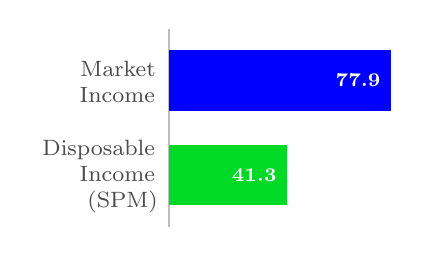
\begin{tikzpicture}
    \begin{axis}[
    	\barplotnogrid axis y line=left, \barylab{1.5cm}{1.5ex} \bbar{x}{0},
		yticklabel style={font=\footnotesize},
        width=4.5cm, 
        height=4.1cm,
        ytick={0,1},
        yticklabels={Disposable Income\\*(SPM), Market Income},
        xmin=0, enlarge x limits={0.02}, enlarge y limits={abs=0.55}, 
		every node near coord/.style={/pgf/number format/fixed,
	    	font=\bfseries\scriptsize, style={white}},
		nodes near coords style={/pgf/number format/.cd, fixed zerofill,
			precision=1, assume math mode},
        every axis plot/.append style={
          xbar, bar width=5.0ex, bar shift=0pt, fill}, 
          nodes near coords align={left}]
      \addplot[green!85!blue] coordinates {(41.3, 0)};
      \addplot[blue] coordinates {(77.9, 1)};
    \end{axis}
  \end{tikzpicture}\\
\footnotesize{Source: CPS ASEC}
\end{minipage}

\begin{minipage}{0.76\textwidth}

\small The Census Bureau \href{https://www.census.gov/library/publications/2019/demo/p60-268.html}{reports} 41.2 million people in poverty in the US in 2018, equivalent to more than the total population of Canada. For purposes of program eligibility and economic data, poverty is defined by having income below a certain threshold. The processes for calculating poverty vary, with the official measure being based on three times a price-adjusted 1963 minimal food budget, and the supplemental measure based on food, shelter, clothing, and utilities costs and additionally capturing program benefits and taxes, along with other adjustments.\\

While some fully-employed people are in poverty, \textbf{the vast majority of poor people are children, elderly, disabled, caregivers, and students}. That is, there is often a good reason why poor people are not working. Put another way, if the missing labor income required to keep a person out of poverty is not supplied in the form of capital income or welfare income, the person will be poor.\\

\vspace{2mm}

\noindent \normalsize \textbf{In Poverty Population by Category}\\
\footnotesize{\textit{share of total, 2018}}\\ 
\noindent \hspace*{-2mm} \begin{tikzpicture}
  	\begin{axis}[\barplotnogrid axis y line=left, \barylab{2.0cm}{1.5ex}
    	width=6.0cm, bar width=1.8ex, height=9.8cm, xmin=0,
    	enlarge y limits={abs=0.5cm}, enlarge x limits=0.05, \bbar{x}{0},
		yticklabels from table={\poor}{name}, 
		yticklabel style={font=\footnotesize},
		nodes near coords style={/pgf/number format/.cd, fixed zerofill,
			precision=1, assume math mode},
		legend style={at={(0.92, 1.06)}}]
  	\addplot[fill=green!60!blue, draw=none] 
  		table [y expr=-\coordindex, x index=2] {\poor};
  	\addplot[fill=lime!70!green!90!blue, draw=none] 
  		table [y expr=-\coordindex, x index=1] {\poor};
  	\addplot[fill=blue, draw=none] 
  		table [y expr=-\coordindex, x index=3] {\poor};
  	\legend{OPM, SPM, Market Income};
  	\end{axis}
\end{tikzpicture}\\
\footnotesize{Source: CPS ASEC} \hspace{40mm} \tbllink{poor.csv}

\end{minipage}

\newpage

\begin{minipage}{0.76\textwidth}

\small The share of a group whose combined labor, capital, and welfare income is below the poverty line is the poverty rate for the group. In 2018, students, caregivers, and the disabled had the highest rates of poverty. Those fully-employed have a very low rate of poverty. The elderly also have a much lower poverty rate as the result of Social Security.\\

\vspace{2mm}

\noindent \normalsize \textbf{Poverty Rate by Category}\\
\footnotesize{\textit{share of group below poverty line, 2018}}\\ 
\noindent \hspace*{-2mm} \begin{tikzpicture}
  	\begin{axis}[\barplotnogrid axis y line=left, \barylab{2.0cm}{1.5ex}
    	width=6.0cm, bar width=1.8ex, height=9.8cm, xmin=0,
    	enlarge y limits={abs=0.5cm}, enlarge x limits=0.05, \bbar{x}{0},
		yticklabels from table={\pvrt}{name}, 
		yticklabel style={font=\footnotesize},
		nodes near coords style={/pgf/number format/.cd, fixed zerofill,
			precision=1, assume math mode},
		legend style={at={(0.92, 1.06)}}]
   	\addplot[fill=green!60!blue, draw=none] 
  		table [y expr=-\coordindex, x index=2] {\pvrt};
  	\addplot[fill=lime!70!green!90!blue, draw=none] 
  		table [y expr=-\coordindex, x index=1] {\pvrt};
  	\addplot[fill=blue, draw=none] 
  		table [y expr=-\coordindex, x index=3] {\pvrt};
  	\legend{OPM, SPM, Market Income};
  	\end{axis}
\end{tikzpicture}\\
\footnotesize{Source: CPS ASEC} \hspace{40mm} \tbllink{poor2.csv}\\

\vspace{3mm}

\small By age, market income (see\cbox{blue}) leaves the elderly particularly vulnerable to poverty, as they are not as likely to have labor income. After social benefits and taxes (disposable income [see\cbox{green!85!blue}]), the elderly have much lower rates of poverty than other age cohorts. Higher survivorship for the wealthy also has the effect of reducing poverty in very old ages. Disposable income still leaves young adults and those just below social security and medicare age (late 50s and early 60s) vulnerable to poverty, relative to other ages.\\

\vspace{2mm}

\noindent \normalsize \textbf{Amount of Poverty by Age} \small \hspace{8mm} \cbox{blue} Market Income \ \hspace{2mm} \cbox{green!85!blue} Disposable Income\\
\footnotesize{\textit{in billions of 2018 US Dollars}}\\ 
\noindent \hspace*{-2mm} \begin{tikzpicture}
	\begin{axis}[ymin=0, ymax=13, enlarge x limits={0.01},
		width=6.7cm, height=5.9cm, ytick={0, 5, 10}, xtick={0, 10, 20, 30, 40, 50, 60, 70},
		xlabel={age}]
	\addplot[stack plots=y, area style, draw=none, fill=green!85!blue] 
		table [x=age, y=disposable, 
		col sep=comma]{data/poor_age_latest.csv}\closedcycle;	
	\addplot[stack plots=y, area style, draw=none, fill=blue] 
		table [x=age, y=market, 
		col sep=comma]{data/poor_age_latest.csv}\closedcycle;	
	\stdnode{0.5cm}{4.1cm}{\large 2018}
	\end{axis}
\end{tikzpicture}
\hfill
\begin{tikzpicture}
	\begin{axis}[ymin=0, ymax=13, enlarge x limits={0.01},
		width=6.7cm, height=5.9cm, ytick={0, 5, 10}, xtick={0, 10, 20, 30, 40, 50, 60, 70},
		xlabel={age}]
	\addplot[stack plots=y, area style, draw=none, fill=green!85!blue] 
		table [x=age, y=disposable, 
		col sep=comma]{data/poor_age_prev.csv}\closedcycle;	
	\addplot[stack plots=y, area style, draw=none, fill=blue] 
		table [x=age, y=market, 
		col sep=comma]{data/poor_age_prev.csv}\closedcycle;	
	\stdnode{0.5cm}{4.1cm}{\large 2014}
	\end{axis}
\end{tikzpicture}\\
\vspace{-3mm}

\footnotesize{Source: CPS ASEC, 2014 adjusted for inflation with CPI-U-RS} \hfill \tbllink{poor_age_latest.csv}

\end{minipage}

\newpage

\noindent \normalsize \textbf{Share of local population in bottom third of housing-adjusted income, 2018}\\
\footnotesize{\textit{Share of commuting zone householders with after-housing-expense annual income below \$13,573}}

\vspace{-3mm}
\hspace{-15mm} \input{/home/brian/Documents/ACS/acs_map.pgf}

\vspace{-5mm}
\footnotesize{Source: American Community Survey}


\newpage

\begin{minipage}{0.76\textwidth}


\small The Census Bureau \href{https://www.census.gov/library/publications/2019/demo/p60-268.html}{reports} the number of people taken out of poverty by various government programs, along with how many people are put in poverty by various expenses. In 2018, Social Security lifted income above the poverty line for 27.2 million people, by far the most effective program for reducing poverty. Refundable tax credits, such as the earned income tax credit and child tax credit, lifted nine million people out of poverty. These tax credits are phased-in (not fully-refundable), meaning they do not reach the poorest of poor people. As a result, phased-in tax credits have more impact on the poverty headcount than on poverty, relative to programs designed to help the poorest of the poor.\\

In terms of elements that add to the number of people in poverty, medical expenses are the most significant, and cause the disposable income of eight million people to fall below the poverty line. Work expenses additionally put 5.7 million people in poverty.\\

\vspace{2mm}

\noindent \normalsize \textbf{Effect of Individual Elements on Poverty Headcount}\\
\footnotesize{\textit{individual element effect on number of people in poverty, millions, 2018}}\\ 
\noindent \hspace*{-12mm}  \begin{tikzpicture}
        \begin{axis}[clip=false,
            xbar stacked,
            \bbar{x}{0},
            xmin = -31,
            xmax = 9.5,
            ymin = -0.5, 
            ymax = 17.5,
            stack negative=separate,
            ymajorgrids=false,
            %
            yticklabels from table={\spm}{name},
			y axis line style = { opacity = 0 },   
		    x axis line style = { opacity = 0 }, 
			yticklabel style={black, align=left, anchor=east},            
            ytick=data,
            tickwidth = 0pt,
            legend style={
                at={(0.0, 1.04)},
                anchor=north,legend
                columns=-1, draw=none, 
            },
            legend cell align=left,
            extra x ticks={0},
            extra x tick style={
                grid style={black},
                xticklabel=\empty,
            },
            enlarge y limits={0.02},
			enlarge x limits={0.03},
            width=10.6cm, height=10.0cm,
            \barylab{3.8cm}{1.5ex}
        ]
            \addplot[fill=green!75!blue!75!black, draw opacity=0] table 
            	[y expr=\coordindex, x=kids, col sep=comma] {\spm};
            \addplot[fill=cyan!95!blue!70!white, draw opacity=0] table 
            	[y expr=\coordindex, x=adults, col sep=comma] {\spm};
            \addplot[fill=blue!80!purple, draw opacity=0] table 
            	[y expr=\coordindex, x=elderly, col sep=comma] {\spm};
            \legend{Under 18, 18 to 64, 65 or older}
        \end{axis}
        \begin{axis}[xmin = -31,
            xmax = 9.5, ymin = -0.5, 
            ymax = 17.5, enlarge y limits={0.02},
			enlarge x limits={0.03},
            width=10.6cm, height=10.0cm,
            ymajorgrids=false,
            yticklabels=\empty,
			y axis line style = { opacity = 0 },   
		    x axis line style = { opacity = 0 }, ]
            \addplot[scatter, no marks, draw=none, nodes near coords*={\Label},
            	nodes near coords align={horizontal},
        		visualization depends on={value \thisrow{label} \as \Label}] table 		
        		[x=xloc,y=yloc,col sep=comma] {data/spmtbl.csv};
        \end{axis}
    \end{tikzpicture}\\
\footnotesize{Source: Census Bureau Supplemental Poverty Measure} \hfill \tbllink{spmtbl.csv}\\



\end{minipage}



\newpage

\begin{minipage}{0.76\textwidth}
\section*{\color{darkgray}\LARGE \seriffont Businesses}
\label{sec:bus}
\small The factories, offices, and equipment that workers use to produce goods and services are all important to the economy. This section looks at the loosely defined business sector, with data covering business investment, retail sales, industrial production, corporate profits, and the financial activities of businesses.

\subsection*{\color{black!70} \seriffont Fixed Investment}
\small When businesses purchase items with a useful life of more than one year it is considered an investment, an exchange of assets rather than an expense. \textbf{Investments in fixed assets make workers more productive}, as they allow businesses to produce goods and services per hour of work. Business investments in fixed assets are grouped broadly as structures (see\cbox{yellow!50!orange}), equipment (see\cbox{cyan!60!white}), and intellectual property products (see\cbox{violet}). 
\vspace{5mm}

\noindent \normalsize \textbf{Business Fixed Investment}\\
\footnotesize{\textit{percentage point contribution to GDP growth}}\\
\noindent \hspace*{-2mm} \begin{tikzpicture}
	\begin{axis}[\bbar{y}{0}, \dateaxisticks ytick={-2, 0, 2},
		xticklabel={`\short{\year}}, clip=false, 
		legend style={at={(0.95, 1.13)}}]
	\rbars
	\sbar{yellow!50!orange}{date}{A009RY}{data/businv.csv}
	\sbar{cyan!60!white}{date}{Y033RY}{data/businv.csv}
	\sbar{violet}{date}{Y001RY}{data/businv.csv}
	\legend{Structures, Equipment, Intellectual Property Products};
	\end{axis}
\end{tikzpicture}\\
\footnotesize{Source: Bureau of Economic Analysis} \hfill \tbllink{businv.csv} \hspace{12mm}\\

\vspace{3mm}

\small

&   2023  Q2 & `23  Q1 & `22  Q4 & `22  Q3 & `22  Q2 &3-year&10-year&30-year\\ Total&0.98&0.76&0.24&0.62&0.68&0.55&0.55&0.60\\  \hspace{-2mm}\cbox{yellow!50!orange}Structures &0.46&0.77&0.17&-0.03&-0.01&-0.04&0.06&0.03\\  \hspace{-2mm}\cbox{cyan!60!white}Equipment &0.38&-0.21&-0.26&0.28&0.25&0.21&0.16&0.32\\  \hspace{4mm}  Information  processing &-0.11&-0.02&-0.38&0.09&-0.13&0.11&0.10&0.20\\  \hspace{6mm}  Computers  and  peripherals &0.02&-0.05&-0.23&0.09&-0.14&0.04&0.02&0.10\\  \hspace{4mm}  Industrial  equipment &-0.06&0.04&0.04&-0.07&-0.07&0.03&0.02&0.03\\  \hspace{4mm}  Transportation  equipment &0.54&-0.14&0.16&0.30&0.41&0.05&0.03&0.05\\  \hspace{-2mm}\cbox{violet}Intellectual  property  products &0.15&0.20&0.32&0.37&0.45&0.38&0.34&0.25\\  \hspace{4mm}  Software &0.13&0.16&0.31&0.28&0.21&0.25&0.20&0.15\\  \hspace{4mm}  Research  and  development &0.00&0.04&0.03&0.05&0.18&0.13&0.13&0.09\\  

\end{minipage}

\noindent \normalsize \textbf{Business Investment}\\
\footnotesize{\textit{percentage point contribution to real GDP growth \hspace{36mm} moving averages}\\ \vspace{4mm}
\noindent \rowcolors{1}{}{black!5} \setlength{\tabcolsep}{3.1pt} \color{black!90}
		{\renewcommand{\arraystretch}{1.55}
		 \begin{tabular}{p{42mm} R{6.7mm} R{6.7mm} R{6.7mm} R{6.7mm} R{6.7mm} 
		   R{7.8mm} R{6.7mm} R{6.7mm} }
			 &   2023  Q2 & `23  Q1 & `22  Q4 & `22  Q3 & `22  Q2 &3-year&10-year&30-year\\ Total&0.98&0.76&0.24&0.62&0.68&0.55&0.55&0.60\\  \hspace{-2mm}\cbox{yellow!50!orange}Structures &0.46&0.77&0.17&-0.03&-0.01&-0.04&0.06&0.03\\  \hspace{-2mm}\cbox{cyan!60!white}Equipment &0.38&-0.21&-0.26&0.28&0.25&0.21&0.16&0.32\\  \hspace{4mm}  Information  processing &-0.11&-0.02&-0.38&0.09&-0.13&0.11&0.10&0.20\\  \hspace{6mm}  Computers  and  peripherals &0.02&-0.05&-0.23&0.09&-0.14&0.04&0.02&0.10\\  \hspace{4mm}  Industrial  equipment &-0.06&0.04&0.04&-0.07&-0.07&0.03&0.02&0.03\\  \hspace{4mm}  Transportation  equipment &0.54&-0.14&0.16&0.30&0.41&0.05&0.03&0.05\\  \hspace{-2mm}\cbox{violet}Intellectual  property  products &0.15&0.20&0.32&0.37&0.45&0.38&0.34&0.25\\  \hspace{4mm}  Software &0.13&0.16&0.31&0.28&0.21&0.25&0.20&0.15\\  \hspace{4mm}  Research  and  development &0.00&0.04&0.03&0.05&0.18&0.13&0.13&0.09\\ \hline
		\end{tabular}
		}	\\
		
\vspace{-6mm}
\footnotesize{Source: Bureau of Economic Analysis}

\newpage

\begin{minipage}{0.335\textwidth}

\small Productive business investments also show up as \textbf{new orders for core capital goods}. The category excludes the more-volatile aircraft orders as well as defense-related orders, and is derived from a Census Bureau \href{https://www.census.gov/manufacturing/m3/index.html}{survey} of shipments, inventories, and orders.  \\

\begin{tikzpicture}\begin{axis}[\bbar{y}{0}, \dateaxisticks ytick={4, 6, 8}, width=6.4cm, height=5.4cm,ymin=3.0, clip=false,xtick={{1992-01-01}, {1995-01-01}, {2000-01-01}, {2005-01-01}, {2010-01-01}, {2015-01-01}, {2021-04-01}}, xticklabels={`92, `95, `00, `05, `10, `15, Apr}, minor xtick={}]\rebars\thickline{purple!50!violet}{date}{value}{data/dgno.csv}\input{text/dgno_node.txt}\end{axis}\end{tikzpicture}
\end{minipage} \hspace{4mm}
\begin{minipage}{0.39\textwidth}

\noindent \normalsize \textbf{New Orders for Core Capital Goods}\\
\footnotesize{\textit{nondefense capital goods ex-aircraft, share of GDP}}\\
\noindent \hspace*{-2mm} \begin{tikzpicture}\begin{axis}[\bbar{y}{0}, \dateaxisticks ytick={4, 6, 8}, width=6.4cm, height=5.4cm,ymin=3.0, clip=false,xtick={{1992-01-01}, {1995-01-01}, {2000-01-01}, {2005-01-01}, {2010-01-01}, {2015-01-01}, {2021-04-01}}, xticklabels={`92, `95, `00, `05, `10, `15, Apr}, minor xtick={}]\rebars\thickline{purple!50!violet}{date}{value}{data/dgno.csv}\input{text/dgno_node.txt}\end{axis}\end{tikzpicture}\\
\footnotesize{Source: Census Bureau} \hspace{23mm} \tbllink{dgno.csv}
\end{minipage}\\

\vspace{14mm}

\begin{minipage}{0.76\textwidth}

\small The Energy Information Administration \href{https://www.eia.gov/dnav/pet/pet_crd_crpdn_adc_mbblpd_m.htm}{reports} that US has seen a massive increase in \textbf{crude oil production} over the past six years. The infrastructure for much of this production was put in place when oil prices were higher, and the profitability of the sector depends on oil maintaining a certain price. A large portion of the increase in oil production comes from New Mexico, South Dakota, and Colorado. \\

\vspace{2mm}

\noindent \normalsize \textbf{Crude Oil Production}\\
\footnotesize{\textit{millions of barrels per day}}\\
\noindent \hspace*{-2mm} \begin{tikzpicture}
	\begin{axis}[\dateaxisticks ymin=0, enlarge x limits={0.01},
		width=13.0cm, height=8.2cm, ytick={0, 5, 10}, xticklabel={`\short{\year}},
		legend style={at={(0.82, 1)}, fill=white}]
	\rbars
	\addplot[stack plots=y, area style, draw=none, fill=teal!90!green!96!black] 
		table [x=date, y=ND_NM_CO, 
		col sep=comma]{data/oil_prod.csv}\closedcycle;	
	\addplot[stack plots=y, area style, draw=none, fill=green!21!yellow!71!white] 
		table [x=date, y=TX, 
		col sep=comma]{data/oil_prod.csv}\closedcycle;	
	\addplot[stack plots=y, area style, draw=none, fill=blue!46!cyan!88!white] 
		table [x=date, y=OTH, 
		col sep=comma]{data/oil_prod.csv}\closedcycle;	
	\addplot[stack plots=y, area style, draw=none, fill=blue!47!violet] 
		table [x=date, y=GM, 
		col sep=comma]{data/oil_prod.csv}\closedcycle;	
	\legend{ND + NM + CO, Texas, All Other, Gulf of Mexico};
	\end{axis}
\end{tikzpicture}\\
\footnotesize{Source: Energy Information Administration} \hfill \tbllink{oil_prod.csv}



\end{minipage}

\newpage 

\begin{minipage}{0.76\textwidth}



\subsection*{\color{black!70} \seriffont Corporate Profits}

\small The national accounts include detailed information on \textbf{aggregate corporate profits}, which are an important determinant in the business cycle. \input{text/cprof.txt} \\

\vspace{2mm}

\noindent \normalsize \textbf{Destination of Corporate Profits}\\
\footnotesize{\textit{share of net national income}}\\
\noindent \hspace*{-2mm} \begin{tikzpicture}
	\begin{axis}[\bbar{y}{0}, \dateaxisticks ytick={0, 5, 10, 15}, ymin=0.2,
		xticklabel={`\short{\year}}, clip=false, legend style={at={(0.95, 1.13)}}]
	\rbars
	\sbar{blue!70!purple}{date}{DIV}{data/cprof.csv}
	\sbar{cyan!50!white}{date}{RE}{data/cprof.csv}
	\sbar{red!80!orange}{date}{TAX}{data/cprof.csv}	
	\legend{Net Dividends, Retained Earnings, Corporate Taxes};
	\end{axis}
\end{tikzpicture}\\
\footnotesize{Source: Bureau of Economic Analysis} \hfill \tbllink{cprof.csv}\\

\vspace{4mm}

\small Aggregate corporate savings (corporate profits less dividends and corporate profit tax) are the result of net investment and non-business saving. Investment (see\cbox{green!70!black}) is a source of aggregate profit because it is revenue for one party but not an expense for the other. Non-business saving, which includes household (see\cbox{blue!80!green}), government (see\cbox{cyan}), and rest of world saving (see\cbox{yellow!70!lime!80!white}), necessarily reduces aggregate corporate profits because it is money that did not return to businesses as revenue. \\

\vspace{2mm}

\noindent \normalsize \textbf{Sources of Corporate Saving}\\
\footnotesize{\textit{contribution to corporate saving, as share of gross national income}}\\
\noindent \hspace*{-2mm} \begin{tikzpicture}
	\begin{axis}[\bbar{y}{0}, \dateaxisticks ytick={-5, 0, 5, 10, 15}, 
		xticklabel={`\short{\year}}, clip=false, legend style={at={(0.95, 1.13)}}]
	\rbars
	\sbar{cyan}{date}{Gov Saving}{data/cprof2.csv}
	\sbar{yellow!70!lime!80!white}{date}{ROW Saving}{data/cprof2.csv}
	\sbar{green!70!black}{date}{Investment}{data/cprof2.csv}
	\sbar{blue!80!green}{date}{HH Saving}{data/cprof2.csv}	
	\legend{Government Saving, ROW Saving, Investment, Household Saving};
	\end{axis}
\end{tikzpicture}\\
\footnotesize{Source: Bureau of Economic Analysis} \hfill \tbllink{cprof2.csv}

\end{minipage}

\newpage

\begin{minipage}{0.76\textwidth}

\subsection*{\color{black!70} \seriffont Business Debt}

\small \input{text/busdebtgdp.txt} \\

\vspace{2mm}

\noindent \normalsize \textbf{Nonfinancial Business Debt}\\
\footnotesize{\textit{by type, as share of GDP}}\\
\noindent \hspace*{-2mm} \begin{tikzpicture}
	\begin{axis}[\bbar{y}{0}, \dateaxisticks ytick={0, 25, 50, 75}, ymin=2,
		xticklabel={`\short{\year}}, clip=false, legend style={at={(0.95, 1.13)}}]
	\rbars
	\sbar{violet}{date}{Bank Loans and Mortgages}{data/busdebtgdp2.csv}	
	\sbar{magenta!70!purple}{date}{Debt Securities}{data/busdebtgdp2.csv}	
	\sbar{blue}{date}{Nonbank Loans}{data/busdebtgdp2.csv}	
	\legend{Mortgages and Bank Loans, Corporate Debt Securities, Nonbank Loans};
	\end{axis}
\end{tikzpicture}\\
\footnotesize{Source: Federal Reserve and Bureau of Economic Analysis} \hfill \tbllink{busdebtgdp2.csv}\\

\vspace{4mm}

\small The debt of the domestic financial sector includes agency and government-sponsored enterprise (GSE) backed securities (see\cbox{red!60!purple}), corporate and foreign bonds, loans (see\cbox{orange!70!yellow}), and open market paper. The long-term increase in financial sector debt reflects the emergence and growth of various asset-backed securities. In addition to home mortgage-backed securities, the domestic financial sector issues debt securities based on commercial mortgages, auto loans, credit card, student debt, and even restaurant revenue. \\

\input{text/findebtgdp.txt} \\

\vspace{2mm}

\noindent \normalsize \textbf{Financial Sector Debt}\\
\footnotesize{\textit{by type, as share of GDP}}\\
\noindent \hspace*{-2mm} \begin{tikzpicture}
	\begin{axis}[\bbar{y}{0}, \dateaxisticks ytick={0, 50,  100, 150}, ymin=2,
		xticklabel={`\short{\year}}, clip=false, legend style={at={(0.95, 1.13)}}]
	\rbars
	\sbar{orange!70!yellow}{date}{Financial Loans}{data/busdebtgdp2.csv}	
	\sbar{red!60!purple}{date}{Agency MBS}{data/busdebtgdp2.csv}
	\sbar{blue!40!violet}{date}{Other}{data/busdebtgdp2.csv}
	\legend{Loans, Agency- and GSE-backed Securities, Other Debt Securities};
	\end{axis}
\end{tikzpicture}\\
\footnotesize{Source: Federal Reserve and Bureau of Economic Analysis} \hfill \tbllink{busdebtgdp2.csv}

\end{minipage}

\newpage

\subsection*{\color{black!70} \seriffont Industrial Production}

\begin{minipage}{0.62\textwidth}

\small  & & Mar  `23 & Feb  `23 & Jan  `23 & Mar  `22 &   Mar  `23 &   Feb  `23 &   Jan  `23 &   Mar  `22 \\  &  \hspace{-1mm}Total  index &0.5&0.9&1.4&4.4&0.5&0.9&1.4&4.4\\  &  \hspace{1mm}Manufacturing &-0.8&0.2&0.6&3.4&-1.1&0.2&0.8&4.6\\  \cbox{blue!62!black}  &  \hspace{3mm}Durable  manufacturing &-0.3&0.4&0.7&1.7&-0.7&1.0&1.8&4.9\\    &  \hspace{5mm}Motor  vehicles  \&  parts &0.1&0.5&0.3&0.2&1.9&10.2&6.1&4.7\\  \cbox{blue!20!cyan!80!white}  &  \hspace{3mm}Nondurable  manufacturing &-0.4&-0.1&-0.0&1.7&-1.2&-0.3&-0.1&4.7\\  \cbox{orange!30!yellow}  &  \hspace{1mm}Mining &0.8&1.3&1.4&0.8&5.4&8.5&9.2&4.9\\  \cbox{green!70!blue}  &  \hspace{1mm}Utilities &0.5&-0.6&-0.7&0.3&4.2&-5.8&-6.5&3.1\\  \cbox{violet!70!purple!90!black}  &  \hspace{1mm}Consumer  goods &0.0&-0.1&-0.1&0.7&0.1&-0.3&-0.4&2.6\\    &  \hspace{3mm}Consumer  durables &-0.2&-0.1&-0.1&0.2&-3.9&-0.9&-2.5&3.6\\    &  \hspace{5mm}Automotive  products &-0.1&0.1&0.0&0.1&-2.9&3.1&0.0&2.6\\    &  \hspace{3mm}Consumer  nondurables &0.3&-0.0&0.0&0.5&1.2&-0.2&0.1&2.4\\    &  \hspace{5mm}Foods  and  tobacco &-0.1&0.0&0.0&0.2&-0.9&0.3&0.3&1.8\\    &  \hspace{5mm}Chemical  products &0.3&0.3&0.3&0.1&5.8&6.6&5.6&2.1\\    &  \hspace{5mm}Consumer  energy  products &0.1&-0.3&-0.2&0.3&1.9&-5.6&-4.3&4.4\\  \cbox{magenta}  &  \hspace{1mm}Business  equipment  \&  supplies &-0.0&0.1&0.6&1.6&-0.2&0.5&2.4&6.2\\    &  \hspace{3mm}Equipment &0.2&0.3&0.6&0.8&1.4&3.2&5.9&8.0\\    &  \hspace{5mm}Industrial  equipment &-0.0&0.0&0.2&0.3&-0.2&1.4&5.1&9.2\\    &  \hspace{3mm}Nonindustrial  supplies &-0.2&-0.2&-0.0&0.8&-1.3&-1.4&-0.1&5.0\\    &  \hspace{5mm}Construction  supplies &-0.1&-0.1&0.0&0.2&-2.7&-1.2&0.6&4.5\\    &  \hspace{5mm}Business  supplies &-0.1&-0.1&-0.0&0.6&-0.6&-1.4&-0.4&5.3\\    &  \hspace{1mm}Materials &0.5&0.9&0.9&2.2&1.2&1.9&1.9&4.6\\    &  \hspace{3mm}Consumer  parts &0.1&0.3&0.1&-0.0&3.7&9.0&4.7&-1.6\\    &  \hspace{3mm}Equipment  parts &-0.0&-0.0&0.0&0.2&-0.3&-0.3&0.3&4.6\\    &  \hspace{3mm}Chemical  materials &-0.2&-0.1&-0.2&0.7&-3.1&-2.0&-3.8&11.3\\  \cbox{blue!70!violet}  &  \hspace{3mm}Energy  materials &0.9&0.9&0.9&1.1&4.8&5.1&4.7&5.6\\  \\

\input{text/indpro2.txt}

\end{minipage}\hspace{7mm}
\begin{minipage}{0.35\textwidth}

\noindent \normalsize \textbf{Industrial Production}\\
\footnotesize{\textit{index, 2012=100}}\\
\noindent \hspace*{-2mm} \begin{tikzpicture}\begin{axis}[\bbar{y}{0}, \dateaxisticks ytick={60, 80, 100}, enlarge y limits={0.05}, enlarge x limits={0}, legend cell align={left},yticklabel style={text width=1.0em}, xtick={{1989-01-01}, {1995-01-01}, {2000-01-01}, {2005-01-01}, {2010-01-01}, {2015-01-01}, {2020-01-01}, {2021-03-01}},xticklabels={`89, `95, `00, `05, `10, `15, ,Mar}, minor xtick={}, clip=false, height=5.4cm, width=6.8cm,legend style={fill=white, legend columns=1, at={(1.02, 0.33)}}]\rbars\thinline{red}{date}{Manufacturing}{data/indpro.csv}\thinline{blue!90!black}{date}{Total index}{data/indpro.csv}\legend{Manufacturing, Total Index};\end{axis}\end{tikzpicture}\
\footnotesize{Source: Federal Reserve} \hfill \tbllink{indpro.csv}

\end{minipage}\\

\begin{minipage}{0.76\textwidth}

\vspace{4mm} 

\noindent \normalsize \textbf{Industrial Production Growth}\\
\footnotesize{\textit{percentage point contribution to one-year growth of total index \hspace{12mm} moving averages}\\ 
\noindent \rowcolors{1}{}{black!5} \setlength{\tabcolsep}{3.1pt} \color{black!90}
		{\renewcommand{\arraystretch}{1.55}
		 \begin{tabular}{p{2mm} p{47mm} R{7.3mm} R{7.3mm} R{7.3mm} R{7.6mm} R{7.3mm} 
		   R{7.3mm} R{7.3mm} }
			  & & Mar  `23 & Feb  `23 & Jan  `23 & Mar  `22 &   Mar  `23 &   Feb  `23 &   Jan  `23 &   Mar  `22 \\  &  \hspace{-1mm}Total  index &0.5&0.9&1.4&4.4&0.5&0.9&1.4&4.4\\  &  \hspace{1mm}Manufacturing &-0.8&0.2&0.6&3.4&-1.1&0.2&0.8&4.6\\  \cbox{blue!62!black}  &  \hspace{3mm}Durable  manufacturing &-0.3&0.4&0.7&1.7&-0.7&1.0&1.8&4.9\\    &  \hspace{5mm}Motor  vehicles  \&  parts &0.1&0.5&0.3&0.2&1.9&10.2&6.1&4.7\\  \cbox{blue!20!cyan!80!white}  &  \hspace{3mm}Nondurable  manufacturing &-0.4&-0.1&-0.0&1.7&-1.2&-0.3&-0.1&4.7\\  \cbox{orange!30!yellow}  &  \hspace{1mm}Mining &0.8&1.3&1.4&0.8&5.4&8.5&9.2&4.9\\  \cbox{green!70!blue}  &  \hspace{1mm}Utilities &0.5&-0.6&-0.7&0.3&4.2&-5.8&-6.5&3.1\\  \cbox{violet!70!purple!90!black}  &  \hspace{1mm}Consumer  goods &0.0&-0.1&-0.1&0.7&0.1&-0.3&-0.4&2.6\\    &  \hspace{3mm}Consumer  durables &-0.2&-0.1&-0.1&0.2&-3.9&-0.9&-2.5&3.6\\    &  \hspace{5mm}Automotive  products &-0.1&0.1&0.0&0.1&-2.9&3.1&0.0&2.6\\    &  \hspace{3mm}Consumer  nondurables &0.3&-0.0&0.0&0.5&1.2&-0.2&0.1&2.4\\    &  \hspace{5mm}Foods  and  tobacco &-0.1&0.0&0.0&0.2&-0.9&0.3&0.3&1.8\\    &  \hspace{5mm}Chemical  products &0.3&0.3&0.3&0.1&5.8&6.6&5.6&2.1\\    &  \hspace{5mm}Consumer  energy  products &0.1&-0.3&-0.2&0.3&1.9&-5.6&-4.3&4.4\\  \cbox{magenta}  &  \hspace{1mm}Business  equipment  \&  supplies &-0.0&0.1&0.6&1.6&-0.2&0.5&2.4&6.2\\    &  \hspace{3mm}Equipment &0.2&0.3&0.6&0.8&1.4&3.2&5.9&8.0\\    &  \hspace{5mm}Industrial  equipment &-0.0&0.0&0.2&0.3&-0.2&1.4&5.1&9.2\\    &  \hspace{3mm}Nonindustrial  supplies &-0.2&-0.2&-0.0&0.8&-1.3&-1.4&-0.1&5.0\\    &  \hspace{5mm}Construction  supplies &-0.1&-0.1&0.0&0.2&-2.7&-1.2&0.6&4.5\\    &  \hspace{5mm}Business  supplies &-0.1&-0.1&-0.0&0.6&-0.6&-1.4&-0.4&5.3\\    &  \hspace{1mm}Materials &0.5&0.9&0.9&2.2&1.2&1.9&1.9&4.6\\    &  \hspace{3mm}Consumer  parts &0.1&0.3&0.1&-0.0&3.7&9.0&4.7&-1.6\\    &  \hspace{3mm}Equipment  parts &-0.0&-0.0&0.0&0.2&-0.3&-0.3&0.3&4.6\\    &  \hspace{3mm}Chemical  materials &-0.2&-0.1&-0.2&0.7&-3.1&-2.0&-3.8&11.3\\  \cbox{blue!70!violet}  &  \hspace{3mm}Energy  materials &0.9&0.9&0.9&1.1&4.8&5.1&4.7&5.6\\ \hline
		\end{tabular}}	\\
		
\footnotesize{Source: Federal Reserve}}

\end{minipage}

\newpage

\begin{minipage}{0.76\textwidth}

\vspace{3mm}

\small Market group data show the lack of growth in the production of consumer goods, equipment, and nonindustrial supplies over the past decade.\\

\vspace{1mm}

\noindent \normalsize \textbf{Industrial Production Growth, Market Group}\\
\footnotesize{\textit{percentage point contribution to one-year growth}}\\
\noindent \hspace*{-2mm} \begin{tikzpicture}
	\begin{axis}[\bbar{y}{0}, \dateaxisticks ytick={-15, -10, -5, 0, 5, 10},
		xticklabel={`\short{\year}}, clip=false, height=5.6cm,
		yticklabel style={text width=1.5em}, legend cell align={left},
		legend style={legend columns=1, at={(0.53, 0.4)}}]
	\rbars
	\sbar{violet!60!black}{date}{Consumer goods}{data/indprogr.csv}
	\sbar{magenta}{date}{ENS}{data/indprogr.csv}
	\sbar{orange!70!yellow}{date}{Materials}{data/indprogr.csv}
	\legend{Consumer Goods, Equipment \& Nonindustrial Supplies, Materials};
	\end{axis}
\end{tikzpicture}\\
\footnotesize{Source: Federal Reserve} \hfill \tbllink{indprogr.csv}\\

\vspace{3mm}

\small Industry group data show a change in the composition of new industrial activity, towards mining and away from manufacturing.\\

\vspace{1mm}

\noindent \normalsize \textbf{Industrial Production Growth, Industry Group}\\
\footnotesize{\textit{percentage point contribution to one-year growth}}\\
\noindent \hspace*{-2mm} \begin{tikzpicture}
	\begin{axis}[\bbar{y}{0}, \dateaxisticks ytick={-15, -10, -5, 0, 5, 10},
		xticklabel={`\short{\year}}, clip=false, height=5.6cm,
		yticklabel style={text width=1.5em}, legend cell align={left},
		legend style={legend columns=1, at={(0.43, 0.48)}}]
	\rbars
	\sbar{blue!60!black}{date}{Durable manufacturing}{data/indprogr2.csv}
	\sbar{blue!20!cyan!80!white}{date}{Nondurable manufacturing}{data/indprogr2.csv}
	\sbar{orange!20!yellow}{date}{Mining}{data/indprogr2.csv}
	\sbar{green!80!blue}{date}{Electric and gas utilities}{data/indprogr2.csv}
	\legend{Durable Manufacturing, Nondurable Manufacturing, Mining, Utilities};
	\end{axis}
\end{tikzpicture}\\
\footnotesize{Source: Federal Reserve} \hfill \tbllink{indprogr2.csv}\\

\vspace{3mm}

\small The most recent slowdown has been broad-based. The monthly data are shown in detail below.\\

\vspace{1mm}

\noindent \normalsize \textbf{Recent data in detail}\\

\vspace{-1mm}

\noindent \normalsize \hspace{14mm} Market Group \hspace{38mm} Industry Group \footnotesize 

\noindent \hspace*{-2mm} \begin{tikzpicture} \begin{axis}[\bbar{y}{0}, \dateaxisticks ytick={-15, -10, -5, 0, 5},  clip=false, width=6.6cm, height=5.5cm, yticklabel style={text width=1.3em}, yticklabel style={text width=1.5em},xtick={{2015-01-01}, {2016-01-01}, {2017-01-01}, {2018-01-01}, {2019-01-01}, {2020-01-01}, {2020-05-01}}, xticklabels={`15, `16, `17, `18, `19, ,May}, minor xtick={}, enlarge y limits=0.08,  enlarge x limits={0.01}] \ctsbar{violet!60!black}{date}{Consumer goods}{data/indprogr_rec.csv}{2.2pt} \ctsbar{magenta}{date}{ENS}{data/indprogr_rec.csv}{2.2pt} \ctsbar{orange!70!yellow}{date}{Materials}{data/indprogr_rec.csv}{2.2pt} \end{axis} \end{tikzpicture} \hfill \begin{tikzpicture} \begin{axis}[\bbar{y}{0}, \dateaxisticks ytick={-15, -10, -5, 0, 5},  clip=false, width=6.6cm, height=5.5cm, yticklabel style={text width=1.3em}, yticklabel style={text width=1.5em},xtick={{2015-01-01}, {2016-01-01}, {2017-01-01}, {2018-01-01}, {2019-01-01}, {2020-01-01}, {2020-05-01}}, xticklabels={`15, `16, `17, `18, `19, ,May}, minor xtick={}, enlarge y limits=0.08,  enlarge x limits={0.01}] \ctsbar{blue!60!black}{date}{Durable manufacturing}{data/indprogr_rec.csv}{2.2pt} \ctsbar{blue!20!cyan!80!white}{date}{Nondurable manufacturing}{data/indprogr_rec.csv}{2.2pt} \ctsbar{orange!20!yellow}{date}{Mining}{data/indprogr_rec.csv}{2.2pt} \ctsbar{green!80!blue}{date}{Electric and gas utilities}{data/indprogr_rec.csv}{2.2pt} \end{axis} \end{tikzpicture}\

\footnotesize{Source: Federal Reserve} \hfill \tbllink{indprogr_rec.csv}*

\end{minipage}

\newpage

\begin{minipage}{0.31\textwidth}
\small \input{text/ip_comp1.txt}\\

\input{text/ip_comp2.txt}

\end{minipage} \hspace{5mm}
\begin{minipage}{0.4\textwidth}
\noindent \normalsize \textbf{Industrial Production and Capacity}\\
\footnotesize{\textit{total three-year growth, percent, \input{text/ip_ind_ldate.txt}}}\\ 
\noindent \hspace*{-5mm} \begin{tikzpicture}
  	\begin{axis}[\barplotnogrid axis y line=left, \barylab{3.3cm}{1.5ex}
    	width=5.5cm, bar width=1.7ex, height=10.0cm,
    	enlarge y limits={abs=0.32cm}, enlarge x limits=0.15, \bbar{x}{0},
		yticklabels from table={\ip}{name}, 
		yticklabel style={font=\scriptsize},
		nodes near coords style={/pgf/number format/.cd, fixed zerofill,
			precision=1, assume math mode},
		legend style={text=black!70, at={(0,1.06)}, anchor=north, legend columns=-1, 
				fill=none, draw=none,
		        /tikz/every even column/.append style={column sep=0.4cm}}]
  	\addplot[fill=cyan!90!blue, draw=none] 
  		table [y expr=-\coordindex, x index=2] {\ip};
  	\addplot[fill=green!60!lime, draw=none] 
  		table [y expr=-\coordindex, x index=1] {\ip};
 	\legend{Capacity, Production}
  	\end{axis}
\end{tikzpicture}\\
\footnotesize{Source: Federal Reserve} \hfill \tbllink{ip_comp.csv}\\
\end{minipage}

\vspace{2mm}

\begin{minipage}{0.76\textwidth}

\small The Federal Reserve's monthly industrial production \href{https://www.federalreserve.gov/releases/g17/}{report} also measures the economy's total industrial capacity. The extent to which the economy is using its industrial capacity is called \textbf{capacity utilization}, and calculated as industrial production as a share of total industrial capacity. Long-term, capacity utilization has fallen as many US factories and industrial production facilities closed. \input{text/tcu.txt}\\

\noindent \normalsize \textbf{Capacity Utilization}\\
\footnotesize{\textit{industrial production as a share of total capacity, percent}}\\ 
\noindent \hspace*{-2mm} \begin{tikzpicture}
	\begin{axis}[\bbar{y}{0}, \dateaxisticks ytick={70, 80}, width=12.4cm, clip=false,
		xticklabel={`\short{\year}}, yticklabel style={text width=1.5em}]
	\rbars
	\thickline{blue!80!black}{date}{Total index}{data/tcu.csv}
	\stdline{blue!40!cyan}{date}{Manufacturing}{data/tcu.csv}
	\input{text/tcu_tot_node.txt}
	\input{text/tcu_mfg_node.txt}
	\stdnode{8.8cm}{1.3cm}{\scriptsize \color{blue!40!cyan}\textbf{Manufacturing}}
	\stdnode{8.0cm}{2.2cm}{\scriptsize \color{blue!80!black}\textbf{Total index}}
	\end{axis}
\end{tikzpicture}\\
\footnotesize{Source: Census Bureau} \hfill \tbllink{tcu.csv}

\end{minipage}

\newpage

\begin{minipage}{0.76\textwidth}

\vspace{5mm}

\normalsize

\subsection*{\color{darkgray} \seriffont Retail Sales}

\small \input{text/marts.txt} \\

\vspace{2mm}

\noindent \normalsize \textbf{Retail Sales and Food Services}\\
\footnotesize{\textit{annual growth, percent; nonstore is 3-month moving average}}\\ 
\noindent \hspace*{-2mm} \begin{tikzpicture}
	\begin{axis}[\bbar{y}{0}, \dateaxisticks ytick={-10, 0, 10, 20}, 
		xticklabel={`\short{\year}}, yticklabel style={text width=1.5em},
		width=11.0cm, height=5.0cm, clip=false]
	\rebars
	\stdline{blue!70!black}{date}{NS_3M}{data/marts.csv}
	\stdline{green!90!blue}{date}{44X72}{data/marts.csv}
	\input{text/rs_ns3m_node.txt}
	\input{text/rs_44x72_node.txt}
	\stdnode{6.1cm}{0.45cm}{\scriptsize \color{green!90!blue}\textbf{Total}}
	\stdnode{7.8cm}{2.65cm}{\scriptsize \color{blue!70!black}\textbf{Nonstore}}
	\end{axis}
\end{tikzpicture}\\
\footnotesize{Source: Census Bureau} \hspace{67mm} \tbllink{marts.csv}\\

\vspace{5mm}


\noindent \normalsize \textbf{Retail sales}\\
\footnotesize{\textit{share of disposable personal income}}\\ 
\noindent \hspace*{-2mm} \begin{tikzpicture}
  	\begin{axis}[\barplotnogrid axis y line=left, \barylab{3.7cm}{1.5ex}
    	width=5.5cm, bar width=1.7ex, height=9.8cm,
    	enlarge y limits={abs=0.35cm}, enlarge x limits=0.15, \bbar{x}{0},
		yticklabels from table={\rs}{name}, 
		yticklabel style={font=\footnotesize},
		nodes near coords style={/pgf/number format/.cd, fixed zerofill,
			precision=2, assume math mode},
		legend style={text=black!70, at={(-0.18,1.08)}, anchor=north, legend columns=-1, 
				fill=none, draw=none,
		        /tikz/every even column/.append style={column sep=0.4cm}}]
	\addplot[fill=teal!50!green, draw=none] 
  		table [y expr=-\coordindex, x index=1] {\rs};
  	\addplot[fill=blue!80!cyan, draw=none] 
  		table [y expr=-\coordindex, x index=2] {\rs};
 	\legend{2015 Q1, 2019 Q4}
  	\end{axis}
\end{tikzpicture}\\
\footnotesize{Source: Census Bureau, Bureau of Economic Analysis} \hspace{12mm} \tbllink{rs_comp.csv}

\end{minipage}

\newpage


\begin{minipage}{0.76\textwidth}
\section*{\color{darkgray}\LARGE \seriffont Government}
\label{sec:gov}
\normalsize

\small Public institutions are collectively referred to as the \textit{public-sector} or the \textit{government}. In the United States, the government has the authority to spend, tax, and create money, as well as to regulate private sector activities. The government also enforces policies that determine the ownership of property. These activities are all extremely important in determining production and distribution in the economy.


\subsection*{\color{black!70} \seriffont Government Spending and Investment}
\small &   2023  Q2 & `23  Q1 & `22  Q4 & `22  Q2 & `21  Q2 &1-year&10-year&30-year\\  Consolidated  Government  Total &0.57&0.82&0.90&-0.34&-0.80&0.69&0.26&0.25\\  \hspace{2mm}Federal  Total &0.07&0.33&0.59&-0.26&-0.65&0.26&0.09&0.09\\  \cbox{blue!60!black}National  Defense &0.08&0.07&0.27&0.03&-0.19&0.10&0.01&0.03\\  \hspace{6mm}Consumption  Expenditures &0.02&0.16&0.07&0.02&-0.16&0.08&-0.01&0.02\\  \hspace{6mm}Gross  Investment &0.06&-0.09&0.20&0.01&-0.03&0.03&0.02&0.01\\  \cbox{green!85!black}Federal  Non-Defense &-0.01&0.26&0.32&-0.29&-0.46&0.16&0.08&0.06\\  \hspace{6mm}Consumption  Expenditures &-0.07&0.17&0.25&-0.30&-0.52&0.10&0.04&0.04\\  \hspace{6mm}Gross  Investment &0.05&0.08&0.08&0.01&0.06&0.06&0.04&0.02\\  \hspace{-2mm}\cbox{purple!70!magenta}State  \&  Local  Total &0.50&0.49&0.31&-0.08&-0.15&0.43&0.17&0.15\\  \hspace{4mm}Consumption  Expenditures &0.16&0.29&0.14&0.08&0.11&0.20&0.14&0.12\\  \hspace{4mm}Gross  Investment &0.34&0.21&0.17&-0.16&-0.27&0.24&0.03&0.03\\   \\
\vspace{2mm}

\noindent \normalsize \textbf{Government Consumption and Investment}\\
\footnotesize{\textit{percentage point contribution to GDP growth}}\\
\noindent \hspace*{-2mm} \begin{tikzpicture}
	\begin{axis}[\bbar{y}{0}, \dateaxisticks ytick={-1, 0, 1},
		xticklabel={`\short{\year}}, clip=false, 
		legend style={at={(0.95, 1.13)}}]
	\rbars
	\sbar{blue!60!black}{date}{A824RY}{data/gov.csv}
	\sbar{green!85!black}{date}{A825RY}{data/gov.csv}
	\sbar{purple!70!magenta}{date}{A829RY}{data/gov.csv}
	\legend{Defense, Federal Non-Defense, State and Local};
	\end{axis}
\end{tikzpicture}\\
\footnotesize{Source: Bureau of Economic Analysis} \hfill \tbllink{gov.csv}

\end{minipage}
\vspace{6mm}

\noindent \normalsize \textbf{Government Consumption and Investment}\\
\footnotesize{\textit{percentage point contribution to GDP growth \hspace{41mm} moving averages}\\ \vspace{4mm}
\noindent \rowcolors{1}{}{black!5} \setlength{\tabcolsep}{3.1pt} \color{black!90}
		{\renewcommand{\arraystretch}{1.55}
		 \begin{tabular}{p{42mm} R{6.7mm} R{6.7mm} R{6.7mm} R{6.7mm} R{6.7mm} 
		   R{7.8mm} R{6.7mm} R{6.7mm} }
			 &   2023  Q2 & `23  Q1 & `22  Q4 & `22  Q2 & `21  Q2 &1-year&10-year&30-year\\  Consolidated  Government  Total &0.57&0.82&0.90&-0.34&-0.80&0.69&0.26&0.25\\  \hspace{2mm}Federal  Total &0.07&0.33&0.59&-0.26&-0.65&0.26&0.09&0.09\\  \cbox{blue!60!black}National  Defense &0.08&0.07&0.27&0.03&-0.19&0.10&0.01&0.03\\  \hspace{6mm}Consumption  Expenditures &0.02&0.16&0.07&0.02&-0.16&0.08&-0.01&0.02\\  \hspace{6mm}Gross  Investment &0.06&-0.09&0.20&0.01&-0.03&0.03&0.02&0.01\\  \cbox{green!85!black}Federal  Non-Defense &-0.01&0.26&0.32&-0.29&-0.46&0.16&0.08&0.06\\  \hspace{6mm}Consumption  Expenditures &-0.07&0.17&0.25&-0.30&-0.52&0.10&0.04&0.04\\  \hspace{6mm}Gross  Investment &0.05&0.08&0.08&0.01&0.06&0.06&0.04&0.02\\  \hspace{-2mm}\cbox{purple!70!magenta}State  \&  Local  Total &0.50&0.49&0.31&-0.08&-0.15&0.43&0.17&0.15\\  \hspace{4mm}Consumption  Expenditures &0.16&0.29&0.14&0.08&0.11&0.20&0.14&0.12\\  \hspace{4mm}Gross  Investment &0.34&0.21&0.17&-0.16&-0.27&0.24&0.03&0.03\\ \hline
		\end{tabular}
		}	\\
		
\vspace{-6mm}
\footnotesize{Source: Bureau of Economic Analysis}


\newpage

\begin{minipage}{0.76\textwidth}

\small Government current expenditures include consumption and investment as well as transfers such as government social benefits to persons. Government spending provides services and income to people. Government current receipts, mostly tax receipts, remove demand from the economy. When government expenditures exceed receipts, it is referred to as a \textit{government deficit}, and corresponds to a private sector surplus. The size of the government deficit relative to GDP gives insight into the extent to which the government is stimulating the economy by increasing household income and corporate profits.\\

\input{text/govexprec2.txt} \\

\input{text/govexprec1.txt} \\

\vspace{2mm}

\textbf{Receipts and Expenditures as Share of GDP}
\vspace{2mm}

\noindent \normalsize \hspace{20mm} Federal \hspace{44mm} State and Local \footnotesize 
\vspace{1mm}

\noindent \hspace*{-2mm} \begin{tikzpicture}
	\begin{axis}[\bbar{y}{0}, \dateaxisticks ytick={15, 20, 25}, 
		clip=false, width=6.7cm, 
		xtick={{1989-01-01}, {2000-01-01}, {2010-01-01}, {2019-07-01}},
        minor xtick={}, enlarge y limits={lower, 0.2}, 
        enlarge x limits={0.04},
        xticklabels={`89, `00, `10, `19 Q4}, 
		legend style={at={(0.95, 1.13)}}]
	\rbars
	\stdline{blue!90!cyan}{date}{W005RC}{data/fedgdp.csv}
	\stdline{red}{date}{W013RC}{data/fedgdp.csv}
	\legend{Receipts, Expenditures};
	\end{axis}
\end{tikzpicture}
\hfill
\begin{tikzpicture}
	\begin{axis}[\bbar{y}{0}, \dateaxisticks ytick={12, 14, 16}, 
		clip=false, width=6.7cm, 
		xtick={{1989-01-01}, {2000-01-01}, {2010-01-01}, {2019-07-01}},
        minor xtick={}, 
        xticklabels={`89, `00, `10, `19 Q4}, enlarge y limits={lower, 0.2}, 
        enlarge x limits={0.04}]
	\rbars
	\stdline{blue!90!cyan}{date}{W023RC}{data/slggdp.csv}
	\stdline{red}{date}{W024RC}{data/slggdp.csv}
	\end{axis}
\end{tikzpicture}
\\
\footnotesize{Source: Bureau of Economic Analysis} \hfill \tbllink{fedgdp.csv}*

\end{minipage}


\newpage
\begin{minipage}{0.76\textwidth}

\small \input{text/pubdebt.txt}\\

\vspace{2mm}

\noindent \normalsize \textbf{Total Public Debt By Holder}\\
\footnotesize{\textit{percent of GDP}}\\
\noindent \hspace*{-2mm} \begin{tikzpicture}
	\begin{axis}[\bbar{y}{0}, \dateaxisticks ytick={0, 25, 50, 75, 100},
		xticklabel={`\short{\year}}, clip=false, ymin=2, height=5.6cm,
		legend cell align={left},
		legend style={legend columns=2, at={(0.58, 1.0)}}]
	\rbars
	\sbar{orange!70!white}{date}{FDHBFIN}{data/pubdebt.csv}
	\sbar{green!60!black}{date}{PD}{data/pubdebt.csv}
	\sbar{cyan!50!white}{date}{IG}{data/pubdebt.csv}
	\sbar{blue}{date}{FDHBFRBN}{data/pubdebt.csv}
	\legend{Foreign, Private Domestic, Intragovernmental, Federal Reserve};
	\end{axis}
\end{tikzpicture}\\
\footnotesize{Source: Treasury} \hfill \tbllink{pubdebt.csv}\\

\vspace{2mm}

\small The ratio of public debt to GDP is fairly stable, and the interest income from holding public debt is lower than in the past because of lower interest rates. Treasuries and other government debt securities provide a safe asset for the balance sheets domestic households and businesses, and for foreign investors.

\end{minipage}

\subsubsection*{\color{black!70} \seriffont Interest Expense}

\begin{minipage}{0.34\textwidth}
\small \input{text/fedintexp.txt}
\end{minipage} \hspace{6mm} \begin{minipage}{0.35\textwidth}
\noindent \normalsize \textbf{Federal Interest Outlays}\\
\footnotesize{\textit{share of GDP, percent}}\\
\noindent \hspace*{-2mm} \begin{tikzpicture}
	\begin{axis}[\shdateaxisticks ytick={1, 2, 3}, clip=false, ymin=1,
		xticklabel={`\short{\year}}, height=4.3cm, width=6.6cm]
	\rbars
	\thickline{magenta}{date}{VALUE}{data/fedintexp.csv}
	\input{text/fedintexp_node.txt}
	\end{axis}
\end{tikzpicture}\\
\footnotesize{Source: FRED; OMB} \hfill \tbllink{fedintexp.csv}

\end{minipage} \\
\vspace{1mm}

\begin{minipage}{0.76\textwidth}
\small While debt levels are much lower for the consolidated state and local government sectors, interest rates on municipal bonds are higher, and interest paid to investors is a larger share of government expenses at the state and local level.
\end{minipage}


\newpage
\begin{minipage}{0.76\textwidth}
\section*{\color{darkgray}\LARGE \seriffont International Transactions}
\label{sec:ext}
\small Transactions between the US and the rest of the world are recorded in the balance of payments as either current account transactions (which measure income) or capital and financial account transactions (which measure change in ownership of assets). This section details imbalances in international transactions, changes in trade by goods and by partner, international investment positions, and exchange rates. 

\subsection*{\color{black!70} \seriffont Balance of Payments}
\small The \textbf{current account balance} can be decomposed into the balance on trade in goods (see\cbox{yellow!60!lime!85!white}), the balance on trade in services (see\cbox{cyan!50!white}), the balance on primary income (such as wages or income from assets, referred to here as income [see\cbox{blue!80!cyan}]), and secondary income (such as remittances and taxes, referred to here as transfers [see\cbox{green!80!blue}]). &   2020  Q2 & `20  Q1 & `19  Q4 & `19  Q3 & `19  Q2 & `19  Q1 &3-year&10-year\\  Current  receipts &14.31&16.87&17.59&17.83&18.02&18.08&17.84&18.36\\  \hspace{1mm}Exports &9.16&11.31&11.57&11.63&11.79&11.95&11.77&12.59\\  \hspace{3mm}Goods &5.82&7.42&7.49&7.55&7.65&7.86&7.68&8.45\\  \hspace{5mm}Durable &3.26&4.35&4.45&4.51&4.57&4.77&4.63&5.21\\  \hspace{5mm}Nondurable &2.56&3.07&3.04&3.04&3.08&3.09&3.04&3.24\\  \hspace{3mm}Services &3.35&3.89&4.08&4.08&4.14&4.09&4.09&4.15\\  \hspace{1mm}Income  receipts &4.44&4.89&5.36&5.48&5.55&5.44&5.34&5.02\\  \hspace{1mm}Transfer  receipts &0.71&0.67&0.66&0.72&0.68&0.69&0.73&0.74\\  Current  payments &17.21&18.84&19.59&20.19&20.53&20.60&20.10&20.74\\  \hspace{1mm}Imports &11.95&13.60&14.10&14.56&14.81&14.87&14.60&15.64\\  \hspace{3mm}Goods &9.88&11.03&11.31&11.77&11.98&12.08&11.87&12.86\\  \hspace{5mm}Durable &6.15&7.05&7.31&7.62&7.70&7.89&7.70&7.91\\  \hspace{5mm}Nondurable &3.73&3.98&4.01&4.15&4.29&4.19&4.17&4.95\\  \hspace{3mm}Services &2.08&2.57&2.78&2.80&2.83&2.79&2.73&2.77\\  \hspace{1mm}Income  payments &3.66&3.76&4.07&4.18&4.28&4.27&4.03&3.68\\  \hspace{1mm}Transfer  payments &1.60&1.47&1.42&1.44&1.44&1.46&1.46&1.42\\  Current  account  balance &-2.90&-1.96&-2.00&-2.36&-2.51&-2.52&-2.26&-2.38\\  

\vspace{5mm}

\noindent \normalsize \textbf{Current Account Balance}\\
\footnotesize{\textit{balance on individual current account component, as percent of GDP}}\\
\noindent \hspace*{-2mm} \begin{tikzpicture}
	\begin{axis}[\bbar{y}{0}, \dateaxisticks ytick={-5, 0},
		xticklabel={`\short{\year}}, clip=false, 
		legend style={at={(0.95, 1.13)}}]
	\rbars
	\sbar{yellow!60!lime!85!white}{date}{GOODS}{data/cab.csv}
	\sbar{cyan!50!white}{date}{SERVICES}{data/cab.csv}
	\sbar{blue!80!cyan}{date}{INCOME}{data/cab.csv}
	\sbar{green!80!blue}{date}{TRANSFERS}{data/cab.csv}
	\stdline{black}{date}{A124RC}{data/cab.csv}
	\legend{Goods, Services, Income, Transfers, Total};
	\end{axis}
\end{tikzpicture}\\
\footnotesize{Source: Bureau of Economic Analysis} \hfill \tbllink{cab.csv}\\

\vspace{3mm}


\small Financial account transactions include the net domestic acquisition of foreign assets and the net domestic incurrence of foreign liabilities. The US \textbf{financial account balance} (see\cbox{yellow!80!orange}) is the net lending or borrowing of the combined domestic sectors with the rest of the world. The timing of payments lead to a statistical discrepancy (see\cbox{red}), but the financial and capital account balance and current account balance otherwise sum to zero. \\

\input{text/fab.txt}\\

\vspace{1mm}


\noindent \normalsize \textbf{Financial Account Balance}\\
\footnotesize{\textit{percent of GDP}}\\
\noindent \hspace*{-2mm} \begin{tikzpicture}
	\begin{axis}[\bbar{y}{0}, \dateaxisticks ytick={0, 5},
		xticklabel={`\short{\year}}, clip=false, 
		legend style={at={(0.95, 1.13)}}]
	\rbars
	\sbar{yellow!80!orange}{date}{FAB}{data/fab.csv}
	\sbar{violet}{date}{FinDeriv}{data/fab.csv}
	\sbar{red}{date}{StatDisc}{data/fab.csv}
	\stdline{black}{date}{TOT}{data/fab.csv}
	\legend{Balance excl. Derivatives, Derivatives, Statistical Discrepancy, Total};
	\end{axis}
\end{tikzpicture}\\
\footnotesize{Source: Bureau of Economic Analysis} \hfill \tbllink{fab.csv}

\end{minipage}

\newpage


\begin{minipage}{0.76\textwidth}

\subsection*{\color{black!70} \seriffont Trade}
\small The \textbf{trade balance} (exports of goods\hspace*{-0.5mm}\cbox{green!70!white} and services\hspace*{-0.5mm}\cbox{green!50!black} minus imports of goods\hspace*{-0.5mm}\cbox{cyan!70!white} and services\hspace*{-0.5mm}\cbox{blue!70!black}) acts as an adjustment to consumption and investment in GDP calculations. As the US runs a persistent trade deficit, trade will generally subtract from GDP growth. In the income approach, the expanded trade deficit reduced nominal compensation of employees (extensive margin through outsourcing, intensive margin through lower wages from labor market slack) and reduced prices. \\

 \input{text/trade.txt} 
\vspace{5mm}

\noindent \normalsize \textbf{International Trade}\\
\footnotesize{\textit{percentage point contribution to GDP growth}}\\
\noindent \hspace*{-2mm} \begin{tikzpicture}
	\begin{axis}[\bbar{y}{0}, \dateaxisticks ytick={-2, 0, 2, 5},
		xticklabel={`\short{\year}}, clip=false, 
		legend style={at={(0.95, 1.13)}}]
	\rbars
	\sbar{green!70!white}{date}{A253RY}{data/nx.csv}
	\sbar{green!50!black}{date}{A646RY}{data/nx.csv}
	\sbar{cyan!70!white}{date}{A255RY}{data/nx.csv}
	\sbar{blue!70!black}{date}{A656RY}{data/nx.csv}	
	\legend{Goods Exports, Services Exports, Goods Imports, Services Imports};
	\end{axis}
\end{tikzpicture}\\
\footnotesize{Source: Bureau of Economic Analysis} \hfill \tbllink{nx.csv}\\

\vspace{8mm}

\small & `23  Q3 & `23  Q2 & `22  Q3 &2016& 2012  --13 & 2005  --06 & 1998  --99 & 1989  --93 \\  Exports  of  Goods  \&  Services &10.99&10.94&11.87&11.89&13.60&10.31&10.41&9.42\\  Exports  of  Goods &7.33&7.27&8.23&7.70&9.34&7.30&7.52&6.84\\  \hspace{2mm}Foods,  Feeds,  \&  Beverages &0.56&0.58&0.69&0.69&0.81&0.46&0.50&0.60\\  \hspace{2mm}Industrial  Supplies  \&  Materials &2.54&2.52&3.27&2.06&2.94&1.92&1.55&1.65\\  \hspace{4mm}Petroleum  \&  Products &1.04&0.98&1.33&0.53&0.89&0.28&0.11&0.12\\  \hspace{2mm}Capital  Goods,  Except  Automotive &2.20&2.19&2.25&2.77&3.21&2.84&3.27&2.61\\  \hspace{2mm}Automotive  Vehicles,  \&  Parts &0.70&0.66&0.63&0.80&0.90&0.77&0.79&0.67\\  \hspace{2mm}Consumer  Goods,  Ex.  Food  \&  Auto &0.96&0.94&0.97&1.03&1.11&0.91&0.86&0.74\\  \hspace{4mm}Durable  Goods &0.43&0.43&0.45&0.55&0.61&0.49&0.44&0.39\\  \hspace{4mm}Nondurable  Goods &0.53&0.51&0.52&0.47&0.50&0.41&0.42&0.35\\  Exports  of  Services &3.66&3.67&3.63&4.19&4.26&3.01&2.90&2.58\\  \hspace{2mm}Transport &0.36&0.37&0.36&0.43&0.54&0.46&0.49&0.59\\  \hspace{2mm}Travel &0.67&0.63&0.56&1.03&0.98&0.71&0.93&0.90\\  \hspace{2mm}Intellectual  Property  Charges &0.44&0.46&0.48&0.60&0.67&0.50&0.40&0.29\\  \hspace{2mm}Other  Business  Services &2.06&2.08&2.11&2.00&1.92&1.19&0.92&0.60\\  Imports  of  Goods  \&  Services &13.82&13.92&15.30&14.56&16.71&15.99&12.65&10.38\\  Imports  of  Goods &11.24&11.30&12.52&11.80&13.85&13.48&10.59&8.45\\  \hspace{2mm}Foods,  Feeds,  \&  Beverages &0.73&0.72&0.80&0.70&0.69&0.54&0.46&0.43\\  \hspace{2mm}Industrial  Supplies  \&  Materials &2.34&2.41&3.13&2.32&4.24&4.24&2.22&2.16\\  \hspace{4mm}Petroleum  \&  Products &0.94&0.87&1.25&0.85&2.49&2.15&0.65&0.87\\  \hspace{2mm}Capital  Goods,  Except  Automotive &3.11&3.16&3.39&3.16&3.35&3.00&3.03&2.04\\  \hspace{2mm}Automotive  Vehicles,  \&  Parts &1.72&1.68&1.57&1.87&1.84&1.84&1.74&1.46\\  \hspace{2mm}Consumer  Goods,  Ex.  Food  \&  Auto &2.78&2.80&3.14&3.11&3.17&3.20&2.47&1.83\\  \hspace{4mm}Durable  Goods &1.37&1.40&1.62&1.63&1.70&1.75&1.29&0.97\\  \hspace{4mm}Nondurable  Goods &1.40&1.40&1.52&1.48&1.47&1.46&1.18&0.86\\  Imports  of  Services &2.57&2.62&2.78&2.77&2.86&2.51&2.06&1.93\\  \hspace{2mm}Transport &0.50&0.51&0.64&0.49&0.59&0.60&0.54&0.55\\  \hspace{2mm}Travel &0.52&0.53&0.48&0.58&0.55&0.57&0.63&0.61\\  \hspace{2mm}Intellectual  Property  Charges &0.15&0.16&0.19&0.22&0.21&0.18&0.13&0.06\\  \hspace{2mm}Other  Business  Services &1.28&1.30&1.35&1.32&1.32&0.91&0.57&0.38\\ \\

\vspace{2mm}


\noindent \normalsize \textbf{Imports and Exports, Nonpetroleum}\\
\footnotesize{\textit{includes goods and services, but excludes petroleum products, share of GDP}}\\
\noindent \hspace*{-2mm} \begin{tikzpicture}
	\begin{axis}[\bbar{y}{0}, \dateaxisticks ytick={10, 12, 14}, enlarge y limits={0.1},
		xticklabel={`\short{\year}}, clip=false, height=5.0cm,
		legend style={legend columns=1, at={(0.28, 0.84)}}]
	\rbars
	\thickline{blue!90!cyan}{date}{EX}{data/eximgdp.csv}
	\thickline{green!60!teal!80!black}{date}{IM}{data/eximgdp.csv}
	\legend{Exports, Imports};
	\end{axis}
\end{tikzpicture}\\
\footnotesize{Source: Bureau of Economic Analysis} \hfill \tbllink{eximgdp.csv}


\end{minipage}

\newpage


\begin{minipage}{0.76\textwidth}

\small Changes to the trade balance can come from many sources, such as changes in domestic or foreign preferences and income, changes in exchange rates, and changes in trade policy. The following table captures the nominal value of major categories of goods and services as a share of nominal gross domestic product at various points over the past 30 years.  \\

\end{minipage}

\noindent \normalsize \textbf{Exports and Imports by Type}\\
\footnotesize{\textit{percentage point share of GDP \hspace{40mm} period averages}\\ 
\noindent \rowcolors{1}{}{black!5} \setlength{\tabcolsep}{3.1pt} \color{black!90}
		{\renewcommand{\arraystretch}{1.55}
		 \begin{tabular}{p{42mm} R{7.1mm} R{7.1mm} R{7.1mm} R{7.1mm} R{7.1mm} 
		   R{7.1mm} R{7.1mm} R{7.1mm} }
			 & `23  Q3 & `23  Q2 & `22  Q3 &2016& 2012  --13 & 2005  --06 & 1998  --99 & 1989  --93 \\  Exports  of  Goods  \&  Services &10.99&10.94&11.87&11.89&13.60&10.31&10.41&9.42\\  Exports  of  Goods &7.33&7.27&8.23&7.70&9.34&7.30&7.52&6.84\\  \hspace{2mm}Foods,  Feeds,  \&  Beverages &0.56&0.58&0.69&0.69&0.81&0.46&0.50&0.60\\  \hspace{2mm}Industrial  Supplies  \&  Materials &2.54&2.52&3.27&2.06&2.94&1.92&1.55&1.65\\  \hspace{4mm}Petroleum  \&  Products &1.04&0.98&1.33&0.53&0.89&0.28&0.11&0.12\\  \hspace{2mm}Capital  Goods,  Except  Automotive &2.20&2.19&2.25&2.77&3.21&2.84&3.27&2.61\\  \hspace{2mm}Automotive  Vehicles,  \&  Parts &0.70&0.66&0.63&0.80&0.90&0.77&0.79&0.67\\  \hspace{2mm}Consumer  Goods,  Ex.  Food  \&  Auto &0.96&0.94&0.97&1.03&1.11&0.91&0.86&0.74\\  \hspace{4mm}Durable  Goods &0.43&0.43&0.45&0.55&0.61&0.49&0.44&0.39\\  \hspace{4mm}Nondurable  Goods &0.53&0.51&0.52&0.47&0.50&0.41&0.42&0.35\\  Exports  of  Services &3.66&3.67&3.63&4.19&4.26&3.01&2.90&2.58\\  \hspace{2mm}Transport &0.36&0.37&0.36&0.43&0.54&0.46&0.49&0.59\\  \hspace{2mm}Travel &0.67&0.63&0.56&1.03&0.98&0.71&0.93&0.90\\  \hspace{2mm}Intellectual  Property  Charges &0.44&0.46&0.48&0.60&0.67&0.50&0.40&0.29\\  \hspace{2mm}Other  Business  Services &2.06&2.08&2.11&2.00&1.92&1.19&0.92&0.60\\  Imports  of  Goods  \&  Services &13.82&13.92&15.30&14.56&16.71&15.99&12.65&10.38\\  Imports  of  Goods &11.24&11.30&12.52&11.80&13.85&13.48&10.59&8.45\\  \hspace{2mm}Foods,  Feeds,  \&  Beverages &0.73&0.72&0.80&0.70&0.69&0.54&0.46&0.43\\  \hspace{2mm}Industrial  Supplies  \&  Materials &2.34&2.41&3.13&2.32&4.24&4.24&2.22&2.16\\  \hspace{4mm}Petroleum  \&  Products &0.94&0.87&1.25&0.85&2.49&2.15&0.65&0.87\\  \hspace{2mm}Capital  Goods,  Except  Automotive &3.11&3.16&3.39&3.16&3.35&3.00&3.03&2.04\\  \hspace{2mm}Automotive  Vehicles,  \&  Parts &1.72&1.68&1.57&1.87&1.84&1.84&1.74&1.46\\  \hspace{2mm}Consumer  Goods,  Ex.  Food  \&  Auto &2.78&2.80&3.14&3.11&3.17&3.20&2.47&1.83\\  \hspace{4mm}Durable  Goods &1.37&1.40&1.62&1.63&1.70&1.75&1.29&0.97\\  \hspace{4mm}Nondurable  Goods &1.40&1.40&1.52&1.48&1.47&1.46&1.18&0.86\\  Imports  of  Services &2.57&2.62&2.78&2.77&2.86&2.51&2.06&1.93\\  \hspace{2mm}Transport &0.50&0.51&0.64&0.49&0.59&0.60&0.54&0.55\\  \hspace{2mm}Travel &0.52&0.53&0.48&0.58&0.55&0.57&0.63&0.61\\  \hspace{2mm}Intellectual  Property  Charges &0.15&0.16&0.19&0.22&0.21&0.18&0.13&0.06\\  \hspace{2mm}Other  Business  Services &1.28&1.30&1.35&1.32&1.32&0.91&0.57&0.38\\ \hline
		\end{tabular}}	\\
		
\vspace{-2mm}
\footnotesize{Source: Bureau of Economic Analysis}}



\newpage

\subsubsection*{\color{black!70} \seriffont Import Penetration}

\begin{minipage}{0.76\textwidth}

\small Goods can be produced domestically or imported or some combination of the two. The import share of the total US demand for goods, measured as US produced goods and imported goods less exported goods, is also referred to as \textit{import penetration}. This measure has risen considerably over the past thirty years. The majority of the long-term increase has been concentrated in consumer goods, while the decrease since 2011 has come primarily from petroleum and products. \\

\input{text/goodsimpsh1.txt} \\

\input{text/goodsimpsh.txt} \\

\noindent \normalsize \textbf{Import Share of Goods}\\
\footnotesize{\textit{import share of domestic-produced and imported goods less exports, by category}}\\
\noindent \hspace*{-2mm} \begin{tikzpicture}
	\begin{axis}[\bbar{y}{0}, \dateaxisticks ytick={0, 10, 20, 30, 40}, ymin=2,
		xticklabel={`\short{\year}}, clip=false, legend style={at={(0.95, 1.13)}}]
	\rbars
	\sbar{cyan!40!white}{date}{Consumer}{data/goodsimpsh.csv}	
	\sbar{blue!50!cyan}{date}{Capital}{data/goodsimpsh.csv}	
	\sbar{purple}{date}{B648RC}{data/goodsimpsh.csv}	
	\legend{Consumer, Capital/Supplies/Other, Petroleum and Products};
	\end{axis}
\end{tikzpicture}\\
\footnotesize{Source: Bureau of Economic Analysis} \hfill \tbllink{goodsimpsh.csv}

\end{minipage}

\newpage

\begin{minipage}{0.76\textwidth}

\subsection*{\color{black!70} \seriffont Exchange Rates}

\small The strength or weakness of the dollar in an important determinant of trade and financial flows. When more Japanese Yen (JPY), British Pounds (GBP), Euros (EUR), or Canadian Dollars (CAD) are required to buy one US Dollar (USD), the dollar is said to be \textit{strong}.\\

 \input{text/selcurr_basic.txt}\\ 

\vspace{2mm}

\noindent \normalsize \textbf{Selected Exchange Rates}\\
\footnotesize{\textit{units of foreign currency required to purchase one US dollar}}\\
\noindent \hspace*{-2mm} \begin{tikzpicture}
	\begin{axis}[\bbar{y}{1}, \dateaxisticks ytick={0.5, 1, 1.5}, enlarge y limits={0.1},
		xticklabel={`\short{\year}}, clip=false, height=5.0cm]
	\rbars
	\stdline{blue!90!cyan}{date}{RXI_N.B.UK}{data/fx1.csv}
	\stdline{green!90!blue}{date}{RXI_N.B.CA}{data/fx1.csv}
	\stdline{red}{date}{RXI_N.B.JA}{data/fx1.csv}
	\stdline{cyan!90!white}{date}{RXI_N.B.EU}{data/fx1.csv}
	\stdnode{10.8cm}{0.6cm}{\footnotesize \color{blue!90!cyan}GBP}
	\stdnode{5.5cm}{3.0cm}{\footnotesize \color{green!85!blue}CAD}
	\stdnode{4.1cm}{1.1cm}{\footnotesize \color{cyan!90!white}EUR}
	\stdnode{1.5cm}{1.24cm}{\footnotesize \color{red}JPY (100)}
	\end{axis}
\end{tikzpicture}\\
\footnotesize{Source: Federal Reserve} \hfill \tbllink{fx1.csv}
\end{minipage}

\vspace{4mm}
\begin{minipage}{0.33\textwidth}
\noindent \normalsize \textbf{Broad Dollar Index}\\
\footnotesize{\textit{trade-weighted foreign exchange rate index}}\\
\footnotesize{\textit{January 2006=100}}\\
\noindent \hspace*{-2mm} \begin{tikzpicture}
	\begin{axis}[\bbar{y}{1}, \dateaxisticks ytick={90, 100, 110, 120}, 
		enlarge y limits={0.1},
		xticklabel={`\short{\year}}, width=6.1cm, height=5.8cm]
	\rbars
	\stdline{blue!60!black}{date}{JRXWTFB_N.B}{data/fx_idx.csv}
	\end{axis}
\end{tikzpicture}\\
\footnotesize{Source: Federal Reserve} \hspace{16mm} \tbllink{fx_idx.csv}
\end{minipage}\hspace{4mm}
\begin{minipage}{0.4\textwidth}
\small Fed \href{https://www.federalreserve.gov/releases/h10/summary/default.htm}{trade-weighted dollar indices} show weighted-average foreign exchange rates with US trading partners, which simplify thinking about the overall role of foreign exchange rates on the US external sector. The Broad Dollar Index (see {\color{blue!60!black}\textbf{---}}), which starts in 2006, summarizes foreign exchange rates between the US and trading partners, weighting rates by the amount of trade in both goods and services.\\

\input{text/twdbasic.txt}
\end{minipage}

\newpage
\section*{\color{darkgray}\LARGE \seriffont Labor Markets}
\label{sec:lab}

\begin{minipage}{0.34\textwidth}
\small Labor is the primary source of income for US households and is essential to the production of goods and services. The portion of labor that is provided by a household member to others outside of the household or to other households is considered \textit{employment}. \input{text/cps_lfs0.txt}\\

\input{text/cps_lfs.txt}
\end{minipage} \hspace{5.5mm}
\begin{minipage}{0.375\textwidth}
\noindent \normalsize \textbf{Labor Force Status of Population}\\
\footnotesize{\textit{millions of people}}\\
\noindent \hspace*{-3mm} \begin{tikzpicture}
	\begin{axis}[\bbar{y}{0}, \dateaxisticks ytick={0, 100, 200, 300}, 
		height=7.2cm, ymin=10, width=7.0cm,
		clip=false, enlarge x limits={0.04}, 
		xtick={{1989-01-01}, {1995-01-01}, {2000-01-01}, 
				{2005-01-01}, {2010-01-01}, {2015-01-01}, {2020-01-01}},
        minor xtick={},
        xticklabels={`89, `95, `00, `05, `10, `15, `20},
        legend cell align={left},
		legend style={fill=white, legend columns=2, at={(0.82, 1.09)}}]
	\rbars
	\sbar{green!50!teal!85!blue}{date}{Employed}{data/cps_lfs.csv}
	\sbar{lime!80!yellow!90!white}{date}{Unemployed}{data/cps_lfs.csv}
	\sbar{blue!80!cyan}{date}{NILF}{data/cps_lfs.csv}
	\sbar{cyan!80!white}{date}{Children}{data/cps_lfs.csv}
	\legend{Employed, Unemployed, Non-Participant, Under 15};
	\end{axis}
\end{tikzpicture}\\
\footnotesize{Source: Author's Calculations from CPS} \hfill \tbllink{cps_lfs.csv}
\end{minipage}\\

\vspace{2mm}

\begin{minipage}{0.76\textwidth}
\small When a member of a household is not employed but looked for a job during the past four weeks and is available to work, they are considered \href{https://www.bls.gov/cps/cps_htgm.htm}{\textbf{unemployed}}. \input{text/cps_lfs2.txt}\\

People who are not employed and not unemployed are considered to be outside of the labor force. \input{text/cps_lfs3.txt} \\

\vspace{3mm}

\noindent \normalsize \textbf{Labor Force Status Changes}\\
\footnotesize{\textit{percentage point contribution to one-year growth of age 15+ population}}\\
\noindent \hspace*{-2mm} \begin{tikzpicture}
	\begin{axis}[\bbar{y}{0}, \dateaxisticks ytick={-2, 0, 2},
		xticklabel={`\short{\year}}, clip=false, height=5.9cm,
		legend cell align={left},
		legend style={legend columns=1, at={(0.29, 0.35)}}]
	\rbars
	\sbar{green!50!teal!85!blue}{date}{Employed}{data/cps_lfs2.csv}
	\sbar{lime!80!yellow!90!white}{date}{Unemployed}{data/cps_lfs2.csv}
	\sbar{blue!80!cyan}{date}{NILF}{data/cps_lfs2.csv}
	\legend{Employed, Unemployed, Non-Participant};
	\end{axis}
\end{tikzpicture}\\
\footnotesize{Source: Author's Calculations from CPS} \hfill \tbllink{cps_lfs2.csv}

\end{minipage}

\newpage

\begin{minipage}{0.76\textwidth}

\small The labor force status of the US population varies by age, sex, and over time. Because very few people have capital income, the share of the population with labor income is particularly important to overall levels of economic activity. \\

\vspace{1mm}


\noindent \normalsize \textbf{Labor Force Status}\\
\footnotesize{\textit{\input{text/cps_lfs_date.txt}, thousands of people, not seasonally adjusted}}\\

\vspace{-3mm}

\noindent \rowcolors{1}{}{black!5} \setlength{\tabcolsep}{3.0pt} \color{black!90}
		{\renewcommand{\arraystretch}{1.52}
		 \begin{tabular}{p{27.8mm} R{11.2mm} R{10.4mm} R{10.4mm} R{10.2mm} R{10.6mm} R{10.4mm} R{10.4mm}}
			 & Total,  16+ & Men,  16--29 & Men,  30--59 & Men,  60+ & Women,  16--29 & Women,  30--59 & Women,  60+ \\ Population&264,844&29,707&62,694&36,649&29,612&63,937&42,246\\  \hspace{2mm}Employed &158,872&18,509&53,288&12,507&17,358&46,781&10,429\\  \hspace{4mm}Multiple  jobs &8,149&690&2,860&535&976&2,590&499\\  \hspace{4mm}Full-time &119,070&12,970&45,498&8,893&10,344&35,235&6,130\\  \hspace{4mm}Part-time &39,802&5,539&7,790&3,615&7,014&11,546&4,299\\  \hspace{6mm}Economic  reasons &3,992&760&1,287&248&485&1,040&174\\  \hspace{2mm}Unemployed &5,352&1,197&1,368&382&987&1,166&252\\  \hspace{2mm}Not  in  Labor  Force &100,621&10,001&8,038&23,760&11,267&15,990&31,564\\  \hspace{4mm}Discouraged &4,938&897&880&573&837&1,113&639\\  \hspace{4mm}Disabled/Ill &13,805&860&3,597&2,301&635&3,896&2,516\\  \hspace{4mm}Family/Care &12,659&456&1,072&71&2,278&7,963&819\\  \hspace{4mm}School &15,103&7,169&376&24&6,967&514&52\\  \hspace{4mm}Retirement &52,014&100&1,530&20,673&189&2,077&27,444\\ \hline
		\end{tabular}
		}	\\
		
\vspace{-3mm}		
		
\footnotesize{Source: Author's Calculations from CPS}\\

\vspace{3mm}

\small Additionally, changes over time in labor force status are particularly important to understanding both secular and cyclical trends in the economy. For example, the US population is growing but it is also aging. Over the past year, there was a substantial shift towards full-time work. \\ 

\vspace{2mm}


\noindent \normalsize \textbf{Labor Force Changes}\\
\footnotesize{\textit{Change from \input{text/cps_lfs_datepr.txt}, thousands of people}}\\

\vspace{-3mm}

\noindent \rowcolors{1}{}{black!5} \setlength{\tabcolsep}{3.0pt} \color{black!90}
		{\renewcommand{\arraystretch}{1.52}
		 \begin{tabular}{p{27.8mm} R{11.2mm} R{10.4mm} R{10.4mm} R{10.2mm} R{10.6mm} R{10.4mm} R{10.4mm}}
			 & Total,  15+ & Men,  15--29 & Men,  30--59 & Men,  60+ & Women,  15--29 & Women,  30--59 & Women,  60+ \\ Population&1,118&-324&-32&927&-336&-100&982\\  \hspace{2mm}Employed &-13,728&-3,308&-3,123&-949&-2,792&-2,969&-588\\  \hspace{4mm}Multiple  jobs &-1,734&-274&-355&-104&-418&-444&-139\\  \hspace{4mm}Full-time &-12,634&-2,801&-3,962&-595&-2,112&-2,961&-203\\  \hspace{4mm}Part-time &-1,094&-507&839&-354&-680&-8&-385\\  \hspace{6mm}Economic  reasons &4,504&603&1,442&325&454&1,358&321\\  \hspace{2mm}Unemployed &10,137&1,762&2,579&640&1,580&2,873&703\\  \hspace{2mm}Not  in  Labor  Force &4,709&1,222&513&1,236&875&-4&867\\  \hspace{4mm}Discouraged &2,381&465&524&113&615&557&107\\  \hspace{4mm}Disabled/Ill &-1,380&137&-448&-287&116&-449&-449\\  \hspace{4mm}Family/Care &-874&119&-18&13&-322&-625&-41\\  \hspace{4mm}School &678&354&-26&-10&296&43&22\\  \hspace{4mm}Retirement &3,151&23&250&1,303&74&324&1,177\\ \hline
		\end{tabular}
		}	\\
		
\vspace{-3mm}	
	
\footnotesize{Source: Author's Calculations from CPS}


\end{minipage}

\newpage

\begin{minipage}{0.325\textwidth}
\noindent \normalsize \textbf{Labor Share of Income}\\
\footnotesize{\textit{compensation of employees as share of}}\\
\footnotesize{\textit{gross domestic income, percent}}\\
\noindent \hspace*{-2mm} \begin{tikzpicture}
	\begin{axis}[\shdateaxisticks ytick={52, 54, 56, 58}, 
		enlarge y limits={0.1},
		xticklabel={`\short{\year}}, height=5.9cm, width=5.8cm, clip=false]
	\rbars
	\stdline{blue!60!cyan}{date}{Share}{data/laborshare.csv}
	\input{text/laborshare_node.txt}
	\end{axis}
\end{tikzpicture}\\
\footnotesize{Source: Bureau of Economic Analysis} \hspace{2mm} \tbllink{laborshare.csv}\\
\end{minipage}\hspace{7mm}
\begin{minipage}{0.38\textwidth}
\small The labor share of income measures how much labor is paid relative to the total income in the economy in a year. While the laborer share of the population has fallen, and an increasing share of income goes to depreciation of capital including housing, cyclical patterns suggest worker bargaining power also affects the labor share of income.  \input{text/laborshare.txt}
\end{minipage}

\vspace{4mm}


\subsection*{\color{black!70} \seriffont Gross Labor Income}

\begin{minipage}{0.76\textwidth}

\small In labor markets, unlike other markets, wages (the price of labor) tend not to be cut in response to a decrease in demand; businesses instead employ fewer workers and/or cut hours. As a result, wage data give only a partial picture of the labor income received by households.\\

\textbf{Gross labor income} (compensation of employees in the national accounts), which captures both the amount of employment (see\cbox{teal!80!blue!85!white}) and the rate of compensation (see\cbox{green!80!lime!90!white}), \input{text/gli.txt} \\

\noindent \normalsize \textbf{Gross Labor Income Growth}\\
\footnotesize{\textit{percentage point contribution to gross labor income growth}}\\
\noindent \hspace*{-2mm} \begin{tikzpicture}
	\begin{axis}[\bbar{y}{0}, \dateaxisticks ytick={-10, -5, 0, 5, 10},
		xticklabel={`\short{\year}}, clip=false,  yticklabel style={text width=1.5em},
		legend style={at={(0.95, 1.13)}}]
	\rbars
	\sbar{green!80!lime!90!white}{date}{wage}{data/gli.csv}
	\sbar{teal!80!blue!85!white}{date}{work}{data/gli.csv}
	\legend{Rate of Compensation, Hours of Work};
	\end{axis}
\end{tikzpicture}\\
\footnotesize{Source: Author's Calculations} \hfill \tbllink{gli.csv}

\end{minipage}

\newpage

\begin{minipage}{0.76\textwidth}

\subsection*{\color{black!70} \seriffont Employment}


\small \input{text/epop_text.txt} \\

\noindent \normalsize \textbf{Employment Rate}\\
\footnotesize{\textit{employed share of age 25-54 population}}\\
\noindent \hspace*{-2mm} \begin{tikzpicture}
	\begin{axis}[\bbar{y}{0}, \dateaxisticks ytick={75, 80}, enlarge y limits={0.1},
		xticklabel={`\short{\year}}, clip=false, height=5.0cm]
	\rbars
	\stdline{blue!90!cyan}{date}{PA_EPOP}{data/epop.csv}
	\node[above, align=right] at (axis cs:2018-11-01,80.8) {\scriptsize \input{text/epop.txt}};
	\end{axis}
\end{tikzpicture}\\
\footnotesize{Source: Bureau of Labor Statistics} \hfill \tbllink{epop.csv}\\

\vspace{4mm}

\small The employment rate shown above is based on a monthly survey that asks about employment during a specific week of the previous month. However, additional data is available on what share of a population works year-round rather than just during a specific week. This can be combined with data on hours worked to identify the \textit{fully-employed}, or \textit{full-time, full-year workers}, who are defined below as the those who usually work 35 hours per week or more for 50 weeks per year or more. The Census Bureau \href{https://www.census.gov/data/tables/time-series/demo/income-poverty/cps-pinc/pinc-01.html#par_textimage_14}{reports} 118 million fully-employed people in 2018, equivalent to 36 percent of the population. \\

\input{text/acs_ftfy_text.txt} Of commuter zones with 100,000 people or more, the top and bottom ten by fully-employed share of population are listed below.
\end{minipage}

\vspace{3mm}

\begin{minipage}{0.52\textwidth}


\noindent \normalsize \textbf{Commuter Zone Fully-Employed Rate}\\
\footnotesize{\textit{full-time, full-year worker share of population, \input{text/acs_ftfy_year.txt}}}\\

\vspace{-3mm}

\hspace{-11mm} %% Creator: Matplotlib, PGF backend
%%
%% To include the figure in your LaTeX document, write
%%   \input{<filename>.pgf}
%%
%% Make sure the required packages are loaded in your preamble
%%   \usepackage{pgf}
%%
%% and, on pdftex
%%   \usepackage[utf8]{inputenc}\DeclareUnicodeCharacter{2212}{-}
%%
%% or, on luatex and xetex
%%   \usepackage{unicode-math}
%%
%% Figures using additional raster images can only be included by \input if
%% they are in the same directory as the main LaTeX file. For loading figures
%% from other directories you can use the `import` package
%%   \usepackage{import}
%%
%% and then include the figures with
%%   \import{<path to file>}{<filename>.pgf}
%%
%% Matplotlib used the following preamble
%%   \usepackage{fontspec}
%%   \setmainfont{DejaVuSerif.ttf}[Path=/home/brian/miniconda3/lib/python3.8/site-packages/matplotlib/mpl-data/fonts/ttf/]
%%   \setsansfont{DejaVuSans.ttf}[Path=/home/brian/miniconda3/lib/python3.8/site-packages/matplotlib/mpl-data/fonts/ttf/]
%%   \setmonofont{DejaVuSansMono.ttf}[Path=/home/brian/miniconda3/lib/python3.8/site-packages/matplotlib/mpl-data/fonts/ttf/]
%%
\begingroup%
\makeatletter%
\begin{pgfpicture}%
\pgfpathrectangle{\pgfpointorigin}{\pgfqpoint{3.645016in}{2.389500in}}%
\pgfusepath{use as bounding box, clip}%
\begin{pgfscope}%
\pgfsetbuttcap%
\pgfsetmiterjoin%
\pgfsetlinewidth{0.000000pt}%
\definecolor{currentstroke}{rgb}{0.000000,0.000000,0.000000}%
\pgfsetstrokecolor{currentstroke}%
\pgfsetstrokeopacity{0.000000}%
\pgfsetdash{}{0pt}%
\pgfpathmoveto{\pgfqpoint{-0.000000in}{0.000000in}}%
\pgfpathlineto{\pgfqpoint{3.645016in}{0.000000in}}%
\pgfpathlineto{\pgfqpoint{3.645016in}{2.389500in}}%
\pgfpathlineto{\pgfqpoint{-0.000000in}{2.389500in}}%
\pgfpathclose%
\pgfusepath{}%
\end{pgfscope}%
\begin{pgfscope}%
\pgfpathrectangle{\pgfqpoint{0.100000in}{0.100000in}}{\pgfqpoint{3.420221in}{2.189500in}}%
\pgfusepath{clip}%
\pgfsetbuttcap%
\pgfsetmiterjoin%
\pgfsetlinewidth{0.000000pt}%
\definecolor{currentstroke}{rgb}{0.000000,0.000000,0.000000}%
\pgfsetstrokecolor{currentstroke}%
\pgfsetstrokeopacity{0.000000}%
\pgfsetdash{}{0pt}%
\pgfpathmoveto{\pgfqpoint{0.100000in}{0.100000in}}%
\pgfpathlineto{\pgfqpoint{3.520221in}{0.100000in}}%
\pgfpathlineto{\pgfqpoint{3.520221in}{2.289500in}}%
\pgfpathlineto{\pgfqpoint{0.100000in}{2.289500in}}%
\pgfpathclose%
\pgfusepath{}%
\end{pgfscope}%
\begin{pgfscope}%
\pgfpathrectangle{\pgfqpoint{0.100000in}{0.100000in}}{\pgfqpoint{3.420221in}{2.189500in}}%
\pgfusepath{clip}%
\pgfsetbuttcap%
\pgfsetmiterjoin%
\definecolor{currentfill}{rgb}{0.000000,0.215686,0.892157}%
\pgfsetfillcolor{currentfill}%
\pgfsetlinewidth{0.000000pt}%
\definecolor{currentstroke}{rgb}{0.000000,0.000000,0.000000}%
\pgfsetstrokecolor{currentstroke}%
\pgfsetstrokeopacity{0.000000}%
\pgfsetdash{}{0pt}%
\pgfpathmoveto{\pgfqpoint{2.019009in}{1.436722in}}%
\pgfpathlineto{\pgfqpoint{1.993314in}{1.436796in}}%
\pgfpathlineto{\pgfqpoint{1.993414in}{1.462723in}}%
\pgfpathlineto{\pgfqpoint{1.974130in}{1.462854in}}%
\pgfpathlineto{\pgfqpoint{1.970816in}{1.470092in}}%
\pgfpathlineto{\pgfqpoint{1.970982in}{1.489681in}}%
\pgfpathlineto{\pgfqpoint{2.016364in}{1.489528in}}%
\pgfpathlineto{\pgfqpoint{2.016458in}{1.470009in}}%
\pgfpathlineto{\pgfqpoint{2.018894in}{1.470019in}}%
\pgfpathclose%
\pgfusepath{fill}%
\end{pgfscope}%
\begin{pgfscope}%
\pgfpathrectangle{\pgfqpoint{0.100000in}{0.100000in}}{\pgfqpoint{3.420221in}{2.189500in}}%
\pgfusepath{clip}%
\pgfsetbuttcap%
\pgfsetmiterjoin%
\definecolor{currentfill}{rgb}{0.000000,0.650980,0.674510}%
\pgfsetfillcolor{currentfill}%
\pgfsetlinewidth{0.000000pt}%
\definecolor{currentstroke}{rgb}{0.000000,0.000000,0.000000}%
\pgfsetstrokecolor{currentstroke}%
\pgfsetstrokeopacity{0.000000}%
\pgfsetdash{}{0pt}%
\pgfpathmoveto{\pgfqpoint{2.587935in}{1.145769in}}%
\pgfpathlineto{\pgfqpoint{2.593943in}{1.144379in}}%
\pgfpathlineto{\pgfqpoint{2.609417in}{1.158920in}}%
\pgfpathlineto{\pgfqpoint{2.604795in}{1.162160in}}%
\pgfpathlineto{\pgfqpoint{2.604501in}{1.167336in}}%
\pgfpathlineto{\pgfqpoint{2.614187in}{1.177617in}}%
\pgfpathlineto{\pgfqpoint{2.622914in}{1.187490in}}%
\pgfpathlineto{\pgfqpoint{2.626317in}{1.185821in}}%
\pgfpathlineto{\pgfqpoint{2.640541in}{1.174149in}}%
\pgfpathlineto{\pgfqpoint{2.639155in}{1.167640in}}%
\pgfpathlineto{\pgfqpoint{2.641750in}{1.156121in}}%
\pgfpathlineto{\pgfqpoint{2.639531in}{1.148355in}}%
\pgfpathlineto{\pgfqpoint{2.643863in}{1.138251in}}%
\pgfpathlineto{\pgfqpoint{2.649158in}{1.132929in}}%
\pgfpathlineto{\pgfqpoint{2.647967in}{1.127351in}}%
\pgfpathlineto{\pgfqpoint{2.643262in}{1.125226in}}%
\pgfpathlineto{\pgfqpoint{2.645727in}{1.109300in}}%
\pgfpathlineto{\pgfqpoint{2.641617in}{1.100004in}}%
\pgfpathlineto{\pgfqpoint{2.631801in}{1.104082in}}%
\pgfpathlineto{\pgfqpoint{2.622724in}{1.113145in}}%
\pgfpathlineto{\pgfqpoint{2.625016in}{1.115245in}}%
\pgfpathlineto{\pgfqpoint{2.619560in}{1.124392in}}%
\pgfpathlineto{\pgfqpoint{2.615694in}{1.129893in}}%
\pgfpathlineto{\pgfqpoint{2.586134in}{1.128384in}}%
\pgfpathclose%
\pgfusepath{fill}%
\end{pgfscope}%
\begin{pgfscope}%
\pgfpathrectangle{\pgfqpoint{0.100000in}{0.100000in}}{\pgfqpoint{3.420221in}{2.189500in}}%
\pgfusepath{clip}%
\pgfsetbuttcap%
\pgfsetmiterjoin%
\definecolor{currentfill}{rgb}{0.000000,0.494118,0.752941}%
\pgfsetfillcolor{currentfill}%
\pgfsetlinewidth{0.000000pt}%
\definecolor{currentstroke}{rgb}{0.000000,0.000000,0.000000}%
\pgfsetstrokecolor{currentstroke}%
\pgfsetstrokeopacity{0.000000}%
\pgfsetdash{}{0pt}%
\pgfpathmoveto{\pgfqpoint{1.659767in}{0.933914in}}%
\pgfpathlineto{\pgfqpoint{1.657499in}{0.898006in}}%
\pgfpathlineto{\pgfqpoint{1.624911in}{0.899929in}}%
\pgfpathlineto{\pgfqpoint{1.627283in}{0.935857in}}%
\pgfpathclose%
\pgfusepath{fill}%
\end{pgfscope}%
\begin{pgfscope}%
\pgfpathrectangle{\pgfqpoint{0.100000in}{0.100000in}}{\pgfqpoint{3.420221in}{2.189500in}}%
\pgfusepath{clip}%
\pgfsetbuttcap%
\pgfsetmiterjoin%
\definecolor{currentfill}{rgb}{0.000000,0.607843,0.696078}%
\pgfsetfillcolor{currentfill}%
\pgfsetlinewidth{0.000000pt}%
\definecolor{currentstroke}{rgb}{0.000000,0.000000,0.000000}%
\pgfsetstrokecolor{currentstroke}%
\pgfsetstrokeopacity{0.000000}%
\pgfsetdash{}{0pt}%
\pgfpathmoveto{\pgfqpoint{1.588148in}{1.236253in}}%
\pgfpathlineto{\pgfqpoint{1.588122in}{1.235779in}}%
\pgfpathlineto{\pgfqpoint{1.585215in}{1.196628in}}%
\pgfpathlineto{\pgfqpoint{1.584701in}{1.189583in}}%
\pgfpathlineto{\pgfqpoint{1.523533in}{1.194617in}}%
\pgfpathlineto{\pgfqpoint{1.465511in}{1.200150in}}%
\pgfpathlineto{\pgfqpoint{1.466119in}{1.206877in}}%
\pgfpathlineto{\pgfqpoint{1.432830in}{1.222847in}}%
\pgfpathlineto{\pgfqpoint{1.411079in}{1.223758in}}%
\pgfpathlineto{\pgfqpoint{1.409235in}{1.226541in}}%
\pgfpathlineto{\pgfqpoint{1.412107in}{1.252043in}}%
\pgfpathlineto{\pgfqpoint{1.418475in}{1.251362in}}%
\pgfpathlineto{\pgfqpoint{1.420544in}{1.270830in}}%
\pgfpathlineto{\pgfqpoint{1.472309in}{1.265613in}}%
\pgfpathlineto{\pgfqpoint{1.504310in}{1.262061in}}%
\pgfpathlineto{\pgfqpoint{1.502721in}{1.243292in}}%
\pgfpathlineto{\pgfqpoint{1.547228in}{1.239452in}}%
\pgfpathclose%
\pgfusepath{fill}%
\end{pgfscope}%
\begin{pgfscope}%
\pgfpathrectangle{\pgfqpoint{0.100000in}{0.100000in}}{\pgfqpoint{3.420221in}{2.189500in}}%
\pgfusepath{clip}%
\pgfsetbuttcap%
\pgfsetmiterjoin%
\definecolor{currentfill}{rgb}{0.000000,0.207843,0.896078}%
\pgfsetfillcolor{currentfill}%
\pgfsetlinewidth{0.000000pt}%
\definecolor{currentstroke}{rgb}{0.000000,0.000000,0.000000}%
\pgfsetstrokecolor{currentstroke}%
\pgfsetstrokeopacity{0.000000}%
\pgfsetdash{}{0pt}%
\pgfpathmoveto{\pgfqpoint{1.998833in}{1.273645in}}%
\pgfpathlineto{\pgfqpoint{1.992674in}{1.273579in}}%
\pgfpathlineto{\pgfqpoint{1.991648in}{1.284651in}}%
\pgfpathlineto{\pgfqpoint{1.991707in}{1.306381in}}%
\pgfpathlineto{\pgfqpoint{1.969091in}{1.306486in}}%
\pgfpathlineto{\pgfqpoint{1.969567in}{1.324003in}}%
\pgfpathlineto{\pgfqpoint{1.982509in}{1.323938in}}%
\pgfpathlineto{\pgfqpoint{1.995465in}{1.323874in}}%
\pgfpathlineto{\pgfqpoint{1.998937in}{1.321697in}}%
\pgfpathlineto{\pgfqpoint{1.996165in}{1.314943in}}%
\pgfpathlineto{\pgfqpoint{2.002832in}{1.308293in}}%
\pgfpathlineto{\pgfqpoint{2.011023in}{1.295104in}}%
\pgfpathlineto{\pgfqpoint{2.007892in}{1.290126in}}%
\pgfpathlineto{\pgfqpoint{2.007400in}{1.274311in}}%
\pgfpathclose%
\pgfusepath{fill}%
\end{pgfscope}%
\begin{pgfscope}%
\pgfpathrectangle{\pgfqpoint{0.100000in}{0.100000in}}{\pgfqpoint{3.420221in}{2.189500in}}%
\pgfusepath{clip}%
\pgfsetbuttcap%
\pgfsetmiterjoin%
\definecolor{currentfill}{rgb}{0.000000,0.384314,0.807843}%
\pgfsetfillcolor{currentfill}%
\pgfsetlinewidth{0.000000pt}%
\definecolor{currentstroke}{rgb}{0.000000,0.000000,0.000000}%
\pgfsetstrokecolor{currentstroke}%
\pgfsetstrokeopacity{0.000000}%
\pgfsetdash{}{0pt}%
\pgfpathmoveto{\pgfqpoint{2.621985in}{0.926685in}}%
\pgfpathlineto{\pgfqpoint{2.601137in}{0.924223in}}%
\pgfpathlineto{\pgfqpoint{2.599881in}{0.928810in}}%
\pgfpathlineto{\pgfqpoint{2.591844in}{0.927347in}}%
\pgfpathlineto{\pgfqpoint{2.578746in}{0.926936in}}%
\pgfpathlineto{\pgfqpoint{2.570155in}{0.946901in}}%
\pgfpathlineto{\pgfqpoint{2.574347in}{0.948455in}}%
\pgfpathlineto{\pgfqpoint{2.582016in}{0.957368in}}%
\pgfpathlineto{\pgfqpoint{2.584794in}{0.966559in}}%
\pgfpathlineto{\pgfqpoint{2.588368in}{0.969935in}}%
\pgfpathlineto{\pgfqpoint{2.587030in}{0.974669in}}%
\pgfpathlineto{\pgfqpoint{2.615751in}{0.977635in}}%
\pgfpathlineto{\pgfqpoint{2.615254in}{0.987618in}}%
\pgfpathlineto{\pgfqpoint{2.608008in}{0.986849in}}%
\pgfpathlineto{\pgfqpoint{2.609477in}{0.994521in}}%
\pgfpathlineto{\pgfqpoint{2.613775in}{0.994976in}}%
\pgfpathlineto{\pgfqpoint{2.617575in}{1.008104in}}%
\pgfpathlineto{\pgfqpoint{2.639305in}{1.010604in}}%
\pgfpathlineto{\pgfqpoint{2.640350in}{1.000805in}}%
\pgfpathlineto{\pgfqpoint{2.642938in}{0.998657in}}%
\pgfpathlineto{\pgfqpoint{2.639341in}{0.990993in}}%
\pgfpathlineto{\pgfqpoint{2.641045in}{0.977578in}}%
\pgfpathlineto{\pgfqpoint{2.644765in}{0.942370in}}%
\pgfpathlineto{\pgfqpoint{2.628419in}{0.940866in}}%
\pgfpathlineto{\pgfqpoint{2.626042in}{0.930682in}}%
\pgfpathclose%
\pgfusepath{fill}%
\end{pgfscope}%
\begin{pgfscope}%
\pgfpathrectangle{\pgfqpoint{0.100000in}{0.100000in}}{\pgfqpoint{3.420221in}{2.189500in}}%
\pgfusepath{clip}%
\pgfsetbuttcap%
\pgfsetmiterjoin%
\definecolor{currentfill}{rgb}{0.000000,0.345098,0.827451}%
\pgfsetfillcolor{currentfill}%
\pgfsetlinewidth{0.000000pt}%
\definecolor{currentstroke}{rgb}{0.000000,0.000000,0.000000}%
\pgfsetstrokecolor{currentstroke}%
\pgfsetstrokeopacity{0.000000}%
\pgfsetdash{}{0pt}%
\pgfpathmoveto{\pgfqpoint{1.632361in}{1.775143in}}%
\pgfpathlineto{\pgfqpoint{1.629845in}{1.742526in}}%
\pgfpathlineto{\pgfqpoint{1.579054in}{1.746777in}}%
\pgfpathlineto{\pgfqpoint{1.580186in}{1.759793in}}%
\pgfpathlineto{\pgfqpoint{1.585836in}{1.814741in}}%
\pgfpathlineto{\pgfqpoint{1.583050in}{1.814998in}}%
\pgfpathlineto{\pgfqpoint{1.585270in}{1.840235in}}%
\pgfpathlineto{\pgfqpoint{1.588963in}{1.839973in}}%
\pgfpathlineto{\pgfqpoint{1.591078in}{1.866225in}}%
\pgfpathlineto{\pgfqpoint{1.634094in}{1.862737in}}%
\pgfpathlineto{\pgfqpoint{1.636456in}{1.862539in}}%
\pgfpathlineto{\pgfqpoint{1.634646in}{1.836364in}}%
\pgfpathlineto{\pgfqpoint{1.637187in}{1.836166in}}%
\pgfpathlineto{\pgfqpoint{1.635812in}{1.818838in}}%
\pgfpathclose%
\pgfusepath{fill}%
\end{pgfscope}%
\begin{pgfscope}%
\pgfpathrectangle{\pgfqpoint{0.100000in}{0.100000in}}{\pgfqpoint{3.420221in}{2.189500in}}%
\pgfusepath{clip}%
\pgfsetbuttcap%
\pgfsetmiterjoin%
\definecolor{currentfill}{rgb}{0.000000,0.478431,0.760784}%
\pgfsetfillcolor{currentfill}%
\pgfsetlinewidth{0.000000pt}%
\definecolor{currentstroke}{rgb}{0.000000,0.000000,0.000000}%
\pgfsetstrokecolor{currentstroke}%
\pgfsetstrokeopacity{0.000000}%
\pgfsetdash{}{0pt}%
\pgfpathmoveto{\pgfqpoint{3.131509in}{1.316108in}}%
\pgfpathlineto{\pgfqpoint{3.137566in}{1.321122in}}%
\pgfpathlineto{\pgfqpoint{3.159060in}{1.328324in}}%
\pgfpathlineto{\pgfqpoint{3.154404in}{1.314416in}}%
\pgfpathlineto{\pgfqpoint{3.150770in}{1.314874in}}%
\pgfpathlineto{\pgfqpoint{3.146794in}{1.307777in}}%
\pgfpathlineto{\pgfqpoint{3.144528in}{1.292850in}}%
\pgfpathlineto{\pgfqpoint{3.146048in}{1.290273in}}%
\pgfpathlineto{\pgfqpoint{3.141671in}{1.271731in}}%
\pgfpathlineto{\pgfqpoint{3.139934in}{1.260651in}}%
\pgfpathlineto{\pgfqpoint{3.135470in}{1.253447in}}%
\pgfpathlineto{\pgfqpoint{3.131221in}{1.252495in}}%
\pgfpathlineto{\pgfqpoint{3.125803in}{1.262105in}}%
\pgfpathlineto{\pgfqpoint{3.125960in}{1.285546in}}%
\pgfpathlineto{\pgfqpoint{3.129268in}{1.295290in}}%
\pgfpathlineto{\pgfqpoint{3.129498in}{1.303845in}}%
\pgfpathlineto{\pgfqpoint{3.134795in}{1.305417in}}%
\pgfpathlineto{\pgfqpoint{3.135969in}{1.312043in}}%
\pgfpathclose%
\pgfusepath{fill}%
\end{pgfscope}%
\begin{pgfscope}%
\pgfpathrectangle{\pgfqpoint{0.100000in}{0.100000in}}{\pgfqpoint{3.420221in}{2.189500in}}%
\pgfusepath{clip}%
\pgfsetbuttcap%
\pgfsetmiterjoin%
\definecolor{currentfill}{rgb}{0.000000,0.305882,0.847059}%
\pgfsetfillcolor{currentfill}%
\pgfsetlinewidth{0.000000pt}%
\definecolor{currentstroke}{rgb}{0.000000,0.000000,0.000000}%
\pgfsetstrokecolor{currentstroke}%
\pgfsetstrokeopacity{0.000000}%
\pgfsetdash{}{0pt}%
\pgfpathmoveto{\pgfqpoint{2.363892in}{1.707475in}}%
\pgfpathlineto{\pgfqpoint{2.344565in}{1.706507in}}%
\pgfpathlineto{\pgfqpoint{2.344150in}{1.713105in}}%
\pgfpathlineto{\pgfqpoint{2.311095in}{1.711121in}}%
\pgfpathlineto{\pgfqpoint{2.308979in}{1.743978in}}%
\pgfpathlineto{\pgfqpoint{2.298264in}{1.743355in}}%
\pgfpathlineto{\pgfqpoint{2.296723in}{1.769546in}}%
\pgfpathlineto{\pgfqpoint{2.323211in}{1.771085in}}%
\pgfpathlineto{\pgfqpoint{2.323491in}{1.764568in}}%
\pgfpathlineto{\pgfqpoint{2.336602in}{1.765467in}}%
\pgfpathlineto{\pgfqpoint{2.337393in}{1.752399in}}%
\pgfpathlineto{\pgfqpoint{2.339916in}{1.745954in}}%
\pgfpathlineto{\pgfqpoint{2.348267in}{1.746512in}}%
\pgfpathlineto{\pgfqpoint{2.349391in}{1.726840in}}%
\pgfpathlineto{\pgfqpoint{2.362220in}{1.727568in}}%
\pgfpathclose%
\pgfusepath{fill}%
\end{pgfscope}%
\begin{pgfscope}%
\pgfpathrectangle{\pgfqpoint{0.100000in}{0.100000in}}{\pgfqpoint{3.420221in}{2.189500in}}%
\pgfusepath{clip}%
\pgfsetbuttcap%
\pgfsetmiterjoin%
\definecolor{currentfill}{rgb}{0.000000,0.482353,0.758824}%
\pgfsetfillcolor{currentfill}%
\pgfsetlinewidth{0.000000pt}%
\definecolor{currentstroke}{rgb}{0.000000,0.000000,0.000000}%
\pgfsetstrokecolor{currentstroke}%
\pgfsetstrokeopacity{0.000000}%
\pgfsetdash{}{0pt}%
\pgfpathmoveto{\pgfqpoint{3.212962in}{1.649734in}}%
\pgfpathlineto{\pgfqpoint{3.189295in}{1.644720in}}%
\pgfpathlineto{\pgfqpoint{3.188777in}{1.644598in}}%
\pgfpathlineto{\pgfqpoint{3.187524in}{1.647119in}}%
\pgfpathlineto{\pgfqpoint{3.188954in}{1.698406in}}%
\pgfpathlineto{\pgfqpoint{3.186610in}{1.704915in}}%
\pgfpathlineto{\pgfqpoint{3.179384in}{1.740036in}}%
\pgfpathlineto{\pgfqpoint{3.200162in}{1.744073in}}%
\pgfpathlineto{\pgfqpoint{3.203559in}{1.741416in}}%
\pgfpathlineto{\pgfqpoint{3.203515in}{1.730389in}}%
\pgfpathlineto{\pgfqpoint{3.196586in}{1.729131in}}%
\pgfpathlineto{\pgfqpoint{3.199395in}{1.715204in}}%
\pgfpathlineto{\pgfqpoint{3.204082in}{1.716108in}}%
\pgfpathlineto{\pgfqpoint{3.206993in}{1.702326in}}%
\pgfpathlineto{\pgfqpoint{3.202662in}{1.698418in}}%
\pgfpathlineto{\pgfqpoint{3.207638in}{1.694932in}}%
\pgfpathlineto{\pgfqpoint{3.209099in}{1.675049in}}%
\pgfpathclose%
\pgfusepath{fill}%
\end{pgfscope}%
\begin{pgfscope}%
\pgfpathrectangle{\pgfqpoint{0.100000in}{0.100000in}}{\pgfqpoint{3.420221in}{2.189500in}}%
\pgfusepath{clip}%
\pgfsetbuttcap%
\pgfsetmiterjoin%
\definecolor{currentfill}{rgb}{0.000000,0.741176,0.629412}%
\pgfsetfillcolor{currentfill}%
\pgfsetlinewidth{0.000000pt}%
\definecolor{currentstroke}{rgb}{0.000000,0.000000,0.000000}%
\pgfsetstrokecolor{currentstroke}%
\pgfsetstrokeopacity{0.000000}%
\pgfsetdash{}{0pt}%
\pgfpathmoveto{\pgfqpoint{2.749742in}{1.248131in}}%
\pgfpathlineto{\pgfqpoint{2.744881in}{1.241341in}}%
\pgfpathlineto{\pgfqpoint{2.738831in}{1.245353in}}%
\pgfpathlineto{\pgfqpoint{2.740080in}{1.249814in}}%
\pgfpathlineto{\pgfqpoint{2.728388in}{1.259951in}}%
\pgfpathlineto{\pgfqpoint{2.729310in}{1.268475in}}%
\pgfpathlineto{\pgfqpoint{2.717713in}{1.266128in}}%
\pgfpathlineto{\pgfqpoint{2.711546in}{1.260678in}}%
\pgfpathlineto{\pgfqpoint{2.713971in}{1.255931in}}%
\pgfpathlineto{\pgfqpoint{2.707210in}{1.247120in}}%
\pgfpathlineto{\pgfqpoint{2.697141in}{1.246059in}}%
\pgfpathlineto{\pgfqpoint{2.692313in}{1.249102in}}%
\pgfpathlineto{\pgfqpoint{2.682851in}{1.245988in}}%
\pgfpathlineto{\pgfqpoint{2.669625in}{1.255899in}}%
\pgfpathlineto{\pgfqpoint{2.676259in}{1.263201in}}%
\pgfpathlineto{\pgfqpoint{2.676031in}{1.268899in}}%
\pgfpathlineto{\pgfqpoint{2.680403in}{1.273026in}}%
\pgfpathlineto{\pgfqpoint{2.684626in}{1.267955in}}%
\pgfpathlineto{\pgfqpoint{2.691790in}{1.270218in}}%
\pgfpathlineto{\pgfqpoint{2.690654in}{1.275872in}}%
\pgfpathlineto{\pgfqpoint{2.692976in}{1.282205in}}%
\pgfpathlineto{\pgfqpoint{2.698592in}{1.290419in}}%
\pgfpathlineto{\pgfqpoint{2.699633in}{1.300420in}}%
\pgfpathlineto{\pgfqpoint{2.707242in}{1.303776in}}%
\pgfpathlineto{\pgfqpoint{2.711161in}{1.293000in}}%
\pgfpathlineto{\pgfqpoint{2.717753in}{1.293143in}}%
\pgfpathlineto{\pgfqpoint{2.720720in}{1.304949in}}%
\pgfpathlineto{\pgfqpoint{2.720435in}{1.312555in}}%
\pgfpathlineto{\pgfqpoint{2.724789in}{1.312804in}}%
\pgfpathlineto{\pgfqpoint{2.725045in}{1.307894in}}%
\pgfpathlineto{\pgfqpoint{2.730849in}{1.308181in}}%
\pgfpathlineto{\pgfqpoint{2.732417in}{1.301591in}}%
\pgfpathlineto{\pgfqpoint{2.739317in}{1.302083in}}%
\pgfpathlineto{\pgfqpoint{2.739844in}{1.295281in}}%
\pgfpathlineto{\pgfqpoint{2.748051in}{1.296928in}}%
\pgfpathlineto{\pgfqpoint{2.758795in}{1.289595in}}%
\pgfpathlineto{\pgfqpoint{2.760325in}{1.282231in}}%
\pgfpathlineto{\pgfqpoint{2.752165in}{1.277163in}}%
\pgfpathlineto{\pgfqpoint{2.748674in}{1.267808in}}%
\pgfpathlineto{\pgfqpoint{2.748849in}{1.263177in}}%
\pgfpathlineto{\pgfqpoint{2.754691in}{1.255281in}}%
\pgfpathclose%
\pgfusepath{fill}%
\end{pgfscope}%
\begin{pgfscope}%
\pgfpathrectangle{\pgfqpoint{0.100000in}{0.100000in}}{\pgfqpoint{3.420221in}{2.189500in}}%
\pgfusepath{clip}%
\pgfsetbuttcap%
\pgfsetmiterjoin%
\definecolor{currentfill}{rgb}{0.000000,0.560784,0.719608}%
\pgfsetfillcolor{currentfill}%
\pgfsetlinewidth{0.000000pt}%
\definecolor{currentstroke}{rgb}{0.000000,0.000000,0.000000}%
\pgfsetstrokecolor{currentstroke}%
\pgfsetstrokeopacity{0.000000}%
\pgfsetdash{}{0pt}%
\pgfpathmoveto{\pgfqpoint{1.344853in}{1.016966in}}%
\pgfpathlineto{\pgfqpoint{1.312520in}{1.020777in}}%
\pgfpathlineto{\pgfqpoint{1.318889in}{1.074107in}}%
\pgfpathlineto{\pgfqpoint{1.310426in}{1.080623in}}%
\pgfpathlineto{\pgfqpoint{1.311663in}{1.090483in}}%
\pgfpathlineto{\pgfqpoint{1.321229in}{1.092420in}}%
\pgfpathlineto{\pgfqpoint{1.282794in}{1.097145in}}%
\pgfpathlineto{\pgfqpoint{1.284940in}{1.113328in}}%
\pgfpathlineto{\pgfqpoint{1.240643in}{1.119582in}}%
\pgfpathlineto{\pgfqpoint{1.247068in}{1.162977in}}%
\pgfpathlineto{\pgfqpoint{1.258466in}{1.169768in}}%
\pgfpathlineto{\pgfqpoint{1.260802in}{1.175852in}}%
\pgfpathlineto{\pgfqpoint{1.316812in}{1.167972in}}%
\pgfpathlineto{\pgfqpoint{1.391467in}{1.159123in}}%
\pgfpathlineto{\pgfqpoint{1.391399in}{1.153256in}}%
\pgfpathlineto{\pgfqpoint{1.387357in}{1.138627in}}%
\pgfpathlineto{\pgfqpoint{1.379836in}{1.135903in}}%
\pgfpathlineto{\pgfqpoint{1.380097in}{1.116128in}}%
\pgfpathlineto{\pgfqpoint{1.378071in}{1.105333in}}%
\pgfpathlineto{\pgfqpoint{1.375200in}{1.104952in}}%
\pgfpathlineto{\pgfqpoint{1.372199in}{1.096151in}}%
\pgfpathlineto{\pgfqpoint{1.361641in}{1.085349in}}%
\pgfpathlineto{\pgfqpoint{1.352954in}{1.086847in}}%
\pgfpathclose%
\pgfusepath{fill}%
\end{pgfscope}%
\begin{pgfscope}%
\pgfpathrectangle{\pgfqpoint{0.100000in}{0.100000in}}{\pgfqpoint{3.420221in}{2.189500in}}%
\pgfusepath{clip}%
\pgfsetbuttcap%
\pgfsetmiterjoin%
\definecolor{currentfill}{rgb}{0.000000,0.486275,0.756863}%
\pgfsetfillcolor{currentfill}%
\pgfsetlinewidth{0.000000pt}%
\definecolor{currentstroke}{rgb}{0.000000,0.000000,0.000000}%
\pgfsetstrokecolor{currentstroke}%
\pgfsetstrokeopacity{0.000000}%
\pgfsetdash{}{0pt}%
\pgfpathmoveto{\pgfqpoint{2.287048in}{1.156221in}}%
\pgfpathlineto{\pgfqpoint{2.267269in}{1.155412in}}%
\pgfpathlineto{\pgfqpoint{2.267382in}{1.152042in}}%
\pgfpathlineto{\pgfqpoint{2.256375in}{1.151396in}}%
\pgfpathlineto{\pgfqpoint{2.253783in}{1.158975in}}%
\pgfpathlineto{\pgfqpoint{2.253236in}{1.176157in}}%
\pgfpathlineto{\pgfqpoint{2.240282in}{1.175633in}}%
\pgfpathlineto{\pgfqpoint{2.230366in}{1.174021in}}%
\pgfpathlineto{\pgfqpoint{2.230123in}{1.182205in}}%
\pgfpathlineto{\pgfqpoint{2.233145in}{1.185535in}}%
\pgfpathlineto{\pgfqpoint{2.231903in}{1.220287in}}%
\pgfpathlineto{\pgfqpoint{2.250464in}{1.221119in}}%
\pgfpathlineto{\pgfqpoint{2.262772in}{1.206656in}}%
\pgfpathlineto{\pgfqpoint{2.272492in}{1.210049in}}%
\pgfpathlineto{\pgfqpoint{2.277406in}{1.214212in}}%
\pgfpathlineto{\pgfqpoint{2.284647in}{1.214102in}}%
\pgfpathlineto{\pgfqpoint{2.289220in}{1.212423in}}%
\pgfpathlineto{\pgfqpoint{2.297320in}{1.205526in}}%
\pgfpathlineto{\pgfqpoint{2.300424in}{1.199656in}}%
\pgfpathlineto{\pgfqpoint{2.306859in}{1.201604in}}%
\pgfpathlineto{\pgfqpoint{2.313178in}{1.197594in}}%
\pgfpathlineto{\pgfqpoint{2.323023in}{1.188139in}}%
\pgfpathlineto{\pgfqpoint{2.327215in}{1.186638in}}%
\pgfpathlineto{\pgfqpoint{2.329751in}{1.179956in}}%
\pgfpathlineto{\pgfqpoint{2.327323in}{1.177357in}}%
\pgfpathlineto{\pgfqpoint{2.322061in}{1.179420in}}%
\pgfpathlineto{\pgfqpoint{2.290138in}{1.177584in}}%
\pgfpathlineto{\pgfqpoint{2.291343in}{1.156233in}}%
\pgfpathclose%
\pgfusepath{fill}%
\end{pgfscope}%
\begin{pgfscope}%
\pgfpathrectangle{\pgfqpoint{0.100000in}{0.100000in}}{\pgfqpoint{3.420221in}{2.189500in}}%
\pgfusepath{clip}%
\pgfsetbuttcap%
\pgfsetmiterjoin%
\definecolor{currentfill}{rgb}{0.000000,0.384314,0.807843}%
\pgfsetfillcolor{currentfill}%
\pgfsetlinewidth{0.000000pt}%
\definecolor{currentstroke}{rgb}{0.000000,0.000000,0.000000}%
\pgfsetstrokecolor{currentstroke}%
\pgfsetstrokeopacity{0.000000}%
\pgfsetdash{}{0pt}%
\pgfpathmoveto{\pgfqpoint{2.613593in}{0.792591in}}%
\pgfpathlineto{\pgfqpoint{2.613479in}{0.782585in}}%
\pgfpathlineto{\pgfqpoint{2.603506in}{0.780204in}}%
\pgfpathlineto{\pgfqpoint{2.599935in}{0.770949in}}%
\pgfpathlineto{\pgfqpoint{2.591429in}{0.770084in}}%
\pgfpathlineto{\pgfqpoint{2.590829in}{0.776617in}}%
\pgfpathlineto{\pgfqpoint{2.584821in}{0.776009in}}%
\pgfpathlineto{\pgfqpoint{2.583624in}{0.781965in}}%
\pgfpathlineto{\pgfqpoint{2.577028in}{0.781586in}}%
\pgfpathlineto{\pgfqpoint{2.575447in}{0.802931in}}%
\pgfpathlineto{\pgfqpoint{2.572867in}{0.808389in}}%
\pgfpathlineto{\pgfqpoint{2.580736in}{0.815466in}}%
\pgfpathlineto{\pgfqpoint{2.586357in}{0.816124in}}%
\pgfpathlineto{\pgfqpoint{2.585596in}{0.822624in}}%
\pgfpathlineto{\pgfqpoint{2.591982in}{0.824406in}}%
\pgfpathlineto{\pgfqpoint{2.591144in}{0.832011in}}%
\pgfpathlineto{\pgfqpoint{2.597438in}{0.835018in}}%
\pgfpathlineto{\pgfqpoint{2.616847in}{0.837234in}}%
\pgfpathlineto{\pgfqpoint{2.626172in}{0.839440in}}%
\pgfpathlineto{\pgfqpoint{2.628888in}{0.831927in}}%
\pgfpathlineto{\pgfqpoint{2.636568in}{0.822680in}}%
\pgfpathlineto{\pgfqpoint{2.633197in}{0.819458in}}%
\pgfpathlineto{\pgfqpoint{2.615868in}{0.817258in}}%
\pgfpathlineto{\pgfqpoint{2.616565in}{0.812949in}}%
\pgfpathlineto{\pgfqpoint{2.609995in}{0.812175in}}%
\pgfpathlineto{\pgfqpoint{2.611415in}{0.799037in}}%
\pgfpathclose%
\pgfusepath{fill}%
\end{pgfscope}%
\begin{pgfscope}%
\pgfpathrectangle{\pgfqpoint{0.100000in}{0.100000in}}{\pgfqpoint{3.420221in}{2.189500in}}%
\pgfusepath{clip}%
\pgfsetbuttcap%
\pgfsetmiterjoin%
\definecolor{currentfill}{rgb}{0.000000,0.415686,0.792157}%
\pgfsetfillcolor{currentfill}%
\pgfsetlinewidth{0.000000pt}%
\definecolor{currentstroke}{rgb}{0.000000,0.000000,0.000000}%
\pgfsetstrokecolor{currentstroke}%
\pgfsetstrokeopacity{0.000000}%
\pgfsetdash{}{0pt}%
\pgfpathmoveto{\pgfqpoint{0.929478in}{1.763712in}}%
\pgfpathlineto{\pgfqpoint{0.928311in}{1.758929in}}%
\pgfpathlineto{\pgfqpoint{0.922541in}{1.750344in}}%
\pgfpathlineto{\pgfqpoint{0.923535in}{1.746496in}}%
\pgfpathlineto{\pgfqpoint{0.918068in}{1.740546in}}%
\pgfpathlineto{\pgfqpoint{0.906510in}{1.690032in}}%
\pgfpathlineto{\pgfqpoint{0.909131in}{1.689261in}}%
\pgfpathlineto{\pgfqpoint{0.894039in}{1.622190in}}%
\pgfpathlineto{\pgfqpoint{0.821804in}{1.638957in}}%
\pgfpathlineto{\pgfqpoint{0.786661in}{1.647747in}}%
\pgfpathlineto{\pgfqpoint{0.786248in}{1.647919in}}%
\pgfpathlineto{\pgfqpoint{0.816517in}{1.770421in}}%
\pgfpathlineto{\pgfqpoint{0.820584in}{1.783477in}}%
\pgfpathlineto{\pgfqpoint{0.823895in}{1.784008in}}%
\pgfpathlineto{\pgfqpoint{0.827665in}{1.776326in}}%
\pgfpathlineto{\pgfqpoint{0.835327in}{1.775551in}}%
\pgfpathlineto{\pgfqpoint{0.838434in}{1.788296in}}%
\pgfpathlineto{\pgfqpoint{0.845798in}{1.786437in}}%
\pgfpathlineto{\pgfqpoint{0.849419in}{1.792194in}}%
\pgfpathlineto{\pgfqpoint{0.853589in}{1.791130in}}%
\pgfpathlineto{\pgfqpoint{0.855131in}{1.797421in}}%
\pgfpathlineto{\pgfqpoint{0.860031in}{1.796218in}}%
\pgfpathlineto{\pgfqpoint{0.863583in}{1.808624in}}%
\pgfpathlineto{\pgfqpoint{0.868236in}{1.816925in}}%
\pgfpathlineto{\pgfqpoint{0.876888in}{1.819108in}}%
\pgfpathlineto{\pgfqpoint{0.873865in}{1.806326in}}%
\pgfpathlineto{\pgfqpoint{0.870732in}{1.807061in}}%
\pgfpathlineto{\pgfqpoint{0.867721in}{1.794406in}}%
\pgfpathlineto{\pgfqpoint{0.872917in}{1.792904in}}%
\pgfpathlineto{\pgfqpoint{0.874935in}{1.799287in}}%
\pgfpathlineto{\pgfqpoint{0.905496in}{1.792053in}}%
\pgfpathlineto{\pgfqpoint{0.908912in}{1.791859in}}%
\pgfpathlineto{\pgfqpoint{0.919091in}{1.796990in}}%
\pgfpathlineto{\pgfqpoint{0.924441in}{1.792459in}}%
\pgfpathlineto{\pgfqpoint{0.923511in}{1.785445in}}%
\pgfpathlineto{\pgfqpoint{0.930196in}{1.780527in}}%
\pgfpathlineto{\pgfqpoint{0.927447in}{1.773268in}}%
\pgfpathclose%
\pgfusepath{fill}%
\end{pgfscope}%
\begin{pgfscope}%
\pgfpathrectangle{\pgfqpoint{0.100000in}{0.100000in}}{\pgfqpoint{3.420221in}{2.189500in}}%
\pgfusepath{clip}%
\pgfsetbuttcap%
\pgfsetmiterjoin%
\definecolor{currentfill}{rgb}{0.000000,0.631373,0.684314}%
\pgfsetfillcolor{currentfill}%
\pgfsetlinewidth{0.000000pt}%
\definecolor{currentstroke}{rgb}{0.000000,0.000000,0.000000}%
\pgfsetstrokecolor{currentstroke}%
\pgfsetstrokeopacity{0.000000}%
\pgfsetdash{}{0pt}%
\pgfpathmoveto{\pgfqpoint{2.159436in}{0.568114in}}%
\pgfpathlineto{\pgfqpoint{2.151249in}{0.570590in}}%
\pgfpathlineto{\pgfqpoint{2.134095in}{0.578201in}}%
\pgfpathlineto{\pgfqpoint{2.120910in}{0.581963in}}%
\pgfpathlineto{\pgfqpoint{2.110938in}{0.580582in}}%
\pgfpathlineto{\pgfqpoint{2.100871in}{0.581136in}}%
\pgfpathlineto{\pgfqpoint{2.083390in}{0.577960in}}%
\pgfpathlineto{\pgfqpoint{2.078696in}{0.574988in}}%
\pgfpathlineto{\pgfqpoint{2.072820in}{0.584301in}}%
\pgfpathlineto{\pgfqpoint{2.079746in}{0.591980in}}%
\pgfpathlineto{\pgfqpoint{2.081616in}{0.597541in}}%
\pgfpathlineto{\pgfqpoint{2.086794in}{0.602613in}}%
\pgfpathlineto{\pgfqpoint{2.086854in}{0.620494in}}%
\pgfpathlineto{\pgfqpoint{2.082811in}{0.623705in}}%
\pgfpathlineto{\pgfqpoint{2.087142in}{0.631936in}}%
\pgfpathlineto{\pgfqpoint{2.084698in}{0.638772in}}%
\pgfpathlineto{\pgfqpoint{2.087882in}{0.647107in}}%
\pgfpathlineto{\pgfqpoint{2.091203in}{0.649972in}}%
\pgfpathlineto{\pgfqpoint{2.094929in}{0.664959in}}%
\pgfpathlineto{\pgfqpoint{2.097749in}{0.669154in}}%
\pgfpathlineto{\pgfqpoint{2.095179in}{0.673629in}}%
\pgfpathlineto{\pgfqpoint{2.095722in}{0.688451in}}%
\pgfpathlineto{\pgfqpoint{2.096726in}{0.695335in}}%
\pgfpathlineto{\pgfqpoint{2.102724in}{0.695459in}}%
\pgfpathlineto{\pgfqpoint{2.105970in}{0.702125in}}%
\pgfpathlineto{\pgfqpoint{2.115931in}{0.702337in}}%
\pgfpathlineto{\pgfqpoint{2.129080in}{0.702592in}}%
\pgfpathlineto{\pgfqpoint{2.132390in}{0.701330in}}%
\pgfpathlineto{\pgfqpoint{2.139005in}{0.699267in}}%
\pgfpathlineto{\pgfqpoint{2.142356in}{0.694424in}}%
\pgfpathlineto{\pgfqpoint{2.143401in}{0.667041in}}%
\pgfpathlineto{\pgfqpoint{2.158051in}{0.667872in}}%
\pgfpathlineto{\pgfqpoint{2.158706in}{0.644078in}}%
\pgfpathlineto{\pgfqpoint{2.156522in}{0.636574in}}%
\pgfpathlineto{\pgfqpoint{2.158596in}{0.602883in}}%
\pgfpathclose%
\pgfusepath{fill}%
\end{pgfscope}%
\begin{pgfscope}%
\pgfpathrectangle{\pgfqpoint{0.100000in}{0.100000in}}{\pgfqpoint{3.420221in}{2.189500in}}%
\pgfusepath{clip}%
\pgfsetbuttcap%
\pgfsetmiterjoin%
\definecolor{currentfill}{rgb}{0.000000,0.741176,0.629412}%
\pgfsetfillcolor{currentfill}%
\pgfsetlinewidth{0.000000pt}%
\definecolor{currentstroke}{rgb}{0.000000,0.000000,0.000000}%
\pgfsetstrokecolor{currentstroke}%
\pgfsetstrokeopacity{0.000000}%
\pgfsetdash{}{0pt}%
\pgfpathmoveto{\pgfqpoint{0.756481in}{1.177901in}}%
\pgfpathlineto{\pgfqpoint{0.750963in}{1.177996in}}%
\pgfpathlineto{\pgfqpoint{0.731142in}{1.182626in}}%
\pgfpathlineto{\pgfqpoint{0.661344in}{1.199703in}}%
\pgfpathlineto{\pgfqpoint{0.638838in}{1.205551in}}%
\pgfpathlineto{\pgfqpoint{0.616577in}{1.210635in}}%
\pgfpathlineto{\pgfqpoint{0.620089in}{1.217906in}}%
\pgfpathlineto{\pgfqpoint{0.618817in}{1.233638in}}%
\pgfpathlineto{\pgfqpoint{0.620731in}{1.239086in}}%
\pgfpathlineto{\pgfqpoint{0.619220in}{1.249559in}}%
\pgfpathlineto{\pgfqpoint{0.621647in}{1.252486in}}%
\pgfpathlineto{\pgfqpoint{0.615663in}{1.264966in}}%
\pgfpathlineto{\pgfqpoint{0.616499in}{1.269019in}}%
\pgfpathlineto{\pgfqpoint{0.613414in}{1.279921in}}%
\pgfpathlineto{\pgfqpoint{0.614053in}{1.292322in}}%
\pgfpathlineto{\pgfqpoint{0.616746in}{1.295743in}}%
\pgfpathlineto{\pgfqpoint{0.615093in}{1.307905in}}%
\pgfpathlineto{\pgfqpoint{0.608126in}{1.317437in}}%
\pgfpathlineto{\pgfqpoint{0.604621in}{1.318655in}}%
\pgfpathlineto{\pgfqpoint{0.604679in}{1.333098in}}%
\pgfpathlineto{\pgfqpoint{0.601118in}{1.334568in}}%
\pgfpathlineto{\pgfqpoint{0.604403in}{1.341943in}}%
\pgfpathlineto{\pgfqpoint{0.599539in}{1.346128in}}%
\pgfpathlineto{\pgfqpoint{0.597437in}{1.352277in}}%
\pgfpathlineto{\pgfqpoint{0.592090in}{1.356469in}}%
\pgfpathlineto{\pgfqpoint{0.591576in}{1.364281in}}%
\pgfpathlineto{\pgfqpoint{0.589162in}{1.368771in}}%
\pgfpathlineto{\pgfqpoint{0.580995in}{1.371409in}}%
\pgfpathlineto{\pgfqpoint{0.585849in}{1.374410in}}%
\pgfpathlineto{\pgfqpoint{0.586345in}{1.383239in}}%
\pgfpathlineto{\pgfqpoint{0.582854in}{1.387029in}}%
\pgfpathlineto{\pgfqpoint{0.583420in}{1.397463in}}%
\pgfpathlineto{\pgfqpoint{0.571803in}{1.406463in}}%
\pgfpathlineto{\pgfqpoint{0.570130in}{1.416943in}}%
\pgfpathlineto{\pgfqpoint{0.571639in}{1.419667in}}%
\pgfpathlineto{\pgfqpoint{0.577123in}{1.424141in}}%
\pgfpathlineto{\pgfqpoint{0.580549in}{1.430631in}}%
\pgfpathlineto{\pgfqpoint{0.578326in}{1.439321in}}%
\pgfpathlineto{\pgfqpoint{0.582602in}{1.446075in}}%
\pgfpathlineto{\pgfqpoint{0.593367in}{1.429827in}}%
\pgfpathlineto{\pgfqpoint{0.600695in}{1.418501in}}%
\pgfpathlineto{\pgfqpoint{0.632115in}{1.369859in}}%
\pgfpathlineto{\pgfqpoint{0.658152in}{1.329689in}}%
\pgfpathlineto{\pgfqpoint{0.687663in}{1.284051in}}%
\pgfpathlineto{\pgfqpoint{0.744934in}{1.195624in}}%
\pgfpathclose%
\pgfusepath{fill}%
\end{pgfscope}%
\begin{pgfscope}%
\pgfpathrectangle{\pgfqpoint{0.100000in}{0.100000in}}{\pgfqpoint{3.420221in}{2.189500in}}%
\pgfusepath{clip}%
\pgfsetbuttcap%
\pgfsetmiterjoin%
\definecolor{currentfill}{rgb}{0.000000,0.556863,0.721569}%
\pgfsetfillcolor{currentfill}%
\pgfsetlinewidth{0.000000pt}%
\definecolor{currentstroke}{rgb}{0.000000,0.000000,0.000000}%
\pgfsetstrokecolor{currentstroke}%
\pgfsetstrokeopacity{0.000000}%
\pgfsetdash{}{0pt}%
\pgfpathmoveto{\pgfqpoint{2.763856in}{0.759120in}}%
\pgfpathlineto{\pgfqpoint{2.749007in}{0.757925in}}%
\pgfpathlineto{\pgfqpoint{2.745533in}{0.762949in}}%
\pgfpathlineto{\pgfqpoint{2.740229in}{0.763533in}}%
\pgfpathlineto{\pgfqpoint{2.739686in}{0.773053in}}%
\pgfpathlineto{\pgfqpoint{2.741977in}{0.774235in}}%
\pgfpathlineto{\pgfqpoint{2.738914in}{0.784466in}}%
\pgfpathlineto{\pgfqpoint{2.758147in}{0.787000in}}%
\pgfpathlineto{\pgfqpoint{2.770382in}{0.783477in}}%
\pgfpathlineto{\pgfqpoint{2.771381in}{0.774463in}}%
\pgfpathlineto{\pgfqpoint{2.768039in}{0.770276in}}%
\pgfpathlineto{\pgfqpoint{2.766010in}{0.759858in}}%
\pgfpathclose%
\pgfusepath{fill}%
\end{pgfscope}%
\begin{pgfscope}%
\pgfpathrectangle{\pgfqpoint{0.100000in}{0.100000in}}{\pgfqpoint{3.420221in}{2.189500in}}%
\pgfusepath{clip}%
\pgfsetbuttcap%
\pgfsetmiterjoin%
\definecolor{currentfill}{rgb}{0.000000,0.788235,0.605882}%
\pgfsetfillcolor{currentfill}%
\pgfsetlinewidth{0.000000pt}%
\definecolor{currentstroke}{rgb}{0.000000,0.000000,0.000000}%
\pgfsetstrokecolor{currentstroke}%
\pgfsetstrokeopacity{0.000000}%
\pgfsetdash{}{0pt}%
\pgfpathmoveto{\pgfqpoint{0.446110in}{1.806553in}}%
\pgfpathlineto{\pgfqpoint{0.458498in}{1.796156in}}%
\pgfpathlineto{\pgfqpoint{0.463269in}{1.796894in}}%
\pgfpathlineto{\pgfqpoint{0.471077in}{1.793199in}}%
\pgfpathlineto{\pgfqpoint{0.475081in}{1.794998in}}%
\pgfpathlineto{\pgfqpoint{0.482457in}{1.792328in}}%
\pgfpathlineto{\pgfqpoint{0.494344in}{1.790708in}}%
\pgfpathlineto{\pgfqpoint{0.510253in}{1.798280in}}%
\pgfpathlineto{\pgfqpoint{0.515527in}{1.796686in}}%
\pgfpathlineto{\pgfqpoint{0.519917in}{1.799771in}}%
\pgfpathlineto{\pgfqpoint{0.526142in}{1.797850in}}%
\pgfpathlineto{\pgfqpoint{0.503786in}{1.727081in}}%
\pgfpathlineto{\pgfqpoint{0.438361in}{1.747283in}}%
\pgfpathlineto{\pgfqpoint{0.422148in}{1.752150in}}%
\pgfpathlineto{\pgfqpoint{0.423690in}{1.763145in}}%
\pgfpathlineto{\pgfqpoint{0.429381in}{1.768800in}}%
\pgfpathlineto{\pgfqpoint{0.426886in}{1.778784in}}%
\pgfpathlineto{\pgfqpoint{0.419892in}{1.781620in}}%
\pgfpathlineto{\pgfqpoint{0.424079in}{1.790266in}}%
\pgfpathlineto{\pgfqpoint{0.430341in}{1.789335in}}%
\pgfpathlineto{\pgfqpoint{0.436517in}{1.797749in}}%
\pgfpathclose%
\pgfusepath{fill}%
\end{pgfscope}%
\begin{pgfscope}%
\pgfpathrectangle{\pgfqpoint{0.100000in}{0.100000in}}{\pgfqpoint{3.420221in}{2.189500in}}%
\pgfusepath{clip}%
\pgfsetbuttcap%
\pgfsetmiterjoin%
\definecolor{currentfill}{rgb}{0.000000,0.576471,0.711765}%
\pgfsetfillcolor{currentfill}%
\pgfsetlinewidth{0.000000pt}%
\definecolor{currentstroke}{rgb}{0.000000,0.000000,0.000000}%
\pgfsetstrokecolor{currentstroke}%
\pgfsetstrokeopacity{0.000000}%
\pgfsetdash{}{0pt}%
\pgfpathmoveto{\pgfqpoint{2.597438in}{0.835018in}}%
\pgfpathlineto{\pgfqpoint{2.591144in}{0.832011in}}%
\pgfpathlineto{\pgfqpoint{2.591982in}{0.824406in}}%
\pgfpathlineto{\pgfqpoint{2.585596in}{0.822624in}}%
\pgfpathlineto{\pgfqpoint{2.586357in}{0.816124in}}%
\pgfpathlineto{\pgfqpoint{2.580736in}{0.815466in}}%
\pgfpathlineto{\pgfqpoint{2.579159in}{0.835118in}}%
\pgfpathlineto{\pgfqpoint{2.547789in}{0.832030in}}%
\pgfpathlineto{\pgfqpoint{2.542333in}{0.836023in}}%
\pgfpathlineto{\pgfqpoint{2.538561in}{0.843190in}}%
\pgfpathlineto{\pgfqpoint{2.536876in}{0.862823in}}%
\pgfpathlineto{\pgfqpoint{2.539246in}{0.868080in}}%
\pgfpathlineto{\pgfqpoint{2.545156in}{0.872734in}}%
\pgfpathlineto{\pgfqpoint{2.543155in}{0.879760in}}%
\pgfpathlineto{\pgfqpoint{2.553815in}{0.892336in}}%
\pgfpathlineto{\pgfqpoint{2.551589in}{0.895462in}}%
\pgfpathlineto{\pgfqpoint{2.555629in}{0.902748in}}%
\pgfpathlineto{\pgfqpoint{2.561555in}{0.902991in}}%
\pgfpathlineto{\pgfqpoint{2.565704in}{0.896738in}}%
\pgfpathlineto{\pgfqpoint{2.578210in}{0.897922in}}%
\pgfpathlineto{\pgfqpoint{2.580690in}{0.891599in}}%
\pgfpathlineto{\pgfqpoint{2.588324in}{0.892178in}}%
\pgfpathlineto{\pgfqpoint{2.590699in}{0.862960in}}%
\pgfpathlineto{\pgfqpoint{2.594488in}{0.863405in}}%
\pgfpathclose%
\pgfusepath{fill}%
\end{pgfscope}%
\begin{pgfscope}%
\pgfpathrectangle{\pgfqpoint{0.100000in}{0.100000in}}{\pgfqpoint{3.420221in}{2.189500in}}%
\pgfusepath{clip}%
\pgfsetbuttcap%
\pgfsetmiterjoin%
\definecolor{currentfill}{rgb}{0.000000,0.466667,0.766667}%
\pgfsetfillcolor{currentfill}%
\pgfsetlinewidth{0.000000pt}%
\definecolor{currentstroke}{rgb}{0.000000,0.000000,0.000000}%
\pgfsetstrokecolor{currentstroke}%
\pgfsetstrokeopacity{0.000000}%
\pgfsetdash{}{0pt}%
\pgfpathmoveto{\pgfqpoint{2.337710in}{1.364365in}}%
\pgfpathlineto{\pgfqpoint{2.336350in}{1.381796in}}%
\pgfpathlineto{\pgfqpoint{2.329581in}{1.384603in}}%
\pgfpathlineto{\pgfqpoint{2.327998in}{1.404709in}}%
\pgfpathlineto{\pgfqpoint{2.335685in}{1.405385in}}%
\pgfpathlineto{\pgfqpoint{2.343810in}{1.411041in}}%
\pgfpathlineto{\pgfqpoint{2.346504in}{1.417855in}}%
\pgfpathlineto{\pgfqpoint{2.344650in}{1.444212in}}%
\pgfpathlineto{\pgfqpoint{2.364070in}{1.445705in}}%
\pgfpathlineto{\pgfqpoint{2.382882in}{1.447526in}}%
\pgfpathlineto{\pgfqpoint{2.383796in}{1.438635in}}%
\pgfpathlineto{\pgfqpoint{2.386590in}{1.410534in}}%
\pgfpathlineto{\pgfqpoint{2.373856in}{1.409540in}}%
\pgfpathlineto{\pgfqpoint{2.375651in}{1.384447in}}%
\pgfpathlineto{\pgfqpoint{2.369073in}{1.383972in}}%
\pgfpathlineto{\pgfqpoint{2.360514in}{1.366349in}}%
\pgfpathclose%
\pgfusepath{fill}%
\end{pgfscope}%
\begin{pgfscope}%
\pgfpathrectangle{\pgfqpoint{0.100000in}{0.100000in}}{\pgfqpoint{3.420221in}{2.189500in}}%
\pgfusepath{clip}%
\pgfsetbuttcap%
\pgfsetmiterjoin%
\definecolor{currentfill}{rgb}{0.000000,0.576471,0.711765}%
\pgfsetfillcolor{currentfill}%
\pgfsetlinewidth{0.000000pt}%
\definecolor{currentstroke}{rgb}{0.000000,0.000000,0.000000}%
\pgfsetstrokecolor{currentstroke}%
\pgfsetstrokeopacity{0.000000}%
\pgfsetdash{}{0pt}%
\pgfpathmoveto{\pgfqpoint{2.206618in}{0.697375in}}%
\pgfpathlineto{\pgfqpoint{2.216971in}{0.691822in}}%
\pgfpathlineto{\pgfqpoint{2.214422in}{0.687687in}}%
\pgfpathlineto{\pgfqpoint{2.214358in}{0.680846in}}%
\pgfpathlineto{\pgfqpoint{2.209245in}{0.675376in}}%
\pgfpathlineto{\pgfqpoint{2.208955in}{0.665805in}}%
\pgfpathlineto{\pgfqpoint{2.181526in}{0.664915in}}%
\pgfpathlineto{\pgfqpoint{2.178535in}{0.671466in}}%
\pgfpathlineto{\pgfqpoint{2.171349in}{0.676213in}}%
\pgfpathlineto{\pgfqpoint{2.165133in}{0.668959in}}%
\pgfpathlineto{\pgfqpoint{2.158051in}{0.667872in}}%
\pgfpathlineto{\pgfqpoint{2.143401in}{0.667041in}}%
\pgfpathlineto{\pgfqpoint{2.142356in}{0.694424in}}%
\pgfpathlineto{\pgfqpoint{2.139005in}{0.699267in}}%
\pgfpathlineto{\pgfqpoint{2.132390in}{0.701330in}}%
\pgfpathlineto{\pgfqpoint{2.136769in}{0.703061in}}%
\pgfpathlineto{\pgfqpoint{2.149003in}{0.714645in}}%
\pgfpathlineto{\pgfqpoint{2.143551in}{0.720512in}}%
\pgfpathlineto{\pgfqpoint{2.136757in}{0.722363in}}%
\pgfpathlineto{\pgfqpoint{2.132292in}{0.728706in}}%
\pgfpathlineto{\pgfqpoint{2.154998in}{0.729305in}}%
\pgfpathlineto{\pgfqpoint{2.154873in}{0.735918in}}%
\pgfpathlineto{\pgfqpoint{2.171335in}{0.736334in}}%
\pgfpathlineto{\pgfqpoint{2.172359in}{0.723291in}}%
\pgfpathlineto{\pgfqpoint{2.177624in}{0.716120in}}%
\pgfpathlineto{\pgfqpoint{2.185084in}{0.711748in}}%
\pgfpathlineto{\pgfqpoint{2.185955in}{0.707221in}}%
\pgfpathlineto{\pgfqpoint{2.195679in}{0.700885in}}%
\pgfpathclose%
\pgfusepath{fill}%
\end{pgfscope}%
\begin{pgfscope}%
\pgfpathrectangle{\pgfqpoint{0.100000in}{0.100000in}}{\pgfqpoint{3.420221in}{2.189500in}}%
\pgfusepath{clip}%
\pgfsetbuttcap%
\pgfsetmiterjoin%
\definecolor{currentfill}{rgb}{0.000000,0.572549,0.713725}%
\pgfsetfillcolor{currentfill}%
\pgfsetlinewidth{0.000000pt}%
\definecolor{currentstroke}{rgb}{0.000000,0.000000,0.000000}%
\pgfsetstrokecolor{currentstroke}%
\pgfsetstrokeopacity{0.000000}%
\pgfsetdash{}{0pt}%
\pgfpathmoveto{\pgfqpoint{2.410202in}{1.207405in}}%
\pgfpathlineto{\pgfqpoint{2.407485in}{1.208449in}}%
\pgfpathlineto{\pgfqpoint{2.393456in}{1.207469in}}%
\pgfpathlineto{\pgfqpoint{2.391798in}{1.233394in}}%
\pgfpathlineto{\pgfqpoint{2.372315in}{1.232121in}}%
\pgfpathlineto{\pgfqpoint{2.370731in}{1.258264in}}%
\pgfpathlineto{\pgfqpoint{2.396731in}{1.259629in}}%
\pgfpathlineto{\pgfqpoint{2.395290in}{1.263834in}}%
\pgfpathlineto{\pgfqpoint{2.395077in}{1.278139in}}%
\pgfpathlineto{\pgfqpoint{2.415463in}{1.279902in}}%
\pgfpathlineto{\pgfqpoint{2.416854in}{1.258989in}}%
\pgfpathlineto{\pgfqpoint{2.414665in}{1.253298in}}%
\pgfpathlineto{\pgfqpoint{2.414162in}{1.244298in}}%
\pgfpathlineto{\pgfqpoint{2.416324in}{1.239224in}}%
\pgfpathlineto{\pgfqpoint{2.414061in}{1.235413in}}%
\pgfpathlineto{\pgfqpoint{2.417481in}{1.225676in}}%
\pgfpathclose%
\pgfusepath{fill}%
\end{pgfscope}%
\begin{pgfscope}%
\pgfpathrectangle{\pgfqpoint{0.100000in}{0.100000in}}{\pgfqpoint{3.420221in}{2.189500in}}%
\pgfusepath{clip}%
\pgfsetbuttcap%
\pgfsetmiterjoin%
\definecolor{currentfill}{rgb}{0.000000,0.690196,0.654902}%
\pgfsetfillcolor{currentfill}%
\pgfsetlinewidth{0.000000pt}%
\definecolor{currentstroke}{rgb}{0.000000,0.000000,0.000000}%
\pgfsetstrokecolor{currentstroke}%
\pgfsetstrokeopacity{0.000000}%
\pgfsetdash{}{0pt}%
\pgfpathmoveto{\pgfqpoint{2.772938in}{1.307263in}}%
\pgfpathlineto{\pgfqpoint{2.762603in}{1.303981in}}%
\pgfpathlineto{\pgfqpoint{2.756828in}{1.299412in}}%
\pgfpathlineto{\pgfqpoint{2.758795in}{1.289595in}}%
\pgfpathlineto{\pgfqpoint{2.748051in}{1.296928in}}%
\pgfpathlineto{\pgfqpoint{2.739844in}{1.295281in}}%
\pgfpathlineto{\pgfqpoint{2.739317in}{1.302083in}}%
\pgfpathlineto{\pgfqpoint{2.732417in}{1.301591in}}%
\pgfpathlineto{\pgfqpoint{2.730849in}{1.308181in}}%
\pgfpathlineto{\pgfqpoint{2.725045in}{1.307894in}}%
\pgfpathlineto{\pgfqpoint{2.724789in}{1.312804in}}%
\pgfpathlineto{\pgfqpoint{2.731746in}{1.313774in}}%
\pgfpathlineto{\pgfqpoint{2.730929in}{1.328077in}}%
\pgfpathlineto{\pgfqpoint{2.737485in}{1.328426in}}%
\pgfpathlineto{\pgfqpoint{2.736564in}{1.341751in}}%
\pgfpathlineto{\pgfqpoint{2.738321in}{1.348607in}}%
\pgfpathlineto{\pgfqpoint{2.735692in}{1.355144in}}%
\pgfpathlineto{\pgfqpoint{2.735295in}{1.361776in}}%
\pgfpathlineto{\pgfqpoint{2.741822in}{1.362216in}}%
\pgfpathlineto{\pgfqpoint{2.741341in}{1.368968in}}%
\pgfpathlineto{\pgfqpoint{2.747799in}{1.369459in}}%
\pgfpathlineto{\pgfqpoint{2.748261in}{1.362666in}}%
\pgfpathlineto{\pgfqpoint{2.760459in}{1.363673in}}%
\pgfpathlineto{\pgfqpoint{2.761394in}{1.353807in}}%
\pgfpathlineto{\pgfqpoint{2.769478in}{1.351324in}}%
\pgfpathlineto{\pgfqpoint{2.768483in}{1.344419in}}%
\pgfpathlineto{\pgfqpoint{2.769799in}{1.332126in}}%
\pgfpathlineto{\pgfqpoint{2.763451in}{1.319695in}}%
\pgfpathclose%
\pgfusepath{fill}%
\end{pgfscope}%
\begin{pgfscope}%
\pgfpathrectangle{\pgfqpoint{0.100000in}{0.100000in}}{\pgfqpoint{3.420221in}{2.189500in}}%
\pgfusepath{clip}%
\pgfsetbuttcap%
\pgfsetmiterjoin%
\definecolor{currentfill}{rgb}{0.000000,0.270588,0.864706}%
\pgfsetfillcolor{currentfill}%
\pgfsetlinewidth{0.000000pt}%
\definecolor{currentstroke}{rgb}{0.000000,0.000000,0.000000}%
\pgfsetstrokecolor{currentstroke}%
\pgfsetstrokeopacity{0.000000}%
\pgfsetdash{}{0pt}%
\pgfpathmoveto{\pgfqpoint{1.799725in}{1.321408in}}%
\pgfpathlineto{\pgfqpoint{1.833002in}{1.320180in}}%
\pgfpathlineto{\pgfqpoint{1.832327in}{1.300676in}}%
\pgfpathlineto{\pgfqpoint{1.832074in}{1.294144in}}%
\pgfpathlineto{\pgfqpoint{1.799608in}{1.295325in}}%
\pgfpathlineto{\pgfqpoint{1.799364in}{1.288818in}}%
\pgfpathlineto{\pgfqpoint{1.766978in}{1.290183in}}%
\pgfpathlineto{\pgfqpoint{1.768636in}{1.322719in}}%
\pgfpathclose%
\pgfusepath{fill}%
\end{pgfscope}%
\begin{pgfscope}%
\pgfpathrectangle{\pgfqpoint{0.100000in}{0.100000in}}{\pgfqpoint{3.420221in}{2.189500in}}%
\pgfusepath{clip}%
\pgfsetbuttcap%
\pgfsetmiterjoin%
\definecolor{currentfill}{rgb}{0.000000,0.211765,0.894118}%
\pgfsetfillcolor{currentfill}%
\pgfsetlinewidth{0.000000pt}%
\definecolor{currentstroke}{rgb}{0.000000,0.000000,0.000000}%
\pgfsetstrokecolor{currentstroke}%
\pgfsetstrokeopacity{0.000000}%
\pgfsetdash{}{0pt}%
\pgfpathmoveto{\pgfqpoint{3.051661in}{1.204962in}}%
\pgfpathlineto{\pgfqpoint{3.047937in}{1.205255in}}%
\pgfpathlineto{\pgfqpoint{3.047743in}{1.216061in}}%
\pgfpathlineto{\pgfqpoint{3.040973in}{1.213872in}}%
\pgfpathlineto{\pgfqpoint{3.035557in}{1.216103in}}%
\pgfpathlineto{\pgfqpoint{3.028095in}{1.220784in}}%
\pgfpathlineto{\pgfqpoint{3.020586in}{1.220429in}}%
\pgfpathlineto{\pgfqpoint{3.017791in}{1.231733in}}%
\pgfpathlineto{\pgfqpoint{3.023229in}{1.236485in}}%
\pgfpathlineto{\pgfqpoint{2.996268in}{1.239293in}}%
\pgfpathlineto{\pgfqpoint{2.995055in}{1.244552in}}%
\pgfpathlineto{\pgfqpoint{2.999890in}{1.252063in}}%
\pgfpathlineto{\pgfqpoint{3.000170in}{1.267227in}}%
\pgfpathlineto{\pgfqpoint{2.994238in}{1.273383in}}%
\pgfpathlineto{\pgfqpoint{2.997658in}{1.285990in}}%
\pgfpathlineto{\pgfqpoint{3.005162in}{1.282897in}}%
\pgfpathlineto{\pgfqpoint{3.009839in}{1.277278in}}%
\pgfpathlineto{\pgfqpoint{3.015583in}{1.275977in}}%
\pgfpathlineto{\pgfqpoint{3.018032in}{1.297713in}}%
\pgfpathlineto{\pgfqpoint{3.033718in}{1.292115in}}%
\pgfpathlineto{\pgfqpoint{3.035720in}{1.287292in}}%
\pgfpathlineto{\pgfqpoint{3.040722in}{1.285463in}}%
\pgfpathlineto{\pgfqpoint{3.048193in}{1.299274in}}%
\pgfpathlineto{\pgfqpoint{3.054420in}{1.301559in}}%
\pgfpathlineto{\pgfqpoint{3.059156in}{1.293342in}}%
\pgfpathlineto{\pgfqpoint{3.065002in}{1.290428in}}%
\pgfpathlineto{\pgfqpoint{3.072485in}{1.292188in}}%
\pgfpathlineto{\pgfqpoint{3.076423in}{1.287943in}}%
\pgfpathlineto{\pgfqpoint{3.083942in}{1.279885in}}%
\pgfpathlineto{\pgfqpoint{3.085338in}{1.268870in}}%
\pgfpathlineto{\pgfqpoint{3.072468in}{1.264155in}}%
\pgfpathlineto{\pgfqpoint{3.076256in}{1.249249in}}%
\pgfpathlineto{\pgfqpoint{3.070656in}{1.250066in}}%
\pgfpathlineto{\pgfqpoint{3.061888in}{1.238029in}}%
\pgfpathlineto{\pgfqpoint{3.072877in}{1.235309in}}%
\pgfpathlineto{\pgfqpoint{3.076257in}{1.227944in}}%
\pgfpathclose%
\pgfusepath{fill}%
\end{pgfscope}%
\begin{pgfscope}%
\pgfpathrectangle{\pgfqpoint{0.100000in}{0.100000in}}{\pgfqpoint{3.420221in}{2.189500in}}%
\pgfusepath{clip}%
\pgfsetbuttcap%
\pgfsetmiterjoin%
\definecolor{currentfill}{rgb}{0.000000,0.435294,0.782353}%
\pgfsetfillcolor{currentfill}%
\pgfsetlinewidth{0.000000pt}%
\definecolor{currentstroke}{rgb}{0.000000,0.000000,0.000000}%
\pgfsetstrokecolor{currentstroke}%
\pgfsetstrokeopacity{0.000000}%
\pgfsetdash{}{0pt}%
\pgfpathmoveto{\pgfqpoint{1.898873in}{0.691284in}}%
\pgfpathlineto{\pgfqpoint{1.883685in}{0.682871in}}%
\pgfpathlineto{\pgfqpoint{1.867874in}{0.674158in}}%
\pgfpathlineto{\pgfqpoint{1.854940in}{0.696668in}}%
\pgfpathlineto{\pgfqpoint{1.850664in}{0.694092in}}%
\pgfpathlineto{\pgfqpoint{1.845959in}{0.699962in}}%
\pgfpathlineto{\pgfqpoint{1.829327in}{0.729970in}}%
\pgfpathlineto{\pgfqpoint{1.824320in}{0.727207in}}%
\pgfpathlineto{\pgfqpoint{1.809836in}{0.753750in}}%
\pgfpathlineto{\pgfqpoint{1.818986in}{0.758709in}}%
\pgfpathlineto{\pgfqpoint{1.834203in}{0.767279in}}%
\pgfpathlineto{\pgfqpoint{1.838979in}{0.762779in}}%
\pgfpathlineto{\pgfqpoint{1.844029in}{0.765094in}}%
\pgfpathlineto{\pgfqpoint{1.869055in}{0.770787in}}%
\pgfpathlineto{\pgfqpoint{1.877992in}{0.754486in}}%
\pgfpathlineto{\pgfqpoint{1.880869in}{0.756078in}}%
\pgfpathlineto{\pgfqpoint{1.891820in}{0.736299in}}%
\pgfpathlineto{\pgfqpoint{1.877980in}{0.728570in}}%
\pgfpathclose%
\pgfusepath{fill}%
\end{pgfscope}%
\begin{pgfscope}%
\pgfpathrectangle{\pgfqpoint{0.100000in}{0.100000in}}{\pgfqpoint{3.420221in}{2.189500in}}%
\pgfusepath{clip}%
\pgfsetbuttcap%
\pgfsetmiterjoin%
\definecolor{currentfill}{rgb}{0.000000,0.427451,0.786275}%
\pgfsetfillcolor{currentfill}%
\pgfsetlinewidth{0.000000pt}%
\definecolor{currentstroke}{rgb}{0.000000,0.000000,0.000000}%
\pgfsetstrokecolor{currentstroke}%
\pgfsetstrokeopacity{0.000000}%
\pgfsetdash{}{0pt}%
\pgfpathmoveto{\pgfqpoint{2.828466in}{1.347165in}}%
\pgfpathlineto{\pgfqpoint{2.823445in}{1.347414in}}%
\pgfpathlineto{\pgfqpoint{2.815761in}{1.358611in}}%
\pgfpathlineto{\pgfqpoint{2.816952in}{1.360416in}}%
\pgfpathlineto{\pgfqpoint{2.830577in}{1.374407in}}%
\pgfpathlineto{\pgfqpoint{2.836472in}{1.374185in}}%
\pgfpathlineto{\pgfqpoint{2.838583in}{1.379703in}}%
\pgfpathlineto{\pgfqpoint{2.836118in}{1.383833in}}%
\pgfpathlineto{\pgfqpoint{2.841325in}{1.390874in}}%
\pgfpathlineto{\pgfqpoint{2.838600in}{1.396246in}}%
\pgfpathlineto{\pgfqpoint{2.892296in}{1.405213in}}%
\pgfpathlineto{\pgfqpoint{2.898397in}{1.366262in}}%
\pgfpathlineto{\pgfqpoint{2.885984in}{1.369951in}}%
\pgfpathlineto{\pgfqpoint{2.879492in}{1.365745in}}%
\pgfpathlineto{\pgfqpoint{2.873162in}{1.370169in}}%
\pgfpathlineto{\pgfqpoint{2.867050in}{1.364980in}}%
\pgfpathlineto{\pgfqpoint{2.858934in}{1.363211in}}%
\pgfpathlineto{\pgfqpoint{2.857024in}{1.353066in}}%
\pgfpathlineto{\pgfqpoint{2.852948in}{1.351724in}}%
\pgfpathlineto{\pgfqpoint{2.836280in}{1.353875in}}%
\pgfpathclose%
\pgfusepath{fill}%
\end{pgfscope}%
\begin{pgfscope}%
\pgfpathrectangle{\pgfqpoint{0.100000in}{0.100000in}}{\pgfqpoint{3.420221in}{2.189500in}}%
\pgfusepath{clip}%
\pgfsetbuttcap%
\pgfsetmiterjoin%
\definecolor{currentfill}{rgb}{0.000000,0.423529,0.788235}%
\pgfsetfillcolor{currentfill}%
\pgfsetlinewidth{0.000000pt}%
\definecolor{currentstroke}{rgb}{0.000000,0.000000,0.000000}%
\pgfsetstrokecolor{currentstroke}%
\pgfsetstrokeopacity{0.000000}%
\pgfsetdash{}{0pt}%
\pgfpathmoveto{\pgfqpoint{3.031305in}{1.540824in}}%
\pgfpathlineto{\pgfqpoint{3.033892in}{1.534319in}}%
\pgfpathlineto{\pgfqpoint{3.041575in}{1.526894in}}%
\pgfpathlineto{\pgfqpoint{3.044281in}{1.518095in}}%
\pgfpathlineto{\pgfqpoint{3.049192in}{1.519913in}}%
\pgfpathlineto{\pgfqpoint{3.051509in}{1.515893in}}%
\pgfpathlineto{\pgfqpoint{3.035408in}{1.503588in}}%
\pgfpathlineto{\pgfqpoint{3.023622in}{1.497459in}}%
\pgfpathlineto{\pgfqpoint{3.016341in}{1.501376in}}%
\pgfpathlineto{\pgfqpoint{2.998384in}{1.499501in}}%
\pgfpathlineto{\pgfqpoint{2.995770in}{1.510110in}}%
\pgfpathlineto{\pgfqpoint{3.005121in}{1.526964in}}%
\pgfpathlineto{\pgfqpoint{3.013627in}{1.532040in}}%
\pgfpathlineto{\pgfqpoint{3.013747in}{1.536730in}}%
\pgfpathlineto{\pgfqpoint{3.022826in}{1.540629in}}%
\pgfpathclose%
\pgfusepath{fill}%
\end{pgfscope}%
\begin{pgfscope}%
\pgfpathrectangle{\pgfqpoint{0.100000in}{0.100000in}}{\pgfqpoint{3.420221in}{2.189500in}}%
\pgfusepath{clip}%
\pgfsetbuttcap%
\pgfsetmiterjoin%
\definecolor{currentfill}{rgb}{0.000000,0.749020,0.625490}%
\pgfsetfillcolor{currentfill}%
\pgfsetlinewidth{0.000000pt}%
\definecolor{currentstroke}{rgb}{0.000000,0.000000,0.000000}%
\pgfsetstrokecolor{currentstroke}%
\pgfsetstrokeopacity{0.000000}%
\pgfsetdash{}{0pt}%
\pgfpathmoveto{\pgfqpoint{2.421694in}{0.741515in}}%
\pgfpathlineto{\pgfqpoint{2.420068in}{0.756234in}}%
\pgfpathlineto{\pgfqpoint{2.421713in}{0.808110in}}%
\pgfpathlineto{\pgfqpoint{2.422371in}{0.834679in}}%
\pgfpathlineto{\pgfqpoint{2.422499in}{0.839381in}}%
\pgfpathlineto{\pgfqpoint{2.433094in}{0.840521in}}%
\pgfpathlineto{\pgfqpoint{2.436340in}{0.844264in}}%
\pgfpathlineto{\pgfqpoint{2.441674in}{0.844700in}}%
\pgfpathlineto{\pgfqpoint{2.446608in}{0.850037in}}%
\pgfpathlineto{\pgfqpoint{2.453219in}{0.853992in}}%
\pgfpathlineto{\pgfqpoint{2.454360in}{0.843778in}}%
\pgfpathlineto{\pgfqpoint{2.461989in}{0.844422in}}%
\pgfpathlineto{\pgfqpoint{2.461210in}{0.839185in}}%
\pgfpathlineto{\pgfqpoint{2.456787in}{0.834914in}}%
\pgfpathlineto{\pgfqpoint{2.456424in}{0.824943in}}%
\pgfpathlineto{\pgfqpoint{2.459757in}{0.813063in}}%
\pgfpathlineto{\pgfqpoint{2.458532in}{0.806861in}}%
\pgfpathlineto{\pgfqpoint{2.464106in}{0.804005in}}%
\pgfpathlineto{\pgfqpoint{2.477049in}{0.805141in}}%
\pgfpathlineto{\pgfqpoint{2.478144in}{0.792008in}}%
\pgfpathlineto{\pgfqpoint{2.481717in}{0.789097in}}%
\pgfpathlineto{\pgfqpoint{2.478525in}{0.788069in}}%
\pgfpathlineto{\pgfqpoint{2.479375in}{0.778902in}}%
\pgfpathlineto{\pgfqpoint{2.472878in}{0.778335in}}%
\pgfpathlineto{\pgfqpoint{2.473734in}{0.768799in}}%
\pgfpathlineto{\pgfqpoint{2.470948in}{0.767503in}}%
\pgfpathlineto{\pgfqpoint{2.445064in}{0.765379in}}%
\pgfpathlineto{\pgfqpoint{2.439186in}{0.751924in}}%
\pgfpathlineto{\pgfqpoint{2.444370in}{0.747958in}}%
\pgfpathlineto{\pgfqpoint{2.445788in}{0.743409in}}%
\pgfpathclose%
\pgfusepath{fill}%
\end{pgfscope}%
\begin{pgfscope}%
\pgfpathrectangle{\pgfqpoint{0.100000in}{0.100000in}}{\pgfqpoint{3.420221in}{2.189500in}}%
\pgfusepath{clip}%
\pgfsetbuttcap%
\pgfsetmiterjoin%
\definecolor{currentfill}{rgb}{0.000000,0.552941,0.723529}%
\pgfsetfillcolor{currentfill}%
\pgfsetlinewidth{0.000000pt}%
\definecolor{currentstroke}{rgb}{0.000000,0.000000,0.000000}%
\pgfsetstrokecolor{currentstroke}%
\pgfsetstrokeopacity{0.000000}%
\pgfsetdash{}{0pt}%
\pgfpathmoveto{\pgfqpoint{2.243689in}{0.914018in}}%
\pgfpathlineto{\pgfqpoint{2.239012in}{0.908751in}}%
\pgfpathlineto{\pgfqpoint{2.243296in}{0.901753in}}%
\pgfpathlineto{\pgfqpoint{2.232275in}{0.901572in}}%
\pgfpathlineto{\pgfqpoint{2.224170in}{0.906301in}}%
\pgfpathlineto{\pgfqpoint{2.222834in}{0.914295in}}%
\pgfpathlineto{\pgfqpoint{2.218894in}{0.914810in}}%
\pgfpathlineto{\pgfqpoint{2.217089in}{0.920892in}}%
\pgfpathlineto{\pgfqpoint{2.206437in}{0.921187in}}%
\pgfpathlineto{\pgfqpoint{2.206170in}{0.939887in}}%
\pgfpathlineto{\pgfqpoint{2.210145in}{0.944527in}}%
\pgfpathlineto{\pgfqpoint{2.209897in}{0.950723in}}%
\pgfpathlineto{\pgfqpoint{2.205922in}{0.954125in}}%
\pgfpathlineto{\pgfqpoint{2.205687in}{0.972729in}}%
\pgfpathlineto{\pgfqpoint{2.198900in}{0.972629in}}%
\pgfpathlineto{\pgfqpoint{2.198697in}{0.980799in}}%
\pgfpathlineto{\pgfqpoint{2.204243in}{0.983415in}}%
\pgfpathlineto{\pgfqpoint{2.212072in}{0.980880in}}%
\pgfpathlineto{\pgfqpoint{2.211949in}{0.985864in}}%
\pgfpathlineto{\pgfqpoint{2.219258in}{0.985996in}}%
\pgfpathlineto{\pgfqpoint{2.225591in}{0.983424in}}%
\pgfpathlineto{\pgfqpoint{2.230139in}{0.978586in}}%
\pgfpathlineto{\pgfqpoint{2.238891in}{0.980257in}}%
\pgfpathlineto{\pgfqpoint{2.239024in}{0.973451in}}%
\pgfpathlineto{\pgfqpoint{2.242404in}{0.970242in}}%
\pgfpathlineto{\pgfqpoint{2.242666in}{0.960303in}}%
\pgfpathlineto{\pgfqpoint{2.245946in}{0.960385in}}%
\pgfpathlineto{\pgfqpoint{2.246468in}{0.940607in}}%
\pgfpathlineto{\pgfqpoint{2.249834in}{0.940650in}}%
\pgfpathlineto{\pgfqpoint{2.250146in}{0.930639in}}%
\pgfpathlineto{\pgfqpoint{2.246812in}{0.930520in}}%
\pgfpathlineto{\pgfqpoint{2.245706in}{0.917272in}}%
\pgfpathclose%
\pgfusepath{fill}%
\end{pgfscope}%
\begin{pgfscope}%
\pgfpathrectangle{\pgfqpoint{0.100000in}{0.100000in}}{\pgfqpoint{3.420221in}{2.189500in}}%
\pgfusepath{clip}%
\pgfsetbuttcap%
\pgfsetmiterjoin%
\definecolor{currentfill}{rgb}{0.000000,0.427451,0.786275}%
\pgfsetfillcolor{currentfill}%
\pgfsetlinewidth{0.000000pt}%
\definecolor{currentstroke}{rgb}{0.000000,0.000000,0.000000}%
\pgfsetstrokecolor{currentstroke}%
\pgfsetstrokeopacity{0.000000}%
\pgfsetdash{}{0pt}%
\pgfpathmoveto{\pgfqpoint{1.588148in}{1.236253in}}%
\pgfpathlineto{\pgfqpoint{1.547228in}{1.239452in}}%
\pgfpathlineto{\pgfqpoint{1.502721in}{1.243292in}}%
\pgfpathlineto{\pgfqpoint{1.504310in}{1.262061in}}%
\pgfpathlineto{\pgfqpoint{1.523738in}{1.260933in}}%
\pgfpathlineto{\pgfqpoint{1.525354in}{1.273196in}}%
\pgfpathlineto{\pgfqpoint{1.528358in}{1.305826in}}%
\pgfpathlineto{\pgfqpoint{1.531803in}{1.338478in}}%
\pgfpathlineto{\pgfqpoint{1.595419in}{1.333771in}}%
\pgfpathlineto{\pgfqpoint{1.595388in}{1.333331in}}%
\pgfpathlineto{\pgfqpoint{1.590598in}{1.268282in}}%
\pgfpathclose%
\pgfusepath{fill}%
\end{pgfscope}%
\begin{pgfscope}%
\pgfpathrectangle{\pgfqpoint{0.100000in}{0.100000in}}{\pgfqpoint{3.420221in}{2.189500in}}%
\pgfusepath{clip}%
\pgfsetbuttcap%
\pgfsetmiterjoin%
\definecolor{currentfill}{rgb}{0.000000,0.623529,0.688235}%
\pgfsetfillcolor{currentfill}%
\pgfsetlinewidth{0.000000pt}%
\definecolor{currentstroke}{rgb}{0.000000,0.000000,0.000000}%
\pgfsetstrokecolor{currentstroke}%
\pgfsetstrokeopacity{0.000000}%
\pgfsetdash{}{0pt}%
\pgfpathmoveto{\pgfqpoint{2.276314in}{0.946045in}}%
\pgfpathlineto{\pgfqpoint{2.276030in}{0.937429in}}%
\pgfpathlineto{\pgfqpoint{2.265311in}{0.933660in}}%
\pgfpathlineto{\pgfqpoint{2.265059in}{0.927121in}}%
\pgfpathlineto{\pgfqpoint{2.253756in}{0.914534in}}%
\pgfpathlineto{\pgfqpoint{2.253810in}{0.914439in}}%
\pgfpathlineto{\pgfqpoint{2.243689in}{0.914018in}}%
\pgfpathlineto{\pgfqpoint{2.245706in}{0.917272in}}%
\pgfpathlineto{\pgfqpoint{2.246812in}{0.930520in}}%
\pgfpathlineto{\pgfqpoint{2.250146in}{0.930639in}}%
\pgfpathlineto{\pgfqpoint{2.249834in}{0.940650in}}%
\pgfpathlineto{\pgfqpoint{2.246468in}{0.940607in}}%
\pgfpathlineto{\pgfqpoint{2.245946in}{0.960385in}}%
\pgfpathlineto{\pgfqpoint{2.242666in}{0.960303in}}%
\pgfpathlineto{\pgfqpoint{2.242404in}{0.970242in}}%
\pgfpathlineto{\pgfqpoint{2.239024in}{0.973451in}}%
\pgfpathlineto{\pgfqpoint{2.238891in}{0.980257in}}%
\pgfpathlineto{\pgfqpoint{2.245324in}{0.980415in}}%
\pgfpathlineto{\pgfqpoint{2.244240in}{1.013593in}}%
\pgfpathlineto{\pgfqpoint{2.270403in}{1.015231in}}%
\pgfpathlineto{\pgfqpoint{2.290209in}{1.015457in}}%
\pgfpathlineto{\pgfqpoint{2.299184in}{1.015785in}}%
\pgfpathlineto{\pgfqpoint{2.303383in}{1.012066in}}%
\pgfpathlineto{\pgfqpoint{2.299916in}{1.001964in}}%
\pgfpathlineto{\pgfqpoint{2.304103in}{0.999635in}}%
\pgfpathlineto{\pgfqpoint{2.302901in}{0.991928in}}%
\pgfpathlineto{\pgfqpoint{2.298417in}{0.991792in}}%
\pgfpathlineto{\pgfqpoint{2.296281in}{0.984739in}}%
\pgfpathlineto{\pgfqpoint{2.291435in}{0.980767in}}%
\pgfpathlineto{\pgfqpoint{2.294553in}{0.975738in}}%
\pgfpathlineto{\pgfqpoint{2.284235in}{0.969669in}}%
\pgfpathlineto{\pgfqpoint{2.281796in}{0.957018in}}%
\pgfpathlineto{\pgfqpoint{2.274877in}{0.952811in}}%
\pgfpathclose%
\pgfusepath{fill}%
\end{pgfscope}%
\begin{pgfscope}%
\pgfpathrectangle{\pgfqpoint{0.100000in}{0.100000in}}{\pgfqpoint{3.420221in}{2.189500in}}%
\pgfusepath{clip}%
\pgfsetbuttcap%
\pgfsetmiterjoin%
\definecolor{currentfill}{rgb}{0.000000,0.305882,0.847059}%
\pgfsetfillcolor{currentfill}%
\pgfsetlinewidth{0.000000pt}%
\definecolor{currentstroke}{rgb}{0.000000,0.000000,0.000000}%
\pgfsetstrokecolor{currentstroke}%
\pgfsetstrokeopacity{0.000000}%
\pgfsetdash{}{0pt}%
\pgfpathmoveto{\pgfqpoint{2.583686in}{1.289084in}}%
\pgfpathlineto{\pgfqpoint{2.573957in}{1.282710in}}%
\pgfpathlineto{\pgfqpoint{2.572066in}{1.299273in}}%
\pgfpathlineto{\pgfqpoint{2.558061in}{1.297713in}}%
\pgfpathlineto{\pgfqpoint{2.556119in}{1.318801in}}%
\pgfpathlineto{\pgfqpoint{2.549316in}{1.313353in}}%
\pgfpathlineto{\pgfqpoint{2.542365in}{1.312473in}}%
\pgfpathlineto{\pgfqpoint{2.540808in}{1.328822in}}%
\pgfpathlineto{\pgfqpoint{2.543185in}{1.336838in}}%
\pgfpathlineto{\pgfqpoint{2.562288in}{1.338860in}}%
\pgfpathlineto{\pgfqpoint{2.561678in}{1.344236in}}%
\pgfpathlineto{\pgfqpoint{2.589440in}{1.347028in}}%
\pgfpathlineto{\pgfqpoint{2.592652in}{1.315991in}}%
\pgfpathlineto{\pgfqpoint{2.588644in}{1.311542in}}%
\pgfpathlineto{\pgfqpoint{2.592613in}{1.307196in}}%
\pgfpathlineto{\pgfqpoint{2.590871in}{1.301278in}}%
\pgfpathlineto{\pgfqpoint{2.596571in}{1.299433in}}%
\pgfpathlineto{\pgfqpoint{2.591336in}{1.292416in}}%
\pgfpathclose%
\pgfusepath{fill}%
\end{pgfscope}%
\begin{pgfscope}%
\pgfpathrectangle{\pgfqpoint{0.100000in}{0.100000in}}{\pgfqpoint{3.420221in}{2.189500in}}%
\pgfusepath{clip}%
\pgfsetbuttcap%
\pgfsetmiterjoin%
\definecolor{currentfill}{rgb}{0.000000,0.443137,0.778431}%
\pgfsetfillcolor{currentfill}%
\pgfsetlinewidth{0.000000pt}%
\definecolor{currentstroke}{rgb}{0.000000,0.000000,0.000000}%
\pgfsetstrokecolor{currentstroke}%
\pgfsetstrokeopacity{0.000000}%
\pgfsetdash{}{0pt}%
\pgfpathmoveto{\pgfqpoint{1.624911in}{0.899929in}}%
\pgfpathlineto{\pgfqpoint{1.657499in}{0.898006in}}%
\pgfpathlineto{\pgfqpoint{1.686831in}{0.896323in}}%
\pgfpathlineto{\pgfqpoint{1.708710in}{0.894375in}}%
\pgfpathlineto{\pgfqpoint{1.721171in}{0.889409in}}%
\pgfpathlineto{\pgfqpoint{1.722266in}{0.886745in}}%
\pgfpathlineto{\pgfqpoint{1.721156in}{0.861597in}}%
\pgfpathlineto{\pgfqpoint{1.719594in}{0.828347in}}%
\pgfpathlineto{\pgfqpoint{1.677128in}{0.830819in}}%
\pgfpathlineto{\pgfqpoint{1.653480in}{0.832431in}}%
\pgfpathlineto{\pgfqpoint{1.655578in}{0.865118in}}%
\pgfpathlineto{\pgfqpoint{1.622877in}{0.867151in}}%
\pgfpathclose%
\pgfusepath{fill}%
\end{pgfscope}%
\begin{pgfscope}%
\pgfpathrectangle{\pgfqpoint{0.100000in}{0.100000in}}{\pgfqpoint{3.420221in}{2.189500in}}%
\pgfusepath{clip}%
\pgfsetbuttcap%
\pgfsetmiterjoin%
\definecolor{currentfill}{rgb}{0.000000,0.843137,0.578431}%
\pgfsetfillcolor{currentfill}%
\pgfsetlinewidth{0.000000pt}%
\definecolor{currentstroke}{rgb}{0.000000,0.000000,0.000000}%
\pgfsetstrokecolor{currentstroke}%
\pgfsetstrokeopacity{0.000000}%
\pgfsetdash{}{0pt}%
\pgfpathmoveto{\pgfqpoint{2.220108in}{0.677662in}}%
\pgfpathlineto{\pgfqpoint{2.214358in}{0.680846in}}%
\pgfpathlineto{\pgfqpoint{2.214422in}{0.687687in}}%
\pgfpathlineto{\pgfqpoint{2.216971in}{0.691822in}}%
\pgfpathlineto{\pgfqpoint{2.206618in}{0.697375in}}%
\pgfpathlineto{\pgfqpoint{2.204170in}{0.712402in}}%
\pgfpathlineto{\pgfqpoint{2.209278in}{0.717683in}}%
\pgfpathlineto{\pgfqpoint{2.214481in}{0.733261in}}%
\pgfpathlineto{\pgfqpoint{2.217924in}{0.732702in}}%
\pgfpathlineto{\pgfqpoint{2.221631in}{0.738133in}}%
\pgfpathlineto{\pgfqpoint{2.221561in}{0.744501in}}%
\pgfpathlineto{\pgfqpoint{2.226362in}{0.758830in}}%
\pgfpathlineto{\pgfqpoint{2.225943in}{0.768896in}}%
\pgfpathlineto{\pgfqpoint{2.236916in}{0.769262in}}%
\pgfpathlineto{\pgfqpoint{2.248690in}{0.773291in}}%
\pgfpathlineto{\pgfqpoint{2.247037in}{0.764533in}}%
\pgfpathlineto{\pgfqpoint{2.255463in}{0.762339in}}%
\pgfpathlineto{\pgfqpoint{2.253136in}{0.755921in}}%
\pgfpathlineto{\pgfqpoint{2.246138in}{0.751433in}}%
\pgfpathlineto{\pgfqpoint{2.245366in}{0.747366in}}%
\pgfpathlineto{\pgfqpoint{2.236414in}{0.742080in}}%
\pgfpathlineto{\pgfqpoint{2.240146in}{0.729147in}}%
\pgfpathlineto{\pgfqpoint{2.249451in}{0.725023in}}%
\pgfpathlineto{\pgfqpoint{2.276217in}{0.726297in}}%
\pgfpathlineto{\pgfqpoint{2.282904in}{0.726637in}}%
\pgfpathlineto{\pgfqpoint{2.283848in}{0.706845in}}%
\pgfpathlineto{\pgfqpoint{2.259051in}{0.705578in}}%
\pgfpathlineto{\pgfqpoint{2.253112in}{0.703237in}}%
\pgfpathlineto{\pgfqpoint{2.244798in}{0.706728in}}%
\pgfpathlineto{\pgfqpoint{2.230085in}{0.702267in}}%
\pgfpathlineto{\pgfqpoint{2.229053in}{0.695193in}}%
\pgfpathlineto{\pgfqpoint{2.224382in}{0.695696in}}%
\pgfpathlineto{\pgfqpoint{2.220555in}{0.687844in}}%
\pgfpathlineto{\pgfqpoint{2.224632in}{0.682934in}}%
\pgfpathclose%
\pgfusepath{fill}%
\end{pgfscope}%
\begin{pgfscope}%
\pgfpathrectangle{\pgfqpoint{0.100000in}{0.100000in}}{\pgfqpoint{3.420221in}{2.189500in}}%
\pgfusepath{clip}%
\pgfsetbuttcap%
\pgfsetmiterjoin%
\definecolor{currentfill}{rgb}{0.000000,0.411765,0.794118}%
\pgfsetfillcolor{currentfill}%
\pgfsetlinewidth{0.000000pt}%
\definecolor{currentstroke}{rgb}{0.000000,0.000000,0.000000}%
\pgfsetstrokecolor{currentstroke}%
\pgfsetstrokeopacity{0.000000}%
\pgfsetdash{}{0pt}%
\pgfpathmoveto{\pgfqpoint{2.250300in}{1.297612in}}%
\pgfpathlineto{\pgfqpoint{2.223557in}{1.296655in}}%
\pgfpathlineto{\pgfqpoint{2.223684in}{1.290036in}}%
\pgfpathlineto{\pgfqpoint{2.219345in}{1.289927in}}%
\pgfpathlineto{\pgfqpoint{2.210698in}{1.289780in}}%
\pgfpathlineto{\pgfqpoint{2.208485in}{1.302902in}}%
\pgfpathlineto{\pgfqpoint{2.192229in}{1.303820in}}%
\pgfpathlineto{\pgfqpoint{2.191541in}{1.327674in}}%
\pgfpathlineto{\pgfqpoint{2.183941in}{1.327471in}}%
\pgfpathlineto{\pgfqpoint{2.183555in}{1.349175in}}%
\pgfpathlineto{\pgfqpoint{2.177103in}{1.349044in}}%
\pgfpathlineto{\pgfqpoint{2.176440in}{1.372100in}}%
\pgfpathlineto{\pgfqpoint{2.202382in}{1.372399in}}%
\pgfpathlineto{\pgfqpoint{2.202058in}{1.368766in}}%
\pgfpathlineto{\pgfqpoint{2.236009in}{1.369620in}}%
\pgfpathlineto{\pgfqpoint{2.236918in}{1.343567in}}%
\pgfpathlineto{\pgfqpoint{2.256755in}{1.344066in}}%
\pgfpathlineto{\pgfqpoint{2.252989in}{1.333305in}}%
\pgfpathlineto{\pgfqpoint{2.257819in}{1.321603in}}%
\pgfpathlineto{\pgfqpoint{2.255948in}{1.310757in}}%
\pgfpathlineto{\pgfqpoint{2.237254in}{1.310167in}}%
\pgfpathlineto{\pgfqpoint{2.245852in}{1.303808in}}%
\pgfpathclose%
\pgfusepath{fill}%
\end{pgfscope}%
\begin{pgfscope}%
\pgfpathrectangle{\pgfqpoint{0.100000in}{0.100000in}}{\pgfqpoint{3.420221in}{2.189500in}}%
\pgfusepath{clip}%
\pgfsetbuttcap%
\pgfsetmiterjoin%
\definecolor{currentfill}{rgb}{0.000000,0.564706,0.717647}%
\pgfsetfillcolor{currentfill}%
\pgfsetlinewidth{0.000000pt}%
\definecolor{currentstroke}{rgb}{0.000000,0.000000,0.000000}%
\pgfsetstrokecolor{currentstroke}%
\pgfsetstrokeopacity{0.000000}%
\pgfsetdash{}{0pt}%
\pgfpathmoveto{\pgfqpoint{0.960452in}{2.149271in}}%
\pgfpathlineto{\pgfqpoint{0.951744in}{2.112346in}}%
\pgfpathlineto{\pgfqpoint{0.915701in}{2.120890in}}%
\pgfpathlineto{\pgfqpoint{0.921948in}{2.146507in}}%
\pgfpathlineto{\pgfqpoint{0.909910in}{2.149399in}}%
\pgfpathlineto{\pgfqpoint{0.912703in}{2.160672in}}%
\pgfpathclose%
\pgfusepath{fill}%
\end{pgfscope}%
\begin{pgfscope}%
\pgfpathrectangle{\pgfqpoint{0.100000in}{0.100000in}}{\pgfqpoint{3.420221in}{2.189500in}}%
\pgfusepath{clip}%
\pgfsetbuttcap%
\pgfsetmiterjoin%
\definecolor{currentfill}{rgb}{0.000000,0.407843,0.796078}%
\pgfsetfillcolor{currentfill}%
\pgfsetlinewidth{0.000000pt}%
\definecolor{currentstroke}{rgb}{0.000000,0.000000,0.000000}%
\pgfsetstrokecolor{currentstroke}%
\pgfsetstrokeopacity{0.000000}%
\pgfsetdash{}{0pt}%
\pgfpathmoveto{\pgfqpoint{2.658630in}{1.544709in}}%
\pgfpathlineto{\pgfqpoint{2.651890in}{1.548800in}}%
\pgfpathlineto{\pgfqpoint{2.625557in}{1.544565in}}%
\pgfpathlineto{\pgfqpoint{2.605908in}{1.541387in}}%
\pgfpathlineto{\pgfqpoint{2.602224in}{1.567583in}}%
\pgfpathlineto{\pgfqpoint{2.598123in}{1.593702in}}%
\pgfpathlineto{\pgfqpoint{2.586879in}{1.592322in}}%
\pgfpathlineto{\pgfqpoint{2.583661in}{1.617791in}}%
\pgfpathlineto{\pgfqpoint{2.583571in}{1.618567in}}%
\pgfpathlineto{\pgfqpoint{2.607408in}{1.621761in}}%
\pgfpathlineto{\pgfqpoint{2.606439in}{1.628258in}}%
\pgfpathlineto{\pgfqpoint{2.632017in}{1.631677in}}%
\pgfpathlineto{\pgfqpoint{2.637809in}{1.633333in}}%
\pgfpathlineto{\pgfqpoint{2.636829in}{1.639811in}}%
\pgfpathlineto{\pgfqpoint{2.650369in}{1.641957in}}%
\pgfpathlineto{\pgfqpoint{2.646202in}{1.667792in}}%
\pgfpathlineto{\pgfqpoint{2.673579in}{1.672594in}}%
\pgfpathlineto{\pgfqpoint{2.675869in}{1.663101in}}%
\pgfpathlineto{\pgfqpoint{2.679960in}{1.653085in}}%
\pgfpathlineto{\pgfqpoint{2.683361in}{1.637709in}}%
\pgfpathlineto{\pgfqpoint{2.686125in}{1.629796in}}%
\pgfpathlineto{\pgfqpoint{2.690875in}{1.622943in}}%
\pgfpathlineto{\pgfqpoint{2.689390in}{1.607919in}}%
\pgfpathlineto{\pgfqpoint{2.690667in}{1.604555in}}%
\pgfpathlineto{\pgfqpoint{2.689204in}{1.592650in}}%
\pgfpathlineto{\pgfqpoint{2.678941in}{1.597543in}}%
\pgfpathlineto{\pgfqpoint{2.673997in}{1.594181in}}%
\pgfpathlineto{\pgfqpoint{2.670616in}{1.582055in}}%
\pgfpathlineto{\pgfqpoint{2.671777in}{1.578440in}}%
\pgfpathlineto{\pgfqpoint{2.669407in}{1.570493in}}%
\pgfpathlineto{\pgfqpoint{2.662446in}{1.567091in}}%
\pgfpathlineto{\pgfqpoint{2.659702in}{1.560758in}}%
\pgfpathlineto{\pgfqpoint{2.660854in}{1.549503in}}%
\pgfpathclose%
\pgfusepath{fill}%
\end{pgfscope}%
\begin{pgfscope}%
\pgfpathrectangle{\pgfqpoint{0.100000in}{0.100000in}}{\pgfqpoint{3.420221in}{2.189500in}}%
\pgfusepath{clip}%
\pgfsetbuttcap%
\pgfsetmiterjoin%
\definecolor{currentfill}{rgb}{0.000000,0.513725,0.743137}%
\pgfsetfillcolor{currentfill}%
\pgfsetlinewidth{0.000000pt}%
\definecolor{currentstroke}{rgb}{0.000000,0.000000,0.000000}%
\pgfsetstrokecolor{currentstroke}%
\pgfsetstrokeopacity{0.000000}%
\pgfsetdash{}{0pt}%
\pgfpathmoveto{\pgfqpoint{0.728634in}{2.210416in}}%
\pgfpathlineto{\pgfqpoint{0.730468in}{2.185708in}}%
\pgfpathlineto{\pgfqpoint{0.726097in}{2.183989in}}%
\pgfpathlineto{\pgfqpoint{0.718101in}{2.185011in}}%
\pgfpathlineto{\pgfqpoint{0.695982in}{2.191609in}}%
\pgfpathlineto{\pgfqpoint{0.642178in}{2.208304in}}%
\pgfpathlineto{\pgfqpoint{0.642758in}{2.218536in}}%
\pgfpathlineto{\pgfqpoint{0.637788in}{2.217427in}}%
\pgfpathlineto{\pgfqpoint{0.633535in}{2.230249in}}%
\pgfpathlineto{\pgfqpoint{0.637581in}{2.238238in}}%
\pgfpathlineto{\pgfqpoint{0.685496in}{2.223026in}}%
\pgfpathclose%
\pgfusepath{fill}%
\end{pgfscope}%
\begin{pgfscope}%
\pgfpathrectangle{\pgfqpoint{0.100000in}{0.100000in}}{\pgfqpoint{3.420221in}{2.189500in}}%
\pgfusepath{clip}%
\pgfsetbuttcap%
\pgfsetmiterjoin%
\definecolor{currentfill}{rgb}{0.000000,1.000000,0.500000}%
\pgfsetfillcolor{currentfill}%
\pgfsetlinewidth{0.000000pt}%
\definecolor{currentstroke}{rgb}{0.000000,0.000000,0.000000}%
\pgfsetstrokecolor{currentstroke}%
\pgfsetstrokeopacity{0.000000}%
\pgfsetdash{}{0pt}%
\pgfpathmoveto{\pgfqpoint{1.164577in}{1.189894in}}%
\pgfpathlineto{\pgfqpoint{1.153026in}{1.116042in}}%
\pgfpathlineto{\pgfqpoint{1.238228in}{1.103295in}}%
\pgfpathlineto{\pgfqpoint{1.257348in}{1.100532in}}%
\pgfpathlineto{\pgfqpoint{1.250210in}{1.048975in}}%
\pgfpathlineto{\pgfqpoint{1.179959in}{1.059125in}}%
\pgfpathlineto{\pgfqpoint{1.176061in}{1.033301in}}%
\pgfpathlineto{\pgfqpoint{1.140985in}{1.038709in}}%
\pgfpathlineto{\pgfqpoint{1.136566in}{1.010472in}}%
\pgfpathlineto{\pgfqpoint{1.127245in}{0.950968in}}%
\pgfpathlineto{\pgfqpoint{1.108659in}{0.953842in}}%
\pgfpathlineto{\pgfqpoint{1.099418in}{0.948488in}}%
\pgfpathlineto{\pgfqpoint{1.095330in}{0.943942in}}%
\pgfpathlineto{\pgfqpoint{1.090801in}{0.944112in}}%
\pgfpathlineto{\pgfqpoint{1.079115in}{0.935600in}}%
\pgfpathlineto{\pgfqpoint{1.072052in}{0.944383in}}%
\pgfpathlineto{\pgfqpoint{1.065882in}{0.945522in}}%
\pgfpathlineto{\pgfqpoint{1.071111in}{0.976916in}}%
\pgfpathlineto{\pgfqpoint{1.025018in}{0.984790in}}%
\pgfpathlineto{\pgfqpoint{1.028431in}{1.004289in}}%
\pgfpathlineto{\pgfqpoint{1.063895in}{1.206860in}}%
\pgfpathlineto{\pgfqpoint{1.108090in}{1.198913in}}%
\pgfpathclose%
\pgfusepath{fill}%
\end{pgfscope}%
\begin{pgfscope}%
\pgfpathrectangle{\pgfqpoint{0.100000in}{0.100000in}}{\pgfqpoint{3.420221in}{2.189500in}}%
\pgfusepath{clip}%
\pgfsetbuttcap%
\pgfsetmiterjoin%
\definecolor{currentfill}{rgb}{0.000000,0.360784,0.819608}%
\pgfsetfillcolor{currentfill}%
\pgfsetlinewidth{0.000000pt}%
\definecolor{currentstroke}{rgb}{0.000000,0.000000,0.000000}%
\pgfsetstrokecolor{currentstroke}%
\pgfsetstrokeopacity{0.000000}%
\pgfsetdash{}{0pt}%
\pgfpathmoveto{\pgfqpoint{2.156396in}{1.815109in}}%
\pgfpathlineto{\pgfqpoint{2.182449in}{1.815976in}}%
\pgfpathlineto{\pgfqpoint{2.215209in}{1.817157in}}%
\pgfpathlineto{\pgfqpoint{2.215765in}{1.804057in}}%
\pgfpathlineto{\pgfqpoint{2.228768in}{1.804696in}}%
\pgfpathlineto{\pgfqpoint{2.230839in}{1.759197in}}%
\pgfpathlineto{\pgfqpoint{2.217798in}{1.758721in}}%
\pgfpathlineto{\pgfqpoint{2.218087in}{1.752145in}}%
\pgfpathlineto{\pgfqpoint{2.185452in}{1.750784in}}%
\pgfpathlineto{\pgfqpoint{2.185649in}{1.744345in}}%
\pgfpathlineto{\pgfqpoint{2.153048in}{1.743437in}}%
\pgfpathlineto{\pgfqpoint{2.152118in}{1.775862in}}%
\pgfpathlineto{\pgfqpoint{2.158637in}{1.776085in}}%
\pgfpathlineto{\pgfqpoint{2.157674in}{1.802019in}}%
\pgfpathclose%
\pgfusepath{fill}%
\end{pgfscope}%
\begin{pgfscope}%
\pgfpathrectangle{\pgfqpoint{0.100000in}{0.100000in}}{\pgfqpoint{3.420221in}{2.189500in}}%
\pgfusepath{clip}%
\pgfsetbuttcap%
\pgfsetmiterjoin%
\definecolor{currentfill}{rgb}{0.000000,0.486275,0.756863}%
\pgfsetfillcolor{currentfill}%
\pgfsetlinewidth{0.000000pt}%
\definecolor{currentstroke}{rgb}{0.000000,0.000000,0.000000}%
\pgfsetstrokecolor{currentstroke}%
\pgfsetstrokeopacity{0.000000}%
\pgfsetdash{}{0pt}%
\pgfpathmoveto{\pgfqpoint{1.640138in}{0.766963in}}%
\pgfpathlineto{\pgfqpoint{1.607058in}{0.769259in}}%
\pgfpathlineto{\pgfqpoint{1.609897in}{0.802098in}}%
\pgfpathlineto{\pgfqpoint{1.612221in}{0.835139in}}%
\pgfpathlineto{\pgfqpoint{1.620750in}{0.835066in}}%
\pgfpathlineto{\pgfqpoint{1.622877in}{0.867151in}}%
\pgfpathlineto{\pgfqpoint{1.655578in}{0.865118in}}%
\pgfpathlineto{\pgfqpoint{1.653480in}{0.832431in}}%
\pgfpathlineto{\pgfqpoint{1.644861in}{0.833002in}}%
\pgfpathclose%
\pgfusepath{fill}%
\end{pgfscope}%
\begin{pgfscope}%
\pgfpathrectangle{\pgfqpoint{0.100000in}{0.100000in}}{\pgfqpoint{3.420221in}{2.189500in}}%
\pgfusepath{clip}%
\pgfsetbuttcap%
\pgfsetmiterjoin%
\definecolor{currentfill}{rgb}{0.000000,0.596078,0.701961}%
\pgfsetfillcolor{currentfill}%
\pgfsetlinewidth{0.000000pt}%
\definecolor{currentstroke}{rgb}{0.000000,0.000000,0.000000}%
\pgfsetstrokecolor{currentstroke}%
\pgfsetstrokeopacity{0.000000}%
\pgfsetdash{}{0pt}%
\pgfpathmoveto{\pgfqpoint{2.350959in}{0.856816in}}%
\pgfpathlineto{\pgfqpoint{2.359592in}{0.857326in}}%
\pgfpathlineto{\pgfqpoint{2.361084in}{0.830708in}}%
\pgfpathlineto{\pgfqpoint{2.335151in}{0.829013in}}%
\pgfpathlineto{\pgfqpoint{2.335357in}{0.825618in}}%
\pgfpathlineto{\pgfqpoint{2.320479in}{0.824381in}}%
\pgfpathlineto{\pgfqpoint{2.296441in}{0.832947in}}%
\pgfpathlineto{\pgfqpoint{2.290210in}{0.839101in}}%
\pgfpathlineto{\pgfqpoint{2.296464in}{0.842378in}}%
\pgfpathlineto{\pgfqpoint{2.295734in}{0.854983in}}%
\pgfpathlineto{\pgfqpoint{2.298857in}{0.857910in}}%
\pgfpathlineto{\pgfqpoint{2.305477in}{0.857795in}}%
\pgfpathlineto{\pgfqpoint{2.332692in}{0.850341in}}%
\pgfpathlineto{\pgfqpoint{2.335393in}{0.855854in}}%
\pgfpathclose%
\pgfusepath{fill}%
\end{pgfscope}%
\begin{pgfscope}%
\pgfpathrectangle{\pgfqpoint{0.100000in}{0.100000in}}{\pgfqpoint{3.420221in}{2.189500in}}%
\pgfusepath{clip}%
\pgfsetbuttcap%
\pgfsetmiterjoin%
\definecolor{currentfill}{rgb}{0.000000,0.400000,0.800000}%
\pgfsetfillcolor{currentfill}%
\pgfsetlinewidth{0.000000pt}%
\definecolor{currentstroke}{rgb}{0.000000,0.000000,0.000000}%
\pgfsetstrokecolor{currentstroke}%
\pgfsetstrokeopacity{0.000000}%
\pgfsetdash{}{0pt}%
\pgfpathmoveto{\pgfqpoint{2.230936in}{1.435391in}}%
\pgfpathlineto{\pgfqpoint{2.207141in}{1.434494in}}%
\pgfpathlineto{\pgfqpoint{2.206902in}{1.441020in}}%
\pgfpathlineto{\pgfqpoint{2.187412in}{1.440395in}}%
\pgfpathlineto{\pgfqpoint{2.174444in}{1.439993in}}%
\pgfpathlineto{\pgfqpoint{2.173554in}{1.466014in}}%
\pgfpathlineto{\pgfqpoint{2.180099in}{1.466291in}}%
\pgfpathlineto{\pgfqpoint{2.179060in}{1.492544in}}%
\pgfpathlineto{\pgfqpoint{2.205050in}{1.493383in}}%
\pgfpathlineto{\pgfqpoint{2.204802in}{1.499922in}}%
\pgfpathlineto{\pgfqpoint{2.230851in}{1.500944in}}%
\pgfpathlineto{\pgfqpoint{2.231453in}{1.487855in}}%
\pgfpathlineto{\pgfqpoint{2.231957in}{1.474796in}}%
\pgfpathlineto{\pgfqpoint{2.238462in}{1.475046in}}%
\pgfpathlineto{\pgfqpoint{2.238823in}{1.464283in}}%
\pgfpathlineto{\pgfqpoint{2.224375in}{1.460720in}}%
\pgfpathlineto{\pgfqpoint{2.221160in}{1.447515in}}%
\pgfpathlineto{\pgfqpoint{2.228388in}{1.441507in}}%
\pgfpathclose%
\pgfusepath{fill}%
\end{pgfscope}%
\begin{pgfscope}%
\pgfpathrectangle{\pgfqpoint{0.100000in}{0.100000in}}{\pgfqpoint{3.420221in}{2.189500in}}%
\pgfusepath{clip}%
\pgfsetbuttcap%
\pgfsetmiterjoin%
\definecolor{currentfill}{rgb}{0.000000,0.360784,0.819608}%
\pgfsetfillcolor{currentfill}%
\pgfsetlinewidth{0.000000pt}%
\definecolor{currentstroke}{rgb}{0.000000,0.000000,0.000000}%
\pgfsetstrokecolor{currentstroke}%
\pgfsetstrokeopacity{0.000000}%
\pgfsetdash{}{0pt}%
\pgfpathmoveto{\pgfqpoint{1.994758in}{1.783602in}}%
\pgfpathlineto{\pgfqpoint{1.995139in}{1.756374in}}%
\pgfpathlineto{\pgfqpoint{1.943001in}{1.756699in}}%
\pgfpathlineto{\pgfqpoint{1.936420in}{1.756837in}}%
\pgfpathlineto{\pgfqpoint{1.935975in}{1.769873in}}%
\pgfpathlineto{\pgfqpoint{1.936310in}{1.796229in}}%
\pgfpathlineto{\pgfqpoint{1.935770in}{1.802787in}}%
\pgfpathlineto{\pgfqpoint{1.935295in}{1.822483in}}%
\pgfpathlineto{\pgfqpoint{1.935618in}{1.848817in}}%
\pgfpathlineto{\pgfqpoint{1.941260in}{1.848732in}}%
\pgfpathlineto{\pgfqpoint{1.941226in}{1.855330in}}%
\pgfpathlineto{\pgfqpoint{1.993634in}{1.854921in}}%
\pgfpathlineto{\pgfqpoint{1.994510in}{1.822020in}}%
\pgfpathclose%
\pgfusepath{fill}%
\end{pgfscope}%
\begin{pgfscope}%
\pgfpathrectangle{\pgfqpoint{0.100000in}{0.100000in}}{\pgfqpoint{3.420221in}{2.189500in}}%
\pgfusepath{clip}%
\pgfsetbuttcap%
\pgfsetmiterjoin%
\definecolor{currentfill}{rgb}{0.000000,0.635294,0.682353}%
\pgfsetfillcolor{currentfill}%
\pgfsetlinewidth{0.000000pt}%
\definecolor{currentstroke}{rgb}{0.000000,0.000000,0.000000}%
\pgfsetstrokecolor{currentstroke}%
\pgfsetstrokeopacity{0.000000}%
\pgfsetdash{}{0pt}%
\pgfpathmoveto{\pgfqpoint{2.675925in}{1.322230in}}%
\pgfpathlineto{\pgfqpoint{2.663225in}{1.317872in}}%
\pgfpathlineto{\pgfqpoint{2.648150in}{1.316177in}}%
\pgfpathlineto{\pgfqpoint{2.646458in}{1.333031in}}%
\pgfpathlineto{\pgfqpoint{2.638259in}{1.332657in}}%
\pgfpathlineto{\pgfqpoint{2.637130in}{1.356179in}}%
\pgfpathlineto{\pgfqpoint{2.654891in}{1.356947in}}%
\pgfpathlineto{\pgfqpoint{2.654303in}{1.369454in}}%
\pgfpathlineto{\pgfqpoint{2.677427in}{1.370789in}}%
\pgfpathlineto{\pgfqpoint{2.678338in}{1.357370in}}%
\pgfpathlineto{\pgfqpoint{2.673588in}{1.346263in}}%
\pgfpathlineto{\pgfqpoint{2.674328in}{1.336710in}}%
\pgfpathlineto{\pgfqpoint{2.676651in}{1.335763in}}%
\pgfpathclose%
\pgfusepath{fill}%
\end{pgfscope}%
\begin{pgfscope}%
\pgfpathrectangle{\pgfqpoint{0.100000in}{0.100000in}}{\pgfqpoint{3.420221in}{2.189500in}}%
\pgfusepath{clip}%
\pgfsetbuttcap%
\pgfsetmiterjoin%
\definecolor{currentfill}{rgb}{0.000000,0.803922,0.598039}%
\pgfsetfillcolor{currentfill}%
\pgfsetlinewidth{0.000000pt}%
\definecolor{currentstroke}{rgb}{0.000000,0.000000,0.000000}%
\pgfsetstrokecolor{currentstroke}%
\pgfsetstrokeopacity{0.000000}%
\pgfsetdash{}{0pt}%
\pgfpathmoveto{\pgfqpoint{3.413931in}{1.989428in}}%
\pgfpathlineto{\pgfqpoint{3.436249in}{1.986049in}}%
\pgfpathlineto{\pgfqpoint{3.433678in}{1.980572in}}%
\pgfpathlineto{\pgfqpoint{3.440469in}{1.971095in}}%
\pgfpathlineto{\pgfqpoint{3.439590in}{1.965417in}}%
\pgfpathlineto{\pgfqpoint{3.449910in}{1.956779in}}%
\pgfpathlineto{\pgfqpoint{3.451911in}{1.962593in}}%
\pgfpathlineto{\pgfqpoint{3.458273in}{1.962291in}}%
\pgfpathlineto{\pgfqpoint{3.472062in}{1.947210in}}%
\pgfpathlineto{\pgfqpoint{3.475154in}{1.940088in}}%
\pgfpathlineto{\pgfqpoint{3.471145in}{1.933261in}}%
\pgfpathlineto{\pgfqpoint{3.468452in}{1.924634in}}%
\pgfpathlineto{\pgfqpoint{3.457986in}{1.923686in}}%
\pgfpathlineto{\pgfqpoint{3.458523in}{1.917383in}}%
\pgfpathlineto{\pgfqpoint{3.450587in}{1.917168in}}%
\pgfpathlineto{\pgfqpoint{3.448940in}{1.909137in}}%
\pgfpathlineto{\pgfqpoint{3.440474in}{1.907647in}}%
\pgfpathlineto{\pgfqpoint{3.437874in}{1.896555in}}%
\pgfpathlineto{\pgfqpoint{3.434518in}{1.895708in}}%
\pgfpathlineto{\pgfqpoint{3.427359in}{1.907488in}}%
\pgfpathlineto{\pgfqpoint{3.415119in}{1.931322in}}%
\pgfpathlineto{\pgfqpoint{3.421034in}{1.934432in}}%
\pgfpathlineto{\pgfqpoint{3.410721in}{1.954879in}}%
\pgfpathlineto{\pgfqpoint{3.416375in}{1.957568in}}%
\pgfpathlineto{\pgfqpoint{3.402633in}{1.982740in}}%
\pgfpathclose%
\pgfusepath{fill}%
\end{pgfscope}%
\begin{pgfscope}%
\pgfpathrectangle{\pgfqpoint{0.100000in}{0.100000in}}{\pgfqpoint{3.420221in}{2.189500in}}%
\pgfusepath{clip}%
\pgfsetbuttcap%
\pgfsetmiterjoin%
\definecolor{currentfill}{rgb}{0.000000,0.486275,0.756863}%
\pgfsetfillcolor{currentfill}%
\pgfsetlinewidth{0.000000pt}%
\definecolor{currentstroke}{rgb}{0.000000,0.000000,0.000000}%
\pgfsetstrokecolor{currentstroke}%
\pgfsetstrokeopacity{0.000000}%
\pgfsetdash{}{0pt}%
\pgfpathmoveto{\pgfqpoint{2.691355in}{1.508921in}}%
\pgfpathlineto{\pgfqpoint{2.677075in}{1.503983in}}%
\pgfpathlineto{\pgfqpoint{2.655638in}{1.501130in}}%
\pgfpathlineto{\pgfqpoint{2.650963in}{1.503759in}}%
\pgfpathlineto{\pgfqpoint{2.653779in}{1.478903in}}%
\pgfpathlineto{\pgfqpoint{2.628008in}{1.475749in}}%
\pgfpathlineto{\pgfqpoint{2.608577in}{1.473259in}}%
\pgfpathlineto{\pgfqpoint{2.606245in}{1.492759in}}%
\pgfpathlineto{\pgfqpoint{2.599908in}{1.491989in}}%
\pgfpathlineto{\pgfqpoint{2.596987in}{1.498174in}}%
\pgfpathlineto{\pgfqpoint{2.594271in}{1.512331in}}%
\pgfpathlineto{\pgfqpoint{2.629480in}{1.517925in}}%
\pgfpathlineto{\pgfqpoint{2.625557in}{1.544565in}}%
\pgfpathlineto{\pgfqpoint{2.651890in}{1.548800in}}%
\pgfpathlineto{\pgfqpoint{2.658630in}{1.544709in}}%
\pgfpathlineto{\pgfqpoint{2.652281in}{1.536921in}}%
\pgfpathlineto{\pgfqpoint{2.646630in}{1.526904in}}%
\pgfpathlineto{\pgfqpoint{2.645987in}{1.517982in}}%
\pgfpathlineto{\pgfqpoint{2.652765in}{1.518315in}}%
\pgfpathlineto{\pgfqpoint{2.669126in}{1.513576in}}%
\pgfpathlineto{\pgfqpoint{2.675441in}{1.508708in}}%
\pgfpathlineto{\pgfqpoint{2.688679in}{1.512079in}}%
\pgfpathclose%
\pgfusepath{fill}%
\end{pgfscope}%
\begin{pgfscope}%
\pgfpathrectangle{\pgfqpoint{0.100000in}{0.100000in}}{\pgfqpoint{3.420221in}{2.189500in}}%
\pgfusepath{clip}%
\pgfsetbuttcap%
\pgfsetmiterjoin%
\definecolor{currentfill}{rgb}{0.000000,0.450980,0.774510}%
\pgfsetfillcolor{currentfill}%
\pgfsetlinewidth{0.000000pt}%
\definecolor{currentstroke}{rgb}{0.000000,0.000000,0.000000}%
\pgfsetstrokecolor{currentstroke}%
\pgfsetstrokeopacity{0.000000}%
\pgfsetdash{}{0pt}%
\pgfpathmoveto{\pgfqpoint{2.261925in}{1.806421in}}%
\pgfpathlineto{\pgfqpoint{2.263712in}{1.774146in}}%
\pgfpathlineto{\pgfqpoint{2.264481in}{1.761226in}}%
\pgfpathlineto{\pgfqpoint{2.230839in}{1.759197in}}%
\pgfpathlineto{\pgfqpoint{2.228768in}{1.804696in}}%
\pgfpathlineto{\pgfqpoint{2.215765in}{1.804057in}}%
\pgfpathlineto{\pgfqpoint{2.215209in}{1.817157in}}%
\pgfpathlineto{\pgfqpoint{2.182449in}{1.815976in}}%
\pgfpathlineto{\pgfqpoint{2.180748in}{1.861235in}}%
\pgfpathlineto{\pgfqpoint{2.190000in}{1.864314in}}%
\pgfpathlineto{\pgfqpoint{2.198154in}{1.870279in}}%
\pgfpathlineto{\pgfqpoint{2.203360in}{1.869777in}}%
\pgfpathlineto{\pgfqpoint{2.210029in}{1.876423in}}%
\pgfpathlineto{\pgfqpoint{2.215862in}{1.878275in}}%
\pgfpathlineto{\pgfqpoint{2.221718in}{1.873272in}}%
\pgfpathlineto{\pgfqpoint{2.215249in}{1.862430in}}%
\pgfpathlineto{\pgfqpoint{2.214662in}{1.849496in}}%
\pgfpathlineto{\pgfqpoint{2.225394in}{1.856156in}}%
\pgfpathlineto{\pgfqpoint{2.233206in}{1.850454in}}%
\pgfpathlineto{\pgfqpoint{2.234348in}{1.824567in}}%
\pgfpathlineto{\pgfqpoint{2.240934in}{1.824864in}}%
\pgfpathlineto{\pgfqpoint{2.241246in}{1.818346in}}%
\pgfpathlineto{\pgfqpoint{2.247679in}{1.818735in}}%
\pgfpathlineto{\pgfqpoint{2.248409in}{1.805657in}}%
\pgfpathclose%
\pgfusepath{fill}%
\end{pgfscope}%
\begin{pgfscope}%
\pgfpathrectangle{\pgfqpoint{0.100000in}{0.100000in}}{\pgfqpoint{3.420221in}{2.189500in}}%
\pgfusepath{clip}%
\pgfsetbuttcap%
\pgfsetmiterjoin%
\definecolor{currentfill}{rgb}{0.000000,0.474510,0.762745}%
\pgfsetfillcolor{currentfill}%
\pgfsetlinewidth{0.000000pt}%
\definecolor{currentstroke}{rgb}{0.000000,0.000000,0.000000}%
\pgfsetstrokecolor{currentstroke}%
\pgfsetstrokeopacity{0.000000}%
\pgfsetdash{}{0pt}%
\pgfpathmoveto{\pgfqpoint{2.502400in}{1.390197in}}%
\pgfpathlineto{\pgfqpoint{2.502677in}{1.387583in}}%
\pgfpathlineto{\pgfqpoint{2.476844in}{1.384992in}}%
\pgfpathlineto{\pgfqpoint{2.476602in}{1.387657in}}%
\pgfpathlineto{\pgfqpoint{2.454005in}{1.385668in}}%
\pgfpathlineto{\pgfqpoint{2.455779in}{1.366133in}}%
\pgfpathlineto{\pgfqpoint{2.436942in}{1.364482in}}%
\pgfpathlineto{\pgfqpoint{2.436624in}{1.377617in}}%
\pgfpathlineto{\pgfqpoint{2.429374in}{1.378558in}}%
\pgfpathlineto{\pgfqpoint{2.430901in}{1.358769in}}%
\pgfpathlineto{\pgfqpoint{2.407745in}{1.356666in}}%
\pgfpathlineto{\pgfqpoint{2.405465in}{1.382473in}}%
\pgfpathlineto{\pgfqpoint{2.404337in}{1.401975in}}%
\pgfpathlineto{\pgfqpoint{2.427548in}{1.404238in}}%
\pgfpathlineto{\pgfqpoint{2.426052in}{1.422567in}}%
\pgfpathlineto{\pgfqpoint{2.450247in}{1.424587in}}%
\pgfpathlineto{\pgfqpoint{2.449521in}{1.432129in}}%
\pgfpathlineto{\pgfqpoint{2.455922in}{1.432713in}}%
\pgfpathlineto{\pgfqpoint{2.458575in}{1.438561in}}%
\pgfpathlineto{\pgfqpoint{2.478282in}{1.440236in}}%
\pgfpathlineto{\pgfqpoint{2.479485in}{1.427161in}}%
\pgfpathlineto{\pgfqpoint{2.482990in}{1.424222in}}%
\pgfpathlineto{\pgfqpoint{2.491564in}{1.425048in}}%
\pgfpathlineto{\pgfqpoint{2.493288in}{1.405583in}}%
\pgfpathlineto{\pgfqpoint{2.501245in}{1.401981in}}%
\pgfpathclose%
\pgfusepath{fill}%
\end{pgfscope}%
\begin{pgfscope}%
\pgfpathrectangle{\pgfqpoint{0.100000in}{0.100000in}}{\pgfqpoint{3.420221in}{2.189500in}}%
\pgfusepath{clip}%
\pgfsetbuttcap%
\pgfsetmiterjoin%
\definecolor{currentfill}{rgb}{0.000000,0.654902,0.672549}%
\pgfsetfillcolor{currentfill}%
\pgfsetlinewidth{0.000000pt}%
\definecolor{currentstroke}{rgb}{0.000000,0.000000,0.000000}%
\pgfsetstrokecolor{currentstroke}%
\pgfsetstrokeopacity{0.000000}%
\pgfsetdash{}{0pt}%
\pgfpathmoveto{\pgfqpoint{2.092651in}{0.687691in}}%
\pgfpathlineto{\pgfqpoint{2.072562in}{0.686048in}}%
\pgfpathlineto{\pgfqpoint{2.058468in}{0.681450in}}%
\pgfpathlineto{\pgfqpoint{2.045075in}{0.691189in}}%
\pgfpathlineto{\pgfqpoint{2.038397in}{0.697422in}}%
\pgfpathlineto{\pgfqpoint{2.034131in}{0.704820in}}%
\pgfpathlineto{\pgfqpoint{2.019601in}{0.708285in}}%
\pgfpathlineto{\pgfqpoint{2.010751in}{0.713514in}}%
\pgfpathlineto{\pgfqpoint{2.006948in}{0.717750in}}%
\pgfpathlineto{\pgfqpoint{2.003744in}{0.732771in}}%
\pgfpathlineto{\pgfqpoint{2.006144in}{0.737572in}}%
\pgfpathlineto{\pgfqpoint{2.037236in}{0.737580in}}%
\pgfpathlineto{\pgfqpoint{2.033391in}{0.747350in}}%
\pgfpathlineto{\pgfqpoint{2.065129in}{0.748051in}}%
\pgfpathlineto{\pgfqpoint{2.073998in}{0.737919in}}%
\pgfpathlineto{\pgfqpoint{2.077687in}{0.732624in}}%
\pgfpathlineto{\pgfqpoint{2.078940in}{0.725883in}}%
\pgfpathlineto{\pgfqpoint{2.076778in}{0.719433in}}%
\pgfpathlineto{\pgfqpoint{2.082698in}{0.709660in}}%
\pgfpathlineto{\pgfqpoint{2.087633in}{0.704363in}}%
\pgfpathlineto{\pgfqpoint{2.086863in}{0.697786in}}%
\pgfpathclose%
\pgfusepath{fill}%
\end{pgfscope}%
\begin{pgfscope}%
\pgfpathrectangle{\pgfqpoint{0.100000in}{0.100000in}}{\pgfqpoint{3.420221in}{2.189500in}}%
\pgfusepath{clip}%
\pgfsetbuttcap%
\pgfsetmiterjoin%
\definecolor{currentfill}{rgb}{0.000000,0.529412,0.735294}%
\pgfsetfillcolor{currentfill}%
\pgfsetlinewidth{0.000000pt}%
\definecolor{currentstroke}{rgb}{0.000000,0.000000,0.000000}%
\pgfsetstrokecolor{currentstroke}%
\pgfsetstrokeopacity{0.000000}%
\pgfsetdash{}{0pt}%
\pgfpathmoveto{\pgfqpoint{2.988099in}{0.917970in}}%
\pgfpathlineto{\pgfqpoint{2.976134in}{0.925835in}}%
\pgfpathlineto{\pgfqpoint{2.957927in}{0.929208in}}%
\pgfpathlineto{\pgfqpoint{2.940913in}{0.940144in}}%
\pgfpathlineto{\pgfqpoint{2.932992in}{0.938520in}}%
\pgfpathlineto{\pgfqpoint{2.938091in}{0.956508in}}%
\pgfpathlineto{\pgfqpoint{2.936207in}{0.959726in}}%
\pgfpathlineto{\pgfqpoint{2.940531in}{0.964321in}}%
\pgfpathlineto{\pgfqpoint{2.935293in}{0.973196in}}%
\pgfpathlineto{\pgfqpoint{2.939759in}{0.977192in}}%
\pgfpathlineto{\pgfqpoint{2.921338in}{0.987279in}}%
\pgfpathlineto{\pgfqpoint{2.923392in}{0.992722in}}%
\pgfpathlineto{\pgfqpoint{2.918317in}{0.999328in}}%
\pgfpathlineto{\pgfqpoint{2.910879in}{1.001149in}}%
\pgfpathlineto{\pgfqpoint{2.924164in}{1.012946in}}%
\pgfpathlineto{\pgfqpoint{2.938926in}{1.014824in}}%
\pgfpathlineto{\pgfqpoint{2.951835in}{1.002790in}}%
\pgfpathlineto{\pgfqpoint{2.958924in}{1.028641in}}%
\pgfpathlineto{\pgfqpoint{2.986217in}{1.008864in}}%
\pgfpathlineto{\pgfqpoint{3.024580in}{0.981508in}}%
\pgfpathlineto{\pgfqpoint{3.015274in}{0.976282in}}%
\pgfpathlineto{\pgfqpoint{3.009459in}{0.970603in}}%
\pgfpathlineto{\pgfqpoint{3.002560in}{0.960611in}}%
\pgfpathlineto{\pgfqpoint{2.996081in}{0.948299in}}%
\pgfpathlineto{\pgfqpoint{2.993567in}{0.939616in}}%
\pgfpathlineto{\pgfqpoint{2.993738in}{0.924151in}}%
\pgfpathclose%
\pgfusepath{fill}%
\end{pgfscope}%
\begin{pgfscope}%
\pgfpathrectangle{\pgfqpoint{0.100000in}{0.100000in}}{\pgfqpoint{3.420221in}{2.189500in}}%
\pgfusepath{clip}%
\pgfsetbuttcap%
\pgfsetmiterjoin%
\definecolor{currentfill}{rgb}{0.000000,0.658824,0.670588}%
\pgfsetfillcolor{currentfill}%
\pgfsetlinewidth{0.000000pt}%
\definecolor{currentstroke}{rgb}{0.000000,0.000000,0.000000}%
\pgfsetstrokecolor{currentstroke}%
\pgfsetstrokeopacity{0.000000}%
\pgfsetdash{}{0pt}%
\pgfpathmoveto{\pgfqpoint{2.480510in}{1.822354in}}%
\pgfpathlineto{\pgfqpoint{2.475157in}{1.876631in}}%
\pgfpathlineto{\pgfqpoint{2.493936in}{1.877519in}}%
\pgfpathlineto{\pgfqpoint{2.504114in}{1.883721in}}%
\pgfpathlineto{\pgfqpoint{2.520586in}{1.887665in}}%
\pgfpathlineto{\pgfqpoint{2.518137in}{1.880696in}}%
\pgfpathlineto{\pgfqpoint{2.519587in}{1.865805in}}%
\pgfpathlineto{\pgfqpoint{2.530604in}{1.863787in}}%
\pgfpathlineto{\pgfqpoint{2.538074in}{1.867947in}}%
\pgfpathlineto{\pgfqpoint{2.542604in}{1.863287in}}%
\pgfpathlineto{\pgfqpoint{2.551210in}{1.870536in}}%
\pgfpathlineto{\pgfqpoint{2.567146in}{1.872659in}}%
\pgfpathlineto{\pgfqpoint{2.566112in}{1.866020in}}%
\pgfpathlineto{\pgfqpoint{2.569049in}{1.859026in}}%
\pgfpathlineto{\pgfqpoint{2.567432in}{1.849059in}}%
\pgfpathlineto{\pgfqpoint{2.574934in}{1.845267in}}%
\pgfpathlineto{\pgfqpoint{2.577728in}{1.838049in}}%
\pgfpathlineto{\pgfqpoint{2.587692in}{1.836505in}}%
\pgfpathlineto{\pgfqpoint{2.598465in}{1.844863in}}%
\pgfpathlineto{\pgfqpoint{2.605081in}{1.837865in}}%
\pgfpathlineto{\pgfqpoint{2.603461in}{1.832887in}}%
\pgfpathlineto{\pgfqpoint{2.596221in}{1.833445in}}%
\pgfpathlineto{\pgfqpoint{2.588806in}{1.831814in}}%
\pgfpathlineto{\pgfqpoint{2.583393in}{1.834208in}}%
\pgfpathlineto{\pgfqpoint{2.570871in}{1.832784in}}%
\pgfpathlineto{\pgfqpoint{2.558420in}{1.828029in}}%
\pgfpathlineto{\pgfqpoint{2.550034in}{1.829859in}}%
\pgfpathlineto{\pgfqpoint{2.547590in}{1.834489in}}%
\pgfpathlineto{\pgfqpoint{2.541224in}{1.833701in}}%
\pgfpathlineto{\pgfqpoint{2.539300in}{1.819041in}}%
\pgfpathlineto{\pgfqpoint{2.530619in}{1.824147in}}%
\pgfpathlineto{\pgfqpoint{2.525493in}{1.829659in}}%
\pgfpathlineto{\pgfqpoint{2.517264in}{1.832261in}}%
\pgfpathlineto{\pgfqpoint{2.503511in}{1.834494in}}%
\pgfpathlineto{\pgfqpoint{2.497477in}{1.833446in}}%
\pgfpathlineto{\pgfqpoint{2.490678in}{1.823160in}}%
\pgfpathclose%
\pgfusepath{fill}%
\end{pgfscope}%
\begin{pgfscope}%
\pgfpathrectangle{\pgfqpoint{0.100000in}{0.100000in}}{\pgfqpoint{3.420221in}{2.189500in}}%
\pgfusepath{clip}%
\pgfsetbuttcap%
\pgfsetmiterjoin%
\definecolor{currentfill}{rgb}{0.000000,0.509804,0.745098}%
\pgfsetfillcolor{currentfill}%
\pgfsetlinewidth{0.000000pt}%
\definecolor{currentstroke}{rgb}{0.000000,0.000000,0.000000}%
\pgfsetstrokecolor{currentstroke}%
\pgfsetstrokeopacity{0.000000}%
\pgfsetdash{}{0pt}%
\pgfpathmoveto{\pgfqpoint{2.357760in}{1.016259in}}%
\pgfpathlineto{\pgfqpoint{2.340008in}{1.015594in}}%
\pgfpathlineto{\pgfqpoint{2.338651in}{1.028377in}}%
\pgfpathlineto{\pgfqpoint{2.331022in}{1.032193in}}%
\pgfpathlineto{\pgfqpoint{2.319455in}{1.032189in}}%
\pgfpathlineto{\pgfqpoint{2.312832in}{1.024146in}}%
\pgfpathlineto{\pgfqpoint{2.310395in}{1.028799in}}%
\pgfpathlineto{\pgfqpoint{2.309528in}{1.039039in}}%
\pgfpathlineto{\pgfqpoint{2.317298in}{1.040847in}}%
\pgfpathlineto{\pgfqpoint{2.320460in}{1.044996in}}%
\pgfpathlineto{\pgfqpoint{2.320093in}{1.051122in}}%
\pgfpathlineto{\pgfqpoint{2.322882in}{1.056675in}}%
\pgfpathlineto{\pgfqpoint{2.324451in}{1.065745in}}%
\pgfpathlineto{\pgfqpoint{2.329459in}{1.069399in}}%
\pgfpathlineto{\pgfqpoint{2.323065in}{1.076369in}}%
\pgfpathlineto{\pgfqpoint{2.332481in}{1.079018in}}%
\pgfpathlineto{\pgfqpoint{2.331467in}{1.085272in}}%
\pgfpathlineto{\pgfqpoint{2.331108in}{1.097375in}}%
\pgfpathlineto{\pgfqpoint{2.334359in}{1.097534in}}%
\pgfpathlineto{\pgfqpoint{2.338433in}{1.097884in}}%
\pgfpathlineto{\pgfqpoint{2.342291in}{1.091378in}}%
\pgfpathlineto{\pgfqpoint{2.338842in}{1.079921in}}%
\pgfpathlineto{\pgfqpoint{2.335796in}{1.076210in}}%
\pgfpathlineto{\pgfqpoint{2.355665in}{1.076848in}}%
\pgfpathlineto{\pgfqpoint{2.355985in}{1.063440in}}%
\pgfpathlineto{\pgfqpoint{2.345956in}{1.045562in}}%
\pgfpathlineto{\pgfqpoint{2.363299in}{1.038853in}}%
\pgfpathlineto{\pgfqpoint{2.364008in}{1.019243in}}%
\pgfpathclose%
\pgfusepath{fill}%
\end{pgfscope}%
\begin{pgfscope}%
\pgfpathrectangle{\pgfqpoint{0.100000in}{0.100000in}}{\pgfqpoint{3.420221in}{2.189500in}}%
\pgfusepath{clip}%
\pgfsetbuttcap%
\pgfsetmiterjoin%
\definecolor{currentfill}{rgb}{0.000000,0.290196,0.854902}%
\pgfsetfillcolor{currentfill}%
\pgfsetlinewidth{0.000000pt}%
\definecolor{currentstroke}{rgb}{0.000000,0.000000,0.000000}%
\pgfsetstrokecolor{currentstroke}%
\pgfsetstrokeopacity{0.000000}%
\pgfsetdash{}{0pt}%
\pgfpathmoveto{\pgfqpoint{2.821177in}{1.078551in}}%
\pgfpathlineto{\pgfqpoint{2.828518in}{1.093957in}}%
\pgfpathlineto{\pgfqpoint{2.824078in}{1.095407in}}%
\pgfpathlineto{\pgfqpoint{2.817566in}{1.093835in}}%
\pgfpathlineto{\pgfqpoint{2.807211in}{1.099719in}}%
\pgfpathlineto{\pgfqpoint{2.800436in}{1.105317in}}%
\pgfpathlineto{\pgfqpoint{2.806628in}{1.118391in}}%
\pgfpathlineto{\pgfqpoint{2.814436in}{1.119164in}}%
\pgfpathlineto{\pgfqpoint{2.823048in}{1.117017in}}%
\pgfpathlineto{\pgfqpoint{2.828801in}{1.112156in}}%
\pgfpathlineto{\pgfqpoint{2.836592in}{1.116409in}}%
\pgfpathlineto{\pgfqpoint{2.842253in}{1.116623in}}%
\pgfpathlineto{\pgfqpoint{2.854882in}{1.120667in}}%
\pgfpathlineto{\pgfqpoint{2.866287in}{1.122114in}}%
\pgfpathlineto{\pgfqpoint{2.867714in}{1.107272in}}%
\pgfpathlineto{\pgfqpoint{2.865965in}{1.093485in}}%
\pgfpathlineto{\pgfqpoint{2.870008in}{1.081374in}}%
\pgfpathlineto{\pgfqpoint{2.856683in}{1.080134in}}%
\pgfpathlineto{\pgfqpoint{2.856081in}{1.082279in}}%
\pgfpathclose%
\pgfusepath{fill}%
\end{pgfscope}%
\begin{pgfscope}%
\pgfpathrectangle{\pgfqpoint{0.100000in}{0.100000in}}{\pgfqpoint{3.420221in}{2.189500in}}%
\pgfusepath{clip}%
\pgfsetbuttcap%
\pgfsetmiterjoin%
\definecolor{currentfill}{rgb}{0.000000,0.337255,0.831373}%
\pgfsetfillcolor{currentfill}%
\pgfsetlinewidth{0.000000pt}%
\definecolor{currentstroke}{rgb}{0.000000,0.000000,0.000000}%
\pgfsetstrokecolor{currentstroke}%
\pgfsetstrokeopacity{0.000000}%
\pgfsetdash{}{0pt}%
\pgfpathmoveto{\pgfqpoint{2.660228in}{1.429749in}}%
\pgfpathlineto{\pgfqpoint{2.654491in}{1.428927in}}%
\pgfpathlineto{\pgfqpoint{2.633828in}{1.428964in}}%
\pgfpathlineto{\pgfqpoint{2.628008in}{1.475749in}}%
\pgfpathlineto{\pgfqpoint{2.653779in}{1.478903in}}%
\pgfpathlineto{\pgfqpoint{2.650963in}{1.503759in}}%
\pgfpathlineto{\pgfqpoint{2.655638in}{1.501130in}}%
\pgfpathlineto{\pgfqpoint{2.677075in}{1.503983in}}%
\pgfpathlineto{\pgfqpoint{2.683233in}{1.502705in}}%
\pgfpathlineto{\pgfqpoint{2.688576in}{1.470632in}}%
\pgfpathlineto{\pgfqpoint{2.672731in}{1.468279in}}%
\pgfpathlineto{\pgfqpoint{2.675643in}{1.446694in}}%
\pgfpathlineto{\pgfqpoint{2.658416in}{1.443238in}}%
\pgfpathclose%
\pgfusepath{fill}%
\end{pgfscope}%
\begin{pgfscope}%
\pgfpathrectangle{\pgfqpoint{0.100000in}{0.100000in}}{\pgfqpoint{3.420221in}{2.189500in}}%
\pgfusepath{clip}%
\pgfsetbuttcap%
\pgfsetmiterjoin%
\definecolor{currentfill}{rgb}{0.000000,0.505882,0.747059}%
\pgfsetfillcolor{currentfill}%
\pgfsetlinewidth{0.000000pt}%
\definecolor{currentstroke}{rgb}{0.000000,0.000000,0.000000}%
\pgfsetstrokecolor{currentstroke}%
\pgfsetstrokeopacity{0.000000}%
\pgfsetdash{}{0pt}%
\pgfpathmoveto{\pgfqpoint{3.262715in}{1.661511in}}%
\pgfpathlineto{\pgfqpoint{3.212962in}{1.649734in}}%
\pgfpathlineto{\pgfqpoint{3.209099in}{1.675049in}}%
\pgfpathlineto{\pgfqpoint{3.207638in}{1.694932in}}%
\pgfpathlineto{\pgfqpoint{3.202662in}{1.698418in}}%
\pgfpathlineto{\pgfqpoint{3.206993in}{1.702326in}}%
\pgfpathlineto{\pgfqpoint{3.241932in}{1.709740in}}%
\pgfpathlineto{\pgfqpoint{3.245880in}{1.706203in}}%
\pgfpathlineto{\pgfqpoint{3.244928in}{1.699331in}}%
\pgfpathlineto{\pgfqpoint{3.247251in}{1.681816in}}%
\pgfpathlineto{\pgfqpoint{3.254217in}{1.676237in}}%
\pgfpathlineto{\pgfqpoint{3.252943in}{1.670906in}}%
\pgfpathlineto{\pgfqpoint{3.260308in}{1.671078in}}%
\pgfpathclose%
\pgfusepath{fill}%
\end{pgfscope}%
\begin{pgfscope}%
\pgfpathrectangle{\pgfqpoint{0.100000in}{0.100000in}}{\pgfqpoint{3.420221in}{2.189500in}}%
\pgfusepath{clip}%
\pgfsetbuttcap%
\pgfsetmiterjoin%
\definecolor{currentfill}{rgb}{0.000000,0.305882,0.847059}%
\pgfsetfillcolor{currentfill}%
\pgfsetlinewidth{0.000000pt}%
\definecolor{currentstroke}{rgb}{0.000000,0.000000,0.000000}%
\pgfsetstrokecolor{currentstroke}%
\pgfsetstrokeopacity{0.000000}%
\pgfsetdash{}{0pt}%
\pgfpathmoveto{\pgfqpoint{1.842398in}{1.195912in}}%
\pgfpathlineto{\pgfqpoint{1.842977in}{1.215438in}}%
\pgfpathlineto{\pgfqpoint{1.830006in}{1.215843in}}%
\pgfpathlineto{\pgfqpoint{1.830928in}{1.248509in}}%
\pgfpathlineto{\pgfqpoint{1.863264in}{1.247528in}}%
\pgfpathlineto{\pgfqpoint{1.889116in}{1.246916in}}%
\pgfpathlineto{\pgfqpoint{1.888993in}{1.240408in}}%
\pgfpathlineto{\pgfqpoint{1.895457in}{1.240273in}}%
\pgfpathlineto{\pgfqpoint{1.894125in}{1.227274in}}%
\pgfpathlineto{\pgfqpoint{1.893548in}{1.207568in}}%
\pgfpathlineto{\pgfqpoint{1.875150in}{1.208129in}}%
\pgfpathlineto{\pgfqpoint{1.874879in}{1.195020in}}%
\pgfpathclose%
\pgfusepath{fill}%
\end{pgfscope}%
\begin{pgfscope}%
\pgfpathrectangle{\pgfqpoint{0.100000in}{0.100000in}}{\pgfqpoint{3.420221in}{2.189500in}}%
\pgfusepath{clip}%
\pgfsetbuttcap%
\pgfsetmiterjoin%
\definecolor{currentfill}{rgb}{0.000000,0.286275,0.856863}%
\pgfsetfillcolor{currentfill}%
\pgfsetlinewidth{0.000000pt}%
\definecolor{currentstroke}{rgb}{0.000000,0.000000,0.000000}%
\pgfsetstrokecolor{currentstroke}%
\pgfsetstrokeopacity{0.000000}%
\pgfsetdash{}{0pt}%
\pgfpathmoveto{\pgfqpoint{1.634626in}{1.869267in}}%
\pgfpathlineto{\pgfqpoint{1.634094in}{1.862737in}}%
\pgfpathlineto{\pgfqpoint{1.591078in}{1.866225in}}%
\pgfpathlineto{\pgfqpoint{1.555861in}{1.869418in}}%
\pgfpathlineto{\pgfqpoint{1.558348in}{1.895779in}}%
\pgfpathlineto{\pgfqpoint{1.555395in}{1.896052in}}%
\pgfpathlineto{\pgfqpoint{1.557929in}{1.922392in}}%
\pgfpathlineto{\pgfqpoint{1.586932in}{1.919663in}}%
\pgfpathlineto{\pgfqpoint{1.589228in}{1.945752in}}%
\pgfpathlineto{\pgfqpoint{1.612469in}{1.943696in}}%
\pgfpathlineto{\pgfqpoint{1.617248in}{1.951376in}}%
\pgfpathlineto{\pgfqpoint{1.626060in}{1.948968in}}%
\pgfpathlineto{\pgfqpoint{1.632542in}{1.950224in}}%
\pgfpathlineto{\pgfqpoint{1.631368in}{1.938249in}}%
\pgfpathlineto{\pgfqpoint{1.634124in}{1.934364in}}%
\pgfpathlineto{\pgfqpoint{1.632633in}{1.915750in}}%
\pgfpathlineto{\pgfqpoint{1.635765in}{1.915512in}}%
\pgfpathlineto{\pgfqpoint{1.633690in}{1.889320in}}%
\pgfpathlineto{\pgfqpoint{1.636156in}{1.889136in}}%
\pgfpathclose%
\pgfusepath{fill}%
\end{pgfscope}%
\begin{pgfscope}%
\pgfpathrectangle{\pgfqpoint{0.100000in}{0.100000in}}{\pgfqpoint{3.420221in}{2.189500in}}%
\pgfusepath{clip}%
\pgfsetbuttcap%
\pgfsetmiterjoin%
\definecolor{currentfill}{rgb}{0.000000,0.419608,0.790196}%
\pgfsetfillcolor{currentfill}%
\pgfsetlinewidth{0.000000pt}%
\definecolor{currentstroke}{rgb}{0.000000,0.000000,0.000000}%
\pgfsetstrokecolor{currentstroke}%
\pgfsetstrokeopacity{0.000000}%
\pgfsetdash{}{0pt}%
\pgfpathmoveto{\pgfqpoint{0.890837in}{0.370837in}}%
\pgfpathlineto{\pgfqpoint{0.892141in}{0.373800in}}%
\pgfpathlineto{\pgfqpoint{0.893759in}{0.374629in}}%
\pgfpathlineto{\pgfqpoint{0.896642in}{0.373002in}}%
\pgfpathlineto{\pgfqpoint{0.896197in}{0.371663in}}%
\pgfpathlineto{\pgfqpoint{0.898995in}{0.369143in}}%
\pgfpathlineto{\pgfqpoint{0.892691in}{0.369459in}}%
\pgfpathclose%
\pgfusepath{fill}%
\end{pgfscope}%
\begin{pgfscope}%
\pgfpathrectangle{\pgfqpoint{0.100000in}{0.100000in}}{\pgfqpoint{3.420221in}{2.189500in}}%
\pgfusepath{clip}%
\pgfsetbuttcap%
\pgfsetmiterjoin%
\definecolor{currentfill}{rgb}{0.000000,0.419608,0.790196}%
\pgfsetfillcolor{currentfill}%
\pgfsetlinewidth{0.000000pt}%
\definecolor{currentstroke}{rgb}{0.000000,0.000000,0.000000}%
\pgfsetstrokecolor{currentstroke}%
\pgfsetstrokeopacity{0.000000}%
\pgfsetdash{}{0pt}%
\pgfpathmoveto{\pgfqpoint{0.869384in}{0.368814in}}%
\pgfpathlineto{\pgfqpoint{0.872068in}{0.370690in}}%
\pgfpathlineto{\pgfqpoint{0.874603in}{0.370829in}}%
\pgfpathlineto{\pgfqpoint{0.884224in}{0.373672in}}%
\pgfpathlineto{\pgfqpoint{0.885192in}{0.375816in}}%
\pgfpathlineto{\pgfqpoint{0.887296in}{0.374524in}}%
\pgfpathlineto{\pgfqpoint{0.887278in}{0.372356in}}%
\pgfpathlineto{\pgfqpoint{0.881731in}{0.371060in}}%
\pgfpathlineto{\pgfqpoint{0.877680in}{0.368284in}}%
\pgfpathlineto{\pgfqpoint{0.875649in}{0.368433in}}%
\pgfpathlineto{\pgfqpoint{0.874791in}{0.366930in}}%
\pgfpathlineto{\pgfqpoint{0.870552in}{0.367825in}}%
\pgfpathclose%
\pgfusepath{fill}%
\end{pgfscope}%
\begin{pgfscope}%
\pgfpathrectangle{\pgfqpoint{0.100000in}{0.100000in}}{\pgfqpoint{3.420221in}{2.189500in}}%
\pgfusepath{clip}%
\pgfsetbuttcap%
\pgfsetmiterjoin%
\definecolor{currentfill}{rgb}{0.000000,0.419608,0.790196}%
\pgfsetfillcolor{currentfill}%
\pgfsetlinewidth{0.000000pt}%
\definecolor{currentstroke}{rgb}{0.000000,0.000000,0.000000}%
\pgfsetstrokecolor{currentstroke}%
\pgfsetstrokeopacity{0.000000}%
\pgfsetdash{}{0pt}%
\pgfpathmoveto{\pgfqpoint{0.875988in}{0.375806in}}%
\pgfpathlineto{\pgfqpoint{0.879162in}{0.382211in}}%
\pgfpathlineto{\pgfqpoint{0.879883in}{0.380088in}}%
\pgfpathclose%
\pgfusepath{fill}%
\end{pgfscope}%
\begin{pgfscope}%
\pgfpathrectangle{\pgfqpoint{0.100000in}{0.100000in}}{\pgfqpoint{3.420221in}{2.189500in}}%
\pgfusepath{clip}%
\pgfsetbuttcap%
\pgfsetmiterjoin%
\definecolor{currentfill}{rgb}{0.000000,0.419608,0.790196}%
\pgfsetfillcolor{currentfill}%
\pgfsetlinewidth{0.000000pt}%
\definecolor{currentstroke}{rgb}{0.000000,0.000000,0.000000}%
\pgfsetstrokecolor{currentstroke}%
\pgfsetstrokeopacity{0.000000}%
\pgfsetdash{}{0pt}%
\pgfpathmoveto{\pgfqpoint{0.933697in}{0.433889in}}%
\pgfpathlineto{\pgfqpoint{0.937806in}{0.431288in}}%
\pgfpathlineto{\pgfqpoint{0.940384in}{0.435494in}}%
\pgfpathlineto{\pgfqpoint{0.950757in}{0.429003in}}%
\pgfpathlineto{\pgfqpoint{0.949467in}{0.426889in}}%
\pgfpathlineto{\pgfqpoint{0.955336in}{0.423256in}}%
\pgfpathlineto{\pgfqpoint{0.971950in}{0.413652in}}%
\pgfpathlineto{\pgfqpoint{0.970014in}{0.408060in}}%
\pgfpathlineto{\pgfqpoint{0.966548in}{0.406661in}}%
\pgfpathlineto{\pgfqpoint{0.967330in}{0.404302in}}%
\pgfpathlineto{\pgfqpoint{0.964631in}{0.400756in}}%
\pgfpathlineto{\pgfqpoint{0.967310in}{0.398737in}}%
\pgfpathlineto{\pgfqpoint{0.970382in}{0.400610in}}%
\pgfpathlineto{\pgfqpoint{0.971017in}{0.399375in}}%
\pgfpathlineto{\pgfqpoint{0.974566in}{0.397281in}}%
\pgfpathlineto{\pgfqpoint{0.973321in}{0.395240in}}%
\pgfpathlineto{\pgfqpoint{0.975480in}{0.393949in}}%
\pgfpathlineto{\pgfqpoint{0.974277in}{0.391940in}}%
\pgfpathlineto{\pgfqpoint{0.976179in}{0.390826in}}%
\pgfpathlineto{\pgfqpoint{0.971298in}{0.382530in}}%
\pgfpathlineto{\pgfqpoint{0.972506in}{0.380590in}}%
\pgfpathlineto{\pgfqpoint{0.969453in}{0.375163in}}%
\pgfpathlineto{\pgfqpoint{0.978816in}{0.369945in}}%
\pgfpathlineto{\pgfqpoint{0.968270in}{0.350919in}}%
\pgfpathlineto{\pgfqpoint{0.957419in}{0.331347in}}%
\pgfpathlineto{\pgfqpoint{0.950261in}{0.318434in}}%
\pgfpathlineto{\pgfqpoint{0.946522in}{0.324473in}}%
\pgfpathlineto{\pgfqpoint{0.950087in}{0.324706in}}%
\pgfpathlineto{\pgfqpoint{0.951022in}{0.327404in}}%
\pgfpathlineto{\pgfqpoint{0.948907in}{0.328785in}}%
\pgfpathlineto{\pgfqpoint{0.948464in}{0.326879in}}%
\pgfpathlineto{\pgfqpoint{0.943917in}{0.327661in}}%
\pgfpathlineto{\pgfqpoint{0.942569in}{0.330290in}}%
\pgfpathlineto{\pgfqpoint{0.933485in}{0.338668in}}%
\pgfpathlineto{\pgfqpoint{0.929429in}{0.339618in}}%
\pgfpathlineto{\pgfqpoint{0.923923in}{0.342100in}}%
\pgfpathlineto{\pgfqpoint{0.918554in}{0.343740in}}%
\pgfpathlineto{\pgfqpoint{0.917400in}{0.345292in}}%
\pgfpathlineto{\pgfqpoint{0.917309in}{0.348451in}}%
\pgfpathlineto{\pgfqpoint{0.916124in}{0.350941in}}%
\pgfpathlineto{\pgfqpoint{0.913115in}{0.353209in}}%
\pgfpathlineto{\pgfqpoint{0.913398in}{0.355926in}}%
\pgfpathlineto{\pgfqpoint{0.912216in}{0.357828in}}%
\pgfpathlineto{\pgfqpoint{0.915027in}{0.360922in}}%
\pgfpathlineto{\pgfqpoint{0.915497in}{0.362614in}}%
\pgfpathlineto{\pgfqpoint{0.913851in}{0.363889in}}%
\pgfpathlineto{\pgfqpoint{0.911450in}{0.362240in}}%
\pgfpathlineto{\pgfqpoint{0.908890in}{0.363474in}}%
\pgfpathlineto{\pgfqpoint{0.907694in}{0.362608in}}%
\pgfpathlineto{\pgfqpoint{0.905037in}{0.367400in}}%
\pgfpathlineto{\pgfqpoint{0.903033in}{0.368378in}}%
\pgfpathlineto{\pgfqpoint{0.905009in}{0.370274in}}%
\pgfpathlineto{\pgfqpoint{0.905524in}{0.374774in}}%
\pgfpathlineto{\pgfqpoint{0.905279in}{0.377843in}}%
\pgfpathlineto{\pgfqpoint{0.901294in}{0.378766in}}%
\pgfpathlineto{\pgfqpoint{0.903186in}{0.380685in}}%
\pgfpathlineto{\pgfqpoint{0.898976in}{0.382586in}}%
\pgfpathlineto{\pgfqpoint{0.899543in}{0.386699in}}%
\pgfpathlineto{\pgfqpoint{0.897535in}{0.387794in}}%
\pgfpathlineto{\pgfqpoint{0.897036in}{0.389620in}}%
\pgfpathlineto{\pgfqpoint{0.894577in}{0.389281in}}%
\pgfpathlineto{\pgfqpoint{0.893679in}{0.387213in}}%
\pgfpathlineto{\pgfqpoint{0.890482in}{0.391113in}}%
\pgfpathlineto{\pgfqpoint{0.891940in}{0.394111in}}%
\pgfpathlineto{\pgfqpoint{0.887311in}{0.393006in}}%
\pgfpathlineto{\pgfqpoint{0.881842in}{0.392720in}}%
\pgfpathlineto{\pgfqpoint{0.883578in}{0.395509in}}%
\pgfpathlineto{\pgfqpoint{0.885265in}{0.394458in}}%
\pgfpathlineto{\pgfqpoint{0.885471in}{0.398082in}}%
\pgfpathlineto{\pgfqpoint{0.883820in}{0.398141in}}%
\pgfpathlineto{\pgfqpoint{0.879215in}{0.395145in}}%
\pgfpathlineto{\pgfqpoint{0.875835in}{0.391954in}}%
\pgfpathlineto{\pgfqpoint{0.876929in}{0.391433in}}%
\pgfpathlineto{\pgfqpoint{0.879116in}{0.393137in}}%
\pgfpathlineto{\pgfqpoint{0.880933in}{0.391490in}}%
\pgfpathlineto{\pgfqpoint{0.878561in}{0.389577in}}%
\pgfpathlineto{\pgfqpoint{0.876575in}{0.389180in}}%
\pgfpathlineto{\pgfqpoint{0.873517in}{0.390366in}}%
\pgfpathlineto{\pgfqpoint{0.874963in}{0.386469in}}%
\pgfpathlineto{\pgfqpoint{0.877099in}{0.385125in}}%
\pgfpathlineto{\pgfqpoint{0.871322in}{0.382901in}}%
\pgfpathlineto{\pgfqpoint{0.870472in}{0.381776in}}%
\pgfpathlineto{\pgfqpoint{0.873866in}{0.377716in}}%
\pgfpathlineto{\pgfqpoint{0.872794in}{0.373096in}}%
\pgfpathlineto{\pgfqpoint{0.870892in}{0.373091in}}%
\pgfpathlineto{\pgfqpoint{0.869245in}{0.375498in}}%
\pgfpathlineto{\pgfqpoint{0.870080in}{0.378299in}}%
\pgfpathlineto{\pgfqpoint{0.868649in}{0.379607in}}%
\pgfpathlineto{\pgfqpoint{0.866127in}{0.376759in}}%
\pgfpathlineto{\pgfqpoint{0.864088in}{0.378009in}}%
\pgfpathlineto{\pgfqpoint{0.866480in}{0.381088in}}%
\pgfpathlineto{\pgfqpoint{0.871019in}{0.387827in}}%
\pgfpathlineto{\pgfqpoint{0.869845in}{0.388628in}}%
\pgfpathlineto{\pgfqpoint{0.874767in}{0.395699in}}%
\pgfpathlineto{\pgfqpoint{0.873744in}{0.396362in}}%
\pgfpathlineto{\pgfqpoint{0.875473in}{0.398948in}}%
\pgfpathlineto{\pgfqpoint{0.878600in}{0.397005in}}%
\pgfpathlineto{\pgfqpoint{0.883377in}{0.404310in}}%
\pgfpathlineto{\pgfqpoint{0.887640in}{0.410227in}}%
\pgfpathlineto{\pgfqpoint{0.901579in}{0.401011in}}%
\pgfpathlineto{\pgfqpoint{0.902337in}{0.402174in}}%
\pgfpathlineto{\pgfqpoint{0.905234in}{0.400269in}}%
\pgfpathlineto{\pgfqpoint{0.915345in}{0.416446in}}%
\pgfpathlineto{\pgfqpoint{0.916427in}{0.418626in}}%
\pgfpathlineto{\pgfqpoint{0.922510in}{0.414648in}}%
\pgfpathlineto{\pgfqpoint{0.931589in}{0.429229in}}%
\pgfpathclose%
\pgfusepath{fill}%
\end{pgfscope}%
\begin{pgfscope}%
\pgfpathrectangle{\pgfqpoint{0.100000in}{0.100000in}}{\pgfqpoint{3.420221in}{2.189500in}}%
\pgfusepath{clip}%
\pgfsetbuttcap%
\pgfsetmiterjoin%
\definecolor{currentfill}{rgb}{0.000000,0.854902,0.572549}%
\pgfsetfillcolor{currentfill}%
\pgfsetlinewidth{0.000000pt}%
\definecolor{currentstroke}{rgb}{0.000000,0.000000,0.000000}%
\pgfsetstrokecolor{currentstroke}%
\pgfsetstrokeopacity{0.000000}%
\pgfsetdash{}{0pt}%
\pgfpathmoveto{\pgfqpoint{2.776519in}{1.219287in}}%
\pgfpathlineto{\pgfqpoint{2.780353in}{1.222630in}}%
\pgfpathlineto{\pgfqpoint{2.782260in}{1.231360in}}%
\pgfpathlineto{\pgfqpoint{2.787752in}{1.235265in}}%
\pgfpathlineto{\pgfqpoint{2.783521in}{1.238452in}}%
\pgfpathlineto{\pgfqpoint{2.797754in}{1.243552in}}%
\pgfpathlineto{\pgfqpoint{2.803271in}{1.241265in}}%
\pgfpathlineto{\pgfqpoint{2.812107in}{1.229451in}}%
\pgfpathlineto{\pgfqpoint{2.818035in}{1.225335in}}%
\pgfpathlineto{\pgfqpoint{2.816028in}{1.224152in}}%
\pgfpathlineto{\pgfqpoint{2.811229in}{1.209761in}}%
\pgfpathlineto{\pgfqpoint{2.801838in}{1.199960in}}%
\pgfpathlineto{\pgfqpoint{2.794605in}{1.198401in}}%
\pgfpathlineto{\pgfqpoint{2.787570in}{1.203491in}}%
\pgfpathlineto{\pgfqpoint{2.778873in}{1.207287in}}%
\pgfpathlineto{\pgfqpoint{2.776238in}{1.213801in}}%
\pgfpathclose%
\pgfusepath{fill}%
\end{pgfscope}%
\begin{pgfscope}%
\pgfpathrectangle{\pgfqpoint{0.100000in}{0.100000in}}{\pgfqpoint{3.420221in}{2.189500in}}%
\pgfusepath{clip}%
\pgfsetbuttcap%
\pgfsetmiterjoin%
\definecolor{currentfill}{rgb}{0.000000,0.294118,0.852941}%
\pgfsetfillcolor{currentfill}%
\pgfsetlinewidth{0.000000pt}%
\definecolor{currentstroke}{rgb}{0.000000,0.000000,0.000000}%
\pgfsetstrokecolor{currentstroke}%
\pgfsetstrokeopacity{0.000000}%
\pgfsetdash{}{0pt}%
\pgfpathmoveto{\pgfqpoint{2.867475in}{0.531354in}}%
\pgfpathlineto{\pgfqpoint{2.865300in}{0.547175in}}%
\pgfpathlineto{\pgfqpoint{2.854622in}{0.549533in}}%
\pgfpathlineto{\pgfqpoint{2.849939in}{0.556223in}}%
\pgfpathlineto{\pgfqpoint{2.854800in}{0.566437in}}%
\pgfpathlineto{\pgfqpoint{2.843629in}{0.577826in}}%
\pgfpathlineto{\pgfqpoint{2.886626in}{0.584033in}}%
\pgfpathlineto{\pgfqpoint{2.886970in}{0.590796in}}%
\pgfpathlineto{\pgfqpoint{2.884207in}{0.608000in}}%
\pgfpathlineto{\pgfqpoint{2.886992in}{0.602738in}}%
\pgfpathlineto{\pgfqpoint{2.892525in}{0.601567in}}%
\pgfpathlineto{\pgfqpoint{2.895556in}{0.595802in}}%
\pgfpathlineto{\pgfqpoint{2.906249in}{0.589014in}}%
\pgfpathlineto{\pgfqpoint{2.910342in}{0.577922in}}%
\pgfpathlineto{\pgfqpoint{2.916566in}{0.578690in}}%
\pgfpathlineto{\pgfqpoint{2.922950in}{0.576569in}}%
\pgfpathlineto{\pgfqpoint{2.925488in}{0.579457in}}%
\pgfpathlineto{\pgfqpoint{2.934858in}{0.564607in}}%
\pgfpathlineto{\pgfqpoint{2.942819in}{0.557881in}}%
\pgfpathlineto{\pgfqpoint{2.942658in}{0.551963in}}%
\pgfpathlineto{\pgfqpoint{2.946201in}{0.545912in}}%
\pgfpathlineto{\pgfqpoint{2.953850in}{0.492665in}}%
\pgfpathlineto{\pgfqpoint{2.935857in}{0.489944in}}%
\pgfpathlineto{\pgfqpoint{2.934427in}{0.495471in}}%
\pgfpathlineto{\pgfqpoint{2.928816in}{0.503272in}}%
\pgfpathlineto{\pgfqpoint{2.922481in}{0.504860in}}%
\pgfpathlineto{\pgfqpoint{2.921269in}{0.509192in}}%
\pgfpathlineto{\pgfqpoint{2.915296in}{0.515661in}}%
\pgfpathlineto{\pgfqpoint{2.904675in}{0.523772in}}%
\pgfpathlineto{\pgfqpoint{2.901156in}{0.532230in}}%
\pgfpathlineto{\pgfqpoint{2.894535in}{0.531236in}}%
\pgfpathlineto{\pgfqpoint{2.893550in}{0.537863in}}%
\pgfpathlineto{\pgfqpoint{2.873642in}{0.534802in}}%
\pgfpathclose%
\pgfusepath{fill}%
\end{pgfscope}%
\begin{pgfscope}%
\pgfpathrectangle{\pgfqpoint{0.100000in}{0.100000in}}{\pgfqpoint{3.420221in}{2.189500in}}%
\pgfusepath{clip}%
\pgfsetbuttcap%
\pgfsetmiterjoin%
\definecolor{currentfill}{rgb}{0.000000,0.349020,0.825490}%
\pgfsetfillcolor{currentfill}%
\pgfsetlinewidth{0.000000pt}%
\definecolor{currentstroke}{rgb}{0.000000,0.000000,0.000000}%
\pgfsetstrokecolor{currentstroke}%
\pgfsetstrokeopacity{0.000000}%
\pgfsetdash{}{0pt}%
\pgfpathmoveto{\pgfqpoint{1.639164in}{1.137076in}}%
\pgfpathlineto{\pgfqpoint{1.646404in}{1.136614in}}%
\pgfpathlineto{\pgfqpoint{1.643444in}{1.099348in}}%
\pgfpathlineto{\pgfqpoint{1.603165in}{1.102134in}}%
\pgfpathlineto{\pgfqpoint{1.600767in}{1.068907in}}%
\pgfpathlineto{\pgfqpoint{1.568137in}{1.071376in}}%
\pgfpathlineto{\pgfqpoint{1.570798in}{1.104653in}}%
\pgfpathlineto{\pgfqpoint{1.520342in}{1.108878in}}%
\pgfpathlineto{\pgfqpoint{1.523651in}{1.146199in}}%
\pgfpathlineto{\pgfqpoint{1.541755in}{1.144259in}}%
\pgfpathlineto{\pgfqpoint{1.580884in}{1.140923in}}%
\pgfpathlineto{\pgfqpoint{1.583218in}{1.170522in}}%
\pgfpathlineto{\pgfqpoint{1.612016in}{1.168311in}}%
\pgfpathlineto{\pgfqpoint{1.609973in}{1.138918in}}%
\pgfpathclose%
\pgfusepath{fill}%
\end{pgfscope}%
\begin{pgfscope}%
\pgfpathrectangle{\pgfqpoint{0.100000in}{0.100000in}}{\pgfqpoint{3.420221in}{2.189500in}}%
\pgfusepath{clip}%
\pgfsetbuttcap%
\pgfsetmiterjoin%
\definecolor{currentfill}{rgb}{0.000000,0.521569,0.739216}%
\pgfsetfillcolor{currentfill}%
\pgfsetlinewidth{0.000000pt}%
\definecolor{currentstroke}{rgb}{0.000000,0.000000,0.000000}%
\pgfsetstrokecolor{currentstroke}%
\pgfsetstrokeopacity{0.000000}%
\pgfsetdash{}{0pt}%
\pgfpathmoveto{\pgfqpoint{2.509846in}{1.173025in}}%
\pgfpathlineto{\pgfqpoint{2.515047in}{1.162139in}}%
\pgfpathlineto{\pgfqpoint{2.507335in}{1.161916in}}%
\pgfpathlineto{\pgfqpoint{2.502423in}{1.159672in}}%
\pgfpathlineto{\pgfqpoint{2.499852in}{1.147904in}}%
\pgfpathlineto{\pgfqpoint{2.489296in}{1.151218in}}%
\pgfpathlineto{\pgfqpoint{2.476867in}{1.150453in}}%
\pgfpathlineto{\pgfqpoint{2.465269in}{1.147902in}}%
\pgfpathlineto{\pgfqpoint{2.459552in}{1.156183in}}%
\pgfpathlineto{\pgfqpoint{2.455730in}{1.163251in}}%
\pgfpathlineto{\pgfqpoint{2.460094in}{1.172603in}}%
\pgfpathlineto{\pgfqpoint{2.456718in}{1.176229in}}%
\pgfpathlineto{\pgfqpoint{2.455493in}{1.185294in}}%
\pgfpathlineto{\pgfqpoint{2.447988in}{1.188551in}}%
\pgfpathlineto{\pgfqpoint{2.456043in}{1.205634in}}%
\pgfpathlineto{\pgfqpoint{2.456709in}{1.211714in}}%
\pgfpathlineto{\pgfqpoint{2.471182in}{1.206165in}}%
\pgfpathlineto{\pgfqpoint{2.471851in}{1.212375in}}%
\pgfpathlineto{\pgfqpoint{2.485977in}{1.221108in}}%
\pgfpathlineto{\pgfqpoint{2.489382in}{1.215287in}}%
\pgfpathlineto{\pgfqpoint{2.495231in}{1.215889in}}%
\pgfpathlineto{\pgfqpoint{2.495202in}{1.210912in}}%
\pgfpathlineto{\pgfqpoint{2.494206in}{1.207082in}}%
\pgfpathlineto{\pgfqpoint{2.498444in}{1.197106in}}%
\pgfpathlineto{\pgfqpoint{2.496901in}{1.188062in}}%
\pgfpathlineto{\pgfqpoint{2.500840in}{1.177777in}}%
\pgfpathlineto{\pgfqpoint{2.508477in}{1.176013in}}%
\pgfpathclose%
\pgfusepath{fill}%
\end{pgfscope}%
\begin{pgfscope}%
\pgfpathrectangle{\pgfqpoint{0.100000in}{0.100000in}}{\pgfqpoint{3.420221in}{2.189500in}}%
\pgfusepath{clip}%
\pgfsetbuttcap%
\pgfsetmiterjoin%
\definecolor{currentfill}{rgb}{0.000000,0.439216,0.780392}%
\pgfsetfillcolor{currentfill}%
\pgfsetlinewidth{0.000000pt}%
\definecolor{currentstroke}{rgb}{0.000000,0.000000,0.000000}%
\pgfsetstrokecolor{currentstroke}%
\pgfsetstrokeopacity{0.000000}%
\pgfsetdash{}{0pt}%
\pgfpathmoveto{\pgfqpoint{2.108054in}{1.639769in}}%
\pgfpathlineto{\pgfqpoint{2.127337in}{1.640225in}}%
\pgfpathlineto{\pgfqpoint{2.140428in}{1.639493in}}%
\pgfpathlineto{\pgfqpoint{2.141137in}{1.614429in}}%
\pgfpathlineto{\pgfqpoint{2.109782in}{1.613581in}}%
\pgfpathlineto{\pgfqpoint{2.075764in}{1.612957in}}%
\pgfpathlineto{\pgfqpoint{2.075381in}{1.639155in}}%
\pgfpathclose%
\pgfusepath{fill}%
\end{pgfscope}%
\begin{pgfscope}%
\pgfpathrectangle{\pgfqpoint{0.100000in}{0.100000in}}{\pgfqpoint{3.420221in}{2.189500in}}%
\pgfusepath{clip}%
\pgfsetbuttcap%
\pgfsetmiterjoin%
\definecolor{currentfill}{rgb}{0.000000,0.015686,0.992157}%
\pgfsetfillcolor{currentfill}%
\pgfsetlinewidth{0.000000pt}%
\definecolor{currentstroke}{rgb}{0.000000,0.000000,0.000000}%
\pgfsetstrokecolor{currentstroke}%
\pgfsetstrokeopacity{0.000000}%
\pgfsetdash{}{0pt}%
\pgfpathmoveto{\pgfqpoint{1.891017in}{1.558192in}}%
\pgfpathlineto{\pgfqpoint{1.883118in}{1.561255in}}%
\pgfpathlineto{\pgfqpoint{1.883782in}{1.589055in}}%
\pgfpathlineto{\pgfqpoint{1.870695in}{1.589338in}}%
\pgfpathlineto{\pgfqpoint{1.871228in}{1.614140in}}%
\pgfpathlineto{\pgfqpoint{1.860027in}{1.614455in}}%
\pgfpathlineto{\pgfqpoint{1.860708in}{1.640699in}}%
\pgfpathlineto{\pgfqpoint{1.899719in}{1.639679in}}%
\pgfpathlineto{\pgfqpoint{1.923322in}{1.639349in}}%
\pgfpathlineto{\pgfqpoint{1.922914in}{1.613106in}}%
\pgfpathlineto{\pgfqpoint{1.914964in}{1.613242in}}%
\pgfpathlineto{\pgfqpoint{1.915178in}{1.608195in}}%
\pgfpathlineto{\pgfqpoint{1.918897in}{1.605279in}}%
\pgfpathlineto{\pgfqpoint{1.918445in}{1.598121in}}%
\pgfpathlineto{\pgfqpoint{1.921328in}{1.592176in}}%
\pgfpathlineto{\pgfqpoint{1.922357in}{1.581778in}}%
\pgfpathlineto{\pgfqpoint{1.903076in}{1.582126in}}%
\pgfpathlineto{\pgfqpoint{1.902479in}{1.553657in}}%
\pgfpathclose%
\pgfusepath{fill}%
\end{pgfscope}%
\begin{pgfscope}%
\pgfpathrectangle{\pgfqpoint{0.100000in}{0.100000in}}{\pgfqpoint{3.420221in}{2.189500in}}%
\pgfusepath{clip}%
\pgfsetbuttcap%
\pgfsetmiterjoin%
\definecolor{currentfill}{rgb}{0.000000,0.329412,0.835294}%
\pgfsetfillcolor{currentfill}%
\pgfsetlinewidth{0.000000pt}%
\definecolor{currentstroke}{rgb}{0.000000,0.000000,0.000000}%
\pgfsetstrokecolor{currentstroke}%
\pgfsetstrokeopacity{0.000000}%
\pgfsetdash{}{0pt}%
\pgfpathmoveto{\pgfqpoint{1.918109in}{1.350651in}}%
\pgfpathlineto{\pgfqpoint{1.930990in}{1.350438in}}%
\pgfpathlineto{\pgfqpoint{1.930558in}{1.317893in}}%
\pgfpathlineto{\pgfqpoint{1.865335in}{1.319239in}}%
\pgfpathlineto{\pgfqpoint{1.866155in}{1.351828in}}%
\pgfpathclose%
\pgfusepath{fill}%
\end{pgfscope}%
\begin{pgfscope}%
\pgfpathrectangle{\pgfqpoint{0.100000in}{0.100000in}}{\pgfqpoint{3.420221in}{2.189500in}}%
\pgfusepath{clip}%
\pgfsetbuttcap%
\pgfsetmiterjoin%
\definecolor{currentfill}{rgb}{0.000000,0.490196,0.754902}%
\pgfsetfillcolor{currentfill}%
\pgfsetlinewidth{0.000000pt}%
\definecolor{currentstroke}{rgb}{0.000000,0.000000,0.000000}%
\pgfsetstrokecolor{currentstroke}%
\pgfsetstrokeopacity{0.000000}%
\pgfsetdash{}{0pt}%
\pgfpathmoveto{\pgfqpoint{2.276776in}{1.370938in}}%
\pgfpathlineto{\pgfqpoint{2.262354in}{1.370567in}}%
\pgfpathlineto{\pgfqpoint{2.262093in}{1.377123in}}%
\pgfpathlineto{\pgfqpoint{2.235823in}{1.376468in}}%
\pgfpathlineto{\pgfqpoint{2.234943in}{1.403048in}}%
\pgfpathlineto{\pgfqpoint{2.241474in}{1.403083in}}%
\pgfpathlineto{\pgfqpoint{2.240214in}{1.435516in}}%
\pgfpathlineto{\pgfqpoint{2.259756in}{1.436105in}}%
\pgfpathlineto{\pgfqpoint{2.259526in}{1.442641in}}%
\pgfpathlineto{\pgfqpoint{2.285074in}{1.443849in}}%
\pgfpathlineto{\pgfqpoint{2.285737in}{1.430772in}}%
\pgfpathlineto{\pgfqpoint{2.286981in}{1.404646in}}%
\pgfpathlineto{\pgfqpoint{2.293551in}{1.404925in}}%
\pgfpathlineto{\pgfqpoint{2.294081in}{1.396589in}}%
\pgfpathlineto{\pgfqpoint{2.292313in}{1.391397in}}%
\pgfpathlineto{\pgfqpoint{2.285232in}{1.385733in}}%
\pgfpathlineto{\pgfqpoint{2.281084in}{1.374849in}}%
\pgfpathclose%
\pgfusepath{fill}%
\end{pgfscope}%
\begin{pgfscope}%
\pgfpathrectangle{\pgfqpoint{0.100000in}{0.100000in}}{\pgfqpoint{3.420221in}{2.189500in}}%
\pgfusepath{clip}%
\pgfsetbuttcap%
\pgfsetmiterjoin%
\definecolor{currentfill}{rgb}{0.000000,0.396078,0.801961}%
\pgfsetfillcolor{currentfill}%
\pgfsetlinewidth{0.000000pt}%
\definecolor{currentstroke}{rgb}{0.000000,0.000000,0.000000}%
\pgfsetstrokecolor{currentstroke}%
\pgfsetstrokeopacity{0.000000}%
\pgfsetdash{}{0pt}%
\pgfpathmoveto{\pgfqpoint{2.592758in}{1.198374in}}%
\pgfpathlineto{\pgfqpoint{2.593547in}{1.188427in}}%
\pgfpathlineto{\pgfqpoint{2.585616in}{1.191554in}}%
\pgfpathlineto{\pgfqpoint{2.581575in}{1.187757in}}%
\pgfpathlineto{\pgfqpoint{2.575075in}{1.190934in}}%
\pgfpathlineto{\pgfqpoint{2.568187in}{1.189724in}}%
\pgfpathlineto{\pgfqpoint{2.565682in}{1.195350in}}%
\pgfpathlineto{\pgfqpoint{2.559193in}{1.195010in}}%
\pgfpathlineto{\pgfqpoint{2.558961in}{1.205950in}}%
\pgfpathlineto{\pgfqpoint{2.556238in}{1.205886in}}%
\pgfpathlineto{\pgfqpoint{2.549465in}{1.213876in}}%
\pgfpathlineto{\pgfqpoint{2.554927in}{1.216131in}}%
\pgfpathlineto{\pgfqpoint{2.562718in}{1.228735in}}%
\pgfpathlineto{\pgfqpoint{2.568351in}{1.225486in}}%
\pgfpathlineto{\pgfqpoint{2.581739in}{1.229328in}}%
\pgfpathlineto{\pgfqpoint{2.583224in}{1.223915in}}%
\pgfpathlineto{\pgfqpoint{2.590455in}{1.224248in}}%
\pgfpathlineto{\pgfqpoint{2.592522in}{1.221667in}}%
\pgfpathclose%
\pgfusepath{fill}%
\end{pgfscope}%
\begin{pgfscope}%
\pgfpathrectangle{\pgfqpoint{0.100000in}{0.100000in}}{\pgfqpoint{3.420221in}{2.189500in}}%
\pgfusepath{clip}%
\pgfsetbuttcap%
\pgfsetmiterjoin%
\definecolor{currentfill}{rgb}{0.000000,0.501961,0.749020}%
\pgfsetfillcolor{currentfill}%
\pgfsetlinewidth{0.000000pt}%
\definecolor{currentstroke}{rgb}{0.000000,0.000000,0.000000}%
\pgfsetstrokecolor{currentstroke}%
\pgfsetstrokeopacity{0.000000}%
\pgfsetdash{}{0pt}%
\pgfpathmoveto{\pgfqpoint{2.723978in}{0.963056in}}%
\pgfpathlineto{\pgfqpoint{2.727017in}{0.966485in}}%
\pgfpathlineto{\pgfqpoint{2.741060in}{0.965503in}}%
\pgfpathlineto{\pgfqpoint{2.740048in}{0.961268in}}%
\pgfpathlineto{\pgfqpoint{2.751535in}{0.950789in}}%
\pgfpathlineto{\pgfqpoint{2.762024in}{0.948882in}}%
\pgfpathlineto{\pgfqpoint{2.756679in}{0.944479in}}%
\pgfpathlineto{\pgfqpoint{2.751051in}{0.932978in}}%
\pgfpathlineto{\pgfqpoint{2.750216in}{0.926076in}}%
\pgfpathlineto{\pgfqpoint{2.743710in}{0.925776in}}%
\pgfpathlineto{\pgfqpoint{2.733043in}{0.929172in}}%
\pgfpathlineto{\pgfqpoint{2.725880in}{0.923443in}}%
\pgfpathlineto{\pgfqpoint{2.720064in}{0.930845in}}%
\pgfpathlineto{\pgfqpoint{2.707030in}{0.937684in}}%
\pgfpathlineto{\pgfqpoint{2.701750in}{0.935581in}}%
\pgfpathlineto{\pgfqpoint{2.694308in}{0.942676in}}%
\pgfpathlineto{\pgfqpoint{2.696353in}{0.952258in}}%
\pgfpathlineto{\pgfqpoint{2.700168in}{0.948015in}}%
\pgfpathlineto{\pgfqpoint{2.712974in}{0.947085in}}%
\pgfpathlineto{\pgfqpoint{2.715193in}{0.942368in}}%
\pgfpathlineto{\pgfqpoint{2.723685in}{0.949844in}}%
\pgfpathlineto{\pgfqpoint{2.724901in}{0.955002in}}%
\pgfpathlineto{\pgfqpoint{2.721313in}{0.960704in}}%
\pgfpathclose%
\pgfusepath{fill}%
\end{pgfscope}%
\begin{pgfscope}%
\pgfpathrectangle{\pgfqpoint{0.100000in}{0.100000in}}{\pgfqpoint{3.420221in}{2.189500in}}%
\pgfusepath{clip}%
\pgfsetbuttcap%
\pgfsetmiterjoin%
\definecolor{currentfill}{rgb}{0.000000,0.266667,0.866667}%
\pgfsetfillcolor{currentfill}%
\pgfsetlinewidth{0.000000pt}%
\definecolor{currentstroke}{rgb}{0.000000,0.000000,0.000000}%
\pgfsetstrokecolor{currentstroke}%
\pgfsetstrokeopacity{0.000000}%
\pgfsetdash{}{0pt}%
\pgfpathmoveto{\pgfqpoint{1.766442in}{1.511909in}}%
\pgfpathlineto{\pgfqpoint{1.741283in}{1.513010in}}%
\pgfpathlineto{\pgfqpoint{1.714561in}{1.514444in}}%
\pgfpathlineto{\pgfqpoint{1.715183in}{1.540531in}}%
\pgfpathlineto{\pgfqpoint{1.716664in}{1.566578in}}%
\pgfpathlineto{\pgfqpoint{1.716764in}{1.582932in}}%
\pgfpathlineto{\pgfqpoint{1.768544in}{1.580207in}}%
\pgfpathclose%
\pgfusepath{fill}%
\end{pgfscope}%
\begin{pgfscope}%
\pgfpathrectangle{\pgfqpoint{0.100000in}{0.100000in}}{\pgfqpoint{3.420221in}{2.189500in}}%
\pgfusepath{clip}%
\pgfsetbuttcap%
\pgfsetmiterjoin%
\definecolor{currentfill}{rgb}{0.000000,0.105882,0.947059}%
\pgfsetfillcolor{currentfill}%
\pgfsetlinewidth{0.000000pt}%
\definecolor{currentstroke}{rgb}{0.000000,0.000000,0.000000}%
\pgfsetstrokecolor{currentstroke}%
\pgfsetstrokeopacity{0.000000}%
\pgfsetdash{}{0pt}%
\pgfpathmoveto{\pgfqpoint{1.938486in}{1.490187in}}%
\pgfpathlineto{\pgfqpoint{1.942581in}{1.484796in}}%
\pgfpathlineto{\pgfqpoint{1.939287in}{1.476419in}}%
\pgfpathlineto{\pgfqpoint{1.921199in}{1.476739in}}%
\pgfpathlineto{\pgfqpoint{1.921296in}{1.481092in}}%
\pgfpathlineto{\pgfqpoint{1.895456in}{1.481643in}}%
\pgfpathlineto{\pgfqpoint{1.889090in}{1.481804in}}%
\pgfpathlineto{\pgfqpoint{1.889699in}{1.507861in}}%
\pgfpathlineto{\pgfqpoint{1.900574in}{1.507631in}}%
\pgfpathlineto{\pgfqpoint{1.900916in}{1.520671in}}%
\pgfpathlineto{\pgfqpoint{1.906258in}{1.521595in}}%
\pgfpathlineto{\pgfqpoint{1.926810in}{1.521132in}}%
\pgfpathlineto{\pgfqpoint{1.927364in}{1.512541in}}%
\pgfpathlineto{\pgfqpoint{1.935640in}{1.499098in}}%
\pgfpathlineto{\pgfqpoint{1.939074in}{1.498184in}}%
\pgfpathclose%
\pgfusepath{fill}%
\end{pgfscope}%
\begin{pgfscope}%
\pgfpathrectangle{\pgfqpoint{0.100000in}{0.100000in}}{\pgfqpoint{3.420221in}{2.189500in}}%
\pgfusepath{clip}%
\pgfsetbuttcap%
\pgfsetmiterjoin%
\definecolor{currentfill}{rgb}{0.000000,0.160784,0.919608}%
\pgfsetfillcolor{currentfill}%
\pgfsetlinewidth{0.000000pt}%
\definecolor{currentstroke}{rgb}{0.000000,0.000000,0.000000}%
\pgfsetstrokecolor{currentstroke}%
\pgfsetstrokeopacity{0.000000}%
\pgfsetdash{}{0pt}%
\pgfpathmoveto{\pgfqpoint{2.146061in}{1.692855in}}%
\pgfpathlineto{\pgfqpoint{2.135150in}{1.695118in}}%
\pgfpathlineto{\pgfqpoint{2.129435in}{1.698288in}}%
\pgfpathlineto{\pgfqpoint{2.120340in}{1.698846in}}%
\pgfpathlineto{\pgfqpoint{2.120524in}{1.692360in}}%
\pgfpathlineto{\pgfqpoint{2.107323in}{1.689965in}}%
\pgfpathlineto{\pgfqpoint{2.107400in}{1.686648in}}%
\pgfpathlineto{\pgfqpoint{2.094372in}{1.686390in}}%
\pgfpathlineto{\pgfqpoint{2.094293in}{1.691816in}}%
\pgfpathlineto{\pgfqpoint{2.081265in}{1.691557in}}%
\pgfpathlineto{\pgfqpoint{2.060534in}{1.691242in}}%
\pgfpathlineto{\pgfqpoint{2.061565in}{1.704354in}}%
\pgfpathlineto{\pgfqpoint{2.055057in}{1.704294in}}%
\pgfpathlineto{\pgfqpoint{2.054739in}{1.723973in}}%
\pgfpathlineto{\pgfqpoint{2.041756in}{1.723906in}}%
\pgfpathlineto{\pgfqpoint{2.041308in}{1.746848in}}%
\pgfpathlineto{\pgfqpoint{2.048992in}{1.750305in}}%
\pgfpathlineto{\pgfqpoint{2.052546in}{1.757374in}}%
\pgfpathlineto{\pgfqpoint{2.068172in}{1.747944in}}%
\pgfpathlineto{\pgfqpoint{2.077326in}{1.747872in}}%
\pgfpathlineto{\pgfqpoint{2.081054in}{1.744447in}}%
\pgfpathlineto{\pgfqpoint{2.080363in}{1.781293in}}%
\pgfpathlineto{\pgfqpoint{2.115787in}{1.781674in}}%
\pgfpathlineto{\pgfqpoint{2.113810in}{1.769967in}}%
\pgfpathlineto{\pgfqpoint{2.119818in}{1.769466in}}%
\pgfpathlineto{\pgfqpoint{2.126546in}{1.760332in}}%
\pgfpathlineto{\pgfqpoint{2.126468in}{1.756930in}}%
\pgfpathlineto{\pgfqpoint{2.120938in}{1.748680in}}%
\pgfpathlineto{\pgfqpoint{2.121127in}{1.742548in}}%
\pgfpathlineto{\pgfqpoint{2.153048in}{1.743437in}}%
\pgfpathlineto{\pgfqpoint{2.154340in}{1.736830in}}%
\pgfpathlineto{\pgfqpoint{2.155763in}{1.693044in}}%
\pgfpathclose%
\pgfusepath{fill}%
\end{pgfscope}%
\begin{pgfscope}%
\pgfpathrectangle{\pgfqpoint{0.100000in}{0.100000in}}{\pgfqpoint{3.420221in}{2.189500in}}%
\pgfusepath{clip}%
\pgfsetbuttcap%
\pgfsetmiterjoin%
\definecolor{currentfill}{rgb}{0.000000,0.423529,0.788235}%
\pgfsetfillcolor{currentfill}%
\pgfsetlinewidth{0.000000pt}%
\definecolor{currentstroke}{rgb}{0.000000,0.000000,0.000000}%
\pgfsetstrokecolor{currentstroke}%
\pgfsetstrokeopacity{0.000000}%
\pgfsetdash{}{0pt}%
\pgfpathmoveto{\pgfqpoint{2.303644in}{0.681420in}}%
\pgfpathlineto{\pgfqpoint{2.310780in}{0.660653in}}%
\pgfpathlineto{\pgfqpoint{2.313459in}{0.623097in}}%
\pgfpathlineto{\pgfqpoint{2.309615in}{0.628155in}}%
\pgfpathlineto{\pgfqpoint{2.298489in}{0.625745in}}%
\pgfpathlineto{\pgfqpoint{2.294751in}{0.621161in}}%
\pgfpathlineto{\pgfqpoint{2.287592in}{0.617403in}}%
\pgfpathlineto{\pgfqpoint{2.269861in}{0.612543in}}%
\pgfpathlineto{\pgfqpoint{2.266861in}{0.608853in}}%
\pgfpathlineto{\pgfqpoint{2.264061in}{0.609692in}}%
\pgfpathlineto{\pgfqpoint{2.249902in}{0.605006in}}%
\pgfpathlineto{\pgfqpoint{2.233966in}{0.610219in}}%
\pgfpathlineto{\pgfqpoint{2.232841in}{0.619809in}}%
\pgfpathlineto{\pgfqpoint{2.227083in}{0.620533in}}%
\pgfpathlineto{\pgfqpoint{2.223078in}{0.625539in}}%
\pgfpathlineto{\pgfqpoint{2.221461in}{0.635545in}}%
\pgfpathlineto{\pgfqpoint{2.215029in}{0.640276in}}%
\pgfpathlineto{\pgfqpoint{2.213484in}{0.644465in}}%
\pgfpathlineto{\pgfqpoint{2.214650in}{0.654922in}}%
\pgfpathlineto{\pgfqpoint{2.208955in}{0.665805in}}%
\pgfpathlineto{\pgfqpoint{2.209245in}{0.675376in}}%
\pgfpathlineto{\pgfqpoint{2.214358in}{0.680846in}}%
\pgfpathlineto{\pgfqpoint{2.220108in}{0.677662in}}%
\pgfpathlineto{\pgfqpoint{2.272640in}{0.679838in}}%
\pgfpathclose%
\pgfusepath{fill}%
\end{pgfscope}%
\begin{pgfscope}%
\pgfpathrectangle{\pgfqpoint{0.100000in}{0.100000in}}{\pgfqpoint{3.420221in}{2.189500in}}%
\pgfusepath{clip}%
\pgfsetbuttcap%
\pgfsetmiterjoin%
\definecolor{currentfill}{rgb}{0.000000,0.435294,0.782353}%
\pgfsetfillcolor{currentfill}%
\pgfsetlinewidth{0.000000pt}%
\definecolor{currentstroke}{rgb}{0.000000,0.000000,0.000000}%
\pgfsetstrokecolor{currentstroke}%
\pgfsetstrokeopacity{0.000000}%
\pgfsetdash{}{0pt}%
\pgfpathmoveto{\pgfqpoint{1.801759in}{1.128650in}}%
\pgfpathlineto{\pgfqpoint{1.762663in}{1.130354in}}%
\pgfpathlineto{\pgfqpoint{1.763905in}{1.159164in}}%
\pgfpathlineto{\pgfqpoint{1.731658in}{1.160443in}}%
\pgfpathlineto{\pgfqpoint{1.732013in}{1.186971in}}%
\pgfpathlineto{\pgfqpoint{1.764329in}{1.185302in}}%
\pgfpathlineto{\pgfqpoint{1.764647in}{1.192197in}}%
\pgfpathlineto{\pgfqpoint{1.796636in}{1.190847in}}%
\pgfpathlineto{\pgfqpoint{1.796820in}{1.183949in}}%
\pgfpathlineto{\pgfqpoint{1.795819in}{1.157836in}}%
\pgfpathlineto{\pgfqpoint{1.802669in}{1.157580in}}%
\pgfpathclose%
\pgfusepath{fill}%
\end{pgfscope}%
\begin{pgfscope}%
\pgfpathrectangle{\pgfqpoint{0.100000in}{0.100000in}}{\pgfqpoint{3.420221in}{2.189500in}}%
\pgfusepath{clip}%
\pgfsetbuttcap%
\pgfsetmiterjoin%
\definecolor{currentfill}{rgb}{0.000000,0.188235,0.905882}%
\pgfsetfillcolor{currentfill}%
\pgfsetlinewidth{0.000000pt}%
\definecolor{currentstroke}{rgb}{0.000000,0.000000,0.000000}%
\pgfsetstrokecolor{currentstroke}%
\pgfsetstrokeopacity{0.000000}%
\pgfsetdash{}{0pt}%
\pgfpathmoveto{\pgfqpoint{2.374277in}{1.629687in}}%
\pgfpathlineto{\pgfqpoint{2.361278in}{1.628752in}}%
\pgfpathlineto{\pgfqpoint{2.360764in}{1.635303in}}%
\pgfpathlineto{\pgfqpoint{2.327879in}{1.633172in}}%
\pgfpathlineto{\pgfqpoint{2.314880in}{1.633082in}}%
\pgfpathlineto{\pgfqpoint{2.314292in}{1.642342in}}%
\pgfpathlineto{\pgfqpoint{2.317951in}{1.650877in}}%
\pgfpathlineto{\pgfqpoint{2.317428in}{1.658857in}}%
\pgfpathlineto{\pgfqpoint{2.294226in}{1.657377in}}%
\pgfpathlineto{\pgfqpoint{2.293049in}{1.677160in}}%
\pgfpathlineto{\pgfqpoint{2.313127in}{1.678231in}}%
\pgfpathlineto{\pgfqpoint{2.311095in}{1.711121in}}%
\pgfpathlineto{\pgfqpoint{2.344150in}{1.713105in}}%
\pgfpathlineto{\pgfqpoint{2.344565in}{1.706507in}}%
\pgfpathlineto{\pgfqpoint{2.363892in}{1.707475in}}%
\pgfpathlineto{\pgfqpoint{2.366799in}{1.707844in}}%
\pgfpathlineto{\pgfqpoint{2.368634in}{1.681962in}}%
\pgfpathlineto{\pgfqpoint{2.376664in}{1.682492in}}%
\pgfpathlineto{\pgfqpoint{2.378754in}{1.656309in}}%
\pgfpathlineto{\pgfqpoint{2.372255in}{1.655800in}}%
\pgfpathclose%
\pgfusepath{fill}%
\end{pgfscope}%
\begin{pgfscope}%
\pgfpathrectangle{\pgfqpoint{0.100000in}{0.100000in}}{\pgfqpoint{3.420221in}{2.189500in}}%
\pgfusepath{clip}%
\pgfsetbuttcap%
\pgfsetmiterjoin%
\definecolor{currentfill}{rgb}{0.000000,0.168627,0.915686}%
\pgfsetfillcolor{currentfill}%
\pgfsetlinewidth{0.000000pt}%
\definecolor{currentstroke}{rgb}{0.000000,0.000000,0.000000}%
\pgfsetstrokecolor{currentstroke}%
\pgfsetstrokeopacity{0.000000}%
\pgfsetdash{}{0pt}%
\pgfpathmoveto{\pgfqpoint{2.988099in}{0.917970in}}%
\pgfpathlineto{\pgfqpoint{2.985243in}{0.909947in}}%
\pgfpathlineto{\pgfqpoint{2.975787in}{0.910212in}}%
\pgfpathlineto{\pgfqpoint{2.969919in}{0.903052in}}%
\pgfpathlineto{\pgfqpoint{2.973103in}{0.900203in}}%
\pgfpathlineto{\pgfqpoint{2.966254in}{0.894690in}}%
\pgfpathlineto{\pgfqpoint{2.965022in}{0.891187in}}%
\pgfpathlineto{\pgfqpoint{2.956930in}{0.884573in}}%
\pgfpathlineto{\pgfqpoint{2.956562in}{0.880384in}}%
\pgfpathlineto{\pgfqpoint{2.949786in}{0.873445in}}%
\pgfpathlineto{\pgfqpoint{2.942784in}{0.870908in}}%
\pgfpathlineto{\pgfqpoint{2.930988in}{0.860367in}}%
\pgfpathlineto{\pgfqpoint{2.921904in}{0.859461in}}%
\pgfpathlineto{\pgfqpoint{2.916233in}{0.864727in}}%
\pgfpathlineto{\pgfqpoint{2.911697in}{0.865179in}}%
\pgfpathlineto{\pgfqpoint{2.906620in}{0.871372in}}%
\pgfpathlineto{\pgfqpoint{2.897367in}{0.872307in}}%
\pgfpathlineto{\pgfqpoint{2.891197in}{0.881189in}}%
\pgfpathlineto{\pgfqpoint{2.885005in}{0.885412in}}%
\pgfpathlineto{\pgfqpoint{2.877600in}{0.893793in}}%
\pgfpathlineto{\pgfqpoint{2.893603in}{0.907760in}}%
\pgfpathlineto{\pgfqpoint{2.910088in}{0.922398in}}%
\pgfpathlineto{\pgfqpoint{2.915712in}{0.917453in}}%
\pgfpathlineto{\pgfqpoint{2.925969in}{0.922296in}}%
\pgfpathlineto{\pgfqpoint{2.926173in}{0.933340in}}%
\pgfpathlineto{\pgfqpoint{2.932992in}{0.938520in}}%
\pgfpathlineto{\pgfqpoint{2.940913in}{0.940144in}}%
\pgfpathlineto{\pgfqpoint{2.957927in}{0.929208in}}%
\pgfpathlineto{\pgfqpoint{2.976134in}{0.925835in}}%
\pgfpathclose%
\pgfusepath{fill}%
\end{pgfscope}%
\begin{pgfscope}%
\pgfpathrectangle{\pgfqpoint{0.100000in}{0.100000in}}{\pgfqpoint{3.420221in}{2.189500in}}%
\pgfusepath{clip}%
\pgfsetbuttcap%
\pgfsetmiterjoin%
\definecolor{currentfill}{rgb}{0.000000,0.243137,0.878431}%
\pgfsetfillcolor{currentfill}%
\pgfsetlinewidth{0.000000pt}%
\definecolor{currentstroke}{rgb}{0.000000,0.000000,0.000000}%
\pgfsetstrokecolor{currentstroke}%
\pgfsetstrokeopacity{0.000000}%
\pgfsetdash{}{0pt}%
\pgfpathmoveto{\pgfqpoint{3.029806in}{1.115037in}}%
\pgfpathlineto{\pgfqpoint{3.026711in}{1.101640in}}%
\pgfpathlineto{\pgfqpoint{3.027731in}{1.096697in}}%
\pgfpathlineto{\pgfqpoint{3.020139in}{1.092579in}}%
\pgfpathlineto{\pgfqpoint{3.013544in}{1.086877in}}%
\pgfpathlineto{\pgfqpoint{3.008560in}{1.086495in}}%
\pgfpathlineto{\pgfqpoint{3.004846in}{1.089773in}}%
\pgfpathlineto{\pgfqpoint{3.001215in}{1.083802in}}%
\pgfpathlineto{\pgfqpoint{2.990246in}{1.083365in}}%
\pgfpathlineto{\pgfqpoint{2.973010in}{1.074654in}}%
\pgfpathlineto{\pgfqpoint{2.964354in}{1.078920in}}%
\pgfpathlineto{\pgfqpoint{2.953638in}{1.092737in}}%
\pgfpathlineto{\pgfqpoint{2.953469in}{1.096061in}}%
\pgfpathlineto{\pgfqpoint{2.941115in}{1.093711in}}%
\pgfpathlineto{\pgfqpoint{2.937751in}{1.118126in}}%
\pgfpathlineto{\pgfqpoint{2.956026in}{1.121353in}}%
\pgfpathlineto{\pgfqpoint{2.953579in}{1.125751in}}%
\pgfpathlineto{\pgfqpoint{2.949686in}{1.150689in}}%
\pgfpathlineto{\pgfqpoint{2.955859in}{1.151639in}}%
\pgfpathlineto{\pgfqpoint{2.952898in}{1.173935in}}%
\pgfpathlineto{\pgfqpoint{2.993264in}{1.181265in}}%
\pgfpathlineto{\pgfqpoint{2.991240in}{1.174168in}}%
\pgfpathlineto{\pgfqpoint{2.995070in}{1.154170in}}%
\pgfpathlineto{\pgfqpoint{3.001001in}{1.154259in}}%
\pgfpathlineto{\pgfqpoint{3.005946in}{1.162530in}}%
\pgfpathlineto{\pgfqpoint{3.016565in}{1.163005in}}%
\pgfpathlineto{\pgfqpoint{3.024677in}{1.161202in}}%
\pgfpathlineto{\pgfqpoint{3.015195in}{1.130027in}}%
\pgfpathlineto{\pgfqpoint{3.020917in}{1.124162in}}%
\pgfpathlineto{\pgfqpoint{3.025904in}{1.115649in}}%
\pgfpathclose%
\pgfusepath{fill}%
\end{pgfscope}%
\begin{pgfscope}%
\pgfpathrectangle{\pgfqpoint{0.100000in}{0.100000in}}{\pgfqpoint{3.420221in}{2.189500in}}%
\pgfusepath{clip}%
\pgfsetbuttcap%
\pgfsetmiterjoin%
\definecolor{currentfill}{rgb}{0.000000,0.239216,0.880392}%
\pgfsetfillcolor{currentfill}%
\pgfsetlinewidth{0.000000pt}%
\definecolor{currentstroke}{rgb}{0.000000,0.000000,0.000000}%
\pgfsetstrokecolor{currentstroke}%
\pgfsetstrokeopacity{0.000000}%
\pgfsetdash{}{0pt}%
\pgfpathmoveto{\pgfqpoint{1.788305in}{1.354451in}}%
\pgfpathlineto{\pgfqpoint{1.762349in}{1.355562in}}%
\pgfpathlineto{\pgfqpoint{1.764596in}{1.404862in}}%
\pgfpathlineto{\pgfqpoint{1.751120in}{1.406270in}}%
\pgfpathlineto{\pgfqpoint{1.751998in}{1.434416in}}%
\pgfpathlineto{\pgfqpoint{1.764328in}{1.433867in}}%
\pgfpathlineto{\pgfqpoint{1.765780in}{1.459855in}}%
\pgfpathlineto{\pgfqpoint{1.791568in}{1.458730in}}%
\pgfpathlineto{\pgfqpoint{1.790258in}{1.432707in}}%
\pgfpathlineto{\pgfqpoint{1.791757in}{1.432638in}}%
\pgfpathlineto{\pgfqpoint{1.790722in}{1.406614in}}%
\pgfpathclose%
\pgfusepath{fill}%
\end{pgfscope}%
\begin{pgfscope}%
\pgfpathrectangle{\pgfqpoint{0.100000in}{0.100000in}}{\pgfqpoint{3.420221in}{2.189500in}}%
\pgfusepath{clip}%
\pgfsetbuttcap%
\pgfsetmiterjoin%
\definecolor{currentfill}{rgb}{0.000000,0.615686,0.692157}%
\pgfsetfillcolor{currentfill}%
\pgfsetlinewidth{0.000000pt}%
\definecolor{currentstroke}{rgb}{0.000000,0.000000,0.000000}%
\pgfsetstrokecolor{currentstroke}%
\pgfsetstrokeopacity{0.000000}%
\pgfsetdash{}{0pt}%
\pgfpathmoveto{\pgfqpoint{0.797880in}{2.108980in}}%
\pgfpathlineto{\pgfqpoint{0.791910in}{2.110578in}}%
\pgfpathlineto{\pgfqpoint{0.785130in}{2.106594in}}%
\pgfpathlineto{\pgfqpoint{0.783377in}{2.100236in}}%
\pgfpathlineto{\pgfqpoint{0.777689in}{2.096102in}}%
\pgfpathlineto{\pgfqpoint{0.773250in}{2.088207in}}%
\pgfpathlineto{\pgfqpoint{0.770125in}{2.089076in}}%
\pgfpathlineto{\pgfqpoint{0.762120in}{2.084615in}}%
\pgfpathlineto{\pgfqpoint{0.760341in}{2.078322in}}%
\pgfpathlineto{\pgfqpoint{0.743371in}{2.082741in}}%
\pgfpathlineto{\pgfqpoint{0.739753in}{2.078024in}}%
\pgfpathlineto{\pgfqpoint{0.734598in}{2.075981in}}%
\pgfpathlineto{\pgfqpoint{0.732427in}{2.068726in}}%
\pgfpathlineto{\pgfqpoint{0.728971in}{2.073016in}}%
\pgfpathlineto{\pgfqpoint{0.714388in}{2.077072in}}%
\pgfpathlineto{\pgfqpoint{0.709387in}{2.083201in}}%
\pgfpathlineto{\pgfqpoint{0.702501in}{2.087001in}}%
\pgfpathlineto{\pgfqpoint{0.700209in}{2.091621in}}%
\pgfpathlineto{\pgfqpoint{0.691651in}{2.097276in}}%
\pgfpathlineto{\pgfqpoint{0.689924in}{2.104506in}}%
\pgfpathlineto{\pgfqpoint{0.685861in}{2.111912in}}%
\pgfpathlineto{\pgfqpoint{0.690480in}{2.119171in}}%
\pgfpathlineto{\pgfqpoint{0.689070in}{2.134810in}}%
\pgfpathlineto{\pgfqpoint{0.694594in}{2.144668in}}%
\pgfpathlineto{\pgfqpoint{0.704909in}{2.147368in}}%
\pgfpathlineto{\pgfqpoint{0.708077in}{2.152301in}}%
\pgfpathlineto{\pgfqpoint{0.703739in}{2.164769in}}%
\pgfpathlineto{\pgfqpoint{0.706856in}{2.173979in}}%
\pgfpathlineto{\pgfqpoint{0.718709in}{2.177531in}}%
\pgfpathlineto{\pgfqpoint{0.725860in}{2.174090in}}%
\pgfpathlineto{\pgfqpoint{0.725746in}{2.167661in}}%
\pgfpathlineto{\pgfqpoint{0.730387in}{2.155398in}}%
\pgfpathlineto{\pgfqpoint{0.736080in}{2.144858in}}%
\pgfpathlineto{\pgfqpoint{0.734545in}{2.142147in}}%
\pgfpathlineto{\pgfqpoint{0.744680in}{2.128230in}}%
\pgfpathlineto{\pgfqpoint{0.745410in}{2.123458in}}%
\pgfpathlineto{\pgfqpoint{0.754359in}{2.120835in}}%
\pgfpathlineto{\pgfqpoint{0.755449in}{2.128147in}}%
\pgfpathlineto{\pgfqpoint{0.763502in}{2.129377in}}%
\pgfpathlineto{\pgfqpoint{0.765691in}{2.120904in}}%
\pgfpathlineto{\pgfqpoint{0.777734in}{2.123614in}}%
\pgfpathlineto{\pgfqpoint{0.782060in}{2.120169in}}%
\pgfpathlineto{\pgfqpoint{0.794397in}{2.124782in}}%
\pgfpathlineto{\pgfqpoint{0.797843in}{2.122472in}}%
\pgfpathclose%
\pgfusepath{fill}%
\end{pgfscope}%
\begin{pgfscope}%
\pgfpathrectangle{\pgfqpoint{0.100000in}{0.100000in}}{\pgfqpoint{3.420221in}{2.189500in}}%
\pgfusepath{clip}%
\pgfsetbuttcap%
\pgfsetmiterjoin%
\definecolor{currentfill}{rgb}{0.000000,0.545098,0.727451}%
\pgfsetfillcolor{currentfill}%
\pgfsetlinewidth{0.000000pt}%
\definecolor{currentstroke}{rgb}{0.000000,0.000000,0.000000}%
\pgfsetstrokecolor{currentstroke}%
\pgfsetstrokeopacity{0.000000}%
\pgfsetdash{}{0pt}%
\pgfpathmoveto{\pgfqpoint{2.360626in}{0.622577in}}%
\pgfpathlineto{\pgfqpoint{2.354474in}{0.625298in}}%
\pgfpathlineto{\pgfqpoint{2.349045in}{0.642328in}}%
\pgfpathlineto{\pgfqpoint{2.343283in}{0.646667in}}%
\pgfpathlineto{\pgfqpoint{2.337584in}{0.657686in}}%
\pgfpathlineto{\pgfqpoint{2.338129in}{0.666820in}}%
\pgfpathlineto{\pgfqpoint{2.341743in}{0.673282in}}%
\pgfpathlineto{\pgfqpoint{2.343715in}{0.683758in}}%
\pgfpathlineto{\pgfqpoint{2.348509in}{0.684053in}}%
\pgfpathlineto{\pgfqpoint{2.358335in}{0.685504in}}%
\pgfpathlineto{\pgfqpoint{2.368794in}{0.685172in}}%
\pgfpathlineto{\pgfqpoint{2.369214in}{0.678290in}}%
\pgfpathlineto{\pgfqpoint{2.402010in}{0.680459in}}%
\pgfpathlineto{\pgfqpoint{2.398862in}{0.719911in}}%
\pgfpathlineto{\pgfqpoint{2.424080in}{0.721840in}}%
\pgfpathlineto{\pgfqpoint{2.428014in}{0.688958in}}%
\pgfpathlineto{\pgfqpoint{2.433344in}{0.642630in}}%
\pgfpathlineto{\pgfqpoint{2.428696in}{0.637522in}}%
\pgfpathlineto{\pgfqpoint{2.419444in}{0.640905in}}%
\pgfpathlineto{\pgfqpoint{2.413978in}{0.638382in}}%
\pgfpathlineto{\pgfqpoint{2.399016in}{0.641068in}}%
\pgfpathlineto{\pgfqpoint{2.389727in}{0.638883in}}%
\pgfpathlineto{\pgfqpoint{2.372775in}{0.632327in}}%
\pgfpathclose%
\pgfusepath{fill}%
\end{pgfscope}%
\begin{pgfscope}%
\pgfpathrectangle{\pgfqpoint{0.100000in}{0.100000in}}{\pgfqpoint{3.420221in}{2.189500in}}%
\pgfusepath{clip}%
\pgfsetbuttcap%
\pgfsetmiterjoin%
\definecolor{currentfill}{rgb}{0.000000,0.478431,0.760784}%
\pgfsetfillcolor{currentfill}%
\pgfsetlinewidth{0.000000pt}%
\definecolor{currentstroke}{rgb}{0.000000,0.000000,0.000000}%
\pgfsetstrokecolor{currentstroke}%
\pgfsetstrokeopacity{0.000000}%
\pgfsetdash{}{0pt}%
\pgfpathmoveto{\pgfqpoint{3.387999in}{1.645418in}}%
\pgfpathlineto{\pgfqpoint{3.395089in}{1.638805in}}%
\pgfpathlineto{\pgfqpoint{3.393014in}{1.635123in}}%
\pgfpathlineto{\pgfqpoint{3.384837in}{1.633825in}}%
\pgfpathlineto{\pgfqpoint{3.389794in}{1.641502in}}%
\pgfpathclose%
\pgfusepath{fill}%
\end{pgfscope}%
\begin{pgfscope}%
\pgfpathrectangle{\pgfqpoint{0.100000in}{0.100000in}}{\pgfqpoint{3.420221in}{2.189500in}}%
\pgfusepath{clip}%
\pgfsetbuttcap%
\pgfsetmiterjoin%
\definecolor{currentfill}{rgb}{0.000000,0.396078,0.801961}%
\pgfsetfillcolor{currentfill}%
\pgfsetlinewidth{0.000000pt}%
\definecolor{currentstroke}{rgb}{0.000000,0.000000,0.000000}%
\pgfsetstrokecolor{currentstroke}%
\pgfsetstrokeopacity{0.000000}%
\pgfsetdash{}{0pt}%
\pgfpathmoveto{\pgfqpoint{2.872118in}{1.172995in}}%
\pgfpathlineto{\pgfqpoint{2.859407in}{1.187895in}}%
\pgfpathlineto{\pgfqpoint{2.853723in}{1.182986in}}%
\pgfpathlineto{\pgfqpoint{2.842953in}{1.192554in}}%
\pgfpathlineto{\pgfqpoint{2.839730in}{1.198703in}}%
\pgfpathlineto{\pgfqpoint{2.843841in}{1.201805in}}%
\pgfpathlineto{\pgfqpoint{2.832935in}{1.209806in}}%
\pgfpathlineto{\pgfqpoint{2.841829in}{1.216619in}}%
\pgfpathlineto{\pgfqpoint{2.840274in}{1.222647in}}%
\pgfpathlineto{\pgfqpoint{2.848802in}{1.246585in}}%
\pgfpathlineto{\pgfqpoint{2.861206in}{1.245276in}}%
\pgfpathlineto{\pgfqpoint{2.870218in}{1.247340in}}%
\pgfpathlineto{\pgfqpoint{2.880254in}{1.241743in}}%
\pgfpathlineto{\pgfqpoint{2.892242in}{1.251746in}}%
\pgfpathlineto{\pgfqpoint{2.896904in}{1.260063in}}%
\pgfpathlineto{\pgfqpoint{2.905710in}{1.258672in}}%
\pgfpathlineto{\pgfqpoint{2.906425in}{1.251087in}}%
\pgfpathlineto{\pgfqpoint{2.918882in}{1.243428in}}%
\pgfpathlineto{\pgfqpoint{2.912880in}{1.236707in}}%
\pgfpathlineto{\pgfqpoint{2.910126in}{1.238283in}}%
\pgfpathlineto{\pgfqpoint{2.903330in}{1.231342in}}%
\pgfpathlineto{\pgfqpoint{2.901329in}{1.224115in}}%
\pgfpathlineto{\pgfqpoint{2.903233in}{1.216675in}}%
\pgfpathlineto{\pgfqpoint{2.915058in}{1.211890in}}%
\pgfpathlineto{\pgfqpoint{2.919493in}{1.206218in}}%
\pgfpathlineto{\pgfqpoint{2.919091in}{1.191996in}}%
\pgfpathlineto{\pgfqpoint{2.912778in}{1.185767in}}%
\pgfpathlineto{\pgfqpoint{2.883706in}{1.187293in}}%
\pgfpathlineto{\pgfqpoint{2.879194in}{1.184393in}}%
\pgfpathclose%
\pgfusepath{fill}%
\end{pgfscope}%
\begin{pgfscope}%
\pgfpathrectangle{\pgfqpoint{0.100000in}{0.100000in}}{\pgfqpoint{3.420221in}{2.189500in}}%
\pgfusepath{clip}%
\pgfsetbuttcap%
\pgfsetmiterjoin%
\definecolor{currentfill}{rgb}{0.000000,0.478431,0.760784}%
\pgfsetfillcolor{currentfill}%
\pgfsetlinewidth{0.000000pt}%
\definecolor{currentstroke}{rgb}{0.000000,0.000000,0.000000}%
\pgfsetstrokecolor{currentstroke}%
\pgfsetstrokeopacity{0.000000}%
\pgfsetdash{}{0pt}%
\pgfpathmoveto{\pgfqpoint{1.206560in}{1.460491in}}%
\pgfpathlineto{\pgfqpoint{1.200574in}{1.463720in}}%
\pgfpathlineto{\pgfqpoint{1.201620in}{1.471299in}}%
\pgfpathlineto{\pgfqpoint{1.200246in}{1.477036in}}%
\pgfpathlineto{\pgfqpoint{1.189533in}{1.478692in}}%
\pgfpathlineto{\pgfqpoint{1.188745in}{1.473718in}}%
\pgfpathlineto{\pgfqpoint{1.183113in}{1.470719in}}%
\pgfpathlineto{\pgfqpoint{1.181626in}{1.477648in}}%
\pgfpathlineto{\pgfqpoint{1.161891in}{1.476028in}}%
\pgfpathlineto{\pgfqpoint{1.155070in}{1.480949in}}%
\pgfpathlineto{\pgfqpoint{1.157331in}{1.494524in}}%
\pgfpathlineto{\pgfqpoint{1.129408in}{1.499057in}}%
\pgfpathlineto{\pgfqpoint{1.099025in}{1.504628in}}%
\pgfpathlineto{\pgfqpoint{1.102376in}{1.523354in}}%
\pgfpathlineto{\pgfqpoint{1.092376in}{1.518376in}}%
\pgfpathlineto{\pgfqpoint{1.089498in}{1.525118in}}%
\pgfpathlineto{\pgfqpoint{1.089637in}{1.531640in}}%
\pgfpathlineto{\pgfqpoint{1.082482in}{1.535352in}}%
\pgfpathlineto{\pgfqpoint{1.078948in}{1.540654in}}%
\pgfpathlineto{\pgfqpoint{1.084160in}{1.547947in}}%
\pgfpathlineto{\pgfqpoint{1.088100in}{1.556587in}}%
\pgfpathlineto{\pgfqpoint{1.086753in}{1.569839in}}%
\pgfpathlineto{\pgfqpoint{1.084931in}{1.572303in}}%
\pgfpathlineto{\pgfqpoint{1.088111in}{1.578889in}}%
\pgfpathlineto{\pgfqpoint{1.086956in}{1.583137in}}%
\pgfpathlineto{\pgfqpoint{1.112247in}{1.578714in}}%
\pgfpathlineto{\pgfqpoint{1.125812in}{1.653943in}}%
\pgfpathlineto{\pgfqpoint{1.129687in}{1.675810in}}%
\pgfpathlineto{\pgfqpoint{1.141886in}{1.672415in}}%
\pgfpathlineto{\pgfqpoint{1.141051in}{1.667652in}}%
\pgfpathlineto{\pgfqpoint{1.153739in}{1.665442in}}%
\pgfpathlineto{\pgfqpoint{1.154477in}{1.669615in}}%
\pgfpathlineto{\pgfqpoint{1.167103in}{1.667410in}}%
\pgfpathlineto{\pgfqpoint{1.168185in}{1.673837in}}%
\pgfpathlineto{\pgfqpoint{1.183631in}{1.671217in}}%
\pgfpathlineto{\pgfqpoint{1.185018in}{1.677614in}}%
\pgfpathlineto{\pgfqpoint{1.200971in}{1.674853in}}%
\pgfpathlineto{\pgfqpoint{1.203048in}{1.667065in}}%
\pgfpathlineto{\pgfqpoint{1.202330in}{1.656427in}}%
\pgfpathlineto{\pgfqpoint{1.204086in}{1.648719in}}%
\pgfpathlineto{\pgfqpoint{1.209149in}{1.639075in}}%
\pgfpathlineto{\pgfqpoint{1.214602in}{1.632752in}}%
\pgfpathlineto{\pgfqpoint{1.220782in}{1.619446in}}%
\pgfpathlineto{\pgfqpoint{1.228774in}{1.611866in}}%
\pgfpathlineto{\pgfqpoint{1.225948in}{1.592553in}}%
\pgfpathlineto{\pgfqpoint{1.225389in}{1.579745in}}%
\pgfpathlineto{\pgfqpoint{1.282658in}{1.571037in}}%
\pgfpathlineto{\pgfqpoint{1.308933in}{1.567300in}}%
\pgfpathlineto{\pgfqpoint{1.308183in}{1.554240in}}%
\pgfpathlineto{\pgfqpoint{1.303427in}{1.522299in}}%
\pgfpathlineto{\pgfqpoint{1.280147in}{1.525742in}}%
\pgfpathlineto{\pgfqpoint{1.278075in}{1.506260in}}%
\pgfpathlineto{\pgfqpoint{1.273790in}{1.476848in}}%
\pgfpathlineto{\pgfqpoint{1.239756in}{1.481650in}}%
\pgfpathlineto{\pgfqpoint{1.210463in}{1.486210in}}%
\pgfpathclose%
\pgfusepath{fill}%
\end{pgfscope}%
\begin{pgfscope}%
\pgfpathrectangle{\pgfqpoint{0.100000in}{0.100000in}}{\pgfqpoint{3.420221in}{2.189500in}}%
\pgfusepath{clip}%
\pgfsetbuttcap%
\pgfsetmiterjoin%
\definecolor{currentfill}{rgb}{0.000000,0.352941,0.823529}%
\pgfsetfillcolor{currentfill}%
\pgfsetlinewidth{0.000000pt}%
\definecolor{currentstroke}{rgb}{0.000000,0.000000,0.000000}%
\pgfsetstrokecolor{currentstroke}%
\pgfsetstrokeopacity{0.000000}%
\pgfsetdash{}{0pt}%
\pgfpathmoveto{\pgfqpoint{2.394235in}{1.631207in}}%
\pgfpathlineto{\pgfqpoint{2.374277in}{1.629687in}}%
\pgfpathlineto{\pgfqpoint{2.372255in}{1.655800in}}%
\pgfpathlineto{\pgfqpoint{2.378754in}{1.656309in}}%
\pgfpathlineto{\pgfqpoint{2.376664in}{1.682492in}}%
\pgfpathlineto{\pgfqpoint{2.385006in}{1.683097in}}%
\pgfpathlineto{\pgfqpoint{2.384514in}{1.689643in}}%
\pgfpathlineto{\pgfqpoint{2.403073in}{1.691155in}}%
\pgfpathlineto{\pgfqpoint{2.405379in}{1.680830in}}%
\pgfpathlineto{\pgfqpoint{2.398806in}{1.673958in}}%
\pgfpathlineto{\pgfqpoint{2.395345in}{1.656836in}}%
\pgfpathlineto{\pgfqpoint{2.398302in}{1.642455in}}%
\pgfpathclose%
\pgfusepath{fill}%
\end{pgfscope}%
\begin{pgfscope}%
\pgfpathrectangle{\pgfqpoint{0.100000in}{0.100000in}}{\pgfqpoint{3.420221in}{2.189500in}}%
\pgfusepath{clip}%
\pgfsetbuttcap%
\pgfsetmiterjoin%
\definecolor{currentfill}{rgb}{0.000000,0.470588,0.764706}%
\pgfsetfillcolor{currentfill}%
\pgfsetlinewidth{0.000000pt}%
\definecolor{currentstroke}{rgb}{0.000000,0.000000,0.000000}%
\pgfsetstrokecolor{currentstroke}%
\pgfsetstrokeopacity{0.000000}%
\pgfsetdash{}{0pt}%
\pgfpathmoveto{\pgfqpoint{1.499877in}{0.908964in}}%
\pgfpathlineto{\pgfqpoint{1.503330in}{0.945506in}}%
\pgfpathlineto{\pgfqpoint{1.535397in}{0.942773in}}%
\pgfpathlineto{\pgfqpoint{1.538122in}{0.975267in}}%
\pgfpathlineto{\pgfqpoint{1.570538in}{0.972766in}}%
\pgfpathlineto{\pgfqpoint{1.568050in}{0.940159in}}%
\pgfpathlineto{\pgfqpoint{1.562332in}{0.940610in}}%
\pgfpathlineto{\pgfqpoint{1.559762in}{0.903967in}}%
\pgfpathclose%
\pgfusepath{fill}%
\end{pgfscope}%
\begin{pgfscope}%
\pgfpathrectangle{\pgfqpoint{0.100000in}{0.100000in}}{\pgfqpoint{3.420221in}{2.189500in}}%
\pgfusepath{clip}%
\pgfsetbuttcap%
\pgfsetmiterjoin%
\definecolor{currentfill}{rgb}{0.000000,0.717647,0.641176}%
\pgfsetfillcolor{currentfill}%
\pgfsetlinewidth{0.000000pt}%
\definecolor{currentstroke}{rgb}{0.000000,0.000000,0.000000}%
\pgfsetstrokecolor{currentstroke}%
\pgfsetstrokeopacity{0.000000}%
\pgfsetdash{}{0pt}%
\pgfpathmoveto{\pgfqpoint{0.533937in}{2.015037in}}%
\pgfpathlineto{\pgfqpoint{0.515853in}{2.020394in}}%
\pgfpathlineto{\pgfqpoint{0.503586in}{2.025224in}}%
\pgfpathlineto{\pgfqpoint{0.512202in}{2.045295in}}%
\pgfpathlineto{\pgfqpoint{0.512090in}{2.056490in}}%
\pgfpathlineto{\pgfqpoint{0.517728in}{2.050340in}}%
\pgfpathlineto{\pgfqpoint{0.524279in}{2.052566in}}%
\pgfpathlineto{\pgfqpoint{0.531814in}{2.052206in}}%
\pgfpathlineto{\pgfqpoint{0.528745in}{2.058379in}}%
\pgfpathlineto{\pgfqpoint{0.519050in}{2.056382in}}%
\pgfpathlineto{\pgfqpoint{0.511822in}{2.066039in}}%
\pgfpathlineto{\pgfqpoint{0.515605in}{2.075983in}}%
\pgfpathlineto{\pgfqpoint{0.524713in}{2.076759in}}%
\pgfpathlineto{\pgfqpoint{0.523803in}{2.091584in}}%
\pgfpathlineto{\pgfqpoint{0.519965in}{2.095690in}}%
\pgfpathlineto{\pgfqpoint{0.521997in}{2.108395in}}%
\pgfpathlineto{\pgfqpoint{0.525900in}{2.106040in}}%
\pgfpathlineto{\pgfqpoint{0.535444in}{2.109024in}}%
\pgfpathlineto{\pgfqpoint{0.524015in}{2.117121in}}%
\pgfpathlineto{\pgfqpoint{0.526160in}{2.137543in}}%
\pgfpathlineto{\pgfqpoint{0.524120in}{2.147631in}}%
\pgfpathlineto{\pgfqpoint{0.526319in}{2.157140in}}%
\pgfpathlineto{\pgfqpoint{0.540920in}{2.151029in}}%
\pgfpathlineto{\pgfqpoint{0.567299in}{2.142345in}}%
\pgfpathlineto{\pgfqpoint{0.561151in}{2.123661in}}%
\pgfpathlineto{\pgfqpoint{0.557886in}{2.110776in}}%
\pgfpathlineto{\pgfqpoint{0.572015in}{2.106393in}}%
\pgfpathlineto{\pgfqpoint{0.572111in}{2.099317in}}%
\pgfpathlineto{\pgfqpoint{0.567327in}{2.084740in}}%
\pgfpathlineto{\pgfqpoint{0.556943in}{2.087997in}}%
\pgfpathlineto{\pgfqpoint{0.548087in}{2.058433in}}%
\pgfpathlineto{\pgfqpoint{0.603598in}{2.040987in}}%
\pgfpathlineto{\pgfqpoint{0.596012in}{2.017138in}}%
\pgfpathlineto{\pgfqpoint{0.588299in}{2.011855in}}%
\pgfpathlineto{\pgfqpoint{0.582909in}{2.016004in}}%
\pgfpathlineto{\pgfqpoint{0.567345in}{2.013820in}}%
\pgfpathlineto{\pgfqpoint{0.563769in}{2.029590in}}%
\pgfpathlineto{\pgfqpoint{0.553107in}{2.041328in}}%
\pgfpathlineto{\pgfqpoint{0.542302in}{2.041419in}}%
\pgfpathclose%
\pgfusepath{fill}%
\end{pgfscope}%
\begin{pgfscope}%
\pgfpathrectangle{\pgfqpoint{0.100000in}{0.100000in}}{\pgfqpoint{3.420221in}{2.189500in}}%
\pgfusepath{clip}%
\pgfsetbuttcap%
\pgfsetmiterjoin%
\definecolor{currentfill}{rgb}{0.000000,0.658824,0.670588}%
\pgfsetfillcolor{currentfill}%
\pgfsetlinewidth{0.000000pt}%
\definecolor{currentstroke}{rgb}{0.000000,0.000000,0.000000}%
\pgfsetstrokecolor{currentstroke}%
\pgfsetstrokeopacity{0.000000}%
\pgfsetdash{}{0pt}%
\pgfpathmoveto{\pgfqpoint{0.910368in}{2.000022in}}%
\pgfpathlineto{\pgfqpoint{0.904991in}{1.977468in}}%
\pgfpathlineto{\pgfqpoint{0.890276in}{1.981136in}}%
\pgfpathlineto{\pgfqpoint{0.883858in}{1.975951in}}%
\pgfpathlineto{\pgfqpoint{0.867594in}{1.979867in}}%
\pgfpathlineto{\pgfqpoint{0.865475in}{1.971333in}}%
\pgfpathlineto{\pgfqpoint{0.857332in}{1.972934in}}%
\pgfpathlineto{\pgfqpoint{0.856857in}{1.982769in}}%
\pgfpathlineto{\pgfqpoint{0.851556in}{1.989763in}}%
\pgfpathlineto{\pgfqpoint{0.849461in}{1.996056in}}%
\pgfpathlineto{\pgfqpoint{0.841715in}{1.996554in}}%
\pgfpathlineto{\pgfqpoint{0.837956in}{1.999890in}}%
\pgfpathlineto{\pgfqpoint{0.828218in}{1.996264in}}%
\pgfpathlineto{\pgfqpoint{0.810807in}{1.995474in}}%
\pgfpathlineto{\pgfqpoint{0.810327in}{2.009397in}}%
\pgfpathlineto{\pgfqpoint{0.812406in}{2.009276in}}%
\pgfpathlineto{\pgfqpoint{0.823294in}{2.010548in}}%
\pgfpathlineto{\pgfqpoint{0.828322in}{2.018891in}}%
\pgfpathlineto{\pgfqpoint{0.834795in}{2.044232in}}%
\pgfpathlineto{\pgfqpoint{0.880612in}{2.032558in}}%
\pgfpathlineto{\pgfqpoint{0.878226in}{2.022853in}}%
\pgfpathlineto{\pgfqpoint{0.890041in}{2.012951in}}%
\pgfpathlineto{\pgfqpoint{0.905695in}{2.009090in}}%
\pgfpathlineto{\pgfqpoint{0.911915in}{2.006493in}}%
\pgfpathclose%
\pgfusepath{fill}%
\end{pgfscope}%
\begin{pgfscope}%
\pgfpathrectangle{\pgfqpoint{0.100000in}{0.100000in}}{\pgfqpoint{3.420221in}{2.189500in}}%
\pgfusepath{clip}%
\pgfsetbuttcap%
\pgfsetmiterjoin%
\definecolor{currentfill}{rgb}{0.000000,0.615686,0.692157}%
\pgfsetfillcolor{currentfill}%
\pgfsetlinewidth{0.000000pt}%
\definecolor{currentstroke}{rgb}{0.000000,0.000000,0.000000}%
\pgfsetstrokecolor{currentstroke}%
\pgfsetstrokeopacity{0.000000}%
\pgfsetdash{}{0pt}%
\pgfpathmoveto{\pgfqpoint{0.837200in}{0.870088in}}%
\pgfpathlineto{\pgfqpoint{0.844233in}{0.904518in}}%
\pgfpathlineto{\pgfqpoint{0.891374in}{0.895100in}}%
\pgfpathlineto{\pgfqpoint{0.954398in}{0.883239in}}%
\pgfpathlineto{\pgfqpoint{1.024476in}{0.871303in}}%
\pgfpathlineto{\pgfqpoint{1.023355in}{0.864881in}}%
\pgfpathlineto{\pgfqpoint{1.040987in}{0.861807in}}%
\pgfpathlineto{\pgfqpoint{1.111527in}{0.850369in}}%
\pgfpathlineto{\pgfqpoint{1.098657in}{0.768794in}}%
\pgfpathlineto{\pgfqpoint{1.038080in}{0.778608in}}%
\pgfpathlineto{\pgfqpoint{0.969728in}{0.790340in}}%
\pgfpathlineto{\pgfqpoint{0.952462in}{0.800662in}}%
\pgfpathlineto{\pgfqpoint{0.858331in}{0.857080in}}%
\pgfpathclose%
\pgfusepath{fill}%
\end{pgfscope}%
\begin{pgfscope}%
\pgfpathrectangle{\pgfqpoint{0.100000in}{0.100000in}}{\pgfqpoint{3.420221in}{2.189500in}}%
\pgfusepath{clip}%
\pgfsetbuttcap%
\pgfsetmiterjoin%
\definecolor{currentfill}{rgb}{0.000000,0.239216,0.880392}%
\pgfsetfillcolor{currentfill}%
\pgfsetlinewidth{0.000000pt}%
\definecolor{currentstroke}{rgb}{0.000000,0.000000,0.000000}%
\pgfsetstrokecolor{currentstroke}%
\pgfsetstrokeopacity{0.000000}%
\pgfsetdash{}{0pt}%
\pgfpathmoveto{\pgfqpoint{2.994042in}{1.378885in}}%
\pgfpathlineto{\pgfqpoint{2.992810in}{1.374739in}}%
\pgfpathlineto{\pgfqpoint{2.986124in}{1.365721in}}%
\pgfpathlineto{\pgfqpoint{2.982442in}{1.368041in}}%
\pgfpathlineto{\pgfqpoint{2.968001in}{1.364489in}}%
\pgfpathlineto{\pgfqpoint{2.961721in}{1.369893in}}%
\pgfpathlineto{\pgfqpoint{2.959744in}{1.364453in}}%
\pgfpathlineto{\pgfqpoint{2.954170in}{1.365655in}}%
\pgfpathlineto{\pgfqpoint{2.948792in}{1.369383in}}%
\pgfpathlineto{\pgfqpoint{2.931978in}{1.372464in}}%
\pgfpathlineto{\pgfqpoint{2.926844in}{1.374496in}}%
\pgfpathlineto{\pgfqpoint{2.932977in}{1.382690in}}%
\pgfpathlineto{\pgfqpoint{2.935228in}{1.390228in}}%
\pgfpathlineto{\pgfqpoint{2.941259in}{1.399741in}}%
\pgfpathlineto{\pgfqpoint{2.952251in}{1.400351in}}%
\pgfpathlineto{\pgfqpoint{2.959852in}{1.397886in}}%
\pgfpathclose%
\pgfusepath{fill}%
\end{pgfscope}%
\begin{pgfscope}%
\pgfpathrectangle{\pgfqpoint{0.100000in}{0.100000in}}{\pgfqpoint{3.420221in}{2.189500in}}%
\pgfusepath{clip}%
\pgfsetbuttcap%
\pgfsetmiterjoin%
\definecolor{currentfill}{rgb}{0.000000,0.431373,0.784314}%
\pgfsetfillcolor{currentfill}%
\pgfsetlinewidth{0.000000pt}%
\definecolor{currentstroke}{rgb}{0.000000,0.000000,0.000000}%
\pgfsetstrokecolor{currentstroke}%
\pgfsetstrokeopacity{0.000000}%
\pgfsetdash{}{0pt}%
\pgfpathmoveto{\pgfqpoint{1.867874in}{0.674158in}}%
\pgfpathlineto{\pgfqpoint{1.855447in}{0.667142in}}%
\pgfpathlineto{\pgfqpoint{1.851520in}{0.656853in}}%
\pgfpathlineto{\pgfqpoint{1.831660in}{0.666323in}}%
\pgfpathlineto{\pgfqpoint{1.818539in}{0.669780in}}%
\pgfpathlineto{\pgfqpoint{1.813444in}{0.679336in}}%
\pgfpathlineto{\pgfqpoint{1.779231in}{0.680125in}}%
\pgfpathlineto{\pgfqpoint{1.773900in}{0.684815in}}%
\pgfpathlineto{\pgfqpoint{1.771858in}{0.695623in}}%
\pgfpathlineto{\pgfqpoint{1.791205in}{0.708951in}}%
\pgfpathlineto{\pgfqpoint{1.824320in}{0.727207in}}%
\pgfpathlineto{\pgfqpoint{1.829327in}{0.729970in}}%
\pgfpathlineto{\pgfqpoint{1.845959in}{0.699962in}}%
\pgfpathlineto{\pgfqpoint{1.850664in}{0.694092in}}%
\pgfpathlineto{\pgfqpoint{1.854940in}{0.696668in}}%
\pgfpathclose%
\pgfusepath{fill}%
\end{pgfscope}%
\begin{pgfscope}%
\pgfpathrectangle{\pgfqpoint{0.100000in}{0.100000in}}{\pgfqpoint{3.420221in}{2.189500in}}%
\pgfusepath{clip}%
\pgfsetbuttcap%
\pgfsetmiterjoin%
\definecolor{currentfill}{rgb}{0.000000,0.745098,0.627451}%
\pgfsetfillcolor{currentfill}%
\pgfsetlinewidth{0.000000pt}%
\definecolor{currentstroke}{rgb}{0.000000,0.000000,0.000000}%
\pgfsetstrokecolor{currentstroke}%
\pgfsetstrokeopacity{0.000000}%
\pgfsetdash{}{0pt}%
\pgfpathmoveto{\pgfqpoint{1.716417in}{0.343192in}}%
\pgfpathlineto{\pgfqpoint{1.727608in}{0.350616in}}%
\pgfpathlineto{\pgfqpoint{1.731867in}{0.358914in}}%
\pgfpathlineto{\pgfqpoint{1.768173in}{0.357274in}}%
\pgfpathlineto{\pgfqpoint{1.798033in}{0.356020in}}%
\pgfpathlineto{\pgfqpoint{1.797630in}{0.343377in}}%
\pgfpathlineto{\pgfqpoint{1.806051in}{0.341740in}}%
\pgfpathlineto{\pgfqpoint{1.834991in}{0.341043in}}%
\pgfpathlineto{\pgfqpoint{1.836947in}{0.333338in}}%
\pgfpathlineto{\pgfqpoint{1.834688in}{0.330531in}}%
\pgfpathlineto{\pgfqpoint{1.841137in}{0.322376in}}%
\pgfpathlineto{\pgfqpoint{1.840863in}{0.315722in}}%
\pgfpathlineto{\pgfqpoint{1.844104in}{0.309688in}}%
\pgfpathlineto{\pgfqpoint{1.844474in}{0.302443in}}%
\pgfpathlineto{\pgfqpoint{1.853598in}{0.298334in}}%
\pgfpathlineto{\pgfqpoint{1.853967in}{0.292307in}}%
\pgfpathlineto{\pgfqpoint{1.838526in}{0.288429in}}%
\pgfpathlineto{\pgfqpoint{1.834362in}{0.282801in}}%
\pgfpathlineto{\pgfqpoint{1.828553in}{0.286528in}}%
\pgfpathlineto{\pgfqpoint{1.817310in}{0.297509in}}%
\pgfpathlineto{\pgfqpoint{1.803055in}{0.301031in}}%
\pgfpathlineto{\pgfqpoint{1.790830in}{0.299849in}}%
\pgfpathlineto{\pgfqpoint{1.778086in}{0.302434in}}%
\pgfpathlineto{\pgfqpoint{1.763909in}{0.314672in}}%
\pgfpathlineto{\pgfqpoint{1.750075in}{0.315932in}}%
\pgfpathlineto{\pgfqpoint{1.740562in}{0.326609in}}%
\pgfpathlineto{\pgfqpoint{1.738106in}{0.325930in}}%
\pgfpathlineto{\pgfqpoint{1.719924in}{0.331873in}}%
\pgfpathlineto{\pgfqpoint{1.721417in}{0.335697in}}%
\pgfpathclose%
\pgfusepath{fill}%
\end{pgfscope}%
\begin{pgfscope}%
\pgfpathrectangle{\pgfqpoint{0.100000in}{0.100000in}}{\pgfqpoint{3.420221in}{2.189500in}}%
\pgfusepath{clip}%
\pgfsetbuttcap%
\pgfsetmiterjoin%
\definecolor{currentfill}{rgb}{0.000000,0.435294,0.782353}%
\pgfsetfillcolor{currentfill}%
\pgfsetlinewidth{0.000000pt}%
\definecolor{currentstroke}{rgb}{0.000000,0.000000,0.000000}%
\pgfsetstrokecolor{currentstroke}%
\pgfsetstrokeopacity{0.000000}%
\pgfsetdash{}{0pt}%
\pgfpathmoveto{\pgfqpoint{2.370731in}{1.258264in}}%
\pgfpathlineto{\pgfqpoint{2.369769in}{1.274725in}}%
\pgfpathlineto{\pgfqpoint{2.343993in}{1.272843in}}%
\pgfpathlineto{\pgfqpoint{2.344404in}{1.266271in}}%
\pgfpathlineto{\pgfqpoint{2.337622in}{1.266263in}}%
\pgfpathlineto{\pgfqpoint{2.335587in}{1.301823in}}%
\pgfpathlineto{\pgfqpoint{2.341983in}{1.302263in}}%
\pgfpathlineto{\pgfqpoint{2.380743in}{1.304684in}}%
\pgfpathlineto{\pgfqpoint{2.380979in}{1.301424in}}%
\pgfpathlineto{\pgfqpoint{2.422921in}{1.305214in}}%
\pgfpathlineto{\pgfqpoint{2.429834in}{1.304131in}}%
\pgfpathlineto{\pgfqpoint{2.433697in}{1.296918in}}%
\pgfpathlineto{\pgfqpoint{2.433957in}{1.291594in}}%
\pgfpathlineto{\pgfqpoint{2.437529in}{1.285590in}}%
\pgfpathlineto{\pgfqpoint{2.437359in}{1.281826in}}%
\pgfpathlineto{\pgfqpoint{2.415463in}{1.279902in}}%
\pgfpathlineto{\pgfqpoint{2.395077in}{1.278139in}}%
\pgfpathlineto{\pgfqpoint{2.395290in}{1.263834in}}%
\pgfpathlineto{\pgfqpoint{2.396731in}{1.259629in}}%
\pgfpathclose%
\pgfusepath{fill}%
\end{pgfscope}%
\begin{pgfscope}%
\pgfpathrectangle{\pgfqpoint{0.100000in}{0.100000in}}{\pgfqpoint{3.420221in}{2.189500in}}%
\pgfusepath{clip}%
\pgfsetbuttcap%
\pgfsetmiterjoin%
\definecolor{currentfill}{rgb}{0.000000,0.466667,0.766667}%
\pgfsetfillcolor{currentfill}%
\pgfsetlinewidth{0.000000pt}%
\definecolor{currentstroke}{rgb}{0.000000,0.000000,0.000000}%
\pgfsetstrokecolor{currentstroke}%
\pgfsetstrokeopacity{0.000000}%
\pgfsetdash{}{0pt}%
\pgfpathmoveto{\pgfqpoint{2.883974in}{1.101519in}}%
\pgfpathlineto{\pgfqpoint{2.872372in}{1.107473in}}%
\pgfpathlineto{\pgfqpoint{2.867714in}{1.107272in}}%
\pgfpathlineto{\pgfqpoint{2.866287in}{1.122114in}}%
\pgfpathlineto{\pgfqpoint{2.854882in}{1.120667in}}%
\pgfpathlineto{\pgfqpoint{2.852533in}{1.140854in}}%
\pgfpathlineto{\pgfqpoint{2.845785in}{1.145513in}}%
\pgfpathlineto{\pgfqpoint{2.844764in}{1.148659in}}%
\pgfpathlineto{\pgfqpoint{2.847846in}{1.157982in}}%
\pgfpathlineto{\pgfqpoint{2.865120in}{1.160414in}}%
\pgfpathlineto{\pgfqpoint{2.884132in}{1.162430in}}%
\pgfpathlineto{\pgfqpoint{2.900079in}{1.164945in}}%
\pgfpathlineto{\pgfqpoint{2.905672in}{1.125420in}}%
\pgfpathlineto{\pgfqpoint{2.895251in}{1.124938in}}%
\pgfpathlineto{\pgfqpoint{2.886154in}{1.118609in}}%
\pgfpathlineto{\pgfqpoint{2.886411in}{1.109411in}}%
\pgfpathlineto{\pgfqpoint{2.881990in}{1.107689in}}%
\pgfpathclose%
\pgfusepath{fill}%
\end{pgfscope}%
\begin{pgfscope}%
\pgfpathrectangle{\pgfqpoint{0.100000in}{0.100000in}}{\pgfqpoint{3.420221in}{2.189500in}}%
\pgfusepath{clip}%
\pgfsetbuttcap%
\pgfsetmiterjoin%
\definecolor{currentfill}{rgb}{0.000000,0.450980,0.774510}%
\pgfsetfillcolor{currentfill}%
\pgfsetlinewidth{0.000000pt}%
\definecolor{currentstroke}{rgb}{0.000000,0.000000,0.000000}%
\pgfsetstrokecolor{currentstroke}%
\pgfsetstrokeopacity{0.000000}%
\pgfsetdash{}{0pt}%
\pgfpathmoveto{\pgfqpoint{3.188696in}{1.446475in}}%
\pgfpathlineto{\pgfqpoint{3.183866in}{1.446964in}}%
\pgfpathlineto{\pgfqpoint{3.178732in}{1.466911in}}%
\pgfpathlineto{\pgfqpoint{3.161529in}{1.491002in}}%
\pgfpathlineto{\pgfqpoint{3.159358in}{1.493926in}}%
\pgfpathlineto{\pgfqpoint{3.170324in}{1.504143in}}%
\pgfpathlineto{\pgfqpoint{3.176568in}{1.518622in}}%
\pgfpathlineto{\pgfqpoint{3.181324in}{1.520025in}}%
\pgfpathlineto{\pgfqpoint{3.189743in}{1.518516in}}%
\pgfpathlineto{\pgfqpoint{3.192821in}{1.510661in}}%
\pgfpathlineto{\pgfqpoint{3.192899in}{1.497234in}}%
\pgfpathlineto{\pgfqpoint{3.195217in}{1.470945in}}%
\pgfpathlineto{\pgfqpoint{3.193832in}{1.463136in}}%
\pgfpathclose%
\pgfusepath{fill}%
\end{pgfscope}%
\begin{pgfscope}%
\pgfpathrectangle{\pgfqpoint{0.100000in}{0.100000in}}{\pgfqpoint{3.420221in}{2.189500in}}%
\pgfusepath{clip}%
\pgfsetbuttcap%
\pgfsetmiterjoin%
\definecolor{currentfill}{rgb}{0.000000,0.156863,0.921569}%
\pgfsetfillcolor{currentfill}%
\pgfsetlinewidth{0.000000pt}%
\definecolor{currentstroke}{rgb}{0.000000,0.000000,0.000000}%
\pgfsetstrokecolor{currentstroke}%
\pgfsetstrokeopacity{0.000000}%
\pgfsetdash{}{0pt}%
\pgfpathmoveto{\pgfqpoint{1.843697in}{1.739436in}}%
\pgfpathlineto{\pgfqpoint{1.842625in}{1.700167in}}%
\pgfpathlineto{\pgfqpoint{1.803654in}{1.701784in}}%
\pgfpathlineto{\pgfqpoint{1.804479in}{1.721565in}}%
\pgfpathlineto{\pgfqpoint{1.758248in}{1.723697in}}%
\pgfpathlineto{\pgfqpoint{1.759521in}{1.749882in}}%
\pgfpathlineto{\pgfqpoint{1.752338in}{1.750273in}}%
\pgfpathlineto{\pgfqpoint{1.754598in}{1.802660in}}%
\pgfpathlineto{\pgfqpoint{1.791943in}{1.800793in}}%
\pgfpathlineto{\pgfqpoint{1.845789in}{1.798416in}}%
\pgfpathclose%
\pgfusepath{fill}%
\end{pgfscope}%
\begin{pgfscope}%
\pgfpathrectangle{\pgfqpoint{0.100000in}{0.100000in}}{\pgfqpoint{3.420221in}{2.189500in}}%
\pgfusepath{clip}%
\pgfsetbuttcap%
\pgfsetmiterjoin%
\definecolor{currentfill}{rgb}{0.000000,0.490196,0.754902}%
\pgfsetfillcolor{currentfill}%
\pgfsetlinewidth{0.000000pt}%
\definecolor{currentstroke}{rgb}{0.000000,0.000000,0.000000}%
\pgfsetstrokecolor{currentstroke}%
\pgfsetstrokeopacity{0.000000}%
\pgfsetdash{}{0pt}%
\pgfpathmoveto{\pgfqpoint{2.065129in}{0.748051in}}%
\pgfpathlineto{\pgfqpoint{2.033391in}{0.747350in}}%
\pgfpathlineto{\pgfqpoint{2.037236in}{0.737580in}}%
\pgfpathlineto{\pgfqpoint{2.006144in}{0.737572in}}%
\pgfpathlineto{\pgfqpoint{2.003069in}{0.737619in}}%
\pgfpathlineto{\pgfqpoint{2.002898in}{0.789759in}}%
\pgfpathlineto{\pgfqpoint{1.992363in}{0.792246in}}%
\pgfpathlineto{\pgfqpoint{1.992487in}{0.817292in}}%
\pgfpathlineto{\pgfqpoint{2.019817in}{0.817465in}}%
\pgfpathlineto{\pgfqpoint{2.020719in}{0.815560in}}%
\pgfpathlineto{\pgfqpoint{2.062668in}{0.815983in}}%
\pgfpathlineto{\pgfqpoint{2.063388in}{0.749102in}}%
\pgfpathclose%
\pgfusepath{fill}%
\end{pgfscope}%
\begin{pgfscope}%
\pgfpathrectangle{\pgfqpoint{0.100000in}{0.100000in}}{\pgfqpoint{3.420221in}{2.189500in}}%
\pgfusepath{clip}%
\pgfsetbuttcap%
\pgfsetmiterjoin%
\definecolor{currentfill}{rgb}{0.000000,0.768627,0.615686}%
\pgfsetfillcolor{currentfill}%
\pgfsetlinewidth{0.000000pt}%
\definecolor{currentstroke}{rgb}{0.000000,0.000000,0.000000}%
\pgfsetstrokecolor{currentstroke}%
\pgfsetstrokeopacity{0.000000}%
\pgfsetdash{}{0pt}%
\pgfpathmoveto{\pgfqpoint{0.930585in}{0.613220in}}%
\pgfpathlineto{\pgfqpoint{0.925986in}{0.608337in}}%
\pgfpathlineto{\pgfqpoint{0.927967in}{0.606750in}}%
\pgfpathlineto{\pgfqpoint{0.926346in}{0.604707in}}%
\pgfpathlineto{\pgfqpoint{0.928440in}{0.603101in}}%
\pgfpathlineto{\pgfqpoint{0.926839in}{0.601138in}}%
\pgfpathlineto{\pgfqpoint{0.928891in}{0.599536in}}%
\pgfpathlineto{\pgfqpoint{0.926740in}{0.597895in}}%
\pgfpathlineto{\pgfqpoint{0.922036in}{0.591838in}}%
\pgfpathlineto{\pgfqpoint{0.926093in}{0.588734in}}%
\pgfpathlineto{\pgfqpoint{0.924531in}{0.586622in}}%
\pgfpathlineto{\pgfqpoint{0.925977in}{0.585574in}}%
\pgfpathlineto{\pgfqpoint{0.919217in}{0.576999in}}%
\pgfpathlineto{\pgfqpoint{0.917029in}{0.575298in}}%
\pgfpathlineto{\pgfqpoint{0.911046in}{0.580147in}}%
\pgfpathlineto{\pgfqpoint{0.907862in}{0.576122in}}%
\pgfpathlineto{\pgfqpoint{0.902178in}{0.580644in}}%
\pgfpathlineto{\pgfqpoint{0.897021in}{0.574977in}}%
\pgfpathlineto{\pgfqpoint{0.893274in}{0.577907in}}%
\pgfpathlineto{\pgfqpoint{0.894880in}{0.579958in}}%
\pgfpathlineto{\pgfqpoint{0.892907in}{0.581574in}}%
\pgfpathlineto{\pgfqpoint{0.894450in}{0.583528in}}%
\pgfpathlineto{\pgfqpoint{0.890522in}{0.586706in}}%
\pgfpathlineto{\pgfqpoint{0.887331in}{0.582733in}}%
\pgfpathlineto{\pgfqpoint{0.883365in}{0.585915in}}%
\pgfpathlineto{\pgfqpoint{0.886593in}{0.589956in}}%
\pgfpathlineto{\pgfqpoint{0.878686in}{0.596417in}}%
\pgfpathlineto{\pgfqpoint{0.872287in}{0.588423in}}%
\pgfpathlineto{\pgfqpoint{0.862578in}{0.596628in}}%
\pgfpathlineto{\pgfqpoint{0.859512in}{0.592908in}}%
\pgfpathlineto{\pgfqpoint{0.853810in}{0.597799in}}%
\pgfpathlineto{\pgfqpoint{0.845545in}{0.588170in}}%
\pgfpathlineto{\pgfqpoint{0.843653in}{0.589802in}}%
\pgfpathlineto{\pgfqpoint{0.841972in}{0.587921in}}%
\pgfpathlineto{\pgfqpoint{0.830629in}{0.597951in}}%
\pgfpathlineto{\pgfqpoint{0.814302in}{0.612722in}}%
\pgfpathlineto{\pgfqpoint{0.806570in}{0.619928in}}%
\pgfpathlineto{\pgfqpoint{0.809992in}{0.623567in}}%
\pgfpathlineto{\pgfqpoint{0.808145in}{0.625326in}}%
\pgfpathlineto{\pgfqpoint{0.811646in}{0.629015in}}%
\pgfpathlineto{\pgfqpoint{0.809247in}{0.631278in}}%
\pgfpathlineto{\pgfqpoint{0.816261in}{0.638589in}}%
\pgfpathlineto{\pgfqpoint{0.815661in}{0.639219in}}%
\pgfpathlineto{\pgfqpoint{0.822648in}{0.646562in}}%
\pgfpathlineto{\pgfqpoint{0.824092in}{0.649459in}}%
\pgfpathlineto{\pgfqpoint{0.827148in}{0.646977in}}%
\pgfpathlineto{\pgfqpoint{0.828773in}{0.643411in}}%
\pgfpathlineto{\pgfqpoint{0.826791in}{0.641572in}}%
\pgfpathlineto{\pgfqpoint{0.824146in}{0.640354in}}%
\pgfpathlineto{\pgfqpoint{0.822551in}{0.638186in}}%
\pgfpathlineto{\pgfqpoint{0.819912in}{0.638241in}}%
\pgfpathlineto{\pgfqpoint{0.819017in}{0.633304in}}%
\pgfpathlineto{\pgfqpoint{0.821437in}{0.631544in}}%
\pgfpathlineto{\pgfqpoint{0.825339in}{0.627577in}}%
\pgfpathlineto{\pgfqpoint{0.828625in}{0.625852in}}%
\pgfpathlineto{\pgfqpoint{0.828279in}{0.623979in}}%
\pgfpathlineto{\pgfqpoint{0.830441in}{0.621280in}}%
\pgfpathlineto{\pgfqpoint{0.833465in}{0.620502in}}%
\pgfpathlineto{\pgfqpoint{0.834740in}{0.618478in}}%
\pgfpathlineto{\pgfqpoint{0.833494in}{0.615881in}}%
\pgfpathlineto{\pgfqpoint{0.838978in}{0.618048in}}%
\pgfpathlineto{\pgfqpoint{0.842174in}{0.619978in}}%
\pgfpathlineto{\pgfqpoint{0.843623in}{0.616995in}}%
\pgfpathlineto{\pgfqpoint{0.847042in}{0.615886in}}%
\pgfpathlineto{\pgfqpoint{0.847144in}{0.618949in}}%
\pgfpathlineto{\pgfqpoint{0.844834in}{0.623152in}}%
\pgfpathlineto{\pgfqpoint{0.841386in}{0.625057in}}%
\pgfpathlineto{\pgfqpoint{0.844134in}{0.627280in}}%
\pgfpathlineto{\pgfqpoint{0.844245in}{0.631322in}}%
\pgfpathlineto{\pgfqpoint{0.845190in}{0.634473in}}%
\pgfpathlineto{\pgfqpoint{0.843337in}{0.637003in}}%
\pgfpathlineto{\pgfqpoint{0.845024in}{0.641416in}}%
\pgfpathlineto{\pgfqpoint{0.847312in}{0.641783in}}%
\pgfpathlineto{\pgfqpoint{0.848913in}{0.640846in}}%
\pgfpathlineto{\pgfqpoint{0.848125in}{0.634785in}}%
\pgfpathlineto{\pgfqpoint{0.845526in}{0.631434in}}%
\pgfpathlineto{\pgfqpoint{0.845812in}{0.624792in}}%
\pgfpathlineto{\pgfqpoint{0.849959in}{0.622886in}}%
\pgfpathlineto{\pgfqpoint{0.850770in}{0.621021in}}%
\pgfpathlineto{\pgfqpoint{0.850566in}{0.617247in}}%
\pgfpathlineto{\pgfqpoint{0.855995in}{0.612162in}}%
\pgfpathlineto{\pgfqpoint{0.858506in}{0.614185in}}%
\pgfpathlineto{\pgfqpoint{0.859557in}{0.618244in}}%
\pgfpathlineto{\pgfqpoint{0.856721in}{0.619951in}}%
\pgfpathlineto{\pgfqpoint{0.855822in}{0.623481in}}%
\pgfpathlineto{\pgfqpoint{0.852290in}{0.624479in}}%
\pgfpathlineto{\pgfqpoint{0.850242in}{0.623931in}}%
\pgfpathlineto{\pgfqpoint{0.848420in}{0.626250in}}%
\pgfpathlineto{\pgfqpoint{0.848234in}{0.632423in}}%
\pgfpathlineto{\pgfqpoint{0.850402in}{0.634067in}}%
\pgfpathlineto{\pgfqpoint{0.855604in}{0.636839in}}%
\pgfpathlineto{\pgfqpoint{0.854941in}{0.639377in}}%
\pgfpathlineto{\pgfqpoint{0.849104in}{0.642358in}}%
\pgfpathlineto{\pgfqpoint{0.850371in}{0.643981in}}%
\pgfpathlineto{\pgfqpoint{0.846390in}{0.647144in}}%
\pgfpathlineto{\pgfqpoint{0.843888in}{0.649972in}}%
\pgfpathlineto{\pgfqpoint{0.840854in}{0.655645in}}%
\pgfpathlineto{\pgfqpoint{0.844981in}{0.661039in}}%
\pgfpathlineto{\pgfqpoint{0.847026in}{0.667382in}}%
\pgfpathlineto{\pgfqpoint{0.847319in}{0.670143in}}%
\pgfpathlineto{\pgfqpoint{0.846244in}{0.675257in}}%
\pgfpathlineto{\pgfqpoint{0.846333in}{0.677947in}}%
\pgfpathlineto{\pgfqpoint{0.845701in}{0.687817in}}%
\pgfpathlineto{\pgfqpoint{0.852720in}{0.680997in}}%
\pgfpathlineto{\pgfqpoint{0.856807in}{0.685255in}}%
\pgfpathlineto{\pgfqpoint{0.871218in}{0.671691in}}%
\pgfpathlineto{\pgfqpoint{0.872610in}{0.673199in}}%
\pgfpathlineto{\pgfqpoint{0.878506in}{0.667801in}}%
\pgfpathlineto{\pgfqpoint{0.877126in}{0.666282in}}%
\pgfpathlineto{\pgfqpoint{0.881114in}{0.662682in}}%
\pgfpathlineto{\pgfqpoint{0.882484in}{0.664207in}}%
\pgfpathlineto{\pgfqpoint{0.885972in}{0.661087in}}%
\pgfpathlineto{\pgfqpoint{0.884608in}{0.659555in}}%
\pgfpathlineto{\pgfqpoint{0.892735in}{0.652391in}}%
\pgfpathlineto{\pgfqpoint{0.894073in}{0.653926in}}%
\pgfpathlineto{\pgfqpoint{0.897659in}{0.650815in}}%
\pgfpathlineto{\pgfqpoint{0.896331in}{0.649277in}}%
\pgfpathlineto{\pgfqpoint{0.909903in}{0.637743in}}%
\pgfpathlineto{\pgfqpoint{0.918248in}{0.630876in}}%
\pgfpathlineto{\pgfqpoint{0.916545in}{0.628787in}}%
\pgfpathlineto{\pgfqpoint{0.924458in}{0.622307in}}%
\pgfpathlineto{\pgfqpoint{0.922894in}{0.620349in}}%
\pgfpathlineto{\pgfqpoint{0.931090in}{0.613884in}}%
\pgfpathclose%
\pgfusepath{fill}%
\end{pgfscope}%
\begin{pgfscope}%
\pgfpathrectangle{\pgfqpoint{0.100000in}{0.100000in}}{\pgfqpoint{3.420221in}{2.189500in}}%
\pgfusepath{clip}%
\pgfsetbuttcap%
\pgfsetmiterjoin%
\definecolor{currentfill}{rgb}{0.000000,0.458824,0.770588}%
\pgfsetfillcolor{currentfill}%
\pgfsetlinewidth{0.000000pt}%
\definecolor{currentstroke}{rgb}{0.000000,0.000000,0.000000}%
\pgfsetstrokecolor{currentstroke}%
\pgfsetstrokeopacity{0.000000}%
\pgfsetdash{}{0pt}%
\pgfpathmoveto{\pgfqpoint{1.712700in}{1.671249in}}%
\pgfpathlineto{\pgfqpoint{1.711329in}{1.647107in}}%
\pgfpathlineto{\pgfqpoint{1.712227in}{1.637261in}}%
\pgfpathlineto{\pgfqpoint{1.704927in}{1.637977in}}%
\pgfpathlineto{\pgfqpoint{1.699733in}{1.640707in}}%
\pgfpathlineto{\pgfqpoint{1.688012in}{1.639753in}}%
\pgfpathlineto{\pgfqpoint{1.681293in}{1.647090in}}%
\pgfpathlineto{\pgfqpoint{1.673547in}{1.649089in}}%
\pgfpathlineto{\pgfqpoint{1.676099in}{1.673547in}}%
\pgfpathclose%
\pgfusepath{fill}%
\end{pgfscope}%
\begin{pgfscope}%
\pgfpathrectangle{\pgfqpoint{0.100000in}{0.100000in}}{\pgfqpoint{3.420221in}{2.189500in}}%
\pgfusepath{clip}%
\pgfsetbuttcap%
\pgfsetmiterjoin%
\definecolor{currentfill}{rgb}{0.000000,0.270588,0.864706}%
\pgfsetfillcolor{currentfill}%
\pgfsetlinewidth{0.000000pt}%
\definecolor{currentstroke}{rgb}{0.000000,0.000000,0.000000}%
\pgfsetstrokecolor{currentstroke}%
\pgfsetstrokeopacity{0.000000}%
\pgfsetdash{}{0pt}%
\pgfpathmoveto{\pgfqpoint{2.268056in}{1.490509in}}%
\pgfpathlineto{\pgfqpoint{2.261417in}{1.486033in}}%
\pgfpathlineto{\pgfqpoint{2.257301in}{1.488279in}}%
\pgfpathlineto{\pgfqpoint{2.231453in}{1.487855in}}%
\pgfpathlineto{\pgfqpoint{2.230851in}{1.500944in}}%
\pgfpathlineto{\pgfqpoint{2.229698in}{1.527114in}}%
\pgfpathlineto{\pgfqpoint{2.242589in}{1.527674in}}%
\pgfpathlineto{\pgfqpoint{2.242304in}{1.534233in}}%
\pgfpathlineto{\pgfqpoint{2.252895in}{1.534694in}}%
\pgfpathlineto{\pgfqpoint{2.256278in}{1.530629in}}%
\pgfpathlineto{\pgfqpoint{2.257946in}{1.523356in}}%
\pgfpathlineto{\pgfqpoint{2.262291in}{1.521054in}}%
\pgfpathlineto{\pgfqpoint{2.271208in}{1.515609in}}%
\pgfpathlineto{\pgfqpoint{2.272886in}{1.507312in}}%
\pgfpathlineto{\pgfqpoint{2.271333in}{1.492492in}}%
\pgfpathclose%
\pgfusepath{fill}%
\end{pgfscope}%
\begin{pgfscope}%
\pgfpathrectangle{\pgfqpoint{0.100000in}{0.100000in}}{\pgfqpoint{3.420221in}{2.189500in}}%
\pgfusepath{clip}%
\pgfsetbuttcap%
\pgfsetmiterjoin%
\definecolor{currentfill}{rgb}{0.000000,0.278431,0.860784}%
\pgfsetfillcolor{currentfill}%
\pgfsetlinewidth{0.000000pt}%
\definecolor{currentstroke}{rgb}{0.000000,0.000000,0.000000}%
\pgfsetstrokecolor{currentstroke}%
\pgfsetstrokeopacity{0.000000}%
\pgfsetdash{}{0pt}%
\pgfpathmoveto{\pgfqpoint{1.762349in}{1.355562in}}%
\pgfpathlineto{\pgfqpoint{1.788305in}{1.354451in}}%
\pgfpathlineto{\pgfqpoint{1.801027in}{1.353950in}}%
\pgfpathlineto{\pgfqpoint{1.799725in}{1.321408in}}%
\pgfpathlineto{\pgfqpoint{1.768636in}{1.322719in}}%
\pgfpathlineto{\pgfqpoint{1.734953in}{1.324296in}}%
\pgfpathlineto{\pgfqpoint{1.736723in}{1.356796in}}%
\pgfpathclose%
\pgfusepath{fill}%
\end{pgfscope}%
\begin{pgfscope}%
\pgfpathrectangle{\pgfqpoint{0.100000in}{0.100000in}}{\pgfqpoint{3.420221in}{2.189500in}}%
\pgfusepath{clip}%
\pgfsetbuttcap%
\pgfsetmiterjoin%
\definecolor{currentfill}{rgb}{0.000000,0.443137,0.778431}%
\pgfsetfillcolor{currentfill}%
\pgfsetlinewidth{0.000000pt}%
\definecolor{currentstroke}{rgb}{0.000000,0.000000,0.000000}%
\pgfsetstrokecolor{currentstroke}%
\pgfsetstrokeopacity{0.000000}%
\pgfsetdash{}{0pt}%
\pgfpathmoveto{\pgfqpoint{2.255948in}{1.310757in}}%
\pgfpathlineto{\pgfqpoint{2.257819in}{1.321603in}}%
\pgfpathlineto{\pgfqpoint{2.252989in}{1.333305in}}%
\pgfpathlineto{\pgfqpoint{2.256755in}{1.344066in}}%
\pgfpathlineto{\pgfqpoint{2.236918in}{1.343567in}}%
\pgfpathlineto{\pgfqpoint{2.236009in}{1.369620in}}%
\pgfpathlineto{\pgfqpoint{2.235823in}{1.376468in}}%
\pgfpathlineto{\pgfqpoint{2.262093in}{1.377123in}}%
\pgfpathlineto{\pgfqpoint{2.262354in}{1.370567in}}%
\pgfpathlineto{\pgfqpoint{2.276776in}{1.370938in}}%
\pgfpathlineto{\pgfqpoint{2.270478in}{1.365500in}}%
\pgfpathlineto{\pgfqpoint{2.271841in}{1.361627in}}%
\pgfpathlineto{\pgfqpoint{2.277542in}{1.361124in}}%
\pgfpathlineto{\pgfqpoint{2.288796in}{1.365916in}}%
\pgfpathlineto{\pgfqpoint{2.290184in}{1.341751in}}%
\pgfpathlineto{\pgfqpoint{2.295169in}{1.322281in}}%
\pgfpathlineto{\pgfqpoint{2.282045in}{1.321421in}}%
\pgfpathlineto{\pgfqpoint{2.283406in}{1.302120in}}%
\pgfpathlineto{\pgfqpoint{2.274160in}{1.295043in}}%
\pgfpathlineto{\pgfqpoint{2.264066in}{1.294605in}}%
\pgfpathlineto{\pgfqpoint{2.257955in}{1.296255in}}%
\pgfpathclose%
\pgfusepath{fill}%
\end{pgfscope}%
\begin{pgfscope}%
\pgfpathrectangle{\pgfqpoint{0.100000in}{0.100000in}}{\pgfqpoint{3.420221in}{2.189500in}}%
\pgfusepath{clip}%
\pgfsetbuttcap%
\pgfsetmiterjoin%
\definecolor{currentfill}{rgb}{0.000000,0.600000,0.700000}%
\pgfsetfillcolor{currentfill}%
\pgfsetlinewidth{0.000000pt}%
\definecolor{currentstroke}{rgb}{0.000000,0.000000,0.000000}%
\pgfsetstrokecolor{currentstroke}%
\pgfsetstrokeopacity{0.000000}%
\pgfsetdash{}{0pt}%
\pgfpathmoveto{\pgfqpoint{3.016741in}{1.731302in}}%
\pgfpathlineto{\pgfqpoint{3.013034in}{1.740130in}}%
\pgfpathlineto{\pgfqpoint{3.017204in}{1.747876in}}%
\pgfpathlineto{\pgfqpoint{3.014689in}{1.752317in}}%
\pgfpathlineto{\pgfqpoint{3.006269in}{1.754354in}}%
\pgfpathlineto{\pgfqpoint{3.002631in}{1.762901in}}%
\pgfpathlineto{\pgfqpoint{3.010912in}{1.771605in}}%
\pgfpathlineto{\pgfqpoint{3.009483in}{1.775927in}}%
\pgfpathlineto{\pgfqpoint{3.021227in}{1.785128in}}%
\pgfpathlineto{\pgfqpoint{3.025063in}{1.790884in}}%
\pgfpathlineto{\pgfqpoint{3.026611in}{1.797651in}}%
\pgfpathlineto{\pgfqpoint{3.037223in}{1.814507in}}%
\pgfpathlineto{\pgfqpoint{3.053217in}{1.834234in}}%
\pgfpathlineto{\pgfqpoint{3.060522in}{1.841135in}}%
\pgfpathlineto{\pgfqpoint{3.067567in}{1.845224in}}%
\pgfpathlineto{\pgfqpoint{3.073128in}{1.844861in}}%
\pgfpathlineto{\pgfqpoint{3.078217in}{1.842756in}}%
\pgfpathlineto{\pgfqpoint{3.097403in}{1.786761in}}%
\pgfpathlineto{\pgfqpoint{3.098104in}{1.781414in}}%
\pgfpathlineto{\pgfqpoint{3.081784in}{1.775456in}}%
\pgfpathlineto{\pgfqpoint{3.071108in}{1.771545in}}%
\pgfpathlineto{\pgfqpoint{3.064684in}{1.773704in}}%
\pgfpathlineto{\pgfqpoint{3.075711in}{1.739052in}}%
\pgfpathlineto{\pgfqpoint{3.056336in}{1.719750in}}%
\pgfpathlineto{\pgfqpoint{3.043659in}{1.720900in}}%
\pgfpathlineto{\pgfqpoint{3.039232in}{1.736744in}}%
\pgfpathlineto{\pgfqpoint{3.025632in}{1.735237in}}%
\pgfpathclose%
\pgfusepath{fill}%
\end{pgfscope}%
\begin{pgfscope}%
\pgfpathrectangle{\pgfqpoint{0.100000in}{0.100000in}}{\pgfqpoint{3.420221in}{2.189500in}}%
\pgfusepath{clip}%
\pgfsetbuttcap%
\pgfsetmiterjoin%
\definecolor{currentfill}{rgb}{0.000000,0.454902,0.772549}%
\pgfsetfillcolor{currentfill}%
\pgfsetlinewidth{0.000000pt}%
\definecolor{currentstroke}{rgb}{0.000000,0.000000,0.000000}%
\pgfsetstrokecolor{currentstroke}%
\pgfsetstrokeopacity{0.000000}%
\pgfsetdash{}{0pt}%
\pgfpathmoveto{\pgfqpoint{2.155359in}{1.191691in}}%
\pgfpathlineto{\pgfqpoint{2.147470in}{1.186987in}}%
\pgfpathlineto{\pgfqpoint{2.142816in}{1.193833in}}%
\pgfpathlineto{\pgfqpoint{2.116066in}{1.193971in}}%
\pgfpathlineto{\pgfqpoint{2.116239in}{1.205956in}}%
\pgfpathlineto{\pgfqpoint{2.115043in}{1.215226in}}%
\pgfpathlineto{\pgfqpoint{2.115532in}{1.253198in}}%
\pgfpathlineto{\pgfqpoint{2.128427in}{1.252806in}}%
\pgfpathlineto{\pgfqpoint{2.128460in}{1.246274in}}%
\pgfpathlineto{\pgfqpoint{2.141469in}{1.234157in}}%
\pgfpathlineto{\pgfqpoint{2.154487in}{1.234104in}}%
\pgfpathlineto{\pgfqpoint{2.154378in}{1.227806in}}%
\pgfpathlineto{\pgfqpoint{2.160602in}{1.227633in}}%
\pgfpathlineto{\pgfqpoint{2.166987in}{1.224499in}}%
\pgfpathlineto{\pgfqpoint{2.168232in}{1.203856in}}%
\pgfpathlineto{\pgfqpoint{2.155187in}{1.203831in}}%
\pgfpathclose%
\pgfusepath{fill}%
\end{pgfscope}%
\begin{pgfscope}%
\pgfpathrectangle{\pgfqpoint{0.100000in}{0.100000in}}{\pgfqpoint{3.420221in}{2.189500in}}%
\pgfusepath{clip}%
\pgfsetbuttcap%
\pgfsetmiterjoin%
\definecolor{currentfill}{rgb}{0.000000,0.521569,0.739216}%
\pgfsetfillcolor{currentfill}%
\pgfsetlinewidth{0.000000pt}%
\definecolor{currentstroke}{rgb}{0.000000,0.000000,0.000000}%
\pgfsetstrokecolor{currentstroke}%
\pgfsetstrokeopacity{0.000000}%
\pgfsetdash{}{0pt}%
\pgfpathmoveto{\pgfqpoint{2.312832in}{1.024146in}}%
\pgfpathlineto{\pgfqpoint{2.304901in}{1.024524in}}%
\pgfpathlineto{\pgfqpoint{2.306483in}{1.018299in}}%
\pgfpathlineto{\pgfqpoint{2.299184in}{1.015785in}}%
\pgfpathlineto{\pgfqpoint{2.290209in}{1.015457in}}%
\pgfpathlineto{\pgfqpoint{2.287935in}{1.057260in}}%
\pgfpathlineto{\pgfqpoint{2.285733in}{1.064174in}}%
\pgfpathlineto{\pgfqpoint{2.291337in}{1.071587in}}%
\pgfpathlineto{\pgfqpoint{2.299205in}{1.078555in}}%
\pgfpathlineto{\pgfqpoint{2.300022in}{1.087035in}}%
\pgfpathlineto{\pgfqpoint{2.290087in}{1.095036in}}%
\pgfpathlineto{\pgfqpoint{2.293907in}{1.105211in}}%
\pgfpathlineto{\pgfqpoint{2.305297in}{1.105723in}}%
\pgfpathlineto{\pgfqpoint{2.305474in}{1.087726in}}%
\pgfpathlineto{\pgfqpoint{2.318776in}{1.088249in}}%
\pgfpathlineto{\pgfqpoint{2.328349in}{1.090102in}}%
\pgfpathlineto{\pgfqpoint{2.331467in}{1.085272in}}%
\pgfpathlineto{\pgfqpoint{2.332481in}{1.079018in}}%
\pgfpathlineto{\pgfqpoint{2.323065in}{1.076369in}}%
\pgfpathlineto{\pgfqpoint{2.329459in}{1.069399in}}%
\pgfpathlineto{\pgfqpoint{2.324451in}{1.065745in}}%
\pgfpathlineto{\pgfqpoint{2.322882in}{1.056675in}}%
\pgfpathlineto{\pgfqpoint{2.320093in}{1.051122in}}%
\pgfpathlineto{\pgfqpoint{2.320460in}{1.044996in}}%
\pgfpathlineto{\pgfqpoint{2.317298in}{1.040847in}}%
\pgfpathlineto{\pgfqpoint{2.309528in}{1.039039in}}%
\pgfpathlineto{\pgfqpoint{2.310395in}{1.028799in}}%
\pgfpathclose%
\pgfusepath{fill}%
\end{pgfscope}%
\begin{pgfscope}%
\pgfpathrectangle{\pgfqpoint{0.100000in}{0.100000in}}{\pgfqpoint{3.420221in}{2.189500in}}%
\pgfusepath{clip}%
\pgfsetbuttcap%
\pgfsetmiterjoin%
\definecolor{currentfill}{rgb}{0.000000,0.643137,0.678431}%
\pgfsetfillcolor{currentfill}%
\pgfsetlinewidth{0.000000pt}%
\definecolor{currentstroke}{rgb}{0.000000,0.000000,0.000000}%
\pgfsetstrokecolor{currentstroke}%
\pgfsetstrokeopacity{0.000000}%
\pgfsetdash{}{0pt}%
\pgfpathmoveto{\pgfqpoint{2.843479in}{0.822023in}}%
\pgfpathlineto{\pgfqpoint{2.840395in}{0.828065in}}%
\pgfpathlineto{\pgfqpoint{2.813198in}{0.830343in}}%
\pgfpathlineto{\pgfqpoint{2.805829in}{0.827285in}}%
\pgfpathlineto{\pgfqpoint{2.801465in}{0.832261in}}%
\pgfpathlineto{\pgfqpoint{2.802524in}{0.838111in}}%
\pgfpathlineto{\pgfqpoint{2.795105in}{0.841350in}}%
\pgfpathlineto{\pgfqpoint{2.785056in}{0.841197in}}%
\pgfpathlineto{\pgfqpoint{2.787720in}{0.846628in}}%
\pgfpathlineto{\pgfqpoint{2.794958in}{0.852801in}}%
\pgfpathlineto{\pgfqpoint{2.792572in}{0.855434in}}%
\pgfpathlineto{\pgfqpoint{2.795897in}{0.861685in}}%
\pgfpathlineto{\pgfqpoint{2.802257in}{0.868513in}}%
\pgfpathlineto{\pgfqpoint{2.809963in}{0.866837in}}%
\pgfpathlineto{\pgfqpoint{2.813246in}{0.868503in}}%
\pgfpathlineto{\pgfqpoint{2.816374in}{0.876340in}}%
\pgfpathlineto{\pgfqpoint{2.829978in}{0.881128in}}%
\pgfpathlineto{\pgfqpoint{2.836100in}{0.878627in}}%
\pgfpathlineto{\pgfqpoint{2.848715in}{0.890873in}}%
\pgfpathlineto{\pgfqpoint{2.852261in}{0.888580in}}%
\pgfpathlineto{\pgfqpoint{2.852405in}{0.883023in}}%
\pgfpathlineto{\pgfqpoint{2.858215in}{0.876688in}}%
\pgfpathlineto{\pgfqpoint{2.859707in}{0.866329in}}%
\pgfpathlineto{\pgfqpoint{2.863299in}{0.858754in}}%
\pgfpathlineto{\pgfqpoint{2.854883in}{0.850905in}}%
\pgfpathlineto{\pgfqpoint{2.856504in}{0.842230in}}%
\pgfpathlineto{\pgfqpoint{2.862519in}{0.836609in}}%
\pgfpathlineto{\pgfqpoint{2.864350in}{0.831907in}}%
\pgfpathclose%
\pgfusepath{fill}%
\end{pgfscope}%
\begin{pgfscope}%
\pgfpathrectangle{\pgfqpoint{0.100000in}{0.100000in}}{\pgfqpoint{3.420221in}{2.189500in}}%
\pgfusepath{clip}%
\pgfsetbuttcap%
\pgfsetmiterjoin%
\definecolor{currentfill}{rgb}{0.000000,0.572549,0.713725}%
\pgfsetfillcolor{currentfill}%
\pgfsetlinewidth{0.000000pt}%
\definecolor{currentstroke}{rgb}{0.000000,0.000000,0.000000}%
\pgfsetstrokecolor{currentstroke}%
\pgfsetstrokeopacity{0.000000}%
\pgfsetdash{}{0pt}%
\pgfpathmoveto{\pgfqpoint{1.368559in}{0.783876in}}%
\pgfpathlineto{\pgfqpoint{1.365815in}{0.755663in}}%
\pgfpathlineto{\pgfqpoint{1.360223in}{0.701157in}}%
\pgfpathlineto{\pgfqpoint{1.357623in}{0.683419in}}%
\pgfpathlineto{\pgfqpoint{1.353269in}{0.681268in}}%
\pgfpathlineto{\pgfqpoint{1.345185in}{0.691345in}}%
\pgfpathlineto{\pgfqpoint{1.339539in}{0.696268in}}%
\pgfpathlineto{\pgfqpoint{1.328396in}{0.701553in}}%
\pgfpathlineto{\pgfqpoint{1.328326in}{0.703925in}}%
\pgfpathlineto{\pgfqpoint{1.319095in}{0.712592in}}%
\pgfpathlineto{\pgfqpoint{1.316919in}{0.719941in}}%
\pgfpathlineto{\pgfqpoint{1.306758in}{0.727586in}}%
\pgfpathlineto{\pgfqpoint{1.296895in}{0.743838in}}%
\pgfpathlineto{\pgfqpoint{1.288928in}{0.747566in}}%
\pgfpathlineto{\pgfqpoint{1.281594in}{0.753620in}}%
\pgfpathlineto{\pgfqpoint{1.273047in}{0.774718in}}%
\pgfpathlineto{\pgfqpoint{1.264144in}{0.779789in}}%
\pgfpathlineto{\pgfqpoint{1.215257in}{0.786241in}}%
\pgfpathlineto{\pgfqpoint{1.223452in}{0.847680in}}%
\pgfpathlineto{\pgfqpoint{1.225235in}{0.860730in}}%
\pgfpathlineto{\pgfqpoint{1.251075in}{0.857198in}}%
\pgfpathlineto{\pgfqpoint{1.251495in}{0.860451in}}%
\pgfpathlineto{\pgfqpoint{1.288030in}{0.873223in}}%
\pgfpathlineto{\pgfqpoint{1.284875in}{0.866418in}}%
\pgfpathlineto{\pgfqpoint{1.275850in}{0.794839in}}%
\pgfpathlineto{\pgfqpoint{1.336058in}{0.787536in}}%
\pgfpathclose%
\pgfusepath{fill}%
\end{pgfscope}%
\begin{pgfscope}%
\pgfpathrectangle{\pgfqpoint{0.100000in}{0.100000in}}{\pgfqpoint{3.420221in}{2.189500in}}%
\pgfusepath{clip}%
\pgfsetbuttcap%
\pgfsetmiterjoin%
\definecolor{currentfill}{rgb}{0.000000,0.490196,0.754902}%
\pgfsetfillcolor{currentfill}%
\pgfsetlinewidth{0.000000pt}%
\definecolor{currentstroke}{rgb}{0.000000,0.000000,0.000000}%
\pgfsetstrokecolor{currentstroke}%
\pgfsetstrokeopacity{0.000000}%
\pgfsetdash{}{0pt}%
\pgfpathmoveto{\pgfqpoint{2.626172in}{0.839440in}}%
\pgfpathlineto{\pgfqpoint{2.622072in}{0.848394in}}%
\pgfpathlineto{\pgfqpoint{2.642360in}{0.850476in}}%
\pgfpathlineto{\pgfqpoint{2.639977in}{0.877124in}}%
\pgfpathlineto{\pgfqpoint{2.661915in}{0.879426in}}%
\pgfpathlineto{\pgfqpoint{2.661467in}{0.863462in}}%
\pgfpathlineto{\pgfqpoint{2.664364in}{0.854200in}}%
\pgfpathlineto{\pgfqpoint{2.672679in}{0.847767in}}%
\pgfpathlineto{\pgfqpoint{2.679603in}{0.845589in}}%
\pgfpathlineto{\pgfqpoint{2.671287in}{0.830538in}}%
\pgfpathlineto{\pgfqpoint{2.659341in}{0.827091in}}%
\pgfpathlineto{\pgfqpoint{2.658419in}{0.823956in}}%
\pgfpathlineto{\pgfqpoint{2.660563in}{0.804305in}}%
\pgfpathlineto{\pgfqpoint{2.643832in}{0.802266in}}%
\pgfpathlineto{\pgfqpoint{2.635869in}{0.794039in}}%
\pgfpathlineto{\pgfqpoint{2.636779in}{0.788748in}}%
\pgfpathlineto{\pgfqpoint{2.628587in}{0.787752in}}%
\pgfpathlineto{\pgfqpoint{2.623267in}{0.793746in}}%
\pgfpathlineto{\pgfqpoint{2.613593in}{0.792591in}}%
\pgfpathlineto{\pgfqpoint{2.611415in}{0.799037in}}%
\pgfpathlineto{\pgfqpoint{2.609995in}{0.812175in}}%
\pgfpathlineto{\pgfqpoint{2.616565in}{0.812949in}}%
\pgfpathlineto{\pgfqpoint{2.615868in}{0.817258in}}%
\pgfpathlineto{\pgfqpoint{2.633197in}{0.819458in}}%
\pgfpathlineto{\pgfqpoint{2.636568in}{0.822680in}}%
\pgfpathlineto{\pgfqpoint{2.628888in}{0.831927in}}%
\pgfpathclose%
\pgfusepath{fill}%
\end{pgfscope}%
\begin{pgfscope}%
\pgfpathrectangle{\pgfqpoint{0.100000in}{0.100000in}}{\pgfqpoint{3.420221in}{2.189500in}}%
\pgfusepath{clip}%
\pgfsetbuttcap%
\pgfsetmiterjoin%
\definecolor{currentfill}{rgb}{0.000000,0.364706,0.817647}%
\pgfsetfillcolor{currentfill}%
\pgfsetlinewidth{0.000000pt}%
\definecolor{currentstroke}{rgb}{0.000000,0.000000,0.000000}%
\pgfsetstrokecolor{currentstroke}%
\pgfsetstrokeopacity{0.000000}%
\pgfsetdash{}{0pt}%
\pgfpathmoveto{\pgfqpoint{2.547789in}{0.832030in}}%
\pgfpathlineto{\pgfqpoint{2.545857in}{0.828293in}}%
\pgfpathlineto{\pgfqpoint{2.526856in}{0.826396in}}%
\pgfpathlineto{\pgfqpoint{2.527210in}{0.823101in}}%
\pgfpathlineto{\pgfqpoint{2.514329in}{0.822121in}}%
\pgfpathlineto{\pgfqpoint{2.507970in}{0.821491in}}%
\pgfpathlineto{\pgfqpoint{2.506727in}{0.834528in}}%
\pgfpathlineto{\pgfqpoint{2.515752in}{0.835271in}}%
\pgfpathlineto{\pgfqpoint{2.514268in}{0.851300in}}%
\pgfpathlineto{\pgfqpoint{2.508133in}{0.854419in}}%
\pgfpathlineto{\pgfqpoint{2.504151in}{0.859163in}}%
\pgfpathlineto{\pgfqpoint{2.503539in}{0.865207in}}%
\pgfpathlineto{\pgfqpoint{2.493471in}{0.869972in}}%
\pgfpathlineto{\pgfqpoint{2.486144in}{0.878371in}}%
\pgfpathlineto{\pgfqpoint{2.486773in}{0.883890in}}%
\pgfpathlineto{\pgfqpoint{2.491591in}{0.891922in}}%
\pgfpathlineto{\pgfqpoint{2.496912in}{0.893445in}}%
\pgfpathlineto{\pgfqpoint{2.499838in}{0.898039in}}%
\pgfpathlineto{\pgfqpoint{2.500291in}{0.904684in}}%
\pgfpathlineto{\pgfqpoint{2.503456in}{0.911430in}}%
\pgfpathlineto{\pgfqpoint{2.495766in}{0.914405in}}%
\pgfpathlineto{\pgfqpoint{2.493708in}{0.918031in}}%
\pgfpathlineto{\pgfqpoint{2.491461in}{0.943662in}}%
\pgfpathlineto{\pgfqpoint{2.491354in}{0.944747in}}%
\pgfpathlineto{\pgfqpoint{2.524078in}{0.947004in}}%
\pgfpathlineto{\pgfqpoint{2.530547in}{0.947463in}}%
\pgfpathlineto{\pgfqpoint{2.542768in}{0.933242in}}%
\pgfpathlineto{\pgfqpoint{2.541354in}{0.929132in}}%
\pgfpathlineto{\pgfqpoint{2.544427in}{0.924686in}}%
\pgfpathlineto{\pgfqpoint{2.550048in}{0.925622in}}%
\pgfpathlineto{\pgfqpoint{2.554196in}{0.919259in}}%
\pgfpathlineto{\pgfqpoint{2.559427in}{0.915451in}}%
\pgfpathlineto{\pgfqpoint{2.560929in}{0.910799in}}%
\pgfpathlineto{\pgfqpoint{2.555629in}{0.902748in}}%
\pgfpathlineto{\pgfqpoint{2.551589in}{0.895462in}}%
\pgfpathlineto{\pgfqpoint{2.553815in}{0.892336in}}%
\pgfpathlineto{\pgfqpoint{2.543155in}{0.879760in}}%
\pgfpathlineto{\pgfqpoint{2.545156in}{0.872734in}}%
\pgfpathlineto{\pgfqpoint{2.539246in}{0.868080in}}%
\pgfpathlineto{\pgfqpoint{2.536876in}{0.862823in}}%
\pgfpathlineto{\pgfqpoint{2.538561in}{0.843190in}}%
\pgfpathlineto{\pgfqpoint{2.542333in}{0.836023in}}%
\pgfpathclose%
\pgfusepath{fill}%
\end{pgfscope}%
\begin{pgfscope}%
\pgfpathrectangle{\pgfqpoint{0.100000in}{0.100000in}}{\pgfqpoint{3.420221in}{2.189500in}}%
\pgfusepath{clip}%
\pgfsetbuttcap%
\pgfsetmiterjoin%
\definecolor{currentfill}{rgb}{0.000000,0.203922,0.898039}%
\pgfsetfillcolor{currentfill}%
\pgfsetlinewidth{0.000000pt}%
\definecolor{currentstroke}{rgb}{0.000000,0.000000,0.000000}%
\pgfsetstrokecolor{currentstroke}%
\pgfsetstrokeopacity{0.000000}%
\pgfsetdash{}{0pt}%
\pgfpathmoveto{\pgfqpoint{1.931934in}{2.028569in}}%
\pgfpathlineto{\pgfqpoint{1.931624in}{2.007059in}}%
\pgfpathlineto{\pgfqpoint{1.932284in}{1.993898in}}%
\pgfpathlineto{\pgfqpoint{1.893283in}{1.994630in}}%
\pgfpathlineto{\pgfqpoint{1.894774in}{1.988481in}}%
\pgfpathlineto{\pgfqpoint{1.893272in}{1.982670in}}%
\pgfpathlineto{\pgfqpoint{1.895156in}{1.974588in}}%
\pgfpathlineto{\pgfqpoint{1.893757in}{1.968006in}}%
\pgfpathlineto{\pgfqpoint{1.855200in}{1.969173in}}%
\pgfpathlineto{\pgfqpoint{1.835528in}{1.969852in}}%
\pgfpathlineto{\pgfqpoint{1.836026in}{1.983102in}}%
\pgfpathlineto{\pgfqpoint{1.835198in}{1.996375in}}%
\pgfpathlineto{\pgfqpoint{1.802403in}{1.997722in}}%
\pgfpathlineto{\pgfqpoint{1.801504in}{2.010992in}}%
\pgfpathlineto{\pgfqpoint{1.802451in}{2.032421in}}%
\pgfpathlineto{\pgfqpoint{1.849912in}{2.030614in}}%
\pgfpathlineto{\pgfqpoint{1.890819in}{2.029445in}}%
\pgfpathclose%
\pgfusepath{fill}%
\end{pgfscope}%
\begin{pgfscope}%
\pgfpathrectangle{\pgfqpoint{0.100000in}{0.100000in}}{\pgfqpoint{3.420221in}{2.189500in}}%
\pgfusepath{clip}%
\pgfsetbuttcap%
\pgfsetmiterjoin%
\definecolor{currentfill}{rgb}{0.000000,0.545098,0.727451}%
\pgfsetfillcolor{currentfill}%
\pgfsetlinewidth{0.000000pt}%
\definecolor{currentstroke}{rgb}{0.000000,0.000000,0.000000}%
\pgfsetstrokecolor{currentstroke}%
\pgfsetstrokeopacity{0.000000}%
\pgfsetdash{}{0pt}%
\pgfpathmoveto{\pgfqpoint{1.716417in}{0.343192in}}%
\pgfpathlineto{\pgfqpoint{1.714257in}{0.355034in}}%
\pgfpathlineto{\pgfqpoint{1.710603in}{0.364286in}}%
\pgfpathlineto{\pgfqpoint{1.703590in}{0.371541in}}%
\pgfpathlineto{\pgfqpoint{1.698999in}{0.381929in}}%
\pgfpathlineto{\pgfqpoint{1.701081in}{0.390291in}}%
\pgfpathlineto{\pgfqpoint{1.696379in}{0.402928in}}%
\pgfpathlineto{\pgfqpoint{1.698585in}{0.414071in}}%
\pgfpathlineto{\pgfqpoint{1.695539in}{0.415055in}}%
\pgfpathlineto{\pgfqpoint{1.694885in}{0.423430in}}%
\pgfpathlineto{\pgfqpoint{1.682967in}{0.428655in}}%
\pgfpathlineto{\pgfqpoint{1.677219in}{0.437198in}}%
\pgfpathlineto{\pgfqpoint{1.672990in}{0.439443in}}%
\pgfpathlineto{\pgfqpoint{1.672314in}{0.447033in}}%
\pgfpathlineto{\pgfqpoint{1.666169in}{0.454629in}}%
\pgfpathlineto{\pgfqpoint{1.660570in}{0.466379in}}%
\pgfpathlineto{\pgfqpoint{1.652157in}{0.470888in}}%
\pgfpathlineto{\pgfqpoint{1.658765in}{0.470587in}}%
\pgfpathlineto{\pgfqpoint{1.707060in}{0.468578in}}%
\pgfpathlineto{\pgfqpoint{1.706770in}{0.455293in}}%
\pgfpathlineto{\pgfqpoint{1.746239in}{0.455579in}}%
\pgfpathlineto{\pgfqpoint{1.744331in}{0.401905in}}%
\pgfpathlineto{\pgfqpoint{1.761013in}{0.401617in}}%
\pgfpathlineto{\pgfqpoint{1.764696in}{0.391978in}}%
\pgfpathlineto{\pgfqpoint{1.765964in}{0.378131in}}%
\pgfpathlineto{\pgfqpoint{1.769279in}{0.378049in}}%
\pgfpathlineto{\pgfqpoint{1.768173in}{0.357274in}}%
\pgfpathlineto{\pgfqpoint{1.731867in}{0.358914in}}%
\pgfpathlineto{\pgfqpoint{1.727608in}{0.350616in}}%
\pgfpathclose%
\pgfusepath{fill}%
\end{pgfscope}%
\begin{pgfscope}%
\pgfpathrectangle{\pgfqpoint{0.100000in}{0.100000in}}{\pgfqpoint{3.420221in}{2.189500in}}%
\pgfusepath{clip}%
\pgfsetbuttcap%
\pgfsetmiterjoin%
\definecolor{currentfill}{rgb}{0.000000,0.305882,0.847059}%
\pgfsetfillcolor{currentfill}%
\pgfsetlinewidth{0.000000pt}%
\definecolor{currentstroke}{rgb}{0.000000,0.000000,0.000000}%
\pgfsetstrokecolor{currentstroke}%
\pgfsetstrokeopacity{0.000000}%
\pgfsetdash{}{0pt}%
\pgfpathmoveto{\pgfqpoint{2.833520in}{0.733453in}}%
\pgfpathlineto{\pgfqpoint{2.827837in}{0.738300in}}%
\pgfpathlineto{\pgfqpoint{2.827447in}{0.747545in}}%
\pgfpathlineto{\pgfqpoint{2.833319in}{0.753762in}}%
\pgfpathlineto{\pgfqpoint{2.839273in}{0.756963in}}%
\pgfpathlineto{\pgfqpoint{2.835475in}{0.761421in}}%
\pgfpathlineto{\pgfqpoint{2.843287in}{0.760451in}}%
\pgfpathlineto{\pgfqpoint{2.850887in}{0.762924in}}%
\pgfpathlineto{\pgfqpoint{2.856140in}{0.760891in}}%
\pgfpathlineto{\pgfqpoint{2.861733in}{0.772666in}}%
\pgfpathlineto{\pgfqpoint{2.857466in}{0.777143in}}%
\pgfpathlineto{\pgfqpoint{2.863488in}{0.781076in}}%
\pgfpathlineto{\pgfqpoint{2.866872in}{0.790921in}}%
\pgfpathlineto{\pgfqpoint{2.871330in}{0.787092in}}%
\pgfpathlineto{\pgfqpoint{2.882045in}{0.789449in}}%
\pgfpathlineto{\pgfqpoint{2.887327in}{0.783872in}}%
\pgfpathlineto{\pgfqpoint{2.888744in}{0.780908in}}%
\pgfpathlineto{\pgfqpoint{2.884827in}{0.769859in}}%
\pgfpathlineto{\pgfqpoint{2.886687in}{0.760281in}}%
\pgfpathlineto{\pgfqpoint{2.878941in}{0.748101in}}%
\pgfpathlineto{\pgfqpoint{2.877879in}{0.739852in}}%
\pgfpathlineto{\pgfqpoint{2.868426in}{0.745230in}}%
\pgfpathlineto{\pgfqpoint{2.854035in}{0.747218in}}%
\pgfpathlineto{\pgfqpoint{2.845693in}{0.738038in}}%
\pgfpathlineto{\pgfqpoint{2.837381in}{0.738967in}}%
\pgfpathclose%
\pgfusepath{fill}%
\end{pgfscope}%
\begin{pgfscope}%
\pgfpathrectangle{\pgfqpoint{0.100000in}{0.100000in}}{\pgfqpoint{3.420221in}{2.189500in}}%
\pgfusepath{clip}%
\pgfsetbuttcap%
\pgfsetmiterjoin%
\definecolor{currentfill}{rgb}{0.000000,0.266667,0.866667}%
\pgfsetfillcolor{currentfill}%
\pgfsetlinewidth{0.000000pt}%
\definecolor{currentstroke}{rgb}{0.000000,0.000000,0.000000}%
\pgfsetstrokecolor{currentstroke}%
\pgfsetstrokeopacity{0.000000}%
\pgfsetdash{}{0pt}%
\pgfpathmoveto{\pgfqpoint{1.495057in}{1.492423in}}%
\pgfpathlineto{\pgfqpoint{1.502857in}{1.570607in}}%
\pgfpathlineto{\pgfqpoint{1.505742in}{1.599669in}}%
\pgfpathlineto{\pgfqpoint{1.563276in}{1.594266in}}%
\pgfpathlineto{\pgfqpoint{1.574694in}{1.593214in}}%
\pgfpathlineto{\pgfqpoint{1.574342in}{1.577063in}}%
\pgfpathlineto{\pgfqpoint{1.572128in}{1.551237in}}%
\pgfpathlineto{\pgfqpoint{1.573451in}{1.551129in}}%
\pgfpathlineto{\pgfqpoint{1.571626in}{1.525102in}}%
\pgfpathlineto{\pgfqpoint{1.574663in}{1.518290in}}%
\pgfpathlineto{\pgfqpoint{1.573431in}{1.504659in}}%
\pgfpathlineto{\pgfqpoint{1.575003in}{1.496376in}}%
\pgfpathlineto{\pgfqpoint{1.573370in}{1.475782in}}%
\pgfpathlineto{\pgfqpoint{1.532356in}{1.479298in}}%
\pgfpathlineto{\pgfqpoint{1.531986in}{1.476085in}}%
\pgfpathlineto{\pgfqpoint{1.493796in}{1.479665in}}%
\pgfpathclose%
\pgfusepath{fill}%
\end{pgfscope}%
\begin{pgfscope}%
\pgfpathrectangle{\pgfqpoint{0.100000in}{0.100000in}}{\pgfqpoint{3.420221in}{2.189500in}}%
\pgfusepath{clip}%
\pgfsetbuttcap%
\pgfsetmiterjoin%
\definecolor{currentfill}{rgb}{0.000000,0.807843,0.596078}%
\pgfsetfillcolor{currentfill}%
\pgfsetlinewidth{0.000000pt}%
\definecolor{currentstroke}{rgb}{0.000000,0.000000,0.000000}%
\pgfsetstrokecolor{currentstroke}%
\pgfsetstrokeopacity{0.000000}%
\pgfsetdash{}{0pt}%
\pgfpathmoveto{\pgfqpoint{2.273744in}{0.802309in}}%
\pgfpathlineto{\pgfqpoint{2.273549in}{0.799049in}}%
\pgfpathlineto{\pgfqpoint{2.264985in}{0.798606in}}%
\pgfpathlineto{\pgfqpoint{2.265391in}{0.788582in}}%
\pgfpathlineto{\pgfqpoint{2.259549in}{0.788233in}}%
\pgfpathlineto{\pgfqpoint{2.258416in}{0.798343in}}%
\pgfpathlineto{\pgfqpoint{2.253368in}{0.798171in}}%
\pgfpathlineto{\pgfqpoint{2.247981in}{0.798710in}}%
\pgfpathlineto{\pgfqpoint{2.246235in}{0.802730in}}%
\pgfpathlineto{\pgfqpoint{2.251781in}{0.809512in}}%
\pgfpathlineto{\pgfqpoint{2.245071in}{0.811827in}}%
\pgfpathlineto{\pgfqpoint{2.245299in}{0.816386in}}%
\pgfpathlineto{\pgfqpoint{2.250633in}{0.821619in}}%
\pgfpathlineto{\pgfqpoint{2.249326in}{0.828169in}}%
\pgfpathlineto{\pgfqpoint{2.244232in}{0.830051in}}%
\pgfpathlineto{\pgfqpoint{2.248526in}{0.840348in}}%
\pgfpathlineto{\pgfqpoint{2.248223in}{0.846557in}}%
\pgfpathlineto{\pgfqpoint{2.244845in}{0.852296in}}%
\pgfpathlineto{\pgfqpoint{2.244507in}{0.858382in}}%
\pgfpathlineto{\pgfqpoint{2.238807in}{0.872271in}}%
\pgfpathlineto{\pgfqpoint{2.244363in}{0.874547in}}%
\pgfpathlineto{\pgfqpoint{2.239025in}{0.879265in}}%
\pgfpathlineto{\pgfqpoint{2.243563in}{0.888479in}}%
\pgfpathlineto{\pgfqpoint{2.252172in}{0.888041in}}%
\pgfpathlineto{\pgfqpoint{2.247433in}{0.895180in}}%
\pgfpathlineto{\pgfqpoint{2.250986in}{0.899765in}}%
\pgfpathlineto{\pgfqpoint{2.246019in}{0.903296in}}%
\pgfpathlineto{\pgfqpoint{2.257596in}{0.907455in}}%
\pgfpathlineto{\pgfqpoint{2.259131in}{0.911482in}}%
\pgfpathlineto{\pgfqpoint{2.253810in}{0.914439in}}%
\pgfpathlineto{\pgfqpoint{2.253756in}{0.914534in}}%
\pgfpathlineto{\pgfqpoint{2.272198in}{0.915290in}}%
\pgfpathlineto{\pgfqpoint{2.272613in}{0.905427in}}%
\pgfpathlineto{\pgfqpoint{2.285679in}{0.905923in}}%
\pgfpathlineto{\pgfqpoint{2.286275in}{0.892826in}}%
\pgfpathlineto{\pgfqpoint{2.287992in}{0.856600in}}%
\pgfpathlineto{\pgfqpoint{2.281562in}{0.856258in}}%
\pgfpathlineto{\pgfqpoint{2.281792in}{0.851849in}}%
\pgfpathlineto{\pgfqpoint{2.271674in}{0.851325in}}%
\pgfpathlineto{\pgfqpoint{2.275960in}{0.838447in}}%
\pgfpathlineto{\pgfqpoint{2.276676in}{0.825358in}}%
\pgfpathlineto{\pgfqpoint{2.270461in}{0.818516in}}%
\pgfpathlineto{\pgfqpoint{2.273685in}{0.816434in}}%
\pgfpathclose%
\pgfusepath{fill}%
\end{pgfscope}%
\begin{pgfscope}%
\pgfpathrectangle{\pgfqpoint{0.100000in}{0.100000in}}{\pgfqpoint{3.420221in}{2.189500in}}%
\pgfusepath{clip}%
\pgfsetbuttcap%
\pgfsetmiterjoin%
\definecolor{currentfill}{rgb}{0.000000,0.756863,0.621569}%
\pgfsetfillcolor{currentfill}%
\pgfsetlinewidth{0.000000pt}%
\definecolor{currentstroke}{rgb}{0.000000,0.000000,0.000000}%
\pgfsetstrokecolor{currentstroke}%
\pgfsetstrokeopacity{0.000000}%
\pgfsetdash{}{0pt}%
\pgfpathmoveto{\pgfqpoint{0.460516in}{1.919845in}}%
\pgfpathlineto{\pgfqpoint{0.472459in}{1.946104in}}%
\pgfpathlineto{\pgfqpoint{0.474328in}{1.954622in}}%
\pgfpathlineto{\pgfqpoint{0.488671in}{1.980454in}}%
\pgfpathlineto{\pgfqpoint{0.493266in}{1.994614in}}%
\pgfpathlineto{\pgfqpoint{0.502258in}{2.016135in}}%
\pgfpathlineto{\pgfqpoint{0.503586in}{2.025224in}}%
\pgfpathlineto{\pgfqpoint{0.515853in}{2.020394in}}%
\pgfpathlineto{\pgfqpoint{0.533937in}{2.015037in}}%
\pgfpathlineto{\pgfqpoint{0.532297in}{2.009940in}}%
\pgfpathlineto{\pgfqpoint{0.527488in}{2.005744in}}%
\pgfpathlineto{\pgfqpoint{0.526542in}{1.999227in}}%
\pgfpathlineto{\pgfqpoint{0.520695in}{1.991907in}}%
\pgfpathlineto{\pgfqpoint{0.515725in}{1.976277in}}%
\pgfpathlineto{\pgfqpoint{0.499511in}{1.981542in}}%
\pgfpathlineto{\pgfqpoint{0.496213in}{1.971544in}}%
\pgfpathlineto{\pgfqpoint{0.499270in}{1.970525in}}%
\pgfpathlineto{\pgfqpoint{0.491343in}{1.946410in}}%
\pgfpathlineto{\pgfqpoint{0.497148in}{1.943101in}}%
\pgfpathlineto{\pgfqpoint{0.490703in}{1.922376in}}%
\pgfpathlineto{\pgfqpoint{0.484414in}{1.924441in}}%
\pgfpathlineto{\pgfqpoint{0.482985in}{1.919170in}}%
\pgfpathlineto{\pgfqpoint{0.478103in}{1.914672in}}%
\pgfpathclose%
\pgfusepath{fill}%
\end{pgfscope}%
\begin{pgfscope}%
\pgfpathrectangle{\pgfqpoint{0.100000in}{0.100000in}}{\pgfqpoint{3.420221in}{2.189500in}}%
\pgfusepath{clip}%
\pgfsetbuttcap%
\pgfsetmiterjoin%
\definecolor{currentfill}{rgb}{0.000000,0.768627,0.615686}%
\pgfsetfillcolor{currentfill}%
\pgfsetlinewidth{0.000000pt}%
\definecolor{currentstroke}{rgb}{0.000000,0.000000,0.000000}%
\pgfsetstrokecolor{currentstroke}%
\pgfsetstrokeopacity{0.000000}%
\pgfsetdash{}{0pt}%
\pgfpathmoveto{\pgfqpoint{0.361031in}{0.547278in}}%
\pgfpathlineto{\pgfqpoint{0.360318in}{0.552008in}}%
\pgfpathlineto{\pgfqpoint{0.361407in}{0.552199in}}%
\pgfpathclose%
\pgfusepath{fill}%
\end{pgfscope}%
\begin{pgfscope}%
\pgfpathrectangle{\pgfqpoint{0.100000in}{0.100000in}}{\pgfqpoint{3.420221in}{2.189500in}}%
\pgfusepath{clip}%
\pgfsetbuttcap%
\pgfsetmiterjoin%
\definecolor{currentfill}{rgb}{0.000000,0.768627,0.615686}%
\pgfsetfillcolor{currentfill}%
\pgfsetlinewidth{0.000000pt}%
\definecolor{currentstroke}{rgb}{0.000000,0.000000,0.000000}%
\pgfsetstrokecolor{currentstroke}%
\pgfsetstrokeopacity{0.000000}%
\pgfsetdash{}{0pt}%
\pgfpathmoveto{\pgfqpoint{0.393149in}{0.515249in}}%
\pgfpathlineto{\pgfqpoint{0.392731in}{0.519144in}}%
\pgfpathlineto{\pgfqpoint{0.394700in}{0.517671in}}%
\pgfpathlineto{\pgfqpoint{0.395892in}{0.518168in}}%
\pgfpathlineto{\pgfqpoint{0.395197in}{0.523154in}}%
\pgfpathlineto{\pgfqpoint{0.396471in}{0.523567in}}%
\pgfpathlineto{\pgfqpoint{0.398706in}{0.520373in}}%
\pgfpathlineto{\pgfqpoint{0.398247in}{0.519272in}}%
\pgfpathlineto{\pgfqpoint{0.399259in}{0.516349in}}%
\pgfpathlineto{\pgfqpoint{0.394263in}{0.516261in}}%
\pgfpathclose%
\pgfusepath{fill}%
\end{pgfscope}%
\begin{pgfscope}%
\pgfpathrectangle{\pgfqpoint{0.100000in}{0.100000in}}{\pgfqpoint{3.420221in}{2.189500in}}%
\pgfusepath{clip}%
\pgfsetbuttcap%
\pgfsetmiterjoin%
\definecolor{currentfill}{rgb}{0.000000,0.768627,0.615686}%
\pgfsetfillcolor{currentfill}%
\pgfsetlinewidth{0.000000pt}%
\definecolor{currentstroke}{rgb}{0.000000,0.000000,0.000000}%
\pgfsetstrokecolor{currentstroke}%
\pgfsetstrokeopacity{0.000000}%
\pgfsetdash{}{0pt}%
\pgfpathmoveto{\pgfqpoint{0.404167in}{0.501003in}}%
\pgfpathlineto{\pgfqpoint{0.403681in}{0.504234in}}%
\pgfpathlineto{\pgfqpoint{0.408795in}{0.504250in}}%
\pgfpathlineto{\pgfqpoint{0.410886in}{0.506391in}}%
\pgfpathlineto{\pgfqpoint{0.412196in}{0.506002in}}%
\pgfpathlineto{\pgfqpoint{0.414053in}{0.503810in}}%
\pgfpathlineto{\pgfqpoint{0.412055in}{0.503405in}}%
\pgfpathlineto{\pgfqpoint{0.410961in}{0.501966in}}%
\pgfpathlineto{\pgfqpoint{0.412779in}{0.499252in}}%
\pgfpathlineto{\pgfqpoint{0.413236in}{0.497277in}}%
\pgfpathlineto{\pgfqpoint{0.411187in}{0.497157in}}%
\pgfpathlineto{\pgfqpoint{0.409977in}{0.498648in}}%
\pgfpathlineto{\pgfqpoint{0.406848in}{0.500857in}}%
\pgfpathclose%
\pgfusepath{fill}%
\end{pgfscope}%
\begin{pgfscope}%
\pgfpathrectangle{\pgfqpoint{0.100000in}{0.100000in}}{\pgfqpoint{3.420221in}{2.189500in}}%
\pgfusepath{clip}%
\pgfsetbuttcap%
\pgfsetmiterjoin%
\definecolor{currentfill}{rgb}{0.000000,0.768627,0.615686}%
\pgfsetfillcolor{currentfill}%
\pgfsetlinewidth{0.000000pt}%
\definecolor{currentstroke}{rgb}{0.000000,0.000000,0.000000}%
\pgfsetstrokecolor{currentstroke}%
\pgfsetstrokeopacity{0.000000}%
\pgfsetdash{}{0pt}%
\pgfpathmoveto{\pgfqpoint{0.400992in}{0.507991in}}%
\pgfpathlineto{\pgfqpoint{0.400985in}{0.510287in}}%
\pgfpathlineto{\pgfqpoint{0.396607in}{0.512457in}}%
\pgfpathlineto{\pgfqpoint{0.398460in}{0.513824in}}%
\pgfpathlineto{\pgfqpoint{0.401054in}{0.511088in}}%
\pgfpathlineto{\pgfqpoint{0.404683in}{0.509685in}}%
\pgfpathlineto{\pgfqpoint{0.407091in}{0.511227in}}%
\pgfpathlineto{\pgfqpoint{0.407625in}{0.508750in}}%
\pgfpathlineto{\pgfqpoint{0.405059in}{0.508632in}}%
\pgfpathlineto{\pgfqpoint{0.403101in}{0.506980in}}%
\pgfpathclose%
\pgfusepath{fill}%
\end{pgfscope}%
\begin{pgfscope}%
\pgfpathrectangle{\pgfqpoint{0.100000in}{0.100000in}}{\pgfqpoint{3.420221in}{2.189500in}}%
\pgfusepath{clip}%
\pgfsetbuttcap%
\pgfsetmiterjoin%
\definecolor{currentfill}{rgb}{0.000000,0.768627,0.615686}%
\pgfsetfillcolor{currentfill}%
\pgfsetlinewidth{0.000000pt}%
\definecolor{currentstroke}{rgb}{0.000000,0.000000,0.000000}%
\pgfsetstrokecolor{currentstroke}%
\pgfsetstrokeopacity{0.000000}%
\pgfsetdash{}{0pt}%
\pgfpathmoveto{\pgfqpoint{0.374821in}{0.550868in}}%
\pgfpathlineto{\pgfqpoint{0.374334in}{0.553379in}}%
\pgfpathlineto{\pgfqpoint{0.377376in}{0.553869in}}%
\pgfpathlineto{\pgfqpoint{0.378148in}{0.552731in}}%
\pgfpathlineto{\pgfqpoint{0.377426in}{0.550537in}}%
\pgfpathclose%
\pgfusepath{fill}%
\end{pgfscope}%
\begin{pgfscope}%
\pgfpathrectangle{\pgfqpoint{0.100000in}{0.100000in}}{\pgfqpoint{3.420221in}{2.189500in}}%
\pgfusepath{clip}%
\pgfsetbuttcap%
\pgfsetmiterjoin%
\definecolor{currentfill}{rgb}{0.000000,0.768627,0.615686}%
\pgfsetfillcolor{currentfill}%
\pgfsetlinewidth{0.000000pt}%
\definecolor{currentstroke}{rgb}{0.000000,0.000000,0.000000}%
\pgfsetstrokecolor{currentstroke}%
\pgfsetstrokeopacity{0.000000}%
\pgfsetdash{}{0pt}%
\pgfpathmoveto{\pgfqpoint{0.415038in}{0.495208in}}%
\pgfpathlineto{\pgfqpoint{0.414377in}{0.497557in}}%
\pgfpathlineto{\pgfqpoint{0.418678in}{0.495518in}}%
\pgfpathlineto{\pgfqpoint{0.417421in}{0.494277in}}%
\pgfpathclose%
\pgfusepath{fill}%
\end{pgfscope}%
\begin{pgfscope}%
\pgfpathrectangle{\pgfqpoint{0.100000in}{0.100000in}}{\pgfqpoint{3.420221in}{2.189500in}}%
\pgfusepath{clip}%
\pgfsetbuttcap%
\pgfsetmiterjoin%
\definecolor{currentfill}{rgb}{0.000000,0.768627,0.615686}%
\pgfsetfillcolor{currentfill}%
\pgfsetlinewidth{0.000000pt}%
\definecolor{currentstroke}{rgb}{0.000000,0.000000,0.000000}%
\pgfsetstrokecolor{currentstroke}%
\pgfsetstrokeopacity{0.000000}%
\pgfsetdash{}{0pt}%
\pgfpathmoveto{\pgfqpoint{0.364389in}{0.565983in}}%
\pgfpathlineto{\pgfqpoint{0.364584in}{0.567783in}}%
\pgfpathlineto{\pgfqpoint{0.366769in}{0.567042in}}%
\pgfpathlineto{\pgfqpoint{0.366235in}{0.565358in}}%
\pgfpathclose%
\pgfusepath{fill}%
\end{pgfscope}%
\begin{pgfscope}%
\pgfpathrectangle{\pgfqpoint{0.100000in}{0.100000in}}{\pgfqpoint{3.420221in}{2.189500in}}%
\pgfusepath{clip}%
\pgfsetbuttcap%
\pgfsetmiterjoin%
\definecolor{currentfill}{rgb}{0.000000,0.768627,0.615686}%
\pgfsetfillcolor{currentfill}%
\pgfsetlinewidth{0.000000pt}%
\definecolor{currentstroke}{rgb}{0.000000,0.000000,0.000000}%
\pgfsetstrokecolor{currentstroke}%
\pgfsetstrokeopacity{0.000000}%
\pgfsetdash{}{0pt}%
\pgfpathmoveto{\pgfqpoint{0.418993in}{0.497427in}}%
\pgfpathlineto{\pgfqpoint{0.418827in}{0.499877in}}%
\pgfpathlineto{\pgfqpoint{0.420893in}{0.501042in}}%
\pgfpathlineto{\pgfqpoint{0.421674in}{0.498768in}}%
\pgfpathclose%
\pgfusepath{fill}%
\end{pgfscope}%
\begin{pgfscope}%
\pgfpathrectangle{\pgfqpoint{0.100000in}{0.100000in}}{\pgfqpoint{3.420221in}{2.189500in}}%
\pgfusepath{clip}%
\pgfsetbuttcap%
\pgfsetmiterjoin%
\definecolor{currentfill}{rgb}{0.000000,0.768627,0.615686}%
\pgfsetfillcolor{currentfill}%
\pgfsetlinewidth{0.000000pt}%
\definecolor{currentstroke}{rgb}{0.000000,0.000000,0.000000}%
\pgfsetstrokecolor{currentstroke}%
\pgfsetstrokeopacity{0.000000}%
\pgfsetdash{}{0pt}%
\pgfpathmoveto{\pgfqpoint{0.352060in}{0.580786in}}%
\pgfpathlineto{\pgfqpoint{0.352128in}{0.583037in}}%
\pgfpathlineto{\pgfqpoint{0.355288in}{0.582539in}}%
\pgfpathlineto{\pgfqpoint{0.357385in}{0.581275in}}%
\pgfpathlineto{\pgfqpoint{0.359883in}{0.581936in}}%
\pgfpathlineto{\pgfqpoint{0.361218in}{0.580321in}}%
\pgfpathlineto{\pgfqpoint{0.357536in}{0.580035in}}%
\pgfpathlineto{\pgfqpoint{0.356628in}{0.578521in}}%
\pgfpathlineto{\pgfqpoint{0.354683in}{0.581418in}}%
\pgfpathclose%
\pgfusepath{fill}%
\end{pgfscope}%
\begin{pgfscope}%
\pgfpathrectangle{\pgfqpoint{0.100000in}{0.100000in}}{\pgfqpoint{3.420221in}{2.189500in}}%
\pgfusepath{clip}%
\pgfsetbuttcap%
\pgfsetmiterjoin%
\definecolor{currentfill}{rgb}{0.000000,0.768627,0.615686}%
\pgfsetfillcolor{currentfill}%
\pgfsetlinewidth{0.000000pt}%
\definecolor{currentstroke}{rgb}{0.000000,0.000000,0.000000}%
\pgfsetstrokecolor{currentstroke}%
\pgfsetstrokeopacity{0.000000}%
\pgfsetdash{}{0pt}%
\pgfpathmoveto{\pgfqpoint{0.461014in}{0.458739in}}%
\pgfpathlineto{\pgfqpoint{0.460464in}{0.460368in}}%
\pgfpathlineto{\pgfqpoint{0.464410in}{0.460254in}}%
\pgfpathlineto{\pgfqpoint{0.465597in}{0.458173in}}%
\pgfpathlineto{\pgfqpoint{0.464746in}{0.457287in}}%
\pgfpathclose%
\pgfusepath{fill}%
\end{pgfscope}%
\begin{pgfscope}%
\pgfpathrectangle{\pgfqpoint{0.100000in}{0.100000in}}{\pgfqpoint{3.420221in}{2.189500in}}%
\pgfusepath{clip}%
\pgfsetbuttcap%
\pgfsetmiterjoin%
\definecolor{currentfill}{rgb}{0.000000,0.768627,0.615686}%
\pgfsetfillcolor{currentfill}%
\pgfsetlinewidth{0.000000pt}%
\definecolor{currentstroke}{rgb}{0.000000,0.000000,0.000000}%
\pgfsetstrokecolor{currentstroke}%
\pgfsetstrokeopacity{0.000000}%
\pgfsetdash{}{0pt}%
\pgfpathmoveto{\pgfqpoint{0.331550in}{0.636674in}}%
\pgfpathlineto{\pgfqpoint{0.331097in}{0.639550in}}%
\pgfpathlineto{\pgfqpoint{0.331864in}{0.640654in}}%
\pgfpathlineto{\pgfqpoint{0.333967in}{0.640090in}}%
\pgfpathlineto{\pgfqpoint{0.333645in}{0.638636in}}%
\pgfpathclose%
\pgfusepath{fill}%
\end{pgfscope}%
\begin{pgfscope}%
\pgfpathrectangle{\pgfqpoint{0.100000in}{0.100000in}}{\pgfqpoint{3.420221in}{2.189500in}}%
\pgfusepath{clip}%
\pgfsetbuttcap%
\pgfsetmiterjoin%
\definecolor{currentfill}{rgb}{0.000000,0.768627,0.615686}%
\pgfsetfillcolor{currentfill}%
\pgfsetlinewidth{0.000000pt}%
\definecolor{currentstroke}{rgb}{0.000000,0.000000,0.000000}%
\pgfsetstrokecolor{currentstroke}%
\pgfsetstrokeopacity{0.000000}%
\pgfsetdash{}{0pt}%
\pgfpathmoveto{\pgfqpoint{0.485585in}{0.442921in}}%
\pgfpathlineto{\pgfqpoint{0.486410in}{0.444829in}}%
\pgfpathlineto{\pgfqpoint{0.490009in}{0.444005in}}%
\pgfpathlineto{\pgfqpoint{0.489107in}{0.442096in}}%
\pgfpathclose%
\pgfusepath{fill}%
\end{pgfscope}%
\begin{pgfscope}%
\pgfpathrectangle{\pgfqpoint{0.100000in}{0.100000in}}{\pgfqpoint{3.420221in}{2.189500in}}%
\pgfusepath{clip}%
\pgfsetbuttcap%
\pgfsetmiterjoin%
\definecolor{currentfill}{rgb}{0.000000,0.768627,0.615686}%
\pgfsetfillcolor{currentfill}%
\pgfsetlinewidth{0.000000pt}%
\definecolor{currentstroke}{rgb}{0.000000,0.000000,0.000000}%
\pgfsetstrokecolor{currentstroke}%
\pgfsetstrokeopacity{0.000000}%
\pgfsetdash{}{0pt}%
\pgfpathmoveto{\pgfqpoint{0.336447in}{0.650347in}}%
\pgfpathlineto{\pgfqpoint{0.336235in}{0.652522in}}%
\pgfpathlineto{\pgfqpoint{0.332822in}{0.655944in}}%
\pgfpathlineto{\pgfqpoint{0.335399in}{0.656565in}}%
\pgfpathlineto{\pgfqpoint{0.333705in}{0.658594in}}%
\pgfpathlineto{\pgfqpoint{0.334719in}{0.659757in}}%
\pgfpathlineto{\pgfqpoint{0.336980in}{0.660135in}}%
\pgfpathlineto{\pgfqpoint{0.338526in}{0.656567in}}%
\pgfpathlineto{\pgfqpoint{0.340511in}{0.653366in}}%
\pgfpathlineto{\pgfqpoint{0.340745in}{0.650563in}}%
\pgfpathlineto{\pgfqpoint{0.339048in}{0.649614in}}%
\pgfpathclose%
\pgfusepath{fill}%
\end{pgfscope}%
\begin{pgfscope}%
\pgfpathrectangle{\pgfqpoint{0.100000in}{0.100000in}}{\pgfqpoint{3.420221in}{2.189500in}}%
\pgfusepath{clip}%
\pgfsetbuttcap%
\pgfsetmiterjoin%
\definecolor{currentfill}{rgb}{0.000000,0.768627,0.615686}%
\pgfsetfillcolor{currentfill}%
\pgfsetlinewidth{0.000000pt}%
\definecolor{currentstroke}{rgb}{0.000000,0.000000,0.000000}%
\pgfsetstrokecolor{currentstroke}%
\pgfsetstrokeopacity{0.000000}%
\pgfsetdash{}{0pt}%
\pgfpathmoveto{\pgfqpoint{0.532731in}{0.419363in}}%
\pgfpathlineto{\pgfqpoint{0.532199in}{0.422063in}}%
\pgfpathlineto{\pgfqpoint{0.533709in}{0.422474in}}%
\pgfpathlineto{\pgfqpoint{0.537257in}{0.421345in}}%
\pgfpathlineto{\pgfqpoint{0.538964in}{0.419914in}}%
\pgfpathlineto{\pgfqpoint{0.540929in}{0.419565in}}%
\pgfpathlineto{\pgfqpoint{0.542533in}{0.417956in}}%
\pgfpathlineto{\pgfqpoint{0.544713in}{0.419663in}}%
\pgfpathlineto{\pgfqpoint{0.548209in}{0.421080in}}%
\pgfpathlineto{\pgfqpoint{0.551105in}{0.418231in}}%
\pgfpathlineto{\pgfqpoint{0.549434in}{0.424381in}}%
\pgfpathlineto{\pgfqpoint{0.551683in}{0.425419in}}%
\pgfpathlineto{\pgfqpoint{0.554179in}{0.424884in}}%
\pgfpathlineto{\pgfqpoint{0.558208in}{0.422696in}}%
\pgfpathlineto{\pgfqpoint{0.557281in}{0.420963in}}%
\pgfpathlineto{\pgfqpoint{0.559284in}{0.418675in}}%
\pgfpathlineto{\pgfqpoint{0.561363in}{0.419241in}}%
\pgfpathlineto{\pgfqpoint{0.560656in}{0.416389in}}%
\pgfpathlineto{\pgfqpoint{0.557246in}{0.416078in}}%
\pgfpathlineto{\pgfqpoint{0.555860in}{0.412465in}}%
\pgfpathlineto{\pgfqpoint{0.550059in}{0.414544in}}%
\pgfpathlineto{\pgfqpoint{0.547932in}{0.414751in}}%
\pgfpathlineto{\pgfqpoint{0.546537in}{0.412914in}}%
\pgfpathlineto{\pgfqpoint{0.544892in}{0.415629in}}%
\pgfpathlineto{\pgfqpoint{0.543283in}{0.416426in}}%
\pgfpathlineto{\pgfqpoint{0.538587in}{0.417247in}}%
\pgfpathlineto{\pgfqpoint{0.536474in}{0.418402in}}%
\pgfpathclose%
\pgfusepath{fill}%
\end{pgfscope}%
\begin{pgfscope}%
\pgfpathrectangle{\pgfqpoint{0.100000in}{0.100000in}}{\pgfqpoint{3.420221in}{2.189500in}}%
\pgfusepath{clip}%
\pgfsetbuttcap%
\pgfsetmiterjoin%
\definecolor{currentfill}{rgb}{0.000000,0.768627,0.615686}%
\pgfsetfillcolor{currentfill}%
\pgfsetlinewidth{0.000000pt}%
\definecolor{currentstroke}{rgb}{0.000000,0.000000,0.000000}%
\pgfsetstrokecolor{currentstroke}%
\pgfsetstrokeopacity{0.000000}%
\pgfsetdash{}{0pt}%
\pgfpathmoveto{\pgfqpoint{0.501378in}{0.434568in}}%
\pgfpathlineto{\pgfqpoint{0.500949in}{0.437148in}}%
\pgfpathlineto{\pgfqpoint{0.503043in}{0.437407in}}%
\pgfpathlineto{\pgfqpoint{0.503096in}{0.435312in}}%
\pgfpathclose%
\pgfusepath{fill}%
\end{pgfscope}%
\begin{pgfscope}%
\pgfpathrectangle{\pgfqpoint{0.100000in}{0.100000in}}{\pgfqpoint{3.420221in}{2.189500in}}%
\pgfusepath{clip}%
\pgfsetbuttcap%
\pgfsetmiterjoin%
\definecolor{currentfill}{rgb}{0.000000,0.768627,0.615686}%
\pgfsetfillcolor{currentfill}%
\pgfsetlinewidth{0.000000pt}%
\definecolor{currentstroke}{rgb}{0.000000,0.000000,0.000000}%
\pgfsetstrokecolor{currentstroke}%
\pgfsetstrokeopacity{0.000000}%
\pgfsetdash{}{0pt}%
\pgfpathmoveto{\pgfqpoint{0.509724in}{0.427876in}}%
\pgfpathlineto{\pgfqpoint{0.510240in}{0.428795in}}%
\pgfpathlineto{\pgfqpoint{0.515557in}{0.428946in}}%
\pgfpathlineto{\pgfqpoint{0.518709in}{0.431005in}}%
\pgfpathlineto{\pgfqpoint{0.522752in}{0.430757in}}%
\pgfpathlineto{\pgfqpoint{0.525265in}{0.427568in}}%
\pgfpathlineto{\pgfqpoint{0.527563in}{0.430580in}}%
\pgfpathlineto{\pgfqpoint{0.530062in}{0.431412in}}%
\pgfpathlineto{\pgfqpoint{0.532836in}{0.430823in}}%
\pgfpathlineto{\pgfqpoint{0.534944in}{0.429349in}}%
\pgfpathlineto{\pgfqpoint{0.535675in}{0.426929in}}%
\pgfpathlineto{\pgfqpoint{0.535247in}{0.425372in}}%
\pgfpathlineto{\pgfqpoint{0.532979in}{0.424115in}}%
\pgfpathlineto{\pgfqpoint{0.525369in}{0.426335in}}%
\pgfpathlineto{\pgfqpoint{0.520417in}{0.424910in}}%
\pgfpathlineto{\pgfqpoint{0.518529in}{0.425770in}}%
\pgfpathclose%
\pgfusepath{fill}%
\end{pgfscope}%
\begin{pgfscope}%
\pgfpathrectangle{\pgfqpoint{0.100000in}{0.100000in}}{\pgfqpoint{3.420221in}{2.189500in}}%
\pgfusepath{clip}%
\pgfsetbuttcap%
\pgfsetmiterjoin%
\definecolor{currentfill}{rgb}{0.000000,0.768627,0.615686}%
\pgfsetfillcolor{currentfill}%
\pgfsetlinewidth{0.000000pt}%
\definecolor{currentstroke}{rgb}{0.000000,0.000000,0.000000}%
\pgfsetstrokecolor{currentstroke}%
\pgfsetstrokeopacity{0.000000}%
\pgfsetdash{}{0pt}%
\pgfpathmoveto{\pgfqpoint{0.448005in}{0.465447in}}%
\pgfpathlineto{\pgfqpoint{0.446054in}{0.467532in}}%
\pgfpathlineto{\pgfqpoint{0.444896in}{0.469978in}}%
\pgfpathlineto{\pgfqpoint{0.443031in}{0.471818in}}%
\pgfpathlineto{\pgfqpoint{0.443477in}{0.474357in}}%
\pgfpathlineto{\pgfqpoint{0.447411in}{0.470547in}}%
\pgfpathlineto{\pgfqpoint{0.449728in}{0.465791in}}%
\pgfpathclose%
\pgfusepath{fill}%
\end{pgfscope}%
\begin{pgfscope}%
\pgfpathrectangle{\pgfqpoint{0.100000in}{0.100000in}}{\pgfqpoint{3.420221in}{2.189500in}}%
\pgfusepath{clip}%
\pgfsetbuttcap%
\pgfsetmiterjoin%
\definecolor{currentfill}{rgb}{0.000000,0.768627,0.615686}%
\pgfsetfillcolor{currentfill}%
\pgfsetlinewidth{0.000000pt}%
\definecolor{currentstroke}{rgb}{0.000000,0.000000,0.000000}%
\pgfsetstrokecolor{currentstroke}%
\pgfsetstrokeopacity{0.000000}%
\pgfsetdash{}{0pt}%
\pgfpathmoveto{\pgfqpoint{0.437467in}{0.478228in}}%
\pgfpathlineto{\pgfqpoint{0.436171in}{0.480548in}}%
\pgfpathlineto{\pgfqpoint{0.433557in}{0.481381in}}%
\pgfpathlineto{\pgfqpoint{0.432733in}{0.485102in}}%
\pgfpathlineto{\pgfqpoint{0.435631in}{0.483460in}}%
\pgfpathlineto{\pgfqpoint{0.436831in}{0.481294in}}%
\pgfpathlineto{\pgfqpoint{0.438838in}{0.481755in}}%
\pgfpathlineto{\pgfqpoint{0.442722in}{0.481376in}}%
\pgfpathlineto{\pgfqpoint{0.444820in}{0.482644in}}%
\pgfpathlineto{\pgfqpoint{0.446798in}{0.481820in}}%
\pgfpathlineto{\pgfqpoint{0.447832in}{0.479519in}}%
\pgfpathlineto{\pgfqpoint{0.447470in}{0.478107in}}%
\pgfpathlineto{\pgfqpoint{0.445303in}{0.476983in}}%
\pgfpathlineto{\pgfqpoint{0.443446in}{0.478577in}}%
\pgfpathlineto{\pgfqpoint{0.442460in}{0.475851in}}%
\pgfpathlineto{\pgfqpoint{0.441081in}{0.476344in}}%
\pgfpathlineto{\pgfqpoint{0.438971in}{0.479035in}}%
\pgfpathclose%
\pgfusepath{fill}%
\end{pgfscope}%
\begin{pgfscope}%
\pgfpathrectangle{\pgfqpoint{0.100000in}{0.100000in}}{\pgfqpoint{3.420221in}{2.189500in}}%
\pgfusepath{clip}%
\pgfsetbuttcap%
\pgfsetmiterjoin%
\definecolor{currentfill}{rgb}{0.000000,0.560784,0.719608}%
\pgfsetfillcolor{currentfill}%
\pgfsetlinewidth{0.000000pt}%
\definecolor{currentstroke}{rgb}{0.000000,0.000000,0.000000}%
\pgfsetstrokecolor{currentstroke}%
\pgfsetstrokeopacity{0.000000}%
\pgfsetdash{}{0pt}%
\pgfpathmoveto{\pgfqpoint{2.120392in}{0.859963in}}%
\pgfpathlineto{\pgfqpoint{2.113822in}{0.858892in}}%
\pgfpathlineto{\pgfqpoint{2.097317in}{0.859103in}}%
\pgfpathlineto{\pgfqpoint{2.097337in}{0.861276in}}%
\pgfpathlineto{\pgfqpoint{2.082279in}{0.861488in}}%
\pgfpathlineto{\pgfqpoint{2.075179in}{0.870823in}}%
\pgfpathlineto{\pgfqpoint{2.066863in}{0.875444in}}%
\pgfpathlineto{\pgfqpoint{2.067236in}{0.881542in}}%
\pgfpathlineto{\pgfqpoint{2.065933in}{0.886473in}}%
\pgfpathlineto{\pgfqpoint{2.061239in}{0.891651in}}%
\pgfpathlineto{\pgfqpoint{2.058990in}{0.902728in}}%
\pgfpathlineto{\pgfqpoint{2.058030in}{0.914570in}}%
\pgfpathlineto{\pgfqpoint{2.049138in}{0.914570in}}%
\pgfpathlineto{\pgfqpoint{2.048359in}{0.926817in}}%
\pgfpathlineto{\pgfqpoint{2.068176in}{0.926610in}}%
\pgfpathlineto{\pgfqpoint{2.068199in}{0.950323in}}%
\pgfpathlineto{\pgfqpoint{2.071881in}{0.953906in}}%
\pgfpathlineto{\pgfqpoint{2.081721in}{0.956487in}}%
\pgfpathlineto{\pgfqpoint{2.101228in}{0.956655in}}%
\pgfpathlineto{\pgfqpoint{2.107760in}{0.959013in}}%
\pgfpathlineto{\pgfqpoint{2.127413in}{0.959348in}}%
\pgfpathlineto{\pgfqpoint{2.126981in}{0.949190in}}%
\pgfpathlineto{\pgfqpoint{2.133439in}{0.949180in}}%
\pgfpathlineto{\pgfqpoint{2.137688in}{0.945920in}}%
\pgfpathlineto{\pgfqpoint{2.138755in}{0.939421in}}%
\pgfpathlineto{\pgfqpoint{2.145518in}{0.937290in}}%
\pgfpathlineto{\pgfqpoint{2.146643in}{0.932899in}}%
\pgfpathlineto{\pgfqpoint{2.146551in}{0.912997in}}%
\pgfpathlineto{\pgfqpoint{2.133608in}{0.913152in}}%
\pgfpathlineto{\pgfqpoint{2.133286in}{0.890644in}}%
\pgfpathlineto{\pgfqpoint{2.130230in}{0.886062in}}%
\pgfpathlineto{\pgfqpoint{2.120642in}{0.884382in}}%
\pgfpathclose%
\pgfusepath{fill}%
\end{pgfscope}%
\begin{pgfscope}%
\pgfpathrectangle{\pgfqpoint{0.100000in}{0.100000in}}{\pgfqpoint{3.420221in}{2.189500in}}%
\pgfusepath{clip}%
\pgfsetbuttcap%
\pgfsetmiterjoin%
\definecolor{currentfill}{rgb}{0.000000,0.592157,0.703922}%
\pgfsetfillcolor{currentfill}%
\pgfsetlinewidth{0.000000pt}%
\definecolor{currentstroke}{rgb}{0.000000,0.000000,0.000000}%
\pgfsetstrokecolor{currentstroke}%
\pgfsetstrokeopacity{0.000000}%
\pgfsetdash{}{0pt}%
\pgfpathmoveto{\pgfqpoint{0.664497in}{1.899801in}}%
\pgfpathlineto{\pgfqpoint{0.627712in}{1.910636in}}%
\pgfpathlineto{\pgfqpoint{0.593489in}{1.921058in}}%
\pgfpathlineto{\pgfqpoint{0.596123in}{1.925186in}}%
\pgfpathlineto{\pgfqpoint{0.595144in}{1.934937in}}%
\pgfpathlineto{\pgfqpoint{0.602386in}{1.937372in}}%
\pgfpathlineto{\pgfqpoint{0.602060in}{1.946847in}}%
\pgfpathlineto{\pgfqpoint{0.606772in}{1.950475in}}%
\pgfpathlineto{\pgfqpoint{0.608445in}{1.960387in}}%
\pgfpathlineto{\pgfqpoint{0.601240in}{1.973430in}}%
\pgfpathlineto{\pgfqpoint{0.603289in}{1.982947in}}%
\pgfpathlineto{\pgfqpoint{0.607038in}{1.985286in}}%
\pgfpathlineto{\pgfqpoint{0.613712in}{1.983318in}}%
\pgfpathlineto{\pgfqpoint{0.624607in}{1.982592in}}%
\pgfpathlineto{\pgfqpoint{0.622004in}{1.987791in}}%
\pgfpathlineto{\pgfqpoint{0.627515in}{2.006723in}}%
\pgfpathlineto{\pgfqpoint{0.631964in}{2.005400in}}%
\pgfpathlineto{\pgfqpoint{0.686950in}{1.988930in}}%
\pgfpathlineto{\pgfqpoint{0.715303in}{1.980922in}}%
\pgfpathlineto{\pgfqpoint{0.711034in}{1.966073in}}%
\pgfpathlineto{\pgfqpoint{0.703905in}{1.966239in}}%
\pgfpathlineto{\pgfqpoint{0.691429in}{1.962991in}}%
\pgfpathlineto{\pgfqpoint{0.681090in}{1.963852in}}%
\pgfpathlineto{\pgfqpoint{0.675859in}{1.961915in}}%
\pgfpathlineto{\pgfqpoint{0.678585in}{1.956413in}}%
\pgfpathlineto{\pgfqpoint{0.678818in}{1.948599in}}%
\pgfpathlineto{\pgfqpoint{0.671538in}{1.948228in}}%
\pgfpathlineto{\pgfqpoint{0.664144in}{1.933697in}}%
\pgfpathlineto{\pgfqpoint{0.666648in}{1.925979in}}%
\pgfpathlineto{\pgfqpoint{0.661170in}{1.910916in}}%
\pgfpathlineto{\pgfqpoint{0.661149in}{1.904173in}}%
\pgfpathclose%
\pgfusepath{fill}%
\end{pgfscope}%
\begin{pgfscope}%
\pgfpathrectangle{\pgfqpoint{0.100000in}{0.100000in}}{\pgfqpoint{3.420221in}{2.189500in}}%
\pgfusepath{clip}%
\pgfsetbuttcap%
\pgfsetmiterjoin%
\definecolor{currentfill}{rgb}{0.000000,0.415686,0.792157}%
\pgfsetfillcolor{currentfill}%
\pgfsetlinewidth{0.000000pt}%
\definecolor{currentstroke}{rgb}{0.000000,0.000000,0.000000}%
\pgfsetstrokecolor{currentstroke}%
\pgfsetstrokeopacity{0.000000}%
\pgfsetdash{}{0pt}%
\pgfpathmoveto{\pgfqpoint{1.662404in}{0.999165in}}%
\pgfpathlineto{\pgfqpoint{1.628880in}{1.001237in}}%
\pgfpathlineto{\pgfqpoint{1.596032in}{1.003610in}}%
\pgfpathlineto{\pgfqpoint{1.598430in}{1.036334in}}%
\pgfpathlineto{\pgfqpoint{1.600767in}{1.068907in}}%
\pgfpathlineto{\pgfqpoint{1.666321in}{1.064596in}}%
\pgfpathlineto{\pgfqpoint{1.699001in}{1.062637in}}%
\pgfpathlineto{\pgfqpoint{1.698280in}{1.049547in}}%
\pgfpathlineto{\pgfqpoint{1.697200in}{1.029928in}}%
\pgfpathlineto{\pgfqpoint{1.664323in}{1.031851in}}%
\pgfpathclose%
\pgfusepath{fill}%
\end{pgfscope}%
\begin{pgfscope}%
\pgfpathrectangle{\pgfqpoint{0.100000in}{0.100000in}}{\pgfqpoint{3.420221in}{2.189500in}}%
\pgfusepath{clip}%
\pgfsetbuttcap%
\pgfsetmiterjoin%
\definecolor{currentfill}{rgb}{0.000000,0.564706,0.717647}%
\pgfsetfillcolor{currentfill}%
\pgfsetlinewidth{0.000000pt}%
\definecolor{currentstroke}{rgb}{0.000000,0.000000,0.000000}%
\pgfsetstrokecolor{currentstroke}%
\pgfsetstrokeopacity{0.000000}%
\pgfsetdash{}{0pt}%
\pgfpathmoveto{\pgfqpoint{1.791205in}{0.708951in}}%
\pgfpathlineto{\pgfqpoint{1.771858in}{0.695623in}}%
\pgfpathlineto{\pgfqpoint{1.773900in}{0.684815in}}%
\pgfpathlineto{\pgfqpoint{1.779231in}{0.680125in}}%
\pgfpathlineto{\pgfqpoint{1.778527in}{0.671968in}}%
\pgfpathlineto{\pgfqpoint{1.744882in}{0.673335in}}%
\pgfpathlineto{\pgfqpoint{1.736668in}{0.675187in}}%
\pgfpathlineto{\pgfqpoint{1.738547in}{0.714445in}}%
\pgfpathlineto{\pgfqpoint{1.729253in}{0.716524in}}%
\pgfpathlineto{\pgfqpoint{1.723953in}{0.711250in}}%
\pgfpathlineto{\pgfqpoint{1.716028in}{0.716581in}}%
\pgfpathlineto{\pgfqpoint{1.704148in}{0.716603in}}%
\pgfpathlineto{\pgfqpoint{1.698297in}{0.724109in}}%
\pgfpathlineto{\pgfqpoint{1.700850in}{0.763241in}}%
\pgfpathlineto{\pgfqpoint{1.751262in}{0.760536in}}%
\pgfpathlineto{\pgfqpoint{1.766463in}{0.731376in}}%
\pgfpathlineto{\pgfqpoint{1.777808in}{0.732674in}}%
\pgfpathclose%
\pgfusepath{fill}%
\end{pgfscope}%
\begin{pgfscope}%
\pgfpathrectangle{\pgfqpoint{0.100000in}{0.100000in}}{\pgfqpoint{3.420221in}{2.189500in}}%
\pgfusepath{clip}%
\pgfsetbuttcap%
\pgfsetmiterjoin%
\definecolor{currentfill}{rgb}{0.000000,0.745098,0.627451}%
\pgfsetfillcolor{currentfill}%
\pgfsetlinewidth{0.000000pt}%
\definecolor{currentstroke}{rgb}{0.000000,0.000000,0.000000}%
\pgfsetstrokecolor{currentstroke}%
\pgfsetstrokeopacity{0.000000}%
\pgfsetdash{}{0pt}%
\pgfpathmoveto{\pgfqpoint{2.764031in}{0.621193in}}%
\pgfpathlineto{\pgfqpoint{2.754440in}{0.625302in}}%
\pgfpathlineto{\pgfqpoint{2.747346in}{0.635903in}}%
\pgfpathlineto{\pgfqpoint{2.737698in}{0.641472in}}%
\pgfpathlineto{\pgfqpoint{2.727115in}{0.644929in}}%
\pgfpathlineto{\pgfqpoint{2.722442in}{0.648313in}}%
\pgfpathlineto{\pgfqpoint{2.725934in}{0.660710in}}%
\pgfpathlineto{\pgfqpoint{2.733268in}{0.667269in}}%
\pgfpathlineto{\pgfqpoint{2.731840in}{0.670565in}}%
\pgfpathlineto{\pgfqpoint{2.736761in}{0.676480in}}%
\pgfpathlineto{\pgfqpoint{2.735109in}{0.681941in}}%
\pgfpathlineto{\pgfqpoint{2.742990in}{0.688544in}}%
\pgfpathlineto{\pgfqpoint{2.741849in}{0.693692in}}%
\pgfpathlineto{\pgfqpoint{2.808819in}{0.697974in}}%
\pgfpathlineto{\pgfqpoint{2.816932in}{0.698517in}}%
\pgfpathlineto{\pgfqpoint{2.821673in}{0.664921in}}%
\pgfpathlineto{\pgfqpoint{2.816146in}{0.651817in}}%
\pgfpathlineto{\pgfqpoint{2.815772in}{0.643097in}}%
\pgfpathlineto{\pgfqpoint{2.812968in}{0.640082in}}%
\pgfpathlineto{\pgfqpoint{2.806718in}{0.641452in}}%
\pgfpathlineto{\pgfqpoint{2.802590in}{0.646729in}}%
\pgfpathlineto{\pgfqpoint{2.797672in}{0.644415in}}%
\pgfpathlineto{\pgfqpoint{2.796564in}{0.637847in}}%
\pgfpathlineto{\pgfqpoint{2.768815in}{0.633824in}}%
\pgfpathlineto{\pgfqpoint{2.766774in}{0.621574in}}%
\pgfpathclose%
\pgfusepath{fill}%
\end{pgfscope}%
\begin{pgfscope}%
\pgfpathrectangle{\pgfqpoint{0.100000in}{0.100000in}}{\pgfqpoint{3.420221in}{2.189500in}}%
\pgfusepath{clip}%
\pgfsetbuttcap%
\pgfsetmiterjoin%
\definecolor{currentfill}{rgb}{0.000000,0.568627,0.715686}%
\pgfsetfillcolor{currentfill}%
\pgfsetlinewidth{0.000000pt}%
\definecolor{currentstroke}{rgb}{0.000000,0.000000,0.000000}%
\pgfsetstrokecolor{currentstroke}%
\pgfsetstrokeopacity{0.000000}%
\pgfsetdash{}{0pt}%
\pgfpathmoveto{\pgfqpoint{2.415601in}{1.121818in}}%
\pgfpathlineto{\pgfqpoint{2.421473in}{1.106757in}}%
\pgfpathlineto{\pgfqpoint{2.420478in}{1.103406in}}%
\pgfpathlineto{\pgfqpoint{2.394245in}{1.101756in}}%
\pgfpathlineto{\pgfqpoint{2.393118in}{1.120413in}}%
\pgfpathclose%
\pgfusepath{fill}%
\end{pgfscope}%
\begin{pgfscope}%
\pgfpathrectangle{\pgfqpoint{0.100000in}{0.100000in}}{\pgfqpoint{3.420221in}{2.189500in}}%
\pgfusepath{clip}%
\pgfsetbuttcap%
\pgfsetmiterjoin%
\definecolor{currentfill}{rgb}{0.000000,0.470588,0.764706}%
\pgfsetfillcolor{currentfill}%
\pgfsetlinewidth{0.000000pt}%
\definecolor{currentstroke}{rgb}{0.000000,0.000000,0.000000}%
\pgfsetstrokecolor{currentstroke}%
\pgfsetstrokeopacity{0.000000}%
\pgfsetdash{}{0pt}%
\pgfpathmoveto{\pgfqpoint{2.103417in}{1.833445in}}%
\pgfpathlineto{\pgfqpoint{2.103890in}{1.813724in}}%
\pgfpathlineto{\pgfqpoint{2.084131in}{1.813030in}}%
\pgfpathlineto{\pgfqpoint{2.084080in}{1.819988in}}%
\pgfpathlineto{\pgfqpoint{2.064218in}{1.819460in}}%
\pgfpathlineto{\pgfqpoint{2.064332in}{1.812925in}}%
\pgfpathlineto{\pgfqpoint{2.034822in}{1.812668in}}%
\pgfpathlineto{\pgfqpoint{2.036006in}{1.823123in}}%
\pgfpathlineto{\pgfqpoint{2.032022in}{1.825885in}}%
\pgfpathlineto{\pgfqpoint{2.026391in}{1.823622in}}%
\pgfpathlineto{\pgfqpoint{2.013620in}{1.830480in}}%
\pgfpathlineto{\pgfqpoint{2.013137in}{1.861460in}}%
\pgfpathlineto{\pgfqpoint{2.019715in}{1.861437in}}%
\pgfpathlineto{\pgfqpoint{2.019014in}{1.907352in}}%
\pgfpathlineto{\pgfqpoint{2.032024in}{1.907545in}}%
\pgfpathlineto{\pgfqpoint{2.031703in}{1.940437in}}%
\pgfpathlineto{\pgfqpoint{2.064392in}{1.940807in}}%
\pgfpathlineto{\pgfqpoint{2.064362in}{1.944793in}}%
\pgfpathlineto{\pgfqpoint{2.099691in}{1.944868in}}%
\pgfpathlineto{\pgfqpoint{2.100981in}{1.931873in}}%
\pgfpathlineto{\pgfqpoint{2.101084in}{1.907111in}}%
\pgfpathlineto{\pgfqpoint{2.102378in}{1.879342in}}%
\pgfpathlineto{\pgfqpoint{2.102592in}{1.849385in}}%
\pgfpathclose%
\pgfusepath{fill}%
\end{pgfscope}%
\begin{pgfscope}%
\pgfpathrectangle{\pgfqpoint{0.100000in}{0.100000in}}{\pgfqpoint{3.420221in}{2.189500in}}%
\pgfusepath{clip}%
\pgfsetbuttcap%
\pgfsetmiterjoin%
\definecolor{currentfill}{rgb}{0.000000,0.450980,0.774510}%
\pgfsetfillcolor{currentfill}%
\pgfsetlinewidth{0.000000pt}%
\definecolor{currentstroke}{rgb}{0.000000,0.000000,0.000000}%
\pgfsetstrokecolor{currentstroke}%
\pgfsetstrokeopacity{0.000000}%
\pgfsetdash{}{0pt}%
\pgfpathmoveto{\pgfqpoint{1.520434in}{1.749117in}}%
\pgfpathlineto{\pgfqpoint{1.468508in}{1.754814in}}%
\pgfpathlineto{\pgfqpoint{1.471439in}{1.781154in}}%
\pgfpathlineto{\pgfqpoint{1.474128in}{1.780854in}}%
\pgfpathlineto{\pgfqpoint{1.477993in}{1.813430in}}%
\pgfpathlineto{\pgfqpoint{1.480231in}{1.813181in}}%
\pgfpathlineto{\pgfqpoint{1.483103in}{1.839413in}}%
\pgfpathlineto{\pgfqpoint{1.485889in}{1.839116in}}%
\pgfpathlineto{\pgfqpoint{1.505134in}{1.837027in}}%
\pgfpathlineto{\pgfqpoint{1.504467in}{1.830892in}}%
\pgfpathlineto{\pgfqpoint{1.511034in}{1.830234in}}%
\pgfpathlineto{\pgfqpoint{1.510345in}{1.823880in}}%
\pgfpathlineto{\pgfqpoint{1.523703in}{1.822411in}}%
\pgfpathlineto{\pgfqpoint{1.528185in}{1.820168in}}%
\pgfpathlineto{\pgfqpoint{1.583050in}{1.814998in}}%
\pgfpathlineto{\pgfqpoint{1.585836in}{1.814741in}}%
\pgfpathlineto{\pgfqpoint{1.580186in}{1.759793in}}%
\pgfpathlineto{\pgfqpoint{1.522987in}{1.765179in}}%
\pgfpathclose%
\pgfusepath{fill}%
\end{pgfscope}%
\begin{pgfscope}%
\pgfpathrectangle{\pgfqpoint{0.100000in}{0.100000in}}{\pgfqpoint{3.420221in}{2.189500in}}%
\pgfusepath{clip}%
\pgfsetbuttcap%
\pgfsetmiterjoin%
\definecolor{currentfill}{rgb}{0.000000,0.619608,0.690196}%
\pgfsetfillcolor{currentfill}%
\pgfsetlinewidth{0.000000pt}%
\definecolor{currentstroke}{rgb}{0.000000,0.000000,0.000000}%
\pgfsetstrokecolor{currentstroke}%
\pgfsetstrokeopacity{0.000000}%
\pgfsetdash{}{0pt}%
\pgfpathmoveto{\pgfqpoint{2.487428in}{1.660113in}}%
\pgfpathlineto{\pgfqpoint{2.466224in}{1.658370in}}%
\pgfpathlineto{\pgfqpoint{2.463445in}{1.669438in}}%
\pgfpathlineto{\pgfqpoint{2.460193in}{1.674724in}}%
\pgfpathlineto{\pgfqpoint{2.464561in}{1.681608in}}%
\pgfpathlineto{\pgfqpoint{2.471229in}{1.698527in}}%
\pgfpathlineto{\pgfqpoint{2.471779in}{1.711703in}}%
\pgfpathlineto{\pgfqpoint{2.494079in}{1.713495in}}%
\pgfpathlineto{\pgfqpoint{2.496525in}{1.687374in}}%
\pgfpathlineto{\pgfqpoint{2.484632in}{1.686465in}}%
\pgfpathclose%
\pgfusepath{fill}%
\end{pgfscope}%
\begin{pgfscope}%
\pgfpathrectangle{\pgfqpoint{0.100000in}{0.100000in}}{\pgfqpoint{3.420221in}{2.189500in}}%
\pgfusepath{clip}%
\pgfsetbuttcap%
\pgfsetmiterjoin%
\definecolor{currentfill}{rgb}{0.000000,0.686275,0.656863}%
\pgfsetfillcolor{currentfill}%
\pgfsetlinewidth{0.000000pt}%
\definecolor{currentstroke}{rgb}{0.000000,0.000000,0.000000}%
\pgfsetstrokecolor{currentstroke}%
\pgfsetstrokeopacity{0.000000}%
\pgfsetdash{}{0pt}%
\pgfpathmoveto{\pgfqpoint{1.137086in}{1.381237in}}%
\pgfpathlineto{\pgfqpoint{1.135847in}{1.373114in}}%
\pgfpathlineto{\pgfqpoint{1.131822in}{1.368310in}}%
\pgfpathlineto{\pgfqpoint{1.132517in}{1.364345in}}%
\pgfpathlineto{\pgfqpoint{1.125647in}{1.354636in}}%
\pgfpathlineto{\pgfqpoint{1.121754in}{1.338399in}}%
\pgfpathlineto{\pgfqpoint{1.124740in}{1.330810in}}%
\pgfpathlineto{\pgfqpoint{1.122918in}{1.328024in}}%
\pgfpathlineto{\pgfqpoint{1.126850in}{1.313229in}}%
\pgfpathlineto{\pgfqpoint{1.125155in}{1.310182in}}%
\pgfpathlineto{\pgfqpoint{1.087507in}{1.316602in}}%
\pgfpathlineto{\pgfqpoint{1.051193in}{1.323059in}}%
\pgfpathlineto{\pgfqpoint{1.051332in}{1.323810in}}%
\pgfpathlineto{\pgfqpoint{1.058683in}{1.362229in}}%
\pgfpathlineto{\pgfqpoint{1.026979in}{1.368132in}}%
\pgfpathlineto{\pgfqpoint{1.017964in}{1.370775in}}%
\pgfpathlineto{\pgfqpoint{1.021947in}{1.392243in}}%
\pgfpathlineto{\pgfqpoint{1.027870in}{1.394529in}}%
\pgfpathlineto{\pgfqpoint{1.037871in}{1.392760in}}%
\pgfpathlineto{\pgfqpoint{1.040857in}{1.398092in}}%
\pgfpathlineto{\pgfqpoint{1.043765in}{1.415423in}}%
\pgfpathlineto{\pgfqpoint{1.052560in}{1.420586in}}%
\pgfpathlineto{\pgfqpoint{1.049714in}{1.423341in}}%
\pgfpathlineto{\pgfqpoint{1.094137in}{1.415334in}}%
\pgfpathlineto{\pgfqpoint{1.113304in}{1.411483in}}%
\pgfpathlineto{\pgfqpoint{1.149245in}{1.405348in}}%
\pgfpathlineto{\pgfqpoint{1.142202in}{1.401252in}}%
\pgfpathlineto{\pgfqpoint{1.141849in}{1.395819in}}%
\pgfpathlineto{\pgfqpoint{1.137594in}{1.389126in}}%
\pgfpathclose%
\pgfusepath{fill}%
\end{pgfscope}%
\begin{pgfscope}%
\pgfpathrectangle{\pgfqpoint{0.100000in}{0.100000in}}{\pgfqpoint{3.420221in}{2.189500in}}%
\pgfusepath{clip}%
\pgfsetbuttcap%
\pgfsetmiterjoin%
\definecolor{currentfill}{rgb}{0.000000,0.984314,0.507843}%
\pgfsetfillcolor{currentfill}%
\pgfsetlinewidth{0.000000pt}%
\definecolor{currentstroke}{rgb}{0.000000,0.000000,0.000000}%
\pgfsetstrokecolor{currentstroke}%
\pgfsetstrokeopacity{0.000000}%
\pgfsetdash{}{0pt}%
\pgfpathmoveto{\pgfqpoint{0.438361in}{1.747283in}}%
\pgfpathlineto{\pgfqpoint{0.433956in}{1.741230in}}%
\pgfpathlineto{\pgfqpoint{0.424521in}{1.738272in}}%
\pgfpathlineto{\pgfqpoint{0.424146in}{1.729287in}}%
\pgfpathlineto{\pgfqpoint{0.419134in}{1.723110in}}%
\pgfpathlineto{\pgfqpoint{0.420630in}{1.716310in}}%
\pgfpathlineto{\pgfqpoint{0.419641in}{1.708558in}}%
\pgfpathlineto{\pgfqpoint{0.416363in}{1.705641in}}%
\pgfpathlineto{\pgfqpoint{0.410510in}{1.707451in}}%
\pgfpathlineto{\pgfqpoint{0.412441in}{1.713400in}}%
\pgfpathlineto{\pgfqpoint{0.396730in}{1.718631in}}%
\pgfpathlineto{\pgfqpoint{0.398337in}{1.737662in}}%
\pgfpathlineto{\pgfqpoint{0.394109in}{1.744642in}}%
\pgfpathlineto{\pgfqpoint{0.400527in}{1.754573in}}%
\pgfpathlineto{\pgfqpoint{0.401538in}{1.759752in}}%
\pgfpathlineto{\pgfqpoint{0.396601in}{1.768967in}}%
\pgfpathlineto{\pgfqpoint{0.398019in}{1.774903in}}%
\pgfpathlineto{\pgfqpoint{0.397642in}{1.786238in}}%
\pgfpathlineto{\pgfqpoint{0.402222in}{1.797991in}}%
\pgfpathlineto{\pgfqpoint{0.405901in}{1.803339in}}%
\pgfpathlineto{\pgfqpoint{0.406618in}{1.809915in}}%
\pgfpathlineto{\pgfqpoint{0.403342in}{1.816679in}}%
\pgfpathlineto{\pgfqpoint{0.403788in}{1.825163in}}%
\pgfpathlineto{\pgfqpoint{0.410259in}{1.831955in}}%
\pgfpathlineto{\pgfqpoint{0.421872in}{1.828075in}}%
\pgfpathlineto{\pgfqpoint{0.425378in}{1.819401in}}%
\pgfpathlineto{\pgfqpoint{0.421315in}{1.805793in}}%
\pgfpathlineto{\pgfqpoint{0.429100in}{1.804386in}}%
\pgfpathlineto{\pgfqpoint{0.437881in}{1.808534in}}%
\pgfpathlineto{\pgfqpoint{0.446110in}{1.806553in}}%
\pgfpathlineto{\pgfqpoint{0.436517in}{1.797749in}}%
\pgfpathlineto{\pgfqpoint{0.430341in}{1.789335in}}%
\pgfpathlineto{\pgfqpoint{0.424079in}{1.790266in}}%
\pgfpathlineto{\pgfqpoint{0.419892in}{1.781620in}}%
\pgfpathlineto{\pgfqpoint{0.426886in}{1.778784in}}%
\pgfpathlineto{\pgfqpoint{0.429381in}{1.768800in}}%
\pgfpathlineto{\pgfqpoint{0.423690in}{1.763145in}}%
\pgfpathlineto{\pgfqpoint{0.422148in}{1.752150in}}%
\pgfpathclose%
\pgfusepath{fill}%
\end{pgfscope}%
\begin{pgfscope}%
\pgfpathrectangle{\pgfqpoint{0.100000in}{0.100000in}}{\pgfqpoint{3.420221in}{2.189500in}}%
\pgfusepath{clip}%
\pgfsetbuttcap%
\pgfsetmiterjoin%
\definecolor{currentfill}{rgb}{0.000000,0.549020,0.725490}%
\pgfsetfillcolor{currentfill}%
\pgfsetlinewidth{0.000000pt}%
\definecolor{currentstroke}{rgb}{0.000000,0.000000,0.000000}%
\pgfsetstrokecolor{currentstroke}%
\pgfsetstrokeopacity{0.000000}%
\pgfsetdash{}{0pt}%
\pgfpathmoveto{\pgfqpoint{2.583486in}{1.405784in}}%
\pgfpathlineto{\pgfqpoint{2.585651in}{1.383015in}}%
\pgfpathlineto{\pgfqpoint{2.563370in}{1.380525in}}%
\pgfpathlineto{\pgfqpoint{2.563991in}{1.364311in}}%
\pgfpathlineto{\pgfqpoint{2.559393in}{1.363745in}}%
\pgfpathlineto{\pgfqpoint{2.542491in}{1.361890in}}%
\pgfpathlineto{\pgfqpoint{2.542430in}{1.373883in}}%
\pgfpathlineto{\pgfqpoint{2.526098in}{1.372042in}}%
\pgfpathlineto{\pgfqpoint{2.524058in}{1.392572in}}%
\pgfpathlineto{\pgfqpoint{2.520639in}{1.424829in}}%
\pgfpathlineto{\pgfqpoint{2.533426in}{1.426220in}}%
\pgfpathlineto{\pgfqpoint{2.544153in}{1.427388in}}%
\pgfpathlineto{\pgfqpoint{2.544939in}{1.420922in}}%
\pgfpathlineto{\pgfqpoint{2.558849in}{1.422438in}}%
\pgfpathlineto{\pgfqpoint{2.559952in}{1.402931in}}%
\pgfpathclose%
\pgfusepath{fill}%
\end{pgfscope}%
\begin{pgfscope}%
\pgfpathrectangle{\pgfqpoint{0.100000in}{0.100000in}}{\pgfqpoint{3.420221in}{2.189500in}}%
\pgfusepath{clip}%
\pgfsetbuttcap%
\pgfsetmiterjoin%
\definecolor{currentfill}{rgb}{0.000000,0.584314,0.707843}%
\pgfsetfillcolor{currentfill}%
\pgfsetlinewidth{0.000000pt}%
\definecolor{currentstroke}{rgb}{0.000000,0.000000,0.000000}%
\pgfsetstrokecolor{currentstroke}%
\pgfsetstrokeopacity{0.000000}%
\pgfsetdash{}{0pt}%
\pgfpathmoveto{\pgfqpoint{2.668623in}{1.192429in}}%
\pgfpathlineto{\pgfqpoint{2.660150in}{1.183974in}}%
\pgfpathlineto{\pgfqpoint{2.656427in}{1.183734in}}%
\pgfpathlineto{\pgfqpoint{2.648455in}{1.188870in}}%
\pgfpathlineto{\pgfqpoint{2.641954in}{1.181008in}}%
\pgfpathlineto{\pgfqpoint{2.640541in}{1.174149in}}%
\pgfpathlineto{\pgfqpoint{2.626317in}{1.185821in}}%
\pgfpathlineto{\pgfqpoint{2.628273in}{1.197919in}}%
\pgfpathlineto{\pgfqpoint{2.633654in}{1.202565in}}%
\pgfpathlineto{\pgfqpoint{2.621176in}{1.218506in}}%
\pgfpathlineto{\pgfqpoint{2.634813in}{1.231263in}}%
\pgfpathlineto{\pgfqpoint{2.651165in}{1.226891in}}%
\pgfpathlineto{\pgfqpoint{2.660160in}{1.221842in}}%
\pgfpathlineto{\pgfqpoint{2.668925in}{1.220227in}}%
\pgfpathlineto{\pgfqpoint{2.663477in}{1.215339in}}%
\pgfpathlineto{\pgfqpoint{2.659711in}{1.205992in}}%
\pgfpathlineto{\pgfqpoint{2.661595in}{1.201267in}}%
\pgfpathclose%
\pgfusepath{fill}%
\end{pgfscope}%
\begin{pgfscope}%
\pgfpathrectangle{\pgfqpoint{0.100000in}{0.100000in}}{\pgfqpoint{3.420221in}{2.189500in}}%
\pgfusepath{clip}%
\pgfsetbuttcap%
\pgfsetmiterjoin%
\definecolor{currentfill}{rgb}{0.000000,0.764706,0.617647}%
\pgfsetfillcolor{currentfill}%
\pgfsetlinewidth{0.000000pt}%
\definecolor{currentstroke}{rgb}{0.000000,0.000000,0.000000}%
\pgfsetstrokecolor{currentstroke}%
\pgfsetstrokeopacity{0.000000}%
\pgfsetdash{}{0pt}%
\pgfpathmoveto{\pgfqpoint{2.073998in}{0.737919in}}%
\pgfpathlineto{\pgfqpoint{2.102077in}{0.738404in}}%
\pgfpathlineto{\pgfqpoint{2.102209in}{0.728531in}}%
\pgfpathlineto{\pgfqpoint{2.108811in}{0.728632in}}%
\pgfpathlineto{\pgfqpoint{2.109152in}{0.715330in}}%
\pgfpathlineto{\pgfqpoint{2.115640in}{0.715470in}}%
\pgfpathlineto{\pgfqpoint{2.115931in}{0.702337in}}%
\pgfpathlineto{\pgfqpoint{2.105970in}{0.702125in}}%
\pgfpathlineto{\pgfqpoint{2.102724in}{0.695459in}}%
\pgfpathlineto{\pgfqpoint{2.096726in}{0.695335in}}%
\pgfpathlineto{\pgfqpoint{2.095722in}{0.688451in}}%
\pgfpathlineto{\pgfqpoint{2.092651in}{0.687691in}}%
\pgfpathlineto{\pgfqpoint{2.086863in}{0.697786in}}%
\pgfpathlineto{\pgfqpoint{2.087633in}{0.704363in}}%
\pgfpathlineto{\pgfqpoint{2.082698in}{0.709660in}}%
\pgfpathlineto{\pgfqpoint{2.076778in}{0.719433in}}%
\pgfpathlineto{\pgfqpoint{2.078940in}{0.725883in}}%
\pgfpathlineto{\pgfqpoint{2.077687in}{0.732624in}}%
\pgfpathclose%
\pgfusepath{fill}%
\end{pgfscope}%
\begin{pgfscope}%
\pgfpathrectangle{\pgfqpoint{0.100000in}{0.100000in}}{\pgfqpoint{3.420221in}{2.189500in}}%
\pgfusepath{clip}%
\pgfsetbuttcap%
\pgfsetmiterjoin%
\definecolor{currentfill}{rgb}{0.000000,0.298039,0.850980}%
\pgfsetfillcolor{currentfill}%
\pgfsetlinewidth{0.000000pt}%
\definecolor{currentstroke}{rgb}{0.000000,0.000000,0.000000}%
\pgfsetstrokecolor{currentstroke}%
\pgfsetstrokeopacity{0.000000}%
\pgfsetdash{}{0pt}%
\pgfpathmoveto{\pgfqpoint{1.647383in}{1.414389in}}%
\pgfpathlineto{\pgfqpoint{1.601856in}{1.417708in}}%
\pgfpathlineto{\pgfqpoint{1.602161in}{1.421596in}}%
\pgfpathlineto{\pgfqpoint{1.568209in}{1.424322in}}%
\pgfpathlineto{\pgfqpoint{1.569677in}{1.443236in}}%
\pgfpathlineto{\pgfqpoint{1.572404in}{1.446458in}}%
\pgfpathlineto{\pgfqpoint{1.573482in}{1.459420in}}%
\pgfpathlineto{\pgfqpoint{1.604664in}{1.456886in}}%
\pgfpathlineto{\pgfqpoint{1.605689in}{1.469862in}}%
\pgfpathlineto{\pgfqpoint{1.609647in}{1.469522in}}%
\pgfpathlineto{\pgfqpoint{1.642038in}{1.467184in}}%
\pgfpathlineto{\pgfqpoint{1.649754in}{1.466609in}}%
\pgfpathlineto{\pgfqpoint{1.647918in}{1.440620in}}%
\pgfpathlineto{\pgfqpoint{1.649067in}{1.440539in}}%
\pgfpathclose%
\pgfusepath{fill}%
\end{pgfscope}%
\begin{pgfscope}%
\pgfpathrectangle{\pgfqpoint{0.100000in}{0.100000in}}{\pgfqpoint{3.420221in}{2.189500in}}%
\pgfusepath{clip}%
\pgfsetbuttcap%
\pgfsetmiterjoin%
\definecolor{currentfill}{rgb}{0.000000,0.584314,0.707843}%
\pgfsetfillcolor{currentfill}%
\pgfsetlinewidth{0.000000pt}%
\definecolor{currentstroke}{rgb}{0.000000,0.000000,0.000000}%
\pgfsetstrokecolor{currentstroke}%
\pgfsetstrokeopacity{0.000000}%
\pgfsetdash{}{0pt}%
\pgfpathmoveto{\pgfqpoint{2.479149in}{1.119212in}}%
\pgfpathlineto{\pgfqpoint{2.476867in}{1.150453in}}%
\pgfpathlineto{\pgfqpoint{2.489296in}{1.151218in}}%
\pgfpathlineto{\pgfqpoint{2.499852in}{1.147904in}}%
\pgfpathlineto{\pgfqpoint{2.502423in}{1.159672in}}%
\pgfpathlineto{\pgfqpoint{2.507335in}{1.161916in}}%
\pgfpathlineto{\pgfqpoint{2.515047in}{1.162139in}}%
\pgfpathlineto{\pgfqpoint{2.509846in}{1.173025in}}%
\pgfpathlineto{\pgfqpoint{2.528212in}{1.175891in}}%
\pgfpathlineto{\pgfqpoint{2.535530in}{1.167564in}}%
\pgfpathlineto{\pgfqpoint{2.535228in}{1.155311in}}%
\pgfpathlineto{\pgfqpoint{2.530590in}{1.145864in}}%
\pgfpathlineto{\pgfqpoint{2.542992in}{1.132576in}}%
\pgfpathlineto{\pgfqpoint{2.544205in}{1.124211in}}%
\pgfpathlineto{\pgfqpoint{2.522784in}{1.123629in}}%
\pgfpathlineto{\pgfqpoint{2.507298in}{1.122451in}}%
\pgfpathclose%
\pgfusepath{fill}%
\end{pgfscope}%
\begin{pgfscope}%
\pgfpathrectangle{\pgfqpoint{0.100000in}{0.100000in}}{\pgfqpoint{3.420221in}{2.189500in}}%
\pgfusepath{clip}%
\pgfsetbuttcap%
\pgfsetmiterjoin%
\definecolor{currentfill}{rgb}{0.000000,0.392157,0.803922}%
\pgfsetfillcolor{currentfill}%
\pgfsetlinewidth{0.000000pt}%
\definecolor{currentstroke}{rgb}{0.000000,0.000000,0.000000}%
\pgfsetstrokecolor{currentstroke}%
\pgfsetstrokeopacity{0.000000}%
\pgfsetdash{}{0pt}%
\pgfpathmoveto{\pgfqpoint{0.929478in}{1.763712in}}%
\pgfpathlineto{\pgfqpoint{0.935542in}{1.766578in}}%
\pgfpathlineto{\pgfqpoint{0.937633in}{1.761103in}}%
\pgfpathlineto{\pgfqpoint{0.944645in}{1.759550in}}%
\pgfpathlineto{\pgfqpoint{0.952908in}{1.755206in}}%
\pgfpathlineto{\pgfqpoint{0.965173in}{1.751301in}}%
\pgfpathlineto{\pgfqpoint{0.966046in}{1.745912in}}%
\pgfpathlineto{\pgfqpoint{0.978666in}{1.735241in}}%
\pgfpathlineto{\pgfqpoint{0.985859in}{1.723095in}}%
\pgfpathlineto{\pgfqpoint{0.989920in}{1.723862in}}%
\pgfpathlineto{\pgfqpoint{0.992760in}{1.712732in}}%
\pgfpathlineto{\pgfqpoint{0.991445in}{1.706479in}}%
\pgfpathlineto{\pgfqpoint{1.006071in}{1.703435in}}%
\pgfpathlineto{\pgfqpoint{1.004826in}{1.697357in}}%
\pgfpathlineto{\pgfqpoint{1.023833in}{1.693513in}}%
\pgfpathlineto{\pgfqpoint{1.021244in}{1.680720in}}%
\pgfpathlineto{\pgfqpoint{1.008569in}{1.683288in}}%
\pgfpathlineto{\pgfqpoint{1.003703in}{1.657554in}}%
\pgfpathlineto{\pgfqpoint{1.005535in}{1.650532in}}%
\pgfpathlineto{\pgfqpoint{1.001651in}{1.647471in}}%
\pgfpathlineto{\pgfqpoint{0.995206in}{1.653570in}}%
\pgfpathlineto{\pgfqpoint{0.989590in}{1.653309in}}%
\pgfpathlineto{\pgfqpoint{0.992319in}{1.666542in}}%
\pgfpathlineto{\pgfqpoint{0.995507in}{1.665888in}}%
\pgfpathlineto{\pgfqpoint{1.000768in}{1.691681in}}%
\pgfpathlineto{\pgfqpoint{0.984634in}{1.695042in}}%
\pgfpathlineto{\pgfqpoint{0.979296in}{1.669284in}}%
\pgfpathlineto{\pgfqpoint{0.975251in}{1.663573in}}%
\pgfpathlineto{\pgfqpoint{0.966186in}{1.665540in}}%
\pgfpathlineto{\pgfqpoint{0.962678in}{1.648654in}}%
\pgfpathlineto{\pgfqpoint{0.955035in}{1.648683in}}%
\pgfpathlineto{\pgfqpoint{0.953399in}{1.641560in}}%
\pgfpathlineto{\pgfqpoint{0.941688in}{1.644080in}}%
\pgfpathlineto{\pgfqpoint{0.935196in}{1.613006in}}%
\pgfpathlineto{\pgfqpoint{0.905413in}{1.620130in}}%
\pgfpathlineto{\pgfqpoint{0.894039in}{1.622190in}}%
\pgfpathlineto{\pgfqpoint{0.909131in}{1.689261in}}%
\pgfpathlineto{\pgfqpoint{0.906510in}{1.690032in}}%
\pgfpathlineto{\pgfqpoint{0.918068in}{1.740546in}}%
\pgfpathlineto{\pgfqpoint{0.923535in}{1.746496in}}%
\pgfpathlineto{\pgfqpoint{0.922541in}{1.750344in}}%
\pgfpathlineto{\pgfqpoint{0.928311in}{1.758929in}}%
\pgfpathclose%
\pgfusepath{fill}%
\end{pgfscope}%
\begin{pgfscope}%
\pgfpathrectangle{\pgfqpoint{0.100000in}{0.100000in}}{\pgfqpoint{3.420221in}{2.189500in}}%
\pgfusepath{clip}%
\pgfsetbuttcap%
\pgfsetmiterjoin%
\definecolor{currentfill}{rgb}{0.000000,0.772549,0.613725}%
\pgfsetfillcolor{currentfill}%
\pgfsetlinewidth{0.000000pt}%
\definecolor{currentstroke}{rgb}{0.000000,0.000000,0.000000}%
\pgfsetstrokecolor{currentstroke}%
\pgfsetstrokeopacity{0.000000}%
\pgfsetdash{}{0pt}%
\pgfpathmoveto{\pgfqpoint{0.474232in}{1.671474in}}%
\pgfpathlineto{\pgfqpoint{0.468887in}{1.659928in}}%
\pgfpathlineto{\pgfqpoint{0.464920in}{1.658890in}}%
\pgfpathlineto{\pgfqpoint{0.455755in}{1.645066in}}%
\pgfpathlineto{\pgfqpoint{0.449506in}{1.638594in}}%
\pgfpathlineto{\pgfqpoint{0.450219in}{1.631697in}}%
\pgfpathlineto{\pgfqpoint{0.440206in}{1.628939in}}%
\pgfpathlineto{\pgfqpoint{0.435814in}{1.625621in}}%
\pgfpathlineto{\pgfqpoint{0.429934in}{1.625355in}}%
\pgfpathlineto{\pgfqpoint{0.424640in}{1.621297in}}%
\pgfpathlineto{\pgfqpoint{0.423337in}{1.616417in}}%
\pgfpathlineto{\pgfqpoint{0.426794in}{1.613035in}}%
\pgfpathlineto{\pgfqpoint{0.424225in}{1.605703in}}%
\pgfpathlineto{\pgfqpoint{0.423474in}{1.592812in}}%
\pgfpathlineto{\pgfqpoint{0.390074in}{1.603451in}}%
\pgfpathlineto{\pgfqpoint{0.390656in}{1.605224in}}%
\pgfpathlineto{\pgfqpoint{0.364478in}{1.613856in}}%
\pgfpathlineto{\pgfqpoint{0.362210in}{1.622163in}}%
\pgfpathlineto{\pgfqpoint{0.358680in}{1.625793in}}%
\pgfpathlineto{\pgfqpoint{0.352094in}{1.638023in}}%
\pgfpathlineto{\pgfqpoint{0.354199in}{1.641844in}}%
\pgfpathlineto{\pgfqpoint{0.353927in}{1.651774in}}%
\pgfpathlineto{\pgfqpoint{0.363933in}{1.664463in}}%
\pgfpathlineto{\pgfqpoint{0.379578in}{1.680791in}}%
\pgfpathlineto{\pgfqpoint{0.383821in}{1.688429in}}%
\pgfpathlineto{\pgfqpoint{0.382320in}{1.692173in}}%
\pgfpathlineto{\pgfqpoint{0.390649in}{1.705717in}}%
\pgfpathlineto{\pgfqpoint{0.396730in}{1.718631in}}%
\pgfpathlineto{\pgfqpoint{0.412441in}{1.713400in}}%
\pgfpathlineto{\pgfqpoint{0.410510in}{1.707451in}}%
\pgfpathlineto{\pgfqpoint{0.416363in}{1.705641in}}%
\pgfpathlineto{\pgfqpoint{0.424944in}{1.702887in}}%
\pgfpathlineto{\pgfqpoint{0.425646in}{1.685217in}}%
\pgfpathlineto{\pgfqpoint{0.431177in}{1.680416in}}%
\pgfpathlineto{\pgfqpoint{0.431662in}{1.676724in}}%
\pgfpathlineto{\pgfqpoint{0.438930in}{1.674194in}}%
\pgfpathlineto{\pgfqpoint{0.441182in}{1.667869in}}%
\pgfpathlineto{\pgfqpoint{0.449282in}{1.667261in}}%
\pgfpathlineto{\pgfqpoint{0.446966in}{1.674323in}}%
\pgfpathlineto{\pgfqpoint{0.450450in}{1.678603in}}%
\pgfpathlineto{\pgfqpoint{0.457833in}{1.678178in}}%
\pgfpathlineto{\pgfqpoint{0.473506in}{1.685552in}}%
\pgfpathlineto{\pgfqpoint{0.477517in}{1.683039in}}%
\pgfpathclose%
\pgfusepath{fill}%
\end{pgfscope}%
\begin{pgfscope}%
\pgfpathrectangle{\pgfqpoint{0.100000in}{0.100000in}}{\pgfqpoint{3.420221in}{2.189500in}}%
\pgfusepath{clip}%
\pgfsetbuttcap%
\pgfsetmiterjoin%
\definecolor{currentfill}{rgb}{0.000000,0.517647,0.741176}%
\pgfsetfillcolor{currentfill}%
\pgfsetlinewidth{0.000000pt}%
\definecolor{currentstroke}{rgb}{0.000000,0.000000,0.000000}%
\pgfsetstrokecolor{currentstroke}%
\pgfsetstrokeopacity{0.000000}%
\pgfsetdash{}{0pt}%
\pgfpathmoveto{\pgfqpoint{2.134964in}{1.300751in}}%
\pgfpathlineto{\pgfqpoint{2.130115in}{1.302277in}}%
\pgfpathlineto{\pgfqpoint{2.126904in}{1.293377in}}%
\pgfpathlineto{\pgfqpoint{2.122094in}{1.293487in}}%
\pgfpathlineto{\pgfqpoint{2.119768in}{1.299919in}}%
\pgfpathlineto{\pgfqpoint{2.113610in}{1.301438in}}%
\pgfpathlineto{\pgfqpoint{2.110870in}{1.307415in}}%
\pgfpathlineto{\pgfqpoint{2.105149in}{1.308234in}}%
\pgfpathlineto{\pgfqpoint{2.101749in}{1.312344in}}%
\pgfpathlineto{\pgfqpoint{2.102722in}{1.317540in}}%
\pgfpathlineto{\pgfqpoint{2.100965in}{1.327249in}}%
\pgfpathlineto{\pgfqpoint{2.096356in}{1.328557in}}%
\pgfpathlineto{\pgfqpoint{2.096159in}{1.348314in}}%
\pgfpathlineto{\pgfqpoint{2.096079in}{1.353229in}}%
\pgfpathlineto{\pgfqpoint{2.125076in}{1.354142in}}%
\pgfpathlineto{\pgfqpoint{2.125576in}{1.354158in}}%
\pgfpathlineto{\pgfqpoint{2.125573in}{1.328878in}}%
\pgfpathlineto{\pgfqpoint{2.135292in}{1.328973in}}%
\pgfpathclose%
\pgfusepath{fill}%
\end{pgfscope}%
\begin{pgfscope}%
\pgfpathrectangle{\pgfqpoint{0.100000in}{0.100000in}}{\pgfqpoint{3.420221in}{2.189500in}}%
\pgfusepath{clip}%
\pgfsetbuttcap%
\pgfsetmiterjoin%
\definecolor{currentfill}{rgb}{0.000000,0.474510,0.762745}%
\pgfsetfillcolor{currentfill}%
\pgfsetlinewidth{0.000000pt}%
\definecolor{currentstroke}{rgb}{0.000000,0.000000,0.000000}%
\pgfsetstrokecolor{currentstroke}%
\pgfsetstrokeopacity{0.000000}%
\pgfsetdash{}{0pt}%
\pgfpathmoveto{\pgfqpoint{1.765510in}{0.949553in}}%
\pgfpathlineto{\pgfqpoint{1.765243in}{0.943022in}}%
\pgfpathlineto{\pgfqpoint{1.775410in}{0.942610in}}%
\pgfpathlineto{\pgfqpoint{1.774886in}{0.929552in}}%
\pgfpathlineto{\pgfqpoint{1.778125in}{0.929439in}}%
\pgfpathlineto{\pgfqpoint{1.777557in}{0.916175in}}%
\pgfpathlineto{\pgfqpoint{1.772516in}{0.914576in}}%
\pgfpathlineto{\pgfqpoint{1.761097in}{0.916745in}}%
\pgfpathlineto{\pgfqpoint{1.756457in}{0.921234in}}%
\pgfpathlineto{\pgfqpoint{1.741743in}{0.922019in}}%
\pgfpathlineto{\pgfqpoint{1.740838in}{0.931281in}}%
\pgfpathlineto{\pgfqpoint{1.740724in}{0.943097in}}%
\pgfpathlineto{\pgfqpoint{1.744657in}{0.950005in}}%
\pgfpathclose%
\pgfusepath{fill}%
\end{pgfscope}%
\begin{pgfscope}%
\pgfpathrectangle{\pgfqpoint{0.100000in}{0.100000in}}{\pgfqpoint{3.420221in}{2.189500in}}%
\pgfusepath{clip}%
\pgfsetbuttcap%
\pgfsetmiterjoin%
\definecolor{currentfill}{rgb}{0.000000,0.286275,0.856863}%
\pgfsetfillcolor{currentfill}%
\pgfsetlinewidth{0.000000pt}%
\definecolor{currentstroke}{rgb}{0.000000,0.000000,0.000000}%
\pgfsetstrokecolor{currentstroke}%
\pgfsetstrokeopacity{0.000000}%
\pgfsetdash{}{0pt}%
\pgfpathmoveto{\pgfqpoint{1.944719in}{1.612797in}}%
\pgfpathlineto{\pgfqpoint{1.922914in}{1.613106in}}%
\pgfpathlineto{\pgfqpoint{1.923322in}{1.639349in}}%
\pgfpathlineto{\pgfqpoint{1.924224in}{1.691542in}}%
\pgfpathlineto{\pgfqpoint{1.924343in}{1.698139in}}%
\pgfpathlineto{\pgfqpoint{1.969756in}{1.697528in}}%
\pgfpathlineto{\pgfqpoint{1.970197in}{1.690924in}}%
\pgfpathlineto{\pgfqpoint{1.970103in}{1.664851in}}%
\pgfpathlineto{\pgfqpoint{1.944742in}{1.665145in}}%
\pgfpathlineto{\pgfqpoint{1.945068in}{1.639015in}}%
\pgfpathclose%
\pgfusepath{fill}%
\end{pgfscope}%
\begin{pgfscope}%
\pgfpathrectangle{\pgfqpoint{0.100000in}{0.100000in}}{\pgfqpoint{3.420221in}{2.189500in}}%
\pgfusepath{clip}%
\pgfsetbuttcap%
\pgfsetmiterjoin%
\definecolor{currentfill}{rgb}{0.000000,0.270588,0.864706}%
\pgfsetfillcolor{currentfill}%
\pgfsetlinewidth{0.000000pt}%
\definecolor{currentstroke}{rgb}{0.000000,0.000000,0.000000}%
\pgfsetstrokecolor{currentstroke}%
\pgfsetstrokeopacity{0.000000}%
\pgfsetdash{}{0pt}%
\pgfpathmoveto{\pgfqpoint{1.390297in}{1.569654in}}%
\pgfpathlineto{\pgfqpoint{1.387052in}{1.543851in}}%
\pgfpathlineto{\pgfqpoint{1.381110in}{1.492321in}}%
\pgfpathlineto{\pgfqpoint{1.366907in}{1.494088in}}%
\pgfpathlineto{\pgfqpoint{1.363314in}{1.464617in}}%
\pgfpathlineto{\pgfqpoint{1.333239in}{1.468741in}}%
\pgfpathlineto{\pgfqpoint{1.273790in}{1.476848in}}%
\pgfpathlineto{\pgfqpoint{1.278075in}{1.506260in}}%
\pgfpathlineto{\pgfqpoint{1.280147in}{1.525742in}}%
\pgfpathlineto{\pgfqpoint{1.303427in}{1.522299in}}%
\pgfpathlineto{\pgfqpoint{1.308183in}{1.554240in}}%
\pgfpathlineto{\pgfqpoint{1.308933in}{1.567300in}}%
\pgfpathlineto{\pgfqpoint{1.310701in}{1.580131in}}%
\pgfpathlineto{\pgfqpoint{1.359960in}{1.573255in}}%
\pgfpathclose%
\pgfusepath{fill}%
\end{pgfscope}%
\begin{pgfscope}%
\pgfpathrectangle{\pgfqpoint{0.100000in}{0.100000in}}{\pgfqpoint{3.420221in}{2.189500in}}%
\pgfusepath{clip}%
\pgfsetbuttcap%
\pgfsetmiterjoin%
\definecolor{currentfill}{rgb}{0.000000,0.168627,0.915686}%
\pgfsetfillcolor{currentfill}%
\pgfsetlinewidth{0.000000pt}%
\definecolor{currentstroke}{rgb}{0.000000,0.000000,0.000000}%
\pgfsetstrokecolor{currentstroke}%
\pgfsetstrokeopacity{0.000000}%
\pgfsetdash{}{0pt}%
\pgfpathmoveto{\pgfqpoint{1.866155in}{1.351828in}}%
\pgfpathlineto{\pgfqpoint{1.866876in}{1.377916in}}%
\pgfpathlineto{\pgfqpoint{1.868247in}{1.430099in}}%
\pgfpathlineto{\pgfqpoint{1.894224in}{1.429423in}}%
\pgfpathlineto{\pgfqpoint{1.919370in}{1.428885in}}%
\pgfpathlineto{\pgfqpoint{1.919043in}{1.409319in}}%
\pgfpathlineto{\pgfqpoint{1.918109in}{1.350651in}}%
\pgfpathclose%
\pgfusepath{fill}%
\end{pgfscope}%
\begin{pgfscope}%
\pgfpathrectangle{\pgfqpoint{0.100000in}{0.100000in}}{\pgfqpoint{3.420221in}{2.189500in}}%
\pgfusepath{clip}%
\pgfsetbuttcap%
\pgfsetmiterjoin%
\definecolor{currentfill}{rgb}{0.000000,0.207843,0.896078}%
\pgfsetfillcolor{currentfill}%
\pgfsetlinewidth{0.000000pt}%
\definecolor{currentstroke}{rgb}{0.000000,0.000000,0.000000}%
\pgfsetstrokecolor{currentstroke}%
\pgfsetstrokeopacity{0.000000}%
\pgfsetdash{}{0pt}%
\pgfpathmoveto{\pgfqpoint{1.863028in}{1.896506in}}%
\pgfpathlineto{\pgfqpoint{1.849927in}{1.896953in}}%
\pgfpathlineto{\pgfqpoint{1.848833in}{1.903474in}}%
\pgfpathlineto{\pgfqpoint{1.849785in}{1.929677in}}%
\pgfpathlineto{\pgfqpoint{1.854997in}{1.929515in}}%
\pgfpathlineto{\pgfqpoint{1.855859in}{1.955811in}}%
\pgfpathlineto{\pgfqpoint{1.855200in}{1.969173in}}%
\pgfpathlineto{\pgfqpoint{1.893757in}{1.968006in}}%
\pgfpathlineto{\pgfqpoint{1.893444in}{1.966466in}}%
\pgfpathlineto{\pgfqpoint{1.926137in}{1.965878in}}%
\pgfpathlineto{\pgfqpoint{1.926685in}{1.941078in}}%
\pgfpathlineto{\pgfqpoint{1.933258in}{1.940959in}}%
\pgfpathlineto{\pgfqpoint{1.933211in}{1.934379in}}%
\pgfpathlineto{\pgfqpoint{1.959446in}{1.934083in}}%
\pgfpathlineto{\pgfqpoint{1.959519in}{1.940720in}}%
\pgfpathlineto{\pgfqpoint{1.966019in}{1.940691in}}%
\pgfpathlineto{\pgfqpoint{1.966050in}{1.947309in}}%
\pgfpathlineto{\pgfqpoint{1.972522in}{1.947123in}}%
\pgfpathlineto{\pgfqpoint{1.972565in}{1.927375in}}%
\pgfpathlineto{\pgfqpoint{1.973742in}{1.914239in}}%
\pgfpathlineto{\pgfqpoint{1.947469in}{1.914387in}}%
\pgfpathlineto{\pgfqpoint{1.907479in}{1.915012in}}%
\pgfpathlineto{\pgfqpoint{1.907894in}{1.895201in}}%
\pgfpathclose%
\pgfusepath{fill}%
\end{pgfscope}%
\begin{pgfscope}%
\pgfpathrectangle{\pgfqpoint{0.100000in}{0.100000in}}{\pgfqpoint{3.420221in}{2.189500in}}%
\pgfusepath{clip}%
\pgfsetbuttcap%
\pgfsetmiterjoin%
\definecolor{currentfill}{rgb}{0.000000,0.239216,0.880392}%
\pgfsetfillcolor{currentfill}%
\pgfsetlinewidth{0.000000pt}%
\definecolor{currentstroke}{rgb}{0.000000,0.000000,0.000000}%
\pgfsetstrokecolor{currentstroke}%
\pgfsetstrokeopacity{0.000000}%
\pgfsetdash{}{0pt}%
\pgfpathmoveto{\pgfqpoint{1.996243in}{1.664701in}}%
\pgfpathlineto{\pgfqpoint{1.970103in}{1.664851in}}%
\pgfpathlineto{\pgfqpoint{1.970197in}{1.690924in}}%
\pgfpathlineto{\pgfqpoint{1.982776in}{1.690811in}}%
\pgfpathlineto{\pgfqpoint{1.982835in}{1.702622in}}%
\pgfpathlineto{\pgfqpoint{1.976292in}{1.706766in}}%
\pgfpathlineto{\pgfqpoint{1.976316in}{1.717134in}}%
\pgfpathlineto{\pgfqpoint{2.015011in}{1.717178in}}%
\pgfpathlineto{\pgfqpoint{2.028909in}{1.717250in}}%
\pgfpathlineto{\pgfqpoint{2.028962in}{1.704071in}}%
\pgfpathlineto{\pgfqpoint{2.021917in}{1.704006in}}%
\pgfpathlineto{\pgfqpoint{2.022294in}{1.684387in}}%
\pgfpathlineto{\pgfqpoint{2.013338in}{1.684387in}}%
\pgfpathlineto{\pgfqpoint{2.009313in}{1.687507in}}%
\pgfpathlineto{\pgfqpoint{2.009313in}{1.671263in}}%
\pgfpathlineto{\pgfqpoint{1.996323in}{1.671225in}}%
\pgfpathclose%
\pgfusepath{fill}%
\end{pgfscope}%
\begin{pgfscope}%
\pgfpathrectangle{\pgfqpoint{0.100000in}{0.100000in}}{\pgfqpoint{3.420221in}{2.189500in}}%
\pgfusepath{clip}%
\pgfsetbuttcap%
\pgfsetmiterjoin%
\definecolor{currentfill}{rgb}{0.000000,0.541176,0.729412}%
\pgfsetfillcolor{currentfill}%
\pgfsetlinewidth{0.000000pt}%
\definecolor{currentstroke}{rgb}{0.000000,0.000000,0.000000}%
\pgfsetstrokecolor{currentstroke}%
\pgfsetstrokeopacity{0.000000}%
\pgfsetdash{}{0pt}%
\pgfpathmoveto{\pgfqpoint{2.202883in}{1.970731in}}%
\pgfpathlineto{\pgfqpoint{2.212013in}{1.975395in}}%
\pgfpathlineto{\pgfqpoint{2.217394in}{1.963980in}}%
\pgfpathlineto{\pgfqpoint{2.236485in}{1.964911in}}%
\pgfpathlineto{\pgfqpoint{2.248475in}{1.967143in}}%
\pgfpathlineto{\pgfqpoint{2.254277in}{1.965379in}}%
\pgfpathlineto{\pgfqpoint{2.256023in}{1.961179in}}%
\pgfpathlineto{\pgfqpoint{2.262311in}{1.958279in}}%
\pgfpathlineto{\pgfqpoint{2.267450in}{1.961364in}}%
\pgfpathlineto{\pgfqpoint{2.275145in}{1.960963in}}%
\pgfpathlineto{\pgfqpoint{2.274356in}{1.956603in}}%
\pgfpathlineto{\pgfqpoint{2.258021in}{1.946424in}}%
\pgfpathlineto{\pgfqpoint{2.247204in}{1.941526in}}%
\pgfpathlineto{\pgfqpoint{2.229747in}{1.935106in}}%
\pgfpathlineto{\pgfqpoint{2.220003in}{1.928720in}}%
\pgfpathlineto{\pgfqpoint{2.205721in}{1.915932in}}%
\pgfpathlineto{\pgfqpoint{2.204439in}{1.947977in}}%
\pgfpathclose%
\pgfusepath{fill}%
\end{pgfscope}%
\begin{pgfscope}%
\pgfpathrectangle{\pgfqpoint{0.100000in}{0.100000in}}{\pgfqpoint{3.420221in}{2.189500in}}%
\pgfusepath{clip}%
\pgfsetbuttcap%
\pgfsetmiterjoin%
\definecolor{currentfill}{rgb}{0.000000,0.603922,0.698039}%
\pgfsetfillcolor{currentfill}%
\pgfsetlinewidth{0.000000pt}%
\definecolor{currentstroke}{rgb}{0.000000,0.000000,0.000000}%
\pgfsetstrokecolor{currentstroke}%
\pgfsetstrokeopacity{0.000000}%
\pgfsetdash{}{0pt}%
\pgfpathmoveto{\pgfqpoint{2.699633in}{1.300420in}}%
\pgfpathlineto{\pgfqpoint{2.693351in}{1.291655in}}%
\pgfpathlineto{\pgfqpoint{2.686944in}{1.290644in}}%
\pgfpathlineto{\pgfqpoint{2.682927in}{1.320166in}}%
\pgfpathlineto{\pgfqpoint{2.675925in}{1.322230in}}%
\pgfpathlineto{\pgfqpoint{2.676651in}{1.335763in}}%
\pgfpathlineto{\pgfqpoint{2.674328in}{1.336710in}}%
\pgfpathlineto{\pgfqpoint{2.673588in}{1.346263in}}%
\pgfpathlineto{\pgfqpoint{2.678338in}{1.357370in}}%
\pgfpathlineto{\pgfqpoint{2.694600in}{1.358789in}}%
\pgfpathlineto{\pgfqpoint{2.708967in}{1.357806in}}%
\pgfpathlineto{\pgfqpoint{2.709514in}{1.350316in}}%
\pgfpathlineto{\pgfqpoint{2.722756in}{1.352228in}}%
\pgfpathlineto{\pgfqpoint{2.722664in}{1.354204in}}%
\pgfpathlineto{\pgfqpoint{2.735692in}{1.355144in}}%
\pgfpathlineto{\pgfqpoint{2.738321in}{1.348607in}}%
\pgfpathlineto{\pgfqpoint{2.736564in}{1.341751in}}%
\pgfpathlineto{\pgfqpoint{2.737485in}{1.328426in}}%
\pgfpathlineto{\pgfqpoint{2.730929in}{1.328077in}}%
\pgfpathlineto{\pgfqpoint{2.731746in}{1.313774in}}%
\pgfpathlineto{\pgfqpoint{2.724789in}{1.312804in}}%
\pgfpathlineto{\pgfqpoint{2.720435in}{1.312555in}}%
\pgfpathlineto{\pgfqpoint{2.720720in}{1.304949in}}%
\pgfpathlineto{\pgfqpoint{2.717753in}{1.293143in}}%
\pgfpathlineto{\pgfqpoint{2.711161in}{1.293000in}}%
\pgfpathlineto{\pgfqpoint{2.707242in}{1.303776in}}%
\pgfpathclose%
\pgfusepath{fill}%
\end{pgfscope}%
\begin{pgfscope}%
\pgfpathrectangle{\pgfqpoint{0.100000in}{0.100000in}}{\pgfqpoint{3.420221in}{2.189500in}}%
\pgfusepath{clip}%
\pgfsetbuttcap%
\pgfsetmiterjoin%
\definecolor{currentfill}{rgb}{0.000000,0.301961,0.849020}%
\pgfsetfillcolor{currentfill}%
\pgfsetlinewidth{0.000000pt}%
\definecolor{currentstroke}{rgb}{0.000000,0.000000,0.000000}%
\pgfsetstrokecolor{currentstroke}%
\pgfsetstrokeopacity{0.000000}%
\pgfsetdash{}{0pt}%
\pgfpathmoveto{\pgfqpoint{2.282670in}{1.545611in}}%
\pgfpathlineto{\pgfqpoint{2.284345in}{1.522444in}}%
\pgfpathlineto{\pgfqpoint{2.262291in}{1.521054in}}%
\pgfpathlineto{\pgfqpoint{2.257946in}{1.523356in}}%
\pgfpathlineto{\pgfqpoint{2.256278in}{1.530629in}}%
\pgfpathlineto{\pgfqpoint{2.252895in}{1.534694in}}%
\pgfpathlineto{\pgfqpoint{2.242304in}{1.534233in}}%
\pgfpathlineto{\pgfqpoint{2.242589in}{1.527674in}}%
\pgfpathlineto{\pgfqpoint{2.229698in}{1.527114in}}%
\pgfpathlineto{\pgfqpoint{2.190939in}{1.525590in}}%
\pgfpathlineto{\pgfqpoint{2.189812in}{1.538531in}}%
\pgfpathlineto{\pgfqpoint{2.188271in}{1.584492in}}%
\pgfpathlineto{\pgfqpoint{2.186791in}{1.615926in}}%
\pgfpathlineto{\pgfqpoint{2.208205in}{1.616773in}}%
\pgfpathlineto{\pgfqpoint{2.209111in}{1.610975in}}%
\pgfpathlineto{\pgfqpoint{2.209544in}{1.605439in}}%
\pgfpathlineto{\pgfqpoint{2.217706in}{1.598739in}}%
\pgfpathlineto{\pgfqpoint{2.211674in}{1.589406in}}%
\pgfpathlineto{\pgfqpoint{2.214152in}{1.572223in}}%
\pgfpathlineto{\pgfqpoint{2.216574in}{1.570704in}}%
\pgfpathlineto{\pgfqpoint{2.219620in}{1.559951in}}%
\pgfpathlineto{\pgfqpoint{2.225981in}{1.556144in}}%
\pgfpathlineto{\pgfqpoint{2.238336in}{1.553473in}}%
\pgfpathlineto{\pgfqpoint{2.243185in}{1.543750in}}%
\pgfpathclose%
\pgfusepath{fill}%
\end{pgfscope}%
\begin{pgfscope}%
\pgfpathrectangle{\pgfqpoint{0.100000in}{0.100000in}}{\pgfqpoint{3.420221in}{2.189500in}}%
\pgfusepath{clip}%
\pgfsetbuttcap%
\pgfsetmiterjoin%
\definecolor{currentfill}{rgb}{0.000000,0.360784,0.819608}%
\pgfsetfillcolor{currentfill}%
\pgfsetlinewidth{0.000000pt}%
\definecolor{currentstroke}{rgb}{0.000000,0.000000,0.000000}%
\pgfsetstrokecolor{currentstroke}%
\pgfsetstrokeopacity{0.000000}%
\pgfsetdash{}{0pt}%
\pgfpathmoveto{\pgfqpoint{2.948821in}{1.212787in}}%
\pgfpathlineto{\pgfqpoint{2.942969in}{1.211233in}}%
\pgfpathlineto{\pgfqpoint{2.939060in}{1.215848in}}%
\pgfpathlineto{\pgfqpoint{2.933306in}{1.215168in}}%
\pgfpathlineto{\pgfqpoint{2.925981in}{1.209025in}}%
\pgfpathlineto{\pgfqpoint{2.919493in}{1.206218in}}%
\pgfpathlineto{\pgfqpoint{2.915058in}{1.211890in}}%
\pgfpathlineto{\pgfqpoint{2.903233in}{1.216675in}}%
\pgfpathlineto{\pgfqpoint{2.901329in}{1.224115in}}%
\pgfpathlineto{\pgfqpoint{2.903330in}{1.231342in}}%
\pgfpathlineto{\pgfqpoint{2.910126in}{1.238283in}}%
\pgfpathlineto{\pgfqpoint{2.912880in}{1.236707in}}%
\pgfpathlineto{\pgfqpoint{2.918882in}{1.243428in}}%
\pgfpathlineto{\pgfqpoint{2.920458in}{1.248748in}}%
\pgfpathlineto{\pgfqpoint{2.926215in}{1.254415in}}%
\pgfpathlineto{\pgfqpoint{2.929214in}{1.265132in}}%
\pgfpathlineto{\pgfqpoint{2.936332in}{1.267861in}}%
\pgfpathlineto{\pgfqpoint{2.942362in}{1.261178in}}%
\pgfpathlineto{\pgfqpoint{2.946711in}{1.260814in}}%
\pgfpathlineto{\pgfqpoint{2.953851in}{1.250420in}}%
\pgfpathlineto{\pgfqpoint{2.958031in}{1.251815in}}%
\pgfpathlineto{\pgfqpoint{2.967963in}{1.244216in}}%
\pgfpathlineto{\pgfqpoint{2.973603in}{1.242864in}}%
\pgfpathlineto{\pgfqpoint{2.970496in}{1.230929in}}%
\pgfpathlineto{\pgfqpoint{2.962697in}{1.226216in}}%
\pgfpathlineto{\pgfqpoint{2.960392in}{1.211860in}}%
\pgfpathclose%
\pgfusepath{fill}%
\end{pgfscope}%
\begin{pgfscope}%
\pgfpathrectangle{\pgfqpoint{0.100000in}{0.100000in}}{\pgfqpoint{3.420221in}{2.189500in}}%
\pgfusepath{clip}%
\pgfsetbuttcap%
\pgfsetmiterjoin%
\definecolor{currentfill}{rgb}{0.000000,0.764706,0.617647}%
\pgfsetfillcolor{currentfill}%
\pgfsetlinewidth{0.000000pt}%
\definecolor{currentstroke}{rgb}{0.000000,0.000000,0.000000}%
\pgfsetstrokecolor{currentstroke}%
\pgfsetstrokeopacity{0.000000}%
\pgfsetdash{}{0pt}%
\pgfpathmoveto{\pgfqpoint{0.589314in}{1.827339in}}%
\pgfpathlineto{\pgfqpoint{0.639058in}{1.812355in}}%
\pgfpathlineto{\pgfqpoint{0.664264in}{1.805137in}}%
\pgfpathlineto{\pgfqpoint{0.655476in}{1.773949in}}%
\pgfpathlineto{\pgfqpoint{0.653595in}{1.774476in}}%
\pgfpathlineto{\pgfqpoint{0.644185in}{1.743373in}}%
\pgfpathlineto{\pgfqpoint{0.674970in}{1.735022in}}%
\pgfpathlineto{\pgfqpoint{0.660242in}{1.680338in}}%
\pgfpathlineto{\pgfqpoint{0.625927in}{1.689905in}}%
\pgfpathlineto{\pgfqpoint{0.578745in}{1.703409in}}%
\pgfpathlineto{\pgfqpoint{0.594355in}{1.757492in}}%
\pgfpathlineto{\pgfqpoint{0.569749in}{1.764981in}}%
\pgfpathlineto{\pgfqpoint{0.582916in}{1.808864in}}%
\pgfpathclose%
\pgfusepath{fill}%
\end{pgfscope}%
\begin{pgfscope}%
\pgfpathrectangle{\pgfqpoint{0.100000in}{0.100000in}}{\pgfqpoint{3.420221in}{2.189500in}}%
\pgfusepath{clip}%
\pgfsetbuttcap%
\pgfsetmiterjoin%
\definecolor{currentfill}{rgb}{0.000000,0.321569,0.839216}%
\pgfsetfillcolor{currentfill}%
\pgfsetlinewidth{0.000000pt}%
\definecolor{currentstroke}{rgb}{0.000000,0.000000,0.000000}%
\pgfsetstrokecolor{currentstroke}%
\pgfsetstrokeopacity{0.000000}%
\pgfsetdash{}{0pt}%
\pgfpathmoveto{\pgfqpoint{2.032974in}{1.032132in}}%
\pgfpathlineto{\pgfqpoint{2.028586in}{1.062314in}}%
\pgfpathlineto{\pgfqpoint{2.001425in}{1.062254in}}%
\pgfpathlineto{\pgfqpoint{2.002136in}{1.100420in}}%
\pgfpathlineto{\pgfqpoint{2.025079in}{1.100257in}}%
\pgfpathlineto{\pgfqpoint{2.025034in}{1.107657in}}%
\pgfpathlineto{\pgfqpoint{2.058049in}{1.106494in}}%
\pgfpathlineto{\pgfqpoint{2.057743in}{1.087809in}}%
\pgfpathlineto{\pgfqpoint{2.070421in}{1.087952in}}%
\pgfpathlineto{\pgfqpoint{2.070461in}{1.073606in}}%
\pgfpathlineto{\pgfqpoint{2.083243in}{1.073452in}}%
\pgfpathlineto{\pgfqpoint{2.085631in}{1.065848in}}%
\pgfpathlineto{\pgfqpoint{2.089902in}{1.060281in}}%
\pgfpathlineto{\pgfqpoint{2.096342in}{1.056981in}}%
\pgfpathlineto{\pgfqpoint{2.096178in}{1.048480in}}%
\pgfpathlineto{\pgfqpoint{2.091855in}{1.041962in}}%
\pgfpathlineto{\pgfqpoint{2.092270in}{1.033108in}}%
\pgfpathlineto{\pgfqpoint{2.068429in}{1.032488in}}%
\pgfpathlineto{\pgfqpoint{2.055403in}{1.031647in}}%
\pgfpathclose%
\pgfusepath{fill}%
\end{pgfscope}%
\begin{pgfscope}%
\pgfpathrectangle{\pgfqpoint{0.100000in}{0.100000in}}{\pgfqpoint{3.420221in}{2.189500in}}%
\pgfusepath{clip}%
\pgfsetbuttcap%
\pgfsetmiterjoin%
\definecolor{currentfill}{rgb}{0.000000,0.368627,0.815686}%
\pgfsetfillcolor{currentfill}%
\pgfsetlinewidth{0.000000pt}%
\definecolor{currentstroke}{rgb}{0.000000,0.000000,0.000000}%
\pgfsetstrokecolor{currentstroke}%
\pgfsetstrokeopacity{0.000000}%
\pgfsetdash{}{0pt}%
\pgfpathmoveto{\pgfqpoint{2.926173in}{0.933340in}}%
\pgfpathlineto{\pgfqpoint{2.925969in}{0.922296in}}%
\pgfpathlineto{\pgfqpoint{2.915712in}{0.917453in}}%
\pgfpathlineto{\pgfqpoint{2.910088in}{0.922398in}}%
\pgfpathlineto{\pgfqpoint{2.893603in}{0.907760in}}%
\pgfpathlineto{\pgfqpoint{2.881371in}{0.916643in}}%
\pgfpathlineto{\pgfqpoint{2.866576in}{0.921396in}}%
\pgfpathlineto{\pgfqpoint{2.859091in}{0.925505in}}%
\pgfpathlineto{\pgfqpoint{2.854258in}{0.925569in}}%
\pgfpathlineto{\pgfqpoint{2.863931in}{0.939400in}}%
\pgfpathlineto{\pgfqpoint{2.848095in}{0.943859in}}%
\pgfpathlineto{\pgfqpoint{2.837647in}{0.952515in}}%
\pgfpathlineto{\pgfqpoint{2.833375in}{0.947100in}}%
\pgfpathlineto{\pgfqpoint{2.821373in}{0.949289in}}%
\pgfpathlineto{\pgfqpoint{2.816623in}{0.956882in}}%
\pgfpathlineto{\pgfqpoint{2.809775in}{0.954853in}}%
\pgfpathlineto{\pgfqpoint{2.814593in}{0.969607in}}%
\pgfpathlineto{\pgfqpoint{2.812007in}{0.974776in}}%
\pgfpathlineto{\pgfqpoint{2.813065in}{0.981065in}}%
\pgfpathlineto{\pgfqpoint{2.819299in}{0.986906in}}%
\pgfpathlineto{\pgfqpoint{2.825974in}{1.000665in}}%
\pgfpathlineto{\pgfqpoint{2.832152in}{0.997272in}}%
\pgfpathlineto{\pgfqpoint{2.839927in}{1.000439in}}%
\pgfpathlineto{\pgfqpoint{2.839061in}{1.005538in}}%
\pgfpathlineto{\pgfqpoint{2.872740in}{1.008515in}}%
\pgfpathlineto{\pgfqpoint{2.873627in}{1.002160in}}%
\pgfpathlineto{\pgfqpoint{2.881263in}{0.997223in}}%
\pgfpathlineto{\pgfqpoint{2.877414in}{0.981799in}}%
\pgfpathlineto{\pgfqpoint{2.887990in}{0.974832in}}%
\pgfpathlineto{\pgfqpoint{2.892801in}{0.977782in}}%
\pgfpathlineto{\pgfqpoint{2.895643in}{0.973761in}}%
\pgfpathlineto{\pgfqpoint{2.895848in}{0.959538in}}%
\pgfpathlineto{\pgfqpoint{2.898575in}{0.956373in}}%
\pgfpathlineto{\pgfqpoint{2.897625in}{0.950640in}}%
\pgfpathlineto{\pgfqpoint{2.904896in}{0.944603in}}%
\pgfpathlineto{\pgfqpoint{2.910722in}{0.935339in}}%
\pgfpathlineto{\pgfqpoint{2.918286in}{0.931024in}}%
\pgfpathclose%
\pgfusepath{fill}%
\end{pgfscope}%
\begin{pgfscope}%
\pgfpathrectangle{\pgfqpoint{0.100000in}{0.100000in}}{\pgfqpoint{3.420221in}{2.189500in}}%
\pgfusepath{clip}%
\pgfsetbuttcap%
\pgfsetmiterjoin%
\definecolor{currentfill}{rgb}{0.000000,0.607843,0.696078}%
\pgfsetfillcolor{currentfill}%
\pgfsetlinewidth{0.000000pt}%
\definecolor{currentstroke}{rgb}{0.000000,0.000000,0.000000}%
\pgfsetstrokecolor{currentstroke}%
\pgfsetstrokeopacity{0.000000}%
\pgfsetdash{}{0pt}%
\pgfpathmoveto{\pgfqpoint{2.731574in}{1.022907in}}%
\pgfpathlineto{\pgfqpoint{2.731380in}{1.018465in}}%
\pgfpathlineto{\pgfqpoint{2.725427in}{1.012933in}}%
\pgfpathlineto{\pgfqpoint{2.720465in}{1.005440in}}%
\pgfpathlineto{\pgfqpoint{2.719427in}{0.999752in}}%
\pgfpathlineto{\pgfqpoint{2.706921in}{1.000730in}}%
\pgfpathlineto{\pgfqpoint{2.704040in}{1.005711in}}%
\pgfpathlineto{\pgfqpoint{2.700065in}{1.005393in}}%
\pgfpathlineto{\pgfqpoint{2.699411in}{1.009368in}}%
\pgfpathlineto{\pgfqpoint{2.706657in}{1.019763in}}%
\pgfpathlineto{\pgfqpoint{2.697265in}{1.030022in}}%
\pgfpathlineto{\pgfqpoint{2.691717in}{1.029547in}}%
\pgfpathlineto{\pgfqpoint{2.693020in}{1.036722in}}%
\pgfpathlineto{\pgfqpoint{2.694535in}{1.039478in}}%
\pgfpathlineto{\pgfqpoint{2.707520in}{1.042670in}}%
\pgfpathlineto{\pgfqpoint{2.714299in}{1.045662in}}%
\pgfpathlineto{\pgfqpoint{2.723028in}{1.033653in}}%
\pgfpathlineto{\pgfqpoint{2.727917in}{1.029811in}}%
\pgfpathclose%
\pgfusepath{fill}%
\end{pgfscope}%
\begin{pgfscope}%
\pgfpathrectangle{\pgfqpoint{0.100000in}{0.100000in}}{\pgfqpoint{3.420221in}{2.189500in}}%
\pgfusepath{clip}%
\pgfsetbuttcap%
\pgfsetmiterjoin%
\definecolor{currentfill}{rgb}{0.000000,0.596078,0.701961}%
\pgfsetfillcolor{currentfill}%
\pgfsetlinewidth{0.000000pt}%
\definecolor{currentstroke}{rgb}{0.000000,0.000000,0.000000}%
\pgfsetstrokecolor{currentstroke}%
\pgfsetstrokeopacity{0.000000}%
\pgfsetdash{}{0pt}%
\pgfpathmoveto{\pgfqpoint{2.174022in}{1.072405in}}%
\pgfpathlineto{\pgfqpoint{2.171980in}{1.062716in}}%
\pgfpathlineto{\pgfqpoint{2.172031in}{1.057186in}}%
\pgfpathlineto{\pgfqpoint{2.165522in}{1.057123in}}%
\pgfpathlineto{\pgfqpoint{2.165578in}{1.050591in}}%
\pgfpathlineto{\pgfqpoint{2.159074in}{1.050540in}}%
\pgfpathlineto{\pgfqpoint{2.159059in}{1.057061in}}%
\pgfpathlineto{\pgfqpoint{2.133205in}{1.056938in}}%
\pgfpathlineto{\pgfqpoint{2.129921in}{1.060163in}}%
\pgfpathlineto{\pgfqpoint{2.129611in}{1.088422in}}%
\pgfpathlineto{\pgfqpoint{2.131453in}{1.089002in}}%
\pgfpathlineto{\pgfqpoint{2.136386in}{1.089101in}}%
\pgfpathlineto{\pgfqpoint{2.136270in}{1.112219in}}%
\pgfpathlineto{\pgfqpoint{2.175450in}{1.112439in}}%
\pgfpathlineto{\pgfqpoint{2.175674in}{1.090287in}}%
\pgfpathlineto{\pgfqpoint{2.173867in}{1.090211in}}%
\pgfpathclose%
\pgfusepath{fill}%
\end{pgfscope}%
\begin{pgfscope}%
\pgfpathrectangle{\pgfqpoint{0.100000in}{0.100000in}}{\pgfqpoint{3.420221in}{2.189500in}}%
\pgfusepath{clip}%
\pgfsetbuttcap%
\pgfsetmiterjoin%
\definecolor{currentfill}{rgb}{0.000000,0.556863,0.721569}%
\pgfsetfillcolor{currentfill}%
\pgfsetlinewidth{0.000000pt}%
\definecolor{currentstroke}{rgb}{0.000000,0.000000,0.000000}%
\pgfsetstrokecolor{currentstroke}%
\pgfsetstrokeopacity{0.000000}%
\pgfsetdash{}{0pt}%
\pgfpathmoveto{\pgfqpoint{3.035557in}{1.216103in}}%
\pgfpathlineto{\pgfqpoint{3.038259in}{1.202805in}}%
\pgfpathlineto{\pgfqpoint{3.034068in}{1.189160in}}%
\pgfpathlineto{\pgfqpoint{3.026229in}{1.187604in}}%
\pgfpathlineto{\pgfqpoint{2.993264in}{1.181265in}}%
\pgfpathlineto{\pgfqpoint{2.952898in}{1.173935in}}%
\pgfpathlineto{\pgfqpoint{2.948111in}{1.173085in}}%
\pgfpathlineto{\pgfqpoint{2.948821in}{1.212787in}}%
\pgfpathlineto{\pgfqpoint{2.960392in}{1.211860in}}%
\pgfpathlineto{\pgfqpoint{2.962697in}{1.226216in}}%
\pgfpathlineto{\pgfqpoint{2.970496in}{1.230929in}}%
\pgfpathlineto{\pgfqpoint{2.973603in}{1.242864in}}%
\pgfpathlineto{\pgfqpoint{2.981969in}{1.239955in}}%
\pgfpathlineto{\pgfqpoint{2.990564in}{1.264098in}}%
\pgfpathlineto{\pgfqpoint{2.990351in}{1.268242in}}%
\pgfpathlineto{\pgfqpoint{2.994238in}{1.273383in}}%
\pgfpathlineto{\pgfqpoint{3.000170in}{1.267227in}}%
\pgfpathlineto{\pgfqpoint{2.999890in}{1.252063in}}%
\pgfpathlineto{\pgfqpoint{2.995055in}{1.244552in}}%
\pgfpathlineto{\pgfqpoint{2.996268in}{1.239293in}}%
\pgfpathlineto{\pgfqpoint{3.023229in}{1.236485in}}%
\pgfpathlineto{\pgfqpoint{3.017791in}{1.231733in}}%
\pgfpathlineto{\pgfqpoint{3.020586in}{1.220429in}}%
\pgfpathlineto{\pgfqpoint{3.028095in}{1.220784in}}%
\pgfpathclose%
\pgfusepath{fill}%
\end{pgfscope}%
\begin{pgfscope}%
\pgfpathrectangle{\pgfqpoint{0.100000in}{0.100000in}}{\pgfqpoint{3.420221in}{2.189500in}}%
\pgfusepath{clip}%
\pgfsetbuttcap%
\pgfsetmiterjoin%
\definecolor{currentfill}{rgb}{0.000000,0.611765,0.694118}%
\pgfsetfillcolor{currentfill}%
\pgfsetlinewidth{0.000000pt}%
\definecolor{currentstroke}{rgb}{0.000000,0.000000,0.000000}%
\pgfsetstrokecolor{currentstroke}%
\pgfsetstrokeopacity{0.000000}%
\pgfsetdash{}{0pt}%
\pgfpathmoveto{\pgfqpoint{0.985859in}{1.723095in}}%
\pgfpathlineto{\pgfqpoint{0.978666in}{1.735241in}}%
\pgfpathlineto{\pgfqpoint{0.966046in}{1.745912in}}%
\pgfpathlineto{\pgfqpoint{0.965173in}{1.751301in}}%
\pgfpathlineto{\pgfqpoint{0.952908in}{1.755206in}}%
\pgfpathlineto{\pgfqpoint{0.944645in}{1.759550in}}%
\pgfpathlineto{\pgfqpoint{0.937633in}{1.761103in}}%
\pgfpathlineto{\pgfqpoint{0.935542in}{1.766578in}}%
\pgfpathlineto{\pgfqpoint{0.929478in}{1.763712in}}%
\pgfpathlineto{\pgfqpoint{0.927447in}{1.773268in}}%
\pgfpathlineto{\pgfqpoint{0.930196in}{1.780527in}}%
\pgfpathlineto{\pgfqpoint{0.923511in}{1.785445in}}%
\pgfpathlineto{\pgfqpoint{0.924441in}{1.792459in}}%
\pgfpathlineto{\pgfqpoint{0.919091in}{1.796990in}}%
\pgfpathlineto{\pgfqpoint{0.923675in}{1.801792in}}%
\pgfpathlineto{\pgfqpoint{0.925085in}{1.807234in}}%
\pgfpathlineto{\pgfqpoint{0.922296in}{1.811132in}}%
\pgfpathlineto{\pgfqpoint{0.924401in}{1.816821in}}%
\pgfpathlineto{\pgfqpoint{0.931012in}{1.818300in}}%
\pgfpathlineto{\pgfqpoint{0.935266in}{1.825471in}}%
\pgfpathlineto{\pgfqpoint{0.943209in}{1.820987in}}%
\pgfpathlineto{\pgfqpoint{0.957265in}{1.830065in}}%
\pgfpathlineto{\pgfqpoint{0.961805in}{1.850104in}}%
\pgfpathlineto{\pgfqpoint{0.964504in}{1.853012in}}%
\pgfpathlineto{\pgfqpoint{0.970766in}{1.859237in}}%
\pgfpathlineto{\pgfqpoint{0.963651in}{1.874783in}}%
\pgfpathlineto{\pgfqpoint{0.970527in}{1.872842in}}%
\pgfpathlineto{\pgfqpoint{0.977017in}{1.878098in}}%
\pgfpathlineto{\pgfqpoint{0.979613in}{1.878334in}}%
\pgfpathlineto{\pgfqpoint{0.986109in}{1.871103in}}%
\pgfpathlineto{\pgfqpoint{0.999184in}{1.873285in}}%
\pgfpathlineto{\pgfqpoint{1.003780in}{1.877721in}}%
\pgfpathlineto{\pgfqpoint{1.011530in}{1.881323in}}%
\pgfpathlineto{\pgfqpoint{1.016847in}{1.872988in}}%
\pgfpathlineto{\pgfqpoint{1.014146in}{1.867281in}}%
\pgfpathlineto{\pgfqpoint{1.017377in}{1.856546in}}%
\pgfpathlineto{\pgfqpoint{1.016206in}{1.851908in}}%
\pgfpathlineto{\pgfqpoint{1.022384in}{1.834159in}}%
\pgfpathlineto{\pgfqpoint{1.026921in}{1.829095in}}%
\pgfpathlineto{\pgfqpoint{1.023830in}{1.814795in}}%
\pgfpathlineto{\pgfqpoint{1.028302in}{1.810400in}}%
\pgfpathlineto{\pgfqpoint{1.036558in}{1.807322in}}%
\pgfpathlineto{\pgfqpoint{1.040240in}{1.800998in}}%
\pgfpathlineto{\pgfqpoint{1.042216in}{1.785000in}}%
\pgfpathlineto{\pgfqpoint{1.041288in}{1.779426in}}%
\pgfpathlineto{\pgfqpoint{1.048288in}{1.770922in}}%
\pgfpathlineto{\pgfqpoint{1.050199in}{1.771971in}}%
\pgfpathlineto{\pgfqpoint{1.048049in}{1.761168in}}%
\pgfpathlineto{\pgfqpoint{1.016239in}{1.767806in}}%
\pgfpathlineto{\pgfqpoint{1.013627in}{1.754982in}}%
\pgfpathlineto{\pgfqpoint{1.010918in}{1.749688in}}%
\pgfpathlineto{\pgfqpoint{1.007249in}{1.733966in}}%
\pgfpathlineto{\pgfqpoint{0.999763in}{1.729917in}}%
\pgfpathlineto{\pgfqpoint{0.988761in}{1.726669in}}%
\pgfpathclose%
\pgfusepath{fill}%
\end{pgfscope}%
\begin{pgfscope}%
\pgfpathrectangle{\pgfqpoint{0.100000in}{0.100000in}}{\pgfqpoint{3.420221in}{2.189500in}}%
\pgfusepath{clip}%
\pgfsetbuttcap%
\pgfsetmiterjoin%
\definecolor{currentfill}{rgb}{0.000000,0.713725,0.643137}%
\pgfsetfillcolor{currentfill}%
\pgfsetlinewidth{0.000000pt}%
\definecolor{currentstroke}{rgb}{0.000000,0.000000,0.000000}%
\pgfsetstrokecolor{currentstroke}%
\pgfsetstrokeopacity{0.000000}%
\pgfsetdash{}{0pt}%
\pgfpathmoveto{\pgfqpoint{1.126531in}{1.283514in}}%
\pgfpathlineto{\pgfqpoint{1.121083in}{1.281150in}}%
\pgfpathlineto{\pgfqpoint{1.115011in}{1.273492in}}%
\pgfpathlineto{\pgfqpoint{1.112576in}{1.274715in}}%
\pgfpathlineto{\pgfqpoint{1.103888in}{1.268117in}}%
\pgfpathlineto{\pgfqpoint{1.095395in}{1.268094in}}%
\pgfpathlineto{\pgfqpoint{1.087072in}{1.252209in}}%
\pgfpathlineto{\pgfqpoint{1.080385in}{1.249515in}}%
\pgfpathlineto{\pgfqpoint{1.076953in}{1.245506in}}%
\pgfpathlineto{\pgfqpoint{1.052426in}{1.249751in}}%
\pgfpathlineto{\pgfqpoint{0.976668in}{1.263573in}}%
\pgfpathlineto{\pgfqpoint{0.957985in}{1.267733in}}%
\pgfpathlineto{\pgfqpoint{0.961440in}{1.287111in}}%
\pgfpathlineto{\pgfqpoint{0.967852in}{1.285754in}}%
\pgfpathlineto{\pgfqpoint{0.968978in}{1.291459in}}%
\pgfpathlineto{\pgfqpoint{0.975495in}{1.290822in}}%
\pgfpathlineto{\pgfqpoint{0.978565in}{1.309833in}}%
\pgfpathlineto{\pgfqpoint{0.984234in}{1.313214in}}%
\pgfpathlineto{\pgfqpoint{0.989491in}{1.321881in}}%
\pgfpathlineto{\pgfqpoint{0.986009in}{1.329158in}}%
\pgfpathlineto{\pgfqpoint{0.982076in}{1.332373in}}%
\pgfpathlineto{\pgfqpoint{0.982552in}{1.341497in}}%
\pgfpathlineto{\pgfqpoint{0.987984in}{1.348746in}}%
\pgfpathlineto{\pgfqpoint{0.995833in}{1.346850in}}%
\pgfpathlineto{\pgfqpoint{1.001796in}{1.349628in}}%
\pgfpathlineto{\pgfqpoint{1.003381in}{1.359811in}}%
\pgfpathlineto{\pgfqpoint{1.009974in}{1.365535in}}%
\pgfpathlineto{\pgfqpoint{1.013814in}{1.364877in}}%
\pgfpathlineto{\pgfqpoint{1.017964in}{1.370775in}}%
\pgfpathlineto{\pgfqpoint{1.026979in}{1.368132in}}%
\pgfpathlineto{\pgfqpoint{1.058683in}{1.362229in}}%
\pgfpathlineto{\pgfqpoint{1.051332in}{1.323810in}}%
\pgfpathlineto{\pgfqpoint{1.025360in}{1.328572in}}%
\pgfpathlineto{\pgfqpoint{1.018848in}{1.323304in}}%
\pgfpathlineto{\pgfqpoint{1.015420in}{1.303090in}}%
\pgfpathlineto{\pgfqpoint{1.082408in}{1.290979in}}%
\pgfpathclose%
\pgfusepath{fill}%
\end{pgfscope}%
\begin{pgfscope}%
\pgfpathrectangle{\pgfqpoint{0.100000in}{0.100000in}}{\pgfqpoint{3.420221in}{2.189500in}}%
\pgfusepath{clip}%
\pgfsetbuttcap%
\pgfsetmiterjoin%
\definecolor{currentfill}{rgb}{0.000000,0.458824,0.770588}%
\pgfsetfillcolor{currentfill}%
\pgfsetlinewidth{0.000000pt}%
\definecolor{currentstroke}{rgb}{0.000000,0.000000,0.000000}%
\pgfsetstrokecolor{currentstroke}%
\pgfsetstrokeopacity{0.000000}%
\pgfsetdash{}{0pt}%
\pgfpathmoveto{\pgfqpoint{1.997708in}{1.125075in}}%
\pgfpathlineto{\pgfqpoint{1.977702in}{1.125108in}}%
\pgfpathlineto{\pgfqpoint{1.976242in}{1.120881in}}%
\pgfpathlineto{\pgfqpoint{1.976133in}{1.094997in}}%
\pgfpathlineto{\pgfqpoint{1.953200in}{1.095151in}}%
\pgfpathlineto{\pgfqpoint{1.953098in}{1.082096in}}%
\pgfpathlineto{\pgfqpoint{1.941696in}{1.082230in}}%
\pgfpathlineto{\pgfqpoint{1.942192in}{1.125355in}}%
\pgfpathlineto{\pgfqpoint{1.944380in}{1.125349in}}%
\pgfpathlineto{\pgfqpoint{1.945166in}{1.180450in}}%
\pgfpathlineto{\pgfqpoint{1.996892in}{1.180023in}}%
\pgfpathlineto{\pgfqpoint{1.997645in}{1.153883in}}%
\pgfpathclose%
\pgfusepath{fill}%
\end{pgfscope}%
\begin{pgfscope}%
\pgfpathrectangle{\pgfqpoint{0.100000in}{0.100000in}}{\pgfqpoint{3.420221in}{2.189500in}}%
\pgfusepath{clip}%
\pgfsetbuttcap%
\pgfsetmiterjoin%
\definecolor{currentfill}{rgb}{0.000000,0.443137,0.778431}%
\pgfsetfillcolor{currentfill}%
\pgfsetlinewidth{0.000000pt}%
\definecolor{currentstroke}{rgb}{0.000000,0.000000,0.000000}%
\pgfsetstrokecolor{currentstroke}%
\pgfsetstrokeopacity{0.000000}%
\pgfsetdash{}{0pt}%
\pgfpathmoveto{\pgfqpoint{1.343039in}{1.957270in}}%
\pgfpathlineto{\pgfqpoint{1.337886in}{1.942708in}}%
\pgfpathlineto{\pgfqpoint{1.337684in}{1.932883in}}%
\pgfpathlineto{\pgfqpoint{1.339267in}{1.924153in}}%
\pgfpathlineto{\pgfqpoint{1.335317in}{1.914996in}}%
\pgfpathlineto{\pgfqpoint{1.337478in}{1.912255in}}%
\pgfpathlineto{\pgfqpoint{1.339766in}{1.904622in}}%
\pgfpathlineto{\pgfqpoint{1.298514in}{1.910176in}}%
\pgfpathlineto{\pgfqpoint{1.259726in}{1.916326in}}%
\pgfpathlineto{\pgfqpoint{1.259031in}{1.912046in}}%
\pgfpathlineto{\pgfqpoint{1.240781in}{1.915007in}}%
\pgfpathlineto{\pgfqpoint{1.240262in}{1.928370in}}%
\pgfpathlineto{\pgfqpoint{1.242759in}{1.930195in}}%
\pgfpathlineto{\pgfqpoint{1.246223in}{1.951816in}}%
\pgfpathlineto{\pgfqpoint{1.240895in}{1.956022in}}%
\pgfpathlineto{\pgfqpoint{1.234410in}{1.957089in}}%
\pgfpathlineto{\pgfqpoint{1.228479in}{1.961394in}}%
\pgfpathlineto{\pgfqpoint{1.230863in}{1.973266in}}%
\pgfpathlineto{\pgfqpoint{1.246036in}{1.979217in}}%
\pgfpathlineto{\pgfqpoint{1.249223in}{1.992063in}}%
\pgfpathlineto{\pgfqpoint{1.263993in}{1.991396in}}%
\pgfpathlineto{\pgfqpoint{1.267822in}{1.989603in}}%
\pgfpathlineto{\pgfqpoint{1.277851in}{1.993331in}}%
\pgfpathlineto{\pgfqpoint{1.284984in}{1.991326in}}%
\pgfpathlineto{\pgfqpoint{1.292940in}{1.991712in}}%
\pgfpathlineto{\pgfqpoint{1.296549in}{1.985918in}}%
\pgfpathlineto{\pgfqpoint{1.301793in}{1.978174in}}%
\pgfpathlineto{\pgfqpoint{1.311200in}{1.974108in}}%
\pgfpathlineto{\pgfqpoint{1.317972in}{1.973322in}}%
\pgfpathlineto{\pgfqpoint{1.321989in}{1.969961in}}%
\pgfpathlineto{\pgfqpoint{1.336774in}{1.969487in}}%
\pgfpathlineto{\pgfqpoint{1.343297in}{1.966187in}}%
\pgfpathclose%
\pgfusepath{fill}%
\end{pgfscope}%
\begin{pgfscope}%
\pgfpathrectangle{\pgfqpoint{0.100000in}{0.100000in}}{\pgfqpoint{3.420221in}{2.189500in}}%
\pgfusepath{clip}%
\pgfsetbuttcap%
\pgfsetmiterjoin%
\definecolor{currentfill}{rgb}{0.000000,0.341176,0.829412}%
\pgfsetfillcolor{currentfill}%
\pgfsetlinewidth{0.000000pt}%
\definecolor{currentstroke}{rgb}{0.000000,0.000000,0.000000}%
\pgfsetstrokecolor{currentstroke}%
\pgfsetstrokeopacity{0.000000}%
\pgfsetdash{}{0pt}%
\pgfpathmoveto{\pgfqpoint{1.903269in}{1.023911in}}%
\pgfpathlineto{\pgfqpoint{1.903647in}{1.046608in}}%
\pgfpathlineto{\pgfqpoint{1.903919in}{1.062991in}}%
\pgfpathlineto{\pgfqpoint{1.891950in}{1.063142in}}%
\pgfpathlineto{\pgfqpoint{1.892089in}{1.069712in}}%
\pgfpathlineto{\pgfqpoint{1.885669in}{1.069846in}}%
\pgfpathlineto{\pgfqpoint{1.885817in}{1.076349in}}%
\pgfpathlineto{\pgfqpoint{1.879345in}{1.076498in}}%
\pgfpathlineto{\pgfqpoint{1.879630in}{1.089519in}}%
\pgfpathlineto{\pgfqpoint{1.887590in}{1.092701in}}%
\pgfpathlineto{\pgfqpoint{1.886511in}{1.096393in}}%
\pgfpathlineto{\pgfqpoint{1.853928in}{1.096638in}}%
\pgfpathlineto{\pgfqpoint{1.854713in}{1.127012in}}%
\pgfpathlineto{\pgfqpoint{1.873540in}{1.126566in}}%
\pgfpathlineto{\pgfqpoint{1.942192in}{1.125355in}}%
\pgfpathlineto{\pgfqpoint{1.941696in}{1.082230in}}%
\pgfpathlineto{\pgfqpoint{1.953098in}{1.082096in}}%
\pgfpathlineto{\pgfqpoint{1.953200in}{1.095151in}}%
\pgfpathlineto{\pgfqpoint{1.976133in}{1.094997in}}%
\pgfpathlineto{\pgfqpoint{1.976242in}{1.120881in}}%
\pgfpathlineto{\pgfqpoint{1.977702in}{1.125108in}}%
\pgfpathlineto{\pgfqpoint{1.997708in}{1.125075in}}%
\pgfpathlineto{\pgfqpoint{2.002152in}{1.120857in}}%
\pgfpathlineto{\pgfqpoint{2.002136in}{1.100420in}}%
\pgfpathlineto{\pgfqpoint{2.001425in}{1.062254in}}%
\pgfpathlineto{\pgfqpoint{1.994936in}{1.062246in}}%
\pgfpathlineto{\pgfqpoint{1.994943in}{1.055704in}}%
\pgfpathlineto{\pgfqpoint{1.989501in}{1.055735in}}%
\pgfpathlineto{\pgfqpoint{1.985185in}{1.047448in}}%
\pgfpathlineto{\pgfqpoint{1.985943in}{1.036128in}}%
\pgfpathlineto{\pgfqpoint{1.973048in}{1.035501in}}%
\pgfpathlineto{\pgfqpoint{1.966270in}{1.032556in}}%
\pgfpathlineto{\pgfqpoint{1.962557in}{1.039509in}}%
\pgfpathlineto{\pgfqpoint{1.955518in}{1.039538in}}%
\pgfpathlineto{\pgfqpoint{1.929595in}{1.039864in}}%
\pgfpathlineto{\pgfqpoint{1.929375in}{1.023511in}}%
\pgfpathclose%
\pgfusepath{fill}%
\end{pgfscope}%
\begin{pgfscope}%
\pgfpathrectangle{\pgfqpoint{0.100000in}{0.100000in}}{\pgfqpoint{3.420221in}{2.189500in}}%
\pgfusepath{clip}%
\pgfsetbuttcap%
\pgfsetmiterjoin%
\definecolor{currentfill}{rgb}{0.000000,0.427451,0.786275}%
\pgfsetfillcolor{currentfill}%
\pgfsetlinewidth{0.000000pt}%
\definecolor{currentstroke}{rgb}{0.000000,0.000000,0.000000}%
\pgfsetstrokecolor{currentstroke}%
\pgfsetstrokeopacity{0.000000}%
\pgfsetdash{}{0pt}%
\pgfpathmoveto{\pgfqpoint{1.750793in}{1.672835in}}%
\pgfpathlineto{\pgfqpoint{1.752167in}{1.663762in}}%
\pgfpathlineto{\pgfqpoint{1.745114in}{1.666933in}}%
\pgfpathlineto{\pgfqpoint{1.740485in}{1.666348in}}%
\pgfpathlineto{\pgfqpoint{1.735918in}{1.671942in}}%
\pgfpathlineto{\pgfqpoint{1.712814in}{1.673209in}}%
\pgfpathlineto{\pgfqpoint{1.712700in}{1.671249in}}%
\pgfpathlineto{\pgfqpoint{1.676099in}{1.673547in}}%
\pgfpathlineto{\pgfqpoint{1.669646in}{1.673951in}}%
\pgfpathlineto{\pgfqpoint{1.671160in}{1.687049in}}%
\pgfpathlineto{\pgfqpoint{1.672963in}{1.713088in}}%
\pgfpathlineto{\pgfqpoint{1.674179in}{1.717315in}}%
\pgfpathlineto{\pgfqpoint{1.680165in}{1.715175in}}%
\pgfpathlineto{\pgfqpoint{1.690745in}{1.718949in}}%
\pgfpathlineto{\pgfqpoint{1.693792in}{1.716869in}}%
\pgfpathlineto{\pgfqpoint{1.699606in}{1.720933in}}%
\pgfpathlineto{\pgfqpoint{1.706651in}{1.716658in}}%
\pgfpathlineto{\pgfqpoint{1.714372in}{1.723836in}}%
\pgfpathlineto{\pgfqpoint{1.713940in}{1.726154in}}%
\pgfpathlineto{\pgfqpoint{1.752841in}{1.723989in}}%
\pgfpathlineto{\pgfqpoint{1.751380in}{1.697708in}}%
\pgfpathclose%
\pgfusepath{fill}%
\end{pgfscope}%
\begin{pgfscope}%
\pgfpathrectangle{\pgfqpoint{0.100000in}{0.100000in}}{\pgfqpoint{3.420221in}{2.189500in}}%
\pgfusepath{clip}%
\pgfsetbuttcap%
\pgfsetmiterjoin%
\definecolor{currentfill}{rgb}{0.000000,0.631373,0.684314}%
\pgfsetfillcolor{currentfill}%
\pgfsetlinewidth{0.000000pt}%
\definecolor{currentstroke}{rgb}{0.000000,0.000000,0.000000}%
\pgfsetstrokecolor{currentstroke}%
\pgfsetstrokeopacity{0.000000}%
\pgfsetdash{}{0pt}%
\pgfpathmoveto{\pgfqpoint{2.283848in}{0.706845in}}%
\pgfpathlineto{\pgfqpoint{2.282904in}{0.726637in}}%
\pgfpathlineto{\pgfqpoint{2.276217in}{0.726297in}}%
\pgfpathlineto{\pgfqpoint{2.275940in}{0.732891in}}%
\pgfpathlineto{\pgfqpoint{2.305255in}{0.734445in}}%
\pgfpathlineto{\pgfqpoint{2.314895in}{0.738933in}}%
\pgfpathlineto{\pgfqpoint{2.324590in}{0.740155in}}%
\pgfpathlineto{\pgfqpoint{2.325494in}{0.722112in}}%
\pgfpathlineto{\pgfqpoint{2.327148in}{0.712214in}}%
\pgfpathlineto{\pgfqpoint{2.321878in}{0.712241in}}%
\pgfpathlineto{\pgfqpoint{2.317666in}{0.708697in}}%
\pgfpathclose%
\pgfusepath{fill}%
\end{pgfscope}%
\begin{pgfscope}%
\pgfpathrectangle{\pgfqpoint{0.100000in}{0.100000in}}{\pgfqpoint{3.420221in}{2.189500in}}%
\pgfusepath{clip}%
\pgfsetbuttcap%
\pgfsetmiterjoin%
\definecolor{currentfill}{rgb}{0.000000,0.184314,0.907843}%
\pgfsetfillcolor{currentfill}%
\pgfsetlinewidth{0.000000pt}%
\definecolor{currentstroke}{rgb}{0.000000,0.000000,0.000000}%
\pgfsetstrokecolor{currentstroke}%
\pgfsetstrokeopacity{0.000000}%
\pgfsetdash{}{0pt}%
\pgfpathmoveto{\pgfqpoint{1.563625in}{0.696062in}}%
\pgfpathlineto{\pgfqpoint{1.522991in}{0.699845in}}%
\pgfpathlineto{\pgfqpoint{1.521440in}{0.709449in}}%
\pgfpathlineto{\pgfqpoint{1.507081in}{0.719306in}}%
\pgfpathlineto{\pgfqpoint{1.501013in}{0.717314in}}%
\pgfpathlineto{\pgfqpoint{1.503330in}{0.744262in}}%
\pgfpathlineto{\pgfqpoint{1.501299in}{0.744442in}}%
\pgfpathlineto{\pgfqpoint{1.504099in}{0.777089in}}%
\pgfpathlineto{\pgfqpoint{1.487214in}{0.778661in}}%
\pgfpathlineto{\pgfqpoint{1.490102in}{0.811357in}}%
\pgfpathlineto{\pgfqpoint{1.544712in}{0.806841in}}%
\pgfpathlineto{\pgfqpoint{1.577299in}{0.804493in}}%
\pgfpathlineto{\pgfqpoint{1.574471in}{0.771596in}}%
\pgfpathlineto{\pgfqpoint{1.569304in}{0.771922in}}%
\pgfpathclose%
\pgfusepath{fill}%
\end{pgfscope}%
\begin{pgfscope}%
\pgfpathrectangle{\pgfqpoint{0.100000in}{0.100000in}}{\pgfqpoint{3.420221in}{2.189500in}}%
\pgfusepath{clip}%
\pgfsetbuttcap%
\pgfsetmiterjoin%
\definecolor{currentfill}{rgb}{0.000000,0.286275,0.856863}%
\pgfsetfillcolor{currentfill}%
\pgfsetlinewidth{0.000000pt}%
\definecolor{currentstroke}{rgb}{0.000000,0.000000,0.000000}%
\pgfsetstrokecolor{currentstroke}%
\pgfsetstrokeopacity{0.000000}%
\pgfsetdash{}{0pt}%
\pgfpathmoveto{\pgfqpoint{2.311593in}{1.258160in}}%
\pgfpathlineto{\pgfqpoint{2.283868in}{1.257006in}}%
\pgfpathlineto{\pgfqpoint{2.282188in}{1.262303in}}%
\pgfpathlineto{\pgfqpoint{2.287079in}{1.271354in}}%
\pgfpathlineto{\pgfqpoint{2.278602in}{1.276244in}}%
\pgfpathlineto{\pgfqpoint{2.266972in}{1.279195in}}%
\pgfpathlineto{\pgfqpoint{2.261888in}{1.271989in}}%
\pgfpathlineto{\pgfqpoint{2.255131in}{1.275053in}}%
\pgfpathlineto{\pgfqpoint{2.251377in}{1.284903in}}%
\pgfpathlineto{\pgfqpoint{2.253049in}{1.287560in}}%
\pgfpathlineto{\pgfqpoint{2.250300in}{1.297612in}}%
\pgfpathlineto{\pgfqpoint{2.245852in}{1.303808in}}%
\pgfpathlineto{\pgfqpoint{2.237254in}{1.310167in}}%
\pgfpathlineto{\pgfqpoint{2.255948in}{1.310757in}}%
\pgfpathlineto{\pgfqpoint{2.257955in}{1.296255in}}%
\pgfpathlineto{\pgfqpoint{2.264066in}{1.294605in}}%
\pgfpathlineto{\pgfqpoint{2.274160in}{1.295043in}}%
\pgfpathlineto{\pgfqpoint{2.283406in}{1.302120in}}%
\pgfpathlineto{\pgfqpoint{2.282045in}{1.321421in}}%
\pgfpathlineto{\pgfqpoint{2.295169in}{1.322281in}}%
\pgfpathlineto{\pgfqpoint{2.317794in}{1.323777in}}%
\pgfpathlineto{\pgfqpoint{2.318753in}{1.310639in}}%
\pgfpathlineto{\pgfqpoint{2.341370in}{1.312070in}}%
\pgfpathlineto{\pgfqpoint{2.341983in}{1.302263in}}%
\pgfpathlineto{\pgfqpoint{2.335587in}{1.301823in}}%
\pgfpathlineto{\pgfqpoint{2.337622in}{1.266263in}}%
\pgfpathlineto{\pgfqpoint{2.317603in}{1.265127in}}%
\pgfpathlineto{\pgfqpoint{2.318114in}{1.258602in}}%
\pgfpathclose%
\pgfusepath{fill}%
\end{pgfscope}%
\begin{pgfscope}%
\pgfpathrectangle{\pgfqpoint{0.100000in}{0.100000in}}{\pgfqpoint{3.420221in}{2.189500in}}%
\pgfusepath{clip}%
\pgfsetbuttcap%
\pgfsetmiterjoin%
\definecolor{currentfill}{rgb}{0.000000,0.737255,0.631373}%
\pgfsetfillcolor{currentfill}%
\pgfsetlinewidth{0.000000pt}%
\definecolor{currentstroke}{rgb}{0.000000,0.000000,0.000000}%
\pgfsetstrokecolor{currentstroke}%
\pgfsetstrokeopacity{0.000000}%
\pgfsetdash{}{0pt}%
\pgfpathmoveto{\pgfqpoint{2.225649in}{0.829433in}}%
\pgfpathlineto{\pgfqpoint{2.187216in}{0.828233in}}%
\pgfpathlineto{\pgfqpoint{2.184673in}{0.829947in}}%
\pgfpathlineto{\pgfqpoint{2.182528in}{0.839749in}}%
\pgfpathlineto{\pgfqpoint{2.183006in}{0.842900in}}%
\pgfpathlineto{\pgfqpoint{2.192005in}{0.850284in}}%
\pgfpathlineto{\pgfqpoint{2.191227in}{0.857753in}}%
\pgfpathlineto{\pgfqpoint{2.224716in}{0.858265in}}%
\pgfpathclose%
\pgfusepath{fill}%
\end{pgfscope}%
\begin{pgfscope}%
\pgfpathrectangle{\pgfqpoint{0.100000in}{0.100000in}}{\pgfqpoint{3.420221in}{2.189500in}}%
\pgfusepath{clip}%
\pgfsetbuttcap%
\pgfsetmiterjoin%
\definecolor{currentfill}{rgb}{0.000000,0.266667,0.866667}%
\pgfsetfillcolor{currentfill}%
\pgfsetlinewidth{0.000000pt}%
\definecolor{currentstroke}{rgb}{0.000000,0.000000,0.000000}%
\pgfsetstrokecolor{currentstroke}%
\pgfsetstrokeopacity{0.000000}%
\pgfsetdash{}{0pt}%
\pgfpathmoveto{\pgfqpoint{1.642038in}{1.467184in}}%
\pgfpathlineto{\pgfqpoint{1.609647in}{1.469522in}}%
\pgfpathlineto{\pgfqpoint{1.611599in}{1.495513in}}%
\pgfpathlineto{\pgfqpoint{1.607001in}{1.495855in}}%
\pgfpathlineto{\pgfqpoint{1.608628in}{1.515823in}}%
\pgfpathlineto{\pgfqpoint{1.610602in}{1.522257in}}%
\pgfpathlineto{\pgfqpoint{1.612730in}{1.548174in}}%
\pgfpathlineto{\pgfqpoint{1.611155in}{1.548307in}}%
\pgfpathlineto{\pgfqpoint{1.613138in}{1.573904in}}%
\pgfpathlineto{\pgfqpoint{1.613528in}{1.589980in}}%
\pgfpathlineto{\pgfqpoint{1.660333in}{1.586435in}}%
\pgfpathlineto{\pgfqpoint{1.716764in}{1.582932in}}%
\pgfpathlineto{\pgfqpoint{1.716664in}{1.566578in}}%
\pgfpathlineto{\pgfqpoint{1.715183in}{1.540531in}}%
\pgfpathlineto{\pgfqpoint{1.714561in}{1.514444in}}%
\pgfpathlineto{\pgfqpoint{1.676865in}{1.516905in}}%
\pgfpathlineto{\pgfqpoint{1.675394in}{1.490861in}}%
\pgfpathlineto{\pgfqpoint{1.643919in}{1.493196in}}%
\pgfpathclose%
\pgfusepath{fill}%
\end{pgfscope}%
\begin{pgfscope}%
\pgfpathrectangle{\pgfqpoint{0.100000in}{0.100000in}}{\pgfqpoint{3.420221in}{2.189500in}}%
\pgfusepath{clip}%
\pgfsetbuttcap%
\pgfsetmiterjoin%
\definecolor{currentfill}{rgb}{0.000000,0.541176,0.729412}%
\pgfsetfillcolor{currentfill}%
\pgfsetlinewidth{0.000000pt}%
\definecolor{currentstroke}{rgb}{0.000000,0.000000,0.000000}%
\pgfsetstrokecolor{currentstroke}%
\pgfsetstrokeopacity{0.000000}%
\pgfsetdash{}{0pt}%
\pgfpathmoveto{\pgfqpoint{2.594271in}{1.512331in}}%
\pgfpathlineto{\pgfqpoint{2.571733in}{1.509011in}}%
\pgfpathlineto{\pgfqpoint{2.570134in}{1.513654in}}%
\pgfpathlineto{\pgfqpoint{2.567450in}{1.536947in}}%
\pgfpathlineto{\pgfqpoint{2.573929in}{1.537514in}}%
\pgfpathlineto{\pgfqpoint{2.570463in}{1.563673in}}%
\pgfpathlineto{\pgfqpoint{2.602224in}{1.567583in}}%
\pgfpathlineto{\pgfqpoint{2.605908in}{1.541387in}}%
\pgfpathlineto{\pgfqpoint{2.625557in}{1.544565in}}%
\pgfpathlineto{\pgfqpoint{2.629480in}{1.517925in}}%
\pgfpathclose%
\pgfusepath{fill}%
\end{pgfscope}%
\begin{pgfscope}%
\pgfpathrectangle{\pgfqpoint{0.100000in}{0.100000in}}{\pgfqpoint{3.420221in}{2.189500in}}%
\pgfusepath{clip}%
\pgfsetbuttcap%
\pgfsetmiterjoin%
\definecolor{currentfill}{rgb}{0.000000,0.333333,0.833333}%
\pgfsetfillcolor{currentfill}%
\pgfsetlinewidth{0.000000pt}%
\definecolor{currentstroke}{rgb}{0.000000,0.000000,0.000000}%
\pgfsetstrokecolor{currentstroke}%
\pgfsetstrokeopacity{0.000000}%
\pgfsetdash{}{0pt}%
\pgfpathmoveto{\pgfqpoint{3.103958in}{1.501884in}}%
\pgfpathlineto{\pgfqpoint{3.080185in}{1.514408in}}%
\pgfpathlineto{\pgfqpoint{3.086700in}{1.520262in}}%
\pgfpathlineto{\pgfqpoint{3.070632in}{1.530438in}}%
\pgfpathlineto{\pgfqpoint{3.083822in}{1.540551in}}%
\pgfpathlineto{\pgfqpoint{3.080593in}{1.545086in}}%
\pgfpathlineto{\pgfqpoint{3.084104in}{1.550087in}}%
\pgfpathlineto{\pgfqpoint{3.088106in}{1.549393in}}%
\pgfpathlineto{\pgfqpoint{3.097469in}{1.541665in}}%
\pgfpathlineto{\pgfqpoint{3.093860in}{1.537960in}}%
\pgfpathlineto{\pgfqpoint{3.101171in}{1.529477in}}%
\pgfpathlineto{\pgfqpoint{3.110703in}{1.535350in}}%
\pgfpathlineto{\pgfqpoint{3.118270in}{1.545029in}}%
\pgfpathlineto{\pgfqpoint{3.123503in}{1.538927in}}%
\pgfpathlineto{\pgfqpoint{3.121813in}{1.532210in}}%
\pgfpathlineto{\pgfqpoint{3.118536in}{1.530457in}}%
\pgfpathlineto{\pgfqpoint{3.119879in}{1.517769in}}%
\pgfpathlineto{\pgfqpoint{3.109921in}{1.506258in}}%
\pgfpathclose%
\pgfusepath{fill}%
\end{pgfscope}%
\begin{pgfscope}%
\pgfpathrectangle{\pgfqpoint{0.100000in}{0.100000in}}{\pgfqpoint{3.420221in}{2.189500in}}%
\pgfusepath{clip}%
\pgfsetbuttcap%
\pgfsetmiterjoin%
\definecolor{currentfill}{rgb}{0.000000,0.396078,0.801961}%
\pgfsetfillcolor{currentfill}%
\pgfsetlinewidth{0.000000pt}%
\definecolor{currentstroke}{rgb}{0.000000,0.000000,0.000000}%
\pgfsetstrokecolor{currentstroke}%
\pgfsetstrokeopacity{0.000000}%
\pgfsetdash{}{0pt}%
\pgfpathmoveto{\pgfqpoint{1.736668in}{0.675187in}}%
\pgfpathlineto{\pgfqpoint{1.744882in}{0.673335in}}%
\pgfpathlineto{\pgfqpoint{1.743511in}{0.641354in}}%
\pgfpathlineto{\pgfqpoint{1.721367in}{0.642463in}}%
\pgfpathlineto{\pgfqpoint{1.709602in}{0.643018in}}%
\pgfpathlineto{\pgfqpoint{1.711232in}{0.676357in}}%
\pgfpathclose%
\pgfusepath{fill}%
\end{pgfscope}%
\begin{pgfscope}%
\pgfpathrectangle{\pgfqpoint{0.100000in}{0.100000in}}{\pgfqpoint{3.420221in}{2.189500in}}%
\pgfusepath{clip}%
\pgfsetbuttcap%
\pgfsetmiterjoin%
\definecolor{currentfill}{rgb}{0.000000,0.600000,0.700000}%
\pgfsetfillcolor{currentfill}%
\pgfsetlinewidth{0.000000pt}%
\definecolor{currentstroke}{rgb}{0.000000,0.000000,0.000000}%
\pgfsetstrokecolor{currentstroke}%
\pgfsetstrokeopacity{0.000000}%
\pgfsetdash{}{0pt}%
\pgfpathmoveto{\pgfqpoint{2.125076in}{1.354142in}}%
\pgfpathlineto{\pgfqpoint{2.096079in}{1.353229in}}%
\pgfpathlineto{\pgfqpoint{2.094629in}{1.394208in}}%
\pgfpathlineto{\pgfqpoint{2.132169in}{1.395705in}}%
\pgfpathlineto{\pgfqpoint{2.134992in}{1.382551in}}%
\pgfpathlineto{\pgfqpoint{2.134358in}{1.377321in}}%
\pgfpathlineto{\pgfqpoint{2.124569in}{1.377019in}}%
\pgfpathclose%
\pgfusepath{fill}%
\end{pgfscope}%
\begin{pgfscope}%
\pgfpathrectangle{\pgfqpoint{0.100000in}{0.100000in}}{\pgfqpoint{3.420221in}{2.189500in}}%
\pgfusepath{clip}%
\pgfsetbuttcap%
\pgfsetmiterjoin%
\definecolor{currentfill}{rgb}{0.000000,0.321569,0.839216}%
\pgfsetfillcolor{currentfill}%
\pgfsetlinewidth{0.000000pt}%
\definecolor{currentstroke}{rgb}{0.000000,0.000000,0.000000}%
\pgfsetstrokecolor{currentstroke}%
\pgfsetstrokeopacity{0.000000}%
\pgfsetdash{}{0pt}%
\pgfpathmoveto{\pgfqpoint{2.958031in}{1.251815in}}%
\pgfpathlineto{\pgfqpoint{2.953851in}{1.250420in}}%
\pgfpathlineto{\pgfqpoint{2.946711in}{1.260814in}}%
\pgfpathlineto{\pgfqpoint{2.942362in}{1.261178in}}%
\pgfpathlineto{\pgfqpoint{2.936332in}{1.267861in}}%
\pgfpathlineto{\pgfqpoint{2.929214in}{1.265132in}}%
\pgfpathlineto{\pgfqpoint{2.926215in}{1.254415in}}%
\pgfpathlineto{\pgfqpoint{2.920458in}{1.248748in}}%
\pgfpathlineto{\pgfqpoint{2.918882in}{1.243428in}}%
\pgfpathlineto{\pgfqpoint{2.906425in}{1.251087in}}%
\pgfpathlineto{\pgfqpoint{2.905710in}{1.258672in}}%
\pgfpathlineto{\pgfqpoint{2.896904in}{1.260063in}}%
\pgfpathlineto{\pgfqpoint{2.892242in}{1.251746in}}%
\pgfpathlineto{\pgfqpoint{2.880254in}{1.241743in}}%
\pgfpathlineto{\pgfqpoint{2.870218in}{1.247340in}}%
\pgfpathlineto{\pgfqpoint{2.873323in}{1.256808in}}%
\pgfpathlineto{\pgfqpoint{2.883849in}{1.272609in}}%
\pgfpathlineto{\pgfqpoint{2.885302in}{1.278077in}}%
\pgfpathlineto{\pgfqpoint{2.886103in}{1.287105in}}%
\pgfpathlineto{\pgfqpoint{2.892673in}{1.294867in}}%
\pgfpathlineto{\pgfqpoint{2.891005in}{1.297370in}}%
\pgfpathlineto{\pgfqpoint{2.896398in}{1.307889in}}%
\pgfpathlineto{\pgfqpoint{2.896731in}{1.320111in}}%
\pgfpathlineto{\pgfqpoint{2.903722in}{1.318222in}}%
\pgfpathlineto{\pgfqpoint{2.908393in}{1.311904in}}%
\pgfpathlineto{\pgfqpoint{2.918478in}{1.310204in}}%
\pgfpathlineto{\pgfqpoint{2.922709in}{1.315961in}}%
\pgfpathlineto{\pgfqpoint{2.953750in}{1.300847in}}%
\pgfpathlineto{\pgfqpoint{2.953656in}{1.292142in}}%
\pgfpathlineto{\pgfqpoint{2.950652in}{1.288179in}}%
\pgfpathlineto{\pgfqpoint{2.962584in}{1.271232in}}%
\pgfpathlineto{\pgfqpoint{2.963734in}{1.263484in}}%
\pgfpathlineto{\pgfqpoint{2.959010in}{1.258807in}}%
\pgfpathclose%
\pgfusepath{fill}%
\end{pgfscope}%
\begin{pgfscope}%
\pgfpathrectangle{\pgfqpoint{0.100000in}{0.100000in}}{\pgfqpoint{3.420221in}{2.189500in}}%
\pgfusepath{clip}%
\pgfsetbuttcap%
\pgfsetmiterjoin%
\definecolor{currentfill}{rgb}{0.000000,0.396078,0.801961}%
\pgfsetfillcolor{currentfill}%
\pgfsetlinewidth{0.000000pt}%
\definecolor{currentstroke}{rgb}{0.000000,0.000000,0.000000}%
\pgfsetstrokecolor{currentstroke}%
\pgfsetstrokeopacity{0.000000}%
\pgfsetdash{}{0pt}%
\pgfpathmoveto{\pgfqpoint{1.721367in}{0.642463in}}%
\pgfpathlineto{\pgfqpoint{1.720734in}{0.626327in}}%
\pgfpathlineto{\pgfqpoint{1.691200in}{0.628101in}}%
\pgfpathlineto{\pgfqpoint{1.667531in}{0.629362in}}%
\pgfpathlineto{\pgfqpoint{1.669335in}{0.661125in}}%
\pgfpathlineto{\pgfqpoint{1.671009in}{0.689648in}}%
\pgfpathlineto{\pgfqpoint{1.704116in}{0.687823in}}%
\pgfpathlineto{\pgfqpoint{1.703529in}{0.676752in}}%
\pgfpathlineto{\pgfqpoint{1.711232in}{0.676357in}}%
\pgfpathlineto{\pgfqpoint{1.709602in}{0.643018in}}%
\pgfpathclose%
\pgfusepath{fill}%
\end{pgfscope}%
\begin{pgfscope}%
\pgfpathrectangle{\pgfqpoint{0.100000in}{0.100000in}}{\pgfqpoint{3.420221in}{2.189500in}}%
\pgfusepath{clip}%
\pgfsetbuttcap%
\pgfsetmiterjoin%
\definecolor{currentfill}{rgb}{0.000000,0.552941,0.723529}%
\pgfsetfillcolor{currentfill}%
\pgfsetlinewidth{0.000000pt}%
\definecolor{currentstroke}{rgb}{0.000000,0.000000,0.000000}%
\pgfsetstrokecolor{currentstroke}%
\pgfsetstrokeopacity{0.000000}%
\pgfsetdash{}{0pt}%
\pgfpathmoveto{\pgfqpoint{3.024580in}{0.981508in}}%
\pgfpathlineto{\pgfqpoint{2.986217in}{1.008864in}}%
\pgfpathlineto{\pgfqpoint{2.991145in}{1.020679in}}%
\pgfpathlineto{\pgfqpoint{2.997384in}{1.026746in}}%
\pgfpathlineto{\pgfqpoint{2.997200in}{1.040699in}}%
\pgfpathlineto{\pgfqpoint{2.989523in}{1.050329in}}%
\pgfpathlineto{\pgfqpoint{2.995435in}{1.052555in}}%
\pgfpathlineto{\pgfqpoint{3.013882in}{1.056385in}}%
\pgfpathlineto{\pgfqpoint{3.021614in}{1.049679in}}%
\pgfpathlineto{\pgfqpoint{3.032635in}{1.037417in}}%
\pgfpathlineto{\pgfqpoint{3.038870in}{1.050770in}}%
\pgfpathlineto{\pgfqpoint{3.065131in}{1.055667in}}%
\pgfpathlineto{\pgfqpoint{3.074132in}{1.040535in}}%
\pgfpathlineto{\pgfqpoint{3.079049in}{1.036839in}}%
\pgfpathlineto{\pgfqpoint{3.067736in}{1.021610in}}%
\pgfpathlineto{\pgfqpoint{3.063674in}{1.011637in}}%
\pgfpathlineto{\pgfqpoint{3.060186in}{0.990247in}}%
\pgfpathlineto{\pgfqpoint{3.047086in}{0.990456in}}%
\pgfpathlineto{\pgfqpoint{3.035211in}{0.987465in}}%
\pgfpathclose%
\pgfusepath{fill}%
\end{pgfscope}%
\begin{pgfscope}%
\pgfpathrectangle{\pgfqpoint{0.100000in}{0.100000in}}{\pgfqpoint{3.420221in}{2.189500in}}%
\pgfusepath{clip}%
\pgfsetbuttcap%
\pgfsetmiterjoin%
\definecolor{currentfill}{rgb}{0.000000,0.309804,0.845098}%
\pgfsetfillcolor{currentfill}%
\pgfsetlinewidth{0.000000pt}%
\definecolor{currentstroke}{rgb}{0.000000,0.000000,0.000000}%
\pgfsetstrokecolor{currentstroke}%
\pgfsetstrokeopacity{0.000000}%
\pgfsetdash{}{0pt}%
\pgfpathmoveto{\pgfqpoint{0.600695in}{1.418501in}}%
\pgfpathlineto{\pgfqpoint{0.593367in}{1.429827in}}%
\pgfpathlineto{\pgfqpoint{0.596010in}{1.444205in}}%
\pgfpathlineto{\pgfqpoint{0.592913in}{1.445380in}}%
\pgfpathlineto{\pgfqpoint{0.596496in}{1.461593in}}%
\pgfpathlineto{\pgfqpoint{0.603395in}{1.462495in}}%
\pgfpathlineto{\pgfqpoint{0.605179in}{1.469222in}}%
\pgfpathlineto{\pgfqpoint{0.580523in}{1.476145in}}%
\pgfpathlineto{\pgfqpoint{0.580600in}{1.478387in}}%
\pgfpathlineto{\pgfqpoint{0.567019in}{1.482099in}}%
\pgfpathlineto{\pgfqpoint{0.573802in}{1.506061in}}%
\pgfpathlineto{\pgfqpoint{0.579546in}{1.526027in}}%
\pgfpathlineto{\pgfqpoint{0.595667in}{1.582010in}}%
\pgfpathlineto{\pgfqpoint{0.609379in}{1.631416in}}%
\pgfpathlineto{\pgfqpoint{0.625927in}{1.689905in}}%
\pgfpathlineto{\pgfqpoint{0.660242in}{1.680338in}}%
\pgfpathlineto{\pgfqpoint{0.662174in}{1.679793in}}%
\pgfpathlineto{\pgfqpoint{0.650723in}{1.637863in}}%
\pgfpathlineto{\pgfqpoint{0.641370in}{1.605121in}}%
\pgfpathlineto{\pgfqpoint{0.642468in}{1.604815in}}%
\pgfpathlineto{\pgfqpoint{0.633521in}{1.572913in}}%
\pgfpathlineto{\pgfqpoint{0.632112in}{1.573260in}}%
\pgfpathlineto{\pgfqpoint{0.621773in}{1.535754in}}%
\pgfpathlineto{\pgfqpoint{0.662413in}{1.524753in}}%
\pgfpathlineto{\pgfqpoint{0.721574in}{1.509614in}}%
\pgfpathlineto{\pgfqpoint{0.724234in}{1.502842in}}%
\pgfpathlineto{\pgfqpoint{0.719519in}{1.490610in}}%
\pgfpathlineto{\pgfqpoint{0.719103in}{1.481002in}}%
\pgfpathlineto{\pgfqpoint{0.715753in}{1.475140in}}%
\pgfpathlineto{\pgfqpoint{0.705191in}{1.472132in}}%
\pgfpathlineto{\pgfqpoint{0.697228in}{1.465697in}}%
\pgfpathlineto{\pgfqpoint{0.697480in}{1.456624in}}%
\pgfpathlineto{\pgfqpoint{0.692853in}{1.453131in}}%
\pgfpathlineto{\pgfqpoint{0.691711in}{1.447049in}}%
\pgfpathlineto{\pgfqpoint{0.686294in}{1.446910in}}%
\pgfpathlineto{\pgfqpoint{0.626420in}{1.462678in}}%
\pgfpathlineto{\pgfqpoint{0.619091in}{1.454541in}}%
\pgfpathlineto{\pgfqpoint{0.617307in}{1.447881in}}%
\pgfpathlineto{\pgfqpoint{0.623655in}{1.446234in}}%
\pgfpathlineto{\pgfqpoint{0.614865in}{1.414658in}}%
\pgfpathclose%
\pgfusepath{fill}%
\end{pgfscope}%
\begin{pgfscope}%
\pgfpathrectangle{\pgfqpoint{0.100000in}{0.100000in}}{\pgfqpoint{3.420221in}{2.189500in}}%
\pgfusepath{clip}%
\pgfsetbuttcap%
\pgfsetmiterjoin%
\definecolor{currentfill}{rgb}{0.000000,0.156863,0.921569}%
\pgfsetfillcolor{currentfill}%
\pgfsetlinewidth{0.000000pt}%
\definecolor{currentstroke}{rgb}{0.000000,0.000000,0.000000}%
\pgfsetstrokecolor{currentstroke}%
\pgfsetstrokeopacity{0.000000}%
\pgfsetdash{}{0pt}%
\pgfpathmoveto{\pgfqpoint{1.795993in}{1.649473in}}%
\pgfpathlineto{\pgfqpoint{1.789530in}{1.649742in}}%
\pgfpathlineto{\pgfqpoint{1.790424in}{1.669387in}}%
\pgfpathlineto{\pgfqpoint{1.802581in}{1.668886in}}%
\pgfpathlineto{\pgfqpoint{1.803654in}{1.701784in}}%
\pgfpathlineto{\pgfqpoint{1.842625in}{1.700167in}}%
\pgfpathlineto{\pgfqpoint{1.849126in}{1.699917in}}%
\pgfpathlineto{\pgfqpoint{1.849082in}{1.693376in}}%
\pgfpathlineto{\pgfqpoint{1.848235in}{1.667121in}}%
\pgfpathlineto{\pgfqpoint{1.822463in}{1.668113in}}%
\pgfpathlineto{\pgfqpoint{1.821765in}{1.648660in}}%
\pgfpathclose%
\pgfusepath{fill}%
\end{pgfscope}%
\begin{pgfscope}%
\pgfpathrectangle{\pgfqpoint{0.100000in}{0.100000in}}{\pgfqpoint{3.420221in}{2.189500in}}%
\pgfusepath{clip}%
\pgfsetbuttcap%
\pgfsetmiterjoin%
\definecolor{currentfill}{rgb}{0.000000,0.478431,0.760784}%
\pgfsetfillcolor{currentfill}%
\pgfsetlinewidth{0.000000pt}%
\definecolor{currentstroke}{rgb}{0.000000,0.000000,0.000000}%
\pgfsetstrokecolor{currentstroke}%
\pgfsetstrokeopacity{0.000000}%
\pgfsetdash{}{0pt}%
\pgfpathmoveto{\pgfqpoint{3.097597in}{1.283948in}}%
\pgfpathlineto{\pgfqpoint{3.090969in}{1.283373in}}%
\pgfpathlineto{\pgfqpoint{3.085810in}{1.290511in}}%
\pgfpathlineto{\pgfqpoint{3.080491in}{1.292581in}}%
\pgfpathlineto{\pgfqpoint{3.076423in}{1.287943in}}%
\pgfpathlineto{\pgfqpoint{3.072485in}{1.292188in}}%
\pgfpathlineto{\pgfqpoint{3.065002in}{1.290428in}}%
\pgfpathlineto{\pgfqpoint{3.059156in}{1.293342in}}%
\pgfpathlineto{\pgfqpoint{3.054420in}{1.301559in}}%
\pgfpathlineto{\pgfqpoint{3.046999in}{1.308770in}}%
\pgfpathlineto{\pgfqpoint{3.052475in}{1.317800in}}%
\pgfpathlineto{\pgfqpoint{3.053997in}{1.325414in}}%
\pgfpathlineto{\pgfqpoint{3.062625in}{1.319062in}}%
\pgfpathlineto{\pgfqpoint{3.078224in}{1.320434in}}%
\pgfpathlineto{\pgfqpoint{3.089441in}{1.310395in}}%
\pgfpathlineto{\pgfqpoint{3.103819in}{1.305847in}}%
\pgfpathlineto{\pgfqpoint{3.101623in}{1.297138in}}%
\pgfpathlineto{\pgfqpoint{3.103061in}{1.290860in}}%
\pgfpathlineto{\pgfqpoint{3.100874in}{1.283825in}}%
\pgfpathclose%
\pgfusepath{fill}%
\end{pgfscope}%
\begin{pgfscope}%
\pgfpathrectangle{\pgfqpoint{0.100000in}{0.100000in}}{\pgfqpoint{3.420221in}{2.189500in}}%
\pgfusepath{clip}%
\pgfsetbuttcap%
\pgfsetmiterjoin%
\definecolor{currentfill}{rgb}{0.000000,0.305882,0.847059}%
\pgfsetfillcolor{currentfill}%
\pgfsetlinewidth{0.000000pt}%
\definecolor{currentstroke}{rgb}{0.000000,0.000000,0.000000}%
\pgfsetstrokecolor{currentstroke}%
\pgfsetstrokeopacity{0.000000}%
\pgfsetdash{}{0pt}%
\pgfpathmoveto{\pgfqpoint{1.842398in}{1.195912in}}%
\pgfpathlineto{\pgfqpoint{1.842202in}{1.182595in}}%
\pgfpathlineto{\pgfqpoint{1.796820in}{1.183949in}}%
\pgfpathlineto{\pgfqpoint{1.796636in}{1.190847in}}%
\pgfpathlineto{\pgfqpoint{1.798329in}{1.256189in}}%
\pgfpathlineto{\pgfqpoint{1.798902in}{1.269198in}}%
\pgfpathlineto{\pgfqpoint{1.831301in}{1.268083in}}%
\pgfpathlineto{\pgfqpoint{1.830928in}{1.248509in}}%
\pgfpathlineto{\pgfqpoint{1.830006in}{1.215843in}}%
\pgfpathlineto{\pgfqpoint{1.842977in}{1.215438in}}%
\pgfpathclose%
\pgfusepath{fill}%
\end{pgfscope}%
\begin{pgfscope}%
\pgfpathrectangle{\pgfqpoint{0.100000in}{0.100000in}}{\pgfqpoint{3.420221in}{2.189500in}}%
\pgfusepath{clip}%
\pgfsetbuttcap%
\pgfsetmiterjoin%
\definecolor{currentfill}{rgb}{0.000000,0.564706,0.717647}%
\pgfsetfillcolor{currentfill}%
\pgfsetlinewidth{0.000000pt}%
\definecolor{currentstroke}{rgb}{0.000000,0.000000,0.000000}%
\pgfsetstrokecolor{currentstroke}%
\pgfsetstrokeopacity{0.000000}%
\pgfsetdash{}{0pt}%
\pgfpathmoveto{\pgfqpoint{2.712617in}{0.722552in}}%
\pgfpathlineto{\pgfqpoint{2.688645in}{0.719806in}}%
\pgfpathlineto{\pgfqpoint{2.677939in}{0.718577in}}%
\pgfpathlineto{\pgfqpoint{2.676760in}{0.731907in}}%
\pgfpathlineto{\pgfqpoint{2.670020in}{0.731361in}}%
\pgfpathlineto{\pgfqpoint{2.668779in}{0.744530in}}%
\pgfpathlineto{\pgfqpoint{2.678232in}{0.745160in}}%
\pgfpathlineto{\pgfqpoint{2.682990in}{0.747945in}}%
\pgfpathlineto{\pgfqpoint{2.679480in}{0.754482in}}%
\pgfpathlineto{\pgfqpoint{2.679127in}{0.760020in}}%
\pgfpathlineto{\pgfqpoint{2.673171in}{0.763869in}}%
\pgfpathlineto{\pgfqpoint{2.668073in}{0.770155in}}%
\pgfpathlineto{\pgfqpoint{2.667007in}{0.781293in}}%
\pgfpathlineto{\pgfqpoint{2.710175in}{0.785759in}}%
\pgfpathlineto{\pgfqpoint{2.710622in}{0.781011in}}%
\pgfpathlineto{\pgfqpoint{2.718799in}{0.778604in}}%
\pgfpathlineto{\pgfqpoint{2.720848in}{0.765117in}}%
\pgfpathlineto{\pgfqpoint{2.725869in}{0.765672in}}%
\pgfpathlineto{\pgfqpoint{2.730768in}{0.762189in}}%
\pgfpathlineto{\pgfqpoint{2.732707in}{0.744358in}}%
\pgfpathlineto{\pgfqpoint{2.710553in}{0.741927in}}%
\pgfpathclose%
\pgfusepath{fill}%
\end{pgfscope}%
\begin{pgfscope}%
\pgfpathrectangle{\pgfqpoint{0.100000in}{0.100000in}}{\pgfqpoint{3.420221in}{2.189500in}}%
\pgfusepath{clip}%
\pgfsetbuttcap%
\pgfsetmiterjoin%
\definecolor{currentfill}{rgb}{0.000000,0.670588,0.664706}%
\pgfsetfillcolor{currentfill}%
\pgfsetlinewidth{0.000000pt}%
\definecolor{currentstroke}{rgb}{0.000000,0.000000,0.000000}%
\pgfsetstrokecolor{currentstroke}%
\pgfsetstrokeopacity{0.000000}%
\pgfsetdash{}{0pt}%
\pgfpathmoveto{\pgfqpoint{2.499503in}{1.794246in}}%
\pgfpathlineto{\pgfqpoint{2.495676in}{1.795842in}}%
\pgfpathlineto{\pgfqpoint{2.497735in}{1.808330in}}%
\pgfpathlineto{\pgfqpoint{2.501556in}{1.806171in}}%
\pgfpathlineto{\pgfqpoint{2.502894in}{1.797416in}}%
\pgfpathclose%
\pgfusepath{fill}%
\end{pgfscope}%
\begin{pgfscope}%
\pgfpathrectangle{\pgfqpoint{0.100000in}{0.100000in}}{\pgfqpoint{3.420221in}{2.189500in}}%
\pgfusepath{clip}%
\pgfsetbuttcap%
\pgfsetmiterjoin%
\definecolor{currentfill}{rgb}{0.000000,0.670588,0.664706}%
\pgfsetfillcolor{currentfill}%
\pgfsetlinewidth{0.000000pt}%
\definecolor{currentstroke}{rgb}{0.000000,0.000000,0.000000}%
\pgfsetstrokecolor{currentstroke}%
\pgfsetstrokeopacity{0.000000}%
\pgfsetdash{}{0pt}%
\pgfpathmoveto{\pgfqpoint{2.570147in}{1.806265in}}%
\pgfpathlineto{\pgfqpoint{2.567696in}{1.805968in}}%
\pgfpathlineto{\pgfqpoint{2.571775in}{1.774012in}}%
\pgfpathlineto{\pgfqpoint{2.546043in}{1.771263in}}%
\pgfpathlineto{\pgfqpoint{2.546753in}{1.764724in}}%
\pgfpathlineto{\pgfqpoint{2.540293in}{1.764119in}}%
\pgfpathlineto{\pgfqpoint{2.520879in}{1.762090in}}%
\pgfpathlineto{\pgfqpoint{2.520221in}{1.768684in}}%
\pgfpathlineto{\pgfqpoint{2.511485in}{1.767799in}}%
\pgfpathlineto{\pgfqpoint{2.515246in}{1.776884in}}%
\pgfpathlineto{\pgfqpoint{2.523329in}{1.781713in}}%
\pgfpathlineto{\pgfqpoint{2.527978in}{1.787082in}}%
\pgfpathlineto{\pgfqpoint{2.524637in}{1.790364in}}%
\pgfpathlineto{\pgfqpoint{2.522803in}{1.797575in}}%
\pgfpathlineto{\pgfqpoint{2.530766in}{1.808802in}}%
\pgfpathlineto{\pgfqpoint{2.537826in}{1.811700in}}%
\pgfpathlineto{\pgfqpoint{2.538969in}{1.815067in}}%
\pgfpathlineto{\pgfqpoint{2.556640in}{1.806603in}}%
\pgfpathlineto{\pgfqpoint{2.563256in}{1.808370in}}%
\pgfpathclose%
\pgfusepath{fill}%
\end{pgfscope}%
\begin{pgfscope}%
\pgfpathrectangle{\pgfqpoint{0.100000in}{0.100000in}}{\pgfqpoint{3.420221in}{2.189500in}}%
\pgfusepath{clip}%
\pgfsetbuttcap%
\pgfsetmiterjoin%
\definecolor{currentfill}{rgb}{0.000000,0.454902,0.772549}%
\pgfsetfillcolor{currentfill}%
\pgfsetlinewidth{0.000000pt}%
\definecolor{currentstroke}{rgb}{0.000000,0.000000,0.000000}%
\pgfsetstrokecolor{currentstroke}%
\pgfsetstrokeopacity{0.000000}%
\pgfsetdash{}{0pt}%
\pgfpathmoveto{\pgfqpoint{2.733239in}{0.693158in}}%
\pgfpathlineto{\pgfqpoint{2.741849in}{0.693692in}}%
\pgfpathlineto{\pgfqpoint{2.742990in}{0.688544in}}%
\pgfpathlineto{\pgfqpoint{2.735109in}{0.681941in}}%
\pgfpathlineto{\pgfqpoint{2.736761in}{0.676480in}}%
\pgfpathlineto{\pgfqpoint{2.731840in}{0.670565in}}%
\pgfpathlineto{\pgfqpoint{2.733268in}{0.667269in}}%
\pgfpathlineto{\pgfqpoint{2.725934in}{0.660710in}}%
\pgfpathlineto{\pgfqpoint{2.722442in}{0.648313in}}%
\pgfpathlineto{\pgfqpoint{2.711238in}{0.645564in}}%
\pgfpathlineto{\pgfqpoint{2.704068in}{0.646322in}}%
\pgfpathlineto{\pgfqpoint{2.698659in}{0.640531in}}%
\pgfpathlineto{\pgfqpoint{2.700892in}{0.635976in}}%
\pgfpathlineto{\pgfqpoint{2.687095in}{0.638220in}}%
\pgfpathlineto{\pgfqpoint{2.656858in}{0.635025in}}%
\pgfpathlineto{\pgfqpoint{2.648269in}{0.636349in}}%
\pgfpathlineto{\pgfqpoint{2.647191in}{0.646691in}}%
\pgfpathlineto{\pgfqpoint{2.630428in}{0.646459in}}%
\pgfpathlineto{\pgfqpoint{2.627862in}{0.674027in}}%
\pgfpathlineto{\pgfqpoint{2.621248in}{0.673377in}}%
\pgfpathlineto{\pgfqpoint{2.622170in}{0.663536in}}%
\pgfpathlineto{\pgfqpoint{2.598374in}{0.661370in}}%
\pgfpathlineto{\pgfqpoint{2.589728in}{0.656602in}}%
\pgfpathlineto{\pgfqpoint{2.597600in}{0.665053in}}%
\pgfpathlineto{\pgfqpoint{2.592887in}{0.675713in}}%
\pgfpathlineto{\pgfqpoint{2.596130in}{0.680767in}}%
\pgfpathlineto{\pgfqpoint{2.584454in}{0.680056in}}%
\pgfpathlineto{\pgfqpoint{2.582467in}{0.701816in}}%
\pgfpathlineto{\pgfqpoint{2.649003in}{0.709343in}}%
\pgfpathlineto{\pgfqpoint{2.653797in}{0.701334in}}%
\pgfpathlineto{\pgfqpoint{2.654690in}{0.696287in}}%
\pgfpathlineto{\pgfqpoint{2.660309in}{0.688587in}}%
\pgfpathlineto{\pgfqpoint{2.691790in}{0.690555in}}%
\pgfpathclose%
\pgfusepath{fill}%
\end{pgfscope}%
\begin{pgfscope}%
\pgfpathrectangle{\pgfqpoint{0.100000in}{0.100000in}}{\pgfqpoint{3.420221in}{2.189500in}}%
\pgfusepath{clip}%
\pgfsetbuttcap%
\pgfsetmiterjoin%
\definecolor{currentfill}{rgb}{0.000000,0.286275,0.856863}%
\pgfsetfillcolor{currentfill}%
\pgfsetlinewidth{0.000000pt}%
\definecolor{currentstroke}{rgb}{0.000000,0.000000,0.000000}%
\pgfsetstrokecolor{currentstroke}%
\pgfsetstrokeopacity{0.000000}%
\pgfsetdash{}{0pt}%
\pgfpathmoveto{\pgfqpoint{1.634094in}{1.862737in}}%
\pgfpathlineto{\pgfqpoint{1.634626in}{1.869267in}}%
\pgfpathlineto{\pgfqpoint{1.654170in}{1.867802in}}%
\pgfpathlineto{\pgfqpoint{1.653677in}{1.861242in}}%
\pgfpathlineto{\pgfqpoint{1.675386in}{1.859635in}}%
\pgfpathlineto{\pgfqpoint{1.674029in}{1.840117in}}%
\pgfpathlineto{\pgfqpoint{1.687055in}{1.839227in}}%
\pgfpathlineto{\pgfqpoint{1.687807in}{1.832577in}}%
\pgfpathlineto{\pgfqpoint{1.672808in}{1.822068in}}%
\pgfpathlineto{\pgfqpoint{1.670030in}{1.818285in}}%
\pgfpathlineto{\pgfqpoint{1.658917in}{1.813889in}}%
\pgfpathlineto{\pgfqpoint{1.645789in}{1.816340in}}%
\pgfpathlineto{\pgfqpoint{1.641297in}{1.819607in}}%
\pgfpathlineto{\pgfqpoint{1.635812in}{1.818838in}}%
\pgfpathlineto{\pgfqpoint{1.637187in}{1.836166in}}%
\pgfpathlineto{\pgfqpoint{1.634646in}{1.836364in}}%
\pgfpathlineto{\pgfqpoint{1.636456in}{1.862539in}}%
\pgfpathclose%
\pgfusepath{fill}%
\end{pgfscope}%
\begin{pgfscope}%
\pgfpathrectangle{\pgfqpoint{0.100000in}{0.100000in}}{\pgfqpoint{3.420221in}{2.189500in}}%
\pgfusepath{clip}%
\pgfsetbuttcap%
\pgfsetmiterjoin%
\definecolor{currentfill}{rgb}{0.000000,0.188235,0.905882}%
\pgfsetfillcolor{currentfill}%
\pgfsetlinewidth{0.000000pt}%
\definecolor{currentstroke}{rgb}{0.000000,0.000000,0.000000}%
\pgfsetstrokecolor{currentstroke}%
\pgfsetstrokeopacity{0.000000}%
\pgfsetdash{}{0pt}%
\pgfpathmoveto{\pgfqpoint{1.588122in}{1.235779in}}%
\pgfpathlineto{\pgfqpoint{1.588148in}{1.236253in}}%
\pgfpathlineto{\pgfqpoint{1.590598in}{1.268282in}}%
\pgfpathlineto{\pgfqpoint{1.623298in}{1.266030in}}%
\pgfpathlineto{\pgfqpoint{1.669769in}{1.262911in}}%
\pgfpathlineto{\pgfqpoint{1.667922in}{1.230313in}}%
\pgfpathlineto{\pgfqpoint{1.616100in}{1.233729in}}%
\pgfpathclose%
\pgfusepath{fill}%
\end{pgfscope}%
\begin{pgfscope}%
\pgfpathrectangle{\pgfqpoint{0.100000in}{0.100000in}}{\pgfqpoint{3.420221in}{2.189500in}}%
\pgfusepath{clip}%
\pgfsetbuttcap%
\pgfsetmiterjoin%
\definecolor{currentfill}{rgb}{0.000000,0.415686,0.792157}%
\pgfsetfillcolor{currentfill}%
\pgfsetlinewidth{0.000000pt}%
\definecolor{currentstroke}{rgb}{0.000000,0.000000,0.000000}%
\pgfsetstrokecolor{currentstroke}%
\pgfsetstrokeopacity{0.000000}%
\pgfsetdash{}{0pt}%
\pgfpathmoveto{\pgfqpoint{1.980877in}{1.594089in}}%
\pgfpathlineto{\pgfqpoint{1.980763in}{1.568157in}}%
\pgfpathlineto{\pgfqpoint{1.954833in}{1.568286in}}%
\pgfpathlineto{\pgfqpoint{1.917514in}{1.568759in}}%
\pgfpathlineto{\pgfqpoint{1.919739in}{1.572387in}}%
\pgfpathlineto{\pgfqpoint{1.919199in}{1.579302in}}%
\pgfpathlineto{\pgfqpoint{1.922357in}{1.581778in}}%
\pgfpathlineto{\pgfqpoint{1.921328in}{1.592176in}}%
\pgfpathlineto{\pgfqpoint{1.918445in}{1.598121in}}%
\pgfpathlineto{\pgfqpoint{1.918897in}{1.605279in}}%
\pgfpathlineto{\pgfqpoint{1.915178in}{1.608195in}}%
\pgfpathlineto{\pgfqpoint{1.914964in}{1.613242in}}%
\pgfpathlineto{\pgfqpoint{1.922914in}{1.613106in}}%
\pgfpathlineto{\pgfqpoint{1.944719in}{1.612797in}}%
\pgfpathlineto{\pgfqpoint{1.955173in}{1.612662in}}%
\pgfpathlineto{\pgfqpoint{1.954946in}{1.594456in}}%
\pgfpathclose%
\pgfusepath{fill}%
\end{pgfscope}%
\begin{pgfscope}%
\pgfpathrectangle{\pgfqpoint{0.100000in}{0.100000in}}{\pgfqpoint{3.420221in}{2.189500in}}%
\pgfusepath{clip}%
\pgfsetbuttcap%
\pgfsetmiterjoin%
\definecolor{currentfill}{rgb}{0.000000,0.403922,0.798039}%
\pgfsetfillcolor{currentfill}%
\pgfsetlinewidth{0.000000pt}%
\definecolor{currentstroke}{rgb}{0.000000,0.000000,0.000000}%
\pgfsetstrokecolor{currentstroke}%
\pgfsetstrokeopacity{0.000000}%
\pgfsetdash{}{0pt}%
\pgfpathmoveto{\pgfqpoint{3.247365in}{1.742708in}}%
\pgfpathlineto{\pgfqpoint{3.249530in}{1.728998in}}%
\pgfpathlineto{\pgfqpoint{3.252544in}{1.729704in}}%
\pgfpathlineto{\pgfqpoint{3.257139in}{1.718909in}}%
\pgfpathlineto{\pgfqpoint{3.261023in}{1.713932in}}%
\pgfpathlineto{\pgfqpoint{3.241932in}{1.709740in}}%
\pgfpathlineto{\pgfqpoint{3.206993in}{1.702326in}}%
\pgfpathlineto{\pgfqpoint{3.204082in}{1.716108in}}%
\pgfpathlineto{\pgfqpoint{3.199395in}{1.715204in}}%
\pgfpathlineto{\pgfqpoint{3.196586in}{1.729131in}}%
\pgfpathlineto{\pgfqpoint{3.203515in}{1.730389in}}%
\pgfpathlineto{\pgfqpoint{3.203559in}{1.741416in}}%
\pgfpathlineto{\pgfqpoint{3.211256in}{1.740781in}}%
\pgfpathlineto{\pgfqpoint{3.224432in}{1.744940in}}%
\pgfpathlineto{\pgfqpoint{3.228870in}{1.740212in}}%
\pgfpathlineto{\pgfqpoint{3.240088in}{1.744957in}}%
\pgfpathclose%
\pgfusepath{fill}%
\end{pgfscope}%
\begin{pgfscope}%
\pgfpathrectangle{\pgfqpoint{0.100000in}{0.100000in}}{\pgfqpoint{3.420221in}{2.189500in}}%
\pgfusepath{clip}%
\pgfsetbuttcap%
\pgfsetmiterjoin%
\definecolor{currentfill}{rgb}{0.000000,0.098039,0.950980}%
\pgfsetfillcolor{currentfill}%
\pgfsetlinewidth{0.000000pt}%
\definecolor{currentstroke}{rgb}{0.000000,0.000000,0.000000}%
\pgfsetstrokecolor{currentstroke}%
\pgfsetstrokeopacity{0.000000}%
\pgfsetdash{}{0pt}%
\pgfpathmoveto{\pgfqpoint{1.291743in}{0.500480in}}%
\pgfpathlineto{\pgfqpoint{1.285073in}{0.512288in}}%
\pgfpathlineto{\pgfqpoint{1.276957in}{0.517003in}}%
\pgfpathlineto{\pgfqpoint{1.278898in}{0.522806in}}%
\pgfpathlineto{\pgfqpoint{1.279302in}{0.533971in}}%
\pgfpathlineto{\pgfqpoint{1.282944in}{0.540962in}}%
\pgfpathlineto{\pgfqpoint{1.291103in}{0.534962in}}%
\pgfpathlineto{\pgfqpoint{1.302457in}{0.536912in}}%
\pgfpathlineto{\pgfqpoint{1.305524in}{0.535338in}}%
\pgfpathlineto{\pgfqpoint{1.304322in}{0.520853in}}%
\pgfpathlineto{\pgfqpoint{1.300140in}{0.514807in}}%
\pgfpathlineto{\pgfqpoint{1.303663in}{0.503422in}}%
\pgfpathlineto{\pgfqpoint{1.302828in}{0.496010in}}%
\pgfpathclose%
\pgfusepath{fill}%
\end{pgfscope}%
\begin{pgfscope}%
\pgfpathrectangle{\pgfqpoint{0.100000in}{0.100000in}}{\pgfqpoint{3.420221in}{2.189500in}}%
\pgfusepath{clip}%
\pgfsetbuttcap%
\pgfsetmiterjoin%
\definecolor{currentfill}{rgb}{0.000000,0.356863,0.821569}%
\pgfsetfillcolor{currentfill}%
\pgfsetlinewidth{0.000000pt}%
\definecolor{currentstroke}{rgb}{0.000000,0.000000,0.000000}%
\pgfsetstrokecolor{currentstroke}%
\pgfsetstrokeopacity{0.000000}%
\pgfsetdash{}{0pt}%
\pgfpathmoveto{\pgfqpoint{0.550262in}{1.034405in}}%
\pgfpathlineto{\pgfqpoint{0.542317in}{1.038738in}}%
\pgfpathlineto{\pgfqpoint{0.542487in}{1.048350in}}%
\pgfpathlineto{\pgfqpoint{0.549688in}{1.043318in}}%
\pgfpathclose%
\pgfusepath{fill}%
\end{pgfscope}%
\begin{pgfscope}%
\pgfpathrectangle{\pgfqpoint{0.100000in}{0.100000in}}{\pgfqpoint{3.420221in}{2.189500in}}%
\pgfusepath{clip}%
\pgfsetbuttcap%
\pgfsetmiterjoin%
\definecolor{currentfill}{rgb}{0.000000,0.356863,0.821569}%
\pgfsetfillcolor{currentfill}%
\pgfsetlinewidth{0.000000pt}%
\definecolor{currentstroke}{rgb}{0.000000,0.000000,0.000000}%
\pgfsetstrokecolor{currentstroke}%
\pgfsetstrokeopacity{0.000000}%
\pgfsetdash{}{0pt}%
\pgfpathmoveto{\pgfqpoint{0.596428in}{1.029491in}}%
\pgfpathlineto{\pgfqpoint{0.587828in}{1.043636in}}%
\pgfpathlineto{\pgfqpoint{0.580342in}{1.050545in}}%
\pgfpathlineto{\pgfqpoint{0.572858in}{1.062050in}}%
\pgfpathlineto{\pgfqpoint{0.567965in}{1.065988in}}%
\pgfpathlineto{\pgfqpoint{0.559942in}{1.063774in}}%
\pgfpathlineto{\pgfqpoint{0.553633in}{1.068000in}}%
\pgfpathlineto{\pgfqpoint{0.556704in}{1.074798in}}%
\pgfpathlineto{\pgfqpoint{0.554409in}{1.087001in}}%
\pgfpathlineto{\pgfqpoint{0.551535in}{1.091622in}}%
\pgfpathlineto{\pgfqpoint{0.539122in}{1.094536in}}%
\pgfpathlineto{\pgfqpoint{0.534420in}{1.093934in}}%
\pgfpathlineto{\pgfqpoint{0.513061in}{1.110390in}}%
\pgfpathlineto{\pgfqpoint{0.511586in}{1.120288in}}%
\pgfpathlineto{\pgfqpoint{0.501924in}{1.131217in}}%
\pgfpathlineto{\pgfqpoint{0.505599in}{1.136334in}}%
\pgfpathlineto{\pgfqpoint{0.514520in}{1.168905in}}%
\pgfpathlineto{\pgfqpoint{0.523917in}{1.164641in}}%
\pgfpathlineto{\pgfqpoint{0.524599in}{1.159354in}}%
\pgfpathlineto{\pgfqpoint{0.572078in}{1.146879in}}%
\pgfpathlineto{\pgfqpoint{0.620855in}{1.134593in}}%
\pgfpathlineto{\pgfqpoint{0.638838in}{1.205551in}}%
\pgfpathlineto{\pgfqpoint{0.661344in}{1.199703in}}%
\pgfpathlineto{\pgfqpoint{0.731142in}{1.182626in}}%
\pgfpathlineto{\pgfqpoint{0.750963in}{1.177996in}}%
\pgfpathlineto{\pgfqpoint{0.756481in}{1.177901in}}%
\pgfpathlineto{\pgfqpoint{0.803701in}{1.105168in}}%
\pgfpathlineto{\pgfqpoint{0.801658in}{1.096929in}}%
\pgfpathlineto{\pgfqpoint{0.804756in}{1.086851in}}%
\pgfpathlineto{\pgfqpoint{0.808809in}{1.081764in}}%
\pgfpathlineto{\pgfqpoint{0.809020in}{1.072788in}}%
\pgfpathlineto{\pgfqpoint{0.812720in}{1.060824in}}%
\pgfpathlineto{\pgfqpoint{0.822469in}{1.047375in}}%
\pgfpathlineto{\pgfqpoint{0.828314in}{1.042813in}}%
\pgfpathlineto{\pgfqpoint{0.853701in}{1.035118in}}%
\pgfpathlineto{\pgfqpoint{0.858871in}{1.039923in}}%
\pgfpathlineto{\pgfqpoint{0.871604in}{1.038223in}}%
\pgfpathlineto{\pgfqpoint{0.866788in}{1.014753in}}%
\pgfpathlineto{\pgfqpoint{0.857403in}{0.968918in}}%
\pgfpathlineto{\pgfqpoint{0.818995in}{0.976922in}}%
\pgfpathlineto{\pgfqpoint{0.820352in}{0.983335in}}%
\pgfpathlineto{\pgfqpoint{0.801314in}{0.987316in}}%
\pgfpathlineto{\pgfqpoint{0.794383in}{0.955399in}}%
\pgfpathlineto{\pgfqpoint{0.770439in}{0.960916in}}%
\pgfpathlineto{\pgfqpoint{0.768616in}{0.966832in}}%
\pgfpathlineto{\pgfqpoint{0.772920in}{0.978857in}}%
\pgfpathlineto{\pgfqpoint{0.772267in}{0.989060in}}%
\pgfpathlineto{\pgfqpoint{0.751952in}{0.995434in}}%
\pgfpathlineto{\pgfqpoint{0.689353in}{1.009685in}}%
\pgfpathlineto{\pgfqpoint{0.631624in}{1.023719in}}%
\pgfpathlineto{\pgfqpoint{0.618875in}{1.027275in}}%
\pgfpathlineto{\pgfqpoint{0.612074in}{1.033541in}}%
\pgfpathlineto{\pgfqpoint{0.603881in}{1.036716in}}%
\pgfpathlineto{\pgfqpoint{0.598753in}{1.034048in}}%
\pgfpathclose%
\pgfusepath{fill}%
\end{pgfscope}%
\begin{pgfscope}%
\pgfpathrectangle{\pgfqpoint{0.100000in}{0.100000in}}{\pgfqpoint{3.420221in}{2.189500in}}%
\pgfusepath{clip}%
\pgfsetbuttcap%
\pgfsetmiterjoin%
\definecolor{currentfill}{rgb}{0.000000,0.560784,0.719608}%
\pgfsetfillcolor{currentfill}%
\pgfsetlinewidth{0.000000pt}%
\definecolor{currentstroke}{rgb}{0.000000,0.000000,0.000000}%
\pgfsetstrokecolor{currentstroke}%
\pgfsetstrokeopacity{0.000000}%
\pgfsetdash{}{0pt}%
\pgfpathmoveto{\pgfqpoint{2.535789in}{0.737656in}}%
\pgfpathlineto{\pgfqpoint{2.548753in}{0.738972in}}%
\pgfpathlineto{\pgfqpoint{2.547816in}{0.748742in}}%
\pgfpathlineto{\pgfqpoint{2.551071in}{0.749076in}}%
\pgfpathlineto{\pgfqpoint{2.548906in}{0.772308in}}%
\pgfpathlineto{\pgfqpoint{2.550966in}{0.779031in}}%
\pgfpathlineto{\pgfqpoint{2.557495in}{0.779725in}}%
\pgfpathlineto{\pgfqpoint{2.558209in}{0.773227in}}%
\pgfpathlineto{\pgfqpoint{2.577747in}{0.775324in}}%
\pgfpathlineto{\pgfqpoint{2.577028in}{0.781586in}}%
\pgfpathlineto{\pgfqpoint{2.583624in}{0.781965in}}%
\pgfpathlineto{\pgfqpoint{2.584821in}{0.776009in}}%
\pgfpathlineto{\pgfqpoint{2.590829in}{0.776617in}}%
\pgfpathlineto{\pgfqpoint{2.591429in}{0.770084in}}%
\pgfpathlineto{\pgfqpoint{2.599935in}{0.770949in}}%
\pgfpathlineto{\pgfqpoint{2.600366in}{0.763774in}}%
\pgfpathlineto{\pgfqpoint{2.596171in}{0.750656in}}%
\pgfpathlineto{\pgfqpoint{2.570723in}{0.748090in}}%
\pgfpathlineto{\pgfqpoint{2.568235in}{0.741184in}}%
\pgfpathlineto{\pgfqpoint{2.572640in}{0.700905in}}%
\pgfpathlineto{\pgfqpoint{2.540291in}{0.697885in}}%
\pgfpathlineto{\pgfqpoint{2.539481in}{0.698260in}}%
\pgfpathclose%
\pgfusepath{fill}%
\end{pgfscope}%
\begin{pgfscope}%
\pgfpathrectangle{\pgfqpoint{0.100000in}{0.100000in}}{\pgfqpoint{3.420221in}{2.189500in}}%
\pgfusepath{clip}%
\pgfsetbuttcap%
\pgfsetmiterjoin%
\definecolor{currentfill}{rgb}{0.000000,0.313725,0.843137}%
\pgfsetfillcolor{currentfill}%
\pgfsetlinewidth{0.000000pt}%
\definecolor{currentstroke}{rgb}{0.000000,0.000000,0.000000}%
\pgfsetstrokecolor{currentstroke}%
\pgfsetstrokeopacity{0.000000}%
\pgfsetdash{}{0pt}%
\pgfpathmoveto{\pgfqpoint{2.299184in}{1.015785in}}%
\pgfpathlineto{\pgfqpoint{2.306483in}{1.018299in}}%
\pgfpathlineto{\pgfqpoint{2.304901in}{1.024524in}}%
\pgfpathlineto{\pgfqpoint{2.312832in}{1.024146in}}%
\pgfpathlineto{\pgfqpoint{2.319455in}{1.032189in}}%
\pgfpathlineto{\pgfqpoint{2.331022in}{1.032193in}}%
\pgfpathlineto{\pgfqpoint{2.338651in}{1.028377in}}%
\pgfpathlineto{\pgfqpoint{2.340008in}{1.015594in}}%
\pgfpathlineto{\pgfqpoint{2.357760in}{1.016259in}}%
\pgfpathlineto{\pgfqpoint{2.358813in}{0.986031in}}%
\pgfpathlineto{\pgfqpoint{2.349336in}{0.985386in}}%
\pgfpathlineto{\pgfqpoint{2.350032in}{0.974184in}}%
\pgfpathlineto{\pgfqpoint{2.353322in}{0.974388in}}%
\pgfpathlineto{\pgfqpoint{2.354609in}{0.954784in}}%
\pgfpathlineto{\pgfqpoint{2.358247in}{0.948440in}}%
\pgfpathlineto{\pgfqpoint{2.343730in}{0.951946in}}%
\pgfpathlineto{\pgfqpoint{2.299118in}{0.949428in}}%
\pgfpathlineto{\pgfqpoint{2.292761in}{0.945724in}}%
\pgfpathlineto{\pgfqpoint{2.293243in}{0.939346in}}%
\pgfpathlineto{\pgfqpoint{2.287201in}{0.938981in}}%
\pgfpathlineto{\pgfqpoint{2.276314in}{0.946045in}}%
\pgfpathlineto{\pgfqpoint{2.274877in}{0.952811in}}%
\pgfpathlineto{\pgfqpoint{2.281796in}{0.957018in}}%
\pgfpathlineto{\pgfqpoint{2.284235in}{0.969669in}}%
\pgfpathlineto{\pgfqpoint{2.294553in}{0.975738in}}%
\pgfpathlineto{\pgfqpoint{2.291435in}{0.980767in}}%
\pgfpathlineto{\pgfqpoint{2.296281in}{0.984739in}}%
\pgfpathlineto{\pgfqpoint{2.298417in}{0.991792in}}%
\pgfpathlineto{\pgfqpoint{2.302901in}{0.991928in}}%
\pgfpathlineto{\pgfqpoint{2.304103in}{0.999635in}}%
\pgfpathlineto{\pgfqpoint{2.299916in}{1.001964in}}%
\pgfpathlineto{\pgfqpoint{2.303383in}{1.012066in}}%
\pgfpathclose%
\pgfusepath{fill}%
\end{pgfscope}%
\begin{pgfscope}%
\pgfpathrectangle{\pgfqpoint{0.100000in}{0.100000in}}{\pgfqpoint{3.420221in}{2.189500in}}%
\pgfusepath{clip}%
\pgfsetbuttcap%
\pgfsetmiterjoin%
\definecolor{currentfill}{rgb}{0.000000,0.874510,0.562745}%
\pgfsetfillcolor{currentfill}%
\pgfsetlinewidth{0.000000pt}%
\definecolor{currentstroke}{rgb}{0.000000,0.000000,0.000000}%
\pgfsetstrokecolor{currentstroke}%
\pgfsetstrokeopacity{0.000000}%
\pgfsetdash{}{0pt}%
\pgfpathmoveto{\pgfqpoint{2.684730in}{1.187635in}}%
\pgfpathlineto{\pgfqpoint{2.674932in}{1.192333in}}%
\pgfpathlineto{\pgfqpoint{2.668623in}{1.192429in}}%
\pgfpathlineto{\pgfqpoint{2.661595in}{1.201267in}}%
\pgfpathlineto{\pgfqpoint{2.659711in}{1.205992in}}%
\pgfpathlineto{\pgfqpoint{2.663477in}{1.215339in}}%
\pgfpathlineto{\pgfqpoint{2.668925in}{1.220227in}}%
\pgfpathlineto{\pgfqpoint{2.673255in}{1.229010in}}%
\pgfpathlineto{\pgfqpoint{2.678833in}{1.229736in}}%
\pgfpathlineto{\pgfqpoint{2.683114in}{1.239099in}}%
\pgfpathlineto{\pgfqpoint{2.682851in}{1.245988in}}%
\pgfpathlineto{\pgfqpoint{2.692313in}{1.249102in}}%
\pgfpathlineto{\pgfqpoint{2.697141in}{1.246059in}}%
\pgfpathlineto{\pgfqpoint{2.707210in}{1.247120in}}%
\pgfpathlineto{\pgfqpoint{2.711636in}{1.239856in}}%
\pgfpathlineto{\pgfqpoint{2.704471in}{1.237923in}}%
\pgfpathlineto{\pgfqpoint{2.695042in}{1.227310in}}%
\pgfpathlineto{\pgfqpoint{2.696544in}{1.221009in}}%
\pgfpathlineto{\pgfqpoint{2.706346in}{1.218031in}}%
\pgfpathlineto{\pgfqpoint{2.716523in}{1.210261in}}%
\pgfpathlineto{\pgfqpoint{2.708027in}{1.210595in}}%
\pgfpathlineto{\pgfqpoint{2.707104in}{1.201613in}}%
\pgfpathlineto{\pgfqpoint{2.698563in}{1.199999in}}%
\pgfpathlineto{\pgfqpoint{2.691181in}{1.194518in}}%
\pgfpathlineto{\pgfqpoint{2.688434in}{1.196590in}}%
\pgfpathlineto{\pgfqpoint{2.682891in}{1.192361in}}%
\pgfpathclose%
\pgfusepath{fill}%
\end{pgfscope}%
\begin{pgfscope}%
\pgfpathrectangle{\pgfqpoint{0.100000in}{0.100000in}}{\pgfqpoint{3.420221in}{2.189500in}}%
\pgfusepath{clip}%
\pgfsetbuttcap%
\pgfsetmiterjoin%
\definecolor{currentfill}{rgb}{0.000000,0.662745,0.668627}%
\pgfsetfillcolor{currentfill}%
\pgfsetlinewidth{0.000000pt}%
\definecolor{currentstroke}{rgb}{0.000000,0.000000,0.000000}%
\pgfsetstrokecolor{currentstroke}%
\pgfsetstrokeopacity{0.000000}%
\pgfsetdash{}{0pt}%
\pgfpathmoveto{\pgfqpoint{2.969786in}{0.388022in}}%
\pgfpathlineto{\pgfqpoint{2.975639in}{0.353660in}}%
\pgfpathlineto{\pgfqpoint{2.943450in}{0.348492in}}%
\pgfpathlineto{\pgfqpoint{2.937784in}{0.352335in}}%
\pgfpathlineto{\pgfqpoint{2.921244in}{0.352347in}}%
\pgfpathlineto{\pgfqpoint{2.913902in}{0.355692in}}%
\pgfpathlineto{\pgfqpoint{2.909095in}{0.365388in}}%
\pgfpathlineto{\pgfqpoint{2.904444in}{0.381117in}}%
\pgfpathlineto{\pgfqpoint{2.901124in}{0.386824in}}%
\pgfpathlineto{\pgfqpoint{2.892604in}{0.393524in}}%
\pgfpathlineto{\pgfqpoint{2.884029in}{0.393589in}}%
\pgfpathlineto{\pgfqpoint{2.879454in}{0.404637in}}%
\pgfpathlineto{\pgfqpoint{2.882883in}{0.406599in}}%
\pgfpathlineto{\pgfqpoint{2.883802in}{0.414752in}}%
\pgfpathlineto{\pgfqpoint{2.917346in}{0.419570in}}%
\pgfpathlineto{\pgfqpoint{2.920396in}{0.400172in}}%
\pgfpathlineto{\pgfqpoint{2.940159in}{0.403438in}}%
\pgfpathlineto{\pgfqpoint{2.943425in}{0.383453in}}%
\pgfpathclose%
\pgfusepath{fill}%
\end{pgfscope}%
\begin{pgfscope}%
\pgfpathrectangle{\pgfqpoint{0.100000in}{0.100000in}}{\pgfqpoint{3.420221in}{2.189500in}}%
\pgfusepath{clip}%
\pgfsetbuttcap%
\pgfsetmiterjoin%
\definecolor{currentfill}{rgb}{0.000000,0.239216,0.880392}%
\pgfsetfillcolor{currentfill}%
\pgfsetlinewidth{0.000000pt}%
\definecolor{currentstroke}{rgb}{0.000000,0.000000,0.000000}%
\pgfsetstrokecolor{currentstroke}%
\pgfsetstrokeopacity{0.000000}%
\pgfsetdash{}{0pt}%
\pgfpathmoveto{\pgfqpoint{0.487010in}{1.245847in}}%
\pgfpathlineto{\pgfqpoint{0.449032in}{1.257001in}}%
\pgfpathlineto{\pgfqpoint{0.420817in}{1.265677in}}%
\pgfpathlineto{\pgfqpoint{0.415996in}{1.274234in}}%
\pgfpathlineto{\pgfqpoint{0.415917in}{1.283588in}}%
\pgfpathlineto{\pgfqpoint{0.412925in}{1.285488in}}%
\pgfpathlineto{\pgfqpoint{0.408109in}{1.300521in}}%
\pgfpathlineto{\pgfqpoint{0.403327in}{1.305276in}}%
\pgfpathlineto{\pgfqpoint{0.400268in}{1.312347in}}%
\pgfpathlineto{\pgfqpoint{0.401670in}{1.333109in}}%
\pgfpathlineto{\pgfqpoint{0.408425in}{1.332949in}}%
\pgfpathlineto{\pgfqpoint{0.412529in}{1.336697in}}%
\pgfpathlineto{\pgfqpoint{0.417187in}{1.345870in}}%
\pgfpathlineto{\pgfqpoint{0.415633in}{1.356407in}}%
\pgfpathlineto{\pgfqpoint{0.402305in}{1.362178in}}%
\pgfpathlineto{\pgfqpoint{0.397137in}{1.369199in}}%
\pgfpathlineto{\pgfqpoint{0.394930in}{1.376292in}}%
\pgfpathlineto{\pgfqpoint{0.395314in}{1.382459in}}%
\pgfpathlineto{\pgfqpoint{0.405350in}{1.381594in}}%
\pgfpathlineto{\pgfqpoint{0.405786in}{1.393067in}}%
\pgfpathlineto{\pgfqpoint{0.407957in}{1.397700in}}%
\pgfpathlineto{\pgfqpoint{0.415193in}{1.399143in}}%
\pgfpathlineto{\pgfqpoint{0.423567in}{1.394752in}}%
\pgfpathlineto{\pgfqpoint{0.427638in}{1.395869in}}%
\pgfpathlineto{\pgfqpoint{0.449934in}{1.388939in}}%
\pgfpathlineto{\pgfqpoint{0.451367in}{1.381255in}}%
\pgfpathlineto{\pgfqpoint{0.446735in}{1.374396in}}%
\pgfpathlineto{\pgfqpoint{0.446758in}{1.364592in}}%
\pgfpathlineto{\pgfqpoint{0.456423in}{1.361584in}}%
\pgfpathlineto{\pgfqpoint{0.456099in}{1.354724in}}%
\pgfpathlineto{\pgfqpoint{0.451650in}{1.344932in}}%
\pgfpathlineto{\pgfqpoint{0.455080in}{1.336918in}}%
\pgfpathlineto{\pgfqpoint{0.465872in}{1.326215in}}%
\pgfpathlineto{\pgfqpoint{0.478787in}{1.302760in}}%
\pgfpathlineto{\pgfqpoint{0.475871in}{1.291131in}}%
\pgfpathlineto{\pgfqpoint{0.471713in}{1.291234in}}%
\pgfpathlineto{\pgfqpoint{0.468216in}{1.280235in}}%
\pgfpathlineto{\pgfqpoint{0.473419in}{1.268086in}}%
\pgfpathlineto{\pgfqpoint{0.477913in}{1.262471in}}%
\pgfpathlineto{\pgfqpoint{0.482060in}{1.260928in}}%
\pgfpathclose%
\pgfusepath{fill}%
\end{pgfscope}%
\begin{pgfscope}%
\pgfpathrectangle{\pgfqpoint{0.100000in}{0.100000in}}{\pgfqpoint{3.420221in}{2.189500in}}%
\pgfusepath{clip}%
\pgfsetbuttcap%
\pgfsetmiterjoin%
\definecolor{currentfill}{rgb}{0.000000,0.454902,0.772549}%
\pgfsetfillcolor{currentfill}%
\pgfsetlinewidth{0.000000pt}%
\definecolor{currentstroke}{rgb}{0.000000,0.000000,0.000000}%
\pgfsetstrokecolor{currentstroke}%
\pgfsetstrokeopacity{0.000000}%
\pgfsetdash{}{0pt}%
\pgfpathmoveto{\pgfqpoint{1.030854in}{0.205095in}}%
\pgfpathlineto{\pgfqpoint{1.029340in}{0.205932in}}%
\pgfpathlineto{\pgfqpoint{1.027942in}{0.208695in}}%
\pgfpathlineto{\pgfqpoint{1.022440in}{0.208302in}}%
\pgfpathlineto{\pgfqpoint{1.020838in}{0.206249in}}%
\pgfpathlineto{\pgfqpoint{1.019070in}{0.205564in}}%
\pgfpathlineto{\pgfqpoint{1.017424in}{0.207836in}}%
\pgfpathlineto{\pgfqpoint{1.013767in}{0.207633in}}%
\pgfpathlineto{\pgfqpoint{1.015636in}{0.210326in}}%
\pgfpathlineto{\pgfqpoint{1.017925in}{0.210430in}}%
\pgfpathlineto{\pgfqpoint{1.017192in}{0.212625in}}%
\pgfpathlineto{\pgfqpoint{1.017205in}{0.215483in}}%
\pgfpathlineto{\pgfqpoint{1.018035in}{0.217465in}}%
\pgfpathlineto{\pgfqpoint{1.016683in}{0.219475in}}%
\pgfpathlineto{\pgfqpoint{1.017515in}{0.220764in}}%
\pgfpathlineto{\pgfqpoint{1.020252in}{0.221635in}}%
\pgfpathlineto{\pgfqpoint{1.020823in}{0.224894in}}%
\pgfpathlineto{\pgfqpoint{1.018000in}{0.224255in}}%
\pgfpathlineto{\pgfqpoint{1.018137in}{0.228805in}}%
\pgfpathlineto{\pgfqpoint{1.016655in}{0.231673in}}%
\pgfpathlineto{\pgfqpoint{1.017305in}{0.234954in}}%
\pgfpathlineto{\pgfqpoint{1.016905in}{0.236634in}}%
\pgfpathlineto{\pgfqpoint{1.015161in}{0.237195in}}%
\pgfpathlineto{\pgfqpoint{1.011655in}{0.239906in}}%
\pgfpathlineto{\pgfqpoint{1.011168in}{0.242213in}}%
\pgfpathlineto{\pgfqpoint{1.012151in}{0.243324in}}%
\pgfpathlineto{\pgfqpoint{1.011072in}{0.245058in}}%
\pgfpathlineto{\pgfqpoint{1.011824in}{0.247074in}}%
\pgfpathlineto{\pgfqpoint{1.011543in}{0.252429in}}%
\pgfpathlineto{\pgfqpoint{1.012491in}{0.252934in}}%
\pgfpathlineto{\pgfqpoint{1.013650in}{0.256637in}}%
\pgfpathlineto{\pgfqpoint{1.011675in}{0.256425in}}%
\pgfpathlineto{\pgfqpoint{1.011893in}{0.259135in}}%
\pgfpathlineto{\pgfqpoint{1.013770in}{0.267295in}}%
\pgfpathlineto{\pgfqpoint{1.014497in}{0.272612in}}%
\pgfpathlineto{\pgfqpoint{1.012330in}{0.271944in}}%
\pgfpathlineto{\pgfqpoint{1.012623in}{0.269584in}}%
\pgfpathlineto{\pgfqpoint{1.011225in}{0.269237in}}%
\pgfpathlineto{\pgfqpoint{1.011284in}{0.266706in}}%
\pgfpathlineto{\pgfqpoint{1.009509in}{0.260973in}}%
\pgfpathlineto{\pgfqpoint{1.009122in}{0.255073in}}%
\pgfpathlineto{\pgfqpoint{1.007799in}{0.250840in}}%
\pgfpathlineto{\pgfqpoint{1.006792in}{0.245540in}}%
\pgfpathlineto{\pgfqpoint{1.004456in}{0.243117in}}%
\pgfpathlineto{\pgfqpoint{1.002364in}{0.246675in}}%
\pgfpathlineto{\pgfqpoint{1.002660in}{0.249465in}}%
\pgfpathlineto{\pgfqpoint{1.000784in}{0.250644in}}%
\pgfpathlineto{\pgfqpoint{0.996215in}{0.252063in}}%
\pgfpathlineto{\pgfqpoint{0.998825in}{0.255242in}}%
\pgfpathlineto{\pgfqpoint{0.999389in}{0.260231in}}%
\pgfpathlineto{\pgfqpoint{0.999268in}{0.262917in}}%
\pgfpathlineto{\pgfqpoint{0.996619in}{0.262972in}}%
\pgfpathlineto{\pgfqpoint{0.995505in}{0.265850in}}%
\pgfpathlineto{\pgfqpoint{0.994332in}{0.266616in}}%
\pgfpathlineto{\pgfqpoint{0.994829in}{0.270091in}}%
\pgfpathlineto{\pgfqpoint{0.991854in}{0.271110in}}%
\pgfpathlineto{\pgfqpoint{0.989999in}{0.273458in}}%
\pgfpathlineto{\pgfqpoint{0.988959in}{0.271866in}}%
\pgfpathlineto{\pgfqpoint{0.991512in}{0.269199in}}%
\pgfpathlineto{\pgfqpoint{0.991659in}{0.265639in}}%
\pgfpathlineto{\pgfqpoint{0.994323in}{0.262028in}}%
\pgfpathlineto{\pgfqpoint{0.991912in}{0.261215in}}%
\pgfpathlineto{\pgfqpoint{0.993056in}{0.259618in}}%
\pgfpathlineto{\pgfqpoint{0.994980in}{0.260068in}}%
\pgfpathlineto{\pgfqpoint{0.994653in}{0.252837in}}%
\pgfpathlineto{\pgfqpoint{0.990644in}{0.252625in}}%
\pgfpathlineto{\pgfqpoint{0.991345in}{0.254973in}}%
\pgfpathlineto{\pgfqpoint{0.988496in}{0.254261in}}%
\pgfpathlineto{\pgfqpoint{0.984640in}{0.252289in}}%
\pgfpathlineto{\pgfqpoint{0.984647in}{0.255868in}}%
\pgfpathlineto{\pgfqpoint{0.983547in}{0.258582in}}%
\pgfpathlineto{\pgfqpoint{0.981113in}{0.259295in}}%
\pgfpathlineto{\pgfqpoint{0.977670in}{0.267258in}}%
\pgfpathlineto{\pgfqpoint{0.978053in}{0.268922in}}%
\pgfpathlineto{\pgfqpoint{0.975934in}{0.273167in}}%
\pgfpathlineto{\pgfqpoint{0.976198in}{0.278332in}}%
\pgfpathlineto{\pgfqpoint{0.974322in}{0.283838in}}%
\pgfpathlineto{\pgfqpoint{0.971050in}{0.288052in}}%
\pgfpathlineto{\pgfqpoint{0.969594in}{0.291194in}}%
\pgfpathlineto{\pgfqpoint{0.965210in}{0.297141in}}%
\pgfpathlineto{\pgfqpoint{0.960936in}{0.305239in}}%
\pgfpathlineto{\pgfqpoint{0.963703in}{0.304798in}}%
\pgfpathlineto{\pgfqpoint{0.967622in}{0.306686in}}%
\pgfpathlineto{\pgfqpoint{0.968036in}{0.311879in}}%
\pgfpathlineto{\pgfqpoint{0.969003in}{0.313788in}}%
\pgfpathlineto{\pgfqpoint{0.964023in}{0.312011in}}%
\pgfpathlineto{\pgfqpoint{0.962366in}{0.314782in}}%
\pgfpathlineto{\pgfqpoint{0.958892in}{0.313923in}}%
\pgfpathlineto{\pgfqpoint{0.957939in}{0.311982in}}%
\pgfpathlineto{\pgfqpoint{0.953101in}{0.315145in}}%
\pgfpathlineto{\pgfqpoint{0.950261in}{0.318434in}}%
\pgfpathlineto{\pgfqpoint{0.957419in}{0.331347in}}%
\pgfpathlineto{\pgfqpoint{0.961735in}{0.326340in}}%
\pgfpathlineto{\pgfqpoint{0.964478in}{0.326904in}}%
\pgfpathlineto{\pgfqpoint{0.967827in}{0.321893in}}%
\pgfpathlineto{\pgfqpoint{0.973633in}{0.323635in}}%
\pgfpathlineto{\pgfqpoint{0.979518in}{0.320931in}}%
\pgfpathlineto{\pgfqpoint{0.980657in}{0.319336in}}%
\pgfpathlineto{\pgfqpoint{0.976127in}{0.314498in}}%
\pgfpathlineto{\pgfqpoint{0.976789in}{0.311274in}}%
\pgfpathlineto{\pgfqpoint{0.979814in}{0.307029in}}%
\pgfpathlineto{\pgfqpoint{0.979157in}{0.302974in}}%
\pgfpathlineto{\pgfqpoint{0.985183in}{0.283862in}}%
\pgfpathlineto{\pgfqpoint{0.983797in}{0.278005in}}%
\pgfpathlineto{\pgfqpoint{0.982101in}{0.274862in}}%
\pgfpathlineto{\pgfqpoint{0.983133in}{0.274427in}}%
\pgfpathlineto{\pgfqpoint{0.986626in}{0.275552in}}%
\pgfpathlineto{\pgfqpoint{0.992589in}{0.276282in}}%
\pgfpathlineto{\pgfqpoint{0.997181in}{0.275275in}}%
\pgfpathlineto{\pgfqpoint{1.000072in}{0.277511in}}%
\pgfpathlineto{\pgfqpoint{1.001574in}{0.280752in}}%
\pgfpathlineto{\pgfqpoint{1.004316in}{0.280941in}}%
\pgfpathlineto{\pgfqpoint{1.008178in}{0.284509in}}%
\pgfpathlineto{\pgfqpoint{1.011155in}{0.283690in}}%
\pgfpathlineto{\pgfqpoint{1.017747in}{0.284160in}}%
\pgfpathlineto{\pgfqpoint{1.019028in}{0.283365in}}%
\pgfpathlineto{\pgfqpoint{1.021198in}{0.277394in}}%
\pgfpathlineto{\pgfqpoint{1.021055in}{0.274683in}}%
\pgfpathlineto{\pgfqpoint{1.019054in}{0.272678in}}%
\pgfpathlineto{\pgfqpoint{1.019016in}{0.268273in}}%
\pgfpathlineto{\pgfqpoint{1.021865in}{0.265818in}}%
\pgfpathlineto{\pgfqpoint{1.021899in}{0.262781in}}%
\pgfpathlineto{\pgfqpoint{1.023271in}{0.260582in}}%
\pgfpathlineto{\pgfqpoint{1.022755in}{0.257879in}}%
\pgfpathlineto{\pgfqpoint{1.023096in}{0.253613in}}%
\pgfpathlineto{\pgfqpoint{1.026848in}{0.247912in}}%
\pgfpathlineto{\pgfqpoint{1.027264in}{0.242421in}}%
\pgfpathlineto{\pgfqpoint{1.028881in}{0.239210in}}%
\pgfpathlineto{\pgfqpoint{1.027851in}{0.237206in}}%
\pgfpathlineto{\pgfqpoint{1.028861in}{0.228647in}}%
\pgfpathlineto{\pgfqpoint{1.028585in}{0.225653in}}%
\pgfpathlineto{\pgfqpoint{1.029591in}{0.220042in}}%
\pgfpathlineto{\pgfqpoint{1.029999in}{0.210064in}}%
\pgfpathclose%
\pgfusepath{fill}%
\end{pgfscope}%
\begin{pgfscope}%
\pgfpathrectangle{\pgfqpoint{0.100000in}{0.100000in}}{\pgfqpoint{3.420221in}{2.189500in}}%
\pgfusepath{clip}%
\pgfsetbuttcap%
\pgfsetmiterjoin%
\definecolor{currentfill}{rgb}{0.000000,0.454902,0.772549}%
\pgfsetfillcolor{currentfill}%
\pgfsetlinewidth{0.000000pt}%
\definecolor{currentstroke}{rgb}{0.000000,0.000000,0.000000}%
\pgfsetstrokecolor{currentstroke}%
\pgfsetstrokeopacity{0.000000}%
\pgfsetdash{}{0pt}%
\pgfpathmoveto{\pgfqpoint{0.997384in}{0.210405in}}%
\pgfpathlineto{\pgfqpoint{0.999944in}{0.215624in}}%
\pgfpathlineto{\pgfqpoint{1.001857in}{0.217118in}}%
\pgfpathlineto{\pgfqpoint{1.003510in}{0.219471in}}%
\pgfpathlineto{\pgfqpoint{1.003922in}{0.227269in}}%
\pgfpathlineto{\pgfqpoint{1.005781in}{0.232160in}}%
\pgfpathlineto{\pgfqpoint{1.006564in}{0.236475in}}%
\pgfpathlineto{\pgfqpoint{1.008028in}{0.238134in}}%
\pgfpathlineto{\pgfqpoint{1.007393in}{0.240316in}}%
\pgfpathlineto{\pgfqpoint{1.007908in}{0.245297in}}%
\pgfpathlineto{\pgfqpoint{1.009798in}{0.243173in}}%
\pgfpathlineto{\pgfqpoint{1.009374in}{0.239152in}}%
\pgfpathlineto{\pgfqpoint{1.011103in}{0.238326in}}%
\pgfpathlineto{\pgfqpoint{1.015224in}{0.234989in}}%
\pgfpathlineto{\pgfqpoint{1.015613in}{0.229730in}}%
\pgfpathlineto{\pgfqpoint{1.015264in}{0.223357in}}%
\pgfpathlineto{\pgfqpoint{1.013718in}{0.224422in}}%
\pgfpathlineto{\pgfqpoint{1.014036in}{0.232393in}}%
\pgfpathlineto{\pgfqpoint{1.012657in}{0.232062in}}%
\pgfpathlineto{\pgfqpoint{1.010798in}{0.228635in}}%
\pgfpathlineto{\pgfqpoint{1.012566in}{0.228010in}}%
\pgfpathlineto{\pgfqpoint{1.012489in}{0.225866in}}%
\pgfpathlineto{\pgfqpoint{1.011322in}{0.222635in}}%
\pgfpathlineto{\pgfqpoint{1.012738in}{0.221782in}}%
\pgfpathlineto{\pgfqpoint{1.012235in}{0.217498in}}%
\pgfpathlineto{\pgfqpoint{1.009268in}{0.218468in}}%
\pgfpathlineto{\pgfqpoint{1.011320in}{0.214697in}}%
\pgfpathlineto{\pgfqpoint{1.009256in}{0.213523in}}%
\pgfpathlineto{\pgfqpoint{1.008346in}{0.214786in}}%
\pgfpathlineto{\pgfqpoint{1.006564in}{0.213074in}}%
\pgfpathlineto{\pgfqpoint{1.003817in}{0.212691in}}%
\pgfpathlineto{\pgfqpoint{1.000782in}{0.210612in}}%
\pgfpathclose%
\pgfusepath{fill}%
\end{pgfscope}%
\begin{pgfscope}%
\pgfpathrectangle{\pgfqpoint{0.100000in}{0.100000in}}{\pgfqpoint{3.420221in}{2.189500in}}%
\pgfusepath{clip}%
\pgfsetbuttcap%
\pgfsetmiterjoin%
\definecolor{currentfill}{rgb}{0.000000,0.454902,0.772549}%
\pgfsetfillcolor{currentfill}%
\pgfsetlinewidth{0.000000pt}%
\definecolor{currentstroke}{rgb}{0.000000,0.000000,0.000000}%
\pgfsetstrokecolor{currentstroke}%
\pgfsetstrokeopacity{0.000000}%
\pgfsetdash{}{0pt}%
\pgfpathmoveto{\pgfqpoint{0.983286in}{0.241682in}}%
\pgfpathlineto{\pgfqpoint{0.983304in}{0.244418in}}%
\pgfpathlineto{\pgfqpoint{0.984506in}{0.248378in}}%
\pgfpathlineto{\pgfqpoint{0.988520in}{0.248288in}}%
\pgfpathlineto{\pgfqpoint{0.990068in}{0.247517in}}%
\pgfpathlineto{\pgfqpoint{0.991266in}{0.249247in}}%
\pgfpathlineto{\pgfqpoint{0.992630in}{0.247618in}}%
\pgfpathlineto{\pgfqpoint{0.996173in}{0.248868in}}%
\pgfpathlineto{\pgfqpoint{0.998549in}{0.245354in}}%
\pgfpathlineto{\pgfqpoint{0.999096in}{0.241884in}}%
\pgfpathlineto{\pgfqpoint{1.003279in}{0.239373in}}%
\pgfpathlineto{\pgfqpoint{1.004635in}{0.237530in}}%
\pgfpathlineto{\pgfqpoint{1.003949in}{0.235017in}}%
\pgfpathlineto{\pgfqpoint{1.002371in}{0.233931in}}%
\pgfpathlineto{\pgfqpoint{1.000807in}{0.231344in}}%
\pgfpathlineto{\pgfqpoint{0.997680in}{0.232561in}}%
\pgfpathlineto{\pgfqpoint{0.995282in}{0.237264in}}%
\pgfpathlineto{\pgfqpoint{0.993433in}{0.239620in}}%
\pgfpathlineto{\pgfqpoint{0.992007in}{0.242719in}}%
\pgfpathlineto{\pgfqpoint{0.988455in}{0.239295in}}%
\pgfpathclose%
\pgfusepath{fill}%
\end{pgfscope}%
\begin{pgfscope}%
\pgfpathrectangle{\pgfqpoint{0.100000in}{0.100000in}}{\pgfqpoint{3.420221in}{2.189500in}}%
\pgfusepath{clip}%
\pgfsetbuttcap%
\pgfsetmiterjoin%
\definecolor{currentfill}{rgb}{0.000000,0.239216,0.880392}%
\pgfsetfillcolor{currentfill}%
\pgfsetlinewidth{0.000000pt}%
\definecolor{currentstroke}{rgb}{0.000000,0.000000,0.000000}%
\pgfsetstrokecolor{currentstroke}%
\pgfsetstrokeopacity{0.000000}%
\pgfsetdash{}{0pt}%
\pgfpathmoveto{\pgfqpoint{3.174987in}{1.585419in}}%
\pgfpathlineto{\pgfqpoint{3.174778in}{1.597972in}}%
\pgfpathlineto{\pgfqpoint{3.196152in}{1.606066in}}%
\pgfpathlineto{\pgfqpoint{3.199075in}{1.588896in}}%
\pgfpathlineto{\pgfqpoint{3.204266in}{1.583772in}}%
\pgfpathlineto{\pgfqpoint{3.192775in}{1.572376in}}%
\pgfpathlineto{\pgfqpoint{3.198653in}{1.564938in}}%
\pgfpathlineto{\pgfqpoint{3.201557in}{1.559064in}}%
\pgfpathlineto{\pgfqpoint{3.208601in}{1.562487in}}%
\pgfpathlineto{\pgfqpoint{3.223725in}{1.564883in}}%
\pgfpathlineto{\pgfqpoint{3.232264in}{1.571453in}}%
\pgfpathlineto{\pgfqpoint{3.247715in}{1.575434in}}%
\pgfpathlineto{\pgfqpoint{3.255107in}{1.578408in}}%
\pgfpathlineto{\pgfqpoint{3.265453in}{1.589558in}}%
\pgfpathlineto{\pgfqpoint{3.267387in}{1.593720in}}%
\pgfpathlineto{\pgfqpoint{3.274217in}{1.587940in}}%
\pgfpathlineto{\pgfqpoint{3.279613in}{1.590209in}}%
\pgfpathlineto{\pgfqpoint{3.283640in}{1.586587in}}%
\pgfpathlineto{\pgfqpoint{3.290281in}{1.594402in}}%
\pgfpathlineto{\pgfqpoint{3.295283in}{1.594147in}}%
\pgfpathlineto{\pgfqpoint{3.264755in}{1.569245in}}%
\pgfpathlineto{\pgfqpoint{3.245843in}{1.556405in}}%
\pgfpathlineto{\pgfqpoint{3.238616in}{1.550436in}}%
\pgfpathlineto{\pgfqpoint{3.226973in}{1.543649in}}%
\pgfpathlineto{\pgfqpoint{3.222263in}{1.543364in}}%
\pgfpathlineto{\pgfqpoint{3.211002in}{1.536877in}}%
\pgfpathlineto{\pgfqpoint{3.199174in}{1.534627in}}%
\pgfpathlineto{\pgfqpoint{3.191550in}{1.529752in}}%
\pgfpathlineto{\pgfqpoint{3.183421in}{1.531809in}}%
\pgfpathlineto{\pgfqpoint{3.181126in}{1.526965in}}%
\pgfpathlineto{\pgfqpoint{3.173989in}{1.521185in}}%
\pgfpathlineto{\pgfqpoint{3.175317in}{1.533250in}}%
\pgfpathlineto{\pgfqpoint{3.182432in}{1.535324in}}%
\pgfpathlineto{\pgfqpoint{3.185556in}{1.561494in}}%
\pgfpathlineto{\pgfqpoint{3.183350in}{1.573034in}}%
\pgfpathlineto{\pgfqpoint{3.176888in}{1.579951in}}%
\pgfpathclose%
\pgfusepath{fill}%
\end{pgfscope}%
\begin{pgfscope}%
\pgfpathrectangle{\pgfqpoint{0.100000in}{0.100000in}}{\pgfqpoint{3.420221in}{2.189500in}}%
\pgfusepath{clip}%
\pgfsetbuttcap%
\pgfsetmiterjoin%
\definecolor{currentfill}{rgb}{0.000000,0.588235,0.705882}%
\pgfsetfillcolor{currentfill}%
\pgfsetlinewidth{0.000000pt}%
\definecolor{currentstroke}{rgb}{0.000000,0.000000,0.000000}%
\pgfsetstrokecolor{currentstroke}%
\pgfsetstrokeopacity{0.000000}%
\pgfsetdash{}{0pt}%
\pgfpathmoveto{\pgfqpoint{1.102559in}{1.867035in}}%
\pgfpathlineto{\pgfqpoint{1.092166in}{1.875884in}}%
\pgfpathlineto{\pgfqpoint{1.093013in}{1.895851in}}%
\pgfpathlineto{\pgfqpoint{1.088809in}{1.902795in}}%
\pgfpathlineto{\pgfqpoint{1.090767in}{1.911577in}}%
\pgfpathlineto{\pgfqpoint{1.093346in}{1.913918in}}%
\pgfpathlineto{\pgfqpoint{1.103333in}{1.915851in}}%
\pgfpathlineto{\pgfqpoint{1.106652in}{1.920240in}}%
\pgfpathlineto{\pgfqpoint{1.109426in}{1.931652in}}%
\pgfpathlineto{\pgfqpoint{1.104825in}{1.939769in}}%
\pgfpathlineto{\pgfqpoint{1.098470in}{1.940916in}}%
\pgfpathlineto{\pgfqpoint{1.100425in}{1.951001in}}%
\pgfpathlineto{\pgfqpoint{1.087202in}{1.953404in}}%
\pgfpathlineto{\pgfqpoint{1.092223in}{1.979056in}}%
\pgfpathlineto{\pgfqpoint{1.079022in}{1.981861in}}%
\pgfpathlineto{\pgfqpoint{1.083608in}{2.004787in}}%
\pgfpathlineto{\pgfqpoint{1.080946in}{2.013694in}}%
\pgfpathlineto{\pgfqpoint{1.081767in}{2.023146in}}%
\pgfpathlineto{\pgfqpoint{1.086452in}{2.024455in}}%
\pgfpathlineto{\pgfqpoint{1.089384in}{2.034350in}}%
\pgfpathlineto{\pgfqpoint{1.094304in}{2.038665in}}%
\pgfpathlineto{\pgfqpoint{1.096036in}{2.028452in}}%
\pgfpathlineto{\pgfqpoint{1.093969in}{2.018698in}}%
\pgfpathlineto{\pgfqpoint{1.097469in}{2.011264in}}%
\pgfpathlineto{\pgfqpoint{1.109896in}{2.010783in}}%
\pgfpathlineto{\pgfqpoint{1.117293in}{2.006994in}}%
\pgfpathlineto{\pgfqpoint{1.117341in}{2.003240in}}%
\pgfpathlineto{\pgfqpoint{1.123097in}{1.998390in}}%
\pgfpathlineto{\pgfqpoint{1.134856in}{1.996920in}}%
\pgfpathlineto{\pgfqpoint{1.130410in}{1.972843in}}%
\pgfpathlineto{\pgfqpoint{1.135051in}{1.968034in}}%
\pgfpathlineto{\pgfqpoint{1.142445in}{1.965665in}}%
\pgfpathlineto{\pgfqpoint{1.139417in}{1.949675in}}%
\pgfpathlineto{\pgfqpoint{1.146113in}{1.948385in}}%
\pgfpathlineto{\pgfqpoint{1.145784in}{1.943085in}}%
\pgfpathlineto{\pgfqpoint{1.152129in}{1.939198in}}%
\pgfpathlineto{\pgfqpoint{1.154959in}{1.926267in}}%
\pgfpathlineto{\pgfqpoint{1.158654in}{1.919655in}}%
\pgfpathlineto{\pgfqpoint{1.161477in}{1.908319in}}%
\pgfpathlineto{\pgfqpoint{1.165834in}{1.909249in}}%
\pgfpathlineto{\pgfqpoint{1.169833in}{1.904480in}}%
\pgfpathlineto{\pgfqpoint{1.165617in}{1.899000in}}%
\pgfpathlineto{\pgfqpoint{1.166816in}{1.889269in}}%
\pgfpathlineto{\pgfqpoint{1.152147in}{1.891545in}}%
\pgfpathlineto{\pgfqpoint{1.151109in}{1.886731in}}%
\pgfpathlineto{\pgfqpoint{1.146405in}{1.882816in}}%
\pgfpathlineto{\pgfqpoint{1.142509in}{1.875146in}}%
\pgfpathlineto{\pgfqpoint{1.135614in}{1.872312in}}%
\pgfpathlineto{\pgfqpoint{1.128740in}{1.866106in}}%
\pgfpathlineto{\pgfqpoint{1.120262in}{1.869223in}}%
\pgfpathlineto{\pgfqpoint{1.117614in}{1.872511in}}%
\pgfpathlineto{\pgfqpoint{1.110257in}{1.873573in}}%
\pgfpathclose%
\pgfusepath{fill}%
\end{pgfscope}%
\begin{pgfscope}%
\pgfpathrectangle{\pgfqpoint{0.100000in}{0.100000in}}{\pgfqpoint{3.420221in}{2.189500in}}%
\pgfusepath{clip}%
\pgfsetbuttcap%
\pgfsetmiterjoin%
\definecolor{currentfill}{rgb}{0.000000,0.243137,0.878431}%
\pgfsetfillcolor{currentfill}%
\pgfsetlinewidth{0.000000pt}%
\definecolor{currentstroke}{rgb}{0.000000,0.000000,0.000000}%
\pgfsetstrokecolor{currentstroke}%
\pgfsetstrokeopacity{0.000000}%
\pgfsetdash{}{0pt}%
\pgfpathmoveto{\pgfqpoint{1.866876in}{1.377916in}}%
\pgfpathlineto{\pgfqpoint{1.840861in}{1.378665in}}%
\pgfpathlineto{\pgfqpoint{1.841579in}{1.404755in}}%
\pgfpathlineto{\pgfqpoint{1.842536in}{1.440340in}}%
\pgfpathlineto{\pgfqpoint{1.846196in}{1.444822in}}%
\pgfpathlineto{\pgfqpoint{1.855846in}{1.451895in}}%
\pgfpathlineto{\pgfqpoint{1.868928in}{1.456187in}}%
\pgfpathlineto{\pgfqpoint{1.868247in}{1.430099in}}%
\pgfpathclose%
\pgfusepath{fill}%
\end{pgfscope}%
\begin{pgfscope}%
\pgfpathrectangle{\pgfqpoint{0.100000in}{0.100000in}}{\pgfqpoint{3.420221in}{2.189500in}}%
\pgfusepath{clip}%
\pgfsetbuttcap%
\pgfsetmiterjoin%
\definecolor{currentfill}{rgb}{0.000000,0.517647,0.741176}%
\pgfsetfillcolor{currentfill}%
\pgfsetlinewidth{0.000000pt}%
\definecolor{currentstroke}{rgb}{0.000000,0.000000,0.000000}%
\pgfsetstrokecolor{currentstroke}%
\pgfsetstrokeopacity{0.000000}%
\pgfsetdash{}{0pt}%
\pgfpathmoveto{\pgfqpoint{0.703950in}{1.902176in}}%
\pgfpathlineto{\pgfqpoint{0.701514in}{1.889466in}}%
\pgfpathlineto{\pgfqpoint{0.690922in}{1.852082in}}%
\pgfpathlineto{\pgfqpoint{0.678305in}{1.855586in}}%
\pgfpathlineto{\pgfqpoint{0.679982in}{1.861592in}}%
\pgfpathlineto{\pgfqpoint{0.674628in}{1.866933in}}%
\pgfpathlineto{\pgfqpoint{0.655798in}{1.872215in}}%
\pgfpathlineto{\pgfqpoint{0.662554in}{1.895639in}}%
\pgfpathlineto{\pgfqpoint{0.664497in}{1.899801in}}%
\pgfpathlineto{\pgfqpoint{0.661149in}{1.904173in}}%
\pgfpathlineto{\pgfqpoint{0.661170in}{1.910916in}}%
\pgfpathlineto{\pgfqpoint{0.666648in}{1.925979in}}%
\pgfpathlineto{\pgfqpoint{0.664144in}{1.933697in}}%
\pgfpathlineto{\pgfqpoint{0.671538in}{1.948228in}}%
\pgfpathlineto{\pgfqpoint{0.678818in}{1.948599in}}%
\pgfpathlineto{\pgfqpoint{0.678585in}{1.956413in}}%
\pgfpathlineto{\pgfqpoint{0.675859in}{1.961915in}}%
\pgfpathlineto{\pgfqpoint{0.681090in}{1.963852in}}%
\pgfpathlineto{\pgfqpoint{0.691429in}{1.962991in}}%
\pgfpathlineto{\pgfqpoint{0.703905in}{1.966239in}}%
\pgfpathlineto{\pgfqpoint{0.692166in}{1.926063in}}%
\pgfpathlineto{\pgfqpoint{0.698503in}{1.924161in}}%
\pgfpathlineto{\pgfqpoint{0.696694in}{1.917914in}}%
\pgfpathlineto{\pgfqpoint{0.702939in}{1.916002in}}%
\pgfpathlineto{\pgfqpoint{0.697846in}{1.903896in}}%
\pgfpathclose%
\pgfusepath{fill}%
\end{pgfscope}%
\begin{pgfscope}%
\pgfpathrectangle{\pgfqpoint{0.100000in}{0.100000in}}{\pgfqpoint{3.420221in}{2.189500in}}%
\pgfusepath{clip}%
\pgfsetbuttcap%
\pgfsetmiterjoin%
\definecolor{currentfill}{rgb}{0.000000,0.266667,0.866667}%
\pgfsetfillcolor{currentfill}%
\pgfsetlinewidth{0.000000pt}%
\definecolor{currentstroke}{rgb}{0.000000,0.000000,0.000000}%
\pgfsetstrokecolor{currentstroke}%
\pgfsetstrokeopacity{0.000000}%
\pgfsetdash{}{0pt}%
\pgfpathmoveto{\pgfqpoint{1.704193in}{1.358534in}}%
\pgfpathlineto{\pgfqpoint{1.639449in}{1.362727in}}%
\pgfpathlineto{\pgfqpoint{1.641298in}{1.388721in}}%
\pgfpathlineto{\pgfqpoint{1.599819in}{1.391683in}}%
\pgfpathlineto{\pgfqpoint{1.601856in}{1.417708in}}%
\pgfpathlineto{\pgfqpoint{1.647383in}{1.414389in}}%
\pgfpathlineto{\pgfqpoint{1.674048in}{1.412800in}}%
\pgfpathlineto{\pgfqpoint{1.672408in}{1.386568in}}%
\pgfpathlineto{\pgfqpoint{1.705444in}{1.384614in}}%
\pgfpathclose%
\pgfusepath{fill}%
\end{pgfscope}%
\begin{pgfscope}%
\pgfpathrectangle{\pgfqpoint{0.100000in}{0.100000in}}{\pgfqpoint{3.420221in}{2.189500in}}%
\pgfusepath{clip}%
\pgfsetbuttcap%
\pgfsetmiterjoin%
\definecolor{currentfill}{rgb}{0.000000,0.560784,0.719608}%
\pgfsetfillcolor{currentfill}%
\pgfsetlinewidth{0.000000pt}%
\definecolor{currentstroke}{rgb}{0.000000,0.000000,0.000000}%
\pgfsetstrokecolor{currentstroke}%
\pgfsetstrokeopacity{0.000000}%
\pgfsetdash{}{0pt}%
\pgfpathmoveto{\pgfqpoint{1.164577in}{1.189894in}}%
\pgfpathlineto{\pgfqpoint{1.108090in}{1.198913in}}%
\pgfpathlineto{\pgfqpoint{1.063895in}{1.206860in}}%
\pgfpathlineto{\pgfqpoint{1.027530in}{1.213272in}}%
\pgfpathlineto{\pgfqpoint{1.036119in}{1.214492in}}%
\pgfpathlineto{\pgfqpoint{1.040007in}{1.218670in}}%
\pgfpathlineto{\pgfqpoint{1.047066in}{1.217159in}}%
\pgfpathlineto{\pgfqpoint{1.057265in}{1.221112in}}%
\pgfpathlineto{\pgfqpoint{1.060752in}{1.229263in}}%
\pgfpathlineto{\pgfqpoint{1.068804in}{1.231965in}}%
\pgfpathlineto{\pgfqpoint{1.076953in}{1.245506in}}%
\pgfpathlineto{\pgfqpoint{1.080385in}{1.249515in}}%
\pgfpathlineto{\pgfqpoint{1.087072in}{1.252209in}}%
\pgfpathlineto{\pgfqpoint{1.095395in}{1.268094in}}%
\pgfpathlineto{\pgfqpoint{1.103888in}{1.268117in}}%
\pgfpathlineto{\pgfqpoint{1.112576in}{1.274715in}}%
\pgfpathlineto{\pgfqpoint{1.115011in}{1.273492in}}%
\pgfpathlineto{\pgfqpoint{1.121083in}{1.281150in}}%
\pgfpathlineto{\pgfqpoint{1.126531in}{1.283514in}}%
\pgfpathlineto{\pgfqpoint{1.129369in}{1.286933in}}%
\pgfpathlineto{\pgfqpoint{1.126995in}{1.293955in}}%
\pgfpathlineto{\pgfqpoint{1.125155in}{1.310182in}}%
\pgfpathlineto{\pgfqpoint{1.181037in}{1.301162in}}%
\pgfpathlineto{\pgfqpoint{1.178440in}{1.284544in}}%
\pgfpathlineto{\pgfqpoint{1.178225in}{1.276176in}}%
\pgfpathlineto{\pgfqpoint{1.174971in}{1.255182in}}%
\pgfpathlineto{\pgfqpoint{1.188265in}{1.254218in}}%
\pgfpathlineto{\pgfqpoint{1.221021in}{1.249232in}}%
\pgfpathlineto{\pgfqpoint{1.222934in}{1.243386in}}%
\pgfpathlineto{\pgfqpoint{1.236242in}{1.244152in}}%
\pgfpathlineto{\pgfqpoint{1.242917in}{1.237047in}}%
\pgfpathlineto{\pgfqpoint{1.241096in}{1.232984in}}%
\pgfpathlineto{\pgfqpoint{1.231564in}{1.224248in}}%
\pgfpathlineto{\pgfqpoint{1.229489in}{1.215460in}}%
\pgfpathlineto{\pgfqpoint{1.224291in}{1.209918in}}%
\pgfpathlineto{\pgfqpoint{1.218619in}{1.208725in}}%
\pgfpathlineto{\pgfqpoint{1.211705in}{1.199766in}}%
\pgfpathlineto{\pgfqpoint{1.207266in}{1.187644in}}%
\pgfpathlineto{\pgfqpoint{1.204003in}{1.183932in}}%
\pgfpathclose%
\pgfusepath{fill}%
\end{pgfscope}%
\begin{pgfscope}%
\pgfpathrectangle{\pgfqpoint{0.100000in}{0.100000in}}{\pgfqpoint{3.420221in}{2.189500in}}%
\pgfusepath{clip}%
\pgfsetbuttcap%
\pgfsetmiterjoin%
\definecolor{currentfill}{rgb}{0.000000,0.317647,0.841176}%
\pgfsetfillcolor{currentfill}%
\pgfsetlinewidth{0.000000pt}%
\definecolor{currentstroke}{rgb}{0.000000,0.000000,0.000000}%
\pgfsetstrokecolor{currentstroke}%
\pgfsetstrokeopacity{0.000000}%
\pgfsetdash{}{0pt}%
\pgfpathmoveto{\pgfqpoint{2.535887in}{0.999923in}}%
\pgfpathlineto{\pgfqpoint{2.534274in}{0.990908in}}%
\pgfpathlineto{\pgfqpoint{2.536104in}{0.987774in}}%
\pgfpathlineto{\pgfqpoint{2.535519in}{0.972835in}}%
\pgfpathlineto{\pgfqpoint{2.539121in}{0.966130in}}%
\pgfpathlineto{\pgfqpoint{2.532588in}{0.960995in}}%
\pgfpathlineto{\pgfqpoint{2.525691in}{0.962109in}}%
\pgfpathlineto{\pgfqpoint{2.524078in}{0.947004in}}%
\pgfpathlineto{\pgfqpoint{2.491354in}{0.944747in}}%
\pgfpathlineto{\pgfqpoint{2.491461in}{0.943662in}}%
\pgfpathlineto{\pgfqpoint{2.465452in}{0.941858in}}%
\pgfpathlineto{\pgfqpoint{2.463838in}{0.961521in}}%
\pgfpathlineto{\pgfqpoint{2.469308in}{0.972666in}}%
\pgfpathlineto{\pgfqpoint{2.468740in}{0.979489in}}%
\pgfpathlineto{\pgfqpoint{2.476434in}{0.977234in}}%
\pgfpathlineto{\pgfqpoint{2.481643in}{0.981788in}}%
\pgfpathlineto{\pgfqpoint{2.480721in}{0.995506in}}%
\pgfpathlineto{\pgfqpoint{2.503714in}{0.996982in}}%
\pgfpathlineto{\pgfqpoint{2.502375in}{1.017363in}}%
\pgfpathlineto{\pgfqpoint{2.507418in}{1.017006in}}%
\pgfpathlineto{\pgfqpoint{2.515714in}{1.023357in}}%
\pgfpathlineto{\pgfqpoint{2.515642in}{1.026211in}}%
\pgfpathlineto{\pgfqpoint{2.529196in}{1.017712in}}%
\pgfpathlineto{\pgfqpoint{2.531256in}{1.010309in}}%
\pgfpathlineto{\pgfqpoint{2.534490in}{1.010056in}}%
\pgfpathclose%
\pgfusepath{fill}%
\end{pgfscope}%
\begin{pgfscope}%
\pgfpathrectangle{\pgfqpoint{0.100000in}{0.100000in}}{\pgfqpoint{3.420221in}{2.189500in}}%
\pgfusepath{clip}%
\pgfsetbuttcap%
\pgfsetmiterjoin%
\definecolor{currentfill}{rgb}{0.000000,0.345098,0.827451}%
\pgfsetfillcolor{currentfill}%
\pgfsetlinewidth{0.000000pt}%
\definecolor{currentstroke}{rgb}{0.000000,0.000000,0.000000}%
\pgfsetstrokecolor{currentstroke}%
\pgfsetstrokeopacity{0.000000}%
\pgfsetdash{}{0pt}%
\pgfpathmoveto{\pgfqpoint{1.194936in}{1.386988in}}%
\pgfpathlineto{\pgfqpoint{1.206560in}{1.460491in}}%
\pgfpathlineto{\pgfqpoint{1.210463in}{1.486210in}}%
\pgfpathlineto{\pgfqpoint{1.239756in}{1.481650in}}%
\pgfpathlineto{\pgfqpoint{1.273790in}{1.476848in}}%
\pgfpathlineto{\pgfqpoint{1.333239in}{1.468741in}}%
\pgfpathlineto{\pgfqpoint{1.332812in}{1.462916in}}%
\pgfpathlineto{\pgfqpoint{1.343167in}{1.455843in}}%
\pgfpathlineto{\pgfqpoint{1.343665in}{1.451458in}}%
\pgfpathlineto{\pgfqpoint{1.337871in}{1.436041in}}%
\pgfpathlineto{\pgfqpoint{1.339434in}{1.425804in}}%
\pgfpathlineto{\pgfqpoint{1.339565in}{1.417954in}}%
\pgfpathlineto{\pgfqpoint{1.336047in}{1.392762in}}%
\pgfpathlineto{\pgfqpoint{1.335903in}{1.386939in}}%
\pgfpathlineto{\pgfqpoint{1.312761in}{1.389525in}}%
\pgfpathlineto{\pgfqpoint{1.314150in}{1.402388in}}%
\pgfpathlineto{\pgfqpoint{1.298257in}{1.404472in}}%
\pgfpathlineto{\pgfqpoint{1.296377in}{1.391435in}}%
\pgfpathlineto{\pgfqpoint{1.289977in}{1.392521in}}%
\pgfpathlineto{\pgfqpoint{1.289058in}{1.385889in}}%
\pgfpathlineto{\pgfqpoint{1.260151in}{1.389695in}}%
\pgfpathlineto{\pgfqpoint{1.258760in}{1.380015in}}%
\pgfpathlineto{\pgfqpoint{1.223608in}{1.385113in}}%
\pgfpathlineto{\pgfqpoint{1.223129in}{1.381891in}}%
\pgfpathclose%
\pgfusepath{fill}%
\end{pgfscope}%
\begin{pgfscope}%
\pgfpathrectangle{\pgfqpoint{0.100000in}{0.100000in}}{\pgfqpoint{3.420221in}{2.189500in}}%
\pgfusepath{clip}%
\pgfsetbuttcap%
\pgfsetmiterjoin%
\definecolor{currentfill}{rgb}{0.000000,0.698039,0.650980}%
\pgfsetfillcolor{currentfill}%
\pgfsetlinewidth{0.000000pt}%
\definecolor{currentstroke}{rgb}{0.000000,0.000000,0.000000}%
\pgfsetstrokecolor{currentstroke}%
\pgfsetstrokeopacity{0.000000}%
\pgfsetdash{}{0pt}%
\pgfpathmoveto{\pgfqpoint{1.625833in}{0.540144in}}%
\pgfpathlineto{\pgfqpoint{1.662723in}{0.538108in}}%
\pgfpathlineto{\pgfqpoint{1.658765in}{0.470587in}}%
\pgfpathlineto{\pgfqpoint{1.652157in}{0.470888in}}%
\pgfpathlineto{\pgfqpoint{1.647127in}{0.477473in}}%
\pgfpathlineto{\pgfqpoint{1.644885in}{0.489121in}}%
\pgfpathlineto{\pgfqpoint{1.640425in}{0.498606in}}%
\pgfpathlineto{\pgfqpoint{1.641308in}{0.501260in}}%
\pgfpathlineto{\pgfqpoint{1.635049in}{0.507317in}}%
\pgfpathlineto{\pgfqpoint{1.632638in}{0.519995in}}%
\pgfpathlineto{\pgfqpoint{1.626230in}{0.529388in}}%
\pgfpathclose%
\pgfusepath{fill}%
\end{pgfscope}%
\begin{pgfscope}%
\pgfpathrectangle{\pgfqpoint{0.100000in}{0.100000in}}{\pgfqpoint{3.420221in}{2.189500in}}%
\pgfusepath{clip}%
\pgfsetbuttcap%
\pgfsetmiterjoin%
\definecolor{currentfill}{rgb}{0.000000,0.513725,0.743137}%
\pgfsetfillcolor{currentfill}%
\pgfsetlinewidth{0.000000pt}%
\definecolor{currentstroke}{rgb}{0.000000,0.000000,0.000000}%
\pgfsetstrokecolor{currentstroke}%
\pgfsetstrokeopacity{0.000000}%
\pgfsetdash{}{0pt}%
\pgfpathmoveto{\pgfqpoint{2.006144in}{0.737572in}}%
\pgfpathlineto{\pgfqpoint{2.003744in}{0.732771in}}%
\pgfpathlineto{\pgfqpoint{2.006948in}{0.717750in}}%
\pgfpathlineto{\pgfqpoint{2.010751in}{0.713514in}}%
\pgfpathlineto{\pgfqpoint{2.001901in}{0.705887in}}%
\pgfpathlineto{\pgfqpoint{1.995278in}{0.710187in}}%
\pgfpathlineto{\pgfqpoint{1.992469in}{0.716729in}}%
\pgfpathlineto{\pgfqpoint{1.984517in}{0.718513in}}%
\pgfpathlineto{\pgfqpoint{1.960145in}{0.714779in}}%
\pgfpathlineto{\pgfqpoint{1.954447in}{0.711960in}}%
\pgfpathlineto{\pgfqpoint{1.956358in}{0.719557in}}%
\pgfpathlineto{\pgfqpoint{1.946527in}{0.726236in}}%
\pgfpathlineto{\pgfqpoint{1.945859in}{0.731063in}}%
\pgfpathlineto{\pgfqpoint{1.940990in}{0.732629in}}%
\pgfpathlineto{\pgfqpoint{1.933919in}{0.752509in}}%
\pgfpathlineto{\pgfqpoint{1.923306in}{0.768704in}}%
\pgfpathlineto{\pgfqpoint{1.913946in}{0.774695in}}%
\pgfpathlineto{\pgfqpoint{1.933568in}{0.776610in}}%
\pgfpathlineto{\pgfqpoint{1.933940in}{0.812869in}}%
\pgfpathlineto{\pgfqpoint{1.942951in}{0.812673in}}%
\pgfpathlineto{\pgfqpoint{1.948644in}{0.807489in}}%
\pgfpathlineto{\pgfqpoint{1.951758in}{0.807978in}}%
\pgfpathlineto{\pgfqpoint{1.961832in}{0.803699in}}%
\pgfpathlineto{\pgfqpoint{1.960052in}{0.821807in}}%
\pgfpathlineto{\pgfqpoint{1.982581in}{0.821847in}}%
\pgfpathlineto{\pgfqpoint{1.991165in}{0.821771in}}%
\pgfpathlineto{\pgfqpoint{1.992487in}{0.817292in}}%
\pgfpathlineto{\pgfqpoint{1.992363in}{0.792246in}}%
\pgfpathlineto{\pgfqpoint{2.002898in}{0.789759in}}%
\pgfpathlineto{\pgfqpoint{2.003069in}{0.737619in}}%
\pgfpathclose%
\pgfusepath{fill}%
\end{pgfscope}%
\begin{pgfscope}%
\pgfpathrectangle{\pgfqpoint{0.100000in}{0.100000in}}{\pgfqpoint{3.420221in}{2.189500in}}%
\pgfusepath{clip}%
\pgfsetbuttcap%
\pgfsetmiterjoin%
\definecolor{currentfill}{rgb}{0.000000,0.478431,0.760784}%
\pgfsetfillcolor{currentfill}%
\pgfsetlinewidth{0.000000pt}%
\definecolor{currentstroke}{rgb}{0.000000,0.000000,0.000000}%
\pgfsetstrokecolor{currentstroke}%
\pgfsetstrokeopacity{0.000000}%
\pgfsetdash{}{0pt}%
\pgfpathmoveto{\pgfqpoint{0.449968in}{1.388899in}}%
\pgfpathlineto{\pgfqpoint{0.446457in}{1.394723in}}%
\pgfpathlineto{\pgfqpoint{0.452447in}{1.414640in}}%
\pgfpathlineto{\pgfqpoint{0.452303in}{1.419122in}}%
\pgfpathlineto{\pgfqpoint{0.456967in}{1.434698in}}%
\pgfpathlineto{\pgfqpoint{0.452454in}{1.436188in}}%
\pgfpathlineto{\pgfqpoint{0.452500in}{1.441186in}}%
\pgfpathlineto{\pgfqpoint{0.457465in}{1.442763in}}%
\pgfpathlineto{\pgfqpoint{0.461047in}{1.450614in}}%
\pgfpathlineto{\pgfqpoint{0.455353in}{1.452384in}}%
\pgfpathlineto{\pgfqpoint{0.459955in}{1.467688in}}%
\pgfpathlineto{\pgfqpoint{0.446212in}{1.472384in}}%
\pgfpathlineto{\pgfqpoint{0.441325in}{1.470373in}}%
\pgfpathlineto{\pgfqpoint{0.436751in}{1.473688in}}%
\pgfpathlineto{\pgfqpoint{0.436242in}{1.484977in}}%
\pgfpathlineto{\pgfqpoint{0.434160in}{1.488812in}}%
\pgfpathlineto{\pgfqpoint{0.433643in}{1.500257in}}%
\pgfpathlineto{\pgfqpoint{0.428217in}{1.503848in}}%
\pgfpathlineto{\pgfqpoint{0.432606in}{1.507192in}}%
\pgfpathlineto{\pgfqpoint{0.460710in}{1.498576in}}%
\pgfpathlineto{\pgfqpoint{0.465159in}{1.492099in}}%
\pgfpathlineto{\pgfqpoint{0.464362in}{1.488016in}}%
\pgfpathlineto{\pgfqpoint{0.469625in}{1.481111in}}%
\pgfpathlineto{\pgfqpoint{0.477422in}{1.479975in}}%
\pgfpathlineto{\pgfqpoint{0.481190in}{1.492511in}}%
\pgfpathlineto{\pgfqpoint{0.485875in}{1.497103in}}%
\pgfpathlineto{\pgfqpoint{0.492841in}{1.498925in}}%
\pgfpathlineto{\pgfqpoint{0.498294in}{1.511210in}}%
\pgfpathlineto{\pgfqpoint{0.509905in}{1.519445in}}%
\pgfpathlineto{\pgfqpoint{0.516018in}{1.518528in}}%
\pgfpathlineto{\pgfqpoint{0.533038in}{1.519030in}}%
\pgfpathlineto{\pgfqpoint{0.539243in}{1.522304in}}%
\pgfpathlineto{\pgfqpoint{0.543468in}{1.520815in}}%
\pgfpathlineto{\pgfqpoint{0.545879in}{1.514102in}}%
\pgfpathlineto{\pgfqpoint{0.573802in}{1.506061in}}%
\pgfpathlineto{\pgfqpoint{0.567019in}{1.482099in}}%
\pgfpathlineto{\pgfqpoint{0.580600in}{1.478387in}}%
\pgfpathlineto{\pgfqpoint{0.580523in}{1.476145in}}%
\pgfpathlineto{\pgfqpoint{0.605179in}{1.469222in}}%
\pgfpathlineto{\pgfqpoint{0.603395in}{1.462495in}}%
\pgfpathlineto{\pgfqpoint{0.596496in}{1.461593in}}%
\pgfpathlineto{\pgfqpoint{0.592913in}{1.445380in}}%
\pgfpathlineto{\pgfqpoint{0.596010in}{1.444205in}}%
\pgfpathlineto{\pgfqpoint{0.593367in}{1.429827in}}%
\pgfpathlineto{\pgfqpoint{0.582602in}{1.446075in}}%
\pgfpathlineto{\pgfqpoint{0.578326in}{1.439321in}}%
\pgfpathlineto{\pgfqpoint{0.580549in}{1.430631in}}%
\pgfpathlineto{\pgfqpoint{0.577123in}{1.424141in}}%
\pgfpathlineto{\pgfqpoint{0.571639in}{1.419667in}}%
\pgfpathlineto{\pgfqpoint{0.567128in}{1.427943in}}%
\pgfpathlineto{\pgfqpoint{0.558333in}{1.425664in}}%
\pgfpathlineto{\pgfqpoint{0.552257in}{1.433384in}}%
\pgfpathlineto{\pgfqpoint{0.542200in}{1.431593in}}%
\pgfpathlineto{\pgfqpoint{0.526617in}{1.418655in}}%
\pgfpathlineto{\pgfqpoint{0.514360in}{1.406799in}}%
\pgfpathlineto{\pgfqpoint{0.503949in}{1.400364in}}%
\pgfpathlineto{\pgfqpoint{0.493631in}{1.422507in}}%
\pgfpathlineto{\pgfqpoint{0.486813in}{1.398059in}}%
\pgfpathlineto{\pgfqpoint{0.483174in}{1.400853in}}%
\pgfpathlineto{\pgfqpoint{0.469645in}{1.399676in}}%
\pgfpathclose%
\pgfusepath{fill}%
\end{pgfscope}%
\begin{pgfscope}%
\pgfpathrectangle{\pgfqpoint{0.100000in}{0.100000in}}{\pgfqpoint{3.420221in}{2.189500in}}%
\pgfusepath{clip}%
\pgfsetbuttcap%
\pgfsetmiterjoin%
\definecolor{currentfill}{rgb}{0.000000,0.254902,0.872549}%
\pgfsetfillcolor{currentfill}%
\pgfsetlinewidth{0.000000pt}%
\definecolor{currentstroke}{rgb}{0.000000,0.000000,0.000000}%
\pgfsetstrokecolor{currentstroke}%
\pgfsetstrokeopacity{0.000000}%
\pgfsetdash{}{0pt}%
\pgfpathmoveto{\pgfqpoint{1.793212in}{1.826664in}}%
\pgfpathlineto{\pgfqpoint{1.791430in}{1.826755in}}%
\pgfpathlineto{\pgfqpoint{1.792641in}{1.852968in}}%
\pgfpathlineto{\pgfqpoint{1.771221in}{1.854064in}}%
\pgfpathlineto{\pgfqpoint{1.772681in}{1.880434in}}%
\pgfpathlineto{\pgfqpoint{1.770893in}{1.880507in}}%
\pgfpathlineto{\pgfqpoint{1.772202in}{1.906702in}}%
\pgfpathlineto{\pgfqpoint{1.783199in}{1.906173in}}%
\pgfpathlineto{\pgfqpoint{1.822533in}{1.904442in}}%
\pgfpathlineto{\pgfqpoint{1.823915in}{1.897869in}}%
\pgfpathlineto{\pgfqpoint{1.849927in}{1.896953in}}%
\pgfpathlineto{\pgfqpoint{1.863028in}{1.896506in}}%
\pgfpathlineto{\pgfqpoint{1.863696in}{1.876696in}}%
\pgfpathlineto{\pgfqpoint{1.862904in}{1.850337in}}%
\pgfpathlineto{\pgfqpoint{1.844653in}{1.850966in}}%
\pgfpathlineto{\pgfqpoint{1.843740in}{1.824676in}}%
\pgfpathclose%
\pgfusepath{fill}%
\end{pgfscope}%
\begin{pgfscope}%
\pgfpathrectangle{\pgfqpoint{0.100000in}{0.100000in}}{\pgfqpoint{3.420221in}{2.189500in}}%
\pgfusepath{clip}%
\pgfsetbuttcap%
\pgfsetmiterjoin%
\definecolor{currentfill}{rgb}{0.000000,0.415686,0.792157}%
\pgfsetfillcolor{currentfill}%
\pgfsetlinewidth{0.000000pt}%
\definecolor{currentstroke}{rgb}{0.000000,0.000000,0.000000}%
\pgfsetstrokecolor{currentstroke}%
\pgfsetstrokeopacity{0.000000}%
\pgfsetdash{}{0pt}%
\pgfpathmoveto{\pgfqpoint{3.247365in}{1.742708in}}%
\pgfpathlineto{\pgfqpoint{3.240088in}{1.744957in}}%
\pgfpathlineto{\pgfqpoint{3.228870in}{1.740212in}}%
\pgfpathlineto{\pgfqpoint{3.224432in}{1.744940in}}%
\pgfpathlineto{\pgfqpoint{3.211256in}{1.740781in}}%
\pgfpathlineto{\pgfqpoint{3.203559in}{1.741416in}}%
\pgfpathlineto{\pgfqpoint{3.200162in}{1.744073in}}%
\pgfpathlineto{\pgfqpoint{3.204275in}{1.749569in}}%
\pgfpathlineto{\pgfqpoint{3.204565in}{1.758178in}}%
\pgfpathlineto{\pgfqpoint{3.200707in}{1.759250in}}%
\pgfpathlineto{\pgfqpoint{3.202044in}{1.774135in}}%
\pgfpathlineto{\pgfqpoint{3.195146in}{1.775046in}}%
\pgfpathlineto{\pgfqpoint{3.195514in}{1.781903in}}%
\pgfpathlineto{\pgfqpoint{3.184410in}{1.784119in}}%
\pgfpathlineto{\pgfqpoint{3.188825in}{1.787818in}}%
\pgfpathlineto{\pgfqpoint{3.193582in}{1.798886in}}%
\pgfpathlineto{\pgfqpoint{3.183630in}{1.799703in}}%
\pgfpathlineto{\pgfqpoint{3.181039in}{1.806162in}}%
\pgfpathlineto{\pgfqpoint{3.180106in}{1.815085in}}%
\pgfpathlineto{\pgfqpoint{3.182576in}{1.828873in}}%
\pgfpathlineto{\pgfqpoint{3.191403in}{1.826934in}}%
\pgfpathlineto{\pgfqpoint{3.192917in}{1.833605in}}%
\pgfpathlineto{\pgfqpoint{3.199438in}{1.831090in}}%
\pgfpathlineto{\pgfqpoint{3.200881in}{1.837697in}}%
\pgfpathlineto{\pgfqpoint{3.213344in}{1.834548in}}%
\pgfpathlineto{\pgfqpoint{3.209914in}{1.816543in}}%
\pgfpathlineto{\pgfqpoint{3.213614in}{1.815862in}}%
\pgfpathlineto{\pgfqpoint{3.225967in}{1.819545in}}%
\pgfpathlineto{\pgfqpoint{3.224309in}{1.825639in}}%
\pgfpathlineto{\pgfqpoint{3.227465in}{1.831313in}}%
\pgfpathlineto{\pgfqpoint{3.233333in}{1.832866in}}%
\pgfpathlineto{\pgfqpoint{3.237577in}{1.839415in}}%
\pgfpathlineto{\pgfqpoint{3.242536in}{1.834934in}}%
\pgfpathlineto{\pgfqpoint{3.248766in}{1.834429in}}%
\pgfpathlineto{\pgfqpoint{3.250318in}{1.830941in}}%
\pgfpathlineto{\pgfqpoint{3.257321in}{1.832372in}}%
\pgfpathlineto{\pgfqpoint{3.259472in}{1.830046in}}%
\pgfpathlineto{\pgfqpoint{3.264796in}{1.820324in}}%
\pgfpathlineto{\pgfqpoint{3.268017in}{1.809242in}}%
\pgfpathlineto{\pgfqpoint{3.257833in}{1.804798in}}%
\pgfpathlineto{\pgfqpoint{3.263819in}{1.791144in}}%
\pgfpathlineto{\pgfqpoint{3.257404in}{1.788597in}}%
\pgfpathlineto{\pgfqpoint{3.258505in}{1.783840in}}%
\pgfpathlineto{\pgfqpoint{3.251189in}{1.776475in}}%
\pgfpathlineto{\pgfqpoint{3.248237in}{1.780405in}}%
\pgfpathlineto{\pgfqpoint{3.242994in}{1.765491in}}%
\pgfpathlineto{\pgfqpoint{3.240982in}{1.756093in}}%
\pgfpathlineto{\pgfqpoint{3.247802in}{1.747403in}}%
\pgfpathclose%
\pgfusepath{fill}%
\end{pgfscope}%
\begin{pgfscope}%
\pgfpathrectangle{\pgfqpoint{0.100000in}{0.100000in}}{\pgfqpoint{3.420221in}{2.189500in}}%
\pgfusepath{clip}%
\pgfsetbuttcap%
\pgfsetmiterjoin%
\definecolor{currentfill}{rgb}{0.000000,0.494118,0.752941}%
\pgfsetfillcolor{currentfill}%
\pgfsetlinewidth{0.000000pt}%
\definecolor{currentstroke}{rgb}{0.000000,0.000000,0.000000}%
\pgfsetstrokecolor{currentstroke}%
\pgfsetstrokeopacity{0.000000}%
\pgfsetdash{}{0pt}%
\pgfpathmoveto{\pgfqpoint{2.889929in}{1.505930in}}%
\pgfpathlineto{\pgfqpoint{2.886670in}{1.502243in}}%
\pgfpathlineto{\pgfqpoint{2.875359in}{1.497930in}}%
\pgfpathlineto{\pgfqpoint{2.868011in}{1.497128in}}%
\pgfpathlineto{\pgfqpoint{2.861658in}{1.510354in}}%
\pgfpathlineto{\pgfqpoint{2.844711in}{1.507420in}}%
\pgfpathlineto{\pgfqpoint{2.840792in}{1.530951in}}%
\pgfpathlineto{\pgfqpoint{2.833947in}{1.529084in}}%
\pgfpathlineto{\pgfqpoint{2.811882in}{1.526972in}}%
\pgfpathlineto{\pgfqpoint{2.806184in}{1.562333in}}%
\pgfpathlineto{\pgfqpoint{2.823250in}{1.574156in}}%
\pgfpathlineto{\pgfqpoint{2.838617in}{1.587018in}}%
\pgfpathlineto{\pgfqpoint{2.848221in}{1.593674in}}%
\pgfpathlineto{\pgfqpoint{2.859561in}{1.604526in}}%
\pgfpathlineto{\pgfqpoint{2.868799in}{1.614991in}}%
\pgfpathlineto{\pgfqpoint{2.874496in}{1.618908in}}%
\pgfpathlineto{\pgfqpoint{2.879054in}{1.617283in}}%
\pgfpathlineto{\pgfqpoint{2.886080in}{1.577485in}}%
\pgfpathlineto{\pgfqpoint{2.893910in}{1.578792in}}%
\pgfpathlineto{\pgfqpoint{2.896155in}{1.567214in}}%
\pgfpathlineto{\pgfqpoint{2.894482in}{1.566120in}}%
\pgfpathlineto{\pgfqpoint{2.896798in}{1.550794in}}%
\pgfpathlineto{\pgfqpoint{2.897925in}{1.537886in}}%
\pgfpathlineto{\pgfqpoint{2.891827in}{1.534635in}}%
\pgfpathlineto{\pgfqpoint{2.892820in}{1.528533in}}%
\pgfpathlineto{\pgfqpoint{2.886621in}{1.526756in}}%
\pgfpathclose%
\pgfusepath{fill}%
\end{pgfscope}%
\begin{pgfscope}%
\pgfpathrectangle{\pgfqpoint{0.100000in}{0.100000in}}{\pgfqpoint{3.420221in}{2.189500in}}%
\pgfusepath{clip}%
\pgfsetbuttcap%
\pgfsetmiterjoin%
\definecolor{currentfill}{rgb}{0.000000,0.125490,0.937255}%
\pgfsetfillcolor{currentfill}%
\pgfsetlinewidth{0.000000pt}%
\definecolor{currentstroke}{rgb}{0.000000,0.000000,0.000000}%
\pgfsetstrokecolor{currentstroke}%
\pgfsetstrokeopacity{0.000000}%
\pgfsetdash{}{0pt}%
\pgfpathmoveto{\pgfqpoint{1.894224in}{1.429423in}}%
\pgfpathlineto{\pgfqpoint{1.868247in}{1.430099in}}%
\pgfpathlineto{\pgfqpoint{1.868928in}{1.456187in}}%
\pgfpathlineto{\pgfqpoint{1.855846in}{1.451895in}}%
\pgfpathlineto{\pgfqpoint{1.855980in}{1.456548in}}%
\pgfpathlineto{\pgfqpoint{1.850060in}{1.456712in}}%
\pgfpathlineto{\pgfqpoint{1.849771in}{1.450287in}}%
\pgfpathlineto{\pgfqpoint{1.830165in}{1.449697in}}%
\pgfpathlineto{\pgfqpoint{1.827355in}{1.447614in}}%
\pgfpathlineto{\pgfqpoint{1.817573in}{1.447983in}}%
\pgfpathlineto{\pgfqpoint{1.817016in}{1.457714in}}%
\pgfpathlineto{\pgfqpoint{1.817723in}{1.483763in}}%
\pgfpathlineto{\pgfqpoint{1.818204in}{1.496781in}}%
\pgfpathlineto{\pgfqpoint{1.844000in}{1.496017in}}%
\pgfpathlineto{\pgfqpoint{1.843731in}{1.482953in}}%
\pgfpathlineto{\pgfqpoint{1.889090in}{1.481804in}}%
\pgfpathlineto{\pgfqpoint{1.895456in}{1.481643in}}%
\pgfpathclose%
\pgfusepath{fill}%
\end{pgfscope}%
\begin{pgfscope}%
\pgfpathrectangle{\pgfqpoint{0.100000in}{0.100000in}}{\pgfqpoint{3.420221in}{2.189500in}}%
\pgfusepath{clip}%
\pgfsetbuttcap%
\pgfsetmiterjoin%
\definecolor{currentfill}{rgb}{0.000000,0.368627,0.815686}%
\pgfsetfillcolor{currentfill}%
\pgfsetlinewidth{0.000000pt}%
\definecolor{currentstroke}{rgb}{0.000000,0.000000,0.000000}%
\pgfsetstrokecolor{currentstroke}%
\pgfsetstrokeopacity{0.000000}%
\pgfsetdash{}{0pt}%
\pgfpathmoveto{\pgfqpoint{2.010002in}{1.638606in}}%
\pgfpathlineto{\pgfqpoint{2.009676in}{1.658152in}}%
\pgfpathlineto{\pgfqpoint{1.996698in}{1.658161in}}%
\pgfpathlineto{\pgfqpoint{1.996243in}{1.664701in}}%
\pgfpathlineto{\pgfqpoint{1.996323in}{1.671225in}}%
\pgfpathlineto{\pgfqpoint{2.009313in}{1.671263in}}%
\pgfpathlineto{\pgfqpoint{2.009313in}{1.687507in}}%
\pgfpathlineto{\pgfqpoint{2.013338in}{1.684387in}}%
\pgfpathlineto{\pgfqpoint{2.022294in}{1.684387in}}%
\pgfpathlineto{\pgfqpoint{2.059616in}{1.684719in}}%
\pgfpathlineto{\pgfqpoint{2.060534in}{1.691242in}}%
\pgfpathlineto{\pgfqpoint{2.081265in}{1.691557in}}%
\pgfpathlineto{\pgfqpoint{2.081641in}{1.665413in}}%
\pgfpathlineto{\pgfqpoint{2.068551in}{1.665207in}}%
\pgfpathlineto{\pgfqpoint{2.068917in}{1.639049in}}%
\pgfpathclose%
\pgfusepath{fill}%
\end{pgfscope}%
\begin{pgfscope}%
\pgfpathrectangle{\pgfqpoint{0.100000in}{0.100000in}}{\pgfqpoint{3.420221in}{2.189500in}}%
\pgfusepath{clip}%
\pgfsetbuttcap%
\pgfsetmiterjoin%
\definecolor{currentfill}{rgb}{0.000000,0.333333,0.833333}%
\pgfsetfillcolor{currentfill}%
\pgfsetlinewidth{0.000000pt}%
\definecolor{currentstroke}{rgb}{0.000000,0.000000,0.000000}%
\pgfsetstrokecolor{currentstroke}%
\pgfsetstrokeopacity{0.000000}%
\pgfsetdash{}{0pt}%
\pgfpathmoveto{\pgfqpoint{2.136517in}{1.395922in}}%
\pgfpathlineto{\pgfqpoint{2.135845in}{1.419001in}}%
\pgfpathlineto{\pgfqpoint{2.109881in}{1.418359in}}%
\pgfpathlineto{\pgfqpoint{2.109378in}{1.438016in}}%
\pgfpathlineto{\pgfqpoint{2.096481in}{1.437752in}}%
\pgfpathlineto{\pgfqpoint{2.095955in}{1.463778in}}%
\pgfpathlineto{\pgfqpoint{2.153835in}{1.465307in}}%
\pgfpathlineto{\pgfqpoint{2.173554in}{1.466014in}}%
\pgfpathlineto{\pgfqpoint{2.174444in}{1.439993in}}%
\pgfpathlineto{\pgfqpoint{2.187412in}{1.440395in}}%
\pgfpathlineto{\pgfqpoint{2.188147in}{1.399231in}}%
\pgfpathlineto{\pgfqpoint{2.176000in}{1.398222in}}%
\pgfpathclose%
\pgfusepath{fill}%
\end{pgfscope}%
\begin{pgfscope}%
\pgfpathrectangle{\pgfqpoint{0.100000in}{0.100000in}}{\pgfqpoint{3.420221in}{2.189500in}}%
\pgfusepath{clip}%
\pgfsetbuttcap%
\pgfsetmiterjoin%
\definecolor{currentfill}{rgb}{0.000000,0.576471,0.711765}%
\pgfsetfillcolor{currentfill}%
\pgfsetlinewidth{0.000000pt}%
\definecolor{currentstroke}{rgb}{0.000000,0.000000,0.000000}%
\pgfsetstrokecolor{currentstroke}%
\pgfsetstrokeopacity{0.000000}%
\pgfsetdash{}{0pt}%
\pgfpathmoveto{\pgfqpoint{1.086956in}{1.583137in}}%
\pgfpathlineto{\pgfqpoint{1.088111in}{1.578889in}}%
\pgfpathlineto{\pgfqpoint{1.084931in}{1.572303in}}%
\pgfpathlineto{\pgfqpoint{1.086753in}{1.569839in}}%
\pgfpathlineto{\pgfqpoint{1.088100in}{1.556587in}}%
\pgfpathlineto{\pgfqpoint{1.084160in}{1.547947in}}%
\pgfpathlineto{\pgfqpoint{1.078948in}{1.540654in}}%
\pgfpathlineto{\pgfqpoint{1.068615in}{1.542100in}}%
\pgfpathlineto{\pgfqpoint{1.064315in}{1.539244in}}%
\pgfpathlineto{\pgfqpoint{1.057759in}{1.544217in}}%
\pgfpathlineto{\pgfqpoint{1.049135in}{1.539609in}}%
\pgfpathlineto{\pgfqpoint{1.037555in}{1.541841in}}%
\pgfpathlineto{\pgfqpoint{1.019705in}{1.525441in}}%
\pgfpathlineto{\pgfqpoint{1.001627in}{1.523152in}}%
\pgfpathlineto{\pgfqpoint{0.932755in}{1.537283in}}%
\pgfpathlineto{\pgfqpoint{0.948279in}{1.610168in}}%
\pgfpathlineto{\pgfqpoint{0.957238in}{1.607833in}}%
\pgfpathlineto{\pgfqpoint{1.005175in}{1.598755in}}%
\pgfpathlineto{\pgfqpoint{1.010036in}{1.622975in}}%
\pgfpathlineto{\pgfqpoint{1.028927in}{1.619326in}}%
\pgfpathlineto{\pgfqpoint{1.030189in}{1.625741in}}%
\pgfpathlineto{\pgfqpoint{1.038681in}{1.624077in}}%
\pgfpathlineto{\pgfqpoint{1.039911in}{1.630495in}}%
\pgfpathlineto{\pgfqpoint{1.046079in}{1.629285in}}%
\pgfpathlineto{\pgfqpoint{1.049680in}{1.620534in}}%
\pgfpathlineto{\pgfqpoint{1.057055in}{1.610550in}}%
\pgfpathlineto{\pgfqpoint{1.064801in}{1.609097in}}%
\pgfpathlineto{\pgfqpoint{1.069149in}{1.606068in}}%
\pgfpathlineto{\pgfqpoint{1.072544in}{1.617623in}}%
\pgfpathlineto{\pgfqpoint{1.087622in}{1.614775in}}%
\pgfpathlineto{\pgfqpoint{1.089287in}{1.609600in}}%
\pgfpathlineto{\pgfqpoint{1.087583in}{1.603916in}}%
\pgfpathlineto{\pgfqpoint{1.083291in}{1.599763in}}%
\pgfpathlineto{\pgfqpoint{1.083457in}{1.590954in}}%
\pgfpathlineto{\pgfqpoint{1.087197in}{1.588806in}}%
\pgfpathclose%
\pgfusepath{fill}%
\end{pgfscope}%
\begin{pgfscope}%
\pgfpathrectangle{\pgfqpoint{0.100000in}{0.100000in}}{\pgfqpoint{3.420221in}{2.189500in}}%
\pgfusepath{clip}%
\pgfsetbuttcap%
\pgfsetmiterjoin%
\definecolor{currentfill}{rgb}{0.000000,0.647059,0.676471}%
\pgfsetfillcolor{currentfill}%
\pgfsetlinewidth{0.000000pt}%
\definecolor{currentstroke}{rgb}{0.000000,0.000000,0.000000}%
\pgfsetstrokecolor{currentstroke}%
\pgfsetstrokeopacity{0.000000}%
\pgfsetdash{}{0pt}%
\pgfpathmoveto{\pgfqpoint{2.669625in}{1.255899in}}%
\pgfpathlineto{\pgfqpoint{2.663005in}{1.262200in}}%
\pgfpathlineto{\pgfqpoint{2.656168in}{1.262476in}}%
\pgfpathlineto{\pgfqpoint{2.646926in}{1.273074in}}%
\pgfpathlineto{\pgfqpoint{2.649610in}{1.276432in}}%
\pgfpathlineto{\pgfqpoint{2.646568in}{1.282870in}}%
\pgfpathlineto{\pgfqpoint{2.639780in}{1.283243in}}%
\pgfpathlineto{\pgfqpoint{2.632795in}{1.281175in}}%
\pgfpathlineto{\pgfqpoint{2.628882in}{1.298824in}}%
\pgfpathlineto{\pgfqpoint{2.637696in}{1.296257in}}%
\pgfpathlineto{\pgfqpoint{2.644114in}{1.298006in}}%
\pgfpathlineto{\pgfqpoint{2.650464in}{1.296921in}}%
\pgfpathlineto{\pgfqpoint{2.657473in}{1.289695in}}%
\pgfpathlineto{\pgfqpoint{2.663718in}{1.288412in}}%
\pgfpathlineto{\pgfqpoint{2.666174in}{1.292986in}}%
\pgfpathlineto{\pgfqpoint{2.671440in}{1.295060in}}%
\pgfpathlineto{\pgfqpoint{2.686944in}{1.290644in}}%
\pgfpathlineto{\pgfqpoint{2.693351in}{1.291655in}}%
\pgfpathlineto{\pgfqpoint{2.699633in}{1.300420in}}%
\pgfpathlineto{\pgfqpoint{2.698592in}{1.290419in}}%
\pgfpathlineto{\pgfqpoint{2.692976in}{1.282205in}}%
\pgfpathlineto{\pgfqpoint{2.690654in}{1.275872in}}%
\pgfpathlineto{\pgfqpoint{2.691790in}{1.270218in}}%
\pgfpathlineto{\pgfqpoint{2.684626in}{1.267955in}}%
\pgfpathlineto{\pgfqpoint{2.680403in}{1.273026in}}%
\pgfpathlineto{\pgfqpoint{2.676031in}{1.268899in}}%
\pgfpathlineto{\pgfqpoint{2.676259in}{1.263201in}}%
\pgfpathclose%
\pgfusepath{fill}%
\end{pgfscope}%
\begin{pgfscope}%
\pgfpathrectangle{\pgfqpoint{0.100000in}{0.100000in}}{\pgfqpoint{3.420221in}{2.189500in}}%
\pgfusepath{clip}%
\pgfsetbuttcap%
\pgfsetmiterjoin%
\definecolor{currentfill}{rgb}{0.000000,0.439216,0.780392}%
\pgfsetfillcolor{currentfill}%
\pgfsetlinewidth{0.000000pt}%
\definecolor{currentstroke}{rgb}{0.000000,0.000000,0.000000}%
\pgfsetstrokecolor{currentstroke}%
\pgfsetstrokeopacity{0.000000}%
\pgfsetdash{}{0pt}%
\pgfpathmoveto{\pgfqpoint{2.696323in}{0.830472in}}%
\pgfpathlineto{\pgfqpoint{2.692114in}{0.828749in}}%
\pgfpathlineto{\pgfqpoint{2.688279in}{0.820302in}}%
\pgfpathlineto{\pgfqpoint{2.680569in}{0.817230in}}%
\pgfpathlineto{\pgfqpoint{2.674578in}{0.821981in}}%
\pgfpathlineto{\pgfqpoint{2.671287in}{0.830538in}}%
\pgfpathlineto{\pgfqpoint{2.679603in}{0.845589in}}%
\pgfpathlineto{\pgfqpoint{2.685397in}{0.841915in}}%
\pgfpathlineto{\pgfqpoint{2.687756in}{0.850637in}}%
\pgfpathlineto{\pgfqpoint{2.688212in}{0.860632in}}%
\pgfpathlineto{\pgfqpoint{2.693043in}{0.862407in}}%
\pgfpathlineto{\pgfqpoint{2.690899in}{0.881475in}}%
\pgfpathlineto{\pgfqpoint{2.701749in}{0.882747in}}%
\pgfpathlineto{\pgfqpoint{2.704826in}{0.881484in}}%
\pgfpathlineto{\pgfqpoint{2.705662in}{0.877911in}}%
\pgfpathlineto{\pgfqpoint{2.722210in}{0.883017in}}%
\pgfpathlineto{\pgfqpoint{2.729356in}{0.884961in}}%
\pgfpathlineto{\pgfqpoint{2.736311in}{0.866162in}}%
\pgfpathlineto{\pgfqpoint{2.733474in}{0.863678in}}%
\pgfpathlineto{\pgfqpoint{2.747861in}{0.841676in}}%
\pgfpathlineto{\pgfqpoint{2.754960in}{0.830347in}}%
\pgfpathlineto{\pgfqpoint{2.752509in}{0.832267in}}%
\pgfpathlineto{\pgfqpoint{2.745283in}{0.822917in}}%
\pgfpathlineto{\pgfqpoint{2.741795in}{0.815449in}}%
\pgfpathlineto{\pgfqpoint{2.747718in}{0.810831in}}%
\pgfpathlineto{\pgfqpoint{2.745504in}{0.804988in}}%
\pgfpathlineto{\pgfqpoint{2.728198in}{0.803727in}}%
\pgfpathlineto{\pgfqpoint{2.726722in}{0.816477in}}%
\pgfpathlineto{\pgfqpoint{2.711388in}{0.814745in}}%
\pgfpathlineto{\pgfqpoint{2.710760in}{0.825929in}}%
\pgfpathlineto{\pgfqpoint{2.707714in}{0.829380in}}%
\pgfpathclose%
\pgfusepath{fill}%
\end{pgfscope}%
\begin{pgfscope}%
\pgfpathrectangle{\pgfqpoint{0.100000in}{0.100000in}}{\pgfqpoint{3.420221in}{2.189500in}}%
\pgfusepath{clip}%
\pgfsetbuttcap%
\pgfsetmiterjoin%
\definecolor{currentfill}{rgb}{0.000000,0.156863,0.921569}%
\pgfsetfillcolor{currentfill}%
\pgfsetlinewidth{0.000000pt}%
\definecolor{currentstroke}{rgb}{0.000000,0.000000,0.000000}%
\pgfsetstrokecolor{currentstroke}%
\pgfsetstrokeopacity{0.000000}%
\pgfsetdash{}{0pt}%
\pgfpathmoveto{\pgfqpoint{1.883810in}{1.738175in}}%
\pgfpathlineto{\pgfqpoint{1.843697in}{1.739436in}}%
\pgfpathlineto{\pgfqpoint{1.845789in}{1.798416in}}%
\pgfpathlineto{\pgfqpoint{1.885162in}{1.797233in}}%
\pgfpathlineto{\pgfqpoint{1.920061in}{1.796513in}}%
\pgfpathlineto{\pgfqpoint{1.918871in}{1.787838in}}%
\pgfpathlineto{\pgfqpoint{1.915135in}{1.782379in}}%
\pgfpathlineto{\pgfqpoint{1.905171in}{1.775078in}}%
\pgfpathlineto{\pgfqpoint{1.904100in}{1.771966in}}%
\pgfpathlineto{\pgfqpoint{1.913179in}{1.757047in}}%
\pgfpathlineto{\pgfqpoint{1.921532in}{1.754272in}}%
\pgfpathlineto{\pgfqpoint{1.924188in}{1.750527in}}%
\pgfpathlineto{\pgfqpoint{1.896507in}{1.751080in}}%
\pgfpathlineto{\pgfqpoint{1.895683in}{1.748835in}}%
\pgfpathlineto{\pgfqpoint{1.884078in}{1.749170in}}%
\pgfpathclose%
\pgfusepath{fill}%
\end{pgfscope}%
\begin{pgfscope}%
\pgfpathrectangle{\pgfqpoint{0.100000in}{0.100000in}}{\pgfqpoint{3.420221in}{2.189500in}}%
\pgfusepath{clip}%
\pgfsetbuttcap%
\pgfsetmiterjoin%
\definecolor{currentfill}{rgb}{0.000000,0.560784,0.719608}%
\pgfsetfillcolor{currentfill}%
\pgfsetlinewidth{0.000000pt}%
\definecolor{currentstroke}{rgb}{0.000000,0.000000,0.000000}%
\pgfsetstrokecolor{currentstroke}%
\pgfsetstrokeopacity{0.000000}%
\pgfsetdash{}{0pt}%
\pgfpathmoveto{\pgfqpoint{2.822137in}{1.463239in}}%
\pgfpathlineto{\pgfqpoint{2.814435in}{1.457734in}}%
\pgfpathlineto{\pgfqpoint{2.803330in}{1.457263in}}%
\pgfpathlineto{\pgfqpoint{2.799665in}{1.460032in}}%
\pgfpathlineto{\pgfqpoint{2.798753in}{1.466221in}}%
\pgfpathlineto{\pgfqpoint{2.789195in}{1.464808in}}%
\pgfpathlineto{\pgfqpoint{2.786247in}{1.484093in}}%
\pgfpathlineto{\pgfqpoint{2.791115in}{1.484818in}}%
\pgfpathlineto{\pgfqpoint{2.785011in}{1.522861in}}%
\pgfpathlineto{\pgfqpoint{2.811882in}{1.526972in}}%
\pgfpathlineto{\pgfqpoint{2.833947in}{1.529084in}}%
\pgfpathlineto{\pgfqpoint{2.840792in}{1.530951in}}%
\pgfpathlineto{\pgfqpoint{2.844711in}{1.507420in}}%
\pgfpathlineto{\pgfqpoint{2.837585in}{1.493217in}}%
\pgfpathlineto{\pgfqpoint{2.839733in}{1.482531in}}%
\pgfpathlineto{\pgfqpoint{2.819608in}{1.478966in}}%
\pgfpathclose%
\pgfusepath{fill}%
\end{pgfscope}%
\begin{pgfscope}%
\pgfpathrectangle{\pgfqpoint{0.100000in}{0.100000in}}{\pgfqpoint{3.420221in}{2.189500in}}%
\pgfusepath{clip}%
\pgfsetbuttcap%
\pgfsetmiterjoin%
\definecolor{currentfill}{rgb}{0.000000,0.384314,0.807843}%
\pgfsetfillcolor{currentfill}%
\pgfsetlinewidth{0.000000pt}%
\definecolor{currentstroke}{rgb}{0.000000,0.000000,0.000000}%
\pgfsetstrokecolor{currentstroke}%
\pgfsetstrokeopacity{0.000000}%
\pgfsetdash{}{0pt}%
\pgfpathmoveto{\pgfqpoint{1.563276in}{1.594266in}}%
\pgfpathlineto{\pgfqpoint{1.505742in}{1.599669in}}%
\pgfpathlineto{\pgfqpoint{1.509406in}{1.637237in}}%
\pgfpathlineto{\pgfqpoint{1.514487in}{1.687903in}}%
\pgfpathlineto{\pgfqpoint{1.520434in}{1.749117in}}%
\pgfpathlineto{\pgfqpoint{1.522987in}{1.765179in}}%
\pgfpathlineto{\pgfqpoint{1.580186in}{1.759793in}}%
\pgfpathlineto{\pgfqpoint{1.579054in}{1.746777in}}%
\pgfpathlineto{\pgfqpoint{1.629845in}{1.742526in}}%
\pgfpathlineto{\pgfqpoint{1.626772in}{1.702970in}}%
\pgfpathlineto{\pgfqpoint{1.623407in}{1.664221in}}%
\pgfpathlineto{\pgfqpoint{1.621113in}{1.642783in}}%
\pgfpathlineto{\pgfqpoint{1.614564in}{1.642760in}}%
\pgfpathlineto{\pgfqpoint{1.612382in}{1.641929in}}%
\pgfpathlineto{\pgfqpoint{1.578137in}{1.644808in}}%
\pgfpathlineto{\pgfqpoint{1.573103in}{1.644246in}}%
\pgfpathlineto{\pgfqpoint{1.567264in}{1.639556in}}%
\pgfpathclose%
\pgfusepath{fill}%
\end{pgfscope}%
\begin{pgfscope}%
\pgfpathrectangle{\pgfqpoint{0.100000in}{0.100000in}}{\pgfqpoint{3.420221in}{2.189500in}}%
\pgfusepath{clip}%
\pgfsetbuttcap%
\pgfsetmiterjoin%
\definecolor{currentfill}{rgb}{0.000000,0.803922,0.598039}%
\pgfsetfillcolor{currentfill}%
\pgfsetlinewidth{0.000000pt}%
\definecolor{currentstroke}{rgb}{0.000000,0.000000,0.000000}%
\pgfsetstrokecolor{currentstroke}%
\pgfsetstrokeopacity{0.000000}%
\pgfsetdash{}{0pt}%
\pgfpathmoveto{\pgfqpoint{2.723344in}{1.142396in}}%
\pgfpathlineto{\pgfqpoint{2.715776in}{1.135184in}}%
\pgfpathlineto{\pgfqpoint{2.712529in}{1.128154in}}%
\pgfpathlineto{\pgfqpoint{2.707627in}{1.125277in}}%
\pgfpathlineto{\pgfqpoint{2.703105in}{1.126591in}}%
\pgfpathlineto{\pgfqpoint{2.693843in}{1.121300in}}%
\pgfpathlineto{\pgfqpoint{2.684932in}{1.118580in}}%
\pgfpathlineto{\pgfqpoint{2.672485in}{1.123858in}}%
\pgfpathlineto{\pgfqpoint{2.668871in}{1.122893in}}%
\pgfpathlineto{\pgfqpoint{2.663498in}{1.134462in}}%
\pgfpathlineto{\pgfqpoint{2.664871in}{1.138828in}}%
\pgfpathlineto{\pgfqpoint{2.671216in}{1.144736in}}%
\pgfpathlineto{\pgfqpoint{2.673572in}{1.151623in}}%
\pgfpathlineto{\pgfqpoint{2.688809in}{1.163964in}}%
\pgfpathlineto{\pgfqpoint{2.691271in}{1.157522in}}%
\pgfpathlineto{\pgfqpoint{2.691235in}{1.148781in}}%
\pgfpathlineto{\pgfqpoint{2.694271in}{1.143988in}}%
\pgfpathlineto{\pgfqpoint{2.685754in}{1.140807in}}%
\pgfpathlineto{\pgfqpoint{2.685277in}{1.137791in}}%
\pgfpathclose%
\pgfusepath{fill}%
\end{pgfscope}%
\begin{pgfscope}%
\pgfpathrectangle{\pgfqpoint{0.100000in}{0.100000in}}{\pgfqpoint{3.420221in}{2.189500in}}%
\pgfusepath{clip}%
\pgfsetbuttcap%
\pgfsetmiterjoin%
\definecolor{currentfill}{rgb}{0.000000,0.607843,0.696078}%
\pgfsetfillcolor{currentfill}%
\pgfsetlinewidth{0.000000pt}%
\definecolor{currentstroke}{rgb}{0.000000,0.000000,0.000000}%
\pgfsetstrokecolor{currentstroke}%
\pgfsetstrokeopacity{0.000000}%
\pgfsetdash{}{0pt}%
\pgfpathmoveto{\pgfqpoint{2.700065in}{1.005393in}}%
\pgfpathlineto{\pgfqpoint{2.690669in}{1.001428in}}%
\pgfpathlineto{\pgfqpoint{2.688489in}{0.996322in}}%
\pgfpathlineto{\pgfqpoint{2.683256in}{0.997095in}}%
\pgfpathlineto{\pgfqpoint{2.678182in}{0.988987in}}%
\pgfpathlineto{\pgfqpoint{2.670692in}{0.988606in}}%
\pgfpathlineto{\pgfqpoint{2.673264in}{1.000477in}}%
\pgfpathlineto{\pgfqpoint{2.667025in}{1.011688in}}%
\pgfpathlineto{\pgfqpoint{2.657615in}{1.012741in}}%
\pgfpathlineto{\pgfqpoint{2.657454in}{1.030655in}}%
\pgfpathlineto{\pgfqpoint{2.661119in}{1.034380in}}%
\pgfpathlineto{\pgfqpoint{2.666516in}{1.033241in}}%
\pgfpathlineto{\pgfqpoint{2.672754in}{1.037526in}}%
\pgfpathlineto{\pgfqpoint{2.677716in}{1.032437in}}%
\pgfpathlineto{\pgfqpoint{2.685161in}{1.036301in}}%
\pgfpathlineto{\pgfqpoint{2.693020in}{1.036722in}}%
\pgfpathlineto{\pgfqpoint{2.691717in}{1.029547in}}%
\pgfpathlineto{\pgfqpoint{2.697265in}{1.030022in}}%
\pgfpathlineto{\pgfqpoint{2.706657in}{1.019763in}}%
\pgfpathlineto{\pgfqpoint{2.699411in}{1.009368in}}%
\pgfpathclose%
\pgfusepath{fill}%
\end{pgfscope}%
\begin{pgfscope}%
\pgfpathrectangle{\pgfqpoint{0.100000in}{0.100000in}}{\pgfqpoint{3.420221in}{2.189500in}}%
\pgfusepath{clip}%
\pgfsetbuttcap%
\pgfsetmiterjoin%
\definecolor{currentfill}{rgb}{0.000000,0.360784,0.819608}%
\pgfsetfillcolor{currentfill}%
\pgfsetlinewidth{0.000000pt}%
\definecolor{currentstroke}{rgb}{0.000000,0.000000,0.000000}%
\pgfsetstrokecolor{currentstroke}%
\pgfsetstrokeopacity{0.000000}%
\pgfsetdash{}{0pt}%
\pgfpathmoveto{\pgfqpoint{2.727854in}{1.475723in}}%
\pgfpathlineto{\pgfqpoint{2.724745in}{1.480691in}}%
\pgfpathlineto{\pgfqpoint{2.724060in}{1.486161in}}%
\pgfpathlineto{\pgfqpoint{2.728837in}{1.491597in}}%
\pgfpathlineto{\pgfqpoint{2.734310in}{1.492383in}}%
\pgfpathlineto{\pgfqpoint{2.733610in}{1.498004in}}%
\pgfpathlineto{\pgfqpoint{2.738885in}{1.498746in}}%
\pgfpathlineto{\pgfqpoint{2.738125in}{1.504353in}}%
\pgfpathlineto{\pgfqpoint{2.732864in}{1.503652in}}%
\pgfpathlineto{\pgfqpoint{2.731399in}{1.515170in}}%
\pgfpathlineto{\pgfqpoint{2.744317in}{1.515715in}}%
\pgfpathlineto{\pgfqpoint{2.751246in}{1.522205in}}%
\pgfpathlineto{\pgfqpoint{2.758727in}{1.531893in}}%
\pgfpathlineto{\pgfqpoint{2.780552in}{1.548854in}}%
\pgfpathlineto{\pgfqpoint{2.786264in}{1.550843in}}%
\pgfpathlineto{\pgfqpoint{2.806184in}{1.562333in}}%
\pgfpathlineto{\pgfqpoint{2.811882in}{1.526972in}}%
\pgfpathlineto{\pgfqpoint{2.785011in}{1.522861in}}%
\pgfpathlineto{\pgfqpoint{2.791115in}{1.484818in}}%
\pgfpathlineto{\pgfqpoint{2.786247in}{1.484093in}}%
\pgfpathlineto{\pgfqpoint{2.767812in}{1.481306in}}%
\pgfpathlineto{\pgfqpoint{2.768512in}{1.475211in}}%
\pgfpathlineto{\pgfqpoint{2.755670in}{1.473877in}}%
\pgfpathlineto{\pgfqpoint{2.754890in}{1.479339in}}%
\pgfpathclose%
\pgfusepath{fill}%
\end{pgfscope}%
\begin{pgfscope}%
\pgfpathrectangle{\pgfqpoint{0.100000in}{0.100000in}}{\pgfqpoint{3.420221in}{2.189500in}}%
\pgfusepath{clip}%
\pgfsetbuttcap%
\pgfsetmiterjoin%
\definecolor{currentfill}{rgb}{0.000000,0.588235,0.705882}%
\pgfsetfillcolor{currentfill}%
\pgfsetlinewidth{0.000000pt}%
\definecolor{currentstroke}{rgb}{0.000000,0.000000,0.000000}%
\pgfsetstrokecolor{currentstroke}%
\pgfsetstrokeopacity{0.000000}%
\pgfsetdash{}{0pt}%
\pgfpathmoveto{\pgfqpoint{0.703950in}{1.902176in}}%
\pgfpathlineto{\pgfqpoint{0.697846in}{1.903896in}}%
\pgfpathlineto{\pgfqpoint{0.702939in}{1.916002in}}%
\pgfpathlineto{\pgfqpoint{0.696694in}{1.917914in}}%
\pgfpathlineto{\pgfqpoint{0.698503in}{1.924161in}}%
\pgfpathlineto{\pgfqpoint{0.692166in}{1.926063in}}%
\pgfpathlineto{\pgfqpoint{0.703905in}{1.966239in}}%
\pgfpathlineto{\pgfqpoint{0.711034in}{1.966073in}}%
\pgfpathlineto{\pgfqpoint{0.715303in}{1.980922in}}%
\pgfpathlineto{\pgfqpoint{0.726916in}{2.023792in}}%
\pgfpathlineto{\pgfqpoint{0.739642in}{2.021524in}}%
\pgfpathlineto{\pgfqpoint{0.746829in}{2.025999in}}%
\pgfpathlineto{\pgfqpoint{0.748980in}{2.021627in}}%
\pgfpathlineto{\pgfqpoint{0.754324in}{2.024708in}}%
\pgfpathlineto{\pgfqpoint{0.785388in}{2.016141in}}%
\pgfpathlineto{\pgfqpoint{0.812406in}{2.009276in}}%
\pgfpathlineto{\pgfqpoint{0.810327in}{2.009397in}}%
\pgfpathlineto{\pgfqpoint{0.810807in}{1.995474in}}%
\pgfpathlineto{\pgfqpoint{0.828218in}{1.996264in}}%
\pgfpathlineto{\pgfqpoint{0.824750in}{1.985151in}}%
\pgfpathlineto{\pgfqpoint{0.831107in}{1.983555in}}%
\pgfpathlineto{\pgfqpoint{0.831748in}{1.972963in}}%
\pgfpathlineto{\pgfqpoint{0.834963in}{1.972213in}}%
\pgfpathlineto{\pgfqpoint{0.829088in}{1.947246in}}%
\pgfpathlineto{\pgfqpoint{0.810096in}{1.952255in}}%
\pgfpathlineto{\pgfqpoint{0.807697in}{1.941951in}}%
\pgfpathlineto{\pgfqpoint{0.803206in}{1.939723in}}%
\pgfpathlineto{\pgfqpoint{0.799657in}{1.930610in}}%
\pgfpathlineto{\pgfqpoint{0.797093in}{1.931286in}}%
\pgfpathlineto{\pgfqpoint{0.792965in}{1.915392in}}%
\pgfpathlineto{\pgfqpoint{0.787995in}{1.913290in}}%
\pgfpathlineto{\pgfqpoint{0.776233in}{1.916515in}}%
\pgfpathlineto{\pgfqpoint{0.774825in}{1.911133in}}%
\pgfpathlineto{\pgfqpoint{0.760837in}{1.914063in}}%
\pgfpathlineto{\pgfqpoint{0.760106in}{1.902690in}}%
\pgfpathlineto{\pgfqpoint{0.765706in}{1.901210in}}%
\pgfpathlineto{\pgfqpoint{0.763248in}{1.886195in}}%
\pgfpathclose%
\pgfusepath{fill}%
\end{pgfscope}%
\begin{pgfscope}%
\pgfpathrectangle{\pgfqpoint{0.100000in}{0.100000in}}{\pgfqpoint{3.420221in}{2.189500in}}%
\pgfusepath{clip}%
\pgfsetbuttcap%
\pgfsetmiterjoin%
\definecolor{currentfill}{rgb}{0.000000,0.635294,0.682353}%
\pgfsetfillcolor{currentfill}%
\pgfsetlinewidth{0.000000pt}%
\definecolor{currentstroke}{rgb}{0.000000,0.000000,0.000000}%
\pgfsetstrokecolor{currentstroke}%
\pgfsetstrokeopacity{0.000000}%
\pgfsetdash{}{0pt}%
\pgfpathmoveto{\pgfqpoint{1.523533in}{1.194617in}}%
\pgfpathlineto{\pgfqpoint{1.518648in}{1.146655in}}%
\pgfpathlineto{\pgfqpoint{1.463680in}{1.151536in}}%
\pgfpathlineto{\pgfqpoint{1.439814in}{1.153754in}}%
\pgfpathlineto{\pgfqpoint{1.395369in}{1.158691in}}%
\pgfpathlineto{\pgfqpoint{1.397910in}{1.180875in}}%
\pgfpathlineto{\pgfqpoint{1.399733in}{1.188783in}}%
\pgfpathlineto{\pgfqpoint{1.398337in}{1.200654in}}%
\pgfpathlineto{\pgfqpoint{1.392609in}{1.208657in}}%
\pgfpathlineto{\pgfqpoint{1.380281in}{1.207129in}}%
\pgfpathlineto{\pgfqpoint{1.386428in}{1.224315in}}%
\pgfpathlineto{\pgfqpoint{1.384205in}{1.227909in}}%
\pgfpathlineto{\pgfqpoint{1.387657in}{1.227100in}}%
\pgfpathlineto{\pgfqpoint{1.398552in}{1.231310in}}%
\pgfpathlineto{\pgfqpoint{1.403125in}{1.235025in}}%
\pgfpathlineto{\pgfqpoint{1.409235in}{1.226541in}}%
\pgfpathlineto{\pgfqpoint{1.411079in}{1.223758in}}%
\pgfpathlineto{\pgfqpoint{1.432830in}{1.222847in}}%
\pgfpathlineto{\pgfqpoint{1.466119in}{1.206877in}}%
\pgfpathlineto{\pgfqpoint{1.465511in}{1.200150in}}%
\pgfpathclose%
\pgfusepath{fill}%
\end{pgfscope}%
\begin{pgfscope}%
\pgfpathrectangle{\pgfqpoint{0.100000in}{0.100000in}}{\pgfqpoint{3.420221in}{2.189500in}}%
\pgfusepath{clip}%
\pgfsetbuttcap%
\pgfsetmiterjoin%
\definecolor{currentfill}{rgb}{0.000000,0.227451,0.886275}%
\pgfsetfillcolor{currentfill}%
\pgfsetlinewidth{0.000000pt}%
\definecolor{currentstroke}{rgb}{0.000000,0.000000,0.000000}%
\pgfsetstrokecolor{currentstroke}%
\pgfsetstrokeopacity{0.000000}%
\pgfsetdash{}{0pt}%
\pgfpathmoveto{\pgfqpoint{2.230123in}{1.182205in}}%
\pgfpathlineto{\pgfqpoint{2.220795in}{1.182022in}}%
\pgfpathlineto{\pgfqpoint{2.220669in}{1.188552in}}%
\pgfpathlineto{\pgfqpoint{2.207617in}{1.188172in}}%
\pgfpathlineto{\pgfqpoint{2.206799in}{1.215394in}}%
\pgfpathlineto{\pgfqpoint{2.199738in}{1.215222in}}%
\pgfpathlineto{\pgfqpoint{2.199375in}{1.225317in}}%
\pgfpathlineto{\pgfqpoint{2.198482in}{1.256419in}}%
\pgfpathlineto{\pgfqpoint{2.203803in}{1.254555in}}%
\pgfpathlineto{\pgfqpoint{2.211418in}{1.257362in}}%
\pgfpathlineto{\pgfqpoint{2.211182in}{1.267514in}}%
\pgfpathlineto{\pgfqpoint{2.219979in}{1.267758in}}%
\pgfpathlineto{\pgfqpoint{2.219345in}{1.289927in}}%
\pgfpathlineto{\pgfqpoint{2.223684in}{1.290036in}}%
\pgfpathlineto{\pgfqpoint{2.223557in}{1.296655in}}%
\pgfpathlineto{\pgfqpoint{2.250300in}{1.297612in}}%
\pgfpathlineto{\pgfqpoint{2.253049in}{1.287560in}}%
\pgfpathlineto{\pgfqpoint{2.251377in}{1.284903in}}%
\pgfpathlineto{\pgfqpoint{2.255131in}{1.275053in}}%
\pgfpathlineto{\pgfqpoint{2.261888in}{1.271989in}}%
\pgfpathlineto{\pgfqpoint{2.266972in}{1.279195in}}%
\pgfpathlineto{\pgfqpoint{2.278602in}{1.276244in}}%
\pgfpathlineto{\pgfqpoint{2.287079in}{1.271354in}}%
\pgfpathlineto{\pgfqpoint{2.282188in}{1.262303in}}%
\pgfpathlineto{\pgfqpoint{2.283868in}{1.257006in}}%
\pgfpathlineto{\pgfqpoint{2.311593in}{1.258160in}}%
\pgfpathlineto{\pgfqpoint{2.313716in}{1.225575in}}%
\pgfpathlineto{\pgfqpoint{2.294122in}{1.224753in}}%
\pgfpathlineto{\pgfqpoint{2.294503in}{1.218208in}}%
\pgfpathlineto{\pgfqpoint{2.284647in}{1.214102in}}%
\pgfpathlineto{\pgfqpoint{2.277406in}{1.214212in}}%
\pgfpathlineto{\pgfqpoint{2.272492in}{1.210049in}}%
\pgfpathlineto{\pgfqpoint{2.262772in}{1.206656in}}%
\pgfpathlineto{\pgfqpoint{2.250464in}{1.221119in}}%
\pgfpathlineto{\pgfqpoint{2.231903in}{1.220287in}}%
\pgfpathlineto{\pgfqpoint{2.233145in}{1.185535in}}%
\pgfpathclose%
\pgfusepath{fill}%
\end{pgfscope}%
\begin{pgfscope}%
\pgfpathrectangle{\pgfqpoint{0.100000in}{0.100000in}}{\pgfqpoint{3.420221in}{2.189500in}}%
\pgfusepath{clip}%
\pgfsetbuttcap%
\pgfsetmiterjoin%
\definecolor{currentfill}{rgb}{0.000000,0.188235,0.905882}%
\pgfsetfillcolor{currentfill}%
\pgfsetlinewidth{0.000000pt}%
\definecolor{currentstroke}{rgb}{0.000000,0.000000,0.000000}%
\pgfsetstrokecolor{currentstroke}%
\pgfsetstrokeopacity{0.000000}%
\pgfsetdash{}{0pt}%
\pgfpathmoveto{\pgfqpoint{2.024890in}{1.202876in}}%
\pgfpathlineto{\pgfqpoint{1.997524in}{1.202886in}}%
\pgfpathlineto{\pgfqpoint{1.998280in}{1.219448in}}%
\pgfpathlineto{\pgfqpoint{1.998265in}{1.252126in}}%
\pgfpathlineto{\pgfqpoint{1.998810in}{1.255392in}}%
\pgfpathlineto{\pgfqpoint{1.998833in}{1.273645in}}%
\pgfpathlineto{\pgfqpoint{2.007400in}{1.274311in}}%
\pgfpathlineto{\pgfqpoint{2.007892in}{1.290126in}}%
\pgfpathlineto{\pgfqpoint{2.011023in}{1.295104in}}%
\pgfpathlineto{\pgfqpoint{2.002832in}{1.308293in}}%
\pgfpathlineto{\pgfqpoint{1.996165in}{1.314943in}}%
\pgfpathlineto{\pgfqpoint{2.025149in}{1.314901in}}%
\pgfpathlineto{\pgfqpoint{2.025198in}{1.309186in}}%
\pgfpathlineto{\pgfqpoint{2.047769in}{1.309244in}}%
\pgfpathlineto{\pgfqpoint{2.047844in}{1.314677in}}%
\pgfpathlineto{\pgfqpoint{2.073810in}{1.314766in}}%
\pgfpathlineto{\pgfqpoint{2.074177in}{1.290983in}}%
\pgfpathlineto{\pgfqpoint{2.080017in}{1.293987in}}%
\pgfpathlineto{\pgfqpoint{2.089153in}{1.292032in}}%
\pgfpathlineto{\pgfqpoint{2.089714in}{1.271428in}}%
\pgfpathlineto{\pgfqpoint{2.089325in}{1.242445in}}%
\pgfpathlineto{\pgfqpoint{2.056918in}{1.242853in}}%
\pgfpathlineto{\pgfqpoint{2.056548in}{1.216411in}}%
\pgfpathlineto{\pgfqpoint{2.057682in}{1.203082in}}%
\pgfpathlineto{\pgfqpoint{2.046951in}{1.204051in}}%
\pgfpathlineto{\pgfqpoint{2.024878in}{1.204610in}}%
\pgfpathclose%
\pgfusepath{fill}%
\end{pgfscope}%
\begin{pgfscope}%
\pgfpathrectangle{\pgfqpoint{0.100000in}{0.100000in}}{\pgfqpoint{3.420221in}{2.189500in}}%
\pgfusepath{clip}%
\pgfsetbuttcap%
\pgfsetmiterjoin%
\definecolor{currentfill}{rgb}{0.000000,0.443137,0.778431}%
\pgfsetfillcolor{currentfill}%
\pgfsetlinewidth{0.000000pt}%
\definecolor{currentstroke}{rgb}{0.000000,0.000000,0.000000}%
\pgfsetstrokecolor{currentstroke}%
\pgfsetstrokeopacity{0.000000}%
\pgfsetdash{}{0pt}%
\pgfpathmoveto{\pgfqpoint{1.448618in}{2.061832in}}%
\pgfpathlineto{\pgfqpoint{1.500921in}{2.055722in}}%
\pgfpathlineto{\pgfqpoint{1.501131in}{2.048913in}}%
\pgfpathlineto{\pgfqpoint{1.498935in}{2.029236in}}%
\pgfpathlineto{\pgfqpoint{1.501467in}{2.022301in}}%
\pgfpathlineto{\pgfqpoint{1.459939in}{2.027077in}}%
\pgfpathlineto{\pgfqpoint{1.449108in}{2.028377in}}%
\pgfpathlineto{\pgfqpoint{1.451504in}{2.048053in}}%
\pgfpathlineto{\pgfqpoint{1.445012in}{2.048848in}}%
\pgfpathclose%
\pgfusepath{fill}%
\end{pgfscope}%
\begin{pgfscope}%
\pgfpathrectangle{\pgfqpoint{0.100000in}{0.100000in}}{\pgfqpoint{3.420221in}{2.189500in}}%
\pgfusepath{clip}%
\pgfsetbuttcap%
\pgfsetmiterjoin%
\definecolor{currentfill}{rgb}{0.000000,0.270588,0.864706}%
\pgfsetfillcolor{currentfill}%
\pgfsetlinewidth{0.000000pt}%
\definecolor{currentstroke}{rgb}{0.000000,0.000000,0.000000}%
\pgfsetstrokecolor{currentstroke}%
\pgfsetstrokeopacity{0.000000}%
\pgfsetdash{}{0pt}%
\pgfpathmoveto{\pgfqpoint{2.907801in}{0.641775in}}%
\pgfpathlineto{\pgfqpoint{2.901069in}{0.637292in}}%
\pgfpathlineto{\pgfqpoint{2.888080in}{0.635097in}}%
\pgfpathlineto{\pgfqpoint{2.886443in}{0.645363in}}%
\pgfpathlineto{\pgfqpoint{2.881929in}{0.650846in}}%
\pgfpathlineto{\pgfqpoint{2.866882in}{0.648387in}}%
\pgfpathlineto{\pgfqpoint{2.859543in}{0.640495in}}%
\pgfpathlineto{\pgfqpoint{2.852731in}{0.637305in}}%
\pgfpathlineto{\pgfqpoint{2.848148in}{0.669171in}}%
\pgfpathlineto{\pgfqpoint{2.821673in}{0.664921in}}%
\pgfpathlineto{\pgfqpoint{2.816932in}{0.698517in}}%
\pgfpathlineto{\pgfqpoint{2.832894in}{0.699556in}}%
\pgfpathlineto{\pgfqpoint{2.834781in}{0.716309in}}%
\pgfpathlineto{\pgfqpoint{2.817254in}{0.714675in}}%
\pgfpathlineto{\pgfqpoint{2.815263in}{0.731093in}}%
\pgfpathlineto{\pgfqpoint{2.833520in}{0.733453in}}%
\pgfpathlineto{\pgfqpoint{2.837381in}{0.738967in}}%
\pgfpathlineto{\pgfqpoint{2.845693in}{0.738038in}}%
\pgfpathlineto{\pgfqpoint{2.854035in}{0.747218in}}%
\pgfpathlineto{\pgfqpoint{2.868426in}{0.745230in}}%
\pgfpathlineto{\pgfqpoint{2.877879in}{0.739852in}}%
\pgfpathlineto{\pgfqpoint{2.881248in}{0.732566in}}%
\pgfpathlineto{\pgfqpoint{2.879555in}{0.720089in}}%
\pgfpathlineto{\pgfqpoint{2.882233in}{0.716655in}}%
\pgfpathlineto{\pgfqpoint{2.882425in}{0.708329in}}%
\pgfpathlineto{\pgfqpoint{2.887844in}{0.694437in}}%
\pgfpathlineto{\pgfqpoint{2.888995in}{0.687462in}}%
\pgfpathlineto{\pgfqpoint{2.898498in}{0.662391in}}%
\pgfpathclose%
\pgfusepath{fill}%
\end{pgfscope}%
\begin{pgfscope}%
\pgfpathrectangle{\pgfqpoint{0.100000in}{0.100000in}}{\pgfqpoint{3.420221in}{2.189500in}}%
\pgfusepath{clip}%
\pgfsetbuttcap%
\pgfsetmiterjoin%
\definecolor{currentfill}{rgb}{0.000000,0.552941,0.723529}%
\pgfsetfillcolor{currentfill}%
\pgfsetlinewidth{0.000000pt}%
\definecolor{currentstroke}{rgb}{0.000000,0.000000,0.000000}%
\pgfsetstrokecolor{currentstroke}%
\pgfsetstrokeopacity{0.000000}%
\pgfsetdash{}{0pt}%
\pgfpathmoveto{\pgfqpoint{1.512957in}{1.052211in}}%
\pgfpathlineto{\pgfqpoint{1.512174in}{1.043481in}}%
\pgfpathlineto{\pgfqpoint{1.507670in}{0.993501in}}%
\pgfpathlineto{\pgfqpoint{1.492943in}{0.994844in}}%
\pgfpathlineto{\pgfqpoint{1.492265in}{0.988159in}}%
\pgfpathlineto{\pgfqpoint{1.485799in}{0.988783in}}%
\pgfpathlineto{\pgfqpoint{1.485145in}{0.982282in}}%
\pgfpathlineto{\pgfqpoint{1.478688in}{0.982915in}}%
\pgfpathlineto{\pgfqpoint{1.478048in}{0.976397in}}%
\pgfpathlineto{\pgfqpoint{1.465158in}{0.977690in}}%
\pgfpathlineto{\pgfqpoint{1.464474in}{0.971123in}}%
\pgfpathlineto{\pgfqpoint{1.449555in}{0.972610in}}%
\pgfpathlineto{\pgfqpoint{1.438476in}{0.973730in}}%
\pgfpathlineto{\pgfqpoint{1.442768in}{1.013837in}}%
\pgfpathlineto{\pgfqpoint{1.459832in}{1.019690in}}%
\pgfpathlineto{\pgfqpoint{1.473279in}{1.018293in}}%
\pgfpathlineto{\pgfqpoint{1.474561in}{1.031831in}}%
\pgfpathlineto{\pgfqpoint{1.469241in}{1.032356in}}%
\pgfpathlineto{\pgfqpoint{1.456691in}{1.062199in}}%
\pgfpathlineto{\pgfqpoint{1.453849in}{1.060957in}}%
\pgfpathlineto{\pgfqpoint{1.432893in}{1.063080in}}%
\pgfpathlineto{\pgfqpoint{1.434656in}{1.071635in}}%
\pgfpathlineto{\pgfqpoint{1.435028in}{1.082670in}}%
\pgfpathlineto{\pgfqpoint{1.432115in}{1.096148in}}%
\pgfpathlineto{\pgfqpoint{1.457840in}{1.093473in}}%
\pgfpathlineto{\pgfqpoint{1.457514in}{1.090225in}}%
\pgfpathlineto{\pgfqpoint{1.470466in}{1.088914in}}%
\pgfpathlineto{\pgfqpoint{1.469805in}{1.082330in}}%
\pgfpathlineto{\pgfqpoint{1.495722in}{1.079920in}}%
\pgfpathlineto{\pgfqpoint{1.492727in}{1.054098in}}%
\pgfpathclose%
\pgfusepath{fill}%
\end{pgfscope}%
\begin{pgfscope}%
\pgfpathrectangle{\pgfqpoint{0.100000in}{0.100000in}}{\pgfqpoint{3.420221in}{2.189500in}}%
\pgfusepath{clip}%
\pgfsetbuttcap%
\pgfsetmiterjoin%
\definecolor{currentfill}{rgb}{0.000000,0.560784,0.719608}%
\pgfsetfillcolor{currentfill}%
\pgfsetlinewidth{0.000000pt}%
\definecolor{currentstroke}{rgb}{0.000000,0.000000,0.000000}%
\pgfsetstrokecolor{currentstroke}%
\pgfsetstrokeopacity{0.000000}%
\pgfsetdash{}{0pt}%
\pgfpathmoveto{\pgfqpoint{2.972715in}{1.558699in}}%
\pgfpathlineto{\pgfqpoint{2.965632in}{1.592246in}}%
\pgfpathlineto{\pgfqpoint{2.957971in}{1.590724in}}%
\pgfpathlineto{\pgfqpoint{2.952749in}{1.625817in}}%
\pgfpathlineto{\pgfqpoint{2.954622in}{1.634518in}}%
\pgfpathlineto{\pgfqpoint{2.982664in}{1.639752in}}%
\pgfpathlineto{\pgfqpoint{2.983479in}{1.634037in}}%
\pgfpathlineto{\pgfqpoint{2.997396in}{1.633934in}}%
\pgfpathlineto{\pgfqpoint{2.995851in}{1.639685in}}%
\pgfpathlineto{\pgfqpoint{3.013288in}{1.643881in}}%
\pgfpathlineto{\pgfqpoint{3.007819in}{1.648395in}}%
\pgfpathlineto{\pgfqpoint{3.029503in}{1.652890in}}%
\pgfpathlineto{\pgfqpoint{3.033485in}{1.637159in}}%
\pgfpathlineto{\pgfqpoint{3.035367in}{1.629051in}}%
\pgfpathlineto{\pgfqpoint{3.026059in}{1.628774in}}%
\pgfpathlineto{\pgfqpoint{3.019928in}{1.624702in}}%
\pgfpathlineto{\pgfqpoint{3.023112in}{1.603787in}}%
\pgfpathlineto{\pgfqpoint{3.002935in}{1.599794in}}%
\pgfpathlineto{\pgfqpoint{3.011820in}{1.570591in}}%
\pgfpathlineto{\pgfqpoint{3.007775in}{1.566319in}}%
\pgfpathclose%
\pgfusepath{fill}%
\end{pgfscope}%
\begin{pgfscope}%
\pgfpathrectangle{\pgfqpoint{0.100000in}{0.100000in}}{\pgfqpoint{3.420221in}{2.189500in}}%
\pgfusepath{clip}%
\pgfsetbuttcap%
\pgfsetmiterjoin%
\definecolor{currentfill}{rgb}{0.000000,0.611765,0.694118}%
\pgfsetfillcolor{currentfill}%
\pgfsetlinewidth{0.000000pt}%
\definecolor{currentstroke}{rgb}{0.000000,0.000000,0.000000}%
\pgfsetstrokecolor{currentstroke}%
\pgfsetstrokeopacity{0.000000}%
\pgfsetdash{}{0pt}%
\pgfpathmoveto{\pgfqpoint{0.763945in}{1.828419in}}%
\pgfpathlineto{\pgfqpoint{0.768366in}{1.828401in}}%
\pgfpathlineto{\pgfqpoint{0.777411in}{1.837284in}}%
\pgfpathlineto{\pgfqpoint{0.781055in}{1.838529in}}%
\pgfpathlineto{\pgfqpoint{0.800885in}{1.833540in}}%
\pgfpathlineto{\pgfqpoint{0.805313in}{1.828013in}}%
\pgfpathlineto{\pgfqpoint{0.803709in}{1.821722in}}%
\pgfpathlineto{\pgfqpoint{0.817604in}{1.818231in}}%
\pgfpathlineto{\pgfqpoint{0.820510in}{1.831143in}}%
\pgfpathlineto{\pgfqpoint{0.826324in}{1.836783in}}%
\pgfpathlineto{\pgfqpoint{0.835179in}{1.848515in}}%
\pgfpathlineto{\pgfqpoint{0.844033in}{1.853501in}}%
\pgfpathlineto{\pgfqpoint{0.858260in}{1.849885in}}%
\pgfpathlineto{\pgfqpoint{0.855169in}{1.837022in}}%
\pgfpathlineto{\pgfqpoint{0.859309in}{1.832288in}}%
\pgfpathlineto{\pgfqpoint{0.857179in}{1.823185in}}%
\pgfpathlineto{\pgfqpoint{0.862604in}{1.818252in}}%
\pgfpathlineto{\pgfqpoint{0.868236in}{1.816925in}}%
\pgfpathlineto{\pgfqpoint{0.863583in}{1.808624in}}%
\pgfpathlineto{\pgfqpoint{0.860031in}{1.796218in}}%
\pgfpathlineto{\pgfqpoint{0.855131in}{1.797421in}}%
\pgfpathlineto{\pgfqpoint{0.853589in}{1.791130in}}%
\pgfpathlineto{\pgfqpoint{0.849419in}{1.792194in}}%
\pgfpathlineto{\pgfqpoint{0.845798in}{1.786437in}}%
\pgfpathlineto{\pgfqpoint{0.838434in}{1.788296in}}%
\pgfpathlineto{\pgfqpoint{0.835327in}{1.775551in}}%
\pgfpathlineto{\pgfqpoint{0.827665in}{1.776326in}}%
\pgfpathlineto{\pgfqpoint{0.823895in}{1.784008in}}%
\pgfpathlineto{\pgfqpoint{0.820584in}{1.783477in}}%
\pgfpathlineto{\pgfqpoint{0.816517in}{1.770421in}}%
\pgfpathlineto{\pgfqpoint{0.786248in}{1.647919in}}%
\pgfpathlineto{\pgfqpoint{0.722921in}{1.663756in}}%
\pgfpathlineto{\pgfqpoint{0.727264in}{1.684258in}}%
\pgfpathlineto{\pgfqpoint{0.739271in}{1.730658in}}%
\pgfpathlineto{\pgfqpoint{0.738615in}{1.730832in}}%
\pgfpathlineto{\pgfqpoint{0.754882in}{1.793703in}}%
\pgfpathlineto{\pgfqpoint{0.760080in}{1.812628in}}%
\pgfpathclose%
\pgfusepath{fill}%
\end{pgfscope}%
\begin{pgfscope}%
\pgfpathrectangle{\pgfqpoint{0.100000in}{0.100000in}}{\pgfqpoint{3.420221in}{2.189500in}}%
\pgfusepath{clip}%
\pgfsetbuttcap%
\pgfsetmiterjoin%
\definecolor{currentfill}{rgb}{0.000000,0.600000,0.700000}%
\pgfsetfillcolor{currentfill}%
\pgfsetlinewidth{0.000000pt}%
\definecolor{currentstroke}{rgb}{0.000000,0.000000,0.000000}%
\pgfsetstrokecolor{currentstroke}%
\pgfsetstrokeopacity{0.000000}%
\pgfsetdash{}{0pt}%
\pgfpathmoveto{\pgfqpoint{2.718799in}{0.778604in}}%
\pgfpathlineto{\pgfqpoint{2.710622in}{0.781011in}}%
\pgfpathlineto{\pgfqpoint{2.710175in}{0.785759in}}%
\pgfpathlineto{\pgfqpoint{2.704197in}{0.799013in}}%
\pgfpathlineto{\pgfqpoint{2.700950in}{0.802977in}}%
\pgfpathlineto{\pgfqpoint{2.704572in}{0.810850in}}%
\pgfpathlineto{\pgfqpoint{2.711388in}{0.814745in}}%
\pgfpathlineto{\pgfqpoint{2.726722in}{0.816477in}}%
\pgfpathlineto{\pgfqpoint{2.728198in}{0.803727in}}%
\pgfpathlineto{\pgfqpoint{2.745504in}{0.804988in}}%
\pgfpathlineto{\pgfqpoint{2.748458in}{0.803306in}}%
\pgfpathlineto{\pgfqpoint{2.750090in}{0.795690in}}%
\pgfpathlineto{\pgfqpoint{2.754151in}{0.793358in}}%
\pgfpathlineto{\pgfqpoint{2.758147in}{0.787000in}}%
\pgfpathlineto{\pgfqpoint{2.738914in}{0.784466in}}%
\pgfpathlineto{\pgfqpoint{2.730447in}{0.783909in}}%
\pgfpathlineto{\pgfqpoint{2.730894in}{0.780163in}}%
\pgfpathclose%
\pgfusepath{fill}%
\end{pgfscope}%
\begin{pgfscope}%
\pgfpathrectangle{\pgfqpoint{0.100000in}{0.100000in}}{\pgfqpoint{3.420221in}{2.189500in}}%
\pgfusepath{clip}%
\pgfsetbuttcap%
\pgfsetmiterjoin%
\definecolor{currentfill}{rgb}{0.000000,0.262745,0.868627}%
\pgfsetfillcolor{currentfill}%
\pgfsetlinewidth{0.000000pt}%
\definecolor{currentstroke}{rgb}{0.000000,0.000000,0.000000}%
\pgfsetstrokecolor{currentstroke}%
\pgfsetstrokeopacity{0.000000}%
\pgfsetdash{}{0pt}%
\pgfpathmoveto{\pgfqpoint{1.705097in}{1.358483in}}%
\pgfpathlineto{\pgfqpoint{1.704193in}{1.358534in}}%
\pgfpathlineto{\pgfqpoint{1.705444in}{1.384614in}}%
\pgfpathlineto{\pgfqpoint{1.672408in}{1.386568in}}%
\pgfpathlineto{\pgfqpoint{1.674048in}{1.412800in}}%
\pgfpathlineto{\pgfqpoint{1.705498in}{1.410906in}}%
\pgfpathlineto{\pgfqpoint{1.706936in}{1.436820in}}%
\pgfpathlineto{\pgfqpoint{1.751998in}{1.434416in}}%
\pgfpathlineto{\pgfqpoint{1.751120in}{1.406270in}}%
\pgfpathlineto{\pgfqpoint{1.764596in}{1.404862in}}%
\pgfpathlineto{\pgfqpoint{1.762349in}{1.355562in}}%
\pgfpathlineto{\pgfqpoint{1.736723in}{1.356796in}}%
\pgfpathclose%
\pgfusepath{fill}%
\end{pgfscope}%
\begin{pgfscope}%
\pgfpathrectangle{\pgfqpoint{0.100000in}{0.100000in}}{\pgfqpoint{3.420221in}{2.189500in}}%
\pgfusepath{clip}%
\pgfsetbuttcap%
\pgfsetmiterjoin%
\definecolor{currentfill}{rgb}{0.000000,0.258824,0.870588}%
\pgfsetfillcolor{currentfill}%
\pgfsetlinewidth{0.000000pt}%
\definecolor{currentstroke}{rgb}{0.000000,0.000000,0.000000}%
\pgfsetstrokecolor{currentstroke}%
\pgfsetstrokeopacity{0.000000}%
\pgfsetdash{}{0pt}%
\pgfpathmoveto{\pgfqpoint{1.463565in}{1.641775in}}%
\pgfpathlineto{\pgfqpoint{1.509406in}{1.637237in}}%
\pgfpathlineto{\pgfqpoint{1.505742in}{1.599669in}}%
\pgfpathlineto{\pgfqpoint{1.502857in}{1.570607in}}%
\pgfpathlineto{\pgfqpoint{1.456705in}{1.575235in}}%
\pgfpathlineto{\pgfqpoint{1.457920in}{1.589872in}}%
\pgfpathclose%
\pgfusepath{fill}%
\end{pgfscope}%
\begin{pgfscope}%
\pgfpathrectangle{\pgfqpoint{0.100000in}{0.100000in}}{\pgfqpoint{3.420221in}{2.189500in}}%
\pgfusepath{clip}%
\pgfsetbuttcap%
\pgfsetmiterjoin%
\definecolor{currentfill}{rgb}{0.000000,0.152941,0.923529}%
\pgfsetfillcolor{currentfill}%
\pgfsetlinewidth{0.000000pt}%
\definecolor{currentstroke}{rgb}{0.000000,0.000000,0.000000}%
\pgfsetstrokecolor{currentstroke}%
\pgfsetstrokeopacity{0.000000}%
\pgfsetdash{}{0pt}%
\pgfpathmoveto{\pgfqpoint{0.411870in}{1.452811in}}%
\pgfpathlineto{\pgfqpoint{0.415238in}{1.454474in}}%
\pgfpathlineto{\pgfqpoint{0.415789in}{1.463804in}}%
\pgfpathlineto{\pgfqpoint{0.414088in}{1.475195in}}%
\pgfpathlineto{\pgfqpoint{0.408261in}{1.489232in}}%
\pgfpathlineto{\pgfqpoint{0.410869in}{1.493824in}}%
\pgfpathlineto{\pgfqpoint{0.420837in}{1.493666in}}%
\pgfpathlineto{\pgfqpoint{0.428368in}{1.500095in}}%
\pgfpathlineto{\pgfqpoint{0.428217in}{1.503848in}}%
\pgfpathlineto{\pgfqpoint{0.433643in}{1.500257in}}%
\pgfpathlineto{\pgfqpoint{0.434160in}{1.488812in}}%
\pgfpathlineto{\pgfqpoint{0.436242in}{1.484977in}}%
\pgfpathlineto{\pgfqpoint{0.436751in}{1.473688in}}%
\pgfpathlineto{\pgfqpoint{0.441325in}{1.470373in}}%
\pgfpathlineto{\pgfqpoint{0.446212in}{1.472384in}}%
\pgfpathlineto{\pgfqpoint{0.459955in}{1.467688in}}%
\pgfpathlineto{\pgfqpoint{0.455353in}{1.452384in}}%
\pgfpathlineto{\pgfqpoint{0.461047in}{1.450614in}}%
\pgfpathlineto{\pgfqpoint{0.457465in}{1.442763in}}%
\pgfpathlineto{\pgfqpoint{0.452500in}{1.441186in}}%
\pgfpathlineto{\pgfqpoint{0.452454in}{1.436188in}}%
\pgfpathlineto{\pgfqpoint{0.456967in}{1.434698in}}%
\pgfpathlineto{\pgfqpoint{0.452303in}{1.419122in}}%
\pgfpathlineto{\pgfqpoint{0.452447in}{1.414640in}}%
\pgfpathlineto{\pgfqpoint{0.446457in}{1.394723in}}%
\pgfpathlineto{\pgfqpoint{0.449968in}{1.388899in}}%
\pgfpathlineto{\pgfqpoint{0.449934in}{1.388939in}}%
\pgfpathlineto{\pgfqpoint{0.427638in}{1.395869in}}%
\pgfpathlineto{\pgfqpoint{0.423567in}{1.394752in}}%
\pgfpathlineto{\pgfqpoint{0.415193in}{1.399143in}}%
\pgfpathlineto{\pgfqpoint{0.407957in}{1.397700in}}%
\pgfpathlineto{\pgfqpoint{0.405786in}{1.393067in}}%
\pgfpathlineto{\pgfqpoint{0.405350in}{1.381594in}}%
\pgfpathlineto{\pgfqpoint{0.395314in}{1.382459in}}%
\pgfpathlineto{\pgfqpoint{0.394930in}{1.376292in}}%
\pgfpathlineto{\pgfqpoint{0.390791in}{1.383454in}}%
\pgfpathlineto{\pgfqpoint{0.390756in}{1.388111in}}%
\pgfpathlineto{\pgfqpoint{0.394202in}{1.395651in}}%
\pgfpathlineto{\pgfqpoint{0.394196in}{1.405816in}}%
\pgfpathlineto{\pgfqpoint{0.391388in}{1.410201in}}%
\pgfpathlineto{\pgfqpoint{0.395481in}{1.418240in}}%
\pgfpathlineto{\pgfqpoint{0.397321in}{1.428444in}}%
\pgfpathlineto{\pgfqpoint{0.404131in}{1.428681in}}%
\pgfpathlineto{\pgfqpoint{0.401860in}{1.412169in}}%
\pgfpathlineto{\pgfqpoint{0.406915in}{1.409111in}}%
\pgfpathlineto{\pgfqpoint{0.411463in}{1.402064in}}%
\pgfpathlineto{\pgfqpoint{0.414617in}{1.403366in}}%
\pgfpathlineto{\pgfqpoint{0.414765in}{1.412914in}}%
\pgfpathlineto{\pgfqpoint{0.408040in}{1.426409in}}%
\pgfpathlineto{\pgfqpoint{0.411343in}{1.433230in}}%
\pgfpathlineto{\pgfqpoint{0.407831in}{1.439150in}}%
\pgfpathlineto{\pgfqpoint{0.417607in}{1.443463in}}%
\pgfpathlineto{\pgfqpoint{0.416212in}{1.448664in}}%
\pgfpathclose%
\pgfusepath{fill}%
\end{pgfscope}%
\begin{pgfscope}%
\pgfpathrectangle{\pgfqpoint{0.100000in}{0.100000in}}{\pgfqpoint{3.420221in}{2.189500in}}%
\pgfusepath{clip}%
\pgfsetbuttcap%
\pgfsetmiterjoin%
\definecolor{currentfill}{rgb}{0.000000,0.152941,0.923529}%
\pgfsetfillcolor{currentfill}%
\pgfsetlinewidth{0.000000pt}%
\definecolor{currentstroke}{rgb}{0.000000,0.000000,0.000000}%
\pgfsetstrokecolor{currentstroke}%
\pgfsetstrokeopacity{0.000000}%
\pgfsetdash{}{0pt}%
\pgfpathmoveto{\pgfqpoint{0.406132in}{1.451449in}}%
\pgfpathlineto{\pgfqpoint{0.402652in}{1.436241in}}%
\pgfpathlineto{\pgfqpoint{0.397831in}{1.431745in}}%
\pgfpathlineto{\pgfqpoint{0.392372in}{1.439512in}}%
\pgfpathlineto{\pgfqpoint{0.389239in}{1.439717in}}%
\pgfpathlineto{\pgfqpoint{0.383538in}{1.451131in}}%
\pgfpathlineto{\pgfqpoint{0.377772in}{1.453999in}}%
\pgfpathlineto{\pgfqpoint{0.381165in}{1.462489in}}%
\pgfpathlineto{\pgfqpoint{0.381487in}{1.473896in}}%
\pgfpathlineto{\pgfqpoint{0.387741in}{1.473561in}}%
\pgfpathlineto{\pgfqpoint{0.394222in}{1.462892in}}%
\pgfpathlineto{\pgfqpoint{0.403286in}{1.458482in}}%
\pgfpathclose%
\pgfusepath{fill}%
\end{pgfscope}%
\begin{pgfscope}%
\pgfpathrectangle{\pgfqpoint{0.100000in}{0.100000in}}{\pgfqpoint{3.420221in}{2.189500in}}%
\pgfusepath{clip}%
\pgfsetbuttcap%
\pgfsetmiterjoin%
\definecolor{currentfill}{rgb}{0.000000,0.400000,0.800000}%
\pgfsetfillcolor{currentfill}%
\pgfsetlinewidth{0.000000pt}%
\definecolor{currentstroke}{rgb}{0.000000,0.000000,0.000000}%
\pgfsetstrokecolor{currentstroke}%
\pgfsetstrokeopacity{0.000000}%
\pgfsetdash{}{0pt}%
\pgfpathmoveto{\pgfqpoint{2.290116in}{1.476751in}}%
\pgfpathlineto{\pgfqpoint{2.272014in}{1.475825in}}%
\pgfpathlineto{\pgfqpoint{2.268056in}{1.490509in}}%
\pgfpathlineto{\pgfqpoint{2.271333in}{1.492492in}}%
\pgfpathlineto{\pgfqpoint{2.272886in}{1.507312in}}%
\pgfpathlineto{\pgfqpoint{2.271208in}{1.515609in}}%
\pgfpathlineto{\pgfqpoint{2.262291in}{1.521054in}}%
\pgfpathlineto{\pgfqpoint{2.284345in}{1.522444in}}%
\pgfpathlineto{\pgfqpoint{2.282670in}{1.545611in}}%
\pgfpathlineto{\pgfqpoint{2.313651in}{1.547024in}}%
\pgfpathlineto{\pgfqpoint{2.350052in}{1.548913in}}%
\pgfpathlineto{\pgfqpoint{2.351914in}{1.523465in}}%
\pgfpathlineto{\pgfqpoint{2.358413in}{1.523924in}}%
\pgfpathlineto{\pgfqpoint{2.358136in}{1.517350in}}%
\pgfpathlineto{\pgfqpoint{2.360395in}{1.484794in}}%
\pgfpathlineto{\pgfqpoint{2.328824in}{1.482466in}}%
\pgfpathlineto{\pgfqpoint{2.329072in}{1.479199in}}%
\pgfpathclose%
\pgfusepath{fill}%
\end{pgfscope}%
\begin{pgfscope}%
\pgfpathrectangle{\pgfqpoint{0.100000in}{0.100000in}}{\pgfqpoint{3.420221in}{2.189500in}}%
\pgfusepath{clip}%
\pgfsetbuttcap%
\pgfsetmiterjoin%
\definecolor{currentfill}{rgb}{0.000000,0.419608,0.790196}%
\pgfsetfillcolor{currentfill}%
\pgfsetlinewidth{0.000000pt}%
\definecolor{currentstroke}{rgb}{0.000000,0.000000,0.000000}%
\pgfsetstrokecolor{currentstroke}%
\pgfsetstrokeopacity{0.000000}%
\pgfsetdash{}{0pt}%
\pgfpathmoveto{\pgfqpoint{2.453887in}{1.287376in}}%
\pgfpathlineto{\pgfqpoint{2.460331in}{1.287890in}}%
\pgfpathlineto{\pgfqpoint{2.460123in}{1.283074in}}%
\pgfpathlineto{\pgfqpoint{2.454557in}{1.280800in}}%
\pgfpathlineto{\pgfqpoint{2.453011in}{1.271112in}}%
\pgfpathlineto{\pgfqpoint{2.456130in}{1.260278in}}%
\pgfpathlineto{\pgfqpoint{2.443307in}{1.258338in}}%
\pgfpathlineto{\pgfqpoint{2.436766in}{1.254047in}}%
\pgfpathlineto{\pgfqpoint{2.432080in}{1.260021in}}%
\pgfpathlineto{\pgfqpoint{2.416854in}{1.258989in}}%
\pgfpathlineto{\pgfqpoint{2.415463in}{1.279902in}}%
\pgfpathlineto{\pgfqpoint{2.437359in}{1.281826in}}%
\pgfpathlineto{\pgfqpoint{2.437529in}{1.285590in}}%
\pgfpathclose%
\pgfusepath{fill}%
\end{pgfscope}%
\begin{pgfscope}%
\pgfpathrectangle{\pgfqpoint{0.100000in}{0.100000in}}{\pgfqpoint{3.420221in}{2.189500in}}%
\pgfusepath{clip}%
\pgfsetbuttcap%
\pgfsetmiterjoin%
\definecolor{currentfill}{rgb}{0.000000,0.458824,0.770588}%
\pgfsetfillcolor{currentfill}%
\pgfsetlinewidth{0.000000pt}%
\definecolor{currentstroke}{rgb}{0.000000,0.000000,0.000000}%
\pgfsetstrokecolor{currentstroke}%
\pgfsetstrokeopacity{0.000000}%
\pgfsetdash{}{0pt}%
\pgfpathmoveto{\pgfqpoint{1.960545in}{0.944696in}}%
\pgfpathlineto{\pgfqpoint{1.960513in}{0.938154in}}%
\pgfpathlineto{\pgfqpoint{1.953843in}{0.938189in}}%
\pgfpathlineto{\pgfqpoint{1.953619in}{0.911892in}}%
\pgfpathlineto{\pgfqpoint{1.940418in}{0.912029in}}%
\pgfpathlineto{\pgfqpoint{1.914535in}{0.912409in}}%
\pgfpathlineto{\pgfqpoint{1.914858in}{0.932044in}}%
\pgfpathlineto{\pgfqpoint{1.908260in}{0.932231in}}%
\pgfpathlineto{\pgfqpoint{1.908363in}{0.938676in}}%
\pgfpathlineto{\pgfqpoint{1.888957in}{0.939078in}}%
\pgfpathlineto{\pgfqpoint{1.889089in}{0.945628in}}%
\pgfpathlineto{\pgfqpoint{1.882587in}{0.945758in}}%
\pgfpathlineto{\pgfqpoint{1.882992in}{0.965391in}}%
\pgfpathlineto{\pgfqpoint{1.885751in}{0.970896in}}%
\pgfpathlineto{\pgfqpoint{1.890325in}{0.972096in}}%
\pgfpathlineto{\pgfqpoint{1.895921in}{0.965304in}}%
\pgfpathlineto{\pgfqpoint{1.900660in}{0.968627in}}%
\pgfpathlineto{\pgfqpoint{1.910292in}{0.969092in}}%
\pgfpathlineto{\pgfqpoint{1.910566in}{0.984511in}}%
\pgfpathlineto{\pgfqpoint{1.913581in}{0.984453in}}%
\pgfpathlineto{\pgfqpoint{1.913786in}{0.997539in}}%
\pgfpathlineto{\pgfqpoint{1.941973in}{0.997147in}}%
\pgfpathlineto{\pgfqpoint{1.941718in}{0.986762in}}%
\pgfpathlineto{\pgfqpoint{1.935172in}{0.979200in}}%
\pgfpathlineto{\pgfqpoint{1.934634in}{0.951465in}}%
\pgfpathlineto{\pgfqpoint{1.947612in}{0.951316in}}%
\pgfpathlineto{\pgfqpoint{1.947544in}{0.944783in}}%
\pgfpathclose%
\pgfusepath{fill}%
\end{pgfscope}%
\begin{pgfscope}%
\pgfpathrectangle{\pgfqpoint{0.100000in}{0.100000in}}{\pgfqpoint{3.420221in}{2.189500in}}%
\pgfusepath{clip}%
\pgfsetbuttcap%
\pgfsetmiterjoin%
\definecolor{currentfill}{rgb}{0.000000,0.403922,0.798039}%
\pgfsetfillcolor{currentfill}%
\pgfsetlinewidth{0.000000pt}%
\definecolor{currentstroke}{rgb}{0.000000,0.000000,0.000000}%
\pgfsetstrokecolor{currentstroke}%
\pgfsetstrokeopacity{0.000000}%
\pgfsetdash{}{0pt}%
\pgfpathmoveto{\pgfqpoint{2.993264in}{1.181265in}}%
\pgfpathlineto{\pgfqpoint{3.026229in}{1.187604in}}%
\pgfpathlineto{\pgfqpoint{3.027780in}{1.175502in}}%
\pgfpathlineto{\pgfqpoint{3.024677in}{1.161202in}}%
\pgfpathlineto{\pgfqpoint{3.016565in}{1.163005in}}%
\pgfpathlineto{\pgfqpoint{3.005946in}{1.162530in}}%
\pgfpathlineto{\pgfqpoint{3.001001in}{1.154259in}}%
\pgfpathlineto{\pgfqpoint{2.995070in}{1.154170in}}%
\pgfpathlineto{\pgfqpoint{2.991240in}{1.174168in}}%
\pgfpathclose%
\pgfusepath{fill}%
\end{pgfscope}%
\begin{pgfscope}%
\pgfpathrectangle{\pgfqpoint{0.100000in}{0.100000in}}{\pgfqpoint{3.420221in}{2.189500in}}%
\pgfusepath{clip}%
\pgfsetbuttcap%
\pgfsetmiterjoin%
\definecolor{currentfill}{rgb}{0.000000,0.701961,0.649020}%
\pgfsetfillcolor{currentfill}%
\pgfsetlinewidth{0.000000pt}%
\definecolor{currentstroke}{rgb}{0.000000,0.000000,0.000000}%
\pgfsetstrokecolor{currentstroke}%
\pgfsetstrokeopacity{0.000000}%
\pgfsetdash{}{0pt}%
\pgfpathmoveto{\pgfqpoint{1.127245in}{0.950968in}}%
\pgfpathlineto{\pgfqpoint{1.120630in}{0.908635in}}%
\pgfpathlineto{\pgfqpoint{1.111527in}{0.850369in}}%
\pgfpathlineto{\pgfqpoint{1.040987in}{0.861807in}}%
\pgfpathlineto{\pgfqpoint{1.023355in}{0.864881in}}%
\pgfpathlineto{\pgfqpoint{1.024476in}{0.871303in}}%
\pgfpathlineto{\pgfqpoint{1.033293in}{0.921832in}}%
\pgfpathlineto{\pgfqpoint{1.036145in}{0.935622in}}%
\pgfpathlineto{\pgfqpoint{1.044265in}{0.938176in}}%
\pgfpathlineto{\pgfqpoint{1.054048in}{0.939013in}}%
\pgfpathlineto{\pgfqpoint{1.064508in}{0.937276in}}%
\pgfpathlineto{\pgfqpoint{1.065882in}{0.945522in}}%
\pgfpathlineto{\pgfqpoint{1.072052in}{0.944383in}}%
\pgfpathlineto{\pgfqpoint{1.079115in}{0.935600in}}%
\pgfpathlineto{\pgfqpoint{1.090801in}{0.944112in}}%
\pgfpathlineto{\pgfqpoint{1.095330in}{0.943942in}}%
\pgfpathlineto{\pgfqpoint{1.099418in}{0.948488in}}%
\pgfpathlineto{\pgfqpoint{1.108659in}{0.953842in}}%
\pgfpathclose%
\pgfusepath{fill}%
\end{pgfscope}%
\begin{pgfscope}%
\pgfpathrectangle{\pgfqpoint{0.100000in}{0.100000in}}{\pgfqpoint{3.420221in}{2.189500in}}%
\pgfusepath{clip}%
\pgfsetbuttcap%
\pgfsetmiterjoin%
\definecolor{currentfill}{rgb}{0.000000,0.529412,0.735294}%
\pgfsetfillcolor{currentfill}%
\pgfsetlinewidth{0.000000pt}%
\definecolor{currentstroke}{rgb}{0.000000,0.000000,0.000000}%
\pgfsetstrokecolor{currentstroke}%
\pgfsetstrokeopacity{0.000000}%
\pgfsetdash{}{0pt}%
\pgfpathmoveto{\pgfqpoint{1.954447in}{0.711960in}}%
\pgfpathlineto{\pgfqpoint{1.958759in}{0.696206in}}%
\pgfpathlineto{\pgfqpoint{1.955232in}{0.694323in}}%
\pgfpathlineto{\pgfqpoint{1.951930in}{0.684231in}}%
\pgfpathlineto{\pgfqpoint{1.952608in}{0.681005in}}%
\pgfpathlineto{\pgfqpoint{1.938901in}{0.680954in}}%
\pgfpathlineto{\pgfqpoint{1.921621in}{0.672218in}}%
\pgfpathlineto{\pgfqpoint{1.916335in}{0.695976in}}%
\pgfpathlineto{\pgfqpoint{1.916975in}{0.701293in}}%
\pgfpathlineto{\pgfqpoint{1.898873in}{0.691284in}}%
\pgfpathlineto{\pgfqpoint{1.877980in}{0.728570in}}%
\pgfpathlineto{\pgfqpoint{1.891820in}{0.736299in}}%
\pgfpathlineto{\pgfqpoint{1.880869in}{0.756078in}}%
\pgfpathlineto{\pgfqpoint{1.913946in}{0.774695in}}%
\pgfpathlineto{\pgfqpoint{1.923306in}{0.768704in}}%
\pgfpathlineto{\pgfqpoint{1.933919in}{0.752509in}}%
\pgfpathlineto{\pgfqpoint{1.940990in}{0.732629in}}%
\pgfpathlineto{\pgfqpoint{1.945859in}{0.731063in}}%
\pgfpathlineto{\pgfqpoint{1.946527in}{0.726236in}}%
\pgfpathlineto{\pgfqpoint{1.956358in}{0.719557in}}%
\pgfpathclose%
\pgfusepath{fill}%
\end{pgfscope}%
\begin{pgfscope}%
\pgfpathrectangle{\pgfqpoint{0.100000in}{0.100000in}}{\pgfqpoint{3.420221in}{2.189500in}}%
\pgfusepath{clip}%
\pgfsetbuttcap%
\pgfsetmiterjoin%
\definecolor{currentfill}{rgb}{0.000000,0.235294,0.882353}%
\pgfsetfillcolor{currentfill}%
\pgfsetlinewidth{0.000000pt}%
\definecolor{currentstroke}{rgb}{0.000000,0.000000,0.000000}%
\pgfsetstrokecolor{currentstroke}%
\pgfsetstrokeopacity{0.000000}%
\pgfsetdash{}{0pt}%
\pgfpathmoveto{\pgfqpoint{1.855200in}{1.969173in}}%
\pgfpathlineto{\pgfqpoint{1.855859in}{1.955811in}}%
\pgfpathlineto{\pgfqpoint{1.854997in}{1.929515in}}%
\pgfpathlineto{\pgfqpoint{1.849785in}{1.929677in}}%
\pgfpathlineto{\pgfqpoint{1.823502in}{1.930624in}}%
\pgfpathlineto{\pgfqpoint{1.822718in}{1.943858in}}%
\pgfpathlineto{\pgfqpoint{1.783464in}{1.945588in}}%
\pgfpathlineto{\pgfqpoint{1.757312in}{1.946954in}}%
\pgfpathlineto{\pgfqpoint{1.756178in}{1.960223in}}%
\pgfpathlineto{\pgfqpoint{1.757669in}{1.986742in}}%
\pgfpathlineto{\pgfqpoint{1.775492in}{1.985799in}}%
\pgfpathlineto{\pgfqpoint{1.801799in}{1.984536in}}%
\pgfpathlineto{\pgfqpoint{1.802403in}{1.997722in}}%
\pgfpathlineto{\pgfqpoint{1.835198in}{1.996375in}}%
\pgfpathlineto{\pgfqpoint{1.836026in}{1.983102in}}%
\pgfpathlineto{\pgfqpoint{1.835528in}{1.969852in}}%
\pgfpathclose%
\pgfusepath{fill}%
\end{pgfscope}%
\begin{pgfscope}%
\pgfpathrectangle{\pgfqpoint{0.100000in}{0.100000in}}{\pgfqpoint{3.420221in}{2.189500in}}%
\pgfusepath{clip}%
\pgfsetbuttcap%
\pgfsetmiterjoin%
\definecolor{currentfill}{rgb}{0.000000,0.517647,0.741176}%
\pgfsetfillcolor{currentfill}%
\pgfsetlinewidth{0.000000pt}%
\definecolor{currentstroke}{rgb}{0.000000,0.000000,0.000000}%
\pgfsetstrokecolor{currentstroke}%
\pgfsetstrokeopacity{0.000000}%
\pgfsetdash{}{0pt}%
\pgfpathmoveto{\pgfqpoint{2.330118in}{0.564192in}}%
\pgfpathlineto{\pgfqpoint{2.329792in}{0.555106in}}%
\pgfpathlineto{\pgfqpoint{2.325227in}{0.553352in}}%
\pgfpathlineto{\pgfqpoint{2.329393in}{0.546739in}}%
\pgfpathlineto{\pgfqpoint{2.327876in}{0.543119in}}%
\pgfpathlineto{\pgfqpoint{2.319269in}{0.536778in}}%
\pgfpathlineto{\pgfqpoint{2.315866in}{0.541355in}}%
\pgfpathlineto{\pgfqpoint{2.313580in}{0.549435in}}%
\pgfpathlineto{\pgfqpoint{2.309682in}{0.552025in}}%
\pgfpathlineto{\pgfqpoint{2.306895in}{0.545866in}}%
\pgfpathlineto{\pgfqpoint{2.300275in}{0.551203in}}%
\pgfpathlineto{\pgfqpoint{2.291344in}{0.543987in}}%
\pgfpathlineto{\pgfqpoint{2.291028in}{0.538674in}}%
\pgfpathlineto{\pgfqpoint{2.285455in}{0.537901in}}%
\pgfpathlineto{\pgfqpoint{2.277905in}{0.533604in}}%
\pgfpathlineto{\pgfqpoint{2.270035in}{0.541602in}}%
\pgfpathlineto{\pgfqpoint{2.261111in}{0.541699in}}%
\pgfpathlineto{\pgfqpoint{2.248909in}{0.545834in}}%
\pgfpathlineto{\pgfqpoint{2.245094in}{0.549245in}}%
\pgfpathlineto{\pgfqpoint{2.251148in}{0.555543in}}%
\pgfpathlineto{\pgfqpoint{2.248721in}{0.563059in}}%
\pgfpathlineto{\pgfqpoint{2.230662in}{0.569417in}}%
\pgfpathlineto{\pgfqpoint{2.224682in}{0.573672in}}%
\pgfpathlineto{\pgfqpoint{2.224703in}{0.581929in}}%
\pgfpathlineto{\pgfqpoint{2.214390in}{0.582094in}}%
\pgfpathlineto{\pgfqpoint{2.207653in}{0.580053in}}%
\pgfpathlineto{\pgfqpoint{2.218461in}{0.590176in}}%
\pgfpathlineto{\pgfqpoint{2.223865in}{0.597905in}}%
\pgfpathlineto{\pgfqpoint{2.233865in}{0.599098in}}%
\pgfpathlineto{\pgfqpoint{2.240688in}{0.590137in}}%
\pgfpathlineto{\pgfqpoint{2.239996in}{0.586258in}}%
\pgfpathlineto{\pgfqpoint{2.253669in}{0.582638in}}%
\pgfpathlineto{\pgfqpoint{2.259629in}{0.584935in}}%
\pgfpathlineto{\pgfqpoint{2.257979in}{0.590256in}}%
\pgfpathlineto{\pgfqpoint{2.253086in}{0.591581in}}%
\pgfpathlineto{\pgfqpoint{2.247683in}{0.603007in}}%
\pgfpathlineto{\pgfqpoint{2.249902in}{0.605006in}}%
\pgfpathlineto{\pgfqpoint{2.264061in}{0.609692in}}%
\pgfpathlineto{\pgfqpoint{2.266861in}{0.608853in}}%
\pgfpathlineto{\pgfqpoint{2.267410in}{0.602164in}}%
\pgfpathlineto{\pgfqpoint{2.272532in}{0.596877in}}%
\pgfpathlineto{\pgfqpoint{2.295254in}{0.596944in}}%
\pgfpathlineto{\pgfqpoint{2.299821in}{0.591150in}}%
\pgfpathlineto{\pgfqpoint{2.306732in}{0.587609in}}%
\pgfpathlineto{\pgfqpoint{2.309238in}{0.582525in}}%
\pgfpathlineto{\pgfqpoint{2.318241in}{0.582887in}}%
\pgfpathlineto{\pgfqpoint{2.321496in}{0.580669in}}%
\pgfpathlineto{\pgfqpoint{2.319836in}{0.573219in}}%
\pgfpathlineto{\pgfqpoint{2.323388in}{0.566863in}}%
\pgfpathclose%
\pgfusepath{fill}%
\end{pgfscope}%
\begin{pgfscope}%
\pgfpathrectangle{\pgfqpoint{0.100000in}{0.100000in}}{\pgfqpoint{3.420221in}{2.189500in}}%
\pgfusepath{clip}%
\pgfsetbuttcap%
\pgfsetmiterjoin%
\definecolor{currentfill}{rgb}{0.000000,0.525490,0.737255}%
\pgfsetfillcolor{currentfill}%
\pgfsetlinewidth{0.000000pt}%
\definecolor{currentstroke}{rgb}{0.000000,0.000000,0.000000}%
\pgfsetstrokecolor{currentstroke}%
\pgfsetstrokeopacity{0.000000}%
\pgfsetdash{}{0pt}%
\pgfpathmoveto{\pgfqpoint{1.694769in}{0.985795in}}%
\pgfpathlineto{\pgfqpoint{1.697200in}{1.029928in}}%
\pgfpathlineto{\pgfqpoint{1.698280in}{1.049547in}}%
\pgfpathlineto{\pgfqpoint{1.704007in}{1.055319in}}%
\pgfpathlineto{\pgfqpoint{1.710015in}{1.052516in}}%
\pgfpathlineto{\pgfqpoint{1.715395in}{1.047040in}}%
\pgfpathlineto{\pgfqpoint{1.725051in}{1.047014in}}%
\pgfpathlineto{\pgfqpoint{1.729066in}{1.054891in}}%
\pgfpathlineto{\pgfqpoint{1.736360in}{1.057495in}}%
\pgfpathlineto{\pgfqpoint{1.735938in}{1.042436in}}%
\pgfpathlineto{\pgfqpoint{1.781161in}{1.040456in}}%
\pgfpathlineto{\pgfqpoint{1.780925in}{1.020880in}}%
\pgfpathlineto{\pgfqpoint{1.779694in}{0.986799in}}%
\pgfpathlineto{\pgfqpoint{1.771901in}{0.988551in}}%
\pgfpathlineto{\pgfqpoint{1.708469in}{0.991555in}}%
\pgfpathlineto{\pgfqpoint{1.708119in}{0.985056in}}%
\pgfpathclose%
\pgfusepath{fill}%
\end{pgfscope}%
\begin{pgfscope}%
\pgfpathrectangle{\pgfqpoint{0.100000in}{0.100000in}}{\pgfqpoint{3.420221in}{2.189500in}}%
\pgfusepath{clip}%
\pgfsetbuttcap%
\pgfsetmiterjoin%
\definecolor{currentfill}{rgb}{0.000000,0.584314,0.707843}%
\pgfsetfillcolor{currentfill}%
\pgfsetlinewidth{0.000000pt}%
\definecolor{currentstroke}{rgb}{0.000000,0.000000,0.000000}%
\pgfsetstrokecolor{currentstroke}%
\pgfsetstrokeopacity{0.000000}%
\pgfsetdash{}{0pt}%
\pgfpathmoveto{\pgfqpoint{2.857024in}{1.353066in}}%
\pgfpathlineto{\pgfqpoint{2.868718in}{1.344562in}}%
\pgfpathlineto{\pgfqpoint{2.866416in}{1.338229in}}%
\pgfpathlineto{\pgfqpoint{2.867299in}{1.326897in}}%
\pgfpathlineto{\pgfqpoint{2.860941in}{1.325692in}}%
\pgfpathlineto{\pgfqpoint{2.859039in}{1.321669in}}%
\pgfpathlineto{\pgfqpoint{2.849782in}{1.322776in}}%
\pgfpathlineto{\pgfqpoint{2.846207in}{1.330088in}}%
\pgfpathlineto{\pgfqpoint{2.838371in}{1.333586in}}%
\pgfpathlineto{\pgfqpoint{2.830150in}{1.340814in}}%
\pgfpathlineto{\pgfqpoint{2.828466in}{1.347165in}}%
\pgfpathlineto{\pgfqpoint{2.836280in}{1.353875in}}%
\pgfpathlineto{\pgfqpoint{2.852948in}{1.351724in}}%
\pgfpathclose%
\pgfusepath{fill}%
\end{pgfscope}%
\begin{pgfscope}%
\pgfpathrectangle{\pgfqpoint{0.100000in}{0.100000in}}{\pgfqpoint{3.420221in}{2.189500in}}%
\pgfusepath{clip}%
\pgfsetbuttcap%
\pgfsetmiterjoin%
\definecolor{currentfill}{rgb}{0.000000,0.352941,0.823529}%
\pgfsetfillcolor{currentfill}%
\pgfsetlinewidth{0.000000pt}%
\definecolor{currentstroke}{rgb}{0.000000,0.000000,0.000000}%
\pgfsetstrokecolor{currentstroke}%
\pgfsetstrokeopacity{0.000000}%
\pgfsetdash{}{0pt}%
\pgfpathmoveto{\pgfqpoint{2.673255in}{1.229010in}}%
\pgfpathlineto{\pgfqpoint{2.668925in}{1.220227in}}%
\pgfpathlineto{\pgfqpoint{2.660160in}{1.221842in}}%
\pgfpathlineto{\pgfqpoint{2.651165in}{1.226891in}}%
\pgfpathlineto{\pgfqpoint{2.634813in}{1.231263in}}%
\pgfpathlineto{\pgfqpoint{2.621176in}{1.218506in}}%
\pgfpathlineto{\pgfqpoint{2.618781in}{1.215147in}}%
\pgfpathlineto{\pgfqpoint{2.602425in}{1.230209in}}%
\pgfpathlineto{\pgfqpoint{2.595668in}{1.229524in}}%
\pgfpathlineto{\pgfqpoint{2.590455in}{1.224248in}}%
\pgfpathlineto{\pgfqpoint{2.583224in}{1.223915in}}%
\pgfpathlineto{\pgfqpoint{2.581739in}{1.229328in}}%
\pgfpathlineto{\pgfqpoint{2.587662in}{1.237772in}}%
\pgfpathlineto{\pgfqpoint{2.589395in}{1.244715in}}%
\pgfpathlineto{\pgfqpoint{2.589168in}{1.253000in}}%
\pgfpathlineto{\pgfqpoint{2.593748in}{1.261034in}}%
\pgfpathlineto{\pgfqpoint{2.587934in}{1.268910in}}%
\pgfpathlineto{\pgfqpoint{2.586075in}{1.274301in}}%
\pgfpathlineto{\pgfqpoint{2.582127in}{1.276486in}}%
\pgfpathlineto{\pgfqpoint{2.589723in}{1.282241in}}%
\pgfpathlineto{\pgfqpoint{2.597872in}{1.287524in}}%
\pgfpathlineto{\pgfqpoint{2.599389in}{1.280039in}}%
\pgfpathlineto{\pgfqpoint{2.611910in}{1.270491in}}%
\pgfpathlineto{\pgfqpoint{2.621640in}{1.278242in}}%
\pgfpathlineto{\pgfqpoint{2.632795in}{1.281175in}}%
\pgfpathlineto{\pgfqpoint{2.639780in}{1.283243in}}%
\pgfpathlineto{\pgfqpoint{2.646568in}{1.282870in}}%
\pgfpathlineto{\pgfqpoint{2.649610in}{1.276432in}}%
\pgfpathlineto{\pgfqpoint{2.646926in}{1.273074in}}%
\pgfpathlineto{\pgfqpoint{2.656168in}{1.262476in}}%
\pgfpathlineto{\pgfqpoint{2.644253in}{1.247307in}}%
\pgfpathlineto{\pgfqpoint{2.652964in}{1.234692in}}%
\pgfpathlineto{\pgfqpoint{2.665224in}{1.233614in}}%
\pgfpathclose%
\pgfusepath{fill}%
\end{pgfscope}%
\begin{pgfscope}%
\pgfpathrectangle{\pgfqpoint{0.100000in}{0.100000in}}{\pgfqpoint{3.420221in}{2.189500in}}%
\pgfusepath{clip}%
\pgfsetbuttcap%
\pgfsetmiterjoin%
\definecolor{currentfill}{rgb}{0.000000,0.407843,0.796078}%
\pgfsetfillcolor{currentfill}%
\pgfsetlinewidth{0.000000pt}%
\definecolor{currentstroke}{rgb}{0.000000,0.000000,0.000000}%
\pgfsetstrokecolor{currentstroke}%
\pgfsetstrokeopacity{0.000000}%
\pgfsetdash{}{0pt}%
\pgfpathmoveto{\pgfqpoint{2.524058in}{1.392572in}}%
\pgfpathlineto{\pgfqpoint{2.502400in}{1.390197in}}%
\pgfpathlineto{\pgfqpoint{2.501245in}{1.401981in}}%
\pgfpathlineto{\pgfqpoint{2.493288in}{1.405583in}}%
\pgfpathlineto{\pgfqpoint{2.491564in}{1.425048in}}%
\pgfpathlineto{\pgfqpoint{2.482990in}{1.424222in}}%
\pgfpathlineto{\pgfqpoint{2.479485in}{1.427161in}}%
\pgfpathlineto{\pgfqpoint{2.478282in}{1.440236in}}%
\pgfpathlineto{\pgfqpoint{2.458575in}{1.438561in}}%
\pgfpathlineto{\pgfqpoint{2.456869in}{1.457965in}}%
\pgfpathlineto{\pgfqpoint{2.482907in}{1.460294in}}%
\pgfpathlineto{\pgfqpoint{2.484664in}{1.440750in}}%
\pgfpathlineto{\pgfqpoint{2.501550in}{1.442353in}}%
\pgfpathlineto{\pgfqpoint{2.500963in}{1.448821in}}%
\pgfpathlineto{\pgfqpoint{2.513434in}{1.450271in}}%
\pgfpathlineto{\pgfqpoint{2.516407in}{1.424352in}}%
\pgfpathlineto{\pgfqpoint{2.520639in}{1.424829in}}%
\pgfpathclose%
\pgfusepath{fill}%
\end{pgfscope}%
\begin{pgfscope}%
\pgfpathrectangle{\pgfqpoint{0.100000in}{0.100000in}}{\pgfqpoint{3.420221in}{2.189500in}}%
\pgfusepath{clip}%
\pgfsetbuttcap%
\pgfsetmiterjoin%
\definecolor{currentfill}{rgb}{0.000000,0.498039,0.750980}%
\pgfsetfillcolor{currentfill}%
\pgfsetlinewidth{0.000000pt}%
\definecolor{currentstroke}{rgb}{0.000000,0.000000,0.000000}%
\pgfsetstrokecolor{currentstroke}%
\pgfsetstrokeopacity{0.000000}%
\pgfsetdash{}{0pt}%
\pgfpathmoveto{\pgfqpoint{2.238891in}{0.980257in}}%
\pgfpathlineto{\pgfqpoint{2.230139in}{0.978586in}}%
\pgfpathlineto{\pgfqpoint{2.225591in}{0.983424in}}%
\pgfpathlineto{\pgfqpoint{2.219258in}{0.985996in}}%
\pgfpathlineto{\pgfqpoint{2.211949in}{0.985864in}}%
\pgfpathlineto{\pgfqpoint{2.212072in}{0.980880in}}%
\pgfpathlineto{\pgfqpoint{2.204243in}{0.983415in}}%
\pgfpathlineto{\pgfqpoint{2.198697in}{0.980799in}}%
\pgfpathlineto{\pgfqpoint{2.194232in}{0.980117in}}%
\pgfpathlineto{\pgfqpoint{2.185959in}{0.983174in}}%
\pgfpathlineto{\pgfqpoint{2.179115in}{0.982850in}}%
\pgfpathlineto{\pgfqpoint{2.178916in}{1.005102in}}%
\pgfpathlineto{\pgfqpoint{2.194806in}{1.005296in}}%
\pgfpathlineto{\pgfqpoint{2.197981in}{1.012716in}}%
\pgfpathlineto{\pgfqpoint{2.197889in}{1.018611in}}%
\pgfpathlineto{\pgfqpoint{2.223815in}{1.019004in}}%
\pgfpathlineto{\pgfqpoint{2.223522in}{1.027529in}}%
\pgfpathlineto{\pgfqpoint{2.226624in}{1.037089in}}%
\pgfpathlineto{\pgfqpoint{2.233111in}{1.046699in}}%
\pgfpathlineto{\pgfqpoint{2.243212in}{1.046759in}}%
\pgfpathlineto{\pgfqpoint{2.244240in}{1.013593in}}%
\pgfpathlineto{\pgfqpoint{2.245324in}{0.980415in}}%
\pgfpathclose%
\pgfusepath{fill}%
\end{pgfscope}%
\begin{pgfscope}%
\pgfpathrectangle{\pgfqpoint{0.100000in}{0.100000in}}{\pgfqpoint{3.420221in}{2.189500in}}%
\pgfusepath{clip}%
\pgfsetbuttcap%
\pgfsetmiterjoin%
\definecolor{currentfill}{rgb}{0.000000,0.392157,0.803922}%
\pgfsetfillcolor{currentfill}%
\pgfsetlinewidth{0.000000pt}%
\definecolor{currentstroke}{rgb}{0.000000,0.000000,0.000000}%
\pgfsetstrokecolor{currentstroke}%
\pgfsetstrokeopacity{0.000000}%
\pgfsetdash{}{0pt}%
\pgfpathmoveto{\pgfqpoint{1.753701in}{0.859974in}}%
\pgfpathlineto{\pgfqpoint{1.755182in}{0.892795in}}%
\pgfpathlineto{\pgfqpoint{1.756457in}{0.921234in}}%
\pgfpathlineto{\pgfqpoint{1.761097in}{0.916745in}}%
\pgfpathlineto{\pgfqpoint{1.772516in}{0.914576in}}%
\pgfpathlineto{\pgfqpoint{1.777557in}{0.916175in}}%
\pgfpathlineto{\pgfqpoint{1.784983in}{0.908773in}}%
\pgfpathlineto{\pgfqpoint{1.790476in}{0.911378in}}%
\pgfpathlineto{\pgfqpoint{1.792759in}{0.915583in}}%
\pgfpathlineto{\pgfqpoint{1.804759in}{0.911929in}}%
\pgfpathlineto{\pgfqpoint{1.812092in}{0.902672in}}%
\pgfpathlineto{\pgfqpoint{1.818444in}{0.902148in}}%
\pgfpathlineto{\pgfqpoint{1.816212in}{0.894668in}}%
\pgfpathlineto{\pgfqpoint{1.815104in}{0.862873in}}%
\pgfpathlineto{\pgfqpoint{1.787337in}{0.863827in}}%
\pgfpathlineto{\pgfqpoint{1.787184in}{0.858514in}}%
\pgfpathclose%
\pgfusepath{fill}%
\end{pgfscope}%
\begin{pgfscope}%
\pgfpathrectangle{\pgfqpoint{0.100000in}{0.100000in}}{\pgfqpoint{3.420221in}{2.189500in}}%
\pgfusepath{clip}%
\pgfsetbuttcap%
\pgfsetmiterjoin%
\definecolor{currentfill}{rgb}{0.000000,0.545098,0.727451}%
\pgfsetfillcolor{currentfill}%
\pgfsetlinewidth{0.000000pt}%
\definecolor{currentstroke}{rgb}{0.000000,0.000000,0.000000}%
\pgfsetstrokecolor{currentstroke}%
\pgfsetstrokeopacity{0.000000}%
\pgfsetdash{}{0pt}%
\pgfpathmoveto{\pgfqpoint{2.116239in}{1.205956in}}%
\pgfpathlineto{\pgfqpoint{2.090345in}{1.206259in}}%
\pgfpathlineto{\pgfqpoint{2.090063in}{1.194302in}}%
\pgfpathlineto{\pgfqpoint{2.086718in}{1.194349in}}%
\pgfpathlineto{\pgfqpoint{2.083284in}{1.187891in}}%
\pgfpathlineto{\pgfqpoint{2.072437in}{1.188130in}}%
\pgfpathlineto{\pgfqpoint{2.072567in}{1.192484in}}%
\pgfpathlineto{\pgfqpoint{2.057351in}{1.192924in}}%
\pgfpathlineto{\pgfqpoint{2.057682in}{1.203082in}}%
\pgfpathlineto{\pgfqpoint{2.056548in}{1.216411in}}%
\pgfpathlineto{\pgfqpoint{2.056918in}{1.242853in}}%
\pgfpathlineto{\pgfqpoint{2.089325in}{1.242445in}}%
\pgfpathlineto{\pgfqpoint{2.089714in}{1.271428in}}%
\pgfpathlineto{\pgfqpoint{2.115718in}{1.270824in}}%
\pgfpathlineto{\pgfqpoint{2.115532in}{1.253198in}}%
\pgfpathlineto{\pgfqpoint{2.115043in}{1.215226in}}%
\pgfpathclose%
\pgfusepath{fill}%
\end{pgfscope}%
\begin{pgfscope}%
\pgfpathrectangle{\pgfqpoint{0.100000in}{0.100000in}}{\pgfqpoint{3.420221in}{2.189500in}}%
\pgfusepath{clip}%
\pgfsetbuttcap%
\pgfsetmiterjoin%
\definecolor{currentfill}{rgb}{0.000000,0.596078,0.701961}%
\pgfsetfillcolor{currentfill}%
\pgfsetlinewidth{0.000000pt}%
\definecolor{currentstroke}{rgb}{0.000000,0.000000,0.000000}%
\pgfsetstrokecolor{currentstroke}%
\pgfsetstrokeopacity{0.000000}%
\pgfsetdash{}{0pt}%
\pgfpathmoveto{\pgfqpoint{0.478865in}{1.105297in}}%
\pgfpathlineto{\pgfqpoint{0.470153in}{1.109415in}}%
\pgfpathlineto{\pgfqpoint{0.473007in}{1.115698in}}%
\pgfpathlineto{\pgfqpoint{0.482787in}{1.108970in}}%
\pgfpathclose%
\pgfusepath{fill}%
\end{pgfscope}%
\begin{pgfscope}%
\pgfpathrectangle{\pgfqpoint{0.100000in}{0.100000in}}{\pgfqpoint{3.420221in}{2.189500in}}%
\pgfusepath{clip}%
\pgfsetbuttcap%
\pgfsetmiterjoin%
\definecolor{currentfill}{rgb}{0.000000,0.596078,0.701961}%
\pgfsetfillcolor{currentfill}%
\pgfsetlinewidth{0.000000pt}%
\definecolor{currentstroke}{rgb}{0.000000,0.000000,0.000000}%
\pgfsetstrokecolor{currentstroke}%
\pgfsetstrokeopacity{0.000000}%
\pgfsetdash{}{0pt}%
\pgfpathmoveto{\pgfqpoint{0.454303in}{1.107209in}}%
\pgfpathlineto{\pgfqpoint{0.449343in}{1.115892in}}%
\pgfpathlineto{\pgfqpoint{0.454907in}{1.117308in}}%
\pgfpathlineto{\pgfqpoint{0.463826in}{1.111559in}}%
\pgfpathlineto{\pgfqpoint{0.462110in}{1.108681in}}%
\pgfpathclose%
\pgfusepath{fill}%
\end{pgfscope}%
\begin{pgfscope}%
\pgfpathrectangle{\pgfqpoint{0.100000in}{0.100000in}}{\pgfqpoint{3.420221in}{2.189500in}}%
\pgfusepath{clip}%
\pgfsetbuttcap%
\pgfsetmiterjoin%
\definecolor{currentfill}{rgb}{0.000000,0.596078,0.701961}%
\pgfsetfillcolor{currentfill}%
\pgfsetlinewidth{0.000000pt}%
\definecolor{currentstroke}{rgb}{0.000000,0.000000,0.000000}%
\pgfsetstrokecolor{currentstroke}%
\pgfsetstrokeopacity{0.000000}%
\pgfsetdash{}{0pt}%
\pgfpathmoveto{\pgfqpoint{0.514520in}{1.168905in}}%
\pgfpathlineto{\pgfqpoint{0.505599in}{1.136334in}}%
\pgfpathlineto{\pgfqpoint{0.501924in}{1.131217in}}%
\pgfpathlineto{\pgfqpoint{0.494685in}{1.136825in}}%
\pgfpathlineto{\pgfqpoint{0.487082in}{1.137061in}}%
\pgfpathlineto{\pgfqpoint{0.478759in}{1.140276in}}%
\pgfpathlineto{\pgfqpoint{0.472577in}{1.145892in}}%
\pgfpathlineto{\pgfqpoint{0.459455in}{1.150831in}}%
\pgfpathlineto{\pgfqpoint{0.445038in}{1.152519in}}%
\pgfpathlineto{\pgfqpoint{0.443288in}{1.159455in}}%
\pgfpathlineto{\pgfqpoint{0.436318in}{1.165686in}}%
\pgfpathlineto{\pgfqpoint{0.441631in}{1.174575in}}%
\pgfpathlineto{\pgfqpoint{0.440561in}{1.178434in}}%
\pgfpathlineto{\pgfqpoint{0.444193in}{1.184369in}}%
\pgfpathlineto{\pgfqpoint{0.441686in}{1.189532in}}%
\pgfpathlineto{\pgfqpoint{0.445637in}{1.196247in}}%
\pgfpathlineto{\pgfqpoint{0.448025in}{1.206858in}}%
\pgfpathlineto{\pgfqpoint{0.441455in}{1.209797in}}%
\pgfpathlineto{\pgfqpoint{0.435741in}{1.219053in}}%
\pgfpathlineto{\pgfqpoint{0.440238in}{1.227102in}}%
\pgfpathlineto{\pgfqpoint{0.439293in}{1.232998in}}%
\pgfpathlineto{\pgfqpoint{0.433761in}{1.235465in}}%
\pgfpathlineto{\pgfqpoint{0.428161in}{1.250329in}}%
\pgfpathlineto{\pgfqpoint{0.421743in}{1.255139in}}%
\pgfpathlineto{\pgfqpoint{0.420817in}{1.265677in}}%
\pgfpathlineto{\pgfqpoint{0.449032in}{1.257001in}}%
\pgfpathlineto{\pgfqpoint{0.487010in}{1.245847in}}%
\pgfpathlineto{\pgfqpoint{0.488169in}{1.245512in}}%
\pgfpathlineto{\pgfqpoint{0.484591in}{1.232887in}}%
\pgfpathlineto{\pgfqpoint{0.490933in}{1.231100in}}%
\pgfpathlineto{\pgfqpoint{0.489090in}{1.224759in}}%
\pgfpathlineto{\pgfqpoint{0.493159in}{1.219096in}}%
\pgfpathlineto{\pgfqpoint{0.499463in}{1.215016in}}%
\pgfpathlineto{\pgfqpoint{0.497671in}{1.208663in}}%
\pgfpathlineto{\pgfqpoint{0.501840in}{1.207467in}}%
\pgfpathlineto{\pgfqpoint{0.500067in}{1.201159in}}%
\pgfpathlineto{\pgfqpoint{0.508477in}{1.198730in}}%
\pgfpathlineto{\pgfqpoint{0.506687in}{1.192390in}}%
\pgfpathlineto{\pgfqpoint{0.513498in}{1.190902in}}%
\pgfpathlineto{\pgfqpoint{0.511214in}{1.184343in}}%
\pgfpathlineto{\pgfqpoint{0.516225in}{1.182117in}}%
\pgfpathclose%
\pgfusepath{fill}%
\end{pgfscope}%
\begin{pgfscope}%
\pgfpathrectangle{\pgfqpoint{0.100000in}{0.100000in}}{\pgfqpoint{3.420221in}{2.189500in}}%
\pgfusepath{clip}%
\pgfsetbuttcap%
\pgfsetmiterjoin%
\definecolor{currentfill}{rgb}{0.000000,0.211765,0.894118}%
\pgfsetfillcolor{currentfill}%
\pgfsetlinewidth{0.000000pt}%
\definecolor{currentstroke}{rgb}{0.000000,0.000000,0.000000}%
\pgfsetstrokecolor{currentstroke}%
\pgfsetstrokeopacity{0.000000}%
\pgfsetdash{}{0pt}%
\pgfpathmoveto{\pgfqpoint{3.200162in}{1.744073in}}%
\pgfpathlineto{\pgfqpoint{3.179384in}{1.740036in}}%
\pgfpathlineto{\pgfqpoint{3.175442in}{1.757573in}}%
\pgfpathlineto{\pgfqpoint{3.164792in}{1.765623in}}%
\pgfpathlineto{\pgfqpoint{3.164020in}{1.774485in}}%
\pgfpathlineto{\pgfqpoint{3.156756in}{1.791032in}}%
\pgfpathlineto{\pgfqpoint{3.156649in}{1.802296in}}%
\pgfpathlineto{\pgfqpoint{3.159337in}{1.809401in}}%
\pgfpathlineto{\pgfqpoint{3.156415in}{1.816282in}}%
\pgfpathlineto{\pgfqpoint{3.155540in}{1.825986in}}%
\pgfpathlineto{\pgfqpoint{3.149091in}{1.833562in}}%
\pgfpathlineto{\pgfqpoint{3.148662in}{1.847850in}}%
\pgfpathlineto{\pgfqpoint{3.145755in}{1.849771in}}%
\pgfpathlineto{\pgfqpoint{3.146427in}{1.856239in}}%
\pgfpathlineto{\pgfqpoint{3.144567in}{1.862878in}}%
\pgfpathlineto{\pgfqpoint{3.181543in}{1.872294in}}%
\pgfpathlineto{\pgfqpoint{3.185390in}{1.872783in}}%
\pgfpathlineto{\pgfqpoint{3.189732in}{1.860303in}}%
\pgfpathlineto{\pgfqpoint{3.188331in}{1.855917in}}%
\pgfpathlineto{\pgfqpoint{3.197752in}{1.853740in}}%
\pgfpathlineto{\pgfqpoint{3.196024in}{1.846393in}}%
\pgfpathlineto{\pgfqpoint{3.202734in}{1.844896in}}%
\pgfpathlineto{\pgfqpoint{3.200881in}{1.837697in}}%
\pgfpathlineto{\pgfqpoint{3.199438in}{1.831090in}}%
\pgfpathlineto{\pgfqpoint{3.192917in}{1.833605in}}%
\pgfpathlineto{\pgfqpoint{3.191403in}{1.826934in}}%
\pgfpathlineto{\pgfqpoint{3.182576in}{1.828873in}}%
\pgfpathlineto{\pgfqpoint{3.180106in}{1.815085in}}%
\pgfpathlineto{\pgfqpoint{3.181039in}{1.806162in}}%
\pgfpathlineto{\pgfqpoint{3.183630in}{1.799703in}}%
\pgfpathlineto{\pgfqpoint{3.193582in}{1.798886in}}%
\pgfpathlineto{\pgfqpoint{3.188825in}{1.787818in}}%
\pgfpathlineto{\pgfqpoint{3.184410in}{1.784119in}}%
\pgfpathlineto{\pgfqpoint{3.195514in}{1.781903in}}%
\pgfpathlineto{\pgfqpoint{3.195146in}{1.775046in}}%
\pgfpathlineto{\pgfqpoint{3.202044in}{1.774135in}}%
\pgfpathlineto{\pgfqpoint{3.200707in}{1.759250in}}%
\pgfpathlineto{\pgfqpoint{3.204565in}{1.758178in}}%
\pgfpathlineto{\pgfqpoint{3.204275in}{1.749569in}}%
\pgfpathclose%
\pgfusepath{fill}%
\end{pgfscope}%
\begin{pgfscope}%
\pgfpathrectangle{\pgfqpoint{0.100000in}{0.100000in}}{\pgfqpoint{3.420221in}{2.189500in}}%
\pgfusepath{clip}%
\pgfsetbuttcap%
\pgfsetmiterjoin%
\definecolor{currentfill}{rgb}{0.000000,0.607843,0.696078}%
\pgfsetfillcolor{currentfill}%
\pgfsetlinewidth{0.000000pt}%
\definecolor{currentstroke}{rgb}{0.000000,0.000000,0.000000}%
\pgfsetstrokecolor{currentstroke}%
\pgfsetstrokeopacity{0.000000}%
\pgfsetdash{}{0pt}%
\pgfpathmoveto{\pgfqpoint{2.225943in}{0.768896in}}%
\pgfpathlineto{\pgfqpoint{2.223339in}{0.775609in}}%
\pgfpathlineto{\pgfqpoint{2.226956in}{0.777554in}}%
\pgfpathlineto{\pgfqpoint{2.225587in}{0.790893in}}%
\pgfpathlineto{\pgfqpoint{2.227198in}{0.794188in}}%
\pgfpathlineto{\pgfqpoint{2.247770in}{0.795038in}}%
\pgfpathlineto{\pgfqpoint{2.253368in}{0.798171in}}%
\pgfpathlineto{\pgfqpoint{2.258416in}{0.798343in}}%
\pgfpathlineto{\pgfqpoint{2.259549in}{0.788233in}}%
\pgfpathlineto{\pgfqpoint{2.265391in}{0.788582in}}%
\pgfpathlineto{\pgfqpoint{2.264985in}{0.798606in}}%
\pgfpathlineto{\pgfqpoint{2.273549in}{0.799049in}}%
\pgfpathlineto{\pgfqpoint{2.273744in}{0.802309in}}%
\pgfpathlineto{\pgfqpoint{2.284699in}{0.794436in}}%
\pgfpathlineto{\pgfqpoint{2.281604in}{0.792301in}}%
\pgfpathlineto{\pgfqpoint{2.279961in}{0.784207in}}%
\pgfpathlineto{\pgfqpoint{2.275685in}{0.781902in}}%
\pgfpathlineto{\pgfqpoint{2.274598in}{0.772623in}}%
\pgfpathlineto{\pgfqpoint{2.276385in}{0.754011in}}%
\pgfpathlineto{\pgfqpoint{2.275940in}{0.732891in}}%
\pgfpathlineto{\pgfqpoint{2.276217in}{0.726297in}}%
\pgfpathlineto{\pgfqpoint{2.249451in}{0.725023in}}%
\pgfpathlineto{\pgfqpoint{2.240146in}{0.729147in}}%
\pgfpathlineto{\pgfqpoint{2.236414in}{0.742080in}}%
\pgfpathlineto{\pgfqpoint{2.245366in}{0.747366in}}%
\pgfpathlineto{\pgfqpoint{2.246138in}{0.751433in}}%
\pgfpathlineto{\pgfqpoint{2.253136in}{0.755921in}}%
\pgfpathlineto{\pgfqpoint{2.255463in}{0.762339in}}%
\pgfpathlineto{\pgfqpoint{2.247037in}{0.764533in}}%
\pgfpathlineto{\pgfqpoint{2.248690in}{0.773291in}}%
\pgfpathlineto{\pgfqpoint{2.236916in}{0.769262in}}%
\pgfpathclose%
\pgfusepath{fill}%
\end{pgfscope}%
\begin{pgfscope}%
\pgfpathrectangle{\pgfqpoint{0.100000in}{0.100000in}}{\pgfqpoint{3.420221in}{2.189500in}}%
\pgfusepath{clip}%
\pgfsetbuttcap%
\pgfsetmiterjoin%
\definecolor{currentfill}{rgb}{0.000000,0.725490,0.637255}%
\pgfsetfillcolor{currentfill}%
\pgfsetlinewidth{0.000000pt}%
\definecolor{currentstroke}{rgb}{0.000000,0.000000,0.000000}%
\pgfsetstrokecolor{currentstroke}%
\pgfsetstrokeopacity{0.000000}%
\pgfsetdash{}{0pt}%
\pgfpathmoveto{\pgfqpoint{0.488169in}{1.245512in}}%
\pgfpathlineto{\pgfqpoint{0.487010in}{1.245847in}}%
\pgfpathlineto{\pgfqpoint{0.482060in}{1.260928in}}%
\pgfpathlineto{\pgfqpoint{0.477913in}{1.262471in}}%
\pgfpathlineto{\pgfqpoint{0.473419in}{1.268086in}}%
\pgfpathlineto{\pgfqpoint{0.468216in}{1.280235in}}%
\pgfpathlineto{\pgfqpoint{0.471713in}{1.291234in}}%
\pgfpathlineto{\pgfqpoint{0.475871in}{1.291131in}}%
\pgfpathlineto{\pgfqpoint{0.478787in}{1.302760in}}%
\pgfpathlineto{\pgfqpoint{0.465872in}{1.326215in}}%
\pgfpathlineto{\pgfqpoint{0.498761in}{1.344453in}}%
\pgfpathlineto{\pgfqpoint{0.510656in}{1.345426in}}%
\pgfpathlineto{\pgfqpoint{0.524944in}{1.343740in}}%
\pgfpathlineto{\pgfqpoint{0.546350in}{1.355942in}}%
\pgfpathlineto{\pgfqpoint{0.552707in}{1.354226in}}%
\pgfpathlineto{\pgfqpoint{0.558087in}{1.358710in}}%
\pgfpathlineto{\pgfqpoint{0.559438in}{1.363441in}}%
\pgfpathlineto{\pgfqpoint{0.579476in}{1.374837in}}%
\pgfpathlineto{\pgfqpoint{0.580995in}{1.371409in}}%
\pgfpathlineto{\pgfqpoint{0.589162in}{1.368771in}}%
\pgfpathlineto{\pgfqpoint{0.591576in}{1.364281in}}%
\pgfpathlineto{\pgfqpoint{0.592090in}{1.356469in}}%
\pgfpathlineto{\pgfqpoint{0.597437in}{1.352277in}}%
\pgfpathlineto{\pgfqpoint{0.599539in}{1.346128in}}%
\pgfpathlineto{\pgfqpoint{0.604403in}{1.341943in}}%
\pgfpathlineto{\pgfqpoint{0.601118in}{1.334568in}}%
\pgfpathlineto{\pgfqpoint{0.604679in}{1.333098in}}%
\pgfpathlineto{\pgfqpoint{0.604621in}{1.318655in}}%
\pgfpathlineto{\pgfqpoint{0.608126in}{1.317437in}}%
\pgfpathlineto{\pgfqpoint{0.615093in}{1.307905in}}%
\pgfpathlineto{\pgfqpoint{0.616746in}{1.295743in}}%
\pgfpathlineto{\pgfqpoint{0.614053in}{1.292322in}}%
\pgfpathlineto{\pgfqpoint{0.613414in}{1.279921in}}%
\pgfpathlineto{\pgfqpoint{0.616499in}{1.269019in}}%
\pgfpathlineto{\pgfqpoint{0.615663in}{1.264966in}}%
\pgfpathlineto{\pgfqpoint{0.621647in}{1.252486in}}%
\pgfpathlineto{\pgfqpoint{0.619220in}{1.249559in}}%
\pgfpathlineto{\pgfqpoint{0.620731in}{1.239086in}}%
\pgfpathlineto{\pgfqpoint{0.618817in}{1.233638in}}%
\pgfpathlineto{\pgfqpoint{0.620089in}{1.217906in}}%
\pgfpathlineto{\pgfqpoint{0.616577in}{1.210635in}}%
\pgfpathlineto{\pgfqpoint{0.580156in}{1.220219in}}%
\pgfpathlineto{\pgfqpoint{0.526622in}{1.234749in}}%
\pgfpathclose%
\pgfusepath{fill}%
\end{pgfscope}%
\begin{pgfscope}%
\pgfpathrectangle{\pgfqpoint{0.100000in}{0.100000in}}{\pgfqpoint{3.420221in}{2.189500in}}%
\pgfusepath{clip}%
\pgfsetbuttcap%
\pgfsetmiterjoin%
\definecolor{currentfill}{rgb}{0.000000,0.431373,0.784314}%
\pgfsetfillcolor{currentfill}%
\pgfsetlinewidth{0.000000pt}%
\definecolor{currentstroke}{rgb}{0.000000,0.000000,0.000000}%
\pgfsetstrokecolor{currentstroke}%
\pgfsetstrokeopacity{0.000000}%
\pgfsetdash{}{0pt}%
\pgfpathmoveto{\pgfqpoint{0.960452in}{2.149271in}}%
\pgfpathlineto{\pgfqpoint{1.001353in}{2.139692in}}%
\pgfpathlineto{\pgfqpoint{1.024736in}{2.134554in}}%
\pgfpathlineto{\pgfqpoint{1.023944in}{2.122412in}}%
\pgfpathlineto{\pgfqpoint{1.025060in}{2.117243in}}%
\pgfpathlineto{\pgfqpoint{1.021348in}{2.110711in}}%
\pgfpathlineto{\pgfqpoint{1.011280in}{2.110902in}}%
\pgfpathlineto{\pgfqpoint{1.011792in}{2.104174in}}%
\pgfpathlineto{\pgfqpoint{1.006159in}{2.078392in}}%
\pgfpathlineto{\pgfqpoint{0.997658in}{2.080271in}}%
\pgfpathlineto{\pgfqpoint{0.994661in}{2.064735in}}%
\pgfpathlineto{\pgfqpoint{0.987549in}{2.066343in}}%
\pgfpathlineto{\pgfqpoint{0.984851in}{2.060321in}}%
\pgfpathlineto{\pgfqpoint{0.979492in}{2.058425in}}%
\pgfpathlineto{\pgfqpoint{0.967344in}{2.062481in}}%
\pgfpathlineto{\pgfqpoint{0.967967in}{2.067970in}}%
\pgfpathlineto{\pgfqpoint{0.964515in}{2.076365in}}%
\pgfpathlineto{\pgfqpoint{0.964080in}{2.089642in}}%
\pgfpathlineto{\pgfqpoint{0.947803in}{2.086498in}}%
\pgfpathlineto{\pgfqpoint{0.946711in}{2.091138in}}%
\pgfpathlineto{\pgfqpoint{0.951744in}{2.112346in}}%
\pgfpathclose%
\pgfusepath{fill}%
\end{pgfscope}%
\begin{pgfscope}%
\pgfpathrectangle{\pgfqpoint{0.100000in}{0.100000in}}{\pgfqpoint{3.420221in}{2.189500in}}%
\pgfusepath{clip}%
\pgfsetbuttcap%
\pgfsetmiterjoin%
\definecolor{currentfill}{rgb}{0.000000,0.521569,0.739216}%
\pgfsetfillcolor{currentfill}%
\pgfsetlinewidth{0.000000pt}%
\definecolor{currentstroke}{rgb}{0.000000,0.000000,0.000000}%
\pgfsetstrokecolor{currentstroke}%
\pgfsetstrokeopacity{0.000000}%
\pgfsetdash{}{0pt}%
\pgfpathmoveto{\pgfqpoint{2.389677in}{0.951522in}}%
\pgfpathlineto{\pgfqpoint{2.389499in}{0.970179in}}%
\pgfpathlineto{\pgfqpoint{2.386851in}{0.977676in}}%
\pgfpathlineto{\pgfqpoint{2.382516in}{0.977368in}}%
\pgfpathlineto{\pgfqpoint{2.381832in}{0.987606in}}%
\pgfpathlineto{\pgfqpoint{2.384082in}{0.987761in}}%
\pgfpathlineto{\pgfqpoint{2.383083in}{1.006687in}}%
\pgfpathlineto{\pgfqpoint{2.386877in}{1.006945in}}%
\pgfpathlineto{\pgfqpoint{2.391109in}{1.015740in}}%
\pgfpathlineto{\pgfqpoint{2.395215in}{1.017654in}}%
\pgfpathlineto{\pgfqpoint{2.407991in}{1.018513in}}%
\pgfpathlineto{\pgfqpoint{2.407898in}{1.021344in}}%
\pgfpathlineto{\pgfqpoint{2.422972in}{1.019911in}}%
\pgfpathlineto{\pgfqpoint{2.428545in}{1.020886in}}%
\pgfpathlineto{\pgfqpoint{2.431738in}{1.013857in}}%
\pgfpathlineto{\pgfqpoint{2.433212in}{0.992148in}}%
\pgfpathlineto{\pgfqpoint{2.419827in}{0.991287in}}%
\pgfpathlineto{\pgfqpoint{2.426932in}{0.983099in}}%
\pgfpathlineto{\pgfqpoint{2.425769in}{0.950686in}}%
\pgfpathlineto{\pgfqpoint{2.401920in}{0.949093in}}%
\pgfpathlineto{\pgfqpoint{2.401703in}{0.952386in}}%
\pgfpathclose%
\pgfusepath{fill}%
\end{pgfscope}%
\begin{pgfscope}%
\pgfpathrectangle{\pgfqpoint{0.100000in}{0.100000in}}{\pgfqpoint{3.420221in}{2.189500in}}%
\pgfusepath{clip}%
\pgfsetbuttcap%
\pgfsetmiterjoin%
\definecolor{currentfill}{rgb}{0.000000,0.823529,0.588235}%
\pgfsetfillcolor{currentfill}%
\pgfsetlinewidth{0.000000pt}%
\definecolor{currentstroke}{rgb}{0.000000,0.000000,0.000000}%
\pgfsetstrokecolor{currentstroke}%
\pgfsetstrokeopacity{0.000000}%
\pgfsetdash{}{0pt}%
\pgfpathmoveto{\pgfqpoint{0.619068in}{2.158988in}}%
\pgfpathlineto{\pgfqpoint{0.619623in}{2.154193in}}%
\pgfpathlineto{\pgfqpoint{0.611584in}{2.149681in}}%
\pgfpathlineto{\pgfqpoint{0.607311in}{2.142824in}}%
\pgfpathlineto{\pgfqpoint{0.596321in}{2.140085in}}%
\pgfpathlineto{\pgfqpoint{0.569389in}{2.148789in}}%
\pgfpathlineto{\pgfqpoint{0.567299in}{2.142345in}}%
\pgfpathlineto{\pgfqpoint{0.540920in}{2.151029in}}%
\pgfpathlineto{\pgfqpoint{0.526319in}{2.157140in}}%
\pgfpathlineto{\pgfqpoint{0.527885in}{2.173097in}}%
\pgfpathlineto{\pgfqpoint{0.526520in}{2.180077in}}%
\pgfpathlineto{\pgfqpoint{0.521583in}{2.187472in}}%
\pgfpathlineto{\pgfqpoint{0.521450in}{2.193486in}}%
\pgfpathlineto{\pgfqpoint{0.525216in}{2.209532in}}%
\pgfpathlineto{\pgfqpoint{0.533382in}{2.223092in}}%
\pgfpathlineto{\pgfqpoint{0.542632in}{2.212026in}}%
\pgfpathlineto{\pgfqpoint{0.549247in}{2.207701in}}%
\pgfpathlineto{\pgfqpoint{0.557713in}{2.197769in}}%
\pgfpathlineto{\pgfqpoint{0.566056in}{2.193686in}}%
\pgfpathlineto{\pgfqpoint{0.572920in}{2.192622in}}%
\pgfpathlineto{\pgfqpoint{0.577851in}{2.188053in}}%
\pgfpathlineto{\pgfqpoint{0.593554in}{2.181645in}}%
\pgfpathlineto{\pgfqpoint{0.599716in}{2.184252in}}%
\pgfpathlineto{\pgfqpoint{0.603041in}{2.176021in}}%
\pgfpathlineto{\pgfqpoint{0.618100in}{2.175929in}}%
\pgfpathlineto{\pgfqpoint{0.620207in}{2.171937in}}%
\pgfpathlineto{\pgfqpoint{0.618209in}{2.165009in}}%
\pgfpathclose%
\pgfusepath{fill}%
\end{pgfscope}%
\begin{pgfscope}%
\pgfpathrectangle{\pgfqpoint{0.100000in}{0.100000in}}{\pgfqpoint{3.420221in}{2.189500in}}%
\pgfusepath{clip}%
\pgfsetbuttcap%
\pgfsetmiterjoin%
\definecolor{currentfill}{rgb}{0.000000,0.470588,0.764706}%
\pgfsetfillcolor{currentfill}%
\pgfsetlinewidth{0.000000pt}%
\definecolor{currentstroke}{rgb}{0.000000,0.000000,0.000000}%
\pgfsetstrokecolor{currentstroke}%
\pgfsetstrokeopacity{0.000000}%
\pgfsetdash{}{0pt}%
\pgfpathmoveto{\pgfqpoint{2.589083in}{1.350403in}}%
\pgfpathlineto{\pgfqpoint{2.589440in}{1.347028in}}%
\pgfpathlineto{\pgfqpoint{2.561678in}{1.344236in}}%
\pgfpathlineto{\pgfqpoint{2.559393in}{1.363745in}}%
\pgfpathlineto{\pgfqpoint{2.563991in}{1.364311in}}%
\pgfpathlineto{\pgfqpoint{2.563370in}{1.380525in}}%
\pgfpathlineto{\pgfqpoint{2.585651in}{1.383015in}}%
\pgfpathclose%
\pgfusepath{fill}%
\end{pgfscope}%
\begin{pgfscope}%
\pgfpathrectangle{\pgfqpoint{0.100000in}{0.100000in}}{\pgfqpoint{3.420221in}{2.189500in}}%
\pgfusepath{clip}%
\pgfsetbuttcap%
\pgfsetmiterjoin%
\definecolor{currentfill}{rgb}{0.000000,0.321569,0.839216}%
\pgfsetfillcolor{currentfill}%
\pgfsetlinewidth{0.000000pt}%
\definecolor{currentstroke}{rgb}{0.000000,0.000000,0.000000}%
\pgfsetstrokecolor{currentstroke}%
\pgfsetstrokeopacity{0.000000}%
\pgfsetdash{}{0pt}%
\pgfpathmoveto{\pgfqpoint{2.153048in}{1.743437in}}%
\pgfpathlineto{\pgfqpoint{2.121127in}{1.742548in}}%
\pgfpathlineto{\pgfqpoint{2.120938in}{1.748680in}}%
\pgfpathlineto{\pgfqpoint{2.126468in}{1.756930in}}%
\pgfpathlineto{\pgfqpoint{2.126546in}{1.760332in}}%
\pgfpathlineto{\pgfqpoint{2.119818in}{1.769466in}}%
\pgfpathlineto{\pgfqpoint{2.113810in}{1.769967in}}%
\pgfpathlineto{\pgfqpoint{2.115787in}{1.781674in}}%
\pgfpathlineto{\pgfqpoint{2.118635in}{1.784268in}}%
\pgfpathlineto{\pgfqpoint{2.122208in}{1.793985in}}%
\pgfpathlineto{\pgfqpoint{2.125967in}{1.797209in}}%
\pgfpathlineto{\pgfqpoint{2.140984in}{1.803957in}}%
\pgfpathlineto{\pgfqpoint{2.143808in}{1.808422in}}%
\pgfpathlineto{\pgfqpoint{2.143638in}{1.814683in}}%
\pgfpathlineto{\pgfqpoint{2.156396in}{1.815109in}}%
\pgfpathlineto{\pgfqpoint{2.157674in}{1.802019in}}%
\pgfpathlineto{\pgfqpoint{2.158637in}{1.776085in}}%
\pgfpathlineto{\pgfqpoint{2.152118in}{1.775862in}}%
\pgfpathclose%
\pgfusepath{fill}%
\end{pgfscope}%
\begin{pgfscope}%
\pgfpathrectangle{\pgfqpoint{0.100000in}{0.100000in}}{\pgfqpoint{3.420221in}{2.189500in}}%
\pgfusepath{clip}%
\pgfsetbuttcap%
\pgfsetmiterjoin%
\definecolor{currentfill}{rgb}{0.000000,0.600000,0.700000}%
\pgfsetfillcolor{currentfill}%
\pgfsetlinewidth{0.000000pt}%
\definecolor{currentstroke}{rgb}{0.000000,0.000000,0.000000}%
\pgfsetstrokecolor{currentstroke}%
\pgfsetstrokeopacity{0.000000}%
\pgfsetdash{}{0pt}%
\pgfpathmoveto{\pgfqpoint{2.320479in}{0.824381in}}%
\pgfpathlineto{\pgfqpoint{2.316751in}{0.815147in}}%
\pgfpathlineto{\pgfqpoint{2.306701in}{0.807375in}}%
\pgfpathlineto{\pgfqpoint{2.291991in}{0.800715in}}%
\pgfpathlineto{\pgfqpoint{2.284699in}{0.794436in}}%
\pgfpathlineto{\pgfqpoint{2.273744in}{0.802309in}}%
\pgfpathlineto{\pgfqpoint{2.273685in}{0.816434in}}%
\pgfpathlineto{\pgfqpoint{2.270461in}{0.818516in}}%
\pgfpathlineto{\pgfqpoint{2.276676in}{0.825358in}}%
\pgfpathlineto{\pgfqpoint{2.275960in}{0.838447in}}%
\pgfpathlineto{\pgfqpoint{2.271674in}{0.851325in}}%
\pgfpathlineto{\pgfqpoint{2.281792in}{0.851849in}}%
\pgfpathlineto{\pgfqpoint{2.281562in}{0.856258in}}%
\pgfpathlineto{\pgfqpoint{2.287992in}{0.856600in}}%
\pgfpathlineto{\pgfqpoint{2.288188in}{0.851922in}}%
\pgfpathlineto{\pgfqpoint{2.295734in}{0.854983in}}%
\pgfpathlineto{\pgfqpoint{2.296464in}{0.842378in}}%
\pgfpathlineto{\pgfqpoint{2.290210in}{0.839101in}}%
\pgfpathlineto{\pgfqpoint{2.296441in}{0.832947in}}%
\pgfpathclose%
\pgfusepath{fill}%
\end{pgfscope}%
\begin{pgfscope}%
\pgfpathrectangle{\pgfqpoint{0.100000in}{0.100000in}}{\pgfqpoint{3.420221in}{2.189500in}}%
\pgfusepath{clip}%
\pgfsetbuttcap%
\pgfsetmiterjoin%
\definecolor{currentfill}{rgb}{0.000000,0.407843,0.796078}%
\pgfsetfillcolor{currentfill}%
\pgfsetlinewidth{0.000000pt}%
\definecolor{currentstroke}{rgb}{0.000000,0.000000,0.000000}%
\pgfsetstrokecolor{currentstroke}%
\pgfsetstrokeopacity{0.000000}%
\pgfsetdash{}{0pt}%
\pgfpathmoveto{\pgfqpoint{2.064332in}{1.812925in}}%
\pgfpathlineto{\pgfqpoint{2.064505in}{1.799823in}}%
\pgfpathlineto{\pgfqpoint{2.066679in}{1.799816in}}%
\pgfpathlineto{\pgfqpoint{2.067103in}{1.787715in}}%
\pgfpathlineto{\pgfqpoint{2.036134in}{1.787383in}}%
\pgfpathlineto{\pgfqpoint{2.040430in}{1.783885in}}%
\pgfpathlineto{\pgfqpoint{1.994758in}{1.783602in}}%
\pgfpathlineto{\pgfqpoint{1.994510in}{1.822020in}}%
\pgfpathlineto{\pgfqpoint{1.993634in}{1.854921in}}%
\pgfpathlineto{\pgfqpoint{1.993682in}{1.861514in}}%
\pgfpathlineto{\pgfqpoint{2.013137in}{1.861460in}}%
\pgfpathlineto{\pgfqpoint{2.013620in}{1.830480in}}%
\pgfpathlineto{\pgfqpoint{2.026391in}{1.823622in}}%
\pgfpathlineto{\pgfqpoint{2.032022in}{1.825885in}}%
\pgfpathlineto{\pgfqpoint{2.036006in}{1.823123in}}%
\pgfpathlineto{\pgfqpoint{2.034822in}{1.812668in}}%
\pgfpathclose%
\pgfusepath{fill}%
\end{pgfscope}%
\begin{pgfscope}%
\pgfpathrectangle{\pgfqpoint{0.100000in}{0.100000in}}{\pgfqpoint{3.420221in}{2.189500in}}%
\pgfusepath{clip}%
\pgfsetbuttcap%
\pgfsetmiterjoin%
\definecolor{currentfill}{rgb}{0.000000,0.505882,0.747059}%
\pgfsetfillcolor{currentfill}%
\pgfsetlinewidth{0.000000pt}%
\definecolor{currentstroke}{rgb}{0.000000,0.000000,0.000000}%
\pgfsetstrokecolor{currentstroke}%
\pgfsetstrokeopacity{0.000000}%
\pgfsetdash{}{0pt}%
\pgfpathmoveto{\pgfqpoint{2.120392in}{0.859963in}}%
\pgfpathlineto{\pgfqpoint{2.120339in}{0.854495in}}%
\pgfpathlineto{\pgfqpoint{2.129177in}{0.854458in}}%
\pgfpathlineto{\pgfqpoint{2.129133in}{0.827351in}}%
\pgfpathlineto{\pgfqpoint{2.077586in}{0.826587in}}%
\pgfpathlineto{\pgfqpoint{2.074034in}{0.831961in}}%
\pgfpathlineto{\pgfqpoint{2.074614in}{0.836039in}}%
\pgfpathlineto{\pgfqpoint{2.080404in}{0.837602in}}%
\pgfpathlineto{\pgfqpoint{2.086042in}{0.850263in}}%
\pgfpathlineto{\pgfqpoint{2.081817in}{0.857201in}}%
\pgfpathlineto{\pgfqpoint{2.082279in}{0.861488in}}%
\pgfpathlineto{\pgfqpoint{2.097337in}{0.861276in}}%
\pgfpathlineto{\pgfqpoint{2.097317in}{0.859103in}}%
\pgfpathlineto{\pgfqpoint{2.113822in}{0.858892in}}%
\pgfpathclose%
\pgfusepath{fill}%
\end{pgfscope}%
\begin{pgfscope}%
\pgfpathrectangle{\pgfqpoint{0.100000in}{0.100000in}}{\pgfqpoint{3.420221in}{2.189500in}}%
\pgfusepath{clip}%
\pgfsetbuttcap%
\pgfsetmiterjoin%
\definecolor{currentfill}{rgb}{0.000000,0.074510,0.962745}%
\pgfsetfillcolor{currentfill}%
\pgfsetlinewidth{0.000000pt}%
\definecolor{currentstroke}{rgb}{0.000000,0.000000,0.000000}%
\pgfsetstrokecolor{currentstroke}%
\pgfsetstrokeopacity{0.000000}%
\pgfsetdash{}{0pt}%
\pgfpathmoveto{\pgfqpoint{2.331404in}{1.574268in}}%
\pgfpathlineto{\pgfqpoint{2.311883in}{1.572845in}}%
\pgfpathlineto{\pgfqpoint{2.286050in}{1.572239in}}%
\pgfpathlineto{\pgfqpoint{2.286223in}{1.568970in}}%
\pgfpathlineto{\pgfqpoint{2.253857in}{1.567165in}}%
\pgfpathlineto{\pgfqpoint{2.252236in}{1.596264in}}%
\pgfpathlineto{\pgfqpoint{2.245877in}{1.596739in}}%
\pgfpathlineto{\pgfqpoint{2.239381in}{1.593441in}}%
\pgfpathlineto{\pgfqpoint{2.238385in}{1.612287in}}%
\pgfpathlineto{\pgfqpoint{2.237751in}{1.622035in}}%
\pgfpathlineto{\pgfqpoint{2.257368in}{1.623082in}}%
\pgfpathlineto{\pgfqpoint{2.256952in}{1.629612in}}%
\pgfpathlineto{\pgfqpoint{2.285551in}{1.631176in}}%
\pgfpathlineto{\pgfqpoint{2.295635in}{1.631881in}}%
\pgfpathlineto{\pgfqpoint{2.294226in}{1.657377in}}%
\pgfpathlineto{\pgfqpoint{2.317428in}{1.658857in}}%
\pgfpathlineto{\pgfqpoint{2.317951in}{1.650877in}}%
\pgfpathlineto{\pgfqpoint{2.314292in}{1.642342in}}%
\pgfpathlineto{\pgfqpoint{2.314880in}{1.633082in}}%
\pgfpathlineto{\pgfqpoint{2.327879in}{1.633172in}}%
\pgfpathclose%
\pgfusepath{fill}%
\end{pgfscope}%
\begin{pgfscope}%
\pgfpathrectangle{\pgfqpoint{0.100000in}{0.100000in}}{\pgfqpoint{3.420221in}{2.189500in}}%
\pgfusepath{clip}%
\pgfsetbuttcap%
\pgfsetmiterjoin%
\definecolor{currentfill}{rgb}{0.000000,0.407843,0.796078}%
\pgfsetfillcolor{currentfill}%
\pgfsetlinewidth{0.000000pt}%
\definecolor{currentstroke}{rgb}{0.000000,0.000000,0.000000}%
\pgfsetstrokecolor{currentstroke}%
\pgfsetstrokeopacity{0.000000}%
\pgfsetdash{}{0pt}%
\pgfpathmoveto{\pgfqpoint{1.217375in}{1.789489in}}%
\pgfpathlineto{\pgfqpoint{1.253980in}{1.783901in}}%
\pgfpathlineto{\pgfqpoint{1.254982in}{1.783265in}}%
\pgfpathlineto{\pgfqpoint{1.298884in}{1.776601in}}%
\pgfpathlineto{\pgfqpoint{1.316700in}{1.774159in}}%
\pgfpathlineto{\pgfqpoint{1.317807in}{1.764287in}}%
\pgfpathlineto{\pgfqpoint{1.322655in}{1.752598in}}%
\pgfpathlineto{\pgfqpoint{1.329176in}{1.749577in}}%
\pgfpathlineto{\pgfqpoint{1.338406in}{1.741463in}}%
\pgfpathlineto{\pgfqpoint{1.343916in}{1.731960in}}%
\pgfpathlineto{\pgfqpoint{1.348518in}{1.727558in}}%
\pgfpathlineto{\pgfqpoint{1.350357in}{1.718012in}}%
\pgfpathlineto{\pgfqpoint{1.348673in}{1.706219in}}%
\pgfpathlineto{\pgfqpoint{1.273721in}{1.717100in}}%
\pgfpathlineto{\pgfqpoint{1.272716in}{1.710478in}}%
\pgfpathlineto{\pgfqpoint{1.259817in}{1.712449in}}%
\pgfpathlineto{\pgfqpoint{1.258837in}{1.705861in}}%
\pgfpathlineto{\pgfqpoint{1.252192in}{1.706867in}}%
\pgfpathlineto{\pgfqpoint{1.251377in}{1.700442in}}%
\pgfpathlineto{\pgfqpoint{1.241733in}{1.701918in}}%
\pgfpathlineto{\pgfqpoint{1.240747in}{1.695356in}}%
\pgfpathlineto{\pgfqpoint{1.228882in}{1.697003in}}%
\pgfpathlineto{\pgfqpoint{1.223344in}{1.706806in}}%
\pgfpathlineto{\pgfqpoint{1.218369in}{1.709960in}}%
\pgfpathlineto{\pgfqpoint{1.212589in}{1.707959in}}%
\pgfpathlineto{\pgfqpoint{1.210289in}{1.704167in}}%
\pgfpathlineto{\pgfqpoint{1.203328in}{1.700206in}}%
\pgfpathlineto{\pgfqpoint{1.199941in}{1.711997in}}%
\pgfpathlineto{\pgfqpoint{1.194304in}{1.712969in}}%
\pgfpathlineto{\pgfqpoint{1.191665in}{1.717904in}}%
\pgfpathlineto{\pgfqpoint{1.193201in}{1.727149in}}%
\pgfpathlineto{\pgfqpoint{1.190621in}{1.731916in}}%
\pgfpathlineto{\pgfqpoint{1.189365in}{1.740527in}}%
\pgfpathlineto{\pgfqpoint{1.184011in}{1.751383in}}%
\pgfpathlineto{\pgfqpoint{1.186106in}{1.757553in}}%
\pgfpathlineto{\pgfqpoint{1.181769in}{1.763451in}}%
\pgfpathlineto{\pgfqpoint{1.166310in}{1.766100in}}%
\pgfpathlineto{\pgfqpoint{1.167390in}{1.772292in}}%
\pgfpathlineto{\pgfqpoint{1.146960in}{1.775893in}}%
\pgfpathlineto{\pgfqpoint{1.151401in}{1.800731in}}%
\pgfpathlineto{\pgfqpoint{1.169639in}{1.796823in}}%
\pgfpathclose%
\pgfusepath{fill}%
\end{pgfscope}%
\begin{pgfscope}%
\pgfpathrectangle{\pgfqpoint{0.100000in}{0.100000in}}{\pgfqpoint{3.420221in}{2.189500in}}%
\pgfusepath{clip}%
\pgfsetbuttcap%
\pgfsetmiterjoin%
\definecolor{currentfill}{rgb}{0.000000,0.415686,0.792157}%
\pgfsetfillcolor{currentfill}%
\pgfsetlinewidth{0.000000pt}%
\definecolor{currentstroke}{rgb}{0.000000,0.000000,0.000000}%
\pgfsetstrokecolor{currentstroke}%
\pgfsetstrokeopacity{0.000000}%
\pgfsetdash{}{0pt}%
\pgfpathmoveto{\pgfqpoint{2.424054in}{0.896398in}}%
\pgfpathlineto{\pgfqpoint{2.419301in}{0.896087in}}%
\pgfpathlineto{\pgfqpoint{2.416792in}{0.891401in}}%
\pgfpathlineto{\pgfqpoint{2.408029in}{0.888072in}}%
\pgfpathlineto{\pgfqpoint{2.395019in}{0.889429in}}%
\pgfpathlineto{\pgfqpoint{2.394314in}{0.899243in}}%
\pgfpathlineto{\pgfqpoint{2.381141in}{0.898448in}}%
\pgfpathlineto{\pgfqpoint{2.381406in}{0.894088in}}%
\pgfpathlineto{\pgfqpoint{2.365312in}{0.890611in}}%
\pgfpathlineto{\pgfqpoint{2.345624in}{0.889359in}}%
\pgfpathlineto{\pgfqpoint{2.344952in}{0.900296in}}%
\pgfpathlineto{\pgfqpoint{2.343465in}{0.922403in}}%
\pgfpathlineto{\pgfqpoint{2.359878in}{0.923352in}}%
\pgfpathlineto{\pgfqpoint{2.358787in}{0.939731in}}%
\pgfpathlineto{\pgfqpoint{2.378437in}{0.940997in}}%
\pgfpathlineto{\pgfqpoint{2.386974in}{0.942656in}}%
\pgfpathlineto{\pgfqpoint{2.386476in}{0.950242in}}%
\pgfpathlineto{\pgfqpoint{2.389677in}{0.951522in}}%
\pgfpathlineto{\pgfqpoint{2.401703in}{0.952386in}}%
\pgfpathlineto{\pgfqpoint{2.401920in}{0.949093in}}%
\pgfpathlineto{\pgfqpoint{2.425769in}{0.950686in}}%
\pgfpathlineto{\pgfqpoint{2.425499in}{0.939950in}}%
\pgfpathclose%
\pgfusepath{fill}%
\end{pgfscope}%
\begin{pgfscope}%
\pgfpathrectangle{\pgfqpoint{0.100000in}{0.100000in}}{\pgfqpoint{3.420221in}{2.189500in}}%
\pgfusepath{clip}%
\pgfsetbuttcap%
\pgfsetmiterjoin%
\definecolor{currentfill}{rgb}{0.000000,0.803922,0.598039}%
\pgfsetfillcolor{currentfill}%
\pgfsetlinewidth{0.000000pt}%
\definecolor{currentstroke}{rgb}{0.000000,0.000000,0.000000}%
\pgfsetstrokecolor{currentstroke}%
\pgfsetstrokeopacity{0.000000}%
\pgfsetdash{}{0pt}%
\pgfpathmoveto{\pgfqpoint{3.283579in}{2.021263in}}%
\pgfpathlineto{\pgfqpoint{3.282448in}{2.030639in}}%
\pgfpathlineto{\pgfqpoint{3.304707in}{2.097043in}}%
\pgfpathlineto{\pgfqpoint{3.314997in}{2.096508in}}%
\pgfpathlineto{\pgfqpoint{3.317561in}{2.084836in}}%
\pgfpathlineto{\pgfqpoint{3.326634in}{2.081287in}}%
\pgfpathlineto{\pgfqpoint{3.340140in}{2.093875in}}%
\pgfpathlineto{\pgfqpoint{3.349718in}{2.096714in}}%
\pgfpathlineto{\pgfqpoint{3.349106in}{2.101752in}}%
\pgfpathlineto{\pgfqpoint{3.355866in}{2.103852in}}%
\pgfpathlineto{\pgfqpoint{3.372793in}{2.096779in}}%
\pgfpathlineto{\pgfqpoint{3.378361in}{2.091133in}}%
\pgfpathlineto{\pgfqpoint{3.383833in}{2.089718in}}%
\pgfpathlineto{\pgfqpoint{3.394330in}{2.056064in}}%
\pgfpathlineto{\pgfqpoint{3.409349in}{2.008720in}}%
\pgfpathlineto{\pgfqpoint{3.409543in}{2.004068in}}%
\pgfpathlineto{\pgfqpoint{3.413931in}{1.989428in}}%
\pgfpathlineto{\pgfqpoint{3.402633in}{1.982740in}}%
\pgfpathlineto{\pgfqpoint{3.385814in}{1.972367in}}%
\pgfpathlineto{\pgfqpoint{3.384510in}{1.972619in}}%
\pgfpathlineto{\pgfqpoint{3.376860in}{1.998945in}}%
\pgfpathlineto{\pgfqpoint{3.366904in}{2.030425in}}%
\pgfpathlineto{\pgfqpoint{3.347484in}{2.025715in}}%
\pgfpathlineto{\pgfqpoint{3.343558in}{2.038485in}}%
\pgfpathlineto{\pgfqpoint{3.298672in}{2.025538in}}%
\pgfpathclose%
\pgfusepath{fill}%
\end{pgfscope}%
\begin{pgfscope}%
\pgfpathrectangle{\pgfqpoint{0.100000in}{0.100000in}}{\pgfqpoint{3.420221in}{2.189500in}}%
\pgfusepath{clip}%
\pgfsetbuttcap%
\pgfsetmiterjoin%
\definecolor{currentfill}{rgb}{0.000000,0.286275,0.856863}%
\pgfsetfillcolor{currentfill}%
\pgfsetlinewidth{0.000000pt}%
\definecolor{currentstroke}{rgb}{0.000000,0.000000,0.000000}%
\pgfsetstrokecolor{currentstroke}%
\pgfsetstrokeopacity{0.000000}%
\pgfsetdash{}{0pt}%
\pgfpathmoveto{\pgfqpoint{2.577821in}{1.456363in}}%
\pgfpathlineto{\pgfqpoint{2.571733in}{1.509011in}}%
\pgfpathlineto{\pgfqpoint{2.594271in}{1.512331in}}%
\pgfpathlineto{\pgfqpoint{2.596987in}{1.498174in}}%
\pgfpathlineto{\pgfqpoint{2.599908in}{1.491989in}}%
\pgfpathlineto{\pgfqpoint{2.606245in}{1.492759in}}%
\pgfpathlineto{\pgfqpoint{2.608577in}{1.473259in}}%
\pgfpathlineto{\pgfqpoint{2.602241in}{1.472478in}}%
\pgfpathlineto{\pgfqpoint{2.603746in}{1.459466in}}%
\pgfpathclose%
\pgfusepath{fill}%
\end{pgfscope}%
\begin{pgfscope}%
\pgfpathrectangle{\pgfqpoint{0.100000in}{0.100000in}}{\pgfqpoint{3.420221in}{2.189500in}}%
\pgfusepath{clip}%
\pgfsetbuttcap%
\pgfsetmiterjoin%
\definecolor{currentfill}{rgb}{0.000000,0.643137,0.678431}%
\pgfsetfillcolor{currentfill}%
\pgfsetlinewidth{0.000000pt}%
\definecolor{currentstroke}{rgb}{0.000000,0.000000,0.000000}%
\pgfsetstrokecolor{currentstroke}%
\pgfsetstrokeopacity{0.000000}%
\pgfsetdash{}{0pt}%
\pgfpathmoveto{\pgfqpoint{1.240643in}{1.119582in}}%
\pgfpathlineto{\pgfqpoint{1.238228in}{1.103295in}}%
\pgfpathlineto{\pgfqpoint{1.153026in}{1.116042in}}%
\pgfpathlineto{\pgfqpoint{1.164577in}{1.189894in}}%
\pgfpathlineto{\pgfqpoint{1.204003in}{1.183932in}}%
\pgfpathlineto{\pgfqpoint{1.207266in}{1.187644in}}%
\pgfpathlineto{\pgfqpoint{1.211705in}{1.199766in}}%
\pgfpathlineto{\pgfqpoint{1.218619in}{1.208725in}}%
\pgfpathlineto{\pgfqpoint{1.224291in}{1.209918in}}%
\pgfpathlineto{\pgfqpoint{1.229489in}{1.215460in}}%
\pgfpathlineto{\pgfqpoint{1.231564in}{1.224248in}}%
\pgfpathlineto{\pgfqpoint{1.241096in}{1.232984in}}%
\pgfpathlineto{\pgfqpoint{1.242917in}{1.237047in}}%
\pgfpathlineto{\pgfqpoint{1.251464in}{1.245668in}}%
\pgfpathlineto{\pgfqpoint{1.261999in}{1.248700in}}%
\pgfpathlineto{\pgfqpoint{1.263905in}{1.246838in}}%
\pgfpathlineto{\pgfqpoint{1.265048in}{1.233381in}}%
\pgfpathlineto{\pgfqpoint{1.261509in}{1.207736in}}%
\pgfpathlineto{\pgfqpoint{1.282357in}{1.204916in}}%
\pgfpathlineto{\pgfqpoint{1.282049in}{1.202648in}}%
\pgfpathlineto{\pgfqpoint{1.308676in}{1.199455in}}%
\pgfpathlineto{\pgfqpoint{1.307064in}{1.186966in}}%
\pgfpathlineto{\pgfqpoint{1.316812in}{1.167972in}}%
\pgfpathlineto{\pgfqpoint{1.260802in}{1.175852in}}%
\pgfpathlineto{\pgfqpoint{1.258466in}{1.169768in}}%
\pgfpathlineto{\pgfqpoint{1.247068in}{1.162977in}}%
\pgfpathclose%
\pgfusepath{fill}%
\end{pgfscope}%
\begin{pgfscope}%
\pgfpathrectangle{\pgfqpoint{0.100000in}{0.100000in}}{\pgfqpoint{3.420221in}{2.189500in}}%
\pgfusepath{clip}%
\pgfsetbuttcap%
\pgfsetmiterjoin%
\definecolor{currentfill}{rgb}{0.000000,0.792157,0.603922}%
\pgfsetfillcolor{currentfill}%
\pgfsetlinewidth{0.000000pt}%
\definecolor{currentstroke}{rgb}{0.000000,0.000000,0.000000}%
\pgfsetstrokecolor{currentstroke}%
\pgfsetstrokeopacity{0.000000}%
\pgfsetdash{}{0pt}%
\pgfpathmoveto{\pgfqpoint{2.299087in}{1.948058in}}%
\pgfpathlineto{\pgfqpoint{2.293781in}{1.951012in}}%
\pgfpathlineto{\pgfqpoint{2.296621in}{1.955699in}}%
\pgfpathlineto{\pgfqpoint{2.316899in}{1.967531in}}%
\pgfpathlineto{\pgfqpoint{2.324124in}{1.974451in}}%
\pgfpathlineto{\pgfqpoint{2.332840in}{1.978021in}}%
\pgfpathlineto{\pgfqpoint{2.327724in}{1.967764in}}%
\pgfpathlineto{\pgfqpoint{2.322133in}{1.963122in}}%
\pgfpathlineto{\pgfqpoint{2.309276in}{1.956698in}}%
\pgfpathlineto{\pgfqpoint{2.311329in}{1.953802in}}%
\pgfpathclose%
\pgfusepath{fill}%
\end{pgfscope}%
\begin{pgfscope}%
\pgfpathrectangle{\pgfqpoint{0.100000in}{0.100000in}}{\pgfqpoint{3.420221in}{2.189500in}}%
\pgfusepath{clip}%
\pgfsetbuttcap%
\pgfsetmiterjoin%
\definecolor{currentfill}{rgb}{0.000000,0.792157,0.603922}%
\pgfsetfillcolor{currentfill}%
\pgfsetlinewidth{0.000000pt}%
\definecolor{currentstroke}{rgb}{0.000000,0.000000,0.000000}%
\pgfsetstrokecolor{currentstroke}%
\pgfsetstrokeopacity{0.000000}%
\pgfsetdash{}{0pt}%
\pgfpathmoveto{\pgfqpoint{2.361209in}{1.883366in}}%
\pgfpathlineto{\pgfqpoint{2.362030in}{1.872303in}}%
\pgfpathlineto{\pgfqpoint{2.365282in}{1.866024in}}%
\pgfpathlineto{\pgfqpoint{2.358860in}{1.865458in}}%
\pgfpathlineto{\pgfqpoint{2.360277in}{1.845958in}}%
\pgfpathlineto{\pgfqpoint{2.314865in}{1.842736in}}%
\pgfpathlineto{\pgfqpoint{2.313651in}{1.862384in}}%
\pgfpathlineto{\pgfqpoint{2.320114in}{1.862758in}}%
\pgfpathlineto{\pgfqpoint{2.316175in}{1.868973in}}%
\pgfpathlineto{\pgfqpoint{2.314771in}{1.889216in}}%
\pgfpathlineto{\pgfqpoint{2.316698in}{1.894508in}}%
\pgfpathlineto{\pgfqpoint{2.328011in}{1.904699in}}%
\pgfpathlineto{\pgfqpoint{2.331891in}{1.906197in}}%
\pgfpathlineto{\pgfqpoint{2.339277in}{1.916640in}}%
\pgfpathlineto{\pgfqpoint{2.349171in}{1.923324in}}%
\pgfpathlineto{\pgfqpoint{2.362768in}{1.926500in}}%
\pgfpathlineto{\pgfqpoint{2.370257in}{1.926477in}}%
\pgfpathlineto{\pgfqpoint{2.375366in}{1.921384in}}%
\pgfpathlineto{\pgfqpoint{2.365325in}{1.920206in}}%
\pgfpathlineto{\pgfqpoint{2.363978in}{1.915595in}}%
\pgfpathlineto{\pgfqpoint{2.358282in}{1.912254in}}%
\pgfpathlineto{\pgfqpoint{2.350112in}{1.904360in}}%
\pgfpathlineto{\pgfqpoint{2.350087in}{1.900101in}}%
\pgfpathlineto{\pgfqpoint{2.340352in}{1.886102in}}%
\pgfpathlineto{\pgfqpoint{2.339087in}{1.876134in}}%
\pgfpathlineto{\pgfqpoint{2.341879in}{1.873111in}}%
\pgfpathlineto{\pgfqpoint{2.350766in}{1.883887in}}%
\pgfpathlineto{\pgfqpoint{2.355128in}{1.886902in}}%
\pgfpathclose%
\pgfusepath{fill}%
\end{pgfscope}%
\begin{pgfscope}%
\pgfpathrectangle{\pgfqpoint{0.100000in}{0.100000in}}{\pgfqpoint{3.420221in}{2.189500in}}%
\pgfusepath{clip}%
\pgfsetbuttcap%
\pgfsetmiterjoin%
\definecolor{currentfill}{rgb}{0.000000,0.325490,0.837255}%
\pgfsetfillcolor{currentfill}%
\pgfsetlinewidth{0.000000pt}%
\definecolor{currentstroke}{rgb}{0.000000,0.000000,0.000000}%
\pgfsetstrokecolor{currentstroke}%
\pgfsetstrokeopacity{0.000000}%
\pgfsetdash{}{0pt}%
\pgfpathmoveto{\pgfqpoint{1.409235in}{1.226541in}}%
\pgfpathlineto{\pgfqpoint{1.403125in}{1.235025in}}%
\pgfpathlineto{\pgfqpoint{1.398552in}{1.231310in}}%
\pgfpathlineto{\pgfqpoint{1.387657in}{1.227100in}}%
\pgfpathlineto{\pgfqpoint{1.384205in}{1.227909in}}%
\pgfpathlineto{\pgfqpoint{1.378322in}{1.233966in}}%
\pgfpathlineto{\pgfqpoint{1.374472in}{1.247898in}}%
\pgfpathlineto{\pgfqpoint{1.357626in}{1.272609in}}%
\pgfpathlineto{\pgfqpoint{1.365991in}{1.280285in}}%
\pgfpathlineto{\pgfqpoint{1.366454in}{1.284676in}}%
\pgfpathlineto{\pgfqpoint{1.362244in}{1.290688in}}%
\pgfpathlineto{\pgfqpoint{1.399475in}{1.286581in}}%
\pgfpathlineto{\pgfqpoint{1.403074in}{1.318781in}}%
\pgfpathlineto{\pgfqpoint{1.476962in}{1.310767in}}%
\pgfpathlineto{\pgfqpoint{1.474804in}{1.291448in}}%
\pgfpathlineto{\pgfqpoint{1.472309in}{1.265613in}}%
\pgfpathlineto{\pgfqpoint{1.420544in}{1.270830in}}%
\pgfpathlineto{\pgfqpoint{1.418475in}{1.251362in}}%
\pgfpathlineto{\pgfqpoint{1.412107in}{1.252043in}}%
\pgfpathclose%
\pgfusepath{fill}%
\end{pgfscope}%
\begin{pgfscope}%
\pgfpathrectangle{\pgfqpoint{0.100000in}{0.100000in}}{\pgfqpoint{3.420221in}{2.189500in}}%
\pgfusepath{clip}%
\pgfsetbuttcap%
\pgfsetmiterjoin%
\definecolor{currentfill}{rgb}{0.000000,0.474510,0.762745}%
\pgfsetfillcolor{currentfill}%
\pgfsetlinewidth{0.000000pt}%
\definecolor{currentstroke}{rgb}{0.000000,0.000000,0.000000}%
\pgfsetstrokecolor{currentstroke}%
\pgfsetstrokeopacity{0.000000}%
\pgfsetdash{}{0pt}%
\pgfpathmoveto{\pgfqpoint{2.827828in}{1.427788in}}%
\pgfpathlineto{\pgfqpoint{2.807256in}{1.424511in}}%
\pgfpathlineto{\pgfqpoint{2.805182in}{1.444167in}}%
\pgfpathlineto{\pgfqpoint{2.800878in}{1.443628in}}%
\pgfpathlineto{\pgfqpoint{2.800516in}{1.453554in}}%
\pgfpathlineto{\pgfqpoint{2.803330in}{1.457263in}}%
\pgfpathlineto{\pgfqpoint{2.814435in}{1.457734in}}%
\pgfpathlineto{\pgfqpoint{2.822137in}{1.463239in}}%
\pgfpathclose%
\pgfusepath{fill}%
\end{pgfscope}%
\begin{pgfscope}%
\pgfpathrectangle{\pgfqpoint{0.100000in}{0.100000in}}{\pgfqpoint{3.420221in}{2.189500in}}%
\pgfusepath{clip}%
\pgfsetbuttcap%
\pgfsetmiterjoin%
\definecolor{currentfill}{rgb}{0.000000,0.670588,0.664706}%
\pgfsetfillcolor{currentfill}%
\pgfsetlinewidth{0.000000pt}%
\definecolor{currentstroke}{rgb}{0.000000,0.000000,0.000000}%
\pgfsetstrokecolor{currentstroke}%
\pgfsetstrokeopacity{0.000000}%
\pgfsetdash{}{0pt}%
\pgfpathmoveto{\pgfqpoint{2.444652in}{1.055763in}}%
\pgfpathlineto{\pgfqpoint{2.444061in}{1.042556in}}%
\pgfpathlineto{\pgfqpoint{2.450300in}{1.037559in}}%
\pgfpathlineto{\pgfqpoint{2.446738in}{1.029172in}}%
\pgfpathlineto{\pgfqpoint{2.431260in}{1.026207in}}%
\pgfpathlineto{\pgfqpoint{2.428545in}{1.020886in}}%
\pgfpathlineto{\pgfqpoint{2.422972in}{1.019911in}}%
\pgfpathlineto{\pgfqpoint{2.407898in}{1.021344in}}%
\pgfpathlineto{\pgfqpoint{2.404266in}{1.025849in}}%
\pgfpathlineto{\pgfqpoint{2.398573in}{1.027673in}}%
\pgfpathlineto{\pgfqpoint{2.391575in}{1.032908in}}%
\pgfpathlineto{\pgfqpoint{2.390924in}{1.047996in}}%
\pgfpathlineto{\pgfqpoint{2.393003in}{1.050812in}}%
\pgfpathlineto{\pgfqpoint{2.416733in}{1.051939in}}%
\pgfpathlineto{\pgfqpoint{2.424272in}{1.055009in}}%
\pgfpathlineto{\pgfqpoint{2.425926in}{1.052204in}}%
\pgfpathlineto{\pgfqpoint{2.432918in}{1.054802in}}%
\pgfpathclose%
\pgfusepath{fill}%
\end{pgfscope}%
\begin{pgfscope}%
\pgfpathrectangle{\pgfqpoint{0.100000in}{0.100000in}}{\pgfqpoint{3.420221in}{2.189500in}}%
\pgfusepath{clip}%
\pgfsetbuttcap%
\pgfsetmiterjoin%
\definecolor{currentfill}{rgb}{0.000000,0.458824,0.770588}%
\pgfsetfillcolor{currentfill}%
\pgfsetlinewidth{0.000000pt}%
\definecolor{currentstroke}{rgb}{0.000000,0.000000,0.000000}%
\pgfsetstrokecolor{currentstroke}%
\pgfsetstrokeopacity{0.000000}%
\pgfsetdash{}{0pt}%
\pgfpathmoveto{\pgfqpoint{1.444666in}{0.776020in}}%
\pgfpathlineto{\pgfqpoint{1.425448in}{0.777887in}}%
\pgfpathlineto{\pgfqpoint{1.373045in}{0.783387in}}%
\pgfpathlineto{\pgfqpoint{1.377051in}{0.822409in}}%
\pgfpathlineto{\pgfqpoint{1.345295in}{0.825822in}}%
\pgfpathlineto{\pgfqpoint{1.349178in}{0.858999in}}%
\pgfpathlineto{\pgfqpoint{1.351464in}{0.858740in}}%
\pgfpathlineto{\pgfqpoint{1.352870in}{0.871484in}}%
\pgfpathlineto{\pgfqpoint{1.378690in}{0.869084in}}%
\pgfpathlineto{\pgfqpoint{1.381648in}{0.888384in}}%
\pgfpathlineto{\pgfqpoint{1.387246in}{0.940041in}}%
\pgfpathlineto{\pgfqpoint{1.393860in}{0.939282in}}%
\pgfpathlineto{\pgfqpoint{1.393168in}{0.932722in}}%
\pgfpathlineto{\pgfqpoint{1.432180in}{0.928290in}}%
\pgfpathlineto{\pgfqpoint{1.432871in}{0.934865in}}%
\pgfpathlineto{\pgfqpoint{1.445874in}{0.933525in}}%
\pgfpathlineto{\pgfqpoint{1.452332in}{0.932808in}}%
\pgfpathlineto{\pgfqpoint{1.450397in}{0.913165in}}%
\pgfpathlineto{\pgfqpoint{1.458181in}{0.912414in}}%
\pgfpathlineto{\pgfqpoint{1.456913in}{0.900203in}}%
\pgfpathlineto{\pgfqpoint{1.469923in}{0.899045in}}%
\pgfpathlineto{\pgfqpoint{1.469277in}{0.892536in}}%
\pgfpathlineto{\pgfqpoint{1.456135in}{0.893742in}}%
\pgfpathlineto{\pgfqpoint{1.454842in}{0.880726in}}%
\pgfpathlineto{\pgfqpoint{1.452020in}{0.880967in}}%
\pgfpathlineto{\pgfqpoint{1.448906in}{0.848715in}}%
\pgfpathlineto{\pgfqpoint{1.445870in}{0.849008in}}%
\pgfpathlineto{\pgfqpoint{1.442678in}{0.815793in}}%
\pgfpathlineto{\pgfqpoint{1.448438in}{0.815245in}}%
\pgfpathclose%
\pgfusepath{fill}%
\end{pgfscope}%
\begin{pgfscope}%
\pgfpathrectangle{\pgfqpoint{0.100000in}{0.100000in}}{\pgfqpoint{3.420221in}{2.189500in}}%
\pgfusepath{clip}%
\pgfsetbuttcap%
\pgfsetmiterjoin%
\definecolor{currentfill}{rgb}{0.000000,0.490196,0.754902}%
\pgfsetfillcolor{currentfill}%
\pgfsetlinewidth{0.000000pt}%
\definecolor{currentstroke}{rgb}{0.000000,0.000000,0.000000}%
\pgfsetstrokecolor{currentstroke}%
\pgfsetstrokeopacity{0.000000}%
\pgfsetdash{}{0pt}%
\pgfpathmoveto{\pgfqpoint{1.343500in}{2.076042in}}%
\pgfpathlineto{\pgfqpoint{1.339524in}{2.056832in}}%
\pgfpathlineto{\pgfqpoint{1.336558in}{2.057276in}}%
\pgfpathlineto{\pgfqpoint{1.334643in}{2.044198in}}%
\pgfpathlineto{\pgfqpoint{1.331671in}{2.033412in}}%
\pgfpathlineto{\pgfqpoint{1.328665in}{2.035591in}}%
\pgfpathlineto{\pgfqpoint{1.325017in}{2.018824in}}%
\pgfpathlineto{\pgfqpoint{1.322296in}{2.000591in}}%
\pgfpathlineto{\pgfqpoint{1.313718in}{2.002992in}}%
\pgfpathlineto{\pgfqpoint{1.312034in}{1.997856in}}%
\pgfpathlineto{\pgfqpoint{1.298867in}{2.000012in}}%
\pgfpathlineto{\pgfqpoint{1.296549in}{1.985918in}}%
\pgfpathlineto{\pgfqpoint{1.292940in}{1.991712in}}%
\pgfpathlineto{\pgfqpoint{1.284984in}{1.991326in}}%
\pgfpathlineto{\pgfqpoint{1.277851in}{1.993331in}}%
\pgfpathlineto{\pgfqpoint{1.267822in}{1.989603in}}%
\pgfpathlineto{\pgfqpoint{1.263993in}{1.991396in}}%
\pgfpathlineto{\pgfqpoint{1.268989in}{2.021035in}}%
\pgfpathlineto{\pgfqpoint{1.259321in}{2.022415in}}%
\pgfpathlineto{\pgfqpoint{1.260414in}{2.029067in}}%
\pgfpathlineto{\pgfqpoint{1.254757in}{2.030011in}}%
\pgfpathlineto{\pgfqpoint{1.255528in}{2.036375in}}%
\pgfpathlineto{\pgfqpoint{1.216708in}{2.042984in}}%
\pgfpathlineto{\pgfqpoint{1.215569in}{2.036488in}}%
\pgfpathlineto{\pgfqpoint{1.205528in}{2.038247in}}%
\pgfpathlineto{\pgfqpoint{1.204389in}{2.031780in}}%
\pgfpathlineto{\pgfqpoint{1.175357in}{2.036904in}}%
\pgfpathlineto{\pgfqpoint{1.176553in}{2.043426in}}%
\pgfpathlineto{\pgfqpoint{1.183231in}{2.042209in}}%
\pgfpathlineto{\pgfqpoint{1.193962in}{2.100364in}}%
\pgfpathlineto{\pgfqpoint{1.245773in}{2.091432in}}%
\pgfpathlineto{\pgfqpoint{1.305962in}{2.081671in}}%
\pgfpathclose%
\pgfusepath{fill}%
\end{pgfscope}%
\begin{pgfscope}%
\pgfpathrectangle{\pgfqpoint{0.100000in}{0.100000in}}{\pgfqpoint{3.420221in}{2.189500in}}%
\pgfusepath{clip}%
\pgfsetbuttcap%
\pgfsetmiterjoin%
\definecolor{currentfill}{rgb}{0.000000,0.556863,0.721569}%
\pgfsetfillcolor{currentfill}%
\pgfsetlinewidth{0.000000pt}%
\definecolor{currentstroke}{rgb}{0.000000,0.000000,0.000000}%
\pgfsetstrokecolor{currentstroke}%
\pgfsetstrokeopacity{0.000000}%
\pgfsetdash{}{0pt}%
\pgfpathmoveto{\pgfqpoint{3.120643in}{1.113708in}}%
\pgfpathlineto{\pgfqpoint{3.120844in}{1.106154in}}%
\pgfpathlineto{\pgfqpoint{3.108335in}{1.102137in}}%
\pgfpathlineto{\pgfqpoint{3.100224in}{1.107012in}}%
\pgfpathlineto{\pgfqpoint{3.084622in}{1.112919in}}%
\pgfpathlineto{\pgfqpoint{3.084017in}{1.120469in}}%
\pgfpathlineto{\pgfqpoint{3.086444in}{1.123595in}}%
\pgfpathlineto{\pgfqpoint{3.082447in}{1.129067in}}%
\pgfpathlineto{\pgfqpoint{3.080520in}{1.136733in}}%
\pgfpathlineto{\pgfqpoint{3.069212in}{1.140495in}}%
\pgfpathlineto{\pgfqpoint{3.068450in}{1.146933in}}%
\pgfpathlineto{\pgfqpoint{3.063421in}{1.153559in}}%
\pgfpathlineto{\pgfqpoint{3.067515in}{1.158318in}}%
\pgfpathlineto{\pgfqpoint{3.075057in}{1.156021in}}%
\pgfpathlineto{\pgfqpoint{3.076193in}{1.151685in}}%
\pgfpathlineto{\pgfqpoint{3.083033in}{1.151299in}}%
\pgfpathlineto{\pgfqpoint{3.089264in}{1.147479in}}%
\pgfpathlineto{\pgfqpoint{3.093602in}{1.151382in}}%
\pgfpathlineto{\pgfqpoint{3.097203in}{1.145499in}}%
\pgfpathlineto{\pgfqpoint{3.100727in}{1.151736in}}%
\pgfpathlineto{\pgfqpoint{3.104318in}{1.151334in}}%
\pgfpathlineto{\pgfqpoint{3.106548in}{1.157625in}}%
\pgfpathlineto{\pgfqpoint{3.116177in}{1.159433in}}%
\pgfpathlineto{\pgfqpoint{3.123242in}{1.163898in}}%
\pgfpathlineto{\pgfqpoint{3.127067in}{1.161796in}}%
\pgfpathlineto{\pgfqpoint{3.134142in}{1.166601in}}%
\pgfpathlineto{\pgfqpoint{3.143289in}{1.168957in}}%
\pgfpathlineto{\pgfqpoint{3.150613in}{1.163290in}}%
\pgfpathlineto{\pgfqpoint{3.153514in}{1.169721in}}%
\pgfpathlineto{\pgfqpoint{3.159134in}{1.169523in}}%
\pgfpathlineto{\pgfqpoint{3.163596in}{1.164990in}}%
\pgfpathlineto{\pgfqpoint{3.168692in}{1.151869in}}%
\pgfpathlineto{\pgfqpoint{3.167311in}{1.142415in}}%
\pgfpathlineto{\pgfqpoint{3.160531in}{1.140532in}}%
\pgfpathlineto{\pgfqpoint{3.155574in}{1.131292in}}%
\pgfpathlineto{\pgfqpoint{3.154897in}{1.126626in}}%
\pgfpathlineto{\pgfqpoint{3.148218in}{1.118755in}}%
\pgfpathlineto{\pgfqpoint{3.140009in}{1.118541in}}%
\pgfpathlineto{\pgfqpoint{3.130508in}{1.121191in}}%
\pgfpathlineto{\pgfqpoint{3.128372in}{1.117952in}}%
\pgfpathlineto{\pgfqpoint{3.119262in}{1.118335in}}%
\pgfpathclose%
\pgfusepath{fill}%
\end{pgfscope}%
\begin{pgfscope}%
\pgfpathrectangle{\pgfqpoint{0.100000in}{0.100000in}}{\pgfqpoint{3.420221in}{2.189500in}}%
\pgfusepath{clip}%
\pgfsetbuttcap%
\pgfsetmiterjoin%
\definecolor{currentfill}{rgb}{0.000000,0.556863,0.721569}%
\pgfsetfillcolor{currentfill}%
\pgfsetlinewidth{0.000000pt}%
\definecolor{currentstroke}{rgb}{0.000000,0.000000,0.000000}%
\pgfsetstrokecolor{currentstroke}%
\pgfsetstrokeopacity{0.000000}%
\pgfsetdash{}{0pt}%
\pgfpathmoveto{\pgfqpoint{3.156706in}{1.190091in}}%
\pgfpathlineto{\pgfqpoint{3.169205in}{1.172941in}}%
\pgfpathlineto{\pgfqpoint{3.163041in}{1.173825in}}%
\pgfpathlineto{\pgfqpoint{3.155923in}{1.189701in}}%
\pgfpathclose%
\pgfusepath{fill}%
\end{pgfscope}%
\begin{pgfscope}%
\pgfpathrectangle{\pgfqpoint{0.100000in}{0.100000in}}{\pgfqpoint{3.420221in}{2.189500in}}%
\pgfusepath{clip}%
\pgfsetbuttcap%
\pgfsetmiterjoin%
\definecolor{currentfill}{rgb}{0.000000,0.517647,0.741176}%
\pgfsetfillcolor{currentfill}%
\pgfsetlinewidth{0.000000pt}%
\definecolor{currentstroke}{rgb}{0.000000,0.000000,0.000000}%
\pgfsetstrokecolor{currentstroke}%
\pgfsetstrokeopacity{0.000000}%
\pgfsetdash{}{0pt}%
\pgfpathmoveto{\pgfqpoint{1.828448in}{0.573892in}}%
\pgfpathlineto{\pgfqpoint{1.830739in}{0.572366in}}%
\pgfpathlineto{\pgfqpoint{1.849494in}{0.583546in}}%
\pgfpathlineto{\pgfqpoint{1.860710in}{0.571385in}}%
\pgfpathlineto{\pgfqpoint{1.856610in}{0.567877in}}%
\pgfpathlineto{\pgfqpoint{1.853866in}{0.553047in}}%
\pgfpathlineto{\pgfqpoint{1.828587in}{0.532838in}}%
\pgfpathlineto{\pgfqpoint{1.821187in}{0.541571in}}%
\pgfpathlineto{\pgfqpoint{1.812860in}{0.551796in}}%
\pgfpathclose%
\pgfusepath{fill}%
\end{pgfscope}%
\begin{pgfscope}%
\pgfpathrectangle{\pgfqpoint{0.100000in}{0.100000in}}{\pgfqpoint{3.420221in}{2.189500in}}%
\pgfusepath{clip}%
\pgfsetbuttcap%
\pgfsetmiterjoin%
\definecolor{currentfill}{rgb}{0.000000,0.427451,0.786275}%
\pgfsetfillcolor{currentfill}%
\pgfsetlinewidth{0.000000pt}%
\definecolor{currentstroke}{rgb}{0.000000,0.000000,0.000000}%
\pgfsetstrokecolor{currentstroke}%
\pgfsetstrokeopacity{0.000000}%
\pgfsetdash{}{0pt}%
\pgfpathmoveto{\pgfqpoint{1.795333in}{1.616714in}}%
\pgfpathlineto{\pgfqpoint{1.860027in}{1.614455in}}%
\pgfpathlineto{\pgfqpoint{1.871228in}{1.614140in}}%
\pgfpathlineto{\pgfqpoint{1.870695in}{1.589338in}}%
\pgfpathlineto{\pgfqpoint{1.833414in}{1.590379in}}%
\pgfpathlineto{\pgfqpoint{1.831514in}{1.583314in}}%
\pgfpathlineto{\pgfqpoint{1.832222in}{1.575813in}}%
\pgfpathlineto{\pgfqpoint{1.830527in}{1.568438in}}%
\pgfpathlineto{\pgfqpoint{1.827563in}{1.565694in}}%
\pgfpathlineto{\pgfqpoint{1.820061in}{1.569379in}}%
\pgfpathlineto{\pgfqpoint{1.811580in}{1.574577in}}%
\pgfpathlineto{\pgfqpoint{1.810014in}{1.578470in}}%
\pgfpathlineto{\pgfqpoint{1.808568in}{1.581734in}}%
\pgfpathlineto{\pgfqpoint{1.799721in}{1.584739in}}%
\pgfpathlineto{\pgfqpoint{1.795390in}{1.590131in}}%
\pgfpathlineto{\pgfqpoint{1.791030in}{1.590967in}}%
\pgfpathlineto{\pgfqpoint{1.788647in}{1.598062in}}%
\pgfpathlineto{\pgfqpoint{1.779779in}{1.603945in}}%
\pgfpathlineto{\pgfqpoint{1.774955in}{1.612694in}}%
\pgfpathlineto{\pgfqpoint{1.770244in}{1.613093in}}%
\pgfpathlineto{\pgfqpoint{1.767928in}{1.617953in}}%
\pgfpathclose%
\pgfusepath{fill}%
\end{pgfscope}%
\begin{pgfscope}%
\pgfpathrectangle{\pgfqpoint{0.100000in}{0.100000in}}{\pgfqpoint{3.420221in}{2.189500in}}%
\pgfusepath{clip}%
\pgfsetbuttcap%
\pgfsetmiterjoin%
\definecolor{currentfill}{rgb}{0.000000,0.243137,0.878431}%
\pgfsetfillcolor{currentfill}%
\pgfsetlinewidth{0.000000pt}%
\definecolor{currentstroke}{rgb}{0.000000,0.000000,0.000000}%
\pgfsetstrokecolor{currentstroke}%
\pgfsetstrokeopacity{0.000000}%
\pgfsetdash{}{0pt}%
\pgfpathmoveto{\pgfqpoint{2.553189in}{1.274098in}}%
\pgfpathlineto{\pgfqpoint{2.540179in}{1.272652in}}%
\pgfpathlineto{\pgfqpoint{2.535037in}{1.269916in}}%
\pgfpathlineto{\pgfqpoint{2.533680in}{1.281751in}}%
\pgfpathlineto{\pgfqpoint{2.529249in}{1.283551in}}%
\pgfpathlineto{\pgfqpoint{2.510973in}{1.281729in}}%
\pgfpathlineto{\pgfqpoint{2.509044in}{1.298646in}}%
\pgfpathlineto{\pgfqpoint{2.506445in}{1.302745in}}%
\pgfpathlineto{\pgfqpoint{2.520208in}{1.304192in}}%
\pgfpathlineto{\pgfqpoint{2.517744in}{1.326075in}}%
\pgfpathlineto{\pgfqpoint{2.540808in}{1.328822in}}%
\pgfpathlineto{\pgfqpoint{2.542365in}{1.312473in}}%
\pgfpathlineto{\pgfqpoint{2.549316in}{1.313353in}}%
\pgfpathlineto{\pgfqpoint{2.556119in}{1.318801in}}%
\pgfpathlineto{\pgfqpoint{2.558061in}{1.297713in}}%
\pgfpathlineto{\pgfqpoint{2.549140in}{1.290097in}}%
\pgfpathlineto{\pgfqpoint{2.544925in}{1.289637in}}%
\pgfpathlineto{\pgfqpoint{2.545588in}{1.283144in}}%
\pgfpathlineto{\pgfqpoint{2.552572in}{1.279491in}}%
\pgfpathclose%
\pgfusepath{fill}%
\end{pgfscope}%
\begin{pgfscope}%
\pgfpathrectangle{\pgfqpoint{0.100000in}{0.100000in}}{\pgfqpoint{3.420221in}{2.189500in}}%
\pgfusepath{clip}%
\pgfsetbuttcap%
\pgfsetmiterjoin%
\definecolor{currentfill}{rgb}{0.000000,0.396078,0.801961}%
\pgfsetfillcolor{currentfill}%
\pgfsetlinewidth{0.000000pt}%
\definecolor{currentstroke}{rgb}{0.000000,0.000000,0.000000}%
\pgfsetstrokecolor{currentstroke}%
\pgfsetstrokeopacity{0.000000}%
\pgfsetdash{}{0pt}%
\pgfpathmoveto{\pgfqpoint{1.942192in}{1.125355in}}%
\pgfpathlineto{\pgfqpoint{1.873540in}{1.126566in}}%
\pgfpathlineto{\pgfqpoint{1.874054in}{1.162275in}}%
\pgfpathlineto{\pgfqpoint{1.911373in}{1.161584in}}%
\pgfpathlineto{\pgfqpoint{1.912311in}{1.207284in}}%
\pgfpathlineto{\pgfqpoint{1.922021in}{1.207088in}}%
\pgfpathlineto{\pgfqpoint{1.922167in}{1.213597in}}%
\pgfpathlineto{\pgfqpoint{1.945616in}{1.213179in}}%
\pgfpathlineto{\pgfqpoint{1.945500in}{1.203383in}}%
\pgfpathlineto{\pgfqpoint{1.945166in}{1.180450in}}%
\pgfpathlineto{\pgfqpoint{1.944380in}{1.125349in}}%
\pgfpathclose%
\pgfusepath{fill}%
\end{pgfscope}%
\begin{pgfscope}%
\pgfpathrectangle{\pgfqpoint{0.100000in}{0.100000in}}{\pgfqpoint{3.420221in}{2.189500in}}%
\pgfusepath{clip}%
\pgfsetbuttcap%
\pgfsetmiterjoin%
\definecolor{currentfill}{rgb}{0.000000,0.890196,0.554902}%
\pgfsetfillcolor{currentfill}%
\pgfsetlinewidth{0.000000pt}%
\definecolor{currentstroke}{rgb}{0.000000,0.000000,0.000000}%
\pgfsetstrokecolor{currentstroke}%
\pgfsetstrokeopacity{0.000000}%
\pgfsetdash{}{0pt}%
\pgfpathmoveto{\pgfqpoint{2.723344in}{1.142396in}}%
\pgfpathlineto{\pgfqpoint{2.685277in}{1.137791in}}%
\pgfpathlineto{\pgfqpoint{2.685754in}{1.140807in}}%
\pgfpathlineto{\pgfqpoint{2.694271in}{1.143988in}}%
\pgfpathlineto{\pgfqpoint{2.712885in}{1.152292in}}%
\pgfpathlineto{\pgfqpoint{2.715424in}{1.160774in}}%
\pgfpathlineto{\pgfqpoint{2.726702in}{1.165186in}}%
\pgfpathlineto{\pgfqpoint{2.726405in}{1.171115in}}%
\pgfpathlineto{\pgfqpoint{2.733294in}{1.177717in}}%
\pgfpathlineto{\pgfqpoint{2.733722in}{1.183614in}}%
\pgfpathlineto{\pgfqpoint{2.742229in}{1.190524in}}%
\pgfpathlineto{\pgfqpoint{2.756011in}{1.199988in}}%
\pgfpathlineto{\pgfqpoint{2.761543in}{1.194371in}}%
\pgfpathlineto{\pgfqpoint{2.769107in}{1.183255in}}%
\pgfpathlineto{\pgfqpoint{2.758610in}{1.175757in}}%
\pgfpathlineto{\pgfqpoint{2.761038in}{1.171140in}}%
\pgfpathlineto{\pgfqpoint{2.754925in}{1.168084in}}%
\pgfpathlineto{\pgfqpoint{2.741367in}{1.166373in}}%
\pgfpathlineto{\pgfqpoint{2.735060in}{1.162053in}}%
\pgfpathlineto{\pgfqpoint{2.731610in}{1.154061in}}%
\pgfpathlineto{\pgfqpoint{2.724773in}{1.148797in}}%
\pgfpathclose%
\pgfusepath{fill}%
\end{pgfscope}%
\begin{pgfscope}%
\pgfpathrectangle{\pgfqpoint{0.100000in}{0.100000in}}{\pgfqpoint{3.420221in}{2.189500in}}%
\pgfusepath{clip}%
\pgfsetbuttcap%
\pgfsetmiterjoin%
\definecolor{currentfill}{rgb}{0.000000,0.415686,0.792157}%
\pgfsetfillcolor{currentfill}%
\pgfsetlinewidth{0.000000pt}%
\definecolor{currentstroke}{rgb}{0.000000,0.000000,0.000000}%
\pgfsetstrokecolor{currentstroke}%
\pgfsetstrokeopacity{0.000000}%
\pgfsetdash{}{0pt}%
\pgfpathmoveto{\pgfqpoint{1.600767in}{1.068907in}}%
\pgfpathlineto{\pgfqpoint{1.598430in}{1.036334in}}%
\pgfpathlineto{\pgfqpoint{1.565623in}{1.039378in}}%
\pgfpathlineto{\pgfqpoint{1.512174in}{1.043481in}}%
\pgfpathlineto{\pgfqpoint{1.512957in}{1.052211in}}%
\pgfpathlineto{\pgfqpoint{1.517971in}{1.109091in}}%
\pgfpathlineto{\pgfqpoint{1.520342in}{1.108878in}}%
\pgfpathlineto{\pgfqpoint{1.570798in}{1.104653in}}%
\pgfpathlineto{\pgfqpoint{1.568137in}{1.071376in}}%
\pgfpathclose%
\pgfusepath{fill}%
\end{pgfscope}%
\begin{pgfscope}%
\pgfpathrectangle{\pgfqpoint{0.100000in}{0.100000in}}{\pgfqpoint{3.420221in}{2.189500in}}%
\pgfusepath{clip}%
\pgfsetbuttcap%
\pgfsetmiterjoin%
\definecolor{currentfill}{rgb}{0.000000,0.282353,0.858824}%
\pgfsetfillcolor{currentfill}%
\pgfsetlinewidth{0.000000pt}%
\definecolor{currentstroke}{rgb}{0.000000,0.000000,0.000000}%
\pgfsetstrokecolor{currentstroke}%
\pgfsetstrokeopacity{0.000000}%
\pgfsetdash{}{0pt}%
\pgfpathmoveto{\pgfqpoint{1.812796in}{0.462255in}}%
\pgfpathlineto{\pgfqpoint{1.806850in}{0.457671in}}%
\pgfpathlineto{\pgfqpoint{1.808119in}{0.453257in}}%
\pgfpathlineto{\pgfqpoint{1.746239in}{0.455579in}}%
\pgfpathlineto{\pgfqpoint{1.748286in}{0.500487in}}%
\pgfpathlineto{\pgfqpoint{1.749425in}{0.534165in}}%
\pgfpathlineto{\pgfqpoint{1.709016in}{0.536062in}}%
\pgfpathlineto{\pgfqpoint{1.711129in}{0.576738in}}%
\pgfpathlineto{\pgfqpoint{1.698521in}{0.577338in}}%
\pgfpathlineto{\pgfqpoint{1.699618in}{0.598582in}}%
\pgfpathlineto{\pgfqpoint{1.727528in}{0.596275in}}%
\pgfpathlineto{\pgfqpoint{1.744205in}{0.586924in}}%
\pgfpathlineto{\pgfqpoint{1.745207in}{0.613960in}}%
\pgfpathlineto{\pgfqpoint{1.766971in}{0.613112in}}%
\pgfpathlineto{\pgfqpoint{1.777787in}{0.597413in}}%
\pgfpathlineto{\pgfqpoint{1.785709in}{0.604742in}}%
\pgfpathlineto{\pgfqpoint{1.802749in}{0.589771in}}%
\pgfpathlineto{\pgfqpoint{1.804564in}{0.582416in}}%
\pgfpathlineto{\pgfqpoint{1.813002in}{0.590178in}}%
\pgfpathlineto{\pgfqpoint{1.823930in}{0.575456in}}%
\pgfpathlineto{\pgfqpoint{1.828448in}{0.573892in}}%
\pgfpathlineto{\pgfqpoint{1.812860in}{0.551796in}}%
\pgfpathlineto{\pgfqpoint{1.821187in}{0.541571in}}%
\pgfpathlineto{\pgfqpoint{1.789621in}{0.516780in}}%
\pgfpathlineto{\pgfqpoint{1.801502in}{0.501749in}}%
\pgfpathlineto{\pgfqpoint{1.795792in}{0.499865in}}%
\pgfpathlineto{\pgfqpoint{1.813420in}{0.462742in}}%
\pgfpathclose%
\pgfusepath{fill}%
\end{pgfscope}%
\begin{pgfscope}%
\pgfpathrectangle{\pgfqpoint{0.100000in}{0.100000in}}{\pgfqpoint{3.420221in}{2.189500in}}%
\pgfusepath{clip}%
\pgfsetbuttcap%
\pgfsetmiterjoin%
\definecolor{currentfill}{rgb}{0.000000,0.525490,0.737255}%
\pgfsetfillcolor{currentfill}%
\pgfsetlinewidth{0.000000pt}%
\definecolor{currentstroke}{rgb}{0.000000,0.000000,0.000000}%
\pgfsetstrokecolor{currentstroke}%
\pgfsetstrokeopacity{0.000000}%
\pgfsetdash{}{0pt}%
\pgfpathmoveto{\pgfqpoint{1.740838in}{0.931281in}}%
\pgfpathlineto{\pgfqpoint{1.730730in}{0.940797in}}%
\pgfpathlineto{\pgfqpoint{1.728701in}{0.934562in}}%
\pgfpathlineto{\pgfqpoint{1.722254in}{0.938006in}}%
\pgfpathlineto{\pgfqpoint{1.716862in}{0.935293in}}%
\pgfpathlineto{\pgfqpoint{1.710993in}{0.935868in}}%
\pgfpathlineto{\pgfqpoint{1.697408in}{0.951473in}}%
\pgfpathlineto{\pgfqpoint{1.693006in}{0.950545in}}%
\pgfpathlineto{\pgfqpoint{1.693596in}{0.964501in}}%
\pgfpathlineto{\pgfqpoint{1.694769in}{0.985795in}}%
\pgfpathlineto{\pgfqpoint{1.708119in}{0.985056in}}%
\pgfpathlineto{\pgfqpoint{1.708469in}{0.991555in}}%
\pgfpathlineto{\pgfqpoint{1.771901in}{0.988551in}}%
\pgfpathlineto{\pgfqpoint{1.779694in}{0.986799in}}%
\pgfpathlineto{\pgfqpoint{1.779045in}{0.968604in}}%
\pgfpathlineto{\pgfqpoint{1.766330in}{0.969160in}}%
\pgfpathlineto{\pgfqpoint{1.765510in}{0.949553in}}%
\pgfpathlineto{\pgfqpoint{1.744657in}{0.950005in}}%
\pgfpathlineto{\pgfqpoint{1.740724in}{0.943097in}}%
\pgfpathclose%
\pgfusepath{fill}%
\end{pgfscope}%
\begin{pgfscope}%
\pgfpathrectangle{\pgfqpoint{0.100000in}{0.100000in}}{\pgfqpoint{3.420221in}{2.189500in}}%
\pgfusepath{clip}%
\pgfsetbuttcap%
\pgfsetmiterjoin%
\definecolor{currentfill}{rgb}{0.000000,0.360784,0.819608}%
\pgfsetfillcolor{currentfill}%
\pgfsetlinewidth{0.000000pt}%
\definecolor{currentstroke}{rgb}{0.000000,0.000000,0.000000}%
\pgfsetstrokecolor{currentstroke}%
\pgfsetstrokeopacity{0.000000}%
\pgfsetdash{}{0pt}%
\pgfpathmoveto{\pgfqpoint{1.923073in}{1.256037in}}%
\pgfpathlineto{\pgfqpoint{1.922761in}{1.239736in}}%
\pgfpathlineto{\pgfqpoint{1.895457in}{1.240273in}}%
\pgfpathlineto{\pgfqpoint{1.888993in}{1.240408in}}%
\pgfpathlineto{\pgfqpoint{1.889116in}{1.246916in}}%
\pgfpathlineto{\pgfqpoint{1.863264in}{1.247528in}}%
\pgfpathlineto{\pgfqpoint{1.864761in}{1.299711in}}%
\pgfpathlineto{\pgfqpoint{1.865335in}{1.319239in}}%
\pgfpathlineto{\pgfqpoint{1.930558in}{1.317893in}}%
\pgfpathlineto{\pgfqpoint{1.942281in}{1.317735in}}%
\pgfpathlineto{\pgfqpoint{1.942005in}{1.291546in}}%
\pgfpathlineto{\pgfqpoint{1.933785in}{1.289556in}}%
\pgfpathlineto{\pgfqpoint{1.929888in}{1.291060in}}%
\pgfpathlineto{\pgfqpoint{1.921450in}{1.288539in}}%
\pgfpathlineto{\pgfqpoint{1.921193in}{1.278845in}}%
\pgfpathlineto{\pgfqpoint{1.914770in}{1.278975in}}%
\pgfpathlineto{\pgfqpoint{1.914474in}{1.262689in}}%
\pgfpathlineto{\pgfqpoint{1.920956in}{1.262554in}}%
\pgfpathclose%
\pgfusepath{fill}%
\end{pgfscope}%
\begin{pgfscope}%
\pgfpathrectangle{\pgfqpoint{0.100000in}{0.100000in}}{\pgfqpoint{3.420221in}{2.189500in}}%
\pgfusepath{clip}%
\pgfsetbuttcap%
\pgfsetmiterjoin%
\definecolor{currentfill}{rgb}{0.000000,0.392157,0.803922}%
\pgfsetfillcolor{currentfill}%
\pgfsetlinewidth{0.000000pt}%
\definecolor{currentstroke}{rgb}{0.000000,0.000000,0.000000}%
\pgfsetstrokecolor{currentstroke}%
\pgfsetstrokeopacity{0.000000}%
\pgfsetdash{}{0pt}%
\pgfpathmoveto{\pgfqpoint{2.835831in}{1.050089in}}%
\pgfpathlineto{\pgfqpoint{2.798997in}{1.046347in}}%
\pgfpathlineto{\pgfqpoint{2.798272in}{1.051567in}}%
\pgfpathlineto{\pgfqpoint{2.785092in}{1.061179in}}%
\pgfpathlineto{\pgfqpoint{2.779092in}{1.059106in}}%
\pgfpathlineto{\pgfqpoint{2.777423in}{1.062602in}}%
\pgfpathlineto{\pgfqpoint{2.779477in}{1.068751in}}%
\pgfpathlineto{\pgfqpoint{2.783269in}{1.069921in}}%
\pgfpathlineto{\pgfqpoint{2.795123in}{1.071370in}}%
\pgfpathlineto{\pgfqpoint{2.802846in}{1.073825in}}%
\pgfpathlineto{\pgfqpoint{2.807396in}{1.079812in}}%
\pgfpathlineto{\pgfqpoint{2.814323in}{1.076986in}}%
\pgfpathlineto{\pgfqpoint{2.821177in}{1.078551in}}%
\pgfpathlineto{\pgfqpoint{2.856081in}{1.082279in}}%
\pgfpathlineto{\pgfqpoint{2.856683in}{1.080134in}}%
\pgfpathlineto{\pgfqpoint{2.858078in}{1.069488in}}%
\pgfpathlineto{\pgfqpoint{2.855967in}{1.061094in}}%
\pgfpathlineto{\pgfqpoint{2.856814in}{1.052049in}}%
\pgfpathclose%
\pgfusepath{fill}%
\end{pgfscope}%
\begin{pgfscope}%
\pgfpathrectangle{\pgfqpoint{0.100000in}{0.100000in}}{\pgfqpoint{3.420221in}{2.189500in}}%
\pgfusepath{clip}%
\pgfsetbuttcap%
\pgfsetmiterjoin%
\definecolor{currentfill}{rgb}{0.000000,0.474510,0.762745}%
\pgfsetfillcolor{currentfill}%
\pgfsetlinewidth{0.000000pt}%
\definecolor{currentstroke}{rgb}{0.000000,0.000000,0.000000}%
\pgfsetstrokecolor{currentstroke}%
\pgfsetstrokeopacity{0.000000}%
\pgfsetdash{}{0pt}%
\pgfpathmoveto{\pgfqpoint{2.775451in}{0.949570in}}%
\pgfpathlineto{\pgfqpoint{2.769484in}{0.951418in}}%
\pgfpathlineto{\pgfqpoint{2.762024in}{0.948882in}}%
\pgfpathlineto{\pgfqpoint{2.751535in}{0.950789in}}%
\pgfpathlineto{\pgfqpoint{2.740048in}{0.961268in}}%
\pgfpathlineto{\pgfqpoint{2.741060in}{0.965503in}}%
\pgfpathlineto{\pgfqpoint{2.727017in}{0.966485in}}%
\pgfpathlineto{\pgfqpoint{2.723978in}{0.963056in}}%
\pgfpathlineto{\pgfqpoint{2.720633in}{0.970266in}}%
\pgfpathlineto{\pgfqpoint{2.720306in}{0.978149in}}%
\pgfpathlineto{\pgfqpoint{2.715081in}{0.981409in}}%
\pgfpathlineto{\pgfqpoint{2.719033in}{0.996619in}}%
\pgfpathlineto{\pgfqpoint{2.720569in}{0.997703in}}%
\pgfpathlineto{\pgfqpoint{2.727782in}{0.992925in}}%
\pgfpathlineto{\pgfqpoint{2.731499in}{0.993122in}}%
\pgfpathlineto{\pgfqpoint{2.738862in}{0.986082in}}%
\pgfpathlineto{\pgfqpoint{2.743158in}{0.984399in}}%
\pgfpathlineto{\pgfqpoint{2.749263in}{0.986234in}}%
\pgfpathlineto{\pgfqpoint{2.761447in}{0.970060in}}%
\pgfpathlineto{\pgfqpoint{2.764026in}{0.962785in}}%
\pgfpathlineto{\pgfqpoint{2.772852in}{0.954747in}}%
\pgfpathclose%
\pgfusepath{fill}%
\end{pgfscope}%
\begin{pgfscope}%
\pgfpathrectangle{\pgfqpoint{0.100000in}{0.100000in}}{\pgfqpoint{3.420221in}{2.189500in}}%
\pgfusepath{clip}%
\pgfsetbuttcap%
\pgfsetmiterjoin%
\definecolor{currentfill}{rgb}{0.000000,0.580392,0.709804}%
\pgfsetfillcolor{currentfill}%
\pgfsetlinewidth{0.000000pt}%
\definecolor{currentstroke}{rgb}{0.000000,0.000000,0.000000}%
\pgfsetstrokecolor{currentstroke}%
\pgfsetstrokeopacity{0.000000}%
\pgfsetdash{}{0pt}%
\pgfpathmoveto{\pgfqpoint{0.915423in}{1.457160in}}%
\pgfpathlineto{\pgfqpoint{0.909727in}{1.430544in}}%
\pgfpathlineto{\pgfqpoint{0.896116in}{1.367156in}}%
\pgfpathlineto{\pgfqpoint{0.841775in}{1.379011in}}%
\pgfpathlineto{\pgfqpoint{0.798389in}{1.426183in}}%
\pgfpathlineto{\pgfqpoint{0.759175in}{1.435495in}}%
\pgfpathlineto{\pgfqpoint{0.717990in}{1.445800in}}%
\pgfpathlineto{\pgfqpoint{0.691711in}{1.447049in}}%
\pgfpathlineto{\pgfqpoint{0.692853in}{1.453131in}}%
\pgfpathlineto{\pgfqpoint{0.697480in}{1.456624in}}%
\pgfpathlineto{\pgfqpoint{0.697228in}{1.465697in}}%
\pgfpathlineto{\pgfqpoint{0.705191in}{1.472132in}}%
\pgfpathlineto{\pgfqpoint{0.715753in}{1.475140in}}%
\pgfpathlineto{\pgfqpoint{0.719103in}{1.481002in}}%
\pgfpathlineto{\pgfqpoint{0.719519in}{1.490610in}}%
\pgfpathlineto{\pgfqpoint{0.724234in}{1.502842in}}%
\pgfpathlineto{\pgfqpoint{0.721574in}{1.509614in}}%
\pgfpathlineto{\pgfqpoint{0.749641in}{1.552115in}}%
\pgfpathlineto{\pgfqpoint{0.762241in}{1.549030in}}%
\pgfpathlineto{\pgfqpoint{0.768679in}{1.575019in}}%
\pgfpathlineto{\pgfqpoint{0.786661in}{1.647747in}}%
\pgfpathlineto{\pgfqpoint{0.821804in}{1.638957in}}%
\pgfpathlineto{\pgfqpoint{0.894039in}{1.622190in}}%
\pgfpathlineto{\pgfqpoint{0.905413in}{1.620130in}}%
\pgfpathlineto{\pgfqpoint{0.935196in}{1.613006in}}%
\pgfpathlineto{\pgfqpoint{0.948279in}{1.610168in}}%
\pgfpathlineto{\pgfqpoint{0.932755in}{1.537283in}}%
\pgfpathclose%
\pgfusepath{fill}%
\end{pgfscope}%
\begin{pgfscope}%
\pgfpathrectangle{\pgfqpoint{0.100000in}{0.100000in}}{\pgfqpoint{3.420221in}{2.189500in}}%
\pgfusepath{clip}%
\pgfsetbuttcap%
\pgfsetmiterjoin%
\definecolor{currentfill}{rgb}{0.000000,0.427451,0.786275}%
\pgfsetfillcolor{currentfill}%
\pgfsetlinewidth{0.000000pt}%
\definecolor{currentstroke}{rgb}{0.000000,0.000000,0.000000}%
\pgfsetstrokecolor{currentstroke}%
\pgfsetstrokeopacity{0.000000}%
\pgfsetdash{}{0pt}%
\pgfpathmoveto{\pgfqpoint{1.767928in}{1.617953in}}%
\pgfpathlineto{\pgfqpoint{1.770244in}{1.613093in}}%
\pgfpathlineto{\pgfqpoint{1.774955in}{1.612694in}}%
\pgfpathlineto{\pgfqpoint{1.779779in}{1.603945in}}%
\pgfpathlineto{\pgfqpoint{1.788647in}{1.598062in}}%
\pgfpathlineto{\pgfqpoint{1.791030in}{1.590967in}}%
\pgfpathlineto{\pgfqpoint{1.795390in}{1.590131in}}%
\pgfpathlineto{\pgfqpoint{1.799721in}{1.584739in}}%
\pgfpathlineto{\pgfqpoint{1.808568in}{1.581734in}}%
\pgfpathlineto{\pgfqpoint{1.810014in}{1.578470in}}%
\pgfpathlineto{\pgfqpoint{1.768544in}{1.580207in}}%
\pgfpathlineto{\pgfqpoint{1.716764in}{1.582932in}}%
\pgfpathlineto{\pgfqpoint{1.716481in}{1.592728in}}%
\pgfpathlineto{\pgfqpoint{1.717951in}{1.618928in}}%
\pgfpathlineto{\pgfqpoint{1.718078in}{1.636688in}}%
\pgfpathlineto{\pgfqpoint{1.727787in}{1.634509in}}%
\pgfpathlineto{\pgfqpoint{1.739185in}{1.633624in}}%
\pgfpathlineto{\pgfqpoint{1.751135in}{1.637119in}}%
\pgfpathlineto{\pgfqpoint{1.750202in}{1.618833in}}%
\pgfpathclose%
\pgfusepath{fill}%
\end{pgfscope}%
\begin{pgfscope}%
\pgfpathrectangle{\pgfqpoint{0.100000in}{0.100000in}}{\pgfqpoint{3.420221in}{2.189500in}}%
\pgfusepath{clip}%
\pgfsetbuttcap%
\pgfsetmiterjoin%
\definecolor{currentfill}{rgb}{0.000000,0.541176,0.729412}%
\pgfsetfillcolor{currentfill}%
\pgfsetlinewidth{0.000000pt}%
\definecolor{currentstroke}{rgb}{0.000000,0.000000,0.000000}%
\pgfsetstrokecolor{currentstroke}%
\pgfsetstrokeopacity{0.000000}%
\pgfsetdash{}{0pt}%
\pgfpathmoveto{\pgfqpoint{2.670020in}{0.731361in}}%
\pgfpathlineto{\pgfqpoint{2.652328in}{0.729137in}}%
\pgfpathlineto{\pgfqpoint{2.653553in}{0.715320in}}%
\pgfpathlineto{\pgfqpoint{2.646694in}{0.714784in}}%
\pgfpathlineto{\pgfqpoint{2.641342in}{0.721040in}}%
\pgfpathlineto{\pgfqpoint{2.639738in}{0.729706in}}%
\pgfpathlineto{\pgfqpoint{2.642010in}{0.749780in}}%
\pgfpathlineto{\pgfqpoint{2.640352in}{0.755383in}}%
\pgfpathlineto{\pgfqpoint{2.635374in}{0.760639in}}%
\pgfpathlineto{\pgfqpoint{2.616720in}{0.759523in}}%
\pgfpathlineto{\pgfqpoint{2.617388in}{0.752971in}}%
\pgfpathlineto{\pgfqpoint{2.596171in}{0.750656in}}%
\pgfpathlineto{\pgfqpoint{2.600366in}{0.763774in}}%
\pgfpathlineto{\pgfqpoint{2.599935in}{0.770949in}}%
\pgfpathlineto{\pgfqpoint{2.603506in}{0.780204in}}%
\pgfpathlineto{\pgfqpoint{2.613479in}{0.782585in}}%
\pgfpathlineto{\pgfqpoint{2.613593in}{0.792591in}}%
\pgfpathlineto{\pgfqpoint{2.623267in}{0.793746in}}%
\pgfpathlineto{\pgfqpoint{2.628587in}{0.787752in}}%
\pgfpathlineto{\pgfqpoint{2.636779in}{0.788748in}}%
\pgfpathlineto{\pgfqpoint{2.638390in}{0.782289in}}%
\pgfpathlineto{\pgfqpoint{2.646757in}{0.779342in}}%
\pgfpathlineto{\pgfqpoint{2.667007in}{0.781293in}}%
\pgfpathlineto{\pgfqpoint{2.668073in}{0.770155in}}%
\pgfpathlineto{\pgfqpoint{2.673171in}{0.763869in}}%
\pgfpathlineto{\pgfqpoint{2.679127in}{0.760020in}}%
\pgfpathlineto{\pgfqpoint{2.679480in}{0.754482in}}%
\pgfpathlineto{\pgfqpoint{2.682990in}{0.747945in}}%
\pgfpathlineto{\pgfqpoint{2.678232in}{0.745160in}}%
\pgfpathlineto{\pgfqpoint{2.668779in}{0.744530in}}%
\pgfpathclose%
\pgfusepath{fill}%
\end{pgfscope}%
\begin{pgfscope}%
\pgfpathrectangle{\pgfqpoint{0.100000in}{0.100000in}}{\pgfqpoint{3.420221in}{2.189500in}}%
\pgfusepath{clip}%
\pgfsetbuttcap%
\pgfsetmiterjoin%
\definecolor{currentfill}{rgb}{0.000000,0.615686,0.692157}%
\pgfsetfillcolor{currentfill}%
\pgfsetlinewidth{0.000000pt}%
\definecolor{currentstroke}{rgb}{0.000000,0.000000,0.000000}%
\pgfsetstrokecolor{currentstroke}%
\pgfsetstrokeopacity{0.000000}%
\pgfsetdash{}{0pt}%
\pgfpathmoveto{\pgfqpoint{1.036983in}{1.894726in}}%
\pgfpathlineto{\pgfqpoint{1.034820in}{1.890409in}}%
\pgfpathlineto{\pgfqpoint{1.026000in}{1.889654in}}%
\pgfpathlineto{\pgfqpoint{1.019033in}{1.884505in}}%
\pgfpathlineto{\pgfqpoint{1.011530in}{1.881323in}}%
\pgfpathlineto{\pgfqpoint{1.003780in}{1.877721in}}%
\pgfpathlineto{\pgfqpoint{0.999184in}{1.873285in}}%
\pgfpathlineto{\pgfqpoint{0.986109in}{1.871103in}}%
\pgfpathlineto{\pgfqpoint{0.979613in}{1.878334in}}%
\pgfpathlineto{\pgfqpoint{0.977017in}{1.878098in}}%
\pgfpathlineto{\pgfqpoint{0.982168in}{1.885566in}}%
\pgfpathlineto{\pgfqpoint{0.980431in}{1.894039in}}%
\pgfpathlineto{\pgfqpoint{0.984507in}{1.898684in}}%
\pgfpathlineto{\pgfqpoint{0.991478in}{1.900635in}}%
\pgfpathlineto{\pgfqpoint{0.988643in}{1.913763in}}%
\pgfpathlineto{\pgfqpoint{0.992907in}{1.921757in}}%
\pgfpathlineto{\pgfqpoint{0.993643in}{1.929733in}}%
\pgfpathlineto{\pgfqpoint{0.999885in}{1.939013in}}%
\pgfpathlineto{\pgfqpoint{1.006951in}{1.955930in}}%
\pgfpathlineto{\pgfqpoint{1.005194in}{1.957799in}}%
\pgfpathlineto{\pgfqpoint{0.991947in}{1.958416in}}%
\pgfpathlineto{\pgfqpoint{0.992726in}{1.963526in}}%
\pgfpathlineto{\pgfqpoint{0.979536in}{1.975757in}}%
\pgfpathlineto{\pgfqpoint{0.979308in}{1.983961in}}%
\pgfpathlineto{\pgfqpoint{0.974880in}{1.989787in}}%
\pgfpathlineto{\pgfqpoint{0.966567in}{2.011955in}}%
\pgfpathlineto{\pgfqpoint{0.956801in}{2.017491in}}%
\pgfpathlineto{\pgfqpoint{0.956571in}{2.021476in}}%
\pgfpathlineto{\pgfqpoint{0.948286in}{2.030531in}}%
\pgfpathlineto{\pgfqpoint{0.954903in}{2.031949in}}%
\pgfpathlineto{\pgfqpoint{0.963906in}{2.028834in}}%
\pgfpathlineto{\pgfqpoint{0.972309in}{2.028527in}}%
\pgfpathlineto{\pgfqpoint{0.985938in}{2.018362in}}%
\pgfpathlineto{\pgfqpoint{0.985087in}{2.012119in}}%
\pgfpathlineto{\pgfqpoint{0.990720in}{2.007460in}}%
\pgfpathlineto{\pgfqpoint{0.998622in}{2.006162in}}%
\pgfpathlineto{\pgfqpoint{1.010779in}{1.998519in}}%
\pgfpathlineto{\pgfqpoint{1.017863in}{1.990055in}}%
\pgfpathlineto{\pgfqpoint{1.021519in}{1.990629in}}%
\pgfpathlineto{\pgfqpoint{1.034294in}{1.987915in}}%
\pgfpathlineto{\pgfqpoint{1.040598in}{1.989940in}}%
\pgfpathlineto{\pgfqpoint{1.039745in}{1.998406in}}%
\pgfpathlineto{\pgfqpoint{1.041422in}{2.006055in}}%
\pgfpathlineto{\pgfqpoint{1.038710in}{2.013123in}}%
\pgfpathlineto{\pgfqpoint{1.041716in}{2.021843in}}%
\pgfpathlineto{\pgfqpoint{1.064900in}{2.017251in}}%
\pgfpathlineto{\pgfqpoint{1.058483in}{1.986012in}}%
\pgfpathlineto{\pgfqpoint{1.066718in}{1.984360in}}%
\pgfpathlineto{\pgfqpoint{1.061456in}{1.958613in}}%
\pgfpathlineto{\pgfqpoint{1.055714in}{1.959774in}}%
\pgfpathlineto{\pgfqpoint{1.051162in}{1.953993in}}%
\pgfpathlineto{\pgfqpoint{1.041183in}{1.953830in}}%
\pgfpathlineto{\pgfqpoint{1.040319in}{1.949562in}}%
\pgfpathlineto{\pgfqpoint{1.033914in}{1.950893in}}%
\pgfpathlineto{\pgfqpoint{1.027437in}{1.940734in}}%
\pgfpathlineto{\pgfqpoint{1.026949in}{1.933890in}}%
\pgfpathlineto{\pgfqpoint{1.029878in}{1.929035in}}%
\pgfpathlineto{\pgfqpoint{1.030107in}{1.921690in}}%
\pgfpathlineto{\pgfqpoint{1.025971in}{1.913483in}}%
\pgfpathlineto{\pgfqpoint{1.025117in}{1.907610in}}%
\pgfpathlineto{\pgfqpoint{1.029681in}{1.903705in}}%
\pgfpathlineto{\pgfqpoint{1.030613in}{1.898083in}}%
\pgfpathclose%
\pgfusepath{fill}%
\end{pgfscope}%
\begin{pgfscope}%
\pgfpathrectangle{\pgfqpoint{0.100000in}{0.100000in}}{\pgfqpoint{3.420221in}{2.189500in}}%
\pgfusepath{clip}%
\pgfsetbuttcap%
\pgfsetmiterjoin%
\definecolor{currentfill}{rgb}{0.000000,0.403922,0.798039}%
\pgfsetfillcolor{currentfill}%
\pgfsetlinewidth{0.000000pt}%
\definecolor{currentstroke}{rgb}{0.000000,0.000000,0.000000}%
\pgfsetstrokecolor{currentstroke}%
\pgfsetstrokeopacity{0.000000}%
\pgfsetdash{}{0pt}%
\pgfpathmoveto{\pgfqpoint{2.084131in}{1.813030in}}%
\pgfpathlineto{\pgfqpoint{2.103890in}{1.813724in}}%
\pgfpathlineto{\pgfqpoint{2.103417in}{1.833445in}}%
\pgfpathlineto{\pgfqpoint{2.143098in}{1.834306in}}%
\pgfpathlineto{\pgfqpoint{2.143638in}{1.814683in}}%
\pgfpathlineto{\pgfqpoint{2.143808in}{1.808422in}}%
\pgfpathlineto{\pgfqpoint{2.140984in}{1.803957in}}%
\pgfpathlineto{\pgfqpoint{2.125967in}{1.797209in}}%
\pgfpathlineto{\pgfqpoint{2.122208in}{1.793985in}}%
\pgfpathlineto{\pgfqpoint{2.118635in}{1.784268in}}%
\pgfpathlineto{\pgfqpoint{2.115787in}{1.781674in}}%
\pgfpathlineto{\pgfqpoint{2.080363in}{1.781293in}}%
\pgfpathlineto{\pgfqpoint{2.079833in}{1.799955in}}%
\pgfpathlineto{\pgfqpoint{2.084321in}{1.800001in}}%
\pgfpathclose%
\pgfusepath{fill}%
\end{pgfscope}%
\begin{pgfscope}%
\pgfpathrectangle{\pgfqpoint{0.100000in}{0.100000in}}{\pgfqpoint{3.420221in}{2.189500in}}%
\pgfusepath{clip}%
\pgfsetbuttcap%
\pgfsetmiterjoin%
\definecolor{currentfill}{rgb}{0.000000,0.435294,0.782353}%
\pgfsetfillcolor{currentfill}%
\pgfsetlinewidth{0.000000pt}%
\definecolor{currentstroke}{rgb}{0.000000,0.000000,0.000000}%
\pgfsetstrokecolor{currentstroke}%
\pgfsetstrokeopacity{0.000000}%
\pgfsetdash{}{0pt}%
\pgfpathmoveto{\pgfqpoint{1.762663in}{1.130354in}}%
\pgfpathlineto{\pgfqpoint{1.735430in}{1.131613in}}%
\pgfpathlineto{\pgfqpoint{1.730353in}{1.131874in}}%
\pgfpathlineto{\pgfqpoint{1.731658in}{1.160443in}}%
\pgfpathlineto{\pgfqpoint{1.763905in}{1.159164in}}%
\pgfpathclose%
\pgfusepath{fill}%
\end{pgfscope}%
\begin{pgfscope}%
\pgfpathrectangle{\pgfqpoint{0.100000in}{0.100000in}}{\pgfqpoint{3.420221in}{2.189500in}}%
\pgfusepath{clip}%
\pgfsetbuttcap%
\pgfsetmiterjoin%
\definecolor{currentfill}{rgb}{0.000000,0.529412,0.735294}%
\pgfsetfillcolor{currentfill}%
\pgfsetlinewidth{0.000000pt}%
\definecolor{currentstroke}{rgb}{0.000000,0.000000,0.000000}%
\pgfsetstrokecolor{currentstroke}%
\pgfsetstrokeopacity{0.000000}%
\pgfsetdash{}{0pt}%
\pgfpathmoveto{\pgfqpoint{2.459552in}{1.156183in}}%
\pgfpathlineto{\pgfqpoint{2.448686in}{1.151389in}}%
\pgfpathlineto{\pgfqpoint{2.438930in}{1.153919in}}%
\pgfpathlineto{\pgfqpoint{2.437904in}{1.144214in}}%
\pgfpathlineto{\pgfqpoint{2.434954in}{1.140453in}}%
\pgfpathlineto{\pgfqpoint{2.427538in}{1.138774in}}%
\pgfpathlineto{\pgfqpoint{2.412131in}{1.130599in}}%
\pgfpathlineto{\pgfqpoint{2.406441in}{1.146645in}}%
\pgfpathlineto{\pgfqpoint{2.408730in}{1.152021in}}%
\pgfpathlineto{\pgfqpoint{2.406206in}{1.160670in}}%
\pgfpathlineto{\pgfqpoint{2.397160in}{1.169901in}}%
\pgfpathlineto{\pgfqpoint{2.401453in}{1.173805in}}%
\pgfpathlineto{\pgfqpoint{2.412858in}{1.176050in}}%
\pgfpathlineto{\pgfqpoint{2.407560in}{1.190110in}}%
\pgfpathlineto{\pgfqpoint{2.414510in}{1.200841in}}%
\pgfpathlineto{\pgfqpoint{2.421617in}{1.202024in}}%
\pgfpathlineto{\pgfqpoint{2.419270in}{1.208092in}}%
\pgfpathlineto{\pgfqpoint{2.425709in}{1.207524in}}%
\pgfpathlineto{\pgfqpoint{2.434375in}{1.210233in}}%
\pgfpathlineto{\pgfqpoint{2.438734in}{1.205268in}}%
\pgfpathlineto{\pgfqpoint{2.441905in}{1.212484in}}%
\pgfpathlineto{\pgfqpoint{2.448956in}{1.214546in}}%
\pgfpathlineto{\pgfqpoint{2.456709in}{1.211714in}}%
\pgfpathlineto{\pgfqpoint{2.456043in}{1.205634in}}%
\pgfpathlineto{\pgfqpoint{2.447988in}{1.188551in}}%
\pgfpathlineto{\pgfqpoint{2.455493in}{1.185294in}}%
\pgfpathlineto{\pgfqpoint{2.456718in}{1.176229in}}%
\pgfpathlineto{\pgfqpoint{2.460094in}{1.172603in}}%
\pgfpathlineto{\pgfqpoint{2.455730in}{1.163251in}}%
\pgfpathclose%
\pgfusepath{fill}%
\end{pgfscope}%
\begin{pgfscope}%
\pgfpathrectangle{\pgfqpoint{0.100000in}{0.100000in}}{\pgfqpoint{3.420221in}{2.189500in}}%
\pgfusepath{clip}%
\pgfsetbuttcap%
\pgfsetmiterjoin%
\definecolor{currentfill}{rgb}{0.000000,0.411765,0.794118}%
\pgfsetfillcolor{currentfill}%
\pgfsetlinewidth{0.000000pt}%
\definecolor{currentstroke}{rgb}{0.000000,0.000000,0.000000}%
\pgfsetstrokecolor{currentstroke}%
\pgfsetstrokeopacity{0.000000}%
\pgfsetdash{}{0pt}%
\pgfpathmoveto{\pgfqpoint{1.557929in}{1.922392in}}%
\pgfpathlineto{\pgfqpoint{1.555395in}{1.896052in}}%
\pgfpathlineto{\pgfqpoint{1.558348in}{1.895779in}}%
\pgfpathlineto{\pgfqpoint{1.555861in}{1.869418in}}%
\pgfpathlineto{\pgfqpoint{1.545954in}{1.870352in}}%
\pgfpathlineto{\pgfqpoint{1.545306in}{1.863670in}}%
\pgfpathlineto{\pgfqpoint{1.532672in}{1.864929in}}%
\pgfpathlineto{\pgfqpoint{1.533419in}{1.872490in}}%
\pgfpathlineto{\pgfqpoint{1.517484in}{1.874108in}}%
\pgfpathlineto{\pgfqpoint{1.514524in}{1.877717in}}%
\pgfpathlineto{\pgfqpoint{1.504764in}{1.878745in}}%
\pgfpathlineto{\pgfqpoint{1.506335in}{1.891959in}}%
\pgfpathlineto{\pgfqpoint{1.484552in}{1.894368in}}%
\pgfpathlineto{\pgfqpoint{1.482877in}{1.898940in}}%
\pgfpathlineto{\pgfqpoint{1.476332in}{1.899677in}}%
\pgfpathlineto{\pgfqpoint{1.476835in}{1.904036in}}%
\pgfpathlineto{\pgfqpoint{1.470261in}{1.904780in}}%
\pgfpathlineto{\pgfqpoint{1.472018in}{1.920141in}}%
\pgfpathlineto{\pgfqpoint{1.467857in}{1.920627in}}%
\pgfpathlineto{\pgfqpoint{1.470851in}{1.946786in}}%
\pgfpathlineto{\pgfqpoint{1.473041in}{1.946549in}}%
\pgfpathlineto{\pgfqpoint{1.475316in}{1.966203in}}%
\pgfpathlineto{\pgfqpoint{1.481817in}{1.965489in}}%
\pgfpathlineto{\pgfqpoint{1.481061in}{1.958927in}}%
\pgfpathlineto{\pgfqpoint{1.494083in}{1.957455in}}%
\pgfpathlineto{\pgfqpoint{1.493333in}{1.950894in}}%
\pgfpathlineto{\pgfqpoint{1.512880in}{1.948756in}}%
\pgfpathlineto{\pgfqpoint{1.512176in}{1.942201in}}%
\pgfpathlineto{\pgfqpoint{1.516297in}{1.941788in}}%
\pgfpathlineto{\pgfqpoint{1.514894in}{1.928641in}}%
\pgfpathlineto{\pgfqpoint{1.534373in}{1.926592in}}%
\pgfpathlineto{\pgfqpoint{1.538591in}{1.924341in}}%
\pgfpathclose%
\pgfusepath{fill}%
\end{pgfscope}%
\begin{pgfscope}%
\pgfpathrectangle{\pgfqpoint{0.100000in}{0.100000in}}{\pgfqpoint{3.420221in}{2.189500in}}%
\pgfusepath{clip}%
\pgfsetbuttcap%
\pgfsetmiterjoin%
\definecolor{currentfill}{rgb}{0.000000,0.517647,0.741176}%
\pgfsetfillcolor{currentfill}%
\pgfsetlinewidth{0.000000pt}%
\definecolor{currentstroke}{rgb}{0.000000,0.000000,0.000000}%
\pgfsetstrokecolor{currentstroke}%
\pgfsetstrokeopacity{0.000000}%
\pgfsetdash{}{0pt}%
\pgfpathmoveto{\pgfqpoint{2.407745in}{1.356666in}}%
\pgfpathlineto{\pgfqpoint{2.407207in}{1.342053in}}%
\pgfpathlineto{\pgfqpoint{2.401832in}{1.339131in}}%
\pgfpathlineto{\pgfqpoint{2.378335in}{1.337307in}}%
\pgfpathlineto{\pgfqpoint{2.380743in}{1.304684in}}%
\pgfpathlineto{\pgfqpoint{2.341983in}{1.302263in}}%
\pgfpathlineto{\pgfqpoint{2.341370in}{1.312070in}}%
\pgfpathlineto{\pgfqpoint{2.347993in}{1.312284in}}%
\pgfpathlineto{\pgfqpoint{2.346460in}{1.335309in}}%
\pgfpathlineto{\pgfqpoint{2.339929in}{1.334967in}}%
\pgfpathlineto{\pgfqpoint{2.339069in}{1.345836in}}%
\pgfpathlineto{\pgfqpoint{2.334661in}{1.346489in}}%
\pgfpathlineto{\pgfqpoint{2.334151in}{1.354252in}}%
\pgfpathlineto{\pgfqpoint{2.338419in}{1.354591in}}%
\pgfpathlineto{\pgfqpoint{2.337710in}{1.364365in}}%
\pgfpathlineto{\pgfqpoint{2.360514in}{1.366349in}}%
\pgfpathlineto{\pgfqpoint{2.369073in}{1.383972in}}%
\pgfpathlineto{\pgfqpoint{2.375651in}{1.384447in}}%
\pgfpathlineto{\pgfqpoint{2.373856in}{1.409540in}}%
\pgfpathlineto{\pgfqpoint{2.386590in}{1.410534in}}%
\pgfpathlineto{\pgfqpoint{2.383796in}{1.438635in}}%
\pgfpathlineto{\pgfqpoint{2.390289in}{1.439339in}}%
\pgfpathlineto{\pgfqpoint{2.393956in}{1.401317in}}%
\pgfpathlineto{\pgfqpoint{2.404337in}{1.401975in}}%
\pgfpathlineto{\pgfqpoint{2.405465in}{1.382473in}}%
\pgfpathclose%
\pgfusepath{fill}%
\end{pgfscope}%
\begin{pgfscope}%
\pgfpathrectangle{\pgfqpoint{0.100000in}{0.100000in}}{\pgfqpoint{3.420221in}{2.189500in}}%
\pgfusepath{clip}%
\pgfsetbuttcap%
\pgfsetmiterjoin%
\definecolor{currentfill}{rgb}{0.000000,0.341176,0.829412}%
\pgfsetfillcolor{currentfill}%
\pgfsetlinewidth{0.000000pt}%
\definecolor{currentstroke}{rgb}{0.000000,0.000000,0.000000}%
\pgfsetstrokecolor{currentstroke}%
\pgfsetstrokeopacity{0.000000}%
\pgfsetdash{}{0pt}%
\pgfpathmoveto{\pgfqpoint{1.557929in}{1.922392in}}%
\pgfpathlineto{\pgfqpoint{1.538591in}{1.924341in}}%
\pgfpathlineto{\pgfqpoint{1.534373in}{1.926592in}}%
\pgfpathlineto{\pgfqpoint{1.514894in}{1.928641in}}%
\pgfpathlineto{\pgfqpoint{1.516297in}{1.941788in}}%
\pgfpathlineto{\pgfqpoint{1.512176in}{1.942201in}}%
\pgfpathlineto{\pgfqpoint{1.512880in}{1.948756in}}%
\pgfpathlineto{\pgfqpoint{1.493333in}{1.950894in}}%
\pgfpathlineto{\pgfqpoint{1.494083in}{1.957455in}}%
\pgfpathlineto{\pgfqpoint{1.481061in}{1.958927in}}%
\pgfpathlineto{\pgfqpoint{1.481817in}{1.965489in}}%
\pgfpathlineto{\pgfqpoint{1.484483in}{1.971097in}}%
\pgfpathlineto{\pgfqpoint{1.486170in}{1.985985in}}%
\pgfpathlineto{\pgfqpoint{1.493269in}{1.984614in}}%
\pgfpathlineto{\pgfqpoint{1.505517in}{1.987939in}}%
\pgfpathlineto{\pgfqpoint{1.512446in}{1.985950in}}%
\pgfpathlineto{\pgfqpoint{1.523523in}{1.986154in}}%
\pgfpathlineto{\pgfqpoint{1.528466in}{1.980121in}}%
\pgfpathlineto{\pgfqpoint{1.539973in}{1.978104in}}%
\pgfpathlineto{\pgfqpoint{1.543671in}{1.974567in}}%
\pgfpathlineto{\pgfqpoint{1.552230in}{1.971795in}}%
\pgfpathlineto{\pgfqpoint{1.562829in}{1.982271in}}%
\pgfpathlineto{\pgfqpoint{1.566570in}{1.981365in}}%
\pgfpathlineto{\pgfqpoint{1.567945in}{1.975228in}}%
\pgfpathlineto{\pgfqpoint{1.571998in}{1.972636in}}%
\pgfpathlineto{\pgfqpoint{1.582856in}{1.975541in}}%
\pgfpathlineto{\pgfqpoint{1.587192in}{1.981029in}}%
\pgfpathlineto{\pgfqpoint{1.604114in}{1.979668in}}%
\pgfpathlineto{\pgfqpoint{1.607608in}{1.997345in}}%
\pgfpathlineto{\pgfqpoint{1.604724in}{1.997573in}}%
\pgfpathlineto{\pgfqpoint{1.605842in}{2.010721in}}%
\pgfpathlineto{\pgfqpoint{1.638517in}{2.007966in}}%
\pgfpathlineto{\pgfqpoint{1.651609in}{2.007035in}}%
\pgfpathlineto{\pgfqpoint{1.650585in}{1.993775in}}%
\pgfpathlineto{\pgfqpoint{1.653161in}{1.993596in}}%
\pgfpathlineto{\pgfqpoint{1.651134in}{1.967171in}}%
\pgfpathlineto{\pgfqpoint{1.653702in}{1.966967in}}%
\pgfpathlineto{\pgfqpoint{1.652699in}{1.953699in}}%
\pgfpathlineto{\pgfqpoint{1.626616in}{1.955744in}}%
\pgfpathlineto{\pgfqpoint{1.626060in}{1.948968in}}%
\pgfpathlineto{\pgfqpoint{1.617248in}{1.951376in}}%
\pgfpathlineto{\pgfqpoint{1.612469in}{1.943696in}}%
\pgfpathlineto{\pgfqpoint{1.589228in}{1.945752in}}%
\pgfpathlineto{\pgfqpoint{1.586932in}{1.919663in}}%
\pgfpathclose%
\pgfusepath{fill}%
\end{pgfscope}%
\begin{pgfscope}%
\pgfpathrectangle{\pgfqpoint{0.100000in}{0.100000in}}{\pgfqpoint{3.420221in}{2.189500in}}%
\pgfusepath{clip}%
\pgfsetbuttcap%
\pgfsetmiterjoin%
\definecolor{currentfill}{rgb}{0.000000,0.478431,0.760784}%
\pgfsetfillcolor{currentfill}%
\pgfsetlinewidth{0.000000pt}%
\definecolor{currentstroke}{rgb}{0.000000,0.000000,0.000000}%
\pgfsetstrokecolor{currentstroke}%
\pgfsetstrokeopacity{0.000000}%
\pgfsetdash{}{0pt}%
\pgfpathmoveto{\pgfqpoint{3.355944in}{1.643616in}}%
\pgfpathlineto{\pgfqpoint{3.367082in}{1.636476in}}%
\pgfpathlineto{\pgfqpoint{3.353143in}{1.632089in}}%
\pgfpathlineto{\pgfqpoint{3.351798in}{1.638864in}}%
\pgfpathclose%
\pgfusepath{fill}%
\end{pgfscope}%
\begin{pgfscope}%
\pgfpathrectangle{\pgfqpoint{0.100000in}{0.100000in}}{\pgfqpoint{3.420221in}{2.189500in}}%
\pgfusepath{clip}%
\pgfsetbuttcap%
\pgfsetmiterjoin%
\definecolor{currentfill}{rgb}{0.000000,0.282353,0.858824}%
\pgfsetfillcolor{currentfill}%
\pgfsetlinewidth{0.000000pt}%
\definecolor{currentstroke}{rgb}{0.000000,0.000000,0.000000}%
\pgfsetstrokecolor{currentstroke}%
\pgfsetstrokeopacity{0.000000}%
\pgfsetdash{}{0pt}%
\pgfpathmoveto{\pgfqpoint{2.994238in}{1.273383in}}%
\pgfpathlineto{\pgfqpoint{2.990351in}{1.268242in}}%
\pgfpathlineto{\pgfqpoint{2.990564in}{1.264098in}}%
\pgfpathlineto{\pgfqpoint{2.981969in}{1.239955in}}%
\pgfpathlineto{\pgfqpoint{2.973603in}{1.242864in}}%
\pgfpathlineto{\pgfqpoint{2.967963in}{1.244216in}}%
\pgfpathlineto{\pgfqpoint{2.958031in}{1.251815in}}%
\pgfpathlineto{\pgfqpoint{2.959010in}{1.258807in}}%
\pgfpathlineto{\pgfqpoint{2.963734in}{1.263484in}}%
\pgfpathlineto{\pgfqpoint{2.962584in}{1.271232in}}%
\pgfpathlineto{\pgfqpoint{2.950652in}{1.288179in}}%
\pgfpathlineto{\pgfqpoint{2.953656in}{1.292142in}}%
\pgfpathlineto{\pgfqpoint{2.953750in}{1.300847in}}%
\pgfpathlineto{\pgfqpoint{2.958482in}{1.305816in}}%
\pgfpathlineto{\pgfqpoint{2.965897in}{1.318284in}}%
\pgfpathlineto{\pgfqpoint{2.967394in}{1.326906in}}%
\pgfpathlineto{\pgfqpoint{2.971807in}{1.336194in}}%
\pgfpathlineto{\pgfqpoint{2.979254in}{1.330335in}}%
\pgfpathlineto{\pgfqpoint{2.982931in}{1.330309in}}%
\pgfpathlineto{\pgfqpoint{2.994009in}{1.345576in}}%
\pgfpathlineto{\pgfqpoint{2.998994in}{1.338041in}}%
\pgfpathlineto{\pgfqpoint{3.009477in}{1.327012in}}%
\pgfpathlineto{\pgfqpoint{3.015325in}{1.327855in}}%
\pgfpathlineto{\pgfqpoint{3.001405in}{1.303080in}}%
\pgfpathlineto{\pgfqpoint{3.008087in}{1.302911in}}%
\pgfpathlineto{\pgfqpoint{3.018032in}{1.297713in}}%
\pgfpathlineto{\pgfqpoint{3.015583in}{1.275977in}}%
\pgfpathlineto{\pgfqpoint{3.009839in}{1.277278in}}%
\pgfpathlineto{\pgfqpoint{3.005162in}{1.282897in}}%
\pgfpathlineto{\pgfqpoint{2.997658in}{1.285990in}}%
\pgfpathclose%
\pgfusepath{fill}%
\end{pgfscope}%
\begin{pgfscope}%
\pgfpathrectangle{\pgfqpoint{0.100000in}{0.100000in}}{\pgfqpoint{3.420221in}{2.189500in}}%
\pgfusepath{clip}%
\pgfsetbuttcap%
\pgfsetmiterjoin%
\definecolor{currentfill}{rgb}{0.000000,0.294118,0.852941}%
\pgfsetfillcolor{currentfill}%
\pgfsetlinewidth{0.000000pt}%
\definecolor{currentstroke}{rgb}{0.000000,0.000000,0.000000}%
\pgfsetstrokecolor{currentstroke}%
\pgfsetstrokeopacity{0.000000}%
\pgfsetdash{}{0pt}%
\pgfpathmoveto{\pgfqpoint{1.628880in}{1.001237in}}%
\pgfpathlineto{\pgfqpoint{1.626424in}{0.968739in}}%
\pgfpathlineto{\pgfqpoint{1.602969in}{0.970304in}}%
\pgfpathlineto{\pgfqpoint{1.570538in}{0.972766in}}%
\pgfpathlineto{\pgfqpoint{1.538122in}{0.975267in}}%
\pgfpathlineto{\pgfqpoint{1.506292in}{0.978032in}}%
\pgfpathlineto{\pgfqpoint{1.507670in}{0.993501in}}%
\pgfpathlineto{\pgfqpoint{1.512174in}{1.043481in}}%
\pgfpathlineto{\pgfqpoint{1.565623in}{1.039378in}}%
\pgfpathlineto{\pgfqpoint{1.598430in}{1.036334in}}%
\pgfpathlineto{\pgfqpoint{1.596032in}{1.003610in}}%
\pgfpathclose%
\pgfusepath{fill}%
\end{pgfscope}%
\begin{pgfscope}%
\pgfpathrectangle{\pgfqpoint{0.100000in}{0.100000in}}{\pgfqpoint{3.420221in}{2.189500in}}%
\pgfusepath{clip}%
\pgfsetbuttcap%
\pgfsetmiterjoin%
\definecolor{currentfill}{rgb}{0.000000,0.278431,0.860784}%
\pgfsetfillcolor{currentfill}%
\pgfsetlinewidth{0.000000pt}%
\definecolor{currentstroke}{rgb}{0.000000,0.000000,0.000000}%
\pgfsetstrokecolor{currentstroke}%
\pgfsetstrokeopacity{0.000000}%
\pgfsetdash{}{0pt}%
\pgfpathmoveto{\pgfqpoint{2.168009in}{0.906817in}}%
\pgfpathlineto{\pgfqpoint{2.158058in}{0.912898in}}%
\pgfpathlineto{\pgfqpoint{2.146551in}{0.912997in}}%
\pgfpathlineto{\pgfqpoint{2.146643in}{0.932899in}}%
\pgfpathlineto{\pgfqpoint{2.145518in}{0.937290in}}%
\pgfpathlineto{\pgfqpoint{2.138755in}{0.939421in}}%
\pgfpathlineto{\pgfqpoint{2.137688in}{0.945920in}}%
\pgfpathlineto{\pgfqpoint{2.133439in}{0.949180in}}%
\pgfpathlineto{\pgfqpoint{2.126981in}{0.949190in}}%
\pgfpathlineto{\pgfqpoint{2.127413in}{0.959348in}}%
\pgfpathlineto{\pgfqpoint{2.107760in}{0.959013in}}%
\pgfpathlineto{\pgfqpoint{2.106511in}{0.966683in}}%
\pgfpathlineto{\pgfqpoint{2.115323in}{0.974397in}}%
\pgfpathlineto{\pgfqpoint{2.129349in}{0.989036in}}%
\pgfpathlineto{\pgfqpoint{2.133750in}{0.989583in}}%
\pgfpathlineto{\pgfqpoint{2.133504in}{1.011369in}}%
\pgfpathlineto{\pgfqpoint{2.156196in}{1.011393in}}%
\pgfpathlineto{\pgfqpoint{2.156264in}{1.004853in}}%
\pgfpathlineto{\pgfqpoint{2.178916in}{1.005102in}}%
\pgfpathlineto{\pgfqpoint{2.179115in}{0.982850in}}%
\pgfpathlineto{\pgfqpoint{2.185959in}{0.983174in}}%
\pgfpathlineto{\pgfqpoint{2.194232in}{0.980117in}}%
\pgfpathlineto{\pgfqpoint{2.198697in}{0.980799in}}%
\pgfpathlineto{\pgfqpoint{2.198900in}{0.972629in}}%
\pgfpathlineto{\pgfqpoint{2.205687in}{0.972729in}}%
\pgfpathlineto{\pgfqpoint{2.205922in}{0.954125in}}%
\pgfpathlineto{\pgfqpoint{2.209897in}{0.950723in}}%
\pgfpathlineto{\pgfqpoint{2.210145in}{0.944527in}}%
\pgfpathlineto{\pgfqpoint{2.206170in}{0.939887in}}%
\pgfpathlineto{\pgfqpoint{2.175034in}{0.939603in}}%
\pgfpathlineto{\pgfqpoint{2.175317in}{0.919876in}}%
\pgfpathlineto{\pgfqpoint{2.174430in}{0.907210in}}%
\pgfpathclose%
\pgfusepath{fill}%
\end{pgfscope}%
\begin{pgfscope}%
\pgfpathrectangle{\pgfqpoint{0.100000in}{0.100000in}}{\pgfqpoint{3.420221in}{2.189500in}}%
\pgfusepath{clip}%
\pgfsetbuttcap%
\pgfsetmiterjoin%
\definecolor{currentfill}{rgb}{0.000000,0.443137,0.778431}%
\pgfsetfillcolor{currentfill}%
\pgfsetlinewidth{0.000000pt}%
\definecolor{currentstroke}{rgb}{0.000000,0.000000,0.000000}%
\pgfsetstrokecolor{currentstroke}%
\pgfsetstrokeopacity{0.000000}%
\pgfsetdash{}{0pt}%
\pgfpathmoveto{\pgfqpoint{1.477993in}{1.813430in}}%
\pgfpathlineto{\pgfqpoint{1.474128in}{1.780854in}}%
\pgfpathlineto{\pgfqpoint{1.471439in}{1.781154in}}%
\pgfpathlineto{\pgfqpoint{1.468508in}{1.754814in}}%
\pgfpathlineto{\pgfqpoint{1.422219in}{1.760219in}}%
\pgfpathlineto{\pgfqpoint{1.416260in}{1.760382in}}%
\pgfpathlineto{\pgfqpoint{1.403638in}{1.761954in}}%
\pgfpathlineto{\pgfqpoint{1.405365in}{1.775860in}}%
\pgfpathlineto{\pgfqpoint{1.378792in}{1.779238in}}%
\pgfpathlineto{\pgfqpoint{1.382484in}{1.791831in}}%
\pgfpathlineto{\pgfqpoint{1.385596in}{1.815858in}}%
\pgfpathlineto{\pgfqpoint{1.376126in}{1.817941in}}%
\pgfpathlineto{\pgfqpoint{1.376601in}{1.832033in}}%
\pgfpathlineto{\pgfqpoint{1.365121in}{1.840167in}}%
\pgfpathlineto{\pgfqpoint{1.352196in}{1.841927in}}%
\pgfpathlineto{\pgfqpoint{1.353089in}{1.848403in}}%
\pgfpathlineto{\pgfqpoint{1.348591in}{1.849014in}}%
\pgfpathlineto{\pgfqpoint{1.352320in}{1.858733in}}%
\pgfpathlineto{\pgfqpoint{1.346101in}{1.869544in}}%
\pgfpathlineto{\pgfqpoint{1.342376in}{1.882222in}}%
\pgfpathlineto{\pgfqpoint{1.338590in}{1.884933in}}%
\pgfpathlineto{\pgfqpoint{1.340743in}{1.898702in}}%
\pgfpathlineto{\pgfqpoint{1.339766in}{1.904622in}}%
\pgfpathlineto{\pgfqpoint{1.337478in}{1.912255in}}%
\pgfpathlineto{\pgfqpoint{1.397628in}{1.904675in}}%
\pgfpathlineto{\pgfqpoint{1.397477in}{1.903600in}}%
\pgfpathlineto{\pgfqpoint{1.430010in}{1.899550in}}%
\pgfpathlineto{\pgfqpoint{1.428108in}{1.898667in}}%
\pgfpathlineto{\pgfqpoint{1.424925in}{1.872572in}}%
\pgfpathlineto{\pgfqpoint{1.423124in}{1.872785in}}%
\pgfpathlineto{\pgfqpoint{1.420025in}{1.846812in}}%
\pgfpathlineto{\pgfqpoint{1.418041in}{1.847044in}}%
\pgfpathlineto{\pgfqpoint{1.414789in}{1.820947in}}%
\pgfpathclose%
\pgfusepath{fill}%
\end{pgfscope}%
\begin{pgfscope}%
\pgfpathrectangle{\pgfqpoint{0.100000in}{0.100000in}}{\pgfqpoint{3.420221in}{2.189500in}}%
\pgfusepath{clip}%
\pgfsetbuttcap%
\pgfsetmiterjoin%
\definecolor{currentfill}{rgb}{0.000000,0.670588,0.664706}%
\pgfsetfillcolor{currentfill}%
\pgfsetlinewidth{0.000000pt}%
\definecolor{currentstroke}{rgb}{0.000000,0.000000,0.000000}%
\pgfsetstrokecolor{currentstroke}%
\pgfsetstrokeopacity{0.000000}%
\pgfsetdash{}{0pt}%
\pgfpathmoveto{\pgfqpoint{2.828555in}{0.767904in}}%
\pgfpathlineto{\pgfqpoint{2.820739in}{0.773264in}}%
\pgfpathlineto{\pgfqpoint{2.804649in}{0.780507in}}%
\pgfpathlineto{\pgfqpoint{2.781599in}{0.776663in}}%
\pgfpathlineto{\pgfqpoint{2.778813in}{0.784810in}}%
\pgfpathlineto{\pgfqpoint{2.770382in}{0.783477in}}%
\pgfpathlineto{\pgfqpoint{2.758147in}{0.787000in}}%
\pgfpathlineto{\pgfqpoint{2.754151in}{0.793358in}}%
\pgfpathlineto{\pgfqpoint{2.750090in}{0.795690in}}%
\pgfpathlineto{\pgfqpoint{2.748458in}{0.803306in}}%
\pgfpathlineto{\pgfqpoint{2.745504in}{0.804988in}}%
\pgfpathlineto{\pgfqpoint{2.747718in}{0.810831in}}%
\pgfpathlineto{\pgfqpoint{2.741795in}{0.815449in}}%
\pgfpathlineto{\pgfqpoint{2.745283in}{0.822917in}}%
\pgfpathlineto{\pgfqpoint{2.752509in}{0.832267in}}%
\pgfpathlineto{\pgfqpoint{2.754960in}{0.830347in}}%
\pgfpathlineto{\pgfqpoint{2.767042in}{0.810958in}}%
\pgfpathlineto{\pgfqpoint{2.774969in}{0.815604in}}%
\pgfpathlineto{\pgfqpoint{2.782427in}{0.825358in}}%
\pgfpathlineto{\pgfqpoint{2.781297in}{0.827579in}}%
\pgfpathlineto{\pgfqpoint{2.785056in}{0.841197in}}%
\pgfpathlineto{\pgfqpoint{2.795105in}{0.841350in}}%
\pgfpathlineto{\pgfqpoint{2.802524in}{0.838111in}}%
\pgfpathlineto{\pgfqpoint{2.801465in}{0.832261in}}%
\pgfpathlineto{\pgfqpoint{2.805829in}{0.827285in}}%
\pgfpathlineto{\pgfqpoint{2.813198in}{0.830343in}}%
\pgfpathlineto{\pgfqpoint{2.818056in}{0.819380in}}%
\pgfpathlineto{\pgfqpoint{2.817994in}{0.800107in}}%
\pgfpathlineto{\pgfqpoint{2.825742in}{0.798969in}}%
\pgfpathlineto{\pgfqpoint{2.828880in}{0.795948in}}%
\pgfpathlineto{\pgfqpoint{2.825306in}{0.790493in}}%
\pgfpathclose%
\pgfusepath{fill}%
\end{pgfscope}%
\begin{pgfscope}%
\pgfpathrectangle{\pgfqpoint{0.100000in}{0.100000in}}{\pgfqpoint{3.420221in}{2.189500in}}%
\pgfusepath{clip}%
\pgfsetbuttcap%
\pgfsetmiterjoin%
\definecolor{currentfill}{rgb}{0.000000,0.270588,0.864706}%
\pgfsetfillcolor{currentfill}%
\pgfsetlinewidth{0.000000pt}%
\definecolor{currentstroke}{rgb}{0.000000,0.000000,0.000000}%
\pgfsetstrokecolor{currentstroke}%
\pgfsetstrokeopacity{0.000000}%
\pgfsetdash{}{0pt}%
\pgfpathmoveto{\pgfqpoint{3.104158in}{1.232425in}}%
\pgfpathlineto{\pgfqpoint{3.101354in}{1.230845in}}%
\pgfpathlineto{\pgfqpoint{3.083997in}{1.206525in}}%
\pgfpathlineto{\pgfqpoint{3.084398in}{1.198942in}}%
\pgfpathlineto{\pgfqpoint{3.058776in}{1.194345in}}%
\pgfpathlineto{\pgfqpoint{3.051661in}{1.204962in}}%
\pgfpathlineto{\pgfqpoint{3.076257in}{1.227944in}}%
\pgfpathlineto{\pgfqpoint{3.072877in}{1.235309in}}%
\pgfpathlineto{\pgfqpoint{3.061888in}{1.238029in}}%
\pgfpathlineto{\pgfqpoint{3.070656in}{1.250066in}}%
\pgfpathlineto{\pgfqpoint{3.076256in}{1.249249in}}%
\pgfpathlineto{\pgfqpoint{3.072468in}{1.264155in}}%
\pgfpathlineto{\pgfqpoint{3.085338in}{1.268870in}}%
\pgfpathlineto{\pgfqpoint{3.083942in}{1.279885in}}%
\pgfpathlineto{\pgfqpoint{3.076423in}{1.287943in}}%
\pgfpathlineto{\pgfqpoint{3.080491in}{1.292581in}}%
\pgfpathlineto{\pgfqpoint{3.085810in}{1.290511in}}%
\pgfpathlineto{\pgfqpoint{3.090969in}{1.283373in}}%
\pgfpathlineto{\pgfqpoint{3.097597in}{1.283948in}}%
\pgfpathlineto{\pgfqpoint{3.102686in}{1.276519in}}%
\pgfpathlineto{\pgfqpoint{3.108118in}{1.275965in}}%
\pgfpathlineto{\pgfqpoint{3.111039in}{1.268233in}}%
\pgfpathlineto{\pgfqpoint{3.108386in}{1.263758in}}%
\pgfpathlineto{\pgfqpoint{3.103460in}{1.266880in}}%
\pgfpathlineto{\pgfqpoint{3.105581in}{1.253008in}}%
\pgfpathlineto{\pgfqpoint{3.114175in}{1.246467in}}%
\pgfpathlineto{\pgfqpoint{3.113069in}{1.239724in}}%
\pgfpathlineto{\pgfqpoint{3.109067in}{1.238497in}}%
\pgfpathclose%
\pgfusepath{fill}%
\end{pgfscope}%
\begin{pgfscope}%
\pgfpathrectangle{\pgfqpoint{0.100000in}{0.100000in}}{\pgfqpoint{3.420221in}{2.189500in}}%
\pgfusepath{clip}%
\pgfsetbuttcap%
\pgfsetmiterjoin%
\definecolor{currentfill}{rgb}{0.000000,0.537255,0.731373}%
\pgfsetfillcolor{currentfill}%
\pgfsetlinewidth{0.000000pt}%
\definecolor{currentstroke}{rgb}{0.000000,0.000000,0.000000}%
\pgfsetstrokecolor{currentstroke}%
\pgfsetstrokeopacity{0.000000}%
\pgfsetdash{}{0pt}%
\pgfpathmoveto{\pgfqpoint{2.700892in}{0.635976in}}%
\pgfpathlineto{\pgfqpoint{2.700986in}{0.631136in}}%
\pgfpathlineto{\pgfqpoint{2.693119in}{0.632449in}}%
\pgfpathlineto{\pgfqpoint{2.684876in}{0.627980in}}%
\pgfpathlineto{\pgfqpoint{2.668495in}{0.615680in}}%
\pgfpathlineto{\pgfqpoint{2.658384in}{0.612210in}}%
\pgfpathlineto{\pgfqpoint{2.652793in}{0.611995in}}%
\pgfpathlineto{\pgfqpoint{2.643237in}{0.608045in}}%
\pgfpathlineto{\pgfqpoint{2.639738in}{0.609432in}}%
\pgfpathlineto{\pgfqpoint{2.639273in}{0.617408in}}%
\pgfpathlineto{\pgfqpoint{2.630193in}{0.627182in}}%
\pgfpathlineto{\pgfqpoint{2.625569in}{0.627762in}}%
\pgfpathlineto{\pgfqpoint{2.618834in}{0.633459in}}%
\pgfpathlineto{\pgfqpoint{2.604870in}{0.640911in}}%
\pgfpathlineto{\pgfqpoint{2.590388in}{0.647524in}}%
\pgfpathlineto{\pgfqpoint{2.589728in}{0.656602in}}%
\pgfpathlineto{\pgfqpoint{2.598374in}{0.661370in}}%
\pgfpathlineto{\pgfqpoint{2.622170in}{0.663536in}}%
\pgfpathlineto{\pgfqpoint{2.621248in}{0.673377in}}%
\pgfpathlineto{\pgfqpoint{2.627862in}{0.674027in}}%
\pgfpathlineto{\pgfqpoint{2.630428in}{0.646459in}}%
\pgfpathlineto{\pgfqpoint{2.647191in}{0.646691in}}%
\pgfpathlineto{\pgfqpoint{2.648269in}{0.636349in}}%
\pgfpathlineto{\pgfqpoint{2.656858in}{0.635025in}}%
\pgfpathlineto{\pgfqpoint{2.687095in}{0.638220in}}%
\pgfpathclose%
\pgfusepath{fill}%
\end{pgfscope}%
\begin{pgfscope}%
\pgfpathrectangle{\pgfqpoint{0.100000in}{0.100000in}}{\pgfqpoint{3.420221in}{2.189500in}}%
\pgfusepath{clip}%
\pgfsetbuttcap%
\pgfsetmiterjoin%
\definecolor{currentfill}{rgb}{0.000000,0.423529,0.788235}%
\pgfsetfillcolor{currentfill}%
\pgfsetlinewidth{0.000000pt}%
\definecolor{currentstroke}{rgb}{0.000000,0.000000,0.000000}%
\pgfsetstrokecolor{currentstroke}%
\pgfsetstrokeopacity{0.000000}%
\pgfsetdash{}{0pt}%
\pgfpathmoveto{\pgfqpoint{2.919091in}{1.191996in}}%
\pgfpathlineto{\pgfqpoint{2.918648in}{1.168023in}}%
\pgfpathlineto{\pgfqpoint{2.900079in}{1.164945in}}%
\pgfpathlineto{\pgfqpoint{2.884132in}{1.162430in}}%
\pgfpathlineto{\pgfqpoint{2.865120in}{1.160414in}}%
\pgfpathlineto{\pgfqpoint{2.863805in}{1.164921in}}%
\pgfpathlineto{\pgfqpoint{2.872435in}{1.170339in}}%
\pgfpathlineto{\pgfqpoint{2.872118in}{1.172995in}}%
\pgfpathlineto{\pgfqpoint{2.879194in}{1.184393in}}%
\pgfpathlineto{\pgfqpoint{2.883706in}{1.187293in}}%
\pgfpathlineto{\pgfqpoint{2.912778in}{1.185767in}}%
\pgfpathclose%
\pgfusepath{fill}%
\end{pgfscope}%
\begin{pgfscope}%
\pgfpathrectangle{\pgfqpoint{0.100000in}{0.100000in}}{\pgfqpoint{3.420221in}{2.189500in}}%
\pgfusepath{clip}%
\pgfsetbuttcap%
\pgfsetmiterjoin%
\definecolor{currentfill}{rgb}{0.000000,0.568627,0.715686}%
\pgfsetfillcolor{currentfill}%
\pgfsetlinewidth{0.000000pt}%
\definecolor{currentstroke}{rgb}{0.000000,0.000000,0.000000}%
\pgfsetstrokecolor{currentstroke}%
\pgfsetstrokeopacity{0.000000}%
\pgfsetdash{}{0pt}%
\pgfpathmoveto{\pgfqpoint{1.449555in}{0.972610in}}%
\pgfpathlineto{\pgfqpoint{1.445874in}{0.933525in}}%
\pgfpathlineto{\pgfqpoint{1.432871in}{0.934865in}}%
\pgfpathlineto{\pgfqpoint{1.432180in}{0.928290in}}%
\pgfpathlineto{\pgfqpoint{1.393168in}{0.932722in}}%
\pgfpathlineto{\pgfqpoint{1.393860in}{0.939282in}}%
\pgfpathlineto{\pgfqpoint{1.387246in}{0.940041in}}%
\pgfpathlineto{\pgfqpoint{1.389439in}{0.959366in}}%
\pgfpathlineto{\pgfqpoint{1.363463in}{0.962245in}}%
\pgfpathlineto{\pgfqpoint{1.365700in}{0.981682in}}%
\pgfpathlineto{\pgfqpoint{1.367087in}{0.981553in}}%
\pgfpathlineto{\pgfqpoint{1.370729in}{1.014003in}}%
\pgfpathlineto{\pgfqpoint{1.372180in}{1.027007in}}%
\pgfpathlineto{\pgfqpoint{1.443279in}{1.019332in}}%
\pgfpathlineto{\pgfqpoint{1.442768in}{1.013837in}}%
\pgfpathlineto{\pgfqpoint{1.438476in}{0.973730in}}%
\pgfpathclose%
\pgfusepath{fill}%
\end{pgfscope}%
\begin{pgfscope}%
\pgfpathrectangle{\pgfqpoint{0.100000in}{0.100000in}}{\pgfqpoint{3.420221in}{2.189500in}}%
\pgfusepath{clip}%
\pgfsetbuttcap%
\pgfsetmiterjoin%
\definecolor{currentfill}{rgb}{0.000000,0.172549,0.913725}%
\pgfsetfillcolor{currentfill}%
\pgfsetlinewidth{0.000000pt}%
\definecolor{currentstroke}{rgb}{0.000000,0.000000,0.000000}%
\pgfsetstrokecolor{currentstroke}%
\pgfsetstrokeopacity{0.000000}%
\pgfsetdash{}{0pt}%
\pgfpathmoveto{\pgfqpoint{3.351842in}{1.645176in}}%
\pgfpathlineto{\pgfqpoint{3.350323in}{1.645474in}}%
\pgfpathlineto{\pgfqpoint{3.352227in}{1.650073in}}%
\pgfpathlineto{\pgfqpoint{3.348102in}{1.659840in}}%
\pgfpathlineto{\pgfqpoint{3.340283in}{1.650836in}}%
\pgfpathlineto{\pgfqpoint{3.335318in}{1.659744in}}%
\pgfpathlineto{\pgfqpoint{3.322521in}{1.672082in}}%
\pgfpathlineto{\pgfqpoint{3.318313in}{1.681224in}}%
\pgfpathlineto{\pgfqpoint{3.305174in}{1.669132in}}%
\pgfpathlineto{\pgfqpoint{3.303598in}{1.671313in}}%
\pgfpathlineto{\pgfqpoint{3.281284in}{1.664602in}}%
\pgfpathlineto{\pgfqpoint{3.262715in}{1.661511in}}%
\pgfpathlineto{\pgfqpoint{3.260308in}{1.671078in}}%
\pgfpathlineto{\pgfqpoint{3.252943in}{1.670906in}}%
\pgfpathlineto{\pgfqpoint{3.254217in}{1.676237in}}%
\pgfpathlineto{\pgfqpoint{3.247251in}{1.681816in}}%
\pgfpathlineto{\pgfqpoint{3.244928in}{1.699331in}}%
\pgfpathlineto{\pgfqpoint{3.245880in}{1.706203in}}%
\pgfpathlineto{\pgfqpoint{3.241932in}{1.709740in}}%
\pgfpathlineto{\pgfqpoint{3.261023in}{1.713932in}}%
\pgfpathlineto{\pgfqpoint{3.295169in}{1.721735in}}%
\pgfpathlineto{\pgfqpoint{3.301361in}{1.733063in}}%
\pgfpathlineto{\pgfqpoint{3.310843in}{1.740538in}}%
\pgfpathlineto{\pgfqpoint{3.317116in}{1.741270in}}%
\pgfpathlineto{\pgfqpoint{3.324024in}{1.728606in}}%
\pgfpathlineto{\pgfqpoint{3.333429in}{1.727256in}}%
\pgfpathlineto{\pgfqpoint{3.329829in}{1.722627in}}%
\pgfpathlineto{\pgfqpoint{3.321265in}{1.716857in}}%
\pgfpathlineto{\pgfqpoint{3.323034in}{1.714610in}}%
\pgfpathlineto{\pgfqpoint{3.317003in}{1.705092in}}%
\pgfpathlineto{\pgfqpoint{3.318961in}{1.698333in}}%
\pgfpathlineto{\pgfqpoint{3.324751in}{1.699319in}}%
\pgfpathlineto{\pgfqpoint{3.335773in}{1.694482in}}%
\pgfpathlineto{\pgfqpoint{3.342039in}{1.687269in}}%
\pgfpathlineto{\pgfqpoint{3.340945in}{1.678938in}}%
\pgfpathlineto{\pgfqpoint{3.350913in}{1.676492in}}%
\pgfpathlineto{\pgfqpoint{3.352829in}{1.668857in}}%
\pgfpathlineto{\pgfqpoint{3.360610in}{1.665557in}}%
\pgfpathlineto{\pgfqpoint{3.367913in}{1.666716in}}%
\pgfpathlineto{\pgfqpoint{3.385937in}{1.676533in}}%
\pgfpathlineto{\pgfqpoint{3.388496in}{1.667877in}}%
\pgfpathlineto{\pgfqpoint{3.362658in}{1.655212in}}%
\pgfpathlineto{\pgfqpoint{3.361419in}{1.651147in}}%
\pgfpathclose%
\pgfusepath{fill}%
\end{pgfscope}%
\begin{pgfscope}%
\pgfpathrectangle{\pgfqpoint{0.100000in}{0.100000in}}{\pgfqpoint{3.420221in}{2.189500in}}%
\pgfusepath{clip}%
\pgfsetbuttcap%
\pgfsetmiterjoin%
\definecolor{currentfill}{rgb}{0.000000,0.768627,0.615686}%
\pgfsetfillcolor{currentfill}%
\pgfsetlinewidth{0.000000pt}%
\definecolor{currentstroke}{rgb}{0.000000,0.000000,0.000000}%
\pgfsetstrokecolor{currentstroke}%
\pgfsetstrokeopacity{0.000000}%
\pgfsetdash{}{0pt}%
\pgfpathmoveto{\pgfqpoint{0.704136in}{0.621564in}}%
\pgfpathlineto{\pgfqpoint{0.705494in}{0.624888in}}%
\pgfpathlineto{\pgfqpoint{0.705557in}{0.628240in}}%
\pgfpathlineto{\pgfqpoint{0.704395in}{0.633133in}}%
\pgfpathlineto{\pgfqpoint{0.705115in}{0.636119in}}%
\pgfpathlineto{\pgfqpoint{0.703526in}{0.642127in}}%
\pgfpathlineto{\pgfqpoint{0.701690in}{0.644631in}}%
\pgfpathlineto{\pgfqpoint{0.696200in}{0.645730in}}%
\pgfpathlineto{\pgfqpoint{0.695534in}{0.647945in}}%
\pgfpathlineto{\pgfqpoint{0.696061in}{0.651965in}}%
\pgfpathlineto{\pgfqpoint{0.698150in}{0.654131in}}%
\pgfpathlineto{\pgfqpoint{0.700859in}{0.654982in}}%
\pgfpathlineto{\pgfqpoint{0.703228in}{0.656816in}}%
\pgfpathlineto{\pgfqpoint{0.704024in}{0.655891in}}%
\pgfpathlineto{\pgfqpoint{0.703033in}{0.653316in}}%
\pgfpathlineto{\pgfqpoint{0.705631in}{0.646295in}}%
\pgfpathlineto{\pgfqpoint{0.707342in}{0.645453in}}%
\pgfpathlineto{\pgfqpoint{0.712900in}{0.644020in}}%
\pgfpathlineto{\pgfqpoint{0.714162in}{0.641324in}}%
\pgfpathlineto{\pgfqpoint{0.714062in}{0.638401in}}%
\pgfpathlineto{\pgfqpoint{0.712138in}{0.636227in}}%
\pgfpathlineto{\pgfqpoint{0.713509in}{0.632029in}}%
\pgfpathlineto{\pgfqpoint{0.713701in}{0.628979in}}%
\pgfpathlineto{\pgfqpoint{0.715690in}{0.625008in}}%
\pgfpathlineto{\pgfqpoint{0.718235in}{0.623319in}}%
\pgfpathlineto{\pgfqpoint{0.719687in}{0.620401in}}%
\pgfpathlineto{\pgfqpoint{0.718778in}{0.619076in}}%
\pgfpathlineto{\pgfqpoint{0.715715in}{0.618211in}}%
\pgfpathlineto{\pgfqpoint{0.714209in}{0.620716in}}%
\pgfpathlineto{\pgfqpoint{0.711879in}{0.622771in}}%
\pgfpathlineto{\pgfqpoint{0.708881in}{0.623299in}}%
\pgfpathclose%
\pgfusepath{fill}%
\end{pgfscope}%
\begin{pgfscope}%
\pgfpathrectangle{\pgfqpoint{0.100000in}{0.100000in}}{\pgfqpoint{3.420221in}{2.189500in}}%
\pgfusepath{clip}%
\pgfsetbuttcap%
\pgfsetmiterjoin%
\definecolor{currentfill}{rgb}{0.000000,0.768627,0.615686}%
\pgfsetfillcolor{currentfill}%
\pgfsetlinewidth{0.000000pt}%
\definecolor{currentstroke}{rgb}{0.000000,0.000000,0.000000}%
\pgfsetstrokecolor{currentstroke}%
\pgfsetstrokeopacity{0.000000}%
\pgfsetdash{}{0pt}%
\pgfpathmoveto{\pgfqpoint{0.824092in}{0.649459in}}%
\pgfpathlineto{\pgfqpoint{0.822648in}{0.646562in}}%
\pgfpathlineto{\pgfqpoint{0.815661in}{0.639219in}}%
\pgfpathlineto{\pgfqpoint{0.816261in}{0.638589in}}%
\pgfpathlineto{\pgfqpoint{0.809247in}{0.631278in}}%
\pgfpathlineto{\pgfqpoint{0.811646in}{0.629015in}}%
\pgfpathlineto{\pgfqpoint{0.808145in}{0.625326in}}%
\pgfpathlineto{\pgfqpoint{0.809992in}{0.623567in}}%
\pgfpathlineto{\pgfqpoint{0.806570in}{0.619928in}}%
\pgfpathlineto{\pgfqpoint{0.814302in}{0.612722in}}%
\pgfpathlineto{\pgfqpoint{0.830629in}{0.597951in}}%
\pgfpathlineto{\pgfqpoint{0.841972in}{0.587921in}}%
\pgfpathlineto{\pgfqpoint{0.843653in}{0.589802in}}%
\pgfpathlineto{\pgfqpoint{0.845545in}{0.588170in}}%
\pgfpathlineto{\pgfqpoint{0.847443in}{0.586556in}}%
\pgfpathlineto{\pgfqpoint{0.842523in}{0.580778in}}%
\pgfpathlineto{\pgfqpoint{0.840759in}{0.582332in}}%
\pgfpathlineto{\pgfqpoint{0.834379in}{0.574888in}}%
\pgfpathlineto{\pgfqpoint{0.832511in}{0.576474in}}%
\pgfpathlineto{\pgfqpoint{0.829283in}{0.572676in}}%
\pgfpathlineto{\pgfqpoint{0.827352in}{0.574281in}}%
\pgfpathlineto{\pgfqpoint{0.814431in}{0.558988in}}%
\pgfpathlineto{\pgfqpoint{0.816586in}{0.557173in}}%
\pgfpathlineto{\pgfqpoint{0.811532in}{0.551759in}}%
\pgfpathlineto{\pgfqpoint{0.809861in}{0.553230in}}%
\pgfpathlineto{\pgfqpoint{0.808189in}{0.551273in}}%
\pgfpathlineto{\pgfqpoint{0.806504in}{0.552690in}}%
\pgfpathlineto{\pgfqpoint{0.804917in}{0.550755in}}%
\pgfpathlineto{\pgfqpoint{0.801137in}{0.554034in}}%
\pgfpathlineto{\pgfqpoint{0.799686in}{0.552410in}}%
\pgfpathlineto{\pgfqpoint{0.797801in}{0.554049in}}%
\pgfpathlineto{\pgfqpoint{0.793006in}{0.548213in}}%
\pgfpathlineto{\pgfqpoint{0.791293in}{0.549666in}}%
\pgfpathlineto{\pgfqpoint{0.786440in}{0.544258in}}%
\pgfpathlineto{\pgfqpoint{0.775547in}{0.554024in}}%
\pgfpathlineto{\pgfqpoint{0.777020in}{0.555870in}}%
\pgfpathlineto{\pgfqpoint{0.775372in}{0.557388in}}%
\pgfpathlineto{\pgfqpoint{0.777022in}{0.559333in}}%
\pgfpathlineto{\pgfqpoint{0.775234in}{0.560965in}}%
\pgfpathlineto{\pgfqpoint{0.776855in}{0.562805in}}%
\pgfpathlineto{\pgfqpoint{0.774936in}{0.564678in}}%
\pgfpathlineto{\pgfqpoint{0.781232in}{0.566580in}}%
\pgfpathlineto{\pgfqpoint{0.781376in}{0.568981in}}%
\pgfpathlineto{\pgfqpoint{0.779459in}{0.570577in}}%
\pgfpathlineto{\pgfqpoint{0.781058in}{0.572225in}}%
\pgfpathlineto{\pgfqpoint{0.783931in}{0.570521in}}%
\pgfpathlineto{\pgfqpoint{0.783388in}{0.566386in}}%
\pgfpathlineto{\pgfqpoint{0.785354in}{0.561464in}}%
\pgfpathlineto{\pgfqpoint{0.791201in}{0.557661in}}%
\pgfpathlineto{\pgfqpoint{0.793745in}{0.557472in}}%
\pgfpathlineto{\pgfqpoint{0.797878in}{0.558365in}}%
\pgfpathlineto{\pgfqpoint{0.801254in}{0.559640in}}%
\pgfpathlineto{\pgfqpoint{0.802651in}{0.560935in}}%
\pgfpathlineto{\pgfqpoint{0.805570in}{0.567631in}}%
\pgfpathlineto{\pgfqpoint{0.808346in}{0.571393in}}%
\pgfpathlineto{\pgfqpoint{0.809103in}{0.577354in}}%
\pgfpathlineto{\pgfqpoint{0.807028in}{0.579622in}}%
\pgfpathlineto{\pgfqpoint{0.809627in}{0.581125in}}%
\pgfpathlineto{\pgfqpoint{0.812359in}{0.577660in}}%
\pgfpathlineto{\pgfqpoint{0.817150in}{0.577989in}}%
\pgfpathlineto{\pgfqpoint{0.819323in}{0.580162in}}%
\pgfpathlineto{\pgfqpoint{0.820696in}{0.582807in}}%
\pgfpathlineto{\pgfqpoint{0.819412in}{0.587907in}}%
\pgfpathlineto{\pgfqpoint{0.815397in}{0.586524in}}%
\pgfpathlineto{\pgfqpoint{0.812843in}{0.586712in}}%
\pgfpathlineto{\pgfqpoint{0.811828in}{0.589262in}}%
\pgfpathlineto{\pgfqpoint{0.808353in}{0.589502in}}%
\pgfpathlineto{\pgfqpoint{0.804847in}{0.590460in}}%
\pgfpathlineto{\pgfqpoint{0.802009in}{0.590366in}}%
\pgfpathlineto{\pgfqpoint{0.793439in}{0.588334in}}%
\pgfpathlineto{\pgfqpoint{0.795567in}{0.592129in}}%
\pgfpathlineto{\pgfqpoint{0.796084in}{0.597675in}}%
\pgfpathlineto{\pgfqpoint{0.793299in}{0.598031in}}%
\pgfpathlineto{\pgfqpoint{0.793702in}{0.595363in}}%
\pgfpathlineto{\pgfqpoint{0.791615in}{0.594588in}}%
\pgfpathlineto{\pgfqpoint{0.791660in}{0.597407in}}%
\pgfpathlineto{\pgfqpoint{0.790616in}{0.600358in}}%
\pgfpathlineto{\pgfqpoint{0.784711in}{0.606083in}}%
\pgfpathlineto{\pgfqpoint{0.778018in}{0.608186in}}%
\pgfpathlineto{\pgfqpoint{0.776266in}{0.609114in}}%
\pgfpathlineto{\pgfqpoint{0.768969in}{0.621199in}}%
\pgfpathlineto{\pgfqpoint{0.767633in}{0.623966in}}%
\pgfpathlineto{\pgfqpoint{0.767595in}{0.626360in}}%
\pgfpathlineto{\pgfqpoint{0.770072in}{0.629723in}}%
\pgfpathlineto{\pgfqpoint{0.772295in}{0.631540in}}%
\pgfpathlineto{\pgfqpoint{0.772679in}{0.639175in}}%
\pgfpathlineto{\pgfqpoint{0.776421in}{0.637478in}}%
\pgfpathlineto{\pgfqpoint{0.781087in}{0.639537in}}%
\pgfpathlineto{\pgfqpoint{0.776546in}{0.647356in}}%
\pgfpathlineto{\pgfqpoint{0.774626in}{0.649844in}}%
\pgfpathlineto{\pgfqpoint{0.773531in}{0.655849in}}%
\pgfpathlineto{\pgfqpoint{0.772359in}{0.659728in}}%
\pgfpathlineto{\pgfqpoint{0.774724in}{0.662089in}}%
\pgfpathlineto{\pgfqpoint{0.785128in}{0.659125in}}%
\pgfpathlineto{\pgfqpoint{0.785785in}{0.657233in}}%
\pgfpathlineto{\pgfqpoint{0.789599in}{0.656580in}}%
\pgfpathlineto{\pgfqpoint{0.789461in}{0.658599in}}%
\pgfpathlineto{\pgfqpoint{0.799616in}{0.657177in}}%
\pgfpathlineto{\pgfqpoint{0.802105in}{0.651829in}}%
\pgfpathlineto{\pgfqpoint{0.803871in}{0.650065in}}%
\pgfpathlineto{\pgfqpoint{0.805926in}{0.650320in}}%
\pgfpathlineto{\pgfqpoint{0.804660in}{0.653018in}}%
\pgfpathlineto{\pgfqpoint{0.807864in}{0.655527in}}%
\pgfpathlineto{\pgfqpoint{0.816048in}{0.652989in}}%
\pgfpathlineto{\pgfqpoint{0.821240in}{0.651050in}}%
\pgfpathclose%
\pgfusepath{fill}%
\end{pgfscope}%
\begin{pgfscope}%
\pgfpathrectangle{\pgfqpoint{0.100000in}{0.100000in}}{\pgfqpoint{3.420221in}{2.189500in}}%
\pgfusepath{clip}%
\pgfsetbuttcap%
\pgfsetmiterjoin%
\definecolor{currentfill}{rgb}{0.000000,0.458824,0.770588}%
\pgfsetfillcolor{currentfill}%
\pgfsetlinewidth{0.000000pt}%
\definecolor{currentstroke}{rgb}{0.000000,0.000000,0.000000}%
\pgfsetstrokecolor{currentstroke}%
\pgfsetstrokeopacity{0.000000}%
\pgfsetdash{}{0pt}%
\pgfpathmoveto{\pgfqpoint{1.716764in}{1.582932in}}%
\pgfpathlineto{\pgfqpoint{1.660333in}{1.586435in}}%
\pgfpathlineto{\pgfqpoint{1.662326in}{1.615766in}}%
\pgfpathlineto{\pgfqpoint{1.664443in}{1.645920in}}%
\pgfpathlineto{\pgfqpoint{1.673547in}{1.649089in}}%
\pgfpathlineto{\pgfqpoint{1.681293in}{1.647090in}}%
\pgfpathlineto{\pgfqpoint{1.688012in}{1.639753in}}%
\pgfpathlineto{\pgfqpoint{1.699733in}{1.640707in}}%
\pgfpathlineto{\pgfqpoint{1.704927in}{1.637977in}}%
\pgfpathlineto{\pgfqpoint{1.712227in}{1.637261in}}%
\pgfpathlineto{\pgfqpoint{1.718078in}{1.636688in}}%
\pgfpathlineto{\pgfqpoint{1.717951in}{1.618928in}}%
\pgfpathlineto{\pgfqpoint{1.716481in}{1.592728in}}%
\pgfpathclose%
\pgfusepath{fill}%
\end{pgfscope}%
\begin{pgfscope}%
\pgfpathrectangle{\pgfqpoint{0.100000in}{0.100000in}}{\pgfqpoint{3.420221in}{2.189500in}}%
\pgfusepath{clip}%
\pgfsetbuttcap%
\pgfsetmiterjoin%
\definecolor{currentfill}{rgb}{0.000000,0.627451,0.686275}%
\pgfsetfillcolor{currentfill}%
\pgfsetlinewidth{0.000000pt}%
\definecolor{currentstroke}{rgb}{0.000000,0.000000,0.000000}%
\pgfsetstrokecolor{currentstroke}%
\pgfsetstrokeopacity{0.000000}%
\pgfsetdash{}{0pt}%
\pgfpathmoveto{\pgfqpoint{0.854302in}{1.869474in}}%
\pgfpathlineto{\pgfqpoint{0.849982in}{1.866155in}}%
\pgfpathlineto{\pgfqpoint{0.849145in}{1.860003in}}%
\pgfpathlineto{\pgfqpoint{0.844033in}{1.853501in}}%
\pgfpathlineto{\pgfqpoint{0.835179in}{1.848515in}}%
\pgfpathlineto{\pgfqpoint{0.826324in}{1.836783in}}%
\pgfpathlineto{\pgfqpoint{0.820510in}{1.831143in}}%
\pgfpathlineto{\pgfqpoint{0.817604in}{1.818231in}}%
\pgfpathlineto{\pgfqpoint{0.803709in}{1.821722in}}%
\pgfpathlineto{\pgfqpoint{0.805313in}{1.828013in}}%
\pgfpathlineto{\pgfqpoint{0.800885in}{1.833540in}}%
\pgfpathlineto{\pgfqpoint{0.781055in}{1.838529in}}%
\pgfpathlineto{\pgfqpoint{0.777411in}{1.837284in}}%
\pgfpathlineto{\pgfqpoint{0.768366in}{1.828401in}}%
\pgfpathlineto{\pgfqpoint{0.763945in}{1.828419in}}%
\pgfpathlineto{\pgfqpoint{0.750110in}{1.831978in}}%
\pgfpathlineto{\pgfqpoint{0.756738in}{1.839434in}}%
\pgfpathlineto{\pgfqpoint{0.757735in}{1.845008in}}%
\pgfpathlineto{\pgfqpoint{0.766402in}{1.853531in}}%
\pgfpathlineto{\pgfqpoint{0.765320in}{1.857286in}}%
\pgfpathlineto{\pgfqpoint{0.757638in}{1.861950in}}%
\pgfpathlineto{\pgfqpoint{0.757712in}{1.864804in}}%
\pgfpathlineto{\pgfqpoint{0.770612in}{1.865160in}}%
\pgfpathlineto{\pgfqpoint{0.770503in}{1.871844in}}%
\pgfpathlineto{\pgfqpoint{0.776125in}{1.873424in}}%
\pgfpathlineto{\pgfqpoint{0.777344in}{1.877877in}}%
\pgfpathlineto{\pgfqpoint{0.771217in}{1.883742in}}%
\pgfpathlineto{\pgfqpoint{0.763248in}{1.886195in}}%
\pgfpathlineto{\pgfqpoint{0.765706in}{1.901210in}}%
\pgfpathlineto{\pgfqpoint{0.760106in}{1.902690in}}%
\pgfpathlineto{\pgfqpoint{0.760837in}{1.914063in}}%
\pgfpathlineto{\pgfqpoint{0.774825in}{1.911133in}}%
\pgfpathlineto{\pgfqpoint{0.776233in}{1.916515in}}%
\pgfpathlineto{\pgfqpoint{0.787995in}{1.913290in}}%
\pgfpathlineto{\pgfqpoint{0.792965in}{1.915392in}}%
\pgfpathlineto{\pgfqpoint{0.797093in}{1.931286in}}%
\pgfpathlineto{\pgfqpoint{0.799657in}{1.930610in}}%
\pgfpathlineto{\pgfqpoint{0.803206in}{1.939723in}}%
\pgfpathlineto{\pgfqpoint{0.807697in}{1.941951in}}%
\pgfpathlineto{\pgfqpoint{0.819187in}{1.939030in}}%
\pgfpathlineto{\pgfqpoint{0.813924in}{1.927026in}}%
\pgfpathlineto{\pgfqpoint{0.815662in}{1.920952in}}%
\pgfpathlineto{\pgfqpoint{0.813742in}{1.913459in}}%
\pgfpathlineto{\pgfqpoint{0.814718in}{1.899400in}}%
\pgfpathlineto{\pgfqpoint{0.819693in}{1.892738in}}%
\pgfpathlineto{\pgfqpoint{0.820112in}{1.884668in}}%
\pgfpathlineto{\pgfqpoint{0.830933in}{1.881991in}}%
\pgfpathlineto{\pgfqpoint{0.829409in}{1.875766in}}%
\pgfpathclose%
\pgfusepath{fill}%
\end{pgfscope}%
\begin{pgfscope}%
\pgfpathrectangle{\pgfqpoint{0.100000in}{0.100000in}}{\pgfqpoint{3.420221in}{2.189500in}}%
\pgfusepath{clip}%
\pgfsetbuttcap%
\pgfsetmiterjoin%
\definecolor{currentfill}{rgb}{0.000000,0.278431,0.860784}%
\pgfsetfillcolor{currentfill}%
\pgfsetlinewidth{0.000000pt}%
\definecolor{currentstroke}{rgb}{0.000000,0.000000,0.000000}%
\pgfsetstrokecolor{currentstroke}%
\pgfsetstrokeopacity{0.000000}%
\pgfsetdash{}{0pt}%
\pgfpathmoveto{\pgfqpoint{1.703121in}{1.293354in}}%
\pgfpathlineto{\pgfqpoint{1.700925in}{1.260846in}}%
\pgfpathlineto{\pgfqpoint{1.669769in}{1.262911in}}%
\pgfpathlineto{\pgfqpoint{1.623298in}{1.266030in}}%
\pgfpathlineto{\pgfqpoint{1.625992in}{1.298488in}}%
\pgfpathlineto{\pgfqpoint{1.631005in}{1.298160in}}%
\pgfpathlineto{\pgfqpoint{1.633440in}{1.330519in}}%
\pgfpathlineto{\pgfqpoint{1.703097in}{1.325976in}}%
\pgfpathlineto{\pgfqpoint{1.704176in}{1.325944in}}%
\pgfpathlineto{\pgfqpoint{1.702166in}{1.293388in}}%
\pgfpathclose%
\pgfusepath{fill}%
\end{pgfscope}%
\begin{pgfscope}%
\pgfpathrectangle{\pgfqpoint{0.100000in}{0.100000in}}{\pgfqpoint{3.420221in}{2.189500in}}%
\pgfusepath{clip}%
\pgfsetbuttcap%
\pgfsetmiterjoin%
\definecolor{currentfill}{rgb}{0.000000,0.415686,0.792157}%
\pgfsetfillcolor{currentfill}%
\pgfsetlinewidth{0.000000pt}%
\definecolor{currentstroke}{rgb}{0.000000,0.000000,0.000000}%
\pgfsetstrokecolor{currentstroke}%
\pgfsetstrokeopacity{0.000000}%
\pgfsetdash{}{0pt}%
\pgfpathmoveto{\pgfqpoint{2.341370in}{1.312070in}}%
\pgfpathlineto{\pgfqpoint{2.318753in}{1.310639in}}%
\pgfpathlineto{\pgfqpoint{2.317794in}{1.323777in}}%
\pgfpathlineto{\pgfqpoint{2.295169in}{1.322281in}}%
\pgfpathlineto{\pgfqpoint{2.290184in}{1.341751in}}%
\pgfpathlineto{\pgfqpoint{2.288796in}{1.365916in}}%
\pgfpathlineto{\pgfqpoint{2.290038in}{1.368516in}}%
\pgfpathlineto{\pgfqpoint{2.297925in}{1.367631in}}%
\pgfpathlineto{\pgfqpoint{2.306264in}{1.370307in}}%
\pgfpathlineto{\pgfqpoint{2.311224in}{1.368257in}}%
\pgfpathlineto{\pgfqpoint{2.310271in}{1.383031in}}%
\pgfpathlineto{\pgfqpoint{2.329581in}{1.384603in}}%
\pgfpathlineto{\pgfqpoint{2.336350in}{1.381796in}}%
\pgfpathlineto{\pgfqpoint{2.337710in}{1.364365in}}%
\pgfpathlineto{\pgfqpoint{2.338419in}{1.354591in}}%
\pgfpathlineto{\pgfqpoint{2.334151in}{1.354252in}}%
\pgfpathlineto{\pgfqpoint{2.334661in}{1.346489in}}%
\pgfpathlineto{\pgfqpoint{2.339069in}{1.345836in}}%
\pgfpathlineto{\pgfqpoint{2.339929in}{1.334967in}}%
\pgfpathlineto{\pgfqpoint{2.346460in}{1.335309in}}%
\pgfpathlineto{\pgfqpoint{2.347993in}{1.312284in}}%
\pgfpathclose%
\pgfusepath{fill}%
\end{pgfscope}%
\begin{pgfscope}%
\pgfpathrectangle{\pgfqpoint{0.100000in}{0.100000in}}{\pgfqpoint{3.420221in}{2.189500in}}%
\pgfusepath{clip}%
\pgfsetbuttcap%
\pgfsetmiterjoin%
\definecolor{currentfill}{rgb}{0.000000,0.364706,0.817647}%
\pgfsetfillcolor{currentfill}%
\pgfsetlinewidth{0.000000pt}%
\definecolor{currentstroke}{rgb}{0.000000,0.000000,0.000000}%
\pgfsetstrokecolor{currentstroke}%
\pgfsetstrokeopacity{0.000000}%
\pgfsetdash{}{0pt}%
\pgfpathmoveto{\pgfqpoint{3.174987in}{1.585419in}}%
\pgfpathlineto{\pgfqpoint{3.164200in}{1.568896in}}%
\pgfpathlineto{\pgfqpoint{3.135304in}{1.578757in}}%
\pgfpathlineto{\pgfqpoint{3.132035in}{1.583034in}}%
\pgfpathlineto{\pgfqpoint{3.126285in}{1.582420in}}%
\pgfpathlineto{\pgfqpoint{3.116755in}{1.586204in}}%
\pgfpathlineto{\pgfqpoint{3.111826in}{1.593853in}}%
\pgfpathlineto{\pgfqpoint{3.109194in}{1.603181in}}%
\pgfpathlineto{\pgfqpoint{3.102490in}{1.609314in}}%
\pgfpathlineto{\pgfqpoint{3.134996in}{1.641143in}}%
\pgfpathlineto{\pgfqpoint{3.143734in}{1.638935in}}%
\pgfpathlineto{\pgfqpoint{3.156654in}{1.640578in}}%
\pgfpathlineto{\pgfqpoint{3.157145in}{1.646380in}}%
\pgfpathlineto{\pgfqpoint{3.164573in}{1.644933in}}%
\pgfpathlineto{\pgfqpoint{3.166263in}{1.641419in}}%
\pgfpathlineto{\pgfqpoint{3.177952in}{1.638592in}}%
\pgfpathlineto{\pgfqpoint{3.188401in}{1.638975in}}%
\pgfpathlineto{\pgfqpoint{3.188777in}{1.644598in}}%
\pgfpathlineto{\pgfqpoint{3.189295in}{1.644720in}}%
\pgfpathlineto{\pgfqpoint{3.196152in}{1.606066in}}%
\pgfpathlineto{\pgfqpoint{3.174778in}{1.597972in}}%
\pgfpathclose%
\pgfusepath{fill}%
\end{pgfscope}%
\begin{pgfscope}%
\pgfpathrectangle{\pgfqpoint{0.100000in}{0.100000in}}{\pgfqpoint{3.420221in}{2.189500in}}%
\pgfusepath{clip}%
\pgfsetbuttcap%
\pgfsetmiterjoin%
\definecolor{currentfill}{rgb}{0.000000,0.666667,0.666667}%
\pgfsetfillcolor{currentfill}%
\pgfsetlinewidth{0.000000pt}%
\definecolor{currentstroke}{rgb}{0.000000,0.000000,0.000000}%
\pgfsetstrokecolor{currentstroke}%
\pgfsetstrokeopacity{0.000000}%
\pgfsetdash{}{0pt}%
\pgfpathmoveto{\pgfqpoint{1.373045in}{0.783387in}}%
\pgfpathlineto{\pgfqpoint{1.368559in}{0.783876in}}%
\pgfpathlineto{\pgfqpoint{1.336058in}{0.787536in}}%
\pgfpathlineto{\pgfqpoint{1.275850in}{0.794839in}}%
\pgfpathlineto{\pgfqpoint{1.284875in}{0.866418in}}%
\pgfpathlineto{\pgfqpoint{1.288030in}{0.873223in}}%
\pgfpathlineto{\pgfqpoint{1.290863in}{0.898520in}}%
\pgfpathlineto{\pgfqpoint{1.290004in}{0.905403in}}%
\pgfpathlineto{\pgfqpoint{1.291645in}{0.918872in}}%
\pgfpathlineto{\pgfqpoint{1.311512in}{0.915642in}}%
\pgfpathlineto{\pgfqpoint{1.313113in}{0.928753in}}%
\pgfpathlineto{\pgfqpoint{1.321059in}{0.927763in}}%
\pgfpathlineto{\pgfqpoint{1.325022in}{0.960197in}}%
\pgfpathlineto{\pgfqpoint{1.362711in}{0.955774in}}%
\pgfpathlineto{\pgfqpoint{1.363463in}{0.962245in}}%
\pgfpathlineto{\pgfqpoint{1.389439in}{0.959366in}}%
\pgfpathlineto{\pgfqpoint{1.387246in}{0.940041in}}%
\pgfpathlineto{\pgfqpoint{1.381648in}{0.888384in}}%
\pgfpathlineto{\pgfqpoint{1.378690in}{0.869084in}}%
\pgfpathlineto{\pgfqpoint{1.352870in}{0.871484in}}%
\pgfpathlineto{\pgfqpoint{1.351464in}{0.858740in}}%
\pgfpathlineto{\pgfqpoint{1.349178in}{0.858999in}}%
\pgfpathlineto{\pgfqpoint{1.345295in}{0.825822in}}%
\pgfpathlineto{\pgfqpoint{1.377051in}{0.822409in}}%
\pgfpathclose%
\pgfusepath{fill}%
\end{pgfscope}%
\begin{pgfscope}%
\pgfpathrectangle{\pgfqpoint{0.100000in}{0.100000in}}{\pgfqpoint{3.420221in}{2.189500in}}%
\pgfusepath{clip}%
\pgfsetbuttcap%
\pgfsetmiterjoin%
\definecolor{currentfill}{rgb}{0.000000,0.564706,0.717647}%
\pgfsetfillcolor{currentfill}%
\pgfsetlinewidth{0.000000pt}%
\definecolor{currentstroke}{rgb}{0.000000,0.000000,0.000000}%
\pgfsetstrokecolor{currentstroke}%
\pgfsetstrokeopacity{0.000000}%
\pgfsetdash{}{0pt}%
\pgfpathmoveto{\pgfqpoint{2.710175in}{0.785759in}}%
\pgfpathlineto{\pgfqpoint{2.667007in}{0.781293in}}%
\pgfpathlineto{\pgfqpoint{2.646757in}{0.779342in}}%
\pgfpathlineto{\pgfqpoint{2.638390in}{0.782289in}}%
\pgfpathlineto{\pgfqpoint{2.636779in}{0.788748in}}%
\pgfpathlineto{\pgfqpoint{2.635869in}{0.794039in}}%
\pgfpathlineto{\pgfqpoint{2.643832in}{0.802266in}}%
\pgfpathlineto{\pgfqpoint{2.660563in}{0.804305in}}%
\pgfpathlineto{\pgfqpoint{2.658419in}{0.823956in}}%
\pgfpathlineto{\pgfqpoint{2.659341in}{0.827091in}}%
\pgfpathlineto{\pgfqpoint{2.671287in}{0.830538in}}%
\pgfpathlineto{\pgfqpoint{2.674578in}{0.821981in}}%
\pgfpathlineto{\pgfqpoint{2.680569in}{0.817230in}}%
\pgfpathlineto{\pgfqpoint{2.688279in}{0.820302in}}%
\pgfpathlineto{\pgfqpoint{2.692114in}{0.828749in}}%
\pgfpathlineto{\pgfqpoint{2.696323in}{0.830472in}}%
\pgfpathlineto{\pgfqpoint{2.707714in}{0.829380in}}%
\pgfpathlineto{\pgfqpoint{2.710760in}{0.825929in}}%
\pgfpathlineto{\pgfqpoint{2.711388in}{0.814745in}}%
\pgfpathlineto{\pgfqpoint{2.704572in}{0.810850in}}%
\pgfpathlineto{\pgfqpoint{2.700950in}{0.802977in}}%
\pgfpathlineto{\pgfqpoint{2.704197in}{0.799013in}}%
\pgfpathclose%
\pgfusepath{fill}%
\end{pgfscope}%
\begin{pgfscope}%
\pgfpathrectangle{\pgfqpoint{0.100000in}{0.100000in}}{\pgfqpoint{3.420221in}{2.189500in}}%
\pgfusepath{clip}%
\pgfsetbuttcap%
\pgfsetmiterjoin%
\definecolor{currentfill}{rgb}{0.000000,0.854902,0.572549}%
\pgfsetfillcolor{currentfill}%
\pgfsetlinewidth{0.000000pt}%
\definecolor{currentstroke}{rgb}{0.000000,0.000000,0.000000}%
\pgfsetstrokecolor{currentstroke}%
\pgfsetstrokeopacity{0.000000}%
\pgfsetdash{}{0pt}%
\pgfpathmoveto{\pgfqpoint{2.617490in}{1.701080in}}%
\pgfpathlineto{\pgfqpoint{2.600403in}{1.698834in}}%
\pgfpathlineto{\pgfqpoint{2.592142in}{1.763691in}}%
\pgfpathlineto{\pgfqpoint{2.591004in}{1.776583in}}%
\pgfpathlineto{\pgfqpoint{2.571775in}{1.774012in}}%
\pgfpathlineto{\pgfqpoint{2.567696in}{1.805968in}}%
\pgfpathlineto{\pgfqpoint{2.570147in}{1.806265in}}%
\pgfpathlineto{\pgfqpoint{2.576180in}{1.797762in}}%
\pgfpathlineto{\pgfqpoint{2.586328in}{1.797694in}}%
\pgfpathlineto{\pgfqpoint{2.594189in}{1.793136in}}%
\pgfpathlineto{\pgfqpoint{2.611718in}{1.789082in}}%
\pgfpathlineto{\pgfqpoint{2.615376in}{1.782395in}}%
\pgfpathlineto{\pgfqpoint{2.621361in}{1.775773in}}%
\pgfpathlineto{\pgfqpoint{2.625237in}{1.767127in}}%
\pgfpathlineto{\pgfqpoint{2.615867in}{1.768601in}}%
\pgfpathlineto{\pgfqpoint{2.617232in}{1.759421in}}%
\pgfpathlineto{\pgfqpoint{2.624041in}{1.756514in}}%
\pgfpathlineto{\pgfqpoint{2.627897in}{1.743959in}}%
\pgfpathlineto{\pgfqpoint{2.626596in}{1.736029in}}%
\pgfpathlineto{\pgfqpoint{2.628210in}{1.715657in}}%
\pgfpathlineto{\pgfqpoint{2.623879in}{1.710122in}}%
\pgfpathlineto{\pgfqpoint{2.619236in}{1.709353in}}%
\pgfpathclose%
\pgfusepath{fill}%
\end{pgfscope}%
\begin{pgfscope}%
\pgfpathrectangle{\pgfqpoint{0.100000in}{0.100000in}}{\pgfqpoint{3.420221in}{2.189500in}}%
\pgfusepath{clip}%
\pgfsetbuttcap%
\pgfsetmiterjoin%
\definecolor{currentfill}{rgb}{0.000000,0.290196,0.854902}%
\pgfsetfillcolor{currentfill}%
\pgfsetlinewidth{0.000000pt}%
\definecolor{currentstroke}{rgb}{0.000000,0.000000,0.000000}%
\pgfsetstrokecolor{currentstroke}%
\pgfsetstrokeopacity{0.000000}%
\pgfsetdash{}{0pt}%
\pgfpathmoveto{\pgfqpoint{2.633828in}{1.428964in}}%
\pgfpathlineto{\pgfqpoint{2.627438in}{1.427917in}}%
\pgfpathlineto{\pgfqpoint{2.627905in}{1.424023in}}%
\pgfpathlineto{\pgfqpoint{2.608369in}{1.421563in}}%
\pgfpathlineto{\pgfqpoint{2.609292in}{1.413955in}}%
\pgfpathlineto{\pgfqpoint{2.604063in}{1.411475in}}%
\pgfpathlineto{\pgfqpoint{2.583116in}{1.408965in}}%
\pgfpathlineto{\pgfqpoint{2.577821in}{1.456363in}}%
\pgfpathlineto{\pgfqpoint{2.603746in}{1.459466in}}%
\pgfpathlineto{\pgfqpoint{2.602241in}{1.472478in}}%
\pgfpathlineto{\pgfqpoint{2.608577in}{1.473259in}}%
\pgfpathlineto{\pgfqpoint{2.628008in}{1.475749in}}%
\pgfpathclose%
\pgfusepath{fill}%
\end{pgfscope}%
\begin{pgfscope}%
\pgfpathrectangle{\pgfqpoint{0.100000in}{0.100000in}}{\pgfqpoint{3.420221in}{2.189500in}}%
\pgfusepath{clip}%
\pgfsetbuttcap%
\pgfsetmiterjoin%
\definecolor{currentfill}{rgb}{0.000000,0.580392,0.709804}%
\pgfsetfillcolor{currentfill}%
\pgfsetlinewidth{0.000000pt}%
\definecolor{currentstroke}{rgb}{0.000000,0.000000,0.000000}%
\pgfsetstrokecolor{currentstroke}%
\pgfsetstrokeopacity{0.000000}%
\pgfsetdash{}{0pt}%
\pgfpathmoveto{\pgfqpoint{2.972715in}{1.558699in}}%
\pgfpathlineto{\pgfqpoint{2.973705in}{1.554026in}}%
\pgfpathlineto{\pgfqpoint{2.952182in}{1.549615in}}%
\pgfpathlineto{\pgfqpoint{2.948792in}{1.549023in}}%
\pgfpathlineto{\pgfqpoint{2.938379in}{1.557955in}}%
\pgfpathlineto{\pgfqpoint{2.922787in}{1.555960in}}%
\pgfpathlineto{\pgfqpoint{2.896798in}{1.550794in}}%
\pgfpathlineto{\pgfqpoint{2.894482in}{1.566120in}}%
\pgfpathlineto{\pgfqpoint{2.896155in}{1.567214in}}%
\pgfpathlineto{\pgfqpoint{2.893910in}{1.578792in}}%
\pgfpathlineto{\pgfqpoint{2.886080in}{1.577485in}}%
\pgfpathlineto{\pgfqpoint{2.879054in}{1.617283in}}%
\pgfpathlineto{\pgfqpoint{2.882861in}{1.617368in}}%
\pgfpathlineto{\pgfqpoint{2.889402in}{1.611633in}}%
\pgfpathlineto{\pgfqpoint{2.895489in}{1.613932in}}%
\pgfpathlineto{\pgfqpoint{2.910243in}{1.622669in}}%
\pgfpathlineto{\pgfqpoint{2.911749in}{1.621762in}}%
\pgfpathlineto{\pgfqpoint{2.945693in}{1.628021in}}%
\pgfpathlineto{\pgfqpoint{2.952749in}{1.625817in}}%
\pgfpathlineto{\pgfqpoint{2.957971in}{1.590724in}}%
\pgfpathlineto{\pgfqpoint{2.965632in}{1.592246in}}%
\pgfpathclose%
\pgfusepath{fill}%
\end{pgfscope}%
\begin{pgfscope}%
\pgfpathrectangle{\pgfqpoint{0.100000in}{0.100000in}}{\pgfqpoint{3.420221in}{2.189500in}}%
\pgfusepath{clip}%
\pgfsetbuttcap%
\pgfsetmiterjoin%
\definecolor{currentfill}{rgb}{0.000000,0.407843,0.796078}%
\pgfsetfillcolor{currentfill}%
\pgfsetlinewidth{0.000000pt}%
\definecolor{currentstroke}{rgb}{0.000000,0.000000,0.000000}%
\pgfsetstrokecolor{currentstroke}%
\pgfsetstrokeopacity{0.000000}%
\pgfsetdash{}{0pt}%
\pgfpathmoveto{\pgfqpoint{2.548030in}{1.587505in}}%
\pgfpathlineto{\pgfqpoint{2.561011in}{1.588939in}}%
\pgfpathlineto{\pgfqpoint{2.558113in}{1.614925in}}%
\pgfpathlineto{\pgfqpoint{2.583661in}{1.617791in}}%
\pgfpathlineto{\pgfqpoint{2.586879in}{1.592322in}}%
\pgfpathlineto{\pgfqpoint{2.598123in}{1.593702in}}%
\pgfpathlineto{\pgfqpoint{2.602224in}{1.567583in}}%
\pgfpathlineto{\pgfqpoint{2.570463in}{1.563673in}}%
\pgfpathlineto{\pgfqpoint{2.551025in}{1.561460in}}%
\pgfpathclose%
\pgfusepath{fill}%
\end{pgfscope}%
\begin{pgfscope}%
\pgfpathrectangle{\pgfqpoint{0.100000in}{0.100000in}}{\pgfqpoint{3.420221in}{2.189500in}}%
\pgfusepath{clip}%
\pgfsetbuttcap%
\pgfsetmiterjoin%
\definecolor{currentfill}{rgb}{0.000000,0.321569,0.839216}%
\pgfsetfillcolor{currentfill}%
\pgfsetlinewidth{0.000000pt}%
\definecolor{currentstroke}{rgb}{0.000000,0.000000,0.000000}%
\pgfsetstrokecolor{currentstroke}%
\pgfsetstrokeopacity{0.000000}%
\pgfsetdash{}{0pt}%
\pgfpathmoveto{\pgfqpoint{1.893757in}{1.968006in}}%
\pgfpathlineto{\pgfqpoint{1.895156in}{1.974588in}}%
\pgfpathlineto{\pgfqpoint{1.893272in}{1.982670in}}%
\pgfpathlineto{\pgfqpoint{1.894774in}{1.988481in}}%
\pgfpathlineto{\pgfqpoint{1.893283in}{1.994630in}}%
\pgfpathlineto{\pgfqpoint{1.932284in}{1.993898in}}%
\pgfpathlineto{\pgfqpoint{1.971800in}{1.993054in}}%
\pgfpathlineto{\pgfqpoint{1.972039in}{1.953696in}}%
\pgfpathlineto{\pgfqpoint{1.972522in}{1.947123in}}%
\pgfpathlineto{\pgfqpoint{1.966050in}{1.947309in}}%
\pgfpathlineto{\pgfqpoint{1.966019in}{1.940691in}}%
\pgfpathlineto{\pgfqpoint{1.959519in}{1.940720in}}%
\pgfpathlineto{\pgfqpoint{1.959446in}{1.934083in}}%
\pgfpathlineto{\pgfqpoint{1.933211in}{1.934379in}}%
\pgfpathlineto{\pgfqpoint{1.933258in}{1.940959in}}%
\pgfpathlineto{\pgfqpoint{1.926685in}{1.941078in}}%
\pgfpathlineto{\pgfqpoint{1.926137in}{1.965878in}}%
\pgfpathlineto{\pgfqpoint{1.893444in}{1.966466in}}%
\pgfpathclose%
\pgfusepath{fill}%
\end{pgfscope}%
\begin{pgfscope}%
\pgfpathrectangle{\pgfqpoint{0.100000in}{0.100000in}}{\pgfqpoint{3.420221in}{2.189500in}}%
\pgfusepath{clip}%
\pgfsetbuttcap%
\pgfsetmiterjoin%
\definecolor{currentfill}{rgb}{0.000000,0.215686,0.892157}%
\pgfsetfillcolor{currentfill}%
\pgfsetlinewidth{0.000000pt}%
\definecolor{currentstroke}{rgb}{0.000000,0.000000,0.000000}%
\pgfsetstrokecolor{currentstroke}%
\pgfsetstrokeopacity{0.000000}%
\pgfsetdash{}{0pt}%
\pgfpathmoveto{\pgfqpoint{3.020353in}{1.428862in}}%
\pgfpathlineto{\pgfqpoint{3.006635in}{1.426164in}}%
\pgfpathlineto{\pgfqpoint{3.002720in}{1.442543in}}%
\pgfpathlineto{\pgfqpoint{2.987668in}{1.464488in}}%
\pgfpathlineto{\pgfqpoint{2.985139in}{1.463500in}}%
\pgfpathlineto{\pgfqpoint{2.980367in}{1.470586in}}%
\pgfpathlineto{\pgfqpoint{2.975079in}{1.469307in}}%
\pgfpathlineto{\pgfqpoint{2.972163in}{1.472905in}}%
\pgfpathlineto{\pgfqpoint{2.975479in}{1.479645in}}%
\pgfpathlineto{\pgfqpoint{2.973347in}{1.483154in}}%
\pgfpathlineto{\pgfqpoint{2.981135in}{1.499447in}}%
\pgfpathlineto{\pgfqpoint{2.995770in}{1.510110in}}%
\pgfpathlineto{\pgfqpoint{2.998384in}{1.499501in}}%
\pgfpathlineto{\pgfqpoint{3.016341in}{1.501376in}}%
\pgfpathlineto{\pgfqpoint{3.023622in}{1.497459in}}%
\pgfpathlineto{\pgfqpoint{3.035408in}{1.503588in}}%
\pgfpathlineto{\pgfqpoint{3.046213in}{1.497933in}}%
\pgfpathlineto{\pgfqpoint{3.039465in}{1.490395in}}%
\pgfpathlineto{\pgfqpoint{3.049723in}{1.471198in}}%
\pgfpathlineto{\pgfqpoint{3.042913in}{1.465774in}}%
\pgfpathlineto{\pgfqpoint{3.046396in}{1.460355in}}%
\pgfpathlineto{\pgfqpoint{3.053852in}{1.460951in}}%
\pgfpathlineto{\pgfqpoint{3.058931in}{1.454019in}}%
\pgfpathlineto{\pgfqpoint{3.064079in}{1.452421in}}%
\pgfpathlineto{\pgfqpoint{3.075488in}{1.440206in}}%
\pgfpathclose%
\pgfusepath{fill}%
\end{pgfscope}%
\begin{pgfscope}%
\pgfpathrectangle{\pgfqpoint{0.100000in}{0.100000in}}{\pgfqpoint{3.420221in}{2.189500in}}%
\pgfusepath{clip}%
\pgfsetbuttcap%
\pgfsetmiterjoin%
\definecolor{currentfill}{rgb}{0.000000,0.392157,0.803922}%
\pgfsetfillcolor{currentfill}%
\pgfsetlinewidth{0.000000pt}%
\definecolor{currentstroke}{rgb}{0.000000,0.000000,0.000000}%
\pgfsetstrokecolor{currentstroke}%
\pgfsetstrokeopacity{0.000000}%
\pgfsetdash{}{0pt}%
\pgfpathmoveto{\pgfqpoint{1.573370in}{1.475782in}}%
\pgfpathlineto{\pgfqpoint{1.574624in}{1.472371in}}%
\pgfpathlineto{\pgfqpoint{1.573482in}{1.459420in}}%
\pgfpathlineto{\pgfqpoint{1.572404in}{1.446458in}}%
\pgfpathlineto{\pgfqpoint{1.569677in}{1.443236in}}%
\pgfpathlineto{\pgfqpoint{1.517776in}{1.447837in}}%
\pgfpathlineto{\pgfqpoint{1.458619in}{1.453758in}}%
\pgfpathlineto{\pgfqpoint{1.421950in}{1.457544in}}%
\pgfpathlineto{\pgfqpoint{1.427460in}{1.506606in}}%
\pgfpathlineto{\pgfqpoint{1.462234in}{1.502502in}}%
\pgfpathlineto{\pgfqpoint{1.461553in}{1.495939in}}%
\pgfpathlineto{\pgfqpoint{1.495057in}{1.492423in}}%
\pgfpathlineto{\pgfqpoint{1.493796in}{1.479665in}}%
\pgfpathlineto{\pgfqpoint{1.531986in}{1.476085in}}%
\pgfpathlineto{\pgfqpoint{1.532356in}{1.479298in}}%
\pgfpathclose%
\pgfusepath{fill}%
\end{pgfscope}%
\begin{pgfscope}%
\pgfpathrectangle{\pgfqpoint{0.100000in}{0.100000in}}{\pgfqpoint{3.420221in}{2.189500in}}%
\pgfusepath{clip}%
\pgfsetbuttcap%
\pgfsetmiterjoin%
\definecolor{currentfill}{rgb}{0.000000,0.639216,0.680392}%
\pgfsetfillcolor{currentfill}%
\pgfsetlinewidth{0.000000pt}%
\definecolor{currentstroke}{rgb}{0.000000,0.000000,0.000000}%
\pgfsetstrokecolor{currentstroke}%
\pgfsetstrokeopacity{0.000000}%
\pgfsetdash{}{0pt}%
\pgfpathmoveto{\pgfqpoint{1.352738in}{1.319215in}}%
\pgfpathlineto{\pgfqpoint{1.352268in}{1.316407in}}%
\pgfpathlineto{\pgfqpoint{1.361115in}{1.309640in}}%
\pgfpathlineto{\pgfqpoint{1.366438in}{1.303660in}}%
\pgfpathlineto{\pgfqpoint{1.366927in}{1.298680in}}%
\pgfpathlineto{\pgfqpoint{1.362244in}{1.290688in}}%
\pgfpathlineto{\pgfqpoint{1.366454in}{1.284676in}}%
\pgfpathlineto{\pgfqpoint{1.365991in}{1.280285in}}%
\pgfpathlineto{\pgfqpoint{1.357626in}{1.272609in}}%
\pgfpathlineto{\pgfqpoint{1.353623in}{1.271379in}}%
\pgfpathlineto{\pgfqpoint{1.343652in}{1.272532in}}%
\pgfpathlineto{\pgfqpoint{1.338815in}{1.279185in}}%
\pgfpathlineto{\pgfqpoint{1.336567in}{1.296292in}}%
\pgfpathlineto{\pgfqpoint{1.337562in}{1.303598in}}%
\pgfpathlineto{\pgfqpoint{1.343757in}{1.308151in}}%
\pgfpathlineto{\pgfqpoint{1.335547in}{1.310367in}}%
\pgfpathlineto{\pgfqpoint{1.328624in}{1.317869in}}%
\pgfpathlineto{\pgfqpoint{1.330421in}{1.322164in}}%
\pgfpathclose%
\pgfusepath{fill}%
\end{pgfscope}%
\begin{pgfscope}%
\pgfpathrectangle{\pgfqpoint{0.100000in}{0.100000in}}{\pgfqpoint{3.420221in}{2.189500in}}%
\pgfusepath{clip}%
\pgfsetbuttcap%
\pgfsetmiterjoin%
\definecolor{currentfill}{rgb}{0.000000,0.458824,0.770588}%
\pgfsetfillcolor{currentfill}%
\pgfsetlinewidth{0.000000pt}%
\definecolor{currentstroke}{rgb}{0.000000,0.000000,0.000000}%
\pgfsetstrokecolor{currentstroke}%
\pgfsetstrokeopacity{0.000000}%
\pgfsetdash{}{0pt}%
\pgfpathmoveto{\pgfqpoint{2.390924in}{1.047996in}}%
\pgfpathlineto{\pgfqpoint{2.384846in}{1.047700in}}%
\pgfpathlineto{\pgfqpoint{2.384289in}{1.068094in}}%
\pgfpathlineto{\pgfqpoint{2.386255in}{1.072336in}}%
\pgfpathlineto{\pgfqpoint{2.393715in}{1.072719in}}%
\pgfpathlineto{\pgfqpoint{2.392607in}{1.101666in}}%
\pgfpathlineto{\pgfqpoint{2.394245in}{1.101756in}}%
\pgfpathlineto{\pgfqpoint{2.420478in}{1.103406in}}%
\pgfpathlineto{\pgfqpoint{2.420583in}{1.098954in}}%
\pgfpathlineto{\pgfqpoint{2.427307in}{1.090235in}}%
\pgfpathlineto{\pgfqpoint{2.428181in}{1.084896in}}%
\pgfpathlineto{\pgfqpoint{2.441402in}{1.085362in}}%
\pgfpathlineto{\pgfqpoint{2.450386in}{1.083246in}}%
\pgfpathlineto{\pgfqpoint{2.453832in}{1.087382in}}%
\pgfpathlineto{\pgfqpoint{2.453911in}{1.093847in}}%
\pgfpathlineto{\pgfqpoint{2.467660in}{1.094038in}}%
\pgfpathlineto{\pgfqpoint{2.475574in}{1.093646in}}%
\pgfpathlineto{\pgfqpoint{2.474318in}{1.086247in}}%
\pgfpathlineto{\pgfqpoint{2.476009in}{1.082158in}}%
\pgfpathlineto{\pgfqpoint{2.474945in}{1.067350in}}%
\pgfpathlineto{\pgfqpoint{2.454737in}{1.068227in}}%
\pgfpathlineto{\pgfqpoint{2.444841in}{1.060810in}}%
\pgfpathlineto{\pgfqpoint{2.444652in}{1.055763in}}%
\pgfpathlineto{\pgfqpoint{2.432918in}{1.054802in}}%
\pgfpathlineto{\pgfqpoint{2.425926in}{1.052204in}}%
\pgfpathlineto{\pgfqpoint{2.424272in}{1.055009in}}%
\pgfpathlineto{\pgfqpoint{2.416733in}{1.051939in}}%
\pgfpathlineto{\pgfqpoint{2.393003in}{1.050812in}}%
\pgfpathclose%
\pgfusepath{fill}%
\end{pgfscope}%
\begin{pgfscope}%
\pgfpathrectangle{\pgfqpoint{0.100000in}{0.100000in}}{\pgfqpoint{3.420221in}{2.189500in}}%
\pgfusepath{clip}%
\pgfsetbuttcap%
\pgfsetmiterjoin%
\definecolor{currentfill}{rgb}{0.000000,0.439216,0.780392}%
\pgfsetfillcolor{currentfill}%
\pgfsetlinewidth{0.000000pt}%
\definecolor{currentstroke}{rgb}{0.000000,0.000000,0.000000}%
\pgfsetstrokecolor{currentstroke}%
\pgfsetstrokeopacity{0.000000}%
\pgfsetdash{}{0pt}%
\pgfpathmoveto{\pgfqpoint{0.978816in}{0.369945in}}%
\pgfpathlineto{\pgfqpoint{0.969453in}{0.375163in}}%
\pgfpathlineto{\pgfqpoint{0.972506in}{0.380590in}}%
\pgfpathlineto{\pgfqpoint{0.971298in}{0.382530in}}%
\pgfpathlineto{\pgfqpoint{0.976179in}{0.390826in}}%
\pgfpathlineto{\pgfqpoint{0.974277in}{0.391940in}}%
\pgfpathlineto{\pgfqpoint{0.975480in}{0.393949in}}%
\pgfpathlineto{\pgfqpoint{0.973321in}{0.395240in}}%
\pgfpathlineto{\pgfqpoint{0.974566in}{0.397281in}}%
\pgfpathlineto{\pgfqpoint{0.971017in}{0.399375in}}%
\pgfpathlineto{\pgfqpoint{0.970382in}{0.400610in}}%
\pgfpathlineto{\pgfqpoint{0.967310in}{0.398737in}}%
\pgfpathlineto{\pgfqpoint{0.964631in}{0.400756in}}%
\pgfpathlineto{\pgfqpoint{0.967330in}{0.404302in}}%
\pgfpathlineto{\pgfqpoint{0.966548in}{0.406661in}}%
\pgfpathlineto{\pgfqpoint{0.970014in}{0.408060in}}%
\pgfpathlineto{\pgfqpoint{0.971950in}{0.413652in}}%
\pgfpathlineto{\pgfqpoint{0.955336in}{0.423256in}}%
\pgfpathlineto{\pgfqpoint{0.949467in}{0.426889in}}%
\pgfpathlineto{\pgfqpoint{0.950757in}{0.429003in}}%
\pgfpathlineto{\pgfqpoint{0.940384in}{0.435494in}}%
\pgfpathlineto{\pgfqpoint{0.937806in}{0.431288in}}%
\pgfpathlineto{\pgfqpoint{0.933697in}{0.433889in}}%
\pgfpathlineto{\pgfqpoint{0.940211in}{0.444350in}}%
\pgfpathlineto{\pgfqpoint{0.927328in}{0.452402in}}%
\pgfpathlineto{\pgfqpoint{0.923645in}{0.454885in}}%
\pgfpathlineto{\pgfqpoint{0.921474in}{0.451616in}}%
\pgfpathlineto{\pgfqpoint{0.905818in}{0.462274in}}%
\pgfpathlineto{\pgfqpoint{0.896369in}{0.463780in}}%
\pgfpathlineto{\pgfqpoint{0.872819in}{0.467673in}}%
\pgfpathlineto{\pgfqpoint{0.871589in}{0.466101in}}%
\pgfpathlineto{\pgfqpoint{0.860358in}{0.474731in}}%
\pgfpathlineto{\pgfqpoint{0.853197in}{0.465288in}}%
\pgfpathlineto{\pgfqpoint{0.851055in}{0.463937in}}%
\pgfpathlineto{\pgfqpoint{0.847674in}{0.466581in}}%
\pgfpathlineto{\pgfqpoint{0.846189in}{0.464685in}}%
\pgfpathlineto{\pgfqpoint{0.842415in}{0.467677in}}%
\pgfpathlineto{\pgfqpoint{0.840208in}{0.464836in}}%
\pgfpathlineto{\pgfqpoint{0.838061in}{0.466246in}}%
\pgfpathlineto{\pgfqpoint{0.827581in}{0.474284in}}%
\pgfpathlineto{\pgfqpoint{0.814712in}{0.484379in}}%
\pgfpathlineto{\pgfqpoint{0.806220in}{0.491468in}}%
\pgfpathlineto{\pgfqpoint{0.807964in}{0.493605in}}%
\pgfpathlineto{\pgfqpoint{0.793488in}{0.505755in}}%
\pgfpathlineto{\pgfqpoint{0.791930in}{0.503912in}}%
\pgfpathlineto{\pgfqpoint{0.784286in}{0.510390in}}%
\pgfpathlineto{\pgfqpoint{0.782292in}{0.508068in}}%
\pgfpathlineto{\pgfqpoint{0.775602in}{0.513824in}}%
\pgfpathlineto{\pgfqpoint{0.766043in}{0.522351in}}%
\pgfpathlineto{\pgfqpoint{0.770766in}{0.527717in}}%
\pgfpathlineto{\pgfqpoint{0.769426in}{0.528919in}}%
\pgfpathlineto{\pgfqpoint{0.775908in}{0.536162in}}%
\pgfpathlineto{\pgfqpoint{0.776368in}{0.535802in}}%
\pgfpathlineto{\pgfqpoint{0.782922in}{0.543042in}}%
\pgfpathlineto{\pgfqpoint{0.785309in}{0.544738in}}%
\pgfpathlineto{\pgfqpoint{0.786440in}{0.544258in}}%
\pgfpathlineto{\pgfqpoint{0.791293in}{0.549666in}}%
\pgfpathlineto{\pgfqpoint{0.793006in}{0.548213in}}%
\pgfpathlineto{\pgfqpoint{0.797801in}{0.554049in}}%
\pgfpathlineto{\pgfqpoint{0.799686in}{0.552410in}}%
\pgfpathlineto{\pgfqpoint{0.801137in}{0.554034in}}%
\pgfpathlineto{\pgfqpoint{0.804917in}{0.550755in}}%
\pgfpathlineto{\pgfqpoint{0.806504in}{0.552690in}}%
\pgfpathlineto{\pgfqpoint{0.808189in}{0.551273in}}%
\pgfpathlineto{\pgfqpoint{0.809861in}{0.553230in}}%
\pgfpathlineto{\pgfqpoint{0.811532in}{0.551759in}}%
\pgfpathlineto{\pgfqpoint{0.816586in}{0.557173in}}%
\pgfpathlineto{\pgfqpoint{0.814431in}{0.558988in}}%
\pgfpathlineto{\pgfqpoint{0.827352in}{0.574281in}}%
\pgfpathlineto{\pgfqpoint{0.829283in}{0.572676in}}%
\pgfpathlineto{\pgfqpoint{0.832511in}{0.576474in}}%
\pgfpathlineto{\pgfqpoint{0.834379in}{0.574888in}}%
\pgfpathlineto{\pgfqpoint{0.840759in}{0.582332in}}%
\pgfpathlineto{\pgfqpoint{0.842523in}{0.580778in}}%
\pgfpathlineto{\pgfqpoint{0.847443in}{0.586556in}}%
\pgfpathlineto{\pgfqpoint{0.845545in}{0.588170in}}%
\pgfpathlineto{\pgfqpoint{0.853810in}{0.597799in}}%
\pgfpathlineto{\pgfqpoint{0.859512in}{0.592908in}}%
\pgfpathlineto{\pgfqpoint{0.862578in}{0.596628in}}%
\pgfpathlineto{\pgfqpoint{0.872287in}{0.588423in}}%
\pgfpathlineto{\pgfqpoint{0.878686in}{0.596417in}}%
\pgfpathlineto{\pgfqpoint{0.886593in}{0.589956in}}%
\pgfpathlineto{\pgfqpoint{0.883365in}{0.585915in}}%
\pgfpathlineto{\pgfqpoint{0.887331in}{0.582733in}}%
\pgfpathlineto{\pgfqpoint{0.890522in}{0.586706in}}%
\pgfpathlineto{\pgfqpoint{0.894450in}{0.583528in}}%
\pgfpathlineto{\pgfqpoint{0.892907in}{0.581574in}}%
\pgfpathlineto{\pgfqpoint{0.894880in}{0.579958in}}%
\pgfpathlineto{\pgfqpoint{0.893274in}{0.577907in}}%
\pgfpathlineto{\pgfqpoint{0.897021in}{0.574977in}}%
\pgfpathlineto{\pgfqpoint{0.902178in}{0.580644in}}%
\pgfpathlineto{\pgfqpoint{0.907862in}{0.576122in}}%
\pgfpathlineto{\pgfqpoint{0.911046in}{0.580147in}}%
\pgfpathlineto{\pgfqpoint{0.917029in}{0.575298in}}%
\pgfpathlineto{\pgfqpoint{0.919217in}{0.576999in}}%
\pgfpathlineto{\pgfqpoint{0.925977in}{0.585574in}}%
\pgfpathlineto{\pgfqpoint{0.924531in}{0.586622in}}%
\pgfpathlineto{\pgfqpoint{0.926093in}{0.588734in}}%
\pgfpathlineto{\pgfqpoint{0.922036in}{0.591838in}}%
\pgfpathlineto{\pgfqpoint{0.926740in}{0.597895in}}%
\pgfpathlineto{\pgfqpoint{0.928891in}{0.599536in}}%
\pgfpathlineto{\pgfqpoint{0.926839in}{0.601138in}}%
\pgfpathlineto{\pgfqpoint{0.928440in}{0.603101in}}%
\pgfpathlineto{\pgfqpoint{0.926346in}{0.604707in}}%
\pgfpathlineto{\pgfqpoint{0.927967in}{0.606750in}}%
\pgfpathlineto{\pgfqpoint{0.925986in}{0.608337in}}%
\pgfpathlineto{\pgfqpoint{0.930585in}{0.613220in}}%
\pgfpathlineto{\pgfqpoint{0.951054in}{0.597366in}}%
\pgfpathlineto{\pgfqpoint{0.978272in}{0.577564in}}%
\pgfpathlineto{\pgfqpoint{1.002494in}{0.560994in}}%
\pgfpathlineto{\pgfqpoint{1.006548in}{0.558967in}}%
\pgfpathlineto{\pgfqpoint{1.015804in}{0.553076in}}%
\pgfpathlineto{\pgfqpoint{1.023374in}{0.564348in}}%
\pgfpathlineto{\pgfqpoint{1.031807in}{0.559415in}}%
\pgfpathlineto{\pgfqpoint{1.057682in}{0.543496in}}%
\pgfpathlineto{\pgfqpoint{1.070657in}{0.535615in}}%
\pgfpathlineto{\pgfqpoint{1.061406in}{0.518928in}}%
\pgfpathlineto{\pgfqpoint{1.048815in}{0.496215in}}%
\pgfpathlineto{\pgfqpoint{1.036384in}{0.473792in}}%
\pgfpathlineto{\pgfqpoint{1.025030in}{0.453310in}}%
\pgfpathlineto{\pgfqpoint{1.012869in}{0.431373in}}%
\pgfpathlineto{\pgfqpoint{1.000831in}{0.409657in}}%
\pgfpathlineto{\pgfqpoint{0.988904in}{0.388141in}}%
\pgfpathclose%
\pgfusepath{fill}%
\end{pgfscope}%
\begin{pgfscope}%
\pgfpathrectangle{\pgfqpoint{0.100000in}{0.100000in}}{\pgfqpoint{3.420221in}{2.189500in}}%
\pgfusepath{clip}%
\pgfsetbuttcap%
\pgfsetmiterjoin%
\definecolor{currentfill}{rgb}{0.000000,0.454902,0.772549}%
\pgfsetfillcolor{currentfill}%
\pgfsetlinewidth{0.000000pt}%
\definecolor{currentstroke}{rgb}{0.000000,0.000000,0.000000}%
\pgfsetstrokecolor{currentstroke}%
\pgfsetstrokeopacity{0.000000}%
\pgfsetdash{}{0pt}%
\pgfpathmoveto{\pgfqpoint{2.175450in}{1.112439in}}%
\pgfpathlineto{\pgfqpoint{2.136270in}{1.112219in}}%
\pgfpathlineto{\pgfqpoint{2.101613in}{1.112322in}}%
\pgfpathlineto{\pgfqpoint{2.101648in}{1.125459in}}%
\pgfpathlineto{\pgfqpoint{2.085321in}{1.125434in}}%
\pgfpathlineto{\pgfqpoint{2.085293in}{1.146851in}}%
\pgfpathlineto{\pgfqpoint{2.084056in}{1.146860in}}%
\pgfpathlineto{\pgfqpoint{2.084502in}{1.181336in}}%
\pgfpathlineto{\pgfqpoint{2.083284in}{1.187891in}}%
\pgfpathlineto{\pgfqpoint{2.086718in}{1.194349in}}%
\pgfpathlineto{\pgfqpoint{2.090063in}{1.194302in}}%
\pgfpathlineto{\pgfqpoint{2.090345in}{1.206259in}}%
\pgfpathlineto{\pgfqpoint{2.116239in}{1.205956in}}%
\pgfpathlineto{\pgfqpoint{2.116066in}{1.193971in}}%
\pgfpathlineto{\pgfqpoint{2.142816in}{1.193833in}}%
\pgfpathlineto{\pgfqpoint{2.147470in}{1.186987in}}%
\pgfpathlineto{\pgfqpoint{2.155359in}{1.191691in}}%
\pgfpathlineto{\pgfqpoint{2.155406in}{1.180805in}}%
\pgfpathlineto{\pgfqpoint{2.165320in}{1.176185in}}%
\pgfpathlineto{\pgfqpoint{2.165384in}{1.172896in}}%
\pgfpathlineto{\pgfqpoint{2.166506in}{1.132070in}}%
\pgfpathlineto{\pgfqpoint{2.176237in}{1.132118in}}%
\pgfpathclose%
\pgfusepath{fill}%
\end{pgfscope}%
\begin{pgfscope}%
\pgfpathrectangle{\pgfqpoint{0.100000in}{0.100000in}}{\pgfqpoint{3.420221in}{2.189500in}}%
\pgfusepath{clip}%
\pgfsetbuttcap%
\pgfsetmiterjoin%
\definecolor{currentfill}{rgb}{0.000000,0.619608,0.690196}%
\pgfsetfillcolor{currentfill}%
\pgfsetlinewidth{0.000000pt}%
\definecolor{currentstroke}{rgb}{0.000000,0.000000,0.000000}%
\pgfsetstrokecolor{currentstroke}%
\pgfsetstrokeopacity{0.000000}%
\pgfsetdash{}{0pt}%
\pgfpathmoveto{\pgfqpoint{2.067236in}{0.881542in}}%
\pgfpathlineto{\pgfqpoint{2.062081in}{0.883822in}}%
\pgfpathlineto{\pgfqpoint{2.049722in}{0.885210in}}%
\pgfpathlineto{\pgfqpoint{2.040516in}{0.895557in}}%
\pgfpathlineto{\pgfqpoint{2.034723in}{0.895551in}}%
\pgfpathlineto{\pgfqpoint{2.034317in}{0.872749in}}%
\pgfpathlineto{\pgfqpoint{2.018001in}{0.877582in}}%
\pgfpathlineto{\pgfqpoint{2.010254in}{0.880804in}}%
\pgfpathlineto{\pgfqpoint{2.005015in}{0.886097in}}%
\pgfpathlineto{\pgfqpoint{1.988426in}{0.897026in}}%
\pgfpathlineto{\pgfqpoint{1.983689in}{0.890342in}}%
\pgfpathlineto{\pgfqpoint{1.976639in}{0.889902in}}%
\pgfpathlineto{\pgfqpoint{1.967638in}{0.891613in}}%
\pgfpathlineto{\pgfqpoint{1.965546in}{0.895090in}}%
\pgfpathlineto{\pgfqpoint{1.954519in}{0.890543in}}%
\pgfpathlineto{\pgfqpoint{1.949613in}{0.890679in}}%
\pgfpathlineto{\pgfqpoint{1.943592in}{0.896311in}}%
\pgfpathlineto{\pgfqpoint{1.943715in}{0.909646in}}%
\pgfpathlineto{\pgfqpoint{1.940418in}{0.912029in}}%
\pgfpathlineto{\pgfqpoint{1.953619in}{0.911892in}}%
\pgfpathlineto{\pgfqpoint{1.953843in}{0.938189in}}%
\pgfpathlineto{\pgfqpoint{1.960513in}{0.938154in}}%
\pgfpathlineto{\pgfqpoint{1.960545in}{0.944696in}}%
\pgfpathlineto{\pgfqpoint{1.970297in}{0.944655in}}%
\pgfpathlineto{\pgfqpoint{1.970321in}{0.951191in}}%
\pgfpathlineto{\pgfqpoint{2.005955in}{0.951083in}}%
\pgfpathlineto{\pgfqpoint{2.005973in}{0.938009in}}%
\pgfpathlineto{\pgfqpoint{2.035479in}{0.938149in}}%
\pgfpathlineto{\pgfqpoint{2.035787in}{0.954795in}}%
\pgfpathlineto{\pgfqpoint{2.044257in}{0.952482in}}%
\pgfpathlineto{\pgfqpoint{2.062760in}{0.952281in}}%
\pgfpathlineto{\pgfqpoint{2.068199in}{0.950323in}}%
\pgfpathlineto{\pgfqpoint{2.068176in}{0.926610in}}%
\pgfpathlineto{\pgfqpoint{2.048359in}{0.926817in}}%
\pgfpathlineto{\pgfqpoint{2.049138in}{0.914570in}}%
\pgfpathlineto{\pgfqpoint{2.058030in}{0.914570in}}%
\pgfpathlineto{\pgfqpoint{2.058990in}{0.902728in}}%
\pgfpathlineto{\pgfqpoint{2.061239in}{0.891651in}}%
\pgfpathlineto{\pgfqpoint{2.065933in}{0.886473in}}%
\pgfpathclose%
\pgfusepath{fill}%
\end{pgfscope}%
\begin{pgfscope}%
\pgfpathrectangle{\pgfqpoint{0.100000in}{0.100000in}}{\pgfqpoint{3.420221in}{2.189500in}}%
\pgfusepath{clip}%
\pgfsetbuttcap%
\pgfsetmiterjoin%
\definecolor{currentfill}{rgb}{0.000000,0.152941,0.923529}%
\pgfsetfillcolor{currentfill}%
\pgfsetlinewidth{0.000000pt}%
\definecolor{currentstroke}{rgb}{0.000000,0.000000,0.000000}%
\pgfsetstrokecolor{currentstroke}%
\pgfsetstrokeopacity{0.000000}%
\pgfsetdash{}{0pt}%
\pgfpathmoveto{\pgfqpoint{2.031989in}{1.436739in}}%
\pgfpathlineto{\pgfqpoint{2.019009in}{1.436722in}}%
\pgfpathlineto{\pgfqpoint{2.018894in}{1.470019in}}%
\pgfpathlineto{\pgfqpoint{2.016458in}{1.470009in}}%
\pgfpathlineto{\pgfqpoint{2.016364in}{1.489528in}}%
\pgfpathlineto{\pgfqpoint{2.048799in}{1.489785in}}%
\pgfpathlineto{\pgfqpoint{2.048535in}{1.515790in}}%
\pgfpathlineto{\pgfqpoint{2.087519in}{1.516249in}}%
\pgfpathlineto{\pgfqpoint{2.100376in}{1.516456in}}%
\pgfpathlineto{\pgfqpoint{2.100868in}{1.490491in}}%
\pgfpathlineto{\pgfqpoint{2.094386in}{1.490398in}}%
\pgfpathlineto{\pgfqpoint{2.094709in}{1.470727in}}%
\pgfpathlineto{\pgfqpoint{2.095955in}{1.463778in}}%
\pgfpathlineto{\pgfqpoint{2.096481in}{1.437752in}}%
\pgfpathlineto{\pgfqpoint{2.083525in}{1.437583in}}%
\pgfpathlineto{\pgfqpoint{2.064270in}{1.436940in}}%
\pgfpathclose%
\pgfusepath{fill}%
\end{pgfscope}%
\begin{pgfscope}%
\pgfpathrectangle{\pgfqpoint{0.100000in}{0.100000in}}{\pgfqpoint{3.420221in}{2.189500in}}%
\pgfusepath{clip}%
\pgfsetbuttcap%
\pgfsetmiterjoin%
\definecolor{currentfill}{rgb}{0.000000,0.415686,0.792157}%
\pgfsetfillcolor{currentfill}%
\pgfsetlinewidth{0.000000pt}%
\definecolor{currentstroke}{rgb}{0.000000,0.000000,0.000000}%
\pgfsetstrokecolor{currentstroke}%
\pgfsetstrokeopacity{0.000000}%
\pgfsetdash{}{0pt}%
\pgfpathmoveto{\pgfqpoint{1.694769in}{0.985795in}}%
\pgfpathlineto{\pgfqpoint{1.693596in}{0.964501in}}%
\pgfpathlineto{\pgfqpoint{1.667994in}{0.966050in}}%
\pgfpathlineto{\pgfqpoint{1.660304in}{0.966529in}}%
\pgfpathlineto{\pgfqpoint{1.662404in}{0.999165in}}%
\pgfpathlineto{\pgfqpoint{1.664323in}{1.031851in}}%
\pgfpathlineto{\pgfqpoint{1.697200in}{1.029928in}}%
\pgfpathclose%
\pgfusepath{fill}%
\end{pgfscope}%
\begin{pgfscope}%
\pgfpathrectangle{\pgfqpoint{0.100000in}{0.100000in}}{\pgfqpoint{3.420221in}{2.189500in}}%
\pgfusepath{clip}%
\pgfsetbuttcap%
\pgfsetmiterjoin%
\definecolor{currentfill}{rgb}{0.000000,0.352941,0.823529}%
\pgfsetfillcolor{currentfill}%
\pgfsetlinewidth{0.000000pt}%
\definecolor{currentstroke}{rgb}{0.000000,0.000000,0.000000}%
\pgfsetstrokecolor{currentstroke}%
\pgfsetstrokeopacity{0.000000}%
\pgfsetdash{}{0pt}%
\pgfpathmoveto{\pgfqpoint{1.799835in}{1.020152in}}%
\pgfpathlineto{\pgfqpoint{1.780925in}{1.020880in}}%
\pgfpathlineto{\pgfqpoint{1.781161in}{1.040456in}}%
\pgfpathlineto{\pgfqpoint{1.735938in}{1.042436in}}%
\pgfpathlineto{\pgfqpoint{1.736360in}{1.057495in}}%
\pgfpathlineto{\pgfqpoint{1.736839in}{1.068841in}}%
\pgfpathlineto{\pgfqpoint{1.762618in}{1.067453in}}%
\pgfpathlineto{\pgfqpoint{1.763799in}{1.100240in}}%
\pgfpathlineto{\pgfqpoint{1.753609in}{1.114508in}}%
\pgfpathlineto{\pgfqpoint{1.746816in}{1.114997in}}%
\pgfpathlineto{\pgfqpoint{1.739867in}{1.122447in}}%
\pgfpathlineto{\pgfqpoint{1.735430in}{1.131613in}}%
\pgfpathlineto{\pgfqpoint{1.762663in}{1.130354in}}%
\pgfpathlineto{\pgfqpoint{1.801759in}{1.128650in}}%
\pgfpathlineto{\pgfqpoint{1.854713in}{1.127012in}}%
\pgfpathlineto{\pgfqpoint{1.853928in}{1.096638in}}%
\pgfpathlineto{\pgfqpoint{1.853111in}{1.064475in}}%
\pgfpathlineto{\pgfqpoint{1.807728in}{1.065923in}}%
\pgfpathlineto{\pgfqpoint{1.806768in}{1.032943in}}%
\pgfpathlineto{\pgfqpoint{1.800303in}{1.033179in}}%
\pgfpathclose%
\pgfusepath{fill}%
\end{pgfscope}%
\begin{pgfscope}%
\pgfpathrectangle{\pgfqpoint{0.100000in}{0.100000in}}{\pgfqpoint{3.420221in}{2.189500in}}%
\pgfusepath{clip}%
\pgfsetbuttcap%
\pgfsetmiterjoin%
\definecolor{currentfill}{rgb}{0.000000,0.666667,0.666667}%
\pgfsetfillcolor{currentfill}%
\pgfsetlinewidth{0.000000pt}%
\definecolor{currentstroke}{rgb}{0.000000,0.000000,0.000000}%
\pgfsetstrokecolor{currentstroke}%
\pgfsetstrokeopacity{0.000000}%
\pgfsetdash{}{0pt}%
\pgfpathmoveto{\pgfqpoint{1.017964in}{1.370775in}}%
\pgfpathlineto{\pgfqpoint{1.013814in}{1.364877in}}%
\pgfpathlineto{\pgfqpoint{1.009974in}{1.365535in}}%
\pgfpathlineto{\pgfqpoint{1.003381in}{1.359811in}}%
\pgfpathlineto{\pgfqpoint{1.001796in}{1.349628in}}%
\pgfpathlineto{\pgfqpoint{0.995833in}{1.346850in}}%
\pgfpathlineto{\pgfqpoint{0.987984in}{1.348746in}}%
\pgfpathlineto{\pgfqpoint{0.982552in}{1.341497in}}%
\pgfpathlineto{\pgfqpoint{0.953379in}{1.347413in}}%
\pgfpathlineto{\pgfqpoint{0.894470in}{1.359506in}}%
\pgfpathlineto{\pgfqpoint{0.896116in}{1.367156in}}%
\pgfpathlineto{\pgfqpoint{0.909727in}{1.430544in}}%
\pgfpathlineto{\pgfqpoint{0.915423in}{1.457160in}}%
\pgfpathlineto{\pgfqpoint{0.985709in}{1.442499in}}%
\pgfpathlineto{\pgfqpoint{1.011444in}{1.437538in}}%
\pgfpathlineto{\pgfqpoint{1.022099in}{1.443683in}}%
\pgfpathlineto{\pgfqpoint{1.026340in}{1.455124in}}%
\pgfpathlineto{\pgfqpoint{1.024958in}{1.462399in}}%
\pgfpathlineto{\pgfqpoint{1.026582in}{1.476974in}}%
\pgfpathlineto{\pgfqpoint{1.036407in}{1.475513in}}%
\pgfpathlineto{\pgfqpoint{1.038853in}{1.471193in}}%
\pgfpathlineto{\pgfqpoint{1.052700in}{1.477124in}}%
\pgfpathlineto{\pgfqpoint{1.063893in}{1.476679in}}%
\pgfpathlineto{\pgfqpoint{1.059590in}{1.470024in}}%
\pgfpathlineto{\pgfqpoint{1.066969in}{1.456748in}}%
\pgfpathlineto{\pgfqpoint{1.075510in}{1.453491in}}%
\pgfpathlineto{\pgfqpoint{1.077995in}{1.445072in}}%
\pgfpathlineto{\pgfqpoint{1.075183in}{1.437137in}}%
\pgfpathlineto{\pgfqpoint{1.083058in}{1.426908in}}%
\pgfpathlineto{\pgfqpoint{1.082517in}{1.424000in}}%
\pgfpathlineto{\pgfqpoint{1.093336in}{1.422040in}}%
\pgfpathlineto{\pgfqpoint{1.094137in}{1.415334in}}%
\pgfpathlineto{\pgfqpoint{1.049714in}{1.423341in}}%
\pgfpathlineto{\pgfqpoint{1.052560in}{1.420586in}}%
\pgfpathlineto{\pgfqpoint{1.043765in}{1.415423in}}%
\pgfpathlineto{\pgfqpoint{1.040857in}{1.398092in}}%
\pgfpathlineto{\pgfqpoint{1.037871in}{1.392760in}}%
\pgfpathlineto{\pgfqpoint{1.027870in}{1.394529in}}%
\pgfpathlineto{\pgfqpoint{1.021947in}{1.392243in}}%
\pgfpathclose%
\pgfusepath{fill}%
\end{pgfscope}%
\begin{pgfscope}%
\pgfpathrectangle{\pgfqpoint{0.100000in}{0.100000in}}{\pgfqpoint{3.420221in}{2.189500in}}%
\pgfusepath{clip}%
\pgfsetbuttcap%
\pgfsetmiterjoin%
\definecolor{currentfill}{rgb}{0.000000,0.403922,0.798039}%
\pgfsetfillcolor{currentfill}%
\pgfsetlinewidth{0.000000pt}%
\definecolor{currentstroke}{rgb}{0.000000,0.000000,0.000000}%
\pgfsetstrokecolor{currentstroke}%
\pgfsetstrokeopacity{0.000000}%
\pgfsetdash{}{0pt}%
\pgfpathmoveto{\pgfqpoint{2.688576in}{1.470632in}}%
\pgfpathlineto{\pgfqpoint{2.683233in}{1.502705in}}%
\pgfpathlineto{\pgfqpoint{2.677075in}{1.503983in}}%
\pgfpathlineto{\pgfqpoint{2.691355in}{1.508921in}}%
\pgfpathlineto{\pgfqpoint{2.697515in}{1.503455in}}%
\pgfpathlineto{\pgfqpoint{2.704554in}{1.501973in}}%
\pgfpathlineto{\pgfqpoint{2.716203in}{1.507567in}}%
\pgfpathlineto{\pgfqpoint{2.728842in}{1.515518in}}%
\pgfpathlineto{\pgfqpoint{2.731399in}{1.515170in}}%
\pgfpathlineto{\pgfqpoint{2.732864in}{1.503652in}}%
\pgfpathlineto{\pgfqpoint{2.738125in}{1.504353in}}%
\pgfpathlineto{\pgfqpoint{2.738885in}{1.498746in}}%
\pgfpathlineto{\pgfqpoint{2.733610in}{1.498004in}}%
\pgfpathlineto{\pgfqpoint{2.734310in}{1.492383in}}%
\pgfpathlineto{\pgfqpoint{2.728837in}{1.491597in}}%
\pgfpathlineto{\pgfqpoint{2.724060in}{1.486161in}}%
\pgfpathlineto{\pgfqpoint{2.724745in}{1.480691in}}%
\pgfpathlineto{\pgfqpoint{2.709871in}{1.478759in}}%
\pgfpathlineto{\pgfqpoint{2.710846in}{1.473413in}}%
\pgfpathclose%
\pgfusepath{fill}%
\end{pgfscope}%
\begin{pgfscope}%
\pgfpathrectangle{\pgfqpoint{0.100000in}{0.100000in}}{\pgfqpoint{3.420221in}{2.189500in}}%
\pgfusepath{clip}%
\pgfsetbuttcap%
\pgfsetmiterjoin%
\definecolor{currentfill}{rgb}{0.000000,0.443137,0.778431}%
\pgfsetfillcolor{currentfill}%
\pgfsetlinewidth{0.000000pt}%
\definecolor{currentstroke}{rgb}{0.000000,0.000000,0.000000}%
\pgfsetstrokecolor{currentstroke}%
\pgfsetstrokeopacity{0.000000}%
\pgfsetdash{}{0pt}%
\pgfpathmoveto{\pgfqpoint{1.532672in}{1.864929in}}%
\pgfpathlineto{\pgfqpoint{1.528185in}{1.820168in}}%
\pgfpathlineto{\pgfqpoint{1.523703in}{1.822411in}}%
\pgfpathlineto{\pgfqpoint{1.510345in}{1.823880in}}%
\pgfpathlineto{\pgfqpoint{1.511034in}{1.830234in}}%
\pgfpathlineto{\pgfqpoint{1.504467in}{1.830892in}}%
\pgfpathlineto{\pgfqpoint{1.505134in}{1.837027in}}%
\pgfpathlineto{\pgfqpoint{1.485889in}{1.839116in}}%
\pgfpathlineto{\pgfqpoint{1.487686in}{1.865172in}}%
\pgfpathlineto{\pgfqpoint{1.496625in}{1.864207in}}%
\pgfpathlineto{\pgfqpoint{1.498043in}{1.877284in}}%
\pgfpathlineto{\pgfqpoint{1.504764in}{1.878745in}}%
\pgfpathlineto{\pgfqpoint{1.514524in}{1.877717in}}%
\pgfpathlineto{\pgfqpoint{1.517484in}{1.874108in}}%
\pgfpathlineto{\pgfqpoint{1.533419in}{1.872490in}}%
\pgfpathclose%
\pgfusepath{fill}%
\end{pgfscope}%
\begin{pgfscope}%
\pgfpathrectangle{\pgfqpoint{0.100000in}{0.100000in}}{\pgfqpoint{3.420221in}{2.189500in}}%
\pgfusepath{clip}%
\pgfsetbuttcap%
\pgfsetmiterjoin%
\definecolor{currentfill}{rgb}{0.000000,0.541176,0.729412}%
\pgfsetfillcolor{currentfill}%
\pgfsetlinewidth{0.000000pt}%
\definecolor{currentstroke}{rgb}{0.000000,0.000000,0.000000}%
\pgfsetstrokecolor{currentstroke}%
\pgfsetstrokeopacity{0.000000}%
\pgfsetdash{}{0pt}%
\pgfpathmoveto{\pgfqpoint{3.131509in}{1.316108in}}%
\pgfpathlineto{\pgfqpoint{3.124754in}{1.312375in}}%
\pgfpathlineto{\pgfqpoint{3.122026in}{1.316279in}}%
\pgfpathlineto{\pgfqpoint{3.124586in}{1.321814in}}%
\pgfpathlineto{\pgfqpoint{3.122994in}{1.328863in}}%
\pgfpathlineto{\pgfqpoint{3.115981in}{1.327393in}}%
\pgfpathlineto{\pgfqpoint{3.116341in}{1.335878in}}%
\pgfpathlineto{\pgfqpoint{3.115322in}{1.340266in}}%
\pgfpathlineto{\pgfqpoint{3.118418in}{1.354310in}}%
\pgfpathlineto{\pgfqpoint{3.124163in}{1.361653in}}%
\pgfpathlineto{\pgfqpoint{3.109232in}{1.414832in}}%
\pgfpathlineto{\pgfqpoint{3.115476in}{1.415806in}}%
\pgfpathlineto{\pgfqpoint{3.122136in}{1.422988in}}%
\pgfpathlineto{\pgfqpoint{3.127172in}{1.419991in}}%
\pgfpathlineto{\pgfqpoint{3.131580in}{1.412544in}}%
\pgfpathlineto{\pgfqpoint{3.133224in}{1.402446in}}%
\pgfpathlineto{\pgfqpoint{3.137391in}{1.399849in}}%
\pgfpathlineto{\pgfqpoint{3.141127in}{1.392496in}}%
\pgfpathlineto{\pgfqpoint{3.149696in}{1.385881in}}%
\pgfpathlineto{\pgfqpoint{3.156163in}{1.384882in}}%
\pgfpathlineto{\pgfqpoint{3.163292in}{1.361840in}}%
\pgfpathlineto{\pgfqpoint{3.160750in}{1.334009in}}%
\pgfpathlineto{\pgfqpoint{3.159060in}{1.328324in}}%
\pgfpathlineto{\pgfqpoint{3.137566in}{1.321122in}}%
\pgfpathclose%
\pgfusepath{fill}%
\end{pgfscope}%
\begin{pgfscope}%
\pgfpathrectangle{\pgfqpoint{0.100000in}{0.100000in}}{\pgfqpoint{3.420221in}{2.189500in}}%
\pgfusepath{clip}%
\pgfsetbuttcap%
\pgfsetmiterjoin%
\definecolor{currentfill}{rgb}{0.000000,0.372549,0.813725}%
\pgfsetfillcolor{currentfill}%
\pgfsetlinewidth{0.000000pt}%
\definecolor{currentstroke}{rgb}{0.000000,0.000000,0.000000}%
\pgfsetstrokecolor{currentstroke}%
\pgfsetstrokeopacity{0.000000}%
\pgfsetdash{}{0pt}%
\pgfpathmoveto{\pgfqpoint{2.009974in}{1.515561in}}%
\pgfpathlineto{\pgfqpoint{1.964818in}{1.515815in}}%
\pgfpathlineto{\pgfqpoint{1.965036in}{1.535579in}}%
\pgfpathlineto{\pgfqpoint{1.961113in}{1.542111in}}%
\pgfpathlineto{\pgfqpoint{1.954558in}{1.542144in}}%
\pgfpathlineto{\pgfqpoint{1.954833in}{1.568286in}}%
\pgfpathlineto{\pgfqpoint{1.980763in}{1.568157in}}%
\pgfpathlineto{\pgfqpoint{2.006833in}{1.568114in}}%
\pgfpathlineto{\pgfqpoint{2.006829in}{1.535419in}}%
\pgfpathlineto{\pgfqpoint{2.010033in}{1.535401in}}%
\pgfpathclose%
\pgfusepath{fill}%
\end{pgfscope}%
\begin{pgfscope}%
\pgfpathrectangle{\pgfqpoint{0.100000in}{0.100000in}}{\pgfqpoint{3.420221in}{2.189500in}}%
\pgfusepath{clip}%
\pgfsetbuttcap%
\pgfsetmiterjoin%
\definecolor{currentfill}{rgb}{0.000000,0.662745,0.668627}%
\pgfsetfillcolor{currentfill}%
\pgfsetlinewidth{0.000000pt}%
\definecolor{currentstroke}{rgb}{0.000000,0.000000,0.000000}%
\pgfsetstrokecolor{currentstroke}%
\pgfsetstrokeopacity{0.000000}%
\pgfsetdash{}{0pt}%
\pgfpathmoveto{\pgfqpoint{1.137086in}{1.381237in}}%
\pgfpathlineto{\pgfqpoint{1.189457in}{1.372792in}}%
\pgfpathlineto{\pgfqpoint{1.193046in}{1.374938in}}%
\pgfpathlineto{\pgfqpoint{1.191570in}{1.365236in}}%
\pgfpathlineto{\pgfqpoint{1.181037in}{1.301162in}}%
\pgfpathlineto{\pgfqpoint{1.125155in}{1.310182in}}%
\pgfpathlineto{\pgfqpoint{1.126850in}{1.313229in}}%
\pgfpathlineto{\pgfqpoint{1.122918in}{1.328024in}}%
\pgfpathlineto{\pgfqpoint{1.124740in}{1.330810in}}%
\pgfpathlineto{\pgfqpoint{1.121754in}{1.338399in}}%
\pgfpathlineto{\pgfqpoint{1.125647in}{1.354636in}}%
\pgfpathlineto{\pgfqpoint{1.132517in}{1.364345in}}%
\pgfpathlineto{\pgfqpoint{1.131822in}{1.368310in}}%
\pgfpathlineto{\pgfqpoint{1.135847in}{1.373114in}}%
\pgfpathclose%
\pgfusepath{fill}%
\end{pgfscope}%
\begin{pgfscope}%
\pgfpathrectangle{\pgfqpoint{0.100000in}{0.100000in}}{\pgfqpoint{3.420221in}{2.189500in}}%
\pgfusepath{clip}%
\pgfsetbuttcap%
\pgfsetmiterjoin%
\definecolor{currentfill}{rgb}{0.000000,0.615686,0.692157}%
\pgfsetfillcolor{currentfill}%
\pgfsetlinewidth{0.000000pt}%
\definecolor{currentstroke}{rgb}{0.000000,0.000000,0.000000}%
\pgfsetstrokecolor{currentstroke}%
\pgfsetstrokeopacity{0.000000}%
\pgfsetdash{}{0pt}%
\pgfpathmoveto{\pgfqpoint{2.641045in}{0.977578in}}%
\pgfpathlineto{\pgfqpoint{2.639341in}{0.990993in}}%
\pgfpathlineto{\pgfqpoint{2.642938in}{0.998657in}}%
\pgfpathlineto{\pgfqpoint{2.640350in}{1.000805in}}%
\pgfpathlineto{\pgfqpoint{2.639305in}{1.010604in}}%
\pgfpathlineto{\pgfqpoint{2.657615in}{1.012741in}}%
\pgfpathlineto{\pgfqpoint{2.667025in}{1.011688in}}%
\pgfpathlineto{\pgfqpoint{2.673264in}{1.000477in}}%
\pgfpathlineto{\pgfqpoint{2.670692in}{0.988606in}}%
\pgfpathlineto{\pgfqpoint{2.669197in}{0.984930in}}%
\pgfpathlineto{\pgfqpoint{2.660754in}{0.982495in}}%
\pgfpathlineto{\pgfqpoint{2.658448in}{0.979561in}}%
\pgfpathclose%
\pgfusepath{fill}%
\end{pgfscope}%
\begin{pgfscope}%
\pgfpathrectangle{\pgfqpoint{0.100000in}{0.100000in}}{\pgfqpoint{3.420221in}{2.189500in}}%
\pgfusepath{clip}%
\pgfsetbuttcap%
\pgfsetmiterjoin%
\definecolor{currentfill}{rgb}{0.000000,0.843137,0.578431}%
\pgfsetfillcolor{currentfill}%
\pgfsetlinewidth{0.000000pt}%
\definecolor{currentstroke}{rgb}{0.000000,0.000000,0.000000}%
\pgfsetstrokecolor{currentstroke}%
\pgfsetstrokeopacity{0.000000}%
\pgfsetdash{}{0pt}%
\pgfpathmoveto{\pgfqpoint{0.410259in}{1.831955in}}%
\pgfpathlineto{\pgfqpoint{0.422913in}{1.852856in}}%
\pgfpathlineto{\pgfqpoint{0.437584in}{1.870890in}}%
\pgfpathlineto{\pgfqpoint{0.448546in}{1.891138in}}%
\pgfpathlineto{\pgfqpoint{0.459487in}{1.887476in}}%
\pgfpathlineto{\pgfqpoint{0.467490in}{1.891357in}}%
\pgfpathlineto{\pgfqpoint{0.477629in}{1.886070in}}%
\pgfpathlineto{\pgfqpoint{0.480168in}{1.878077in}}%
\pgfpathlineto{\pgfqpoint{0.488394in}{1.871520in}}%
\pgfpathlineto{\pgfqpoint{0.499234in}{1.867999in}}%
\pgfpathlineto{\pgfqpoint{0.495287in}{1.855554in}}%
\pgfpathlineto{\pgfqpoint{0.495312in}{1.850341in}}%
\pgfpathlineto{\pgfqpoint{0.514402in}{1.844642in}}%
\pgfpathlineto{\pgfqpoint{0.512029in}{1.836928in}}%
\pgfpathlineto{\pgfqpoint{0.543810in}{1.827290in}}%
\pgfpathlineto{\pgfqpoint{0.547842in}{1.819890in}}%
\pgfpathlineto{\pgfqpoint{0.547870in}{1.812283in}}%
\pgfpathlineto{\pgfqpoint{0.540923in}{1.805575in}}%
\pgfpathlineto{\pgfqpoint{0.537902in}{1.800390in}}%
\pgfpathlineto{\pgfqpoint{0.527696in}{1.802948in}}%
\pgfpathlineto{\pgfqpoint{0.526142in}{1.797850in}}%
\pgfpathlineto{\pgfqpoint{0.519917in}{1.799771in}}%
\pgfpathlineto{\pgfqpoint{0.515527in}{1.796686in}}%
\pgfpathlineto{\pgfqpoint{0.510253in}{1.798280in}}%
\pgfpathlineto{\pgfqpoint{0.494344in}{1.790708in}}%
\pgfpathlineto{\pgfqpoint{0.482457in}{1.792328in}}%
\pgfpathlineto{\pgfqpoint{0.475081in}{1.794998in}}%
\pgfpathlineto{\pgfqpoint{0.471077in}{1.793199in}}%
\pgfpathlineto{\pgfqpoint{0.463269in}{1.796894in}}%
\pgfpathlineto{\pgfqpoint{0.458498in}{1.796156in}}%
\pgfpathlineto{\pgfqpoint{0.446110in}{1.806553in}}%
\pgfpathlineto{\pgfqpoint{0.437881in}{1.808534in}}%
\pgfpathlineto{\pgfqpoint{0.429100in}{1.804386in}}%
\pgfpathlineto{\pgfqpoint{0.421315in}{1.805793in}}%
\pgfpathlineto{\pgfqpoint{0.425378in}{1.819401in}}%
\pgfpathlineto{\pgfqpoint{0.421872in}{1.828075in}}%
\pgfpathclose%
\pgfusepath{fill}%
\end{pgfscope}%
\begin{pgfscope}%
\pgfpathrectangle{\pgfqpoint{0.100000in}{0.100000in}}{\pgfqpoint{3.420221in}{2.189500in}}%
\pgfusepath{clip}%
\pgfsetbuttcap%
\pgfsetmiterjoin%
\definecolor{currentfill}{rgb}{0.000000,0.568627,0.715686}%
\pgfsetfillcolor{currentfill}%
\pgfsetlinewidth{0.000000pt}%
\definecolor{currentstroke}{rgb}{0.000000,0.000000,0.000000}%
\pgfsetstrokecolor{currentstroke}%
\pgfsetstrokeopacity{0.000000}%
\pgfsetdash{}{0pt}%
\pgfpathmoveto{\pgfqpoint{2.949616in}{0.580603in}}%
\pgfpathlineto{\pgfqpoint{2.934062in}{0.578133in}}%
\pgfpathlineto{\pgfqpoint{2.934858in}{0.564607in}}%
\pgfpathlineto{\pgfqpoint{2.925488in}{0.579457in}}%
\pgfpathlineto{\pgfqpoint{2.922950in}{0.576569in}}%
\pgfpathlineto{\pgfqpoint{2.916566in}{0.578690in}}%
\pgfpathlineto{\pgfqpoint{2.910342in}{0.577922in}}%
\pgfpathlineto{\pgfqpoint{2.906249in}{0.589014in}}%
\pgfpathlineto{\pgfqpoint{2.895556in}{0.595802in}}%
\pgfpathlineto{\pgfqpoint{2.892525in}{0.601567in}}%
\pgfpathlineto{\pgfqpoint{2.886992in}{0.602738in}}%
\pgfpathlineto{\pgfqpoint{2.884207in}{0.608000in}}%
\pgfpathlineto{\pgfqpoint{2.876644in}{0.614106in}}%
\pgfpathlineto{\pgfqpoint{2.873084in}{0.622520in}}%
\pgfpathlineto{\pgfqpoint{2.868347in}{0.624403in}}%
\pgfpathlineto{\pgfqpoint{2.854959in}{0.618679in}}%
\pgfpathlineto{\pgfqpoint{2.852731in}{0.637305in}}%
\pgfpathlineto{\pgfqpoint{2.859543in}{0.640495in}}%
\pgfpathlineto{\pgfqpoint{2.866882in}{0.648387in}}%
\pgfpathlineto{\pgfqpoint{2.881929in}{0.650846in}}%
\pgfpathlineto{\pgfqpoint{2.886443in}{0.645363in}}%
\pgfpathlineto{\pgfqpoint{2.888080in}{0.635097in}}%
\pgfpathlineto{\pgfqpoint{2.901069in}{0.637292in}}%
\pgfpathlineto{\pgfqpoint{2.907801in}{0.641775in}}%
\pgfpathlineto{\pgfqpoint{2.922851in}{0.616222in}}%
\pgfpathlineto{\pgfqpoint{2.930496in}{0.604306in}}%
\pgfpathclose%
\pgfusepath{fill}%
\end{pgfscope}%
\begin{pgfscope}%
\pgfpathrectangle{\pgfqpoint{0.100000in}{0.100000in}}{\pgfqpoint{3.420221in}{2.189500in}}%
\pgfusepath{clip}%
\pgfsetbuttcap%
\pgfsetmiterjoin%
\definecolor{currentfill}{rgb}{0.000000,0.352941,0.823529}%
\pgfsetfillcolor{currentfill}%
\pgfsetlinewidth{0.000000pt}%
\definecolor{currentstroke}{rgb}{0.000000,0.000000,0.000000}%
\pgfsetstrokecolor{currentstroke}%
\pgfsetstrokeopacity{0.000000}%
\pgfsetdash{}{0pt}%
\pgfpathmoveto{\pgfqpoint{0.871604in}{1.038223in}}%
\pgfpathlineto{\pgfqpoint{0.858871in}{1.039923in}}%
\pgfpathlineto{\pgfqpoint{0.853701in}{1.035118in}}%
\pgfpathlineto{\pgfqpoint{0.828314in}{1.042813in}}%
\pgfpathlineto{\pgfqpoint{0.822469in}{1.047375in}}%
\pgfpathlineto{\pgfqpoint{0.812720in}{1.060824in}}%
\pgfpathlineto{\pgfqpoint{0.809020in}{1.072788in}}%
\pgfpathlineto{\pgfqpoint{0.808809in}{1.081764in}}%
\pgfpathlineto{\pgfqpoint{0.804756in}{1.086851in}}%
\pgfpathlineto{\pgfqpoint{0.801658in}{1.096929in}}%
\pgfpathlineto{\pgfqpoint{0.803701in}{1.105168in}}%
\pgfpathlineto{\pgfqpoint{0.756481in}{1.177901in}}%
\pgfpathlineto{\pgfqpoint{0.744934in}{1.195624in}}%
\pgfpathlineto{\pgfqpoint{0.687663in}{1.284051in}}%
\pgfpathlineto{\pgfqpoint{0.658152in}{1.329689in}}%
\pgfpathlineto{\pgfqpoint{0.632115in}{1.369859in}}%
\pgfpathlineto{\pgfqpoint{0.636451in}{1.368523in}}%
\pgfpathlineto{\pgfqpoint{0.684999in}{1.400852in}}%
\pgfpathlineto{\pgfqpoint{0.664727in}{1.440531in}}%
\pgfpathlineto{\pgfqpoint{0.666255in}{1.446394in}}%
\pgfpathlineto{\pgfqpoint{0.686294in}{1.446910in}}%
\pgfpathlineto{\pgfqpoint{0.691711in}{1.447049in}}%
\pgfpathlineto{\pgfqpoint{0.717990in}{1.445800in}}%
\pgfpathlineto{\pgfqpoint{0.759175in}{1.435495in}}%
\pgfpathlineto{\pgfqpoint{0.798389in}{1.426183in}}%
\pgfpathlineto{\pgfqpoint{0.841775in}{1.379011in}}%
\pgfpathlineto{\pgfqpoint{0.896116in}{1.367156in}}%
\pgfpathlineto{\pgfqpoint{0.894470in}{1.359506in}}%
\pgfpathlineto{\pgfqpoint{0.882667in}{1.303530in}}%
\pgfpathlineto{\pgfqpoint{0.869922in}{1.244248in}}%
\pgfpathlineto{\pgfqpoint{0.937424in}{1.230332in}}%
\pgfpathlineto{\pgfqpoint{0.958514in}{1.226188in}}%
\pgfpathlineto{\pgfqpoint{0.948035in}{1.203324in}}%
\pgfpathlineto{\pgfqpoint{0.944684in}{1.191769in}}%
\pgfpathlineto{\pgfqpoint{0.944986in}{1.183466in}}%
\pgfpathlineto{\pgfqpoint{0.940664in}{1.179335in}}%
\pgfpathlineto{\pgfqpoint{0.932897in}{1.176449in}}%
\pgfpathlineto{\pgfqpoint{0.916713in}{1.173988in}}%
\pgfpathlineto{\pgfqpoint{0.907012in}{1.171373in}}%
\pgfpathlineto{\pgfqpoint{0.904734in}{1.167363in}}%
\pgfpathlineto{\pgfqpoint{0.899610in}{1.169085in}}%
\pgfpathlineto{\pgfqpoint{0.896293in}{1.165197in}}%
\pgfpathlineto{\pgfqpoint{0.897283in}{1.158903in}}%
\pgfpathlineto{\pgfqpoint{0.893922in}{1.147506in}}%
\pgfpathlineto{\pgfqpoint{0.889779in}{1.127288in}}%
\pgfpathclose%
\pgfusepath{fill}%
\end{pgfscope}%
\begin{pgfscope}%
\pgfpathrectangle{\pgfqpoint{0.100000in}{0.100000in}}{\pgfqpoint{3.420221in}{2.189500in}}%
\pgfusepath{clip}%
\pgfsetbuttcap%
\pgfsetmiterjoin%
\definecolor{currentfill}{rgb}{0.000000,0.443137,0.778431}%
\pgfsetfillcolor{currentfill}%
\pgfsetlinewidth{0.000000pt}%
\definecolor{currentstroke}{rgb}{0.000000,0.000000,0.000000}%
\pgfsetstrokecolor{currentstroke}%
\pgfsetstrokeopacity{0.000000}%
\pgfsetdash{}{0pt}%
\pgfpathmoveto{\pgfqpoint{2.807256in}{1.424511in}}%
\pgfpathlineto{\pgfqpoint{2.787724in}{1.422292in}}%
\pgfpathlineto{\pgfqpoint{2.780881in}{1.424599in}}%
\pgfpathlineto{\pgfqpoint{2.762144in}{1.422418in}}%
\pgfpathlineto{\pgfqpoint{2.762739in}{1.417091in}}%
\pgfpathlineto{\pgfqpoint{2.733296in}{1.414033in}}%
\pgfpathlineto{\pgfqpoint{2.732055in}{1.419319in}}%
\pgfpathlineto{\pgfqpoint{2.729508in}{1.444244in}}%
\pgfpathlineto{\pgfqpoint{2.727229in}{1.443546in}}%
\pgfpathlineto{\pgfqpoint{2.726153in}{1.450916in}}%
\pgfpathlineto{\pgfqpoint{2.731463in}{1.451719in}}%
\pgfpathlineto{\pgfqpoint{2.727854in}{1.475723in}}%
\pgfpathlineto{\pgfqpoint{2.754890in}{1.479339in}}%
\pgfpathlineto{\pgfqpoint{2.755670in}{1.473877in}}%
\pgfpathlineto{\pgfqpoint{2.768512in}{1.475211in}}%
\pgfpathlineto{\pgfqpoint{2.767812in}{1.481306in}}%
\pgfpathlineto{\pgfqpoint{2.786247in}{1.484093in}}%
\pgfpathlineto{\pgfqpoint{2.789195in}{1.464808in}}%
\pgfpathlineto{\pgfqpoint{2.798753in}{1.466221in}}%
\pgfpathlineto{\pgfqpoint{2.799665in}{1.460032in}}%
\pgfpathlineto{\pgfqpoint{2.803330in}{1.457263in}}%
\pgfpathlineto{\pgfqpoint{2.800516in}{1.453554in}}%
\pgfpathlineto{\pgfqpoint{2.800878in}{1.443628in}}%
\pgfpathlineto{\pgfqpoint{2.805182in}{1.444167in}}%
\pgfpathclose%
\pgfusepath{fill}%
\end{pgfscope}%
\begin{pgfscope}%
\pgfpathrectangle{\pgfqpoint{0.100000in}{0.100000in}}{\pgfqpoint{3.420221in}{2.189500in}}%
\pgfusepath{clip}%
\pgfsetbuttcap%
\pgfsetmiterjoin%
\definecolor{currentfill}{rgb}{0.000000,0.525490,0.737255}%
\pgfsetfillcolor{currentfill}%
\pgfsetlinewidth{0.000000pt}%
\definecolor{currentstroke}{rgb}{0.000000,0.000000,0.000000}%
\pgfsetstrokecolor{currentstroke}%
\pgfsetstrokeopacity{0.000000}%
\pgfsetdash{}{0pt}%
\pgfpathmoveto{\pgfqpoint{2.845785in}{1.145513in}}%
\pgfpathlineto{\pgfqpoint{2.852533in}{1.140854in}}%
\pgfpathlineto{\pgfqpoint{2.854882in}{1.120667in}}%
\pgfpathlineto{\pgfqpoint{2.842253in}{1.116623in}}%
\pgfpathlineto{\pgfqpoint{2.836592in}{1.116409in}}%
\pgfpathlineto{\pgfqpoint{2.828801in}{1.112156in}}%
\pgfpathlineto{\pgfqpoint{2.823048in}{1.117017in}}%
\pgfpathlineto{\pgfqpoint{2.814436in}{1.119164in}}%
\pgfpathlineto{\pgfqpoint{2.818512in}{1.126411in}}%
\pgfpathlineto{\pgfqpoint{2.806325in}{1.135560in}}%
\pgfpathlineto{\pgfqpoint{2.799777in}{1.138089in}}%
\pgfpathlineto{\pgfqpoint{2.801618in}{1.143842in}}%
\pgfpathlineto{\pgfqpoint{2.801362in}{1.152916in}}%
\pgfpathlineto{\pgfqpoint{2.820818in}{1.154808in}}%
\pgfpathlineto{\pgfqpoint{2.821021in}{1.152797in}}%
\pgfpathlineto{\pgfqpoint{2.830662in}{1.141269in}}%
\pgfpathlineto{\pgfqpoint{2.837275in}{1.146680in}}%
\pgfpathclose%
\pgfusepath{fill}%
\end{pgfscope}%
\begin{pgfscope}%
\pgfpathrectangle{\pgfqpoint{0.100000in}{0.100000in}}{\pgfqpoint{3.420221in}{2.189500in}}%
\pgfusepath{clip}%
\pgfsetbuttcap%
\pgfsetmiterjoin%
\definecolor{currentfill}{rgb}{0.000000,0.266667,0.866667}%
\pgfsetfillcolor{currentfill}%
\pgfsetlinewidth{0.000000pt}%
\definecolor{currentstroke}{rgb}{0.000000,0.000000,0.000000}%
\pgfsetstrokecolor{currentstroke}%
\pgfsetstrokeopacity{0.000000}%
\pgfsetdash{}{0pt}%
\pgfpathmoveto{\pgfqpoint{1.574663in}{1.518290in}}%
\pgfpathlineto{\pgfqpoint{1.608628in}{1.515823in}}%
\pgfpathlineto{\pgfqpoint{1.607001in}{1.495855in}}%
\pgfpathlineto{\pgfqpoint{1.611599in}{1.495513in}}%
\pgfpathlineto{\pgfqpoint{1.609647in}{1.469522in}}%
\pgfpathlineto{\pgfqpoint{1.605689in}{1.469862in}}%
\pgfpathlineto{\pgfqpoint{1.604664in}{1.456886in}}%
\pgfpathlineto{\pgfqpoint{1.573482in}{1.459420in}}%
\pgfpathlineto{\pgfqpoint{1.574624in}{1.472371in}}%
\pgfpathlineto{\pgfqpoint{1.573370in}{1.475782in}}%
\pgfpathlineto{\pgfqpoint{1.575003in}{1.496376in}}%
\pgfpathlineto{\pgfqpoint{1.573431in}{1.504659in}}%
\pgfpathclose%
\pgfusepath{fill}%
\end{pgfscope}%
\begin{pgfscope}%
\pgfpathrectangle{\pgfqpoint{0.100000in}{0.100000in}}{\pgfqpoint{3.420221in}{2.189500in}}%
\pgfusepath{clip}%
\pgfsetbuttcap%
\pgfsetmiterjoin%
\definecolor{currentfill}{rgb}{0.000000,0.615686,0.692157}%
\pgfsetfillcolor{currentfill}%
\pgfsetlinewidth{0.000000pt}%
\definecolor{currentstroke}{rgb}{0.000000,0.000000,0.000000}%
\pgfsetstrokecolor{currentstroke}%
\pgfsetstrokeopacity{0.000000}%
\pgfsetdash{}{0pt}%
\pgfpathmoveto{\pgfqpoint{2.586134in}{1.128384in}}%
\pgfpathlineto{\pgfqpoint{2.585532in}{1.120825in}}%
\pgfpathlineto{\pgfqpoint{2.577397in}{1.117996in}}%
\pgfpathlineto{\pgfqpoint{2.574770in}{1.110337in}}%
\pgfpathlineto{\pgfqpoint{2.569396in}{1.114925in}}%
\pgfpathlineto{\pgfqpoint{2.561330in}{1.117929in}}%
\pgfpathlineto{\pgfqpoint{2.554920in}{1.115547in}}%
\pgfpathlineto{\pgfqpoint{2.555100in}{1.124163in}}%
\pgfpathlineto{\pgfqpoint{2.544205in}{1.124211in}}%
\pgfpathlineto{\pgfqpoint{2.542992in}{1.132576in}}%
\pgfpathlineto{\pgfqpoint{2.530590in}{1.145864in}}%
\pgfpathlineto{\pgfqpoint{2.535228in}{1.155311in}}%
\pgfpathlineto{\pgfqpoint{2.535530in}{1.167564in}}%
\pgfpathlineto{\pgfqpoint{2.528212in}{1.175891in}}%
\pgfpathlineto{\pgfqpoint{2.532023in}{1.177429in}}%
\pgfpathlineto{\pgfqpoint{2.533899in}{1.185051in}}%
\pgfpathlineto{\pgfqpoint{2.557212in}{1.185310in}}%
\pgfpathlineto{\pgfqpoint{2.555754in}{1.176086in}}%
\pgfpathlineto{\pgfqpoint{2.557312in}{1.167238in}}%
\pgfpathlineto{\pgfqpoint{2.560946in}{1.163313in}}%
\pgfpathlineto{\pgfqpoint{2.567375in}{1.162795in}}%
\pgfpathlineto{\pgfqpoint{2.569575in}{1.155323in}}%
\pgfpathlineto{\pgfqpoint{2.573177in}{1.150506in}}%
\pgfpathlineto{\pgfqpoint{2.586385in}{1.150927in}}%
\pgfpathlineto{\pgfqpoint{2.587935in}{1.145769in}}%
\pgfpathclose%
\pgfusepath{fill}%
\end{pgfscope}%
\begin{pgfscope}%
\pgfpathrectangle{\pgfqpoint{0.100000in}{0.100000in}}{\pgfqpoint{3.420221in}{2.189500in}}%
\pgfusepath{clip}%
\pgfsetbuttcap%
\pgfsetmiterjoin%
\definecolor{currentfill}{rgb}{0.000000,0.560784,0.719608}%
\pgfsetfillcolor{currentfill}%
\pgfsetlinewidth{0.000000pt}%
\definecolor{currentstroke}{rgb}{0.000000,0.000000,0.000000}%
\pgfsetstrokecolor{currentstroke}%
\pgfsetstrokeopacity{0.000000}%
\pgfsetdash{}{0pt}%
\pgfpathmoveto{\pgfqpoint{3.044436in}{1.116845in}}%
\pgfpathlineto{\pgfqpoint{3.029806in}{1.115037in}}%
\pgfpathlineto{\pgfqpoint{3.025904in}{1.115649in}}%
\pgfpathlineto{\pgfqpoint{3.020917in}{1.124162in}}%
\pgfpathlineto{\pgfqpoint{3.015195in}{1.130027in}}%
\pgfpathlineto{\pgfqpoint{3.024677in}{1.161202in}}%
\pgfpathlineto{\pgfqpoint{3.034061in}{1.158889in}}%
\pgfpathlineto{\pgfqpoint{3.044870in}{1.161366in}}%
\pgfpathlineto{\pgfqpoint{3.054402in}{1.158355in}}%
\pgfpathlineto{\pgfqpoint{3.055560in}{1.154512in}}%
\pgfpathlineto{\pgfqpoint{3.063421in}{1.153559in}}%
\pgfpathlineto{\pgfqpoint{3.068450in}{1.146933in}}%
\pgfpathlineto{\pgfqpoint{3.069212in}{1.140495in}}%
\pgfpathlineto{\pgfqpoint{3.066652in}{1.141039in}}%
\pgfpathclose%
\pgfusepath{fill}%
\end{pgfscope}%
\begin{pgfscope}%
\pgfpathrectangle{\pgfqpoint{0.100000in}{0.100000in}}{\pgfqpoint{3.420221in}{2.189500in}}%
\pgfusepath{clip}%
\pgfsetbuttcap%
\pgfsetmiterjoin%
\definecolor{currentfill}{rgb}{0.000000,0.392157,0.803922}%
\pgfsetfillcolor{currentfill}%
\pgfsetlinewidth{0.000000pt}%
\definecolor{currentstroke}{rgb}{0.000000,0.000000,0.000000}%
\pgfsetstrokecolor{currentstroke}%
\pgfsetstrokeopacity{0.000000}%
\pgfsetdash{}{0pt}%
\pgfpathmoveto{\pgfqpoint{1.001651in}{1.647471in}}%
\pgfpathlineto{\pgfqpoint{1.004430in}{1.644154in}}%
\pgfpathlineto{\pgfqpoint{1.013776in}{1.642167in}}%
\pgfpathlineto{\pgfqpoint{1.010036in}{1.622975in}}%
\pgfpathlineto{\pgfqpoint{1.005175in}{1.598755in}}%
\pgfpathlineto{\pgfqpoint{0.957238in}{1.607833in}}%
\pgfpathlineto{\pgfqpoint{0.948279in}{1.610168in}}%
\pgfpathlineto{\pgfqpoint{0.935196in}{1.613006in}}%
\pgfpathlineto{\pgfqpoint{0.941688in}{1.644080in}}%
\pgfpathlineto{\pgfqpoint{0.953399in}{1.641560in}}%
\pgfpathlineto{\pgfqpoint{0.955035in}{1.648683in}}%
\pgfpathlineto{\pgfqpoint{0.962678in}{1.648654in}}%
\pgfpathlineto{\pgfqpoint{0.966186in}{1.665540in}}%
\pgfpathlineto{\pgfqpoint{0.975251in}{1.663573in}}%
\pgfpathlineto{\pgfqpoint{0.979296in}{1.669284in}}%
\pgfpathlineto{\pgfqpoint{0.984634in}{1.695042in}}%
\pgfpathlineto{\pgfqpoint{1.000768in}{1.691681in}}%
\pgfpathlineto{\pgfqpoint{0.995507in}{1.665888in}}%
\pgfpathlineto{\pgfqpoint{0.992319in}{1.666542in}}%
\pgfpathlineto{\pgfqpoint{0.989590in}{1.653309in}}%
\pgfpathlineto{\pgfqpoint{0.995206in}{1.653570in}}%
\pgfpathclose%
\pgfusepath{fill}%
\end{pgfscope}%
\begin{pgfscope}%
\pgfpathrectangle{\pgfqpoint{0.100000in}{0.100000in}}{\pgfqpoint{3.420221in}{2.189500in}}%
\pgfusepath{clip}%
\pgfsetbuttcap%
\pgfsetmiterjoin%
\definecolor{currentfill}{rgb}{0.000000,0.415686,0.792157}%
\pgfsetfillcolor{currentfill}%
\pgfsetlinewidth{0.000000pt}%
\definecolor{currentstroke}{rgb}{0.000000,0.000000,0.000000}%
\pgfsetstrokecolor{currentstroke}%
\pgfsetstrokeopacity{0.000000}%
\pgfsetdash{}{0pt}%
\pgfpathmoveto{\pgfqpoint{2.587030in}{0.974669in}}%
\pgfpathlineto{\pgfqpoint{2.579166in}{1.003760in}}%
\pgfpathlineto{\pgfqpoint{2.563217in}{1.002398in}}%
\pgfpathlineto{\pgfqpoint{2.561499in}{1.019741in}}%
\pgfpathlineto{\pgfqpoint{2.558005in}{1.024559in}}%
\pgfpathlineto{\pgfqpoint{2.559539in}{1.029238in}}%
\pgfpathlineto{\pgfqpoint{2.558469in}{1.042357in}}%
\pgfpathlineto{\pgfqpoint{2.562173in}{1.041928in}}%
\pgfpathlineto{\pgfqpoint{2.577812in}{1.045009in}}%
\pgfpathlineto{\pgfqpoint{2.585662in}{1.048432in}}%
\pgfpathlineto{\pgfqpoint{2.587506in}{1.042954in}}%
\pgfpathlineto{\pgfqpoint{2.599396in}{1.033810in}}%
\pgfpathlineto{\pgfqpoint{2.602084in}{1.041763in}}%
\pgfpathlineto{\pgfqpoint{2.611697in}{1.039306in}}%
\pgfpathlineto{\pgfqpoint{2.617237in}{1.030317in}}%
\pgfpathlineto{\pgfqpoint{2.613415in}{1.018205in}}%
\pgfpathlineto{\pgfqpoint{2.617575in}{1.008104in}}%
\pgfpathlineto{\pgfqpoint{2.613775in}{0.994976in}}%
\pgfpathlineto{\pgfqpoint{2.609477in}{0.994521in}}%
\pgfpathlineto{\pgfqpoint{2.608008in}{0.986849in}}%
\pgfpathlineto{\pgfqpoint{2.615254in}{0.987618in}}%
\pgfpathlineto{\pgfqpoint{2.615751in}{0.977635in}}%
\pgfpathclose%
\pgfusepath{fill}%
\end{pgfscope}%
\begin{pgfscope}%
\pgfpathrectangle{\pgfqpoint{0.100000in}{0.100000in}}{\pgfqpoint{3.420221in}{2.189500in}}%
\pgfusepath{clip}%
\pgfsetbuttcap%
\pgfsetmiterjoin%
\definecolor{currentfill}{rgb}{0.000000,0.419608,0.790196}%
\pgfsetfillcolor{currentfill}%
\pgfsetlinewidth{0.000000pt}%
\definecolor{currentstroke}{rgb}{0.000000,0.000000,0.000000}%
\pgfsetstrokecolor{currentstroke}%
\pgfsetstrokeopacity{0.000000}%
\pgfsetdash{}{0pt}%
\pgfpathmoveto{\pgfqpoint{2.533426in}{1.426220in}}%
\pgfpathlineto{\pgfqpoint{2.520639in}{1.424829in}}%
\pgfpathlineto{\pgfqpoint{2.516407in}{1.424352in}}%
\pgfpathlineto{\pgfqpoint{2.513434in}{1.450271in}}%
\pgfpathlineto{\pgfqpoint{2.500963in}{1.448821in}}%
\pgfpathlineto{\pgfqpoint{2.501550in}{1.442353in}}%
\pgfpathlineto{\pgfqpoint{2.484664in}{1.440750in}}%
\pgfpathlineto{\pgfqpoint{2.482907in}{1.460294in}}%
\pgfpathlineto{\pgfqpoint{2.506093in}{1.462644in}}%
\pgfpathlineto{\pgfqpoint{2.503884in}{1.482216in}}%
\pgfpathlineto{\pgfqpoint{2.526546in}{1.484582in}}%
\pgfpathlineto{\pgfqpoint{2.527732in}{1.473996in}}%
\pgfpathlineto{\pgfqpoint{2.526683in}{1.465115in}}%
\pgfpathlineto{\pgfqpoint{2.528225in}{1.451969in}}%
\pgfpathlineto{\pgfqpoint{2.530437in}{1.452229in}}%
\pgfpathclose%
\pgfusepath{fill}%
\end{pgfscope}%
\begin{pgfscope}%
\pgfpathrectangle{\pgfqpoint{0.100000in}{0.100000in}}{\pgfqpoint{3.420221in}{2.189500in}}%
\pgfusepath{clip}%
\pgfsetbuttcap%
\pgfsetmiterjoin%
\definecolor{currentfill}{rgb}{0.000000,0.549020,0.725490}%
\pgfsetfillcolor{currentfill}%
\pgfsetlinewidth{0.000000pt}%
\definecolor{currentstroke}{rgb}{0.000000,0.000000,0.000000}%
\pgfsetstrokecolor{currentstroke}%
\pgfsetstrokeopacity{0.000000}%
\pgfsetdash{}{0pt}%
\pgfpathmoveto{\pgfqpoint{0.411870in}{1.452811in}}%
\pgfpathlineto{\pgfqpoint{0.406132in}{1.451449in}}%
\pgfpathlineto{\pgfqpoint{0.403286in}{1.458482in}}%
\pgfpathlineto{\pgfqpoint{0.394222in}{1.462892in}}%
\pgfpathlineto{\pgfqpoint{0.387741in}{1.473561in}}%
\pgfpathlineto{\pgfqpoint{0.381487in}{1.473896in}}%
\pgfpathlineto{\pgfqpoint{0.377951in}{1.487250in}}%
\pgfpathlineto{\pgfqpoint{0.372571in}{1.493520in}}%
\pgfpathlineto{\pgfqpoint{0.368009in}{1.502709in}}%
\pgfpathlineto{\pgfqpoint{0.365570in}{1.512154in}}%
\pgfpathlineto{\pgfqpoint{0.358204in}{1.524407in}}%
\pgfpathlineto{\pgfqpoint{0.355494in}{1.531161in}}%
\pgfpathlineto{\pgfqpoint{0.360371in}{1.539710in}}%
\pgfpathlineto{\pgfqpoint{0.359503in}{1.551733in}}%
\pgfpathlineto{\pgfqpoint{0.360097in}{1.563791in}}%
\pgfpathlineto{\pgfqpoint{0.362938in}{1.570644in}}%
\pgfpathlineto{\pgfqpoint{0.368140in}{1.577472in}}%
\pgfpathlineto{\pgfqpoint{0.369719in}{1.587511in}}%
\pgfpathlineto{\pgfqpoint{0.369873in}{1.598697in}}%
\pgfpathlineto{\pgfqpoint{0.364478in}{1.613856in}}%
\pgfpathlineto{\pgfqpoint{0.390656in}{1.605224in}}%
\pgfpathlineto{\pgfqpoint{0.390074in}{1.603451in}}%
\pgfpathlineto{\pgfqpoint{0.423474in}{1.592812in}}%
\pgfpathlineto{\pgfqpoint{0.419194in}{1.580023in}}%
\pgfpathlineto{\pgfqpoint{0.419641in}{1.572866in}}%
\pgfpathlineto{\pgfqpoint{0.417130in}{1.563539in}}%
\pgfpathlineto{\pgfqpoint{0.425385in}{1.560976in}}%
\pgfpathlineto{\pgfqpoint{0.422628in}{1.551639in}}%
\pgfpathlineto{\pgfqpoint{0.417527in}{1.540172in}}%
\pgfpathlineto{\pgfqpoint{0.422884in}{1.533660in}}%
\pgfpathlineto{\pgfqpoint{0.429225in}{1.530605in}}%
\pgfpathlineto{\pgfqpoint{0.427040in}{1.519065in}}%
\pgfpathlineto{\pgfqpoint{0.430694in}{1.514620in}}%
\pgfpathlineto{\pgfqpoint{0.432606in}{1.507192in}}%
\pgfpathlineto{\pgfqpoint{0.428217in}{1.503848in}}%
\pgfpathlineto{\pgfqpoint{0.428368in}{1.500095in}}%
\pgfpathlineto{\pgfqpoint{0.420837in}{1.493666in}}%
\pgfpathlineto{\pgfqpoint{0.410869in}{1.493824in}}%
\pgfpathlineto{\pgfqpoint{0.408261in}{1.489232in}}%
\pgfpathlineto{\pgfqpoint{0.414088in}{1.475195in}}%
\pgfpathlineto{\pgfqpoint{0.415789in}{1.463804in}}%
\pgfpathlineto{\pgfqpoint{0.415238in}{1.454474in}}%
\pgfpathclose%
\pgfusepath{fill}%
\end{pgfscope}%
\begin{pgfscope}%
\pgfpathrectangle{\pgfqpoint{0.100000in}{0.100000in}}{\pgfqpoint{3.420221in}{2.189500in}}%
\pgfusepath{clip}%
\pgfsetbuttcap%
\pgfsetmiterjoin%
\definecolor{currentfill}{rgb}{0.000000,0.592157,0.703922}%
\pgfsetfillcolor{currentfill}%
\pgfsetlinewidth{0.000000pt}%
\definecolor{currentstroke}{rgb}{0.000000,0.000000,0.000000}%
\pgfsetstrokecolor{currentstroke}%
\pgfsetstrokeopacity{0.000000}%
\pgfsetdash{}{0pt}%
\pgfpathmoveto{\pgfqpoint{2.782260in}{1.231360in}}%
\pgfpathlineto{\pgfqpoint{2.769279in}{1.230057in}}%
\pgfpathlineto{\pgfqpoint{2.762895in}{1.235158in}}%
\pgfpathlineto{\pgfqpoint{2.761558in}{1.243339in}}%
\pgfpathlineto{\pgfqpoint{2.756185in}{1.251398in}}%
\pgfpathlineto{\pgfqpoint{2.749742in}{1.248131in}}%
\pgfpathlineto{\pgfqpoint{2.754691in}{1.255281in}}%
\pgfpathlineto{\pgfqpoint{2.748849in}{1.263177in}}%
\pgfpathlineto{\pgfqpoint{2.748674in}{1.267808in}}%
\pgfpathlineto{\pgfqpoint{2.752165in}{1.277163in}}%
\pgfpathlineto{\pgfqpoint{2.760325in}{1.282231in}}%
\pgfpathlineto{\pgfqpoint{2.758795in}{1.289595in}}%
\pgfpathlineto{\pgfqpoint{2.756828in}{1.299412in}}%
\pgfpathlineto{\pgfqpoint{2.762603in}{1.303981in}}%
\pgfpathlineto{\pgfqpoint{2.772938in}{1.307263in}}%
\pgfpathlineto{\pgfqpoint{2.782440in}{1.299093in}}%
\pgfpathlineto{\pgfqpoint{2.788194in}{1.304363in}}%
\pgfpathlineto{\pgfqpoint{2.792181in}{1.300199in}}%
\pgfpathlineto{\pgfqpoint{2.808147in}{1.300931in}}%
\pgfpathlineto{\pgfqpoint{2.815948in}{1.312761in}}%
\pgfpathlineto{\pgfqpoint{2.823059in}{1.307156in}}%
\pgfpathlineto{\pgfqpoint{2.826687in}{1.302013in}}%
\pgfpathlineto{\pgfqpoint{2.825830in}{1.295111in}}%
\pgfpathlineto{\pgfqpoint{2.808953in}{1.281024in}}%
\pgfpathlineto{\pgfqpoint{2.804192in}{1.272571in}}%
\pgfpathlineto{\pgfqpoint{2.803576in}{1.257907in}}%
\pgfpathlineto{\pgfqpoint{2.795978in}{1.258228in}}%
\pgfpathlineto{\pgfqpoint{2.792892in}{1.253169in}}%
\pgfpathlineto{\pgfqpoint{2.797754in}{1.243552in}}%
\pgfpathlineto{\pgfqpoint{2.783521in}{1.238452in}}%
\pgfpathlineto{\pgfqpoint{2.787752in}{1.235265in}}%
\pgfpathclose%
\pgfusepath{fill}%
\end{pgfscope}%
\begin{pgfscope}%
\pgfpathrectangle{\pgfqpoint{0.100000in}{0.100000in}}{\pgfqpoint{3.420221in}{2.189500in}}%
\pgfusepath{clip}%
\pgfsetbuttcap%
\pgfsetmiterjoin%
\definecolor{currentfill}{rgb}{0.000000,0.270588,0.864706}%
\pgfsetfillcolor{currentfill}%
\pgfsetlinewidth{0.000000pt}%
\definecolor{currentstroke}{rgb}{0.000000,0.000000,0.000000}%
\pgfsetstrokecolor{currentstroke}%
\pgfsetstrokeopacity{0.000000}%
\pgfsetdash{}{0pt}%
\pgfpathmoveto{\pgfqpoint{1.463565in}{1.641775in}}%
\pgfpathlineto{\pgfqpoint{1.457920in}{1.589872in}}%
\pgfpathlineto{\pgfqpoint{1.456705in}{1.575235in}}%
\pgfpathlineto{\pgfqpoint{1.435043in}{1.577414in}}%
\pgfpathlineto{\pgfqpoint{1.433707in}{1.564391in}}%
\pgfpathlineto{\pgfqpoint{1.431023in}{1.564674in}}%
\pgfpathlineto{\pgfqpoint{1.427457in}{1.554435in}}%
\pgfpathlineto{\pgfqpoint{1.414442in}{1.557026in}}%
\pgfpathlineto{\pgfqpoint{1.415036in}{1.562470in}}%
\pgfpathlineto{\pgfqpoint{1.418726in}{1.566054in}}%
\pgfpathlineto{\pgfqpoint{1.390297in}{1.569654in}}%
\pgfpathlineto{\pgfqpoint{1.359960in}{1.573255in}}%
\pgfpathlineto{\pgfqpoint{1.310701in}{1.580131in}}%
\pgfpathlineto{\pgfqpoint{1.309652in}{1.580276in}}%
\pgfpathlineto{\pgfqpoint{1.313155in}{1.606101in}}%
\pgfpathlineto{\pgfqpoint{1.315452in}{1.605775in}}%
\pgfpathlineto{\pgfqpoint{1.318972in}{1.631563in}}%
\pgfpathlineto{\pgfqpoint{1.321728in}{1.657315in}}%
\pgfpathlineto{\pgfqpoint{1.321060in}{1.659586in}}%
\pgfpathlineto{\pgfqpoint{1.343956in}{1.656380in}}%
\pgfpathlineto{\pgfqpoint{1.371748in}{1.652066in}}%
\pgfpathlineto{\pgfqpoint{1.403019in}{1.648421in}}%
\pgfpathclose%
\pgfusepath{fill}%
\end{pgfscope}%
\begin{pgfscope}%
\pgfpathrectangle{\pgfqpoint{0.100000in}{0.100000in}}{\pgfqpoint{3.420221in}{2.189500in}}%
\pgfusepath{clip}%
\pgfsetbuttcap%
\pgfsetmiterjoin%
\definecolor{currentfill}{rgb}{0.000000,0.243137,0.878431}%
\pgfsetfillcolor{currentfill}%
\pgfsetlinewidth{0.000000pt}%
\definecolor{currentstroke}{rgb}{0.000000,0.000000,0.000000}%
\pgfsetstrokecolor{currentstroke}%
\pgfsetstrokeopacity{0.000000}%
\pgfsetdash{}{0pt}%
\pgfpathmoveto{\pgfqpoint{1.984415in}{1.349932in}}%
\pgfpathlineto{\pgfqpoint{1.982601in}{1.349938in}}%
\pgfpathlineto{\pgfqpoint{1.930990in}{1.350438in}}%
\pgfpathlineto{\pgfqpoint{1.918109in}{1.350651in}}%
\pgfpathlineto{\pgfqpoint{1.919043in}{1.409319in}}%
\pgfpathlineto{\pgfqpoint{1.954775in}{1.408853in}}%
\pgfpathlineto{\pgfqpoint{1.951644in}{1.405323in}}%
\pgfpathlineto{\pgfqpoint{1.956887in}{1.399735in}}%
\pgfpathlineto{\pgfqpoint{1.958536in}{1.393937in}}%
\pgfpathlineto{\pgfqpoint{1.966804in}{1.373529in}}%
\pgfpathlineto{\pgfqpoint{1.974067in}{1.368632in}}%
\pgfpathlineto{\pgfqpoint{1.974679in}{1.363885in}}%
\pgfpathlineto{\pgfqpoint{1.978942in}{1.359621in}}%
\pgfpathlineto{\pgfqpoint{1.977930in}{1.354375in}}%
\pgfpathclose%
\pgfusepath{fill}%
\end{pgfscope}%
\begin{pgfscope}%
\pgfpathrectangle{\pgfqpoint{0.100000in}{0.100000in}}{\pgfqpoint{3.420221in}{2.189500in}}%
\pgfusepath{clip}%
\pgfsetbuttcap%
\pgfsetmiterjoin%
\definecolor{currentfill}{rgb}{0.000000,0.301961,0.849020}%
\pgfsetfillcolor{currentfill}%
\pgfsetlinewidth{0.000000pt}%
\definecolor{currentstroke}{rgb}{0.000000,0.000000,0.000000}%
\pgfsetstrokecolor{currentstroke}%
\pgfsetstrokeopacity{0.000000}%
\pgfsetdash{}{0pt}%
\pgfpathmoveto{\pgfqpoint{1.544712in}{0.806841in}}%
\pgfpathlineto{\pgfqpoint{1.490102in}{0.811357in}}%
\pgfpathlineto{\pgfqpoint{1.487214in}{0.778661in}}%
\pgfpathlineto{\pgfqpoint{1.486630in}{0.772157in}}%
\pgfpathlineto{\pgfqpoint{1.444666in}{0.776020in}}%
\pgfpathlineto{\pgfqpoint{1.448438in}{0.815245in}}%
\pgfpathlineto{\pgfqpoint{1.442678in}{0.815793in}}%
\pgfpathlineto{\pgfqpoint{1.445870in}{0.849008in}}%
\pgfpathlineto{\pgfqpoint{1.448906in}{0.848715in}}%
\pgfpathlineto{\pgfqpoint{1.452020in}{0.880967in}}%
\pgfpathlineto{\pgfqpoint{1.454842in}{0.880726in}}%
\pgfpathlineto{\pgfqpoint{1.456135in}{0.893742in}}%
\pgfpathlineto{\pgfqpoint{1.469277in}{0.892536in}}%
\pgfpathlineto{\pgfqpoint{1.497857in}{0.889950in}}%
\pgfpathlineto{\pgfqpoint{1.496390in}{0.876315in}}%
\pgfpathlineto{\pgfqpoint{1.557824in}{0.871277in}}%
\pgfpathlineto{\pgfqpoint{1.555288in}{0.839003in}}%
\pgfpathlineto{\pgfqpoint{1.546947in}{0.839603in}}%
\pgfpathclose%
\pgfusepath{fill}%
\end{pgfscope}%
\begin{pgfscope}%
\pgfpathrectangle{\pgfqpoint{0.100000in}{0.100000in}}{\pgfqpoint{3.420221in}{2.189500in}}%
\pgfusepath{clip}%
\pgfsetbuttcap%
\pgfsetmiterjoin%
\definecolor{currentfill}{rgb}{0.000000,0.192157,0.903922}%
\pgfsetfillcolor{currentfill}%
\pgfsetlinewidth{0.000000pt}%
\definecolor{currentstroke}{rgb}{0.000000,0.000000,0.000000}%
\pgfsetstrokecolor{currentstroke}%
\pgfsetstrokeopacity{0.000000}%
\pgfsetdash{}{0pt}%
\pgfpathmoveto{\pgfqpoint{2.420189in}{1.495153in}}%
\pgfpathlineto{\pgfqpoint{2.422561in}{1.464491in}}%
\pgfpathlineto{\pgfqpoint{2.395244in}{1.461869in}}%
\pgfpathlineto{\pgfqpoint{2.395863in}{1.455400in}}%
\pgfpathlineto{\pgfqpoint{2.382806in}{1.454090in}}%
\pgfpathlineto{\pgfqpoint{2.382882in}{1.447526in}}%
\pgfpathlineto{\pgfqpoint{2.364070in}{1.445705in}}%
\pgfpathlineto{\pgfqpoint{2.360395in}{1.484794in}}%
\pgfpathlineto{\pgfqpoint{2.358136in}{1.517350in}}%
\pgfpathlineto{\pgfqpoint{2.358413in}{1.523924in}}%
\pgfpathlineto{\pgfqpoint{2.351914in}{1.523465in}}%
\pgfpathlineto{\pgfqpoint{2.350052in}{1.548913in}}%
\pgfpathlineto{\pgfqpoint{2.399978in}{1.552493in}}%
\pgfpathlineto{\pgfqpoint{2.399430in}{1.537581in}}%
\pgfpathlineto{\pgfqpoint{2.401818in}{1.531275in}}%
\pgfpathlineto{\pgfqpoint{2.409136in}{1.521903in}}%
\pgfpathlineto{\pgfqpoint{2.414588in}{1.504998in}}%
\pgfpathclose%
\pgfusepath{fill}%
\end{pgfscope}%
\begin{pgfscope}%
\pgfpathrectangle{\pgfqpoint{0.100000in}{0.100000in}}{\pgfqpoint{3.420221in}{2.189500in}}%
\pgfusepath{clip}%
\pgfsetbuttcap%
\pgfsetmiterjoin%
\definecolor{currentfill}{rgb}{0.000000,0.270588,0.864706}%
\pgfsetfillcolor{currentfill}%
\pgfsetlinewidth{0.000000pt}%
\definecolor{currentstroke}{rgb}{0.000000,0.000000,0.000000}%
\pgfsetstrokecolor{currentstroke}%
\pgfsetstrokeopacity{0.000000}%
\pgfsetdash{}{0pt}%
\pgfpathmoveto{\pgfqpoint{1.865335in}{1.319239in}}%
\pgfpathlineto{\pgfqpoint{1.864761in}{1.299711in}}%
\pgfpathlineto{\pgfqpoint{1.832327in}{1.300676in}}%
\pgfpathlineto{\pgfqpoint{1.833002in}{1.320180in}}%
\pgfpathlineto{\pgfqpoint{1.799725in}{1.321408in}}%
\pgfpathlineto{\pgfqpoint{1.801027in}{1.353950in}}%
\pgfpathlineto{\pgfqpoint{1.814244in}{1.353473in}}%
\pgfpathlineto{\pgfqpoint{1.866155in}{1.351828in}}%
\pgfpathclose%
\pgfusepath{fill}%
\end{pgfscope}%
\begin{pgfscope}%
\pgfpathrectangle{\pgfqpoint{0.100000in}{0.100000in}}{\pgfqpoint{3.420221in}{2.189500in}}%
\pgfusepath{clip}%
\pgfsetbuttcap%
\pgfsetmiterjoin%
\definecolor{currentfill}{rgb}{0.000000,0.411765,0.794118}%
\pgfsetfillcolor{currentfill}%
\pgfsetlinewidth{0.000000pt}%
\definecolor{currentstroke}{rgb}{0.000000,0.000000,0.000000}%
\pgfsetstrokecolor{currentstroke}%
\pgfsetstrokeopacity{0.000000}%
\pgfsetdash{}{0pt}%
\pgfpathmoveto{\pgfqpoint{1.608628in}{1.515823in}}%
\pgfpathlineto{\pgfqpoint{1.574663in}{1.518290in}}%
\pgfpathlineto{\pgfqpoint{1.571626in}{1.525102in}}%
\pgfpathlineto{\pgfqpoint{1.573451in}{1.551129in}}%
\pgfpathlineto{\pgfqpoint{1.572128in}{1.551237in}}%
\pgfpathlineto{\pgfqpoint{1.574342in}{1.577063in}}%
\pgfpathlineto{\pgfqpoint{1.574694in}{1.593214in}}%
\pgfpathlineto{\pgfqpoint{1.563276in}{1.594266in}}%
\pgfpathlineto{\pgfqpoint{1.567264in}{1.639556in}}%
\pgfpathlineto{\pgfqpoint{1.573103in}{1.644246in}}%
\pgfpathlineto{\pgfqpoint{1.578137in}{1.644808in}}%
\pgfpathlineto{\pgfqpoint{1.612382in}{1.641929in}}%
\pgfpathlineto{\pgfqpoint{1.614564in}{1.642760in}}%
\pgfpathlineto{\pgfqpoint{1.613248in}{1.625968in}}%
\pgfpathlineto{\pgfqpoint{1.614273in}{1.619347in}}%
\pgfpathlineto{\pgfqpoint{1.662326in}{1.615766in}}%
\pgfpathlineto{\pgfqpoint{1.660333in}{1.586435in}}%
\pgfpathlineto{\pgfqpoint{1.613528in}{1.589980in}}%
\pgfpathlineto{\pgfqpoint{1.613138in}{1.573904in}}%
\pgfpathlineto{\pgfqpoint{1.611155in}{1.548307in}}%
\pgfpathlineto{\pgfqpoint{1.612730in}{1.548174in}}%
\pgfpathlineto{\pgfqpoint{1.610602in}{1.522257in}}%
\pgfpathclose%
\pgfusepath{fill}%
\end{pgfscope}%
\begin{pgfscope}%
\pgfpathrectangle{\pgfqpoint{0.100000in}{0.100000in}}{\pgfqpoint{3.420221in}{2.189500in}}%
\pgfusepath{clip}%
\pgfsetbuttcap%
\pgfsetmiterjoin%
\definecolor{currentfill}{rgb}{0.000000,0.541176,0.729412}%
\pgfsetfillcolor{currentfill}%
\pgfsetlinewidth{0.000000pt}%
\definecolor{currentstroke}{rgb}{0.000000,0.000000,0.000000}%
\pgfsetstrokecolor{currentstroke}%
\pgfsetstrokeopacity{0.000000}%
\pgfsetdash{}{0pt}%
\pgfpathmoveto{\pgfqpoint{2.030697in}{2.005365in}}%
\pgfpathlineto{\pgfqpoint{2.039063in}{2.005231in}}%
\pgfpathlineto{\pgfqpoint{2.040055in}{2.001825in}}%
\pgfpathlineto{\pgfqpoint{2.060676in}{1.999878in}}%
\pgfpathlineto{\pgfqpoint{2.062789in}{1.991625in}}%
\pgfpathlineto{\pgfqpoint{2.079206in}{1.994126in}}%
\pgfpathlineto{\pgfqpoint{2.079240in}{1.997344in}}%
\pgfpathlineto{\pgfqpoint{2.092146in}{2.001724in}}%
\pgfpathlineto{\pgfqpoint{2.098144in}{2.000716in}}%
\pgfpathlineto{\pgfqpoint{2.098632in}{1.958199in}}%
\pgfpathlineto{\pgfqpoint{2.099691in}{1.944868in}}%
\pgfpathlineto{\pgfqpoint{2.064362in}{1.944793in}}%
\pgfpathlineto{\pgfqpoint{2.064392in}{1.940807in}}%
\pgfpathlineto{\pgfqpoint{2.031703in}{1.940437in}}%
\pgfpathlineto{\pgfqpoint{2.030936in}{1.980015in}}%
\pgfpathclose%
\pgfusepath{fill}%
\end{pgfscope}%
\begin{pgfscope}%
\pgfpathrectangle{\pgfqpoint{0.100000in}{0.100000in}}{\pgfqpoint{3.420221in}{2.189500in}}%
\pgfusepath{clip}%
\pgfsetbuttcap%
\pgfsetmiterjoin%
\definecolor{currentfill}{rgb}{0.000000,0.388235,0.805882}%
\pgfsetfillcolor{currentfill}%
\pgfsetlinewidth{0.000000pt}%
\definecolor{currentstroke}{rgb}{0.000000,0.000000,0.000000}%
\pgfsetstrokecolor{currentstroke}%
\pgfsetstrokeopacity{0.000000}%
\pgfsetdash{}{0pt}%
\pgfpathmoveto{\pgfqpoint{2.426052in}{1.422567in}}%
\pgfpathlineto{\pgfqpoint{2.427548in}{1.404238in}}%
\pgfpathlineto{\pgfqpoint{2.404337in}{1.401975in}}%
\pgfpathlineto{\pgfqpoint{2.393956in}{1.401317in}}%
\pgfpathlineto{\pgfqpoint{2.390289in}{1.439339in}}%
\pgfpathlineto{\pgfqpoint{2.383796in}{1.438635in}}%
\pgfpathlineto{\pgfqpoint{2.382882in}{1.447526in}}%
\pgfpathlineto{\pgfqpoint{2.382806in}{1.454090in}}%
\pgfpathlineto{\pgfqpoint{2.395863in}{1.455400in}}%
\pgfpathlineto{\pgfqpoint{2.395244in}{1.461869in}}%
\pgfpathlineto{\pgfqpoint{2.422561in}{1.464491in}}%
\pgfpathclose%
\pgfusepath{fill}%
\end{pgfscope}%
\begin{pgfscope}%
\pgfpathrectangle{\pgfqpoint{0.100000in}{0.100000in}}{\pgfqpoint{3.420221in}{2.189500in}}%
\pgfusepath{clip}%
\pgfsetbuttcap%
\pgfsetmiterjoin%
\definecolor{currentfill}{rgb}{0.000000,0.345098,0.827451}%
\pgfsetfillcolor{currentfill}%
\pgfsetlinewidth{0.000000pt}%
\definecolor{currentstroke}{rgb}{0.000000,0.000000,0.000000}%
\pgfsetstrokecolor{currentstroke}%
\pgfsetstrokeopacity{0.000000}%
\pgfsetdash{}{0pt}%
\pgfpathmoveto{\pgfqpoint{2.330118in}{0.564192in}}%
\pgfpathlineto{\pgfqpoint{2.323388in}{0.566863in}}%
\pgfpathlineto{\pgfqpoint{2.319836in}{0.573219in}}%
\pgfpathlineto{\pgfqpoint{2.321496in}{0.580669in}}%
\pgfpathlineto{\pgfqpoint{2.318241in}{0.582887in}}%
\pgfpathlineto{\pgfqpoint{2.309238in}{0.582525in}}%
\pgfpathlineto{\pgfqpoint{2.306732in}{0.587609in}}%
\pgfpathlineto{\pgfqpoint{2.299821in}{0.591150in}}%
\pgfpathlineto{\pgfqpoint{2.295254in}{0.596944in}}%
\pgfpathlineto{\pgfqpoint{2.272532in}{0.596877in}}%
\pgfpathlineto{\pgfqpoint{2.267410in}{0.602164in}}%
\pgfpathlineto{\pgfqpoint{2.266861in}{0.608853in}}%
\pgfpathlineto{\pgfqpoint{2.269861in}{0.612543in}}%
\pgfpathlineto{\pgfqpoint{2.287592in}{0.617403in}}%
\pgfpathlineto{\pgfqpoint{2.294751in}{0.621161in}}%
\pgfpathlineto{\pgfqpoint{2.298489in}{0.625745in}}%
\pgfpathlineto{\pgfqpoint{2.309615in}{0.628155in}}%
\pgfpathlineto{\pgfqpoint{2.313459in}{0.623097in}}%
\pgfpathlineto{\pgfqpoint{2.310780in}{0.660653in}}%
\pgfpathlineto{\pgfqpoint{2.303644in}{0.681420in}}%
\pgfpathlineto{\pgfqpoint{2.343715in}{0.683758in}}%
\pgfpathlineto{\pgfqpoint{2.341743in}{0.673282in}}%
\pgfpathlineto{\pgfqpoint{2.338129in}{0.666820in}}%
\pgfpathlineto{\pgfqpoint{2.337584in}{0.657686in}}%
\pgfpathlineto{\pgfqpoint{2.343283in}{0.646667in}}%
\pgfpathlineto{\pgfqpoint{2.349045in}{0.642328in}}%
\pgfpathlineto{\pgfqpoint{2.354474in}{0.625298in}}%
\pgfpathlineto{\pgfqpoint{2.360626in}{0.622577in}}%
\pgfpathlineto{\pgfqpoint{2.354557in}{0.620247in}}%
\pgfpathlineto{\pgfqpoint{2.348459in}{0.610420in}}%
\pgfpathlineto{\pgfqpoint{2.342439in}{0.610995in}}%
\pgfpathlineto{\pgfqpoint{2.340927in}{0.603817in}}%
\pgfpathlineto{\pgfqpoint{2.347091in}{0.603819in}}%
\pgfpathlineto{\pgfqpoint{2.349703in}{0.598854in}}%
\pgfpathlineto{\pgfqpoint{2.357167in}{0.599513in}}%
\pgfpathlineto{\pgfqpoint{2.357756in}{0.608158in}}%
\pgfpathlineto{\pgfqpoint{2.363267in}{0.612002in}}%
\pgfpathlineto{\pgfqpoint{2.375526in}{0.603811in}}%
\pgfpathlineto{\pgfqpoint{2.368973in}{0.589597in}}%
\pgfpathlineto{\pgfqpoint{2.354269in}{0.589315in}}%
\pgfpathlineto{\pgfqpoint{2.356665in}{0.582434in}}%
\pgfpathlineto{\pgfqpoint{2.353528in}{0.573445in}}%
\pgfpathlineto{\pgfqpoint{2.360893in}{0.570312in}}%
\pgfpathlineto{\pgfqpoint{2.367713in}{0.563687in}}%
\pgfpathlineto{\pgfqpoint{2.385972in}{0.560731in}}%
\pgfpathlineto{\pgfqpoint{2.394287in}{0.549699in}}%
\pgfpathlineto{\pgfqpoint{2.399924in}{0.548720in}}%
\pgfpathlineto{\pgfqpoint{2.396597in}{0.540060in}}%
\pgfpathlineto{\pgfqpoint{2.390462in}{0.536194in}}%
\pgfpathlineto{\pgfqpoint{2.386002in}{0.538200in}}%
\pgfpathlineto{\pgfqpoint{2.377847in}{0.537067in}}%
\pgfpathlineto{\pgfqpoint{2.366899in}{0.549824in}}%
\pgfpathlineto{\pgfqpoint{2.351631in}{0.555091in}}%
\pgfpathlineto{\pgfqpoint{2.343256in}{0.555537in}}%
\pgfpathlineto{\pgfqpoint{2.344725in}{0.560259in}}%
\pgfpathlineto{\pgfqpoint{2.343284in}{0.567277in}}%
\pgfpathclose%
\pgfusepath{fill}%
\end{pgfscope}%
\begin{pgfscope}%
\pgfpathrectangle{\pgfqpoint{0.100000in}{0.100000in}}{\pgfqpoint{3.420221in}{2.189500in}}%
\pgfusepath{clip}%
\pgfsetbuttcap%
\pgfsetmiterjoin%
\definecolor{currentfill}{rgb}{0.000000,0.301961,0.849020}%
\pgfsetfillcolor{currentfill}%
\pgfsetlinewidth{0.000000pt}%
\definecolor{currentstroke}{rgb}{0.000000,0.000000,0.000000}%
\pgfsetstrokecolor{currentstroke}%
\pgfsetstrokeopacity{0.000000}%
\pgfsetdash{}{0pt}%
\pgfpathmoveto{\pgfqpoint{2.190939in}{1.525590in}}%
\pgfpathlineto{\pgfqpoint{2.152004in}{1.524370in}}%
\pgfpathlineto{\pgfqpoint{2.125969in}{1.523603in}}%
\pgfpathlineto{\pgfqpoint{2.126163in}{1.517114in}}%
\pgfpathlineto{\pgfqpoint{2.113161in}{1.516746in}}%
\pgfpathlineto{\pgfqpoint{2.112659in}{1.536363in}}%
\pgfpathlineto{\pgfqpoint{2.111313in}{1.536342in}}%
\pgfpathlineto{\pgfqpoint{2.110721in}{1.569135in}}%
\pgfpathlineto{\pgfqpoint{2.162575in}{1.570476in}}%
\pgfpathlineto{\pgfqpoint{2.162184in}{1.583671in}}%
\pgfpathlineto{\pgfqpoint{2.188271in}{1.584492in}}%
\pgfpathlineto{\pgfqpoint{2.189812in}{1.538531in}}%
\pgfpathclose%
\pgfusepath{fill}%
\end{pgfscope}%
\begin{pgfscope}%
\pgfpathrectangle{\pgfqpoint{0.100000in}{0.100000in}}{\pgfqpoint{3.420221in}{2.189500in}}%
\pgfusepath{clip}%
\pgfsetbuttcap%
\pgfsetmiterjoin%
\definecolor{currentfill}{rgb}{0.000000,0.149020,0.925490}%
\pgfsetfillcolor{currentfill}%
\pgfsetlinewidth{0.000000pt}%
\definecolor{currentstroke}{rgb}{0.000000,0.000000,0.000000}%
\pgfsetstrokecolor{currentstroke}%
\pgfsetstrokeopacity{0.000000}%
\pgfsetdash{}{0pt}%
\pgfpathmoveto{\pgfqpoint{2.722210in}{0.883017in}}%
\pgfpathlineto{\pgfqpoint{2.705662in}{0.877911in}}%
\pgfpathlineto{\pgfqpoint{2.704826in}{0.881484in}}%
\pgfpathlineto{\pgfqpoint{2.704743in}{0.886634in}}%
\pgfpathlineto{\pgfqpoint{2.700344in}{0.895885in}}%
\pgfpathlineto{\pgfqpoint{2.696002in}{0.900954in}}%
\pgfpathlineto{\pgfqpoint{2.688011in}{0.888652in}}%
\pgfpathlineto{\pgfqpoint{2.676698in}{0.891144in}}%
\pgfpathlineto{\pgfqpoint{2.667908in}{0.890104in}}%
\pgfpathlineto{\pgfqpoint{2.665953in}{0.882593in}}%
\pgfpathlineto{\pgfqpoint{2.661897in}{0.882196in}}%
\pgfpathlineto{\pgfqpoint{2.655481in}{0.889099in}}%
\pgfpathlineto{\pgfqpoint{2.651572in}{0.900217in}}%
\pgfpathlineto{\pgfqpoint{2.639090in}{0.898974in}}%
\pgfpathlineto{\pgfqpoint{2.633704in}{0.902920in}}%
\pgfpathlineto{\pgfqpoint{2.632240in}{0.918452in}}%
\pgfpathlineto{\pgfqpoint{2.623515in}{0.919850in}}%
\pgfpathlineto{\pgfqpoint{2.621985in}{0.926685in}}%
\pgfpathlineto{\pgfqpoint{2.626042in}{0.930682in}}%
\pgfpathlineto{\pgfqpoint{2.628419in}{0.940866in}}%
\pgfpathlineto{\pgfqpoint{2.644765in}{0.942370in}}%
\pgfpathlineto{\pgfqpoint{2.641045in}{0.977578in}}%
\pgfpathlineto{\pgfqpoint{2.658448in}{0.979561in}}%
\pgfpathlineto{\pgfqpoint{2.660754in}{0.982495in}}%
\pgfpathlineto{\pgfqpoint{2.669197in}{0.984930in}}%
\pgfpathlineto{\pgfqpoint{2.669449in}{0.980294in}}%
\pgfpathlineto{\pgfqpoint{2.676351in}{0.974994in}}%
\pgfpathlineto{\pgfqpoint{2.683704in}{0.972759in}}%
\pgfpathlineto{\pgfqpoint{2.688203in}{0.962761in}}%
\pgfpathlineto{\pgfqpoint{2.685111in}{0.956009in}}%
\pgfpathlineto{\pgfqpoint{2.693513in}{0.949691in}}%
\pgfpathlineto{\pgfqpoint{2.696353in}{0.952258in}}%
\pgfpathlineto{\pgfqpoint{2.694308in}{0.942676in}}%
\pgfpathlineto{\pgfqpoint{2.701750in}{0.935581in}}%
\pgfpathlineto{\pgfqpoint{2.707030in}{0.937684in}}%
\pgfpathlineto{\pgfqpoint{2.720064in}{0.930845in}}%
\pgfpathlineto{\pgfqpoint{2.725880in}{0.923443in}}%
\pgfpathlineto{\pgfqpoint{2.735793in}{0.908412in}}%
\pgfpathlineto{\pgfqpoint{2.720451in}{0.902727in}}%
\pgfpathclose%
\pgfusepath{fill}%
\end{pgfscope}%
\begin{pgfscope}%
\pgfpathrectangle{\pgfqpoint{0.100000in}{0.100000in}}{\pgfqpoint{3.420221in}{2.189500in}}%
\pgfusepath{clip}%
\pgfsetbuttcap%
\pgfsetmiterjoin%
\definecolor{currentfill}{rgb}{0.000000,0.600000,0.700000}%
\pgfsetfillcolor{currentfill}%
\pgfsetlinewidth{0.000000pt}%
\definecolor{currentstroke}{rgb}{0.000000,0.000000,0.000000}%
\pgfsetstrokecolor{currentstroke}%
\pgfsetstrokeopacity{0.000000}%
\pgfsetdash{}{0pt}%
\pgfpathmoveto{\pgfqpoint{2.737398in}{1.025703in}}%
\pgfpathlineto{\pgfqpoint{2.731574in}{1.022907in}}%
\pgfpathlineto{\pgfqpoint{2.727917in}{1.029811in}}%
\pgfpathlineto{\pgfqpoint{2.723028in}{1.033653in}}%
\pgfpathlineto{\pgfqpoint{2.714299in}{1.045662in}}%
\pgfpathlineto{\pgfqpoint{2.707520in}{1.042670in}}%
\pgfpathlineto{\pgfqpoint{2.694535in}{1.039478in}}%
\pgfpathlineto{\pgfqpoint{2.693020in}{1.036722in}}%
\pgfpathlineto{\pgfqpoint{2.685161in}{1.036301in}}%
\pgfpathlineto{\pgfqpoint{2.677716in}{1.032437in}}%
\pgfpathlineto{\pgfqpoint{2.672754in}{1.037526in}}%
\pgfpathlineto{\pgfqpoint{2.672407in}{1.045621in}}%
\pgfpathlineto{\pgfqpoint{2.675333in}{1.050814in}}%
\pgfpathlineto{\pgfqpoint{2.685910in}{1.059556in}}%
\pgfpathlineto{\pgfqpoint{2.692435in}{1.060901in}}%
\pgfpathlineto{\pgfqpoint{2.702464in}{1.061702in}}%
\pgfpathlineto{\pgfqpoint{2.715961in}{1.073488in}}%
\pgfpathlineto{\pgfqpoint{2.720573in}{1.072221in}}%
\pgfpathlineto{\pgfqpoint{2.722510in}{1.061157in}}%
\pgfpathlineto{\pgfqpoint{2.739610in}{1.046866in}}%
\pgfpathlineto{\pgfqpoint{2.740082in}{1.041314in}}%
\pgfpathlineto{\pgfqpoint{2.734645in}{1.027887in}}%
\pgfpathclose%
\pgfusepath{fill}%
\end{pgfscope}%
\begin{pgfscope}%
\pgfpathrectangle{\pgfqpoint{0.100000in}{0.100000in}}{\pgfqpoint{3.420221in}{2.189500in}}%
\pgfusepath{clip}%
\pgfsetbuttcap%
\pgfsetmiterjoin%
\definecolor{currentfill}{rgb}{0.000000,0.215686,0.892157}%
\pgfsetfillcolor{currentfill}%
\pgfsetlinewidth{0.000000pt}%
\definecolor{currentstroke}{rgb}{0.000000,0.000000,0.000000}%
\pgfsetstrokecolor{currentstroke}%
\pgfsetstrokeopacity{0.000000}%
\pgfsetdash{}{0pt}%
\pgfpathmoveto{\pgfqpoint{2.311883in}{1.572845in}}%
\pgfpathlineto{\pgfqpoint{2.313651in}{1.547024in}}%
\pgfpathlineto{\pgfqpoint{2.282670in}{1.545611in}}%
\pgfpathlineto{\pgfqpoint{2.243185in}{1.543750in}}%
\pgfpathlineto{\pgfqpoint{2.238336in}{1.553473in}}%
\pgfpathlineto{\pgfqpoint{2.225981in}{1.556144in}}%
\pgfpathlineto{\pgfqpoint{2.219620in}{1.559951in}}%
\pgfpathlineto{\pgfqpoint{2.216574in}{1.570704in}}%
\pgfpathlineto{\pgfqpoint{2.214152in}{1.572223in}}%
\pgfpathlineto{\pgfqpoint{2.211674in}{1.589406in}}%
\pgfpathlineto{\pgfqpoint{2.217706in}{1.598739in}}%
\pgfpathlineto{\pgfqpoint{2.209544in}{1.605439in}}%
\pgfpathlineto{\pgfqpoint{2.209111in}{1.610975in}}%
\pgfpathlineto{\pgfqpoint{2.238385in}{1.612287in}}%
\pgfpathlineto{\pgfqpoint{2.239381in}{1.593441in}}%
\pgfpathlineto{\pgfqpoint{2.245877in}{1.596739in}}%
\pgfpathlineto{\pgfqpoint{2.252236in}{1.596264in}}%
\pgfpathlineto{\pgfqpoint{2.253857in}{1.567165in}}%
\pgfpathlineto{\pgfqpoint{2.286223in}{1.568970in}}%
\pgfpathlineto{\pgfqpoint{2.286050in}{1.572239in}}%
\pgfpathclose%
\pgfusepath{fill}%
\end{pgfscope}%
\begin{pgfscope}%
\pgfpathrectangle{\pgfqpoint{0.100000in}{0.100000in}}{\pgfqpoint{3.420221in}{2.189500in}}%
\pgfusepath{clip}%
\pgfsetbuttcap%
\pgfsetmiterjoin%
\definecolor{currentfill}{rgb}{0.000000,0.694118,0.652941}%
\pgfsetfillcolor{currentfill}%
\pgfsetlinewidth{0.000000pt}%
\definecolor{currentstroke}{rgb}{0.000000,0.000000,0.000000}%
\pgfsetstrokecolor{currentstroke}%
\pgfsetstrokeopacity{0.000000}%
\pgfsetdash{}{0pt}%
\pgfpathmoveto{\pgfqpoint{2.174022in}{1.072405in}}%
\pgfpathlineto{\pgfqpoint{2.173867in}{1.090211in}}%
\pgfpathlineto{\pgfqpoint{2.175674in}{1.090287in}}%
\pgfpathlineto{\pgfqpoint{2.175450in}{1.112439in}}%
\pgfpathlineto{\pgfqpoint{2.176237in}{1.132118in}}%
\pgfpathlineto{\pgfqpoint{2.166506in}{1.132070in}}%
\pgfpathlineto{\pgfqpoint{2.165384in}{1.172896in}}%
\pgfpathlineto{\pgfqpoint{2.194751in}{1.173438in}}%
\pgfpathlineto{\pgfqpoint{2.195204in}{1.160350in}}%
\pgfpathlineto{\pgfqpoint{2.229707in}{1.160995in}}%
\pgfpathlineto{\pgfqpoint{2.229984in}{1.153339in}}%
\pgfpathlineto{\pgfqpoint{2.233331in}{1.144995in}}%
\pgfpathlineto{\pgfqpoint{2.240024in}{1.141086in}}%
\pgfpathlineto{\pgfqpoint{2.240130in}{1.137500in}}%
\pgfpathlineto{\pgfqpoint{2.228249in}{1.136281in}}%
\pgfpathlineto{\pgfqpoint{2.228601in}{1.116748in}}%
\pgfpathlineto{\pgfqpoint{2.235137in}{1.116873in}}%
\pgfpathlineto{\pgfqpoint{2.235543in}{1.092426in}}%
\pgfpathlineto{\pgfqpoint{2.218643in}{1.091687in}}%
\pgfpathlineto{\pgfqpoint{2.216060in}{1.091625in}}%
\pgfpathlineto{\pgfqpoint{2.216266in}{1.079461in}}%
\pgfpathlineto{\pgfqpoint{2.209534in}{1.079347in}}%
\pgfpathlineto{\pgfqpoint{2.209770in}{1.072792in}}%
\pgfpathclose%
\pgfusepath{fill}%
\end{pgfscope}%
\begin{pgfscope}%
\pgfpathrectangle{\pgfqpoint{0.100000in}{0.100000in}}{\pgfqpoint{3.420221in}{2.189500in}}%
\pgfusepath{clip}%
\pgfsetbuttcap%
\pgfsetmiterjoin%
\definecolor{currentfill}{rgb}{0.000000,0.509804,0.745098}%
\pgfsetfillcolor{currentfill}%
\pgfsetlinewidth{0.000000pt}%
\definecolor{currentstroke}{rgb}{0.000000,0.000000,0.000000}%
\pgfsetstrokecolor{currentstroke}%
\pgfsetstrokeopacity{0.000000}%
\pgfsetdash{}{0pt}%
\pgfpathmoveto{\pgfqpoint{1.144753in}{1.761592in}}%
\pgfpathlineto{\pgfqpoint{1.146960in}{1.775893in}}%
\pgfpathlineto{\pgfqpoint{1.167390in}{1.772292in}}%
\pgfpathlineto{\pgfqpoint{1.166310in}{1.766100in}}%
\pgfpathlineto{\pgfqpoint{1.181769in}{1.763451in}}%
\pgfpathlineto{\pgfqpoint{1.186106in}{1.757553in}}%
\pgfpathlineto{\pgfqpoint{1.184011in}{1.751383in}}%
\pgfpathlineto{\pgfqpoint{1.189365in}{1.740527in}}%
\pgfpathlineto{\pgfqpoint{1.190621in}{1.731916in}}%
\pgfpathlineto{\pgfqpoint{1.193201in}{1.727149in}}%
\pgfpathlineto{\pgfqpoint{1.191665in}{1.717904in}}%
\pgfpathlineto{\pgfqpoint{1.185018in}{1.677614in}}%
\pgfpathlineto{\pgfqpoint{1.183631in}{1.671217in}}%
\pgfpathlineto{\pgfqpoint{1.168185in}{1.673837in}}%
\pgfpathlineto{\pgfqpoint{1.167103in}{1.667410in}}%
\pgfpathlineto{\pgfqpoint{1.154477in}{1.669615in}}%
\pgfpathlineto{\pgfqpoint{1.153739in}{1.665442in}}%
\pgfpathlineto{\pgfqpoint{1.141051in}{1.667652in}}%
\pgfpathlineto{\pgfqpoint{1.141886in}{1.672415in}}%
\pgfpathlineto{\pgfqpoint{1.129687in}{1.675810in}}%
\pgfpathlineto{\pgfqpoint{1.132087in}{1.689533in}}%
\pgfpathlineto{\pgfqpoint{1.124361in}{1.693859in}}%
\pgfpathlineto{\pgfqpoint{1.123055in}{1.700360in}}%
\pgfpathlineto{\pgfqpoint{1.114707in}{1.701900in}}%
\pgfpathlineto{\pgfqpoint{1.118825in}{1.724160in}}%
\pgfpathlineto{\pgfqpoint{1.129473in}{1.723048in}}%
\pgfpathlineto{\pgfqpoint{1.138371in}{1.725234in}}%
\pgfpathclose%
\pgfusepath{fill}%
\end{pgfscope}%
\begin{pgfscope}%
\pgfpathrectangle{\pgfqpoint{0.100000in}{0.100000in}}{\pgfqpoint{3.420221in}{2.189500in}}%
\pgfusepath{clip}%
\pgfsetbuttcap%
\pgfsetmiterjoin%
\definecolor{currentfill}{rgb}{0.000000,0.333333,0.833333}%
\pgfsetfillcolor{currentfill}%
\pgfsetlinewidth{0.000000pt}%
\definecolor{currentstroke}{rgb}{0.000000,0.000000,0.000000}%
\pgfsetstrokecolor{currentstroke}%
\pgfsetstrokeopacity{0.000000}%
\pgfsetdash{}{0pt}%
\pgfpathmoveto{\pgfqpoint{1.781217in}{0.792157in}}%
\pgfpathlineto{\pgfqpoint{1.780628in}{0.776032in}}%
\pgfpathlineto{\pgfqpoint{1.751262in}{0.760536in}}%
\pgfpathlineto{\pgfqpoint{1.700850in}{0.763241in}}%
\pgfpathlineto{\pgfqpoint{1.672894in}{0.764801in}}%
\pgfpathlineto{\pgfqpoint{1.677128in}{0.830819in}}%
\pgfpathlineto{\pgfqpoint{1.719594in}{0.828347in}}%
\pgfpathlineto{\pgfqpoint{1.776144in}{0.825640in}}%
\pgfpathlineto{\pgfqpoint{1.774802in}{0.792566in}}%
\pgfpathclose%
\pgfusepath{fill}%
\end{pgfscope}%
\begin{pgfscope}%
\pgfpathrectangle{\pgfqpoint{0.100000in}{0.100000in}}{\pgfqpoint{3.420221in}{2.189500in}}%
\pgfusepath{clip}%
\pgfsetbuttcap%
\pgfsetmiterjoin%
\definecolor{currentfill}{rgb}{0.000000,0.713725,0.643137}%
\pgfsetfillcolor{currentfill}%
\pgfsetlinewidth{0.000000pt}%
\definecolor{currentstroke}{rgb}{0.000000,0.000000,0.000000}%
\pgfsetstrokecolor{currentstroke}%
\pgfsetstrokeopacity{0.000000}%
\pgfsetdash{}{0pt}%
\pgfpathmoveto{\pgfqpoint{1.051332in}{1.323810in}}%
\pgfpathlineto{\pgfqpoint{1.051193in}{1.323059in}}%
\pgfpathlineto{\pgfqpoint{1.087507in}{1.316602in}}%
\pgfpathlineto{\pgfqpoint{1.125155in}{1.310182in}}%
\pgfpathlineto{\pgfqpoint{1.126995in}{1.293955in}}%
\pgfpathlineto{\pgfqpoint{1.129369in}{1.286933in}}%
\pgfpathlineto{\pgfqpoint{1.126531in}{1.283514in}}%
\pgfpathlineto{\pgfqpoint{1.082408in}{1.290979in}}%
\pgfpathlineto{\pgfqpoint{1.015420in}{1.303090in}}%
\pgfpathlineto{\pgfqpoint{1.018848in}{1.323304in}}%
\pgfpathlineto{\pgfqpoint{1.025360in}{1.328572in}}%
\pgfpathclose%
\pgfusepath{fill}%
\end{pgfscope}%
\begin{pgfscope}%
\pgfpathrectangle{\pgfqpoint{0.100000in}{0.100000in}}{\pgfqpoint{3.420221in}{2.189500in}}%
\pgfusepath{clip}%
\pgfsetbuttcap%
\pgfsetmiterjoin%
\definecolor{currentfill}{rgb}{0.000000,0.505882,0.747059}%
\pgfsetfillcolor{currentfill}%
\pgfsetlinewidth{0.000000pt}%
\definecolor{currentstroke}{rgb}{0.000000,0.000000,0.000000}%
\pgfsetstrokecolor{currentstroke}%
\pgfsetstrokeopacity{0.000000}%
\pgfsetdash{}{0pt}%
\pgfpathmoveto{\pgfqpoint{2.018001in}{0.877582in}}%
\pgfpathlineto{\pgfqpoint{2.034317in}{0.872749in}}%
\pgfpathlineto{\pgfqpoint{2.034723in}{0.895551in}}%
\pgfpathlineto{\pgfqpoint{2.040516in}{0.895557in}}%
\pgfpathlineto{\pgfqpoint{2.049722in}{0.885210in}}%
\pgfpathlineto{\pgfqpoint{2.062081in}{0.883822in}}%
\pgfpathlineto{\pgfqpoint{2.067236in}{0.881542in}}%
\pgfpathlineto{\pgfqpoint{2.066863in}{0.875444in}}%
\pgfpathlineto{\pgfqpoint{2.075179in}{0.870823in}}%
\pgfpathlineto{\pgfqpoint{2.082279in}{0.861488in}}%
\pgfpathlineto{\pgfqpoint{2.081817in}{0.857201in}}%
\pgfpathlineto{\pgfqpoint{2.086042in}{0.850263in}}%
\pgfpathlineto{\pgfqpoint{2.080404in}{0.837602in}}%
\pgfpathlineto{\pgfqpoint{2.074614in}{0.836039in}}%
\pgfpathlineto{\pgfqpoint{2.074034in}{0.831961in}}%
\pgfpathlineto{\pgfqpoint{2.077586in}{0.826587in}}%
\pgfpathlineto{\pgfqpoint{2.062553in}{0.826398in}}%
\pgfpathlineto{\pgfqpoint{2.062668in}{0.815983in}}%
\pgfpathlineto{\pgfqpoint{2.020719in}{0.815560in}}%
\pgfpathlineto{\pgfqpoint{2.019817in}{0.817465in}}%
\pgfpathlineto{\pgfqpoint{1.992487in}{0.817292in}}%
\pgfpathlineto{\pgfqpoint{1.991165in}{0.821771in}}%
\pgfpathlineto{\pgfqpoint{1.982581in}{0.821847in}}%
\pgfpathlineto{\pgfqpoint{1.982713in}{0.853040in}}%
\pgfpathlineto{\pgfqpoint{1.996243in}{0.854575in}}%
\pgfpathlineto{\pgfqpoint{2.009891in}{0.854342in}}%
\pgfpathlineto{\pgfqpoint{2.018028in}{0.849427in}}%
\pgfpathclose%
\pgfusepath{fill}%
\end{pgfscope}%
\begin{pgfscope}%
\pgfpathrectangle{\pgfqpoint{0.100000in}{0.100000in}}{\pgfqpoint{3.420221in}{2.189500in}}%
\pgfusepath{clip}%
\pgfsetbuttcap%
\pgfsetmiterjoin%
\definecolor{currentfill}{rgb}{0.000000,0.890196,0.554902}%
\pgfsetfillcolor{currentfill}%
\pgfsetlinewidth{0.000000pt}%
\definecolor{currentstroke}{rgb}{0.000000,0.000000,0.000000}%
\pgfsetstrokecolor{currentstroke}%
\pgfsetstrokeopacity{0.000000}%
\pgfsetdash{}{0pt}%
\pgfpathmoveto{\pgfqpoint{2.849939in}{0.556223in}}%
\pgfpathlineto{\pgfqpoint{2.839382in}{0.556836in}}%
\pgfpathlineto{\pgfqpoint{2.824824in}{0.554806in}}%
\pgfpathlineto{\pgfqpoint{2.822972in}{0.569091in}}%
\pgfpathlineto{\pgfqpoint{2.813898in}{0.576352in}}%
\pgfpathlineto{\pgfqpoint{2.816463in}{0.579447in}}%
\pgfpathlineto{\pgfqpoint{2.823282in}{0.578757in}}%
\pgfpathlineto{\pgfqpoint{2.827989in}{0.582136in}}%
\pgfpathlineto{\pgfqpoint{2.826200in}{0.594925in}}%
\pgfpathlineto{\pgfqpoint{2.834914in}{0.596202in}}%
\pgfpathlineto{\pgfqpoint{2.831860in}{0.616441in}}%
\pgfpathlineto{\pgfqpoint{2.844620in}{0.618162in}}%
\pgfpathlineto{\pgfqpoint{2.845245in}{0.614077in}}%
\pgfpathlineto{\pgfqpoint{2.854959in}{0.618679in}}%
\pgfpathlineto{\pgfqpoint{2.868347in}{0.624403in}}%
\pgfpathlineto{\pgfqpoint{2.873084in}{0.622520in}}%
\pgfpathlineto{\pgfqpoint{2.876644in}{0.614106in}}%
\pgfpathlineto{\pgfqpoint{2.884207in}{0.608000in}}%
\pgfpathlineto{\pgfqpoint{2.886970in}{0.590796in}}%
\pgfpathlineto{\pgfqpoint{2.886626in}{0.584033in}}%
\pgfpathlineto{\pgfqpoint{2.843629in}{0.577826in}}%
\pgfpathlineto{\pgfqpoint{2.854800in}{0.566437in}}%
\pgfpathclose%
\pgfusepath{fill}%
\end{pgfscope}%
\begin{pgfscope}%
\pgfpathrectangle{\pgfqpoint{0.100000in}{0.100000in}}{\pgfqpoint{3.420221in}{2.189500in}}%
\pgfusepath{clip}%
\pgfsetbuttcap%
\pgfsetmiterjoin%
\definecolor{currentfill}{rgb}{0.000000,0.647059,0.676471}%
\pgfsetfillcolor{currentfill}%
\pgfsetlinewidth{0.000000pt}%
\definecolor{currentstroke}{rgb}{0.000000,0.000000,0.000000}%
\pgfsetstrokecolor{currentstroke}%
\pgfsetstrokeopacity{0.000000}%
\pgfsetdash{}{0pt}%
\pgfpathmoveto{\pgfqpoint{1.903269in}{1.023911in}}%
\pgfpathlineto{\pgfqpoint{1.929375in}{1.023511in}}%
\pgfpathlineto{\pgfqpoint{1.929595in}{1.039864in}}%
\pgfpathlineto{\pgfqpoint{1.955518in}{1.039538in}}%
\pgfpathlineto{\pgfqpoint{1.955433in}{1.029731in}}%
\pgfpathlineto{\pgfqpoint{1.958670in}{1.029717in}}%
\pgfpathlineto{\pgfqpoint{1.958575in}{1.016653in}}%
\pgfpathlineto{\pgfqpoint{1.951897in}{1.016704in}}%
\pgfpathlineto{\pgfqpoint{1.951772in}{1.010118in}}%
\pgfpathlineto{\pgfqpoint{1.948516in}{1.003596in}}%
\pgfpathlineto{\pgfqpoint{1.942047in}{1.003672in}}%
\pgfpathlineto{\pgfqpoint{1.941973in}{0.997147in}}%
\pgfpathlineto{\pgfqpoint{1.913786in}{0.997539in}}%
\pgfpathlineto{\pgfqpoint{1.910517in}{1.007993in}}%
\pgfpathlineto{\pgfqpoint{1.902764in}{1.006049in}}%
\pgfpathclose%
\pgfusepath{fill}%
\end{pgfscope}%
\begin{pgfscope}%
\pgfpathrectangle{\pgfqpoint{0.100000in}{0.100000in}}{\pgfqpoint{3.420221in}{2.189500in}}%
\pgfusepath{clip}%
\pgfsetbuttcap%
\pgfsetmiterjoin%
\definecolor{currentfill}{rgb}{0.000000,0.650980,0.674510}%
\pgfsetfillcolor{currentfill}%
\pgfsetlinewidth{0.000000pt}%
\definecolor{currentstroke}{rgb}{0.000000,0.000000,0.000000}%
\pgfsetstrokecolor{currentstroke}%
\pgfsetstrokeopacity{0.000000}%
\pgfsetdash{}{0pt}%
\pgfpathmoveto{\pgfqpoint{2.800436in}{1.105317in}}%
\pgfpathlineto{\pgfqpoint{2.794469in}{1.107334in}}%
\pgfpathlineto{\pgfqpoint{2.790484in}{1.100040in}}%
\pgfpathlineto{\pgfqpoint{2.787002in}{1.101858in}}%
\pgfpathlineto{\pgfqpoint{2.782511in}{1.113410in}}%
\pgfpathlineto{\pgfqpoint{2.785358in}{1.115371in}}%
\pgfpathlineto{\pgfqpoint{2.788542in}{1.126307in}}%
\pgfpathlineto{\pgfqpoint{2.782179in}{1.134821in}}%
\pgfpathlineto{\pgfqpoint{2.785919in}{1.142179in}}%
\pgfpathlineto{\pgfqpoint{2.786655in}{1.149234in}}%
\pgfpathlineto{\pgfqpoint{2.792191in}{1.153548in}}%
\pgfpathlineto{\pgfqpoint{2.802926in}{1.154951in}}%
\pgfpathlineto{\pgfqpoint{2.801362in}{1.152916in}}%
\pgfpathlineto{\pgfqpoint{2.801618in}{1.143842in}}%
\pgfpathlineto{\pgfqpoint{2.799777in}{1.138089in}}%
\pgfpathlineto{\pgfqpoint{2.806325in}{1.135560in}}%
\pgfpathlineto{\pgfqpoint{2.818512in}{1.126411in}}%
\pgfpathlineto{\pgfqpoint{2.814436in}{1.119164in}}%
\pgfpathlineto{\pgfqpoint{2.806628in}{1.118391in}}%
\pgfpathclose%
\pgfusepath{fill}%
\end{pgfscope}%
\begin{pgfscope}%
\pgfpathrectangle{\pgfqpoint{0.100000in}{0.100000in}}{\pgfqpoint{3.420221in}{2.189500in}}%
\pgfusepath{clip}%
\pgfsetbuttcap%
\pgfsetmiterjoin%
\definecolor{currentfill}{rgb}{0.000000,0.458824,0.770588}%
\pgfsetfillcolor{currentfill}%
\pgfsetlinewidth{0.000000pt}%
\definecolor{currentstroke}{rgb}{0.000000,0.000000,0.000000}%
\pgfsetstrokecolor{currentstroke}%
\pgfsetstrokeopacity{0.000000}%
\pgfsetdash{}{0pt}%
\pgfpathmoveto{\pgfqpoint{1.723158in}{1.751959in}}%
\pgfpathlineto{\pgfqpoint{1.752338in}{1.750273in}}%
\pgfpathlineto{\pgfqpoint{1.759521in}{1.749882in}}%
\pgfpathlineto{\pgfqpoint{1.758248in}{1.723697in}}%
\pgfpathlineto{\pgfqpoint{1.752841in}{1.723989in}}%
\pgfpathlineto{\pgfqpoint{1.713940in}{1.726154in}}%
\pgfpathlineto{\pgfqpoint{1.713369in}{1.733308in}}%
\pgfpathlineto{\pgfqpoint{1.720592in}{1.734573in}}%
\pgfpathlineto{\pgfqpoint{1.719130in}{1.741235in}}%
\pgfpathclose%
\pgfusepath{fill}%
\end{pgfscope}%
\begin{pgfscope}%
\pgfpathrectangle{\pgfqpoint{0.100000in}{0.100000in}}{\pgfqpoint{3.420221in}{2.189500in}}%
\pgfusepath{clip}%
\pgfsetbuttcap%
\pgfsetmiterjoin%
\definecolor{currentfill}{rgb}{0.000000,0.478431,0.760784}%
\pgfsetfillcolor{currentfill}%
\pgfsetlinewidth{0.000000pt}%
\definecolor{currentstroke}{rgb}{0.000000,0.000000,0.000000}%
\pgfsetstrokecolor{currentstroke}%
\pgfsetstrokeopacity{0.000000}%
\pgfsetdash{}{0pt}%
\pgfpathmoveto{\pgfqpoint{1.425448in}{0.777887in}}%
\pgfpathlineto{\pgfqpoint{1.444666in}{0.776020in}}%
\pgfpathlineto{\pgfqpoint{1.486630in}{0.772157in}}%
\pgfpathlineto{\pgfqpoint{1.487214in}{0.778661in}}%
\pgfpathlineto{\pgfqpoint{1.504099in}{0.777089in}}%
\pgfpathlineto{\pgfqpoint{1.501299in}{0.744442in}}%
\pgfpathlineto{\pgfqpoint{1.503330in}{0.744262in}}%
\pgfpathlineto{\pgfqpoint{1.501013in}{0.717314in}}%
\pgfpathlineto{\pgfqpoint{1.497408in}{0.715681in}}%
\pgfpathlineto{\pgfqpoint{1.490676in}{0.722476in}}%
\pgfpathlineto{\pgfqpoint{1.485843in}{0.724518in}}%
\pgfpathlineto{\pgfqpoint{1.444647in}{0.682354in}}%
\pgfpathlineto{\pgfqpoint{1.413730in}{0.711118in}}%
\pgfpathclose%
\pgfusepath{fill}%
\end{pgfscope}%
\begin{pgfscope}%
\pgfpathrectangle{\pgfqpoint{0.100000in}{0.100000in}}{\pgfqpoint{3.420221in}{2.189500in}}%
\pgfusepath{clip}%
\pgfsetbuttcap%
\pgfsetmiterjoin%
\definecolor{currentfill}{rgb}{0.000000,0.156863,0.921569}%
\pgfsetfillcolor{currentfill}%
\pgfsetlinewidth{0.000000pt}%
\definecolor{currentstroke}{rgb}{0.000000,0.000000,0.000000}%
\pgfsetstrokecolor{currentstroke}%
\pgfsetstrokeopacity{0.000000}%
\pgfsetdash{}{0pt}%
\pgfpathmoveto{\pgfqpoint{3.105841in}{1.164131in}}%
\pgfpathlineto{\pgfqpoint{3.100694in}{1.172877in}}%
\pgfpathlineto{\pgfqpoint{3.101069in}{1.183376in}}%
\pgfpathlineto{\pgfqpoint{3.094922in}{1.187227in}}%
\pgfpathlineto{\pgfqpoint{3.085581in}{1.188260in}}%
\pgfpathlineto{\pgfqpoint{3.084398in}{1.198942in}}%
\pgfpathlineto{\pgfqpoint{3.083997in}{1.206525in}}%
\pgfpathlineto{\pgfqpoint{3.101354in}{1.230845in}}%
\pgfpathlineto{\pgfqpoint{3.104158in}{1.232425in}}%
\pgfpathlineto{\pgfqpoint{3.110255in}{1.231123in}}%
\pgfpathlineto{\pgfqpoint{3.115141in}{1.237775in}}%
\pgfpathlineto{\pgfqpoint{3.127172in}{1.235656in}}%
\pgfpathlineto{\pgfqpoint{3.132774in}{1.237912in}}%
\pgfpathlineto{\pgfqpoint{3.138022in}{1.226695in}}%
\pgfpathlineto{\pgfqpoint{3.145229in}{1.214638in}}%
\pgfpathlineto{\pgfqpoint{3.156706in}{1.190091in}}%
\pgfpathlineto{\pgfqpoint{3.155923in}{1.189701in}}%
\pgfpathlineto{\pgfqpoint{3.148744in}{1.203223in}}%
\pgfpathlineto{\pgfqpoint{3.145781in}{1.198429in}}%
\pgfpathlineto{\pgfqpoint{3.158184in}{1.178753in}}%
\pgfpathlineto{\pgfqpoint{3.151158in}{1.182981in}}%
\pgfpathlineto{\pgfqpoint{3.144363in}{1.183145in}}%
\pgfpathlineto{\pgfqpoint{3.132793in}{1.174692in}}%
\pgfpathlineto{\pgfqpoint{3.122995in}{1.171358in}}%
\pgfpathlineto{\pgfqpoint{3.117197in}{1.165007in}}%
\pgfpathclose%
\pgfusepath{fill}%
\end{pgfscope}%
\begin{pgfscope}%
\pgfpathrectangle{\pgfqpoint{0.100000in}{0.100000in}}{\pgfqpoint{3.420221in}{2.189500in}}%
\pgfusepath{clip}%
\pgfsetbuttcap%
\pgfsetmiterjoin%
\definecolor{currentfill}{rgb}{0.000000,0.572549,0.713725}%
\pgfsetfillcolor{currentfill}%
\pgfsetlinewidth{0.000000pt}%
\definecolor{currentstroke}{rgb}{0.000000,0.000000,0.000000}%
\pgfsetstrokecolor{currentstroke}%
\pgfsetstrokeopacity{0.000000}%
\pgfsetdash{}{0pt}%
\pgfpathmoveto{\pgfqpoint{1.903647in}{1.046608in}}%
\pgfpathlineto{\pgfqpoint{1.872104in}{1.047284in}}%
\pgfpathlineto{\pgfqpoint{1.859232in}{1.050839in}}%
\pgfpathlineto{\pgfqpoint{1.859580in}{1.064290in}}%
\pgfpathlineto{\pgfqpoint{1.853111in}{1.064475in}}%
\pgfpathlineto{\pgfqpoint{1.853928in}{1.096638in}}%
\pgfpathlineto{\pgfqpoint{1.886511in}{1.096393in}}%
\pgfpathlineto{\pgfqpoint{1.887590in}{1.092701in}}%
\pgfpathlineto{\pgfqpoint{1.879630in}{1.089519in}}%
\pgfpathlineto{\pgfqpoint{1.879345in}{1.076498in}}%
\pgfpathlineto{\pgfqpoint{1.885817in}{1.076349in}}%
\pgfpathlineto{\pgfqpoint{1.885669in}{1.069846in}}%
\pgfpathlineto{\pgfqpoint{1.892089in}{1.069712in}}%
\pgfpathlineto{\pgfqpoint{1.891950in}{1.063142in}}%
\pgfpathlineto{\pgfqpoint{1.903919in}{1.062991in}}%
\pgfpathclose%
\pgfusepath{fill}%
\end{pgfscope}%
\begin{pgfscope}%
\pgfpathrectangle{\pgfqpoint{0.100000in}{0.100000in}}{\pgfqpoint{3.420221in}{2.189500in}}%
\pgfusepath{clip}%
\pgfsetbuttcap%
\pgfsetmiterjoin%
\definecolor{currentfill}{rgb}{0.000000,0.137255,0.931373}%
\pgfsetfillcolor{currentfill}%
\pgfsetlinewidth{0.000000pt}%
\definecolor{currentstroke}{rgb}{0.000000,0.000000,0.000000}%
\pgfsetstrokecolor{currentstroke}%
\pgfsetstrokeopacity{0.000000}%
\pgfsetdash{}{0pt}%
\pgfpathmoveto{\pgfqpoint{1.765780in}{1.459855in}}%
\pgfpathlineto{\pgfqpoint{1.764328in}{1.433867in}}%
\pgfpathlineto{\pgfqpoint{1.751998in}{1.434416in}}%
\pgfpathlineto{\pgfqpoint{1.706936in}{1.436820in}}%
\pgfpathlineto{\pgfqpoint{1.708415in}{1.488792in}}%
\pgfpathlineto{\pgfqpoint{1.675394in}{1.490861in}}%
\pgfpathlineto{\pgfqpoint{1.676865in}{1.516905in}}%
\pgfpathlineto{\pgfqpoint{1.714561in}{1.514444in}}%
\pgfpathlineto{\pgfqpoint{1.741283in}{1.513010in}}%
\pgfpathlineto{\pgfqpoint{1.739953in}{1.487110in}}%
\pgfpathlineto{\pgfqpoint{1.766492in}{1.485831in}}%
\pgfpathclose%
\pgfusepath{fill}%
\end{pgfscope}%
\begin{pgfscope}%
\pgfpathrectangle{\pgfqpoint{0.100000in}{0.100000in}}{\pgfqpoint{3.420221in}{2.189500in}}%
\pgfusepath{clip}%
\pgfsetbuttcap%
\pgfsetmiterjoin%
\definecolor{currentfill}{rgb}{0.000000,0.564706,0.717647}%
\pgfsetfillcolor{currentfill}%
\pgfsetlinewidth{0.000000pt}%
\definecolor{currentstroke}{rgb}{0.000000,0.000000,0.000000}%
\pgfsetstrokecolor{currentstroke}%
\pgfsetstrokeopacity{0.000000}%
\pgfsetdash{}{0pt}%
\pgfpathmoveto{\pgfqpoint{2.290209in}{1.015457in}}%
\pgfpathlineto{\pgfqpoint{2.270403in}{1.015231in}}%
\pgfpathlineto{\pgfqpoint{2.244240in}{1.013593in}}%
\pgfpathlineto{\pgfqpoint{2.243212in}{1.046759in}}%
\pgfpathlineto{\pgfqpoint{2.233111in}{1.046699in}}%
\pgfpathlineto{\pgfqpoint{2.223473in}{1.046349in}}%
\pgfpathlineto{\pgfqpoint{2.222896in}{1.071879in}}%
\pgfpathlineto{\pgfqpoint{2.228322in}{1.073038in}}%
\pgfpathlineto{\pgfqpoint{2.226905in}{1.082822in}}%
\pgfpathlineto{\pgfqpoint{2.218643in}{1.091687in}}%
\pgfpathlineto{\pgfqpoint{2.235543in}{1.092426in}}%
\pgfpathlineto{\pgfqpoint{2.290087in}{1.095036in}}%
\pgfpathlineto{\pgfqpoint{2.300022in}{1.087035in}}%
\pgfpathlineto{\pgfqpoint{2.299205in}{1.078555in}}%
\pgfpathlineto{\pgfqpoint{2.291337in}{1.071587in}}%
\pgfpathlineto{\pgfqpoint{2.285733in}{1.064174in}}%
\pgfpathlineto{\pgfqpoint{2.287935in}{1.057260in}}%
\pgfpathclose%
\pgfusepath{fill}%
\end{pgfscope}%
\begin{pgfscope}%
\pgfpathrectangle{\pgfqpoint{0.100000in}{0.100000in}}{\pgfqpoint{3.420221in}{2.189500in}}%
\pgfusepath{clip}%
\pgfsetbuttcap%
\pgfsetmiterjoin%
\definecolor{currentfill}{rgb}{0.000000,0.623529,0.688235}%
\pgfsetfillcolor{currentfill}%
\pgfsetlinewidth{0.000000pt}%
\definecolor{currentstroke}{rgb}{0.000000,0.000000,0.000000}%
\pgfsetstrokecolor{currentstroke}%
\pgfsetstrokeopacity{0.000000}%
\pgfsetdash{}{0pt}%
\pgfpathmoveto{\pgfqpoint{1.316812in}{1.167972in}}%
\pgfpathlineto{\pgfqpoint{1.307064in}{1.186966in}}%
\pgfpathlineto{\pgfqpoint{1.308676in}{1.199455in}}%
\pgfpathlineto{\pgfqpoint{1.282049in}{1.202648in}}%
\pgfpathlineto{\pgfqpoint{1.282357in}{1.204916in}}%
\pgfpathlineto{\pgfqpoint{1.283908in}{1.223805in}}%
\pgfpathlineto{\pgfqpoint{1.286945in}{1.243309in}}%
\pgfpathlineto{\pgfqpoint{1.295173in}{1.243509in}}%
\pgfpathlineto{\pgfqpoint{1.299806in}{1.278387in}}%
\pgfpathlineto{\pgfqpoint{1.343652in}{1.272532in}}%
\pgfpathlineto{\pgfqpoint{1.353623in}{1.271379in}}%
\pgfpathlineto{\pgfqpoint{1.357626in}{1.272609in}}%
\pgfpathlineto{\pgfqpoint{1.374472in}{1.247898in}}%
\pgfpathlineto{\pgfqpoint{1.378322in}{1.233966in}}%
\pgfpathlineto{\pgfqpoint{1.384205in}{1.227909in}}%
\pgfpathlineto{\pgfqpoint{1.386428in}{1.224315in}}%
\pgfpathlineto{\pgfqpoint{1.380281in}{1.207129in}}%
\pgfpathlineto{\pgfqpoint{1.392609in}{1.208657in}}%
\pgfpathlineto{\pgfqpoint{1.398337in}{1.200654in}}%
\pgfpathlineto{\pgfqpoint{1.399733in}{1.188783in}}%
\pgfpathlineto{\pgfqpoint{1.397910in}{1.180875in}}%
\pgfpathlineto{\pgfqpoint{1.395369in}{1.158691in}}%
\pgfpathlineto{\pgfqpoint{1.391467in}{1.159123in}}%
\pgfpathclose%
\pgfusepath{fill}%
\end{pgfscope}%
\begin{pgfscope}%
\pgfpathrectangle{\pgfqpoint{0.100000in}{0.100000in}}{\pgfqpoint{3.420221in}{2.189500in}}%
\pgfusepath{clip}%
\pgfsetbuttcap%
\pgfsetmiterjoin%
\definecolor{currentfill}{rgb}{0.000000,0.368627,0.815686}%
\pgfsetfillcolor{currentfill}%
\pgfsetlinewidth{0.000000pt}%
\definecolor{currentstroke}{rgb}{0.000000,0.000000,0.000000}%
\pgfsetstrokecolor{currentstroke}%
\pgfsetstrokeopacity{0.000000}%
\pgfsetdash{}{0pt}%
\pgfpathmoveto{\pgfqpoint{2.094629in}{1.394208in}}%
\pgfpathlineto{\pgfqpoint{2.084243in}{1.394033in}}%
\pgfpathlineto{\pgfqpoint{2.083525in}{1.437583in}}%
\pgfpathlineto{\pgfqpoint{2.096481in}{1.437752in}}%
\pgfpathlineto{\pgfqpoint{2.109378in}{1.438016in}}%
\pgfpathlineto{\pgfqpoint{2.109881in}{1.418359in}}%
\pgfpathlineto{\pgfqpoint{2.135845in}{1.419001in}}%
\pgfpathlineto{\pgfqpoint{2.136517in}{1.395922in}}%
\pgfpathlineto{\pgfqpoint{2.132169in}{1.395705in}}%
\pgfpathclose%
\pgfusepath{fill}%
\end{pgfscope}%
\begin{pgfscope}%
\pgfpathrectangle{\pgfqpoint{0.100000in}{0.100000in}}{\pgfqpoint{3.420221in}{2.189500in}}%
\pgfusepath{clip}%
\pgfsetbuttcap%
\pgfsetmiterjoin%
\definecolor{currentfill}{rgb}{0.000000,0.039216,0.980392}%
\pgfsetfillcolor{currentfill}%
\pgfsetlinewidth{0.000000pt}%
\definecolor{currentstroke}{rgb}{0.000000,0.000000,0.000000}%
\pgfsetstrokecolor{currentstroke}%
\pgfsetstrokeopacity{0.000000}%
\pgfsetdash{}{0pt}%
\pgfpathmoveto{\pgfqpoint{1.849494in}{0.583546in}}%
\pgfpathlineto{\pgfqpoint{1.830739in}{0.572366in}}%
\pgfpathlineto{\pgfqpoint{1.828448in}{0.573892in}}%
\pgfpathlineto{\pgfqpoint{1.823930in}{0.575456in}}%
\pgfpathlineto{\pgfqpoint{1.813002in}{0.590178in}}%
\pgfpathlineto{\pgfqpoint{1.804564in}{0.582416in}}%
\pgfpathlineto{\pgfqpoint{1.802749in}{0.589771in}}%
\pgfpathlineto{\pgfqpoint{1.785709in}{0.604742in}}%
\pgfpathlineto{\pgfqpoint{1.777787in}{0.597413in}}%
\pgfpathlineto{\pgfqpoint{1.766971in}{0.613112in}}%
\pgfpathlineto{\pgfqpoint{1.767804in}{0.640448in}}%
\pgfpathlineto{\pgfqpoint{1.779559in}{0.640164in}}%
\pgfpathlineto{\pgfqpoint{1.798006in}{0.633746in}}%
\pgfpathlineto{\pgfqpoint{1.798798in}{0.639328in}}%
\pgfpathlineto{\pgfqpoint{1.809514in}{0.660601in}}%
\pgfpathlineto{\pgfqpoint{1.818539in}{0.669780in}}%
\pgfpathlineto{\pgfqpoint{1.831660in}{0.666323in}}%
\pgfpathlineto{\pgfqpoint{1.851520in}{0.656853in}}%
\pgfpathlineto{\pgfqpoint{1.855447in}{0.667142in}}%
\pgfpathlineto{\pgfqpoint{1.867874in}{0.674158in}}%
\pgfpathlineto{\pgfqpoint{1.883685in}{0.682871in}}%
\pgfpathlineto{\pgfqpoint{1.886405in}{0.679461in}}%
\pgfpathlineto{\pgfqpoint{1.888100in}{0.669322in}}%
\pgfpathlineto{\pgfqpoint{1.895025in}{0.661414in}}%
\pgfpathlineto{\pgfqpoint{1.896622in}{0.654234in}}%
\pgfpathlineto{\pgfqpoint{1.874072in}{0.641534in}}%
\pgfpathlineto{\pgfqpoint{1.877588in}{0.638837in}}%
\pgfpathlineto{\pgfqpoint{1.880110in}{0.632064in}}%
\pgfpathlineto{\pgfqpoint{1.888049in}{0.623285in}}%
\pgfpathlineto{\pgfqpoint{1.894784in}{0.621395in}}%
\pgfpathlineto{\pgfqpoint{1.888676in}{0.617453in}}%
\pgfpathlineto{\pgfqpoint{1.884510in}{0.611267in}}%
\pgfpathlineto{\pgfqpoint{1.881080in}{0.607961in}}%
\pgfpathlineto{\pgfqpoint{1.869261in}{0.603314in}}%
\pgfpathclose%
\pgfusepath{fill}%
\end{pgfscope}%
\begin{pgfscope}%
\pgfpathrectangle{\pgfqpoint{0.100000in}{0.100000in}}{\pgfqpoint{3.420221in}{2.189500in}}%
\pgfusepath{clip}%
\pgfsetbuttcap%
\pgfsetmiterjoin%
\definecolor{currentfill}{rgb}{0.000000,0.623529,0.688235}%
\pgfsetfillcolor{currentfill}%
\pgfsetlinewidth{0.000000pt}%
\definecolor{currentstroke}{rgb}{0.000000,0.000000,0.000000}%
\pgfsetstrokecolor{currentstroke}%
\pgfsetstrokeopacity{0.000000}%
\pgfsetdash{}{0pt}%
\pgfpathmoveto{\pgfqpoint{2.174251in}{0.746294in}}%
\pgfpathlineto{\pgfqpoint{2.173423in}{0.775966in}}%
\pgfpathlineto{\pgfqpoint{2.166636in}{0.782338in}}%
\pgfpathlineto{\pgfqpoint{2.166098in}{0.802102in}}%
\pgfpathlineto{\pgfqpoint{2.159545in}{0.801966in}}%
\pgfpathlineto{\pgfqpoint{2.154579in}{0.808246in}}%
\pgfpathlineto{\pgfqpoint{2.146242in}{0.808318in}}%
\pgfpathlineto{\pgfqpoint{2.145790in}{0.827512in}}%
\pgfpathlineto{\pgfqpoint{2.187216in}{0.828233in}}%
\pgfpathlineto{\pgfqpoint{2.225649in}{0.829433in}}%
\pgfpathlineto{\pgfqpoint{2.227203in}{0.829507in}}%
\pgfpathlineto{\pgfqpoint{2.223821in}{0.820682in}}%
\pgfpathlineto{\pgfqpoint{2.220920in}{0.819497in}}%
\pgfpathlineto{\pgfqpoint{2.215228in}{0.806156in}}%
\pgfpathlineto{\pgfqpoint{2.218284in}{0.797196in}}%
\pgfpathlineto{\pgfqpoint{2.227852in}{0.797545in}}%
\pgfpathlineto{\pgfqpoint{2.227198in}{0.794188in}}%
\pgfpathlineto{\pgfqpoint{2.225587in}{0.790893in}}%
\pgfpathlineto{\pgfqpoint{2.226956in}{0.777554in}}%
\pgfpathlineto{\pgfqpoint{2.223339in}{0.775609in}}%
\pgfpathlineto{\pgfqpoint{2.225943in}{0.768896in}}%
\pgfpathlineto{\pgfqpoint{2.226362in}{0.758830in}}%
\pgfpathlineto{\pgfqpoint{2.221561in}{0.744501in}}%
\pgfpathlineto{\pgfqpoint{2.219956in}{0.751027in}}%
\pgfpathlineto{\pgfqpoint{2.208482in}{0.743229in}}%
\pgfpathlineto{\pgfqpoint{2.203626in}{0.749572in}}%
\pgfpathlineto{\pgfqpoint{2.200391in}{0.747140in}}%
\pgfpathclose%
\pgfusepath{fill}%
\end{pgfscope}%
\begin{pgfscope}%
\pgfpathrectangle{\pgfqpoint{0.100000in}{0.100000in}}{\pgfqpoint{3.420221in}{2.189500in}}%
\pgfusepath{clip}%
\pgfsetbuttcap%
\pgfsetmiterjoin%
\definecolor{currentfill}{rgb}{0.000000,0.721569,0.639216}%
\pgfsetfillcolor{currentfill}%
\pgfsetlinewidth{0.000000pt}%
\definecolor{currentstroke}{rgb}{0.000000,0.000000,0.000000}%
\pgfsetstrokecolor{currentstroke}%
\pgfsetstrokeopacity{0.000000}%
\pgfsetdash{}{0pt}%
\pgfpathmoveto{\pgfqpoint{2.480510in}{1.822354in}}%
\pgfpathlineto{\pgfqpoint{2.460000in}{1.818731in}}%
\pgfpathlineto{\pgfqpoint{2.457172in}{1.815447in}}%
\pgfpathlineto{\pgfqpoint{2.456524in}{1.807045in}}%
\pgfpathlineto{\pgfqpoint{2.447578in}{1.802453in}}%
\pgfpathlineto{\pgfqpoint{2.443104in}{1.794917in}}%
\pgfpathlineto{\pgfqpoint{2.437992in}{1.796409in}}%
\pgfpathlineto{\pgfqpoint{2.443920in}{1.804728in}}%
\pgfpathlineto{\pgfqpoint{2.446686in}{1.811454in}}%
\pgfpathlineto{\pgfqpoint{2.434284in}{1.805951in}}%
\pgfpathlineto{\pgfqpoint{2.431284in}{1.798778in}}%
\pgfpathlineto{\pgfqpoint{2.425026in}{1.794443in}}%
\pgfpathlineto{\pgfqpoint{2.419757in}{1.798989in}}%
\pgfpathlineto{\pgfqpoint{2.414211in}{1.792771in}}%
\pgfpathlineto{\pgfqpoint{2.410143in}{1.784162in}}%
\pgfpathlineto{\pgfqpoint{2.406801in}{1.783876in}}%
\pgfpathlineto{\pgfqpoint{2.404677in}{1.810052in}}%
\pgfpathlineto{\pgfqpoint{2.401932in}{1.816384in}}%
\pgfpathlineto{\pgfqpoint{2.388897in}{1.815352in}}%
\pgfpathlineto{\pgfqpoint{2.387357in}{1.834992in}}%
\pgfpathlineto{\pgfqpoint{2.361254in}{1.832926in}}%
\pgfpathlineto{\pgfqpoint{2.360277in}{1.845958in}}%
\pgfpathlineto{\pgfqpoint{2.358860in}{1.865458in}}%
\pgfpathlineto{\pgfqpoint{2.365282in}{1.866024in}}%
\pgfpathlineto{\pgfqpoint{2.362030in}{1.872303in}}%
\pgfpathlineto{\pgfqpoint{2.361209in}{1.883366in}}%
\pgfpathlineto{\pgfqpoint{2.368592in}{1.883992in}}%
\pgfpathlineto{\pgfqpoint{2.383111in}{1.877597in}}%
\pgfpathlineto{\pgfqpoint{2.385803in}{1.872340in}}%
\pgfpathlineto{\pgfqpoint{2.400272in}{1.855042in}}%
\pgfpathlineto{\pgfqpoint{2.411730in}{1.855873in}}%
\pgfpathlineto{\pgfqpoint{2.416510in}{1.859078in}}%
\pgfpathlineto{\pgfqpoint{2.424564in}{1.852522in}}%
\pgfpathlineto{\pgfqpoint{2.435516in}{1.862744in}}%
\pgfpathlineto{\pgfqpoint{2.439606in}{1.856500in}}%
\pgfpathlineto{\pgfqpoint{2.445086in}{1.863418in}}%
\pgfpathlineto{\pgfqpoint{2.462193in}{1.872558in}}%
\pgfpathlineto{\pgfqpoint{2.475157in}{1.876631in}}%
\pgfpathclose%
\pgfusepath{fill}%
\end{pgfscope}%
\begin{pgfscope}%
\pgfpathrectangle{\pgfqpoint{0.100000in}{0.100000in}}{\pgfqpoint{3.420221in}{2.189500in}}%
\pgfusepath{clip}%
\pgfsetbuttcap%
\pgfsetmiterjoin%
\definecolor{currentfill}{rgb}{0.000000,0.376471,0.811765}%
\pgfsetfillcolor{currentfill}%
\pgfsetlinewidth{0.000000pt}%
\definecolor{currentstroke}{rgb}{0.000000,0.000000,0.000000}%
\pgfsetstrokecolor{currentstroke}%
\pgfsetstrokeopacity{0.000000}%
\pgfsetdash{}{0pt}%
\pgfpathmoveto{\pgfqpoint{3.118270in}{1.545029in}}%
\pgfpathlineto{\pgfqpoint{3.110703in}{1.535350in}}%
\pgfpathlineto{\pgfqpoint{3.101171in}{1.529477in}}%
\pgfpathlineto{\pgfqpoint{3.093860in}{1.537960in}}%
\pgfpathlineto{\pgfqpoint{3.097469in}{1.541665in}}%
\pgfpathlineto{\pgfqpoint{3.088106in}{1.549393in}}%
\pgfpathlineto{\pgfqpoint{3.084104in}{1.550087in}}%
\pgfpathlineto{\pgfqpoint{3.080593in}{1.545086in}}%
\pgfpathlineto{\pgfqpoint{3.083822in}{1.540551in}}%
\pgfpathlineto{\pgfqpoint{3.070632in}{1.530438in}}%
\pgfpathlineto{\pgfqpoint{3.058402in}{1.530673in}}%
\pgfpathlineto{\pgfqpoint{3.055161in}{1.524928in}}%
\pgfpathlineto{\pgfqpoint{3.055162in}{1.518667in}}%
\pgfpathlineto{\pgfqpoint{3.051509in}{1.515893in}}%
\pgfpathlineto{\pgfqpoint{3.049192in}{1.519913in}}%
\pgfpathlineto{\pgfqpoint{3.044281in}{1.518095in}}%
\pgfpathlineto{\pgfqpoint{3.041575in}{1.526894in}}%
\pgfpathlineto{\pgfqpoint{3.033892in}{1.534319in}}%
\pgfpathlineto{\pgfqpoint{3.031305in}{1.540824in}}%
\pgfpathlineto{\pgfqpoint{3.033936in}{1.541521in}}%
\pgfpathlineto{\pgfqpoint{3.041840in}{1.554670in}}%
\pgfpathlineto{\pgfqpoint{3.047204in}{1.555823in}}%
\pgfpathlineto{\pgfqpoint{3.048598in}{1.571517in}}%
\pgfpathlineto{\pgfqpoint{3.048128in}{1.581912in}}%
\pgfpathlineto{\pgfqpoint{3.052654in}{1.583281in}}%
\pgfpathlineto{\pgfqpoint{3.088600in}{1.590182in}}%
\pgfpathlineto{\pgfqpoint{3.081732in}{1.616141in}}%
\pgfpathlineto{\pgfqpoint{3.088473in}{1.617631in}}%
\pgfpathlineto{\pgfqpoint{3.093833in}{1.614161in}}%
\pgfpathlineto{\pgfqpoint{3.095767in}{1.609352in}}%
\pgfpathlineto{\pgfqpoint{3.102490in}{1.609314in}}%
\pgfpathlineto{\pgfqpoint{3.109194in}{1.603181in}}%
\pgfpathlineto{\pgfqpoint{3.111826in}{1.593853in}}%
\pgfpathlineto{\pgfqpoint{3.116755in}{1.586204in}}%
\pgfpathlineto{\pgfqpoint{3.126285in}{1.582420in}}%
\pgfpathlineto{\pgfqpoint{3.132035in}{1.583034in}}%
\pgfpathlineto{\pgfqpoint{3.135304in}{1.578757in}}%
\pgfpathlineto{\pgfqpoint{3.129045in}{1.571941in}}%
\pgfpathlineto{\pgfqpoint{3.127933in}{1.563516in}}%
\pgfpathclose%
\pgfusepath{fill}%
\end{pgfscope}%
\begin{pgfscope}%
\pgfpathrectangle{\pgfqpoint{0.100000in}{0.100000in}}{\pgfqpoint{3.420221in}{2.189500in}}%
\pgfusepath{clip}%
\pgfsetbuttcap%
\pgfsetmiterjoin%
\definecolor{currentfill}{rgb}{0.000000,0.278431,0.860784}%
\pgfsetfillcolor{currentfill}%
\pgfsetlinewidth{0.000000pt}%
\definecolor{currentstroke}{rgb}{0.000000,0.000000,0.000000}%
\pgfsetstrokecolor{currentstroke}%
\pgfsetstrokeopacity{0.000000}%
\pgfsetdash{}{0pt}%
\pgfpathmoveto{\pgfqpoint{1.766978in}{1.290183in}}%
\pgfpathlineto{\pgfqpoint{1.799364in}{1.288818in}}%
\pgfpathlineto{\pgfqpoint{1.798902in}{1.269198in}}%
\pgfpathlineto{\pgfqpoint{1.798329in}{1.256189in}}%
\pgfpathlineto{\pgfqpoint{1.734136in}{1.259007in}}%
\pgfpathlineto{\pgfqpoint{1.700925in}{1.260846in}}%
\pgfpathlineto{\pgfqpoint{1.703121in}{1.293354in}}%
\pgfpathclose%
\pgfusepath{fill}%
\end{pgfscope}%
\begin{pgfscope}%
\pgfpathrectangle{\pgfqpoint{0.100000in}{0.100000in}}{\pgfqpoint{3.420221in}{2.189500in}}%
\pgfusepath{clip}%
\pgfsetbuttcap%
\pgfsetmiterjoin%
\definecolor{currentfill}{rgb}{0.000000,0.768627,0.615686}%
\pgfsetfillcolor{currentfill}%
\pgfsetlinewidth{0.000000pt}%
\definecolor{currentstroke}{rgb}{0.000000,0.000000,0.000000}%
\pgfsetstrokecolor{currentstroke}%
\pgfsetstrokeopacity{0.000000}%
\pgfsetdash{}{0pt}%
\pgfpathmoveto{\pgfqpoint{0.567235in}{0.414344in}}%
\pgfpathlineto{\pgfqpoint{0.566100in}{0.418200in}}%
\pgfpathlineto{\pgfqpoint{0.568341in}{0.418949in}}%
\pgfpathlineto{\pgfqpoint{0.570367in}{0.417955in}}%
\pgfpathlineto{\pgfqpoint{0.570897in}{0.414189in}}%
\pgfpathlineto{\pgfqpoint{0.569410in}{0.413614in}}%
\pgfpathclose%
\pgfusepath{fill}%
\end{pgfscope}%
\begin{pgfscope}%
\pgfpathrectangle{\pgfqpoint{0.100000in}{0.100000in}}{\pgfqpoint{3.420221in}{2.189500in}}%
\pgfusepath{clip}%
\pgfsetbuttcap%
\pgfsetmiterjoin%
\definecolor{currentfill}{rgb}{0.000000,0.768627,0.615686}%
\pgfsetfillcolor{currentfill}%
\pgfsetlinewidth{0.000000pt}%
\definecolor{currentstroke}{rgb}{0.000000,0.000000,0.000000}%
\pgfsetstrokecolor{currentstroke}%
\pgfsetstrokeopacity{0.000000}%
\pgfsetdash{}{0pt}%
\pgfpathmoveto{\pgfqpoint{0.572037in}{0.412270in}}%
\pgfpathlineto{\pgfqpoint{0.573332in}{0.414873in}}%
\pgfpathlineto{\pgfqpoint{0.574794in}{0.414377in}}%
\pgfpathlineto{\pgfqpoint{0.575785in}{0.412473in}}%
\pgfpathclose%
\pgfusepath{fill}%
\end{pgfscope}%
\begin{pgfscope}%
\pgfpathrectangle{\pgfqpoint{0.100000in}{0.100000in}}{\pgfqpoint{3.420221in}{2.189500in}}%
\pgfusepath{clip}%
\pgfsetbuttcap%
\pgfsetmiterjoin%
\definecolor{currentfill}{rgb}{0.000000,0.768627,0.615686}%
\pgfsetfillcolor{currentfill}%
\pgfsetlinewidth{0.000000pt}%
\definecolor{currentstroke}{rgb}{0.000000,0.000000,0.000000}%
\pgfsetstrokecolor{currentstroke}%
\pgfsetstrokeopacity{0.000000}%
\pgfsetdash{}{0pt}%
\pgfpathmoveto{\pgfqpoint{0.648832in}{0.381631in}}%
\pgfpathlineto{\pgfqpoint{0.647191in}{0.379484in}}%
\pgfpathlineto{\pgfqpoint{0.646233in}{0.382875in}}%
\pgfpathlineto{\pgfqpoint{0.643601in}{0.382223in}}%
\pgfpathlineto{\pgfqpoint{0.646677in}{0.386649in}}%
\pgfpathlineto{\pgfqpoint{0.650087in}{0.386791in}}%
\pgfpathlineto{\pgfqpoint{0.649202in}{0.385056in}}%
\pgfpathlineto{\pgfqpoint{0.650453in}{0.383460in}}%
\pgfpathlineto{\pgfqpoint{0.653276in}{0.382432in}}%
\pgfpathlineto{\pgfqpoint{0.651322in}{0.379765in}}%
\pgfpathlineto{\pgfqpoint{0.650083in}{0.382038in}}%
\pgfpathclose%
\pgfusepath{fill}%
\end{pgfscope}%
\begin{pgfscope}%
\pgfpathrectangle{\pgfqpoint{0.100000in}{0.100000in}}{\pgfqpoint{3.420221in}{2.189500in}}%
\pgfusepath{clip}%
\pgfsetbuttcap%
\pgfsetmiterjoin%
\definecolor{currentfill}{rgb}{0.000000,0.768627,0.615686}%
\pgfsetfillcolor{currentfill}%
\pgfsetlinewidth{0.000000pt}%
\definecolor{currentstroke}{rgb}{0.000000,0.000000,0.000000}%
\pgfsetstrokecolor{currentstroke}%
\pgfsetstrokeopacity{0.000000}%
\pgfsetdash{}{0pt}%
\pgfpathmoveto{\pgfqpoint{0.621437in}{0.391796in}}%
\pgfpathlineto{\pgfqpoint{0.621654in}{0.394679in}}%
\pgfpathlineto{\pgfqpoint{0.624282in}{0.394875in}}%
\pgfpathlineto{\pgfqpoint{0.623936in}{0.392516in}}%
\pgfpathclose%
\pgfusepath{fill}%
\end{pgfscope}%
\begin{pgfscope}%
\pgfpathrectangle{\pgfqpoint{0.100000in}{0.100000in}}{\pgfqpoint{3.420221in}{2.189500in}}%
\pgfusepath{clip}%
\pgfsetbuttcap%
\pgfsetmiterjoin%
\definecolor{currentfill}{rgb}{0.000000,0.768627,0.615686}%
\pgfsetfillcolor{currentfill}%
\pgfsetlinewidth{0.000000pt}%
\definecolor{currentstroke}{rgb}{0.000000,0.000000,0.000000}%
\pgfsetstrokecolor{currentstroke}%
\pgfsetstrokeopacity{0.000000}%
\pgfsetdash{}{0pt}%
\pgfpathmoveto{\pgfqpoint{0.646605in}{0.371489in}}%
\pgfpathlineto{\pgfqpoint{0.653434in}{0.375383in}}%
\pgfpathlineto{\pgfqpoint{0.655159in}{0.373241in}}%
\pgfpathlineto{\pgfqpoint{0.652942in}{0.372329in}}%
\pgfpathclose%
\pgfusepath{fill}%
\end{pgfscope}%
\begin{pgfscope}%
\pgfpathrectangle{\pgfqpoint{0.100000in}{0.100000in}}{\pgfqpoint{3.420221in}{2.189500in}}%
\pgfusepath{clip}%
\pgfsetbuttcap%
\pgfsetmiterjoin%
\definecolor{currentfill}{rgb}{0.000000,0.768627,0.615686}%
\pgfsetfillcolor{currentfill}%
\pgfsetlinewidth{0.000000pt}%
\definecolor{currentstroke}{rgb}{0.000000,0.000000,0.000000}%
\pgfsetstrokecolor{currentstroke}%
\pgfsetstrokeopacity{0.000000}%
\pgfsetdash{}{0pt}%
\pgfpathmoveto{\pgfqpoint{0.667048in}{0.380157in}}%
\pgfpathlineto{\pgfqpoint{0.665856in}{0.381796in}}%
\pgfpathlineto{\pgfqpoint{0.669706in}{0.383695in}}%
\pgfpathlineto{\pgfqpoint{0.668669in}{0.386287in}}%
\pgfpathlineto{\pgfqpoint{0.666603in}{0.386281in}}%
\pgfpathlineto{\pgfqpoint{0.665332in}{0.387333in}}%
\pgfpathlineto{\pgfqpoint{0.660210in}{0.387903in}}%
\pgfpathlineto{\pgfqpoint{0.655942in}{0.387987in}}%
\pgfpathlineto{\pgfqpoint{0.654192in}{0.389390in}}%
\pgfpathlineto{\pgfqpoint{0.652468in}{0.388329in}}%
\pgfpathlineto{\pgfqpoint{0.650102in}{0.388402in}}%
\pgfpathlineto{\pgfqpoint{0.650414in}{0.390675in}}%
\pgfpathlineto{\pgfqpoint{0.645284in}{0.390796in}}%
\pgfpathlineto{\pgfqpoint{0.642568in}{0.391555in}}%
\pgfpathlineto{\pgfqpoint{0.640257in}{0.393808in}}%
\pgfpathlineto{\pgfqpoint{0.642259in}{0.395564in}}%
\pgfpathlineto{\pgfqpoint{0.646344in}{0.397702in}}%
\pgfpathlineto{\pgfqpoint{0.644319in}{0.399725in}}%
\pgfpathlineto{\pgfqpoint{0.642189in}{0.399837in}}%
\pgfpathlineto{\pgfqpoint{0.637846in}{0.396386in}}%
\pgfpathlineto{\pgfqpoint{0.634978in}{0.395834in}}%
\pgfpathlineto{\pgfqpoint{0.632451in}{0.396363in}}%
\pgfpathlineto{\pgfqpoint{0.630979in}{0.393740in}}%
\pgfpathlineto{\pgfqpoint{0.628875in}{0.393805in}}%
\pgfpathlineto{\pgfqpoint{0.624113in}{0.396878in}}%
\pgfpathlineto{\pgfqpoint{0.623922in}{0.398688in}}%
\pgfpathlineto{\pgfqpoint{0.625843in}{0.398867in}}%
\pgfpathlineto{\pgfqpoint{0.626346in}{0.401040in}}%
\pgfpathlineto{\pgfqpoint{0.625991in}{0.404081in}}%
\pgfpathlineto{\pgfqpoint{0.622175in}{0.399609in}}%
\pgfpathlineto{\pgfqpoint{0.621962in}{0.397951in}}%
\pgfpathlineto{\pgfqpoint{0.618953in}{0.398322in}}%
\pgfpathlineto{\pgfqpoint{0.616951in}{0.399992in}}%
\pgfpathlineto{\pgfqpoint{0.618218in}{0.403233in}}%
\pgfpathlineto{\pgfqpoint{0.617047in}{0.406197in}}%
\pgfpathlineto{\pgfqpoint{0.615838in}{0.405852in}}%
\pgfpathlineto{\pgfqpoint{0.615630in}{0.401462in}}%
\pgfpathlineto{\pgfqpoint{0.608873in}{0.401798in}}%
\pgfpathlineto{\pgfqpoint{0.610370in}{0.399903in}}%
\pgfpathlineto{\pgfqpoint{0.608192in}{0.399335in}}%
\pgfpathlineto{\pgfqpoint{0.607414in}{0.401253in}}%
\pgfpathlineto{\pgfqpoint{0.605429in}{0.400377in}}%
\pgfpathlineto{\pgfqpoint{0.602321in}{0.402391in}}%
\pgfpathlineto{\pgfqpoint{0.598458in}{0.406022in}}%
\pgfpathlineto{\pgfqpoint{0.593970in}{0.407227in}}%
\pgfpathlineto{\pgfqpoint{0.590062in}{0.406326in}}%
\pgfpathlineto{\pgfqpoint{0.587527in}{0.407726in}}%
\pgfpathlineto{\pgfqpoint{0.586240in}{0.412076in}}%
\pgfpathlineto{\pgfqpoint{0.587361in}{0.414434in}}%
\pgfpathlineto{\pgfqpoint{0.592561in}{0.413892in}}%
\pgfpathlineto{\pgfqpoint{0.598896in}{0.416277in}}%
\pgfpathlineto{\pgfqpoint{0.600191in}{0.414078in}}%
\pgfpathlineto{\pgfqpoint{0.602400in}{0.412968in}}%
\pgfpathlineto{\pgfqpoint{0.603882in}{0.413362in}}%
\pgfpathlineto{\pgfqpoint{0.608876in}{0.411552in}}%
\pgfpathlineto{\pgfqpoint{0.611831in}{0.408903in}}%
\pgfpathlineto{\pgfqpoint{0.610795in}{0.405079in}}%
\pgfpathlineto{\pgfqpoint{0.612614in}{0.404509in}}%
\pgfpathlineto{\pgfqpoint{0.615265in}{0.407979in}}%
\pgfpathlineto{\pgfqpoint{0.619368in}{0.407081in}}%
\pgfpathlineto{\pgfqpoint{0.620582in}{0.404720in}}%
\pgfpathlineto{\pgfqpoint{0.622850in}{0.404887in}}%
\pgfpathlineto{\pgfqpoint{0.638044in}{0.407782in}}%
\pgfpathlineto{\pgfqpoint{0.643750in}{0.407287in}}%
\pgfpathlineto{\pgfqpoint{0.646365in}{0.407460in}}%
\pgfpathlineto{\pgfqpoint{0.652489in}{0.404682in}}%
\pgfpathlineto{\pgfqpoint{0.656136in}{0.401157in}}%
\pgfpathlineto{\pgfqpoint{0.654948in}{0.399692in}}%
\pgfpathlineto{\pgfqpoint{0.654909in}{0.395438in}}%
\pgfpathlineto{\pgfqpoint{0.657049in}{0.396008in}}%
\pgfpathlineto{\pgfqpoint{0.660314in}{0.394138in}}%
\pgfpathlineto{\pgfqpoint{0.659467in}{0.392027in}}%
\pgfpathlineto{\pgfqpoint{0.660845in}{0.390409in}}%
\pgfpathlineto{\pgfqpoint{0.662624in}{0.391604in}}%
\pgfpathlineto{\pgfqpoint{0.661912in}{0.394268in}}%
\pgfpathlineto{\pgfqpoint{0.660413in}{0.395770in}}%
\pgfpathlineto{\pgfqpoint{0.661710in}{0.397055in}}%
\pgfpathlineto{\pgfqpoint{0.665429in}{0.398639in}}%
\pgfpathlineto{\pgfqpoint{0.667862in}{0.400268in}}%
\pgfpathlineto{\pgfqpoint{0.673554in}{0.401256in}}%
\pgfpathlineto{\pgfqpoint{0.676403in}{0.400715in}}%
\pgfpathlineto{\pgfqpoint{0.679331in}{0.401077in}}%
\pgfpathlineto{\pgfqpoint{0.682200in}{0.400621in}}%
\pgfpathlineto{\pgfqpoint{0.689463in}{0.398163in}}%
\pgfpathlineto{\pgfqpoint{0.689150in}{0.399328in}}%
\pgfpathlineto{\pgfqpoint{0.693123in}{0.398904in}}%
\pgfpathlineto{\pgfqpoint{0.694924in}{0.397371in}}%
\pgfpathlineto{\pgfqpoint{0.692536in}{0.397682in}}%
\pgfpathlineto{\pgfqpoint{0.691064in}{0.395949in}}%
\pgfpathlineto{\pgfqpoint{0.688332in}{0.398361in}}%
\pgfpathlineto{\pgfqpoint{0.686747in}{0.396507in}}%
\pgfpathlineto{\pgfqpoint{0.683188in}{0.399559in}}%
\pgfpathlineto{\pgfqpoint{0.681667in}{0.397810in}}%
\pgfpathlineto{\pgfqpoint{0.678194in}{0.400721in}}%
\pgfpathlineto{\pgfqpoint{0.675171in}{0.397330in}}%
\pgfpathlineto{\pgfqpoint{0.676211in}{0.396397in}}%
\pgfpathlineto{\pgfqpoint{0.670323in}{0.389489in}}%
\pgfpathlineto{\pgfqpoint{0.667965in}{0.388203in}}%
\pgfpathlineto{\pgfqpoint{0.671407in}{0.385231in}}%
\pgfpathclose%
\pgfusepath{fill}%
\end{pgfscope}%
\begin{pgfscope}%
\pgfpathrectangle{\pgfqpoint{0.100000in}{0.100000in}}{\pgfqpoint{3.420221in}{2.189500in}}%
\pgfusepath{clip}%
\pgfsetbuttcap%
\pgfsetmiterjoin%
\definecolor{currentfill}{rgb}{0.000000,0.258824,0.870588}%
\pgfsetfillcolor{currentfill}%
\pgfsetlinewidth{0.000000pt}%
\definecolor{currentstroke}{rgb}{0.000000,0.000000,0.000000}%
\pgfsetstrokecolor{currentstroke}%
\pgfsetstrokeopacity{0.000000}%
\pgfsetdash{}{0pt}%
\pgfpathmoveto{\pgfqpoint{1.793212in}{1.826664in}}%
\pgfpathlineto{\pgfqpoint{1.791943in}{1.800793in}}%
\pgfpathlineto{\pgfqpoint{1.754598in}{1.802660in}}%
\pgfpathlineto{\pgfqpoint{1.713684in}{1.805164in}}%
\pgfpathlineto{\pgfqpoint{1.708436in}{1.814446in}}%
\pgfpathlineto{\pgfqpoint{1.708393in}{1.822143in}}%
\pgfpathlineto{\pgfqpoint{1.711993in}{1.827807in}}%
\pgfpathlineto{\pgfqpoint{1.712889in}{1.836978in}}%
\pgfpathlineto{\pgfqpoint{1.711159in}{1.841959in}}%
\pgfpathlineto{\pgfqpoint{1.714019in}{1.849799in}}%
\pgfpathlineto{\pgfqpoint{1.713074in}{1.854420in}}%
\pgfpathlineto{\pgfqpoint{1.708404in}{1.857771in}}%
\pgfpathlineto{\pgfqpoint{1.738489in}{1.855910in}}%
\pgfpathlineto{\pgfqpoint{1.771221in}{1.854064in}}%
\pgfpathlineto{\pgfqpoint{1.792641in}{1.852968in}}%
\pgfpathlineto{\pgfqpoint{1.791430in}{1.826755in}}%
\pgfpathclose%
\pgfusepath{fill}%
\end{pgfscope}%
\begin{pgfscope}%
\pgfpathrectangle{\pgfqpoint{0.100000in}{0.100000in}}{\pgfqpoint{3.420221in}{2.189500in}}%
\pgfusepath{clip}%
\pgfsetbuttcap%
\pgfsetmiterjoin%
\definecolor{currentfill}{rgb}{0.000000,0.219608,0.890196}%
\pgfsetfillcolor{currentfill}%
\pgfsetlinewidth{0.000000pt}%
\definecolor{currentstroke}{rgb}{0.000000,0.000000,0.000000}%
\pgfsetstrokecolor{currentstroke}%
\pgfsetstrokeopacity{0.000000}%
\pgfsetdash{}{0pt}%
\pgfpathmoveto{\pgfqpoint{1.702774in}{1.133481in}}%
\pgfpathlineto{\pgfqpoint{1.700635in}{1.095898in}}%
\pgfpathlineto{\pgfqpoint{1.643444in}{1.099348in}}%
\pgfpathlineto{\pgfqpoint{1.646404in}{1.136614in}}%
\pgfpathlineto{\pgfqpoint{1.639164in}{1.137076in}}%
\pgfpathlineto{\pgfqpoint{1.641044in}{1.166240in}}%
\pgfpathlineto{\pgfqpoint{1.665720in}{1.164627in}}%
\pgfpathlineto{\pgfqpoint{1.666112in}{1.171164in}}%
\pgfpathlineto{\pgfqpoint{1.698514in}{1.169238in}}%
\pgfpathlineto{\pgfqpoint{1.699076in}{1.162603in}}%
\pgfpathlineto{\pgfqpoint{1.697580in}{1.133815in}}%
\pgfpathclose%
\pgfusepath{fill}%
\end{pgfscope}%
\begin{pgfscope}%
\pgfpathrectangle{\pgfqpoint{0.100000in}{0.100000in}}{\pgfqpoint{3.420221in}{2.189500in}}%
\pgfusepath{clip}%
\pgfsetbuttcap%
\pgfsetmiterjoin%
\definecolor{currentfill}{rgb}{0.000000,0.360784,0.819608}%
\pgfsetfillcolor{currentfill}%
\pgfsetlinewidth{0.000000pt}%
\definecolor{currentstroke}{rgb}{0.000000,0.000000,0.000000}%
\pgfsetstrokecolor{currentstroke}%
\pgfsetstrokeopacity{0.000000}%
\pgfsetdash{}{0pt}%
\pgfpathmoveto{\pgfqpoint{1.980877in}{1.594089in}}%
\pgfpathlineto{\pgfqpoint{1.954946in}{1.594456in}}%
\pgfpathlineto{\pgfqpoint{1.955173in}{1.612662in}}%
\pgfpathlineto{\pgfqpoint{1.944719in}{1.612797in}}%
\pgfpathlineto{\pgfqpoint{1.945068in}{1.639015in}}%
\pgfpathlineto{\pgfqpoint{1.944742in}{1.665145in}}%
\pgfpathlineto{\pgfqpoint{1.970103in}{1.664851in}}%
\pgfpathlineto{\pgfqpoint{1.996243in}{1.664701in}}%
\pgfpathlineto{\pgfqpoint{1.996698in}{1.658161in}}%
\pgfpathlineto{\pgfqpoint{2.009676in}{1.658152in}}%
\pgfpathlineto{\pgfqpoint{2.010002in}{1.638606in}}%
\pgfpathlineto{\pgfqpoint{2.010044in}{1.612494in}}%
\pgfpathlineto{\pgfqpoint{2.006748in}{1.612479in}}%
\pgfpathlineto{\pgfqpoint{1.980970in}{1.612505in}}%
\pgfpathclose%
\pgfusepath{fill}%
\end{pgfscope}%
\begin{pgfscope}%
\pgfpathrectangle{\pgfqpoint{0.100000in}{0.100000in}}{\pgfqpoint{3.420221in}{2.189500in}}%
\pgfusepath{clip}%
\pgfsetbuttcap%
\pgfsetmiterjoin%
\definecolor{currentfill}{rgb}{0.000000,0.227451,0.886275}%
\pgfsetfillcolor{currentfill}%
\pgfsetlinewidth{0.000000pt}%
\definecolor{currentstroke}{rgb}{0.000000,0.000000,0.000000}%
\pgfsetstrokecolor{currentstroke}%
\pgfsetstrokeopacity{0.000000}%
\pgfsetdash{}{0pt}%
\pgfpathmoveto{\pgfqpoint{2.032210in}{1.392764in}}%
\pgfpathlineto{\pgfqpoint{2.023056in}{1.392746in}}%
\pgfpathlineto{\pgfqpoint{1.958536in}{1.393937in}}%
\pgfpathlineto{\pgfqpoint{1.956887in}{1.399735in}}%
\pgfpathlineto{\pgfqpoint{1.951644in}{1.405323in}}%
\pgfpathlineto{\pgfqpoint{1.954775in}{1.408853in}}%
\pgfpathlineto{\pgfqpoint{1.956026in}{1.417680in}}%
\pgfpathlineto{\pgfqpoint{1.980301in}{1.417509in}}%
\pgfpathlineto{\pgfqpoint{1.980478in}{1.436807in}}%
\pgfpathlineto{\pgfqpoint{1.993314in}{1.436796in}}%
\pgfpathlineto{\pgfqpoint{2.019009in}{1.436722in}}%
\pgfpathlineto{\pgfqpoint{2.031989in}{1.436739in}}%
\pgfpathclose%
\pgfusepath{fill}%
\end{pgfscope}%
\begin{pgfscope}%
\pgfpathrectangle{\pgfqpoint{0.100000in}{0.100000in}}{\pgfqpoint{3.420221in}{2.189500in}}%
\pgfusepath{clip}%
\pgfsetbuttcap%
\pgfsetmiterjoin%
\definecolor{currentfill}{rgb}{0.000000,0.419608,0.790196}%
\pgfsetfillcolor{currentfill}%
\pgfsetlinewidth{0.000000pt}%
\definecolor{currentstroke}{rgb}{0.000000,0.000000,0.000000}%
\pgfsetstrokecolor{currentstroke}%
\pgfsetstrokeopacity{0.000000}%
\pgfsetdash{}{0pt}%
\pgfpathmoveto{\pgfqpoint{1.845429in}{0.340792in}}%
\pgfpathlineto{\pgfqpoint{1.843204in}{0.340846in}}%
\pgfpathlineto{\pgfqpoint{1.838959in}{0.358180in}}%
\pgfpathlineto{\pgfqpoint{1.839494in}{0.383570in}}%
\pgfpathlineto{\pgfqpoint{1.842133in}{0.400037in}}%
\pgfpathlineto{\pgfqpoint{1.859732in}{0.433026in}}%
\pgfpathlineto{\pgfqpoint{1.864256in}{0.436567in}}%
\pgfpathlineto{\pgfqpoint{1.869209in}{0.448032in}}%
\pgfpathlineto{\pgfqpoint{1.876122in}{0.457277in}}%
\pgfpathlineto{\pgfqpoint{1.879080in}{0.455758in}}%
\pgfpathlineto{\pgfqpoint{1.877454in}{0.451812in}}%
\pgfpathlineto{\pgfqpoint{1.865569in}{0.438273in}}%
\pgfpathlineto{\pgfqpoint{1.855642in}{0.422931in}}%
\pgfpathlineto{\pgfqpoint{1.849188in}{0.410359in}}%
\pgfpathlineto{\pgfqpoint{1.844176in}{0.398048in}}%
\pgfpathlineto{\pgfqpoint{1.841226in}{0.386721in}}%
\pgfpathlineto{\pgfqpoint{1.840004in}{0.369149in}}%
\pgfpathlineto{\pgfqpoint{1.842132in}{0.353155in}}%
\pgfpathclose%
\pgfusepath{fill}%
\end{pgfscope}%
\begin{pgfscope}%
\pgfpathrectangle{\pgfqpoint{0.100000in}{0.100000in}}{\pgfqpoint{3.420221in}{2.189500in}}%
\pgfusepath{clip}%
\pgfsetbuttcap%
\pgfsetmiterjoin%
\definecolor{currentfill}{rgb}{0.000000,0.419608,0.790196}%
\pgfsetfillcolor{currentfill}%
\pgfsetlinewidth{0.000000pt}%
\definecolor{currentstroke}{rgb}{0.000000,0.000000,0.000000}%
\pgfsetstrokecolor{currentstroke}%
\pgfsetstrokeopacity{0.000000}%
\pgfsetdash{}{0pt}%
\pgfpathmoveto{\pgfqpoint{1.834991in}{0.341043in}}%
\pgfpathlineto{\pgfqpoint{1.806051in}{0.341740in}}%
\pgfpathlineto{\pgfqpoint{1.797630in}{0.343377in}}%
\pgfpathlineto{\pgfqpoint{1.798033in}{0.356020in}}%
\pgfpathlineto{\pgfqpoint{1.768173in}{0.357274in}}%
\pgfpathlineto{\pgfqpoint{1.769279in}{0.378049in}}%
\pgfpathlineto{\pgfqpoint{1.765964in}{0.378131in}}%
\pgfpathlineto{\pgfqpoint{1.764696in}{0.391978in}}%
\pgfpathlineto{\pgfqpoint{1.761013in}{0.401617in}}%
\pgfpathlineto{\pgfqpoint{1.744331in}{0.401905in}}%
\pgfpathlineto{\pgfqpoint{1.746239in}{0.455579in}}%
\pgfpathlineto{\pgfqpoint{1.808119in}{0.453257in}}%
\pgfpathlineto{\pgfqpoint{1.806850in}{0.457671in}}%
\pgfpathlineto{\pgfqpoint{1.812796in}{0.462255in}}%
\pgfpathlineto{\pgfqpoint{1.829500in}{0.458168in}}%
\pgfpathlineto{\pgfqpoint{1.842914in}{0.477536in}}%
\pgfpathlineto{\pgfqpoint{1.857623in}{0.489736in}}%
\pgfpathlineto{\pgfqpoint{1.865089in}{0.489288in}}%
\pgfpathlineto{\pgfqpoint{1.869224in}{0.485387in}}%
\pgfpathlineto{\pgfqpoint{1.876238in}{0.485555in}}%
\pgfpathlineto{\pgfqpoint{1.882920in}{0.477565in}}%
\pgfpathlineto{\pgfqpoint{1.881419in}{0.468130in}}%
\pgfpathlineto{\pgfqpoint{1.880608in}{0.463842in}}%
\pgfpathlineto{\pgfqpoint{1.872223in}{0.456656in}}%
\pgfpathlineto{\pgfqpoint{1.867828in}{0.456585in}}%
\pgfpathlineto{\pgfqpoint{1.864206in}{0.449173in}}%
\pgfpathlineto{\pgfqpoint{1.854446in}{0.434174in}}%
\pgfpathlineto{\pgfqpoint{1.848855in}{0.438716in}}%
\pgfpathlineto{\pgfqpoint{1.842274in}{0.435863in}}%
\pgfpathlineto{\pgfqpoint{1.842533in}{0.427643in}}%
\pgfpathlineto{\pgfqpoint{1.849757in}{0.424627in}}%
\pgfpathlineto{\pgfqpoint{1.844979in}{0.415055in}}%
\pgfpathlineto{\pgfqpoint{1.838954in}{0.396985in}}%
\pgfpathlineto{\pgfqpoint{1.835764in}{0.380724in}}%
\pgfpathlineto{\pgfqpoint{1.827985in}{0.370920in}}%
\pgfpathlineto{\pgfqpoint{1.827506in}{0.359427in}}%
\pgfpathlineto{\pgfqpoint{1.833093in}{0.353268in}}%
\pgfpathclose%
\pgfusepath{fill}%
\end{pgfscope}%
\begin{pgfscope}%
\pgfpathrectangle{\pgfqpoint{0.100000in}{0.100000in}}{\pgfqpoint{3.420221in}{2.189500in}}%
\pgfusepath{clip}%
\pgfsetbuttcap%
\pgfsetmiterjoin%
\definecolor{currentfill}{rgb}{0.000000,0.207843,0.896078}%
\pgfsetfillcolor{currentfill}%
\pgfsetlinewidth{0.000000pt}%
\definecolor{currentstroke}{rgb}{0.000000,0.000000,0.000000}%
\pgfsetstrokecolor{currentstroke}%
\pgfsetstrokeopacity{0.000000}%
\pgfsetdash{}{0pt}%
\pgfpathmoveto{\pgfqpoint{1.923322in}{1.639349in}}%
\pgfpathlineto{\pgfqpoint{1.899719in}{1.639679in}}%
\pgfpathlineto{\pgfqpoint{1.900226in}{1.665818in}}%
\pgfpathlineto{\pgfqpoint{1.848459in}{1.667117in}}%
\pgfpathlineto{\pgfqpoint{1.848235in}{1.667121in}}%
\pgfpathlineto{\pgfqpoint{1.849082in}{1.693376in}}%
\pgfpathlineto{\pgfqpoint{1.887960in}{1.692218in}}%
\pgfpathlineto{\pgfqpoint{1.924224in}{1.691542in}}%
\pgfpathclose%
\pgfusepath{fill}%
\end{pgfscope}%
\begin{pgfscope}%
\pgfpathrectangle{\pgfqpoint{0.100000in}{0.100000in}}{\pgfqpoint{3.420221in}{2.189500in}}%
\pgfusepath{clip}%
\pgfsetbuttcap%
\pgfsetmiterjoin%
\definecolor{currentfill}{rgb}{0.000000,0.776471,0.611765}%
\pgfsetfillcolor{currentfill}%
\pgfsetlinewidth{0.000000pt}%
\definecolor{currentstroke}{rgb}{0.000000,0.000000,0.000000}%
\pgfsetstrokecolor{currentstroke}%
\pgfsetstrokeopacity{0.000000}%
\pgfsetdash{}{0pt}%
\pgfpathmoveto{\pgfqpoint{2.197889in}{1.018611in}}%
\pgfpathlineto{\pgfqpoint{2.197981in}{1.012716in}}%
\pgfpathlineto{\pgfqpoint{2.194806in}{1.005296in}}%
\pgfpathlineto{\pgfqpoint{2.178916in}{1.005102in}}%
\pgfpathlineto{\pgfqpoint{2.156264in}{1.004853in}}%
\pgfpathlineto{\pgfqpoint{2.156196in}{1.011393in}}%
\pgfpathlineto{\pgfqpoint{2.133504in}{1.011369in}}%
\pgfpathlineto{\pgfqpoint{2.135623in}{1.017880in}}%
\pgfpathlineto{\pgfqpoint{2.135532in}{1.030896in}}%
\pgfpathlineto{\pgfqpoint{2.146414in}{1.030866in}}%
\pgfpathlineto{\pgfqpoint{2.146357in}{1.036304in}}%
\pgfpathlineto{\pgfqpoint{2.159328in}{1.036490in}}%
\pgfpathlineto{\pgfqpoint{2.159074in}{1.050540in}}%
\pgfpathlineto{\pgfqpoint{2.165578in}{1.050591in}}%
\pgfpathlineto{\pgfqpoint{2.165522in}{1.057123in}}%
\pgfpathlineto{\pgfqpoint{2.172031in}{1.057186in}}%
\pgfpathlineto{\pgfqpoint{2.171980in}{1.062716in}}%
\pgfpathlineto{\pgfqpoint{2.180602in}{1.055599in}}%
\pgfpathlineto{\pgfqpoint{2.178890in}{1.050162in}}%
\pgfpathlineto{\pgfqpoint{2.187155in}{1.048123in}}%
\pgfpathlineto{\pgfqpoint{2.193644in}{1.041681in}}%
\pgfpathlineto{\pgfqpoint{2.192475in}{1.039127in}}%
\pgfpathlineto{\pgfqpoint{2.197670in}{1.031942in}}%
\pgfpathclose%
\pgfusepath{fill}%
\end{pgfscope}%
\begin{pgfscope}%
\pgfpathrectangle{\pgfqpoint{0.100000in}{0.100000in}}{\pgfqpoint{3.420221in}{2.189500in}}%
\pgfusepath{clip}%
\pgfsetbuttcap%
\pgfsetmiterjoin%
\definecolor{currentfill}{rgb}{0.000000,0.419608,0.790196}%
\pgfsetfillcolor{currentfill}%
\pgfsetlinewidth{0.000000pt}%
\definecolor{currentstroke}{rgb}{0.000000,0.000000,0.000000}%
\pgfsetstrokecolor{currentstroke}%
\pgfsetstrokeopacity{0.000000}%
\pgfsetdash{}{0pt}%
\pgfpathmoveto{\pgfqpoint{2.809775in}{0.954853in}}%
\pgfpathlineto{\pgfqpoint{2.800993in}{0.951131in}}%
\pgfpathlineto{\pgfqpoint{2.804628in}{0.944072in}}%
\pgfpathlineto{\pgfqpoint{2.801484in}{0.935623in}}%
\pgfpathlineto{\pgfqpoint{2.807851in}{0.929674in}}%
\pgfpathlineto{\pgfqpoint{2.805960in}{0.926095in}}%
\pgfpathlineto{\pgfqpoint{2.799666in}{0.932480in}}%
\pgfpathlineto{\pgfqpoint{2.793412in}{0.940284in}}%
\pgfpathlineto{\pgfqpoint{2.775451in}{0.949570in}}%
\pgfpathlineto{\pgfqpoint{2.772852in}{0.954747in}}%
\pgfpathlineto{\pgfqpoint{2.764026in}{0.962785in}}%
\pgfpathlineto{\pgfqpoint{2.761447in}{0.970060in}}%
\pgfpathlineto{\pgfqpoint{2.749263in}{0.986234in}}%
\pgfpathlineto{\pgfqpoint{2.743158in}{0.984399in}}%
\pgfpathlineto{\pgfqpoint{2.738862in}{0.986082in}}%
\pgfpathlineto{\pgfqpoint{2.731499in}{0.993122in}}%
\pgfpathlineto{\pgfqpoint{2.727782in}{0.992925in}}%
\pgfpathlineto{\pgfqpoint{2.720569in}{0.997703in}}%
\pgfpathlineto{\pgfqpoint{2.719427in}{0.999752in}}%
\pgfpathlineto{\pgfqpoint{2.720465in}{1.005440in}}%
\pgfpathlineto{\pgfqpoint{2.725427in}{1.012933in}}%
\pgfpathlineto{\pgfqpoint{2.731380in}{1.018465in}}%
\pgfpathlineto{\pgfqpoint{2.731574in}{1.022907in}}%
\pgfpathlineto{\pgfqpoint{2.737398in}{1.025703in}}%
\pgfpathlineto{\pgfqpoint{2.756928in}{1.035146in}}%
\pgfpathlineto{\pgfqpoint{2.775613in}{1.043290in}}%
\pgfpathlineto{\pgfqpoint{2.783907in}{1.044854in}}%
\pgfpathlineto{\pgfqpoint{2.786919in}{1.019091in}}%
\pgfpathlineto{\pgfqpoint{2.802514in}{1.007006in}}%
\pgfpathlineto{\pgfqpoint{2.808840in}{1.003455in}}%
\pgfpathlineto{\pgfqpoint{2.825974in}{1.000665in}}%
\pgfpathlineto{\pgfqpoint{2.819299in}{0.986906in}}%
\pgfpathlineto{\pgfqpoint{2.813065in}{0.981065in}}%
\pgfpathlineto{\pgfqpoint{2.812007in}{0.974776in}}%
\pgfpathlineto{\pgfqpoint{2.814593in}{0.969607in}}%
\pgfpathclose%
\pgfusepath{fill}%
\end{pgfscope}%
\begin{pgfscope}%
\pgfpathrectangle{\pgfqpoint{0.100000in}{0.100000in}}{\pgfqpoint{3.420221in}{2.189500in}}%
\pgfusepath{clip}%
\pgfsetbuttcap%
\pgfsetmiterjoin%
\definecolor{currentfill}{rgb}{0.000000,0.321569,0.839216}%
\pgfsetfillcolor{currentfill}%
\pgfsetlinewidth{0.000000pt}%
\definecolor{currentstroke}{rgb}{0.000000,0.000000,0.000000}%
\pgfsetstrokecolor{currentstroke}%
\pgfsetstrokeopacity{0.000000}%
\pgfsetdash{}{0pt}%
\pgfpathmoveto{\pgfqpoint{2.549465in}{1.213876in}}%
\pgfpathlineto{\pgfqpoint{2.544423in}{1.216866in}}%
\pgfpathlineto{\pgfqpoint{2.541238in}{1.223259in}}%
\pgfpathlineto{\pgfqpoint{2.535607in}{1.227157in}}%
\pgfpathlineto{\pgfqpoint{2.522445in}{1.226093in}}%
\pgfpathlineto{\pgfqpoint{2.516902in}{1.228778in}}%
\pgfpathlineto{\pgfqpoint{2.515758in}{1.234671in}}%
\pgfpathlineto{\pgfqpoint{2.510924in}{1.238837in}}%
\pgfpathlineto{\pgfqpoint{2.508081in}{1.231929in}}%
\pgfpathlineto{\pgfqpoint{2.504621in}{1.232676in}}%
\pgfpathlineto{\pgfqpoint{2.504122in}{1.239158in}}%
\pgfpathlineto{\pgfqpoint{2.497597in}{1.238601in}}%
\pgfpathlineto{\pgfqpoint{2.497278in}{1.242995in}}%
\pgfpathlineto{\pgfqpoint{2.490894in}{1.242161in}}%
\pgfpathlineto{\pgfqpoint{2.489880in}{1.251976in}}%
\pgfpathlineto{\pgfqpoint{2.511665in}{1.253968in}}%
\pgfpathlineto{\pgfqpoint{2.509170in}{1.279248in}}%
\pgfpathlineto{\pgfqpoint{2.510973in}{1.281729in}}%
\pgfpathlineto{\pgfqpoint{2.529249in}{1.283551in}}%
\pgfpathlineto{\pgfqpoint{2.533680in}{1.281751in}}%
\pgfpathlineto{\pgfqpoint{2.535037in}{1.269916in}}%
\pgfpathlineto{\pgfqpoint{2.540179in}{1.272652in}}%
\pgfpathlineto{\pgfqpoint{2.553189in}{1.274098in}}%
\pgfpathlineto{\pgfqpoint{2.561605in}{1.273482in}}%
\pgfpathlineto{\pgfqpoint{2.561806in}{1.268799in}}%
\pgfpathlineto{\pgfqpoint{2.571009in}{1.267726in}}%
\pgfpathlineto{\pgfqpoint{2.576744in}{1.275058in}}%
\pgfpathlineto{\pgfqpoint{2.582127in}{1.276486in}}%
\pgfpathlineto{\pgfqpoint{2.586075in}{1.274301in}}%
\pgfpathlineto{\pgfqpoint{2.587934in}{1.268910in}}%
\pgfpathlineto{\pgfqpoint{2.593748in}{1.261034in}}%
\pgfpathlineto{\pgfqpoint{2.589168in}{1.253000in}}%
\pgfpathlineto{\pgfqpoint{2.589395in}{1.244715in}}%
\pgfpathlineto{\pgfqpoint{2.587662in}{1.237772in}}%
\pgfpathlineto{\pgfqpoint{2.581739in}{1.229328in}}%
\pgfpathlineto{\pgfqpoint{2.568351in}{1.225486in}}%
\pgfpathlineto{\pgfqpoint{2.562718in}{1.228735in}}%
\pgfpathlineto{\pgfqpoint{2.554927in}{1.216131in}}%
\pgfpathclose%
\pgfusepath{fill}%
\end{pgfscope}%
\begin{pgfscope}%
\pgfpathrectangle{\pgfqpoint{0.100000in}{0.100000in}}{\pgfqpoint{3.420221in}{2.189500in}}%
\pgfusepath{clip}%
\pgfsetbuttcap%
\pgfsetmiterjoin%
\definecolor{currentfill}{rgb}{0.000000,0.258824,0.870588}%
\pgfsetfillcolor{currentfill}%
\pgfsetlinewidth{0.000000pt}%
\definecolor{currentstroke}{rgb}{0.000000,0.000000,0.000000}%
\pgfsetstrokecolor{currentstroke}%
\pgfsetstrokeopacity{0.000000}%
\pgfsetdash{}{0pt}%
\pgfpathmoveto{\pgfqpoint{1.818204in}{1.496781in}}%
\pgfpathlineto{\pgfqpoint{1.817723in}{1.483763in}}%
\pgfpathlineto{\pgfqpoint{1.791810in}{1.484703in}}%
\pgfpathlineto{\pgfqpoint{1.792767in}{1.510793in}}%
\pgfpathlineto{\pgfqpoint{1.766442in}{1.511909in}}%
\pgfpathlineto{\pgfqpoint{1.768544in}{1.580207in}}%
\pgfpathlineto{\pgfqpoint{1.810014in}{1.578470in}}%
\pgfpathlineto{\pgfqpoint{1.811580in}{1.574577in}}%
\pgfpathlineto{\pgfqpoint{1.820061in}{1.569379in}}%
\pgfpathlineto{\pgfqpoint{1.819375in}{1.535927in}}%
\pgfpathclose%
\pgfusepath{fill}%
\end{pgfscope}%
\begin{pgfscope}%
\pgfpathrectangle{\pgfqpoint{0.100000in}{0.100000in}}{\pgfqpoint{3.420221in}{2.189500in}}%
\pgfusepath{clip}%
\pgfsetbuttcap%
\pgfsetmiterjoin%
\definecolor{currentfill}{rgb}{0.000000,0.341176,0.829412}%
\pgfsetfillcolor{currentfill}%
\pgfsetlinewidth{0.000000pt}%
\definecolor{currentstroke}{rgb}{0.000000,0.000000,0.000000}%
\pgfsetstrokecolor{currentstroke}%
\pgfsetstrokeopacity{0.000000}%
\pgfsetdash{}{0pt}%
\pgfpathmoveto{\pgfqpoint{2.583116in}{1.408965in}}%
\pgfpathlineto{\pgfqpoint{2.583486in}{1.405784in}}%
\pgfpathlineto{\pgfqpoint{2.559952in}{1.402931in}}%
\pgfpathlineto{\pgfqpoint{2.558849in}{1.422438in}}%
\pgfpathlineto{\pgfqpoint{2.544939in}{1.420922in}}%
\pgfpathlineto{\pgfqpoint{2.544153in}{1.427388in}}%
\pgfpathlineto{\pgfqpoint{2.533426in}{1.426220in}}%
\pgfpathlineto{\pgfqpoint{2.530437in}{1.452229in}}%
\pgfpathlineto{\pgfqpoint{2.528225in}{1.451969in}}%
\pgfpathlineto{\pgfqpoint{2.526683in}{1.465115in}}%
\pgfpathlineto{\pgfqpoint{2.527732in}{1.473996in}}%
\pgfpathlineto{\pgfqpoint{2.534384in}{1.472530in}}%
\pgfpathlineto{\pgfqpoint{2.553736in}{1.474448in}}%
\pgfpathlineto{\pgfqpoint{2.549482in}{1.511355in}}%
\pgfpathlineto{\pgfqpoint{2.570134in}{1.513654in}}%
\pgfpathlineto{\pgfqpoint{2.571733in}{1.509011in}}%
\pgfpathlineto{\pgfqpoint{2.577821in}{1.456363in}}%
\pgfpathclose%
\pgfusepath{fill}%
\end{pgfscope}%
\begin{pgfscope}%
\pgfpathrectangle{\pgfqpoint{0.100000in}{0.100000in}}{\pgfqpoint{3.420221in}{2.189500in}}%
\pgfusepath{clip}%
\pgfsetbuttcap%
\pgfsetmiterjoin%
\definecolor{currentfill}{rgb}{0.000000,0.980392,0.509804}%
\pgfsetfillcolor{currentfill}%
\pgfsetlinewidth{0.000000pt}%
\definecolor{currentstroke}{rgb}{0.000000,0.000000,0.000000}%
\pgfsetstrokecolor{currentstroke}%
\pgfsetstrokeopacity{0.000000}%
\pgfsetdash{}{0pt}%
\pgfpathmoveto{\pgfqpoint{2.694271in}{1.143988in}}%
\pgfpathlineto{\pgfqpoint{2.691235in}{1.148781in}}%
\pgfpathlineto{\pgfqpoint{2.691271in}{1.157522in}}%
\pgfpathlineto{\pgfqpoint{2.688809in}{1.163964in}}%
\pgfpathlineto{\pgfqpoint{2.684127in}{1.180690in}}%
\pgfpathlineto{\pgfqpoint{2.684730in}{1.187635in}}%
\pgfpathlineto{\pgfqpoint{2.682891in}{1.192361in}}%
\pgfpathlineto{\pgfqpoint{2.688434in}{1.196590in}}%
\pgfpathlineto{\pgfqpoint{2.691181in}{1.194518in}}%
\pgfpathlineto{\pgfqpoint{2.698563in}{1.199999in}}%
\pgfpathlineto{\pgfqpoint{2.707104in}{1.201613in}}%
\pgfpathlineto{\pgfqpoint{2.708027in}{1.210595in}}%
\pgfpathlineto{\pgfqpoint{2.716523in}{1.210261in}}%
\pgfpathlineto{\pgfqpoint{2.727914in}{1.206079in}}%
\pgfpathlineto{\pgfqpoint{2.729982in}{1.197519in}}%
\pgfpathlineto{\pgfqpoint{2.735619in}{1.191972in}}%
\pgfpathlineto{\pgfqpoint{2.742229in}{1.190524in}}%
\pgfpathlineto{\pgfqpoint{2.733722in}{1.183614in}}%
\pgfpathlineto{\pgfqpoint{2.733294in}{1.177717in}}%
\pgfpathlineto{\pgfqpoint{2.726405in}{1.171115in}}%
\pgfpathlineto{\pgfqpoint{2.726702in}{1.165186in}}%
\pgfpathlineto{\pgfqpoint{2.715424in}{1.160774in}}%
\pgfpathlineto{\pgfqpoint{2.712885in}{1.152292in}}%
\pgfpathclose%
\pgfusepath{fill}%
\end{pgfscope}%
\begin{pgfscope}%
\pgfpathrectangle{\pgfqpoint{0.100000in}{0.100000in}}{\pgfqpoint{3.420221in}{2.189500in}}%
\pgfusepath{clip}%
\pgfsetbuttcap%
\pgfsetmiterjoin%
\definecolor{currentfill}{rgb}{0.000000,0.427451,0.786275}%
\pgfsetfillcolor{currentfill}%
\pgfsetlinewidth{0.000000pt}%
\definecolor{currentstroke}{rgb}{0.000000,0.000000,0.000000}%
\pgfsetstrokecolor{currentstroke}%
\pgfsetstrokeopacity{0.000000}%
\pgfsetdash{}{0pt}%
\pgfpathmoveto{\pgfqpoint{2.839061in}{1.005538in}}%
\pgfpathlineto{\pgfqpoint{2.839927in}{1.000439in}}%
\pgfpathlineto{\pgfqpoint{2.832152in}{0.997272in}}%
\pgfpathlineto{\pgfqpoint{2.825974in}{1.000665in}}%
\pgfpathlineto{\pgfqpoint{2.808840in}{1.003455in}}%
\pgfpathlineto{\pgfqpoint{2.802514in}{1.007006in}}%
\pgfpathlineto{\pgfqpoint{2.786919in}{1.019091in}}%
\pgfpathlineto{\pgfqpoint{2.783907in}{1.044854in}}%
\pgfpathlineto{\pgfqpoint{2.775613in}{1.043290in}}%
\pgfpathlineto{\pgfqpoint{2.775085in}{1.050472in}}%
\pgfpathlineto{\pgfqpoint{2.779092in}{1.059106in}}%
\pgfpathlineto{\pgfqpoint{2.785092in}{1.061179in}}%
\pgfpathlineto{\pgfqpoint{2.798272in}{1.051567in}}%
\pgfpathlineto{\pgfqpoint{2.798997in}{1.046347in}}%
\pgfpathlineto{\pgfqpoint{2.835831in}{1.050089in}}%
\pgfpathlineto{\pgfqpoint{2.834554in}{1.040897in}}%
\pgfpathlineto{\pgfqpoint{2.829974in}{1.039333in}}%
\pgfpathlineto{\pgfqpoint{2.834117in}{1.025686in}}%
\pgfpathlineto{\pgfqpoint{2.835983in}{1.012914in}}%
\pgfpathclose%
\pgfusepath{fill}%
\end{pgfscope}%
\begin{pgfscope}%
\pgfpathrectangle{\pgfqpoint{0.100000in}{0.100000in}}{\pgfqpoint{3.420221in}{2.189500in}}%
\pgfusepath{clip}%
\pgfsetbuttcap%
\pgfsetmiterjoin%
\definecolor{currentfill}{rgb}{0.000000,0.564706,0.717647}%
\pgfsetfillcolor{currentfill}%
\pgfsetlinewidth{0.000000pt}%
\definecolor{currentstroke}{rgb}{0.000000,0.000000,0.000000}%
\pgfsetstrokecolor{currentstroke}%
\pgfsetstrokeopacity{0.000000}%
\pgfsetdash{}{0pt}%
\pgfpathmoveto{\pgfqpoint{0.988449in}{0.179361in}}%
\pgfpathlineto{\pgfqpoint{0.988809in}{0.182163in}}%
\pgfpathlineto{\pgfqpoint{0.990735in}{0.180260in}}%
\pgfpathclose%
\pgfusepath{fill}%
\end{pgfscope}%
\begin{pgfscope}%
\pgfpathrectangle{\pgfqpoint{0.100000in}{0.100000in}}{\pgfqpoint{3.420221in}{2.189500in}}%
\pgfusepath{clip}%
\pgfsetbuttcap%
\pgfsetmiterjoin%
\definecolor{currentfill}{rgb}{0.000000,0.564706,0.717647}%
\pgfsetfillcolor{currentfill}%
\pgfsetlinewidth{0.000000pt}%
\definecolor{currentstroke}{rgb}{0.000000,0.000000,0.000000}%
\pgfsetstrokecolor{currentstroke}%
\pgfsetstrokeopacity{0.000000}%
\pgfsetdash{}{0pt}%
\pgfpathmoveto{\pgfqpoint{0.987154in}{0.190246in}}%
\pgfpathlineto{\pgfqpoint{0.986386in}{0.192208in}}%
\pgfpathlineto{\pgfqpoint{0.985906in}{0.201327in}}%
\pgfpathlineto{\pgfqpoint{0.986523in}{0.202358in}}%
\pgfpathlineto{\pgfqpoint{0.986182in}{0.206262in}}%
\pgfpathlineto{\pgfqpoint{0.987023in}{0.207474in}}%
\pgfpathlineto{\pgfqpoint{0.985454in}{0.209041in}}%
\pgfpathlineto{\pgfqpoint{0.985288in}{0.211215in}}%
\pgfpathlineto{\pgfqpoint{0.988499in}{0.212410in}}%
\pgfpathlineto{\pgfqpoint{0.989829in}{0.214735in}}%
\pgfpathlineto{\pgfqpoint{0.988131in}{0.215702in}}%
\pgfpathlineto{\pgfqpoint{0.987928in}{0.217500in}}%
\pgfpathlineto{\pgfqpoint{0.989564in}{0.219851in}}%
\pgfpathlineto{\pgfqpoint{0.987596in}{0.224720in}}%
\pgfpathlineto{\pgfqpoint{0.992519in}{0.228638in}}%
\pgfpathlineto{\pgfqpoint{0.994587in}{0.224786in}}%
\pgfpathlineto{\pgfqpoint{0.998854in}{0.221787in}}%
\pgfpathlineto{\pgfqpoint{0.995857in}{0.220658in}}%
\pgfpathlineto{\pgfqpoint{0.996829in}{0.218165in}}%
\pgfpathlineto{\pgfqpoint{0.996576in}{0.215406in}}%
\pgfpathlineto{\pgfqpoint{0.995321in}{0.211698in}}%
\pgfpathlineto{\pgfqpoint{0.994865in}{0.208239in}}%
\pgfpathlineto{\pgfqpoint{0.993373in}{0.205082in}}%
\pgfpathlineto{\pgfqpoint{0.993828in}{0.203905in}}%
\pgfpathlineto{\pgfqpoint{0.992712in}{0.200658in}}%
\pgfpathlineto{\pgfqpoint{0.990403in}{0.199800in}}%
\pgfpathlineto{\pgfqpoint{0.991038in}{0.198215in}}%
\pgfpathlineto{\pgfqpoint{0.988724in}{0.195552in}}%
\pgfpathclose%
\pgfusepath{fill}%
\end{pgfscope}%
\begin{pgfscope}%
\pgfpathrectangle{\pgfqpoint{0.100000in}{0.100000in}}{\pgfqpoint{3.420221in}{2.189500in}}%
\pgfusepath{clip}%
\pgfsetbuttcap%
\pgfsetmiterjoin%
\definecolor{currentfill}{rgb}{0.000000,0.564706,0.717647}%
\pgfsetfillcolor{currentfill}%
\pgfsetlinewidth{0.000000pt}%
\definecolor{currentstroke}{rgb}{0.000000,0.000000,0.000000}%
\pgfsetstrokecolor{currentstroke}%
\pgfsetstrokeopacity{0.000000}%
\pgfsetdash{}{0pt}%
\pgfpathmoveto{\pgfqpoint{0.980743in}{0.217551in}}%
\pgfpathlineto{\pgfqpoint{0.983619in}{0.220143in}}%
\pgfpathlineto{\pgfqpoint{0.983720in}{0.223581in}}%
\pgfpathlineto{\pgfqpoint{0.984643in}{0.225295in}}%
\pgfpathlineto{\pgfqpoint{0.986518in}{0.224390in}}%
\pgfpathlineto{\pgfqpoint{0.985925in}{0.219839in}}%
\pgfpathlineto{\pgfqpoint{0.985157in}{0.218000in}}%
\pgfpathlineto{\pgfqpoint{0.983318in}{0.216995in}}%
\pgfpathclose%
\pgfusepath{fill}%
\end{pgfscope}%
\begin{pgfscope}%
\pgfpathrectangle{\pgfqpoint{0.100000in}{0.100000in}}{\pgfqpoint{3.420221in}{2.189500in}}%
\pgfusepath{clip}%
\pgfsetbuttcap%
\pgfsetmiterjoin%
\definecolor{currentfill}{rgb}{0.000000,0.564706,0.717647}%
\pgfsetfillcolor{currentfill}%
\pgfsetlinewidth{0.000000pt}%
\definecolor{currentstroke}{rgb}{0.000000,0.000000,0.000000}%
\pgfsetstrokecolor{currentstroke}%
\pgfsetstrokeopacity{0.000000}%
\pgfsetdash{}{0pt}%
\pgfpathmoveto{\pgfqpoint{0.983286in}{0.241682in}}%
\pgfpathlineto{\pgfqpoint{0.988455in}{0.239295in}}%
\pgfpathlineto{\pgfqpoint{0.992007in}{0.242719in}}%
\pgfpathlineto{\pgfqpoint{0.993433in}{0.239620in}}%
\pgfpathlineto{\pgfqpoint{0.995282in}{0.237264in}}%
\pgfpathlineto{\pgfqpoint{0.997680in}{0.232561in}}%
\pgfpathlineto{\pgfqpoint{1.000807in}{0.231344in}}%
\pgfpathlineto{\pgfqpoint{1.001566in}{0.230360in}}%
\pgfpathlineto{\pgfqpoint{0.999662in}{0.223160in}}%
\pgfpathlineto{\pgfqpoint{0.996986in}{0.223617in}}%
\pgfpathlineto{\pgfqpoint{0.991063in}{0.234361in}}%
\pgfpathlineto{\pgfqpoint{0.990572in}{0.232349in}}%
\pgfpathlineto{\pgfqpoint{0.991461in}{0.230450in}}%
\pgfpathlineto{\pgfqpoint{0.990056in}{0.227704in}}%
\pgfpathlineto{\pgfqpoint{0.987176in}{0.225786in}}%
\pgfpathlineto{\pgfqpoint{0.985628in}{0.227141in}}%
\pgfpathlineto{\pgfqpoint{0.985186in}{0.230566in}}%
\pgfpathlineto{\pgfqpoint{0.985978in}{0.234274in}}%
\pgfpathclose%
\pgfusepath{fill}%
\end{pgfscope}%
\begin{pgfscope}%
\pgfpathrectangle{\pgfqpoint{0.100000in}{0.100000in}}{\pgfqpoint{3.420221in}{2.189500in}}%
\pgfusepath{clip}%
\pgfsetbuttcap%
\pgfsetmiterjoin%
\definecolor{currentfill}{rgb}{0.000000,0.564706,0.717647}%
\pgfsetfillcolor{currentfill}%
\pgfsetlinewidth{0.000000pt}%
\definecolor{currentstroke}{rgb}{0.000000,0.000000,0.000000}%
\pgfsetstrokecolor{currentstroke}%
\pgfsetstrokeopacity{0.000000}%
\pgfsetdash{}{0pt}%
\pgfpathmoveto{\pgfqpoint{1.012077in}{0.180668in}}%
\pgfpathlineto{\pgfqpoint{1.010709in}{0.184700in}}%
\pgfpathlineto{\pgfqpoint{1.013759in}{0.186503in}}%
\pgfpathlineto{\pgfqpoint{1.016046in}{0.185425in}}%
\pgfpathlineto{\pgfqpoint{1.016948in}{0.183394in}}%
\pgfpathlineto{\pgfqpoint{1.014797in}{0.180419in}}%
\pgfpathclose%
\pgfusepath{fill}%
\end{pgfscope}%
\begin{pgfscope}%
\pgfpathrectangle{\pgfqpoint{0.100000in}{0.100000in}}{\pgfqpoint{3.420221in}{2.189500in}}%
\pgfusepath{clip}%
\pgfsetbuttcap%
\pgfsetmiterjoin%
\definecolor{currentfill}{rgb}{0.000000,0.564706,0.717647}%
\pgfsetfillcolor{currentfill}%
\pgfsetlinewidth{0.000000pt}%
\definecolor{currentstroke}{rgb}{0.000000,0.000000,0.000000}%
\pgfsetstrokecolor{currentstroke}%
\pgfsetstrokeopacity{0.000000}%
\pgfsetdash{}{0pt}%
\pgfpathmoveto{\pgfqpoint{1.003344in}{0.194515in}}%
\pgfpathlineto{\pgfqpoint{1.000188in}{0.193920in}}%
\pgfpathlineto{\pgfqpoint{0.999971in}{0.189846in}}%
\pgfpathlineto{\pgfqpoint{0.997793in}{0.189147in}}%
\pgfpathlineto{\pgfqpoint{0.998081in}{0.186427in}}%
\pgfpathlineto{\pgfqpoint{0.995943in}{0.184020in}}%
\pgfpathlineto{\pgfqpoint{0.995126in}{0.187196in}}%
\pgfpathlineto{\pgfqpoint{0.993322in}{0.185905in}}%
\pgfpathlineto{\pgfqpoint{0.992289in}{0.186714in}}%
\pgfpathlineto{\pgfqpoint{0.993805in}{0.189925in}}%
\pgfpathlineto{\pgfqpoint{0.996209in}{0.191827in}}%
\pgfpathlineto{\pgfqpoint{0.997870in}{0.191763in}}%
\pgfpathlineto{\pgfqpoint{0.999079in}{0.194654in}}%
\pgfpathlineto{\pgfqpoint{0.997662in}{0.195166in}}%
\pgfpathlineto{\pgfqpoint{0.996665in}{0.197157in}}%
\pgfpathlineto{\pgfqpoint{0.997312in}{0.199506in}}%
\pgfpathlineto{\pgfqpoint{0.997656in}{0.204003in}}%
\pgfpathlineto{\pgfqpoint{1.000503in}{0.205331in}}%
\pgfpathlineto{\pgfqpoint{1.004247in}{0.199099in}}%
\pgfpathlineto{\pgfqpoint{1.005112in}{0.196581in}}%
\pgfpathclose%
\pgfusepath{fill}%
\end{pgfscope}%
\begin{pgfscope}%
\pgfpathrectangle{\pgfqpoint{0.100000in}{0.100000in}}{\pgfqpoint{3.420221in}{2.189500in}}%
\pgfusepath{clip}%
\pgfsetbuttcap%
\pgfsetmiterjoin%
\definecolor{currentfill}{rgb}{0.000000,0.564706,0.717647}%
\pgfsetfillcolor{currentfill}%
\pgfsetlinewidth{0.000000pt}%
\definecolor{currentstroke}{rgb}{0.000000,0.000000,0.000000}%
\pgfsetstrokecolor{currentstroke}%
\pgfsetstrokeopacity{0.000000}%
\pgfsetdash{}{0pt}%
\pgfpathmoveto{\pgfqpoint{1.013767in}{0.207633in}}%
\pgfpathlineto{\pgfqpoint{1.017424in}{0.207836in}}%
\pgfpathlineto{\pgfqpoint{1.019070in}{0.205564in}}%
\pgfpathlineto{\pgfqpoint{1.020838in}{0.206249in}}%
\pgfpathlineto{\pgfqpoint{1.022440in}{0.208302in}}%
\pgfpathlineto{\pgfqpoint{1.027942in}{0.208695in}}%
\pgfpathlineto{\pgfqpoint{1.029340in}{0.205932in}}%
\pgfpathlineto{\pgfqpoint{1.030854in}{0.205095in}}%
\pgfpathlineto{\pgfqpoint{1.030948in}{0.202134in}}%
\pgfpathlineto{\pgfqpoint{1.028103in}{0.198857in}}%
\pgfpathlineto{\pgfqpoint{1.031347in}{0.196301in}}%
\pgfpathlineto{\pgfqpoint{1.029052in}{0.191763in}}%
\pgfpathlineto{\pgfqpoint{1.031156in}{0.189386in}}%
\pgfpathlineto{\pgfqpoint{1.030061in}{0.183414in}}%
\pgfpathlineto{\pgfqpoint{1.032037in}{0.182774in}}%
\pgfpathlineto{\pgfqpoint{1.034547in}{0.179945in}}%
\pgfpathlineto{\pgfqpoint{1.038404in}{0.174086in}}%
\pgfpathlineto{\pgfqpoint{1.038283in}{0.171601in}}%
\pgfpathlineto{\pgfqpoint{1.036326in}{0.169278in}}%
\pgfpathlineto{\pgfqpoint{1.033749in}{0.170216in}}%
\pgfpathlineto{\pgfqpoint{1.030590in}{0.169668in}}%
\pgfpathlineto{\pgfqpoint{1.030811in}{0.167866in}}%
\pgfpathlineto{\pgfqpoint{1.028725in}{0.166915in}}%
\pgfpathlineto{\pgfqpoint{1.027282in}{0.170030in}}%
\pgfpathlineto{\pgfqpoint{1.024595in}{0.169689in}}%
\pgfpathlineto{\pgfqpoint{1.022469in}{0.168543in}}%
\pgfpathlineto{\pgfqpoint{1.022191in}{0.167275in}}%
\pgfpathlineto{\pgfqpoint{1.019647in}{0.166703in}}%
\pgfpathlineto{\pgfqpoint{1.020191in}{0.164491in}}%
\pgfpathlineto{\pgfqpoint{1.018756in}{0.162209in}}%
\pgfpathlineto{\pgfqpoint{1.016941in}{0.161937in}}%
\pgfpathlineto{\pgfqpoint{1.015118in}{0.165753in}}%
\pgfpathlineto{\pgfqpoint{1.018612in}{0.166105in}}%
\pgfpathlineto{\pgfqpoint{1.019698in}{0.167804in}}%
\pgfpathlineto{\pgfqpoint{1.022091in}{0.169111in}}%
\pgfpathlineto{\pgfqpoint{1.023193in}{0.172695in}}%
\pgfpathlineto{\pgfqpoint{1.025055in}{0.173827in}}%
\pgfpathlineto{\pgfqpoint{1.023081in}{0.175795in}}%
\pgfpathlineto{\pgfqpoint{1.022390in}{0.173239in}}%
\pgfpathlineto{\pgfqpoint{1.019193in}{0.172857in}}%
\pgfpathlineto{\pgfqpoint{1.018078in}{0.169837in}}%
\pgfpathlineto{\pgfqpoint{1.015512in}{0.170676in}}%
\pgfpathlineto{\pgfqpoint{1.015253in}{0.175442in}}%
\pgfpathlineto{\pgfqpoint{1.013046in}{0.175381in}}%
\pgfpathlineto{\pgfqpoint{1.014116in}{0.178858in}}%
\pgfpathlineto{\pgfqpoint{1.019345in}{0.180893in}}%
\pgfpathlineto{\pgfqpoint{1.018872in}{0.178260in}}%
\pgfpathlineto{\pgfqpoint{1.020007in}{0.176382in}}%
\pgfpathlineto{\pgfqpoint{1.021234in}{0.183386in}}%
\pgfpathlineto{\pgfqpoint{1.022380in}{0.185395in}}%
\pgfpathlineto{\pgfqpoint{1.025662in}{0.188196in}}%
\pgfpathlineto{\pgfqpoint{1.021601in}{0.190179in}}%
\pgfpathlineto{\pgfqpoint{1.021730in}{0.191963in}}%
\pgfpathlineto{\pgfqpoint{1.020229in}{0.194444in}}%
\pgfpathlineto{\pgfqpoint{1.019515in}{0.198619in}}%
\pgfpathlineto{\pgfqpoint{1.021102in}{0.198906in}}%
\pgfpathlineto{\pgfqpoint{1.021098in}{0.201174in}}%
\pgfpathlineto{\pgfqpoint{1.018950in}{0.201800in}}%
\pgfpathlineto{\pgfqpoint{1.017365in}{0.203754in}}%
\pgfpathlineto{\pgfqpoint{1.017063in}{0.205808in}}%
\pgfpathlineto{\pgfqpoint{1.015209in}{0.205387in}}%
\pgfpathclose%
\pgfusepath{fill}%
\end{pgfscope}%
\begin{pgfscope}%
\pgfpathrectangle{\pgfqpoint{0.100000in}{0.100000in}}{\pgfqpoint{3.420221in}{2.189500in}}%
\pgfusepath{clip}%
\pgfsetbuttcap%
\pgfsetmiterjoin%
\definecolor{currentfill}{rgb}{0.000000,0.564706,0.717647}%
\pgfsetfillcolor{currentfill}%
\pgfsetlinewidth{0.000000pt}%
\definecolor{currentstroke}{rgb}{0.000000,0.000000,0.000000}%
\pgfsetstrokecolor{currentstroke}%
\pgfsetstrokeopacity{0.000000}%
\pgfsetdash{}{0pt}%
\pgfpathmoveto{\pgfqpoint{1.003771in}{0.190666in}}%
\pgfpathlineto{\pgfqpoint{1.006357in}{0.197924in}}%
\pgfpathlineto{\pgfqpoint{1.005949in}{0.202390in}}%
\pgfpathlineto{\pgfqpoint{1.006513in}{0.203145in}}%
\pgfpathlineto{\pgfqpoint{1.005608in}{0.207393in}}%
\pgfpathlineto{\pgfqpoint{1.007628in}{0.208042in}}%
\pgfpathlineto{\pgfqpoint{1.013871in}{0.202600in}}%
\pgfpathlineto{\pgfqpoint{1.017454in}{0.200122in}}%
\pgfpathlineto{\pgfqpoint{1.017943in}{0.197590in}}%
\pgfpathlineto{\pgfqpoint{1.016912in}{0.195558in}}%
\pgfpathlineto{\pgfqpoint{1.018860in}{0.193523in}}%
\pgfpathlineto{\pgfqpoint{1.020362in}{0.187364in}}%
\pgfpathlineto{\pgfqpoint{1.016109in}{0.186741in}}%
\pgfpathlineto{\pgfqpoint{1.014044in}{0.187870in}}%
\pgfpathlineto{\pgfqpoint{1.016086in}{0.191544in}}%
\pgfpathlineto{\pgfqpoint{1.013860in}{0.191246in}}%
\pgfpathlineto{\pgfqpoint{1.012377in}{0.189307in}}%
\pgfpathlineto{\pgfqpoint{1.009557in}{0.188264in}}%
\pgfpathlineto{\pgfqpoint{1.007259in}{0.190553in}}%
\pgfpathlineto{\pgfqpoint{1.006060in}{0.189736in}}%
\pgfpathclose%
\pgfusepath{fill}%
\end{pgfscope}%
\begin{pgfscope}%
\pgfpathrectangle{\pgfqpoint{0.100000in}{0.100000in}}{\pgfqpoint{3.420221in}{2.189500in}}%
\pgfusepath{clip}%
\pgfsetbuttcap%
\pgfsetmiterjoin%
\definecolor{currentfill}{rgb}{0.000000,0.588235,0.705882}%
\pgfsetfillcolor{currentfill}%
\pgfsetlinewidth{0.000000pt}%
\definecolor{currentstroke}{rgb}{0.000000,0.000000,0.000000}%
\pgfsetstrokecolor{currentstroke}%
\pgfsetstrokeopacity{0.000000}%
\pgfsetdash{}{0pt}%
\pgfpathmoveto{\pgfqpoint{1.102559in}{1.867035in}}%
\pgfpathlineto{\pgfqpoint{1.085771in}{1.870248in}}%
\pgfpathlineto{\pgfqpoint{1.083024in}{1.865892in}}%
\pgfpathlineto{\pgfqpoint{1.075098in}{1.862908in}}%
\pgfpathlineto{\pgfqpoint{1.073154in}{1.872670in}}%
\pgfpathlineto{\pgfqpoint{1.060925in}{1.880603in}}%
\pgfpathlineto{\pgfqpoint{1.057529in}{1.886121in}}%
\pgfpathlineto{\pgfqpoint{1.050918in}{1.886535in}}%
\pgfpathlineto{\pgfqpoint{1.040548in}{1.880815in}}%
\pgfpathlineto{\pgfqpoint{1.036983in}{1.894726in}}%
\pgfpathlineto{\pgfqpoint{1.030613in}{1.898083in}}%
\pgfpathlineto{\pgfqpoint{1.029681in}{1.903705in}}%
\pgfpathlineto{\pgfqpoint{1.025117in}{1.907610in}}%
\pgfpathlineto{\pgfqpoint{1.025971in}{1.913483in}}%
\pgfpathlineto{\pgfqpoint{1.030107in}{1.921690in}}%
\pgfpathlineto{\pgfqpoint{1.029878in}{1.929035in}}%
\pgfpathlineto{\pgfqpoint{1.026949in}{1.933890in}}%
\pgfpathlineto{\pgfqpoint{1.027437in}{1.940734in}}%
\pgfpathlineto{\pgfqpoint{1.033914in}{1.950893in}}%
\pgfpathlineto{\pgfqpoint{1.040319in}{1.949562in}}%
\pgfpathlineto{\pgfqpoint{1.041183in}{1.953830in}}%
\pgfpathlineto{\pgfqpoint{1.051162in}{1.953993in}}%
\pgfpathlineto{\pgfqpoint{1.055714in}{1.959774in}}%
\pgfpathlineto{\pgfqpoint{1.061456in}{1.958613in}}%
\pgfpathlineto{\pgfqpoint{1.066718in}{1.984360in}}%
\pgfpathlineto{\pgfqpoint{1.058483in}{1.986012in}}%
\pgfpathlineto{\pgfqpoint{1.064900in}{2.017251in}}%
\pgfpathlineto{\pgfqpoint{1.080946in}{2.013694in}}%
\pgfpathlineto{\pgfqpoint{1.083608in}{2.004787in}}%
\pgfpathlineto{\pgfqpoint{1.079022in}{1.981861in}}%
\pgfpathlineto{\pgfqpoint{1.092223in}{1.979056in}}%
\pgfpathlineto{\pgfqpoint{1.087202in}{1.953404in}}%
\pgfpathlineto{\pgfqpoint{1.100425in}{1.951001in}}%
\pgfpathlineto{\pgfqpoint{1.098470in}{1.940916in}}%
\pgfpathlineto{\pgfqpoint{1.104825in}{1.939769in}}%
\pgfpathlineto{\pgfqpoint{1.109426in}{1.931652in}}%
\pgfpathlineto{\pgfqpoint{1.106652in}{1.920240in}}%
\pgfpathlineto{\pgfqpoint{1.103333in}{1.915851in}}%
\pgfpathlineto{\pgfqpoint{1.093346in}{1.913918in}}%
\pgfpathlineto{\pgfqpoint{1.090767in}{1.911577in}}%
\pgfpathlineto{\pgfqpoint{1.088809in}{1.902795in}}%
\pgfpathlineto{\pgfqpoint{1.093013in}{1.895851in}}%
\pgfpathlineto{\pgfqpoint{1.092166in}{1.875884in}}%
\pgfpathclose%
\pgfusepath{fill}%
\end{pgfscope}%
\begin{pgfscope}%
\pgfpathrectangle{\pgfqpoint{0.100000in}{0.100000in}}{\pgfqpoint{3.420221in}{2.189500in}}%
\pgfusepath{clip}%
\pgfsetbuttcap%
\pgfsetmiterjoin%
\definecolor{currentfill}{rgb}{0.000000,0.129412,0.935294}%
\pgfsetfillcolor{currentfill}%
\pgfsetlinewidth{0.000000pt}%
\definecolor{currentstroke}{rgb}{0.000000,0.000000,0.000000}%
\pgfsetstrokecolor{currentstroke}%
\pgfsetstrokeopacity{0.000000}%
\pgfsetdash{}{0pt}%
\pgfpathmoveto{\pgfqpoint{1.841579in}{1.404755in}}%
\pgfpathlineto{\pgfqpoint{1.790722in}{1.406614in}}%
\pgfpathlineto{\pgfqpoint{1.791757in}{1.432638in}}%
\pgfpathlineto{\pgfqpoint{1.790258in}{1.432707in}}%
\pgfpathlineto{\pgfqpoint{1.791568in}{1.458730in}}%
\pgfpathlineto{\pgfqpoint{1.817016in}{1.457714in}}%
\pgfpathlineto{\pgfqpoint{1.817573in}{1.447983in}}%
\pgfpathlineto{\pgfqpoint{1.827355in}{1.447614in}}%
\pgfpathlineto{\pgfqpoint{1.830165in}{1.449697in}}%
\pgfpathlineto{\pgfqpoint{1.849771in}{1.450287in}}%
\pgfpathlineto{\pgfqpoint{1.850060in}{1.456712in}}%
\pgfpathlineto{\pgfqpoint{1.855980in}{1.456548in}}%
\pgfpathlineto{\pgfqpoint{1.855846in}{1.451895in}}%
\pgfpathlineto{\pgfqpoint{1.846196in}{1.444822in}}%
\pgfpathlineto{\pgfqpoint{1.842536in}{1.440340in}}%
\pgfpathclose%
\pgfusepath{fill}%
\end{pgfscope}%
\begin{pgfscope}%
\pgfpathrectangle{\pgfqpoint{0.100000in}{0.100000in}}{\pgfqpoint{3.420221in}{2.189500in}}%
\pgfusepath{clip}%
\pgfsetbuttcap%
\pgfsetmiterjoin%
\definecolor{currentfill}{rgb}{0.000000,0.517647,0.741176}%
\pgfsetfillcolor{currentfill}%
\pgfsetlinewidth{0.000000pt}%
\definecolor{currentstroke}{rgb}{0.000000,0.000000,0.000000}%
\pgfsetstrokecolor{currentstroke}%
\pgfsetstrokeopacity{0.000000}%
\pgfsetdash{}{0pt}%
\pgfpathmoveto{\pgfqpoint{0.763248in}{1.886195in}}%
\pgfpathlineto{\pgfqpoint{0.771217in}{1.883742in}}%
\pgfpathlineto{\pgfqpoint{0.777344in}{1.877877in}}%
\pgfpathlineto{\pgfqpoint{0.776125in}{1.873424in}}%
\pgfpathlineto{\pgfqpoint{0.770503in}{1.871844in}}%
\pgfpathlineto{\pgfqpoint{0.770612in}{1.865160in}}%
\pgfpathlineto{\pgfqpoint{0.757712in}{1.864804in}}%
\pgfpathlineto{\pgfqpoint{0.757638in}{1.861950in}}%
\pgfpathlineto{\pgfqpoint{0.765320in}{1.857286in}}%
\pgfpathlineto{\pgfqpoint{0.766402in}{1.853531in}}%
\pgfpathlineto{\pgfqpoint{0.757735in}{1.845008in}}%
\pgfpathlineto{\pgfqpoint{0.756738in}{1.839434in}}%
\pgfpathlineto{\pgfqpoint{0.750110in}{1.831978in}}%
\pgfpathlineto{\pgfqpoint{0.763945in}{1.828419in}}%
\pgfpathlineto{\pgfqpoint{0.760080in}{1.812628in}}%
\pgfpathlineto{\pgfqpoint{0.729459in}{1.821334in}}%
\pgfpathlineto{\pgfqpoint{0.727730in}{1.814970in}}%
\pgfpathlineto{\pgfqpoint{0.683805in}{1.826899in}}%
\pgfpathlineto{\pgfqpoint{0.690922in}{1.852082in}}%
\pgfpathlineto{\pgfqpoint{0.701514in}{1.889466in}}%
\pgfpathlineto{\pgfqpoint{0.703950in}{1.902176in}}%
\pgfpathclose%
\pgfusepath{fill}%
\end{pgfscope}%
\begin{pgfscope}%
\pgfpathrectangle{\pgfqpoint{0.100000in}{0.100000in}}{\pgfqpoint{3.420221in}{2.189500in}}%
\pgfusepath{clip}%
\pgfsetbuttcap%
\pgfsetmiterjoin%
\definecolor{currentfill}{rgb}{0.000000,0.662745,0.668627}%
\pgfsetfillcolor{currentfill}%
\pgfsetlinewidth{0.000000pt}%
\definecolor{currentstroke}{rgb}{0.000000,0.000000,0.000000}%
\pgfsetstrokecolor{currentstroke}%
\pgfsetstrokeopacity{0.000000}%
\pgfsetdash{}{0pt}%
\pgfpathmoveto{\pgfqpoint{1.206560in}{1.460491in}}%
\pgfpathlineto{\pgfqpoint{1.194936in}{1.386988in}}%
\pgfpathlineto{\pgfqpoint{1.193046in}{1.374938in}}%
\pgfpathlineto{\pgfqpoint{1.189457in}{1.372792in}}%
\pgfpathlineto{\pgfqpoint{1.137086in}{1.381237in}}%
\pgfpathlineto{\pgfqpoint{1.137594in}{1.389126in}}%
\pgfpathlineto{\pgfqpoint{1.141849in}{1.395819in}}%
\pgfpathlineto{\pgfqpoint{1.142202in}{1.401252in}}%
\pgfpathlineto{\pgfqpoint{1.149245in}{1.405348in}}%
\pgfpathlineto{\pgfqpoint{1.113304in}{1.411483in}}%
\pgfpathlineto{\pgfqpoint{1.094137in}{1.415334in}}%
\pgfpathlineto{\pgfqpoint{1.093336in}{1.422040in}}%
\pgfpathlineto{\pgfqpoint{1.102917in}{1.479593in}}%
\pgfpathlineto{\pgfqpoint{1.112235in}{1.483241in}}%
\pgfpathlineto{\pgfqpoint{1.117404in}{1.481801in}}%
\pgfpathlineto{\pgfqpoint{1.133812in}{1.482595in}}%
\pgfpathlineto{\pgfqpoint{1.140808in}{1.484998in}}%
\pgfpathlineto{\pgfqpoint{1.145712in}{1.482426in}}%
\pgfpathlineto{\pgfqpoint{1.155070in}{1.480949in}}%
\pgfpathlineto{\pgfqpoint{1.161891in}{1.476028in}}%
\pgfpathlineto{\pgfqpoint{1.181626in}{1.477648in}}%
\pgfpathlineto{\pgfqpoint{1.183113in}{1.470719in}}%
\pgfpathlineto{\pgfqpoint{1.188745in}{1.473718in}}%
\pgfpathlineto{\pgfqpoint{1.189533in}{1.478692in}}%
\pgfpathlineto{\pgfqpoint{1.200246in}{1.477036in}}%
\pgfpathlineto{\pgfqpoint{1.201620in}{1.471299in}}%
\pgfpathlineto{\pgfqpoint{1.200574in}{1.463720in}}%
\pgfpathclose%
\pgfusepath{fill}%
\end{pgfscope}%
\begin{pgfscope}%
\pgfpathrectangle{\pgfqpoint{0.100000in}{0.100000in}}{\pgfqpoint{3.420221in}{2.189500in}}%
\pgfusepath{clip}%
\pgfsetbuttcap%
\pgfsetmiterjoin%
\definecolor{currentfill}{rgb}{0.000000,0.505882,0.747059}%
\pgfsetfillcolor{currentfill}%
\pgfsetlinewidth{0.000000pt}%
\definecolor{currentstroke}{rgb}{0.000000,0.000000,0.000000}%
\pgfsetstrokecolor{currentstroke}%
\pgfsetstrokeopacity{0.000000}%
\pgfsetdash{}{0pt}%
\pgfpathmoveto{\pgfqpoint{2.002136in}{1.100420in}}%
\pgfpathlineto{\pgfqpoint{2.002152in}{1.120857in}}%
\pgfpathlineto{\pgfqpoint{1.997708in}{1.125075in}}%
\pgfpathlineto{\pgfqpoint{1.997645in}{1.153883in}}%
\pgfpathlineto{\pgfqpoint{1.996892in}{1.180023in}}%
\pgfpathlineto{\pgfqpoint{1.997524in}{1.202886in}}%
\pgfpathlineto{\pgfqpoint{2.024890in}{1.202876in}}%
\pgfpathlineto{\pgfqpoint{2.024892in}{1.152471in}}%
\pgfpathlineto{\pgfqpoint{2.056798in}{1.151566in}}%
\pgfpathlineto{\pgfqpoint{2.058615in}{1.147148in}}%
\pgfpathlineto{\pgfqpoint{2.058049in}{1.106494in}}%
\pgfpathlineto{\pgfqpoint{2.025034in}{1.107657in}}%
\pgfpathlineto{\pgfqpoint{2.025079in}{1.100257in}}%
\pgfpathclose%
\pgfusepath{fill}%
\end{pgfscope}%
\begin{pgfscope}%
\pgfpathrectangle{\pgfqpoint{0.100000in}{0.100000in}}{\pgfqpoint{3.420221in}{2.189500in}}%
\pgfusepath{clip}%
\pgfsetbuttcap%
\pgfsetmiterjoin%
\definecolor{currentfill}{rgb}{0.000000,0.137255,0.931373}%
\pgfsetfillcolor{currentfill}%
\pgfsetlinewidth{0.000000pt}%
\definecolor{currentstroke}{rgb}{0.000000,0.000000,0.000000}%
\pgfsetstrokecolor{currentstroke}%
\pgfsetstrokeopacity{0.000000}%
\pgfsetdash{}{0pt}%
\pgfpathmoveto{\pgfqpoint{2.925444in}{0.247787in}}%
\pgfpathlineto{\pgfqpoint{2.926355in}{0.250561in}}%
\pgfpathlineto{\pgfqpoint{2.936966in}{0.255565in}}%
\pgfpathlineto{\pgfqpoint{2.941062in}{0.261680in}}%
\pgfpathlineto{\pgfqpoint{2.947836in}{0.266216in}}%
\pgfpathlineto{\pgfqpoint{2.957625in}{0.264995in}}%
\pgfpathlineto{\pgfqpoint{2.962054in}{0.262197in}}%
\pgfpathlineto{\pgfqpoint{2.953651in}{0.257839in}}%
\pgfpathlineto{\pgfqpoint{2.946490in}{0.259847in}}%
\pgfpathlineto{\pgfqpoint{2.944958in}{0.256368in}}%
\pgfpathlineto{\pgfqpoint{2.934015in}{0.250116in}}%
\pgfpathclose%
\pgfusepath{fill}%
\end{pgfscope}%
\begin{pgfscope}%
\pgfpathrectangle{\pgfqpoint{0.100000in}{0.100000in}}{\pgfqpoint{3.420221in}{2.189500in}}%
\pgfusepath{clip}%
\pgfsetbuttcap%
\pgfsetmiterjoin%
\definecolor{currentfill}{rgb}{0.000000,0.137255,0.931373}%
\pgfsetfillcolor{currentfill}%
\pgfsetlinewidth{0.000000pt}%
\definecolor{currentstroke}{rgb}{0.000000,0.000000,0.000000}%
\pgfsetstrokecolor{currentstroke}%
\pgfsetstrokeopacity{0.000000}%
\pgfsetdash{}{0pt}%
\pgfpathmoveto{\pgfqpoint{2.943450in}{0.348492in}}%
\pgfpathlineto{\pgfqpoint{2.975639in}{0.353660in}}%
\pgfpathlineto{\pgfqpoint{2.969786in}{0.388022in}}%
\pgfpathlineto{\pgfqpoint{2.968807in}{0.393642in}}%
\pgfpathlineto{\pgfqpoint{3.013221in}{0.400828in}}%
\pgfpathlineto{\pgfqpoint{3.023709in}{0.401480in}}%
\pgfpathlineto{\pgfqpoint{3.024268in}{0.383398in}}%
\pgfpathlineto{\pgfqpoint{3.026867in}{0.362681in}}%
\pgfpathlineto{\pgfqpoint{3.026122in}{0.356571in}}%
\pgfpathlineto{\pgfqpoint{3.019470in}{0.353554in}}%
\pgfpathlineto{\pgfqpoint{3.016185in}{0.334062in}}%
\pgfpathlineto{\pgfqpoint{3.017951in}{0.323830in}}%
\pgfpathlineto{\pgfqpoint{3.008300in}{0.311868in}}%
\pgfpathlineto{\pgfqpoint{3.003288in}{0.313852in}}%
\pgfpathlineto{\pgfqpoint{3.000985in}{0.308591in}}%
\pgfpathlineto{\pgfqpoint{2.995253in}{0.304927in}}%
\pgfpathlineto{\pgfqpoint{2.984798in}{0.306140in}}%
\pgfpathlineto{\pgfqpoint{2.981733in}{0.302698in}}%
\pgfpathlineto{\pgfqpoint{2.969097in}{0.298909in}}%
\pgfpathlineto{\pgfqpoint{2.962014in}{0.306050in}}%
\pgfpathlineto{\pgfqpoint{2.962191in}{0.314235in}}%
\pgfpathlineto{\pgfqpoint{2.959454in}{0.324533in}}%
\pgfpathlineto{\pgfqpoint{2.956021in}{0.327374in}}%
\pgfpathlineto{\pgfqpoint{2.952146in}{0.336458in}}%
\pgfpathlineto{\pgfqpoint{2.945035in}{0.341965in}}%
\pgfpathclose%
\pgfusepath{fill}%
\end{pgfscope}%
\begin{pgfscope}%
\pgfpathrectangle{\pgfqpoint{0.100000in}{0.100000in}}{\pgfqpoint{3.420221in}{2.189500in}}%
\pgfusepath{clip}%
\pgfsetbuttcap%
\pgfsetmiterjoin%
\definecolor{currentfill}{rgb}{0.000000,0.525490,0.737255}%
\pgfsetfillcolor{currentfill}%
\pgfsetlinewidth{0.000000pt}%
\definecolor{currentstroke}{rgb}{0.000000,0.000000,0.000000}%
\pgfsetstrokecolor{currentstroke}%
\pgfsetstrokeopacity{0.000000}%
\pgfsetdash{}{0pt}%
\pgfpathmoveto{\pgfqpoint{2.420068in}{0.756234in}}%
\pgfpathlineto{\pgfqpoint{2.409571in}{0.752466in}}%
\pgfpathlineto{\pgfqpoint{2.392453in}{0.749228in}}%
\pgfpathlineto{\pgfqpoint{2.390228in}{0.779149in}}%
\pgfpathlineto{\pgfqpoint{2.364194in}{0.777408in}}%
\pgfpathlineto{\pgfqpoint{2.361084in}{0.830708in}}%
\pgfpathlineto{\pgfqpoint{2.393064in}{0.832373in}}%
\pgfpathlineto{\pgfqpoint{2.422371in}{0.834679in}}%
\pgfpathlineto{\pgfqpoint{2.421713in}{0.808110in}}%
\pgfpathclose%
\pgfusepath{fill}%
\end{pgfscope}%
\begin{pgfscope}%
\pgfpathrectangle{\pgfqpoint{0.100000in}{0.100000in}}{\pgfqpoint{3.420221in}{2.189500in}}%
\pgfusepath{clip}%
\pgfsetbuttcap%
\pgfsetmiterjoin%
\definecolor{currentfill}{rgb}{0.000000,0.309804,0.845098}%
\pgfsetfillcolor{currentfill}%
\pgfsetlinewidth{0.000000pt}%
\definecolor{currentstroke}{rgb}{0.000000,0.000000,0.000000}%
\pgfsetstrokecolor{currentstroke}%
\pgfsetstrokeopacity{0.000000}%
\pgfsetdash{}{0pt}%
\pgfpathmoveto{\pgfqpoint{1.185179in}{0.644722in}}%
\pgfpathlineto{\pgfqpoint{1.189621in}{0.652344in}}%
\pgfpathlineto{\pgfqpoint{1.202957in}{0.649662in}}%
\pgfpathlineto{\pgfqpoint{1.198197in}{0.645446in}}%
\pgfpathlineto{\pgfqpoint{1.191979in}{0.647634in}}%
\pgfpathclose%
\pgfusepath{fill}%
\end{pgfscope}%
\begin{pgfscope}%
\pgfpathrectangle{\pgfqpoint{0.100000in}{0.100000in}}{\pgfqpoint{3.420221in}{2.189500in}}%
\pgfusepath{clip}%
\pgfsetbuttcap%
\pgfsetmiterjoin%
\definecolor{currentfill}{rgb}{0.000000,0.309804,0.845098}%
\pgfsetfillcolor{currentfill}%
\pgfsetlinewidth{0.000000pt}%
\definecolor{currentstroke}{rgb}{0.000000,0.000000,0.000000}%
\pgfsetstrokecolor{currentstroke}%
\pgfsetstrokeopacity{0.000000}%
\pgfsetdash{}{0pt}%
\pgfpathmoveto{\pgfqpoint{1.231517in}{0.614132in}}%
\pgfpathlineto{\pgfqpoint{1.223455in}{0.625527in}}%
\pgfpathlineto{\pgfqpoint{1.219950in}{0.635416in}}%
\pgfpathlineto{\pgfqpoint{1.220795in}{0.639839in}}%
\pgfpathlineto{\pgfqpoint{1.230590in}{0.643949in}}%
\pgfpathlineto{\pgfqpoint{1.242064in}{0.641651in}}%
\pgfpathlineto{\pgfqpoint{1.245897in}{0.636862in}}%
\pgfpathlineto{\pgfqpoint{1.252517in}{0.633317in}}%
\pgfpathlineto{\pgfqpoint{1.254770in}{0.626608in}}%
\pgfpathlineto{\pgfqpoint{1.252079in}{0.621438in}}%
\pgfpathlineto{\pgfqpoint{1.246645in}{0.619611in}}%
\pgfpathlineto{\pgfqpoint{1.242469in}{0.614214in}}%
\pgfpathclose%
\pgfusepath{fill}%
\end{pgfscope}%
\begin{pgfscope}%
\pgfpathrectangle{\pgfqpoint{0.100000in}{0.100000in}}{\pgfqpoint{3.420221in}{2.189500in}}%
\pgfusepath{clip}%
\pgfsetbuttcap%
\pgfsetmiterjoin%
\definecolor{currentfill}{rgb}{0.000000,0.254902,0.872549}%
\pgfsetfillcolor{currentfill}%
\pgfsetlinewidth{0.000000pt}%
\definecolor{currentstroke}{rgb}{0.000000,0.000000,0.000000}%
\pgfsetstrokecolor{currentstroke}%
\pgfsetstrokeopacity{0.000000}%
\pgfsetdash{}{0pt}%
\pgfpathmoveto{\pgfqpoint{1.849785in}{1.929677in}}%
\pgfpathlineto{\pgfqpoint{1.848833in}{1.903474in}}%
\pgfpathlineto{\pgfqpoint{1.849927in}{1.896953in}}%
\pgfpathlineto{\pgfqpoint{1.823915in}{1.897869in}}%
\pgfpathlineto{\pgfqpoint{1.822533in}{1.904442in}}%
\pgfpathlineto{\pgfqpoint{1.823502in}{1.930624in}}%
\pgfpathclose%
\pgfusepath{fill}%
\end{pgfscope}%
\begin{pgfscope}%
\pgfpathrectangle{\pgfqpoint{0.100000in}{0.100000in}}{\pgfqpoint{3.420221in}{2.189500in}}%
\pgfusepath{clip}%
\pgfsetbuttcap%
\pgfsetmiterjoin%
\definecolor{currentfill}{rgb}{0.000000,0.309804,0.845098}%
\pgfsetfillcolor{currentfill}%
\pgfsetlinewidth{0.000000pt}%
\definecolor{currentstroke}{rgb}{0.000000,0.000000,0.000000}%
\pgfsetstrokecolor{currentstroke}%
\pgfsetstrokeopacity{0.000000}%
\pgfsetdash{}{0pt}%
\pgfpathmoveto{\pgfqpoint{1.403019in}{1.648421in}}%
\pgfpathlineto{\pgfqpoint{1.371748in}{1.652066in}}%
\pgfpathlineto{\pgfqpoint{1.343956in}{1.656380in}}%
\pgfpathlineto{\pgfqpoint{1.348673in}{1.706219in}}%
\pgfpathlineto{\pgfqpoint{1.350357in}{1.718012in}}%
\pgfpathlineto{\pgfqpoint{1.348518in}{1.727558in}}%
\pgfpathlineto{\pgfqpoint{1.343916in}{1.731960in}}%
\pgfpathlineto{\pgfqpoint{1.338406in}{1.741463in}}%
\pgfpathlineto{\pgfqpoint{1.329176in}{1.749577in}}%
\pgfpathlineto{\pgfqpoint{1.322655in}{1.752598in}}%
\pgfpathlineto{\pgfqpoint{1.317807in}{1.764287in}}%
\pgfpathlineto{\pgfqpoint{1.316700in}{1.774159in}}%
\pgfpathlineto{\pgfqpoint{1.298884in}{1.776601in}}%
\pgfpathlineto{\pgfqpoint{1.306452in}{1.790243in}}%
\pgfpathlineto{\pgfqpoint{1.309242in}{1.791914in}}%
\pgfpathlineto{\pgfqpoint{1.277639in}{1.796419in}}%
\pgfpathlineto{\pgfqpoint{1.280987in}{1.812314in}}%
\pgfpathlineto{\pgfqpoint{1.283280in}{1.814330in}}%
\pgfpathlineto{\pgfqpoint{1.300425in}{1.811495in}}%
\pgfpathlineto{\pgfqpoint{1.313956in}{1.813916in}}%
\pgfpathlineto{\pgfqpoint{1.316859in}{1.833719in}}%
\pgfpathlineto{\pgfqpoint{1.319235in}{1.842198in}}%
\pgfpathlineto{\pgfqpoint{1.327852in}{1.840933in}}%
\pgfpathlineto{\pgfqpoint{1.333113in}{1.846795in}}%
\pgfpathlineto{\pgfqpoint{1.339532in}{1.845889in}}%
\pgfpathlineto{\pgfqpoint{1.340149in}{1.850219in}}%
\pgfpathlineto{\pgfqpoint{1.348591in}{1.849014in}}%
\pgfpathlineto{\pgfqpoint{1.353089in}{1.848403in}}%
\pgfpathlineto{\pgfqpoint{1.352196in}{1.841927in}}%
\pgfpathlineto{\pgfqpoint{1.365121in}{1.840167in}}%
\pgfpathlineto{\pgfqpoint{1.376601in}{1.832033in}}%
\pgfpathlineto{\pgfqpoint{1.376126in}{1.817941in}}%
\pgfpathlineto{\pgfqpoint{1.385596in}{1.815858in}}%
\pgfpathlineto{\pgfqpoint{1.382484in}{1.791831in}}%
\pgfpathlineto{\pgfqpoint{1.378792in}{1.779238in}}%
\pgfpathlineto{\pgfqpoint{1.405365in}{1.775860in}}%
\pgfpathlineto{\pgfqpoint{1.403638in}{1.761954in}}%
\pgfpathlineto{\pgfqpoint{1.416260in}{1.760382in}}%
\pgfpathlineto{\pgfqpoint{1.414273in}{1.737835in}}%
\pgfpathlineto{\pgfqpoint{1.409200in}{1.698771in}}%
\pgfpathclose%
\pgfusepath{fill}%
\end{pgfscope}%
\begin{pgfscope}%
\pgfpathrectangle{\pgfqpoint{0.100000in}{0.100000in}}{\pgfqpoint{3.420221in}{2.189500in}}%
\pgfusepath{clip}%
\pgfsetbuttcap%
\pgfsetmiterjoin%
\definecolor{currentfill}{rgb}{0.000000,0.396078,0.801961}%
\pgfsetfillcolor{currentfill}%
\pgfsetlinewidth{0.000000pt}%
\definecolor{currentstroke}{rgb}{0.000000,0.000000,0.000000}%
\pgfsetstrokecolor{currentstroke}%
\pgfsetstrokeopacity{0.000000}%
\pgfsetdash{}{0pt}%
\pgfpathmoveto{\pgfqpoint{2.075381in}{1.639155in}}%
\pgfpathlineto{\pgfqpoint{2.068917in}{1.639049in}}%
\pgfpathlineto{\pgfqpoint{2.068551in}{1.665207in}}%
\pgfpathlineto{\pgfqpoint{2.081641in}{1.665413in}}%
\pgfpathlineto{\pgfqpoint{2.081265in}{1.691557in}}%
\pgfpathlineto{\pgfqpoint{2.094293in}{1.691816in}}%
\pgfpathlineto{\pgfqpoint{2.094372in}{1.686390in}}%
\pgfpathlineto{\pgfqpoint{2.107400in}{1.686648in}}%
\pgfpathlineto{\pgfqpoint{2.108054in}{1.639769in}}%
\pgfpathclose%
\pgfusepath{fill}%
\end{pgfscope}%
\begin{pgfscope}%
\pgfpathrectangle{\pgfqpoint{0.100000in}{0.100000in}}{\pgfqpoint{3.420221in}{2.189500in}}%
\pgfusepath{clip}%
\pgfsetbuttcap%
\pgfsetmiterjoin%
\definecolor{currentfill}{rgb}{0.000000,0.188235,0.905882}%
\pgfsetfillcolor{currentfill}%
\pgfsetlinewidth{0.000000pt}%
\definecolor{currentstroke}{rgb}{0.000000,0.000000,0.000000}%
\pgfsetstrokecolor{currentstroke}%
\pgfsetstrokeopacity{0.000000}%
\pgfsetdash{}{0pt}%
\pgfpathmoveto{\pgfqpoint{1.700925in}{1.260846in}}%
\pgfpathlineto{\pgfqpoint{1.734136in}{1.259007in}}%
\pgfpathlineto{\pgfqpoint{1.732547in}{1.226504in}}%
\pgfpathlineto{\pgfqpoint{1.694779in}{1.228547in}}%
\pgfpathlineto{\pgfqpoint{1.667922in}{1.230313in}}%
\pgfpathlineto{\pgfqpoint{1.669769in}{1.262911in}}%
\pgfpathclose%
\pgfusepath{fill}%
\end{pgfscope}%
\begin{pgfscope}%
\pgfpathrectangle{\pgfqpoint{0.100000in}{0.100000in}}{\pgfqpoint{3.420221in}{2.189500in}}%
\pgfusepath{clip}%
\pgfsetbuttcap%
\pgfsetmiterjoin%
\definecolor{currentfill}{rgb}{0.000000,0.368627,0.815686}%
\pgfsetfillcolor{currentfill}%
\pgfsetlinewidth{0.000000pt}%
\definecolor{currentstroke}{rgb}{0.000000,0.000000,0.000000}%
\pgfsetstrokecolor{currentstroke}%
\pgfsetstrokeopacity{0.000000}%
\pgfsetdash{}{0pt}%
\pgfpathmoveto{\pgfqpoint{1.635812in}{1.818838in}}%
\pgfpathlineto{\pgfqpoint{1.641297in}{1.819607in}}%
\pgfpathlineto{\pgfqpoint{1.645789in}{1.816340in}}%
\pgfpathlineto{\pgfqpoint{1.658917in}{1.813889in}}%
\pgfpathlineto{\pgfqpoint{1.670030in}{1.818285in}}%
\pgfpathlineto{\pgfqpoint{1.672808in}{1.822068in}}%
\pgfpathlineto{\pgfqpoint{1.687807in}{1.832577in}}%
\pgfpathlineto{\pgfqpoint{1.695956in}{1.841534in}}%
\pgfpathlineto{\pgfqpoint{1.699558in}{1.839401in}}%
\pgfpathlineto{\pgfqpoint{1.711159in}{1.841959in}}%
\pgfpathlineto{\pgfqpoint{1.712889in}{1.836978in}}%
\pgfpathlineto{\pgfqpoint{1.711993in}{1.827807in}}%
\pgfpathlineto{\pgfqpoint{1.708393in}{1.822143in}}%
\pgfpathlineto{\pgfqpoint{1.708436in}{1.814446in}}%
\pgfpathlineto{\pgfqpoint{1.713684in}{1.805164in}}%
\pgfpathlineto{\pgfqpoint{1.719230in}{1.799199in}}%
\pgfpathlineto{\pgfqpoint{1.722595in}{1.786818in}}%
\pgfpathlineto{\pgfqpoint{1.718238in}{1.783426in}}%
\pgfpathlineto{\pgfqpoint{1.713200in}{1.773159in}}%
\pgfpathlineto{\pgfqpoint{1.719850in}{1.769218in}}%
\pgfpathlineto{\pgfqpoint{1.686296in}{1.771266in}}%
\pgfpathlineto{\pgfqpoint{1.632361in}{1.775143in}}%
\pgfpathclose%
\pgfusepath{fill}%
\end{pgfscope}%
\begin{pgfscope}%
\pgfpathrectangle{\pgfqpoint{0.100000in}{0.100000in}}{\pgfqpoint{3.420221in}{2.189500in}}%
\pgfusepath{clip}%
\pgfsetbuttcap%
\pgfsetmiterjoin%
\definecolor{currentfill}{rgb}{0.000000,0.101961,0.949020}%
\pgfsetfillcolor{currentfill}%
\pgfsetlinewidth{0.000000pt}%
\definecolor{currentstroke}{rgb}{0.000000,0.000000,0.000000}%
\pgfsetstrokecolor{currentstroke}%
\pgfsetstrokeopacity{0.000000}%
\pgfsetdash{}{0pt}%
\pgfpathmoveto{\pgfqpoint{1.282357in}{1.204916in}}%
\pgfpathlineto{\pgfqpoint{1.261509in}{1.207736in}}%
\pgfpathlineto{\pgfqpoint{1.265048in}{1.233381in}}%
\pgfpathlineto{\pgfqpoint{1.263905in}{1.246838in}}%
\pgfpathlineto{\pgfqpoint{1.261999in}{1.248700in}}%
\pgfpathlineto{\pgfqpoint{1.264044in}{1.257078in}}%
\pgfpathlineto{\pgfqpoint{1.264081in}{1.268519in}}%
\pgfpathlineto{\pgfqpoint{1.261626in}{1.274238in}}%
\pgfpathlineto{\pgfqpoint{1.269489in}{1.273146in}}%
\pgfpathlineto{\pgfqpoint{1.278839in}{1.341129in}}%
\pgfpathlineto{\pgfqpoint{1.285356in}{1.343136in}}%
\pgfpathlineto{\pgfqpoint{1.286871in}{1.336633in}}%
\pgfpathlineto{\pgfqpoint{1.290404in}{1.332043in}}%
\pgfpathlineto{\pgfqpoint{1.302857in}{1.330371in}}%
\pgfpathlineto{\pgfqpoint{1.310732in}{1.319787in}}%
\pgfpathlineto{\pgfqpoint{1.316870in}{1.318005in}}%
\pgfpathlineto{\pgfqpoint{1.320384in}{1.322298in}}%
\pgfpathlineto{\pgfqpoint{1.325819in}{1.321737in}}%
\pgfpathlineto{\pgfqpoint{1.328624in}{1.317869in}}%
\pgfpathlineto{\pgfqpoint{1.335547in}{1.310367in}}%
\pgfpathlineto{\pgfqpoint{1.343757in}{1.308151in}}%
\pgfpathlineto{\pgfqpoint{1.337562in}{1.303598in}}%
\pgfpathlineto{\pgfqpoint{1.336567in}{1.296292in}}%
\pgfpathlineto{\pgfqpoint{1.338815in}{1.279185in}}%
\pgfpathlineto{\pgfqpoint{1.343652in}{1.272532in}}%
\pgfpathlineto{\pgfqpoint{1.299806in}{1.278387in}}%
\pgfpathlineto{\pgfqpoint{1.295173in}{1.243509in}}%
\pgfpathlineto{\pgfqpoint{1.286945in}{1.243309in}}%
\pgfpathlineto{\pgfqpoint{1.283908in}{1.223805in}}%
\pgfpathclose%
\pgfusepath{fill}%
\end{pgfscope}%
\begin{pgfscope}%
\pgfpathrectangle{\pgfqpoint{0.100000in}{0.100000in}}{\pgfqpoint{3.420221in}{2.189500in}}%
\pgfusepath{clip}%
\pgfsetbuttcap%
\pgfsetmiterjoin%
\definecolor{currentfill}{rgb}{0.000000,0.458824,0.770588}%
\pgfsetfillcolor{currentfill}%
\pgfsetlinewidth{0.000000pt}%
\definecolor{currentstroke}{rgb}{0.000000,0.000000,0.000000}%
\pgfsetstrokecolor{currentstroke}%
\pgfsetstrokeopacity{0.000000}%
\pgfsetdash{}{0pt}%
\pgfpathmoveto{\pgfqpoint{1.632361in}{1.775143in}}%
\pgfpathlineto{\pgfqpoint{1.686296in}{1.771266in}}%
\pgfpathlineto{\pgfqpoint{1.719850in}{1.769218in}}%
\pgfpathlineto{\pgfqpoint{1.723020in}{1.762111in}}%
\pgfpathlineto{\pgfqpoint{1.720482in}{1.757483in}}%
\pgfpathlineto{\pgfqpoint{1.723158in}{1.751959in}}%
\pgfpathlineto{\pgfqpoint{1.719130in}{1.741235in}}%
\pgfpathlineto{\pgfqpoint{1.720592in}{1.734573in}}%
\pgfpathlineto{\pgfqpoint{1.713369in}{1.733308in}}%
\pgfpathlineto{\pgfqpoint{1.713940in}{1.726154in}}%
\pgfpathlineto{\pgfqpoint{1.714372in}{1.723836in}}%
\pgfpathlineto{\pgfqpoint{1.706651in}{1.716658in}}%
\pgfpathlineto{\pgfqpoint{1.699606in}{1.720933in}}%
\pgfpathlineto{\pgfqpoint{1.693792in}{1.716869in}}%
\pgfpathlineto{\pgfqpoint{1.690745in}{1.718949in}}%
\pgfpathlineto{\pgfqpoint{1.680165in}{1.715175in}}%
\pgfpathlineto{\pgfqpoint{1.674179in}{1.717315in}}%
\pgfpathlineto{\pgfqpoint{1.668661in}{1.713429in}}%
\pgfpathlineto{\pgfqpoint{1.661991in}{1.713775in}}%
\pgfpathlineto{\pgfqpoint{1.652199in}{1.705328in}}%
\pgfpathlineto{\pgfqpoint{1.644782in}{1.707049in}}%
\pgfpathlineto{\pgfqpoint{1.638598in}{1.703926in}}%
\pgfpathlineto{\pgfqpoint{1.626772in}{1.702970in}}%
\pgfpathlineto{\pgfqpoint{1.629845in}{1.742526in}}%
\pgfpathclose%
\pgfusepath{fill}%
\end{pgfscope}%
\begin{pgfscope}%
\pgfpathrectangle{\pgfqpoint{0.100000in}{0.100000in}}{\pgfqpoint{3.420221in}{2.189500in}}%
\pgfusepath{clip}%
\pgfsetbuttcap%
\pgfsetmiterjoin%
\definecolor{currentfill}{rgb}{0.000000,0.372549,0.813725}%
\pgfsetfillcolor{currentfill}%
\pgfsetlinewidth{0.000000pt}%
\definecolor{currentstroke}{rgb}{0.000000,0.000000,0.000000}%
\pgfsetstrokecolor{currentstroke}%
\pgfsetstrokeopacity{0.000000}%
\pgfsetdash{}{0pt}%
\pgfpathmoveto{\pgfqpoint{2.692435in}{1.060901in}}%
\pgfpathlineto{\pgfqpoint{2.685910in}{1.059556in}}%
\pgfpathlineto{\pgfqpoint{2.675333in}{1.050814in}}%
\pgfpathlineto{\pgfqpoint{2.664650in}{1.058409in}}%
\pgfpathlineto{\pgfqpoint{2.649679in}{1.063255in}}%
\pgfpathlineto{\pgfqpoint{2.636043in}{1.058954in}}%
\pgfpathlineto{\pgfqpoint{2.633023in}{1.064552in}}%
\pgfpathlineto{\pgfqpoint{2.626571in}{1.066921in}}%
\pgfpathlineto{\pgfqpoint{2.622280in}{1.071714in}}%
\pgfpathlineto{\pgfqpoint{2.627863in}{1.078816in}}%
\pgfpathlineto{\pgfqpoint{2.624710in}{1.084986in}}%
\pgfpathlineto{\pgfqpoint{2.612102in}{1.095756in}}%
\pgfpathlineto{\pgfqpoint{2.612819in}{1.105194in}}%
\pgfpathlineto{\pgfqpoint{2.622724in}{1.113145in}}%
\pgfpathlineto{\pgfqpoint{2.631801in}{1.104082in}}%
\pgfpathlineto{\pgfqpoint{2.641617in}{1.100004in}}%
\pgfpathlineto{\pgfqpoint{2.645727in}{1.109300in}}%
\pgfpathlineto{\pgfqpoint{2.643262in}{1.125226in}}%
\pgfpathlineto{\pgfqpoint{2.647967in}{1.127351in}}%
\pgfpathlineto{\pgfqpoint{2.649158in}{1.132929in}}%
\pgfpathlineto{\pgfqpoint{2.663498in}{1.134462in}}%
\pgfpathlineto{\pgfqpoint{2.668871in}{1.122893in}}%
\pgfpathlineto{\pgfqpoint{2.672485in}{1.123858in}}%
\pgfpathlineto{\pgfqpoint{2.684932in}{1.118580in}}%
\pgfpathlineto{\pgfqpoint{2.682654in}{1.106375in}}%
\pgfpathlineto{\pgfqpoint{2.689178in}{1.090955in}}%
\pgfpathlineto{\pgfqpoint{2.681543in}{1.083589in}}%
\pgfpathlineto{\pgfqpoint{2.687386in}{1.073776in}}%
\pgfpathlineto{\pgfqpoint{2.691310in}{1.069948in}}%
\pgfpathclose%
\pgfusepath{fill}%
\end{pgfscope}%
\begin{pgfscope}%
\pgfpathrectangle{\pgfqpoint{0.100000in}{0.100000in}}{\pgfqpoint{3.420221in}{2.189500in}}%
\pgfusepath{clip}%
\pgfsetbuttcap%
\pgfsetmiterjoin%
\definecolor{currentfill}{rgb}{0.000000,0.278431,0.860784}%
\pgfsetfillcolor{currentfill}%
\pgfsetlinewidth{0.000000pt}%
\definecolor{currentstroke}{rgb}{0.000000,0.000000,0.000000}%
\pgfsetstrokecolor{currentstroke}%
\pgfsetstrokeopacity{0.000000}%
\pgfsetdash{}{0pt}%
\pgfpathmoveto{\pgfqpoint{1.705097in}{1.358483in}}%
\pgfpathlineto{\pgfqpoint{1.703097in}{1.325976in}}%
\pgfpathlineto{\pgfqpoint{1.633440in}{1.330519in}}%
\pgfpathlineto{\pgfqpoint{1.632008in}{1.330624in}}%
\pgfpathlineto{\pgfqpoint{1.634466in}{1.363052in}}%
\pgfpathlineto{\pgfqpoint{1.639449in}{1.362727in}}%
\pgfpathlineto{\pgfqpoint{1.704193in}{1.358534in}}%
\pgfpathclose%
\pgfusepath{fill}%
\end{pgfscope}%
\begin{pgfscope}%
\pgfpathrectangle{\pgfqpoint{0.100000in}{0.100000in}}{\pgfqpoint{3.420221in}{2.189500in}}%
\pgfusepath{clip}%
\pgfsetbuttcap%
\pgfsetmiterjoin%
\definecolor{currentfill}{rgb}{0.000000,0.498039,0.750980}%
\pgfsetfillcolor{currentfill}%
\pgfsetlinewidth{0.000000pt}%
\definecolor{currentstroke}{rgb}{0.000000,0.000000,0.000000}%
\pgfsetstrokecolor{currentstroke}%
\pgfsetstrokeopacity{0.000000}%
\pgfsetdash{}{0pt}%
\pgfpathmoveto{\pgfqpoint{2.927511in}{1.037437in}}%
\pgfpathlineto{\pgfqpoint{2.942880in}{1.039893in}}%
\pgfpathlineto{\pgfqpoint{2.958924in}{1.028641in}}%
\pgfpathlineto{\pgfqpoint{2.951835in}{1.002790in}}%
\pgfpathlineto{\pgfqpoint{2.938926in}{1.014824in}}%
\pgfpathlineto{\pgfqpoint{2.924164in}{1.012946in}}%
\pgfpathlineto{\pgfqpoint{2.910879in}{1.001149in}}%
\pgfpathlineto{\pgfqpoint{2.906453in}{1.010891in}}%
\pgfpathlineto{\pgfqpoint{2.900556in}{1.018396in}}%
\pgfpathlineto{\pgfqpoint{2.888787in}{1.031926in}}%
\pgfpathclose%
\pgfusepath{fill}%
\end{pgfscope}%
\begin{pgfscope}%
\pgfpathrectangle{\pgfqpoint{0.100000in}{0.100000in}}{\pgfqpoint{3.420221in}{2.189500in}}%
\pgfusepath{clip}%
\pgfsetbuttcap%
\pgfsetmiterjoin%
\definecolor{currentfill}{rgb}{0.000000,0.690196,0.654902}%
\pgfsetfillcolor{currentfill}%
\pgfsetlinewidth{0.000000pt}%
\definecolor{currentstroke}{rgb}{0.000000,0.000000,0.000000}%
\pgfsetstrokecolor{currentstroke}%
\pgfsetstrokeopacity{0.000000}%
\pgfsetdash{}{0pt}%
\pgfpathmoveto{\pgfqpoint{1.662723in}{0.538108in}}%
\pgfpathlineto{\pgfqpoint{1.625833in}{0.540144in}}%
\pgfpathlineto{\pgfqpoint{1.619078in}{0.547353in}}%
\pgfpathlineto{\pgfqpoint{1.617841in}{0.553186in}}%
\pgfpathlineto{\pgfqpoint{1.604497in}{0.563210in}}%
\pgfpathlineto{\pgfqpoint{1.599974in}{0.571143in}}%
\pgfpathlineto{\pgfqpoint{1.595818in}{0.571956in}}%
\pgfpathlineto{\pgfqpoint{1.590322in}{0.579076in}}%
\pgfpathlineto{\pgfqpoint{1.585757in}{0.581062in}}%
\pgfpathlineto{\pgfqpoint{1.579795in}{0.593621in}}%
\pgfpathlineto{\pgfqpoint{1.572226in}{0.598052in}}%
\pgfpathlineto{\pgfqpoint{1.567589in}{0.596616in}}%
\pgfpathlineto{\pgfqpoint{1.544190in}{0.600257in}}%
\pgfpathlineto{\pgfqpoint{1.538273in}{0.599684in}}%
\pgfpathlineto{\pgfqpoint{1.521140in}{0.608133in}}%
\pgfpathlineto{\pgfqpoint{1.506106in}{0.622590in}}%
\pgfpathlineto{\pgfqpoint{1.507553in}{0.640011in}}%
\pgfpathlineto{\pgfqpoint{1.522156in}{0.638874in}}%
\pgfpathlineto{\pgfqpoint{1.524085in}{0.662629in}}%
\pgfpathlineto{\pgfqpoint{1.537369in}{0.661475in}}%
\pgfpathlineto{\pgfqpoint{1.537757in}{0.665884in}}%
\pgfpathlineto{\pgfqpoint{1.563804in}{0.663750in}}%
\pgfpathlineto{\pgfqpoint{1.568005in}{0.662236in}}%
\pgfpathlineto{\pgfqpoint{1.568703in}{0.655417in}}%
\pgfpathlineto{\pgfqpoint{1.562231in}{0.646219in}}%
\pgfpathlineto{\pgfqpoint{1.567162in}{0.641054in}}%
\pgfpathlineto{\pgfqpoint{1.560320in}{0.636205in}}%
\pgfpathlineto{\pgfqpoint{1.612387in}{0.632536in}}%
\pgfpathlineto{\pgfqpoint{1.629383in}{0.631481in}}%
\pgfpathlineto{\pgfqpoint{1.626255in}{0.581190in}}%
\pgfpathlineto{\pgfqpoint{1.664970in}{0.578836in}}%
\pgfpathclose%
\pgfusepath{fill}%
\end{pgfscope}%
\begin{pgfscope}%
\pgfpathrectangle{\pgfqpoint{0.100000in}{0.100000in}}{\pgfqpoint{3.420221in}{2.189500in}}%
\pgfusepath{clip}%
\pgfsetbuttcap%
\pgfsetmiterjoin%
\definecolor{currentfill}{rgb}{0.000000,0.490196,0.754902}%
\pgfsetfillcolor{currentfill}%
\pgfsetlinewidth{0.000000pt}%
\definecolor{currentstroke}{rgb}{0.000000,0.000000,0.000000}%
\pgfsetstrokecolor{currentstroke}%
\pgfsetstrokeopacity{0.000000}%
\pgfsetdash{}{0pt}%
\pgfpathmoveto{\pgfqpoint{2.897071in}{1.406077in}}%
\pgfpathlineto{\pgfqpoint{2.897321in}{1.413647in}}%
\pgfpathlineto{\pgfqpoint{2.894424in}{1.419233in}}%
\pgfpathlineto{\pgfqpoint{2.900073in}{1.434495in}}%
\pgfpathlineto{\pgfqpoint{2.907018in}{1.445573in}}%
\pgfpathlineto{\pgfqpoint{2.913987in}{1.468265in}}%
\pgfpathlineto{\pgfqpoint{2.917269in}{1.485969in}}%
\pgfpathlineto{\pgfqpoint{2.942478in}{1.490597in}}%
\pgfpathlineto{\pgfqpoint{2.950343in}{1.488226in}}%
\pgfpathlineto{\pgfqpoint{2.954186in}{1.484678in}}%
\pgfpathlineto{\pgfqpoint{2.953333in}{1.479934in}}%
\pgfpathlineto{\pgfqpoint{2.958140in}{1.475005in}}%
\pgfpathlineto{\pgfqpoint{2.953538in}{1.460106in}}%
\pgfpathlineto{\pgfqpoint{2.955736in}{1.454929in}}%
\pgfpathlineto{\pgfqpoint{2.962266in}{1.451636in}}%
\pgfpathlineto{\pgfqpoint{2.959299in}{1.445059in}}%
\pgfpathlineto{\pgfqpoint{2.959851in}{1.438076in}}%
\pgfpathlineto{\pgfqpoint{2.957679in}{1.424882in}}%
\pgfpathlineto{\pgfqpoint{2.954465in}{1.416446in}}%
\pgfpathclose%
\pgfusepath{fill}%
\end{pgfscope}%
\begin{pgfscope}%
\pgfpathrectangle{\pgfqpoint{0.100000in}{0.100000in}}{\pgfqpoint{3.420221in}{2.189500in}}%
\pgfusepath{clip}%
\pgfsetbuttcap%
\pgfsetmiterjoin%
\definecolor{currentfill}{rgb}{0.000000,0.313725,0.843137}%
\pgfsetfillcolor{currentfill}%
\pgfsetlinewidth{0.000000pt}%
\definecolor{currentstroke}{rgb}{0.000000,0.000000,0.000000}%
\pgfsetstrokecolor{currentstroke}%
\pgfsetstrokeopacity{0.000000}%
\pgfsetdash{}{0pt}%
\pgfpathmoveto{\pgfqpoint{2.219345in}{1.289927in}}%
\pgfpathlineto{\pgfqpoint{2.219979in}{1.267758in}}%
\pgfpathlineto{\pgfqpoint{2.211182in}{1.267514in}}%
\pgfpathlineto{\pgfqpoint{2.211418in}{1.257362in}}%
\pgfpathlineto{\pgfqpoint{2.203803in}{1.254555in}}%
\pgfpathlineto{\pgfqpoint{2.198482in}{1.256419in}}%
\pgfpathlineto{\pgfqpoint{2.197868in}{1.283028in}}%
\pgfpathlineto{\pgfqpoint{2.170166in}{1.282459in}}%
\pgfpathlineto{\pgfqpoint{2.170080in}{1.295630in}}%
\pgfpathlineto{\pgfqpoint{2.157893in}{1.295761in}}%
\pgfpathlineto{\pgfqpoint{2.157906in}{1.303342in}}%
\pgfpathlineto{\pgfqpoint{2.192229in}{1.303820in}}%
\pgfpathlineto{\pgfqpoint{2.208485in}{1.302902in}}%
\pgfpathlineto{\pgfqpoint{2.210698in}{1.289780in}}%
\pgfpathclose%
\pgfusepath{fill}%
\end{pgfscope}%
\begin{pgfscope}%
\pgfpathrectangle{\pgfqpoint{0.100000in}{0.100000in}}{\pgfqpoint{3.420221in}{2.189500in}}%
\pgfusepath{clip}%
\pgfsetbuttcap%
\pgfsetmiterjoin%
\definecolor{currentfill}{rgb}{0.000000,0.392157,0.803922}%
\pgfsetfillcolor{currentfill}%
\pgfsetlinewidth{0.000000pt}%
\definecolor{currentstroke}{rgb}{0.000000,0.000000,0.000000}%
\pgfsetstrokecolor{currentstroke}%
\pgfsetstrokeopacity{0.000000}%
\pgfsetdash{}{0pt}%
\pgfpathmoveto{\pgfqpoint{2.073810in}{1.314766in}}%
\pgfpathlineto{\pgfqpoint{2.047844in}{1.314677in}}%
\pgfpathlineto{\pgfqpoint{2.047769in}{1.309244in}}%
\pgfpathlineto{\pgfqpoint{2.025198in}{1.309186in}}%
\pgfpathlineto{\pgfqpoint{2.025149in}{1.314901in}}%
\pgfpathlineto{\pgfqpoint{1.996165in}{1.314943in}}%
\pgfpathlineto{\pgfqpoint{1.998937in}{1.321697in}}%
\pgfpathlineto{\pgfqpoint{1.995465in}{1.323874in}}%
\pgfpathlineto{\pgfqpoint{1.982509in}{1.323938in}}%
\pgfpathlineto{\pgfqpoint{1.982601in}{1.349938in}}%
\pgfpathlineto{\pgfqpoint{1.984415in}{1.349932in}}%
\pgfpathlineto{\pgfqpoint{1.990503in}{1.342726in}}%
\pgfpathlineto{\pgfqpoint{1.997221in}{1.339556in}}%
\pgfpathlineto{\pgfqpoint{2.002489in}{1.343536in}}%
\pgfpathlineto{\pgfqpoint{1.999646in}{1.359667in}}%
\pgfpathlineto{\pgfqpoint{2.024686in}{1.359404in}}%
\pgfpathlineto{\pgfqpoint{2.024746in}{1.352890in}}%
\pgfpathlineto{\pgfqpoint{2.046924in}{1.352708in}}%
\pgfpathlineto{\pgfqpoint{2.046994in}{1.360312in}}%
\pgfpathlineto{\pgfqpoint{2.072911in}{1.360341in}}%
\pgfpathlineto{\pgfqpoint{2.073222in}{1.347352in}}%
\pgfpathclose%
\pgfusepath{fill}%
\end{pgfscope}%
\begin{pgfscope}%
\pgfpathrectangle{\pgfqpoint{0.100000in}{0.100000in}}{\pgfqpoint{3.420221in}{2.189500in}}%
\pgfusepath{clip}%
\pgfsetbuttcap%
\pgfsetmiterjoin%
\definecolor{currentfill}{rgb}{0.000000,0.545098,0.727451}%
\pgfsetfillcolor{currentfill}%
\pgfsetlinewidth{0.000000pt}%
\definecolor{currentstroke}{rgb}{0.000000,0.000000,0.000000}%
\pgfsetstrokecolor{currentstroke}%
\pgfsetstrokeopacity{0.000000}%
\pgfsetdash{}{0pt}%
\pgfpathmoveto{\pgfqpoint{2.338433in}{1.097884in}}%
\pgfpathlineto{\pgfqpoint{2.334359in}{1.097534in}}%
\pgfpathlineto{\pgfqpoint{2.331108in}{1.097375in}}%
\pgfpathlineto{\pgfqpoint{2.331467in}{1.085272in}}%
\pgfpathlineto{\pgfqpoint{2.328349in}{1.090102in}}%
\pgfpathlineto{\pgfqpoint{2.318776in}{1.088249in}}%
\pgfpathlineto{\pgfqpoint{2.305474in}{1.087726in}}%
\pgfpathlineto{\pgfqpoint{2.305297in}{1.105723in}}%
\pgfpathlineto{\pgfqpoint{2.293907in}{1.105211in}}%
\pgfpathlineto{\pgfqpoint{2.292963in}{1.112090in}}%
\pgfpathlineto{\pgfqpoint{2.286141in}{1.126680in}}%
\pgfpathlineto{\pgfqpoint{2.294358in}{1.139414in}}%
\pgfpathlineto{\pgfqpoint{2.287615in}{1.139098in}}%
\pgfpathlineto{\pgfqpoint{2.287048in}{1.156221in}}%
\pgfpathlineto{\pgfqpoint{2.291343in}{1.156233in}}%
\pgfpathlineto{\pgfqpoint{2.290138in}{1.177584in}}%
\pgfpathlineto{\pgfqpoint{2.322061in}{1.179420in}}%
\pgfpathlineto{\pgfqpoint{2.327323in}{1.177357in}}%
\pgfpathlineto{\pgfqpoint{2.334084in}{1.164694in}}%
\pgfpathlineto{\pgfqpoint{2.328783in}{1.156504in}}%
\pgfpathlineto{\pgfqpoint{2.337775in}{1.139697in}}%
\pgfpathlineto{\pgfqpoint{2.343643in}{1.135256in}}%
\pgfpathlineto{\pgfqpoint{2.348986in}{1.137396in}}%
\pgfpathlineto{\pgfqpoint{2.353219in}{1.135116in}}%
\pgfpathlineto{\pgfqpoint{2.355333in}{1.133690in}}%
\pgfpathlineto{\pgfqpoint{2.353555in}{1.125007in}}%
\pgfpathlineto{\pgfqpoint{2.354720in}{1.120421in}}%
\pgfpathlineto{\pgfqpoint{2.350500in}{1.114945in}}%
\pgfpathlineto{\pgfqpoint{2.353162in}{1.111382in}}%
\pgfpathlineto{\pgfqpoint{2.349528in}{1.103863in}}%
\pgfpathlineto{\pgfqpoint{2.341047in}{1.107577in}}%
\pgfpathclose%
\pgfusepath{fill}%
\end{pgfscope}%
\begin{pgfscope}%
\pgfpathrectangle{\pgfqpoint{0.100000in}{0.100000in}}{\pgfqpoint{3.420221in}{2.189500in}}%
\pgfusepath{clip}%
\pgfsetbuttcap%
\pgfsetmiterjoin%
\definecolor{currentfill}{rgb}{0.000000,0.643137,0.678431}%
\pgfsetfillcolor{currentfill}%
\pgfsetlinewidth{0.000000pt}%
\definecolor{currentstroke}{rgb}{0.000000,0.000000,0.000000}%
\pgfsetstrokecolor{currentstroke}%
\pgfsetstrokeopacity{0.000000}%
\pgfsetdash{}{0pt}%
\pgfpathmoveto{\pgfqpoint{2.420068in}{0.756234in}}%
\pgfpathlineto{\pgfqpoint{2.421694in}{0.741515in}}%
\pgfpathlineto{\pgfqpoint{2.424080in}{0.721840in}}%
\pgfpathlineto{\pgfqpoint{2.398862in}{0.719911in}}%
\pgfpathlineto{\pgfqpoint{2.362994in}{0.717612in}}%
\pgfpathlineto{\pgfqpoint{2.361174in}{0.744960in}}%
\pgfpathlineto{\pgfqpoint{2.345111in}{0.742764in}}%
\pgfpathlineto{\pgfqpoint{2.343993in}{0.760321in}}%
\pgfpathlineto{\pgfqpoint{2.339014in}{0.762555in}}%
\pgfpathlineto{\pgfqpoint{2.338229in}{0.775716in}}%
\pgfpathlineto{\pgfqpoint{2.364194in}{0.777408in}}%
\pgfpathlineto{\pgfqpoint{2.390228in}{0.779149in}}%
\pgfpathlineto{\pgfqpoint{2.392453in}{0.749228in}}%
\pgfpathlineto{\pgfqpoint{2.409571in}{0.752466in}}%
\pgfpathclose%
\pgfusepath{fill}%
\end{pgfscope}%
\begin{pgfscope}%
\pgfpathrectangle{\pgfqpoint{0.100000in}{0.100000in}}{\pgfqpoint{3.420221in}{2.189500in}}%
\pgfusepath{clip}%
\pgfsetbuttcap%
\pgfsetmiterjoin%
\definecolor{currentfill}{rgb}{0.000000,0.443137,0.778431}%
\pgfsetfillcolor{currentfill}%
\pgfsetlinewidth{0.000000pt}%
\definecolor{currentstroke}{rgb}{0.000000,0.000000,0.000000}%
\pgfsetstrokecolor{currentstroke}%
\pgfsetstrokeopacity{0.000000}%
\pgfsetdash{}{0pt}%
\pgfpathmoveto{\pgfqpoint{1.481817in}{1.965489in}}%
\pgfpathlineto{\pgfqpoint{1.475316in}{1.966203in}}%
\pgfpathlineto{\pgfqpoint{1.473041in}{1.946549in}}%
\pgfpathlineto{\pgfqpoint{1.470851in}{1.946786in}}%
\pgfpathlineto{\pgfqpoint{1.467857in}{1.920627in}}%
\pgfpathlineto{\pgfqpoint{1.446050in}{1.923144in}}%
\pgfpathlineto{\pgfqpoint{1.445261in}{1.916541in}}%
\pgfpathlineto{\pgfqpoint{1.438748in}{1.917310in}}%
\pgfpathlineto{\pgfqpoint{1.439553in}{1.923934in}}%
\pgfpathlineto{\pgfqpoint{1.433071in}{1.924714in}}%
\pgfpathlineto{\pgfqpoint{1.428809in}{1.925236in}}%
\pgfpathlineto{\pgfqpoint{1.430409in}{1.938297in}}%
\pgfpathlineto{\pgfqpoint{1.423915in}{1.939080in}}%
\pgfpathlineto{\pgfqpoint{1.427464in}{1.951967in}}%
\pgfpathlineto{\pgfqpoint{1.430617in}{1.977495in}}%
\pgfpathlineto{\pgfqpoint{1.425711in}{1.978117in}}%
\pgfpathlineto{\pgfqpoint{1.423514in}{1.985198in}}%
\pgfpathlineto{\pgfqpoint{1.425762in}{1.993121in}}%
\pgfpathlineto{\pgfqpoint{1.433700in}{1.989199in}}%
\pgfpathlineto{\pgfqpoint{1.452974in}{1.985616in}}%
\pgfpathlineto{\pgfqpoint{1.454876in}{2.001343in}}%
\pgfpathlineto{\pgfqpoint{1.456842in}{2.001118in}}%
\pgfpathlineto{\pgfqpoint{1.459939in}{2.027077in}}%
\pgfpathlineto{\pgfqpoint{1.501467in}{2.022301in}}%
\pgfpathlineto{\pgfqpoint{1.512254in}{2.021118in}}%
\pgfpathlineto{\pgfqpoint{1.511536in}{2.014579in}}%
\pgfpathlineto{\pgfqpoint{1.518050in}{2.013865in}}%
\pgfpathlineto{\pgfqpoint{1.517336in}{2.007286in}}%
\pgfpathlineto{\pgfqpoint{1.546498in}{2.004294in}}%
\pgfpathlineto{\pgfqpoint{1.543671in}{1.974567in}}%
\pgfpathlineto{\pgfqpoint{1.539973in}{1.978104in}}%
\pgfpathlineto{\pgfqpoint{1.528466in}{1.980121in}}%
\pgfpathlineto{\pgfqpoint{1.523523in}{1.986154in}}%
\pgfpathlineto{\pgfqpoint{1.512446in}{1.985950in}}%
\pgfpathlineto{\pgfqpoint{1.505517in}{1.987939in}}%
\pgfpathlineto{\pgfqpoint{1.493269in}{1.984614in}}%
\pgfpathlineto{\pgfqpoint{1.486170in}{1.985985in}}%
\pgfpathlineto{\pgfqpoint{1.484483in}{1.971097in}}%
\pgfpathclose%
\pgfusepath{fill}%
\end{pgfscope}%
\begin{pgfscope}%
\pgfpathrectangle{\pgfqpoint{0.100000in}{0.100000in}}{\pgfqpoint{3.420221in}{2.189500in}}%
\pgfusepath{clip}%
\pgfsetbuttcap%
\pgfsetmiterjoin%
\definecolor{currentfill}{rgb}{0.000000,0.698039,0.650980}%
\pgfsetfillcolor{currentfill}%
\pgfsetlinewidth{0.000000pt}%
\definecolor{currentstroke}{rgb}{0.000000,0.000000,0.000000}%
\pgfsetstrokecolor{currentstroke}%
\pgfsetstrokeopacity{0.000000}%
\pgfsetdash{}{0pt}%
\pgfpathmoveto{\pgfqpoint{1.707060in}{0.468578in}}%
\pgfpathlineto{\pgfqpoint{1.658765in}{0.470587in}}%
\pgfpathlineto{\pgfqpoint{1.662723in}{0.538108in}}%
\pgfpathlineto{\pgfqpoint{1.709016in}{0.536062in}}%
\pgfpathlineto{\pgfqpoint{1.707675in}{0.501795in}}%
\pgfpathlineto{\pgfqpoint{1.708563in}{0.501769in}}%
\pgfpathclose%
\pgfusepath{fill}%
\end{pgfscope}%
\begin{pgfscope}%
\pgfpathrectangle{\pgfqpoint{0.100000in}{0.100000in}}{\pgfqpoint{3.420221in}{2.189500in}}%
\pgfusepath{clip}%
\pgfsetbuttcap%
\pgfsetmiterjoin%
\definecolor{currentfill}{rgb}{0.000000,0.478431,0.760784}%
\pgfsetfillcolor{currentfill}%
\pgfsetlinewidth{0.000000pt}%
\definecolor{currentstroke}{rgb}{0.000000,0.000000,0.000000}%
\pgfsetstrokecolor{currentstroke}%
\pgfsetstrokeopacity{0.000000}%
\pgfsetdash{}{0pt}%
\pgfpathmoveto{\pgfqpoint{1.373045in}{0.783387in}}%
\pgfpathlineto{\pgfqpoint{1.425448in}{0.777887in}}%
\pgfpathlineto{\pgfqpoint{1.413730in}{0.711118in}}%
\pgfpathlineto{\pgfqpoint{1.357623in}{0.683419in}}%
\pgfpathlineto{\pgfqpoint{1.360223in}{0.701157in}}%
\pgfpathlineto{\pgfqpoint{1.365815in}{0.755663in}}%
\pgfpathlineto{\pgfqpoint{1.368559in}{0.783876in}}%
\pgfpathclose%
\pgfusepath{fill}%
\end{pgfscope}%
\begin{pgfscope}%
\pgfpathrectangle{\pgfqpoint{0.100000in}{0.100000in}}{\pgfqpoint{3.420221in}{2.189500in}}%
\pgfusepath{clip}%
\pgfsetbuttcap%
\pgfsetmiterjoin%
\definecolor{currentfill}{rgb}{0.000000,0.552941,0.723529}%
\pgfsetfillcolor{currentfill}%
\pgfsetlinewidth{0.000000pt}%
\definecolor{currentstroke}{rgb}{0.000000,0.000000,0.000000}%
\pgfsetstrokecolor{currentstroke}%
\pgfsetstrokeopacity{0.000000}%
\pgfsetdash{}{0pt}%
\pgfpathmoveto{\pgfqpoint{1.518648in}{1.146655in}}%
\pgfpathlineto{\pgfqpoint{1.523651in}{1.146199in}}%
\pgfpathlineto{\pgfqpoint{1.520342in}{1.108878in}}%
\pgfpathlineto{\pgfqpoint{1.517971in}{1.109091in}}%
\pgfpathlineto{\pgfqpoint{1.512957in}{1.052211in}}%
\pgfpathlineto{\pgfqpoint{1.492727in}{1.054098in}}%
\pgfpathlineto{\pgfqpoint{1.495722in}{1.079920in}}%
\pgfpathlineto{\pgfqpoint{1.469805in}{1.082330in}}%
\pgfpathlineto{\pgfqpoint{1.470466in}{1.088914in}}%
\pgfpathlineto{\pgfqpoint{1.457514in}{1.090225in}}%
\pgfpathlineto{\pgfqpoint{1.457840in}{1.093473in}}%
\pgfpathlineto{\pgfqpoint{1.463680in}{1.151536in}}%
\pgfpathclose%
\pgfusepath{fill}%
\end{pgfscope}%
\begin{pgfscope}%
\pgfpathrectangle{\pgfqpoint{0.100000in}{0.100000in}}{\pgfqpoint{3.420221in}{2.189500in}}%
\pgfusepath{clip}%
\pgfsetbuttcap%
\pgfsetmiterjoin%
\definecolor{currentfill}{rgb}{0.000000,0.768627,0.615686}%
\pgfsetfillcolor{currentfill}%
\pgfsetlinewidth{0.000000pt}%
\definecolor{currentstroke}{rgb}{0.000000,0.000000,0.000000}%
\pgfsetstrokecolor{currentstroke}%
\pgfsetstrokeopacity{0.000000}%
\pgfsetdash{}{0pt}%
\pgfpathmoveto{\pgfqpoint{0.626398in}{0.598666in}}%
\pgfpathlineto{\pgfqpoint{0.623471in}{0.601924in}}%
\pgfpathlineto{\pgfqpoint{0.623660in}{0.607835in}}%
\pgfpathlineto{\pgfqpoint{0.622792in}{0.610576in}}%
\pgfpathlineto{\pgfqpoint{0.626042in}{0.611348in}}%
\pgfpathlineto{\pgfqpoint{0.624634in}{0.607526in}}%
\pgfpathlineto{\pgfqpoint{0.624938in}{0.604516in}}%
\pgfpathlineto{\pgfqpoint{0.627066in}{0.600476in}}%
\pgfpathclose%
\pgfusepath{fill}%
\end{pgfscope}%
\begin{pgfscope}%
\pgfpathrectangle{\pgfqpoint{0.100000in}{0.100000in}}{\pgfqpoint{3.420221in}{2.189500in}}%
\pgfusepath{clip}%
\pgfsetbuttcap%
\pgfsetmiterjoin%
\definecolor{currentfill}{rgb}{0.000000,0.768627,0.615686}%
\pgfsetfillcolor{currentfill}%
\pgfsetlinewidth{0.000000pt}%
\definecolor{currentstroke}{rgb}{0.000000,0.000000,0.000000}%
\pgfsetstrokecolor{currentstroke}%
\pgfsetstrokeopacity{0.000000}%
\pgfsetdash{}{0pt}%
\pgfpathmoveto{\pgfqpoint{0.673769in}{0.528170in}}%
\pgfpathlineto{\pgfqpoint{0.673457in}{0.529875in}}%
\pgfpathlineto{\pgfqpoint{0.671000in}{0.531833in}}%
\pgfpathlineto{\pgfqpoint{0.670049in}{0.534709in}}%
\pgfpathlineto{\pgfqpoint{0.669893in}{0.537381in}}%
\pgfpathlineto{\pgfqpoint{0.668017in}{0.540834in}}%
\pgfpathlineto{\pgfqpoint{0.668352in}{0.545186in}}%
\pgfpathlineto{\pgfqpoint{0.669509in}{0.547494in}}%
\pgfpathlineto{\pgfqpoint{0.671084in}{0.547123in}}%
\pgfpathlineto{\pgfqpoint{0.674624in}{0.542077in}}%
\pgfpathlineto{\pgfqpoint{0.679045in}{0.542629in}}%
\pgfpathlineto{\pgfqpoint{0.681866in}{0.541903in}}%
\pgfpathlineto{\pgfqpoint{0.682326in}{0.540443in}}%
\pgfpathlineto{\pgfqpoint{0.684760in}{0.539321in}}%
\pgfpathlineto{\pgfqpoint{0.684583in}{0.537068in}}%
\pgfpathlineto{\pgfqpoint{0.687066in}{0.534794in}}%
\pgfpathlineto{\pgfqpoint{0.686968in}{0.531828in}}%
\pgfpathlineto{\pgfqpoint{0.684960in}{0.529517in}}%
\pgfpathlineto{\pgfqpoint{0.682970in}{0.528324in}}%
\pgfpathlineto{\pgfqpoint{0.682268in}{0.523587in}}%
\pgfpathlineto{\pgfqpoint{0.680014in}{0.524284in}}%
\pgfpathlineto{\pgfqpoint{0.677172in}{0.526734in}}%
\pgfpathclose%
\pgfusepath{fill}%
\end{pgfscope}%
\begin{pgfscope}%
\pgfpathrectangle{\pgfqpoint{0.100000in}{0.100000in}}{\pgfqpoint{3.420221in}{2.189500in}}%
\pgfusepath{clip}%
\pgfsetbuttcap%
\pgfsetmiterjoin%
\definecolor{currentfill}{rgb}{0.000000,0.768627,0.615686}%
\pgfsetfillcolor{currentfill}%
\pgfsetlinewidth{0.000000pt}%
\definecolor{currentstroke}{rgb}{0.000000,0.000000,0.000000}%
\pgfsetstrokecolor{currentstroke}%
\pgfsetstrokeopacity{0.000000}%
\pgfsetdash{}{0pt}%
\pgfpathmoveto{\pgfqpoint{0.853197in}{0.465288in}}%
\pgfpathlineto{\pgfqpoint{0.838124in}{0.445034in}}%
\pgfpathlineto{\pgfqpoint{0.837771in}{0.447122in}}%
\pgfpathlineto{\pgfqpoint{0.833858in}{0.450233in}}%
\pgfpathlineto{\pgfqpoint{0.830174in}{0.445346in}}%
\pgfpathlineto{\pgfqpoint{0.829091in}{0.442571in}}%
\pgfpathlineto{\pgfqpoint{0.824868in}{0.436985in}}%
\pgfpathlineto{\pgfqpoint{0.814246in}{0.444980in}}%
\pgfpathlineto{\pgfqpoint{0.797891in}{0.457757in}}%
\pgfpathlineto{\pgfqpoint{0.785188in}{0.467882in}}%
\pgfpathlineto{\pgfqpoint{0.786829in}{0.469921in}}%
\pgfpathlineto{\pgfqpoint{0.783177in}{0.472910in}}%
\pgfpathlineto{\pgfqpoint{0.781520in}{0.470904in}}%
\pgfpathlineto{\pgfqpoint{0.779586in}{0.472327in}}%
\pgfpathlineto{\pgfqpoint{0.778072in}{0.470436in}}%
\pgfpathlineto{\pgfqpoint{0.776181in}{0.472015in}}%
\pgfpathlineto{\pgfqpoint{0.777662in}{0.473881in}}%
\pgfpathlineto{\pgfqpoint{0.767347in}{0.482344in}}%
\pgfpathlineto{\pgfqpoint{0.765790in}{0.480531in}}%
\pgfpathlineto{\pgfqpoint{0.764377in}{0.481657in}}%
\pgfpathlineto{\pgfqpoint{0.762737in}{0.479737in}}%
\pgfpathlineto{\pgfqpoint{0.760979in}{0.481161in}}%
\pgfpathlineto{\pgfqpoint{0.758926in}{0.479765in}}%
\pgfpathlineto{\pgfqpoint{0.755809in}{0.476145in}}%
\pgfpathlineto{\pgfqpoint{0.753782in}{0.477906in}}%
\pgfpathlineto{\pgfqpoint{0.752217in}{0.476095in}}%
\pgfpathlineto{\pgfqpoint{0.750410in}{0.477654in}}%
\pgfpathlineto{\pgfqpoint{0.747320in}{0.474107in}}%
\pgfpathlineto{\pgfqpoint{0.745516in}{0.475618in}}%
\pgfpathlineto{\pgfqpoint{0.743293in}{0.474389in}}%
\pgfpathlineto{\pgfqpoint{0.740281in}{0.471011in}}%
\pgfpathlineto{\pgfqpoint{0.738553in}{0.472489in}}%
\pgfpathlineto{\pgfqpoint{0.735431in}{0.468920in}}%
\pgfpathlineto{\pgfqpoint{0.733007in}{0.470950in}}%
\pgfpathlineto{\pgfqpoint{0.729876in}{0.467393in}}%
\pgfpathlineto{\pgfqpoint{0.728070in}{0.468974in}}%
\pgfpathlineto{\pgfqpoint{0.724914in}{0.465385in}}%
\pgfpathlineto{\pgfqpoint{0.722723in}{0.464078in}}%
\pgfpathlineto{\pgfqpoint{0.720992in}{0.465660in}}%
\pgfpathlineto{\pgfqpoint{0.718816in}{0.464400in}}%
\pgfpathlineto{\pgfqpoint{0.715663in}{0.460844in}}%
\pgfpathlineto{\pgfqpoint{0.713896in}{0.462362in}}%
\pgfpathlineto{\pgfqpoint{0.712466in}{0.460737in}}%
\pgfpathlineto{\pgfqpoint{0.710745in}{0.462233in}}%
\pgfpathlineto{\pgfqpoint{0.707299in}{0.458956in}}%
\pgfpathlineto{\pgfqpoint{0.707125in}{0.458976in}}%
\pgfpathlineto{\pgfqpoint{0.704030in}{0.461752in}}%
\pgfpathlineto{\pgfqpoint{0.702788in}{0.459696in}}%
\pgfpathlineto{\pgfqpoint{0.701773in}{0.458460in}}%
\pgfpathlineto{\pgfqpoint{0.694997in}{0.460016in}}%
\pgfpathlineto{\pgfqpoint{0.695717in}{0.463248in}}%
\pgfpathlineto{\pgfqpoint{0.698836in}{0.464424in}}%
\pgfpathlineto{\pgfqpoint{0.702241in}{0.468496in}}%
\pgfpathlineto{\pgfqpoint{0.703489in}{0.470802in}}%
\pgfpathlineto{\pgfqpoint{0.703511in}{0.474039in}}%
\pgfpathlineto{\pgfqpoint{0.704718in}{0.476754in}}%
\pgfpathlineto{\pgfqpoint{0.705988in}{0.475957in}}%
\pgfpathlineto{\pgfqpoint{0.707649in}{0.478069in}}%
\pgfpathlineto{\pgfqpoint{0.711938in}{0.478182in}}%
\pgfpathlineto{\pgfqpoint{0.713213in}{0.480485in}}%
\pgfpathlineto{\pgfqpoint{0.715073in}{0.485819in}}%
\pgfpathlineto{\pgfqpoint{0.715607in}{0.488587in}}%
\pgfpathlineto{\pgfqpoint{0.716935in}{0.490754in}}%
\pgfpathlineto{\pgfqpoint{0.717083in}{0.493745in}}%
\pgfpathlineto{\pgfqpoint{0.719919in}{0.495380in}}%
\pgfpathlineto{\pgfqpoint{0.719828in}{0.499079in}}%
\pgfpathlineto{\pgfqpoint{0.717998in}{0.500077in}}%
\pgfpathlineto{\pgfqpoint{0.714722in}{0.496668in}}%
\pgfpathlineto{\pgfqpoint{0.712149in}{0.496446in}}%
\pgfpathlineto{\pgfqpoint{0.711057in}{0.497978in}}%
\pgfpathlineto{\pgfqpoint{0.705663in}{0.498580in}}%
\pgfpathlineto{\pgfqpoint{0.700341in}{0.501244in}}%
\pgfpathlineto{\pgfqpoint{0.697953in}{0.503075in}}%
\pgfpathlineto{\pgfqpoint{0.695255in}{0.506491in}}%
\pgfpathlineto{\pgfqpoint{0.694589in}{0.508417in}}%
\pgfpathlineto{\pgfqpoint{0.695709in}{0.510792in}}%
\pgfpathlineto{\pgfqpoint{0.697360in}{0.511562in}}%
\pgfpathlineto{\pgfqpoint{0.696883in}{0.514348in}}%
\pgfpathlineto{\pgfqpoint{0.697143in}{0.517467in}}%
\pgfpathlineto{\pgfqpoint{0.698664in}{0.517940in}}%
\pgfpathlineto{\pgfqpoint{0.697338in}{0.522036in}}%
\pgfpathlineto{\pgfqpoint{0.698618in}{0.522851in}}%
\pgfpathlineto{\pgfqpoint{0.696112in}{0.524870in}}%
\pgfpathlineto{\pgfqpoint{0.695735in}{0.527707in}}%
\pgfpathlineto{\pgfqpoint{0.696437in}{0.530093in}}%
\pgfpathlineto{\pgfqpoint{0.698224in}{0.529692in}}%
\pgfpathlineto{\pgfqpoint{0.698848in}{0.531407in}}%
\pgfpathlineto{\pgfqpoint{0.696245in}{0.532149in}}%
\pgfpathlineto{\pgfqpoint{0.695323in}{0.535035in}}%
\pgfpathlineto{\pgfqpoint{0.699004in}{0.534156in}}%
\pgfpathlineto{\pgfqpoint{0.703491in}{0.536035in}}%
\pgfpathlineto{\pgfqpoint{0.706507in}{0.536095in}}%
\pgfpathlineto{\pgfqpoint{0.705030in}{0.539614in}}%
\pgfpathlineto{\pgfqpoint{0.705785in}{0.541366in}}%
\pgfpathlineto{\pgfqpoint{0.708490in}{0.542301in}}%
\pgfpathlineto{\pgfqpoint{0.708739in}{0.546394in}}%
\pgfpathlineto{\pgfqpoint{0.706387in}{0.544895in}}%
\pgfpathlineto{\pgfqpoint{0.705179in}{0.548496in}}%
\pgfpathlineto{\pgfqpoint{0.708212in}{0.551443in}}%
\pgfpathlineto{\pgfqpoint{0.706289in}{0.554953in}}%
\pgfpathlineto{\pgfqpoint{0.707691in}{0.556569in}}%
\pgfpathlineto{\pgfqpoint{0.709627in}{0.556281in}}%
\pgfpathlineto{\pgfqpoint{0.710671in}{0.557981in}}%
\pgfpathlineto{\pgfqpoint{0.710055in}{0.559847in}}%
\pgfpathlineto{\pgfqpoint{0.706902in}{0.560154in}}%
\pgfpathlineto{\pgfqpoint{0.708362in}{0.562827in}}%
\pgfpathlineto{\pgfqpoint{0.712656in}{0.563505in}}%
\pgfpathlineto{\pgfqpoint{0.713648in}{0.566517in}}%
\pgfpathlineto{\pgfqpoint{0.716795in}{0.563675in}}%
\pgfpathlineto{\pgfqpoint{0.719345in}{0.564357in}}%
\pgfpathlineto{\pgfqpoint{0.720555in}{0.567095in}}%
\pgfpathlineto{\pgfqpoint{0.722760in}{0.568398in}}%
\pgfpathlineto{\pgfqpoint{0.732981in}{0.570917in}}%
\pgfpathlineto{\pgfqpoint{0.737697in}{0.571326in}}%
\pgfpathlineto{\pgfqpoint{0.739278in}{0.569534in}}%
\pgfpathlineto{\pgfqpoint{0.741938in}{0.570607in}}%
\pgfpathlineto{\pgfqpoint{0.742678in}{0.573177in}}%
\pgfpathlineto{\pgfqpoint{0.748020in}{0.577501in}}%
\pgfpathlineto{\pgfqpoint{0.753134in}{0.579429in}}%
\pgfpathlineto{\pgfqpoint{0.758618in}{0.579129in}}%
\pgfpathlineto{\pgfqpoint{0.761925in}{0.576298in}}%
\pgfpathlineto{\pgfqpoint{0.762872in}{0.571995in}}%
\pgfpathlineto{\pgfqpoint{0.763248in}{0.567706in}}%
\pgfpathlineto{\pgfqpoint{0.764505in}{0.565189in}}%
\pgfpathlineto{\pgfqpoint{0.767136in}{0.563919in}}%
\pgfpathlineto{\pgfqpoint{0.771711in}{0.565133in}}%
\pgfpathlineto{\pgfqpoint{0.774936in}{0.564678in}}%
\pgfpathlineto{\pgfqpoint{0.776855in}{0.562805in}}%
\pgfpathlineto{\pgfqpoint{0.775234in}{0.560965in}}%
\pgfpathlineto{\pgfqpoint{0.777022in}{0.559333in}}%
\pgfpathlineto{\pgfqpoint{0.775372in}{0.557388in}}%
\pgfpathlineto{\pgfqpoint{0.777020in}{0.555870in}}%
\pgfpathlineto{\pgfqpoint{0.775547in}{0.554024in}}%
\pgfpathlineto{\pgfqpoint{0.786440in}{0.544258in}}%
\pgfpathlineto{\pgfqpoint{0.785309in}{0.544738in}}%
\pgfpathlineto{\pgfqpoint{0.782922in}{0.543042in}}%
\pgfpathlineto{\pgfqpoint{0.776368in}{0.535802in}}%
\pgfpathlineto{\pgfqpoint{0.775908in}{0.536162in}}%
\pgfpathlineto{\pgfqpoint{0.769426in}{0.528919in}}%
\pgfpathlineto{\pgfqpoint{0.770766in}{0.527717in}}%
\pgfpathlineto{\pgfqpoint{0.766043in}{0.522351in}}%
\pgfpathlineto{\pgfqpoint{0.775602in}{0.513824in}}%
\pgfpathlineto{\pgfqpoint{0.782292in}{0.508068in}}%
\pgfpathlineto{\pgfqpoint{0.784286in}{0.510390in}}%
\pgfpathlineto{\pgfqpoint{0.791930in}{0.503912in}}%
\pgfpathlineto{\pgfqpoint{0.793488in}{0.505755in}}%
\pgfpathlineto{\pgfqpoint{0.807964in}{0.493605in}}%
\pgfpathlineto{\pgfqpoint{0.806220in}{0.491468in}}%
\pgfpathlineto{\pgfqpoint{0.814712in}{0.484379in}}%
\pgfpathlineto{\pgfqpoint{0.827581in}{0.474284in}}%
\pgfpathlineto{\pgfqpoint{0.838061in}{0.466246in}}%
\pgfpathlineto{\pgfqpoint{0.840208in}{0.464836in}}%
\pgfpathlineto{\pgfqpoint{0.842415in}{0.467677in}}%
\pgfpathlineto{\pgfqpoint{0.846189in}{0.464685in}}%
\pgfpathlineto{\pgfqpoint{0.847674in}{0.466581in}}%
\pgfpathlineto{\pgfqpoint{0.851055in}{0.463937in}}%
\pgfpathclose%
\pgfusepath{fill}%
\end{pgfscope}%
\begin{pgfscope}%
\pgfpathrectangle{\pgfqpoint{0.100000in}{0.100000in}}{\pgfqpoint{3.420221in}{2.189500in}}%
\pgfusepath{clip}%
\pgfsetbuttcap%
\pgfsetmiterjoin%
\definecolor{currentfill}{rgb}{0.000000,0.470588,0.764706}%
\pgfsetfillcolor{currentfill}%
\pgfsetlinewidth{0.000000pt}%
\definecolor{currentstroke}{rgb}{0.000000,0.000000,0.000000}%
\pgfsetstrokecolor{currentstroke}%
\pgfsetstrokeopacity{0.000000}%
\pgfsetdash{}{0pt}%
\pgfpathmoveto{\pgfqpoint{0.964504in}{1.853012in}}%
\pgfpathlineto{\pgfqpoint{0.961805in}{1.850104in}}%
\pgfpathlineto{\pgfqpoint{0.957265in}{1.830065in}}%
\pgfpathlineto{\pgfqpoint{0.943209in}{1.820987in}}%
\pgfpathlineto{\pgfqpoint{0.935266in}{1.825471in}}%
\pgfpathlineto{\pgfqpoint{0.931012in}{1.818300in}}%
\pgfpathlineto{\pgfqpoint{0.924401in}{1.816821in}}%
\pgfpathlineto{\pgfqpoint{0.922296in}{1.811132in}}%
\pgfpathlineto{\pgfqpoint{0.925085in}{1.807234in}}%
\pgfpathlineto{\pgfqpoint{0.923675in}{1.801792in}}%
\pgfpathlineto{\pgfqpoint{0.919091in}{1.796990in}}%
\pgfpathlineto{\pgfqpoint{0.908912in}{1.791859in}}%
\pgfpathlineto{\pgfqpoint{0.905496in}{1.792053in}}%
\pgfpathlineto{\pgfqpoint{0.874935in}{1.799287in}}%
\pgfpathlineto{\pgfqpoint{0.872917in}{1.792904in}}%
\pgfpathlineto{\pgfqpoint{0.867721in}{1.794406in}}%
\pgfpathlineto{\pgfqpoint{0.870732in}{1.807061in}}%
\pgfpathlineto{\pgfqpoint{0.873865in}{1.806326in}}%
\pgfpathlineto{\pgfqpoint{0.876888in}{1.819108in}}%
\pgfpathlineto{\pgfqpoint{0.868236in}{1.816925in}}%
\pgfpathlineto{\pgfqpoint{0.862604in}{1.818252in}}%
\pgfpathlineto{\pgfqpoint{0.857179in}{1.823185in}}%
\pgfpathlineto{\pgfqpoint{0.859309in}{1.832288in}}%
\pgfpathlineto{\pgfqpoint{0.855169in}{1.837022in}}%
\pgfpathlineto{\pgfqpoint{0.858260in}{1.849885in}}%
\pgfpathlineto{\pgfqpoint{0.844033in}{1.853501in}}%
\pgfpathlineto{\pgfqpoint{0.849145in}{1.860003in}}%
\pgfpathlineto{\pgfqpoint{0.849982in}{1.866155in}}%
\pgfpathlineto{\pgfqpoint{0.854302in}{1.869474in}}%
\pgfpathlineto{\pgfqpoint{0.858234in}{1.873406in}}%
\pgfpathlineto{\pgfqpoint{0.862672in}{1.882079in}}%
\pgfpathlineto{\pgfqpoint{0.880422in}{1.877811in}}%
\pgfpathlineto{\pgfqpoint{0.880987in}{1.866921in}}%
\pgfpathlineto{\pgfqpoint{0.887868in}{1.863610in}}%
\pgfpathlineto{\pgfqpoint{0.898770in}{1.867828in}}%
\pgfpathclose%
\pgfusepath{fill}%
\end{pgfscope}%
\begin{pgfscope}%
\pgfpathrectangle{\pgfqpoint{0.100000in}{0.100000in}}{\pgfqpoint{3.420221in}{2.189500in}}%
\pgfusepath{clip}%
\pgfsetbuttcap%
\pgfsetmiterjoin%
\definecolor{currentfill}{rgb}{0.000000,0.600000,0.700000}%
\pgfsetfillcolor{currentfill}%
\pgfsetlinewidth{0.000000pt}%
\definecolor{currentstroke}{rgb}{0.000000,0.000000,0.000000}%
\pgfsetstrokecolor{currentstroke}%
\pgfsetstrokeopacity{0.000000}%
\pgfsetdash{}{0pt}%
\pgfpathmoveto{\pgfqpoint{2.353219in}{1.135116in}}%
\pgfpathlineto{\pgfqpoint{2.348986in}{1.137396in}}%
\pgfpathlineto{\pgfqpoint{2.343643in}{1.135256in}}%
\pgfpathlineto{\pgfqpoint{2.337775in}{1.139697in}}%
\pgfpathlineto{\pgfqpoint{2.328783in}{1.156504in}}%
\pgfpathlineto{\pgfqpoint{2.334084in}{1.164694in}}%
\pgfpathlineto{\pgfqpoint{2.327323in}{1.177357in}}%
\pgfpathlineto{\pgfqpoint{2.329751in}{1.179956in}}%
\pgfpathlineto{\pgfqpoint{2.327215in}{1.186638in}}%
\pgfpathlineto{\pgfqpoint{2.323023in}{1.188139in}}%
\pgfpathlineto{\pgfqpoint{2.313178in}{1.197594in}}%
\pgfpathlineto{\pgfqpoint{2.306859in}{1.201604in}}%
\pgfpathlineto{\pgfqpoint{2.300424in}{1.199656in}}%
\pgfpathlineto{\pgfqpoint{2.297320in}{1.205526in}}%
\pgfpathlineto{\pgfqpoint{2.289220in}{1.212423in}}%
\pgfpathlineto{\pgfqpoint{2.284647in}{1.214102in}}%
\pgfpathlineto{\pgfqpoint{2.294503in}{1.218208in}}%
\pgfpathlineto{\pgfqpoint{2.294122in}{1.224753in}}%
\pgfpathlineto{\pgfqpoint{2.313716in}{1.225575in}}%
\pgfpathlineto{\pgfqpoint{2.346403in}{1.227100in}}%
\pgfpathlineto{\pgfqpoint{2.346690in}{1.220515in}}%
\pgfpathlineto{\pgfqpoint{2.372849in}{1.222302in}}%
\pgfpathlineto{\pgfqpoint{2.373872in}{1.205956in}}%
\pgfpathlineto{\pgfqpoint{2.375361in}{1.182955in}}%
\pgfpathlineto{\pgfqpoint{2.376595in}{1.163344in}}%
\pgfpathlineto{\pgfqpoint{2.364834in}{1.162429in}}%
\pgfpathlineto{\pgfqpoint{2.364225in}{1.154194in}}%
\pgfpathlineto{\pgfqpoint{2.358229in}{1.152641in}}%
\pgfpathlineto{\pgfqpoint{2.349972in}{1.139300in}}%
\pgfpathclose%
\pgfusepath{fill}%
\end{pgfscope}%
\begin{pgfscope}%
\pgfpathrectangle{\pgfqpoint{0.100000in}{0.100000in}}{\pgfqpoint{3.420221in}{2.189500in}}%
\pgfusepath{clip}%
\pgfsetbuttcap%
\pgfsetmiterjoin%
\definecolor{currentfill}{rgb}{0.000000,0.290196,0.854902}%
\pgfsetfillcolor{currentfill}%
\pgfsetlinewidth{0.000000pt}%
\definecolor{currentstroke}{rgb}{0.000000,0.000000,0.000000}%
\pgfsetstrokecolor{currentstroke}%
\pgfsetstrokeopacity{0.000000}%
\pgfsetdash{}{0pt}%
\pgfpathmoveto{\pgfqpoint{3.081378in}{1.441459in}}%
\pgfpathlineto{\pgfqpoint{3.075868in}{1.440278in}}%
\pgfpathlineto{\pgfqpoint{3.075488in}{1.440206in}}%
\pgfpathlineto{\pgfqpoint{3.064079in}{1.452421in}}%
\pgfpathlineto{\pgfqpoint{3.058931in}{1.454019in}}%
\pgfpathlineto{\pgfqpoint{3.053852in}{1.460951in}}%
\pgfpathlineto{\pgfqpoint{3.046396in}{1.460355in}}%
\pgfpathlineto{\pgfqpoint{3.042913in}{1.465774in}}%
\pgfpathlineto{\pgfqpoint{3.049723in}{1.471198in}}%
\pgfpathlineto{\pgfqpoint{3.039465in}{1.490395in}}%
\pgfpathlineto{\pgfqpoint{3.046213in}{1.497933in}}%
\pgfpathlineto{\pgfqpoint{3.035408in}{1.503588in}}%
\pgfpathlineto{\pgfqpoint{3.051509in}{1.515893in}}%
\pgfpathlineto{\pgfqpoint{3.055162in}{1.518667in}}%
\pgfpathlineto{\pgfqpoint{3.055161in}{1.524928in}}%
\pgfpathlineto{\pgfqpoint{3.058402in}{1.530673in}}%
\pgfpathlineto{\pgfqpoint{3.070632in}{1.530438in}}%
\pgfpathlineto{\pgfqpoint{3.086700in}{1.520262in}}%
\pgfpathlineto{\pgfqpoint{3.080185in}{1.514408in}}%
\pgfpathlineto{\pgfqpoint{3.103958in}{1.501884in}}%
\pgfpathlineto{\pgfqpoint{3.097884in}{1.484823in}}%
\pgfpathlineto{\pgfqpoint{3.086169in}{1.472092in}}%
\pgfpathlineto{\pgfqpoint{3.087727in}{1.467166in}}%
\pgfpathlineto{\pgfqpoint{3.085737in}{1.460138in}}%
\pgfpathlineto{\pgfqpoint{3.086567in}{1.452593in}}%
\pgfpathlineto{\pgfqpoint{3.084659in}{1.445088in}}%
\pgfpathclose%
\pgfusepath{fill}%
\end{pgfscope}%
\begin{pgfscope}%
\pgfpathrectangle{\pgfqpoint{0.100000in}{0.100000in}}{\pgfqpoint{3.420221in}{2.189500in}}%
\pgfusepath{clip}%
\pgfsetbuttcap%
\pgfsetmiterjoin%
\definecolor{currentfill}{rgb}{0.000000,0.525490,0.737255}%
\pgfsetfillcolor{currentfill}%
\pgfsetlinewidth{0.000000pt}%
\definecolor{currentstroke}{rgb}{0.000000,0.000000,0.000000}%
\pgfsetstrokecolor{currentstroke}%
\pgfsetstrokeopacity{0.000000}%
\pgfsetdash{}{0pt}%
\pgfpathmoveto{\pgfqpoint{2.741849in}{0.693692in}}%
\pgfpathlineto{\pgfqpoint{2.733239in}{0.693158in}}%
\pgfpathlineto{\pgfqpoint{2.730176in}{0.721700in}}%
\pgfpathlineto{\pgfqpoint{2.712929in}{0.719879in}}%
\pgfpathlineto{\pgfqpoint{2.712617in}{0.722552in}}%
\pgfpathlineto{\pgfqpoint{2.710553in}{0.741927in}}%
\pgfpathlineto{\pgfqpoint{2.732707in}{0.744358in}}%
\pgfpathlineto{\pgfqpoint{2.730768in}{0.762189in}}%
\pgfpathlineto{\pgfqpoint{2.725869in}{0.765672in}}%
\pgfpathlineto{\pgfqpoint{2.720848in}{0.765117in}}%
\pgfpathlineto{\pgfqpoint{2.718799in}{0.778604in}}%
\pgfpathlineto{\pgfqpoint{2.730894in}{0.780163in}}%
\pgfpathlineto{\pgfqpoint{2.730447in}{0.783909in}}%
\pgfpathlineto{\pgfqpoint{2.738914in}{0.784466in}}%
\pgfpathlineto{\pgfqpoint{2.741977in}{0.774235in}}%
\pgfpathlineto{\pgfqpoint{2.739686in}{0.773053in}}%
\pgfpathlineto{\pgfqpoint{2.740229in}{0.763533in}}%
\pgfpathlineto{\pgfqpoint{2.745533in}{0.762949in}}%
\pgfpathlineto{\pgfqpoint{2.749007in}{0.757925in}}%
\pgfpathlineto{\pgfqpoint{2.763856in}{0.759120in}}%
\pgfpathlineto{\pgfqpoint{2.765122in}{0.753714in}}%
\pgfpathlineto{\pgfqpoint{2.772985in}{0.745298in}}%
\pgfpathlineto{\pgfqpoint{2.773048in}{0.738346in}}%
\pgfpathlineto{\pgfqpoint{2.777889in}{0.739034in}}%
\pgfpathlineto{\pgfqpoint{2.781026in}{0.715406in}}%
\pgfpathlineto{\pgfqpoint{2.789415in}{0.713911in}}%
\pgfpathlineto{\pgfqpoint{2.795571in}{0.706923in}}%
\pgfpathlineto{\pgfqpoint{2.806281in}{0.706921in}}%
\pgfpathlineto{\pgfqpoint{2.808819in}{0.697974in}}%
\pgfpathclose%
\pgfusepath{fill}%
\end{pgfscope}%
\begin{pgfscope}%
\pgfpathrectangle{\pgfqpoint{0.100000in}{0.100000in}}{\pgfqpoint{3.420221in}{2.189500in}}%
\pgfusepath{clip}%
\pgfsetbuttcap%
\pgfsetmiterjoin%
\definecolor{currentfill}{rgb}{0.000000,0.709804,0.645098}%
\pgfsetfillcolor{currentfill}%
\pgfsetlinewidth{0.000000pt}%
\definecolor{currentstroke}{rgb}{0.000000,0.000000,0.000000}%
\pgfsetstrokecolor{currentstroke}%
\pgfsetstrokeopacity{0.000000}%
\pgfsetdash{}{0pt}%
\pgfpathmoveto{\pgfqpoint{2.295734in}{0.854983in}}%
\pgfpathlineto{\pgfqpoint{2.288188in}{0.851922in}}%
\pgfpathlineto{\pgfqpoint{2.287992in}{0.856600in}}%
\pgfpathlineto{\pgfqpoint{2.286275in}{0.892826in}}%
\pgfpathlineto{\pgfqpoint{2.303078in}{0.893537in}}%
\pgfpathlineto{\pgfqpoint{2.295669in}{0.888124in}}%
\pgfpathlineto{\pgfqpoint{2.306289in}{0.887103in}}%
\pgfpathlineto{\pgfqpoint{2.305955in}{0.893690in}}%
\pgfpathlineto{\pgfqpoint{2.319013in}{0.895500in}}%
\pgfpathlineto{\pgfqpoint{2.318714in}{0.901066in}}%
\pgfpathlineto{\pgfqpoint{2.328628in}{0.899322in}}%
\pgfpathlineto{\pgfqpoint{2.344952in}{0.900296in}}%
\pgfpathlineto{\pgfqpoint{2.345624in}{0.889359in}}%
\pgfpathlineto{\pgfqpoint{2.346858in}{0.869680in}}%
\pgfpathlineto{\pgfqpoint{2.350267in}{0.867886in}}%
\pgfpathlineto{\pgfqpoint{2.350959in}{0.856816in}}%
\pgfpathlineto{\pgfqpoint{2.335393in}{0.855854in}}%
\pgfpathlineto{\pgfqpoint{2.332692in}{0.850341in}}%
\pgfpathlineto{\pgfqpoint{2.305477in}{0.857795in}}%
\pgfpathlineto{\pgfqpoint{2.298857in}{0.857910in}}%
\pgfpathclose%
\pgfusepath{fill}%
\end{pgfscope}%
\begin{pgfscope}%
\pgfpathrectangle{\pgfqpoint{0.100000in}{0.100000in}}{\pgfqpoint{3.420221in}{2.189500in}}%
\pgfusepath{clip}%
\pgfsetbuttcap%
\pgfsetmiterjoin%
\definecolor{currentfill}{rgb}{0.000000,0.211765,0.894118}%
\pgfsetfillcolor{currentfill}%
\pgfsetlinewidth{0.000000pt}%
\definecolor{currentstroke}{rgb}{0.000000,0.000000,0.000000}%
\pgfsetstrokecolor{currentstroke}%
\pgfsetstrokeopacity{0.000000}%
\pgfsetdash{}{0pt}%
\pgfpathmoveto{\pgfqpoint{1.818986in}{0.758709in}}%
\pgfpathlineto{\pgfqpoint{1.814180in}{0.769894in}}%
\pgfpathlineto{\pgfqpoint{1.807050in}{0.791120in}}%
\pgfpathlineto{\pgfqpoint{1.781217in}{0.792157in}}%
\pgfpathlineto{\pgfqpoint{1.774802in}{0.792566in}}%
\pgfpathlineto{\pgfqpoint{1.776144in}{0.825640in}}%
\pgfpathlineto{\pgfqpoint{1.785512in}{0.825124in}}%
\pgfpathlineto{\pgfqpoint{1.785712in}{0.829309in}}%
\pgfpathlineto{\pgfqpoint{1.817571in}{0.827696in}}%
\pgfpathlineto{\pgfqpoint{1.818835in}{0.860248in}}%
\pgfpathlineto{\pgfqpoint{1.815104in}{0.862873in}}%
\pgfpathlineto{\pgfqpoint{1.816212in}{0.894668in}}%
\pgfpathlineto{\pgfqpoint{1.823111in}{0.891395in}}%
\pgfpathlineto{\pgfqpoint{1.835570in}{0.901713in}}%
\pgfpathlineto{\pgfqpoint{1.842257in}{0.894605in}}%
\pgfpathlineto{\pgfqpoint{1.847076in}{0.895655in}}%
\pgfpathlineto{\pgfqpoint{1.845903in}{0.859439in}}%
\pgfpathlineto{\pgfqpoint{1.852435in}{0.859193in}}%
\pgfpathlineto{\pgfqpoint{1.850583in}{0.825894in}}%
\pgfpathlineto{\pgfqpoint{1.873699in}{0.824910in}}%
\pgfpathlineto{\pgfqpoint{1.872583in}{0.792069in}}%
\pgfpathlineto{\pgfqpoint{1.869506in}{0.792199in}}%
\pgfpathlineto{\pgfqpoint{1.869055in}{0.770787in}}%
\pgfpathlineto{\pgfqpoint{1.844029in}{0.765094in}}%
\pgfpathlineto{\pgfqpoint{1.838979in}{0.762779in}}%
\pgfpathlineto{\pgfqpoint{1.834203in}{0.767279in}}%
\pgfpathclose%
\pgfusepath{fill}%
\end{pgfscope}%
\begin{pgfscope}%
\pgfpathrectangle{\pgfqpoint{0.100000in}{0.100000in}}{\pgfqpoint{3.420221in}{2.189500in}}%
\pgfusepath{clip}%
\pgfsetbuttcap%
\pgfsetmiterjoin%
\definecolor{currentfill}{rgb}{0.000000,0.309804,0.845098}%
\pgfsetfillcolor{currentfill}%
\pgfsetlinewidth{0.000000pt}%
\definecolor{currentstroke}{rgb}{0.000000,0.000000,0.000000}%
\pgfsetstrokecolor{currentstroke}%
\pgfsetstrokeopacity{0.000000}%
\pgfsetdash{}{0pt}%
\pgfpathmoveto{\pgfqpoint{2.563217in}{1.002398in}}%
\pgfpathlineto{\pgfqpoint{2.535887in}{0.999923in}}%
\pgfpathlineto{\pgfqpoint{2.534490in}{1.010056in}}%
\pgfpathlineto{\pgfqpoint{2.531256in}{1.010309in}}%
\pgfpathlineto{\pgfqpoint{2.529196in}{1.017712in}}%
\pgfpathlineto{\pgfqpoint{2.515642in}{1.026211in}}%
\pgfpathlineto{\pgfqpoint{2.511575in}{1.031138in}}%
\pgfpathlineto{\pgfqpoint{2.510993in}{1.049975in}}%
\pgfpathlineto{\pgfqpoint{2.518497in}{1.050860in}}%
\pgfpathlineto{\pgfqpoint{2.521360in}{1.047953in}}%
\pgfpathlineto{\pgfqpoint{2.534883in}{1.052457in}}%
\pgfpathlineto{\pgfqpoint{2.546871in}{1.050242in}}%
\pgfpathlineto{\pgfqpoint{2.550889in}{1.051856in}}%
\pgfpathlineto{\pgfqpoint{2.553746in}{1.045623in}}%
\pgfpathlineto{\pgfqpoint{2.558469in}{1.042357in}}%
\pgfpathlineto{\pgfqpoint{2.559539in}{1.029238in}}%
\pgfpathlineto{\pgfqpoint{2.558005in}{1.024559in}}%
\pgfpathlineto{\pgfqpoint{2.561499in}{1.019741in}}%
\pgfpathclose%
\pgfusepath{fill}%
\end{pgfscope}%
\begin{pgfscope}%
\pgfpathrectangle{\pgfqpoint{0.100000in}{0.100000in}}{\pgfqpoint{3.420221in}{2.189500in}}%
\pgfusepath{clip}%
\pgfsetbuttcap%
\pgfsetmiterjoin%
\definecolor{currentfill}{rgb}{0.000000,0.596078,0.701961}%
\pgfsetfillcolor{currentfill}%
\pgfsetlinewidth{0.000000pt}%
\definecolor{currentstroke}{rgb}{0.000000,0.000000,0.000000}%
\pgfsetstrokecolor{currentstroke}%
\pgfsetstrokeopacity{0.000000}%
\pgfsetdash{}{0pt}%
\pgfpathmoveto{\pgfqpoint{2.422371in}{0.834679in}}%
\pgfpathlineto{\pgfqpoint{2.393064in}{0.832373in}}%
\pgfpathlineto{\pgfqpoint{2.391200in}{0.859454in}}%
\pgfpathlineto{\pgfqpoint{2.400237in}{0.860115in}}%
\pgfpathlineto{\pgfqpoint{2.398952in}{0.876570in}}%
\pgfpathlineto{\pgfqpoint{2.407531in}{0.879522in}}%
\pgfpathlineto{\pgfqpoint{2.410713in}{0.884733in}}%
\pgfpathlineto{\pgfqpoint{2.408029in}{0.888072in}}%
\pgfpathlineto{\pgfqpoint{2.416792in}{0.891401in}}%
\pgfpathlineto{\pgfqpoint{2.419301in}{0.896087in}}%
\pgfpathlineto{\pgfqpoint{2.424054in}{0.896398in}}%
\pgfpathlineto{\pgfqpoint{2.423624in}{0.880447in}}%
\pgfpathlineto{\pgfqpoint{2.450820in}{0.881836in}}%
\pgfpathlineto{\pgfqpoint{2.453219in}{0.853992in}}%
\pgfpathlineto{\pgfqpoint{2.446608in}{0.850037in}}%
\pgfpathlineto{\pgfqpoint{2.441674in}{0.844700in}}%
\pgfpathlineto{\pgfqpoint{2.436340in}{0.844264in}}%
\pgfpathlineto{\pgfqpoint{2.433094in}{0.840521in}}%
\pgfpathlineto{\pgfqpoint{2.422499in}{0.839381in}}%
\pgfpathclose%
\pgfusepath{fill}%
\end{pgfscope}%
\begin{pgfscope}%
\pgfpathrectangle{\pgfqpoint{0.100000in}{0.100000in}}{\pgfqpoint{3.420221in}{2.189500in}}%
\pgfusepath{clip}%
\pgfsetbuttcap%
\pgfsetmiterjoin%
\definecolor{currentfill}{rgb}{0.000000,0.607843,0.696078}%
\pgfsetfillcolor{currentfill}%
\pgfsetlinewidth{0.000000pt}%
\definecolor{currentstroke}{rgb}{0.000000,0.000000,0.000000}%
\pgfsetstrokecolor{currentstroke}%
\pgfsetstrokeopacity{0.000000}%
\pgfsetdash{}{0pt}%
\pgfpathmoveto{\pgfqpoint{3.052654in}{1.583281in}}%
\pgfpathlineto{\pgfqpoint{3.045578in}{1.608356in}}%
\pgfpathlineto{\pgfqpoint{3.023112in}{1.603787in}}%
\pgfpathlineto{\pgfqpoint{3.019928in}{1.624702in}}%
\pgfpathlineto{\pgfqpoint{3.026059in}{1.628774in}}%
\pgfpathlineto{\pgfqpoint{3.035367in}{1.629051in}}%
\pgfpathlineto{\pgfqpoint{3.033485in}{1.637159in}}%
\pgfpathlineto{\pgfqpoint{3.054463in}{1.642220in}}%
\pgfpathlineto{\pgfqpoint{3.058008in}{1.631007in}}%
\pgfpathlineto{\pgfqpoint{3.069339in}{1.632598in}}%
\pgfpathlineto{\pgfqpoint{3.070245in}{1.628722in}}%
\pgfpathlineto{\pgfqpoint{3.082132in}{1.631262in}}%
\pgfpathlineto{\pgfqpoint{3.084411in}{1.619978in}}%
\pgfpathlineto{\pgfqpoint{3.088473in}{1.617631in}}%
\pgfpathlineto{\pgfqpoint{3.081732in}{1.616141in}}%
\pgfpathlineto{\pgfqpoint{3.088600in}{1.590182in}}%
\pgfpathclose%
\pgfusepath{fill}%
\end{pgfscope}%
\begin{pgfscope}%
\pgfpathrectangle{\pgfqpoint{0.100000in}{0.100000in}}{\pgfqpoint{3.420221in}{2.189500in}}%
\pgfusepath{clip}%
\pgfsetbuttcap%
\pgfsetmiterjoin%
\definecolor{currentfill}{rgb}{0.000000,0.360784,0.819608}%
\pgfsetfillcolor{currentfill}%
\pgfsetlinewidth{0.000000pt}%
\definecolor{currentstroke}{rgb}{0.000000,0.000000,0.000000}%
\pgfsetstrokecolor{currentstroke}%
\pgfsetstrokeopacity{0.000000}%
\pgfsetdash{}{0pt}%
\pgfpathmoveto{\pgfqpoint{1.920651in}{0.851717in}}%
\pgfpathlineto{\pgfqpoint{1.915101in}{0.855254in}}%
\pgfpathlineto{\pgfqpoint{1.886420in}{0.856348in}}%
\pgfpathlineto{\pgfqpoint{1.879987in}{0.857296in}}%
\pgfpathlineto{\pgfqpoint{1.880797in}{0.897379in}}%
\pgfpathlineto{\pgfqpoint{1.884513in}{0.891192in}}%
\pgfpathlineto{\pgfqpoint{1.895114in}{0.888244in}}%
\pgfpathlineto{\pgfqpoint{1.900911in}{0.900986in}}%
\pgfpathlineto{\pgfqpoint{1.914535in}{0.912409in}}%
\pgfpathlineto{\pgfqpoint{1.940418in}{0.912029in}}%
\pgfpathlineto{\pgfqpoint{1.943715in}{0.909646in}}%
\pgfpathlineto{\pgfqpoint{1.943592in}{0.896311in}}%
\pgfpathlineto{\pgfqpoint{1.949613in}{0.890679in}}%
\pgfpathlineto{\pgfqpoint{1.954519in}{0.890543in}}%
\pgfpathlineto{\pgfqpoint{1.948662in}{0.887163in}}%
\pgfpathlineto{\pgfqpoint{1.948151in}{0.855746in}}%
\pgfpathclose%
\pgfusepath{fill}%
\end{pgfscope}%
\begin{pgfscope}%
\pgfpathrectangle{\pgfqpoint{0.100000in}{0.100000in}}{\pgfqpoint{3.420221in}{2.189500in}}%
\pgfusepath{clip}%
\pgfsetbuttcap%
\pgfsetmiterjoin%
\definecolor{currentfill}{rgb}{0.000000,0.513725,0.743137}%
\pgfsetfillcolor{currentfill}%
\pgfsetlinewidth{0.000000pt}%
\definecolor{currentstroke}{rgb}{0.000000,0.000000,0.000000}%
\pgfsetstrokecolor{currentstroke}%
\pgfsetstrokeopacity{0.000000}%
\pgfsetdash{}{0pt}%
\pgfpathmoveto{\pgfqpoint{2.433344in}{0.642630in}}%
\pgfpathlineto{\pgfqpoint{2.428014in}{0.688958in}}%
\pgfpathlineto{\pgfqpoint{2.424080in}{0.721840in}}%
\pgfpathlineto{\pgfqpoint{2.421694in}{0.741515in}}%
\pgfpathlineto{\pgfqpoint{2.445788in}{0.743409in}}%
\pgfpathlineto{\pgfqpoint{2.444370in}{0.747958in}}%
\pgfpathlineto{\pgfqpoint{2.439186in}{0.751924in}}%
\pgfpathlineto{\pgfqpoint{2.445064in}{0.765379in}}%
\pgfpathlineto{\pgfqpoint{2.470948in}{0.767503in}}%
\pgfpathlineto{\pgfqpoint{2.473734in}{0.768799in}}%
\pgfpathlineto{\pgfqpoint{2.472878in}{0.778335in}}%
\pgfpathlineto{\pgfqpoint{2.479375in}{0.778902in}}%
\pgfpathlineto{\pgfqpoint{2.478525in}{0.788069in}}%
\pgfpathlineto{\pgfqpoint{2.481717in}{0.789097in}}%
\pgfpathlineto{\pgfqpoint{2.491110in}{0.784824in}}%
\pgfpathlineto{\pgfqpoint{2.501822in}{0.774336in}}%
\pgfpathlineto{\pgfqpoint{2.519094in}{0.775887in}}%
\pgfpathlineto{\pgfqpoint{2.520557in}{0.759546in}}%
\pgfpathlineto{\pgfqpoint{2.482601in}{0.756178in}}%
\pgfpathlineto{\pgfqpoint{2.482446in}{0.746207in}}%
\pgfpathlineto{\pgfqpoint{2.479202in}{0.745886in}}%
\pgfpathlineto{\pgfqpoint{2.480437in}{0.726286in}}%
\pgfpathlineto{\pgfqpoint{2.474548in}{0.724742in}}%
\pgfpathlineto{\pgfqpoint{2.470973in}{0.720707in}}%
\pgfpathlineto{\pgfqpoint{2.472149in}{0.715370in}}%
\pgfpathlineto{\pgfqpoint{2.478837in}{0.711538in}}%
\pgfpathlineto{\pgfqpoint{2.481449in}{0.693010in}}%
\pgfpathlineto{\pgfqpoint{2.479928in}{0.682899in}}%
\pgfpathlineto{\pgfqpoint{2.487498in}{0.674027in}}%
\pgfpathlineto{\pgfqpoint{2.495889in}{0.669731in}}%
\pgfpathlineto{\pgfqpoint{2.497042in}{0.665279in}}%
\pgfpathlineto{\pgfqpoint{2.494249in}{0.658342in}}%
\pgfpathlineto{\pgfqpoint{2.499982in}{0.651786in}}%
\pgfpathlineto{\pgfqpoint{2.495486in}{0.648141in}}%
\pgfpathlineto{\pgfqpoint{2.491118in}{0.639334in}}%
\pgfpathlineto{\pgfqpoint{2.482152in}{0.636253in}}%
\pgfpathlineto{\pgfqpoint{2.475668in}{0.638155in}}%
\pgfpathlineto{\pgfqpoint{2.464855in}{0.647395in}}%
\pgfpathlineto{\pgfqpoint{2.462595in}{0.652401in}}%
\pgfpathlineto{\pgfqpoint{2.464359in}{0.656726in}}%
\pgfpathlineto{\pgfqpoint{2.462068in}{0.665186in}}%
\pgfpathlineto{\pgfqpoint{2.458335in}{0.667500in}}%
\pgfpathlineto{\pgfqpoint{2.453777in}{0.664102in}}%
\pgfpathlineto{\pgfqpoint{2.451827in}{0.653736in}}%
\pgfpathlineto{\pgfqpoint{2.452155in}{0.643540in}}%
\pgfpathlineto{\pgfqpoint{2.450695in}{0.639614in}}%
\pgfpathlineto{\pgfqpoint{2.436342in}{0.644396in}}%
\pgfpathclose%
\pgfusepath{fill}%
\end{pgfscope}%
\begin{pgfscope}%
\pgfpathrectangle{\pgfqpoint{0.100000in}{0.100000in}}{\pgfqpoint{3.420221in}{2.189500in}}%
\pgfusepath{clip}%
\pgfsetbuttcap%
\pgfsetmiterjoin%
\definecolor{currentfill}{rgb}{0.000000,0.392157,0.803922}%
\pgfsetfillcolor{currentfill}%
\pgfsetlinewidth{0.000000pt}%
\definecolor{currentstroke}{rgb}{0.000000,0.000000,0.000000}%
\pgfsetstrokecolor{currentstroke}%
\pgfsetstrokeopacity{0.000000}%
\pgfsetdash{}{0pt}%
\pgfpathmoveto{\pgfqpoint{1.370729in}{1.014003in}}%
\pgfpathlineto{\pgfqpoint{1.367087in}{0.981553in}}%
\pgfpathlineto{\pgfqpoint{1.365700in}{0.981682in}}%
\pgfpathlineto{\pgfqpoint{1.363463in}{0.962245in}}%
\pgfpathlineto{\pgfqpoint{1.362711in}{0.955774in}}%
\pgfpathlineto{\pgfqpoint{1.325022in}{0.960197in}}%
\pgfpathlineto{\pgfqpoint{1.294687in}{0.963920in}}%
\pgfpathlineto{\pgfqpoint{1.296314in}{0.977358in}}%
\pgfpathlineto{\pgfqpoint{1.275604in}{0.986945in}}%
\pgfpathlineto{\pgfqpoint{1.269062in}{0.991454in}}%
\pgfpathlineto{\pgfqpoint{1.217413in}{0.998383in}}%
\pgfpathlineto{\pgfqpoint{1.177571in}{1.004184in}}%
\pgfpathlineto{\pgfqpoint{1.136566in}{1.010472in}}%
\pgfpathlineto{\pgfqpoint{1.140985in}{1.038709in}}%
\pgfpathlineto{\pgfqpoint{1.176061in}{1.033301in}}%
\pgfpathlineto{\pgfqpoint{1.179959in}{1.059125in}}%
\pgfpathlineto{\pgfqpoint{1.250210in}{1.048975in}}%
\pgfpathlineto{\pgfqpoint{1.257348in}{1.100532in}}%
\pgfpathlineto{\pgfqpoint{1.238228in}{1.103295in}}%
\pgfpathlineto{\pgfqpoint{1.240643in}{1.119582in}}%
\pgfpathlineto{\pgfqpoint{1.284940in}{1.113328in}}%
\pgfpathlineto{\pgfqpoint{1.282794in}{1.097145in}}%
\pgfpathlineto{\pgfqpoint{1.321229in}{1.092420in}}%
\pgfpathlineto{\pgfqpoint{1.311663in}{1.090483in}}%
\pgfpathlineto{\pgfqpoint{1.310426in}{1.080623in}}%
\pgfpathlineto{\pgfqpoint{1.318889in}{1.074107in}}%
\pgfpathlineto{\pgfqpoint{1.312520in}{1.020777in}}%
\pgfpathlineto{\pgfqpoint{1.344853in}{1.016966in}}%
\pgfpathclose%
\pgfusepath{fill}%
\end{pgfscope}%
\begin{pgfscope}%
\pgfpathrectangle{\pgfqpoint{0.100000in}{0.100000in}}{\pgfqpoint{3.420221in}{2.189500in}}%
\pgfusepath{clip}%
\pgfsetbuttcap%
\pgfsetmiterjoin%
\definecolor{currentfill}{rgb}{0.000000,0.427451,0.786275}%
\pgfsetfillcolor{currentfill}%
\pgfsetlinewidth{0.000000pt}%
\definecolor{currentstroke}{rgb}{0.000000,0.000000,0.000000}%
\pgfsetstrokecolor{currentstroke}%
\pgfsetstrokeopacity{0.000000}%
\pgfsetdash{}{0pt}%
\pgfpathmoveto{\pgfqpoint{1.894784in}{0.621395in}}%
\pgfpathlineto{\pgfqpoint{1.888049in}{0.623285in}}%
\pgfpathlineto{\pgfqpoint{1.880110in}{0.632064in}}%
\pgfpathlineto{\pgfqpoint{1.877588in}{0.638837in}}%
\pgfpathlineto{\pgfqpoint{1.874072in}{0.641534in}}%
\pgfpathlineto{\pgfqpoint{1.896622in}{0.654234in}}%
\pgfpathlineto{\pgfqpoint{1.895025in}{0.661414in}}%
\pgfpathlineto{\pgfqpoint{1.888100in}{0.669322in}}%
\pgfpathlineto{\pgfqpoint{1.886405in}{0.679461in}}%
\pgfpathlineto{\pgfqpoint{1.883685in}{0.682871in}}%
\pgfpathlineto{\pgfqpoint{1.898873in}{0.691284in}}%
\pgfpathlineto{\pgfqpoint{1.916975in}{0.701293in}}%
\pgfpathlineto{\pgfqpoint{1.916335in}{0.695976in}}%
\pgfpathlineto{\pgfqpoint{1.921621in}{0.672218in}}%
\pgfpathlineto{\pgfqpoint{1.926193in}{0.660768in}}%
\pgfpathlineto{\pgfqpoint{1.946054in}{0.663658in}}%
\pgfpathlineto{\pgfqpoint{1.948024in}{0.645939in}}%
\pgfpathlineto{\pgfqpoint{1.949456in}{0.616792in}}%
\pgfpathlineto{\pgfqpoint{1.930808in}{0.615701in}}%
\pgfpathlineto{\pgfqpoint{1.930568in}{0.619250in}}%
\pgfpathlineto{\pgfqpoint{1.925117in}{0.628424in}}%
\pgfpathlineto{\pgfqpoint{1.916315in}{0.627683in}}%
\pgfpathlineto{\pgfqpoint{1.909089in}{0.624664in}}%
\pgfpathclose%
\pgfusepath{fill}%
\end{pgfscope}%
\begin{pgfscope}%
\pgfpathrectangle{\pgfqpoint{0.100000in}{0.100000in}}{\pgfqpoint{3.420221in}{2.189500in}}%
\pgfusepath{clip}%
\pgfsetbuttcap%
\pgfsetmiterjoin%
\definecolor{currentfill}{rgb}{0.000000,0.745098,0.627451}%
\pgfsetfillcolor{currentfill}%
\pgfsetlinewidth{0.000000pt}%
\definecolor{currentstroke}{rgb}{0.000000,0.000000,0.000000}%
\pgfsetstrokecolor{currentstroke}%
\pgfsetstrokeopacity{0.000000}%
\pgfsetdash{}{0pt}%
\pgfpathmoveto{\pgfqpoint{2.840274in}{1.222647in}}%
\pgfpathlineto{\pgfqpoint{2.824652in}{1.232270in}}%
\pgfpathlineto{\pgfqpoint{2.818904in}{1.230411in}}%
\pgfpathlineto{\pgfqpoint{2.818035in}{1.225335in}}%
\pgfpathlineto{\pgfqpoint{2.812107in}{1.229451in}}%
\pgfpathlineto{\pgfqpoint{2.803271in}{1.241265in}}%
\pgfpathlineto{\pgfqpoint{2.797754in}{1.243552in}}%
\pgfpathlineto{\pgfqpoint{2.792892in}{1.253169in}}%
\pgfpathlineto{\pgfqpoint{2.795978in}{1.258228in}}%
\pgfpathlineto{\pgfqpoint{2.803576in}{1.257907in}}%
\pgfpathlineto{\pgfqpoint{2.804192in}{1.272571in}}%
\pgfpathlineto{\pgfqpoint{2.808953in}{1.281024in}}%
\pgfpathlineto{\pgfqpoint{2.818862in}{1.277446in}}%
\pgfpathlineto{\pgfqpoint{2.823750in}{1.280225in}}%
\pgfpathlineto{\pgfqpoint{2.831160in}{1.272330in}}%
\pgfpathlineto{\pgfqpoint{2.841330in}{1.272091in}}%
\pgfpathlineto{\pgfqpoint{2.855121in}{1.288580in}}%
\pgfpathlineto{\pgfqpoint{2.860060in}{1.286231in}}%
\pgfpathlineto{\pgfqpoint{2.861211in}{1.277953in}}%
\pgfpathlineto{\pgfqpoint{2.867768in}{1.273882in}}%
\pgfpathlineto{\pgfqpoint{2.873466in}{1.274019in}}%
\pgfpathlineto{\pgfqpoint{2.885302in}{1.278077in}}%
\pgfpathlineto{\pgfqpoint{2.883849in}{1.272609in}}%
\pgfpathlineto{\pgfqpoint{2.873323in}{1.256808in}}%
\pgfpathlineto{\pgfqpoint{2.870218in}{1.247340in}}%
\pgfpathlineto{\pgfqpoint{2.861206in}{1.245276in}}%
\pgfpathlineto{\pgfqpoint{2.848802in}{1.246585in}}%
\pgfpathclose%
\pgfusepath{fill}%
\end{pgfscope}%
\begin{pgfscope}%
\pgfpathrectangle{\pgfqpoint{0.100000in}{0.100000in}}{\pgfqpoint{3.420221in}{2.189500in}}%
\pgfusepath{clip}%
\pgfsetbuttcap%
\pgfsetmiterjoin%
\definecolor{currentfill}{rgb}{0.000000,0.509804,0.745098}%
\pgfsetfillcolor{currentfill}%
\pgfsetlinewidth{0.000000pt}%
\definecolor{currentstroke}{rgb}{0.000000,0.000000,0.000000}%
\pgfsetstrokecolor{currentstroke}%
\pgfsetstrokeopacity{0.000000}%
\pgfsetdash{}{0pt}%
\pgfpathmoveto{\pgfqpoint{3.134996in}{1.641143in}}%
\pgfpathlineto{\pgfqpoint{3.102490in}{1.609314in}}%
\pgfpathlineto{\pgfqpoint{3.095767in}{1.609352in}}%
\pgfpathlineto{\pgfqpoint{3.093833in}{1.614161in}}%
\pgfpathlineto{\pgfqpoint{3.088473in}{1.617631in}}%
\pgfpathlineto{\pgfqpoint{3.084411in}{1.619978in}}%
\pgfpathlineto{\pgfqpoint{3.082132in}{1.631262in}}%
\pgfpathlineto{\pgfqpoint{3.070245in}{1.628722in}}%
\pgfpathlineto{\pgfqpoint{3.069339in}{1.632598in}}%
\pgfpathlineto{\pgfqpoint{3.058008in}{1.631007in}}%
\pgfpathlineto{\pgfqpoint{3.054463in}{1.642220in}}%
\pgfpathlineto{\pgfqpoint{3.048237in}{1.664540in}}%
\pgfpathlineto{\pgfqpoint{3.079934in}{1.672972in}}%
\pgfpathlineto{\pgfqpoint{3.082685in}{1.682223in}}%
\pgfpathlineto{\pgfqpoint{3.087730in}{1.687327in}}%
\pgfpathlineto{\pgfqpoint{3.099530in}{1.683548in}}%
\pgfpathlineto{\pgfqpoint{3.099821in}{1.689257in}}%
\pgfpathlineto{\pgfqpoint{3.106600in}{1.688090in}}%
\pgfpathlineto{\pgfqpoint{3.113333in}{1.687026in}}%
\pgfpathlineto{\pgfqpoint{3.113614in}{1.681019in}}%
\pgfpathlineto{\pgfqpoint{3.117667in}{1.672393in}}%
\pgfpathlineto{\pgfqpoint{3.115117in}{1.663432in}}%
\pgfpathlineto{\pgfqpoint{3.121675in}{1.657735in}}%
\pgfpathlineto{\pgfqpoint{3.133241in}{1.654587in}}%
\pgfpathlineto{\pgfqpoint{3.129817in}{1.642433in}}%
\pgfpathclose%
\pgfusepath{fill}%
\end{pgfscope}%
\begin{pgfscope}%
\pgfpathrectangle{\pgfqpoint{0.100000in}{0.100000in}}{\pgfqpoint{3.420221in}{2.189500in}}%
\pgfusepath{clip}%
\pgfsetbuttcap%
\pgfsetmiterjoin%
\definecolor{currentfill}{rgb}{0.000000,0.254902,0.872549}%
\pgfsetfillcolor{currentfill}%
\pgfsetlinewidth{0.000000pt}%
\definecolor{currentstroke}{rgb}{0.000000,0.000000,0.000000}%
\pgfsetstrokecolor{currentstroke}%
\pgfsetstrokeopacity{0.000000}%
\pgfsetdash{}{0pt}%
\pgfpathmoveto{\pgfqpoint{1.822533in}{1.904442in}}%
\pgfpathlineto{\pgfqpoint{1.783199in}{1.906173in}}%
\pgfpathlineto{\pgfqpoint{1.784444in}{1.932325in}}%
\pgfpathlineto{\pgfqpoint{1.783464in}{1.945588in}}%
\pgfpathlineto{\pgfqpoint{1.822718in}{1.943858in}}%
\pgfpathlineto{\pgfqpoint{1.823502in}{1.930624in}}%
\pgfpathclose%
\pgfusepath{fill}%
\end{pgfscope}%
\begin{pgfscope}%
\pgfpathrectangle{\pgfqpoint{0.100000in}{0.100000in}}{\pgfqpoint{3.420221in}{2.189500in}}%
\pgfusepath{clip}%
\pgfsetbuttcap%
\pgfsetmiterjoin%
\definecolor{currentfill}{rgb}{0.000000,0.282353,0.858824}%
\pgfsetfillcolor{currentfill}%
\pgfsetlinewidth{0.000000pt}%
\definecolor{currentstroke}{rgb}{0.000000,0.000000,0.000000}%
\pgfsetstrokecolor{currentstroke}%
\pgfsetstrokeopacity{0.000000}%
\pgfsetdash{}{0pt}%
\pgfpathmoveto{\pgfqpoint{1.837680in}{0.966588in}}%
\pgfpathlineto{\pgfqpoint{1.837270in}{0.953538in}}%
\pgfpathlineto{\pgfqpoint{1.811293in}{0.954343in}}%
\pgfpathlineto{\pgfqpoint{1.811707in}{0.967396in}}%
\pgfpathlineto{\pgfqpoint{1.779045in}{0.968604in}}%
\pgfpathlineto{\pgfqpoint{1.779694in}{0.986799in}}%
\pgfpathlineto{\pgfqpoint{1.780925in}{1.020880in}}%
\pgfpathlineto{\pgfqpoint{1.799835in}{1.020152in}}%
\pgfpathlineto{\pgfqpoint{1.799778in}{1.007059in}}%
\pgfpathlineto{\pgfqpoint{1.817251in}{1.006476in}}%
\pgfpathlineto{\pgfqpoint{1.828097in}{1.002826in}}%
\pgfpathlineto{\pgfqpoint{1.838519in}{1.002686in}}%
\pgfpathclose%
\pgfusepath{fill}%
\end{pgfscope}%
\begin{pgfscope}%
\pgfpathrectangle{\pgfqpoint{0.100000in}{0.100000in}}{\pgfqpoint{3.420221in}{2.189500in}}%
\pgfusepath{clip}%
\pgfsetbuttcap%
\pgfsetmiterjoin%
\definecolor{currentfill}{rgb}{0.000000,0.400000,0.800000}%
\pgfsetfillcolor{currentfill}%
\pgfsetlinewidth{0.000000pt}%
\definecolor{currentstroke}{rgb}{0.000000,0.000000,0.000000}%
\pgfsetstrokecolor{currentstroke}%
\pgfsetstrokeopacity{0.000000}%
\pgfsetdash{}{0pt}%
\pgfpathmoveto{\pgfqpoint{2.058209in}{1.612731in}}%
\pgfpathlineto{\pgfqpoint{2.058667in}{1.568271in}}%
\pgfpathlineto{\pgfqpoint{2.006833in}{1.568114in}}%
\pgfpathlineto{\pgfqpoint{1.980763in}{1.568157in}}%
\pgfpathlineto{\pgfqpoint{1.980877in}{1.594089in}}%
\pgfpathlineto{\pgfqpoint{1.980970in}{1.612505in}}%
\pgfpathlineto{\pgfqpoint{2.006748in}{1.612479in}}%
\pgfpathlineto{\pgfqpoint{2.006822in}{1.594042in}}%
\pgfpathlineto{\pgfqpoint{2.032579in}{1.594129in}}%
\pgfpathlineto{\pgfqpoint{2.032478in}{1.612580in}}%
\pgfpathclose%
\pgfusepath{fill}%
\end{pgfscope}%
\begin{pgfscope}%
\pgfpathrectangle{\pgfqpoint{0.100000in}{0.100000in}}{\pgfqpoint{3.420221in}{2.189500in}}%
\pgfusepath{clip}%
\pgfsetbuttcap%
\pgfsetmiterjoin%
\definecolor{currentfill}{rgb}{0.000000,0.647059,0.676471}%
\pgfsetfillcolor{currentfill}%
\pgfsetlinewidth{0.000000pt}%
\definecolor{currentstroke}{rgb}{0.000000,0.000000,0.000000}%
\pgfsetstrokecolor{currentstroke}%
\pgfsetstrokeopacity{0.000000}%
\pgfsetdash{}{0pt}%
\pgfpathmoveto{\pgfqpoint{2.682851in}{1.245988in}}%
\pgfpathlineto{\pgfqpoint{2.683114in}{1.239099in}}%
\pgfpathlineto{\pgfqpoint{2.678833in}{1.229736in}}%
\pgfpathlineto{\pgfqpoint{2.673255in}{1.229010in}}%
\pgfpathlineto{\pgfqpoint{2.665224in}{1.233614in}}%
\pgfpathlineto{\pgfqpoint{2.652964in}{1.234692in}}%
\pgfpathlineto{\pgfqpoint{2.644253in}{1.247307in}}%
\pgfpathlineto{\pgfqpoint{2.656168in}{1.262476in}}%
\pgfpathlineto{\pgfqpoint{2.663005in}{1.262200in}}%
\pgfpathlineto{\pgfqpoint{2.669625in}{1.255899in}}%
\pgfpathclose%
\pgfusepath{fill}%
\end{pgfscope}%
\begin{pgfscope}%
\pgfpathrectangle{\pgfqpoint{0.100000in}{0.100000in}}{\pgfqpoint{3.420221in}{2.189500in}}%
\pgfusepath{clip}%
\pgfsetbuttcap%
\pgfsetmiterjoin%
\definecolor{currentfill}{rgb}{0.000000,0.478431,0.760784}%
\pgfsetfillcolor{currentfill}%
\pgfsetlinewidth{0.000000pt}%
\definecolor{currentstroke}{rgb}{0.000000,0.000000,0.000000}%
\pgfsetstrokecolor{currentstroke}%
\pgfsetstrokeopacity{0.000000}%
\pgfsetdash{}{0pt}%
\pgfpathmoveto{\pgfqpoint{2.456869in}{1.457965in}}%
\pgfpathlineto{\pgfqpoint{2.458575in}{1.438561in}}%
\pgfpathlineto{\pgfqpoint{2.455922in}{1.432713in}}%
\pgfpathlineto{\pgfqpoint{2.449521in}{1.432129in}}%
\pgfpathlineto{\pgfqpoint{2.450247in}{1.424587in}}%
\pgfpathlineto{\pgfqpoint{2.426052in}{1.422567in}}%
\pgfpathlineto{\pgfqpoint{2.422561in}{1.464491in}}%
\pgfpathlineto{\pgfqpoint{2.420189in}{1.495153in}}%
\pgfpathlineto{\pgfqpoint{2.426744in}{1.490786in}}%
\pgfpathlineto{\pgfqpoint{2.438005in}{1.490368in}}%
\pgfpathlineto{\pgfqpoint{2.453168in}{1.498102in}}%
\pgfpathclose%
\pgfusepath{fill}%
\end{pgfscope}%
\begin{pgfscope}%
\pgfpathrectangle{\pgfqpoint{0.100000in}{0.100000in}}{\pgfqpoint{3.420221in}{2.189500in}}%
\pgfusepath{clip}%
\pgfsetbuttcap%
\pgfsetmiterjoin%
\definecolor{currentfill}{rgb}{0.000000,0.349020,0.825490}%
\pgfsetfillcolor{currentfill}%
\pgfsetlinewidth{0.000000pt}%
\definecolor{currentstroke}{rgb}{0.000000,0.000000,0.000000}%
\pgfsetstrokecolor{currentstroke}%
\pgfsetstrokeopacity{0.000000}%
\pgfsetdash{}{0pt}%
\pgfpathmoveto{\pgfqpoint{1.753701in}{0.859974in}}%
\pgfpathlineto{\pgfqpoint{1.787184in}{0.858514in}}%
\pgfpathlineto{\pgfqpoint{1.787337in}{0.863827in}}%
\pgfpathlineto{\pgfqpoint{1.815104in}{0.862873in}}%
\pgfpathlineto{\pgfqpoint{1.818835in}{0.860248in}}%
\pgfpathlineto{\pgfqpoint{1.817571in}{0.827696in}}%
\pgfpathlineto{\pgfqpoint{1.785712in}{0.829309in}}%
\pgfpathlineto{\pgfqpoint{1.785512in}{0.825124in}}%
\pgfpathlineto{\pgfqpoint{1.776144in}{0.825640in}}%
\pgfpathlineto{\pgfqpoint{1.719594in}{0.828347in}}%
\pgfpathlineto{\pgfqpoint{1.721156in}{0.861597in}}%
\pgfpathclose%
\pgfusepath{fill}%
\end{pgfscope}%
\begin{pgfscope}%
\pgfpathrectangle{\pgfqpoint{0.100000in}{0.100000in}}{\pgfqpoint{3.420221in}{2.189500in}}%
\pgfusepath{clip}%
\pgfsetbuttcap%
\pgfsetmiterjoin%
\definecolor{currentfill}{rgb}{0.000000,0.556863,0.721569}%
\pgfsetfillcolor{currentfill}%
\pgfsetlinewidth{0.000000pt}%
\definecolor{currentstroke}{rgb}{0.000000,0.000000,0.000000}%
\pgfsetstrokecolor{currentstroke}%
\pgfsetstrokeopacity{0.000000}%
\pgfsetdash{}{0pt}%
\pgfpathmoveto{\pgfqpoint{2.192229in}{1.303820in}}%
\pgfpathlineto{\pgfqpoint{2.157906in}{1.303342in}}%
\pgfpathlineto{\pgfqpoint{2.157893in}{1.295761in}}%
\pgfpathlineto{\pgfqpoint{2.151174in}{1.295727in}}%
\pgfpathlineto{\pgfqpoint{2.134964in}{1.300751in}}%
\pgfpathlineto{\pgfqpoint{2.135292in}{1.328973in}}%
\pgfpathlineto{\pgfqpoint{2.125573in}{1.328878in}}%
\pgfpathlineto{\pgfqpoint{2.125576in}{1.354158in}}%
\pgfpathlineto{\pgfqpoint{2.154375in}{1.354917in}}%
\pgfpathlineto{\pgfqpoint{2.154585in}{1.348627in}}%
\pgfpathlineto{\pgfqpoint{2.177103in}{1.349044in}}%
\pgfpathlineto{\pgfqpoint{2.183555in}{1.349175in}}%
\pgfpathlineto{\pgfqpoint{2.183941in}{1.327471in}}%
\pgfpathlineto{\pgfqpoint{2.191541in}{1.327674in}}%
\pgfpathclose%
\pgfusepath{fill}%
\end{pgfscope}%
\begin{pgfscope}%
\pgfpathrectangle{\pgfqpoint{0.100000in}{0.100000in}}{\pgfqpoint{3.420221in}{2.189500in}}%
\pgfusepath{clip}%
\pgfsetbuttcap%
\pgfsetmiterjoin%
\definecolor{currentfill}{rgb}{0.000000,0.658824,0.670588}%
\pgfsetfillcolor{currentfill}%
\pgfsetlinewidth{0.000000pt}%
\definecolor{currentstroke}{rgb}{0.000000,0.000000,0.000000}%
\pgfsetstrokecolor{currentstroke}%
\pgfsetstrokeopacity{0.000000}%
\pgfsetdash{}{0pt}%
\pgfpathmoveto{\pgfqpoint{1.941718in}{0.986762in}}%
\pgfpathlineto{\pgfqpoint{1.941973in}{0.997147in}}%
\pgfpathlineto{\pgfqpoint{1.942047in}{1.003672in}}%
\pgfpathlineto{\pgfqpoint{1.948516in}{1.003596in}}%
\pgfpathlineto{\pgfqpoint{1.951772in}{1.010118in}}%
\pgfpathlineto{\pgfqpoint{1.951897in}{1.016704in}}%
\pgfpathlineto{\pgfqpoint{1.958575in}{1.016653in}}%
\pgfpathlineto{\pgfqpoint{1.958670in}{1.029717in}}%
\pgfpathlineto{\pgfqpoint{1.955433in}{1.029731in}}%
\pgfpathlineto{\pgfqpoint{1.955518in}{1.039538in}}%
\pgfpathlineto{\pgfqpoint{1.962557in}{1.039509in}}%
\pgfpathlineto{\pgfqpoint{1.966270in}{1.032556in}}%
\pgfpathlineto{\pgfqpoint{1.973048in}{1.035501in}}%
\pgfpathlineto{\pgfqpoint{1.985943in}{1.036128in}}%
\pgfpathlineto{\pgfqpoint{1.985185in}{1.047448in}}%
\pgfpathlineto{\pgfqpoint{1.989501in}{1.055735in}}%
\pgfpathlineto{\pgfqpoint{1.994943in}{1.055704in}}%
\pgfpathlineto{\pgfqpoint{1.994936in}{1.062246in}}%
\pgfpathlineto{\pgfqpoint{2.001425in}{1.062254in}}%
\pgfpathlineto{\pgfqpoint{2.028586in}{1.062314in}}%
\pgfpathlineto{\pgfqpoint{2.032974in}{1.032132in}}%
\pgfpathlineto{\pgfqpoint{2.034273in}{1.023088in}}%
\pgfpathlineto{\pgfqpoint{1.994335in}{1.023025in}}%
\pgfpathlineto{\pgfqpoint{1.994020in}{1.014567in}}%
\pgfpathlineto{\pgfqpoint{1.997190in}{1.007485in}}%
\pgfpathlineto{\pgfqpoint{1.992268in}{1.002797in}}%
\pgfpathlineto{\pgfqpoint{1.988065in}{0.995129in}}%
\pgfpathlineto{\pgfqpoint{1.978482in}{0.999590in}}%
\pgfpathlineto{\pgfqpoint{1.967137in}{0.993598in}}%
\pgfpathlineto{\pgfqpoint{1.956564in}{0.989696in}}%
\pgfpathlineto{\pgfqpoint{1.948731in}{0.989322in}}%
\pgfpathclose%
\pgfusepath{fill}%
\end{pgfscope}%
\begin{pgfscope}%
\pgfpathrectangle{\pgfqpoint{0.100000in}{0.100000in}}{\pgfqpoint{3.420221in}{2.189500in}}%
\pgfusepath{clip}%
\pgfsetbuttcap%
\pgfsetmiterjoin%
\definecolor{currentfill}{rgb}{0.000000,0.482353,0.758824}%
\pgfsetfillcolor{currentfill}%
\pgfsetlinewidth{0.000000pt}%
\definecolor{currentstroke}{rgb}{0.000000,0.000000,0.000000}%
\pgfsetstrokecolor{currentstroke}%
\pgfsetstrokeopacity{0.000000}%
\pgfsetdash{}{0pt}%
\pgfpathmoveto{\pgfqpoint{1.984415in}{1.349932in}}%
\pgfpathlineto{\pgfqpoint{1.977930in}{1.354375in}}%
\pgfpathlineto{\pgfqpoint{1.978942in}{1.359621in}}%
\pgfpathlineto{\pgfqpoint{1.974679in}{1.363885in}}%
\pgfpathlineto{\pgfqpoint{1.974067in}{1.368632in}}%
\pgfpathlineto{\pgfqpoint{1.966804in}{1.373529in}}%
\pgfpathlineto{\pgfqpoint{1.958536in}{1.393937in}}%
\pgfpathlineto{\pgfqpoint{2.023056in}{1.392746in}}%
\pgfpathlineto{\pgfqpoint{2.025026in}{1.378930in}}%
\pgfpathlineto{\pgfqpoint{2.024686in}{1.359404in}}%
\pgfpathlineto{\pgfqpoint{1.999646in}{1.359667in}}%
\pgfpathlineto{\pgfqpoint{2.002489in}{1.343536in}}%
\pgfpathlineto{\pgfqpoint{1.997221in}{1.339556in}}%
\pgfpathlineto{\pgfqpoint{1.990503in}{1.342726in}}%
\pgfpathclose%
\pgfusepath{fill}%
\end{pgfscope}%
\begin{pgfscope}%
\pgfpathrectangle{\pgfqpoint{0.100000in}{0.100000in}}{\pgfqpoint{3.420221in}{2.189500in}}%
\pgfusepath{clip}%
\pgfsetbuttcap%
\pgfsetmiterjoin%
\definecolor{currentfill}{rgb}{0.000000,0.529412,0.735294}%
\pgfsetfillcolor{currentfill}%
\pgfsetlinewidth{0.000000pt}%
\definecolor{currentstroke}{rgb}{0.000000,0.000000,0.000000}%
\pgfsetstrokecolor{currentstroke}%
\pgfsetstrokeopacity{0.000000}%
\pgfsetdash{}{0pt}%
\pgfpathmoveto{\pgfqpoint{2.585662in}{1.048432in}}%
\pgfpathlineto{\pgfqpoint{2.577812in}{1.045009in}}%
\pgfpathlineto{\pgfqpoint{2.562173in}{1.041928in}}%
\pgfpathlineto{\pgfqpoint{2.558469in}{1.042357in}}%
\pgfpathlineto{\pgfqpoint{2.553746in}{1.045623in}}%
\pgfpathlineto{\pgfqpoint{2.550889in}{1.051856in}}%
\pgfpathlineto{\pgfqpoint{2.550346in}{1.057416in}}%
\pgfpathlineto{\pgfqpoint{2.553970in}{1.068182in}}%
\pgfpathlineto{\pgfqpoint{2.546852in}{1.074149in}}%
\pgfpathlineto{\pgfqpoint{2.543615in}{1.081234in}}%
\pgfpathlineto{\pgfqpoint{2.549041in}{1.085668in}}%
\pgfpathlineto{\pgfqpoint{2.554936in}{1.084956in}}%
\pgfpathlineto{\pgfqpoint{2.558094in}{1.088134in}}%
\pgfpathlineto{\pgfqpoint{2.560394in}{1.084352in}}%
\pgfpathlineto{\pgfqpoint{2.565748in}{1.084237in}}%
\pgfpathlineto{\pgfqpoint{2.568136in}{1.080556in}}%
\pgfpathlineto{\pgfqpoint{2.576534in}{1.086301in}}%
\pgfpathlineto{\pgfqpoint{2.585940in}{1.084568in}}%
\pgfpathlineto{\pgfqpoint{2.592049in}{1.080185in}}%
\pgfpathlineto{\pgfqpoint{2.595392in}{1.072845in}}%
\pgfpathlineto{\pgfqpoint{2.594053in}{1.060946in}}%
\pgfpathclose%
\pgfusepath{fill}%
\end{pgfscope}%
\begin{pgfscope}%
\pgfpathrectangle{\pgfqpoint{0.100000in}{0.100000in}}{\pgfqpoint{3.420221in}{2.189500in}}%
\pgfusepath{clip}%
\pgfsetbuttcap%
\pgfsetmiterjoin%
\definecolor{currentfill}{rgb}{0.000000,0.443137,0.778431}%
\pgfsetfillcolor{currentfill}%
\pgfsetlinewidth{0.000000pt}%
\definecolor{currentstroke}{rgb}{0.000000,0.000000,0.000000}%
\pgfsetstrokecolor{currentstroke}%
\pgfsetstrokeopacity{0.000000}%
\pgfsetdash{}{0pt}%
\pgfpathmoveto{\pgfqpoint{1.343500in}{2.076042in}}%
\pgfpathlineto{\pgfqpoint{1.402235in}{2.067844in}}%
\pgfpathlineto{\pgfqpoint{1.448618in}{2.061832in}}%
\pgfpathlineto{\pgfqpoint{1.445012in}{2.048848in}}%
\pgfpathlineto{\pgfqpoint{1.451504in}{2.048053in}}%
\pgfpathlineto{\pgfqpoint{1.449108in}{2.028377in}}%
\pgfpathlineto{\pgfqpoint{1.459939in}{2.027077in}}%
\pgfpathlineto{\pgfqpoint{1.456842in}{2.001118in}}%
\pgfpathlineto{\pgfqpoint{1.454876in}{2.001343in}}%
\pgfpathlineto{\pgfqpoint{1.452974in}{1.985616in}}%
\pgfpathlineto{\pgfqpoint{1.433700in}{1.989199in}}%
\pgfpathlineto{\pgfqpoint{1.425762in}{1.993121in}}%
\pgfpathlineto{\pgfqpoint{1.423514in}{1.985198in}}%
\pgfpathlineto{\pgfqpoint{1.419696in}{1.983495in}}%
\pgfpathlineto{\pgfqpoint{1.414677in}{1.975388in}}%
\pgfpathlineto{\pgfqpoint{1.404536in}{1.970220in}}%
\pgfpathlineto{\pgfqpoint{1.398708in}{1.971402in}}%
\pgfpathlineto{\pgfqpoint{1.396916in}{1.967157in}}%
\pgfpathlineto{\pgfqpoint{1.378733in}{1.968423in}}%
\pgfpathlineto{\pgfqpoint{1.370589in}{1.971852in}}%
\pgfpathlineto{\pgfqpoint{1.368086in}{1.966871in}}%
\pgfpathlineto{\pgfqpoint{1.358860in}{1.970238in}}%
\pgfpathlineto{\pgfqpoint{1.353212in}{1.965014in}}%
\pgfpathlineto{\pgfqpoint{1.346121in}{1.961824in}}%
\pgfpathlineto{\pgfqpoint{1.343039in}{1.957270in}}%
\pgfpathlineto{\pgfqpoint{1.343297in}{1.966187in}}%
\pgfpathlineto{\pgfqpoint{1.336774in}{1.969487in}}%
\pgfpathlineto{\pgfqpoint{1.321989in}{1.969961in}}%
\pgfpathlineto{\pgfqpoint{1.317972in}{1.973322in}}%
\pgfpathlineto{\pgfqpoint{1.311200in}{1.974108in}}%
\pgfpathlineto{\pgfqpoint{1.301793in}{1.978174in}}%
\pgfpathlineto{\pgfqpoint{1.296549in}{1.985918in}}%
\pgfpathlineto{\pgfqpoint{1.298867in}{2.000012in}}%
\pgfpathlineto{\pgfqpoint{1.312034in}{1.997856in}}%
\pgfpathlineto{\pgfqpoint{1.313718in}{2.002992in}}%
\pgfpathlineto{\pgfqpoint{1.322296in}{2.000591in}}%
\pgfpathlineto{\pgfqpoint{1.325017in}{2.018824in}}%
\pgfpathlineto{\pgfqpoint{1.328665in}{2.035591in}}%
\pgfpathlineto{\pgfqpoint{1.331671in}{2.033412in}}%
\pgfpathlineto{\pgfqpoint{1.334643in}{2.044198in}}%
\pgfpathlineto{\pgfqpoint{1.336558in}{2.057276in}}%
\pgfpathlineto{\pgfqpoint{1.339524in}{2.056832in}}%
\pgfpathclose%
\pgfusepath{fill}%
\end{pgfscope}%
\begin{pgfscope}%
\pgfpathrectangle{\pgfqpoint{0.100000in}{0.100000in}}{\pgfqpoint{3.420221in}{2.189500in}}%
\pgfusepath{clip}%
\pgfsetbuttcap%
\pgfsetmiterjoin%
\definecolor{currentfill}{rgb}{0.000000,0.603922,0.698039}%
\pgfsetfillcolor{currentfill}%
\pgfsetlinewidth{0.000000pt}%
\definecolor{currentstroke}{rgb}{0.000000,0.000000,0.000000}%
\pgfsetstrokecolor{currentstroke}%
\pgfsetstrokeopacity{0.000000}%
\pgfsetdash{}{0pt}%
\pgfpathmoveto{\pgfqpoint{2.991825in}{0.492145in}}%
\pgfpathlineto{\pgfqpoint{2.961260in}{0.487369in}}%
\pgfpathlineto{\pgfqpoint{2.960195in}{0.493731in}}%
\pgfpathlineto{\pgfqpoint{2.953850in}{0.492665in}}%
\pgfpathlineto{\pgfqpoint{2.946201in}{0.545912in}}%
\pgfpathlineto{\pgfqpoint{2.942658in}{0.551963in}}%
\pgfpathlineto{\pgfqpoint{2.942819in}{0.557881in}}%
\pgfpathlineto{\pgfqpoint{2.934858in}{0.564607in}}%
\pgfpathlineto{\pgfqpoint{2.934062in}{0.578133in}}%
\pgfpathlineto{\pgfqpoint{2.949616in}{0.580603in}}%
\pgfpathlineto{\pgfqpoint{2.962352in}{0.566902in}}%
\pgfpathlineto{\pgfqpoint{2.967260in}{0.557714in}}%
\pgfpathlineto{\pgfqpoint{2.963191in}{0.549874in}}%
\pgfpathlineto{\pgfqpoint{2.964102in}{0.543028in}}%
\pgfpathlineto{\pgfqpoint{2.969520in}{0.528810in}}%
\pgfpathlineto{\pgfqpoint{2.985351in}{0.505245in}}%
\pgfpathclose%
\pgfusepath{fill}%
\end{pgfscope}%
\begin{pgfscope}%
\pgfpathrectangle{\pgfqpoint{0.100000in}{0.100000in}}{\pgfqpoint{3.420221in}{2.189500in}}%
\pgfusepath{clip}%
\pgfsetbuttcap%
\pgfsetmiterjoin%
\definecolor{currentfill}{rgb}{0.000000,0.552941,0.723529}%
\pgfsetfillcolor{currentfill}%
\pgfsetlinewidth{0.000000pt}%
\definecolor{currentstroke}{rgb}{0.000000,0.000000,0.000000}%
\pgfsetstrokecolor{currentstroke}%
\pgfsetstrokeopacity{0.000000}%
\pgfsetdash{}{0pt}%
\pgfpathmoveto{\pgfqpoint{2.107760in}{0.959013in}}%
\pgfpathlineto{\pgfqpoint{2.101228in}{0.956655in}}%
\pgfpathlineto{\pgfqpoint{2.081721in}{0.956487in}}%
\pgfpathlineto{\pgfqpoint{2.081761in}{0.977102in}}%
\pgfpathlineto{\pgfqpoint{2.059034in}{0.977340in}}%
\pgfpathlineto{\pgfqpoint{2.054867in}{0.979485in}}%
\pgfpathlineto{\pgfqpoint{2.054956in}{0.986070in}}%
\pgfpathlineto{\pgfqpoint{2.058373in}{0.991477in}}%
\pgfpathlineto{\pgfqpoint{2.058680in}{1.008785in}}%
\pgfpathlineto{\pgfqpoint{2.061428in}{1.013443in}}%
\pgfpathlineto{\pgfqpoint{2.058500in}{1.018549in}}%
\pgfpathlineto{\pgfqpoint{2.058602in}{1.025058in}}%
\pgfpathlineto{\pgfqpoint{2.064045in}{1.025010in}}%
\pgfpathlineto{\pgfqpoint{2.068429in}{1.032488in}}%
\pgfpathlineto{\pgfqpoint{2.092270in}{1.033108in}}%
\pgfpathlineto{\pgfqpoint{2.092282in}{1.030925in}}%
\pgfpathlineto{\pgfqpoint{2.135532in}{1.030896in}}%
\pgfpathlineto{\pgfqpoint{2.135623in}{1.017880in}}%
\pgfpathlineto{\pgfqpoint{2.133504in}{1.011369in}}%
\pgfpathlineto{\pgfqpoint{2.133750in}{0.989583in}}%
\pgfpathlineto{\pgfqpoint{2.129349in}{0.989036in}}%
\pgfpathlineto{\pgfqpoint{2.115323in}{0.974397in}}%
\pgfpathlineto{\pgfqpoint{2.106511in}{0.966683in}}%
\pgfpathclose%
\pgfusepath{fill}%
\end{pgfscope}%
\begin{pgfscope}%
\pgfpathrectangle{\pgfqpoint{0.100000in}{0.100000in}}{\pgfqpoint{3.420221in}{2.189500in}}%
\pgfusepath{clip}%
\pgfsetbuttcap%
\pgfsetmiterjoin%
\definecolor{currentfill}{rgb}{0.000000,0.333333,0.833333}%
\pgfsetfillcolor{currentfill}%
\pgfsetlinewidth{0.000000pt}%
\definecolor{currentstroke}{rgb}{0.000000,0.000000,0.000000}%
\pgfsetstrokecolor{currentstroke}%
\pgfsetstrokeopacity{0.000000}%
\pgfsetdash{}{0pt}%
\pgfpathmoveto{\pgfqpoint{1.024476in}{0.871303in}}%
\pgfpathlineto{\pgfqpoint{0.954398in}{0.883239in}}%
\pgfpathlineto{\pgfqpoint{0.891374in}{0.895100in}}%
\pgfpathlineto{\pgfqpoint{0.844233in}{0.904518in}}%
\pgfpathlineto{\pgfqpoint{0.857403in}{0.968918in}}%
\pgfpathlineto{\pgfqpoint{0.866788in}{1.014753in}}%
\pgfpathlineto{\pgfqpoint{0.902848in}{1.007551in}}%
\pgfpathlineto{\pgfqpoint{0.929810in}{0.993281in}}%
\pgfpathlineto{\pgfqpoint{0.938991in}{1.004219in}}%
\pgfpathlineto{\pgfqpoint{0.965217in}{0.995576in}}%
\pgfpathlineto{\pgfqpoint{0.979350in}{0.992961in}}%
\pgfpathlineto{\pgfqpoint{0.982440in}{1.003961in}}%
\pgfpathlineto{\pgfqpoint{0.968103in}{1.006621in}}%
\pgfpathlineto{\pgfqpoint{0.974552in}{1.023403in}}%
\pgfpathlineto{\pgfqpoint{0.982827in}{1.028356in}}%
\pgfpathlineto{\pgfqpoint{0.990916in}{1.023161in}}%
\pgfpathlineto{\pgfqpoint{0.999559in}{1.023134in}}%
\pgfpathlineto{\pgfqpoint{1.005688in}{1.017601in}}%
\pgfpathlineto{\pgfqpoint{1.013615in}{1.014403in}}%
\pgfpathlineto{\pgfqpoint{1.022533in}{1.005502in}}%
\pgfpathlineto{\pgfqpoint{1.028431in}{1.004289in}}%
\pgfpathlineto{\pgfqpoint{1.025018in}{0.984790in}}%
\pgfpathlineto{\pgfqpoint{1.071111in}{0.976916in}}%
\pgfpathlineto{\pgfqpoint{1.065882in}{0.945522in}}%
\pgfpathlineto{\pgfqpoint{1.064508in}{0.937276in}}%
\pgfpathlineto{\pgfqpoint{1.054048in}{0.939013in}}%
\pgfpathlineto{\pgfqpoint{1.044265in}{0.938176in}}%
\pgfpathlineto{\pgfqpoint{1.036145in}{0.935622in}}%
\pgfpathlineto{\pgfqpoint{1.033293in}{0.921832in}}%
\pgfpathclose%
\pgfusepath{fill}%
\end{pgfscope}%
\begin{pgfscope}%
\pgfpathrectangle{\pgfqpoint{0.100000in}{0.100000in}}{\pgfqpoint{3.420221in}{2.189500in}}%
\pgfusepath{clip}%
\pgfsetbuttcap%
\pgfsetmiterjoin%
\definecolor{currentfill}{rgb}{0.000000,0.403922,0.798039}%
\pgfsetfillcolor{currentfill}%
\pgfsetlinewidth{0.000000pt}%
\definecolor{currentstroke}{rgb}{0.000000,0.000000,0.000000}%
\pgfsetstrokecolor{currentstroke}%
\pgfsetstrokeopacity{0.000000}%
\pgfsetdash{}{0pt}%
\pgfpathmoveto{\pgfqpoint{1.931934in}{2.028569in}}%
\pgfpathlineto{\pgfqpoint{1.994431in}{2.027951in}}%
\pgfpathlineto{\pgfqpoint{1.994501in}{2.057308in}}%
\pgfpathlineto{\pgfqpoint{1.999208in}{2.054925in}}%
\pgfpathlineto{\pgfqpoint{2.004218in}{2.056222in}}%
\pgfpathlineto{\pgfqpoint{2.010794in}{2.050446in}}%
\pgfpathlineto{\pgfqpoint{2.017960in}{2.019235in}}%
\pgfpathlineto{\pgfqpoint{2.017598in}{2.011169in}}%
\pgfpathlineto{\pgfqpoint{2.022819in}{2.006592in}}%
\pgfpathlineto{\pgfqpoint{2.030697in}{2.005365in}}%
\pgfpathlineto{\pgfqpoint{2.030936in}{1.980015in}}%
\pgfpathlineto{\pgfqpoint{1.991462in}{1.979833in}}%
\pgfpathlineto{\pgfqpoint{1.991441in}{1.993053in}}%
\pgfpathlineto{\pgfqpoint{1.971800in}{1.993054in}}%
\pgfpathlineto{\pgfqpoint{1.932284in}{1.993898in}}%
\pgfpathlineto{\pgfqpoint{1.931624in}{2.007059in}}%
\pgfpathclose%
\pgfusepath{fill}%
\end{pgfscope}%
\begin{pgfscope}%
\pgfpathrectangle{\pgfqpoint{0.100000in}{0.100000in}}{\pgfqpoint{3.420221in}{2.189500in}}%
\pgfusepath{clip}%
\pgfsetbuttcap%
\pgfsetmiterjoin%
\definecolor{currentfill}{rgb}{0.000000,0.431373,0.784314}%
\pgfsetfillcolor{currentfill}%
\pgfsetlinewidth{0.000000pt}%
\definecolor{currentstroke}{rgb}{0.000000,0.000000,0.000000}%
\pgfsetstrokecolor{currentstroke}%
\pgfsetstrokeopacity{0.000000}%
\pgfsetdash{}{0pt}%
\pgfpathmoveto{\pgfqpoint{0.954903in}{2.031949in}}%
\pgfpathlineto{\pgfqpoint{0.949737in}{2.038496in}}%
\pgfpathlineto{\pgfqpoint{0.953933in}{2.041118in}}%
\pgfpathlineto{\pgfqpoint{0.953909in}{2.048944in}}%
\pgfpathlineto{\pgfqpoint{0.949823in}{2.054332in}}%
\pgfpathlineto{\pgfqpoint{0.942612in}{2.073554in}}%
\pgfpathlineto{\pgfqpoint{0.946711in}{2.091138in}}%
\pgfpathlineto{\pgfqpoint{0.947803in}{2.086498in}}%
\pgfpathlineto{\pgfqpoint{0.964080in}{2.089642in}}%
\pgfpathlineto{\pgfqpoint{0.964515in}{2.076365in}}%
\pgfpathlineto{\pgfqpoint{0.967967in}{2.067970in}}%
\pgfpathlineto{\pgfqpoint{0.967344in}{2.062481in}}%
\pgfpathlineto{\pgfqpoint{0.979492in}{2.058425in}}%
\pgfpathlineto{\pgfqpoint{0.984851in}{2.060321in}}%
\pgfpathlineto{\pgfqpoint{0.987549in}{2.066343in}}%
\pgfpathlineto{\pgfqpoint{0.994661in}{2.064735in}}%
\pgfpathlineto{\pgfqpoint{0.997658in}{2.080271in}}%
\pgfpathlineto{\pgfqpoint{1.006159in}{2.078392in}}%
\pgfpathlineto{\pgfqpoint{1.011792in}{2.104174in}}%
\pgfpathlineto{\pgfqpoint{1.011280in}{2.110902in}}%
\pgfpathlineto{\pgfqpoint{1.021348in}{2.110711in}}%
\pgfpathlineto{\pgfqpoint{1.025060in}{2.117243in}}%
\pgfpathlineto{\pgfqpoint{1.023944in}{2.122412in}}%
\pgfpathlineto{\pgfqpoint{1.024736in}{2.134554in}}%
\pgfpathlineto{\pgfqpoint{1.056936in}{2.127465in}}%
\pgfpathlineto{\pgfqpoint{1.056811in}{2.118321in}}%
\pgfpathlineto{\pgfqpoint{1.059550in}{2.112814in}}%
\pgfpathlineto{\pgfqpoint{1.065792in}{2.114467in}}%
\pgfpathlineto{\pgfqpoint{1.070453in}{2.102910in}}%
\pgfpathlineto{\pgfqpoint{1.066357in}{2.095923in}}%
\pgfpathlineto{\pgfqpoint{1.079370in}{2.087695in}}%
\pgfpathlineto{\pgfqpoint{1.077353in}{2.081292in}}%
\pgfpathlineto{\pgfqpoint{1.082889in}{2.073174in}}%
\pgfpathlineto{\pgfqpoint{1.080178in}{2.071594in}}%
\pgfpathlineto{\pgfqpoint{1.086189in}{2.063017in}}%
\pgfpathlineto{\pgfqpoint{1.085291in}{2.057259in}}%
\pgfpathlineto{\pgfqpoint{1.095369in}{2.052264in}}%
\pgfpathlineto{\pgfqpoint{1.099271in}{2.043502in}}%
\pgfpathlineto{\pgfqpoint{1.094304in}{2.038665in}}%
\pgfpathlineto{\pgfqpoint{1.089384in}{2.034350in}}%
\pgfpathlineto{\pgfqpoint{1.086452in}{2.024455in}}%
\pgfpathlineto{\pgfqpoint{1.081767in}{2.023146in}}%
\pgfpathlineto{\pgfqpoint{1.080946in}{2.013694in}}%
\pgfpathlineto{\pgfqpoint{1.064900in}{2.017251in}}%
\pgfpathlineto{\pgfqpoint{1.041716in}{2.021843in}}%
\pgfpathlineto{\pgfqpoint{1.038710in}{2.013123in}}%
\pgfpathlineto{\pgfqpoint{1.041422in}{2.006055in}}%
\pgfpathlineto{\pgfqpoint{1.039745in}{1.998406in}}%
\pgfpathlineto{\pgfqpoint{1.040598in}{1.989940in}}%
\pgfpathlineto{\pgfqpoint{1.034294in}{1.987915in}}%
\pgfpathlineto{\pgfqpoint{1.021519in}{1.990629in}}%
\pgfpathlineto{\pgfqpoint{1.017863in}{1.990055in}}%
\pgfpathlineto{\pgfqpoint{1.010779in}{1.998519in}}%
\pgfpathlineto{\pgfqpoint{0.998622in}{2.006162in}}%
\pgfpathlineto{\pgfqpoint{0.990720in}{2.007460in}}%
\pgfpathlineto{\pgfqpoint{0.985087in}{2.012119in}}%
\pgfpathlineto{\pgfqpoint{0.985938in}{2.018362in}}%
\pgfpathlineto{\pgfqpoint{0.972309in}{2.028527in}}%
\pgfpathlineto{\pgfqpoint{0.963906in}{2.028834in}}%
\pgfpathclose%
\pgfusepath{fill}%
\end{pgfscope}%
\begin{pgfscope}%
\pgfpathrectangle{\pgfqpoint{0.100000in}{0.100000in}}{\pgfqpoint{3.420221in}{2.189500in}}%
\pgfusepath{clip}%
\pgfsetbuttcap%
\pgfsetmiterjoin%
\definecolor{currentfill}{rgb}{0.000000,0.478431,0.760784}%
\pgfsetfillcolor{currentfill}%
\pgfsetlinewidth{0.000000pt}%
\definecolor{currentstroke}{rgb}{0.000000,0.000000,0.000000}%
\pgfsetstrokecolor{currentstroke}%
\pgfsetstrokeopacity{0.000000}%
\pgfsetdash{}{0pt}%
\pgfpathmoveto{\pgfqpoint{1.506106in}{0.622590in}}%
\pgfpathlineto{\pgfqpoint{1.521140in}{0.608133in}}%
\pgfpathlineto{\pgfqpoint{1.515634in}{0.600210in}}%
\pgfpathlineto{\pgfqpoint{1.496946in}{0.599727in}}%
\pgfpathlineto{\pgfqpoint{1.491378in}{0.588846in}}%
\pgfpathlineto{\pgfqpoint{1.486838in}{0.583840in}}%
\pgfpathlineto{\pgfqpoint{1.483663in}{0.571686in}}%
\pgfpathlineto{\pgfqpoint{1.470573in}{0.555007in}}%
\pgfpathlineto{\pgfqpoint{1.464522in}{0.550583in}}%
\pgfpathlineto{\pgfqpoint{1.463018in}{0.545035in}}%
\pgfpathlineto{\pgfqpoint{1.454792in}{0.545432in}}%
\pgfpathlineto{\pgfqpoint{1.440777in}{0.553334in}}%
\pgfpathlineto{\pgfqpoint{1.435112in}{0.560708in}}%
\pgfpathlineto{\pgfqpoint{1.424660in}{0.563479in}}%
\pgfpathlineto{\pgfqpoint{1.420817in}{0.570282in}}%
\pgfpathlineto{\pgfqpoint{1.408372in}{0.573861in}}%
\pgfpathlineto{\pgfqpoint{1.398040in}{0.581313in}}%
\pgfpathlineto{\pgfqpoint{1.392757in}{0.590749in}}%
\pgfpathlineto{\pgfqpoint{1.386437in}{0.593121in}}%
\pgfpathlineto{\pgfqpoint{1.375505in}{0.603544in}}%
\pgfpathlineto{\pgfqpoint{1.372999in}{0.614281in}}%
\pgfpathlineto{\pgfqpoint{1.367315in}{0.624990in}}%
\pgfpathlineto{\pgfqpoint{1.366621in}{0.636755in}}%
\pgfpathlineto{\pgfqpoint{1.367812in}{0.649639in}}%
\pgfpathlineto{\pgfqpoint{1.359152in}{0.662392in}}%
\pgfpathlineto{\pgfqpoint{1.359500in}{0.670308in}}%
\pgfpathlineto{\pgfqpoint{1.356508in}{0.679070in}}%
\pgfpathlineto{\pgfqpoint{1.353269in}{0.681268in}}%
\pgfpathlineto{\pgfqpoint{1.357623in}{0.683419in}}%
\pgfpathlineto{\pgfqpoint{1.413730in}{0.711118in}}%
\pgfpathlineto{\pgfqpoint{1.444647in}{0.682354in}}%
\pgfpathclose%
\pgfusepath{fill}%
\end{pgfscope}%
\begin{pgfscope}%
\pgfpathrectangle{\pgfqpoint{0.100000in}{0.100000in}}{\pgfqpoint{3.420221in}{2.189500in}}%
\pgfusepath{clip}%
\pgfsetbuttcap%
\pgfsetmiterjoin%
\definecolor{currentfill}{rgb}{0.000000,0.501961,0.749020}%
\pgfsetfillcolor{currentfill}%
\pgfsetlinewidth{0.000000pt}%
\definecolor{currentstroke}{rgb}{0.000000,0.000000,0.000000}%
\pgfsetstrokecolor{currentstroke}%
\pgfsetstrokeopacity{0.000000}%
\pgfsetdash{}{0pt}%
\pgfpathmoveto{\pgfqpoint{2.578746in}{0.926936in}}%
\pgfpathlineto{\pgfqpoint{2.570022in}{0.924678in}}%
\pgfpathlineto{\pgfqpoint{2.559427in}{0.915451in}}%
\pgfpathlineto{\pgfqpoint{2.554196in}{0.919259in}}%
\pgfpathlineto{\pgfqpoint{2.550048in}{0.925622in}}%
\pgfpathlineto{\pgfqpoint{2.544427in}{0.924686in}}%
\pgfpathlineto{\pgfqpoint{2.541354in}{0.929132in}}%
\pgfpathlineto{\pgfqpoint{2.542768in}{0.933242in}}%
\pgfpathlineto{\pgfqpoint{2.530547in}{0.947463in}}%
\pgfpathlineto{\pgfqpoint{2.524078in}{0.947004in}}%
\pgfpathlineto{\pgfqpoint{2.525691in}{0.962109in}}%
\pgfpathlineto{\pgfqpoint{2.532588in}{0.960995in}}%
\pgfpathlineto{\pgfqpoint{2.539121in}{0.966130in}}%
\pgfpathlineto{\pgfqpoint{2.535519in}{0.972835in}}%
\pgfpathlineto{\pgfqpoint{2.536104in}{0.987774in}}%
\pgfpathlineto{\pgfqpoint{2.534274in}{0.990908in}}%
\pgfpathlineto{\pgfqpoint{2.535887in}{0.999923in}}%
\pgfpathlineto{\pgfqpoint{2.563217in}{1.002398in}}%
\pgfpathlineto{\pgfqpoint{2.579166in}{1.003760in}}%
\pgfpathlineto{\pgfqpoint{2.587030in}{0.974669in}}%
\pgfpathlineto{\pgfqpoint{2.588368in}{0.969935in}}%
\pgfpathlineto{\pgfqpoint{2.584794in}{0.966559in}}%
\pgfpathlineto{\pgfqpoint{2.582016in}{0.957368in}}%
\pgfpathlineto{\pgfqpoint{2.574347in}{0.948455in}}%
\pgfpathlineto{\pgfqpoint{2.570155in}{0.946901in}}%
\pgfpathclose%
\pgfusepath{fill}%
\end{pgfscope}%
\begin{pgfscope}%
\pgfpathrectangle{\pgfqpoint{0.100000in}{0.100000in}}{\pgfqpoint{3.420221in}{2.189500in}}%
\pgfusepath{clip}%
\pgfsetbuttcap%
\pgfsetmiterjoin%
\definecolor{currentfill}{rgb}{0.000000,0.913725,0.543137}%
\pgfsetfillcolor{currentfill}%
\pgfsetlinewidth{0.000000pt}%
\definecolor{currentstroke}{rgb}{0.000000,0.000000,0.000000}%
\pgfsetstrokecolor{currentstroke}%
\pgfsetstrokeopacity{0.000000}%
\pgfsetdash{}{0pt}%
\pgfpathmoveto{\pgfqpoint{0.579546in}{1.526027in}}%
\pgfpathlineto{\pgfqpoint{0.574372in}{1.530867in}}%
\pgfpathlineto{\pgfqpoint{0.578026in}{1.543361in}}%
\pgfpathlineto{\pgfqpoint{0.574431in}{1.550144in}}%
\pgfpathlineto{\pgfqpoint{0.575457in}{1.555502in}}%
\pgfpathlineto{\pgfqpoint{0.568799in}{1.559682in}}%
\pgfpathlineto{\pgfqpoint{0.559376in}{1.575663in}}%
\pgfpathlineto{\pgfqpoint{0.549720in}{1.580851in}}%
\pgfpathlineto{\pgfqpoint{0.542266in}{1.577222in}}%
\pgfpathlineto{\pgfqpoint{0.534587in}{1.577862in}}%
\pgfpathlineto{\pgfqpoint{0.532169in}{1.581343in}}%
\pgfpathlineto{\pgfqpoint{0.536202in}{1.595006in}}%
\pgfpathlineto{\pgfqpoint{0.521612in}{1.599241in}}%
\pgfpathlineto{\pgfqpoint{0.531898in}{1.632190in}}%
\pgfpathlineto{\pgfqpoint{0.537210in}{1.652351in}}%
\pgfpathlineto{\pgfqpoint{0.474232in}{1.671474in}}%
\pgfpathlineto{\pgfqpoint{0.477517in}{1.683039in}}%
\pgfpathlineto{\pgfqpoint{0.473506in}{1.685552in}}%
\pgfpathlineto{\pgfqpoint{0.457833in}{1.678178in}}%
\pgfpathlineto{\pgfqpoint{0.450450in}{1.678603in}}%
\pgfpathlineto{\pgfqpoint{0.446966in}{1.674323in}}%
\pgfpathlineto{\pgfqpoint{0.449282in}{1.667261in}}%
\pgfpathlineto{\pgfqpoint{0.441182in}{1.667869in}}%
\pgfpathlineto{\pgfqpoint{0.438930in}{1.674194in}}%
\pgfpathlineto{\pgfqpoint{0.431662in}{1.676724in}}%
\pgfpathlineto{\pgfqpoint{0.431177in}{1.680416in}}%
\pgfpathlineto{\pgfqpoint{0.425646in}{1.685217in}}%
\pgfpathlineto{\pgfqpoint{0.424944in}{1.702887in}}%
\pgfpathlineto{\pgfqpoint{0.416363in}{1.705641in}}%
\pgfpathlineto{\pgfqpoint{0.419641in}{1.708558in}}%
\pgfpathlineto{\pgfqpoint{0.420630in}{1.716310in}}%
\pgfpathlineto{\pgfqpoint{0.419134in}{1.723110in}}%
\pgfpathlineto{\pgfqpoint{0.424146in}{1.729287in}}%
\pgfpathlineto{\pgfqpoint{0.424521in}{1.738272in}}%
\pgfpathlineto{\pgfqpoint{0.433956in}{1.741230in}}%
\pgfpathlineto{\pgfqpoint{0.438361in}{1.747283in}}%
\pgfpathlineto{\pgfqpoint{0.503786in}{1.727081in}}%
\pgfpathlineto{\pgfqpoint{0.526142in}{1.797850in}}%
\pgfpathlineto{\pgfqpoint{0.527696in}{1.802948in}}%
\pgfpathlineto{\pgfqpoint{0.537902in}{1.800390in}}%
\pgfpathlineto{\pgfqpoint{0.540923in}{1.805575in}}%
\pgfpathlineto{\pgfqpoint{0.547870in}{1.812283in}}%
\pgfpathlineto{\pgfqpoint{0.547842in}{1.819890in}}%
\pgfpathlineto{\pgfqpoint{0.543810in}{1.827290in}}%
\pgfpathlineto{\pgfqpoint{0.546447in}{1.835654in}}%
\pgfpathlineto{\pgfqpoint{0.554402in}{1.837778in}}%
\pgfpathlineto{\pgfqpoint{0.589314in}{1.827339in}}%
\pgfpathlineto{\pgfqpoint{0.582916in}{1.808864in}}%
\pgfpathlineto{\pgfqpoint{0.569749in}{1.764981in}}%
\pgfpathlineto{\pgfqpoint{0.594355in}{1.757492in}}%
\pgfpathlineto{\pgfqpoint{0.578745in}{1.703409in}}%
\pgfpathlineto{\pgfqpoint{0.625927in}{1.689905in}}%
\pgfpathlineto{\pgfqpoint{0.609379in}{1.631416in}}%
\pgfpathlineto{\pgfqpoint{0.595667in}{1.582010in}}%
\pgfpathclose%
\pgfusepath{fill}%
\end{pgfscope}%
\begin{pgfscope}%
\pgfpathrectangle{\pgfqpoint{0.100000in}{0.100000in}}{\pgfqpoint{3.420221in}{2.189500in}}%
\pgfusepath{clip}%
\pgfsetbuttcap%
\pgfsetmiterjoin%
\definecolor{currentfill}{rgb}{0.000000,0.458824,0.770588}%
\pgfsetfillcolor{currentfill}%
\pgfsetlinewidth{0.000000pt}%
\definecolor{currentstroke}{rgb}{0.000000,0.000000,0.000000}%
\pgfsetstrokecolor{currentstroke}%
\pgfsetstrokeopacity{0.000000}%
\pgfsetdash{}{0pt}%
\pgfpathmoveto{\pgfqpoint{2.503884in}{1.482216in}}%
\pgfpathlineto{\pgfqpoint{2.506093in}{1.462644in}}%
\pgfpathlineto{\pgfqpoint{2.482907in}{1.460294in}}%
\pgfpathlineto{\pgfqpoint{2.456869in}{1.457965in}}%
\pgfpathlineto{\pgfqpoint{2.453168in}{1.498102in}}%
\pgfpathlineto{\pgfqpoint{2.466135in}{1.509097in}}%
\pgfpathlineto{\pgfqpoint{2.471097in}{1.517259in}}%
\pgfpathlineto{\pgfqpoint{2.475060in}{1.530708in}}%
\pgfpathlineto{\pgfqpoint{2.480973in}{1.540837in}}%
\pgfpathlineto{\pgfqpoint{2.488833in}{1.541607in}}%
\pgfpathlineto{\pgfqpoint{2.490110in}{1.528776in}}%
\pgfpathlineto{\pgfqpoint{2.515623in}{1.531150in}}%
\pgfpathlineto{\pgfqpoint{2.517831in}{1.510992in}}%
\pgfpathlineto{\pgfqpoint{2.516398in}{1.507830in}}%
\pgfpathlineto{\pgfqpoint{2.501285in}{1.506433in}}%
\pgfpathclose%
\pgfusepath{fill}%
\end{pgfscope}%
\begin{pgfscope}%
\pgfpathrectangle{\pgfqpoint{0.100000in}{0.100000in}}{\pgfqpoint{3.420221in}{2.189500in}}%
\pgfusepath{clip}%
\pgfsetbuttcap%
\pgfsetmiterjoin%
\definecolor{currentfill}{rgb}{0.000000,0.427451,0.786275}%
\pgfsetfillcolor{currentfill}%
\pgfsetlinewidth{0.000000pt}%
\definecolor{currentstroke}{rgb}{0.000000,0.000000,0.000000}%
\pgfsetstrokecolor{currentstroke}%
\pgfsetstrokeopacity{0.000000}%
\pgfsetdash{}{0pt}%
\pgfpathmoveto{\pgfqpoint{2.275940in}{0.732891in}}%
\pgfpathlineto{\pgfqpoint{2.276385in}{0.754011in}}%
\pgfpathlineto{\pgfqpoint{2.274598in}{0.772623in}}%
\pgfpathlineto{\pgfqpoint{2.275685in}{0.781902in}}%
\pgfpathlineto{\pgfqpoint{2.279961in}{0.784207in}}%
\pgfpathlineto{\pgfqpoint{2.281604in}{0.792301in}}%
\pgfpathlineto{\pgfqpoint{2.284699in}{0.794436in}}%
\pgfpathlineto{\pgfqpoint{2.291991in}{0.800715in}}%
\pgfpathlineto{\pgfqpoint{2.306701in}{0.807375in}}%
\pgfpathlineto{\pgfqpoint{2.316751in}{0.815147in}}%
\pgfpathlineto{\pgfqpoint{2.320479in}{0.824381in}}%
\pgfpathlineto{\pgfqpoint{2.335357in}{0.825618in}}%
\pgfpathlineto{\pgfqpoint{2.335151in}{0.829013in}}%
\pgfpathlineto{\pgfqpoint{2.361084in}{0.830708in}}%
\pgfpathlineto{\pgfqpoint{2.364194in}{0.777408in}}%
\pgfpathlineto{\pgfqpoint{2.338229in}{0.775716in}}%
\pgfpathlineto{\pgfqpoint{2.339014in}{0.762555in}}%
\pgfpathlineto{\pgfqpoint{2.343993in}{0.760321in}}%
\pgfpathlineto{\pgfqpoint{2.345111in}{0.742764in}}%
\pgfpathlineto{\pgfqpoint{2.324590in}{0.740155in}}%
\pgfpathlineto{\pgfqpoint{2.314895in}{0.738933in}}%
\pgfpathlineto{\pgfqpoint{2.305255in}{0.734445in}}%
\pgfpathclose%
\pgfusepath{fill}%
\end{pgfscope}%
\begin{pgfscope}%
\pgfpathrectangle{\pgfqpoint{0.100000in}{0.100000in}}{\pgfqpoint{3.420221in}{2.189500in}}%
\pgfusepath{clip}%
\pgfsetbuttcap%
\pgfsetmiterjoin%
\definecolor{currentfill}{rgb}{0.000000,0.537255,0.731373}%
\pgfsetfillcolor{currentfill}%
\pgfsetlinewidth{0.000000pt}%
\definecolor{currentstroke}{rgb}{0.000000,0.000000,0.000000}%
\pgfsetstrokecolor{currentstroke}%
\pgfsetstrokeopacity{0.000000}%
\pgfsetdash{}{0pt}%
\pgfpathmoveto{\pgfqpoint{2.132292in}{0.728706in}}%
\pgfpathlineto{\pgfqpoint{2.136757in}{0.722363in}}%
\pgfpathlineto{\pgfqpoint{2.143551in}{0.720512in}}%
\pgfpathlineto{\pgfqpoint{2.149003in}{0.714645in}}%
\pgfpathlineto{\pgfqpoint{2.136769in}{0.703061in}}%
\pgfpathlineto{\pgfqpoint{2.132390in}{0.701330in}}%
\pgfpathlineto{\pgfqpoint{2.129080in}{0.702592in}}%
\pgfpathlineto{\pgfqpoint{2.115931in}{0.702337in}}%
\pgfpathlineto{\pgfqpoint{2.115640in}{0.715470in}}%
\pgfpathlineto{\pgfqpoint{2.109152in}{0.715330in}}%
\pgfpathlineto{\pgfqpoint{2.108811in}{0.728632in}}%
\pgfpathlineto{\pgfqpoint{2.102209in}{0.728531in}}%
\pgfpathlineto{\pgfqpoint{2.102077in}{0.738404in}}%
\pgfpathlineto{\pgfqpoint{2.073998in}{0.737919in}}%
\pgfpathlineto{\pgfqpoint{2.065129in}{0.748051in}}%
\pgfpathlineto{\pgfqpoint{2.063388in}{0.749102in}}%
\pgfpathlineto{\pgfqpoint{2.062668in}{0.815983in}}%
\pgfpathlineto{\pgfqpoint{2.062553in}{0.826398in}}%
\pgfpathlineto{\pgfqpoint{2.077586in}{0.826587in}}%
\pgfpathlineto{\pgfqpoint{2.129133in}{0.827351in}}%
\pgfpathlineto{\pgfqpoint{2.145790in}{0.827512in}}%
\pgfpathlineto{\pgfqpoint{2.146242in}{0.808318in}}%
\pgfpathlineto{\pgfqpoint{2.139710in}{0.808103in}}%
\pgfpathlineto{\pgfqpoint{2.136622in}{0.796059in}}%
\pgfpathlineto{\pgfqpoint{2.137034in}{0.785064in}}%
\pgfpathlineto{\pgfqpoint{2.143528in}{0.785169in}}%
\pgfpathlineto{\pgfqpoint{2.144163in}{0.768701in}}%
\pgfpathlineto{\pgfqpoint{2.141701in}{0.761995in}}%
\pgfpathlineto{\pgfqpoint{2.133784in}{0.761888in}}%
\pgfpathlineto{\pgfqpoint{2.137596in}{0.746243in}}%
\pgfpathlineto{\pgfqpoint{2.134084in}{0.739706in}}%
\pgfpathclose%
\pgfusepath{fill}%
\end{pgfscope}%
\begin{pgfscope}%
\pgfpathrectangle{\pgfqpoint{0.100000in}{0.100000in}}{\pgfqpoint{3.420221in}{2.189500in}}%
\pgfusepath{clip}%
\pgfsetbuttcap%
\pgfsetmiterjoin%
\definecolor{currentfill}{rgb}{0.000000,0.549020,0.725490}%
\pgfsetfillcolor{currentfill}%
\pgfsetlinewidth{0.000000pt}%
\definecolor{currentstroke}{rgb}{0.000000,0.000000,0.000000}%
\pgfsetstrokecolor{currentstroke}%
\pgfsetstrokeopacity{0.000000}%
\pgfsetdash{}{0pt}%
\pgfpathmoveto{\pgfqpoint{2.715961in}{1.073488in}}%
\pgfpathlineto{\pgfqpoint{2.702464in}{1.061702in}}%
\pgfpathlineto{\pgfqpoint{2.692435in}{1.060901in}}%
\pgfpathlineto{\pgfqpoint{2.691310in}{1.069948in}}%
\pgfpathlineto{\pgfqpoint{2.687386in}{1.073776in}}%
\pgfpathlineto{\pgfqpoint{2.681543in}{1.083589in}}%
\pgfpathlineto{\pgfqpoint{2.689178in}{1.090955in}}%
\pgfpathlineto{\pgfqpoint{2.682654in}{1.106375in}}%
\pgfpathlineto{\pgfqpoint{2.684932in}{1.118580in}}%
\pgfpathlineto{\pgfqpoint{2.693843in}{1.121300in}}%
\pgfpathlineto{\pgfqpoint{2.703105in}{1.126591in}}%
\pgfpathlineto{\pgfqpoint{2.707627in}{1.125277in}}%
\pgfpathlineto{\pgfqpoint{2.710162in}{1.117620in}}%
\pgfpathlineto{\pgfqpoint{2.715454in}{1.121623in}}%
\pgfpathlineto{\pgfqpoint{2.720990in}{1.115497in}}%
\pgfpathlineto{\pgfqpoint{2.716392in}{1.108500in}}%
\pgfpathlineto{\pgfqpoint{2.723922in}{1.104353in}}%
\pgfpathlineto{\pgfqpoint{2.734971in}{1.094864in}}%
\pgfpathlineto{\pgfqpoint{2.732227in}{1.082731in}}%
\pgfpathlineto{\pgfqpoint{2.721030in}{1.079378in}}%
\pgfpathclose%
\pgfusepath{fill}%
\end{pgfscope}%
\begin{pgfscope}%
\pgfpathrectangle{\pgfqpoint{0.100000in}{0.100000in}}{\pgfqpoint{3.420221in}{2.189500in}}%
\pgfusepath{clip}%
\pgfsetbuttcap%
\pgfsetmiterjoin%
\definecolor{currentfill}{rgb}{0.000000,0.258824,0.870588}%
\pgfsetfillcolor{currentfill}%
\pgfsetlinewidth{0.000000pt}%
\definecolor{currentstroke}{rgb}{0.000000,0.000000,0.000000}%
\pgfsetstrokecolor{currentstroke}%
\pgfsetstrokeopacity{0.000000}%
\pgfsetdash{}{0pt}%
\pgfpathmoveto{\pgfqpoint{1.228882in}{1.697003in}}%
\pgfpathlineto{\pgfqpoint{1.240747in}{1.695356in}}%
\pgfpathlineto{\pgfqpoint{1.241733in}{1.701918in}}%
\pgfpathlineto{\pgfqpoint{1.251377in}{1.700442in}}%
\pgfpathlineto{\pgfqpoint{1.252192in}{1.706867in}}%
\pgfpathlineto{\pgfqpoint{1.258837in}{1.705861in}}%
\pgfpathlineto{\pgfqpoint{1.259817in}{1.712449in}}%
\pgfpathlineto{\pgfqpoint{1.272716in}{1.710478in}}%
\pgfpathlineto{\pgfqpoint{1.273721in}{1.717100in}}%
\pgfpathlineto{\pgfqpoint{1.348673in}{1.706219in}}%
\pgfpathlineto{\pgfqpoint{1.343956in}{1.656380in}}%
\pgfpathlineto{\pgfqpoint{1.321060in}{1.659586in}}%
\pgfpathlineto{\pgfqpoint{1.317505in}{1.657873in}}%
\pgfpathlineto{\pgfqpoint{1.287196in}{1.662072in}}%
\pgfpathlineto{\pgfqpoint{1.277280in}{1.662703in}}%
\pgfpathlineto{\pgfqpoint{1.258831in}{1.670975in}}%
\pgfpathlineto{\pgfqpoint{1.259344in}{1.674204in}}%
\pgfpathlineto{\pgfqpoint{1.246955in}{1.679402in}}%
\pgfpathlineto{\pgfqpoint{1.234194in}{1.681436in}}%
\pgfpathlineto{\pgfqpoint{1.235133in}{1.687338in}}%
\pgfpathclose%
\pgfusepath{fill}%
\end{pgfscope}%
\begin{pgfscope}%
\pgfpathrectangle{\pgfqpoint{0.100000in}{0.100000in}}{\pgfqpoint{3.420221in}{2.189500in}}%
\pgfusepath{clip}%
\pgfsetbuttcap%
\pgfsetmiterjoin%
\definecolor{currentfill}{rgb}{0.000000,0.247059,0.876471}%
\pgfsetfillcolor{currentfill}%
\pgfsetlinewidth{0.000000pt}%
\definecolor{currentstroke}{rgb}{0.000000,0.000000,0.000000}%
\pgfsetstrokecolor{currentstroke}%
\pgfsetstrokeopacity{0.000000}%
\pgfsetdash{}{0pt}%
\pgfpathmoveto{\pgfqpoint{2.396586in}{1.578630in}}%
\pgfpathlineto{\pgfqpoint{2.344408in}{1.574809in}}%
\pgfpathlineto{\pgfqpoint{2.331404in}{1.574268in}}%
\pgfpathlineto{\pgfqpoint{2.327879in}{1.633172in}}%
\pgfpathlineto{\pgfqpoint{2.360764in}{1.635303in}}%
\pgfpathlineto{\pgfqpoint{2.361278in}{1.628752in}}%
\pgfpathlineto{\pgfqpoint{2.374277in}{1.629687in}}%
\pgfpathlineto{\pgfqpoint{2.394235in}{1.631207in}}%
\pgfpathlineto{\pgfqpoint{2.394072in}{1.625247in}}%
\pgfpathlineto{\pgfqpoint{2.391215in}{1.619643in}}%
\pgfpathlineto{\pgfqpoint{2.389597in}{1.608176in}}%
\pgfpathclose%
\pgfusepath{fill}%
\end{pgfscope}%
\begin{pgfscope}%
\pgfpathrectangle{\pgfqpoint{0.100000in}{0.100000in}}{\pgfqpoint{3.420221in}{2.189500in}}%
\pgfusepath{clip}%
\pgfsetbuttcap%
\pgfsetmiterjoin%
\definecolor{currentfill}{rgb}{0.000000,0.274510,0.862745}%
\pgfsetfillcolor{currentfill}%
\pgfsetlinewidth{0.000000pt}%
\definecolor{currentstroke}{rgb}{0.000000,0.000000,0.000000}%
\pgfsetstrokecolor{currentstroke}%
\pgfsetstrokeopacity{0.000000}%
\pgfsetdash{}{0pt}%
\pgfpathmoveto{\pgfqpoint{0.689353in}{1.009685in}}%
\pgfpathlineto{\pgfqpoint{0.683524in}{0.983897in}}%
\pgfpathlineto{\pgfqpoint{0.682160in}{0.984206in}}%
\pgfpathlineto{\pgfqpoint{0.674070in}{0.950804in}}%
\pgfpathlineto{\pgfqpoint{0.609682in}{0.959925in}}%
\pgfpathlineto{\pgfqpoint{0.610488in}{0.965893in}}%
\pgfpathlineto{\pgfqpoint{0.604580in}{0.971423in}}%
\pgfpathlineto{\pgfqpoint{0.607871in}{0.986142in}}%
\pgfpathlineto{\pgfqpoint{0.608748in}{0.996332in}}%
\pgfpathlineto{\pgfqpoint{0.606894in}{1.008889in}}%
\pgfpathlineto{\pgfqpoint{0.601201in}{1.023639in}}%
\pgfpathlineto{\pgfqpoint{0.596428in}{1.029491in}}%
\pgfpathlineto{\pgfqpoint{0.598753in}{1.034048in}}%
\pgfpathlineto{\pgfqpoint{0.603881in}{1.036716in}}%
\pgfpathlineto{\pgfqpoint{0.612074in}{1.033541in}}%
\pgfpathlineto{\pgfqpoint{0.618875in}{1.027275in}}%
\pgfpathlineto{\pgfqpoint{0.631624in}{1.023719in}}%
\pgfpathclose%
\pgfusepath{fill}%
\end{pgfscope}%
\begin{pgfscope}%
\pgfpathrectangle{\pgfqpoint{0.100000in}{0.100000in}}{\pgfqpoint{3.420221in}{2.189500in}}%
\pgfusepath{clip}%
\pgfsetbuttcap%
\pgfsetmiterjoin%
\definecolor{currentfill}{rgb}{0.000000,0.725490,0.637255}%
\pgfsetfillcolor{currentfill}%
\pgfsetlinewidth{0.000000pt}%
\definecolor{currentstroke}{rgb}{0.000000,0.000000,0.000000}%
\pgfsetstrokecolor{currentstroke}%
\pgfsetstrokeopacity{0.000000}%
\pgfsetdash{}{0pt}%
\pgfpathmoveto{\pgfqpoint{2.261925in}{1.806421in}}%
\pgfpathlineto{\pgfqpoint{2.248409in}{1.805657in}}%
\pgfpathlineto{\pgfqpoint{2.247679in}{1.818735in}}%
\pgfpathlineto{\pgfqpoint{2.241246in}{1.818346in}}%
\pgfpathlineto{\pgfqpoint{2.240934in}{1.824864in}}%
\pgfpathlineto{\pgfqpoint{2.234348in}{1.824567in}}%
\pgfpathlineto{\pgfqpoint{2.233206in}{1.850454in}}%
\pgfpathlineto{\pgfqpoint{2.239010in}{1.849078in}}%
\pgfpathlineto{\pgfqpoint{2.243266in}{1.851966in}}%
\pgfpathlineto{\pgfqpoint{2.259766in}{1.858554in}}%
\pgfpathlineto{\pgfqpoint{2.271630in}{1.870217in}}%
\pgfpathlineto{\pgfqpoint{2.290979in}{1.873319in}}%
\pgfpathlineto{\pgfqpoint{2.299164in}{1.878176in}}%
\pgfpathlineto{\pgfqpoint{2.304066in}{1.884877in}}%
\pgfpathlineto{\pgfqpoint{2.312145in}{1.886292in}}%
\pgfpathlineto{\pgfqpoint{2.314771in}{1.889216in}}%
\pgfpathlineto{\pgfqpoint{2.316175in}{1.868973in}}%
\pgfpathlineto{\pgfqpoint{2.320114in}{1.862758in}}%
\pgfpathlineto{\pgfqpoint{2.313651in}{1.862384in}}%
\pgfpathlineto{\pgfqpoint{2.314865in}{1.842736in}}%
\pgfpathlineto{\pgfqpoint{2.316486in}{1.818440in}}%
\pgfpathlineto{\pgfqpoint{2.311017in}{1.821199in}}%
\pgfpathlineto{\pgfqpoint{2.266599in}{1.830712in}}%
\pgfpathlineto{\pgfqpoint{2.267954in}{1.806755in}}%
\pgfpathclose%
\pgfusepath{fill}%
\end{pgfscope}%
\begin{pgfscope}%
\pgfpathrectangle{\pgfqpoint{0.100000in}{0.100000in}}{\pgfqpoint{3.420221in}{2.189500in}}%
\pgfusepath{clip}%
\pgfsetbuttcap%
\pgfsetmiterjoin%
\definecolor{currentfill}{rgb}{0.000000,0.427451,0.786275}%
\pgfsetfillcolor{currentfill}%
\pgfsetlinewidth{0.000000pt}%
\definecolor{currentstroke}{rgb}{0.000000,0.000000,0.000000}%
\pgfsetstrokecolor{currentstroke}%
\pgfsetstrokeopacity{0.000000}%
\pgfsetdash{}{0pt}%
\pgfpathmoveto{\pgfqpoint{1.500023in}{1.341478in}}%
\pgfpathlineto{\pgfqpoint{1.531803in}{1.338478in}}%
\pgfpathlineto{\pgfqpoint{1.528358in}{1.305826in}}%
\pgfpathlineto{\pgfqpoint{1.525354in}{1.273196in}}%
\pgfpathlineto{\pgfqpoint{1.523738in}{1.260933in}}%
\pgfpathlineto{\pgfqpoint{1.504310in}{1.262061in}}%
\pgfpathlineto{\pgfqpoint{1.472309in}{1.265613in}}%
\pgfpathlineto{\pgfqpoint{1.474804in}{1.291448in}}%
\pgfpathlineto{\pgfqpoint{1.494279in}{1.289386in}}%
\pgfpathclose%
\pgfusepath{fill}%
\end{pgfscope}%
\begin{pgfscope}%
\pgfpathrectangle{\pgfqpoint{0.100000in}{0.100000in}}{\pgfqpoint{3.420221in}{2.189500in}}%
\pgfusepath{clip}%
\pgfsetbuttcap%
\pgfsetmiterjoin%
\definecolor{currentfill}{rgb}{0.000000,0.384314,0.807843}%
\pgfsetfillcolor{currentfill}%
\pgfsetlinewidth{0.000000pt}%
\definecolor{currentstroke}{rgb}{0.000000,0.000000,0.000000}%
\pgfsetstrokecolor{currentstroke}%
\pgfsetstrokeopacity{0.000000}%
\pgfsetdash{}{0pt}%
\pgfpathmoveto{\pgfqpoint{1.997524in}{1.202886in}}%
\pgfpathlineto{\pgfqpoint{1.996892in}{1.180023in}}%
\pgfpathlineto{\pgfqpoint{1.945166in}{1.180450in}}%
\pgfpathlineto{\pgfqpoint{1.945500in}{1.203383in}}%
\pgfpathlineto{\pgfqpoint{1.971468in}{1.203012in}}%
\pgfpathlineto{\pgfqpoint{1.972284in}{1.232687in}}%
\pgfpathlineto{\pgfqpoint{1.972831in}{1.255474in}}%
\pgfpathlineto{\pgfqpoint{1.998810in}{1.255392in}}%
\pgfpathlineto{\pgfqpoint{1.998265in}{1.252126in}}%
\pgfpathlineto{\pgfqpoint{1.998280in}{1.219448in}}%
\pgfpathclose%
\pgfusepath{fill}%
\end{pgfscope}%
\begin{pgfscope}%
\pgfpathrectangle{\pgfqpoint{0.100000in}{0.100000in}}{\pgfqpoint{3.420221in}{2.189500in}}%
\pgfusepath{clip}%
\pgfsetbuttcap%
\pgfsetmiterjoin%
\definecolor{currentfill}{rgb}{0.000000,0.407843,0.796078}%
\pgfsetfillcolor{currentfill}%
\pgfsetlinewidth{0.000000pt}%
\definecolor{currentstroke}{rgb}{0.000000,0.000000,0.000000}%
\pgfsetstrokecolor{currentstroke}%
\pgfsetstrokeopacity{0.000000}%
\pgfsetdash{}{0pt}%
\pgfpathmoveto{\pgfqpoint{2.238385in}{1.612287in}}%
\pgfpathlineto{\pgfqpoint{2.209111in}{1.610975in}}%
\pgfpathlineto{\pgfqpoint{2.208205in}{1.616773in}}%
\pgfpathlineto{\pgfqpoint{2.186791in}{1.615926in}}%
\pgfpathlineto{\pgfqpoint{2.180284in}{1.615699in}}%
\pgfpathlineto{\pgfqpoint{2.179344in}{1.641708in}}%
\pgfpathlineto{\pgfqpoint{2.203523in}{1.642647in}}%
\pgfpathlineto{\pgfqpoint{2.195475in}{1.652653in}}%
\pgfpathlineto{\pgfqpoint{2.201046in}{1.652886in}}%
\pgfpathlineto{\pgfqpoint{2.201593in}{1.658963in}}%
\pgfpathlineto{\pgfqpoint{2.219627in}{1.660171in}}%
\pgfpathlineto{\pgfqpoint{2.222945in}{1.666910in}}%
\pgfpathlineto{\pgfqpoint{2.254950in}{1.668229in}}%
\pgfpathlineto{\pgfqpoint{2.254616in}{1.675253in}}%
\pgfpathlineto{\pgfqpoint{2.276646in}{1.676494in}}%
\pgfpathlineto{\pgfqpoint{2.270513in}{1.664213in}}%
\pgfpathlineto{\pgfqpoint{2.275239in}{1.653732in}}%
\pgfpathlineto{\pgfqpoint{2.275283in}{1.647074in}}%
\pgfpathlineto{\pgfqpoint{2.280622in}{1.641596in}}%
\pgfpathlineto{\pgfqpoint{2.285551in}{1.631176in}}%
\pgfpathlineto{\pgfqpoint{2.256952in}{1.629612in}}%
\pgfpathlineto{\pgfqpoint{2.257368in}{1.623082in}}%
\pgfpathlineto{\pgfqpoint{2.237751in}{1.622035in}}%
\pgfpathclose%
\pgfusepath{fill}%
\end{pgfscope}%
\begin{pgfscope}%
\pgfpathrectangle{\pgfqpoint{0.100000in}{0.100000in}}{\pgfqpoint{3.420221in}{2.189500in}}%
\pgfusepath{clip}%
\pgfsetbuttcap%
\pgfsetmiterjoin%
\definecolor{currentfill}{rgb}{0.000000,0.490196,0.754902}%
\pgfsetfillcolor{currentfill}%
\pgfsetlinewidth{0.000000pt}%
\definecolor{currentstroke}{rgb}{0.000000,0.000000,0.000000}%
\pgfsetstrokecolor{currentstroke}%
\pgfsetstrokeopacity{0.000000}%
\pgfsetdash{}{0pt}%
\pgfpathmoveto{\pgfqpoint{1.175357in}{2.036904in}}%
\pgfpathlineto{\pgfqpoint{1.173407in}{2.026068in}}%
\pgfpathlineto{\pgfqpoint{1.144655in}{2.031235in}}%
\pgfpathlineto{\pgfqpoint{1.142932in}{2.039449in}}%
\pgfpathlineto{\pgfqpoint{1.137065in}{2.043970in}}%
\pgfpathlineto{\pgfqpoint{1.095369in}{2.052264in}}%
\pgfpathlineto{\pgfqpoint{1.085291in}{2.057259in}}%
\pgfpathlineto{\pgfqpoint{1.086189in}{2.063017in}}%
\pgfpathlineto{\pgfqpoint{1.080178in}{2.071594in}}%
\pgfpathlineto{\pgfqpoint{1.082889in}{2.073174in}}%
\pgfpathlineto{\pgfqpoint{1.077353in}{2.081292in}}%
\pgfpathlineto{\pgfqpoint{1.079370in}{2.087695in}}%
\pgfpathlineto{\pgfqpoint{1.066357in}{2.095923in}}%
\pgfpathlineto{\pgfqpoint{1.070453in}{2.102910in}}%
\pgfpathlineto{\pgfqpoint{1.065792in}{2.114467in}}%
\pgfpathlineto{\pgfqpoint{1.059550in}{2.112814in}}%
\pgfpathlineto{\pgfqpoint{1.056811in}{2.118321in}}%
\pgfpathlineto{\pgfqpoint{1.056936in}{2.127465in}}%
\pgfpathlineto{\pgfqpoint{1.102109in}{2.118042in}}%
\pgfpathlineto{\pgfqpoint{1.136154in}{2.111320in}}%
\pgfpathlineto{\pgfqpoint{1.193962in}{2.100364in}}%
\pgfpathlineto{\pgfqpoint{1.183231in}{2.042209in}}%
\pgfpathlineto{\pgfqpoint{1.176553in}{2.043426in}}%
\pgfpathclose%
\pgfusepath{fill}%
\end{pgfscope}%
\begin{pgfscope}%
\pgfpathrectangle{\pgfqpoint{0.100000in}{0.100000in}}{\pgfqpoint{3.420221in}{2.189500in}}%
\pgfusepath{clip}%
\pgfsetbuttcap%
\pgfsetmiterjoin%
\definecolor{currentfill}{rgb}{0.000000,0.258824,0.870588}%
\pgfsetfillcolor{currentfill}%
\pgfsetlinewidth{0.000000pt}%
\definecolor{currentstroke}{rgb}{0.000000,0.000000,0.000000}%
\pgfsetstrokecolor{currentstroke}%
\pgfsetstrokeopacity{0.000000}%
\pgfsetdash{}{0pt}%
\pgfpathmoveto{\pgfqpoint{1.718020in}{1.949196in}}%
\pgfpathlineto{\pgfqpoint{1.652699in}{1.953699in}}%
\pgfpathlineto{\pgfqpoint{1.653702in}{1.966967in}}%
\pgfpathlineto{\pgfqpoint{1.651134in}{1.967171in}}%
\pgfpathlineto{\pgfqpoint{1.653161in}{1.993596in}}%
\pgfpathlineto{\pgfqpoint{1.650585in}{1.993775in}}%
\pgfpathlineto{\pgfqpoint{1.651609in}{2.007035in}}%
\pgfpathlineto{\pgfqpoint{1.638517in}{2.007966in}}%
\pgfpathlineto{\pgfqpoint{1.639598in}{2.021165in}}%
\pgfpathlineto{\pgfqpoint{1.643650in}{2.020850in}}%
\pgfpathlineto{\pgfqpoint{1.644195in}{2.027434in}}%
\pgfpathlineto{\pgfqpoint{1.650706in}{2.026917in}}%
\pgfpathlineto{\pgfqpoint{1.651861in}{2.041486in}}%
\pgfpathlineto{\pgfqpoint{1.701879in}{2.037908in}}%
\pgfpathlineto{\pgfqpoint{1.743456in}{2.035343in}}%
\pgfpathlineto{\pgfqpoint{1.742226in}{2.014058in}}%
\pgfpathlineto{\pgfqpoint{1.743331in}{2.000767in}}%
\pgfpathlineto{\pgfqpoint{1.736759in}{2.001110in}}%
\pgfpathlineto{\pgfqpoint{1.737983in}{1.987834in}}%
\pgfpathlineto{\pgfqpoint{1.736475in}{1.961354in}}%
\pgfpathlineto{\pgfqpoint{1.737696in}{1.948036in}}%
\pgfpathclose%
\pgfusepath{fill}%
\end{pgfscope}%
\begin{pgfscope}%
\pgfpathrectangle{\pgfqpoint{0.100000in}{0.100000in}}{\pgfqpoint{3.420221in}{2.189500in}}%
\pgfusepath{clip}%
\pgfsetbuttcap%
\pgfsetmiterjoin%
\definecolor{currentfill}{rgb}{0.000000,0.427451,0.786275}%
\pgfsetfillcolor{currentfill}%
\pgfsetlinewidth{0.000000pt}%
\definecolor{currentstroke}{rgb}{0.000000,0.000000,0.000000}%
\pgfsetstrokecolor{currentstroke}%
\pgfsetstrokeopacity{0.000000}%
\pgfsetdash{}{0pt}%
\pgfpathmoveto{\pgfqpoint{1.795993in}{1.649473in}}%
\pgfpathlineto{\pgfqpoint{1.795333in}{1.616714in}}%
\pgfpathlineto{\pgfqpoint{1.767928in}{1.617953in}}%
\pgfpathlineto{\pgfqpoint{1.750202in}{1.618833in}}%
\pgfpathlineto{\pgfqpoint{1.751135in}{1.637119in}}%
\pgfpathlineto{\pgfqpoint{1.739185in}{1.633624in}}%
\pgfpathlineto{\pgfqpoint{1.727787in}{1.634509in}}%
\pgfpathlineto{\pgfqpoint{1.718078in}{1.636688in}}%
\pgfpathlineto{\pgfqpoint{1.712227in}{1.637261in}}%
\pgfpathlineto{\pgfqpoint{1.711329in}{1.647107in}}%
\pgfpathlineto{\pgfqpoint{1.712700in}{1.671249in}}%
\pgfpathlineto{\pgfqpoint{1.712814in}{1.673209in}}%
\pgfpathlineto{\pgfqpoint{1.735918in}{1.671942in}}%
\pgfpathlineto{\pgfqpoint{1.740485in}{1.666348in}}%
\pgfpathlineto{\pgfqpoint{1.745114in}{1.666933in}}%
\pgfpathlineto{\pgfqpoint{1.752167in}{1.663762in}}%
\pgfpathlineto{\pgfqpoint{1.750793in}{1.672835in}}%
\pgfpathlineto{\pgfqpoint{1.755377in}{1.670718in}}%
\pgfpathlineto{\pgfqpoint{1.790424in}{1.669387in}}%
\pgfpathlineto{\pgfqpoint{1.789530in}{1.649742in}}%
\pgfpathclose%
\pgfusepath{fill}%
\end{pgfscope}%
\begin{pgfscope}%
\pgfpathrectangle{\pgfqpoint{0.100000in}{0.100000in}}{\pgfqpoint{3.420221in}{2.189500in}}%
\pgfusepath{clip}%
\pgfsetbuttcap%
\pgfsetmiterjoin%
\definecolor{currentfill}{rgb}{0.000000,0.917647,0.541176}%
\pgfsetfillcolor{currentfill}%
\pgfsetlinewidth{0.000000pt}%
\definecolor{currentstroke}{rgb}{0.000000,0.000000,0.000000}%
\pgfsetstrokecolor{currentstroke}%
\pgfsetstrokeopacity{0.000000}%
\pgfsetdash{}{0pt}%
\pgfpathmoveto{\pgfqpoint{2.749742in}{1.248131in}}%
\pgfpathlineto{\pgfqpoint{2.756185in}{1.251398in}}%
\pgfpathlineto{\pgfqpoint{2.761558in}{1.243339in}}%
\pgfpathlineto{\pgfqpoint{2.762895in}{1.235158in}}%
\pgfpathlineto{\pgfqpoint{2.769279in}{1.230057in}}%
\pgfpathlineto{\pgfqpoint{2.782260in}{1.231360in}}%
\pgfpathlineto{\pgfqpoint{2.780353in}{1.222630in}}%
\pgfpathlineto{\pgfqpoint{2.776519in}{1.219287in}}%
\pgfpathlineto{\pgfqpoint{2.773866in}{1.220848in}}%
\pgfpathlineto{\pgfqpoint{2.756011in}{1.199988in}}%
\pgfpathlineto{\pgfqpoint{2.742229in}{1.190524in}}%
\pgfpathlineto{\pgfqpoint{2.735619in}{1.191972in}}%
\pgfpathlineto{\pgfqpoint{2.729982in}{1.197519in}}%
\pgfpathlineto{\pgfqpoint{2.727914in}{1.206079in}}%
\pgfpathlineto{\pgfqpoint{2.716523in}{1.210261in}}%
\pgfpathlineto{\pgfqpoint{2.706346in}{1.218031in}}%
\pgfpathlineto{\pgfqpoint{2.696544in}{1.221009in}}%
\pgfpathlineto{\pgfqpoint{2.695042in}{1.227310in}}%
\pgfpathlineto{\pgfqpoint{2.704471in}{1.237923in}}%
\pgfpathlineto{\pgfqpoint{2.711636in}{1.239856in}}%
\pgfpathlineto{\pgfqpoint{2.707210in}{1.247120in}}%
\pgfpathlineto{\pgfqpoint{2.713971in}{1.255931in}}%
\pgfpathlineto{\pgfqpoint{2.711546in}{1.260678in}}%
\pgfpathlineto{\pgfqpoint{2.717713in}{1.266128in}}%
\pgfpathlineto{\pgfqpoint{2.729310in}{1.268475in}}%
\pgfpathlineto{\pgfqpoint{2.728388in}{1.259951in}}%
\pgfpathlineto{\pgfqpoint{2.740080in}{1.249814in}}%
\pgfpathlineto{\pgfqpoint{2.738831in}{1.245353in}}%
\pgfpathlineto{\pgfqpoint{2.744881in}{1.241341in}}%
\pgfpathclose%
\pgfusepath{fill}%
\end{pgfscope}%
\begin{pgfscope}%
\pgfpathrectangle{\pgfqpoint{0.100000in}{0.100000in}}{\pgfqpoint{3.420221in}{2.189500in}}%
\pgfusepath{clip}%
\pgfsetbuttcap%
\pgfsetmiterjoin%
\definecolor{currentfill}{rgb}{0.000000,0.349020,0.825490}%
\pgfsetfillcolor{currentfill}%
\pgfsetlinewidth{0.000000pt}%
\definecolor{currentstroke}{rgb}{0.000000,0.000000,0.000000}%
\pgfsetstrokecolor{currentstroke}%
\pgfsetstrokeopacity{0.000000}%
\pgfsetdash{}{0pt}%
\pgfpathmoveto{\pgfqpoint{2.084673in}{1.568690in}}%
\pgfpathlineto{\pgfqpoint{2.058667in}{1.568271in}}%
\pgfpathlineto{\pgfqpoint{2.058209in}{1.612731in}}%
\pgfpathlineto{\pgfqpoint{2.075764in}{1.612957in}}%
\pgfpathlineto{\pgfqpoint{2.109782in}{1.613581in}}%
\pgfpathlineto{\pgfqpoint{2.110721in}{1.569135in}}%
\pgfpathclose%
\pgfusepath{fill}%
\end{pgfscope}%
\begin{pgfscope}%
\pgfpathrectangle{\pgfqpoint{0.100000in}{0.100000in}}{\pgfqpoint{3.420221in}{2.189500in}}%
\pgfusepath{clip}%
\pgfsetbuttcap%
\pgfsetmiterjoin%
\definecolor{currentfill}{rgb}{0.000000,0.745098,0.627451}%
\pgfsetfillcolor{currentfill}%
\pgfsetlinewidth{0.000000pt}%
\definecolor{currentstroke}{rgb}{0.000000,0.000000,0.000000}%
\pgfsetstrokecolor{currentstroke}%
\pgfsetstrokeopacity{0.000000}%
\pgfsetdash{}{0pt}%
\pgfpathmoveto{\pgfqpoint{2.788194in}{1.304363in}}%
\pgfpathlineto{\pgfqpoint{2.782440in}{1.299093in}}%
\pgfpathlineto{\pgfqpoint{2.772938in}{1.307263in}}%
\pgfpathlineto{\pgfqpoint{2.763451in}{1.319695in}}%
\pgfpathlineto{\pgfqpoint{2.769799in}{1.332126in}}%
\pgfpathlineto{\pgfqpoint{2.768483in}{1.344419in}}%
\pgfpathlineto{\pgfqpoint{2.769478in}{1.351324in}}%
\pgfpathlineto{\pgfqpoint{2.761394in}{1.353807in}}%
\pgfpathlineto{\pgfqpoint{2.760459in}{1.363673in}}%
\pgfpathlineto{\pgfqpoint{2.761224in}{1.367123in}}%
\pgfpathlineto{\pgfqpoint{2.767926in}{1.367099in}}%
\pgfpathlineto{\pgfqpoint{2.767850in}{1.375398in}}%
\pgfpathlineto{\pgfqpoint{2.780231in}{1.376695in}}%
\pgfpathlineto{\pgfqpoint{2.790847in}{1.380001in}}%
\pgfpathlineto{\pgfqpoint{2.793219in}{1.378335in}}%
\pgfpathlineto{\pgfqpoint{2.805285in}{1.379664in}}%
\pgfpathlineto{\pgfqpoint{2.803000in}{1.373584in}}%
\pgfpathlineto{\pgfqpoint{2.813098in}{1.366811in}}%
\pgfpathlineto{\pgfqpoint{2.816952in}{1.360416in}}%
\pgfpathlineto{\pgfqpoint{2.815761in}{1.358611in}}%
\pgfpathlineto{\pgfqpoint{2.823445in}{1.347414in}}%
\pgfpathlineto{\pgfqpoint{2.818111in}{1.341570in}}%
\pgfpathlineto{\pgfqpoint{2.811916in}{1.338045in}}%
\pgfpathlineto{\pgfqpoint{2.805595in}{1.339763in}}%
\pgfpathlineto{\pgfqpoint{2.795340in}{1.326870in}}%
\pgfpathlineto{\pgfqpoint{2.788819in}{1.329372in}}%
\pgfpathlineto{\pgfqpoint{2.784613in}{1.325204in}}%
\pgfpathlineto{\pgfqpoint{2.786119in}{1.308571in}}%
\pgfpathclose%
\pgfusepath{fill}%
\end{pgfscope}%
\begin{pgfscope}%
\pgfpathrectangle{\pgfqpoint{0.100000in}{0.100000in}}{\pgfqpoint{3.420221in}{2.189500in}}%
\pgfusepath{clip}%
\pgfsetbuttcap%
\pgfsetmiterjoin%
\definecolor{currentfill}{rgb}{0.000000,0.313725,0.843137}%
\pgfsetfillcolor{currentfill}%
\pgfsetlinewidth{0.000000pt}%
\definecolor{currentstroke}{rgb}{0.000000,0.000000,0.000000}%
\pgfsetstrokecolor{currentstroke}%
\pgfsetstrokeopacity{0.000000}%
\pgfsetdash{}{0pt}%
\pgfpathmoveto{\pgfqpoint{2.146061in}{1.692855in}}%
\pgfpathlineto{\pgfqpoint{2.155763in}{1.693044in}}%
\pgfpathlineto{\pgfqpoint{2.154340in}{1.736830in}}%
\pgfpathlineto{\pgfqpoint{2.153048in}{1.743437in}}%
\pgfpathlineto{\pgfqpoint{2.185649in}{1.744345in}}%
\pgfpathlineto{\pgfqpoint{2.185452in}{1.750784in}}%
\pgfpathlineto{\pgfqpoint{2.218087in}{1.752145in}}%
\pgfpathlineto{\pgfqpoint{2.220845in}{1.693291in}}%
\pgfpathlineto{\pgfqpoint{2.227347in}{1.693562in}}%
\pgfpathlineto{\pgfqpoint{2.227636in}{1.687026in}}%
\pgfpathlineto{\pgfqpoint{2.253718in}{1.688461in}}%
\pgfpathlineto{\pgfqpoint{2.254616in}{1.675253in}}%
\pgfpathlineto{\pgfqpoint{2.254950in}{1.668229in}}%
\pgfpathlineto{\pgfqpoint{2.222945in}{1.666910in}}%
\pgfpathlineto{\pgfqpoint{2.219627in}{1.660171in}}%
\pgfpathlineto{\pgfqpoint{2.201593in}{1.658963in}}%
\pgfpathlineto{\pgfqpoint{2.201046in}{1.652886in}}%
\pgfpathlineto{\pgfqpoint{2.195475in}{1.652653in}}%
\pgfpathlineto{\pgfqpoint{2.203523in}{1.642647in}}%
\pgfpathlineto{\pgfqpoint{2.179344in}{1.641708in}}%
\pgfpathlineto{\pgfqpoint{2.160439in}{1.641074in}}%
\pgfpathlineto{\pgfqpoint{2.159599in}{1.667078in}}%
\pgfpathlineto{\pgfqpoint{2.171519in}{1.667473in}}%
\pgfpathlineto{\pgfqpoint{2.167531in}{1.677916in}}%
\pgfpathlineto{\pgfqpoint{2.160322in}{1.682886in}}%
\pgfpathlineto{\pgfqpoint{2.151714in}{1.685307in}}%
\pgfpathclose%
\pgfusepath{fill}%
\end{pgfscope}%
\begin{pgfscope}%
\pgfpathrectangle{\pgfqpoint{0.100000in}{0.100000in}}{\pgfqpoint{3.420221in}{2.189500in}}%
\pgfusepath{clip}%
\pgfsetbuttcap%
\pgfsetmiterjoin%
\definecolor{currentfill}{rgb}{0.000000,0.600000,0.700000}%
\pgfsetfillcolor{currentfill}%
\pgfsetlinewidth{0.000000pt}%
\definecolor{currentstroke}{rgb}{0.000000,0.000000,0.000000}%
\pgfsetstrokecolor{currentstroke}%
\pgfsetstrokeopacity{0.000000}%
\pgfsetdash{}{0pt}%
\pgfpathmoveto{\pgfqpoint{1.842914in}{0.477536in}}%
\pgfpathlineto{\pgfqpoint{1.829500in}{0.458168in}}%
\pgfpathlineto{\pgfqpoint{1.812796in}{0.462255in}}%
\pgfpathlineto{\pgfqpoint{1.813420in}{0.462742in}}%
\pgfpathlineto{\pgfqpoint{1.795792in}{0.499865in}}%
\pgfpathlineto{\pgfqpoint{1.801502in}{0.501749in}}%
\pgfpathlineto{\pgfqpoint{1.789621in}{0.516780in}}%
\pgfpathlineto{\pgfqpoint{1.821187in}{0.541571in}}%
\pgfpathlineto{\pgfqpoint{1.828587in}{0.532838in}}%
\pgfpathlineto{\pgfqpoint{1.818925in}{0.525316in}}%
\pgfpathlineto{\pgfqpoint{1.830503in}{0.510228in}}%
\pgfpathlineto{\pgfqpoint{1.816568in}{0.499575in}}%
\pgfpathlineto{\pgfqpoint{1.821765in}{0.489803in}}%
\pgfpathlineto{\pgfqpoint{1.830925in}{0.487448in}}%
\pgfpathlineto{\pgfqpoint{1.831242in}{0.482620in}}%
\pgfpathclose%
\pgfusepath{fill}%
\end{pgfscope}%
\begin{pgfscope}%
\pgfpathrectangle{\pgfqpoint{0.100000in}{0.100000in}}{\pgfqpoint{3.420221in}{2.189500in}}%
\pgfusepath{clip}%
\pgfsetbuttcap%
\pgfsetmiterjoin%
\definecolor{currentfill}{rgb}{0.000000,0.462745,0.768627}%
\pgfsetfillcolor{currentfill}%
\pgfsetlinewidth{0.000000pt}%
\definecolor{currentstroke}{rgb}{0.000000,0.000000,0.000000}%
\pgfsetstrokecolor{currentstroke}%
\pgfsetstrokeopacity{0.000000}%
\pgfsetdash{}{0pt}%
\pgfpathmoveto{\pgfqpoint{2.848715in}{0.890873in}}%
\pgfpathlineto{\pgfqpoint{2.836100in}{0.878627in}}%
\pgfpathlineto{\pgfqpoint{2.829978in}{0.881128in}}%
\pgfpathlineto{\pgfqpoint{2.816374in}{0.876340in}}%
\pgfpathlineto{\pgfqpoint{2.813246in}{0.868503in}}%
\pgfpathlineto{\pgfqpoint{2.809963in}{0.866837in}}%
\pgfpathlineto{\pgfqpoint{2.802257in}{0.868513in}}%
\pgfpathlineto{\pgfqpoint{2.795897in}{0.861685in}}%
\pgfpathlineto{\pgfqpoint{2.789398in}{0.866209in}}%
\pgfpathlineto{\pgfqpoint{2.789476in}{0.872624in}}%
\pgfpathlineto{\pgfqpoint{2.785489in}{0.879401in}}%
\pgfpathlineto{\pgfqpoint{2.777926in}{0.887090in}}%
\pgfpathlineto{\pgfqpoint{2.772549in}{0.889816in}}%
\pgfpathlineto{\pgfqpoint{2.771349in}{0.894513in}}%
\pgfpathlineto{\pgfqpoint{2.762814in}{0.908932in}}%
\pgfpathlineto{\pgfqpoint{2.763936in}{0.913553in}}%
\pgfpathlineto{\pgfqpoint{2.768566in}{0.914838in}}%
\pgfpathlineto{\pgfqpoint{2.771940in}{0.922077in}}%
\pgfpathlineto{\pgfqpoint{2.775653in}{0.925144in}}%
\pgfpathlineto{\pgfqpoint{2.784669in}{0.926708in}}%
\pgfpathlineto{\pgfqpoint{2.794075in}{0.932781in}}%
\pgfpathlineto{\pgfqpoint{2.799666in}{0.932480in}}%
\pgfpathlineto{\pgfqpoint{2.805960in}{0.926095in}}%
\pgfpathlineto{\pgfqpoint{2.807851in}{0.929674in}}%
\pgfpathlineto{\pgfqpoint{2.801484in}{0.935623in}}%
\pgfpathlineto{\pgfqpoint{2.804628in}{0.944072in}}%
\pgfpathlineto{\pgfqpoint{2.800993in}{0.951131in}}%
\pgfpathlineto{\pgfqpoint{2.809775in}{0.954853in}}%
\pgfpathlineto{\pgfqpoint{2.816623in}{0.956882in}}%
\pgfpathlineto{\pgfqpoint{2.821373in}{0.949289in}}%
\pgfpathlineto{\pgfqpoint{2.833375in}{0.947100in}}%
\pgfpathlineto{\pgfqpoint{2.837647in}{0.952515in}}%
\pgfpathlineto{\pgfqpoint{2.848095in}{0.943859in}}%
\pgfpathlineto{\pgfqpoint{2.863931in}{0.939400in}}%
\pgfpathlineto{\pgfqpoint{2.854258in}{0.925569in}}%
\pgfpathlineto{\pgfqpoint{2.833606in}{0.900247in}}%
\pgfpathlineto{\pgfqpoint{2.837770in}{0.894641in}}%
\pgfpathclose%
\pgfusepath{fill}%
\end{pgfscope}%
\begin{pgfscope}%
\pgfpathrectangle{\pgfqpoint{0.100000in}{0.100000in}}{\pgfqpoint{3.420221in}{2.189500in}}%
\pgfusepath{clip}%
\pgfsetbuttcap%
\pgfsetmiterjoin%
\definecolor{currentfill}{rgb}{0.000000,0.329412,0.835294}%
\pgfsetfillcolor{currentfill}%
\pgfsetlinewidth{0.000000pt}%
\definecolor{currentstroke}{rgb}{0.000000,0.000000,0.000000}%
\pgfsetstrokecolor{currentstroke}%
\pgfsetstrokeopacity{0.000000}%
\pgfsetdash{}{0pt}%
\pgfpathmoveto{\pgfqpoint{3.079049in}{1.036839in}}%
\pgfpathlineto{\pgfqpoint{3.074132in}{1.040535in}}%
\pgfpathlineto{\pgfqpoint{3.065131in}{1.055667in}}%
\pgfpathlineto{\pgfqpoint{3.064024in}{1.071002in}}%
\pgfpathlineto{\pgfqpoint{3.056886in}{1.077170in}}%
\pgfpathlineto{\pgfqpoint{3.053733in}{1.085984in}}%
\pgfpathlineto{\pgfqpoint{3.049364in}{1.087605in}}%
\pgfpathlineto{\pgfqpoint{3.044436in}{1.116845in}}%
\pgfpathlineto{\pgfqpoint{3.066652in}{1.141039in}}%
\pgfpathlineto{\pgfqpoint{3.069212in}{1.140495in}}%
\pgfpathlineto{\pgfqpoint{3.080520in}{1.136733in}}%
\pgfpathlineto{\pgfqpoint{3.082447in}{1.129067in}}%
\pgfpathlineto{\pgfqpoint{3.086444in}{1.123595in}}%
\pgfpathlineto{\pgfqpoint{3.084017in}{1.120469in}}%
\pgfpathlineto{\pgfqpoint{3.084622in}{1.112919in}}%
\pgfpathlineto{\pgfqpoint{3.100224in}{1.107012in}}%
\pgfpathlineto{\pgfqpoint{3.108335in}{1.102137in}}%
\pgfpathlineto{\pgfqpoint{3.120844in}{1.106154in}}%
\pgfpathlineto{\pgfqpoint{3.120643in}{1.113708in}}%
\pgfpathlineto{\pgfqpoint{3.128530in}{1.113790in}}%
\pgfpathlineto{\pgfqpoint{3.130372in}{1.110405in}}%
\pgfpathlineto{\pgfqpoint{3.126684in}{1.096734in}}%
\pgfpathlineto{\pgfqpoint{3.122271in}{1.091634in}}%
\pgfpathlineto{\pgfqpoint{3.125754in}{1.088032in}}%
\pgfpathlineto{\pgfqpoint{3.135993in}{1.091885in}}%
\pgfpathlineto{\pgfqpoint{3.141039in}{1.090493in}}%
\pgfpathlineto{\pgfqpoint{3.145111in}{1.093781in}}%
\pgfpathlineto{\pgfqpoint{3.152390in}{1.093564in}}%
\pgfpathlineto{\pgfqpoint{3.138594in}{1.067336in}}%
\pgfpathlineto{\pgfqpoint{3.133807in}{1.064142in}}%
\pgfpathlineto{\pgfqpoint{3.126545in}{1.065556in}}%
\pgfpathlineto{\pgfqpoint{3.119008in}{1.064408in}}%
\pgfpathlineto{\pgfqpoint{3.098391in}{1.055120in}}%
\pgfpathclose%
\pgfusepath{fill}%
\end{pgfscope}%
\begin{pgfscope}%
\pgfpathrectangle{\pgfqpoint{0.100000in}{0.100000in}}{\pgfqpoint{3.420221in}{2.189500in}}%
\pgfusepath{clip}%
\pgfsetbuttcap%
\pgfsetmiterjoin%
\definecolor{currentfill}{rgb}{0.000000,0.305882,0.847059}%
\pgfsetfillcolor{currentfill}%
\pgfsetlinewidth{0.000000pt}%
\definecolor{currentstroke}{rgb}{0.000000,0.000000,0.000000}%
\pgfsetstrokecolor{currentstroke}%
\pgfsetstrokeopacity{0.000000}%
\pgfsetdash{}{0pt}%
\pgfpathmoveto{\pgfqpoint{1.671009in}{0.689648in}}%
\pgfpathlineto{\pgfqpoint{1.669335in}{0.661125in}}%
\pgfpathlineto{\pgfqpoint{1.614467in}{0.664147in}}%
\pgfpathlineto{\pgfqpoint{1.616232in}{0.692573in}}%
\pgfpathlineto{\pgfqpoint{1.596014in}{0.693701in}}%
\pgfpathlineto{\pgfqpoint{1.598797in}{0.727554in}}%
\pgfpathlineto{\pgfqpoint{1.601942in}{0.769605in}}%
\pgfpathlineto{\pgfqpoint{1.607058in}{0.769259in}}%
\pgfpathlineto{\pgfqpoint{1.640138in}{0.766963in}}%
\pgfpathlineto{\pgfqpoint{1.667580in}{0.765086in}}%
\pgfpathlineto{\pgfqpoint{1.665435in}{0.727322in}}%
\pgfpathlineto{\pgfqpoint{1.673358in}{0.726783in}}%
\pgfpathclose%
\pgfusepath{fill}%
\end{pgfscope}%
\begin{pgfscope}%
\pgfpathrectangle{\pgfqpoint{0.100000in}{0.100000in}}{\pgfqpoint{3.420221in}{2.189500in}}%
\pgfusepath{clip}%
\pgfsetbuttcap%
\pgfsetmiterjoin%
\definecolor{currentfill}{rgb}{0.000000,0.415686,0.792157}%
\pgfsetfillcolor{currentfill}%
\pgfsetlinewidth{0.000000pt}%
\definecolor{currentstroke}{rgb}{0.000000,0.000000,0.000000}%
\pgfsetstrokecolor{currentstroke}%
\pgfsetstrokeopacity{0.000000}%
\pgfsetdash{}{0pt}%
\pgfpathmoveto{\pgfqpoint{2.696353in}{0.952258in}}%
\pgfpathlineto{\pgfqpoint{2.693513in}{0.949691in}}%
\pgfpathlineto{\pgfqpoint{2.685111in}{0.956009in}}%
\pgfpathlineto{\pgfqpoint{2.688203in}{0.962761in}}%
\pgfpathlineto{\pgfqpoint{2.683704in}{0.972759in}}%
\pgfpathlineto{\pgfqpoint{2.676351in}{0.974994in}}%
\pgfpathlineto{\pgfqpoint{2.669449in}{0.980294in}}%
\pgfpathlineto{\pgfqpoint{2.669197in}{0.984930in}}%
\pgfpathlineto{\pgfqpoint{2.670692in}{0.988606in}}%
\pgfpathlineto{\pgfqpoint{2.678182in}{0.988987in}}%
\pgfpathlineto{\pgfqpoint{2.683256in}{0.997095in}}%
\pgfpathlineto{\pgfqpoint{2.688489in}{0.996322in}}%
\pgfpathlineto{\pgfqpoint{2.690669in}{1.001428in}}%
\pgfpathlineto{\pgfqpoint{2.700065in}{1.005393in}}%
\pgfpathlineto{\pgfqpoint{2.704040in}{1.005711in}}%
\pgfpathlineto{\pgfqpoint{2.706921in}{1.000730in}}%
\pgfpathlineto{\pgfqpoint{2.719427in}{0.999752in}}%
\pgfpathlineto{\pgfqpoint{2.720569in}{0.997703in}}%
\pgfpathlineto{\pgfqpoint{2.719033in}{0.996619in}}%
\pgfpathlineto{\pgfqpoint{2.715081in}{0.981409in}}%
\pgfpathlineto{\pgfqpoint{2.720306in}{0.978149in}}%
\pgfpathlineto{\pgfqpoint{2.720633in}{0.970266in}}%
\pgfpathlineto{\pgfqpoint{2.723978in}{0.963056in}}%
\pgfpathlineto{\pgfqpoint{2.721313in}{0.960704in}}%
\pgfpathlineto{\pgfqpoint{2.724901in}{0.955002in}}%
\pgfpathlineto{\pgfqpoint{2.723685in}{0.949844in}}%
\pgfpathlineto{\pgfqpoint{2.715193in}{0.942368in}}%
\pgfpathlineto{\pgfqpoint{2.712974in}{0.947085in}}%
\pgfpathlineto{\pgfqpoint{2.700168in}{0.948015in}}%
\pgfpathclose%
\pgfusepath{fill}%
\end{pgfscope}%
\begin{pgfscope}%
\pgfpathrectangle{\pgfqpoint{0.100000in}{0.100000in}}{\pgfqpoint{3.420221in}{2.189500in}}%
\pgfusepath{clip}%
\pgfsetbuttcap%
\pgfsetmiterjoin%
\definecolor{currentfill}{rgb}{0.000000,0.321569,0.839216}%
\pgfsetfillcolor{currentfill}%
\pgfsetlinewidth{0.000000pt}%
\definecolor{currentstroke}{rgb}{0.000000,0.000000,0.000000}%
\pgfsetstrokecolor{currentstroke}%
\pgfsetstrokeopacity{0.000000}%
\pgfsetdash{}{0pt}%
\pgfpathmoveto{\pgfqpoint{1.972284in}{1.232687in}}%
\pgfpathlineto{\pgfqpoint{1.946339in}{1.232897in}}%
\pgfpathlineto{\pgfqpoint{1.946836in}{1.255712in}}%
\pgfpathlineto{\pgfqpoint{1.923073in}{1.256037in}}%
\pgfpathlineto{\pgfqpoint{1.920956in}{1.262554in}}%
\pgfpathlineto{\pgfqpoint{1.914474in}{1.262689in}}%
\pgfpathlineto{\pgfqpoint{1.914770in}{1.278975in}}%
\pgfpathlineto{\pgfqpoint{1.921193in}{1.278845in}}%
\pgfpathlineto{\pgfqpoint{1.921450in}{1.288539in}}%
\pgfpathlineto{\pgfqpoint{1.929888in}{1.291060in}}%
\pgfpathlineto{\pgfqpoint{1.933785in}{1.289556in}}%
\pgfpathlineto{\pgfqpoint{1.942005in}{1.291546in}}%
\pgfpathlineto{\pgfqpoint{1.942281in}{1.317735in}}%
\pgfpathlineto{\pgfqpoint{1.956522in}{1.317588in}}%
\pgfpathlineto{\pgfqpoint{1.956599in}{1.324101in}}%
\pgfpathlineto{\pgfqpoint{1.969567in}{1.324003in}}%
\pgfpathlineto{\pgfqpoint{1.969091in}{1.306486in}}%
\pgfpathlineto{\pgfqpoint{1.991707in}{1.306381in}}%
\pgfpathlineto{\pgfqpoint{1.991648in}{1.284651in}}%
\pgfpathlineto{\pgfqpoint{1.992674in}{1.273579in}}%
\pgfpathlineto{\pgfqpoint{1.998833in}{1.273645in}}%
\pgfpathlineto{\pgfqpoint{1.998810in}{1.255392in}}%
\pgfpathlineto{\pgfqpoint{1.972831in}{1.255474in}}%
\pgfpathclose%
\pgfusepath{fill}%
\end{pgfscope}%
\begin{pgfscope}%
\pgfpathrectangle{\pgfqpoint{0.100000in}{0.100000in}}{\pgfqpoint{3.420221in}{2.189500in}}%
\pgfusepath{clip}%
\pgfsetbuttcap%
\pgfsetmiterjoin%
\definecolor{currentfill}{rgb}{0.000000,0.478431,0.760784}%
\pgfsetfillcolor{currentfill}%
\pgfsetlinewidth{0.000000pt}%
\definecolor{currentstroke}{rgb}{0.000000,0.000000,0.000000}%
\pgfsetstrokecolor{currentstroke}%
\pgfsetstrokeopacity{0.000000}%
\pgfsetdash{}{0pt}%
\pgfpathmoveto{\pgfqpoint{1.924552in}{0.570650in}}%
\pgfpathlineto{\pgfqpoint{1.915707in}{0.561716in}}%
\pgfpathlineto{\pgfqpoint{1.912881in}{0.553688in}}%
\pgfpathlineto{\pgfqpoint{1.893366in}{0.541816in}}%
\pgfpathlineto{\pgfqpoint{1.898767in}{0.548381in}}%
\pgfpathlineto{\pgfqpoint{1.883739in}{0.567024in}}%
\pgfpathlineto{\pgfqpoint{1.878464in}{0.571343in}}%
\pgfpathlineto{\pgfqpoint{1.860710in}{0.571385in}}%
\pgfpathlineto{\pgfqpoint{1.849494in}{0.583546in}}%
\pgfpathlineto{\pgfqpoint{1.869261in}{0.603314in}}%
\pgfpathlineto{\pgfqpoint{1.881080in}{0.607961in}}%
\pgfpathlineto{\pgfqpoint{1.884510in}{0.611267in}}%
\pgfpathlineto{\pgfqpoint{1.891780in}{0.610408in}}%
\pgfpathlineto{\pgfqpoint{1.901146in}{0.591759in}}%
\pgfpathlineto{\pgfqpoint{1.909084in}{0.585378in}}%
\pgfpathlineto{\pgfqpoint{1.914520in}{0.584539in}}%
\pgfpathlineto{\pgfqpoint{1.919172in}{0.573261in}}%
\pgfpathclose%
\pgfusepath{fill}%
\end{pgfscope}%
\begin{pgfscope}%
\pgfpathrectangle{\pgfqpoint{0.100000in}{0.100000in}}{\pgfqpoint{3.420221in}{2.189500in}}%
\pgfusepath{clip}%
\pgfsetbuttcap%
\pgfsetmiterjoin%
\definecolor{currentfill}{rgb}{0.000000,0.580392,0.709804}%
\pgfsetfillcolor{currentfill}%
\pgfsetlinewidth{0.000000pt}%
\definecolor{currentstroke}{rgb}{0.000000,0.000000,0.000000}%
\pgfsetstrokecolor{currentstroke}%
\pgfsetstrokeopacity{0.000000}%
\pgfsetdash{}{0pt}%
\pgfpathmoveto{\pgfqpoint{0.721574in}{1.509614in}}%
\pgfpathlineto{\pgfqpoint{0.662413in}{1.524753in}}%
\pgfpathlineto{\pgfqpoint{0.621773in}{1.535754in}}%
\pgfpathlineto{\pgfqpoint{0.632112in}{1.573260in}}%
\pgfpathlineto{\pgfqpoint{0.633521in}{1.572913in}}%
\pgfpathlineto{\pgfqpoint{0.642468in}{1.604815in}}%
\pgfpathlineto{\pgfqpoint{0.641370in}{1.605121in}}%
\pgfpathlineto{\pgfqpoint{0.650723in}{1.637863in}}%
\pgfpathlineto{\pgfqpoint{0.662174in}{1.679793in}}%
\pgfpathlineto{\pgfqpoint{0.695911in}{1.670479in}}%
\pgfpathlineto{\pgfqpoint{0.722921in}{1.663756in}}%
\pgfpathlineto{\pgfqpoint{0.786248in}{1.647919in}}%
\pgfpathlineto{\pgfqpoint{0.786661in}{1.647747in}}%
\pgfpathlineto{\pgfqpoint{0.768679in}{1.575019in}}%
\pgfpathlineto{\pgfqpoint{0.762241in}{1.549030in}}%
\pgfpathlineto{\pgfqpoint{0.749641in}{1.552115in}}%
\pgfpathclose%
\pgfusepath{fill}%
\end{pgfscope}%
\begin{pgfscope}%
\pgfpathrectangle{\pgfqpoint{0.100000in}{0.100000in}}{\pgfqpoint{3.420221in}{2.189500in}}%
\pgfusepath{clip}%
\pgfsetbuttcap%
\pgfsetmiterjoin%
\definecolor{currentfill}{rgb}{0.000000,0.149020,0.925490}%
\pgfsetfillcolor{currentfill}%
\pgfsetlinewidth{0.000000pt}%
\definecolor{currentstroke}{rgb}{0.000000,0.000000,0.000000}%
\pgfsetstrokecolor{currentstroke}%
\pgfsetstrokeopacity{0.000000}%
\pgfsetdash{}{0pt}%
\pgfpathmoveto{\pgfqpoint{1.891017in}{1.558192in}}%
\pgfpathlineto{\pgfqpoint{1.890231in}{1.527418in}}%
\pgfpathlineto{\pgfqpoint{1.870822in}{1.527937in}}%
\pgfpathlineto{\pgfqpoint{1.871003in}{1.534471in}}%
\pgfpathlineto{\pgfqpoint{1.819375in}{1.535927in}}%
\pgfpathlineto{\pgfqpoint{1.820061in}{1.569379in}}%
\pgfpathlineto{\pgfqpoint{1.827563in}{1.565694in}}%
\pgfpathlineto{\pgfqpoint{1.830527in}{1.568438in}}%
\pgfpathlineto{\pgfqpoint{1.832222in}{1.575813in}}%
\pgfpathlineto{\pgfqpoint{1.831514in}{1.583314in}}%
\pgfpathlineto{\pgfqpoint{1.833414in}{1.590379in}}%
\pgfpathlineto{\pgfqpoint{1.870695in}{1.589338in}}%
\pgfpathlineto{\pgfqpoint{1.883782in}{1.589055in}}%
\pgfpathlineto{\pgfqpoint{1.883118in}{1.561255in}}%
\pgfpathclose%
\pgfusepath{fill}%
\end{pgfscope}%
\begin{pgfscope}%
\pgfpathrectangle{\pgfqpoint{0.100000in}{0.100000in}}{\pgfqpoint{3.420221in}{2.189500in}}%
\pgfusepath{clip}%
\pgfsetbuttcap%
\pgfsetmiterjoin%
\definecolor{currentfill}{rgb}{0.000000,0.494118,0.752941}%
\pgfsetfillcolor{currentfill}%
\pgfsetlinewidth{0.000000pt}%
\definecolor{currentstroke}{rgb}{0.000000,0.000000,0.000000}%
\pgfsetstrokecolor{currentstroke}%
\pgfsetstrokeopacity{0.000000}%
\pgfsetdash{}{0pt}%
\pgfpathmoveto{\pgfqpoint{3.029806in}{1.115037in}}%
\pgfpathlineto{\pgfqpoint{3.044436in}{1.116845in}}%
\pgfpathlineto{\pgfqpoint{3.049364in}{1.087605in}}%
\pgfpathlineto{\pgfqpoint{3.053733in}{1.085984in}}%
\pgfpathlineto{\pgfqpoint{3.056886in}{1.077170in}}%
\pgfpathlineto{\pgfqpoint{3.064024in}{1.071002in}}%
\pgfpathlineto{\pgfqpoint{3.065131in}{1.055667in}}%
\pgfpathlineto{\pgfqpoint{3.038870in}{1.050770in}}%
\pgfpathlineto{\pgfqpoint{3.032635in}{1.037417in}}%
\pgfpathlineto{\pgfqpoint{3.021614in}{1.049679in}}%
\pgfpathlineto{\pgfqpoint{3.013882in}{1.056385in}}%
\pgfpathlineto{\pgfqpoint{3.003062in}{1.064569in}}%
\pgfpathlineto{\pgfqpoint{3.001020in}{1.072920in}}%
\pgfpathlineto{\pgfqpoint{3.001215in}{1.083802in}}%
\pgfpathlineto{\pgfqpoint{3.004846in}{1.089773in}}%
\pgfpathlineto{\pgfqpoint{3.008560in}{1.086495in}}%
\pgfpathlineto{\pgfqpoint{3.013544in}{1.086877in}}%
\pgfpathlineto{\pgfqpoint{3.020139in}{1.092579in}}%
\pgfpathlineto{\pgfqpoint{3.027731in}{1.096697in}}%
\pgfpathlineto{\pgfqpoint{3.026711in}{1.101640in}}%
\pgfpathclose%
\pgfusepath{fill}%
\end{pgfscope}%
\begin{pgfscope}%
\pgfpathrectangle{\pgfqpoint{0.100000in}{0.100000in}}{\pgfqpoint{3.420221in}{2.189500in}}%
\pgfusepath{clip}%
\pgfsetbuttcap%
\pgfsetmiterjoin%
\definecolor{currentfill}{rgb}{0.000000,0.529412,0.735294}%
\pgfsetfillcolor{currentfill}%
\pgfsetlinewidth{0.000000pt}%
\definecolor{currentstroke}{rgb}{0.000000,0.000000,0.000000}%
\pgfsetstrokecolor{currentstroke}%
\pgfsetstrokeopacity{0.000000}%
\pgfsetdash{}{0pt}%
\pgfpathmoveto{\pgfqpoint{2.646694in}{0.714784in}}%
\pgfpathlineto{\pgfqpoint{2.649003in}{0.709343in}}%
\pgfpathlineto{\pgfqpoint{2.582467in}{0.701816in}}%
\pgfpathlineto{\pgfqpoint{2.572640in}{0.700905in}}%
\pgfpathlineto{\pgfqpoint{2.568235in}{0.741184in}}%
\pgfpathlineto{\pgfqpoint{2.570723in}{0.748090in}}%
\pgfpathlineto{\pgfqpoint{2.596171in}{0.750656in}}%
\pgfpathlineto{\pgfqpoint{2.617388in}{0.752971in}}%
\pgfpathlineto{\pgfqpoint{2.616720in}{0.759523in}}%
\pgfpathlineto{\pgfqpoint{2.635374in}{0.760639in}}%
\pgfpathlineto{\pgfqpoint{2.640352in}{0.755383in}}%
\pgfpathlineto{\pgfqpoint{2.642010in}{0.749780in}}%
\pgfpathlineto{\pgfqpoint{2.639738in}{0.729706in}}%
\pgfpathlineto{\pgfqpoint{2.641342in}{0.721040in}}%
\pgfpathclose%
\pgfusepath{fill}%
\end{pgfscope}%
\begin{pgfscope}%
\pgfpathrectangle{\pgfqpoint{0.100000in}{0.100000in}}{\pgfqpoint{3.420221in}{2.189500in}}%
\pgfusepath{clip}%
\pgfsetbuttcap%
\pgfsetmiterjoin%
\definecolor{currentfill}{rgb}{0.000000,0.541176,0.729412}%
\pgfsetfillcolor{currentfill}%
\pgfsetlinewidth{0.000000pt}%
\definecolor{currentstroke}{rgb}{0.000000,0.000000,0.000000}%
\pgfsetstrokecolor{currentstroke}%
\pgfsetstrokeopacity{0.000000}%
\pgfsetdash{}{0pt}%
\pgfpathmoveto{\pgfqpoint{0.834795in}{2.044232in}}%
\pgfpathlineto{\pgfqpoint{0.784172in}{2.057684in}}%
\pgfpathlineto{\pgfqpoint{0.797951in}{2.107511in}}%
\pgfpathlineto{\pgfqpoint{0.804944in}{2.106385in}}%
\pgfpathlineto{\pgfqpoint{0.817519in}{2.101389in}}%
\pgfpathlineto{\pgfqpoint{0.822460in}{2.092825in}}%
\pgfpathlineto{\pgfqpoint{0.833521in}{2.098020in}}%
\pgfpathlineto{\pgfqpoint{0.837653in}{2.092309in}}%
\pgfpathlineto{\pgfqpoint{0.839236in}{2.085302in}}%
\pgfpathlineto{\pgfqpoint{0.849853in}{2.086301in}}%
\pgfpathlineto{\pgfqpoint{0.853029in}{2.082786in}}%
\pgfpathlineto{\pgfqpoint{0.860521in}{2.083830in}}%
\pgfpathlineto{\pgfqpoint{0.865871in}{2.078102in}}%
\pgfpathlineto{\pgfqpoint{0.870608in}{2.096681in}}%
\pgfpathlineto{\pgfqpoint{0.873835in}{2.102676in}}%
\pgfpathlineto{\pgfqpoint{0.883670in}{2.141040in}}%
\pgfpathlineto{\pgfqpoint{0.877357in}{2.142611in}}%
\pgfpathlineto{\pgfqpoint{0.882174in}{2.148183in}}%
\pgfpathlineto{\pgfqpoint{0.883931in}{2.155132in}}%
\pgfpathlineto{\pgfqpoint{0.893481in}{2.165550in}}%
\pgfpathlineto{\pgfqpoint{0.912703in}{2.160672in}}%
\pgfpathlineto{\pgfqpoint{0.909910in}{2.149399in}}%
\pgfpathlineto{\pgfqpoint{0.921948in}{2.146507in}}%
\pgfpathlineto{\pgfqpoint{0.915701in}{2.120890in}}%
\pgfpathlineto{\pgfqpoint{0.951744in}{2.112346in}}%
\pgfpathlineto{\pgfqpoint{0.946711in}{2.091138in}}%
\pgfpathlineto{\pgfqpoint{0.942612in}{2.073554in}}%
\pgfpathlineto{\pgfqpoint{0.949823in}{2.054332in}}%
\pgfpathlineto{\pgfqpoint{0.953909in}{2.048944in}}%
\pgfpathlineto{\pgfqpoint{0.953933in}{2.041118in}}%
\pgfpathlineto{\pgfqpoint{0.949737in}{2.038496in}}%
\pgfpathlineto{\pgfqpoint{0.954903in}{2.031949in}}%
\pgfpathlineto{\pgfqpoint{0.948286in}{2.030531in}}%
\pgfpathlineto{\pgfqpoint{0.956571in}{2.021476in}}%
\pgfpathlineto{\pgfqpoint{0.956801in}{2.017491in}}%
\pgfpathlineto{\pgfqpoint{0.966567in}{2.011955in}}%
\pgfpathlineto{\pgfqpoint{0.974880in}{1.989787in}}%
\pgfpathlineto{\pgfqpoint{0.979308in}{1.983961in}}%
\pgfpathlineto{\pgfqpoint{0.946515in}{1.991426in}}%
\pgfpathlineto{\pgfqpoint{0.910368in}{2.000022in}}%
\pgfpathlineto{\pgfqpoint{0.911915in}{2.006493in}}%
\pgfpathlineto{\pgfqpoint{0.905695in}{2.009090in}}%
\pgfpathlineto{\pgfqpoint{0.890041in}{2.012951in}}%
\pgfpathlineto{\pgfqpoint{0.878226in}{2.022853in}}%
\pgfpathlineto{\pgfqpoint{0.880612in}{2.032558in}}%
\pgfpathclose%
\pgfusepath{fill}%
\end{pgfscope}%
\begin{pgfscope}%
\pgfpathrectangle{\pgfqpoint{0.100000in}{0.100000in}}{\pgfqpoint{3.420221in}{2.189500in}}%
\pgfusepath{clip}%
\pgfsetbuttcap%
\pgfsetmiterjoin%
\definecolor{currentfill}{rgb}{0.000000,0.501961,0.749020}%
\pgfsetfillcolor{currentfill}%
\pgfsetlinewidth{0.000000pt}%
\definecolor{currentstroke}{rgb}{0.000000,0.000000,0.000000}%
\pgfsetstrokecolor{currentstroke}%
\pgfsetstrokeopacity{0.000000}%
\pgfsetdash{}{0pt}%
\pgfpathmoveto{\pgfqpoint{2.078696in}{0.574988in}}%
\pgfpathlineto{\pgfqpoint{2.061847in}{0.572417in}}%
\pgfpathlineto{\pgfqpoint{2.044751in}{0.564816in}}%
\pgfpathlineto{\pgfqpoint{2.044330in}{0.589549in}}%
\pgfpathlineto{\pgfqpoint{2.038788in}{0.589670in}}%
\pgfpathlineto{\pgfqpoint{2.038495in}{0.606615in}}%
\pgfpathlineto{\pgfqpoint{2.028579in}{0.606493in}}%
\pgfpathlineto{\pgfqpoint{2.019551in}{0.635100in}}%
\pgfpathlineto{\pgfqpoint{2.004343in}{0.641627in}}%
\pgfpathlineto{\pgfqpoint{2.000571in}{0.647961in}}%
\pgfpathlineto{\pgfqpoint{1.994620in}{0.648023in}}%
\pgfpathlineto{\pgfqpoint{1.993536in}{0.657106in}}%
\pgfpathlineto{\pgfqpoint{1.989101in}{0.660413in}}%
\pgfpathlineto{\pgfqpoint{2.006054in}{0.676853in}}%
\pgfpathlineto{\pgfqpoint{2.012282in}{0.684777in}}%
\pgfpathlineto{\pgfqpoint{2.018206in}{0.681698in}}%
\pgfpathlineto{\pgfqpoint{2.026559in}{0.680335in}}%
\pgfpathlineto{\pgfqpoint{2.037251in}{0.676307in}}%
\pgfpathlineto{\pgfqpoint{2.058468in}{0.681450in}}%
\pgfpathlineto{\pgfqpoint{2.072562in}{0.686048in}}%
\pgfpathlineto{\pgfqpoint{2.092651in}{0.687691in}}%
\pgfpathlineto{\pgfqpoint{2.095722in}{0.688451in}}%
\pgfpathlineto{\pgfqpoint{2.095179in}{0.673629in}}%
\pgfpathlineto{\pgfqpoint{2.097749in}{0.669154in}}%
\pgfpathlineto{\pgfqpoint{2.094929in}{0.664959in}}%
\pgfpathlineto{\pgfqpoint{2.091203in}{0.649972in}}%
\pgfpathlineto{\pgfqpoint{2.087882in}{0.647107in}}%
\pgfpathlineto{\pgfqpoint{2.084698in}{0.638772in}}%
\pgfpathlineto{\pgfqpoint{2.087142in}{0.631936in}}%
\pgfpathlineto{\pgfqpoint{2.082811in}{0.623705in}}%
\pgfpathlineto{\pgfqpoint{2.086854in}{0.620494in}}%
\pgfpathlineto{\pgfqpoint{2.086794in}{0.602613in}}%
\pgfpathlineto{\pgfqpoint{2.081616in}{0.597541in}}%
\pgfpathlineto{\pgfqpoint{2.079746in}{0.591980in}}%
\pgfpathlineto{\pgfqpoint{2.072820in}{0.584301in}}%
\pgfpathclose%
\pgfusepath{fill}%
\end{pgfscope}%
\begin{pgfscope}%
\pgfpathrectangle{\pgfqpoint{0.100000in}{0.100000in}}{\pgfqpoint{3.420221in}{2.189500in}}%
\pgfusepath{clip}%
\pgfsetbuttcap%
\pgfsetmiterjoin%
\definecolor{currentfill}{rgb}{0.000000,0.172549,0.913725}%
\pgfsetfillcolor{currentfill}%
\pgfsetlinewidth{0.000000pt}%
\definecolor{currentstroke}{rgb}{0.000000,0.000000,0.000000}%
\pgfsetstrokecolor{currentstroke}%
\pgfsetstrokeopacity{0.000000}%
\pgfsetdash{}{0pt}%
\pgfpathmoveto{\pgfqpoint{3.054420in}{1.301559in}}%
\pgfpathlineto{\pgfqpoint{3.048193in}{1.299274in}}%
\pgfpathlineto{\pgfqpoint{3.040722in}{1.285463in}}%
\pgfpathlineto{\pgfqpoint{3.035720in}{1.287292in}}%
\pgfpathlineto{\pgfqpoint{3.033718in}{1.292115in}}%
\pgfpathlineto{\pgfqpoint{3.018032in}{1.297713in}}%
\pgfpathlineto{\pgfqpoint{3.008087in}{1.302911in}}%
\pgfpathlineto{\pgfqpoint{3.001405in}{1.303080in}}%
\pgfpathlineto{\pgfqpoint{3.015325in}{1.327855in}}%
\pgfpathlineto{\pgfqpoint{3.014703in}{1.331820in}}%
\pgfpathlineto{\pgfqpoint{3.021830in}{1.343049in}}%
\pgfpathlineto{\pgfqpoint{3.032848in}{1.337829in}}%
\pgfpathlineto{\pgfqpoint{3.034858in}{1.329046in}}%
\pgfpathlineto{\pgfqpoint{3.037759in}{1.326390in}}%
\pgfpathlineto{\pgfqpoint{3.047639in}{1.331046in}}%
\pgfpathlineto{\pgfqpoint{3.052203in}{1.329223in}}%
\pgfpathlineto{\pgfqpoint{3.053997in}{1.325414in}}%
\pgfpathlineto{\pgfqpoint{3.052475in}{1.317800in}}%
\pgfpathlineto{\pgfqpoint{3.046999in}{1.308770in}}%
\pgfpathclose%
\pgfusepath{fill}%
\end{pgfscope}%
\begin{pgfscope}%
\pgfpathrectangle{\pgfqpoint{0.100000in}{0.100000in}}{\pgfqpoint{3.420221in}{2.189500in}}%
\pgfusepath{clip}%
\pgfsetbuttcap%
\pgfsetmiterjoin%
\definecolor{currentfill}{rgb}{0.000000,0.188235,0.905882}%
\pgfsetfillcolor{currentfill}%
\pgfsetlinewidth{0.000000pt}%
\definecolor{currentstroke}{rgb}{0.000000,0.000000,0.000000}%
\pgfsetstrokecolor{currentstroke}%
\pgfsetstrokeopacity{0.000000}%
\pgfsetdash{}{0pt}%
\pgfpathmoveto{\pgfqpoint{1.731658in}{1.160443in}}%
\pgfpathlineto{\pgfqpoint{1.730353in}{1.131874in}}%
\pgfpathlineto{\pgfqpoint{1.702774in}{1.133481in}}%
\pgfpathlineto{\pgfqpoint{1.697580in}{1.133815in}}%
\pgfpathlineto{\pgfqpoint{1.699076in}{1.162603in}}%
\pgfpathlineto{\pgfqpoint{1.698514in}{1.169238in}}%
\pgfpathlineto{\pgfqpoint{1.666112in}{1.171164in}}%
\pgfpathlineto{\pgfqpoint{1.667840in}{1.197625in}}%
\pgfpathlineto{\pgfqpoint{1.667903in}{1.210673in}}%
\pgfpathlineto{\pgfqpoint{1.693687in}{1.209009in}}%
\pgfpathlineto{\pgfqpoint{1.694779in}{1.228547in}}%
\pgfpathlineto{\pgfqpoint{1.732547in}{1.226504in}}%
\pgfpathlineto{\pgfqpoint{1.733349in}{1.226463in}}%
\pgfpathlineto{\pgfqpoint{1.731718in}{1.193782in}}%
\pgfpathlineto{\pgfqpoint{1.732013in}{1.186971in}}%
\pgfpathclose%
\pgfusepath{fill}%
\end{pgfscope}%
\begin{pgfscope}%
\pgfpathrectangle{\pgfqpoint{0.100000in}{0.100000in}}{\pgfqpoint{3.420221in}{2.189500in}}%
\pgfusepath{clip}%
\pgfsetbuttcap%
\pgfsetmiterjoin%
\definecolor{currentfill}{rgb}{0.000000,0.486275,0.756863}%
\pgfsetfillcolor{currentfill}%
\pgfsetlinewidth{0.000000pt}%
\definecolor{currentstroke}{rgb}{0.000000,0.000000,0.000000}%
\pgfsetstrokecolor{currentstroke}%
\pgfsetstrokeopacity{0.000000}%
\pgfsetdash{}{0pt}%
\pgfpathmoveto{\pgfqpoint{1.672894in}{0.764801in}}%
\pgfpathlineto{\pgfqpoint{1.667580in}{0.765086in}}%
\pgfpathlineto{\pgfqpoint{1.640138in}{0.766963in}}%
\pgfpathlineto{\pgfqpoint{1.644861in}{0.833002in}}%
\pgfpathlineto{\pgfqpoint{1.653480in}{0.832431in}}%
\pgfpathlineto{\pgfqpoint{1.677128in}{0.830819in}}%
\pgfpathclose%
\pgfusepath{fill}%
\end{pgfscope}%
\begin{pgfscope}%
\pgfpathrectangle{\pgfqpoint{0.100000in}{0.100000in}}{\pgfqpoint{3.420221in}{2.189500in}}%
\pgfusepath{clip}%
\pgfsetbuttcap%
\pgfsetmiterjoin%
\definecolor{currentfill}{rgb}{0.000000,0.188235,0.905882}%
\pgfsetfillcolor{currentfill}%
\pgfsetlinewidth{0.000000pt}%
\definecolor{currentstroke}{rgb}{0.000000,0.000000,0.000000}%
\pgfsetstrokecolor{currentstroke}%
\pgfsetstrokeopacity{0.000000}%
\pgfsetdash{}{0pt}%
\pgfpathmoveto{\pgfqpoint{1.666112in}{1.171164in}}%
\pgfpathlineto{\pgfqpoint{1.665720in}{1.164627in}}%
\pgfpathlineto{\pgfqpoint{1.641044in}{1.166240in}}%
\pgfpathlineto{\pgfqpoint{1.639752in}{1.166320in}}%
\pgfpathlineto{\pgfqpoint{1.641500in}{1.192399in}}%
\pgfpathlineto{\pgfqpoint{1.585215in}{1.196628in}}%
\pgfpathlineto{\pgfqpoint{1.588122in}{1.235779in}}%
\pgfpathlineto{\pgfqpoint{1.616100in}{1.233729in}}%
\pgfpathlineto{\pgfqpoint{1.667922in}{1.230313in}}%
\pgfpathlineto{\pgfqpoint{1.694779in}{1.228547in}}%
\pgfpathlineto{\pgfqpoint{1.693687in}{1.209009in}}%
\pgfpathlineto{\pgfqpoint{1.667903in}{1.210673in}}%
\pgfpathlineto{\pgfqpoint{1.667840in}{1.197625in}}%
\pgfpathclose%
\pgfusepath{fill}%
\end{pgfscope}%
\begin{pgfscope}%
\pgfpathrectangle{\pgfqpoint{0.100000in}{0.100000in}}{\pgfqpoint{3.420221in}{2.189500in}}%
\pgfusepath{clip}%
\pgfsetbuttcap%
\pgfsetmiterjoin%
\definecolor{currentfill}{rgb}{0.000000,0.470588,0.764706}%
\pgfsetfillcolor{currentfill}%
\pgfsetlinewidth{0.000000pt}%
\definecolor{currentstroke}{rgb}{0.000000,0.000000,0.000000}%
\pgfsetstrokecolor{currentstroke}%
\pgfsetstrokeopacity{0.000000}%
\pgfsetdash{}{0pt}%
\pgfpathmoveto{\pgfqpoint{2.166987in}{1.224499in}}%
\pgfpathlineto{\pgfqpoint{2.199375in}{1.225317in}}%
\pgfpathlineto{\pgfqpoint{2.199738in}{1.215222in}}%
\pgfpathlineto{\pgfqpoint{2.206799in}{1.215394in}}%
\pgfpathlineto{\pgfqpoint{2.207617in}{1.188172in}}%
\pgfpathlineto{\pgfqpoint{2.220669in}{1.188552in}}%
\pgfpathlineto{\pgfqpoint{2.220795in}{1.182022in}}%
\pgfpathlineto{\pgfqpoint{2.230123in}{1.182205in}}%
\pgfpathlineto{\pgfqpoint{2.230366in}{1.174021in}}%
\pgfpathlineto{\pgfqpoint{2.240282in}{1.175633in}}%
\pgfpathlineto{\pgfqpoint{2.253236in}{1.176157in}}%
\pgfpathlineto{\pgfqpoint{2.253783in}{1.158975in}}%
\pgfpathlineto{\pgfqpoint{2.256375in}{1.151396in}}%
\pgfpathlineto{\pgfqpoint{2.256642in}{1.143558in}}%
\pgfpathlineto{\pgfqpoint{2.254515in}{1.134747in}}%
\pgfpathlineto{\pgfqpoint{2.243453in}{1.134489in}}%
\pgfpathlineto{\pgfqpoint{2.240130in}{1.137500in}}%
\pgfpathlineto{\pgfqpoint{2.240024in}{1.141086in}}%
\pgfpathlineto{\pgfqpoint{2.233331in}{1.144995in}}%
\pgfpathlineto{\pgfqpoint{2.229984in}{1.153339in}}%
\pgfpathlineto{\pgfqpoint{2.229707in}{1.160995in}}%
\pgfpathlineto{\pgfqpoint{2.195204in}{1.160350in}}%
\pgfpathlineto{\pgfqpoint{2.194751in}{1.173438in}}%
\pgfpathlineto{\pgfqpoint{2.165384in}{1.172896in}}%
\pgfpathlineto{\pgfqpoint{2.165320in}{1.176185in}}%
\pgfpathlineto{\pgfqpoint{2.155406in}{1.180805in}}%
\pgfpathlineto{\pgfqpoint{2.155359in}{1.191691in}}%
\pgfpathlineto{\pgfqpoint{2.155187in}{1.203831in}}%
\pgfpathlineto{\pgfqpoint{2.168232in}{1.203856in}}%
\pgfpathclose%
\pgfusepath{fill}%
\end{pgfscope}%
\begin{pgfscope}%
\pgfpathrectangle{\pgfqpoint{0.100000in}{0.100000in}}{\pgfqpoint{3.420221in}{2.189500in}}%
\pgfusepath{clip}%
\pgfsetbuttcap%
\pgfsetmiterjoin%
\definecolor{currentfill}{rgb}{0.000000,0.521569,0.739216}%
\pgfsetfillcolor{currentfill}%
\pgfsetlinewidth{0.000000pt}%
\definecolor{currentstroke}{rgb}{0.000000,0.000000,0.000000}%
\pgfsetstrokecolor{currentstroke}%
\pgfsetstrokeopacity{0.000000}%
\pgfsetdash{}{0pt}%
\pgfpathmoveto{\pgfqpoint{2.688645in}{0.719806in}}%
\pgfpathlineto{\pgfqpoint{2.691790in}{0.690555in}}%
\pgfpathlineto{\pgfqpoint{2.660309in}{0.688587in}}%
\pgfpathlineto{\pgfqpoint{2.654690in}{0.696287in}}%
\pgfpathlineto{\pgfqpoint{2.653797in}{0.701334in}}%
\pgfpathlineto{\pgfqpoint{2.649003in}{0.709343in}}%
\pgfpathlineto{\pgfqpoint{2.646694in}{0.714784in}}%
\pgfpathlineto{\pgfqpoint{2.653553in}{0.715320in}}%
\pgfpathlineto{\pgfqpoint{2.652328in}{0.729137in}}%
\pgfpathlineto{\pgfqpoint{2.670020in}{0.731361in}}%
\pgfpathlineto{\pgfqpoint{2.676760in}{0.731907in}}%
\pgfpathlineto{\pgfqpoint{2.677939in}{0.718577in}}%
\pgfpathclose%
\pgfusepath{fill}%
\end{pgfscope}%
\begin{pgfscope}%
\pgfpathrectangle{\pgfqpoint{0.100000in}{0.100000in}}{\pgfqpoint{3.420221in}{2.189500in}}%
\pgfusepath{clip}%
\pgfsetbuttcap%
\pgfsetmiterjoin%
\definecolor{currentfill}{rgb}{0.000000,0.250980,0.874510}%
\pgfsetfillcolor{currentfill}%
\pgfsetlinewidth{0.000000pt}%
\definecolor{currentstroke}{rgb}{0.000000,0.000000,0.000000}%
\pgfsetstrokecolor{currentstroke}%
\pgfsetstrokeopacity{0.000000}%
\pgfsetdash{}{0pt}%
\pgfpathmoveto{\pgfqpoint{1.924552in}{0.570650in}}%
\pgfpathlineto{\pgfqpoint{1.919172in}{0.573261in}}%
\pgfpathlineto{\pgfqpoint{1.914520in}{0.584539in}}%
\pgfpathlineto{\pgfqpoint{1.909084in}{0.585378in}}%
\pgfpathlineto{\pgfqpoint{1.901146in}{0.591759in}}%
\pgfpathlineto{\pgfqpoint{1.891780in}{0.610408in}}%
\pgfpathlineto{\pgfqpoint{1.884510in}{0.611267in}}%
\pgfpathlineto{\pgfqpoint{1.888676in}{0.617453in}}%
\pgfpathlineto{\pgfqpoint{1.894784in}{0.621395in}}%
\pgfpathlineto{\pgfqpoint{1.909089in}{0.624664in}}%
\pgfpathlineto{\pgfqpoint{1.916315in}{0.627683in}}%
\pgfpathlineto{\pgfqpoint{1.925117in}{0.628424in}}%
\pgfpathlineto{\pgfqpoint{1.930568in}{0.619250in}}%
\pgfpathlineto{\pgfqpoint{1.930808in}{0.615701in}}%
\pgfpathlineto{\pgfqpoint{1.949456in}{0.616792in}}%
\pgfpathlineto{\pgfqpoint{1.948024in}{0.645939in}}%
\pgfpathlineto{\pgfqpoint{1.963031in}{0.636636in}}%
\pgfpathlineto{\pgfqpoint{1.978502in}{0.636551in}}%
\pgfpathlineto{\pgfqpoint{1.980838in}{0.663083in}}%
\pgfpathlineto{\pgfqpoint{1.985798in}{0.666621in}}%
\pgfpathlineto{\pgfqpoint{1.989101in}{0.660413in}}%
\pgfpathlineto{\pgfqpoint{1.993536in}{0.657106in}}%
\pgfpathlineto{\pgfqpoint{1.994620in}{0.648023in}}%
\pgfpathlineto{\pgfqpoint{2.000571in}{0.647961in}}%
\pgfpathlineto{\pgfqpoint{2.004343in}{0.641627in}}%
\pgfpathlineto{\pgfqpoint{2.019551in}{0.635100in}}%
\pgfpathlineto{\pgfqpoint{2.028579in}{0.606493in}}%
\pgfpathlineto{\pgfqpoint{2.038495in}{0.606615in}}%
\pgfpathlineto{\pgfqpoint{2.038788in}{0.589670in}}%
\pgfpathlineto{\pgfqpoint{2.044330in}{0.589549in}}%
\pgfpathlineto{\pgfqpoint{2.044751in}{0.564816in}}%
\pgfpathlineto{\pgfqpoint{2.027872in}{0.557097in}}%
\pgfpathlineto{\pgfqpoint{2.031200in}{0.565672in}}%
\pgfpathlineto{\pgfqpoint{2.019227in}{0.561927in}}%
\pgfpathlineto{\pgfqpoint{2.022552in}{0.575094in}}%
\pgfpathlineto{\pgfqpoint{2.019407in}{0.581734in}}%
\pgfpathlineto{\pgfqpoint{2.014265in}{0.579513in}}%
\pgfpathlineto{\pgfqpoint{2.010504in}{0.572980in}}%
\pgfpathlineto{\pgfqpoint{2.004918in}{0.575060in}}%
\pgfpathlineto{\pgfqpoint{2.001058in}{0.570467in}}%
\pgfpathlineto{\pgfqpoint{2.001036in}{0.563243in}}%
\pgfpathlineto{\pgfqpoint{2.008102in}{0.559745in}}%
\pgfpathlineto{\pgfqpoint{2.009089in}{0.547650in}}%
\pgfpathlineto{\pgfqpoint{2.020145in}{0.547418in}}%
\pgfpathlineto{\pgfqpoint{1.994185in}{0.527920in}}%
\pgfpathlineto{\pgfqpoint{1.998384in}{0.537149in}}%
\pgfpathlineto{\pgfqpoint{1.986697in}{0.557401in}}%
\pgfpathlineto{\pgfqpoint{1.987807in}{0.564254in}}%
\pgfpathlineto{\pgfqpoint{1.984840in}{0.567089in}}%
\pgfpathlineto{\pgfqpoint{1.974109in}{0.566150in}}%
\pgfpathlineto{\pgfqpoint{1.971520in}{0.555457in}}%
\pgfpathlineto{\pgfqpoint{1.965767in}{0.555426in}}%
\pgfpathlineto{\pgfqpoint{1.963805in}{0.547988in}}%
\pgfpathlineto{\pgfqpoint{1.958781in}{0.544216in}}%
\pgfpathlineto{\pgfqpoint{1.952246in}{0.546869in}}%
\pgfpathlineto{\pgfqpoint{1.945927in}{0.542225in}}%
\pgfpathlineto{\pgfqpoint{1.939227in}{0.547806in}}%
\pgfpathlineto{\pgfqpoint{1.936508in}{0.555327in}}%
\pgfpathlineto{\pgfqpoint{1.932052in}{0.558403in}}%
\pgfpathlineto{\pgfqpoint{1.932043in}{0.567296in}}%
\pgfpathclose%
\pgfusepath{fill}%
\end{pgfscope}%
\begin{pgfscope}%
\pgfpathrectangle{\pgfqpoint{0.100000in}{0.100000in}}{\pgfqpoint{3.420221in}{2.189500in}}%
\pgfusepath{clip}%
\pgfsetbuttcap%
\pgfsetmiterjoin%
\definecolor{currentfill}{rgb}{0.000000,0.474510,0.762745}%
\pgfsetfillcolor{currentfill}%
\pgfsetlinewidth{0.000000pt}%
\definecolor{currentstroke}{rgb}{0.000000,0.000000,0.000000}%
\pgfsetstrokecolor{currentstroke}%
\pgfsetstrokeopacity{0.000000}%
\pgfsetdash{}{0pt}%
\pgfpathmoveto{\pgfqpoint{1.842257in}{0.894605in}}%
\pgfpathlineto{\pgfqpoint{1.835570in}{0.901713in}}%
\pgfpathlineto{\pgfqpoint{1.823111in}{0.891395in}}%
\pgfpathlineto{\pgfqpoint{1.816212in}{0.894668in}}%
\pgfpathlineto{\pgfqpoint{1.818444in}{0.902148in}}%
\pgfpathlineto{\pgfqpoint{1.812092in}{0.902672in}}%
\pgfpathlineto{\pgfqpoint{1.804759in}{0.911929in}}%
\pgfpathlineto{\pgfqpoint{1.792759in}{0.915583in}}%
\pgfpathlineto{\pgfqpoint{1.790476in}{0.911378in}}%
\pgfpathlineto{\pgfqpoint{1.784983in}{0.908773in}}%
\pgfpathlineto{\pgfqpoint{1.777557in}{0.916175in}}%
\pgfpathlineto{\pgfqpoint{1.778125in}{0.929439in}}%
\pgfpathlineto{\pgfqpoint{1.774886in}{0.929552in}}%
\pgfpathlineto{\pgfqpoint{1.775410in}{0.942610in}}%
\pgfpathlineto{\pgfqpoint{1.765243in}{0.943022in}}%
\pgfpathlineto{\pgfqpoint{1.765510in}{0.949553in}}%
\pgfpathlineto{\pgfqpoint{1.766330in}{0.969160in}}%
\pgfpathlineto{\pgfqpoint{1.779045in}{0.968604in}}%
\pgfpathlineto{\pgfqpoint{1.811707in}{0.967396in}}%
\pgfpathlineto{\pgfqpoint{1.811293in}{0.954343in}}%
\pgfpathlineto{\pgfqpoint{1.837270in}{0.953538in}}%
\pgfpathlineto{\pgfqpoint{1.843796in}{0.953335in}}%
\pgfpathclose%
\pgfusepath{fill}%
\end{pgfscope}%
\begin{pgfscope}%
\pgfpathrectangle{\pgfqpoint{0.100000in}{0.100000in}}{\pgfqpoint{3.420221in}{2.189500in}}%
\pgfusepath{clip}%
\pgfsetbuttcap%
\pgfsetmiterjoin%
\definecolor{currentfill}{rgb}{0.000000,0.341176,0.829412}%
\pgfsetfillcolor{currentfill}%
\pgfsetlinewidth{0.000000pt}%
\definecolor{currentstroke}{rgb}{0.000000,0.000000,0.000000}%
\pgfsetstrokecolor{currentstroke}%
\pgfsetstrokeopacity{0.000000}%
\pgfsetdash{}{0pt}%
\pgfpathmoveto{\pgfqpoint{3.188777in}{1.644598in}}%
\pgfpathlineto{\pgfqpoint{3.188401in}{1.638975in}}%
\pgfpathlineto{\pgfqpoint{3.177952in}{1.638592in}}%
\pgfpathlineto{\pgfqpoint{3.166263in}{1.641419in}}%
\pgfpathlineto{\pgfqpoint{3.164573in}{1.644933in}}%
\pgfpathlineto{\pgfqpoint{3.157145in}{1.646380in}}%
\pgfpathlineto{\pgfqpoint{3.156654in}{1.640578in}}%
\pgfpathlineto{\pgfqpoint{3.143734in}{1.638935in}}%
\pgfpathlineto{\pgfqpoint{3.134996in}{1.641143in}}%
\pgfpathlineto{\pgfqpoint{3.129817in}{1.642433in}}%
\pgfpathlineto{\pgfqpoint{3.133241in}{1.654587in}}%
\pgfpathlineto{\pgfqpoint{3.121675in}{1.657735in}}%
\pgfpathlineto{\pgfqpoint{3.115117in}{1.663432in}}%
\pgfpathlineto{\pgfqpoint{3.117667in}{1.672393in}}%
\pgfpathlineto{\pgfqpoint{3.113614in}{1.681019in}}%
\pgfpathlineto{\pgfqpoint{3.113333in}{1.687026in}}%
\pgfpathlineto{\pgfqpoint{3.124665in}{1.685262in}}%
\pgfpathlineto{\pgfqpoint{3.133365in}{1.688106in}}%
\pgfpathlineto{\pgfqpoint{3.142447in}{1.698988in}}%
\pgfpathlineto{\pgfqpoint{3.121288in}{1.758173in}}%
\pgfpathlineto{\pgfqpoint{3.129353in}{1.761278in}}%
\pgfpathlineto{\pgfqpoint{3.164020in}{1.774485in}}%
\pgfpathlineto{\pgfqpoint{3.164792in}{1.765623in}}%
\pgfpathlineto{\pgfqpoint{3.175442in}{1.757573in}}%
\pgfpathlineto{\pgfqpoint{3.179384in}{1.740036in}}%
\pgfpathlineto{\pgfqpoint{3.186610in}{1.704915in}}%
\pgfpathlineto{\pgfqpoint{3.188954in}{1.698406in}}%
\pgfpathlineto{\pgfqpoint{3.187524in}{1.647119in}}%
\pgfpathclose%
\pgfusepath{fill}%
\end{pgfscope}%
\begin{pgfscope}%
\pgfpathrectangle{\pgfqpoint{0.100000in}{0.100000in}}{\pgfqpoint{3.420221in}{2.189500in}}%
\pgfusepath{clip}%
\pgfsetbuttcap%
\pgfsetmiterjoin%
\definecolor{currentfill}{rgb}{0.000000,0.384314,0.807843}%
\pgfsetfillcolor{currentfill}%
\pgfsetlinewidth{0.000000pt}%
\definecolor{currentstroke}{rgb}{0.000000,0.000000,0.000000}%
\pgfsetstrokecolor{currentstroke}%
\pgfsetstrokeopacity{0.000000}%
\pgfsetdash{}{0pt}%
\pgfpathmoveto{\pgfqpoint{1.298884in}{1.776601in}}%
\pgfpathlineto{\pgfqpoint{1.254982in}{1.783265in}}%
\pgfpathlineto{\pgfqpoint{1.253980in}{1.783901in}}%
\pgfpathlineto{\pgfqpoint{1.217375in}{1.789489in}}%
\pgfpathlineto{\pgfqpoint{1.219475in}{1.802103in}}%
\pgfpathlineto{\pgfqpoint{1.205555in}{1.804425in}}%
\pgfpathlineto{\pgfqpoint{1.207777in}{1.817552in}}%
\pgfpathlineto{\pgfqpoint{1.214626in}{1.816397in}}%
\pgfpathlineto{\pgfqpoint{1.216783in}{1.829340in}}%
\pgfpathlineto{\pgfqpoint{1.230693in}{1.833649in}}%
\pgfpathlineto{\pgfqpoint{1.237118in}{1.832622in}}%
\pgfpathlineto{\pgfqpoint{1.239096in}{1.845591in}}%
\pgfpathlineto{\pgfqpoint{1.244193in}{1.858230in}}%
\pgfpathlineto{\pgfqpoint{1.248530in}{1.857616in}}%
\pgfpathlineto{\pgfqpoint{1.249844in}{1.863848in}}%
\pgfpathlineto{\pgfqpoint{1.240146in}{1.865478in}}%
\pgfpathlineto{\pgfqpoint{1.238656in}{1.872362in}}%
\pgfpathlineto{\pgfqpoint{1.239704in}{1.878862in}}%
\pgfpathlineto{\pgfqpoint{1.252676in}{1.876778in}}%
\pgfpathlineto{\pgfqpoint{1.259031in}{1.912046in}}%
\pgfpathlineto{\pgfqpoint{1.259726in}{1.916326in}}%
\pgfpathlineto{\pgfqpoint{1.298514in}{1.910176in}}%
\pgfpathlineto{\pgfqpoint{1.339766in}{1.904622in}}%
\pgfpathlineto{\pgfqpoint{1.340743in}{1.898702in}}%
\pgfpathlineto{\pgfqpoint{1.338590in}{1.884933in}}%
\pgfpathlineto{\pgfqpoint{1.342376in}{1.882222in}}%
\pgfpathlineto{\pgfqpoint{1.346101in}{1.869544in}}%
\pgfpathlineto{\pgfqpoint{1.352320in}{1.858733in}}%
\pgfpathlineto{\pgfqpoint{1.348591in}{1.849014in}}%
\pgfpathlineto{\pgfqpoint{1.340149in}{1.850219in}}%
\pgfpathlineto{\pgfqpoint{1.339532in}{1.845889in}}%
\pgfpathlineto{\pgfqpoint{1.333113in}{1.846795in}}%
\pgfpathlineto{\pgfqpoint{1.327852in}{1.840933in}}%
\pgfpathlineto{\pgfqpoint{1.319235in}{1.842198in}}%
\pgfpathlineto{\pgfqpoint{1.316859in}{1.833719in}}%
\pgfpathlineto{\pgfqpoint{1.313956in}{1.813916in}}%
\pgfpathlineto{\pgfqpoint{1.300425in}{1.811495in}}%
\pgfpathlineto{\pgfqpoint{1.283280in}{1.814330in}}%
\pgfpathlineto{\pgfqpoint{1.280987in}{1.812314in}}%
\pgfpathlineto{\pgfqpoint{1.277639in}{1.796419in}}%
\pgfpathlineto{\pgfqpoint{1.309242in}{1.791914in}}%
\pgfpathlineto{\pgfqpoint{1.306452in}{1.790243in}}%
\pgfpathclose%
\pgfusepath{fill}%
\end{pgfscope}%
\begin{pgfscope}%
\pgfpathrectangle{\pgfqpoint{0.100000in}{0.100000in}}{\pgfqpoint{3.420221in}{2.189500in}}%
\pgfusepath{clip}%
\pgfsetbuttcap%
\pgfsetmiterjoin%
\definecolor{currentfill}{rgb}{0.000000,0.592157,0.703922}%
\pgfsetfillcolor{currentfill}%
\pgfsetlinewidth{0.000000pt}%
\definecolor{currentstroke}{rgb}{0.000000,0.000000,0.000000}%
\pgfsetstrokecolor{currentstroke}%
\pgfsetstrokeopacity{0.000000}%
\pgfsetdash{}{0pt}%
\pgfpathmoveto{\pgfqpoint{2.747861in}{0.841676in}}%
\pgfpathlineto{\pgfqpoint{2.733474in}{0.863678in}}%
\pgfpathlineto{\pgfqpoint{2.736311in}{0.866162in}}%
\pgfpathlineto{\pgfqpoint{2.729356in}{0.884961in}}%
\pgfpathlineto{\pgfqpoint{2.722210in}{0.883017in}}%
\pgfpathlineto{\pgfqpoint{2.720451in}{0.902727in}}%
\pgfpathlineto{\pgfqpoint{2.735793in}{0.908412in}}%
\pgfpathlineto{\pgfqpoint{2.744234in}{0.899763in}}%
\pgfpathlineto{\pgfqpoint{2.752540in}{0.909520in}}%
\pgfpathlineto{\pgfqpoint{2.762814in}{0.908932in}}%
\pgfpathlineto{\pgfqpoint{2.771349in}{0.894513in}}%
\pgfpathlineto{\pgfqpoint{2.765166in}{0.890527in}}%
\pgfpathlineto{\pgfqpoint{2.763576in}{0.885891in}}%
\pgfpathlineto{\pgfqpoint{2.758800in}{0.883019in}}%
\pgfpathlineto{\pgfqpoint{2.753524in}{0.876171in}}%
\pgfpathlineto{\pgfqpoint{2.753920in}{0.870009in}}%
\pgfpathlineto{\pgfqpoint{2.757692in}{0.863683in}}%
\pgfpathlineto{\pgfqpoint{2.762846in}{0.860171in}}%
\pgfpathlineto{\pgfqpoint{2.763599in}{0.853183in}}%
\pgfpathclose%
\pgfusepath{fill}%
\end{pgfscope}%
\begin{pgfscope}%
\pgfpathrectangle{\pgfqpoint{0.100000in}{0.100000in}}{\pgfqpoint{3.420221in}{2.189500in}}%
\pgfusepath{clip}%
\pgfsetbuttcap%
\pgfsetmiterjoin%
\definecolor{currentfill}{rgb}{0.000000,0.443137,0.778431}%
\pgfsetfillcolor{currentfill}%
\pgfsetlinewidth{0.000000pt}%
\definecolor{currentstroke}{rgb}{0.000000,0.000000,0.000000}%
\pgfsetstrokecolor{currentstroke}%
\pgfsetstrokeopacity{0.000000}%
\pgfsetdash{}{0pt}%
\pgfpathmoveto{\pgfqpoint{1.423514in}{1.985198in}}%
\pgfpathlineto{\pgfqpoint{1.425711in}{1.978117in}}%
\pgfpathlineto{\pgfqpoint{1.430617in}{1.977495in}}%
\pgfpathlineto{\pgfqpoint{1.427464in}{1.951967in}}%
\pgfpathlineto{\pgfqpoint{1.423915in}{1.939080in}}%
\pgfpathlineto{\pgfqpoint{1.430409in}{1.938297in}}%
\pgfpathlineto{\pgfqpoint{1.428809in}{1.925236in}}%
\pgfpathlineto{\pgfqpoint{1.433071in}{1.924714in}}%
\pgfpathlineto{\pgfqpoint{1.430010in}{1.899550in}}%
\pgfpathlineto{\pgfqpoint{1.397477in}{1.903600in}}%
\pgfpathlineto{\pgfqpoint{1.397628in}{1.904675in}}%
\pgfpathlineto{\pgfqpoint{1.337478in}{1.912255in}}%
\pgfpathlineto{\pgfqpoint{1.335317in}{1.914996in}}%
\pgfpathlineto{\pgfqpoint{1.339267in}{1.924153in}}%
\pgfpathlineto{\pgfqpoint{1.337684in}{1.932883in}}%
\pgfpathlineto{\pgfqpoint{1.337886in}{1.942708in}}%
\pgfpathlineto{\pgfqpoint{1.343039in}{1.957270in}}%
\pgfpathlineto{\pgfqpoint{1.346121in}{1.961824in}}%
\pgfpathlineto{\pgfqpoint{1.353212in}{1.965014in}}%
\pgfpathlineto{\pgfqpoint{1.358860in}{1.970238in}}%
\pgfpathlineto{\pgfqpoint{1.368086in}{1.966871in}}%
\pgfpathlineto{\pgfqpoint{1.370589in}{1.971852in}}%
\pgfpathlineto{\pgfqpoint{1.378733in}{1.968423in}}%
\pgfpathlineto{\pgfqpoint{1.396916in}{1.967157in}}%
\pgfpathlineto{\pgfqpoint{1.398708in}{1.971402in}}%
\pgfpathlineto{\pgfqpoint{1.404536in}{1.970220in}}%
\pgfpathlineto{\pgfqpoint{1.414677in}{1.975388in}}%
\pgfpathlineto{\pgfqpoint{1.419696in}{1.983495in}}%
\pgfpathclose%
\pgfusepath{fill}%
\end{pgfscope}%
\begin{pgfscope}%
\pgfpathrectangle{\pgfqpoint{0.100000in}{0.100000in}}{\pgfqpoint{3.420221in}{2.189500in}}%
\pgfusepath{clip}%
\pgfsetbuttcap%
\pgfsetmiterjoin%
\definecolor{currentfill}{rgb}{0.000000,0.360784,0.819608}%
\pgfsetfillcolor{currentfill}%
\pgfsetlinewidth{0.000000pt}%
\definecolor{currentstroke}{rgb}{0.000000,0.000000,0.000000}%
\pgfsetstrokecolor{currentstroke}%
\pgfsetstrokeopacity{0.000000}%
\pgfsetdash{}{0pt}%
\pgfpathmoveto{\pgfqpoint{2.994042in}{1.378885in}}%
\pgfpathlineto{\pgfqpoint{2.959852in}{1.397886in}}%
\pgfpathlineto{\pgfqpoint{2.952251in}{1.400351in}}%
\pgfpathlineto{\pgfqpoint{2.953464in}{1.407492in}}%
\pgfpathlineto{\pgfqpoint{2.958679in}{1.414878in}}%
\pgfpathlineto{\pgfqpoint{2.954465in}{1.416446in}}%
\pgfpathlineto{\pgfqpoint{2.957679in}{1.424882in}}%
\pgfpathlineto{\pgfqpoint{2.959851in}{1.438076in}}%
\pgfpathlineto{\pgfqpoint{2.959299in}{1.445059in}}%
\pgfpathlineto{\pgfqpoint{2.962266in}{1.451636in}}%
\pgfpathlineto{\pgfqpoint{2.974915in}{1.449194in}}%
\pgfpathlineto{\pgfqpoint{2.978934in}{1.446884in}}%
\pgfpathlineto{\pgfqpoint{2.985139in}{1.463500in}}%
\pgfpathlineto{\pgfqpoint{2.987668in}{1.464488in}}%
\pgfpathlineto{\pgfqpoint{3.002720in}{1.442543in}}%
\pgfpathlineto{\pgfqpoint{3.006635in}{1.426164in}}%
\pgfpathlineto{\pgfqpoint{3.001814in}{1.417574in}}%
\pgfpathlineto{\pgfqpoint{2.999922in}{1.394659in}}%
\pgfpathlineto{\pgfqpoint{2.996817in}{1.393154in}}%
\pgfpathclose%
\pgfusepath{fill}%
\end{pgfscope}%
\begin{pgfscope}%
\pgfpathrectangle{\pgfqpoint{0.100000in}{0.100000in}}{\pgfqpoint{3.420221in}{2.189500in}}%
\pgfusepath{clip}%
\pgfsetbuttcap%
\pgfsetmiterjoin%
\definecolor{currentfill}{rgb}{0.000000,0.768627,0.615686}%
\pgfsetfillcolor{currentfill}%
\pgfsetlinewidth{0.000000pt}%
\definecolor{currentstroke}{rgb}{0.000000,0.000000,0.000000}%
\pgfsetstrokecolor{currentstroke}%
\pgfsetstrokeopacity{0.000000}%
\pgfsetdash{}{0pt}%
\pgfpathmoveto{\pgfqpoint{0.702190in}{0.453432in}}%
\pgfpathlineto{\pgfqpoint{0.704870in}{0.456358in}}%
\pgfpathlineto{\pgfqpoint{0.709956in}{0.455232in}}%
\pgfpathlineto{\pgfqpoint{0.707170in}{0.453436in}}%
\pgfpathclose%
\pgfusepath{fill}%
\end{pgfscope}%
\begin{pgfscope}%
\pgfpathrectangle{\pgfqpoint{0.100000in}{0.100000in}}{\pgfqpoint{3.420221in}{2.189500in}}%
\pgfusepath{clip}%
\pgfsetbuttcap%
\pgfsetmiterjoin%
\definecolor{currentfill}{rgb}{0.000000,0.768627,0.615686}%
\pgfsetfillcolor{currentfill}%
\pgfsetlinewidth{0.000000pt}%
\definecolor{currentstroke}{rgb}{0.000000,0.000000,0.000000}%
\pgfsetstrokecolor{currentstroke}%
\pgfsetstrokeopacity{0.000000}%
\pgfsetdash{}{0pt}%
\pgfpathmoveto{\pgfqpoint{0.824868in}{0.436985in}}%
\pgfpathlineto{\pgfqpoint{0.823896in}{0.434760in}}%
\pgfpathlineto{\pgfqpoint{0.818084in}{0.426988in}}%
\pgfpathlineto{\pgfqpoint{0.816621in}{0.428064in}}%
\pgfpathlineto{\pgfqpoint{0.810796in}{0.420377in}}%
\pgfpathlineto{\pgfqpoint{0.809404in}{0.421390in}}%
\pgfpathlineto{\pgfqpoint{0.803852in}{0.413980in}}%
\pgfpathlineto{\pgfqpoint{0.802441in}{0.415049in}}%
\pgfpathlineto{\pgfqpoint{0.800969in}{0.413117in}}%
\pgfpathlineto{\pgfqpoint{0.799058in}{0.414546in}}%
\pgfpathlineto{\pgfqpoint{0.796156in}{0.410686in}}%
\pgfpathlineto{\pgfqpoint{0.794266in}{0.412104in}}%
\pgfpathlineto{\pgfqpoint{0.792835in}{0.410153in}}%
\pgfpathlineto{\pgfqpoint{0.789544in}{0.412576in}}%
\pgfpathlineto{\pgfqpoint{0.786705in}{0.408749in}}%
\pgfpathlineto{\pgfqpoint{0.782927in}{0.411601in}}%
\pgfpathlineto{\pgfqpoint{0.780011in}{0.407770in}}%
\pgfpathlineto{\pgfqpoint{0.780586in}{0.407291in}}%
\pgfpathlineto{\pgfqpoint{0.774891in}{0.399921in}}%
\pgfpathlineto{\pgfqpoint{0.774053in}{0.397548in}}%
\pgfpathlineto{\pgfqpoint{0.777778in}{0.394690in}}%
\pgfpathlineto{\pgfqpoint{0.774725in}{0.390638in}}%
\pgfpathlineto{\pgfqpoint{0.772585in}{0.390859in}}%
\pgfpathlineto{\pgfqpoint{0.771254in}{0.389905in}}%
\pgfpathlineto{\pgfqpoint{0.767323in}{0.390986in}}%
\pgfpathlineto{\pgfqpoint{0.763959in}{0.393118in}}%
\pgfpathlineto{\pgfqpoint{0.762489in}{0.392379in}}%
\pgfpathlineto{\pgfqpoint{0.760646in}{0.393822in}}%
\pgfpathlineto{\pgfqpoint{0.758681in}{0.393872in}}%
\pgfpathlineto{\pgfqpoint{0.753756in}{0.387567in}}%
\pgfpathlineto{\pgfqpoint{0.750244in}{0.387954in}}%
\pgfpathlineto{\pgfqpoint{0.748505in}{0.389329in}}%
\pgfpathlineto{\pgfqpoint{0.745535in}{0.387287in}}%
\pgfpathlineto{\pgfqpoint{0.741947in}{0.386331in}}%
\pgfpathlineto{\pgfqpoint{0.741792in}{0.386394in}}%
\pgfpathlineto{\pgfqpoint{0.742303in}{0.387463in}}%
\pgfpathlineto{\pgfqpoint{0.738133in}{0.388189in}}%
\pgfpathlineto{\pgfqpoint{0.736357in}{0.389624in}}%
\pgfpathlineto{\pgfqpoint{0.733358in}{0.388997in}}%
\pgfpathlineto{\pgfqpoint{0.732199in}{0.387456in}}%
\pgfpathlineto{\pgfqpoint{0.730314in}{0.387945in}}%
\pgfpathlineto{\pgfqpoint{0.727100in}{0.387065in}}%
\pgfpathlineto{\pgfqpoint{0.725882in}{0.385544in}}%
\pgfpathlineto{\pgfqpoint{0.729654in}{0.382439in}}%
\pgfpathlineto{\pgfqpoint{0.725392in}{0.380062in}}%
\pgfpathlineto{\pgfqpoint{0.724266in}{0.382186in}}%
\pgfpathlineto{\pgfqpoint{0.720824in}{0.380694in}}%
\pgfpathlineto{\pgfqpoint{0.719621in}{0.382045in}}%
\pgfpathlineto{\pgfqpoint{0.709550in}{0.383764in}}%
\pgfpathlineto{\pgfqpoint{0.708289in}{0.381050in}}%
\pgfpathlineto{\pgfqpoint{0.705982in}{0.382702in}}%
\pgfpathlineto{\pgfqpoint{0.705905in}{0.384958in}}%
\pgfpathlineto{\pgfqpoint{0.703307in}{0.385490in}}%
\pgfpathlineto{\pgfqpoint{0.702959in}{0.383374in}}%
\pgfpathlineto{\pgfqpoint{0.701334in}{0.381838in}}%
\pgfpathlineto{\pgfqpoint{0.697450in}{0.383063in}}%
\pgfpathlineto{\pgfqpoint{0.694776in}{0.385515in}}%
\pgfpathlineto{\pgfqpoint{0.691332in}{0.384080in}}%
\pgfpathlineto{\pgfqpoint{0.693895in}{0.380479in}}%
\pgfpathlineto{\pgfqpoint{0.688409in}{0.379224in}}%
\pgfpathlineto{\pgfqpoint{0.686100in}{0.376708in}}%
\pgfpathlineto{\pgfqpoint{0.685287in}{0.379238in}}%
\pgfpathlineto{\pgfqpoint{0.682662in}{0.378892in}}%
\pgfpathlineto{\pgfqpoint{0.680686in}{0.380309in}}%
\pgfpathlineto{\pgfqpoint{0.678983in}{0.380346in}}%
\pgfpathlineto{\pgfqpoint{0.673650in}{0.382881in}}%
\pgfpathlineto{\pgfqpoint{0.671344in}{0.381770in}}%
\pgfpathlineto{\pgfqpoint{0.669585in}{0.381817in}}%
\pgfpathlineto{\pgfqpoint{0.667048in}{0.380157in}}%
\pgfpathlineto{\pgfqpoint{0.671407in}{0.385231in}}%
\pgfpathlineto{\pgfqpoint{0.667965in}{0.388203in}}%
\pgfpathlineto{\pgfqpoint{0.670323in}{0.389489in}}%
\pgfpathlineto{\pgfqpoint{0.676211in}{0.396397in}}%
\pgfpathlineto{\pgfqpoint{0.675171in}{0.397330in}}%
\pgfpathlineto{\pgfqpoint{0.678194in}{0.400721in}}%
\pgfpathlineto{\pgfqpoint{0.681667in}{0.397810in}}%
\pgfpathlineto{\pgfqpoint{0.683188in}{0.399559in}}%
\pgfpathlineto{\pgfqpoint{0.686747in}{0.396507in}}%
\pgfpathlineto{\pgfqpoint{0.688332in}{0.398361in}}%
\pgfpathlineto{\pgfqpoint{0.691064in}{0.395949in}}%
\pgfpathlineto{\pgfqpoint{0.692536in}{0.397682in}}%
\pgfpathlineto{\pgfqpoint{0.694924in}{0.397371in}}%
\pgfpathlineto{\pgfqpoint{0.697527in}{0.394913in}}%
\pgfpathlineto{\pgfqpoint{0.700397in}{0.399205in}}%
\pgfpathlineto{\pgfqpoint{0.705858in}{0.401326in}}%
\pgfpathlineto{\pgfqpoint{0.711507in}{0.402263in}}%
\pgfpathlineto{\pgfqpoint{0.714525in}{0.401133in}}%
\pgfpathlineto{\pgfqpoint{0.717676in}{0.402687in}}%
\pgfpathlineto{\pgfqpoint{0.722068in}{0.402353in}}%
\pgfpathlineto{\pgfqpoint{0.723436in}{0.404493in}}%
\pgfpathlineto{\pgfqpoint{0.733578in}{0.413469in}}%
\pgfpathlineto{\pgfqpoint{0.735768in}{0.413576in}}%
\pgfpathlineto{\pgfqpoint{0.735632in}{0.415404in}}%
\pgfpathlineto{\pgfqpoint{0.738934in}{0.418862in}}%
\pgfpathlineto{\pgfqpoint{0.744119in}{0.420039in}}%
\pgfpathlineto{\pgfqpoint{0.754853in}{0.411634in}}%
\pgfpathlineto{\pgfqpoint{0.759703in}{0.417699in}}%
\pgfpathlineto{\pgfqpoint{0.751367in}{0.424210in}}%
\pgfpathlineto{\pgfqpoint{0.736991in}{0.427359in}}%
\pgfpathlineto{\pgfqpoint{0.734276in}{0.428473in}}%
\pgfpathlineto{\pgfqpoint{0.733695in}{0.430657in}}%
\pgfpathlineto{\pgfqpoint{0.734527in}{0.433641in}}%
\pgfpathlineto{\pgfqpoint{0.733338in}{0.434961in}}%
\pgfpathlineto{\pgfqpoint{0.736772in}{0.438253in}}%
\pgfpathlineto{\pgfqpoint{0.735601in}{0.438814in}}%
\pgfpathlineto{\pgfqpoint{0.728787in}{0.436898in}}%
\pgfpathlineto{\pgfqpoint{0.726569in}{0.431612in}}%
\pgfpathlineto{\pgfqpoint{0.724984in}{0.429829in}}%
\pgfpathlineto{\pgfqpoint{0.722848in}{0.430170in}}%
\pgfpathlineto{\pgfqpoint{0.721744in}{0.432778in}}%
\pgfpathlineto{\pgfqpoint{0.722681in}{0.433600in}}%
\pgfpathlineto{\pgfqpoint{0.722723in}{0.436792in}}%
\pgfpathlineto{\pgfqpoint{0.724070in}{0.444132in}}%
\pgfpathlineto{\pgfqpoint{0.723277in}{0.445609in}}%
\pgfpathlineto{\pgfqpoint{0.725148in}{0.448048in}}%
\pgfpathlineto{\pgfqpoint{0.723152in}{0.449039in}}%
\pgfpathlineto{\pgfqpoint{0.722032in}{0.447990in}}%
\pgfpathlineto{\pgfqpoint{0.718614in}{0.447097in}}%
\pgfpathlineto{\pgfqpoint{0.718906in}{0.449313in}}%
\pgfpathlineto{\pgfqpoint{0.717551in}{0.453993in}}%
\pgfpathlineto{\pgfqpoint{0.719474in}{0.456863in}}%
\pgfpathlineto{\pgfqpoint{0.716996in}{0.457421in}}%
\pgfpathlineto{\pgfqpoint{0.711991in}{0.457624in}}%
\pgfpathlineto{\pgfqpoint{0.707299in}{0.458956in}}%
\pgfpathlineto{\pgfqpoint{0.710745in}{0.462233in}}%
\pgfpathlineto{\pgfqpoint{0.712466in}{0.460737in}}%
\pgfpathlineto{\pgfqpoint{0.713896in}{0.462362in}}%
\pgfpathlineto{\pgfqpoint{0.715663in}{0.460844in}}%
\pgfpathlineto{\pgfqpoint{0.718816in}{0.464400in}}%
\pgfpathlineto{\pgfqpoint{0.720992in}{0.465660in}}%
\pgfpathlineto{\pgfqpoint{0.722723in}{0.464078in}}%
\pgfpathlineto{\pgfqpoint{0.724914in}{0.465385in}}%
\pgfpathlineto{\pgfqpoint{0.728070in}{0.468974in}}%
\pgfpathlineto{\pgfqpoint{0.729876in}{0.467393in}}%
\pgfpathlineto{\pgfqpoint{0.733007in}{0.470950in}}%
\pgfpathlineto{\pgfqpoint{0.735431in}{0.468920in}}%
\pgfpathlineto{\pgfqpoint{0.738553in}{0.472489in}}%
\pgfpathlineto{\pgfqpoint{0.740281in}{0.471011in}}%
\pgfpathlineto{\pgfqpoint{0.743293in}{0.474389in}}%
\pgfpathlineto{\pgfqpoint{0.745516in}{0.475618in}}%
\pgfpathlineto{\pgfqpoint{0.747320in}{0.474107in}}%
\pgfpathlineto{\pgfqpoint{0.750410in}{0.477654in}}%
\pgfpathlineto{\pgfqpoint{0.752217in}{0.476095in}}%
\pgfpathlineto{\pgfqpoint{0.753782in}{0.477906in}}%
\pgfpathlineto{\pgfqpoint{0.755809in}{0.476145in}}%
\pgfpathlineto{\pgfqpoint{0.758926in}{0.479765in}}%
\pgfpathlineto{\pgfqpoint{0.760979in}{0.481161in}}%
\pgfpathlineto{\pgfqpoint{0.762737in}{0.479737in}}%
\pgfpathlineto{\pgfqpoint{0.764377in}{0.481657in}}%
\pgfpathlineto{\pgfqpoint{0.765790in}{0.480531in}}%
\pgfpathlineto{\pgfqpoint{0.767347in}{0.482344in}}%
\pgfpathlineto{\pgfqpoint{0.777662in}{0.473881in}}%
\pgfpathlineto{\pgfqpoint{0.776181in}{0.472015in}}%
\pgfpathlineto{\pgfqpoint{0.778072in}{0.470436in}}%
\pgfpathlineto{\pgfqpoint{0.779586in}{0.472327in}}%
\pgfpathlineto{\pgfqpoint{0.781520in}{0.470904in}}%
\pgfpathlineto{\pgfqpoint{0.783177in}{0.472910in}}%
\pgfpathlineto{\pgfqpoint{0.786829in}{0.469921in}}%
\pgfpathlineto{\pgfqpoint{0.785188in}{0.467882in}}%
\pgfpathlineto{\pgfqpoint{0.797891in}{0.457757in}}%
\pgfpathlineto{\pgfqpoint{0.814246in}{0.444980in}}%
\pgfpathclose%
\pgfusepath{fill}%
\end{pgfscope}%
\begin{pgfscope}%
\pgfpathrectangle{\pgfqpoint{0.100000in}{0.100000in}}{\pgfqpoint{3.420221in}{2.189500in}}%
\pgfusepath{clip}%
\pgfsetbuttcap%
\pgfsetmiterjoin%
\definecolor{currentfill}{rgb}{0.000000,0.768627,0.615686}%
\pgfsetfillcolor{currentfill}%
\pgfsetlinewidth{0.000000pt}%
\definecolor{currentstroke}{rgb}{0.000000,0.000000,0.000000}%
\pgfsetstrokecolor{currentstroke}%
\pgfsetstrokeopacity{0.000000}%
\pgfsetdash{}{0pt}%
\pgfpathmoveto{\pgfqpoint{0.702788in}{0.459696in}}%
\pgfpathlineto{\pgfqpoint{0.704030in}{0.461752in}}%
\pgfpathlineto{\pgfqpoint{0.707125in}{0.458976in}}%
\pgfpathclose%
\pgfusepath{fill}%
\end{pgfscope}%
\begin{pgfscope}%
\pgfpathrectangle{\pgfqpoint{0.100000in}{0.100000in}}{\pgfqpoint{3.420221in}{2.189500in}}%
\pgfusepath{clip}%
\pgfsetbuttcap%
\pgfsetmiterjoin%
\definecolor{currentfill}{rgb}{0.000000,0.380392,0.809804}%
\pgfsetfillcolor{currentfill}%
\pgfsetlinewidth{0.000000pt}%
\definecolor{currentstroke}{rgb}{0.000000,0.000000,0.000000}%
\pgfsetstrokecolor{currentstroke}%
\pgfsetstrokeopacity{0.000000}%
\pgfsetdash{}{0pt}%
\pgfpathmoveto{\pgfqpoint{1.075098in}{1.862908in}}%
\pgfpathlineto{\pgfqpoint{1.072884in}{1.852000in}}%
\pgfpathlineto{\pgfqpoint{1.077952in}{1.847349in}}%
\pgfpathlineto{\pgfqpoint{1.081849in}{1.847585in}}%
\pgfpathlineto{\pgfqpoint{1.082983in}{1.840215in}}%
\pgfpathlineto{\pgfqpoint{1.079267in}{1.820871in}}%
\pgfpathlineto{\pgfqpoint{1.085694in}{1.819623in}}%
\pgfpathlineto{\pgfqpoint{1.084411in}{1.813124in}}%
\pgfpathlineto{\pgfqpoint{1.091900in}{1.811670in}}%
\pgfpathlineto{\pgfqpoint{1.090696in}{1.798580in}}%
\pgfpathlineto{\pgfqpoint{1.095402in}{1.794389in}}%
\pgfpathlineto{\pgfqpoint{1.110285in}{1.791384in}}%
\pgfpathlineto{\pgfqpoint{1.109291in}{1.786033in}}%
\pgfpathlineto{\pgfqpoint{1.125542in}{1.783054in}}%
\pgfpathlineto{\pgfqpoint{1.121392in}{1.774149in}}%
\pgfpathlineto{\pgfqpoint{1.111322in}{1.774272in}}%
\pgfpathlineto{\pgfqpoint{1.104434in}{1.771659in}}%
\pgfpathlineto{\pgfqpoint{1.102695in}{1.776274in}}%
\pgfpathlineto{\pgfqpoint{1.090137in}{1.775425in}}%
\pgfpathlineto{\pgfqpoint{1.080619in}{1.780656in}}%
\pgfpathlineto{\pgfqpoint{1.076378in}{1.778497in}}%
\pgfpathlineto{\pgfqpoint{1.073743in}{1.772782in}}%
\pgfpathlineto{\pgfqpoint{1.069657in}{1.776059in}}%
\pgfpathlineto{\pgfqpoint{1.053495in}{1.779606in}}%
\pgfpathlineto{\pgfqpoint{1.050199in}{1.771971in}}%
\pgfpathlineto{\pgfqpoint{1.048288in}{1.770922in}}%
\pgfpathlineto{\pgfqpoint{1.041288in}{1.779426in}}%
\pgfpathlineto{\pgfqpoint{1.042216in}{1.785000in}}%
\pgfpathlineto{\pgfqpoint{1.040240in}{1.800998in}}%
\pgfpathlineto{\pgfqpoint{1.036558in}{1.807322in}}%
\pgfpathlineto{\pgfqpoint{1.028302in}{1.810400in}}%
\pgfpathlineto{\pgfqpoint{1.023830in}{1.814795in}}%
\pgfpathlineto{\pgfqpoint{1.026921in}{1.829095in}}%
\pgfpathlineto{\pgfqpoint{1.022384in}{1.834159in}}%
\pgfpathlineto{\pgfqpoint{1.016206in}{1.851908in}}%
\pgfpathlineto{\pgfqpoint{1.017377in}{1.856546in}}%
\pgfpathlineto{\pgfqpoint{1.014146in}{1.867281in}}%
\pgfpathlineto{\pgfqpoint{1.016847in}{1.872988in}}%
\pgfpathlineto{\pgfqpoint{1.011530in}{1.881323in}}%
\pgfpathlineto{\pgfqpoint{1.019033in}{1.884505in}}%
\pgfpathlineto{\pgfqpoint{1.026000in}{1.889654in}}%
\pgfpathlineto{\pgfqpoint{1.034820in}{1.890409in}}%
\pgfpathlineto{\pgfqpoint{1.036983in}{1.894726in}}%
\pgfpathlineto{\pgfqpoint{1.040548in}{1.880815in}}%
\pgfpathlineto{\pgfqpoint{1.050918in}{1.886535in}}%
\pgfpathlineto{\pgfqpoint{1.057529in}{1.886121in}}%
\pgfpathlineto{\pgfqpoint{1.060925in}{1.880603in}}%
\pgfpathlineto{\pgfqpoint{1.073154in}{1.872670in}}%
\pgfpathclose%
\pgfusepath{fill}%
\end{pgfscope}%
\begin{pgfscope}%
\pgfpathrectangle{\pgfqpoint{0.100000in}{0.100000in}}{\pgfqpoint{3.420221in}{2.189500in}}%
\pgfusepath{clip}%
\pgfsetbuttcap%
\pgfsetmiterjoin%
\definecolor{currentfill}{rgb}{0.000000,0.627451,0.686275}%
\pgfsetfillcolor{currentfill}%
\pgfsetlinewidth{0.000000pt}%
\definecolor{currentstroke}{rgb}{0.000000,0.000000,0.000000}%
\pgfsetstrokecolor{currentstroke}%
\pgfsetstrokeopacity{0.000000}%
\pgfsetdash{}{0pt}%
\pgfpathmoveto{\pgfqpoint{0.829088in}{1.947246in}}%
\pgfpathlineto{\pgfqpoint{0.863981in}{1.938253in}}%
\pgfpathlineto{\pgfqpoint{0.867725in}{1.924123in}}%
\pgfpathlineto{\pgfqpoint{0.871998in}{1.922673in}}%
\pgfpathlineto{\pgfqpoint{0.878729in}{1.914372in}}%
\pgfpathlineto{\pgfqpoint{0.880335in}{1.904794in}}%
\pgfpathlineto{\pgfqpoint{0.873537in}{1.897775in}}%
\pgfpathlineto{\pgfqpoint{0.862672in}{1.882079in}}%
\pgfpathlineto{\pgfqpoint{0.858234in}{1.873406in}}%
\pgfpathlineto{\pgfqpoint{0.854302in}{1.869474in}}%
\pgfpathlineto{\pgfqpoint{0.829409in}{1.875766in}}%
\pgfpathlineto{\pgfqpoint{0.830933in}{1.881991in}}%
\pgfpathlineto{\pgfqpoint{0.820112in}{1.884668in}}%
\pgfpathlineto{\pgfqpoint{0.819693in}{1.892738in}}%
\pgfpathlineto{\pgfqpoint{0.814718in}{1.899400in}}%
\pgfpathlineto{\pgfqpoint{0.813742in}{1.913459in}}%
\pgfpathlineto{\pgfqpoint{0.815662in}{1.920952in}}%
\pgfpathlineto{\pgfqpoint{0.813924in}{1.927026in}}%
\pgfpathlineto{\pgfqpoint{0.819187in}{1.939030in}}%
\pgfpathlineto{\pgfqpoint{0.807697in}{1.941951in}}%
\pgfpathlineto{\pgfqpoint{0.810096in}{1.952255in}}%
\pgfpathclose%
\pgfusepath{fill}%
\end{pgfscope}%
\begin{pgfscope}%
\pgfpathrectangle{\pgfqpoint{0.100000in}{0.100000in}}{\pgfqpoint{3.420221in}{2.189500in}}%
\pgfusepath{clip}%
\pgfsetbuttcap%
\pgfsetmiterjoin%
\definecolor{currentfill}{rgb}{0.000000,0.278431,0.860784}%
\pgfsetfillcolor{currentfill}%
\pgfsetlinewidth{0.000000pt}%
\definecolor{currentstroke}{rgb}{0.000000,0.000000,0.000000}%
\pgfsetstrokecolor{currentstroke}%
\pgfsetstrokeopacity{0.000000}%
\pgfsetdash{}{0pt}%
\pgfpathmoveto{\pgfqpoint{1.623298in}{1.266030in}}%
\pgfpathlineto{\pgfqpoint{1.590598in}{1.268282in}}%
\pgfpathlineto{\pgfqpoint{1.595388in}{1.333331in}}%
\pgfpathlineto{\pgfqpoint{1.632008in}{1.330624in}}%
\pgfpathlineto{\pgfqpoint{1.633440in}{1.330519in}}%
\pgfpathlineto{\pgfqpoint{1.631005in}{1.298160in}}%
\pgfpathlineto{\pgfqpoint{1.625992in}{1.298488in}}%
\pgfpathclose%
\pgfusepath{fill}%
\end{pgfscope}%
\begin{pgfscope}%
\pgfpathrectangle{\pgfqpoint{0.100000in}{0.100000in}}{\pgfqpoint{3.420221in}{2.189500in}}%
\pgfusepath{clip}%
\pgfsetbuttcap%
\pgfsetmiterjoin%
\definecolor{currentfill}{rgb}{0.000000,0.086275,0.956863}%
\pgfsetfillcolor{currentfill}%
\pgfsetlinewidth{0.000000pt}%
\definecolor{currentstroke}{rgb}{0.000000,0.000000,0.000000}%
\pgfsetstrokecolor{currentstroke}%
\pgfsetstrokeopacity{0.000000}%
\pgfsetdash{}{0pt}%
\pgfpathmoveto{\pgfqpoint{1.933940in}{0.812869in}}%
\pgfpathlineto{\pgfqpoint{1.933568in}{0.776610in}}%
\pgfpathlineto{\pgfqpoint{1.913946in}{0.774695in}}%
\pgfpathlineto{\pgfqpoint{1.880869in}{0.756078in}}%
\pgfpathlineto{\pgfqpoint{1.877992in}{0.754486in}}%
\pgfpathlineto{\pgfqpoint{1.869055in}{0.770787in}}%
\pgfpathlineto{\pgfqpoint{1.869506in}{0.792199in}}%
\pgfpathlineto{\pgfqpoint{1.872583in}{0.792069in}}%
\pgfpathlineto{\pgfqpoint{1.873699in}{0.824910in}}%
\pgfpathlineto{\pgfqpoint{1.850583in}{0.825894in}}%
\pgfpathlineto{\pgfqpoint{1.852435in}{0.859193in}}%
\pgfpathlineto{\pgfqpoint{1.845903in}{0.859439in}}%
\pgfpathlineto{\pgfqpoint{1.847076in}{0.895655in}}%
\pgfpathlineto{\pgfqpoint{1.849384in}{0.888699in}}%
\pgfpathlineto{\pgfqpoint{1.853827in}{0.888256in}}%
\pgfpathlineto{\pgfqpoint{1.861979in}{0.894343in}}%
\pgfpathlineto{\pgfqpoint{1.865861in}{0.893835in}}%
\pgfpathlineto{\pgfqpoint{1.864260in}{0.886641in}}%
\pgfpathlineto{\pgfqpoint{1.867322in}{0.880731in}}%
\pgfpathlineto{\pgfqpoint{1.870898in}{0.880939in}}%
\pgfpathlineto{\pgfqpoint{1.880797in}{0.897379in}}%
\pgfpathlineto{\pgfqpoint{1.879987in}{0.857296in}}%
\pgfpathlineto{\pgfqpoint{1.886420in}{0.856348in}}%
\pgfpathlineto{\pgfqpoint{1.915101in}{0.855254in}}%
\pgfpathlineto{\pgfqpoint{1.920651in}{0.851717in}}%
\pgfpathlineto{\pgfqpoint{1.919984in}{0.813294in}}%
\pgfpathclose%
\pgfusepath{fill}%
\end{pgfscope}%
\begin{pgfscope}%
\pgfpathrectangle{\pgfqpoint{0.100000in}{0.100000in}}{\pgfqpoint{3.420221in}{2.189500in}}%
\pgfusepath{clip}%
\pgfsetbuttcap%
\pgfsetmiterjoin%
\definecolor{currentfill}{rgb}{0.000000,0.419608,0.790196}%
\pgfsetfillcolor{currentfill}%
\pgfsetlinewidth{0.000000pt}%
\definecolor{currentstroke}{rgb}{0.000000,0.000000,0.000000}%
\pgfsetstrokecolor{currentstroke}%
\pgfsetstrokeopacity{0.000000}%
\pgfsetdash{}{0pt}%
\pgfpathmoveto{\pgfqpoint{1.880797in}{0.897379in}}%
\pgfpathlineto{\pgfqpoint{1.870898in}{0.880939in}}%
\pgfpathlineto{\pgfqpoint{1.867322in}{0.880731in}}%
\pgfpathlineto{\pgfqpoint{1.864260in}{0.886641in}}%
\pgfpathlineto{\pgfqpoint{1.865861in}{0.893835in}}%
\pgfpathlineto{\pgfqpoint{1.861979in}{0.894343in}}%
\pgfpathlineto{\pgfqpoint{1.853827in}{0.888256in}}%
\pgfpathlineto{\pgfqpoint{1.849384in}{0.888699in}}%
\pgfpathlineto{\pgfqpoint{1.847076in}{0.895655in}}%
\pgfpathlineto{\pgfqpoint{1.842257in}{0.894605in}}%
\pgfpathlineto{\pgfqpoint{1.843796in}{0.953335in}}%
\pgfpathlineto{\pgfqpoint{1.837270in}{0.953538in}}%
\pgfpathlineto{\pgfqpoint{1.837680in}{0.966588in}}%
\pgfpathlineto{\pgfqpoint{1.882992in}{0.965391in}}%
\pgfpathlineto{\pgfqpoint{1.882587in}{0.945758in}}%
\pgfpathlineto{\pgfqpoint{1.889089in}{0.945628in}}%
\pgfpathlineto{\pgfqpoint{1.888957in}{0.939078in}}%
\pgfpathlineto{\pgfqpoint{1.908363in}{0.938676in}}%
\pgfpathlineto{\pgfqpoint{1.908260in}{0.932231in}}%
\pgfpathlineto{\pgfqpoint{1.914858in}{0.932044in}}%
\pgfpathlineto{\pgfqpoint{1.914535in}{0.912409in}}%
\pgfpathlineto{\pgfqpoint{1.900911in}{0.900986in}}%
\pgfpathlineto{\pgfqpoint{1.895114in}{0.888244in}}%
\pgfpathlineto{\pgfqpoint{1.884513in}{0.891192in}}%
\pgfpathclose%
\pgfusepath{fill}%
\end{pgfscope}%
\begin{pgfscope}%
\pgfpathrectangle{\pgfqpoint{0.100000in}{0.100000in}}{\pgfqpoint{3.420221in}{2.189500in}}%
\pgfusepath{clip}%
\pgfsetbuttcap%
\pgfsetmiterjoin%
\definecolor{currentfill}{rgb}{0.000000,0.764706,0.617647}%
\pgfsetfillcolor{currentfill}%
\pgfsetlinewidth{0.000000pt}%
\definecolor{currentstroke}{rgb}{0.000000,0.000000,0.000000}%
\pgfsetstrokecolor{currentstroke}%
\pgfsetstrokeopacity{0.000000}%
\pgfsetdash{}{0pt}%
\pgfpathmoveto{\pgfqpoint{1.290004in}{0.905403in}}%
\pgfpathlineto{\pgfqpoint{1.290863in}{0.898520in}}%
\pgfpathlineto{\pgfqpoint{1.288030in}{0.873223in}}%
\pgfpathlineto{\pgfqpoint{1.251495in}{0.860451in}}%
\pgfpathlineto{\pgfqpoint{1.251075in}{0.857198in}}%
\pgfpathlineto{\pgfqpoint{1.225235in}{0.860730in}}%
\pgfpathlineto{\pgfqpoint{1.223452in}{0.847680in}}%
\pgfpathlineto{\pgfqpoint{1.204024in}{0.850348in}}%
\pgfpathlineto{\pgfqpoint{1.196181in}{0.853300in}}%
\pgfpathlineto{\pgfqpoint{1.198710in}{0.864291in}}%
\pgfpathlineto{\pgfqpoint{1.196265in}{0.870442in}}%
\pgfpathlineto{\pgfqpoint{1.197373in}{0.876820in}}%
\pgfpathlineto{\pgfqpoint{1.193456in}{0.879904in}}%
\pgfpathlineto{\pgfqpoint{1.194839in}{0.887306in}}%
\pgfpathlineto{\pgfqpoint{1.193569in}{0.897266in}}%
\pgfpathlineto{\pgfqpoint{1.185762in}{0.898306in}}%
\pgfpathlineto{\pgfqpoint{1.188729in}{0.918907in}}%
\pgfpathlineto{\pgfqpoint{1.192521in}{0.918086in}}%
\pgfpathlineto{\pgfqpoint{1.254494in}{0.909662in}}%
\pgfpathclose%
\pgfusepath{fill}%
\end{pgfscope}%
\begin{pgfscope}%
\pgfpathrectangle{\pgfqpoint{0.100000in}{0.100000in}}{\pgfqpoint{3.420221in}{2.189500in}}%
\pgfusepath{clip}%
\pgfsetbuttcap%
\pgfsetmiterjoin%
\definecolor{currentfill}{rgb}{0.000000,0.129412,0.935294}%
\pgfsetfillcolor{currentfill}%
\pgfsetlinewidth{0.000000pt}%
\definecolor{currentstroke}{rgb}{0.000000,0.000000,0.000000}%
\pgfsetstrokecolor{currentstroke}%
\pgfsetstrokeopacity{0.000000}%
\pgfsetdash{}{0pt}%
\pgfpathmoveto{\pgfqpoint{1.941226in}{1.855330in}}%
\pgfpathlineto{\pgfqpoint{1.941260in}{1.848732in}}%
\pgfpathlineto{\pgfqpoint{1.935618in}{1.848817in}}%
\pgfpathlineto{\pgfqpoint{1.935295in}{1.822483in}}%
\pgfpathlineto{\pgfqpoint{1.935770in}{1.802787in}}%
\pgfpathlineto{\pgfqpoint{1.919474in}{1.803061in}}%
\pgfpathlineto{\pgfqpoint{1.920061in}{1.796513in}}%
\pgfpathlineto{\pgfqpoint{1.885162in}{1.797233in}}%
\pgfpathlineto{\pgfqpoint{1.883613in}{1.801948in}}%
\pgfpathlineto{\pgfqpoint{1.883078in}{1.823500in}}%
\pgfpathlineto{\pgfqpoint{1.883765in}{1.849712in}}%
\pgfpathlineto{\pgfqpoint{1.862904in}{1.850337in}}%
\pgfpathlineto{\pgfqpoint{1.863696in}{1.876696in}}%
\pgfpathlineto{\pgfqpoint{1.863028in}{1.896506in}}%
\pgfpathlineto{\pgfqpoint{1.907894in}{1.895201in}}%
\pgfpathlineto{\pgfqpoint{1.907479in}{1.915012in}}%
\pgfpathlineto{\pgfqpoint{1.947469in}{1.914387in}}%
\pgfpathlineto{\pgfqpoint{1.947184in}{1.888071in}}%
\pgfpathlineto{\pgfqpoint{1.940614in}{1.888108in}}%
\pgfpathlineto{\pgfqpoint{1.941510in}{1.874960in}}%
\pgfpathclose%
\pgfusepath{fill}%
\end{pgfscope}%
\begin{pgfscope}%
\pgfpathrectangle{\pgfqpoint{0.100000in}{0.100000in}}{\pgfqpoint{3.420221in}{2.189500in}}%
\pgfusepath{clip}%
\pgfsetbuttcap%
\pgfsetmiterjoin%
\definecolor{currentfill}{rgb}{0.000000,0.870588,0.564706}%
\pgfsetfillcolor{currentfill}%
\pgfsetlinewidth{0.000000pt}%
\definecolor{currentstroke}{rgb}{0.000000,0.000000,0.000000}%
\pgfsetstrokecolor{currentstroke}%
\pgfsetstrokeopacity{0.000000}%
\pgfsetdash{}{0pt}%
\pgfpathmoveto{\pgfqpoint{2.600403in}{1.698834in}}%
\pgfpathlineto{\pgfqpoint{2.561638in}{1.694127in}}%
\pgfpathlineto{\pgfqpoint{2.548562in}{1.692702in}}%
\pgfpathlineto{\pgfqpoint{2.545681in}{1.718849in}}%
\pgfpathlineto{\pgfqpoint{2.542941in}{1.744869in}}%
\pgfpathlineto{\pgfqpoint{2.540293in}{1.764119in}}%
\pgfpathlineto{\pgfqpoint{2.546753in}{1.764724in}}%
\pgfpathlineto{\pgfqpoint{2.546043in}{1.771263in}}%
\pgfpathlineto{\pgfqpoint{2.571775in}{1.774012in}}%
\pgfpathlineto{\pgfqpoint{2.591004in}{1.776583in}}%
\pgfpathlineto{\pgfqpoint{2.592142in}{1.763691in}}%
\pgfpathclose%
\pgfusepath{fill}%
\end{pgfscope}%
\begin{pgfscope}%
\pgfpathrectangle{\pgfqpoint{0.100000in}{0.100000in}}{\pgfqpoint{3.420221in}{2.189500in}}%
\pgfusepath{clip}%
\pgfsetbuttcap%
\pgfsetmiterjoin%
\definecolor{currentfill}{rgb}{0.000000,0.760784,0.619608}%
\pgfsetfillcolor{currentfill}%
\pgfsetlinewidth{0.000000pt}%
\definecolor{currentstroke}{rgb}{0.000000,0.000000,0.000000}%
\pgfsetstrokecolor{currentstroke}%
\pgfsetstrokeopacity{0.000000}%
\pgfsetdash{}{0pt}%
\pgfpathmoveto{\pgfqpoint{2.914591in}{0.439577in}}%
\pgfpathlineto{\pgfqpoint{2.917346in}{0.419570in}}%
\pgfpathlineto{\pgfqpoint{2.883802in}{0.414752in}}%
\pgfpathlineto{\pgfqpoint{2.883282in}{0.422326in}}%
\pgfpathlineto{\pgfqpoint{2.877810in}{0.427505in}}%
\pgfpathlineto{\pgfqpoint{2.874700in}{0.423728in}}%
\pgfpathlineto{\pgfqpoint{2.877773in}{0.415272in}}%
\pgfpathlineto{\pgfqpoint{2.871767in}{0.414114in}}%
\pgfpathlineto{\pgfqpoint{2.869385in}{0.414143in}}%
\pgfpathlineto{\pgfqpoint{2.854744in}{0.433068in}}%
\pgfpathlineto{\pgfqpoint{2.844060in}{0.449880in}}%
\pgfpathlineto{\pgfqpoint{2.834225in}{0.459861in}}%
\pgfpathlineto{\pgfqpoint{2.836266in}{0.467028in}}%
\pgfpathlineto{\pgfqpoint{2.841260in}{0.476284in}}%
\pgfpathlineto{\pgfqpoint{2.874791in}{0.481116in}}%
\pgfpathlineto{\pgfqpoint{2.878039in}{0.457800in}}%
\pgfpathlineto{\pgfqpoint{2.911068in}{0.462818in}}%
\pgfpathclose%
\pgfusepath{fill}%
\end{pgfscope}%
\begin{pgfscope}%
\pgfpathrectangle{\pgfqpoint{0.100000in}{0.100000in}}{\pgfqpoint{3.420221in}{2.189500in}}%
\pgfusepath{clip}%
\pgfsetbuttcap%
\pgfsetmiterjoin%
\definecolor{currentfill}{rgb}{0.000000,0.388235,0.805882}%
\pgfsetfillcolor{currentfill}%
\pgfsetlinewidth{0.000000pt}%
\definecolor{currentstroke}{rgb}{0.000000,0.000000,0.000000}%
\pgfsetstrokecolor{currentstroke}%
\pgfsetstrokeopacity{0.000000}%
\pgfsetdash{}{0pt}%
\pgfpathmoveto{\pgfqpoint{2.892820in}{1.528533in}}%
\pgfpathlineto{\pgfqpoint{2.891827in}{1.534635in}}%
\pgfpathlineto{\pgfqpoint{2.897925in}{1.537886in}}%
\pgfpathlineto{\pgfqpoint{2.896798in}{1.550794in}}%
\pgfpathlineto{\pgfqpoint{2.922787in}{1.555960in}}%
\pgfpathlineto{\pgfqpoint{2.938379in}{1.557955in}}%
\pgfpathlineto{\pgfqpoint{2.948792in}{1.549023in}}%
\pgfpathlineto{\pgfqpoint{2.952182in}{1.549615in}}%
\pgfpathlineto{\pgfqpoint{2.953702in}{1.541710in}}%
\pgfpathlineto{\pgfqpoint{2.950006in}{1.529528in}}%
\pgfpathlineto{\pgfqpoint{2.913797in}{1.526351in}}%
\pgfpathlineto{\pgfqpoint{2.900067in}{1.531444in}}%
\pgfpathclose%
\pgfusepath{fill}%
\end{pgfscope}%
\begin{pgfscope}%
\pgfpathrectangle{\pgfqpoint{0.100000in}{0.100000in}}{\pgfqpoint{3.420221in}{2.189500in}}%
\pgfusepath{clip}%
\pgfsetbuttcap%
\pgfsetmiterjoin%
\definecolor{currentfill}{rgb}{0.000000,0.529412,0.735294}%
\pgfsetfillcolor{currentfill}%
\pgfsetlinewidth{0.000000pt}%
\definecolor{currentstroke}{rgb}{0.000000,0.000000,0.000000}%
\pgfsetstrokecolor{currentstroke}%
\pgfsetstrokeopacity{0.000000}%
\pgfsetdash{}{0pt}%
\pgfpathmoveto{\pgfqpoint{2.453887in}{1.287376in}}%
\pgfpathlineto{\pgfqpoint{2.437529in}{1.285590in}}%
\pgfpathlineto{\pgfqpoint{2.433957in}{1.291594in}}%
\pgfpathlineto{\pgfqpoint{2.433697in}{1.296918in}}%
\pgfpathlineto{\pgfqpoint{2.429834in}{1.304131in}}%
\pgfpathlineto{\pgfqpoint{2.432062in}{1.307542in}}%
\pgfpathlineto{\pgfqpoint{2.430219in}{1.315711in}}%
\pgfpathlineto{\pgfqpoint{2.434283in}{1.318811in}}%
\pgfpathlineto{\pgfqpoint{2.430901in}{1.358769in}}%
\pgfpathlineto{\pgfqpoint{2.429374in}{1.378558in}}%
\pgfpathlineto{\pgfqpoint{2.436624in}{1.377617in}}%
\pgfpathlineto{\pgfqpoint{2.436942in}{1.364482in}}%
\pgfpathlineto{\pgfqpoint{2.455779in}{1.366133in}}%
\pgfpathlineto{\pgfqpoint{2.454005in}{1.385668in}}%
\pgfpathlineto{\pgfqpoint{2.476602in}{1.387657in}}%
\pgfpathlineto{\pgfqpoint{2.476844in}{1.384992in}}%
\pgfpathlineto{\pgfqpoint{2.481074in}{1.344123in}}%
\pgfpathlineto{\pgfqpoint{2.483536in}{1.338454in}}%
\pgfpathlineto{\pgfqpoint{2.482202in}{1.332178in}}%
\pgfpathlineto{\pgfqpoint{2.467603in}{1.331098in}}%
\pgfpathlineto{\pgfqpoint{2.468330in}{1.321287in}}%
\pgfpathlineto{\pgfqpoint{2.461908in}{1.320763in}}%
\pgfpathlineto{\pgfqpoint{2.462998in}{1.307733in}}%
\pgfpathlineto{\pgfqpoint{2.452203in}{1.307076in}}%
\pgfpathclose%
\pgfusepath{fill}%
\end{pgfscope}%
\begin{pgfscope}%
\pgfpathrectangle{\pgfqpoint{0.100000in}{0.100000in}}{\pgfqpoint{3.420221in}{2.189500in}}%
\pgfusepath{clip}%
\pgfsetbuttcap%
\pgfsetmiterjoin%
\definecolor{currentfill}{rgb}{0.000000,0.258824,0.870588}%
\pgfsetfillcolor{currentfill}%
\pgfsetlinewidth{0.000000pt}%
\definecolor{currentstroke}{rgb}{0.000000,0.000000,0.000000}%
\pgfsetstrokecolor{currentstroke}%
\pgfsetstrokeopacity{0.000000}%
\pgfsetdash{}{0pt}%
\pgfpathmoveto{\pgfqpoint{1.502857in}{1.570607in}}%
\pgfpathlineto{\pgfqpoint{1.495057in}{1.492423in}}%
\pgfpathlineto{\pgfqpoint{1.461553in}{1.495939in}}%
\pgfpathlineto{\pgfqpoint{1.462234in}{1.502502in}}%
\pgfpathlineto{\pgfqpoint{1.427460in}{1.506606in}}%
\pgfpathlineto{\pgfqpoint{1.430608in}{1.531116in}}%
\pgfpathlineto{\pgfqpoint{1.433707in}{1.564391in}}%
\pgfpathlineto{\pgfqpoint{1.435043in}{1.577414in}}%
\pgfpathlineto{\pgfqpoint{1.456705in}{1.575235in}}%
\pgfpathclose%
\pgfusepath{fill}%
\end{pgfscope}%
\begin{pgfscope}%
\pgfpathrectangle{\pgfqpoint{0.100000in}{0.100000in}}{\pgfqpoint{3.420221in}{2.189500in}}%
\pgfusepath{clip}%
\pgfsetbuttcap%
\pgfsetmiterjoin%
\definecolor{currentfill}{rgb}{0.000000,0.478431,0.760784}%
\pgfsetfillcolor{currentfill}%
\pgfsetlinewidth{0.000000pt}%
\definecolor{currentstroke}{rgb}{0.000000,0.000000,0.000000}%
\pgfsetstrokecolor{currentstroke}%
\pgfsetstrokeopacity{0.000000}%
\pgfsetdash{}{0pt}%
\pgfpathmoveto{\pgfqpoint{1.570538in}{0.972766in}}%
\pgfpathlineto{\pgfqpoint{1.602969in}{0.970304in}}%
\pgfpathlineto{\pgfqpoint{1.600642in}{0.937683in}}%
\pgfpathlineto{\pgfqpoint{1.627283in}{0.935857in}}%
\pgfpathlineto{\pgfqpoint{1.624911in}{0.899929in}}%
\pgfpathlineto{\pgfqpoint{1.559762in}{0.903967in}}%
\pgfpathlineto{\pgfqpoint{1.562332in}{0.940610in}}%
\pgfpathlineto{\pgfqpoint{1.568050in}{0.940159in}}%
\pgfpathclose%
\pgfusepath{fill}%
\end{pgfscope}%
\begin{pgfscope}%
\pgfpathrectangle{\pgfqpoint{0.100000in}{0.100000in}}{\pgfqpoint{3.420221in}{2.189500in}}%
\pgfusepath{clip}%
\pgfsetbuttcap%
\pgfsetmiterjoin%
\definecolor{currentfill}{rgb}{0.000000,0.184314,0.907843}%
\pgfsetfillcolor{currentfill}%
\pgfsetlinewidth{0.000000pt}%
\definecolor{currentstroke}{rgb}{0.000000,0.000000,0.000000}%
\pgfsetstrokecolor{currentstroke}%
\pgfsetstrokeopacity{0.000000}%
\pgfsetdash{}{0pt}%
\pgfpathmoveto{\pgfqpoint{1.328624in}{1.317869in}}%
\pgfpathlineto{\pgfqpoint{1.325819in}{1.321737in}}%
\pgfpathlineto{\pgfqpoint{1.320384in}{1.322298in}}%
\pgfpathlineto{\pgfqpoint{1.316870in}{1.318005in}}%
\pgfpathlineto{\pgfqpoint{1.310732in}{1.319787in}}%
\pgfpathlineto{\pgfqpoint{1.302857in}{1.330371in}}%
\pgfpathlineto{\pgfqpoint{1.290404in}{1.332043in}}%
\pgfpathlineto{\pgfqpoint{1.286871in}{1.336633in}}%
\pgfpathlineto{\pgfqpoint{1.285356in}{1.343136in}}%
\pgfpathlineto{\pgfqpoint{1.281886in}{1.348003in}}%
\pgfpathlineto{\pgfqpoint{1.284383in}{1.351579in}}%
\pgfpathlineto{\pgfqpoint{1.228273in}{1.359595in}}%
\pgfpathlineto{\pgfqpoint{1.191570in}{1.365236in}}%
\pgfpathlineto{\pgfqpoint{1.193046in}{1.374938in}}%
\pgfpathlineto{\pgfqpoint{1.194936in}{1.386988in}}%
\pgfpathlineto{\pgfqpoint{1.223129in}{1.381891in}}%
\pgfpathlineto{\pgfqpoint{1.223608in}{1.385113in}}%
\pgfpathlineto{\pgfqpoint{1.258760in}{1.380015in}}%
\pgfpathlineto{\pgfqpoint{1.260151in}{1.389695in}}%
\pgfpathlineto{\pgfqpoint{1.289058in}{1.385889in}}%
\pgfpathlineto{\pgfqpoint{1.289977in}{1.392521in}}%
\pgfpathlineto{\pgfqpoint{1.296377in}{1.391435in}}%
\pgfpathlineto{\pgfqpoint{1.298257in}{1.404472in}}%
\pgfpathlineto{\pgfqpoint{1.314150in}{1.402388in}}%
\pgfpathlineto{\pgfqpoint{1.312761in}{1.389525in}}%
\pgfpathlineto{\pgfqpoint{1.335903in}{1.386939in}}%
\pgfpathlineto{\pgfqpoint{1.357433in}{1.383303in}}%
\pgfpathlineto{\pgfqpoint{1.365751in}{1.374270in}}%
\pgfpathlineto{\pgfqpoint{1.367969in}{1.365158in}}%
\pgfpathlineto{\pgfqpoint{1.373896in}{1.365152in}}%
\pgfpathlineto{\pgfqpoint{1.381376in}{1.359045in}}%
\pgfpathlineto{\pgfqpoint{1.369774in}{1.344170in}}%
\pgfpathlineto{\pgfqpoint{1.355473in}{1.337996in}}%
\pgfpathlineto{\pgfqpoint{1.354540in}{1.325234in}}%
\pgfpathlineto{\pgfqpoint{1.352738in}{1.319215in}}%
\pgfpathlineto{\pgfqpoint{1.330421in}{1.322164in}}%
\pgfpathclose%
\pgfusepath{fill}%
\end{pgfscope}%
\begin{pgfscope}%
\pgfpathrectangle{\pgfqpoint{0.100000in}{0.100000in}}{\pgfqpoint{3.420221in}{2.189500in}}%
\pgfusepath{clip}%
\pgfsetbuttcap%
\pgfsetmiterjoin%
\definecolor{currentfill}{rgb}{0.000000,0.545098,0.727451}%
\pgfsetfillcolor{currentfill}%
\pgfsetlinewidth{0.000000pt}%
\definecolor{currentstroke}{rgb}{0.000000,0.000000,0.000000}%
\pgfsetstrokecolor{currentstroke}%
\pgfsetstrokeopacity{0.000000}%
\pgfsetdash{}{0pt}%
\pgfpathmoveto{\pgfqpoint{2.935857in}{0.489944in}}%
\pgfpathlineto{\pgfqpoint{2.932570in}{0.480238in}}%
\pgfpathlineto{\pgfqpoint{2.940828in}{0.470730in}}%
\pgfpathlineto{\pgfqpoint{2.944208in}{0.470901in}}%
\pgfpathlineto{\pgfqpoint{2.952340in}{0.459572in}}%
\pgfpathlineto{\pgfqpoint{2.939092in}{0.456922in}}%
\pgfpathlineto{\pgfqpoint{2.940156in}{0.450279in}}%
\pgfpathlineto{\pgfqpoint{2.933473in}{0.449208in}}%
\pgfpathlineto{\pgfqpoint{2.934530in}{0.442510in}}%
\pgfpathlineto{\pgfqpoint{2.914591in}{0.439577in}}%
\pgfpathlineto{\pgfqpoint{2.911068in}{0.462818in}}%
\pgfpathlineto{\pgfqpoint{2.878039in}{0.457800in}}%
\pgfpathlineto{\pgfqpoint{2.874791in}{0.481116in}}%
\pgfpathlineto{\pgfqpoint{2.868975in}{0.520764in}}%
\pgfpathlineto{\pgfqpoint{2.864710in}{0.526890in}}%
\pgfpathlineto{\pgfqpoint{2.867475in}{0.531354in}}%
\pgfpathlineto{\pgfqpoint{2.873642in}{0.534802in}}%
\pgfpathlineto{\pgfqpoint{2.893550in}{0.537863in}}%
\pgfpathlineto{\pgfqpoint{2.894535in}{0.531236in}}%
\pgfpathlineto{\pgfqpoint{2.901156in}{0.532230in}}%
\pgfpathlineto{\pgfqpoint{2.904675in}{0.523772in}}%
\pgfpathlineto{\pgfqpoint{2.915296in}{0.515661in}}%
\pgfpathlineto{\pgfqpoint{2.921269in}{0.509192in}}%
\pgfpathlineto{\pgfqpoint{2.922481in}{0.504860in}}%
\pgfpathlineto{\pgfqpoint{2.928816in}{0.503272in}}%
\pgfpathlineto{\pgfqpoint{2.934427in}{0.495471in}}%
\pgfpathclose%
\pgfusepath{fill}%
\end{pgfscope}%
\begin{pgfscope}%
\pgfpathrectangle{\pgfqpoint{0.100000in}{0.100000in}}{\pgfqpoint{3.420221in}{2.189500in}}%
\pgfusepath{clip}%
\pgfsetbuttcap%
\pgfsetmiterjoin%
\definecolor{currentfill}{rgb}{0.000000,0.898039,0.550980}%
\pgfsetfillcolor{currentfill}%
\pgfsetlinewidth{0.000000pt}%
\definecolor{currentstroke}{rgb}{0.000000,0.000000,0.000000}%
\pgfsetstrokecolor{currentstroke}%
\pgfsetstrokeopacity{0.000000}%
\pgfsetdash{}{0pt}%
\pgfpathmoveto{\pgfqpoint{0.488169in}{1.245512in}}%
\pgfpathlineto{\pgfqpoint{0.526622in}{1.234749in}}%
\pgfpathlineto{\pgfqpoint{0.580156in}{1.220219in}}%
\pgfpathlineto{\pgfqpoint{0.616577in}{1.210635in}}%
\pgfpathlineto{\pgfqpoint{0.638838in}{1.205551in}}%
\pgfpathlineto{\pgfqpoint{0.620855in}{1.134593in}}%
\pgfpathlineto{\pgfqpoint{0.572078in}{1.146879in}}%
\pgfpathlineto{\pgfqpoint{0.524599in}{1.159354in}}%
\pgfpathlineto{\pgfqpoint{0.523917in}{1.164641in}}%
\pgfpathlineto{\pgfqpoint{0.514520in}{1.168905in}}%
\pgfpathlineto{\pgfqpoint{0.516225in}{1.182117in}}%
\pgfpathlineto{\pgfqpoint{0.511214in}{1.184343in}}%
\pgfpathlineto{\pgfqpoint{0.513498in}{1.190902in}}%
\pgfpathlineto{\pgfqpoint{0.506687in}{1.192390in}}%
\pgfpathlineto{\pgfqpoint{0.508477in}{1.198730in}}%
\pgfpathlineto{\pgfqpoint{0.500067in}{1.201159in}}%
\pgfpathlineto{\pgfqpoint{0.501840in}{1.207467in}}%
\pgfpathlineto{\pgfqpoint{0.497671in}{1.208663in}}%
\pgfpathlineto{\pgfqpoint{0.499463in}{1.215016in}}%
\pgfpathlineto{\pgfqpoint{0.493159in}{1.219096in}}%
\pgfpathlineto{\pgfqpoint{0.489090in}{1.224759in}}%
\pgfpathlineto{\pgfqpoint{0.490933in}{1.231100in}}%
\pgfpathlineto{\pgfqpoint{0.484591in}{1.232887in}}%
\pgfpathclose%
\pgfusepath{fill}%
\end{pgfscope}%
\begin{pgfscope}%
\pgfpathrectangle{\pgfqpoint{0.100000in}{0.100000in}}{\pgfqpoint{3.420221in}{2.189500in}}%
\pgfusepath{clip}%
\pgfsetbuttcap%
\pgfsetmiterjoin%
\definecolor{currentfill}{rgb}{0.000000,0.368627,0.815686}%
\pgfsetfillcolor{currentfill}%
\pgfsetlinewidth{0.000000pt}%
\definecolor{currentstroke}{rgb}{0.000000,0.000000,0.000000}%
\pgfsetstrokecolor{currentstroke}%
\pgfsetstrokeopacity{0.000000}%
\pgfsetdash{}{0pt}%
\pgfpathmoveto{\pgfqpoint{2.084243in}{1.394033in}}%
\pgfpathlineto{\pgfqpoint{2.071871in}{1.393650in}}%
\pgfpathlineto{\pgfqpoint{2.032210in}{1.392764in}}%
\pgfpathlineto{\pgfqpoint{2.031989in}{1.436739in}}%
\pgfpathlineto{\pgfqpoint{2.064270in}{1.436940in}}%
\pgfpathlineto{\pgfqpoint{2.083525in}{1.437583in}}%
\pgfpathclose%
\pgfusepath{fill}%
\end{pgfscope}%
\begin{pgfscope}%
\pgfpathrectangle{\pgfqpoint{0.100000in}{0.100000in}}{\pgfqpoint{3.420221in}{2.189500in}}%
\pgfusepath{clip}%
\pgfsetbuttcap%
\pgfsetmiterjoin%
\definecolor{currentfill}{rgb}{0.000000,0.643137,0.678431}%
\pgfsetfillcolor{currentfill}%
\pgfsetlinewidth{0.000000pt}%
\definecolor{currentstroke}{rgb}{0.000000,0.000000,0.000000}%
\pgfsetstrokecolor{currentstroke}%
\pgfsetstrokeopacity{0.000000}%
\pgfsetdash{}{0pt}%
\pgfpathmoveto{\pgfqpoint{2.587935in}{1.145769in}}%
\pgfpathlineto{\pgfqpoint{2.586385in}{1.150927in}}%
\pgfpathlineto{\pgfqpoint{2.573177in}{1.150506in}}%
\pgfpathlineto{\pgfqpoint{2.569575in}{1.155323in}}%
\pgfpathlineto{\pgfqpoint{2.567375in}{1.162795in}}%
\pgfpathlineto{\pgfqpoint{2.560946in}{1.163313in}}%
\pgfpathlineto{\pgfqpoint{2.557312in}{1.167238in}}%
\pgfpathlineto{\pgfqpoint{2.555754in}{1.176086in}}%
\pgfpathlineto{\pgfqpoint{2.557212in}{1.185310in}}%
\pgfpathlineto{\pgfqpoint{2.558186in}{1.189136in}}%
\pgfpathlineto{\pgfqpoint{2.568187in}{1.189724in}}%
\pgfpathlineto{\pgfqpoint{2.575075in}{1.190934in}}%
\pgfpathlineto{\pgfqpoint{2.581575in}{1.187757in}}%
\pgfpathlineto{\pgfqpoint{2.585616in}{1.191554in}}%
\pgfpathlineto{\pgfqpoint{2.593547in}{1.188427in}}%
\pgfpathlineto{\pgfqpoint{2.592758in}{1.198374in}}%
\pgfpathlineto{\pgfqpoint{2.603681in}{1.198329in}}%
\pgfpathlineto{\pgfqpoint{2.604897in}{1.190815in}}%
\pgfpathlineto{\pgfqpoint{2.613044in}{1.186694in}}%
\pgfpathlineto{\pgfqpoint{2.614187in}{1.177617in}}%
\pgfpathlineto{\pgfqpoint{2.604501in}{1.167336in}}%
\pgfpathlineto{\pgfqpoint{2.604795in}{1.162160in}}%
\pgfpathlineto{\pgfqpoint{2.609417in}{1.158920in}}%
\pgfpathlineto{\pgfqpoint{2.593943in}{1.144379in}}%
\pgfpathclose%
\pgfusepath{fill}%
\end{pgfscope}%
\begin{pgfscope}%
\pgfpathrectangle{\pgfqpoint{0.100000in}{0.100000in}}{\pgfqpoint{3.420221in}{2.189500in}}%
\pgfusepath{clip}%
\pgfsetbuttcap%
\pgfsetmiterjoin%
\definecolor{currentfill}{rgb}{0.000000,0.415686,0.792157}%
\pgfsetfillcolor{currentfill}%
\pgfsetlinewidth{0.000000pt}%
\definecolor{currentstroke}{rgb}{0.000000,0.000000,0.000000}%
\pgfsetstrokecolor{currentstroke}%
\pgfsetstrokeopacity{0.000000}%
\pgfsetdash{}{0pt}%
\pgfpathmoveto{\pgfqpoint{1.627283in}{0.935857in}}%
\pgfpathlineto{\pgfqpoint{1.600642in}{0.937683in}}%
\pgfpathlineto{\pgfqpoint{1.602969in}{0.970304in}}%
\pgfpathlineto{\pgfqpoint{1.626424in}{0.968739in}}%
\pgfpathlineto{\pgfqpoint{1.628880in}{1.001237in}}%
\pgfpathlineto{\pgfqpoint{1.662404in}{0.999165in}}%
\pgfpathlineto{\pgfqpoint{1.660304in}{0.966529in}}%
\pgfpathlineto{\pgfqpoint{1.667994in}{0.966050in}}%
\pgfpathlineto{\pgfqpoint{1.665935in}{0.933499in}}%
\pgfpathlineto{\pgfqpoint{1.659767in}{0.933914in}}%
\pgfpathclose%
\pgfusepath{fill}%
\end{pgfscope}%
\begin{pgfscope}%
\pgfpathrectangle{\pgfqpoint{0.100000in}{0.100000in}}{\pgfqpoint{3.420221in}{2.189500in}}%
\pgfusepath{clip}%
\pgfsetbuttcap%
\pgfsetmiterjoin%
\definecolor{currentfill}{rgb}{0.000000,0.635294,0.682353}%
\pgfsetfillcolor{currentfill}%
\pgfsetlinewidth{0.000000pt}%
\definecolor{currentstroke}{rgb}{0.000000,0.000000,0.000000}%
\pgfsetstrokecolor{currentstroke}%
\pgfsetstrokeopacity{0.000000}%
\pgfsetdash{}{0pt}%
\pgfpathmoveto{\pgfqpoint{1.584701in}{1.189583in}}%
\pgfpathlineto{\pgfqpoint{1.583218in}{1.170522in}}%
\pgfpathlineto{\pgfqpoint{1.580884in}{1.140923in}}%
\pgfpathlineto{\pgfqpoint{1.541755in}{1.144259in}}%
\pgfpathlineto{\pgfqpoint{1.523651in}{1.146199in}}%
\pgfpathlineto{\pgfqpoint{1.518648in}{1.146655in}}%
\pgfpathlineto{\pgfqpoint{1.523533in}{1.194617in}}%
\pgfpathclose%
\pgfusepath{fill}%
\end{pgfscope}%
\begin{pgfscope}%
\pgfpathrectangle{\pgfqpoint{0.100000in}{0.100000in}}{\pgfqpoint{3.420221in}{2.189500in}}%
\pgfusepath{clip}%
\pgfsetbuttcap%
\pgfsetmiterjoin%
\definecolor{currentfill}{rgb}{0.000000,0.117647,0.941176}%
\pgfsetfillcolor{currentfill}%
\pgfsetlinewidth{0.000000pt}%
\definecolor{currentstroke}{rgb}{0.000000,0.000000,0.000000}%
\pgfsetstrokecolor{currentstroke}%
\pgfsetstrokeopacity{0.000000}%
\pgfsetdash{}{0pt}%
\pgfpathmoveto{\pgfqpoint{2.550889in}{1.051856in}}%
\pgfpathlineto{\pgfqpoint{2.546871in}{1.050242in}}%
\pgfpathlineto{\pgfqpoint{2.534883in}{1.052457in}}%
\pgfpathlineto{\pgfqpoint{2.521360in}{1.047953in}}%
\pgfpathlineto{\pgfqpoint{2.518497in}{1.050860in}}%
\pgfpathlineto{\pgfqpoint{2.510993in}{1.049975in}}%
\pgfpathlineto{\pgfqpoint{2.500291in}{1.051602in}}%
\pgfpathlineto{\pgfqpoint{2.474985in}{1.059179in}}%
\pgfpathlineto{\pgfqpoint{2.474945in}{1.067350in}}%
\pgfpathlineto{\pgfqpoint{2.476009in}{1.082158in}}%
\pgfpathlineto{\pgfqpoint{2.474318in}{1.086247in}}%
\pgfpathlineto{\pgfqpoint{2.475574in}{1.093646in}}%
\pgfpathlineto{\pgfqpoint{2.467660in}{1.094038in}}%
\pgfpathlineto{\pgfqpoint{2.469501in}{1.098410in}}%
\pgfpathlineto{\pgfqpoint{2.476254in}{1.105317in}}%
\pgfpathlineto{\pgfqpoint{2.475905in}{1.118871in}}%
\pgfpathlineto{\pgfqpoint{2.479149in}{1.119212in}}%
\pgfpathlineto{\pgfqpoint{2.507298in}{1.122451in}}%
\pgfpathlineto{\pgfqpoint{2.522784in}{1.123629in}}%
\pgfpathlineto{\pgfqpoint{2.544205in}{1.124211in}}%
\pgfpathlineto{\pgfqpoint{2.555100in}{1.124163in}}%
\pgfpathlineto{\pgfqpoint{2.554920in}{1.115547in}}%
\pgfpathlineto{\pgfqpoint{2.554559in}{1.099582in}}%
\pgfpathlineto{\pgfqpoint{2.558008in}{1.093760in}}%
\pgfpathlineto{\pgfqpoint{2.558094in}{1.088134in}}%
\pgfpathlineto{\pgfqpoint{2.554936in}{1.084956in}}%
\pgfpathlineto{\pgfqpoint{2.549041in}{1.085668in}}%
\pgfpathlineto{\pgfqpoint{2.543615in}{1.081234in}}%
\pgfpathlineto{\pgfqpoint{2.546852in}{1.074149in}}%
\pgfpathlineto{\pgfqpoint{2.553970in}{1.068182in}}%
\pgfpathlineto{\pgfqpoint{2.550346in}{1.057416in}}%
\pgfpathclose%
\pgfusepath{fill}%
\end{pgfscope}%
\begin{pgfscope}%
\pgfpathrectangle{\pgfqpoint{0.100000in}{0.100000in}}{\pgfqpoint{3.420221in}{2.189500in}}%
\pgfusepath{clip}%
\pgfsetbuttcap%
\pgfsetmiterjoin%
\definecolor{currentfill}{rgb}{0.000000,0.654902,0.672549}%
\pgfsetfillcolor{currentfill}%
\pgfsetlinewidth{0.000000pt}%
\definecolor{currentstroke}{rgb}{0.000000,0.000000,0.000000}%
\pgfsetstrokecolor{currentstroke}%
\pgfsetstrokeopacity{0.000000}%
\pgfsetdash{}{0pt}%
\pgfpathmoveto{\pgfqpoint{0.465872in}{1.326215in}}%
\pgfpathlineto{\pgfqpoint{0.455080in}{1.336918in}}%
\pgfpathlineto{\pgfqpoint{0.451650in}{1.344932in}}%
\pgfpathlineto{\pgfqpoint{0.456099in}{1.354724in}}%
\pgfpathlineto{\pgfqpoint{0.456423in}{1.361584in}}%
\pgfpathlineto{\pgfqpoint{0.446758in}{1.364592in}}%
\pgfpathlineto{\pgfqpoint{0.446735in}{1.374396in}}%
\pgfpathlineto{\pgfqpoint{0.451367in}{1.381255in}}%
\pgfpathlineto{\pgfqpoint{0.449934in}{1.388939in}}%
\pgfpathlineto{\pgfqpoint{0.449968in}{1.388899in}}%
\pgfpathlineto{\pgfqpoint{0.469645in}{1.399676in}}%
\pgfpathlineto{\pgfqpoint{0.483174in}{1.400853in}}%
\pgfpathlineto{\pgfqpoint{0.486813in}{1.398059in}}%
\pgfpathlineto{\pgfqpoint{0.493631in}{1.422507in}}%
\pgfpathlineto{\pgfqpoint{0.503949in}{1.400364in}}%
\pgfpathlineto{\pgfqpoint{0.514360in}{1.406799in}}%
\pgfpathlineto{\pgfqpoint{0.526617in}{1.418655in}}%
\pgfpathlineto{\pgfqpoint{0.542200in}{1.431593in}}%
\pgfpathlineto{\pgfqpoint{0.552257in}{1.433384in}}%
\pgfpathlineto{\pgfqpoint{0.558333in}{1.425664in}}%
\pgfpathlineto{\pgfqpoint{0.567128in}{1.427943in}}%
\pgfpathlineto{\pgfqpoint{0.571639in}{1.419667in}}%
\pgfpathlineto{\pgfqpoint{0.570130in}{1.416943in}}%
\pgfpathlineto{\pgfqpoint{0.571803in}{1.406463in}}%
\pgfpathlineto{\pgfqpoint{0.583420in}{1.397463in}}%
\pgfpathlineto{\pgfqpoint{0.582854in}{1.387029in}}%
\pgfpathlineto{\pgfqpoint{0.586345in}{1.383239in}}%
\pgfpathlineto{\pgfqpoint{0.585849in}{1.374410in}}%
\pgfpathlineto{\pgfqpoint{0.580995in}{1.371409in}}%
\pgfpathlineto{\pgfqpoint{0.579476in}{1.374837in}}%
\pgfpathlineto{\pgfqpoint{0.559438in}{1.363441in}}%
\pgfpathlineto{\pgfqpoint{0.558087in}{1.358710in}}%
\pgfpathlineto{\pgfqpoint{0.552707in}{1.354226in}}%
\pgfpathlineto{\pgfqpoint{0.546350in}{1.355942in}}%
\pgfpathlineto{\pgfqpoint{0.524944in}{1.343740in}}%
\pgfpathlineto{\pgfqpoint{0.510656in}{1.345426in}}%
\pgfpathlineto{\pgfqpoint{0.498761in}{1.344453in}}%
\pgfpathclose%
\pgfusepath{fill}%
\end{pgfscope}%
\begin{pgfscope}%
\pgfpathrectangle{\pgfqpoint{0.100000in}{0.100000in}}{\pgfqpoint{3.420221in}{2.189500in}}%
\pgfusepath{clip}%
\pgfsetbuttcap%
\pgfsetmiterjoin%
\definecolor{currentfill}{rgb}{0.000000,0.286275,0.856863}%
\pgfsetfillcolor{currentfill}%
\pgfsetlinewidth{0.000000pt}%
\definecolor{currentstroke}{rgb}{0.000000,0.000000,0.000000}%
\pgfsetstrokecolor{currentstroke}%
\pgfsetstrokeopacity{0.000000}%
\pgfsetdash{}{0pt}%
\pgfpathmoveto{\pgfqpoint{1.583050in}{1.814998in}}%
\pgfpathlineto{\pgfqpoint{1.528185in}{1.820168in}}%
\pgfpathlineto{\pgfqpoint{1.532672in}{1.864929in}}%
\pgfpathlineto{\pgfqpoint{1.545306in}{1.863670in}}%
\pgfpathlineto{\pgfqpoint{1.545954in}{1.870352in}}%
\pgfpathlineto{\pgfqpoint{1.555861in}{1.869418in}}%
\pgfpathlineto{\pgfqpoint{1.591078in}{1.866225in}}%
\pgfpathlineto{\pgfqpoint{1.588963in}{1.839973in}}%
\pgfpathlineto{\pgfqpoint{1.585270in}{1.840235in}}%
\pgfpathclose%
\pgfusepath{fill}%
\end{pgfscope}%
\begin{pgfscope}%
\pgfpathrectangle{\pgfqpoint{0.100000in}{0.100000in}}{\pgfqpoint{3.420221in}{2.189500in}}%
\pgfusepath{clip}%
\pgfsetbuttcap%
\pgfsetmiterjoin%
\definecolor{currentfill}{rgb}{0.000000,0.262745,0.868627}%
\pgfsetfillcolor{currentfill}%
\pgfsetlinewidth{0.000000pt}%
\definecolor{currentstroke}{rgb}{0.000000,0.000000,0.000000}%
\pgfsetstrokecolor{currentstroke}%
\pgfsetstrokeopacity{0.000000}%
\pgfsetdash{}{0pt}%
\pgfpathmoveto{\pgfqpoint{3.116341in}{1.335878in}}%
\pgfpathlineto{\pgfqpoint{3.112511in}{1.336515in}}%
\pgfpathlineto{\pgfqpoint{3.101933in}{1.332853in}}%
\pgfpathlineto{\pgfqpoint{3.089310in}{1.347652in}}%
\pgfpathlineto{\pgfqpoint{3.091325in}{1.350419in}}%
\pgfpathlineto{\pgfqpoint{3.089982in}{1.359434in}}%
\pgfpathlineto{\pgfqpoint{3.097053in}{1.362338in}}%
\pgfpathlineto{\pgfqpoint{3.084619in}{1.369658in}}%
\pgfpathlineto{\pgfqpoint{3.089777in}{1.382305in}}%
\pgfpathlineto{\pgfqpoint{3.086019in}{1.387091in}}%
\pgfpathlineto{\pgfqpoint{3.085726in}{1.393533in}}%
\pgfpathlineto{\pgfqpoint{3.082023in}{1.398128in}}%
\pgfpathlineto{\pgfqpoint{3.084766in}{1.411509in}}%
\pgfpathlineto{\pgfqpoint{3.091678in}{1.417486in}}%
\pgfpathlineto{\pgfqpoint{3.101074in}{1.418013in}}%
\pgfpathlineto{\pgfqpoint{3.107585in}{1.420655in}}%
\pgfpathlineto{\pgfqpoint{3.109232in}{1.414832in}}%
\pgfpathlineto{\pgfqpoint{3.124163in}{1.361653in}}%
\pgfpathlineto{\pgfqpoint{3.118418in}{1.354310in}}%
\pgfpathlineto{\pgfqpoint{3.115322in}{1.340266in}}%
\pgfpathclose%
\pgfusepath{fill}%
\end{pgfscope}%
\begin{pgfscope}%
\pgfpathrectangle{\pgfqpoint{0.100000in}{0.100000in}}{\pgfqpoint{3.420221in}{2.189500in}}%
\pgfusepath{clip}%
\pgfsetbuttcap%
\pgfsetmiterjoin%
\definecolor{currentfill}{rgb}{0.000000,0.164706,0.917647}%
\pgfsetfillcolor{currentfill}%
\pgfsetlinewidth{0.000000pt}%
\definecolor{currentstroke}{rgb}{0.000000,0.000000,0.000000}%
\pgfsetstrokecolor{currentstroke}%
\pgfsetstrokeopacity{0.000000}%
\pgfsetdash{}{0pt}%
\pgfpathmoveto{\pgfqpoint{2.403073in}{1.691155in}}%
\pgfpathlineto{\pgfqpoint{2.384514in}{1.689643in}}%
\pgfpathlineto{\pgfqpoint{2.385006in}{1.683097in}}%
\pgfpathlineto{\pgfqpoint{2.376664in}{1.682492in}}%
\pgfpathlineto{\pgfqpoint{2.368634in}{1.681962in}}%
\pgfpathlineto{\pgfqpoint{2.366799in}{1.707844in}}%
\pgfpathlineto{\pgfqpoint{2.363892in}{1.707475in}}%
\pgfpathlineto{\pgfqpoint{2.362220in}{1.727568in}}%
\pgfpathlineto{\pgfqpoint{2.349391in}{1.726840in}}%
\pgfpathlineto{\pgfqpoint{2.348267in}{1.746512in}}%
\pgfpathlineto{\pgfqpoint{2.339916in}{1.745954in}}%
\pgfpathlineto{\pgfqpoint{2.337393in}{1.752399in}}%
\pgfpathlineto{\pgfqpoint{2.336602in}{1.765467in}}%
\pgfpathlineto{\pgfqpoint{2.349801in}{1.766279in}}%
\pgfpathlineto{\pgfqpoint{2.356273in}{1.766568in}}%
\pgfpathlineto{\pgfqpoint{2.357061in}{1.753552in}}%
\pgfpathlineto{\pgfqpoint{2.363568in}{1.753779in}}%
\pgfpathlineto{\pgfqpoint{2.367646in}{1.747446in}}%
\pgfpathlineto{\pgfqpoint{2.368022in}{1.740926in}}%
\pgfpathlineto{\pgfqpoint{2.387405in}{1.738040in}}%
\pgfpathlineto{\pgfqpoint{2.377121in}{1.718773in}}%
\pgfpathlineto{\pgfqpoint{2.374865in}{1.706919in}}%
\pgfpathlineto{\pgfqpoint{2.380232in}{1.704523in}}%
\pgfpathlineto{\pgfqpoint{2.384115in}{1.711345in}}%
\pgfpathlineto{\pgfqpoint{2.388673in}{1.713416in}}%
\pgfpathlineto{\pgfqpoint{2.396205in}{1.728996in}}%
\pgfpathlineto{\pgfqpoint{2.403116in}{1.731402in}}%
\pgfpathlineto{\pgfqpoint{2.406648in}{1.735207in}}%
\pgfpathlineto{\pgfqpoint{2.413251in}{1.749391in}}%
\pgfpathlineto{\pgfqpoint{2.413911in}{1.755468in}}%
\pgfpathlineto{\pgfqpoint{2.424505in}{1.759732in}}%
\pgfpathlineto{\pgfqpoint{2.424452in}{1.751614in}}%
\pgfpathlineto{\pgfqpoint{2.417839in}{1.740671in}}%
\pgfpathlineto{\pgfqpoint{2.417676in}{1.733635in}}%
\pgfpathlineto{\pgfqpoint{2.414346in}{1.731010in}}%
\pgfpathlineto{\pgfqpoint{2.406931in}{1.712403in}}%
\pgfpathclose%
\pgfusepath{fill}%
\end{pgfscope}%
\begin{pgfscope}%
\pgfpathrectangle{\pgfqpoint{0.100000in}{0.100000in}}{\pgfqpoint{3.420221in}{2.189500in}}%
\pgfusepath{clip}%
\pgfsetbuttcap%
\pgfsetmiterjoin%
\definecolor{currentfill}{rgb}{0.000000,0.478431,0.760784}%
\pgfsetfillcolor{currentfill}%
\pgfsetlinewidth{0.000000pt}%
\definecolor{currentstroke}{rgb}{0.000000,0.000000,0.000000}%
\pgfsetstrokecolor{currentstroke}%
\pgfsetstrokeopacity{0.000000}%
\pgfsetdash{}{0pt}%
\pgfpathmoveto{\pgfqpoint{2.985139in}{1.463500in}}%
\pgfpathlineto{\pgfqpoint{2.978934in}{1.446884in}}%
\pgfpathlineto{\pgfqpoint{2.974915in}{1.449194in}}%
\pgfpathlineto{\pgfqpoint{2.962266in}{1.451636in}}%
\pgfpathlineto{\pgfqpoint{2.955736in}{1.454929in}}%
\pgfpathlineto{\pgfqpoint{2.953538in}{1.460106in}}%
\pgfpathlineto{\pgfqpoint{2.958140in}{1.475005in}}%
\pgfpathlineto{\pgfqpoint{2.953333in}{1.479934in}}%
\pgfpathlineto{\pgfqpoint{2.954186in}{1.484678in}}%
\pgfpathlineto{\pgfqpoint{2.950343in}{1.488226in}}%
\pgfpathlineto{\pgfqpoint{2.942478in}{1.490597in}}%
\pgfpathlineto{\pgfqpoint{2.917269in}{1.485969in}}%
\pgfpathlineto{\pgfqpoint{2.914664in}{1.499317in}}%
\pgfpathlineto{\pgfqpoint{2.891719in}{1.495647in}}%
\pgfpathlineto{\pgfqpoint{2.889929in}{1.505930in}}%
\pgfpathlineto{\pgfqpoint{2.886621in}{1.526756in}}%
\pgfpathlineto{\pgfqpoint{2.892820in}{1.528533in}}%
\pgfpathlineto{\pgfqpoint{2.900067in}{1.531444in}}%
\pgfpathlineto{\pgfqpoint{2.913797in}{1.526351in}}%
\pgfpathlineto{\pgfqpoint{2.950006in}{1.529528in}}%
\pgfpathlineto{\pgfqpoint{2.953945in}{1.525441in}}%
\pgfpathlineto{\pgfqpoint{2.967395in}{1.529799in}}%
\pgfpathlineto{\pgfqpoint{2.970791in}{1.525044in}}%
\pgfpathlineto{\pgfqpoint{2.975310in}{1.526118in}}%
\pgfpathlineto{\pgfqpoint{2.986028in}{1.517022in}}%
\pgfpathlineto{\pgfqpoint{2.994878in}{1.520659in}}%
\pgfpathlineto{\pgfqpoint{3.005121in}{1.526964in}}%
\pgfpathlineto{\pgfqpoint{2.995770in}{1.510110in}}%
\pgfpathlineto{\pgfqpoint{2.981135in}{1.499447in}}%
\pgfpathlineto{\pgfqpoint{2.973347in}{1.483154in}}%
\pgfpathlineto{\pgfqpoint{2.975479in}{1.479645in}}%
\pgfpathlineto{\pgfqpoint{2.972163in}{1.472905in}}%
\pgfpathlineto{\pgfqpoint{2.975079in}{1.469307in}}%
\pgfpathlineto{\pgfqpoint{2.980367in}{1.470586in}}%
\pgfpathclose%
\pgfusepath{fill}%
\end{pgfscope}%
\begin{pgfscope}%
\pgfpathrectangle{\pgfqpoint{0.100000in}{0.100000in}}{\pgfqpoint{3.420221in}{2.189500in}}%
\pgfusepath{clip}%
\pgfsetbuttcap%
\pgfsetmiterjoin%
\definecolor{currentfill}{rgb}{0.000000,0.286275,0.856863}%
\pgfsetfillcolor{currentfill}%
\pgfsetlinewidth{0.000000pt}%
\definecolor{currentstroke}{rgb}{0.000000,0.000000,0.000000}%
\pgfsetstrokecolor{currentstroke}%
\pgfsetstrokeopacity{0.000000}%
\pgfsetdash{}{0pt}%
\pgfpathmoveto{\pgfqpoint{2.087519in}{1.516249in}}%
\pgfpathlineto{\pgfqpoint{2.048535in}{1.515790in}}%
\pgfpathlineto{\pgfqpoint{2.009974in}{1.515561in}}%
\pgfpathlineto{\pgfqpoint{2.010033in}{1.535401in}}%
\pgfpathlineto{\pgfqpoint{2.006829in}{1.535419in}}%
\pgfpathlineto{\pgfqpoint{2.006833in}{1.568114in}}%
\pgfpathlineto{\pgfqpoint{2.058667in}{1.568271in}}%
\pgfpathlineto{\pgfqpoint{2.084673in}{1.568690in}}%
\pgfpathlineto{\pgfqpoint{2.085190in}{1.535851in}}%
\pgfpathlineto{\pgfqpoint{2.087208in}{1.535874in}}%
\pgfpathclose%
\pgfusepath{fill}%
\end{pgfscope}%
\begin{pgfscope}%
\pgfpathrectangle{\pgfqpoint{0.100000in}{0.100000in}}{\pgfqpoint{3.420221in}{2.189500in}}%
\pgfusepath{clip}%
\pgfsetbuttcap%
\pgfsetmiterjoin%
\definecolor{currentfill}{rgb}{0.000000,0.333333,0.833333}%
\pgfsetfillcolor{currentfill}%
\pgfsetlinewidth{0.000000pt}%
\definecolor{currentstroke}{rgb}{0.000000,0.000000,0.000000}%
\pgfsetstrokecolor{currentstroke}%
\pgfsetstrokeopacity{0.000000}%
\pgfsetdash{}{0pt}%
\pgfpathmoveto{\pgfqpoint{3.291027in}{1.613899in}}%
\pgfpathlineto{\pgfqpoint{3.286458in}{1.613999in}}%
\pgfpathlineto{\pgfqpoint{3.277654in}{1.608733in}}%
\pgfpathlineto{\pgfqpoint{3.272434in}{1.608434in}}%
\pgfpathlineto{\pgfqpoint{3.263286in}{1.602080in}}%
\pgfpathlineto{\pgfqpoint{3.259480in}{1.602516in}}%
\pgfpathlineto{\pgfqpoint{3.233652in}{1.595034in}}%
\pgfpathlineto{\pgfqpoint{3.198653in}{1.564938in}}%
\pgfpathlineto{\pgfqpoint{3.192775in}{1.572376in}}%
\pgfpathlineto{\pgfqpoint{3.204266in}{1.583772in}}%
\pgfpathlineto{\pgfqpoint{3.199075in}{1.588896in}}%
\pgfpathlineto{\pgfqpoint{3.196152in}{1.606066in}}%
\pgfpathlineto{\pgfqpoint{3.189295in}{1.644720in}}%
\pgfpathlineto{\pgfqpoint{3.212962in}{1.649734in}}%
\pgfpathlineto{\pgfqpoint{3.262715in}{1.661511in}}%
\pgfpathlineto{\pgfqpoint{3.281284in}{1.664602in}}%
\pgfpathlineto{\pgfqpoint{3.288616in}{1.639224in}}%
\pgfpathlineto{\pgfqpoint{3.292576in}{1.621702in}}%
\pgfpathclose%
\pgfusepath{fill}%
\end{pgfscope}%
\begin{pgfscope}%
\pgfpathrectangle{\pgfqpoint{0.100000in}{0.100000in}}{\pgfqpoint{3.420221in}{2.189500in}}%
\pgfusepath{clip}%
\pgfsetbuttcap%
\pgfsetmiterjoin%
\definecolor{currentfill}{rgb}{0.000000,0.439216,0.780392}%
\pgfsetfillcolor{currentfill}%
\pgfsetlinewidth{0.000000pt}%
\definecolor{currentstroke}{rgb}{0.000000,0.000000,0.000000}%
\pgfsetstrokecolor{currentstroke}%
\pgfsetstrokeopacity{0.000000}%
\pgfsetdash{}{0pt}%
\pgfpathmoveto{\pgfqpoint{2.235823in}{1.376468in}}%
\pgfpathlineto{\pgfqpoint{2.236009in}{1.369620in}}%
\pgfpathlineto{\pgfqpoint{2.202058in}{1.368766in}}%
\pgfpathlineto{\pgfqpoint{2.202382in}{1.372399in}}%
\pgfpathlineto{\pgfqpoint{2.176440in}{1.372100in}}%
\pgfpathlineto{\pgfqpoint{2.176000in}{1.398222in}}%
\pgfpathlineto{\pgfqpoint{2.188147in}{1.399231in}}%
\pgfpathlineto{\pgfqpoint{2.187412in}{1.440395in}}%
\pgfpathlineto{\pgfqpoint{2.206902in}{1.441020in}}%
\pgfpathlineto{\pgfqpoint{2.207141in}{1.434494in}}%
\pgfpathlineto{\pgfqpoint{2.230936in}{1.435391in}}%
\pgfpathlineto{\pgfqpoint{2.240214in}{1.435516in}}%
\pgfpathlineto{\pgfqpoint{2.241474in}{1.403083in}}%
\pgfpathlineto{\pgfqpoint{2.234943in}{1.403048in}}%
\pgfpathclose%
\pgfusepath{fill}%
\end{pgfscope}%
\begin{pgfscope}%
\pgfpathrectangle{\pgfqpoint{0.100000in}{0.100000in}}{\pgfqpoint{3.420221in}{2.189500in}}%
\pgfusepath{clip}%
\pgfsetbuttcap%
\pgfsetmiterjoin%
\definecolor{currentfill}{rgb}{0.000000,0.533333,0.733333}%
\pgfsetfillcolor{currentfill}%
\pgfsetlinewidth{0.000000pt}%
\definecolor{currentstroke}{rgb}{0.000000,0.000000,0.000000}%
\pgfsetstrokecolor{currentstroke}%
\pgfsetstrokeopacity{0.000000}%
\pgfsetdash{}{0pt}%
\pgfpathmoveto{\pgfqpoint{2.657615in}{1.012741in}}%
\pgfpathlineto{\pgfqpoint{2.639305in}{1.010604in}}%
\pgfpathlineto{\pgfqpoint{2.617575in}{1.008104in}}%
\pgfpathlineto{\pgfqpoint{2.613415in}{1.018205in}}%
\pgfpathlineto{\pgfqpoint{2.617237in}{1.030317in}}%
\pgfpathlineto{\pgfqpoint{2.611697in}{1.039306in}}%
\pgfpathlineto{\pgfqpoint{2.617100in}{1.042026in}}%
\pgfpathlineto{\pgfqpoint{2.624644in}{1.055340in}}%
\pgfpathlineto{\pgfqpoint{2.623727in}{1.060974in}}%
\pgfpathlineto{\pgfqpoint{2.626571in}{1.066921in}}%
\pgfpathlineto{\pgfqpoint{2.633023in}{1.064552in}}%
\pgfpathlineto{\pgfqpoint{2.636043in}{1.058954in}}%
\pgfpathlineto{\pgfqpoint{2.649679in}{1.063255in}}%
\pgfpathlineto{\pgfqpoint{2.664650in}{1.058409in}}%
\pgfpathlineto{\pgfqpoint{2.675333in}{1.050814in}}%
\pgfpathlineto{\pgfqpoint{2.672407in}{1.045621in}}%
\pgfpathlineto{\pgfqpoint{2.672754in}{1.037526in}}%
\pgfpathlineto{\pgfqpoint{2.666516in}{1.033241in}}%
\pgfpathlineto{\pgfqpoint{2.661119in}{1.034380in}}%
\pgfpathlineto{\pgfqpoint{2.657454in}{1.030655in}}%
\pgfpathclose%
\pgfusepath{fill}%
\end{pgfscope}%
\begin{pgfscope}%
\pgfpathrectangle{\pgfqpoint{0.100000in}{0.100000in}}{\pgfqpoint{3.420221in}{2.189500in}}%
\pgfusepath{clip}%
\pgfsetbuttcap%
\pgfsetmiterjoin%
\definecolor{currentfill}{rgb}{0.000000,0.568627,0.715686}%
\pgfsetfillcolor{currentfill}%
\pgfsetlinewidth{0.000000pt}%
\definecolor{currentstroke}{rgb}{0.000000,0.000000,0.000000}%
\pgfsetstrokecolor{currentstroke}%
\pgfsetstrokeopacity{0.000000}%
\pgfsetdash{}{0pt}%
\pgfpathmoveto{\pgfqpoint{1.442768in}{1.013837in}}%
\pgfpathlineto{\pgfqpoint{1.443279in}{1.019332in}}%
\pgfpathlineto{\pgfqpoint{1.372180in}{1.027007in}}%
\pgfpathlineto{\pgfqpoint{1.370729in}{1.014003in}}%
\pgfpathlineto{\pgfqpoint{1.344853in}{1.016966in}}%
\pgfpathlineto{\pgfqpoint{1.352954in}{1.086847in}}%
\pgfpathlineto{\pgfqpoint{1.361641in}{1.085349in}}%
\pgfpathlineto{\pgfqpoint{1.372199in}{1.096151in}}%
\pgfpathlineto{\pgfqpoint{1.375200in}{1.104952in}}%
\pgfpathlineto{\pgfqpoint{1.378071in}{1.105333in}}%
\pgfpathlineto{\pgfqpoint{1.380097in}{1.116128in}}%
\pgfpathlineto{\pgfqpoint{1.379836in}{1.135903in}}%
\pgfpathlineto{\pgfqpoint{1.387357in}{1.138627in}}%
\pgfpathlineto{\pgfqpoint{1.391399in}{1.153256in}}%
\pgfpathlineto{\pgfqpoint{1.391467in}{1.159123in}}%
\pgfpathlineto{\pgfqpoint{1.395369in}{1.158691in}}%
\pgfpathlineto{\pgfqpoint{1.439814in}{1.153754in}}%
\pgfpathlineto{\pgfqpoint{1.463680in}{1.151536in}}%
\pgfpathlineto{\pgfqpoint{1.457840in}{1.093473in}}%
\pgfpathlineto{\pgfqpoint{1.432115in}{1.096148in}}%
\pgfpathlineto{\pgfqpoint{1.435028in}{1.082670in}}%
\pgfpathlineto{\pgfqpoint{1.434656in}{1.071635in}}%
\pgfpathlineto{\pgfqpoint{1.432893in}{1.063080in}}%
\pgfpathlineto{\pgfqpoint{1.453849in}{1.060957in}}%
\pgfpathlineto{\pgfqpoint{1.456691in}{1.062199in}}%
\pgfpathlineto{\pgfqpoint{1.469241in}{1.032356in}}%
\pgfpathlineto{\pgfqpoint{1.474561in}{1.031831in}}%
\pgfpathlineto{\pgfqpoint{1.473279in}{1.018293in}}%
\pgfpathlineto{\pgfqpoint{1.459832in}{1.019690in}}%
\pgfpathclose%
\pgfusepath{fill}%
\end{pgfscope}%
\begin{pgfscope}%
\pgfpathrectangle{\pgfqpoint{0.100000in}{0.100000in}}{\pgfqpoint{3.420221in}{2.189500in}}%
\pgfusepath{clip}%
\pgfsetbuttcap%
\pgfsetmiterjoin%
\definecolor{currentfill}{rgb}{0.000000,0.341176,0.829412}%
\pgfsetfillcolor{currentfill}%
\pgfsetlinewidth{0.000000pt}%
\definecolor{currentstroke}{rgb}{0.000000,0.000000,0.000000}%
\pgfsetstrokecolor{currentstroke}%
\pgfsetstrokeopacity{0.000000}%
\pgfsetdash{}{0pt}%
\pgfpathmoveto{\pgfqpoint{2.153835in}{1.465307in}}%
\pgfpathlineto{\pgfqpoint{2.095955in}{1.463778in}}%
\pgfpathlineto{\pgfqpoint{2.094709in}{1.470727in}}%
\pgfpathlineto{\pgfqpoint{2.094386in}{1.490398in}}%
\pgfpathlineto{\pgfqpoint{2.100868in}{1.490491in}}%
\pgfpathlineto{\pgfqpoint{2.100376in}{1.516456in}}%
\pgfpathlineto{\pgfqpoint{2.113161in}{1.516746in}}%
\pgfpathlineto{\pgfqpoint{2.126163in}{1.517114in}}%
\pgfpathlineto{\pgfqpoint{2.125969in}{1.523603in}}%
\pgfpathlineto{\pgfqpoint{2.152004in}{1.524370in}}%
\pgfpathclose%
\pgfusepath{fill}%
\end{pgfscope}%
\begin{pgfscope}%
\pgfpathrectangle{\pgfqpoint{0.100000in}{0.100000in}}{\pgfqpoint{3.420221in}{2.189500in}}%
\pgfusepath{clip}%
\pgfsetbuttcap%
\pgfsetmiterjoin%
\definecolor{currentfill}{rgb}{0.000000,0.580392,0.709804}%
\pgfsetfillcolor{currentfill}%
\pgfsetlinewidth{0.000000pt}%
\definecolor{currentstroke}{rgb}{0.000000,0.000000,0.000000}%
\pgfsetstrokecolor{currentstroke}%
\pgfsetstrokeopacity{0.000000}%
\pgfsetdash{}{0pt}%
\pgfpathmoveto{\pgfqpoint{0.686294in}{1.446910in}}%
\pgfpathlineto{\pgfqpoint{0.666255in}{1.446394in}}%
\pgfpathlineto{\pgfqpoint{0.664727in}{1.440531in}}%
\pgfpathlineto{\pgfqpoint{0.684999in}{1.400852in}}%
\pgfpathlineto{\pgfqpoint{0.636451in}{1.368523in}}%
\pgfpathlineto{\pgfqpoint{0.632115in}{1.369859in}}%
\pgfpathlineto{\pgfqpoint{0.600695in}{1.418501in}}%
\pgfpathlineto{\pgfqpoint{0.614865in}{1.414658in}}%
\pgfpathlineto{\pgfqpoint{0.623655in}{1.446234in}}%
\pgfpathlineto{\pgfqpoint{0.617307in}{1.447881in}}%
\pgfpathlineto{\pgfqpoint{0.619091in}{1.454541in}}%
\pgfpathlineto{\pgfqpoint{0.626420in}{1.462678in}}%
\pgfpathclose%
\pgfusepath{fill}%
\end{pgfscope}%
\begin{pgfscope}%
\pgfpathrectangle{\pgfqpoint{0.100000in}{0.100000in}}{\pgfqpoint{3.420221in}{2.189500in}}%
\pgfusepath{clip}%
\pgfsetbuttcap%
\pgfsetmiterjoin%
\definecolor{currentfill}{rgb}{0.000000,0.658824,0.670588}%
\pgfsetfillcolor{currentfill}%
\pgfsetlinewidth{0.000000pt}%
\definecolor{currentstroke}{rgb}{0.000000,0.000000,0.000000}%
\pgfsetstrokecolor{currentstroke}%
\pgfsetstrokeopacity{0.000000}%
\pgfsetdash{}{0pt}%
\pgfpathmoveto{\pgfqpoint{2.845785in}{1.145513in}}%
\pgfpathlineto{\pgfqpoint{2.837275in}{1.146680in}}%
\pgfpathlineto{\pgfqpoint{2.830662in}{1.141269in}}%
\pgfpathlineto{\pgfqpoint{2.821021in}{1.152797in}}%
\pgfpathlineto{\pgfqpoint{2.820818in}{1.154808in}}%
\pgfpathlineto{\pgfqpoint{2.801362in}{1.152916in}}%
\pgfpathlineto{\pgfqpoint{2.802926in}{1.154951in}}%
\pgfpathlineto{\pgfqpoint{2.808356in}{1.159169in}}%
\pgfpathlineto{\pgfqpoint{2.809112in}{1.163141in}}%
\pgfpathlineto{\pgfqpoint{2.824150in}{1.169603in}}%
\pgfpathlineto{\pgfqpoint{2.833766in}{1.171524in}}%
\pgfpathlineto{\pgfqpoint{2.835866in}{1.174412in}}%
\pgfpathlineto{\pgfqpoint{2.853723in}{1.182986in}}%
\pgfpathlineto{\pgfqpoint{2.859407in}{1.187895in}}%
\pgfpathlineto{\pgfqpoint{2.872118in}{1.172995in}}%
\pgfpathlineto{\pgfqpoint{2.872435in}{1.170339in}}%
\pgfpathlineto{\pgfqpoint{2.863805in}{1.164921in}}%
\pgfpathlineto{\pgfqpoint{2.865120in}{1.160414in}}%
\pgfpathlineto{\pgfqpoint{2.847846in}{1.157982in}}%
\pgfpathlineto{\pgfqpoint{2.844764in}{1.148659in}}%
\pgfpathclose%
\pgfusepath{fill}%
\end{pgfscope}%
\begin{pgfscope}%
\pgfpathrectangle{\pgfqpoint{0.100000in}{0.100000in}}{\pgfqpoint{3.420221in}{2.189500in}}%
\pgfusepath{clip}%
\pgfsetbuttcap%
\pgfsetmiterjoin%
\definecolor{currentfill}{rgb}{0.000000,0.517647,0.741176}%
\pgfsetfillcolor{currentfill}%
\pgfsetlinewidth{0.000000pt}%
\definecolor{currentstroke}{rgb}{0.000000,0.000000,0.000000}%
\pgfsetstrokecolor{currentstroke}%
\pgfsetstrokeopacity{0.000000}%
\pgfsetdash{}{0pt}%
\pgfpathmoveto{\pgfqpoint{2.724745in}{1.480691in}}%
\pgfpathlineto{\pgfqpoint{2.727854in}{1.475723in}}%
\pgfpathlineto{\pgfqpoint{2.731463in}{1.451719in}}%
\pgfpathlineto{\pgfqpoint{2.726153in}{1.450916in}}%
\pgfpathlineto{\pgfqpoint{2.727229in}{1.443546in}}%
\pgfpathlineto{\pgfqpoint{2.718684in}{1.441032in}}%
\pgfpathlineto{\pgfqpoint{2.703569in}{1.438875in}}%
\pgfpathlineto{\pgfqpoint{2.705453in}{1.423633in}}%
\pgfpathlineto{\pgfqpoint{2.689280in}{1.422441in}}%
\pgfpathlineto{\pgfqpoint{2.689013in}{1.426690in}}%
\pgfpathlineto{\pgfqpoint{2.670417in}{1.426431in}}%
\pgfpathlineto{\pgfqpoint{2.669838in}{1.431126in}}%
\pgfpathlineto{\pgfqpoint{2.660228in}{1.429749in}}%
\pgfpathlineto{\pgfqpoint{2.658416in}{1.443238in}}%
\pgfpathlineto{\pgfqpoint{2.675643in}{1.446694in}}%
\pgfpathlineto{\pgfqpoint{2.672731in}{1.468279in}}%
\pgfpathlineto{\pgfqpoint{2.688576in}{1.470632in}}%
\pgfpathlineto{\pgfqpoint{2.710846in}{1.473413in}}%
\pgfpathlineto{\pgfqpoint{2.709871in}{1.478759in}}%
\pgfpathclose%
\pgfusepath{fill}%
\end{pgfscope}%
\begin{pgfscope}%
\pgfpathrectangle{\pgfqpoint{0.100000in}{0.100000in}}{\pgfqpoint{3.420221in}{2.189500in}}%
\pgfusepath{clip}%
\pgfsetbuttcap%
\pgfsetmiterjoin%
\definecolor{currentfill}{rgb}{0.000000,0.670588,0.664706}%
\pgfsetfillcolor{currentfill}%
\pgfsetlinewidth{0.000000pt}%
\definecolor{currentstroke}{rgb}{0.000000,0.000000,0.000000}%
\pgfsetstrokecolor{currentstroke}%
\pgfsetstrokeopacity{0.000000}%
\pgfsetdash{}{0pt}%
\pgfpathmoveto{\pgfqpoint{2.585662in}{1.048432in}}%
\pgfpathlineto{\pgfqpoint{2.594053in}{1.060946in}}%
\pgfpathlineto{\pgfqpoint{2.595392in}{1.072845in}}%
\pgfpathlineto{\pgfqpoint{2.592049in}{1.080185in}}%
\pgfpathlineto{\pgfqpoint{2.592741in}{1.089813in}}%
\pgfpathlineto{\pgfqpoint{2.597800in}{1.089892in}}%
\pgfpathlineto{\pgfqpoint{2.601243in}{1.097560in}}%
\pgfpathlineto{\pgfqpoint{2.597969in}{1.105382in}}%
\pgfpathlineto{\pgfqpoint{2.597242in}{1.113042in}}%
\pgfpathlineto{\pgfqpoint{2.600590in}{1.124847in}}%
\pgfpathlineto{\pgfqpoint{2.606437in}{1.127189in}}%
\pgfpathlineto{\pgfqpoint{2.619560in}{1.124392in}}%
\pgfpathlineto{\pgfqpoint{2.625016in}{1.115245in}}%
\pgfpathlineto{\pgfqpoint{2.622724in}{1.113145in}}%
\pgfpathlineto{\pgfqpoint{2.612819in}{1.105194in}}%
\pgfpathlineto{\pgfqpoint{2.612102in}{1.095756in}}%
\pgfpathlineto{\pgfqpoint{2.624710in}{1.084986in}}%
\pgfpathlineto{\pgfqpoint{2.627863in}{1.078816in}}%
\pgfpathlineto{\pgfqpoint{2.622280in}{1.071714in}}%
\pgfpathlineto{\pgfqpoint{2.626571in}{1.066921in}}%
\pgfpathlineto{\pgfqpoint{2.623727in}{1.060974in}}%
\pgfpathlineto{\pgfqpoint{2.624644in}{1.055340in}}%
\pgfpathlineto{\pgfqpoint{2.617100in}{1.042026in}}%
\pgfpathlineto{\pgfqpoint{2.611697in}{1.039306in}}%
\pgfpathlineto{\pgfqpoint{2.602084in}{1.041763in}}%
\pgfpathlineto{\pgfqpoint{2.599396in}{1.033810in}}%
\pgfpathlineto{\pgfqpoint{2.587506in}{1.042954in}}%
\pgfpathclose%
\pgfusepath{fill}%
\end{pgfscope}%
\begin{pgfscope}%
\pgfpathrectangle{\pgfqpoint{0.100000in}{0.100000in}}{\pgfqpoint{3.420221in}{2.189500in}}%
\pgfusepath{clip}%
\pgfsetbuttcap%
\pgfsetmiterjoin%
\definecolor{currentfill}{rgb}{0.000000,0.647059,0.676471}%
\pgfsetfillcolor{currentfill}%
\pgfsetlinewidth{0.000000pt}%
\definecolor{currentstroke}{rgb}{0.000000,0.000000,0.000000}%
\pgfsetstrokecolor{currentstroke}%
\pgfsetstrokeopacity{0.000000}%
\pgfsetdash{}{0pt}%
\pgfpathmoveto{\pgfqpoint{3.105841in}{1.164131in}}%
\pgfpathlineto{\pgfqpoint{3.106548in}{1.157625in}}%
\pgfpathlineto{\pgfqpoint{3.104318in}{1.151334in}}%
\pgfpathlineto{\pgfqpoint{3.100727in}{1.151736in}}%
\pgfpathlineto{\pgfqpoint{3.097203in}{1.145499in}}%
\pgfpathlineto{\pgfqpoint{3.093602in}{1.151382in}}%
\pgfpathlineto{\pgfqpoint{3.089264in}{1.147479in}}%
\pgfpathlineto{\pgfqpoint{3.083033in}{1.151299in}}%
\pgfpathlineto{\pgfqpoint{3.076193in}{1.151685in}}%
\pgfpathlineto{\pgfqpoint{3.075057in}{1.156021in}}%
\pgfpathlineto{\pgfqpoint{3.067515in}{1.158318in}}%
\pgfpathlineto{\pgfqpoint{3.063421in}{1.153559in}}%
\pgfpathlineto{\pgfqpoint{3.055560in}{1.154512in}}%
\pgfpathlineto{\pgfqpoint{3.054402in}{1.158355in}}%
\pgfpathlineto{\pgfqpoint{3.044870in}{1.161366in}}%
\pgfpathlineto{\pgfqpoint{3.034061in}{1.158889in}}%
\pgfpathlineto{\pgfqpoint{3.024677in}{1.161202in}}%
\pgfpathlineto{\pgfqpoint{3.027780in}{1.175502in}}%
\pgfpathlineto{\pgfqpoint{3.026229in}{1.187604in}}%
\pgfpathlineto{\pgfqpoint{3.034068in}{1.189160in}}%
\pgfpathlineto{\pgfqpoint{3.038259in}{1.202805in}}%
\pgfpathlineto{\pgfqpoint{3.035557in}{1.216103in}}%
\pgfpathlineto{\pgfqpoint{3.040973in}{1.213872in}}%
\pgfpathlineto{\pgfqpoint{3.047743in}{1.216061in}}%
\pgfpathlineto{\pgfqpoint{3.047937in}{1.205255in}}%
\pgfpathlineto{\pgfqpoint{3.051661in}{1.204962in}}%
\pgfpathlineto{\pgfqpoint{3.058776in}{1.194345in}}%
\pgfpathlineto{\pgfqpoint{3.084398in}{1.198942in}}%
\pgfpathlineto{\pgfqpoint{3.085581in}{1.188260in}}%
\pgfpathlineto{\pgfqpoint{3.094922in}{1.187227in}}%
\pgfpathlineto{\pgfqpoint{3.101069in}{1.183376in}}%
\pgfpathlineto{\pgfqpoint{3.100694in}{1.172877in}}%
\pgfpathclose%
\pgfusepath{fill}%
\end{pgfscope}%
\begin{pgfscope}%
\pgfpathrectangle{\pgfqpoint{0.100000in}{0.100000in}}{\pgfqpoint{3.420221in}{2.189500in}}%
\pgfusepath{clip}%
\pgfsetbuttcap%
\pgfsetmiterjoin%
\definecolor{currentfill}{rgb}{0.000000,0.360784,0.819608}%
\pgfsetfillcolor{currentfill}%
\pgfsetlinewidth{0.000000pt}%
\definecolor{currentstroke}{rgb}{0.000000,0.000000,0.000000}%
\pgfsetstrokecolor{currentstroke}%
\pgfsetstrokeopacity{0.000000}%
\pgfsetdash{}{0pt}%
\pgfpathmoveto{\pgfqpoint{1.736360in}{1.057495in}}%
\pgfpathlineto{\pgfqpoint{1.729066in}{1.054891in}}%
\pgfpathlineto{\pgfqpoint{1.725051in}{1.047014in}}%
\pgfpathlineto{\pgfqpoint{1.715395in}{1.047040in}}%
\pgfpathlineto{\pgfqpoint{1.710015in}{1.052516in}}%
\pgfpathlineto{\pgfqpoint{1.704007in}{1.055319in}}%
\pgfpathlineto{\pgfqpoint{1.698280in}{1.049547in}}%
\pgfpathlineto{\pgfqpoint{1.699001in}{1.062637in}}%
\pgfpathlineto{\pgfqpoint{1.700635in}{1.095898in}}%
\pgfpathlineto{\pgfqpoint{1.702774in}{1.133481in}}%
\pgfpathlineto{\pgfqpoint{1.730353in}{1.131874in}}%
\pgfpathlineto{\pgfqpoint{1.735430in}{1.131613in}}%
\pgfpathlineto{\pgfqpoint{1.739867in}{1.122447in}}%
\pgfpathlineto{\pgfqpoint{1.746816in}{1.114997in}}%
\pgfpathlineto{\pgfqpoint{1.753609in}{1.114508in}}%
\pgfpathlineto{\pgfqpoint{1.763799in}{1.100240in}}%
\pgfpathlineto{\pgfqpoint{1.762618in}{1.067453in}}%
\pgfpathlineto{\pgfqpoint{1.736839in}{1.068841in}}%
\pgfpathclose%
\pgfusepath{fill}%
\end{pgfscope}%
\begin{pgfscope}%
\pgfpathrectangle{\pgfqpoint{0.100000in}{0.100000in}}{\pgfqpoint{3.420221in}{2.189500in}}%
\pgfusepath{clip}%
\pgfsetbuttcap%
\pgfsetmiterjoin%
\definecolor{currentfill}{rgb}{0.000000,0.188235,0.905882}%
\pgfsetfillcolor{currentfill}%
\pgfsetlinewidth{0.000000pt}%
\definecolor{currentstroke}{rgb}{0.000000,0.000000,0.000000}%
\pgfsetstrokecolor{currentstroke}%
\pgfsetstrokeopacity{0.000000}%
\pgfsetdash{}{0pt}%
\pgfpathmoveto{\pgfqpoint{2.927511in}{1.037437in}}%
\pgfpathlineto{\pgfqpoint{2.888787in}{1.031926in}}%
\pgfpathlineto{\pgfqpoint{2.900556in}{1.018396in}}%
\pgfpathlineto{\pgfqpoint{2.892526in}{1.012941in}}%
\pgfpathlineto{\pgfqpoint{2.893441in}{1.007997in}}%
\pgfpathlineto{\pgfqpoint{2.887564in}{1.006957in}}%
\pgfpathlineto{\pgfqpoint{2.880980in}{1.009566in}}%
\pgfpathlineto{\pgfqpoint{2.873627in}{1.002160in}}%
\pgfpathlineto{\pgfqpoint{2.872740in}{1.008515in}}%
\pgfpathlineto{\pgfqpoint{2.839061in}{1.005538in}}%
\pgfpathlineto{\pgfqpoint{2.835983in}{1.012914in}}%
\pgfpathlineto{\pgfqpoint{2.834117in}{1.025686in}}%
\pgfpathlineto{\pgfqpoint{2.829974in}{1.039333in}}%
\pgfpathlineto{\pgfqpoint{2.834554in}{1.040897in}}%
\pgfpathlineto{\pgfqpoint{2.835831in}{1.050089in}}%
\pgfpathlineto{\pgfqpoint{2.856814in}{1.052049in}}%
\pgfpathlineto{\pgfqpoint{2.855967in}{1.061094in}}%
\pgfpathlineto{\pgfqpoint{2.858078in}{1.069488in}}%
\pgfpathlineto{\pgfqpoint{2.856683in}{1.080134in}}%
\pgfpathlineto{\pgfqpoint{2.870008in}{1.081374in}}%
\pgfpathlineto{\pgfqpoint{2.865965in}{1.093485in}}%
\pgfpathlineto{\pgfqpoint{2.867714in}{1.107272in}}%
\pgfpathlineto{\pgfqpoint{2.872372in}{1.107473in}}%
\pgfpathlineto{\pgfqpoint{2.883974in}{1.101519in}}%
\pgfpathlineto{\pgfqpoint{2.892493in}{1.098029in}}%
\pgfpathlineto{\pgfqpoint{2.901022in}{1.091945in}}%
\pgfpathlineto{\pgfqpoint{2.903485in}{1.086564in}}%
\pgfpathlineto{\pgfqpoint{2.908402in}{1.084077in}}%
\pgfpathlineto{\pgfqpoint{2.913042in}{1.078039in}}%
\pgfpathlineto{\pgfqpoint{2.911583in}{1.069164in}}%
\pgfpathlineto{\pgfqpoint{2.915289in}{1.063729in}}%
\pgfpathlineto{\pgfqpoint{2.915231in}{1.058641in}}%
\pgfpathlineto{\pgfqpoint{2.922759in}{1.060429in}}%
\pgfpathlineto{\pgfqpoint{2.927719in}{1.054942in}}%
\pgfpathlineto{\pgfqpoint{2.931099in}{1.045504in}}%
\pgfpathclose%
\pgfusepath{fill}%
\end{pgfscope}%
\begin{pgfscope}%
\pgfpathrectangle{\pgfqpoint{0.100000in}{0.100000in}}{\pgfqpoint{3.420221in}{2.189500in}}%
\pgfusepath{clip}%
\pgfsetbuttcap%
\pgfsetmiterjoin%
\definecolor{currentfill}{rgb}{0.000000,0.356863,0.821569}%
\pgfsetfillcolor{currentfill}%
\pgfsetlinewidth{0.000000pt}%
\definecolor{currentstroke}{rgb}{0.000000,0.000000,0.000000}%
\pgfsetstrokecolor{currentstroke}%
\pgfsetstrokeopacity{0.000000}%
\pgfsetdash{}{0pt}%
\pgfpathmoveto{\pgfqpoint{1.933940in}{0.812869in}}%
\pgfpathlineto{\pgfqpoint{1.919984in}{0.813294in}}%
\pgfpathlineto{\pgfqpoint{1.920651in}{0.851717in}}%
\pgfpathlineto{\pgfqpoint{1.948151in}{0.855746in}}%
\pgfpathlineto{\pgfqpoint{1.948662in}{0.887163in}}%
\pgfpathlineto{\pgfqpoint{1.954519in}{0.890543in}}%
\pgfpathlineto{\pgfqpoint{1.965546in}{0.895090in}}%
\pgfpathlineto{\pgfqpoint{1.967638in}{0.891613in}}%
\pgfpathlineto{\pgfqpoint{1.976639in}{0.889902in}}%
\pgfpathlineto{\pgfqpoint{1.983689in}{0.890342in}}%
\pgfpathlineto{\pgfqpoint{1.988426in}{0.897026in}}%
\pgfpathlineto{\pgfqpoint{2.005015in}{0.886097in}}%
\pgfpathlineto{\pgfqpoint{2.010254in}{0.880804in}}%
\pgfpathlineto{\pgfqpoint{2.018001in}{0.877582in}}%
\pgfpathlineto{\pgfqpoint{2.018028in}{0.849427in}}%
\pgfpathlineto{\pgfqpoint{2.009891in}{0.854342in}}%
\pgfpathlineto{\pgfqpoint{1.996243in}{0.854575in}}%
\pgfpathlineto{\pgfqpoint{1.982713in}{0.853040in}}%
\pgfpathlineto{\pgfqpoint{1.982581in}{0.821847in}}%
\pgfpathlineto{\pgfqpoint{1.960052in}{0.821807in}}%
\pgfpathlineto{\pgfqpoint{1.961832in}{0.803699in}}%
\pgfpathlineto{\pgfqpoint{1.951758in}{0.807978in}}%
\pgfpathlineto{\pgfqpoint{1.948644in}{0.807489in}}%
\pgfpathlineto{\pgfqpoint{1.942951in}{0.812673in}}%
\pgfpathclose%
\pgfusepath{fill}%
\end{pgfscope}%
\begin{pgfscope}%
\pgfpathrectangle{\pgfqpoint{0.100000in}{0.100000in}}{\pgfqpoint{3.420221in}{2.189500in}}%
\pgfusepath{clip}%
\pgfsetbuttcap%
\pgfsetmiterjoin%
\definecolor{currentfill}{rgb}{0.000000,0.835294,0.582353}%
\pgfsetfillcolor{currentfill}%
\pgfsetlinewidth{0.000000pt}%
\definecolor{currentstroke}{rgb}{0.000000,0.000000,0.000000}%
\pgfsetstrokecolor{currentstroke}%
\pgfsetstrokeopacity{0.000000}%
\pgfsetdash{}{0pt}%
\pgfpathmoveto{\pgfqpoint{2.811916in}{1.338045in}}%
\pgfpathlineto{\pgfqpoint{2.815571in}{1.326240in}}%
\pgfpathlineto{\pgfqpoint{2.813065in}{1.321828in}}%
\pgfpathlineto{\pgfqpoint{2.818073in}{1.316886in}}%
\pgfpathlineto{\pgfqpoint{2.815948in}{1.312761in}}%
\pgfpathlineto{\pgfqpoint{2.808147in}{1.300931in}}%
\pgfpathlineto{\pgfqpoint{2.792181in}{1.300199in}}%
\pgfpathlineto{\pgfqpoint{2.788194in}{1.304363in}}%
\pgfpathlineto{\pgfqpoint{2.786119in}{1.308571in}}%
\pgfpathlineto{\pgfqpoint{2.784613in}{1.325204in}}%
\pgfpathlineto{\pgfqpoint{2.788819in}{1.329372in}}%
\pgfpathlineto{\pgfqpoint{2.795340in}{1.326870in}}%
\pgfpathlineto{\pgfqpoint{2.805595in}{1.339763in}}%
\pgfpathclose%
\pgfusepath{fill}%
\end{pgfscope}%
\begin{pgfscope}%
\pgfpathrectangle{\pgfqpoint{0.100000in}{0.100000in}}{\pgfqpoint{3.420221in}{2.189500in}}%
\pgfusepath{clip}%
\pgfsetbuttcap%
\pgfsetmiterjoin%
\definecolor{currentfill}{rgb}{0.000000,0.282353,0.858824}%
\pgfsetfillcolor{currentfill}%
\pgfsetlinewidth{0.000000pt}%
\definecolor{currentstroke}{rgb}{0.000000,0.000000,0.000000}%
\pgfsetstrokecolor{currentstroke}%
\pgfsetstrokeopacity{0.000000}%
\pgfsetdash{}{0pt}%
\pgfpathmoveto{\pgfqpoint{1.543671in}{1.974567in}}%
\pgfpathlineto{\pgfqpoint{1.546498in}{2.004294in}}%
\pgfpathlineto{\pgfqpoint{1.551020in}{2.050490in}}%
\pgfpathlineto{\pgfqpoint{1.606198in}{2.045276in}}%
\pgfpathlineto{\pgfqpoint{1.651861in}{2.041486in}}%
\pgfpathlineto{\pgfqpoint{1.650706in}{2.026917in}}%
\pgfpathlineto{\pgfqpoint{1.644195in}{2.027434in}}%
\pgfpathlineto{\pgfqpoint{1.643650in}{2.020850in}}%
\pgfpathlineto{\pgfqpoint{1.639598in}{2.021165in}}%
\pgfpathlineto{\pgfqpoint{1.638517in}{2.007966in}}%
\pgfpathlineto{\pgfqpoint{1.605842in}{2.010721in}}%
\pgfpathlineto{\pgfqpoint{1.604724in}{1.997573in}}%
\pgfpathlineto{\pgfqpoint{1.607608in}{1.997345in}}%
\pgfpathlineto{\pgfqpoint{1.604114in}{1.979668in}}%
\pgfpathlineto{\pgfqpoint{1.587192in}{1.981029in}}%
\pgfpathlineto{\pgfqpoint{1.582856in}{1.975541in}}%
\pgfpathlineto{\pgfqpoint{1.571998in}{1.972636in}}%
\pgfpathlineto{\pgfqpoint{1.567945in}{1.975228in}}%
\pgfpathlineto{\pgfqpoint{1.566570in}{1.981365in}}%
\pgfpathlineto{\pgfqpoint{1.562829in}{1.982271in}}%
\pgfpathlineto{\pgfqpoint{1.552230in}{1.971795in}}%
\pgfpathclose%
\pgfusepath{fill}%
\end{pgfscope}%
\begin{pgfscope}%
\pgfpathrectangle{\pgfqpoint{0.100000in}{0.100000in}}{\pgfqpoint{3.420221in}{2.189500in}}%
\pgfusepath{clip}%
\pgfsetbuttcap%
\pgfsetmiterjoin%
\definecolor{currentfill}{rgb}{0.000000,0.376471,0.811765}%
\pgfsetfillcolor{currentfill}%
\pgfsetlinewidth{0.000000pt}%
\definecolor{currentstroke}{rgb}{0.000000,0.000000,0.000000}%
\pgfsetstrokecolor{currentstroke}%
\pgfsetstrokeopacity{0.000000}%
\pgfsetdash{}{0pt}%
\pgfpathmoveto{\pgfqpoint{1.499877in}{0.908964in}}%
\pgfpathlineto{\pgfqpoint{1.559762in}{0.903967in}}%
\pgfpathlineto{\pgfqpoint{1.624911in}{0.899929in}}%
\pgfpathlineto{\pgfqpoint{1.622877in}{0.867151in}}%
\pgfpathlineto{\pgfqpoint{1.620750in}{0.835066in}}%
\pgfpathlineto{\pgfqpoint{1.612221in}{0.835139in}}%
\pgfpathlineto{\pgfqpoint{1.555288in}{0.839003in}}%
\pgfpathlineto{\pgfqpoint{1.557824in}{0.871277in}}%
\pgfpathlineto{\pgfqpoint{1.496390in}{0.876315in}}%
\pgfpathlineto{\pgfqpoint{1.497857in}{0.889950in}}%
\pgfpathclose%
\pgfusepath{fill}%
\end{pgfscope}%
\begin{pgfscope}%
\pgfpathrectangle{\pgfqpoint{0.100000in}{0.100000in}}{\pgfqpoint{3.420221in}{2.189500in}}%
\pgfusepath{clip}%
\pgfsetbuttcap%
\pgfsetmiterjoin%
\definecolor{currentfill}{rgb}{0.000000,0.458824,0.770588}%
\pgfsetfillcolor{currentfill}%
\pgfsetlinewidth{0.000000pt}%
\definecolor{currentstroke}{rgb}{0.000000,0.000000,0.000000}%
\pgfsetstrokecolor{currentstroke}%
\pgfsetstrokeopacity{0.000000}%
\pgfsetdash{}{0pt}%
\pgfpathmoveto{\pgfqpoint{2.986217in}{1.008864in}}%
\pgfpathlineto{\pgfqpoint{2.958924in}{1.028641in}}%
\pgfpathlineto{\pgfqpoint{2.942880in}{1.039893in}}%
\pgfpathlineto{\pgfqpoint{2.927511in}{1.037437in}}%
\pgfpathlineto{\pgfqpoint{2.931099in}{1.045504in}}%
\pgfpathlineto{\pgfqpoint{2.927719in}{1.054942in}}%
\pgfpathlineto{\pgfqpoint{2.922759in}{1.060429in}}%
\pgfpathlineto{\pgfqpoint{2.915231in}{1.058641in}}%
\pgfpathlineto{\pgfqpoint{2.915289in}{1.063729in}}%
\pgfpathlineto{\pgfqpoint{2.911583in}{1.069164in}}%
\pgfpathlineto{\pgfqpoint{2.913042in}{1.078039in}}%
\pgfpathlineto{\pgfqpoint{2.908402in}{1.084077in}}%
\pgfpathlineto{\pgfqpoint{2.903485in}{1.086564in}}%
\pgfpathlineto{\pgfqpoint{2.941115in}{1.093711in}}%
\pgfpathlineto{\pgfqpoint{2.953469in}{1.096061in}}%
\pgfpathlineto{\pgfqpoint{2.953638in}{1.092737in}}%
\pgfpathlineto{\pgfqpoint{2.964354in}{1.078920in}}%
\pgfpathlineto{\pgfqpoint{2.973010in}{1.074654in}}%
\pgfpathlineto{\pgfqpoint{2.990246in}{1.083365in}}%
\pgfpathlineto{\pgfqpoint{3.001215in}{1.083802in}}%
\pgfpathlineto{\pgfqpoint{3.001020in}{1.072920in}}%
\pgfpathlineto{\pgfqpoint{3.003062in}{1.064569in}}%
\pgfpathlineto{\pgfqpoint{3.013882in}{1.056385in}}%
\pgfpathlineto{\pgfqpoint{2.995435in}{1.052555in}}%
\pgfpathlineto{\pgfqpoint{2.989523in}{1.050329in}}%
\pgfpathlineto{\pgfqpoint{2.997200in}{1.040699in}}%
\pgfpathlineto{\pgfqpoint{2.997384in}{1.026746in}}%
\pgfpathlineto{\pgfqpoint{2.991145in}{1.020679in}}%
\pgfpathclose%
\pgfusepath{fill}%
\end{pgfscope}%
\begin{pgfscope}%
\pgfpathrectangle{\pgfqpoint{0.100000in}{0.100000in}}{\pgfqpoint{3.420221in}{2.189500in}}%
\pgfusepath{clip}%
\pgfsetbuttcap%
\pgfsetmiterjoin%
\definecolor{currentfill}{rgb}{0.000000,0.247059,0.876471}%
\pgfsetfillcolor{currentfill}%
\pgfsetlinewidth{0.000000pt}%
\definecolor{currentstroke}{rgb}{0.000000,0.000000,0.000000}%
\pgfsetstrokecolor{currentstroke}%
\pgfsetstrokeopacity{0.000000}%
\pgfsetdash{}{0pt}%
\pgfpathmoveto{\pgfqpoint{1.866876in}{1.377916in}}%
\pgfpathlineto{\pgfqpoint{1.866155in}{1.351828in}}%
\pgfpathlineto{\pgfqpoint{1.814244in}{1.353473in}}%
\pgfpathlineto{\pgfqpoint{1.815212in}{1.379526in}}%
\pgfpathlineto{\pgfqpoint{1.840861in}{1.378665in}}%
\pgfpathclose%
\pgfusepath{fill}%
\end{pgfscope}%
\begin{pgfscope}%
\pgfpathrectangle{\pgfqpoint{0.100000in}{0.100000in}}{\pgfqpoint{3.420221in}{2.189500in}}%
\pgfusepath{clip}%
\pgfsetbuttcap%
\pgfsetmiterjoin%
\definecolor{currentfill}{rgb}{0.000000,0.576471,0.711765}%
\pgfsetfillcolor{currentfill}%
\pgfsetlinewidth{0.000000pt}%
\definecolor{currentstroke}{rgb}{0.000000,0.000000,0.000000}%
\pgfsetstrokecolor{currentstroke}%
\pgfsetstrokeopacity{0.000000}%
\pgfsetdash{}{0pt}%
\pgfpathmoveto{\pgfqpoint{2.384289in}{1.068094in}}%
\pgfpathlineto{\pgfqpoint{2.373557in}{1.072996in}}%
\pgfpathlineto{\pgfqpoint{2.367355in}{1.077383in}}%
\pgfpathlineto{\pgfqpoint{2.355665in}{1.076848in}}%
\pgfpathlineto{\pgfqpoint{2.335796in}{1.076210in}}%
\pgfpathlineto{\pgfqpoint{2.338842in}{1.079921in}}%
\pgfpathlineto{\pgfqpoint{2.342291in}{1.091378in}}%
\pgfpathlineto{\pgfqpoint{2.338433in}{1.097884in}}%
\pgfpathlineto{\pgfqpoint{2.341047in}{1.107577in}}%
\pgfpathlineto{\pgfqpoint{2.349528in}{1.103863in}}%
\pgfpathlineto{\pgfqpoint{2.353162in}{1.111382in}}%
\pgfpathlineto{\pgfqpoint{2.350500in}{1.114945in}}%
\pgfpathlineto{\pgfqpoint{2.354720in}{1.120421in}}%
\pgfpathlineto{\pgfqpoint{2.373379in}{1.120747in}}%
\pgfpathlineto{\pgfqpoint{2.372510in}{1.133719in}}%
\pgfpathlineto{\pgfqpoint{2.392163in}{1.134769in}}%
\pgfpathlineto{\pgfqpoint{2.393118in}{1.120413in}}%
\pgfpathlineto{\pgfqpoint{2.394245in}{1.101756in}}%
\pgfpathlineto{\pgfqpoint{2.392607in}{1.101666in}}%
\pgfpathlineto{\pgfqpoint{2.393715in}{1.072719in}}%
\pgfpathlineto{\pgfqpoint{2.386255in}{1.072336in}}%
\pgfpathclose%
\pgfusepath{fill}%
\end{pgfscope}%
\begin{pgfscope}%
\pgfpathrectangle{\pgfqpoint{0.100000in}{0.100000in}}{\pgfqpoint{3.420221in}{2.189500in}}%
\pgfusepath{clip}%
\pgfsetbuttcap%
\pgfsetmiterjoin%
\definecolor{currentfill}{rgb}{0.000000,0.403922,0.798039}%
\pgfsetfillcolor{currentfill}%
\pgfsetlinewidth{0.000000pt}%
\definecolor{currentstroke}{rgb}{0.000000,0.000000,0.000000}%
\pgfsetstrokecolor{currentstroke}%
\pgfsetstrokeopacity{0.000000}%
\pgfsetdash{}{0pt}%
\pgfpathmoveto{\pgfqpoint{1.333239in}{1.468741in}}%
\pgfpathlineto{\pgfqpoint{1.363314in}{1.464617in}}%
\pgfpathlineto{\pgfqpoint{1.366907in}{1.494088in}}%
\pgfpathlineto{\pgfqpoint{1.381110in}{1.492321in}}%
\pgfpathlineto{\pgfqpoint{1.387052in}{1.543851in}}%
\pgfpathlineto{\pgfqpoint{1.390297in}{1.569654in}}%
\pgfpathlineto{\pgfqpoint{1.418726in}{1.566054in}}%
\pgfpathlineto{\pgfqpoint{1.415036in}{1.562470in}}%
\pgfpathlineto{\pgfqpoint{1.414442in}{1.557026in}}%
\pgfpathlineto{\pgfqpoint{1.427457in}{1.554435in}}%
\pgfpathlineto{\pgfqpoint{1.431023in}{1.564674in}}%
\pgfpathlineto{\pgfqpoint{1.433707in}{1.564391in}}%
\pgfpathlineto{\pgfqpoint{1.430608in}{1.531116in}}%
\pgfpathlineto{\pgfqpoint{1.427460in}{1.506606in}}%
\pgfpathlineto{\pgfqpoint{1.421950in}{1.457544in}}%
\pgfpathlineto{\pgfqpoint{1.370632in}{1.463589in}}%
\pgfpathlineto{\pgfqpoint{1.370341in}{1.458821in}}%
\pgfpathlineto{\pgfqpoint{1.376450in}{1.449245in}}%
\pgfpathlineto{\pgfqpoint{1.384913in}{1.423241in}}%
\pgfpathlineto{\pgfqpoint{1.377138in}{1.413905in}}%
\pgfpathlineto{\pgfqpoint{1.374628in}{1.415959in}}%
\pgfpathlineto{\pgfqpoint{1.366839in}{1.413793in}}%
\pgfpathlineto{\pgfqpoint{1.357591in}{1.414807in}}%
\pgfpathlineto{\pgfqpoint{1.342606in}{1.420639in}}%
\pgfpathlineto{\pgfqpoint{1.339434in}{1.425804in}}%
\pgfpathlineto{\pgfqpoint{1.337871in}{1.436041in}}%
\pgfpathlineto{\pgfqpoint{1.343665in}{1.451458in}}%
\pgfpathlineto{\pgfqpoint{1.343167in}{1.455843in}}%
\pgfpathlineto{\pgfqpoint{1.332812in}{1.462916in}}%
\pgfpathclose%
\pgfusepath{fill}%
\end{pgfscope}%
\begin{pgfscope}%
\pgfpathrectangle{\pgfqpoint{0.100000in}{0.100000in}}{\pgfqpoint{3.420221in}{2.189500in}}%
\pgfusepath{clip}%
\pgfsetbuttcap%
\pgfsetmiterjoin%
\definecolor{currentfill}{rgb}{0.000000,0.568627,0.715686}%
\pgfsetfillcolor{currentfill}%
\pgfsetlinewidth{0.000000pt}%
\definecolor{currentstroke}{rgb}{0.000000,0.000000,0.000000}%
\pgfsetstrokecolor{currentstroke}%
\pgfsetstrokeopacity{0.000000}%
\pgfsetdash{}{0pt}%
\pgfpathmoveto{\pgfqpoint{2.673579in}{1.672594in}}%
\pgfpathlineto{\pgfqpoint{2.646202in}{1.667792in}}%
\pgfpathlineto{\pgfqpoint{2.650369in}{1.641957in}}%
\pgfpathlineto{\pgfqpoint{2.636829in}{1.639811in}}%
\pgfpathlineto{\pgfqpoint{2.637809in}{1.633333in}}%
\pgfpathlineto{\pgfqpoint{2.632017in}{1.631677in}}%
\pgfpathlineto{\pgfqpoint{2.606439in}{1.628258in}}%
\pgfpathlineto{\pgfqpoint{2.607408in}{1.621761in}}%
\pgfpathlineto{\pgfqpoint{2.583571in}{1.618567in}}%
\pgfpathlineto{\pgfqpoint{2.580495in}{1.643758in}}%
\pgfpathlineto{\pgfqpoint{2.567621in}{1.642252in}}%
\pgfpathlineto{\pgfqpoint{2.561638in}{1.694127in}}%
\pgfpathlineto{\pgfqpoint{2.600403in}{1.698834in}}%
\pgfpathlineto{\pgfqpoint{2.617490in}{1.701080in}}%
\pgfpathlineto{\pgfqpoint{2.617855in}{1.696772in}}%
\pgfpathlineto{\pgfqpoint{2.608189in}{1.686395in}}%
\pgfpathlineto{\pgfqpoint{2.604928in}{1.686422in}}%
\pgfpathlineto{\pgfqpoint{2.601124in}{1.678868in}}%
\pgfpathlineto{\pgfqpoint{2.600622in}{1.667250in}}%
\pgfpathlineto{\pgfqpoint{2.603413in}{1.662259in}}%
\pgfpathlineto{\pgfqpoint{2.617508in}{1.657858in}}%
\pgfpathlineto{\pgfqpoint{2.635540in}{1.689083in}}%
\pgfpathlineto{\pgfqpoint{2.646802in}{1.693646in}}%
\pgfpathlineto{\pgfqpoint{2.652457in}{1.698522in}}%
\pgfpathlineto{\pgfqpoint{2.662982in}{1.694392in}}%
\pgfpathlineto{\pgfqpoint{2.670741in}{1.682901in}}%
\pgfpathclose%
\pgfusepath{fill}%
\end{pgfscope}%
\begin{pgfscope}%
\pgfpathrectangle{\pgfqpoint{0.100000in}{0.100000in}}{\pgfqpoint{3.420221in}{2.189500in}}%
\pgfusepath{clip}%
\pgfsetbuttcap%
\pgfsetmiterjoin%
\definecolor{currentfill}{rgb}{0.000000,0.603922,0.698039}%
\pgfsetfillcolor{currentfill}%
\pgfsetlinewidth{0.000000pt}%
\definecolor{currentstroke}{rgb}{0.000000,0.000000,0.000000}%
\pgfsetstrokecolor{currentstroke}%
\pgfsetstrokeopacity{0.000000}%
\pgfsetdash{}{0pt}%
\pgfpathmoveto{\pgfqpoint{2.896731in}{1.320111in}}%
\pgfpathlineto{\pgfqpoint{2.896398in}{1.307889in}}%
\pgfpathlineto{\pgfqpoint{2.891005in}{1.297370in}}%
\pgfpathlineto{\pgfqpoint{2.892673in}{1.294867in}}%
\pgfpathlineto{\pgfqpoint{2.886103in}{1.287105in}}%
\pgfpathlineto{\pgfqpoint{2.885302in}{1.278077in}}%
\pgfpathlineto{\pgfqpoint{2.873466in}{1.274019in}}%
\pgfpathlineto{\pgfqpoint{2.867768in}{1.273882in}}%
\pgfpathlineto{\pgfqpoint{2.861211in}{1.277953in}}%
\pgfpathlineto{\pgfqpoint{2.860060in}{1.286231in}}%
\pgfpathlineto{\pgfqpoint{2.860470in}{1.294643in}}%
\pgfpathlineto{\pgfqpoint{2.864743in}{1.299340in}}%
\pgfpathlineto{\pgfqpoint{2.866647in}{1.310049in}}%
\pgfpathlineto{\pgfqpoint{2.859039in}{1.321669in}}%
\pgfpathlineto{\pgfqpoint{2.860941in}{1.325692in}}%
\pgfpathlineto{\pgfqpoint{2.867299in}{1.326897in}}%
\pgfpathlineto{\pgfqpoint{2.866416in}{1.338229in}}%
\pgfpathlineto{\pgfqpoint{2.868718in}{1.344562in}}%
\pgfpathlineto{\pgfqpoint{2.857024in}{1.353066in}}%
\pgfpathlineto{\pgfqpoint{2.858934in}{1.363211in}}%
\pgfpathlineto{\pgfqpoint{2.867050in}{1.364980in}}%
\pgfpathlineto{\pgfqpoint{2.873162in}{1.370169in}}%
\pgfpathlineto{\pgfqpoint{2.879492in}{1.365745in}}%
\pgfpathlineto{\pgfqpoint{2.885984in}{1.369951in}}%
\pgfpathlineto{\pgfqpoint{2.898397in}{1.366262in}}%
\pgfpathlineto{\pgfqpoint{2.906313in}{1.369093in}}%
\pgfpathlineto{\pgfqpoint{2.909371in}{1.367679in}}%
\pgfpathlineto{\pgfqpoint{2.907645in}{1.360172in}}%
\pgfpathlineto{\pgfqpoint{2.910776in}{1.359156in}}%
\pgfpathlineto{\pgfqpoint{2.909299in}{1.350100in}}%
\pgfpathlineto{\pgfqpoint{2.901161in}{1.342328in}}%
\pgfpathlineto{\pgfqpoint{2.902420in}{1.336455in}}%
\pgfpathclose%
\pgfusepath{fill}%
\end{pgfscope}%
\begin{pgfscope}%
\pgfpathrectangle{\pgfqpoint{0.100000in}{0.100000in}}{\pgfqpoint{3.420221in}{2.189500in}}%
\pgfusepath{clip}%
\pgfsetbuttcap%
\pgfsetmiterjoin%
\definecolor{currentfill}{rgb}{0.000000,0.458824,0.770588}%
\pgfsetfillcolor{currentfill}%
\pgfsetlinewidth{0.000000pt}%
\definecolor{currentstroke}{rgb}{0.000000,0.000000,0.000000}%
\pgfsetstrokecolor{currentstroke}%
\pgfsetstrokeopacity{0.000000}%
\pgfsetdash{}{0pt}%
\pgfpathmoveto{\pgfqpoint{3.054463in}{1.642220in}}%
\pgfpathlineto{\pgfqpoint{3.033485in}{1.637159in}}%
\pgfpathlineto{\pgfqpoint{3.029503in}{1.652890in}}%
\pgfpathlineto{\pgfqpoint{3.007819in}{1.648395in}}%
\pgfpathlineto{\pgfqpoint{3.003101in}{1.654285in}}%
\pgfpathlineto{\pgfqpoint{2.998823in}{1.673135in}}%
\pgfpathlineto{\pgfqpoint{2.999025in}{1.681601in}}%
\pgfpathlineto{\pgfqpoint{2.994024in}{1.700763in}}%
\pgfpathlineto{\pgfqpoint{2.997851in}{1.706915in}}%
\pgfpathlineto{\pgfqpoint{3.007496in}{1.717117in}}%
\pgfpathlineto{\pgfqpoint{3.017427in}{1.720008in}}%
\pgfpathlineto{\pgfqpoint{3.016741in}{1.731302in}}%
\pgfpathlineto{\pgfqpoint{3.025632in}{1.735237in}}%
\pgfpathlineto{\pgfqpoint{3.039232in}{1.736744in}}%
\pgfpathlineto{\pgfqpoint{3.043659in}{1.720900in}}%
\pgfpathlineto{\pgfqpoint{3.056336in}{1.719750in}}%
\pgfpathlineto{\pgfqpoint{3.075711in}{1.739052in}}%
\pgfpathlineto{\pgfqpoint{3.064684in}{1.773704in}}%
\pgfpathlineto{\pgfqpoint{3.071108in}{1.771545in}}%
\pgfpathlineto{\pgfqpoint{3.081784in}{1.775456in}}%
\pgfpathlineto{\pgfqpoint{3.095604in}{1.733614in}}%
\pgfpathlineto{\pgfqpoint{3.093130in}{1.721745in}}%
\pgfpathlineto{\pgfqpoint{3.102289in}{1.719681in}}%
\pgfpathlineto{\pgfqpoint{3.105060in}{1.711795in}}%
\pgfpathlineto{\pgfqpoint{3.102390in}{1.704087in}}%
\pgfpathlineto{\pgfqpoint{3.105603in}{1.698264in}}%
\pgfpathlineto{\pgfqpoint{3.106600in}{1.688090in}}%
\pgfpathlineto{\pgfqpoint{3.099821in}{1.689257in}}%
\pgfpathlineto{\pgfqpoint{3.099530in}{1.683548in}}%
\pgfpathlineto{\pgfqpoint{3.087730in}{1.687327in}}%
\pgfpathlineto{\pgfqpoint{3.082685in}{1.682223in}}%
\pgfpathlineto{\pgfqpoint{3.079934in}{1.672972in}}%
\pgfpathlineto{\pgfqpoint{3.048237in}{1.664540in}}%
\pgfpathclose%
\pgfusepath{fill}%
\end{pgfscope}%
\begin{pgfscope}%
\pgfpathrectangle{\pgfqpoint{0.100000in}{0.100000in}}{\pgfqpoint{3.420221in}{2.189500in}}%
\pgfusepath{clip}%
\pgfsetbuttcap%
\pgfsetmiterjoin%
\definecolor{currentfill}{rgb}{0.000000,0.345098,0.827451}%
\pgfsetfillcolor{currentfill}%
\pgfsetlinewidth{0.000000pt}%
\definecolor{currentstroke}{rgb}{0.000000,0.000000,0.000000}%
\pgfsetstrokecolor{currentstroke}%
\pgfsetstrokeopacity{0.000000}%
\pgfsetdash{}{0pt}%
\pgfpathmoveto{\pgfqpoint{2.009974in}{1.515561in}}%
\pgfpathlineto{\pgfqpoint{2.048535in}{1.515790in}}%
\pgfpathlineto{\pgfqpoint{2.048799in}{1.489785in}}%
\pgfpathlineto{\pgfqpoint{2.016364in}{1.489528in}}%
\pgfpathlineto{\pgfqpoint{1.970982in}{1.489681in}}%
\pgfpathlineto{\pgfqpoint{1.964532in}{1.489705in}}%
\pgfpathlineto{\pgfqpoint{1.964818in}{1.515815in}}%
\pgfpathclose%
\pgfusepath{fill}%
\end{pgfscope}%
\begin{pgfscope}%
\pgfpathrectangle{\pgfqpoint{0.100000in}{0.100000in}}{\pgfqpoint{3.420221in}{2.189500in}}%
\pgfusepath{clip}%
\pgfsetbuttcap%
\pgfsetmiterjoin%
\definecolor{currentfill}{rgb}{0.000000,0.541176,0.729412}%
\pgfsetfillcolor{currentfill}%
\pgfsetlinewidth{0.000000pt}%
\definecolor{currentstroke}{rgb}{0.000000,0.000000,0.000000}%
\pgfsetstrokecolor{currentstroke}%
\pgfsetstrokeopacity{0.000000}%
\pgfsetdash{}{0pt}%
\pgfpathmoveto{\pgfqpoint{2.514329in}{0.822121in}}%
\pgfpathlineto{\pgfqpoint{2.515789in}{0.813145in}}%
\pgfpathlineto{\pgfqpoint{2.522971in}{0.798418in}}%
\pgfpathlineto{\pgfqpoint{2.517810in}{0.789186in}}%
\pgfpathlineto{\pgfqpoint{2.519094in}{0.775887in}}%
\pgfpathlineto{\pgfqpoint{2.501822in}{0.774336in}}%
\pgfpathlineto{\pgfqpoint{2.491110in}{0.784824in}}%
\pgfpathlineto{\pgfqpoint{2.481717in}{0.789097in}}%
\pgfpathlineto{\pgfqpoint{2.478144in}{0.792008in}}%
\pgfpathlineto{\pgfqpoint{2.477049in}{0.805141in}}%
\pgfpathlineto{\pgfqpoint{2.464106in}{0.804005in}}%
\pgfpathlineto{\pgfqpoint{2.458532in}{0.806861in}}%
\pgfpathlineto{\pgfqpoint{2.459757in}{0.813063in}}%
\pgfpathlineto{\pgfqpoint{2.456424in}{0.824943in}}%
\pgfpathlineto{\pgfqpoint{2.456787in}{0.834914in}}%
\pgfpathlineto{\pgfqpoint{2.461210in}{0.839185in}}%
\pgfpathlineto{\pgfqpoint{2.461989in}{0.844422in}}%
\pgfpathlineto{\pgfqpoint{2.454360in}{0.843778in}}%
\pgfpathlineto{\pgfqpoint{2.453219in}{0.853992in}}%
\pgfpathlineto{\pgfqpoint{2.450820in}{0.881836in}}%
\pgfpathlineto{\pgfqpoint{2.461724in}{0.882461in}}%
\pgfpathlineto{\pgfqpoint{2.463370in}{0.889258in}}%
\pgfpathlineto{\pgfqpoint{2.479698in}{0.889995in}}%
\pgfpathlineto{\pgfqpoint{2.486773in}{0.883890in}}%
\pgfpathlineto{\pgfqpoint{2.486144in}{0.878371in}}%
\pgfpathlineto{\pgfqpoint{2.493471in}{0.869972in}}%
\pgfpathlineto{\pgfqpoint{2.503539in}{0.865207in}}%
\pgfpathlineto{\pgfqpoint{2.504151in}{0.859163in}}%
\pgfpathlineto{\pgfqpoint{2.508133in}{0.854419in}}%
\pgfpathlineto{\pgfqpoint{2.514268in}{0.851300in}}%
\pgfpathlineto{\pgfqpoint{2.515752in}{0.835271in}}%
\pgfpathlineto{\pgfqpoint{2.506727in}{0.834528in}}%
\pgfpathlineto{\pgfqpoint{2.507970in}{0.821491in}}%
\pgfpathclose%
\pgfusepath{fill}%
\end{pgfscope}%
\begin{pgfscope}%
\pgfpathrectangle{\pgfqpoint{0.100000in}{0.100000in}}{\pgfqpoint{3.420221in}{2.189500in}}%
\pgfusepath{clip}%
\pgfsetbuttcap%
\pgfsetmiterjoin%
\definecolor{currentfill}{rgb}{0.000000,0.384314,0.807843}%
\pgfsetfillcolor{currentfill}%
\pgfsetlinewidth{0.000000pt}%
\definecolor{currentstroke}{rgb}{0.000000,0.000000,0.000000}%
\pgfsetstrokecolor{currentstroke}%
\pgfsetstrokeopacity{0.000000}%
\pgfsetdash{}{0pt}%
\pgfpathmoveto{\pgfqpoint{2.113161in}{1.516746in}}%
\pgfpathlineto{\pgfqpoint{2.100376in}{1.516456in}}%
\pgfpathlineto{\pgfqpoint{2.087519in}{1.516249in}}%
\pgfpathlineto{\pgfqpoint{2.087208in}{1.535874in}}%
\pgfpathlineto{\pgfqpoint{2.085190in}{1.535851in}}%
\pgfpathlineto{\pgfqpoint{2.084673in}{1.568690in}}%
\pgfpathlineto{\pgfqpoint{2.110721in}{1.569135in}}%
\pgfpathlineto{\pgfqpoint{2.111313in}{1.536342in}}%
\pgfpathlineto{\pgfqpoint{2.112659in}{1.536363in}}%
\pgfpathclose%
\pgfusepath{fill}%
\end{pgfscope}%
\begin{pgfscope}%
\pgfpathrectangle{\pgfqpoint{0.100000in}{0.100000in}}{\pgfqpoint{3.420221in}{2.189500in}}%
\pgfusepath{clip}%
\pgfsetbuttcap%
\pgfsetmiterjoin%
\definecolor{currentfill}{rgb}{0.000000,0.788235,0.605882}%
\pgfsetfillcolor{currentfill}%
\pgfsetlinewidth{0.000000pt}%
\definecolor{currentstroke}{rgb}{0.000000,0.000000,0.000000}%
\pgfsetstrokecolor{currentstroke}%
\pgfsetstrokeopacity{0.000000}%
\pgfsetdash{}{0pt}%
\pgfpathmoveto{\pgfqpoint{2.583571in}{1.618567in}}%
\pgfpathlineto{\pgfqpoint{2.583661in}{1.617791in}}%
\pgfpathlineto{\pgfqpoint{2.558113in}{1.614925in}}%
\pgfpathlineto{\pgfqpoint{2.554700in}{1.640793in}}%
\pgfpathlineto{\pgfqpoint{2.541751in}{1.639369in}}%
\pgfpathlineto{\pgfqpoint{2.535922in}{1.691526in}}%
\pgfpathlineto{\pgfqpoint{2.548562in}{1.692702in}}%
\pgfpathlineto{\pgfqpoint{2.561638in}{1.694127in}}%
\pgfpathlineto{\pgfqpoint{2.567621in}{1.642252in}}%
\pgfpathlineto{\pgfqpoint{2.580495in}{1.643758in}}%
\pgfpathclose%
\pgfusepath{fill}%
\end{pgfscope}%
\begin{pgfscope}%
\pgfpathrectangle{\pgfqpoint{0.100000in}{0.100000in}}{\pgfqpoint{3.420221in}{2.189500in}}%
\pgfusepath{clip}%
\pgfsetbuttcap%
\pgfsetmiterjoin%
\definecolor{currentfill}{rgb}{0.000000,0.466667,0.766667}%
\pgfsetfillcolor{currentfill}%
\pgfsetlinewidth{0.000000pt}%
\definecolor{currentstroke}{rgb}{0.000000,0.000000,0.000000}%
\pgfsetstrokecolor{currentstroke}%
\pgfsetstrokeopacity{0.000000}%
\pgfsetdash{}{0pt}%
\pgfpathmoveto{\pgfqpoint{2.737398in}{1.025703in}}%
\pgfpathlineto{\pgfqpoint{2.734645in}{1.027887in}}%
\pgfpathlineto{\pgfqpoint{2.740082in}{1.041314in}}%
\pgfpathlineto{\pgfqpoint{2.739610in}{1.046866in}}%
\pgfpathlineto{\pgfqpoint{2.722510in}{1.061157in}}%
\pgfpathlineto{\pgfqpoint{2.720573in}{1.072221in}}%
\pgfpathlineto{\pgfqpoint{2.715961in}{1.073488in}}%
\pgfpathlineto{\pgfqpoint{2.721030in}{1.079378in}}%
\pgfpathlineto{\pgfqpoint{2.732227in}{1.082731in}}%
\pgfpathlineto{\pgfqpoint{2.734971in}{1.094864in}}%
\pgfpathlineto{\pgfqpoint{2.749769in}{1.105999in}}%
\pgfpathlineto{\pgfqpoint{2.752055in}{1.098869in}}%
\pgfpathlineto{\pgfqpoint{2.758296in}{1.100507in}}%
\pgfpathlineto{\pgfqpoint{2.759202in}{1.097016in}}%
\pgfpathlineto{\pgfqpoint{2.769449in}{1.089454in}}%
\pgfpathlineto{\pgfqpoint{2.777985in}{1.071585in}}%
\pgfpathlineto{\pgfqpoint{2.783269in}{1.069921in}}%
\pgfpathlineto{\pgfqpoint{2.779477in}{1.068751in}}%
\pgfpathlineto{\pgfqpoint{2.777423in}{1.062602in}}%
\pgfpathlineto{\pgfqpoint{2.779092in}{1.059106in}}%
\pgfpathlineto{\pgfqpoint{2.775085in}{1.050472in}}%
\pgfpathlineto{\pgfqpoint{2.775613in}{1.043290in}}%
\pgfpathlineto{\pgfqpoint{2.756928in}{1.035146in}}%
\pgfpathclose%
\pgfusepath{fill}%
\end{pgfscope}%
\begin{pgfscope}%
\pgfpathrectangle{\pgfqpoint{0.100000in}{0.100000in}}{\pgfqpoint{3.420221in}{2.189500in}}%
\pgfusepath{clip}%
\pgfsetbuttcap%
\pgfsetmiterjoin%
\definecolor{currentfill}{rgb}{0.000000,0.584314,0.707843}%
\pgfsetfillcolor{currentfill}%
\pgfsetlinewidth{0.000000pt}%
\definecolor{currentstroke}{rgb}{0.000000,0.000000,0.000000}%
\pgfsetstrokecolor{currentstroke}%
\pgfsetstrokeopacity{0.000000}%
\pgfsetdash{}{0pt}%
\pgfpathmoveto{\pgfqpoint{2.159074in}{1.050540in}}%
\pgfpathlineto{\pgfqpoint{2.159328in}{1.036490in}}%
\pgfpathlineto{\pgfqpoint{2.146357in}{1.036304in}}%
\pgfpathlineto{\pgfqpoint{2.146414in}{1.030866in}}%
\pgfpathlineto{\pgfqpoint{2.135532in}{1.030896in}}%
\pgfpathlineto{\pgfqpoint{2.092282in}{1.030925in}}%
\pgfpathlineto{\pgfqpoint{2.092270in}{1.033108in}}%
\pgfpathlineto{\pgfqpoint{2.091855in}{1.041962in}}%
\pgfpathlineto{\pgfqpoint{2.096178in}{1.048480in}}%
\pgfpathlineto{\pgfqpoint{2.096342in}{1.056981in}}%
\pgfpathlineto{\pgfqpoint{2.089902in}{1.060281in}}%
\pgfpathlineto{\pgfqpoint{2.085631in}{1.065848in}}%
\pgfpathlineto{\pgfqpoint{2.083243in}{1.073452in}}%
\pgfpathlineto{\pgfqpoint{2.070461in}{1.073606in}}%
\pgfpathlineto{\pgfqpoint{2.070421in}{1.087952in}}%
\pgfpathlineto{\pgfqpoint{2.131453in}{1.089002in}}%
\pgfpathlineto{\pgfqpoint{2.129611in}{1.088422in}}%
\pgfpathlineto{\pgfqpoint{2.129921in}{1.060163in}}%
\pgfpathlineto{\pgfqpoint{2.133205in}{1.056938in}}%
\pgfpathlineto{\pgfqpoint{2.159059in}{1.057061in}}%
\pgfpathclose%
\pgfusepath{fill}%
\end{pgfscope}%
\begin{pgfscope}%
\pgfpathrectangle{\pgfqpoint{0.100000in}{0.100000in}}{\pgfqpoint{3.420221in}{2.189500in}}%
\pgfusepath{clip}%
\pgfsetbuttcap%
\pgfsetmiterjoin%
\definecolor{currentfill}{rgb}{0.000000,0.337255,0.831373}%
\pgfsetfillcolor{currentfill}%
\pgfsetlinewidth{0.000000pt}%
\definecolor{currentstroke}{rgb}{0.000000,0.000000,0.000000}%
\pgfsetstrokecolor{currentstroke}%
\pgfsetstrokeopacity{0.000000}%
\pgfsetdash{}{0pt}%
\pgfpathmoveto{\pgfqpoint{2.399978in}{1.552493in}}%
\pgfpathlineto{\pgfqpoint{2.350052in}{1.548913in}}%
\pgfpathlineto{\pgfqpoint{2.313651in}{1.547024in}}%
\pgfpathlineto{\pgfqpoint{2.311883in}{1.572845in}}%
\pgfpathlineto{\pgfqpoint{2.331404in}{1.574268in}}%
\pgfpathlineto{\pgfqpoint{2.344408in}{1.574809in}}%
\pgfpathlineto{\pgfqpoint{2.396586in}{1.578630in}}%
\pgfpathlineto{\pgfqpoint{2.400722in}{1.574206in}}%
\pgfpathlineto{\pgfqpoint{2.398341in}{1.561728in}}%
\pgfpathclose%
\pgfusepath{fill}%
\end{pgfscope}%
\begin{pgfscope}%
\pgfpathrectangle{\pgfqpoint{0.100000in}{0.100000in}}{\pgfqpoint{3.420221in}{2.189500in}}%
\pgfusepath{clip}%
\pgfsetbuttcap%
\pgfsetmiterjoin%
\definecolor{currentfill}{rgb}{0.000000,0.400000,0.800000}%
\pgfsetfillcolor{currentfill}%
\pgfsetlinewidth{0.000000pt}%
\definecolor{currentstroke}{rgb}{0.000000,0.000000,0.000000}%
\pgfsetstrokecolor{currentstroke}%
\pgfsetstrokeopacity{0.000000}%
\pgfsetdash{}{0pt}%
\pgfpathmoveto{\pgfqpoint{1.686831in}{0.896323in}}%
\pgfpathlineto{\pgfqpoint{1.657499in}{0.898006in}}%
\pgfpathlineto{\pgfqpoint{1.659767in}{0.933914in}}%
\pgfpathlineto{\pgfqpoint{1.665935in}{0.933499in}}%
\pgfpathlineto{\pgfqpoint{1.667994in}{0.966050in}}%
\pgfpathlineto{\pgfqpoint{1.693596in}{0.964501in}}%
\pgfpathlineto{\pgfqpoint{1.693006in}{0.950545in}}%
\pgfpathlineto{\pgfqpoint{1.691610in}{0.925312in}}%
\pgfpathlineto{\pgfqpoint{1.688565in}{0.925888in}}%
\pgfpathclose%
\pgfusepath{fill}%
\end{pgfscope}%
\begin{pgfscope}%
\pgfpathrectangle{\pgfqpoint{0.100000in}{0.100000in}}{\pgfqpoint{3.420221in}{2.189500in}}%
\pgfusepath{clip}%
\pgfsetbuttcap%
\pgfsetmiterjoin%
\definecolor{currentfill}{rgb}{0.000000,0.964706,0.517647}%
\pgfsetfillcolor{currentfill}%
\pgfsetlinewidth{0.000000pt}%
\definecolor{currentstroke}{rgb}{0.000000,0.000000,0.000000}%
\pgfsetstrokecolor{currentstroke}%
\pgfsetstrokeopacity{0.000000}%
\pgfsetdash{}{0pt}%
\pgfpathmoveto{\pgfqpoint{2.221561in}{0.744501in}}%
\pgfpathlineto{\pgfqpoint{2.221631in}{0.738133in}}%
\pgfpathlineto{\pgfqpoint{2.217924in}{0.732702in}}%
\pgfpathlineto{\pgfqpoint{2.214481in}{0.733261in}}%
\pgfpathlineto{\pgfqpoint{2.209278in}{0.717683in}}%
\pgfpathlineto{\pgfqpoint{2.204170in}{0.712402in}}%
\pgfpathlineto{\pgfqpoint{2.206618in}{0.697375in}}%
\pgfpathlineto{\pgfqpoint{2.195679in}{0.700885in}}%
\pgfpathlineto{\pgfqpoint{2.185955in}{0.707221in}}%
\pgfpathlineto{\pgfqpoint{2.185084in}{0.711748in}}%
\pgfpathlineto{\pgfqpoint{2.177624in}{0.716120in}}%
\pgfpathlineto{\pgfqpoint{2.172359in}{0.723291in}}%
\pgfpathlineto{\pgfqpoint{2.171335in}{0.736334in}}%
\pgfpathlineto{\pgfqpoint{2.174251in}{0.746294in}}%
\pgfpathlineto{\pgfqpoint{2.200391in}{0.747140in}}%
\pgfpathlineto{\pgfqpoint{2.203626in}{0.749572in}}%
\pgfpathlineto{\pgfqpoint{2.208482in}{0.743229in}}%
\pgfpathlineto{\pgfqpoint{2.219956in}{0.751027in}}%
\pgfpathclose%
\pgfusepath{fill}%
\end{pgfscope}%
\begin{pgfscope}%
\pgfpathrectangle{\pgfqpoint{0.100000in}{0.100000in}}{\pgfqpoint{3.420221in}{2.189500in}}%
\pgfusepath{clip}%
\pgfsetbuttcap%
\pgfsetmiterjoin%
\definecolor{currentfill}{rgb}{0.000000,0.513725,0.743137}%
\pgfsetfillcolor{currentfill}%
\pgfsetlinewidth{0.000000pt}%
\definecolor{currentstroke}{rgb}{0.000000,0.000000,0.000000}%
\pgfsetstrokecolor{currentstroke}%
\pgfsetstrokeopacity{0.000000}%
\pgfsetdash{}{0pt}%
\pgfpathmoveto{\pgfqpoint{2.486773in}{0.883890in}}%
\pgfpathlineto{\pgfqpoint{2.479698in}{0.889995in}}%
\pgfpathlineto{\pgfqpoint{2.463370in}{0.889258in}}%
\pgfpathlineto{\pgfqpoint{2.461724in}{0.882461in}}%
\pgfpathlineto{\pgfqpoint{2.450820in}{0.881836in}}%
\pgfpathlineto{\pgfqpoint{2.423624in}{0.880447in}}%
\pgfpathlineto{\pgfqpoint{2.424054in}{0.896398in}}%
\pgfpathlineto{\pgfqpoint{2.425499in}{0.939950in}}%
\pgfpathlineto{\pgfqpoint{2.465452in}{0.941858in}}%
\pgfpathlineto{\pgfqpoint{2.491461in}{0.943662in}}%
\pgfpathlineto{\pgfqpoint{2.493708in}{0.918031in}}%
\pgfpathlineto{\pgfqpoint{2.495766in}{0.914405in}}%
\pgfpathlineto{\pgfqpoint{2.503456in}{0.911430in}}%
\pgfpathlineto{\pgfqpoint{2.500291in}{0.904684in}}%
\pgfpathlineto{\pgfqpoint{2.499838in}{0.898039in}}%
\pgfpathlineto{\pgfqpoint{2.496912in}{0.893445in}}%
\pgfpathlineto{\pgfqpoint{2.491591in}{0.891922in}}%
\pgfpathclose%
\pgfusepath{fill}%
\end{pgfscope}%
\begin{pgfscope}%
\pgfpathrectangle{\pgfqpoint{0.100000in}{0.100000in}}{\pgfqpoint{3.420221in}{2.189500in}}%
\pgfusepath{clip}%
\pgfsetbuttcap%
\pgfsetmiterjoin%
\definecolor{currentfill}{rgb}{0.000000,0.478431,0.760784}%
\pgfsetfillcolor{currentfill}%
\pgfsetlinewidth{0.000000pt}%
\definecolor{currentstroke}{rgb}{0.000000,0.000000,0.000000}%
\pgfsetstrokecolor{currentstroke}%
\pgfsetstrokeopacity{0.000000}%
\pgfsetdash{}{0pt}%
\pgfpathmoveto{\pgfqpoint{2.800436in}{1.105317in}}%
\pgfpathlineto{\pgfqpoint{2.807211in}{1.099719in}}%
\pgfpathlineto{\pgfqpoint{2.817566in}{1.093835in}}%
\pgfpathlineto{\pgfqpoint{2.824078in}{1.095407in}}%
\pgfpathlineto{\pgfqpoint{2.828518in}{1.093957in}}%
\pgfpathlineto{\pgfqpoint{2.821177in}{1.078551in}}%
\pgfpathlineto{\pgfqpoint{2.814323in}{1.076986in}}%
\pgfpathlineto{\pgfqpoint{2.807396in}{1.079812in}}%
\pgfpathlineto{\pgfqpoint{2.802846in}{1.073825in}}%
\pgfpathlineto{\pgfqpoint{2.795123in}{1.071370in}}%
\pgfpathlineto{\pgfqpoint{2.783269in}{1.069921in}}%
\pgfpathlineto{\pgfqpoint{2.777985in}{1.071585in}}%
\pgfpathlineto{\pgfqpoint{2.769449in}{1.089454in}}%
\pgfpathlineto{\pgfqpoint{2.759202in}{1.097016in}}%
\pgfpathlineto{\pgfqpoint{2.758296in}{1.100507in}}%
\pgfpathlineto{\pgfqpoint{2.763226in}{1.109518in}}%
\pgfpathlineto{\pgfqpoint{2.773447in}{1.116203in}}%
\pgfpathlineto{\pgfqpoint{2.782511in}{1.113410in}}%
\pgfpathlineto{\pgfqpoint{2.787002in}{1.101858in}}%
\pgfpathlineto{\pgfqpoint{2.790484in}{1.100040in}}%
\pgfpathlineto{\pgfqpoint{2.794469in}{1.107334in}}%
\pgfpathclose%
\pgfusepath{fill}%
\end{pgfscope}%
\begin{pgfscope}%
\pgfpathrectangle{\pgfqpoint{0.100000in}{0.100000in}}{\pgfqpoint{3.420221in}{2.189500in}}%
\pgfusepath{clip}%
\pgfsetbuttcap%
\pgfsetmiterjoin%
\definecolor{currentfill}{rgb}{0.000000,0.466667,0.766667}%
\pgfsetfillcolor{currentfill}%
\pgfsetlinewidth{0.000000pt}%
\definecolor{currentstroke}{rgb}{0.000000,0.000000,0.000000}%
\pgfsetstrokecolor{currentstroke}%
\pgfsetstrokeopacity{0.000000}%
\pgfsetdash{}{0pt}%
\pgfpathmoveto{\pgfqpoint{0.621751in}{2.196819in}}%
\pgfpathlineto{\pgfqpoint{0.611896in}{2.203063in}}%
\pgfpathlineto{\pgfqpoint{0.607348in}{2.210263in}}%
\pgfpathlineto{\pgfqpoint{0.608674in}{2.217058in}}%
\pgfpathlineto{\pgfqpoint{0.614826in}{2.212767in}}%
\pgfpathlineto{\pgfqpoint{0.622189in}{2.219783in}}%
\pgfpathlineto{\pgfqpoint{0.630549in}{2.213165in}}%
\pgfpathclose%
\pgfusepath{fill}%
\end{pgfscope}%
\begin{pgfscope}%
\pgfpathrectangle{\pgfqpoint{0.100000in}{0.100000in}}{\pgfqpoint{3.420221in}{2.189500in}}%
\pgfusepath{clip}%
\pgfsetbuttcap%
\pgfsetmiterjoin%
\definecolor{currentfill}{rgb}{0.000000,0.466667,0.766667}%
\pgfsetfillcolor{currentfill}%
\pgfsetlinewidth{0.000000pt}%
\definecolor{currentstroke}{rgb}{0.000000,0.000000,0.000000}%
\pgfsetstrokecolor{currentstroke}%
\pgfsetstrokeopacity{0.000000}%
\pgfsetdash{}{0pt}%
\pgfpathmoveto{\pgfqpoint{1.563625in}{0.696062in}}%
\pgfpathlineto{\pgfqpoint{1.596014in}{0.693701in}}%
\pgfpathlineto{\pgfqpoint{1.616232in}{0.692573in}}%
\pgfpathlineto{\pgfqpoint{1.614467in}{0.664147in}}%
\pgfpathlineto{\pgfqpoint{1.612387in}{0.632536in}}%
\pgfpathlineto{\pgfqpoint{1.560320in}{0.636205in}}%
\pgfpathlineto{\pgfqpoint{1.567162in}{0.641054in}}%
\pgfpathlineto{\pgfqpoint{1.562231in}{0.646219in}}%
\pgfpathlineto{\pgfqpoint{1.568703in}{0.655417in}}%
\pgfpathlineto{\pgfqpoint{1.568005in}{0.662236in}}%
\pgfpathlineto{\pgfqpoint{1.563804in}{0.663750in}}%
\pgfpathlineto{\pgfqpoint{1.537757in}{0.665884in}}%
\pgfpathlineto{\pgfqpoint{1.537369in}{0.661475in}}%
\pgfpathlineto{\pgfqpoint{1.524085in}{0.662629in}}%
\pgfpathlineto{\pgfqpoint{1.522156in}{0.638874in}}%
\pgfpathlineto{\pgfqpoint{1.507553in}{0.640011in}}%
\pgfpathlineto{\pgfqpoint{1.506106in}{0.622590in}}%
\pgfpathlineto{\pgfqpoint{1.444647in}{0.682354in}}%
\pgfpathlineto{\pgfqpoint{1.485843in}{0.724518in}}%
\pgfpathlineto{\pgfqpoint{1.490676in}{0.722476in}}%
\pgfpathlineto{\pgfqpoint{1.497408in}{0.715681in}}%
\pgfpathlineto{\pgfqpoint{1.501013in}{0.717314in}}%
\pgfpathlineto{\pgfqpoint{1.507081in}{0.719306in}}%
\pgfpathlineto{\pgfqpoint{1.521440in}{0.709449in}}%
\pgfpathlineto{\pgfqpoint{1.522991in}{0.699845in}}%
\pgfpathclose%
\pgfusepath{fill}%
\end{pgfscope}%
\begin{pgfscope}%
\pgfpathrectangle{\pgfqpoint{0.100000in}{0.100000in}}{\pgfqpoint{3.420221in}{2.189500in}}%
\pgfusepath{clip}%
\pgfsetbuttcap%
\pgfsetmiterjoin%
\definecolor{currentfill}{rgb}{0.000000,0.478431,0.760784}%
\pgfsetfillcolor{currentfill}%
\pgfsetlinewidth{0.000000pt}%
\definecolor{currentstroke}{rgb}{0.000000,0.000000,0.000000}%
\pgfsetstrokecolor{currentstroke}%
\pgfsetstrokeopacity{0.000000}%
\pgfsetdash{}{0pt}%
\pgfpathmoveto{\pgfqpoint{2.182528in}{0.839749in}}%
\pgfpathlineto{\pgfqpoint{2.184673in}{0.829947in}}%
\pgfpathlineto{\pgfqpoint{2.187216in}{0.828233in}}%
\pgfpathlineto{\pgfqpoint{2.145790in}{0.827512in}}%
\pgfpathlineto{\pgfqpoint{2.129133in}{0.827351in}}%
\pgfpathlineto{\pgfqpoint{2.129177in}{0.854458in}}%
\pgfpathlineto{\pgfqpoint{2.120339in}{0.854495in}}%
\pgfpathlineto{\pgfqpoint{2.120392in}{0.859963in}}%
\pgfpathlineto{\pgfqpoint{2.120642in}{0.884382in}}%
\pgfpathlineto{\pgfqpoint{2.130230in}{0.886062in}}%
\pgfpathlineto{\pgfqpoint{2.133286in}{0.890644in}}%
\pgfpathlineto{\pgfqpoint{2.133608in}{0.913152in}}%
\pgfpathlineto{\pgfqpoint{2.146551in}{0.912997in}}%
\pgfpathlineto{\pgfqpoint{2.158058in}{0.912898in}}%
\pgfpathlineto{\pgfqpoint{2.168009in}{0.906817in}}%
\pgfpathlineto{\pgfqpoint{2.159603in}{0.906383in}}%
\pgfpathlineto{\pgfqpoint{2.160747in}{0.900052in}}%
\pgfpathlineto{\pgfqpoint{2.168350in}{0.889971in}}%
\pgfpathlineto{\pgfqpoint{2.170843in}{0.864760in}}%
\pgfpathlineto{\pgfqpoint{2.167008in}{0.855383in}}%
\pgfpathlineto{\pgfqpoint{2.168337in}{0.848254in}}%
\pgfpathlineto{\pgfqpoint{2.172246in}{0.848314in}}%
\pgfpathclose%
\pgfusepath{fill}%
\end{pgfscope}%
\begin{pgfscope}%
\pgfpathrectangle{\pgfqpoint{0.100000in}{0.100000in}}{\pgfqpoint{3.420221in}{2.189500in}}%
\pgfusepath{clip}%
\pgfsetbuttcap%
\pgfsetmiterjoin%
\definecolor{currentfill}{rgb}{0.000000,0.266667,0.866667}%
\pgfsetfillcolor{currentfill}%
\pgfsetlinewidth{0.000000pt}%
\definecolor{currentstroke}{rgb}{0.000000,0.000000,0.000000}%
\pgfsetstrokecolor{currentstroke}%
\pgfsetstrokeopacity{0.000000}%
\pgfsetdash{}{0pt}%
\pgfpathmoveto{\pgfqpoint{1.706936in}{1.436820in}}%
\pgfpathlineto{\pgfqpoint{1.705498in}{1.410906in}}%
\pgfpathlineto{\pgfqpoint{1.674048in}{1.412800in}}%
\pgfpathlineto{\pgfqpoint{1.647383in}{1.414389in}}%
\pgfpathlineto{\pgfqpoint{1.649067in}{1.440539in}}%
\pgfpathlineto{\pgfqpoint{1.647918in}{1.440620in}}%
\pgfpathlineto{\pgfqpoint{1.649754in}{1.466609in}}%
\pgfpathlineto{\pgfqpoint{1.642038in}{1.467184in}}%
\pgfpathlineto{\pgfqpoint{1.643919in}{1.493196in}}%
\pgfpathlineto{\pgfqpoint{1.675394in}{1.490861in}}%
\pgfpathlineto{\pgfqpoint{1.708415in}{1.488792in}}%
\pgfpathclose%
\pgfusepath{fill}%
\end{pgfscope}%
\begin{pgfscope}%
\pgfpathrectangle{\pgfqpoint{0.100000in}{0.100000in}}{\pgfqpoint{3.420221in}{2.189500in}}%
\pgfusepath{clip}%
\pgfsetbuttcap%
\pgfsetmiterjoin%
\definecolor{currentfill}{rgb}{0.000000,0.396078,0.801961}%
\pgfsetfillcolor{currentfill}%
\pgfsetlinewidth{0.000000pt}%
\definecolor{currentstroke}{rgb}{0.000000,0.000000,0.000000}%
\pgfsetstrokecolor{currentstroke}%
\pgfsetstrokeopacity{0.000000}%
\pgfsetdash{}{0pt}%
\pgfpathmoveto{\pgfqpoint{2.654303in}{1.369454in}}%
\pgfpathlineto{\pgfqpoint{2.654891in}{1.356947in}}%
\pgfpathlineto{\pgfqpoint{2.637130in}{1.356179in}}%
\pgfpathlineto{\pgfqpoint{2.619275in}{1.355542in}}%
\pgfpathlineto{\pgfqpoint{2.608353in}{1.352724in}}%
\pgfpathlineto{\pgfqpoint{2.589083in}{1.350403in}}%
\pgfpathlineto{\pgfqpoint{2.585651in}{1.383015in}}%
\pgfpathlineto{\pgfqpoint{2.583486in}{1.405784in}}%
\pgfpathlineto{\pgfqpoint{2.583116in}{1.408965in}}%
\pgfpathlineto{\pgfqpoint{2.604063in}{1.411475in}}%
\pgfpathlineto{\pgfqpoint{2.609292in}{1.413955in}}%
\pgfpathlineto{\pgfqpoint{2.608369in}{1.421563in}}%
\pgfpathlineto{\pgfqpoint{2.627905in}{1.424023in}}%
\pgfpathlineto{\pgfqpoint{2.627438in}{1.427917in}}%
\pgfpathlineto{\pgfqpoint{2.633828in}{1.428964in}}%
\pgfpathlineto{\pgfqpoint{2.654491in}{1.428927in}}%
\pgfpathlineto{\pgfqpoint{2.655308in}{1.408283in}}%
\pgfpathlineto{\pgfqpoint{2.658594in}{1.408417in}}%
\pgfpathlineto{\pgfqpoint{2.659831in}{1.392332in}}%
\pgfpathlineto{\pgfqpoint{2.657550in}{1.373782in}}%
\pgfpathclose%
\pgfusepath{fill}%
\end{pgfscope}%
\begin{pgfscope}%
\pgfpathrectangle{\pgfqpoint{0.100000in}{0.100000in}}{\pgfqpoint{3.420221in}{2.189500in}}%
\pgfusepath{clip}%
\pgfsetbuttcap%
\pgfsetmiterjoin%
\definecolor{currentfill}{rgb}{0.000000,0.600000,0.700000}%
\pgfsetfillcolor{currentfill}%
\pgfsetlinewidth{0.000000pt}%
\definecolor{currentstroke}{rgb}{0.000000,0.000000,0.000000}%
\pgfsetstrokecolor{currentstroke}%
\pgfsetstrokeopacity{0.000000}%
\pgfsetdash{}{0pt}%
\pgfpathmoveto{\pgfqpoint{2.176440in}{1.372100in}}%
\pgfpathlineto{\pgfqpoint{2.177103in}{1.349044in}}%
\pgfpathlineto{\pgfqpoint{2.154585in}{1.348627in}}%
\pgfpathlineto{\pgfqpoint{2.154375in}{1.354917in}}%
\pgfpathlineto{\pgfqpoint{2.125576in}{1.354158in}}%
\pgfpathlineto{\pgfqpoint{2.125076in}{1.354142in}}%
\pgfpathlineto{\pgfqpoint{2.124569in}{1.377019in}}%
\pgfpathlineto{\pgfqpoint{2.134358in}{1.377321in}}%
\pgfpathlineto{\pgfqpoint{2.134992in}{1.382551in}}%
\pgfpathlineto{\pgfqpoint{2.132169in}{1.395705in}}%
\pgfpathlineto{\pgfqpoint{2.136517in}{1.395922in}}%
\pgfpathlineto{\pgfqpoint{2.176000in}{1.398222in}}%
\pgfpathclose%
\pgfusepath{fill}%
\end{pgfscope}%
\begin{pgfscope}%
\pgfpathrectangle{\pgfqpoint{0.100000in}{0.100000in}}{\pgfqpoint{3.420221in}{2.189500in}}%
\pgfusepath{clip}%
\pgfsetbuttcap%
\pgfsetmiterjoin%
\definecolor{currentfill}{rgb}{0.000000,0.513725,0.743137}%
\pgfsetfillcolor{currentfill}%
\pgfsetlinewidth{0.000000pt}%
\definecolor{currentstroke}{rgb}{0.000000,0.000000,0.000000}%
\pgfsetstrokecolor{currentstroke}%
\pgfsetstrokeopacity{0.000000}%
\pgfsetdash{}{0pt}%
\pgfpathmoveto{\pgfqpoint{2.081721in}{0.956487in}}%
\pgfpathlineto{\pgfqpoint{2.071881in}{0.953906in}}%
\pgfpathlineto{\pgfqpoint{2.068199in}{0.950323in}}%
\pgfpathlineto{\pgfqpoint{2.062760in}{0.952281in}}%
\pgfpathlineto{\pgfqpoint{2.044257in}{0.952482in}}%
\pgfpathlineto{\pgfqpoint{2.035787in}{0.954795in}}%
\pgfpathlineto{\pgfqpoint{2.035479in}{0.938149in}}%
\pgfpathlineto{\pgfqpoint{2.005973in}{0.938009in}}%
\pgfpathlineto{\pgfqpoint{2.005955in}{0.951083in}}%
\pgfpathlineto{\pgfqpoint{1.970321in}{0.951191in}}%
\pgfpathlineto{\pgfqpoint{1.970297in}{0.944655in}}%
\pgfpathlineto{\pgfqpoint{1.960545in}{0.944696in}}%
\pgfpathlineto{\pgfqpoint{1.947544in}{0.944783in}}%
\pgfpathlineto{\pgfqpoint{1.947612in}{0.951316in}}%
\pgfpathlineto{\pgfqpoint{1.934634in}{0.951465in}}%
\pgfpathlineto{\pgfqpoint{1.935172in}{0.979200in}}%
\pgfpathlineto{\pgfqpoint{1.941718in}{0.986762in}}%
\pgfpathlineto{\pgfqpoint{1.948731in}{0.989322in}}%
\pgfpathlineto{\pgfqpoint{1.956564in}{0.989696in}}%
\pgfpathlineto{\pgfqpoint{1.967137in}{0.993598in}}%
\pgfpathlineto{\pgfqpoint{1.978482in}{0.999590in}}%
\pgfpathlineto{\pgfqpoint{1.988065in}{0.995129in}}%
\pgfpathlineto{\pgfqpoint{1.992268in}{1.002797in}}%
\pgfpathlineto{\pgfqpoint{1.997190in}{1.007485in}}%
\pgfpathlineto{\pgfqpoint{1.994020in}{1.014567in}}%
\pgfpathlineto{\pgfqpoint{1.994335in}{1.023025in}}%
\pgfpathlineto{\pgfqpoint{2.034273in}{1.023088in}}%
\pgfpathlineto{\pgfqpoint{2.032974in}{1.032132in}}%
\pgfpathlineto{\pgfqpoint{2.055403in}{1.031647in}}%
\pgfpathlineto{\pgfqpoint{2.068429in}{1.032488in}}%
\pgfpathlineto{\pgfqpoint{2.064045in}{1.025010in}}%
\pgfpathlineto{\pgfqpoint{2.058602in}{1.025058in}}%
\pgfpathlineto{\pgfqpoint{2.058500in}{1.018549in}}%
\pgfpathlineto{\pgfqpoint{2.061428in}{1.013443in}}%
\pgfpathlineto{\pgfqpoint{2.058680in}{1.008785in}}%
\pgfpathlineto{\pgfqpoint{2.058373in}{0.991477in}}%
\pgfpathlineto{\pgfqpoint{2.054956in}{0.986070in}}%
\pgfpathlineto{\pgfqpoint{2.054867in}{0.979485in}}%
\pgfpathlineto{\pgfqpoint{2.059034in}{0.977340in}}%
\pgfpathlineto{\pgfqpoint{2.081761in}{0.977102in}}%
\pgfpathclose%
\pgfusepath{fill}%
\end{pgfscope}%
\begin{pgfscope}%
\pgfpathrectangle{\pgfqpoint{0.100000in}{0.100000in}}{\pgfqpoint{3.420221in}{2.189500in}}%
\pgfusepath{clip}%
\pgfsetbuttcap%
\pgfsetmiterjoin%
\definecolor{currentfill}{rgb}{0.000000,0.490196,0.754902}%
\pgfsetfillcolor{currentfill}%
\pgfsetlinewidth{0.000000pt}%
\definecolor{currentstroke}{rgb}{0.000000,0.000000,0.000000}%
\pgfsetstrokecolor{currentstroke}%
\pgfsetstrokeopacity{0.000000}%
\pgfsetdash{}{0pt}%
\pgfpathmoveto{\pgfqpoint{3.391841in}{1.860205in}}%
\pgfpathlineto{\pgfqpoint{3.398923in}{1.859355in}}%
\pgfpathlineto{\pgfqpoint{3.396021in}{1.853659in}}%
\pgfpathclose%
\pgfusepath{fill}%
\end{pgfscope}%
\begin{pgfscope}%
\pgfpathrectangle{\pgfqpoint{0.100000in}{0.100000in}}{\pgfqpoint{3.420221in}{2.189500in}}%
\pgfusepath{clip}%
\pgfsetbuttcap%
\pgfsetmiterjoin%
\definecolor{currentfill}{rgb}{0.000000,0.490196,0.754902}%
\pgfsetfillcolor{currentfill}%
\pgfsetlinewidth{0.000000pt}%
\definecolor{currentstroke}{rgb}{0.000000,0.000000,0.000000}%
\pgfsetstrokecolor{currentstroke}%
\pgfsetstrokeopacity{0.000000}%
\pgfsetdash{}{0pt}%
\pgfpathmoveto{\pgfqpoint{3.370709in}{1.841180in}}%
\pgfpathlineto{\pgfqpoint{3.373752in}{1.849957in}}%
\pgfpathlineto{\pgfqpoint{3.367483in}{1.859839in}}%
\pgfpathlineto{\pgfqpoint{3.363923in}{1.858911in}}%
\pgfpathlineto{\pgfqpoint{3.359421in}{1.865700in}}%
\pgfpathlineto{\pgfqpoint{3.355948in}{1.866956in}}%
\pgfpathlineto{\pgfqpoint{3.356592in}{1.876617in}}%
\pgfpathlineto{\pgfqpoint{3.355601in}{1.890161in}}%
\pgfpathlineto{\pgfqpoint{3.353129in}{1.897669in}}%
\pgfpathlineto{\pgfqpoint{3.360381in}{1.897946in}}%
\pgfpathlineto{\pgfqpoint{3.348436in}{1.922049in}}%
\pgfpathlineto{\pgfqpoint{3.336174in}{1.913600in}}%
\pgfpathlineto{\pgfqpoint{3.317021in}{1.949824in}}%
\pgfpathlineto{\pgfqpoint{3.319320in}{1.957167in}}%
\pgfpathlineto{\pgfqpoint{3.313839in}{1.960523in}}%
\pgfpathlineto{\pgfqpoint{3.314371in}{1.973467in}}%
\pgfpathlineto{\pgfqpoint{3.310630in}{1.981972in}}%
\pgfpathlineto{\pgfqpoint{3.301852in}{2.012260in}}%
\pgfpathlineto{\pgfqpoint{3.298672in}{2.025538in}}%
\pgfpathlineto{\pgfqpoint{3.343558in}{2.038485in}}%
\pgfpathlineto{\pgfqpoint{3.347484in}{2.025715in}}%
\pgfpathlineto{\pgfqpoint{3.366904in}{2.030425in}}%
\pgfpathlineto{\pgfqpoint{3.376860in}{1.998945in}}%
\pgfpathlineto{\pgfqpoint{3.384510in}{1.972619in}}%
\pgfpathlineto{\pgfqpoint{3.385814in}{1.972367in}}%
\pgfpathlineto{\pgfqpoint{3.402633in}{1.982740in}}%
\pgfpathlineto{\pgfqpoint{3.416375in}{1.957568in}}%
\pgfpathlineto{\pgfqpoint{3.410721in}{1.954879in}}%
\pgfpathlineto{\pgfqpoint{3.421034in}{1.934432in}}%
\pgfpathlineto{\pgfqpoint{3.415119in}{1.931322in}}%
\pgfpathlineto{\pgfqpoint{3.427359in}{1.907488in}}%
\pgfpathlineto{\pgfqpoint{3.434518in}{1.895708in}}%
\pgfpathlineto{\pgfqpoint{3.430044in}{1.888725in}}%
\pgfpathlineto{\pgfqpoint{3.424197in}{1.897916in}}%
\pgfpathlineto{\pgfqpoint{3.417238in}{1.894133in}}%
\pgfpathlineto{\pgfqpoint{3.425050in}{1.886280in}}%
\pgfpathlineto{\pgfqpoint{3.418873in}{1.875996in}}%
\pgfpathlineto{\pgfqpoint{3.412146in}{1.881153in}}%
\pgfpathlineto{\pgfqpoint{3.412438in}{1.886214in}}%
\pgfpathlineto{\pgfqpoint{3.407695in}{1.890775in}}%
\pgfpathlineto{\pgfqpoint{3.405138in}{1.885652in}}%
\pgfpathlineto{\pgfqpoint{3.404181in}{1.875710in}}%
\pgfpathlineto{\pgfqpoint{3.394732in}{1.877536in}}%
\pgfpathlineto{\pgfqpoint{3.383600in}{1.883806in}}%
\pgfpathlineto{\pgfqpoint{3.381001in}{1.880773in}}%
\pgfpathlineto{\pgfqpoint{3.384764in}{1.872635in}}%
\pgfpathlineto{\pgfqpoint{3.381877in}{1.859937in}}%
\pgfpathlineto{\pgfqpoint{3.384637in}{1.852048in}}%
\pgfpathlineto{\pgfqpoint{3.380352in}{1.843199in}}%
\pgfpathclose%
\pgfusepath{fill}%
\end{pgfscope}%
\begin{pgfscope}%
\pgfpathrectangle{\pgfqpoint{0.100000in}{0.100000in}}{\pgfqpoint{3.420221in}{2.189500in}}%
\pgfusepath{clip}%
\pgfsetbuttcap%
\pgfsetmiterjoin%
\definecolor{currentfill}{rgb}{0.000000,0.564706,0.717647}%
\pgfsetfillcolor{currentfill}%
\pgfsetlinewidth{0.000000pt}%
\definecolor{currentstroke}{rgb}{0.000000,0.000000,0.000000}%
\pgfsetstrokecolor{currentstroke}%
\pgfsetstrokeopacity{0.000000}%
\pgfsetdash{}{0pt}%
\pgfpathmoveto{\pgfqpoint{1.767804in}{0.640448in}}%
\pgfpathlineto{\pgfqpoint{1.743511in}{0.641354in}}%
\pgfpathlineto{\pgfqpoint{1.744882in}{0.673335in}}%
\pgfpathlineto{\pgfqpoint{1.778527in}{0.671968in}}%
\pgfpathlineto{\pgfqpoint{1.779231in}{0.680125in}}%
\pgfpathlineto{\pgfqpoint{1.813444in}{0.679336in}}%
\pgfpathlineto{\pgfqpoint{1.818539in}{0.669780in}}%
\pgfpathlineto{\pgfqpoint{1.809514in}{0.660601in}}%
\pgfpathlineto{\pgfqpoint{1.798798in}{0.639328in}}%
\pgfpathlineto{\pgfqpoint{1.798006in}{0.633746in}}%
\pgfpathlineto{\pgfqpoint{1.779559in}{0.640164in}}%
\pgfpathclose%
\pgfusepath{fill}%
\end{pgfscope}%
\begin{pgfscope}%
\pgfpathrectangle{\pgfqpoint{0.100000in}{0.100000in}}{\pgfqpoint{3.420221in}{2.189500in}}%
\pgfusepath{clip}%
\pgfsetbuttcap%
\pgfsetmiterjoin%
\definecolor{currentfill}{rgb}{0.000000,0.800000,0.600000}%
\pgfsetfillcolor{currentfill}%
\pgfsetlinewidth{0.000000pt}%
\definecolor{currentstroke}{rgb}{0.000000,0.000000,0.000000}%
\pgfsetstrokecolor{currentstroke}%
\pgfsetstrokeopacity{0.000000}%
\pgfsetdash{}{0pt}%
\pgfpathmoveto{\pgfqpoint{2.244232in}{0.830051in}}%
\pgfpathlineto{\pgfqpoint{2.249326in}{0.828169in}}%
\pgfpathlineto{\pgfqpoint{2.250633in}{0.821619in}}%
\pgfpathlineto{\pgfqpoint{2.245299in}{0.816386in}}%
\pgfpathlineto{\pgfqpoint{2.245071in}{0.811827in}}%
\pgfpathlineto{\pgfqpoint{2.251781in}{0.809512in}}%
\pgfpathlineto{\pgfqpoint{2.246235in}{0.802730in}}%
\pgfpathlineto{\pgfqpoint{2.247981in}{0.798710in}}%
\pgfpathlineto{\pgfqpoint{2.253368in}{0.798171in}}%
\pgfpathlineto{\pgfqpoint{2.247770in}{0.795038in}}%
\pgfpathlineto{\pgfqpoint{2.227198in}{0.794188in}}%
\pgfpathlineto{\pgfqpoint{2.227852in}{0.797545in}}%
\pgfpathlineto{\pgfqpoint{2.218284in}{0.797196in}}%
\pgfpathlineto{\pgfqpoint{2.215228in}{0.806156in}}%
\pgfpathlineto{\pgfqpoint{2.220920in}{0.819497in}}%
\pgfpathlineto{\pgfqpoint{2.223821in}{0.820682in}}%
\pgfpathlineto{\pgfqpoint{2.227203in}{0.829507in}}%
\pgfpathclose%
\pgfusepath{fill}%
\end{pgfscope}%
\begin{pgfscope}%
\pgfpathrectangle{\pgfqpoint{0.100000in}{0.100000in}}{\pgfqpoint{3.420221in}{2.189500in}}%
\pgfusepath{clip}%
\pgfsetbuttcap%
\pgfsetmiterjoin%
\definecolor{currentfill}{rgb}{0.000000,0.600000,0.700000}%
\pgfsetfillcolor{currentfill}%
\pgfsetlinewidth{0.000000pt}%
\definecolor{currentstroke}{rgb}{0.000000,0.000000,0.000000}%
\pgfsetstrokecolor{currentstroke}%
\pgfsetstrokeopacity{0.000000}%
\pgfsetdash{}{0pt}%
\pgfpathmoveto{\pgfqpoint{1.989101in}{0.660413in}}%
\pgfpathlineto{\pgfqpoint{1.985798in}{0.666621in}}%
\pgfpathlineto{\pgfqpoint{1.980838in}{0.663083in}}%
\pgfpathlineto{\pgfqpoint{1.978502in}{0.636551in}}%
\pgfpathlineto{\pgfqpoint{1.963031in}{0.636636in}}%
\pgfpathlineto{\pgfqpoint{1.948024in}{0.645939in}}%
\pgfpathlineto{\pgfqpoint{1.946054in}{0.663658in}}%
\pgfpathlineto{\pgfqpoint{1.926193in}{0.660768in}}%
\pgfpathlineto{\pgfqpoint{1.921621in}{0.672218in}}%
\pgfpathlineto{\pgfqpoint{1.938901in}{0.680954in}}%
\pgfpathlineto{\pgfqpoint{1.952608in}{0.681005in}}%
\pgfpathlineto{\pgfqpoint{1.951930in}{0.684231in}}%
\pgfpathlineto{\pgfqpoint{1.955232in}{0.694323in}}%
\pgfpathlineto{\pgfqpoint{1.958759in}{0.696206in}}%
\pgfpathlineto{\pgfqpoint{1.954447in}{0.711960in}}%
\pgfpathlineto{\pgfqpoint{1.960145in}{0.714779in}}%
\pgfpathlineto{\pgfqpoint{1.984517in}{0.718513in}}%
\pgfpathlineto{\pgfqpoint{1.992469in}{0.716729in}}%
\pgfpathlineto{\pgfqpoint{1.995278in}{0.710187in}}%
\pgfpathlineto{\pgfqpoint{2.001901in}{0.705887in}}%
\pgfpathlineto{\pgfqpoint{2.010751in}{0.713514in}}%
\pgfpathlineto{\pgfqpoint{2.019601in}{0.708285in}}%
\pgfpathlineto{\pgfqpoint{2.034131in}{0.704820in}}%
\pgfpathlineto{\pgfqpoint{2.038397in}{0.697422in}}%
\pgfpathlineto{\pgfqpoint{2.045075in}{0.691189in}}%
\pgfpathlineto{\pgfqpoint{2.058468in}{0.681450in}}%
\pgfpathlineto{\pgfqpoint{2.037251in}{0.676307in}}%
\pgfpathlineto{\pgfqpoint{2.026559in}{0.680335in}}%
\pgfpathlineto{\pgfqpoint{2.018206in}{0.681698in}}%
\pgfpathlineto{\pgfqpoint{2.012282in}{0.684777in}}%
\pgfpathlineto{\pgfqpoint{2.006054in}{0.676853in}}%
\pgfpathclose%
\pgfusepath{fill}%
\end{pgfscope}%
\begin{pgfscope}%
\pgfpathrectangle{\pgfqpoint{0.100000in}{0.100000in}}{\pgfqpoint{3.420221in}{2.189500in}}%
\pgfusepath{clip}%
\pgfsetbuttcap%
\pgfsetmiterjoin%
\definecolor{currentfill}{rgb}{0.000000,0.517647,0.741176}%
\pgfsetfillcolor{currentfill}%
\pgfsetlinewidth{0.000000pt}%
\definecolor{currentstroke}{rgb}{0.000000,0.000000,0.000000}%
\pgfsetstrokecolor{currentstroke}%
\pgfsetstrokeopacity{0.000000}%
\pgfsetdash{}{0pt}%
\pgfpathmoveto{\pgfqpoint{2.758296in}{1.100507in}}%
\pgfpathlineto{\pgfqpoint{2.752055in}{1.098869in}}%
\pgfpathlineto{\pgfqpoint{2.749769in}{1.105999in}}%
\pgfpathlineto{\pgfqpoint{2.734971in}{1.094864in}}%
\pgfpathlineto{\pgfqpoint{2.723922in}{1.104353in}}%
\pgfpathlineto{\pgfqpoint{2.716392in}{1.108500in}}%
\pgfpathlineto{\pgfqpoint{2.720990in}{1.115497in}}%
\pgfpathlineto{\pgfqpoint{2.715454in}{1.121623in}}%
\pgfpathlineto{\pgfqpoint{2.710162in}{1.117620in}}%
\pgfpathlineto{\pgfqpoint{2.707627in}{1.125277in}}%
\pgfpathlineto{\pgfqpoint{2.712529in}{1.128154in}}%
\pgfpathlineto{\pgfqpoint{2.715776in}{1.135184in}}%
\pgfpathlineto{\pgfqpoint{2.723344in}{1.142396in}}%
\pgfpathlineto{\pgfqpoint{2.724773in}{1.148797in}}%
\pgfpathlineto{\pgfqpoint{2.731610in}{1.154061in}}%
\pgfpathlineto{\pgfqpoint{2.735060in}{1.162053in}}%
\pgfpathlineto{\pgfqpoint{2.741367in}{1.166373in}}%
\pgfpathlineto{\pgfqpoint{2.754925in}{1.168084in}}%
\pgfpathlineto{\pgfqpoint{2.761092in}{1.156303in}}%
\pgfpathlineto{\pgfqpoint{2.773721in}{1.164860in}}%
\pgfpathlineto{\pgfqpoint{2.774670in}{1.169257in}}%
\pgfpathlineto{\pgfqpoint{2.785778in}{1.173488in}}%
\pgfpathlineto{\pgfqpoint{2.789038in}{1.178342in}}%
\pgfpathlineto{\pgfqpoint{2.795226in}{1.181477in}}%
\pgfpathlineto{\pgfqpoint{2.810971in}{1.186335in}}%
\pgfpathlineto{\pgfqpoint{2.818751in}{1.179126in}}%
\pgfpathlineto{\pgfqpoint{2.824150in}{1.169603in}}%
\pgfpathlineto{\pgfqpoint{2.809112in}{1.163141in}}%
\pgfpathlineto{\pgfqpoint{2.808356in}{1.159169in}}%
\pgfpathlineto{\pgfqpoint{2.802926in}{1.154951in}}%
\pgfpathlineto{\pgfqpoint{2.792191in}{1.153548in}}%
\pgfpathlineto{\pgfqpoint{2.786655in}{1.149234in}}%
\pgfpathlineto{\pgfqpoint{2.785919in}{1.142179in}}%
\pgfpathlineto{\pgfqpoint{2.782179in}{1.134821in}}%
\pgfpathlineto{\pgfqpoint{2.788542in}{1.126307in}}%
\pgfpathlineto{\pgfqpoint{2.785358in}{1.115371in}}%
\pgfpathlineto{\pgfqpoint{2.782511in}{1.113410in}}%
\pgfpathlineto{\pgfqpoint{2.773447in}{1.116203in}}%
\pgfpathlineto{\pgfqpoint{2.763226in}{1.109518in}}%
\pgfpathclose%
\pgfusepath{fill}%
\end{pgfscope}%
\begin{pgfscope}%
\pgfpathrectangle{\pgfqpoint{0.100000in}{0.100000in}}{\pgfqpoint{3.420221in}{2.189500in}}%
\pgfusepath{clip}%
\pgfsetbuttcap%
\pgfsetmiterjoin%
\definecolor{currentfill}{rgb}{0.000000,0.592157,0.703922}%
\pgfsetfillcolor{currentfill}%
\pgfsetlinewidth{0.000000pt}%
\definecolor{currentstroke}{rgb}{0.000000,0.000000,0.000000}%
\pgfsetstrokecolor{currentstroke}%
\pgfsetstrokeopacity{0.000000}%
\pgfsetdash{}{0pt}%
\pgfpathmoveto{\pgfqpoint{2.410143in}{1.784162in}}%
\pgfpathlineto{\pgfqpoint{2.402128in}{1.763423in}}%
\pgfpathlineto{\pgfqpoint{2.395629in}{1.753906in}}%
\pgfpathlineto{\pgfqpoint{2.394124in}{1.739391in}}%
\pgfpathlineto{\pgfqpoint{2.387405in}{1.738040in}}%
\pgfpathlineto{\pgfqpoint{2.368022in}{1.740926in}}%
\pgfpathlineto{\pgfqpoint{2.367646in}{1.747446in}}%
\pgfpathlineto{\pgfqpoint{2.363568in}{1.753779in}}%
\pgfpathlineto{\pgfqpoint{2.357061in}{1.753552in}}%
\pgfpathlineto{\pgfqpoint{2.356273in}{1.766568in}}%
\pgfpathlineto{\pgfqpoint{2.349801in}{1.766279in}}%
\pgfpathlineto{\pgfqpoint{2.348064in}{1.792270in}}%
\pgfpathlineto{\pgfqpoint{2.334895in}{1.791365in}}%
\pgfpathlineto{\pgfqpoint{2.333622in}{1.810795in}}%
\pgfpathlineto{\pgfqpoint{2.316486in}{1.818440in}}%
\pgfpathlineto{\pgfqpoint{2.314865in}{1.842736in}}%
\pgfpathlineto{\pgfqpoint{2.360277in}{1.845958in}}%
\pgfpathlineto{\pgfqpoint{2.361254in}{1.832926in}}%
\pgfpathlineto{\pgfqpoint{2.387357in}{1.834992in}}%
\pgfpathlineto{\pgfqpoint{2.388897in}{1.815352in}}%
\pgfpathlineto{\pgfqpoint{2.401932in}{1.816384in}}%
\pgfpathlineto{\pgfqpoint{2.404677in}{1.810052in}}%
\pgfpathlineto{\pgfqpoint{2.406801in}{1.783876in}}%
\pgfpathclose%
\pgfusepath{fill}%
\end{pgfscope}%
\begin{pgfscope}%
\pgfpathrectangle{\pgfqpoint{0.100000in}{0.100000in}}{\pgfqpoint{3.420221in}{2.189500in}}%
\pgfusepath{clip}%
\pgfsetbuttcap%
\pgfsetmiterjoin%
\definecolor{currentfill}{rgb}{0.000000,0.509804,0.745098}%
\pgfsetfillcolor{currentfill}%
\pgfsetlinewidth{0.000000pt}%
\definecolor{currentstroke}{rgb}{0.000000,0.000000,0.000000}%
\pgfsetstrokecolor{currentstroke}%
\pgfsetstrokeopacity{0.000000}%
\pgfsetdash{}{0pt}%
\pgfpathmoveto{\pgfqpoint{2.381832in}{0.987606in}}%
\pgfpathlineto{\pgfqpoint{2.358813in}{0.986031in}}%
\pgfpathlineto{\pgfqpoint{2.357760in}{1.016259in}}%
\pgfpathlineto{\pgfqpoint{2.364008in}{1.019243in}}%
\pgfpathlineto{\pgfqpoint{2.363299in}{1.038853in}}%
\pgfpathlineto{\pgfqpoint{2.345956in}{1.045562in}}%
\pgfpathlineto{\pgfqpoint{2.355985in}{1.063440in}}%
\pgfpathlineto{\pgfqpoint{2.355665in}{1.076848in}}%
\pgfpathlineto{\pgfqpoint{2.367355in}{1.077383in}}%
\pgfpathlineto{\pgfqpoint{2.373557in}{1.072996in}}%
\pgfpathlineto{\pgfqpoint{2.384289in}{1.068094in}}%
\pgfpathlineto{\pgfqpoint{2.384846in}{1.047700in}}%
\pgfpathlineto{\pgfqpoint{2.390924in}{1.047996in}}%
\pgfpathlineto{\pgfqpoint{2.391575in}{1.032908in}}%
\pgfpathlineto{\pgfqpoint{2.398573in}{1.027673in}}%
\pgfpathlineto{\pgfqpoint{2.404266in}{1.025849in}}%
\pgfpathlineto{\pgfqpoint{2.407898in}{1.021344in}}%
\pgfpathlineto{\pgfqpoint{2.407991in}{1.018513in}}%
\pgfpathlineto{\pgfqpoint{2.395215in}{1.017654in}}%
\pgfpathlineto{\pgfqpoint{2.391109in}{1.015740in}}%
\pgfpathlineto{\pgfqpoint{2.386877in}{1.006945in}}%
\pgfpathlineto{\pgfqpoint{2.383083in}{1.006687in}}%
\pgfpathlineto{\pgfqpoint{2.384082in}{0.987761in}}%
\pgfpathclose%
\pgfusepath{fill}%
\end{pgfscope}%
\begin{pgfscope}%
\pgfpathrectangle{\pgfqpoint{0.100000in}{0.100000in}}{\pgfqpoint{3.420221in}{2.189500in}}%
\pgfusepath{clip}%
\pgfsetbuttcap%
\pgfsetmiterjoin%
\definecolor{currentfill}{rgb}{0.000000,0.270588,0.864706}%
\pgfsetfillcolor{currentfill}%
\pgfsetlinewidth{0.000000pt}%
\definecolor{currentstroke}{rgb}{0.000000,0.000000,0.000000}%
\pgfsetstrokecolor{currentstroke}%
\pgfsetstrokeopacity{0.000000}%
\pgfsetdash{}{0pt}%
\pgfpathmoveto{\pgfqpoint{1.863264in}{1.247528in}}%
\pgfpathlineto{\pgfqpoint{1.830928in}{1.248509in}}%
\pgfpathlineto{\pgfqpoint{1.831301in}{1.268083in}}%
\pgfpathlineto{\pgfqpoint{1.798902in}{1.269198in}}%
\pgfpathlineto{\pgfqpoint{1.799364in}{1.288818in}}%
\pgfpathlineto{\pgfqpoint{1.799608in}{1.295325in}}%
\pgfpathlineto{\pgfqpoint{1.832074in}{1.294144in}}%
\pgfpathlineto{\pgfqpoint{1.832327in}{1.300676in}}%
\pgfpathlineto{\pgfqpoint{1.864761in}{1.299711in}}%
\pgfpathclose%
\pgfusepath{fill}%
\end{pgfscope}%
\begin{pgfscope}%
\pgfpathrectangle{\pgfqpoint{0.100000in}{0.100000in}}{\pgfqpoint{3.420221in}{2.189500in}}%
\pgfusepath{clip}%
\pgfsetbuttcap%
\pgfsetmiterjoin%
\definecolor{currentfill}{rgb}{0.000000,0.407843,0.796078}%
\pgfsetfillcolor{currentfill}%
\pgfsetlinewidth{0.000000pt}%
\definecolor{currentstroke}{rgb}{0.000000,0.000000,0.000000}%
\pgfsetstrokecolor{currentstroke}%
\pgfsetstrokeopacity{0.000000}%
\pgfsetdash{}{0pt}%
\pgfpathmoveto{\pgfqpoint{2.420478in}{1.103406in}}%
\pgfpathlineto{\pgfqpoint{2.421473in}{1.106757in}}%
\pgfpathlineto{\pgfqpoint{2.415601in}{1.121818in}}%
\pgfpathlineto{\pgfqpoint{2.412131in}{1.130599in}}%
\pgfpathlineto{\pgfqpoint{2.427538in}{1.138774in}}%
\pgfpathlineto{\pgfqpoint{2.434954in}{1.140453in}}%
\pgfpathlineto{\pgfqpoint{2.437904in}{1.144214in}}%
\pgfpathlineto{\pgfqpoint{2.438930in}{1.153919in}}%
\pgfpathlineto{\pgfqpoint{2.448686in}{1.151389in}}%
\pgfpathlineto{\pgfqpoint{2.459552in}{1.156183in}}%
\pgfpathlineto{\pgfqpoint{2.465269in}{1.147902in}}%
\pgfpathlineto{\pgfqpoint{2.476867in}{1.150453in}}%
\pgfpathlineto{\pgfqpoint{2.479149in}{1.119212in}}%
\pgfpathlineto{\pgfqpoint{2.475905in}{1.118871in}}%
\pgfpathlineto{\pgfqpoint{2.476254in}{1.105317in}}%
\pgfpathlineto{\pgfqpoint{2.469501in}{1.098410in}}%
\pgfpathlineto{\pgfqpoint{2.467660in}{1.094038in}}%
\pgfpathlineto{\pgfqpoint{2.453911in}{1.093847in}}%
\pgfpathlineto{\pgfqpoint{2.453832in}{1.087382in}}%
\pgfpathlineto{\pgfqpoint{2.450386in}{1.083246in}}%
\pgfpathlineto{\pgfqpoint{2.441402in}{1.085362in}}%
\pgfpathlineto{\pgfqpoint{2.428181in}{1.084896in}}%
\pgfpathlineto{\pgfqpoint{2.427307in}{1.090235in}}%
\pgfpathlineto{\pgfqpoint{2.420583in}{1.098954in}}%
\pgfpathclose%
\pgfusepath{fill}%
\end{pgfscope}%
\begin{pgfscope}%
\pgfpathrectangle{\pgfqpoint{0.100000in}{0.100000in}}{\pgfqpoint{3.420221in}{2.189500in}}%
\pgfusepath{clip}%
\pgfsetbuttcap%
\pgfsetmiterjoin%
\definecolor{currentfill}{rgb}{0.000000,0.227451,0.886275}%
\pgfsetfillcolor{currentfill}%
\pgfsetlinewidth{0.000000pt}%
\definecolor{currentstroke}{rgb}{0.000000,0.000000,0.000000}%
\pgfsetstrokecolor{currentstroke}%
\pgfsetstrokeopacity{0.000000}%
\pgfsetdash{}{0pt}%
\pgfpathmoveto{\pgfqpoint{3.081378in}{1.441459in}}%
\pgfpathlineto{\pgfqpoint{3.101762in}{1.445809in}}%
\pgfpathlineto{\pgfqpoint{3.105599in}{1.453697in}}%
\pgfpathlineto{\pgfqpoint{3.109958in}{1.456419in}}%
\pgfpathlineto{\pgfqpoint{3.118210in}{1.456923in}}%
\pgfpathlineto{\pgfqpoint{3.118614in}{1.452479in}}%
\pgfpathlineto{\pgfqpoint{3.115396in}{1.442094in}}%
\pgfpathlineto{\pgfqpoint{3.118967in}{1.437711in}}%
\pgfpathlineto{\pgfqpoint{3.119163in}{1.432425in}}%
\pgfpathlineto{\pgfqpoint{3.116152in}{1.429141in}}%
\pgfpathlineto{\pgfqpoint{3.122136in}{1.422988in}}%
\pgfpathlineto{\pgfqpoint{3.115476in}{1.415806in}}%
\pgfpathlineto{\pgfqpoint{3.109232in}{1.414832in}}%
\pgfpathlineto{\pgfqpoint{3.107585in}{1.420655in}}%
\pgfpathlineto{\pgfqpoint{3.101074in}{1.418013in}}%
\pgfpathlineto{\pgfqpoint{3.091678in}{1.417486in}}%
\pgfpathlineto{\pgfqpoint{3.093682in}{1.421815in}}%
\pgfpathlineto{\pgfqpoint{3.093118in}{1.429170in}}%
\pgfpathlineto{\pgfqpoint{3.087545in}{1.429119in}}%
\pgfpathlineto{\pgfqpoint{3.075868in}{1.440278in}}%
\pgfpathclose%
\pgfusepath{fill}%
\end{pgfscope}%
\begin{pgfscope}%
\pgfpathrectangle{\pgfqpoint{0.100000in}{0.100000in}}{\pgfqpoint{3.420221in}{2.189500in}}%
\pgfusepath{clip}%
\pgfsetbuttcap%
\pgfsetmiterjoin%
\definecolor{currentfill}{rgb}{0.000000,0.278431,0.860784}%
\pgfsetfillcolor{currentfill}%
\pgfsetlinewidth{0.000000pt}%
\definecolor{currentstroke}{rgb}{0.000000,0.000000,0.000000}%
\pgfsetstrokecolor{currentstroke}%
\pgfsetstrokeopacity{0.000000}%
\pgfsetdash{}{0pt}%
\pgfpathmoveto{\pgfqpoint{1.703121in}{1.293354in}}%
\pgfpathlineto{\pgfqpoint{1.702166in}{1.293388in}}%
\pgfpathlineto{\pgfqpoint{1.704176in}{1.325944in}}%
\pgfpathlineto{\pgfqpoint{1.734953in}{1.324296in}}%
\pgfpathlineto{\pgfqpoint{1.768636in}{1.322719in}}%
\pgfpathlineto{\pgfqpoint{1.766978in}{1.290183in}}%
\pgfpathclose%
\pgfusepath{fill}%
\end{pgfscope}%
\begin{pgfscope}%
\pgfpathrectangle{\pgfqpoint{0.100000in}{0.100000in}}{\pgfqpoint{3.420221in}{2.189500in}}%
\pgfusepath{clip}%
\pgfsetbuttcap%
\pgfsetmiterjoin%
\definecolor{currentfill}{rgb}{0.000000,0.329412,0.835294}%
\pgfsetfillcolor{currentfill}%
\pgfsetlinewidth{0.000000pt}%
\definecolor{currentstroke}{rgb}{0.000000,0.000000,0.000000}%
\pgfsetstrokecolor{currentstroke}%
\pgfsetstrokeopacity{0.000000}%
\pgfsetdash{}{0pt}%
\pgfpathmoveto{\pgfqpoint{1.801759in}{1.128650in}}%
\pgfpathlineto{\pgfqpoint{1.802669in}{1.157580in}}%
\pgfpathlineto{\pgfqpoint{1.795819in}{1.157836in}}%
\pgfpathlineto{\pgfqpoint{1.796820in}{1.183949in}}%
\pgfpathlineto{\pgfqpoint{1.842202in}{1.182595in}}%
\pgfpathlineto{\pgfqpoint{1.842398in}{1.195912in}}%
\pgfpathlineto{\pgfqpoint{1.874879in}{1.195020in}}%
\pgfpathlineto{\pgfqpoint{1.875150in}{1.208129in}}%
\pgfpathlineto{\pgfqpoint{1.893548in}{1.207568in}}%
\pgfpathlineto{\pgfqpoint{1.912311in}{1.207284in}}%
\pgfpathlineto{\pgfqpoint{1.911373in}{1.161584in}}%
\pgfpathlineto{\pgfqpoint{1.874054in}{1.162275in}}%
\pgfpathlineto{\pgfqpoint{1.873540in}{1.126566in}}%
\pgfpathlineto{\pgfqpoint{1.854713in}{1.127012in}}%
\pgfpathclose%
\pgfusepath{fill}%
\end{pgfscope}%
\begin{pgfscope}%
\pgfpathrectangle{\pgfqpoint{0.100000in}{0.100000in}}{\pgfqpoint{3.420221in}{2.189500in}}%
\pgfusepath{clip}%
\pgfsetbuttcap%
\pgfsetmiterjoin%
\definecolor{currentfill}{rgb}{0.000000,0.341176,0.829412}%
\pgfsetfillcolor{currentfill}%
\pgfsetlinewidth{0.000000pt}%
\definecolor{currentstroke}{rgb}{0.000000,0.000000,0.000000}%
\pgfsetstrokecolor{currentstroke}%
\pgfsetstrokeopacity{0.000000}%
\pgfsetdash{}{0pt}%
\pgfpathmoveto{\pgfqpoint{1.722266in}{0.886745in}}%
\pgfpathlineto{\pgfqpoint{1.721171in}{0.889409in}}%
\pgfpathlineto{\pgfqpoint{1.708710in}{0.894375in}}%
\pgfpathlineto{\pgfqpoint{1.686831in}{0.896323in}}%
\pgfpathlineto{\pgfqpoint{1.688565in}{0.925888in}}%
\pgfpathlineto{\pgfqpoint{1.691610in}{0.925312in}}%
\pgfpathlineto{\pgfqpoint{1.693006in}{0.950545in}}%
\pgfpathlineto{\pgfqpoint{1.697408in}{0.951473in}}%
\pgfpathlineto{\pgfqpoint{1.710993in}{0.935868in}}%
\pgfpathlineto{\pgfqpoint{1.716862in}{0.935293in}}%
\pgfpathlineto{\pgfqpoint{1.722254in}{0.938006in}}%
\pgfpathlineto{\pgfqpoint{1.728701in}{0.934562in}}%
\pgfpathlineto{\pgfqpoint{1.730730in}{0.940797in}}%
\pgfpathlineto{\pgfqpoint{1.740838in}{0.931281in}}%
\pgfpathlineto{\pgfqpoint{1.741743in}{0.922019in}}%
\pgfpathlineto{\pgfqpoint{1.756457in}{0.921234in}}%
\pgfpathlineto{\pgfqpoint{1.755182in}{0.892795in}}%
\pgfpathlineto{\pgfqpoint{1.722569in}{0.894304in}}%
\pgfpathclose%
\pgfusepath{fill}%
\end{pgfscope}%
\begin{pgfscope}%
\pgfpathrectangle{\pgfqpoint{0.100000in}{0.100000in}}{\pgfqpoint{3.420221in}{2.189500in}}%
\pgfusepath{clip}%
\pgfsetbuttcap%
\pgfsetmiterjoin%
\definecolor{currentfill}{rgb}{0.000000,0.396078,0.801961}%
\pgfsetfillcolor{currentfill}%
\pgfsetlinewidth{0.000000pt}%
\definecolor{currentstroke}{rgb}{0.000000,0.000000,0.000000}%
\pgfsetstrokecolor{currentstroke}%
\pgfsetstrokeopacity{0.000000}%
\pgfsetdash{}{0pt}%
\pgfpathmoveto{\pgfqpoint{0.864088in}{0.378009in}}%
\pgfpathlineto{\pgfqpoint{0.860297in}{0.379879in}}%
\pgfpathlineto{\pgfqpoint{0.858530in}{0.382216in}}%
\pgfpathlineto{\pgfqpoint{0.856075in}{0.382828in}}%
\pgfpathlineto{\pgfqpoint{0.856600in}{0.385546in}}%
\pgfpathlineto{\pgfqpoint{0.855725in}{0.386468in}}%
\pgfpathlineto{\pgfqpoint{0.853403in}{0.384433in}}%
\pgfpathlineto{\pgfqpoint{0.851320in}{0.383658in}}%
\pgfpathlineto{\pgfqpoint{0.849895in}{0.385287in}}%
\pgfpathlineto{\pgfqpoint{0.848210in}{0.384666in}}%
\pgfpathlineto{\pgfqpoint{0.846977in}{0.381173in}}%
\pgfpathlineto{\pgfqpoint{0.844878in}{0.385984in}}%
\pgfpathlineto{\pgfqpoint{0.844309in}{0.382180in}}%
\pgfpathlineto{\pgfqpoint{0.840379in}{0.381991in}}%
\pgfpathlineto{\pgfqpoint{0.839810in}{0.380606in}}%
\pgfpathlineto{\pgfqpoint{0.836427in}{0.380714in}}%
\pgfpathlineto{\pgfqpoint{0.832538in}{0.381977in}}%
\pgfpathlineto{\pgfqpoint{0.826726in}{0.381079in}}%
\pgfpathlineto{\pgfqpoint{0.824192in}{0.382154in}}%
\pgfpathlineto{\pgfqpoint{0.823213in}{0.380505in}}%
\pgfpathlineto{\pgfqpoint{0.820948in}{0.381922in}}%
\pgfpathlineto{\pgfqpoint{0.820829in}{0.384312in}}%
\pgfpathlineto{\pgfqpoint{0.818446in}{0.383242in}}%
\pgfpathlineto{\pgfqpoint{0.815104in}{0.384288in}}%
\pgfpathlineto{\pgfqpoint{0.814846in}{0.389826in}}%
\pgfpathlineto{\pgfqpoint{0.817666in}{0.391483in}}%
\pgfpathlineto{\pgfqpoint{0.821432in}{0.390956in}}%
\pgfpathlineto{\pgfqpoint{0.823183in}{0.389137in}}%
\pgfpathlineto{\pgfqpoint{0.825213in}{0.390029in}}%
\pgfpathlineto{\pgfqpoint{0.827821in}{0.388945in}}%
\pgfpathlineto{\pgfqpoint{0.828719in}{0.390525in}}%
\pgfpathlineto{\pgfqpoint{0.834229in}{0.391928in}}%
\pgfpathlineto{\pgfqpoint{0.831739in}{0.393028in}}%
\pgfpathlineto{\pgfqpoint{0.828778in}{0.392747in}}%
\pgfpathlineto{\pgfqpoint{0.825874in}{0.391476in}}%
\pgfpathlineto{\pgfqpoint{0.823671in}{0.395471in}}%
\pgfpathlineto{\pgfqpoint{0.823244in}{0.398390in}}%
\pgfpathlineto{\pgfqpoint{0.829643in}{0.403520in}}%
\pgfpathlineto{\pgfqpoint{0.834229in}{0.404849in}}%
\pgfpathlineto{\pgfqpoint{0.839609in}{0.408025in}}%
\pgfpathlineto{\pgfqpoint{0.842572in}{0.410824in}}%
\pgfpathlineto{\pgfqpoint{0.843558in}{0.416054in}}%
\pgfpathlineto{\pgfqpoint{0.846165in}{0.416317in}}%
\pgfpathlineto{\pgfqpoint{0.848769in}{0.415397in}}%
\pgfpathlineto{\pgfqpoint{0.854708in}{0.415990in}}%
\pgfpathlineto{\pgfqpoint{0.860476in}{0.415557in}}%
\pgfpathlineto{\pgfqpoint{0.860219in}{0.412566in}}%
\pgfpathlineto{\pgfqpoint{0.861939in}{0.410155in}}%
\pgfpathlineto{\pgfqpoint{0.867071in}{0.410118in}}%
\pgfpathlineto{\pgfqpoint{0.865539in}{0.416051in}}%
\pgfpathlineto{\pgfqpoint{0.867715in}{0.417422in}}%
\pgfpathlineto{\pgfqpoint{0.863045in}{0.420891in}}%
\pgfpathlineto{\pgfqpoint{0.861435in}{0.423132in}}%
\pgfpathlineto{\pgfqpoint{0.856270in}{0.423837in}}%
\pgfpathlineto{\pgfqpoint{0.852711in}{0.422439in}}%
\pgfpathlineto{\pgfqpoint{0.847311in}{0.423726in}}%
\pgfpathlineto{\pgfqpoint{0.842097in}{0.422862in}}%
\pgfpathlineto{\pgfqpoint{0.840286in}{0.418846in}}%
\pgfpathlineto{\pgfqpoint{0.839233in}{0.420379in}}%
\pgfpathlineto{\pgfqpoint{0.836425in}{0.420345in}}%
\pgfpathlineto{\pgfqpoint{0.831037in}{0.419128in}}%
\pgfpathlineto{\pgfqpoint{0.828067in}{0.415903in}}%
\pgfpathlineto{\pgfqpoint{0.825745in}{0.414910in}}%
\pgfpathlineto{\pgfqpoint{0.822974in}{0.414754in}}%
\pgfpathlineto{\pgfqpoint{0.821152in}{0.416144in}}%
\pgfpathlineto{\pgfqpoint{0.820535in}{0.411343in}}%
\pgfpathlineto{\pgfqpoint{0.816302in}{0.409041in}}%
\pgfpathlineto{\pgfqpoint{0.814299in}{0.409360in}}%
\pgfpathlineto{\pgfqpoint{0.812745in}{0.410826in}}%
\pgfpathlineto{\pgfqpoint{0.810009in}{0.407720in}}%
\pgfpathlineto{\pgfqpoint{0.807635in}{0.407238in}}%
\pgfpathlineto{\pgfqpoint{0.801657in}{0.409844in}}%
\pgfpathlineto{\pgfqpoint{0.800297in}{0.408770in}}%
\pgfpathlineto{\pgfqpoint{0.798270in}{0.408923in}}%
\pgfpathlineto{\pgfqpoint{0.797142in}{0.406932in}}%
\pgfpathlineto{\pgfqpoint{0.792995in}{0.408544in}}%
\pgfpathlineto{\pgfqpoint{0.789072in}{0.405423in}}%
\pgfpathlineto{\pgfqpoint{0.786281in}{0.404755in}}%
\pgfpathlineto{\pgfqpoint{0.787696in}{0.401710in}}%
\pgfpathlineto{\pgfqpoint{0.790829in}{0.398878in}}%
\pgfpathlineto{\pgfqpoint{0.793089in}{0.393058in}}%
\pgfpathlineto{\pgfqpoint{0.793097in}{0.390258in}}%
\pgfpathlineto{\pgfqpoint{0.790804in}{0.391968in}}%
\pgfpathlineto{\pgfqpoint{0.788860in}{0.389307in}}%
\pgfpathlineto{\pgfqpoint{0.784734in}{0.392394in}}%
\pgfpathlineto{\pgfqpoint{0.783322in}{0.390490in}}%
\pgfpathlineto{\pgfqpoint{0.777778in}{0.394690in}}%
\pgfpathlineto{\pgfqpoint{0.774053in}{0.397548in}}%
\pgfpathlineto{\pgfqpoint{0.774891in}{0.399921in}}%
\pgfpathlineto{\pgfqpoint{0.780586in}{0.407291in}}%
\pgfpathlineto{\pgfqpoint{0.780011in}{0.407770in}}%
\pgfpathlineto{\pgfqpoint{0.782927in}{0.411601in}}%
\pgfpathlineto{\pgfqpoint{0.786705in}{0.408749in}}%
\pgfpathlineto{\pgfqpoint{0.789544in}{0.412576in}}%
\pgfpathlineto{\pgfqpoint{0.792835in}{0.410153in}}%
\pgfpathlineto{\pgfqpoint{0.794266in}{0.412104in}}%
\pgfpathlineto{\pgfqpoint{0.796156in}{0.410686in}}%
\pgfpathlineto{\pgfqpoint{0.799058in}{0.414546in}}%
\pgfpathlineto{\pgfqpoint{0.800969in}{0.413117in}}%
\pgfpathlineto{\pgfqpoint{0.802441in}{0.415049in}}%
\pgfpathlineto{\pgfqpoint{0.803852in}{0.413980in}}%
\pgfpathlineto{\pgfqpoint{0.809404in}{0.421390in}}%
\pgfpathlineto{\pgfqpoint{0.810796in}{0.420377in}}%
\pgfpathlineto{\pgfqpoint{0.816621in}{0.428064in}}%
\pgfpathlineto{\pgfqpoint{0.818084in}{0.426988in}}%
\pgfpathlineto{\pgfqpoint{0.823896in}{0.434760in}}%
\pgfpathlineto{\pgfqpoint{0.824868in}{0.436985in}}%
\pgfpathlineto{\pgfqpoint{0.829091in}{0.442571in}}%
\pgfpathlineto{\pgfqpoint{0.830174in}{0.445346in}}%
\pgfpathlineto{\pgfqpoint{0.833858in}{0.450233in}}%
\pgfpathlineto{\pgfqpoint{0.837771in}{0.447122in}}%
\pgfpathlineto{\pgfqpoint{0.838124in}{0.445034in}}%
\pgfpathlineto{\pgfqpoint{0.853197in}{0.465288in}}%
\pgfpathlineto{\pgfqpoint{0.860358in}{0.474731in}}%
\pgfpathlineto{\pgfqpoint{0.871589in}{0.466101in}}%
\pgfpathlineto{\pgfqpoint{0.872819in}{0.467673in}}%
\pgfpathlineto{\pgfqpoint{0.896369in}{0.463780in}}%
\pgfpathlineto{\pgfqpoint{0.905818in}{0.462274in}}%
\pgfpathlineto{\pgfqpoint{0.921474in}{0.451616in}}%
\pgfpathlineto{\pgfqpoint{0.923645in}{0.454885in}}%
\pgfpathlineto{\pgfqpoint{0.927328in}{0.452402in}}%
\pgfpathlineto{\pgfqpoint{0.940211in}{0.444350in}}%
\pgfpathlineto{\pgfqpoint{0.933697in}{0.433889in}}%
\pgfpathlineto{\pgfqpoint{0.931589in}{0.429229in}}%
\pgfpathlineto{\pgfqpoint{0.922510in}{0.414648in}}%
\pgfpathlineto{\pgfqpoint{0.916427in}{0.418626in}}%
\pgfpathlineto{\pgfqpoint{0.915345in}{0.416446in}}%
\pgfpathlineto{\pgfqpoint{0.905234in}{0.400269in}}%
\pgfpathlineto{\pgfqpoint{0.902337in}{0.402174in}}%
\pgfpathlineto{\pgfqpoint{0.901579in}{0.401011in}}%
\pgfpathlineto{\pgfqpoint{0.887640in}{0.410227in}}%
\pgfpathlineto{\pgfqpoint{0.883377in}{0.404310in}}%
\pgfpathlineto{\pgfqpoint{0.878600in}{0.397005in}}%
\pgfpathlineto{\pgfqpoint{0.875473in}{0.398948in}}%
\pgfpathlineto{\pgfqpoint{0.873744in}{0.396362in}}%
\pgfpathlineto{\pgfqpoint{0.874767in}{0.395699in}}%
\pgfpathlineto{\pgfqpoint{0.869845in}{0.388628in}}%
\pgfpathlineto{\pgfqpoint{0.871019in}{0.387827in}}%
\pgfpathlineto{\pgfqpoint{0.866480in}{0.381088in}}%
\pgfpathclose%
\pgfusepath{fill}%
\end{pgfscope}%
\begin{pgfscope}%
\pgfpathrectangle{\pgfqpoint{0.100000in}{0.100000in}}{\pgfqpoint{3.420221in}{2.189500in}}%
\pgfusepath{clip}%
\pgfsetbuttcap%
\pgfsetmiterjoin%
\definecolor{currentfill}{rgb}{0.000000,0.776471,0.611765}%
\pgfsetfillcolor{currentfill}%
\pgfsetlinewidth{0.000000pt}%
\definecolor{currentstroke}{rgb}{0.000000,0.000000,0.000000}%
\pgfsetstrokecolor{currentstroke}%
\pgfsetstrokeopacity{0.000000}%
\pgfsetdash{}{0pt}%
\pgfpathmoveto{\pgfqpoint{2.754925in}{1.168084in}}%
\pgfpathlineto{\pgfqpoint{2.761038in}{1.171140in}}%
\pgfpathlineto{\pgfqpoint{2.758610in}{1.175757in}}%
\pgfpathlineto{\pgfqpoint{2.769107in}{1.183255in}}%
\pgfpathlineto{\pgfqpoint{2.761543in}{1.194371in}}%
\pgfpathlineto{\pgfqpoint{2.756011in}{1.199988in}}%
\pgfpathlineto{\pgfqpoint{2.773866in}{1.220848in}}%
\pgfpathlineto{\pgfqpoint{2.776519in}{1.219287in}}%
\pgfpathlineto{\pgfqpoint{2.776238in}{1.213801in}}%
\pgfpathlineto{\pgfqpoint{2.778873in}{1.207287in}}%
\pgfpathlineto{\pgfqpoint{2.787570in}{1.203491in}}%
\pgfpathlineto{\pgfqpoint{2.794605in}{1.198401in}}%
\pgfpathlineto{\pgfqpoint{2.801838in}{1.199960in}}%
\pgfpathlineto{\pgfqpoint{2.811229in}{1.209761in}}%
\pgfpathlineto{\pgfqpoint{2.816028in}{1.224152in}}%
\pgfpathlineto{\pgfqpoint{2.818035in}{1.225335in}}%
\pgfpathlineto{\pgfqpoint{2.818904in}{1.230411in}}%
\pgfpathlineto{\pgfqpoint{2.824652in}{1.232270in}}%
\pgfpathlineto{\pgfqpoint{2.840274in}{1.222647in}}%
\pgfpathlineto{\pgfqpoint{2.841829in}{1.216619in}}%
\pgfpathlineto{\pgfqpoint{2.832935in}{1.209806in}}%
\pgfpathlineto{\pgfqpoint{2.843841in}{1.201805in}}%
\pgfpathlineto{\pgfqpoint{2.839730in}{1.198703in}}%
\pgfpathlineto{\pgfqpoint{2.842953in}{1.192554in}}%
\pgfpathlineto{\pgfqpoint{2.853723in}{1.182986in}}%
\pgfpathlineto{\pgfqpoint{2.835866in}{1.174412in}}%
\pgfpathlineto{\pgfqpoint{2.833766in}{1.171524in}}%
\pgfpathlineto{\pgfqpoint{2.824150in}{1.169603in}}%
\pgfpathlineto{\pgfqpoint{2.818751in}{1.179126in}}%
\pgfpathlineto{\pgfqpoint{2.810971in}{1.186335in}}%
\pgfpathlineto{\pgfqpoint{2.795226in}{1.181477in}}%
\pgfpathlineto{\pgfqpoint{2.789038in}{1.178342in}}%
\pgfpathlineto{\pgfqpoint{2.785778in}{1.173488in}}%
\pgfpathlineto{\pgfqpoint{2.774670in}{1.169257in}}%
\pgfpathlineto{\pgfqpoint{2.773721in}{1.164860in}}%
\pgfpathlineto{\pgfqpoint{2.761092in}{1.156303in}}%
\pgfpathclose%
\pgfusepath{fill}%
\end{pgfscope}%
\begin{pgfscope}%
\pgfpathrectangle{\pgfqpoint{0.100000in}{0.100000in}}{\pgfqpoint{3.420221in}{2.189500in}}%
\pgfusepath{clip}%
\pgfsetbuttcap%
\pgfsetmiterjoin%
\definecolor{currentfill}{rgb}{0.000000,0.258824,0.870588}%
\pgfsetfillcolor{currentfill}%
\pgfsetlinewidth{0.000000pt}%
\definecolor{currentstroke}{rgb}{0.000000,0.000000,0.000000}%
\pgfsetstrokecolor{currentstroke}%
\pgfsetstrokeopacity{0.000000}%
\pgfsetdash{}{0pt}%
\pgfpathmoveto{\pgfqpoint{1.772202in}{1.906702in}}%
\pgfpathlineto{\pgfqpoint{1.770893in}{1.880507in}}%
\pgfpathlineto{\pgfqpoint{1.772681in}{1.880434in}}%
\pgfpathlineto{\pgfqpoint{1.771221in}{1.854064in}}%
\pgfpathlineto{\pgfqpoint{1.738489in}{1.855910in}}%
\pgfpathlineto{\pgfqpoint{1.740281in}{1.882184in}}%
\pgfpathlineto{\pgfqpoint{1.738251in}{1.882303in}}%
\pgfpathlineto{\pgfqpoint{1.739775in}{1.908408in}}%
\pgfpathclose%
\pgfusepath{fill}%
\end{pgfscope}%
\begin{pgfscope}%
\pgfpathrectangle{\pgfqpoint{0.100000in}{0.100000in}}{\pgfqpoint{3.420221in}{2.189500in}}%
\pgfusepath{clip}%
\pgfsetbuttcap%
\pgfsetmiterjoin%
\definecolor{currentfill}{rgb}{0.000000,0.415686,0.792157}%
\pgfsetfillcolor{currentfill}%
\pgfsetlinewidth{0.000000pt}%
\definecolor{currentstroke}{rgb}{0.000000,0.000000,0.000000}%
\pgfsetstrokecolor{currentstroke}%
\pgfsetstrokeopacity{0.000000}%
\pgfsetdash{}{0pt}%
\pgfpathmoveto{\pgfqpoint{1.643444in}{1.099348in}}%
\pgfpathlineto{\pgfqpoint{1.700635in}{1.095898in}}%
\pgfpathlineto{\pgfqpoint{1.699001in}{1.062637in}}%
\pgfpathlineto{\pgfqpoint{1.666321in}{1.064596in}}%
\pgfpathlineto{\pgfqpoint{1.600767in}{1.068907in}}%
\pgfpathlineto{\pgfqpoint{1.603165in}{1.102134in}}%
\pgfpathclose%
\pgfusepath{fill}%
\end{pgfscope}%
\begin{pgfscope}%
\pgfpathrectangle{\pgfqpoint{0.100000in}{0.100000in}}{\pgfqpoint{3.420221in}{2.189500in}}%
\pgfusepath{clip}%
\pgfsetbuttcap%
\pgfsetmiterjoin%
\definecolor{currentfill}{rgb}{0.000000,0.403922,0.798039}%
\pgfsetfillcolor{currentfill}%
\pgfsetlinewidth{0.000000pt}%
\definecolor{currentstroke}{rgb}{0.000000,0.000000,0.000000}%
\pgfsetstrokecolor{currentstroke}%
\pgfsetstrokeopacity{0.000000}%
\pgfsetdash{}{0pt}%
\pgfpathmoveto{\pgfqpoint{2.484750in}{1.554511in}}%
\pgfpathlineto{\pgfqpoint{2.486386in}{1.576531in}}%
\pgfpathlineto{\pgfqpoint{2.484439in}{1.591531in}}%
\pgfpathlineto{\pgfqpoint{2.480583in}{1.605246in}}%
\pgfpathlineto{\pgfqpoint{2.469716in}{1.624828in}}%
\pgfpathlineto{\pgfqpoint{2.462467in}{1.640964in}}%
\pgfpathlineto{\pgfqpoint{2.461912in}{1.647254in}}%
\pgfpathlineto{\pgfqpoint{2.466224in}{1.658370in}}%
\pgfpathlineto{\pgfqpoint{2.487428in}{1.660113in}}%
\pgfpathlineto{\pgfqpoint{2.513143in}{1.662713in}}%
\pgfpathlineto{\pgfqpoint{2.515852in}{1.636769in}}%
\pgfpathlineto{\pgfqpoint{2.541751in}{1.639369in}}%
\pgfpathlineto{\pgfqpoint{2.554700in}{1.640793in}}%
\pgfpathlineto{\pgfqpoint{2.558113in}{1.614925in}}%
\pgfpathlineto{\pgfqpoint{2.561011in}{1.588939in}}%
\pgfpathlineto{\pgfqpoint{2.548030in}{1.587505in}}%
\pgfpathlineto{\pgfqpoint{2.522223in}{1.584549in}}%
\pgfpathlineto{\pgfqpoint{2.525050in}{1.558657in}}%
\pgfpathclose%
\pgfusepath{fill}%
\end{pgfscope}%
\begin{pgfscope}%
\pgfpathrectangle{\pgfqpoint{0.100000in}{0.100000in}}{\pgfqpoint{3.420221in}{2.189500in}}%
\pgfusepath{clip}%
\pgfsetbuttcap%
\pgfsetmiterjoin%
\definecolor{currentfill}{rgb}{0.000000,0.254902,0.872549}%
\pgfsetfillcolor{currentfill}%
\pgfsetlinewidth{0.000000pt}%
\definecolor{currentstroke}{rgb}{0.000000,0.000000,0.000000}%
\pgfsetstrokecolor{currentstroke}%
\pgfsetstrokeopacity{0.000000}%
\pgfsetdash{}{0pt}%
\pgfpathmoveto{\pgfqpoint{1.093336in}{1.422040in}}%
\pgfpathlineto{\pgfqpoint{1.082517in}{1.424000in}}%
\pgfpathlineto{\pgfqpoint{1.083058in}{1.426908in}}%
\pgfpathlineto{\pgfqpoint{1.075183in}{1.437137in}}%
\pgfpathlineto{\pgfqpoint{1.077995in}{1.445072in}}%
\pgfpathlineto{\pgfqpoint{1.075510in}{1.453491in}}%
\pgfpathlineto{\pgfqpoint{1.066969in}{1.456748in}}%
\pgfpathlineto{\pgfqpoint{1.059590in}{1.470024in}}%
\pgfpathlineto{\pgfqpoint{1.063893in}{1.476679in}}%
\pgfpathlineto{\pgfqpoint{1.052700in}{1.477124in}}%
\pgfpathlineto{\pgfqpoint{1.038853in}{1.471193in}}%
\pgfpathlineto{\pgfqpoint{1.036407in}{1.475513in}}%
\pgfpathlineto{\pgfqpoint{1.026582in}{1.476974in}}%
\pgfpathlineto{\pgfqpoint{1.024958in}{1.462399in}}%
\pgfpathlineto{\pgfqpoint{1.026340in}{1.455124in}}%
\pgfpathlineto{\pgfqpoint{1.022099in}{1.443683in}}%
\pgfpathlineto{\pgfqpoint{1.011444in}{1.437538in}}%
\pgfpathlineto{\pgfqpoint{0.985709in}{1.442499in}}%
\pgfpathlineto{\pgfqpoint{0.915423in}{1.457160in}}%
\pgfpathlineto{\pgfqpoint{0.932755in}{1.537283in}}%
\pgfpathlineto{\pgfqpoint{1.001627in}{1.523152in}}%
\pgfpathlineto{\pgfqpoint{1.019705in}{1.525441in}}%
\pgfpathlineto{\pgfqpoint{1.037555in}{1.541841in}}%
\pgfpathlineto{\pgfqpoint{1.049135in}{1.539609in}}%
\pgfpathlineto{\pgfqpoint{1.057759in}{1.544217in}}%
\pgfpathlineto{\pgfqpoint{1.064315in}{1.539244in}}%
\pgfpathlineto{\pgfqpoint{1.068615in}{1.542100in}}%
\pgfpathlineto{\pgfqpoint{1.078948in}{1.540654in}}%
\pgfpathlineto{\pgfqpoint{1.082482in}{1.535352in}}%
\pgfpathlineto{\pgfqpoint{1.089637in}{1.531640in}}%
\pgfpathlineto{\pgfqpoint{1.089498in}{1.525118in}}%
\pgfpathlineto{\pgfqpoint{1.092376in}{1.518376in}}%
\pgfpathlineto{\pgfqpoint{1.102376in}{1.523354in}}%
\pgfpathlineto{\pgfqpoint{1.099025in}{1.504628in}}%
\pgfpathlineto{\pgfqpoint{1.129408in}{1.499057in}}%
\pgfpathlineto{\pgfqpoint{1.157331in}{1.494524in}}%
\pgfpathlineto{\pgfqpoint{1.155070in}{1.480949in}}%
\pgfpathlineto{\pgfqpoint{1.145712in}{1.482426in}}%
\pgfpathlineto{\pgfqpoint{1.140808in}{1.484998in}}%
\pgfpathlineto{\pgfqpoint{1.133812in}{1.482595in}}%
\pgfpathlineto{\pgfqpoint{1.117404in}{1.481801in}}%
\pgfpathlineto{\pgfqpoint{1.112235in}{1.483241in}}%
\pgfpathlineto{\pgfqpoint{1.102917in}{1.479593in}}%
\pgfpathclose%
\pgfusepath{fill}%
\end{pgfscope}%
\begin{pgfscope}%
\pgfpathrectangle{\pgfqpoint{0.100000in}{0.100000in}}{\pgfqpoint{3.420221in}{2.189500in}}%
\pgfusepath{clip}%
\pgfsetbuttcap%
\pgfsetmiterjoin%
\definecolor{currentfill}{rgb}{0.000000,0.133333,0.933333}%
\pgfsetfillcolor{currentfill}%
\pgfsetlinewidth{0.000000pt}%
\definecolor{currentstroke}{rgb}{0.000000,0.000000,0.000000}%
\pgfsetstrokecolor{currentstroke}%
\pgfsetstrokeopacity{0.000000}%
\pgfsetdash{}{0pt}%
\pgfpathmoveto{\pgfqpoint{1.954775in}{1.408853in}}%
\pgfpathlineto{\pgfqpoint{1.919043in}{1.409319in}}%
\pgfpathlineto{\pgfqpoint{1.919370in}{1.428885in}}%
\pgfpathlineto{\pgfqpoint{1.894224in}{1.429423in}}%
\pgfpathlineto{\pgfqpoint{1.895456in}{1.481643in}}%
\pgfpathlineto{\pgfqpoint{1.921296in}{1.481092in}}%
\pgfpathlineto{\pgfqpoint{1.921199in}{1.476739in}}%
\pgfpathlineto{\pgfqpoint{1.939287in}{1.476419in}}%
\pgfpathlineto{\pgfqpoint{1.942581in}{1.484796in}}%
\pgfpathlineto{\pgfqpoint{1.938486in}{1.490187in}}%
\pgfpathlineto{\pgfqpoint{1.964532in}{1.489705in}}%
\pgfpathlineto{\pgfqpoint{1.970982in}{1.489681in}}%
\pgfpathlineto{\pgfqpoint{1.970816in}{1.470092in}}%
\pgfpathlineto{\pgfqpoint{1.974130in}{1.462854in}}%
\pgfpathlineto{\pgfqpoint{1.993414in}{1.462723in}}%
\pgfpathlineto{\pgfqpoint{1.993314in}{1.436796in}}%
\pgfpathlineto{\pgfqpoint{1.980478in}{1.436807in}}%
\pgfpathlineto{\pgfqpoint{1.980301in}{1.417509in}}%
\pgfpathlineto{\pgfqpoint{1.956026in}{1.417680in}}%
\pgfpathclose%
\pgfusepath{fill}%
\end{pgfscope}%
\begin{pgfscope}%
\pgfpathrectangle{\pgfqpoint{0.100000in}{0.100000in}}{\pgfqpoint{3.420221in}{2.189500in}}%
\pgfusepath{clip}%
\pgfsetbuttcap%
\pgfsetmiterjoin%
\definecolor{currentfill}{rgb}{0.000000,0.282353,0.858824}%
\pgfsetfillcolor{currentfill}%
\pgfsetlinewidth{0.000000pt}%
\definecolor{currentstroke}{rgb}{0.000000,0.000000,0.000000}%
\pgfsetstrokecolor{currentstroke}%
\pgfsetstrokeopacity{0.000000}%
\pgfsetdash{}{0pt}%
\pgfpathmoveto{\pgfqpoint{2.179344in}{1.641708in}}%
\pgfpathlineto{\pgfqpoint{2.180284in}{1.615699in}}%
\pgfpathlineto{\pgfqpoint{2.141137in}{1.614429in}}%
\pgfpathlineto{\pgfqpoint{2.140428in}{1.639493in}}%
\pgfpathlineto{\pgfqpoint{2.127337in}{1.640225in}}%
\pgfpathlineto{\pgfqpoint{2.108054in}{1.639769in}}%
\pgfpathlineto{\pgfqpoint{2.107400in}{1.686648in}}%
\pgfpathlineto{\pgfqpoint{2.107323in}{1.689965in}}%
\pgfpathlineto{\pgfqpoint{2.120524in}{1.692360in}}%
\pgfpathlineto{\pgfqpoint{2.120340in}{1.698846in}}%
\pgfpathlineto{\pgfqpoint{2.129435in}{1.698288in}}%
\pgfpathlineto{\pgfqpoint{2.135150in}{1.695118in}}%
\pgfpathlineto{\pgfqpoint{2.146061in}{1.692855in}}%
\pgfpathlineto{\pgfqpoint{2.151714in}{1.685307in}}%
\pgfpathlineto{\pgfqpoint{2.160322in}{1.682886in}}%
\pgfpathlineto{\pgfqpoint{2.167531in}{1.677916in}}%
\pgfpathlineto{\pgfqpoint{2.171519in}{1.667473in}}%
\pgfpathlineto{\pgfqpoint{2.159599in}{1.667078in}}%
\pgfpathlineto{\pgfqpoint{2.160439in}{1.641074in}}%
\pgfpathclose%
\pgfusepath{fill}%
\end{pgfscope}%
\begin{pgfscope}%
\pgfpathrectangle{\pgfqpoint{0.100000in}{0.100000in}}{\pgfqpoint{3.420221in}{2.189500in}}%
\pgfusepath{clip}%
\pgfsetbuttcap%
\pgfsetmiterjoin%
\definecolor{currentfill}{rgb}{0.000000,0.207843,0.896078}%
\pgfsetfillcolor{currentfill}%
\pgfsetlinewidth{0.000000pt}%
\definecolor{currentstroke}{rgb}{0.000000,0.000000,0.000000}%
\pgfsetstrokecolor{currentstroke}%
\pgfsetstrokeopacity{0.000000}%
\pgfsetdash{}{0pt}%
\pgfpathmoveto{\pgfqpoint{1.848459in}{1.667117in}}%
\pgfpathlineto{\pgfqpoint{1.900226in}{1.665818in}}%
\pgfpathlineto{\pgfqpoint{1.899719in}{1.639679in}}%
\pgfpathlineto{\pgfqpoint{1.860708in}{1.640699in}}%
\pgfpathlineto{\pgfqpoint{1.847550in}{1.641167in}}%
\pgfpathclose%
\pgfusepath{fill}%
\end{pgfscope}%
\begin{pgfscope}%
\pgfpathrectangle{\pgfqpoint{0.100000in}{0.100000in}}{\pgfqpoint{3.420221in}{2.189500in}}%
\pgfusepath{clip}%
\pgfsetbuttcap%
\pgfsetmiterjoin%
\definecolor{currentfill}{rgb}{0.000000,0.207843,0.896078}%
\pgfsetfillcolor{currentfill}%
\pgfsetlinewidth{0.000000pt}%
\definecolor{currentstroke}{rgb}{0.000000,0.000000,0.000000}%
\pgfsetstrokecolor{currentstroke}%
\pgfsetstrokeopacity{0.000000}%
\pgfsetdash{}{0pt}%
\pgfpathmoveto{\pgfqpoint{1.982601in}{1.349938in}}%
\pgfpathlineto{\pgfqpoint{1.982509in}{1.323938in}}%
\pgfpathlineto{\pgfqpoint{1.969567in}{1.324003in}}%
\pgfpathlineto{\pgfqpoint{1.956599in}{1.324101in}}%
\pgfpathlineto{\pgfqpoint{1.956522in}{1.317588in}}%
\pgfpathlineto{\pgfqpoint{1.942281in}{1.317735in}}%
\pgfpathlineto{\pgfqpoint{1.930558in}{1.317893in}}%
\pgfpathlineto{\pgfqpoint{1.930990in}{1.350438in}}%
\pgfpathclose%
\pgfusepath{fill}%
\end{pgfscope}%
\begin{pgfscope}%
\pgfpathrectangle{\pgfqpoint{0.100000in}{0.100000in}}{\pgfqpoint{3.420221in}{2.189500in}}%
\pgfusepath{clip}%
\pgfsetbuttcap%
\pgfsetmiterjoin%
\definecolor{currentfill}{rgb}{0.000000,0.317647,0.841176}%
\pgfsetfillcolor{currentfill}%
\pgfsetlinewidth{0.000000pt}%
\definecolor{currentstroke}{rgb}{0.000000,0.000000,0.000000}%
\pgfsetstrokecolor{currentstroke}%
\pgfsetstrokeopacity{0.000000}%
\pgfsetdash{}{0pt}%
\pgfpathmoveto{\pgfqpoint{2.294226in}{1.657377in}}%
\pgfpathlineto{\pgfqpoint{2.295635in}{1.631881in}}%
\pgfpathlineto{\pgfqpoint{2.285551in}{1.631176in}}%
\pgfpathlineto{\pgfqpoint{2.280622in}{1.641596in}}%
\pgfpathlineto{\pgfqpoint{2.275283in}{1.647074in}}%
\pgfpathlineto{\pgfqpoint{2.275239in}{1.653732in}}%
\pgfpathlineto{\pgfqpoint{2.270513in}{1.664213in}}%
\pgfpathlineto{\pgfqpoint{2.276646in}{1.676494in}}%
\pgfpathlineto{\pgfqpoint{2.254616in}{1.675253in}}%
\pgfpathlineto{\pgfqpoint{2.253718in}{1.688461in}}%
\pgfpathlineto{\pgfqpoint{2.227636in}{1.687026in}}%
\pgfpathlineto{\pgfqpoint{2.227347in}{1.693562in}}%
\pgfpathlineto{\pgfqpoint{2.220845in}{1.693291in}}%
\pgfpathlineto{\pgfqpoint{2.218087in}{1.752145in}}%
\pgfpathlineto{\pgfqpoint{2.217798in}{1.758721in}}%
\pgfpathlineto{\pgfqpoint{2.230839in}{1.759197in}}%
\pgfpathlineto{\pgfqpoint{2.264481in}{1.761226in}}%
\pgfpathlineto{\pgfqpoint{2.263712in}{1.774146in}}%
\pgfpathlineto{\pgfqpoint{2.296135in}{1.776165in}}%
\pgfpathlineto{\pgfqpoint{2.296723in}{1.769546in}}%
\pgfpathlineto{\pgfqpoint{2.298264in}{1.743355in}}%
\pgfpathlineto{\pgfqpoint{2.308979in}{1.743978in}}%
\pgfpathlineto{\pgfqpoint{2.311095in}{1.711121in}}%
\pgfpathlineto{\pgfqpoint{2.313127in}{1.678231in}}%
\pgfpathlineto{\pgfqpoint{2.293049in}{1.677160in}}%
\pgfpathclose%
\pgfusepath{fill}%
\end{pgfscope}%
\begin{pgfscope}%
\pgfpathrectangle{\pgfqpoint{0.100000in}{0.100000in}}{\pgfqpoint{3.420221in}{2.189500in}}%
\pgfusepath{clip}%
\pgfsetbuttcap%
\pgfsetmiterjoin%
\definecolor{currentfill}{rgb}{0.000000,0.768627,0.615686}%
\pgfsetfillcolor{currentfill}%
\pgfsetlinewidth{0.000000pt}%
\definecolor{currentstroke}{rgb}{0.000000,0.000000,0.000000}%
\pgfsetstrokecolor{currentstroke}%
\pgfsetstrokeopacity{0.000000}%
\pgfsetdash{}{0pt}%
\pgfpathmoveto{\pgfqpoint{0.509357in}{1.579952in}}%
\pgfpathlineto{\pgfqpoint{0.500034in}{1.578731in}}%
\pgfpathlineto{\pgfqpoint{0.494206in}{1.571252in}}%
\pgfpathlineto{\pgfqpoint{0.491100in}{1.572340in}}%
\pgfpathlineto{\pgfqpoint{0.483386in}{1.566845in}}%
\pgfpathlineto{\pgfqpoint{0.470128in}{1.570850in}}%
\pgfpathlineto{\pgfqpoint{0.468151in}{1.564704in}}%
\pgfpathlineto{\pgfqpoint{0.419194in}{1.580023in}}%
\pgfpathlineto{\pgfqpoint{0.423474in}{1.592812in}}%
\pgfpathlineto{\pgfqpoint{0.424225in}{1.605703in}}%
\pgfpathlineto{\pgfqpoint{0.426794in}{1.613035in}}%
\pgfpathlineto{\pgfqpoint{0.423337in}{1.616417in}}%
\pgfpathlineto{\pgfqpoint{0.424640in}{1.621297in}}%
\pgfpathlineto{\pgfqpoint{0.429934in}{1.625355in}}%
\pgfpathlineto{\pgfqpoint{0.435814in}{1.625621in}}%
\pgfpathlineto{\pgfqpoint{0.440206in}{1.628939in}}%
\pgfpathlineto{\pgfqpoint{0.450219in}{1.631697in}}%
\pgfpathlineto{\pgfqpoint{0.449506in}{1.638594in}}%
\pgfpathlineto{\pgfqpoint{0.455755in}{1.645066in}}%
\pgfpathlineto{\pgfqpoint{0.464920in}{1.658890in}}%
\pgfpathlineto{\pgfqpoint{0.468887in}{1.659928in}}%
\pgfpathlineto{\pgfqpoint{0.474232in}{1.671474in}}%
\pgfpathlineto{\pgfqpoint{0.537210in}{1.652351in}}%
\pgfpathlineto{\pgfqpoint{0.531898in}{1.632190in}}%
\pgfpathlineto{\pgfqpoint{0.521612in}{1.599241in}}%
\pgfpathlineto{\pgfqpoint{0.512340in}{1.602032in}}%
\pgfpathlineto{\pgfqpoint{0.511873in}{1.594676in}}%
\pgfpathlineto{\pgfqpoint{0.517411in}{1.590350in}}%
\pgfpathlineto{\pgfqpoint{0.514525in}{1.583265in}}%
\pgfpathclose%
\pgfusepath{fill}%
\end{pgfscope}%
\begin{pgfscope}%
\pgfpathrectangle{\pgfqpoint{0.100000in}{0.100000in}}{\pgfqpoint{3.420221in}{2.189500in}}%
\pgfusepath{clip}%
\pgfsetbuttcap%
\pgfsetmiterjoin%
\definecolor{currentfill}{rgb}{0.000000,0.239216,0.880392}%
\pgfsetfillcolor{currentfill}%
\pgfsetlinewidth{0.000000pt}%
\definecolor{currentstroke}{rgb}{0.000000,0.000000,0.000000}%
\pgfsetstrokecolor{currentstroke}%
\pgfsetstrokeopacity{0.000000}%
\pgfsetdash{}{0pt}%
\pgfpathmoveto{\pgfqpoint{2.553189in}{1.274098in}}%
\pgfpathlineto{\pgfqpoint{2.552572in}{1.279491in}}%
\pgfpathlineto{\pgfqpoint{2.545588in}{1.283144in}}%
\pgfpathlineto{\pgfqpoint{2.544925in}{1.289637in}}%
\pgfpathlineto{\pgfqpoint{2.549140in}{1.290097in}}%
\pgfpathlineto{\pgfqpoint{2.558061in}{1.297713in}}%
\pgfpathlineto{\pgfqpoint{2.572066in}{1.299273in}}%
\pgfpathlineto{\pgfqpoint{2.573957in}{1.282710in}}%
\pgfpathlineto{\pgfqpoint{2.583686in}{1.289084in}}%
\pgfpathlineto{\pgfqpoint{2.589723in}{1.282241in}}%
\pgfpathlineto{\pgfqpoint{2.582127in}{1.276486in}}%
\pgfpathlineto{\pgfqpoint{2.576744in}{1.275058in}}%
\pgfpathlineto{\pgfqpoint{2.571009in}{1.267726in}}%
\pgfpathlineto{\pgfqpoint{2.561806in}{1.268799in}}%
\pgfpathlineto{\pgfqpoint{2.561605in}{1.273482in}}%
\pgfpathclose%
\pgfusepath{fill}%
\end{pgfscope}%
\begin{pgfscope}%
\pgfpathrectangle{\pgfqpoint{0.100000in}{0.100000in}}{\pgfqpoint{3.420221in}{2.189500in}}%
\pgfusepath{clip}%
\pgfsetbuttcap%
\pgfsetmiterjoin%
\definecolor{currentfill}{rgb}{0.000000,0.129412,0.935294}%
\pgfsetfillcolor{currentfill}%
\pgfsetlinewidth{0.000000pt}%
\definecolor{currentstroke}{rgb}{0.000000,0.000000,0.000000}%
\pgfsetstrokecolor{currentstroke}%
\pgfsetstrokeopacity{0.000000}%
\pgfsetdash{}{0pt}%
\pgfpathmoveto{\pgfqpoint{1.817723in}{1.483763in}}%
\pgfpathlineto{\pgfqpoint{1.817016in}{1.457714in}}%
\pgfpathlineto{\pgfqpoint{1.791568in}{1.458730in}}%
\pgfpathlineto{\pgfqpoint{1.765780in}{1.459855in}}%
\pgfpathlineto{\pgfqpoint{1.766492in}{1.485831in}}%
\pgfpathlineto{\pgfqpoint{1.739953in}{1.487110in}}%
\pgfpathlineto{\pgfqpoint{1.741283in}{1.513010in}}%
\pgfpathlineto{\pgfqpoint{1.766442in}{1.511909in}}%
\pgfpathlineto{\pgfqpoint{1.792767in}{1.510793in}}%
\pgfpathlineto{\pgfqpoint{1.791810in}{1.484703in}}%
\pgfpathclose%
\pgfusepath{fill}%
\end{pgfscope}%
\begin{pgfscope}%
\pgfpathrectangle{\pgfqpoint{0.100000in}{0.100000in}}{\pgfqpoint{3.420221in}{2.189500in}}%
\pgfusepath{clip}%
\pgfsetbuttcap%
\pgfsetmiterjoin%
\definecolor{currentfill}{rgb}{0.000000,0.207843,0.896078}%
\pgfsetfillcolor{currentfill}%
\pgfsetlinewidth{0.000000pt}%
\definecolor{currentstroke}{rgb}{0.000000,0.000000,0.000000}%
\pgfsetstrokecolor{currentstroke}%
\pgfsetstrokeopacity{0.000000}%
\pgfsetdash{}{0pt}%
\pgfpathmoveto{\pgfqpoint{1.870822in}{1.527937in}}%
\pgfpathlineto{\pgfqpoint{1.890231in}{1.527418in}}%
\pgfpathlineto{\pgfqpoint{1.891017in}{1.558192in}}%
\pgfpathlineto{\pgfqpoint{1.902479in}{1.553657in}}%
\pgfpathlineto{\pgfqpoint{1.903076in}{1.582126in}}%
\pgfpathlineto{\pgfqpoint{1.922357in}{1.581778in}}%
\pgfpathlineto{\pgfqpoint{1.919199in}{1.579302in}}%
\pgfpathlineto{\pgfqpoint{1.919739in}{1.572387in}}%
\pgfpathlineto{\pgfqpoint{1.917514in}{1.568759in}}%
\pgfpathlineto{\pgfqpoint{1.954833in}{1.568286in}}%
\pgfpathlineto{\pgfqpoint{1.954558in}{1.542144in}}%
\pgfpathlineto{\pgfqpoint{1.961113in}{1.542111in}}%
\pgfpathlineto{\pgfqpoint{1.965036in}{1.535579in}}%
\pgfpathlineto{\pgfqpoint{1.964818in}{1.515815in}}%
\pgfpathlineto{\pgfqpoint{1.964532in}{1.489705in}}%
\pgfpathlineto{\pgfqpoint{1.938486in}{1.490187in}}%
\pgfpathlineto{\pgfqpoint{1.939074in}{1.498184in}}%
\pgfpathlineto{\pgfqpoint{1.935640in}{1.499098in}}%
\pgfpathlineto{\pgfqpoint{1.927364in}{1.512541in}}%
\pgfpathlineto{\pgfqpoint{1.926810in}{1.521132in}}%
\pgfpathlineto{\pgfqpoint{1.906258in}{1.521595in}}%
\pgfpathlineto{\pgfqpoint{1.900916in}{1.520671in}}%
\pgfpathlineto{\pgfqpoint{1.900574in}{1.507631in}}%
\pgfpathlineto{\pgfqpoint{1.889699in}{1.507861in}}%
\pgfpathlineto{\pgfqpoint{1.870278in}{1.508356in}}%
\pgfpathclose%
\pgfusepath{fill}%
\end{pgfscope}%
\begin{pgfscope}%
\pgfpathrectangle{\pgfqpoint{0.100000in}{0.100000in}}{\pgfqpoint{3.420221in}{2.189500in}}%
\pgfusepath{clip}%
\pgfsetbuttcap%
\pgfsetmiterjoin%
\definecolor{currentfill}{rgb}{0.000000,0.788235,0.605882}%
\pgfsetfillcolor{currentfill}%
\pgfsetlinewidth{0.000000pt}%
\definecolor{currentstroke}{rgb}{0.000000,0.000000,0.000000}%
\pgfsetstrokecolor{currentstroke}%
\pgfsetstrokeopacity{0.000000}%
\pgfsetdash{}{0pt}%
\pgfpathmoveto{\pgfqpoint{2.897367in}{0.872307in}}%
\pgfpathlineto{\pgfqpoint{2.893560in}{0.865395in}}%
\pgfpathlineto{\pgfqpoint{2.885003in}{0.874094in}}%
\pgfpathlineto{\pgfqpoint{2.870130in}{0.856407in}}%
\pgfpathlineto{\pgfqpoint{2.863299in}{0.858754in}}%
\pgfpathlineto{\pgfqpoint{2.859707in}{0.866329in}}%
\pgfpathlineto{\pgfqpoint{2.858215in}{0.876688in}}%
\pgfpathlineto{\pgfqpoint{2.852405in}{0.883023in}}%
\pgfpathlineto{\pgfqpoint{2.852261in}{0.888580in}}%
\pgfpathlineto{\pgfqpoint{2.848715in}{0.890873in}}%
\pgfpathlineto{\pgfqpoint{2.837770in}{0.894641in}}%
\pgfpathlineto{\pgfqpoint{2.833606in}{0.900247in}}%
\pgfpathlineto{\pgfqpoint{2.854258in}{0.925569in}}%
\pgfpathlineto{\pgfqpoint{2.859091in}{0.925505in}}%
\pgfpathlineto{\pgfqpoint{2.866576in}{0.921396in}}%
\pgfpathlineto{\pgfqpoint{2.881371in}{0.916643in}}%
\pgfpathlineto{\pgfqpoint{2.893603in}{0.907760in}}%
\pgfpathlineto{\pgfqpoint{2.877600in}{0.893793in}}%
\pgfpathlineto{\pgfqpoint{2.885005in}{0.885412in}}%
\pgfpathlineto{\pgfqpoint{2.891197in}{0.881189in}}%
\pgfpathclose%
\pgfusepath{fill}%
\end{pgfscope}%
\begin{pgfscope}%
\pgfpathrectangle{\pgfqpoint{0.100000in}{0.100000in}}{\pgfqpoint{3.420221in}{2.189500in}}%
\pgfusepath{clip}%
\pgfsetbuttcap%
\pgfsetmiterjoin%
\definecolor{currentfill}{rgb}{0.000000,0.521569,0.739216}%
\pgfsetfillcolor{currentfill}%
\pgfsetlinewidth{0.000000pt}%
\definecolor{currentstroke}{rgb}{0.000000,0.000000,0.000000}%
\pgfsetstrokecolor{currentstroke}%
\pgfsetstrokeopacity{0.000000}%
\pgfsetdash{}{0pt}%
\pgfpathmoveto{\pgfqpoint{0.996739in}{0.172056in}}%
\pgfpathlineto{\pgfqpoint{0.996879in}{0.175358in}}%
\pgfpathlineto{\pgfqpoint{0.999164in}{0.173563in}}%
\pgfpathclose%
\pgfusepath{fill}%
\end{pgfscope}%
\begin{pgfscope}%
\pgfpathrectangle{\pgfqpoint{0.100000in}{0.100000in}}{\pgfqpoint{3.420221in}{2.189500in}}%
\pgfusepath{clip}%
\pgfsetbuttcap%
\pgfsetmiterjoin%
\definecolor{currentfill}{rgb}{0.000000,0.521569,0.739216}%
\pgfsetfillcolor{currentfill}%
\pgfsetlinewidth{0.000000pt}%
\definecolor{currentstroke}{rgb}{0.000000,0.000000,0.000000}%
\pgfsetstrokecolor{currentstroke}%
\pgfsetstrokeopacity{0.000000}%
\pgfsetdash{}{0pt}%
\pgfpathmoveto{\pgfqpoint{0.993285in}{0.159291in}}%
\pgfpathlineto{\pgfqpoint{0.994105in}{0.161791in}}%
\pgfpathlineto{\pgfqpoint{0.995672in}{0.162042in}}%
\pgfpathlineto{\pgfqpoint{0.995077in}{0.158591in}}%
\pgfpathclose%
\pgfusepath{fill}%
\end{pgfscope}%
\begin{pgfscope}%
\pgfpathrectangle{\pgfqpoint{0.100000in}{0.100000in}}{\pgfqpoint{3.420221in}{2.189500in}}%
\pgfusepath{clip}%
\pgfsetbuttcap%
\pgfsetmiterjoin%
\definecolor{currentfill}{rgb}{0.000000,0.521569,0.739216}%
\pgfsetfillcolor{currentfill}%
\pgfsetlinewidth{0.000000pt}%
\definecolor{currentstroke}{rgb}{0.000000,0.000000,0.000000}%
\pgfsetstrokecolor{currentstroke}%
\pgfsetstrokeopacity{0.000000}%
\pgfsetdash{}{0pt}%
\pgfpathmoveto{\pgfqpoint{0.996598in}{0.142673in}}%
\pgfpathlineto{\pgfqpoint{0.995200in}{0.148205in}}%
\pgfpathlineto{\pgfqpoint{0.996049in}{0.149787in}}%
\pgfpathlineto{\pgfqpoint{0.994212in}{0.151227in}}%
\pgfpathlineto{\pgfqpoint{0.995859in}{0.154916in}}%
\pgfpathlineto{\pgfqpoint{0.995752in}{0.157225in}}%
\pgfpathlineto{\pgfqpoint{0.997783in}{0.158082in}}%
\pgfpathlineto{\pgfqpoint{0.998233in}{0.154747in}}%
\pgfpathlineto{\pgfqpoint{0.996410in}{0.153186in}}%
\pgfpathlineto{\pgfqpoint{0.997585in}{0.152080in}}%
\pgfpathlineto{\pgfqpoint{0.997610in}{0.146652in}}%
\pgfpathlineto{\pgfqpoint{1.000421in}{0.145954in}}%
\pgfpathclose%
\pgfusepath{fill}%
\end{pgfscope}%
\begin{pgfscope}%
\pgfpathrectangle{\pgfqpoint{0.100000in}{0.100000in}}{\pgfqpoint{3.420221in}{2.189500in}}%
\pgfusepath{clip}%
\pgfsetbuttcap%
\pgfsetmiterjoin%
\definecolor{currentfill}{rgb}{0.000000,0.521569,0.739216}%
\pgfsetfillcolor{currentfill}%
\pgfsetlinewidth{0.000000pt}%
\definecolor{currentstroke}{rgb}{0.000000,0.000000,0.000000}%
\pgfsetstrokecolor{currentstroke}%
\pgfsetstrokeopacity{0.000000}%
\pgfsetdash{}{0pt}%
\pgfpathmoveto{\pgfqpoint{1.021116in}{0.147916in}}%
\pgfpathlineto{\pgfqpoint{1.021319in}{0.145104in}}%
\pgfpathlineto{\pgfqpoint{1.020107in}{0.142486in}}%
\pgfpathlineto{\pgfqpoint{1.018763in}{0.142460in}}%
\pgfpathlineto{\pgfqpoint{1.017546in}{0.145423in}}%
\pgfpathlineto{\pgfqpoint{1.018884in}{0.146117in}}%
\pgfpathlineto{\pgfqpoint{1.019042in}{0.149031in}}%
\pgfpathclose%
\pgfusepath{fill}%
\end{pgfscope}%
\begin{pgfscope}%
\pgfpathrectangle{\pgfqpoint{0.100000in}{0.100000in}}{\pgfqpoint{3.420221in}{2.189500in}}%
\pgfusepath{clip}%
\pgfsetbuttcap%
\pgfsetmiterjoin%
\definecolor{currentfill}{rgb}{0.000000,0.521569,0.739216}%
\pgfsetfillcolor{currentfill}%
\pgfsetlinewidth{0.000000pt}%
\definecolor{currentstroke}{rgb}{0.000000,0.000000,0.000000}%
\pgfsetstrokecolor{currentstroke}%
\pgfsetstrokeopacity{0.000000}%
\pgfsetdash{}{0pt}%
\pgfpathmoveto{\pgfqpoint{1.015118in}{0.165753in}}%
\pgfpathlineto{\pgfqpoint{1.016941in}{0.161937in}}%
\pgfpathlineto{\pgfqpoint{1.018756in}{0.162209in}}%
\pgfpathlineto{\pgfqpoint{1.020191in}{0.164491in}}%
\pgfpathlineto{\pgfqpoint{1.019647in}{0.166703in}}%
\pgfpathlineto{\pgfqpoint{1.022191in}{0.167275in}}%
\pgfpathlineto{\pgfqpoint{1.022469in}{0.168543in}}%
\pgfpathlineto{\pgfqpoint{1.024595in}{0.169689in}}%
\pgfpathlineto{\pgfqpoint{1.027282in}{0.170030in}}%
\pgfpathlineto{\pgfqpoint{1.028725in}{0.166915in}}%
\pgfpathlineto{\pgfqpoint{1.030811in}{0.167866in}}%
\pgfpathlineto{\pgfqpoint{1.030590in}{0.169668in}}%
\pgfpathlineto{\pgfqpoint{1.033749in}{0.170216in}}%
\pgfpathlineto{\pgfqpoint{1.036326in}{0.169278in}}%
\pgfpathlineto{\pgfqpoint{1.038283in}{0.171601in}}%
\pgfpathlineto{\pgfqpoint{1.038404in}{0.174086in}}%
\pgfpathlineto{\pgfqpoint{1.041219in}{0.172037in}}%
\pgfpathlineto{\pgfqpoint{1.044056in}{0.167154in}}%
\pgfpathlineto{\pgfqpoint{1.044497in}{0.163903in}}%
\pgfpathlineto{\pgfqpoint{1.046522in}{0.161755in}}%
\pgfpathlineto{\pgfqpoint{1.048599in}{0.161592in}}%
\pgfpathlineto{\pgfqpoint{1.048918in}{0.158822in}}%
\pgfpathlineto{\pgfqpoint{1.047864in}{0.156322in}}%
\pgfpathlineto{\pgfqpoint{1.044149in}{0.153441in}}%
\pgfpathlineto{\pgfqpoint{1.043895in}{0.150944in}}%
\pgfpathlineto{\pgfqpoint{1.042699in}{0.148543in}}%
\pgfpathlineto{\pgfqpoint{1.042377in}{0.144280in}}%
\pgfpathlineto{\pgfqpoint{1.041325in}{0.140436in}}%
\pgfpathlineto{\pgfqpoint{1.038957in}{0.139000in}}%
\pgfpathlineto{\pgfqpoint{1.032962in}{0.133699in}}%
\pgfpathlineto{\pgfqpoint{1.030748in}{0.134196in}}%
\pgfpathlineto{\pgfqpoint{1.028300in}{0.132940in}}%
\pgfpathlineto{\pgfqpoint{1.026119in}{0.134622in}}%
\pgfpathlineto{\pgfqpoint{1.023917in}{0.134387in}}%
\pgfpathlineto{\pgfqpoint{1.025563in}{0.141854in}}%
\pgfpathlineto{\pgfqpoint{1.025436in}{0.144034in}}%
\pgfpathlineto{\pgfqpoint{1.028789in}{0.146368in}}%
\pgfpathlineto{\pgfqpoint{1.030608in}{0.145895in}}%
\pgfpathlineto{\pgfqpoint{1.030638in}{0.148840in}}%
\pgfpathlineto{\pgfqpoint{1.032506in}{0.152254in}}%
\pgfpathlineto{\pgfqpoint{1.034280in}{0.158976in}}%
\pgfpathlineto{\pgfqpoint{1.031886in}{0.158594in}}%
\pgfpathlineto{\pgfqpoint{1.032383in}{0.156123in}}%
\pgfpathlineto{\pgfqpoint{1.031384in}{0.152743in}}%
\pgfpathlineto{\pgfqpoint{1.027086in}{0.146968in}}%
\pgfpathlineto{\pgfqpoint{1.023683in}{0.145655in}}%
\pgfpathlineto{\pgfqpoint{1.023125in}{0.147762in}}%
\pgfpathlineto{\pgfqpoint{1.019935in}{0.150577in}}%
\pgfpathlineto{\pgfqpoint{1.017129in}{0.149924in}}%
\pgfpathlineto{\pgfqpoint{1.015342in}{0.148739in}}%
\pgfpathlineto{\pgfqpoint{1.016584in}{0.153561in}}%
\pgfpathlineto{\pgfqpoint{1.018424in}{0.155924in}}%
\pgfpathlineto{\pgfqpoint{1.020271in}{0.156386in}}%
\pgfpathlineto{\pgfqpoint{1.021486in}{0.158876in}}%
\pgfpathlineto{\pgfqpoint{1.023596in}{0.160464in}}%
\pgfpathlineto{\pgfqpoint{1.023648in}{0.162517in}}%
\pgfpathlineto{\pgfqpoint{1.026579in}{0.163184in}}%
\pgfpathlineto{\pgfqpoint{1.026545in}{0.165208in}}%
\pgfpathlineto{\pgfqpoint{1.023929in}{0.166623in}}%
\pgfpathlineto{\pgfqpoint{1.021226in}{0.165567in}}%
\pgfpathlineto{\pgfqpoint{1.022726in}{0.163840in}}%
\pgfpathlineto{\pgfqpoint{1.020338in}{0.160752in}}%
\pgfpathlineto{\pgfqpoint{1.016640in}{0.157635in}}%
\pgfpathlineto{\pgfqpoint{1.014718in}{0.161659in}}%
\pgfpathclose%
\pgfusepath{fill}%
\end{pgfscope}%
\begin{pgfscope}%
\pgfpathrectangle{\pgfqpoint{0.100000in}{0.100000in}}{\pgfqpoint{3.420221in}{2.189500in}}%
\pgfusepath{clip}%
\pgfsetbuttcap%
\pgfsetmiterjoin%
\definecolor{currentfill}{rgb}{0.000000,0.521569,0.739216}%
\pgfsetfillcolor{currentfill}%
\pgfsetlinewidth{0.000000pt}%
\definecolor{currentstroke}{rgb}{0.000000,0.000000,0.000000}%
\pgfsetstrokecolor{currentstroke}%
\pgfsetstrokeopacity{0.000000}%
\pgfsetdash{}{0pt}%
\pgfpathmoveto{\pgfqpoint{0.992807in}{0.166188in}}%
\pgfpathlineto{\pgfqpoint{0.990511in}{0.167159in}}%
\pgfpathlineto{\pgfqpoint{0.993762in}{0.169053in}}%
\pgfpathlineto{\pgfqpoint{0.994718in}{0.167062in}}%
\pgfpathlineto{\pgfqpoint{0.997959in}{0.167896in}}%
\pgfpathlineto{\pgfqpoint{0.998842in}{0.165988in}}%
\pgfpathlineto{\pgfqpoint{0.996293in}{0.165950in}}%
\pgfpathlineto{\pgfqpoint{0.994935in}{0.163760in}}%
\pgfpathlineto{\pgfqpoint{0.992797in}{0.162964in}}%
\pgfpathlineto{\pgfqpoint{0.991256in}{0.163793in}}%
\pgfpathclose%
\pgfusepath{fill}%
\end{pgfscope}%
\begin{pgfscope}%
\pgfpathrectangle{\pgfqpoint{0.100000in}{0.100000in}}{\pgfqpoint{3.420221in}{2.189500in}}%
\pgfusepath{clip}%
\pgfsetbuttcap%
\pgfsetmiterjoin%
\definecolor{currentfill}{rgb}{0.000000,0.521569,0.739216}%
\pgfsetfillcolor{currentfill}%
\pgfsetlinewidth{0.000000pt}%
\definecolor{currentstroke}{rgb}{0.000000,0.000000,0.000000}%
\pgfsetstrokecolor{currentstroke}%
\pgfsetstrokeopacity{0.000000}%
\pgfsetdash{}{0pt}%
\pgfpathmoveto{\pgfqpoint{1.001794in}{0.154652in}}%
\pgfpathlineto{\pgfqpoint{1.001882in}{0.156880in}}%
\pgfpathlineto{\pgfqpoint{0.997128in}{0.160446in}}%
\pgfpathlineto{\pgfqpoint{1.001069in}{0.162412in}}%
\pgfpathlineto{\pgfqpoint{1.000298in}{0.164317in}}%
\pgfpathlineto{\pgfqpoint{1.001245in}{0.166382in}}%
\pgfpathlineto{\pgfqpoint{0.999489in}{0.167141in}}%
\pgfpathlineto{\pgfqpoint{0.998389in}{0.169518in}}%
\pgfpathlineto{\pgfqpoint{1.001799in}{0.171871in}}%
\pgfpathlineto{\pgfqpoint{1.002193in}{0.174691in}}%
\pgfpathlineto{\pgfqpoint{1.004111in}{0.175593in}}%
\pgfpathlineto{\pgfqpoint{1.004054in}{0.178408in}}%
\pgfpathlineto{\pgfqpoint{1.001644in}{0.179346in}}%
\pgfpathlineto{\pgfqpoint{0.996142in}{0.178580in}}%
\pgfpathlineto{\pgfqpoint{0.997864in}{0.180678in}}%
\pgfpathlineto{\pgfqpoint{0.999980in}{0.181708in}}%
\pgfpathlineto{\pgfqpoint{1.002381in}{0.181825in}}%
\pgfpathlineto{\pgfqpoint{1.001969in}{0.185499in}}%
\pgfpathlineto{\pgfqpoint{1.003156in}{0.187842in}}%
\pgfpathlineto{\pgfqpoint{1.004982in}{0.187059in}}%
\pgfpathlineto{\pgfqpoint{1.009081in}{0.184172in}}%
\pgfpathlineto{\pgfqpoint{1.009123in}{0.180211in}}%
\pgfpathlineto{\pgfqpoint{1.007184in}{0.178684in}}%
\pgfpathlineto{\pgfqpoint{1.008015in}{0.175216in}}%
\pgfpathlineto{\pgfqpoint{1.009443in}{0.175478in}}%
\pgfpathlineto{\pgfqpoint{1.011211in}{0.173192in}}%
\pgfpathlineto{\pgfqpoint{1.012432in}{0.168917in}}%
\pgfpathlineto{\pgfqpoint{1.012159in}{0.166611in}}%
\pgfpathlineto{\pgfqpoint{1.010802in}{0.165392in}}%
\pgfpathlineto{\pgfqpoint{1.012656in}{0.163892in}}%
\pgfpathlineto{\pgfqpoint{1.012484in}{0.161528in}}%
\pgfpathlineto{\pgfqpoint{1.010747in}{0.161156in}}%
\pgfpathlineto{\pgfqpoint{1.009687in}{0.163425in}}%
\pgfpathlineto{\pgfqpoint{1.008318in}{0.161265in}}%
\pgfpathlineto{\pgfqpoint{1.011027in}{0.159187in}}%
\pgfpathlineto{\pgfqpoint{1.011033in}{0.157293in}}%
\pgfpathlineto{\pgfqpoint{1.012303in}{0.154368in}}%
\pgfpathlineto{\pgfqpoint{1.010807in}{0.150895in}}%
\pgfpathlineto{\pgfqpoint{1.013730in}{0.151868in}}%
\pgfpathlineto{\pgfqpoint{1.013203in}{0.149786in}}%
\pgfpathlineto{\pgfqpoint{1.011395in}{0.148520in}}%
\pgfpathlineto{\pgfqpoint{1.009947in}{0.149237in}}%
\pgfpathlineto{\pgfqpoint{1.008922in}{0.145927in}}%
\pgfpathlineto{\pgfqpoint{1.011477in}{0.146229in}}%
\pgfpathlineto{\pgfqpoint{1.009876in}{0.142915in}}%
\pgfpathlineto{\pgfqpoint{1.009354in}{0.140374in}}%
\pgfpathlineto{\pgfqpoint{1.008010in}{0.138779in}}%
\pgfpathlineto{\pgfqpoint{1.005237in}{0.139742in}}%
\pgfpathlineto{\pgfqpoint{1.004754in}{0.144770in}}%
\pgfpathlineto{\pgfqpoint{1.002987in}{0.148297in}}%
\pgfpathlineto{\pgfqpoint{1.002813in}{0.150522in}}%
\pgfpathlineto{\pgfqpoint{1.004574in}{0.154392in}}%
\pgfpathclose%
\pgfusepath{fill}%
\end{pgfscope}%
\begin{pgfscope}%
\pgfpathrectangle{\pgfqpoint{0.100000in}{0.100000in}}{\pgfqpoint{3.420221in}{2.189500in}}%
\pgfusepath{clip}%
\pgfsetbuttcap%
\pgfsetmiterjoin%
\definecolor{currentfill}{rgb}{0.000000,0.670588,0.664706}%
\pgfsetfillcolor{currentfill}%
\pgfsetlinewidth{0.000000pt}%
\definecolor{currentstroke}{rgb}{0.000000,0.000000,0.000000}%
\pgfsetstrokecolor{currentstroke}%
\pgfsetstrokeopacity{0.000000}%
\pgfsetdash{}{0pt}%
\pgfpathmoveto{\pgfqpoint{0.834795in}{2.044232in}}%
\pgfpathlineto{\pgfqpoint{0.828322in}{2.018891in}}%
\pgfpathlineto{\pgfqpoint{0.823294in}{2.010548in}}%
\pgfpathlineto{\pgfqpoint{0.812406in}{2.009276in}}%
\pgfpathlineto{\pgfqpoint{0.785388in}{2.016141in}}%
\pgfpathlineto{\pgfqpoint{0.754324in}{2.024708in}}%
\pgfpathlineto{\pgfqpoint{0.748980in}{2.021627in}}%
\pgfpathlineto{\pgfqpoint{0.746829in}{2.025999in}}%
\pgfpathlineto{\pgfqpoint{0.739642in}{2.021524in}}%
\pgfpathlineto{\pgfqpoint{0.726916in}{2.023792in}}%
\pgfpathlineto{\pgfqpoint{0.724324in}{2.028028in}}%
\pgfpathlineto{\pgfqpoint{0.727687in}{2.036842in}}%
\pgfpathlineto{\pgfqpoint{0.728787in}{2.047988in}}%
\pgfpathlineto{\pgfqpoint{0.727916in}{2.059083in}}%
\pgfpathlineto{\pgfqpoint{0.732427in}{2.068726in}}%
\pgfpathlineto{\pgfqpoint{0.734598in}{2.075981in}}%
\pgfpathlineto{\pgfqpoint{0.739753in}{2.078024in}}%
\pgfpathlineto{\pgfqpoint{0.743371in}{2.082741in}}%
\pgfpathlineto{\pgfqpoint{0.760341in}{2.078322in}}%
\pgfpathlineto{\pgfqpoint{0.762120in}{2.084615in}}%
\pgfpathlineto{\pgfqpoint{0.770125in}{2.089076in}}%
\pgfpathlineto{\pgfqpoint{0.773250in}{2.088207in}}%
\pgfpathlineto{\pgfqpoint{0.777689in}{2.096102in}}%
\pgfpathlineto{\pgfqpoint{0.783377in}{2.100236in}}%
\pgfpathlineto{\pgfqpoint{0.785130in}{2.106594in}}%
\pgfpathlineto{\pgfqpoint{0.791910in}{2.110578in}}%
\pgfpathlineto{\pgfqpoint{0.797880in}{2.108980in}}%
\pgfpathlineto{\pgfqpoint{0.797951in}{2.107511in}}%
\pgfpathlineto{\pgfqpoint{0.784172in}{2.057684in}}%
\pgfpathclose%
\pgfusepath{fill}%
\end{pgfscope}%
\begin{pgfscope}%
\pgfpathrectangle{\pgfqpoint{0.100000in}{0.100000in}}{\pgfqpoint{3.420221in}{2.189500in}}%
\pgfusepath{clip}%
\pgfsetbuttcap%
\pgfsetmiterjoin%
\definecolor{currentfill}{rgb}{0.000000,0.501961,0.749020}%
\pgfsetfillcolor{currentfill}%
\pgfsetlinewidth{0.000000pt}%
\definecolor{currentstroke}{rgb}{0.000000,0.000000,0.000000}%
\pgfsetstrokecolor{currentstroke}%
\pgfsetstrokeopacity{0.000000}%
\pgfsetdash{}{0pt}%
\pgfpathmoveto{\pgfqpoint{2.816952in}{1.360416in}}%
\pgfpathlineto{\pgfqpoint{2.813098in}{1.366811in}}%
\pgfpathlineto{\pgfqpoint{2.803000in}{1.373584in}}%
\pgfpathlineto{\pgfqpoint{2.805285in}{1.379664in}}%
\pgfpathlineto{\pgfqpoint{2.793219in}{1.378335in}}%
\pgfpathlineto{\pgfqpoint{2.790847in}{1.380001in}}%
\pgfpathlineto{\pgfqpoint{2.787649in}{1.387212in}}%
\pgfpathlineto{\pgfqpoint{2.786142in}{1.399268in}}%
\pgfpathlineto{\pgfqpoint{2.790497in}{1.399806in}}%
\pgfpathlineto{\pgfqpoint{2.787724in}{1.422292in}}%
\pgfpathlineto{\pgfqpoint{2.807256in}{1.424511in}}%
\pgfpathlineto{\pgfqpoint{2.827828in}{1.427788in}}%
\pgfpathlineto{\pgfqpoint{2.833025in}{1.395364in}}%
\pgfpathlineto{\pgfqpoint{2.838600in}{1.396246in}}%
\pgfpathlineto{\pgfqpoint{2.841325in}{1.390874in}}%
\pgfpathlineto{\pgfqpoint{2.836118in}{1.383833in}}%
\pgfpathlineto{\pgfqpoint{2.838583in}{1.379703in}}%
\pgfpathlineto{\pgfqpoint{2.836472in}{1.374185in}}%
\pgfpathlineto{\pgfqpoint{2.830577in}{1.374407in}}%
\pgfpathclose%
\pgfusepath{fill}%
\end{pgfscope}%
\begin{pgfscope}%
\pgfpathrectangle{\pgfqpoint{0.100000in}{0.100000in}}{\pgfqpoint{3.420221in}{2.189500in}}%
\pgfusepath{clip}%
\pgfsetbuttcap%
\pgfsetmiterjoin%
\definecolor{currentfill}{rgb}{0.000000,0.278431,0.860784}%
\pgfsetfillcolor{currentfill}%
\pgfsetlinewidth{0.000000pt}%
\definecolor{currentstroke}{rgb}{0.000000,0.000000,0.000000}%
\pgfsetstrokecolor{currentstroke}%
\pgfsetstrokeopacity{0.000000}%
\pgfsetdash{}{0pt}%
\pgfpathmoveto{\pgfqpoint{3.291027in}{1.613899in}}%
\pgfpathlineto{\pgfqpoint{3.292576in}{1.621702in}}%
\pgfpathlineto{\pgfqpoint{3.288616in}{1.639224in}}%
\pgfpathlineto{\pgfqpoint{3.281284in}{1.664602in}}%
\pgfpathlineto{\pgfqpoint{3.303598in}{1.671313in}}%
\pgfpathlineto{\pgfqpoint{3.305174in}{1.669132in}}%
\pgfpathlineto{\pgfqpoint{3.318313in}{1.681224in}}%
\pgfpathlineto{\pgfqpoint{3.322521in}{1.672082in}}%
\pgfpathlineto{\pgfqpoint{3.335318in}{1.659744in}}%
\pgfpathlineto{\pgfqpoint{3.340283in}{1.650836in}}%
\pgfpathlineto{\pgfqpoint{3.335898in}{1.648116in}}%
\pgfpathlineto{\pgfqpoint{3.336680in}{1.643015in}}%
\pgfpathlineto{\pgfqpoint{3.332262in}{1.638354in}}%
\pgfpathlineto{\pgfqpoint{3.317499in}{1.633086in}}%
\pgfpathlineto{\pgfqpoint{3.317045in}{1.643875in}}%
\pgfpathlineto{\pgfqpoint{3.313476in}{1.650663in}}%
\pgfpathlineto{\pgfqpoint{3.308977in}{1.645110in}}%
\pgfpathlineto{\pgfqpoint{3.308967in}{1.637702in}}%
\pgfpathlineto{\pgfqpoint{3.312140in}{1.631209in}}%
\pgfpathlineto{\pgfqpoint{3.310526in}{1.622893in}}%
\pgfpathlineto{\pgfqpoint{3.306526in}{1.622002in}}%
\pgfpathclose%
\pgfusepath{fill}%
\end{pgfscope}%
\begin{pgfscope}%
\pgfpathrectangle{\pgfqpoint{0.100000in}{0.100000in}}{\pgfqpoint{3.420221in}{2.189500in}}%
\pgfusepath{clip}%
\pgfsetbuttcap%
\pgfsetmiterjoin%
\definecolor{currentfill}{rgb}{0.000000,0.282353,0.858824}%
\pgfsetfillcolor{currentfill}%
\pgfsetlinewidth{0.000000pt}%
\definecolor{currentstroke}{rgb}{0.000000,0.000000,0.000000}%
\pgfsetstrokecolor{currentstroke}%
\pgfsetstrokeopacity{0.000000}%
\pgfsetdash{}{0pt}%
\pgfpathmoveto{\pgfqpoint{2.041308in}{1.746848in}}%
\pgfpathlineto{\pgfqpoint{2.034777in}{1.750024in}}%
\pgfpathlineto{\pgfqpoint{2.014648in}{1.749880in}}%
\pgfpathlineto{\pgfqpoint{2.014643in}{1.756416in}}%
\pgfpathlineto{\pgfqpoint{1.995139in}{1.756374in}}%
\pgfpathlineto{\pgfqpoint{1.994758in}{1.783602in}}%
\pgfpathlineto{\pgfqpoint{2.040430in}{1.783885in}}%
\pgfpathlineto{\pgfqpoint{2.036134in}{1.787383in}}%
\pgfpathlineto{\pgfqpoint{2.067103in}{1.787715in}}%
\pgfpathlineto{\pgfqpoint{2.066679in}{1.799816in}}%
\pgfpathlineto{\pgfqpoint{2.064505in}{1.799823in}}%
\pgfpathlineto{\pgfqpoint{2.064332in}{1.812925in}}%
\pgfpathlineto{\pgfqpoint{2.064218in}{1.819460in}}%
\pgfpathlineto{\pgfqpoint{2.084080in}{1.819988in}}%
\pgfpathlineto{\pgfqpoint{2.084131in}{1.813030in}}%
\pgfpathlineto{\pgfqpoint{2.084321in}{1.800001in}}%
\pgfpathlineto{\pgfqpoint{2.079833in}{1.799955in}}%
\pgfpathlineto{\pgfqpoint{2.080363in}{1.781293in}}%
\pgfpathlineto{\pgfqpoint{2.081054in}{1.744447in}}%
\pgfpathlineto{\pgfqpoint{2.077326in}{1.747872in}}%
\pgfpathlineto{\pgfqpoint{2.068172in}{1.747944in}}%
\pgfpathlineto{\pgfqpoint{2.052546in}{1.757374in}}%
\pgfpathlineto{\pgfqpoint{2.048992in}{1.750305in}}%
\pgfpathclose%
\pgfusepath{fill}%
\end{pgfscope}%
\begin{pgfscope}%
\pgfpathrectangle{\pgfqpoint{0.100000in}{0.100000in}}{\pgfqpoint{3.420221in}{2.189500in}}%
\pgfusepath{clip}%
\pgfsetbuttcap%
\pgfsetmiterjoin%
\definecolor{currentfill}{rgb}{0.000000,0.647059,0.676471}%
\pgfsetfillcolor{currentfill}%
\pgfsetlinewidth{0.000000pt}%
\definecolor{currentstroke}{rgb}{0.000000,0.000000,0.000000}%
\pgfsetstrokecolor{currentstroke}%
\pgfsetstrokeopacity{0.000000}%
\pgfsetdash{}{0pt}%
\pgfpathmoveto{\pgfqpoint{1.086956in}{1.583137in}}%
\pgfpathlineto{\pgfqpoint{1.087197in}{1.588806in}}%
\pgfpathlineto{\pgfqpoint{1.083457in}{1.590954in}}%
\pgfpathlineto{\pgfqpoint{1.083291in}{1.599763in}}%
\pgfpathlineto{\pgfqpoint{1.087583in}{1.603916in}}%
\pgfpathlineto{\pgfqpoint{1.089287in}{1.609600in}}%
\pgfpathlineto{\pgfqpoint{1.087622in}{1.614775in}}%
\pgfpathlineto{\pgfqpoint{1.072544in}{1.617623in}}%
\pgfpathlineto{\pgfqpoint{1.073082in}{1.632862in}}%
\pgfpathlineto{\pgfqpoint{1.071637in}{1.640838in}}%
\pgfpathlineto{\pgfqpoint{1.064001in}{1.640846in}}%
\pgfpathlineto{\pgfqpoint{1.063138in}{1.648000in}}%
\pgfpathlineto{\pgfqpoint{1.064401in}{1.655947in}}%
\pgfpathlineto{\pgfqpoint{1.070829in}{1.664247in}}%
\pgfpathlineto{\pgfqpoint{1.125812in}{1.653943in}}%
\pgfpathlineto{\pgfqpoint{1.112247in}{1.578714in}}%
\pgfpathclose%
\pgfusepath{fill}%
\end{pgfscope}%
\begin{pgfscope}%
\pgfpathrectangle{\pgfqpoint{0.100000in}{0.100000in}}{\pgfqpoint{3.420221in}{2.189500in}}%
\pgfusepath{clip}%
\pgfsetbuttcap%
\pgfsetmiterjoin%
\definecolor{currentfill}{rgb}{0.000000,0.650980,0.674510}%
\pgfsetfillcolor{currentfill}%
\pgfsetlinewidth{0.000000pt}%
\definecolor{currentstroke}{rgb}{0.000000,0.000000,0.000000}%
\pgfsetstrokecolor{currentstroke}%
\pgfsetstrokeopacity{0.000000}%
\pgfsetdash{}{0pt}%
\pgfpathmoveto{\pgfqpoint{2.084056in}{1.146860in}}%
\pgfpathlineto{\pgfqpoint{2.058615in}{1.147148in}}%
\pgfpathlineto{\pgfqpoint{2.056798in}{1.151566in}}%
\pgfpathlineto{\pgfqpoint{2.024892in}{1.152471in}}%
\pgfpathlineto{\pgfqpoint{2.024890in}{1.202876in}}%
\pgfpathlineto{\pgfqpoint{2.024878in}{1.204610in}}%
\pgfpathlineto{\pgfqpoint{2.046951in}{1.204051in}}%
\pgfpathlineto{\pgfqpoint{2.057682in}{1.203082in}}%
\pgfpathlineto{\pgfqpoint{2.057351in}{1.192924in}}%
\pgfpathlineto{\pgfqpoint{2.072567in}{1.192484in}}%
\pgfpathlineto{\pgfqpoint{2.072437in}{1.188130in}}%
\pgfpathlineto{\pgfqpoint{2.083284in}{1.187891in}}%
\pgfpathlineto{\pgfqpoint{2.084502in}{1.181336in}}%
\pgfpathclose%
\pgfusepath{fill}%
\end{pgfscope}%
\begin{pgfscope}%
\pgfpathrectangle{\pgfqpoint{0.100000in}{0.100000in}}{\pgfqpoint{3.420221in}{2.189500in}}%
\pgfusepath{clip}%
\pgfsetbuttcap%
\pgfsetmiterjoin%
\definecolor{currentfill}{rgb}{0.000000,0.447059,0.776471}%
\pgfsetfillcolor{currentfill}%
\pgfsetlinewidth{0.000000pt}%
\definecolor{currentstroke}{rgb}{0.000000,0.000000,0.000000}%
\pgfsetstrokecolor{currentstroke}%
\pgfsetstrokeopacity{0.000000}%
\pgfsetdash{}{0pt}%
\pgfpathmoveto{\pgfqpoint{2.941115in}{1.093711in}}%
\pgfpathlineto{\pgfqpoint{2.903485in}{1.086564in}}%
\pgfpathlineto{\pgfqpoint{2.901022in}{1.091945in}}%
\pgfpathlineto{\pgfqpoint{2.892493in}{1.098029in}}%
\pgfpathlineto{\pgfqpoint{2.883974in}{1.101519in}}%
\pgfpathlineto{\pgfqpoint{2.881990in}{1.107689in}}%
\pgfpathlineto{\pgfqpoint{2.886411in}{1.109411in}}%
\pgfpathlineto{\pgfqpoint{2.886154in}{1.118609in}}%
\pgfpathlineto{\pgfqpoint{2.895251in}{1.124938in}}%
\pgfpathlineto{\pgfqpoint{2.905672in}{1.125420in}}%
\pgfpathlineto{\pgfqpoint{2.900079in}{1.164945in}}%
\pgfpathlineto{\pgfqpoint{2.918648in}{1.168023in}}%
\pgfpathlineto{\pgfqpoint{2.919091in}{1.191996in}}%
\pgfpathlineto{\pgfqpoint{2.919493in}{1.206218in}}%
\pgfpathlineto{\pgfqpoint{2.925981in}{1.209025in}}%
\pgfpathlineto{\pgfqpoint{2.933306in}{1.215168in}}%
\pgfpathlineto{\pgfqpoint{2.939060in}{1.215848in}}%
\pgfpathlineto{\pgfqpoint{2.942969in}{1.211233in}}%
\pgfpathlineto{\pgfqpoint{2.948821in}{1.212787in}}%
\pgfpathlineto{\pgfqpoint{2.948111in}{1.173085in}}%
\pgfpathlineto{\pgfqpoint{2.952898in}{1.173935in}}%
\pgfpathlineto{\pgfqpoint{2.955859in}{1.151639in}}%
\pgfpathlineto{\pgfqpoint{2.949686in}{1.150689in}}%
\pgfpathlineto{\pgfqpoint{2.953579in}{1.125751in}}%
\pgfpathlineto{\pgfqpoint{2.956026in}{1.121353in}}%
\pgfpathlineto{\pgfqpoint{2.937751in}{1.118126in}}%
\pgfpathclose%
\pgfusepath{fill}%
\end{pgfscope}%
\begin{pgfscope}%
\pgfpathrectangle{\pgfqpoint{0.100000in}{0.100000in}}{\pgfqpoint{3.420221in}{2.189500in}}%
\pgfusepath{clip}%
\pgfsetbuttcap%
\pgfsetmiterjoin%
\definecolor{currentfill}{rgb}{0.000000,0.309804,0.845098}%
\pgfsetfillcolor{currentfill}%
\pgfsetlinewidth{0.000000pt}%
\definecolor{currentstroke}{rgb}{0.000000,0.000000,0.000000}%
\pgfsetstrokecolor{currentstroke}%
\pgfsetstrokeopacity{0.000000}%
\pgfsetdash{}{0pt}%
\pgfpathmoveto{\pgfqpoint{1.313517in}{0.429646in}}%
\pgfpathlineto{\pgfqpoint{1.316923in}{0.438981in}}%
\pgfpathlineto{\pgfqpoint{1.317096in}{0.444806in}}%
\pgfpathlineto{\pgfqpoint{1.325626in}{0.438841in}}%
\pgfpathlineto{\pgfqpoint{1.327349in}{0.430957in}}%
\pgfpathlineto{\pgfqpoint{1.322320in}{0.425507in}}%
\pgfpathclose%
\pgfusepath{fill}%
\end{pgfscope}%
\begin{pgfscope}%
\pgfpathrectangle{\pgfqpoint{0.100000in}{0.100000in}}{\pgfqpoint{3.420221in}{2.189500in}}%
\pgfusepath{clip}%
\pgfsetbuttcap%
\pgfsetmiterjoin%
\definecolor{currentfill}{rgb}{0.000000,0.309804,0.845098}%
\pgfsetfillcolor{currentfill}%
\pgfsetlinewidth{0.000000pt}%
\definecolor{currentstroke}{rgb}{0.000000,0.000000,0.000000}%
\pgfsetstrokecolor{currentstroke}%
\pgfsetstrokeopacity{0.000000}%
\pgfsetdash{}{0pt}%
\pgfpathmoveto{\pgfqpoint{1.318733in}{0.402030in}}%
\pgfpathlineto{\pgfqpoint{1.319408in}{0.405315in}}%
\pgfpathlineto{\pgfqpoint{1.329864in}{0.403406in}}%
\pgfpathlineto{\pgfqpoint{1.327292in}{0.398639in}}%
\pgfpathclose%
\pgfusepath{fill}%
\end{pgfscope}%
\begin{pgfscope}%
\pgfpathrectangle{\pgfqpoint{0.100000in}{0.100000in}}{\pgfqpoint{3.420221in}{2.189500in}}%
\pgfusepath{clip}%
\pgfsetbuttcap%
\pgfsetmiterjoin%
\definecolor{currentfill}{rgb}{0.000000,0.309804,0.845098}%
\pgfsetfillcolor{currentfill}%
\pgfsetlinewidth{0.000000pt}%
\definecolor{currentstroke}{rgb}{0.000000,0.000000,0.000000}%
\pgfsetstrokecolor{currentstroke}%
\pgfsetstrokeopacity{0.000000}%
\pgfsetdash{}{0pt}%
\pgfpathmoveto{\pgfqpoint{1.339731in}{0.392640in}}%
\pgfpathlineto{\pgfqpoint{1.337166in}{0.397724in}}%
\pgfpathlineto{\pgfqpoint{1.344615in}{0.409434in}}%
\pgfpathlineto{\pgfqpoint{1.336751in}{0.418559in}}%
\pgfpathlineto{\pgfqpoint{1.336742in}{0.426037in}}%
\pgfpathlineto{\pgfqpoint{1.344156in}{0.432355in}}%
\pgfpathlineto{\pgfqpoint{1.349709in}{0.430610in}}%
\pgfpathlineto{\pgfqpoint{1.351041in}{0.424964in}}%
\pgfpathlineto{\pgfqpoint{1.349416in}{0.417487in}}%
\pgfpathlineto{\pgfqpoint{1.363032in}{0.411323in}}%
\pgfpathlineto{\pgfqpoint{1.366797in}{0.396133in}}%
\pgfpathlineto{\pgfqpoint{1.371700in}{0.389050in}}%
\pgfpathlineto{\pgfqpoint{1.368383in}{0.383304in}}%
\pgfpathlineto{\pgfqpoint{1.362293in}{0.382490in}}%
\pgfpathlineto{\pgfqpoint{1.352146in}{0.388016in}}%
\pgfpathclose%
\pgfusepath{fill}%
\end{pgfscope}%
\begin{pgfscope}%
\pgfpathrectangle{\pgfqpoint{0.100000in}{0.100000in}}{\pgfqpoint{3.420221in}{2.189500in}}%
\pgfusepath{clip}%
\pgfsetbuttcap%
\pgfsetmiterjoin%
\definecolor{currentfill}{rgb}{0.000000,0.309804,0.845098}%
\pgfsetfillcolor{currentfill}%
\pgfsetlinewidth{0.000000pt}%
\definecolor{currentstroke}{rgb}{0.000000,0.000000,0.000000}%
\pgfsetstrokecolor{currentstroke}%
\pgfsetstrokeopacity{0.000000}%
\pgfsetdash{}{0pt}%
\pgfpathmoveto{\pgfqpoint{1.337918in}{0.453862in}}%
\pgfpathlineto{\pgfqpoint{1.348123in}{0.446212in}}%
\pgfpathlineto{\pgfqpoint{1.344397in}{0.442387in}}%
\pgfpathlineto{\pgfqpoint{1.336751in}{0.443404in}}%
\pgfpathlineto{\pgfqpoint{1.330730in}{0.449228in}}%
\pgfpathlineto{\pgfqpoint{1.326217in}{0.456739in}}%
\pgfpathlineto{\pgfqpoint{1.312163in}{0.467564in}}%
\pgfpathlineto{\pgfqpoint{1.321994in}{0.471957in}}%
\pgfpathclose%
\pgfusepath{fill}%
\end{pgfscope}%
\begin{pgfscope}%
\pgfpathrectangle{\pgfqpoint{0.100000in}{0.100000in}}{\pgfqpoint{3.420221in}{2.189500in}}%
\pgfusepath{clip}%
\pgfsetbuttcap%
\pgfsetmiterjoin%
\definecolor{currentfill}{rgb}{0.000000,0.533333,0.733333}%
\pgfsetfillcolor{currentfill}%
\pgfsetlinewidth{0.000000pt}%
\definecolor{currentstroke}{rgb}{0.000000,0.000000,0.000000}%
\pgfsetstrokecolor{currentstroke}%
\pgfsetstrokeopacity{0.000000}%
\pgfsetdash{}{0pt}%
\pgfpathmoveto{\pgfqpoint{1.499877in}{0.908964in}}%
\pgfpathlineto{\pgfqpoint{1.497857in}{0.889950in}}%
\pgfpathlineto{\pgfqpoint{1.469277in}{0.892536in}}%
\pgfpathlineto{\pgfqpoint{1.469923in}{0.899045in}}%
\pgfpathlineto{\pgfqpoint{1.456913in}{0.900203in}}%
\pgfpathlineto{\pgfqpoint{1.458181in}{0.912414in}}%
\pgfpathlineto{\pgfqpoint{1.450397in}{0.913165in}}%
\pgfpathlineto{\pgfqpoint{1.452332in}{0.932808in}}%
\pgfpathlineto{\pgfqpoint{1.445874in}{0.933525in}}%
\pgfpathlineto{\pgfqpoint{1.449555in}{0.972610in}}%
\pgfpathlineto{\pgfqpoint{1.464474in}{0.971123in}}%
\pgfpathlineto{\pgfqpoint{1.465158in}{0.977690in}}%
\pgfpathlineto{\pgfqpoint{1.478048in}{0.976397in}}%
\pgfpathlineto{\pgfqpoint{1.478688in}{0.982915in}}%
\pgfpathlineto{\pgfqpoint{1.485145in}{0.982282in}}%
\pgfpathlineto{\pgfqpoint{1.485799in}{0.988783in}}%
\pgfpathlineto{\pgfqpoint{1.492265in}{0.988159in}}%
\pgfpathlineto{\pgfqpoint{1.492943in}{0.994844in}}%
\pgfpathlineto{\pgfqpoint{1.507670in}{0.993501in}}%
\pgfpathlineto{\pgfqpoint{1.506292in}{0.978032in}}%
\pgfpathlineto{\pgfqpoint{1.538122in}{0.975267in}}%
\pgfpathlineto{\pgfqpoint{1.535397in}{0.942773in}}%
\pgfpathlineto{\pgfqpoint{1.503330in}{0.945506in}}%
\pgfpathclose%
\pgfusepath{fill}%
\end{pgfscope}%
\begin{pgfscope}%
\pgfpathrectangle{\pgfqpoint{0.100000in}{0.100000in}}{\pgfqpoint{3.420221in}{2.189500in}}%
\pgfusepath{clip}%
\pgfsetbuttcap%
\pgfsetmiterjoin%
\definecolor{currentfill}{rgb}{0.000000,0.525490,0.737255}%
\pgfsetfillcolor{currentfill}%
\pgfsetlinewidth{0.000000pt}%
\definecolor{currentstroke}{rgb}{0.000000,0.000000,0.000000}%
\pgfsetstrokecolor{currentstroke}%
\pgfsetstrokeopacity{0.000000}%
\pgfsetdash{}{0pt}%
\pgfpathmoveto{\pgfqpoint{2.932992in}{0.938520in}}%
\pgfpathlineto{\pgfqpoint{2.926173in}{0.933340in}}%
\pgfpathlineto{\pgfqpoint{2.918286in}{0.931024in}}%
\pgfpathlineto{\pgfqpoint{2.910722in}{0.935339in}}%
\pgfpathlineto{\pgfqpoint{2.904896in}{0.944603in}}%
\pgfpathlineto{\pgfqpoint{2.897625in}{0.950640in}}%
\pgfpathlineto{\pgfqpoint{2.898575in}{0.956373in}}%
\pgfpathlineto{\pgfqpoint{2.895848in}{0.959538in}}%
\pgfpathlineto{\pgfqpoint{2.895643in}{0.973761in}}%
\pgfpathlineto{\pgfqpoint{2.892801in}{0.977782in}}%
\pgfpathlineto{\pgfqpoint{2.887990in}{0.974832in}}%
\pgfpathlineto{\pgfqpoint{2.877414in}{0.981799in}}%
\pgfpathlineto{\pgfqpoint{2.881263in}{0.997223in}}%
\pgfpathlineto{\pgfqpoint{2.873627in}{1.002160in}}%
\pgfpathlineto{\pgfqpoint{2.880980in}{1.009566in}}%
\pgfpathlineto{\pgfqpoint{2.887564in}{1.006957in}}%
\pgfpathlineto{\pgfqpoint{2.893441in}{1.007997in}}%
\pgfpathlineto{\pgfqpoint{2.892526in}{1.012941in}}%
\pgfpathlineto{\pgfqpoint{2.900556in}{1.018396in}}%
\pgfpathlineto{\pgfqpoint{2.906453in}{1.010891in}}%
\pgfpathlineto{\pgfqpoint{2.910879in}{1.001149in}}%
\pgfpathlineto{\pgfqpoint{2.918317in}{0.999328in}}%
\pgfpathlineto{\pgfqpoint{2.923392in}{0.992722in}}%
\pgfpathlineto{\pgfqpoint{2.921338in}{0.987279in}}%
\pgfpathlineto{\pgfqpoint{2.939759in}{0.977192in}}%
\pgfpathlineto{\pgfqpoint{2.935293in}{0.973196in}}%
\pgfpathlineto{\pgfqpoint{2.940531in}{0.964321in}}%
\pgfpathlineto{\pgfqpoint{2.936207in}{0.959726in}}%
\pgfpathlineto{\pgfqpoint{2.938091in}{0.956508in}}%
\pgfpathclose%
\pgfusepath{fill}%
\end{pgfscope}%
\begin{pgfscope}%
\pgfpathrectangle{\pgfqpoint{0.100000in}{0.100000in}}{\pgfqpoint{3.420221in}{2.189500in}}%
\pgfusepath{clip}%
\pgfsetbuttcap%
\pgfsetmiterjoin%
\definecolor{currentfill}{rgb}{0.000000,0.443137,0.778431}%
\pgfsetfillcolor{currentfill}%
\pgfsetlinewidth{0.000000pt}%
\definecolor{currentstroke}{rgb}{0.000000,0.000000,0.000000}%
\pgfsetstrokecolor{currentstroke}%
\pgfsetstrokeopacity{0.000000}%
\pgfsetdash{}{0pt}%
\pgfpathmoveto{\pgfqpoint{1.485889in}{1.839116in}}%
\pgfpathlineto{\pgfqpoint{1.483103in}{1.839413in}}%
\pgfpathlineto{\pgfqpoint{1.480231in}{1.813181in}}%
\pgfpathlineto{\pgfqpoint{1.477993in}{1.813430in}}%
\pgfpathlineto{\pgfqpoint{1.414789in}{1.820947in}}%
\pgfpathlineto{\pgfqpoint{1.418041in}{1.847044in}}%
\pgfpathlineto{\pgfqpoint{1.420025in}{1.846812in}}%
\pgfpathlineto{\pgfqpoint{1.423124in}{1.872785in}}%
\pgfpathlineto{\pgfqpoint{1.424925in}{1.872572in}}%
\pgfpathlineto{\pgfqpoint{1.428108in}{1.898667in}}%
\pgfpathlineto{\pgfqpoint{1.430010in}{1.899550in}}%
\pgfpathlineto{\pgfqpoint{1.433071in}{1.924714in}}%
\pgfpathlineto{\pgfqpoint{1.439553in}{1.923934in}}%
\pgfpathlineto{\pgfqpoint{1.438748in}{1.917310in}}%
\pgfpathlineto{\pgfqpoint{1.445261in}{1.916541in}}%
\pgfpathlineto{\pgfqpoint{1.446050in}{1.923144in}}%
\pgfpathlineto{\pgfqpoint{1.467857in}{1.920627in}}%
\pgfpathlineto{\pgfqpoint{1.472018in}{1.920141in}}%
\pgfpathlineto{\pgfqpoint{1.470261in}{1.904780in}}%
\pgfpathlineto{\pgfqpoint{1.476835in}{1.904036in}}%
\pgfpathlineto{\pgfqpoint{1.476332in}{1.899677in}}%
\pgfpathlineto{\pgfqpoint{1.482877in}{1.898940in}}%
\pgfpathlineto{\pgfqpoint{1.484552in}{1.894368in}}%
\pgfpathlineto{\pgfqpoint{1.506335in}{1.891959in}}%
\pgfpathlineto{\pgfqpoint{1.504764in}{1.878745in}}%
\pgfpathlineto{\pgfqpoint{1.498043in}{1.877284in}}%
\pgfpathlineto{\pgfqpoint{1.496625in}{1.864207in}}%
\pgfpathlineto{\pgfqpoint{1.487686in}{1.865172in}}%
\pgfpathclose%
\pgfusepath{fill}%
\end{pgfscope}%
\begin{pgfscope}%
\pgfpathrectangle{\pgfqpoint{0.100000in}{0.100000in}}{\pgfqpoint{3.420221in}{2.189500in}}%
\pgfusepath{clip}%
\pgfsetbuttcap%
\pgfsetmiterjoin%
\definecolor{currentfill}{rgb}{0.000000,0.180392,0.909804}%
\pgfsetfillcolor{currentfill}%
\pgfsetlinewidth{0.000000pt}%
\definecolor{currentstroke}{rgb}{0.000000,0.000000,0.000000}%
\pgfsetstrokecolor{currentstroke}%
\pgfsetstrokeopacity{0.000000}%
\pgfsetdash{}{0pt}%
\pgfpathmoveto{\pgfqpoint{1.913740in}{0.495413in}}%
\pgfpathlineto{\pgfqpoint{1.915005in}{0.519834in}}%
\pgfpathlineto{\pgfqpoint{1.893366in}{0.541816in}}%
\pgfpathlineto{\pgfqpoint{1.912881in}{0.553688in}}%
\pgfpathlineto{\pgfqpoint{1.915707in}{0.561716in}}%
\pgfpathlineto{\pgfqpoint{1.924552in}{0.570650in}}%
\pgfpathlineto{\pgfqpoint{1.932043in}{0.567296in}}%
\pgfpathlineto{\pgfqpoint{1.932052in}{0.558403in}}%
\pgfpathlineto{\pgfqpoint{1.936508in}{0.555327in}}%
\pgfpathlineto{\pgfqpoint{1.939227in}{0.547806in}}%
\pgfpathlineto{\pgfqpoint{1.945927in}{0.542225in}}%
\pgfpathlineto{\pgfqpoint{1.952246in}{0.546869in}}%
\pgfpathlineto{\pgfqpoint{1.958781in}{0.544216in}}%
\pgfpathlineto{\pgfqpoint{1.963805in}{0.547988in}}%
\pgfpathlineto{\pgfqpoint{1.965767in}{0.555426in}}%
\pgfpathlineto{\pgfqpoint{1.971520in}{0.555457in}}%
\pgfpathlineto{\pgfqpoint{1.974109in}{0.566150in}}%
\pgfpathlineto{\pgfqpoint{1.984840in}{0.567089in}}%
\pgfpathlineto{\pgfqpoint{1.987807in}{0.564254in}}%
\pgfpathlineto{\pgfqpoint{1.986697in}{0.557401in}}%
\pgfpathlineto{\pgfqpoint{1.998384in}{0.537149in}}%
\pgfpathlineto{\pgfqpoint{1.994185in}{0.527920in}}%
\pgfpathlineto{\pgfqpoint{1.976546in}{0.511820in}}%
\pgfpathlineto{\pgfqpoint{1.971348in}{0.510629in}}%
\pgfpathlineto{\pgfqpoint{1.947847in}{0.496749in}}%
\pgfpathlineto{\pgfqpoint{1.935911in}{0.492404in}}%
\pgfpathlineto{\pgfqpoint{1.932863in}{0.495924in}}%
\pgfpathlineto{\pgfqpoint{1.920663in}{0.490442in}}%
\pgfpathlineto{\pgfqpoint{1.920812in}{0.499528in}}%
\pgfpathclose%
\pgfusepath{fill}%
\end{pgfscope}%
\begin{pgfscope}%
\pgfpathrectangle{\pgfqpoint{0.100000in}{0.100000in}}{\pgfqpoint{3.420221in}{2.189500in}}%
\pgfusepath{clip}%
\pgfsetbuttcap%
\pgfsetmiterjoin%
\definecolor{currentfill}{rgb}{0.000000,0.545098,0.727451}%
\pgfsetfillcolor{currentfill}%
\pgfsetlinewidth{0.000000pt}%
\definecolor{currentstroke}{rgb}{0.000000,0.000000,0.000000}%
\pgfsetstrokecolor{currentstroke}%
\pgfsetstrokeopacity{0.000000}%
\pgfsetdash{}{0pt}%
\pgfpathmoveto{\pgfqpoint{2.954170in}{1.365655in}}%
\pgfpathlineto{\pgfqpoint{2.947296in}{1.353566in}}%
\pgfpathlineto{\pgfqpoint{2.942576in}{1.350644in}}%
\pgfpathlineto{\pgfqpoint{2.939441in}{1.340626in}}%
\pgfpathlineto{\pgfqpoint{2.931126in}{1.345770in}}%
\pgfpathlineto{\pgfqpoint{2.928652in}{1.338582in}}%
\pgfpathlineto{\pgfqpoint{2.909299in}{1.350100in}}%
\pgfpathlineto{\pgfqpoint{2.910776in}{1.359156in}}%
\pgfpathlineto{\pgfqpoint{2.907645in}{1.360172in}}%
\pgfpathlineto{\pgfqpoint{2.909371in}{1.367679in}}%
\pgfpathlineto{\pgfqpoint{2.906313in}{1.369093in}}%
\pgfpathlineto{\pgfqpoint{2.898397in}{1.366262in}}%
\pgfpathlineto{\pgfqpoint{2.892296in}{1.405213in}}%
\pgfpathlineto{\pgfqpoint{2.897071in}{1.406077in}}%
\pgfpathlineto{\pgfqpoint{2.954465in}{1.416446in}}%
\pgfpathlineto{\pgfqpoint{2.958679in}{1.414878in}}%
\pgfpathlineto{\pgfqpoint{2.953464in}{1.407492in}}%
\pgfpathlineto{\pgfqpoint{2.952251in}{1.400351in}}%
\pgfpathlineto{\pgfqpoint{2.941259in}{1.399741in}}%
\pgfpathlineto{\pgfqpoint{2.935228in}{1.390228in}}%
\pgfpathlineto{\pgfqpoint{2.932977in}{1.382690in}}%
\pgfpathlineto{\pgfqpoint{2.926844in}{1.374496in}}%
\pgfpathlineto{\pgfqpoint{2.931978in}{1.372464in}}%
\pgfpathlineto{\pgfqpoint{2.948792in}{1.369383in}}%
\pgfpathclose%
\pgfusepath{fill}%
\end{pgfscope}%
\begin{pgfscope}%
\pgfpathrectangle{\pgfqpoint{0.100000in}{0.100000in}}{\pgfqpoint{3.420221in}{2.189500in}}%
\pgfusepath{clip}%
\pgfsetbuttcap%
\pgfsetmiterjoin%
\definecolor{currentfill}{rgb}{0.000000,0.513725,0.743137}%
\pgfsetfillcolor{currentfill}%
\pgfsetlinewidth{0.000000pt}%
\definecolor{currentstroke}{rgb}{0.000000,0.000000,0.000000}%
\pgfsetstrokecolor{currentstroke}%
\pgfsetstrokeopacity{0.000000}%
\pgfsetdash{}{0pt}%
\pgfpathmoveto{\pgfqpoint{3.113333in}{1.687026in}}%
\pgfpathlineto{\pgfqpoint{3.106600in}{1.688090in}}%
\pgfpathlineto{\pgfqpoint{3.105603in}{1.698264in}}%
\pgfpathlineto{\pgfqpoint{3.102390in}{1.704087in}}%
\pgfpathlineto{\pgfqpoint{3.105060in}{1.711795in}}%
\pgfpathlineto{\pgfqpoint{3.102289in}{1.719681in}}%
\pgfpathlineto{\pgfqpoint{3.093130in}{1.721745in}}%
\pgfpathlineto{\pgfqpoint{3.095604in}{1.733614in}}%
\pgfpathlineto{\pgfqpoint{3.081784in}{1.775456in}}%
\pgfpathlineto{\pgfqpoint{3.098104in}{1.781414in}}%
\pgfpathlineto{\pgfqpoint{3.111072in}{1.786047in}}%
\pgfpathlineto{\pgfqpoint{3.114998in}{1.775320in}}%
\pgfpathlineto{\pgfqpoint{3.111492in}{1.771066in}}%
\pgfpathlineto{\pgfqpoint{3.119939in}{1.764197in}}%
\pgfpathlineto{\pgfqpoint{3.128989in}{1.765195in}}%
\pgfpathlineto{\pgfqpoint{3.129353in}{1.761278in}}%
\pgfpathlineto{\pgfqpoint{3.121288in}{1.758173in}}%
\pgfpathlineto{\pgfqpoint{3.142447in}{1.698988in}}%
\pgfpathlineto{\pgfqpoint{3.133365in}{1.688106in}}%
\pgfpathlineto{\pgfqpoint{3.124665in}{1.685262in}}%
\pgfpathclose%
\pgfusepath{fill}%
\end{pgfscope}%
\begin{pgfscope}%
\pgfpathrectangle{\pgfqpoint{0.100000in}{0.100000in}}{\pgfqpoint{3.420221in}{2.189500in}}%
\pgfusepath{clip}%
\pgfsetbuttcap%
\pgfsetmiterjoin%
\definecolor{currentfill}{rgb}{0.000000,0.403922,0.798039}%
\pgfsetfillcolor{currentfill}%
\pgfsetlinewidth{0.000000pt}%
\definecolor{currentstroke}{rgb}{0.000000,0.000000,0.000000}%
\pgfsetstrokecolor{currentstroke}%
\pgfsetstrokeopacity{0.000000}%
\pgfsetdash{}{0pt}%
\pgfpathmoveto{\pgfqpoint{2.429834in}{1.304131in}}%
\pgfpathlineto{\pgfqpoint{2.422921in}{1.305214in}}%
\pgfpathlineto{\pgfqpoint{2.380979in}{1.301424in}}%
\pgfpathlineto{\pgfqpoint{2.380743in}{1.304684in}}%
\pgfpathlineto{\pgfqpoint{2.378335in}{1.337307in}}%
\pgfpathlineto{\pgfqpoint{2.401832in}{1.339131in}}%
\pgfpathlineto{\pgfqpoint{2.407207in}{1.342053in}}%
\pgfpathlineto{\pgfqpoint{2.407745in}{1.356666in}}%
\pgfpathlineto{\pgfqpoint{2.430901in}{1.358769in}}%
\pgfpathlineto{\pgfqpoint{2.434283in}{1.318811in}}%
\pgfpathlineto{\pgfqpoint{2.430219in}{1.315711in}}%
\pgfpathlineto{\pgfqpoint{2.432062in}{1.307542in}}%
\pgfpathclose%
\pgfusepath{fill}%
\end{pgfscope}%
\begin{pgfscope}%
\pgfpathrectangle{\pgfqpoint{0.100000in}{0.100000in}}{\pgfqpoint{3.420221in}{2.189500in}}%
\pgfusepath{clip}%
\pgfsetbuttcap%
\pgfsetmiterjoin%
\definecolor{currentfill}{rgb}{0.000000,0.156863,0.921569}%
\pgfsetfillcolor{currentfill}%
\pgfsetlinewidth{0.000000pt}%
\definecolor{currentstroke}{rgb}{0.000000,0.000000,0.000000}%
\pgfsetstrokecolor{currentstroke}%
\pgfsetstrokeopacity{0.000000}%
\pgfsetdash{}{0pt}%
\pgfpathmoveto{\pgfqpoint{1.752338in}{1.750273in}}%
\pgfpathlineto{\pgfqpoint{1.723158in}{1.751959in}}%
\pgfpathlineto{\pgfqpoint{1.720482in}{1.757483in}}%
\pgfpathlineto{\pgfqpoint{1.723020in}{1.762111in}}%
\pgfpathlineto{\pgfqpoint{1.719850in}{1.769218in}}%
\pgfpathlineto{\pgfqpoint{1.713200in}{1.773159in}}%
\pgfpathlineto{\pgfqpoint{1.718238in}{1.783426in}}%
\pgfpathlineto{\pgfqpoint{1.722595in}{1.786818in}}%
\pgfpathlineto{\pgfqpoint{1.719230in}{1.799199in}}%
\pgfpathlineto{\pgfqpoint{1.713684in}{1.805164in}}%
\pgfpathlineto{\pgfqpoint{1.754598in}{1.802660in}}%
\pgfpathclose%
\pgfusepath{fill}%
\end{pgfscope}%
\begin{pgfscope}%
\pgfpathrectangle{\pgfqpoint{0.100000in}{0.100000in}}{\pgfqpoint{3.420221in}{2.189500in}}%
\pgfusepath{clip}%
\pgfsetbuttcap%
\pgfsetmiterjoin%
\definecolor{currentfill}{rgb}{0.000000,0.768627,0.615686}%
\pgfsetfillcolor{currentfill}%
\pgfsetlinewidth{0.000000pt}%
\definecolor{currentstroke}{rgb}{0.000000,0.000000,0.000000}%
\pgfsetstrokecolor{currentstroke}%
\pgfsetstrokeopacity{0.000000}%
\pgfsetdash{}{0pt}%
\pgfpathmoveto{\pgfqpoint{0.751367in}{0.424210in}}%
\pgfpathlineto{\pgfqpoint{0.759703in}{0.417699in}}%
\pgfpathlineto{\pgfqpoint{0.754853in}{0.411634in}}%
\pgfpathlineto{\pgfqpoint{0.744119in}{0.420039in}}%
\pgfpathlineto{\pgfqpoint{0.748019in}{0.420657in}}%
\pgfpathlineto{\pgfqpoint{0.751209in}{0.422586in}}%
\pgfpathclose%
\pgfusepath{fill}%
\end{pgfscope}%
\begin{pgfscope}%
\pgfpathrectangle{\pgfqpoint{0.100000in}{0.100000in}}{\pgfqpoint{3.420221in}{2.189500in}}%
\pgfusepath{clip}%
\pgfsetbuttcap%
\pgfsetmiterjoin%
\definecolor{currentfill}{rgb}{0.000000,0.458824,0.770588}%
\pgfsetfillcolor{currentfill}%
\pgfsetlinewidth{0.000000pt}%
\definecolor{currentstroke}{rgb}{0.000000,0.000000,0.000000}%
\pgfsetstrokecolor{currentstroke}%
\pgfsetstrokeopacity{0.000000}%
\pgfsetdash{}{0pt}%
\pgfpathmoveto{\pgfqpoint{1.673547in}{1.649089in}}%
\pgfpathlineto{\pgfqpoint{1.664443in}{1.645920in}}%
\pgfpathlineto{\pgfqpoint{1.662326in}{1.615766in}}%
\pgfpathlineto{\pgfqpoint{1.614273in}{1.619347in}}%
\pgfpathlineto{\pgfqpoint{1.613248in}{1.625968in}}%
\pgfpathlineto{\pgfqpoint{1.614564in}{1.642760in}}%
\pgfpathlineto{\pgfqpoint{1.621113in}{1.642783in}}%
\pgfpathlineto{\pgfqpoint{1.623407in}{1.664221in}}%
\pgfpathlineto{\pgfqpoint{1.626772in}{1.702970in}}%
\pgfpathlineto{\pgfqpoint{1.638598in}{1.703926in}}%
\pgfpathlineto{\pgfqpoint{1.644782in}{1.707049in}}%
\pgfpathlineto{\pgfqpoint{1.652199in}{1.705328in}}%
\pgfpathlineto{\pgfqpoint{1.661991in}{1.713775in}}%
\pgfpathlineto{\pgfqpoint{1.668661in}{1.713429in}}%
\pgfpathlineto{\pgfqpoint{1.674179in}{1.717315in}}%
\pgfpathlineto{\pgfqpoint{1.672963in}{1.713088in}}%
\pgfpathlineto{\pgfqpoint{1.671160in}{1.687049in}}%
\pgfpathlineto{\pgfqpoint{1.669646in}{1.673951in}}%
\pgfpathlineto{\pgfqpoint{1.676099in}{1.673547in}}%
\pgfpathclose%
\pgfusepath{fill}%
\end{pgfscope}%
\begin{pgfscope}%
\pgfpathrectangle{\pgfqpoint{0.100000in}{0.100000in}}{\pgfqpoint{3.420221in}{2.189500in}}%
\pgfusepath{clip}%
\pgfsetbuttcap%
\pgfsetmiterjoin%
\definecolor{currentfill}{rgb}{0.000000,0.376471,0.811765}%
\pgfsetfillcolor{currentfill}%
\pgfsetlinewidth{0.000000pt}%
\definecolor{currentstroke}{rgb}{0.000000,0.000000,0.000000}%
\pgfsetstrokecolor{currentstroke}%
\pgfsetstrokeopacity{0.000000}%
\pgfsetdash{}{0pt}%
\pgfpathmoveto{\pgfqpoint{2.285737in}{1.430772in}}%
\pgfpathlineto{\pgfqpoint{2.285074in}{1.443849in}}%
\pgfpathlineto{\pgfqpoint{2.259526in}{1.442641in}}%
\pgfpathlineto{\pgfqpoint{2.259756in}{1.436105in}}%
\pgfpathlineto{\pgfqpoint{2.240214in}{1.435516in}}%
\pgfpathlineto{\pgfqpoint{2.230936in}{1.435391in}}%
\pgfpathlineto{\pgfqpoint{2.228388in}{1.441507in}}%
\pgfpathlineto{\pgfqpoint{2.221160in}{1.447515in}}%
\pgfpathlineto{\pgfqpoint{2.224375in}{1.460720in}}%
\pgfpathlineto{\pgfqpoint{2.238823in}{1.464283in}}%
\pgfpathlineto{\pgfqpoint{2.238462in}{1.475046in}}%
\pgfpathlineto{\pgfqpoint{2.231957in}{1.474796in}}%
\pgfpathlineto{\pgfqpoint{2.231453in}{1.487855in}}%
\pgfpathlineto{\pgfqpoint{2.257301in}{1.488279in}}%
\pgfpathlineto{\pgfqpoint{2.261417in}{1.486033in}}%
\pgfpathlineto{\pgfqpoint{2.268056in}{1.490509in}}%
\pgfpathlineto{\pgfqpoint{2.272014in}{1.475825in}}%
\pgfpathlineto{\pgfqpoint{2.290116in}{1.476751in}}%
\pgfpathlineto{\pgfqpoint{2.291854in}{1.450612in}}%
\pgfpathlineto{\pgfqpoint{2.304181in}{1.451287in}}%
\pgfpathlineto{\pgfqpoint{2.305338in}{1.431824in}}%
\pgfpathclose%
\pgfusepath{fill}%
\end{pgfscope}%
\begin{pgfscope}%
\pgfpathrectangle{\pgfqpoint{0.100000in}{0.100000in}}{\pgfqpoint{3.420221in}{2.189500in}}%
\pgfusepath{clip}%
\pgfsetbuttcap%
\pgfsetmiterjoin%
\definecolor{currentfill}{rgb}{0.000000,0.443137,0.778431}%
\pgfsetfillcolor{currentfill}%
\pgfsetlinewidth{0.000000pt}%
\definecolor{currentstroke}{rgb}{0.000000,0.000000,0.000000}%
\pgfsetstrokecolor{currentstroke}%
\pgfsetstrokeopacity{0.000000}%
\pgfsetdash{}{0pt}%
\pgfpathmoveto{\pgfqpoint{2.572640in}{0.700905in}}%
\pgfpathlineto{\pgfqpoint{2.582467in}{0.701816in}}%
\pgfpathlineto{\pgfqpoint{2.584454in}{0.680056in}}%
\pgfpathlineto{\pgfqpoint{2.596130in}{0.680767in}}%
\pgfpathlineto{\pgfqpoint{2.592887in}{0.675713in}}%
\pgfpathlineto{\pgfqpoint{2.597600in}{0.665053in}}%
\pgfpathlineto{\pgfqpoint{2.589728in}{0.656602in}}%
\pgfpathlineto{\pgfqpoint{2.590388in}{0.647524in}}%
\pgfpathlineto{\pgfqpoint{2.574603in}{0.651791in}}%
\pgfpathlineto{\pgfqpoint{2.563484in}{0.653226in}}%
\pgfpathlineto{\pgfqpoint{2.548029in}{0.653122in}}%
\pgfpathlineto{\pgfqpoint{2.532734in}{0.650371in}}%
\pgfpathlineto{\pgfqpoint{2.512822in}{0.644506in}}%
\pgfpathlineto{\pgfqpoint{2.503176in}{0.643060in}}%
\pgfpathlineto{\pgfqpoint{2.491118in}{0.639334in}}%
\pgfpathlineto{\pgfqpoint{2.495486in}{0.648141in}}%
\pgfpathlineto{\pgfqpoint{2.499982in}{0.651786in}}%
\pgfpathlineto{\pgfqpoint{2.494249in}{0.658342in}}%
\pgfpathlineto{\pgfqpoint{2.497042in}{0.665279in}}%
\pgfpathlineto{\pgfqpoint{2.495889in}{0.669731in}}%
\pgfpathlineto{\pgfqpoint{2.487498in}{0.674027in}}%
\pgfpathlineto{\pgfqpoint{2.479928in}{0.682899in}}%
\pgfpathlineto{\pgfqpoint{2.481449in}{0.693010in}}%
\pgfpathlineto{\pgfqpoint{2.540291in}{0.697885in}}%
\pgfpathclose%
\pgfusepath{fill}%
\end{pgfscope}%
\begin{pgfscope}%
\pgfpathrectangle{\pgfqpoint{0.100000in}{0.100000in}}{\pgfqpoint{3.420221in}{2.189500in}}%
\pgfusepath{clip}%
\pgfsetbuttcap%
\pgfsetmiterjoin%
\definecolor{currentfill}{rgb}{0.000000,0.278431,0.860784}%
\pgfsetfillcolor{currentfill}%
\pgfsetlinewidth{0.000000pt}%
\definecolor{currentstroke}{rgb}{0.000000,0.000000,0.000000}%
\pgfsetstrokecolor{currentstroke}%
\pgfsetstrokeopacity{0.000000}%
\pgfsetdash{}{0pt}%
\pgfpathmoveto{\pgfqpoint{1.736723in}{1.356796in}}%
\pgfpathlineto{\pgfqpoint{1.734953in}{1.324296in}}%
\pgfpathlineto{\pgfqpoint{1.704176in}{1.325944in}}%
\pgfpathlineto{\pgfqpoint{1.703097in}{1.325976in}}%
\pgfpathlineto{\pgfqpoint{1.705097in}{1.358483in}}%
\pgfpathclose%
\pgfusepath{fill}%
\end{pgfscope}%
\begin{pgfscope}%
\pgfpathrectangle{\pgfqpoint{0.100000in}{0.100000in}}{\pgfqpoint{3.420221in}{2.189500in}}%
\pgfusepath{clip}%
\pgfsetbuttcap%
\pgfsetmiterjoin%
\definecolor{currentfill}{rgb}{0.000000,0.776471,0.611765}%
\pgfsetfillcolor{currentfill}%
\pgfsetlinewidth{0.000000pt}%
\definecolor{currentstroke}{rgb}{0.000000,0.000000,0.000000}%
\pgfsetstrokecolor{currentstroke}%
\pgfsetstrokeopacity{0.000000}%
\pgfsetdash{}{0pt}%
\pgfpathmoveto{\pgfqpoint{2.233111in}{1.046699in}}%
\pgfpathlineto{\pgfqpoint{2.226624in}{1.037089in}}%
\pgfpathlineto{\pgfqpoint{2.223522in}{1.027529in}}%
\pgfpathlineto{\pgfqpoint{2.223815in}{1.019004in}}%
\pgfpathlineto{\pgfqpoint{2.197889in}{1.018611in}}%
\pgfpathlineto{\pgfqpoint{2.197670in}{1.031942in}}%
\pgfpathlineto{\pgfqpoint{2.192475in}{1.039127in}}%
\pgfpathlineto{\pgfqpoint{2.193644in}{1.041681in}}%
\pgfpathlineto{\pgfqpoint{2.187155in}{1.048123in}}%
\pgfpathlineto{\pgfqpoint{2.178890in}{1.050162in}}%
\pgfpathlineto{\pgfqpoint{2.180602in}{1.055599in}}%
\pgfpathlineto{\pgfqpoint{2.171980in}{1.062716in}}%
\pgfpathlineto{\pgfqpoint{2.174022in}{1.072405in}}%
\pgfpathlineto{\pgfqpoint{2.209770in}{1.072792in}}%
\pgfpathlineto{\pgfqpoint{2.209534in}{1.079347in}}%
\pgfpathlineto{\pgfqpoint{2.216266in}{1.079461in}}%
\pgfpathlineto{\pgfqpoint{2.216060in}{1.091625in}}%
\pgfpathlineto{\pgfqpoint{2.218643in}{1.091687in}}%
\pgfpathlineto{\pgfqpoint{2.226905in}{1.082822in}}%
\pgfpathlineto{\pgfqpoint{2.228322in}{1.073038in}}%
\pgfpathlineto{\pgfqpoint{2.222896in}{1.071879in}}%
\pgfpathlineto{\pgfqpoint{2.223473in}{1.046349in}}%
\pgfpathclose%
\pgfusepath{fill}%
\end{pgfscope}%
\begin{pgfscope}%
\pgfpathrectangle{\pgfqpoint{0.100000in}{0.100000in}}{\pgfqpoint{3.420221in}{2.189500in}}%
\pgfusepath{clip}%
\pgfsetbuttcap%
\pgfsetmiterjoin%
\definecolor{currentfill}{rgb}{0.000000,0.309804,0.845098}%
\pgfsetfillcolor{currentfill}%
\pgfsetlinewidth{0.000000pt}%
\definecolor{currentstroke}{rgb}{0.000000,0.000000,0.000000}%
\pgfsetstrokecolor{currentstroke}%
\pgfsetstrokeopacity{0.000000}%
\pgfsetdash{}{0pt}%
\pgfpathmoveto{\pgfqpoint{2.198482in}{1.256419in}}%
\pgfpathlineto{\pgfqpoint{2.199375in}{1.225317in}}%
\pgfpathlineto{\pgfqpoint{2.166987in}{1.224499in}}%
\pgfpathlineto{\pgfqpoint{2.160602in}{1.227633in}}%
\pgfpathlineto{\pgfqpoint{2.154378in}{1.227806in}}%
\pgfpathlineto{\pgfqpoint{2.154487in}{1.234104in}}%
\pgfpathlineto{\pgfqpoint{2.141469in}{1.234157in}}%
\pgfpathlineto{\pgfqpoint{2.128460in}{1.246274in}}%
\pgfpathlineto{\pgfqpoint{2.128427in}{1.252806in}}%
\pgfpathlineto{\pgfqpoint{2.115532in}{1.253198in}}%
\pgfpathlineto{\pgfqpoint{2.115718in}{1.270824in}}%
\pgfpathlineto{\pgfqpoint{2.115763in}{1.274135in}}%
\pgfpathlineto{\pgfqpoint{2.122238in}{1.281182in}}%
\pgfpathlineto{\pgfqpoint{2.121693in}{1.284091in}}%
\pgfpathlineto{\pgfqpoint{2.126904in}{1.293377in}}%
\pgfpathlineto{\pgfqpoint{2.130115in}{1.302277in}}%
\pgfpathlineto{\pgfqpoint{2.134964in}{1.300751in}}%
\pgfpathlineto{\pgfqpoint{2.151174in}{1.295727in}}%
\pgfpathlineto{\pgfqpoint{2.157893in}{1.295761in}}%
\pgfpathlineto{\pgfqpoint{2.170080in}{1.295630in}}%
\pgfpathlineto{\pgfqpoint{2.170166in}{1.282459in}}%
\pgfpathlineto{\pgfqpoint{2.197868in}{1.283028in}}%
\pgfpathclose%
\pgfusepath{fill}%
\end{pgfscope}%
\begin{pgfscope}%
\pgfpathrectangle{\pgfqpoint{0.100000in}{0.100000in}}{\pgfqpoint{3.420221in}{2.189500in}}%
\pgfusepath{clip}%
\pgfsetbuttcap%
\pgfsetmiterjoin%
\definecolor{currentfill}{rgb}{0.000000,0.474510,0.762745}%
\pgfsetfillcolor{currentfill}%
\pgfsetlinewidth{0.000000pt}%
\definecolor{currentstroke}{rgb}{0.000000,0.000000,0.000000}%
\pgfsetstrokecolor{currentstroke}%
\pgfsetstrokeopacity{0.000000}%
\pgfsetdash{}{0pt}%
\pgfpathmoveto{\pgfqpoint{2.835475in}{0.761421in}}%
\pgfpathlineto{\pgfqpoint{2.833414in}{0.767835in}}%
\pgfpathlineto{\pgfqpoint{2.828555in}{0.767904in}}%
\pgfpathlineto{\pgfqpoint{2.825306in}{0.790493in}}%
\pgfpathlineto{\pgfqpoint{2.828880in}{0.795948in}}%
\pgfpathlineto{\pgfqpoint{2.825742in}{0.798969in}}%
\pgfpathlineto{\pgfqpoint{2.817994in}{0.800107in}}%
\pgfpathlineto{\pgfqpoint{2.818056in}{0.819380in}}%
\pgfpathlineto{\pgfqpoint{2.813198in}{0.830343in}}%
\pgfpathlineto{\pgfqpoint{2.840395in}{0.828065in}}%
\pgfpathlineto{\pgfqpoint{2.843479in}{0.822023in}}%
\pgfpathlineto{\pgfqpoint{2.845603in}{0.818704in}}%
\pgfpathlineto{\pgfqpoint{2.853574in}{0.815697in}}%
\pgfpathlineto{\pgfqpoint{2.859351in}{0.809674in}}%
\pgfpathlineto{\pgfqpoint{2.868518in}{0.809395in}}%
\pgfpathlineto{\pgfqpoint{2.872457in}{0.803146in}}%
\pgfpathlineto{\pgfqpoint{2.880736in}{0.797338in}}%
\pgfpathlineto{\pgfqpoint{2.886313in}{0.795377in}}%
\pgfpathlineto{\pgfqpoint{2.890614in}{0.789094in}}%
\pgfpathlineto{\pgfqpoint{2.887327in}{0.783872in}}%
\pgfpathlineto{\pgfqpoint{2.882045in}{0.789449in}}%
\pgfpathlineto{\pgfqpoint{2.871330in}{0.787092in}}%
\pgfpathlineto{\pgfqpoint{2.866872in}{0.790921in}}%
\pgfpathlineto{\pgfqpoint{2.863488in}{0.781076in}}%
\pgfpathlineto{\pgfqpoint{2.857466in}{0.777143in}}%
\pgfpathlineto{\pgfqpoint{2.861733in}{0.772666in}}%
\pgfpathlineto{\pgfqpoint{2.856140in}{0.760891in}}%
\pgfpathlineto{\pgfqpoint{2.850887in}{0.762924in}}%
\pgfpathlineto{\pgfqpoint{2.843287in}{0.760451in}}%
\pgfpathclose%
\pgfusepath{fill}%
\end{pgfscope}%
\begin{pgfscope}%
\pgfpathrectangle{\pgfqpoint{0.100000in}{0.100000in}}{\pgfqpoint{3.420221in}{2.189500in}}%
\pgfusepath{clip}%
\pgfsetbuttcap%
\pgfsetmiterjoin%
\definecolor{currentfill}{rgb}{0.000000,0.207843,0.896078}%
\pgfsetfillcolor{currentfill}%
\pgfsetlinewidth{0.000000pt}%
\definecolor{currentstroke}{rgb}{0.000000,0.000000,0.000000}%
\pgfsetstrokecolor{currentstroke}%
\pgfsetstrokeopacity{0.000000}%
\pgfsetdash{}{0pt}%
\pgfpathmoveto{\pgfqpoint{1.924742in}{1.724212in}}%
\pgfpathlineto{\pgfqpoint{1.924343in}{1.698139in}}%
\pgfpathlineto{\pgfqpoint{1.924224in}{1.691542in}}%
\pgfpathlineto{\pgfqpoint{1.887960in}{1.692218in}}%
\pgfpathlineto{\pgfqpoint{1.849082in}{1.693376in}}%
\pgfpathlineto{\pgfqpoint{1.849126in}{1.699917in}}%
\pgfpathlineto{\pgfqpoint{1.842625in}{1.700167in}}%
\pgfpathlineto{\pgfqpoint{1.843697in}{1.739436in}}%
\pgfpathlineto{\pgfqpoint{1.883810in}{1.738175in}}%
\pgfpathlineto{\pgfqpoint{1.902028in}{1.737645in}}%
\pgfpathlineto{\pgfqpoint{1.901819in}{1.724583in}}%
\pgfpathclose%
\pgfusepath{fill}%
\end{pgfscope}%
\begin{pgfscope}%
\pgfpathrectangle{\pgfqpoint{0.100000in}{0.100000in}}{\pgfqpoint{3.420221in}{2.189500in}}%
\pgfusepath{clip}%
\pgfsetbuttcap%
\pgfsetmiterjoin%
\definecolor{currentfill}{rgb}{0.000000,0.462745,0.768627}%
\pgfsetfillcolor{currentfill}%
\pgfsetlinewidth{0.000000pt}%
\definecolor{currentstroke}{rgb}{0.000000,0.000000,0.000000}%
\pgfsetstrokecolor{currentstroke}%
\pgfsetstrokeopacity{0.000000}%
\pgfsetdash{}{0pt}%
\pgfpathmoveto{\pgfqpoint{1.824320in}{0.727207in}}%
\pgfpathlineto{\pgfqpoint{1.791205in}{0.708951in}}%
\pgfpathlineto{\pgfqpoint{1.777808in}{0.732674in}}%
\pgfpathlineto{\pgfqpoint{1.766463in}{0.731376in}}%
\pgfpathlineto{\pgfqpoint{1.751262in}{0.760536in}}%
\pgfpathlineto{\pgfqpoint{1.780628in}{0.776032in}}%
\pgfpathlineto{\pgfqpoint{1.781217in}{0.792157in}}%
\pgfpathlineto{\pgfqpoint{1.807050in}{0.791120in}}%
\pgfpathlineto{\pgfqpoint{1.814180in}{0.769894in}}%
\pgfpathlineto{\pgfqpoint{1.818986in}{0.758709in}}%
\pgfpathlineto{\pgfqpoint{1.809836in}{0.753750in}}%
\pgfpathclose%
\pgfusepath{fill}%
\end{pgfscope}%
\begin{pgfscope}%
\pgfpathrectangle{\pgfqpoint{0.100000in}{0.100000in}}{\pgfqpoint{3.420221in}{2.189500in}}%
\pgfusepath{clip}%
\pgfsetbuttcap%
\pgfsetmiterjoin%
\definecolor{currentfill}{rgb}{0.000000,0.341176,0.829412}%
\pgfsetfillcolor{currentfill}%
\pgfsetlinewidth{0.000000pt}%
\definecolor{currentstroke}{rgb}{0.000000,0.000000,0.000000}%
\pgfsetstrokecolor{currentstroke}%
\pgfsetstrokeopacity{0.000000}%
\pgfsetdash{}{0pt}%
\pgfpathmoveto{\pgfqpoint{2.954170in}{1.365655in}}%
\pgfpathlineto{\pgfqpoint{2.959744in}{1.364453in}}%
\pgfpathlineto{\pgfqpoint{2.961721in}{1.369893in}}%
\pgfpathlineto{\pgfqpoint{2.968001in}{1.364489in}}%
\pgfpathlineto{\pgfqpoint{2.969651in}{1.359892in}}%
\pgfpathlineto{\pgfqpoint{2.966261in}{1.350625in}}%
\pgfpathlineto{\pgfqpoint{2.973074in}{1.346484in}}%
\pgfpathlineto{\pgfqpoint{2.971807in}{1.336194in}}%
\pgfpathlineto{\pgfqpoint{2.967394in}{1.326906in}}%
\pgfpathlineto{\pgfqpoint{2.965897in}{1.318284in}}%
\pgfpathlineto{\pgfqpoint{2.958482in}{1.305816in}}%
\pgfpathlineto{\pgfqpoint{2.953750in}{1.300847in}}%
\pgfpathlineto{\pgfqpoint{2.922709in}{1.315961in}}%
\pgfpathlineto{\pgfqpoint{2.918478in}{1.310204in}}%
\pgfpathlineto{\pgfqpoint{2.908393in}{1.311904in}}%
\pgfpathlineto{\pgfqpoint{2.903722in}{1.318222in}}%
\pgfpathlineto{\pgfqpoint{2.896731in}{1.320111in}}%
\pgfpathlineto{\pgfqpoint{2.902420in}{1.336455in}}%
\pgfpathlineto{\pgfqpoint{2.901161in}{1.342328in}}%
\pgfpathlineto{\pgfqpoint{2.909299in}{1.350100in}}%
\pgfpathlineto{\pgfqpoint{2.928652in}{1.338582in}}%
\pgfpathlineto{\pgfqpoint{2.931126in}{1.345770in}}%
\pgfpathlineto{\pgfqpoint{2.939441in}{1.340626in}}%
\pgfpathlineto{\pgfqpoint{2.942576in}{1.350644in}}%
\pgfpathlineto{\pgfqpoint{2.947296in}{1.353566in}}%
\pgfpathclose%
\pgfusepath{fill}%
\end{pgfscope}%
\begin{pgfscope}%
\pgfpathrectangle{\pgfqpoint{0.100000in}{0.100000in}}{\pgfqpoint{3.420221in}{2.189500in}}%
\pgfusepath{clip}%
\pgfsetbuttcap%
\pgfsetmiterjoin%
\definecolor{currentfill}{rgb}{0.000000,0.705882,0.647059}%
\pgfsetfillcolor{currentfill}%
\pgfsetlinewidth{0.000000pt}%
\definecolor{currentstroke}{rgb}{0.000000,0.000000,0.000000}%
\pgfsetstrokecolor{currentstroke}%
\pgfsetstrokeopacity{0.000000}%
\pgfsetdash{}{0pt}%
\pgfpathmoveto{\pgfqpoint{2.293907in}{1.105211in}}%
\pgfpathlineto{\pgfqpoint{2.290087in}{1.095036in}}%
\pgfpathlineto{\pgfqpoint{2.235543in}{1.092426in}}%
\pgfpathlineto{\pgfqpoint{2.235137in}{1.116873in}}%
\pgfpathlineto{\pgfqpoint{2.228601in}{1.116748in}}%
\pgfpathlineto{\pgfqpoint{2.228249in}{1.136281in}}%
\pgfpathlineto{\pgfqpoint{2.240130in}{1.137500in}}%
\pgfpathlineto{\pgfqpoint{2.243453in}{1.134489in}}%
\pgfpathlineto{\pgfqpoint{2.254515in}{1.134747in}}%
\pgfpathlineto{\pgfqpoint{2.256642in}{1.143558in}}%
\pgfpathlineto{\pgfqpoint{2.256375in}{1.151396in}}%
\pgfpathlineto{\pgfqpoint{2.267382in}{1.152042in}}%
\pgfpathlineto{\pgfqpoint{2.267269in}{1.155412in}}%
\pgfpathlineto{\pgfqpoint{2.287048in}{1.156221in}}%
\pgfpathlineto{\pgfqpoint{2.287615in}{1.139098in}}%
\pgfpathlineto{\pgfqpoint{2.294358in}{1.139414in}}%
\pgfpathlineto{\pgfqpoint{2.286141in}{1.126680in}}%
\pgfpathlineto{\pgfqpoint{2.292963in}{1.112090in}}%
\pgfpathclose%
\pgfusepath{fill}%
\end{pgfscope}%
\begin{pgfscope}%
\pgfpathrectangle{\pgfqpoint{0.100000in}{0.100000in}}{\pgfqpoint{3.420221in}{2.189500in}}%
\pgfusepath{clip}%
\pgfsetbuttcap%
\pgfsetmiterjoin%
\definecolor{currentfill}{rgb}{0.000000,0.443137,0.778431}%
\pgfsetfillcolor{currentfill}%
\pgfsetlinewidth{0.000000pt}%
\definecolor{currentstroke}{rgb}{0.000000,0.000000,0.000000}%
\pgfsetstrokecolor{currentstroke}%
\pgfsetstrokeopacity{0.000000}%
\pgfsetdash{}{0pt}%
\pgfpathmoveto{\pgfqpoint{1.500921in}{2.055722in}}%
\pgfpathlineto{\pgfqpoint{1.551020in}{2.050490in}}%
\pgfpathlineto{\pgfqpoint{1.546498in}{2.004294in}}%
\pgfpathlineto{\pgfqpoint{1.517336in}{2.007286in}}%
\pgfpathlineto{\pgfqpoint{1.518050in}{2.013865in}}%
\pgfpathlineto{\pgfqpoint{1.511536in}{2.014579in}}%
\pgfpathlineto{\pgfqpoint{1.512254in}{2.021118in}}%
\pgfpathlineto{\pgfqpoint{1.501467in}{2.022301in}}%
\pgfpathlineto{\pgfqpoint{1.498935in}{2.029236in}}%
\pgfpathlineto{\pgfqpoint{1.501131in}{2.048913in}}%
\pgfpathclose%
\pgfusepath{fill}%
\end{pgfscope}%
\begin{pgfscope}%
\pgfpathrectangle{\pgfqpoint{0.100000in}{0.100000in}}{\pgfqpoint{3.420221in}{2.189500in}}%
\pgfusepath{clip}%
\pgfsetbuttcap%
\pgfsetmiterjoin%
\definecolor{currentfill}{rgb}{0.000000,0.682353,0.658824}%
\pgfsetfillcolor{currentfill}%
\pgfsetlinewidth{0.000000pt}%
\definecolor{currentstroke}{rgb}{0.000000,0.000000,0.000000}%
\pgfsetstrokecolor{currentstroke}%
\pgfsetstrokeopacity{0.000000}%
\pgfsetdash{}{0pt}%
\pgfpathmoveto{\pgfqpoint{2.013137in}{1.861460in}}%
\pgfpathlineto{\pgfqpoint{1.993682in}{1.861514in}}%
\pgfpathlineto{\pgfqpoint{1.993634in}{1.854921in}}%
\pgfpathlineto{\pgfqpoint{1.941226in}{1.855330in}}%
\pgfpathlineto{\pgfqpoint{1.941510in}{1.874960in}}%
\pgfpathlineto{\pgfqpoint{1.940614in}{1.888108in}}%
\pgfpathlineto{\pgfqpoint{1.947184in}{1.888071in}}%
\pgfpathlineto{\pgfqpoint{1.947469in}{1.914387in}}%
\pgfpathlineto{\pgfqpoint{1.973742in}{1.914239in}}%
\pgfpathlineto{\pgfqpoint{1.972565in}{1.927375in}}%
\pgfpathlineto{\pgfqpoint{1.972522in}{1.947123in}}%
\pgfpathlineto{\pgfqpoint{1.972039in}{1.953696in}}%
\pgfpathlineto{\pgfqpoint{1.971800in}{1.993054in}}%
\pgfpathlineto{\pgfqpoint{1.991441in}{1.993053in}}%
\pgfpathlineto{\pgfqpoint{1.991462in}{1.979833in}}%
\pgfpathlineto{\pgfqpoint{2.030936in}{1.980015in}}%
\pgfpathlineto{\pgfqpoint{2.031703in}{1.940437in}}%
\pgfpathlineto{\pgfqpoint{2.032024in}{1.907545in}}%
\pgfpathlineto{\pgfqpoint{2.019014in}{1.907352in}}%
\pgfpathlineto{\pgfqpoint{2.019715in}{1.861437in}}%
\pgfpathclose%
\pgfusepath{fill}%
\end{pgfscope}%
\begin{pgfscope}%
\pgfpathrectangle{\pgfqpoint{0.100000in}{0.100000in}}{\pgfqpoint{3.420221in}{2.189500in}}%
\pgfusepath{clip}%
\pgfsetbuttcap%
\pgfsetmiterjoin%
\definecolor{currentfill}{rgb}{0.000000,0.486275,0.756863}%
\pgfsetfillcolor{currentfill}%
\pgfsetlinewidth{0.000000pt}%
\definecolor{currentstroke}{rgb}{0.000000,0.000000,0.000000}%
\pgfsetstrokecolor{currentstroke}%
\pgfsetstrokeopacity{0.000000}%
\pgfsetdash{}{0pt}%
\pgfpathmoveto{\pgfqpoint{2.159436in}{0.568114in}}%
\pgfpathlineto{\pgfqpoint{2.158596in}{0.602883in}}%
\pgfpathlineto{\pgfqpoint{2.156522in}{0.636574in}}%
\pgfpathlineto{\pgfqpoint{2.158706in}{0.644078in}}%
\pgfpathlineto{\pgfqpoint{2.158051in}{0.667872in}}%
\pgfpathlineto{\pgfqpoint{2.165133in}{0.668959in}}%
\pgfpathlineto{\pgfqpoint{2.171349in}{0.676213in}}%
\pgfpathlineto{\pgfqpoint{2.178535in}{0.671466in}}%
\pgfpathlineto{\pgfqpoint{2.181526in}{0.664915in}}%
\pgfpathlineto{\pgfqpoint{2.208955in}{0.665805in}}%
\pgfpathlineto{\pgfqpoint{2.214650in}{0.654922in}}%
\pgfpathlineto{\pgfqpoint{2.213484in}{0.644465in}}%
\pgfpathlineto{\pgfqpoint{2.215029in}{0.640276in}}%
\pgfpathlineto{\pgfqpoint{2.221461in}{0.635545in}}%
\pgfpathlineto{\pgfqpoint{2.223078in}{0.625539in}}%
\pgfpathlineto{\pgfqpoint{2.227083in}{0.620533in}}%
\pgfpathlineto{\pgfqpoint{2.232841in}{0.619809in}}%
\pgfpathlineto{\pgfqpoint{2.233966in}{0.610219in}}%
\pgfpathlineto{\pgfqpoint{2.249902in}{0.605006in}}%
\pgfpathlineto{\pgfqpoint{2.247683in}{0.603007in}}%
\pgfpathlineto{\pgfqpoint{2.253086in}{0.591581in}}%
\pgfpathlineto{\pgfqpoint{2.257979in}{0.590256in}}%
\pgfpathlineto{\pgfqpoint{2.259629in}{0.584935in}}%
\pgfpathlineto{\pgfqpoint{2.253669in}{0.582638in}}%
\pgfpathlineto{\pgfqpoint{2.239996in}{0.586258in}}%
\pgfpathlineto{\pgfqpoint{2.240688in}{0.590137in}}%
\pgfpathlineto{\pgfqpoint{2.233865in}{0.599098in}}%
\pgfpathlineto{\pgfqpoint{2.223865in}{0.597905in}}%
\pgfpathlineto{\pgfqpoint{2.218461in}{0.590176in}}%
\pgfpathlineto{\pgfqpoint{2.207653in}{0.580053in}}%
\pgfpathlineto{\pgfqpoint{2.207271in}{0.588912in}}%
\pgfpathlineto{\pgfqpoint{2.197167in}{0.584528in}}%
\pgfpathlineto{\pgfqpoint{2.190261in}{0.579344in}}%
\pgfpathlineto{\pgfqpoint{2.192396in}{0.572614in}}%
\pgfpathlineto{\pgfqpoint{2.200259in}{0.571735in}}%
\pgfpathlineto{\pgfqpoint{2.210569in}{0.573434in}}%
\pgfpathlineto{\pgfqpoint{2.219394in}{0.568134in}}%
\pgfpathlineto{\pgfqpoint{2.212338in}{0.561782in}}%
\pgfpathlineto{\pgfqpoint{2.196304in}{0.569285in}}%
\pgfpathlineto{\pgfqpoint{2.189924in}{0.569190in}}%
\pgfpathlineto{\pgfqpoint{2.180048in}{0.565111in}}%
\pgfpathclose%
\pgfusepath{fill}%
\end{pgfscope}%
\begin{pgfscope}%
\pgfpathrectangle{\pgfqpoint{0.100000in}{0.100000in}}{\pgfqpoint{3.420221in}{2.189500in}}%
\pgfusepath{clip}%
\pgfsetbuttcap%
\pgfsetmiterjoin%
\definecolor{currentfill}{rgb}{0.000000,0.596078,0.701961}%
\pgfsetfillcolor{currentfill}%
\pgfsetlinewidth{0.000000pt}%
\definecolor{currentstroke}{rgb}{0.000000,0.000000,0.000000}%
\pgfsetstrokecolor{currentstroke}%
\pgfsetstrokeopacity{0.000000}%
\pgfsetdash{}{0pt}%
\pgfpathmoveto{\pgfqpoint{1.746239in}{0.455579in}}%
\pgfpathlineto{\pgfqpoint{1.706770in}{0.455293in}}%
\pgfpathlineto{\pgfqpoint{1.707060in}{0.468578in}}%
\pgfpathlineto{\pgfqpoint{1.708563in}{0.501769in}}%
\pgfpathlineto{\pgfqpoint{1.707675in}{0.501795in}}%
\pgfpathlineto{\pgfqpoint{1.709016in}{0.536062in}}%
\pgfpathlineto{\pgfqpoint{1.749425in}{0.534165in}}%
\pgfpathlineto{\pgfqpoint{1.748286in}{0.500487in}}%
\pgfpathclose%
\pgfusepath{fill}%
\end{pgfscope}%
\begin{pgfscope}%
\pgfpathrectangle{\pgfqpoint{0.100000in}{0.100000in}}{\pgfqpoint{3.420221in}{2.189500in}}%
\pgfusepath{clip}%
\pgfsetbuttcap%
\pgfsetmiterjoin%
\definecolor{currentfill}{rgb}{0.000000,0.545098,0.727451}%
\pgfsetfillcolor{currentfill}%
\pgfsetlinewidth{0.000000pt}%
\definecolor{currentstroke}{rgb}{0.000000,0.000000,0.000000}%
\pgfsetstrokecolor{currentstroke}%
\pgfsetstrokeopacity{0.000000}%
\pgfsetdash{}{0pt}%
\pgfpathmoveto{\pgfqpoint{2.816932in}{0.698517in}}%
\pgfpathlineto{\pgfqpoint{2.808819in}{0.697974in}}%
\pgfpathlineto{\pgfqpoint{2.806281in}{0.706921in}}%
\pgfpathlineto{\pgfqpoint{2.795571in}{0.706923in}}%
\pgfpathlineto{\pgfqpoint{2.789415in}{0.713911in}}%
\pgfpathlineto{\pgfqpoint{2.781026in}{0.715406in}}%
\pgfpathlineto{\pgfqpoint{2.777889in}{0.739034in}}%
\pgfpathlineto{\pgfqpoint{2.773048in}{0.738346in}}%
\pgfpathlineto{\pgfqpoint{2.772985in}{0.745298in}}%
\pgfpathlineto{\pgfqpoint{2.765122in}{0.753714in}}%
\pgfpathlineto{\pgfqpoint{2.763856in}{0.759120in}}%
\pgfpathlineto{\pgfqpoint{2.766010in}{0.759858in}}%
\pgfpathlineto{\pgfqpoint{2.768039in}{0.770276in}}%
\pgfpathlineto{\pgfqpoint{2.771381in}{0.774463in}}%
\pgfpathlineto{\pgfqpoint{2.770382in}{0.783477in}}%
\pgfpathlineto{\pgfqpoint{2.778813in}{0.784810in}}%
\pgfpathlineto{\pgfqpoint{2.781599in}{0.776663in}}%
\pgfpathlineto{\pgfqpoint{2.804649in}{0.780507in}}%
\pgfpathlineto{\pgfqpoint{2.820739in}{0.773264in}}%
\pgfpathlineto{\pgfqpoint{2.828555in}{0.767904in}}%
\pgfpathlineto{\pgfqpoint{2.833414in}{0.767835in}}%
\pgfpathlineto{\pgfqpoint{2.835475in}{0.761421in}}%
\pgfpathlineto{\pgfqpoint{2.839273in}{0.756963in}}%
\pgfpathlineto{\pgfqpoint{2.833319in}{0.753762in}}%
\pgfpathlineto{\pgfqpoint{2.827447in}{0.747545in}}%
\pgfpathlineto{\pgfqpoint{2.827837in}{0.738300in}}%
\pgfpathlineto{\pgfqpoint{2.833520in}{0.733453in}}%
\pgfpathlineto{\pgfqpoint{2.815263in}{0.731093in}}%
\pgfpathlineto{\pgfqpoint{2.817254in}{0.714675in}}%
\pgfpathlineto{\pgfqpoint{2.834781in}{0.716309in}}%
\pgfpathlineto{\pgfqpoint{2.832894in}{0.699556in}}%
\pgfpathclose%
\pgfusepath{fill}%
\end{pgfscope}%
\begin{pgfscope}%
\pgfpathrectangle{\pgfqpoint{0.100000in}{0.100000in}}{\pgfqpoint{3.420221in}{2.189500in}}%
\pgfusepath{clip}%
\pgfsetbuttcap%
\pgfsetmiterjoin%
\definecolor{currentfill}{rgb}{0.000000,0.603922,0.698039}%
\pgfsetfillcolor{currentfill}%
\pgfsetlinewidth{0.000000pt}%
\definecolor{currentstroke}{rgb}{0.000000,0.000000,0.000000}%
\pgfsetstrokecolor{currentstroke}%
\pgfsetstrokeopacity{0.000000}%
\pgfsetdash{}{0pt}%
\pgfpathmoveto{\pgfqpoint{0.554402in}{1.837778in}}%
\pgfpathlineto{\pgfqpoint{0.546447in}{1.835654in}}%
\pgfpathlineto{\pgfqpoint{0.543810in}{1.827290in}}%
\pgfpathlineto{\pgfqpoint{0.512029in}{1.836928in}}%
\pgfpathlineto{\pgfqpoint{0.514402in}{1.844642in}}%
\pgfpathlineto{\pgfqpoint{0.495312in}{1.850341in}}%
\pgfpathlineto{\pgfqpoint{0.495287in}{1.855554in}}%
\pgfpathlineto{\pgfqpoint{0.499234in}{1.867999in}}%
\pgfpathlineto{\pgfqpoint{0.488394in}{1.871520in}}%
\pgfpathlineto{\pgfqpoint{0.480168in}{1.878077in}}%
\pgfpathlineto{\pgfqpoint{0.477629in}{1.886070in}}%
\pgfpathlineto{\pgfqpoint{0.467490in}{1.891357in}}%
\pgfpathlineto{\pgfqpoint{0.459487in}{1.887476in}}%
\pgfpathlineto{\pgfqpoint{0.448546in}{1.891138in}}%
\pgfpathlineto{\pgfqpoint{0.456062in}{1.907572in}}%
\pgfpathlineto{\pgfqpoint{0.460516in}{1.919845in}}%
\pgfpathlineto{\pgfqpoint{0.478103in}{1.914672in}}%
\pgfpathlineto{\pgfqpoint{0.482985in}{1.919170in}}%
\pgfpathlineto{\pgfqpoint{0.484414in}{1.924441in}}%
\pgfpathlineto{\pgfqpoint{0.490703in}{1.922376in}}%
\pgfpathlineto{\pgfqpoint{0.497148in}{1.943101in}}%
\pgfpathlineto{\pgfqpoint{0.491343in}{1.946410in}}%
\pgfpathlineto{\pgfqpoint{0.499270in}{1.970525in}}%
\pgfpathlineto{\pgfqpoint{0.496213in}{1.971544in}}%
\pgfpathlineto{\pgfqpoint{0.499511in}{1.981542in}}%
\pgfpathlineto{\pgfqpoint{0.515725in}{1.976277in}}%
\pgfpathlineto{\pgfqpoint{0.520695in}{1.991907in}}%
\pgfpathlineto{\pgfqpoint{0.537282in}{1.986525in}}%
\pgfpathlineto{\pgfqpoint{0.541838in}{1.982818in}}%
\pgfpathlineto{\pgfqpoint{0.543609in}{1.977629in}}%
\pgfpathlineto{\pgfqpoint{0.551340in}{1.969463in}}%
\pgfpathlineto{\pgfqpoint{0.550890in}{1.962307in}}%
\pgfpathlineto{\pgfqpoint{0.547891in}{1.959164in}}%
\pgfpathlineto{\pgfqpoint{0.550476in}{1.952763in}}%
\pgfpathlineto{\pgfqpoint{0.555164in}{1.948162in}}%
\pgfpathlineto{\pgfqpoint{0.556365in}{1.941287in}}%
\pgfpathlineto{\pgfqpoint{0.562381in}{1.935369in}}%
\pgfpathlineto{\pgfqpoint{0.596123in}{1.925186in}}%
\pgfpathlineto{\pgfqpoint{0.593489in}{1.921058in}}%
\pgfpathlineto{\pgfqpoint{0.589123in}{1.914813in}}%
\pgfpathlineto{\pgfqpoint{0.586720in}{1.904890in}}%
\pgfpathlineto{\pgfqpoint{0.581754in}{1.898328in}}%
\pgfpathlineto{\pgfqpoint{0.579024in}{1.889342in}}%
\pgfpathlineto{\pgfqpoint{0.579348in}{1.880020in}}%
\pgfpathlineto{\pgfqpoint{0.576768in}{1.868288in}}%
\pgfpathlineto{\pgfqpoint{0.569421in}{1.860413in}}%
\pgfpathlineto{\pgfqpoint{0.561131in}{1.854715in}}%
\pgfpathlineto{\pgfqpoint{0.559843in}{1.847793in}}%
\pgfpathclose%
\pgfusepath{fill}%
\end{pgfscope}%
\begin{pgfscope}%
\pgfpathrectangle{\pgfqpoint{0.100000in}{0.100000in}}{\pgfqpoint{3.420221in}{2.189500in}}%
\pgfusepath{clip}%
\pgfsetbuttcap%
\pgfsetmiterjoin%
\definecolor{currentfill}{rgb}{0.000000,0.447059,0.776471}%
\pgfsetfillcolor{currentfill}%
\pgfsetlinewidth{0.000000pt}%
\definecolor{currentstroke}{rgb}{0.000000,0.000000,0.000000}%
\pgfsetstrokecolor{currentstroke}%
\pgfsetstrokeopacity{0.000000}%
\pgfsetdash{}{0pt}%
\pgfpathmoveto{\pgfqpoint{2.626172in}{0.839440in}}%
\pgfpathlineto{\pgfqpoint{2.616847in}{0.837234in}}%
\pgfpathlineto{\pgfqpoint{2.597438in}{0.835018in}}%
\pgfpathlineto{\pgfqpoint{2.594488in}{0.863405in}}%
\pgfpathlineto{\pgfqpoint{2.590699in}{0.862960in}}%
\pgfpathlineto{\pgfqpoint{2.588324in}{0.892178in}}%
\pgfpathlineto{\pgfqpoint{2.580690in}{0.891599in}}%
\pgfpathlineto{\pgfqpoint{2.578210in}{0.897922in}}%
\pgfpathlineto{\pgfqpoint{2.565704in}{0.896738in}}%
\pgfpathlineto{\pgfqpoint{2.561555in}{0.902991in}}%
\pgfpathlineto{\pgfqpoint{2.555629in}{0.902748in}}%
\pgfpathlineto{\pgfqpoint{2.560929in}{0.910799in}}%
\pgfpathlineto{\pgfqpoint{2.559427in}{0.915451in}}%
\pgfpathlineto{\pgfqpoint{2.570022in}{0.924678in}}%
\pgfpathlineto{\pgfqpoint{2.578746in}{0.926936in}}%
\pgfpathlineto{\pgfqpoint{2.591844in}{0.927347in}}%
\pgfpathlineto{\pgfqpoint{2.599881in}{0.928810in}}%
\pgfpathlineto{\pgfqpoint{2.601137in}{0.924223in}}%
\pgfpathlineto{\pgfqpoint{2.621985in}{0.926685in}}%
\pgfpathlineto{\pgfqpoint{2.623515in}{0.919850in}}%
\pgfpathlineto{\pgfqpoint{2.632240in}{0.918452in}}%
\pgfpathlineto{\pgfqpoint{2.633704in}{0.902920in}}%
\pgfpathlineto{\pgfqpoint{2.639090in}{0.898974in}}%
\pgfpathlineto{\pgfqpoint{2.651572in}{0.900217in}}%
\pgfpathlineto{\pgfqpoint{2.655481in}{0.889099in}}%
\pgfpathlineto{\pgfqpoint{2.661897in}{0.882196in}}%
\pgfpathlineto{\pgfqpoint{2.661915in}{0.879426in}}%
\pgfpathlineto{\pgfqpoint{2.639977in}{0.877124in}}%
\pgfpathlineto{\pgfqpoint{2.642360in}{0.850476in}}%
\pgfpathlineto{\pgfqpoint{2.622072in}{0.848394in}}%
\pgfpathclose%
\pgfusepath{fill}%
\end{pgfscope}%
\begin{pgfscope}%
\pgfpathrectangle{\pgfqpoint{0.100000in}{0.100000in}}{\pgfqpoint{3.420221in}{2.189500in}}%
\pgfusepath{clip}%
\pgfsetbuttcap%
\pgfsetmiterjoin%
\definecolor{currentfill}{rgb}{0.000000,0.376471,0.811765}%
\pgfsetfillcolor{currentfill}%
\pgfsetlinewidth{0.000000pt}%
\definecolor{currentstroke}{rgb}{0.000000,0.000000,0.000000}%
\pgfsetstrokecolor{currentstroke}%
\pgfsetstrokeopacity{0.000000}%
\pgfsetdash{}{0pt}%
\pgfpathmoveto{\pgfqpoint{1.242917in}{1.237047in}}%
\pgfpathlineto{\pgfqpoint{1.236242in}{1.244152in}}%
\pgfpathlineto{\pgfqpoint{1.222934in}{1.243386in}}%
\pgfpathlineto{\pgfqpoint{1.221021in}{1.249232in}}%
\pgfpathlineto{\pgfqpoint{1.188265in}{1.254218in}}%
\pgfpathlineto{\pgfqpoint{1.174971in}{1.255182in}}%
\pgfpathlineto{\pgfqpoint{1.178225in}{1.276176in}}%
\pgfpathlineto{\pgfqpoint{1.178440in}{1.284544in}}%
\pgfpathlineto{\pgfqpoint{1.181037in}{1.301162in}}%
\pgfpathlineto{\pgfqpoint{1.191570in}{1.365236in}}%
\pgfpathlineto{\pgfqpoint{1.228273in}{1.359595in}}%
\pgfpathlineto{\pgfqpoint{1.284383in}{1.351579in}}%
\pgfpathlineto{\pgfqpoint{1.281886in}{1.348003in}}%
\pgfpathlineto{\pgfqpoint{1.285356in}{1.343136in}}%
\pgfpathlineto{\pgfqpoint{1.278839in}{1.341129in}}%
\pgfpathlineto{\pgfqpoint{1.269489in}{1.273146in}}%
\pgfpathlineto{\pgfqpoint{1.261626in}{1.274238in}}%
\pgfpathlineto{\pgfqpoint{1.264081in}{1.268519in}}%
\pgfpathlineto{\pgfqpoint{1.264044in}{1.257078in}}%
\pgfpathlineto{\pgfqpoint{1.261999in}{1.248700in}}%
\pgfpathlineto{\pgfqpoint{1.251464in}{1.245668in}}%
\pgfpathclose%
\pgfusepath{fill}%
\end{pgfscope}%
\begin{pgfscope}%
\pgfpathrectangle{\pgfqpoint{0.100000in}{0.100000in}}{\pgfqpoint{3.420221in}{2.189500in}}%
\pgfusepath{clip}%
\pgfsetbuttcap%
\pgfsetmiterjoin%
\definecolor{currentfill}{rgb}{0.000000,0.768627,0.615686}%
\pgfsetfillcolor{currentfill}%
\pgfsetlinewidth{0.000000pt}%
\definecolor{currentstroke}{rgb}{0.000000,0.000000,0.000000}%
\pgfsetstrokecolor{currentstroke}%
\pgfsetstrokeopacity{0.000000}%
\pgfsetdash{}{0pt}%
\pgfpathmoveto{\pgfqpoint{1.070657in}{0.535615in}}%
\pgfpathlineto{\pgfqpoint{1.057682in}{0.543496in}}%
\pgfpathlineto{\pgfqpoint{1.031807in}{0.559415in}}%
\pgfpathlineto{\pgfqpoint{1.023374in}{0.564348in}}%
\pgfpathlineto{\pgfqpoint{1.015804in}{0.553076in}}%
\pgfpathlineto{\pgfqpoint{1.006548in}{0.558967in}}%
\pgfpathlineto{\pgfqpoint{1.002494in}{0.560994in}}%
\pgfpathlineto{\pgfqpoint{0.978272in}{0.577564in}}%
\pgfpathlineto{\pgfqpoint{0.951054in}{0.597366in}}%
\pgfpathlineto{\pgfqpoint{0.930585in}{0.613220in}}%
\pgfpathlineto{\pgfqpoint{0.931090in}{0.613884in}}%
\pgfpathlineto{\pgfqpoint{0.922894in}{0.620349in}}%
\pgfpathlineto{\pgfqpoint{0.924458in}{0.622307in}}%
\pgfpathlineto{\pgfqpoint{0.916545in}{0.628787in}}%
\pgfpathlineto{\pgfqpoint{0.918248in}{0.630876in}}%
\pgfpathlineto{\pgfqpoint{0.909903in}{0.637743in}}%
\pgfpathlineto{\pgfqpoint{0.896331in}{0.649277in}}%
\pgfpathlineto{\pgfqpoint{0.897659in}{0.650815in}}%
\pgfpathlineto{\pgfqpoint{0.894073in}{0.653926in}}%
\pgfpathlineto{\pgfqpoint{0.892735in}{0.652391in}}%
\pgfpathlineto{\pgfqpoint{0.884608in}{0.659555in}}%
\pgfpathlineto{\pgfqpoint{0.885972in}{0.661087in}}%
\pgfpathlineto{\pgfqpoint{0.882484in}{0.664207in}}%
\pgfpathlineto{\pgfqpoint{0.881114in}{0.662682in}}%
\pgfpathlineto{\pgfqpoint{0.877126in}{0.666282in}}%
\pgfpathlineto{\pgfqpoint{0.878506in}{0.667801in}}%
\pgfpathlineto{\pgfqpoint{0.872610in}{0.673199in}}%
\pgfpathlineto{\pgfqpoint{0.871218in}{0.671691in}}%
\pgfpathlineto{\pgfqpoint{0.856807in}{0.685255in}}%
\pgfpathlineto{\pgfqpoint{0.852720in}{0.680997in}}%
\pgfpathlineto{\pgfqpoint{0.845701in}{0.687817in}}%
\pgfpathlineto{\pgfqpoint{0.842989in}{0.694539in}}%
\pgfpathlineto{\pgfqpoint{0.843814in}{0.697671in}}%
\pgfpathlineto{\pgfqpoint{0.843267in}{0.700900in}}%
\pgfpathlineto{\pgfqpoint{0.840962in}{0.705449in}}%
\pgfpathlineto{\pgfqpoint{0.844026in}{0.704249in}}%
\pgfpathlineto{\pgfqpoint{0.847267in}{0.704057in}}%
\pgfpathlineto{\pgfqpoint{0.849876in}{0.705569in}}%
\pgfpathlineto{\pgfqpoint{0.855660in}{0.711122in}}%
\pgfpathlineto{\pgfqpoint{0.857691in}{0.710456in}}%
\pgfpathlineto{\pgfqpoint{0.862133in}{0.705665in}}%
\pgfpathlineto{\pgfqpoint{0.872110in}{0.699038in}}%
\pgfpathlineto{\pgfqpoint{0.875133in}{0.697835in}}%
\pgfpathlineto{\pgfqpoint{0.881677in}{0.697442in}}%
\pgfpathlineto{\pgfqpoint{0.890696in}{0.699266in}}%
\pgfpathlineto{\pgfqpoint{0.895224in}{0.702680in}}%
\pgfpathlineto{\pgfqpoint{0.896335in}{0.704481in}}%
\pgfpathlineto{\pgfqpoint{0.899531in}{0.707163in}}%
\pgfpathlineto{\pgfqpoint{0.901673in}{0.708032in}}%
\pgfpathlineto{\pgfqpoint{0.908408in}{0.707972in}}%
\pgfpathlineto{\pgfqpoint{0.910461in}{0.709994in}}%
\pgfpathlineto{\pgfqpoint{0.914912in}{0.710348in}}%
\pgfpathlineto{\pgfqpoint{0.920226in}{0.711506in}}%
\pgfpathlineto{\pgfqpoint{0.923264in}{0.707203in}}%
\pgfpathlineto{\pgfqpoint{0.928934in}{0.705881in}}%
\pgfpathlineto{\pgfqpoint{0.938985in}{0.706510in}}%
\pgfpathlineto{\pgfqpoint{0.949250in}{0.708287in}}%
\pgfpathlineto{\pgfqpoint{0.952611in}{0.706755in}}%
\pgfpathlineto{\pgfqpoint{0.953018in}{0.704412in}}%
\pgfpathlineto{\pgfqpoint{0.957026in}{0.701189in}}%
\pgfpathlineto{\pgfqpoint{0.960854in}{0.699035in}}%
\pgfpathlineto{\pgfqpoint{0.964076in}{0.698021in}}%
\pgfpathlineto{\pgfqpoint{0.970846in}{0.698536in}}%
\pgfpathlineto{\pgfqpoint{0.979809in}{0.701857in}}%
\pgfpathlineto{\pgfqpoint{0.982886in}{0.702325in}}%
\pgfpathlineto{\pgfqpoint{0.984401in}{0.697651in}}%
\pgfpathlineto{\pgfqpoint{0.983583in}{0.694683in}}%
\pgfpathlineto{\pgfqpoint{0.985921in}{0.694735in}}%
\pgfpathlineto{\pgfqpoint{0.987178in}{0.692462in}}%
\pgfpathlineto{\pgfqpoint{0.987192in}{0.689773in}}%
\pgfpathlineto{\pgfqpoint{0.982178in}{0.687830in}}%
\pgfpathlineto{\pgfqpoint{0.978325in}{0.689224in}}%
\pgfpathlineto{\pgfqpoint{0.978929in}{0.684819in}}%
\pgfpathlineto{\pgfqpoint{0.982839in}{0.683294in}}%
\pgfpathlineto{\pgfqpoint{0.985116in}{0.685133in}}%
\pgfpathlineto{\pgfqpoint{0.990295in}{0.685030in}}%
\pgfpathlineto{\pgfqpoint{0.993015in}{0.681852in}}%
\pgfpathlineto{\pgfqpoint{0.989953in}{0.678364in}}%
\pgfpathlineto{\pgfqpoint{0.989380in}{0.676333in}}%
\pgfpathlineto{\pgfqpoint{0.991662in}{0.674651in}}%
\pgfpathlineto{\pgfqpoint{0.992049in}{0.672318in}}%
\pgfpathlineto{\pgfqpoint{0.995276in}{0.673190in}}%
\pgfpathlineto{\pgfqpoint{0.999790in}{0.670932in}}%
\pgfpathlineto{\pgfqpoint{1.002962in}{0.669995in}}%
\pgfpathlineto{\pgfqpoint{1.004980in}{0.664980in}}%
\pgfpathlineto{\pgfqpoint{1.006988in}{0.665220in}}%
\pgfpathlineto{\pgfqpoint{1.008722in}{0.662376in}}%
\pgfpathlineto{\pgfqpoint{1.002922in}{0.658343in}}%
\pgfpathlineto{\pgfqpoint{1.001193in}{0.656232in}}%
\pgfpathlineto{\pgfqpoint{1.007335in}{0.652017in}}%
\pgfpathlineto{\pgfqpoint{1.006610in}{0.650487in}}%
\pgfpathlineto{\pgfqpoint{1.003605in}{0.650027in}}%
\pgfpathlineto{\pgfqpoint{1.008174in}{0.646561in}}%
\pgfpathlineto{\pgfqpoint{1.008647in}{0.643699in}}%
\pgfpathlineto{\pgfqpoint{1.011571in}{0.644963in}}%
\pgfpathlineto{\pgfqpoint{1.016249in}{0.643597in}}%
\pgfpathlineto{\pgfqpoint{1.016849in}{0.641836in}}%
\pgfpathlineto{\pgfqpoint{1.014585in}{0.640054in}}%
\pgfpathlineto{\pgfqpoint{1.019376in}{0.638710in}}%
\pgfpathlineto{\pgfqpoint{1.022612in}{0.639263in}}%
\pgfpathlineto{\pgfqpoint{1.026479in}{0.635205in}}%
\pgfpathlineto{\pgfqpoint{1.027632in}{0.635159in}}%
\pgfpathlineto{\pgfqpoint{1.028549in}{0.630380in}}%
\pgfpathlineto{\pgfqpoint{1.031525in}{0.628809in}}%
\pgfpathlineto{\pgfqpoint{1.031642in}{0.626294in}}%
\pgfpathlineto{\pgfqpoint{1.033816in}{0.625045in}}%
\pgfpathlineto{\pgfqpoint{1.034288in}{0.620465in}}%
\pgfpathlineto{\pgfqpoint{1.040607in}{0.612852in}}%
\pgfpathlineto{\pgfqpoint{1.043157in}{0.612771in}}%
\pgfpathlineto{\pgfqpoint{1.046740in}{0.610437in}}%
\pgfpathlineto{\pgfqpoint{1.048979in}{0.607352in}}%
\pgfpathlineto{\pgfqpoint{1.051732in}{0.605722in}}%
\pgfpathlineto{\pgfqpoint{1.054061in}{0.598655in}}%
\pgfpathlineto{\pgfqpoint{1.055967in}{0.596060in}}%
\pgfpathlineto{\pgfqpoint{1.061045in}{0.594770in}}%
\pgfpathlineto{\pgfqpoint{1.067724in}{0.592487in}}%
\pgfpathlineto{\pgfqpoint{1.070424in}{0.592265in}}%
\pgfpathlineto{\pgfqpoint{1.073491in}{0.590359in}}%
\pgfpathlineto{\pgfqpoint{1.076796in}{0.585626in}}%
\pgfpathlineto{\pgfqpoint{1.078845in}{0.580263in}}%
\pgfpathlineto{\pgfqpoint{1.078812in}{0.578701in}}%
\pgfpathlineto{\pgfqpoint{1.080849in}{0.574704in}}%
\pgfpathlineto{\pgfqpoint{1.083034in}{0.572004in}}%
\pgfpathlineto{\pgfqpoint{1.083835in}{0.569359in}}%
\pgfpathlineto{\pgfqpoint{1.086706in}{0.565972in}}%
\pgfpathlineto{\pgfqpoint{1.085507in}{0.562404in}}%
\pgfpathclose%
\pgfusepath{fill}%
\end{pgfscope}%
\begin{pgfscope}%
\pgfpathrectangle{\pgfqpoint{0.100000in}{0.100000in}}{\pgfqpoint{3.420221in}{2.189500in}}%
\pgfusepath{clip}%
\pgfsetbuttcap%
\pgfsetmiterjoin%
\definecolor{currentfill}{rgb}{0.000000,0.513725,0.743137}%
\pgfsetfillcolor{currentfill}%
\pgfsetlinewidth{0.000000pt}%
\definecolor{currentstroke}{rgb}{0.000000,0.000000,0.000000}%
\pgfsetstrokecolor{currentstroke}%
\pgfsetstrokeopacity{0.000000}%
\pgfsetdash{}{0pt}%
\pgfpathmoveto{\pgfqpoint{2.397160in}{1.169901in}}%
\pgfpathlineto{\pgfqpoint{2.393689in}{1.171067in}}%
\pgfpathlineto{\pgfqpoint{2.392914in}{1.184249in}}%
\pgfpathlineto{\pgfqpoint{2.375361in}{1.182955in}}%
\pgfpathlineto{\pgfqpoint{2.373872in}{1.205956in}}%
\pgfpathlineto{\pgfqpoint{2.393456in}{1.207469in}}%
\pgfpathlineto{\pgfqpoint{2.407485in}{1.208449in}}%
\pgfpathlineto{\pgfqpoint{2.410202in}{1.207405in}}%
\pgfpathlineto{\pgfqpoint{2.414510in}{1.200841in}}%
\pgfpathlineto{\pgfqpoint{2.407560in}{1.190110in}}%
\pgfpathlineto{\pgfqpoint{2.412858in}{1.176050in}}%
\pgfpathlineto{\pgfqpoint{2.401453in}{1.173805in}}%
\pgfpathclose%
\pgfusepath{fill}%
\end{pgfscope}%
\begin{pgfscope}%
\pgfpathrectangle{\pgfqpoint{0.100000in}{0.100000in}}{\pgfqpoint{3.420221in}{2.189500in}}%
\pgfusepath{clip}%
\pgfsetbuttcap%
\pgfsetmiterjoin%
\definecolor{currentfill}{rgb}{0.000000,0.619608,0.690196}%
\pgfsetfillcolor{currentfill}%
\pgfsetlinewidth{0.000000pt}%
\definecolor{currentstroke}{rgb}{0.000000,0.000000,0.000000}%
\pgfsetstrokecolor{currentstroke}%
\pgfsetstrokeopacity{0.000000}%
\pgfsetdash{}{0pt}%
\pgfpathmoveto{\pgfqpoint{2.344952in}{0.900296in}}%
\pgfpathlineto{\pgfqpoint{2.328628in}{0.899322in}}%
\pgfpathlineto{\pgfqpoint{2.318714in}{0.901066in}}%
\pgfpathlineto{\pgfqpoint{2.319013in}{0.895500in}}%
\pgfpathlineto{\pgfqpoint{2.305955in}{0.893690in}}%
\pgfpathlineto{\pgfqpoint{2.306289in}{0.887103in}}%
\pgfpathlineto{\pgfqpoint{2.295669in}{0.888124in}}%
\pgfpathlineto{\pgfqpoint{2.303078in}{0.893537in}}%
\pgfpathlineto{\pgfqpoint{2.286275in}{0.892826in}}%
\pgfpathlineto{\pgfqpoint{2.285679in}{0.905923in}}%
\pgfpathlineto{\pgfqpoint{2.272613in}{0.905427in}}%
\pgfpathlineto{\pgfqpoint{2.272198in}{0.915290in}}%
\pgfpathlineto{\pgfqpoint{2.253756in}{0.914534in}}%
\pgfpathlineto{\pgfqpoint{2.265059in}{0.927121in}}%
\pgfpathlineto{\pgfqpoint{2.265311in}{0.933660in}}%
\pgfpathlineto{\pgfqpoint{2.276030in}{0.937429in}}%
\pgfpathlineto{\pgfqpoint{2.276314in}{0.946045in}}%
\pgfpathlineto{\pgfqpoint{2.287201in}{0.938981in}}%
\pgfpathlineto{\pgfqpoint{2.293243in}{0.939346in}}%
\pgfpathlineto{\pgfqpoint{2.292761in}{0.945724in}}%
\pgfpathlineto{\pgfqpoint{2.299118in}{0.949428in}}%
\pgfpathlineto{\pgfqpoint{2.343730in}{0.951946in}}%
\pgfpathlineto{\pgfqpoint{2.358247in}{0.948440in}}%
\pgfpathlineto{\pgfqpoint{2.358787in}{0.939731in}}%
\pgfpathlineto{\pgfqpoint{2.359878in}{0.923352in}}%
\pgfpathlineto{\pgfqpoint{2.343465in}{0.922403in}}%
\pgfpathclose%
\pgfusepath{fill}%
\end{pgfscope}%
\begin{pgfscope}%
\pgfpathrectangle{\pgfqpoint{0.100000in}{0.100000in}}{\pgfqpoint{3.420221in}{2.189500in}}%
\pgfusepath{clip}%
\pgfsetbuttcap%
\pgfsetmiterjoin%
\definecolor{currentfill}{rgb}{0.000000,0.325490,0.837255}%
\pgfsetfillcolor{currentfill}%
\pgfsetlinewidth{0.000000pt}%
\definecolor{currentstroke}{rgb}{0.000000,0.000000,0.000000}%
\pgfsetstrokecolor{currentstroke}%
\pgfsetstrokeopacity{0.000000}%
\pgfsetdash{}{0pt}%
\pgfpathmoveto{\pgfqpoint{3.328383in}{1.796058in}}%
\pgfpathlineto{\pgfqpoint{3.319674in}{1.799207in}}%
\pgfpathlineto{\pgfqpoint{3.320763in}{1.802272in}}%
\pgfpathlineto{\pgfqpoint{3.314451in}{1.806262in}}%
\pgfpathlineto{\pgfqpoint{3.308989in}{1.803799in}}%
\pgfpathlineto{\pgfqpoint{3.307642in}{1.809971in}}%
\pgfpathlineto{\pgfqpoint{3.298667in}{1.809391in}}%
\pgfpathlineto{\pgfqpoint{3.289937in}{1.805540in}}%
\pgfpathlineto{\pgfqpoint{3.279179in}{1.840986in}}%
\pgfpathlineto{\pgfqpoint{3.267982in}{1.876426in}}%
\pgfpathlineto{\pgfqpoint{3.255324in}{1.914147in}}%
\pgfpathlineto{\pgfqpoint{3.261298in}{1.918329in}}%
\pgfpathlineto{\pgfqpoint{3.266044in}{1.912268in}}%
\pgfpathlineto{\pgfqpoint{3.269184in}{1.917343in}}%
\pgfpathlineto{\pgfqpoint{3.268321in}{1.927503in}}%
\pgfpathlineto{\pgfqpoint{3.272659in}{1.925520in}}%
\pgfpathlineto{\pgfqpoint{3.276357in}{1.928931in}}%
\pgfpathlineto{\pgfqpoint{3.269706in}{1.934439in}}%
\pgfpathlineto{\pgfqpoint{3.271789in}{1.942206in}}%
\pgfpathlineto{\pgfqpoint{3.282272in}{1.954605in}}%
\pgfpathlineto{\pgfqpoint{3.280773in}{1.961561in}}%
\pgfpathlineto{\pgfqpoint{3.284750in}{1.966533in}}%
\pgfpathlineto{\pgfqpoint{3.285522in}{1.972366in}}%
\pgfpathlineto{\pgfqpoint{3.280074in}{1.976784in}}%
\pgfpathlineto{\pgfqpoint{3.281594in}{1.987062in}}%
\pgfpathlineto{\pgfqpoint{3.277889in}{1.989618in}}%
\pgfpathlineto{\pgfqpoint{3.279277in}{2.000829in}}%
\pgfpathlineto{\pgfqpoint{3.285150in}{2.009268in}}%
\pgfpathlineto{\pgfqpoint{3.283579in}{2.021263in}}%
\pgfpathlineto{\pgfqpoint{3.298672in}{2.025538in}}%
\pgfpathlineto{\pgfqpoint{3.301852in}{2.012260in}}%
\pgfpathlineto{\pgfqpoint{3.310630in}{1.981972in}}%
\pgfpathlineto{\pgfqpoint{3.314371in}{1.973467in}}%
\pgfpathlineto{\pgfqpoint{3.313839in}{1.960523in}}%
\pgfpathlineto{\pgfqpoint{3.319320in}{1.957167in}}%
\pgfpathlineto{\pgfqpoint{3.317021in}{1.949824in}}%
\pgfpathlineto{\pgfqpoint{3.336174in}{1.913600in}}%
\pgfpathlineto{\pgfqpoint{3.348436in}{1.922049in}}%
\pgfpathlineto{\pgfqpoint{3.360381in}{1.897946in}}%
\pgfpathlineto{\pgfqpoint{3.353129in}{1.897669in}}%
\pgfpathlineto{\pgfqpoint{3.355601in}{1.890161in}}%
\pgfpathlineto{\pgfqpoint{3.356592in}{1.876617in}}%
\pgfpathlineto{\pgfqpoint{3.355948in}{1.866956in}}%
\pgfpathlineto{\pgfqpoint{3.359421in}{1.865700in}}%
\pgfpathlineto{\pgfqpoint{3.363923in}{1.858911in}}%
\pgfpathlineto{\pgfqpoint{3.367483in}{1.859839in}}%
\pgfpathlineto{\pgfqpoint{3.373752in}{1.849957in}}%
\pgfpathlineto{\pgfqpoint{3.370709in}{1.841180in}}%
\pgfpathlineto{\pgfqpoint{3.367221in}{1.840660in}}%
\pgfpathlineto{\pgfqpoint{3.366698in}{1.831215in}}%
\pgfpathlineto{\pgfqpoint{3.356482in}{1.825377in}}%
\pgfpathlineto{\pgfqpoint{3.355573in}{1.819997in}}%
\pgfpathlineto{\pgfqpoint{3.351037in}{1.816601in}}%
\pgfpathlineto{\pgfqpoint{3.338472in}{1.822219in}}%
\pgfpathlineto{\pgfqpoint{3.332306in}{1.815802in}}%
\pgfpathlineto{\pgfqpoint{3.330692in}{1.808299in}}%
\pgfpathlineto{\pgfqpoint{3.335975in}{1.800438in}}%
\pgfpathclose%
\pgfusepath{fill}%
\end{pgfscope}%
\begin{pgfscope}%
\pgfpathrectangle{\pgfqpoint{0.100000in}{0.100000in}}{\pgfqpoint{3.420221in}{2.189500in}}%
\pgfusepath{clip}%
\pgfsetbuttcap%
\pgfsetmiterjoin%
\definecolor{currentfill}{rgb}{0.000000,0.631373,0.684314}%
\pgfsetfillcolor{currentfill}%
\pgfsetlinewidth{0.000000pt}%
\definecolor{currentstroke}{rgb}{0.000000,0.000000,0.000000}%
\pgfsetstrokecolor{currentstroke}%
\pgfsetstrokeopacity{0.000000}%
\pgfsetdash{}{0pt}%
\pgfpathmoveto{\pgfqpoint{2.393064in}{0.832373in}}%
\pgfpathlineto{\pgfqpoint{2.361084in}{0.830708in}}%
\pgfpathlineto{\pgfqpoint{2.359592in}{0.857326in}}%
\pgfpathlineto{\pgfqpoint{2.350959in}{0.856816in}}%
\pgfpathlineto{\pgfqpoint{2.350267in}{0.867886in}}%
\pgfpathlineto{\pgfqpoint{2.346858in}{0.869680in}}%
\pgfpathlineto{\pgfqpoint{2.345624in}{0.889359in}}%
\pgfpathlineto{\pgfqpoint{2.365312in}{0.890611in}}%
\pgfpathlineto{\pgfqpoint{2.381406in}{0.894088in}}%
\pgfpathlineto{\pgfqpoint{2.381141in}{0.898448in}}%
\pgfpathlineto{\pgfqpoint{2.394314in}{0.899243in}}%
\pgfpathlineto{\pgfqpoint{2.395019in}{0.889429in}}%
\pgfpathlineto{\pgfqpoint{2.408029in}{0.888072in}}%
\pgfpathlineto{\pgfqpoint{2.410713in}{0.884733in}}%
\pgfpathlineto{\pgfqpoint{2.407531in}{0.879522in}}%
\pgfpathlineto{\pgfqpoint{2.398952in}{0.876570in}}%
\pgfpathlineto{\pgfqpoint{2.400237in}{0.860115in}}%
\pgfpathlineto{\pgfqpoint{2.391200in}{0.859454in}}%
\pgfpathclose%
\pgfusepath{fill}%
\end{pgfscope}%
\begin{pgfscope}%
\pgfpathrectangle{\pgfqpoint{0.100000in}{0.100000in}}{\pgfqpoint{3.420221in}{2.189500in}}%
\pgfusepath{clip}%
\pgfsetbuttcap%
\pgfsetmiterjoin%
\definecolor{currentfill}{rgb}{0.000000,0.262745,0.868627}%
\pgfsetfillcolor{currentfill}%
\pgfsetlinewidth{0.000000pt}%
\definecolor{currentstroke}{rgb}{0.000000,0.000000,0.000000}%
\pgfsetstrokecolor{currentstroke}%
\pgfsetstrokeopacity{0.000000}%
\pgfsetdash{}{0pt}%
\pgfpathmoveto{\pgfqpoint{0.596123in}{1.925186in}}%
\pgfpathlineto{\pgfqpoint{0.562381in}{1.935369in}}%
\pgfpathlineto{\pgfqpoint{0.556365in}{1.941287in}}%
\pgfpathlineto{\pgfqpoint{0.555164in}{1.948162in}}%
\pgfpathlineto{\pgfqpoint{0.550476in}{1.952763in}}%
\pgfpathlineto{\pgfqpoint{0.547891in}{1.959164in}}%
\pgfpathlineto{\pgfqpoint{0.550890in}{1.962307in}}%
\pgfpathlineto{\pgfqpoint{0.551340in}{1.969463in}}%
\pgfpathlineto{\pgfqpoint{0.543609in}{1.977629in}}%
\pgfpathlineto{\pgfqpoint{0.541838in}{1.982818in}}%
\pgfpathlineto{\pgfqpoint{0.537282in}{1.986525in}}%
\pgfpathlineto{\pgfqpoint{0.520695in}{1.991907in}}%
\pgfpathlineto{\pgfqpoint{0.526542in}{1.999227in}}%
\pgfpathlineto{\pgfqpoint{0.527488in}{2.005744in}}%
\pgfpathlineto{\pgfqpoint{0.532297in}{2.009940in}}%
\pgfpathlineto{\pgfqpoint{0.533937in}{2.015037in}}%
\pgfpathlineto{\pgfqpoint{0.542302in}{2.041419in}}%
\pgfpathlineto{\pgfqpoint{0.553107in}{2.041328in}}%
\pgfpathlineto{\pgfqpoint{0.563769in}{2.029590in}}%
\pgfpathlineto{\pgfqpoint{0.567345in}{2.013820in}}%
\pgfpathlineto{\pgfqpoint{0.582909in}{2.016004in}}%
\pgfpathlineto{\pgfqpoint{0.588299in}{2.011855in}}%
\pgfpathlineto{\pgfqpoint{0.596012in}{2.017138in}}%
\pgfpathlineto{\pgfqpoint{0.603598in}{2.040987in}}%
\pgfpathlineto{\pgfqpoint{0.639458in}{2.030290in}}%
\pgfpathlineto{\pgfqpoint{0.631964in}{2.005400in}}%
\pgfpathlineto{\pgfqpoint{0.627515in}{2.006723in}}%
\pgfpathlineto{\pgfqpoint{0.622004in}{1.987791in}}%
\pgfpathlineto{\pgfqpoint{0.624607in}{1.982592in}}%
\pgfpathlineto{\pgfqpoint{0.613712in}{1.983318in}}%
\pgfpathlineto{\pgfqpoint{0.607038in}{1.985286in}}%
\pgfpathlineto{\pgfqpoint{0.603289in}{1.982947in}}%
\pgfpathlineto{\pgfqpoint{0.601240in}{1.973430in}}%
\pgfpathlineto{\pgfqpoint{0.608445in}{1.960387in}}%
\pgfpathlineto{\pgfqpoint{0.606772in}{1.950475in}}%
\pgfpathlineto{\pgfqpoint{0.602060in}{1.946847in}}%
\pgfpathlineto{\pgfqpoint{0.602386in}{1.937372in}}%
\pgfpathlineto{\pgfqpoint{0.595144in}{1.934937in}}%
\pgfpathclose%
\pgfusepath{fill}%
\end{pgfscope}%
\begin{pgfscope}%
\pgfpathrectangle{\pgfqpoint{0.100000in}{0.100000in}}{\pgfqpoint{3.420221in}{2.189500in}}%
\pgfusepath{clip}%
\pgfsetbuttcap%
\pgfsetmiterjoin%
\definecolor{currentfill}{rgb}{0.000000,0.352941,0.823529}%
\pgfsetfillcolor{currentfill}%
\pgfsetlinewidth{0.000000pt}%
\definecolor{currentstroke}{rgb}{0.000000,0.000000,0.000000}%
\pgfsetstrokecolor{currentstroke}%
\pgfsetstrokeopacity{0.000000}%
\pgfsetdash{}{0pt}%
\pgfpathmoveto{\pgfqpoint{2.874791in}{0.481116in}}%
\pgfpathlineto{\pgfqpoint{2.841260in}{0.476284in}}%
\pgfpathlineto{\pgfqpoint{2.846831in}{0.489507in}}%
\pgfpathlineto{\pgfqpoint{2.841412in}{0.490828in}}%
\pgfpathlineto{\pgfqpoint{2.835279in}{0.486366in}}%
\pgfpathlineto{\pgfqpoint{2.834232in}{0.479547in}}%
\pgfpathlineto{\pgfqpoint{2.830129in}{0.478034in}}%
\pgfpathlineto{\pgfqpoint{2.819060in}{0.490905in}}%
\pgfpathlineto{\pgfqpoint{2.821693in}{0.505139in}}%
\pgfpathlineto{\pgfqpoint{2.819408in}{0.514935in}}%
\pgfpathlineto{\pgfqpoint{2.821853in}{0.518603in}}%
\pgfpathlineto{\pgfqpoint{2.825326in}{0.545994in}}%
\pgfpathlineto{\pgfqpoint{2.824824in}{0.554806in}}%
\pgfpathlineto{\pgfqpoint{2.839382in}{0.556836in}}%
\pgfpathlineto{\pgfqpoint{2.849939in}{0.556223in}}%
\pgfpathlineto{\pgfqpoint{2.854622in}{0.549533in}}%
\pgfpathlineto{\pgfqpoint{2.865300in}{0.547175in}}%
\pgfpathlineto{\pgfqpoint{2.867475in}{0.531354in}}%
\pgfpathlineto{\pgfqpoint{2.864710in}{0.526890in}}%
\pgfpathlineto{\pgfqpoint{2.868975in}{0.520764in}}%
\pgfpathclose%
\pgfusepath{fill}%
\end{pgfscope}%
\begin{pgfscope}%
\pgfpathrectangle{\pgfqpoint{0.100000in}{0.100000in}}{\pgfqpoint{3.420221in}{2.189500in}}%
\pgfusepath{clip}%
\pgfsetbuttcap%
\pgfsetmiterjoin%
\definecolor{currentfill}{rgb}{0.000000,0.184314,0.907843}%
\pgfsetfillcolor{currentfill}%
\pgfsetlinewidth{0.000000pt}%
\definecolor{currentstroke}{rgb}{0.000000,0.000000,0.000000}%
\pgfsetstrokecolor{currentstroke}%
\pgfsetstrokeopacity{0.000000}%
\pgfsetdash{}{0pt}%
\pgfpathmoveto{\pgfqpoint{3.247365in}{1.742708in}}%
\pgfpathlineto{\pgfqpoint{3.247802in}{1.747403in}}%
\pgfpathlineto{\pgfqpoint{3.240982in}{1.756093in}}%
\pgfpathlineto{\pgfqpoint{3.242994in}{1.765491in}}%
\pgfpathlineto{\pgfqpoint{3.248237in}{1.780405in}}%
\pgfpathlineto{\pgfqpoint{3.251189in}{1.776475in}}%
\pgfpathlineto{\pgfqpoint{3.258505in}{1.783840in}}%
\pgfpathlineto{\pgfqpoint{3.257404in}{1.788597in}}%
\pgfpathlineto{\pgfqpoint{3.263819in}{1.791144in}}%
\pgfpathlineto{\pgfqpoint{3.257833in}{1.804798in}}%
\pgfpathlineto{\pgfqpoint{3.268017in}{1.809242in}}%
\pgfpathlineto{\pgfqpoint{3.264796in}{1.820324in}}%
\pgfpathlineto{\pgfqpoint{3.259472in}{1.830046in}}%
\pgfpathlineto{\pgfqpoint{3.266644in}{1.826128in}}%
\pgfpathlineto{\pgfqpoint{3.267361in}{1.834652in}}%
\pgfpathlineto{\pgfqpoint{3.278411in}{1.837120in}}%
\pgfpathlineto{\pgfqpoint{3.279179in}{1.840986in}}%
\pgfpathlineto{\pgfqpoint{3.289937in}{1.805540in}}%
\pgfpathlineto{\pgfqpoint{3.298667in}{1.809391in}}%
\pgfpathlineto{\pgfqpoint{3.307642in}{1.809971in}}%
\pgfpathlineto{\pgfqpoint{3.308989in}{1.803799in}}%
\pgfpathlineto{\pgfqpoint{3.314451in}{1.806262in}}%
\pgfpathlineto{\pgfqpoint{3.320763in}{1.802272in}}%
\pgfpathlineto{\pgfqpoint{3.319674in}{1.799207in}}%
\pgfpathlineto{\pgfqpoint{3.328383in}{1.796058in}}%
\pgfpathlineto{\pgfqpoint{3.329577in}{1.788547in}}%
\pgfpathlineto{\pgfqpoint{3.327580in}{1.782067in}}%
\pgfpathlineto{\pgfqpoint{3.322580in}{1.778868in}}%
\pgfpathlineto{\pgfqpoint{3.321912in}{1.761965in}}%
\pgfpathlineto{\pgfqpoint{3.316753in}{1.744319in}}%
\pgfpathlineto{\pgfqpoint{3.317116in}{1.741270in}}%
\pgfpathlineto{\pgfqpoint{3.310843in}{1.740538in}}%
\pgfpathlineto{\pgfqpoint{3.301361in}{1.733063in}}%
\pgfpathlineto{\pgfqpoint{3.295169in}{1.721735in}}%
\pgfpathlineto{\pgfqpoint{3.261023in}{1.713932in}}%
\pgfpathlineto{\pgfqpoint{3.257139in}{1.718909in}}%
\pgfpathlineto{\pgfqpoint{3.252544in}{1.729704in}}%
\pgfpathlineto{\pgfqpoint{3.249530in}{1.728998in}}%
\pgfpathclose%
\pgfusepath{fill}%
\end{pgfscope}%
\begin{pgfscope}%
\pgfpathrectangle{\pgfqpoint{0.100000in}{0.100000in}}{\pgfqpoint{3.420221in}{2.189500in}}%
\pgfusepath{clip}%
\pgfsetbuttcap%
\pgfsetmiterjoin%
\definecolor{currentfill}{rgb}{0.000000,0.568627,0.715686}%
\pgfsetfillcolor{currentfill}%
\pgfsetlinewidth{0.000000pt}%
\definecolor{currentstroke}{rgb}{0.000000,0.000000,0.000000}%
\pgfsetstrokecolor{currentstroke}%
\pgfsetstrokeopacity{0.000000}%
\pgfsetdash{}{0pt}%
\pgfpathmoveto{\pgfqpoint{2.354720in}{1.120421in}}%
\pgfpathlineto{\pgfqpoint{2.353555in}{1.125007in}}%
\pgfpathlineto{\pgfqpoint{2.355333in}{1.133690in}}%
\pgfpathlineto{\pgfqpoint{2.353219in}{1.135116in}}%
\pgfpathlineto{\pgfqpoint{2.349972in}{1.139300in}}%
\pgfpathlineto{\pgfqpoint{2.358229in}{1.152641in}}%
\pgfpathlineto{\pgfqpoint{2.364225in}{1.154194in}}%
\pgfpathlineto{\pgfqpoint{2.364834in}{1.162429in}}%
\pgfpathlineto{\pgfqpoint{2.376595in}{1.163344in}}%
\pgfpathlineto{\pgfqpoint{2.375361in}{1.182955in}}%
\pgfpathlineto{\pgfqpoint{2.392914in}{1.184249in}}%
\pgfpathlineto{\pgfqpoint{2.393689in}{1.171067in}}%
\pgfpathlineto{\pgfqpoint{2.397160in}{1.169901in}}%
\pgfpathlineto{\pgfqpoint{2.406206in}{1.160670in}}%
\pgfpathlineto{\pgfqpoint{2.408730in}{1.152021in}}%
\pgfpathlineto{\pgfqpoint{2.406441in}{1.146645in}}%
\pgfpathlineto{\pgfqpoint{2.412131in}{1.130599in}}%
\pgfpathlineto{\pgfqpoint{2.415601in}{1.121818in}}%
\pgfpathlineto{\pgfqpoint{2.393118in}{1.120413in}}%
\pgfpathlineto{\pgfqpoint{2.392163in}{1.134769in}}%
\pgfpathlineto{\pgfqpoint{2.372510in}{1.133719in}}%
\pgfpathlineto{\pgfqpoint{2.373379in}{1.120747in}}%
\pgfpathclose%
\pgfusepath{fill}%
\end{pgfscope}%
\begin{pgfscope}%
\pgfpathrectangle{\pgfqpoint{0.100000in}{0.100000in}}{\pgfqpoint{3.420221in}{2.189500in}}%
\pgfusepath{clip}%
\pgfsetbuttcap%
\pgfsetmiterjoin%
\definecolor{currentfill}{rgb}{0.000000,0.490196,0.754902}%
\pgfsetfillcolor{currentfill}%
\pgfsetlinewidth{0.000000pt}%
\definecolor{currentstroke}{rgb}{0.000000,0.000000,0.000000}%
\pgfsetstrokecolor{currentstroke}%
\pgfsetstrokeopacity{0.000000}%
\pgfsetdash{}{0pt}%
\pgfpathmoveto{\pgfqpoint{3.005121in}{1.526964in}}%
\pgfpathlineto{\pgfqpoint{2.994878in}{1.520659in}}%
\pgfpathlineto{\pgfqpoint{2.986028in}{1.517022in}}%
\pgfpathlineto{\pgfqpoint{2.975310in}{1.526118in}}%
\pgfpathlineto{\pgfqpoint{2.970791in}{1.525044in}}%
\pgfpathlineto{\pgfqpoint{2.967395in}{1.529799in}}%
\pgfpathlineto{\pgfqpoint{2.953945in}{1.525441in}}%
\pgfpathlineto{\pgfqpoint{2.950006in}{1.529528in}}%
\pgfpathlineto{\pgfqpoint{2.953702in}{1.541710in}}%
\pgfpathlineto{\pgfqpoint{2.952182in}{1.549615in}}%
\pgfpathlineto{\pgfqpoint{2.973705in}{1.554026in}}%
\pgfpathlineto{\pgfqpoint{2.972715in}{1.558699in}}%
\pgfpathlineto{\pgfqpoint{3.007775in}{1.566319in}}%
\pgfpathlineto{\pgfqpoint{3.011820in}{1.570591in}}%
\pgfpathlineto{\pgfqpoint{3.002935in}{1.599794in}}%
\pgfpathlineto{\pgfqpoint{3.023112in}{1.603787in}}%
\pgfpathlineto{\pgfqpoint{3.045578in}{1.608356in}}%
\pgfpathlineto{\pgfqpoint{3.052654in}{1.583281in}}%
\pgfpathlineto{\pgfqpoint{3.048128in}{1.581912in}}%
\pgfpathlineto{\pgfqpoint{3.048598in}{1.571517in}}%
\pgfpathlineto{\pgfqpoint{3.047204in}{1.555823in}}%
\pgfpathlineto{\pgfqpoint{3.041840in}{1.554670in}}%
\pgfpathlineto{\pgfqpoint{3.033936in}{1.541521in}}%
\pgfpathlineto{\pgfqpoint{3.031305in}{1.540824in}}%
\pgfpathlineto{\pgfqpoint{3.022826in}{1.540629in}}%
\pgfpathlineto{\pgfqpoint{3.013747in}{1.536730in}}%
\pgfpathlineto{\pgfqpoint{3.013627in}{1.532040in}}%
\pgfpathclose%
\pgfusepath{fill}%
\end{pgfscope}%
\begin{pgfscope}%
\pgfpathrectangle{\pgfqpoint{0.100000in}{0.100000in}}{\pgfqpoint{3.420221in}{2.189500in}}%
\pgfusepath{clip}%
\pgfsetbuttcap%
\pgfsetmiterjoin%
\definecolor{currentfill}{rgb}{0.000000,0.768627,0.615686}%
\pgfsetfillcolor{currentfill}%
\pgfsetlinewidth{0.000000pt}%
\definecolor{currentstroke}{rgb}{0.000000,0.000000,0.000000}%
\pgfsetstrokecolor{currentstroke}%
\pgfsetstrokeopacity{0.000000}%
\pgfsetdash{}{0pt}%
\pgfpathmoveto{\pgfqpoint{2.540291in}{0.697885in}}%
\pgfpathlineto{\pgfqpoint{2.481449in}{0.693010in}}%
\pgfpathlineto{\pgfqpoint{2.478837in}{0.711538in}}%
\pgfpathlineto{\pgfqpoint{2.472149in}{0.715370in}}%
\pgfpathlineto{\pgfqpoint{2.470973in}{0.720707in}}%
\pgfpathlineto{\pgfqpoint{2.474548in}{0.724742in}}%
\pgfpathlineto{\pgfqpoint{2.480437in}{0.726286in}}%
\pgfpathlineto{\pgfqpoint{2.479202in}{0.745886in}}%
\pgfpathlineto{\pgfqpoint{2.482446in}{0.746207in}}%
\pgfpathlineto{\pgfqpoint{2.482601in}{0.756178in}}%
\pgfpathlineto{\pgfqpoint{2.520557in}{0.759546in}}%
\pgfpathlineto{\pgfqpoint{2.521894in}{0.744657in}}%
\pgfpathlineto{\pgfqpoint{2.526938in}{0.736958in}}%
\pgfpathlineto{\pgfqpoint{2.535789in}{0.737656in}}%
\pgfpathlineto{\pgfqpoint{2.539481in}{0.698260in}}%
\pgfpathclose%
\pgfusepath{fill}%
\end{pgfscope}%
\begin{pgfscope}%
\pgfpathrectangle{\pgfqpoint{0.100000in}{0.100000in}}{\pgfqpoint{3.420221in}{2.189500in}}%
\pgfusepath{clip}%
\pgfsetbuttcap%
\pgfsetmiterjoin%
\definecolor{currentfill}{rgb}{0.000000,0.764706,0.617647}%
\pgfsetfillcolor{currentfill}%
\pgfsetlinewidth{0.000000pt}%
\definecolor{currentstroke}{rgb}{0.000000,0.000000,0.000000}%
\pgfsetstrokecolor{currentstroke}%
\pgfsetstrokeopacity{0.000000}%
\pgfsetdash{}{0pt}%
\pgfpathmoveto{\pgfqpoint{1.185762in}{0.898306in}}%
\pgfpathlineto{\pgfqpoint{1.120630in}{0.908635in}}%
\pgfpathlineto{\pgfqpoint{1.127245in}{0.950968in}}%
\pgfpathlineto{\pgfqpoint{1.136566in}{1.010472in}}%
\pgfpathlineto{\pgfqpoint{1.177571in}{1.004184in}}%
\pgfpathlineto{\pgfqpoint{1.217413in}{0.998383in}}%
\pgfpathlineto{\pgfqpoint{1.269062in}{0.991454in}}%
\pgfpathlineto{\pgfqpoint{1.275604in}{0.986945in}}%
\pgfpathlineto{\pgfqpoint{1.296314in}{0.977358in}}%
\pgfpathlineto{\pgfqpoint{1.294687in}{0.963920in}}%
\pgfpathlineto{\pgfqpoint{1.325022in}{0.960197in}}%
\pgfpathlineto{\pgfqpoint{1.321059in}{0.927763in}}%
\pgfpathlineto{\pgfqpoint{1.313113in}{0.928753in}}%
\pgfpathlineto{\pgfqpoint{1.311512in}{0.915642in}}%
\pgfpathlineto{\pgfqpoint{1.291645in}{0.918872in}}%
\pgfpathlineto{\pgfqpoint{1.290004in}{0.905403in}}%
\pgfpathlineto{\pgfqpoint{1.254494in}{0.909662in}}%
\pgfpathlineto{\pgfqpoint{1.192521in}{0.918086in}}%
\pgfpathlineto{\pgfqpoint{1.188729in}{0.918907in}}%
\pgfpathclose%
\pgfusepath{fill}%
\end{pgfscope}%
\begin{pgfscope}%
\pgfpathrectangle{\pgfqpoint{0.100000in}{0.100000in}}{\pgfqpoint{3.420221in}{2.189500in}}%
\pgfusepath{clip}%
\pgfsetbuttcap%
\pgfsetmiterjoin%
\definecolor{currentfill}{rgb}{0.000000,0.619608,0.690196}%
\pgfsetfillcolor{currentfill}%
\pgfsetlinewidth{0.000000pt}%
\definecolor{currentstroke}{rgb}{0.000000,0.000000,0.000000}%
\pgfsetstrokecolor{currentstroke}%
\pgfsetstrokeopacity{0.000000}%
\pgfsetdash{}{0pt}%
\pgfpathmoveto{\pgfqpoint{2.541751in}{1.639369in}}%
\pgfpathlineto{\pgfqpoint{2.515852in}{1.636769in}}%
\pgfpathlineto{\pgfqpoint{2.513143in}{1.662713in}}%
\pgfpathlineto{\pgfqpoint{2.487428in}{1.660113in}}%
\pgfpathlineto{\pgfqpoint{2.484632in}{1.686465in}}%
\pgfpathlineto{\pgfqpoint{2.496525in}{1.687374in}}%
\pgfpathlineto{\pgfqpoint{2.494079in}{1.713495in}}%
\pgfpathlineto{\pgfqpoint{2.545681in}{1.718849in}}%
\pgfpathlineto{\pgfqpoint{2.548562in}{1.692702in}}%
\pgfpathlineto{\pgfqpoint{2.535922in}{1.691526in}}%
\pgfpathclose%
\pgfusepath{fill}%
\end{pgfscope}%
\begin{pgfscope}%
\pgfpathrectangle{\pgfqpoint{0.100000in}{0.100000in}}{\pgfqpoint{3.420221in}{2.189500in}}%
\pgfusepath{clip}%
\pgfsetbuttcap%
\pgfsetmiterjoin%
\definecolor{currentfill}{rgb}{0.000000,0.372549,0.813725}%
\pgfsetfillcolor{currentfill}%
\pgfsetlinewidth{0.000000pt}%
\definecolor{currentstroke}{rgb}{0.000000,0.000000,0.000000}%
\pgfsetstrokecolor{currentstroke}%
\pgfsetstrokeopacity{0.000000}%
\pgfsetdash{}{0pt}%
\pgfpathmoveto{\pgfqpoint{2.446738in}{1.029172in}}%
\pgfpathlineto{\pgfqpoint{2.450300in}{1.037559in}}%
\pgfpathlineto{\pgfqpoint{2.444061in}{1.042556in}}%
\pgfpathlineto{\pgfqpoint{2.444652in}{1.055763in}}%
\pgfpathlineto{\pgfqpoint{2.444841in}{1.060810in}}%
\pgfpathlineto{\pgfqpoint{2.454737in}{1.068227in}}%
\pgfpathlineto{\pgfqpoint{2.474945in}{1.067350in}}%
\pgfpathlineto{\pgfqpoint{2.474985in}{1.059179in}}%
\pgfpathlineto{\pgfqpoint{2.500291in}{1.051602in}}%
\pgfpathlineto{\pgfqpoint{2.510993in}{1.049975in}}%
\pgfpathlineto{\pgfqpoint{2.511575in}{1.031138in}}%
\pgfpathlineto{\pgfqpoint{2.515642in}{1.026211in}}%
\pgfpathlineto{\pgfqpoint{2.515714in}{1.023357in}}%
\pgfpathlineto{\pgfqpoint{2.507418in}{1.017006in}}%
\pgfpathlineto{\pgfqpoint{2.502375in}{1.017363in}}%
\pgfpathlineto{\pgfqpoint{2.503714in}{0.996982in}}%
\pgfpathlineto{\pgfqpoint{2.480721in}{0.995506in}}%
\pgfpathlineto{\pgfqpoint{2.479546in}{0.999164in}}%
\pgfpathlineto{\pgfqpoint{2.478005in}{1.024083in}}%
\pgfpathlineto{\pgfqpoint{2.476897in}{1.027609in}}%
\pgfpathlineto{\pgfqpoint{2.470777in}{1.029126in}}%
\pgfpathlineto{\pgfqpoint{2.455922in}{1.023523in}}%
\pgfpathlineto{\pgfqpoint{2.451169in}{1.028731in}}%
\pgfpathclose%
\pgfusepath{fill}%
\end{pgfscope}%
\begin{pgfscope}%
\pgfpathrectangle{\pgfqpoint{0.100000in}{0.100000in}}{\pgfqpoint{3.420221in}{2.189500in}}%
\pgfusepath{clip}%
\pgfsetbuttcap%
\pgfsetmiterjoin%
\definecolor{currentfill}{rgb}{0.000000,0.674510,0.662745}%
\pgfsetfillcolor{currentfill}%
\pgfsetlinewidth{0.000000pt}%
\definecolor{currentstroke}{rgb}{0.000000,0.000000,0.000000}%
\pgfsetstrokecolor{currentstroke}%
\pgfsetstrokeopacity{0.000000}%
\pgfsetdash{}{0pt}%
\pgfpathmoveto{\pgfqpoint{2.859039in}{1.321669in}}%
\pgfpathlineto{\pgfqpoint{2.866647in}{1.310049in}}%
\pgfpathlineto{\pgfqpoint{2.864743in}{1.299340in}}%
\pgfpathlineto{\pgfqpoint{2.860470in}{1.294643in}}%
\pgfpathlineto{\pgfqpoint{2.860060in}{1.286231in}}%
\pgfpathlineto{\pgfqpoint{2.855121in}{1.288580in}}%
\pgfpathlineto{\pgfqpoint{2.841330in}{1.272091in}}%
\pgfpathlineto{\pgfqpoint{2.831160in}{1.272330in}}%
\pgfpathlineto{\pgfqpoint{2.823750in}{1.280225in}}%
\pgfpathlineto{\pgfqpoint{2.818862in}{1.277446in}}%
\pgfpathlineto{\pgfqpoint{2.808953in}{1.281024in}}%
\pgfpathlineto{\pgfqpoint{2.825830in}{1.295111in}}%
\pgfpathlineto{\pgfqpoint{2.826687in}{1.302013in}}%
\pgfpathlineto{\pgfqpoint{2.823059in}{1.307156in}}%
\pgfpathlineto{\pgfqpoint{2.815948in}{1.312761in}}%
\pgfpathlineto{\pgfqpoint{2.818073in}{1.316886in}}%
\pgfpathlineto{\pgfqpoint{2.813065in}{1.321828in}}%
\pgfpathlineto{\pgfqpoint{2.815571in}{1.326240in}}%
\pgfpathlineto{\pgfqpoint{2.811916in}{1.338045in}}%
\pgfpathlineto{\pgfqpoint{2.818111in}{1.341570in}}%
\pgfpathlineto{\pgfqpoint{2.823445in}{1.347414in}}%
\pgfpathlineto{\pgfqpoint{2.828466in}{1.347165in}}%
\pgfpathlineto{\pgfqpoint{2.830150in}{1.340814in}}%
\pgfpathlineto{\pgfqpoint{2.838371in}{1.333586in}}%
\pgfpathlineto{\pgfqpoint{2.846207in}{1.330088in}}%
\pgfpathlineto{\pgfqpoint{2.849782in}{1.322776in}}%
\pgfpathclose%
\pgfusepath{fill}%
\end{pgfscope}%
\begin{pgfscope}%
\pgfpathrectangle{\pgfqpoint{0.100000in}{0.100000in}}{\pgfqpoint{3.420221in}{2.189500in}}%
\pgfusepath{clip}%
\pgfsetbuttcap%
\pgfsetmiterjoin%
\definecolor{currentfill}{rgb}{0.000000,0.713725,0.643137}%
\pgfsetfillcolor{currentfill}%
\pgfsetlinewidth{0.000000pt}%
\definecolor{currentstroke}{rgb}{0.000000,0.000000,0.000000}%
\pgfsetstrokecolor{currentstroke}%
\pgfsetstrokeopacity{0.000000}%
\pgfsetdash{}{0pt}%
\pgfpathmoveto{\pgfqpoint{0.937424in}{1.230332in}}%
\pgfpathlineto{\pgfqpoint{0.869922in}{1.244248in}}%
\pgfpathlineto{\pgfqpoint{0.882667in}{1.303530in}}%
\pgfpathlineto{\pgfqpoint{0.894470in}{1.359506in}}%
\pgfpathlineto{\pgfqpoint{0.953379in}{1.347413in}}%
\pgfpathlineto{\pgfqpoint{0.982552in}{1.341497in}}%
\pgfpathlineto{\pgfqpoint{0.982076in}{1.332373in}}%
\pgfpathlineto{\pgfqpoint{0.986009in}{1.329158in}}%
\pgfpathlineto{\pgfqpoint{0.989491in}{1.321881in}}%
\pgfpathlineto{\pgfqpoint{0.984234in}{1.313214in}}%
\pgfpathlineto{\pgfqpoint{0.978565in}{1.309833in}}%
\pgfpathlineto{\pgfqpoint{0.975495in}{1.290822in}}%
\pgfpathlineto{\pgfqpoint{0.968978in}{1.291459in}}%
\pgfpathlineto{\pgfqpoint{0.967852in}{1.285754in}}%
\pgfpathlineto{\pgfqpoint{0.961440in}{1.287111in}}%
\pgfpathlineto{\pgfqpoint{0.957985in}{1.267733in}}%
\pgfpathlineto{\pgfqpoint{0.945283in}{1.270267in}}%
\pgfpathclose%
\pgfusepath{fill}%
\end{pgfscope}%
\begin{pgfscope}%
\pgfpathrectangle{\pgfqpoint{0.100000in}{0.100000in}}{\pgfqpoint{3.420221in}{2.189500in}}%
\pgfusepath{clip}%
\pgfsetbuttcap%
\pgfsetmiterjoin%
\definecolor{currentfill}{rgb}{0.000000,0.384314,0.807843}%
\pgfsetfillcolor{currentfill}%
\pgfsetlinewidth{0.000000pt}%
\definecolor{currentstroke}{rgb}{0.000000,0.000000,0.000000}%
\pgfsetstrokecolor{currentstroke}%
\pgfsetstrokeopacity{0.000000}%
\pgfsetdash{}{0pt}%
\pgfpathmoveto{\pgfqpoint{2.549465in}{1.213876in}}%
\pgfpathlineto{\pgfqpoint{2.556238in}{1.205886in}}%
\pgfpathlineto{\pgfqpoint{2.558961in}{1.205950in}}%
\pgfpathlineto{\pgfqpoint{2.559193in}{1.195010in}}%
\pgfpathlineto{\pgfqpoint{2.565682in}{1.195350in}}%
\pgfpathlineto{\pgfqpoint{2.568187in}{1.189724in}}%
\pgfpathlineto{\pgfqpoint{2.558186in}{1.189136in}}%
\pgfpathlineto{\pgfqpoint{2.557212in}{1.185310in}}%
\pgfpathlineto{\pgfqpoint{2.533899in}{1.185051in}}%
\pgfpathlineto{\pgfqpoint{2.532023in}{1.177429in}}%
\pgfpathlineto{\pgfqpoint{2.528212in}{1.175891in}}%
\pgfpathlineto{\pgfqpoint{2.509846in}{1.173025in}}%
\pgfpathlineto{\pgfqpoint{2.508477in}{1.176013in}}%
\pgfpathlineto{\pgfqpoint{2.500840in}{1.177777in}}%
\pgfpathlineto{\pgfqpoint{2.496901in}{1.188062in}}%
\pgfpathlineto{\pgfqpoint{2.498444in}{1.197106in}}%
\pgfpathlineto{\pgfqpoint{2.494206in}{1.207082in}}%
\pgfpathlineto{\pgfqpoint{2.495202in}{1.210912in}}%
\pgfpathlineto{\pgfqpoint{2.498588in}{1.217143in}}%
\pgfpathlineto{\pgfqpoint{2.503286in}{1.218158in}}%
\pgfpathlineto{\pgfqpoint{2.501935in}{1.226596in}}%
\pgfpathlineto{\pgfqpoint{2.504621in}{1.232676in}}%
\pgfpathlineto{\pgfqpoint{2.508081in}{1.231929in}}%
\pgfpathlineto{\pgfqpoint{2.510924in}{1.238837in}}%
\pgfpathlineto{\pgfqpoint{2.515758in}{1.234671in}}%
\pgfpathlineto{\pgfqpoint{2.516902in}{1.228778in}}%
\pgfpathlineto{\pgfqpoint{2.522445in}{1.226093in}}%
\pgfpathlineto{\pgfqpoint{2.535607in}{1.227157in}}%
\pgfpathlineto{\pgfqpoint{2.541238in}{1.223259in}}%
\pgfpathlineto{\pgfqpoint{2.544423in}{1.216866in}}%
\pgfpathclose%
\pgfusepath{fill}%
\end{pgfscope}%
\begin{pgfscope}%
\pgfpathrectangle{\pgfqpoint{0.100000in}{0.100000in}}{\pgfqpoint{3.420221in}{2.189500in}}%
\pgfusepath{clip}%
\pgfsetbuttcap%
\pgfsetmiterjoin%
\definecolor{currentfill}{rgb}{0.000000,0.258824,0.870588}%
\pgfsetfillcolor{currentfill}%
\pgfsetlinewidth{0.000000pt}%
\definecolor{currentstroke}{rgb}{0.000000,0.000000,0.000000}%
\pgfsetstrokecolor{currentstroke}%
\pgfsetstrokeopacity{0.000000}%
\pgfsetdash{}{0pt}%
\pgfpathmoveto{\pgfqpoint{1.802451in}{2.032421in}}%
\pgfpathlineto{\pgfqpoint{1.801504in}{2.010992in}}%
\pgfpathlineto{\pgfqpoint{1.802403in}{1.997722in}}%
\pgfpathlineto{\pgfqpoint{1.801799in}{1.984536in}}%
\pgfpathlineto{\pgfqpoint{1.775492in}{1.985799in}}%
\pgfpathlineto{\pgfqpoint{1.776128in}{1.998996in}}%
\pgfpathlineto{\pgfqpoint{1.743331in}{2.000767in}}%
\pgfpathlineto{\pgfqpoint{1.742226in}{2.014058in}}%
\pgfpathlineto{\pgfqpoint{1.743456in}{2.035343in}}%
\pgfpathclose%
\pgfusepath{fill}%
\end{pgfscope}%
\begin{pgfscope}%
\pgfpathrectangle{\pgfqpoint{0.100000in}{0.100000in}}{\pgfqpoint{3.420221in}{2.189500in}}%
\pgfusepath{clip}%
\pgfsetbuttcap%
\pgfsetmiterjoin%
\definecolor{currentfill}{rgb}{0.000000,0.270588,0.864706}%
\pgfsetfillcolor{currentfill}%
\pgfsetlinewidth{0.000000pt}%
\definecolor{currentstroke}{rgb}{0.000000,0.000000,0.000000}%
\pgfsetstrokecolor{currentstroke}%
\pgfsetstrokeopacity{0.000000}%
\pgfsetdash{}{0pt}%
\pgfpathmoveto{\pgfqpoint{1.913786in}{0.997539in}}%
\pgfpathlineto{\pgfqpoint{1.913581in}{0.984453in}}%
\pgfpathlineto{\pgfqpoint{1.910566in}{0.984511in}}%
\pgfpathlineto{\pgfqpoint{1.910292in}{0.969092in}}%
\pgfpathlineto{\pgfqpoint{1.900660in}{0.968627in}}%
\pgfpathlineto{\pgfqpoint{1.895921in}{0.965304in}}%
\pgfpathlineto{\pgfqpoint{1.890325in}{0.972096in}}%
\pgfpathlineto{\pgfqpoint{1.885751in}{0.970896in}}%
\pgfpathlineto{\pgfqpoint{1.882992in}{0.965391in}}%
\pgfpathlineto{\pgfqpoint{1.837680in}{0.966588in}}%
\pgfpathlineto{\pgfqpoint{1.838519in}{1.002686in}}%
\pgfpathlineto{\pgfqpoint{1.828097in}{1.002826in}}%
\pgfpathlineto{\pgfqpoint{1.817251in}{1.006476in}}%
\pgfpathlineto{\pgfqpoint{1.799778in}{1.007059in}}%
\pgfpathlineto{\pgfqpoint{1.799835in}{1.020152in}}%
\pgfpathlineto{\pgfqpoint{1.800303in}{1.033179in}}%
\pgfpathlineto{\pgfqpoint{1.806768in}{1.032943in}}%
\pgfpathlineto{\pgfqpoint{1.807728in}{1.065923in}}%
\pgfpathlineto{\pgfqpoint{1.853111in}{1.064475in}}%
\pgfpathlineto{\pgfqpoint{1.859580in}{1.064290in}}%
\pgfpathlineto{\pgfqpoint{1.859232in}{1.050839in}}%
\pgfpathlineto{\pgfqpoint{1.872104in}{1.047284in}}%
\pgfpathlineto{\pgfqpoint{1.903647in}{1.046608in}}%
\pgfpathlineto{\pgfqpoint{1.903269in}{1.023911in}}%
\pgfpathlineto{\pgfqpoint{1.902764in}{1.006049in}}%
\pgfpathlineto{\pgfqpoint{1.910517in}{1.007993in}}%
\pgfpathclose%
\pgfusepath{fill}%
\end{pgfscope}%
\begin{pgfscope}%
\pgfpathrectangle{\pgfqpoint{0.100000in}{0.100000in}}{\pgfqpoint{3.420221in}{2.189500in}}%
\pgfusepath{clip}%
\pgfsetbuttcap%
\pgfsetmiterjoin%
\definecolor{currentfill}{rgb}{0.000000,0.364706,0.817647}%
\pgfsetfillcolor{currentfill}%
\pgfsetlinewidth{0.000000pt}%
\definecolor{currentstroke}{rgb}{0.000000,0.000000,0.000000}%
\pgfsetstrokecolor{currentstroke}%
\pgfsetstrokeopacity{0.000000}%
\pgfsetdash{}{0pt}%
\pgfpathmoveto{\pgfqpoint{2.006748in}{1.612479in}}%
\pgfpathlineto{\pgfqpoint{2.010044in}{1.612494in}}%
\pgfpathlineto{\pgfqpoint{2.010002in}{1.638606in}}%
\pgfpathlineto{\pgfqpoint{2.068917in}{1.639049in}}%
\pgfpathlineto{\pgfqpoint{2.075381in}{1.639155in}}%
\pgfpathlineto{\pgfqpoint{2.075764in}{1.612957in}}%
\pgfpathlineto{\pgfqpoint{2.058209in}{1.612731in}}%
\pgfpathlineto{\pgfqpoint{2.032478in}{1.612580in}}%
\pgfpathlineto{\pgfqpoint{2.032579in}{1.594129in}}%
\pgfpathlineto{\pgfqpoint{2.006822in}{1.594042in}}%
\pgfpathclose%
\pgfusepath{fill}%
\end{pgfscope}%
\begin{pgfscope}%
\pgfpathrectangle{\pgfqpoint{0.100000in}{0.100000in}}{\pgfqpoint{3.420221in}{2.189500in}}%
\pgfusepath{clip}%
\pgfsetbuttcap%
\pgfsetmiterjoin%
\definecolor{currentfill}{rgb}{0.000000,0.768627,0.615686}%
\pgfsetfillcolor{currentfill}%
\pgfsetlinewidth{0.000000pt}%
\definecolor{currentstroke}{rgb}{0.000000,0.000000,0.000000}%
\pgfsetstrokecolor{currentstroke}%
\pgfsetstrokeopacity{0.000000}%
\pgfsetdash{}{0pt}%
\pgfpathmoveto{\pgfqpoint{2.663498in}{1.134462in}}%
\pgfpathlineto{\pgfqpoint{2.649158in}{1.132929in}}%
\pgfpathlineto{\pgfqpoint{2.643863in}{1.138251in}}%
\pgfpathlineto{\pgfqpoint{2.639531in}{1.148355in}}%
\pgfpathlineto{\pgfqpoint{2.641750in}{1.156121in}}%
\pgfpathlineto{\pgfqpoint{2.639155in}{1.167640in}}%
\pgfpathlineto{\pgfqpoint{2.640541in}{1.174149in}}%
\pgfpathlineto{\pgfqpoint{2.641954in}{1.181008in}}%
\pgfpathlineto{\pgfqpoint{2.648455in}{1.188870in}}%
\pgfpathlineto{\pgfqpoint{2.656427in}{1.183734in}}%
\pgfpathlineto{\pgfqpoint{2.660150in}{1.183974in}}%
\pgfpathlineto{\pgfqpoint{2.668623in}{1.192429in}}%
\pgfpathlineto{\pgfqpoint{2.674932in}{1.192333in}}%
\pgfpathlineto{\pgfqpoint{2.684730in}{1.187635in}}%
\pgfpathlineto{\pgfqpoint{2.684127in}{1.180690in}}%
\pgfpathlineto{\pgfqpoint{2.688809in}{1.163964in}}%
\pgfpathlineto{\pgfqpoint{2.673572in}{1.151623in}}%
\pgfpathlineto{\pgfqpoint{2.671216in}{1.144736in}}%
\pgfpathlineto{\pgfqpoint{2.664871in}{1.138828in}}%
\pgfpathclose%
\pgfusepath{fill}%
\end{pgfscope}%
\begin{pgfscope}%
\pgfpathrectangle{\pgfqpoint{0.100000in}{0.100000in}}{\pgfqpoint{3.420221in}{2.189500in}}%
\pgfusepath{clip}%
\pgfsetbuttcap%
\pgfsetmiterjoin%
\definecolor{currentfill}{rgb}{0.000000,0.552941,0.723529}%
\pgfsetfillcolor{currentfill}%
\pgfsetlinewidth{0.000000pt}%
\definecolor{currentstroke}{rgb}{0.000000,0.000000,0.000000}%
\pgfsetstrokecolor{currentstroke}%
\pgfsetstrokeopacity{0.000000}%
\pgfsetdash{}{0pt}%
\pgfpathmoveto{\pgfqpoint{2.626317in}{1.185821in}}%
\pgfpathlineto{\pgfqpoint{2.622914in}{1.187490in}}%
\pgfpathlineto{\pgfqpoint{2.614187in}{1.177617in}}%
\pgfpathlineto{\pgfqpoint{2.613044in}{1.186694in}}%
\pgfpathlineto{\pgfqpoint{2.604897in}{1.190815in}}%
\pgfpathlineto{\pgfqpoint{2.603681in}{1.198329in}}%
\pgfpathlineto{\pgfqpoint{2.592758in}{1.198374in}}%
\pgfpathlineto{\pgfqpoint{2.592522in}{1.221667in}}%
\pgfpathlineto{\pgfqpoint{2.590455in}{1.224248in}}%
\pgfpathlineto{\pgfqpoint{2.595668in}{1.229524in}}%
\pgfpathlineto{\pgfqpoint{2.602425in}{1.230209in}}%
\pgfpathlineto{\pgfqpoint{2.618781in}{1.215147in}}%
\pgfpathlineto{\pgfqpoint{2.621176in}{1.218506in}}%
\pgfpathlineto{\pgfqpoint{2.633654in}{1.202565in}}%
\pgfpathlineto{\pgfqpoint{2.628273in}{1.197919in}}%
\pgfpathclose%
\pgfusepath{fill}%
\end{pgfscope}%
\begin{pgfscope}%
\pgfpathrectangle{\pgfqpoint{0.100000in}{0.100000in}}{\pgfqpoint{3.420221in}{2.189500in}}%
\pgfusepath{clip}%
\pgfsetbuttcap%
\pgfsetmiterjoin%
\definecolor{currentfill}{rgb}{0.000000,0.427451,0.786275}%
\pgfsetfillcolor{currentfill}%
\pgfsetlinewidth{0.000000pt}%
\definecolor{currentstroke}{rgb}{0.000000,0.000000,0.000000}%
\pgfsetstrokecolor{currentstroke}%
\pgfsetstrokeopacity{0.000000}%
\pgfsetdash{}{0pt}%
\pgfpathmoveto{\pgfqpoint{1.599819in}{1.391683in}}%
\pgfpathlineto{\pgfqpoint{1.595419in}{1.333771in}}%
\pgfpathlineto{\pgfqpoint{1.531803in}{1.338478in}}%
\pgfpathlineto{\pgfqpoint{1.500023in}{1.341478in}}%
\pgfpathlineto{\pgfqpoint{1.503220in}{1.373918in}}%
\pgfpathlineto{\pgfqpoint{1.516574in}{1.372652in}}%
\pgfpathlineto{\pgfqpoint{1.520475in}{1.411561in}}%
\pgfpathlineto{\pgfqpoint{1.513984in}{1.412184in}}%
\pgfpathlineto{\pgfqpoint{1.517776in}{1.447837in}}%
\pgfpathlineto{\pgfqpoint{1.569677in}{1.443236in}}%
\pgfpathlineto{\pgfqpoint{1.568209in}{1.424322in}}%
\pgfpathlineto{\pgfqpoint{1.602161in}{1.421596in}}%
\pgfpathlineto{\pgfqpoint{1.601856in}{1.417708in}}%
\pgfpathclose%
\pgfusepath{fill}%
\end{pgfscope}%
\begin{pgfscope}%
\pgfpathrectangle{\pgfqpoint{0.100000in}{0.100000in}}{\pgfqpoint{3.420221in}{2.189500in}}%
\pgfusepath{clip}%
\pgfsetbuttcap%
\pgfsetmiterjoin%
\definecolor{currentfill}{rgb}{0.000000,0.341176,0.829412}%
\pgfsetfillcolor{currentfill}%
\pgfsetlinewidth{0.000000pt}%
\definecolor{currentstroke}{rgb}{0.000000,0.000000,0.000000}%
\pgfsetstrokecolor{currentstroke}%
\pgfsetstrokeopacity{0.000000}%
\pgfsetdash{}{0pt}%
\pgfpathmoveto{\pgfqpoint{1.755182in}{0.892795in}}%
\pgfpathlineto{\pgfqpoint{1.753701in}{0.859974in}}%
\pgfpathlineto{\pgfqpoint{1.721156in}{0.861597in}}%
\pgfpathlineto{\pgfqpoint{1.722266in}{0.886745in}}%
\pgfpathlineto{\pgfqpoint{1.722569in}{0.894304in}}%
\pgfpathclose%
\pgfusepath{fill}%
\end{pgfscope}%
\begin{pgfscope}%
\pgfpathrectangle{\pgfqpoint{0.100000in}{0.100000in}}{\pgfqpoint{3.420221in}{2.189500in}}%
\pgfusepath{clip}%
\pgfsetbuttcap%
\pgfsetmiterjoin%
\definecolor{currentfill}{rgb}{0.000000,0.415686,0.792157}%
\pgfsetfillcolor{currentfill}%
\pgfsetlinewidth{0.000000pt}%
\definecolor{currentstroke}{rgb}{0.000000,0.000000,0.000000}%
\pgfsetstrokecolor{currentstroke}%
\pgfsetstrokeopacity{0.000000}%
\pgfsetdash{}{0pt}%
\pgfpathmoveto{\pgfqpoint{2.126904in}{1.293377in}}%
\pgfpathlineto{\pgfqpoint{2.121693in}{1.284091in}}%
\pgfpathlineto{\pgfqpoint{2.122238in}{1.281182in}}%
\pgfpathlineto{\pgfqpoint{2.115763in}{1.274135in}}%
\pgfpathlineto{\pgfqpoint{2.115718in}{1.270824in}}%
\pgfpathlineto{\pgfqpoint{2.089714in}{1.271428in}}%
\pgfpathlineto{\pgfqpoint{2.089153in}{1.292032in}}%
\pgfpathlineto{\pgfqpoint{2.080017in}{1.293987in}}%
\pgfpathlineto{\pgfqpoint{2.074177in}{1.290983in}}%
\pgfpathlineto{\pgfqpoint{2.073810in}{1.314766in}}%
\pgfpathlineto{\pgfqpoint{2.073222in}{1.347352in}}%
\pgfpathlineto{\pgfqpoint{2.096159in}{1.348314in}}%
\pgfpathlineto{\pgfqpoint{2.096356in}{1.328557in}}%
\pgfpathlineto{\pgfqpoint{2.100965in}{1.327249in}}%
\pgfpathlineto{\pgfqpoint{2.102722in}{1.317540in}}%
\pgfpathlineto{\pgfqpoint{2.101749in}{1.312344in}}%
\pgfpathlineto{\pgfqpoint{2.105149in}{1.308234in}}%
\pgfpathlineto{\pgfqpoint{2.110870in}{1.307415in}}%
\pgfpathlineto{\pgfqpoint{2.113610in}{1.301438in}}%
\pgfpathlineto{\pgfqpoint{2.119768in}{1.299919in}}%
\pgfpathlineto{\pgfqpoint{2.122094in}{1.293487in}}%
\pgfpathclose%
\pgfusepath{fill}%
\end{pgfscope}%
\begin{pgfscope}%
\pgfpathrectangle{\pgfqpoint{0.100000in}{0.100000in}}{\pgfqpoint{3.420221in}{2.189500in}}%
\pgfusepath{clip}%
\pgfsetbuttcap%
\pgfsetmiterjoin%
\definecolor{currentfill}{rgb}{0.000000,0.180392,0.909804}%
\pgfsetfillcolor{currentfill}%
\pgfsetlinewidth{0.000000pt}%
\definecolor{currentstroke}{rgb}{0.000000,0.000000,0.000000}%
\pgfsetstrokecolor{currentstroke}%
\pgfsetstrokeopacity{0.000000}%
\pgfsetdash{}{0pt}%
\pgfpathmoveto{\pgfqpoint{2.741341in}{1.368968in}}%
\pgfpathlineto{\pgfqpoint{2.741822in}{1.362216in}}%
\pgfpathlineto{\pgfqpoint{2.735295in}{1.361776in}}%
\pgfpathlineto{\pgfqpoint{2.735692in}{1.355144in}}%
\pgfpathlineto{\pgfqpoint{2.722664in}{1.354204in}}%
\pgfpathlineto{\pgfqpoint{2.722756in}{1.352228in}}%
\pgfpathlineto{\pgfqpoint{2.709514in}{1.350316in}}%
\pgfpathlineto{\pgfqpoint{2.708967in}{1.357806in}}%
\pgfpathlineto{\pgfqpoint{2.694600in}{1.358789in}}%
\pgfpathlineto{\pgfqpoint{2.678338in}{1.357370in}}%
\pgfpathlineto{\pgfqpoint{2.677427in}{1.370789in}}%
\pgfpathlineto{\pgfqpoint{2.654303in}{1.369454in}}%
\pgfpathlineto{\pgfqpoint{2.657550in}{1.373782in}}%
\pgfpathlineto{\pgfqpoint{2.659831in}{1.392332in}}%
\pgfpathlineto{\pgfqpoint{2.658594in}{1.408417in}}%
\pgfpathlineto{\pgfqpoint{2.655308in}{1.408283in}}%
\pgfpathlineto{\pgfqpoint{2.654491in}{1.428927in}}%
\pgfpathlineto{\pgfqpoint{2.660228in}{1.429749in}}%
\pgfpathlineto{\pgfqpoint{2.669838in}{1.431126in}}%
\pgfpathlineto{\pgfqpoint{2.670417in}{1.426431in}}%
\pgfpathlineto{\pgfqpoint{2.689013in}{1.426690in}}%
\pgfpathlineto{\pgfqpoint{2.689280in}{1.422441in}}%
\pgfpathlineto{\pgfqpoint{2.705453in}{1.423633in}}%
\pgfpathlineto{\pgfqpoint{2.703569in}{1.438875in}}%
\pgfpathlineto{\pgfqpoint{2.718684in}{1.441032in}}%
\pgfpathlineto{\pgfqpoint{2.727229in}{1.443546in}}%
\pgfpathlineto{\pgfqpoint{2.729508in}{1.444244in}}%
\pgfpathlineto{\pgfqpoint{2.732055in}{1.419319in}}%
\pgfpathlineto{\pgfqpoint{2.733296in}{1.414033in}}%
\pgfpathlineto{\pgfqpoint{2.734936in}{1.397863in}}%
\pgfpathlineto{\pgfqpoint{2.733318in}{1.394842in}}%
\pgfpathlineto{\pgfqpoint{2.720118in}{1.394288in}}%
\pgfpathlineto{\pgfqpoint{2.720525in}{1.387297in}}%
\pgfpathlineto{\pgfqpoint{2.724921in}{1.387583in}}%
\pgfpathlineto{\pgfqpoint{2.727575in}{1.381116in}}%
\pgfpathlineto{\pgfqpoint{2.728297in}{1.370188in}}%
\pgfpathclose%
\pgfusepath{fill}%
\end{pgfscope}%
\begin{pgfscope}%
\pgfpathrectangle{\pgfqpoint{0.100000in}{0.100000in}}{\pgfqpoint{3.420221in}{2.189500in}}%
\pgfusepath{clip}%
\pgfsetbuttcap%
\pgfsetmiterjoin%
\definecolor{currentfill}{rgb}{0.000000,0.482353,0.758824}%
\pgfsetfillcolor{currentfill}%
\pgfsetlinewidth{0.000000pt}%
\definecolor{currentstroke}{rgb}{0.000000,0.000000,0.000000}%
\pgfsetstrokecolor{currentstroke}%
\pgfsetstrokeopacity{0.000000}%
\pgfsetdash{}{0pt}%
\pgfpathmoveto{\pgfqpoint{2.024686in}{1.359404in}}%
\pgfpathlineto{\pgfqpoint{2.025026in}{1.378930in}}%
\pgfpathlineto{\pgfqpoint{2.023056in}{1.392746in}}%
\pgfpathlineto{\pgfqpoint{2.032210in}{1.392764in}}%
\pgfpathlineto{\pgfqpoint{2.071871in}{1.393650in}}%
\pgfpathlineto{\pgfqpoint{2.072911in}{1.360341in}}%
\pgfpathlineto{\pgfqpoint{2.046994in}{1.360312in}}%
\pgfpathlineto{\pgfqpoint{2.046924in}{1.352708in}}%
\pgfpathlineto{\pgfqpoint{2.024746in}{1.352890in}}%
\pgfpathclose%
\pgfusepath{fill}%
\end{pgfscope}%
\begin{pgfscope}%
\pgfpathrectangle{\pgfqpoint{0.100000in}{0.100000in}}{\pgfqpoint{3.420221in}{2.189500in}}%
\pgfusepath{clip}%
\pgfsetbuttcap%
\pgfsetmiterjoin%
\definecolor{currentfill}{rgb}{0.000000,0.254902,0.872549}%
\pgfsetfillcolor{currentfill}%
\pgfsetlinewidth{0.000000pt}%
\definecolor{currentstroke}{rgb}{0.000000,0.000000,0.000000}%
\pgfsetstrokecolor{currentstroke}%
\pgfsetstrokeopacity{0.000000}%
\pgfsetdash{}{0pt}%
\pgfpathmoveto{\pgfqpoint{1.970197in}{1.690924in}}%
\pgfpathlineto{\pgfqpoint{1.969756in}{1.697528in}}%
\pgfpathlineto{\pgfqpoint{1.924343in}{1.698139in}}%
\pgfpathlineto{\pgfqpoint{1.924742in}{1.724212in}}%
\pgfpathlineto{\pgfqpoint{1.925048in}{1.746180in}}%
\pgfpathlineto{\pgfqpoint{1.934000in}{1.744389in}}%
\pgfpathlineto{\pgfqpoint{1.939838in}{1.740212in}}%
\pgfpathlineto{\pgfqpoint{1.942783in}{1.743728in}}%
\pgfpathlineto{\pgfqpoint{1.943001in}{1.756699in}}%
\pgfpathlineto{\pgfqpoint{1.995139in}{1.756374in}}%
\pgfpathlineto{\pgfqpoint{2.014643in}{1.756416in}}%
\pgfpathlineto{\pgfqpoint{2.014648in}{1.749880in}}%
\pgfpathlineto{\pgfqpoint{2.015011in}{1.717178in}}%
\pgfpathlineto{\pgfqpoint{1.976316in}{1.717134in}}%
\pgfpathlineto{\pgfqpoint{1.976292in}{1.706766in}}%
\pgfpathlineto{\pgfqpoint{1.982835in}{1.702622in}}%
\pgfpathlineto{\pgfqpoint{1.982776in}{1.690811in}}%
\pgfpathclose%
\pgfusepath{fill}%
\end{pgfscope}%
\begin{pgfscope}%
\pgfpathrectangle{\pgfqpoint{0.100000in}{0.100000in}}{\pgfqpoint{3.420221in}{2.189500in}}%
\pgfusepath{clip}%
\pgfsetbuttcap%
\pgfsetmiterjoin%
\definecolor{currentfill}{rgb}{0.000000,0.576471,0.711765}%
\pgfsetfillcolor{currentfill}%
\pgfsetlinewidth{0.000000pt}%
\definecolor{currentstroke}{rgb}{0.000000,0.000000,0.000000}%
\pgfsetstrokecolor{currentstroke}%
\pgfsetstrokeopacity{0.000000}%
\pgfsetdash{}{0pt}%
\pgfpathmoveto{\pgfqpoint{2.136270in}{1.112219in}}%
\pgfpathlineto{\pgfqpoint{2.136386in}{1.089101in}}%
\pgfpathlineto{\pgfqpoint{2.131453in}{1.089002in}}%
\pgfpathlineto{\pgfqpoint{2.070421in}{1.087952in}}%
\pgfpathlineto{\pgfqpoint{2.057743in}{1.087809in}}%
\pgfpathlineto{\pgfqpoint{2.058049in}{1.106494in}}%
\pgfpathlineto{\pgfqpoint{2.058615in}{1.147148in}}%
\pgfpathlineto{\pgfqpoint{2.084056in}{1.146860in}}%
\pgfpathlineto{\pgfqpoint{2.085293in}{1.146851in}}%
\pgfpathlineto{\pgfqpoint{2.085321in}{1.125434in}}%
\pgfpathlineto{\pgfqpoint{2.101648in}{1.125459in}}%
\pgfpathlineto{\pgfqpoint{2.101613in}{1.112322in}}%
\pgfpathclose%
\pgfusepath{fill}%
\end{pgfscope}%
\begin{pgfscope}%
\pgfpathrectangle{\pgfqpoint{0.100000in}{0.100000in}}{\pgfqpoint{3.420221in}{2.189500in}}%
\pgfusepath{clip}%
\pgfsetbuttcap%
\pgfsetmiterjoin%
\definecolor{currentfill}{rgb}{0.000000,0.580392,0.709804}%
\pgfsetfillcolor{currentfill}%
\pgfsetlinewidth{0.000000pt}%
\definecolor{currentstroke}{rgb}{0.000000,0.000000,0.000000}%
\pgfsetstrokecolor{currentstroke}%
\pgfsetstrokeopacity{0.000000}%
\pgfsetdash{}{0pt}%
\pgfpathmoveto{\pgfqpoint{2.586134in}{1.128384in}}%
\pgfpathlineto{\pgfqpoint{2.615694in}{1.129893in}}%
\pgfpathlineto{\pgfqpoint{2.619560in}{1.124392in}}%
\pgfpathlineto{\pgfqpoint{2.606437in}{1.127189in}}%
\pgfpathlineto{\pgfqpoint{2.600590in}{1.124847in}}%
\pgfpathlineto{\pgfqpoint{2.597242in}{1.113042in}}%
\pgfpathlineto{\pgfqpoint{2.597969in}{1.105382in}}%
\pgfpathlineto{\pgfqpoint{2.601243in}{1.097560in}}%
\pgfpathlineto{\pgfqpoint{2.597800in}{1.089892in}}%
\pgfpathlineto{\pgfqpoint{2.592741in}{1.089813in}}%
\pgfpathlineto{\pgfqpoint{2.592049in}{1.080185in}}%
\pgfpathlineto{\pgfqpoint{2.585940in}{1.084568in}}%
\pgfpathlineto{\pgfqpoint{2.576534in}{1.086301in}}%
\pgfpathlineto{\pgfqpoint{2.568136in}{1.080556in}}%
\pgfpathlineto{\pgfqpoint{2.565748in}{1.084237in}}%
\pgfpathlineto{\pgfqpoint{2.560394in}{1.084352in}}%
\pgfpathlineto{\pgfqpoint{2.558094in}{1.088134in}}%
\pgfpathlineto{\pgfqpoint{2.558008in}{1.093760in}}%
\pgfpathlineto{\pgfqpoint{2.554559in}{1.099582in}}%
\pgfpathlineto{\pgfqpoint{2.554920in}{1.115547in}}%
\pgfpathlineto{\pgfqpoint{2.561330in}{1.117929in}}%
\pgfpathlineto{\pgfqpoint{2.569396in}{1.114925in}}%
\pgfpathlineto{\pgfqpoint{2.574770in}{1.110337in}}%
\pgfpathlineto{\pgfqpoint{2.577397in}{1.117996in}}%
\pgfpathlineto{\pgfqpoint{2.585532in}{1.120825in}}%
\pgfpathclose%
\pgfusepath{fill}%
\end{pgfscope}%
\begin{pgfscope}%
\pgfpathrectangle{\pgfqpoint{0.100000in}{0.100000in}}{\pgfqpoint{3.420221in}{2.189500in}}%
\pgfusepath{clip}%
\pgfsetbuttcap%
\pgfsetmiterjoin%
\definecolor{currentfill}{rgb}{0.000000,0.258824,0.870588}%
\pgfsetfillcolor{currentfill}%
\pgfsetlinewidth{0.000000pt}%
\definecolor{currentstroke}{rgb}{0.000000,0.000000,0.000000}%
\pgfsetstrokecolor{currentstroke}%
\pgfsetstrokeopacity{0.000000}%
\pgfsetdash{}{0pt}%
\pgfpathmoveto{\pgfqpoint{1.509406in}{1.637237in}}%
\pgfpathlineto{\pgfqpoint{1.463565in}{1.641775in}}%
\pgfpathlineto{\pgfqpoint{1.403019in}{1.648421in}}%
\pgfpathlineto{\pgfqpoint{1.409200in}{1.698771in}}%
\pgfpathlineto{\pgfqpoint{1.414273in}{1.737835in}}%
\pgfpathlineto{\pgfqpoint{1.416260in}{1.760382in}}%
\pgfpathlineto{\pgfqpoint{1.422219in}{1.760219in}}%
\pgfpathlineto{\pgfqpoint{1.468508in}{1.754814in}}%
\pgfpathlineto{\pgfqpoint{1.520434in}{1.749117in}}%
\pgfpathlineto{\pgfqpoint{1.514487in}{1.687903in}}%
\pgfpathclose%
\pgfusepath{fill}%
\end{pgfscope}%
\begin{pgfscope}%
\pgfpathrectangle{\pgfqpoint{0.100000in}{0.100000in}}{\pgfqpoint{3.420221in}{2.189500in}}%
\pgfusepath{clip}%
\pgfsetbuttcap%
\pgfsetmiterjoin%
\definecolor{currentfill}{rgb}{0.000000,0.501961,0.749020}%
\pgfsetfillcolor{currentfill}%
\pgfsetlinewidth{0.000000pt}%
\definecolor{currentstroke}{rgb}{0.000000,0.000000,0.000000}%
\pgfsetstrokecolor{currentstroke}%
\pgfsetstrokeopacity{0.000000}%
\pgfsetdash{}{0pt}%
\pgfpathmoveto{\pgfqpoint{1.299547in}{0.257510in}}%
\pgfpathlineto{\pgfqpoint{1.298329in}{0.263168in}}%
\pgfpathlineto{\pgfqpoint{1.292456in}{0.274839in}}%
\pgfpathlineto{\pgfqpoint{1.294345in}{0.281755in}}%
\pgfpathlineto{\pgfqpoint{1.306903in}{0.293442in}}%
\pgfpathlineto{\pgfqpoint{1.310538in}{0.305783in}}%
\pgfpathlineto{\pgfqpoint{1.314940in}{0.314445in}}%
\pgfpathlineto{\pgfqpoint{1.314113in}{0.320379in}}%
\pgfpathlineto{\pgfqpoint{1.318830in}{0.328382in}}%
\pgfpathlineto{\pgfqpoint{1.342022in}{0.331117in}}%
\pgfpathlineto{\pgfqpoint{1.344378in}{0.333389in}}%
\pgfpathlineto{\pgfqpoint{1.345341in}{0.342901in}}%
\pgfpathlineto{\pgfqpoint{1.350536in}{0.350013in}}%
\pgfpathlineto{\pgfqpoint{1.355573in}{0.349103in}}%
\pgfpathlineto{\pgfqpoint{1.359074in}{0.341379in}}%
\pgfpathlineto{\pgfqpoint{1.362400in}{0.329035in}}%
\pgfpathlineto{\pgfqpoint{1.369321in}{0.321370in}}%
\pgfpathlineto{\pgfqpoint{1.375964in}{0.307838in}}%
\pgfpathlineto{\pgfqpoint{1.379288in}{0.289559in}}%
\pgfpathlineto{\pgfqpoint{1.372941in}{0.281272in}}%
\pgfpathlineto{\pgfqpoint{1.378260in}{0.278025in}}%
\pgfpathlineto{\pgfqpoint{1.375006in}{0.271294in}}%
\pgfpathlineto{\pgfqpoint{1.376031in}{0.262996in}}%
\pgfpathlineto{\pgfqpoint{1.379430in}{0.256189in}}%
\pgfpathlineto{\pgfqpoint{1.376457in}{0.253478in}}%
\pgfpathlineto{\pgfqpoint{1.360842in}{0.252484in}}%
\pgfpathlineto{\pgfqpoint{1.348262in}{0.254919in}}%
\pgfpathlineto{\pgfqpoint{1.338167in}{0.261810in}}%
\pgfpathlineto{\pgfqpoint{1.332443in}{0.261158in}}%
\pgfpathlineto{\pgfqpoint{1.320226in}{0.263331in}}%
\pgfpathclose%
\pgfusepath{fill}%
\end{pgfscope}%
\begin{pgfscope}%
\pgfpathrectangle{\pgfqpoint{0.100000in}{0.100000in}}{\pgfqpoint{3.420221in}{2.189500in}}%
\pgfusepath{clip}%
\pgfsetbuttcap%
\pgfsetmiterjoin%
\definecolor{currentfill}{rgb}{0.000000,0.235294,0.882353}%
\pgfsetfillcolor{currentfill}%
\pgfsetlinewidth{0.000000pt}%
\definecolor{currentstroke}{rgb}{0.000000,0.000000,0.000000}%
\pgfsetstrokecolor{currentstroke}%
\pgfsetstrokeopacity{0.000000}%
\pgfsetdash{}{0pt}%
\pgfpathmoveto{\pgfqpoint{2.060534in}{1.691242in}}%
\pgfpathlineto{\pgfqpoint{2.059616in}{1.684719in}}%
\pgfpathlineto{\pgfqpoint{2.022294in}{1.684387in}}%
\pgfpathlineto{\pgfqpoint{2.021917in}{1.704006in}}%
\pgfpathlineto{\pgfqpoint{2.028962in}{1.704071in}}%
\pgfpathlineto{\pgfqpoint{2.028909in}{1.717250in}}%
\pgfpathlineto{\pgfqpoint{2.015011in}{1.717178in}}%
\pgfpathlineto{\pgfqpoint{2.014648in}{1.749880in}}%
\pgfpathlineto{\pgfqpoint{2.034777in}{1.750024in}}%
\pgfpathlineto{\pgfqpoint{2.041308in}{1.746848in}}%
\pgfpathlineto{\pgfqpoint{2.041756in}{1.723906in}}%
\pgfpathlineto{\pgfqpoint{2.054739in}{1.723973in}}%
\pgfpathlineto{\pgfqpoint{2.055057in}{1.704294in}}%
\pgfpathlineto{\pgfqpoint{2.061565in}{1.704354in}}%
\pgfpathclose%
\pgfusepath{fill}%
\end{pgfscope}%
\begin{pgfscope}%
\pgfpathrectangle{\pgfqpoint{0.100000in}{0.100000in}}{\pgfqpoint{3.420221in}{2.189500in}}%
\pgfusepath{clip}%
\pgfsetbuttcap%
\pgfsetmiterjoin%
\definecolor{currentfill}{rgb}{0.000000,0.321569,0.839216}%
\pgfsetfillcolor{currentfill}%
\pgfsetlinewidth{0.000000pt}%
\definecolor{currentstroke}{rgb}{0.000000,0.000000,0.000000}%
\pgfsetstrokecolor{currentstroke}%
\pgfsetstrokeopacity{0.000000}%
\pgfsetdash{}{0pt}%
\pgfpathmoveto{\pgfqpoint{2.504621in}{1.232676in}}%
\pgfpathlineto{\pgfqpoint{2.501935in}{1.226596in}}%
\pgfpathlineto{\pgfqpoint{2.503286in}{1.218158in}}%
\pgfpathlineto{\pgfqpoint{2.498588in}{1.217143in}}%
\pgfpathlineto{\pgfqpoint{2.495202in}{1.210912in}}%
\pgfpathlineto{\pgfqpoint{2.495231in}{1.215889in}}%
\pgfpathlineto{\pgfqpoint{2.489382in}{1.215287in}}%
\pgfpathlineto{\pgfqpoint{2.485977in}{1.221108in}}%
\pgfpathlineto{\pgfqpoint{2.471851in}{1.212375in}}%
\pgfpathlineto{\pgfqpoint{2.471182in}{1.206165in}}%
\pgfpathlineto{\pgfqpoint{2.456709in}{1.211714in}}%
\pgfpathlineto{\pgfqpoint{2.448956in}{1.214546in}}%
\pgfpathlineto{\pgfqpoint{2.441905in}{1.212484in}}%
\pgfpathlineto{\pgfqpoint{2.438734in}{1.205268in}}%
\pgfpathlineto{\pgfqpoint{2.434375in}{1.210233in}}%
\pgfpathlineto{\pgfqpoint{2.425709in}{1.207524in}}%
\pgfpathlineto{\pgfqpoint{2.419270in}{1.208092in}}%
\pgfpathlineto{\pgfqpoint{2.421617in}{1.202024in}}%
\pgfpathlineto{\pgfqpoint{2.414510in}{1.200841in}}%
\pgfpathlineto{\pgfqpoint{2.410202in}{1.207405in}}%
\pgfpathlineto{\pgfqpoint{2.417481in}{1.225676in}}%
\pgfpathlineto{\pgfqpoint{2.414061in}{1.235413in}}%
\pgfpathlineto{\pgfqpoint{2.416324in}{1.239224in}}%
\pgfpathlineto{\pgfqpoint{2.414162in}{1.244298in}}%
\pgfpathlineto{\pgfqpoint{2.414665in}{1.253298in}}%
\pgfpathlineto{\pgfqpoint{2.416854in}{1.258989in}}%
\pgfpathlineto{\pgfqpoint{2.432080in}{1.260021in}}%
\pgfpathlineto{\pgfqpoint{2.436766in}{1.254047in}}%
\pgfpathlineto{\pgfqpoint{2.443307in}{1.258338in}}%
\pgfpathlineto{\pgfqpoint{2.456130in}{1.260278in}}%
\pgfpathlineto{\pgfqpoint{2.464023in}{1.260416in}}%
\pgfpathlineto{\pgfqpoint{2.477661in}{1.258403in}}%
\pgfpathlineto{\pgfqpoint{2.479862in}{1.260974in}}%
\pgfpathlineto{\pgfqpoint{2.488925in}{1.261781in}}%
\pgfpathlineto{\pgfqpoint{2.489880in}{1.251976in}}%
\pgfpathlineto{\pgfqpoint{2.490894in}{1.242161in}}%
\pgfpathlineto{\pgfqpoint{2.497278in}{1.242995in}}%
\pgfpathlineto{\pgfqpoint{2.497597in}{1.238601in}}%
\pgfpathlineto{\pgfqpoint{2.504122in}{1.239158in}}%
\pgfpathclose%
\pgfusepath{fill}%
\end{pgfscope}%
\begin{pgfscope}%
\pgfpathrectangle{\pgfqpoint{0.100000in}{0.100000in}}{\pgfqpoint{3.420221in}{2.189500in}}%
\pgfusepath{clip}%
\pgfsetbuttcap%
\pgfsetmiterjoin%
\definecolor{currentfill}{rgb}{0.000000,0.482353,0.758824}%
\pgfsetfillcolor{currentfill}%
\pgfsetlinewidth{0.000000pt}%
\definecolor{currentstroke}{rgb}{0.000000,0.000000,0.000000}%
\pgfsetstrokecolor{currentstroke}%
\pgfsetstrokeopacity{0.000000}%
\pgfsetdash{}{0pt}%
\pgfpathmoveto{\pgfqpoint{2.180748in}{1.861235in}}%
\pgfpathlineto{\pgfqpoint{2.182449in}{1.815976in}}%
\pgfpathlineto{\pgfqpoint{2.156396in}{1.815109in}}%
\pgfpathlineto{\pgfqpoint{2.143638in}{1.814683in}}%
\pgfpathlineto{\pgfqpoint{2.143098in}{1.834306in}}%
\pgfpathlineto{\pgfqpoint{2.103417in}{1.833445in}}%
\pgfpathlineto{\pgfqpoint{2.102592in}{1.849385in}}%
\pgfpathlineto{\pgfqpoint{2.102378in}{1.879342in}}%
\pgfpathlineto{\pgfqpoint{2.101084in}{1.907111in}}%
\pgfpathlineto{\pgfqpoint{2.100981in}{1.931873in}}%
\pgfpathlineto{\pgfqpoint{2.099691in}{1.944868in}}%
\pgfpathlineto{\pgfqpoint{2.098632in}{1.958199in}}%
\pgfpathlineto{\pgfqpoint{2.098144in}{2.000716in}}%
\pgfpathlineto{\pgfqpoint{2.103349in}{2.000535in}}%
\pgfpathlineto{\pgfqpoint{2.116416in}{1.994424in}}%
\pgfpathlineto{\pgfqpoint{2.121093in}{1.994816in}}%
\pgfpathlineto{\pgfqpoint{2.120240in}{1.986724in}}%
\pgfpathlineto{\pgfqpoint{2.127711in}{1.987771in}}%
\pgfpathlineto{\pgfqpoint{2.135144in}{1.970700in}}%
\pgfpathlineto{\pgfqpoint{2.139587in}{1.972641in}}%
\pgfpathlineto{\pgfqpoint{2.138945in}{1.980122in}}%
\pgfpathlineto{\pgfqpoint{2.150700in}{1.981721in}}%
\pgfpathlineto{\pgfqpoint{2.153390in}{1.974682in}}%
\pgfpathlineto{\pgfqpoint{2.160726in}{1.970493in}}%
\pgfpathlineto{\pgfqpoint{2.168301in}{1.970107in}}%
\pgfpathlineto{\pgfqpoint{2.168692in}{1.963754in}}%
\pgfpathlineto{\pgfqpoint{2.182740in}{1.959347in}}%
\pgfpathlineto{\pgfqpoint{2.192168in}{1.962346in}}%
\pgfpathlineto{\pgfqpoint{2.202883in}{1.970731in}}%
\pgfpathlineto{\pgfqpoint{2.204439in}{1.947977in}}%
\pgfpathlineto{\pgfqpoint{2.205721in}{1.915932in}}%
\pgfpathlineto{\pgfqpoint{2.194510in}{1.901552in}}%
\pgfpathlineto{\pgfqpoint{2.183476in}{1.889257in}}%
\pgfpathlineto{\pgfqpoint{2.178707in}{1.886248in}}%
\pgfpathlineto{\pgfqpoint{2.168375in}{1.875002in}}%
\pgfpathlineto{\pgfqpoint{2.152798in}{1.862881in}}%
\pgfpathlineto{\pgfqpoint{2.156246in}{1.856938in}}%
\pgfpathlineto{\pgfqpoint{2.160645in}{1.854730in}}%
\pgfpathlineto{\pgfqpoint{2.168530in}{1.856117in}}%
\pgfpathclose%
\pgfusepath{fill}%
\end{pgfscope}%
\begin{pgfscope}%
\pgfpathrectangle{\pgfqpoint{0.100000in}{0.100000in}}{\pgfqpoint{3.420221in}{2.189500in}}%
\pgfusepath{clip}%
\pgfsetbuttcap%
\pgfsetmiterjoin%
\definecolor{currentfill}{rgb}{0.000000,0.305882,0.847059}%
\pgfsetfillcolor{currentfill}%
\pgfsetlinewidth{0.000000pt}%
\definecolor{currentstroke}{rgb}{0.000000,0.000000,0.000000}%
\pgfsetstrokecolor{currentstroke}%
\pgfsetstrokeopacity{0.000000}%
\pgfsetdash{}{0pt}%
\pgfpathmoveto{\pgfqpoint{2.173554in}{1.466014in}}%
\pgfpathlineto{\pgfqpoint{2.153835in}{1.465307in}}%
\pgfpathlineto{\pgfqpoint{2.152004in}{1.524370in}}%
\pgfpathlineto{\pgfqpoint{2.190939in}{1.525590in}}%
\pgfpathlineto{\pgfqpoint{2.229698in}{1.527114in}}%
\pgfpathlineto{\pgfqpoint{2.230851in}{1.500944in}}%
\pgfpathlineto{\pgfqpoint{2.204802in}{1.499922in}}%
\pgfpathlineto{\pgfqpoint{2.205050in}{1.493383in}}%
\pgfpathlineto{\pgfqpoint{2.179060in}{1.492544in}}%
\pgfpathlineto{\pgfqpoint{2.180099in}{1.466291in}}%
\pgfpathclose%
\pgfusepath{fill}%
\end{pgfscope}%
\begin{pgfscope}%
\pgfpathrectangle{\pgfqpoint{0.100000in}{0.100000in}}{\pgfqpoint{3.420221in}{2.189500in}}%
\pgfusepath{clip}%
\pgfsetbuttcap%
\pgfsetmiterjoin%
\definecolor{currentfill}{rgb}{0.000000,0.349020,0.825490}%
\pgfsetfillcolor{currentfill}%
\pgfsetlinewidth{0.000000pt}%
\definecolor{currentstroke}{rgb}{0.000000,0.000000,0.000000}%
\pgfsetstrokecolor{currentstroke}%
\pgfsetstrokeopacity{0.000000}%
\pgfsetdash{}{0pt}%
\pgfpathmoveto{\pgfqpoint{2.886313in}{0.795377in}}%
\pgfpathlineto{\pgfqpoint{2.880736in}{0.797338in}}%
\pgfpathlineto{\pgfqpoint{2.872457in}{0.803146in}}%
\pgfpathlineto{\pgfqpoint{2.868518in}{0.809395in}}%
\pgfpathlineto{\pgfqpoint{2.859351in}{0.809674in}}%
\pgfpathlineto{\pgfqpoint{2.853574in}{0.815697in}}%
\pgfpathlineto{\pgfqpoint{2.845603in}{0.818704in}}%
\pgfpathlineto{\pgfqpoint{2.843479in}{0.822023in}}%
\pgfpathlineto{\pgfqpoint{2.864350in}{0.831907in}}%
\pgfpathlineto{\pgfqpoint{2.862519in}{0.836609in}}%
\pgfpathlineto{\pgfqpoint{2.856504in}{0.842230in}}%
\pgfpathlineto{\pgfqpoint{2.854883in}{0.850905in}}%
\pgfpathlineto{\pgfqpoint{2.863299in}{0.858754in}}%
\pgfpathlineto{\pgfqpoint{2.870130in}{0.856407in}}%
\pgfpathlineto{\pgfqpoint{2.885003in}{0.874094in}}%
\pgfpathlineto{\pgfqpoint{2.893560in}{0.865395in}}%
\pgfpathlineto{\pgfqpoint{2.897367in}{0.872307in}}%
\pgfpathlineto{\pgfqpoint{2.906620in}{0.871372in}}%
\pgfpathlineto{\pgfqpoint{2.911697in}{0.865179in}}%
\pgfpathlineto{\pgfqpoint{2.916233in}{0.864727in}}%
\pgfpathlineto{\pgfqpoint{2.921904in}{0.859461in}}%
\pgfpathlineto{\pgfqpoint{2.926000in}{0.852956in}}%
\pgfpathlineto{\pgfqpoint{2.925318in}{0.847692in}}%
\pgfpathlineto{\pgfqpoint{2.914820in}{0.840816in}}%
\pgfpathlineto{\pgfqpoint{2.910187in}{0.832455in}}%
\pgfpathlineto{\pgfqpoint{2.901091in}{0.824920in}}%
\pgfpathlineto{\pgfqpoint{2.903674in}{0.817195in}}%
\pgfpathlineto{\pgfqpoint{2.889607in}{0.796158in}}%
\pgfpathclose%
\pgfusepath{fill}%
\end{pgfscope}%
\begin{pgfscope}%
\pgfpathrectangle{\pgfqpoint{0.100000in}{0.100000in}}{\pgfqpoint{3.420221in}{2.189500in}}%
\pgfusepath{clip}%
\pgfsetbuttcap%
\pgfsetmiterjoin%
\definecolor{currentfill}{rgb}{0.000000,0.764706,0.617647}%
\pgfsetfillcolor{currentfill}%
\pgfsetlinewidth{0.000000pt}%
\definecolor{currentstroke}{rgb}{0.000000,0.000000,0.000000}%
\pgfsetstrokecolor{currentstroke}%
\pgfsetstrokeopacity{0.000000}%
\pgfsetdash{}{0pt}%
\pgfpathmoveto{\pgfqpoint{0.683805in}{1.826899in}}%
\pgfpathlineto{\pgfqpoint{0.727730in}{1.814970in}}%
\pgfpathlineto{\pgfqpoint{0.729459in}{1.821334in}}%
\pgfpathlineto{\pgfqpoint{0.760080in}{1.812628in}}%
\pgfpathlineto{\pgfqpoint{0.754882in}{1.793703in}}%
\pgfpathlineto{\pgfqpoint{0.738615in}{1.730832in}}%
\pgfpathlineto{\pgfqpoint{0.739271in}{1.730658in}}%
\pgfpathlineto{\pgfqpoint{0.727264in}{1.684258in}}%
\pgfpathlineto{\pgfqpoint{0.722921in}{1.663756in}}%
\pgfpathlineto{\pgfqpoint{0.695911in}{1.670479in}}%
\pgfpathlineto{\pgfqpoint{0.662174in}{1.679793in}}%
\pgfpathlineto{\pgfqpoint{0.660242in}{1.680338in}}%
\pgfpathlineto{\pgfqpoint{0.674970in}{1.735022in}}%
\pgfpathlineto{\pgfqpoint{0.644185in}{1.743373in}}%
\pgfpathlineto{\pgfqpoint{0.653595in}{1.774476in}}%
\pgfpathlineto{\pgfqpoint{0.655476in}{1.773949in}}%
\pgfpathlineto{\pgfqpoint{0.664264in}{1.805137in}}%
\pgfpathlineto{\pgfqpoint{0.665960in}{1.811535in}}%
\pgfpathlineto{\pgfqpoint{0.672268in}{1.809748in}}%
\pgfpathlineto{\pgfqpoint{0.677650in}{1.828618in}}%
\pgfpathclose%
\pgfusepath{fill}%
\end{pgfscope}%
\begin{pgfscope}%
\pgfpathrectangle{\pgfqpoint{0.100000in}{0.100000in}}{\pgfqpoint{3.420221in}{2.189500in}}%
\pgfusepath{clip}%
\pgfsetbuttcap%
\pgfsetmiterjoin%
\definecolor{currentfill}{rgb}{0.000000,0.443137,0.778431}%
\pgfsetfillcolor{currentfill}%
\pgfsetlinewidth{0.000000pt}%
\definecolor{currentstroke}{rgb}{0.000000,0.000000,0.000000}%
\pgfsetstrokecolor{currentstroke}%
\pgfsetstrokeopacity{0.000000}%
\pgfsetdash{}{0pt}%
\pgfpathmoveto{\pgfqpoint{2.969786in}{0.388022in}}%
\pgfpathlineto{\pgfqpoint{2.943425in}{0.383453in}}%
\pgfpathlineto{\pgfqpoint{2.940159in}{0.403438in}}%
\pgfpathlineto{\pgfqpoint{2.920396in}{0.400172in}}%
\pgfpathlineto{\pgfqpoint{2.917346in}{0.419570in}}%
\pgfpathlineto{\pgfqpoint{2.914591in}{0.439577in}}%
\pgfpathlineto{\pgfqpoint{2.934530in}{0.442510in}}%
\pgfpathlineto{\pgfqpoint{2.933473in}{0.449208in}}%
\pgfpathlineto{\pgfqpoint{2.940156in}{0.450279in}}%
\pgfpathlineto{\pgfqpoint{2.939092in}{0.456922in}}%
\pgfpathlineto{\pgfqpoint{2.952340in}{0.459572in}}%
\pgfpathlineto{\pgfqpoint{2.944208in}{0.470901in}}%
\pgfpathlineto{\pgfqpoint{2.940828in}{0.470730in}}%
\pgfpathlineto{\pgfqpoint{2.932570in}{0.480238in}}%
\pgfpathlineto{\pgfqpoint{2.935857in}{0.489944in}}%
\pgfpathlineto{\pgfqpoint{2.953850in}{0.492665in}}%
\pgfpathlineto{\pgfqpoint{2.960195in}{0.493731in}}%
\pgfpathlineto{\pgfqpoint{2.961260in}{0.487369in}}%
\pgfpathlineto{\pgfqpoint{2.991825in}{0.492145in}}%
\pgfpathlineto{\pgfqpoint{2.997072in}{0.481741in}}%
\pgfpathlineto{\pgfqpoint{3.007016in}{0.466339in}}%
\pgfpathlineto{\pgfqpoint{3.013118in}{0.455036in}}%
\pgfpathlineto{\pgfqpoint{3.020672in}{0.437924in}}%
\pgfpathlineto{\pgfqpoint{3.022871in}{0.422603in}}%
\pgfpathlineto{\pgfqpoint{3.023709in}{0.401480in}}%
\pgfpathlineto{\pgfqpoint{3.013221in}{0.400828in}}%
\pgfpathlineto{\pgfqpoint{2.968807in}{0.393642in}}%
\pgfpathclose%
\pgfusepath{fill}%
\end{pgfscope}%
\begin{pgfscope}%
\pgfpathrectangle{\pgfqpoint{0.100000in}{0.100000in}}{\pgfqpoint{3.420221in}{2.189500in}}%
\pgfusepath{clip}%
\pgfsetbuttcap%
\pgfsetmiterjoin%
\definecolor{currentfill}{rgb}{0.000000,0.470588,0.764706}%
\pgfsetfillcolor{currentfill}%
\pgfsetlinewidth{0.000000pt}%
\definecolor{currentstroke}{rgb}{0.000000,0.000000,0.000000}%
\pgfsetstrokecolor{currentstroke}%
\pgfsetstrokeopacity{0.000000}%
\pgfsetdash{}{0pt}%
\pgfpathmoveto{\pgfqpoint{2.489880in}{1.251976in}}%
\pgfpathlineto{\pgfqpoint{2.488925in}{1.261781in}}%
\pgfpathlineto{\pgfqpoint{2.479862in}{1.260974in}}%
\pgfpathlineto{\pgfqpoint{2.477661in}{1.258403in}}%
\pgfpathlineto{\pgfqpoint{2.464023in}{1.260416in}}%
\pgfpathlineto{\pgfqpoint{2.456130in}{1.260278in}}%
\pgfpathlineto{\pgfqpoint{2.453011in}{1.271112in}}%
\pgfpathlineto{\pgfqpoint{2.454557in}{1.280800in}}%
\pgfpathlineto{\pgfqpoint{2.460123in}{1.283074in}}%
\pgfpathlineto{\pgfqpoint{2.460331in}{1.287890in}}%
\pgfpathlineto{\pgfqpoint{2.453887in}{1.287376in}}%
\pgfpathlineto{\pgfqpoint{2.452203in}{1.307076in}}%
\pgfpathlineto{\pgfqpoint{2.462998in}{1.307733in}}%
\pgfpathlineto{\pgfqpoint{2.461908in}{1.320763in}}%
\pgfpathlineto{\pgfqpoint{2.468330in}{1.321287in}}%
\pgfpathlineto{\pgfqpoint{2.467603in}{1.331098in}}%
\pgfpathlineto{\pgfqpoint{2.482202in}{1.332178in}}%
\pgfpathlineto{\pgfqpoint{2.485353in}{1.332481in}}%
\pgfpathlineto{\pgfqpoint{2.486320in}{1.322820in}}%
\pgfpathlineto{\pgfqpoint{2.500717in}{1.324094in}}%
\pgfpathlineto{\pgfqpoint{2.503441in}{1.302426in}}%
\pgfpathlineto{\pgfqpoint{2.506445in}{1.302745in}}%
\pgfpathlineto{\pgfqpoint{2.509044in}{1.298646in}}%
\pgfpathlineto{\pgfqpoint{2.510973in}{1.281729in}}%
\pgfpathlineto{\pgfqpoint{2.509170in}{1.279248in}}%
\pgfpathlineto{\pgfqpoint{2.511665in}{1.253968in}}%
\pgfpathclose%
\pgfusepath{fill}%
\end{pgfscope}%
\begin{pgfscope}%
\pgfpathrectangle{\pgfqpoint{0.100000in}{0.100000in}}{\pgfqpoint{3.420221in}{2.189500in}}%
\pgfusepath{clip}%
\pgfsetbuttcap%
\pgfsetmiterjoin%
\definecolor{currentfill}{rgb}{0.000000,0.819608,0.590196}%
\pgfsetfillcolor{currentfill}%
\pgfsetlinewidth{0.000000pt}%
\definecolor{currentstroke}{rgb}{0.000000,0.000000,0.000000}%
\pgfsetstrokecolor{currentstroke}%
\pgfsetstrokeopacity{0.000000}%
\pgfsetdash{}{0pt}%
\pgfpathmoveto{\pgfqpoint{2.146242in}{0.808318in}}%
\pgfpathlineto{\pgfqpoint{2.154579in}{0.808246in}}%
\pgfpathlineto{\pgfqpoint{2.159545in}{0.801966in}}%
\pgfpathlineto{\pgfqpoint{2.166098in}{0.802102in}}%
\pgfpathlineto{\pgfqpoint{2.166636in}{0.782338in}}%
\pgfpathlineto{\pgfqpoint{2.173423in}{0.775966in}}%
\pgfpathlineto{\pgfqpoint{2.174251in}{0.746294in}}%
\pgfpathlineto{\pgfqpoint{2.171335in}{0.736334in}}%
\pgfpathlineto{\pgfqpoint{2.154873in}{0.735918in}}%
\pgfpathlineto{\pgfqpoint{2.154998in}{0.729305in}}%
\pgfpathlineto{\pgfqpoint{2.132292in}{0.728706in}}%
\pgfpathlineto{\pgfqpoint{2.134084in}{0.739706in}}%
\pgfpathlineto{\pgfqpoint{2.137596in}{0.746243in}}%
\pgfpathlineto{\pgfqpoint{2.133784in}{0.761888in}}%
\pgfpathlineto{\pgfqpoint{2.141701in}{0.761995in}}%
\pgfpathlineto{\pgfqpoint{2.144163in}{0.768701in}}%
\pgfpathlineto{\pgfqpoint{2.143528in}{0.785169in}}%
\pgfpathlineto{\pgfqpoint{2.137034in}{0.785064in}}%
\pgfpathlineto{\pgfqpoint{2.136622in}{0.796059in}}%
\pgfpathlineto{\pgfqpoint{2.139710in}{0.808103in}}%
\pgfpathclose%
\pgfusepath{fill}%
\end{pgfscope}%
\begin{pgfscope}%
\pgfpathrectangle{\pgfqpoint{0.100000in}{0.100000in}}{\pgfqpoint{3.420221in}{2.189500in}}%
\pgfusepath{clip}%
\pgfsetbuttcap%
\pgfsetmiterjoin%
\definecolor{currentfill}{rgb}{0.000000,0.270588,0.864706}%
\pgfsetfillcolor{currentfill}%
\pgfsetlinewidth{0.000000pt}%
\definecolor{currentstroke}{rgb}{0.000000,0.000000,0.000000}%
\pgfsetstrokecolor{currentstroke}%
\pgfsetstrokeopacity{0.000000}%
\pgfsetdash{}{0pt}%
\pgfpathmoveto{\pgfqpoint{1.228882in}{1.697003in}}%
\pgfpathlineto{\pgfqpoint{1.235133in}{1.687338in}}%
\pgfpathlineto{\pgfqpoint{1.234194in}{1.681436in}}%
\pgfpathlineto{\pgfqpoint{1.246955in}{1.679402in}}%
\pgfpathlineto{\pgfqpoint{1.259344in}{1.674204in}}%
\pgfpathlineto{\pgfqpoint{1.258831in}{1.670975in}}%
\pgfpathlineto{\pgfqpoint{1.277280in}{1.662703in}}%
\pgfpathlineto{\pgfqpoint{1.287196in}{1.662072in}}%
\pgfpathlineto{\pgfqpoint{1.317505in}{1.657873in}}%
\pgfpathlineto{\pgfqpoint{1.321060in}{1.659586in}}%
\pgfpathlineto{\pgfqpoint{1.321728in}{1.657315in}}%
\pgfpathlineto{\pgfqpoint{1.318972in}{1.631563in}}%
\pgfpathlineto{\pgfqpoint{1.315452in}{1.605775in}}%
\pgfpathlineto{\pgfqpoint{1.313155in}{1.606101in}}%
\pgfpathlineto{\pgfqpoint{1.309652in}{1.580276in}}%
\pgfpathlineto{\pgfqpoint{1.310701in}{1.580131in}}%
\pgfpathlineto{\pgfqpoint{1.308933in}{1.567300in}}%
\pgfpathlineto{\pgfqpoint{1.282658in}{1.571037in}}%
\pgfpathlineto{\pgfqpoint{1.225389in}{1.579745in}}%
\pgfpathlineto{\pgfqpoint{1.225948in}{1.592553in}}%
\pgfpathlineto{\pgfqpoint{1.228774in}{1.611866in}}%
\pgfpathlineto{\pgfqpoint{1.220782in}{1.619446in}}%
\pgfpathlineto{\pgfqpoint{1.214602in}{1.632752in}}%
\pgfpathlineto{\pgfqpoint{1.209149in}{1.639075in}}%
\pgfpathlineto{\pgfqpoint{1.204086in}{1.648719in}}%
\pgfpathlineto{\pgfqpoint{1.202330in}{1.656427in}}%
\pgfpathlineto{\pgfqpoint{1.203048in}{1.667065in}}%
\pgfpathlineto{\pgfqpoint{1.200971in}{1.674853in}}%
\pgfpathlineto{\pgfqpoint{1.185018in}{1.677614in}}%
\pgfpathlineto{\pgfqpoint{1.191665in}{1.717904in}}%
\pgfpathlineto{\pgfqpoint{1.194304in}{1.712969in}}%
\pgfpathlineto{\pgfqpoint{1.199941in}{1.711997in}}%
\pgfpathlineto{\pgfqpoint{1.203328in}{1.700206in}}%
\pgfpathlineto{\pgfqpoint{1.210289in}{1.704167in}}%
\pgfpathlineto{\pgfqpoint{1.212589in}{1.707959in}}%
\pgfpathlineto{\pgfqpoint{1.218369in}{1.709960in}}%
\pgfpathlineto{\pgfqpoint{1.223344in}{1.706806in}}%
\pgfpathclose%
\pgfusepath{fill}%
\end{pgfscope}%
\begin{pgfscope}%
\pgfpathrectangle{\pgfqpoint{0.100000in}{0.100000in}}{\pgfqpoint{3.420221in}{2.189500in}}%
\pgfusepath{clip}%
\pgfsetbuttcap%
\pgfsetmiterjoin%
\definecolor{currentfill}{rgb}{0.000000,0.454902,0.772549}%
\pgfsetfillcolor{currentfill}%
\pgfsetlinewidth{0.000000pt}%
\definecolor{currentstroke}{rgb}{0.000000,0.000000,0.000000}%
\pgfsetstrokecolor{currentstroke}%
\pgfsetstrokeopacity{0.000000}%
\pgfsetdash{}{0pt}%
\pgfpathmoveto{\pgfqpoint{2.296723in}{1.769546in}}%
\pgfpathlineto{\pgfqpoint{2.296135in}{1.776165in}}%
\pgfpathlineto{\pgfqpoint{2.263712in}{1.774146in}}%
\pgfpathlineto{\pgfqpoint{2.261925in}{1.806421in}}%
\pgfpathlineto{\pgfqpoint{2.267954in}{1.806755in}}%
\pgfpathlineto{\pgfqpoint{2.266599in}{1.830712in}}%
\pgfpathlineto{\pgfqpoint{2.311017in}{1.821199in}}%
\pgfpathlineto{\pgfqpoint{2.316486in}{1.818440in}}%
\pgfpathlineto{\pgfqpoint{2.333622in}{1.810795in}}%
\pgfpathlineto{\pgfqpoint{2.334895in}{1.791365in}}%
\pgfpathlineto{\pgfqpoint{2.348064in}{1.792270in}}%
\pgfpathlineto{\pgfqpoint{2.349801in}{1.766279in}}%
\pgfpathlineto{\pgfqpoint{2.336602in}{1.765467in}}%
\pgfpathlineto{\pgfqpoint{2.323491in}{1.764568in}}%
\pgfpathlineto{\pgfqpoint{2.323211in}{1.771085in}}%
\pgfpathclose%
\pgfusepath{fill}%
\end{pgfscope}%
\begin{pgfscope}%
\pgfpathrectangle{\pgfqpoint{0.100000in}{0.100000in}}{\pgfqpoint{3.420221in}{2.189500in}}%
\pgfusepath{clip}%
\pgfsetbuttcap%
\pgfsetmiterjoin%
\definecolor{currentfill}{rgb}{0.000000,0.627451,0.686275}%
\pgfsetfillcolor{currentfill}%
\pgfsetlinewidth{0.000000pt}%
\definecolor{currentstroke}{rgb}{0.000000,0.000000,0.000000}%
\pgfsetstrokecolor{currentstroke}%
\pgfsetstrokeopacity{0.000000}%
\pgfsetdash{}{0pt}%
\pgfpathmoveto{\pgfqpoint{1.072544in}{1.617623in}}%
\pgfpathlineto{\pgfqpoint{1.069149in}{1.606068in}}%
\pgfpathlineto{\pgfqpoint{1.064801in}{1.609097in}}%
\pgfpathlineto{\pgfqpoint{1.057055in}{1.610550in}}%
\pgfpathlineto{\pgfqpoint{1.049680in}{1.620534in}}%
\pgfpathlineto{\pgfqpoint{1.046079in}{1.629285in}}%
\pgfpathlineto{\pgfqpoint{1.039911in}{1.630495in}}%
\pgfpathlineto{\pgfqpoint{1.038681in}{1.624077in}}%
\pgfpathlineto{\pgfqpoint{1.030189in}{1.625741in}}%
\pgfpathlineto{\pgfqpoint{1.028927in}{1.619326in}}%
\pgfpathlineto{\pgfqpoint{1.010036in}{1.622975in}}%
\pgfpathlineto{\pgfqpoint{1.013776in}{1.642167in}}%
\pgfpathlineto{\pgfqpoint{1.004430in}{1.644154in}}%
\pgfpathlineto{\pgfqpoint{1.001651in}{1.647471in}}%
\pgfpathlineto{\pgfqpoint{1.005535in}{1.650532in}}%
\pgfpathlineto{\pgfqpoint{1.003703in}{1.657554in}}%
\pgfpathlineto{\pgfqpoint{1.008569in}{1.683288in}}%
\pgfpathlineto{\pgfqpoint{1.021244in}{1.680720in}}%
\pgfpathlineto{\pgfqpoint{1.023833in}{1.693513in}}%
\pgfpathlineto{\pgfqpoint{1.004826in}{1.697357in}}%
\pgfpathlineto{\pgfqpoint{1.006071in}{1.703435in}}%
\pgfpathlineto{\pgfqpoint{0.991445in}{1.706479in}}%
\pgfpathlineto{\pgfqpoint{0.992760in}{1.712732in}}%
\pgfpathlineto{\pgfqpoint{0.989920in}{1.723862in}}%
\pgfpathlineto{\pgfqpoint{0.985859in}{1.723095in}}%
\pgfpathlineto{\pgfqpoint{0.988761in}{1.726669in}}%
\pgfpathlineto{\pgfqpoint{0.999763in}{1.729917in}}%
\pgfpathlineto{\pgfqpoint{1.007249in}{1.733966in}}%
\pgfpathlineto{\pgfqpoint{1.010918in}{1.749688in}}%
\pgfpathlineto{\pgfqpoint{1.013627in}{1.754982in}}%
\pgfpathlineto{\pgfqpoint{1.016239in}{1.767806in}}%
\pgfpathlineto{\pgfqpoint{1.048049in}{1.761168in}}%
\pgfpathlineto{\pgfqpoint{1.050199in}{1.771971in}}%
\pgfpathlineto{\pgfqpoint{1.053495in}{1.779606in}}%
\pgfpathlineto{\pgfqpoint{1.069657in}{1.776059in}}%
\pgfpathlineto{\pgfqpoint{1.073743in}{1.772782in}}%
\pgfpathlineto{\pgfqpoint{1.076378in}{1.778497in}}%
\pgfpathlineto{\pgfqpoint{1.080619in}{1.780656in}}%
\pgfpathlineto{\pgfqpoint{1.090137in}{1.775425in}}%
\pgfpathlineto{\pgfqpoint{1.102695in}{1.776274in}}%
\pgfpathlineto{\pgfqpoint{1.104434in}{1.771659in}}%
\pgfpathlineto{\pgfqpoint{1.111322in}{1.774272in}}%
\pgfpathlineto{\pgfqpoint{1.121392in}{1.774149in}}%
\pgfpathlineto{\pgfqpoint{1.125542in}{1.783054in}}%
\pgfpathlineto{\pgfqpoint{1.131128in}{1.785288in}}%
\pgfpathlineto{\pgfqpoint{1.134748in}{1.780845in}}%
\pgfpathlineto{\pgfqpoint{1.140741in}{1.764287in}}%
\pgfpathlineto{\pgfqpoint{1.144753in}{1.761592in}}%
\pgfpathlineto{\pgfqpoint{1.138371in}{1.725234in}}%
\pgfpathlineto{\pgfqpoint{1.129473in}{1.723048in}}%
\pgfpathlineto{\pgfqpoint{1.118825in}{1.724160in}}%
\pgfpathlineto{\pgfqpoint{1.114707in}{1.701900in}}%
\pgfpathlineto{\pgfqpoint{1.123055in}{1.700360in}}%
\pgfpathlineto{\pgfqpoint{1.124361in}{1.693859in}}%
\pgfpathlineto{\pgfqpoint{1.132087in}{1.689533in}}%
\pgfpathlineto{\pgfqpoint{1.129687in}{1.675810in}}%
\pgfpathlineto{\pgfqpoint{1.125812in}{1.653943in}}%
\pgfpathlineto{\pgfqpoint{1.070829in}{1.664247in}}%
\pgfpathlineto{\pgfqpoint{1.064401in}{1.655947in}}%
\pgfpathlineto{\pgfqpoint{1.063138in}{1.648000in}}%
\pgfpathlineto{\pgfqpoint{1.064001in}{1.640846in}}%
\pgfpathlineto{\pgfqpoint{1.071637in}{1.640838in}}%
\pgfpathlineto{\pgfqpoint{1.073082in}{1.632862in}}%
\pgfpathclose%
\pgfusepath{fill}%
\end{pgfscope}%
\begin{pgfscope}%
\pgfpathrectangle{\pgfqpoint{0.100000in}{0.100000in}}{\pgfqpoint{3.420221in}{2.189500in}}%
\pgfusepath{clip}%
\pgfsetbuttcap%
\pgfsetmiterjoin%
\definecolor{currentfill}{rgb}{0.000000,0.596078,0.701961}%
\pgfsetfillcolor{currentfill}%
\pgfsetlinewidth{0.000000pt}%
\definecolor{currentstroke}{rgb}{0.000000,0.000000,0.000000}%
\pgfsetstrokecolor{currentstroke}%
\pgfsetstrokeopacity{0.000000}%
\pgfsetdash{}{0pt}%
\pgfpathmoveto{\pgfqpoint{0.685861in}{2.111912in}}%
\pgfpathlineto{\pgfqpoint{0.689924in}{2.104506in}}%
\pgfpathlineto{\pgfqpoint{0.691651in}{2.097276in}}%
\pgfpathlineto{\pgfqpoint{0.700209in}{2.091621in}}%
\pgfpathlineto{\pgfqpoint{0.702501in}{2.087001in}}%
\pgfpathlineto{\pgfqpoint{0.709387in}{2.083201in}}%
\pgfpathlineto{\pgfqpoint{0.714388in}{2.077072in}}%
\pgfpathlineto{\pgfqpoint{0.728971in}{2.073016in}}%
\pgfpathlineto{\pgfqpoint{0.732427in}{2.068726in}}%
\pgfpathlineto{\pgfqpoint{0.727916in}{2.059083in}}%
\pgfpathlineto{\pgfqpoint{0.728787in}{2.047988in}}%
\pgfpathlineto{\pgfqpoint{0.727687in}{2.036842in}}%
\pgfpathlineto{\pgfqpoint{0.724324in}{2.028028in}}%
\pgfpathlineto{\pgfqpoint{0.726916in}{2.023792in}}%
\pgfpathlineto{\pgfqpoint{0.715303in}{1.980922in}}%
\pgfpathlineto{\pgfqpoint{0.686950in}{1.988930in}}%
\pgfpathlineto{\pgfqpoint{0.631964in}{2.005400in}}%
\pgfpathlineto{\pgfqpoint{0.639458in}{2.030290in}}%
\pgfpathlineto{\pgfqpoint{0.645492in}{2.028467in}}%
\pgfpathlineto{\pgfqpoint{0.645679in}{2.037449in}}%
\pgfpathlineto{\pgfqpoint{0.651655in}{2.046186in}}%
\pgfpathlineto{\pgfqpoint{0.652269in}{2.058401in}}%
\pgfpathlineto{\pgfqpoint{0.650027in}{2.065403in}}%
\pgfpathlineto{\pgfqpoint{0.665990in}{2.081257in}}%
\pgfpathlineto{\pgfqpoint{0.667884in}{2.092315in}}%
\pgfpathlineto{\pgfqpoint{0.663638in}{2.094531in}}%
\pgfpathlineto{\pgfqpoint{0.663410in}{2.099346in}}%
\pgfpathlineto{\pgfqpoint{0.669728in}{2.105412in}}%
\pgfpathlineto{\pgfqpoint{0.680228in}{2.111398in}}%
\pgfpathclose%
\pgfusepath{fill}%
\end{pgfscope}%
\begin{pgfscope}%
\pgfpathrectangle{\pgfqpoint{0.100000in}{0.100000in}}{\pgfqpoint{3.420221in}{2.189500in}}%
\pgfusepath{clip}%
\pgfsetbuttcap%
\pgfsetmiterjoin%
\definecolor{currentfill}{rgb}{0.000000,0.760784,0.619608}%
\pgfsetfillcolor{currentfill}%
\pgfsetlinewidth{0.000000pt}%
\definecolor{currentstroke}{rgb}{0.000000,0.000000,0.000000}%
\pgfsetstrokecolor{currentstroke}%
\pgfsetstrokeopacity{0.000000}%
\pgfsetdash{}{0pt}%
\pgfpathmoveto{\pgfqpoint{0.516018in}{1.518528in}}%
\pgfpathlineto{\pgfqpoint{0.509905in}{1.519445in}}%
\pgfpathlineto{\pgfqpoint{0.498294in}{1.511210in}}%
\pgfpathlineto{\pgfqpoint{0.492841in}{1.498925in}}%
\pgfpathlineto{\pgfqpoint{0.485875in}{1.497103in}}%
\pgfpathlineto{\pgfqpoint{0.481190in}{1.492511in}}%
\pgfpathlineto{\pgfqpoint{0.477422in}{1.479975in}}%
\pgfpathlineto{\pgfqpoint{0.469625in}{1.481111in}}%
\pgfpathlineto{\pgfqpoint{0.464362in}{1.488016in}}%
\pgfpathlineto{\pgfqpoint{0.465159in}{1.492099in}}%
\pgfpathlineto{\pgfqpoint{0.460710in}{1.498576in}}%
\pgfpathlineto{\pgfqpoint{0.432606in}{1.507192in}}%
\pgfpathlineto{\pgfqpoint{0.430694in}{1.514620in}}%
\pgfpathlineto{\pgfqpoint{0.427040in}{1.519065in}}%
\pgfpathlineto{\pgfqpoint{0.429225in}{1.530605in}}%
\pgfpathlineto{\pgfqpoint{0.422884in}{1.533660in}}%
\pgfpathlineto{\pgfqpoint{0.417527in}{1.540172in}}%
\pgfpathlineto{\pgfqpoint{0.422628in}{1.551639in}}%
\pgfpathlineto{\pgfqpoint{0.425385in}{1.560976in}}%
\pgfpathlineto{\pgfqpoint{0.417130in}{1.563539in}}%
\pgfpathlineto{\pgfqpoint{0.419641in}{1.572866in}}%
\pgfpathlineto{\pgfqpoint{0.419194in}{1.580023in}}%
\pgfpathlineto{\pgfqpoint{0.468151in}{1.564704in}}%
\pgfpathlineto{\pgfqpoint{0.470128in}{1.570850in}}%
\pgfpathlineto{\pgfqpoint{0.483386in}{1.566845in}}%
\pgfpathlineto{\pgfqpoint{0.491100in}{1.572340in}}%
\pgfpathlineto{\pgfqpoint{0.494206in}{1.571252in}}%
\pgfpathlineto{\pgfqpoint{0.500034in}{1.578731in}}%
\pgfpathlineto{\pgfqpoint{0.509357in}{1.579952in}}%
\pgfpathlineto{\pgfqpoint{0.511734in}{1.575858in}}%
\pgfpathlineto{\pgfqpoint{0.507376in}{1.569897in}}%
\pgfpathlineto{\pgfqpoint{0.504692in}{1.559411in}}%
\pgfpathlineto{\pgfqpoint{0.507145in}{1.557431in}}%
\pgfpathlineto{\pgfqpoint{0.517948in}{1.527591in}}%
\pgfpathclose%
\pgfusepath{fill}%
\end{pgfscope}%
\begin{pgfscope}%
\pgfpathrectangle{\pgfqpoint{0.100000in}{0.100000in}}{\pgfqpoint{3.420221in}{2.189500in}}%
\pgfusepath{clip}%
\pgfsetbuttcap%
\pgfsetmiterjoin%
\definecolor{currentfill}{rgb}{0.000000,0.368627,0.815686}%
\pgfsetfillcolor{currentfill}%
\pgfsetlinewidth{0.000000pt}%
\definecolor{currentstroke}{rgb}{0.000000,0.000000,0.000000}%
\pgfsetstrokecolor{currentstroke}%
\pgfsetstrokeopacity{0.000000}%
\pgfsetdash{}{0pt}%
\pgfpathmoveto{\pgfqpoint{1.972284in}{1.232687in}}%
\pgfpathlineto{\pgfqpoint{1.971468in}{1.203012in}}%
\pgfpathlineto{\pgfqpoint{1.945500in}{1.203383in}}%
\pgfpathlineto{\pgfqpoint{1.945616in}{1.213179in}}%
\pgfpathlineto{\pgfqpoint{1.922167in}{1.213597in}}%
\pgfpathlineto{\pgfqpoint{1.922021in}{1.207088in}}%
\pgfpathlineto{\pgfqpoint{1.912311in}{1.207284in}}%
\pgfpathlineto{\pgfqpoint{1.893548in}{1.207568in}}%
\pgfpathlineto{\pgfqpoint{1.894125in}{1.227274in}}%
\pgfpathlineto{\pgfqpoint{1.895457in}{1.240273in}}%
\pgfpathlineto{\pgfqpoint{1.922761in}{1.239736in}}%
\pgfpathlineto{\pgfqpoint{1.923073in}{1.256037in}}%
\pgfpathlineto{\pgfqpoint{1.946836in}{1.255712in}}%
\pgfpathlineto{\pgfqpoint{1.946339in}{1.232897in}}%
\pgfpathclose%
\pgfusepath{fill}%
\end{pgfscope}%
\begin{pgfscope}%
\pgfpathrectangle{\pgfqpoint{0.100000in}{0.100000in}}{\pgfqpoint{3.420221in}{2.189500in}}%
\pgfusepath{clip}%
\pgfsetbuttcap%
\pgfsetmiterjoin%
\definecolor{currentfill}{rgb}{0.000000,0.490196,0.754902}%
\pgfsetfillcolor{currentfill}%
\pgfsetlinewidth{0.000000pt}%
\definecolor{currentstroke}{rgb}{0.000000,0.000000,0.000000}%
\pgfsetstrokecolor{currentstroke}%
\pgfsetstrokeopacity{0.000000}%
\pgfsetdash{}{0pt}%
\pgfpathmoveto{\pgfqpoint{1.240781in}{1.915007in}}%
\pgfpathlineto{\pgfqpoint{1.237015in}{1.915587in}}%
\pgfpathlineto{\pgfqpoint{1.230051in}{1.921291in}}%
\pgfpathlineto{\pgfqpoint{1.204201in}{1.919987in}}%
\pgfpathlineto{\pgfqpoint{1.199482in}{1.925029in}}%
\pgfpathlineto{\pgfqpoint{1.191532in}{1.938875in}}%
\pgfpathlineto{\pgfqpoint{1.184875in}{1.946552in}}%
\pgfpathlineto{\pgfqpoint{1.172823in}{1.951056in}}%
\pgfpathlineto{\pgfqpoint{1.153351in}{1.953743in}}%
\pgfpathlineto{\pgfqpoint{1.152149in}{1.947275in}}%
\pgfpathlineto{\pgfqpoint{1.146113in}{1.948385in}}%
\pgfpathlineto{\pgfqpoint{1.139417in}{1.949675in}}%
\pgfpathlineto{\pgfqpoint{1.142445in}{1.965665in}}%
\pgfpathlineto{\pgfqpoint{1.135051in}{1.968034in}}%
\pgfpathlineto{\pgfqpoint{1.130410in}{1.972843in}}%
\pgfpathlineto{\pgfqpoint{1.134856in}{1.996920in}}%
\pgfpathlineto{\pgfqpoint{1.123097in}{1.998390in}}%
\pgfpathlineto{\pgfqpoint{1.117341in}{2.003240in}}%
\pgfpathlineto{\pgfqpoint{1.117293in}{2.006994in}}%
\pgfpathlineto{\pgfqpoint{1.109896in}{2.010783in}}%
\pgfpathlineto{\pgfqpoint{1.097469in}{2.011264in}}%
\pgfpathlineto{\pgfqpoint{1.093969in}{2.018698in}}%
\pgfpathlineto{\pgfqpoint{1.096036in}{2.028452in}}%
\pgfpathlineto{\pgfqpoint{1.094304in}{2.038665in}}%
\pgfpathlineto{\pgfqpoint{1.099271in}{2.043502in}}%
\pgfpathlineto{\pgfqpoint{1.095369in}{2.052264in}}%
\pgfpathlineto{\pgfqpoint{1.137065in}{2.043970in}}%
\pgfpathlineto{\pgfqpoint{1.142932in}{2.039449in}}%
\pgfpathlineto{\pgfqpoint{1.144655in}{2.031235in}}%
\pgfpathlineto{\pgfqpoint{1.173407in}{2.026068in}}%
\pgfpathlineto{\pgfqpoint{1.175357in}{2.036904in}}%
\pgfpathlineto{\pgfqpoint{1.204389in}{2.031780in}}%
\pgfpathlineto{\pgfqpoint{1.205528in}{2.038247in}}%
\pgfpathlineto{\pgfqpoint{1.215569in}{2.036488in}}%
\pgfpathlineto{\pgfqpoint{1.216708in}{2.042984in}}%
\pgfpathlineto{\pgfqpoint{1.255528in}{2.036375in}}%
\pgfpathlineto{\pgfqpoint{1.254757in}{2.030011in}}%
\pgfpathlineto{\pgfqpoint{1.260414in}{2.029067in}}%
\pgfpathlineto{\pgfqpoint{1.259321in}{2.022415in}}%
\pgfpathlineto{\pgfqpoint{1.268989in}{2.021035in}}%
\pgfpathlineto{\pgfqpoint{1.263993in}{1.991396in}}%
\pgfpathlineto{\pgfqpoint{1.249223in}{1.992063in}}%
\pgfpathlineto{\pgfqpoint{1.246036in}{1.979217in}}%
\pgfpathlineto{\pgfqpoint{1.230863in}{1.973266in}}%
\pgfpathlineto{\pgfqpoint{1.228479in}{1.961394in}}%
\pgfpathlineto{\pgfqpoint{1.234410in}{1.957089in}}%
\pgfpathlineto{\pgfqpoint{1.240895in}{1.956022in}}%
\pgfpathlineto{\pgfqpoint{1.246223in}{1.951816in}}%
\pgfpathlineto{\pgfqpoint{1.242759in}{1.930195in}}%
\pgfpathlineto{\pgfqpoint{1.240262in}{1.928370in}}%
\pgfpathclose%
\pgfusepath{fill}%
\end{pgfscope}%
\begin{pgfscope}%
\pgfpathrectangle{\pgfqpoint{0.100000in}{0.100000in}}{\pgfqpoint{3.420221in}{2.189500in}}%
\pgfusepath{clip}%
\pgfsetbuttcap%
\pgfsetmiterjoin%
\definecolor{currentfill}{rgb}{0.000000,0.258824,0.870588}%
\pgfsetfillcolor{currentfill}%
\pgfsetlinewidth{0.000000pt}%
\definecolor{currentstroke}{rgb}{0.000000,0.000000,0.000000}%
\pgfsetstrokecolor{currentstroke}%
\pgfsetstrokeopacity{0.000000}%
\pgfsetdash{}{0pt}%
\pgfpathmoveto{\pgfqpoint{1.718020in}{1.949196in}}%
\pgfpathlineto{\pgfqpoint{1.737696in}{1.948036in}}%
\pgfpathlineto{\pgfqpoint{1.736475in}{1.961354in}}%
\pgfpathlineto{\pgfqpoint{1.737983in}{1.987834in}}%
\pgfpathlineto{\pgfqpoint{1.736759in}{2.001110in}}%
\pgfpathlineto{\pgfqpoint{1.743331in}{2.000767in}}%
\pgfpathlineto{\pgfqpoint{1.776128in}{1.998996in}}%
\pgfpathlineto{\pgfqpoint{1.775492in}{1.985799in}}%
\pgfpathlineto{\pgfqpoint{1.757669in}{1.986742in}}%
\pgfpathlineto{\pgfqpoint{1.756178in}{1.960223in}}%
\pgfpathlineto{\pgfqpoint{1.757312in}{1.946954in}}%
\pgfpathlineto{\pgfqpoint{1.783464in}{1.945588in}}%
\pgfpathlineto{\pgfqpoint{1.784444in}{1.932325in}}%
\pgfpathlineto{\pgfqpoint{1.783199in}{1.906173in}}%
\pgfpathlineto{\pgfqpoint{1.772202in}{1.906702in}}%
\pgfpathlineto{\pgfqpoint{1.739775in}{1.908408in}}%
\pgfpathlineto{\pgfqpoint{1.711080in}{1.910137in}}%
\pgfpathlineto{\pgfqpoint{1.712770in}{1.936344in}}%
\pgfpathlineto{\pgfqpoint{1.717215in}{1.936060in}}%
\pgfpathclose%
\pgfusepath{fill}%
\end{pgfscope}%
\begin{pgfscope}%
\pgfpathrectangle{\pgfqpoint{0.100000in}{0.100000in}}{\pgfqpoint{3.420221in}{2.189500in}}%
\pgfusepath{clip}%
\pgfsetbuttcap%
\pgfsetmiterjoin%
\definecolor{currentfill}{rgb}{0.000000,0.478431,0.760784}%
\pgfsetfillcolor{currentfill}%
\pgfsetlinewidth{0.000000pt}%
\definecolor{currentstroke}{rgb}{0.000000,0.000000,0.000000}%
\pgfsetstrokecolor{currentstroke}%
\pgfsetstrokeopacity{0.000000}%
\pgfsetdash{}{0pt}%
\pgfpathmoveto{\pgfqpoint{2.288796in}{1.365916in}}%
\pgfpathlineto{\pgfqpoint{2.277542in}{1.361124in}}%
\pgfpathlineto{\pgfqpoint{2.271841in}{1.361627in}}%
\pgfpathlineto{\pgfqpoint{2.270478in}{1.365500in}}%
\pgfpathlineto{\pgfqpoint{2.276776in}{1.370938in}}%
\pgfpathlineto{\pgfqpoint{2.281084in}{1.374849in}}%
\pgfpathlineto{\pgfqpoint{2.285232in}{1.385733in}}%
\pgfpathlineto{\pgfqpoint{2.292313in}{1.391397in}}%
\pgfpathlineto{\pgfqpoint{2.294081in}{1.396589in}}%
\pgfpathlineto{\pgfqpoint{2.293551in}{1.404925in}}%
\pgfpathlineto{\pgfqpoint{2.286981in}{1.404646in}}%
\pgfpathlineto{\pgfqpoint{2.285737in}{1.430772in}}%
\pgfpathlineto{\pgfqpoint{2.305338in}{1.431824in}}%
\pgfpathlineto{\pgfqpoint{2.304181in}{1.451287in}}%
\pgfpathlineto{\pgfqpoint{2.291854in}{1.450612in}}%
\pgfpathlineto{\pgfqpoint{2.290116in}{1.476751in}}%
\pgfpathlineto{\pgfqpoint{2.329072in}{1.479199in}}%
\pgfpathlineto{\pgfqpoint{2.328824in}{1.482466in}}%
\pgfpathlineto{\pgfqpoint{2.360395in}{1.484794in}}%
\pgfpathlineto{\pgfqpoint{2.364070in}{1.445705in}}%
\pgfpathlineto{\pgfqpoint{2.344650in}{1.444212in}}%
\pgfpathlineto{\pgfqpoint{2.346504in}{1.417855in}}%
\pgfpathlineto{\pgfqpoint{2.343810in}{1.411041in}}%
\pgfpathlineto{\pgfqpoint{2.335685in}{1.405385in}}%
\pgfpathlineto{\pgfqpoint{2.327998in}{1.404709in}}%
\pgfpathlineto{\pgfqpoint{2.329581in}{1.384603in}}%
\pgfpathlineto{\pgfqpoint{2.310271in}{1.383031in}}%
\pgfpathlineto{\pgfqpoint{2.311224in}{1.368257in}}%
\pgfpathlineto{\pgfqpoint{2.306264in}{1.370307in}}%
\pgfpathlineto{\pgfqpoint{2.297925in}{1.367631in}}%
\pgfpathlineto{\pgfqpoint{2.290038in}{1.368516in}}%
\pgfpathclose%
\pgfusepath{fill}%
\end{pgfscope}%
\begin{pgfscope}%
\pgfpathrectangle{\pgfqpoint{0.100000in}{0.100000in}}{\pgfqpoint{3.420221in}{2.189500in}}%
\pgfusepath{clip}%
\pgfsetbuttcap%
\pgfsetmiterjoin%
\definecolor{currentfill}{rgb}{0.000000,0.243137,0.878431}%
\pgfsetfillcolor{currentfill}%
\pgfsetlinewidth{0.000000pt}%
\definecolor{currentstroke}{rgb}{0.000000,0.000000,0.000000}%
\pgfsetstrokecolor{currentstroke}%
\pgfsetstrokeopacity{0.000000}%
\pgfsetdash{}{0pt}%
\pgfpathmoveto{\pgfqpoint{1.752841in}{1.723989in}}%
\pgfpathlineto{\pgfqpoint{1.758248in}{1.723697in}}%
\pgfpathlineto{\pgfqpoint{1.804479in}{1.721565in}}%
\pgfpathlineto{\pgfqpoint{1.803654in}{1.701784in}}%
\pgfpathlineto{\pgfqpoint{1.802581in}{1.668886in}}%
\pgfpathlineto{\pgfqpoint{1.790424in}{1.669387in}}%
\pgfpathlineto{\pgfqpoint{1.755377in}{1.670718in}}%
\pgfpathlineto{\pgfqpoint{1.750793in}{1.672835in}}%
\pgfpathlineto{\pgfqpoint{1.751380in}{1.697708in}}%
\pgfpathclose%
\pgfusepath{fill}%
\end{pgfscope}%
\begin{pgfscope}%
\pgfpathrectangle{\pgfqpoint{0.100000in}{0.100000in}}{\pgfqpoint{3.420221in}{2.189500in}}%
\pgfusepath{clip}%
\pgfsetbuttcap%
\pgfsetmiterjoin%
\definecolor{currentfill}{rgb}{0.000000,0.792157,0.603922}%
\pgfsetfillcolor{currentfill}%
\pgfsetlinewidth{0.000000pt}%
\definecolor{currentstroke}{rgb}{0.000000,0.000000,0.000000}%
\pgfsetstrokecolor{currentstroke}%
\pgfsetstrokeopacity{0.000000}%
\pgfsetdash{}{0pt}%
\pgfpathmoveto{\pgfqpoint{2.220108in}{0.677662in}}%
\pgfpathlineto{\pgfqpoint{2.224632in}{0.682934in}}%
\pgfpathlineto{\pgfqpoint{2.220555in}{0.687844in}}%
\pgfpathlineto{\pgfqpoint{2.224382in}{0.695696in}}%
\pgfpathlineto{\pgfqpoint{2.229053in}{0.695193in}}%
\pgfpathlineto{\pgfqpoint{2.230085in}{0.702267in}}%
\pgfpathlineto{\pgfqpoint{2.244798in}{0.706728in}}%
\pgfpathlineto{\pgfqpoint{2.253112in}{0.703237in}}%
\pgfpathlineto{\pgfqpoint{2.259051in}{0.705578in}}%
\pgfpathlineto{\pgfqpoint{2.283848in}{0.706845in}}%
\pgfpathlineto{\pgfqpoint{2.317666in}{0.708697in}}%
\pgfpathlineto{\pgfqpoint{2.321878in}{0.712241in}}%
\pgfpathlineto{\pgfqpoint{2.327148in}{0.712214in}}%
\pgfpathlineto{\pgfqpoint{2.335884in}{0.712671in}}%
\pgfpathlineto{\pgfqpoint{2.335621in}{0.715992in}}%
\pgfpathlineto{\pgfqpoint{2.346581in}{0.716605in}}%
\pgfpathlineto{\pgfqpoint{2.348509in}{0.684053in}}%
\pgfpathlineto{\pgfqpoint{2.343715in}{0.683758in}}%
\pgfpathlineto{\pgfqpoint{2.303644in}{0.681420in}}%
\pgfpathlineto{\pgfqpoint{2.272640in}{0.679838in}}%
\pgfpathclose%
\pgfusepath{fill}%
\end{pgfscope}%
\begin{pgfscope}%
\pgfpathrectangle{\pgfqpoint{0.100000in}{0.100000in}}{\pgfqpoint{3.420221in}{2.189500in}}%
\pgfusepath{clip}%
\pgfsetbuttcap%
\pgfsetmiterjoin%
\definecolor{currentfill}{rgb}{0.000000,0.317647,0.841176}%
\pgfsetfillcolor{currentfill}%
\pgfsetlinewidth{0.000000pt}%
\definecolor{currentstroke}{rgb}{0.000000,0.000000,0.000000}%
\pgfsetstrokecolor{currentstroke}%
\pgfsetstrokeopacity{0.000000}%
\pgfsetdash{}{0pt}%
\pgfpathmoveto{\pgfqpoint{2.110721in}{1.569135in}}%
\pgfpathlineto{\pgfqpoint{2.109782in}{1.613581in}}%
\pgfpathlineto{\pgfqpoint{2.141137in}{1.614429in}}%
\pgfpathlineto{\pgfqpoint{2.180284in}{1.615699in}}%
\pgfpathlineto{\pgfqpoint{2.186791in}{1.615926in}}%
\pgfpathlineto{\pgfqpoint{2.188271in}{1.584492in}}%
\pgfpathlineto{\pgfqpoint{2.162184in}{1.583671in}}%
\pgfpathlineto{\pgfqpoint{2.162575in}{1.570476in}}%
\pgfpathclose%
\pgfusepath{fill}%
\end{pgfscope}%
\begin{pgfscope}%
\pgfpathrectangle{\pgfqpoint{0.100000in}{0.100000in}}{\pgfqpoint{3.420221in}{2.189500in}}%
\pgfusepath{clip}%
\pgfsetbuttcap%
\pgfsetmiterjoin%
\definecolor{currentfill}{rgb}{0.000000,0.376471,0.811765}%
\pgfsetfillcolor{currentfill}%
\pgfsetlinewidth{0.000000pt}%
\definecolor{currentstroke}{rgb}{0.000000,0.000000,0.000000}%
\pgfsetstrokecolor{currentstroke}%
\pgfsetstrokeopacity{0.000000}%
\pgfsetdash{}{0pt}%
\pgfpathmoveto{\pgfqpoint{2.952749in}{1.625817in}}%
\pgfpathlineto{\pgfqpoint{2.945693in}{1.628021in}}%
\pgfpathlineto{\pgfqpoint{2.911749in}{1.621762in}}%
\pgfpathlineto{\pgfqpoint{2.910243in}{1.622669in}}%
\pgfpathlineto{\pgfqpoint{2.895489in}{1.613932in}}%
\pgfpathlineto{\pgfqpoint{2.889402in}{1.611633in}}%
\pgfpathlineto{\pgfqpoint{2.882861in}{1.617368in}}%
\pgfpathlineto{\pgfqpoint{2.879054in}{1.617283in}}%
\pgfpathlineto{\pgfqpoint{2.874496in}{1.618908in}}%
\pgfpathlineto{\pgfqpoint{2.877758in}{1.628786in}}%
\pgfpathlineto{\pgfqpoint{2.884156in}{1.633338in}}%
\pgfpathlineto{\pgfqpoint{2.887050in}{1.637996in}}%
\pgfpathlineto{\pgfqpoint{2.880526in}{1.649419in}}%
\pgfpathlineto{\pgfqpoint{2.875855in}{1.650829in}}%
\pgfpathlineto{\pgfqpoint{2.875035in}{1.656823in}}%
\pgfpathlineto{\pgfqpoint{2.869923in}{1.670288in}}%
\pgfpathlineto{\pgfqpoint{2.880936in}{1.677100in}}%
\pgfpathlineto{\pgfqpoint{2.891133in}{1.681967in}}%
\pgfpathlineto{\pgfqpoint{2.904002in}{1.685749in}}%
\pgfpathlineto{\pgfqpoint{2.926389in}{1.689315in}}%
\pgfpathlineto{\pgfqpoint{2.938416in}{1.689468in}}%
\pgfpathlineto{\pgfqpoint{2.949629in}{1.684227in}}%
\pgfpathlineto{\pgfqpoint{2.960325in}{1.688976in}}%
\pgfpathlineto{\pgfqpoint{2.983157in}{1.693138in}}%
\pgfpathlineto{\pgfqpoint{2.994024in}{1.700763in}}%
\pgfpathlineto{\pgfqpoint{2.999025in}{1.681601in}}%
\pgfpathlineto{\pgfqpoint{2.998823in}{1.673135in}}%
\pgfpathlineto{\pgfqpoint{3.003101in}{1.654285in}}%
\pgfpathlineto{\pgfqpoint{3.007819in}{1.648395in}}%
\pgfpathlineto{\pgfqpoint{3.013288in}{1.643881in}}%
\pgfpathlineto{\pgfqpoint{2.995851in}{1.639685in}}%
\pgfpathlineto{\pgfqpoint{2.997396in}{1.633934in}}%
\pgfpathlineto{\pgfqpoint{2.983479in}{1.634037in}}%
\pgfpathlineto{\pgfqpoint{2.982664in}{1.639752in}}%
\pgfpathlineto{\pgfqpoint{2.954622in}{1.634518in}}%
\pgfpathclose%
\pgfusepath{fill}%
\end{pgfscope}%
\begin{pgfscope}%
\pgfpathrectangle{\pgfqpoint{0.100000in}{0.100000in}}{\pgfqpoint{3.420221in}{2.189500in}}%
\pgfusepath{clip}%
\pgfsetbuttcap%
\pgfsetmiterjoin%
\definecolor{currentfill}{rgb}{0.000000,0.286275,0.856863}%
\pgfsetfillcolor{currentfill}%
\pgfsetlinewidth{0.000000pt}%
\definecolor{currentstroke}{rgb}{0.000000,0.000000,0.000000}%
\pgfsetstrokecolor{currentstroke}%
\pgfsetstrokeopacity{0.000000}%
\pgfsetdash{}{0pt}%
\pgfpathmoveto{\pgfqpoint{2.838600in}{1.396246in}}%
\pgfpathlineto{\pgfqpoint{2.833025in}{1.395364in}}%
\pgfpathlineto{\pgfqpoint{2.827828in}{1.427788in}}%
\pgfpathlineto{\pgfqpoint{2.822137in}{1.463239in}}%
\pgfpathlineto{\pgfqpoint{2.819608in}{1.478966in}}%
\pgfpathlineto{\pgfqpoint{2.839733in}{1.482531in}}%
\pgfpathlineto{\pgfqpoint{2.837585in}{1.493217in}}%
\pgfpathlineto{\pgfqpoint{2.844711in}{1.507420in}}%
\pgfpathlineto{\pgfqpoint{2.861658in}{1.510354in}}%
\pgfpathlineto{\pgfqpoint{2.868011in}{1.497128in}}%
\pgfpathlineto{\pgfqpoint{2.875359in}{1.497930in}}%
\pgfpathlineto{\pgfqpoint{2.886670in}{1.502243in}}%
\pgfpathlineto{\pgfqpoint{2.889929in}{1.505930in}}%
\pgfpathlineto{\pgfqpoint{2.891719in}{1.495647in}}%
\pgfpathlineto{\pgfqpoint{2.914664in}{1.499317in}}%
\pgfpathlineto{\pgfqpoint{2.917269in}{1.485969in}}%
\pgfpathlineto{\pgfqpoint{2.913987in}{1.468265in}}%
\pgfpathlineto{\pgfqpoint{2.907018in}{1.445573in}}%
\pgfpathlineto{\pgfqpoint{2.900073in}{1.434495in}}%
\pgfpathlineto{\pgfqpoint{2.894424in}{1.419233in}}%
\pgfpathlineto{\pgfqpoint{2.897321in}{1.413647in}}%
\pgfpathlineto{\pgfqpoint{2.897071in}{1.406077in}}%
\pgfpathlineto{\pgfqpoint{2.892296in}{1.405213in}}%
\pgfpathclose%
\pgfusepath{fill}%
\end{pgfscope}%
\begin{pgfscope}%
\pgfpathrectangle{\pgfqpoint{0.100000in}{0.100000in}}{\pgfqpoint{3.420221in}{2.189500in}}%
\pgfusepath{clip}%
\pgfsetbuttcap%
\pgfsetmiterjoin%
\definecolor{currentfill}{rgb}{0.000000,0.568627,0.715686}%
\pgfsetfillcolor{currentfill}%
\pgfsetlinewidth{0.000000pt}%
\definecolor{currentstroke}{rgb}{0.000000,0.000000,0.000000}%
\pgfsetstrokecolor{currentstroke}%
\pgfsetstrokeopacity{0.000000}%
\pgfsetdash{}{0pt}%
\pgfpathmoveto{\pgfqpoint{1.699618in}{0.598582in}}%
\pgfpathlineto{\pgfqpoint{1.693811in}{0.598966in}}%
\pgfpathlineto{\pgfqpoint{1.694552in}{0.611485in}}%
\pgfpathlineto{\pgfqpoint{1.690112in}{0.611725in}}%
\pgfpathlineto{\pgfqpoint{1.691200in}{0.628101in}}%
\pgfpathlineto{\pgfqpoint{1.720734in}{0.626327in}}%
\pgfpathlineto{\pgfqpoint{1.721367in}{0.642463in}}%
\pgfpathlineto{\pgfqpoint{1.743511in}{0.641354in}}%
\pgfpathlineto{\pgfqpoint{1.767804in}{0.640448in}}%
\pgfpathlineto{\pgfqpoint{1.766971in}{0.613112in}}%
\pgfpathlineto{\pgfqpoint{1.745207in}{0.613960in}}%
\pgfpathlineto{\pgfqpoint{1.744205in}{0.586924in}}%
\pgfpathlineto{\pgfqpoint{1.727528in}{0.596275in}}%
\pgfpathclose%
\pgfusepath{fill}%
\end{pgfscope}%
\begin{pgfscope}%
\pgfpathrectangle{\pgfqpoint{0.100000in}{0.100000in}}{\pgfqpoint{3.420221in}{2.189500in}}%
\pgfusepath{clip}%
\pgfsetbuttcap%
\pgfsetmiterjoin%
\definecolor{currentfill}{rgb}{0.000000,0.505882,0.747059}%
\pgfsetfillcolor{currentfill}%
\pgfsetlinewidth{0.000000pt}%
\definecolor{currentstroke}{rgb}{0.000000,0.000000,0.000000}%
\pgfsetstrokecolor{currentstroke}%
\pgfsetstrokeopacity{0.000000}%
\pgfsetdash{}{0pt}%
\pgfpathmoveto{\pgfqpoint{2.725880in}{0.923443in}}%
\pgfpathlineto{\pgfqpoint{2.733043in}{0.929172in}}%
\pgfpathlineto{\pgfqpoint{2.743710in}{0.925776in}}%
\pgfpathlineto{\pgfqpoint{2.750216in}{0.926076in}}%
\pgfpathlineto{\pgfqpoint{2.751051in}{0.932978in}}%
\pgfpathlineto{\pgfqpoint{2.756679in}{0.944479in}}%
\pgfpathlineto{\pgfqpoint{2.762024in}{0.948882in}}%
\pgfpathlineto{\pgfqpoint{2.769484in}{0.951418in}}%
\pgfpathlineto{\pgfqpoint{2.775451in}{0.949570in}}%
\pgfpathlineto{\pgfqpoint{2.793412in}{0.940284in}}%
\pgfpathlineto{\pgfqpoint{2.799666in}{0.932480in}}%
\pgfpathlineto{\pgfqpoint{2.794075in}{0.932781in}}%
\pgfpathlineto{\pgfqpoint{2.784669in}{0.926708in}}%
\pgfpathlineto{\pgfqpoint{2.775653in}{0.925144in}}%
\pgfpathlineto{\pgfqpoint{2.771940in}{0.922077in}}%
\pgfpathlineto{\pgfqpoint{2.768566in}{0.914838in}}%
\pgfpathlineto{\pgfqpoint{2.763936in}{0.913553in}}%
\pgfpathlineto{\pgfqpoint{2.762814in}{0.908932in}}%
\pgfpathlineto{\pgfqpoint{2.752540in}{0.909520in}}%
\pgfpathlineto{\pgfqpoint{2.744234in}{0.899763in}}%
\pgfpathlineto{\pgfqpoint{2.735793in}{0.908412in}}%
\pgfpathclose%
\pgfusepath{fill}%
\end{pgfscope}%
\begin{pgfscope}%
\pgfpathrectangle{\pgfqpoint{0.100000in}{0.100000in}}{\pgfqpoint{3.420221in}{2.189500in}}%
\pgfusepath{clip}%
\pgfsetbuttcap%
\pgfsetmiterjoin%
\definecolor{currentfill}{rgb}{0.000000,0.482353,0.758824}%
\pgfsetfillcolor{currentfill}%
\pgfsetlinewidth{0.000000pt}%
\definecolor{currentstroke}{rgb}{0.000000,0.000000,0.000000}%
\pgfsetstrokecolor{currentstroke}%
\pgfsetstrokeopacity{0.000000}%
\pgfsetdash{}{0pt}%
\pgfpathmoveto{\pgfqpoint{2.096079in}{1.353229in}}%
\pgfpathlineto{\pgfqpoint{2.096159in}{1.348314in}}%
\pgfpathlineto{\pgfqpoint{2.073222in}{1.347352in}}%
\pgfpathlineto{\pgfqpoint{2.072911in}{1.360341in}}%
\pgfpathlineto{\pgfqpoint{2.071871in}{1.393650in}}%
\pgfpathlineto{\pgfqpoint{2.084243in}{1.394033in}}%
\pgfpathlineto{\pgfqpoint{2.094629in}{1.394208in}}%
\pgfpathclose%
\pgfusepath{fill}%
\end{pgfscope}%
\begin{pgfscope}%
\pgfpathrectangle{\pgfqpoint{0.100000in}{0.100000in}}{\pgfqpoint{3.420221in}{2.189500in}}%
\pgfusepath{clip}%
\pgfsetbuttcap%
\pgfsetmiterjoin%
\definecolor{currentfill}{rgb}{0.000000,0.396078,0.801961}%
\pgfsetfillcolor{currentfill}%
\pgfsetlinewidth{0.000000pt}%
\definecolor{currentstroke}{rgb}{0.000000,0.000000,0.000000}%
\pgfsetstrokecolor{currentstroke}%
\pgfsetstrokeopacity{0.000000}%
\pgfsetdash{}{0pt}%
\pgfpathmoveto{\pgfqpoint{1.736668in}{0.675187in}}%
\pgfpathlineto{\pgfqpoint{1.711232in}{0.676357in}}%
\pgfpathlineto{\pgfqpoint{1.703529in}{0.676752in}}%
\pgfpathlineto{\pgfqpoint{1.704116in}{0.687823in}}%
\pgfpathlineto{\pgfqpoint{1.671009in}{0.689648in}}%
\pgfpathlineto{\pgfqpoint{1.673358in}{0.726783in}}%
\pgfpathlineto{\pgfqpoint{1.665435in}{0.727322in}}%
\pgfpathlineto{\pgfqpoint{1.667580in}{0.765086in}}%
\pgfpathlineto{\pgfqpoint{1.672894in}{0.764801in}}%
\pgfpathlineto{\pgfqpoint{1.700850in}{0.763241in}}%
\pgfpathlineto{\pgfqpoint{1.698297in}{0.724109in}}%
\pgfpathlineto{\pgfqpoint{1.704148in}{0.716603in}}%
\pgfpathlineto{\pgfqpoint{1.716028in}{0.716581in}}%
\pgfpathlineto{\pgfqpoint{1.723953in}{0.711250in}}%
\pgfpathlineto{\pgfqpoint{1.729253in}{0.716524in}}%
\pgfpathlineto{\pgfqpoint{1.738547in}{0.714445in}}%
\pgfpathclose%
\pgfusepath{fill}%
\end{pgfscope}%
\begin{pgfscope}%
\pgfpathrectangle{\pgfqpoint{0.100000in}{0.100000in}}{\pgfqpoint{3.420221in}{2.189500in}}%
\pgfusepath{clip}%
\pgfsetbuttcap%
\pgfsetmiterjoin%
\definecolor{currentfill}{rgb}{0.000000,0.635294,0.682353}%
\pgfsetfillcolor{currentfill}%
\pgfsetlinewidth{0.000000pt}%
\definecolor{currentstroke}{rgb}{0.000000,0.000000,0.000000}%
\pgfsetstrokecolor{currentstroke}%
\pgfsetstrokeopacity{0.000000}%
\pgfsetdash{}{0pt}%
\pgfpathmoveto{\pgfqpoint{2.348509in}{0.684053in}}%
\pgfpathlineto{\pgfqpoint{2.346581in}{0.716605in}}%
\pgfpathlineto{\pgfqpoint{2.335621in}{0.715992in}}%
\pgfpathlineto{\pgfqpoint{2.335884in}{0.712671in}}%
\pgfpathlineto{\pgfqpoint{2.327148in}{0.712214in}}%
\pgfpathlineto{\pgfqpoint{2.325494in}{0.722112in}}%
\pgfpathlineto{\pgfqpoint{2.324590in}{0.740155in}}%
\pgfpathlineto{\pgfqpoint{2.345111in}{0.742764in}}%
\pgfpathlineto{\pgfqpoint{2.361174in}{0.744960in}}%
\pgfpathlineto{\pgfqpoint{2.362994in}{0.717612in}}%
\pgfpathlineto{\pgfqpoint{2.398862in}{0.719911in}}%
\pgfpathlineto{\pgfqpoint{2.402010in}{0.680459in}}%
\pgfpathlineto{\pgfqpoint{2.369214in}{0.678290in}}%
\pgfpathlineto{\pgfqpoint{2.368794in}{0.685172in}}%
\pgfpathlineto{\pgfqpoint{2.358335in}{0.685504in}}%
\pgfpathclose%
\pgfusepath{fill}%
\end{pgfscope}%
\begin{pgfscope}%
\pgfpathrectangle{\pgfqpoint{0.100000in}{0.100000in}}{\pgfqpoint{3.420221in}{2.189500in}}%
\pgfusepath{clip}%
\pgfsetbuttcap%
\pgfsetmiterjoin%
\definecolor{currentfill}{rgb}{0.000000,0.000000,1.000000}%
\pgfsetfillcolor{currentfill}%
\pgfsetlinewidth{0.000000pt}%
\definecolor{currentstroke}{rgb}{0.000000,0.000000,0.000000}%
\pgfsetstrokecolor{currentstroke}%
\pgfsetstrokeopacity{0.000000}%
\pgfsetdash{}{0pt}%
\pgfpathmoveto{\pgfqpoint{2.971807in}{1.336194in}}%
\pgfpathlineto{\pgfqpoint{2.973074in}{1.346484in}}%
\pgfpathlineto{\pgfqpoint{2.966261in}{1.350625in}}%
\pgfpathlineto{\pgfqpoint{2.969651in}{1.359892in}}%
\pgfpathlineto{\pgfqpoint{2.968001in}{1.364489in}}%
\pgfpathlineto{\pgfqpoint{2.982442in}{1.368041in}}%
\pgfpathlineto{\pgfqpoint{2.986124in}{1.365721in}}%
\pgfpathlineto{\pgfqpoint{2.992810in}{1.374739in}}%
\pgfpathlineto{\pgfqpoint{2.994042in}{1.378885in}}%
\pgfpathlineto{\pgfqpoint{2.996817in}{1.393154in}}%
\pgfpathlineto{\pgfqpoint{2.999922in}{1.394659in}}%
\pgfpathlineto{\pgfqpoint{3.001814in}{1.417574in}}%
\pgfpathlineto{\pgfqpoint{3.006635in}{1.426164in}}%
\pgfpathlineto{\pgfqpoint{3.020353in}{1.428862in}}%
\pgfpathlineto{\pgfqpoint{3.017193in}{1.420020in}}%
\pgfpathlineto{\pgfqpoint{3.025502in}{1.417174in}}%
\pgfpathlineto{\pgfqpoint{3.029837in}{1.413515in}}%
\pgfpathlineto{\pgfqpoint{3.027620in}{1.401142in}}%
\pgfpathlineto{\pgfqpoint{3.031535in}{1.396849in}}%
\pgfpathlineto{\pgfqpoint{3.039623in}{1.393507in}}%
\pgfpathlineto{\pgfqpoint{3.042415in}{1.389690in}}%
\pgfpathlineto{\pgfqpoint{3.060686in}{1.380709in}}%
\pgfpathlineto{\pgfqpoint{3.063513in}{1.375170in}}%
\pgfpathlineto{\pgfqpoint{3.062430in}{1.368136in}}%
\pgfpathlineto{\pgfqpoint{3.064245in}{1.363575in}}%
\pgfpathlineto{\pgfqpoint{3.074443in}{1.362826in}}%
\pgfpathlineto{\pgfqpoint{3.077719in}{1.350204in}}%
\pgfpathlineto{\pgfqpoint{3.087027in}{1.340728in}}%
\pgfpathlineto{\pgfqpoint{3.090293in}{1.328067in}}%
\pgfpathlineto{\pgfqpoint{3.095209in}{1.323111in}}%
\pgfpathlineto{\pgfqpoint{3.093932in}{1.316917in}}%
\pgfpathlineto{\pgfqpoint{3.088105in}{1.321389in}}%
\pgfpathlineto{\pgfqpoint{3.073570in}{1.326003in}}%
\pgfpathlineto{\pgfqpoint{3.067291in}{1.324279in}}%
\pgfpathlineto{\pgfqpoint{3.052203in}{1.329223in}}%
\pgfpathlineto{\pgfqpoint{3.047639in}{1.331046in}}%
\pgfpathlineto{\pgfqpoint{3.037759in}{1.326390in}}%
\pgfpathlineto{\pgfqpoint{3.034858in}{1.329046in}}%
\pgfpathlineto{\pgfqpoint{3.032848in}{1.337829in}}%
\pgfpathlineto{\pgfqpoint{3.021830in}{1.343049in}}%
\pgfpathlineto{\pgfqpoint{3.014703in}{1.331820in}}%
\pgfpathlineto{\pgfqpoint{3.015325in}{1.327855in}}%
\pgfpathlineto{\pgfqpoint{3.009477in}{1.327012in}}%
\pgfpathlineto{\pgfqpoint{2.998994in}{1.338041in}}%
\pgfpathlineto{\pgfqpoint{2.994009in}{1.345576in}}%
\pgfpathlineto{\pgfqpoint{2.982931in}{1.330309in}}%
\pgfpathlineto{\pgfqpoint{2.979254in}{1.330335in}}%
\pgfpathclose%
\pgfusepath{fill}%
\end{pgfscope}%
\begin{pgfscope}%
\pgfpathrectangle{\pgfqpoint{0.100000in}{0.100000in}}{\pgfqpoint{3.420221in}{2.189500in}}%
\pgfusepath{clip}%
\pgfsetbuttcap%
\pgfsetmiterjoin%
\definecolor{currentfill}{rgb}{0.000000,0.807843,0.596078}%
\pgfsetfillcolor{currentfill}%
\pgfsetlinewidth{0.000000pt}%
\definecolor{currentstroke}{rgb}{0.000000,0.000000,0.000000}%
\pgfsetstrokecolor{currentstroke}%
\pgfsetstrokeopacity{0.000000}%
\pgfsetdash{}{0pt}%
\pgfpathmoveto{\pgfqpoint{0.579546in}{1.526027in}}%
\pgfpathlineto{\pgfqpoint{0.573802in}{1.506061in}}%
\pgfpathlineto{\pgfqpoint{0.545879in}{1.514102in}}%
\pgfpathlineto{\pgfqpoint{0.543468in}{1.520815in}}%
\pgfpathlineto{\pgfqpoint{0.539243in}{1.522304in}}%
\pgfpathlineto{\pgfqpoint{0.533038in}{1.519030in}}%
\pgfpathlineto{\pgfqpoint{0.516018in}{1.518528in}}%
\pgfpathlineto{\pgfqpoint{0.517948in}{1.527591in}}%
\pgfpathlineto{\pgfqpoint{0.507145in}{1.557431in}}%
\pgfpathlineto{\pgfqpoint{0.504692in}{1.559411in}}%
\pgfpathlineto{\pgfqpoint{0.507376in}{1.569897in}}%
\pgfpathlineto{\pgfqpoint{0.511734in}{1.575858in}}%
\pgfpathlineto{\pgfqpoint{0.509357in}{1.579952in}}%
\pgfpathlineto{\pgfqpoint{0.514525in}{1.583265in}}%
\pgfpathlineto{\pgfqpoint{0.517411in}{1.590350in}}%
\pgfpathlineto{\pgfqpoint{0.511873in}{1.594676in}}%
\pgfpathlineto{\pgfqpoint{0.512340in}{1.602032in}}%
\pgfpathlineto{\pgfqpoint{0.521612in}{1.599241in}}%
\pgfpathlineto{\pgfqpoint{0.536202in}{1.595006in}}%
\pgfpathlineto{\pgfqpoint{0.532169in}{1.581343in}}%
\pgfpathlineto{\pgfqpoint{0.534587in}{1.577862in}}%
\pgfpathlineto{\pgfqpoint{0.542266in}{1.577222in}}%
\pgfpathlineto{\pgfqpoint{0.549720in}{1.580851in}}%
\pgfpathlineto{\pgfqpoint{0.559376in}{1.575663in}}%
\pgfpathlineto{\pgfqpoint{0.568799in}{1.559682in}}%
\pgfpathlineto{\pgfqpoint{0.575457in}{1.555502in}}%
\pgfpathlineto{\pgfqpoint{0.574431in}{1.550144in}}%
\pgfpathlineto{\pgfqpoint{0.578026in}{1.543361in}}%
\pgfpathlineto{\pgfqpoint{0.574372in}{1.530867in}}%
\pgfpathclose%
\pgfusepath{fill}%
\end{pgfscope}%
\begin{pgfscope}%
\pgfpathrectangle{\pgfqpoint{0.100000in}{0.100000in}}{\pgfqpoint{3.420221in}{2.189500in}}%
\pgfusepath{clip}%
\pgfsetbuttcap%
\pgfsetmiterjoin%
\definecolor{currentfill}{rgb}{0.000000,0.427451,0.786275}%
\pgfsetfillcolor{currentfill}%
\pgfsetlinewidth{0.000000pt}%
\definecolor{currentstroke}{rgb}{0.000000,0.000000,0.000000}%
\pgfsetstrokecolor{currentstroke}%
\pgfsetstrokeopacity{0.000000}%
\pgfsetdash{}{0pt}%
\pgfpathmoveto{\pgfqpoint{1.795333in}{1.616714in}}%
\pgfpathlineto{\pgfqpoint{1.795993in}{1.649473in}}%
\pgfpathlineto{\pgfqpoint{1.821765in}{1.648660in}}%
\pgfpathlineto{\pgfqpoint{1.822463in}{1.668113in}}%
\pgfpathlineto{\pgfqpoint{1.848235in}{1.667121in}}%
\pgfpathlineto{\pgfqpoint{1.848459in}{1.667117in}}%
\pgfpathlineto{\pgfqpoint{1.847550in}{1.641167in}}%
\pgfpathlineto{\pgfqpoint{1.860708in}{1.640699in}}%
\pgfpathlineto{\pgfqpoint{1.860027in}{1.614455in}}%
\pgfpathclose%
\pgfusepath{fill}%
\end{pgfscope}%
\begin{pgfscope}%
\pgfpathrectangle{\pgfqpoint{0.100000in}{0.100000in}}{\pgfqpoint{3.420221in}{2.189500in}}%
\pgfusepath{clip}%
\pgfsetbuttcap%
\pgfsetmiterjoin%
\definecolor{currentfill}{rgb}{0.000000,0.647059,0.676471}%
\pgfsetfillcolor{currentfill}%
\pgfsetlinewidth{0.000000pt}%
\definecolor{currentstroke}{rgb}{0.000000,0.000000,0.000000}%
\pgfsetstrokecolor{currentstroke}%
\pgfsetstrokeopacity{0.000000}%
\pgfsetdash{}{0pt}%
\pgfpathmoveto{\pgfqpoint{0.893481in}{2.165550in}}%
\pgfpathlineto{\pgfqpoint{0.883931in}{2.155132in}}%
\pgfpathlineto{\pgfqpoint{0.882174in}{2.148183in}}%
\pgfpathlineto{\pgfqpoint{0.877357in}{2.142611in}}%
\pgfpathlineto{\pgfqpoint{0.883670in}{2.141040in}}%
\pgfpathlineto{\pgfqpoint{0.873835in}{2.102676in}}%
\pgfpathlineto{\pgfqpoint{0.870608in}{2.096681in}}%
\pgfpathlineto{\pgfqpoint{0.865871in}{2.078102in}}%
\pgfpathlineto{\pgfqpoint{0.860521in}{2.083830in}}%
\pgfpathlineto{\pgfqpoint{0.853029in}{2.082786in}}%
\pgfpathlineto{\pgfqpoint{0.849853in}{2.086301in}}%
\pgfpathlineto{\pgfqpoint{0.839236in}{2.085302in}}%
\pgfpathlineto{\pgfqpoint{0.837653in}{2.092309in}}%
\pgfpathlineto{\pgfqpoint{0.833521in}{2.098020in}}%
\pgfpathlineto{\pgfqpoint{0.822460in}{2.092825in}}%
\pgfpathlineto{\pgfqpoint{0.817519in}{2.101389in}}%
\pgfpathlineto{\pgfqpoint{0.804944in}{2.106385in}}%
\pgfpathlineto{\pgfqpoint{0.797951in}{2.107511in}}%
\pgfpathlineto{\pgfqpoint{0.797880in}{2.108980in}}%
\pgfpathlineto{\pgfqpoint{0.797843in}{2.122472in}}%
\pgfpathlineto{\pgfqpoint{0.794397in}{2.124782in}}%
\pgfpathlineto{\pgfqpoint{0.782060in}{2.120169in}}%
\pgfpathlineto{\pgfqpoint{0.777734in}{2.123614in}}%
\pgfpathlineto{\pgfqpoint{0.765691in}{2.120904in}}%
\pgfpathlineto{\pgfqpoint{0.763502in}{2.129377in}}%
\pgfpathlineto{\pgfqpoint{0.755449in}{2.128147in}}%
\pgfpathlineto{\pgfqpoint{0.754359in}{2.120835in}}%
\pgfpathlineto{\pgfqpoint{0.745410in}{2.123458in}}%
\pgfpathlineto{\pgfqpoint{0.744680in}{2.128230in}}%
\pgfpathlineto{\pgfqpoint{0.734545in}{2.142147in}}%
\pgfpathlineto{\pgfqpoint{0.736080in}{2.144858in}}%
\pgfpathlineto{\pgfqpoint{0.730387in}{2.155398in}}%
\pgfpathlineto{\pgfqpoint{0.725746in}{2.167661in}}%
\pgfpathlineto{\pgfqpoint{0.725860in}{2.174090in}}%
\pgfpathlineto{\pgfqpoint{0.723634in}{2.182177in}}%
\pgfpathlineto{\pgfqpoint{0.726097in}{2.183989in}}%
\pgfpathlineto{\pgfqpoint{0.730468in}{2.185708in}}%
\pgfpathlineto{\pgfqpoint{0.728634in}{2.210416in}}%
\pgfpathlineto{\pgfqpoint{0.764871in}{2.199936in}}%
\pgfpathlineto{\pgfqpoint{0.808906in}{2.187735in}}%
\pgfpathlineto{\pgfqpoint{0.841674in}{2.178937in}}%
\pgfpathclose%
\pgfusepath{fill}%
\end{pgfscope}%
\begin{pgfscope}%
\pgfpathrectangle{\pgfqpoint{0.100000in}{0.100000in}}{\pgfqpoint{3.420221in}{2.189500in}}%
\pgfusepath{clip}%
\pgfsetbuttcap%
\pgfsetmiterjoin%
\definecolor{currentfill}{rgb}{0.000000,0.415686,0.792157}%
\pgfsetfillcolor{currentfill}%
\pgfsetlinewidth{0.000000pt}%
\definecolor{currentstroke}{rgb}{0.000000,0.000000,0.000000}%
\pgfsetstrokecolor{currentstroke}%
\pgfsetstrokeopacity{0.000000}%
\pgfsetdash{}{0pt}%
\pgfpathmoveto{\pgfqpoint{2.679603in}{0.845589in}}%
\pgfpathlineto{\pgfqpoint{2.672679in}{0.847767in}}%
\pgfpathlineto{\pgfqpoint{2.664364in}{0.854200in}}%
\pgfpathlineto{\pgfqpoint{2.661467in}{0.863462in}}%
\pgfpathlineto{\pgfqpoint{2.661915in}{0.879426in}}%
\pgfpathlineto{\pgfqpoint{2.661897in}{0.882196in}}%
\pgfpathlineto{\pgfqpoint{2.665953in}{0.882593in}}%
\pgfpathlineto{\pgfqpoint{2.667908in}{0.890104in}}%
\pgfpathlineto{\pgfqpoint{2.676698in}{0.891144in}}%
\pgfpathlineto{\pgfqpoint{2.688011in}{0.888652in}}%
\pgfpathlineto{\pgfqpoint{2.696002in}{0.900954in}}%
\pgfpathlineto{\pgfqpoint{2.700344in}{0.895885in}}%
\pgfpathlineto{\pgfqpoint{2.704743in}{0.886634in}}%
\pgfpathlineto{\pgfqpoint{2.704826in}{0.881484in}}%
\pgfpathlineto{\pgfqpoint{2.701749in}{0.882747in}}%
\pgfpathlineto{\pgfqpoint{2.690899in}{0.881475in}}%
\pgfpathlineto{\pgfqpoint{2.693043in}{0.862407in}}%
\pgfpathlineto{\pgfqpoint{2.688212in}{0.860632in}}%
\pgfpathlineto{\pgfqpoint{2.687756in}{0.850637in}}%
\pgfpathlineto{\pgfqpoint{2.685397in}{0.841915in}}%
\pgfpathclose%
\pgfusepath{fill}%
\end{pgfscope}%
\begin{pgfscope}%
\pgfpathrectangle{\pgfqpoint{0.100000in}{0.100000in}}{\pgfqpoint{3.420221in}{2.189500in}}%
\pgfusepath{clip}%
\pgfsetbuttcap%
\pgfsetmiterjoin%
\definecolor{currentfill}{rgb}{0.000000,0.188235,0.905882}%
\pgfsetfillcolor{currentfill}%
\pgfsetlinewidth{0.000000pt}%
\definecolor{currentstroke}{rgb}{0.000000,0.000000,0.000000}%
\pgfsetstrokecolor{currentstroke}%
\pgfsetstrokeopacity{0.000000}%
\pgfsetdash{}{0pt}%
\pgfpathmoveto{\pgfqpoint{3.074443in}{1.362826in}}%
\pgfpathlineto{\pgfqpoint{3.064245in}{1.363575in}}%
\pgfpathlineto{\pgfqpoint{3.062430in}{1.368136in}}%
\pgfpathlineto{\pgfqpoint{3.063513in}{1.375170in}}%
\pgfpathlineto{\pgfqpoint{3.060686in}{1.380709in}}%
\pgfpathlineto{\pgfqpoint{3.042415in}{1.389690in}}%
\pgfpathlineto{\pgfqpoint{3.039623in}{1.393507in}}%
\pgfpathlineto{\pgfqpoint{3.031535in}{1.396849in}}%
\pgfpathlineto{\pgfqpoint{3.027620in}{1.401142in}}%
\pgfpathlineto{\pgfqpoint{3.029837in}{1.413515in}}%
\pgfpathlineto{\pgfqpoint{3.025502in}{1.417174in}}%
\pgfpathlineto{\pgfqpoint{3.017193in}{1.420020in}}%
\pgfpathlineto{\pgfqpoint{3.020353in}{1.428862in}}%
\pgfpathlineto{\pgfqpoint{3.075488in}{1.440206in}}%
\pgfpathlineto{\pgfqpoint{3.075868in}{1.440278in}}%
\pgfpathlineto{\pgfqpoint{3.087545in}{1.429119in}}%
\pgfpathlineto{\pgfqpoint{3.087690in}{1.420766in}}%
\pgfpathlineto{\pgfqpoint{3.084199in}{1.415707in}}%
\pgfpathlineto{\pgfqpoint{3.074593in}{1.408367in}}%
\pgfpathlineto{\pgfqpoint{3.072045in}{1.399230in}}%
\pgfpathlineto{\pgfqpoint{3.074879in}{1.388561in}}%
\pgfpathlineto{\pgfqpoint{3.075439in}{1.377866in}}%
\pgfpathlineto{\pgfqpoint{3.072374in}{1.364672in}}%
\pgfpathclose%
\pgfusepath{fill}%
\end{pgfscope}%
\begin{pgfscope}%
\pgfpathrectangle{\pgfqpoint{0.100000in}{0.100000in}}{\pgfqpoint{3.420221in}{2.189500in}}%
\pgfusepath{clip}%
\pgfsetbuttcap%
\pgfsetmiterjoin%
\definecolor{currentfill}{rgb}{0.000000,0.435294,0.782353}%
\pgfsetfillcolor{currentfill}%
\pgfsetlinewidth{0.000000pt}%
\definecolor{currentstroke}{rgb}{0.000000,0.000000,0.000000}%
\pgfsetstrokecolor{currentstroke}%
\pgfsetstrokeopacity{0.000000}%
\pgfsetdash{}{0pt}%
\pgfpathmoveto{\pgfqpoint{1.732013in}{1.186971in}}%
\pgfpathlineto{\pgfqpoint{1.731718in}{1.193782in}}%
\pgfpathlineto{\pgfqpoint{1.733349in}{1.226463in}}%
\pgfpathlineto{\pgfqpoint{1.732547in}{1.226504in}}%
\pgfpathlineto{\pgfqpoint{1.734136in}{1.259007in}}%
\pgfpathlineto{\pgfqpoint{1.798329in}{1.256189in}}%
\pgfpathlineto{\pgfqpoint{1.796636in}{1.190847in}}%
\pgfpathlineto{\pgfqpoint{1.764647in}{1.192197in}}%
\pgfpathlineto{\pgfqpoint{1.764329in}{1.185302in}}%
\pgfpathclose%
\pgfusepath{fill}%
\end{pgfscope}%
\begin{pgfscope}%
\pgfpathrectangle{\pgfqpoint{0.100000in}{0.100000in}}{\pgfqpoint{3.420221in}{2.189500in}}%
\pgfusepath{clip}%
\pgfsetbuttcap%
\pgfsetmiterjoin%
\definecolor{currentfill}{rgb}{0.000000,0.615686,0.692157}%
\pgfsetfillcolor{currentfill}%
\pgfsetlinewidth{0.000000pt}%
\definecolor{currentstroke}{rgb}{0.000000,0.000000,0.000000}%
\pgfsetstrokecolor{currentstroke}%
\pgfsetstrokeopacity{0.000000}%
\pgfsetdash{}{0pt}%
\pgfpathmoveto{\pgfqpoint{2.494079in}{1.713495in}}%
\pgfpathlineto{\pgfqpoint{2.471779in}{1.711703in}}%
\pgfpathlineto{\pgfqpoint{2.469896in}{1.725364in}}%
\pgfpathlineto{\pgfqpoint{2.477849in}{1.729099in}}%
\pgfpathlineto{\pgfqpoint{2.477676in}{1.740225in}}%
\pgfpathlineto{\pgfqpoint{2.482006in}{1.741604in}}%
\pgfpathlineto{\pgfqpoint{2.484272in}{1.746584in}}%
\pgfpathlineto{\pgfqpoint{2.491408in}{1.746402in}}%
\pgfpathlineto{\pgfqpoint{2.493789in}{1.754303in}}%
\pgfpathlineto{\pgfqpoint{2.500148in}{1.760515in}}%
\pgfpathlineto{\pgfqpoint{2.502178in}{1.756619in}}%
\pgfpathlineto{\pgfqpoint{2.502410in}{1.745530in}}%
\pgfpathlineto{\pgfqpoint{2.500313in}{1.742159in}}%
\pgfpathlineto{\pgfqpoint{2.501498in}{1.734100in}}%
\pgfpathlineto{\pgfqpoint{2.507749in}{1.732656in}}%
\pgfpathlineto{\pgfqpoint{2.512817in}{1.745346in}}%
\pgfpathlineto{\pgfqpoint{2.513578in}{1.760752in}}%
\pgfpathlineto{\pgfqpoint{2.511485in}{1.767799in}}%
\pgfpathlineto{\pgfqpoint{2.520221in}{1.768684in}}%
\pgfpathlineto{\pgfqpoint{2.520879in}{1.762090in}}%
\pgfpathlineto{\pgfqpoint{2.540293in}{1.764119in}}%
\pgfpathlineto{\pgfqpoint{2.542941in}{1.744869in}}%
\pgfpathlineto{\pgfqpoint{2.545681in}{1.718849in}}%
\pgfpathclose%
\pgfusepath{fill}%
\end{pgfscope}%
\begin{pgfscope}%
\pgfpathrectangle{\pgfqpoint{0.100000in}{0.100000in}}{\pgfqpoint{3.420221in}{2.189500in}}%
\pgfusepath{clip}%
\pgfsetbuttcap%
\pgfsetmiterjoin%
\definecolor{currentfill}{rgb}{0.000000,0.266667,0.866667}%
\pgfsetfillcolor{currentfill}%
\pgfsetlinewidth{0.000000pt}%
\definecolor{currentstroke}{rgb}{0.000000,0.000000,0.000000}%
\pgfsetstrokecolor{currentstroke}%
\pgfsetstrokeopacity{0.000000}%
\pgfsetdash{}{0pt}%
\pgfpathmoveto{\pgfqpoint{1.739775in}{1.908408in}}%
\pgfpathlineto{\pgfqpoint{1.738251in}{1.882303in}}%
\pgfpathlineto{\pgfqpoint{1.740281in}{1.882184in}}%
\pgfpathlineto{\pgfqpoint{1.738489in}{1.855910in}}%
\pgfpathlineto{\pgfqpoint{1.708404in}{1.857771in}}%
\pgfpathlineto{\pgfqpoint{1.713074in}{1.854420in}}%
\pgfpathlineto{\pgfqpoint{1.714019in}{1.849799in}}%
\pgfpathlineto{\pgfqpoint{1.711159in}{1.841959in}}%
\pgfpathlineto{\pgfqpoint{1.699558in}{1.839401in}}%
\pgfpathlineto{\pgfqpoint{1.695956in}{1.841534in}}%
\pgfpathlineto{\pgfqpoint{1.687807in}{1.832577in}}%
\pgfpathlineto{\pgfqpoint{1.687055in}{1.839227in}}%
\pgfpathlineto{\pgfqpoint{1.674029in}{1.840117in}}%
\pgfpathlineto{\pgfqpoint{1.675386in}{1.859635in}}%
\pgfpathlineto{\pgfqpoint{1.653677in}{1.861242in}}%
\pgfpathlineto{\pgfqpoint{1.654170in}{1.867802in}}%
\pgfpathlineto{\pgfqpoint{1.634626in}{1.869267in}}%
\pgfpathlineto{\pgfqpoint{1.636156in}{1.889136in}}%
\pgfpathlineto{\pgfqpoint{1.633690in}{1.889320in}}%
\pgfpathlineto{\pgfqpoint{1.635765in}{1.915512in}}%
\pgfpathlineto{\pgfqpoint{1.632633in}{1.915750in}}%
\pgfpathlineto{\pgfqpoint{1.634124in}{1.934364in}}%
\pgfpathlineto{\pgfqpoint{1.631368in}{1.938249in}}%
\pgfpathlineto{\pgfqpoint{1.632542in}{1.950224in}}%
\pgfpathlineto{\pgfqpoint{1.626060in}{1.948968in}}%
\pgfpathlineto{\pgfqpoint{1.626616in}{1.955744in}}%
\pgfpathlineto{\pgfqpoint{1.652699in}{1.953699in}}%
\pgfpathlineto{\pgfqpoint{1.718020in}{1.949196in}}%
\pgfpathlineto{\pgfqpoint{1.717215in}{1.936060in}}%
\pgfpathlineto{\pgfqpoint{1.712770in}{1.936344in}}%
\pgfpathlineto{\pgfqpoint{1.711080in}{1.910137in}}%
\pgfpathclose%
\pgfusepath{fill}%
\end{pgfscope}%
\begin{pgfscope}%
\pgfpathrectangle{\pgfqpoint{0.100000in}{0.100000in}}{\pgfqpoint{3.420221in}{2.189500in}}%
\pgfusepath{clip}%
\pgfsetbuttcap%
\pgfsetmiterjoin%
\definecolor{currentfill}{rgb}{0.000000,0.290196,0.854902}%
\pgfsetfillcolor{currentfill}%
\pgfsetlinewidth{0.000000pt}%
\definecolor{currentstroke}{rgb}{0.000000,0.000000,0.000000}%
\pgfsetstrokecolor{currentstroke}%
\pgfsetstrokeopacity{0.000000}%
\pgfsetdash{}{0pt}%
\pgfpathmoveto{\pgfqpoint{3.119163in}{1.432425in}}%
\pgfpathlineto{\pgfqpoint{3.118967in}{1.437711in}}%
\pgfpathlineto{\pgfqpoint{3.115396in}{1.442094in}}%
\pgfpathlineto{\pgfqpoint{3.118614in}{1.452479in}}%
\pgfpathlineto{\pgfqpoint{3.118210in}{1.456923in}}%
\pgfpathlineto{\pgfqpoint{3.109958in}{1.456419in}}%
\pgfpathlineto{\pgfqpoint{3.105599in}{1.453697in}}%
\pgfpathlineto{\pgfqpoint{3.101762in}{1.445809in}}%
\pgfpathlineto{\pgfqpoint{3.081378in}{1.441459in}}%
\pgfpathlineto{\pgfqpoint{3.084659in}{1.445088in}}%
\pgfpathlineto{\pgfqpoint{3.086567in}{1.452593in}}%
\pgfpathlineto{\pgfqpoint{3.085737in}{1.460138in}}%
\pgfpathlineto{\pgfqpoint{3.087727in}{1.467166in}}%
\pgfpathlineto{\pgfqpoint{3.086169in}{1.472092in}}%
\pgfpathlineto{\pgfqpoint{3.097884in}{1.484823in}}%
\pgfpathlineto{\pgfqpoint{3.103958in}{1.501884in}}%
\pgfpathlineto{\pgfqpoint{3.109921in}{1.506258in}}%
\pgfpathlineto{\pgfqpoint{3.119879in}{1.517769in}}%
\pgfpathlineto{\pgfqpoint{3.128081in}{1.514497in}}%
\pgfpathlineto{\pgfqpoint{3.130649in}{1.505537in}}%
\pgfpathlineto{\pgfqpoint{3.136068in}{1.505250in}}%
\pgfpathlineto{\pgfqpoint{3.145465in}{1.495992in}}%
\pgfpathlineto{\pgfqpoint{3.161529in}{1.491002in}}%
\pgfpathlineto{\pgfqpoint{3.178732in}{1.466911in}}%
\pgfpathlineto{\pgfqpoint{3.183866in}{1.446964in}}%
\pgfpathlineto{\pgfqpoint{3.188696in}{1.446475in}}%
\pgfpathlineto{\pgfqpoint{3.184391in}{1.436461in}}%
\pgfpathlineto{\pgfqpoint{3.175117in}{1.425772in}}%
\pgfpathlineto{\pgfqpoint{3.168982in}{1.404608in}}%
\pgfpathlineto{\pgfqpoint{3.165800in}{1.399958in}}%
\pgfpathlineto{\pgfqpoint{3.159705in}{1.398600in}}%
\pgfpathlineto{\pgfqpoint{3.160697in}{1.415992in}}%
\pgfpathlineto{\pgfqpoint{3.143097in}{1.418094in}}%
\pgfpathlineto{\pgfqpoint{3.134331in}{1.421203in}}%
\pgfpathlineto{\pgfqpoint{3.122188in}{1.428680in}}%
\pgfpathclose%
\pgfusepath{fill}%
\end{pgfscope}%
\begin{pgfscope}%
\pgfpathrectangle{\pgfqpoint{0.100000in}{0.100000in}}{\pgfqpoint{3.420221in}{2.189500in}}%
\pgfusepath{clip}%
\pgfsetbuttcap%
\pgfsetmiterjoin%
\definecolor{currentfill}{rgb}{0.000000,0.188235,0.905882}%
\pgfsetfillcolor{currentfill}%
\pgfsetlinewidth{0.000000pt}%
\definecolor{currentstroke}{rgb}{0.000000,0.000000,0.000000}%
\pgfsetstrokecolor{currentstroke}%
\pgfsetstrokeopacity{0.000000}%
\pgfsetdash{}{0pt}%
\pgfpathmoveto{\pgfqpoint{1.641044in}{1.166240in}}%
\pgfpathlineto{\pgfqpoint{1.639164in}{1.137076in}}%
\pgfpathlineto{\pgfqpoint{1.609973in}{1.138918in}}%
\pgfpathlineto{\pgfqpoint{1.612016in}{1.168311in}}%
\pgfpathlineto{\pgfqpoint{1.583218in}{1.170522in}}%
\pgfpathlineto{\pgfqpoint{1.584701in}{1.189583in}}%
\pgfpathlineto{\pgfqpoint{1.585215in}{1.196628in}}%
\pgfpathlineto{\pgfqpoint{1.641500in}{1.192399in}}%
\pgfpathlineto{\pgfqpoint{1.639752in}{1.166320in}}%
\pgfpathclose%
\pgfusepath{fill}%
\end{pgfscope}%
\begin{pgfscope}%
\pgfpathrectangle{\pgfqpoint{0.100000in}{0.100000in}}{\pgfqpoint{3.420221in}{2.189500in}}%
\pgfusepath{clip}%
\pgfsetbuttcap%
\pgfsetmiterjoin%
\definecolor{currentfill}{rgb}{0.000000,0.521569,0.739216}%
\pgfsetfillcolor{currentfill}%
\pgfsetlinewidth{0.000000pt}%
\definecolor{currentstroke}{rgb}{0.000000,0.000000,0.000000}%
\pgfsetstrokecolor{currentstroke}%
\pgfsetstrokeopacity{0.000000}%
\pgfsetdash{}{0pt}%
\pgfpathmoveto{\pgfqpoint{2.712617in}{0.722552in}}%
\pgfpathlineto{\pgfqpoint{2.712929in}{0.719879in}}%
\pgfpathlineto{\pgfqpoint{2.730176in}{0.721700in}}%
\pgfpathlineto{\pgfqpoint{2.733239in}{0.693158in}}%
\pgfpathlineto{\pgfqpoint{2.691790in}{0.690555in}}%
\pgfpathlineto{\pgfqpoint{2.688645in}{0.719806in}}%
\pgfpathclose%
\pgfusepath{fill}%
\end{pgfscope}%
\begin{pgfscope}%
\pgfpathrectangle{\pgfqpoint{0.100000in}{0.100000in}}{\pgfqpoint{3.420221in}{2.189500in}}%
\pgfusepath{clip}%
\pgfsetbuttcap%
\pgfsetmiterjoin%
\definecolor{currentfill}{rgb}{0.000000,0.403922,0.798039}%
\pgfsetfillcolor{currentfill}%
\pgfsetlinewidth{0.000000pt}%
\definecolor{currentstroke}{rgb}{0.000000,0.000000,0.000000}%
\pgfsetstrokecolor{currentstroke}%
\pgfsetstrokeopacity{0.000000}%
\pgfsetdash{}{0pt}%
\pgfpathmoveto{\pgfqpoint{2.393456in}{1.207469in}}%
\pgfpathlineto{\pgfqpoint{2.373872in}{1.205956in}}%
\pgfpathlineto{\pgfqpoint{2.372849in}{1.222302in}}%
\pgfpathlineto{\pgfqpoint{2.346690in}{1.220515in}}%
\pgfpathlineto{\pgfqpoint{2.346403in}{1.227100in}}%
\pgfpathlineto{\pgfqpoint{2.313716in}{1.225575in}}%
\pgfpathlineto{\pgfqpoint{2.311593in}{1.258160in}}%
\pgfpathlineto{\pgfqpoint{2.318114in}{1.258602in}}%
\pgfpathlineto{\pgfqpoint{2.317603in}{1.265127in}}%
\pgfpathlineto{\pgfqpoint{2.337622in}{1.266263in}}%
\pgfpathlineto{\pgfqpoint{2.344404in}{1.266271in}}%
\pgfpathlineto{\pgfqpoint{2.343993in}{1.272843in}}%
\pgfpathlineto{\pgfqpoint{2.369769in}{1.274725in}}%
\pgfpathlineto{\pgfqpoint{2.370731in}{1.258264in}}%
\pgfpathlineto{\pgfqpoint{2.372315in}{1.232121in}}%
\pgfpathlineto{\pgfqpoint{2.391798in}{1.233394in}}%
\pgfpathclose%
\pgfusepath{fill}%
\end{pgfscope}%
\begin{pgfscope}%
\pgfpathrectangle{\pgfqpoint{0.100000in}{0.100000in}}{\pgfqpoint{3.420221in}{2.189500in}}%
\pgfusepath{clip}%
\pgfsetbuttcap%
\pgfsetmiterjoin%
\definecolor{currentfill}{rgb}{0.000000,0.313725,0.843137}%
\pgfsetfillcolor{currentfill}%
\pgfsetlinewidth{0.000000pt}%
\definecolor{currentstroke}{rgb}{0.000000,0.000000,0.000000}%
\pgfsetstrokecolor{currentstroke}%
\pgfsetstrokeopacity{0.000000}%
\pgfsetdash{}{0pt}%
\pgfpathmoveto{\pgfqpoint{2.535789in}{0.737656in}}%
\pgfpathlineto{\pgfqpoint{2.526938in}{0.736958in}}%
\pgfpathlineto{\pgfqpoint{2.521894in}{0.744657in}}%
\pgfpathlineto{\pgfqpoint{2.520557in}{0.759546in}}%
\pgfpathlineto{\pgfqpoint{2.519094in}{0.775887in}}%
\pgfpathlineto{\pgfqpoint{2.517810in}{0.789186in}}%
\pgfpathlineto{\pgfqpoint{2.522971in}{0.798418in}}%
\pgfpathlineto{\pgfqpoint{2.515789in}{0.813145in}}%
\pgfpathlineto{\pgfqpoint{2.514329in}{0.822121in}}%
\pgfpathlineto{\pgfqpoint{2.527210in}{0.823101in}}%
\pgfpathlineto{\pgfqpoint{2.526856in}{0.826396in}}%
\pgfpathlineto{\pgfqpoint{2.545857in}{0.828293in}}%
\pgfpathlineto{\pgfqpoint{2.547789in}{0.832030in}}%
\pgfpathlineto{\pgfqpoint{2.579159in}{0.835118in}}%
\pgfpathlineto{\pgfqpoint{2.580736in}{0.815466in}}%
\pgfpathlineto{\pgfqpoint{2.572867in}{0.808389in}}%
\pgfpathlineto{\pgfqpoint{2.575447in}{0.802931in}}%
\pgfpathlineto{\pgfqpoint{2.577028in}{0.781586in}}%
\pgfpathlineto{\pgfqpoint{2.577747in}{0.775324in}}%
\pgfpathlineto{\pgfqpoint{2.558209in}{0.773227in}}%
\pgfpathlineto{\pgfqpoint{2.557495in}{0.779725in}}%
\pgfpathlineto{\pgfqpoint{2.550966in}{0.779031in}}%
\pgfpathlineto{\pgfqpoint{2.548906in}{0.772308in}}%
\pgfpathlineto{\pgfqpoint{2.551071in}{0.749076in}}%
\pgfpathlineto{\pgfqpoint{2.547816in}{0.748742in}}%
\pgfpathlineto{\pgfqpoint{2.548753in}{0.738972in}}%
\pgfpathclose%
\pgfusepath{fill}%
\end{pgfscope}%
\begin{pgfscope}%
\pgfpathrectangle{\pgfqpoint{0.100000in}{0.100000in}}{\pgfqpoint{3.420221in}{2.189500in}}%
\pgfusepath{clip}%
\pgfsetbuttcap%
\pgfsetmiterjoin%
\definecolor{currentfill}{rgb}{0.000000,0.192157,0.903922}%
\pgfsetfillcolor{currentfill}%
\pgfsetlinewidth{0.000000pt}%
\definecolor{currentstroke}{rgb}{0.000000,0.000000,0.000000}%
\pgfsetstrokecolor{currentstroke}%
\pgfsetstrokeopacity{0.000000}%
\pgfsetdash{}{0pt}%
\pgfpathmoveto{\pgfqpoint{0.629351in}{2.193256in}}%
\pgfpathlineto{\pgfqpoint{0.633664in}{2.185093in}}%
\pgfpathlineto{\pgfqpoint{0.628029in}{2.184767in}}%
\pgfpathlineto{\pgfqpoint{0.625117in}{2.180370in}}%
\pgfpathlineto{\pgfqpoint{0.629759in}{2.168518in}}%
\pgfpathlineto{\pgfqpoint{0.633996in}{2.162291in}}%
\pgfpathlineto{\pgfqpoint{0.633575in}{2.156368in}}%
\pgfpathlineto{\pgfqpoint{0.628593in}{2.154454in}}%
\pgfpathlineto{\pgfqpoint{0.627716in}{2.160792in}}%
\pgfpathlineto{\pgfqpoint{0.622707in}{2.165585in}}%
\pgfpathlineto{\pgfqpoint{0.624816in}{2.170964in}}%
\pgfpathlineto{\pgfqpoint{0.619295in}{2.182246in}}%
\pgfpathclose%
\pgfusepath{fill}%
\end{pgfscope}%
\begin{pgfscope}%
\pgfpathrectangle{\pgfqpoint{0.100000in}{0.100000in}}{\pgfqpoint{3.420221in}{2.189500in}}%
\pgfusepath{clip}%
\pgfsetbuttcap%
\pgfsetmiterjoin%
\definecolor{currentfill}{rgb}{0.000000,0.192157,0.903922}%
\pgfsetfillcolor{currentfill}%
\pgfsetlinewidth{0.000000pt}%
\definecolor{currentstroke}{rgb}{0.000000,0.000000,0.000000}%
\pgfsetstrokecolor{currentstroke}%
\pgfsetstrokeopacity{0.000000}%
\pgfsetdash{}{0pt}%
\pgfpathmoveto{\pgfqpoint{0.639458in}{2.030290in}}%
\pgfpathlineto{\pgfqpoint{0.603598in}{2.040987in}}%
\pgfpathlineto{\pgfqpoint{0.548087in}{2.058433in}}%
\pgfpathlineto{\pgfqpoint{0.556943in}{2.087997in}}%
\pgfpathlineto{\pgfqpoint{0.567327in}{2.084740in}}%
\pgfpathlineto{\pgfqpoint{0.572111in}{2.099317in}}%
\pgfpathlineto{\pgfqpoint{0.572015in}{2.106393in}}%
\pgfpathlineto{\pgfqpoint{0.557886in}{2.110776in}}%
\pgfpathlineto{\pgfqpoint{0.561151in}{2.123661in}}%
\pgfpathlineto{\pgfqpoint{0.567299in}{2.142345in}}%
\pgfpathlineto{\pgfqpoint{0.569389in}{2.148789in}}%
\pgfpathlineto{\pgfqpoint{0.596321in}{2.140085in}}%
\pgfpathlineto{\pgfqpoint{0.607311in}{2.142824in}}%
\pgfpathlineto{\pgfqpoint{0.611584in}{2.149681in}}%
\pgfpathlineto{\pgfqpoint{0.619623in}{2.154193in}}%
\pgfpathlineto{\pgfqpoint{0.619068in}{2.158988in}}%
\pgfpathlineto{\pgfqpoint{0.623951in}{2.155477in}}%
\pgfpathlineto{\pgfqpoint{0.622407in}{2.136019in}}%
\pgfpathlineto{\pgfqpoint{0.627316in}{2.140148in}}%
\pgfpathlineto{\pgfqpoint{0.628103in}{2.146368in}}%
\pgfpathlineto{\pgfqpoint{0.635486in}{2.155212in}}%
\pgfpathlineto{\pgfqpoint{0.640864in}{2.159386in}}%
\pgfpathlineto{\pgfqpoint{0.637064in}{2.166311in}}%
\pgfpathlineto{\pgfqpoint{0.638097in}{2.172731in}}%
\pgfpathlineto{\pgfqpoint{0.631327in}{2.180235in}}%
\pgfpathlineto{\pgfqpoint{0.639760in}{2.181745in}}%
\pgfpathlineto{\pgfqpoint{0.633034in}{2.194010in}}%
\pgfpathlineto{\pgfqpoint{0.644137in}{2.204452in}}%
\pgfpathlineto{\pgfqpoint{0.642178in}{2.208304in}}%
\pgfpathlineto{\pgfqpoint{0.695982in}{2.191609in}}%
\pgfpathlineto{\pgfqpoint{0.718101in}{2.185011in}}%
\pgfpathlineto{\pgfqpoint{0.726097in}{2.183989in}}%
\pgfpathlineto{\pgfqpoint{0.723634in}{2.182177in}}%
\pgfpathlineto{\pgfqpoint{0.725860in}{2.174090in}}%
\pgfpathlineto{\pgfqpoint{0.718709in}{2.177531in}}%
\pgfpathlineto{\pgfqpoint{0.706856in}{2.173979in}}%
\pgfpathlineto{\pgfqpoint{0.703739in}{2.164769in}}%
\pgfpathlineto{\pgfqpoint{0.708077in}{2.152301in}}%
\pgfpathlineto{\pgfqpoint{0.704909in}{2.147368in}}%
\pgfpathlineto{\pgfqpoint{0.694594in}{2.144668in}}%
\pgfpathlineto{\pgfqpoint{0.689070in}{2.134810in}}%
\pgfpathlineto{\pgfqpoint{0.690480in}{2.119171in}}%
\pgfpathlineto{\pgfqpoint{0.685861in}{2.111912in}}%
\pgfpathlineto{\pgfqpoint{0.680228in}{2.111398in}}%
\pgfpathlineto{\pgfqpoint{0.669728in}{2.105412in}}%
\pgfpathlineto{\pgfqpoint{0.663410in}{2.099346in}}%
\pgfpathlineto{\pgfqpoint{0.663638in}{2.094531in}}%
\pgfpathlineto{\pgfqpoint{0.667884in}{2.092315in}}%
\pgfpathlineto{\pgfqpoint{0.665990in}{2.081257in}}%
\pgfpathlineto{\pgfqpoint{0.650027in}{2.065403in}}%
\pgfpathlineto{\pgfqpoint{0.652269in}{2.058401in}}%
\pgfpathlineto{\pgfqpoint{0.651655in}{2.046186in}}%
\pgfpathlineto{\pgfqpoint{0.645679in}{2.037449in}}%
\pgfpathlineto{\pgfqpoint{0.645492in}{2.028467in}}%
\pgfpathclose%
\pgfusepath{fill}%
\end{pgfscope}%
\begin{pgfscope}%
\pgfpathrectangle{\pgfqpoint{0.100000in}{0.100000in}}{\pgfqpoint{3.420221in}{2.189500in}}%
\pgfusepath{clip}%
\pgfsetbuttcap%
\pgfsetmiterjoin%
\definecolor{currentfill}{rgb}{0.000000,0.423529,0.788235}%
\pgfsetfillcolor{currentfill}%
\pgfsetlinewidth{0.000000pt}%
\definecolor{currentstroke}{rgb}{0.000000,0.000000,0.000000}%
\pgfsetstrokecolor{currentstroke}%
\pgfsetstrokeopacity{0.000000}%
\pgfsetdash{}{0pt}%
\pgfpathmoveto{\pgfqpoint{2.484750in}{1.554511in}}%
\pgfpathlineto{\pgfqpoint{2.525050in}{1.558657in}}%
\pgfpathlineto{\pgfqpoint{2.522223in}{1.584549in}}%
\pgfpathlineto{\pgfqpoint{2.548030in}{1.587505in}}%
\pgfpathlineto{\pgfqpoint{2.551025in}{1.561460in}}%
\pgfpathlineto{\pgfqpoint{2.570463in}{1.563673in}}%
\pgfpathlineto{\pgfqpoint{2.573929in}{1.537514in}}%
\pgfpathlineto{\pgfqpoint{2.567450in}{1.536947in}}%
\pgfpathlineto{\pgfqpoint{2.515623in}{1.531150in}}%
\pgfpathlineto{\pgfqpoint{2.490110in}{1.528776in}}%
\pgfpathlineto{\pgfqpoint{2.488833in}{1.541607in}}%
\pgfpathlineto{\pgfqpoint{2.480973in}{1.540837in}}%
\pgfpathclose%
\pgfusepath{fill}%
\end{pgfscope}%
\begin{pgfscope}%
\pgfpathrectangle{\pgfqpoint{0.100000in}{0.100000in}}{\pgfqpoint{3.420221in}{2.189500in}}%
\pgfusepath{clip}%
\pgfsetbuttcap%
\pgfsetmiterjoin%
\definecolor{currentfill}{rgb}{0.000000,0.407843,0.796078}%
\pgfsetfillcolor{currentfill}%
\pgfsetlinewidth{0.000000pt}%
\definecolor{currentstroke}{rgb}{0.000000,0.000000,0.000000}%
\pgfsetstrokecolor{currentstroke}%
\pgfsetstrokeopacity{0.000000}%
\pgfsetdash{}{0pt}%
\pgfpathmoveto{\pgfqpoint{1.240781in}{1.915007in}}%
\pgfpathlineto{\pgfqpoint{1.259031in}{1.912046in}}%
\pgfpathlineto{\pgfqpoint{1.252676in}{1.876778in}}%
\pgfpathlineto{\pgfqpoint{1.239704in}{1.878862in}}%
\pgfpathlineto{\pgfqpoint{1.207370in}{1.884322in}}%
\pgfpathlineto{\pgfqpoint{1.200448in}{1.883307in}}%
\pgfpathlineto{\pgfqpoint{1.166816in}{1.889269in}}%
\pgfpathlineto{\pgfqpoint{1.165617in}{1.899000in}}%
\pgfpathlineto{\pgfqpoint{1.169833in}{1.904480in}}%
\pgfpathlineto{\pgfqpoint{1.165834in}{1.909249in}}%
\pgfpathlineto{\pgfqpoint{1.161477in}{1.908319in}}%
\pgfpathlineto{\pgfqpoint{1.158654in}{1.919655in}}%
\pgfpathlineto{\pgfqpoint{1.154959in}{1.926267in}}%
\pgfpathlineto{\pgfqpoint{1.152129in}{1.939198in}}%
\pgfpathlineto{\pgfqpoint{1.145784in}{1.943085in}}%
\pgfpathlineto{\pgfqpoint{1.146113in}{1.948385in}}%
\pgfpathlineto{\pgfqpoint{1.152149in}{1.947275in}}%
\pgfpathlineto{\pgfqpoint{1.153351in}{1.953743in}}%
\pgfpathlineto{\pgfqpoint{1.172823in}{1.951056in}}%
\pgfpathlineto{\pgfqpoint{1.184875in}{1.946552in}}%
\pgfpathlineto{\pgfqpoint{1.191532in}{1.938875in}}%
\pgfpathlineto{\pgfqpoint{1.199482in}{1.925029in}}%
\pgfpathlineto{\pgfqpoint{1.204201in}{1.919987in}}%
\pgfpathlineto{\pgfqpoint{1.230051in}{1.921291in}}%
\pgfpathlineto{\pgfqpoint{1.237015in}{1.915587in}}%
\pgfpathclose%
\pgfusepath{fill}%
\end{pgfscope}%
\begin{pgfscope}%
\pgfpathrectangle{\pgfqpoint{0.100000in}{0.100000in}}{\pgfqpoint{3.420221in}{2.189500in}}%
\pgfusepath{clip}%
\pgfsetbuttcap%
\pgfsetmiterjoin%
\definecolor{currentfill}{rgb}{0.000000,0.168627,0.915686}%
\pgfsetfillcolor{currentfill}%
\pgfsetlinewidth{0.000000pt}%
\definecolor{currentstroke}{rgb}{0.000000,0.000000,0.000000}%
\pgfsetstrokecolor{currentstroke}%
\pgfsetstrokeopacity{0.000000}%
\pgfsetdash{}{0pt}%
\pgfpathmoveto{\pgfqpoint{3.173989in}{1.521185in}}%
\pgfpathlineto{\pgfqpoint{3.176568in}{1.518622in}}%
\pgfpathlineto{\pgfqpoint{3.170324in}{1.504143in}}%
\pgfpathlineto{\pgfqpoint{3.159358in}{1.493926in}}%
\pgfpathlineto{\pgfqpoint{3.161529in}{1.491002in}}%
\pgfpathlineto{\pgfqpoint{3.145465in}{1.495992in}}%
\pgfpathlineto{\pgfqpoint{3.136068in}{1.505250in}}%
\pgfpathlineto{\pgfqpoint{3.130649in}{1.505537in}}%
\pgfpathlineto{\pgfqpoint{3.128081in}{1.514497in}}%
\pgfpathlineto{\pgfqpoint{3.119879in}{1.517769in}}%
\pgfpathlineto{\pgfqpoint{3.118536in}{1.530457in}}%
\pgfpathlineto{\pgfqpoint{3.121813in}{1.532210in}}%
\pgfpathlineto{\pgfqpoint{3.123503in}{1.538927in}}%
\pgfpathlineto{\pgfqpoint{3.118270in}{1.545029in}}%
\pgfpathlineto{\pgfqpoint{3.127933in}{1.563516in}}%
\pgfpathlineto{\pgfqpoint{3.129045in}{1.571941in}}%
\pgfpathlineto{\pgfqpoint{3.135304in}{1.578757in}}%
\pgfpathlineto{\pgfqpoint{3.164200in}{1.568896in}}%
\pgfpathlineto{\pgfqpoint{3.174987in}{1.585419in}}%
\pgfpathlineto{\pgfqpoint{3.176888in}{1.579951in}}%
\pgfpathlineto{\pgfqpoint{3.183350in}{1.573034in}}%
\pgfpathlineto{\pgfqpoint{3.185556in}{1.561494in}}%
\pgfpathlineto{\pgfqpoint{3.182432in}{1.535324in}}%
\pgfpathlineto{\pgfqpoint{3.175317in}{1.533250in}}%
\pgfpathclose%
\pgfusepath{fill}%
\end{pgfscope}%
\begin{pgfscope}%
\pgfpathrectangle{\pgfqpoint{0.100000in}{0.100000in}}{\pgfqpoint{3.420221in}{2.189500in}}%
\pgfusepath{clip}%
\pgfsetbuttcap%
\pgfsetmiterjoin%
\definecolor{currentfill}{rgb}{0.000000,0.623529,0.688235}%
\pgfsetfillcolor{currentfill}%
\pgfsetlinewidth{0.000000pt}%
\definecolor{currentstroke}{rgb}{0.000000,0.000000,0.000000}%
\pgfsetstrokecolor{currentstroke}%
\pgfsetstrokeopacity{0.000000}%
\pgfsetdash{}{0pt}%
\pgfpathmoveto{\pgfqpoint{2.747861in}{0.841676in}}%
\pgfpathlineto{\pgfqpoint{2.763599in}{0.853183in}}%
\pgfpathlineto{\pgfqpoint{2.762846in}{0.860171in}}%
\pgfpathlineto{\pgfqpoint{2.757692in}{0.863683in}}%
\pgfpathlineto{\pgfqpoint{2.753920in}{0.870009in}}%
\pgfpathlineto{\pgfqpoint{2.753524in}{0.876171in}}%
\pgfpathlineto{\pgfqpoint{2.758800in}{0.883019in}}%
\pgfpathlineto{\pgfqpoint{2.763576in}{0.885891in}}%
\pgfpathlineto{\pgfqpoint{2.765166in}{0.890527in}}%
\pgfpathlineto{\pgfqpoint{2.771349in}{0.894513in}}%
\pgfpathlineto{\pgfqpoint{2.772549in}{0.889816in}}%
\pgfpathlineto{\pgfqpoint{2.777926in}{0.887090in}}%
\pgfpathlineto{\pgfqpoint{2.785489in}{0.879401in}}%
\pgfpathlineto{\pgfqpoint{2.789476in}{0.872624in}}%
\pgfpathlineto{\pgfqpoint{2.789398in}{0.866209in}}%
\pgfpathlineto{\pgfqpoint{2.795897in}{0.861685in}}%
\pgfpathlineto{\pgfqpoint{2.792572in}{0.855434in}}%
\pgfpathlineto{\pgfqpoint{2.794958in}{0.852801in}}%
\pgfpathlineto{\pgfqpoint{2.787720in}{0.846628in}}%
\pgfpathlineto{\pgfqpoint{2.785056in}{0.841197in}}%
\pgfpathlineto{\pgfqpoint{2.781297in}{0.827579in}}%
\pgfpathlineto{\pgfqpoint{2.782427in}{0.825358in}}%
\pgfpathlineto{\pgfqpoint{2.774969in}{0.815604in}}%
\pgfpathlineto{\pgfqpoint{2.767042in}{0.810958in}}%
\pgfpathlineto{\pgfqpoint{2.754960in}{0.830347in}}%
\pgfpathclose%
\pgfusepath{fill}%
\end{pgfscope}%
\begin{pgfscope}%
\pgfpathrectangle{\pgfqpoint{0.100000in}{0.100000in}}{\pgfqpoint{3.420221in}{2.189500in}}%
\pgfusepath{clip}%
\pgfsetbuttcap%
\pgfsetmiterjoin%
\definecolor{currentfill}{rgb}{0.000000,0.368627,0.815686}%
\pgfsetfillcolor{currentfill}%
\pgfsetlinewidth{0.000000pt}%
\definecolor{currentstroke}{rgb}{0.000000,0.000000,0.000000}%
\pgfsetstrokecolor{currentstroke}%
\pgfsetstrokeopacity{0.000000}%
\pgfsetdash{}{0pt}%
\pgfpathmoveto{\pgfqpoint{2.389677in}{0.951522in}}%
\pgfpathlineto{\pgfqpoint{2.386476in}{0.950242in}}%
\pgfpathlineto{\pgfqpoint{2.386974in}{0.942656in}}%
\pgfpathlineto{\pgfqpoint{2.378437in}{0.940997in}}%
\pgfpathlineto{\pgfqpoint{2.358787in}{0.939731in}}%
\pgfpathlineto{\pgfqpoint{2.358247in}{0.948440in}}%
\pgfpathlineto{\pgfqpoint{2.354609in}{0.954784in}}%
\pgfpathlineto{\pgfqpoint{2.353322in}{0.974388in}}%
\pgfpathlineto{\pgfqpoint{2.350032in}{0.974184in}}%
\pgfpathlineto{\pgfqpoint{2.349336in}{0.985386in}}%
\pgfpathlineto{\pgfqpoint{2.358813in}{0.986031in}}%
\pgfpathlineto{\pgfqpoint{2.381832in}{0.987606in}}%
\pgfpathlineto{\pgfqpoint{2.382516in}{0.977368in}}%
\pgfpathlineto{\pgfqpoint{2.386851in}{0.977676in}}%
\pgfpathlineto{\pgfqpoint{2.389499in}{0.970179in}}%
\pgfpathclose%
\pgfusepath{fill}%
\end{pgfscope}%
\begin{pgfscope}%
\pgfpathrectangle{\pgfqpoint{0.100000in}{0.100000in}}{\pgfqpoint{3.420221in}{2.189500in}}%
\pgfusepath{clip}%
\pgfsetbuttcap%
\pgfsetmiterjoin%
\definecolor{currentfill}{rgb}{0.000000,0.568627,0.715686}%
\pgfsetfillcolor{currentfill}%
\pgfsetlinewidth{0.000000pt}%
\definecolor{currentstroke}{rgb}{0.000000,0.000000,0.000000}%
\pgfsetstrokecolor{currentstroke}%
\pgfsetstrokeopacity{0.000000}%
\pgfsetdash{}{0pt}%
\pgfpathmoveto{\pgfqpoint{2.465452in}{0.941858in}}%
\pgfpathlineto{\pgfqpoint{2.425499in}{0.939950in}}%
\pgfpathlineto{\pgfqpoint{2.425769in}{0.950686in}}%
\pgfpathlineto{\pgfqpoint{2.426932in}{0.983099in}}%
\pgfpathlineto{\pgfqpoint{2.419827in}{0.991287in}}%
\pgfpathlineto{\pgfqpoint{2.433212in}{0.992148in}}%
\pgfpathlineto{\pgfqpoint{2.431738in}{1.013857in}}%
\pgfpathlineto{\pgfqpoint{2.428545in}{1.020886in}}%
\pgfpathlineto{\pgfqpoint{2.431260in}{1.026207in}}%
\pgfpathlineto{\pgfqpoint{2.446738in}{1.029172in}}%
\pgfpathlineto{\pgfqpoint{2.451169in}{1.028731in}}%
\pgfpathlineto{\pgfqpoint{2.455922in}{1.023523in}}%
\pgfpathlineto{\pgfqpoint{2.470777in}{1.029126in}}%
\pgfpathlineto{\pgfqpoint{2.476897in}{1.027609in}}%
\pgfpathlineto{\pgfqpoint{2.478005in}{1.024083in}}%
\pgfpathlineto{\pgfqpoint{2.479546in}{0.999164in}}%
\pgfpathlineto{\pgfqpoint{2.480721in}{0.995506in}}%
\pgfpathlineto{\pgfqpoint{2.481643in}{0.981788in}}%
\pgfpathlineto{\pgfqpoint{2.476434in}{0.977234in}}%
\pgfpathlineto{\pgfqpoint{2.468740in}{0.979489in}}%
\pgfpathlineto{\pgfqpoint{2.469308in}{0.972666in}}%
\pgfpathlineto{\pgfqpoint{2.463838in}{0.961521in}}%
\pgfpathclose%
\pgfusepath{fill}%
\end{pgfscope}%
\begin{pgfscope}%
\pgfpathrectangle{\pgfqpoint{0.100000in}{0.100000in}}{\pgfqpoint{3.420221in}{2.189500in}}%
\pgfusepath{clip}%
\pgfsetbuttcap%
\pgfsetmiterjoin%
\definecolor{currentfill}{rgb}{0.000000,0.498039,0.750980}%
\pgfsetfillcolor{currentfill}%
\pgfsetlinewidth{0.000000pt}%
\definecolor{currentstroke}{rgb}{0.000000,0.000000,0.000000}%
\pgfsetstrokecolor{currentstroke}%
\pgfsetstrokeopacity{0.000000}%
\pgfsetdash{}{0pt}%
\pgfpathmoveto{\pgfqpoint{1.877454in}{0.451812in}}%
\pgfpathlineto{\pgfqpoint{1.879080in}{0.455758in}}%
\pgfpathlineto{\pgfqpoint{1.880147in}{0.460335in}}%
\pgfpathlineto{\pgfqpoint{1.885897in}{0.461530in}}%
\pgfpathlineto{\pgfqpoint{1.895549in}{0.469604in}}%
\pgfpathlineto{\pgfqpoint{1.897502in}{0.466982in}}%
\pgfpathlineto{\pgfqpoint{1.886411in}{0.459399in}}%
\pgfpathclose%
\pgfusepath{fill}%
\end{pgfscope}%
\begin{pgfscope}%
\pgfpathrectangle{\pgfqpoint{0.100000in}{0.100000in}}{\pgfqpoint{3.420221in}{2.189500in}}%
\pgfusepath{clip}%
\pgfsetbuttcap%
\pgfsetmiterjoin%
\definecolor{currentfill}{rgb}{0.000000,0.498039,0.750980}%
\pgfsetfillcolor{currentfill}%
\pgfsetlinewidth{0.000000pt}%
\definecolor{currentstroke}{rgb}{0.000000,0.000000,0.000000}%
\pgfsetstrokecolor{currentstroke}%
\pgfsetstrokeopacity{0.000000}%
\pgfsetdash{}{0pt}%
\pgfpathmoveto{\pgfqpoint{1.913740in}{0.495413in}}%
\pgfpathlineto{\pgfqpoint{1.903573in}{0.490321in}}%
\pgfpathlineto{\pgfqpoint{1.897610in}{0.495729in}}%
\pgfpathlineto{\pgfqpoint{1.896296in}{0.502002in}}%
\pgfpathlineto{\pgfqpoint{1.891006in}{0.499754in}}%
\pgfpathlineto{\pgfqpoint{1.895357in}{0.491264in}}%
\pgfpathlineto{\pgfqpoint{1.908612in}{0.480070in}}%
\pgfpathlineto{\pgfqpoint{1.896554in}{0.474005in}}%
\pgfpathlineto{\pgfqpoint{1.893361in}{0.471048in}}%
\pgfpathlineto{\pgfqpoint{1.882920in}{0.477565in}}%
\pgfpathlineto{\pgfqpoint{1.876238in}{0.485555in}}%
\pgfpathlineto{\pgfqpoint{1.869224in}{0.485387in}}%
\pgfpathlineto{\pgfqpoint{1.865089in}{0.489288in}}%
\pgfpathlineto{\pgfqpoint{1.857623in}{0.489736in}}%
\pgfpathlineto{\pgfqpoint{1.842914in}{0.477536in}}%
\pgfpathlineto{\pgfqpoint{1.831242in}{0.482620in}}%
\pgfpathlineto{\pgfqpoint{1.830925in}{0.487448in}}%
\pgfpathlineto{\pgfqpoint{1.821765in}{0.489803in}}%
\pgfpathlineto{\pgfqpoint{1.816568in}{0.499575in}}%
\pgfpathlineto{\pgfqpoint{1.830503in}{0.510228in}}%
\pgfpathlineto{\pgfqpoint{1.818925in}{0.525316in}}%
\pgfpathlineto{\pgfqpoint{1.828587in}{0.532838in}}%
\pgfpathlineto{\pgfqpoint{1.853866in}{0.553047in}}%
\pgfpathlineto{\pgfqpoint{1.856610in}{0.567877in}}%
\pgfpathlineto{\pgfqpoint{1.860710in}{0.571385in}}%
\pgfpathlineto{\pgfqpoint{1.878464in}{0.571343in}}%
\pgfpathlineto{\pgfqpoint{1.883739in}{0.567024in}}%
\pgfpathlineto{\pgfqpoint{1.898767in}{0.548381in}}%
\pgfpathlineto{\pgfqpoint{1.893366in}{0.541816in}}%
\pgfpathlineto{\pgfqpoint{1.915005in}{0.519834in}}%
\pgfpathclose%
\pgfusepath{fill}%
\end{pgfscope}%
\begin{pgfscope}%
\pgfpathrectangle{\pgfqpoint{0.100000in}{0.100000in}}{\pgfqpoint{3.420221in}{2.189500in}}%
\pgfusepath{clip}%
\pgfsetbuttcap%
\pgfsetmiterjoin%
\definecolor{currentfill}{rgb}{0.000000,0.678431,0.660784}%
\pgfsetfillcolor{currentfill}%
\pgfsetlinewidth{0.000000pt}%
\definecolor{currentstroke}{rgb}{0.000000,0.000000,0.000000}%
\pgfsetstrokecolor{currentstroke}%
\pgfsetstrokeopacity{0.000000}%
\pgfsetdash{}{0pt}%
\pgfpathmoveto{\pgfqpoint{2.244232in}{0.830051in}}%
\pgfpathlineto{\pgfqpoint{2.227203in}{0.829507in}}%
\pgfpathlineto{\pgfqpoint{2.225649in}{0.829433in}}%
\pgfpathlineto{\pgfqpoint{2.224716in}{0.858265in}}%
\pgfpathlineto{\pgfqpoint{2.191227in}{0.857753in}}%
\pgfpathlineto{\pgfqpoint{2.192005in}{0.850284in}}%
\pgfpathlineto{\pgfqpoint{2.183006in}{0.842900in}}%
\pgfpathlineto{\pgfqpoint{2.182528in}{0.839749in}}%
\pgfpathlineto{\pgfqpoint{2.172246in}{0.848314in}}%
\pgfpathlineto{\pgfqpoint{2.168337in}{0.848254in}}%
\pgfpathlineto{\pgfqpoint{2.167008in}{0.855383in}}%
\pgfpathlineto{\pgfqpoint{2.170843in}{0.864760in}}%
\pgfpathlineto{\pgfqpoint{2.168350in}{0.889971in}}%
\pgfpathlineto{\pgfqpoint{2.160747in}{0.900052in}}%
\pgfpathlineto{\pgfqpoint{2.159603in}{0.906383in}}%
\pgfpathlineto{\pgfqpoint{2.168009in}{0.906817in}}%
\pgfpathlineto{\pgfqpoint{2.174430in}{0.907210in}}%
\pgfpathlineto{\pgfqpoint{2.175317in}{0.919876in}}%
\pgfpathlineto{\pgfqpoint{2.175034in}{0.939603in}}%
\pgfpathlineto{\pgfqpoint{2.206170in}{0.939887in}}%
\pgfpathlineto{\pgfqpoint{2.206437in}{0.921187in}}%
\pgfpathlineto{\pgfqpoint{2.217089in}{0.920892in}}%
\pgfpathlineto{\pgfqpoint{2.218894in}{0.914810in}}%
\pgfpathlineto{\pgfqpoint{2.222834in}{0.914295in}}%
\pgfpathlineto{\pgfqpoint{2.224170in}{0.906301in}}%
\pgfpathlineto{\pgfqpoint{2.232275in}{0.901572in}}%
\pgfpathlineto{\pgfqpoint{2.243296in}{0.901753in}}%
\pgfpathlineto{\pgfqpoint{2.239012in}{0.908751in}}%
\pgfpathlineto{\pgfqpoint{2.243689in}{0.914018in}}%
\pgfpathlineto{\pgfqpoint{2.253810in}{0.914439in}}%
\pgfpathlineto{\pgfqpoint{2.259131in}{0.911482in}}%
\pgfpathlineto{\pgfqpoint{2.257596in}{0.907455in}}%
\pgfpathlineto{\pgfqpoint{2.246019in}{0.903296in}}%
\pgfpathlineto{\pgfqpoint{2.250986in}{0.899765in}}%
\pgfpathlineto{\pgfqpoint{2.247433in}{0.895180in}}%
\pgfpathlineto{\pgfqpoint{2.252172in}{0.888041in}}%
\pgfpathlineto{\pgfqpoint{2.243563in}{0.888479in}}%
\pgfpathlineto{\pgfqpoint{2.239025in}{0.879265in}}%
\pgfpathlineto{\pgfqpoint{2.244363in}{0.874547in}}%
\pgfpathlineto{\pgfqpoint{2.238807in}{0.872271in}}%
\pgfpathlineto{\pgfqpoint{2.244507in}{0.858382in}}%
\pgfpathlineto{\pgfqpoint{2.244845in}{0.852296in}}%
\pgfpathlineto{\pgfqpoint{2.248223in}{0.846557in}}%
\pgfpathlineto{\pgfqpoint{2.248526in}{0.840348in}}%
\pgfpathclose%
\pgfusepath{fill}%
\end{pgfscope}%
\begin{pgfscope}%
\pgfpathrectangle{\pgfqpoint{0.100000in}{0.100000in}}{\pgfqpoint{3.420221in}{2.189500in}}%
\pgfusepath{clip}%
\pgfsetbuttcap%
\pgfsetmiterjoin%
\definecolor{currentfill}{rgb}{0.000000,0.643137,0.678431}%
\pgfsetfillcolor{currentfill}%
\pgfsetlinewidth{0.000000pt}%
\definecolor{currentstroke}{rgb}{0.000000,0.000000,0.000000}%
\pgfsetstrokecolor{currentstroke}%
\pgfsetstrokeopacity{0.000000}%
\pgfsetdash{}{0pt}%
\pgfpathmoveto{\pgfqpoint{3.164020in}{1.774485in}}%
\pgfpathlineto{\pgfqpoint{3.129353in}{1.761278in}}%
\pgfpathlineto{\pgfqpoint{3.128989in}{1.765195in}}%
\pgfpathlineto{\pgfqpoint{3.119939in}{1.764197in}}%
\pgfpathlineto{\pgfqpoint{3.111492in}{1.771066in}}%
\pgfpathlineto{\pgfqpoint{3.114998in}{1.775320in}}%
\pgfpathlineto{\pgfqpoint{3.111072in}{1.786047in}}%
\pgfpathlineto{\pgfqpoint{3.098104in}{1.781414in}}%
\pgfpathlineto{\pgfqpoint{3.097403in}{1.786761in}}%
\pgfpathlineto{\pgfqpoint{3.078217in}{1.842756in}}%
\pgfpathlineto{\pgfqpoint{3.073128in}{1.844861in}}%
\pgfpathlineto{\pgfqpoint{3.103090in}{1.851488in}}%
\pgfpathlineto{\pgfqpoint{3.144567in}{1.862878in}}%
\pgfpathlineto{\pgfqpoint{3.146427in}{1.856239in}}%
\pgfpathlineto{\pgfqpoint{3.145755in}{1.849771in}}%
\pgfpathlineto{\pgfqpoint{3.148662in}{1.847850in}}%
\pgfpathlineto{\pgfqpoint{3.149091in}{1.833562in}}%
\pgfpathlineto{\pgfqpoint{3.155540in}{1.825986in}}%
\pgfpathlineto{\pgfqpoint{3.156415in}{1.816282in}}%
\pgfpathlineto{\pgfqpoint{3.159337in}{1.809401in}}%
\pgfpathlineto{\pgfqpoint{3.156649in}{1.802296in}}%
\pgfpathlineto{\pgfqpoint{3.156756in}{1.791032in}}%
\pgfpathclose%
\pgfusepath{fill}%
\end{pgfscope}%
\begin{pgfscope}%
\pgfpathrectangle{\pgfqpoint{0.100000in}{0.100000in}}{\pgfqpoint{3.420221in}{2.189500in}}%
\pgfusepath{clip}%
\pgfsetbuttcap%
\pgfsetmiterjoin%
\definecolor{currentfill}{rgb}{0.000000,0.396078,0.801961}%
\pgfsetfillcolor{currentfill}%
\pgfsetlinewidth{0.000000pt}%
\definecolor{currentstroke}{rgb}{0.000000,0.000000,0.000000}%
\pgfsetstrokecolor{currentstroke}%
\pgfsetstrokeopacity{0.000000}%
\pgfsetdash{}{0pt}%
\pgfpathmoveto{\pgfqpoint{1.596014in}{0.693701in}}%
\pgfpathlineto{\pgfqpoint{1.563625in}{0.696062in}}%
\pgfpathlineto{\pgfqpoint{1.569304in}{0.771922in}}%
\pgfpathlineto{\pgfqpoint{1.574471in}{0.771596in}}%
\pgfpathlineto{\pgfqpoint{1.577299in}{0.804493in}}%
\pgfpathlineto{\pgfqpoint{1.544712in}{0.806841in}}%
\pgfpathlineto{\pgfqpoint{1.546947in}{0.839603in}}%
\pgfpathlineto{\pgfqpoint{1.555288in}{0.839003in}}%
\pgfpathlineto{\pgfqpoint{1.612221in}{0.835139in}}%
\pgfpathlineto{\pgfqpoint{1.609897in}{0.802098in}}%
\pgfpathlineto{\pgfqpoint{1.607058in}{0.769259in}}%
\pgfpathlineto{\pgfqpoint{1.601942in}{0.769605in}}%
\pgfpathlineto{\pgfqpoint{1.598797in}{0.727554in}}%
\pgfpathclose%
\pgfusepath{fill}%
\end{pgfscope}%
\begin{pgfscope}%
\pgfpathrectangle{\pgfqpoint{0.100000in}{0.100000in}}{\pgfqpoint{3.420221in}{2.189500in}}%
\pgfusepath{clip}%
\pgfsetbuttcap%
\pgfsetmiterjoin%
\definecolor{currentfill}{rgb}{0.000000,0.768627,0.615686}%
\pgfsetfillcolor{currentfill}%
\pgfsetlinewidth{0.000000pt}%
\definecolor{currentstroke}{rgb}{0.000000,0.000000,0.000000}%
\pgfsetstrokecolor{currentstroke}%
\pgfsetstrokeopacity{0.000000}%
\pgfsetdash{}{0pt}%
\pgfpathmoveto{\pgfqpoint{0.743871in}{0.348716in}}%
\pgfpathlineto{\pgfqpoint{0.743625in}{0.351060in}}%
\pgfpathlineto{\pgfqpoint{0.746213in}{0.350627in}}%
\pgfpathlineto{\pgfqpoint{0.748546in}{0.346263in}}%
\pgfpathclose%
\pgfusepath{fill}%
\end{pgfscope}%
\begin{pgfscope}%
\pgfpathrectangle{\pgfqpoint{0.100000in}{0.100000in}}{\pgfqpoint{3.420221in}{2.189500in}}%
\pgfusepath{clip}%
\pgfsetbuttcap%
\pgfsetmiterjoin%
\definecolor{currentfill}{rgb}{0.000000,0.768627,0.615686}%
\pgfsetfillcolor{currentfill}%
\pgfsetlinewidth{0.000000pt}%
\definecolor{currentstroke}{rgb}{0.000000,0.000000,0.000000}%
\pgfsetstrokecolor{currentstroke}%
\pgfsetstrokeopacity{0.000000}%
\pgfsetdash{}{0pt}%
\pgfpathmoveto{\pgfqpoint{0.736358in}{0.351504in}}%
\pgfpathlineto{\pgfqpoint{0.738074in}{0.353223in}}%
\pgfpathlineto{\pgfqpoint{0.742067in}{0.353511in}}%
\pgfpathlineto{\pgfqpoint{0.741270in}{0.351825in}}%
\pgfpathclose%
\pgfusepath{fill}%
\end{pgfscope}%
\begin{pgfscope}%
\pgfpathrectangle{\pgfqpoint{0.100000in}{0.100000in}}{\pgfqpoint{3.420221in}{2.189500in}}%
\pgfusepath{clip}%
\pgfsetbuttcap%
\pgfsetmiterjoin%
\definecolor{currentfill}{rgb}{0.000000,0.768627,0.615686}%
\pgfsetfillcolor{currentfill}%
\pgfsetlinewidth{0.000000pt}%
\definecolor{currentstroke}{rgb}{0.000000,0.000000,0.000000}%
\pgfsetstrokecolor{currentstroke}%
\pgfsetstrokeopacity{0.000000}%
\pgfsetdash{}{0pt}%
\pgfpathmoveto{\pgfqpoint{0.729654in}{0.382439in}}%
\pgfpathlineto{\pgfqpoint{0.725882in}{0.385544in}}%
\pgfpathlineto{\pgfqpoint{0.727100in}{0.387065in}}%
\pgfpathlineto{\pgfqpoint{0.730314in}{0.387945in}}%
\pgfpathlineto{\pgfqpoint{0.732199in}{0.387456in}}%
\pgfpathlineto{\pgfqpoint{0.733358in}{0.388997in}}%
\pgfpathlineto{\pgfqpoint{0.736357in}{0.389624in}}%
\pgfpathlineto{\pgfqpoint{0.738133in}{0.388189in}}%
\pgfpathlineto{\pgfqpoint{0.742303in}{0.387463in}}%
\pgfpathlineto{\pgfqpoint{0.741792in}{0.386394in}}%
\pgfpathlineto{\pgfqpoint{0.737640in}{0.387163in}}%
\pgfpathlineto{\pgfqpoint{0.733002in}{0.386842in}}%
\pgfpathlineto{\pgfqpoint{0.732661in}{0.384092in}}%
\pgfpathclose%
\pgfusepath{fill}%
\end{pgfscope}%
\begin{pgfscope}%
\pgfpathrectangle{\pgfqpoint{0.100000in}{0.100000in}}{\pgfqpoint{3.420221in}{2.189500in}}%
\pgfusepath{clip}%
\pgfsetbuttcap%
\pgfsetmiterjoin%
\definecolor{currentfill}{rgb}{0.000000,0.768627,0.615686}%
\pgfsetfillcolor{currentfill}%
\pgfsetlinewidth{0.000000pt}%
\definecolor{currentstroke}{rgb}{0.000000,0.000000,0.000000}%
\pgfsetstrokecolor{currentstroke}%
\pgfsetstrokeopacity{0.000000}%
\pgfsetdash{}{0pt}%
\pgfpathmoveto{\pgfqpoint{0.794914in}{0.374951in}}%
\pgfpathlineto{\pgfqpoint{0.793540in}{0.372806in}}%
\pgfpathlineto{\pgfqpoint{0.795936in}{0.372449in}}%
\pgfpathlineto{\pgfqpoint{0.796306in}{0.370848in}}%
\pgfpathlineto{\pgfqpoint{0.798313in}{0.370324in}}%
\pgfpathlineto{\pgfqpoint{0.798809in}{0.367224in}}%
\pgfpathlineto{\pgfqpoint{0.797016in}{0.365495in}}%
\pgfpathlineto{\pgfqpoint{0.794739in}{0.365160in}}%
\pgfpathlineto{\pgfqpoint{0.789114in}{0.368409in}}%
\pgfpathlineto{\pgfqpoint{0.784394in}{0.367501in}}%
\pgfpathlineto{\pgfqpoint{0.780834in}{0.371048in}}%
\pgfpathlineto{\pgfqpoint{0.780377in}{0.373643in}}%
\pgfpathlineto{\pgfqpoint{0.782244in}{0.374954in}}%
\pgfpathlineto{\pgfqpoint{0.785598in}{0.374338in}}%
\pgfpathlineto{\pgfqpoint{0.786103in}{0.376325in}}%
\pgfpathlineto{\pgfqpoint{0.788649in}{0.372460in}}%
\pgfpathlineto{\pgfqpoint{0.790689in}{0.376724in}}%
\pgfpathlineto{\pgfqpoint{0.794385in}{0.376449in}}%
\pgfpathlineto{\pgfqpoint{0.796205in}{0.379022in}}%
\pgfpathlineto{\pgfqpoint{0.797578in}{0.377572in}}%
\pgfpathlineto{\pgfqpoint{0.797613in}{0.375876in}}%
\pgfpathclose%
\pgfusepath{fill}%
\end{pgfscope}%
\begin{pgfscope}%
\pgfpathrectangle{\pgfqpoint{0.100000in}{0.100000in}}{\pgfqpoint{3.420221in}{2.189500in}}%
\pgfusepath{clip}%
\pgfsetbuttcap%
\pgfsetmiterjoin%
\definecolor{currentfill}{rgb}{0.000000,0.768627,0.615686}%
\pgfsetfillcolor{currentfill}%
\pgfsetlinewidth{0.000000pt}%
\definecolor{currentstroke}{rgb}{0.000000,0.000000,0.000000}%
\pgfsetstrokecolor{currentstroke}%
\pgfsetstrokeopacity{0.000000}%
\pgfsetdash{}{0pt}%
\pgfpathmoveto{\pgfqpoint{0.786441in}{0.362878in}}%
\pgfpathlineto{\pgfqpoint{0.787067in}{0.359899in}}%
\pgfpathlineto{\pgfqpoint{0.785029in}{0.359922in}}%
\pgfpathlineto{\pgfqpoint{0.782181in}{0.356059in}}%
\pgfpathlineto{\pgfqpoint{0.785937in}{0.354070in}}%
\pgfpathlineto{\pgfqpoint{0.781231in}{0.351895in}}%
\pgfpathlineto{\pgfqpoint{0.779247in}{0.352710in}}%
\pgfpathlineto{\pgfqpoint{0.778032in}{0.355176in}}%
\pgfpathlineto{\pgfqpoint{0.776553in}{0.354392in}}%
\pgfpathlineto{\pgfqpoint{0.776230in}{0.352473in}}%
\pgfpathlineto{\pgfqpoint{0.774319in}{0.351903in}}%
\pgfpathlineto{\pgfqpoint{0.766957in}{0.354149in}}%
\pgfpathlineto{\pgfqpoint{0.767310in}{0.351942in}}%
\pgfpathlineto{\pgfqpoint{0.764878in}{0.351299in}}%
\pgfpathlineto{\pgfqpoint{0.761570in}{0.354176in}}%
\pgfpathlineto{\pgfqpoint{0.759768in}{0.354554in}}%
\pgfpathlineto{\pgfqpoint{0.755262in}{0.352049in}}%
\pgfpathlineto{\pgfqpoint{0.750715in}{0.351732in}}%
\pgfpathlineto{\pgfqpoint{0.751365in}{0.353951in}}%
\pgfpathlineto{\pgfqpoint{0.756368in}{0.355088in}}%
\pgfpathlineto{\pgfqpoint{0.756625in}{0.358328in}}%
\pgfpathlineto{\pgfqpoint{0.753764in}{0.358664in}}%
\pgfpathlineto{\pgfqpoint{0.750218in}{0.356800in}}%
\pgfpathlineto{\pgfqpoint{0.749257in}{0.362525in}}%
\pgfpathlineto{\pgfqpoint{0.751769in}{0.366938in}}%
\pgfpathlineto{\pgfqpoint{0.750571in}{0.370130in}}%
\pgfpathlineto{\pgfqpoint{0.756159in}{0.373552in}}%
\pgfpathlineto{\pgfqpoint{0.760557in}{0.373596in}}%
\pgfpathlineto{\pgfqpoint{0.763233in}{0.372821in}}%
\pgfpathlineto{\pgfqpoint{0.764976in}{0.370863in}}%
\pgfpathlineto{\pgfqpoint{0.762944in}{0.365806in}}%
\pgfpathlineto{\pgfqpoint{0.766337in}{0.367668in}}%
\pgfpathlineto{\pgfqpoint{0.767862in}{0.372947in}}%
\pgfpathlineto{\pgfqpoint{0.770149in}{0.374135in}}%
\pgfpathlineto{\pgfqpoint{0.772286in}{0.373761in}}%
\pgfpathlineto{\pgfqpoint{0.772576in}{0.370087in}}%
\pgfpathlineto{\pgfqpoint{0.774779in}{0.369583in}}%
\pgfpathlineto{\pgfqpoint{0.774939in}{0.372797in}}%
\pgfpathlineto{\pgfqpoint{0.779469in}{0.370602in}}%
\pgfpathlineto{\pgfqpoint{0.780735in}{0.368248in}}%
\pgfpathlineto{\pgfqpoint{0.782941in}{0.366025in}}%
\pgfpathlineto{\pgfqpoint{0.780808in}{0.364126in}}%
\pgfpathlineto{\pgfqpoint{0.786651in}{0.363748in}}%
\pgfpathclose%
\pgfusepath{fill}%
\end{pgfscope}%
\begin{pgfscope}%
\pgfpathrectangle{\pgfqpoint{0.100000in}{0.100000in}}{\pgfqpoint{3.420221in}{2.189500in}}%
\pgfusepath{clip}%
\pgfsetbuttcap%
\pgfsetmiterjoin%
\definecolor{currentfill}{rgb}{0.000000,0.768627,0.615686}%
\pgfsetfillcolor{currentfill}%
\pgfsetlinewidth{0.000000pt}%
\definecolor{currentstroke}{rgb}{0.000000,0.000000,0.000000}%
\pgfsetstrokecolor{currentstroke}%
\pgfsetstrokeopacity{0.000000}%
\pgfsetdash{}{0pt}%
\pgfpathmoveto{\pgfqpoint{0.793097in}{0.390258in}}%
\pgfpathlineto{\pgfqpoint{0.791393in}{0.390605in}}%
\pgfpathlineto{\pgfqpoint{0.789051in}{0.388882in}}%
\pgfpathlineto{\pgfqpoint{0.783943in}{0.388798in}}%
\pgfpathlineto{\pgfqpoint{0.782561in}{0.389841in}}%
\pgfpathlineto{\pgfqpoint{0.779715in}{0.388621in}}%
\pgfpathlineto{\pgfqpoint{0.777081in}{0.388323in}}%
\pgfpathlineto{\pgfqpoint{0.775799in}{0.386259in}}%
\pgfpathlineto{\pgfqpoint{0.774068in}{0.387437in}}%
\pgfpathlineto{\pgfqpoint{0.773381in}{0.385036in}}%
\pgfpathlineto{\pgfqpoint{0.766635in}{0.383810in}}%
\pgfpathlineto{\pgfqpoint{0.763862in}{0.384305in}}%
\pgfpathlineto{\pgfqpoint{0.761056in}{0.386333in}}%
\pgfpathlineto{\pgfqpoint{0.757811in}{0.387020in}}%
\pgfpathlineto{\pgfqpoint{0.757044in}{0.385590in}}%
\pgfpathlineto{\pgfqpoint{0.753020in}{0.385713in}}%
\pgfpathlineto{\pgfqpoint{0.750532in}{0.384592in}}%
\pgfpathlineto{\pgfqpoint{0.749927in}{0.387419in}}%
\pgfpathlineto{\pgfqpoint{0.747714in}{0.385692in}}%
\pgfpathlineto{\pgfqpoint{0.745185in}{0.386473in}}%
\pgfpathlineto{\pgfqpoint{0.744126in}{0.384769in}}%
\pgfpathlineto{\pgfqpoint{0.741947in}{0.386331in}}%
\pgfpathlineto{\pgfqpoint{0.745535in}{0.387287in}}%
\pgfpathlineto{\pgfqpoint{0.748505in}{0.389329in}}%
\pgfpathlineto{\pgfqpoint{0.750244in}{0.387954in}}%
\pgfpathlineto{\pgfqpoint{0.753756in}{0.387567in}}%
\pgfpathlineto{\pgfqpoint{0.758681in}{0.393872in}}%
\pgfpathlineto{\pgfqpoint{0.760646in}{0.393822in}}%
\pgfpathlineto{\pgfqpoint{0.762489in}{0.392379in}}%
\pgfpathlineto{\pgfqpoint{0.763959in}{0.393118in}}%
\pgfpathlineto{\pgfqpoint{0.767323in}{0.390986in}}%
\pgfpathlineto{\pgfqpoint{0.771254in}{0.389905in}}%
\pgfpathlineto{\pgfqpoint{0.772585in}{0.390859in}}%
\pgfpathlineto{\pgfqpoint{0.774725in}{0.390638in}}%
\pgfpathlineto{\pgfqpoint{0.777778in}{0.394690in}}%
\pgfpathlineto{\pgfqpoint{0.783322in}{0.390490in}}%
\pgfpathlineto{\pgfqpoint{0.784734in}{0.392394in}}%
\pgfpathlineto{\pgfqpoint{0.788860in}{0.389307in}}%
\pgfpathlineto{\pgfqpoint{0.790804in}{0.391968in}}%
\pgfpathclose%
\pgfusepath{fill}%
\end{pgfscope}%
\begin{pgfscope}%
\pgfpathrectangle{\pgfqpoint{0.100000in}{0.100000in}}{\pgfqpoint{3.420221in}{2.189500in}}%
\pgfusepath{clip}%
\pgfsetbuttcap%
\pgfsetmiterjoin%
\definecolor{currentfill}{rgb}{0.000000,0.380392,0.809804}%
\pgfsetfillcolor{currentfill}%
\pgfsetlinewidth{0.000000pt}%
\definecolor{currentstroke}{rgb}{0.000000,0.000000,0.000000}%
\pgfsetstrokecolor{currentstroke}%
\pgfsetstrokeopacity{0.000000}%
\pgfsetdash{}{0pt}%
\pgfpathmoveto{\pgfqpoint{1.146960in}{1.775893in}}%
\pgfpathlineto{\pgfqpoint{1.144753in}{1.761592in}}%
\pgfpathlineto{\pgfqpoint{1.140741in}{1.764287in}}%
\pgfpathlineto{\pgfqpoint{1.134748in}{1.780845in}}%
\pgfpathlineto{\pgfqpoint{1.131128in}{1.785288in}}%
\pgfpathlineto{\pgfqpoint{1.125542in}{1.783054in}}%
\pgfpathlineto{\pgfqpoint{1.109291in}{1.786033in}}%
\pgfpathlineto{\pgfqpoint{1.110285in}{1.791384in}}%
\pgfpathlineto{\pgfqpoint{1.095402in}{1.794389in}}%
\pgfpathlineto{\pgfqpoint{1.090696in}{1.798580in}}%
\pgfpathlineto{\pgfqpoint{1.091900in}{1.811670in}}%
\pgfpathlineto{\pgfqpoint{1.084411in}{1.813124in}}%
\pgfpathlineto{\pgfqpoint{1.085694in}{1.819623in}}%
\pgfpathlineto{\pgfqpoint{1.079267in}{1.820871in}}%
\pgfpathlineto{\pgfqpoint{1.082983in}{1.840215in}}%
\pgfpathlineto{\pgfqpoint{1.081849in}{1.847585in}}%
\pgfpathlineto{\pgfqpoint{1.077952in}{1.847349in}}%
\pgfpathlineto{\pgfqpoint{1.072884in}{1.852000in}}%
\pgfpathlineto{\pgfqpoint{1.075098in}{1.862908in}}%
\pgfpathlineto{\pgfqpoint{1.083024in}{1.865892in}}%
\pgfpathlineto{\pgfqpoint{1.085771in}{1.870248in}}%
\pgfpathlineto{\pgfqpoint{1.102559in}{1.867035in}}%
\pgfpathlineto{\pgfqpoint{1.110257in}{1.873573in}}%
\pgfpathlineto{\pgfqpoint{1.117614in}{1.872511in}}%
\pgfpathlineto{\pgfqpoint{1.120262in}{1.869223in}}%
\pgfpathlineto{\pgfqpoint{1.128740in}{1.866106in}}%
\pgfpathlineto{\pgfqpoint{1.135614in}{1.872312in}}%
\pgfpathlineto{\pgfqpoint{1.142509in}{1.875146in}}%
\pgfpathlineto{\pgfqpoint{1.146405in}{1.882816in}}%
\pgfpathlineto{\pgfqpoint{1.151109in}{1.886731in}}%
\pgfpathlineto{\pgfqpoint{1.152147in}{1.891545in}}%
\pgfpathlineto{\pgfqpoint{1.166816in}{1.889269in}}%
\pgfpathlineto{\pgfqpoint{1.200448in}{1.883307in}}%
\pgfpathlineto{\pgfqpoint{1.207370in}{1.884322in}}%
\pgfpathlineto{\pgfqpoint{1.239704in}{1.878862in}}%
\pgfpathlineto{\pgfqpoint{1.238656in}{1.872362in}}%
\pgfpathlineto{\pgfqpoint{1.240146in}{1.865478in}}%
\pgfpathlineto{\pgfqpoint{1.249844in}{1.863848in}}%
\pgfpathlineto{\pgfqpoint{1.248530in}{1.857616in}}%
\pgfpathlineto{\pgfqpoint{1.244193in}{1.858230in}}%
\pgfpathlineto{\pgfqpoint{1.239096in}{1.845591in}}%
\pgfpathlineto{\pgfqpoint{1.237118in}{1.832622in}}%
\pgfpathlineto{\pgfqpoint{1.230693in}{1.833649in}}%
\pgfpathlineto{\pgfqpoint{1.216783in}{1.829340in}}%
\pgfpathlineto{\pgfqpoint{1.214626in}{1.816397in}}%
\pgfpathlineto{\pgfqpoint{1.207777in}{1.817552in}}%
\pgfpathlineto{\pgfqpoint{1.205555in}{1.804425in}}%
\pgfpathlineto{\pgfqpoint{1.219475in}{1.802103in}}%
\pgfpathlineto{\pgfqpoint{1.217375in}{1.789489in}}%
\pgfpathlineto{\pgfqpoint{1.169639in}{1.796823in}}%
\pgfpathlineto{\pgfqpoint{1.151401in}{1.800731in}}%
\pgfpathclose%
\pgfusepath{fill}%
\end{pgfscope}%
\begin{pgfscope}%
\pgfpathrectangle{\pgfqpoint{0.100000in}{0.100000in}}{\pgfqpoint{3.420221in}{2.189500in}}%
\pgfusepath{clip}%
\pgfsetbuttcap%
\pgfsetmiterjoin%
\definecolor{currentfill}{rgb}{0.000000,0.247059,0.876471}%
\pgfsetfillcolor{currentfill}%
\pgfsetlinewidth{0.000000pt}%
\definecolor{currentstroke}{rgb}{0.000000,0.000000,0.000000}%
\pgfsetstrokecolor{currentstroke}%
\pgfsetstrokeopacity{0.000000}%
\pgfsetdash{}{0pt}%
\pgfpathmoveto{\pgfqpoint{1.814244in}{1.353473in}}%
\pgfpathlineto{\pgfqpoint{1.801027in}{1.353950in}}%
\pgfpathlineto{\pgfqpoint{1.788305in}{1.354451in}}%
\pgfpathlineto{\pgfqpoint{1.790722in}{1.406614in}}%
\pgfpathlineto{\pgfqpoint{1.841579in}{1.404755in}}%
\pgfpathlineto{\pgfqpoint{1.840861in}{1.378665in}}%
\pgfpathlineto{\pgfqpoint{1.815212in}{1.379526in}}%
\pgfpathclose%
\pgfusepath{fill}%
\end{pgfscope}%
\begin{pgfscope}%
\pgfpathrectangle{\pgfqpoint{0.100000in}{0.100000in}}{\pgfqpoint{3.420221in}{2.189500in}}%
\pgfusepath{clip}%
\pgfsetbuttcap%
\pgfsetmiterjoin%
\definecolor{currentfill}{rgb}{0.000000,0.572549,0.713725}%
\pgfsetfillcolor{currentfill}%
\pgfsetlinewidth{0.000000pt}%
\definecolor{currentstroke}{rgb}{0.000000,0.000000,0.000000}%
\pgfsetstrokecolor{currentstroke}%
\pgfsetstrokeopacity{0.000000}%
\pgfsetdash{}{0pt}%
\pgfpathmoveto{\pgfqpoint{0.664264in}{1.805137in}}%
\pgfpathlineto{\pgfqpoint{0.639058in}{1.812355in}}%
\pgfpathlineto{\pgfqpoint{0.589314in}{1.827339in}}%
\pgfpathlineto{\pgfqpoint{0.554402in}{1.837778in}}%
\pgfpathlineto{\pgfqpoint{0.559843in}{1.847793in}}%
\pgfpathlineto{\pgfqpoint{0.561131in}{1.854715in}}%
\pgfpathlineto{\pgfqpoint{0.569421in}{1.860413in}}%
\pgfpathlineto{\pgfqpoint{0.576768in}{1.868288in}}%
\pgfpathlineto{\pgfqpoint{0.579348in}{1.880020in}}%
\pgfpathlineto{\pgfqpoint{0.579024in}{1.889342in}}%
\pgfpathlineto{\pgfqpoint{0.581754in}{1.898328in}}%
\pgfpathlineto{\pgfqpoint{0.586720in}{1.904890in}}%
\pgfpathlineto{\pgfqpoint{0.589123in}{1.914813in}}%
\pgfpathlineto{\pgfqpoint{0.593489in}{1.921058in}}%
\pgfpathlineto{\pgfqpoint{0.627712in}{1.910636in}}%
\pgfpathlineto{\pgfqpoint{0.664497in}{1.899801in}}%
\pgfpathlineto{\pgfqpoint{0.662554in}{1.895639in}}%
\pgfpathlineto{\pgfqpoint{0.655798in}{1.872215in}}%
\pgfpathlineto{\pgfqpoint{0.674628in}{1.866933in}}%
\pgfpathlineto{\pgfqpoint{0.679982in}{1.861592in}}%
\pgfpathlineto{\pgfqpoint{0.678305in}{1.855586in}}%
\pgfpathlineto{\pgfqpoint{0.690922in}{1.852082in}}%
\pgfpathlineto{\pgfqpoint{0.683805in}{1.826899in}}%
\pgfpathlineto{\pgfqpoint{0.677650in}{1.828618in}}%
\pgfpathlineto{\pgfqpoint{0.672268in}{1.809748in}}%
\pgfpathlineto{\pgfqpoint{0.665960in}{1.811535in}}%
\pgfpathclose%
\pgfusepath{fill}%
\end{pgfscope}%
\begin{pgfscope}%
\pgfpathrectangle{\pgfqpoint{0.100000in}{0.100000in}}{\pgfqpoint{3.420221in}{2.189500in}}%
\pgfusepath{clip}%
\pgfsetbuttcap%
\pgfsetmiterjoin%
\definecolor{currentfill}{rgb}{0.000000,0.270588,0.864706}%
\pgfsetfillcolor{currentfill}%
\pgfsetlinewidth{0.000000pt}%
\definecolor{currentstroke}{rgb}{0.000000,0.000000,0.000000}%
\pgfsetstrokecolor{currentstroke}%
\pgfsetstrokeopacity{0.000000}%
\pgfsetdash{}{0pt}%
\pgfpathmoveto{\pgfqpoint{1.632008in}{1.330624in}}%
\pgfpathlineto{\pgfqpoint{1.595388in}{1.333331in}}%
\pgfpathlineto{\pgfqpoint{1.595419in}{1.333771in}}%
\pgfpathlineto{\pgfqpoint{1.599819in}{1.391683in}}%
\pgfpathlineto{\pgfqpoint{1.641298in}{1.388721in}}%
\pgfpathlineto{\pgfqpoint{1.639449in}{1.362727in}}%
\pgfpathlineto{\pgfqpoint{1.634466in}{1.363052in}}%
\pgfpathclose%
\pgfusepath{fill}%
\end{pgfscope}%
\begin{pgfscope}%
\pgfpathrectangle{\pgfqpoint{0.100000in}{0.100000in}}{\pgfqpoint{3.420221in}{2.189500in}}%
\pgfusepath{clip}%
\pgfsetbuttcap%
\pgfsetmiterjoin%
\definecolor{currentfill}{rgb}{0.000000,0.843137,0.578431}%
\pgfsetfillcolor{currentfill}%
\pgfsetlinewidth{0.000000pt}%
\definecolor{currentstroke}{rgb}{0.000000,0.000000,0.000000}%
\pgfsetstrokecolor{currentstroke}%
\pgfsetstrokeopacity{0.000000}%
\pgfsetdash{}{0pt}%
\pgfpathmoveto{\pgfqpoint{0.866788in}{1.014753in}}%
\pgfpathlineto{\pgfqpoint{0.871604in}{1.038223in}}%
\pgfpathlineto{\pgfqpoint{0.889779in}{1.127288in}}%
\pgfpathlineto{\pgfqpoint{0.893922in}{1.147506in}}%
\pgfpathlineto{\pgfqpoint{0.897283in}{1.158903in}}%
\pgfpathlineto{\pgfqpoint{0.896293in}{1.165197in}}%
\pgfpathlineto{\pgfqpoint{0.899610in}{1.169085in}}%
\pgfpathlineto{\pgfqpoint{0.904734in}{1.167363in}}%
\pgfpathlineto{\pgfqpoint{0.907012in}{1.171373in}}%
\pgfpathlineto{\pgfqpoint{0.916713in}{1.173988in}}%
\pgfpathlineto{\pgfqpoint{0.932897in}{1.176449in}}%
\pgfpathlineto{\pgfqpoint{0.940664in}{1.179335in}}%
\pgfpathlineto{\pgfqpoint{0.944986in}{1.183466in}}%
\pgfpathlineto{\pgfqpoint{0.944684in}{1.191769in}}%
\pgfpathlineto{\pgfqpoint{0.948035in}{1.203324in}}%
\pgfpathlineto{\pgfqpoint{0.958514in}{1.226188in}}%
\pgfpathlineto{\pgfqpoint{0.937424in}{1.230332in}}%
\pgfpathlineto{\pgfqpoint{0.945283in}{1.270267in}}%
\pgfpathlineto{\pgfqpoint{0.957985in}{1.267733in}}%
\pgfpathlineto{\pgfqpoint{0.976668in}{1.263573in}}%
\pgfpathlineto{\pgfqpoint{1.052426in}{1.249751in}}%
\pgfpathlineto{\pgfqpoint{1.076953in}{1.245506in}}%
\pgfpathlineto{\pgfqpoint{1.068804in}{1.231965in}}%
\pgfpathlineto{\pgfqpoint{1.060752in}{1.229263in}}%
\pgfpathlineto{\pgfqpoint{1.057265in}{1.221112in}}%
\pgfpathlineto{\pgfqpoint{1.047066in}{1.217159in}}%
\pgfpathlineto{\pgfqpoint{1.040007in}{1.218670in}}%
\pgfpathlineto{\pgfqpoint{1.036119in}{1.214492in}}%
\pgfpathlineto{\pgfqpoint{1.027530in}{1.213272in}}%
\pgfpathlineto{\pgfqpoint{1.063895in}{1.206860in}}%
\pgfpathlineto{\pgfqpoint{1.028431in}{1.004289in}}%
\pgfpathlineto{\pgfqpoint{1.022533in}{1.005502in}}%
\pgfpathlineto{\pgfqpoint{1.013615in}{1.014403in}}%
\pgfpathlineto{\pgfqpoint{1.005688in}{1.017601in}}%
\pgfpathlineto{\pgfqpoint{0.999559in}{1.023134in}}%
\pgfpathlineto{\pgfqpoint{0.990916in}{1.023161in}}%
\pgfpathlineto{\pgfqpoint{0.982827in}{1.028356in}}%
\pgfpathlineto{\pgfqpoint{0.974552in}{1.023403in}}%
\pgfpathlineto{\pgfqpoint{0.968103in}{1.006621in}}%
\pgfpathlineto{\pgfqpoint{0.982440in}{1.003961in}}%
\pgfpathlineto{\pgfqpoint{0.979350in}{0.992961in}}%
\pgfpathlineto{\pgfqpoint{0.965217in}{0.995576in}}%
\pgfpathlineto{\pgfqpoint{0.938991in}{1.004219in}}%
\pgfpathlineto{\pgfqpoint{0.929810in}{0.993281in}}%
\pgfpathlineto{\pgfqpoint{0.902848in}{1.007551in}}%
\pgfpathclose%
\pgfusepath{fill}%
\end{pgfscope}%
\begin{pgfscope}%
\pgfpathrectangle{\pgfqpoint{0.100000in}{0.100000in}}{\pgfqpoint{3.420221in}{2.189500in}}%
\pgfusepath{clip}%
\pgfsetbuttcap%
\pgfsetmiterjoin%
\definecolor{currentfill}{rgb}{0.000000,0.062745,0.968627}%
\pgfsetfillcolor{currentfill}%
\pgfsetlinewidth{0.000000pt}%
\definecolor{currentstroke}{rgb}{0.000000,0.000000,0.000000}%
\pgfsetstrokecolor{currentstroke}%
\pgfsetstrokeopacity{0.000000}%
\pgfsetdash{}{0pt}%
\pgfpathmoveto{\pgfqpoint{1.500023in}{1.341478in}}%
\pgfpathlineto{\pgfqpoint{1.494279in}{1.289386in}}%
\pgfpathlineto{\pgfqpoint{1.474804in}{1.291448in}}%
\pgfpathlineto{\pgfqpoint{1.476962in}{1.310767in}}%
\pgfpathlineto{\pgfqpoint{1.403074in}{1.318781in}}%
\pgfpathlineto{\pgfqpoint{1.399475in}{1.286581in}}%
\pgfpathlineto{\pgfqpoint{1.362244in}{1.290688in}}%
\pgfpathlineto{\pgfqpoint{1.366927in}{1.298680in}}%
\pgfpathlineto{\pgfqpoint{1.366438in}{1.303660in}}%
\pgfpathlineto{\pgfqpoint{1.361115in}{1.309640in}}%
\pgfpathlineto{\pgfqpoint{1.352268in}{1.316407in}}%
\pgfpathlineto{\pgfqpoint{1.352738in}{1.319215in}}%
\pgfpathlineto{\pgfqpoint{1.354540in}{1.325234in}}%
\pgfpathlineto{\pgfqpoint{1.355473in}{1.337996in}}%
\pgfpathlineto{\pgfqpoint{1.369774in}{1.344170in}}%
\pgfpathlineto{\pgfqpoint{1.381376in}{1.359045in}}%
\pgfpathlineto{\pgfqpoint{1.373896in}{1.365152in}}%
\pgfpathlineto{\pgfqpoint{1.380485in}{1.370897in}}%
\pgfpathlineto{\pgfqpoint{1.388650in}{1.374935in}}%
\pgfpathlineto{\pgfqpoint{1.390311in}{1.385501in}}%
\pgfpathlineto{\pgfqpoint{1.393229in}{1.388487in}}%
\pgfpathlineto{\pgfqpoint{1.394344in}{1.405081in}}%
\pgfpathlineto{\pgfqpoint{1.428340in}{1.401313in}}%
\pgfpathlineto{\pgfqpoint{1.426155in}{1.381804in}}%
\pgfpathlineto{\pgfqpoint{1.477819in}{1.376381in}}%
\pgfpathlineto{\pgfqpoint{1.503220in}{1.373918in}}%
\pgfpathclose%
\pgfusepath{fill}%
\end{pgfscope}%
\begin{pgfscope}%
\pgfpathrectangle{\pgfqpoint{0.100000in}{0.100000in}}{\pgfqpoint{3.420221in}{2.189500in}}%
\pgfusepath{clip}%
\pgfsetbuttcap%
\pgfsetmiterjoin%
\definecolor{currentfill}{rgb}{0.000000,0.666667,0.666667}%
\pgfsetfillcolor{currentfill}%
\pgfsetlinewidth{0.000000pt}%
\definecolor{currentstroke}{rgb}{0.000000,0.000000,0.000000}%
\pgfsetstrokecolor{currentstroke}%
\pgfsetstrokeopacity{0.000000}%
\pgfsetdash{}{0pt}%
\pgfpathmoveto{\pgfqpoint{1.709016in}{0.536062in}}%
\pgfpathlineto{\pgfqpoint{1.662723in}{0.538108in}}%
\pgfpathlineto{\pgfqpoint{1.664970in}{0.578836in}}%
\pgfpathlineto{\pgfqpoint{1.626255in}{0.581190in}}%
\pgfpathlineto{\pgfqpoint{1.629383in}{0.631481in}}%
\pgfpathlineto{\pgfqpoint{1.612387in}{0.632536in}}%
\pgfpathlineto{\pgfqpoint{1.614467in}{0.664147in}}%
\pgfpathlineto{\pgfqpoint{1.669335in}{0.661125in}}%
\pgfpathlineto{\pgfqpoint{1.667531in}{0.629362in}}%
\pgfpathlineto{\pgfqpoint{1.691200in}{0.628101in}}%
\pgfpathlineto{\pgfqpoint{1.690112in}{0.611725in}}%
\pgfpathlineto{\pgfqpoint{1.694552in}{0.611485in}}%
\pgfpathlineto{\pgfqpoint{1.693811in}{0.598966in}}%
\pgfpathlineto{\pgfqpoint{1.699618in}{0.598582in}}%
\pgfpathlineto{\pgfqpoint{1.698521in}{0.577338in}}%
\pgfpathlineto{\pgfqpoint{1.711129in}{0.576738in}}%
\pgfpathclose%
\pgfusepath{fill}%
\end{pgfscope}%
\begin{pgfscope}%
\pgfpathrectangle{\pgfqpoint{0.100000in}{0.100000in}}{\pgfqpoint{3.420221in}{2.189500in}}%
\pgfusepath{clip}%
\pgfsetbuttcap%
\pgfsetmiterjoin%
\definecolor{currentfill}{rgb}{0.000000,0.764706,0.617647}%
\pgfsetfillcolor{currentfill}%
\pgfsetlinewidth{0.000000pt}%
\definecolor{currentstroke}{rgb}{0.000000,0.000000,0.000000}%
\pgfsetstrokecolor{currentstroke}%
\pgfsetstrokeopacity{0.000000}%
\pgfsetdash{}{0pt}%
\pgfpathmoveto{\pgfqpoint{1.111527in}{0.850369in}}%
\pgfpathlineto{\pgfqpoint{1.120630in}{0.908635in}}%
\pgfpathlineto{\pgfqpoint{1.185762in}{0.898306in}}%
\pgfpathlineto{\pgfqpoint{1.193569in}{0.897266in}}%
\pgfpathlineto{\pgfqpoint{1.194839in}{0.887306in}}%
\pgfpathlineto{\pgfqpoint{1.193456in}{0.879904in}}%
\pgfpathlineto{\pgfqpoint{1.197373in}{0.876820in}}%
\pgfpathlineto{\pgfqpoint{1.196265in}{0.870442in}}%
\pgfpathlineto{\pgfqpoint{1.198710in}{0.864291in}}%
\pgfpathlineto{\pgfqpoint{1.196181in}{0.853300in}}%
\pgfpathlineto{\pgfqpoint{1.204024in}{0.850348in}}%
\pgfpathlineto{\pgfqpoint{1.223452in}{0.847680in}}%
\pgfpathlineto{\pgfqpoint{1.215257in}{0.786241in}}%
\pgfpathlineto{\pgfqpoint{1.157319in}{0.794395in}}%
\pgfpathlineto{\pgfqpoint{1.152382in}{0.760743in}}%
\pgfpathlineto{\pgfqpoint{1.098657in}{0.768794in}}%
\pgfpathclose%
\pgfusepath{fill}%
\end{pgfscope}%
\begin{pgfscope}%
\pgfpathrectangle{\pgfqpoint{0.100000in}{0.100000in}}{\pgfqpoint{3.420221in}{2.189500in}}%
\pgfusepath{clip}%
\pgfsetbuttcap%
\pgfsetmiterjoin%
\definecolor{currentfill}{rgb}{0.000000,0.254902,0.872549}%
\pgfsetfillcolor{currentfill}%
\pgfsetlinewidth{0.000000pt}%
\definecolor{currentstroke}{rgb}{0.000000,0.000000,0.000000}%
\pgfsetstrokecolor{currentstroke}%
\pgfsetstrokeopacity{0.000000}%
\pgfsetdash{}{0pt}%
\pgfpathmoveto{\pgfqpoint{1.885162in}{1.797233in}}%
\pgfpathlineto{\pgfqpoint{1.845789in}{1.798416in}}%
\pgfpathlineto{\pgfqpoint{1.791943in}{1.800793in}}%
\pgfpathlineto{\pgfqpoint{1.793212in}{1.826664in}}%
\pgfpathlineto{\pgfqpoint{1.843740in}{1.824676in}}%
\pgfpathlineto{\pgfqpoint{1.844653in}{1.850966in}}%
\pgfpathlineto{\pgfqpoint{1.862904in}{1.850337in}}%
\pgfpathlineto{\pgfqpoint{1.883765in}{1.849712in}}%
\pgfpathlineto{\pgfqpoint{1.883078in}{1.823500in}}%
\pgfpathlineto{\pgfqpoint{1.883613in}{1.801948in}}%
\pgfpathclose%
\pgfusepath{fill}%
\end{pgfscope}%
\begin{pgfscope}%
\pgfpathrectangle{\pgfqpoint{0.100000in}{0.100000in}}{\pgfqpoint{3.420221in}{2.189500in}}%
\pgfusepath{clip}%
\pgfsetbuttcap%
\pgfsetmiterjoin%
\definecolor{currentfill}{rgb}{0.000000,0.411765,0.794118}%
\pgfsetfillcolor{currentfill}%
\pgfsetlinewidth{0.000000pt}%
\definecolor{currentstroke}{rgb}{0.000000,0.000000,0.000000}%
\pgfsetstrokecolor{currentstroke}%
\pgfsetstrokeopacity{0.000000}%
\pgfsetdash{}{0pt}%
\pgfpathmoveto{\pgfqpoint{3.200881in}{1.837697in}}%
\pgfpathlineto{\pgfqpoint{3.202734in}{1.844896in}}%
\pgfpathlineto{\pgfqpoint{3.196024in}{1.846393in}}%
\pgfpathlineto{\pgfqpoint{3.197752in}{1.853740in}}%
\pgfpathlineto{\pgfqpoint{3.188331in}{1.855917in}}%
\pgfpathlineto{\pgfqpoint{3.189732in}{1.860303in}}%
\pgfpathlineto{\pgfqpoint{3.185390in}{1.872783in}}%
\pgfpathlineto{\pgfqpoint{3.198040in}{1.875649in}}%
\pgfpathlineto{\pgfqpoint{3.239531in}{1.887164in}}%
\pgfpathlineto{\pgfqpoint{3.242160in}{1.906168in}}%
\pgfpathlineto{\pgfqpoint{3.254058in}{1.909133in}}%
\pgfpathlineto{\pgfqpoint{3.255324in}{1.914147in}}%
\pgfpathlineto{\pgfqpoint{3.267982in}{1.876426in}}%
\pgfpathlineto{\pgfqpoint{3.279179in}{1.840986in}}%
\pgfpathlineto{\pgfqpoint{3.278411in}{1.837120in}}%
\pgfpathlineto{\pgfqpoint{3.267361in}{1.834652in}}%
\pgfpathlineto{\pgfqpoint{3.266644in}{1.826128in}}%
\pgfpathlineto{\pgfqpoint{3.259472in}{1.830046in}}%
\pgfpathlineto{\pgfqpoint{3.257321in}{1.832372in}}%
\pgfpathlineto{\pgfqpoint{3.250318in}{1.830941in}}%
\pgfpathlineto{\pgfqpoint{3.248766in}{1.834429in}}%
\pgfpathlineto{\pgfqpoint{3.242536in}{1.834934in}}%
\pgfpathlineto{\pgfqpoint{3.237577in}{1.839415in}}%
\pgfpathlineto{\pgfqpoint{3.233333in}{1.832866in}}%
\pgfpathlineto{\pgfqpoint{3.227465in}{1.831313in}}%
\pgfpathlineto{\pgfqpoint{3.224309in}{1.825639in}}%
\pgfpathlineto{\pgfqpoint{3.225967in}{1.819545in}}%
\pgfpathlineto{\pgfqpoint{3.213614in}{1.815862in}}%
\pgfpathlineto{\pgfqpoint{3.209914in}{1.816543in}}%
\pgfpathlineto{\pgfqpoint{3.213344in}{1.834548in}}%
\pgfpathclose%
\pgfusepath{fill}%
\end{pgfscope}%
\begin{pgfscope}%
\pgfpathrectangle{\pgfqpoint{0.100000in}{0.100000in}}{\pgfqpoint{3.420221in}{2.189500in}}%
\pgfusepath{clip}%
\pgfsetbuttcap%
\pgfsetmiterjoin%
\definecolor{currentfill}{rgb}{0.000000,0.105882,0.947059}%
\pgfsetfillcolor{currentfill}%
\pgfsetlinewidth{0.000000pt}%
\definecolor{currentstroke}{rgb}{0.000000,0.000000,0.000000}%
\pgfsetstrokecolor{currentstroke}%
\pgfsetstrokeopacity{0.000000}%
\pgfsetdash{}{0pt}%
\pgfpathmoveto{\pgfqpoint{1.818204in}{1.496781in}}%
\pgfpathlineto{\pgfqpoint{1.819375in}{1.535927in}}%
\pgfpathlineto{\pgfqpoint{1.871003in}{1.534471in}}%
\pgfpathlineto{\pgfqpoint{1.870822in}{1.527937in}}%
\pgfpathlineto{\pgfqpoint{1.870278in}{1.508356in}}%
\pgfpathlineto{\pgfqpoint{1.889699in}{1.507861in}}%
\pgfpathlineto{\pgfqpoint{1.889090in}{1.481804in}}%
\pgfpathlineto{\pgfqpoint{1.843731in}{1.482953in}}%
\pgfpathlineto{\pgfqpoint{1.844000in}{1.496017in}}%
\pgfpathclose%
\pgfusepath{fill}%
\end{pgfscope}%
\begin{pgfscope}%
\pgfpathrectangle{\pgfqpoint{0.100000in}{0.100000in}}{\pgfqpoint{3.420221in}{2.189500in}}%
\pgfusepath{clip}%
\pgfsetbuttcap%
\pgfsetmiterjoin%
\definecolor{currentfill}{rgb}{0.000000,0.305882,0.847059}%
\pgfsetfillcolor{currentfill}%
\pgfsetlinewidth{0.000000pt}%
\definecolor{currentstroke}{rgb}{0.000000,0.000000,0.000000}%
\pgfsetstrokecolor{currentstroke}%
\pgfsetstrokeopacity{0.000000}%
\pgfsetdash{}{0pt}%
\pgfpathmoveto{\pgfqpoint{1.503220in}{1.373918in}}%
\pgfpathlineto{\pgfqpoint{1.477819in}{1.376381in}}%
\pgfpathlineto{\pgfqpoint{1.426155in}{1.381804in}}%
\pgfpathlineto{\pgfqpoint{1.428340in}{1.401313in}}%
\pgfpathlineto{\pgfqpoint{1.394344in}{1.405081in}}%
\pgfpathlineto{\pgfqpoint{1.388729in}{1.413239in}}%
\pgfpathlineto{\pgfqpoint{1.384913in}{1.423241in}}%
\pgfpathlineto{\pgfqpoint{1.376450in}{1.449245in}}%
\pgfpathlineto{\pgfqpoint{1.370341in}{1.458821in}}%
\pgfpathlineto{\pgfqpoint{1.370632in}{1.463589in}}%
\pgfpathlineto{\pgfqpoint{1.421950in}{1.457544in}}%
\pgfpathlineto{\pgfqpoint{1.458619in}{1.453758in}}%
\pgfpathlineto{\pgfqpoint{1.517776in}{1.447837in}}%
\pgfpathlineto{\pgfqpoint{1.513984in}{1.412184in}}%
\pgfpathlineto{\pgfqpoint{1.520475in}{1.411561in}}%
\pgfpathlineto{\pgfqpoint{1.516574in}{1.372652in}}%
\pgfpathclose%
\pgfusepath{fill}%
\end{pgfscope}%
\begin{pgfscope}%
\pgfpathrectangle{\pgfqpoint{0.100000in}{0.100000in}}{\pgfqpoint{3.420221in}{2.189500in}}%
\pgfusepath{clip}%
\pgfsetbuttcap%
\pgfsetmiterjoin%
\definecolor{currentfill}{rgb}{0.000000,0.619608,0.690196}%
\pgfsetfillcolor{currentfill}%
\pgfsetlinewidth{0.000000pt}%
\definecolor{currentstroke}{rgb}{0.000000,0.000000,0.000000}%
\pgfsetstrokecolor{currentstroke}%
\pgfsetstrokeopacity{0.000000}%
\pgfsetdash{}{0pt}%
\pgfpathmoveto{\pgfqpoint{0.829088in}{1.947246in}}%
\pgfpathlineto{\pgfqpoint{0.834963in}{1.972213in}}%
\pgfpathlineto{\pgfqpoint{0.831748in}{1.972963in}}%
\pgfpathlineto{\pgfqpoint{0.831107in}{1.983555in}}%
\pgfpathlineto{\pgfqpoint{0.824750in}{1.985151in}}%
\pgfpathlineto{\pgfqpoint{0.828218in}{1.996264in}}%
\pgfpathlineto{\pgfqpoint{0.837956in}{1.999890in}}%
\pgfpathlineto{\pgfqpoint{0.841715in}{1.996554in}}%
\pgfpathlineto{\pgfqpoint{0.849461in}{1.996056in}}%
\pgfpathlineto{\pgfqpoint{0.851556in}{1.989763in}}%
\pgfpathlineto{\pgfqpoint{0.856857in}{1.982769in}}%
\pgfpathlineto{\pgfqpoint{0.857332in}{1.972934in}}%
\pgfpathlineto{\pgfqpoint{0.865475in}{1.971333in}}%
\pgfpathlineto{\pgfqpoint{0.867594in}{1.979867in}}%
\pgfpathlineto{\pgfqpoint{0.883858in}{1.975951in}}%
\pgfpathlineto{\pgfqpoint{0.890276in}{1.981136in}}%
\pgfpathlineto{\pgfqpoint{0.904991in}{1.977468in}}%
\pgfpathlineto{\pgfqpoint{0.910368in}{2.000022in}}%
\pgfpathlineto{\pgfqpoint{0.946515in}{1.991426in}}%
\pgfpathlineto{\pgfqpoint{0.979308in}{1.983961in}}%
\pgfpathlineto{\pgfqpoint{0.979536in}{1.975757in}}%
\pgfpathlineto{\pgfqpoint{0.992726in}{1.963526in}}%
\pgfpathlineto{\pgfqpoint{0.991947in}{1.958416in}}%
\pgfpathlineto{\pgfqpoint{1.005194in}{1.957799in}}%
\pgfpathlineto{\pgfqpoint{1.006951in}{1.955930in}}%
\pgfpathlineto{\pgfqpoint{0.999885in}{1.939013in}}%
\pgfpathlineto{\pgfqpoint{0.993643in}{1.929733in}}%
\pgfpathlineto{\pgfqpoint{0.992907in}{1.921757in}}%
\pgfpathlineto{\pgfqpoint{0.988643in}{1.913763in}}%
\pgfpathlineto{\pgfqpoint{0.991478in}{1.900635in}}%
\pgfpathlineto{\pgfqpoint{0.984507in}{1.898684in}}%
\pgfpathlineto{\pgfqpoint{0.980431in}{1.894039in}}%
\pgfpathlineto{\pgfqpoint{0.982168in}{1.885566in}}%
\pgfpathlineto{\pgfqpoint{0.977017in}{1.878098in}}%
\pgfpathlineto{\pgfqpoint{0.970527in}{1.872842in}}%
\pgfpathlineto{\pgfqpoint{0.963651in}{1.874783in}}%
\pgfpathlineto{\pgfqpoint{0.970766in}{1.859237in}}%
\pgfpathlineto{\pgfqpoint{0.964504in}{1.853012in}}%
\pgfpathlineto{\pgfqpoint{0.898770in}{1.867828in}}%
\pgfpathlineto{\pgfqpoint{0.887868in}{1.863610in}}%
\pgfpathlineto{\pgfqpoint{0.880987in}{1.866921in}}%
\pgfpathlineto{\pgfqpoint{0.880422in}{1.877811in}}%
\pgfpathlineto{\pgfqpoint{0.862672in}{1.882079in}}%
\pgfpathlineto{\pgfqpoint{0.873537in}{1.897775in}}%
\pgfpathlineto{\pgfqpoint{0.880335in}{1.904794in}}%
\pgfpathlineto{\pgfqpoint{0.878729in}{1.914372in}}%
\pgfpathlineto{\pgfqpoint{0.871998in}{1.922673in}}%
\pgfpathlineto{\pgfqpoint{0.867725in}{1.924123in}}%
\pgfpathlineto{\pgfqpoint{0.863981in}{1.938253in}}%
\pgfpathclose%
\pgfusepath{fill}%
\end{pgfscope}%
\begin{pgfscope}%
\pgfpathrectangle{\pgfqpoint{0.100000in}{0.100000in}}{\pgfqpoint{3.420221in}{2.189500in}}%
\pgfusepath{clip}%
\pgfsetbuttcap%
\pgfsetmiterjoin%
\definecolor{currentfill}{rgb}{0.000000,0.674510,0.662745}%
\pgfsetfillcolor{currentfill}%
\pgfsetlinewidth{0.000000pt}%
\definecolor{currentstroke}{rgb}{0.000000,0.000000,0.000000}%
\pgfsetstrokecolor{currentstroke}%
\pgfsetstrokeopacity{0.000000}%
\pgfsetdash{}{0pt}%
\pgfpathmoveto{\pgfqpoint{2.821673in}{0.664921in}}%
\pgfpathlineto{\pgfqpoint{2.848148in}{0.669171in}}%
\pgfpathlineto{\pgfqpoint{2.852731in}{0.637305in}}%
\pgfpathlineto{\pgfqpoint{2.854959in}{0.618679in}}%
\pgfpathlineto{\pgfqpoint{2.845245in}{0.614077in}}%
\pgfpathlineto{\pgfqpoint{2.844620in}{0.618162in}}%
\pgfpathlineto{\pgfqpoint{2.831860in}{0.616441in}}%
\pgfpathlineto{\pgfqpoint{2.834914in}{0.596202in}}%
\pgfpathlineto{\pgfqpoint{2.826200in}{0.594925in}}%
\pgfpathlineto{\pgfqpoint{2.827989in}{0.582136in}}%
\pgfpathlineto{\pgfqpoint{2.823282in}{0.578757in}}%
\pgfpathlineto{\pgfqpoint{2.816463in}{0.579447in}}%
\pgfpathlineto{\pgfqpoint{2.813898in}{0.576352in}}%
\pgfpathlineto{\pgfqpoint{2.813078in}{0.581007in}}%
\pgfpathlineto{\pgfqpoint{2.808078in}{0.588241in}}%
\pgfpathlineto{\pgfqpoint{2.794627in}{0.586993in}}%
\pgfpathlineto{\pgfqpoint{2.789823in}{0.593822in}}%
\pgfpathlineto{\pgfqpoint{2.782411in}{0.599279in}}%
\pgfpathlineto{\pgfqpoint{2.779382in}{0.604364in}}%
\pgfpathlineto{\pgfqpoint{2.773961in}{0.605520in}}%
\pgfpathlineto{\pgfqpoint{2.766845in}{0.610114in}}%
\pgfpathlineto{\pgfqpoint{2.764031in}{0.621193in}}%
\pgfpathlineto{\pgfqpoint{2.766774in}{0.621574in}}%
\pgfpathlineto{\pgfqpoint{2.768815in}{0.633824in}}%
\pgfpathlineto{\pgfqpoint{2.796564in}{0.637847in}}%
\pgfpathlineto{\pgfqpoint{2.797672in}{0.644415in}}%
\pgfpathlineto{\pgfqpoint{2.802590in}{0.646729in}}%
\pgfpathlineto{\pgfqpoint{2.806718in}{0.641452in}}%
\pgfpathlineto{\pgfqpoint{2.812968in}{0.640082in}}%
\pgfpathlineto{\pgfqpoint{2.815772in}{0.643097in}}%
\pgfpathlineto{\pgfqpoint{2.816146in}{0.651817in}}%
\pgfpathclose%
\pgfusepath{fill}%
\end{pgfscope}%
\begin{pgfscope}%
\pgfpathrectangle{\pgfqpoint{0.100000in}{0.100000in}}{\pgfqpoint{3.420221in}{2.189500in}}%
\pgfusepath{clip}%
\pgfsetbuttcap%
\pgfsetmiterjoin%
\definecolor{currentfill}{rgb}{0.000000,0.274510,0.862745}%
\pgfsetfillcolor{currentfill}%
\pgfsetlinewidth{0.000000pt}%
\definecolor{currentstroke}{rgb}{0.000000,0.000000,0.000000}%
\pgfsetstrokecolor{currentstroke}%
\pgfsetstrokeopacity{0.000000}%
\pgfsetdash{}{0pt}%
\pgfpathmoveto{\pgfqpoint{2.675925in}{1.322230in}}%
\pgfpathlineto{\pgfqpoint{2.682927in}{1.320166in}}%
\pgfpathlineto{\pgfqpoint{2.686944in}{1.290644in}}%
\pgfpathlineto{\pgfqpoint{2.671440in}{1.295060in}}%
\pgfpathlineto{\pgfqpoint{2.666174in}{1.292986in}}%
\pgfpathlineto{\pgfqpoint{2.663718in}{1.288412in}}%
\pgfpathlineto{\pgfqpoint{2.657473in}{1.289695in}}%
\pgfpathlineto{\pgfqpoint{2.650464in}{1.296921in}}%
\pgfpathlineto{\pgfqpoint{2.644114in}{1.298006in}}%
\pgfpathlineto{\pgfqpoint{2.637696in}{1.296257in}}%
\pgfpathlineto{\pgfqpoint{2.628882in}{1.298824in}}%
\pgfpathlineto{\pgfqpoint{2.632795in}{1.281175in}}%
\pgfpathlineto{\pgfqpoint{2.621640in}{1.278242in}}%
\pgfpathlineto{\pgfqpoint{2.611910in}{1.270491in}}%
\pgfpathlineto{\pgfqpoint{2.599389in}{1.280039in}}%
\pgfpathlineto{\pgfqpoint{2.597872in}{1.287524in}}%
\pgfpathlineto{\pgfqpoint{2.589723in}{1.282241in}}%
\pgfpathlineto{\pgfqpoint{2.583686in}{1.289084in}}%
\pgfpathlineto{\pgfqpoint{2.591336in}{1.292416in}}%
\pgfpathlineto{\pgfqpoint{2.596571in}{1.299433in}}%
\pgfpathlineto{\pgfqpoint{2.590871in}{1.301278in}}%
\pgfpathlineto{\pgfqpoint{2.592613in}{1.307196in}}%
\pgfpathlineto{\pgfqpoint{2.588644in}{1.311542in}}%
\pgfpathlineto{\pgfqpoint{2.592652in}{1.315991in}}%
\pgfpathlineto{\pgfqpoint{2.589440in}{1.347028in}}%
\pgfpathlineto{\pgfqpoint{2.589083in}{1.350403in}}%
\pgfpathlineto{\pgfqpoint{2.608353in}{1.352724in}}%
\pgfpathlineto{\pgfqpoint{2.619275in}{1.355542in}}%
\pgfpathlineto{\pgfqpoint{2.637130in}{1.356179in}}%
\pgfpathlineto{\pgfqpoint{2.638259in}{1.332657in}}%
\pgfpathlineto{\pgfqpoint{2.646458in}{1.333031in}}%
\pgfpathlineto{\pgfqpoint{2.648150in}{1.316177in}}%
\pgfpathlineto{\pgfqpoint{2.663225in}{1.317872in}}%
\pgfpathclose%
\pgfusepath{fill}%
\end{pgfscope}%
\begin{pgfscope}%
\pgfpathrectangle{\pgfqpoint{0.100000in}{0.100000in}}{\pgfqpoint{3.420221in}{2.189500in}}%
\pgfusepath{clip}%
\pgfsetbuttcap%
\pgfsetmiterjoin%
\definecolor{currentfill}{rgb}{0.000000,0.678431,0.660784}%
\pgfsetfillcolor{currentfill}%
\pgfsetlinewidth{0.000000pt}%
\definecolor{currentstroke}{rgb}{0.000000,0.000000,0.000000}%
\pgfsetstrokecolor{currentstroke}%
\pgfsetstrokeopacity{0.000000}%
\pgfsetdash{}{0pt}%
\pgfpathmoveto{\pgfqpoint{2.760459in}{1.363673in}}%
\pgfpathlineto{\pgfqpoint{2.748261in}{1.362666in}}%
\pgfpathlineto{\pgfqpoint{2.747799in}{1.369459in}}%
\pgfpathlineto{\pgfqpoint{2.741341in}{1.368968in}}%
\pgfpathlineto{\pgfqpoint{2.728297in}{1.370188in}}%
\pgfpathlineto{\pgfqpoint{2.727575in}{1.381116in}}%
\pgfpathlineto{\pgfqpoint{2.724921in}{1.387583in}}%
\pgfpathlineto{\pgfqpoint{2.720525in}{1.387297in}}%
\pgfpathlineto{\pgfqpoint{2.720118in}{1.394288in}}%
\pgfpathlineto{\pgfqpoint{2.733318in}{1.394842in}}%
\pgfpathlineto{\pgfqpoint{2.734936in}{1.397863in}}%
\pgfpathlineto{\pgfqpoint{2.733296in}{1.414033in}}%
\pgfpathlineto{\pgfqpoint{2.762739in}{1.417091in}}%
\pgfpathlineto{\pgfqpoint{2.762144in}{1.422418in}}%
\pgfpathlineto{\pgfqpoint{2.780881in}{1.424599in}}%
\pgfpathlineto{\pgfqpoint{2.787724in}{1.422292in}}%
\pgfpathlineto{\pgfqpoint{2.790497in}{1.399806in}}%
\pgfpathlineto{\pgfqpoint{2.786142in}{1.399268in}}%
\pgfpathlineto{\pgfqpoint{2.787649in}{1.387212in}}%
\pgfpathlineto{\pgfqpoint{2.790847in}{1.380001in}}%
\pgfpathlineto{\pgfqpoint{2.780231in}{1.376695in}}%
\pgfpathlineto{\pgfqpoint{2.767850in}{1.375398in}}%
\pgfpathlineto{\pgfqpoint{2.767926in}{1.367099in}}%
\pgfpathlineto{\pgfqpoint{2.761224in}{1.367123in}}%
\pgfpathclose%
\pgfusepath{fill}%
\end{pgfscope}%
\begin{pgfscope}%
\pgfpathrectangle{\pgfqpoint{0.100000in}{0.100000in}}{\pgfqpoint{3.420221in}{2.189500in}}%
\pgfusepath{clip}%
\pgfsetbuttcap%
\pgfsetmiterjoin%
\definecolor{currentfill}{rgb}{0.000000,0.278431,0.860784}%
\pgfsetfillcolor{currentfill}%
\pgfsetlinewidth{0.000000pt}%
\definecolor{currentstroke}{rgb}{0.000000,0.000000,0.000000}%
\pgfsetstrokecolor{currentstroke}%
\pgfsetstrokeopacity{0.000000}%
\pgfsetdash{}{0pt}%
\pgfpathmoveto{\pgfqpoint{1.924742in}{1.724212in}}%
\pgfpathlineto{\pgfqpoint{1.901819in}{1.724583in}}%
\pgfpathlineto{\pgfqpoint{1.902028in}{1.737645in}}%
\pgfpathlineto{\pgfqpoint{1.883810in}{1.738175in}}%
\pgfpathlineto{\pgfqpoint{1.884078in}{1.749170in}}%
\pgfpathlineto{\pgfqpoint{1.895683in}{1.748835in}}%
\pgfpathlineto{\pgfqpoint{1.896507in}{1.751080in}}%
\pgfpathlineto{\pgfqpoint{1.924188in}{1.750527in}}%
\pgfpathlineto{\pgfqpoint{1.921532in}{1.754272in}}%
\pgfpathlineto{\pgfqpoint{1.913179in}{1.757047in}}%
\pgfpathlineto{\pgfqpoint{1.904100in}{1.771966in}}%
\pgfpathlineto{\pgfqpoint{1.905171in}{1.775078in}}%
\pgfpathlineto{\pgfqpoint{1.915135in}{1.782379in}}%
\pgfpathlineto{\pgfqpoint{1.918871in}{1.787838in}}%
\pgfpathlineto{\pgfqpoint{1.920061in}{1.796513in}}%
\pgfpathlineto{\pgfqpoint{1.919474in}{1.803061in}}%
\pgfpathlineto{\pgfqpoint{1.935770in}{1.802787in}}%
\pgfpathlineto{\pgfqpoint{1.936310in}{1.796229in}}%
\pgfpathlineto{\pgfqpoint{1.935975in}{1.769873in}}%
\pgfpathlineto{\pgfqpoint{1.936420in}{1.756837in}}%
\pgfpathlineto{\pgfqpoint{1.943001in}{1.756699in}}%
\pgfpathlineto{\pgfqpoint{1.942783in}{1.743728in}}%
\pgfpathlineto{\pgfqpoint{1.939838in}{1.740212in}}%
\pgfpathlineto{\pgfqpoint{1.934000in}{1.744389in}}%
\pgfpathlineto{\pgfqpoint{1.925048in}{1.746180in}}%
\pgfpathclose%
\pgfusepath{fill}%
\end{pgfscope}%
\begin{pgfscope}%
\pgfpathrectangle{\pgfqpoint{0.100000in}{0.100000in}}{\pgfqpoint{3.420221in}{2.189500in}}%
\pgfusepath{clip}%
\pgfsetbuttcap%
\pgfsetmiterjoin%
\definecolor{currentfill}{rgb}{0.000000,0.439216,0.780392}%
\pgfsetfillcolor{currentfill}%
\pgfsetlinewidth{0.000000pt}%
\definecolor{currentstroke}{rgb}{0.000000,0.000000,0.000000}%
\pgfsetstrokecolor{currentstroke}%
\pgfsetstrokeopacity{0.000000}%
\pgfsetdash{}{0pt}%
\pgfpathmoveto{\pgfqpoint{2.527732in}{1.473996in}}%
\pgfpathlineto{\pgfqpoint{2.526546in}{1.484582in}}%
\pgfpathlineto{\pgfqpoint{2.503884in}{1.482216in}}%
\pgfpathlineto{\pgfqpoint{2.501285in}{1.506433in}}%
\pgfpathlineto{\pgfqpoint{2.516398in}{1.507830in}}%
\pgfpathlineto{\pgfqpoint{2.517831in}{1.510992in}}%
\pgfpathlineto{\pgfqpoint{2.515623in}{1.531150in}}%
\pgfpathlineto{\pgfqpoint{2.567450in}{1.536947in}}%
\pgfpathlineto{\pgfqpoint{2.570134in}{1.513654in}}%
\pgfpathlineto{\pgfqpoint{2.549482in}{1.511355in}}%
\pgfpathlineto{\pgfqpoint{2.553736in}{1.474448in}}%
\pgfpathlineto{\pgfqpoint{2.534384in}{1.472530in}}%
\pgfpathclose%
\pgfusepath{fill}%
\end{pgfscope}%
\begin{pgfscope}%
\pgfpathrectangle{\pgfqpoint{0.100000in}{0.100000in}}{\pgfqpoint{3.420221in}{2.189500in}}%
\pgfusepath{clip}%
\pgfsetbuttcap%
\pgfsetmiterjoin%
\definecolor{currentfill}{rgb}{0.000000,0.101961,0.949020}%
\pgfsetfillcolor{currentfill}%
\pgfsetlinewidth{0.000000pt}%
\definecolor{currentstroke}{rgb}{0.000000,0.000000,0.000000}%
\pgfsetstrokecolor{currentstroke}%
\pgfsetstrokeopacity{0.000000}%
\pgfsetdash{}{0pt}%
\pgfpathmoveto{\pgfqpoint{1.384913in}{1.423241in}}%
\pgfpathlineto{\pgfqpoint{1.388729in}{1.413239in}}%
\pgfpathlineto{\pgfqpoint{1.394344in}{1.405081in}}%
\pgfpathlineto{\pgfqpoint{1.393229in}{1.388487in}}%
\pgfpathlineto{\pgfqpoint{1.390311in}{1.385501in}}%
\pgfpathlineto{\pgfqpoint{1.388650in}{1.374935in}}%
\pgfpathlineto{\pgfqpoint{1.380485in}{1.370897in}}%
\pgfpathlineto{\pgfqpoint{1.373896in}{1.365152in}}%
\pgfpathlineto{\pgfqpoint{1.367969in}{1.365158in}}%
\pgfpathlineto{\pgfqpoint{1.365751in}{1.374270in}}%
\pgfpathlineto{\pgfqpoint{1.357433in}{1.383303in}}%
\pgfpathlineto{\pgfqpoint{1.335903in}{1.386939in}}%
\pgfpathlineto{\pgfqpoint{1.336047in}{1.392762in}}%
\pgfpathlineto{\pgfqpoint{1.339565in}{1.417954in}}%
\pgfpathlineto{\pgfqpoint{1.339434in}{1.425804in}}%
\pgfpathlineto{\pgfqpoint{1.342606in}{1.420639in}}%
\pgfpathlineto{\pgfqpoint{1.357591in}{1.414807in}}%
\pgfpathlineto{\pgfqpoint{1.366839in}{1.413793in}}%
\pgfpathlineto{\pgfqpoint{1.374628in}{1.415959in}}%
\pgfpathlineto{\pgfqpoint{1.377138in}{1.413905in}}%
\pgfpathclose%
\pgfusepath{fill}%
\end{pgfscope}%
\begin{pgfscope}%
\pgfpathrectangle{\pgfqpoint{0.100000in}{0.100000in}}{\pgfqpoint{3.420221in}{2.189500in}}%
\pgfusepath{clip}%
\pgfsetbuttcap%
\pgfsetmiterjoin%
\definecolor{currentfill}{rgb}{0.000000,0.215686,0.892157}%
\pgfsetfillcolor{currentfill}%
\pgfsetlinewidth{0.000000pt}%
\definecolor{currentstroke}{rgb}{0.000000,0.000000,0.000000}%
\pgfsetstrokecolor{currentstroke}%
\pgfsetstrokeopacity{0.000000}%
\pgfsetdash{}{0pt}%
\pgfpathmoveto{\pgfqpoint{2.506445in}{1.302745in}}%
\pgfpathlineto{\pgfqpoint{2.503441in}{1.302426in}}%
\pgfpathlineto{\pgfqpoint{2.500717in}{1.324094in}}%
\pgfpathlineto{\pgfqpoint{2.486320in}{1.322820in}}%
\pgfpathlineto{\pgfqpoint{2.485353in}{1.332481in}}%
\pgfpathlineto{\pgfqpoint{2.482202in}{1.332178in}}%
\pgfpathlineto{\pgfqpoint{2.483536in}{1.338454in}}%
\pgfpathlineto{\pgfqpoint{2.481074in}{1.344123in}}%
\pgfpathlineto{\pgfqpoint{2.476844in}{1.384992in}}%
\pgfpathlineto{\pgfqpoint{2.502677in}{1.387583in}}%
\pgfpathlineto{\pgfqpoint{2.502400in}{1.390197in}}%
\pgfpathlineto{\pgfqpoint{2.524058in}{1.392572in}}%
\pgfpathlineto{\pgfqpoint{2.526098in}{1.372042in}}%
\pgfpathlineto{\pgfqpoint{2.542430in}{1.373883in}}%
\pgfpathlineto{\pgfqpoint{2.542491in}{1.361890in}}%
\pgfpathlineto{\pgfqpoint{2.559393in}{1.363745in}}%
\pgfpathlineto{\pgfqpoint{2.561678in}{1.344236in}}%
\pgfpathlineto{\pgfqpoint{2.562288in}{1.338860in}}%
\pgfpathlineto{\pgfqpoint{2.543185in}{1.336838in}}%
\pgfpathlineto{\pgfqpoint{2.540808in}{1.328822in}}%
\pgfpathlineto{\pgfqpoint{2.517744in}{1.326075in}}%
\pgfpathlineto{\pgfqpoint{2.520208in}{1.304192in}}%
\pgfpathclose%
\pgfusepath{fill}%
\end{pgfscope}%
\begin{pgfscope}%
\pgfpathrectangle{\pgfqpoint{0.100000in}{0.100000in}}{\pgfqpoint{3.420221in}{2.189500in}}%
\pgfusepath{clip}%
\pgfsetbuttcap%
\pgfsetmiterjoin%
\definecolor{currentfill}{rgb}{0.000000,0.949020,0.525490}%
\pgfsetfillcolor{currentfill}%
\pgfsetlinewidth{0.000000pt}%
\definecolor{currentstroke}{rgb}{0.000000,0.000000,0.000000}%
\pgfsetstrokecolor{currentstroke}%
\pgfsetstrokeopacity{0.000000}%
\pgfsetdash{}{0pt}%
\pgfpathmoveto{\pgfqpoint{0.857403in}{0.968918in}}%
\pgfpathlineto{\pgfqpoint{0.844233in}{0.904518in}}%
\pgfpathlineto{\pgfqpoint{0.837200in}{0.870088in}}%
\pgfpathlineto{\pgfqpoint{0.752037in}{0.923335in}}%
\pgfpathlineto{\pgfqpoint{0.754507in}{0.932517in}}%
\pgfpathlineto{\pgfqpoint{0.761516in}{0.938572in}}%
\pgfpathlineto{\pgfqpoint{0.674070in}{0.950804in}}%
\pgfpathlineto{\pgfqpoint{0.682160in}{0.984206in}}%
\pgfpathlineto{\pgfqpoint{0.683524in}{0.983897in}}%
\pgfpathlineto{\pgfqpoint{0.689353in}{1.009685in}}%
\pgfpathlineto{\pgfqpoint{0.751952in}{0.995434in}}%
\pgfpathlineto{\pgfqpoint{0.772267in}{0.989060in}}%
\pgfpathlineto{\pgfqpoint{0.772920in}{0.978857in}}%
\pgfpathlineto{\pgfqpoint{0.768616in}{0.966832in}}%
\pgfpathlineto{\pgfqpoint{0.770439in}{0.960916in}}%
\pgfpathlineto{\pgfqpoint{0.794383in}{0.955399in}}%
\pgfpathlineto{\pgfqpoint{0.801314in}{0.987316in}}%
\pgfpathlineto{\pgfqpoint{0.820352in}{0.983335in}}%
\pgfpathlineto{\pgfqpoint{0.818995in}{0.976922in}}%
\pgfpathclose%
\pgfusepath{fill}%
\end{pgfscope}%
\begin{pgfscope}%
\pgfpathrectangle{\pgfqpoint{0.100000in}{0.100000in}}{\pgfqpoint{3.420221in}{2.189500in}}%
\pgfusepath{clip}%
\pgfsetbuttcap%
\pgfsetroundjoin%
\pgfsetlinewidth{0.050187pt}%
\definecolor{currentstroke}{rgb}{1.000000,1.000000,1.000000}%
\pgfsetstrokecolor{currentstroke}%
\pgfsetdash{}{0pt}%
\pgfusepath{stroke}%
\end{pgfscope}%
\begin{pgfscope}%
\pgfpathrectangle{\pgfqpoint{0.100000in}{0.100000in}}{\pgfqpoint{3.420221in}{2.189500in}}%
\pgfusepath{clip}%
\pgfsetbuttcap%
\pgfsetroundjoin%
\pgfsetlinewidth{0.050187pt}%
\definecolor{currentstroke}{rgb}{1.000000,1.000000,1.000000}%
\pgfsetstrokecolor{currentstroke}%
\pgfsetdash{}{0pt}%
\pgfusepath{stroke}%
\end{pgfscope}%
\begin{pgfscope}%
\pgfpathrectangle{\pgfqpoint{0.100000in}{0.100000in}}{\pgfqpoint{3.420221in}{2.189500in}}%
\pgfusepath{clip}%
\pgfsetbuttcap%
\pgfsetroundjoin%
\pgfsetlinewidth{0.050187pt}%
\definecolor{currentstroke}{rgb}{1.000000,1.000000,1.000000}%
\pgfsetstrokecolor{currentstroke}%
\pgfsetdash{}{0pt}%
\pgfusepath{stroke}%
\end{pgfscope}%
\begin{pgfscope}%
\pgfpathrectangle{\pgfqpoint{0.100000in}{0.100000in}}{\pgfqpoint{3.420221in}{2.189500in}}%
\pgfusepath{clip}%
\pgfsetbuttcap%
\pgfsetroundjoin%
\pgfsetlinewidth{0.050187pt}%
\definecolor{currentstroke}{rgb}{1.000000,1.000000,1.000000}%
\pgfsetstrokecolor{currentstroke}%
\pgfsetdash{}{0pt}%
\pgfusepath{stroke}%
\end{pgfscope}%
\begin{pgfscope}%
\pgfpathrectangle{\pgfqpoint{0.100000in}{0.100000in}}{\pgfqpoint{3.420221in}{2.189500in}}%
\pgfusepath{clip}%
\pgfsetbuttcap%
\pgfsetroundjoin%
\pgfsetlinewidth{0.050187pt}%
\definecolor{currentstroke}{rgb}{1.000000,1.000000,1.000000}%
\pgfsetstrokecolor{currentstroke}%
\pgfsetdash{}{0pt}%
\pgfusepath{stroke}%
\end{pgfscope}%
\begin{pgfscope}%
\pgfpathrectangle{\pgfqpoint{0.100000in}{0.100000in}}{\pgfqpoint{3.420221in}{2.189500in}}%
\pgfusepath{clip}%
\pgfsetbuttcap%
\pgfsetroundjoin%
\pgfsetlinewidth{0.050187pt}%
\definecolor{currentstroke}{rgb}{1.000000,1.000000,1.000000}%
\pgfsetstrokecolor{currentstroke}%
\pgfsetdash{}{0pt}%
\pgfusepath{stroke}%
\end{pgfscope}%
\begin{pgfscope}%
\pgfpathrectangle{\pgfqpoint{0.100000in}{0.100000in}}{\pgfqpoint{3.420221in}{2.189500in}}%
\pgfusepath{clip}%
\pgfsetbuttcap%
\pgfsetroundjoin%
\pgfsetlinewidth{0.050187pt}%
\definecolor{currentstroke}{rgb}{1.000000,1.000000,1.000000}%
\pgfsetstrokecolor{currentstroke}%
\pgfsetdash{}{0pt}%
\pgfpathmoveto{\pgfqpoint{0.912678in}{2.160731in}}%
\pgfpathlineto{\pgfqpoint{0.894941in}{2.090452in}}%
\pgfpathlineto{\pgfqpoint{0.882329in}{2.040095in}}%
\pgfpathlineto{\pgfqpoint{0.867334in}{1.979518in}}%
\pgfpathlineto{\pgfqpoint{0.864390in}{1.964587in}}%
\pgfpathlineto{\pgfqpoint{0.866313in}{1.950893in}}%
\pgfpathlineto{\pgfqpoint{0.863764in}{1.938278in}}%
\pgfpathlineto{\pgfqpoint{0.759091in}{1.965593in}}%
\pgfpathlineto{\pgfqpoint{0.749635in}{1.962420in}}%
\pgfpathlineto{\pgfqpoint{0.741543in}{1.965174in}}%
\pgfpathlineto{\pgfqpoint{0.704079in}{1.966073in}}%
\pgfpathlineto{\pgfqpoint{0.691407in}{1.962501in}}%
\pgfpathlineto{\pgfqpoint{0.678824in}{1.963708in}}%
\pgfpathlineto{\pgfqpoint{0.673491in}{1.969300in}}%
\pgfpathlineto{\pgfqpoint{0.639949in}{1.968081in}}%
\pgfpathlineto{\pgfqpoint{0.634652in}{1.977218in}}%
\pgfpathlineto{\pgfqpoint{0.624597in}{1.982033in}}%
\pgfpathlineto{\pgfqpoint{0.609965in}{1.984966in}}%
\pgfpathlineto{\pgfqpoint{0.584712in}{1.980671in}}%
\pgfpathlineto{\pgfqpoint{0.575389in}{1.984879in}}%
\pgfpathlineto{\pgfqpoint{0.561016in}{1.996072in}}%
\pgfpathlineto{\pgfqpoint{0.565336in}{2.018009in}}%
\pgfpathlineto{\pgfqpoint{0.563822in}{2.029212in}}%
\pgfpathlineto{\pgfqpoint{0.552430in}{2.041104in}}%
\pgfpathlineto{\pgfqpoint{0.545133in}{2.040367in}}%
\pgfpathlineto{\pgfqpoint{0.539899in}{2.052397in}}%
\pgfpathlineto{\pgfqpoint{0.527499in}{2.057259in}}%
\pgfpathlineto{\pgfqpoint{0.518486in}{2.056640in}}%
\pgfpathlineto{\pgfqpoint{0.515570in}{2.068995in}}%
\pgfpathlineto{\pgfqpoint{0.524549in}{2.067680in}}%
\pgfpathlineto{\pgfqpoint{0.523836in}{2.084852in}}%
\pgfpathlineto{\pgfqpoint{0.519923in}{2.095049in}}%
\pgfpathlineto{\pgfqpoint{0.521648in}{2.108100in}}%
\pgfpathlineto{\pgfqpoint{0.526346in}{2.117916in}}%
\pgfpathlineto{\pgfqpoint{0.526081in}{2.136543in}}%
\pgfpathlineto{\pgfqpoint{0.523573in}{2.143301in}}%
\pgfpathlineto{\pgfqpoint{0.527904in}{2.164984in}}%
\pgfpathlineto{\pgfqpoint{0.526654in}{2.178958in}}%
\pgfpathlineto{\pgfqpoint{0.522324in}{2.185658in}}%
\pgfpathlineto{\pgfqpoint{0.522984in}{2.207565in}}%
\pgfpathlineto{\pgfqpoint{0.529283in}{2.223676in}}%
\pgfpathlineto{\pgfqpoint{0.536133in}{2.219733in}}%
\pgfpathlineto{\pgfqpoint{0.558816in}{2.196302in}}%
\pgfpathlineto{\pgfqpoint{0.586302in}{2.183480in}}%
\pgfpathlineto{\pgfqpoint{0.600375in}{2.181962in}}%
\pgfpathlineto{\pgfqpoint{0.613634in}{2.176503in}}%
\pgfpathlineto{\pgfqpoint{0.617398in}{2.158133in}}%
\pgfpathlineto{\pgfqpoint{0.605778in}{2.154653in}}%
\pgfpathlineto{\pgfqpoint{0.598078in}{2.140176in}}%
\pgfpathlineto{\pgfqpoint{0.607119in}{2.140980in}}%
\pgfpathlineto{\pgfqpoint{0.610765in}{2.147479in}}%
\pgfpathlineto{\pgfqpoint{0.623514in}{2.155605in}}%
\pgfpathlineto{\pgfqpoint{0.622856in}{2.143537in}}%
\pgfpathlineto{\pgfqpoint{0.614343in}{2.141591in}}%
\pgfpathlineto{\pgfqpoint{0.615756in}{2.126080in}}%
\pgfpathlineto{\pgfqpoint{0.605390in}{2.110542in}}%
\pgfpathlineto{\pgfqpoint{0.598755in}{2.117930in}}%
\pgfpathlineto{\pgfqpoint{0.579038in}{2.113913in}}%
\pgfpathlineto{\pgfqpoint{0.578001in}{2.104874in}}%
\pgfpathlineto{\pgfqpoint{0.584798in}{2.099367in}}%
\pgfpathlineto{\pgfqpoint{0.595167in}{2.098826in}}%
\pgfpathlineto{\pgfqpoint{0.609505in}{2.110593in}}%
\pgfpathlineto{\pgfqpoint{0.620854in}{2.111571in}}%
\pgfpathlineto{\pgfqpoint{0.621289in}{2.124596in}}%
\pgfpathlineto{\pgfqpoint{0.627138in}{2.143728in}}%
\pgfpathlineto{\pgfqpoint{0.640998in}{2.157957in}}%
\pgfpathlineto{\pgfqpoint{0.636376in}{2.168977in}}%
\pgfpathlineto{\pgfqpoint{0.639533in}{2.180843in}}%
\pgfpathlineto{\pgfqpoint{0.633384in}{2.192668in}}%
\pgfpathlineto{\pgfqpoint{0.642147in}{2.207790in}}%
\pgfpathlineto{\pgfqpoint{0.643460in}{2.216888in}}%
\pgfpathlineto{\pgfqpoint{0.635851in}{2.222867in}}%
\pgfpathlineto{\pgfqpoint{0.637118in}{2.238162in}}%
\pgfpathlineto{\pgfqpoint{0.728280in}{2.210465in}}%
\pgfpathlineto{\pgfqpoint{0.825086in}{2.183319in}}%
\pgfpathlineto{\pgfqpoint{0.912678in}{2.160731in}}%
\pgfusepath{stroke}%
\end{pgfscope}%
\begin{pgfscope}%
\pgfpathrectangle{\pgfqpoint{0.100000in}{0.100000in}}{\pgfqpoint{3.420221in}{2.189500in}}%
\pgfusepath{clip}%
\pgfsetbuttcap%
\pgfsetroundjoin%
\pgfsetlinewidth{0.050187pt}%
\definecolor{currentstroke}{rgb}{1.000000,1.000000,1.000000}%
\pgfsetstrokecolor{currentstroke}%
\pgfsetdash{}{0pt}%
\pgfpathmoveto{\pgfqpoint{0.622122in}{2.185250in}}%
\pgfpathlineto{\pgfqpoint{0.626611in}{2.167944in}}%
\pgfpathlineto{\pgfqpoint{0.633650in}{2.162195in}}%
\pgfpathlineto{\pgfqpoint{0.628033in}{2.154878in}}%
\pgfpathlineto{\pgfqpoint{0.622559in}{2.165600in}}%
\pgfpathlineto{\pgfqpoint{0.622122in}{2.185250in}}%
\pgfusepath{stroke}%
\end{pgfscope}%
\begin{pgfscope}%
\pgfpathrectangle{\pgfqpoint{0.100000in}{0.100000in}}{\pgfqpoint{3.420221in}{2.189500in}}%
\pgfusepath{clip}%
\pgfsetbuttcap%
\pgfsetroundjoin%
\pgfsetlinewidth{0.050187pt}%
\definecolor{currentstroke}{rgb}{1.000000,1.000000,1.000000}%
\pgfsetstrokecolor{currentstroke}%
\pgfsetdash{}{0pt}%
\pgfpathmoveto{\pgfqpoint{0.959687in}{2.149372in}}%
\pgfpathlineto{\pgfqpoint{1.057134in}{2.127504in}}%
\pgfpathlineto{\pgfqpoint{1.148908in}{2.108954in}}%
\pgfpathlineto{\pgfqpoint{1.219517in}{2.096016in}}%
\pgfpathlineto{\pgfqpoint{1.281075in}{2.085675in}}%
\pgfpathlineto{\pgfqpoint{1.342770in}{2.076181in}}%
\pgfpathlineto{\pgfqpoint{1.395309in}{2.068780in}}%
\pgfpathlineto{\pgfqpoint{1.447931in}{2.061993in}}%
\pgfpathlineto{\pgfqpoint{1.500628in}{2.055822in}}%
\pgfpathlineto{\pgfqpoint{1.550288in}{2.050577in}}%
\pgfpathlineto{\pgfqpoint{1.543459in}{1.974893in}}%
\pgfpathlineto{\pgfqpoint{1.533293in}{1.872617in}}%
\pgfpathlineto{\pgfqpoint{1.527961in}{1.820015in}}%
\pgfpathlineto{\pgfqpoint{1.520293in}{1.749123in}}%
\pgfpathlineto{\pgfqpoint{1.466009in}{1.755050in}}%
\pgfpathlineto{\pgfqpoint{1.403859in}{1.762105in}}%
\pgfpathlineto{\pgfqpoint{1.317564in}{1.773916in}}%
\pgfpathlineto{\pgfqpoint{1.279022in}{1.779414in}}%
\pgfpathlineto{\pgfqpoint{1.184066in}{1.794319in}}%
\pgfpathlineto{\pgfqpoint{1.151378in}{1.800299in}}%
\pgfpathlineto{\pgfqpoint{1.144565in}{1.761563in}}%
\pgfpathlineto{\pgfqpoint{1.140840in}{1.764327in}}%
\pgfpathlineto{\pgfqpoint{1.133841in}{1.782962in}}%
\pgfpathlineto{\pgfqpoint{1.124843in}{1.781814in}}%
\pgfpathlineto{\pgfqpoint{1.118402in}{1.772394in}}%
\pgfpathlineto{\pgfqpoint{1.105037in}{1.771133in}}%
\pgfpathlineto{\pgfqpoint{1.102352in}{1.775640in}}%
\pgfpathlineto{\pgfqpoint{1.089833in}{1.775095in}}%
\pgfpathlineto{\pgfqpoint{1.083540in}{1.779460in}}%
\pgfpathlineto{\pgfqpoint{1.074740in}{1.772707in}}%
\pgfpathlineto{\pgfqpoint{1.053364in}{1.778783in}}%
\pgfpathlineto{\pgfqpoint{1.044036in}{1.775520in}}%
\pgfpathlineto{\pgfqpoint{1.039018in}{1.789999in}}%
\pgfpathlineto{\pgfqpoint{1.038783in}{1.803776in}}%
\pgfpathlineto{\pgfqpoint{1.024049in}{1.813684in}}%
\pgfpathlineto{\pgfqpoint{1.026451in}{1.827963in}}%
\pgfpathlineto{\pgfqpoint{1.015960in}{1.851550in}}%
\pgfpathlineto{\pgfqpoint{1.016666in}{1.871600in}}%
\pgfpathlineto{\pgfqpoint{1.007649in}{1.881413in}}%
\pgfpathlineto{\pgfqpoint{0.999189in}{1.872731in}}%
\pgfpathlineto{\pgfqpoint{0.987673in}{1.868036in}}%
\pgfpathlineto{\pgfqpoint{0.978907in}{1.877714in}}%
\pgfpathlineto{\pgfqpoint{0.980333in}{1.893169in}}%
\pgfpathlineto{\pgfqpoint{0.990846in}{1.899258in}}%
\pgfpathlineto{\pgfqpoint{0.988051in}{1.909050in}}%
\pgfpathlineto{\pgfqpoint{1.006325in}{1.956444in}}%
\pgfpathlineto{\pgfqpoint{0.991916in}{1.957632in}}%
\pgfpathlineto{\pgfqpoint{0.990434in}{1.966137in}}%
\pgfpathlineto{\pgfqpoint{0.979938in}{1.973471in}}%
\pgfpathlineto{\pgfqpoint{0.980609in}{1.981670in}}%
\pgfpathlineto{\pgfqpoint{0.975072in}{1.988040in}}%
\pgfpathlineto{\pgfqpoint{0.966059in}{2.011166in}}%
\pgfpathlineto{\pgfqpoint{0.957823in}{2.015882in}}%
\pgfpathlineto{\pgfqpoint{0.951925in}{2.035841in}}%
\pgfpathlineto{\pgfqpoint{0.953316in}{2.049107in}}%
\pgfpathlineto{\pgfqpoint{0.942313in}{2.073541in}}%
\pgfpathlineto{\pgfqpoint{0.959687in}{2.149372in}}%
\pgfusepath{stroke}%
\end{pgfscope}%
\begin{pgfscope}%
\pgfpathrectangle{\pgfqpoint{0.100000in}{0.100000in}}{\pgfqpoint{3.420221in}{2.189500in}}%
\pgfusepath{clip}%
\pgfsetbuttcap%
\pgfsetroundjoin%
\pgfsetlinewidth{0.050187pt}%
\definecolor{currentstroke}{rgb}{1.000000,1.000000,1.000000}%
\pgfsetstrokecolor{currentstroke}%
\pgfsetdash{}{0pt}%
\pgfpathmoveto{\pgfqpoint{3.312135in}{1.759362in}}%
\pgfpathlineto{\pgfqpoint{3.310184in}{1.767655in}}%
\pgfpathlineto{\pgfqpoint{3.299345in}{1.774920in}}%
\pgfpathlineto{\pgfqpoint{3.270700in}{1.868618in}}%
\pgfpathlineto{\pgfqpoint{3.255260in}{1.913835in}}%
\pgfpathlineto{\pgfqpoint{3.267673in}{1.926861in}}%
\pgfpathlineto{\pgfqpoint{3.279739in}{1.958742in}}%
\pgfpathlineto{\pgfqpoint{3.285757in}{1.968930in}}%
\pgfpathlineto{\pgfqpoint{3.281494in}{1.973209in}}%
\pgfpathlineto{\pgfqpoint{3.280066in}{2.001509in}}%
\pgfpathlineto{\pgfqpoint{3.285450in}{2.010184in}}%
\pgfpathlineto{\pgfqpoint{3.283090in}{2.030349in}}%
\pgfpathlineto{\pgfqpoint{3.304576in}{2.096507in}}%
\pgfpathlineto{\pgfqpoint{3.314258in}{2.096868in}}%
\pgfpathlineto{\pgfqpoint{3.318277in}{2.085051in}}%
\pgfpathlineto{\pgfqpoint{3.326880in}{2.081657in}}%
\pgfpathlineto{\pgfqpoint{3.343134in}{2.095558in}}%
\pgfpathlineto{\pgfqpoint{3.355878in}{2.103768in}}%
\pgfpathlineto{\pgfqpoint{3.383958in}{2.089310in}}%
\pgfpathlineto{\pgfqpoint{3.409326in}{2.009036in}}%
\pgfpathlineto{\pgfqpoint{3.414148in}{1.989286in}}%
\pgfpathlineto{\pgfqpoint{3.425260in}{1.986970in}}%
\pgfpathlineto{\pgfqpoint{3.440330in}{1.973556in}}%
\pgfpathlineto{\pgfqpoint{3.439477in}{1.965741in}}%
\pgfpathlineto{\pgfqpoint{3.449743in}{1.956478in}}%
\pgfpathlineto{\pgfqpoint{3.458082in}{1.961793in}}%
\pgfpathlineto{\pgfqpoint{3.475533in}{1.941441in}}%
\pgfpathlineto{\pgfqpoint{3.467734in}{1.925153in}}%
\pgfpathlineto{\pgfqpoint{3.457275in}{1.924831in}}%
\pgfpathlineto{\pgfqpoint{3.448885in}{1.910291in}}%
\pgfpathlineto{\pgfqpoint{3.438720in}{1.908230in}}%
\pgfpathlineto{\pgfqpoint{3.431258in}{1.900487in}}%
\pgfpathlineto{\pgfqpoint{3.408971in}{1.892185in}}%
\pgfpathlineto{\pgfqpoint{3.395481in}{1.878805in}}%
\pgfpathlineto{\pgfqpoint{3.388629in}{1.888409in}}%
\pgfpathlineto{\pgfqpoint{3.382402in}{1.881526in}}%
\pgfpathlineto{\pgfqpoint{3.384107in}{1.853699in}}%
\pgfpathlineto{\pgfqpoint{3.379177in}{1.842677in}}%
\pgfpathlineto{\pgfqpoint{3.368423in}{1.845687in}}%
\pgfpathlineto{\pgfqpoint{3.366687in}{1.834387in}}%
\pgfpathlineto{\pgfqpoint{3.362040in}{1.829741in}}%
\pgfpathlineto{\pgfqpoint{3.352741in}{1.830873in}}%
\pgfpathlineto{\pgfqpoint{3.353327in}{1.820308in}}%
\pgfpathlineto{\pgfqpoint{3.339231in}{1.823308in}}%
\pgfpathlineto{\pgfqpoint{3.331533in}{1.808670in}}%
\pgfpathlineto{\pgfqpoint{3.334440in}{1.801011in}}%
\pgfpathlineto{\pgfqpoint{3.329861in}{1.788272in}}%
\pgfpathlineto{\pgfqpoint{3.322652in}{1.778902in}}%
\pgfpathlineto{\pgfqpoint{3.320838in}{1.759342in}}%
\pgfpathlineto{\pgfqpoint{3.312135in}{1.759362in}}%
\pgfusepath{stroke}%
\end{pgfscope}%
\begin{pgfscope}%
\pgfpathrectangle{\pgfqpoint{0.100000in}{0.100000in}}{\pgfqpoint{3.420221in}{2.189500in}}%
\pgfusepath{clip}%
\pgfsetbuttcap%
\pgfsetroundjoin%
\pgfsetlinewidth{0.050187pt}%
\definecolor{currentstroke}{rgb}{1.000000,1.000000,1.000000}%
\pgfsetstrokecolor{currentstroke}%
\pgfsetdash{}{0pt}%
\pgfpathmoveto{\pgfqpoint{3.412974in}{1.886471in}}%
\pgfpathlineto{\pgfqpoint{3.419338in}{1.893137in}}%
\pgfpathlineto{\pgfqpoint{3.425396in}{1.886871in}}%
\pgfpathlineto{\pgfqpoint{3.414514in}{1.878570in}}%
\pgfpathlineto{\pgfqpoint{3.412974in}{1.886471in}}%
\pgfusepath{stroke}%
\end{pgfscope}%
\begin{pgfscope}%
\pgfpathrectangle{\pgfqpoint{0.100000in}{0.100000in}}{\pgfqpoint{3.420221in}{2.189500in}}%
\pgfusepath{clip}%
\pgfsetbuttcap%
\pgfsetroundjoin%
\pgfsetlinewidth{0.050187pt}%
\definecolor{currentstroke}{rgb}{1.000000,1.000000,1.000000}%
\pgfsetstrokecolor{currentstroke}%
\pgfsetdash{}{0pt}%
\pgfpathmoveto{\pgfqpoint{1.527961in}{1.820015in}}%
\pgfpathlineto{\pgfqpoint{1.533293in}{1.872617in}}%
\pgfpathlineto{\pgfqpoint{1.543459in}{1.974893in}}%
\pgfpathlineto{\pgfqpoint{1.550288in}{2.050577in}}%
\pgfpathlineto{\pgfqpoint{1.606220in}{2.045330in}}%
\pgfpathlineto{\pgfqpoint{1.677775in}{2.039633in}}%
\pgfpathlineto{\pgfqpoint{1.743180in}{2.035420in}}%
\pgfpathlineto{\pgfqpoint{1.802401in}{2.032424in}}%
\pgfpathlineto{\pgfqpoint{1.890780in}{2.029392in}}%
\pgfpathlineto{\pgfqpoint{1.896812in}{2.004483in}}%
\pgfpathlineto{\pgfqpoint{1.894653in}{1.992579in}}%
\pgfpathlineto{\pgfqpoint{1.893942in}{1.968112in}}%
\pgfpathlineto{\pgfqpoint{1.898046in}{1.949788in}}%
\pgfpathlineto{\pgfqpoint{1.907447in}{1.922754in}}%
\pgfpathlineto{\pgfqpoint{1.907425in}{1.888719in}}%
\pgfpathlineto{\pgfqpoint{1.909165in}{1.849181in}}%
\pgfpathlineto{\pgfqpoint{1.911553in}{1.838525in}}%
\pgfpathlineto{\pgfqpoint{1.918541in}{1.826826in}}%
\pgfpathlineto{\pgfqpoint{1.920845in}{1.808598in}}%
\pgfpathlineto{\pgfqpoint{1.919850in}{1.796428in}}%
\pgfpathlineto{\pgfqpoint{1.845759in}{1.798033in}}%
\pgfpathlineto{\pgfqpoint{1.791859in}{1.800766in}}%
\pgfpathlineto{\pgfqpoint{1.712845in}{1.804972in}}%
\pgfpathlineto{\pgfqpoint{1.634926in}{1.810507in}}%
\pgfpathlineto{\pgfqpoint{1.583027in}{1.814693in}}%
\pgfpathlineto{\pgfqpoint{1.527961in}{1.820015in}}%
\pgfusepath{stroke}%
\end{pgfscope}%
\begin{pgfscope}%
\pgfpathrectangle{\pgfqpoint{0.100000in}{0.100000in}}{\pgfqpoint{3.420221in}{2.189500in}}%
\pgfusepath{clip}%
\pgfsetbuttcap%
\pgfsetroundjoin%
\pgfsetlinewidth{0.050187pt}%
\definecolor{currentstroke}{rgb}{1.000000,1.000000,1.000000}%
\pgfsetstrokecolor{currentstroke}%
\pgfsetdash{}{0pt}%
\pgfpathmoveto{\pgfqpoint{1.505565in}{1.599871in}}%
\pgfpathlineto{\pgfqpoint{1.514120in}{1.688048in}}%
\pgfpathlineto{\pgfqpoint{1.520293in}{1.749123in}}%
\pgfpathlineto{\pgfqpoint{1.527961in}{1.820015in}}%
\pgfpathlineto{\pgfqpoint{1.583027in}{1.814693in}}%
\pgfpathlineto{\pgfqpoint{1.634926in}{1.810507in}}%
\pgfpathlineto{\pgfqpoint{1.712845in}{1.804972in}}%
\pgfpathlineto{\pgfqpoint{1.791859in}{1.800766in}}%
\pgfpathlineto{\pgfqpoint{1.845759in}{1.798033in}}%
\pgfpathlineto{\pgfqpoint{1.919850in}{1.796428in}}%
\pgfpathlineto{\pgfqpoint{1.914834in}{1.781790in}}%
\pgfpathlineto{\pgfqpoint{1.904821in}{1.770298in}}%
\pgfpathlineto{\pgfqpoint{1.912489in}{1.757068in}}%
\pgfpathlineto{\pgfqpoint{1.920943in}{1.754241in}}%
\pgfpathlineto{\pgfqpoint{1.924955in}{1.746641in}}%
\pgfpathlineto{\pgfqpoint{1.924034in}{1.691151in}}%
\pgfpathlineto{\pgfqpoint{1.922492in}{1.613058in}}%
\pgfpathlineto{\pgfqpoint{1.916790in}{1.592547in}}%
\pgfpathlineto{\pgfqpoint{1.921890in}{1.581201in}}%
\pgfpathlineto{\pgfqpoint{1.911650in}{1.556821in}}%
\pgfpathlineto{\pgfqpoint{1.922438in}{1.537167in}}%
\pgfpathlineto{\pgfqpoint{1.913273in}{1.538671in}}%
\pgfpathlineto{\pgfqpoint{1.907019in}{1.550899in}}%
\pgfpathlineto{\pgfqpoint{1.884701in}{1.559281in}}%
\pgfpathlineto{\pgfqpoint{1.870626in}{1.566654in}}%
\pgfpathlineto{\pgfqpoint{1.847007in}{1.567267in}}%
\pgfpathlineto{\pgfqpoint{1.838809in}{1.560550in}}%
\pgfpathlineto{\pgfqpoint{1.812075in}{1.573776in}}%
\pgfpathlineto{\pgfqpoint{1.810024in}{1.577959in}}%
\pgfpathlineto{\pgfqpoint{1.716726in}{1.582375in}}%
\pgfpathlineto{\pgfqpoint{1.660043in}{1.585624in}}%
\pgfpathlineto{\pgfqpoint{1.613222in}{1.589291in}}%
\pgfpathlineto{\pgfqpoint{1.535857in}{1.596600in}}%
\pgfpathlineto{\pgfqpoint{1.505565in}{1.599871in}}%
\pgfusepath{stroke}%
\end{pgfscope}%
\begin{pgfscope}%
\pgfpathrectangle{\pgfqpoint{0.100000in}{0.100000in}}{\pgfqpoint{3.420221in}{2.189500in}}%
\pgfusepath{clip}%
\pgfsetbuttcap%
\pgfsetroundjoin%
\pgfsetlinewidth{0.050187pt}%
\definecolor{currentstroke}{rgb}{1.000000,1.000000,1.000000}%
\pgfsetstrokecolor{currentstroke}%
\pgfsetdash{}{0pt}%
\pgfpathmoveto{\pgfqpoint{1.490892in}{1.450563in}}%
\pgfpathlineto{\pgfqpoint{1.441153in}{1.455105in}}%
\pgfpathlineto{\pgfqpoint{1.332734in}{1.468487in}}%
\pgfpathlineto{\pgfqpoint{1.273755in}{1.476952in}}%
\pgfpathlineto{\pgfqpoint{1.210497in}{1.486032in}}%
\pgfpathlineto{\pgfqpoint{1.157213in}{1.494559in}}%
\pgfpathlineto{\pgfqpoint{1.098726in}{1.504573in}}%
\pgfpathlineto{\pgfqpoint{1.112024in}{1.578340in}}%
\pgfpathlineto{\pgfqpoint{1.125493in}{1.653981in}}%
\pgfpathlineto{\pgfqpoint{1.144565in}{1.761563in}}%
\pgfpathlineto{\pgfqpoint{1.151378in}{1.800299in}}%
\pgfpathlineto{\pgfqpoint{1.184066in}{1.794319in}}%
\pgfpathlineto{\pgfqpoint{1.279022in}{1.779414in}}%
\pgfpathlineto{\pgfqpoint{1.317564in}{1.773916in}}%
\pgfpathlineto{\pgfqpoint{1.403859in}{1.762105in}}%
\pgfpathlineto{\pgfqpoint{1.466009in}{1.755050in}}%
\pgfpathlineto{\pgfqpoint{1.520293in}{1.749123in}}%
\pgfpathlineto{\pgfqpoint{1.514120in}{1.688048in}}%
\pgfpathlineto{\pgfqpoint{1.505565in}{1.599871in}}%
\pgfpathlineto{\pgfqpoint{1.498223in}{1.524933in}}%
\pgfpathlineto{\pgfqpoint{1.490892in}{1.450563in}}%
\pgfusepath{stroke}%
\end{pgfscope}%
\begin{pgfscope}%
\pgfpathrectangle{\pgfqpoint{0.100000in}{0.100000in}}{\pgfqpoint{3.420221in}{2.189500in}}%
\pgfusepath{clip}%
\pgfsetbuttcap%
\pgfsetroundjoin%
\pgfsetlinewidth{0.050187pt}%
\definecolor{currentstroke}{rgb}{1.000000,1.000000,1.000000}%
\pgfsetstrokecolor{currentstroke}%
\pgfsetdash{}{0pt}%
\pgfpathmoveto{\pgfqpoint{2.400293in}{1.552318in}}%
\pgfpathlineto{\pgfqpoint{2.337262in}{1.547840in}}%
\pgfpathlineto{\pgfqpoint{2.243311in}{1.543836in}}%
\pgfpathlineto{\pgfqpoint{2.239741in}{1.553326in}}%
\pgfpathlineto{\pgfqpoint{2.218907in}{1.560420in}}%
\pgfpathlineto{\pgfqpoint{2.214311in}{1.573824in}}%
\pgfpathlineto{\pgfqpoint{2.212387in}{1.590405in}}%
\pgfpathlineto{\pgfqpoint{2.217082in}{1.598900in}}%
\pgfpathlineto{\pgfqpoint{2.209667in}{1.607053in}}%
\pgfpathlineto{\pgfqpoint{2.207878in}{1.616777in}}%
\pgfpathlineto{\pgfqpoint{2.205488in}{1.638287in}}%
\pgfpathlineto{\pgfqpoint{2.198382in}{1.649971in}}%
\pgfpathlineto{\pgfqpoint{2.185761in}{1.656529in}}%
\pgfpathlineto{\pgfqpoint{2.172027in}{1.667351in}}%
\pgfpathlineto{\pgfqpoint{2.164928in}{1.680155in}}%
\pgfpathlineto{\pgfqpoint{2.152189in}{1.685311in}}%
\pgfpathlineto{\pgfqpoint{2.144701in}{1.693703in}}%
\pgfpathlineto{\pgfqpoint{2.135629in}{1.695127in}}%
\pgfpathlineto{\pgfqpoint{2.119433in}{1.707587in}}%
\pgfpathlineto{\pgfqpoint{2.122064in}{1.721926in}}%
\pgfpathlineto{\pgfqpoint{2.121557in}{1.749193in}}%
\pgfpathlineto{\pgfqpoint{2.126552in}{1.756699in}}%
\pgfpathlineto{\pgfqpoint{2.122064in}{1.768033in}}%
\pgfpathlineto{\pgfqpoint{2.114158in}{1.770225in}}%
\pgfpathlineto{\pgfqpoint{2.114812in}{1.780179in}}%
\pgfpathlineto{\pgfqpoint{2.124620in}{1.795903in}}%
\pgfpathlineto{\pgfqpoint{2.144044in}{1.808338in}}%
\pgfpathlineto{\pgfqpoint{2.142834in}{1.852560in}}%
\pgfpathlineto{\pgfqpoint{2.152553in}{1.859202in}}%
\pgfpathlineto{\pgfqpoint{2.161751in}{1.854777in}}%
\pgfpathlineto{\pgfqpoint{2.180487in}{1.861255in}}%
\pgfpathlineto{\pgfqpoint{2.215739in}{1.877536in}}%
\pgfpathlineto{\pgfqpoint{2.220331in}{1.872495in}}%
\pgfpathlineto{\pgfqpoint{2.213654in}{1.849662in}}%
\pgfpathlineto{\pgfqpoint{2.223587in}{1.854673in}}%
\pgfpathlineto{\pgfqpoint{2.240600in}{1.849669in}}%
\pgfpathlineto{\pgfqpoint{2.251054in}{1.845493in}}%
\pgfpathlineto{\pgfqpoint{2.256915in}{1.833255in}}%
\pgfpathlineto{\pgfqpoint{2.310548in}{1.821705in}}%
\pgfpathlineto{\pgfqpoint{2.326580in}{1.813781in}}%
\pgfpathlineto{\pgfqpoint{2.342879in}{1.813875in}}%
\pgfpathlineto{\pgfqpoint{2.359627in}{1.810606in}}%
\pgfpathlineto{\pgfqpoint{2.370497in}{1.799441in}}%
\pgfpathlineto{\pgfqpoint{2.380883in}{1.793924in}}%
\pgfpathlineto{\pgfqpoint{2.382791in}{1.778011in}}%
\pgfpathlineto{\pgfqpoint{2.379723in}{1.768020in}}%
\pgfpathlineto{\pgfqpoint{2.391298in}{1.767281in}}%
\pgfpathlineto{\pgfqpoint{2.387399in}{1.755693in}}%
\pgfpathlineto{\pgfqpoint{2.391108in}{1.751577in}}%
\pgfpathlineto{\pgfqpoint{2.394797in}{1.740638in}}%
\pgfpathlineto{\pgfqpoint{2.383516in}{1.734847in}}%
\pgfpathlineto{\pgfqpoint{2.376966in}{1.718711in}}%
\pgfpathlineto{\pgfqpoint{2.374911in}{1.707300in}}%
\pgfpathlineto{\pgfqpoint{2.381195in}{1.705347in}}%
\pgfpathlineto{\pgfqpoint{2.389240in}{1.713904in}}%
\pgfpathlineto{\pgfqpoint{2.396081in}{1.728732in}}%
\pgfpathlineto{\pgfqpoint{2.405335in}{1.733881in}}%
\pgfpathlineto{\pgfqpoint{2.412291in}{1.727182in}}%
\pgfpathlineto{\pgfqpoint{2.405445in}{1.706907in}}%
\pgfpathlineto{\pgfqpoint{2.403297in}{1.691168in}}%
\pgfpathlineto{\pgfqpoint{2.405320in}{1.679854in}}%
\pgfpathlineto{\pgfqpoint{2.398962in}{1.673453in}}%
\pgfpathlineto{\pgfqpoint{2.395787in}{1.657812in}}%
\pgfpathlineto{\pgfqpoint{2.398381in}{1.641373in}}%
\pgfpathlineto{\pgfqpoint{2.390879in}{1.617063in}}%
\pgfpathlineto{\pgfqpoint{2.391037in}{1.604915in}}%
\pgfpathlineto{\pgfqpoint{2.396965in}{1.578591in}}%
\pgfpathlineto{\pgfqpoint{2.400808in}{1.574075in}}%
\pgfpathlineto{\pgfqpoint{2.400293in}{1.552318in}}%
\pgfusepath{stroke}%
\end{pgfscope}%
\begin{pgfscope}%
\pgfpathrectangle{\pgfqpoint{0.100000in}{0.100000in}}{\pgfqpoint{3.420221in}{2.189500in}}%
\pgfusepath{clip}%
\pgfsetbuttcap%
\pgfsetroundjoin%
\pgfsetlinewidth{0.050187pt}%
\definecolor{currentstroke}{rgb}{1.000000,1.000000,1.000000}%
\pgfsetstrokecolor{currentstroke}%
\pgfsetdash{}{0pt}%
\pgfpathmoveto{\pgfqpoint{2.423925in}{1.765669in}}%
\pgfpathlineto{\pgfqpoint{2.425332in}{1.755168in}}%
\pgfpathlineto{\pgfqpoint{2.412443in}{1.727502in}}%
\pgfpathlineto{\pgfqpoint{2.406715in}{1.735516in}}%
\pgfpathlineto{\pgfqpoint{2.423925in}{1.765669in}}%
\pgfusepath{stroke}%
\end{pgfscope}%
\begin{pgfscope}%
\pgfpathrectangle{\pgfqpoint{0.100000in}{0.100000in}}{\pgfqpoint{3.420221in}{2.189500in}}%
\pgfusepath{clip}%
\pgfsetbuttcap%
\pgfsetroundjoin%
\pgfsetlinewidth{0.050187pt}%
\definecolor{currentstroke}{rgb}{1.000000,1.000000,1.000000}%
\pgfsetstrokecolor{currentstroke}%
\pgfsetdash{}{0pt}%
\pgfpathmoveto{\pgfqpoint{0.863764in}{1.938278in}}%
\pgfpathlineto{\pgfqpoint{0.866313in}{1.950893in}}%
\pgfpathlineto{\pgfqpoint{0.864390in}{1.964587in}}%
\pgfpathlineto{\pgfqpoint{0.867334in}{1.979518in}}%
\pgfpathlineto{\pgfqpoint{0.882329in}{2.040095in}}%
\pgfpathlineto{\pgfqpoint{0.894941in}{2.090452in}}%
\pgfpathlineto{\pgfqpoint{0.912678in}{2.160731in}}%
\pgfpathlineto{\pgfqpoint{0.959687in}{2.149372in}}%
\pgfpathlineto{\pgfqpoint{0.942313in}{2.073541in}}%
\pgfpathlineto{\pgfqpoint{0.953316in}{2.049107in}}%
\pgfpathlineto{\pgfqpoint{0.951925in}{2.035841in}}%
\pgfpathlineto{\pgfqpoint{0.957823in}{2.015882in}}%
\pgfpathlineto{\pgfqpoint{0.966059in}{2.011166in}}%
\pgfpathlineto{\pgfqpoint{0.975072in}{1.988040in}}%
\pgfpathlineto{\pgfqpoint{0.980609in}{1.981670in}}%
\pgfpathlineto{\pgfqpoint{0.979938in}{1.973471in}}%
\pgfpathlineto{\pgfqpoint{0.990434in}{1.966137in}}%
\pgfpathlineto{\pgfqpoint{0.991916in}{1.957632in}}%
\pgfpathlineto{\pgfqpoint{1.006325in}{1.956444in}}%
\pgfpathlineto{\pgfqpoint{0.988051in}{1.909050in}}%
\pgfpathlineto{\pgfqpoint{0.990846in}{1.899258in}}%
\pgfpathlineto{\pgfqpoint{0.980333in}{1.893169in}}%
\pgfpathlineto{\pgfqpoint{0.978907in}{1.877714in}}%
\pgfpathlineto{\pgfqpoint{0.987673in}{1.868036in}}%
\pgfpathlineto{\pgfqpoint{0.999189in}{1.872731in}}%
\pgfpathlineto{\pgfqpoint{1.007649in}{1.881413in}}%
\pgfpathlineto{\pgfqpoint{1.016666in}{1.871600in}}%
\pgfpathlineto{\pgfqpoint{1.015960in}{1.851550in}}%
\pgfpathlineto{\pgfqpoint{1.026451in}{1.827963in}}%
\pgfpathlineto{\pgfqpoint{1.024049in}{1.813684in}}%
\pgfpathlineto{\pgfqpoint{1.038783in}{1.803776in}}%
\pgfpathlineto{\pgfqpoint{1.039018in}{1.789999in}}%
\pgfpathlineto{\pgfqpoint{1.044036in}{1.775520in}}%
\pgfpathlineto{\pgfqpoint{1.053364in}{1.778783in}}%
\pgfpathlineto{\pgfqpoint{1.074740in}{1.772707in}}%
\pgfpathlineto{\pgfqpoint{1.083540in}{1.779460in}}%
\pgfpathlineto{\pgfqpoint{1.089833in}{1.775095in}}%
\pgfpathlineto{\pgfqpoint{1.102352in}{1.775640in}}%
\pgfpathlineto{\pgfqpoint{1.105037in}{1.771133in}}%
\pgfpathlineto{\pgfqpoint{1.118402in}{1.772394in}}%
\pgfpathlineto{\pgfqpoint{1.124843in}{1.781814in}}%
\pgfpathlineto{\pgfqpoint{1.133841in}{1.782962in}}%
\pgfpathlineto{\pgfqpoint{1.140840in}{1.764327in}}%
\pgfpathlineto{\pgfqpoint{1.144565in}{1.761563in}}%
\pgfpathlineto{\pgfqpoint{1.125493in}{1.653981in}}%
\pgfpathlineto{\pgfqpoint{1.112024in}{1.578340in}}%
\pgfpathlineto{\pgfqpoint{1.005787in}{1.598849in}}%
\pgfpathlineto{\pgfqpoint{0.948402in}{1.610263in}}%
\pgfpathlineto{\pgfqpoint{0.894726in}{1.622066in}}%
\pgfpathlineto{\pgfqpoint{0.844556in}{1.633425in}}%
\pgfpathlineto{\pgfqpoint{0.786494in}{1.647428in}}%
\pgfpathlineto{\pgfqpoint{0.816442in}{1.770288in}}%
\pgfpathlineto{\pgfqpoint{0.818057in}{1.779267in}}%
\pgfpathlineto{\pgfqpoint{0.831375in}{1.802794in}}%
\pgfpathlineto{\pgfqpoint{0.817585in}{1.816935in}}%
\pgfpathlineto{\pgfqpoint{0.820449in}{1.830821in}}%
\pgfpathlineto{\pgfqpoint{0.825698in}{1.834296in}}%
\pgfpathlineto{\pgfqpoint{0.835074in}{1.848605in}}%
\pgfpathlineto{\pgfqpoint{0.848740in}{1.858504in}}%
\pgfpathlineto{\pgfqpoint{0.849487in}{1.865829in}}%
\pgfpathlineto{\pgfqpoint{0.857735in}{1.873147in}}%
\pgfpathlineto{\pgfqpoint{0.864584in}{1.886845in}}%
\pgfpathlineto{\pgfqpoint{0.878632in}{1.901338in}}%
\pgfpathlineto{\pgfqpoint{0.877635in}{1.915651in}}%
\pgfpathlineto{\pgfqpoint{0.868030in}{1.923603in}}%
\pgfpathlineto{\pgfqpoint{0.863764in}{1.938278in}}%
\pgfusepath{stroke}%
\end{pgfscope}%
\begin{pgfscope}%
\pgfpathrectangle{\pgfqpoint{0.100000in}{0.100000in}}{\pgfqpoint{3.420221in}{2.189500in}}%
\pgfusepath{clip}%
\pgfsetbuttcap%
\pgfsetroundjoin%
\pgfsetlinewidth{0.050187pt}%
\definecolor{currentstroke}{rgb}{1.000000,1.000000,1.000000}%
\pgfsetstrokecolor{currentstroke}%
\pgfsetdash{}{0pt}%
\pgfpathmoveto{\pgfqpoint{3.189344in}{1.698517in}}%
\pgfpathlineto{\pgfqpoint{3.184930in}{1.712451in}}%
\pgfpathlineto{\pgfqpoint{3.176738in}{1.754721in}}%
\pgfpathlineto{\pgfqpoint{3.166147in}{1.767726in}}%
\pgfpathlineto{\pgfqpoint{3.156857in}{1.791113in}}%
\pgfpathlineto{\pgfqpoint{3.159907in}{1.808452in}}%
\pgfpathlineto{\pgfqpoint{3.157461in}{1.821231in}}%
\pgfpathlineto{\pgfqpoint{3.149524in}{1.833783in}}%
\pgfpathlineto{\pgfqpoint{3.149198in}{1.847610in}}%
\pgfpathlineto{\pgfqpoint{3.144589in}{1.862522in}}%
\pgfpathlineto{\pgfqpoint{3.185834in}{1.872673in}}%
\pgfpathlineto{\pgfqpoint{3.239407in}{1.887133in}}%
\pgfpathlineto{\pgfqpoint{3.241545in}{1.878841in}}%
\pgfpathlineto{\pgfqpoint{3.238134in}{1.865640in}}%
\pgfpathlineto{\pgfqpoint{3.246141in}{1.855078in}}%
\pgfpathlineto{\pgfqpoint{3.241888in}{1.841693in}}%
\pgfpathlineto{\pgfqpoint{3.224988in}{1.824869in}}%
\pgfpathlineto{\pgfqpoint{3.229633in}{1.812230in}}%
\pgfpathlineto{\pgfqpoint{3.226190in}{1.785517in}}%
\pgfpathlineto{\pgfqpoint{3.221371in}{1.770455in}}%
\pgfpathlineto{\pgfqpoint{3.227520in}{1.727623in}}%
\pgfpathlineto{\pgfqpoint{3.226691in}{1.712554in}}%
\pgfpathlineto{\pgfqpoint{3.232641in}{1.707717in}}%
\pgfpathlineto{\pgfqpoint{3.189344in}{1.698517in}}%
\pgfusepath{stroke}%
\end{pgfscope}%
\begin{pgfscope}%
\pgfpathrectangle{\pgfqpoint{0.100000in}{0.100000in}}{\pgfqpoint{3.420221in}{2.189500in}}%
\pgfusepath{clip}%
\pgfsetbuttcap%
\pgfsetroundjoin%
\pgfsetlinewidth{0.050187pt}%
\definecolor{currentstroke}{rgb}{1.000000,1.000000,1.000000}%
\pgfsetstrokecolor{currentstroke}%
\pgfsetdash{}{0pt}%
\pgfpathmoveto{\pgfqpoint{1.922492in}{1.613058in}}%
\pgfpathlineto{\pgfqpoint{1.924034in}{1.691151in}}%
\pgfpathlineto{\pgfqpoint{1.924955in}{1.746641in}}%
\pgfpathlineto{\pgfqpoint{1.920943in}{1.754241in}}%
\pgfpathlineto{\pgfqpoint{1.912489in}{1.757068in}}%
\pgfpathlineto{\pgfqpoint{1.904821in}{1.770298in}}%
\pgfpathlineto{\pgfqpoint{1.914834in}{1.781790in}}%
\pgfpathlineto{\pgfqpoint{1.919850in}{1.796428in}}%
\pgfpathlineto{\pgfqpoint{1.920845in}{1.808598in}}%
\pgfpathlineto{\pgfqpoint{1.918541in}{1.826826in}}%
\pgfpathlineto{\pgfqpoint{1.911553in}{1.838525in}}%
\pgfpathlineto{\pgfqpoint{1.909165in}{1.849181in}}%
\pgfpathlineto{\pgfqpoint{1.907425in}{1.888719in}}%
\pgfpathlineto{\pgfqpoint{1.907447in}{1.922754in}}%
\pgfpathlineto{\pgfqpoint{1.898046in}{1.949788in}}%
\pgfpathlineto{\pgfqpoint{1.893942in}{1.968112in}}%
\pgfpathlineto{\pgfqpoint{1.894653in}{1.992579in}}%
\pgfpathlineto{\pgfqpoint{1.896812in}{2.004483in}}%
\pgfpathlineto{\pgfqpoint{1.890780in}{2.029392in}}%
\pgfpathlineto{\pgfqpoint{1.931844in}{2.028570in}}%
\pgfpathlineto{\pgfqpoint{1.994218in}{2.028034in}}%
\pgfpathlineto{\pgfqpoint{1.994559in}{2.056345in}}%
\pgfpathlineto{\pgfqpoint{2.010436in}{2.053227in}}%
\pgfpathlineto{\pgfqpoint{2.018045in}{2.018707in}}%
\pgfpathlineto{\pgfqpoint{2.023655in}{2.006295in}}%
\pgfpathlineto{\pgfqpoint{2.037605in}{2.005929in}}%
\pgfpathlineto{\pgfqpoint{2.040727in}{2.001717in}}%
\pgfpathlineto{\pgfqpoint{2.060186in}{1.999852in}}%
\pgfpathlineto{\pgfqpoint{2.063457in}{1.991294in}}%
\pgfpathlineto{\pgfqpoint{2.076867in}{1.993217in}}%
\pgfpathlineto{\pgfqpoint{2.087283in}{2.001222in}}%
\pgfpathlineto{\pgfqpoint{2.105245in}{2.000922in}}%
\pgfpathlineto{\pgfqpoint{2.116359in}{1.994485in}}%
\pgfpathlineto{\pgfqpoint{2.117637in}{1.988448in}}%
\pgfpathlineto{\pgfqpoint{2.128212in}{1.987184in}}%
\pgfpathlineto{\pgfqpoint{2.135113in}{1.970717in}}%
\pgfpathlineto{\pgfqpoint{2.139566in}{1.980842in}}%
\pgfpathlineto{\pgfqpoint{2.151714in}{1.981465in}}%
\pgfpathlineto{\pgfqpoint{2.154787in}{1.973579in}}%
\pgfpathlineto{\pgfqpoint{2.168456in}{1.969980in}}%
\pgfpathlineto{\pgfqpoint{2.175994in}{1.958622in}}%
\pgfpathlineto{\pgfqpoint{2.192712in}{1.962149in}}%
\pgfpathlineto{\pgfqpoint{2.211108in}{1.976086in}}%
\pgfpathlineto{\pgfqpoint{2.217815in}{1.963800in}}%
\pgfpathlineto{\pgfqpoint{2.248000in}{1.967163in}}%
\pgfpathlineto{\pgfqpoint{2.260903in}{1.958730in}}%
\pgfpathlineto{\pgfqpoint{2.268413in}{1.961740in}}%
\pgfpathlineto{\pgfqpoint{2.274435in}{1.956993in}}%
\pgfpathlineto{\pgfqpoint{2.256570in}{1.945730in}}%
\pgfpathlineto{\pgfqpoint{2.231069in}{1.935694in}}%
\pgfpathlineto{\pgfqpoint{2.205812in}{1.915634in}}%
\pgfpathlineto{\pgfqpoint{2.183916in}{1.889254in}}%
\pgfpathlineto{\pgfqpoint{2.167340in}{1.873658in}}%
\pgfpathlineto{\pgfqpoint{2.152821in}{1.862939in}}%
\pgfpathlineto{\pgfqpoint{2.142834in}{1.852560in}}%
\pgfpathlineto{\pgfqpoint{2.144044in}{1.808338in}}%
\pgfpathlineto{\pgfqpoint{2.124620in}{1.795903in}}%
\pgfpathlineto{\pgfqpoint{2.114812in}{1.780179in}}%
\pgfpathlineto{\pgfqpoint{2.114158in}{1.770225in}}%
\pgfpathlineto{\pgfqpoint{2.122064in}{1.768033in}}%
\pgfpathlineto{\pgfqpoint{2.126552in}{1.756699in}}%
\pgfpathlineto{\pgfqpoint{2.121557in}{1.749193in}}%
\pgfpathlineto{\pgfqpoint{2.122064in}{1.721926in}}%
\pgfpathlineto{\pgfqpoint{2.119433in}{1.707587in}}%
\pgfpathlineto{\pgfqpoint{2.135629in}{1.695127in}}%
\pgfpathlineto{\pgfqpoint{2.144701in}{1.693703in}}%
\pgfpathlineto{\pgfqpoint{2.152189in}{1.685311in}}%
\pgfpathlineto{\pgfqpoint{2.164928in}{1.680155in}}%
\pgfpathlineto{\pgfqpoint{2.172027in}{1.667351in}}%
\pgfpathlineto{\pgfqpoint{2.185761in}{1.656529in}}%
\pgfpathlineto{\pgfqpoint{2.198382in}{1.649971in}}%
\pgfpathlineto{\pgfqpoint{2.205488in}{1.638287in}}%
\pgfpathlineto{\pgfqpoint{2.207878in}{1.616777in}}%
\pgfpathlineto{\pgfqpoint{2.140900in}{1.614344in}}%
\pgfpathlineto{\pgfqpoint{2.083807in}{1.613150in}}%
\pgfpathlineto{\pgfqpoint{2.031790in}{1.612386in}}%
\pgfpathlineto{\pgfqpoint{1.976761in}{1.612470in}}%
\pgfpathlineto{\pgfqpoint{1.922492in}{1.613058in}}%
\pgfusepath{stroke}%
\end{pgfscope}%
\begin{pgfscope}%
\pgfpathrectangle{\pgfqpoint{0.100000in}{0.100000in}}{\pgfqpoint{3.420221in}{2.189500in}}%
\pgfusepath{clip}%
\pgfsetbuttcap%
\pgfsetroundjoin%
\pgfsetlinewidth{0.050187pt}%
\definecolor{currentstroke}{rgb}{1.000000,1.000000,1.000000}%
\pgfsetstrokecolor{currentstroke}%
\pgfsetdash{}{0pt}%
\pgfpathmoveto{\pgfqpoint{0.401756in}{1.759050in}}%
\pgfpathlineto{\pgfqpoint{0.396451in}{1.768811in}}%
\pgfpathlineto{\pgfqpoint{0.399838in}{1.793864in}}%
\pgfpathlineto{\pgfqpoint{0.406375in}{1.806957in}}%
\pgfpathlineto{\pgfqpoint{0.403107in}{1.824669in}}%
\pgfpathlineto{\pgfqpoint{0.409927in}{1.832118in}}%
\pgfpathlineto{\pgfqpoint{0.422369in}{1.852194in}}%
\pgfpathlineto{\pgfqpoint{0.432918in}{1.864313in}}%
\pgfpathlineto{\pgfqpoint{0.448338in}{1.890708in}}%
\pgfpathlineto{\pgfqpoint{0.460165in}{1.919462in}}%
\pgfpathlineto{\pgfqpoint{0.472720in}{1.946429in}}%
\pgfpathlineto{\pgfqpoint{0.475257in}{1.957692in}}%
\pgfpathlineto{\pgfqpoint{0.492578in}{1.989912in}}%
\pgfpathlineto{\pgfqpoint{0.495912in}{2.004063in}}%
\pgfpathlineto{\pgfqpoint{0.503287in}{2.018923in}}%
\pgfpathlineto{\pgfqpoint{0.505923in}{2.037050in}}%
\pgfpathlineto{\pgfqpoint{0.520001in}{2.045890in}}%
\pgfpathlineto{\pgfqpoint{0.536694in}{2.050345in}}%
\pgfpathlineto{\pgfqpoint{0.545133in}{2.040367in}}%
\pgfpathlineto{\pgfqpoint{0.552430in}{2.041104in}}%
\pgfpathlineto{\pgfqpoint{0.563822in}{2.029212in}}%
\pgfpathlineto{\pgfqpoint{0.565336in}{2.018009in}}%
\pgfpathlineto{\pgfqpoint{0.561016in}{1.996072in}}%
\pgfpathlineto{\pgfqpoint{0.575389in}{1.984879in}}%
\pgfpathlineto{\pgfqpoint{0.584712in}{1.980671in}}%
\pgfpathlineto{\pgfqpoint{0.609965in}{1.984966in}}%
\pgfpathlineto{\pgfqpoint{0.624597in}{1.982033in}}%
\pgfpathlineto{\pgfqpoint{0.634652in}{1.977218in}}%
\pgfpathlineto{\pgfqpoint{0.639949in}{1.968081in}}%
\pgfpathlineto{\pgfqpoint{0.673491in}{1.969300in}}%
\pgfpathlineto{\pgfqpoint{0.678824in}{1.963708in}}%
\pgfpathlineto{\pgfqpoint{0.691407in}{1.962501in}}%
\pgfpathlineto{\pgfqpoint{0.704079in}{1.966073in}}%
\pgfpathlineto{\pgfqpoint{0.741543in}{1.965174in}}%
\pgfpathlineto{\pgfqpoint{0.749635in}{1.962420in}}%
\pgfpathlineto{\pgfqpoint{0.759091in}{1.965593in}}%
\pgfpathlineto{\pgfqpoint{0.863764in}{1.938278in}}%
\pgfpathlineto{\pgfqpoint{0.868030in}{1.923603in}}%
\pgfpathlineto{\pgfqpoint{0.877635in}{1.915651in}}%
\pgfpathlineto{\pgfqpoint{0.878632in}{1.901338in}}%
\pgfpathlineto{\pgfqpoint{0.864584in}{1.886845in}}%
\pgfpathlineto{\pgfqpoint{0.857735in}{1.873147in}}%
\pgfpathlineto{\pgfqpoint{0.849487in}{1.865829in}}%
\pgfpathlineto{\pgfqpoint{0.848740in}{1.858504in}}%
\pgfpathlineto{\pgfqpoint{0.835074in}{1.848605in}}%
\pgfpathlineto{\pgfqpoint{0.825698in}{1.834296in}}%
\pgfpathlineto{\pgfqpoint{0.820449in}{1.830821in}}%
\pgfpathlineto{\pgfqpoint{0.817585in}{1.816935in}}%
\pgfpathlineto{\pgfqpoint{0.831375in}{1.802794in}}%
\pgfpathlineto{\pgfqpoint{0.818057in}{1.779267in}}%
\pgfpathlineto{\pgfqpoint{0.816442in}{1.770288in}}%
\pgfpathlineto{\pgfqpoint{0.786494in}{1.647428in}}%
\pgfpathlineto{\pgfqpoint{0.723499in}{1.663569in}}%
\pgfpathlineto{\pgfqpoint{0.662728in}{1.679239in}}%
\pgfpathlineto{\pgfqpoint{0.626067in}{1.689441in}}%
\pgfpathlineto{\pgfqpoint{0.578961in}{1.702859in}}%
\pgfpathlineto{\pgfqpoint{0.503824in}{1.726509in}}%
\pgfpathlineto{\pgfqpoint{0.422146in}{1.751938in}}%
\pgfpathlineto{\pgfqpoint{0.401756in}{1.759050in}}%
\pgfusepath{stroke}%
\end{pgfscope}%
\begin{pgfscope}%
\pgfpathrectangle{\pgfqpoint{0.100000in}{0.100000in}}{\pgfqpoint{3.420221in}{2.189500in}}%
\pgfusepath{clip}%
\pgfsetbuttcap%
\pgfsetroundjoin%
\pgfsetlinewidth{0.050187pt}%
\definecolor{currentstroke}{rgb}{1.000000,1.000000,1.000000}%
\pgfsetstrokecolor{currentstroke}%
\pgfsetdash{}{0pt}%
\pgfpathmoveto{\pgfqpoint{3.232641in}{1.707717in}}%
\pgfpathlineto{\pgfqpoint{3.226691in}{1.712554in}}%
\pgfpathlineto{\pgfqpoint{3.227520in}{1.727623in}}%
\pgfpathlineto{\pgfqpoint{3.221371in}{1.770455in}}%
\pgfpathlineto{\pgfqpoint{3.226190in}{1.785517in}}%
\pgfpathlineto{\pgfqpoint{3.229633in}{1.812230in}}%
\pgfpathlineto{\pgfqpoint{3.224988in}{1.824869in}}%
\pgfpathlineto{\pgfqpoint{3.241888in}{1.841693in}}%
\pgfpathlineto{\pgfqpoint{3.246141in}{1.855078in}}%
\pgfpathlineto{\pgfqpoint{3.238134in}{1.865640in}}%
\pgfpathlineto{\pgfqpoint{3.241545in}{1.878841in}}%
\pgfpathlineto{\pgfqpoint{3.239407in}{1.887133in}}%
\pgfpathlineto{\pgfqpoint{3.241243in}{1.904892in}}%
\pgfpathlineto{\pgfqpoint{3.244676in}{1.910374in}}%
\pgfpathlineto{\pgfqpoint{3.255260in}{1.913835in}}%
\pgfpathlineto{\pgfqpoint{3.270700in}{1.868618in}}%
\pgfpathlineto{\pgfqpoint{3.299345in}{1.774920in}}%
\pgfpathlineto{\pgfqpoint{3.310184in}{1.767655in}}%
\pgfpathlineto{\pgfqpoint{3.312135in}{1.759362in}}%
\pgfpathlineto{\pgfqpoint{3.317856in}{1.756011in}}%
\pgfpathlineto{\pgfqpoint{3.317421in}{1.740970in}}%
\pgfpathlineto{\pgfqpoint{3.311359in}{1.740729in}}%
\pgfpathlineto{\pgfqpoint{3.299078in}{1.731362in}}%
\pgfpathlineto{\pgfqpoint{3.295536in}{1.721966in}}%
\pgfpathlineto{\pgfqpoint{3.262665in}{1.713833in}}%
\pgfpathlineto{\pgfqpoint{3.232641in}{1.707717in}}%
\pgfusepath{stroke}%
\end{pgfscope}%
\begin{pgfscope}%
\pgfpathrectangle{\pgfqpoint{0.100000in}{0.100000in}}{\pgfqpoint{3.420221in}{2.189500in}}%
\pgfusepath{clip}%
\pgfsetbuttcap%
\pgfsetroundjoin%
\pgfsetlinewidth{0.050187pt}%
\definecolor{currentstroke}{rgb}{1.000000,1.000000,1.000000}%
\pgfsetstrokecolor{currentstroke}%
\pgfsetdash{}{0pt}%
\pgfpathmoveto{\pgfqpoint{2.204785in}{1.381733in}}%
\pgfpathlineto{\pgfqpoint{2.187432in}{1.398918in}}%
\pgfpathlineto{\pgfqpoint{2.131962in}{1.395719in}}%
\pgfpathlineto{\pgfqpoint{2.045450in}{1.392868in}}%
\pgfpathlineto{\pgfqpoint{1.958418in}{1.394226in}}%
\pgfpathlineto{\pgfqpoint{1.952309in}{1.404878in}}%
\pgfpathlineto{\pgfqpoint{1.954803in}{1.415338in}}%
\pgfpathlineto{\pgfqpoint{1.953619in}{1.433256in}}%
\pgfpathlineto{\pgfqpoint{1.949019in}{1.450612in}}%
\pgfpathlineto{\pgfqpoint{1.949554in}{1.459777in}}%
\pgfpathlineto{\pgfqpoint{1.939777in}{1.470133in}}%
\pgfpathlineto{\pgfqpoint{1.941905in}{1.484542in}}%
\pgfpathlineto{\pgfqpoint{1.926907in}{1.513004in}}%
\pgfpathlineto{\pgfqpoint{1.922438in}{1.537167in}}%
\pgfpathlineto{\pgfqpoint{1.911650in}{1.556821in}}%
\pgfpathlineto{\pgfqpoint{1.921890in}{1.581201in}}%
\pgfpathlineto{\pgfqpoint{1.916790in}{1.592547in}}%
\pgfpathlineto{\pgfqpoint{1.922492in}{1.613058in}}%
\pgfpathlineto{\pgfqpoint{1.976761in}{1.612470in}}%
\pgfpathlineto{\pgfqpoint{2.031790in}{1.612386in}}%
\pgfpathlineto{\pgfqpoint{2.083807in}{1.613150in}}%
\pgfpathlineto{\pgfqpoint{2.140900in}{1.614344in}}%
\pgfpathlineto{\pgfqpoint{2.207878in}{1.616777in}}%
\pgfpathlineto{\pgfqpoint{2.209667in}{1.607053in}}%
\pgfpathlineto{\pgfqpoint{2.217082in}{1.598900in}}%
\pgfpathlineto{\pgfqpoint{2.212387in}{1.590405in}}%
\pgfpathlineto{\pgfqpoint{2.214311in}{1.573824in}}%
\pgfpathlineto{\pgfqpoint{2.218907in}{1.560420in}}%
\pgfpathlineto{\pgfqpoint{2.239741in}{1.553326in}}%
\pgfpathlineto{\pgfqpoint{2.243311in}{1.543836in}}%
\pgfpathlineto{\pgfqpoint{2.254744in}{1.533181in}}%
\pgfpathlineto{\pgfqpoint{2.259407in}{1.522158in}}%
\pgfpathlineto{\pgfqpoint{2.270992in}{1.514764in}}%
\pgfpathlineto{\pgfqpoint{2.272804in}{1.505862in}}%
\pgfpathlineto{\pgfqpoint{2.270549in}{1.492385in}}%
\pgfpathlineto{\pgfqpoint{2.264653in}{1.488346in}}%
\pgfpathlineto{\pgfqpoint{2.262874in}{1.475518in}}%
\pgfpathlineto{\pgfqpoint{2.245930in}{1.465330in}}%
\pgfpathlineto{\pgfqpoint{2.223843in}{1.459748in}}%
\pgfpathlineto{\pgfqpoint{2.221819in}{1.446914in}}%
\pgfpathlineto{\pgfqpoint{2.230340in}{1.437745in}}%
\pgfpathlineto{\pgfqpoint{2.230688in}{1.426216in}}%
\pgfpathlineto{\pgfqpoint{2.223813in}{1.417154in}}%
\pgfpathlineto{\pgfqpoint{2.220205in}{1.403691in}}%
\pgfpathlineto{\pgfqpoint{2.208256in}{1.399234in}}%
\pgfpathlineto{\pgfqpoint{2.209018in}{1.384231in}}%
\pgfpathlineto{\pgfqpoint{2.204785in}{1.381733in}}%
\pgfusepath{stroke}%
\end{pgfscope}%
\begin{pgfscope}%
\pgfpathrectangle{\pgfqpoint{0.100000in}{0.100000in}}{\pgfqpoint{3.420221in}{2.189500in}}%
\pgfusepath{clip}%
\pgfsetbuttcap%
\pgfsetroundjoin%
\pgfsetlinewidth{0.050187pt}%
\definecolor{currentstroke}{rgb}{1.000000,1.000000,1.000000}%
\pgfsetstrokecolor{currentstroke}%
\pgfsetdash{}{0pt}%
\pgfpathmoveto{\pgfqpoint{3.281456in}{1.664360in}}%
\pgfpathlineto{\pgfqpoint{3.265020in}{1.661767in}}%
\pgfpathlineto{\pgfqpoint{3.189524in}{1.644612in}}%
\pgfpathlineto{\pgfqpoint{3.188204in}{1.646611in}}%
\pgfpathlineto{\pgfqpoint{3.189344in}{1.698517in}}%
\pgfpathlineto{\pgfqpoint{3.232641in}{1.707717in}}%
\pgfpathlineto{\pgfqpoint{3.262665in}{1.713833in}}%
\pgfpathlineto{\pgfqpoint{3.295536in}{1.721966in}}%
\pgfpathlineto{\pgfqpoint{3.299078in}{1.731362in}}%
\pgfpathlineto{\pgfqpoint{3.311359in}{1.740729in}}%
\pgfpathlineto{\pgfqpoint{3.317421in}{1.740970in}}%
\pgfpathlineto{\pgfqpoint{3.325390in}{1.727306in}}%
\pgfpathlineto{\pgfqpoint{3.318159in}{1.707359in}}%
\pgfpathlineto{\pgfqpoint{3.317098in}{1.695663in}}%
\pgfpathlineto{\pgfqpoint{3.331734in}{1.696762in}}%
\pgfpathlineto{\pgfqpoint{3.338372in}{1.691151in}}%
\pgfpathlineto{\pgfqpoint{3.353257in}{1.668217in}}%
\pgfpathlineto{\pgfqpoint{3.360656in}{1.665428in}}%
\pgfpathlineto{\pgfqpoint{3.373049in}{1.666462in}}%
\pgfpathlineto{\pgfqpoint{3.381672in}{1.674256in}}%
\pgfpathlineto{\pgfqpoint{3.387405in}{1.667301in}}%
\pgfpathlineto{\pgfqpoint{3.351355in}{1.648277in}}%
\pgfpathlineto{\pgfqpoint{3.350229in}{1.661928in}}%
\pgfpathlineto{\pgfqpoint{3.333853in}{1.640712in}}%
\pgfpathlineto{\pgfqpoint{3.328095in}{1.637057in}}%
\pgfpathlineto{\pgfqpoint{3.320064in}{1.649299in}}%
\pgfpathlineto{\pgfqpoint{3.317865in}{1.650976in}}%
\pgfpathlineto{\pgfqpoint{3.310389in}{1.654936in}}%
\pgfpathlineto{\pgfqpoint{3.303870in}{1.670998in}}%
\pgfpathlineto{\pgfqpoint{3.281456in}{1.664360in}}%
\pgfusepath{stroke}%
\end{pgfscope}%
\begin{pgfscope}%
\pgfpathrectangle{\pgfqpoint{0.100000in}{0.100000in}}{\pgfqpoint{3.420221in}{2.189500in}}%
\pgfusepath{clip}%
\pgfsetbuttcap%
\pgfsetroundjoin%
\pgfsetlinewidth{0.050187pt}%
\definecolor{currentstroke}{rgb}{1.000000,1.000000,1.000000}%
\pgfsetstrokecolor{currentstroke}%
\pgfsetdash{}{0pt}%
\pgfpathmoveto{\pgfqpoint{1.597761in}{1.365516in}}%
\pgfpathlineto{\pgfqpoint{1.603779in}{1.440151in}}%
\pgfpathlineto{\pgfqpoint{1.569691in}{1.442918in}}%
\pgfpathlineto{\pgfqpoint{1.490892in}{1.450563in}}%
\pgfpathlineto{\pgfqpoint{1.498223in}{1.524933in}}%
\pgfpathlineto{\pgfqpoint{1.505565in}{1.599871in}}%
\pgfpathlineto{\pgfqpoint{1.535857in}{1.596600in}}%
\pgfpathlineto{\pgfqpoint{1.613222in}{1.589291in}}%
\pgfpathlineto{\pgfqpoint{1.660043in}{1.585624in}}%
\pgfpathlineto{\pgfqpoint{1.716726in}{1.582375in}}%
\pgfpathlineto{\pgfqpoint{1.810024in}{1.577959in}}%
\pgfpathlineto{\pgfqpoint{1.812075in}{1.573776in}}%
\pgfpathlineto{\pgfqpoint{1.838809in}{1.560550in}}%
\pgfpathlineto{\pgfqpoint{1.847007in}{1.567267in}}%
\pgfpathlineto{\pgfqpoint{1.870626in}{1.566654in}}%
\pgfpathlineto{\pgfqpoint{1.884701in}{1.559281in}}%
\pgfpathlineto{\pgfqpoint{1.907019in}{1.550899in}}%
\pgfpathlineto{\pgfqpoint{1.913273in}{1.538671in}}%
\pgfpathlineto{\pgfqpoint{1.922438in}{1.537167in}}%
\pgfpathlineto{\pgfqpoint{1.926907in}{1.513004in}}%
\pgfpathlineto{\pgfqpoint{1.941905in}{1.484542in}}%
\pgfpathlineto{\pgfqpoint{1.939777in}{1.470133in}}%
\pgfpathlineto{\pgfqpoint{1.949554in}{1.459777in}}%
\pgfpathlineto{\pgfqpoint{1.949019in}{1.450612in}}%
\pgfpathlineto{\pgfqpoint{1.953619in}{1.433256in}}%
\pgfpathlineto{\pgfqpoint{1.954803in}{1.415338in}}%
\pgfpathlineto{\pgfqpoint{1.952309in}{1.404878in}}%
\pgfpathlineto{\pgfqpoint{1.958418in}{1.394226in}}%
\pgfpathlineto{\pgfqpoint{1.966797in}{1.374855in}}%
\pgfpathlineto{\pgfqpoint{1.974817in}{1.366971in}}%
\pgfpathlineto{\pgfqpoint{1.984377in}{1.349888in}}%
\pgfpathlineto{\pgfqpoint{1.957282in}{1.349607in}}%
\pgfpathlineto{\pgfqpoint{1.898698in}{1.350513in}}%
\pgfpathlineto{\pgfqpoint{1.833972in}{1.352496in}}%
\pgfpathlineto{\pgfqpoint{1.768865in}{1.354994in}}%
\pgfpathlineto{\pgfqpoint{1.673137in}{1.360223in}}%
\pgfpathlineto{\pgfqpoint{1.597761in}{1.365516in}}%
\pgfusepath{stroke}%
\end{pgfscope}%
\begin{pgfscope}%
\pgfpathrectangle{\pgfqpoint{0.100000in}{0.100000in}}{\pgfqpoint{3.420221in}{2.189500in}}%
\pgfusepath{clip}%
\pgfsetbuttcap%
\pgfsetroundjoin%
\pgfsetlinewidth{0.050187pt}%
\definecolor{currentstroke}{rgb}{1.000000,1.000000,1.000000}%
\pgfsetstrokecolor{currentstroke}%
\pgfsetdash{}{0pt}%
\pgfpathmoveto{\pgfqpoint{2.844176in}{1.590642in}}%
\pgfpathlineto{\pgfqpoint{2.874151in}{1.619223in}}%
\pgfpathlineto{\pgfqpoint{2.877877in}{1.629382in}}%
\pgfpathlineto{\pgfqpoint{2.886660in}{1.638080in}}%
\pgfpathlineto{\pgfqpoint{2.880069in}{1.650743in}}%
\pgfpathlineto{\pgfqpoint{2.871806in}{1.658150in}}%
\pgfpathlineto{\pgfqpoint{2.869418in}{1.671275in}}%
\pgfpathlineto{\pgfqpoint{2.900174in}{1.684752in}}%
\pgfpathlineto{\pgfqpoint{2.925639in}{1.689015in}}%
\pgfpathlineto{\pgfqpoint{2.939322in}{1.689300in}}%
\pgfpathlineto{\pgfqpoint{2.949745in}{1.684150in}}%
\pgfpathlineto{\pgfqpoint{2.959906in}{1.688749in}}%
\pgfpathlineto{\pgfqpoint{2.984687in}{1.693902in}}%
\pgfpathlineto{\pgfqpoint{2.993250in}{1.700554in}}%
\pgfpathlineto{\pgfqpoint{3.005947in}{1.715279in}}%
\pgfpathlineto{\pgfqpoint{3.017497in}{1.721786in}}%
\pgfpathlineto{\pgfqpoint{3.018312in}{1.728027in}}%
\pgfpathlineto{\pgfqpoint{3.012250in}{1.742265in}}%
\pgfpathlineto{\pgfqpoint{3.016632in}{1.750644in}}%
\pgfpathlineto{\pgfqpoint{3.010731in}{1.759654in}}%
\pgfpathlineto{\pgfqpoint{3.001695in}{1.760282in}}%
\pgfpathlineto{\pgfqpoint{3.024311in}{1.787497in}}%
\pgfpathlineto{\pgfqpoint{3.026997in}{1.797868in}}%
\pgfpathlineto{\pgfqpoint{3.044797in}{1.824319in}}%
\pgfpathlineto{\pgfqpoint{3.061320in}{1.838633in}}%
\pgfpathlineto{\pgfqpoint{3.072666in}{1.844610in}}%
\pgfpathlineto{\pgfqpoint{3.109792in}{1.853022in}}%
\pgfpathlineto{\pgfqpoint{3.144589in}{1.862522in}}%
\pgfpathlineto{\pgfqpoint{3.149198in}{1.847610in}}%
\pgfpathlineto{\pgfqpoint{3.149524in}{1.833783in}}%
\pgfpathlineto{\pgfqpoint{3.157461in}{1.821231in}}%
\pgfpathlineto{\pgfqpoint{3.159907in}{1.808452in}}%
\pgfpathlineto{\pgfqpoint{3.156857in}{1.791113in}}%
\pgfpathlineto{\pgfqpoint{3.166147in}{1.767726in}}%
\pgfpathlineto{\pgfqpoint{3.176738in}{1.754721in}}%
\pgfpathlineto{\pgfqpoint{3.184930in}{1.712451in}}%
\pgfpathlineto{\pgfqpoint{3.189344in}{1.698517in}}%
\pgfpathlineto{\pgfqpoint{3.188204in}{1.646611in}}%
\pgfpathlineto{\pgfqpoint{3.189524in}{1.644612in}}%
\pgfpathlineto{\pgfqpoint{3.199167in}{1.588786in}}%
\pgfpathlineto{\pgfqpoint{3.204575in}{1.583699in}}%
\pgfpathlineto{\pgfqpoint{3.192943in}{1.572397in}}%
\pgfpathlineto{\pgfqpoint{3.198682in}{1.565910in}}%
\pgfpathlineto{\pgfqpoint{3.193637in}{1.556098in}}%
\pgfpathlineto{\pgfqpoint{3.193680in}{1.551921in}}%
\pgfpathlineto{\pgfqpoint{3.187373in}{1.548152in}}%
\pgfpathlineto{\pgfqpoint{3.184302in}{1.539820in}}%
\pgfpathlineto{\pgfqpoint{3.185276in}{1.562731in}}%
\pgfpathlineto{\pgfqpoint{3.165727in}{1.567775in}}%
\pgfpathlineto{\pgfqpoint{3.135155in}{1.578203in}}%
\pgfpathlineto{\pgfqpoint{3.130831in}{1.583340in}}%
\pgfpathlineto{\pgfqpoint{3.118056in}{1.584571in}}%
\pgfpathlineto{\pgfqpoint{3.110707in}{1.592216in}}%
\pgfpathlineto{\pgfqpoint{3.106742in}{1.607443in}}%
\pgfpathlineto{\pgfqpoint{3.096324in}{1.609337in}}%
\pgfpathlineto{\pgfqpoint{3.089357in}{1.617324in}}%
\pgfpathlineto{\pgfqpoint{3.000664in}{1.599443in}}%
\pgfpathlineto{\pgfqpoint{2.958276in}{1.590677in}}%
\pgfpathlineto{\pgfqpoint{2.893917in}{1.578930in}}%
\pgfpathlineto{\pgfqpoint{2.847571in}{1.571112in}}%
\pgfpathlineto{\pgfqpoint{2.844176in}{1.590642in}}%
\pgfusepath{stroke}%
\end{pgfscope}%
\begin{pgfscope}%
\pgfpathrectangle{\pgfqpoint{0.100000in}{0.100000in}}{\pgfqpoint{3.420221in}{2.189500in}}%
\pgfusepath{clip}%
\pgfsetbuttcap%
\pgfsetroundjoin%
\pgfsetlinewidth{0.050187pt}%
\definecolor{currentstroke}{rgb}{1.000000,1.000000,1.000000}%
\pgfsetstrokecolor{currentstroke}%
\pgfsetdash{}{0pt}%
\pgfpathmoveto{\pgfqpoint{3.200243in}{1.535167in}}%
\pgfpathlineto{\pgfqpoint{3.186527in}{1.530894in}}%
\pgfpathlineto{\pgfqpoint{3.184219in}{1.534822in}}%
\pgfpathlineto{\pgfqpoint{3.188622in}{1.548009in}}%
\pgfpathlineto{\pgfqpoint{3.196776in}{1.549308in}}%
\pgfpathlineto{\pgfqpoint{3.196046in}{1.553460in}}%
\pgfpathlineto{\pgfqpoint{3.203367in}{1.559691in}}%
\pgfpathlineto{\pgfqpoint{3.224534in}{1.564655in}}%
\pgfpathlineto{\pgfqpoint{3.233957in}{1.572171in}}%
\pgfpathlineto{\pgfqpoint{3.255125in}{1.578433in}}%
\pgfpathlineto{\pgfqpoint{3.264779in}{1.576142in}}%
\pgfpathlineto{\pgfqpoint{3.272901in}{1.586239in}}%
\pgfpathlineto{\pgfqpoint{3.285176in}{1.587573in}}%
\pgfpathlineto{\pgfqpoint{3.264234in}{1.567878in}}%
\pgfpathlineto{\pgfqpoint{3.200243in}{1.535167in}}%
\pgfusepath{stroke}%
\end{pgfscope}%
\begin{pgfscope}%
\pgfpathrectangle{\pgfqpoint{0.100000in}{0.100000in}}{\pgfqpoint{3.420221in}{2.189500in}}%
\pgfusepath{clip}%
\pgfsetbuttcap%
\pgfsetroundjoin%
\pgfsetlinewidth{0.050187pt}%
\definecolor{currentstroke}{rgb}{1.000000,1.000000,1.000000}%
\pgfsetstrokecolor{currentstroke}%
\pgfsetdash{}{0pt}%
\pgfpathmoveto{\pgfqpoint{2.892074in}{1.405120in}}%
\pgfpathlineto{\pgfqpoint{2.832758in}{1.395312in}}%
\pgfpathlineto{\pgfqpoint{2.821998in}{1.463100in}}%
\pgfpathlineto{\pgfqpoint{2.806022in}{1.563023in}}%
\pgfpathlineto{\pgfqpoint{2.844176in}{1.590642in}}%
\pgfpathlineto{\pgfqpoint{2.847571in}{1.571112in}}%
\pgfpathlineto{\pgfqpoint{2.893917in}{1.578930in}}%
\pgfpathlineto{\pgfqpoint{2.958276in}{1.590677in}}%
\pgfpathlineto{\pgfqpoint{3.000664in}{1.599443in}}%
\pgfpathlineto{\pgfqpoint{3.089357in}{1.617324in}}%
\pgfpathlineto{\pgfqpoint{3.096324in}{1.609337in}}%
\pgfpathlineto{\pgfqpoint{3.106742in}{1.607443in}}%
\pgfpathlineto{\pgfqpoint{3.110707in}{1.592216in}}%
\pgfpathlineto{\pgfqpoint{3.118056in}{1.584571in}}%
\pgfpathlineto{\pgfqpoint{3.130831in}{1.583340in}}%
\pgfpathlineto{\pgfqpoint{3.135155in}{1.578203in}}%
\pgfpathlineto{\pgfqpoint{3.130765in}{1.574240in}}%
\pgfpathlineto{\pgfqpoint{3.126810in}{1.560218in}}%
\pgfpathlineto{\pgfqpoint{3.117543in}{1.544463in}}%
\pgfpathlineto{\pgfqpoint{3.123764in}{1.537611in}}%
\pgfpathlineto{\pgfqpoint{3.118673in}{1.530270in}}%
\pgfpathlineto{\pgfqpoint{3.121545in}{1.514171in}}%
\pgfpathlineto{\pgfqpoint{3.130712in}{1.505720in}}%
\pgfpathlineto{\pgfqpoint{3.152464in}{1.491991in}}%
\pgfpathlineto{\pgfqpoint{3.134947in}{1.472619in}}%
\pgfpathlineto{\pgfqpoint{3.134701in}{1.465266in}}%
\pgfpathlineto{\pgfqpoint{3.120440in}{1.455784in}}%
\pgfpathlineto{\pgfqpoint{3.104672in}{1.454004in}}%
\pgfpathlineto{\pgfqpoint{3.100771in}{1.445763in}}%
\pgfpathlineto{\pgfqpoint{3.056910in}{1.436272in}}%
\pgfpathlineto{\pgfqpoint{3.005730in}{1.425964in}}%
\pgfpathlineto{\pgfqpoint{2.970550in}{1.419665in}}%
\pgfpathlineto{\pgfqpoint{2.892074in}{1.405120in}}%
\pgfusepath{stroke}%
\end{pgfscope}%
\begin{pgfscope}%
\pgfpathrectangle{\pgfqpoint{0.100000in}{0.100000in}}{\pgfqpoint{3.420221in}{2.189500in}}%
\pgfusepath{clip}%
\pgfsetbuttcap%
\pgfsetroundjoin%
\pgfsetlinewidth{0.050187pt}%
\definecolor{currentstroke}{rgb}{1.000000,1.000000,1.000000}%
\pgfsetstrokecolor{currentstroke}%
\pgfsetdash{}{0pt}%
\pgfpathmoveto{\pgfqpoint{3.189524in}{1.644612in}}%
\pgfpathlineto{\pgfqpoint{3.265020in}{1.661767in}}%
\pgfpathlineto{\pgfqpoint{3.281456in}{1.664360in}}%
\pgfpathlineto{\pgfqpoint{3.292334in}{1.621590in}}%
\pgfpathlineto{\pgfqpoint{3.290612in}{1.613931in}}%
\pgfpathlineto{\pgfqpoint{3.255668in}{1.600402in}}%
\pgfpathlineto{\pgfqpoint{3.234807in}{1.595674in}}%
\pgfpathlineto{\pgfqpoint{3.225942in}{1.585067in}}%
\pgfpathlineto{\pgfqpoint{3.198682in}{1.565910in}}%
\pgfpathlineto{\pgfqpoint{3.192943in}{1.572397in}}%
\pgfpathlineto{\pgfqpoint{3.204575in}{1.583699in}}%
\pgfpathlineto{\pgfqpoint{3.199167in}{1.588786in}}%
\pgfpathlineto{\pgfqpoint{3.189524in}{1.644612in}}%
\pgfusepath{stroke}%
\end{pgfscope}%
\begin{pgfscope}%
\pgfpathrectangle{\pgfqpoint{0.100000in}{0.100000in}}{\pgfqpoint{3.420221in}{2.189500in}}%
\pgfusepath{clip}%
\pgfsetbuttcap%
\pgfsetroundjoin%
\pgfsetlinewidth{0.050187pt}%
\definecolor{currentstroke}{rgb}{1.000000,1.000000,1.000000}%
\pgfsetstrokecolor{currentstroke}%
\pgfsetdash{}{0pt}%
\pgfpathmoveto{\pgfqpoint{3.281456in}{1.664360in}}%
\pgfpathlineto{\pgfqpoint{3.303870in}{1.670998in}}%
\pgfpathlineto{\pgfqpoint{3.310389in}{1.654936in}}%
\pgfpathlineto{\pgfqpoint{3.317865in}{1.650976in}}%
\pgfpathlineto{\pgfqpoint{3.308640in}{1.644211in}}%
\pgfpathlineto{\pgfqpoint{3.309804in}{1.624340in}}%
\pgfpathlineto{\pgfqpoint{3.290612in}{1.613931in}}%
\pgfpathlineto{\pgfqpoint{3.292334in}{1.621590in}}%
\pgfpathlineto{\pgfqpoint{3.281456in}{1.664360in}}%
\pgfusepath{stroke}%
\end{pgfscope}%
\begin{pgfscope}%
\pgfpathrectangle{\pgfqpoint{0.100000in}{0.100000in}}{\pgfqpoint{3.420221in}{2.189500in}}%
\pgfusepath{clip}%
\pgfsetbuttcap%
\pgfsetroundjoin%
\pgfsetlinewidth{0.050187pt}%
\definecolor{currentstroke}{rgb}{1.000000,1.000000,1.000000}%
\pgfsetstrokecolor{currentstroke}%
\pgfsetdash{}{0pt}%
\pgfpathmoveto{\pgfqpoint{3.117913in}{1.448780in}}%
\pgfpathlineto{\pgfqpoint{3.120440in}{1.455784in}}%
\pgfpathlineto{\pgfqpoint{3.134701in}{1.465266in}}%
\pgfpathlineto{\pgfqpoint{3.134947in}{1.472619in}}%
\pgfpathlineto{\pgfqpoint{3.152464in}{1.491991in}}%
\pgfpathlineto{\pgfqpoint{3.130712in}{1.505720in}}%
\pgfpathlineto{\pgfqpoint{3.121545in}{1.514171in}}%
\pgfpathlineto{\pgfqpoint{3.118673in}{1.530270in}}%
\pgfpathlineto{\pgfqpoint{3.123764in}{1.537611in}}%
\pgfpathlineto{\pgfqpoint{3.117543in}{1.544463in}}%
\pgfpathlineto{\pgfqpoint{3.126810in}{1.560218in}}%
\pgfpathlineto{\pgfqpoint{3.130765in}{1.574240in}}%
\pgfpathlineto{\pgfqpoint{3.135155in}{1.578203in}}%
\pgfpathlineto{\pgfqpoint{3.165727in}{1.567775in}}%
\pgfpathlineto{\pgfqpoint{3.185276in}{1.562731in}}%
\pgfpathlineto{\pgfqpoint{3.184302in}{1.539820in}}%
\pgfpathlineto{\pgfqpoint{3.172426in}{1.522446in}}%
\pgfpathlineto{\pgfqpoint{3.182212in}{1.519890in}}%
\pgfpathlineto{\pgfqpoint{3.192371in}{1.512435in}}%
\pgfpathlineto{\pgfqpoint{3.192971in}{1.492042in}}%
\pgfpathlineto{\pgfqpoint{3.189896in}{1.477606in}}%
\pgfpathlineto{\pgfqpoint{3.191942in}{1.465748in}}%
\pgfpathlineto{\pgfqpoint{3.174281in}{1.425734in}}%
\pgfpathlineto{\pgfqpoint{3.167934in}{1.407050in}}%
\pgfpathlineto{\pgfqpoint{3.159072in}{1.416132in}}%
\pgfpathlineto{\pgfqpoint{3.147320in}{1.414585in}}%
\pgfpathlineto{\pgfqpoint{3.117908in}{1.431578in}}%
\pgfpathlineto{\pgfqpoint{3.114898in}{1.440677in}}%
\pgfpathlineto{\pgfqpoint{3.117913in}{1.448780in}}%
\pgfusepath{stroke}%
\end{pgfscope}%
\begin{pgfscope}%
\pgfpathrectangle{\pgfqpoint{0.100000in}{0.100000in}}{\pgfqpoint{3.420221in}{2.189500in}}%
\pgfusepath{clip}%
\pgfsetbuttcap%
\pgfsetroundjoin%
\pgfsetlinewidth{0.050187pt}%
\definecolor{currentstroke}{rgb}{1.000000,1.000000,1.000000}%
\pgfsetstrokecolor{currentstroke}%
\pgfsetdash{}{0pt}%
\pgfpathmoveto{\pgfqpoint{2.414023in}{1.201296in}}%
\pgfpathlineto{\pgfqpoint{2.412648in}{1.219858in}}%
\pgfpathlineto{\pgfqpoint{2.417993in}{1.229068in}}%
\pgfpathlineto{\pgfqpoint{2.414470in}{1.233580in}}%
\pgfpathlineto{\pgfqpoint{2.427315in}{1.248355in}}%
\pgfpathlineto{\pgfqpoint{2.426579in}{1.251916in}}%
\pgfpathlineto{\pgfqpoint{2.439060in}{1.277692in}}%
\pgfpathlineto{\pgfqpoint{2.436537in}{1.290124in}}%
\pgfpathlineto{\pgfqpoint{2.427487in}{1.303139in}}%
\pgfpathlineto{\pgfqpoint{2.433769in}{1.318973in}}%
\pgfpathlineto{\pgfqpoint{2.425626in}{1.423173in}}%
\pgfpathlineto{\pgfqpoint{2.419763in}{1.496273in}}%
\pgfpathlineto{\pgfqpoint{2.427863in}{1.490216in}}%
\pgfpathlineto{\pgfqpoint{2.436900in}{1.490380in}}%
\pgfpathlineto{\pgfqpoint{2.458244in}{1.502744in}}%
\pgfpathlineto{\pgfqpoint{2.523712in}{1.508853in}}%
\pgfpathlineto{\pgfqpoint{2.572169in}{1.513960in}}%
\pgfpathlineto{\pgfqpoint{2.572597in}{1.509218in}}%
\pgfpathlineto{\pgfqpoint{2.583659in}{1.409045in}}%
\pgfpathlineto{\pgfqpoint{2.593180in}{1.315837in}}%
\pgfpathlineto{\pgfqpoint{2.589076in}{1.311461in}}%
\pgfpathlineto{\pgfqpoint{2.595380in}{1.300600in}}%
\pgfpathlineto{\pgfqpoint{2.595348in}{1.292772in}}%
\pgfpathlineto{\pgfqpoint{2.586352in}{1.290806in}}%
\pgfpathlineto{\pgfqpoint{2.576285in}{1.283260in}}%
\pgfpathlineto{\pgfqpoint{2.569470in}{1.286231in}}%
\pgfpathlineto{\pgfqpoint{2.559269in}{1.281400in}}%
\pgfpathlineto{\pgfqpoint{2.562425in}{1.271699in}}%
\pgfpathlineto{\pgfqpoint{2.551940in}{1.261952in}}%
\pgfpathlineto{\pgfqpoint{2.549045in}{1.250678in}}%
\pgfpathlineto{\pgfqpoint{2.541836in}{1.248828in}}%
\pgfpathlineto{\pgfqpoint{2.536456in}{1.240289in}}%
\pgfpathlineto{\pgfqpoint{2.537160in}{1.231691in}}%
\pgfpathlineto{\pgfqpoint{2.530830in}{1.225644in}}%
\pgfpathlineto{\pgfqpoint{2.521306in}{1.226577in}}%
\pgfpathlineto{\pgfqpoint{2.514066in}{1.235855in}}%
\pgfpathlineto{\pgfqpoint{2.501799in}{1.226921in}}%
\pgfpathlineto{\pgfqpoint{2.502660in}{1.219114in}}%
\pgfpathlineto{\pgfqpoint{2.489017in}{1.214552in}}%
\pgfpathlineto{\pgfqpoint{2.485589in}{1.220293in}}%
\pgfpathlineto{\pgfqpoint{2.472307in}{1.213784in}}%
\pgfpathlineto{\pgfqpoint{2.467454in}{1.204464in}}%
\pgfpathlineto{\pgfqpoint{2.451458in}{1.214020in}}%
\pgfpathlineto{\pgfqpoint{2.426106in}{1.207689in}}%
\pgfpathlineto{\pgfqpoint{2.414023in}{1.201296in}}%
\pgfusepath{stroke}%
\end{pgfscope}%
\begin{pgfscope}%
\pgfpathrectangle{\pgfqpoint{0.100000in}{0.100000in}}{\pgfqpoint{3.420221in}{2.189500in}}%
\pgfusepath{clip}%
\pgfsetbuttcap%
\pgfsetroundjoin%
\pgfsetlinewidth{0.050187pt}%
\definecolor{currentstroke}{rgb}{1.000000,1.000000,1.000000}%
\pgfsetstrokecolor{currentstroke}%
\pgfsetdash{}{0pt}%
\pgfpathmoveto{\pgfqpoint{0.626067in}{1.689441in}}%
\pgfpathlineto{\pgfqpoint{0.662728in}{1.679239in}}%
\pgfpathlineto{\pgfqpoint{0.723499in}{1.663569in}}%
\pgfpathlineto{\pgfqpoint{0.786494in}{1.647428in}}%
\pgfpathlineto{\pgfqpoint{0.844556in}{1.633425in}}%
\pgfpathlineto{\pgfqpoint{0.894726in}{1.622066in}}%
\pgfpathlineto{\pgfqpoint{0.948402in}{1.610263in}}%
\pgfpathlineto{\pgfqpoint{0.932894in}{1.537076in}}%
\pgfpathlineto{\pgfqpoint{0.919078in}{1.472082in}}%
\pgfpathlineto{\pgfqpoint{0.896413in}{1.367214in}}%
\pgfpathlineto{\pgfqpoint{0.879397in}{1.288061in}}%
\pgfpathlineto{\pgfqpoint{0.870204in}{1.243890in}}%
\pgfpathlineto{\pgfqpoint{0.858416in}{1.186560in}}%
\pgfpathlineto{\pgfqpoint{0.850261in}{1.174930in}}%
\pgfpathlineto{\pgfqpoint{0.843697in}{1.174541in}}%
\pgfpathlineto{\pgfqpoint{0.839015in}{1.184694in}}%
\pgfpathlineto{\pgfqpoint{0.828265in}{1.188381in}}%
\pgfpathlineto{\pgfqpoint{0.816681in}{1.187089in}}%
\pgfpathlineto{\pgfqpoint{0.813393in}{1.178784in}}%
\pgfpathlineto{\pgfqpoint{0.813050in}{1.149947in}}%
\pgfpathlineto{\pgfqpoint{0.809581in}{1.143363in}}%
\pgfpathlineto{\pgfqpoint{0.811564in}{1.120212in}}%
\pgfpathlineto{\pgfqpoint{0.804320in}{1.104789in}}%
\pgfpathlineto{\pgfqpoint{0.745577in}{1.195244in}}%
\pgfpathlineto{\pgfqpoint{0.687725in}{1.283141in}}%
\pgfpathlineto{\pgfqpoint{0.657611in}{1.329232in}}%
\pgfpathlineto{\pgfqpoint{0.632490in}{1.369015in}}%
\pgfpathlineto{\pgfqpoint{0.600836in}{1.418227in}}%
\pgfpathlineto{\pgfqpoint{0.565005in}{1.473429in}}%
\pgfpathlineto{\pgfqpoint{0.579736in}{1.525826in}}%
\pgfpathlineto{\pgfqpoint{0.609382in}{1.630908in}}%
\pgfpathlineto{\pgfqpoint{0.626067in}{1.689441in}}%
\pgfusepath{stroke}%
\end{pgfscope}%
\begin{pgfscope}%
\pgfpathrectangle{\pgfqpoint{0.100000in}{0.100000in}}{\pgfqpoint{3.420221in}{2.189500in}}%
\pgfusepath{clip}%
\pgfsetbuttcap%
\pgfsetroundjoin%
\pgfsetlinewidth{0.050187pt}%
\definecolor{currentstroke}{rgb}{1.000000,1.000000,1.000000}%
\pgfsetstrokecolor{currentstroke}%
\pgfsetdash{}{0pt}%
\pgfpathmoveto{\pgfqpoint{0.948402in}{1.610263in}}%
\pgfpathlineto{\pgfqpoint{1.005787in}{1.598849in}}%
\pgfpathlineto{\pgfqpoint{1.112024in}{1.578340in}}%
\pgfpathlineto{\pgfqpoint{1.098726in}{1.504573in}}%
\pgfpathlineto{\pgfqpoint{1.157213in}{1.494559in}}%
\pgfpathlineto{\pgfqpoint{1.210497in}{1.486032in}}%
\pgfpathlineto{\pgfqpoint{1.201239in}{1.427713in}}%
\pgfpathlineto{\pgfqpoint{1.191428in}{1.364823in}}%
\pgfpathlineto{\pgfqpoint{1.178292in}{1.282248in}}%
\pgfpathlineto{\pgfqpoint{1.177952in}{1.275326in}}%
\pgfpathlineto{\pgfqpoint{1.164318in}{1.189748in}}%
\pgfpathlineto{\pgfqpoint{1.108190in}{1.198448in}}%
\pgfpathlineto{\pgfqpoint{1.079589in}{1.204191in}}%
\pgfpathlineto{\pgfqpoint{0.976211in}{1.222364in}}%
\pgfpathlineto{\pgfqpoint{0.937281in}{1.230041in}}%
\pgfpathlineto{\pgfqpoint{0.870204in}{1.243890in}}%
\pgfpathlineto{\pgfqpoint{0.879397in}{1.288061in}}%
\pgfpathlineto{\pgfqpoint{0.896413in}{1.367214in}}%
\pgfpathlineto{\pgfqpoint{0.919078in}{1.472082in}}%
\pgfpathlineto{\pgfqpoint{0.932894in}{1.537076in}}%
\pgfpathlineto{\pgfqpoint{0.948402in}{1.610263in}}%
\pgfusepath{stroke}%
\end{pgfscope}%
\begin{pgfscope}%
\pgfpathrectangle{\pgfqpoint{0.100000in}{0.100000in}}{\pgfqpoint{3.420221in}{2.189500in}}%
\pgfusepath{clip}%
\pgfsetbuttcap%
\pgfsetroundjoin%
\pgfsetlinewidth{0.050187pt}%
\definecolor{currentstroke}{rgb}{1.000000,1.000000,1.000000}%
\pgfsetstrokecolor{currentstroke}%
\pgfsetdash{}{0pt}%
\pgfpathmoveto{\pgfqpoint{0.401756in}{1.759050in}}%
\pgfpathlineto{\pgfqpoint{0.422146in}{1.751938in}}%
\pgfpathlineto{\pgfqpoint{0.503824in}{1.726509in}}%
\pgfpathlineto{\pgfqpoint{0.578961in}{1.702859in}}%
\pgfpathlineto{\pgfqpoint{0.626067in}{1.689441in}}%
\pgfpathlineto{\pgfqpoint{0.609382in}{1.630908in}}%
\pgfpathlineto{\pgfqpoint{0.579736in}{1.525826in}}%
\pgfpathlineto{\pgfqpoint{0.565005in}{1.473429in}}%
\pgfpathlineto{\pgfqpoint{0.600836in}{1.418227in}}%
\pgfpathlineto{\pgfqpoint{0.632490in}{1.369015in}}%
\pgfpathlineto{\pgfqpoint{0.657611in}{1.329232in}}%
\pgfpathlineto{\pgfqpoint{0.687725in}{1.283141in}}%
\pgfpathlineto{\pgfqpoint{0.745577in}{1.195244in}}%
\pgfpathlineto{\pgfqpoint{0.804320in}{1.104789in}}%
\pgfpathlineto{\pgfqpoint{0.801962in}{1.095819in}}%
\pgfpathlineto{\pgfqpoint{0.809047in}{1.081533in}}%
\pgfpathlineto{\pgfqpoint{0.810448in}{1.061990in}}%
\pgfpathlineto{\pgfqpoint{0.820739in}{1.052510in}}%
\pgfpathlineto{\pgfqpoint{0.821146in}{1.044872in}}%
\pgfpathlineto{\pgfqpoint{0.802721in}{1.036203in}}%
\pgfpathlineto{\pgfqpoint{0.793942in}{1.027523in}}%
\pgfpathlineto{\pgfqpoint{0.791204in}{1.008357in}}%
\pgfpathlineto{\pgfqpoint{0.786761in}{0.997904in}}%
\pgfpathlineto{\pgfqpoint{0.777399in}{0.989093in}}%
\pgfpathlineto{\pgfqpoint{0.768088in}{0.966183in}}%
\pgfpathlineto{\pgfqpoint{0.781180in}{0.954249in}}%
\pgfpathlineto{\pgfqpoint{0.779490in}{0.944411in}}%
\pgfpathlineto{\pgfqpoint{0.768755in}{0.937565in}}%
\pgfpathlineto{\pgfqpoint{0.761353in}{0.938773in}}%
\pgfpathlineto{\pgfqpoint{0.673986in}{0.950897in}}%
\pgfpathlineto{\pgfqpoint{0.609457in}{0.960052in}}%
\pgfpathlineto{\pgfqpoint{0.612279in}{0.970470in}}%
\pgfpathlineto{\pgfqpoint{0.608078in}{0.987767in}}%
\pgfpathlineto{\pgfqpoint{0.607654in}{1.005214in}}%
\pgfpathlineto{\pgfqpoint{0.604909in}{1.015423in}}%
\pgfpathlineto{\pgfqpoint{0.596452in}{1.030021in}}%
\pgfpathlineto{\pgfqpoint{0.572127in}{1.063701in}}%
\pgfpathlineto{\pgfqpoint{0.564160in}{1.067827in}}%
\pgfpathlineto{\pgfqpoint{0.553895in}{1.067762in}}%
\pgfpathlineto{\pgfqpoint{0.556240in}{1.078387in}}%
\pgfpathlineto{\pgfqpoint{0.551379in}{1.091673in}}%
\pgfpathlineto{\pgfqpoint{0.527504in}{1.098277in}}%
\pgfpathlineto{\pgfqpoint{0.512950in}{1.110504in}}%
\pgfpathlineto{\pgfqpoint{0.511743in}{1.117986in}}%
\pgfpathlineto{\pgfqpoint{0.494985in}{1.136509in}}%
\pgfpathlineto{\pgfqpoint{0.479034in}{1.140054in}}%
\pgfpathlineto{\pgfqpoint{0.464254in}{1.149467in}}%
\pgfpathlineto{\pgfqpoint{0.444816in}{1.152724in}}%
\pgfpathlineto{\pgfqpoint{0.436511in}{1.165279in}}%
\pgfpathlineto{\pgfqpoint{0.444398in}{1.185152in}}%
\pgfpathlineto{\pgfqpoint{0.441986in}{1.189620in}}%
\pgfpathlineto{\pgfqpoint{0.448554in}{1.206187in}}%
\pgfpathlineto{\pgfqpoint{0.436870in}{1.215003in}}%
\pgfpathlineto{\pgfqpoint{0.440661in}{1.230986in}}%
\pgfpathlineto{\pgfqpoint{0.434420in}{1.235072in}}%
\pgfpathlineto{\pgfqpoint{0.429032in}{1.250179in}}%
\pgfpathlineto{\pgfqpoint{0.422529in}{1.254786in}}%
\pgfpathlineto{\pgfqpoint{0.422040in}{1.265698in}}%
\pgfpathlineto{\pgfqpoint{0.416945in}{1.273393in}}%
\pgfpathlineto{\pgfqpoint{0.409269in}{1.299307in}}%
\pgfpathlineto{\pgfqpoint{0.400869in}{1.311719in}}%
\pgfpathlineto{\pgfqpoint{0.402695in}{1.332790in}}%
\pgfpathlineto{\pgfqpoint{0.412572in}{1.334910in}}%
\pgfpathlineto{\pgfqpoint{0.419004in}{1.346339in}}%
\pgfpathlineto{\pgfqpoint{0.415118in}{1.358734in}}%
\pgfpathlineto{\pgfqpoint{0.404612in}{1.360803in}}%
\pgfpathlineto{\pgfqpoint{0.399371in}{1.366601in}}%
\pgfpathlineto{\pgfqpoint{0.390883in}{1.387926in}}%
\pgfpathlineto{\pgfqpoint{0.394850in}{1.395585in}}%
\pgfpathlineto{\pgfqpoint{0.392036in}{1.409845in}}%
\pgfpathlineto{\pgfqpoint{0.398267in}{1.428315in}}%
\pgfpathlineto{\pgfqpoint{0.405566in}{1.421513in}}%
\pgfpathlineto{\pgfqpoint{0.402253in}{1.413483in}}%
\pgfpathlineto{\pgfqpoint{0.414902in}{1.400754in}}%
\pgfpathlineto{\pgfqpoint{0.414095in}{1.419656in}}%
\pgfpathlineto{\pgfqpoint{0.408675in}{1.424726in}}%
\pgfpathlineto{\pgfqpoint{0.414870in}{1.441346in}}%
\pgfpathlineto{\pgfqpoint{0.438303in}{1.438699in}}%
\pgfpathlineto{\pgfqpoint{0.435149in}{1.444879in}}%
\pgfpathlineto{\pgfqpoint{0.419684in}{1.444271in}}%
\pgfpathlineto{\pgfqpoint{0.412327in}{1.453632in}}%
\pgfpathlineto{\pgfqpoint{0.403066in}{1.445319in}}%
\pgfpathlineto{\pgfqpoint{0.398152in}{1.431425in}}%
\pgfpathlineto{\pgfqpoint{0.385037in}{1.450122in}}%
\pgfpathlineto{\pgfqpoint{0.379985in}{1.453525in}}%
\pgfpathlineto{\pgfqpoint{0.381910in}{1.473874in}}%
\pgfpathlineto{\pgfqpoint{0.377912in}{1.485873in}}%
\pgfpathlineto{\pgfqpoint{0.370665in}{1.497146in}}%
\pgfpathlineto{\pgfqpoint{0.355825in}{1.531689in}}%
\pgfpathlineto{\pgfqpoint{0.360677in}{1.539327in}}%
\pgfpathlineto{\pgfqpoint{0.360621in}{1.563467in}}%
\pgfpathlineto{\pgfqpoint{0.368630in}{1.576931in}}%
\pgfpathlineto{\pgfqpoint{0.370466in}{1.597973in}}%
\pgfpathlineto{\pgfqpoint{0.362914in}{1.622083in}}%
\pgfpathlineto{\pgfqpoint{0.352895in}{1.637429in}}%
\pgfpathlineto{\pgfqpoint{0.354682in}{1.651277in}}%
\pgfpathlineto{\pgfqpoint{0.382818in}{1.684791in}}%
\pgfpathlineto{\pgfqpoint{0.384216in}{1.696224in}}%
\pgfpathlineto{\pgfqpoint{0.396894in}{1.718032in}}%
\pgfpathlineto{\pgfqpoint{0.398653in}{1.738704in}}%
\pgfpathlineto{\pgfqpoint{0.394577in}{1.743978in}}%
\pgfpathlineto{\pgfqpoint{0.401756in}{1.759050in}}%
\pgfusepath{stroke}%
\end{pgfscope}%
\begin{pgfscope}%
\pgfpathrectangle{\pgfqpoint{0.100000in}{0.100000in}}{\pgfqpoint{3.420221in}{2.189500in}}%
\pgfusepath{clip}%
\pgfsetbuttcap%
\pgfsetroundjoin%
\pgfsetlinewidth{0.050187pt}%
\definecolor{currentstroke}{rgb}{1.000000,1.000000,1.000000}%
\pgfsetstrokecolor{currentstroke}%
\pgfsetdash{}{0pt}%
\pgfpathmoveto{\pgfqpoint{2.593180in}{1.315837in}}%
\pgfpathlineto{\pgfqpoint{2.583659in}{1.409045in}}%
\pgfpathlineto{\pgfqpoint{2.572597in}{1.509218in}}%
\pgfpathlineto{\pgfqpoint{2.645038in}{1.520007in}}%
\pgfpathlineto{\pgfqpoint{2.664264in}{1.515002in}}%
\pgfpathlineto{\pgfqpoint{2.673485in}{1.509571in}}%
\pgfpathlineto{\pgfqpoint{2.685039in}{1.511077in}}%
\pgfpathlineto{\pgfqpoint{2.700274in}{1.502084in}}%
\pgfpathlineto{\pgfqpoint{2.728651in}{1.515469in}}%
\pgfpathlineto{\pgfqpoint{2.744311in}{1.515916in}}%
\pgfpathlineto{\pgfqpoint{2.762598in}{1.536318in}}%
\pgfpathlineto{\pgfqpoint{2.781204in}{1.548728in}}%
\pgfpathlineto{\pgfqpoint{2.806022in}{1.563023in}}%
\pgfpathlineto{\pgfqpoint{2.821998in}{1.463100in}}%
\pgfpathlineto{\pgfqpoint{2.814575in}{1.456683in}}%
\pgfpathlineto{\pgfqpoint{2.819368in}{1.450788in}}%
\pgfpathlineto{\pgfqpoint{2.821277in}{1.437867in}}%
\pgfpathlineto{\pgfqpoint{2.817558in}{1.425730in}}%
\pgfpathlineto{\pgfqpoint{2.817067in}{1.407990in}}%
\pgfpathlineto{\pgfqpoint{2.813574in}{1.384901in}}%
\pgfpathlineto{\pgfqpoint{2.795906in}{1.364308in}}%
\pgfpathlineto{\pgfqpoint{2.788468in}{1.359937in}}%
\pgfpathlineto{\pgfqpoint{2.782684in}{1.363700in}}%
\pgfpathlineto{\pgfqpoint{2.768369in}{1.344073in}}%
\pgfpathlineto{\pgfqpoint{2.769710in}{1.325174in}}%
\pgfpathlineto{\pgfqpoint{2.753768in}{1.329719in}}%
\pgfpathlineto{\pgfqpoint{2.746219in}{1.310844in}}%
\pgfpathlineto{\pgfqpoint{2.750035in}{1.297470in}}%
\pgfpathlineto{\pgfqpoint{2.744062in}{1.295494in}}%
\pgfpathlineto{\pgfqpoint{2.743226in}{1.284926in}}%
\pgfpathlineto{\pgfqpoint{2.728564in}{1.280663in}}%
\pgfpathlineto{\pgfqpoint{2.720945in}{1.289196in}}%
\pgfpathlineto{\pgfqpoint{2.711142in}{1.292504in}}%
\pgfpathlineto{\pgfqpoint{2.708838in}{1.301156in}}%
\pgfpathlineto{\pgfqpoint{2.699974in}{1.299634in}}%
\pgfpathlineto{\pgfqpoint{2.694167in}{1.291677in}}%
\pgfpathlineto{\pgfqpoint{2.685859in}{1.288878in}}%
\pgfpathlineto{\pgfqpoint{2.671185in}{1.294510in}}%
\pgfpathlineto{\pgfqpoint{2.663068in}{1.287809in}}%
\pgfpathlineto{\pgfqpoint{2.651533in}{1.295737in}}%
\pgfpathlineto{\pgfqpoint{2.629404in}{1.298170in}}%
\pgfpathlineto{\pgfqpoint{2.622729in}{1.312571in}}%
\pgfpathlineto{\pgfqpoint{2.614272in}{1.318952in}}%
\pgfpathlineto{\pgfqpoint{2.606073in}{1.314867in}}%
\pgfpathlineto{\pgfqpoint{2.593180in}{1.315837in}}%
\pgfusepath{stroke}%
\end{pgfscope}%
\begin{pgfscope}%
\pgfpathrectangle{\pgfqpoint{0.100000in}{0.100000in}}{\pgfqpoint{3.420221in}{2.189500in}}%
\pgfusepath{clip}%
\pgfsetbuttcap%
\pgfsetroundjoin%
\pgfsetlinewidth{0.050187pt}%
\definecolor{currentstroke}{rgb}{1.000000,1.000000,1.000000}%
\pgfsetstrokecolor{currentstroke}%
\pgfsetdash{}{0pt}%
\pgfpathmoveto{\pgfqpoint{2.353350in}{1.135577in}}%
\pgfpathlineto{\pgfqpoint{2.344863in}{1.142471in}}%
\pgfpathlineto{\pgfqpoint{2.337942in}{1.139191in}}%
\pgfpathlineto{\pgfqpoint{2.329095in}{1.155711in}}%
\pgfpathlineto{\pgfqpoint{2.333615in}{1.166095in}}%
\pgfpathlineto{\pgfqpoint{2.327101in}{1.177782in}}%
\pgfpathlineto{\pgfqpoint{2.326751in}{1.186984in}}%
\pgfpathlineto{\pgfqpoint{2.317949in}{1.190262in}}%
\pgfpathlineto{\pgfqpoint{2.313866in}{1.197195in}}%
\pgfpathlineto{\pgfqpoint{2.296656in}{1.205854in}}%
\pgfpathlineto{\pgfqpoint{2.281709in}{1.216522in}}%
\pgfpathlineto{\pgfqpoint{2.274764in}{1.224576in}}%
\pgfpathlineto{\pgfqpoint{2.274620in}{1.234399in}}%
\pgfpathlineto{\pgfqpoint{2.283914in}{1.253258in}}%
\pgfpathlineto{\pgfqpoint{2.286772in}{1.267684in}}%
\pgfpathlineto{\pgfqpoint{2.279201in}{1.275834in}}%
\pgfpathlineto{\pgfqpoint{2.269173in}{1.278906in}}%
\pgfpathlineto{\pgfqpoint{2.257008in}{1.272190in}}%
\pgfpathlineto{\pgfqpoint{2.251858in}{1.283719in}}%
\pgfpathlineto{\pgfqpoint{2.249260in}{1.299348in}}%
\pgfpathlineto{\pgfqpoint{2.231331in}{1.313280in}}%
\pgfpathlineto{\pgfqpoint{2.227748in}{1.319462in}}%
\pgfpathlineto{\pgfqpoint{2.211373in}{1.333458in}}%
\pgfpathlineto{\pgfqpoint{2.206240in}{1.343633in}}%
\pgfpathlineto{\pgfqpoint{2.201613in}{1.363811in}}%
\pgfpathlineto{\pgfqpoint{2.204785in}{1.381733in}}%
\pgfpathlineto{\pgfqpoint{2.209018in}{1.384231in}}%
\pgfpathlineto{\pgfqpoint{2.208256in}{1.399234in}}%
\pgfpathlineto{\pgfqpoint{2.220205in}{1.403691in}}%
\pgfpathlineto{\pgfqpoint{2.223813in}{1.417154in}}%
\pgfpathlineto{\pgfqpoint{2.230688in}{1.426216in}}%
\pgfpathlineto{\pgfqpoint{2.230340in}{1.437745in}}%
\pgfpathlineto{\pgfqpoint{2.221819in}{1.446914in}}%
\pgfpathlineto{\pgfqpoint{2.223843in}{1.459748in}}%
\pgfpathlineto{\pgfqpoint{2.245930in}{1.465330in}}%
\pgfpathlineto{\pgfqpoint{2.262874in}{1.475518in}}%
\pgfpathlineto{\pgfqpoint{2.264653in}{1.488346in}}%
\pgfpathlineto{\pgfqpoint{2.270549in}{1.492385in}}%
\pgfpathlineto{\pgfqpoint{2.272804in}{1.505862in}}%
\pgfpathlineto{\pgfqpoint{2.270992in}{1.514764in}}%
\pgfpathlineto{\pgfqpoint{2.259407in}{1.522158in}}%
\pgfpathlineto{\pgfqpoint{2.254744in}{1.533181in}}%
\pgfpathlineto{\pgfqpoint{2.243311in}{1.543836in}}%
\pgfpathlineto{\pgfqpoint{2.337262in}{1.547840in}}%
\pgfpathlineto{\pgfqpoint{2.400293in}{1.552318in}}%
\pgfpathlineto{\pgfqpoint{2.399140in}{1.539059in}}%
\pgfpathlineto{\pgfqpoint{2.409882in}{1.520770in}}%
\pgfpathlineto{\pgfqpoint{2.414392in}{1.505145in}}%
\pgfpathlineto{\pgfqpoint{2.419763in}{1.496273in}}%
\pgfpathlineto{\pgfqpoint{2.425626in}{1.423173in}}%
\pgfpathlineto{\pgfqpoint{2.433769in}{1.318973in}}%
\pgfpathlineto{\pgfqpoint{2.427487in}{1.303139in}}%
\pgfpathlineto{\pgfqpoint{2.436537in}{1.290124in}}%
\pgfpathlineto{\pgfqpoint{2.439060in}{1.277692in}}%
\pgfpathlineto{\pgfqpoint{2.426579in}{1.251916in}}%
\pgfpathlineto{\pgfqpoint{2.427315in}{1.248355in}}%
\pgfpathlineto{\pgfqpoint{2.414470in}{1.233580in}}%
\pgfpathlineto{\pgfqpoint{2.417993in}{1.229068in}}%
\pgfpathlineto{\pgfqpoint{2.412648in}{1.219858in}}%
\pgfpathlineto{\pgfqpoint{2.414023in}{1.201296in}}%
\pgfpathlineto{\pgfqpoint{2.407532in}{1.189905in}}%
\pgfpathlineto{\pgfqpoint{2.412811in}{1.176445in}}%
\pgfpathlineto{\pgfqpoint{2.390692in}{1.169131in}}%
\pgfpathlineto{\pgfqpoint{2.388653in}{1.161177in}}%
\pgfpathlineto{\pgfqpoint{2.394693in}{1.151096in}}%
\pgfpathlineto{\pgfqpoint{2.391914in}{1.144525in}}%
\pgfpathlineto{\pgfqpoint{2.368195in}{1.152642in}}%
\pgfpathlineto{\pgfqpoint{2.360370in}{1.153458in}}%
\pgfpathlineto{\pgfqpoint{2.350613in}{1.141119in}}%
\pgfpathlineto{\pgfqpoint{2.353350in}{1.135577in}}%
\pgfusepath{stroke}%
\end{pgfscope}%
\begin{pgfscope}%
\pgfpathrectangle{\pgfqpoint{0.100000in}{0.100000in}}{\pgfqpoint{3.420221in}{2.189500in}}%
\pgfusepath{clip}%
\pgfsetbuttcap%
\pgfsetroundjoin%
\pgfsetlinewidth{0.050187pt}%
\definecolor{currentstroke}{rgb}{1.000000,1.000000,1.000000}%
\pgfsetstrokecolor{currentstroke}%
\pgfsetdash{}{0pt}%
\pgfpathmoveto{\pgfqpoint{3.043772in}{1.362358in}}%
\pgfpathlineto{\pgfqpoint{3.037245in}{1.372050in}}%
\pgfpathlineto{\pgfqpoint{3.040928in}{1.377474in}}%
\pgfpathlineto{\pgfqpoint{3.049949in}{1.371383in}}%
\pgfpathlineto{\pgfqpoint{3.043772in}{1.362358in}}%
\pgfusepath{stroke}%
\end{pgfscope}%
\begin{pgfscope}%
\pgfpathrectangle{\pgfqpoint{0.100000in}{0.100000in}}{\pgfqpoint{3.420221in}{2.189500in}}%
\pgfusepath{clip}%
\pgfsetbuttcap%
\pgfsetroundjoin%
\pgfsetlinewidth{0.050187pt}%
\definecolor{currentstroke}{rgb}{1.000000,1.000000,1.000000}%
\pgfsetstrokecolor{currentstroke}%
\pgfsetdash{}{0pt}%
\pgfpathmoveto{\pgfqpoint{3.100771in}{1.445763in}}%
\pgfpathlineto{\pgfqpoint{3.104672in}{1.454004in}}%
\pgfpathlineto{\pgfqpoint{3.120440in}{1.455784in}}%
\pgfpathlineto{\pgfqpoint{3.117913in}{1.448780in}}%
\pgfpathlineto{\pgfqpoint{3.112711in}{1.439833in}}%
\pgfpathlineto{\pgfqpoint{3.116236in}{1.429173in}}%
\pgfpathlineto{\pgfqpoint{3.130149in}{1.416400in}}%
\pgfpathlineto{\pgfqpoint{3.133378in}{1.402950in}}%
\pgfpathlineto{\pgfqpoint{3.149407in}{1.386201in}}%
\pgfpathlineto{\pgfqpoint{3.155695in}{1.386918in}}%
\pgfpathlineto{\pgfqpoint{3.163529in}{1.361774in}}%
\pgfpathlineto{\pgfqpoint{3.162244in}{1.361524in}}%
\pgfpathlineto{\pgfqpoint{3.160816in}{1.361243in}}%
\pgfpathlineto{\pgfqpoint{3.125879in}{1.354555in}}%
\pgfpathlineto{\pgfqpoint{3.107188in}{1.421030in}}%
\pgfpathlineto{\pgfqpoint{3.100771in}{1.445763in}}%
\pgfusepath{stroke}%
\end{pgfscope}%
\begin{pgfscope}%
\pgfpathrectangle{\pgfqpoint{0.100000in}{0.100000in}}{\pgfqpoint{3.420221in}{2.189500in}}%
\pgfusepath{clip}%
\pgfsetbuttcap%
\pgfsetroundjoin%
\pgfsetlinewidth{0.050187pt}%
\definecolor{currentstroke}{rgb}{1.000000,1.000000,1.000000}%
\pgfsetstrokecolor{currentstroke}%
\pgfsetdash{}{0pt}%
\pgfpathmoveto{\pgfqpoint{2.774458in}{1.220440in}}%
\pgfpathlineto{\pgfqpoint{2.763418in}{1.220846in}}%
\pgfpathlineto{\pgfqpoint{2.753246in}{1.227853in}}%
\pgfpathlineto{\pgfqpoint{2.739503in}{1.249150in}}%
\pgfpathlineto{\pgfqpoint{2.727805in}{1.260429in}}%
\pgfpathlineto{\pgfqpoint{2.730862in}{1.269140in}}%
\pgfpathlineto{\pgfqpoint{2.728564in}{1.280663in}}%
\pgfpathlineto{\pgfqpoint{2.743226in}{1.284926in}}%
\pgfpathlineto{\pgfqpoint{2.744062in}{1.295494in}}%
\pgfpathlineto{\pgfqpoint{2.750035in}{1.297470in}}%
\pgfpathlineto{\pgfqpoint{2.746219in}{1.310844in}}%
\pgfpathlineto{\pgfqpoint{2.753768in}{1.329719in}}%
\pgfpathlineto{\pgfqpoint{2.769710in}{1.325174in}}%
\pgfpathlineto{\pgfqpoint{2.768369in}{1.344073in}}%
\pgfpathlineto{\pgfqpoint{2.782684in}{1.363700in}}%
\pgfpathlineto{\pgfqpoint{2.788468in}{1.359937in}}%
\pgfpathlineto{\pgfqpoint{2.795906in}{1.364308in}}%
\pgfpathlineto{\pgfqpoint{2.813574in}{1.384901in}}%
\pgfpathlineto{\pgfqpoint{2.817067in}{1.407990in}}%
\pgfpathlineto{\pgfqpoint{2.817558in}{1.425730in}}%
\pgfpathlineto{\pgfqpoint{2.821277in}{1.437867in}}%
\pgfpathlineto{\pgfqpoint{2.819368in}{1.450788in}}%
\pgfpathlineto{\pgfqpoint{2.814575in}{1.456683in}}%
\pgfpathlineto{\pgfqpoint{2.821998in}{1.463100in}}%
\pgfpathlineto{\pgfqpoint{2.832758in}{1.395312in}}%
\pgfpathlineto{\pgfqpoint{2.892074in}{1.405120in}}%
\pgfpathlineto{\pgfqpoint{2.898222in}{1.366429in}}%
\pgfpathlineto{\pgfqpoint{2.919697in}{1.391967in}}%
\pgfpathlineto{\pgfqpoint{2.924757in}{1.389420in}}%
\pgfpathlineto{\pgfqpoint{2.932200in}{1.404218in}}%
\pgfpathlineto{\pgfqpoint{2.942512in}{1.399578in}}%
\pgfpathlineto{\pgfqpoint{2.951504in}{1.400460in}}%
\pgfpathlineto{\pgfqpoint{2.957436in}{1.410747in}}%
\pgfpathlineto{\pgfqpoint{2.966046in}{1.416470in}}%
\pgfpathlineto{\pgfqpoint{2.978017in}{1.411430in}}%
\pgfpathlineto{\pgfqpoint{2.985894in}{1.413171in}}%
\pgfpathlineto{\pgfqpoint{2.997179in}{1.393642in}}%
\pgfpathlineto{\pgfqpoint{2.993915in}{1.378857in}}%
\pgfpathlineto{\pgfqpoint{2.964442in}{1.395503in}}%
\pgfpathlineto{\pgfqpoint{2.958921in}{1.381838in}}%
\pgfpathlineto{\pgfqpoint{2.960743in}{1.375550in}}%
\pgfpathlineto{\pgfqpoint{2.948199in}{1.354296in}}%
\pgfpathlineto{\pgfqpoint{2.942279in}{1.350068in}}%
\pgfpathlineto{\pgfqpoint{2.939605in}{1.340695in}}%
\pgfpathlineto{\pgfqpoint{2.929512in}{1.341676in}}%
\pgfpathlineto{\pgfqpoint{2.922264in}{1.316094in}}%
\pgfpathlineto{\pgfqpoint{2.918207in}{1.310224in}}%
\pgfpathlineto{\pgfqpoint{2.907781in}{1.312181in}}%
\pgfpathlineto{\pgfqpoint{2.897117in}{1.320250in}}%
\pgfpathlineto{\pgfqpoint{2.896748in}{1.307866in}}%
\pgfpathlineto{\pgfqpoint{2.886425in}{1.287053in}}%
\pgfpathlineto{\pgfqpoint{2.883857in}{1.272237in}}%
\pgfpathlineto{\pgfqpoint{2.875936in}{1.262369in}}%
\pgfpathlineto{\pgfqpoint{2.869931in}{1.246611in}}%
\pgfpathlineto{\pgfqpoint{2.869636in}{1.232022in}}%
\pgfpathlineto{\pgfqpoint{2.860362in}{1.229298in}}%
\pgfpathlineto{\pgfqpoint{2.849842in}{1.221040in}}%
\pgfpathlineto{\pgfqpoint{2.839711in}{1.219467in}}%
\pgfpathlineto{\pgfqpoint{2.837377in}{1.212477in}}%
\pgfpathlineto{\pgfqpoint{2.821055in}{1.205319in}}%
\pgfpathlineto{\pgfqpoint{2.811934in}{1.211418in}}%
\pgfpathlineto{\pgfqpoint{2.801739in}{1.199837in}}%
\pgfpathlineto{\pgfqpoint{2.784213in}{1.203251in}}%
\pgfpathlineto{\pgfqpoint{2.773464in}{1.215406in}}%
\pgfpathlineto{\pgfqpoint{2.774458in}{1.220440in}}%
\pgfusepath{stroke}%
\end{pgfscope}%
\begin{pgfscope}%
\pgfpathrectangle{\pgfqpoint{0.100000in}{0.100000in}}{\pgfqpoint{3.420221in}{2.189500in}}%
\pgfusepath{clip}%
\pgfsetbuttcap%
\pgfsetroundjoin%
\pgfsetlinewidth{0.050187pt}%
\definecolor{currentstroke}{rgb}{1.000000,1.000000,1.000000}%
\pgfsetstrokecolor{currentstroke}%
\pgfsetdash{}{0pt}%
\pgfpathmoveto{\pgfqpoint{3.160816in}{1.361243in}}%
\pgfpathlineto{\pgfqpoint{3.160368in}{1.347583in}}%
\pgfpathlineto{\pgfqpoint{3.155111in}{1.340868in}}%
\pgfpathlineto{\pgfqpoint{3.151756in}{1.325959in}}%
\pgfpathlineto{\pgfqpoint{3.136606in}{1.319088in}}%
\pgfpathlineto{\pgfqpoint{3.123895in}{1.317085in}}%
\pgfpathlineto{\pgfqpoint{3.127599in}{1.326890in}}%
\pgfpathlineto{\pgfqpoint{3.108027in}{1.335105in}}%
\pgfpathlineto{\pgfqpoint{3.092127in}{1.345392in}}%
\pgfpathlineto{\pgfqpoint{3.101971in}{1.360768in}}%
\pgfpathlineto{\pgfqpoint{3.094082in}{1.372720in}}%
\pgfpathlineto{\pgfqpoint{3.095010in}{1.383029in}}%
\pgfpathlineto{\pgfqpoint{3.089306in}{1.385859in}}%
\pgfpathlineto{\pgfqpoint{3.084677in}{1.402608in}}%
\pgfpathlineto{\pgfqpoint{3.095624in}{1.425313in}}%
\pgfpathlineto{\pgfqpoint{3.087400in}{1.429021in}}%
\pgfpathlineto{\pgfqpoint{3.085268in}{1.417820in}}%
\pgfpathlineto{\pgfqpoint{3.073529in}{1.414701in}}%
\pgfpathlineto{\pgfqpoint{3.074763in}{1.377847in}}%
\pgfpathlineto{\pgfqpoint{3.072617in}{1.365986in}}%
\pgfpathlineto{\pgfqpoint{3.078505in}{1.349081in}}%
\pgfpathlineto{\pgfqpoint{3.087564in}{1.340947in}}%
\pgfpathlineto{\pgfqpoint{3.083456in}{1.335840in}}%
\pgfpathlineto{\pgfqpoint{3.092702in}{1.328378in}}%
\pgfpathlineto{\pgfqpoint{3.096045in}{1.316265in}}%
\pgfpathlineto{\pgfqpoint{3.079097in}{1.326296in}}%
\pgfpathlineto{\pgfqpoint{3.068371in}{1.324993in}}%
\pgfpathlineto{\pgfqpoint{3.060043in}{1.335311in}}%
\pgfpathlineto{\pgfqpoint{3.051562in}{1.336316in}}%
\pgfpathlineto{\pgfqpoint{3.039511in}{1.331148in}}%
\pgfpathlineto{\pgfqpoint{3.034837in}{1.337588in}}%
\pgfpathlineto{\pgfqpoint{3.040980in}{1.351105in}}%
\pgfpathlineto{\pgfqpoint{3.043772in}{1.362358in}}%
\pgfpathlineto{\pgfqpoint{3.049949in}{1.371383in}}%
\pgfpathlineto{\pgfqpoint{3.040928in}{1.377474in}}%
\pgfpathlineto{\pgfqpoint{3.037245in}{1.372050in}}%
\pgfpathlineto{\pgfqpoint{3.028233in}{1.377556in}}%
\pgfpathlineto{\pgfqpoint{3.012276in}{1.381224in}}%
\pgfpathlineto{\pgfqpoint{3.013723in}{1.389291in}}%
\pgfpathlineto{\pgfqpoint{3.006490in}{1.393969in}}%
\pgfpathlineto{\pgfqpoint{2.997179in}{1.393642in}}%
\pgfpathlineto{\pgfqpoint{2.985894in}{1.413171in}}%
\pgfpathlineto{\pgfqpoint{2.978017in}{1.411430in}}%
\pgfpathlineto{\pgfqpoint{2.966046in}{1.416470in}}%
\pgfpathlineto{\pgfqpoint{2.957436in}{1.410747in}}%
\pgfpathlineto{\pgfqpoint{2.951504in}{1.400460in}}%
\pgfpathlineto{\pgfqpoint{2.942512in}{1.399578in}}%
\pgfpathlineto{\pgfqpoint{2.932200in}{1.404218in}}%
\pgfpathlineto{\pgfqpoint{2.924757in}{1.389420in}}%
\pgfpathlineto{\pgfqpoint{2.919697in}{1.391967in}}%
\pgfpathlineto{\pgfqpoint{2.898222in}{1.366429in}}%
\pgfpathlineto{\pgfqpoint{2.892074in}{1.405120in}}%
\pgfpathlineto{\pgfqpoint{2.970550in}{1.419665in}}%
\pgfpathlineto{\pgfqpoint{3.005730in}{1.425964in}}%
\pgfpathlineto{\pgfqpoint{3.056910in}{1.436272in}}%
\pgfpathlineto{\pgfqpoint{3.100771in}{1.445763in}}%
\pgfpathlineto{\pgfqpoint{3.107188in}{1.421030in}}%
\pgfpathlineto{\pgfqpoint{3.125879in}{1.354555in}}%
\pgfpathlineto{\pgfqpoint{3.160816in}{1.361243in}}%
\pgfusepath{stroke}%
\end{pgfscope}%
\begin{pgfscope}%
\pgfpathrectangle{\pgfqpoint{0.100000in}{0.100000in}}{\pgfqpoint{3.420221in}{2.189500in}}%
\pgfusepath{clip}%
\pgfsetbuttcap%
\pgfsetroundjoin%
\pgfsetlinewidth{0.050187pt}%
\definecolor{currentstroke}{rgb}{1.000000,1.000000,1.000000}%
\pgfsetstrokecolor{currentstroke}%
\pgfsetdash{}{0pt}%
\pgfpathmoveto{\pgfqpoint{1.581134in}{1.140598in}}%
\pgfpathlineto{\pgfqpoint{1.523879in}{1.146061in}}%
\pgfpathlineto{\pgfqpoint{1.464482in}{1.151325in}}%
\pgfpathlineto{\pgfqpoint{1.395847in}{1.158485in}}%
\pgfpathlineto{\pgfqpoint{1.293872in}{1.170613in}}%
\pgfpathlineto{\pgfqpoint{1.257697in}{1.176187in}}%
\pgfpathlineto{\pgfqpoint{1.164318in}{1.189748in}}%
\pgfpathlineto{\pgfqpoint{1.177952in}{1.275326in}}%
\pgfpathlineto{\pgfqpoint{1.178292in}{1.282248in}}%
\pgfpathlineto{\pgfqpoint{1.191428in}{1.364823in}}%
\pgfpathlineto{\pgfqpoint{1.201239in}{1.427713in}}%
\pgfpathlineto{\pgfqpoint{1.210497in}{1.486032in}}%
\pgfpathlineto{\pgfqpoint{1.273755in}{1.476952in}}%
\pgfpathlineto{\pgfqpoint{1.332734in}{1.468487in}}%
\pgfpathlineto{\pgfqpoint{1.441153in}{1.455105in}}%
\pgfpathlineto{\pgfqpoint{1.490892in}{1.450563in}}%
\pgfpathlineto{\pgfqpoint{1.569691in}{1.442918in}}%
\pgfpathlineto{\pgfqpoint{1.603779in}{1.440151in}}%
\pgfpathlineto{\pgfqpoint{1.597761in}{1.365516in}}%
\pgfpathlineto{\pgfqpoint{1.592323in}{1.293655in}}%
\pgfpathlineto{\pgfqpoint{1.587947in}{1.235143in}}%
\pgfpathlineto{\pgfqpoint{1.581134in}{1.140598in}}%
\pgfusepath{stroke}%
\end{pgfscope}%
\begin{pgfscope}%
\pgfpathrectangle{\pgfqpoint{0.100000in}{0.100000in}}{\pgfqpoint{3.420221in}{2.189500in}}%
\pgfusepath{clip}%
\pgfsetbuttcap%
\pgfsetroundjoin%
\pgfsetlinewidth{0.050187pt}%
\definecolor{currentstroke}{rgb}{1.000000,1.000000,1.000000}%
\pgfsetstrokecolor{currentstroke}%
\pgfsetdash{}{0pt}%
\pgfpathmoveto{\pgfqpoint{2.338563in}{1.098170in}}%
\pgfpathlineto{\pgfqpoint{2.340493in}{1.106822in}}%
\pgfpathlineto{\pgfqpoint{2.350497in}{1.104874in}}%
\pgfpathlineto{\pgfqpoint{2.353350in}{1.135577in}}%
\pgfpathlineto{\pgfqpoint{2.350613in}{1.141119in}}%
\pgfpathlineto{\pgfqpoint{2.360370in}{1.153458in}}%
\pgfpathlineto{\pgfqpoint{2.368195in}{1.152642in}}%
\pgfpathlineto{\pgfqpoint{2.391914in}{1.144525in}}%
\pgfpathlineto{\pgfqpoint{2.394693in}{1.151096in}}%
\pgfpathlineto{\pgfqpoint{2.388653in}{1.161177in}}%
\pgfpathlineto{\pgfqpoint{2.390692in}{1.169131in}}%
\pgfpathlineto{\pgfqpoint{2.412811in}{1.176445in}}%
\pgfpathlineto{\pgfqpoint{2.407532in}{1.189905in}}%
\pgfpathlineto{\pgfqpoint{2.414023in}{1.201296in}}%
\pgfpathlineto{\pgfqpoint{2.426106in}{1.207689in}}%
\pgfpathlineto{\pgfqpoint{2.451458in}{1.214020in}}%
\pgfpathlineto{\pgfqpoint{2.467454in}{1.204464in}}%
\pgfpathlineto{\pgfqpoint{2.472307in}{1.213784in}}%
\pgfpathlineto{\pgfqpoint{2.485589in}{1.220293in}}%
\pgfpathlineto{\pgfqpoint{2.489017in}{1.214552in}}%
\pgfpathlineto{\pgfqpoint{2.502660in}{1.219114in}}%
\pgfpathlineto{\pgfqpoint{2.501799in}{1.226921in}}%
\pgfpathlineto{\pgfqpoint{2.514066in}{1.235855in}}%
\pgfpathlineto{\pgfqpoint{2.521306in}{1.226577in}}%
\pgfpathlineto{\pgfqpoint{2.530830in}{1.225644in}}%
\pgfpathlineto{\pgfqpoint{2.537160in}{1.231691in}}%
\pgfpathlineto{\pgfqpoint{2.536456in}{1.240289in}}%
\pgfpathlineto{\pgfqpoint{2.541836in}{1.248828in}}%
\pgfpathlineto{\pgfqpoint{2.549045in}{1.250678in}}%
\pgfpathlineto{\pgfqpoint{2.551940in}{1.261952in}}%
\pgfpathlineto{\pgfqpoint{2.562425in}{1.271699in}}%
\pgfpathlineto{\pgfqpoint{2.559269in}{1.281400in}}%
\pgfpathlineto{\pgfqpoint{2.569470in}{1.286231in}}%
\pgfpathlineto{\pgfqpoint{2.576285in}{1.283260in}}%
\pgfpathlineto{\pgfqpoint{2.586352in}{1.290806in}}%
\pgfpathlineto{\pgfqpoint{2.595348in}{1.292772in}}%
\pgfpathlineto{\pgfqpoint{2.595380in}{1.300600in}}%
\pgfpathlineto{\pgfqpoint{2.589076in}{1.311461in}}%
\pgfpathlineto{\pgfqpoint{2.593180in}{1.315837in}}%
\pgfpathlineto{\pgfqpoint{2.606073in}{1.314867in}}%
\pgfpathlineto{\pgfqpoint{2.614272in}{1.318952in}}%
\pgfpathlineto{\pgfqpoint{2.622729in}{1.312571in}}%
\pgfpathlineto{\pgfqpoint{2.629404in}{1.298170in}}%
\pgfpathlineto{\pgfqpoint{2.651533in}{1.295737in}}%
\pgfpathlineto{\pgfqpoint{2.663068in}{1.287809in}}%
\pgfpathlineto{\pgfqpoint{2.671185in}{1.294510in}}%
\pgfpathlineto{\pgfqpoint{2.685859in}{1.288878in}}%
\pgfpathlineto{\pgfqpoint{2.694167in}{1.291677in}}%
\pgfpathlineto{\pgfqpoint{2.699974in}{1.299634in}}%
\pgfpathlineto{\pgfqpoint{2.708838in}{1.301156in}}%
\pgfpathlineto{\pgfqpoint{2.711142in}{1.292504in}}%
\pgfpathlineto{\pgfqpoint{2.720945in}{1.289196in}}%
\pgfpathlineto{\pgfqpoint{2.728564in}{1.280663in}}%
\pgfpathlineto{\pgfqpoint{2.730862in}{1.269140in}}%
\pgfpathlineto{\pgfqpoint{2.727805in}{1.260429in}}%
\pgfpathlineto{\pgfqpoint{2.739503in}{1.249150in}}%
\pgfpathlineto{\pgfqpoint{2.753246in}{1.227853in}}%
\pgfpathlineto{\pgfqpoint{2.763418in}{1.220846in}}%
\pgfpathlineto{\pgfqpoint{2.774458in}{1.220440in}}%
\pgfpathlineto{\pgfqpoint{2.754073in}{1.197050in}}%
\pgfpathlineto{\pgfqpoint{2.734008in}{1.182893in}}%
\pgfpathlineto{\pgfqpoint{2.726624in}{1.171650in}}%
\pgfpathlineto{\pgfqpoint{2.726749in}{1.165548in}}%
\pgfpathlineto{\pgfqpoint{2.715881in}{1.160872in}}%
\pgfpathlineto{\pgfqpoint{2.712766in}{1.152073in}}%
\pgfpathlineto{\pgfqpoint{2.690126in}{1.143210in}}%
\pgfpathlineto{\pgfqpoint{2.682101in}{1.137453in}}%
\pgfpathlineto{\pgfqpoint{2.681015in}{1.136225in}}%
\pgfpathlineto{\pgfqpoint{2.615890in}{1.130050in}}%
\pgfpathlineto{\pgfqpoint{2.576562in}{1.126742in}}%
\pgfpathlineto{\pgfqpoint{2.512026in}{1.123090in}}%
\pgfpathlineto{\pgfqpoint{2.431626in}{1.115137in}}%
\pgfpathlineto{\pgfqpoint{2.418343in}{1.116976in}}%
\pgfpathlineto{\pgfqpoint{2.421106in}{1.103416in}}%
\pgfpathlineto{\pgfqpoint{2.338563in}{1.098170in}}%
\pgfusepath{stroke}%
\end{pgfscope}%
\begin{pgfscope}%
\pgfpathrectangle{\pgfqpoint{0.100000in}{0.100000in}}{\pgfqpoint{3.420221in}{2.189500in}}%
\pgfusepath{clip}%
\pgfsetbuttcap%
\pgfsetroundjoin%
\pgfsetlinewidth{0.050187pt}%
\definecolor{currentstroke}{rgb}{1.000000,1.000000,1.000000}%
\pgfsetstrokecolor{currentstroke}%
\pgfsetdash{}{0pt}%
\pgfpathmoveto{\pgfqpoint{1.581134in}{1.140598in}}%
\pgfpathlineto{\pgfqpoint{1.587947in}{1.235143in}}%
\pgfpathlineto{\pgfqpoint{1.592323in}{1.293655in}}%
\pgfpathlineto{\pgfqpoint{1.597761in}{1.365516in}}%
\pgfpathlineto{\pgfqpoint{1.673137in}{1.360223in}}%
\pgfpathlineto{\pgfqpoint{1.768865in}{1.354994in}}%
\pgfpathlineto{\pgfqpoint{1.833972in}{1.352496in}}%
\pgfpathlineto{\pgfqpoint{1.898698in}{1.350513in}}%
\pgfpathlineto{\pgfqpoint{1.957282in}{1.349607in}}%
\pgfpathlineto{\pgfqpoint{1.984377in}{1.349888in}}%
\pgfpathlineto{\pgfqpoint{1.996303in}{1.340155in}}%
\pgfpathlineto{\pgfqpoint{2.005645in}{1.342117in}}%
\pgfpathlineto{\pgfqpoint{2.005937in}{1.333628in}}%
\pgfpathlineto{\pgfqpoint{1.999000in}{1.318943in}}%
\pgfpathlineto{\pgfqpoint{1.999752in}{1.309665in}}%
\pgfpathlineto{\pgfqpoint{2.006395in}{1.303548in}}%
\pgfpathlineto{\pgfqpoint{2.012496in}{1.290801in}}%
\pgfpathlineto{\pgfqpoint{2.024873in}{1.283482in}}%
\pgfpathlineto{\pgfqpoint{2.024460in}{1.235433in}}%
\pgfpathlineto{\pgfqpoint{2.024824in}{1.124942in}}%
\pgfpathlineto{\pgfqpoint{1.941863in}{1.125324in}}%
\pgfpathlineto{\pgfqpoint{1.854502in}{1.126853in}}%
\pgfpathlineto{\pgfqpoint{1.790191in}{1.129122in}}%
\pgfpathlineto{\pgfqpoint{1.736509in}{1.131193in}}%
\pgfpathlineto{\pgfqpoint{1.646071in}{1.136526in}}%
\pgfpathlineto{\pgfqpoint{1.581134in}{1.140598in}}%
\pgfusepath{stroke}%
\end{pgfscope}%
\begin{pgfscope}%
\pgfpathrectangle{\pgfqpoint{0.100000in}{0.100000in}}{\pgfqpoint{3.420221in}{2.189500in}}%
\pgfusepath{clip}%
\pgfsetbuttcap%
\pgfsetroundjoin%
\pgfsetlinewidth{0.050187pt}%
\definecolor{currentstroke}{rgb}{1.000000,1.000000,1.000000}%
\pgfsetstrokecolor{currentstroke}%
\pgfsetdash{}{0pt}%
\pgfpathmoveto{\pgfqpoint{2.801811in}{1.153116in}}%
\pgfpathlineto{\pgfqpoint{2.709926in}{1.140209in}}%
\pgfpathlineto{\pgfqpoint{2.682101in}{1.137453in}}%
\pgfpathlineto{\pgfqpoint{2.690126in}{1.143210in}}%
\pgfpathlineto{\pgfqpoint{2.712766in}{1.152073in}}%
\pgfpathlineto{\pgfqpoint{2.715881in}{1.160872in}}%
\pgfpathlineto{\pgfqpoint{2.726749in}{1.165548in}}%
\pgfpathlineto{\pgfqpoint{2.726624in}{1.171650in}}%
\pgfpathlineto{\pgfqpoint{2.734008in}{1.182893in}}%
\pgfpathlineto{\pgfqpoint{2.754073in}{1.197050in}}%
\pgfpathlineto{\pgfqpoint{2.774458in}{1.220440in}}%
\pgfpathlineto{\pgfqpoint{2.773464in}{1.215406in}}%
\pgfpathlineto{\pgfqpoint{2.784213in}{1.203251in}}%
\pgfpathlineto{\pgfqpoint{2.801739in}{1.199837in}}%
\pgfpathlineto{\pgfqpoint{2.811934in}{1.211418in}}%
\pgfpathlineto{\pgfqpoint{2.821055in}{1.205319in}}%
\pgfpathlineto{\pgfqpoint{2.837377in}{1.212477in}}%
\pgfpathlineto{\pgfqpoint{2.839711in}{1.219467in}}%
\pgfpathlineto{\pgfqpoint{2.849842in}{1.221040in}}%
\pgfpathlineto{\pgfqpoint{2.860362in}{1.229298in}}%
\pgfpathlineto{\pgfqpoint{2.869636in}{1.232022in}}%
\pgfpathlineto{\pgfqpoint{2.869931in}{1.246611in}}%
\pgfpathlineto{\pgfqpoint{2.875936in}{1.262369in}}%
\pgfpathlineto{\pgfqpoint{2.883857in}{1.272237in}}%
\pgfpathlineto{\pgfqpoint{2.886425in}{1.287053in}}%
\pgfpathlineto{\pgfqpoint{2.896748in}{1.307866in}}%
\pgfpathlineto{\pgfqpoint{2.897117in}{1.320250in}}%
\pgfpathlineto{\pgfqpoint{2.907781in}{1.312181in}}%
\pgfpathlineto{\pgfqpoint{2.918207in}{1.310224in}}%
\pgfpathlineto{\pgfqpoint{2.922264in}{1.316094in}}%
\pgfpathlineto{\pgfqpoint{2.929512in}{1.341676in}}%
\pgfpathlineto{\pgfqpoint{2.939605in}{1.340695in}}%
\pgfpathlineto{\pgfqpoint{2.942279in}{1.350068in}}%
\pgfpathlineto{\pgfqpoint{2.948199in}{1.354296in}}%
\pgfpathlineto{\pgfqpoint{2.960743in}{1.375550in}}%
\pgfpathlineto{\pgfqpoint{2.958921in}{1.381838in}}%
\pgfpathlineto{\pgfqpoint{2.964442in}{1.395503in}}%
\pgfpathlineto{\pgfqpoint{2.993915in}{1.378857in}}%
\pgfpathlineto{\pgfqpoint{2.997179in}{1.393642in}}%
\pgfpathlineto{\pgfqpoint{3.006490in}{1.393969in}}%
\pgfpathlineto{\pgfqpoint{3.013723in}{1.389291in}}%
\pgfpathlineto{\pgfqpoint{3.012276in}{1.381224in}}%
\pgfpathlineto{\pgfqpoint{3.028233in}{1.377556in}}%
\pgfpathlineto{\pgfqpoint{3.037245in}{1.372050in}}%
\pgfpathlineto{\pgfqpoint{3.043772in}{1.362358in}}%
\pgfpathlineto{\pgfqpoint{3.040980in}{1.351105in}}%
\pgfpathlineto{\pgfqpoint{3.035340in}{1.350183in}}%
\pgfpathlineto{\pgfqpoint{3.032070in}{1.333203in}}%
\pgfpathlineto{\pgfqpoint{3.039234in}{1.326564in}}%
\pgfpathlineto{\pgfqpoint{3.049319in}{1.331931in}}%
\pgfpathlineto{\pgfqpoint{3.058676in}{1.320599in}}%
\pgfpathlineto{\pgfqpoint{3.079583in}{1.318562in}}%
\pgfpathlineto{\pgfqpoint{3.083185in}{1.312044in}}%
\pgfpathlineto{\pgfqpoint{3.102533in}{1.305704in}}%
\pgfpathlineto{\pgfqpoint{3.100145in}{1.298223in}}%
\pgfpathlineto{\pgfqpoint{3.102662in}{1.277080in}}%
\pgfpathlineto{\pgfqpoint{3.110472in}{1.269096in}}%
\pgfpathlineto{\pgfqpoint{3.098948in}{1.265726in}}%
\pgfpathlineto{\pgfqpoint{3.100476in}{1.256700in}}%
\pgfpathlineto{\pgfqpoint{3.112769in}{1.249048in}}%
\pgfpathlineto{\pgfqpoint{3.113877in}{1.241498in}}%
\pgfpathlineto{\pgfqpoint{3.106937in}{1.235826in}}%
\pgfpathlineto{\pgfqpoint{3.092933in}{1.249265in}}%
\pgfpathlineto{\pgfqpoint{3.091549in}{1.239459in}}%
\pgfpathlineto{\pgfqpoint{3.103272in}{1.234797in}}%
\pgfpathlineto{\pgfqpoint{3.104445in}{1.229975in}}%
\pgfpathlineto{\pgfqpoint{3.120524in}{1.236348in}}%
\pgfpathlineto{\pgfqpoint{3.132845in}{1.238033in}}%
\pgfpathlineto{\pgfqpoint{3.145467in}{1.212567in}}%
\pgfpathlineto{\pgfqpoint{3.144059in}{1.212292in}}%
\pgfpathlineto{\pgfqpoint{3.138356in}{1.211113in}}%
\pgfpathlineto{\pgfqpoint{3.136675in}{1.210762in}}%
\pgfpathlineto{\pgfqpoint{3.135564in}{1.210544in}}%
\pgfpathlineto{\pgfqpoint{3.060414in}{1.194956in}}%
\pgfpathlineto{\pgfqpoint{2.993198in}{1.181198in}}%
\pgfpathlineto{\pgfqpoint{2.900263in}{1.165189in}}%
\pgfpathlineto{\pgfqpoint{2.821335in}{1.154764in}}%
\pgfpathlineto{\pgfqpoint{2.801811in}{1.153116in}}%
\pgfusepath{stroke}%
\end{pgfscope}%
\begin{pgfscope}%
\pgfpathrectangle{\pgfqpoint{0.100000in}{0.100000in}}{\pgfqpoint{3.420221in}{2.189500in}}%
\pgfusepath{clip}%
\pgfsetbuttcap%
\pgfsetroundjoin%
\pgfsetlinewidth{0.050187pt}%
\definecolor{currentstroke}{rgb}{1.000000,1.000000,1.000000}%
\pgfsetstrokecolor{currentstroke}%
\pgfsetdash{}{0pt}%
\pgfpathmoveto{\pgfqpoint{3.136606in}{1.319088in}}%
\pgfpathlineto{\pgfqpoint{3.151756in}{1.325959in}}%
\pgfpathlineto{\pgfqpoint{3.139657in}{1.290568in}}%
\pgfpathlineto{\pgfqpoint{3.131656in}{1.271826in}}%
\pgfpathlineto{\pgfqpoint{3.125893in}{1.282433in}}%
\pgfpathlineto{\pgfqpoint{3.136142in}{1.307825in}}%
\pgfpathlineto{\pgfqpoint{3.136606in}{1.319088in}}%
\pgfusepath{stroke}%
\end{pgfscope}%
\begin{pgfscope}%
\pgfpathrectangle{\pgfqpoint{0.100000in}{0.100000in}}{\pgfqpoint{3.420221in}{2.189500in}}%
\pgfusepath{clip}%
\pgfsetbuttcap%
\pgfsetroundjoin%
\pgfsetlinewidth{0.050187pt}%
\definecolor{currentstroke}{rgb}{1.000000,1.000000,1.000000}%
\pgfsetstrokecolor{currentstroke}%
\pgfsetdash{}{0pt}%
\pgfpathmoveto{\pgfqpoint{2.338563in}{1.098170in}}%
\pgfpathlineto{\pgfqpoint{2.334904in}{1.097640in}}%
\pgfpathlineto{\pgfqpoint{2.331454in}{1.097399in}}%
\pgfpathlineto{\pgfqpoint{2.332931in}{1.086806in}}%
\pgfpathlineto{\pgfqpoint{2.324030in}{1.076128in}}%
\pgfpathlineto{\pgfqpoint{2.322276in}{1.059420in}}%
\pgfpathlineto{\pgfqpoint{2.282483in}{1.056477in}}%
\pgfpathlineto{\pgfqpoint{2.285952in}{1.064322in}}%
\pgfpathlineto{\pgfqpoint{2.300299in}{1.078649in}}%
\pgfpathlineto{\pgfqpoint{2.300696in}{1.086954in}}%
\pgfpathlineto{\pgfqpoint{2.294345in}{1.094817in}}%
\pgfpathlineto{\pgfqpoint{2.235119in}{1.091685in}}%
\pgfpathlineto{\pgfqpoint{2.131572in}{1.088398in}}%
\pgfpathlineto{\pgfqpoint{2.070975in}{1.087293in}}%
\pgfpathlineto{\pgfqpoint{2.025171in}{1.086881in}}%
\pgfpathlineto{\pgfqpoint{2.024824in}{1.124942in}}%
\pgfpathlineto{\pgfqpoint{2.024460in}{1.235433in}}%
\pgfpathlineto{\pgfqpoint{2.024873in}{1.283482in}}%
\pgfpathlineto{\pgfqpoint{2.012496in}{1.290801in}}%
\pgfpathlineto{\pgfqpoint{2.006395in}{1.303548in}}%
\pgfpathlineto{\pgfqpoint{1.999752in}{1.309665in}}%
\pgfpathlineto{\pgfqpoint{1.999000in}{1.318943in}}%
\pgfpathlineto{\pgfqpoint{2.005937in}{1.333628in}}%
\pgfpathlineto{\pgfqpoint{2.005645in}{1.342117in}}%
\pgfpathlineto{\pgfqpoint{1.996303in}{1.340155in}}%
\pgfpathlineto{\pgfqpoint{1.984377in}{1.349888in}}%
\pgfpathlineto{\pgfqpoint{1.974817in}{1.366971in}}%
\pgfpathlineto{\pgfqpoint{1.966797in}{1.374855in}}%
\pgfpathlineto{\pgfqpoint{1.958418in}{1.394226in}}%
\pgfpathlineto{\pgfqpoint{2.045450in}{1.392868in}}%
\pgfpathlineto{\pgfqpoint{2.131962in}{1.395719in}}%
\pgfpathlineto{\pgfqpoint{2.187432in}{1.398918in}}%
\pgfpathlineto{\pgfqpoint{2.204785in}{1.381733in}}%
\pgfpathlineto{\pgfqpoint{2.201613in}{1.363811in}}%
\pgfpathlineto{\pgfqpoint{2.206240in}{1.343633in}}%
\pgfpathlineto{\pgfqpoint{2.211373in}{1.333458in}}%
\pgfpathlineto{\pgfqpoint{2.227748in}{1.319462in}}%
\pgfpathlineto{\pgfqpoint{2.231331in}{1.313280in}}%
\pgfpathlineto{\pgfqpoint{2.249260in}{1.299348in}}%
\pgfpathlineto{\pgfqpoint{2.251858in}{1.283719in}}%
\pgfpathlineto{\pgfqpoint{2.257008in}{1.272190in}}%
\pgfpathlineto{\pgfqpoint{2.269173in}{1.278906in}}%
\pgfpathlineto{\pgfqpoint{2.279201in}{1.275834in}}%
\pgfpathlineto{\pgfqpoint{2.286772in}{1.267684in}}%
\pgfpathlineto{\pgfqpoint{2.283914in}{1.253258in}}%
\pgfpathlineto{\pgfqpoint{2.274620in}{1.234399in}}%
\pgfpathlineto{\pgfqpoint{2.274764in}{1.224576in}}%
\pgfpathlineto{\pgfqpoint{2.281709in}{1.216522in}}%
\pgfpathlineto{\pgfqpoint{2.296656in}{1.205854in}}%
\pgfpathlineto{\pgfqpoint{2.313866in}{1.197195in}}%
\pgfpathlineto{\pgfqpoint{2.317949in}{1.190262in}}%
\pgfpathlineto{\pgfqpoint{2.326751in}{1.186984in}}%
\pgfpathlineto{\pgfqpoint{2.327101in}{1.177782in}}%
\pgfpathlineto{\pgfqpoint{2.333615in}{1.166095in}}%
\pgfpathlineto{\pgfqpoint{2.329095in}{1.155711in}}%
\pgfpathlineto{\pgfqpoint{2.337942in}{1.139191in}}%
\pgfpathlineto{\pgfqpoint{2.344863in}{1.142471in}}%
\pgfpathlineto{\pgfqpoint{2.353350in}{1.135577in}}%
\pgfpathlineto{\pgfqpoint{2.350497in}{1.104874in}}%
\pgfpathlineto{\pgfqpoint{2.340493in}{1.106822in}}%
\pgfpathlineto{\pgfqpoint{2.338563in}{1.098170in}}%
\pgfusepath{stroke}%
\end{pgfscope}%
\begin{pgfscope}%
\pgfpathrectangle{\pgfqpoint{0.100000in}{0.100000in}}{\pgfqpoint{3.420221in}{2.189500in}}%
\pgfusepath{clip}%
\pgfsetbuttcap%
\pgfsetroundjoin%
\pgfsetlinewidth{0.050187pt}%
\definecolor{currentstroke}{rgb}{1.000000,1.000000,1.000000}%
\pgfsetstrokecolor{currentstroke}%
\pgfsetdash{}{0pt}%
\pgfpathmoveto{\pgfqpoint{0.804320in}{1.104789in}}%
\pgfpathlineto{\pgfqpoint{0.811564in}{1.120212in}}%
\pgfpathlineto{\pgfqpoint{0.809581in}{1.143363in}}%
\pgfpathlineto{\pgfqpoint{0.813050in}{1.149947in}}%
\pgfpathlineto{\pgfqpoint{0.813393in}{1.178784in}}%
\pgfpathlineto{\pgfqpoint{0.816681in}{1.187089in}}%
\pgfpathlineto{\pgfqpoint{0.828265in}{1.188381in}}%
\pgfpathlineto{\pgfqpoint{0.839015in}{1.184694in}}%
\pgfpathlineto{\pgfqpoint{0.843697in}{1.174541in}}%
\pgfpathlineto{\pgfqpoint{0.850261in}{1.174930in}}%
\pgfpathlineto{\pgfqpoint{0.858416in}{1.186560in}}%
\pgfpathlineto{\pgfqpoint{0.870204in}{1.243890in}}%
\pgfpathlineto{\pgfqpoint{0.937281in}{1.230041in}}%
\pgfpathlineto{\pgfqpoint{0.976211in}{1.222364in}}%
\pgfpathlineto{\pgfqpoint{1.079589in}{1.204191in}}%
\pgfpathlineto{\pgfqpoint{1.108190in}{1.198448in}}%
\pgfpathlineto{\pgfqpoint{1.164318in}{1.189748in}}%
\pgfpathlineto{\pgfqpoint{1.152809in}{1.115645in}}%
\pgfpathlineto{\pgfqpoint{1.140839in}{1.038349in}}%
\pgfpathlineto{\pgfqpoint{1.127055in}{0.951388in}}%
\pgfpathlineto{\pgfqpoint{1.111553in}{0.851566in}}%
\pgfpathlineto{\pgfqpoint{1.099030in}{0.769581in}}%
\pgfpathlineto{\pgfqpoint{1.009328in}{0.783825in}}%
\pgfpathlineto{\pgfqpoint{0.969915in}{0.790575in}}%
\pgfpathlineto{\pgfqpoint{0.952309in}{0.801116in}}%
\pgfpathlineto{\pgfqpoint{0.837515in}{0.870377in}}%
\pgfpathlineto{\pgfqpoint{0.751367in}{0.922939in}}%
\pgfpathlineto{\pgfqpoint{0.754236in}{0.932255in}}%
\pgfpathlineto{\pgfqpoint{0.761353in}{0.938773in}}%
\pgfpathlineto{\pgfqpoint{0.768755in}{0.937565in}}%
\pgfpathlineto{\pgfqpoint{0.779490in}{0.944411in}}%
\pgfpathlineto{\pgfqpoint{0.781180in}{0.954249in}}%
\pgfpathlineto{\pgfqpoint{0.768088in}{0.966183in}}%
\pgfpathlineto{\pgfqpoint{0.777399in}{0.989093in}}%
\pgfpathlineto{\pgfqpoint{0.786761in}{0.997904in}}%
\pgfpathlineto{\pgfqpoint{0.791204in}{1.008357in}}%
\pgfpathlineto{\pgfqpoint{0.793942in}{1.027523in}}%
\pgfpathlineto{\pgfqpoint{0.802721in}{1.036203in}}%
\pgfpathlineto{\pgfqpoint{0.821146in}{1.044872in}}%
\pgfpathlineto{\pgfqpoint{0.820739in}{1.052510in}}%
\pgfpathlineto{\pgfqpoint{0.810448in}{1.061990in}}%
\pgfpathlineto{\pgfqpoint{0.809047in}{1.081533in}}%
\pgfpathlineto{\pgfqpoint{0.801962in}{1.095819in}}%
\pgfpathlineto{\pgfqpoint{0.804320in}{1.104789in}}%
\pgfusepath{stroke}%
\end{pgfscope}%
\begin{pgfscope}%
\pgfpathrectangle{\pgfqpoint{0.100000in}{0.100000in}}{\pgfqpoint{3.420221in}{2.189500in}}%
\pgfusepath{clip}%
\pgfsetbuttcap%
\pgfsetroundjoin%
\pgfsetlinewidth{0.050187pt}%
\definecolor{currentstroke}{rgb}{1.000000,1.000000,1.000000}%
\pgfsetstrokecolor{currentstroke}%
\pgfsetdash{}{0pt}%
\pgfpathmoveto{\pgfqpoint{2.034882in}{0.872325in}}%
\pgfpathlineto{\pgfqpoint{2.018253in}{0.877468in}}%
\pgfpathlineto{\pgfqpoint{1.996946in}{0.893785in}}%
\pgfpathlineto{\pgfqpoint{1.987482in}{0.897292in}}%
\pgfpathlineto{\pgfqpoint{1.981468in}{0.890245in}}%
\pgfpathlineto{\pgfqpoint{1.973874in}{0.889889in}}%
\pgfpathlineto{\pgfqpoint{1.964265in}{0.895872in}}%
\pgfpathlineto{\pgfqpoint{1.949188in}{0.888206in}}%
\pgfpathlineto{\pgfqpoint{1.943820in}{0.891981in}}%
\pgfpathlineto{\pgfqpoint{1.928984in}{0.883037in}}%
\pgfpathlineto{\pgfqpoint{1.913332in}{0.884687in}}%
\pgfpathlineto{\pgfqpoint{1.901260in}{0.890500in}}%
\pgfpathlineto{\pgfqpoint{1.892805in}{0.888312in}}%
\pgfpathlineto{\pgfqpoint{1.879272in}{0.896532in}}%
\pgfpathlineto{\pgfqpoint{1.871744in}{0.882035in}}%
\pgfpathlineto{\pgfqpoint{1.864045in}{0.894502in}}%
\pgfpathlineto{\pgfqpoint{1.848839in}{0.889665in}}%
\pgfpathlineto{\pgfqpoint{1.835539in}{0.901507in}}%
\pgfpathlineto{\pgfqpoint{1.823916in}{0.891962in}}%
\pgfpathlineto{\pgfqpoint{1.818096in}{0.900734in}}%
\pgfpathlineto{\pgfqpoint{1.809707in}{0.903582in}}%
\pgfpathlineto{\pgfqpoint{1.804597in}{0.912039in}}%
\pgfpathlineto{\pgfqpoint{1.793624in}{0.914446in}}%
\pgfpathlineto{\pgfqpoint{1.787293in}{0.908080in}}%
\pgfpathlineto{\pgfqpoint{1.776535in}{0.916330in}}%
\pgfpathlineto{\pgfqpoint{1.771520in}{0.914446in}}%
\pgfpathlineto{\pgfqpoint{1.753691in}{0.921130in}}%
\pgfpathlineto{\pgfqpoint{1.742524in}{0.921876in}}%
\pgfpathlineto{\pgfqpoint{1.737525in}{0.936072in}}%
\pgfpathlineto{\pgfqpoint{1.728573in}{0.934304in}}%
\pgfpathlineto{\pgfqpoint{1.718320in}{0.937807in}}%
\pgfpathlineto{\pgfqpoint{1.711568in}{0.935783in}}%
\pgfpathlineto{\pgfqpoint{1.697088in}{0.951726in}}%
\pgfpathlineto{\pgfqpoint{1.693054in}{0.950683in}}%
\pgfpathlineto{\pgfqpoint{1.696718in}{1.015338in}}%
\pgfpathlineto{\pgfqpoint{1.700710in}{1.095364in}}%
\pgfpathlineto{\pgfqpoint{1.635182in}{1.099029in}}%
\pgfpathlineto{\pgfqpoint{1.570519in}{1.103918in}}%
\pgfpathlineto{\pgfqpoint{1.520562in}{1.108256in}}%
\pgfpathlineto{\pgfqpoint{1.523879in}{1.146061in}}%
\pgfpathlineto{\pgfqpoint{1.581134in}{1.140598in}}%
\pgfpathlineto{\pgfqpoint{1.646071in}{1.136526in}}%
\pgfpathlineto{\pgfqpoint{1.736509in}{1.131193in}}%
\pgfpathlineto{\pgfqpoint{1.790191in}{1.129122in}}%
\pgfpathlineto{\pgfqpoint{1.854502in}{1.126853in}}%
\pgfpathlineto{\pgfqpoint{1.941863in}{1.125324in}}%
\pgfpathlineto{\pgfqpoint{2.024824in}{1.124942in}}%
\pgfpathlineto{\pgfqpoint{2.025171in}{1.086881in}}%
\pgfpathlineto{\pgfqpoint{2.029828in}{1.058207in}}%
\pgfpathlineto{\pgfqpoint{2.037062in}{1.005246in}}%
\pgfpathlineto{\pgfqpoint{2.035570in}{0.914803in}}%
\pgfpathlineto{\pgfqpoint{2.034882in}{0.872325in}}%
\pgfusepath{stroke}%
\end{pgfscope}%
\begin{pgfscope}%
\pgfpathrectangle{\pgfqpoint{0.100000in}{0.100000in}}{\pgfqpoint{3.420221in}{2.189500in}}%
\pgfusepath{clip}%
\pgfsetbuttcap%
\pgfsetroundjoin%
\pgfsetlinewidth{0.050187pt}%
\definecolor{currentstroke}{rgb}{1.000000,1.000000,1.000000}%
\pgfsetstrokecolor{currentstroke}%
\pgfsetdash{}{0pt}%
\pgfpathmoveto{\pgfqpoint{2.657497in}{1.012784in}}%
\pgfpathlineto{\pgfqpoint{2.657547in}{1.029542in}}%
\pgfpathlineto{\pgfqpoint{2.672109in}{1.035977in}}%
\pgfpathlineto{\pgfqpoint{2.672720in}{1.046264in}}%
\pgfpathlineto{\pgfqpoint{2.685758in}{1.058830in}}%
\pgfpathlineto{\pgfqpoint{2.702057in}{1.061404in}}%
\pgfpathlineto{\pgfqpoint{2.716385in}{1.075253in}}%
\pgfpathlineto{\pgfqpoint{2.731349in}{1.081443in}}%
\pgfpathlineto{\pgfqpoint{2.742580in}{1.100027in}}%
\pgfpathlineto{\pgfqpoint{2.752808in}{1.098677in}}%
\pgfpathlineto{\pgfqpoint{2.774426in}{1.115609in}}%
\pgfpathlineto{\pgfqpoint{2.785841in}{1.115928in}}%
\pgfpathlineto{\pgfqpoint{2.790662in}{1.128830in}}%
\pgfpathlineto{\pgfqpoint{2.799735in}{1.137812in}}%
\pgfpathlineto{\pgfqpoint{2.801811in}{1.153116in}}%
\pgfpathlineto{\pgfqpoint{2.821335in}{1.154764in}}%
\pgfpathlineto{\pgfqpoint{2.900263in}{1.165189in}}%
\pgfpathlineto{\pgfqpoint{2.993198in}{1.181198in}}%
\pgfpathlineto{\pgfqpoint{3.060414in}{1.194956in}}%
\pgfpathlineto{\pgfqpoint{3.135564in}{1.210544in}}%
\pgfpathlineto{\pgfqpoint{3.157037in}{1.181062in}}%
\pgfpathlineto{\pgfqpoint{3.145406in}{1.182944in}}%
\pgfpathlineto{\pgfqpoint{3.130474in}{1.179306in}}%
\pgfpathlineto{\pgfqpoint{3.115762in}{1.164281in}}%
\pgfpathlineto{\pgfqpoint{3.105187in}{1.165362in}}%
\pgfpathlineto{\pgfqpoint{3.103850in}{1.156438in}}%
\pgfpathlineto{\pgfqpoint{3.122962in}{1.163495in}}%
\pgfpathlineto{\pgfqpoint{3.142195in}{1.166405in}}%
\pgfpathlineto{\pgfqpoint{3.149336in}{1.162533in}}%
\pgfpathlineto{\pgfqpoint{3.158947in}{1.166947in}}%
\pgfpathlineto{\pgfqpoint{3.163906in}{1.163854in}}%
\pgfpathlineto{\pgfqpoint{3.168295in}{1.149127in}}%
\pgfpathlineto{\pgfqpoint{3.159161in}{1.144567in}}%
\pgfpathlineto{\pgfqpoint{3.152891in}{1.126609in}}%
\pgfpathlineto{\pgfqpoint{3.146318in}{1.119617in}}%
\pgfpathlineto{\pgfqpoint{3.126168in}{1.121147in}}%
\pgfpathlineto{\pgfqpoint{3.127250in}{1.131691in}}%
\pgfpathlineto{\pgfqpoint{3.116246in}{1.127085in}}%
\pgfpathlineto{\pgfqpoint{3.113852in}{1.118291in}}%
\pgfpathlineto{\pgfqpoint{3.121395in}{1.109181in}}%
\pgfpathlineto{\pgfqpoint{3.123958in}{1.093720in}}%
\pgfpathlineto{\pgfqpoint{3.111615in}{1.084910in}}%
\pgfpathlineto{\pgfqpoint{3.124964in}{1.081811in}}%
\pgfpathlineto{\pgfqpoint{3.131005in}{1.088289in}}%
\pgfpathlineto{\pgfqpoint{3.144361in}{1.089078in}}%
\pgfpathlineto{\pgfqpoint{3.137497in}{1.075090in}}%
\pgfpathlineto{\pgfqpoint{3.129090in}{1.068349in}}%
\pgfpathlineto{\pgfqpoint{3.103661in}{1.061601in}}%
\pgfpathlineto{\pgfqpoint{3.077551in}{1.037921in}}%
\pgfpathlineto{\pgfqpoint{3.061451in}{1.014588in}}%
\pgfpathlineto{\pgfqpoint{3.061356in}{1.005112in}}%
\pgfpathlineto{\pgfqpoint{3.054925in}{0.992036in}}%
\pgfpathlineto{\pgfqpoint{3.021920in}{0.983433in}}%
\pgfpathlineto{\pgfqpoint{2.943428in}{1.039700in}}%
\pgfpathlineto{\pgfqpoint{2.874304in}{1.029543in}}%
\pgfpathlineto{\pgfqpoint{2.873725in}{1.038921in}}%
\pgfpathlineto{\pgfqpoint{2.863219in}{1.049482in}}%
\pgfpathlineto{\pgfqpoint{2.855265in}{1.052067in}}%
\pgfpathlineto{\pgfqpoint{2.780161in}{1.044263in}}%
\pgfpathlineto{\pgfqpoint{2.762899in}{1.038409in}}%
\pgfpathlineto{\pgfqpoint{2.731730in}{1.022904in}}%
\pgfpathlineto{\pgfqpoint{2.704793in}{1.018612in}}%
\pgfpathlineto{\pgfqpoint{2.657497in}{1.012784in}}%
\pgfusepath{stroke}%
\end{pgfscope}%
\begin{pgfscope}%
\pgfpathrectangle{\pgfqpoint{0.100000in}{0.100000in}}{\pgfqpoint{3.420221in}{2.189500in}}%
\pgfusepath{clip}%
\pgfsetbuttcap%
\pgfsetroundjoin%
\pgfsetlinewidth{0.050187pt}%
\definecolor{currentstroke}{rgb}{1.000000,1.000000,1.000000}%
\pgfsetstrokecolor{currentstroke}%
\pgfsetdash{}{0pt}%
\pgfpathmoveto{\pgfqpoint{2.657497in}{1.012784in}}%
\pgfpathlineto{\pgfqpoint{2.578893in}{1.004151in}}%
\pgfpathlineto{\pgfqpoint{2.506986in}{0.997685in}}%
\pgfpathlineto{\pgfqpoint{2.433080in}{0.992905in}}%
\pgfpathlineto{\pgfqpoint{2.420394in}{0.991066in}}%
\pgfpathlineto{\pgfqpoint{2.370574in}{0.987235in}}%
\pgfpathlineto{\pgfqpoint{2.290779in}{0.982578in}}%
\pgfpathlineto{\pgfqpoint{2.304976in}{0.994362in}}%
\pgfpathlineto{\pgfqpoint{2.301736in}{1.006767in}}%
\pgfpathlineto{\pgfqpoint{2.304874in}{1.021803in}}%
\pgfpathlineto{\pgfqpoint{2.309668in}{1.028882in}}%
\pgfpathlineto{\pgfqpoint{2.309488in}{1.038731in}}%
\pgfpathlineto{\pgfqpoint{2.322254in}{1.044926in}}%
\pgfpathlineto{\pgfqpoint{2.322276in}{1.059420in}}%
\pgfpathlineto{\pgfqpoint{2.324030in}{1.076128in}}%
\pgfpathlineto{\pgfqpoint{2.332931in}{1.086806in}}%
\pgfpathlineto{\pgfqpoint{2.331454in}{1.097399in}}%
\pgfpathlineto{\pgfqpoint{2.334904in}{1.097640in}}%
\pgfpathlineto{\pgfqpoint{2.338563in}{1.098170in}}%
\pgfpathlineto{\pgfqpoint{2.421106in}{1.103416in}}%
\pgfpathlineto{\pgfqpoint{2.418343in}{1.116976in}}%
\pgfpathlineto{\pgfqpoint{2.431626in}{1.115137in}}%
\pgfpathlineto{\pgfqpoint{2.512026in}{1.123090in}}%
\pgfpathlineto{\pgfqpoint{2.576562in}{1.126742in}}%
\pgfpathlineto{\pgfqpoint{2.615890in}{1.130050in}}%
\pgfpathlineto{\pgfqpoint{2.681015in}{1.136225in}}%
\pgfpathlineto{\pgfqpoint{2.682101in}{1.137453in}}%
\pgfpathlineto{\pgfqpoint{2.709926in}{1.140209in}}%
\pgfpathlineto{\pgfqpoint{2.801811in}{1.153116in}}%
\pgfpathlineto{\pgfqpoint{2.799735in}{1.137812in}}%
\pgfpathlineto{\pgfqpoint{2.790662in}{1.128830in}}%
\pgfpathlineto{\pgfqpoint{2.785841in}{1.115928in}}%
\pgfpathlineto{\pgfqpoint{2.774426in}{1.115609in}}%
\pgfpathlineto{\pgfqpoint{2.752808in}{1.098677in}}%
\pgfpathlineto{\pgfqpoint{2.742580in}{1.100027in}}%
\pgfpathlineto{\pgfqpoint{2.731349in}{1.081443in}}%
\pgfpathlineto{\pgfqpoint{2.716385in}{1.075253in}}%
\pgfpathlineto{\pgfqpoint{2.702057in}{1.061404in}}%
\pgfpathlineto{\pgfqpoint{2.685758in}{1.058830in}}%
\pgfpathlineto{\pgfqpoint{2.672720in}{1.046264in}}%
\pgfpathlineto{\pgfqpoint{2.672109in}{1.035977in}}%
\pgfpathlineto{\pgfqpoint{2.657547in}{1.029542in}}%
\pgfpathlineto{\pgfqpoint{2.657497in}{1.012784in}}%
\pgfusepath{stroke}%
\end{pgfscope}%
\begin{pgfscope}%
\pgfpathrectangle{\pgfqpoint{0.100000in}{0.100000in}}{\pgfqpoint{3.420221in}{2.189500in}}%
\pgfusepath{clip}%
\pgfsetbuttcap%
\pgfsetroundjoin%
\pgfsetlinewidth{0.050187pt}%
\definecolor{currentstroke}{rgb}{1.000000,1.000000,1.000000}%
\pgfsetstrokecolor{currentstroke}%
\pgfsetdash{}{0pt}%
\pgfpathmoveto{\pgfqpoint{1.263435in}{0.780071in}}%
\pgfpathlineto{\pgfqpoint{1.257828in}{0.789079in}}%
\pgfpathlineto{\pgfqpoint{1.260148in}{0.796838in}}%
\pgfpathlineto{\pgfqpoint{1.372826in}{0.783628in}}%
\pgfpathlineto{\pgfqpoint{1.486996in}{0.772248in}}%
\pgfpathlineto{\pgfqpoint{1.490325in}{0.810842in}}%
\pgfpathlineto{\pgfqpoint{1.507485in}{0.977778in}}%
\pgfpathlineto{\pgfqpoint{1.520562in}{1.108256in}}%
\pgfpathlineto{\pgfqpoint{1.635182in}{1.099029in}}%
\pgfpathlineto{\pgfqpoint{1.700710in}{1.095364in}}%
\pgfpathlineto{\pgfqpoint{1.693054in}{0.950683in}}%
\pgfpathlineto{\pgfqpoint{1.697088in}{0.951726in}}%
\pgfpathlineto{\pgfqpoint{1.711568in}{0.935783in}}%
\pgfpathlineto{\pgfqpoint{1.718320in}{0.937807in}}%
\pgfpathlineto{\pgfqpoint{1.728573in}{0.934304in}}%
\pgfpathlineto{\pgfqpoint{1.737525in}{0.936072in}}%
\pgfpathlineto{\pgfqpoint{1.742524in}{0.921876in}}%
\pgfpathlineto{\pgfqpoint{1.753691in}{0.921130in}}%
\pgfpathlineto{\pgfqpoint{1.771520in}{0.914446in}}%
\pgfpathlineto{\pgfqpoint{1.776535in}{0.916330in}}%
\pgfpathlineto{\pgfqpoint{1.787293in}{0.908080in}}%
\pgfpathlineto{\pgfqpoint{1.793624in}{0.914446in}}%
\pgfpathlineto{\pgfqpoint{1.804597in}{0.912039in}}%
\pgfpathlineto{\pgfqpoint{1.809707in}{0.903582in}}%
\pgfpathlineto{\pgfqpoint{1.818096in}{0.900734in}}%
\pgfpathlineto{\pgfqpoint{1.823916in}{0.891962in}}%
\pgfpathlineto{\pgfqpoint{1.835539in}{0.901507in}}%
\pgfpathlineto{\pgfqpoint{1.848839in}{0.889665in}}%
\pgfpathlineto{\pgfqpoint{1.864045in}{0.894502in}}%
\pgfpathlineto{\pgfqpoint{1.871744in}{0.882035in}}%
\pgfpathlineto{\pgfqpoint{1.879272in}{0.896532in}}%
\pgfpathlineto{\pgfqpoint{1.892805in}{0.888312in}}%
\pgfpathlineto{\pgfqpoint{1.901260in}{0.890500in}}%
\pgfpathlineto{\pgfqpoint{1.913332in}{0.884687in}}%
\pgfpathlineto{\pgfqpoint{1.928984in}{0.883037in}}%
\pgfpathlineto{\pgfqpoint{1.943820in}{0.891981in}}%
\pgfpathlineto{\pgfqpoint{1.949188in}{0.888206in}}%
\pgfpathlineto{\pgfqpoint{1.964265in}{0.895872in}}%
\pgfpathlineto{\pgfqpoint{1.973874in}{0.889889in}}%
\pgfpathlineto{\pgfqpoint{1.981468in}{0.890245in}}%
\pgfpathlineto{\pgfqpoint{1.987482in}{0.897292in}}%
\pgfpathlineto{\pgfqpoint{1.996946in}{0.893785in}}%
\pgfpathlineto{\pgfqpoint{2.018253in}{0.877468in}}%
\pgfpathlineto{\pgfqpoint{2.034882in}{0.872325in}}%
\pgfpathlineto{\pgfqpoint{2.041550in}{0.866025in}}%
\pgfpathlineto{\pgfqpoint{2.049897in}{0.869456in}}%
\pgfpathlineto{\pgfqpoint{2.062545in}{0.866828in}}%
\pgfpathlineto{\pgfqpoint{2.063848in}{0.749168in}}%
\pgfpathlineto{\pgfqpoint{2.072632in}{0.741715in}}%
\pgfpathlineto{\pgfqpoint{2.079673in}{0.727982in}}%
\pgfpathlineto{\pgfqpoint{2.077198in}{0.718794in}}%
\pgfpathlineto{\pgfqpoint{2.082727in}{0.714903in}}%
\pgfpathlineto{\pgfqpoint{2.087220in}{0.697960in}}%
\pgfpathlineto{\pgfqpoint{2.095826in}{0.688886in}}%
\pgfpathlineto{\pgfqpoint{2.097754in}{0.669621in}}%
\pgfpathlineto{\pgfqpoint{2.096257in}{0.661464in}}%
\pgfpathlineto{\pgfqpoint{2.084560in}{0.639878in}}%
\pgfpathlineto{\pgfqpoint{2.083215in}{0.624358in}}%
\pgfpathlineto{\pgfqpoint{2.087183in}{0.621118in}}%
\pgfpathlineto{\pgfqpoint{2.087528in}{0.607521in}}%
\pgfpathlineto{\pgfqpoint{2.083494in}{0.598975in}}%
\pgfpathlineto{\pgfqpoint{2.077222in}{0.595756in}}%
\pgfpathlineto{\pgfqpoint{2.071080in}{0.584589in}}%
\pgfpathlineto{\pgfqpoint{2.078908in}{0.573772in}}%
\pgfpathlineto{\pgfqpoint{2.063713in}{0.573559in}}%
\pgfpathlineto{\pgfqpoint{2.023082in}{0.554970in}}%
\pgfpathlineto{\pgfqpoint{2.030839in}{0.566095in}}%
\pgfpathlineto{\pgfqpoint{2.021446in}{0.572093in}}%
\pgfpathlineto{\pgfqpoint{2.019483in}{0.582291in}}%
\pgfpathlineto{\pgfqpoint{2.001149in}{0.564528in}}%
\pgfpathlineto{\pgfqpoint{2.009286in}{0.552387in}}%
\pgfpathlineto{\pgfqpoint{1.997679in}{0.536928in}}%
\pgfpathlineto{\pgfqpoint{1.991433in}{0.537251in}}%
\pgfpathlineto{\pgfqpoint{1.985556in}{0.520416in}}%
\pgfpathlineto{\pgfqpoint{1.966973in}{0.507173in}}%
\pgfpathlineto{\pgfqpoint{1.949611in}{0.502401in}}%
\pgfpathlineto{\pgfqpoint{1.919330in}{0.489985in}}%
\pgfpathlineto{\pgfqpoint{1.916192in}{0.496911in}}%
\pgfpathlineto{\pgfqpoint{1.897329in}{0.490536in}}%
\pgfpathlineto{\pgfqpoint{1.908931in}{0.479681in}}%
\pgfpathlineto{\pgfqpoint{1.890631in}{0.470252in}}%
\pgfpathlineto{\pgfqpoint{1.870892in}{0.456014in}}%
\pgfpathlineto{\pgfqpoint{1.866152in}{0.462633in}}%
\pgfpathlineto{\pgfqpoint{1.849998in}{0.452713in}}%
\pgfpathlineto{\pgfqpoint{1.865831in}{0.448946in}}%
\pgfpathlineto{\pgfqpoint{1.853893in}{0.433350in}}%
\pgfpathlineto{\pgfqpoint{1.848067in}{0.437991in}}%
\pgfpathlineto{\pgfqpoint{1.840240in}{0.430536in}}%
\pgfpathlineto{\pgfqpoint{1.849994in}{0.424024in}}%
\pgfpathlineto{\pgfqpoint{1.844227in}{0.414506in}}%
\pgfpathlineto{\pgfqpoint{1.837139in}{0.391974in}}%
\pgfpathlineto{\pgfqpoint{1.826915in}{0.370272in}}%
\pgfpathlineto{\pgfqpoint{1.831505in}{0.356047in}}%
\pgfpathlineto{\pgfqpoint{1.839307in}{0.322510in}}%
\pgfpathlineto{\pgfqpoint{1.840009in}{0.308937in}}%
\pgfpathlineto{\pgfqpoint{1.852063in}{0.291135in}}%
\pgfpathlineto{\pgfqpoint{1.842768in}{0.292175in}}%
\pgfpathlineto{\pgfqpoint{1.833739in}{0.283194in}}%
\pgfpathlineto{\pgfqpoint{1.823165in}{0.290253in}}%
\pgfpathlineto{\pgfqpoint{1.819369in}{0.297294in}}%
\pgfpathlineto{\pgfqpoint{1.804320in}{0.300570in}}%
\pgfpathlineto{\pgfqpoint{1.781332in}{0.300972in}}%
\pgfpathlineto{\pgfqpoint{1.764394in}{0.314307in}}%
\pgfpathlineto{\pgfqpoint{1.749014in}{0.316534in}}%
\pgfpathlineto{\pgfqpoint{1.739684in}{0.327132in}}%
\pgfpathlineto{\pgfqpoint{1.720143in}{0.331397in}}%
\pgfpathlineto{\pgfqpoint{1.709459in}{0.365473in}}%
\pgfpathlineto{\pgfqpoint{1.698534in}{0.379124in}}%
\pgfpathlineto{\pgfqpoint{1.700390in}{0.392095in}}%
\pgfpathlineto{\pgfqpoint{1.693616in}{0.401574in}}%
\pgfpathlineto{\pgfqpoint{1.697867in}{0.414531in}}%
\pgfpathlineto{\pgfqpoint{1.694360in}{0.424025in}}%
\pgfpathlineto{\pgfqpoint{1.683382in}{0.428327in}}%
\pgfpathlineto{\pgfqpoint{1.673117in}{0.439275in}}%
\pgfpathlineto{\pgfqpoint{1.669376in}{0.453933in}}%
\pgfpathlineto{\pgfqpoint{1.659663in}{0.467254in}}%
\pgfpathlineto{\pgfqpoint{1.646734in}{0.477619in}}%
\pgfpathlineto{\pgfqpoint{1.635089in}{0.507351in}}%
\pgfpathlineto{\pgfqpoint{1.625686in}{0.539868in}}%
\pgfpathlineto{\pgfqpoint{1.617970in}{0.552725in}}%
\pgfpathlineto{\pgfqpoint{1.604595in}{0.563550in}}%
\pgfpathlineto{\pgfqpoint{1.601252in}{0.571406in}}%
\pgfpathlineto{\pgfqpoint{1.588728in}{0.576285in}}%
\pgfpathlineto{\pgfqpoint{1.576367in}{0.597102in}}%
\pgfpathlineto{\pgfqpoint{1.565079in}{0.595504in}}%
\pgfpathlineto{\pgfqpoint{1.553616in}{0.600703in}}%
\pgfpathlineto{\pgfqpoint{1.537368in}{0.599698in}}%
\pgfpathlineto{\pgfqpoint{1.520861in}{0.608278in}}%
\pgfpathlineto{\pgfqpoint{1.516207in}{0.600118in}}%
\pgfpathlineto{\pgfqpoint{1.496916in}{0.599914in}}%
\pgfpathlineto{\pgfqpoint{1.487095in}{0.584444in}}%
\pgfpathlineto{\pgfqpoint{1.478554in}{0.565291in}}%
\pgfpathlineto{\pgfqpoint{1.460390in}{0.544731in}}%
\pgfpathlineto{\pgfqpoint{1.439812in}{0.553754in}}%
\pgfpathlineto{\pgfqpoint{1.436891in}{0.559717in}}%
\pgfpathlineto{\pgfqpoint{1.424386in}{0.564265in}}%
\pgfpathlineto{\pgfqpoint{1.420544in}{0.570486in}}%
\pgfpathlineto{\pgfqpoint{1.403942in}{0.576766in}}%
\pgfpathlineto{\pgfqpoint{1.394655in}{0.589604in}}%
\pgfpathlineto{\pgfqpoint{1.383809in}{0.595798in}}%
\pgfpathlineto{\pgfqpoint{1.374477in}{0.606606in}}%
\pgfpathlineto{\pgfqpoint{1.367207in}{0.624911in}}%
\pgfpathlineto{\pgfqpoint{1.368021in}{0.649925in}}%
\pgfpathlineto{\pgfqpoint{1.359492in}{0.662565in}}%
\pgfpathlineto{\pgfqpoint{1.358511in}{0.676255in}}%
\pgfpathlineto{\pgfqpoint{1.339589in}{0.696752in}}%
\pgfpathlineto{\pgfqpoint{1.328579in}{0.701128in}}%
\pgfpathlineto{\pgfqpoint{1.316895in}{0.720253in}}%
\pgfpathlineto{\pgfqpoint{1.306939in}{0.727852in}}%
\pgfpathlineto{\pgfqpoint{1.294289in}{0.746356in}}%
\pgfpathlineto{\pgfqpoint{1.281345in}{0.754364in}}%
\pgfpathlineto{\pgfqpoint{1.272869in}{0.774883in}}%
\pgfpathlineto{\pgfqpoint{1.263435in}{0.780071in}}%
\pgfpathlineto{\pgfqpoint{1.263435in}{0.780071in}}%
\pgfusepath{stroke}%
\end{pgfscope}%
\begin{pgfscope}%
\pgfpathrectangle{\pgfqpoint{0.100000in}{0.100000in}}{\pgfqpoint{3.420221in}{2.189500in}}%
\pgfusepath{clip}%
\pgfsetbuttcap%
\pgfsetroundjoin%
\pgfsetlinewidth{0.050187pt}%
\definecolor{currentstroke}{rgb}{1.000000,1.000000,1.000000}%
\pgfsetstrokecolor{currentstroke}%
\pgfsetdash{}{0pt}%
\pgfpathmoveto{\pgfqpoint{1.164318in}{1.189748in}}%
\pgfpathlineto{\pgfqpoint{1.257697in}{1.176187in}}%
\pgfpathlineto{\pgfqpoint{1.293872in}{1.170613in}}%
\pgfpathlineto{\pgfqpoint{1.395847in}{1.158485in}}%
\pgfpathlineto{\pgfqpoint{1.464482in}{1.151325in}}%
\pgfpathlineto{\pgfqpoint{1.523879in}{1.146061in}}%
\pgfpathlineto{\pgfqpoint{1.520562in}{1.108256in}}%
\pgfpathlineto{\pgfqpoint{1.518762in}{1.108357in}}%
\pgfpathlineto{\pgfqpoint{1.513322in}{1.043470in}}%
\pgfpathlineto{\pgfqpoint{1.507485in}{0.977778in}}%
\pgfpathlineto{\pgfqpoint{1.500733in}{0.909008in}}%
\pgfpathlineto{\pgfqpoint{1.490325in}{0.810842in}}%
\pgfpathlineto{\pgfqpoint{1.486996in}{0.772248in}}%
\pgfpathlineto{\pgfqpoint{1.425807in}{0.778422in}}%
\pgfpathlineto{\pgfqpoint{1.372826in}{0.783628in}}%
\pgfpathlineto{\pgfqpoint{1.299554in}{0.791951in}}%
\pgfpathlineto{\pgfqpoint{1.260148in}{0.796838in}}%
\pgfpathlineto{\pgfqpoint{1.257828in}{0.789079in}}%
\pgfpathlineto{\pgfqpoint{1.263435in}{0.780071in}}%
\pgfpathlineto{\pgfqpoint{1.216076in}{0.786221in}}%
\pgfpathlineto{\pgfqpoint{1.157645in}{0.794607in}}%
\pgfpathlineto{\pgfqpoint{1.152328in}{0.761559in}}%
\pgfpathlineto{\pgfqpoint{1.099030in}{0.769581in}}%
\pgfpathlineto{\pgfqpoint{1.111553in}{0.851566in}}%
\pgfpathlineto{\pgfqpoint{1.127055in}{0.951388in}}%
\pgfpathlineto{\pgfqpoint{1.140839in}{1.038349in}}%
\pgfpathlineto{\pgfqpoint{1.152809in}{1.115645in}}%
\pgfpathlineto{\pgfqpoint{1.164318in}{1.189748in}}%
\pgfusepath{stroke}%
\end{pgfscope}%
\begin{pgfscope}%
\pgfpathrectangle{\pgfqpoint{0.100000in}{0.100000in}}{\pgfqpoint{3.420221in}{2.189500in}}%
\pgfusepath{clip}%
\pgfsetbuttcap%
\pgfsetroundjoin%
\pgfsetlinewidth{0.050187pt}%
\definecolor{currentstroke}{rgb}{1.000000,1.000000,1.000000}%
\pgfsetstrokecolor{currentstroke}%
\pgfsetdash{}{0pt}%
\pgfpathmoveto{\pgfqpoint{2.649050in}{0.709406in}}%
\pgfpathlineto{\pgfqpoint{2.559966in}{0.699511in}}%
\pgfpathlineto{\pgfqpoint{2.481440in}{0.693415in}}%
\pgfpathlineto{\pgfqpoint{2.480457in}{0.683792in}}%
\pgfpathlineto{\pgfqpoint{2.487670in}{0.674633in}}%
\pgfpathlineto{\pgfqpoint{2.496474in}{0.669252in}}%
\pgfpathlineto{\pgfqpoint{2.496340in}{0.655084in}}%
\pgfpathlineto{\pgfqpoint{2.494008in}{0.645617in}}%
\pgfpathlineto{\pgfqpoint{2.486238in}{0.638796in}}%
\pgfpathlineto{\pgfqpoint{2.475407in}{0.639518in}}%
\pgfpathlineto{\pgfqpoint{2.465168in}{0.647971in}}%
\pgfpathlineto{\pgfqpoint{2.463343in}{0.663012in}}%
\pgfpathlineto{\pgfqpoint{2.455716in}{0.671760in}}%
\pgfpathlineto{\pgfqpoint{2.450525in}{0.640451in}}%
\pgfpathlineto{\pgfqpoint{2.432887in}{0.643426in}}%
\pgfpathlineto{\pgfqpoint{2.426753in}{0.698174in}}%
\pgfpathlineto{\pgfqpoint{2.420110in}{0.755872in}}%
\pgfpathlineto{\pgfqpoint{2.422577in}{0.839116in}}%
\pgfpathlineto{\pgfqpoint{2.424108in}{0.896240in}}%
\pgfpathlineto{\pgfqpoint{2.427365in}{0.983397in}}%
\pgfpathlineto{\pgfqpoint{2.420394in}{0.991066in}}%
\pgfpathlineto{\pgfqpoint{2.433080in}{0.992905in}}%
\pgfpathlineto{\pgfqpoint{2.506986in}{0.997685in}}%
\pgfpathlineto{\pgfqpoint{2.578893in}{1.004151in}}%
\pgfpathlineto{\pgfqpoint{2.597811in}{0.937884in}}%
\pgfpathlineto{\pgfqpoint{2.610714in}{0.889244in}}%
\pgfpathlineto{\pgfqpoint{2.622279in}{0.848523in}}%
\pgfpathlineto{\pgfqpoint{2.628968in}{0.832126in}}%
\pgfpathlineto{\pgfqpoint{2.639499in}{0.816867in}}%
\pgfpathlineto{\pgfqpoint{2.637798in}{0.809102in}}%
\pgfpathlineto{\pgfqpoint{2.645322in}{0.805319in}}%
\pgfpathlineto{\pgfqpoint{2.636431in}{0.793548in}}%
\pgfpathlineto{\pgfqpoint{2.633428in}{0.772586in}}%
\pgfpathlineto{\pgfqpoint{2.642117in}{0.748069in}}%
\pgfpathlineto{\pgfqpoint{2.640910in}{0.723398in}}%
\pgfpathlineto{\pgfqpoint{2.649050in}{0.709406in}}%
\pgfusepath{stroke}%
\end{pgfscope}%
\begin{pgfscope}%
\pgfpathrectangle{\pgfqpoint{0.100000in}{0.100000in}}{\pgfqpoint{3.420221in}{2.189500in}}%
\pgfusepath{clip}%
\pgfsetbuttcap%
\pgfsetroundjoin%
\pgfsetlinewidth{0.050187pt}%
\definecolor{currentstroke}{rgb}{1.000000,1.000000,1.000000}%
\pgfsetstrokecolor{currentstroke}%
\pgfsetdash{}{0pt}%
\pgfpathmoveto{\pgfqpoint{2.432887in}{0.643426in}}%
\pgfpathlineto{\pgfqpoint{2.414786in}{0.638247in}}%
\pgfpathlineto{\pgfqpoint{2.401294in}{0.641572in}}%
\pgfpathlineto{\pgfqpoint{2.376238in}{0.633603in}}%
\pgfpathlineto{\pgfqpoint{2.357340in}{0.623338in}}%
\pgfpathlineto{\pgfqpoint{2.349587in}{0.641886in}}%
\pgfpathlineto{\pgfqpoint{2.341594in}{0.649660in}}%
\pgfpathlineto{\pgfqpoint{2.337738in}{0.658963in}}%
\pgfpathlineto{\pgfqpoint{2.343390in}{0.684142in}}%
\pgfpathlineto{\pgfqpoint{2.289837in}{0.680845in}}%
\pgfpathlineto{\pgfqpoint{2.220395in}{0.677834in}}%
\pgfpathlineto{\pgfqpoint{2.224526in}{0.684102in}}%
\pgfpathlineto{\pgfqpoint{2.219420in}{0.695940in}}%
\pgfpathlineto{\pgfqpoint{2.224509in}{0.698352in}}%
\pgfpathlineto{\pgfqpoint{2.223380in}{0.709725in}}%
\pgfpathlineto{\pgfqpoint{2.232249in}{0.720755in}}%
\pgfpathlineto{\pgfqpoint{2.237101in}{0.742166in}}%
\pgfpathlineto{\pgfqpoint{2.253333in}{0.756273in}}%
\pgfpathlineto{\pgfqpoint{2.247317in}{0.769973in}}%
\pgfpathlineto{\pgfqpoint{2.258827in}{0.777859in}}%
\pgfpathlineto{\pgfqpoint{2.248899in}{0.792136in}}%
\pgfpathlineto{\pgfqpoint{2.241712in}{0.824818in}}%
\pgfpathlineto{\pgfqpoint{2.244438in}{0.830752in}}%
\pgfpathlineto{\pgfqpoint{2.248741in}{0.842135in}}%
\pgfpathlineto{\pgfqpoint{2.244736in}{0.854081in}}%
\pgfpathlineto{\pgfqpoint{2.246694in}{0.859516in}}%
\pgfpathlineto{\pgfqpoint{2.239648in}{0.880048in}}%
\pgfpathlineto{\pgfqpoint{2.260448in}{0.916916in}}%
\pgfpathlineto{\pgfqpoint{2.261415in}{0.926729in}}%
\pgfpathlineto{\pgfqpoint{2.271435in}{0.933864in}}%
\pgfpathlineto{\pgfqpoint{2.282126in}{0.957419in}}%
\pgfpathlineto{\pgfqpoint{2.281618in}{0.966994in}}%
\pgfpathlineto{\pgfqpoint{2.294934in}{0.976781in}}%
\pgfpathlineto{\pgfqpoint{2.290779in}{0.982578in}}%
\pgfpathlineto{\pgfqpoint{2.370574in}{0.987235in}}%
\pgfpathlineto{\pgfqpoint{2.420394in}{0.991066in}}%
\pgfpathlineto{\pgfqpoint{2.427365in}{0.983397in}}%
\pgfpathlineto{\pgfqpoint{2.424108in}{0.896240in}}%
\pgfpathlineto{\pgfqpoint{2.422577in}{0.839116in}}%
\pgfpathlineto{\pgfqpoint{2.420110in}{0.755872in}}%
\pgfpathlineto{\pgfqpoint{2.426753in}{0.698174in}}%
\pgfpathlineto{\pgfqpoint{2.432887in}{0.643426in}}%
\pgfusepath{stroke}%
\end{pgfscope}%
\begin{pgfscope}%
\pgfpathrectangle{\pgfqpoint{0.100000in}{0.100000in}}{\pgfqpoint{3.420221in}{2.189500in}}%
\pgfusepath{clip}%
\pgfsetbuttcap%
\pgfsetroundjoin%
\pgfsetlinewidth{0.050187pt}%
\definecolor{currentstroke}{rgb}{1.000000,1.000000,1.000000}%
\pgfsetstrokecolor{currentstroke}%
\pgfsetdash{}{0pt}%
\pgfpathmoveto{\pgfqpoint{2.578893in}{1.004151in}}%
\pgfpathlineto{\pgfqpoint{2.657497in}{1.012784in}}%
\pgfpathlineto{\pgfqpoint{2.704793in}{1.018612in}}%
\pgfpathlineto{\pgfqpoint{2.731730in}{1.022904in}}%
\pgfpathlineto{\pgfqpoint{2.720572in}{1.005304in}}%
\pgfpathlineto{\pgfqpoint{2.720579in}{0.997006in}}%
\pgfpathlineto{\pgfqpoint{2.732064in}{0.992532in}}%
\pgfpathlineto{\pgfqpoint{2.739875in}{0.985308in}}%
\pgfpathlineto{\pgfqpoint{2.751679in}{0.984415in}}%
\pgfpathlineto{\pgfqpoint{2.762712in}{0.964078in}}%
\pgfpathlineto{\pgfqpoint{2.774680in}{0.949737in}}%
\pgfpathlineto{\pgfqpoint{2.795934in}{0.937684in}}%
\pgfpathlineto{\pgfqpoint{2.801975in}{0.928070in}}%
\pgfpathlineto{\pgfqpoint{2.820929in}{0.917673in}}%
\pgfpathlineto{\pgfqpoint{2.822354in}{0.910133in}}%
\pgfpathlineto{\pgfqpoint{2.837730in}{0.895140in}}%
\pgfpathlineto{\pgfqpoint{2.849507in}{0.890871in}}%
\pgfpathlineto{\pgfqpoint{2.857847in}{0.876714in}}%
\pgfpathlineto{\pgfqpoint{2.861539in}{0.860802in}}%
\pgfpathlineto{\pgfqpoint{2.873772in}{0.854651in}}%
\pgfpathlineto{\pgfqpoint{2.883621in}{0.837547in}}%
\pgfpathlineto{\pgfqpoint{2.886797in}{0.824968in}}%
\pgfpathlineto{\pgfqpoint{2.901229in}{0.819613in}}%
\pgfpathlineto{\pgfqpoint{2.889119in}{0.796426in}}%
\pgfpathlineto{\pgfqpoint{2.884561in}{0.782723in}}%
\pgfpathlineto{\pgfqpoint{2.887535in}{0.776300in}}%
\pgfpathlineto{\pgfqpoint{2.882343in}{0.765625in}}%
\pgfpathlineto{\pgfqpoint{2.880136in}{0.750866in}}%
\pgfpathlineto{\pgfqpoint{2.870903in}{0.748117in}}%
\pgfpathlineto{\pgfqpoint{2.875778in}{0.734604in}}%
\pgfpathlineto{\pgfqpoint{2.875467in}{0.717461in}}%
\pgfpathlineto{\pgfqpoint{2.859056in}{0.718104in}}%
\pgfpathlineto{\pgfqpoint{2.847623in}{0.721232in}}%
\pgfpathlineto{\pgfqpoint{2.842676in}{0.715417in}}%
\pgfpathlineto{\pgfqpoint{2.846367in}{0.701681in}}%
\pgfpathlineto{\pgfqpoint{2.845565in}{0.685711in}}%
\pgfpathlineto{\pgfqpoint{2.838352in}{0.684490in}}%
\pgfpathlineto{\pgfqpoint{2.832517in}{0.699404in}}%
\pgfpathlineto{\pgfqpoint{2.773106in}{0.695445in}}%
\pgfpathlineto{\pgfqpoint{2.698194in}{0.691358in}}%
\pgfpathlineto{\pgfqpoint{2.660413in}{0.688698in}}%
\pgfpathlineto{\pgfqpoint{2.649050in}{0.709406in}}%
\pgfpathlineto{\pgfqpoint{2.640910in}{0.723398in}}%
\pgfpathlineto{\pgfqpoint{2.642117in}{0.748069in}}%
\pgfpathlineto{\pgfqpoint{2.633428in}{0.772586in}}%
\pgfpathlineto{\pgfqpoint{2.636431in}{0.793548in}}%
\pgfpathlineto{\pgfqpoint{2.645322in}{0.805319in}}%
\pgfpathlineto{\pgfqpoint{2.637798in}{0.809102in}}%
\pgfpathlineto{\pgfqpoint{2.639499in}{0.816867in}}%
\pgfpathlineto{\pgfqpoint{2.628968in}{0.832126in}}%
\pgfpathlineto{\pgfqpoint{2.622279in}{0.848523in}}%
\pgfpathlineto{\pgfqpoint{2.610714in}{0.889244in}}%
\pgfpathlineto{\pgfqpoint{2.597811in}{0.937884in}}%
\pgfpathlineto{\pgfqpoint{2.578893in}{1.004151in}}%
\pgfusepath{stroke}%
\end{pgfscope}%
\begin{pgfscope}%
\pgfpathrectangle{\pgfqpoint{0.100000in}{0.100000in}}{\pgfqpoint{3.420221in}{2.189500in}}%
\pgfusepath{clip}%
\pgfsetbuttcap%
\pgfsetroundjoin%
\pgfsetlinewidth{0.050187pt}%
\definecolor{currentstroke}{rgb}{1.000000,1.000000,1.000000}%
\pgfsetstrokecolor{currentstroke}%
\pgfsetdash{}{0pt}%
\pgfpathmoveto{\pgfqpoint{2.731730in}{1.022904in}}%
\pgfpathlineto{\pgfqpoint{2.762899in}{1.038409in}}%
\pgfpathlineto{\pgfqpoint{2.780161in}{1.044263in}}%
\pgfpathlineto{\pgfqpoint{2.855265in}{1.052067in}}%
\pgfpathlineto{\pgfqpoint{2.863219in}{1.049482in}}%
\pgfpathlineto{\pgfqpoint{2.873725in}{1.038921in}}%
\pgfpathlineto{\pgfqpoint{2.874304in}{1.029543in}}%
\pgfpathlineto{\pgfqpoint{2.943428in}{1.039700in}}%
\pgfpathlineto{\pgfqpoint{3.021920in}{0.983433in}}%
\pgfpathlineto{\pgfqpoint{3.007200in}{0.968091in}}%
\pgfpathlineto{\pgfqpoint{2.987002in}{0.932461in}}%
\pgfpathlineto{\pgfqpoint{2.992752in}{0.924803in}}%
\pgfpathlineto{\pgfqpoint{2.981977in}{0.909940in}}%
\pgfpathlineto{\pgfqpoint{2.971259in}{0.908258in}}%
\pgfpathlineto{\pgfqpoint{2.971220in}{0.899326in}}%
\pgfpathlineto{\pgfqpoint{2.963467in}{0.889981in}}%
\pgfpathlineto{\pgfqpoint{2.953818in}{0.888085in}}%
\pgfpathlineto{\pgfqpoint{2.955924in}{0.879781in}}%
\pgfpathlineto{\pgfqpoint{2.950539in}{0.873406in}}%
\pgfpathlineto{\pgfqpoint{2.937660in}{0.867900in}}%
\pgfpathlineto{\pgfqpoint{2.921962in}{0.855372in}}%
\pgfpathlineto{\pgfqpoint{2.924925in}{0.847268in}}%
\pgfpathlineto{\pgfqpoint{2.915046in}{0.842179in}}%
\pgfpathlineto{\pgfqpoint{2.906713in}{0.847530in}}%
\pgfpathlineto{\pgfqpoint{2.900619in}{0.824268in}}%
\pgfpathlineto{\pgfqpoint{2.886797in}{0.824968in}}%
\pgfpathlineto{\pgfqpoint{2.883621in}{0.837547in}}%
\pgfpathlineto{\pgfqpoint{2.873772in}{0.854651in}}%
\pgfpathlineto{\pgfqpoint{2.861539in}{0.860802in}}%
\pgfpathlineto{\pgfqpoint{2.857847in}{0.876714in}}%
\pgfpathlineto{\pgfqpoint{2.849507in}{0.890871in}}%
\pgfpathlineto{\pgfqpoint{2.837730in}{0.895140in}}%
\pgfpathlineto{\pgfqpoint{2.822354in}{0.910133in}}%
\pgfpathlineto{\pgfqpoint{2.820929in}{0.917673in}}%
\pgfpathlineto{\pgfqpoint{2.801975in}{0.928070in}}%
\pgfpathlineto{\pgfqpoint{2.795934in}{0.937684in}}%
\pgfpathlineto{\pgfqpoint{2.774680in}{0.949737in}}%
\pgfpathlineto{\pgfqpoint{2.762712in}{0.964078in}}%
\pgfpathlineto{\pgfqpoint{2.751679in}{0.984415in}}%
\pgfpathlineto{\pgfqpoint{2.739875in}{0.985308in}}%
\pgfpathlineto{\pgfqpoint{2.732064in}{0.992532in}}%
\pgfpathlineto{\pgfqpoint{2.720579in}{0.997006in}}%
\pgfpathlineto{\pgfqpoint{2.720572in}{1.005304in}}%
\pgfpathlineto{\pgfqpoint{2.731730in}{1.022904in}}%
\pgfusepath{stroke}%
\end{pgfscope}%
\begin{pgfscope}%
\pgfpathrectangle{\pgfqpoint{0.100000in}{0.100000in}}{\pgfqpoint{3.420221in}{2.189500in}}%
\pgfusepath{clip}%
\pgfsetbuttcap%
\pgfsetroundjoin%
\pgfsetlinewidth{0.050187pt}%
\definecolor{currentstroke}{rgb}{1.000000,1.000000,1.000000}%
\pgfsetstrokecolor{currentstroke}%
\pgfsetdash{}{0pt}%
\pgfpathmoveto{\pgfqpoint{2.025171in}{1.086881in}}%
\pgfpathlineto{\pgfqpoint{2.070975in}{1.087293in}}%
\pgfpathlineto{\pgfqpoint{2.131572in}{1.088398in}}%
\pgfpathlineto{\pgfqpoint{2.235119in}{1.091685in}}%
\pgfpathlineto{\pgfqpoint{2.294345in}{1.094817in}}%
\pgfpathlineto{\pgfqpoint{2.300696in}{1.086954in}}%
\pgfpathlineto{\pgfqpoint{2.300299in}{1.078649in}}%
\pgfpathlineto{\pgfqpoint{2.285952in}{1.064322in}}%
\pgfpathlineto{\pgfqpoint{2.282483in}{1.056477in}}%
\pgfpathlineto{\pgfqpoint{2.322276in}{1.059420in}}%
\pgfpathlineto{\pgfqpoint{2.322254in}{1.044926in}}%
\pgfpathlineto{\pgfqpoint{2.309488in}{1.038731in}}%
\pgfpathlineto{\pgfqpoint{2.309668in}{1.028882in}}%
\pgfpathlineto{\pgfqpoint{2.304874in}{1.021803in}}%
\pgfpathlineto{\pgfqpoint{2.301736in}{1.006767in}}%
\pgfpathlineto{\pgfqpoint{2.304976in}{0.994362in}}%
\pgfpathlineto{\pgfqpoint{2.290779in}{0.982578in}}%
\pgfpathlineto{\pgfqpoint{2.294934in}{0.976781in}}%
\pgfpathlineto{\pgfqpoint{2.281618in}{0.966994in}}%
\pgfpathlineto{\pgfqpoint{2.282126in}{0.957419in}}%
\pgfpathlineto{\pgfqpoint{2.271435in}{0.933864in}}%
\pgfpathlineto{\pgfqpoint{2.261415in}{0.926729in}}%
\pgfpathlineto{\pgfqpoint{2.260448in}{0.916916in}}%
\pgfpathlineto{\pgfqpoint{2.239648in}{0.880048in}}%
\pgfpathlineto{\pgfqpoint{2.246694in}{0.859516in}}%
\pgfpathlineto{\pgfqpoint{2.244736in}{0.854081in}}%
\pgfpathlineto{\pgfqpoint{2.248741in}{0.842135in}}%
\pgfpathlineto{\pgfqpoint{2.244438in}{0.830752in}}%
\pgfpathlineto{\pgfqpoint{2.187560in}{0.828404in}}%
\pgfpathlineto{\pgfqpoint{2.113722in}{0.827187in}}%
\pgfpathlineto{\pgfqpoint{2.062793in}{0.826728in}}%
\pgfpathlineto{\pgfqpoint{2.062545in}{0.866828in}}%
\pgfpathlineto{\pgfqpoint{2.049897in}{0.869456in}}%
\pgfpathlineto{\pgfqpoint{2.041550in}{0.866025in}}%
\pgfpathlineto{\pgfqpoint{2.034882in}{0.872325in}}%
\pgfpathlineto{\pgfqpoint{2.035570in}{0.914803in}}%
\pgfpathlineto{\pgfqpoint{2.037062in}{1.005246in}}%
\pgfpathlineto{\pgfqpoint{2.029828in}{1.058207in}}%
\pgfpathlineto{\pgfqpoint{2.025171in}{1.086881in}}%
\pgfusepath{stroke}%
\end{pgfscope}%
\begin{pgfscope}%
\pgfpathrectangle{\pgfqpoint{0.100000in}{0.100000in}}{\pgfqpoint{3.420221in}{2.189500in}}%
\pgfusepath{clip}%
\pgfsetbuttcap%
\pgfsetroundjoin%
\pgfsetlinewidth{0.050187pt}%
\definecolor{currentstroke}{rgb}{1.000000,1.000000,1.000000}%
\pgfsetstrokecolor{currentstroke}%
\pgfsetdash{}{0pt}%
\pgfpathmoveto{\pgfqpoint{2.062793in}{0.826728in}}%
\pgfpathlineto{\pgfqpoint{2.113722in}{0.827187in}}%
\pgfpathlineto{\pgfqpoint{2.187560in}{0.828404in}}%
\pgfpathlineto{\pgfqpoint{2.244438in}{0.830752in}}%
\pgfpathlineto{\pgfqpoint{2.241712in}{0.824818in}}%
\pgfpathlineto{\pgfqpoint{2.248899in}{0.792136in}}%
\pgfpathlineto{\pgfqpoint{2.258827in}{0.777859in}}%
\pgfpathlineto{\pgfqpoint{2.247317in}{0.769973in}}%
\pgfpathlineto{\pgfqpoint{2.253333in}{0.756273in}}%
\pgfpathlineto{\pgfqpoint{2.237101in}{0.742166in}}%
\pgfpathlineto{\pgfqpoint{2.232249in}{0.720755in}}%
\pgfpathlineto{\pgfqpoint{2.223380in}{0.709725in}}%
\pgfpathlineto{\pgfqpoint{2.224509in}{0.698352in}}%
\pgfpathlineto{\pgfqpoint{2.219420in}{0.695940in}}%
\pgfpathlineto{\pgfqpoint{2.224526in}{0.684102in}}%
\pgfpathlineto{\pgfqpoint{2.220395in}{0.677834in}}%
\pgfpathlineto{\pgfqpoint{2.289837in}{0.680845in}}%
\pgfpathlineto{\pgfqpoint{2.343390in}{0.684142in}}%
\pgfpathlineto{\pgfqpoint{2.337738in}{0.658963in}}%
\pgfpathlineto{\pgfqpoint{2.341594in}{0.649660in}}%
\pgfpathlineto{\pgfqpoint{2.349587in}{0.641886in}}%
\pgfpathlineto{\pgfqpoint{2.357340in}{0.623338in}}%
\pgfpathlineto{\pgfqpoint{2.332850in}{0.627611in}}%
\pgfpathlineto{\pgfqpoint{2.323815in}{0.634636in}}%
\pgfpathlineto{\pgfqpoint{2.313051in}{0.634971in}}%
\pgfpathlineto{\pgfqpoint{2.301735in}{0.619588in}}%
\pgfpathlineto{\pgfqpoint{2.303990in}{0.612583in}}%
\pgfpathlineto{\pgfqpoint{2.340142in}{0.608345in}}%
\pgfpathlineto{\pgfqpoint{2.349606in}{0.600293in}}%
\pgfpathlineto{\pgfqpoint{2.365008in}{0.596150in}}%
\pgfpathlineto{\pgfqpoint{2.358281in}{0.586617in}}%
\pgfpathlineto{\pgfqpoint{2.346949in}{0.578303in}}%
\pgfpathlineto{\pgfqpoint{2.376861in}{0.559607in}}%
\pgfpathlineto{\pgfqpoint{2.390795in}{0.556686in}}%
\pgfpathlineto{\pgfqpoint{2.396589in}{0.541404in}}%
\pgfpathlineto{\pgfqpoint{2.383470in}{0.538592in}}%
\pgfpathlineto{\pgfqpoint{2.358814in}{0.557813in}}%
\pgfpathlineto{\pgfqpoint{2.349173in}{0.560485in}}%
\pgfpathlineto{\pgfqpoint{2.344509in}{0.568078in}}%
\pgfpathlineto{\pgfqpoint{2.330209in}{0.564961in}}%
\pgfpathlineto{\pgfqpoint{2.325732in}{0.555177in}}%
\pgfpathlineto{\pgfqpoint{2.328568in}{0.544275in}}%
\pgfpathlineto{\pgfqpoint{2.318941in}{0.537841in}}%
\pgfpathlineto{\pgfqpoint{2.310155in}{0.553691in}}%
\pgfpathlineto{\pgfqpoint{2.294767in}{0.548965in}}%
\pgfpathlineto{\pgfqpoint{2.289001in}{0.539508in}}%
\pgfpathlineto{\pgfqpoint{2.278073in}{0.542198in}}%
\pgfpathlineto{\pgfqpoint{2.271086in}{0.554141in}}%
\pgfpathlineto{\pgfqpoint{2.252549in}{0.558084in}}%
\pgfpathlineto{\pgfqpoint{2.249049in}{0.564299in}}%
\pgfpathlineto{\pgfqpoint{2.229736in}{0.575124in}}%
\pgfpathlineto{\pgfqpoint{2.224942in}{0.584589in}}%
\pgfpathlineto{\pgfqpoint{2.208765in}{0.580721in}}%
\pgfpathlineto{\pgfqpoint{2.210820in}{0.589387in}}%
\pgfpathlineto{\pgfqpoint{2.190714in}{0.580497in}}%
\pgfpathlineto{\pgfqpoint{2.196115in}{0.571274in}}%
\pgfpathlineto{\pgfqpoint{2.180588in}{0.565821in}}%
\pgfpathlineto{\pgfqpoint{2.160022in}{0.568819in}}%
\pgfpathlineto{\pgfqpoint{2.118397in}{0.583076in}}%
\pgfpathlineto{\pgfqpoint{2.086278in}{0.580247in}}%
\pgfpathlineto{\pgfqpoint{2.083494in}{0.598975in}}%
\pgfpathlineto{\pgfqpoint{2.087528in}{0.607521in}}%
\pgfpathlineto{\pgfqpoint{2.087183in}{0.621118in}}%
\pgfpathlineto{\pgfqpoint{2.083215in}{0.624358in}}%
\pgfpathlineto{\pgfqpoint{2.084560in}{0.639878in}}%
\pgfpathlineto{\pgfqpoint{2.096257in}{0.661464in}}%
\pgfpathlineto{\pgfqpoint{2.097754in}{0.669621in}}%
\pgfpathlineto{\pgfqpoint{2.095826in}{0.688886in}}%
\pgfpathlineto{\pgfqpoint{2.087220in}{0.697960in}}%
\pgfpathlineto{\pgfqpoint{2.082727in}{0.714903in}}%
\pgfpathlineto{\pgfqpoint{2.077198in}{0.718794in}}%
\pgfpathlineto{\pgfqpoint{2.079673in}{0.727982in}}%
\pgfpathlineto{\pgfqpoint{2.072632in}{0.741715in}}%
\pgfpathlineto{\pgfqpoint{2.063848in}{0.749168in}}%
\pgfpathlineto{\pgfqpoint{2.062793in}{0.826728in}}%
\pgfusepath{stroke}%
\end{pgfscope}%
\begin{pgfscope}%
\pgfpathrectangle{\pgfqpoint{0.100000in}{0.100000in}}{\pgfqpoint{3.420221in}{2.189500in}}%
\pgfusepath{clip}%
\pgfsetbuttcap%
\pgfsetroundjoin%
\pgfsetlinewidth{0.050187pt}%
\definecolor{currentstroke}{rgb}{1.000000,1.000000,1.000000}%
\pgfsetstrokecolor{currentstroke}%
\pgfsetdash{}{0pt}%
\pgfpathmoveto{\pgfqpoint{2.199003in}{0.570568in}}%
\pgfpathlineto{\pgfqpoint{2.206371in}{0.574951in}}%
\pgfpathlineto{\pgfqpoint{2.215314in}{0.569769in}}%
\pgfpathlineto{\pgfqpoint{2.210327in}{0.562640in}}%
\pgfpathlineto{\pgfqpoint{2.199003in}{0.570568in}}%
\pgfusepath{stroke}%
\end{pgfscope}%
\begin{pgfscope}%
\pgfpathrectangle{\pgfqpoint{0.100000in}{0.100000in}}{\pgfqpoint{3.420221in}{2.189500in}}%
\pgfusepath{clip}%
\pgfsetbuttcap%
\pgfsetroundjoin%
\pgfsetlinewidth{0.050187pt}%
\definecolor{currentstroke}{rgb}{1.000000,1.000000,1.000000}%
\pgfsetstrokecolor{currentstroke}%
\pgfsetdash{}{0pt}%
\pgfpathmoveto{\pgfqpoint{2.496340in}{0.655084in}}%
\pgfpathlineto{\pgfqpoint{2.496474in}{0.669252in}}%
\pgfpathlineto{\pgfqpoint{2.487670in}{0.674633in}}%
\pgfpathlineto{\pgfqpoint{2.480457in}{0.683792in}}%
\pgfpathlineto{\pgfqpoint{2.481440in}{0.693415in}}%
\pgfpathlineto{\pgfqpoint{2.559966in}{0.699511in}}%
\pgfpathlineto{\pgfqpoint{2.649050in}{0.709406in}}%
\pgfpathlineto{\pgfqpoint{2.660413in}{0.688698in}}%
\pgfpathlineto{\pgfqpoint{2.698194in}{0.691358in}}%
\pgfpathlineto{\pgfqpoint{2.773106in}{0.695445in}}%
\pgfpathlineto{\pgfqpoint{2.832517in}{0.699404in}}%
\pgfpathlineto{\pgfqpoint{2.838352in}{0.684490in}}%
\pgfpathlineto{\pgfqpoint{2.845565in}{0.685711in}}%
\pgfpathlineto{\pgfqpoint{2.846367in}{0.701681in}}%
\pgfpathlineto{\pgfqpoint{2.842676in}{0.715417in}}%
\pgfpathlineto{\pgfqpoint{2.847623in}{0.721232in}}%
\pgfpathlineto{\pgfqpoint{2.859056in}{0.718104in}}%
\pgfpathlineto{\pgfqpoint{2.875467in}{0.717461in}}%
\pgfpathlineto{\pgfqpoint{2.877991in}{0.705189in}}%
\pgfpathlineto{\pgfqpoint{2.883039in}{0.698177in}}%
\pgfpathlineto{\pgfqpoint{2.886981in}{0.682835in}}%
\pgfpathlineto{\pgfqpoint{2.899196in}{0.659092in}}%
\pgfpathlineto{\pgfqpoint{2.899257in}{0.652671in}}%
\pgfpathlineto{\pgfqpoint{2.917309in}{0.624793in}}%
\pgfpathlineto{\pgfqpoint{2.919056in}{0.619034in}}%
\pgfpathlineto{\pgfqpoint{2.946138in}{0.579660in}}%
\pgfpathlineto{\pgfqpoint{2.941847in}{0.579024in}}%
\pgfpathlineto{\pgfqpoint{2.953265in}{0.551018in}}%
\pgfpathlineto{\pgfqpoint{2.984629in}{0.502332in}}%
\pgfpathlineto{\pgfqpoint{3.002839in}{0.466535in}}%
\pgfpathlineto{\pgfqpoint{3.008925in}{0.460267in}}%
\pgfpathlineto{\pgfqpoint{3.019355in}{0.437798in}}%
\pgfpathlineto{\pgfqpoint{3.022972in}{0.401820in}}%
\pgfpathlineto{\pgfqpoint{3.024412in}{0.374918in}}%
\pgfpathlineto{\pgfqpoint{3.022673in}{0.357693in}}%
\pgfpathlineto{\pgfqpoint{3.017082in}{0.345379in}}%
\pgfpathlineto{\pgfqpoint{3.019680in}{0.329232in}}%
\pgfpathlineto{\pgfqpoint{3.013659in}{0.316451in}}%
\pgfpathlineto{\pgfqpoint{2.995784in}{0.305970in}}%
\pgfpathlineto{\pgfqpoint{2.984158in}{0.306736in}}%
\pgfpathlineto{\pgfqpoint{2.976608in}{0.301257in}}%
\pgfpathlineto{\pgfqpoint{2.974445in}{0.315885in}}%
\pgfpathlineto{\pgfqpoint{2.961948in}{0.319746in}}%
\pgfpathlineto{\pgfqpoint{2.950745in}{0.340157in}}%
\pgfpathlineto{\pgfqpoint{2.949480in}{0.349452in}}%
\pgfpathlineto{\pgfqpoint{2.929430in}{0.355096in}}%
\pgfpathlineto{\pgfqpoint{2.916511in}{0.353874in}}%
\pgfpathlineto{\pgfqpoint{2.909200in}{0.367361in}}%
\pgfpathlineto{\pgfqpoint{2.900831in}{0.391602in}}%
\pgfpathlineto{\pgfqpoint{2.889216in}{0.396515in}}%
\pgfpathlineto{\pgfqpoint{2.882920in}{0.410407in}}%
\pgfpathlineto{\pgfqpoint{2.867520in}{0.418593in}}%
\pgfpathlineto{\pgfqpoint{2.858619in}{0.428834in}}%
\pgfpathlineto{\pgfqpoint{2.843264in}{0.456674in}}%
\pgfpathlineto{\pgfqpoint{2.841458in}{0.476270in}}%
\pgfpathlineto{\pgfqpoint{2.849826in}{0.488807in}}%
\pgfpathlineto{\pgfqpoint{2.848989in}{0.497519in}}%
\pgfpathlineto{\pgfqpoint{2.839320in}{0.498450in}}%
\pgfpathlineto{\pgfqpoint{2.831241in}{0.504510in}}%
\pgfpathlineto{\pgfqpoint{2.826817in}{0.497110in}}%
\pgfpathlineto{\pgfqpoint{2.834570in}{0.491081in}}%
\pgfpathlineto{\pgfqpoint{2.828927in}{0.480239in}}%
\pgfpathlineto{\pgfqpoint{2.819798in}{0.489238in}}%
\pgfpathlineto{\pgfqpoint{2.820857in}{0.514192in}}%
\pgfpathlineto{\pgfqpoint{2.825260in}{0.534437in}}%
\pgfpathlineto{\pgfqpoint{2.822997in}{0.569176in}}%
\pgfpathlineto{\pgfqpoint{2.813897in}{0.577450in}}%
\pgfpathlineto{\pgfqpoint{2.809320in}{0.588067in}}%
\pgfpathlineto{\pgfqpoint{2.793645in}{0.587831in}}%
\pgfpathlineto{\pgfqpoint{2.778149in}{0.605301in}}%
\pgfpathlineto{\pgfqpoint{2.767759in}{0.610537in}}%
\pgfpathlineto{\pgfqpoint{2.764678in}{0.621601in}}%
\pgfpathlineto{\pgfqpoint{2.754515in}{0.625487in}}%
\pgfpathlineto{\pgfqpoint{2.746094in}{0.637703in}}%
\pgfpathlineto{\pgfqpoint{2.723845in}{0.647674in}}%
\pgfpathlineto{\pgfqpoint{2.706549in}{0.647928in}}%
\pgfpathlineto{\pgfqpoint{2.699019in}{0.644099in}}%
\pgfpathlineto{\pgfqpoint{2.700890in}{0.632144in}}%
\pgfpathlineto{\pgfqpoint{2.693039in}{0.632710in}}%
\pgfpathlineto{\pgfqpoint{2.668886in}{0.615995in}}%
\pgfpathlineto{\pgfqpoint{2.639874in}{0.609370in}}%
\pgfpathlineto{\pgfqpoint{2.639398in}{0.617567in}}%
\pgfpathlineto{\pgfqpoint{2.632969in}{0.625578in}}%
\pgfpathlineto{\pgfqpoint{2.615719in}{0.636639in}}%
\pgfpathlineto{\pgfqpoint{2.590958in}{0.647979in}}%
\pgfpathlineto{\pgfqpoint{2.564063in}{0.653982in}}%
\pgfpathlineto{\pgfqpoint{2.559015in}{0.662145in}}%
\pgfpathlineto{\pgfqpoint{2.549317in}{0.655337in}}%
\pgfpathlineto{\pgfqpoint{2.537641in}{0.653835in}}%
\pgfpathlineto{\pgfqpoint{2.496995in}{0.643126in}}%
\pgfpathlineto{\pgfqpoint{2.496340in}{0.655084in}}%
\pgfusepath{stroke}%
\end{pgfscope}%
\begin{pgfscope}%
\pgfpathrectangle{\pgfqpoint{0.100000in}{0.100000in}}{\pgfqpoint{3.420221in}{2.189500in}}%
\pgfusepath{clip}%
\pgfsetbuttcap%
\pgfsetroundjoin%
\pgfsetlinewidth{0.050187pt}%
\definecolor{currentstroke}{rgb}{1.000000,1.000000,1.000000}%
\pgfsetstrokecolor{currentstroke}%
\pgfsetdash{}{0pt}%
\pgfpathmoveto{\pgfqpoint{2.950084in}{0.580220in}}%
\pgfpathlineto{\pgfqpoint{2.960600in}{0.567987in}}%
\pgfpathlineto{\pgfqpoint{2.948453in}{0.567217in}}%
\pgfpathlineto{\pgfqpoint{2.950084in}{0.580220in}}%
\pgfusepath{stroke}%
\end{pgfscope}%
\begin{pgfscope}%
\pgfpathrectangle{\pgfqpoint{0.100000in}{0.100000in}}{\pgfqpoint{3.420221in}{2.189500in}}%
\pgfusepath{clip}%
\pgfsetbuttcap%
\pgfsetroundjoin%
\pgfsetlinewidth{0.050187pt}%
\definecolor{currentstroke}{rgb}{1.000000,1.000000,1.000000}%
\pgfsetstrokecolor{currentstroke}%
\pgfsetdash{}{0pt}%
\pgfpathmoveto{\pgfqpoint{2.331007in}{1.976998in}}%
\pgfpathlineto{\pgfqpoint{2.325301in}{1.965892in}}%
\pgfpathlineto{\pgfqpoint{2.311689in}{1.959411in}}%
\pgfpathlineto{\pgfqpoint{2.305793in}{1.950687in}}%
\pgfpathlineto{\pgfqpoint{2.298887in}{1.956970in}}%
\pgfpathlineto{\pgfqpoint{2.331007in}{1.976998in}}%
\pgfusepath{stroke}%
\end{pgfscope}%
\begin{pgfscope}%
\pgfpathrectangle{\pgfqpoint{0.100000in}{0.100000in}}{\pgfqpoint{3.420221in}{2.189500in}}%
\pgfusepath{clip}%
\pgfsetbuttcap%
\pgfsetroundjoin%
\pgfsetlinewidth{0.050187pt}%
\definecolor{currentstroke}{rgb}{1.000000,1.000000,1.000000}%
\pgfsetstrokecolor{currentstroke}%
\pgfsetdash{}{0pt}%
\pgfpathmoveto{\pgfqpoint{2.335634in}{1.910164in}}%
\pgfpathlineto{\pgfqpoint{2.349562in}{1.923156in}}%
\pgfpathlineto{\pgfqpoint{2.371045in}{1.926559in}}%
\pgfpathlineto{\pgfqpoint{2.365128in}{1.917523in}}%
\pgfpathlineto{\pgfqpoint{2.350400in}{1.904455in}}%
\pgfpathlineto{\pgfqpoint{2.341790in}{1.887682in}}%
\pgfpathlineto{\pgfqpoint{2.338143in}{1.896780in}}%
\pgfpathlineto{\pgfqpoint{2.331669in}{1.898085in}}%
\pgfpathlineto{\pgfqpoint{2.331018in}{1.906299in}}%
\pgfpathlineto{\pgfqpoint{2.335634in}{1.910164in}}%
\pgfusepath{stroke}%
\end{pgfscope}%
\begin{pgfscope}%
\pgfpathrectangle{\pgfqpoint{0.100000in}{0.100000in}}{\pgfqpoint{3.420221in}{2.189500in}}%
\pgfusepath{clip}%
\pgfsetbuttcap%
\pgfsetroundjoin%
\pgfsetlinewidth{0.050187pt}%
\definecolor{currentstroke}{rgb}{1.000000,1.000000,1.000000}%
\pgfsetstrokecolor{currentstroke}%
\pgfsetdash{}{0pt}%
\pgfpathmoveto{\pgfqpoint{2.391108in}{1.751577in}}%
\pgfpathlineto{\pgfqpoint{2.387399in}{1.755693in}}%
\pgfpathlineto{\pgfqpoint{2.391298in}{1.767281in}}%
\pgfpathlineto{\pgfqpoint{2.379723in}{1.768020in}}%
\pgfpathlineto{\pgfqpoint{2.382791in}{1.778011in}}%
\pgfpathlineto{\pgfqpoint{2.380883in}{1.793924in}}%
\pgfpathlineto{\pgfqpoint{2.370497in}{1.799441in}}%
\pgfpathlineto{\pgfqpoint{2.359627in}{1.810606in}}%
\pgfpathlineto{\pgfqpoint{2.342879in}{1.813875in}}%
\pgfpathlineto{\pgfqpoint{2.326580in}{1.813781in}}%
\pgfpathlineto{\pgfqpoint{2.310548in}{1.821705in}}%
\pgfpathlineto{\pgfqpoint{2.256915in}{1.833255in}}%
\pgfpathlineto{\pgfqpoint{2.251054in}{1.845493in}}%
\pgfpathlineto{\pgfqpoint{2.240600in}{1.849669in}}%
\pgfpathlineto{\pgfqpoint{2.260348in}{1.859039in}}%
\pgfpathlineto{\pgfqpoint{2.271503in}{1.870729in}}%
\pgfpathlineto{\pgfqpoint{2.292282in}{1.873899in}}%
\pgfpathlineto{\pgfqpoint{2.305068in}{1.885806in}}%
\pgfpathlineto{\pgfqpoint{2.311776in}{1.886282in}}%
\pgfpathlineto{\pgfqpoint{2.316896in}{1.894774in}}%
\pgfpathlineto{\pgfqpoint{2.329376in}{1.904834in}}%
\pgfpathlineto{\pgfqpoint{2.330463in}{1.897723in}}%
\pgfpathlineto{\pgfqpoint{2.336087in}{1.896255in}}%
\pgfpathlineto{\pgfqpoint{2.340318in}{1.887776in}}%
\pgfpathlineto{\pgfqpoint{2.341080in}{1.873319in}}%
\pgfpathlineto{\pgfqpoint{2.353796in}{1.881958in}}%
\pgfpathlineto{\pgfqpoint{2.368614in}{1.883762in}}%
\pgfpathlineto{\pgfqpoint{2.381263in}{1.879237in}}%
\pgfpathlineto{\pgfqpoint{2.398416in}{1.855704in}}%
\pgfpathlineto{\pgfqpoint{2.417150in}{1.859466in}}%
\pgfpathlineto{\pgfqpoint{2.424763in}{1.853168in}}%
\pgfpathlineto{\pgfqpoint{2.437007in}{1.852605in}}%
\pgfpathlineto{\pgfqpoint{2.445141in}{1.863900in}}%
\pgfpathlineto{\pgfqpoint{2.460576in}{1.873884in}}%
\pgfpathlineto{\pgfqpoint{2.475411in}{1.877011in}}%
\pgfpathlineto{\pgfqpoint{2.493819in}{1.877337in}}%
\pgfpathlineto{\pgfqpoint{2.507271in}{1.885050in}}%
\pgfpathlineto{\pgfqpoint{2.518249in}{1.881497in}}%
\pgfpathlineto{\pgfqpoint{2.520587in}{1.865185in}}%
\pgfpathlineto{\pgfqpoint{2.544139in}{1.862631in}}%
\pgfpathlineto{\pgfqpoint{2.556931in}{1.870266in}}%
\pgfpathlineto{\pgfqpoint{2.565799in}{1.853065in}}%
\pgfpathlineto{\pgfqpoint{2.582720in}{1.833175in}}%
\pgfpathlineto{\pgfqpoint{2.559037in}{1.833290in}}%
\pgfpathlineto{\pgfqpoint{2.551554in}{1.830831in}}%
\pgfpathlineto{\pgfqpoint{2.541297in}{1.834026in}}%
\pgfpathlineto{\pgfqpoint{2.540607in}{1.820256in}}%
\pgfpathlineto{\pgfqpoint{2.521983in}{1.831017in}}%
\pgfpathlineto{\pgfqpoint{2.498032in}{1.834306in}}%
\pgfpathlineto{\pgfqpoint{2.491439in}{1.823826in}}%
\pgfpathlineto{\pgfqpoint{2.460102in}{1.818730in}}%
\pgfpathlineto{\pgfqpoint{2.456496in}{1.809852in}}%
\pgfpathlineto{\pgfqpoint{2.434689in}{1.807188in}}%
\pgfpathlineto{\pgfqpoint{2.428097in}{1.798163in}}%
\pgfpathlineto{\pgfqpoint{2.416562in}{1.795743in}}%
\pgfpathlineto{\pgfqpoint{2.407349in}{1.774343in}}%
\pgfpathlineto{\pgfqpoint{2.395685in}{1.753617in}}%
\pgfpathlineto{\pgfqpoint{2.391108in}{1.751577in}}%
\pgfusepath{stroke}%
\end{pgfscope}%
\begin{pgfscope}%
\pgfpathrectangle{\pgfqpoint{0.100000in}{0.100000in}}{\pgfqpoint{3.420221in}{2.189500in}}%
\pgfusepath{clip}%
\pgfsetbuttcap%
\pgfsetroundjoin%
\pgfsetlinewidth{0.050187pt}%
\definecolor{currentstroke}{rgb}{1.000000,1.000000,1.000000}%
\pgfsetstrokecolor{currentstroke}%
\pgfsetdash{}{0pt}%
\pgfpathmoveto{\pgfqpoint{2.458244in}{1.502744in}}%
\pgfpathlineto{\pgfqpoint{2.469365in}{1.514450in}}%
\pgfpathlineto{\pgfqpoint{2.474432in}{1.531422in}}%
\pgfpathlineto{\pgfqpoint{2.480457in}{1.541259in}}%
\pgfpathlineto{\pgfqpoint{2.484152in}{1.554646in}}%
\pgfpathlineto{\pgfqpoint{2.485300in}{1.581339in}}%
\pgfpathlineto{\pgfqpoint{2.479737in}{1.606920in}}%
\pgfpathlineto{\pgfqpoint{2.461354in}{1.646093in}}%
\pgfpathlineto{\pgfqpoint{2.466333in}{1.658409in}}%
\pgfpathlineto{\pgfqpoint{2.459847in}{1.675434in}}%
\pgfpathlineto{\pgfqpoint{2.470972in}{1.698978in}}%
\pgfpathlineto{\pgfqpoint{2.469159in}{1.725231in}}%
\pgfpathlineto{\pgfqpoint{2.476909in}{1.728535in}}%
\pgfpathlineto{\pgfqpoint{2.477882in}{1.741026in}}%
\pgfpathlineto{\pgfqpoint{2.491637in}{1.749043in}}%
\pgfpathlineto{\pgfqpoint{2.499416in}{1.747749in}}%
\pgfpathlineto{\pgfqpoint{2.501603in}{1.734353in}}%
\pgfpathlineto{\pgfqpoint{2.507675in}{1.733828in}}%
\pgfpathlineto{\pgfqpoint{2.513215in}{1.753151in}}%
\pgfpathlineto{\pgfqpoint{2.511332in}{1.768180in}}%
\pgfpathlineto{\pgfqpoint{2.514934in}{1.776810in}}%
\pgfpathlineto{\pgfqpoint{2.534408in}{1.785725in}}%
\pgfpathlineto{\pgfqpoint{2.525534in}{1.788897in}}%
\pgfpathlineto{\pgfqpoint{2.522643in}{1.796556in}}%
\pgfpathlineto{\pgfqpoint{2.529036in}{1.810005in}}%
\pgfpathlineto{\pgfqpoint{2.541643in}{1.814650in}}%
\pgfpathlineto{\pgfqpoint{2.556283in}{1.806715in}}%
\pgfpathlineto{\pgfqpoint{2.570085in}{1.806616in}}%
\pgfpathlineto{\pgfqpoint{2.576495in}{1.797346in}}%
\pgfpathlineto{\pgfqpoint{2.586161in}{1.797991in}}%
\pgfpathlineto{\pgfqpoint{2.616000in}{1.785106in}}%
\pgfpathlineto{\pgfqpoint{2.621962in}{1.772632in}}%
\pgfpathlineto{\pgfqpoint{2.615451in}{1.768312in}}%
\pgfpathlineto{\pgfqpoint{2.617458in}{1.758964in}}%
\pgfpathlineto{\pgfqpoint{2.623890in}{1.754806in}}%
\pgfpathlineto{\pgfqpoint{2.627475in}{1.743314in}}%
\pgfpathlineto{\pgfqpoint{2.626973in}{1.715318in}}%
\pgfpathlineto{\pgfqpoint{2.618480in}{1.708630in}}%
\pgfpathlineto{\pgfqpoint{2.616574in}{1.693924in}}%
\pgfpathlineto{\pgfqpoint{2.600821in}{1.680334in}}%
\pgfpathlineto{\pgfqpoint{2.601756in}{1.663883in}}%
\pgfpathlineto{\pgfqpoint{2.615563in}{1.658120in}}%
\pgfpathlineto{\pgfqpoint{2.631139in}{1.678645in}}%
\pgfpathlineto{\pgfqpoint{2.632427in}{1.686090in}}%
\pgfpathlineto{\pgfqpoint{2.651853in}{1.698463in}}%
\pgfpathlineto{\pgfqpoint{2.664206in}{1.692732in}}%
\pgfpathlineto{\pgfqpoint{2.671958in}{1.679779in}}%
\pgfpathlineto{\pgfqpoint{2.684464in}{1.634806in}}%
\pgfpathlineto{\pgfqpoint{2.691091in}{1.620578in}}%
\pgfpathlineto{\pgfqpoint{2.689016in}{1.614696in}}%
\pgfpathlineto{\pgfqpoint{2.689218in}{1.594667in}}%
\pgfpathlineto{\pgfqpoint{2.677163in}{1.596589in}}%
\pgfpathlineto{\pgfqpoint{2.670354in}{1.581623in}}%
\pgfpathlineto{\pgfqpoint{2.669410in}{1.571448in}}%
\pgfpathlineto{\pgfqpoint{2.660304in}{1.564916in}}%
\pgfpathlineto{\pgfqpoint{2.658280in}{1.545074in}}%
\pgfpathlineto{\pgfqpoint{2.645038in}{1.520007in}}%
\pgfpathlineto{\pgfqpoint{2.572597in}{1.509218in}}%
\pgfpathlineto{\pgfqpoint{2.572169in}{1.513960in}}%
\pgfpathlineto{\pgfqpoint{2.523712in}{1.508853in}}%
\pgfpathlineto{\pgfqpoint{2.458244in}{1.502744in}}%
\pgfusepath{stroke}%
\end{pgfscope}%
\begin{pgfscope}%
\pgfpathrectangle{\pgfqpoint{0.100000in}{0.100000in}}{\pgfqpoint{3.420221in}{2.189500in}}%
\pgfusepath{clip}%
\pgfsetbuttcap%
\pgfsetroundjoin%
\pgfsetlinewidth{0.050187pt}%
\definecolor{currentstroke}{rgb}{1.000000,1.000000,1.000000}%
\pgfsetstrokecolor{currentstroke}%
\pgfsetdash{}{0pt}%
\pgfpathmoveto{\pgfqpoint{0.000000in}{0.000000in}}%
\pgfusepath{stroke}%
\end{pgfscope}%
\begin{pgfscope}%
\pgfpathrectangle{\pgfqpoint{0.100000in}{0.100000in}}{\pgfqpoint{3.420221in}{2.189500in}}%
\pgfusepath{clip}%
\pgfsetbuttcap%
\pgfsetroundjoin%
\pgfsetlinewidth{0.050187pt}%
\definecolor{currentstroke}{rgb}{1.000000,1.000000,1.000000}%
\pgfsetstrokecolor{currentstroke}%
\pgfsetdash{}{0pt}%
\pgfusepath{stroke}%
\end{pgfscope}%
\begin{pgfscope}%
\pgfpathrectangle{\pgfqpoint{0.100000in}{0.100000in}}{\pgfqpoint{3.420221in}{2.189500in}}%
\pgfusepath{clip}%
\pgfsetbuttcap%
\pgfsetroundjoin%
\pgfsetlinewidth{0.050187pt}%
\definecolor{currentstroke}{rgb}{1.000000,1.000000,1.000000}%
\pgfsetstrokecolor{currentstroke}%
\pgfsetdash{}{0pt}%
\pgfusepath{stroke}%
\end{pgfscope}%
\begin{pgfscope}%
\pgfpathrectangle{\pgfqpoint{0.100000in}{0.100000in}}{\pgfqpoint{3.420221in}{2.189500in}}%
\pgfusepath{clip}%
\pgfsetbuttcap%
\pgfsetroundjoin%
\pgfsetlinewidth{0.050187pt}%
\definecolor{currentstroke}{rgb}{1.000000,1.000000,1.000000}%
\pgfsetstrokecolor{currentstroke}%
\pgfsetdash{}{0pt}%
\pgfusepath{stroke}%
\end{pgfscope}%
\begin{pgfscope}%
\pgfpathrectangle{\pgfqpoint{0.100000in}{0.100000in}}{\pgfqpoint{3.420221in}{2.189500in}}%
\pgfusepath{clip}%
\pgfsetbuttcap%
\pgfsetroundjoin%
\pgfsetlinewidth{0.050187pt}%
\definecolor{currentstroke}{rgb}{1.000000,1.000000,1.000000}%
\pgfsetstrokecolor{currentstroke}%
\pgfsetdash{}{0pt}%
\pgfusepath{stroke}%
\end{pgfscope}%
\begin{pgfscope}%
\pgfpathrectangle{\pgfqpoint{0.100000in}{0.100000in}}{\pgfqpoint{3.420221in}{2.189500in}}%
\pgfusepath{clip}%
\pgfsetbuttcap%
\pgfsetroundjoin%
\pgfsetlinewidth{0.050187pt}%
\definecolor{currentstroke}{rgb}{1.000000,1.000000,1.000000}%
\pgfsetstrokecolor{currentstroke}%
\pgfsetdash{}{0pt}%
\pgfusepath{stroke}%
\end{pgfscope}%
\begin{pgfscope}%
\pgfpathrectangle{\pgfqpoint{0.100000in}{0.100000in}}{\pgfqpoint{3.420221in}{2.189500in}}%
\pgfusepath{clip}%
\pgfsetbuttcap%
\pgfsetroundjoin%
\pgfsetlinewidth{0.050187pt}%
\definecolor{currentstroke}{rgb}{1.000000,1.000000,1.000000}%
\pgfsetstrokecolor{currentstroke}%
\pgfsetdash{}{0pt}%
\pgfusepath{stroke}%
\end{pgfscope}%
\begin{pgfscope}%
\pgfpathrectangle{\pgfqpoint{0.100000in}{0.100000in}}{\pgfqpoint{3.420221in}{2.189500in}}%
\pgfusepath{clip}%
\pgfsetbuttcap%
\pgfsetroundjoin%
\pgfsetlinewidth{0.050187pt}%
\definecolor{currentstroke}{rgb}{1.000000,1.000000,1.000000}%
\pgfsetstrokecolor{currentstroke}%
\pgfsetdash{}{0pt}%
\pgfusepath{stroke}%
\end{pgfscope}%
\begin{pgfscope}%
\pgfpathrectangle{\pgfqpoint{0.100000in}{0.100000in}}{\pgfqpoint{3.420221in}{2.189500in}}%
\pgfusepath{clip}%
\pgfsetbuttcap%
\pgfsetroundjoin%
\pgfsetlinewidth{0.050187pt}%
\definecolor{currentstroke}{rgb}{1.000000,1.000000,1.000000}%
\pgfsetstrokecolor{currentstroke}%
\pgfsetdash{}{0pt}%
\pgfusepath{stroke}%
\end{pgfscope}%
\begin{pgfscope}%
\pgfpathrectangle{\pgfqpoint{0.100000in}{0.100000in}}{\pgfqpoint{3.420221in}{2.189500in}}%
\pgfusepath{clip}%
\pgfsetbuttcap%
\pgfsetroundjoin%
\pgfsetlinewidth{0.050187pt}%
\definecolor{currentstroke}{rgb}{1.000000,1.000000,1.000000}%
\pgfsetstrokecolor{currentstroke}%
\pgfsetdash{}{0pt}%
\pgfusepath{stroke}%
\end{pgfscope}%
\begin{pgfscope}%
\pgfpathrectangle{\pgfqpoint{0.100000in}{0.100000in}}{\pgfqpoint{3.420221in}{2.189500in}}%
\pgfusepath{clip}%
\pgfsetbuttcap%
\pgfsetroundjoin%
\pgfsetlinewidth{0.050187pt}%
\definecolor{currentstroke}{rgb}{1.000000,1.000000,1.000000}%
\pgfsetstrokecolor{currentstroke}%
\pgfsetdash{}{0pt}%
\pgfusepath{stroke}%
\end{pgfscope}%
\begin{pgfscope}%
\pgfpathrectangle{\pgfqpoint{0.100000in}{0.100000in}}{\pgfqpoint{3.420221in}{2.189500in}}%
\pgfusepath{clip}%
\pgfsetbuttcap%
\pgfsetroundjoin%
\pgfsetlinewidth{0.050187pt}%
\definecolor{currentstroke}{rgb}{1.000000,1.000000,1.000000}%
\pgfsetstrokecolor{currentstroke}%
\pgfsetdash{}{0pt}%
\pgfusepath{stroke}%
\end{pgfscope}%
\begin{pgfscope}%
\pgfpathrectangle{\pgfqpoint{0.100000in}{0.100000in}}{\pgfqpoint{3.420221in}{2.189500in}}%
\pgfusepath{clip}%
\pgfsetbuttcap%
\pgfsetroundjoin%
\pgfsetlinewidth{0.050187pt}%
\definecolor{currentstroke}{rgb}{1.000000,1.000000,1.000000}%
\pgfsetstrokecolor{currentstroke}%
\pgfsetdash{}{0pt}%
\pgfusepath{stroke}%
\end{pgfscope}%
\begin{pgfscope}%
\pgfpathrectangle{\pgfqpoint{0.100000in}{0.100000in}}{\pgfqpoint{3.420221in}{2.189500in}}%
\pgfusepath{clip}%
\pgfsetbuttcap%
\pgfsetroundjoin%
\pgfsetlinewidth{0.050187pt}%
\definecolor{currentstroke}{rgb}{1.000000,1.000000,1.000000}%
\pgfsetstrokecolor{currentstroke}%
\pgfsetdash{}{0pt}%
\pgfusepath{stroke}%
\end{pgfscope}%
\begin{pgfscope}%
\pgfpathrectangle{\pgfqpoint{0.100000in}{0.100000in}}{\pgfqpoint{3.420221in}{2.189500in}}%
\pgfusepath{clip}%
\pgfsetbuttcap%
\pgfsetroundjoin%
\pgfsetlinewidth{0.050187pt}%
\definecolor{currentstroke}{rgb}{1.000000,1.000000,1.000000}%
\pgfsetstrokecolor{currentstroke}%
\pgfsetdash{}{0pt}%
\pgfusepath{stroke}%
\end{pgfscope}%
\begin{pgfscope}%
\pgfpathrectangle{\pgfqpoint{0.100000in}{0.100000in}}{\pgfqpoint{3.420221in}{2.189500in}}%
\pgfusepath{clip}%
\pgfsetbuttcap%
\pgfsetroundjoin%
\pgfsetlinewidth{0.050187pt}%
\definecolor{currentstroke}{rgb}{1.000000,1.000000,1.000000}%
\pgfsetstrokecolor{currentstroke}%
\pgfsetdash{}{0pt}%
\pgfusepath{stroke}%
\end{pgfscope}%
\begin{pgfscope}%
\pgfpathrectangle{\pgfqpoint{0.100000in}{0.100000in}}{\pgfqpoint{3.420221in}{2.189500in}}%
\pgfusepath{clip}%
\pgfsetbuttcap%
\pgfsetroundjoin%
\pgfsetlinewidth{0.050187pt}%
\definecolor{currentstroke}{rgb}{1.000000,1.000000,1.000000}%
\pgfsetstrokecolor{currentstroke}%
\pgfsetdash{}{0pt}%
\pgfusepath{stroke}%
\end{pgfscope}%
\begin{pgfscope}%
\pgfpathrectangle{\pgfqpoint{0.100000in}{0.100000in}}{\pgfqpoint{3.420221in}{2.189500in}}%
\pgfusepath{clip}%
\pgfsetbuttcap%
\pgfsetroundjoin%
\pgfsetlinewidth{0.050187pt}%
\definecolor{currentstroke}{rgb}{1.000000,1.000000,1.000000}%
\pgfsetstrokecolor{currentstroke}%
\pgfsetdash{}{0pt}%
\pgfusepath{stroke}%
\end{pgfscope}%
\begin{pgfscope}%
\pgfpathrectangle{\pgfqpoint{0.100000in}{0.100000in}}{\pgfqpoint{3.420221in}{2.189500in}}%
\pgfusepath{clip}%
\pgfsetbuttcap%
\pgfsetroundjoin%
\pgfsetlinewidth{0.050187pt}%
\definecolor{currentstroke}{rgb}{1.000000,1.000000,1.000000}%
\pgfsetstrokecolor{currentstroke}%
\pgfsetdash{}{0pt}%
\pgfusepath{stroke}%
\end{pgfscope}%
\begin{pgfscope}%
\pgfpathrectangle{\pgfqpoint{0.100000in}{0.100000in}}{\pgfqpoint{3.420221in}{2.189500in}}%
\pgfusepath{clip}%
\pgfsetbuttcap%
\pgfsetroundjoin%
\pgfsetlinewidth{0.050187pt}%
\definecolor{currentstroke}{rgb}{1.000000,1.000000,1.000000}%
\pgfsetstrokecolor{currentstroke}%
\pgfsetdash{}{0pt}%
\pgfusepath{stroke}%
\end{pgfscope}%
\begin{pgfscope}%
\pgfpathrectangle{\pgfqpoint{0.100000in}{0.100000in}}{\pgfqpoint{3.420221in}{2.189500in}}%
\pgfusepath{clip}%
\pgfsetbuttcap%
\pgfsetroundjoin%
\pgfsetlinewidth{0.050187pt}%
\definecolor{currentstroke}{rgb}{1.000000,1.000000,1.000000}%
\pgfsetstrokecolor{currentstroke}%
\pgfsetdash{}{0pt}%
\pgfusepath{stroke}%
\end{pgfscope}%
\begin{pgfscope}%
\pgfpathrectangle{\pgfqpoint{0.100000in}{0.100000in}}{\pgfqpoint{3.420221in}{2.189500in}}%
\pgfusepath{clip}%
\pgfsetbuttcap%
\pgfsetroundjoin%
\pgfsetlinewidth{0.050187pt}%
\definecolor{currentstroke}{rgb}{1.000000,1.000000,1.000000}%
\pgfsetstrokecolor{currentstroke}%
\pgfsetdash{}{0pt}%
\pgfusepath{stroke}%
\end{pgfscope}%
\begin{pgfscope}%
\pgfpathrectangle{\pgfqpoint{0.100000in}{0.100000in}}{\pgfqpoint{3.420221in}{2.189500in}}%
\pgfusepath{clip}%
\pgfsetbuttcap%
\pgfsetroundjoin%
\pgfsetlinewidth{0.050187pt}%
\definecolor{currentstroke}{rgb}{1.000000,1.000000,1.000000}%
\pgfsetstrokecolor{currentstroke}%
\pgfsetdash{}{0pt}%
\pgfusepath{stroke}%
\end{pgfscope}%
\begin{pgfscope}%
\pgfpathrectangle{\pgfqpoint{0.100000in}{0.100000in}}{\pgfqpoint{3.420221in}{2.189500in}}%
\pgfusepath{clip}%
\pgfsetbuttcap%
\pgfsetroundjoin%
\pgfsetlinewidth{0.050187pt}%
\definecolor{currentstroke}{rgb}{1.000000,1.000000,1.000000}%
\pgfsetstrokecolor{currentstroke}%
\pgfsetdash{}{0pt}%
\pgfusepath{stroke}%
\end{pgfscope}%
\begin{pgfscope}%
\pgfpathrectangle{\pgfqpoint{0.100000in}{0.100000in}}{\pgfqpoint{3.420221in}{2.189500in}}%
\pgfusepath{clip}%
\pgfsetbuttcap%
\pgfsetroundjoin%
\pgfsetlinewidth{0.050187pt}%
\definecolor{currentstroke}{rgb}{1.000000,1.000000,1.000000}%
\pgfsetstrokecolor{currentstroke}%
\pgfsetdash{}{0pt}%
\pgfusepath{stroke}%
\end{pgfscope}%
\begin{pgfscope}%
\pgfpathrectangle{\pgfqpoint{0.100000in}{0.100000in}}{\pgfqpoint{3.420221in}{2.189500in}}%
\pgfusepath{clip}%
\pgfsetbuttcap%
\pgfsetroundjoin%
\pgfsetlinewidth{0.050187pt}%
\definecolor{currentstroke}{rgb}{1.000000,1.000000,1.000000}%
\pgfsetstrokecolor{currentstroke}%
\pgfsetdash{}{0pt}%
\pgfusepath{stroke}%
\end{pgfscope}%
\begin{pgfscope}%
\pgfpathrectangle{\pgfqpoint{0.100000in}{0.100000in}}{\pgfqpoint{3.420221in}{2.189500in}}%
\pgfusepath{clip}%
\pgfsetbuttcap%
\pgfsetroundjoin%
\pgfsetlinewidth{0.050187pt}%
\definecolor{currentstroke}{rgb}{1.000000,1.000000,1.000000}%
\pgfsetstrokecolor{currentstroke}%
\pgfsetdash{}{0pt}%
\pgfusepath{stroke}%
\end{pgfscope}%
\begin{pgfscope}%
\pgfpathrectangle{\pgfqpoint{0.100000in}{0.100000in}}{\pgfqpoint{3.420221in}{2.189500in}}%
\pgfusepath{clip}%
\pgfsetbuttcap%
\pgfsetroundjoin%
\pgfsetlinewidth{0.050187pt}%
\definecolor{currentstroke}{rgb}{1.000000,1.000000,1.000000}%
\pgfsetstrokecolor{currentstroke}%
\pgfsetdash{}{0pt}%
\pgfusepath{stroke}%
\end{pgfscope}%
\begin{pgfscope}%
\pgfpathrectangle{\pgfqpoint{3.131332in}{0.488889in}}{\pgfqpoint{0.342022in}{0.875800in}}%
\pgfusepath{clip}%
\pgfsetbuttcap%
\pgfsetmiterjoin%
\definecolor{currentfill}{rgb}{0.000000,0.843137,0.578431}%
\pgfsetfillcolor{currentfill}%
\pgfsetlinewidth{0.000000pt}%
\definecolor{currentstroke}{rgb}{0.000000,0.000000,0.000000}%
\pgfsetstrokecolor{currentstroke}%
\pgfsetstrokeopacity{0.000000}%
\pgfsetdash{}{0pt}%
\pgfpathmoveto{\pgfqpoint{3.385501in}{0.488889in}}%
\pgfpathlineto{\pgfqpoint{3.473354in}{0.488889in}}%
\pgfpathlineto{\pgfqpoint{3.473354in}{0.576469in}}%
\pgfpathlineto{\pgfqpoint{3.385501in}{0.576469in}}%
\pgfpathclose%
\pgfusepath{fill}%
\end{pgfscope}%
\begin{pgfscope}%
\pgfpathrectangle{\pgfqpoint{3.131332in}{0.488889in}}{\pgfqpoint{0.342022in}{0.875800in}}%
\pgfusepath{clip}%
\pgfsetbuttcap%
\pgfsetmiterjoin%
\definecolor{currentfill}{rgb}{0.000000,0.760784,0.619608}%
\pgfsetfillcolor{currentfill}%
\pgfsetlinewidth{0.000000pt}%
\definecolor{currentstroke}{rgb}{0.000000,0.000000,0.000000}%
\pgfsetstrokecolor{currentstroke}%
\pgfsetstrokeopacity{0.000000}%
\pgfsetdash{}{0pt}%
\pgfpathmoveto{\pgfqpoint{3.380139in}{0.497647in}}%
\pgfpathlineto{\pgfqpoint{3.473354in}{0.497647in}}%
\pgfpathlineto{\pgfqpoint{3.473354in}{0.585227in}}%
\pgfpathlineto{\pgfqpoint{3.380139in}{0.585227in}}%
\pgfpathclose%
\pgfusepath{fill}%
\end{pgfscope}%
\begin{pgfscope}%
\pgfpathrectangle{\pgfqpoint{3.131332in}{0.488889in}}{\pgfqpoint{0.342022in}{0.875800in}}%
\pgfusepath{clip}%
\pgfsetbuttcap%
\pgfsetmiterjoin%
\definecolor{currentfill}{rgb}{0.000000,0.725490,0.637255}%
\pgfsetfillcolor{currentfill}%
\pgfsetlinewidth{0.000000pt}%
\definecolor{currentstroke}{rgb}{0.000000,0.000000,0.000000}%
\pgfsetstrokecolor{currentstroke}%
\pgfsetstrokeopacity{0.000000}%
\pgfsetdash{}{0pt}%
\pgfpathmoveto{\pgfqpoint{3.378010in}{0.506405in}}%
\pgfpathlineto{\pgfqpoint{3.473354in}{0.506405in}}%
\pgfpathlineto{\pgfqpoint{3.473354in}{0.593985in}}%
\pgfpathlineto{\pgfqpoint{3.378010in}{0.593985in}}%
\pgfpathclose%
\pgfusepath{fill}%
\end{pgfscope}%
\begin{pgfscope}%
\pgfpathrectangle{\pgfqpoint{3.131332in}{0.488889in}}{\pgfqpoint{0.342022in}{0.875800in}}%
\pgfusepath{clip}%
\pgfsetbuttcap%
\pgfsetmiterjoin%
\definecolor{currentfill}{rgb}{0.000000,0.678431,0.660784}%
\pgfsetfillcolor{currentfill}%
\pgfsetlinewidth{0.000000pt}%
\definecolor{currentstroke}{rgb}{0.000000,0.000000,0.000000}%
\pgfsetstrokecolor{currentstroke}%
\pgfsetstrokeopacity{0.000000}%
\pgfsetdash{}{0pt}%
\pgfpathmoveto{\pgfqpoint{3.374999in}{0.515163in}}%
\pgfpathlineto{\pgfqpoint{3.473354in}{0.515163in}}%
\pgfpathlineto{\pgfqpoint{3.473354in}{0.602743in}}%
\pgfpathlineto{\pgfqpoint{3.374999in}{0.602743in}}%
\pgfpathclose%
\pgfusepath{fill}%
\end{pgfscope}%
\begin{pgfscope}%
\pgfpathrectangle{\pgfqpoint{3.131332in}{0.488889in}}{\pgfqpoint{0.342022in}{0.875800in}}%
\pgfusepath{clip}%
\pgfsetbuttcap%
\pgfsetmiterjoin%
\definecolor{currentfill}{rgb}{0.000000,0.658824,0.670588}%
\pgfsetfillcolor{currentfill}%
\pgfsetlinewidth{0.000000pt}%
\definecolor{currentstroke}{rgb}{0.000000,0.000000,0.000000}%
\pgfsetstrokecolor{currentstroke}%
\pgfsetstrokeopacity{0.000000}%
\pgfsetdash{}{0pt}%
\pgfpathmoveto{\pgfqpoint{3.373653in}{0.523921in}}%
\pgfpathlineto{\pgfqpoint{3.473354in}{0.523921in}}%
\pgfpathlineto{\pgfqpoint{3.473354in}{0.611501in}}%
\pgfpathlineto{\pgfqpoint{3.373653in}{0.611501in}}%
\pgfpathclose%
\pgfusepath{fill}%
\end{pgfscope}%
\begin{pgfscope}%
\pgfpathrectangle{\pgfqpoint{3.131332in}{0.488889in}}{\pgfqpoint{0.342022in}{0.875800in}}%
\pgfusepath{clip}%
\pgfsetbuttcap%
\pgfsetmiterjoin%
\definecolor{currentfill}{rgb}{0.000000,0.631373,0.684314}%
\pgfsetfillcolor{currentfill}%
\pgfsetlinewidth{0.000000pt}%
\definecolor{currentstroke}{rgb}{0.000000,0.000000,0.000000}%
\pgfsetstrokecolor{currentstroke}%
\pgfsetstrokeopacity{0.000000}%
\pgfsetdash{}{0pt}%
\pgfpathmoveto{\pgfqpoint{3.371845in}{0.532679in}}%
\pgfpathlineto{\pgfqpoint{3.473354in}{0.532679in}}%
\pgfpathlineto{\pgfqpoint{3.473354in}{0.620259in}}%
\pgfpathlineto{\pgfqpoint{3.371845in}{0.620259in}}%
\pgfpathclose%
\pgfusepath{fill}%
\end{pgfscope}%
\begin{pgfscope}%
\pgfpathrectangle{\pgfqpoint{3.131332in}{0.488889in}}{\pgfqpoint{0.342022in}{0.875800in}}%
\pgfusepath{clip}%
\pgfsetbuttcap%
\pgfsetmiterjoin%
\definecolor{currentfill}{rgb}{0.000000,0.615686,0.692157}%
\pgfsetfillcolor{currentfill}%
\pgfsetlinewidth{0.000000pt}%
\definecolor{currentstroke}{rgb}{0.000000,0.000000,0.000000}%
\pgfsetstrokecolor{currentstroke}%
\pgfsetstrokeopacity{0.000000}%
\pgfsetdash{}{0pt}%
\pgfpathmoveto{\pgfqpoint{3.370684in}{0.541437in}}%
\pgfpathlineto{\pgfqpoint{3.473354in}{0.541437in}}%
\pgfpathlineto{\pgfqpoint{3.473354in}{0.629017in}}%
\pgfpathlineto{\pgfqpoint{3.370684in}{0.629017in}}%
\pgfpathclose%
\pgfusepath{fill}%
\end{pgfscope}%
\begin{pgfscope}%
\pgfpathrectangle{\pgfqpoint{3.131332in}{0.488889in}}{\pgfqpoint{0.342022in}{0.875800in}}%
\pgfusepath{clip}%
\pgfsetbuttcap%
\pgfsetmiterjoin%
\definecolor{currentfill}{rgb}{0.000000,0.600000,0.700000}%
\pgfsetfillcolor{currentfill}%
\pgfsetlinewidth{0.000000pt}%
\definecolor{currentstroke}{rgb}{0.000000,0.000000,0.000000}%
\pgfsetstrokecolor{currentstroke}%
\pgfsetstrokeopacity{0.000000}%
\pgfsetdash{}{0pt}%
\pgfpathmoveto{\pgfqpoint{3.369885in}{0.550195in}}%
\pgfpathlineto{\pgfqpoint{3.473354in}{0.550195in}}%
\pgfpathlineto{\pgfqpoint{3.473354in}{0.637775in}}%
\pgfpathlineto{\pgfqpoint{3.369885in}{0.637775in}}%
\pgfpathclose%
\pgfusepath{fill}%
\end{pgfscope}%
\begin{pgfscope}%
\pgfpathrectangle{\pgfqpoint{3.131332in}{0.488889in}}{\pgfqpoint{0.342022in}{0.875800in}}%
\pgfusepath{clip}%
\pgfsetbuttcap%
\pgfsetmiterjoin%
\definecolor{currentfill}{rgb}{0.000000,0.584314,0.707843}%
\pgfsetfillcolor{currentfill}%
\pgfsetlinewidth{0.000000pt}%
\definecolor{currentstroke}{rgb}{0.000000,0.000000,0.000000}%
\pgfsetstrokecolor{currentstroke}%
\pgfsetstrokeopacity{0.000000}%
\pgfsetdash{}{0pt}%
\pgfpathmoveto{\pgfqpoint{3.368858in}{0.558953in}}%
\pgfpathlineto{\pgfqpoint{3.473354in}{0.558953in}}%
\pgfpathlineto{\pgfqpoint{3.473354in}{0.646533in}}%
\pgfpathlineto{\pgfqpoint{3.368858in}{0.646533in}}%
\pgfpathclose%
\pgfusepath{fill}%
\end{pgfscope}%
\begin{pgfscope}%
\pgfpathrectangle{\pgfqpoint{3.131332in}{0.488889in}}{\pgfqpoint{0.342022in}{0.875800in}}%
\pgfusepath{clip}%
\pgfsetbuttcap%
\pgfsetmiterjoin%
\definecolor{currentfill}{rgb}{0.000000,0.568627,0.715686}%
\pgfsetfillcolor{currentfill}%
\pgfsetlinewidth{0.000000pt}%
\definecolor{currentstroke}{rgb}{0.000000,0.000000,0.000000}%
\pgfsetstrokecolor{currentstroke}%
\pgfsetstrokeopacity{0.000000}%
\pgfsetdash{}{0pt}%
\pgfpathmoveto{\pgfqpoint{3.367795in}{0.567711in}}%
\pgfpathlineto{\pgfqpoint{3.473354in}{0.567711in}}%
\pgfpathlineto{\pgfqpoint{3.473354in}{0.655291in}}%
\pgfpathlineto{\pgfqpoint{3.367795in}{0.655291in}}%
\pgfpathclose%
\pgfusepath{fill}%
\end{pgfscope}%
\begin{pgfscope}%
\pgfpathrectangle{\pgfqpoint{3.131332in}{0.488889in}}{\pgfqpoint{0.342022in}{0.875800in}}%
\pgfusepath{clip}%
\pgfsetbuttcap%
\pgfsetmiterjoin%
\definecolor{currentfill}{rgb}{0.000000,0.560784,0.719608}%
\pgfsetfillcolor{currentfill}%
\pgfsetlinewidth{0.000000pt}%
\definecolor{currentstroke}{rgb}{0.000000,0.000000,0.000000}%
\pgfsetstrokecolor{currentstroke}%
\pgfsetstrokeopacity{0.000000}%
\pgfsetdash{}{0pt}%
\pgfpathmoveto{\pgfqpoint{3.367247in}{0.576469in}}%
\pgfpathlineto{\pgfqpoint{3.473354in}{0.576469in}}%
\pgfpathlineto{\pgfqpoint{3.473354in}{0.664049in}}%
\pgfpathlineto{\pgfqpoint{3.367247in}{0.664049in}}%
\pgfpathclose%
\pgfusepath{fill}%
\end{pgfscope}%
\begin{pgfscope}%
\pgfpathrectangle{\pgfqpoint{3.131332in}{0.488889in}}{\pgfqpoint{0.342022in}{0.875800in}}%
\pgfusepath{clip}%
\pgfsetbuttcap%
\pgfsetmiterjoin%
\definecolor{currentfill}{rgb}{0.000000,0.549020,0.725490}%
\pgfsetfillcolor{currentfill}%
\pgfsetlinewidth{0.000000pt}%
\definecolor{currentstroke}{rgb}{0.000000,0.000000,0.000000}%
\pgfsetstrokecolor{currentstroke}%
\pgfsetstrokeopacity{0.000000}%
\pgfsetdash{}{0pt}%
\pgfpathmoveto{\pgfqpoint{3.366460in}{0.585227in}}%
\pgfpathlineto{\pgfqpoint{3.473354in}{0.585227in}}%
\pgfpathlineto{\pgfqpoint{3.473354in}{0.672807in}}%
\pgfpathlineto{\pgfqpoint{3.366460in}{0.672807in}}%
\pgfpathclose%
\pgfusepath{fill}%
\end{pgfscope}%
\begin{pgfscope}%
\pgfpathrectangle{\pgfqpoint{3.131332in}{0.488889in}}{\pgfqpoint{0.342022in}{0.875800in}}%
\pgfusepath{clip}%
\pgfsetbuttcap%
\pgfsetmiterjoin%
\definecolor{currentfill}{rgb}{0.000000,0.541176,0.729412}%
\pgfsetfillcolor{currentfill}%
\pgfsetlinewidth{0.000000pt}%
\definecolor{currentstroke}{rgb}{0.000000,0.000000,0.000000}%
\pgfsetstrokecolor{currentstroke}%
\pgfsetstrokeopacity{0.000000}%
\pgfsetdash{}{0pt}%
\pgfpathmoveto{\pgfqpoint{3.365994in}{0.593985in}}%
\pgfpathlineto{\pgfqpoint{3.473354in}{0.593985in}}%
\pgfpathlineto{\pgfqpoint{3.473354in}{0.681565in}}%
\pgfpathlineto{\pgfqpoint{3.365994in}{0.681565in}}%
\pgfpathclose%
\pgfusepath{fill}%
\end{pgfscope}%
\begin{pgfscope}%
\pgfpathrectangle{\pgfqpoint{3.131332in}{0.488889in}}{\pgfqpoint{0.342022in}{0.875800in}}%
\pgfusepath{clip}%
\pgfsetbuttcap%
\pgfsetmiterjoin%
\definecolor{currentfill}{rgb}{0.000000,0.529412,0.735294}%
\pgfsetfillcolor{currentfill}%
\pgfsetlinewidth{0.000000pt}%
\definecolor{currentstroke}{rgb}{0.000000,0.000000,0.000000}%
\pgfsetstrokecolor{currentstroke}%
\pgfsetstrokeopacity{0.000000}%
\pgfsetdash{}{0pt}%
\pgfpathmoveto{\pgfqpoint{3.365204in}{0.602743in}}%
\pgfpathlineto{\pgfqpoint{3.473354in}{0.602743in}}%
\pgfpathlineto{\pgfqpoint{3.473354in}{0.690323in}}%
\pgfpathlineto{\pgfqpoint{3.365204in}{0.690323in}}%
\pgfpathclose%
\pgfusepath{fill}%
\end{pgfscope}%
\begin{pgfscope}%
\pgfpathrectangle{\pgfqpoint{3.131332in}{0.488889in}}{\pgfqpoint{0.342022in}{0.875800in}}%
\pgfusepath{clip}%
\pgfsetbuttcap%
\pgfsetmiterjoin%
\definecolor{currentfill}{rgb}{0.000000,0.517647,0.741176}%
\pgfsetfillcolor{currentfill}%
\pgfsetlinewidth{0.000000pt}%
\definecolor{currentstroke}{rgb}{0.000000,0.000000,0.000000}%
\pgfsetstrokecolor{currentstroke}%
\pgfsetstrokeopacity{0.000000}%
\pgfsetdash{}{0pt}%
\pgfpathmoveto{\pgfqpoint{3.364341in}{0.611501in}}%
\pgfpathlineto{\pgfqpoint{3.473354in}{0.611501in}}%
\pgfpathlineto{\pgfqpoint{3.473354in}{0.699081in}}%
\pgfpathlineto{\pgfqpoint{3.364341in}{0.699081in}}%
\pgfpathclose%
\pgfusepath{fill}%
\end{pgfscope}%
\begin{pgfscope}%
\pgfpathrectangle{\pgfqpoint{3.131332in}{0.488889in}}{\pgfqpoint{0.342022in}{0.875800in}}%
\pgfusepath{clip}%
\pgfsetbuttcap%
\pgfsetmiterjoin%
\definecolor{currentfill}{rgb}{0.000000,0.505882,0.747059}%
\pgfsetfillcolor{currentfill}%
\pgfsetlinewidth{0.000000pt}%
\definecolor{currentstroke}{rgb}{0.000000,0.000000,0.000000}%
\pgfsetstrokecolor{currentstroke}%
\pgfsetstrokeopacity{0.000000}%
\pgfsetdash{}{0pt}%
\pgfpathmoveto{\pgfqpoint{3.363616in}{0.620259in}}%
\pgfpathlineto{\pgfqpoint{3.473354in}{0.620259in}}%
\pgfpathlineto{\pgfqpoint{3.473354in}{0.707839in}}%
\pgfpathlineto{\pgfqpoint{3.363616in}{0.707839in}}%
\pgfpathclose%
\pgfusepath{fill}%
\end{pgfscope}%
\begin{pgfscope}%
\pgfpathrectangle{\pgfqpoint{3.131332in}{0.488889in}}{\pgfqpoint{0.342022in}{0.875800in}}%
\pgfusepath{clip}%
\pgfsetbuttcap%
\pgfsetmiterjoin%
\definecolor{currentfill}{rgb}{0.000000,0.494118,0.752941}%
\pgfsetfillcolor{currentfill}%
\pgfsetlinewidth{0.000000pt}%
\definecolor{currentstroke}{rgb}{0.000000,0.000000,0.000000}%
\pgfsetstrokecolor{currentstroke}%
\pgfsetstrokeopacity{0.000000}%
\pgfsetdash{}{0pt}%
\pgfpathmoveto{\pgfqpoint{3.362781in}{0.629017in}}%
\pgfpathlineto{\pgfqpoint{3.473354in}{0.629017in}}%
\pgfpathlineto{\pgfqpoint{3.473354in}{0.716597in}}%
\pgfpathlineto{\pgfqpoint{3.362781in}{0.716597in}}%
\pgfpathclose%
\pgfusepath{fill}%
\end{pgfscope}%
\begin{pgfscope}%
\pgfpathrectangle{\pgfqpoint{3.131332in}{0.488889in}}{\pgfqpoint{0.342022in}{0.875800in}}%
\pgfusepath{clip}%
\pgfsetbuttcap%
\pgfsetmiterjoin%
\definecolor{currentfill}{rgb}{0.000000,0.486275,0.756863}%
\pgfsetfillcolor{currentfill}%
\pgfsetlinewidth{0.000000pt}%
\definecolor{currentstroke}{rgb}{0.000000,0.000000,0.000000}%
\pgfsetstrokecolor{currentstroke}%
\pgfsetstrokeopacity{0.000000}%
\pgfsetdash{}{0pt}%
\pgfpathmoveto{\pgfqpoint{3.362319in}{0.637775in}}%
\pgfpathlineto{\pgfqpoint{3.473354in}{0.637775in}}%
\pgfpathlineto{\pgfqpoint{3.473354in}{0.725355in}}%
\pgfpathlineto{\pgfqpoint{3.362319in}{0.725355in}}%
\pgfpathclose%
\pgfusepath{fill}%
\end{pgfscope}%
\begin{pgfscope}%
\pgfpathrectangle{\pgfqpoint{3.131332in}{0.488889in}}{\pgfqpoint{0.342022in}{0.875800in}}%
\pgfusepath{clip}%
\pgfsetbuttcap%
\pgfsetmiterjoin%
\definecolor{currentfill}{rgb}{0.000000,0.478431,0.760784}%
\pgfsetfillcolor{currentfill}%
\pgfsetlinewidth{0.000000pt}%
\definecolor{currentstroke}{rgb}{0.000000,0.000000,0.000000}%
\pgfsetstrokecolor{currentstroke}%
\pgfsetstrokeopacity{0.000000}%
\pgfsetdash{}{0pt}%
\pgfpathmoveto{\pgfqpoint{3.361848in}{0.646533in}}%
\pgfpathlineto{\pgfqpoint{3.473354in}{0.646533in}}%
\pgfpathlineto{\pgfqpoint{3.473354in}{0.734113in}}%
\pgfpathlineto{\pgfqpoint{3.361848in}{0.734113in}}%
\pgfpathclose%
\pgfusepath{fill}%
\end{pgfscope}%
\begin{pgfscope}%
\pgfpathrectangle{\pgfqpoint{3.131332in}{0.488889in}}{\pgfqpoint{0.342022in}{0.875800in}}%
\pgfusepath{clip}%
\pgfsetbuttcap%
\pgfsetmiterjoin%
\definecolor{currentfill}{rgb}{0.000000,0.474510,0.762745}%
\pgfsetfillcolor{currentfill}%
\pgfsetlinewidth{0.000000pt}%
\definecolor{currentstroke}{rgb}{0.000000,0.000000,0.000000}%
\pgfsetstrokecolor{currentstroke}%
\pgfsetstrokeopacity{0.000000}%
\pgfsetdash{}{0pt}%
\pgfpathmoveto{\pgfqpoint{3.361650in}{0.655291in}}%
\pgfpathlineto{\pgfqpoint{3.473354in}{0.655291in}}%
\pgfpathlineto{\pgfqpoint{3.473354in}{0.742871in}}%
\pgfpathlineto{\pgfqpoint{3.361650in}{0.742871in}}%
\pgfpathclose%
\pgfusepath{fill}%
\end{pgfscope}%
\begin{pgfscope}%
\pgfpathrectangle{\pgfqpoint{3.131332in}{0.488889in}}{\pgfqpoint{0.342022in}{0.875800in}}%
\pgfusepath{clip}%
\pgfsetbuttcap%
\pgfsetmiterjoin%
\definecolor{currentfill}{rgb}{0.000000,0.462745,0.768627}%
\pgfsetfillcolor{currentfill}%
\pgfsetlinewidth{0.000000pt}%
\definecolor{currentstroke}{rgb}{0.000000,0.000000,0.000000}%
\pgfsetstrokecolor{currentstroke}%
\pgfsetstrokeopacity{0.000000}%
\pgfsetdash{}{0pt}%
\pgfpathmoveto{\pgfqpoint{3.360818in}{0.664049in}}%
\pgfpathlineto{\pgfqpoint{3.473354in}{0.664049in}}%
\pgfpathlineto{\pgfqpoint{3.473354in}{0.751629in}}%
\pgfpathlineto{\pgfqpoint{3.360818in}{0.751629in}}%
\pgfpathclose%
\pgfusepath{fill}%
\end{pgfscope}%
\begin{pgfscope}%
\pgfpathrectangle{\pgfqpoint{3.131332in}{0.488889in}}{\pgfqpoint{0.342022in}{0.875800in}}%
\pgfusepath{clip}%
\pgfsetbuttcap%
\pgfsetmiterjoin%
\definecolor{currentfill}{rgb}{0.000000,0.454902,0.772549}%
\pgfsetfillcolor{currentfill}%
\pgfsetlinewidth{0.000000pt}%
\definecolor{currentstroke}{rgb}{0.000000,0.000000,0.000000}%
\pgfsetstrokecolor{currentstroke}%
\pgfsetstrokeopacity{0.000000}%
\pgfsetdash{}{0pt}%
\pgfpathmoveto{\pgfqpoint{3.360438in}{0.672807in}}%
\pgfpathlineto{\pgfqpoint{3.473354in}{0.672807in}}%
\pgfpathlineto{\pgfqpoint{3.473354in}{0.760387in}}%
\pgfpathlineto{\pgfqpoint{3.360438in}{0.760387in}}%
\pgfpathclose%
\pgfusepath{fill}%
\end{pgfscope}%
\begin{pgfscope}%
\pgfpathrectangle{\pgfqpoint{3.131332in}{0.488889in}}{\pgfqpoint{0.342022in}{0.875800in}}%
\pgfusepath{clip}%
\pgfsetbuttcap%
\pgfsetmiterjoin%
\definecolor{currentfill}{rgb}{0.000000,0.447059,0.776471}%
\pgfsetfillcolor{currentfill}%
\pgfsetlinewidth{0.000000pt}%
\definecolor{currentstroke}{rgb}{0.000000,0.000000,0.000000}%
\pgfsetstrokecolor{currentstroke}%
\pgfsetstrokeopacity{0.000000}%
\pgfsetdash{}{0pt}%
\pgfpathmoveto{\pgfqpoint{3.359811in}{0.681565in}}%
\pgfpathlineto{\pgfqpoint{3.473354in}{0.681565in}}%
\pgfpathlineto{\pgfqpoint{3.473354in}{0.769145in}}%
\pgfpathlineto{\pgfqpoint{3.359811in}{0.769145in}}%
\pgfpathclose%
\pgfusepath{fill}%
\end{pgfscope}%
\begin{pgfscope}%
\pgfpathrectangle{\pgfqpoint{3.131332in}{0.488889in}}{\pgfqpoint{0.342022in}{0.875800in}}%
\pgfusepath{clip}%
\pgfsetbuttcap%
\pgfsetmiterjoin%
\definecolor{currentfill}{rgb}{0.000000,0.443137,0.778431}%
\pgfsetfillcolor{currentfill}%
\pgfsetlinewidth{0.000000pt}%
\definecolor{currentstroke}{rgb}{0.000000,0.000000,0.000000}%
\pgfsetstrokecolor{currentstroke}%
\pgfsetstrokeopacity{0.000000}%
\pgfsetdash{}{0pt}%
\pgfpathmoveto{\pgfqpoint{3.359476in}{0.690323in}}%
\pgfpathlineto{\pgfqpoint{3.473354in}{0.690323in}}%
\pgfpathlineto{\pgfqpoint{3.473354in}{0.777903in}}%
\pgfpathlineto{\pgfqpoint{3.359476in}{0.777903in}}%
\pgfpathclose%
\pgfusepath{fill}%
\end{pgfscope}%
\begin{pgfscope}%
\pgfpathrectangle{\pgfqpoint{3.131332in}{0.488889in}}{\pgfqpoint{0.342022in}{0.875800in}}%
\pgfusepath{clip}%
\pgfsetbuttcap%
\pgfsetmiterjoin%
\definecolor{currentfill}{rgb}{0.000000,0.431373,0.784314}%
\pgfsetfillcolor{currentfill}%
\pgfsetlinewidth{0.000000pt}%
\definecolor{currentstroke}{rgb}{0.000000,0.000000,0.000000}%
\pgfsetstrokecolor{currentstroke}%
\pgfsetstrokeopacity{0.000000}%
\pgfsetdash{}{0pt}%
\pgfpathmoveto{\pgfqpoint{3.358891in}{0.699081in}}%
\pgfpathlineto{\pgfqpoint{3.473354in}{0.699081in}}%
\pgfpathlineto{\pgfqpoint{3.473354in}{0.786661in}}%
\pgfpathlineto{\pgfqpoint{3.358891in}{0.786661in}}%
\pgfpathclose%
\pgfusepath{fill}%
\end{pgfscope}%
\begin{pgfscope}%
\pgfpathrectangle{\pgfqpoint{3.131332in}{0.488889in}}{\pgfqpoint{0.342022in}{0.875800in}}%
\pgfusepath{clip}%
\pgfsetbuttcap%
\pgfsetmiterjoin%
\definecolor{currentfill}{rgb}{0.000000,0.423529,0.788235}%
\pgfsetfillcolor{currentfill}%
\pgfsetlinewidth{0.000000pt}%
\definecolor{currentstroke}{rgb}{0.000000,0.000000,0.000000}%
\pgfsetstrokecolor{currentstroke}%
\pgfsetstrokeopacity{0.000000}%
\pgfsetdash{}{0pt}%
\pgfpathmoveto{\pgfqpoint{3.358228in}{0.707839in}}%
\pgfpathlineto{\pgfqpoint{3.473354in}{0.707839in}}%
\pgfpathlineto{\pgfqpoint{3.473354in}{0.795419in}}%
\pgfpathlineto{\pgfqpoint{3.358228in}{0.795419in}}%
\pgfpathclose%
\pgfusepath{fill}%
\end{pgfscope}%
\begin{pgfscope}%
\pgfpathrectangle{\pgfqpoint{3.131332in}{0.488889in}}{\pgfqpoint{0.342022in}{0.875800in}}%
\pgfusepath{clip}%
\pgfsetbuttcap%
\pgfsetmiterjoin%
\definecolor{currentfill}{rgb}{0.000000,0.415686,0.792157}%
\pgfsetfillcolor{currentfill}%
\pgfsetlinewidth{0.000000pt}%
\definecolor{currentstroke}{rgb}{0.000000,0.000000,0.000000}%
\pgfsetstrokecolor{currentstroke}%
\pgfsetstrokeopacity{0.000000}%
\pgfsetdash{}{0pt}%
\pgfpathmoveto{\pgfqpoint{3.357808in}{0.716597in}}%
\pgfpathlineto{\pgfqpoint{3.473354in}{0.716597in}}%
\pgfpathlineto{\pgfqpoint{3.473354in}{0.804177in}}%
\pgfpathlineto{\pgfqpoint{3.357808in}{0.804177in}}%
\pgfpathclose%
\pgfusepath{fill}%
\end{pgfscope}%
\begin{pgfscope}%
\pgfpathrectangle{\pgfqpoint{3.131332in}{0.488889in}}{\pgfqpoint{0.342022in}{0.875800in}}%
\pgfusepath{clip}%
\pgfsetbuttcap%
\pgfsetmiterjoin%
\definecolor{currentfill}{rgb}{0.000000,0.407843,0.796078}%
\pgfsetfillcolor{currentfill}%
\pgfsetlinewidth{0.000000pt}%
\definecolor{currentstroke}{rgb}{0.000000,0.000000,0.000000}%
\pgfsetstrokecolor{currentstroke}%
\pgfsetstrokeopacity{0.000000}%
\pgfsetdash{}{0pt}%
\pgfpathmoveto{\pgfqpoint{3.357325in}{0.725355in}}%
\pgfpathlineto{\pgfqpoint{3.473354in}{0.725355in}}%
\pgfpathlineto{\pgfqpoint{3.473354in}{0.812935in}}%
\pgfpathlineto{\pgfqpoint{3.357325in}{0.812935in}}%
\pgfpathclose%
\pgfusepath{fill}%
\end{pgfscope}%
\begin{pgfscope}%
\pgfpathrectangle{\pgfqpoint{3.131332in}{0.488889in}}{\pgfqpoint{0.342022in}{0.875800in}}%
\pgfusepath{clip}%
\pgfsetbuttcap%
\pgfsetmiterjoin%
\definecolor{currentfill}{rgb}{0.000000,0.407843,0.796078}%
\pgfsetfillcolor{currentfill}%
\pgfsetlinewidth{0.000000pt}%
\definecolor{currentstroke}{rgb}{0.000000,0.000000,0.000000}%
\pgfsetstrokecolor{currentstroke}%
\pgfsetstrokeopacity{0.000000}%
\pgfsetdash{}{0pt}%
\pgfpathmoveto{\pgfqpoint{3.357325in}{0.734113in}}%
\pgfpathlineto{\pgfqpoint{3.473354in}{0.734113in}}%
\pgfpathlineto{\pgfqpoint{3.473354in}{0.821693in}}%
\pgfpathlineto{\pgfqpoint{3.357325in}{0.821693in}}%
\pgfpathclose%
\pgfusepath{fill}%
\end{pgfscope}%
\begin{pgfscope}%
\pgfpathrectangle{\pgfqpoint{3.131332in}{0.488889in}}{\pgfqpoint{0.342022in}{0.875800in}}%
\pgfusepath{clip}%
\pgfsetbuttcap%
\pgfsetmiterjoin%
\definecolor{currentfill}{rgb}{0.000000,0.403922,0.798039}%
\pgfsetfillcolor{currentfill}%
\pgfsetlinewidth{0.000000pt}%
\definecolor{currentstroke}{rgb}{0.000000,0.000000,0.000000}%
\pgfsetstrokecolor{currentstroke}%
\pgfsetstrokeopacity{0.000000}%
\pgfsetdash{}{0pt}%
\pgfpathmoveto{\pgfqpoint{3.357098in}{0.742871in}}%
\pgfpathlineto{\pgfqpoint{3.473354in}{0.742871in}}%
\pgfpathlineto{\pgfqpoint{3.473354in}{0.830451in}}%
\pgfpathlineto{\pgfqpoint{3.357098in}{0.830451in}}%
\pgfpathclose%
\pgfusepath{fill}%
\end{pgfscope}%
\begin{pgfscope}%
\pgfpathrectangle{\pgfqpoint{3.131332in}{0.488889in}}{\pgfqpoint{0.342022in}{0.875800in}}%
\pgfusepath{clip}%
\pgfsetbuttcap%
\pgfsetmiterjoin%
\definecolor{currentfill}{rgb}{0.000000,0.396078,0.801961}%
\pgfsetfillcolor{currentfill}%
\pgfsetlinewidth{0.000000pt}%
\definecolor{currentstroke}{rgb}{0.000000,0.000000,0.000000}%
\pgfsetstrokecolor{currentstroke}%
\pgfsetstrokeopacity{0.000000}%
\pgfsetdash{}{0pt}%
\pgfpathmoveto{\pgfqpoint{3.356540in}{0.751629in}}%
\pgfpathlineto{\pgfqpoint{3.473354in}{0.751629in}}%
\pgfpathlineto{\pgfqpoint{3.473354in}{0.839209in}}%
\pgfpathlineto{\pgfqpoint{3.356540in}{0.839209in}}%
\pgfpathclose%
\pgfusepath{fill}%
\end{pgfscope}%
\begin{pgfscope}%
\pgfpathrectangle{\pgfqpoint{3.131332in}{0.488889in}}{\pgfqpoint{0.342022in}{0.875800in}}%
\pgfusepath{clip}%
\pgfsetbuttcap%
\pgfsetmiterjoin%
\definecolor{currentfill}{rgb}{0.000000,0.392157,0.803922}%
\pgfsetfillcolor{currentfill}%
\pgfsetlinewidth{0.000000pt}%
\definecolor{currentstroke}{rgb}{0.000000,0.000000,0.000000}%
\pgfsetstrokecolor{currentstroke}%
\pgfsetstrokeopacity{0.000000}%
\pgfsetdash{}{0pt}%
\pgfpathmoveto{\pgfqpoint{3.356223in}{0.760387in}}%
\pgfpathlineto{\pgfqpoint{3.473354in}{0.760387in}}%
\pgfpathlineto{\pgfqpoint{3.473354in}{0.847967in}}%
\pgfpathlineto{\pgfqpoint{3.356223in}{0.847967in}}%
\pgfpathclose%
\pgfusepath{fill}%
\end{pgfscope}%
\begin{pgfscope}%
\pgfpathrectangle{\pgfqpoint{3.131332in}{0.488889in}}{\pgfqpoint{0.342022in}{0.875800in}}%
\pgfusepath{clip}%
\pgfsetbuttcap%
\pgfsetmiterjoin%
\definecolor{currentfill}{rgb}{0.000000,0.376471,0.811765}%
\pgfsetfillcolor{currentfill}%
\pgfsetlinewidth{0.000000pt}%
\definecolor{currentstroke}{rgb}{0.000000,0.000000,0.000000}%
\pgfsetstrokecolor{currentstroke}%
\pgfsetstrokeopacity{0.000000}%
\pgfsetdash{}{0pt}%
\pgfpathmoveto{\pgfqpoint{3.355316in}{0.769145in}}%
\pgfpathlineto{\pgfqpoint{3.473354in}{0.769145in}}%
\pgfpathlineto{\pgfqpoint{3.473354in}{0.856725in}}%
\pgfpathlineto{\pgfqpoint{3.355316in}{0.856725in}}%
\pgfpathclose%
\pgfusepath{fill}%
\end{pgfscope}%
\begin{pgfscope}%
\pgfpathrectangle{\pgfqpoint{3.131332in}{0.488889in}}{\pgfqpoint{0.342022in}{0.875800in}}%
\pgfusepath{clip}%
\pgfsetbuttcap%
\pgfsetmiterjoin%
\definecolor{currentfill}{rgb}{0.000000,0.372549,0.813725}%
\pgfsetfillcolor{currentfill}%
\pgfsetlinewidth{0.000000pt}%
\definecolor{currentstroke}{rgb}{0.000000,0.000000,0.000000}%
\pgfsetstrokecolor{currentstroke}%
\pgfsetstrokeopacity{0.000000}%
\pgfsetdash{}{0pt}%
\pgfpathmoveto{\pgfqpoint{3.355016in}{0.777903in}}%
\pgfpathlineto{\pgfqpoint{3.473354in}{0.777903in}}%
\pgfpathlineto{\pgfqpoint{3.473354in}{0.865483in}}%
\pgfpathlineto{\pgfqpoint{3.355016in}{0.865483in}}%
\pgfpathclose%
\pgfusepath{fill}%
\end{pgfscope}%
\begin{pgfscope}%
\pgfpathrectangle{\pgfqpoint{3.131332in}{0.488889in}}{\pgfqpoint{0.342022in}{0.875800in}}%
\pgfusepath{clip}%
\pgfsetbuttcap%
\pgfsetmiterjoin%
\definecolor{currentfill}{rgb}{0.000000,0.364706,0.817647}%
\pgfsetfillcolor{currentfill}%
\pgfsetlinewidth{0.000000pt}%
\definecolor{currentstroke}{rgb}{0.000000,0.000000,0.000000}%
\pgfsetstrokecolor{currentstroke}%
\pgfsetstrokeopacity{0.000000}%
\pgfsetdash{}{0pt}%
\pgfpathmoveto{\pgfqpoint{3.354495in}{0.786661in}}%
\pgfpathlineto{\pgfqpoint{3.473354in}{0.786661in}}%
\pgfpathlineto{\pgfqpoint{3.473354in}{0.874241in}}%
\pgfpathlineto{\pgfqpoint{3.354495in}{0.874241in}}%
\pgfpathclose%
\pgfusepath{fill}%
\end{pgfscope}%
\begin{pgfscope}%
\pgfpathrectangle{\pgfqpoint{3.131332in}{0.488889in}}{\pgfqpoint{0.342022in}{0.875800in}}%
\pgfusepath{clip}%
\pgfsetbuttcap%
\pgfsetmiterjoin%
\definecolor{currentfill}{rgb}{0.000000,0.360784,0.819608}%
\pgfsetfillcolor{currentfill}%
\pgfsetlinewidth{0.000000pt}%
\definecolor{currentstroke}{rgb}{0.000000,0.000000,0.000000}%
\pgfsetstrokecolor{currentstroke}%
\pgfsetstrokeopacity{0.000000}%
\pgfsetdash{}{0pt}%
\pgfpathmoveto{\pgfqpoint{3.354237in}{0.795419in}}%
\pgfpathlineto{\pgfqpoint{3.473354in}{0.795419in}}%
\pgfpathlineto{\pgfqpoint{3.473354in}{0.882999in}}%
\pgfpathlineto{\pgfqpoint{3.354237in}{0.882999in}}%
\pgfpathclose%
\pgfusepath{fill}%
\end{pgfscope}%
\begin{pgfscope}%
\pgfpathrectangle{\pgfqpoint{3.131332in}{0.488889in}}{\pgfqpoint{0.342022in}{0.875800in}}%
\pgfusepath{clip}%
\pgfsetbuttcap%
\pgfsetmiterjoin%
\definecolor{currentfill}{rgb}{0.000000,0.356863,0.821569}%
\pgfsetfillcolor{currentfill}%
\pgfsetlinewidth{0.000000pt}%
\definecolor{currentstroke}{rgb}{0.000000,0.000000,0.000000}%
\pgfsetstrokecolor{currentstroke}%
\pgfsetstrokeopacity{0.000000}%
\pgfsetdash{}{0pt}%
\pgfpathmoveto{\pgfqpoint{3.353878in}{0.804177in}}%
\pgfpathlineto{\pgfqpoint{3.473354in}{0.804177in}}%
\pgfpathlineto{\pgfqpoint{3.473354in}{0.891757in}}%
\pgfpathlineto{\pgfqpoint{3.353878in}{0.891757in}}%
\pgfpathclose%
\pgfusepath{fill}%
\end{pgfscope}%
\begin{pgfscope}%
\pgfpathrectangle{\pgfqpoint{3.131332in}{0.488889in}}{\pgfqpoint{0.342022in}{0.875800in}}%
\pgfusepath{clip}%
\pgfsetbuttcap%
\pgfsetmiterjoin%
\definecolor{currentfill}{rgb}{0.000000,0.356863,0.821569}%
\pgfsetfillcolor{currentfill}%
\pgfsetlinewidth{0.000000pt}%
\definecolor{currentstroke}{rgb}{0.000000,0.000000,0.000000}%
\pgfsetstrokecolor{currentstroke}%
\pgfsetstrokeopacity{0.000000}%
\pgfsetdash{}{0pt}%
\pgfpathmoveto{\pgfqpoint{3.353878in}{0.812935in}}%
\pgfpathlineto{\pgfqpoint{3.473354in}{0.812935in}}%
\pgfpathlineto{\pgfqpoint{3.473354in}{0.900515in}}%
\pgfpathlineto{\pgfqpoint{3.353878in}{0.900515in}}%
\pgfpathclose%
\pgfusepath{fill}%
\end{pgfscope}%
\begin{pgfscope}%
\pgfpathrectangle{\pgfqpoint{3.131332in}{0.488889in}}{\pgfqpoint{0.342022in}{0.875800in}}%
\pgfusepath{clip}%
\pgfsetbuttcap%
\pgfsetmiterjoin%
\definecolor{currentfill}{rgb}{0.000000,0.356863,0.821569}%
\pgfsetfillcolor{currentfill}%
\pgfsetlinewidth{0.000000pt}%
\definecolor{currentstroke}{rgb}{0.000000,0.000000,0.000000}%
\pgfsetstrokecolor{currentstroke}%
\pgfsetstrokeopacity{0.000000}%
\pgfsetdash{}{0pt}%
\pgfpathmoveto{\pgfqpoint{3.353878in}{0.821693in}}%
\pgfpathlineto{\pgfqpoint{3.473354in}{0.821693in}}%
\pgfpathlineto{\pgfqpoint{3.473354in}{0.909273in}}%
\pgfpathlineto{\pgfqpoint{3.353878in}{0.909273in}}%
\pgfpathclose%
\pgfusepath{fill}%
\end{pgfscope}%
\begin{pgfscope}%
\pgfpathrectangle{\pgfqpoint{3.131332in}{0.488889in}}{\pgfqpoint{0.342022in}{0.875800in}}%
\pgfusepath{clip}%
\pgfsetbuttcap%
\pgfsetmiterjoin%
\definecolor{currentfill}{rgb}{0.000000,0.356863,0.821569}%
\pgfsetfillcolor{currentfill}%
\pgfsetlinewidth{0.000000pt}%
\definecolor{currentstroke}{rgb}{0.000000,0.000000,0.000000}%
\pgfsetstrokecolor{currentstroke}%
\pgfsetstrokeopacity{0.000000}%
\pgfsetdash{}{0pt}%
\pgfpathmoveto{\pgfqpoint{3.353878in}{0.830451in}}%
\pgfpathlineto{\pgfqpoint{3.473354in}{0.830451in}}%
\pgfpathlineto{\pgfqpoint{3.473354in}{0.918031in}}%
\pgfpathlineto{\pgfqpoint{3.353878in}{0.918031in}}%
\pgfpathclose%
\pgfusepath{fill}%
\end{pgfscope}%
\begin{pgfscope}%
\pgfpathrectangle{\pgfqpoint{3.131332in}{0.488889in}}{\pgfqpoint{0.342022in}{0.875800in}}%
\pgfusepath{clip}%
\pgfsetbuttcap%
\pgfsetmiterjoin%
\definecolor{currentfill}{rgb}{0.000000,0.356863,0.821569}%
\pgfsetfillcolor{currentfill}%
\pgfsetlinewidth{0.000000pt}%
\definecolor{currentstroke}{rgb}{0.000000,0.000000,0.000000}%
\pgfsetstrokecolor{currentstroke}%
\pgfsetstrokeopacity{0.000000}%
\pgfsetdash{}{0pt}%
\pgfpathmoveto{\pgfqpoint{3.353878in}{0.839209in}}%
\pgfpathlineto{\pgfqpoint{3.473354in}{0.839209in}}%
\pgfpathlineto{\pgfqpoint{3.473354in}{0.926789in}}%
\pgfpathlineto{\pgfqpoint{3.353878in}{0.926789in}}%
\pgfpathclose%
\pgfusepath{fill}%
\end{pgfscope}%
\begin{pgfscope}%
\pgfpathrectangle{\pgfqpoint{3.131332in}{0.488889in}}{\pgfqpoint{0.342022in}{0.875800in}}%
\pgfusepath{clip}%
\pgfsetbuttcap%
\pgfsetmiterjoin%
\definecolor{currentfill}{rgb}{0.000000,0.356863,0.821569}%
\pgfsetfillcolor{currentfill}%
\pgfsetlinewidth{0.000000pt}%
\definecolor{currentstroke}{rgb}{0.000000,0.000000,0.000000}%
\pgfsetstrokecolor{currentstroke}%
\pgfsetstrokeopacity{0.000000}%
\pgfsetdash{}{0pt}%
\pgfpathmoveto{\pgfqpoint{3.353878in}{0.847967in}}%
\pgfpathlineto{\pgfqpoint{3.473354in}{0.847967in}}%
\pgfpathlineto{\pgfqpoint{3.473354in}{0.935547in}}%
\pgfpathlineto{\pgfqpoint{3.353878in}{0.935547in}}%
\pgfpathclose%
\pgfusepath{fill}%
\end{pgfscope}%
\begin{pgfscope}%
\pgfpathrectangle{\pgfqpoint{3.131332in}{0.488889in}}{\pgfqpoint{0.342022in}{0.875800in}}%
\pgfusepath{clip}%
\pgfsetbuttcap%
\pgfsetmiterjoin%
\definecolor{currentfill}{rgb}{0.000000,0.352941,0.823529}%
\pgfsetfillcolor{currentfill}%
\pgfsetlinewidth{0.000000pt}%
\definecolor{currentstroke}{rgb}{0.000000,0.000000,0.000000}%
\pgfsetstrokecolor{currentstroke}%
\pgfsetstrokeopacity{0.000000}%
\pgfsetdash{}{0pt}%
\pgfpathmoveto{\pgfqpoint{3.353839in}{0.856725in}}%
\pgfpathlineto{\pgfqpoint{3.473354in}{0.856725in}}%
\pgfpathlineto{\pgfqpoint{3.473354in}{0.944305in}}%
\pgfpathlineto{\pgfqpoint{3.353839in}{0.944305in}}%
\pgfpathclose%
\pgfusepath{fill}%
\end{pgfscope}%
\begin{pgfscope}%
\pgfpathrectangle{\pgfqpoint{3.131332in}{0.488889in}}{\pgfqpoint{0.342022in}{0.875800in}}%
\pgfusepath{clip}%
\pgfsetbuttcap%
\pgfsetmiterjoin%
\definecolor{currentfill}{rgb}{0.000000,0.352941,0.823529}%
\pgfsetfillcolor{currentfill}%
\pgfsetlinewidth{0.000000pt}%
\definecolor{currentstroke}{rgb}{0.000000,0.000000,0.000000}%
\pgfsetstrokecolor{currentstroke}%
\pgfsetstrokeopacity{0.000000}%
\pgfsetdash{}{0pt}%
\pgfpathmoveto{\pgfqpoint{3.353711in}{0.865483in}}%
\pgfpathlineto{\pgfqpoint{3.473354in}{0.865483in}}%
\pgfpathlineto{\pgfqpoint{3.473354in}{0.953063in}}%
\pgfpathlineto{\pgfqpoint{3.353711in}{0.953063in}}%
\pgfpathclose%
\pgfusepath{fill}%
\end{pgfscope}%
\begin{pgfscope}%
\pgfpathrectangle{\pgfqpoint{3.131332in}{0.488889in}}{\pgfqpoint{0.342022in}{0.875800in}}%
\pgfusepath{clip}%
\pgfsetbuttcap%
\pgfsetmiterjoin%
\definecolor{currentfill}{rgb}{0.000000,0.341176,0.829412}%
\pgfsetfillcolor{currentfill}%
\pgfsetlinewidth{0.000000pt}%
\definecolor{currentstroke}{rgb}{0.000000,0.000000,0.000000}%
\pgfsetstrokecolor{currentstroke}%
\pgfsetstrokeopacity{0.000000}%
\pgfsetdash{}{0pt}%
\pgfpathmoveto{\pgfqpoint{3.353029in}{0.874241in}}%
\pgfpathlineto{\pgfqpoint{3.473354in}{0.874241in}}%
\pgfpathlineto{\pgfqpoint{3.473354in}{0.961821in}}%
\pgfpathlineto{\pgfqpoint{3.353029in}{0.961821in}}%
\pgfpathclose%
\pgfusepath{fill}%
\end{pgfscope}%
\begin{pgfscope}%
\pgfpathrectangle{\pgfqpoint{3.131332in}{0.488889in}}{\pgfqpoint{0.342022in}{0.875800in}}%
\pgfusepath{clip}%
\pgfsetbuttcap%
\pgfsetmiterjoin%
\definecolor{currentfill}{rgb}{0.000000,0.337255,0.831373}%
\pgfsetfillcolor{currentfill}%
\pgfsetlinewidth{0.000000pt}%
\definecolor{currentstroke}{rgb}{0.000000,0.000000,0.000000}%
\pgfsetstrokecolor{currentstroke}%
\pgfsetstrokeopacity{0.000000}%
\pgfsetdash{}{0pt}%
\pgfpathmoveto{\pgfqpoint{3.352639in}{0.882999in}}%
\pgfpathlineto{\pgfqpoint{3.473354in}{0.882999in}}%
\pgfpathlineto{\pgfqpoint{3.473354in}{0.970579in}}%
\pgfpathlineto{\pgfqpoint{3.352639in}{0.970579in}}%
\pgfpathclose%
\pgfusepath{fill}%
\end{pgfscope}%
\begin{pgfscope}%
\pgfpathrectangle{\pgfqpoint{3.131332in}{0.488889in}}{\pgfqpoint{0.342022in}{0.875800in}}%
\pgfusepath{clip}%
\pgfsetbuttcap%
\pgfsetmiterjoin%
\definecolor{currentfill}{rgb}{0.000000,0.333333,0.833333}%
\pgfsetfillcolor{currentfill}%
\pgfsetlinewidth{0.000000pt}%
\definecolor{currentstroke}{rgb}{0.000000,0.000000,0.000000}%
\pgfsetstrokecolor{currentstroke}%
\pgfsetstrokeopacity{0.000000}%
\pgfsetdash{}{0pt}%
\pgfpathmoveto{\pgfqpoint{3.352400in}{0.891757in}}%
\pgfpathlineto{\pgfqpoint{3.473354in}{0.891757in}}%
\pgfpathlineto{\pgfqpoint{3.473354in}{0.979337in}}%
\pgfpathlineto{\pgfqpoint{3.352400in}{0.979337in}}%
\pgfpathclose%
\pgfusepath{fill}%
\end{pgfscope}%
\begin{pgfscope}%
\pgfpathrectangle{\pgfqpoint{3.131332in}{0.488889in}}{\pgfqpoint{0.342022in}{0.875800in}}%
\pgfusepath{clip}%
\pgfsetbuttcap%
\pgfsetmiterjoin%
\definecolor{currentfill}{rgb}{0.000000,0.333333,0.833333}%
\pgfsetfillcolor{currentfill}%
\pgfsetlinewidth{0.000000pt}%
\definecolor{currentstroke}{rgb}{0.000000,0.000000,0.000000}%
\pgfsetstrokecolor{currentstroke}%
\pgfsetstrokeopacity{0.000000}%
\pgfsetdash{}{0pt}%
\pgfpathmoveto{\pgfqpoint{3.352389in}{0.900515in}}%
\pgfpathlineto{\pgfqpoint{3.473354in}{0.900515in}}%
\pgfpathlineto{\pgfqpoint{3.473354in}{0.988095in}}%
\pgfpathlineto{\pgfqpoint{3.352389in}{0.988095in}}%
\pgfpathclose%
\pgfusepath{fill}%
\end{pgfscope}%
\begin{pgfscope}%
\pgfpathrectangle{\pgfqpoint{3.131332in}{0.488889in}}{\pgfqpoint{0.342022in}{0.875800in}}%
\pgfusepath{clip}%
\pgfsetbuttcap%
\pgfsetmiterjoin%
\definecolor{currentfill}{rgb}{0.000000,0.333333,0.833333}%
\pgfsetfillcolor{currentfill}%
\pgfsetlinewidth{0.000000pt}%
\definecolor{currentstroke}{rgb}{0.000000,0.000000,0.000000}%
\pgfsetstrokecolor{currentstroke}%
\pgfsetstrokeopacity{0.000000}%
\pgfsetdash{}{0pt}%
\pgfpathmoveto{\pgfqpoint{3.352343in}{0.909273in}}%
\pgfpathlineto{\pgfqpoint{3.473354in}{0.909273in}}%
\pgfpathlineto{\pgfqpoint{3.473354in}{0.996853in}}%
\pgfpathlineto{\pgfqpoint{3.352343in}{0.996853in}}%
\pgfpathclose%
\pgfusepath{fill}%
\end{pgfscope}%
\begin{pgfscope}%
\pgfpathrectangle{\pgfqpoint{3.131332in}{0.488889in}}{\pgfqpoint{0.342022in}{0.875800in}}%
\pgfusepath{clip}%
\pgfsetbuttcap%
\pgfsetmiterjoin%
\definecolor{currentfill}{rgb}{0.000000,0.325490,0.837255}%
\pgfsetfillcolor{currentfill}%
\pgfsetlinewidth{0.000000pt}%
\definecolor{currentstroke}{rgb}{0.000000,0.000000,0.000000}%
\pgfsetstrokecolor{currentstroke}%
\pgfsetstrokeopacity{0.000000}%
\pgfsetdash{}{0pt}%
\pgfpathmoveto{\pgfqpoint{3.352005in}{0.918031in}}%
\pgfpathlineto{\pgfqpoint{3.473354in}{0.918031in}}%
\pgfpathlineto{\pgfqpoint{3.473354in}{1.005611in}}%
\pgfpathlineto{\pgfqpoint{3.352005in}{1.005611in}}%
\pgfpathclose%
\pgfusepath{fill}%
\end{pgfscope}%
\begin{pgfscope}%
\pgfpathrectangle{\pgfqpoint{3.131332in}{0.488889in}}{\pgfqpoint{0.342022in}{0.875800in}}%
\pgfusepath{clip}%
\pgfsetbuttcap%
\pgfsetmiterjoin%
\definecolor{currentfill}{rgb}{0.000000,0.317647,0.841176}%
\pgfsetfillcolor{currentfill}%
\pgfsetlinewidth{0.000000pt}%
\definecolor{currentstroke}{rgb}{0.000000,0.000000,0.000000}%
\pgfsetstrokecolor{currentstroke}%
\pgfsetstrokeopacity{0.000000}%
\pgfsetdash{}{0pt}%
\pgfpathmoveto{\pgfqpoint{3.351508in}{0.926789in}}%
\pgfpathlineto{\pgfqpoint{3.473354in}{0.926789in}}%
\pgfpathlineto{\pgfqpoint{3.473354in}{1.014369in}}%
\pgfpathlineto{\pgfqpoint{3.351508in}{1.014369in}}%
\pgfpathclose%
\pgfusepath{fill}%
\end{pgfscope}%
\begin{pgfscope}%
\pgfpathrectangle{\pgfqpoint{3.131332in}{0.488889in}}{\pgfqpoint{0.342022in}{0.875800in}}%
\pgfusepath{clip}%
\pgfsetbuttcap%
\pgfsetmiterjoin%
\definecolor{currentfill}{rgb}{0.000000,0.309804,0.845098}%
\pgfsetfillcolor{currentfill}%
\pgfsetlinewidth{0.000000pt}%
\definecolor{currentstroke}{rgb}{0.000000,0.000000,0.000000}%
\pgfsetstrokecolor{currentstroke}%
\pgfsetstrokeopacity{0.000000}%
\pgfsetdash{}{0pt}%
\pgfpathmoveto{\pgfqpoint{3.350994in}{0.935547in}}%
\pgfpathlineto{\pgfqpoint{3.473354in}{0.935547in}}%
\pgfpathlineto{\pgfqpoint{3.473354in}{1.023127in}}%
\pgfpathlineto{\pgfqpoint{3.350994in}{1.023127in}}%
\pgfpathclose%
\pgfusepath{fill}%
\end{pgfscope}%
\begin{pgfscope}%
\pgfpathrectangle{\pgfqpoint{3.131332in}{0.488889in}}{\pgfqpoint{0.342022in}{0.875800in}}%
\pgfusepath{clip}%
\pgfsetbuttcap%
\pgfsetmiterjoin%
\definecolor{currentfill}{rgb}{0.000000,0.294118,0.852941}%
\pgfsetfillcolor{currentfill}%
\pgfsetlinewidth{0.000000pt}%
\definecolor{currentstroke}{rgb}{0.000000,0.000000,0.000000}%
\pgfsetstrokecolor{currentstroke}%
\pgfsetstrokeopacity{0.000000}%
\pgfsetdash{}{0pt}%
\pgfpathmoveto{\pgfqpoint{3.350009in}{0.944305in}}%
\pgfpathlineto{\pgfqpoint{3.473354in}{0.944305in}}%
\pgfpathlineto{\pgfqpoint{3.473354in}{1.031885in}}%
\pgfpathlineto{\pgfqpoint{3.350009in}{1.031885in}}%
\pgfpathclose%
\pgfusepath{fill}%
\end{pgfscope}%
\begin{pgfscope}%
\pgfpathrectangle{\pgfqpoint{3.131332in}{0.488889in}}{\pgfqpoint{0.342022in}{0.875800in}}%
\pgfusepath{clip}%
\pgfsetbuttcap%
\pgfsetmiterjoin%
\definecolor{currentfill}{rgb}{0.000000,0.290196,0.854902}%
\pgfsetfillcolor{currentfill}%
\pgfsetlinewidth{0.000000pt}%
\definecolor{currentstroke}{rgb}{0.000000,0.000000,0.000000}%
\pgfsetstrokecolor{currentstroke}%
\pgfsetstrokeopacity{0.000000}%
\pgfsetdash{}{0pt}%
\pgfpathmoveto{\pgfqpoint{3.349695in}{0.953063in}}%
\pgfpathlineto{\pgfqpoint{3.473354in}{0.953063in}}%
\pgfpathlineto{\pgfqpoint{3.473354in}{1.040643in}}%
\pgfpathlineto{\pgfqpoint{3.349695in}{1.040643in}}%
\pgfpathclose%
\pgfusepath{fill}%
\end{pgfscope}%
\begin{pgfscope}%
\pgfpathrectangle{\pgfqpoint{3.131332in}{0.488889in}}{\pgfqpoint{0.342022in}{0.875800in}}%
\pgfusepath{clip}%
\pgfsetbuttcap%
\pgfsetmiterjoin%
\definecolor{currentfill}{rgb}{0.000000,0.290196,0.854902}%
\pgfsetfillcolor{currentfill}%
\pgfsetlinewidth{0.000000pt}%
\definecolor{currentstroke}{rgb}{0.000000,0.000000,0.000000}%
\pgfsetstrokecolor{currentstroke}%
\pgfsetstrokeopacity{0.000000}%
\pgfsetdash{}{0pt}%
\pgfpathmoveto{\pgfqpoint{3.349679in}{0.961821in}}%
\pgfpathlineto{\pgfqpoint{3.473354in}{0.961821in}}%
\pgfpathlineto{\pgfqpoint{3.473354in}{1.049401in}}%
\pgfpathlineto{\pgfqpoint{3.349679in}{1.049401in}}%
\pgfpathclose%
\pgfusepath{fill}%
\end{pgfscope}%
\begin{pgfscope}%
\pgfpathrectangle{\pgfqpoint{3.131332in}{0.488889in}}{\pgfqpoint{0.342022in}{0.875800in}}%
\pgfusepath{clip}%
\pgfsetbuttcap%
\pgfsetmiterjoin%
\definecolor{currentfill}{rgb}{0.000000,0.290196,0.854902}%
\pgfsetfillcolor{currentfill}%
\pgfsetlinewidth{0.000000pt}%
\definecolor{currentstroke}{rgb}{0.000000,0.000000,0.000000}%
\pgfsetstrokecolor{currentstroke}%
\pgfsetstrokeopacity{0.000000}%
\pgfsetdash{}{0pt}%
\pgfpathmoveto{\pgfqpoint{3.349679in}{0.970579in}}%
\pgfpathlineto{\pgfqpoint{3.473354in}{0.970579in}}%
\pgfpathlineto{\pgfqpoint{3.473354in}{1.058159in}}%
\pgfpathlineto{\pgfqpoint{3.349679in}{1.058159in}}%
\pgfpathclose%
\pgfusepath{fill}%
\end{pgfscope}%
\begin{pgfscope}%
\pgfpathrectangle{\pgfqpoint{3.131332in}{0.488889in}}{\pgfqpoint{0.342022in}{0.875800in}}%
\pgfusepath{clip}%
\pgfsetbuttcap%
\pgfsetmiterjoin%
\definecolor{currentfill}{rgb}{0.000000,0.286275,0.856863}%
\pgfsetfillcolor{currentfill}%
\pgfsetlinewidth{0.000000pt}%
\definecolor{currentstroke}{rgb}{0.000000,0.000000,0.000000}%
\pgfsetstrokecolor{currentstroke}%
\pgfsetstrokeopacity{0.000000}%
\pgfsetdash{}{0pt}%
\pgfpathmoveto{\pgfqpoint{3.349346in}{0.979337in}}%
\pgfpathlineto{\pgfqpoint{3.473354in}{0.979337in}}%
\pgfpathlineto{\pgfqpoint{3.473354in}{1.066917in}}%
\pgfpathlineto{\pgfqpoint{3.349346in}{1.066917in}}%
\pgfpathclose%
\pgfusepath{fill}%
\end{pgfscope}%
\begin{pgfscope}%
\pgfpathrectangle{\pgfqpoint{3.131332in}{0.488889in}}{\pgfqpoint{0.342022in}{0.875800in}}%
\pgfusepath{clip}%
\pgfsetbuttcap%
\pgfsetmiterjoin%
\definecolor{currentfill}{rgb}{0.000000,0.282353,0.858824}%
\pgfsetfillcolor{currentfill}%
\pgfsetlinewidth{0.000000pt}%
\definecolor{currentstroke}{rgb}{0.000000,0.000000,0.000000}%
\pgfsetstrokecolor{currentstroke}%
\pgfsetstrokeopacity{0.000000}%
\pgfsetdash{}{0pt}%
\pgfpathmoveto{\pgfqpoint{3.349215in}{0.988095in}}%
\pgfpathlineto{\pgfqpoint{3.473354in}{0.988095in}}%
\pgfpathlineto{\pgfqpoint{3.473354in}{1.075675in}}%
\pgfpathlineto{\pgfqpoint{3.349215in}{1.075675in}}%
\pgfpathclose%
\pgfusepath{fill}%
\end{pgfscope}%
\begin{pgfscope}%
\pgfpathrectangle{\pgfqpoint{3.131332in}{0.488889in}}{\pgfqpoint{0.342022in}{0.875800in}}%
\pgfusepath{clip}%
\pgfsetbuttcap%
\pgfsetmiterjoin%
\definecolor{currentfill}{rgb}{0.000000,0.278431,0.860784}%
\pgfsetfillcolor{currentfill}%
\pgfsetlinewidth{0.000000pt}%
\definecolor{currentstroke}{rgb}{0.000000,0.000000,0.000000}%
\pgfsetstrokecolor{currentstroke}%
\pgfsetstrokeopacity{0.000000}%
\pgfsetdash{}{0pt}%
\pgfpathmoveto{\pgfqpoint{3.348806in}{0.996853in}}%
\pgfpathlineto{\pgfqpoint{3.473354in}{0.996853in}}%
\pgfpathlineto{\pgfqpoint{3.473354in}{1.084433in}}%
\pgfpathlineto{\pgfqpoint{3.348806in}{1.084433in}}%
\pgfpathclose%
\pgfusepath{fill}%
\end{pgfscope}%
\begin{pgfscope}%
\pgfpathrectangle{\pgfqpoint{3.131332in}{0.488889in}}{\pgfqpoint{0.342022in}{0.875800in}}%
\pgfusepath{clip}%
\pgfsetbuttcap%
\pgfsetmiterjoin%
\definecolor{currentfill}{rgb}{0.000000,0.274510,0.862745}%
\pgfsetfillcolor{currentfill}%
\pgfsetlinewidth{0.000000pt}%
\definecolor{currentstroke}{rgb}{0.000000,0.000000,0.000000}%
\pgfsetstrokecolor{currentstroke}%
\pgfsetstrokeopacity{0.000000}%
\pgfsetdash{}{0pt}%
\pgfpathmoveto{\pgfqpoint{3.348611in}{1.005611in}}%
\pgfpathlineto{\pgfqpoint{3.473354in}{1.005611in}}%
\pgfpathlineto{\pgfqpoint{3.473354in}{1.093191in}}%
\pgfpathlineto{\pgfqpoint{3.348611in}{1.093191in}}%
\pgfpathclose%
\pgfusepath{fill}%
\end{pgfscope}%
\begin{pgfscope}%
\pgfpathrectangle{\pgfqpoint{3.131332in}{0.488889in}}{\pgfqpoint{0.342022in}{0.875800in}}%
\pgfusepath{clip}%
\pgfsetbuttcap%
\pgfsetmiterjoin%
\definecolor{currentfill}{rgb}{0.000000,0.270588,0.864706}%
\pgfsetfillcolor{currentfill}%
\pgfsetlinewidth{0.000000pt}%
\definecolor{currentstroke}{rgb}{0.000000,0.000000,0.000000}%
\pgfsetstrokecolor{currentstroke}%
\pgfsetstrokeopacity{0.000000}%
\pgfsetdash{}{0pt}%
\pgfpathmoveto{\pgfqpoint{3.348498in}{1.014369in}}%
\pgfpathlineto{\pgfqpoint{3.473354in}{1.014369in}}%
\pgfpathlineto{\pgfqpoint{3.473354in}{1.101949in}}%
\pgfpathlineto{\pgfqpoint{3.348498in}{1.101949in}}%
\pgfpathclose%
\pgfusepath{fill}%
\end{pgfscope}%
\begin{pgfscope}%
\pgfpathrectangle{\pgfqpoint{3.131332in}{0.488889in}}{\pgfqpoint{0.342022in}{0.875800in}}%
\pgfusepath{clip}%
\pgfsetbuttcap%
\pgfsetmiterjoin%
\definecolor{currentfill}{rgb}{0.000000,0.266667,0.866667}%
\pgfsetfillcolor{currentfill}%
\pgfsetlinewidth{0.000000pt}%
\definecolor{currentstroke}{rgb}{0.000000,0.000000,0.000000}%
\pgfsetstrokecolor{currentstroke}%
\pgfsetstrokeopacity{0.000000}%
\pgfsetdash{}{0pt}%
\pgfpathmoveto{\pgfqpoint{3.348185in}{1.023127in}}%
\pgfpathlineto{\pgfqpoint{3.473354in}{1.023127in}}%
\pgfpathlineto{\pgfqpoint{3.473354in}{1.110707in}}%
\pgfpathlineto{\pgfqpoint{3.348185in}{1.110707in}}%
\pgfpathclose%
\pgfusepath{fill}%
\end{pgfscope}%
\begin{pgfscope}%
\pgfpathrectangle{\pgfqpoint{3.131332in}{0.488889in}}{\pgfqpoint{0.342022in}{0.875800in}}%
\pgfusepath{clip}%
\pgfsetbuttcap%
\pgfsetmiterjoin%
\definecolor{currentfill}{rgb}{0.000000,0.254902,0.872549}%
\pgfsetfillcolor{currentfill}%
\pgfsetlinewidth{0.000000pt}%
\definecolor{currentstroke}{rgb}{0.000000,0.000000,0.000000}%
\pgfsetstrokecolor{currentstroke}%
\pgfsetstrokeopacity{0.000000}%
\pgfsetdash{}{0pt}%
\pgfpathmoveto{\pgfqpoint{3.347360in}{1.031885in}}%
\pgfpathlineto{\pgfqpoint{3.473354in}{1.031885in}}%
\pgfpathlineto{\pgfqpoint{3.473354in}{1.119465in}}%
\pgfpathlineto{\pgfqpoint{3.347360in}{1.119465in}}%
\pgfpathclose%
\pgfusepath{fill}%
\end{pgfscope}%
\begin{pgfscope}%
\pgfpathrectangle{\pgfqpoint{3.131332in}{0.488889in}}{\pgfqpoint{0.342022in}{0.875800in}}%
\pgfusepath{clip}%
\pgfsetbuttcap%
\pgfsetmiterjoin%
\definecolor{currentfill}{rgb}{0.000000,0.250980,0.874510}%
\pgfsetfillcolor{currentfill}%
\pgfsetlinewidth{0.000000pt}%
\definecolor{currentstroke}{rgb}{0.000000,0.000000,0.000000}%
\pgfsetstrokecolor{currentstroke}%
\pgfsetstrokeopacity{0.000000}%
\pgfsetdash{}{0pt}%
\pgfpathmoveto{\pgfqpoint{3.347043in}{1.040643in}}%
\pgfpathlineto{\pgfqpoint{3.473354in}{1.040643in}}%
\pgfpathlineto{\pgfqpoint{3.473354in}{1.128223in}}%
\pgfpathlineto{\pgfqpoint{3.347043in}{1.128223in}}%
\pgfpathclose%
\pgfusepath{fill}%
\end{pgfscope}%
\begin{pgfscope}%
\pgfpathrectangle{\pgfqpoint{3.131332in}{0.488889in}}{\pgfqpoint{0.342022in}{0.875800in}}%
\pgfusepath{clip}%
\pgfsetbuttcap%
\pgfsetmiterjoin%
\definecolor{currentfill}{rgb}{0.000000,0.250980,0.874510}%
\pgfsetfillcolor{currentfill}%
\pgfsetlinewidth{0.000000pt}%
\definecolor{currentstroke}{rgb}{0.000000,0.000000,0.000000}%
\pgfsetstrokecolor{currentstroke}%
\pgfsetstrokeopacity{0.000000}%
\pgfsetdash{}{0pt}%
\pgfpathmoveto{\pgfqpoint{3.347043in}{1.049401in}}%
\pgfpathlineto{\pgfqpoint{3.473354in}{1.049401in}}%
\pgfpathlineto{\pgfqpoint{3.473354in}{1.136981in}}%
\pgfpathlineto{\pgfqpoint{3.347043in}{1.136981in}}%
\pgfpathclose%
\pgfusepath{fill}%
\end{pgfscope}%
\begin{pgfscope}%
\pgfpathrectangle{\pgfqpoint{3.131332in}{0.488889in}}{\pgfqpoint{0.342022in}{0.875800in}}%
\pgfusepath{clip}%
\pgfsetbuttcap%
\pgfsetmiterjoin%
\definecolor{currentfill}{rgb}{0.000000,0.247059,0.876471}%
\pgfsetfillcolor{currentfill}%
\pgfsetlinewidth{0.000000pt}%
\definecolor{currentstroke}{rgb}{0.000000,0.000000,0.000000}%
\pgfsetstrokecolor{currentstroke}%
\pgfsetstrokeopacity{0.000000}%
\pgfsetdash{}{0pt}%
\pgfpathmoveto{\pgfqpoint{3.346799in}{1.058159in}}%
\pgfpathlineto{\pgfqpoint{3.473354in}{1.058159in}}%
\pgfpathlineto{\pgfqpoint{3.473354in}{1.145739in}}%
\pgfpathlineto{\pgfqpoint{3.346799in}{1.145739in}}%
\pgfpathclose%
\pgfusepath{fill}%
\end{pgfscope}%
\begin{pgfscope}%
\pgfpathrectangle{\pgfqpoint{3.131332in}{0.488889in}}{\pgfqpoint{0.342022in}{0.875800in}}%
\pgfusepath{clip}%
\pgfsetbuttcap%
\pgfsetmiterjoin%
\definecolor{currentfill}{rgb}{0.000000,0.239216,0.880392}%
\pgfsetfillcolor{currentfill}%
\pgfsetlinewidth{0.000000pt}%
\definecolor{currentstroke}{rgb}{0.000000,0.000000,0.000000}%
\pgfsetstrokecolor{currentstroke}%
\pgfsetstrokeopacity{0.000000}%
\pgfsetdash{}{0pt}%
\pgfpathmoveto{\pgfqpoint{3.346372in}{1.066917in}}%
\pgfpathlineto{\pgfqpoint{3.473354in}{1.066917in}}%
\pgfpathlineto{\pgfqpoint{3.473354in}{1.154497in}}%
\pgfpathlineto{\pgfqpoint{3.346372in}{1.154497in}}%
\pgfpathclose%
\pgfusepath{fill}%
\end{pgfscope}%
\begin{pgfscope}%
\pgfpathrectangle{\pgfqpoint{3.131332in}{0.488889in}}{\pgfqpoint{0.342022in}{0.875800in}}%
\pgfusepath{clip}%
\pgfsetbuttcap%
\pgfsetmiterjoin%
\definecolor{currentfill}{rgb}{0.000000,0.239216,0.880392}%
\pgfsetfillcolor{currentfill}%
\pgfsetlinewidth{0.000000pt}%
\definecolor{currentstroke}{rgb}{0.000000,0.000000,0.000000}%
\pgfsetstrokecolor{currentstroke}%
\pgfsetstrokeopacity{0.000000}%
\pgfsetdash{}{0pt}%
\pgfpathmoveto{\pgfqpoint{3.346372in}{1.075675in}}%
\pgfpathlineto{\pgfqpoint{3.473354in}{1.075675in}}%
\pgfpathlineto{\pgfqpoint{3.473354in}{1.163255in}}%
\pgfpathlineto{\pgfqpoint{3.346372in}{1.163255in}}%
\pgfpathclose%
\pgfusepath{fill}%
\end{pgfscope}%
\begin{pgfscope}%
\pgfpathrectangle{\pgfqpoint{3.131332in}{0.488889in}}{\pgfqpoint{0.342022in}{0.875800in}}%
\pgfusepath{clip}%
\pgfsetbuttcap%
\pgfsetmiterjoin%
\definecolor{currentfill}{rgb}{0.000000,0.239216,0.880392}%
\pgfsetfillcolor{currentfill}%
\pgfsetlinewidth{0.000000pt}%
\definecolor{currentstroke}{rgb}{0.000000,0.000000,0.000000}%
\pgfsetstrokecolor{currentstroke}%
\pgfsetstrokeopacity{0.000000}%
\pgfsetdash{}{0pt}%
\pgfpathmoveto{\pgfqpoint{3.346372in}{1.084433in}}%
\pgfpathlineto{\pgfqpoint{3.473354in}{1.084433in}}%
\pgfpathlineto{\pgfqpoint{3.473354in}{1.172013in}}%
\pgfpathlineto{\pgfqpoint{3.346372in}{1.172013in}}%
\pgfpathclose%
\pgfusepath{fill}%
\end{pgfscope}%
\begin{pgfscope}%
\pgfpathrectangle{\pgfqpoint{3.131332in}{0.488889in}}{\pgfqpoint{0.342022in}{0.875800in}}%
\pgfusepath{clip}%
\pgfsetbuttcap%
\pgfsetmiterjoin%
\definecolor{currentfill}{rgb}{0.000000,0.239216,0.880392}%
\pgfsetfillcolor{currentfill}%
\pgfsetlinewidth{0.000000pt}%
\definecolor{currentstroke}{rgb}{0.000000,0.000000,0.000000}%
\pgfsetstrokecolor{currentstroke}%
\pgfsetstrokeopacity{0.000000}%
\pgfsetdash{}{0pt}%
\pgfpathmoveto{\pgfqpoint{3.346372in}{1.093191in}}%
\pgfpathlineto{\pgfqpoint{3.473354in}{1.093191in}}%
\pgfpathlineto{\pgfqpoint{3.473354in}{1.180771in}}%
\pgfpathlineto{\pgfqpoint{3.346372in}{1.180771in}}%
\pgfpathclose%
\pgfusepath{fill}%
\end{pgfscope}%
\begin{pgfscope}%
\pgfpathrectangle{\pgfqpoint{3.131332in}{0.488889in}}{\pgfqpoint{0.342022in}{0.875800in}}%
\pgfusepath{clip}%
\pgfsetbuttcap%
\pgfsetmiterjoin%
\definecolor{currentfill}{rgb}{0.000000,0.239216,0.880392}%
\pgfsetfillcolor{currentfill}%
\pgfsetlinewidth{0.000000pt}%
\definecolor{currentstroke}{rgb}{0.000000,0.000000,0.000000}%
\pgfsetstrokecolor{currentstroke}%
\pgfsetstrokeopacity{0.000000}%
\pgfsetdash{}{0pt}%
\pgfpathmoveto{\pgfqpoint{3.346314in}{1.101949in}}%
\pgfpathlineto{\pgfqpoint{3.473354in}{1.101949in}}%
\pgfpathlineto{\pgfqpoint{3.473354in}{1.189529in}}%
\pgfpathlineto{\pgfqpoint{3.346314in}{1.189529in}}%
\pgfpathclose%
\pgfusepath{fill}%
\end{pgfscope}%
\begin{pgfscope}%
\pgfpathrectangle{\pgfqpoint{3.131332in}{0.488889in}}{\pgfqpoint{0.342022in}{0.875800in}}%
\pgfusepath{clip}%
\pgfsetbuttcap%
\pgfsetmiterjoin%
\definecolor{currentfill}{rgb}{0.000000,0.227451,0.886275}%
\pgfsetfillcolor{currentfill}%
\pgfsetlinewidth{0.000000pt}%
\definecolor{currentstroke}{rgb}{0.000000,0.000000,0.000000}%
\pgfsetstrokecolor{currentstroke}%
\pgfsetstrokeopacity{0.000000}%
\pgfsetdash{}{0pt}%
\pgfpathmoveto{\pgfqpoint{3.345462in}{1.110707in}}%
\pgfpathlineto{\pgfqpoint{3.473354in}{1.110707in}}%
\pgfpathlineto{\pgfqpoint{3.473354in}{1.198287in}}%
\pgfpathlineto{\pgfqpoint{3.345462in}{1.198287in}}%
\pgfpathclose%
\pgfusepath{fill}%
\end{pgfscope}%
\begin{pgfscope}%
\pgfpathrectangle{\pgfqpoint{3.131332in}{0.488889in}}{\pgfqpoint{0.342022in}{0.875800in}}%
\pgfusepath{clip}%
\pgfsetbuttcap%
\pgfsetmiterjoin%
\definecolor{currentfill}{rgb}{0.000000,0.215686,0.892157}%
\pgfsetfillcolor{currentfill}%
\pgfsetlinewidth{0.000000pt}%
\definecolor{currentstroke}{rgb}{0.000000,0.000000,0.000000}%
\pgfsetstrokecolor{currentstroke}%
\pgfsetstrokeopacity{0.000000}%
\pgfsetdash{}{0pt}%
\pgfpathmoveto{\pgfqpoint{3.344749in}{1.119465in}}%
\pgfpathlineto{\pgfqpoint{3.473354in}{1.119465in}}%
\pgfpathlineto{\pgfqpoint{3.473354in}{1.207045in}}%
\pgfpathlineto{\pgfqpoint{3.344749in}{1.207045in}}%
\pgfpathclose%
\pgfusepath{fill}%
\end{pgfscope}%
\begin{pgfscope}%
\pgfpathrectangle{\pgfqpoint{3.131332in}{0.488889in}}{\pgfqpoint{0.342022in}{0.875800in}}%
\pgfusepath{clip}%
\pgfsetbuttcap%
\pgfsetmiterjoin%
\definecolor{currentfill}{rgb}{0.000000,0.211765,0.894118}%
\pgfsetfillcolor{currentfill}%
\pgfsetlinewidth{0.000000pt}%
\definecolor{currentstroke}{rgb}{0.000000,0.000000,0.000000}%
\pgfsetstrokecolor{currentstroke}%
\pgfsetstrokeopacity{0.000000}%
\pgfsetdash{}{0pt}%
\pgfpathmoveto{\pgfqpoint{3.344519in}{1.128223in}}%
\pgfpathlineto{\pgfqpoint{3.473354in}{1.128223in}}%
\pgfpathlineto{\pgfqpoint{3.473354in}{1.215803in}}%
\pgfpathlineto{\pgfqpoint{3.344519in}{1.215803in}}%
\pgfpathclose%
\pgfusepath{fill}%
\end{pgfscope}%
\begin{pgfscope}%
\pgfpathrectangle{\pgfqpoint{3.131332in}{0.488889in}}{\pgfqpoint{0.342022in}{0.875800in}}%
\pgfusepath{clip}%
\pgfsetbuttcap%
\pgfsetmiterjoin%
\definecolor{currentfill}{rgb}{0.000000,0.192157,0.903922}%
\pgfsetfillcolor{currentfill}%
\pgfsetlinewidth{0.000000pt}%
\definecolor{currentstroke}{rgb}{0.000000,0.000000,0.000000}%
\pgfsetstrokecolor{currentstroke}%
\pgfsetstrokeopacity{0.000000}%
\pgfsetdash{}{0pt}%
\pgfpathmoveto{\pgfqpoint{3.343260in}{1.136981in}}%
\pgfpathlineto{\pgfqpoint{3.473354in}{1.136981in}}%
\pgfpathlineto{\pgfqpoint{3.473354in}{1.224561in}}%
\pgfpathlineto{\pgfqpoint{3.343260in}{1.224561in}}%
\pgfpathclose%
\pgfusepath{fill}%
\end{pgfscope}%
\begin{pgfscope}%
\pgfpathrectangle{\pgfqpoint{3.131332in}{0.488889in}}{\pgfqpoint{0.342022in}{0.875800in}}%
\pgfusepath{clip}%
\pgfsetbuttcap%
\pgfsetmiterjoin%
\definecolor{currentfill}{rgb}{0.000000,0.192157,0.903922}%
\pgfsetfillcolor{currentfill}%
\pgfsetlinewidth{0.000000pt}%
\definecolor{currentstroke}{rgb}{0.000000,0.000000,0.000000}%
\pgfsetstrokecolor{currentstroke}%
\pgfsetstrokeopacity{0.000000}%
\pgfsetdash{}{0pt}%
\pgfpathmoveto{\pgfqpoint{3.343260in}{1.145739in}}%
\pgfpathlineto{\pgfqpoint{3.473354in}{1.145739in}}%
\pgfpathlineto{\pgfqpoint{3.473354in}{1.233319in}}%
\pgfpathlineto{\pgfqpoint{3.343260in}{1.233319in}}%
\pgfpathclose%
\pgfusepath{fill}%
\end{pgfscope}%
\begin{pgfscope}%
\pgfpathrectangle{\pgfqpoint{3.131332in}{0.488889in}}{\pgfqpoint{0.342022in}{0.875800in}}%
\pgfusepath{clip}%
\pgfsetbuttcap%
\pgfsetmiterjoin%
\definecolor{currentfill}{rgb}{0.000000,0.192157,0.903922}%
\pgfsetfillcolor{currentfill}%
\pgfsetlinewidth{0.000000pt}%
\definecolor{currentstroke}{rgb}{0.000000,0.000000,0.000000}%
\pgfsetstrokecolor{currentstroke}%
\pgfsetstrokeopacity{0.000000}%
\pgfsetdash{}{0pt}%
\pgfpathmoveto{\pgfqpoint{3.343260in}{1.154497in}}%
\pgfpathlineto{\pgfqpoint{3.473354in}{1.154497in}}%
\pgfpathlineto{\pgfqpoint{3.473354in}{1.242077in}}%
\pgfpathlineto{\pgfqpoint{3.343260in}{1.242077in}}%
\pgfpathclose%
\pgfusepath{fill}%
\end{pgfscope}%
\begin{pgfscope}%
\pgfpathrectangle{\pgfqpoint{3.131332in}{0.488889in}}{\pgfqpoint{0.342022in}{0.875800in}}%
\pgfusepath{clip}%
\pgfsetbuttcap%
\pgfsetmiterjoin%
\definecolor{currentfill}{rgb}{0.000000,0.192157,0.903922}%
\pgfsetfillcolor{currentfill}%
\pgfsetlinewidth{0.000000pt}%
\definecolor{currentstroke}{rgb}{0.000000,0.000000,0.000000}%
\pgfsetstrokecolor{currentstroke}%
\pgfsetstrokeopacity{0.000000}%
\pgfsetdash{}{0pt}%
\pgfpathmoveto{\pgfqpoint{3.343221in}{1.163255in}}%
\pgfpathlineto{\pgfqpoint{3.473354in}{1.163255in}}%
\pgfpathlineto{\pgfqpoint{3.473354in}{1.250835in}}%
\pgfpathlineto{\pgfqpoint{3.343221in}{1.250835in}}%
\pgfpathclose%
\pgfusepath{fill}%
\end{pgfscope}%
\begin{pgfscope}%
\pgfpathrectangle{\pgfqpoint{3.131332in}{0.488889in}}{\pgfqpoint{0.342022in}{0.875800in}}%
\pgfusepath{clip}%
\pgfsetbuttcap%
\pgfsetmiterjoin%
\definecolor{currentfill}{rgb}{0.000000,0.192157,0.903922}%
\pgfsetfillcolor{currentfill}%
\pgfsetlinewidth{0.000000pt}%
\definecolor{currentstroke}{rgb}{0.000000,0.000000,0.000000}%
\pgfsetstrokecolor{currentstroke}%
\pgfsetstrokeopacity{0.000000}%
\pgfsetdash{}{0pt}%
\pgfpathmoveto{\pgfqpoint{3.343221in}{1.172013in}}%
\pgfpathlineto{\pgfqpoint{3.473354in}{1.172013in}}%
\pgfpathlineto{\pgfqpoint{3.473354in}{1.259593in}}%
\pgfpathlineto{\pgfqpoint{3.343221in}{1.259593in}}%
\pgfpathclose%
\pgfusepath{fill}%
\end{pgfscope}%
\begin{pgfscope}%
\pgfpathrectangle{\pgfqpoint{3.131332in}{0.488889in}}{\pgfqpoint{0.342022in}{0.875800in}}%
\pgfusepath{clip}%
\pgfsetbuttcap%
\pgfsetmiterjoin%
\definecolor{currentfill}{rgb}{0.000000,0.188235,0.905882}%
\pgfsetfillcolor{currentfill}%
\pgfsetlinewidth{0.000000pt}%
\definecolor{currentstroke}{rgb}{0.000000,0.000000,0.000000}%
\pgfsetstrokecolor{currentstroke}%
\pgfsetstrokeopacity{0.000000}%
\pgfsetdash{}{0pt}%
\pgfpathmoveto{\pgfqpoint{3.343046in}{1.180771in}}%
\pgfpathlineto{\pgfqpoint{3.473354in}{1.180771in}}%
\pgfpathlineto{\pgfqpoint{3.473354in}{1.268351in}}%
\pgfpathlineto{\pgfqpoint{3.343046in}{1.268351in}}%
\pgfpathclose%
\pgfusepath{fill}%
\end{pgfscope}%
\begin{pgfscope}%
\pgfpathrectangle{\pgfqpoint{3.131332in}{0.488889in}}{\pgfqpoint{0.342022in}{0.875800in}}%
\pgfusepath{clip}%
\pgfsetbuttcap%
\pgfsetmiterjoin%
\definecolor{currentfill}{rgb}{0.000000,0.188235,0.905882}%
\pgfsetfillcolor{currentfill}%
\pgfsetlinewidth{0.000000pt}%
\definecolor{currentstroke}{rgb}{0.000000,0.000000,0.000000}%
\pgfsetstrokecolor{currentstroke}%
\pgfsetstrokeopacity{0.000000}%
\pgfsetdash{}{0pt}%
\pgfpathmoveto{\pgfqpoint{3.342919in}{1.189529in}}%
\pgfpathlineto{\pgfqpoint{3.473354in}{1.189529in}}%
\pgfpathlineto{\pgfqpoint{3.473354in}{1.277109in}}%
\pgfpathlineto{\pgfqpoint{3.342919in}{1.277109in}}%
\pgfpathclose%
\pgfusepath{fill}%
\end{pgfscope}%
\begin{pgfscope}%
\pgfpathrectangle{\pgfqpoint{3.131332in}{0.488889in}}{\pgfqpoint{0.342022in}{0.875800in}}%
\pgfusepath{clip}%
\pgfsetbuttcap%
\pgfsetmiterjoin%
\definecolor{currentfill}{rgb}{0.000000,0.184314,0.907843}%
\pgfsetfillcolor{currentfill}%
\pgfsetlinewidth{0.000000pt}%
\definecolor{currentstroke}{rgb}{0.000000,0.000000,0.000000}%
\pgfsetstrokecolor{currentstroke}%
\pgfsetstrokeopacity{0.000000}%
\pgfsetdash{}{0pt}%
\pgfpathmoveto{\pgfqpoint{3.342664in}{1.198287in}}%
\pgfpathlineto{\pgfqpoint{3.473354in}{1.198287in}}%
\pgfpathlineto{\pgfqpoint{3.473354in}{1.285867in}}%
\pgfpathlineto{\pgfqpoint{3.342664in}{1.285867in}}%
\pgfpathclose%
\pgfusepath{fill}%
\end{pgfscope}%
\begin{pgfscope}%
\pgfpathrectangle{\pgfqpoint{3.131332in}{0.488889in}}{\pgfqpoint{0.342022in}{0.875800in}}%
\pgfusepath{clip}%
\pgfsetbuttcap%
\pgfsetmiterjoin%
\definecolor{currentfill}{rgb}{0.000000,0.172549,0.913725}%
\pgfsetfillcolor{currentfill}%
\pgfsetlinewidth{0.000000pt}%
\definecolor{currentstroke}{rgb}{0.000000,0.000000,0.000000}%
\pgfsetstrokecolor{currentstroke}%
\pgfsetstrokeopacity{0.000000}%
\pgfsetdash{}{0pt}%
\pgfpathmoveto{\pgfqpoint{3.341994in}{1.207045in}}%
\pgfpathlineto{\pgfqpoint{3.473354in}{1.207045in}}%
\pgfpathlineto{\pgfqpoint{3.473354in}{1.294625in}}%
\pgfpathlineto{\pgfqpoint{3.341994in}{1.294625in}}%
\pgfpathclose%
\pgfusepath{fill}%
\end{pgfscope}%
\begin{pgfscope}%
\pgfpathrectangle{\pgfqpoint{3.131332in}{0.488889in}}{\pgfqpoint{0.342022in}{0.875800in}}%
\pgfusepath{clip}%
\pgfsetbuttcap%
\pgfsetmiterjoin%
\definecolor{currentfill}{rgb}{0.000000,0.172549,0.913725}%
\pgfsetfillcolor{currentfill}%
\pgfsetlinewidth{0.000000pt}%
\definecolor{currentstroke}{rgb}{0.000000,0.000000,0.000000}%
\pgfsetstrokecolor{currentstroke}%
\pgfsetstrokeopacity{0.000000}%
\pgfsetdash{}{0pt}%
\pgfpathmoveto{\pgfqpoint{3.341994in}{1.215803in}}%
\pgfpathlineto{\pgfqpoint{3.473354in}{1.215803in}}%
\pgfpathlineto{\pgfqpoint{3.473354in}{1.303383in}}%
\pgfpathlineto{\pgfqpoint{3.341994in}{1.303383in}}%
\pgfpathclose%
\pgfusepath{fill}%
\end{pgfscope}%
\begin{pgfscope}%
\pgfpathrectangle{\pgfqpoint{3.131332in}{0.488889in}}{\pgfqpoint{0.342022in}{0.875800in}}%
\pgfusepath{clip}%
\pgfsetbuttcap%
\pgfsetmiterjoin%
\definecolor{currentfill}{rgb}{0.000000,0.168627,0.915686}%
\pgfsetfillcolor{currentfill}%
\pgfsetlinewidth{0.000000pt}%
\definecolor{currentstroke}{rgb}{0.000000,0.000000,0.000000}%
\pgfsetstrokecolor{currentstroke}%
\pgfsetstrokeopacity{0.000000}%
\pgfsetdash{}{0pt}%
\pgfpathmoveto{\pgfqpoint{3.341676in}{1.224561in}}%
\pgfpathlineto{\pgfqpoint{3.473354in}{1.224561in}}%
\pgfpathlineto{\pgfqpoint{3.473354in}{1.312141in}}%
\pgfpathlineto{\pgfqpoint{3.341676in}{1.312141in}}%
\pgfpathclose%
\pgfusepath{fill}%
\end{pgfscope}%
\begin{pgfscope}%
\pgfpathrectangle{\pgfqpoint{3.131332in}{0.488889in}}{\pgfqpoint{0.342022in}{0.875800in}}%
\pgfusepath{clip}%
\pgfsetbuttcap%
\pgfsetmiterjoin%
\definecolor{currentfill}{rgb}{0.000000,0.168627,0.915686}%
\pgfsetfillcolor{currentfill}%
\pgfsetlinewidth{0.000000pt}%
\definecolor{currentstroke}{rgb}{0.000000,0.000000,0.000000}%
\pgfsetstrokecolor{currentstroke}%
\pgfsetstrokeopacity{0.000000}%
\pgfsetdash{}{0pt}%
\pgfpathmoveto{\pgfqpoint{3.341676in}{1.233319in}}%
\pgfpathlineto{\pgfqpoint{3.473354in}{1.233319in}}%
\pgfpathlineto{\pgfqpoint{3.473354in}{1.320899in}}%
\pgfpathlineto{\pgfqpoint{3.341676in}{1.320899in}}%
\pgfpathclose%
\pgfusepath{fill}%
\end{pgfscope}%
\begin{pgfscope}%
\pgfpathrectangle{\pgfqpoint{3.131332in}{0.488889in}}{\pgfqpoint{0.342022in}{0.875800in}}%
\pgfusepath{clip}%
\pgfsetbuttcap%
\pgfsetmiterjoin%
\definecolor{currentfill}{rgb}{0.000000,0.160784,0.919608}%
\pgfsetfillcolor{currentfill}%
\pgfsetlinewidth{0.000000pt}%
\definecolor{currentstroke}{rgb}{0.000000,0.000000,0.000000}%
\pgfsetstrokecolor{currentstroke}%
\pgfsetstrokeopacity{0.000000}%
\pgfsetdash{}{0pt}%
\pgfpathmoveto{\pgfqpoint{3.341237in}{1.242077in}}%
\pgfpathlineto{\pgfqpoint{3.473354in}{1.242077in}}%
\pgfpathlineto{\pgfqpoint{3.473354in}{1.329657in}}%
\pgfpathlineto{\pgfqpoint{3.341237in}{1.329657in}}%
\pgfpathclose%
\pgfusepath{fill}%
\end{pgfscope}%
\begin{pgfscope}%
\pgfpathrectangle{\pgfqpoint{3.131332in}{0.488889in}}{\pgfqpoint{0.342022in}{0.875800in}}%
\pgfusepath{clip}%
\pgfsetbuttcap%
\pgfsetmiterjoin%
\definecolor{currentfill}{rgb}{0.000000,0.156863,0.921569}%
\pgfsetfillcolor{currentfill}%
\pgfsetlinewidth{0.000000pt}%
\definecolor{currentstroke}{rgb}{0.000000,0.000000,0.000000}%
\pgfsetstrokecolor{currentstroke}%
\pgfsetstrokeopacity{0.000000}%
\pgfsetdash{}{0pt}%
\pgfpathmoveto{\pgfqpoint{3.341068in}{1.250835in}}%
\pgfpathlineto{\pgfqpoint{3.473354in}{1.250835in}}%
\pgfpathlineto{\pgfqpoint{3.473354in}{1.338415in}}%
\pgfpathlineto{\pgfqpoint{3.341068in}{1.338415in}}%
\pgfpathclose%
\pgfusepath{fill}%
\end{pgfscope}%
\begin{pgfscope}%
\pgfpathrectangle{\pgfqpoint{3.131332in}{0.488889in}}{\pgfqpoint{0.342022in}{0.875800in}}%
\pgfusepath{clip}%
\pgfsetbuttcap%
\pgfsetmiterjoin%
\definecolor{currentfill}{rgb}{0.000000,0.152941,0.923529}%
\pgfsetfillcolor{currentfill}%
\pgfsetlinewidth{0.000000pt}%
\definecolor{currentstroke}{rgb}{0.000000,0.000000,0.000000}%
\pgfsetstrokecolor{currentstroke}%
\pgfsetstrokeopacity{0.000000}%
\pgfsetdash{}{0pt}%
\pgfpathmoveto{\pgfqpoint{3.340850in}{1.259593in}}%
\pgfpathlineto{\pgfqpoint{3.473354in}{1.259593in}}%
\pgfpathlineto{\pgfqpoint{3.473354in}{1.347173in}}%
\pgfpathlineto{\pgfqpoint{3.340850in}{1.347173in}}%
\pgfpathclose%
\pgfusepath{fill}%
\end{pgfscope}%
\begin{pgfscope}%
\pgfpathrectangle{\pgfqpoint{3.131332in}{0.488889in}}{\pgfqpoint{0.342022in}{0.875800in}}%
\pgfusepath{clip}%
\pgfsetbuttcap%
\pgfsetmiterjoin%
\definecolor{currentfill}{rgb}{0.000000,0.152941,0.923529}%
\pgfsetfillcolor{currentfill}%
\pgfsetlinewidth{0.000000pt}%
\definecolor{currentstroke}{rgb}{0.000000,0.000000,0.000000}%
\pgfsetstrokecolor{currentstroke}%
\pgfsetstrokeopacity{0.000000}%
\pgfsetdash{}{0pt}%
\pgfpathmoveto{\pgfqpoint{3.340850in}{1.268351in}}%
\pgfpathlineto{\pgfqpoint{3.473354in}{1.268351in}}%
\pgfpathlineto{\pgfqpoint{3.473354in}{1.355931in}}%
\pgfpathlineto{\pgfqpoint{3.340850in}{1.355931in}}%
\pgfpathclose%
\pgfusepath{fill}%
\end{pgfscope}%
\begin{pgfscope}%
\pgfpathrectangle{\pgfqpoint{3.131332in}{0.488889in}}{\pgfqpoint{0.342022in}{0.875800in}}%
\pgfusepath{clip}%
\pgfsetbuttcap%
\pgfsetmiterjoin%
\definecolor{currentfill}{rgb}{0.000000,0.149020,0.925490}%
\pgfsetfillcolor{currentfill}%
\pgfsetlinewidth{0.000000pt}%
\definecolor{currentstroke}{rgb}{0.000000,0.000000,0.000000}%
\pgfsetstrokecolor{currentstroke}%
\pgfsetstrokeopacity{0.000000}%
\pgfsetdash{}{0pt}%
\pgfpathmoveto{\pgfqpoint{3.340490in}{1.277109in}}%
\pgfpathlineto{\pgfqpoint{3.473354in}{1.277109in}}%
\pgfpathlineto{\pgfqpoint{3.473354in}{1.364689in}}%
\pgfpathlineto{\pgfqpoint{3.340490in}{1.364689in}}%
\pgfpathclose%
\pgfusepath{fill}%
\end{pgfscope}%
\begin{pgfscope}%
\pgfpathrectangle{\pgfqpoint{3.131332in}{0.488889in}}{\pgfqpoint{0.342022in}{0.875800in}}%
\pgfusepath{clip}%
\pgfsetbuttcap%
\pgfsetmiterjoin%
\definecolor{currentfill}{rgb}{0.000000,0.137255,0.931373}%
\pgfsetfillcolor{currentfill}%
\pgfsetlinewidth{0.000000pt}%
\definecolor{currentstroke}{rgb}{0.000000,0.000000,0.000000}%
\pgfsetstrokecolor{currentstroke}%
\pgfsetstrokeopacity{0.000000}%
\pgfsetdash{}{0pt}%
\pgfpathmoveto{\pgfqpoint{3.339686in}{1.285867in}}%
\pgfpathlineto{\pgfqpoint{3.473354in}{1.285867in}}%
\pgfpathlineto{\pgfqpoint{3.473354in}{1.373447in}}%
\pgfpathlineto{\pgfqpoint{3.339686in}{1.373447in}}%
\pgfpathclose%
\pgfusepath{fill}%
\end{pgfscope}%
\begin{pgfscope}%
\pgfpathrectangle{\pgfqpoint{3.131332in}{0.488889in}}{\pgfqpoint{0.342022in}{0.875800in}}%
\pgfusepath{clip}%
\pgfsetbuttcap%
\pgfsetmiterjoin%
\definecolor{currentfill}{rgb}{0.000000,0.137255,0.931373}%
\pgfsetfillcolor{currentfill}%
\pgfsetlinewidth{0.000000pt}%
\definecolor{currentstroke}{rgb}{0.000000,0.000000,0.000000}%
\pgfsetstrokecolor{currentstroke}%
\pgfsetstrokeopacity{0.000000}%
\pgfsetdash{}{0pt}%
\pgfpathmoveto{\pgfqpoint{3.339686in}{1.294625in}}%
\pgfpathlineto{\pgfqpoint{3.473354in}{1.294625in}}%
\pgfpathlineto{\pgfqpoint{3.473354in}{1.382205in}}%
\pgfpathlineto{\pgfqpoint{3.339686in}{1.382205in}}%
\pgfpathclose%
\pgfusepath{fill}%
\end{pgfscope}%
\begin{pgfscope}%
\pgfpathrectangle{\pgfqpoint{3.131332in}{0.488889in}}{\pgfqpoint{0.342022in}{0.875800in}}%
\pgfusepath{clip}%
\pgfsetbuttcap%
\pgfsetmiterjoin%
\definecolor{currentfill}{rgb}{0.000000,0.117647,0.941176}%
\pgfsetfillcolor{currentfill}%
\pgfsetlinewidth{0.000000pt}%
\definecolor{currentstroke}{rgb}{0.000000,0.000000,0.000000}%
\pgfsetstrokecolor{currentstroke}%
\pgfsetstrokeopacity{0.000000}%
\pgfsetdash{}{0pt}%
\pgfpathmoveto{\pgfqpoint{3.338502in}{1.303383in}}%
\pgfpathlineto{\pgfqpoint{3.473354in}{1.303383in}}%
\pgfpathlineto{\pgfqpoint{3.473354in}{1.390963in}}%
\pgfpathlineto{\pgfqpoint{3.338502in}{1.390963in}}%
\pgfpathclose%
\pgfusepath{fill}%
\end{pgfscope}%
\begin{pgfscope}%
\pgfpathrectangle{\pgfqpoint{3.131332in}{0.488889in}}{\pgfqpoint{0.342022in}{0.875800in}}%
\pgfusepath{clip}%
\pgfsetbuttcap%
\pgfsetmiterjoin%
\definecolor{currentfill}{rgb}{0.000000,0.086275,0.956863}%
\pgfsetfillcolor{currentfill}%
\pgfsetlinewidth{0.000000pt}%
\definecolor{currentstroke}{rgb}{0.000000,0.000000,0.000000}%
\pgfsetstrokecolor{currentstroke}%
\pgfsetstrokeopacity{0.000000}%
\pgfsetdash{}{0pt}%
\pgfpathmoveto{\pgfqpoint{3.336307in}{1.312141in}}%
\pgfpathlineto{\pgfqpoint{3.473354in}{1.312141in}}%
\pgfpathlineto{\pgfqpoint{3.473354in}{1.399721in}}%
\pgfpathlineto{\pgfqpoint{3.336307in}{1.399721in}}%
\pgfpathclose%
\pgfusepath{fill}%
\end{pgfscope}%
\begin{pgfscope}%
\pgfpathrectangle{\pgfqpoint{3.131332in}{0.488889in}}{\pgfqpoint{0.342022in}{0.875800in}}%
\pgfusepath{clip}%
\pgfsetbuttcap%
\pgfsetmiterjoin%
\definecolor{currentfill}{rgb}{0.000000,0.086275,0.956863}%
\pgfsetfillcolor{currentfill}%
\pgfsetlinewidth{0.000000pt}%
\definecolor{currentstroke}{rgb}{0.000000,0.000000,0.000000}%
\pgfsetstrokecolor{currentstroke}%
\pgfsetstrokeopacity{0.000000}%
\pgfsetdash{}{0pt}%
\pgfpathmoveto{\pgfqpoint{3.336307in}{1.320899in}}%
\pgfpathlineto{\pgfqpoint{3.473354in}{1.320899in}}%
\pgfpathlineto{\pgfqpoint{3.473354in}{1.408479in}}%
\pgfpathlineto{\pgfqpoint{3.336307in}{1.408479in}}%
\pgfpathclose%
\pgfusepath{fill}%
\end{pgfscope}%
\begin{pgfscope}%
\pgfpathrectangle{\pgfqpoint{3.131332in}{0.488889in}}{\pgfqpoint{0.342022in}{0.875800in}}%
\pgfusepath{clip}%
\pgfsetbuttcap%
\pgfsetmiterjoin%
\definecolor{currentfill}{rgb}{0.000000,0.062745,0.968627}%
\pgfsetfillcolor{currentfill}%
\pgfsetlinewidth{0.000000pt}%
\definecolor{currentstroke}{rgb}{0.000000,0.000000,0.000000}%
\pgfsetstrokecolor{currentstroke}%
\pgfsetstrokeopacity{0.000000}%
\pgfsetdash{}{0pt}%
\pgfpathmoveto{\pgfqpoint{3.334971in}{1.329657in}}%
\pgfpathlineto{\pgfqpoint{3.473354in}{1.329657in}}%
\pgfpathlineto{\pgfqpoint{3.473354in}{1.417237in}}%
\pgfpathlineto{\pgfqpoint{3.334971in}{1.417237in}}%
\pgfpathclose%
\pgfusepath{fill}%
\end{pgfscope}%
\begin{pgfscope}%
\pgfpathrectangle{\pgfqpoint{3.131332in}{0.488889in}}{\pgfqpoint{0.342022in}{0.875800in}}%
\pgfusepath{clip}%
\pgfsetbuttcap%
\pgfsetmiterjoin%
\definecolor{currentfill}{rgb}{0.000000,0.039216,0.980392}%
\pgfsetfillcolor{currentfill}%
\pgfsetlinewidth{0.000000pt}%
\definecolor{currentstroke}{rgb}{0.000000,0.000000,0.000000}%
\pgfsetstrokecolor{currentstroke}%
\pgfsetstrokeopacity{0.000000}%
\pgfsetdash{}{0pt}%
\pgfpathmoveto{\pgfqpoint{3.333238in}{1.338415in}}%
\pgfpathlineto{\pgfqpoint{3.473354in}{1.338415in}}%
\pgfpathlineto{\pgfqpoint{3.473354in}{1.425995in}}%
\pgfpathlineto{\pgfqpoint{3.333238in}{1.425995in}}%
\pgfpathclose%
\pgfusepath{fill}%
\end{pgfscope}%
\begin{pgfscope}%
\pgfpathrectangle{\pgfqpoint{3.131332in}{0.488889in}}{\pgfqpoint{0.342022in}{0.875800in}}%
\pgfusepath{clip}%
\pgfsetbuttcap%
\pgfsetmiterjoin%
\definecolor{currentfill}{rgb}{0.000000,0.000000,1.000000}%
\pgfsetfillcolor{currentfill}%
\pgfsetlinewidth{0.000000pt}%
\definecolor{currentstroke}{rgb}{0.000000,0.000000,0.000000}%
\pgfsetstrokecolor{currentstroke}%
\pgfsetstrokeopacity{0.000000}%
\pgfsetdash{}{0pt}%
\pgfpathmoveto{\pgfqpoint{3.330656in}{1.347173in}}%
\pgfpathlineto{\pgfqpoint{3.473354in}{1.347173in}}%
\pgfpathlineto{\pgfqpoint{3.473354in}{1.434753in}}%
\pgfpathlineto{\pgfqpoint{3.330656in}{1.434753in}}%
\pgfpathclose%
\pgfusepath{fill}%
\end{pgfscope}%
\begin{pgfscope}%
\pgfpathrectangle{\pgfqpoint{3.131332in}{0.488889in}}{\pgfqpoint{0.342022in}{0.875800in}}%
\pgfusepath{clip}%
\pgfsetbuttcap%
\pgfsetmiterjoin%
\definecolor{currentfill}{rgb}{0.000000,0.000000,1.000000}%
\pgfsetfillcolor{currentfill}%
\pgfsetlinewidth{0.000000pt}%
\definecolor{currentstroke}{rgb}{0.000000,0.000000,0.000000}%
\pgfsetstrokecolor{currentstroke}%
\pgfsetstrokeopacity{0.000000}%
\pgfsetdash{}{0pt}%
\pgfpathmoveto{\pgfqpoint{3.330656in}{1.355931in}}%
\pgfpathlineto{\pgfqpoint{3.473354in}{1.355931in}}%
\pgfpathlineto{\pgfqpoint{3.473354in}{1.443511in}}%
\pgfpathlineto{\pgfqpoint{3.330656in}{1.443511in}}%
\pgfpathclose%
\pgfusepath{fill}%
\end{pgfscope}%
\begin{pgfscope}%
\definecolor{textcolor}{rgb}{0.000000,0.000000,0.000000}%
\pgfsetstrokecolor{textcolor}%
\pgfsetfillcolor{textcolor}%
\pgftext[x=3.274982in,y=1.417237in,left,base]{\color{textcolor}\setmainfont{Lato}\rmfamily\fontsize{7.000000}{8.400000}\selectfont 41.7\%}%
\end{pgfscope}%
\begin{pgfscope}%
\definecolor{textcolor}{rgb}{0.000000,0.000000,0.000000}%
\pgfsetstrokecolor{textcolor}%
\pgfsetfillcolor{textcolor}%
\pgftext[x=3.274982in,y=0.366277in,left,base]{\color{textcolor}\setmainfont{Lato}\rmfamily\fontsize{7.000000}{8.400000}\selectfont 22.6\%}%
\end{pgfscope}%
\end{pgfpicture}%
\makeatother%
\endgroup%


\vspace{-1mm}
\footnotesize{Source: American Community Survey}
\end{minipage} \hspace{3mm}
\begin{minipage}{0.24\textwidth}

\vspace{1mm}

\footnotesize \input{text/acs_ftfy.txt}


\end{minipage}

\newpage

\begin{minipage}{0.76\textwidth} 

\noindent \normalsize \textbf{Employment Rates of Largest Commuter Zones, \input{text/acs_ftfy_year.txt}}\\ 
\vspace{-2mm}

\noindent \footnotesize \hspace{42mm} \textit{all ages} \hspace{20mm} \textit{age 25--54}\\
\vspace{-2mm}
 
\rowcolors{1}{}{black!5} \setlength{\tabcolsep}{3.1pt} \color{black!90}
		{\renewcommand{\arraystretch}{1.55}
		 \begin{tabular}{p{24mm} R{15mm} R{15mm} R{15mm} R{15mm}}
		 	& full-time \& full-year & employed & full-time \& full-year & employed \\
			  Los  Angeles,  CA &33.7&57.4&58.4&87.2\\  New  York,  NY &36.0&58.4&62.3&87.8\\  Chicago,  IL &36.7&60.5&64.4&90.3\\  Houston,  TX &36.2&57.4&63.2&88.0\\  Newark,  NJ &37.7&59.9&65.1&89.7\\  Philadelphia,  PA &35.1&60.6&62.0&89.8\\  Washington,  DC &40.8&64.5&68.9&93.4\\  Boston,  MA &36.7&64.4&63.6&91.9\\  San  Francisco,  CA &37.9&62.8&64.3&91.3\\  Atlanta,  GA &38.0&60.0&66.6&90.9\\  Detroit,  MI &32.9&58.0&59.6&88.1\\  Dallas,  TX &39.1&60.3&67.1&89.8\\  Phoenix,  AZ &34.4&58.0&62.2&89.0\\  Seattle,  WA &37.3&63.0&62.6&91.5\\  Miami,  FL &37.2&58.0&64.0&88.4\\ \hline
		\end{tabular}
		}	\\

\footnotesize{Source: American Community Survey}\\

\vspace{8mm}

\end{minipage}

\newpage

\begin{minipage}{0.31\textwidth}

\small The \href{https://www.bls.gov/ces/}{establishment survey} from the monthly jobs report identifies how many jobs have been added to the economy in a given month. \input{text/nfp_basic_text.txt}
\end{minipage} \hspace{6mm}
\begin{minipage}{0.39\textwidth}

\noindent \normalsize \textbf{Nonfarm Payroll Growth}\\
\footnotesize{\textit{one-month change in total employment, in thousands}}\\
\footnotesize{\textit{line = required for constant employment rate}}\\
\noindent \hspace*{-2mm} \begin{tikzpicture}
	\begin{axis}[\bbar{y}{0}, \dateaxisticks width=7.2cm, height=5.0cm,
		xtick={{2014-01-01}, {2016-01-01}, {2018-01-01}, {2020-01-01}},
		minor xtick={}, xmin={2013-11-01}, yticklabel style={text width=1.5em},
        xticklabels={`14, `16, `18, `20},]
	\sbar{blue!60!purple}{date}{ALL}{data/nfp.csv}
	\stdline{green!50!lime}{date}{TOT}{data/nfp_pop.csv}
	\end{axis}
\end{tikzpicture}\\
\footnotesize{Source: Bureau of Labor Statistics} \hfill \tbllink{nfp.csv}
\end{minipage}



\vspace{6mm}

\noindent \normalsize \textbf{Nonfarm Payrolls by Industry Group}\\
\footnotesize{\textit{seasonally adjusted, thousands \hspace{14mm}levels \hspace{17mm} monthly change}\\
\vspace{-5mm}

\hspace*{-3mm} \noindent \rowcolors{1}{}{black!5} \setlength{\tabcolsep}{3.1pt} \color{black!90}
		{\renewcommand{\arraystretch}{1.55}
		 \begin{tabular}{p{41mm} R{10.5mm} R{10.5mm} R{8.2mm} R{7.8mm} R{7.8mm} 
		   R{7.8mm} R{7.8mm} }
			 & Jun  2021 & Jun  2020 & Jun  2021   & May  2021 & Apr  2021 & Mar  `19  to  Feb  `20  avg & Since  May  2020 & Mar  and  Apr  `20 \\  \textbf{Total} &145,759&137,840&850&583&269&202&15,598&-22,362\\  Education  \&  Health  Services &23,537&22,671&59&59&23&54&1,815&-2,843\\ Government&21,840&21,353&188&67&43&28&14&-1,009\\  Professional  \&  Business  Serv. &20,836&19,568&72&36&-79&25&1,754&-2,387\\  Retail  Trade &15,306&14,502&67&26&-22&-4&2,071&-2,374\\  Leisure  \&  Hospitality &14,734&12,158&343&306&328&37&6,043&-8,224\\ Manufacturing&12,318&11,999&15&39&-35&-2&904&-1,385\\  Financial  Activities &8,800&8,634&-1&-3&17&15&204&-279\\ Construction&7,410&7,171&-7&-22&-9&19&875&-1,113\\  Transportation  \&  Warehousing &5,729&5,335&10&20&-54&19&481&-574\\  Wholesale  Trade &5,702&5,556&21&16&6&0&216&-409\\ Information&2,736&2,602&14&28&11&6&103&-281\\  Mining  \&  Logging &630&597&12&2&3&-4&8&-68\\ Utilities&539&539&0&0&0&0&-4&-3\\ \hline
		\end{tabular}
		}	\\
		
\vspace{-2mm}
\footnotesize{Source: Bureau of Labor Statistics} \hspace{7.1cm} \tbllink{ces_data.csv}



\newpage

\begin{minipage}{0.76\textwidth} 

\small Employment rates vary over time, but also by age, gender, and education. Over the 12 months ending \input{text/cps_lfs_date.txt}, the employment rate for most education groups is lower than it was on average in the year 2000. Only older workers and women with advanced education have higher rates of employment than in 2000. \\

\vspace{2mm}

\noindent \normalsize \textbf{Employment Rates} \small \hspace{10mm} \cbox{blue} \input{text/cps_lfs_date.txt} \hspace{4mm} \cbox{cyan!50} 2000\\
\footnotesize{\textit{employed share of age group population, percent}}\\

\centerline{\small Total, Any Education}
\hspace{22mm} Men \hspace{54mm} Women\\ 

\vspace{-2mm}
\noindent \hspace*{-4mm} \begin{tikzpicture}
  	\begin{axis}[\barplotnogrid axis y line=left, \barylab{1.0cm}{1.5ex}
    	width=6.1cm, bar width=1.6ex, height=5.2cm,
    	enlarge y limits={abs=0.35cm}, enlarge x limits=0.05, \bbar{x}{0},
		yticklabels from table={\empt}{name}, xmin=2, xmax=100,
		yticklabel style={font=\footnotesize},
		nodes near coords style={/pgf/number format/.cd, fixed zerofill,
			precision=1, assume math mode}]
  	\addplot[fill=cyan!50, draw=none] 
  		table [y expr=-\coordindex, x index=1] {\empt};
  	\addplot[fill=blue, draw=none] 
  		table [y expr=-\coordindex, x index=2] {\empt};
  	\end{axis}
\end{tikzpicture} \hfill
\begin{tikzpicture}
  	\begin{axis}[\barplotnogrid axis y line=left, \barylab{1.0cm}{1.5ex}
    	width=6.1cm, bar width=1.6ex, height=5.2cm,
    	enlarge y limits={abs=0.35cm}, enlarge x limits=0.05, \bbar{x}{0},
		yticklabels from table={\empt}{name}, xmin=2, xmax=100,
		yticklabel style={font=\footnotesize},
		nodes near coords style={/pgf/number format/.cd, fixed zerofill,
			precision=1, assume math mode}]
  	\addplot[fill=cyan!50, draw=none] 
  		table [y expr=-\coordindex, x index=3] {\empt};
  	\addplot[fill=blue, draw=none] 
  		table [y expr=-\coordindex, x index=4] {\empt};
  	\end{axis}
\end{tikzpicture}\\

\vspace{1mm}

\centerline{\small High School Degree or Less}
\hspace{22mm} Men \hspace{54mm} Women\\ 

\vspace{-2mm}
\noindent \hspace*{-4mm} \begin{tikzpicture}
  	\begin{axis}[\barplotnogrid axis y line=left, \barylab{1.0cm}{1.5ex}
    	width=6.1cm, bar width=1.6ex, height=4.6cm,
    	enlarge y limits={abs=0.35cm}, enlarge x limits=0.05, \bbar{x}{0},
		yticklabels from table={\emp}{name}, xmin=2, xmax=100,
		yticklabel style={font=\footnotesize},
		nodes near coords style={/pgf/number format/.cd, fixed zerofill,
			precision=1, assume math mode}]
  	\addplot[fill=cyan!50, draw=none] 
  		table [y expr=-\coordindex, x index=1] {\emp};
  	\addplot[fill=blue, draw=none] 
  		table [y expr=-\coordindex, x index=2] {\emp};
  	\end{axis}
\end{tikzpicture} \hfill
\begin{tikzpicture}
  	\begin{axis}[\barplotnogrid axis y line=left, \barylab{1.0cm}{1.5ex}
    	width=6.1cm, bar width=1.6ex, height=4.6cm,
    	enlarge y limits={abs=0.35cm}, enlarge x limits=0.05, \bbar{x}{0},
		yticklabels from table={\emp}{name}, xmin=2, xmax=100,
		yticklabel style={font=\footnotesize},
		nodes near coords style={/pgf/number format/.cd, fixed zerofill,
			precision=1, assume math mode}]
  	\addplot[fill=cyan!50, draw=none] 
  		table [y expr=-\coordindex, x index=3] {\emp};
  	\addplot[fill=blue, draw=none] 
  		table [y expr=-\coordindex, x index=4] {\emp};
  	\end{axis}
\end{tikzpicture}\\

\vspace{1mm}

\centerline{\small Some College}
\hspace{22mm} Men \hspace{54mm} Women\\  

\vspace{-2mm}
\noindent \hspace*{-4mm} \begin{tikzpicture}
  	\begin{axis}[\barplotnogrid axis y line=left, \barylab{1.0cm}{1.5ex}
    	width=6.1cm, bar width=1.6ex, height=4.6cm,
    	enlarge y limits={abs=0.35cm}, enlarge x limits=0.05, \bbar{x}{0},
		yticklabels from table={\emp}{name}, xmin=2, xmax=100,
		yticklabel style={font=\footnotesize},
		nodes near coords style={/pgf/number format/.cd, fixed zerofill,
			precision=1, assume math mode}]
  	\addplot[fill=cyan!50, draw=none] 
  		table [y expr=-\coordindex, x index=5] {\emp};
  	\addplot[fill=blue, draw=none] 
  		table [y expr=-\coordindex, x index=6] {\emp};
  	\end{axis}
\end{tikzpicture} \hfill
\begin{tikzpicture}
  	\begin{axis}[\barplotnogrid axis y line=left, \barylab{1.0cm}{1.5ex}
    	width=6.1cm, bar width=1.6ex, height=4.6cm,
    	enlarge y limits={abs=0.35cm}, enlarge x limits=0.05, \bbar{x}{0},
		yticklabels from table={\emp}{name}, xmin=2, xmax=100,
		yticklabel style={font=\footnotesize},
		nodes near coords style={/pgf/number format/.cd, fixed zerofill,
			precision=1, assume math mode}]
  	\addplot[fill=cyan!50, draw=none] 
  		table [y expr=-\coordindex, x index=7] {\emp};
  	\addplot[fill=blue, draw=none] 
  		table [y expr=-\coordindex, x index=8] {\emp};
  	\end{axis}
\end{tikzpicture}\\

\vspace{1mm}

\centerline{\small Bachelor or Advanced Degree}
\hspace{22mm} Men \hspace{54mm} Women\\ 

\vspace{-2mm}
\noindent \hspace*{-4mm} \begin{tikzpicture}
  	\begin{axis}[\barplotnogrid axis y line=left, \barylab{1.0cm}{1.5ex}
    	width=6.1cm, bar width=1.6ex, height=4.6cm,
    	enlarge y limits={abs=0.35cm}, enlarge x limits=0.05, \bbar{x}{0},
		yticklabels from table={\emp}{name}, xmin=2, xmax=100,
		yticklabel style={font=\footnotesize},
		nodes near coords style={/pgf/number format/.cd, fixed zerofill,
			precision=1, assume math mode}]
  	\addplot[fill=cyan!50, draw=none] 
  		table [y expr=-\coordindex, x index=9] {\emp};
  	\addplot[fill=blue, draw=none] 
  		table [y expr=-\coordindex, x index=10] {\emp};
  	\end{axis}
\end{tikzpicture} \hfill
\begin{tikzpicture}
  	\begin{axis}[\barplotnogrid axis y line=left, \barylab{1.0cm}{1.5ex}
    	width=6.1cm, bar width=1.6ex, height=4.6cm,
    	enlarge y limits={abs=0.35cm}, enlarge x limits=0.05, \bbar{x}{0},
		yticklabels from table={\emp}{name}, xmin=2, xmax=100,
		yticklabel style={font=\footnotesize},
		nodes near coords style={/pgf/number format/.cd, fixed zerofill,
			precision=1, assume math mode}]
  	\addplot[fill=cyan!50, draw=none] 
  		table [y expr=-\coordindex, x index=11] {\emp};
  	\addplot[fill=blue, draw=none] 
  		table [y expr=-\coordindex, x index=12] {\emp};
  	\end{axis}
\end{tikzpicture}\\

\vspace{-1mm}

\footnotesize{Source: Author's Calculations from CPS} \hfill \tbllink{empgroups.csv}


\end{minipage}

\newpage

\begin{minipage}{0.76\textwidth} 

\noindent \normalsize \textbf{Occupational Employment, \input{text/cps_lfs_date.txt}}\\
\footnotesize{\textit{share of population employed, 12-month average, percent}}\\ 
\noindent \hspace*{-9mm}  \begin{tikzpicture}
   \begin{axis}[clip=false, xbar stacked, \bbar{x}{0},
            stack negative=separate, ymajorgrids=false,
            yticklabels from table={\occ}{name},
			y axis line style = { opacity = 0 },   
		    x axis line style = { opacity = 0 }, 
			yticklabel style={black, align=left, anchor=east},            
            ytick=data, tickwidth = 0pt,
            legend style={at={(-0.2, 1.05)},
                anchor=north,legend columns=-1, draw=none},
            legend cell align=left,
            extra x ticks={0}, extra x tick style={
                grid style={black}, xticklabel=\empty,},
            enlarge y limits={0.02}, enlarge x limits={0.03},
            width=8.8cm, height=12cm,
            \barylab{5.0cm}{1.5ex}]
            \addplot[fill=green, draw opacity=0] table 
            	[y expr=\coordindex, x=PT, col sep=semicolon] {\occ};
            \addplot[fill=blue, draw opacity=0] table 
            	[y expr=\coordindex, x=FT, col sep=semicolon] {\occ};
            \addplot[fill=orange, draw opacity=0, 
            	point meta=x, nodes near coords, nodes near coords align={anchor=west},
    			every node near coord/.append style={
        			black, fill=white, fill opacity=0.75,
        			text opacity=1, outer sep=\pgflinewidth}, 
        			nodes near coords style={/pgf/number format/.cd, fixed zerofill,
					precision=1, assume math mode},] table 
            	[y expr=\coordindex, x=Second, col sep=semicolon] {\occ};
            \legend{Part-time, Full-time, Second Job}
        \end{axis}
    \end{tikzpicture}\\
\footnotesize{Source: Author's Calculation from CPS} \hfill \tbllink{occs.csv}\\


\end{minipage}

\newpage

\begin{minipage}{0.76\textwidth} 

\subsection*{\color{black!70} \seriffont Unemployment}

\small The headline unemployment rate, also known as the U3 unemployment rate, measures people who do not have a job but are looking for one or are on temporary layoff, as a share of the labor force (those employed and unemployed). & Jan  `23 & Dec  `22 & Nov  `22 & Oct  `22 & Sep  `22 & Aug  `22 & GFC  peak &Date\\  Under-utilization  Rate  (U6) &6.6&6.5&6.7&6.7&6.7&7.0&17.2& Dec  `09 \\  Unemployment  Rate  (U3) &3.4&3.5&3.6&3.7&3.5&3.7&10.0& Oct  `09 \\  \textit{by  race/ethnicity:} &&&&&&&&\\  \hspace{2mm}  White &3.1&3.0&3.3&3.3&3.1&3.2&9.2& Oct  `09 \\  \hspace{2mm}  Black &5.4&5.7&5.7&5.9&5.9&6.4&16.8& Mar  `10 \\  \hspace{2mm}  Hispanic &4.5&4.1&4.0&4.2&3.9&4.5&13.0& Aug  `09 \\  \hspace{2mm}  Asian &2.8&2.4&2.6&2.9&2.5&2.8&8.4& Dec  `09 \\ 
\end{minipage}\\

\begin{minipage}{0.37\textwidth}
\small BLS also \href{https://www.bls.gov/news.release/empsit.t15.htm}{reports} a broader measure of unemployment, known as U6. This labor under-utilization measure includes unemployed people counted in U3 as well as people who have given up looking for work and people who are part-time but would like to work full-time (part-time for economic reasons). \input{text/unemp2.txt}\\
\end{minipage}\hspace{6mm}
\begin{minipage}{0.41\textwidth}
\normalsize \textbf{Unemployment Measures}\\
\footnotesize{\textit{share of labor force, percent}}\\
\noindent \hspace*{-2mm} \begin{tikzpicture}
	\begin{axis}[\bbar{y}{0}, \shdateaxisticks ytick={0, 5, 10, 15}, 
		enlarge y limits={0.1}, ymin=1.2,
		xticklabel={`\short{\year}}, height=3.8cm, width=6.2cm, clip=false]
	\rbars
	\stdline{blue}{date}{U6}{data/unemp2.csv}
	\stdline{blue!50!cyan}{date}{Total}{data/unemp2.csv}
	\stdnode{4.0cm}{0.3cm}{\footnotesize \color{blue!50!cyan}U3}
	\stdnode{1.2cm}{1.45cm}{\footnotesize \color{blue}U6}
	\input{text/u3_node.txt}
	\input{text/u6_node.txt}
	\end{axis}
\end{tikzpicture}\\
\footnotesize{Source: BLS} \hspace{31mm} \tbllink{unemp2.csv}

\end{minipage}\\

\begin{minipage}{0.76\textwidth}
\small \input{text/unemp3.txt}\\

\vspace{1mm}

\noindent \normalsize \textbf{Unemployment Rate}\\
\footnotesize{\textit{unemployed share of labor force}}\\
\noindent \hspace*{-2mm} \begin{tikzpicture}
	\begin{axis}[\bbar{y}{0}, \dateaxisticks ytick={0, 5, 10, 15}, enlarge y limits={0.1},
		xticklabel={`\short{\year}}, clip=false, height=5.0cm, ymin=1.2,
		legend style={fill=white, at={(0.5, 1.01)}}]
	\rbars
	\stdline{green!50!teal!60!black}{date}{Black}{data/unemp.csv}
	\stdline{cyan!60!white}{date}{Hispanic}{data/unemp.csv}
	\stdline{blue!80!black}{date}{White}{data/unemp.csv}
	\legend{Black, Hispanic, White};
	\end{axis}
\end{tikzpicture}\\
\footnotesize{Source: Bureau of Labor Statistics} \hfill \tbllink{unemp.csv}

\end{minipage}

\vspace{5mm}

\noindent \normalsize \textbf{Unemployment Measures}\\
\footnotesize{\textit{seasonally adjusted, percent}\\
\vspace{-5mm}

\hspace*{-3mm} \noindent \rowcolors{1}{}{black!5} \setlength{\tabcolsep}{3.1pt} \color{black!90}
		{\renewcommand{\arraystretch}{1.55}
		 \begin{tabular}{p{32mm} R{8.0mm} R{8.0mm} R{8.0mm} R{8.0mm} R{8.0mm} R{8.0mm} 
		   R{8.0mm} R{12.8mm} R{11.2mm}}
			 & Jan  `23 & Dec  `22 & Nov  `22 & Oct  `22 & Sep  `22 & Aug  `22 & GFC  peak &Date\\  Under-utilization  Rate  (U6) &6.6&6.5&6.7&6.7&6.7&7.0&17.2& Dec  `09 \\  Unemployment  Rate  (U3) &3.4&3.5&3.6&3.7&3.5&3.7&10.0& Oct  `09 \\  \textit{by  race/ethnicity:} &&&&&&&&\\  \hspace{2mm}  White &3.1&3.0&3.3&3.3&3.1&3.2&9.2& Oct  `09 \\  \hspace{2mm}  Black &5.4&5.7&5.7&5.9&5.9&6.4&16.8& Mar  `10 \\  \hspace{2mm}  Hispanic &4.5&4.1&4.0&4.2&3.9&4.5&13.0& Aug  `09 \\  \hspace{2mm}  Asian &2.8&2.4&2.6&2.9&2.5&2.8&8.4& Dec  `09 \\ \hline
		\end{tabular}
		}	\\
		
\vspace{-2mm}
\footnotesize{Source: Bureau of Labor Statistics} \hspace{7.35cm} \tbllink{unemp.csv}


\newpage

\begin{minipage}{0.76\textwidth} 

\subsubsection*{\color{black!70} \seriffont Reasons for unemployment}

\small There are multiple reasons for unemployment. During the trough of a business cycle, most unemployed are those who lost a job, for example from layoffs, or had a temporary job end (see\cbox{blue!60!purple}). In general, many of the unemployed are re-entrants to the labor market, meaning they were out of the labor force prior but are looking for a job again (see\cbox{orange!80!yellow}). Some are new-entrants who are looking for their first job (see\cbox{red}). A small portion are also those who left a job voluntarily and are looking for a new one (see\cbox{yellow}). \\

\input{text/unemp_reason.txt} \\

\vspace{1mm}

\noindent \normalsize \textbf{Unemployment by Reason}\\
\footnotesize{\textit{unemployed share of labor force, by reason for unemployment}}\\
\noindent \hspace*{-3mm} \begin{tikzpicture}
	\begin{axis}[\bbar{y}{0}, \dateaxisticks ytick={0, 2, 4, 6, 8, 10}, 
		height=5.8cm, ymin=0, legend cell align={left},
		xticklabel={`\short{\year}}, clip=false, 
		legend style={fill=white, legend columns=2, at={(0.48, 1.0)}}]
	\rbars
	\sbar{blue!60!purple}{date}{Job Loser}{data/unemp_reason.csv}
	\sbar{yellow}{date}{Job Leaver}{data/unemp_reason.csv}
	\sbar{orange!80!yellow}{date}{Re-entrant}{data/unemp_reason.csv}
	\sbar{red}{date}{New entrant}{data/unemp_reason.csv}
	\legend{Job Loser, Job Leaver, Re-entrant, New Entrant};
	\end{axis}
\end{tikzpicture}\\
\footnotesize{Source: Bureau of Labor Statistics} \hfill \tbllink{unemp_reason.csv}

\vspace{2mm}

\subsubsection*{\color{black!70} \seriffont Duration of unemployment}

\small When someone is unemployed for an extended period of time they risk running out of unemployment benefits, thereby having a sharp reduction in income. Additionally, people may have more trouble re-entering the labor market after a long period of unemployment. \\

\input{text/ltu.txt} 
\input{text/unempdur.txt} Both measures of unemployment duration are elevated from the levels typically seen several years into an expansion.

\end{minipage}\\

\vspace{2mm}

\begin{minipage}{0.37\textwidth}
\noindent \normalsize \textbf{Long-term Unemployed}\\
\footnotesize{\textit{unemployed 27+ weeks, share of population}}\\
\noindent \hspace*{-2mm} \begin{tikzpicture}
	\begin{axis}[\bbar{y}{0}, \shdateaxisticks ytick={0, 1, 2, 3}, 
		enlarge y limits={0.1},
		xticklabel={`\short{\year}}, height=4.8cm, width=6.5cm, clip=false]
	\rbars
	\stdline{blue}{date}{VALUE}{data/ltu.csv}
	\input{text/ltu_node.txt}
	\end{axis}
\end{tikzpicture}\\
\footnotesize{Source: BLS} \hspace{34mm} \tbllink{ltu.csv}
\end{minipage}\hspace{7mm}
\begin{minipage}{0.37\textwidth}
\noindent \normalsize \textbf{Duration of Unemployment}\\
\footnotesize{\textit{in weeks}}\\
\noindent \hspace*{-2mm} \begin{tikzpicture}
	\begin{axis}[\bbar{y}{0}, \shdateaxisticks ytick={0, 10, 20, 30, 40, 50}, 
		enlarge y limits={0.1}, ymin=3.5,
		xticklabel={`\short{\year}}, height=4.8cm, width=6.5cm, clip=false]
	\rbars
	\stdline{green!75!blue}{date}{Median}{data/unempdur.csv}
	\stdline{orange}{date}{Mean}{data/unempdur.csv}
	\stdnode{4.2cm}{0.3cm}{\footnotesize \color{green!75!blue}Median}
	\stdnode{1.1cm}{1.6cm}{\footnotesize \color{orange}Average}
	\end{axis}
\end{tikzpicture}\\
\footnotesize{Source: BLS} \hspace{34mm} \tbllink{unempdur.csv}
\end{minipage}
\newpage

\subsubsection*{\color{black!70} \seriffont Unemployment by metro area}

\begin{minipage}{0.76\textwidth}


\small The Bureau of Labor Statistics \href{https://www.bls.gov/lau/}{produce} local area estimates of unemployment, including the \textbf{unemployment rate for metro areas}. \\

\vspace{2mm}

\noindent \normalsize \textbf{Change in Unemployment Rate by Metro Area}\\
\footnotesize{\textit{one-year change, in percentage points, \input{text/unemp_map_date.txt}}}\\

\vspace{-2mm}

\hspace*{-15mm} %% Creator: Matplotlib, PGF backend
%%
%% To include the figure in your LaTeX document, write
%%   \input{<filename>.pgf}
%%
%% Make sure the required packages are loaded in your preamble
%%   \usepackage{pgf}
%%
%% and, on pdftex
%%   \usepackage[utf8]{inputenc}\DeclareUnicodeCharacter{2212}{-}
%%
%% or, on luatex and xetex
%%   \usepackage{unicode-math}
%%
%% Figures using additional raster images can only be included by \input if
%% they are in the same directory as the main LaTeX file. For loading figures
%% from other directories you can use the `import` package
%%   \usepackage{import}
%%
%% and then include the figures with
%%   \import{<path to file>}{<filename>.pgf}
%%
%% Matplotlib used the following preamble
%%   \usepackage{fontspec}
%%   \setmainfont{DejaVuSerif.ttf}[Path=/home/brian/miniconda3/lib/python3.8/site-packages/matplotlib/mpl-data/fonts/ttf/]
%%   \setsansfont{DejaVuSans.ttf}[Path=/home/brian/miniconda3/lib/python3.8/site-packages/matplotlib/mpl-data/fonts/ttf/]
%%   \setmonofont{DejaVuSansMono.ttf}[Path=/home/brian/miniconda3/lib/python3.8/site-packages/matplotlib/mpl-data/fonts/ttf/]
%%
\begingroup%
\makeatletter%
\begin{pgfpicture}%
\pgfpathrectangle{\pgfpointorigin}{\pgfqpoint{5.507240in}{3.597500in}}%
\pgfusepath{use as bounding box, clip}%
\begin{pgfscope}%
\pgfsetbuttcap%
\pgfsetmiterjoin%
\definecolor{currentfill}{rgb}{1.000000,1.000000,1.000000}%
\pgfsetfillcolor{currentfill}%
\pgfsetlinewidth{0.000000pt}%
\definecolor{currentstroke}{rgb}{1.000000,1.000000,1.000000}%
\pgfsetstrokecolor{currentstroke}%
\pgfsetdash{}{0pt}%
\pgfpathmoveto{\pgfqpoint{0.000000in}{0.000000in}}%
\pgfpathlineto{\pgfqpoint{5.507240in}{0.000000in}}%
\pgfpathlineto{\pgfqpoint{5.507240in}{3.597500in}}%
\pgfpathlineto{\pgfqpoint{0.000000in}{3.597500in}}%
\pgfpathclose%
\pgfusepath{fill}%
\end{pgfscope}%
\begin{pgfscope}%
\pgfpathrectangle{\pgfqpoint{0.100000in}{0.100000in}}{\pgfqpoint{5.307240in}{3.397500in}}%
\pgfusepath{clip}%
\pgfsetbuttcap%
\pgfsetmiterjoin%
\definecolor{currentfill}{rgb}{1.000000,1.000000,1.000000}%
\pgfsetfillcolor{currentfill}%
\pgfsetlinewidth{0.501875pt}%
\definecolor{currentstroke}{rgb}{0.827451,0.827451,0.827451}%
\pgfsetstrokecolor{currentstroke}%
\pgfsetdash{}{0pt}%
\pgfpathmoveto{\pgfqpoint{1.871453in}{0.896655in}}%
\pgfpathlineto{\pgfqpoint{1.856200in}{0.896905in}}%
\pgfpathlineto{\pgfqpoint{1.845818in}{0.908395in}}%
\pgfpathlineto{\pgfqpoint{1.838759in}{0.938911in}}%
\pgfpathlineto{\pgfqpoint{1.855165in}{0.942734in}}%
\pgfpathlineto{\pgfqpoint{1.871832in}{0.938623in}}%
\pgfpathlineto{\pgfqpoint{1.888794in}{0.926601in}}%
\pgfpathlineto{\pgfqpoint{1.888786in}{0.909976in}}%
\pgfpathclose%
\pgfusepath{stroke,fill}%
\end{pgfscope}%
\begin{pgfscope}%
\pgfpathrectangle{\pgfqpoint{0.100000in}{0.100000in}}{\pgfqpoint{5.307240in}{3.397500in}}%
\pgfusepath{clip}%
\pgfsetbuttcap%
\pgfsetmiterjoin%
\definecolor{currentfill}{rgb}{1.000000,1.000000,1.000000}%
\pgfsetfillcolor{currentfill}%
\pgfsetlinewidth{0.501875pt}%
\definecolor{currentstroke}{rgb}{0.827451,0.827451,0.827451}%
\pgfsetstrokecolor{currentstroke}%
\pgfsetdash{}{0pt}%
\pgfpathmoveto{\pgfqpoint{1.964299in}{0.715486in}}%
\pgfpathlineto{\pgfqpoint{1.947234in}{0.721983in}}%
\pgfpathlineto{\pgfqpoint{1.947155in}{0.734730in}}%
\pgfpathlineto{\pgfqpoint{1.926541in}{0.745508in}}%
\pgfpathlineto{\pgfqpoint{1.929052in}{0.772649in}}%
\pgfpathlineto{\pgfqpoint{1.935022in}{0.785456in}}%
\pgfpathlineto{\pgfqpoint{1.947628in}{0.773669in}}%
\pgfpathlineto{\pgfqpoint{1.968129in}{0.775638in}}%
\pgfpathlineto{\pgfqpoint{1.962951in}{0.738125in}}%
\pgfpathclose%
\pgfusepath{stroke,fill}%
\end{pgfscope}%
\begin{pgfscope}%
\pgfpathrectangle{\pgfqpoint{0.100000in}{0.100000in}}{\pgfqpoint{5.307240in}{3.397500in}}%
\pgfusepath{clip}%
\pgfsetbuttcap%
\pgfsetmiterjoin%
\definecolor{currentfill}{rgb}{1.000000,1.000000,1.000000}%
\pgfsetfillcolor{currentfill}%
\pgfsetlinewidth{0.501875pt}%
\definecolor{currentstroke}{rgb}{0.827451,0.827451,0.827451}%
\pgfsetstrokecolor{currentstroke}%
\pgfsetdash{}{0pt}%
\pgfpathmoveto{\pgfqpoint{2.035926in}{0.631815in}}%
\pgfpathlineto{\pgfqpoint{2.014270in}{0.635502in}}%
\pgfpathlineto{\pgfqpoint{2.002296in}{0.654042in}}%
\pgfpathlineto{\pgfqpoint{2.000604in}{0.669285in}}%
\pgfpathclose%
\pgfusepath{stroke,fill}%
\end{pgfscope}%
\begin{pgfscope}%
\pgfpathrectangle{\pgfqpoint{0.100000in}{0.100000in}}{\pgfqpoint{5.307240in}{3.397500in}}%
\pgfusepath{clip}%
\pgfsetbuttcap%
\pgfsetmiterjoin%
\definecolor{currentfill}{rgb}{1.000000,1.000000,1.000000}%
\pgfsetfillcolor{currentfill}%
\pgfsetlinewidth{0.501875pt}%
\definecolor{currentstroke}{rgb}{0.827451,0.827451,0.827451}%
\pgfsetstrokecolor{currentstroke}%
\pgfsetdash{}{0pt}%
\pgfpathmoveto{\pgfqpoint{1.991549in}{0.635047in}}%
\pgfpathlineto{\pgfqpoint{2.002902in}{0.625831in}}%
\pgfpathlineto{\pgfqpoint{2.005367in}{0.609984in}}%
\pgfpathlineto{\pgfqpoint{1.982512in}{0.610859in}}%
\pgfpathclose%
\pgfusepath{stroke,fill}%
\end{pgfscope}%
\begin{pgfscope}%
\pgfpathrectangle{\pgfqpoint{0.100000in}{0.100000in}}{\pgfqpoint{5.307240in}{3.397500in}}%
\pgfusepath{clip}%
\pgfsetbuttcap%
\pgfsetmiterjoin%
\definecolor{currentfill}{rgb}{1.000000,1.000000,1.000000}%
\pgfsetfillcolor{currentfill}%
\pgfsetlinewidth{0.501875pt}%
\definecolor{currentstroke}{rgb}{0.827451,0.827451,0.827451}%
\pgfsetstrokecolor{currentstroke}%
\pgfsetdash{}{0pt}%
\pgfpathmoveto{\pgfqpoint{2.043690in}{0.546530in}}%
\pgfpathlineto{\pgfqpoint{2.020881in}{0.554729in}}%
\pgfpathlineto{\pgfqpoint{2.027418in}{0.574607in}}%
\pgfpathlineto{\pgfqpoint{2.017858in}{0.594861in}}%
\pgfpathlineto{\pgfqpoint{2.020860in}{0.608784in}}%
\pgfpathlineto{\pgfqpoint{2.039215in}{0.614092in}}%
\pgfpathlineto{\pgfqpoint{2.038861in}{0.591784in}}%
\pgfpathlineto{\pgfqpoint{2.060570in}{0.579411in}}%
\pgfpathlineto{\pgfqpoint{2.072987in}{0.549496in}}%
\pgfpathlineto{\pgfqpoint{2.059149in}{0.537976in}}%
\pgfpathclose%
\pgfusepath{stroke,fill}%
\end{pgfscope}%
\begin{pgfscope}%
\pgfpathrectangle{\pgfqpoint{0.100000in}{0.100000in}}{\pgfqpoint{5.307240in}{3.397500in}}%
\pgfusepath{clip}%
\pgfsetbuttcap%
\pgfsetmiterjoin%
\definecolor{currentfill}{rgb}{1.000000,1.000000,1.000000}%
\pgfsetfillcolor{currentfill}%
\pgfsetlinewidth{0.501875pt}%
\definecolor{currentstroke}{rgb}{0.827451,0.827451,0.827451}%
\pgfsetstrokecolor{currentstroke}%
\pgfsetdash{}{0pt}%
\pgfpathmoveto{\pgfqpoint{1.961315in}{0.344264in}}%
\pgfpathlineto{\pgfqpoint{1.950448in}{0.366711in}}%
\pgfpathlineto{\pgfqpoint{1.955259in}{0.381809in}}%
\pgfpathlineto{\pgfqpoint{1.976573in}{0.402709in}}%
\pgfpathlineto{\pgfqpoint{1.978591in}{0.418729in}}%
\pgfpathlineto{\pgfqpoint{1.992539in}{0.454198in}}%
\pgfpathlineto{\pgfqpoint{2.029225in}{0.460258in}}%
\pgfpathlineto{\pgfqpoint{2.036247in}{0.481020in}}%
\pgfpathlineto{\pgfqpoint{2.052421in}{0.473235in}}%
\pgfpathlineto{\pgfqpoint{2.085287in}{0.414965in}}%
\pgfpathlineto{\pgfqpoint{2.085702in}{0.395941in}}%
\pgfpathlineto{\pgfqpoint{2.076412in}{0.379476in}}%
\pgfpathlineto{\pgfqpoint{2.088199in}{0.341671in}}%
\pgfpathlineto{\pgfqpoint{2.079963in}{0.335576in}}%
\pgfpathlineto{\pgfqpoint{2.051908in}{0.337348in}}%
\pgfpathlineto{\pgfqpoint{2.018171in}{0.348623in}}%
\pgfpathlineto{\pgfqpoint{1.989817in}{0.353279in}}%
\pgfpathlineto{\pgfqpoint{1.982244in}{0.346664in}}%
\pgfpathclose%
\pgfusepath{stroke,fill}%
\end{pgfscope}%
\begin{pgfscope}%
\pgfpathrectangle{\pgfqpoint{0.100000in}{0.100000in}}{\pgfqpoint{5.307240in}{3.397500in}}%
\pgfusepath{clip}%
\pgfsetbuttcap%
\pgfsetmiterjoin%
\definecolor{currentfill}{rgb}{1.000000,1.000000,1.000000}%
\pgfsetfillcolor{currentfill}%
\pgfsetlinewidth{0.501875pt}%
\definecolor{currentstroke}{rgb}{0.827451,0.827451,0.827451}%
\pgfsetstrokecolor{currentstroke}%
\pgfsetdash{}{0pt}%
\pgfpathmoveto{\pgfqpoint{1.035091in}{0.658486in}}%
\pgfpathlineto{\pgfqpoint{1.032911in}{0.656567in}}%
\pgfpathlineto{\pgfqpoint{1.022907in}{0.659125in}}%
\pgfpathlineto{\pgfqpoint{1.023654in}{0.664161in}}%
\pgfpathlineto{\pgfqpoint{1.029317in}{0.666466in}}%
\pgfpathlineto{\pgfqpoint{1.037390in}{0.678072in}}%
\pgfpathlineto{\pgfqpoint{1.038732in}{0.685916in}}%
\pgfpathlineto{\pgfqpoint{1.043270in}{0.687972in}}%
\pgfpathlineto{\pgfqpoint{1.050655in}{0.687980in}}%
\pgfpathlineto{\pgfqpoint{1.058375in}{0.713437in}}%
\pgfpathlineto{\pgfqpoint{1.061399in}{0.715531in}}%
\pgfpathlineto{\pgfqpoint{1.058687in}{0.720508in}}%
\pgfpathlineto{\pgfqpoint{1.052338in}{0.715473in}}%
\pgfpathlineto{\pgfqpoint{1.033684in}{0.722260in}}%
\pgfpathlineto{\pgfqpoint{1.022550in}{0.733694in}}%
\pgfpathlineto{\pgfqpoint{1.027405in}{0.738910in}}%
\pgfpathlineto{\pgfqpoint{1.025197in}{0.746268in}}%
\pgfpathlineto{\pgfqpoint{1.026558in}{0.754960in}}%
\pgfpathlineto{\pgfqpoint{1.024163in}{0.765122in}}%
\pgfpathlineto{\pgfqpoint{1.023780in}{0.775295in}}%
\pgfpathlineto{\pgfqpoint{1.034496in}{0.773593in}}%
\pgfpathlineto{\pgfqpoint{1.036618in}{0.776591in}}%
\pgfpathlineto{\pgfqpoint{1.041948in}{0.776301in}}%
\pgfpathlineto{\pgfqpoint{1.048086in}{0.765451in}}%
\pgfpathlineto{\pgfqpoint{1.054005in}{0.757507in}}%
\pgfpathlineto{\pgfqpoint{1.049264in}{0.752336in}}%
\pgfpathlineto{\pgfqpoint{1.057462in}{0.750352in}}%
\pgfpathlineto{\pgfqpoint{1.059329in}{0.752888in}}%
\pgfpathlineto{\pgfqpoint{1.054945in}{0.763179in}}%
\pgfpathlineto{\pgfqpoint{1.045715in}{0.771707in}}%
\pgfpathlineto{\pgfqpoint{1.046844in}{0.775281in}}%
\pgfpathlineto{\pgfqpoint{1.039478in}{0.784312in}}%
\pgfpathlineto{\pgfqpoint{1.047000in}{0.786146in}}%
\pgfpathlineto{\pgfqpoint{1.040483in}{0.805483in}}%
\pgfpathlineto{\pgfqpoint{1.045782in}{0.808164in}}%
\pgfpathlineto{\pgfqpoint{1.047074in}{0.812800in}}%
\pgfpathlineto{\pgfqpoint{1.043627in}{0.818307in}}%
\pgfpathlineto{\pgfqpoint{1.050742in}{0.819686in}}%
\pgfpathlineto{\pgfqpoint{1.052019in}{0.823851in}}%
\pgfpathlineto{\pgfqpoint{1.060505in}{0.817599in}}%
\pgfpathlineto{\pgfqpoint{1.062390in}{0.824378in}}%
\pgfpathlineto{\pgfqpoint{1.066849in}{0.827361in}}%
\pgfpathlineto{\pgfqpoint{1.088548in}{0.831510in}}%
\pgfpathlineto{\pgfqpoint{1.095209in}{0.830043in}}%
\pgfpathlineto{\pgfqpoint{1.100790in}{0.838277in}}%
\pgfpathlineto{\pgfqpoint{1.114031in}{0.843678in}}%
\pgfpathlineto{\pgfqpoint{1.124229in}{0.841630in}}%
\pgfpathlineto{\pgfqpoint{1.128882in}{0.834459in}}%
\pgfpathlineto{\pgfqpoint{1.128638in}{0.823066in}}%
\pgfpathlineto{\pgfqpoint{1.133857in}{0.820483in}}%
\pgfpathlineto{\pgfqpoint{1.144503in}{0.820844in}}%
\pgfpathlineto{\pgfqpoint{1.158140in}{0.823808in}}%
\pgfpathlineto{\pgfqpoint{1.157972in}{0.820164in}}%
\pgfpathlineto{\pgfqpoint{1.175209in}{0.809776in}}%
\pgfpathlineto{\pgfqpoint{1.187264in}{0.812562in}}%
\pgfpathlineto{\pgfqpoint{1.190813in}{0.816168in}}%
\pgfpathlineto{\pgfqpoint{1.194613in}{0.825400in}}%
\pgfpathlineto{\pgfqpoint{1.199327in}{0.831313in}}%
\pgfpathlineto{\pgfqpoint{1.199747in}{0.840173in}}%
\pgfpathlineto{\pgfqpoint{1.195432in}{0.843658in}}%
\pgfpathlineto{\pgfqpoint{1.201822in}{0.846807in}}%
\pgfpathlineto{\pgfqpoint{1.212560in}{0.842076in}}%
\pgfpathlineto{\pgfqpoint{1.216057in}{0.844997in}}%
\pgfpathlineto{\pgfqpoint{1.216672in}{0.857532in}}%
\pgfpathlineto{\pgfqpoint{1.209732in}{0.854912in}}%
\pgfpathlineto{\pgfqpoint{1.204919in}{0.859256in}}%
\pgfpathlineto{\pgfqpoint{1.197105in}{0.861963in}}%
\pgfpathlineto{\pgfqpoint{1.184702in}{0.861512in}}%
\pgfpathlineto{\pgfqpoint{1.172819in}{0.865629in}}%
\pgfpathlineto{\pgfqpoint{1.172223in}{0.875889in}}%
\pgfpathlineto{\pgfqpoint{1.161595in}{0.886787in}}%
\pgfpathlineto{\pgfqpoint{1.148117in}{0.891362in}}%
\pgfpathlineto{\pgfqpoint{1.136353in}{0.912459in}}%
\pgfpathlineto{\pgfqpoint{1.137319in}{0.920266in}}%
\pgfpathlineto{\pgfqpoint{1.143652in}{0.923826in}}%
\pgfpathlineto{\pgfqpoint{1.142720in}{0.931216in}}%
\pgfpathlineto{\pgfqpoint{1.144190in}{0.938568in}}%
\pgfpathlineto{\pgfqpoint{1.149202in}{0.933536in}}%
\pgfpathlineto{\pgfqpoint{1.155820in}{0.935635in}}%
\pgfpathlineto{\pgfqpoint{1.155489in}{0.942021in}}%
\pgfpathlineto{\pgfqpoint{1.146314in}{0.954843in}}%
\pgfpathlineto{\pgfqpoint{1.143628in}{0.968068in}}%
\pgfpathlineto{\pgfqpoint{1.151308in}{0.969077in}}%
\pgfpathlineto{\pgfqpoint{1.162803in}{0.968265in}}%
\pgfpathlineto{\pgfqpoint{1.166423in}{0.963841in}}%
\pgfpathlineto{\pgfqpoint{1.176728in}{0.965424in}}%
\pgfpathlineto{\pgfqpoint{1.186307in}{0.963346in}}%
\pgfpathlineto{\pgfqpoint{1.192782in}{0.959693in}}%
\pgfpathlineto{\pgfqpoint{1.197262in}{0.961362in}}%
\pgfpathlineto{\pgfqpoint{1.209163in}{0.957712in}}%
\pgfpathlineto{\pgfqpoint{1.209272in}{0.954479in}}%
\pgfpathlineto{\pgfqpoint{1.218334in}{0.955570in}}%
\pgfpathlineto{\pgfqpoint{1.230485in}{0.947683in}}%
\pgfpathlineto{\pgfqpoint{1.230013in}{0.942448in}}%
\pgfpathlineto{\pgfqpoint{1.224231in}{0.940031in}}%
\pgfpathlineto{\pgfqpoint{1.218086in}{0.934282in}}%
\pgfpathlineto{\pgfqpoint{1.217344in}{0.926387in}}%
\pgfpathlineto{\pgfqpoint{1.230581in}{0.916319in}}%
\pgfpathlineto{\pgfqpoint{1.228464in}{0.911495in}}%
\pgfpathlineto{\pgfqpoint{1.237883in}{0.907790in}}%
\pgfpathlineto{\pgfqpoint{1.240196in}{0.901739in}}%
\pgfpathlineto{\pgfqpoint{1.252150in}{0.906547in}}%
\pgfpathlineto{\pgfqpoint{1.257414in}{0.900245in}}%
\pgfpathlineto{\pgfqpoint{1.259843in}{0.904059in}}%
\pgfpathlineto{\pgfqpoint{1.252690in}{0.916475in}}%
\pgfpathlineto{\pgfqpoint{1.255232in}{0.920194in}}%
\pgfpathlineto{\pgfqpoint{1.256358in}{0.930001in}}%
\pgfpathlineto{\pgfqpoint{1.253509in}{0.934316in}}%
\pgfpathlineto{\pgfqpoint{1.255647in}{0.940114in}}%
\pgfpathlineto{\pgfqpoint{1.262651in}{0.939569in}}%
\pgfpathlineto{\pgfqpoint{1.261201in}{0.929703in}}%
\pgfpathlineto{\pgfqpoint{1.256730in}{0.926412in}}%
\pgfpathlineto{\pgfqpoint{1.257047in}{0.913140in}}%
\pgfpathlineto{\pgfqpoint{1.265070in}{0.911553in}}%
\pgfpathlineto{\pgfqpoint{1.265168in}{0.901685in}}%
\pgfpathlineto{\pgfqpoint{1.273930in}{0.895283in}}%
\pgfpathlineto{\pgfqpoint{1.277958in}{0.899320in}}%
\pgfpathlineto{\pgfqpoint{1.273556in}{0.911607in}}%
\pgfpathlineto{\pgfqpoint{1.269003in}{0.914715in}}%
\pgfpathlineto{\pgfqpoint{1.264524in}{0.912670in}}%
\pgfpathlineto{\pgfqpoint{1.260583in}{0.915281in}}%
\pgfpathlineto{\pgfqpoint{1.261271in}{0.926634in}}%
\pgfpathlineto{\pgfqpoint{1.267847in}{0.931278in}}%
\pgfpathlineto{\pgfqpoint{1.274319in}{0.930850in}}%
\pgfpathlineto{\pgfqpoint{1.271638in}{0.937274in}}%
\pgfpathlineto{\pgfqpoint{1.261936in}{0.942195in}}%
\pgfpathlineto{\pgfqpoint{1.249088in}{0.961800in}}%
\pgfpathlineto{\pgfqpoint{1.255500in}{0.971203in}}%
\pgfpathlineto{\pgfqpoint{1.259069in}{0.980060in}}%
\pgfpathlineto{\pgfqpoint{1.259350in}{0.997845in}}%
\pgfpathlineto{\pgfqpoint{1.257976in}{1.012848in}}%
\pgfpathlineto{\pgfqpoint{1.254055in}{1.022700in}}%
\pgfpathlineto{\pgfqpoint{1.254837in}{1.032549in}}%
\pgfpathlineto{\pgfqpoint{1.264864in}{1.041092in}}%
\pgfpathlineto{\pgfqpoint{1.274835in}{1.051244in}}%
\pgfpathlineto{\pgfqpoint{1.299835in}{1.030503in}}%
\pgfpathlineto{\pgfqpoint{1.316179in}{1.028974in}}%
\pgfpathlineto{\pgfqpoint{1.329670in}{1.034139in}}%
\pgfpathlineto{\pgfqpoint{1.341513in}{1.040940in}}%
\pgfpathlineto{\pgfqpoint{1.344029in}{1.044180in}}%
\pgfpathlineto{\pgfqpoint{1.373263in}{1.051570in}}%
\pgfpathlineto{\pgfqpoint{1.375802in}{1.046157in}}%
\pgfpathlineto{\pgfqpoint{1.385736in}{1.041727in}}%
\pgfpathlineto{\pgfqpoint{1.404694in}{1.043086in}}%
\pgfpathlineto{\pgfqpoint{1.408157in}{1.041876in}}%
\pgfpathlineto{\pgfqpoint{1.416677in}{1.045108in}}%
\pgfpathlineto{\pgfqpoint{1.420103in}{1.039519in}}%
\pgfpathlineto{\pgfqpoint{1.428285in}{1.034411in}}%
\pgfpathlineto{\pgfqpoint{1.432378in}{1.034989in}}%
\pgfpathlineto{\pgfqpoint{1.440300in}{1.028852in}}%
\pgfpathlineto{\pgfqpoint{1.453687in}{1.029980in}}%
\pgfpathlineto{\pgfqpoint{1.467058in}{1.034949in}}%
\pgfpathlineto{\pgfqpoint{1.477978in}{1.019062in}}%
\pgfpathlineto{\pgfqpoint{1.477130in}{1.015496in}}%
\pgfpathlineto{\pgfqpoint{1.465082in}{1.011399in}}%
\pgfpathlineto{\pgfqpoint{1.468301in}{1.005203in}}%
\pgfpathlineto{\pgfqpoint{1.479393in}{1.011724in}}%
\pgfpathlineto{\pgfqpoint{1.483922in}{1.010145in}}%
\pgfpathlineto{\pgfqpoint{1.485849in}{1.002344in}}%
\pgfpathlineto{\pgfqpoint{1.479227in}{0.999046in}}%
\pgfpathlineto{\pgfqpoint{1.483956in}{0.989186in}}%
\pgfpathlineto{\pgfqpoint{1.490824in}{0.990852in}}%
\pgfpathlineto{\pgfqpoint{1.500790in}{0.985764in}}%
\pgfpathlineto{\pgfqpoint{1.510321in}{0.971640in}}%
\pgfpathlineto{\pgfqpoint{1.501934in}{0.967719in}}%
\pgfpathlineto{\pgfqpoint{1.509343in}{0.957312in}}%
\pgfpathlineto{\pgfqpoint{1.503101in}{0.954880in}}%
\pgfpathlineto{\pgfqpoint{1.510867in}{0.944996in}}%
\pgfpathlineto{\pgfqpoint{1.520337in}{0.946049in}}%
\pgfpathlineto{\pgfqpoint{1.525323in}{0.941602in}}%
\pgfpathlineto{\pgfqpoint{1.537937in}{0.935045in}}%
\pgfpathlineto{\pgfqpoint{1.554207in}{0.911769in}}%
\pgfpathlineto{\pgfqpoint{1.553840in}{0.906202in}}%
\pgfpathlineto{\pgfqpoint{1.578240in}{0.888372in}}%
\pgfpathlineto{\pgfqpoint{1.578766in}{0.882065in}}%
\pgfpathlineto{\pgfqpoint{1.585269in}{0.872628in}}%
\pgfpathlineto{\pgfqpoint{1.605246in}{0.867911in}}%
\pgfpathlineto{\pgfqpoint{1.612654in}{0.864557in}}%
\pgfpathlineto{\pgfqpoint{1.619625in}{0.854154in}}%
\pgfpathlineto{\pgfqpoint{1.620522in}{0.845042in}}%
\pgfpathlineto{\pgfqpoint{1.626513in}{0.837615in}}%
\pgfpathlineto{\pgfqpoint{1.628312in}{0.829239in}}%
\pgfpathlineto{\pgfqpoint{1.633926in}{0.826180in}}%
\pgfpathlineto{\pgfqpoint{1.606115in}{0.775986in}}%
\pgfpathlineto{\pgfqpoint{1.548389in}{0.671779in}}%
\pgfpathlineto{\pgfqpoint{1.463693in}{0.518857in}}%
\pgfpathlineto{\pgfqpoint{1.430534in}{0.458972in}}%
\pgfpathlineto{\pgfqpoint{1.437597in}{0.450930in}}%
\pgfpathlineto{\pgfqpoint{1.440708in}{0.453497in}}%
\pgfpathlineto{\pgfqpoint{1.447016in}{0.444133in}}%
\pgfpathlineto{\pgfqpoint{1.455774in}{0.446849in}}%
\pgfpathlineto{\pgfqpoint{1.467399in}{0.441240in}}%
\pgfpathlineto{\pgfqpoint{1.459869in}{0.432474in}}%
\pgfpathlineto{\pgfqpoint{1.465684in}{0.420644in}}%
\pgfpathlineto{\pgfqpoint{1.464482in}{0.414885in}}%
\pgfpathlineto{\pgfqpoint{1.473756in}{0.384513in}}%
\pgfpathlineto{\pgfqpoint{1.469832in}{0.370701in}}%
\pgfpathlineto{\pgfqpoint{1.487551in}{0.374121in}}%
\pgfpathlineto{\pgfqpoint{1.491901in}{0.371880in}}%
\pgfpathlineto{\pgfqpoint{1.496624in}{0.375524in}}%
\pgfpathlineto{\pgfqpoint{1.499983in}{0.382410in}}%
\pgfpathlineto{\pgfqpoint{1.504795in}{0.386358in}}%
\pgfpathlineto{\pgfqpoint{1.525329in}{0.385858in}}%
\pgfpathlineto{\pgfqpoint{1.529969in}{0.372604in}}%
\pgfpathlineto{\pgfqpoint{1.525987in}{0.360970in}}%
\pgfpathlineto{\pgfqpoint{1.530512in}{0.357131in}}%
\pgfpathlineto{\pgfqpoint{1.532891in}{0.350565in}}%
\pgfpathlineto{\pgfqpoint{1.532372in}{0.338216in}}%
\pgfpathlineto{\pgfqpoint{1.538409in}{0.329362in}}%
\pgfpathlineto{\pgfqpoint{1.541719in}{0.315487in}}%
\pgfpathlineto{\pgfqpoint{1.540020in}{0.307992in}}%
\pgfpathlineto{\pgfqpoint{1.542070in}{0.300396in}}%
\pgfpathlineto{\pgfqpoint{1.545025in}{0.256410in}}%
\pgfpathlineto{\pgfqpoint{1.540790in}{0.252945in}}%
\pgfpathlineto{\pgfqpoint{1.546377in}{0.248157in}}%
\pgfpathlineto{\pgfqpoint{1.541987in}{0.242335in}}%
\pgfpathlineto{\pgfqpoint{1.545947in}{0.237587in}}%
\pgfpathlineto{\pgfqpoint{1.543396in}{0.229483in}}%
\pgfpathlineto{\pgfqpoint{1.549100in}{0.227286in}}%
\pgfpathlineto{\pgfqpoint{1.556435in}{0.214961in}}%
\pgfpathlineto{\pgfqpoint{1.561887in}{0.211248in}}%
\pgfpathlineto{\pgfqpoint{1.563313in}{0.205818in}}%
\pgfpathlineto{\pgfqpoint{1.566472in}{0.203467in}}%
\pgfpathlineto{\pgfqpoint{1.565813in}{0.198959in}}%
\pgfpathlineto{\pgfqpoint{1.572620in}{0.195693in}}%
\pgfpathlineto{\pgfqpoint{1.570939in}{0.187020in}}%
\pgfpathlineto{\pgfqpoint{1.565080in}{0.182477in}}%
\pgfpathlineto{\pgfqpoint{1.562418in}{0.174035in}}%
\pgfpathlineto{\pgfqpoint{1.561711in}{0.162731in}}%
\pgfpathlineto{\pgfqpoint{1.558455in}{0.161649in}}%
\pgfpathlineto{\pgfqpoint{1.547816in}{0.151740in}}%
\pgfpathlineto{\pgfqpoint{1.538358in}{0.149125in}}%
\pgfpathlineto{\pgfqpoint{1.533845in}{0.153121in}}%
\pgfpathlineto{\pgfqpoint{1.538206in}{0.163727in}}%
\pgfpathlineto{\pgfqpoint{1.536874in}{0.168932in}}%
\pgfpathlineto{\pgfqpoint{1.543122in}{0.171570in}}%
\pgfpathlineto{\pgfqpoint{1.548965in}{0.186914in}}%
\pgfpathlineto{\pgfqpoint{1.546497in}{0.200020in}}%
\pgfpathlineto{\pgfqpoint{1.542548in}{0.203114in}}%
\pgfpathlineto{\pgfqpoint{1.529340in}{0.202112in}}%
\pgfpathlineto{\pgfqpoint{1.532002in}{0.198689in}}%
\pgfpathlineto{\pgfqpoint{1.522443in}{0.188861in}}%
\pgfpathlineto{\pgfqpoint{1.519362in}{0.194325in}}%
\pgfpathlineto{\pgfqpoint{1.520164in}{0.201464in}}%
\pgfpathlineto{\pgfqpoint{1.525652in}{0.201332in}}%
\pgfpathlineto{\pgfqpoint{1.530538in}{0.206577in}}%
\pgfpathlineto{\pgfqpoint{1.533429in}{0.214234in}}%
\pgfpathlineto{\pgfqpoint{1.544322in}{0.212073in}}%
\pgfpathlineto{\pgfqpoint{1.535601in}{0.216164in}}%
\pgfpathlineto{\pgfqpoint{1.536369in}{0.221643in}}%
\pgfpathlineto{\pgfqpoint{1.532740in}{0.224117in}}%
\pgfpathlineto{\pgfqpoint{1.531254in}{0.231582in}}%
\pgfpathlineto{\pgfqpoint{1.533830in}{0.235470in}}%
\pgfpathlineto{\pgfqpoint{1.527686in}{0.247546in}}%
\pgfpathlineto{\pgfqpoint{1.528204in}{0.255228in}}%
\pgfpathlineto{\pgfqpoint{1.521005in}{0.262070in}}%
\pgfpathlineto{\pgfqpoint{1.517111in}{0.267604in}}%
\pgfpathlineto{\pgfqpoint{1.522489in}{0.272880in}}%
\pgfpathlineto{\pgfqpoint{1.524482in}{0.280763in}}%
\pgfpathlineto{\pgfqpoint{1.522703in}{0.285939in}}%
\pgfpathlineto{\pgfqpoint{1.524784in}{0.292113in}}%
\pgfpathlineto{\pgfqpoint{1.522132in}{0.312241in}}%
\pgfpathlineto{\pgfqpoint{1.518167in}{0.321372in}}%
\pgfpathlineto{\pgfqpoint{1.513632in}{0.324804in}}%
\pgfpathlineto{\pgfqpoint{1.515562in}{0.336682in}}%
\pgfpathlineto{\pgfqpoint{1.514201in}{0.345960in}}%
\pgfpathlineto{\pgfqpoint{1.516667in}{0.351910in}}%
\pgfpathlineto{\pgfqpoint{1.511563in}{0.352744in}}%
\pgfpathlineto{\pgfqpoint{1.510196in}{0.338291in}}%
\pgfpathlineto{\pgfqpoint{1.504461in}{0.322166in}}%
\pgfpathlineto{\pgfqpoint{1.499856in}{0.325838in}}%
\pgfpathlineto{\pgfqpoint{1.499241in}{0.331138in}}%
\pgfpathlineto{\pgfqpoint{1.493607in}{0.338377in}}%
\pgfpathlineto{\pgfqpoint{1.496469in}{0.343116in}}%
\pgfpathlineto{\pgfqpoint{1.495580in}{0.353785in}}%
\pgfpathlineto{\pgfqpoint{1.488289in}{0.350033in}}%
\pgfpathlineto{\pgfqpoint{1.489719in}{0.344246in}}%
\pgfpathlineto{\pgfqpoint{1.488346in}{0.336899in}}%
\pgfpathlineto{\pgfqpoint{1.480161in}{0.336913in}}%
\pgfpathlineto{\pgfqpoint{1.476493in}{0.341467in}}%
\pgfpathlineto{\pgfqpoint{1.470956in}{0.342336in}}%
\pgfpathlineto{\pgfqpoint{1.467230in}{0.347238in}}%
\pgfpathlineto{\pgfqpoint{1.460820in}{0.360701in}}%
\pgfpathlineto{\pgfqpoint{1.458742in}{0.371155in}}%
\pgfpathlineto{\pgfqpoint{1.460071in}{0.375597in}}%
\pgfpathlineto{\pgfqpoint{1.456969in}{0.385382in}}%
\pgfpathlineto{\pgfqpoint{1.451827in}{0.391047in}}%
\pgfpathlineto{\pgfqpoint{1.442934in}{0.405522in}}%
\pgfpathlineto{\pgfqpoint{1.436485in}{0.418096in}}%
\pgfpathlineto{\pgfqpoint{1.443065in}{0.418285in}}%
\pgfpathlineto{\pgfqpoint{1.446938in}{0.420925in}}%
\pgfpathlineto{\pgfqpoint{1.447699in}{0.429097in}}%
\pgfpathlineto{\pgfqpoint{1.429078in}{0.430083in}}%
\pgfpathlineto{\pgfqpoint{1.413240in}{0.447775in}}%
\pgfpathlineto{\pgfqpoint{1.417405in}{0.452429in}}%
\pgfpathlineto{\pgfqpoint{1.409745in}{0.453224in}}%
\pgfpathlineto{\pgfqpoint{1.394534in}{0.469672in}}%
\pgfpathlineto{\pgfqpoint{1.370436in}{0.477920in}}%
\pgfpathlineto{\pgfqpoint{1.367191in}{0.487587in}}%
\pgfpathlineto{\pgfqpoint{1.362190in}{0.492622in}}%
\pgfpathlineto{\pgfqpoint{1.361964in}{0.497349in}}%
\pgfpathlineto{\pgfqpoint{1.358202in}{0.500860in}}%
\pgfpathlineto{\pgfqpoint{1.363138in}{0.506727in}}%
\pgfpathlineto{\pgfqpoint{1.351880in}{0.507293in}}%
\pgfpathlineto{\pgfqpoint{1.349018in}{0.514886in}}%
\pgfpathlineto{\pgfqpoint{1.343894in}{0.518119in}}%
\pgfpathlineto{\pgfqpoint{1.354156in}{0.522021in}}%
\pgfpathlineto{\pgfqpoint{1.348819in}{0.528981in}}%
\pgfpathlineto{\pgfqpoint{1.338998in}{0.531902in}}%
\pgfpathlineto{\pgfqpoint{1.340526in}{0.544758in}}%
\pgfpathlineto{\pgfqpoint{1.337710in}{0.549309in}}%
\pgfpathlineto{\pgfqpoint{1.332639in}{0.552514in}}%
\pgfpathlineto{\pgfqpoint{1.328303in}{0.549299in}}%
\pgfpathlineto{\pgfqpoint{1.325741in}{0.552322in}}%
\pgfpathlineto{\pgfqpoint{1.318269in}{0.553189in}}%
\pgfpathlineto{\pgfqpoint{1.318870in}{0.564855in}}%
\pgfpathlineto{\pgfqpoint{1.308038in}{0.556975in}}%
\pgfpathlineto{\pgfqpoint{1.308266in}{0.540737in}}%
\pgfpathlineto{\pgfqpoint{1.296638in}{0.537624in}}%
\pgfpathlineto{\pgfqpoint{1.289044in}{0.531139in}}%
\pgfpathlineto{\pgfqpoint{1.282940in}{0.529773in}}%
\pgfpathlineto{\pgfqpoint{1.276335in}{0.536309in}}%
\pgfpathlineto{\pgfqpoint{1.270454in}{0.535442in}}%
\pgfpathlineto{\pgfqpoint{1.271545in}{0.541412in}}%
\pgfpathlineto{\pgfqpoint{1.263183in}{0.538198in}}%
\pgfpathlineto{\pgfqpoint{1.255437in}{0.537836in}}%
\pgfpathlineto{\pgfqpoint{1.246370in}{0.534577in}}%
\pgfpathlineto{\pgfqpoint{1.227971in}{0.536412in}}%
\pgfpathlineto{\pgfqpoint{1.222063in}{0.535205in}}%
\pgfpathlineto{\pgfqpoint{1.217800in}{0.540573in}}%
\pgfpathlineto{\pgfqpoint{1.209933in}{0.541109in}}%
\pgfpathlineto{\pgfqpoint{1.208296in}{0.548065in}}%
\pgfpathlineto{\pgfqpoint{1.212986in}{0.551855in}}%
\pgfpathlineto{\pgfqpoint{1.218487in}{0.551498in}}%
\pgfpathlineto{\pgfqpoint{1.223078in}{0.546332in}}%
\pgfpathlineto{\pgfqpoint{1.226102in}{0.554268in}}%
\pgfpathlineto{\pgfqpoint{1.221883in}{0.563060in}}%
\pgfpathlineto{\pgfqpoint{1.231433in}{0.570800in}}%
\pgfpathlineto{\pgfqpoint{1.241003in}{0.573652in}}%
\pgfpathlineto{\pgfqpoint{1.247665in}{0.578305in}}%
\pgfpathlineto{\pgfqpoint{1.251981in}{0.583317in}}%
\pgfpathlineto{\pgfqpoint{1.254390in}{0.591533in}}%
\pgfpathlineto{\pgfqpoint{1.261998in}{0.589296in}}%
\pgfpathlineto{\pgfqpoint{1.278496in}{0.590445in}}%
\pgfpathlineto{\pgfqpoint{1.282037in}{0.581437in}}%
\pgfpathlineto{\pgfqpoint{1.287824in}{0.581044in}}%
\pgfpathlineto{\pgfqpoint{1.298355in}{0.567255in}}%
\pgfpathlineto{\pgfqpoint{1.298374in}{0.572281in}}%
\pgfpathlineto{\pgfqpoint{1.294695in}{0.573916in}}%
\pgfpathlineto{\pgfqpoint{1.287963in}{0.590377in}}%
\pgfpathlineto{\pgfqpoint{1.291239in}{0.592614in}}%
\pgfpathlineto{\pgfqpoint{1.282247in}{0.601202in}}%
\pgfpathlineto{\pgfqpoint{1.274210in}{0.602874in}}%
\pgfpathlineto{\pgfqpoint{1.266552in}{0.599905in}}%
\pgfpathlineto{\pgfqpoint{1.253436in}{0.602217in}}%
\pgfpathlineto{\pgfqpoint{1.247216in}{0.598057in}}%
\pgfpathlineto{\pgfqpoint{1.233052in}{0.594843in}}%
\pgfpathlineto{\pgfqpoint{1.231756in}{0.590217in}}%
\pgfpathlineto{\pgfqpoint{1.220875in}{0.588956in}}%
\pgfpathlineto{\pgfqpoint{1.218082in}{0.583667in}}%
\pgfpathlineto{\pgfqpoint{1.211858in}{0.579793in}}%
\pgfpathlineto{\pgfqpoint{1.204338in}{0.580459in}}%
\pgfpathlineto{\pgfqpoint{1.200584in}{0.576713in}}%
\pgfpathlineto{\pgfqpoint{1.195847in}{0.576889in}}%
\pgfpathlineto{\pgfqpoint{1.191320in}{0.580260in}}%
\pgfpathlineto{\pgfqpoint{1.183407in}{0.579659in}}%
\pgfpathlineto{\pgfqpoint{1.181543in}{0.576551in}}%
\pgfpathlineto{\pgfqpoint{1.173230in}{0.579741in}}%
\pgfpathlineto{\pgfqpoint{1.166172in}{0.571509in}}%
\pgfpathlineto{\pgfqpoint{1.172940in}{0.563543in}}%
\pgfpathlineto{\pgfqpoint{1.175543in}{0.556992in}}%
\pgfpathlineto{\pgfqpoint{1.173143in}{0.551444in}}%
\pgfpathlineto{\pgfqpoint{1.163527in}{0.547615in}}%
\pgfpathlineto{\pgfqpoint{1.157955in}{0.550731in}}%
\pgfpathlineto{\pgfqpoint{1.150944in}{0.549044in}}%
\pgfpathlineto{\pgfqpoint{1.150098in}{0.544181in}}%
\pgfpathlineto{\pgfqpoint{1.141562in}{0.545902in}}%
\pgfpathlineto{\pgfqpoint{1.143452in}{0.541042in}}%
\pgfpathlineto{\pgfqpoint{1.130862in}{0.540018in}}%
\pgfpathlineto{\pgfqpoint{1.122712in}{0.546186in}}%
\pgfpathlineto{\pgfqpoint{1.118358in}{0.542263in}}%
\pgfpathlineto{\pgfqpoint{1.106774in}{0.546439in}}%
\pgfpathlineto{\pgfqpoint{1.103890in}{0.542210in}}%
\pgfpathlineto{\pgfqpoint{1.098147in}{0.540328in}}%
\pgfpathlineto{\pgfqpoint{1.093539in}{0.545286in}}%
\pgfpathlineto{\pgfqpoint{1.077786in}{0.544054in}}%
\pgfpathlineto{\pgfqpoint{1.077803in}{0.536740in}}%
\pgfpathlineto{\pgfqpoint{1.071475in}{0.534805in}}%
\pgfpathlineto{\pgfqpoint{1.066551in}{0.538564in}}%
\pgfpathlineto{\pgfqpoint{1.060044in}{0.536475in}}%
\pgfpathlineto{\pgfqpoint{1.051621in}{0.535978in}}%
\pgfpathlineto{\pgfqpoint{1.039073in}{0.541266in}}%
\pgfpathlineto{\pgfqpoint{1.031889in}{0.535813in}}%
\pgfpathlineto{\pgfqpoint{1.021612in}{0.543100in}}%
\pgfpathlineto{\pgfqpoint{1.018252in}{0.540338in}}%
\pgfpathlineto{\pgfqpoint{1.015893in}{0.533201in}}%
\pgfpathlineto{\pgfqpoint{1.009287in}{0.529017in}}%
\pgfpathlineto{\pgfqpoint{0.998515in}{0.533807in}}%
\pgfpathlineto{\pgfqpoint{0.980669in}{0.545640in}}%
\pgfpathlineto{\pgfqpoint{0.975467in}{0.546692in}}%
\pgfpathlineto{\pgfqpoint{0.972533in}{0.544226in}}%
\pgfpathlineto{\pgfqpoint{0.964683in}{0.545902in}}%
\pgfpathlineto{\pgfqpoint{0.960854in}{0.549586in}}%
\pgfpathlineto{\pgfqpoint{0.953014in}{0.551571in}}%
\pgfpathlineto{\pgfqpoint{0.942307in}{0.551685in}}%
\pgfpathlineto{\pgfqpoint{0.938056in}{0.556078in}}%
\pgfpathlineto{\pgfqpoint{0.946203in}{0.560625in}}%
\pgfpathlineto{\pgfqpoint{0.944302in}{0.565112in}}%
\pgfpathlineto{\pgfqpoint{0.938704in}{0.564104in}}%
\pgfpathlineto{\pgfqpoint{0.935908in}{0.560576in}}%
\pgfpathlineto{\pgfqpoint{0.922803in}{0.555518in}}%
\pgfpathlineto{\pgfqpoint{0.916176in}{0.557239in}}%
\pgfpathlineto{\pgfqpoint{0.913387in}{0.567509in}}%
\pgfpathlineto{\pgfqpoint{0.905121in}{0.563093in}}%
\pgfpathlineto{\pgfqpoint{0.902718in}{0.576108in}}%
\pgfpathlineto{\pgfqpoint{0.898801in}{0.572754in}}%
\pgfpathlineto{\pgfqpoint{0.899456in}{0.567746in}}%
\pgfpathlineto{\pgfqpoint{0.890449in}{0.569069in}}%
\pgfpathlineto{\pgfqpoint{0.899819in}{0.577796in}}%
\pgfpathlineto{\pgfqpoint{0.909315in}{0.572610in}}%
\pgfpathlineto{\pgfqpoint{0.911351in}{0.575213in}}%
\pgfpathlineto{\pgfqpoint{0.921340in}{0.572093in}}%
\pgfpathlineto{\pgfqpoint{0.920716in}{0.575646in}}%
\pgfpathlineto{\pgfqpoint{0.947970in}{0.576822in}}%
\pgfpathlineto{\pgfqpoint{0.961266in}{0.571280in}}%
\pgfpathlineto{\pgfqpoint{0.966411in}{0.565812in}}%
\pgfpathlineto{\pgfqpoint{0.964884in}{0.561039in}}%
\pgfpathlineto{\pgfqpoint{0.970050in}{0.559233in}}%
\pgfpathlineto{\pgfqpoint{0.982887in}{0.566766in}}%
\pgfpathlineto{\pgfqpoint{0.999493in}{0.567249in}}%
\pgfpathlineto{\pgfqpoint{1.014575in}{0.562708in}}%
\pgfpathlineto{\pgfqpoint{1.023118in}{0.563470in}}%
\pgfpathlineto{\pgfqpoint{1.026299in}{0.556425in}}%
\pgfpathlineto{\pgfqpoint{1.031077in}{0.564192in}}%
\pgfpathlineto{\pgfqpoint{1.034015in}{0.565873in}}%
\pgfpathlineto{\pgfqpoint{1.047608in}{0.569250in}}%
\pgfpathlineto{\pgfqpoint{1.052661in}{0.567187in}}%
\pgfpathlineto{\pgfqpoint{1.058124in}{0.569636in}}%
\pgfpathlineto{\pgfqpoint{1.064642in}{0.568355in}}%
\pgfpathlineto{\pgfqpoint{1.066180in}{0.571209in}}%
\pgfpathlineto{\pgfqpoint{1.079778in}{0.584306in}}%
\pgfpathlineto{\pgfqpoint{1.085537in}{0.586248in}}%
\pgfpathlineto{\pgfqpoint{1.088940in}{0.593316in}}%
\pgfpathlineto{\pgfqpoint{1.107003in}{0.598791in}}%
\pgfpathlineto{\pgfqpoint{1.109264in}{0.602966in}}%
\pgfpathlineto{\pgfqpoint{1.083665in}{0.609411in}}%
\pgfpathlineto{\pgfqpoint{1.084672in}{0.616343in}}%
\pgfpathlineto{\pgfqpoint{1.082040in}{0.625497in}}%
\pgfpathlineto{\pgfqpoint{1.076079in}{0.624736in}}%
\pgfpathlineto{\pgfqpoint{1.072024in}{0.612856in}}%
\pgfpathlineto{\pgfqpoint{1.067317in}{0.611877in}}%
\pgfpathlineto{\pgfqpoint{1.064253in}{0.615723in}}%
\pgfpathlineto{\pgfqpoint{1.067827in}{0.632546in}}%
\pgfpathlineto{\pgfqpoint{1.064268in}{0.639596in}}%
\pgfpathlineto{\pgfqpoint{1.057374in}{0.647906in}}%
\pgfpathlineto{\pgfqpoint{1.060687in}{0.654248in}}%
\pgfpathlineto{\pgfqpoint{1.046139in}{0.654476in}}%
\pgfpathlineto{\pgfqpoint{1.046471in}{0.656936in}}%
\pgfpathlineto{\pgfqpoint{1.037790in}{0.660383in}}%
\pgfpathclose%
\pgfusepath{stroke,fill}%
\end{pgfscope}%
\begin{pgfscope}%
\pgfpathrectangle{\pgfqpoint{0.100000in}{0.100000in}}{\pgfqpoint{5.307240in}{3.397500in}}%
\pgfusepath{clip}%
\pgfsetbuttcap%
\pgfsetmiterjoin%
\definecolor{currentfill}{rgb}{1.000000,1.000000,1.000000}%
\pgfsetfillcolor{currentfill}%
\pgfsetlinewidth{0.501875pt}%
\definecolor{currentstroke}{rgb}{0.827451,0.827451,0.827451}%
\pgfsetstrokecolor{currentstroke}%
\pgfsetdash{}{0pt}%
\pgfpathmoveto{\pgfqpoint{1.009129in}{0.781017in}}%
\pgfpathlineto{\pgfqpoint{1.007330in}{0.777856in}}%
\pgfpathlineto{\pgfqpoint{1.012090in}{0.771124in}}%
\pgfpathlineto{\pgfqpoint{1.004566in}{0.764827in}}%
\pgfpathlineto{\pgfqpoint{1.004776in}{0.759410in}}%
\pgfpathlineto{\pgfqpoint{1.001374in}{0.758133in}}%
\pgfpathlineto{\pgfqpoint{0.989682in}{0.766210in}}%
\pgfpathlineto{\pgfqpoint{0.981347in}{0.783892in}}%
\pgfpathlineto{\pgfqpoint{0.980789in}{0.789001in}}%
\pgfpathlineto{\pgfqpoint{0.982932in}{0.795116in}}%
\pgfpathlineto{\pgfqpoint{0.991963in}{0.785761in}}%
\pgfpathlineto{\pgfqpoint{0.994726in}{0.787566in}}%
\pgfpathlineto{\pgfqpoint{1.002386in}{0.785849in}}%
\pgfpathclose%
\pgfusepath{stroke,fill}%
\end{pgfscope}%
\begin{pgfscope}%
\pgfpathrectangle{\pgfqpoint{0.100000in}{0.100000in}}{\pgfqpoint{5.307240in}{3.397500in}}%
\pgfusepath{clip}%
\pgfsetbuttcap%
\pgfsetmiterjoin%
\definecolor{currentfill}{rgb}{1.000000,1.000000,1.000000}%
\pgfsetfillcolor{currentfill}%
\pgfsetlinewidth{0.501875pt}%
\definecolor{currentstroke}{rgb}{0.827451,0.827451,0.827451}%
\pgfsetstrokecolor{currentstroke}%
\pgfsetdash{}{0pt}%
\pgfpathmoveto{\pgfqpoint{0.870460in}{0.576174in}}%
\pgfpathlineto{\pgfqpoint{0.862243in}{0.574840in}}%
\pgfpathlineto{\pgfqpoint{0.856296in}{0.577589in}}%
\pgfpathlineto{\pgfqpoint{0.853696in}{0.582064in}}%
\pgfpathlineto{\pgfqpoint{0.856643in}{0.588484in}}%
\pgfpathlineto{\pgfqpoint{0.863204in}{0.586786in}}%
\pgfpathlineto{\pgfqpoint{0.873990in}{0.590595in}}%
\pgfpathlineto{\pgfqpoint{0.877768in}{0.585334in}}%
\pgfpathlineto{\pgfqpoint{0.881430in}{0.586305in}}%
\pgfpathlineto{\pgfqpoint{0.890296in}{0.583031in}}%
\pgfpathlineto{\pgfqpoint{0.894128in}{0.578872in}}%
\pgfpathlineto{\pgfqpoint{0.889453in}{0.567994in}}%
\pgfpathlineto{\pgfqpoint{0.884802in}{0.565688in}}%
\pgfpathlineto{\pgfqpoint{0.880623in}{0.566931in}}%
\pgfpathclose%
\pgfusepath{stroke,fill}%
\end{pgfscope}%
\begin{pgfscope}%
\pgfpathrectangle{\pgfqpoint{0.100000in}{0.100000in}}{\pgfqpoint{5.307240in}{3.397500in}}%
\pgfusepath{clip}%
\pgfsetbuttcap%
\pgfsetmiterjoin%
\definecolor{currentfill}{rgb}{1.000000,1.000000,1.000000}%
\pgfsetfillcolor{currentfill}%
\pgfsetlinewidth{0.501875pt}%
\definecolor{currentstroke}{rgb}{0.827451,0.827451,0.827451}%
\pgfsetstrokecolor{currentstroke}%
\pgfsetdash{}{0pt}%
\pgfpathmoveto{\pgfqpoint{0.796984in}{0.586059in}}%
\pgfpathlineto{\pgfqpoint{0.785339in}{0.591613in}}%
\pgfpathlineto{\pgfqpoint{0.774564in}{0.593265in}}%
\pgfpathlineto{\pgfqpoint{0.771167in}{0.595630in}}%
\pgfpathlineto{\pgfqpoint{0.775035in}{0.600286in}}%
\pgfpathlineto{\pgfqpoint{0.781898in}{0.594470in}}%
\pgfpathlineto{\pgfqpoint{0.787655in}{0.595272in}}%
\pgfpathlineto{\pgfqpoint{0.797016in}{0.599300in}}%
\pgfpathlineto{\pgfqpoint{0.797773in}{0.604488in}}%
\pgfpathlineto{\pgfqpoint{0.809271in}{0.601920in}}%
\pgfpathlineto{\pgfqpoint{0.806578in}{0.594109in}}%
\pgfpathlineto{\pgfqpoint{0.813904in}{0.593538in}}%
\pgfpathlineto{\pgfqpoint{0.807758in}{0.584246in}}%
\pgfpathlineto{\pgfqpoint{0.801806in}{0.587257in}}%
\pgfpathclose%
\pgfusepath{stroke,fill}%
\end{pgfscope}%
\begin{pgfscope}%
\pgfpathrectangle{\pgfqpoint{0.100000in}{0.100000in}}{\pgfqpoint{5.307240in}{3.397500in}}%
\pgfusepath{clip}%
\pgfsetbuttcap%
\pgfsetmiterjoin%
\definecolor{currentfill}{rgb}{1.000000,1.000000,1.000000}%
\pgfsetfillcolor{currentfill}%
\pgfsetlinewidth{0.501875pt}%
\definecolor{currentstroke}{rgb}{0.827451,0.827451,0.827451}%
\pgfsetstrokecolor{currentstroke}%
\pgfsetdash{}{0pt}%
\pgfpathmoveto{\pgfqpoint{0.776526in}{0.605261in}}%
\pgfpathlineto{\pgfqpoint{0.772246in}{0.602933in}}%
\pgfpathlineto{\pgfqpoint{0.760585in}{0.606510in}}%
\pgfpathlineto{\pgfqpoint{0.751871in}{0.604439in}}%
\pgfpathlineto{\pgfqpoint{0.747444in}{0.610323in}}%
\pgfpathlineto{\pgfqpoint{0.749375in}{0.613018in}}%
\pgfpathlineto{\pgfqpoint{0.755979in}{0.613468in}}%
\pgfpathlineto{\pgfqpoint{0.761029in}{0.611777in}}%
\pgfpathlineto{\pgfqpoint{0.766534in}{0.614454in}}%
\pgfpathlineto{\pgfqpoint{0.774972in}{0.610874in}}%
\pgfpathclose%
\pgfusepath{stroke,fill}%
\end{pgfscope}%
\begin{pgfscope}%
\pgfpathrectangle{\pgfqpoint{0.100000in}{0.100000in}}{\pgfqpoint{5.307240in}{3.397500in}}%
\pgfusepath{clip}%
\pgfsetbuttcap%
\pgfsetmiterjoin%
\definecolor{currentfill}{rgb}{1.000000,1.000000,1.000000}%
\pgfsetfillcolor{currentfill}%
\pgfsetlinewidth{0.501875pt}%
\definecolor{currentstroke}{rgb}{0.827451,0.827451,0.827451}%
\pgfsetstrokecolor{currentstroke}%
\pgfsetdash{}{0pt}%
\pgfpathmoveto{\pgfqpoint{0.639065in}{0.691871in}}%
\pgfpathlineto{\pgfqpoint{0.638756in}{0.686100in}}%
\pgfpathlineto{\pgfqpoint{0.630242in}{0.682474in}}%
\pgfpathlineto{\pgfqpoint{0.622468in}{0.691551in}}%
\pgfpathlineto{\pgfqpoint{0.631186in}{0.694576in}}%
\pgfpathclose%
\pgfusepath{stroke,fill}%
\end{pgfscope}%
\begin{pgfscope}%
\pgfpathrectangle{\pgfqpoint{0.100000in}{0.100000in}}{\pgfqpoint{5.307240in}{3.397500in}}%
\pgfusepath{clip}%
\pgfsetbuttcap%
\pgfsetmiterjoin%
\definecolor{currentfill}{rgb}{1.000000,1.000000,1.000000}%
\pgfsetfillcolor{currentfill}%
\pgfsetlinewidth{0.501875pt}%
\definecolor{currentstroke}{rgb}{0.827451,0.827451,0.827451}%
\pgfsetstrokecolor{currentstroke}%
\pgfsetdash{}{0pt}%
\pgfpathmoveto{\pgfqpoint{0.568852in}{0.724309in}}%
\pgfpathlineto{\pgfqpoint{0.570660in}{0.726818in}}%
\pgfpathlineto{\pgfqpoint{0.581102in}{0.726386in}}%
\pgfpathlineto{\pgfqpoint{0.582934in}{0.730118in}}%
\pgfpathlineto{\pgfqpoint{0.587515in}{0.726861in}}%
\pgfpathlineto{\pgfqpoint{0.584870in}{0.720595in}}%
\pgfpathlineto{\pgfqpoint{0.580978in}{0.720064in}}%
\pgfpathlineto{\pgfqpoint{0.571677in}{0.722031in}}%
\pgfpathclose%
\pgfusepath{stroke,fill}%
\end{pgfscope}%
\begin{pgfscope}%
\pgfpathrectangle{\pgfqpoint{0.100000in}{0.100000in}}{\pgfqpoint{5.307240in}{3.397500in}}%
\pgfusepath{clip}%
\pgfsetbuttcap%
\pgfsetmiterjoin%
\definecolor{currentfill}{rgb}{1.000000,1.000000,1.000000}%
\pgfsetfillcolor{currentfill}%
\pgfsetlinewidth{0.501875pt}%
\definecolor{currentstroke}{rgb}{0.827451,0.827451,0.827451}%
\pgfsetstrokecolor{currentstroke}%
\pgfsetdash{}{0pt}%
\pgfpathmoveto{\pgfqpoint{0.554044in}{0.743731in}}%
\pgfpathlineto{\pgfqpoint{0.553410in}{0.749383in}}%
\pgfpathlineto{\pgfqpoint{0.558859in}{0.748964in}}%
\pgfpathlineto{\pgfqpoint{0.558479in}{0.756902in}}%
\pgfpathlineto{\pgfqpoint{0.563960in}{0.752617in}}%
\pgfpathlineto{\pgfqpoint{0.562064in}{0.746426in}}%
\pgfpathclose%
\pgfusepath{stroke,fill}%
\end{pgfscope}%
\begin{pgfscope}%
\pgfpathrectangle{\pgfqpoint{0.100000in}{0.100000in}}{\pgfqpoint{5.307240in}{3.397500in}}%
\pgfusepath{clip}%
\pgfsetbuttcap%
\pgfsetmiterjoin%
\definecolor{currentfill}{rgb}{1.000000,1.000000,1.000000}%
\pgfsetfillcolor{currentfill}%
\pgfsetlinewidth{0.501875pt}%
\definecolor{currentstroke}{rgb}{0.827451,0.827451,0.827451}%
\pgfsetstrokecolor{currentstroke}%
\pgfsetdash{}{0pt}%
\pgfpathmoveto{\pgfqpoint{1.034069in}{0.945167in}}%
\pgfpathlineto{\pgfqpoint{1.025379in}{0.947043in}}%
\pgfpathlineto{\pgfqpoint{1.023512in}{0.952850in}}%
\pgfpathlineto{\pgfqpoint{1.026499in}{0.958655in}}%
\pgfpathlineto{\pgfqpoint{1.033188in}{0.961687in}}%
\pgfpathlineto{\pgfqpoint{1.040846in}{0.946786in}}%
\pgfpathlineto{\pgfqpoint{1.047793in}{0.946125in}}%
\pgfpathlineto{\pgfqpoint{1.052975in}{0.941526in}}%
\pgfpathlineto{\pgfqpoint{1.052873in}{0.935200in}}%
\pgfpathlineto{\pgfqpoint{1.049084in}{0.932167in}}%
\pgfpathlineto{\pgfqpoint{1.055246in}{0.913457in}}%
\pgfpathlineto{\pgfqpoint{1.061988in}{0.906591in}}%
\pgfpathlineto{\pgfqpoint{1.055094in}{0.904413in}}%
\pgfpathlineto{\pgfqpoint{1.049515in}{0.912116in}}%
\pgfpathlineto{\pgfqpoint{1.037388in}{0.909731in}}%
\pgfpathlineto{\pgfqpoint{1.041160in}{0.917354in}}%
\pgfpathlineto{\pgfqpoint{1.039404in}{0.920391in}}%
\pgfpathlineto{\pgfqpoint{1.040433in}{0.928337in}}%
\pgfpathlineto{\pgfqpoint{1.038030in}{0.942702in}}%
\pgfpathclose%
\pgfusepath{stroke,fill}%
\end{pgfscope}%
\begin{pgfscope}%
\pgfpathrectangle{\pgfqpoint{0.100000in}{0.100000in}}{\pgfqpoint{5.307240in}{3.397500in}}%
\pgfusepath{clip}%
\pgfsetbuttcap%
\pgfsetmiterjoin%
\definecolor{currentfill}{rgb}{1.000000,1.000000,1.000000}%
\pgfsetfillcolor{currentfill}%
\pgfsetlinewidth{0.501875pt}%
\definecolor{currentstroke}{rgb}{0.827451,0.827451,0.827451}%
\pgfsetstrokecolor{currentstroke}%
\pgfsetdash{}{0pt}%
\pgfpathmoveto{\pgfqpoint{1.339371in}{0.517152in}}%
\pgfpathlineto{\pgfqpoint{1.326774in}{0.517295in}}%
\pgfpathlineto{\pgfqpoint{1.327745in}{0.523618in}}%
\pgfpathlineto{\pgfqpoint{1.332786in}{0.525879in}}%
\pgfpathclose%
\pgfusepath{stroke,fill}%
\end{pgfscope}%
\begin{pgfscope}%
\pgfpathrectangle{\pgfqpoint{0.100000in}{0.100000in}}{\pgfqpoint{5.307240in}{3.397500in}}%
\pgfusepath{clip}%
\pgfsetbuttcap%
\pgfsetmiterjoin%
\definecolor{currentfill}{rgb}{1.000000,1.000000,1.000000}%
\pgfsetfillcolor{currentfill}%
\pgfsetlinewidth{0.501875pt}%
\definecolor{currentstroke}{rgb}{0.827451,0.827451,0.827451}%
\pgfsetstrokecolor{currentstroke}%
\pgfsetdash{}{0pt}%
\pgfpathmoveto{\pgfqpoint{1.321890in}{0.522879in}}%
\pgfpathlineto{\pgfqpoint{1.312865in}{0.520696in}}%
\pgfpathlineto{\pgfqpoint{1.304290in}{0.516956in}}%
\pgfpathlineto{\pgfqpoint{1.301642in}{0.521362in}}%
\pgfpathlineto{\pgfqpoint{1.316390in}{0.524345in}}%
\pgfpathclose%
\pgfusepath{stroke,fill}%
\end{pgfscope}%
\begin{pgfscope}%
\pgfpathrectangle{\pgfqpoint{0.100000in}{0.100000in}}{\pgfqpoint{5.307240in}{3.397500in}}%
\pgfusepath{clip}%
\pgfsetbuttcap%
\pgfsetmiterjoin%
\definecolor{currentfill}{rgb}{1.000000,1.000000,1.000000}%
\pgfsetfillcolor{currentfill}%
\pgfsetlinewidth{0.501875pt}%
\definecolor{currentstroke}{rgb}{0.827451,0.827451,0.827451}%
\pgfsetstrokecolor{currentstroke}%
\pgfsetdash{}{0pt}%
\pgfpathmoveto{\pgfqpoint{1.183553in}{0.518403in}}%
\pgfpathlineto{\pgfqpoint{1.183898in}{0.514030in}}%
\pgfpathlineto{\pgfqpoint{1.178697in}{0.511311in}}%
\pgfpathlineto{\pgfqpoint{1.164185in}{0.517545in}}%
\pgfpathlineto{\pgfqpoint{1.161935in}{0.515038in}}%
\pgfpathlineto{\pgfqpoint{1.158424in}{0.526901in}}%
\pgfpathlineto{\pgfqpoint{1.165694in}{0.528551in}}%
\pgfpathlineto{\pgfqpoint{1.169055in}{0.523677in}}%
\pgfpathlineto{\pgfqpoint{1.176353in}{0.529779in}}%
\pgfpathclose%
\pgfusepath{stroke,fill}%
\end{pgfscope}%
\begin{pgfscope}%
\pgfpathrectangle{\pgfqpoint{0.100000in}{0.100000in}}{\pgfqpoint{5.307240in}{3.397500in}}%
\pgfusepath{clip}%
\pgfsetbuttcap%
\pgfsetmiterjoin%
\definecolor{currentfill}{rgb}{1.000000,1.000000,1.000000}%
\pgfsetfillcolor{currentfill}%
\pgfsetlinewidth{0.501875pt}%
\definecolor{currentstroke}{rgb}{0.827451,0.827451,0.827451}%
\pgfsetstrokecolor{currentstroke}%
\pgfsetdash{}{0pt}%
\pgfpathmoveto{\pgfqpoint{1.510906in}{0.275989in}}%
\pgfpathlineto{\pgfqpoint{1.498736in}{0.271458in}}%
\pgfpathlineto{\pgfqpoint{1.492290in}{0.271187in}}%
\pgfpathlineto{\pgfqpoint{1.497537in}{0.280798in}}%
\pgfpathlineto{\pgfqpoint{1.502019in}{0.284383in}}%
\pgfpathlineto{\pgfqpoint{1.501875in}{0.294336in}}%
\pgfpathlineto{\pgfqpoint{1.506747in}{0.312304in}}%
\pgfpathlineto{\pgfqpoint{1.511235in}{0.315717in}}%
\pgfpathlineto{\pgfqpoint{1.521594in}{0.310776in}}%
\pgfpathlineto{\pgfqpoint{1.520081in}{0.307945in}}%
\pgfpathlineto{\pgfqpoint{1.520866in}{0.294343in}}%
\pgfpathlineto{\pgfqpoint{1.517507in}{0.290672in}}%
\pgfpathlineto{\pgfqpoint{1.516065in}{0.281012in}}%
\pgfpathclose%
\pgfusepath{stroke,fill}%
\end{pgfscope}%
\begin{pgfscope}%
\pgfpathrectangle{\pgfqpoint{0.100000in}{0.100000in}}{\pgfqpoint{5.307240in}{3.397500in}}%
\pgfusepath{clip}%
\pgfsetbuttcap%
\pgfsetmiterjoin%
\definecolor{currentfill}{rgb}{1.000000,1.000000,1.000000}%
\pgfsetfillcolor{currentfill}%
\pgfsetlinewidth{0.501875pt}%
\definecolor{currentstroke}{rgb}{0.827451,0.827451,0.827451}%
\pgfsetstrokecolor{currentstroke}%
\pgfsetdash{}{0pt}%
\pgfpathmoveto{\pgfqpoint{1.483956in}{0.320530in}}%
\pgfpathlineto{\pgfqpoint{1.491085in}{0.308220in}}%
\pgfpathlineto{\pgfqpoint{1.489764in}{0.305284in}}%
\pgfpathlineto{\pgfqpoint{1.499299in}{0.302298in}}%
\pgfpathlineto{\pgfqpoint{1.496561in}{0.290983in}}%
\pgfpathlineto{\pgfqpoint{1.492409in}{0.291506in}}%
\pgfpathlineto{\pgfqpoint{1.481500in}{0.311231in}}%
\pgfpathlineto{\pgfqpoint{1.483051in}{0.302353in}}%
\pgfpathlineto{\pgfqpoint{1.481194in}{0.297241in}}%
\pgfpathlineto{\pgfqpoint{1.476574in}{0.294965in}}%
\pgfpathlineto{\pgfqpoint{1.473947in}{0.297417in}}%
\pgfpathlineto{\pgfqpoint{1.472481in}{0.308784in}}%
\pgfpathlineto{\pgfqpoint{1.473346in}{0.316155in}}%
\pgfpathlineto{\pgfqpoint{1.470269in}{0.319373in}}%
\pgfpathlineto{\pgfqpoint{1.478397in}{0.328685in}}%
\pgfpathlineto{\pgfqpoint{1.483731in}{0.331448in}}%
\pgfpathlineto{\pgfqpoint{1.485506in}{0.327817in}}%
\pgfpathlineto{\pgfqpoint{1.491071in}{0.330627in}}%
\pgfpathlineto{\pgfqpoint{1.495102in}{0.322997in}}%
\pgfpathlineto{\pgfqpoint{1.503821in}{0.313290in}}%
\pgfpathlineto{\pgfqpoint{1.502630in}{0.308894in}}%
\pgfpathlineto{\pgfqpoint{1.497790in}{0.304103in}}%
\pgfpathlineto{\pgfqpoint{1.493313in}{0.306361in}}%
\pgfpathclose%
\pgfusepath{stroke,fill}%
\end{pgfscope}%
\begin{pgfscope}%
\pgfpathrectangle{\pgfqpoint{0.100000in}{0.100000in}}{\pgfqpoint{5.307240in}{3.397500in}}%
\pgfusepath{clip}%
\pgfsetbuttcap%
\pgfsetmiterjoin%
\definecolor{currentfill}{rgb}{1.000000,1.000000,1.000000}%
\pgfsetfillcolor{currentfill}%
\pgfsetlinewidth{0.501875pt}%
\definecolor{currentstroke}{rgb}{0.827451,0.827451,0.827451}%
\pgfsetstrokecolor{currentstroke}%
\pgfsetdash{}{0pt}%
\pgfpathmoveto{\pgfqpoint{1.130181in}{0.495071in}}%
\pgfpathlineto{\pgfqpoint{1.121350in}{0.493921in}}%
\pgfpathlineto{\pgfqpoint{1.108913in}{0.489140in}}%
\pgfpathlineto{\pgfqpoint{1.106012in}{0.491738in}}%
\pgfpathlineto{\pgfqpoint{1.119004in}{0.494674in}}%
\pgfpathlineto{\pgfqpoint{1.115521in}{0.497235in}}%
\pgfpathlineto{\pgfqpoint{1.107466in}{0.499112in}}%
\pgfpathlineto{\pgfqpoint{1.105316in}{0.505114in}}%
\pgfpathlineto{\pgfqpoint{1.109369in}{0.510286in}}%
\pgfpathlineto{\pgfqpoint{1.112782in}{0.522155in}}%
\pgfpathlineto{\pgfqpoint{1.125250in}{0.524366in}}%
\pgfpathlineto{\pgfqpoint{1.131286in}{0.519239in}}%
\pgfpathlineto{\pgfqpoint{1.136956in}{0.524202in}}%
\pgfpathlineto{\pgfqpoint{1.144067in}{0.522984in}}%
\pgfpathlineto{\pgfqpoint{1.149178in}{0.513818in}}%
\pgfpathlineto{\pgfqpoint{1.153506in}{0.521965in}}%
\pgfpathlineto{\pgfqpoint{1.165789in}{0.502908in}}%
\pgfpathlineto{\pgfqpoint{1.161352in}{0.501384in}}%
\pgfpathlineto{\pgfqpoint{1.158628in}{0.497253in}}%
\pgfpathlineto{\pgfqpoint{1.163774in}{0.493483in}}%
\pgfpathlineto{\pgfqpoint{1.155795in}{0.489949in}}%
\pgfpathlineto{\pgfqpoint{1.150010in}{0.491895in}}%
\pgfpathlineto{\pgfqpoint{1.139083in}{0.498345in}}%
\pgfpathclose%
\pgfusepath{stroke,fill}%
\end{pgfscope}%
\begin{pgfscope}%
\pgfpathrectangle{\pgfqpoint{0.100000in}{0.100000in}}{\pgfqpoint{5.307240in}{3.397500in}}%
\pgfusepath{clip}%
\pgfsetbuttcap%
\pgfsetmiterjoin%
\definecolor{currentfill}{rgb}{1.000000,1.000000,1.000000}%
\pgfsetfillcolor{currentfill}%
\pgfsetlinewidth{0.501875pt}%
\definecolor{currentstroke}{rgb}{0.827451,0.827451,0.827451}%
\pgfsetstrokecolor{currentstroke}%
\pgfsetdash{}{0pt}%
\pgfpathmoveto{\pgfqpoint{1.476541in}{0.239629in}}%
\pgfpathlineto{\pgfqpoint{1.474790in}{0.257229in}}%
\pgfpathlineto{\pgfqpoint{1.479509in}{0.263691in}}%
\pgfpathlineto{\pgfqpoint{1.474463in}{0.264141in}}%
\pgfpathlineto{\pgfqpoint{1.476308in}{0.276709in}}%
\pgfpathlineto{\pgfqpoint{1.478483in}{0.284171in}}%
\pgfpathlineto{\pgfqpoint{1.476593in}{0.294195in}}%
\pgfpathlineto{\pgfqpoint{1.481215in}{0.296136in}}%
\pgfpathlineto{\pgfqpoint{1.482723in}{0.298728in}}%
\pgfpathlineto{\pgfqpoint{1.487277in}{0.297745in}}%
\pgfpathlineto{\pgfqpoint{1.491219in}{0.289713in}}%
\pgfpathlineto{\pgfqpoint{1.491951in}{0.282355in}}%
\pgfpathlineto{\pgfqpoint{1.487129in}{0.260317in}}%
\pgfpathclose%
\pgfusepath{stroke,fill}%
\end{pgfscope}%
\begin{pgfscope}%
\pgfpathrectangle{\pgfqpoint{0.100000in}{0.100000in}}{\pgfqpoint{5.307240in}{3.397500in}}%
\pgfusepath{clip}%
\pgfsetbuttcap%
\pgfsetmiterjoin%
\definecolor{currentfill}{rgb}{1.000000,1.000000,1.000000}%
\pgfsetfillcolor{currentfill}%
\pgfsetlinewidth{0.501875pt}%
\definecolor{currentstroke}{rgb}{0.827451,0.827451,0.827451}%
\pgfsetstrokecolor{currentstroke}%
\pgfsetdash{}{0pt}%
\pgfpathmoveto{\pgfqpoint{1.475494in}{0.293355in}}%
\pgfpathlineto{\pgfqpoint{1.475252in}{0.284774in}}%
\pgfpathlineto{\pgfqpoint{1.471294in}{0.280878in}}%
\pgfpathlineto{\pgfqpoint{1.466720in}{0.282318in}}%
\pgfpathlineto{\pgfqpoint{1.472502in}{0.294783in}}%
\pgfpathclose%
\pgfusepath{stroke,fill}%
\end{pgfscope}%
\begin{pgfscope}%
\pgfpathrectangle{\pgfqpoint{0.100000in}{0.100000in}}{\pgfqpoint{5.307240in}{3.397500in}}%
\pgfusepath{clip}%
\pgfsetbuttcap%
\pgfsetmiterjoin%
\definecolor{currentfill}{rgb}{1.000000,1.000000,1.000000}%
\pgfsetfillcolor{currentfill}%
\pgfsetlinewidth{0.501875pt}%
\definecolor{currentstroke}{rgb}{0.827451,0.827451,0.827451}%
\pgfsetstrokecolor{currentstroke}%
\pgfsetdash{}{0pt}%
\pgfpathmoveto{\pgfqpoint{1.524054in}{0.255256in}}%
\pgfpathlineto{\pgfqpoint{1.520679in}{0.240893in}}%
\pgfpathlineto{\pgfqpoint{1.512816in}{0.236354in}}%
\pgfpathlineto{\pgfqpoint{1.502500in}{0.240536in}}%
\pgfpathlineto{\pgfqpoint{1.505343in}{0.246117in}}%
\pgfpathlineto{\pgfqpoint{1.505285in}{0.249982in}}%
\pgfpathlineto{\pgfqpoint{1.509120in}{0.256549in}}%
\pgfpathlineto{\pgfqpoint{1.506424in}{0.255227in}}%
\pgfpathlineto{\pgfqpoint{1.508389in}{0.258433in}}%
\pgfpathlineto{\pgfqpoint{1.504656in}{0.265719in}}%
\pgfpathlineto{\pgfqpoint{1.508893in}{0.267062in}}%
\pgfpathlineto{\pgfqpoint{1.518701in}{0.258537in}}%
\pgfpathclose%
\pgfusepath{stroke,fill}%
\end{pgfscope}%
\begin{pgfscope}%
\pgfpathrectangle{\pgfqpoint{0.100000in}{0.100000in}}{\pgfqpoint{5.307240in}{3.397500in}}%
\pgfusepath{clip}%
\pgfsetbuttcap%
\pgfsetmiterjoin%
\definecolor{currentfill}{rgb}{1.000000,1.000000,1.000000}%
\pgfsetfillcolor{currentfill}%
\pgfsetlinewidth{0.501875pt}%
\definecolor{currentstroke}{rgb}{0.827451,0.827451,0.827451}%
\pgfsetstrokecolor{currentstroke}%
\pgfsetdash{}{0pt}%
\pgfpathmoveto{\pgfqpoint{1.489633in}{0.229861in}}%
\pgfpathlineto{\pgfqpoint{1.485185in}{0.228132in}}%
\pgfpathlineto{\pgfqpoint{1.487726in}{0.243287in}}%
\pgfpathlineto{\pgfqpoint{1.493063in}{0.246823in}}%
\pgfpathlineto{\pgfqpoint{1.491762in}{0.258178in}}%
\pgfpathlineto{\pgfqpoint{1.493931in}{0.263213in}}%
\pgfpathlineto{\pgfqpoint{1.498221in}{0.265101in}}%
\pgfpathlineto{\pgfqpoint{1.502726in}{0.260161in}}%
\pgfpathlineto{\pgfqpoint{1.506591in}{0.253459in}}%
\pgfpathlineto{\pgfqpoint{1.494165in}{0.240329in}}%
\pgfpathclose%
\pgfusepath{stroke,fill}%
\end{pgfscope}%
\begin{pgfscope}%
\pgfpathrectangle{\pgfqpoint{0.100000in}{0.100000in}}{\pgfqpoint{5.307240in}{3.397500in}}%
\pgfusepath{clip}%
\pgfsetbuttcap%
\pgfsetmiterjoin%
\definecolor{currentfill}{rgb}{1.000000,1.000000,1.000000}%
\pgfsetfillcolor{currentfill}%
\pgfsetlinewidth{0.501875pt}%
\definecolor{currentstroke}{rgb}{0.827451,0.827451,0.827451}%
\pgfsetstrokecolor{currentstroke}%
\pgfsetdash{}{0pt}%
\pgfpathmoveto{\pgfqpoint{1.526027in}{0.245656in}}%
\pgfpathlineto{\pgfqpoint{1.528206in}{0.235199in}}%
\pgfpathlineto{\pgfqpoint{1.518468in}{0.236395in}}%
\pgfpathclose%
\pgfusepath{stroke,fill}%
\end{pgfscope}%
\begin{pgfscope}%
\pgfpathrectangle{\pgfqpoint{0.100000in}{0.100000in}}{\pgfqpoint{5.307240in}{3.397500in}}%
\pgfusepath{clip}%
\pgfsetbuttcap%
\pgfsetmiterjoin%
\definecolor{currentfill}{rgb}{1.000000,1.000000,1.000000}%
\pgfsetfillcolor{currentfill}%
\pgfsetlinewidth{0.501875pt}%
\definecolor{currentstroke}{rgb}{0.827451,0.827451,0.827451}%
\pgfsetstrokecolor{currentstroke}%
\pgfsetdash{}{0pt}%
\pgfpathmoveto{\pgfqpoint{1.530674in}{0.229677in}}%
\pgfpathlineto{\pgfqpoint{1.532270in}{0.223225in}}%
\pgfpathlineto{\pgfqpoint{1.535324in}{0.221162in}}%
\pgfpathlineto{\pgfqpoint{1.534769in}{0.215089in}}%
\pgfpathlineto{\pgfqpoint{1.530501in}{0.213047in}}%
\pgfpathlineto{\pgfqpoint{1.527036in}{0.222112in}}%
\pgfpathclose%
\pgfusepath{stroke,fill}%
\end{pgfscope}%
\begin{pgfscope}%
\pgfpathrectangle{\pgfqpoint{0.100000in}{0.100000in}}{\pgfqpoint{5.307240in}{3.397500in}}%
\pgfusepath{clip}%
\pgfsetbuttcap%
\pgfsetmiterjoin%
\definecolor{currentfill}{rgb}{1.000000,1.000000,1.000000}%
\pgfsetfillcolor{currentfill}%
\pgfsetlinewidth{0.501875pt}%
\definecolor{currentstroke}{rgb}{0.827451,0.827451,0.827451}%
\pgfsetstrokecolor{currentstroke}%
\pgfsetdash{}{0pt}%
\pgfpathmoveto{\pgfqpoint{1.522547in}{0.232152in}}%
\pgfpathlineto{\pgfqpoint{1.519898in}{0.224658in}}%
\pgfpathlineto{\pgfqpoint{1.515785in}{0.224933in}}%
\pgfpathlineto{\pgfqpoint{1.513190in}{0.231113in}}%
\pgfpathlineto{\pgfqpoint{1.517417in}{0.234040in}}%
\pgfpathclose%
\pgfusepath{stroke,fill}%
\end{pgfscope}%
\begin{pgfscope}%
\pgfpathrectangle{\pgfqpoint{0.100000in}{0.100000in}}{\pgfqpoint{5.307240in}{3.397500in}}%
\pgfusepath{clip}%
\pgfsetbuttcap%
\pgfsetmiterjoin%
\definecolor{currentfill}{rgb}{1.000000,1.000000,1.000000}%
\pgfsetfillcolor{currentfill}%
\pgfsetlinewidth{0.501875pt}%
\definecolor{currentstroke}{rgb}{0.827451,0.827451,0.827451}%
\pgfsetstrokecolor{currentstroke}%
\pgfsetdash{}{0pt}%
\pgfpathmoveto{\pgfqpoint{1.511448in}{0.193516in}}%
\pgfpathlineto{\pgfqpoint{1.515119in}{0.189501in}}%
\pgfpathlineto{\pgfqpoint{1.515928in}{0.181042in}}%
\pgfpathlineto{\pgfqpoint{1.517859in}{0.178583in}}%
\pgfpathlineto{\pgfqpoint{1.514704in}{0.170928in}}%
\pgfpathlineto{\pgfqpoint{1.510553in}{0.166618in}}%
\pgfpathlineto{\pgfqpoint{1.508343in}{0.158621in}}%
\pgfpathlineto{\pgfqpoint{1.503805in}{0.171083in}}%
\pgfpathlineto{\pgfqpoint{1.503053in}{0.182397in}}%
\pgfpathlineto{\pgfqpoint{1.500513in}{0.188029in}}%
\pgfpathlineto{\pgfqpoint{1.491768in}{0.192596in}}%
\pgfpathlineto{\pgfqpoint{1.499972in}{0.202118in}}%
\pgfpathlineto{\pgfqpoint{1.494502in}{0.206188in}}%
\pgfpathlineto{\pgfqpoint{1.499320in}{0.210244in}}%
\pgfpathlineto{\pgfqpoint{1.505717in}{0.225814in}}%
\pgfpathlineto{\pgfqpoint{1.499087in}{0.231304in}}%
\pgfpathlineto{\pgfqpoint{1.501641in}{0.236574in}}%
\pgfpathlineto{\pgfqpoint{1.510210in}{0.231898in}}%
\pgfpathlineto{\pgfqpoint{1.511078in}{0.224520in}}%
\pgfpathlineto{\pgfqpoint{1.507836in}{0.220319in}}%
\pgfpathlineto{\pgfqpoint{1.514261in}{0.214635in}}%
\pgfpathlineto{\pgfqpoint{1.516284in}{0.205781in}}%
\pgfpathlineto{\pgfqpoint{1.516010in}{0.193362in}}%
\pgfpathclose%
\pgfusepath{stroke,fill}%
\end{pgfscope}%
\begin{pgfscope}%
\pgfpathrectangle{\pgfqpoint{0.100000in}{0.100000in}}{\pgfqpoint{5.307240in}{3.397500in}}%
\pgfusepath{clip}%
\pgfsetbuttcap%
\pgfsetmiterjoin%
\definecolor{currentfill}{rgb}{1.000000,1.000000,1.000000}%
\pgfsetfillcolor{currentfill}%
\pgfsetlinewidth{0.501875pt}%
\definecolor{currentstroke}{rgb}{0.827451,0.827451,0.827451}%
\pgfsetstrokecolor{currentstroke}%
\pgfsetdash{}{0pt}%
\pgfpathmoveto{\pgfqpoint{1.527138in}{0.224688in}}%
\pgfpathlineto{\pgfqpoint{1.525140in}{0.220381in}}%
\pgfpathlineto{\pgfqpoint{1.527017in}{0.213386in}}%
\pgfpathlineto{\pgfqpoint{1.522211in}{0.212798in}}%
\pgfpathlineto{\pgfqpoint{1.517173in}{0.216037in}}%
\pgfpathlineto{\pgfqpoint{1.518808in}{0.223170in}}%
\pgfpathclose%
\pgfusepath{stroke,fill}%
\end{pgfscope}%
\begin{pgfscope}%
\pgfpathrectangle{\pgfqpoint{0.100000in}{0.100000in}}{\pgfqpoint{5.307240in}{3.397500in}}%
\pgfusepath{clip}%
\pgfsetbuttcap%
\pgfsetmiterjoin%
\definecolor{currentfill}{rgb}{1.000000,1.000000,1.000000}%
\pgfsetfillcolor{currentfill}%
\pgfsetlinewidth{0.501875pt}%
\definecolor{currentstroke}{rgb}{0.827451,0.827451,0.827451}%
\pgfsetstrokecolor{currentstroke}%
\pgfsetdash{}{0pt}%
\pgfpathmoveto{\pgfqpoint{1.504741in}{0.225176in}}%
\pgfpathlineto{\pgfqpoint{1.494134in}{0.220419in}}%
\pgfpathlineto{\pgfqpoint{1.490528in}{0.222130in}}%
\pgfpathlineto{\pgfqpoint{1.497763in}{0.228407in}}%
\pgfpathclose%
\pgfusepath{stroke,fill}%
\end{pgfscope}%
\begin{pgfscope}%
\pgfpathrectangle{\pgfqpoint{0.100000in}{0.100000in}}{\pgfqpoint{5.307240in}{3.397500in}}%
\pgfusepath{clip}%
\pgfsetbuttcap%
\pgfsetmiterjoin%
\definecolor{currentfill}{rgb}{1.000000,1.000000,1.000000}%
\pgfsetfillcolor{currentfill}%
\pgfsetlinewidth{0.501875pt}%
\definecolor{currentstroke}{rgb}{0.827451,0.827451,0.827451}%
\pgfsetstrokecolor{currentstroke}%
\pgfsetdash{}{0pt}%
\pgfpathmoveto{\pgfqpoint{1.527255in}{0.178765in}}%
\pgfpathlineto{\pgfqpoint{1.524726in}{0.185928in}}%
\pgfpathlineto{\pgfqpoint{1.530075in}{0.187691in}}%
\pgfpathlineto{\pgfqpoint{1.531694in}{0.195416in}}%
\pgfpathlineto{\pgfqpoint{1.537491in}{0.195424in}}%
\pgfpathlineto{\pgfqpoint{1.537466in}{0.200802in}}%
\pgfpathlineto{\pgfqpoint{1.545521in}{0.199531in}}%
\pgfpathlineto{\pgfqpoint{1.546894in}{0.184949in}}%
\pgfpathlineto{\pgfqpoint{1.542222in}{0.175653in}}%
\pgfpathlineto{\pgfqpoint{1.535289in}{0.169846in}}%
\pgfpathclose%
\pgfusepath{stroke,fill}%
\end{pgfscope}%
\begin{pgfscope}%
\pgfpathrectangle{\pgfqpoint{0.100000in}{0.100000in}}{\pgfqpoint{5.307240in}{3.397500in}}%
\pgfusepath{clip}%
\pgfsetbuttcap%
\pgfsetmiterjoin%
\definecolor{currentfill}{rgb}{1.000000,1.000000,1.000000}%
\pgfsetfillcolor{currentfill}%
\pgfsetlinewidth{0.501875pt}%
\definecolor{currentstroke}{rgb}{0.827451,0.827451,0.827451}%
\pgfsetstrokecolor{currentstroke}%
\pgfsetdash{}{0pt}%
\pgfpathmoveto{\pgfqpoint{1.524123in}{0.184275in}}%
\pgfpathlineto{\pgfqpoint{1.526407in}{0.177492in}}%
\pgfpathlineto{\pgfqpoint{1.520775in}{0.176668in}}%
\pgfpathclose%
\pgfusepath{stroke,fill}%
\end{pgfscope}%
\begin{pgfscope}%
\pgfpathrectangle{\pgfqpoint{0.100000in}{0.100000in}}{\pgfqpoint{5.307240in}{3.397500in}}%
\pgfusepath{clip}%
\pgfsetbuttcap%
\pgfsetmiterjoin%
\definecolor{currentfill}{rgb}{1.000000,1.000000,1.000000}%
\pgfsetfillcolor{currentfill}%
\pgfsetlinewidth{0.501875pt}%
\definecolor{currentstroke}{rgb}{0.827451,0.827451,0.827451}%
\pgfsetstrokecolor{currentstroke}%
\pgfsetdash{}{0pt}%
\pgfpathmoveto{\pgfqpoint{1.528872in}{0.174299in}}%
\pgfpathlineto{\pgfqpoint{1.528086in}{0.165653in}}%
\pgfpathlineto{\pgfqpoint{1.522144in}{0.166369in}}%
\pgfpathlineto{\pgfqpoint{1.524066in}{0.170546in}}%
\pgfpathclose%
\pgfusepath{stroke,fill}%
\end{pgfscope}%
\begin{pgfscope}%
\pgfpathrectangle{\pgfqpoint{0.100000in}{0.100000in}}{\pgfqpoint{5.307240in}{3.397500in}}%
\pgfusepath{clip}%
\pgfsetbuttcap%
\pgfsetroundjoin%
\pgfsetlinewidth{0.501875pt}%
\definecolor{currentstroke}{rgb}{0.827451,0.827451,0.827451}%
\pgfsetstrokecolor{currentstroke}%
\pgfsetdash{}{0pt}%
\pgfusepath{stroke}%
\end{pgfscope}%
\begin{pgfscope}%
\pgfpathrectangle{\pgfqpoint{0.100000in}{0.100000in}}{\pgfqpoint{5.307240in}{3.397500in}}%
\pgfusepath{clip}%
\pgfsetbuttcap%
\pgfsetroundjoin%
\pgfsetlinewidth{0.501875pt}%
\definecolor{currentstroke}{rgb}{0.827451,0.827451,0.827451}%
\pgfsetstrokecolor{currentstroke}%
\pgfsetdash{}{0pt}%
\pgfusepath{stroke}%
\end{pgfscope}%
\begin{pgfscope}%
\pgfpathrectangle{\pgfqpoint{0.100000in}{0.100000in}}{\pgfqpoint{5.307240in}{3.397500in}}%
\pgfusepath{clip}%
\pgfsetbuttcap%
\pgfsetroundjoin%
\pgfsetlinewidth{0.501875pt}%
\definecolor{currentstroke}{rgb}{0.827451,0.827451,0.827451}%
\pgfsetstrokecolor{currentstroke}%
\pgfsetdash{}{0pt}%
\pgfusepath{stroke}%
\end{pgfscope}%
\begin{pgfscope}%
\pgfpathrectangle{\pgfqpoint{0.100000in}{0.100000in}}{\pgfqpoint{5.307240in}{3.397500in}}%
\pgfusepath{clip}%
\pgfsetbuttcap%
\pgfsetroundjoin%
\pgfsetlinewidth{0.501875pt}%
\definecolor{currentstroke}{rgb}{0.827451,0.827451,0.827451}%
\pgfsetstrokecolor{currentstroke}%
\pgfsetdash{}{0pt}%
\pgfusepath{stroke}%
\end{pgfscope}%
\begin{pgfscope}%
\pgfpathrectangle{\pgfqpoint{0.100000in}{0.100000in}}{\pgfqpoint{5.307240in}{3.397500in}}%
\pgfusepath{clip}%
\pgfsetbuttcap%
\pgfsetroundjoin%
\pgfsetlinewidth{0.501875pt}%
\definecolor{currentstroke}{rgb}{0.827451,0.827451,0.827451}%
\pgfsetstrokecolor{currentstroke}%
\pgfsetdash{}{0pt}%
\pgfusepath{stroke}%
\end{pgfscope}%
\begin{pgfscope}%
\pgfpathrectangle{\pgfqpoint{0.100000in}{0.100000in}}{\pgfqpoint{5.307240in}{3.397500in}}%
\pgfusepath{clip}%
\pgfsetbuttcap%
\pgfsetroundjoin%
\pgfsetlinewidth{0.501875pt}%
\definecolor{currentstroke}{rgb}{0.827451,0.827451,0.827451}%
\pgfsetstrokecolor{currentstroke}%
\pgfsetdash{}{0pt}%
\pgfusepath{stroke}%
\end{pgfscope}%
\begin{pgfscope}%
\pgfpathrectangle{\pgfqpoint{0.100000in}{0.100000in}}{\pgfqpoint{5.307240in}{3.397500in}}%
\pgfusepath{clip}%
\pgfsetbuttcap%
\pgfsetroundjoin%
\pgfsetlinewidth{0.501875pt}%
\definecolor{currentstroke}{rgb}{0.827451,0.827451,0.827451}%
\pgfsetstrokecolor{currentstroke}%
\pgfsetdash{}{0pt}%
\pgfpathmoveto{\pgfqpoint{1.361052in}{3.297686in}}%
\pgfpathlineto{\pgfqpoint{1.333529in}{3.188632in}}%
\pgfpathlineto{\pgfqpoint{1.313959in}{3.110493in}}%
\pgfpathlineto{\pgfqpoint{1.290691in}{3.016494in}}%
\pgfpathlineto{\pgfqpoint{1.286122in}{2.993325in}}%
\pgfpathlineto{\pgfqpoint{1.289106in}{2.972075in}}%
\pgfpathlineto{\pgfqpoint{1.285152in}{2.952501in}}%
\pgfpathlineto{\pgfqpoint{1.122727in}{2.994885in}}%
\pgfpathlineto{\pgfqpoint{1.108054in}{2.989963in}}%
\pgfpathlineto{\pgfqpoint{1.095498in}{2.994235in}}%
\pgfpathlineto{\pgfqpoint{1.037364in}{2.995631in}}%
\pgfpathlineto{\pgfqpoint{1.017701in}{2.990088in}}%
\pgfpathlineto{\pgfqpoint{0.998176in}{2.991961in}}%
\pgfpathlineto{\pgfqpoint{0.989900in}{3.000638in}}%
\pgfpathlineto{\pgfqpoint{0.937853in}{2.998746in}}%
\pgfpathlineto{\pgfqpoint{0.929633in}{3.012925in}}%
\pgfpathlineto{\pgfqpoint{0.914029in}{3.020396in}}%
\pgfpathlineto{\pgfqpoint{0.891326in}{3.024948in}}%
\pgfpathlineto{\pgfqpoint{0.852139in}{3.018282in}}%
\pgfpathlineto{\pgfqpoint{0.837673in}{3.024813in}}%
\pgfpathlineto{\pgfqpoint{0.815370in}{3.042180in}}%
\pgfpathlineto{\pgfqpoint{0.822073in}{3.076220in}}%
\pgfpathlineto{\pgfqpoint{0.819723in}{3.093604in}}%
\pgfpathlineto{\pgfqpoint{0.802046in}{3.112059in}}%
\pgfpathlineto{\pgfqpoint{0.790724in}{3.110914in}}%
\pgfpathlineto{\pgfqpoint{0.782601in}{3.129581in}}%
\pgfpathlineto{\pgfqpoint{0.763361in}{3.137126in}}%
\pgfpathlineto{\pgfqpoint{0.749375in}{3.136165in}}%
\pgfpathlineto{\pgfqpoint{0.744851in}{3.155337in}}%
\pgfpathlineto{\pgfqpoint{0.758783in}{3.153296in}}%
\pgfpathlineto{\pgfqpoint{0.757677in}{3.179943in}}%
\pgfpathlineto{\pgfqpoint{0.751604in}{3.195766in}}%
\pgfpathlineto{\pgfqpoint{0.754281in}{3.216017in}}%
\pgfpathlineto{\pgfqpoint{0.761571in}{3.231249in}}%
\pgfpathlineto{\pgfqpoint{0.761160in}{3.260153in}}%
\pgfpathlineto{\pgfqpoint{0.757268in}{3.270640in}}%
\pgfpathlineto{\pgfqpoint{0.763989in}{3.304285in}}%
\pgfpathlineto{\pgfqpoint{0.762049in}{3.325969in}}%
\pgfpathlineto{\pgfqpoint{0.755330in}{3.336366in}}%
\pgfpathlineto{\pgfqpoint{0.756355in}{3.370360in}}%
\pgfpathlineto{\pgfqpoint{0.766129in}{3.395360in}}%
\pgfpathlineto{\pgfqpoint{0.776758in}{3.389241in}}%
\pgfpathlineto{\pgfqpoint{0.811955in}{3.352883in}}%
\pgfpathlineto{\pgfqpoint{0.854606in}{3.332986in}}%
\pgfpathlineto{\pgfqpoint{0.876445in}{3.330631in}}%
\pgfpathlineto{\pgfqpoint{0.897019in}{3.322160in}}%
\pgfpathlineto{\pgfqpoint{0.902858in}{3.293655in}}%
\pgfpathlineto{\pgfqpoint{0.884828in}{3.288255in}}%
\pgfpathlineto{\pgfqpoint{0.872880in}{3.265790in}}%
\pgfpathlineto{\pgfqpoint{0.886908in}{3.267038in}}%
\pgfpathlineto{\pgfqpoint{0.892566in}{3.277122in}}%
\pgfpathlineto{\pgfqpoint{0.912350in}{3.289731in}}%
\pgfpathlineto{\pgfqpoint{0.911328in}{3.271005in}}%
\pgfpathlineto{\pgfqpoint{0.898118in}{3.267986in}}%
\pgfpathlineto{\pgfqpoint{0.900311in}{3.243917in}}%
\pgfpathlineto{\pgfqpoint{0.884226in}{3.219806in}}%
\pgfpathlineto{\pgfqpoint{0.873930in}{3.231271in}}%
\pgfpathlineto{\pgfqpoint{0.843335in}{3.225038in}}%
\pgfpathlineto{\pgfqpoint{0.841725in}{3.211011in}}%
\pgfpathlineto{\pgfqpoint{0.852272in}{3.202466in}}%
\pgfpathlineto{\pgfqpoint{0.868363in}{3.201626in}}%
\pgfpathlineto{\pgfqpoint{0.890612in}{3.219886in}}%
\pgfpathlineto{\pgfqpoint{0.908221in}{3.221403in}}%
\pgfpathlineto{\pgfqpoint{0.908896in}{3.241615in}}%
\pgfpathlineto{\pgfqpoint{0.917972in}{3.271302in}}%
\pgfpathlineto{\pgfqpoint{0.939479in}{3.293381in}}%
\pgfpathlineto{\pgfqpoint{0.932308in}{3.310482in}}%
\pgfpathlineto{\pgfqpoint{0.937207in}{3.328894in}}%
\pgfpathlineto{\pgfqpoint{0.927665in}{3.347243in}}%
\pgfpathlineto{\pgfqpoint{0.941263in}{3.370709in}}%
\pgfpathlineto{\pgfqpoint{0.943300in}{3.384826in}}%
\pgfpathlineto{\pgfqpoint{0.931494in}{3.394105in}}%
\pgfpathlineto{\pgfqpoint{0.933459in}{3.417838in}}%
\pgfpathlineto{\pgfqpoint{1.074918in}{3.374860in}}%
\pgfpathlineto{\pgfqpoint{1.225133in}{3.332736in}}%
\pgfpathlineto{\pgfqpoint{1.361052in}{3.297686in}}%
\pgfusepath{stroke}%
\end{pgfscope}%
\begin{pgfscope}%
\pgfpathrectangle{\pgfqpoint{0.100000in}{0.100000in}}{\pgfqpoint{5.307240in}{3.397500in}}%
\pgfusepath{clip}%
\pgfsetbuttcap%
\pgfsetroundjoin%
\pgfsetlinewidth{0.501875pt}%
\definecolor{currentstroke}{rgb}{0.827451,0.827451,0.827451}%
\pgfsetstrokecolor{currentstroke}%
\pgfsetdash{}{0pt}%
\pgfpathmoveto{\pgfqpoint{0.910189in}{3.335732in}}%
\pgfpathlineto{\pgfqpoint{0.917155in}{3.308879in}}%
\pgfpathlineto{\pgfqpoint{0.928078in}{3.299958in}}%
\pgfpathlineto{\pgfqpoint{0.919362in}{3.288603in}}%
\pgfpathlineto{\pgfqpoint{0.910867in}{3.305242in}}%
\pgfpathlineto{\pgfqpoint{0.910189in}{3.335732in}}%
\pgfusepath{stroke}%
\end{pgfscope}%
\begin{pgfscope}%
\pgfpathrectangle{\pgfqpoint{0.100000in}{0.100000in}}{\pgfqpoint{5.307240in}{3.397500in}}%
\pgfusepath{clip}%
\pgfsetbuttcap%
\pgfsetroundjoin%
\pgfsetlinewidth{0.501875pt}%
\definecolor{currentstroke}{rgb}{0.827451,0.827451,0.827451}%
\pgfsetstrokecolor{currentstroke}%
\pgfsetdash{}{0pt}%
\pgfpathmoveto{\pgfqpoint{1.433998in}{3.280061in}}%
\pgfpathlineto{\pgfqpoint{1.585209in}{3.246127in}}%
\pgfpathlineto{\pgfqpoint{1.727616in}{3.217342in}}%
\pgfpathlineto{\pgfqpoint{1.837182in}{3.197266in}}%
\pgfpathlineto{\pgfqpoint{1.932703in}{3.181219in}}%
\pgfpathlineto{\pgfqpoint{2.028436in}{3.166488in}}%
\pgfpathlineto{\pgfqpoint{2.109963in}{3.155003in}}%
\pgfpathlineto{\pgfqpoint{2.191617in}{3.144472in}}%
\pgfpathlineto{\pgfqpoint{2.273388in}{3.134895in}}%
\pgfpathlineto{\pgfqpoint{2.350447in}{3.126757in}}%
\pgfpathlineto{\pgfqpoint{2.339850in}{3.009317in}}%
\pgfpathlineto{\pgfqpoint{2.324075in}{2.850613in}}%
\pgfpathlineto{\pgfqpoint{2.315802in}{2.768988in}}%
\pgfpathlineto{\pgfqpoint{2.303904in}{2.658984in}}%
\pgfpathlineto{\pgfqpoint{2.219669in}{2.668182in}}%
\pgfpathlineto{\pgfqpoint{2.123230in}{2.679129in}}%
\pgfpathlineto{\pgfqpoint{1.989324in}{2.697455in}}%
\pgfpathlineto{\pgfqpoint{1.929517in}{2.705987in}}%
\pgfpathlineto{\pgfqpoint{1.782171in}{2.729116in}}%
\pgfpathlineto{\pgfqpoint{1.731448in}{2.738395in}}%
\pgfpathlineto{\pgfqpoint{1.720877in}{2.678287in}}%
\pgfpathlineto{\pgfqpoint{1.715097in}{2.682576in}}%
\pgfpathlineto{\pgfqpoint{1.704235in}{2.711492in}}%
\pgfpathlineto{\pgfqpoint{1.690273in}{2.709711in}}%
\pgfpathlineto{\pgfqpoint{1.680280in}{2.695093in}}%
\pgfpathlineto{\pgfqpoint{1.659541in}{2.693138in}}%
\pgfpathlineto{\pgfqpoint{1.655374in}{2.700132in}}%
\pgfpathlineto{\pgfqpoint{1.635948in}{2.699285in}}%
\pgfpathlineto{\pgfqpoint{1.626182in}{2.706058in}}%
\pgfpathlineto{\pgfqpoint{1.612527in}{2.695580in}}%
\pgfpathlineto{\pgfqpoint{1.579359in}{2.705009in}}%
\pgfpathlineto{\pgfqpoint{1.564884in}{2.699945in}}%
\pgfpathlineto{\pgfqpoint{1.557096in}{2.722413in}}%
\pgfpathlineto{\pgfqpoint{1.556732in}{2.743790in}}%
\pgfpathlineto{\pgfqpoint{1.533868in}{2.759165in}}%
\pgfpathlineto{\pgfqpoint{1.537597in}{2.781322in}}%
\pgfpathlineto{\pgfqpoint{1.521317in}{2.817922in}}%
\pgfpathlineto{\pgfqpoint{1.522413in}{2.849034in}}%
\pgfpathlineto{\pgfqpoint{1.508422in}{2.864261in}}%
\pgfpathlineto{\pgfqpoint{1.495293in}{2.850790in}}%
\pgfpathlineto{\pgfqpoint{1.477424in}{2.843503in}}%
\pgfpathlineto{\pgfqpoint{1.463822in}{2.858522in}}%
\pgfpathlineto{\pgfqpoint{1.466034in}{2.882503in}}%
\pgfpathlineto{\pgfqpoint{1.482346in}{2.891952in}}%
\pgfpathlineto{\pgfqpoint{1.478010in}{2.907146in}}%
\pgfpathlineto{\pgfqpoint{1.506367in}{2.980689in}}%
\pgfpathlineto{\pgfqpoint{1.484007in}{2.982532in}}%
\pgfpathlineto{\pgfqpoint{1.481709in}{2.995730in}}%
\pgfpathlineto{\pgfqpoint{1.465421in}{3.007111in}}%
\pgfpathlineto{\pgfqpoint{1.466462in}{3.019833in}}%
\pgfpathlineto{\pgfqpoint{1.457870in}{3.029717in}}%
\pgfpathlineto{\pgfqpoint{1.443884in}{3.065602in}}%
\pgfpathlineto{\pgfqpoint{1.431104in}{3.072920in}}%
\pgfpathlineto{\pgfqpoint{1.421952in}{3.103891in}}%
\pgfpathlineto{\pgfqpoint{1.424112in}{3.124477in}}%
\pgfpathlineto{\pgfqpoint{1.407038in}{3.162391in}}%
\pgfpathlineto{\pgfqpoint{1.433998in}{3.280061in}}%
\pgfusepath{stroke}%
\end{pgfscope}%
\begin{pgfscope}%
\pgfpathrectangle{\pgfqpoint{0.100000in}{0.100000in}}{\pgfqpoint{5.307240in}{3.397500in}}%
\pgfusepath{clip}%
\pgfsetbuttcap%
\pgfsetroundjoin%
\pgfsetlinewidth{0.501875pt}%
\definecolor{currentstroke}{rgb}{0.827451,0.827451,0.827451}%
\pgfsetstrokecolor{currentstroke}%
\pgfsetdash{}{0pt}%
\pgfpathmoveto{\pgfqpoint{5.084347in}{2.674872in}}%
\pgfpathlineto{\pgfqpoint{5.081321in}{2.687740in}}%
\pgfpathlineto{\pgfqpoint{5.064500in}{2.699014in}}%
\pgfpathlineto{\pgfqpoint{5.020052in}{2.844408in}}%
\pgfpathlineto{\pgfqpoint{4.996094in}{2.914571in}}%
\pgfpathlineto{\pgfqpoint{5.015354in}{2.934785in}}%
\pgfpathlineto{\pgfqpoint{5.034078in}{2.984255in}}%
\pgfpathlineto{\pgfqpoint{5.043415in}{3.000064in}}%
\pgfpathlineto{\pgfqpoint{5.036800in}{3.006703in}}%
\pgfpathlineto{\pgfqpoint{5.034585in}{3.050617in}}%
\pgfpathlineto{\pgfqpoint{5.042939in}{3.064078in}}%
\pgfpathlineto{\pgfqpoint{5.039277in}{3.095369in}}%
\pgfpathlineto{\pgfqpoint{5.072619in}{3.198028in}}%
\pgfpathlineto{\pgfqpoint{5.087641in}{3.198589in}}%
\pgfpathlineto{\pgfqpoint{5.093878in}{3.180251in}}%
\pgfpathlineto{\pgfqpoint{5.107228in}{3.174986in}}%
\pgfpathlineto{\pgfqpoint{5.132449in}{3.196555in}}%
\pgfpathlineto{\pgfqpoint{5.152224in}{3.209295in}}%
\pgfpathlineto{\pgfqpoint{5.195796in}{3.186861in}}%
\pgfpathlineto{\pgfqpoint{5.235161in}{3.062297in}}%
\pgfpathlineto{\pgfqpoint{5.242644in}{3.031651in}}%
\pgfpathlineto{\pgfqpoint{5.259886in}{3.028057in}}%
\pgfpathlineto{\pgfqpoint{5.283271in}{3.007243in}}%
\pgfpathlineto{\pgfqpoint{5.281947in}{2.995116in}}%
\pgfpathlineto{\pgfqpoint{5.297877in}{2.980742in}}%
\pgfpathlineto{\pgfqpoint{5.310817in}{2.988989in}}%
\pgfpathlineto{\pgfqpoint{5.337896in}{2.957408in}}%
\pgfpathlineto{\pgfqpoint{5.325794in}{2.932134in}}%
\pgfpathlineto{\pgfqpoint{5.309565in}{2.931634in}}%
\pgfpathlineto{\pgfqpoint{5.296545in}{2.909073in}}%
\pgfpathlineto{\pgfqpoint{5.280773in}{2.905873in}}%
\pgfpathlineto{\pgfqpoint{5.269194in}{2.893860in}}%
\pgfpathlineto{\pgfqpoint{5.234609in}{2.880977in}}%
\pgfpathlineto{\pgfqpoint{5.213677in}{2.860214in}}%
\pgfpathlineto{\pgfqpoint{5.203045in}{2.875117in}}%
\pgfpathlineto{\pgfqpoint{5.193382in}{2.864436in}}%
\pgfpathlineto{\pgfqpoint{5.196028in}{2.821257in}}%
\pgfpathlineto{\pgfqpoint{5.188378in}{2.804154in}}%
\pgfpathlineto{\pgfqpoint{5.171691in}{2.808825in}}%
\pgfpathlineto{\pgfqpoint{5.168998in}{2.791290in}}%
\pgfpathlineto{\pgfqpoint{5.161787in}{2.784080in}}%
\pgfpathlineto{\pgfqpoint{5.147356in}{2.785837in}}%
\pgfpathlineto{\pgfqpoint{5.148266in}{2.769443in}}%
\pgfpathlineto{\pgfqpoint{5.126393in}{2.774099in}}%
\pgfpathlineto{\pgfqpoint{5.114447in}{2.751385in}}%
\pgfpathlineto{\pgfqpoint{5.118958in}{2.739500in}}%
\pgfpathlineto{\pgfqpoint{5.111853in}{2.719732in}}%
\pgfpathlineto{\pgfqpoint{5.100667in}{2.705193in}}%
\pgfpathlineto{\pgfqpoint{5.097852in}{2.674841in}}%
\pgfpathlineto{\pgfqpoint{5.084347in}{2.674872in}}%
\pgfusepath{stroke}%
\end{pgfscope}%
\begin{pgfscope}%
\pgfpathrectangle{\pgfqpoint{0.100000in}{0.100000in}}{\pgfqpoint{5.307240in}{3.397500in}}%
\pgfusepath{clip}%
\pgfsetbuttcap%
\pgfsetroundjoin%
\pgfsetlinewidth{0.501875pt}%
\definecolor{currentstroke}{rgb}{0.827451,0.827451,0.827451}%
\pgfsetstrokecolor{currentstroke}%
\pgfsetdash{}{0pt}%
\pgfpathmoveto{\pgfqpoint{5.240821in}{2.872110in}}%
\pgfpathlineto{\pgfqpoint{5.250697in}{2.882453in}}%
\pgfpathlineto{\pgfqpoint{5.260098in}{2.872731in}}%
\pgfpathlineto{\pgfqpoint{5.243211in}{2.859850in}}%
\pgfpathlineto{\pgfqpoint{5.240821in}{2.872110in}}%
\pgfusepath{stroke}%
\end{pgfscope}%
\begin{pgfscope}%
\pgfpathrectangle{\pgfqpoint{0.100000in}{0.100000in}}{\pgfqpoint{5.307240in}{3.397500in}}%
\pgfusepath{clip}%
\pgfsetbuttcap%
\pgfsetroundjoin%
\pgfsetlinewidth{0.501875pt}%
\definecolor{currentstroke}{rgb}{0.827451,0.827451,0.827451}%
\pgfsetstrokecolor{currentstroke}%
\pgfsetdash{}{0pt}%
\pgfpathmoveto{\pgfqpoint{2.315802in}{2.768988in}}%
\pgfpathlineto{\pgfqpoint{2.324075in}{2.850613in}}%
\pgfpathlineto{\pgfqpoint{2.339850in}{3.009317in}}%
\pgfpathlineto{\pgfqpoint{2.350447in}{3.126757in}}%
\pgfpathlineto{\pgfqpoint{2.437239in}{3.118615in}}%
\pgfpathlineto{\pgfqpoint{2.548272in}{3.109775in}}%
\pgfpathlineto{\pgfqpoint{2.649762in}{3.103237in}}%
\pgfpathlineto{\pgfqpoint{2.741657in}{3.098588in}}%
\pgfpathlineto{\pgfqpoint{2.878797in}{3.093884in}}%
\pgfpathlineto{\pgfqpoint{2.888156in}{3.055232in}}%
\pgfpathlineto{\pgfqpoint{2.884806in}{3.036761in}}%
\pgfpathlineto{\pgfqpoint{2.883703in}{2.998794in}}%
\pgfpathlineto{\pgfqpoint{2.890071in}{2.970360in}}%
\pgfpathlineto{\pgfqpoint{2.904659in}{2.928412in}}%
\pgfpathlineto{\pgfqpoint{2.904625in}{2.875599in}}%
\pgfpathlineto{\pgfqpoint{2.907325in}{2.814246in}}%
\pgfpathlineto{\pgfqpoint{2.911031in}{2.797711in}}%
\pgfpathlineto{\pgfqpoint{2.921873in}{2.779558in}}%
\pgfpathlineto{\pgfqpoint{2.925449in}{2.751273in}}%
\pgfpathlineto{\pgfqpoint{2.923906in}{2.732389in}}%
\pgfpathlineto{\pgfqpoint{2.808937in}{2.734880in}}%
\pgfpathlineto{\pgfqpoint{2.725299in}{2.739119in}}%
\pgfpathlineto{\pgfqpoint{2.602691in}{2.745646in}}%
\pgfpathlineto{\pgfqpoint{2.481781in}{2.754234in}}%
\pgfpathlineto{\pgfqpoint{2.401249in}{2.760731in}}%
\pgfpathlineto{\pgfqpoint{2.315802in}{2.768988in}}%
\pgfusepath{stroke}%
\end{pgfscope}%
\begin{pgfscope}%
\pgfpathrectangle{\pgfqpoint{0.100000in}{0.100000in}}{\pgfqpoint{5.307240in}{3.397500in}}%
\pgfusepath{clip}%
\pgfsetbuttcap%
\pgfsetroundjoin%
\pgfsetlinewidth{0.501875pt}%
\definecolor{currentstroke}{rgb}{0.827451,0.827451,0.827451}%
\pgfsetstrokecolor{currentstroke}%
\pgfsetdash{}{0pt}%
\pgfpathmoveto{\pgfqpoint{2.281050in}{2.427386in}}%
\pgfpathlineto{\pgfqpoint{2.294323in}{2.564212in}}%
\pgfpathlineto{\pgfqpoint{2.303904in}{2.658984in}}%
\pgfpathlineto{\pgfqpoint{2.315802in}{2.768988in}}%
\pgfpathlineto{\pgfqpoint{2.401249in}{2.760731in}}%
\pgfpathlineto{\pgfqpoint{2.481781in}{2.754234in}}%
\pgfpathlineto{\pgfqpoint{2.602691in}{2.745646in}}%
\pgfpathlineto{\pgfqpoint{2.725299in}{2.739119in}}%
\pgfpathlineto{\pgfqpoint{2.808937in}{2.734880in}}%
\pgfpathlineto{\pgfqpoint{2.923906in}{2.732389in}}%
\pgfpathlineto{\pgfqpoint{2.916121in}{2.709674in}}%
\pgfpathlineto{\pgfqpoint{2.900584in}{2.691842in}}%
\pgfpathlineto{\pgfqpoint{2.912483in}{2.671312in}}%
\pgfpathlineto{\pgfqpoint{2.925602in}{2.666925in}}%
\pgfpathlineto{\pgfqpoint{2.931827in}{2.655132in}}%
\pgfpathlineto{\pgfqpoint{2.930398in}{2.569027in}}%
\pgfpathlineto{\pgfqpoint{2.928005in}{2.447849in}}%
\pgfpathlineto{\pgfqpoint{2.919157in}{2.416021in}}%
\pgfpathlineto{\pgfqpoint{2.927071in}{2.398416in}}%
\pgfpathlineto{\pgfqpoint{2.911181in}{2.360584in}}%
\pgfpathlineto{\pgfqpoint{2.927922in}{2.330086in}}%
\pgfpathlineto{\pgfqpoint{2.913699in}{2.332421in}}%
\pgfpathlineto{\pgfqpoint{2.903995in}{2.351395in}}%
\pgfpathlineto{\pgfqpoint{2.869363in}{2.364402in}}%
\pgfpathlineto{\pgfqpoint{2.847523in}{2.375842in}}%
\pgfpathlineto{\pgfqpoint{2.810873in}{2.376794in}}%
\pgfpathlineto{\pgfqpoint{2.798151in}{2.366371in}}%
\pgfpathlineto{\pgfqpoint{2.756669in}{2.386894in}}%
\pgfpathlineto{\pgfqpoint{2.753486in}{2.393385in}}%
\pgfpathlineto{\pgfqpoint{2.608712in}{2.400237in}}%
\pgfpathlineto{\pgfqpoint{2.520756in}{2.405279in}}%
\pgfpathlineto{\pgfqpoint{2.448103in}{2.410968in}}%
\pgfpathlineto{\pgfqpoint{2.328055in}{2.422311in}}%
\pgfpathlineto{\pgfqpoint{2.281050in}{2.427386in}}%
\pgfusepath{stroke}%
\end{pgfscope}%
\begin{pgfscope}%
\pgfpathrectangle{\pgfqpoint{0.100000in}{0.100000in}}{\pgfqpoint{5.307240in}{3.397500in}}%
\pgfusepath{clip}%
\pgfsetbuttcap%
\pgfsetroundjoin%
\pgfsetlinewidth{0.501875pt}%
\definecolor{currentstroke}{rgb}{0.827451,0.827451,0.827451}%
\pgfsetstrokecolor{currentstroke}%
\pgfsetdash{}{0pt}%
\pgfpathmoveto{\pgfqpoint{2.258281in}{2.195701in}}%
\pgfpathlineto{\pgfqpoint{2.181100in}{2.202750in}}%
\pgfpathlineto{\pgfqpoint{2.012863in}{2.223514in}}%
\pgfpathlineto{\pgfqpoint{1.921344in}{2.236649in}}%
\pgfpathlineto{\pgfqpoint{1.823186in}{2.250740in}}%
\pgfpathlineto{\pgfqpoint{1.740503in}{2.263971in}}%
\pgfpathlineto{\pgfqpoint{1.649747in}{2.279509in}}%
\pgfpathlineto{\pgfqpoint{1.670381in}{2.393976in}}%
\pgfpathlineto{\pgfqpoint{1.691283in}{2.511349in}}%
\pgfpathlineto{\pgfqpoint{1.720877in}{2.678287in}}%
\pgfpathlineto{\pgfqpoint{1.731448in}{2.738395in}}%
\pgfpathlineto{\pgfqpoint{1.782171in}{2.729116in}}%
\pgfpathlineto{\pgfqpoint{1.929517in}{2.705987in}}%
\pgfpathlineto{\pgfqpoint{1.989324in}{2.697455in}}%
\pgfpathlineto{\pgfqpoint{2.123230in}{2.679129in}}%
\pgfpathlineto{\pgfqpoint{2.219669in}{2.668182in}}%
\pgfpathlineto{\pgfqpoint{2.303904in}{2.658984in}}%
\pgfpathlineto{\pgfqpoint{2.294323in}{2.564212in}}%
\pgfpathlineto{\pgfqpoint{2.281050in}{2.427386in}}%
\pgfpathlineto{\pgfqpoint{2.269657in}{2.311103in}}%
\pgfpathlineto{\pgfqpoint{2.258281in}{2.195701in}}%
\pgfusepath{stroke}%
\end{pgfscope}%
\begin{pgfscope}%
\pgfpathrectangle{\pgfqpoint{0.100000in}{0.100000in}}{\pgfqpoint{5.307240in}{3.397500in}}%
\pgfusepath{clip}%
\pgfsetbuttcap%
\pgfsetroundjoin%
\pgfsetlinewidth{0.501875pt}%
\definecolor{currentstroke}{rgb}{0.827451,0.827451,0.827451}%
\pgfsetstrokecolor{currentstroke}%
\pgfsetdash{}{0pt}%
\pgfpathmoveto{\pgfqpoint{3.669420in}{2.353596in}}%
\pgfpathlineto{\pgfqpoint{3.571613in}{2.346648in}}%
\pgfpathlineto{\pgfqpoint{3.425827in}{2.340435in}}%
\pgfpathlineto{\pgfqpoint{3.420287in}{2.355161in}}%
\pgfpathlineto{\pgfqpoint{3.387959in}{2.366170in}}%
\pgfpathlineto{\pgfqpoint{3.380828in}{2.386968in}}%
\pgfpathlineto{\pgfqpoint{3.377842in}{2.412698in}}%
\pgfpathlineto{\pgfqpoint{3.385127in}{2.425880in}}%
\pgfpathlineto{\pgfqpoint{3.373621in}{2.438530in}}%
\pgfpathlineto{\pgfqpoint{3.370846in}{2.453619in}}%
\pgfpathlineto{\pgfqpoint{3.367137in}{2.486997in}}%
\pgfpathlineto{\pgfqpoint{3.356109in}{2.505128in}}%
\pgfpathlineto{\pgfqpoint{3.336526in}{2.515304in}}%
\pgfpathlineto{\pgfqpoint{3.315214in}{2.532097in}}%
\pgfpathlineto{\pgfqpoint{3.304198in}{2.551965in}}%
\pgfpathlineto{\pgfqpoint{3.284432in}{2.559966in}}%
\pgfpathlineto{\pgfqpoint{3.272812in}{2.572988in}}%
\pgfpathlineto{\pgfqpoint{3.258735in}{2.575197in}}%
\pgfpathlineto{\pgfqpoint{3.233603in}{2.594532in}}%
\pgfpathlineto{\pgfqpoint{3.237685in}{2.616782in}}%
\pgfpathlineto{\pgfqpoint{3.236898in}{2.659093in}}%
\pgfpathlineto{\pgfqpoint{3.244649in}{2.670740in}}%
\pgfpathlineto{\pgfqpoint{3.237685in}{2.688327in}}%
\pgfpathlineto{\pgfqpoint{3.225418in}{2.691728in}}%
\pgfpathlineto{\pgfqpoint{3.226432in}{2.707174in}}%
\pgfpathlineto{\pgfqpoint{3.241652in}{2.731574in}}%
\pgfpathlineto{\pgfqpoint{3.271793in}{2.750869in}}%
\pgfpathlineto{\pgfqpoint{3.269915in}{2.819489in}}%
\pgfpathlineto{\pgfqpoint{3.284996in}{2.829796in}}%
\pgfpathlineto{\pgfqpoint{3.299269in}{2.822930in}}%
\pgfpathlineto{\pgfqpoint{3.328343in}{2.832982in}}%
\pgfpathlineto{\pgfqpoint{3.383043in}{2.858245in}}%
\pgfpathlineto{\pgfqpoint{3.390168in}{2.850423in}}%
\pgfpathlineto{\pgfqpoint{3.379808in}{2.814992in}}%
\pgfpathlineto{\pgfqpoint{3.395222in}{2.822768in}}%
\pgfpathlineto{\pgfqpoint{3.421621in}{2.815004in}}%
\pgfpathlineto{\pgfqpoint{3.437843in}{2.808524in}}%
\pgfpathlineto{\pgfqpoint{3.446938in}{2.789533in}}%
\pgfpathlineto{\pgfqpoint{3.530161in}{2.771611in}}%
\pgfpathlineto{\pgfqpoint{3.555037in}{2.759316in}}%
\pgfpathlineto{\pgfqpoint{3.580330in}{2.759461in}}%
\pgfpathlineto{\pgfqpoint{3.606318in}{2.754388in}}%
\pgfpathlineto{\pgfqpoint{3.623185in}{2.737063in}}%
\pgfpathlineto{\pgfqpoint{3.639301in}{2.728503in}}%
\pgfpathlineto{\pgfqpoint{3.642262in}{2.703811in}}%
\pgfpathlineto{\pgfqpoint{3.637501in}{2.688307in}}%
\pgfpathlineto{\pgfqpoint{3.655463in}{2.687161in}}%
\pgfpathlineto{\pgfqpoint{3.649412in}{2.669179in}}%
\pgfpathlineto{\pgfqpoint{3.655168in}{2.662792in}}%
\pgfpathlineto{\pgfqpoint{3.660892in}{2.645818in}}%
\pgfpathlineto{\pgfqpoint{3.643387in}{2.636831in}}%
\pgfpathlineto{\pgfqpoint{3.633223in}{2.611793in}}%
\pgfpathlineto{\pgfqpoint{3.630034in}{2.594087in}}%
\pgfpathlineto{\pgfqpoint{3.639785in}{2.591056in}}%
\pgfpathlineto{\pgfqpoint{3.652270in}{2.604333in}}%
\pgfpathlineto{\pgfqpoint{3.662884in}{2.627342in}}%
\pgfpathlineto{\pgfqpoint{3.677245in}{2.635333in}}%
\pgfpathlineto{\pgfqpoint{3.688037in}{2.624938in}}%
\pgfpathlineto{\pgfqpoint{3.677414in}{2.593477in}}%
\pgfpathlineto{\pgfqpoint{3.674081in}{2.569054in}}%
\pgfpathlineto{\pgfqpoint{3.677220in}{2.551497in}}%
\pgfpathlineto{\pgfqpoint{3.667355in}{2.541565in}}%
\pgfpathlineto{\pgfqpoint{3.662428in}{2.517294in}}%
\pgfpathlineto{\pgfqpoint{3.666454in}{2.491786in}}%
\pgfpathlineto{\pgfqpoint{3.654812in}{2.454063in}}%
\pgfpathlineto{\pgfqpoint{3.655057in}{2.435213in}}%
\pgfpathlineto{\pgfqpoint{3.664256in}{2.394365in}}%
\pgfpathlineto{\pgfqpoint{3.670219in}{2.387357in}}%
\pgfpathlineto{\pgfqpoint{3.669420in}{2.353596in}}%
\pgfusepath{stroke}%
\end{pgfscope}%
\begin{pgfscope}%
\pgfpathrectangle{\pgfqpoint{0.100000in}{0.100000in}}{\pgfqpoint{5.307240in}{3.397500in}}%
\pgfusepath{clip}%
\pgfsetbuttcap%
\pgfsetroundjoin%
\pgfsetlinewidth{0.501875pt}%
\definecolor{currentstroke}{rgb}{0.827451,0.827451,0.827451}%
\pgfsetstrokecolor{currentstroke}%
\pgfsetdash{}{0pt}%
\pgfpathmoveto{\pgfqpoint{3.706091in}{2.684658in}}%
\pgfpathlineto{\pgfqpoint{3.708274in}{2.668365in}}%
\pgfpathlineto{\pgfqpoint{3.688273in}{2.625434in}}%
\pgfpathlineto{\pgfqpoint{3.679386in}{2.637869in}}%
\pgfpathlineto{\pgfqpoint{3.706091in}{2.684658in}}%
\pgfusepath{stroke}%
\end{pgfscope}%
\begin{pgfscope}%
\pgfpathrectangle{\pgfqpoint{0.100000in}{0.100000in}}{\pgfqpoint{5.307240in}{3.397500in}}%
\pgfusepath{clip}%
\pgfsetbuttcap%
\pgfsetroundjoin%
\pgfsetlinewidth{0.501875pt}%
\definecolor{currentstroke}{rgb}{0.827451,0.827451,0.827451}%
\pgfsetstrokecolor{currentstroke}%
\pgfsetdash{}{0pt}%
\pgfpathmoveto{\pgfqpoint{1.285152in}{2.952501in}}%
\pgfpathlineto{\pgfqpoint{1.289106in}{2.972075in}}%
\pgfpathlineto{\pgfqpoint{1.286122in}{2.993325in}}%
\pgfpathlineto{\pgfqpoint{1.290691in}{3.016494in}}%
\pgfpathlineto{\pgfqpoint{1.313959in}{3.110493in}}%
\pgfpathlineto{\pgfqpoint{1.333529in}{3.188632in}}%
\pgfpathlineto{\pgfqpoint{1.361052in}{3.297686in}}%
\pgfpathlineto{\pgfqpoint{1.433998in}{3.280061in}}%
\pgfpathlineto{\pgfqpoint{1.407038in}{3.162391in}}%
\pgfpathlineto{\pgfqpoint{1.424112in}{3.124477in}}%
\pgfpathlineto{\pgfqpoint{1.421952in}{3.103891in}}%
\pgfpathlineto{\pgfqpoint{1.431104in}{3.072920in}}%
\pgfpathlineto{\pgfqpoint{1.443884in}{3.065602in}}%
\pgfpathlineto{\pgfqpoint{1.457870in}{3.029717in}}%
\pgfpathlineto{\pgfqpoint{1.466462in}{3.019833in}}%
\pgfpathlineto{\pgfqpoint{1.465421in}{3.007111in}}%
\pgfpathlineto{\pgfqpoint{1.481709in}{2.995730in}}%
\pgfpathlineto{\pgfqpoint{1.484007in}{2.982532in}}%
\pgfpathlineto{\pgfqpoint{1.506367in}{2.980689in}}%
\pgfpathlineto{\pgfqpoint{1.478010in}{2.907146in}}%
\pgfpathlineto{\pgfqpoint{1.482346in}{2.891952in}}%
\pgfpathlineto{\pgfqpoint{1.466034in}{2.882503in}}%
\pgfpathlineto{\pgfqpoint{1.463822in}{2.858522in}}%
\pgfpathlineto{\pgfqpoint{1.477424in}{2.843503in}}%
\pgfpathlineto{\pgfqpoint{1.495293in}{2.850790in}}%
\pgfpathlineto{\pgfqpoint{1.508422in}{2.864261in}}%
\pgfpathlineto{\pgfqpoint{1.522413in}{2.849034in}}%
\pgfpathlineto{\pgfqpoint{1.521317in}{2.817922in}}%
\pgfpathlineto{\pgfqpoint{1.537597in}{2.781322in}}%
\pgfpathlineto{\pgfqpoint{1.533868in}{2.759165in}}%
\pgfpathlineto{\pgfqpoint{1.556732in}{2.743790in}}%
\pgfpathlineto{\pgfqpoint{1.557096in}{2.722413in}}%
\pgfpathlineto{\pgfqpoint{1.564884in}{2.699945in}}%
\pgfpathlineto{\pgfqpoint{1.579359in}{2.705009in}}%
\pgfpathlineto{\pgfqpoint{1.612527in}{2.695580in}}%
\pgfpathlineto{\pgfqpoint{1.626182in}{2.706058in}}%
\pgfpathlineto{\pgfqpoint{1.635948in}{2.699285in}}%
\pgfpathlineto{\pgfqpoint{1.655374in}{2.700132in}}%
\pgfpathlineto{\pgfqpoint{1.659541in}{2.693138in}}%
\pgfpathlineto{\pgfqpoint{1.680280in}{2.695093in}}%
\pgfpathlineto{\pgfqpoint{1.690273in}{2.709711in}}%
\pgfpathlineto{\pgfqpoint{1.704235in}{2.711492in}}%
\pgfpathlineto{\pgfqpoint{1.715097in}{2.682576in}}%
\pgfpathlineto{\pgfqpoint{1.720877in}{2.678287in}}%
\pgfpathlineto{\pgfqpoint{1.691283in}{2.511349in}}%
\pgfpathlineto{\pgfqpoint{1.670381in}{2.393976in}}%
\pgfpathlineto{\pgfqpoint{1.505531in}{2.425800in}}%
\pgfpathlineto{\pgfqpoint{1.416486in}{2.443512in}}%
\pgfpathlineto{\pgfqpoint{1.333196in}{2.461827in}}%
\pgfpathlineto{\pgfqpoint{1.255346in}{2.479453in}}%
\pgfpathlineto{\pgfqpoint{1.165249in}{2.501181in}}%
\pgfpathlineto{\pgfqpoint{1.211721in}{2.691827in}}%
\pgfpathlineto{\pgfqpoint{1.214227in}{2.705760in}}%
\pgfpathlineto{\pgfqpoint{1.234893in}{2.742266in}}%
\pgfpathlineto{\pgfqpoint{1.213494in}{2.764209in}}%
\pgfpathlineto{\pgfqpoint{1.217938in}{2.785756in}}%
\pgfpathlineto{\pgfqpoint{1.226083in}{2.791149in}}%
\pgfpathlineto{\pgfqpoint{1.240632in}{2.813352in}}%
\pgfpathlineto{\pgfqpoint{1.261838in}{2.828713in}}%
\pgfpathlineto{\pgfqpoint{1.262996in}{2.840079in}}%
\pgfpathlineto{\pgfqpoint{1.275796in}{2.851435in}}%
\pgfpathlineto{\pgfqpoint{1.286423in}{2.872691in}}%
\pgfpathlineto{\pgfqpoint{1.308222in}{2.895179in}}%
\pgfpathlineto{\pgfqpoint{1.306675in}{2.917390in}}%
\pgfpathlineto{\pgfqpoint{1.291770in}{2.929728in}}%
\pgfpathlineto{\pgfqpoint{1.285152in}{2.952501in}}%
\pgfusepath{stroke}%
\end{pgfscope}%
\begin{pgfscope}%
\pgfpathrectangle{\pgfqpoint{0.100000in}{0.100000in}}{\pgfqpoint{5.307240in}{3.397500in}}%
\pgfusepath{clip}%
\pgfsetbuttcap%
\pgfsetroundjoin%
\pgfsetlinewidth{0.501875pt}%
\definecolor{currentstroke}{rgb}{0.827451,0.827451,0.827451}%
\pgfsetstrokecolor{currentstroke}%
\pgfsetdash{}{0pt}%
\pgfpathmoveto{\pgfqpoint{4.893809in}{2.580457in}}%
\pgfpathlineto{\pgfqpoint{4.886960in}{2.602080in}}%
\pgfpathlineto{\pgfqpoint{4.874248in}{2.667671in}}%
\pgfpathlineto{\pgfqpoint{4.857815in}{2.687851in}}%
\pgfpathlineto{\pgfqpoint{4.843399in}{2.724140in}}%
\pgfpathlineto{\pgfqpoint{4.848132in}{2.751046in}}%
\pgfpathlineto{\pgfqpoint{4.844337in}{2.770876in}}%
\pgfpathlineto{\pgfqpoint{4.832020in}{2.790353in}}%
\pgfpathlineto{\pgfqpoint{4.831514in}{2.811808in}}%
\pgfpathlineto{\pgfqpoint{4.824362in}{2.834948in}}%
\pgfpathlineto{\pgfqpoint{4.888362in}{2.850699in}}%
\pgfpathlineto{\pgfqpoint{4.971493in}{2.873137in}}%
\pgfpathlineto{\pgfqpoint{4.974811in}{2.860271in}}%
\pgfpathlineto{\pgfqpoint{4.969518in}{2.839786in}}%
\pgfpathlineto{\pgfqpoint{4.981944in}{2.823396in}}%
\pgfpathlineto{\pgfqpoint{4.975344in}{2.802628in}}%
\pgfpathlineto{\pgfqpoint{4.949119in}{2.776520in}}%
\pgfpathlineto{\pgfqpoint{4.956328in}{2.756909in}}%
\pgfpathlineto{\pgfqpoint{4.950985in}{2.715457in}}%
\pgfpathlineto{\pgfqpoint{4.943506in}{2.692085in}}%
\pgfpathlineto{\pgfqpoint{4.953048in}{2.625623in}}%
\pgfpathlineto{\pgfqpoint{4.951762in}{2.602239in}}%
\pgfpathlineto{\pgfqpoint{4.960994in}{2.594734in}}%
\pgfpathlineto{\pgfqpoint{4.893809in}{2.580457in}}%
\pgfusepath{stroke}%
\end{pgfscope}%
\begin{pgfscope}%
\pgfpathrectangle{\pgfqpoint{0.100000in}{0.100000in}}{\pgfqpoint{5.307240in}{3.397500in}}%
\pgfusepath{clip}%
\pgfsetbuttcap%
\pgfsetroundjoin%
\pgfsetlinewidth{0.501875pt}%
\definecolor{currentstroke}{rgb}{0.827451,0.827451,0.827451}%
\pgfsetstrokecolor{currentstroke}%
\pgfsetdash{}{0pt}%
\pgfpathmoveto{\pgfqpoint{2.928005in}{2.447849in}}%
\pgfpathlineto{\pgfqpoint{2.930398in}{2.569027in}}%
\pgfpathlineto{\pgfqpoint{2.931827in}{2.655132in}}%
\pgfpathlineto{\pgfqpoint{2.925602in}{2.666925in}}%
\pgfpathlineto{\pgfqpoint{2.912483in}{2.671312in}}%
\pgfpathlineto{\pgfqpoint{2.900584in}{2.691842in}}%
\pgfpathlineto{\pgfqpoint{2.916121in}{2.709674in}}%
\pgfpathlineto{\pgfqpoint{2.923906in}{2.732389in}}%
\pgfpathlineto{\pgfqpoint{2.925449in}{2.751273in}}%
\pgfpathlineto{\pgfqpoint{2.921873in}{2.779558in}}%
\pgfpathlineto{\pgfqpoint{2.911031in}{2.797711in}}%
\pgfpathlineto{\pgfqpoint{2.907325in}{2.814246in}}%
\pgfpathlineto{\pgfqpoint{2.904625in}{2.875599in}}%
\pgfpathlineto{\pgfqpoint{2.904659in}{2.928412in}}%
\pgfpathlineto{\pgfqpoint{2.890071in}{2.970360in}}%
\pgfpathlineto{\pgfqpoint{2.883703in}{2.998794in}}%
\pgfpathlineto{\pgfqpoint{2.884806in}{3.036761in}}%
\pgfpathlineto{\pgfqpoint{2.888156in}{3.055232in}}%
\pgfpathlineto{\pgfqpoint{2.878797in}{3.093884in}}%
\pgfpathlineto{\pgfqpoint{2.942517in}{3.092608in}}%
\pgfpathlineto{\pgfqpoint{3.039304in}{3.091776in}}%
\pgfpathlineto{\pgfqpoint{3.039833in}{3.135707in}}%
\pgfpathlineto{\pgfqpoint{3.064469in}{3.130870in}}%
\pgfpathlineto{\pgfqpoint{3.076276in}{3.077304in}}%
\pgfpathlineto{\pgfqpoint{3.084981in}{3.058044in}}%
\pgfpathlineto{\pgfqpoint{3.106628in}{3.057476in}}%
\pgfpathlineto{\pgfqpoint{3.111473in}{3.050941in}}%
\pgfpathlineto{\pgfqpoint{3.141668in}{3.048046in}}%
\pgfpathlineto{\pgfqpoint{3.146743in}{3.034766in}}%
\pgfpathlineto{\pgfqpoint{3.167552in}{3.037751in}}%
\pgfpathlineto{\pgfqpoint{3.183714in}{3.050172in}}%
\pgfpathlineto{\pgfqpoint{3.211586in}{3.049707in}}%
\pgfpathlineto{\pgfqpoint{3.228833in}{3.039718in}}%
\pgfpathlineto{\pgfqpoint{3.230815in}{3.030350in}}%
\pgfpathlineto{\pgfqpoint{3.247225in}{3.028390in}}%
\pgfpathlineto{\pgfqpoint{3.257934in}{3.002837in}}%
\pgfpathlineto{\pgfqpoint{3.264844in}{3.018548in}}%
\pgfpathlineto{\pgfqpoint{3.283695in}{3.019514in}}%
\pgfpathlineto{\pgfqpoint{3.288463in}{3.007278in}}%
\pgfpathlineto{\pgfqpoint{3.309673in}{3.001693in}}%
\pgfpathlineto{\pgfqpoint{3.321370in}{2.984069in}}%
\pgfpathlineto{\pgfqpoint{3.347312in}{2.989541in}}%
\pgfpathlineto{\pgfqpoint{3.375857in}{3.011169in}}%
\pgfpathlineto{\pgfqpoint{3.386264in}{2.992103in}}%
\pgfpathlineto{\pgfqpoint{3.433103in}{2.997322in}}%
\pgfpathlineto{\pgfqpoint{3.453125in}{2.984236in}}%
\pgfpathlineto{\pgfqpoint{3.464778in}{2.988908in}}%
\pgfpathlineto{\pgfqpoint{3.474123in}{2.981541in}}%
\pgfpathlineto{\pgfqpoint{3.446401in}{2.964064in}}%
\pgfpathlineto{\pgfqpoint{3.406831in}{2.948490in}}%
\pgfpathlineto{\pgfqpoint{3.367639in}{2.917363in}}%
\pgfpathlineto{\pgfqpoint{3.333662in}{2.876429in}}%
\pgfpathlineto{\pgfqpoint{3.307941in}{2.852228in}}%
\pgfpathlineto{\pgfqpoint{3.285412in}{2.835594in}}%
\pgfpathlineto{\pgfqpoint{3.269915in}{2.819489in}}%
\pgfpathlineto{\pgfqpoint{3.271793in}{2.750869in}}%
\pgfpathlineto{\pgfqpoint{3.241652in}{2.731574in}}%
\pgfpathlineto{\pgfqpoint{3.226432in}{2.707174in}}%
\pgfpathlineto{\pgfqpoint{3.225418in}{2.691728in}}%
\pgfpathlineto{\pgfqpoint{3.237685in}{2.688327in}}%
\pgfpathlineto{\pgfqpoint{3.244649in}{2.670740in}}%
\pgfpathlineto{\pgfqpoint{3.236898in}{2.659093in}}%
\pgfpathlineto{\pgfqpoint{3.237685in}{2.616782in}}%
\pgfpathlineto{\pgfqpoint{3.233603in}{2.594532in}}%
\pgfpathlineto{\pgfqpoint{3.258735in}{2.575197in}}%
\pgfpathlineto{\pgfqpoint{3.272812in}{2.572988in}}%
\pgfpathlineto{\pgfqpoint{3.284432in}{2.559966in}}%
\pgfpathlineto{\pgfqpoint{3.304198in}{2.551965in}}%
\pgfpathlineto{\pgfqpoint{3.315214in}{2.532097in}}%
\pgfpathlineto{\pgfqpoint{3.336526in}{2.515304in}}%
\pgfpathlineto{\pgfqpoint{3.356109in}{2.505128in}}%
\pgfpathlineto{\pgfqpoint{3.367137in}{2.486997in}}%
\pgfpathlineto{\pgfqpoint{3.370846in}{2.453619in}}%
\pgfpathlineto{\pgfqpoint{3.266914in}{2.449844in}}%
\pgfpathlineto{\pgfqpoint{3.178322in}{2.447992in}}%
\pgfpathlineto{\pgfqpoint{3.097605in}{2.446806in}}%
\pgfpathlineto{\pgfqpoint{3.012216in}{2.446936in}}%
\pgfpathlineto{\pgfqpoint{2.928005in}{2.447849in}}%
\pgfusepath{stroke}%
\end{pgfscope}%
\begin{pgfscope}%
\pgfpathrectangle{\pgfqpoint{0.100000in}{0.100000in}}{\pgfqpoint{5.307240in}{3.397500in}}%
\pgfusepath{clip}%
\pgfsetbuttcap%
\pgfsetroundjoin%
\pgfsetlinewidth{0.501875pt}%
\definecolor{currentstroke}{rgb}{0.827451,0.827451,0.827451}%
\pgfsetstrokecolor{currentstroke}%
\pgfsetdash{}{0pt}%
\pgfpathmoveto{\pgfqpoint{0.568241in}{2.674388in}}%
\pgfpathlineto{\pgfqpoint{0.560010in}{2.689534in}}%
\pgfpathlineto{\pgfqpoint{0.565266in}{2.728410in}}%
\pgfpathlineto{\pgfqpoint{0.575410in}{2.748727in}}%
\pgfpathlineto{\pgfqpoint{0.570339in}{2.776211in}}%
\pgfpathlineto{\pgfqpoint{0.580921in}{2.787769in}}%
\pgfpathlineto{\pgfqpoint{0.600227in}{2.818922in}}%
\pgfpathlineto{\pgfqpoint{0.616596in}{2.837728in}}%
\pgfpathlineto{\pgfqpoint{0.640524in}{2.878685in}}%
\pgfpathlineto{\pgfqpoint{0.658876in}{2.923302in}}%
\pgfpathlineto{\pgfqpoint{0.678358in}{2.965148in}}%
\pgfpathlineto{\pgfqpoint{0.682296in}{2.982625in}}%
\pgfpathlineto{\pgfqpoint{0.709172in}{3.032622in}}%
\pgfpathlineto{\pgfqpoint{0.714347in}{3.054580in}}%
\pgfpathlineto{\pgfqpoint{0.725790in}{3.077639in}}%
\pgfpathlineto{\pgfqpoint{0.729880in}{3.105768in}}%
\pgfpathlineto{\pgfqpoint{0.751725in}{3.119484in}}%
\pgfpathlineto{\pgfqpoint{0.777628in}{3.126397in}}%
\pgfpathlineto{\pgfqpoint{0.790724in}{3.110914in}}%
\pgfpathlineto{\pgfqpoint{0.802046in}{3.112059in}}%
\pgfpathlineto{\pgfqpoint{0.819723in}{3.093604in}}%
\pgfpathlineto{\pgfqpoint{0.822073in}{3.076220in}}%
\pgfpathlineto{\pgfqpoint{0.815370in}{3.042180in}}%
\pgfpathlineto{\pgfqpoint{0.837673in}{3.024813in}}%
\pgfpathlineto{\pgfqpoint{0.852139in}{3.018282in}}%
\pgfpathlineto{\pgfqpoint{0.891326in}{3.024948in}}%
\pgfpathlineto{\pgfqpoint{0.914029in}{3.020396in}}%
\pgfpathlineto{\pgfqpoint{0.929633in}{3.012925in}}%
\pgfpathlineto{\pgfqpoint{0.937853in}{2.998746in}}%
\pgfpathlineto{\pgfqpoint{0.989900in}{3.000638in}}%
\pgfpathlineto{\pgfqpoint{0.998176in}{2.991961in}}%
\pgfpathlineto{\pgfqpoint{1.017701in}{2.990088in}}%
\pgfpathlineto{\pgfqpoint{1.037364in}{2.995631in}}%
\pgfpathlineto{\pgfqpoint{1.095498in}{2.994235in}}%
\pgfpathlineto{\pgfqpoint{1.108054in}{2.989963in}}%
\pgfpathlineto{\pgfqpoint{1.122727in}{2.994885in}}%
\pgfpathlineto{\pgfqpoint{1.285152in}{2.952501in}}%
\pgfpathlineto{\pgfqpoint{1.291770in}{2.929728in}}%
\pgfpathlineto{\pgfqpoint{1.306675in}{2.917390in}}%
\pgfpathlineto{\pgfqpoint{1.308222in}{2.895179in}}%
\pgfpathlineto{\pgfqpoint{1.286423in}{2.872691in}}%
\pgfpathlineto{\pgfqpoint{1.275796in}{2.851435in}}%
\pgfpathlineto{\pgfqpoint{1.262996in}{2.840079in}}%
\pgfpathlineto{\pgfqpoint{1.261838in}{2.828713in}}%
\pgfpathlineto{\pgfqpoint{1.240632in}{2.813352in}}%
\pgfpathlineto{\pgfqpoint{1.226083in}{2.791149in}}%
\pgfpathlineto{\pgfqpoint{1.217938in}{2.785756in}}%
\pgfpathlineto{\pgfqpoint{1.213494in}{2.764209in}}%
\pgfpathlineto{\pgfqpoint{1.234893in}{2.742266in}}%
\pgfpathlineto{\pgfqpoint{1.214227in}{2.705760in}}%
\pgfpathlineto{\pgfqpoint{1.211721in}{2.691827in}}%
\pgfpathlineto{\pgfqpoint{1.165249in}{2.501181in}}%
\pgfpathlineto{\pgfqpoint{1.067498in}{2.526228in}}%
\pgfpathlineto{\pgfqpoint{0.973198in}{2.550543in}}%
\pgfpathlineto{\pgfqpoint{0.916310in}{2.566374in}}%
\pgfpathlineto{\pgfqpoint{0.843216in}{2.587195in}}%
\pgfpathlineto{\pgfqpoint{0.726624in}{2.623893in}}%
\pgfpathlineto{\pgfqpoint{0.599882in}{2.663353in}}%
\pgfpathlineto{\pgfqpoint{0.568241in}{2.674388in}}%
\pgfusepath{stroke}%
\end{pgfscope}%
\begin{pgfscope}%
\pgfpathrectangle{\pgfqpoint{0.100000in}{0.100000in}}{\pgfqpoint{5.307240in}{3.397500in}}%
\pgfusepath{clip}%
\pgfsetbuttcap%
\pgfsetroundjoin%
\pgfsetlinewidth{0.501875pt}%
\definecolor{currentstroke}{rgb}{0.827451,0.827451,0.827451}%
\pgfsetstrokecolor{currentstroke}%
\pgfsetdash{}{0pt}%
\pgfpathmoveto{\pgfqpoint{4.960994in}{2.594734in}}%
\pgfpathlineto{\pgfqpoint{4.951762in}{2.602239in}}%
\pgfpathlineto{\pgfqpoint{4.953048in}{2.625623in}}%
\pgfpathlineto{\pgfqpoint{4.943506in}{2.692085in}}%
\pgfpathlineto{\pgfqpoint{4.950985in}{2.715457in}}%
\pgfpathlineto{\pgfqpoint{4.956328in}{2.756909in}}%
\pgfpathlineto{\pgfqpoint{4.949119in}{2.776520in}}%
\pgfpathlineto{\pgfqpoint{4.975344in}{2.802628in}}%
\pgfpathlineto{\pgfqpoint{4.981944in}{2.823396in}}%
\pgfpathlineto{\pgfqpoint{4.969518in}{2.839786in}}%
\pgfpathlineto{\pgfqpoint{4.974811in}{2.860271in}}%
\pgfpathlineto{\pgfqpoint{4.971493in}{2.873137in}}%
\pgfpathlineto{\pgfqpoint{4.974342in}{2.900695in}}%
\pgfpathlineto{\pgfqpoint{4.979669in}{2.909202in}}%
\pgfpathlineto{\pgfqpoint{4.996094in}{2.914571in}}%
\pgfpathlineto{\pgfqpoint{5.020052in}{2.844408in}}%
\pgfpathlineto{\pgfqpoint{5.064500in}{2.699014in}}%
\pgfpathlineto{\pgfqpoint{5.081321in}{2.687740in}}%
\pgfpathlineto{\pgfqpoint{5.084347in}{2.674872in}}%
\pgfpathlineto{\pgfqpoint{5.093225in}{2.669672in}}%
\pgfpathlineto{\pgfqpoint{5.092550in}{2.646333in}}%
\pgfpathlineto{\pgfqpoint{5.083143in}{2.645958in}}%
\pgfpathlineto{\pgfqpoint{5.064086in}{2.631424in}}%
\pgfpathlineto{\pgfqpoint{5.058590in}{2.616843in}}%
\pgfpathlineto{\pgfqpoint{5.007583in}{2.604224in}}%
\pgfpathlineto{\pgfqpoint{4.960994in}{2.594734in}}%
\pgfusepath{stroke}%
\end{pgfscope}%
\begin{pgfscope}%
\pgfpathrectangle{\pgfqpoint{0.100000in}{0.100000in}}{\pgfqpoint{5.307240in}{3.397500in}}%
\pgfusepath{clip}%
\pgfsetbuttcap%
\pgfsetroundjoin%
\pgfsetlinewidth{0.501875pt}%
\definecolor{currentstroke}{rgb}{0.827451,0.827451,0.827451}%
\pgfsetstrokecolor{currentstroke}%
\pgfsetdash{}{0pt}%
\pgfpathmoveto{\pgfqpoint{3.366045in}{2.088896in}}%
\pgfpathlineto{\pgfqpoint{3.339119in}{2.115563in}}%
\pgfpathlineto{\pgfqpoint{3.253044in}{2.110598in}}%
\pgfpathlineto{\pgfqpoint{3.118802in}{2.106174in}}%
\pgfpathlineto{\pgfqpoint{2.983752in}{2.108281in}}%
\pgfpathlineto{\pgfqpoint{2.974273in}{2.124810in}}%
\pgfpathlineto{\pgfqpoint{2.978143in}{2.141041in}}%
\pgfpathlineto{\pgfqpoint{2.976305in}{2.168846in}}%
\pgfpathlineto{\pgfqpoint{2.969168in}{2.195777in}}%
\pgfpathlineto{\pgfqpoint{2.969998in}{2.209999in}}%
\pgfpathlineto{\pgfqpoint{2.954827in}{2.226068in}}%
\pgfpathlineto{\pgfqpoint{2.958128in}{2.248427in}}%
\pgfpathlineto{\pgfqpoint{2.934855in}{2.292592in}}%
\pgfpathlineto{\pgfqpoint{2.927922in}{2.330086in}}%
\pgfpathlineto{\pgfqpoint{2.911181in}{2.360584in}}%
\pgfpathlineto{\pgfqpoint{2.927071in}{2.398416in}}%
\pgfpathlineto{\pgfqpoint{2.919157in}{2.416021in}}%
\pgfpathlineto{\pgfqpoint{2.928005in}{2.447849in}}%
\pgfpathlineto{\pgfqpoint{3.012216in}{2.446936in}}%
\pgfpathlineto{\pgfqpoint{3.097605in}{2.446806in}}%
\pgfpathlineto{\pgfqpoint{3.178322in}{2.447992in}}%
\pgfpathlineto{\pgfqpoint{3.266914in}{2.449844in}}%
\pgfpathlineto{\pgfqpoint{3.370846in}{2.453619in}}%
\pgfpathlineto{\pgfqpoint{3.373621in}{2.438530in}}%
\pgfpathlineto{\pgfqpoint{3.385127in}{2.425880in}}%
\pgfpathlineto{\pgfqpoint{3.377842in}{2.412698in}}%
\pgfpathlineto{\pgfqpoint{3.380828in}{2.386968in}}%
\pgfpathlineto{\pgfqpoint{3.387959in}{2.366170in}}%
\pgfpathlineto{\pgfqpoint{3.420287in}{2.355161in}}%
\pgfpathlineto{\pgfqpoint{3.425827in}{2.340435in}}%
\pgfpathlineto{\pgfqpoint{3.443568in}{2.323901in}}%
\pgfpathlineto{\pgfqpoint{3.450805in}{2.306797in}}%
\pgfpathlineto{\pgfqpoint{3.468780in}{2.295323in}}%
\pgfpathlineto{\pgfqpoint{3.471593in}{2.281510in}}%
\pgfpathlineto{\pgfqpoint{3.468093in}{2.260598in}}%
\pgfpathlineto{\pgfqpoint{3.458944in}{2.254331in}}%
\pgfpathlineto{\pgfqpoint{3.456184in}{2.234425in}}%
\pgfpathlineto{\pgfqpoint{3.429891in}{2.218615in}}%
\pgfpathlineto{\pgfqpoint{3.395619in}{2.209953in}}%
\pgfpathlineto{\pgfqpoint{3.392479in}{2.190039in}}%
\pgfpathlineto{\pgfqpoint{3.405700in}{2.175811in}}%
\pgfpathlineto{\pgfqpoint{3.406239in}{2.157921in}}%
\pgfpathlineto{\pgfqpoint{3.395572in}{2.143860in}}%
\pgfpathlineto{\pgfqpoint{3.389973in}{2.122969in}}%
\pgfpathlineto{\pgfqpoint{3.371432in}{2.116053in}}%
\pgfpathlineto{\pgfqpoint{3.372614in}{2.092773in}}%
\pgfpathlineto{\pgfqpoint{3.366045in}{2.088896in}}%
\pgfusepath{stroke}%
\end{pgfscope}%
\begin{pgfscope}%
\pgfpathrectangle{\pgfqpoint{0.100000in}{0.100000in}}{\pgfqpoint{5.307240in}{3.397500in}}%
\pgfusepath{clip}%
\pgfsetbuttcap%
\pgfsetroundjoin%
\pgfsetlinewidth{0.501875pt}%
\definecolor{currentstroke}{rgb}{0.827451,0.827451,0.827451}%
\pgfsetstrokecolor{currentstroke}%
\pgfsetdash{}{0pt}%
\pgfpathmoveto{\pgfqpoint{5.036742in}{2.527456in}}%
\pgfpathlineto{\pgfqpoint{5.011238in}{2.523432in}}%
\pgfpathlineto{\pgfqpoint{4.894088in}{2.496811in}}%
\pgfpathlineto{\pgfqpoint{4.892041in}{2.499914in}}%
\pgfpathlineto{\pgfqpoint{4.893809in}{2.580457in}}%
\pgfpathlineto{\pgfqpoint{4.960994in}{2.594734in}}%
\pgfpathlineto{\pgfqpoint{5.007583in}{2.604224in}}%
\pgfpathlineto{\pgfqpoint{5.058590in}{2.616843in}}%
\pgfpathlineto{\pgfqpoint{5.064086in}{2.631424in}}%
\pgfpathlineto{\pgfqpoint{5.083143in}{2.645958in}}%
\pgfpathlineto{\pgfqpoint{5.092550in}{2.646333in}}%
\pgfpathlineto{\pgfqpoint{5.104916in}{2.625130in}}%
\pgfpathlineto{\pgfqpoint{5.093695in}{2.594178in}}%
\pgfpathlineto{\pgfqpoint{5.092048in}{2.576029in}}%
\pgfpathlineto{\pgfqpoint{5.114760in}{2.577734in}}%
\pgfpathlineto{\pgfqpoint{5.125060in}{2.569028in}}%
\pgfpathlineto{\pgfqpoint{5.148158in}{2.533441in}}%
\pgfpathlineto{\pgfqpoint{5.159638in}{2.529112in}}%
\pgfpathlineto{\pgfqpoint{5.178868in}{2.530717in}}%
\pgfpathlineto{\pgfqpoint{5.192250in}{2.542811in}}%
\pgfpathlineto{\pgfqpoint{5.201146in}{2.532018in}}%
\pgfpathlineto{\pgfqpoint{5.145206in}{2.502499in}}%
\pgfpathlineto{\pgfqpoint{5.143458in}{2.523681in}}%
\pgfpathlineto{\pgfqpoint{5.118047in}{2.490759in}}%
\pgfpathlineto{\pgfqpoint{5.109113in}{2.485088in}}%
\pgfpathlineto{\pgfqpoint{5.096651in}{2.504084in}}%
\pgfpathlineto{\pgfqpoint{5.093240in}{2.506687in}}%
\pgfpathlineto{\pgfqpoint{5.081639in}{2.512832in}}%
\pgfpathlineto{\pgfqpoint{5.071522in}{2.537756in}}%
\pgfpathlineto{\pgfqpoint{5.036742in}{2.527456in}}%
\pgfusepath{stroke}%
\end{pgfscope}%
\begin{pgfscope}%
\pgfpathrectangle{\pgfqpoint{0.100000in}{0.100000in}}{\pgfqpoint{5.307240in}{3.397500in}}%
\pgfusepath{clip}%
\pgfsetbuttcap%
\pgfsetroundjoin%
\pgfsetlinewidth{0.501875pt}%
\definecolor{currentstroke}{rgb}{0.827451,0.827451,0.827451}%
\pgfsetstrokecolor{currentstroke}%
\pgfsetdash{}{0pt}%
\pgfpathmoveto{\pgfqpoint{2.424111in}{2.063731in}}%
\pgfpathlineto{\pgfqpoint{2.433450in}{2.179544in}}%
\pgfpathlineto{\pgfqpoint{2.380554in}{2.183838in}}%
\pgfpathlineto{\pgfqpoint{2.258281in}{2.195701in}}%
\pgfpathlineto{\pgfqpoint{2.269657in}{2.311103in}}%
\pgfpathlineto{\pgfqpoint{2.281050in}{2.427386in}}%
\pgfpathlineto{\pgfqpoint{2.328055in}{2.422311in}}%
\pgfpathlineto{\pgfqpoint{2.448103in}{2.410968in}}%
\pgfpathlineto{\pgfqpoint{2.520756in}{2.405279in}}%
\pgfpathlineto{\pgfqpoint{2.608712in}{2.400237in}}%
\pgfpathlineto{\pgfqpoint{2.753486in}{2.393385in}}%
\pgfpathlineto{\pgfqpoint{2.756669in}{2.386894in}}%
\pgfpathlineto{\pgfqpoint{2.798151in}{2.366371in}}%
\pgfpathlineto{\pgfqpoint{2.810873in}{2.376794in}}%
\pgfpathlineto{\pgfqpoint{2.847523in}{2.375842in}}%
\pgfpathlineto{\pgfqpoint{2.869363in}{2.364402in}}%
\pgfpathlineto{\pgfqpoint{2.903995in}{2.351395in}}%
\pgfpathlineto{\pgfqpoint{2.913699in}{2.332421in}}%
\pgfpathlineto{\pgfqpoint{2.927922in}{2.330086in}}%
\pgfpathlineto{\pgfqpoint{2.934855in}{2.292592in}}%
\pgfpathlineto{\pgfqpoint{2.958128in}{2.248427in}}%
\pgfpathlineto{\pgfqpoint{2.954827in}{2.226068in}}%
\pgfpathlineto{\pgfqpoint{2.969998in}{2.209999in}}%
\pgfpathlineto{\pgfqpoint{2.969168in}{2.195777in}}%
\pgfpathlineto{\pgfqpoint{2.976305in}{2.168846in}}%
\pgfpathlineto{\pgfqpoint{2.978143in}{2.141041in}}%
\pgfpathlineto{\pgfqpoint{2.974273in}{2.124810in}}%
\pgfpathlineto{\pgfqpoint{2.983752in}{2.108281in}}%
\pgfpathlineto{\pgfqpoint{2.996754in}{2.078223in}}%
\pgfpathlineto{\pgfqpoint{3.009198in}{2.065990in}}%
\pgfpathlineto{\pgfqpoint{3.024033in}{2.039481in}}%
\pgfpathlineto{\pgfqpoint{2.981989in}{2.039045in}}%
\pgfpathlineto{\pgfqpoint{2.891084in}{2.040451in}}%
\pgfpathlineto{\pgfqpoint{2.790646in}{2.043528in}}%
\pgfpathlineto{\pgfqpoint{2.689618in}{2.047405in}}%
\pgfpathlineto{\pgfqpoint{2.541075in}{2.055519in}}%
\pgfpathlineto{\pgfqpoint{2.424111in}{2.063731in}}%
\pgfusepath{stroke}%
\end{pgfscope}%
\begin{pgfscope}%
\pgfpathrectangle{\pgfqpoint{0.100000in}{0.100000in}}{\pgfqpoint{5.307240in}{3.397500in}}%
\pgfusepath{clip}%
\pgfsetbuttcap%
\pgfsetroundjoin%
\pgfsetlinewidth{0.501875pt}%
\definecolor{currentstroke}{rgb}{0.827451,0.827451,0.827451}%
\pgfsetstrokecolor{currentstroke}%
\pgfsetdash{}{0pt}%
\pgfpathmoveto{\pgfqpoint{4.358205in}{2.413066in}}%
\pgfpathlineto{\pgfqpoint{4.404717in}{2.457415in}}%
\pgfpathlineto{\pgfqpoint{4.410499in}{2.473180in}}%
\pgfpathlineto{\pgfqpoint{4.424128in}{2.486676in}}%
\pgfpathlineto{\pgfqpoint{4.413901in}{2.506326in}}%
\pgfpathlineto{\pgfqpoint{4.401079in}{2.517819in}}%
\pgfpathlineto{\pgfqpoint{4.397373in}{2.538186in}}%
\pgfpathlineto{\pgfqpoint{4.445098in}{2.559098in}}%
\pgfpathlineto{\pgfqpoint{4.484612in}{2.565712in}}%
\pgfpathlineto{\pgfqpoint{4.505844in}{2.566155in}}%
\pgfpathlineto{\pgfqpoint{4.522018in}{2.558164in}}%
\pgfpathlineto{\pgfqpoint{4.537785in}{2.565300in}}%
\pgfpathlineto{\pgfqpoint{4.576239in}{2.573296in}}%
\pgfpathlineto{\pgfqpoint{4.589526in}{2.583618in}}%
\pgfpathlineto{\pgfqpoint{4.609228in}{2.606468in}}%
\pgfpathlineto{\pgfqpoint{4.627151in}{2.616565in}}%
\pgfpathlineto{\pgfqpoint{4.628415in}{2.626249in}}%
\pgfpathlineto{\pgfqpoint{4.619008in}{2.648342in}}%
\pgfpathlineto{\pgfqpoint{4.625809in}{2.661344in}}%
\pgfpathlineto{\pgfqpoint{4.616652in}{2.675324in}}%
\pgfpathlineto{\pgfqpoint{4.602631in}{2.676300in}}%
\pgfpathlineto{\pgfqpoint{4.637724in}{2.718529in}}%
\pgfpathlineto{\pgfqpoint{4.641892in}{2.734623in}}%
\pgfpathlineto{\pgfqpoint{4.669512in}{2.775667in}}%
\pgfpathlineto{\pgfqpoint{4.695152in}{2.797878in}}%
\pgfpathlineto{\pgfqpoint{4.712758in}{2.807154in}}%
\pgfpathlineto{\pgfqpoint{4.770367in}{2.820207in}}%
\pgfpathlineto{\pgfqpoint{4.824362in}{2.834948in}}%
\pgfpathlineto{\pgfqpoint{4.831514in}{2.811808in}}%
\pgfpathlineto{\pgfqpoint{4.832020in}{2.790353in}}%
\pgfpathlineto{\pgfqpoint{4.844337in}{2.770876in}}%
\pgfpathlineto{\pgfqpoint{4.848132in}{2.751046in}}%
\pgfpathlineto{\pgfqpoint{4.843399in}{2.724140in}}%
\pgfpathlineto{\pgfqpoint{4.857815in}{2.687851in}}%
\pgfpathlineto{\pgfqpoint{4.874248in}{2.667671in}}%
\pgfpathlineto{\pgfqpoint{4.886960in}{2.602080in}}%
\pgfpathlineto{\pgfqpoint{4.893809in}{2.580457in}}%
\pgfpathlineto{\pgfqpoint{4.892041in}{2.499914in}}%
\pgfpathlineto{\pgfqpoint{4.894088in}{2.496811in}}%
\pgfpathlineto{\pgfqpoint{4.909052in}{2.410186in}}%
\pgfpathlineto{\pgfqpoint{4.917444in}{2.402292in}}%
\pgfpathlineto{\pgfqpoint{4.899394in}{2.384754in}}%
\pgfpathlineto{\pgfqpoint{4.908300in}{2.374688in}}%
\pgfpathlineto{\pgfqpoint{4.900471in}{2.359463in}}%
\pgfpathlineto{\pgfqpoint{4.900538in}{2.352981in}}%
\pgfpathlineto{\pgfqpoint{4.890751in}{2.347133in}}%
\pgfpathlineto{\pgfqpoint{4.885985in}{2.334204in}}%
\pgfpathlineto{\pgfqpoint{4.887497in}{2.369755in}}%
\pgfpathlineto{\pgfqpoint{4.857162in}{2.377582in}}%
\pgfpathlineto{\pgfqpoint{4.809723in}{2.393764in}}%
\pgfpathlineto{\pgfqpoint{4.803013in}{2.401735in}}%
\pgfpathlineto{\pgfqpoint{4.783190in}{2.403644in}}%
\pgfpathlineto{\pgfqpoint{4.771787in}{2.415508in}}%
\pgfpathlineto{\pgfqpoint{4.765634in}{2.439135in}}%
\pgfpathlineto{\pgfqpoint{4.749469in}{2.442074in}}%
\pgfpathlineto{\pgfqpoint{4.738658in}{2.454469in}}%
\pgfpathlineto{\pgfqpoint{4.601031in}{2.426722in}}%
\pgfpathlineto{\pgfqpoint{4.535255in}{2.413119in}}%
\pgfpathlineto{\pgfqpoint{4.435389in}{2.394891in}}%
\pgfpathlineto{\pgfqpoint{4.363472in}{2.382760in}}%
\pgfpathlineto{\pgfqpoint{4.358205in}{2.413066in}}%
\pgfusepath{stroke}%
\end{pgfscope}%
\begin{pgfscope}%
\pgfpathrectangle{\pgfqpoint{0.100000in}{0.100000in}}{\pgfqpoint{5.307240in}{3.397500in}}%
\pgfusepath{clip}%
\pgfsetbuttcap%
\pgfsetroundjoin%
\pgfsetlinewidth{0.501875pt}%
\definecolor{currentstroke}{rgb}{0.827451,0.827451,0.827451}%
\pgfsetstrokecolor{currentstroke}%
\pgfsetdash{}{0pt}%
\pgfpathmoveto{\pgfqpoint{4.910722in}{2.326983in}}%
\pgfpathlineto{\pgfqpoint{4.889438in}{2.320352in}}%
\pgfpathlineto{\pgfqpoint{4.885857in}{2.326448in}}%
\pgfpathlineto{\pgfqpoint{4.892689in}{2.346911in}}%
\pgfpathlineto{\pgfqpoint{4.905342in}{2.348926in}}%
\pgfpathlineto{\pgfqpoint{4.904209in}{2.355369in}}%
\pgfpathlineto{\pgfqpoint{4.915570in}{2.365038in}}%
\pgfpathlineto{\pgfqpoint{4.948415in}{2.372741in}}%
\pgfpathlineto{\pgfqpoint{4.963036in}{2.384403in}}%
\pgfpathlineto{\pgfqpoint{4.995883in}{2.394121in}}%
\pgfpathlineto{\pgfqpoint{5.010865in}{2.390564in}}%
\pgfpathlineto{\pgfqpoint{5.023467in}{2.406232in}}%
\pgfpathlineto{\pgfqpoint{5.042514in}{2.408302in}}%
\pgfpathlineto{\pgfqpoint{5.010019in}{2.377741in}}%
\pgfpathlineto{\pgfqpoint{4.910722in}{2.326983in}}%
\pgfusepath{stroke}%
\end{pgfscope}%
\begin{pgfscope}%
\pgfpathrectangle{\pgfqpoint{0.100000in}{0.100000in}}{\pgfqpoint{5.307240in}{3.397500in}}%
\pgfusepath{clip}%
\pgfsetbuttcap%
\pgfsetroundjoin%
\pgfsetlinewidth{0.501875pt}%
\definecolor{currentstroke}{rgb}{0.827451,0.827451,0.827451}%
\pgfsetstrokecolor{currentstroke}%
\pgfsetdash{}{0pt}%
\pgfpathmoveto{\pgfqpoint{4.432529in}{2.125186in}}%
\pgfpathlineto{\pgfqpoint{4.340486in}{2.109967in}}%
\pgfpathlineto{\pgfqpoint{4.323790in}{2.215155in}}%
\pgfpathlineto{\pgfqpoint{4.299000in}{2.370208in}}%
\pgfpathlineto{\pgfqpoint{4.358205in}{2.413066in}}%
\pgfpathlineto{\pgfqpoint{4.363472in}{2.382760in}}%
\pgfpathlineto{\pgfqpoint{4.435389in}{2.394891in}}%
\pgfpathlineto{\pgfqpoint{4.535255in}{2.413119in}}%
\pgfpathlineto{\pgfqpoint{4.601031in}{2.426722in}}%
\pgfpathlineto{\pgfqpoint{4.738658in}{2.454469in}}%
\pgfpathlineto{\pgfqpoint{4.749469in}{2.442074in}}%
\pgfpathlineto{\pgfqpoint{4.765634in}{2.439135in}}%
\pgfpathlineto{\pgfqpoint{4.771787in}{2.415508in}}%
\pgfpathlineto{\pgfqpoint{4.783190in}{2.403644in}}%
\pgfpathlineto{\pgfqpoint{4.803013in}{2.401735in}}%
\pgfpathlineto{\pgfqpoint{4.809723in}{2.393764in}}%
\pgfpathlineto{\pgfqpoint{4.802911in}{2.387614in}}%
\pgfpathlineto{\pgfqpoint{4.796774in}{2.365856in}}%
\pgfpathlineto{\pgfqpoint{4.782395in}{2.341408in}}%
\pgfpathlineto{\pgfqpoint{4.792047in}{2.330776in}}%
\pgfpathlineto{\pgfqpoint{4.784148in}{2.319385in}}%
\pgfpathlineto{\pgfqpoint{4.788604in}{2.294404in}}%
\pgfpathlineto{\pgfqpoint{4.802829in}{2.281290in}}%
\pgfpathlineto{\pgfqpoint{4.836582in}{2.259986in}}%
\pgfpathlineto{\pgfqpoint{4.809400in}{2.229926in}}%
\pgfpathlineto{\pgfqpoint{4.809019in}{2.218516in}}%
\pgfpathlineto{\pgfqpoint{4.786890in}{2.203802in}}%
\pgfpathlineto{\pgfqpoint{4.762421in}{2.201041in}}%
\pgfpathlineto{\pgfqpoint{4.756369in}{2.188252in}}%
\pgfpathlineto{\pgfqpoint{4.688308in}{2.173525in}}%
\pgfpathlineto{\pgfqpoint{4.608891in}{2.157530in}}%
\pgfpathlineto{\pgfqpoint{4.554301in}{2.147755in}}%
\pgfpathlineto{\pgfqpoint{4.432529in}{2.125186in}}%
\pgfusepath{stroke}%
\end{pgfscope}%
\begin{pgfscope}%
\pgfpathrectangle{\pgfqpoint{0.100000in}{0.100000in}}{\pgfqpoint{5.307240in}{3.397500in}}%
\pgfusepath{clip}%
\pgfsetbuttcap%
\pgfsetroundjoin%
\pgfsetlinewidth{0.501875pt}%
\definecolor{currentstroke}{rgb}{0.827451,0.827451,0.827451}%
\pgfsetstrokecolor{currentstroke}%
\pgfsetdash{}{0pt}%
\pgfpathmoveto{\pgfqpoint{4.894088in}{2.496811in}}%
\pgfpathlineto{\pgfqpoint{5.011238in}{2.523432in}}%
\pgfpathlineto{\pgfqpoint{5.036742in}{2.527456in}}%
\pgfpathlineto{\pgfqpoint{5.053622in}{2.461088in}}%
\pgfpathlineto{\pgfqpoint{5.050950in}{2.449203in}}%
\pgfpathlineto{\pgfqpoint{4.996725in}{2.428210in}}%
\pgfpathlineto{\pgfqpoint{4.964355in}{2.420873in}}%
\pgfpathlineto{\pgfqpoint{4.950600in}{2.404414in}}%
\pgfpathlineto{\pgfqpoint{4.908300in}{2.374688in}}%
\pgfpathlineto{\pgfqpoint{4.899394in}{2.384754in}}%
\pgfpathlineto{\pgfqpoint{4.917444in}{2.402292in}}%
\pgfpathlineto{\pgfqpoint{4.909052in}{2.410186in}}%
\pgfpathlineto{\pgfqpoint{4.894088in}{2.496811in}}%
\pgfusepath{stroke}%
\end{pgfscope}%
\begin{pgfscope}%
\pgfpathrectangle{\pgfqpoint{0.100000in}{0.100000in}}{\pgfqpoint{5.307240in}{3.397500in}}%
\pgfusepath{clip}%
\pgfsetbuttcap%
\pgfsetroundjoin%
\pgfsetlinewidth{0.501875pt}%
\definecolor{currentstroke}{rgb}{0.827451,0.827451,0.827451}%
\pgfsetstrokecolor{currentstroke}%
\pgfsetdash{}{0pt}%
\pgfpathmoveto{\pgfqpoint{5.036742in}{2.527456in}}%
\pgfpathlineto{\pgfqpoint{5.071522in}{2.537756in}}%
\pgfpathlineto{\pgfqpoint{5.081639in}{2.512832in}}%
\pgfpathlineto{\pgfqpoint{5.093240in}{2.506687in}}%
\pgfpathlineto{\pgfqpoint{5.078924in}{2.496189in}}%
\pgfpathlineto{\pgfqpoint{5.080730in}{2.465355in}}%
\pgfpathlineto{\pgfqpoint{5.050950in}{2.449203in}}%
\pgfpathlineto{\pgfqpoint{5.053622in}{2.461088in}}%
\pgfpathlineto{\pgfqpoint{5.036742in}{2.527456in}}%
\pgfusepath{stroke}%
\end{pgfscope}%
\begin{pgfscope}%
\pgfpathrectangle{\pgfqpoint{0.100000in}{0.100000in}}{\pgfqpoint{5.307240in}{3.397500in}}%
\pgfusepath{clip}%
\pgfsetbuttcap%
\pgfsetroundjoin%
\pgfsetlinewidth{0.501875pt}%
\definecolor{currentstroke}{rgb}{0.827451,0.827451,0.827451}%
\pgfsetstrokecolor{currentstroke}%
\pgfsetdash{}{0pt}%
\pgfpathmoveto{\pgfqpoint{4.782969in}{2.192935in}}%
\pgfpathlineto{\pgfqpoint{4.786890in}{2.203802in}}%
\pgfpathlineto{\pgfqpoint{4.809019in}{2.218516in}}%
\pgfpathlineto{\pgfqpoint{4.809400in}{2.229926in}}%
\pgfpathlineto{\pgfqpoint{4.836582in}{2.259986in}}%
\pgfpathlineto{\pgfqpoint{4.802829in}{2.281290in}}%
\pgfpathlineto{\pgfqpoint{4.788604in}{2.294404in}}%
\pgfpathlineto{\pgfqpoint{4.784148in}{2.319385in}}%
\pgfpathlineto{\pgfqpoint{4.792047in}{2.330776in}}%
\pgfpathlineto{\pgfqpoint{4.782395in}{2.341408in}}%
\pgfpathlineto{\pgfqpoint{4.796774in}{2.365856in}}%
\pgfpathlineto{\pgfqpoint{4.802911in}{2.387614in}}%
\pgfpathlineto{\pgfqpoint{4.809723in}{2.393764in}}%
\pgfpathlineto{\pgfqpoint{4.857162in}{2.377582in}}%
\pgfpathlineto{\pgfqpoint{4.887497in}{2.369755in}}%
\pgfpathlineto{\pgfqpoint{4.885985in}{2.334204in}}%
\pgfpathlineto{\pgfqpoint{4.867558in}{2.307244in}}%
\pgfpathlineto{\pgfqpoint{4.882742in}{2.303278in}}%
\pgfpathlineto{\pgfqpoint{4.898507in}{2.291709in}}%
\pgfpathlineto{\pgfqpoint{4.899437in}{2.260065in}}%
\pgfpathlineto{\pgfqpoint{4.894666in}{2.237664in}}%
\pgfpathlineto{\pgfqpoint{4.897841in}{2.219264in}}%
\pgfpathlineto{\pgfqpoint{4.870436in}{2.157174in}}%
\pgfpathlineto{\pgfqpoint{4.860587in}{2.128182in}}%
\pgfpathlineto{\pgfqpoint{4.846836in}{2.142274in}}%
\pgfpathlineto{\pgfqpoint{4.828600in}{2.139873in}}%
\pgfpathlineto{\pgfqpoint{4.782961in}{2.166241in}}%
\pgfpathlineto{\pgfqpoint{4.778291in}{2.180362in}}%
\pgfpathlineto{\pgfqpoint{4.782969in}{2.192935in}}%
\pgfusepath{stroke}%
\end{pgfscope}%
\begin{pgfscope}%
\pgfpathrectangle{\pgfqpoint{0.100000in}{0.100000in}}{\pgfqpoint{5.307240in}{3.397500in}}%
\pgfusepath{clip}%
\pgfsetbuttcap%
\pgfsetroundjoin%
\pgfsetlinewidth{0.501875pt}%
\definecolor{currentstroke}{rgb}{0.827451,0.827451,0.827451}%
\pgfsetstrokecolor{currentstroke}%
\pgfsetdash{}{0pt}%
\pgfpathmoveto{\pgfqpoint{3.690726in}{1.808908in}}%
\pgfpathlineto{\pgfqpoint{3.688592in}{1.837711in}}%
\pgfpathlineto{\pgfqpoint{3.696885in}{1.852002in}}%
\pgfpathlineto{\pgfqpoint{3.691419in}{1.859004in}}%
\pgfpathlineto{\pgfqpoint{3.711351in}{1.881931in}}%
\pgfpathlineto{\pgfqpoint{3.710209in}{1.887456in}}%
\pgfpathlineto{\pgfqpoint{3.729575in}{1.927454in}}%
\pgfpathlineto{\pgfqpoint{3.725661in}{1.946744in}}%
\pgfpathlineto{\pgfqpoint{3.711618in}{1.966939in}}%
\pgfpathlineto{\pgfqpoint{3.721366in}{1.991510in}}%
\pgfpathlineto{\pgfqpoint{3.708731in}{2.153200in}}%
\pgfpathlineto{\pgfqpoint{3.699632in}{2.266631in}}%
\pgfpathlineto{\pgfqpoint{3.712201in}{2.257232in}}%
\pgfpathlineto{\pgfqpoint{3.726224in}{2.257487in}}%
\pgfpathlineto{\pgfqpoint{3.759344in}{2.276672in}}%
\pgfpathlineto{\pgfqpoint{3.860932in}{2.286151in}}%
\pgfpathlineto{\pgfqpoint{3.936124in}{2.294075in}}%
\pgfpathlineto{\pgfqpoint{3.936789in}{2.286718in}}%
\pgfpathlineto{\pgfqpoint{3.953953in}{2.131277in}}%
\pgfpathlineto{\pgfqpoint{3.968727in}{1.986644in}}%
\pgfpathlineto{\pgfqpoint{3.962359in}{1.979854in}}%
\pgfpathlineto{\pgfqpoint{3.972141in}{1.963000in}}%
\pgfpathlineto{\pgfqpoint{3.972091in}{1.950854in}}%
\pgfpathlineto{\pgfqpoint{3.958132in}{1.947802in}}%
\pgfpathlineto{\pgfqpoint{3.942512in}{1.936093in}}%
\pgfpathlineto{\pgfqpoint{3.931936in}{1.940703in}}%
\pgfpathlineto{\pgfqpoint{3.916107in}{1.933207in}}%
\pgfpathlineto{\pgfqpoint{3.921005in}{1.918153in}}%
\pgfpathlineto{\pgfqpoint{3.904735in}{1.903029in}}%
\pgfpathlineto{\pgfqpoint{3.900242in}{1.885534in}}%
\pgfpathlineto{\pgfqpoint{3.889056in}{1.882664in}}%
\pgfpathlineto{\pgfqpoint{3.880707in}{1.869415in}}%
\pgfpathlineto{\pgfqpoint{3.881800in}{1.856072in}}%
\pgfpathlineto{\pgfqpoint{3.871978in}{1.846689in}}%
\pgfpathlineto{\pgfqpoint{3.857199in}{1.848137in}}%
\pgfpathlineto{\pgfqpoint{3.845965in}{1.862534in}}%
\pgfpathlineto{\pgfqpoint{3.826930in}{1.848670in}}%
\pgfpathlineto{\pgfqpoint{3.828266in}{1.836556in}}%
\pgfpathlineto{\pgfqpoint{3.807095in}{1.829477in}}%
\pgfpathlineto{\pgfqpoint{3.801776in}{1.838386in}}%
\pgfpathlineto{\pgfqpoint{3.781166in}{1.828285in}}%
\pgfpathlineto{\pgfqpoint{3.773636in}{1.813823in}}%
\pgfpathlineto{\pgfqpoint{3.748814in}{1.828652in}}%
\pgfpathlineto{\pgfqpoint{3.709475in}{1.818828in}}%
\pgfpathlineto{\pgfqpoint{3.690726in}{1.808908in}}%
\pgfusepath{stroke}%
\end{pgfscope}%
\begin{pgfscope}%
\pgfpathrectangle{\pgfqpoint{0.100000in}{0.100000in}}{\pgfqpoint{5.307240in}{3.397500in}}%
\pgfusepath{clip}%
\pgfsetbuttcap%
\pgfsetroundjoin%
\pgfsetlinewidth{0.501875pt}%
\definecolor{currentstroke}{rgb}{0.827451,0.827451,0.827451}%
\pgfsetstrokecolor{currentstroke}%
\pgfsetdash{}{0pt}%
\pgfpathmoveto{\pgfqpoint{0.916310in}{2.566374in}}%
\pgfpathlineto{\pgfqpoint{0.973198in}{2.550543in}}%
\pgfpathlineto{\pgfqpoint{1.067498in}{2.526228in}}%
\pgfpathlineto{\pgfqpoint{1.165249in}{2.501181in}}%
\pgfpathlineto{\pgfqpoint{1.255346in}{2.479453in}}%
\pgfpathlineto{\pgfqpoint{1.333196in}{2.461827in}}%
\pgfpathlineto{\pgfqpoint{1.416486in}{2.443512in}}%
\pgfpathlineto{\pgfqpoint{1.392421in}{2.329946in}}%
\pgfpathlineto{\pgfqpoint{1.370982in}{2.229092in}}%
\pgfpathlineto{\pgfqpoint{1.335813in}{2.066366in}}%
\pgfpathlineto{\pgfqpoint{1.309409in}{1.943544in}}%
\pgfpathlineto{\pgfqpoint{1.295144in}{1.875002in}}%
\pgfpathlineto{\pgfqpoint{1.276853in}{1.786042in}}%
\pgfpathlineto{\pgfqpoint{1.264198in}{1.767995in}}%
\pgfpathlineto{\pgfqpoint{1.254012in}{1.767392in}}%
\pgfpathlineto{\pgfqpoint{1.246747in}{1.783146in}}%
\pgfpathlineto{\pgfqpoint{1.230066in}{1.788867in}}%
\pgfpathlineto{\pgfqpoint{1.212091in}{1.786862in}}%
\pgfpathlineto{\pgfqpoint{1.206989in}{1.773976in}}%
\pgfpathlineto{\pgfqpoint{1.206457in}{1.729228in}}%
\pgfpathlineto{\pgfqpoint{1.201074in}{1.719012in}}%
\pgfpathlineto{\pgfqpoint{1.204151in}{1.683088in}}%
\pgfpathlineto{\pgfqpoint{1.192910in}{1.659155in}}%
\pgfpathlineto{\pgfqpoint{1.101757in}{1.799516in}}%
\pgfpathlineto{\pgfqpoint{1.011988in}{1.935908in}}%
\pgfpathlineto{\pgfqpoint{0.965259in}{2.007429in}}%
\pgfpathlineto{\pgfqpoint{0.926278in}{2.069161in}}%
\pgfpathlineto{\pgfqpoint{0.877159in}{2.145525in}}%
\pgfpathlineto{\pgfqpoint{0.821559in}{2.231183in}}%
\pgfpathlineto{\pgfqpoint{0.844418in}{2.312488in}}%
\pgfpathlineto{\pgfqpoint{0.890420in}{2.475547in}}%
\pgfpathlineto{\pgfqpoint{0.916310in}{2.566374in}}%
\pgfusepath{stroke}%
\end{pgfscope}%
\begin{pgfscope}%
\pgfpathrectangle{\pgfqpoint{0.100000in}{0.100000in}}{\pgfqpoint{5.307240in}{3.397500in}}%
\pgfusepath{clip}%
\pgfsetbuttcap%
\pgfsetroundjoin%
\pgfsetlinewidth{0.501875pt}%
\definecolor{currentstroke}{rgb}{0.827451,0.827451,0.827451}%
\pgfsetstrokecolor{currentstroke}%
\pgfsetdash{}{0pt}%
\pgfpathmoveto{\pgfqpoint{1.416486in}{2.443512in}}%
\pgfpathlineto{\pgfqpoint{1.505531in}{2.425800in}}%
\pgfpathlineto{\pgfqpoint{1.670381in}{2.393976in}}%
\pgfpathlineto{\pgfqpoint{1.649747in}{2.279509in}}%
\pgfpathlineto{\pgfqpoint{1.740503in}{2.263971in}}%
\pgfpathlineto{\pgfqpoint{1.823186in}{2.250740in}}%
\pgfpathlineto{\pgfqpoint{1.808819in}{2.160244in}}%
\pgfpathlineto{\pgfqpoint{1.793595in}{2.062657in}}%
\pgfpathlineto{\pgfqpoint{1.773212in}{1.934523in}}%
\pgfpathlineto{\pgfqpoint{1.772685in}{1.923782in}}%
\pgfpathlineto{\pgfqpoint{1.751527in}{1.790989in}}%
\pgfpathlineto{\pgfqpoint{1.664433in}{1.804488in}}%
\pgfpathlineto{\pgfqpoint{1.620052in}{1.813400in}}%
\pgfpathlineto{\pgfqpoint{1.459638in}{1.841599in}}%
\pgfpathlineto{\pgfqpoint{1.399229in}{1.853512in}}%
\pgfpathlineto{\pgfqpoint{1.295144in}{1.875002in}}%
\pgfpathlineto{\pgfqpoint{1.309409in}{1.943544in}}%
\pgfpathlineto{\pgfqpoint{1.335813in}{2.066366in}}%
\pgfpathlineto{\pgfqpoint{1.370982in}{2.229092in}}%
\pgfpathlineto{\pgfqpoint{1.392421in}{2.329946in}}%
\pgfpathlineto{\pgfqpoint{1.416486in}{2.443512in}}%
\pgfusepath{stroke}%
\end{pgfscope}%
\begin{pgfscope}%
\pgfpathrectangle{\pgfqpoint{0.100000in}{0.100000in}}{\pgfqpoint{5.307240in}{3.397500in}}%
\pgfusepath{clip}%
\pgfsetbuttcap%
\pgfsetroundjoin%
\pgfsetlinewidth{0.501875pt}%
\definecolor{currentstroke}{rgb}{0.827451,0.827451,0.827451}%
\pgfsetstrokecolor{currentstroke}%
\pgfsetdash{}{0pt}%
\pgfpathmoveto{\pgfqpoint{0.568241in}{2.674388in}}%
\pgfpathlineto{\pgfqpoint{0.599882in}{2.663353in}}%
\pgfpathlineto{\pgfqpoint{0.726624in}{2.623893in}}%
\pgfpathlineto{\pgfqpoint{0.843216in}{2.587195in}}%
\pgfpathlineto{\pgfqpoint{0.916310in}{2.566374in}}%
\pgfpathlineto{\pgfqpoint{0.890420in}{2.475547in}}%
\pgfpathlineto{\pgfqpoint{0.844418in}{2.312488in}}%
\pgfpathlineto{\pgfqpoint{0.821559in}{2.231183in}}%
\pgfpathlineto{\pgfqpoint{0.877159in}{2.145525in}}%
\pgfpathlineto{\pgfqpoint{0.926278in}{2.069161in}}%
\pgfpathlineto{\pgfqpoint{0.965259in}{2.007429in}}%
\pgfpathlineto{\pgfqpoint{1.011988in}{1.935908in}}%
\pgfpathlineto{\pgfqpoint{1.101757in}{1.799516in}}%
\pgfpathlineto{\pgfqpoint{1.192910in}{1.659155in}}%
\pgfpathlineto{\pgfqpoint{1.189251in}{1.645236in}}%
\pgfpathlineto{\pgfqpoint{1.200245in}{1.623068in}}%
\pgfpathlineto{\pgfqpoint{1.202419in}{1.592744in}}%
\pgfpathlineto{\pgfqpoint{1.218387in}{1.578033in}}%
\pgfpathlineto{\pgfqpoint{1.219019in}{1.566181in}}%
\pgfpathlineto{\pgfqpoint{1.190428in}{1.552728in}}%
\pgfpathlineto{\pgfqpoint{1.176806in}{1.539260in}}%
\pgfpathlineto{\pgfqpoint{1.172559in}{1.509519in}}%
\pgfpathlineto{\pgfqpoint{1.165664in}{1.493300in}}%
\pgfpathlineto{\pgfqpoint{1.151137in}{1.479628in}}%
\pgfpathlineto{\pgfqpoint{1.136688in}{1.444078in}}%
\pgfpathlineto{\pgfqpoint{1.157004in}{1.425559in}}%
\pgfpathlineto{\pgfqpoint{1.154381in}{1.410292in}}%
\pgfpathlineto{\pgfqpoint{1.137723in}{1.399670in}}%
\pgfpathlineto{\pgfqpoint{1.126237in}{1.401544in}}%
\pgfpathlineto{\pgfqpoint{0.990668in}{1.420358in}}%
\pgfpathlineto{\pgfqpoint{0.890537in}{1.434563in}}%
\pgfpathlineto{\pgfqpoint{0.894915in}{1.450729in}}%
\pgfpathlineto{\pgfqpoint{0.888397in}{1.477569in}}%
\pgfpathlineto{\pgfqpoint{0.887739in}{1.504642in}}%
\pgfpathlineto{\pgfqpoint{0.883480in}{1.520485in}}%
\pgfpathlineto{\pgfqpoint{0.870357in}{1.543136in}}%
\pgfpathlineto{\pgfqpoint{0.832611in}{1.595397in}}%
\pgfpathlineto{\pgfqpoint{0.820248in}{1.601801in}}%
\pgfpathlineto{\pgfqpoint{0.804320in}{1.601700in}}%
\pgfpathlineto{\pgfqpoint{0.807959in}{1.618186in}}%
\pgfpathlineto{\pgfqpoint{0.800416in}{1.638803in}}%
\pgfpathlineto{\pgfqpoint{0.763368in}{1.649050in}}%
\pgfpathlineto{\pgfqpoint{0.740785in}{1.668024in}}%
\pgfpathlineto{\pgfqpoint{0.738912in}{1.679633in}}%
\pgfpathlineto{\pgfqpoint{0.712908in}{1.708376in}}%
\pgfpathlineto{\pgfqpoint{0.688156in}{1.713876in}}%
\pgfpathlineto{\pgfqpoint{0.665222in}{1.728483in}}%
\pgfpathlineto{\pgfqpoint{0.635059in}{1.733537in}}%
\pgfpathlineto{\pgfqpoint{0.622172in}{1.753019in}}%
\pgfpathlineto{\pgfqpoint{0.634411in}{1.783856in}}%
\pgfpathlineto{\pgfqpoint{0.630668in}{1.790790in}}%
\pgfpathlineto{\pgfqpoint{0.640859in}{1.816497in}}%
\pgfpathlineto{\pgfqpoint{0.622729in}{1.830177in}}%
\pgfpathlineto{\pgfqpoint{0.628612in}{1.854979in}}%
\pgfpathlineto{\pgfqpoint{0.618927in}{1.861318in}}%
\pgfpathlineto{\pgfqpoint{0.610566in}{1.884760in}}%
\pgfpathlineto{\pgfqpoint{0.600476in}{1.891910in}}%
\pgfpathlineto{\pgfqpoint{0.599717in}{1.908842in}}%
\pgfpathlineto{\pgfqpoint{0.591812in}{1.920782in}}%
\pgfpathlineto{\pgfqpoint{0.579899in}{1.960994in}}%
\pgfpathlineto{\pgfqpoint{0.566866in}{1.980254in}}%
\pgfpathlineto{\pgfqpoint{0.569699in}{2.012950in}}%
\pgfpathlineto{\pgfqpoint{0.585026in}{2.016240in}}%
\pgfpathlineto{\pgfqpoint{0.595007in}{2.033974in}}%
\pgfpathlineto{\pgfqpoint{0.588976in}{2.053208in}}%
\pgfpathlineto{\pgfqpoint{0.572674in}{2.056419in}}%
\pgfpathlineto{\pgfqpoint{0.564541in}{2.065415in}}%
\pgfpathlineto{\pgfqpoint{0.551371in}{2.098506in}}%
\pgfpathlineto{\pgfqpoint{0.557526in}{2.110390in}}%
\pgfpathlineto{\pgfqpoint{0.553160in}{2.132518in}}%
\pgfpathlineto{\pgfqpoint{0.562828in}{2.161178in}}%
\pgfpathlineto{\pgfqpoint{0.574154in}{2.150624in}}%
\pgfpathlineto{\pgfqpoint{0.569014in}{2.138164in}}%
\pgfpathlineto{\pgfqpoint{0.588642in}{2.118411in}}%
\pgfpathlineto{\pgfqpoint{0.587389in}{2.147742in}}%
\pgfpathlineto{\pgfqpoint{0.578978in}{2.155609in}}%
\pgfpathlineto{\pgfqpoint{0.588591in}{2.181399in}}%
\pgfpathlineto{\pgfqpoint{0.624953in}{2.177291in}}%
\pgfpathlineto{\pgfqpoint{0.620059in}{2.186882in}}%
\pgfpathlineto{\pgfqpoint{0.596061in}{2.185938in}}%
\pgfpathlineto{\pgfqpoint{0.584645in}{2.200463in}}%
\pgfpathlineto{\pgfqpoint{0.570275in}{2.187565in}}%
\pgfpathlineto{\pgfqpoint{0.562650in}{2.166004in}}%
\pgfpathlineto{\pgfqpoint{0.542298in}{2.195016in}}%
\pgfpathlineto{\pgfqpoint{0.534460in}{2.200298in}}%
\pgfpathlineto{\pgfqpoint{0.537446in}{2.231873in}}%
\pgfpathlineto{\pgfqpoint{0.531243in}{2.250492in}}%
\pgfpathlineto{\pgfqpoint{0.519998in}{2.267986in}}%
\pgfpathlineto{\pgfqpoint{0.496970in}{2.321586in}}%
\pgfpathlineto{\pgfqpoint{0.504499in}{2.333439in}}%
\pgfpathlineto{\pgfqpoint{0.504412in}{2.370897in}}%
\pgfpathlineto{\pgfqpoint{0.516839in}{2.391790in}}%
\pgfpathlineto{\pgfqpoint{0.519689in}{2.424442in}}%
\pgfpathlineto{\pgfqpoint{0.507970in}{2.461852in}}%
\pgfpathlineto{\pgfqpoint{0.492423in}{2.485665in}}%
\pgfpathlineto{\pgfqpoint{0.495196in}{2.507153in}}%
\pgfpathlineto{\pgfqpoint{0.538856in}{2.559159in}}%
\pgfpathlineto{\pgfqpoint{0.541025in}{2.576899in}}%
\pgfpathlineto{\pgfqpoint{0.560698in}{2.610740in}}%
\pgfpathlineto{\pgfqpoint{0.563427in}{2.642816in}}%
\pgfpathlineto{\pgfqpoint{0.557102in}{2.651000in}}%
\pgfpathlineto{\pgfqpoint{0.568241in}{2.674388in}}%
\pgfusepath{stroke}%
\end{pgfscope}%
\begin{pgfscope}%
\pgfpathrectangle{\pgfqpoint{0.100000in}{0.100000in}}{\pgfqpoint{5.307240in}{3.397500in}}%
\pgfusepath{clip}%
\pgfsetbuttcap%
\pgfsetroundjoin%
\pgfsetlinewidth{0.501875pt}%
\definecolor{currentstroke}{rgb}{0.827451,0.827451,0.827451}%
\pgfsetstrokecolor{currentstroke}%
\pgfsetdash{}{0pt}%
\pgfpathmoveto{\pgfqpoint{3.968727in}{1.986644in}}%
\pgfpathlineto{\pgfqpoint{3.953953in}{2.131277in}}%
\pgfpathlineto{\pgfqpoint{3.936789in}{2.286718in}}%
\pgfpathlineto{\pgfqpoint{4.049197in}{2.303459in}}%
\pgfpathlineto{\pgfqpoint{4.079030in}{2.295694in}}%
\pgfpathlineto{\pgfqpoint{4.093338in}{2.287265in}}%
\pgfpathlineto{\pgfqpoint{4.111268in}{2.289603in}}%
\pgfpathlineto{\pgfqpoint{4.134908in}{2.275648in}}%
\pgfpathlineto{\pgfqpoint{4.178941in}{2.296417in}}%
\pgfpathlineto{\pgfqpoint{4.203241in}{2.297111in}}%
\pgfpathlineto{\pgfqpoint{4.231617in}{2.328769in}}%
\pgfpathlineto{\pgfqpoint{4.260489in}{2.348026in}}%
\pgfpathlineto{\pgfqpoint{4.299000in}{2.370208in}}%
\pgfpathlineto{\pgfqpoint{4.323790in}{2.215155in}}%
\pgfpathlineto{\pgfqpoint{4.312272in}{2.205197in}}%
\pgfpathlineto{\pgfqpoint{4.319708in}{2.196051in}}%
\pgfpathlineto{\pgfqpoint{4.322671in}{2.176000in}}%
\pgfpathlineto{\pgfqpoint{4.316901in}{2.157167in}}%
\pgfpathlineto{\pgfqpoint{4.316138in}{2.129640in}}%
\pgfpathlineto{\pgfqpoint{4.310719in}{2.093812in}}%
\pgfpathlineto{\pgfqpoint{4.283302in}{2.061857in}}%
\pgfpathlineto{\pgfqpoint{4.271760in}{2.055075in}}%
\pgfpathlineto{\pgfqpoint{4.262785in}{2.060914in}}%
\pgfpathlineto{\pgfqpoint{4.240573in}{2.030458in}}%
\pgfpathlineto{\pgfqpoint{4.242653in}{2.001132in}}%
\pgfpathlineto{\pgfqpoint{4.217916in}{2.008185in}}%
\pgfpathlineto{\pgfqpoint{4.206203in}{1.978896in}}%
\pgfpathlineto{\pgfqpoint{4.212124in}{1.958142in}}%
\pgfpathlineto{\pgfqpoint{4.202855in}{1.955077in}}%
\pgfpathlineto{\pgfqpoint{4.201558in}{1.938678in}}%
\pgfpathlineto{\pgfqpoint{4.178806in}{1.932063in}}%
\pgfpathlineto{\pgfqpoint{4.166984in}{1.945304in}}%
\pgfpathlineto{\pgfqpoint{4.151772in}{1.950438in}}%
\pgfpathlineto{\pgfqpoint{4.148197in}{1.963863in}}%
\pgfpathlineto{\pgfqpoint{4.134442in}{1.961501in}}%
\pgfpathlineto{\pgfqpoint{4.125431in}{1.949153in}}%
\pgfpathlineto{\pgfqpoint{4.112540in}{1.944811in}}%
\pgfpathlineto{\pgfqpoint{4.089769in}{1.953549in}}%
\pgfpathlineto{\pgfqpoint{4.077175in}{1.943152in}}%
\pgfpathlineto{\pgfqpoint{4.059276in}{1.955453in}}%
\pgfpathlineto{\pgfqpoint{4.024937in}{1.959229in}}%
\pgfpathlineto{\pgfqpoint{4.014579in}{1.981576in}}%
\pgfpathlineto{\pgfqpoint{4.001456in}{1.991477in}}%
\pgfpathlineto{\pgfqpoint{3.988734in}{1.985139in}}%
\pgfpathlineto{\pgfqpoint{3.968727in}{1.986644in}}%
\pgfusepath{stroke}%
\end{pgfscope}%
\begin{pgfscope}%
\pgfpathrectangle{\pgfqpoint{0.100000in}{0.100000in}}{\pgfqpoint{5.307240in}{3.397500in}}%
\pgfusepath{clip}%
\pgfsetbuttcap%
\pgfsetroundjoin%
\pgfsetlinewidth{0.501875pt}%
\definecolor{currentstroke}{rgb}{0.827451,0.827451,0.827451}%
\pgfsetstrokecolor{currentstroke}%
\pgfsetdash{}{0pt}%
\pgfpathmoveto{\pgfqpoint{3.596578in}{1.706929in}}%
\pgfpathlineto{\pgfqpoint{3.583408in}{1.717628in}}%
\pgfpathlineto{\pgfqpoint{3.572669in}{1.712538in}}%
\pgfpathlineto{\pgfqpoint{3.558940in}{1.738173in}}%
\pgfpathlineto{\pgfqpoint{3.565954in}{1.754285in}}%
\pgfpathlineto{\pgfqpoint{3.555846in}{1.772421in}}%
\pgfpathlineto{\pgfqpoint{3.555303in}{1.786699in}}%
\pgfpathlineto{\pgfqpoint{3.541644in}{1.791787in}}%
\pgfpathlineto{\pgfqpoint{3.535310in}{1.802545in}}%
\pgfpathlineto{\pgfqpoint{3.508604in}{1.815980in}}%
\pgfpathlineto{\pgfqpoint{3.485411in}{1.832534in}}%
\pgfpathlineto{\pgfqpoint{3.474633in}{1.845032in}}%
\pgfpathlineto{\pgfqpoint{3.474410in}{1.860274in}}%
\pgfpathlineto{\pgfqpoint{3.488831in}{1.889539in}}%
\pgfpathlineto{\pgfqpoint{3.493268in}{1.911923in}}%
\pgfpathlineto{\pgfqpoint{3.481519in}{1.924570in}}%
\pgfpathlineto{\pgfqpoint{3.465958in}{1.929336in}}%
\pgfpathlineto{\pgfqpoint{3.447081in}{1.918915in}}%
\pgfpathlineto{\pgfqpoint{3.439090in}{1.936806in}}%
\pgfpathlineto{\pgfqpoint{3.435058in}{1.961057in}}%
\pgfpathlineto{\pgfqpoint{3.407238in}{1.982675in}}%
\pgfpathlineto{\pgfqpoint{3.401678in}{1.992269in}}%
\pgfpathlineto{\pgfqpoint{3.376268in}{2.013986in}}%
\pgfpathlineto{\pgfqpoint{3.368304in}{2.029775in}}%
\pgfpathlineto{\pgfqpoint{3.361124in}{2.061086in}}%
\pgfpathlineto{\pgfqpoint{3.366045in}{2.088896in}}%
\pgfpathlineto{\pgfqpoint{3.372614in}{2.092773in}}%
\pgfpathlineto{\pgfqpoint{3.371432in}{2.116053in}}%
\pgfpathlineto{\pgfqpoint{3.389973in}{2.122969in}}%
\pgfpathlineto{\pgfqpoint{3.395572in}{2.143860in}}%
\pgfpathlineto{\pgfqpoint{3.406239in}{2.157921in}}%
\pgfpathlineto{\pgfqpoint{3.405700in}{2.175811in}}%
\pgfpathlineto{\pgfqpoint{3.392479in}{2.190039in}}%
\pgfpathlineto{\pgfqpoint{3.395619in}{2.209953in}}%
\pgfpathlineto{\pgfqpoint{3.429891in}{2.218615in}}%
\pgfpathlineto{\pgfqpoint{3.456184in}{2.234425in}}%
\pgfpathlineto{\pgfqpoint{3.458944in}{2.254331in}}%
\pgfpathlineto{\pgfqpoint{3.468093in}{2.260598in}}%
\pgfpathlineto{\pgfqpoint{3.471593in}{2.281510in}}%
\pgfpathlineto{\pgfqpoint{3.468780in}{2.295323in}}%
\pgfpathlineto{\pgfqpoint{3.450805in}{2.306797in}}%
\pgfpathlineto{\pgfqpoint{3.443568in}{2.323901in}}%
\pgfpathlineto{\pgfqpoint{3.425827in}{2.340435in}}%
\pgfpathlineto{\pgfqpoint{3.571613in}{2.346648in}}%
\pgfpathlineto{\pgfqpoint{3.669420in}{2.353596in}}%
\pgfpathlineto{\pgfqpoint{3.667630in}{2.333022in}}%
\pgfpathlineto{\pgfqpoint{3.684299in}{2.304644in}}%
\pgfpathlineto{\pgfqpoint{3.691298in}{2.280397in}}%
\pgfpathlineto{\pgfqpoint{3.699632in}{2.266631in}}%
\pgfpathlineto{\pgfqpoint{3.708731in}{2.153200in}}%
\pgfpathlineto{\pgfqpoint{3.721366in}{1.991510in}}%
\pgfpathlineto{\pgfqpoint{3.711618in}{1.966939in}}%
\pgfpathlineto{\pgfqpoint{3.725661in}{1.946744in}}%
\pgfpathlineto{\pgfqpoint{3.729575in}{1.927454in}}%
\pgfpathlineto{\pgfqpoint{3.710209in}{1.887456in}}%
\pgfpathlineto{\pgfqpoint{3.711351in}{1.881931in}}%
\pgfpathlineto{\pgfqpoint{3.691419in}{1.859004in}}%
\pgfpathlineto{\pgfqpoint{3.696885in}{1.852002in}}%
\pgfpathlineto{\pgfqpoint{3.688592in}{1.837711in}}%
\pgfpathlineto{\pgfqpoint{3.690726in}{1.808908in}}%
\pgfpathlineto{\pgfqpoint{3.680653in}{1.791232in}}%
\pgfpathlineto{\pgfqpoint{3.688845in}{1.770346in}}%
\pgfpathlineto{\pgfqpoint{3.654522in}{1.758997in}}%
\pgfpathlineto{\pgfqpoint{3.651358in}{1.746654in}}%
\pgfpathlineto{\pgfqpoint{3.660731in}{1.731011in}}%
\pgfpathlineto{\pgfqpoint{3.656419in}{1.720814in}}%
\pgfpathlineto{\pgfqpoint{3.619614in}{1.733410in}}%
\pgfpathlineto{\pgfqpoint{3.607470in}{1.734677in}}%
\pgfpathlineto{\pgfqpoint{3.592330in}{1.715529in}}%
\pgfpathlineto{\pgfqpoint{3.596578in}{1.706929in}}%
\pgfusepath{stroke}%
\end{pgfscope}%
\begin{pgfscope}%
\pgfpathrectangle{\pgfqpoint{0.100000in}{0.100000in}}{\pgfqpoint{5.307240in}{3.397500in}}%
\pgfusepath{clip}%
\pgfsetbuttcap%
\pgfsetroundjoin%
\pgfsetlinewidth{0.501875pt}%
\definecolor{currentstroke}{rgb}{0.827451,0.827451,0.827451}%
\pgfsetstrokecolor{currentstroke}%
\pgfsetdash{}{0pt}%
\pgfpathmoveto{\pgfqpoint{4.667922in}{2.058831in}}%
\pgfpathlineto{\pgfqpoint{4.657793in}{2.073871in}}%
\pgfpathlineto{\pgfqpoint{4.663508in}{2.082288in}}%
\pgfpathlineto{\pgfqpoint{4.677506in}{2.072836in}}%
\pgfpathlineto{\pgfqpoint{4.667922in}{2.058831in}}%
\pgfusepath{stroke}%
\end{pgfscope}%
\begin{pgfscope}%
\pgfpathrectangle{\pgfqpoint{0.100000in}{0.100000in}}{\pgfqpoint{5.307240in}{3.397500in}}%
\pgfusepath{clip}%
\pgfsetbuttcap%
\pgfsetroundjoin%
\pgfsetlinewidth{0.501875pt}%
\definecolor{currentstroke}{rgb}{0.827451,0.827451,0.827451}%
\pgfsetstrokecolor{currentstroke}%
\pgfsetdash{}{0pt}%
\pgfpathmoveto{\pgfqpoint{4.756369in}{2.188252in}}%
\pgfpathlineto{\pgfqpoint{4.762421in}{2.201041in}}%
\pgfpathlineto{\pgfqpoint{4.786890in}{2.203802in}}%
\pgfpathlineto{\pgfqpoint{4.782969in}{2.192935in}}%
\pgfpathlineto{\pgfqpoint{4.774897in}{2.179051in}}%
\pgfpathlineto{\pgfqpoint{4.780367in}{2.162510in}}%
\pgfpathlineto{\pgfqpoint{4.801955in}{2.142690in}}%
\pgfpathlineto{\pgfqpoint{4.806966in}{2.121819in}}%
\pgfpathlineto{\pgfqpoint{4.831839in}{2.095829in}}%
\pgfpathlineto{\pgfqpoint{4.841596in}{2.096942in}}%
\pgfpathlineto{\pgfqpoint{4.853751in}{2.057925in}}%
\pgfpathlineto{\pgfqpoint{4.851758in}{2.057537in}}%
\pgfpathlineto{\pgfqpoint{4.849542in}{2.057102in}}%
\pgfpathlineto{\pgfqpoint{4.795330in}{2.046724in}}%
\pgfpathlineto{\pgfqpoint{4.766326in}{2.149874in}}%
\pgfpathlineto{\pgfqpoint{4.756369in}{2.188252in}}%
\pgfusepath{stroke}%
\end{pgfscope}%
\begin{pgfscope}%
\pgfpathrectangle{\pgfqpoint{0.100000in}{0.100000in}}{\pgfqpoint{5.307240in}{3.397500in}}%
\pgfusepath{clip}%
\pgfsetbuttcap%
\pgfsetroundjoin%
\pgfsetlinewidth{0.501875pt}%
\definecolor{currentstroke}{rgb}{0.827451,0.827451,0.827451}%
\pgfsetstrokecolor{currentstroke}%
\pgfsetdash{}{0pt}%
\pgfpathmoveto{\pgfqpoint{4.250021in}{1.838613in}}%
\pgfpathlineto{\pgfqpoint{4.232890in}{1.839243in}}%
\pgfpathlineto{\pgfqpoint{4.217105in}{1.850116in}}%
\pgfpathlineto{\pgfqpoint{4.195781in}{1.883163in}}%
\pgfpathlineto{\pgfqpoint{4.177628in}{1.900665in}}%
\pgfpathlineto{\pgfqpoint{4.182372in}{1.914183in}}%
\pgfpathlineto{\pgfqpoint{4.178806in}{1.932063in}}%
\pgfpathlineto{\pgfqpoint{4.201558in}{1.938678in}}%
\pgfpathlineto{\pgfqpoint{4.202855in}{1.955077in}}%
\pgfpathlineto{\pgfqpoint{4.212124in}{1.958142in}}%
\pgfpathlineto{\pgfqpoint{4.206203in}{1.978896in}}%
\pgfpathlineto{\pgfqpoint{4.217916in}{2.008185in}}%
\pgfpathlineto{\pgfqpoint{4.242653in}{2.001132in}}%
\pgfpathlineto{\pgfqpoint{4.240573in}{2.030458in}}%
\pgfpathlineto{\pgfqpoint{4.262785in}{2.060914in}}%
\pgfpathlineto{\pgfqpoint{4.271760in}{2.055075in}}%
\pgfpathlineto{\pgfqpoint{4.283302in}{2.061857in}}%
\pgfpathlineto{\pgfqpoint{4.310719in}{2.093812in}}%
\pgfpathlineto{\pgfqpoint{4.316138in}{2.129640in}}%
\pgfpathlineto{\pgfqpoint{4.316901in}{2.157167in}}%
\pgfpathlineto{\pgfqpoint{4.322671in}{2.176000in}}%
\pgfpathlineto{\pgfqpoint{4.319708in}{2.196051in}}%
\pgfpathlineto{\pgfqpoint{4.312272in}{2.205197in}}%
\pgfpathlineto{\pgfqpoint{4.323790in}{2.215155in}}%
\pgfpathlineto{\pgfqpoint{4.340486in}{2.109967in}}%
\pgfpathlineto{\pgfqpoint{4.432529in}{2.125186in}}%
\pgfpathlineto{\pgfqpoint{4.442069in}{2.065148in}}%
\pgfpathlineto{\pgfqpoint{4.475392in}{2.104776in}}%
\pgfpathlineto{\pgfqpoint{4.483243in}{2.100825in}}%
\pgfpathlineto{\pgfqpoint{4.494793in}{2.123787in}}%
\pgfpathlineto{\pgfqpoint{4.510795in}{2.116587in}}%
\pgfpathlineto{\pgfqpoint{4.524747in}{2.117956in}}%
\pgfpathlineto{\pgfqpoint{4.533952in}{2.133918in}}%
\pgfpathlineto{\pgfqpoint{4.547313in}{2.142798in}}%
\pgfpathlineto{\pgfqpoint{4.565889in}{2.134978in}}%
\pgfpathlineto{\pgfqpoint{4.578111in}{2.137680in}}%
\pgfpathlineto{\pgfqpoint{4.595622in}{2.107375in}}%
\pgfpathlineto{\pgfqpoint{4.590558in}{2.084433in}}%
\pgfpathlineto{\pgfqpoint{4.544824in}{2.110264in}}%
\pgfpathlineto{\pgfqpoint{4.536257in}{2.089059in}}%
\pgfpathlineto{\pgfqpoint{4.539083in}{2.079302in}}%
\pgfpathlineto{\pgfqpoint{4.519619in}{2.046321in}}%
\pgfpathlineto{\pgfqpoint{4.510432in}{2.039761in}}%
\pgfpathlineto{\pgfqpoint{4.506284in}{2.025217in}}%
\pgfpathlineto{\pgfqpoint{4.490622in}{2.026738in}}%
\pgfpathlineto{\pgfqpoint{4.479375in}{1.987043in}}%
\pgfpathlineto{\pgfqpoint{4.473080in}{1.977933in}}%
\pgfpathlineto{\pgfqpoint{4.456902in}{1.980971in}}%
\pgfpathlineto{\pgfqpoint{4.440354in}{1.993491in}}%
\pgfpathlineto{\pgfqpoint{4.439782in}{1.974275in}}%
\pgfpathlineto{\pgfqpoint{4.423762in}{1.941979in}}%
\pgfpathlineto{\pgfqpoint{4.419778in}{1.918988in}}%
\pgfpathlineto{\pgfqpoint{4.407487in}{1.903676in}}%
\pgfpathlineto{\pgfqpoint{4.398169in}{1.879223in}}%
\pgfpathlineto{\pgfqpoint{4.397711in}{1.856587in}}%
\pgfpathlineto{\pgfqpoint{4.383320in}{1.852359in}}%
\pgfpathlineto{\pgfqpoint{4.366996in}{1.839544in}}%
\pgfpathlineto{\pgfqpoint{4.351276in}{1.837104in}}%
\pgfpathlineto{\pgfqpoint{4.347654in}{1.826258in}}%
\pgfpathlineto{\pgfqpoint{4.322327in}{1.815150in}}%
\pgfpathlineto{\pgfqpoint{4.308173in}{1.824614in}}%
\pgfpathlineto{\pgfqpoint{4.292353in}{1.806644in}}%
\pgfpathlineto{\pgfqpoint{4.265158in}{1.811941in}}%
\pgfpathlineto{\pgfqpoint{4.248479in}{1.830802in}}%
\pgfpathlineto{\pgfqpoint{4.250021in}{1.838613in}}%
\pgfusepath{stroke}%
\end{pgfscope}%
\begin{pgfscope}%
\pgfpathrectangle{\pgfqpoint{0.100000in}{0.100000in}}{\pgfqpoint{5.307240in}{3.397500in}}%
\pgfusepath{clip}%
\pgfsetbuttcap%
\pgfsetroundjoin%
\pgfsetlinewidth{0.501875pt}%
\definecolor{currentstroke}{rgb}{0.827451,0.827451,0.827451}%
\pgfsetstrokecolor{currentstroke}%
\pgfsetdash{}{0pt}%
\pgfpathmoveto{\pgfqpoint{4.849542in}{2.057102in}}%
\pgfpathlineto{\pgfqpoint{4.848847in}{2.035905in}}%
\pgfpathlineto{\pgfqpoint{4.840689in}{2.025485in}}%
\pgfpathlineto{\pgfqpoint{4.835483in}{2.002351in}}%
\pgfpathlineto{\pgfqpoint{4.811974in}{1.991688in}}%
\pgfpathlineto{\pgfqpoint{4.792250in}{1.988580in}}%
\pgfpathlineto{\pgfqpoint{4.797998in}{2.003794in}}%
\pgfpathlineto{\pgfqpoint{4.767628in}{2.016542in}}%
\pgfpathlineto{\pgfqpoint{4.742956in}{2.032504in}}%
\pgfpathlineto{\pgfqpoint{4.758231in}{2.056364in}}%
\pgfpathlineto{\pgfqpoint{4.745989in}{2.074910in}}%
\pgfpathlineto{\pgfqpoint{4.747430in}{2.090908in}}%
\pgfpathlineto{\pgfqpoint{4.738579in}{2.095299in}}%
\pgfpathlineto{\pgfqpoint{4.731396in}{2.121289in}}%
\pgfpathlineto{\pgfqpoint{4.748381in}{2.156521in}}%
\pgfpathlineto{\pgfqpoint{4.735620in}{2.162274in}}%
\pgfpathlineto{\pgfqpoint{4.732313in}{2.144893in}}%
\pgfpathlineto{\pgfqpoint{4.714097in}{2.140054in}}%
\pgfpathlineto{\pgfqpoint{4.716012in}{2.082866in}}%
\pgfpathlineto{\pgfqpoint{4.712682in}{2.064461in}}%
\pgfpathlineto{\pgfqpoint{4.721818in}{2.038229in}}%
\pgfpathlineto{\pgfqpoint{4.735875in}{2.025608in}}%
\pgfpathlineto{\pgfqpoint{4.729500in}{2.017683in}}%
\pgfpathlineto{\pgfqpoint{4.743848in}{2.006104in}}%
\pgfpathlineto{\pgfqpoint{4.749035in}{1.987308in}}%
\pgfpathlineto{\pgfqpoint{4.722736in}{2.002873in}}%
\pgfpathlineto{\pgfqpoint{4.706093in}{2.000851in}}%
\pgfpathlineto{\pgfqpoint{4.693169in}{2.016861in}}%
\pgfpathlineto{\pgfqpoint{4.680011in}{2.018421in}}%
\pgfpathlineto{\pgfqpoint{4.661310in}{2.010401in}}%
\pgfpathlineto{\pgfqpoint{4.654057in}{2.020395in}}%
\pgfpathlineto{\pgfqpoint{4.663589in}{2.041370in}}%
\pgfpathlineto{\pgfqpoint{4.667922in}{2.058831in}}%
\pgfpathlineto{\pgfqpoint{4.677506in}{2.072836in}}%
\pgfpathlineto{\pgfqpoint{4.663508in}{2.082288in}}%
\pgfpathlineto{\pgfqpoint{4.657793in}{2.073871in}}%
\pgfpathlineto{\pgfqpoint{4.643810in}{2.082415in}}%
\pgfpathlineto{\pgfqpoint{4.619049in}{2.088107in}}%
\pgfpathlineto{\pgfqpoint{4.621295in}{2.100623in}}%
\pgfpathlineto{\pgfqpoint{4.610071in}{2.107883in}}%
\pgfpathlineto{\pgfqpoint{4.595622in}{2.107375in}}%
\pgfpathlineto{\pgfqpoint{4.578111in}{2.137680in}}%
\pgfpathlineto{\pgfqpoint{4.565889in}{2.134978in}}%
\pgfpathlineto{\pgfqpoint{4.547313in}{2.142798in}}%
\pgfpathlineto{\pgfqpoint{4.533952in}{2.133918in}}%
\pgfpathlineto{\pgfqpoint{4.524747in}{2.117956in}}%
\pgfpathlineto{\pgfqpoint{4.510795in}{2.116587in}}%
\pgfpathlineto{\pgfqpoint{4.494793in}{2.123787in}}%
\pgfpathlineto{\pgfqpoint{4.483243in}{2.100825in}}%
\pgfpathlineto{\pgfqpoint{4.475392in}{2.104776in}}%
\pgfpathlineto{\pgfqpoint{4.442069in}{2.065148in}}%
\pgfpathlineto{\pgfqpoint{4.432529in}{2.125186in}}%
\pgfpathlineto{\pgfqpoint{4.554301in}{2.147755in}}%
\pgfpathlineto{\pgfqpoint{4.608891in}{2.157530in}}%
\pgfpathlineto{\pgfqpoint{4.688308in}{2.173525in}}%
\pgfpathlineto{\pgfqpoint{4.756369in}{2.188252in}}%
\pgfpathlineto{\pgfqpoint{4.766326in}{2.149874in}}%
\pgfpathlineto{\pgfqpoint{4.795330in}{2.046724in}}%
\pgfpathlineto{\pgfqpoint{4.849542in}{2.057102in}}%
\pgfusepath{stroke}%
\end{pgfscope}%
\begin{pgfscope}%
\pgfpathrectangle{\pgfqpoint{0.100000in}{0.100000in}}{\pgfqpoint{5.307240in}{3.397500in}}%
\pgfusepath{clip}%
\pgfsetbuttcap%
\pgfsetroundjoin%
\pgfsetlinewidth{0.501875pt}%
\definecolor{currentstroke}{rgb}{0.827451,0.827451,0.827451}%
\pgfsetstrokecolor{currentstroke}%
\pgfsetdash{}{0pt}%
\pgfpathmoveto{\pgfqpoint{2.398311in}{1.714720in}}%
\pgfpathlineto{\pgfqpoint{2.309468in}{1.723199in}}%
\pgfpathlineto{\pgfqpoint{2.217300in}{1.731367in}}%
\pgfpathlineto{\pgfqpoint{2.110797in}{1.742476in}}%
\pgfpathlineto{\pgfqpoint{1.952561in}{1.761296in}}%
\pgfpathlineto{\pgfqpoint{1.896426in}{1.769945in}}%
\pgfpathlineto{\pgfqpoint{1.751527in}{1.790989in}}%
\pgfpathlineto{\pgfqpoint{1.772685in}{1.923782in}}%
\pgfpathlineto{\pgfqpoint{1.773212in}{1.934523in}}%
\pgfpathlineto{\pgfqpoint{1.793595in}{2.062657in}}%
\pgfpathlineto{\pgfqpoint{1.808819in}{2.160244in}}%
\pgfpathlineto{\pgfqpoint{1.823186in}{2.250740in}}%
\pgfpathlineto{\pgfqpoint{1.921344in}{2.236649in}}%
\pgfpathlineto{\pgfqpoint{2.012863in}{2.223514in}}%
\pgfpathlineto{\pgfqpoint{2.181100in}{2.202750in}}%
\pgfpathlineto{\pgfqpoint{2.258281in}{2.195701in}}%
\pgfpathlineto{\pgfqpoint{2.380554in}{2.183838in}}%
\pgfpathlineto{\pgfqpoint{2.433450in}{2.179544in}}%
\pgfpathlineto{\pgfqpoint{2.424111in}{2.063731in}}%
\pgfpathlineto{\pgfqpoint{2.415674in}{1.952223in}}%
\pgfpathlineto{\pgfqpoint{2.408883in}{1.861429in}}%
\pgfpathlineto{\pgfqpoint{2.398311in}{1.714720in}}%
\pgfusepath{stroke}%
\end{pgfscope}%
\begin{pgfscope}%
\pgfpathrectangle{\pgfqpoint{0.100000in}{0.100000in}}{\pgfqpoint{5.307240in}{3.397500in}}%
\pgfusepath{clip}%
\pgfsetbuttcap%
\pgfsetroundjoin%
\pgfsetlinewidth{0.501875pt}%
\definecolor{currentstroke}{rgb}{0.827451,0.827451,0.827451}%
\pgfsetstrokecolor{currentstroke}%
\pgfsetdash{}{0pt}%
\pgfpathmoveto{\pgfqpoint{3.573632in}{1.648885in}}%
\pgfpathlineto{\pgfqpoint{3.576627in}{1.662310in}}%
\pgfpathlineto{\pgfqpoint{3.592151in}{1.659288in}}%
\pgfpathlineto{\pgfqpoint{3.596578in}{1.706929in}}%
\pgfpathlineto{\pgfqpoint{3.592330in}{1.715529in}}%
\pgfpathlineto{\pgfqpoint{3.607470in}{1.734677in}}%
\pgfpathlineto{\pgfqpoint{3.619614in}{1.733410in}}%
\pgfpathlineto{\pgfqpoint{3.656419in}{1.720814in}}%
\pgfpathlineto{\pgfqpoint{3.660731in}{1.731011in}}%
\pgfpathlineto{\pgfqpoint{3.651358in}{1.746654in}}%
\pgfpathlineto{\pgfqpoint{3.654522in}{1.758997in}}%
\pgfpathlineto{\pgfqpoint{3.688845in}{1.770346in}}%
\pgfpathlineto{\pgfqpoint{3.680653in}{1.791232in}}%
\pgfpathlineto{\pgfqpoint{3.690726in}{1.808908in}}%
\pgfpathlineto{\pgfqpoint{3.709475in}{1.818828in}}%
\pgfpathlineto{\pgfqpoint{3.748814in}{1.828652in}}%
\pgfpathlineto{\pgfqpoint{3.773636in}{1.813823in}}%
\pgfpathlineto{\pgfqpoint{3.781166in}{1.828285in}}%
\pgfpathlineto{\pgfqpoint{3.801776in}{1.838386in}}%
\pgfpathlineto{\pgfqpoint{3.807095in}{1.829477in}}%
\pgfpathlineto{\pgfqpoint{3.828266in}{1.836556in}}%
\pgfpathlineto{\pgfqpoint{3.826930in}{1.848670in}}%
\pgfpathlineto{\pgfqpoint{3.845965in}{1.862534in}}%
\pgfpathlineto{\pgfqpoint{3.857199in}{1.848137in}}%
\pgfpathlineto{\pgfqpoint{3.871978in}{1.846689in}}%
\pgfpathlineto{\pgfqpoint{3.881800in}{1.856072in}}%
\pgfpathlineto{\pgfqpoint{3.880707in}{1.869415in}}%
\pgfpathlineto{\pgfqpoint{3.889056in}{1.882664in}}%
\pgfpathlineto{\pgfqpoint{3.900242in}{1.885534in}}%
\pgfpathlineto{\pgfqpoint{3.904735in}{1.903029in}}%
\pgfpathlineto{\pgfqpoint{3.921005in}{1.918153in}}%
\pgfpathlineto{\pgfqpoint{3.916107in}{1.933207in}}%
\pgfpathlineto{\pgfqpoint{3.931936in}{1.940703in}}%
\pgfpathlineto{\pgfqpoint{3.942512in}{1.936093in}}%
\pgfpathlineto{\pgfqpoint{3.958132in}{1.947802in}}%
\pgfpathlineto{\pgfqpoint{3.972091in}{1.950854in}}%
\pgfpathlineto{\pgfqpoint{3.972141in}{1.963000in}}%
\pgfpathlineto{\pgfqpoint{3.962359in}{1.979854in}}%
\pgfpathlineto{\pgfqpoint{3.968727in}{1.986644in}}%
\pgfpathlineto{\pgfqpoint{3.988734in}{1.985139in}}%
\pgfpathlineto{\pgfqpoint{4.001456in}{1.991477in}}%
\pgfpathlineto{\pgfqpoint{4.014579in}{1.981576in}}%
\pgfpathlineto{\pgfqpoint{4.024937in}{1.959229in}}%
\pgfpathlineto{\pgfqpoint{4.059276in}{1.955453in}}%
\pgfpathlineto{\pgfqpoint{4.077175in}{1.943152in}}%
\pgfpathlineto{\pgfqpoint{4.089769in}{1.953549in}}%
\pgfpathlineto{\pgfqpoint{4.112540in}{1.944811in}}%
\pgfpathlineto{\pgfqpoint{4.125431in}{1.949153in}}%
\pgfpathlineto{\pgfqpoint{4.134442in}{1.961501in}}%
\pgfpathlineto{\pgfqpoint{4.148197in}{1.963863in}}%
\pgfpathlineto{\pgfqpoint{4.151772in}{1.950438in}}%
\pgfpathlineto{\pgfqpoint{4.166984in}{1.945304in}}%
\pgfpathlineto{\pgfqpoint{4.178806in}{1.932063in}}%
\pgfpathlineto{\pgfqpoint{4.182372in}{1.914183in}}%
\pgfpathlineto{\pgfqpoint{4.177628in}{1.900665in}}%
\pgfpathlineto{\pgfqpoint{4.195781in}{1.883163in}}%
\pgfpathlineto{\pgfqpoint{4.217105in}{1.850116in}}%
\pgfpathlineto{\pgfqpoint{4.232890in}{1.839243in}}%
\pgfpathlineto{\pgfqpoint{4.250021in}{1.838613in}}%
\pgfpathlineto{\pgfqpoint{4.218389in}{1.802319in}}%
\pgfpathlineto{\pgfqpoint{4.187254in}{1.780351in}}%
\pgfpathlineto{\pgfqpoint{4.175795in}{1.762905in}}%
\pgfpathlineto{\pgfqpoint{4.175989in}{1.753437in}}%
\pgfpathlineto{\pgfqpoint{4.159125in}{1.746181in}}%
\pgfpathlineto{\pgfqpoint{4.154293in}{1.732526in}}%
\pgfpathlineto{\pgfqpoint{4.119161in}{1.718774in}}%
\pgfpathlineto{\pgfqpoint{4.106708in}{1.709841in}}%
\pgfpathlineto{\pgfqpoint{4.105023in}{1.707935in}}%
\pgfpathlineto{\pgfqpoint{4.003968in}{1.698353in}}%
\pgfpathlineto{\pgfqpoint{3.942941in}{1.693221in}}%
\pgfpathlineto{\pgfqpoint{3.842800in}{1.687554in}}%
\pgfpathlineto{\pgfqpoint{3.718040in}{1.675212in}}%
\pgfpathlineto{\pgfqpoint{3.697428in}{1.678066in}}%
\pgfpathlineto{\pgfqpoint{3.701717in}{1.657025in}}%
\pgfpathlineto{\pgfqpoint{3.573632in}{1.648885in}}%
\pgfusepath{stroke}%
\end{pgfscope}%
\begin{pgfscope}%
\pgfpathrectangle{\pgfqpoint{0.100000in}{0.100000in}}{\pgfqpoint{5.307240in}{3.397500in}}%
\pgfusepath{clip}%
\pgfsetbuttcap%
\pgfsetroundjoin%
\pgfsetlinewidth{0.501875pt}%
\definecolor{currentstroke}{rgb}{0.827451,0.827451,0.827451}%
\pgfsetstrokecolor{currentstroke}%
\pgfsetdash{}{0pt}%
\pgfpathmoveto{\pgfqpoint{2.398311in}{1.714720in}}%
\pgfpathlineto{\pgfqpoint{2.408883in}{1.861429in}}%
\pgfpathlineto{\pgfqpoint{2.415674in}{1.952223in}}%
\pgfpathlineto{\pgfqpoint{2.424111in}{2.063731in}}%
\pgfpathlineto{\pgfqpoint{2.541075in}{2.055519in}}%
\pgfpathlineto{\pgfqpoint{2.689618in}{2.047405in}}%
\pgfpathlineto{\pgfqpoint{2.790646in}{2.043528in}}%
\pgfpathlineto{\pgfqpoint{2.891084in}{2.040451in}}%
\pgfpathlineto{\pgfqpoint{2.981989in}{2.039045in}}%
\pgfpathlineto{\pgfqpoint{3.024033in}{2.039481in}}%
\pgfpathlineto{\pgfqpoint{3.042540in}{2.024378in}}%
\pgfpathlineto{\pgfqpoint{3.057036in}{2.027423in}}%
\pgfpathlineto{\pgfqpoint{3.057489in}{2.014250in}}%
\pgfpathlineto{\pgfqpoint{3.046724in}{1.991464in}}%
\pgfpathlineto{\pgfqpoint{3.047891in}{1.977067in}}%
\pgfpathlineto{\pgfqpoint{3.058199in}{1.967574in}}%
\pgfpathlineto{\pgfqpoint{3.067667in}{1.947794in}}%
\pgfpathlineto{\pgfqpoint{3.086873in}{1.936438in}}%
\pgfpathlineto{\pgfqpoint{3.086231in}{1.861879in}}%
\pgfpathlineto{\pgfqpoint{3.086796in}{1.690427in}}%
\pgfpathlineto{\pgfqpoint{2.958063in}{1.691020in}}%
\pgfpathlineto{\pgfqpoint{2.822503in}{1.693392in}}%
\pgfpathlineto{\pgfqpoint{2.722710in}{1.696913in}}%
\pgfpathlineto{\pgfqpoint{2.639410in}{1.700127in}}%
\pgfpathlineto{\pgfqpoint{2.499075in}{1.708402in}}%
\pgfpathlineto{\pgfqpoint{2.398311in}{1.714720in}}%
\pgfusepath{stroke}%
\end{pgfscope}%
\begin{pgfscope}%
\pgfpathrectangle{\pgfqpoint{0.100000in}{0.100000in}}{\pgfqpoint{5.307240in}{3.397500in}}%
\pgfusepath{clip}%
\pgfsetbuttcap%
\pgfsetroundjoin%
\pgfsetlinewidth{0.501875pt}%
\definecolor{currentstroke}{rgb}{0.827451,0.827451,0.827451}%
\pgfsetstrokecolor{currentstroke}%
\pgfsetdash{}{0pt}%
\pgfpathmoveto{\pgfqpoint{4.292466in}{1.734146in}}%
\pgfpathlineto{\pgfqpoint{4.149886in}{1.714117in}}%
\pgfpathlineto{\pgfqpoint{4.106708in}{1.709841in}}%
\pgfpathlineto{\pgfqpoint{4.119161in}{1.718774in}}%
\pgfpathlineto{\pgfqpoint{4.154293in}{1.732526in}}%
\pgfpathlineto{\pgfqpoint{4.159125in}{1.746181in}}%
\pgfpathlineto{\pgfqpoint{4.175989in}{1.753437in}}%
\pgfpathlineto{\pgfqpoint{4.175795in}{1.762905in}}%
\pgfpathlineto{\pgfqpoint{4.187254in}{1.780351in}}%
\pgfpathlineto{\pgfqpoint{4.218389in}{1.802319in}}%
\pgfpathlineto{\pgfqpoint{4.250021in}{1.838613in}}%
\pgfpathlineto{\pgfqpoint{4.248479in}{1.830802in}}%
\pgfpathlineto{\pgfqpoint{4.265158in}{1.811941in}}%
\pgfpathlineto{\pgfqpoint{4.292353in}{1.806644in}}%
\pgfpathlineto{\pgfqpoint{4.308173in}{1.824614in}}%
\pgfpathlineto{\pgfqpoint{4.322327in}{1.815150in}}%
\pgfpathlineto{\pgfqpoint{4.347654in}{1.826258in}}%
\pgfpathlineto{\pgfqpoint{4.351276in}{1.837104in}}%
\pgfpathlineto{\pgfqpoint{4.366996in}{1.839544in}}%
\pgfpathlineto{\pgfqpoint{4.383320in}{1.852359in}}%
\pgfpathlineto{\pgfqpoint{4.397711in}{1.856587in}}%
\pgfpathlineto{\pgfqpoint{4.398169in}{1.879223in}}%
\pgfpathlineto{\pgfqpoint{4.407487in}{1.903676in}}%
\pgfpathlineto{\pgfqpoint{4.419778in}{1.918988in}}%
\pgfpathlineto{\pgfqpoint{4.423762in}{1.941979in}}%
\pgfpathlineto{\pgfqpoint{4.439782in}{1.974275in}}%
\pgfpathlineto{\pgfqpoint{4.440354in}{1.993491in}}%
\pgfpathlineto{\pgfqpoint{4.456902in}{1.980971in}}%
\pgfpathlineto{\pgfqpoint{4.473080in}{1.977933in}}%
\pgfpathlineto{\pgfqpoint{4.479375in}{1.987043in}}%
\pgfpathlineto{\pgfqpoint{4.490622in}{2.026738in}}%
\pgfpathlineto{\pgfqpoint{4.506284in}{2.025217in}}%
\pgfpathlineto{\pgfqpoint{4.510432in}{2.039761in}}%
\pgfpathlineto{\pgfqpoint{4.519619in}{2.046321in}}%
\pgfpathlineto{\pgfqpoint{4.539083in}{2.079302in}}%
\pgfpathlineto{\pgfqpoint{4.536257in}{2.089059in}}%
\pgfpathlineto{\pgfqpoint{4.544824in}{2.110264in}}%
\pgfpathlineto{\pgfqpoint{4.590558in}{2.084433in}}%
\pgfpathlineto{\pgfqpoint{4.595622in}{2.107375in}}%
\pgfpathlineto{\pgfqpoint{4.610071in}{2.107883in}}%
\pgfpathlineto{\pgfqpoint{4.621295in}{2.100623in}}%
\pgfpathlineto{\pgfqpoint{4.619049in}{2.088107in}}%
\pgfpathlineto{\pgfqpoint{4.643810in}{2.082415in}}%
\pgfpathlineto{\pgfqpoint{4.657793in}{2.073871in}}%
\pgfpathlineto{\pgfqpoint{4.667922in}{2.058831in}}%
\pgfpathlineto{\pgfqpoint{4.663589in}{2.041370in}}%
\pgfpathlineto{\pgfqpoint{4.654839in}{2.039939in}}%
\pgfpathlineto{\pgfqpoint{4.649764in}{2.013591in}}%
\pgfpathlineto{\pgfqpoint{4.660881in}{2.003290in}}%
\pgfpathlineto{\pgfqpoint{4.676529in}{2.011617in}}%
\pgfpathlineto{\pgfqpoint{4.691049in}{1.994033in}}%
\pgfpathlineto{\pgfqpoint{4.723491in}{1.990872in}}%
\pgfpathlineto{\pgfqpoint{4.729080in}{1.980757in}}%
\pgfpathlineto{\pgfqpoint{4.759103in}{1.970920in}}%
\pgfpathlineto{\pgfqpoint{4.755398in}{1.959311in}}%
\pgfpathlineto{\pgfqpoint{4.759304in}{1.926503in}}%
\pgfpathlineto{\pgfqpoint{4.771421in}{1.914115in}}%
\pgfpathlineto{\pgfqpoint{4.753540in}{1.908886in}}%
\pgfpathlineto{\pgfqpoint{4.755911in}{1.894880in}}%
\pgfpathlineto{\pgfqpoint{4.774986in}{1.883005in}}%
\pgfpathlineto{\pgfqpoint{4.776706in}{1.871291in}}%
\pgfpathlineto{\pgfqpoint{4.765936in}{1.862488in}}%
\pgfpathlineto{\pgfqpoint{4.744207in}{1.883342in}}%
\pgfpathlineto{\pgfqpoint{4.742058in}{1.868127in}}%
\pgfpathlineto{\pgfqpoint{4.760249in}{1.860891in}}%
\pgfpathlineto{\pgfqpoint{4.762069in}{1.853409in}}%
\pgfpathlineto{\pgfqpoint{4.787020in}{1.863298in}}%
\pgfpathlineto{\pgfqpoint{4.806139in}{1.865914in}}%
\pgfpathlineto{\pgfqpoint{4.825725in}{1.826398in}}%
\pgfpathlineto{\pgfqpoint{4.823540in}{1.825970in}}%
\pgfpathlineto{\pgfqpoint{4.814690in}{1.824141in}}%
\pgfpathlineto{\pgfqpoint{4.812082in}{1.823595in}}%
\pgfpathlineto{\pgfqpoint{4.810358in}{1.823258in}}%
\pgfpathlineto{\pgfqpoint{4.693746in}{1.799070in}}%
\pgfpathlineto{\pgfqpoint{4.589445in}{1.777722in}}%
\pgfpathlineto{\pgfqpoint{4.445236in}{1.752879in}}%
\pgfpathlineto{\pgfqpoint{4.322761in}{1.736703in}}%
\pgfpathlineto{\pgfqpoint{4.292466in}{1.734146in}}%
\pgfusepath{stroke}%
\end{pgfscope}%
\begin{pgfscope}%
\pgfpathrectangle{\pgfqpoint{0.100000in}{0.100000in}}{\pgfqpoint{5.307240in}{3.397500in}}%
\pgfusepath{clip}%
\pgfsetbuttcap%
\pgfsetroundjoin%
\pgfsetlinewidth{0.501875pt}%
\definecolor{currentstroke}{rgb}{0.827451,0.827451,0.827451}%
\pgfsetstrokecolor{currentstroke}%
\pgfsetdash{}{0pt}%
\pgfpathmoveto{\pgfqpoint{4.811974in}{1.991688in}}%
\pgfpathlineto{\pgfqpoint{4.835483in}{2.002351in}}%
\pgfpathlineto{\pgfqpoint{4.816709in}{1.947433in}}%
\pgfpathlineto{\pgfqpoint{4.804294in}{1.918351in}}%
\pgfpathlineto{\pgfqpoint{4.795351in}{1.934809in}}%
\pgfpathlineto{\pgfqpoint{4.811255in}{1.974211in}}%
\pgfpathlineto{\pgfqpoint{4.811974in}{1.991688in}}%
\pgfusepath{stroke}%
\end{pgfscope}%
\begin{pgfscope}%
\pgfpathrectangle{\pgfqpoint{0.100000in}{0.100000in}}{\pgfqpoint{5.307240in}{3.397500in}}%
\pgfusepath{clip}%
\pgfsetbuttcap%
\pgfsetroundjoin%
\pgfsetlinewidth{0.501875pt}%
\definecolor{currentstroke}{rgb}{0.827451,0.827451,0.827451}%
\pgfsetstrokecolor{currentstroke}%
\pgfsetdash{}{0pt}%
\pgfpathmoveto{\pgfqpoint{3.573632in}{1.648885in}}%
\pgfpathlineto{\pgfqpoint{3.567955in}{1.648063in}}%
\pgfpathlineto{\pgfqpoint{3.562601in}{1.647687in}}%
\pgfpathlineto{\pgfqpoint{3.564893in}{1.631250in}}%
\pgfpathlineto{\pgfqpoint{3.551081in}{1.614681in}}%
\pgfpathlineto{\pgfqpoint{3.548359in}{1.588755in}}%
\pgfpathlineto{\pgfqpoint{3.486612in}{1.584188in}}%
\pgfpathlineto{\pgfqpoint{3.491995in}{1.596362in}}%
\pgfpathlineto{\pgfqpoint{3.514257in}{1.618593in}}%
\pgfpathlineto{\pgfqpoint{3.514874in}{1.631480in}}%
\pgfpathlineto{\pgfqpoint{3.505017in}{1.643681in}}%
\pgfpathlineto{\pgfqpoint{3.413115in}{1.638822in}}%
\pgfpathlineto{\pgfqpoint{3.252439in}{1.633721in}}%
\pgfpathlineto{\pgfqpoint{3.158409in}{1.632007in}}%
\pgfpathlineto{\pgfqpoint{3.087335in}{1.631367in}}%
\pgfpathlineto{\pgfqpoint{3.086796in}{1.690427in}}%
\pgfpathlineto{\pgfqpoint{3.086231in}{1.861879in}}%
\pgfpathlineto{\pgfqpoint{3.086873in}{1.936438in}}%
\pgfpathlineto{\pgfqpoint{3.067667in}{1.947794in}}%
\pgfpathlineto{\pgfqpoint{3.058199in}{1.967574in}}%
\pgfpathlineto{\pgfqpoint{3.047891in}{1.977067in}}%
\pgfpathlineto{\pgfqpoint{3.046724in}{1.991464in}}%
\pgfpathlineto{\pgfqpoint{3.057489in}{2.014250in}}%
\pgfpathlineto{\pgfqpoint{3.057036in}{2.027423in}}%
\pgfpathlineto{\pgfqpoint{3.042540in}{2.024378in}}%
\pgfpathlineto{\pgfqpoint{3.024033in}{2.039481in}}%
\pgfpathlineto{\pgfqpoint{3.009198in}{2.065990in}}%
\pgfpathlineto{\pgfqpoint{2.996754in}{2.078223in}}%
\pgfpathlineto{\pgfqpoint{2.983752in}{2.108281in}}%
\pgfpathlineto{\pgfqpoint{3.118802in}{2.106174in}}%
\pgfpathlineto{\pgfqpoint{3.253044in}{2.110598in}}%
\pgfpathlineto{\pgfqpoint{3.339119in}{2.115563in}}%
\pgfpathlineto{\pgfqpoint{3.366045in}{2.088896in}}%
\pgfpathlineto{\pgfqpoint{3.361124in}{2.061086in}}%
\pgfpathlineto{\pgfqpoint{3.368304in}{2.029775in}}%
\pgfpathlineto{\pgfqpoint{3.376268in}{2.013986in}}%
\pgfpathlineto{\pgfqpoint{3.401678in}{1.992269in}}%
\pgfpathlineto{\pgfqpoint{3.407238in}{1.982675in}}%
\pgfpathlineto{\pgfqpoint{3.435058in}{1.961057in}}%
\pgfpathlineto{\pgfqpoint{3.439090in}{1.936806in}}%
\pgfpathlineto{\pgfqpoint{3.447081in}{1.918915in}}%
\pgfpathlineto{\pgfqpoint{3.465958in}{1.929336in}}%
\pgfpathlineto{\pgfqpoint{3.481519in}{1.924570in}}%
\pgfpathlineto{\pgfqpoint{3.493268in}{1.911923in}}%
\pgfpathlineto{\pgfqpoint{3.488831in}{1.889539in}}%
\pgfpathlineto{\pgfqpoint{3.474410in}{1.860274in}}%
\pgfpathlineto{\pgfqpoint{3.474633in}{1.845032in}}%
\pgfpathlineto{\pgfqpoint{3.485411in}{1.832534in}}%
\pgfpathlineto{\pgfqpoint{3.508604in}{1.815980in}}%
\pgfpathlineto{\pgfqpoint{3.535310in}{1.802545in}}%
\pgfpathlineto{\pgfqpoint{3.541644in}{1.791787in}}%
\pgfpathlineto{\pgfqpoint{3.555303in}{1.786699in}}%
\pgfpathlineto{\pgfqpoint{3.555846in}{1.772421in}}%
\pgfpathlineto{\pgfqpoint{3.565954in}{1.754285in}}%
\pgfpathlineto{\pgfqpoint{3.558940in}{1.738173in}}%
\pgfpathlineto{\pgfqpoint{3.572669in}{1.712538in}}%
\pgfpathlineto{\pgfqpoint{3.583408in}{1.717628in}}%
\pgfpathlineto{\pgfqpoint{3.596578in}{1.706929in}}%
\pgfpathlineto{\pgfqpoint{3.592151in}{1.659288in}}%
\pgfpathlineto{\pgfqpoint{3.576627in}{1.662310in}}%
\pgfpathlineto{\pgfqpoint{3.573632in}{1.648885in}}%
\pgfusepath{stroke}%
\end{pgfscope}%
\begin{pgfscope}%
\pgfpathrectangle{\pgfqpoint{0.100000in}{0.100000in}}{\pgfqpoint{5.307240in}{3.397500in}}%
\pgfusepath{clip}%
\pgfsetbuttcap%
\pgfsetroundjoin%
\pgfsetlinewidth{0.501875pt}%
\definecolor{currentstroke}{rgb}{0.827451,0.827451,0.827451}%
\pgfsetstrokecolor{currentstroke}%
\pgfsetdash{}{0pt}%
\pgfpathmoveto{\pgfqpoint{1.192910in}{1.659155in}}%
\pgfpathlineto{\pgfqpoint{1.204151in}{1.683088in}}%
\pgfpathlineto{\pgfqpoint{1.201074in}{1.719012in}}%
\pgfpathlineto{\pgfqpoint{1.206457in}{1.729228in}}%
\pgfpathlineto{\pgfqpoint{1.206989in}{1.773976in}}%
\pgfpathlineto{\pgfqpoint{1.212091in}{1.786862in}}%
\pgfpathlineto{\pgfqpoint{1.230066in}{1.788867in}}%
\pgfpathlineto{\pgfqpoint{1.246747in}{1.783146in}}%
\pgfpathlineto{\pgfqpoint{1.254012in}{1.767392in}}%
\pgfpathlineto{\pgfqpoint{1.264198in}{1.767995in}}%
\pgfpathlineto{\pgfqpoint{1.276853in}{1.786042in}}%
\pgfpathlineto{\pgfqpoint{1.295144in}{1.875002in}}%
\pgfpathlineto{\pgfqpoint{1.399229in}{1.853512in}}%
\pgfpathlineto{\pgfqpoint{1.459638in}{1.841599in}}%
\pgfpathlineto{\pgfqpoint{1.620052in}{1.813400in}}%
\pgfpathlineto{\pgfqpoint{1.664433in}{1.804488in}}%
\pgfpathlineto{\pgfqpoint{1.751527in}{1.790989in}}%
\pgfpathlineto{\pgfqpoint{1.733669in}{1.676002in}}%
\pgfpathlineto{\pgfqpoint{1.715096in}{1.556058in}}%
\pgfpathlineto{\pgfqpoint{1.693706in}{1.421119in}}%
\pgfpathlineto{\pgfqpoint{1.669651in}{1.266224in}}%
\pgfpathlineto{\pgfqpoint{1.650218in}{1.139006in}}%
\pgfpathlineto{\pgfqpoint{1.511026in}{1.161108in}}%
\pgfpathlineto{\pgfqpoint{1.449869in}{1.171582in}}%
\pgfpathlineto{\pgfqpoint{1.422549in}{1.187939in}}%
\pgfpathlineto{\pgfqpoint{1.244420in}{1.295413in}}%
\pgfpathlineto{\pgfqpoint{1.110742in}{1.376974in}}%
\pgfpathlineto{\pgfqpoint{1.115194in}{1.391430in}}%
\pgfpathlineto{\pgfqpoint{1.126237in}{1.401544in}}%
\pgfpathlineto{\pgfqpoint{1.137723in}{1.399670in}}%
\pgfpathlineto{\pgfqpoint{1.154381in}{1.410292in}}%
\pgfpathlineto{\pgfqpoint{1.157004in}{1.425559in}}%
\pgfpathlineto{\pgfqpoint{1.136688in}{1.444078in}}%
\pgfpathlineto{\pgfqpoint{1.151137in}{1.479628in}}%
\pgfpathlineto{\pgfqpoint{1.165664in}{1.493300in}}%
\pgfpathlineto{\pgfqpoint{1.172559in}{1.509519in}}%
\pgfpathlineto{\pgfqpoint{1.176806in}{1.539260in}}%
\pgfpathlineto{\pgfqpoint{1.190428in}{1.552728in}}%
\pgfpathlineto{\pgfqpoint{1.219019in}{1.566181in}}%
\pgfpathlineto{\pgfqpoint{1.218387in}{1.578033in}}%
\pgfpathlineto{\pgfqpoint{1.202419in}{1.592744in}}%
\pgfpathlineto{\pgfqpoint{1.200245in}{1.623068in}}%
\pgfpathlineto{\pgfqpoint{1.189251in}{1.645236in}}%
\pgfpathlineto{\pgfqpoint{1.192910in}{1.659155in}}%
\pgfusepath{stroke}%
\end{pgfscope}%
\begin{pgfscope}%
\pgfpathrectangle{\pgfqpoint{0.100000in}{0.100000in}}{\pgfqpoint{5.307240in}{3.397500in}}%
\pgfusepath{clip}%
\pgfsetbuttcap%
\pgfsetroundjoin%
\pgfsetlinewidth{0.501875pt}%
\definecolor{currentstroke}{rgb}{0.827451,0.827451,0.827451}%
\pgfsetstrokecolor{currentstroke}%
\pgfsetdash{}{0pt}%
\pgfpathmoveto{\pgfqpoint{3.102403in}{1.298435in}}%
\pgfpathlineto{\pgfqpoint{3.076600in}{1.306416in}}%
\pgfpathlineto{\pgfqpoint{3.043537in}{1.331736in}}%
\pgfpathlineto{\pgfqpoint{3.028852in}{1.337178in}}%
\pgfpathlineto{\pgfqpoint{3.019520in}{1.326242in}}%
\pgfpathlineto{\pgfqpoint{3.007735in}{1.325690in}}%
\pgfpathlineto{\pgfqpoint{2.992825in}{1.334974in}}%
\pgfpathlineto{\pgfqpoint{2.969429in}{1.323078in}}%
\pgfpathlineto{\pgfqpoint{2.961101in}{1.328936in}}%
\pgfpathlineto{\pgfqpoint{2.938079in}{1.315058in}}%
\pgfpathlineto{\pgfqpoint{2.913792in}{1.317619in}}%
\pgfpathlineto{\pgfqpoint{2.895059in}{1.326637in}}%
\pgfpathlineto{\pgfqpoint{2.881939in}{1.323242in}}%
\pgfpathlineto{\pgfqpoint{2.860939in}{1.335998in}}%
\pgfpathlineto{\pgfqpoint{2.849258in}{1.313502in}}%
\pgfpathlineto{\pgfqpoint{2.837312in}{1.332849in}}%
\pgfpathlineto{\pgfqpoint{2.813716in}{1.325342in}}%
\pgfpathlineto{\pgfqpoint{2.793077in}{1.343718in}}%
\pgfpathlineto{\pgfqpoint{2.775043in}{1.328907in}}%
\pgfpathlineto{\pgfqpoint{2.766011in}{1.342518in}}%
\pgfpathlineto{\pgfqpoint{2.752993in}{1.346938in}}%
\pgfpathlineto{\pgfqpoint{2.745064in}{1.360061in}}%
\pgfpathlineto{\pgfqpoint{2.728038in}{1.363795in}}%
\pgfpathlineto{\pgfqpoint{2.718213in}{1.353918in}}%
\pgfpathlineto{\pgfqpoint{2.701520in}{1.366719in}}%
\pgfpathlineto{\pgfqpoint{2.693738in}{1.363796in}}%
\pgfpathlineto{\pgfqpoint{2.666072in}{1.374168in}}%
\pgfpathlineto{\pgfqpoint{2.648744in}{1.375325in}}%
\pgfpathlineto{\pgfqpoint{2.640988in}{1.397353in}}%
\pgfpathlineto{\pgfqpoint{2.627097in}{1.394609in}}%
\pgfpathlineto{\pgfqpoint{2.611186in}{1.400045in}}%
\pgfpathlineto{\pgfqpoint{2.600709in}{1.396904in}}%
\pgfpathlineto{\pgfqpoint{2.578240in}{1.421644in}}%
\pgfpathlineto{\pgfqpoint{2.571980in}{1.420026in}}%
\pgfpathlineto{\pgfqpoint{2.577666in}{1.520352in}}%
\pgfpathlineto{\pgfqpoint{2.583860in}{1.644530in}}%
\pgfpathlineto{\pgfqpoint{2.482179in}{1.650218in}}%
\pgfpathlineto{\pgfqpoint{2.381840in}{1.657804in}}%
\pgfpathlineto{\pgfqpoint{2.304321in}{1.664535in}}%
\pgfpathlineto{\pgfqpoint{2.309468in}{1.723199in}}%
\pgfpathlineto{\pgfqpoint{2.398311in}{1.714720in}}%
\pgfpathlineto{\pgfqpoint{2.499075in}{1.708402in}}%
\pgfpathlineto{\pgfqpoint{2.639410in}{1.700127in}}%
\pgfpathlineto{\pgfqpoint{2.722710in}{1.696913in}}%
\pgfpathlineto{\pgfqpoint{2.822503in}{1.693392in}}%
\pgfpathlineto{\pgfqpoint{2.958063in}{1.691020in}}%
\pgfpathlineto{\pgfqpoint{3.086796in}{1.690427in}}%
\pgfpathlineto{\pgfqpoint{3.087335in}{1.631367in}}%
\pgfpathlineto{\pgfqpoint{3.094561in}{1.586874in}}%
\pgfpathlineto{\pgfqpoint{3.105786in}{1.504693in}}%
\pgfpathlineto{\pgfqpoint{3.103471in}{1.364349in}}%
\pgfpathlineto{\pgfqpoint{3.102403in}{1.298435in}}%
\pgfusepath{stroke}%
\end{pgfscope}%
\begin{pgfscope}%
\pgfpathrectangle{\pgfqpoint{0.100000in}{0.100000in}}{\pgfqpoint{5.307240in}{3.397500in}}%
\pgfusepath{clip}%
\pgfsetbuttcap%
\pgfsetroundjoin%
\pgfsetlinewidth{0.501875pt}%
\definecolor{currentstroke}{rgb}{0.827451,0.827451,0.827451}%
\pgfsetstrokecolor{currentstroke}%
\pgfsetdash{}{0pt}%
\pgfpathmoveto{\pgfqpoint{4.068531in}{1.516389in}}%
\pgfpathlineto{\pgfqpoint{4.068607in}{1.542393in}}%
\pgfpathlineto{\pgfqpoint{4.091204in}{1.552378in}}%
\pgfpathlineto{\pgfqpoint{4.092151in}{1.568341in}}%
\pgfpathlineto{\pgfqpoint{4.112384in}{1.587840in}}%
\pgfpathlineto{\pgfqpoint{4.137675in}{1.591834in}}%
\pgfpathlineto{\pgfqpoint{4.159908in}{1.613324in}}%
\pgfpathlineto{\pgfqpoint{4.183128in}{1.622929in}}%
\pgfpathlineto{\pgfqpoint{4.200555in}{1.651765in}}%
\pgfpathlineto{\pgfqpoint{4.216427in}{1.649672in}}%
\pgfpathlineto{\pgfqpoint{4.249971in}{1.675945in}}%
\pgfpathlineto{\pgfqpoint{4.267685in}{1.676441in}}%
\pgfpathlineto{\pgfqpoint{4.275165in}{1.696460in}}%
\pgfpathlineto{\pgfqpoint{4.289244in}{1.710398in}}%
\pgfpathlineto{\pgfqpoint{4.292466in}{1.734146in}}%
\pgfpathlineto{\pgfqpoint{4.322761in}{1.736703in}}%
\pgfpathlineto{\pgfqpoint{4.445236in}{1.752879in}}%
\pgfpathlineto{\pgfqpoint{4.589445in}{1.777722in}}%
\pgfpathlineto{\pgfqpoint{4.693746in}{1.799070in}}%
\pgfpathlineto{\pgfqpoint{4.810358in}{1.823258in}}%
\pgfpathlineto{\pgfqpoint{4.843679in}{1.777509in}}%
\pgfpathlineto{\pgfqpoint{4.825630in}{1.780430in}}%
\pgfpathlineto{\pgfqpoint{4.802460in}{1.774786in}}%
\pgfpathlineto{\pgfqpoint{4.779630in}{1.751471in}}%
\pgfpathlineto{\pgfqpoint{4.763222in}{1.753147in}}%
\pgfpathlineto{\pgfqpoint{4.761146in}{1.739300in}}%
\pgfpathlineto{\pgfqpoint{4.790804in}{1.750251in}}%
\pgfpathlineto{\pgfqpoint{4.820648in}{1.754766in}}%
\pgfpathlineto{\pgfqpoint{4.831729in}{1.748758in}}%
\pgfpathlineto{\pgfqpoint{4.846641in}{1.755607in}}%
\pgfpathlineto{\pgfqpoint{4.854337in}{1.750808in}}%
\pgfpathlineto{\pgfqpoint{4.861148in}{1.727956in}}%
\pgfpathlineto{\pgfqpoint{4.846973in}{1.720879in}}%
\pgfpathlineto{\pgfqpoint{4.837245in}{1.693014in}}%
\pgfpathlineto{\pgfqpoint{4.827045in}{1.682164in}}%
\pgfpathlineto{\pgfqpoint{4.795777in}{1.684538in}}%
\pgfpathlineto{\pgfqpoint{4.797458in}{1.700900in}}%
\pgfpathlineto{\pgfqpoint{4.780381in}{1.693753in}}%
\pgfpathlineto{\pgfqpoint{4.776667in}{1.680106in}}%
\pgfpathlineto{\pgfqpoint{4.788372in}{1.665971in}}%
\pgfpathlineto{\pgfqpoint{4.792349in}{1.641979in}}%
\pgfpathlineto{\pgfqpoint{4.773195in}{1.628309in}}%
\pgfpathlineto{\pgfqpoint{4.793910in}{1.623500in}}%
\pgfpathlineto{\pgfqpoint{4.803283in}{1.633552in}}%
\pgfpathlineto{\pgfqpoint{4.824009in}{1.634776in}}%
\pgfpathlineto{\pgfqpoint{4.813358in}{1.613070in}}%
\pgfpathlineto{\pgfqpoint{4.800313in}{1.602611in}}%
\pgfpathlineto{\pgfqpoint{4.760853in}{1.592140in}}%
\pgfpathlineto{\pgfqpoint{4.720338in}{1.555394in}}%
\pgfpathlineto{\pgfqpoint{4.695356in}{1.519188in}}%
\pgfpathlineto{\pgfqpoint{4.695208in}{1.504484in}}%
\pgfpathlineto{\pgfqpoint{4.685229in}{1.484194in}}%
\pgfpathlineto{\pgfqpoint{4.634014in}{1.470844in}}%
\pgfpathlineto{\pgfqpoint{4.512216in}{1.558155in}}%
\pgfpathlineto{\pgfqpoint{4.404955in}{1.542395in}}%
\pgfpathlineto{\pgfqpoint{4.404056in}{1.556947in}}%
\pgfpathlineto{\pgfqpoint{4.387753in}{1.573335in}}%
\pgfpathlineto{\pgfqpoint{4.375411in}{1.577345in}}%
\pgfpathlineto{\pgfqpoint{4.258871in}{1.565236in}}%
\pgfpathlineto{\pgfqpoint{4.232085in}{1.556151in}}%
\pgfpathlineto{\pgfqpoint{4.183719in}{1.532092in}}%
\pgfpathlineto{\pgfqpoint{4.141921in}{1.525432in}}%
\pgfpathlineto{\pgfqpoint{4.068531in}{1.516389in}}%
\pgfusepath{stroke}%
\end{pgfscope}%
\begin{pgfscope}%
\pgfpathrectangle{\pgfqpoint{0.100000in}{0.100000in}}{\pgfqpoint{5.307240in}{3.397500in}}%
\pgfusepath{clip}%
\pgfsetbuttcap%
\pgfsetroundjoin%
\pgfsetlinewidth{0.501875pt}%
\definecolor{currentstroke}{rgb}{0.827451,0.827451,0.827451}%
\pgfsetstrokecolor{currentstroke}%
\pgfsetdash{}{0pt}%
\pgfpathmoveto{\pgfqpoint{4.068531in}{1.516389in}}%
\pgfpathlineto{\pgfqpoint{3.946559in}{1.502994in}}%
\pgfpathlineto{\pgfqpoint{3.834978in}{1.492959in}}%
\pgfpathlineto{\pgfqpoint{3.720297in}{1.485543in}}%
\pgfpathlineto{\pgfqpoint{3.700611in}{1.482689in}}%
\pgfpathlineto{\pgfqpoint{3.623304in}{1.476743in}}%
\pgfpathlineto{\pgfqpoint{3.499485in}{1.469518in}}%
\pgfpathlineto{\pgfqpoint{3.521514in}{1.487804in}}%
\pgfpathlineto{\pgfqpoint{3.516487in}{1.507052in}}%
\pgfpathlineto{\pgfqpoint{3.521357in}{1.530385in}}%
\pgfpathlineto{\pgfqpoint{3.528796in}{1.541369in}}%
\pgfpathlineto{\pgfqpoint{3.528516in}{1.556652in}}%
\pgfpathlineto{\pgfqpoint{3.548325in}{1.566264in}}%
\pgfpathlineto{\pgfqpoint{3.548359in}{1.588755in}}%
\pgfpathlineto{\pgfqpoint{3.551081in}{1.614681in}}%
\pgfpathlineto{\pgfqpoint{3.564893in}{1.631250in}}%
\pgfpathlineto{\pgfqpoint{3.562601in}{1.647687in}}%
\pgfpathlineto{\pgfqpoint{3.567955in}{1.648063in}}%
\pgfpathlineto{\pgfqpoint{3.573632in}{1.648885in}}%
\pgfpathlineto{\pgfqpoint{3.701717in}{1.657025in}}%
\pgfpathlineto{\pgfqpoint{3.697428in}{1.678066in}}%
\pgfpathlineto{\pgfqpoint{3.718040in}{1.675212in}}%
\pgfpathlineto{\pgfqpoint{3.842800in}{1.687554in}}%
\pgfpathlineto{\pgfqpoint{3.942941in}{1.693221in}}%
\pgfpathlineto{\pgfqpoint{4.003968in}{1.698353in}}%
\pgfpathlineto{\pgfqpoint{4.105023in}{1.707935in}}%
\pgfpathlineto{\pgfqpoint{4.106708in}{1.709841in}}%
\pgfpathlineto{\pgfqpoint{4.149886in}{1.714117in}}%
\pgfpathlineto{\pgfqpoint{4.292466in}{1.734146in}}%
\pgfpathlineto{\pgfqpoint{4.289244in}{1.710398in}}%
\pgfpathlineto{\pgfqpoint{4.275165in}{1.696460in}}%
\pgfpathlineto{\pgfqpoint{4.267685in}{1.676441in}}%
\pgfpathlineto{\pgfqpoint{4.249971in}{1.675945in}}%
\pgfpathlineto{\pgfqpoint{4.216427in}{1.649672in}}%
\pgfpathlineto{\pgfqpoint{4.200555in}{1.651765in}}%
\pgfpathlineto{\pgfqpoint{4.183128in}{1.622929in}}%
\pgfpathlineto{\pgfqpoint{4.159908in}{1.613324in}}%
\pgfpathlineto{\pgfqpoint{4.137675in}{1.591834in}}%
\pgfpathlineto{\pgfqpoint{4.112384in}{1.587840in}}%
\pgfpathlineto{\pgfqpoint{4.092151in}{1.568341in}}%
\pgfpathlineto{\pgfqpoint{4.091204in}{1.552378in}}%
\pgfpathlineto{\pgfqpoint{4.068607in}{1.542393in}}%
\pgfpathlineto{\pgfqpoint{4.068531in}{1.516389in}}%
\pgfusepath{stroke}%
\end{pgfscope}%
\begin{pgfscope}%
\pgfpathrectangle{\pgfqpoint{0.100000in}{0.100000in}}{\pgfqpoint{5.307240in}{3.397500in}}%
\pgfusepath{clip}%
\pgfsetbuttcap%
\pgfsetroundjoin%
\pgfsetlinewidth{0.501875pt}%
\definecolor{currentstroke}{rgb}{0.827451,0.827451,0.827451}%
\pgfsetstrokecolor{currentstroke}%
\pgfsetdash{}{0pt}%
\pgfpathmoveto{\pgfqpoint{1.905330in}{1.155282in}}%
\pgfpathlineto{\pgfqpoint{1.896630in}{1.169260in}}%
\pgfpathlineto{\pgfqpoint{1.900230in}{1.181301in}}%
\pgfpathlineto{\pgfqpoint{2.075075in}{1.160803in}}%
\pgfpathlineto{\pgfqpoint{2.252235in}{1.143143in}}%
\pgfpathlineto{\pgfqpoint{2.257400in}{1.203031in}}%
\pgfpathlineto{\pgfqpoint{2.284028in}{1.462069in}}%
\pgfpathlineto{\pgfqpoint{2.301528in}{1.664691in}}%
\pgfpathlineto{\pgfqpoint{2.304321in}{1.664535in}}%
\pgfpathlineto{\pgfqpoint{2.482179in}{1.650218in}}%
\pgfpathlineto{\pgfqpoint{2.583860in}{1.644530in}}%
\pgfpathlineto{\pgfqpoint{2.571980in}{1.420026in}}%
\pgfpathlineto{\pgfqpoint{2.578240in}{1.421644in}}%
\pgfpathlineto{\pgfqpoint{2.600709in}{1.396904in}}%
\pgfpathlineto{\pgfqpoint{2.611186in}{1.400045in}}%
\pgfpathlineto{\pgfqpoint{2.627097in}{1.394609in}}%
\pgfpathlineto{\pgfqpoint{2.640988in}{1.397353in}}%
\pgfpathlineto{\pgfqpoint{2.648744in}{1.375325in}}%
\pgfpathlineto{\pgfqpoint{2.666072in}{1.374168in}}%
\pgfpathlineto{\pgfqpoint{2.693738in}{1.363796in}}%
\pgfpathlineto{\pgfqpoint{2.701520in}{1.366719in}}%
\pgfpathlineto{\pgfqpoint{2.718213in}{1.353918in}}%
\pgfpathlineto{\pgfqpoint{2.728038in}{1.363795in}}%
\pgfpathlineto{\pgfqpoint{2.745064in}{1.360061in}}%
\pgfpathlineto{\pgfqpoint{2.752993in}{1.346938in}}%
\pgfpathlineto{\pgfqpoint{2.766011in}{1.342518in}}%
\pgfpathlineto{\pgfqpoint{2.775043in}{1.328907in}}%
\pgfpathlineto{\pgfqpoint{2.793077in}{1.343718in}}%
\pgfpathlineto{\pgfqpoint{2.813716in}{1.325342in}}%
\pgfpathlineto{\pgfqpoint{2.837312in}{1.332849in}}%
\pgfpathlineto{\pgfqpoint{2.849258in}{1.313502in}}%
\pgfpathlineto{\pgfqpoint{2.860939in}{1.335998in}}%
\pgfpathlineto{\pgfqpoint{2.881939in}{1.323242in}}%
\pgfpathlineto{\pgfqpoint{2.895059in}{1.326637in}}%
\pgfpathlineto{\pgfqpoint{2.913792in}{1.317619in}}%
\pgfpathlineto{\pgfqpoint{2.938079in}{1.315058in}}%
\pgfpathlineto{\pgfqpoint{2.961101in}{1.328936in}}%
\pgfpathlineto{\pgfqpoint{2.969429in}{1.323078in}}%
\pgfpathlineto{\pgfqpoint{2.992825in}{1.334974in}}%
\pgfpathlineto{\pgfqpoint{3.007735in}{1.325690in}}%
\pgfpathlineto{\pgfqpoint{3.019520in}{1.326242in}}%
\pgfpathlineto{\pgfqpoint{3.028852in}{1.337178in}}%
\pgfpathlineto{\pgfqpoint{3.043537in}{1.331736in}}%
\pgfpathlineto{\pgfqpoint{3.076600in}{1.306416in}}%
\pgfpathlineto{\pgfqpoint{3.102403in}{1.298435in}}%
\pgfpathlineto{\pgfqpoint{3.112750in}{1.288659in}}%
\pgfpathlineto{\pgfqpoint{3.125702in}{1.293983in}}%
\pgfpathlineto{\pgfqpoint{3.145328in}{1.289906in}}%
\pgfpathlineto{\pgfqpoint{3.147350in}{1.107330in}}%
\pgfpathlineto{\pgfqpoint{3.160981in}{1.095765in}}%
\pgfpathlineto{\pgfqpoint{3.171906in}{1.074454in}}%
\pgfpathlineto{\pgfqpoint{3.168066in}{1.060197in}}%
\pgfpathlineto{\pgfqpoint{3.176645in}{1.054160in}}%
\pgfpathlineto{\pgfqpoint{3.183618in}{1.027869in}}%
\pgfpathlineto{\pgfqpoint{3.196971in}{1.013789in}}%
\pgfpathlineto{\pgfqpoint{3.199963in}{0.983895in}}%
\pgfpathlineto{\pgfqpoint{3.197641in}{0.971238in}}%
\pgfpathlineto{\pgfqpoint{3.179489in}{0.937742in}}%
\pgfpathlineto{\pgfqpoint{3.177402in}{0.913658in}}%
\pgfpathlineto{\pgfqpoint{3.183560in}{0.908631in}}%
\pgfpathlineto{\pgfqpoint{3.184095in}{0.887532in}}%
\pgfpathlineto{\pgfqpoint{3.177836in}{0.874271in}}%
\pgfpathlineto{\pgfqpoint{3.168103in}{0.869276in}}%
\pgfpathlineto{\pgfqpoint{3.158572in}{0.851948in}}%
\pgfpathlineto{\pgfqpoint{3.170719in}{0.835164in}}%
\pgfpathlineto{\pgfqpoint{3.147140in}{0.834833in}}%
\pgfpathlineto{\pgfqpoint{3.084093in}{0.805988in}}%
\pgfpathlineto{\pgfqpoint{3.096130in}{0.823251in}}%
\pgfpathlineto{\pgfqpoint{3.081554in}{0.832558in}}%
\pgfpathlineto{\pgfqpoint{3.078508in}{0.848383in}}%
\pgfpathlineto{\pgfqpoint{3.050059in}{0.820819in}}%
\pgfpathlineto{\pgfqpoint{3.062685in}{0.801980in}}%
\pgfpathlineto{\pgfqpoint{3.044674in}{0.777991in}}%
\pgfpathlineto{\pgfqpoint{3.034982in}{0.778494in}}%
\pgfpathlineto{\pgfqpoint{3.025863in}{0.752369in}}%
\pgfpathlineto{\pgfqpoint{2.997027in}{0.731820in}}%
\pgfpathlineto{\pgfqpoint{2.970085in}{0.724415in}}%
\pgfpathlineto{\pgfqpoint{2.923098in}{0.705148in}}%
\pgfpathlineto{\pgfqpoint{2.918229in}{0.715896in}}%
\pgfpathlineto{\pgfqpoint{2.888959in}{0.706004in}}%
\pgfpathlineto{\pgfqpoint{2.906962in}{0.689161in}}%
\pgfpathlineto{\pgfqpoint{2.878566in}{0.674529in}}%
\pgfpathlineto{\pgfqpoint{2.847936in}{0.652436in}}%
\pgfpathlineto{\pgfqpoint{2.840581in}{0.662706in}}%
\pgfpathlineto{\pgfqpoint{2.815514in}{0.647314in}}%
\pgfpathlineto{\pgfqpoint{2.840083in}{0.641469in}}%
\pgfpathlineto{\pgfqpoint{2.821559in}{0.617267in}}%
\pgfpathlineto{\pgfqpoint{2.812517in}{0.624469in}}%
\pgfpathlineto{\pgfqpoint{2.800372in}{0.612900in}}%
\pgfpathlineto{\pgfqpoint{2.815508in}{0.602796in}}%
\pgfpathlineto{\pgfqpoint{2.806559in}{0.588026in}}%
\pgfpathlineto{\pgfqpoint{2.795560in}{0.553063in}}%
\pgfpathlineto{\pgfqpoint{2.779696in}{0.519388in}}%
\pgfpathlineto{\pgfqpoint{2.786817in}{0.497314in}}%
\pgfpathlineto{\pgfqpoint{2.798924in}{0.445274in}}%
\pgfpathlineto{\pgfqpoint{2.800014in}{0.424213in}}%
\pgfpathlineto{\pgfqpoint{2.818719in}{0.396588in}}%
\pgfpathlineto{\pgfqpoint{2.804295in}{0.398202in}}%
\pgfpathlineto{\pgfqpoint{2.790285in}{0.384266in}}%
\pgfpathlineto{\pgfqpoint{2.773877in}{0.395219in}}%
\pgfpathlineto{\pgfqpoint{2.767987in}{0.406146in}}%
\pgfpathlineto{\pgfqpoint{2.744635in}{0.411229in}}%
\pgfpathlineto{\pgfqpoint{2.708963in}{0.411853in}}%
\pgfpathlineto{\pgfqpoint{2.682680in}{0.432545in}}%
\pgfpathlineto{\pgfqpoint{2.658815in}{0.436002in}}%
\pgfpathlineto{\pgfqpoint{2.644337in}{0.452446in}}%
\pgfpathlineto{\pgfqpoint{2.614016in}{0.459065in}}%
\pgfpathlineto{\pgfqpoint{2.597436in}{0.511941in}}%
\pgfpathlineto{\pgfqpoint{2.580484in}{0.533124in}}%
\pgfpathlineto{\pgfqpoint{2.583364in}{0.553251in}}%
\pgfpathlineto{\pgfqpoint{2.572852in}{0.567960in}}%
\pgfpathlineto{\pgfqpoint{2.579449in}{0.588065in}}%
\pgfpathlineto{\pgfqpoint{2.574007in}{0.602798in}}%
\pgfpathlineto{\pgfqpoint{2.556972in}{0.609473in}}%
\pgfpathlineto{\pgfqpoint{2.541044in}{0.626461in}}%
\pgfpathlineto{\pgfqpoint{2.535239in}{0.649207in}}%
\pgfpathlineto{\pgfqpoint{2.520166in}{0.669877in}}%
\pgfpathlineto{\pgfqpoint{2.500105in}{0.685961in}}%
\pgfpathlineto{\pgfqpoint{2.482035in}{0.732097in}}%
\pgfpathlineto{\pgfqpoint{2.467443in}{0.782554in}}%
\pgfpathlineto{\pgfqpoint{2.455471in}{0.802505in}}%
\pgfpathlineto{\pgfqpoint{2.434717in}{0.819301in}}%
\pgfpathlineto{\pgfqpoint{2.429530in}{0.831493in}}%
\pgfpathlineto{\pgfqpoint{2.410096in}{0.839062in}}%
\pgfpathlineto{\pgfqpoint{2.390915in}{0.871365in}}%
\pgfpathlineto{\pgfqpoint{2.373398in}{0.868885in}}%
\pgfpathlineto{\pgfqpoint{2.355611in}{0.876953in}}%
\pgfpathlineto{\pgfqpoint{2.330399in}{0.875393in}}%
\pgfpathlineto{\pgfqpoint{2.304784in}{0.888707in}}%
\pgfpathlineto{\pgfqpoint{2.297562in}{0.876045in}}%
\pgfpathlineto{\pgfqpoint{2.267628in}{0.875729in}}%
\pgfpathlineto{\pgfqpoint{2.252389in}{0.851724in}}%
\pgfpathlineto{\pgfqpoint{2.239135in}{0.822003in}}%
\pgfpathlineto{\pgfqpoint{2.210950in}{0.790100in}}%
\pgfpathlineto{\pgfqpoint{2.179018in}{0.804101in}}%
\pgfpathlineto{\pgfqpoint{2.174487in}{0.813354in}}%
\pgfpathlineto{\pgfqpoint{2.155081in}{0.820411in}}%
\pgfpathlineto{\pgfqpoint{2.149120in}{0.830065in}}%
\pgfpathlineto{\pgfqpoint{2.123359in}{0.839810in}}%
\pgfpathlineto{\pgfqpoint{2.108947in}{0.859731in}}%
\pgfpathlineto{\pgfqpoint{2.092117in}{0.869342in}}%
\pgfpathlineto{\pgfqpoint{2.077637in}{0.886113in}}%
\pgfpathlineto{\pgfqpoint{2.066356in}{0.914518in}}%
\pgfpathlineto{\pgfqpoint{2.067618in}{0.953332in}}%
\pgfpathlineto{\pgfqpoint{2.054385in}{0.972945in}}%
\pgfpathlineto{\pgfqpoint{2.052862in}{0.994189in}}%
\pgfpathlineto{\pgfqpoint{2.023500in}{1.025994in}}%
\pgfpathlineto{\pgfqpoint{2.006415in}{1.032784in}}%
\pgfpathlineto{\pgfqpoint{1.988286in}{1.062462in}}%
\pgfpathlineto{\pgfqpoint{1.972837in}{1.074253in}}%
\pgfpathlineto{\pgfqpoint{1.953207in}{1.102966in}}%
\pgfpathlineto{\pgfqpoint{1.933122in}{1.115393in}}%
\pgfpathlineto{\pgfqpoint{1.919969in}{1.147233in}}%
\pgfpathlineto{\pgfqpoint{1.905330in}{1.155282in}}%
\pgfpathlineto{\pgfqpoint{1.905330in}{1.155282in}}%
\pgfusepath{stroke}%
\end{pgfscope}%
\begin{pgfscope}%
\pgfpathrectangle{\pgfqpoint{0.100000in}{0.100000in}}{\pgfqpoint{5.307240in}{3.397500in}}%
\pgfusepath{clip}%
\pgfsetbuttcap%
\pgfsetroundjoin%
\pgfsetlinewidth{0.501875pt}%
\definecolor{currentstroke}{rgb}{0.827451,0.827451,0.827451}%
\pgfsetstrokecolor{currentstroke}%
\pgfsetdash{}{0pt}%
\pgfpathmoveto{\pgfqpoint{1.751527in}{1.790989in}}%
\pgfpathlineto{\pgfqpoint{1.896426in}{1.769945in}}%
\pgfpathlineto{\pgfqpoint{1.952561in}{1.761296in}}%
\pgfpathlineto{\pgfqpoint{2.110797in}{1.742476in}}%
\pgfpathlineto{\pgfqpoint{2.217300in}{1.731367in}}%
\pgfpathlineto{\pgfqpoint{2.309468in}{1.723199in}}%
\pgfpathlineto{\pgfqpoint{2.304321in}{1.664535in}}%
\pgfpathlineto{\pgfqpoint{2.301528in}{1.664691in}}%
\pgfpathlineto{\pgfqpoint{2.293085in}{1.564005in}}%
\pgfpathlineto{\pgfqpoint{2.284028in}{1.462069in}}%
\pgfpathlineto{\pgfqpoint{2.273551in}{1.355358in}}%
\pgfpathlineto{\pgfqpoint{2.257400in}{1.203031in}}%
\pgfpathlineto{\pgfqpoint{2.252235in}{1.143143in}}%
\pgfpathlineto{\pgfqpoint{2.157286in}{1.152724in}}%
\pgfpathlineto{\pgfqpoint{2.075075in}{1.160803in}}%
\pgfpathlineto{\pgfqpoint{1.961377in}{1.173717in}}%
\pgfpathlineto{\pgfqpoint{1.900230in}{1.181301in}}%
\pgfpathlineto{\pgfqpoint{1.896630in}{1.169260in}}%
\pgfpathlineto{\pgfqpoint{1.905330in}{1.155282in}}%
\pgfpathlineto{\pgfqpoint{1.831842in}{1.164825in}}%
\pgfpathlineto{\pgfqpoint{1.741174in}{1.177839in}}%
\pgfpathlineto{\pgfqpoint{1.732922in}{1.126557in}}%
\pgfpathlineto{\pgfqpoint{1.650218in}{1.139006in}}%
\pgfpathlineto{\pgfqpoint{1.669651in}{1.266224in}}%
\pgfpathlineto{\pgfqpoint{1.693706in}{1.421119in}}%
\pgfpathlineto{\pgfqpoint{1.715096in}{1.556058in}}%
\pgfpathlineto{\pgfqpoint{1.733669in}{1.676002in}}%
\pgfpathlineto{\pgfqpoint{1.751527in}{1.790989in}}%
\pgfusepath{stroke}%
\end{pgfscope}%
\begin{pgfscope}%
\pgfpathrectangle{\pgfqpoint{0.100000in}{0.100000in}}{\pgfqpoint{5.307240in}{3.397500in}}%
\pgfusepath{clip}%
\pgfsetbuttcap%
\pgfsetroundjoin%
\pgfsetlinewidth{0.501875pt}%
\definecolor{currentstroke}{rgb}{0.827451,0.827451,0.827451}%
\pgfsetstrokecolor{currentstroke}%
\pgfsetdash{}{0pt}%
\pgfpathmoveto{\pgfqpoint{4.055423in}{1.045630in}}%
\pgfpathlineto{\pgfqpoint{3.917188in}{1.030276in}}%
\pgfpathlineto{\pgfqpoint{3.795337in}{1.020817in}}%
\pgfpathlineto{\pgfqpoint{3.793813in}{1.005884in}}%
\pgfpathlineto{\pgfqpoint{3.805005in}{0.991671in}}%
\pgfpathlineto{\pgfqpoint{3.818666in}{0.983322in}}%
\pgfpathlineto{\pgfqpoint{3.818459in}{0.961337in}}%
\pgfpathlineto{\pgfqpoint{3.814840in}{0.946648in}}%
\pgfpathlineto{\pgfqpoint{3.802782in}{0.936063in}}%
\pgfpathlineto{\pgfqpoint{3.785977in}{0.937183in}}%
\pgfpathlineto{\pgfqpoint{3.770088in}{0.950299in}}%
\pgfpathlineto{\pgfqpoint{3.767256in}{0.973639in}}%
\pgfpathlineto{\pgfqpoint{3.755422in}{0.987213in}}%
\pgfpathlineto{\pgfqpoint{3.747367in}{0.938631in}}%
\pgfpathlineto{\pgfqpoint{3.719996in}{0.943247in}}%
\pgfpathlineto{\pgfqpoint{3.710478in}{1.028201in}}%
\pgfpathlineto{\pgfqpoint{3.700171in}{1.117732in}}%
\pgfpathlineto{\pgfqpoint{3.703999in}{1.246905in}}%
\pgfpathlineto{\pgfqpoint{3.706375in}{1.335545in}}%
\pgfpathlineto{\pgfqpoint{3.711429in}{1.470788in}}%
\pgfpathlineto{\pgfqpoint{3.700611in}{1.482689in}}%
\pgfpathlineto{\pgfqpoint{3.720297in}{1.485543in}}%
\pgfpathlineto{\pgfqpoint{3.834978in}{1.492959in}}%
\pgfpathlineto{\pgfqpoint{3.946559in}{1.502994in}}%
\pgfpathlineto{\pgfqpoint{3.975914in}{1.400165in}}%
\pgfpathlineto{\pgfqpoint{3.995936in}{1.324689in}}%
\pgfpathlineto{\pgfqpoint{4.013881in}{1.261502in}}%
\pgfpathlineto{\pgfqpoint{4.024260in}{1.236058in}}%
\pgfpathlineto{\pgfqpoint{4.040602in}{1.212381in}}%
\pgfpathlineto{\pgfqpoint{4.037963in}{1.200331in}}%
\pgfpathlineto{\pgfqpoint{4.049637in}{1.194461in}}%
\pgfpathlineto{\pgfqpoint{4.035841in}{1.176196in}}%
\pgfpathlineto{\pgfqpoint{4.031182in}{1.143668in}}%
\pgfpathlineto{\pgfqpoint{4.044664in}{1.105624in}}%
\pgfpathlineto{\pgfqpoint{4.042791in}{1.067341in}}%
\pgfpathlineto{\pgfqpoint{4.055423in}{1.045630in}}%
\pgfusepath{stroke}%
\end{pgfscope}%
\begin{pgfscope}%
\pgfpathrectangle{\pgfqpoint{0.100000in}{0.100000in}}{\pgfqpoint{5.307240in}{3.397500in}}%
\pgfusepath{clip}%
\pgfsetbuttcap%
\pgfsetroundjoin%
\pgfsetlinewidth{0.501875pt}%
\definecolor{currentstroke}{rgb}{0.827451,0.827451,0.827451}%
\pgfsetstrokecolor{currentstroke}%
\pgfsetdash{}{0pt}%
\pgfpathmoveto{\pgfqpoint{3.719996in}{0.943247in}}%
\pgfpathlineto{\pgfqpoint{3.691909in}{0.935211in}}%
\pgfpathlineto{\pgfqpoint{3.670973in}{0.940371in}}%
\pgfpathlineto{\pgfqpoint{3.632093in}{0.928004in}}%
\pgfpathlineto{\pgfqpoint{3.602770in}{0.912077in}}%
\pgfpathlineto{\pgfqpoint{3.590738in}{0.940857in}}%
\pgfpathlineto{\pgfqpoint{3.578335in}{0.952921in}}%
\pgfpathlineto{\pgfqpoint{3.572352in}{0.967356in}}%
\pgfpathlineto{\pgfqpoint{3.581122in}{1.006428in}}%
\pgfpathlineto{\pgfqpoint{3.498023in}{1.001311in}}%
\pgfpathlineto{\pgfqpoint{3.390269in}{0.996639in}}%
\pgfpathlineto{\pgfqpoint{3.396679in}{1.006365in}}%
\pgfpathlineto{\pgfqpoint{3.388755in}{1.024734in}}%
\pgfpathlineto{\pgfqpoint{3.396651in}{1.028477in}}%
\pgfpathlineto{\pgfqpoint{3.394899in}{1.046125in}}%
\pgfpathlineto{\pgfqpoint{3.408662in}{1.063240in}}%
\pgfpathlineto{\pgfqpoint{3.416191in}{1.096465in}}%
\pgfpathlineto{\pgfqpoint{3.441379in}{1.118355in}}%
\pgfpathlineto{\pgfqpoint{3.432043in}{1.139613in}}%
\pgfpathlineto{\pgfqpoint{3.449904in}{1.151850in}}%
\pgfpathlineto{\pgfqpoint{3.434498in}{1.174003in}}%
\pgfpathlineto{\pgfqpoint{3.423347in}{1.224717in}}%
\pgfpathlineto{\pgfqpoint{3.427576in}{1.233925in}}%
\pgfpathlineto{\pgfqpoint{3.434253in}{1.251588in}}%
\pgfpathlineto{\pgfqpoint{3.428038in}{1.270125in}}%
\pgfpathlineto{\pgfqpoint{3.431077in}{1.278559in}}%
\pgfpathlineto{\pgfqpoint{3.420144in}{1.310420in}}%
\pgfpathlineto{\pgfqpoint{3.452420in}{1.367628in}}%
\pgfpathlineto{\pgfqpoint{3.453921in}{1.382855in}}%
\pgfpathlineto{\pgfqpoint{3.469468in}{1.393926in}}%
\pgfpathlineto{\pgfqpoint{3.486057in}{1.430478in}}%
\pgfpathlineto{\pgfqpoint{3.485269in}{1.445335in}}%
\pgfpathlineto{\pgfqpoint{3.505931in}{1.460522in}}%
\pgfpathlineto{\pgfqpoint{3.499485in}{1.469518in}}%
\pgfpathlineto{\pgfqpoint{3.623304in}{1.476743in}}%
\pgfpathlineto{\pgfqpoint{3.700611in}{1.482689in}}%
\pgfpathlineto{\pgfqpoint{3.711429in}{1.470788in}}%
\pgfpathlineto{\pgfqpoint{3.706375in}{1.335545in}}%
\pgfpathlineto{\pgfqpoint{3.703999in}{1.246905in}}%
\pgfpathlineto{\pgfqpoint{3.700171in}{1.117732in}}%
\pgfpathlineto{\pgfqpoint{3.710478in}{1.028201in}}%
\pgfpathlineto{\pgfqpoint{3.719996in}{0.943247in}}%
\pgfusepath{stroke}%
\end{pgfscope}%
\begin{pgfscope}%
\pgfpathrectangle{\pgfqpoint{0.100000in}{0.100000in}}{\pgfqpoint{5.307240in}{3.397500in}}%
\pgfusepath{clip}%
\pgfsetbuttcap%
\pgfsetroundjoin%
\pgfsetlinewidth{0.501875pt}%
\definecolor{currentstroke}{rgb}{0.827451,0.827451,0.827451}%
\pgfsetstrokecolor{currentstroke}%
\pgfsetdash{}{0pt}%
\pgfpathmoveto{\pgfqpoint{3.946559in}{1.502994in}}%
\pgfpathlineto{\pgfqpoint{4.068531in}{1.516389in}}%
\pgfpathlineto{\pgfqpoint{4.141921in}{1.525432in}}%
\pgfpathlineto{\pgfqpoint{4.183719in}{1.532092in}}%
\pgfpathlineto{\pgfqpoint{4.166404in}{1.504783in}}%
\pgfpathlineto{\pgfqpoint{4.166415in}{1.491907in}}%
\pgfpathlineto{\pgfqpoint{4.184238in}{1.484964in}}%
\pgfpathlineto{\pgfqpoint{4.196358in}{1.473754in}}%
\pgfpathlineto{\pgfqpoint{4.214675in}{1.472368in}}%
\pgfpathlineto{\pgfqpoint{4.231795in}{1.440811in}}%
\pgfpathlineto{\pgfqpoint{4.250365in}{1.418557in}}%
\pgfpathlineto{\pgfqpoint{4.283347in}{1.399854in}}%
\pgfpathlineto{\pgfqpoint{4.292720in}{1.384936in}}%
\pgfpathlineto{\pgfqpoint{4.322131in}{1.368802in}}%
\pgfpathlineto{\pgfqpoint{4.324342in}{1.357103in}}%
\pgfpathlineto{\pgfqpoint{4.348201in}{1.333838in}}%
\pgfpathlineto{\pgfqpoint{4.366477in}{1.327214in}}%
\pgfpathlineto{\pgfqpoint{4.379418in}{1.305246in}}%
\pgfpathlineto{\pgfqpoint{4.385147in}{1.280555in}}%
\pgfpathlineto{\pgfqpoint{4.404130in}{1.271010in}}%
\pgfpathlineto{\pgfqpoint{4.419412in}{1.244469in}}%
\pgfpathlineto{\pgfqpoint{4.424340in}{1.224950in}}%
\pgfpathlineto{\pgfqpoint{4.446734in}{1.216642in}}%
\pgfpathlineto{\pgfqpoint{4.427943in}{1.180661in}}%
\pgfpathlineto{\pgfqpoint{4.420871in}{1.159398in}}%
\pgfpathlineto{\pgfqpoint{4.425485in}{1.149431in}}%
\pgfpathlineto{\pgfqpoint{4.417429in}{1.132866in}}%
\pgfpathlineto{\pgfqpoint{4.414004in}{1.109965in}}%
\pgfpathlineto{\pgfqpoint{4.399677in}{1.105699in}}%
\pgfpathlineto{\pgfqpoint{4.407242in}{1.084731in}}%
\pgfpathlineto{\pgfqpoint{4.406760in}{1.058129in}}%
\pgfpathlineto{\pgfqpoint{4.381294in}{1.059127in}}%
\pgfpathlineto{\pgfqpoint{4.363553in}{1.063980in}}%
\pgfpathlineto{\pgfqpoint{4.355877in}{1.054957in}}%
\pgfpathlineto{\pgfqpoint{4.361605in}{1.033643in}}%
\pgfpathlineto{\pgfqpoint{4.360359in}{1.008863in}}%
\pgfpathlineto{\pgfqpoint{4.349167in}{1.006967in}}%
\pgfpathlineto{\pgfqpoint{4.340113in}{1.030110in}}%
\pgfpathlineto{\pgfqpoint{4.247924in}{1.023966in}}%
\pgfpathlineto{\pgfqpoint{4.131680in}{1.017624in}}%
\pgfpathlineto{\pgfqpoint{4.073054in}{1.013497in}}%
\pgfpathlineto{\pgfqpoint{4.055423in}{1.045630in}}%
\pgfpathlineto{\pgfqpoint{4.042791in}{1.067341in}}%
\pgfpathlineto{\pgfqpoint{4.044664in}{1.105624in}}%
\pgfpathlineto{\pgfqpoint{4.031182in}{1.143668in}}%
\pgfpathlineto{\pgfqpoint{4.035841in}{1.176196in}}%
\pgfpathlineto{\pgfqpoint{4.049637in}{1.194461in}}%
\pgfpathlineto{\pgfqpoint{4.037963in}{1.200331in}}%
\pgfpathlineto{\pgfqpoint{4.040602in}{1.212381in}}%
\pgfpathlineto{\pgfqpoint{4.024260in}{1.236058in}}%
\pgfpathlineto{\pgfqpoint{4.013881in}{1.261502in}}%
\pgfpathlineto{\pgfqpoint{3.995936in}{1.324689in}}%
\pgfpathlineto{\pgfqpoint{3.975914in}{1.400165in}}%
\pgfpathlineto{\pgfqpoint{3.946559in}{1.502994in}}%
\pgfusepath{stroke}%
\end{pgfscope}%
\begin{pgfscope}%
\pgfpathrectangle{\pgfqpoint{0.100000in}{0.100000in}}{\pgfqpoint{5.307240in}{3.397500in}}%
\pgfusepath{clip}%
\pgfsetbuttcap%
\pgfsetroundjoin%
\pgfsetlinewidth{0.501875pt}%
\definecolor{currentstroke}{rgb}{0.827451,0.827451,0.827451}%
\pgfsetstrokecolor{currentstroke}%
\pgfsetdash{}{0pt}%
\pgfpathmoveto{\pgfqpoint{4.183719in}{1.532092in}}%
\pgfpathlineto{\pgfqpoint{4.232085in}{1.556151in}}%
\pgfpathlineto{\pgfqpoint{4.258871in}{1.565236in}}%
\pgfpathlineto{\pgfqpoint{4.375411in}{1.577345in}}%
\pgfpathlineto{\pgfqpoint{4.387753in}{1.573335in}}%
\pgfpathlineto{\pgfqpoint{4.404056in}{1.556947in}}%
\pgfpathlineto{\pgfqpoint{4.404955in}{1.542395in}}%
\pgfpathlineto{\pgfqpoint{4.512216in}{1.558155in}}%
\pgfpathlineto{\pgfqpoint{4.634014in}{1.470844in}}%
\pgfpathlineto{\pgfqpoint{4.611173in}{1.447038in}}%
\pgfpathlineto{\pgfqpoint{4.579831in}{1.391749in}}%
\pgfpathlineto{\pgfqpoint{4.588753in}{1.379867in}}%
\pgfpathlineto{\pgfqpoint{4.572033in}{1.356804in}}%
\pgfpathlineto{\pgfqpoint{4.555402in}{1.354193in}}%
\pgfpathlineto{\pgfqpoint{4.555341in}{1.340334in}}%
\pgfpathlineto{\pgfqpoint{4.543310in}{1.325832in}}%
\pgfpathlineto{\pgfqpoint{4.528338in}{1.322891in}}%
\pgfpathlineto{\pgfqpoint{4.531605in}{1.310005in}}%
\pgfpathlineto{\pgfqpoint{4.523251in}{1.300113in}}%
\pgfpathlineto{\pgfqpoint{4.503265in}{1.291568in}}%
\pgfpathlineto{\pgfqpoint{4.478906in}{1.272129in}}%
\pgfpathlineto{\pgfqpoint{4.483505in}{1.259553in}}%
\pgfpathlineto{\pgfqpoint{4.468174in}{1.251657in}}%
\pgfpathlineto{\pgfqpoint{4.455244in}{1.259960in}}%
\pgfpathlineto{\pgfqpoint{4.445789in}{1.223864in}}%
\pgfpathlineto{\pgfqpoint{4.424340in}{1.224950in}}%
\pgfpathlineto{\pgfqpoint{4.419412in}{1.244469in}}%
\pgfpathlineto{\pgfqpoint{4.404130in}{1.271010in}}%
\pgfpathlineto{\pgfqpoint{4.385147in}{1.280555in}}%
\pgfpathlineto{\pgfqpoint{4.379418in}{1.305246in}}%
\pgfpathlineto{\pgfqpoint{4.366477in}{1.327214in}}%
\pgfpathlineto{\pgfqpoint{4.348201in}{1.333838in}}%
\pgfpathlineto{\pgfqpoint{4.324342in}{1.357103in}}%
\pgfpathlineto{\pgfqpoint{4.322131in}{1.368802in}}%
\pgfpathlineto{\pgfqpoint{4.292720in}{1.384936in}}%
\pgfpathlineto{\pgfqpoint{4.283347in}{1.399854in}}%
\pgfpathlineto{\pgfqpoint{4.250365in}{1.418557in}}%
\pgfpathlineto{\pgfqpoint{4.231795in}{1.440811in}}%
\pgfpathlineto{\pgfqpoint{4.214675in}{1.472368in}}%
\pgfpathlineto{\pgfqpoint{4.196358in}{1.473754in}}%
\pgfpathlineto{\pgfqpoint{4.184238in}{1.484964in}}%
\pgfpathlineto{\pgfqpoint{4.166415in}{1.491907in}}%
\pgfpathlineto{\pgfqpoint{4.166404in}{1.504783in}}%
\pgfpathlineto{\pgfqpoint{4.183719in}{1.532092in}}%
\pgfusepath{stroke}%
\end{pgfscope}%
\begin{pgfscope}%
\pgfpathrectangle{\pgfqpoint{0.100000in}{0.100000in}}{\pgfqpoint{5.307240in}{3.397500in}}%
\pgfusepath{clip}%
\pgfsetbuttcap%
\pgfsetroundjoin%
\pgfsetlinewidth{0.501875pt}%
\definecolor{currentstroke}{rgb}{0.827451,0.827451,0.827451}%
\pgfsetstrokecolor{currentstroke}%
\pgfsetdash{}{0pt}%
\pgfpathmoveto{\pgfqpoint{3.087335in}{1.631367in}}%
\pgfpathlineto{\pgfqpoint{3.158409in}{1.632007in}}%
\pgfpathlineto{\pgfqpoint{3.252439in}{1.633721in}}%
\pgfpathlineto{\pgfqpoint{3.413115in}{1.638822in}}%
\pgfpathlineto{\pgfqpoint{3.505017in}{1.643681in}}%
\pgfpathlineto{\pgfqpoint{3.514874in}{1.631480in}}%
\pgfpathlineto{\pgfqpoint{3.514257in}{1.618593in}}%
\pgfpathlineto{\pgfqpoint{3.491995in}{1.596362in}}%
\pgfpathlineto{\pgfqpoint{3.486612in}{1.584188in}}%
\pgfpathlineto{\pgfqpoint{3.548359in}{1.588755in}}%
\pgfpathlineto{\pgfqpoint{3.548325in}{1.566264in}}%
\pgfpathlineto{\pgfqpoint{3.528516in}{1.556652in}}%
\pgfpathlineto{\pgfqpoint{3.528796in}{1.541369in}}%
\pgfpathlineto{\pgfqpoint{3.521357in}{1.530385in}}%
\pgfpathlineto{\pgfqpoint{3.516487in}{1.507052in}}%
\pgfpathlineto{\pgfqpoint{3.521514in}{1.487804in}}%
\pgfpathlineto{\pgfqpoint{3.499485in}{1.469518in}}%
\pgfpathlineto{\pgfqpoint{3.505931in}{1.460522in}}%
\pgfpathlineto{\pgfqpoint{3.485269in}{1.445335in}}%
\pgfpathlineto{\pgfqpoint{3.486057in}{1.430478in}}%
\pgfpathlineto{\pgfqpoint{3.469468in}{1.393926in}}%
\pgfpathlineto{\pgfqpoint{3.453921in}{1.382855in}}%
\pgfpathlineto{\pgfqpoint{3.452420in}{1.367628in}}%
\pgfpathlineto{\pgfqpoint{3.420144in}{1.310420in}}%
\pgfpathlineto{\pgfqpoint{3.431077in}{1.278559in}}%
\pgfpathlineto{\pgfqpoint{3.428038in}{1.270125in}}%
\pgfpathlineto{\pgfqpoint{3.434253in}{1.251588in}}%
\pgfpathlineto{\pgfqpoint{3.427576in}{1.233925in}}%
\pgfpathlineto{\pgfqpoint{3.339317in}{1.230282in}}%
\pgfpathlineto{\pgfqpoint{3.224741in}{1.228394in}}%
\pgfpathlineto{\pgfqpoint{3.145713in}{1.227681in}}%
\pgfpathlineto{\pgfqpoint{3.145328in}{1.289906in}}%
\pgfpathlineto{\pgfqpoint{3.125702in}{1.293983in}}%
\pgfpathlineto{\pgfqpoint{3.112750in}{1.288659in}}%
\pgfpathlineto{\pgfqpoint{3.102403in}{1.298435in}}%
\pgfpathlineto{\pgfqpoint{3.103471in}{1.364349in}}%
\pgfpathlineto{\pgfqpoint{3.105786in}{1.504693in}}%
\pgfpathlineto{\pgfqpoint{3.094561in}{1.586874in}}%
\pgfpathlineto{\pgfqpoint{3.087335in}{1.631367in}}%
\pgfusepath{stroke}%
\end{pgfscope}%
\begin{pgfscope}%
\pgfpathrectangle{\pgfqpoint{0.100000in}{0.100000in}}{\pgfqpoint{5.307240in}{3.397500in}}%
\pgfusepath{clip}%
\pgfsetbuttcap%
\pgfsetroundjoin%
\pgfsetlinewidth{0.501875pt}%
\definecolor{currentstroke}{rgb}{0.827451,0.827451,0.827451}%
\pgfsetstrokecolor{currentstroke}%
\pgfsetdash{}{0pt}%
\pgfpathmoveto{\pgfqpoint{3.145713in}{1.227681in}}%
\pgfpathlineto{\pgfqpoint{3.224741in}{1.228394in}}%
\pgfpathlineto{\pgfqpoint{3.339317in}{1.230282in}}%
\pgfpathlineto{\pgfqpoint{3.427576in}{1.233925in}}%
\pgfpathlineto{\pgfqpoint{3.423347in}{1.224717in}}%
\pgfpathlineto{\pgfqpoint{3.434498in}{1.174003in}}%
\pgfpathlineto{\pgfqpoint{3.449904in}{1.151850in}}%
\pgfpathlineto{\pgfqpoint{3.432043in}{1.139613in}}%
\pgfpathlineto{\pgfqpoint{3.441379in}{1.118355in}}%
\pgfpathlineto{\pgfqpoint{3.416191in}{1.096465in}}%
\pgfpathlineto{\pgfqpoint{3.408662in}{1.063240in}}%
\pgfpathlineto{\pgfqpoint{3.394899in}{1.046125in}}%
\pgfpathlineto{\pgfqpoint{3.396651in}{1.028477in}}%
\pgfpathlineto{\pgfqpoint{3.388755in}{1.024734in}}%
\pgfpathlineto{\pgfqpoint{3.396679in}{1.006365in}}%
\pgfpathlineto{\pgfqpoint{3.390269in}{0.996639in}}%
\pgfpathlineto{\pgfqpoint{3.498023in}{1.001311in}}%
\pgfpathlineto{\pgfqpoint{3.581122in}{1.006428in}}%
\pgfpathlineto{\pgfqpoint{3.572352in}{0.967356in}}%
\pgfpathlineto{\pgfqpoint{3.578335in}{0.952921in}}%
\pgfpathlineto{\pgfqpoint{3.590738in}{0.940857in}}%
\pgfpathlineto{\pgfqpoint{3.602770in}{0.912077in}}%
\pgfpathlineto{\pgfqpoint{3.564767in}{0.918707in}}%
\pgfpathlineto{\pgfqpoint{3.550748in}{0.929608in}}%
\pgfpathlineto{\pgfqpoint{3.534045in}{0.930127in}}%
\pgfpathlineto{\pgfqpoint{3.516485in}{0.906257in}}%
\pgfpathlineto{\pgfqpoint{3.519985in}{0.895387in}}%
\pgfpathlineto{\pgfqpoint{3.576083in}{0.888811in}}%
\pgfpathlineto{\pgfqpoint{3.590769in}{0.876316in}}%
\pgfpathlineto{\pgfqpoint{3.614667in}{0.869888in}}%
\pgfpathlineto{\pgfqpoint{3.604230in}{0.855096in}}%
\pgfpathlineto{\pgfqpoint{3.586645in}{0.842195in}}%
\pgfpathlineto{\pgfqpoint{3.633060in}{0.813183in}}%
\pgfpathlineto{\pgfqpoint{3.654681in}{0.808650in}}%
\pgfpathlineto{\pgfqpoint{3.663672in}{0.784937in}}%
\pgfpathlineto{\pgfqpoint{3.643316in}{0.780574in}}%
\pgfpathlineto{\pgfqpoint{3.605056in}{0.810400in}}%
\pgfpathlineto{\pgfqpoint{3.590097in}{0.814545in}}%
\pgfpathlineto{\pgfqpoint{3.582858in}{0.826328in}}%
\pgfpathlineto{\pgfqpoint{3.560669in}{0.821492in}}%
\pgfpathlineto{\pgfqpoint{3.553722in}{0.806309in}}%
\pgfpathlineto{\pgfqpoint{3.558122in}{0.789392in}}%
\pgfpathlineto{\pgfqpoint{3.543184in}{0.779408in}}%
\pgfpathlineto{\pgfqpoint{3.529551in}{0.804003in}}%
\pgfpathlineto{\pgfqpoint{3.505673in}{0.796670in}}%
\pgfpathlineto{\pgfqpoint{3.496726in}{0.781995in}}%
\pgfpathlineto{\pgfqpoint{3.479768in}{0.786169in}}%
\pgfpathlineto{\pgfqpoint{3.468927in}{0.804701in}}%
\pgfpathlineto{\pgfqpoint{3.440163in}{0.810821in}}%
\pgfpathlineto{\pgfqpoint{3.434732in}{0.820464in}}%
\pgfpathlineto{\pgfqpoint{3.404763in}{0.837262in}}%
\pgfpathlineto{\pgfqpoint{3.397324in}{0.851949in}}%
\pgfpathlineto{\pgfqpoint{3.372222in}{0.845947in}}%
\pgfpathlineto{\pgfqpoint{3.375411in}{0.859393in}}%
\pgfpathlineto{\pgfqpoint{3.344211in}{0.845599in}}%
\pgfpathlineto{\pgfqpoint{3.352592in}{0.831288in}}%
\pgfpathlineto{\pgfqpoint{3.328498in}{0.822826in}}%
\pgfpathlineto{\pgfqpoint{3.296585in}{0.827477in}}%
\pgfpathlineto{\pgfqpoint{3.231995in}{0.849601in}}%
\pgfpathlineto{\pgfqpoint{3.182156in}{0.845210in}}%
\pgfpathlineto{\pgfqpoint{3.177836in}{0.874271in}}%
\pgfpathlineto{\pgfqpoint{3.184095in}{0.887532in}}%
\pgfpathlineto{\pgfqpoint{3.183560in}{0.908631in}}%
\pgfpathlineto{\pgfqpoint{3.177402in}{0.913658in}}%
\pgfpathlineto{\pgfqpoint{3.179489in}{0.937742in}}%
\pgfpathlineto{\pgfqpoint{3.197641in}{0.971238in}}%
\pgfpathlineto{\pgfqpoint{3.199963in}{0.983895in}}%
\pgfpathlineto{\pgfqpoint{3.196971in}{1.013789in}}%
\pgfpathlineto{\pgfqpoint{3.183618in}{1.027869in}}%
\pgfpathlineto{\pgfqpoint{3.176645in}{1.054160in}}%
\pgfpathlineto{\pgfqpoint{3.168066in}{1.060197in}}%
\pgfpathlineto{\pgfqpoint{3.171906in}{1.074454in}}%
\pgfpathlineto{\pgfqpoint{3.160981in}{1.095765in}}%
\pgfpathlineto{\pgfqpoint{3.147350in}{1.107330in}}%
\pgfpathlineto{\pgfqpoint{3.145713in}{1.227681in}}%
\pgfusepath{stroke}%
\end{pgfscope}%
\begin{pgfscope}%
\pgfpathrectangle{\pgfqpoint{0.100000in}{0.100000in}}{\pgfqpoint{5.307240in}{3.397500in}}%
\pgfusepath{clip}%
\pgfsetbuttcap%
\pgfsetroundjoin%
\pgfsetlinewidth{0.501875pt}%
\definecolor{currentstroke}{rgb}{0.827451,0.827451,0.827451}%
\pgfsetstrokecolor{currentstroke}%
\pgfsetdash{}{0pt}%
\pgfpathmoveto{\pgfqpoint{3.357074in}{0.830192in}}%
\pgfpathlineto{\pgfqpoint{3.368507in}{0.836992in}}%
\pgfpathlineto{\pgfqpoint{3.382384in}{0.828952in}}%
\pgfpathlineto{\pgfqpoint{3.374645in}{0.817890in}}%
\pgfpathlineto{\pgfqpoint{3.357074in}{0.830192in}}%
\pgfusepath{stroke}%
\end{pgfscope}%
\begin{pgfscope}%
\pgfpathrectangle{\pgfqpoint{0.100000in}{0.100000in}}{\pgfqpoint{5.307240in}{3.397500in}}%
\pgfusepath{clip}%
\pgfsetbuttcap%
\pgfsetroundjoin%
\pgfsetlinewidth{0.501875pt}%
\definecolor{currentstroke}{rgb}{0.827451,0.827451,0.827451}%
\pgfsetstrokecolor{currentstroke}%
\pgfsetdash{}{0pt}%
\pgfpathmoveto{\pgfqpoint{3.818459in}{0.961337in}}%
\pgfpathlineto{\pgfqpoint{3.818666in}{0.983322in}}%
\pgfpathlineto{\pgfqpoint{3.805005in}{0.991671in}}%
\pgfpathlineto{\pgfqpoint{3.793813in}{1.005884in}}%
\pgfpathlineto{\pgfqpoint{3.795337in}{1.020817in}}%
\pgfpathlineto{\pgfqpoint{3.917188in}{1.030276in}}%
\pgfpathlineto{\pgfqpoint{4.055423in}{1.045630in}}%
\pgfpathlineto{\pgfqpoint{4.073054in}{1.013497in}}%
\pgfpathlineto{\pgfqpoint{4.131680in}{1.017624in}}%
\pgfpathlineto{\pgfqpoint{4.247924in}{1.023966in}}%
\pgfpathlineto{\pgfqpoint{4.340113in}{1.030110in}}%
\pgfpathlineto{\pgfqpoint{4.349167in}{1.006967in}}%
\pgfpathlineto{\pgfqpoint{4.360359in}{1.008863in}}%
\pgfpathlineto{\pgfqpoint{4.361605in}{1.033643in}}%
\pgfpathlineto{\pgfqpoint{4.355877in}{1.054957in}}%
\pgfpathlineto{\pgfqpoint{4.363553in}{1.063980in}}%
\pgfpathlineto{\pgfqpoint{4.381294in}{1.059127in}}%
\pgfpathlineto{\pgfqpoint{4.406760in}{1.058129in}}%
\pgfpathlineto{\pgfqpoint{4.410675in}{1.039087in}}%
\pgfpathlineto{\pgfqpoint{4.418508in}{1.028205in}}%
\pgfpathlineto{\pgfqpoint{4.424626in}{1.004399in}}%
\pgfpathlineto{\pgfqpoint{4.443579in}{0.967557in}}%
\pgfpathlineto{\pgfqpoint{4.443674in}{0.957593in}}%
\pgfpathlineto{\pgfqpoint{4.471687in}{0.914334in}}%
\pgfpathlineto{\pgfqpoint{4.474397in}{0.905397in}}%
\pgfpathlineto{\pgfqpoint{4.516421in}{0.844300in}}%
\pgfpathlineto{\pgfqpoint{4.509763in}{0.843313in}}%
\pgfpathlineto{\pgfqpoint{4.527480in}{0.799856in}}%
\pgfpathlineto{\pgfqpoint{4.576148in}{0.724308in}}%
\pgfpathlineto{\pgfqpoint{4.604405in}{0.668761in}}%
\pgfpathlineto{\pgfqpoint{4.613850in}{0.659036in}}%
\pgfpathlineto{\pgfqpoint{4.630033in}{0.624170in}}%
\pgfpathlineto{\pgfqpoint{4.635647in}{0.568341in}}%
\pgfpathlineto{\pgfqpoint{4.637881in}{0.526596in}}%
\pgfpathlineto{\pgfqpoint{4.635183in}{0.499868in}}%
\pgfpathlineto{\pgfqpoint{4.626506in}{0.480761in}}%
\pgfpathlineto{\pgfqpoint{4.630537in}{0.455705in}}%
\pgfpathlineto{\pgfqpoint{4.621195in}{0.435872in}}%
\pgfpathlineto{\pgfqpoint{4.593457in}{0.419609in}}%
\pgfpathlineto{\pgfqpoint{4.575417in}{0.420796in}}%
\pgfpathlineto{\pgfqpoint{4.563702in}{0.412295in}}%
\pgfpathlineto{\pgfqpoint{4.560346in}{0.434994in}}%
\pgfpathlineto{\pgfqpoint{4.540954in}{0.440985in}}%
\pgfpathlineto{\pgfqpoint{4.523570in}{0.472657in}}%
\pgfpathlineto{\pgfqpoint{4.521607in}{0.487080in}}%
\pgfpathlineto{\pgfqpoint{4.490496in}{0.495839in}}%
\pgfpathlineto{\pgfqpoint{4.470448in}{0.493942in}}%
\pgfpathlineto{\pgfqpoint{4.459104in}{0.514870in}}%
\pgfpathlineto{\pgfqpoint{4.446117in}{0.552485in}}%
\pgfpathlineto{\pgfqpoint{4.428094in}{0.560110in}}%
\pgfpathlineto{\pgfqpoint{4.418324in}{0.581665in}}%
\pgfpathlineto{\pgfqpoint{4.394428in}{0.594369in}}%
\pgfpathlineto{\pgfqpoint{4.380616in}{0.610260in}}%
\pgfpathlineto{\pgfqpoint{4.356789in}{0.653460in}}%
\pgfpathlineto{\pgfqpoint{4.353987in}{0.683867in}}%
\pgfpathlineto{\pgfqpoint{4.366971in}{0.703321in}}%
\pgfpathlineto{\pgfqpoint{4.365673in}{0.716840in}}%
\pgfpathlineto{\pgfqpoint{4.350668in}{0.718285in}}%
\pgfpathlineto{\pgfqpoint{4.338133in}{0.727688in}}%
\pgfpathlineto{\pgfqpoint{4.331268in}{0.716206in}}%
\pgfpathlineto{\pgfqpoint{4.343299in}{0.706850in}}%
\pgfpathlineto{\pgfqpoint{4.334542in}{0.690026in}}%
\pgfpathlineto{\pgfqpoint{4.320376in}{0.703990in}}%
\pgfpathlineto{\pgfqpoint{4.322019in}{0.742712in}}%
\pgfpathlineto{\pgfqpoint{4.328852in}{0.774127in}}%
\pgfpathlineto{\pgfqpoint{4.325340in}{0.828031in}}%
\pgfpathlineto{\pgfqpoint{4.311219in}{0.840870in}}%
\pgfpathlineto{\pgfqpoint{4.304118in}{0.857346in}}%
\pgfpathlineto{\pgfqpoint{4.279793in}{0.856979in}}%
\pgfpathlineto{\pgfqpoint{4.255748in}{0.884088in}}%
\pgfpathlineto{\pgfqpoint{4.239626in}{0.892213in}}%
\pgfpathlineto{\pgfqpoint{4.234845in}{0.909381in}}%
\pgfpathlineto{\pgfqpoint{4.219076in}{0.915411in}}%
\pgfpathlineto{\pgfqpoint{4.206007in}{0.934366in}}%
\pgfpathlineto{\pgfqpoint{4.171484in}{0.949839in}}%
\pgfpathlineto{\pgfqpoint{4.144645in}{0.950234in}}%
\pgfpathlineto{\pgfqpoint{4.132961in}{0.944291in}}%
\pgfpathlineto{\pgfqpoint{4.135864in}{0.925740in}}%
\pgfpathlineto{\pgfqpoint{4.123681in}{0.926619in}}%
\pgfpathlineto{\pgfqpoint{4.086202in}{0.900682in}}%
\pgfpathlineto{\pgfqpoint{4.041184in}{0.890401in}}%
\pgfpathlineto{\pgfqpoint{4.040445in}{0.903121in}}%
\pgfpathlineto{\pgfqpoint{4.030469in}{0.915553in}}%
\pgfpathlineto{\pgfqpoint{4.003701in}{0.932716in}}%
\pgfpathlineto{\pgfqpoint{3.965279in}{0.950312in}}%
\pgfpathlineto{\pgfqpoint{3.923546in}{0.959627in}}%
\pgfpathlineto{\pgfqpoint{3.915713in}{0.972295in}}%
\pgfpathlineto{\pgfqpoint{3.900665in}{0.961730in}}%
\pgfpathlineto{\pgfqpoint{3.882546in}{0.959399in}}%
\pgfpathlineto{\pgfqpoint{3.819475in}{0.942781in}}%
\pgfpathlineto{\pgfqpoint{3.818459in}{0.961337in}}%
\pgfusepath{stroke}%
\end{pgfscope}%
\begin{pgfscope}%
\pgfpathrectangle{\pgfqpoint{0.100000in}{0.100000in}}{\pgfqpoint{5.307240in}{3.397500in}}%
\pgfusepath{clip}%
\pgfsetbuttcap%
\pgfsetroundjoin%
\pgfsetlinewidth{0.501875pt}%
\definecolor{currentstroke}{rgb}{0.827451,0.827451,0.827451}%
\pgfsetstrokecolor{currentstroke}%
\pgfsetdash{}{0pt}%
\pgfpathmoveto{\pgfqpoint{4.522545in}{0.845169in}}%
\pgfpathlineto{\pgfqpoint{4.538863in}{0.826186in}}%
\pgfpathlineto{\pgfqpoint{4.520013in}{0.824992in}}%
\pgfpathlineto{\pgfqpoint{4.522545in}{0.845169in}}%
\pgfusepath{stroke}%
\end{pgfscope}%
\begin{pgfscope}%
\pgfpathrectangle{\pgfqpoint{0.100000in}{0.100000in}}{\pgfqpoint{5.307240in}{3.397500in}}%
\pgfusepath{clip}%
\pgfsetbuttcap%
\pgfsetroundjoin%
\pgfsetlinewidth{0.501875pt}%
\definecolor{currentstroke}{rgb}{0.827451,0.827451,0.827451}%
\pgfsetstrokecolor{currentstroke}%
\pgfsetdash{}{0pt}%
\pgfpathmoveto{\pgfqpoint{3.561907in}{3.012582in}}%
\pgfpathlineto{\pgfqpoint{3.553053in}{2.995350in}}%
\pgfpathlineto{\pgfqpoint{3.531931in}{2.985293in}}%
\pgfpathlineto{\pgfqpoint{3.522782in}{2.971756in}}%
\pgfpathlineto{\pgfqpoint{3.512066in}{2.981506in}}%
\pgfpathlineto{\pgfqpoint{3.561907in}{3.012582in}}%
\pgfusepath{stroke}%
\end{pgfscope}%
\begin{pgfscope}%
\pgfpathrectangle{\pgfqpoint{0.100000in}{0.100000in}}{\pgfqpoint{5.307240in}{3.397500in}}%
\pgfusepath{clip}%
\pgfsetbuttcap%
\pgfsetroundjoin%
\pgfsetlinewidth{0.501875pt}%
\definecolor{currentstroke}{rgb}{0.827451,0.827451,0.827451}%
\pgfsetstrokecolor{currentstroke}%
\pgfsetdash{}{0pt}%
\pgfpathmoveto{\pgfqpoint{3.569088in}{2.908874in}}%
\pgfpathlineto{\pgfqpoint{3.590700in}{2.929036in}}%
\pgfpathlineto{\pgfqpoint{3.624035in}{2.934316in}}%
\pgfpathlineto{\pgfqpoint{3.614854in}{2.920294in}}%
\pgfpathlineto{\pgfqpoint{3.592001in}{2.900016in}}%
\pgfpathlineto{\pgfqpoint{3.578640in}{2.873989in}}%
\pgfpathlineto{\pgfqpoint{3.572981in}{2.888106in}}%
\pgfpathlineto{\pgfqpoint{3.562934in}{2.890133in}}%
\pgfpathlineto{\pgfqpoint{3.561925in}{2.902877in}}%
\pgfpathlineto{\pgfqpoint{3.569088in}{2.908874in}}%
\pgfusepath{stroke}%
\end{pgfscope}%
\begin{pgfscope}%
\pgfpathrectangle{\pgfqpoint{0.100000in}{0.100000in}}{\pgfqpoint{5.307240in}{3.397500in}}%
\pgfusepath{clip}%
\pgfsetbuttcap%
\pgfsetroundjoin%
\pgfsetlinewidth{0.501875pt}%
\definecolor{currentstroke}{rgb}{0.827451,0.827451,0.827451}%
\pgfsetstrokecolor{currentstroke}%
\pgfsetdash{}{0pt}%
\pgfpathmoveto{\pgfqpoint{3.655168in}{2.662792in}}%
\pgfpathlineto{\pgfqpoint{3.649412in}{2.669179in}}%
\pgfpathlineto{\pgfqpoint{3.655463in}{2.687161in}}%
\pgfpathlineto{\pgfqpoint{3.637501in}{2.688307in}}%
\pgfpathlineto{\pgfqpoint{3.642262in}{2.703811in}}%
\pgfpathlineto{\pgfqpoint{3.639301in}{2.728503in}}%
\pgfpathlineto{\pgfqpoint{3.623185in}{2.737063in}}%
\pgfpathlineto{\pgfqpoint{3.606318in}{2.754388in}}%
\pgfpathlineto{\pgfqpoint{3.580330in}{2.759461in}}%
\pgfpathlineto{\pgfqpoint{3.555037in}{2.759316in}}%
\pgfpathlineto{\pgfqpoint{3.530161in}{2.771611in}}%
\pgfpathlineto{\pgfqpoint{3.446938in}{2.789533in}}%
\pgfpathlineto{\pgfqpoint{3.437843in}{2.808524in}}%
\pgfpathlineto{\pgfqpoint{3.421621in}{2.815004in}}%
\pgfpathlineto{\pgfqpoint{3.452264in}{2.829543in}}%
\pgfpathlineto{\pgfqpoint{3.469574in}{2.847682in}}%
\pgfpathlineto{\pgfqpoint{3.501816in}{2.852602in}}%
\pgfpathlineto{\pgfqpoint{3.521657in}{2.871078in}}%
\pgfpathlineto{\pgfqpoint{3.532067in}{2.871818in}}%
\pgfpathlineto{\pgfqpoint{3.540011in}{2.884994in}}%
\pgfpathlineto{\pgfqpoint{3.559376in}{2.900604in}}%
\pgfpathlineto{\pgfqpoint{3.561064in}{2.889571in}}%
\pgfpathlineto{\pgfqpoint{3.569790in}{2.887292in}}%
\pgfpathlineto{\pgfqpoint{3.576356in}{2.874135in}}%
\pgfpathlineto{\pgfqpoint{3.577538in}{2.851702in}}%
\pgfpathlineto{\pgfqpoint{3.597270in}{2.865108in}}%
\pgfpathlineto{\pgfqpoint{3.620264in}{2.867907in}}%
\pgfpathlineto{\pgfqpoint{3.639890in}{2.860884in}}%
\pgfpathlineto{\pgfqpoint{3.666508in}{2.824369in}}%
\pgfpathlineto{\pgfqpoint{3.695578in}{2.830205in}}%
\pgfpathlineto{\pgfqpoint{3.707391in}{2.820433in}}%
\pgfpathlineto{\pgfqpoint{3.726389in}{2.819560in}}%
\pgfpathlineto{\pgfqpoint{3.739012in}{2.837086in}}%
\pgfpathlineto{\pgfqpoint{3.762963in}{2.852579in}}%
\pgfpathlineto{\pgfqpoint{3.785983in}{2.857431in}}%
\pgfpathlineto{\pgfqpoint{3.814547in}{2.857937in}}%
\pgfpathlineto{\pgfqpoint{3.835420in}{2.869905in}}%
\pgfpathlineto{\pgfqpoint{3.852455in}{2.864392in}}%
\pgfpathlineto{\pgfqpoint{3.856084in}{2.839080in}}%
\pgfpathlineto{\pgfqpoint{3.892629in}{2.835117in}}%
\pgfpathlineto{\pgfqpoint{3.912480in}{2.846965in}}%
\pgfpathlineto{\pgfqpoint{3.926240in}{2.820273in}}%
\pgfpathlineto{\pgfqpoint{3.952496in}{2.789409in}}%
\pgfpathlineto{\pgfqpoint{3.915747in}{2.789587in}}%
\pgfpathlineto{\pgfqpoint{3.904136in}{2.785772in}}%
\pgfpathlineto{\pgfqpoint{3.888220in}{2.790730in}}%
\pgfpathlineto{\pgfqpoint{3.887149in}{2.769363in}}%
\pgfpathlineto{\pgfqpoint{3.858250in}{2.786061in}}%
\pgfpathlineto{\pgfqpoint{3.821085in}{2.791164in}}%
\pgfpathlineto{\pgfqpoint{3.810853in}{2.774902in}}%
\pgfpathlineto{\pgfqpoint{3.762227in}{2.766994in}}%
\pgfpathlineto{\pgfqpoint{3.756632in}{2.753219in}}%
\pgfpathlineto{\pgfqpoint{3.722794in}{2.749085in}}%
\pgfpathlineto{\pgfqpoint{3.712564in}{2.735081in}}%
\pgfpathlineto{\pgfqpoint{3.694666in}{2.731326in}}%
\pgfpathlineto{\pgfqpoint{3.680370in}{2.698118in}}%
\pgfpathlineto{\pgfqpoint{3.662270in}{2.665957in}}%
\pgfpathlineto{\pgfqpoint{3.655168in}{2.662792in}}%
\pgfusepath{stroke}%
\end{pgfscope}%
\begin{pgfscope}%
\pgfpathrectangle{\pgfqpoint{0.100000in}{0.100000in}}{\pgfqpoint{5.307240in}{3.397500in}}%
\pgfusepath{clip}%
\pgfsetbuttcap%
\pgfsetroundjoin%
\pgfsetlinewidth{0.501875pt}%
\definecolor{currentstroke}{rgb}{0.827451,0.827451,0.827451}%
\pgfsetstrokecolor{currentstroke}%
\pgfsetdash{}{0pt}%
\pgfpathmoveto{\pgfqpoint{3.759344in}{2.276672in}}%
\pgfpathlineto{\pgfqpoint{3.776602in}{2.294837in}}%
\pgfpathlineto{\pgfqpoint{3.784463in}{2.321172in}}%
\pgfpathlineto{\pgfqpoint{3.793813in}{2.336436in}}%
\pgfpathlineto{\pgfqpoint{3.799546in}{2.357210in}}%
\pgfpathlineto{\pgfqpoint{3.801328in}{2.398629in}}%
\pgfpathlineto{\pgfqpoint{3.792696in}{2.438324in}}%
\pgfpathlineto{\pgfqpoint{3.764170in}{2.499109in}}%
\pgfpathlineto{\pgfqpoint{3.771895in}{2.518221in}}%
\pgfpathlineto{\pgfqpoint{3.761832in}{2.544639in}}%
\pgfpathlineto{\pgfqpoint{3.779095in}{2.581173in}}%
\pgfpathlineto{\pgfqpoint{3.776282in}{2.621910in}}%
\pgfpathlineto{\pgfqpoint{3.788306in}{2.627037in}}%
\pgfpathlineto{\pgfqpoint{3.789817in}{2.646420in}}%
\pgfpathlineto{\pgfqpoint{3.811161in}{2.658860in}}%
\pgfpathlineto{\pgfqpoint{3.823232in}{2.656852in}}%
\pgfpathlineto{\pgfqpoint{3.826626in}{2.636065in}}%
\pgfpathlineto{\pgfqpoint{3.836047in}{2.635250in}}%
\pgfpathlineto{\pgfqpoint{3.844644in}{2.665234in}}%
\pgfpathlineto{\pgfqpoint{3.841722in}{2.688555in}}%
\pgfpathlineto{\pgfqpoint{3.847311in}{2.701946in}}%
\pgfpathlineto{\pgfqpoint{3.877530in}{2.715780in}}%
\pgfpathlineto{\pgfqpoint{3.863760in}{2.720703in}}%
\pgfpathlineto{\pgfqpoint{3.859274in}{2.732587in}}%
\pgfpathlineto{\pgfqpoint{3.869194in}{2.753456in}}%
\pgfpathlineto{\pgfqpoint{3.888756in}{2.760664in}}%
\pgfpathlineto{\pgfqpoint{3.911473in}{2.748351in}}%
\pgfpathlineto{\pgfqpoint{3.932890in}{2.748197in}}%
\pgfpathlineto{\pgfqpoint{3.942837in}{2.733814in}}%
\pgfpathlineto{\pgfqpoint{3.957836in}{2.734813in}}%
\pgfpathlineto{\pgfqpoint{4.004139in}{2.714819in}}%
\pgfpathlineto{\pgfqpoint{4.013390in}{2.695463in}}%
\pgfpathlineto{\pgfqpoint{4.003287in}{2.688760in}}%
\pgfpathlineto{\pgfqpoint{4.006400in}{2.674254in}}%
\pgfpathlineto{\pgfqpoint{4.016381in}{2.667802in}}%
\pgfpathlineto{\pgfqpoint{4.021943in}{2.649970in}}%
\pgfpathlineto{\pgfqpoint{4.021164in}{2.606528in}}%
\pgfpathlineto{\pgfqpoint{4.007987in}{2.596150in}}%
\pgfpathlineto{\pgfqpoint{4.005029in}{2.573331in}}%
\pgfpathlineto{\pgfqpoint{3.980584in}{2.552242in}}%
\pgfpathlineto{\pgfqpoint{3.982034in}{2.526715in}}%
\pgfpathlineto{\pgfqpoint{4.003459in}{2.517773in}}%
\pgfpathlineto{\pgfqpoint{4.027630in}{2.549622in}}%
\pgfpathlineto{\pgfqpoint{4.029628in}{2.561174in}}%
\pgfpathlineto{\pgfqpoint{4.059771in}{2.580374in}}%
\pgfpathlineto{\pgfqpoint{4.078940in}{2.571480in}}%
\pgfpathlineto{\pgfqpoint{4.090970in}{2.551381in}}%
\pgfpathlineto{\pgfqpoint{4.110375in}{2.481595in}}%
\pgfpathlineto{\pgfqpoint{4.120659in}{2.459517in}}%
\pgfpathlineto{\pgfqpoint{4.117439in}{2.450390in}}%
\pgfpathlineto{\pgfqpoint{4.117752in}{2.419311in}}%
\pgfpathlineto{\pgfqpoint{4.099046in}{2.422294in}}%
\pgfpathlineto{\pgfqpoint{4.088480in}{2.399070in}}%
\pgfpathlineto{\pgfqpoint{4.087016in}{2.383282in}}%
\pgfpathlineto{\pgfqpoint{4.072885in}{2.373146in}}%
\pgfpathlineto{\pgfqpoint{4.069745in}{2.342356in}}%
\pgfpathlineto{\pgfqpoint{4.049197in}{2.303459in}}%
\pgfpathlineto{\pgfqpoint{3.936789in}{2.286718in}}%
\pgfpathlineto{\pgfqpoint{3.936124in}{2.294075in}}%
\pgfpathlineto{\pgfqpoint{3.860932in}{2.286151in}}%
\pgfpathlineto{\pgfqpoint{3.759344in}{2.276672in}}%
\pgfusepath{stroke}%
\end{pgfscope}%
\begin{pgfscope}%
\pgfpathrectangle{\pgfqpoint{0.100000in}{0.100000in}}{\pgfqpoint{5.307240in}{3.397500in}}%
\pgfusepath{clip}%
\pgfsetbuttcap%
\pgfsetroundjoin%
\pgfsetlinewidth{0.501875pt}%
\definecolor{currentstroke}{rgb}{0.827451,0.827451,0.827451}%
\pgfsetstrokecolor{currentstroke}%
\pgfsetdash{}{0pt}%
\pgfpathmoveto{\pgfqpoint{0.000000in}{0.000000in}}%
\pgfusepath{stroke}%
\end{pgfscope}%
\begin{pgfscope}%
\pgfpathrectangle{\pgfqpoint{0.100000in}{0.100000in}}{\pgfqpoint{5.307240in}{3.397500in}}%
\pgfusepath{clip}%
\pgfsetbuttcap%
\pgfsetroundjoin%
\pgfsetlinewidth{0.501875pt}%
\definecolor{currentstroke}{rgb}{0.827451,0.827451,0.827451}%
\pgfsetstrokecolor{currentstroke}%
\pgfsetdash{}{0pt}%
\pgfusepath{stroke}%
\end{pgfscope}%
\begin{pgfscope}%
\pgfpathrectangle{\pgfqpoint{0.100000in}{0.100000in}}{\pgfqpoint{5.307240in}{3.397500in}}%
\pgfusepath{clip}%
\pgfsetbuttcap%
\pgfsetroundjoin%
\pgfsetlinewidth{0.501875pt}%
\definecolor{currentstroke}{rgb}{0.827451,0.827451,0.827451}%
\pgfsetstrokecolor{currentstroke}%
\pgfsetdash{}{0pt}%
\pgfusepath{stroke}%
\end{pgfscope}%
\begin{pgfscope}%
\pgfpathrectangle{\pgfqpoint{0.100000in}{0.100000in}}{\pgfqpoint{5.307240in}{3.397500in}}%
\pgfusepath{clip}%
\pgfsetbuttcap%
\pgfsetroundjoin%
\pgfsetlinewidth{0.501875pt}%
\definecolor{currentstroke}{rgb}{0.827451,0.827451,0.827451}%
\pgfsetstrokecolor{currentstroke}%
\pgfsetdash{}{0pt}%
\pgfusepath{stroke}%
\end{pgfscope}%
\begin{pgfscope}%
\pgfpathrectangle{\pgfqpoint{0.100000in}{0.100000in}}{\pgfqpoint{5.307240in}{3.397500in}}%
\pgfusepath{clip}%
\pgfsetbuttcap%
\pgfsetroundjoin%
\pgfsetlinewidth{0.501875pt}%
\definecolor{currentstroke}{rgb}{0.827451,0.827451,0.827451}%
\pgfsetstrokecolor{currentstroke}%
\pgfsetdash{}{0pt}%
\pgfusepath{stroke}%
\end{pgfscope}%
\begin{pgfscope}%
\pgfpathrectangle{\pgfqpoint{0.100000in}{0.100000in}}{\pgfqpoint{5.307240in}{3.397500in}}%
\pgfusepath{clip}%
\pgfsetbuttcap%
\pgfsetroundjoin%
\pgfsetlinewidth{0.501875pt}%
\definecolor{currentstroke}{rgb}{0.827451,0.827451,0.827451}%
\pgfsetstrokecolor{currentstroke}%
\pgfsetdash{}{0pt}%
\pgfusepath{stroke}%
\end{pgfscope}%
\begin{pgfscope}%
\pgfpathrectangle{\pgfqpoint{0.100000in}{0.100000in}}{\pgfqpoint{5.307240in}{3.397500in}}%
\pgfusepath{clip}%
\pgfsetbuttcap%
\pgfsetroundjoin%
\pgfsetlinewidth{0.501875pt}%
\definecolor{currentstroke}{rgb}{0.827451,0.827451,0.827451}%
\pgfsetstrokecolor{currentstroke}%
\pgfsetdash{}{0pt}%
\pgfusepath{stroke}%
\end{pgfscope}%
\begin{pgfscope}%
\pgfpathrectangle{\pgfqpoint{0.100000in}{0.100000in}}{\pgfqpoint{5.307240in}{3.397500in}}%
\pgfusepath{clip}%
\pgfsetbuttcap%
\pgfsetroundjoin%
\pgfsetlinewidth{0.501875pt}%
\definecolor{currentstroke}{rgb}{0.827451,0.827451,0.827451}%
\pgfsetstrokecolor{currentstroke}%
\pgfsetdash{}{0pt}%
\pgfusepath{stroke}%
\end{pgfscope}%
\begin{pgfscope}%
\pgfpathrectangle{\pgfqpoint{0.100000in}{0.100000in}}{\pgfqpoint{5.307240in}{3.397500in}}%
\pgfusepath{clip}%
\pgfsetbuttcap%
\pgfsetroundjoin%
\pgfsetlinewidth{0.501875pt}%
\definecolor{currentstroke}{rgb}{0.827451,0.827451,0.827451}%
\pgfsetstrokecolor{currentstroke}%
\pgfsetdash{}{0pt}%
\pgfusepath{stroke}%
\end{pgfscope}%
\begin{pgfscope}%
\pgfpathrectangle{\pgfqpoint{0.100000in}{0.100000in}}{\pgfqpoint{5.307240in}{3.397500in}}%
\pgfusepath{clip}%
\pgfsetbuttcap%
\pgfsetroundjoin%
\pgfsetlinewidth{0.501875pt}%
\definecolor{currentstroke}{rgb}{0.827451,0.827451,0.827451}%
\pgfsetstrokecolor{currentstroke}%
\pgfsetdash{}{0pt}%
\pgfusepath{stroke}%
\end{pgfscope}%
\begin{pgfscope}%
\pgfpathrectangle{\pgfqpoint{0.100000in}{0.100000in}}{\pgfqpoint{5.307240in}{3.397500in}}%
\pgfusepath{clip}%
\pgfsetbuttcap%
\pgfsetroundjoin%
\pgfsetlinewidth{0.501875pt}%
\definecolor{currentstroke}{rgb}{0.827451,0.827451,0.827451}%
\pgfsetstrokecolor{currentstroke}%
\pgfsetdash{}{0pt}%
\pgfusepath{stroke}%
\end{pgfscope}%
\begin{pgfscope}%
\pgfpathrectangle{\pgfqpoint{0.100000in}{0.100000in}}{\pgfqpoint{5.307240in}{3.397500in}}%
\pgfusepath{clip}%
\pgfsetbuttcap%
\pgfsetroundjoin%
\pgfsetlinewidth{0.501875pt}%
\definecolor{currentstroke}{rgb}{0.827451,0.827451,0.827451}%
\pgfsetstrokecolor{currentstroke}%
\pgfsetdash{}{0pt}%
\pgfusepath{stroke}%
\end{pgfscope}%
\begin{pgfscope}%
\pgfpathrectangle{\pgfqpoint{0.100000in}{0.100000in}}{\pgfqpoint{5.307240in}{3.397500in}}%
\pgfusepath{clip}%
\pgfsetbuttcap%
\pgfsetroundjoin%
\pgfsetlinewidth{0.501875pt}%
\definecolor{currentstroke}{rgb}{0.827451,0.827451,0.827451}%
\pgfsetstrokecolor{currentstroke}%
\pgfsetdash{}{0pt}%
\pgfusepath{stroke}%
\end{pgfscope}%
\begin{pgfscope}%
\pgfpathrectangle{\pgfqpoint{0.100000in}{0.100000in}}{\pgfqpoint{5.307240in}{3.397500in}}%
\pgfusepath{clip}%
\pgfsetbuttcap%
\pgfsetroundjoin%
\pgfsetlinewidth{0.501875pt}%
\definecolor{currentstroke}{rgb}{0.827451,0.827451,0.827451}%
\pgfsetstrokecolor{currentstroke}%
\pgfsetdash{}{0pt}%
\pgfusepath{stroke}%
\end{pgfscope}%
\begin{pgfscope}%
\pgfpathrectangle{\pgfqpoint{0.100000in}{0.100000in}}{\pgfqpoint{5.307240in}{3.397500in}}%
\pgfusepath{clip}%
\pgfsetbuttcap%
\pgfsetroundjoin%
\pgfsetlinewidth{0.501875pt}%
\definecolor{currentstroke}{rgb}{0.827451,0.827451,0.827451}%
\pgfsetstrokecolor{currentstroke}%
\pgfsetdash{}{0pt}%
\pgfusepath{stroke}%
\end{pgfscope}%
\begin{pgfscope}%
\pgfpathrectangle{\pgfqpoint{0.100000in}{0.100000in}}{\pgfqpoint{5.307240in}{3.397500in}}%
\pgfusepath{clip}%
\pgfsetbuttcap%
\pgfsetroundjoin%
\pgfsetlinewidth{0.501875pt}%
\definecolor{currentstroke}{rgb}{0.827451,0.827451,0.827451}%
\pgfsetstrokecolor{currentstroke}%
\pgfsetdash{}{0pt}%
\pgfusepath{stroke}%
\end{pgfscope}%
\begin{pgfscope}%
\pgfpathrectangle{\pgfqpoint{0.100000in}{0.100000in}}{\pgfqpoint{5.307240in}{3.397500in}}%
\pgfusepath{clip}%
\pgfsetbuttcap%
\pgfsetroundjoin%
\pgfsetlinewidth{0.501875pt}%
\definecolor{currentstroke}{rgb}{0.827451,0.827451,0.827451}%
\pgfsetstrokecolor{currentstroke}%
\pgfsetdash{}{0pt}%
\pgfusepath{stroke}%
\end{pgfscope}%
\begin{pgfscope}%
\pgfpathrectangle{\pgfqpoint{0.100000in}{0.100000in}}{\pgfqpoint{5.307240in}{3.397500in}}%
\pgfusepath{clip}%
\pgfsetbuttcap%
\pgfsetroundjoin%
\pgfsetlinewidth{0.501875pt}%
\definecolor{currentstroke}{rgb}{0.827451,0.827451,0.827451}%
\pgfsetstrokecolor{currentstroke}%
\pgfsetdash{}{0pt}%
\pgfusepath{stroke}%
\end{pgfscope}%
\begin{pgfscope}%
\pgfpathrectangle{\pgfqpoint{0.100000in}{0.100000in}}{\pgfqpoint{5.307240in}{3.397500in}}%
\pgfusepath{clip}%
\pgfsetbuttcap%
\pgfsetroundjoin%
\pgfsetlinewidth{0.501875pt}%
\definecolor{currentstroke}{rgb}{0.827451,0.827451,0.827451}%
\pgfsetstrokecolor{currentstroke}%
\pgfsetdash{}{0pt}%
\pgfusepath{stroke}%
\end{pgfscope}%
\begin{pgfscope}%
\pgfpathrectangle{\pgfqpoint{0.100000in}{0.100000in}}{\pgfqpoint{5.307240in}{3.397500in}}%
\pgfusepath{clip}%
\pgfsetbuttcap%
\pgfsetroundjoin%
\pgfsetlinewidth{0.501875pt}%
\definecolor{currentstroke}{rgb}{0.827451,0.827451,0.827451}%
\pgfsetstrokecolor{currentstroke}%
\pgfsetdash{}{0pt}%
\pgfusepath{stroke}%
\end{pgfscope}%
\begin{pgfscope}%
\pgfpathrectangle{\pgfqpoint{0.100000in}{0.100000in}}{\pgfqpoint{5.307240in}{3.397500in}}%
\pgfusepath{clip}%
\pgfsetbuttcap%
\pgfsetroundjoin%
\pgfsetlinewidth{0.501875pt}%
\definecolor{currentstroke}{rgb}{0.827451,0.827451,0.827451}%
\pgfsetstrokecolor{currentstroke}%
\pgfsetdash{}{0pt}%
\pgfusepath{stroke}%
\end{pgfscope}%
\begin{pgfscope}%
\pgfpathrectangle{\pgfqpoint{0.100000in}{0.100000in}}{\pgfqpoint{5.307240in}{3.397500in}}%
\pgfusepath{clip}%
\pgfsetbuttcap%
\pgfsetroundjoin%
\pgfsetlinewidth{0.501875pt}%
\definecolor{currentstroke}{rgb}{0.827451,0.827451,0.827451}%
\pgfsetstrokecolor{currentstroke}%
\pgfsetdash{}{0pt}%
\pgfusepath{stroke}%
\end{pgfscope}%
\begin{pgfscope}%
\pgfpathrectangle{\pgfqpoint{0.100000in}{0.100000in}}{\pgfqpoint{5.307240in}{3.397500in}}%
\pgfusepath{clip}%
\pgfsetbuttcap%
\pgfsetroundjoin%
\pgfsetlinewidth{0.501875pt}%
\definecolor{currentstroke}{rgb}{0.827451,0.827451,0.827451}%
\pgfsetstrokecolor{currentstroke}%
\pgfsetdash{}{0pt}%
\pgfusepath{stroke}%
\end{pgfscope}%
\begin{pgfscope}%
\pgfpathrectangle{\pgfqpoint{0.100000in}{0.100000in}}{\pgfqpoint{5.307240in}{3.397500in}}%
\pgfusepath{clip}%
\pgfsetbuttcap%
\pgfsetroundjoin%
\pgfsetlinewidth{0.501875pt}%
\definecolor{currentstroke}{rgb}{0.827451,0.827451,0.827451}%
\pgfsetstrokecolor{currentstroke}%
\pgfsetdash{}{0pt}%
\pgfusepath{stroke}%
\end{pgfscope}%
\begin{pgfscope}%
\pgfpathrectangle{\pgfqpoint{0.100000in}{0.100000in}}{\pgfqpoint{5.307240in}{3.397500in}}%
\pgfusepath{clip}%
\pgfsetbuttcap%
\pgfsetroundjoin%
\pgfsetlinewidth{0.501875pt}%
\definecolor{currentstroke}{rgb}{0.827451,0.827451,0.827451}%
\pgfsetstrokecolor{currentstroke}%
\pgfsetdash{}{0pt}%
\pgfusepath{stroke}%
\end{pgfscope}%
\begin{pgfscope}%
\pgfpathrectangle{\pgfqpoint{0.100000in}{0.100000in}}{\pgfqpoint{5.307240in}{3.397500in}}%
\pgfusepath{clip}%
\pgfsetbuttcap%
\pgfsetroundjoin%
\pgfsetlinewidth{0.501875pt}%
\definecolor{currentstroke}{rgb}{0.827451,0.827451,0.827451}%
\pgfsetstrokecolor{currentstroke}%
\pgfsetdash{}{0pt}%
\pgfusepath{stroke}%
\end{pgfscope}%
\begin{pgfscope}%
\pgfpathrectangle{\pgfqpoint{0.100000in}{0.100000in}}{\pgfqpoint{5.307240in}{3.397500in}}%
\pgfusepath{clip}%
\pgfsetbuttcap%
\pgfsetroundjoin%
\pgfsetlinewidth{0.501875pt}%
\definecolor{currentstroke}{rgb}{0.827451,0.827451,0.827451}%
\pgfsetstrokecolor{currentstroke}%
\pgfsetdash{}{0pt}%
\pgfusepath{stroke}%
\end{pgfscope}%
\begin{pgfscope}%
\pgfpathrectangle{\pgfqpoint{0.100000in}{0.100000in}}{\pgfqpoint{5.307240in}{3.397500in}}%
\pgfusepath{clip}%
\pgfsetbuttcap%
\pgfsetroundjoin%
\pgfsetlinewidth{0.501875pt}%
\definecolor{currentstroke}{rgb}{0.827451,0.827451,0.827451}%
\pgfsetstrokecolor{currentstroke}%
\pgfsetdash{}{0pt}%
\pgfusepath{stroke}%
\end{pgfscope}%
\begin{pgfscope}%
\pgfpathrectangle{\pgfqpoint{0.100000in}{0.100000in}}{\pgfqpoint{5.307240in}{3.397500in}}%
\pgfusepath{clip}%
\pgfsetrectcap%
\pgfsetroundjoin%
\pgfsetlinewidth{1.505625pt}%
\definecolor{currentstroke}{rgb}{0.678431,1.000000,0.184314}%
\pgfsetstrokecolor{currentstroke}%
\pgfsetstrokeopacity{0.500000}%
\pgfsetdash{}{0pt}%
\pgfpathmoveto{\pgfqpoint{3.939827in}{1.350487in}}%
\pgfusepath{stroke}%
\end{pgfscope}%
\begin{pgfscope}%
\pgfpathrectangle{\pgfqpoint{0.100000in}{0.100000in}}{\pgfqpoint{5.307240in}{3.397500in}}%
\pgfusepath{clip}%
\pgfsetbuttcap%
\pgfsetroundjoin%
\definecolor{currentfill}{rgb}{0.678431,1.000000,0.184314}%
\pgfsetfillcolor{currentfill}%
\pgfsetfillopacity{0.500000}%
\pgfsetlinewidth{0.250937pt}%
\definecolor{currentstroke}{rgb}{0.000000,0.000000,0.000000}%
\pgfsetstrokecolor{currentstroke}%
\pgfsetstrokeopacity{0.500000}%
\pgfsetdash{}{0pt}%
\pgfsys@defobject{currentmarker}{\pgfqpoint{-0.106250in}{-0.106250in}}{\pgfqpoint{0.106250in}{0.106250in}}{%
\pgfpathmoveto{\pgfqpoint{0.000000in}{-0.106250in}}%
\pgfpathcurveto{\pgfqpoint{0.028178in}{-0.106250in}}{\pgfqpoint{0.055205in}{-0.095055in}}{\pgfqpoint{0.075130in}{-0.075130in}}%
\pgfpathcurveto{\pgfqpoint{0.095055in}{-0.055205in}}{\pgfqpoint{0.106250in}{-0.028178in}}{\pgfqpoint{0.106250in}{0.000000in}}%
\pgfpathcurveto{\pgfqpoint{0.106250in}{0.028178in}}{\pgfqpoint{0.095055in}{0.055205in}}{\pgfqpoint{0.075130in}{0.075130in}}%
\pgfpathcurveto{\pgfqpoint{0.055205in}{0.095055in}}{\pgfqpoint{0.028178in}{0.106250in}}{\pgfqpoint{0.000000in}{0.106250in}}%
\pgfpathcurveto{\pgfqpoint{-0.028178in}{0.106250in}}{\pgfqpoint{-0.055205in}{0.095055in}}{\pgfqpoint{-0.075130in}{0.075130in}}%
\pgfpathcurveto{\pgfqpoint{-0.095055in}{0.055205in}}{\pgfqpoint{-0.106250in}{0.028178in}}{\pgfqpoint{-0.106250in}{0.000000in}}%
\pgfpathcurveto{\pgfqpoint{-0.106250in}{-0.028178in}}{\pgfqpoint{-0.095055in}{-0.055205in}}{\pgfqpoint{-0.075130in}{-0.075130in}}%
\pgfpathcurveto{\pgfqpoint{-0.055205in}{-0.095055in}}{\pgfqpoint{-0.028178in}{-0.106250in}}{\pgfqpoint{0.000000in}{-0.106250in}}%
\pgfpathclose%
\pgfusepath{stroke,fill}%
}%
\begin{pgfscope}%
\pgfsys@transformshift{3.939827in}{1.350487in}%
\pgfsys@useobject{currentmarker}{}%
\end{pgfscope}%
\end{pgfscope}%
\begin{pgfscope}%
\pgfpathrectangle{\pgfqpoint{0.100000in}{0.100000in}}{\pgfqpoint{5.307240in}{3.397500in}}%
\pgfusepath{clip}%
\pgfsetrectcap%
\pgfsetroundjoin%
\pgfsetlinewidth{1.505625pt}%
\definecolor{currentstroke}{rgb}{0.678431,1.000000,0.184314}%
\pgfsetstrokecolor{currentstroke}%
\pgfsetstrokeopacity{0.500000}%
\pgfsetdash{}{0pt}%
\pgfpathmoveto{\pgfqpoint{3.984993in}{1.232932in}}%
\pgfusepath{stroke}%
\end{pgfscope}%
\begin{pgfscope}%
\pgfpathrectangle{\pgfqpoint{0.100000in}{0.100000in}}{\pgfqpoint{5.307240in}{3.397500in}}%
\pgfusepath{clip}%
\pgfsetbuttcap%
\pgfsetroundjoin%
\definecolor{currentfill}{rgb}{0.678431,1.000000,0.184314}%
\pgfsetfillcolor{currentfill}%
\pgfsetfillopacity{0.500000}%
\pgfsetlinewidth{0.250937pt}%
\definecolor{currentstroke}{rgb}{0.000000,0.000000,0.000000}%
\pgfsetstrokecolor{currentstroke}%
\pgfsetstrokeopacity{0.500000}%
\pgfsetdash{}{0pt}%
\pgfsys@defobject{currentmarker}{\pgfqpoint{-0.070139in}{-0.070139in}}{\pgfqpoint{0.070139in}{0.070139in}}{%
\pgfpathmoveto{\pgfqpoint{0.000000in}{-0.070139in}}%
\pgfpathcurveto{\pgfqpoint{0.018601in}{-0.070139in}}{\pgfqpoint{0.036443in}{-0.062749in}}{\pgfqpoint{0.049596in}{-0.049596in}}%
\pgfpathcurveto{\pgfqpoint{0.062749in}{-0.036443in}}{\pgfqpoint{0.070139in}{-0.018601in}}{\pgfqpoint{0.070139in}{0.000000in}}%
\pgfpathcurveto{\pgfqpoint{0.070139in}{0.018601in}}{\pgfqpoint{0.062749in}{0.036443in}}{\pgfqpoint{0.049596in}{0.049596in}}%
\pgfpathcurveto{\pgfqpoint{0.036443in}{0.062749in}}{\pgfqpoint{0.018601in}{0.070139in}}{\pgfqpoint{0.000000in}{0.070139in}}%
\pgfpathcurveto{\pgfqpoint{-0.018601in}{0.070139in}}{\pgfqpoint{-0.036443in}{0.062749in}}{\pgfqpoint{-0.049596in}{0.049596in}}%
\pgfpathcurveto{\pgfqpoint{-0.062749in}{0.036443in}}{\pgfqpoint{-0.070139in}{0.018601in}}{\pgfqpoint{-0.070139in}{0.000000in}}%
\pgfpathcurveto{\pgfqpoint{-0.070139in}{-0.018601in}}{\pgfqpoint{-0.062749in}{-0.036443in}}{\pgfqpoint{-0.049596in}{-0.049596in}}%
\pgfpathcurveto{\pgfqpoint{-0.036443in}{-0.062749in}}{\pgfqpoint{-0.018601in}{-0.070139in}}{\pgfqpoint{0.000000in}{-0.070139in}}%
\pgfpathclose%
\pgfusepath{stroke,fill}%
}%
\begin{pgfscope}%
\pgfsys@transformshift{3.984993in}{1.232932in}%
\pgfsys@useobject{currentmarker}{}%
\end{pgfscope}%
\end{pgfscope}%
\begin{pgfscope}%
\pgfpathrectangle{\pgfqpoint{0.100000in}{0.100000in}}{\pgfqpoint{5.307240in}{3.397500in}}%
\pgfusepath{clip}%
\pgfsetrectcap%
\pgfsetroundjoin%
\pgfsetlinewidth{1.505625pt}%
\definecolor{currentstroke}{rgb}{0.678431,1.000000,0.184314}%
\pgfsetstrokecolor{currentstroke}%
\pgfsetstrokeopacity{0.500000}%
\pgfsetdash{}{0pt}%
\pgfpathmoveto{\pgfqpoint{3.848586in}{1.321254in}}%
\pgfusepath{stroke}%
\end{pgfscope}%
\begin{pgfscope}%
\pgfpathrectangle{\pgfqpoint{0.100000in}{0.100000in}}{\pgfqpoint{5.307240in}{3.397500in}}%
\pgfusepath{clip}%
\pgfsetbuttcap%
\pgfsetroundjoin%
\definecolor{currentfill}{rgb}{0.678431,1.000000,0.184314}%
\pgfsetfillcolor{currentfill}%
\pgfsetfillopacity{0.500000}%
\pgfsetlinewidth{0.250937pt}%
\definecolor{currentstroke}{rgb}{0.000000,0.000000,0.000000}%
\pgfsetstrokecolor{currentstroke}%
\pgfsetstrokeopacity{0.500000}%
\pgfsetdash{}{0pt}%
\pgfsys@defobject{currentmarker}{\pgfqpoint{-0.065972in}{-0.065972in}}{\pgfqpoint{0.065972in}{0.065972in}}{%
\pgfpathmoveto{\pgfqpoint{0.000000in}{-0.065972in}}%
\pgfpathcurveto{\pgfqpoint{0.017496in}{-0.065972in}}{\pgfqpoint{0.034278in}{-0.059021in}}{\pgfqpoint{0.046649in}{-0.046649in}}%
\pgfpathcurveto{\pgfqpoint{0.059021in}{-0.034278in}}{\pgfqpoint{0.065972in}{-0.017496in}}{\pgfqpoint{0.065972in}{0.000000in}}%
\pgfpathcurveto{\pgfqpoint{0.065972in}{0.017496in}}{\pgfqpoint{0.059021in}{0.034278in}}{\pgfqpoint{0.046649in}{0.046649in}}%
\pgfpathcurveto{\pgfqpoint{0.034278in}{0.059021in}}{\pgfqpoint{0.017496in}{0.065972in}}{\pgfqpoint{0.000000in}{0.065972in}}%
\pgfpathcurveto{\pgfqpoint{-0.017496in}{0.065972in}}{\pgfqpoint{-0.034278in}{0.059021in}}{\pgfqpoint{-0.046649in}{0.046649in}}%
\pgfpathcurveto{\pgfqpoint{-0.059021in}{0.034278in}}{\pgfqpoint{-0.065972in}{0.017496in}}{\pgfqpoint{-0.065972in}{0.000000in}}%
\pgfpathcurveto{\pgfqpoint{-0.065972in}{-0.017496in}}{\pgfqpoint{-0.059021in}{-0.034278in}}{\pgfqpoint{-0.046649in}{-0.046649in}}%
\pgfpathcurveto{\pgfqpoint{-0.034278in}{-0.059021in}}{\pgfqpoint{-0.017496in}{-0.065972in}}{\pgfqpoint{0.000000in}{-0.065972in}}%
\pgfpathclose%
\pgfusepath{stroke,fill}%
}%
\begin{pgfscope}%
\pgfsys@transformshift{3.848586in}{1.321254in}%
\pgfsys@useobject{currentmarker}{}%
\end{pgfscope}%
\end{pgfscope}%
\begin{pgfscope}%
\pgfpathrectangle{\pgfqpoint{0.100000in}{0.100000in}}{\pgfqpoint{5.307240in}{3.397500in}}%
\pgfusepath{clip}%
\pgfsetrectcap%
\pgfsetroundjoin%
\pgfsetlinewidth{1.505625pt}%
\definecolor{currentstroke}{rgb}{0.678431,1.000000,0.184314}%
\pgfsetstrokecolor{currentstroke}%
\pgfsetstrokeopacity{0.500000}%
\pgfsetdash{}{0pt}%
\pgfpathmoveto{\pgfqpoint{3.773536in}{0.968317in}}%
\pgfusepath{stroke}%
\end{pgfscope}%
\begin{pgfscope}%
\pgfpathrectangle{\pgfqpoint{0.100000in}{0.100000in}}{\pgfqpoint{5.307240in}{3.397500in}}%
\pgfusepath{clip}%
\pgfsetbuttcap%
\pgfsetroundjoin%
\definecolor{currentfill}{rgb}{0.678431,1.000000,0.184314}%
\pgfsetfillcolor{currentfill}%
\pgfsetfillopacity{0.500000}%
\pgfsetlinewidth{0.250937pt}%
\definecolor{currentstroke}{rgb}{0.000000,0.000000,0.000000}%
\pgfsetstrokecolor{currentstroke}%
\pgfsetstrokeopacity{0.500000}%
\pgfsetdash{}{0pt}%
\pgfsys@defobject{currentmarker}{\pgfqpoint{-0.091667in}{-0.091667in}}{\pgfqpoint{0.091667in}{0.091667in}}{%
\pgfpathmoveto{\pgfqpoint{0.000000in}{-0.091667in}}%
\pgfpathcurveto{\pgfqpoint{0.024310in}{-0.091667in}}{\pgfqpoint{0.047628in}{-0.082008in}}{\pgfqpoint{0.064818in}{-0.064818in}}%
\pgfpathcurveto{\pgfqpoint{0.082008in}{-0.047628in}}{\pgfqpoint{0.091667in}{-0.024310in}}{\pgfqpoint{0.091667in}{0.000000in}}%
\pgfpathcurveto{\pgfqpoint{0.091667in}{0.024310in}}{\pgfqpoint{0.082008in}{0.047628in}}{\pgfqpoint{0.064818in}{0.064818in}}%
\pgfpathcurveto{\pgfqpoint{0.047628in}{0.082008in}}{\pgfqpoint{0.024310in}{0.091667in}}{\pgfqpoint{0.000000in}{0.091667in}}%
\pgfpathcurveto{\pgfqpoint{-0.024310in}{0.091667in}}{\pgfqpoint{-0.047628in}{0.082008in}}{\pgfqpoint{-0.064818in}{0.064818in}}%
\pgfpathcurveto{\pgfqpoint{-0.082008in}{0.047628in}}{\pgfqpoint{-0.091667in}{0.024310in}}{\pgfqpoint{-0.091667in}{0.000000in}}%
\pgfpathcurveto{\pgfqpoint{-0.091667in}{-0.024310in}}{\pgfqpoint{-0.082008in}{-0.047628in}}{\pgfqpoint{-0.064818in}{-0.064818in}}%
\pgfpathcurveto{\pgfqpoint{-0.047628in}{-0.082008in}}{\pgfqpoint{-0.024310in}{-0.091667in}}{\pgfqpoint{0.000000in}{-0.091667in}}%
\pgfpathclose%
\pgfusepath{stroke,fill}%
}%
\begin{pgfscope}%
\pgfsys@transformshift{3.773536in}{0.968317in}%
\pgfsys@useobject{currentmarker}{}%
\end{pgfscope}%
\end{pgfscope}%
\begin{pgfscope}%
\pgfpathrectangle{\pgfqpoint{0.100000in}{0.100000in}}{\pgfqpoint{5.307240in}{3.397500in}}%
\pgfusepath{clip}%
\pgfsetrectcap%
\pgfsetroundjoin%
\pgfsetlinewidth{1.505625pt}%
\definecolor{currentstroke}{rgb}{0.678431,1.000000,0.184314}%
\pgfsetstrokecolor{currentstroke}%
\pgfsetstrokeopacity{0.500000}%
\pgfsetdash{}{0pt}%
\pgfpathmoveto{\pgfqpoint{3.812572in}{1.447303in}}%
\pgfusepath{stroke}%
\end{pgfscope}%
\begin{pgfscope}%
\pgfpathrectangle{\pgfqpoint{0.100000in}{0.100000in}}{\pgfqpoint{5.307240in}{3.397500in}}%
\pgfusepath{clip}%
\pgfsetbuttcap%
\pgfsetroundjoin%
\definecolor{currentfill}{rgb}{0.678431,1.000000,0.184314}%
\pgfsetfillcolor{currentfill}%
\pgfsetfillopacity{0.500000}%
\pgfsetlinewidth{0.250937pt}%
\definecolor{currentstroke}{rgb}{0.000000,0.000000,0.000000}%
\pgfsetstrokecolor{currentstroke}%
\pgfsetstrokeopacity{0.500000}%
\pgfsetdash{}{0pt}%
\pgfsys@defobject{currentmarker}{\pgfqpoint{-0.063194in}{-0.063194in}}{\pgfqpoint{0.063194in}{0.063194in}}{%
\pgfpathmoveto{\pgfqpoint{0.000000in}{-0.063194in}}%
\pgfpathcurveto{\pgfqpoint{0.016759in}{-0.063194in}}{\pgfqpoint{0.032835in}{-0.056536in}}{\pgfqpoint{0.044685in}{-0.044685in}}%
\pgfpathcurveto{\pgfqpoint{0.056536in}{-0.032835in}}{\pgfqpoint{0.063194in}{-0.016759in}}{\pgfqpoint{0.063194in}{0.000000in}}%
\pgfpathcurveto{\pgfqpoint{0.063194in}{0.016759in}}{\pgfqpoint{0.056536in}{0.032835in}}{\pgfqpoint{0.044685in}{0.044685in}}%
\pgfpathcurveto{\pgfqpoint{0.032835in}{0.056536in}}{\pgfqpoint{0.016759in}{0.063194in}}{\pgfqpoint{0.000000in}{0.063194in}}%
\pgfpathcurveto{\pgfqpoint{-0.016759in}{0.063194in}}{\pgfqpoint{-0.032835in}{0.056536in}}{\pgfqpoint{-0.044685in}{0.044685in}}%
\pgfpathcurveto{\pgfqpoint{-0.056536in}{0.032835in}}{\pgfqpoint{-0.063194in}{0.016759in}}{\pgfqpoint{-0.063194in}{0.000000in}}%
\pgfpathcurveto{\pgfqpoint{-0.063194in}{-0.016759in}}{\pgfqpoint{-0.056536in}{-0.032835in}}{\pgfqpoint{-0.044685in}{-0.044685in}}%
\pgfpathcurveto{\pgfqpoint{-0.032835in}{-0.056536in}}{\pgfqpoint{-0.016759in}{-0.063194in}}{\pgfqpoint{0.000000in}{-0.063194in}}%
\pgfpathclose%
\pgfusepath{stroke,fill}%
}%
\begin{pgfscope}%
\pgfsys@transformshift{3.812572in}{1.447303in}%
\pgfsys@useobject{currentmarker}{}%
\end{pgfscope}%
\end{pgfscope}%
\begin{pgfscope}%
\pgfpathrectangle{\pgfqpoint{0.100000in}{0.100000in}}{\pgfqpoint{5.307240in}{3.397500in}}%
\pgfusepath{clip}%
\pgfsetrectcap%
\pgfsetroundjoin%
\pgfsetlinewidth{1.505625pt}%
\definecolor{currentstroke}{rgb}{0.678431,1.000000,0.184314}%
\pgfsetstrokecolor{currentstroke}%
\pgfsetstrokeopacity{0.500000}%
\pgfsetdash{}{0pt}%
\pgfpathmoveto{\pgfqpoint{4.013776in}{1.067319in}}%
\pgfusepath{stroke}%
\end{pgfscope}%
\begin{pgfscope}%
\pgfpathrectangle{\pgfqpoint{0.100000in}{0.100000in}}{\pgfqpoint{5.307240in}{3.397500in}}%
\pgfusepath{clip}%
\pgfsetbuttcap%
\pgfsetroundjoin%
\definecolor{currentfill}{rgb}{0.678431,1.000000,0.184314}%
\pgfsetfillcolor{currentfill}%
\pgfsetfillopacity{0.500000}%
\pgfsetlinewidth{0.250937pt}%
\definecolor{currentstroke}{rgb}{0.000000,0.000000,0.000000}%
\pgfsetstrokecolor{currentstroke}%
\pgfsetstrokeopacity{0.500000}%
\pgfsetdash{}{0pt}%
\pgfsys@defobject{currentmarker}{\pgfqpoint{-0.052778in}{-0.052778in}}{\pgfqpoint{0.052778in}{0.052778in}}{%
\pgfpathmoveto{\pgfqpoint{0.000000in}{-0.052778in}}%
\pgfpathcurveto{\pgfqpoint{0.013997in}{-0.052778in}}{\pgfqpoint{0.027422in}{-0.047217in}}{\pgfqpoint{0.037320in}{-0.037320in}}%
\pgfpathcurveto{\pgfqpoint{0.047217in}{-0.027422in}}{\pgfqpoint{0.052778in}{-0.013997in}}{\pgfqpoint{0.052778in}{0.000000in}}%
\pgfpathcurveto{\pgfqpoint{0.052778in}{0.013997in}}{\pgfqpoint{0.047217in}{0.027422in}}{\pgfqpoint{0.037320in}{0.037320in}}%
\pgfpathcurveto{\pgfqpoint{0.027422in}{0.047217in}}{\pgfqpoint{0.013997in}{0.052778in}}{\pgfqpoint{0.000000in}{0.052778in}}%
\pgfpathcurveto{\pgfqpoint{-0.013997in}{0.052778in}}{\pgfqpoint{-0.027422in}{0.047217in}}{\pgfqpoint{-0.037320in}{0.037320in}}%
\pgfpathcurveto{\pgfqpoint{-0.047217in}{0.027422in}}{\pgfqpoint{-0.052778in}{0.013997in}}{\pgfqpoint{-0.052778in}{0.000000in}}%
\pgfpathcurveto{\pgfqpoint{-0.052778in}{-0.013997in}}{\pgfqpoint{-0.047217in}{-0.027422in}}{\pgfqpoint{-0.037320in}{-0.037320in}}%
\pgfpathcurveto{\pgfqpoint{-0.027422in}{-0.047217in}}{\pgfqpoint{-0.013997in}{-0.052778in}}{\pgfqpoint{0.000000in}{-0.052778in}}%
\pgfpathclose%
\pgfusepath{stroke,fill}%
}%
\begin{pgfscope}%
\pgfsys@transformshift{4.013776in}{1.067319in}%
\pgfsys@useobject{currentmarker}{}%
\end{pgfscope}%
\end{pgfscope}%
\begin{pgfscope}%
\pgfpathrectangle{\pgfqpoint{0.100000in}{0.100000in}}{\pgfqpoint{5.307240in}{3.397500in}}%
\pgfusepath{clip}%
\pgfsetrectcap%
\pgfsetroundjoin%
\pgfsetlinewidth{1.505625pt}%
\definecolor{currentstroke}{rgb}{0.678431,1.000000,0.184314}%
\pgfsetstrokecolor{currentstroke}%
\pgfsetstrokeopacity{0.500000}%
\pgfsetdash{}{0pt}%
\pgfpathmoveto{\pgfqpoint{3.751709in}{1.462745in}}%
\pgfusepath{stroke}%
\end{pgfscope}%
\begin{pgfscope}%
\pgfpathrectangle{\pgfqpoint{0.100000in}{0.100000in}}{\pgfqpoint{5.307240in}{3.397500in}}%
\pgfusepath{clip}%
\pgfsetbuttcap%
\pgfsetroundjoin%
\definecolor{currentfill}{rgb}{0.678431,1.000000,0.184314}%
\pgfsetfillcolor{currentfill}%
\pgfsetfillopacity{0.500000}%
\pgfsetlinewidth{0.250937pt}%
\definecolor{currentstroke}{rgb}{0.000000,0.000000,0.000000}%
\pgfsetstrokecolor{currentstroke}%
\pgfsetstrokeopacity{0.500000}%
\pgfsetdash{}{0pt}%
\pgfsys@defobject{currentmarker}{\pgfqpoint{-0.086111in}{-0.086111in}}{\pgfqpoint{0.086111in}{0.086111in}}{%
\pgfpathmoveto{\pgfqpoint{0.000000in}{-0.086111in}}%
\pgfpathcurveto{\pgfqpoint{0.022837in}{-0.086111in}}{\pgfqpoint{0.044742in}{-0.077038in}}{\pgfqpoint{0.060890in}{-0.060890in}}%
\pgfpathcurveto{\pgfqpoint{0.077038in}{-0.044742in}}{\pgfqpoint{0.086111in}{-0.022837in}}{\pgfqpoint{0.086111in}{0.000000in}}%
\pgfpathcurveto{\pgfqpoint{0.086111in}{0.022837in}}{\pgfqpoint{0.077038in}{0.044742in}}{\pgfqpoint{0.060890in}{0.060890in}}%
\pgfpathcurveto{\pgfqpoint{0.044742in}{0.077038in}}{\pgfqpoint{0.022837in}{0.086111in}}{\pgfqpoint{0.000000in}{0.086111in}}%
\pgfpathcurveto{\pgfqpoint{-0.022837in}{0.086111in}}{\pgfqpoint{-0.044742in}{0.077038in}}{\pgfqpoint{-0.060890in}{0.060890in}}%
\pgfpathcurveto{\pgfqpoint{-0.077038in}{0.044742in}}{\pgfqpoint{-0.086111in}{0.022837in}}{\pgfqpoint{-0.086111in}{0.000000in}}%
\pgfpathcurveto{\pgfqpoint{-0.086111in}{-0.022837in}}{\pgfqpoint{-0.077038in}{-0.044742in}}{\pgfqpoint{-0.060890in}{-0.060890in}}%
\pgfpathcurveto{\pgfqpoint{-0.044742in}{-0.077038in}}{\pgfqpoint{-0.022837in}{-0.086111in}}{\pgfqpoint{0.000000in}{-0.086111in}}%
\pgfpathclose%
\pgfusepath{stroke,fill}%
}%
\begin{pgfscope}%
\pgfsys@transformshift{3.751709in}{1.462745in}%
\pgfsys@useobject{currentmarker}{}%
\end{pgfscope}%
\end{pgfscope}%
\begin{pgfscope}%
\pgfpathrectangle{\pgfqpoint{0.100000in}{0.100000in}}{\pgfqpoint{5.307240in}{3.397500in}}%
\pgfusepath{clip}%
\pgfsetrectcap%
\pgfsetroundjoin%
\pgfsetlinewidth{1.505625pt}%
\definecolor{currentstroke}{rgb}{0.678431,1.000000,0.184314}%
\pgfsetstrokecolor{currentstroke}%
\pgfsetstrokeopacity{0.500000}%
\pgfsetdash{}{0pt}%
\pgfpathmoveto{\pgfqpoint{3.920023in}{1.385924in}}%
\pgfusepath{stroke}%
\end{pgfscope}%
\begin{pgfscope}%
\pgfpathrectangle{\pgfqpoint{0.100000in}{0.100000in}}{\pgfqpoint{5.307240in}{3.397500in}}%
\pgfusepath{clip}%
\pgfsetbuttcap%
\pgfsetroundjoin%
\definecolor{currentfill}{rgb}{0.678431,1.000000,0.184314}%
\pgfsetfillcolor{currentfill}%
\pgfsetfillopacity{0.500000}%
\pgfsetlinewidth{0.250937pt}%
\definecolor{currentstroke}{rgb}{0.000000,0.000000,0.000000}%
\pgfsetstrokecolor{currentstroke}%
\pgfsetstrokeopacity{0.500000}%
\pgfsetdash{}{0pt}%
\pgfsys@defobject{currentmarker}{\pgfqpoint{-0.110417in}{-0.110417in}}{\pgfqpoint{0.110417in}{0.110417in}}{%
\pgfpathmoveto{\pgfqpoint{0.000000in}{-0.110417in}}%
\pgfpathcurveto{\pgfqpoint{0.029283in}{-0.110417in}}{\pgfqpoint{0.057370in}{-0.098782in}}{\pgfqpoint{0.078076in}{-0.078076in}}%
\pgfpathcurveto{\pgfqpoint{0.098782in}{-0.057370in}}{\pgfqpoint{0.110417in}{-0.029283in}}{\pgfqpoint{0.110417in}{0.000000in}}%
\pgfpathcurveto{\pgfqpoint{0.110417in}{0.029283in}}{\pgfqpoint{0.098782in}{0.057370in}}{\pgfqpoint{0.078076in}{0.078076in}}%
\pgfpathcurveto{\pgfqpoint{0.057370in}{0.098782in}}{\pgfqpoint{0.029283in}{0.110417in}}{\pgfqpoint{0.000000in}{0.110417in}}%
\pgfpathcurveto{\pgfqpoint{-0.029283in}{0.110417in}}{\pgfqpoint{-0.057370in}{0.098782in}}{\pgfqpoint{-0.078076in}{0.078076in}}%
\pgfpathcurveto{\pgfqpoint{-0.098782in}{0.057370in}}{\pgfqpoint{-0.110417in}{0.029283in}}{\pgfqpoint{-0.110417in}{0.000000in}}%
\pgfpathcurveto{\pgfqpoint{-0.110417in}{-0.029283in}}{\pgfqpoint{-0.098782in}{-0.057370in}}{\pgfqpoint{-0.078076in}{-0.078076in}}%
\pgfpathcurveto{\pgfqpoint{-0.057370in}{-0.098782in}}{\pgfqpoint{-0.029283in}{-0.110417in}}{\pgfqpoint{0.000000in}{-0.110417in}}%
\pgfpathclose%
\pgfusepath{stroke,fill}%
}%
\begin{pgfscope}%
\pgfsys@transformshift{3.920023in}{1.385924in}%
\pgfsys@useobject{currentmarker}{}%
\end{pgfscope}%
\end{pgfscope}%
\begin{pgfscope}%
\pgfpathrectangle{\pgfqpoint{0.100000in}{0.100000in}}{\pgfqpoint{5.307240in}{3.397500in}}%
\pgfusepath{clip}%
\pgfsetrectcap%
\pgfsetroundjoin%
\pgfsetlinewidth{1.505625pt}%
\definecolor{currentstroke}{rgb}{0.678431,1.000000,0.184314}%
\pgfsetstrokecolor{currentstroke}%
\pgfsetstrokeopacity{0.500000}%
\pgfsetdash{}{0pt}%
\pgfpathmoveto{\pgfqpoint{3.856536in}{1.463658in}}%
\pgfusepath{stroke}%
\end{pgfscope}%
\begin{pgfscope}%
\pgfpathrectangle{\pgfqpoint{0.100000in}{0.100000in}}{\pgfqpoint{5.307240in}{3.397500in}}%
\pgfusepath{clip}%
\pgfsetbuttcap%
\pgfsetroundjoin%
\definecolor{currentfill}{rgb}{0.678431,1.000000,0.184314}%
\pgfsetfillcolor{currentfill}%
\pgfsetfillopacity{0.500000}%
\pgfsetlinewidth{0.250937pt}%
\definecolor{currentstroke}{rgb}{0.000000,0.000000,0.000000}%
\pgfsetstrokecolor{currentstroke}%
\pgfsetstrokeopacity{0.500000}%
\pgfsetdash{}{0pt}%
\pgfsys@defobject{currentmarker}{\pgfqpoint{-0.057639in}{-0.057639in}}{\pgfqpoint{0.057639in}{0.057639in}}{%
\pgfpathmoveto{\pgfqpoint{0.000000in}{-0.057639in}}%
\pgfpathcurveto{\pgfqpoint{0.015286in}{-0.057639in}}{\pgfqpoint{0.029948in}{-0.051566in}}{\pgfqpoint{0.040757in}{-0.040757in}}%
\pgfpathcurveto{\pgfqpoint{0.051566in}{-0.029948in}}{\pgfqpoint{0.057639in}{-0.015286in}}{\pgfqpoint{0.057639in}{0.000000in}}%
\pgfpathcurveto{\pgfqpoint{0.057639in}{0.015286in}}{\pgfqpoint{0.051566in}{0.029948in}}{\pgfqpoint{0.040757in}{0.040757in}}%
\pgfpathcurveto{\pgfqpoint{0.029948in}{0.051566in}}{\pgfqpoint{0.015286in}{0.057639in}}{\pgfqpoint{0.000000in}{0.057639in}}%
\pgfpathcurveto{\pgfqpoint{-0.015286in}{0.057639in}}{\pgfqpoint{-0.029948in}{0.051566in}}{\pgfqpoint{-0.040757in}{0.040757in}}%
\pgfpathcurveto{\pgfqpoint{-0.051566in}{0.029948in}}{\pgfqpoint{-0.057639in}{0.015286in}}{\pgfqpoint{-0.057639in}{0.000000in}}%
\pgfpathcurveto{\pgfqpoint{-0.057639in}{-0.015286in}}{\pgfqpoint{-0.051566in}{-0.029948in}}{\pgfqpoint{-0.040757in}{-0.040757in}}%
\pgfpathcurveto{\pgfqpoint{-0.029948in}{-0.051566in}}{\pgfqpoint{-0.015286in}{-0.057639in}}{\pgfqpoint{0.000000in}{-0.057639in}}%
\pgfpathclose%
\pgfusepath{stroke,fill}%
}%
\begin{pgfscope}%
\pgfsys@transformshift{3.856536in}{1.463658in}%
\pgfsys@useobject{currentmarker}{}%
\end{pgfscope}%
\end{pgfscope}%
\begin{pgfscope}%
\pgfpathrectangle{\pgfqpoint{0.100000in}{0.100000in}}{\pgfqpoint{5.307240in}{3.397500in}}%
\pgfusepath{clip}%
\pgfsetrectcap%
\pgfsetroundjoin%
\pgfsetlinewidth{1.505625pt}%
\definecolor{currentstroke}{rgb}{0.678431,1.000000,0.184314}%
\pgfsetstrokecolor{currentstroke}%
\pgfsetstrokeopacity{0.500000}%
\pgfsetdash{}{0pt}%
\pgfpathmoveto{\pgfqpoint{3.753528in}{0.981197in}}%
\pgfusepath{stroke}%
\end{pgfscope}%
\begin{pgfscope}%
\pgfpathrectangle{\pgfqpoint{0.100000in}{0.100000in}}{\pgfqpoint{5.307240in}{3.397500in}}%
\pgfusepath{clip}%
\pgfsetbuttcap%
\pgfsetroundjoin%
\definecolor{currentfill}{rgb}{0.678431,1.000000,0.184314}%
\pgfsetfillcolor{currentfill}%
\pgfsetfillopacity{0.500000}%
\pgfsetlinewidth{0.250937pt}%
\definecolor{currentstroke}{rgb}{0.000000,0.000000,0.000000}%
\pgfsetstrokecolor{currentstroke}%
\pgfsetstrokeopacity{0.500000}%
\pgfsetdash{}{0pt}%
\pgfsys@defobject{currentmarker}{\pgfqpoint{-0.081944in}{-0.081944in}}{\pgfqpoint{0.081944in}{0.081944in}}{%
\pgfpathmoveto{\pgfqpoint{0.000000in}{-0.081944in}}%
\pgfpathcurveto{\pgfqpoint{0.021732in}{-0.081944in}}{\pgfqpoint{0.042577in}{-0.073310in}}{\pgfqpoint{0.057943in}{-0.057943in}}%
\pgfpathcurveto{\pgfqpoint{0.073310in}{-0.042577in}}{\pgfqpoint{0.081944in}{-0.021732in}}{\pgfqpoint{0.081944in}{0.000000in}}%
\pgfpathcurveto{\pgfqpoint{0.081944in}{0.021732in}}{\pgfqpoint{0.073310in}{0.042577in}}{\pgfqpoint{0.057943in}{0.057943in}}%
\pgfpathcurveto{\pgfqpoint{0.042577in}{0.073310in}}{\pgfqpoint{0.021732in}{0.081944in}}{\pgfqpoint{0.000000in}{0.081944in}}%
\pgfpathcurveto{\pgfqpoint{-0.021732in}{0.081944in}}{\pgfqpoint{-0.042577in}{0.073310in}}{\pgfqpoint{-0.057943in}{0.057943in}}%
\pgfpathcurveto{\pgfqpoint{-0.073310in}{0.042577in}}{\pgfqpoint{-0.081944in}{0.021732in}}{\pgfqpoint{-0.081944in}{0.000000in}}%
\pgfpathcurveto{\pgfqpoint{-0.081944in}{-0.021732in}}{\pgfqpoint{-0.073310in}{-0.042577in}}{\pgfqpoint{-0.057943in}{-0.057943in}}%
\pgfpathcurveto{\pgfqpoint{-0.042577in}{-0.073310in}}{\pgfqpoint{-0.021732in}{-0.081944in}}{\pgfqpoint{0.000000in}{-0.081944in}}%
\pgfpathclose%
\pgfusepath{stroke,fill}%
}%
\begin{pgfscope}%
\pgfsys@transformshift{3.753528in}{0.981197in}%
\pgfsys@useobject{currentmarker}{}%
\end{pgfscope}%
\end{pgfscope}%
\begin{pgfscope}%
\pgfpathrectangle{\pgfqpoint{0.100000in}{0.100000in}}{\pgfqpoint{5.307240in}{3.397500in}}%
\pgfusepath{clip}%
\pgfsetrectcap%
\pgfsetroundjoin%
\pgfsetlinewidth{1.505625pt}%
\definecolor{currentstroke}{rgb}{0.678431,1.000000,0.184314}%
\pgfsetstrokecolor{currentstroke}%
\pgfsetstrokeopacity{0.500000}%
\pgfsetdash{}{0pt}%
\pgfpathmoveto{\pgfqpoint{3.910122in}{1.191533in}}%
\pgfusepath{stroke}%
\end{pgfscope}%
\begin{pgfscope}%
\pgfpathrectangle{\pgfqpoint{0.100000in}{0.100000in}}{\pgfqpoint{5.307240in}{3.397500in}}%
\pgfusepath{clip}%
\pgfsetbuttcap%
\pgfsetroundjoin%
\definecolor{currentfill}{rgb}{0.678431,1.000000,0.184314}%
\pgfsetfillcolor{currentfill}%
\pgfsetfillopacity{0.500000}%
\pgfsetlinewidth{0.250937pt}%
\definecolor{currentstroke}{rgb}{0.000000,0.000000,0.000000}%
\pgfsetstrokecolor{currentstroke}%
\pgfsetstrokeopacity{0.500000}%
\pgfsetdash{}{0pt}%
\pgfsys@defobject{currentmarker}{\pgfqpoint{-0.079167in}{-0.079167in}}{\pgfqpoint{0.079167in}{0.079167in}}{%
\pgfpathmoveto{\pgfqpoint{0.000000in}{-0.079167in}}%
\pgfpathcurveto{\pgfqpoint{0.020995in}{-0.079167in}}{\pgfqpoint{0.041133in}{-0.070825in}}{\pgfqpoint{0.055979in}{-0.055979in}}%
\pgfpathcurveto{\pgfqpoint{0.070825in}{-0.041133in}}{\pgfqpoint{0.079167in}{-0.020995in}}{\pgfqpoint{0.079167in}{0.000000in}}%
\pgfpathcurveto{\pgfqpoint{0.079167in}{0.020995in}}{\pgfqpoint{0.070825in}{0.041133in}}{\pgfqpoint{0.055979in}{0.055979in}}%
\pgfpathcurveto{\pgfqpoint{0.041133in}{0.070825in}}{\pgfqpoint{0.020995in}{0.079167in}}{\pgfqpoint{0.000000in}{0.079167in}}%
\pgfpathcurveto{\pgfqpoint{-0.020995in}{0.079167in}}{\pgfqpoint{-0.041133in}{0.070825in}}{\pgfqpoint{-0.055979in}{0.055979in}}%
\pgfpathcurveto{\pgfqpoint{-0.070825in}{0.041133in}}{\pgfqpoint{-0.079167in}{0.020995in}}{\pgfqpoint{-0.079167in}{0.000000in}}%
\pgfpathcurveto{\pgfqpoint{-0.079167in}{-0.020995in}}{\pgfqpoint{-0.070825in}{-0.041133in}}{\pgfqpoint{-0.055979in}{-0.055979in}}%
\pgfpathcurveto{\pgfqpoint{-0.041133in}{-0.070825in}}{\pgfqpoint{-0.020995in}{-0.079167in}}{\pgfqpoint{0.000000in}{-0.079167in}}%
\pgfpathclose%
\pgfusepath{stroke,fill}%
}%
\begin{pgfscope}%
\pgfsys@transformshift{3.910122in}{1.191533in}%
\pgfsys@useobject{currentmarker}{}%
\end{pgfscope}%
\end{pgfscope}%
\begin{pgfscope}%
\pgfpathrectangle{\pgfqpoint{0.100000in}{0.100000in}}{\pgfqpoint{5.307240in}{3.397500in}}%
\pgfusepath{clip}%
\pgfsetrectcap%
\pgfsetroundjoin%
\pgfsetlinewidth{1.505625pt}%
\definecolor{currentstroke}{rgb}{0.678431,1.000000,0.184314}%
\pgfsetstrokecolor{currentstroke}%
\pgfsetstrokeopacity{0.500000}%
\pgfsetdash{}{0pt}%
\pgfpathmoveto{\pgfqpoint{3.784708in}{1.285956in}}%
\pgfusepath{stroke}%
\end{pgfscope}%
\begin{pgfscope}%
\pgfpathrectangle{\pgfqpoint{0.100000in}{0.100000in}}{\pgfqpoint{5.307240in}{3.397500in}}%
\pgfusepath{clip}%
\pgfsetbuttcap%
\pgfsetroundjoin%
\definecolor{currentfill}{rgb}{0.678431,1.000000,0.184314}%
\pgfsetfillcolor{currentfill}%
\pgfsetfillopacity{0.500000}%
\pgfsetlinewidth{0.250937pt}%
\definecolor{currentstroke}{rgb}{0.000000,0.000000,0.000000}%
\pgfsetstrokecolor{currentstroke}%
\pgfsetstrokeopacity{0.500000}%
\pgfsetdash{}{0pt}%
\pgfsys@defobject{currentmarker}{\pgfqpoint{-0.100694in}{-0.100694in}}{\pgfqpoint{0.100694in}{0.100694in}}{%
\pgfpathmoveto{\pgfqpoint{0.000000in}{-0.100694in}}%
\pgfpathcurveto{\pgfqpoint{0.026704in}{-0.100694in}}{\pgfqpoint{0.052319in}{-0.090085in}}{\pgfqpoint{0.071202in}{-0.071202in}}%
\pgfpathcurveto{\pgfqpoint{0.090085in}{-0.052319in}}{\pgfqpoint{0.100694in}{-0.026704in}}{\pgfqpoint{0.100694in}{0.000000in}}%
\pgfpathcurveto{\pgfqpoint{0.100694in}{0.026704in}}{\pgfqpoint{0.090085in}{0.052319in}}{\pgfqpoint{0.071202in}{0.071202in}}%
\pgfpathcurveto{\pgfqpoint{0.052319in}{0.090085in}}{\pgfqpoint{0.026704in}{0.100694in}}{\pgfqpoint{0.000000in}{0.100694in}}%
\pgfpathcurveto{\pgfqpoint{-0.026704in}{0.100694in}}{\pgfqpoint{-0.052319in}{0.090085in}}{\pgfqpoint{-0.071202in}{0.071202in}}%
\pgfpathcurveto{\pgfqpoint{-0.090085in}{0.052319in}}{\pgfqpoint{-0.100694in}{0.026704in}}{\pgfqpoint{-0.100694in}{0.000000in}}%
\pgfpathcurveto{\pgfqpoint{-0.100694in}{-0.026704in}}{\pgfqpoint{-0.090085in}{-0.052319in}}{\pgfqpoint{-0.071202in}{-0.071202in}}%
\pgfpathcurveto{\pgfqpoint{-0.052319in}{-0.090085in}}{\pgfqpoint{-0.026704in}{-0.100694in}}{\pgfqpoint{0.000000in}{-0.100694in}}%
\pgfpathclose%
\pgfusepath{stroke,fill}%
}%
\begin{pgfscope}%
\pgfsys@transformshift{3.784708in}{1.285956in}%
\pgfsys@useobject{currentmarker}{}%
\end{pgfscope}%
\end{pgfscope}%
\begin{pgfscope}%
\pgfpathrectangle{\pgfqpoint{0.100000in}{0.100000in}}{\pgfqpoint{5.307240in}{3.397500in}}%
\pgfusepath{clip}%
\pgfsetrectcap%
\pgfsetroundjoin%
\pgfsetlinewidth{1.505625pt}%
\definecolor{currentstroke}{rgb}{0.678431,1.000000,0.184314}%
\pgfsetstrokecolor{currentstroke}%
\pgfsetstrokeopacity{0.500000}%
\pgfsetdash{}{0pt}%
\pgfpathmoveto{\pgfqpoint{1.292428in}{0.590564in}}%
\pgfusepath{stroke}%
\end{pgfscope}%
\begin{pgfscope}%
\pgfpathrectangle{\pgfqpoint{0.100000in}{0.100000in}}{\pgfqpoint{5.307240in}{3.397500in}}%
\pgfusepath{clip}%
\pgfsetbuttcap%
\pgfsetroundjoin%
\definecolor{currentfill}{rgb}{0.678431,1.000000,0.184314}%
\pgfsetfillcolor{currentfill}%
\pgfsetfillopacity{0.500000}%
\pgfsetlinewidth{0.250937pt}%
\definecolor{currentstroke}{rgb}{0.000000,0.000000,0.000000}%
\pgfsetstrokecolor{currentstroke}%
\pgfsetstrokeopacity{0.500000}%
\pgfsetdash{}{0pt}%
\pgfsys@defobject{currentmarker}{\pgfqpoint{-0.061111in}{-0.061111in}}{\pgfqpoint{0.061111in}{0.061111in}}{%
\pgfpathmoveto{\pgfqpoint{0.000000in}{-0.061111in}}%
\pgfpathcurveto{\pgfqpoint{0.016207in}{-0.061111in}}{\pgfqpoint{0.031752in}{-0.054672in}}{\pgfqpoint{0.043212in}{-0.043212in}}%
\pgfpathcurveto{\pgfqpoint{0.054672in}{-0.031752in}}{\pgfqpoint{0.061111in}{-0.016207in}}{\pgfqpoint{0.061111in}{0.000000in}}%
\pgfpathcurveto{\pgfqpoint{0.061111in}{0.016207in}}{\pgfqpoint{0.054672in}{0.031752in}}{\pgfqpoint{0.043212in}{0.043212in}}%
\pgfpathcurveto{\pgfqpoint{0.031752in}{0.054672in}}{\pgfqpoint{0.016207in}{0.061111in}}{\pgfqpoint{0.000000in}{0.061111in}}%
\pgfpathcurveto{\pgfqpoint{-0.016207in}{0.061111in}}{\pgfqpoint{-0.031752in}{0.054672in}}{\pgfqpoint{-0.043212in}{0.043212in}}%
\pgfpathcurveto{\pgfqpoint{-0.054672in}{0.031752in}}{\pgfqpoint{-0.061111in}{0.016207in}}{\pgfqpoint{-0.061111in}{0.000000in}}%
\pgfpathcurveto{\pgfqpoint{-0.061111in}{-0.016207in}}{\pgfqpoint{-0.054672in}{-0.031752in}}{\pgfqpoint{-0.043212in}{-0.043212in}}%
\pgfpathcurveto{\pgfqpoint{-0.031752in}{-0.054672in}}{\pgfqpoint{-0.016207in}{-0.061111in}}{\pgfqpoint{0.000000in}{-0.061111in}}%
\pgfpathclose%
\pgfusepath{stroke,fill}%
}%
\begin{pgfscope}%
\pgfsys@transformshift{1.292428in}{0.590564in}%
\pgfsys@useobject{currentmarker}{}%
\end{pgfscope}%
\end{pgfscope}%
\begin{pgfscope}%
\pgfpathrectangle{\pgfqpoint{0.100000in}{0.100000in}}{\pgfqpoint{5.307240in}{3.397500in}}%
\pgfusepath{clip}%
\pgfsetrectcap%
\pgfsetroundjoin%
\pgfsetlinewidth{1.505625pt}%
\definecolor{currentstroke}{rgb}{0.678431,1.000000,0.184314}%
\pgfsetstrokecolor{currentstroke}%
\pgfsetstrokeopacity{0.500000}%
\pgfsetdash{}{0pt}%
\pgfpathmoveto{\pgfqpoint{1.417161in}{0.698339in}}%
\pgfusepath{stroke}%
\end{pgfscope}%
\begin{pgfscope}%
\pgfpathrectangle{\pgfqpoint{0.100000in}{0.100000in}}{\pgfqpoint{5.307240in}{3.397500in}}%
\pgfusepath{clip}%
\pgfsetbuttcap%
\pgfsetroundjoin%
\definecolor{currentfill}{rgb}{0.678431,1.000000,0.184314}%
\pgfsetfillcolor{currentfill}%
\pgfsetfillopacity{0.500000}%
\pgfsetlinewidth{0.250937pt}%
\definecolor{currentstroke}{rgb}{0.000000,0.000000,0.000000}%
\pgfsetstrokecolor{currentstroke}%
\pgfsetstrokeopacity{0.500000}%
\pgfsetdash{}{0pt}%
\pgfsys@defobject{currentmarker}{\pgfqpoint{-0.038889in}{-0.038889in}}{\pgfqpoint{0.038889in}{0.038889in}}{%
\pgfpathmoveto{\pgfqpoint{0.000000in}{-0.038889in}}%
\pgfpathcurveto{\pgfqpoint{0.010313in}{-0.038889in}}{\pgfqpoint{0.020206in}{-0.034791in}}{\pgfqpoint{0.027499in}{-0.027499in}}%
\pgfpathcurveto{\pgfqpoint{0.034791in}{-0.020206in}}{\pgfqpoint{0.038889in}{-0.010313in}}{\pgfqpoint{0.038889in}{0.000000in}}%
\pgfpathcurveto{\pgfqpoint{0.038889in}{0.010313in}}{\pgfqpoint{0.034791in}{0.020206in}}{\pgfqpoint{0.027499in}{0.027499in}}%
\pgfpathcurveto{\pgfqpoint{0.020206in}{0.034791in}}{\pgfqpoint{0.010313in}{0.038889in}}{\pgfqpoint{0.000000in}{0.038889in}}%
\pgfpathcurveto{\pgfqpoint{-0.010313in}{0.038889in}}{\pgfqpoint{-0.020206in}{0.034791in}}{\pgfqpoint{-0.027499in}{0.027499in}}%
\pgfpathcurveto{\pgfqpoint{-0.034791in}{0.020206in}}{\pgfqpoint{-0.038889in}{0.010313in}}{\pgfqpoint{-0.038889in}{0.000000in}}%
\pgfpathcurveto{\pgfqpoint{-0.038889in}{-0.010313in}}{\pgfqpoint{-0.034791in}{-0.020206in}}{\pgfqpoint{-0.027499in}{-0.027499in}}%
\pgfpathcurveto{\pgfqpoint{-0.020206in}{-0.034791in}}{\pgfqpoint{-0.010313in}{-0.038889in}}{\pgfqpoint{0.000000in}{-0.038889in}}%
\pgfpathclose%
\pgfusepath{stroke,fill}%
}%
\begin{pgfscope}%
\pgfsys@transformshift{1.417161in}{0.698339in}%
\pgfsys@useobject{currentmarker}{}%
\end{pgfscope}%
\end{pgfscope}%
\begin{pgfscope}%
\pgfpathrectangle{\pgfqpoint{0.100000in}{0.100000in}}{\pgfqpoint{5.307240in}{3.397500in}}%
\pgfusepath{clip}%
\pgfsetrectcap%
\pgfsetroundjoin%
\pgfsetlinewidth{1.505625pt}%
\definecolor{currentstroke}{rgb}{0.678431,1.000000,0.184314}%
\pgfsetstrokecolor{currentstroke}%
\pgfsetstrokeopacity{0.500000}%
\pgfsetdash{}{0pt}%
\pgfpathmoveto{\pgfqpoint{1.475027in}{1.625932in}}%
\pgfusepath{stroke}%
\end{pgfscope}%
\begin{pgfscope}%
\pgfpathrectangle{\pgfqpoint{0.100000in}{0.100000in}}{\pgfqpoint{5.307240in}{3.397500in}}%
\pgfusepath{clip}%
\pgfsetbuttcap%
\pgfsetroundjoin%
\definecolor{currentfill}{rgb}{0.678431,1.000000,0.184314}%
\pgfsetfillcolor{currentfill}%
\pgfsetfillopacity{0.500000}%
\pgfsetlinewidth{0.250937pt}%
\definecolor{currentstroke}{rgb}{0.000000,0.000000,0.000000}%
\pgfsetstrokecolor{currentstroke}%
\pgfsetstrokeopacity{0.500000}%
\pgfsetdash{}{0pt}%
\pgfsys@defobject{currentmarker}{\pgfqpoint{-0.082639in}{-0.082639in}}{\pgfqpoint{0.082639in}{0.082639in}}{%
\pgfpathmoveto{\pgfqpoint{0.000000in}{-0.082639in}}%
\pgfpathcurveto{\pgfqpoint{0.021916in}{-0.082639in}}{\pgfqpoint{0.042938in}{-0.073932in}}{\pgfqpoint{0.058435in}{-0.058435in}}%
\pgfpathcurveto{\pgfqpoint{0.073932in}{-0.042938in}}{\pgfqpoint{0.082639in}{-0.021916in}}{\pgfqpoint{0.082639in}{0.000000in}}%
\pgfpathcurveto{\pgfqpoint{0.082639in}{0.021916in}}{\pgfqpoint{0.073932in}{0.042938in}}{\pgfqpoint{0.058435in}{0.058435in}}%
\pgfpathcurveto{\pgfqpoint{0.042938in}{0.073932in}}{\pgfqpoint{0.021916in}{0.082639in}}{\pgfqpoint{0.000000in}{0.082639in}}%
\pgfpathcurveto{\pgfqpoint{-0.021916in}{0.082639in}}{\pgfqpoint{-0.042938in}{0.073932in}}{\pgfqpoint{-0.058435in}{0.058435in}}%
\pgfpathcurveto{\pgfqpoint{-0.073932in}{0.042938in}}{\pgfqpoint{-0.082639in}{0.021916in}}{\pgfqpoint{-0.082639in}{0.000000in}}%
\pgfpathcurveto{\pgfqpoint{-0.082639in}{-0.021916in}}{\pgfqpoint{-0.073932in}{-0.042938in}}{\pgfqpoint{-0.058435in}{-0.058435in}}%
\pgfpathcurveto{\pgfqpoint{-0.042938in}{-0.073932in}}{\pgfqpoint{-0.021916in}{-0.082639in}}{\pgfqpoint{0.000000in}{-0.082639in}}%
\pgfpathclose%
\pgfusepath{stroke,fill}%
}%
\begin{pgfscope}%
\pgfsys@transformshift{1.475027in}{1.625932in}%
\pgfsys@useobject{currentmarker}{}%
\end{pgfscope}%
\end{pgfscope}%
\begin{pgfscope}%
\pgfpathrectangle{\pgfqpoint{0.100000in}{0.100000in}}{\pgfqpoint{5.307240in}{3.397500in}}%
\pgfusepath{clip}%
\pgfsetrectcap%
\pgfsetroundjoin%
\pgfsetlinewidth{1.505625pt}%
\definecolor{currentstroke}{rgb}{0.678431,1.000000,0.184314}%
\pgfsetstrokecolor{currentstroke}%
\pgfsetstrokeopacity{0.500000}%
\pgfsetdash{}{0pt}%
\pgfpathmoveto{\pgfqpoint{1.205834in}{1.593747in}}%
\pgfusepath{stroke}%
\end{pgfscope}%
\begin{pgfscope}%
\pgfpathrectangle{\pgfqpoint{0.100000in}{0.100000in}}{\pgfqpoint{5.307240in}{3.397500in}}%
\pgfusepath{clip}%
\pgfsetbuttcap%
\pgfsetroundjoin%
\definecolor{currentfill}{rgb}{0.678431,1.000000,0.184314}%
\pgfsetfillcolor{currentfill}%
\pgfsetfillopacity{0.500000}%
\pgfsetlinewidth{0.250937pt}%
\definecolor{currentstroke}{rgb}{0.000000,0.000000,0.000000}%
\pgfsetstrokecolor{currentstroke}%
\pgfsetstrokeopacity{0.500000}%
\pgfsetdash{}{0pt}%
\pgfsys@defobject{currentmarker}{\pgfqpoint{-0.088889in}{-0.088889in}}{\pgfqpoint{0.088889in}{0.088889in}}{%
\pgfpathmoveto{\pgfqpoint{0.000000in}{-0.088889in}}%
\pgfpathcurveto{\pgfqpoint{0.023574in}{-0.088889in}}{\pgfqpoint{0.046185in}{-0.079523in}}{\pgfqpoint{0.062854in}{-0.062854in}}%
\pgfpathcurveto{\pgfqpoint{0.079523in}{-0.046185in}}{\pgfqpoint{0.088889in}{-0.023574in}}{\pgfqpoint{0.088889in}{0.000000in}}%
\pgfpathcurveto{\pgfqpoint{0.088889in}{0.023574in}}{\pgfqpoint{0.079523in}{0.046185in}}{\pgfqpoint{0.062854in}{0.062854in}}%
\pgfpathcurveto{\pgfqpoint{0.046185in}{0.079523in}}{\pgfqpoint{0.023574in}{0.088889in}}{\pgfqpoint{0.000000in}{0.088889in}}%
\pgfpathcurveto{\pgfqpoint{-0.023574in}{0.088889in}}{\pgfqpoint{-0.046185in}{0.079523in}}{\pgfqpoint{-0.062854in}{0.062854in}}%
\pgfpathcurveto{\pgfqpoint{-0.079523in}{0.046185in}}{\pgfqpoint{-0.088889in}{0.023574in}}{\pgfqpoint{-0.088889in}{0.000000in}}%
\pgfpathcurveto{\pgfqpoint{-0.088889in}{-0.023574in}}{\pgfqpoint{-0.079523in}{-0.046185in}}{\pgfqpoint{-0.062854in}{-0.062854in}}%
\pgfpathcurveto{\pgfqpoint{-0.046185in}{-0.079523in}}{\pgfqpoint{-0.023574in}{-0.088889in}}{\pgfqpoint{0.000000in}{-0.088889in}}%
\pgfpathclose%
\pgfusepath{stroke,fill}%
}%
\begin{pgfscope}%
\pgfsys@transformshift{1.205834in}{1.593747in}%
\pgfsys@useobject{currentmarker}{}%
\end{pgfscope}%
\end{pgfscope}%
\begin{pgfscope}%
\pgfpathrectangle{\pgfqpoint{0.100000in}{0.100000in}}{\pgfqpoint{5.307240in}{3.397500in}}%
\pgfusepath{clip}%
\pgfsetrectcap%
\pgfsetroundjoin%
\pgfsetlinewidth{1.505625pt}%
\definecolor{currentstroke}{rgb}{0.678431,1.000000,0.184314}%
\pgfsetstrokecolor{currentstroke}%
\pgfsetstrokeopacity{0.500000}%
\pgfsetdash{}{0pt}%
\pgfpathmoveto{\pgfqpoint{1.397019in}{1.432775in}}%
\pgfusepath{stroke}%
\end{pgfscope}%
\begin{pgfscope}%
\pgfpathrectangle{\pgfqpoint{0.100000in}{0.100000in}}{\pgfqpoint{5.307240in}{3.397500in}}%
\pgfusepath{clip}%
\pgfsetbuttcap%
\pgfsetroundjoin%
\definecolor{currentfill}{rgb}{0.678431,1.000000,0.184314}%
\pgfsetfillcolor{currentfill}%
\pgfsetfillopacity{0.500000}%
\pgfsetlinewidth{0.250937pt}%
\definecolor{currentstroke}{rgb}{0.000000,0.000000,0.000000}%
\pgfsetstrokecolor{currentstroke}%
\pgfsetstrokeopacity{0.500000}%
\pgfsetdash{}{0pt}%
\pgfsys@defobject{currentmarker}{\pgfqpoint{-0.058333in}{-0.058333in}}{\pgfqpoint{0.058333in}{0.058333in}}{%
\pgfpathmoveto{\pgfqpoint{0.000000in}{-0.058333in}}%
\pgfpathcurveto{\pgfqpoint{0.015470in}{-0.058333in}}{\pgfqpoint{0.030309in}{-0.052187in}}{\pgfqpoint{0.041248in}{-0.041248in}}%
\pgfpathcurveto{\pgfqpoint{0.052187in}{-0.030309in}}{\pgfqpoint{0.058333in}{-0.015470in}}{\pgfqpoint{0.058333in}{0.000000in}}%
\pgfpathcurveto{\pgfqpoint{0.058333in}{0.015470in}}{\pgfqpoint{0.052187in}{0.030309in}}{\pgfqpoint{0.041248in}{0.041248in}}%
\pgfpathcurveto{\pgfqpoint{0.030309in}{0.052187in}}{\pgfqpoint{0.015470in}{0.058333in}}{\pgfqpoint{0.000000in}{0.058333in}}%
\pgfpathcurveto{\pgfqpoint{-0.015470in}{0.058333in}}{\pgfqpoint{-0.030309in}{0.052187in}}{\pgfqpoint{-0.041248in}{0.041248in}}%
\pgfpathcurveto{\pgfqpoint{-0.052187in}{0.030309in}}{\pgfqpoint{-0.058333in}{0.015470in}}{\pgfqpoint{-0.058333in}{0.000000in}}%
\pgfpathcurveto{\pgfqpoint{-0.058333in}{-0.015470in}}{\pgfqpoint{-0.052187in}{-0.030309in}}{\pgfqpoint{-0.041248in}{-0.041248in}}%
\pgfpathcurveto{\pgfqpoint{-0.030309in}{-0.052187in}}{\pgfqpoint{-0.015470in}{-0.058333in}}{\pgfqpoint{0.000000in}{-0.058333in}}%
\pgfpathclose%
\pgfusepath{stroke,fill}%
}%
\begin{pgfscope}%
\pgfsys@transformshift{1.397019in}{1.432775in}%
\pgfsys@useobject{currentmarker}{}%
\end{pgfscope}%
\end{pgfscope}%
\begin{pgfscope}%
\pgfpathrectangle{\pgfqpoint{0.100000in}{0.100000in}}{\pgfqpoint{5.307240in}{3.397500in}}%
\pgfusepath{clip}%
\pgfsetrectcap%
\pgfsetroundjoin%
\pgfsetlinewidth{1.505625pt}%
\definecolor{currentstroke}{rgb}{0.678431,1.000000,0.184314}%
\pgfsetstrokecolor{currentstroke}%
\pgfsetstrokeopacity{0.500000}%
\pgfsetdash{}{0pt}%
\pgfpathmoveto{\pgfqpoint{1.383829in}{1.565051in}}%
\pgfusepath{stroke}%
\end{pgfscope}%
\begin{pgfscope}%
\pgfpathrectangle{\pgfqpoint{0.100000in}{0.100000in}}{\pgfqpoint{5.307240in}{3.397500in}}%
\pgfusepath{clip}%
\pgfsetbuttcap%
\pgfsetroundjoin%
\definecolor{currentfill}{rgb}{0.678431,1.000000,0.184314}%
\pgfsetfillcolor{currentfill}%
\pgfsetfillopacity{0.500000}%
\pgfsetlinewidth{0.250937pt}%
\definecolor{currentstroke}{rgb}{0.000000,0.000000,0.000000}%
\pgfsetstrokecolor{currentstroke}%
\pgfsetstrokeopacity{0.500000}%
\pgfsetdash{}{0pt}%
\pgfsys@defobject{currentmarker}{\pgfqpoint{-0.065972in}{-0.065972in}}{\pgfqpoint{0.065972in}{0.065972in}}{%
\pgfpathmoveto{\pgfqpoint{0.000000in}{-0.065972in}}%
\pgfpathcurveto{\pgfqpoint{0.017496in}{-0.065972in}}{\pgfqpoint{0.034278in}{-0.059021in}}{\pgfqpoint{0.046649in}{-0.046649in}}%
\pgfpathcurveto{\pgfqpoint{0.059021in}{-0.034278in}}{\pgfqpoint{0.065972in}{-0.017496in}}{\pgfqpoint{0.065972in}{0.000000in}}%
\pgfpathcurveto{\pgfqpoint{0.065972in}{0.017496in}}{\pgfqpoint{0.059021in}{0.034278in}}{\pgfqpoint{0.046649in}{0.046649in}}%
\pgfpathcurveto{\pgfqpoint{0.034278in}{0.059021in}}{\pgfqpoint{0.017496in}{0.065972in}}{\pgfqpoint{0.000000in}{0.065972in}}%
\pgfpathcurveto{\pgfqpoint{-0.017496in}{0.065972in}}{\pgfqpoint{-0.034278in}{0.059021in}}{\pgfqpoint{-0.046649in}{0.046649in}}%
\pgfpathcurveto{\pgfqpoint{-0.059021in}{0.034278in}}{\pgfqpoint{-0.065972in}{0.017496in}}{\pgfqpoint{-0.065972in}{0.000000in}}%
\pgfpathcurveto{\pgfqpoint{-0.065972in}{-0.017496in}}{\pgfqpoint{-0.059021in}{-0.034278in}}{\pgfqpoint{-0.046649in}{-0.046649in}}%
\pgfpathcurveto{\pgfqpoint{-0.034278in}{-0.059021in}}{\pgfqpoint{-0.017496in}{-0.065972in}}{\pgfqpoint{0.000000in}{-0.065972in}}%
\pgfpathclose%
\pgfusepath{stroke,fill}%
}%
\begin{pgfscope}%
\pgfsys@transformshift{1.383829in}{1.565051in}%
\pgfsys@useobject{currentmarker}{}%
\end{pgfscope}%
\end{pgfscope}%
\begin{pgfscope}%
\pgfpathrectangle{\pgfqpoint{0.100000in}{0.100000in}}{\pgfqpoint{5.307240in}{3.397500in}}%
\pgfusepath{clip}%
\pgfsetrectcap%
\pgfsetroundjoin%
\pgfsetlinewidth{1.505625pt}%
\definecolor{currentstroke}{rgb}{0.678431,1.000000,0.184314}%
\pgfsetstrokecolor{currentstroke}%
\pgfsetstrokeopacity{0.500000}%
\pgfsetdash{}{0pt}%
\pgfpathmoveto{\pgfqpoint{1.529989in}{1.183667in}}%
\pgfusepath{stroke}%
\end{pgfscope}%
\begin{pgfscope}%
\pgfpathrectangle{\pgfqpoint{0.100000in}{0.100000in}}{\pgfqpoint{5.307240in}{3.397500in}}%
\pgfusepath{clip}%
\pgfsetbuttcap%
\pgfsetroundjoin%
\definecolor{currentfill}{rgb}{0.678431,1.000000,0.184314}%
\pgfsetfillcolor{currentfill}%
\pgfsetfillopacity{0.500000}%
\pgfsetlinewidth{0.250937pt}%
\definecolor{currentstroke}{rgb}{0.000000,0.000000,0.000000}%
\pgfsetstrokecolor{currentstroke}%
\pgfsetstrokeopacity{0.500000}%
\pgfsetdash{}{0pt}%
\pgfsys@defobject{currentmarker}{\pgfqpoint{-0.035417in}{-0.035417in}}{\pgfqpoint{0.035417in}{0.035417in}}{%
\pgfpathmoveto{\pgfqpoint{0.000000in}{-0.035417in}}%
\pgfpathcurveto{\pgfqpoint{0.009393in}{-0.035417in}}{\pgfqpoint{0.018402in}{-0.031685in}}{\pgfqpoint{0.025043in}{-0.025043in}}%
\pgfpathcurveto{\pgfqpoint{0.031685in}{-0.018402in}}{\pgfqpoint{0.035417in}{-0.009393in}}{\pgfqpoint{0.035417in}{0.000000in}}%
\pgfpathcurveto{\pgfqpoint{0.035417in}{0.009393in}}{\pgfqpoint{0.031685in}{0.018402in}}{\pgfqpoint{0.025043in}{0.025043in}}%
\pgfpathcurveto{\pgfqpoint{0.018402in}{0.031685in}}{\pgfqpoint{0.009393in}{0.035417in}}{\pgfqpoint{0.000000in}{0.035417in}}%
\pgfpathcurveto{\pgfqpoint{-0.009393in}{0.035417in}}{\pgfqpoint{-0.018402in}{0.031685in}}{\pgfqpoint{-0.025043in}{0.025043in}}%
\pgfpathcurveto{\pgfqpoint{-0.031685in}{0.018402in}}{\pgfqpoint{-0.035417in}{0.009393in}}{\pgfqpoint{-0.035417in}{0.000000in}}%
\pgfpathcurveto{\pgfqpoint{-0.035417in}{-0.009393in}}{\pgfqpoint{-0.031685in}{-0.018402in}}{\pgfqpoint{-0.025043in}{-0.025043in}}%
\pgfpathcurveto{\pgfqpoint{-0.018402in}{-0.031685in}}{\pgfqpoint{-0.009393in}{-0.035417in}}{\pgfqpoint{0.000000in}{-0.035417in}}%
\pgfpathclose%
\pgfusepath{stroke,fill}%
}%
\begin{pgfscope}%
\pgfsys@transformshift{1.529989in}{1.183667in}%
\pgfsys@useobject{currentmarker}{}%
\end{pgfscope}%
\end{pgfscope}%
\begin{pgfscope}%
\pgfpathrectangle{\pgfqpoint{0.100000in}{0.100000in}}{\pgfqpoint{5.307240in}{3.397500in}}%
\pgfusepath{clip}%
\pgfsetrectcap%
\pgfsetroundjoin%
\pgfsetlinewidth{1.505625pt}%
\definecolor{currentstroke}{rgb}{0.678431,1.000000,0.184314}%
\pgfsetstrokecolor{currentstroke}%
\pgfsetstrokeopacity{0.500000}%
\pgfsetdash{}{0pt}%
\pgfpathmoveto{\pgfqpoint{1.482321in}{1.271266in}}%
\pgfusepath{stroke}%
\end{pgfscope}%
\begin{pgfscope}%
\pgfpathrectangle{\pgfqpoint{0.100000in}{0.100000in}}{\pgfqpoint{5.307240in}{3.397500in}}%
\pgfusepath{clip}%
\pgfsetbuttcap%
\pgfsetroundjoin%
\definecolor{currentfill}{rgb}{0.678431,1.000000,0.184314}%
\pgfsetfillcolor{currentfill}%
\pgfsetfillopacity{0.500000}%
\pgfsetlinewidth{0.250937pt}%
\definecolor{currentstroke}{rgb}{0.000000,0.000000,0.000000}%
\pgfsetstrokecolor{currentstroke}%
\pgfsetstrokeopacity{0.500000}%
\pgfsetdash{}{0pt}%
\pgfsys@defobject{currentmarker}{\pgfqpoint{-0.058333in}{-0.058333in}}{\pgfqpoint{0.058333in}{0.058333in}}{%
\pgfpathmoveto{\pgfqpoint{0.000000in}{-0.058333in}}%
\pgfpathcurveto{\pgfqpoint{0.015470in}{-0.058333in}}{\pgfqpoint{0.030309in}{-0.052187in}}{\pgfqpoint{0.041248in}{-0.041248in}}%
\pgfpathcurveto{\pgfqpoint{0.052187in}{-0.030309in}}{\pgfqpoint{0.058333in}{-0.015470in}}{\pgfqpoint{0.058333in}{0.000000in}}%
\pgfpathcurveto{\pgfqpoint{0.058333in}{0.015470in}}{\pgfqpoint{0.052187in}{0.030309in}}{\pgfqpoint{0.041248in}{0.041248in}}%
\pgfpathcurveto{\pgfqpoint{0.030309in}{0.052187in}}{\pgfqpoint{0.015470in}{0.058333in}}{\pgfqpoint{0.000000in}{0.058333in}}%
\pgfpathcurveto{\pgfqpoint{-0.015470in}{0.058333in}}{\pgfqpoint{-0.030309in}{0.052187in}}{\pgfqpoint{-0.041248in}{0.041248in}}%
\pgfpathcurveto{\pgfqpoint{-0.052187in}{0.030309in}}{\pgfqpoint{-0.058333in}{0.015470in}}{\pgfqpoint{-0.058333in}{0.000000in}}%
\pgfpathcurveto{\pgfqpoint{-0.058333in}{-0.015470in}}{\pgfqpoint{-0.052187in}{-0.030309in}}{\pgfqpoint{-0.041248in}{-0.041248in}}%
\pgfpathcurveto{\pgfqpoint{-0.030309in}{-0.052187in}}{\pgfqpoint{-0.015470in}{-0.058333in}}{\pgfqpoint{0.000000in}{-0.058333in}}%
\pgfpathclose%
\pgfusepath{stroke,fill}%
}%
\begin{pgfscope}%
\pgfsys@transformshift{1.482321in}{1.271266in}%
\pgfsys@useobject{currentmarker}{}%
\end{pgfscope}%
\end{pgfscope}%
\begin{pgfscope}%
\pgfpathrectangle{\pgfqpoint{0.100000in}{0.100000in}}{\pgfqpoint{5.307240in}{3.397500in}}%
\pgfusepath{clip}%
\pgfsetrectcap%
\pgfsetroundjoin%
\pgfsetlinewidth{1.505625pt}%
\definecolor{currentstroke}{rgb}{0.678431,1.000000,0.184314}%
\pgfsetstrokecolor{currentstroke}%
\pgfsetstrokeopacity{0.500000}%
\pgfsetdash{}{0pt}%
\pgfpathmoveto{\pgfqpoint{1.148496in}{1.389996in}}%
\pgfusepath{stroke}%
\end{pgfscope}%
\begin{pgfscope}%
\pgfpathrectangle{\pgfqpoint{0.100000in}{0.100000in}}{\pgfqpoint{5.307240in}{3.397500in}}%
\pgfusepath{clip}%
\pgfsetbuttcap%
\pgfsetroundjoin%
\definecolor{currentfill}{rgb}{0.678431,1.000000,0.184314}%
\pgfsetfillcolor{currentfill}%
\pgfsetfillopacity{0.500000}%
\pgfsetlinewidth{0.250937pt}%
\definecolor{currentstroke}{rgb}{0.000000,0.000000,0.000000}%
\pgfsetstrokecolor{currentstroke}%
\pgfsetstrokeopacity{0.500000}%
\pgfsetdash{}{0pt}%
\pgfsys@defobject{currentmarker}{\pgfqpoint{-0.056250in}{-0.056250in}}{\pgfqpoint{0.056250in}{0.056250in}}{%
\pgfpathmoveto{\pgfqpoint{0.000000in}{-0.056250in}}%
\pgfpathcurveto{\pgfqpoint{0.014918in}{-0.056250in}}{\pgfqpoint{0.029226in}{-0.050323in}}{\pgfqpoint{0.039775in}{-0.039775in}}%
\pgfpathcurveto{\pgfqpoint{0.050323in}{-0.029226in}}{\pgfqpoint{0.056250in}{-0.014918in}}{\pgfqpoint{0.056250in}{0.000000in}}%
\pgfpathcurveto{\pgfqpoint{0.056250in}{0.014918in}}{\pgfqpoint{0.050323in}{0.029226in}}{\pgfqpoint{0.039775in}{0.039775in}}%
\pgfpathcurveto{\pgfqpoint{0.029226in}{0.050323in}}{\pgfqpoint{0.014918in}{0.056250in}}{\pgfqpoint{0.000000in}{0.056250in}}%
\pgfpathcurveto{\pgfqpoint{-0.014918in}{0.056250in}}{\pgfqpoint{-0.029226in}{0.050323in}}{\pgfqpoint{-0.039775in}{0.039775in}}%
\pgfpathcurveto{\pgfqpoint{-0.050323in}{0.029226in}}{\pgfqpoint{-0.056250in}{0.014918in}}{\pgfqpoint{-0.056250in}{0.000000in}}%
\pgfpathcurveto{\pgfqpoint{-0.056250in}{-0.014918in}}{\pgfqpoint{-0.050323in}{-0.029226in}}{\pgfqpoint{-0.039775in}{-0.039775in}}%
\pgfpathcurveto{\pgfqpoint{-0.029226in}{-0.050323in}}{\pgfqpoint{-0.014918in}{-0.056250in}}{\pgfqpoint{0.000000in}{-0.056250in}}%
\pgfpathclose%
\pgfusepath{stroke,fill}%
}%
\begin{pgfscope}%
\pgfsys@transformshift{1.148496in}{1.389996in}%
\pgfsys@useobject{currentmarker}{}%
\end{pgfscope}%
\end{pgfscope}%
\begin{pgfscope}%
\pgfpathrectangle{\pgfqpoint{0.100000in}{0.100000in}}{\pgfqpoint{5.307240in}{3.397500in}}%
\pgfusepath{clip}%
\pgfsetrectcap%
\pgfsetroundjoin%
\pgfsetlinewidth{1.505625pt}%
\definecolor{currentstroke}{rgb}{0.678431,1.000000,0.184314}%
\pgfsetstrokecolor{currentstroke}%
\pgfsetstrokeopacity{0.500000}%
\pgfsetdash{}{0pt}%
\pgfpathmoveto{\pgfqpoint{3.130814in}{1.581982in}}%
\pgfusepath{stroke}%
\end{pgfscope}%
\begin{pgfscope}%
\pgfpathrectangle{\pgfqpoint{0.100000in}{0.100000in}}{\pgfqpoint{5.307240in}{3.397500in}}%
\pgfusepath{clip}%
\pgfsetbuttcap%
\pgfsetroundjoin%
\definecolor{currentfill}{rgb}{0.678431,1.000000,0.184314}%
\pgfsetfillcolor{currentfill}%
\pgfsetfillopacity{0.500000}%
\pgfsetlinewidth{0.250937pt}%
\definecolor{currentstroke}{rgb}{0.000000,0.000000,0.000000}%
\pgfsetstrokecolor{currentstroke}%
\pgfsetstrokeopacity{0.500000}%
\pgfsetdash{}{0pt}%
\pgfsys@defobject{currentmarker}{\pgfqpoint{-0.040278in}{-0.040278in}}{\pgfqpoint{0.040278in}{0.040278in}}{%
\pgfpathmoveto{\pgfqpoint{0.000000in}{-0.040278in}}%
\pgfpathcurveto{\pgfqpoint{0.010682in}{-0.040278in}}{\pgfqpoint{0.020928in}{-0.036034in}}{\pgfqpoint{0.028481in}{-0.028481in}}%
\pgfpathcurveto{\pgfqpoint{0.036034in}{-0.020928in}}{\pgfqpoint{0.040278in}{-0.010682in}}{\pgfqpoint{0.040278in}{0.000000in}}%
\pgfpathcurveto{\pgfqpoint{0.040278in}{0.010682in}}{\pgfqpoint{0.036034in}{0.020928in}}{\pgfqpoint{0.028481in}{0.028481in}}%
\pgfpathcurveto{\pgfqpoint{0.020928in}{0.036034in}}{\pgfqpoint{0.010682in}{0.040278in}}{\pgfqpoint{0.000000in}{0.040278in}}%
\pgfpathcurveto{\pgfqpoint{-0.010682in}{0.040278in}}{\pgfqpoint{-0.020928in}{0.036034in}}{\pgfqpoint{-0.028481in}{0.028481in}}%
\pgfpathcurveto{\pgfqpoint{-0.036034in}{0.020928in}}{\pgfqpoint{-0.040278in}{0.010682in}}{\pgfqpoint{-0.040278in}{0.000000in}}%
\pgfpathcurveto{\pgfqpoint{-0.040278in}{-0.010682in}}{\pgfqpoint{-0.036034in}{-0.020928in}}{\pgfqpoint{-0.028481in}{-0.028481in}}%
\pgfpathcurveto{\pgfqpoint{-0.020928in}{-0.036034in}}{\pgfqpoint{-0.010682in}{-0.040278in}}{\pgfqpoint{0.000000in}{-0.040278in}}%
\pgfpathclose%
\pgfusepath{stroke,fill}%
}%
\begin{pgfscope}%
\pgfsys@transformshift{3.130814in}{1.581982in}%
\pgfsys@useobject{currentmarker}{}%
\end{pgfscope}%
\end{pgfscope}%
\begin{pgfscope}%
\pgfpathrectangle{\pgfqpoint{0.100000in}{0.100000in}}{\pgfqpoint{5.307240in}{3.397500in}}%
\pgfusepath{clip}%
\pgfsetrectcap%
\pgfsetroundjoin%
\pgfsetlinewidth{1.505625pt}%
\definecolor{currentstroke}{rgb}{0.678431,1.000000,0.184314}%
\pgfsetstrokecolor{currentstroke}%
\pgfsetstrokeopacity{0.500000}%
\pgfsetdash{}{0pt}%
\pgfpathmoveto{\pgfqpoint{3.106143in}{1.503143in}}%
\pgfusepath{stroke}%
\end{pgfscope}%
\begin{pgfscope}%
\pgfpathrectangle{\pgfqpoint{0.100000in}{0.100000in}}{\pgfqpoint{5.307240in}{3.397500in}}%
\pgfusepath{clip}%
\pgfsetbuttcap%
\pgfsetroundjoin%
\definecolor{currentfill}{rgb}{0.678431,1.000000,0.184314}%
\pgfsetfillcolor{currentfill}%
\pgfsetfillopacity{0.500000}%
\pgfsetlinewidth{0.250937pt}%
\definecolor{currentstroke}{rgb}{0.000000,0.000000,0.000000}%
\pgfsetstrokecolor{currentstroke}%
\pgfsetstrokeopacity{0.500000}%
\pgfsetdash{}{0pt}%
\pgfsys@defobject{currentmarker}{\pgfqpoint{-0.061806in}{-0.061806in}}{\pgfqpoint{0.061806in}{0.061806in}}{%
\pgfpathmoveto{\pgfqpoint{0.000000in}{-0.061806in}}%
\pgfpathcurveto{\pgfqpoint{0.016391in}{-0.061806in}}{\pgfqpoint{0.032113in}{-0.055293in}}{\pgfqpoint{0.043703in}{-0.043703in}}%
\pgfpathcurveto{\pgfqpoint{0.055293in}{-0.032113in}}{\pgfqpoint{0.061806in}{-0.016391in}}{\pgfqpoint{0.061806in}{0.000000in}}%
\pgfpathcurveto{\pgfqpoint{0.061806in}{0.016391in}}{\pgfqpoint{0.055293in}{0.032113in}}{\pgfqpoint{0.043703in}{0.043703in}}%
\pgfpathcurveto{\pgfqpoint{0.032113in}{0.055293in}}{\pgfqpoint{0.016391in}{0.061806in}}{\pgfqpoint{0.000000in}{0.061806in}}%
\pgfpathcurveto{\pgfqpoint{-0.016391in}{0.061806in}}{\pgfqpoint{-0.032113in}{0.055293in}}{\pgfqpoint{-0.043703in}{0.043703in}}%
\pgfpathcurveto{\pgfqpoint{-0.055293in}{0.032113in}}{\pgfqpoint{-0.061806in}{0.016391in}}{\pgfqpoint{-0.061806in}{0.000000in}}%
\pgfpathcurveto{\pgfqpoint{-0.061806in}{-0.016391in}}{\pgfqpoint{-0.055293in}{-0.032113in}}{\pgfqpoint{-0.043703in}{-0.043703in}}%
\pgfpathcurveto{\pgfqpoint{-0.032113in}{-0.055293in}}{\pgfqpoint{-0.016391in}{-0.061806in}}{\pgfqpoint{0.000000in}{-0.061806in}}%
\pgfpathclose%
\pgfusepath{stroke,fill}%
}%
\begin{pgfscope}%
\pgfsys@transformshift{3.106143in}{1.503143in}%
\pgfsys@useobject{currentmarker}{}%
\end{pgfscope}%
\end{pgfscope}%
\begin{pgfscope}%
\pgfpathrectangle{\pgfqpoint{0.100000in}{0.100000in}}{\pgfqpoint{5.307240in}{3.397500in}}%
\pgfusepath{clip}%
\pgfsetrectcap%
\pgfsetroundjoin%
\pgfsetlinewidth{1.505625pt}%
\definecolor{currentstroke}{rgb}{0.678431,1.000000,0.184314}%
\pgfsetstrokecolor{currentstroke}%
\pgfsetstrokeopacity{0.500000}%
\pgfsetdash{}{0pt}%
\pgfpathmoveto{\pgfqpoint{3.239351in}{1.395526in}}%
\pgfusepath{stroke}%
\end{pgfscope}%
\begin{pgfscope}%
\pgfpathrectangle{\pgfqpoint{0.100000in}{0.100000in}}{\pgfqpoint{5.307240in}{3.397500in}}%
\pgfusepath{clip}%
\pgfsetbuttcap%
\pgfsetroundjoin%
\definecolor{currentfill}{rgb}{0.678431,1.000000,0.184314}%
\pgfsetfillcolor{currentfill}%
\pgfsetfillopacity{0.500000}%
\pgfsetlinewidth{0.250937pt}%
\definecolor{currentstroke}{rgb}{0.000000,0.000000,0.000000}%
\pgfsetstrokecolor{currentstroke}%
\pgfsetstrokeopacity{0.500000}%
\pgfsetdash{}{0pt}%
\pgfsys@defobject{currentmarker}{\pgfqpoint{-0.085417in}{-0.085417in}}{\pgfqpoint{0.085417in}{0.085417in}}{%
\pgfpathmoveto{\pgfqpoint{0.000000in}{-0.085417in}}%
\pgfpathcurveto{\pgfqpoint{0.022653in}{-0.085417in}}{\pgfqpoint{0.044381in}{-0.076417in}}{\pgfqpoint{0.060399in}{-0.060399in}}%
\pgfpathcurveto{\pgfqpoint{0.076417in}{-0.044381in}}{\pgfqpoint{0.085417in}{-0.022653in}}{\pgfqpoint{0.085417in}{0.000000in}}%
\pgfpathcurveto{\pgfqpoint{0.085417in}{0.022653in}}{\pgfqpoint{0.076417in}{0.044381in}}{\pgfqpoint{0.060399in}{0.060399in}}%
\pgfpathcurveto{\pgfqpoint{0.044381in}{0.076417in}}{\pgfqpoint{0.022653in}{0.085417in}}{\pgfqpoint{0.000000in}{0.085417in}}%
\pgfpathcurveto{\pgfqpoint{-0.022653in}{0.085417in}}{\pgfqpoint{-0.044381in}{0.076417in}}{\pgfqpoint{-0.060399in}{0.060399in}}%
\pgfpathcurveto{\pgfqpoint{-0.076417in}{0.044381in}}{\pgfqpoint{-0.085417in}{0.022653in}}{\pgfqpoint{-0.085417in}{0.000000in}}%
\pgfpathcurveto{\pgfqpoint{-0.085417in}{-0.022653in}}{\pgfqpoint{-0.076417in}{-0.044381in}}{\pgfqpoint{-0.060399in}{-0.060399in}}%
\pgfpathcurveto{\pgfqpoint{-0.044381in}{-0.076417in}}{\pgfqpoint{-0.022653in}{-0.085417in}}{\pgfqpoint{0.000000in}{-0.085417in}}%
\pgfpathclose%
\pgfusepath{stroke,fill}%
}%
\begin{pgfscope}%
\pgfsys@transformshift{3.239351in}{1.395526in}%
\pgfsys@useobject{currentmarker}{}%
\end{pgfscope}%
\end{pgfscope}%
\begin{pgfscope}%
\pgfpathrectangle{\pgfqpoint{0.100000in}{0.100000in}}{\pgfqpoint{5.307240in}{3.397500in}}%
\pgfusepath{clip}%
\pgfsetrectcap%
\pgfsetroundjoin%
\pgfsetlinewidth{1.505625pt}%
\definecolor{currentstroke}{rgb}{0.678431,1.000000,0.184314}%
\pgfsetstrokecolor{currentstroke}%
\pgfsetstrokeopacity{0.500000}%
\pgfsetdash{}{0pt}%
\pgfpathmoveto{\pgfqpoint{3.456901in}{1.565619in}}%
\pgfusepath{stroke}%
\end{pgfscope}%
\begin{pgfscope}%
\pgfpathrectangle{\pgfqpoint{0.100000in}{0.100000in}}{\pgfqpoint{5.307240in}{3.397500in}}%
\pgfusepath{clip}%
\pgfsetbuttcap%
\pgfsetroundjoin%
\definecolor{currentfill}{rgb}{0.678431,1.000000,0.184314}%
\pgfsetfillcolor{currentfill}%
\pgfsetfillopacity{0.500000}%
\pgfsetlinewidth{0.250937pt}%
\definecolor{currentstroke}{rgb}{0.000000,0.000000,0.000000}%
\pgfsetstrokecolor{currentstroke}%
\pgfsetstrokeopacity{0.500000}%
\pgfsetdash{}{0pt}%
\pgfsys@defobject{currentmarker}{\pgfqpoint{-0.045833in}{-0.045833in}}{\pgfqpoint{0.045833in}{0.045833in}}{%
\pgfpathmoveto{\pgfqpoint{0.000000in}{-0.045833in}}%
\pgfpathcurveto{\pgfqpoint{0.012155in}{-0.045833in}}{\pgfqpoint{0.023814in}{-0.041004in}}{\pgfqpoint{0.032409in}{-0.032409in}}%
\pgfpathcurveto{\pgfqpoint{0.041004in}{-0.023814in}}{\pgfqpoint{0.045833in}{-0.012155in}}{\pgfqpoint{0.045833in}{0.000000in}}%
\pgfpathcurveto{\pgfqpoint{0.045833in}{0.012155in}}{\pgfqpoint{0.041004in}{0.023814in}}{\pgfqpoint{0.032409in}{0.032409in}}%
\pgfpathcurveto{\pgfqpoint{0.023814in}{0.041004in}}{\pgfqpoint{0.012155in}{0.045833in}}{\pgfqpoint{0.000000in}{0.045833in}}%
\pgfpathcurveto{\pgfqpoint{-0.012155in}{0.045833in}}{\pgfqpoint{-0.023814in}{0.041004in}}{\pgfqpoint{-0.032409in}{0.032409in}}%
\pgfpathcurveto{\pgfqpoint{-0.041004in}{0.023814in}}{\pgfqpoint{-0.045833in}{0.012155in}}{\pgfqpoint{-0.045833in}{0.000000in}}%
\pgfpathcurveto{\pgfqpoint{-0.045833in}{-0.012155in}}{\pgfqpoint{-0.041004in}{-0.023814in}}{\pgfqpoint{-0.032409in}{-0.032409in}}%
\pgfpathcurveto{\pgfqpoint{-0.023814in}{-0.041004in}}{\pgfqpoint{-0.012155in}{-0.045833in}}{\pgfqpoint{0.000000in}{-0.045833in}}%
\pgfpathclose%
\pgfusepath{stroke,fill}%
}%
\begin{pgfscope}%
\pgfsys@transformshift{3.456901in}{1.565619in}%
\pgfsys@useobject{currentmarker}{}%
\end{pgfscope}%
\end{pgfscope}%
\begin{pgfscope}%
\pgfpathrectangle{\pgfqpoint{0.100000in}{0.100000in}}{\pgfqpoint{5.307240in}{3.397500in}}%
\pgfusepath{clip}%
\pgfsetrectcap%
\pgfsetroundjoin%
\pgfsetlinewidth{1.505625pt}%
\definecolor{currentstroke}{rgb}{0.678431,1.000000,0.184314}%
\pgfsetstrokecolor{currentstroke}%
\pgfsetstrokeopacity{0.500000}%
\pgfsetdash{}{0pt}%
\pgfpathmoveto{\pgfqpoint{3.311117in}{1.432175in}}%
\pgfusepath{stroke}%
\end{pgfscope}%
\begin{pgfscope}%
\pgfpathrectangle{\pgfqpoint{0.100000in}{0.100000in}}{\pgfqpoint{5.307240in}{3.397500in}}%
\pgfusepath{clip}%
\pgfsetbuttcap%
\pgfsetroundjoin%
\definecolor{currentfill}{rgb}{0.678431,1.000000,0.184314}%
\pgfsetfillcolor{currentfill}%
\pgfsetfillopacity{0.500000}%
\pgfsetlinewidth{0.250937pt}%
\definecolor{currentstroke}{rgb}{0.000000,0.000000,0.000000}%
\pgfsetstrokecolor{currentstroke}%
\pgfsetstrokeopacity{0.500000}%
\pgfsetdash{}{0pt}%
\pgfsys@defobject{currentmarker}{\pgfqpoint{-0.056944in}{-0.056944in}}{\pgfqpoint{0.056944in}{0.056944in}}{%
\pgfpathmoveto{\pgfqpoint{0.000000in}{-0.056944in}}%
\pgfpathcurveto{\pgfqpoint{0.015102in}{-0.056944in}}{\pgfqpoint{0.029587in}{-0.050944in}}{\pgfqpoint{0.040266in}{-0.040266in}}%
\pgfpathcurveto{\pgfqpoint{0.050944in}{-0.029587in}}{\pgfqpoint{0.056944in}{-0.015102in}}{\pgfqpoint{0.056944in}{0.000000in}}%
\pgfpathcurveto{\pgfqpoint{0.056944in}{0.015102in}}{\pgfqpoint{0.050944in}{0.029587in}}{\pgfqpoint{0.040266in}{0.040266in}}%
\pgfpathcurveto{\pgfqpoint{0.029587in}{0.050944in}}{\pgfqpoint{0.015102in}{0.056944in}}{\pgfqpoint{0.000000in}{0.056944in}}%
\pgfpathcurveto{\pgfqpoint{-0.015102in}{0.056944in}}{\pgfqpoint{-0.029587in}{0.050944in}}{\pgfqpoint{-0.040266in}{0.040266in}}%
\pgfpathcurveto{\pgfqpoint{-0.050944in}{0.029587in}}{\pgfqpoint{-0.056944in}{0.015102in}}{\pgfqpoint{-0.056944in}{0.000000in}}%
\pgfpathcurveto{\pgfqpoint{-0.056944in}{-0.015102in}}{\pgfqpoint{-0.050944in}{-0.029587in}}{\pgfqpoint{-0.040266in}{-0.040266in}}%
\pgfpathcurveto{\pgfqpoint{-0.029587in}{-0.050944in}}{\pgfqpoint{-0.015102in}{-0.056944in}}{\pgfqpoint{0.000000in}{-0.056944in}}%
\pgfpathclose%
\pgfusepath{stroke,fill}%
}%
\begin{pgfscope}%
\pgfsys@transformshift{3.311117in}{1.432175in}%
\pgfsys@useobject{currentmarker}{}%
\end{pgfscope}%
\end{pgfscope}%
\begin{pgfscope}%
\pgfpathrectangle{\pgfqpoint{0.100000in}{0.100000in}}{\pgfqpoint{5.307240in}{3.397500in}}%
\pgfusepath{clip}%
\pgfsetrectcap%
\pgfsetroundjoin%
\pgfsetlinewidth{1.505625pt}%
\definecolor{currentstroke}{rgb}{0.678431,1.000000,0.184314}%
\pgfsetstrokecolor{currentstroke}%
\pgfsetstrokeopacity{0.500000}%
\pgfsetdash{}{0pt}%
\pgfpathmoveto{\pgfqpoint{3.340529in}{1.372655in}}%
\pgfusepath{stroke}%
\end{pgfscope}%
\begin{pgfscope}%
\pgfpathrectangle{\pgfqpoint{0.100000in}{0.100000in}}{\pgfqpoint{5.307240in}{3.397500in}}%
\pgfusepath{clip}%
\pgfsetbuttcap%
\pgfsetroundjoin%
\definecolor{currentfill}{rgb}{0.678431,1.000000,0.184314}%
\pgfsetfillcolor{currentfill}%
\pgfsetfillopacity{0.500000}%
\pgfsetlinewidth{0.250937pt}%
\definecolor{currentstroke}{rgb}{0.000000,0.000000,0.000000}%
\pgfsetstrokecolor{currentstroke}%
\pgfsetstrokeopacity{0.500000}%
\pgfsetdash{}{0pt}%
\pgfsys@defobject{currentmarker}{\pgfqpoint{-0.039583in}{-0.039583in}}{\pgfqpoint{0.039583in}{0.039583in}}{%
\pgfpathmoveto{\pgfqpoint{0.000000in}{-0.039583in}}%
\pgfpathcurveto{\pgfqpoint{0.010498in}{-0.039583in}}{\pgfqpoint{0.020567in}{-0.035413in}}{\pgfqpoint{0.027990in}{-0.027990in}}%
\pgfpathcurveto{\pgfqpoint{0.035413in}{-0.020567in}}{\pgfqpoint{0.039583in}{-0.010498in}}{\pgfqpoint{0.039583in}{0.000000in}}%
\pgfpathcurveto{\pgfqpoint{0.039583in}{0.010498in}}{\pgfqpoint{0.035413in}{0.020567in}}{\pgfqpoint{0.027990in}{0.027990in}}%
\pgfpathcurveto{\pgfqpoint{0.020567in}{0.035413in}}{\pgfqpoint{0.010498in}{0.039583in}}{\pgfqpoint{0.000000in}{0.039583in}}%
\pgfpathcurveto{\pgfqpoint{-0.010498in}{0.039583in}}{\pgfqpoint{-0.020567in}{0.035413in}}{\pgfqpoint{-0.027990in}{0.027990in}}%
\pgfpathcurveto{\pgfqpoint{-0.035413in}{0.020567in}}{\pgfqpoint{-0.039583in}{0.010498in}}{\pgfqpoint{-0.039583in}{0.000000in}}%
\pgfpathcurveto{\pgfqpoint{-0.039583in}{-0.010498in}}{\pgfqpoint{-0.035413in}{-0.020567in}}{\pgfqpoint{-0.027990in}{-0.027990in}}%
\pgfpathcurveto{\pgfqpoint{-0.020567in}{-0.035413in}}{\pgfqpoint{-0.010498in}{-0.039583in}}{\pgfqpoint{0.000000in}{-0.039583in}}%
\pgfpathclose%
\pgfusepath{stroke,fill}%
}%
\begin{pgfscope}%
\pgfsys@transformshift{3.340529in}{1.372655in}%
\pgfsys@useobject{currentmarker}{}%
\end{pgfscope}%
\end{pgfscope}%
\begin{pgfscope}%
\pgfpathrectangle{\pgfqpoint{0.100000in}{0.100000in}}{\pgfqpoint{5.307240in}{3.397500in}}%
\pgfusepath{clip}%
\pgfsetrectcap%
\pgfsetroundjoin%
\pgfsetlinewidth{1.505625pt}%
\definecolor{currentstroke}{rgb}{0.678431,1.000000,0.184314}%
\pgfsetstrokecolor{currentstroke}%
\pgfsetstrokeopacity{0.500000}%
\pgfsetdash{}{0pt}%
\pgfpathmoveto{\pgfqpoint{0.796514in}{1.801171in}}%
\pgfusepath{stroke}%
\end{pgfscope}%
\begin{pgfscope}%
\pgfpathrectangle{\pgfqpoint{0.100000in}{0.100000in}}{\pgfqpoint{5.307240in}{3.397500in}}%
\pgfusepath{clip}%
\pgfsetbuttcap%
\pgfsetroundjoin%
\definecolor{currentfill}{rgb}{0.678431,1.000000,0.184314}%
\pgfsetfillcolor{currentfill}%
\pgfsetfillopacity{0.500000}%
\pgfsetlinewidth{0.250937pt}%
\definecolor{currentstroke}{rgb}{0.000000,0.000000,0.000000}%
\pgfsetstrokecolor{currentstroke}%
\pgfsetstrokeopacity{0.500000}%
\pgfsetdash{}{0pt}%
\pgfsys@defobject{currentmarker}{\pgfqpoint{-0.072222in}{-0.072222in}}{\pgfqpoint{0.072222in}{0.072222in}}{%
\pgfpathmoveto{\pgfqpoint{0.000000in}{-0.072222in}}%
\pgfpathcurveto{\pgfqpoint{0.019154in}{-0.072222in}}{\pgfqpoint{0.037525in}{-0.064612in}}{\pgfqpoint{0.051069in}{-0.051069in}}%
\pgfpathcurveto{\pgfqpoint{0.064612in}{-0.037525in}}{\pgfqpoint{0.072222in}{-0.019154in}}{\pgfqpoint{0.072222in}{0.000000in}}%
\pgfpathcurveto{\pgfqpoint{0.072222in}{0.019154in}}{\pgfqpoint{0.064612in}{0.037525in}}{\pgfqpoint{0.051069in}{0.051069in}}%
\pgfpathcurveto{\pgfqpoint{0.037525in}{0.064612in}}{\pgfqpoint{0.019154in}{0.072222in}}{\pgfqpoint{0.000000in}{0.072222in}}%
\pgfpathcurveto{\pgfqpoint{-0.019154in}{0.072222in}}{\pgfqpoint{-0.037525in}{0.064612in}}{\pgfqpoint{-0.051069in}{0.051069in}}%
\pgfpathcurveto{\pgfqpoint{-0.064612in}{0.037525in}}{\pgfqpoint{-0.072222in}{0.019154in}}{\pgfqpoint{-0.072222in}{0.000000in}}%
\pgfpathcurveto{\pgfqpoint{-0.072222in}{-0.019154in}}{\pgfqpoint{-0.064612in}{-0.037525in}}{\pgfqpoint{-0.051069in}{-0.051069in}}%
\pgfpathcurveto{\pgfqpoint{-0.037525in}{-0.064612in}}{\pgfqpoint{-0.019154in}{-0.072222in}}{\pgfqpoint{0.000000in}{-0.072222in}}%
\pgfpathclose%
\pgfusepath{stroke,fill}%
}%
\begin{pgfscope}%
\pgfsys@transformshift{0.796514in}{1.801171in}%
\pgfsys@useobject{currentmarker}{}%
\end{pgfscope}%
\end{pgfscope}%
\begin{pgfscope}%
\pgfpathrectangle{\pgfqpoint{0.100000in}{0.100000in}}{\pgfqpoint{5.307240in}{3.397500in}}%
\pgfusepath{clip}%
\pgfsetrectcap%
\pgfsetroundjoin%
\pgfsetlinewidth{1.505625pt}%
\definecolor{currentstroke}{rgb}{0.678431,1.000000,0.184314}%
\pgfsetstrokecolor{currentstroke}%
\pgfsetstrokeopacity{0.500000}%
\pgfsetdash{}{0pt}%
\pgfpathmoveto{\pgfqpoint{0.686686in}{2.359687in}}%
\pgfusepath{stroke}%
\end{pgfscope}%
\begin{pgfscope}%
\pgfpathrectangle{\pgfqpoint{0.100000in}{0.100000in}}{\pgfqpoint{5.307240in}{3.397500in}}%
\pgfusepath{clip}%
\pgfsetbuttcap%
\pgfsetroundjoin%
\definecolor{currentfill}{rgb}{0.678431,1.000000,0.184314}%
\pgfsetfillcolor{currentfill}%
\pgfsetfillopacity{0.500000}%
\pgfsetlinewidth{0.250937pt}%
\definecolor{currentstroke}{rgb}{0.000000,0.000000,0.000000}%
\pgfsetstrokecolor{currentstroke}%
\pgfsetstrokeopacity{0.500000}%
\pgfsetdash{}{0pt}%
\pgfsys@defobject{currentmarker}{\pgfqpoint{-0.068750in}{-0.068750in}}{\pgfqpoint{0.068750in}{0.068750in}}{%
\pgfpathmoveto{\pgfqpoint{0.000000in}{-0.068750in}}%
\pgfpathcurveto{\pgfqpoint{0.018233in}{-0.068750in}}{\pgfqpoint{0.035721in}{-0.061506in}}{\pgfqpoint{0.048614in}{-0.048614in}}%
\pgfpathcurveto{\pgfqpoint{0.061506in}{-0.035721in}}{\pgfqpoint{0.068750in}{-0.018233in}}{\pgfqpoint{0.068750in}{0.000000in}}%
\pgfpathcurveto{\pgfqpoint{0.068750in}{0.018233in}}{\pgfqpoint{0.061506in}{0.035721in}}{\pgfqpoint{0.048614in}{0.048614in}}%
\pgfpathcurveto{\pgfqpoint{0.035721in}{0.061506in}}{\pgfqpoint{0.018233in}{0.068750in}}{\pgfqpoint{0.000000in}{0.068750in}}%
\pgfpathcurveto{\pgfqpoint{-0.018233in}{0.068750in}}{\pgfqpoint{-0.035721in}{0.061506in}}{\pgfqpoint{-0.048614in}{0.048614in}}%
\pgfpathcurveto{\pgfqpoint{-0.061506in}{0.035721in}}{\pgfqpoint{-0.068750in}{0.018233in}}{\pgfqpoint{-0.068750in}{0.000000in}}%
\pgfpathcurveto{\pgfqpoint{-0.068750in}{-0.018233in}}{\pgfqpoint{-0.061506in}{-0.035721in}}{\pgfqpoint{-0.048614in}{-0.048614in}}%
\pgfpathcurveto{\pgfqpoint{-0.035721in}{-0.061506in}}{\pgfqpoint{-0.018233in}{-0.068750in}}{\pgfqpoint{0.000000in}{-0.068750in}}%
\pgfpathclose%
\pgfusepath{stroke,fill}%
}%
\begin{pgfscope}%
\pgfsys@transformshift{0.686686in}{2.359687in}%
\pgfsys@useobject{currentmarker}{}%
\end{pgfscope}%
\end{pgfscope}%
\begin{pgfscope}%
\pgfpathrectangle{\pgfqpoint{0.100000in}{0.100000in}}{\pgfqpoint{5.307240in}{3.397500in}}%
\pgfusepath{clip}%
\pgfsetrectcap%
\pgfsetroundjoin%
\pgfsetlinewidth{1.505625pt}%
\definecolor{currentstroke}{rgb}{0.678431,1.000000,0.184314}%
\pgfsetstrokecolor{currentstroke}%
\pgfsetstrokeopacity{0.500000}%
\pgfsetdash{}{0pt}%
\pgfpathmoveto{\pgfqpoint{1.047381in}{1.427843in}}%
\pgfusepath{stroke}%
\end{pgfscope}%
\begin{pgfscope}%
\pgfpathrectangle{\pgfqpoint{0.100000in}{0.100000in}}{\pgfqpoint{5.307240in}{3.397500in}}%
\pgfusepath{clip}%
\pgfsetbuttcap%
\pgfsetroundjoin%
\definecolor{currentfill}{rgb}{0.678431,1.000000,0.184314}%
\pgfsetfillcolor{currentfill}%
\pgfsetfillopacity{0.500000}%
\pgfsetlinewidth{0.250937pt}%
\definecolor{currentstroke}{rgb}{0.000000,0.000000,0.000000}%
\pgfsetstrokecolor{currentstroke}%
\pgfsetstrokeopacity{0.500000}%
\pgfsetdash{}{0pt}%
\pgfsys@defobject{currentmarker}{\pgfqpoint{-0.085417in}{-0.085417in}}{\pgfqpoint{0.085417in}{0.085417in}}{%
\pgfpathmoveto{\pgfqpoint{0.000000in}{-0.085417in}}%
\pgfpathcurveto{\pgfqpoint{0.022653in}{-0.085417in}}{\pgfqpoint{0.044381in}{-0.076417in}}{\pgfqpoint{0.060399in}{-0.060399in}}%
\pgfpathcurveto{\pgfqpoint{0.076417in}{-0.044381in}}{\pgfqpoint{0.085417in}{-0.022653in}}{\pgfqpoint{0.085417in}{0.000000in}}%
\pgfpathcurveto{\pgfqpoint{0.085417in}{0.022653in}}{\pgfqpoint{0.076417in}{0.044381in}}{\pgfqpoint{0.060399in}{0.060399in}}%
\pgfpathcurveto{\pgfqpoint{0.044381in}{0.076417in}}{\pgfqpoint{0.022653in}{0.085417in}}{\pgfqpoint{0.000000in}{0.085417in}}%
\pgfpathcurveto{\pgfqpoint{-0.022653in}{0.085417in}}{\pgfqpoint{-0.044381in}{0.076417in}}{\pgfqpoint{-0.060399in}{0.060399in}}%
\pgfpathcurveto{\pgfqpoint{-0.076417in}{0.044381in}}{\pgfqpoint{-0.085417in}{0.022653in}}{\pgfqpoint{-0.085417in}{0.000000in}}%
\pgfpathcurveto{\pgfqpoint{-0.085417in}{-0.022653in}}{\pgfqpoint{-0.076417in}{-0.044381in}}{\pgfqpoint{-0.060399in}{-0.060399in}}%
\pgfpathcurveto{\pgfqpoint{-0.044381in}{-0.076417in}}{\pgfqpoint{-0.022653in}{-0.085417in}}{\pgfqpoint{0.000000in}{-0.085417in}}%
\pgfpathclose%
\pgfusepath{stroke,fill}%
}%
\begin{pgfscope}%
\pgfsys@transformshift{1.047381in}{1.427843in}%
\pgfsys@useobject{currentmarker}{}%
\end{pgfscope}%
\end{pgfscope}%
\begin{pgfscope}%
\pgfpathrectangle{\pgfqpoint{0.100000in}{0.100000in}}{\pgfqpoint{5.307240in}{3.397500in}}%
\pgfusepath{clip}%
\pgfsetrectcap%
\pgfsetroundjoin%
\pgfsetlinewidth{1.505625pt}%
\definecolor{currentstroke}{rgb}{0.678431,1.000000,0.184314}%
\pgfsetstrokecolor{currentstroke}%
\pgfsetstrokeopacity{0.500000}%
\pgfsetdash{}{0pt}%
\pgfpathmoveto{\pgfqpoint{0.775753in}{1.970536in}}%
\pgfusepath{stroke}%
\end{pgfscope}%
\begin{pgfscope}%
\pgfpathrectangle{\pgfqpoint{0.100000in}{0.100000in}}{\pgfqpoint{5.307240in}{3.397500in}}%
\pgfusepath{clip}%
\pgfsetbuttcap%
\pgfsetroundjoin%
\definecolor{currentfill}{rgb}{0.678431,1.000000,0.184314}%
\pgfsetfillcolor{currentfill}%
\pgfsetfillopacity{0.500000}%
\pgfsetlinewidth{0.250937pt}%
\definecolor{currentstroke}{rgb}{0.000000,0.000000,0.000000}%
\pgfsetstrokecolor{currentstroke}%
\pgfsetstrokeopacity{0.500000}%
\pgfsetdash{}{0pt}%
\pgfsys@defobject{currentmarker}{\pgfqpoint{-0.063194in}{-0.063194in}}{\pgfqpoint{0.063194in}{0.063194in}}{%
\pgfpathmoveto{\pgfqpoint{0.000000in}{-0.063194in}}%
\pgfpathcurveto{\pgfqpoint{0.016759in}{-0.063194in}}{\pgfqpoint{0.032835in}{-0.056536in}}{\pgfqpoint{0.044685in}{-0.044685in}}%
\pgfpathcurveto{\pgfqpoint{0.056536in}{-0.032835in}}{\pgfqpoint{0.063194in}{-0.016759in}}{\pgfqpoint{0.063194in}{0.000000in}}%
\pgfpathcurveto{\pgfqpoint{0.063194in}{0.016759in}}{\pgfqpoint{0.056536in}{0.032835in}}{\pgfqpoint{0.044685in}{0.044685in}}%
\pgfpathcurveto{\pgfqpoint{0.032835in}{0.056536in}}{\pgfqpoint{0.016759in}{0.063194in}}{\pgfqpoint{0.000000in}{0.063194in}}%
\pgfpathcurveto{\pgfqpoint{-0.016759in}{0.063194in}}{\pgfqpoint{-0.032835in}{0.056536in}}{\pgfqpoint{-0.044685in}{0.044685in}}%
\pgfpathcurveto{\pgfqpoint{-0.056536in}{0.032835in}}{\pgfqpoint{-0.063194in}{0.016759in}}{\pgfqpoint{-0.063194in}{0.000000in}}%
\pgfpathcurveto{\pgfqpoint{-0.063194in}{-0.016759in}}{\pgfqpoint{-0.056536in}{-0.032835in}}{\pgfqpoint{-0.044685in}{-0.044685in}}%
\pgfpathcurveto{\pgfqpoint{-0.032835in}{-0.056536in}}{\pgfqpoint{-0.016759in}{-0.063194in}}{\pgfqpoint{0.000000in}{-0.063194in}}%
\pgfpathclose%
\pgfusepath{stroke,fill}%
}%
\begin{pgfscope}%
\pgfsys@transformshift{0.775753in}{1.970536in}%
\pgfsys@useobject{currentmarker}{}%
\end{pgfscope}%
\end{pgfscope}%
\begin{pgfscope}%
\pgfpathrectangle{\pgfqpoint{0.100000in}{0.100000in}}{\pgfqpoint{5.307240in}{3.397500in}}%
\pgfusepath{clip}%
\pgfsetrectcap%
\pgfsetroundjoin%
\pgfsetlinewidth{1.505625pt}%
\definecolor{currentstroke}{rgb}{0.678431,1.000000,0.184314}%
\pgfsetstrokecolor{currentstroke}%
\pgfsetstrokeopacity{0.500000}%
\pgfsetdash{}{0pt}%
\pgfpathmoveto{\pgfqpoint{0.768895in}{1.923878in}}%
\pgfusepath{stroke}%
\end{pgfscope}%
\begin{pgfscope}%
\pgfpathrectangle{\pgfqpoint{0.100000in}{0.100000in}}{\pgfqpoint{5.307240in}{3.397500in}}%
\pgfusepath{clip}%
\pgfsetbuttcap%
\pgfsetroundjoin%
\definecolor{currentfill}{rgb}{0.678431,1.000000,0.184314}%
\pgfsetfillcolor{currentfill}%
\pgfsetfillopacity{0.500000}%
\pgfsetlinewidth{0.250937pt}%
\definecolor{currentstroke}{rgb}{0.000000,0.000000,0.000000}%
\pgfsetstrokecolor{currentstroke}%
\pgfsetstrokeopacity{0.500000}%
\pgfsetdash{}{0pt}%
\pgfsys@defobject{currentmarker}{\pgfqpoint{-0.059028in}{-0.059028in}}{\pgfqpoint{0.059028in}{0.059028in}}{%
\pgfpathmoveto{\pgfqpoint{0.000000in}{-0.059028in}}%
\pgfpathcurveto{\pgfqpoint{0.015654in}{-0.059028in}}{\pgfqpoint{0.030670in}{-0.052808in}}{\pgfqpoint{0.041739in}{-0.041739in}}%
\pgfpathcurveto{\pgfqpoint{0.052808in}{-0.030670in}}{\pgfqpoint{0.059028in}{-0.015654in}}{\pgfqpoint{0.059028in}{0.000000in}}%
\pgfpathcurveto{\pgfqpoint{0.059028in}{0.015654in}}{\pgfqpoint{0.052808in}{0.030670in}}{\pgfqpoint{0.041739in}{0.041739in}}%
\pgfpathcurveto{\pgfqpoint{0.030670in}{0.052808in}}{\pgfqpoint{0.015654in}{0.059028in}}{\pgfqpoint{0.000000in}{0.059028in}}%
\pgfpathcurveto{\pgfqpoint{-0.015654in}{0.059028in}}{\pgfqpoint{-0.030670in}{0.052808in}}{\pgfqpoint{-0.041739in}{0.041739in}}%
\pgfpathcurveto{\pgfqpoint{-0.052808in}{0.030670in}}{\pgfqpoint{-0.059028in}{0.015654in}}{\pgfqpoint{-0.059028in}{0.000000in}}%
\pgfpathcurveto{\pgfqpoint{-0.059028in}{-0.015654in}}{\pgfqpoint{-0.052808in}{-0.030670in}}{\pgfqpoint{-0.041739in}{-0.041739in}}%
\pgfpathcurveto{\pgfqpoint{-0.030670in}{-0.052808in}}{\pgfqpoint{-0.015654in}{-0.059028in}}{\pgfqpoint{0.000000in}{-0.059028in}}%
\pgfpathclose%
\pgfusepath{stroke,fill}%
}%
\begin{pgfscope}%
\pgfsys@transformshift{0.768895in}{1.923878in}%
\pgfsys@useobject{currentmarker}{}%
\end{pgfscope}%
\end{pgfscope}%
\begin{pgfscope}%
\pgfpathrectangle{\pgfqpoint{0.100000in}{0.100000in}}{\pgfqpoint{5.307240in}{3.397500in}}%
\pgfusepath{clip}%
\pgfsetrectcap%
\pgfsetroundjoin%
\pgfsetlinewidth{1.505625pt}%
\definecolor{currentstroke}{rgb}{0.678431,1.000000,0.184314}%
\pgfsetstrokecolor{currentstroke}%
\pgfsetstrokeopacity{0.500000}%
\pgfsetdash{}{0pt}%
\pgfpathmoveto{\pgfqpoint{0.828747in}{1.633479in}}%
\pgfusepath{stroke}%
\end{pgfscope}%
\begin{pgfscope}%
\pgfpathrectangle{\pgfqpoint{0.100000in}{0.100000in}}{\pgfqpoint{5.307240in}{3.397500in}}%
\pgfusepath{clip}%
\pgfsetbuttcap%
\pgfsetroundjoin%
\definecolor{currentfill}{rgb}{0.678431,1.000000,0.184314}%
\pgfsetfillcolor{currentfill}%
\pgfsetfillopacity{0.500000}%
\pgfsetlinewidth{0.250937pt}%
\definecolor{currentstroke}{rgb}{0.000000,0.000000,0.000000}%
\pgfsetstrokecolor{currentstroke}%
\pgfsetstrokeopacity{0.500000}%
\pgfsetdash{}{0pt}%
\pgfsys@defobject{currentmarker}{\pgfqpoint{-0.104861in}{-0.104861in}}{\pgfqpoint{0.104861in}{0.104861in}}{%
\pgfpathmoveto{\pgfqpoint{0.000000in}{-0.104861in}}%
\pgfpathcurveto{\pgfqpoint{0.027809in}{-0.104861in}}{\pgfqpoint{0.054484in}{-0.093812in}}{\pgfqpoint{0.074148in}{-0.074148in}}%
\pgfpathcurveto{\pgfqpoint{0.093812in}{-0.054484in}}{\pgfqpoint{0.104861in}{-0.027809in}}{\pgfqpoint{0.104861in}{0.000000in}}%
\pgfpathcurveto{\pgfqpoint{0.104861in}{0.027809in}}{\pgfqpoint{0.093812in}{0.054484in}}{\pgfqpoint{0.074148in}{0.074148in}}%
\pgfpathcurveto{\pgfqpoint{0.054484in}{0.093812in}}{\pgfqpoint{0.027809in}{0.104861in}}{\pgfqpoint{0.000000in}{0.104861in}}%
\pgfpathcurveto{\pgfqpoint{-0.027809in}{0.104861in}}{\pgfqpoint{-0.054484in}{0.093812in}}{\pgfqpoint{-0.074148in}{0.074148in}}%
\pgfpathcurveto{\pgfqpoint{-0.093812in}{0.054484in}}{\pgfqpoint{-0.104861in}{0.027809in}}{\pgfqpoint{-0.104861in}{0.000000in}}%
\pgfpathcurveto{\pgfqpoint{-0.104861in}{-0.027809in}}{\pgfqpoint{-0.093812in}{-0.054484in}}{\pgfqpoint{-0.074148in}{-0.074148in}}%
\pgfpathcurveto{\pgfqpoint{-0.054484in}{-0.093812in}}{\pgfqpoint{-0.027809in}{-0.104861in}}{\pgfqpoint{0.000000in}{-0.104861in}}%
\pgfpathclose%
\pgfusepath{stroke,fill}%
}%
\begin{pgfscope}%
\pgfsys@transformshift{0.828747in}{1.633479in}%
\pgfsys@useobject{currentmarker}{}%
\end{pgfscope}%
\end{pgfscope}%
\begin{pgfscope}%
\pgfpathrectangle{\pgfqpoint{0.100000in}{0.100000in}}{\pgfqpoint{5.307240in}{3.397500in}}%
\pgfusepath{clip}%
\pgfsetrectcap%
\pgfsetroundjoin%
\pgfsetlinewidth{1.505625pt}%
\definecolor{currentstroke}{rgb}{0.678431,1.000000,0.184314}%
\pgfsetstrokecolor{currentstroke}%
\pgfsetstrokeopacity{0.500000}%
\pgfsetdash{}{0pt}%
\pgfpathmoveto{\pgfqpoint{0.783768in}{2.021694in}}%
\pgfusepath{stroke}%
\end{pgfscope}%
\begin{pgfscope}%
\pgfpathrectangle{\pgfqpoint{0.100000in}{0.100000in}}{\pgfqpoint{5.307240in}{3.397500in}}%
\pgfusepath{clip}%
\pgfsetbuttcap%
\pgfsetroundjoin%
\definecolor{currentfill}{rgb}{0.678431,1.000000,0.184314}%
\pgfsetfillcolor{currentfill}%
\pgfsetfillopacity{0.500000}%
\pgfsetlinewidth{0.250937pt}%
\definecolor{currentstroke}{rgb}{0.000000,0.000000,0.000000}%
\pgfsetstrokecolor{currentstroke}%
\pgfsetstrokeopacity{0.500000}%
\pgfsetdash{}{0pt}%
\pgfsys@defobject{currentmarker}{\pgfqpoint{-0.063889in}{-0.063889in}}{\pgfqpoint{0.063889in}{0.063889in}}{%
\pgfpathmoveto{\pgfqpoint{0.000000in}{-0.063889in}}%
\pgfpathcurveto{\pgfqpoint{0.016944in}{-0.063889in}}{\pgfqpoint{0.033195in}{-0.057157in}}{\pgfqpoint{0.045176in}{-0.045176in}}%
\pgfpathcurveto{\pgfqpoint{0.057157in}{-0.033195in}}{\pgfqpoint{0.063889in}{-0.016944in}}{\pgfqpoint{0.063889in}{0.000000in}}%
\pgfpathcurveto{\pgfqpoint{0.063889in}{0.016944in}}{\pgfqpoint{0.057157in}{0.033195in}}{\pgfqpoint{0.045176in}{0.045176in}}%
\pgfpathcurveto{\pgfqpoint{0.033195in}{0.057157in}}{\pgfqpoint{0.016944in}{0.063889in}}{\pgfqpoint{0.000000in}{0.063889in}}%
\pgfpathcurveto{\pgfqpoint{-0.016944in}{0.063889in}}{\pgfqpoint{-0.033195in}{0.057157in}}{\pgfqpoint{-0.045176in}{0.045176in}}%
\pgfpathcurveto{\pgfqpoint{-0.057157in}{0.033195in}}{\pgfqpoint{-0.063889in}{0.016944in}}{\pgfqpoint{-0.063889in}{0.000000in}}%
\pgfpathcurveto{\pgfqpoint{-0.063889in}{-0.016944in}}{\pgfqpoint{-0.057157in}{-0.033195in}}{\pgfqpoint{-0.045176in}{-0.045176in}}%
\pgfpathcurveto{\pgfqpoint{-0.033195in}{-0.057157in}}{\pgfqpoint{-0.016944in}{-0.063889in}}{\pgfqpoint{0.000000in}{-0.063889in}}%
\pgfpathclose%
\pgfusepath{stroke,fill}%
}%
\begin{pgfscope}%
\pgfsys@transformshift{0.783768in}{2.021694in}%
\pgfsys@useobject{currentmarker}{}%
\end{pgfscope}%
\end{pgfscope}%
\begin{pgfscope}%
\pgfpathrectangle{\pgfqpoint{0.100000in}{0.100000in}}{\pgfqpoint{5.307240in}{3.397500in}}%
\pgfusepath{clip}%
\pgfsetrectcap%
\pgfsetroundjoin%
\pgfsetlinewidth{1.505625pt}%
\definecolor{currentstroke}{rgb}{0.678431,1.000000,0.184314}%
\pgfsetstrokecolor{currentstroke}%
\pgfsetstrokeopacity{0.500000}%
\pgfsetdash{}{0pt}%
\pgfpathmoveto{\pgfqpoint{0.724644in}{2.054351in}}%
\pgfusepath{stroke}%
\end{pgfscope}%
\begin{pgfscope}%
\pgfpathrectangle{\pgfqpoint{0.100000in}{0.100000in}}{\pgfqpoint{5.307240in}{3.397500in}}%
\pgfusepath{clip}%
\pgfsetbuttcap%
\pgfsetroundjoin%
\definecolor{currentfill}{rgb}{0.678431,1.000000,0.184314}%
\pgfsetfillcolor{currentfill}%
\pgfsetfillopacity{0.500000}%
\pgfsetlinewidth{0.250937pt}%
\definecolor{currentstroke}{rgb}{0.000000,0.000000,0.000000}%
\pgfsetstrokecolor{currentstroke}%
\pgfsetstrokeopacity{0.500000}%
\pgfsetdash{}{0pt}%
\pgfsys@defobject{currentmarker}{\pgfqpoint{-0.070139in}{-0.070139in}}{\pgfqpoint{0.070139in}{0.070139in}}{%
\pgfpathmoveto{\pgfqpoint{0.000000in}{-0.070139in}}%
\pgfpathcurveto{\pgfqpoint{0.018601in}{-0.070139in}}{\pgfqpoint{0.036443in}{-0.062749in}}{\pgfqpoint{0.049596in}{-0.049596in}}%
\pgfpathcurveto{\pgfqpoint{0.062749in}{-0.036443in}}{\pgfqpoint{0.070139in}{-0.018601in}}{\pgfqpoint{0.070139in}{0.000000in}}%
\pgfpathcurveto{\pgfqpoint{0.070139in}{0.018601in}}{\pgfqpoint{0.062749in}{0.036443in}}{\pgfqpoint{0.049596in}{0.049596in}}%
\pgfpathcurveto{\pgfqpoint{0.036443in}{0.062749in}}{\pgfqpoint{0.018601in}{0.070139in}}{\pgfqpoint{0.000000in}{0.070139in}}%
\pgfpathcurveto{\pgfqpoint{-0.018601in}{0.070139in}}{\pgfqpoint{-0.036443in}{0.062749in}}{\pgfqpoint{-0.049596in}{0.049596in}}%
\pgfpathcurveto{\pgfqpoint{-0.062749in}{0.036443in}}{\pgfqpoint{-0.070139in}{0.018601in}}{\pgfqpoint{-0.070139in}{0.000000in}}%
\pgfpathcurveto{\pgfqpoint{-0.070139in}{-0.018601in}}{\pgfqpoint{-0.062749in}{-0.036443in}}{\pgfqpoint{-0.049596in}{-0.049596in}}%
\pgfpathcurveto{\pgfqpoint{-0.036443in}{-0.062749in}}{\pgfqpoint{-0.018601in}{-0.070139in}}{\pgfqpoint{0.000000in}{-0.070139in}}%
\pgfpathclose%
\pgfusepath{stroke,fill}%
}%
\begin{pgfscope}%
\pgfsys@transformshift{0.724644in}{2.054351in}%
\pgfsys@useobject{currentmarker}{}%
\end{pgfscope}%
\end{pgfscope}%
\begin{pgfscope}%
\pgfpathrectangle{\pgfqpoint{0.100000in}{0.100000in}}{\pgfqpoint{5.307240in}{3.397500in}}%
\pgfusepath{clip}%
\pgfsetrectcap%
\pgfsetroundjoin%
\pgfsetlinewidth{1.505625pt}%
\definecolor{currentstroke}{rgb}{0.678431,1.000000,0.184314}%
\pgfsetstrokecolor{currentstroke}%
\pgfsetstrokeopacity{0.500000}%
\pgfsetdash{}{0pt}%
\pgfpathmoveto{\pgfqpoint{0.690146in}{2.105106in}}%
\pgfusepath{stroke}%
\end{pgfscope}%
\begin{pgfscope}%
\pgfpathrectangle{\pgfqpoint{0.100000in}{0.100000in}}{\pgfqpoint{5.307240in}{3.397500in}}%
\pgfusepath{clip}%
\pgfsetbuttcap%
\pgfsetroundjoin%
\definecolor{currentfill}{rgb}{0.678431,1.000000,0.184314}%
\pgfsetfillcolor{currentfill}%
\pgfsetfillopacity{0.500000}%
\pgfsetlinewidth{0.250937pt}%
\definecolor{currentstroke}{rgb}{0.000000,0.000000,0.000000}%
\pgfsetstrokecolor{currentstroke}%
\pgfsetstrokeopacity{0.500000}%
\pgfsetdash{}{0pt}%
\pgfsys@defobject{currentmarker}{\pgfqpoint{-0.075000in}{-0.075000in}}{\pgfqpoint{0.075000in}{0.075000in}}{%
\pgfpathmoveto{\pgfqpoint{0.000000in}{-0.075000in}}%
\pgfpathcurveto{\pgfqpoint{0.019890in}{-0.075000in}}{\pgfqpoint{0.038968in}{-0.067098in}}{\pgfqpoint{0.053033in}{-0.053033in}}%
\pgfpathcurveto{\pgfqpoint{0.067098in}{-0.038968in}}{\pgfqpoint{0.075000in}{-0.019890in}}{\pgfqpoint{0.075000in}{0.000000in}}%
\pgfpathcurveto{\pgfqpoint{0.075000in}{0.019890in}}{\pgfqpoint{0.067098in}{0.038968in}}{\pgfqpoint{0.053033in}{0.053033in}}%
\pgfpathcurveto{\pgfqpoint{0.038968in}{0.067098in}}{\pgfqpoint{0.019890in}{0.075000in}}{\pgfqpoint{0.000000in}{0.075000in}}%
\pgfpathcurveto{\pgfqpoint{-0.019890in}{0.075000in}}{\pgfqpoint{-0.038968in}{0.067098in}}{\pgfqpoint{-0.053033in}{0.053033in}}%
\pgfpathcurveto{\pgfqpoint{-0.067098in}{0.038968in}}{\pgfqpoint{-0.075000in}{0.019890in}}{\pgfqpoint{-0.075000in}{0.000000in}}%
\pgfpathcurveto{\pgfqpoint{-0.075000in}{-0.019890in}}{\pgfqpoint{-0.067098in}{-0.038968in}}{\pgfqpoint{-0.053033in}{-0.053033in}}%
\pgfpathcurveto{\pgfqpoint{-0.038968in}{-0.067098in}}{\pgfqpoint{-0.019890in}{-0.075000in}}{\pgfqpoint{0.000000in}{-0.075000in}}%
\pgfpathclose%
\pgfusepath{stroke,fill}%
}%
\begin{pgfscope}%
\pgfsys@transformshift{0.690146in}{2.105106in}%
\pgfsys@useobject{currentmarker}{}%
\end{pgfscope}%
\end{pgfscope}%
\begin{pgfscope}%
\pgfpathrectangle{\pgfqpoint{0.100000in}{0.100000in}}{\pgfqpoint{5.307240in}{3.397500in}}%
\pgfusepath{clip}%
\pgfsetrectcap%
\pgfsetroundjoin%
\pgfsetlinewidth{1.505625pt}%
\definecolor{currentstroke}{rgb}{0.678431,1.000000,0.184314}%
\pgfsetstrokecolor{currentstroke}%
\pgfsetstrokeopacity{0.500000}%
\pgfsetdash{}{0pt}%
\pgfpathmoveto{\pgfqpoint{0.599174in}{2.212486in}}%
\pgfusepath{stroke}%
\end{pgfscope}%
\begin{pgfscope}%
\pgfpathrectangle{\pgfqpoint{0.100000in}{0.100000in}}{\pgfqpoint{5.307240in}{3.397500in}}%
\pgfusepath{clip}%
\pgfsetbuttcap%
\pgfsetroundjoin%
\definecolor{currentfill}{rgb}{0.678431,1.000000,0.184314}%
\pgfsetfillcolor{currentfill}%
\pgfsetfillopacity{0.500000}%
\pgfsetlinewidth{0.250937pt}%
\definecolor{currentstroke}{rgb}{0.000000,0.000000,0.000000}%
\pgfsetstrokecolor{currentstroke}%
\pgfsetstrokeopacity{0.500000}%
\pgfsetdash{}{0pt}%
\pgfsys@defobject{currentmarker}{\pgfqpoint{-0.091667in}{-0.091667in}}{\pgfqpoint{0.091667in}{0.091667in}}{%
\pgfpathmoveto{\pgfqpoint{0.000000in}{-0.091667in}}%
\pgfpathcurveto{\pgfqpoint{0.024310in}{-0.091667in}}{\pgfqpoint{0.047628in}{-0.082008in}}{\pgfqpoint{0.064818in}{-0.064818in}}%
\pgfpathcurveto{\pgfqpoint{0.082008in}{-0.047628in}}{\pgfqpoint{0.091667in}{-0.024310in}}{\pgfqpoint{0.091667in}{0.000000in}}%
\pgfpathcurveto{\pgfqpoint{0.091667in}{0.024310in}}{\pgfqpoint{0.082008in}{0.047628in}}{\pgfqpoint{0.064818in}{0.064818in}}%
\pgfpathcurveto{\pgfqpoint{0.047628in}{0.082008in}}{\pgfqpoint{0.024310in}{0.091667in}}{\pgfqpoint{0.000000in}{0.091667in}}%
\pgfpathcurveto{\pgfqpoint{-0.024310in}{0.091667in}}{\pgfqpoint{-0.047628in}{0.082008in}}{\pgfqpoint{-0.064818in}{0.064818in}}%
\pgfpathcurveto{\pgfqpoint{-0.082008in}{0.047628in}}{\pgfqpoint{-0.091667in}{0.024310in}}{\pgfqpoint{-0.091667in}{0.000000in}}%
\pgfpathcurveto{\pgfqpoint{-0.091667in}{-0.024310in}}{\pgfqpoint{-0.082008in}{-0.047628in}}{\pgfqpoint{-0.064818in}{-0.064818in}}%
\pgfpathcurveto{\pgfqpoint{-0.047628in}{-0.082008in}}{\pgfqpoint{-0.024310in}{-0.091667in}}{\pgfqpoint{0.000000in}{-0.091667in}}%
\pgfpathclose%
\pgfusepath{stroke,fill}%
}%
\begin{pgfscope}%
\pgfsys@transformshift{0.599174in}{2.212486in}%
\pgfsys@useobject{currentmarker}{}%
\end{pgfscope}%
\end{pgfscope}%
\begin{pgfscope}%
\pgfpathrectangle{\pgfqpoint{0.100000in}{0.100000in}}{\pgfqpoint{5.307240in}{3.397500in}}%
\pgfusepath{clip}%
\pgfsetrectcap%
\pgfsetroundjoin%
\pgfsetlinewidth{1.505625pt}%
\definecolor{currentstroke}{rgb}{0.678431,1.000000,0.184314}%
\pgfsetstrokecolor{currentstroke}%
\pgfsetstrokeopacity{0.500000}%
\pgfsetdash{}{0pt}%
\pgfpathmoveto{\pgfqpoint{0.745708in}{1.672884in}}%
\pgfusepath{stroke}%
\end{pgfscope}%
\begin{pgfscope}%
\pgfpathrectangle{\pgfqpoint{0.100000in}{0.100000in}}{\pgfqpoint{5.307240in}{3.397500in}}%
\pgfusepath{clip}%
\pgfsetbuttcap%
\pgfsetroundjoin%
\definecolor{currentfill}{rgb}{0.678431,1.000000,0.184314}%
\pgfsetfillcolor{currentfill}%
\pgfsetfillopacity{0.500000}%
\pgfsetlinewidth{0.250937pt}%
\definecolor{currentstroke}{rgb}{0.000000,0.000000,0.000000}%
\pgfsetstrokecolor{currentstroke}%
\pgfsetstrokeopacity{0.500000}%
\pgfsetdash{}{0pt}%
\pgfsys@defobject{currentmarker}{\pgfqpoint{-0.075694in}{-0.075694in}}{\pgfqpoint{0.075694in}{0.075694in}}{%
\pgfpathmoveto{\pgfqpoint{0.000000in}{-0.075694in}}%
\pgfpathcurveto{\pgfqpoint{0.020074in}{-0.075694in}}{\pgfqpoint{0.039329in}{-0.067719in}}{\pgfqpoint{0.053524in}{-0.053524in}}%
\pgfpathcurveto{\pgfqpoint{0.067719in}{-0.039329in}}{\pgfqpoint{0.075694in}{-0.020074in}}{\pgfqpoint{0.075694in}{0.000000in}}%
\pgfpathcurveto{\pgfqpoint{0.075694in}{0.020074in}}{\pgfqpoint{0.067719in}{0.039329in}}{\pgfqpoint{0.053524in}{0.053524in}}%
\pgfpathcurveto{\pgfqpoint{0.039329in}{0.067719in}}{\pgfqpoint{0.020074in}{0.075694in}}{\pgfqpoint{0.000000in}{0.075694in}}%
\pgfpathcurveto{\pgfqpoint{-0.020074in}{0.075694in}}{\pgfqpoint{-0.039329in}{0.067719in}}{\pgfqpoint{-0.053524in}{0.053524in}}%
\pgfpathcurveto{\pgfqpoint{-0.067719in}{0.039329in}}{\pgfqpoint{-0.075694in}{0.020074in}}{\pgfqpoint{-0.075694in}{0.000000in}}%
\pgfpathcurveto{\pgfqpoint{-0.075694in}{-0.020074in}}{\pgfqpoint{-0.067719in}{-0.039329in}}{\pgfqpoint{-0.053524in}{-0.053524in}}%
\pgfpathcurveto{\pgfqpoint{-0.039329in}{-0.067719in}}{\pgfqpoint{-0.020074in}{-0.075694in}}{\pgfqpoint{0.000000in}{-0.075694in}}%
\pgfpathclose%
\pgfusepath{stroke,fill}%
}%
\begin{pgfscope}%
\pgfsys@transformshift{0.745708in}{1.672884in}%
\pgfsys@useobject{currentmarker}{}%
\end{pgfscope}%
\end{pgfscope}%
\begin{pgfscope}%
\pgfpathrectangle{\pgfqpoint{0.100000in}{0.100000in}}{\pgfqpoint{5.307240in}{3.397500in}}%
\pgfusepath{clip}%
\pgfsetrectcap%
\pgfsetroundjoin%
\pgfsetlinewidth{1.505625pt}%
\definecolor{currentstroke}{rgb}{0.678431,1.000000,0.184314}%
\pgfsetstrokecolor{currentstroke}%
\pgfsetstrokeopacity{0.500000}%
\pgfsetdash{}{0pt}%
\pgfpathmoveto{\pgfqpoint{0.668935in}{2.469501in}}%
\pgfusepath{stroke}%
\end{pgfscope}%
\begin{pgfscope}%
\pgfpathrectangle{\pgfqpoint{0.100000in}{0.100000in}}{\pgfqpoint{5.307240in}{3.397500in}}%
\pgfusepath{clip}%
\pgfsetbuttcap%
\pgfsetroundjoin%
\definecolor{currentfill}{rgb}{0.678431,1.000000,0.184314}%
\pgfsetfillcolor{currentfill}%
\pgfsetfillopacity{0.500000}%
\pgfsetlinewidth{0.250937pt}%
\definecolor{currentstroke}{rgb}{0.000000,0.000000,0.000000}%
\pgfsetstrokecolor{currentstroke}%
\pgfsetstrokeopacity{0.500000}%
\pgfsetdash{}{0pt}%
\pgfsys@defobject{currentmarker}{\pgfqpoint{-0.077778in}{-0.077778in}}{\pgfqpoint{0.077778in}{0.077778in}}{%
\pgfpathmoveto{\pgfqpoint{0.000000in}{-0.077778in}}%
\pgfpathcurveto{\pgfqpoint{0.020627in}{-0.077778in}}{\pgfqpoint{0.040412in}{-0.069583in}}{\pgfqpoint{0.054997in}{-0.054997in}}%
\pgfpathcurveto{\pgfqpoint{0.069583in}{-0.040412in}}{\pgfqpoint{0.077778in}{-0.020627in}}{\pgfqpoint{0.077778in}{0.000000in}}%
\pgfpathcurveto{\pgfqpoint{0.077778in}{0.020627in}}{\pgfqpoint{0.069583in}{0.040412in}}{\pgfqpoint{0.054997in}{0.054997in}}%
\pgfpathcurveto{\pgfqpoint{0.040412in}{0.069583in}}{\pgfqpoint{0.020627in}{0.077778in}}{\pgfqpoint{0.000000in}{0.077778in}}%
\pgfpathcurveto{\pgfqpoint{-0.020627in}{0.077778in}}{\pgfqpoint{-0.040412in}{0.069583in}}{\pgfqpoint{-0.054997in}{0.054997in}}%
\pgfpathcurveto{\pgfqpoint{-0.069583in}{0.040412in}}{\pgfqpoint{-0.077778in}{0.020627in}}{\pgfqpoint{-0.077778in}{0.000000in}}%
\pgfpathcurveto{\pgfqpoint{-0.077778in}{-0.020627in}}{\pgfqpoint{-0.069583in}{-0.040412in}}{\pgfqpoint{-0.054997in}{-0.054997in}}%
\pgfpathcurveto{\pgfqpoint{-0.040412in}{-0.069583in}}{\pgfqpoint{-0.020627in}{-0.077778in}}{\pgfqpoint{0.000000in}{-0.077778in}}%
\pgfpathclose%
\pgfusepath{stroke,fill}%
}%
\begin{pgfscope}%
\pgfsys@transformshift{0.668935in}{2.469501in}%
\pgfsys@useobject{currentmarker}{}%
\end{pgfscope}%
\end{pgfscope}%
\begin{pgfscope}%
\pgfpathrectangle{\pgfqpoint{0.100000in}{0.100000in}}{\pgfqpoint{5.307240in}{3.397500in}}%
\pgfusepath{clip}%
\pgfsetrectcap%
\pgfsetroundjoin%
\pgfsetlinewidth{1.505625pt}%
\definecolor{currentstroke}{rgb}{0.678431,1.000000,0.184314}%
\pgfsetstrokecolor{currentstroke}%
\pgfsetstrokeopacity{0.500000}%
\pgfsetdash{}{0pt}%
\pgfpathmoveto{\pgfqpoint{0.905295in}{1.601604in}}%
\pgfusepath{stroke}%
\end{pgfscope}%
\begin{pgfscope}%
\pgfpathrectangle{\pgfqpoint{0.100000in}{0.100000in}}{\pgfqpoint{5.307240in}{3.397500in}}%
\pgfusepath{clip}%
\pgfsetbuttcap%
\pgfsetroundjoin%
\definecolor{currentfill}{rgb}{0.678431,1.000000,0.184314}%
\pgfsetfillcolor{currentfill}%
\pgfsetfillopacity{0.500000}%
\pgfsetlinewidth{0.250937pt}%
\definecolor{currentstroke}{rgb}{0.000000,0.000000,0.000000}%
\pgfsetstrokecolor{currentstroke}%
\pgfsetstrokeopacity{0.500000}%
\pgfsetdash{}{0pt}%
\pgfsys@defobject{currentmarker}{\pgfqpoint{-0.075000in}{-0.075000in}}{\pgfqpoint{0.075000in}{0.075000in}}{%
\pgfpathmoveto{\pgfqpoint{0.000000in}{-0.075000in}}%
\pgfpathcurveto{\pgfqpoint{0.019890in}{-0.075000in}}{\pgfqpoint{0.038968in}{-0.067098in}}{\pgfqpoint{0.053033in}{-0.053033in}}%
\pgfpathcurveto{\pgfqpoint{0.067098in}{-0.038968in}}{\pgfqpoint{0.075000in}{-0.019890in}}{\pgfqpoint{0.075000in}{0.000000in}}%
\pgfpathcurveto{\pgfqpoint{0.075000in}{0.019890in}}{\pgfqpoint{0.067098in}{0.038968in}}{\pgfqpoint{0.053033in}{0.053033in}}%
\pgfpathcurveto{\pgfqpoint{0.038968in}{0.067098in}}{\pgfqpoint{0.019890in}{0.075000in}}{\pgfqpoint{0.000000in}{0.075000in}}%
\pgfpathcurveto{\pgfqpoint{-0.019890in}{0.075000in}}{\pgfqpoint{-0.038968in}{0.067098in}}{\pgfqpoint{-0.053033in}{0.053033in}}%
\pgfpathcurveto{\pgfqpoint{-0.067098in}{0.038968in}}{\pgfqpoint{-0.075000in}{0.019890in}}{\pgfqpoint{-0.075000in}{0.000000in}}%
\pgfpathcurveto{\pgfqpoint{-0.075000in}{-0.019890in}}{\pgfqpoint{-0.067098in}{-0.038968in}}{\pgfqpoint{-0.053033in}{-0.053033in}}%
\pgfpathcurveto{\pgfqpoint{-0.038968in}{-0.067098in}}{\pgfqpoint{-0.019890in}{-0.075000in}}{\pgfqpoint{0.000000in}{-0.075000in}}%
\pgfpathclose%
\pgfusepath{stroke,fill}%
}%
\begin{pgfscope}%
\pgfsys@transformshift{0.905295in}{1.601604in}%
\pgfsys@useobject{currentmarker}{}%
\end{pgfscope}%
\end{pgfscope}%
\begin{pgfscope}%
\pgfpathrectangle{\pgfqpoint{0.100000in}{0.100000in}}{\pgfqpoint{5.307240in}{3.397500in}}%
\pgfusepath{clip}%
\pgfsetrectcap%
\pgfsetroundjoin%
\pgfsetlinewidth{1.505625pt}%
\definecolor{currentstroke}{rgb}{0.678431,1.000000,0.184314}%
\pgfsetstrokecolor{currentstroke}%
\pgfsetstrokeopacity{0.500000}%
\pgfsetdash{}{0pt}%
\pgfpathmoveto{\pgfqpoint{0.677726in}{2.223109in}}%
\pgfusepath{stroke}%
\end{pgfscope}%
\begin{pgfscope}%
\pgfpathrectangle{\pgfqpoint{0.100000in}{0.100000in}}{\pgfqpoint{5.307240in}{3.397500in}}%
\pgfusepath{clip}%
\pgfsetbuttcap%
\pgfsetroundjoin%
\definecolor{currentfill}{rgb}{0.678431,1.000000,0.184314}%
\pgfsetfillcolor{currentfill}%
\pgfsetfillopacity{0.500000}%
\pgfsetlinewidth{0.250937pt}%
\definecolor{currentstroke}{rgb}{0.000000,0.000000,0.000000}%
\pgfsetstrokecolor{currentstroke}%
\pgfsetstrokeopacity{0.500000}%
\pgfsetdash{}{0pt}%
\pgfsys@defobject{currentmarker}{\pgfqpoint{-0.075000in}{-0.075000in}}{\pgfqpoint{0.075000in}{0.075000in}}{%
\pgfpathmoveto{\pgfqpoint{0.000000in}{-0.075000in}}%
\pgfpathcurveto{\pgfqpoint{0.019890in}{-0.075000in}}{\pgfqpoint{0.038968in}{-0.067098in}}{\pgfqpoint{0.053033in}{-0.053033in}}%
\pgfpathcurveto{\pgfqpoint{0.067098in}{-0.038968in}}{\pgfqpoint{0.075000in}{-0.019890in}}{\pgfqpoint{0.075000in}{0.000000in}}%
\pgfpathcurveto{\pgfqpoint{0.075000in}{0.019890in}}{\pgfqpoint{0.067098in}{0.038968in}}{\pgfqpoint{0.053033in}{0.053033in}}%
\pgfpathcurveto{\pgfqpoint{0.038968in}{0.067098in}}{\pgfqpoint{0.019890in}{0.075000in}}{\pgfqpoint{0.000000in}{0.075000in}}%
\pgfpathcurveto{\pgfqpoint{-0.019890in}{0.075000in}}{\pgfqpoint{-0.038968in}{0.067098in}}{\pgfqpoint{-0.053033in}{0.053033in}}%
\pgfpathcurveto{\pgfqpoint{-0.067098in}{0.038968in}}{\pgfqpoint{-0.075000in}{0.019890in}}{\pgfqpoint{-0.075000in}{0.000000in}}%
\pgfpathcurveto{\pgfqpoint{-0.075000in}{-0.019890in}}{\pgfqpoint{-0.067098in}{-0.038968in}}{\pgfqpoint{-0.053033in}{-0.053033in}}%
\pgfpathcurveto{\pgfqpoint{-0.038968in}{-0.067098in}}{\pgfqpoint{-0.019890in}{-0.075000in}}{\pgfqpoint{0.000000in}{-0.075000in}}%
\pgfpathclose%
\pgfusepath{stroke,fill}%
}%
\begin{pgfscope}%
\pgfsys@transformshift{0.677726in}{2.223109in}%
\pgfsys@useobject{currentmarker}{}%
\end{pgfscope}%
\end{pgfscope}%
\begin{pgfscope}%
\pgfpathrectangle{\pgfqpoint{0.100000in}{0.100000in}}{\pgfqpoint{5.307240in}{3.397500in}}%
\pgfusepath{clip}%
\pgfsetrectcap%
\pgfsetroundjoin%
\pgfsetlinewidth{1.505625pt}%
\definecolor{currentstroke}{rgb}{0.678431,1.000000,0.184314}%
\pgfsetstrokecolor{currentstroke}%
\pgfsetstrokeopacity{0.500000}%
\pgfsetdash{}{0pt}%
\pgfpathmoveto{\pgfqpoint{0.599624in}{2.015002in}}%
\pgfusepath{stroke}%
\end{pgfscope}%
\begin{pgfscope}%
\pgfpathrectangle{\pgfqpoint{0.100000in}{0.100000in}}{\pgfqpoint{5.307240in}{3.397500in}}%
\pgfusepath{clip}%
\pgfsetbuttcap%
\pgfsetroundjoin%
\definecolor{currentfill}{rgb}{0.678431,1.000000,0.184314}%
\pgfsetfillcolor{currentfill}%
\pgfsetfillopacity{0.500000}%
\pgfsetlinewidth{0.250937pt}%
\definecolor{currentstroke}{rgb}{0.000000,0.000000,0.000000}%
\pgfsetstrokecolor{currentstroke}%
\pgfsetstrokeopacity{0.500000}%
\pgfsetdash{}{0pt}%
\pgfsys@defobject{currentmarker}{\pgfqpoint{-0.090972in}{-0.090972in}}{\pgfqpoint{0.090972in}{0.090972in}}{%
\pgfpathmoveto{\pgfqpoint{0.000000in}{-0.090972in}}%
\pgfpathcurveto{\pgfqpoint{0.024126in}{-0.090972in}}{\pgfqpoint{0.047267in}{-0.081387in}}{\pgfqpoint{0.064327in}{-0.064327in}}%
\pgfpathcurveto{\pgfqpoint{0.081387in}{-0.047267in}}{\pgfqpoint{0.090972in}{-0.024126in}}{\pgfqpoint{0.090972in}{0.000000in}}%
\pgfpathcurveto{\pgfqpoint{0.090972in}{0.024126in}}{\pgfqpoint{0.081387in}{0.047267in}}{\pgfqpoint{0.064327in}{0.064327in}}%
\pgfpathcurveto{\pgfqpoint{0.047267in}{0.081387in}}{\pgfqpoint{0.024126in}{0.090972in}}{\pgfqpoint{0.000000in}{0.090972in}}%
\pgfpathcurveto{\pgfqpoint{-0.024126in}{0.090972in}}{\pgfqpoint{-0.047267in}{0.081387in}}{\pgfqpoint{-0.064327in}{0.064327in}}%
\pgfpathcurveto{\pgfqpoint{-0.081387in}{0.047267in}}{\pgfqpoint{-0.090972in}{0.024126in}}{\pgfqpoint{-0.090972in}{0.000000in}}%
\pgfpathcurveto{\pgfqpoint{-0.090972in}{-0.024126in}}{\pgfqpoint{-0.081387in}{-0.047267in}}{\pgfqpoint{-0.064327in}{-0.064327in}}%
\pgfpathcurveto{\pgfqpoint{-0.047267in}{-0.081387in}}{\pgfqpoint{-0.024126in}{-0.090972in}}{\pgfqpoint{0.000000in}{-0.090972in}}%
\pgfpathclose%
\pgfusepath{stroke,fill}%
}%
\begin{pgfscope}%
\pgfsys@transformshift{0.599624in}{2.015002in}%
\pgfsys@useobject{currentmarker}{}%
\end{pgfscope}%
\end{pgfscope}%
\begin{pgfscope}%
\pgfpathrectangle{\pgfqpoint{0.100000in}{0.100000in}}{\pgfqpoint{5.307240in}{3.397500in}}%
\pgfusepath{clip}%
\pgfsetrectcap%
\pgfsetroundjoin%
\pgfsetlinewidth{1.505625pt}%
\definecolor{currentstroke}{rgb}{0.678431,1.000000,0.184314}%
\pgfsetstrokecolor{currentstroke}%
\pgfsetstrokeopacity{0.500000}%
\pgfsetdash{}{0pt}%
\pgfpathmoveto{\pgfqpoint{0.892349in}{1.456006in}}%
\pgfusepath{stroke}%
\end{pgfscope}%
\begin{pgfscope}%
\pgfpathrectangle{\pgfqpoint{0.100000in}{0.100000in}}{\pgfqpoint{5.307240in}{3.397500in}}%
\pgfusepath{clip}%
\pgfsetbuttcap%
\pgfsetroundjoin%
\definecolor{currentfill}{rgb}{0.678431,1.000000,0.184314}%
\pgfsetfillcolor{currentfill}%
\pgfsetfillopacity{0.500000}%
\pgfsetlinewidth{0.250937pt}%
\definecolor{currentstroke}{rgb}{0.000000,0.000000,0.000000}%
\pgfsetstrokecolor{currentstroke}%
\pgfsetstrokeopacity{0.500000}%
\pgfsetdash{}{0pt}%
\pgfsys@defobject{currentmarker}{\pgfqpoint{-0.084028in}{-0.084028in}}{\pgfqpoint{0.084028in}{0.084028in}}{%
\pgfpathmoveto{\pgfqpoint{0.000000in}{-0.084028in}}%
\pgfpathcurveto{\pgfqpoint{0.022284in}{-0.084028in}}{\pgfqpoint{0.043659in}{-0.075174in}}{\pgfqpoint{0.059417in}{-0.059417in}}%
\pgfpathcurveto{\pgfqpoint{0.075174in}{-0.043659in}}{\pgfqpoint{0.084028in}{-0.022284in}}{\pgfqpoint{0.084028in}{0.000000in}}%
\pgfpathcurveto{\pgfqpoint{0.084028in}{0.022284in}}{\pgfqpoint{0.075174in}{0.043659in}}{\pgfqpoint{0.059417in}{0.059417in}}%
\pgfpathcurveto{\pgfqpoint{0.043659in}{0.075174in}}{\pgfqpoint{0.022284in}{0.084028in}}{\pgfqpoint{0.000000in}{0.084028in}}%
\pgfpathcurveto{\pgfqpoint{-0.022284in}{0.084028in}}{\pgfqpoint{-0.043659in}{0.075174in}}{\pgfqpoint{-0.059417in}{0.059417in}}%
\pgfpathcurveto{\pgfqpoint{-0.075174in}{0.043659in}}{\pgfqpoint{-0.084028in}{0.022284in}}{\pgfqpoint{-0.084028in}{0.000000in}}%
\pgfpathcurveto{\pgfqpoint{-0.084028in}{-0.022284in}}{\pgfqpoint{-0.075174in}{-0.043659in}}{\pgfqpoint{-0.059417in}{-0.059417in}}%
\pgfpathcurveto{\pgfqpoint{-0.043659in}{-0.075174in}}{\pgfqpoint{-0.022284in}{-0.084028in}}{\pgfqpoint{0.000000in}{-0.084028in}}%
\pgfpathclose%
\pgfusepath{stroke,fill}%
}%
\begin{pgfscope}%
\pgfsys@transformshift{0.892349in}{1.456006in}%
\pgfsys@useobject{currentmarker}{}%
\end{pgfscope}%
\end{pgfscope}%
\begin{pgfscope}%
\pgfpathrectangle{\pgfqpoint{0.100000in}{0.100000in}}{\pgfqpoint{5.307240in}{3.397500in}}%
\pgfusepath{clip}%
\pgfsetrectcap%
\pgfsetroundjoin%
\pgfsetlinewidth{1.505625pt}%
\definecolor{currentstroke}{rgb}{0.678431,1.000000,0.184314}%
\pgfsetstrokecolor{currentstroke}%
\pgfsetstrokeopacity{0.500000}%
\pgfsetdash{}{0pt}%
\pgfpathmoveto{\pgfqpoint{0.569631in}{2.158612in}}%
\pgfusepath{stroke}%
\end{pgfscope}%
\begin{pgfscope}%
\pgfpathrectangle{\pgfqpoint{0.100000in}{0.100000in}}{\pgfqpoint{5.307240in}{3.397500in}}%
\pgfusepath{clip}%
\pgfsetbuttcap%
\pgfsetroundjoin%
\definecolor{currentfill}{rgb}{0.678431,1.000000,0.184314}%
\pgfsetfillcolor{currentfill}%
\pgfsetfillopacity{0.500000}%
\pgfsetlinewidth{0.250937pt}%
\definecolor{currentstroke}{rgb}{0.000000,0.000000,0.000000}%
\pgfsetstrokecolor{currentstroke}%
\pgfsetstrokeopacity{0.500000}%
\pgfsetdash{}{0pt}%
\pgfsys@defobject{currentmarker}{\pgfqpoint{-0.075000in}{-0.075000in}}{\pgfqpoint{0.075000in}{0.075000in}}{%
\pgfpathmoveto{\pgfqpoint{0.000000in}{-0.075000in}}%
\pgfpathcurveto{\pgfqpoint{0.019890in}{-0.075000in}}{\pgfqpoint{0.038968in}{-0.067098in}}{\pgfqpoint{0.053033in}{-0.053033in}}%
\pgfpathcurveto{\pgfqpoint{0.067098in}{-0.038968in}}{\pgfqpoint{0.075000in}{-0.019890in}}{\pgfqpoint{0.075000in}{0.000000in}}%
\pgfpathcurveto{\pgfqpoint{0.075000in}{0.019890in}}{\pgfqpoint{0.067098in}{0.038968in}}{\pgfqpoint{0.053033in}{0.053033in}}%
\pgfpathcurveto{\pgfqpoint{0.038968in}{0.067098in}}{\pgfqpoint{0.019890in}{0.075000in}}{\pgfqpoint{0.000000in}{0.075000in}}%
\pgfpathcurveto{\pgfqpoint{-0.019890in}{0.075000in}}{\pgfqpoint{-0.038968in}{0.067098in}}{\pgfqpoint{-0.053033in}{0.053033in}}%
\pgfpathcurveto{\pgfqpoint{-0.067098in}{0.038968in}}{\pgfqpoint{-0.075000in}{0.019890in}}{\pgfqpoint{-0.075000in}{0.000000in}}%
\pgfpathcurveto{\pgfqpoint{-0.075000in}{-0.019890in}}{\pgfqpoint{-0.067098in}{-0.038968in}}{\pgfqpoint{-0.053033in}{-0.053033in}}%
\pgfpathcurveto{\pgfqpoint{-0.038968in}{-0.067098in}}{\pgfqpoint{-0.019890in}{-0.075000in}}{\pgfqpoint{0.000000in}{-0.075000in}}%
\pgfpathclose%
\pgfusepath{stroke,fill}%
}%
\begin{pgfscope}%
\pgfsys@transformshift{0.569631in}{2.158612in}%
\pgfsys@useobject{currentmarker}{}%
\end{pgfscope}%
\end{pgfscope}%
\begin{pgfscope}%
\pgfpathrectangle{\pgfqpoint{0.100000in}{0.100000in}}{\pgfqpoint{5.307240in}{3.397500in}}%
\pgfusepath{clip}%
\pgfsetrectcap%
\pgfsetroundjoin%
\pgfsetlinewidth{1.505625pt}%
\definecolor{currentstroke}{rgb}{0.678431,1.000000,0.184314}%
\pgfsetstrokecolor{currentstroke}%
\pgfsetstrokeopacity{0.500000}%
\pgfsetdash{}{0pt}%
\pgfpathmoveto{\pgfqpoint{0.601038in}{2.095021in}}%
\pgfusepath{stroke}%
\end{pgfscope}%
\begin{pgfscope}%
\pgfpathrectangle{\pgfqpoint{0.100000in}{0.100000in}}{\pgfqpoint{5.307240in}{3.397500in}}%
\pgfusepath{clip}%
\pgfsetbuttcap%
\pgfsetroundjoin%
\definecolor{currentfill}{rgb}{0.678431,1.000000,0.184314}%
\pgfsetfillcolor{currentfill}%
\pgfsetfillopacity{0.500000}%
\pgfsetlinewidth{0.250937pt}%
\definecolor{currentstroke}{rgb}{0.000000,0.000000,0.000000}%
\pgfsetstrokecolor{currentstroke}%
\pgfsetstrokeopacity{0.500000}%
\pgfsetdash{}{0pt}%
\pgfsys@defobject{currentmarker}{\pgfqpoint{-0.067361in}{-0.067361in}}{\pgfqpoint{0.067361in}{0.067361in}}{%
\pgfpathmoveto{\pgfqpoint{0.000000in}{-0.067361in}}%
\pgfpathcurveto{\pgfqpoint{0.017864in}{-0.067361in}}{\pgfqpoint{0.034999in}{-0.060264in}}{\pgfqpoint{0.047631in}{-0.047631in}}%
\pgfpathcurveto{\pgfqpoint{0.060264in}{-0.034999in}}{\pgfqpoint{0.067361in}{-0.017864in}}{\pgfqpoint{0.067361in}{0.000000in}}%
\pgfpathcurveto{\pgfqpoint{0.067361in}{0.017864in}}{\pgfqpoint{0.060264in}{0.034999in}}{\pgfqpoint{0.047631in}{0.047631in}}%
\pgfpathcurveto{\pgfqpoint{0.034999in}{0.060264in}}{\pgfqpoint{0.017864in}{0.067361in}}{\pgfqpoint{0.000000in}{0.067361in}}%
\pgfpathcurveto{\pgfqpoint{-0.017864in}{0.067361in}}{\pgfqpoint{-0.034999in}{0.060264in}}{\pgfqpoint{-0.047631in}{0.047631in}}%
\pgfpathcurveto{\pgfqpoint{-0.060264in}{0.034999in}}{\pgfqpoint{-0.067361in}{0.017864in}}{\pgfqpoint{-0.067361in}{0.000000in}}%
\pgfpathcurveto{\pgfqpoint{-0.067361in}{-0.017864in}}{\pgfqpoint{-0.060264in}{-0.034999in}}{\pgfqpoint{-0.047631in}{-0.047631in}}%
\pgfpathcurveto{\pgfqpoint{-0.034999in}{-0.060264in}}{\pgfqpoint{-0.017864in}{-0.067361in}}{\pgfqpoint{0.000000in}{-0.067361in}}%
\pgfpathclose%
\pgfusepath{stroke,fill}%
}%
\begin{pgfscope}%
\pgfsys@transformshift{0.601038in}{2.095021in}%
\pgfsys@useobject{currentmarker}{}%
\end{pgfscope}%
\end{pgfscope}%
\begin{pgfscope}%
\pgfpathrectangle{\pgfqpoint{0.100000in}{0.100000in}}{\pgfqpoint{5.307240in}{3.397500in}}%
\pgfusepath{clip}%
\pgfsetrectcap%
\pgfsetroundjoin%
\pgfsetlinewidth{1.505625pt}%
\definecolor{currentstroke}{rgb}{0.678431,1.000000,0.184314}%
\pgfsetstrokecolor{currentstroke}%
\pgfsetstrokeopacity{0.500000}%
\pgfsetdash{}{0pt}%
\pgfpathmoveto{\pgfqpoint{0.643552in}{1.833030in}}%
\pgfusepath{stroke}%
\end{pgfscope}%
\begin{pgfscope}%
\pgfpathrectangle{\pgfqpoint{0.100000in}{0.100000in}}{\pgfqpoint{5.307240in}{3.397500in}}%
\pgfusepath{clip}%
\pgfsetbuttcap%
\pgfsetroundjoin%
\definecolor{currentfill}{rgb}{0.678431,1.000000,0.184314}%
\pgfsetfillcolor{currentfill}%
\pgfsetfillopacity{0.500000}%
\pgfsetlinewidth{0.250937pt}%
\definecolor{currentstroke}{rgb}{0.000000,0.000000,0.000000}%
\pgfsetstrokecolor{currentstroke}%
\pgfsetstrokeopacity{0.500000}%
\pgfsetdash{}{0pt}%
\pgfsys@defobject{currentmarker}{\pgfqpoint{-0.077083in}{-0.077083in}}{\pgfqpoint{0.077083in}{0.077083in}}{%
\pgfpathmoveto{\pgfqpoint{0.000000in}{-0.077083in}}%
\pgfpathcurveto{\pgfqpoint{0.020443in}{-0.077083in}}{\pgfqpoint{0.040051in}{-0.068961in}}{\pgfqpoint{0.054506in}{-0.054506in}}%
\pgfpathcurveto{\pgfqpoint{0.068961in}{-0.040051in}}{\pgfqpoint{0.077083in}{-0.020443in}}{\pgfqpoint{0.077083in}{0.000000in}}%
\pgfpathcurveto{\pgfqpoint{0.077083in}{0.020443in}}{\pgfqpoint{0.068961in}{0.040051in}}{\pgfqpoint{0.054506in}{0.054506in}}%
\pgfpathcurveto{\pgfqpoint{0.040051in}{0.068961in}}{\pgfqpoint{0.020443in}{0.077083in}}{\pgfqpoint{0.000000in}{0.077083in}}%
\pgfpathcurveto{\pgfqpoint{-0.020443in}{0.077083in}}{\pgfqpoint{-0.040051in}{0.068961in}}{\pgfqpoint{-0.054506in}{0.054506in}}%
\pgfpathcurveto{\pgfqpoint{-0.068961in}{0.040051in}}{\pgfqpoint{-0.077083in}{0.020443in}}{\pgfqpoint{-0.077083in}{0.000000in}}%
\pgfpathcurveto{\pgfqpoint{-0.077083in}{-0.020443in}}{\pgfqpoint{-0.068961in}{-0.040051in}}{\pgfqpoint{-0.054506in}{-0.054506in}}%
\pgfpathcurveto{\pgfqpoint{-0.040051in}{-0.068961in}}{\pgfqpoint{-0.020443in}{-0.077083in}}{\pgfqpoint{0.000000in}{-0.077083in}}%
\pgfpathclose%
\pgfusepath{stroke,fill}%
}%
\begin{pgfscope}%
\pgfsys@transformshift{0.643552in}{1.833030in}%
\pgfsys@useobject{currentmarker}{}%
\end{pgfscope}%
\end{pgfscope}%
\begin{pgfscope}%
\pgfpathrectangle{\pgfqpoint{0.100000in}{0.100000in}}{\pgfqpoint{5.307240in}{3.397500in}}%
\pgfusepath{clip}%
\pgfsetrectcap%
\pgfsetroundjoin%
\pgfsetlinewidth{1.505625pt}%
\definecolor{currentstroke}{rgb}{0.678431,1.000000,0.184314}%
\pgfsetstrokecolor{currentstroke}%
\pgfsetstrokeopacity{0.500000}%
\pgfsetdash{}{0pt}%
\pgfpathmoveto{\pgfqpoint{0.576699in}{2.058358in}}%
\pgfusepath{stroke}%
\end{pgfscope}%
\begin{pgfscope}%
\pgfpathrectangle{\pgfqpoint{0.100000in}{0.100000in}}{\pgfqpoint{5.307240in}{3.397500in}}%
\pgfusepath{clip}%
\pgfsetbuttcap%
\pgfsetroundjoin%
\definecolor{currentfill}{rgb}{0.678431,1.000000,0.184314}%
\pgfsetfillcolor{currentfill}%
\pgfsetfillopacity{0.500000}%
\pgfsetlinewidth{0.250937pt}%
\definecolor{currentstroke}{rgb}{0.000000,0.000000,0.000000}%
\pgfsetstrokecolor{currentstroke}%
\pgfsetstrokeopacity{0.500000}%
\pgfsetdash{}{0pt}%
\pgfsys@defobject{currentmarker}{\pgfqpoint{-0.084028in}{-0.084028in}}{\pgfqpoint{0.084028in}{0.084028in}}{%
\pgfpathmoveto{\pgfqpoint{0.000000in}{-0.084028in}}%
\pgfpathcurveto{\pgfqpoint{0.022284in}{-0.084028in}}{\pgfqpoint{0.043659in}{-0.075174in}}{\pgfqpoint{0.059417in}{-0.059417in}}%
\pgfpathcurveto{\pgfqpoint{0.075174in}{-0.043659in}}{\pgfqpoint{0.084028in}{-0.022284in}}{\pgfqpoint{0.084028in}{0.000000in}}%
\pgfpathcurveto{\pgfqpoint{0.084028in}{0.022284in}}{\pgfqpoint{0.075174in}{0.043659in}}{\pgfqpoint{0.059417in}{0.059417in}}%
\pgfpathcurveto{\pgfqpoint{0.043659in}{0.075174in}}{\pgfqpoint{0.022284in}{0.084028in}}{\pgfqpoint{0.000000in}{0.084028in}}%
\pgfpathcurveto{\pgfqpoint{-0.022284in}{0.084028in}}{\pgfqpoint{-0.043659in}{0.075174in}}{\pgfqpoint{-0.059417in}{0.059417in}}%
\pgfpathcurveto{\pgfqpoint{-0.075174in}{0.043659in}}{\pgfqpoint{-0.084028in}{0.022284in}}{\pgfqpoint{-0.084028in}{0.000000in}}%
\pgfpathcurveto{\pgfqpoint{-0.084028in}{-0.022284in}}{\pgfqpoint{-0.075174in}{-0.043659in}}{\pgfqpoint{-0.059417in}{-0.059417in}}%
\pgfpathcurveto{\pgfqpoint{-0.043659in}{-0.075174in}}{\pgfqpoint{-0.022284in}{-0.084028in}}{\pgfqpoint{0.000000in}{-0.084028in}}%
\pgfpathclose%
\pgfusepath{stroke,fill}%
}%
\begin{pgfscope}%
\pgfsys@transformshift{0.576699in}{2.058358in}%
\pgfsys@useobject{currentmarker}{}%
\end{pgfscope}%
\end{pgfscope}%
\begin{pgfscope}%
\pgfpathrectangle{\pgfqpoint{0.100000in}{0.100000in}}{\pgfqpoint{5.307240in}{3.397500in}}%
\pgfusepath{clip}%
\pgfsetrectcap%
\pgfsetroundjoin%
\pgfsetlinewidth{1.505625pt}%
\definecolor{currentstroke}{rgb}{0.678431,1.000000,0.184314}%
\pgfsetstrokecolor{currentstroke}%
\pgfsetstrokeopacity{0.500000}%
\pgfsetdash{}{0pt}%
\pgfpathmoveto{\pgfqpoint{0.653386in}{1.790212in}}%
\pgfusepath{stroke}%
\end{pgfscope}%
\begin{pgfscope}%
\pgfpathrectangle{\pgfqpoint{0.100000in}{0.100000in}}{\pgfqpoint{5.307240in}{3.397500in}}%
\pgfusepath{clip}%
\pgfsetbuttcap%
\pgfsetroundjoin%
\definecolor{currentfill}{rgb}{0.678431,1.000000,0.184314}%
\pgfsetfillcolor{currentfill}%
\pgfsetfillopacity{0.500000}%
\pgfsetlinewidth{0.250937pt}%
\definecolor{currentstroke}{rgb}{0.000000,0.000000,0.000000}%
\pgfsetstrokecolor{currentstroke}%
\pgfsetstrokeopacity{0.500000}%
\pgfsetdash{}{0pt}%
\pgfsys@defobject{currentmarker}{\pgfqpoint{-0.071528in}{-0.071528in}}{\pgfqpoint{0.071528in}{0.071528in}}{%
\pgfpathmoveto{\pgfqpoint{0.000000in}{-0.071528in}}%
\pgfpathcurveto{\pgfqpoint{0.018969in}{-0.071528in}}{\pgfqpoint{0.037164in}{-0.063991in}}{\pgfqpoint{0.050578in}{-0.050578in}}%
\pgfpathcurveto{\pgfqpoint{0.063991in}{-0.037164in}}{\pgfqpoint{0.071528in}{-0.018969in}}{\pgfqpoint{0.071528in}{0.000000in}}%
\pgfpathcurveto{\pgfqpoint{0.071528in}{0.018969in}}{\pgfqpoint{0.063991in}{0.037164in}}{\pgfqpoint{0.050578in}{0.050578in}}%
\pgfpathcurveto{\pgfqpoint{0.037164in}{0.063991in}}{\pgfqpoint{0.018969in}{0.071528in}}{\pgfqpoint{0.000000in}{0.071528in}}%
\pgfpathcurveto{\pgfqpoint{-0.018969in}{0.071528in}}{\pgfqpoint{-0.037164in}{0.063991in}}{\pgfqpoint{-0.050578in}{0.050578in}}%
\pgfpathcurveto{\pgfqpoint{-0.063991in}{0.037164in}}{\pgfqpoint{-0.071528in}{0.018969in}}{\pgfqpoint{-0.071528in}{0.000000in}}%
\pgfpathcurveto{\pgfqpoint{-0.071528in}{-0.018969in}}{\pgfqpoint{-0.063991in}{-0.037164in}}{\pgfqpoint{-0.050578in}{-0.050578in}}%
\pgfpathcurveto{\pgfqpoint{-0.037164in}{-0.063991in}}{\pgfqpoint{-0.018969in}{-0.071528in}}{\pgfqpoint{0.000000in}{-0.071528in}}%
\pgfpathclose%
\pgfusepath{stroke,fill}%
}%
\begin{pgfscope}%
\pgfsys@transformshift{0.653386in}{1.790212in}%
\pgfsys@useobject{currentmarker}{}%
\end{pgfscope}%
\end{pgfscope}%
\begin{pgfscope}%
\pgfpathrectangle{\pgfqpoint{0.100000in}{0.100000in}}{\pgfqpoint{5.307240in}{3.397500in}}%
\pgfusepath{clip}%
\pgfsetrectcap%
\pgfsetroundjoin%
\pgfsetlinewidth{1.505625pt}%
\definecolor{currentstroke}{rgb}{0.678431,1.000000,0.184314}%
\pgfsetstrokecolor{currentstroke}%
\pgfsetstrokeopacity{0.500000}%
\pgfsetdash{}{0pt}%
\pgfpathmoveto{\pgfqpoint{0.566822in}{2.240043in}}%
\pgfusepath{stroke}%
\end{pgfscope}%
\begin{pgfscope}%
\pgfpathrectangle{\pgfqpoint{0.100000in}{0.100000in}}{\pgfqpoint{5.307240in}{3.397500in}}%
\pgfusepath{clip}%
\pgfsetbuttcap%
\pgfsetroundjoin%
\definecolor{currentfill}{rgb}{0.678431,1.000000,0.184314}%
\pgfsetfillcolor{currentfill}%
\pgfsetfillopacity{0.500000}%
\pgfsetlinewidth{0.250937pt}%
\definecolor{currentstroke}{rgb}{0.000000,0.000000,0.000000}%
\pgfsetstrokecolor{currentstroke}%
\pgfsetstrokeopacity{0.500000}%
\pgfsetdash{}{0pt}%
\pgfsys@defobject{currentmarker}{\pgfqpoint{-0.088194in}{-0.088194in}}{\pgfqpoint{0.088194in}{0.088194in}}{%
\pgfpathmoveto{\pgfqpoint{0.000000in}{-0.088194in}}%
\pgfpathcurveto{\pgfqpoint{0.023389in}{-0.088194in}}{\pgfqpoint{0.045824in}{-0.078902in}}{\pgfqpoint{0.062363in}{-0.062363in}}%
\pgfpathcurveto{\pgfqpoint{0.078902in}{-0.045824in}}{\pgfqpoint{0.088194in}{-0.023389in}}{\pgfqpoint{0.088194in}{0.000000in}}%
\pgfpathcurveto{\pgfqpoint{0.088194in}{0.023389in}}{\pgfqpoint{0.078902in}{0.045824in}}{\pgfqpoint{0.062363in}{0.062363in}}%
\pgfpathcurveto{\pgfqpoint{0.045824in}{0.078902in}}{\pgfqpoint{0.023389in}{0.088194in}}{\pgfqpoint{0.000000in}{0.088194in}}%
\pgfpathcurveto{\pgfqpoint{-0.023389in}{0.088194in}}{\pgfqpoint{-0.045824in}{0.078902in}}{\pgfqpoint{-0.062363in}{0.062363in}}%
\pgfpathcurveto{\pgfqpoint{-0.078902in}{0.045824in}}{\pgfqpoint{-0.088194in}{0.023389in}}{\pgfqpoint{-0.088194in}{0.000000in}}%
\pgfpathcurveto{\pgfqpoint{-0.088194in}{-0.023389in}}{\pgfqpoint{-0.078902in}{-0.045824in}}{\pgfqpoint{-0.062363in}{-0.062363in}}%
\pgfpathcurveto{\pgfqpoint{-0.045824in}{-0.078902in}}{\pgfqpoint{-0.023389in}{-0.088194in}}{\pgfqpoint{0.000000in}{-0.088194in}}%
\pgfpathclose%
\pgfusepath{stroke,fill}%
}%
\begin{pgfscope}%
\pgfsys@transformshift{0.566822in}{2.240043in}%
\pgfsys@useobject{currentmarker}{}%
\end{pgfscope}%
\end{pgfscope}%
\begin{pgfscope}%
\pgfpathrectangle{\pgfqpoint{0.100000in}{0.100000in}}{\pgfqpoint{5.307240in}{3.397500in}}%
\pgfusepath{clip}%
\pgfsetrectcap%
\pgfsetroundjoin%
\pgfsetlinewidth{1.505625pt}%
\definecolor{currentstroke}{rgb}{0.678431,1.000000,0.184314}%
\pgfsetstrokecolor{currentstroke}%
\pgfsetstrokeopacity{0.500000}%
\pgfsetdash{}{0pt}%
\pgfpathmoveto{\pgfqpoint{0.674764in}{2.148292in}}%
\pgfusepath{stroke}%
\end{pgfscope}%
\begin{pgfscope}%
\pgfpathrectangle{\pgfqpoint{0.100000in}{0.100000in}}{\pgfqpoint{5.307240in}{3.397500in}}%
\pgfusepath{clip}%
\pgfsetbuttcap%
\pgfsetroundjoin%
\definecolor{currentfill}{rgb}{0.678431,1.000000,0.184314}%
\pgfsetfillcolor{currentfill}%
\pgfsetfillopacity{0.500000}%
\pgfsetlinewidth{0.250937pt}%
\definecolor{currentstroke}{rgb}{0.000000,0.000000,0.000000}%
\pgfsetstrokecolor{currentstroke}%
\pgfsetstrokeopacity{0.500000}%
\pgfsetdash{}{0pt}%
\pgfsys@defobject{currentmarker}{\pgfqpoint{-0.086806in}{-0.086806in}}{\pgfqpoint{0.086806in}{0.086806in}}{%
\pgfpathmoveto{\pgfqpoint{0.000000in}{-0.086806in}}%
\pgfpathcurveto{\pgfqpoint{0.023021in}{-0.086806in}}{\pgfqpoint{0.045102in}{-0.077659in}}{\pgfqpoint{0.061381in}{-0.061381in}}%
\pgfpathcurveto{\pgfqpoint{0.077659in}{-0.045102in}}{\pgfqpoint{0.086806in}{-0.023021in}}{\pgfqpoint{0.086806in}{0.000000in}}%
\pgfpathcurveto{\pgfqpoint{0.086806in}{0.023021in}}{\pgfqpoint{0.077659in}{0.045102in}}{\pgfqpoint{0.061381in}{0.061381in}}%
\pgfpathcurveto{\pgfqpoint{0.045102in}{0.077659in}}{\pgfqpoint{0.023021in}{0.086806in}}{\pgfqpoint{0.000000in}{0.086806in}}%
\pgfpathcurveto{\pgfqpoint{-0.023021in}{0.086806in}}{\pgfqpoint{-0.045102in}{0.077659in}}{\pgfqpoint{-0.061381in}{0.061381in}}%
\pgfpathcurveto{\pgfqpoint{-0.077659in}{0.045102in}}{\pgfqpoint{-0.086806in}{0.023021in}}{\pgfqpoint{-0.086806in}{0.000000in}}%
\pgfpathcurveto{\pgfqpoint{-0.086806in}{-0.023021in}}{\pgfqpoint{-0.077659in}{-0.045102in}}{\pgfqpoint{-0.061381in}{-0.061381in}}%
\pgfpathcurveto{\pgfqpoint{-0.045102in}{-0.077659in}}{\pgfqpoint{-0.023021in}{-0.086806in}}{\pgfqpoint{0.000000in}{-0.086806in}}%
\pgfpathclose%
\pgfusepath{stroke,fill}%
}%
\begin{pgfscope}%
\pgfsys@transformshift{0.674764in}{2.148292in}%
\pgfsys@useobject{currentmarker}{}%
\end{pgfscope}%
\end{pgfscope}%
\begin{pgfscope}%
\pgfpathrectangle{\pgfqpoint{0.100000in}{0.100000in}}{\pgfqpoint{5.307240in}{3.397500in}}%
\pgfusepath{clip}%
\pgfsetrectcap%
\pgfsetroundjoin%
\pgfsetlinewidth{1.505625pt}%
\definecolor{currentstroke}{rgb}{0.678431,1.000000,0.184314}%
\pgfsetstrokecolor{currentstroke}%
\pgfsetstrokeopacity{0.500000}%
\pgfsetdash{}{0pt}%
\pgfpathmoveto{\pgfqpoint{0.595062in}{2.190264in}}%
\pgfusepath{stroke}%
\end{pgfscope}%
\begin{pgfscope}%
\pgfpathrectangle{\pgfqpoint{0.100000in}{0.100000in}}{\pgfqpoint{5.307240in}{3.397500in}}%
\pgfusepath{clip}%
\pgfsetbuttcap%
\pgfsetroundjoin%
\definecolor{currentfill}{rgb}{0.678431,1.000000,0.184314}%
\pgfsetfillcolor{currentfill}%
\pgfsetfillopacity{0.500000}%
\pgfsetlinewidth{0.250937pt}%
\definecolor{currentstroke}{rgb}{0.000000,0.000000,0.000000}%
\pgfsetstrokecolor{currentstroke}%
\pgfsetstrokeopacity{0.500000}%
\pgfsetdash{}{0pt}%
\pgfsys@defobject{currentmarker}{\pgfqpoint{-0.079167in}{-0.079167in}}{\pgfqpoint{0.079167in}{0.079167in}}{%
\pgfpathmoveto{\pgfqpoint{0.000000in}{-0.079167in}}%
\pgfpathcurveto{\pgfqpoint{0.020995in}{-0.079167in}}{\pgfqpoint{0.041133in}{-0.070825in}}{\pgfqpoint{0.055979in}{-0.055979in}}%
\pgfpathcurveto{\pgfqpoint{0.070825in}{-0.041133in}}{\pgfqpoint{0.079167in}{-0.020995in}}{\pgfqpoint{0.079167in}{0.000000in}}%
\pgfpathcurveto{\pgfqpoint{0.079167in}{0.020995in}}{\pgfqpoint{0.070825in}{0.041133in}}{\pgfqpoint{0.055979in}{0.055979in}}%
\pgfpathcurveto{\pgfqpoint{0.041133in}{0.070825in}}{\pgfqpoint{0.020995in}{0.079167in}}{\pgfqpoint{0.000000in}{0.079167in}}%
\pgfpathcurveto{\pgfqpoint{-0.020995in}{0.079167in}}{\pgfqpoint{-0.041133in}{0.070825in}}{\pgfqpoint{-0.055979in}{0.055979in}}%
\pgfpathcurveto{\pgfqpoint{-0.070825in}{0.041133in}}{\pgfqpoint{-0.079167in}{0.020995in}}{\pgfqpoint{-0.079167in}{0.000000in}}%
\pgfpathcurveto{\pgfqpoint{-0.079167in}{-0.020995in}}{\pgfqpoint{-0.070825in}{-0.041133in}}{\pgfqpoint{-0.055979in}{-0.055979in}}%
\pgfpathcurveto{\pgfqpoint{-0.041133in}{-0.070825in}}{\pgfqpoint{-0.020995in}{-0.079167in}}{\pgfqpoint{0.000000in}{-0.079167in}}%
\pgfpathclose%
\pgfusepath{stroke,fill}%
}%
\begin{pgfscope}%
\pgfsys@transformshift{0.595062in}{2.190264in}%
\pgfsys@useobject{currentmarker}{}%
\end{pgfscope}%
\end{pgfscope}%
\begin{pgfscope}%
\pgfpathrectangle{\pgfqpoint{0.100000in}{0.100000in}}{\pgfqpoint{5.307240in}{3.397500in}}%
\pgfusepath{clip}%
\pgfsetrectcap%
\pgfsetroundjoin%
\pgfsetlinewidth{1.505625pt}%
\definecolor{currentstroke}{rgb}{0.678431,1.000000,0.184314}%
\pgfsetstrokecolor{currentstroke}%
\pgfsetstrokeopacity{0.500000}%
\pgfsetdash{}{0pt}%
\pgfpathmoveto{\pgfqpoint{0.800943in}{1.915370in}}%
\pgfusepath{stroke}%
\end{pgfscope}%
\begin{pgfscope}%
\pgfpathrectangle{\pgfqpoint{0.100000in}{0.100000in}}{\pgfqpoint{5.307240in}{3.397500in}}%
\pgfusepath{clip}%
\pgfsetbuttcap%
\pgfsetroundjoin%
\definecolor{currentfill}{rgb}{0.678431,1.000000,0.184314}%
\pgfsetfillcolor{currentfill}%
\pgfsetfillopacity{0.500000}%
\pgfsetlinewidth{0.250937pt}%
\definecolor{currentstroke}{rgb}{0.000000,0.000000,0.000000}%
\pgfsetstrokecolor{currentstroke}%
\pgfsetstrokeopacity{0.500000}%
\pgfsetdash{}{0pt}%
\pgfsys@defobject{currentmarker}{\pgfqpoint{-0.063194in}{-0.063194in}}{\pgfqpoint{0.063194in}{0.063194in}}{%
\pgfpathmoveto{\pgfqpoint{0.000000in}{-0.063194in}}%
\pgfpathcurveto{\pgfqpoint{0.016759in}{-0.063194in}}{\pgfqpoint{0.032835in}{-0.056536in}}{\pgfqpoint{0.044685in}{-0.044685in}}%
\pgfpathcurveto{\pgfqpoint{0.056536in}{-0.032835in}}{\pgfqpoint{0.063194in}{-0.016759in}}{\pgfqpoint{0.063194in}{0.000000in}}%
\pgfpathcurveto{\pgfqpoint{0.063194in}{0.016759in}}{\pgfqpoint{0.056536in}{0.032835in}}{\pgfqpoint{0.044685in}{0.044685in}}%
\pgfpathcurveto{\pgfqpoint{0.032835in}{0.056536in}}{\pgfqpoint{0.016759in}{0.063194in}}{\pgfqpoint{0.000000in}{0.063194in}}%
\pgfpathcurveto{\pgfqpoint{-0.016759in}{0.063194in}}{\pgfqpoint{-0.032835in}{0.056536in}}{\pgfqpoint{-0.044685in}{0.044685in}}%
\pgfpathcurveto{\pgfqpoint{-0.056536in}{0.032835in}}{\pgfqpoint{-0.063194in}{0.016759in}}{\pgfqpoint{-0.063194in}{0.000000in}}%
\pgfpathcurveto{\pgfqpoint{-0.063194in}{-0.016759in}}{\pgfqpoint{-0.056536in}{-0.032835in}}{\pgfqpoint{-0.044685in}{-0.044685in}}%
\pgfpathcurveto{\pgfqpoint{-0.032835in}{-0.056536in}}{\pgfqpoint{-0.016759in}{-0.063194in}}{\pgfqpoint{0.000000in}{-0.063194in}}%
\pgfpathclose%
\pgfusepath{stroke,fill}%
}%
\begin{pgfscope}%
\pgfsys@transformshift{0.800943in}{1.915370in}%
\pgfsys@useobject{currentmarker}{}%
\end{pgfscope}%
\end{pgfscope}%
\begin{pgfscope}%
\pgfpathrectangle{\pgfqpoint{0.100000in}{0.100000in}}{\pgfqpoint{5.307240in}{3.397500in}}%
\pgfusepath{clip}%
\pgfsetrectcap%
\pgfsetroundjoin%
\pgfsetlinewidth{1.505625pt}%
\definecolor{currentstroke}{rgb}{0.678431,1.000000,0.184314}%
\pgfsetstrokecolor{currentstroke}%
\pgfsetstrokeopacity{0.500000}%
\pgfsetdash{}{0pt}%
\pgfpathmoveto{\pgfqpoint{0.685823in}{2.288520in}}%
\pgfusepath{stroke}%
\end{pgfscope}%
\begin{pgfscope}%
\pgfpathrectangle{\pgfqpoint{0.100000in}{0.100000in}}{\pgfqpoint{5.307240in}{3.397500in}}%
\pgfusepath{clip}%
\pgfsetbuttcap%
\pgfsetroundjoin%
\definecolor{currentfill}{rgb}{0.678431,1.000000,0.184314}%
\pgfsetfillcolor{currentfill}%
\pgfsetfillopacity{0.500000}%
\pgfsetlinewidth{0.250937pt}%
\definecolor{currentstroke}{rgb}{0.000000,0.000000,0.000000}%
\pgfsetstrokecolor{currentstroke}%
\pgfsetstrokeopacity{0.500000}%
\pgfsetdash{}{0pt}%
\pgfsys@defobject{currentmarker}{\pgfqpoint{-0.066667in}{-0.066667in}}{\pgfqpoint{0.066667in}{0.066667in}}{%
\pgfpathmoveto{\pgfqpoint{0.000000in}{-0.066667in}}%
\pgfpathcurveto{\pgfqpoint{0.017680in}{-0.066667in}}{\pgfqpoint{0.034639in}{-0.059642in}}{\pgfqpoint{0.047140in}{-0.047140in}}%
\pgfpathcurveto{\pgfqpoint{0.059642in}{-0.034639in}}{\pgfqpoint{0.066667in}{-0.017680in}}{\pgfqpoint{0.066667in}{0.000000in}}%
\pgfpathcurveto{\pgfqpoint{0.066667in}{0.017680in}}{\pgfqpoint{0.059642in}{0.034639in}}{\pgfqpoint{0.047140in}{0.047140in}}%
\pgfpathcurveto{\pgfqpoint{0.034639in}{0.059642in}}{\pgfqpoint{0.017680in}{0.066667in}}{\pgfqpoint{0.000000in}{0.066667in}}%
\pgfpathcurveto{\pgfqpoint{-0.017680in}{0.066667in}}{\pgfqpoint{-0.034639in}{0.059642in}}{\pgfqpoint{-0.047140in}{0.047140in}}%
\pgfpathcurveto{\pgfqpoint{-0.059642in}{0.034639in}}{\pgfqpoint{-0.066667in}{0.017680in}}{\pgfqpoint{-0.066667in}{0.000000in}}%
\pgfpathcurveto{\pgfqpoint{-0.066667in}{-0.017680in}}{\pgfqpoint{-0.059642in}{-0.034639in}}{\pgfqpoint{-0.047140in}{-0.047140in}}%
\pgfpathcurveto{\pgfqpoint{-0.034639in}{-0.059642in}}{\pgfqpoint{-0.017680in}{-0.066667in}}{\pgfqpoint{0.000000in}{-0.066667in}}%
\pgfpathclose%
\pgfusepath{stroke,fill}%
}%
\begin{pgfscope}%
\pgfsys@transformshift{0.685823in}{2.288520in}%
\pgfsys@useobject{currentmarker}{}%
\end{pgfscope}%
\end{pgfscope}%
\begin{pgfscope}%
\pgfpathrectangle{\pgfqpoint{0.100000in}{0.100000in}}{\pgfqpoint{5.307240in}{3.397500in}}%
\pgfusepath{clip}%
\pgfsetrectcap%
\pgfsetroundjoin%
\pgfsetlinewidth{1.505625pt}%
\definecolor{currentstroke}{rgb}{0.678431,1.000000,0.184314}%
\pgfsetstrokecolor{currentstroke}%
\pgfsetstrokeopacity{0.500000}%
\pgfsetdash{}{0pt}%
\pgfpathmoveto{\pgfqpoint{2.138936in}{2.092869in}}%
\pgfusepath{stroke}%
\end{pgfscope}%
\begin{pgfscope}%
\pgfpathrectangle{\pgfqpoint{0.100000in}{0.100000in}}{\pgfqpoint{5.307240in}{3.397500in}}%
\pgfusepath{clip}%
\pgfsetbuttcap%
\pgfsetroundjoin%
\definecolor{currentfill}{rgb}{0.678431,1.000000,0.184314}%
\pgfsetfillcolor{currentfill}%
\pgfsetfillopacity{0.500000}%
\pgfsetlinewidth{0.250937pt}%
\definecolor{currentstroke}{rgb}{0.000000,0.000000,0.000000}%
\pgfsetstrokecolor{currentstroke}%
\pgfsetstrokeopacity{0.500000}%
\pgfsetdash{}{0pt}%
\pgfsys@defobject{currentmarker}{\pgfqpoint{-0.050694in}{-0.050694in}}{\pgfqpoint{0.050694in}{0.050694in}}{%
\pgfpathmoveto{\pgfqpoint{0.000000in}{-0.050694in}}%
\pgfpathcurveto{\pgfqpoint{0.013444in}{-0.050694in}}{\pgfqpoint{0.026340in}{-0.045353in}}{\pgfqpoint{0.035846in}{-0.035846in}}%
\pgfpathcurveto{\pgfqpoint{0.045353in}{-0.026340in}}{\pgfqpoint{0.050694in}{-0.013444in}}{\pgfqpoint{0.050694in}{0.000000in}}%
\pgfpathcurveto{\pgfqpoint{0.050694in}{0.013444in}}{\pgfqpoint{0.045353in}{0.026340in}}{\pgfqpoint{0.035846in}{0.035846in}}%
\pgfpathcurveto{\pgfqpoint{0.026340in}{0.045353in}}{\pgfqpoint{0.013444in}{0.050694in}}{\pgfqpoint{0.000000in}{0.050694in}}%
\pgfpathcurveto{\pgfqpoint{-0.013444in}{0.050694in}}{\pgfqpoint{-0.026340in}{0.045353in}}{\pgfqpoint{-0.035846in}{0.035846in}}%
\pgfpathcurveto{\pgfqpoint{-0.045353in}{0.026340in}}{\pgfqpoint{-0.050694in}{0.013444in}}{\pgfqpoint{-0.050694in}{0.000000in}}%
\pgfpathcurveto{\pgfqpoint{-0.050694in}{-0.013444in}}{\pgfqpoint{-0.045353in}{-0.026340in}}{\pgfqpoint{-0.035846in}{-0.035846in}}%
\pgfpathcurveto{\pgfqpoint{-0.026340in}{-0.045353in}}{\pgfqpoint{-0.013444in}{-0.050694in}}{\pgfqpoint{0.000000in}{-0.050694in}}%
\pgfpathclose%
\pgfusepath{stroke,fill}%
}%
\begin{pgfscope}%
\pgfsys@transformshift{2.138936in}{2.092869in}%
\pgfsys@useobject{currentmarker}{}%
\end{pgfscope}%
\end{pgfscope}%
\begin{pgfscope}%
\pgfpathrectangle{\pgfqpoint{0.100000in}{0.100000in}}{\pgfqpoint{5.307240in}{3.397500in}}%
\pgfusepath{clip}%
\pgfsetrectcap%
\pgfsetroundjoin%
\pgfsetlinewidth{1.505625pt}%
\definecolor{currentstroke}{rgb}{0.678431,1.000000,0.184314}%
\pgfsetstrokecolor{currentstroke}%
\pgfsetstrokeopacity{0.500000}%
\pgfsetdash{}{0pt}%
\pgfpathmoveto{\pgfqpoint{2.163521in}{1.951998in}}%
\pgfusepath{stroke}%
\end{pgfscope}%
\begin{pgfscope}%
\pgfpathrectangle{\pgfqpoint{0.100000in}{0.100000in}}{\pgfqpoint{5.307240in}{3.397500in}}%
\pgfusepath{clip}%
\pgfsetbuttcap%
\pgfsetroundjoin%
\definecolor{currentfill}{rgb}{0.678431,1.000000,0.184314}%
\pgfsetfillcolor{currentfill}%
\pgfsetfillopacity{0.500000}%
\pgfsetlinewidth{0.250937pt}%
\definecolor{currentstroke}{rgb}{0.000000,0.000000,0.000000}%
\pgfsetstrokecolor{currentstroke}%
\pgfsetstrokeopacity{0.500000}%
\pgfsetdash{}{0pt}%
\pgfsys@defobject{currentmarker}{\pgfqpoint{-0.062500in}{-0.062500in}}{\pgfqpoint{0.062500in}{0.062500in}}{%
\pgfpathmoveto{\pgfqpoint{0.000000in}{-0.062500in}}%
\pgfpathcurveto{\pgfqpoint{0.016575in}{-0.062500in}}{\pgfqpoint{0.032474in}{-0.055915in}}{\pgfqpoint{0.044194in}{-0.044194in}}%
\pgfpathcurveto{\pgfqpoint{0.055915in}{-0.032474in}}{\pgfqpoint{0.062500in}{-0.016575in}}{\pgfqpoint{0.062500in}{0.000000in}}%
\pgfpathcurveto{\pgfqpoint{0.062500in}{0.016575in}}{\pgfqpoint{0.055915in}{0.032474in}}{\pgfqpoint{0.044194in}{0.044194in}}%
\pgfpathcurveto{\pgfqpoint{0.032474in}{0.055915in}}{\pgfqpoint{0.016575in}{0.062500in}}{\pgfqpoint{0.000000in}{0.062500in}}%
\pgfpathcurveto{\pgfqpoint{-0.016575in}{0.062500in}}{\pgfqpoint{-0.032474in}{0.055915in}}{\pgfqpoint{-0.044194in}{0.044194in}}%
\pgfpathcurveto{\pgfqpoint{-0.055915in}{0.032474in}}{\pgfqpoint{-0.062500in}{0.016575in}}{\pgfqpoint{-0.062500in}{0.000000in}}%
\pgfpathcurveto{\pgfqpoint{-0.062500in}{-0.016575in}}{\pgfqpoint{-0.055915in}{-0.032474in}}{\pgfqpoint{-0.044194in}{-0.044194in}}%
\pgfpathcurveto{\pgfqpoint{-0.032474in}{-0.055915in}}{\pgfqpoint{-0.016575in}{-0.062500in}}{\pgfqpoint{0.000000in}{-0.062500in}}%
\pgfpathclose%
\pgfusepath{stroke,fill}%
}%
\begin{pgfscope}%
\pgfsys@transformshift{2.163521in}{1.951998in}%
\pgfsys@useobject{currentmarker}{}%
\end{pgfscope}%
\end{pgfscope}%
\begin{pgfscope}%
\pgfpathrectangle{\pgfqpoint{0.100000in}{0.100000in}}{\pgfqpoint{5.307240in}{3.397500in}}%
\pgfusepath{clip}%
\pgfsetrectcap%
\pgfsetroundjoin%
\pgfsetlinewidth{1.505625pt}%
\definecolor{currentstroke}{rgb}{0.678431,1.000000,0.184314}%
\pgfsetstrokecolor{currentstroke}%
\pgfsetstrokeopacity{0.500000}%
\pgfsetdash{}{0pt}%
\pgfpathmoveto{\pgfqpoint{2.160715in}{2.058163in}}%
\pgfusepath{stroke}%
\end{pgfscope}%
\begin{pgfscope}%
\pgfpathrectangle{\pgfqpoint{0.100000in}{0.100000in}}{\pgfqpoint{5.307240in}{3.397500in}}%
\pgfusepath{clip}%
\pgfsetbuttcap%
\pgfsetroundjoin%
\definecolor{currentfill}{rgb}{0.678431,1.000000,0.184314}%
\pgfsetfillcolor{currentfill}%
\pgfsetfillopacity{0.500000}%
\pgfsetlinewidth{0.250937pt}%
\definecolor{currentstroke}{rgb}{0.000000,0.000000,0.000000}%
\pgfsetstrokecolor{currentstroke}%
\pgfsetstrokeopacity{0.500000}%
\pgfsetdash{}{0pt}%
\pgfsys@defobject{currentmarker}{\pgfqpoint{-0.065278in}{-0.065278in}}{\pgfqpoint{0.065278in}{0.065278in}}{%
\pgfpathmoveto{\pgfqpoint{0.000000in}{-0.065278in}}%
\pgfpathcurveto{\pgfqpoint{0.017312in}{-0.065278in}}{\pgfqpoint{0.033917in}{-0.058400in}}{\pgfqpoint{0.046158in}{-0.046158in}}%
\pgfpathcurveto{\pgfqpoint{0.058400in}{-0.033917in}}{\pgfqpoint{0.065278in}{-0.017312in}}{\pgfqpoint{0.065278in}{0.000000in}}%
\pgfpathcurveto{\pgfqpoint{0.065278in}{0.017312in}}{\pgfqpoint{0.058400in}{0.033917in}}{\pgfqpoint{0.046158in}{0.046158in}}%
\pgfpathcurveto{\pgfqpoint{0.033917in}{0.058400in}}{\pgfqpoint{0.017312in}{0.065278in}}{\pgfqpoint{0.000000in}{0.065278in}}%
\pgfpathcurveto{\pgfqpoint{-0.017312in}{0.065278in}}{\pgfqpoint{-0.033917in}{0.058400in}}{\pgfqpoint{-0.046158in}{0.046158in}}%
\pgfpathcurveto{\pgfqpoint{-0.058400in}{0.033917in}}{\pgfqpoint{-0.065278in}{0.017312in}}{\pgfqpoint{-0.065278in}{0.000000in}}%
\pgfpathcurveto{\pgfqpoint{-0.065278in}{-0.017312in}}{\pgfqpoint{-0.058400in}{-0.033917in}}{\pgfqpoint{-0.046158in}{-0.046158in}}%
\pgfpathcurveto{\pgfqpoint{-0.033917in}{-0.058400in}}{\pgfqpoint{-0.017312in}{-0.065278in}}{\pgfqpoint{0.000000in}{-0.065278in}}%
\pgfpathclose%
\pgfusepath{stroke,fill}%
}%
\begin{pgfscope}%
\pgfsys@transformshift{2.160715in}{2.058163in}%
\pgfsys@useobject{currentmarker}{}%
\end{pgfscope}%
\end{pgfscope}%
\begin{pgfscope}%
\pgfpathrectangle{\pgfqpoint{0.100000in}{0.100000in}}{\pgfqpoint{5.307240in}{3.397500in}}%
\pgfusepath{clip}%
\pgfsetrectcap%
\pgfsetroundjoin%
\pgfsetlinewidth{1.505625pt}%
\definecolor{currentstroke}{rgb}{0.678431,1.000000,0.184314}%
\pgfsetstrokecolor{currentstroke}%
\pgfsetstrokeopacity{0.500000}%
\pgfsetdash{}{0pt}%
\pgfpathmoveto{\pgfqpoint{2.163853in}{2.152770in}}%
\pgfusepath{stroke}%
\end{pgfscope}%
\begin{pgfscope}%
\pgfpathrectangle{\pgfqpoint{0.100000in}{0.100000in}}{\pgfqpoint{5.307240in}{3.397500in}}%
\pgfusepath{clip}%
\pgfsetbuttcap%
\pgfsetroundjoin%
\definecolor{currentfill}{rgb}{0.678431,1.000000,0.184314}%
\pgfsetfillcolor{currentfill}%
\pgfsetfillopacity{0.500000}%
\pgfsetlinewidth{0.250937pt}%
\definecolor{currentstroke}{rgb}{0.000000,0.000000,0.000000}%
\pgfsetstrokecolor{currentstroke}%
\pgfsetstrokeopacity{0.500000}%
\pgfsetdash{}{0pt}%
\pgfsys@defobject{currentmarker}{\pgfqpoint{-0.059722in}{-0.059722in}}{\pgfqpoint{0.059722in}{0.059722in}}{%
\pgfpathmoveto{\pgfqpoint{0.000000in}{-0.059722in}}%
\pgfpathcurveto{\pgfqpoint{0.015839in}{-0.059722in}}{\pgfqpoint{0.031030in}{-0.053430in}}{\pgfqpoint{0.042230in}{-0.042230in}}%
\pgfpathcurveto{\pgfqpoint{0.053430in}{-0.031030in}}{\pgfqpoint{0.059722in}{-0.015839in}}{\pgfqpoint{0.059722in}{0.000000in}}%
\pgfpathcurveto{\pgfqpoint{0.059722in}{0.015839in}}{\pgfqpoint{0.053430in}{0.031030in}}{\pgfqpoint{0.042230in}{0.042230in}}%
\pgfpathcurveto{\pgfqpoint{0.031030in}{0.053430in}}{\pgfqpoint{0.015839in}{0.059722in}}{\pgfqpoint{0.000000in}{0.059722in}}%
\pgfpathcurveto{\pgfqpoint{-0.015839in}{0.059722in}}{\pgfqpoint{-0.031030in}{0.053430in}}{\pgfqpoint{-0.042230in}{0.042230in}}%
\pgfpathcurveto{\pgfqpoint{-0.053430in}{0.031030in}}{\pgfqpoint{-0.059722in}{0.015839in}}{\pgfqpoint{-0.059722in}{0.000000in}}%
\pgfpathcurveto{\pgfqpoint{-0.059722in}{-0.015839in}}{\pgfqpoint{-0.053430in}{-0.031030in}}{\pgfqpoint{-0.042230in}{-0.042230in}}%
\pgfpathcurveto{\pgfqpoint{-0.031030in}{-0.053430in}}{\pgfqpoint{-0.015839in}{-0.059722in}}{\pgfqpoint{0.000000in}{-0.059722in}}%
\pgfpathclose%
\pgfusepath{stroke,fill}%
}%
\begin{pgfscope}%
\pgfsys@transformshift{2.163853in}{2.152770in}%
\pgfsys@useobject{currentmarker}{}%
\end{pgfscope}%
\end{pgfscope}%
\begin{pgfscope}%
\pgfpathrectangle{\pgfqpoint{0.100000in}{0.100000in}}{\pgfqpoint{5.307240in}{3.397500in}}%
\pgfusepath{clip}%
\pgfsetrectcap%
\pgfsetroundjoin%
\pgfsetlinewidth{1.505625pt}%
\definecolor{currentstroke}{rgb}{0.678431,1.000000,0.184314}%
\pgfsetstrokecolor{currentstroke}%
\pgfsetstrokeopacity{0.500000}%
\pgfsetdash{}{0pt}%
\pgfpathmoveto{\pgfqpoint{1.832949in}{2.021704in}}%
\pgfusepath{stroke}%
\end{pgfscope}%
\begin{pgfscope}%
\pgfpathrectangle{\pgfqpoint{0.100000in}{0.100000in}}{\pgfqpoint{5.307240in}{3.397500in}}%
\pgfusepath{clip}%
\pgfsetbuttcap%
\pgfsetroundjoin%
\definecolor{currentfill}{rgb}{0.678431,1.000000,0.184314}%
\pgfsetfillcolor{currentfill}%
\pgfsetfillopacity{0.500000}%
\pgfsetlinewidth{0.250937pt}%
\definecolor{currentstroke}{rgb}{0.000000,0.000000,0.000000}%
\pgfsetstrokecolor{currentstroke}%
\pgfsetstrokeopacity{0.500000}%
\pgfsetdash{}{0pt}%
\pgfsys@defobject{currentmarker}{\pgfqpoint{-0.064583in}{-0.064583in}}{\pgfqpoint{0.064583in}{0.064583in}}{%
\pgfpathmoveto{\pgfqpoint{0.000000in}{-0.064583in}}%
\pgfpathcurveto{\pgfqpoint{0.017128in}{-0.064583in}}{\pgfqpoint{0.033556in}{-0.057778in}}{\pgfqpoint{0.045667in}{-0.045667in}}%
\pgfpathcurveto{\pgfqpoint{0.057778in}{-0.033556in}}{\pgfqpoint{0.064583in}{-0.017128in}}{\pgfqpoint{0.064583in}{0.000000in}}%
\pgfpathcurveto{\pgfqpoint{0.064583in}{0.017128in}}{\pgfqpoint{0.057778in}{0.033556in}}{\pgfqpoint{0.045667in}{0.045667in}}%
\pgfpathcurveto{\pgfqpoint{0.033556in}{0.057778in}}{\pgfqpoint{0.017128in}{0.064583in}}{\pgfqpoint{0.000000in}{0.064583in}}%
\pgfpathcurveto{\pgfqpoint{-0.017128in}{0.064583in}}{\pgfqpoint{-0.033556in}{0.057778in}}{\pgfqpoint{-0.045667in}{0.045667in}}%
\pgfpathcurveto{\pgfqpoint{-0.057778in}{0.033556in}}{\pgfqpoint{-0.064583in}{0.017128in}}{\pgfqpoint{-0.064583in}{0.000000in}}%
\pgfpathcurveto{\pgfqpoint{-0.064583in}{-0.017128in}}{\pgfqpoint{-0.057778in}{-0.033556in}}{\pgfqpoint{-0.045667in}{-0.045667in}}%
\pgfpathcurveto{\pgfqpoint{-0.033556in}{-0.057778in}}{\pgfqpoint{-0.017128in}{-0.064583in}}{\pgfqpoint{0.000000in}{-0.064583in}}%
\pgfpathclose%
\pgfusepath{stroke,fill}%
}%
\begin{pgfscope}%
\pgfsys@transformshift{1.832949in}{2.021704in}%
\pgfsys@useobject{currentmarker}{}%
\end{pgfscope}%
\end{pgfscope}%
\begin{pgfscope}%
\pgfpathrectangle{\pgfqpoint{0.100000in}{0.100000in}}{\pgfqpoint{5.307240in}{3.397500in}}%
\pgfusepath{clip}%
\pgfsetrectcap%
\pgfsetroundjoin%
\pgfsetlinewidth{1.505625pt}%
\definecolor{currentstroke}{rgb}{0.678431,1.000000,0.184314}%
\pgfsetstrokecolor{currentstroke}%
\pgfsetstrokeopacity{0.500000}%
\pgfsetdash{}{0pt}%
\pgfpathmoveto{\pgfqpoint{2.193688in}{2.134591in}}%
\pgfusepath{stroke}%
\end{pgfscope}%
\begin{pgfscope}%
\pgfpathrectangle{\pgfqpoint{0.100000in}{0.100000in}}{\pgfqpoint{5.307240in}{3.397500in}}%
\pgfusepath{clip}%
\pgfsetbuttcap%
\pgfsetroundjoin%
\definecolor{currentfill}{rgb}{0.678431,1.000000,0.184314}%
\pgfsetfillcolor{currentfill}%
\pgfsetfillopacity{0.500000}%
\pgfsetlinewidth{0.250937pt}%
\definecolor{currentstroke}{rgb}{0.000000,0.000000,0.000000}%
\pgfsetstrokecolor{currentstroke}%
\pgfsetstrokeopacity{0.500000}%
\pgfsetdash{}{0pt}%
\pgfsys@defobject{currentmarker}{\pgfqpoint{-0.050694in}{-0.050694in}}{\pgfqpoint{0.050694in}{0.050694in}}{%
\pgfpathmoveto{\pgfqpoint{0.000000in}{-0.050694in}}%
\pgfpathcurveto{\pgfqpoint{0.013444in}{-0.050694in}}{\pgfqpoint{0.026340in}{-0.045353in}}{\pgfqpoint{0.035846in}{-0.035846in}}%
\pgfpathcurveto{\pgfqpoint{0.045353in}{-0.026340in}}{\pgfqpoint{0.050694in}{-0.013444in}}{\pgfqpoint{0.050694in}{0.000000in}}%
\pgfpathcurveto{\pgfqpoint{0.050694in}{0.013444in}}{\pgfqpoint{0.045353in}{0.026340in}}{\pgfqpoint{0.035846in}{0.035846in}}%
\pgfpathcurveto{\pgfqpoint{0.026340in}{0.045353in}}{\pgfqpoint{0.013444in}{0.050694in}}{\pgfqpoint{0.000000in}{0.050694in}}%
\pgfpathcurveto{\pgfqpoint{-0.013444in}{0.050694in}}{\pgfqpoint{-0.026340in}{0.045353in}}{\pgfqpoint{-0.035846in}{0.035846in}}%
\pgfpathcurveto{\pgfqpoint{-0.045353in}{0.026340in}}{\pgfqpoint{-0.050694in}{0.013444in}}{\pgfqpoint{-0.050694in}{0.000000in}}%
\pgfpathcurveto{\pgfqpoint{-0.050694in}{-0.013444in}}{\pgfqpoint{-0.045353in}{-0.026340in}}{\pgfqpoint{-0.035846in}{-0.035846in}}%
\pgfpathcurveto{\pgfqpoint{-0.026340in}{-0.045353in}}{\pgfqpoint{-0.013444in}{-0.050694in}}{\pgfqpoint{0.000000in}{-0.050694in}}%
\pgfpathclose%
\pgfusepath{stroke,fill}%
}%
\begin{pgfscope}%
\pgfsys@transformshift{2.193688in}{2.134591in}%
\pgfsys@useobject{currentmarker}{}%
\end{pgfscope}%
\end{pgfscope}%
\begin{pgfscope}%
\pgfpathrectangle{\pgfqpoint{0.100000in}{0.100000in}}{\pgfqpoint{5.307240in}{3.397500in}}%
\pgfusepath{clip}%
\pgfsetrectcap%
\pgfsetroundjoin%
\pgfsetlinewidth{1.505625pt}%
\definecolor{currentstroke}{rgb}{0.678431,1.000000,0.184314}%
\pgfsetstrokecolor{currentstroke}%
\pgfsetstrokeopacity{0.500000}%
\pgfsetdash{}{0pt}%
\pgfpathmoveto{\pgfqpoint{2.175878in}{1.882913in}}%
\pgfusepath{stroke}%
\end{pgfscope}%
\begin{pgfscope}%
\pgfpathrectangle{\pgfqpoint{0.100000in}{0.100000in}}{\pgfqpoint{5.307240in}{3.397500in}}%
\pgfusepath{clip}%
\pgfsetbuttcap%
\pgfsetroundjoin%
\definecolor{currentfill}{rgb}{0.678431,1.000000,0.184314}%
\pgfsetfillcolor{currentfill}%
\pgfsetfillopacity{0.500000}%
\pgfsetlinewidth{0.250937pt}%
\definecolor{currentstroke}{rgb}{0.000000,0.000000,0.000000}%
\pgfsetstrokecolor{currentstroke}%
\pgfsetstrokeopacity{0.500000}%
\pgfsetdash{}{0pt}%
\pgfsys@defobject{currentmarker}{\pgfqpoint{-0.052778in}{-0.052778in}}{\pgfqpoint{0.052778in}{0.052778in}}{%
\pgfpathmoveto{\pgfqpoint{0.000000in}{-0.052778in}}%
\pgfpathcurveto{\pgfqpoint{0.013997in}{-0.052778in}}{\pgfqpoint{0.027422in}{-0.047217in}}{\pgfqpoint{0.037320in}{-0.037320in}}%
\pgfpathcurveto{\pgfqpoint{0.047217in}{-0.027422in}}{\pgfqpoint{0.052778in}{-0.013997in}}{\pgfqpoint{0.052778in}{0.000000in}}%
\pgfpathcurveto{\pgfqpoint{0.052778in}{0.013997in}}{\pgfqpoint{0.047217in}{0.027422in}}{\pgfqpoint{0.037320in}{0.037320in}}%
\pgfpathcurveto{\pgfqpoint{0.027422in}{0.047217in}}{\pgfqpoint{0.013997in}{0.052778in}}{\pgfqpoint{0.000000in}{0.052778in}}%
\pgfpathcurveto{\pgfqpoint{-0.013997in}{0.052778in}}{\pgfqpoint{-0.027422in}{0.047217in}}{\pgfqpoint{-0.037320in}{0.037320in}}%
\pgfpathcurveto{\pgfqpoint{-0.047217in}{0.027422in}}{\pgfqpoint{-0.052778in}{0.013997in}}{\pgfqpoint{-0.052778in}{0.000000in}}%
\pgfpathcurveto{\pgfqpoint{-0.052778in}{-0.013997in}}{\pgfqpoint{-0.047217in}{-0.027422in}}{\pgfqpoint{-0.037320in}{-0.037320in}}%
\pgfpathcurveto{\pgfqpoint{-0.027422in}{-0.047217in}}{\pgfqpoint{-0.013997in}{-0.052778in}}{\pgfqpoint{0.000000in}{-0.052778in}}%
\pgfpathclose%
\pgfusepath{stroke,fill}%
}%
\begin{pgfscope}%
\pgfsys@transformshift{2.175878in}{1.882913in}%
\pgfsys@useobject{currentmarker}{}%
\end{pgfscope}%
\end{pgfscope}%
\begin{pgfscope}%
\pgfpathrectangle{\pgfqpoint{0.100000in}{0.100000in}}{\pgfqpoint{5.307240in}{3.397500in}}%
\pgfusepath{clip}%
\pgfsetrectcap%
\pgfsetroundjoin%
\pgfsetlinewidth{1.505625pt}%
\definecolor{currentstroke}{rgb}{0.678431,1.000000,0.184314}%
\pgfsetstrokecolor{currentstroke}%
\pgfsetstrokeopacity{0.500000}%
\pgfsetdash{}{0pt}%
\pgfpathmoveto{\pgfqpoint{4.941893in}{2.402998in}}%
\pgfusepath{stroke}%
\end{pgfscope}%
\begin{pgfscope}%
\pgfpathrectangle{\pgfqpoint{0.100000in}{0.100000in}}{\pgfqpoint{5.307240in}{3.397500in}}%
\pgfusepath{clip}%
\pgfsetbuttcap%
\pgfsetroundjoin%
\definecolor{currentfill}{rgb}{0.678431,1.000000,0.184314}%
\pgfsetfillcolor{currentfill}%
\pgfsetfillopacity{0.500000}%
\pgfsetlinewidth{0.250937pt}%
\definecolor{currentstroke}{rgb}{0.000000,0.000000,0.000000}%
\pgfsetstrokecolor{currentstroke}%
\pgfsetstrokeopacity{0.500000}%
\pgfsetdash{}{0pt}%
\pgfsys@defobject{currentmarker}{\pgfqpoint{-0.031944in}{-0.031944in}}{\pgfqpoint{0.031944in}{0.031944in}}{%
\pgfpathmoveto{\pgfqpoint{0.000000in}{-0.031944in}}%
\pgfpathcurveto{\pgfqpoint{0.008472in}{-0.031944in}}{\pgfqpoint{0.016598in}{-0.028579in}}{\pgfqpoint{0.022588in}{-0.022588in}}%
\pgfpathcurveto{\pgfqpoint{0.028579in}{-0.016598in}}{\pgfqpoint{0.031944in}{-0.008472in}}{\pgfqpoint{0.031944in}{0.000000in}}%
\pgfpathcurveto{\pgfqpoint{0.031944in}{0.008472in}}{\pgfqpoint{0.028579in}{0.016598in}}{\pgfqpoint{0.022588in}{0.022588in}}%
\pgfpathcurveto{\pgfqpoint{0.016598in}{0.028579in}}{\pgfqpoint{0.008472in}{0.031944in}}{\pgfqpoint{0.000000in}{0.031944in}}%
\pgfpathcurveto{\pgfqpoint{-0.008472in}{0.031944in}}{\pgfqpoint{-0.016598in}{0.028579in}}{\pgfqpoint{-0.022588in}{0.022588in}}%
\pgfpathcurveto{\pgfqpoint{-0.028579in}{0.016598in}}{\pgfqpoint{-0.031944in}{0.008472in}}{\pgfqpoint{-0.031944in}{0.000000in}}%
\pgfpathcurveto{\pgfqpoint{-0.031944in}{-0.008472in}}{\pgfqpoint{-0.028579in}{-0.016598in}}{\pgfqpoint{-0.022588in}{-0.022588in}}%
\pgfpathcurveto{\pgfqpoint{-0.016598in}{-0.028579in}}{\pgfqpoint{-0.008472in}{-0.031944in}}{\pgfqpoint{0.000000in}{-0.031944in}}%
\pgfpathclose%
\pgfusepath{stroke,fill}%
}%
\begin{pgfscope}%
\pgfsys@transformshift{4.941893in}{2.402998in}%
\pgfsys@useobject{currentmarker}{}%
\end{pgfscope}%
\end{pgfscope}%
\begin{pgfscope}%
\pgfpathrectangle{\pgfqpoint{0.100000in}{0.100000in}}{\pgfqpoint{5.307240in}{3.397500in}}%
\pgfusepath{clip}%
\pgfsetrectcap%
\pgfsetroundjoin%
\pgfsetlinewidth{1.505625pt}%
\definecolor{currentstroke}{rgb}{0.678431,1.000000,0.184314}%
\pgfsetstrokecolor{currentstroke}%
\pgfsetstrokeopacity{0.500000}%
\pgfsetdash{}{0pt}%
\pgfpathmoveto{\pgfqpoint{4.914466in}{2.423601in}}%
\pgfusepath{stroke}%
\end{pgfscope}%
\begin{pgfscope}%
\pgfpathrectangle{\pgfqpoint{0.100000in}{0.100000in}}{\pgfqpoint{5.307240in}{3.397500in}}%
\pgfusepath{clip}%
\pgfsetbuttcap%
\pgfsetroundjoin%
\definecolor{currentfill}{rgb}{0.678431,1.000000,0.184314}%
\pgfsetfillcolor{currentfill}%
\pgfsetfillopacity{0.500000}%
\pgfsetlinewidth{0.250937pt}%
\definecolor{currentstroke}{rgb}{0.000000,0.000000,0.000000}%
\pgfsetstrokecolor{currentstroke}%
\pgfsetstrokeopacity{0.500000}%
\pgfsetdash{}{0pt}%
\pgfsys@defobject{currentmarker}{\pgfqpoint{-0.035417in}{-0.035417in}}{\pgfqpoint{0.035417in}{0.035417in}}{%
\pgfpathmoveto{\pgfqpoint{0.000000in}{-0.035417in}}%
\pgfpathcurveto{\pgfqpoint{0.009393in}{-0.035417in}}{\pgfqpoint{0.018402in}{-0.031685in}}{\pgfqpoint{0.025043in}{-0.025043in}}%
\pgfpathcurveto{\pgfqpoint{0.031685in}{-0.018402in}}{\pgfqpoint{0.035417in}{-0.009393in}}{\pgfqpoint{0.035417in}{0.000000in}}%
\pgfpathcurveto{\pgfqpoint{0.035417in}{0.009393in}}{\pgfqpoint{0.031685in}{0.018402in}}{\pgfqpoint{0.025043in}{0.025043in}}%
\pgfpathcurveto{\pgfqpoint{0.018402in}{0.031685in}}{\pgfqpoint{0.009393in}{0.035417in}}{\pgfqpoint{0.000000in}{0.035417in}}%
\pgfpathcurveto{\pgfqpoint{-0.009393in}{0.035417in}}{\pgfqpoint{-0.018402in}{0.031685in}}{\pgfqpoint{-0.025043in}{0.025043in}}%
\pgfpathcurveto{\pgfqpoint{-0.031685in}{0.018402in}}{\pgfqpoint{-0.035417in}{0.009393in}}{\pgfqpoint{-0.035417in}{0.000000in}}%
\pgfpathcurveto{\pgfqpoint{-0.035417in}{-0.009393in}}{\pgfqpoint{-0.031685in}{-0.018402in}}{\pgfqpoint{-0.025043in}{-0.025043in}}%
\pgfpathcurveto{\pgfqpoint{-0.018402in}{-0.031685in}}{\pgfqpoint{-0.009393in}{-0.035417in}}{\pgfqpoint{0.000000in}{-0.035417in}}%
\pgfpathclose%
\pgfusepath{stroke,fill}%
}%
\begin{pgfscope}%
\pgfsys@transformshift{4.914466in}{2.423601in}%
\pgfsys@useobject{currentmarker}{}%
\end{pgfscope}%
\end{pgfscope}%
\begin{pgfscope}%
\pgfpathrectangle{\pgfqpoint{0.100000in}{0.100000in}}{\pgfqpoint{5.307240in}{3.397500in}}%
\pgfusepath{clip}%
\pgfsetrectcap%
\pgfsetroundjoin%
\pgfsetlinewidth{1.505625pt}%
\definecolor{currentstroke}{rgb}{0.678431,1.000000,0.184314}%
\pgfsetstrokecolor{currentstroke}%
\pgfsetstrokeopacity{0.500000}%
\pgfsetdash{}{0pt}%
\pgfpathmoveto{\pgfqpoint{4.969374in}{2.481295in}}%
\pgfusepath{stroke}%
\end{pgfscope}%
\begin{pgfscope}%
\pgfpathrectangle{\pgfqpoint{0.100000in}{0.100000in}}{\pgfqpoint{5.307240in}{3.397500in}}%
\pgfusepath{clip}%
\pgfsetbuttcap%
\pgfsetroundjoin%
\definecolor{currentfill}{rgb}{0.678431,1.000000,0.184314}%
\pgfsetfillcolor{currentfill}%
\pgfsetfillopacity{0.500000}%
\pgfsetlinewidth{0.250937pt}%
\definecolor{currentstroke}{rgb}{0.000000,0.000000,0.000000}%
\pgfsetstrokecolor{currentstroke}%
\pgfsetstrokeopacity{0.500000}%
\pgfsetdash{}{0pt}%
\pgfsys@defobject{currentmarker}{\pgfqpoint{-0.028472in}{-0.028472in}}{\pgfqpoint{0.028472in}{0.028472in}}{%
\pgfpathmoveto{\pgfqpoint{0.000000in}{-0.028472in}}%
\pgfpathcurveto{\pgfqpoint{0.007551in}{-0.028472in}}{\pgfqpoint{0.014794in}{-0.025472in}}{\pgfqpoint{0.020133in}{-0.020133in}}%
\pgfpathcurveto{\pgfqpoint{0.025472in}{-0.014794in}}{\pgfqpoint{0.028472in}{-0.007551in}}{\pgfqpoint{0.028472in}{0.000000in}}%
\pgfpathcurveto{\pgfqpoint{0.028472in}{0.007551in}}{\pgfqpoint{0.025472in}{0.014794in}}{\pgfqpoint{0.020133in}{0.020133in}}%
\pgfpathcurveto{\pgfqpoint{0.014794in}{0.025472in}}{\pgfqpoint{0.007551in}{0.028472in}}{\pgfqpoint{0.000000in}{0.028472in}}%
\pgfpathcurveto{\pgfqpoint{-0.007551in}{0.028472in}}{\pgfqpoint{-0.014794in}{0.025472in}}{\pgfqpoint{-0.020133in}{0.020133in}}%
\pgfpathcurveto{\pgfqpoint{-0.025472in}{0.014794in}}{\pgfqpoint{-0.028472in}{0.007551in}}{\pgfqpoint{-0.028472in}{0.000000in}}%
\pgfpathcurveto{\pgfqpoint{-0.028472in}{-0.007551in}}{\pgfqpoint{-0.025472in}{-0.014794in}}{\pgfqpoint{-0.020133in}{-0.020133in}}%
\pgfpathcurveto{\pgfqpoint{-0.014794in}{-0.025472in}}{\pgfqpoint{-0.007551in}{-0.028472in}}{\pgfqpoint{0.000000in}{-0.028472in}}%
\pgfpathclose%
\pgfusepath{stroke,fill}%
}%
\begin{pgfscope}%
\pgfsys@transformshift{4.969374in}{2.481295in}%
\pgfsys@useobject{currentmarker}{}%
\end{pgfscope}%
\end{pgfscope}%
\begin{pgfscope}%
\pgfpathrectangle{\pgfqpoint{0.100000in}{0.100000in}}{\pgfqpoint{5.307240in}{3.397500in}}%
\pgfusepath{clip}%
\pgfsetrectcap%
\pgfsetroundjoin%
\pgfsetlinewidth{1.505625pt}%
\definecolor{currentstroke}{rgb}{0.678431,1.000000,0.184314}%
\pgfsetstrokecolor{currentstroke}%
\pgfsetstrokeopacity{0.500000}%
\pgfsetdash{}{0pt}%
\pgfpathmoveto{\pgfqpoint{4.961733in}{2.424795in}}%
\pgfusepath{stroke}%
\end{pgfscope}%
\begin{pgfscope}%
\pgfpathrectangle{\pgfqpoint{0.100000in}{0.100000in}}{\pgfqpoint{5.307240in}{3.397500in}}%
\pgfusepath{clip}%
\pgfsetbuttcap%
\pgfsetroundjoin%
\definecolor{currentfill}{rgb}{0.678431,1.000000,0.184314}%
\pgfsetfillcolor{currentfill}%
\pgfsetfillopacity{0.500000}%
\pgfsetlinewidth{0.250937pt}%
\definecolor{currentstroke}{rgb}{0.000000,0.000000,0.000000}%
\pgfsetstrokecolor{currentstroke}%
\pgfsetstrokeopacity{0.500000}%
\pgfsetdash{}{0pt}%
\pgfsys@defobject{currentmarker}{\pgfqpoint{-0.027778in}{-0.027778in}}{\pgfqpoint{0.027778in}{0.027778in}}{%
\pgfpathmoveto{\pgfqpoint{0.000000in}{-0.027778in}}%
\pgfpathcurveto{\pgfqpoint{0.007367in}{-0.027778in}}{\pgfqpoint{0.014433in}{-0.024851in}}{\pgfqpoint{0.019642in}{-0.019642in}}%
\pgfpathcurveto{\pgfqpoint{0.024851in}{-0.014433in}}{\pgfqpoint{0.027778in}{-0.007367in}}{\pgfqpoint{0.027778in}{0.000000in}}%
\pgfpathcurveto{\pgfqpoint{0.027778in}{0.007367in}}{\pgfqpoint{0.024851in}{0.014433in}}{\pgfqpoint{0.019642in}{0.019642in}}%
\pgfpathcurveto{\pgfqpoint{0.014433in}{0.024851in}}{\pgfqpoint{0.007367in}{0.027778in}}{\pgfqpoint{0.000000in}{0.027778in}}%
\pgfpathcurveto{\pgfqpoint{-0.007367in}{0.027778in}}{\pgfqpoint{-0.014433in}{0.024851in}}{\pgfqpoint{-0.019642in}{0.019642in}}%
\pgfpathcurveto{\pgfqpoint{-0.024851in}{0.014433in}}{\pgfqpoint{-0.027778in}{0.007367in}}{\pgfqpoint{-0.027778in}{0.000000in}}%
\pgfpathcurveto{\pgfqpoint{-0.027778in}{-0.007367in}}{\pgfqpoint{-0.024851in}{-0.014433in}}{\pgfqpoint{-0.019642in}{-0.019642in}}%
\pgfpathcurveto{\pgfqpoint{-0.014433in}{-0.024851in}}{\pgfqpoint{-0.007367in}{-0.027778in}}{\pgfqpoint{0.000000in}{-0.027778in}}%
\pgfpathclose%
\pgfusepath{stroke,fill}%
}%
\begin{pgfscope}%
\pgfsys@transformshift{4.961733in}{2.424795in}%
\pgfsys@useobject{currentmarker}{}%
\end{pgfscope}%
\end{pgfscope}%
\begin{pgfscope}%
\pgfpathrectangle{\pgfqpoint{0.100000in}{0.100000in}}{\pgfqpoint{5.307240in}{3.397500in}}%
\pgfusepath{clip}%
\pgfsetrectcap%
\pgfsetroundjoin%
\pgfsetlinewidth{1.505625pt}%
\definecolor{currentstroke}{rgb}{0.678431,1.000000,0.184314}%
\pgfsetstrokecolor{currentstroke}%
\pgfsetstrokeopacity{0.500000}%
\pgfsetdash{}{0pt}%
\pgfpathmoveto{\pgfqpoint{5.027402in}{2.467322in}}%
\pgfusepath{stroke}%
\end{pgfscope}%
\begin{pgfscope}%
\pgfpathrectangle{\pgfqpoint{0.100000in}{0.100000in}}{\pgfqpoint{5.307240in}{3.397500in}}%
\pgfusepath{clip}%
\pgfsetbuttcap%
\pgfsetroundjoin%
\definecolor{currentfill}{rgb}{0.678431,1.000000,0.184314}%
\pgfsetfillcolor{currentfill}%
\pgfsetfillopacity{0.500000}%
\pgfsetlinewidth{0.250937pt}%
\definecolor{currentstroke}{rgb}{0.000000,0.000000,0.000000}%
\pgfsetstrokecolor{currentstroke}%
\pgfsetstrokeopacity{0.500000}%
\pgfsetdash{}{0pt}%
\pgfsys@defobject{currentmarker}{\pgfqpoint{-0.072917in}{-0.072917in}}{\pgfqpoint{0.072917in}{0.072917in}}{%
\pgfpathmoveto{\pgfqpoint{0.000000in}{-0.072917in}}%
\pgfpathcurveto{\pgfqpoint{0.019338in}{-0.072917in}}{\pgfqpoint{0.037886in}{-0.065234in}}{\pgfqpoint{0.051560in}{-0.051560in}}%
\pgfpathcurveto{\pgfqpoint{0.065234in}{-0.037886in}}{\pgfqpoint{0.072917in}{-0.019338in}}{\pgfqpoint{0.072917in}{0.000000in}}%
\pgfpathcurveto{\pgfqpoint{0.072917in}{0.019338in}}{\pgfqpoint{0.065234in}{0.037886in}}{\pgfqpoint{0.051560in}{0.051560in}}%
\pgfpathcurveto{\pgfqpoint{0.037886in}{0.065234in}}{\pgfqpoint{0.019338in}{0.072917in}}{\pgfqpoint{0.000000in}{0.072917in}}%
\pgfpathcurveto{\pgfqpoint{-0.019338in}{0.072917in}}{\pgfqpoint{-0.037886in}{0.065234in}}{\pgfqpoint{-0.051560in}{0.051560in}}%
\pgfpathcurveto{\pgfqpoint{-0.065234in}{0.037886in}}{\pgfqpoint{-0.072917in}{0.019338in}}{\pgfqpoint{-0.072917in}{0.000000in}}%
\pgfpathcurveto{\pgfqpoint{-0.072917in}{-0.019338in}}{\pgfqpoint{-0.065234in}{-0.037886in}}{\pgfqpoint{-0.051560in}{-0.051560in}}%
\pgfpathcurveto{\pgfqpoint{-0.037886in}{-0.065234in}}{\pgfqpoint{-0.019338in}{-0.072917in}}{\pgfqpoint{0.000000in}{-0.072917in}}%
\pgfpathclose%
\pgfusepath{stroke,fill}%
}%
\begin{pgfscope}%
\pgfsys@transformshift{5.027402in}{2.467322in}%
\pgfsys@useobject{currentmarker}{}%
\end{pgfscope}%
\end{pgfscope}%
\begin{pgfscope}%
\pgfpathrectangle{\pgfqpoint{0.100000in}{0.100000in}}{\pgfqpoint{5.307240in}{3.397500in}}%
\pgfusepath{clip}%
\pgfsetrectcap%
\pgfsetroundjoin%
\pgfsetlinewidth{1.505625pt}%
\definecolor{currentstroke}{rgb}{0.678431,1.000000,0.184314}%
\pgfsetstrokecolor{currentstroke}%
\pgfsetstrokeopacity{0.500000}%
\pgfsetdash{}{0pt}%
\pgfpathmoveto{\pgfqpoint{4.944050in}{2.450381in}}%
\pgfusepath{stroke}%
\end{pgfscope}%
\begin{pgfscope}%
\pgfpathrectangle{\pgfqpoint{0.100000in}{0.100000in}}{\pgfqpoint{5.307240in}{3.397500in}}%
\pgfusepath{clip}%
\pgfsetbuttcap%
\pgfsetroundjoin%
\definecolor{currentfill}{rgb}{0.678431,1.000000,0.184314}%
\pgfsetfillcolor{currentfill}%
\pgfsetfillopacity{0.500000}%
\pgfsetlinewidth{0.250937pt}%
\definecolor{currentstroke}{rgb}{0.000000,0.000000,0.000000}%
\pgfsetstrokecolor{currentstroke}%
\pgfsetstrokeopacity{0.500000}%
\pgfsetdash{}{0pt}%
\pgfsys@defobject{currentmarker}{\pgfqpoint{-0.033333in}{-0.033333in}}{\pgfqpoint{0.033333in}{0.033333in}}{%
\pgfpathmoveto{\pgfqpoint{0.000000in}{-0.033333in}}%
\pgfpathcurveto{\pgfqpoint{0.008840in}{-0.033333in}}{\pgfqpoint{0.017319in}{-0.029821in}}{\pgfqpoint{0.023570in}{-0.023570in}}%
\pgfpathcurveto{\pgfqpoint{0.029821in}{-0.017319in}}{\pgfqpoint{0.033333in}{-0.008840in}}{\pgfqpoint{0.033333in}{0.000000in}}%
\pgfpathcurveto{\pgfqpoint{0.033333in}{0.008840in}}{\pgfqpoint{0.029821in}{0.017319in}}{\pgfqpoint{0.023570in}{0.023570in}}%
\pgfpathcurveto{\pgfqpoint{0.017319in}{0.029821in}}{\pgfqpoint{0.008840in}{0.033333in}}{\pgfqpoint{0.000000in}{0.033333in}}%
\pgfpathcurveto{\pgfqpoint{-0.008840in}{0.033333in}}{\pgfqpoint{-0.017319in}{0.029821in}}{\pgfqpoint{-0.023570in}{0.023570in}}%
\pgfpathcurveto{\pgfqpoint{-0.029821in}{0.017319in}}{\pgfqpoint{-0.033333in}{0.008840in}}{\pgfqpoint{-0.033333in}{0.000000in}}%
\pgfpathcurveto{\pgfqpoint{-0.033333in}{-0.008840in}}{\pgfqpoint{-0.029821in}{-0.017319in}}{\pgfqpoint{-0.023570in}{-0.023570in}}%
\pgfpathcurveto{\pgfqpoint{-0.017319in}{-0.029821in}}{\pgfqpoint{-0.008840in}{-0.033333in}}{\pgfqpoint{0.000000in}{-0.033333in}}%
\pgfpathclose%
\pgfusepath{stroke,fill}%
}%
\begin{pgfscope}%
\pgfsys@transformshift{4.944050in}{2.450381in}%
\pgfsys@useobject{currentmarker}{}%
\end{pgfscope}%
\end{pgfscope}%
\begin{pgfscope}%
\pgfpathrectangle{\pgfqpoint{0.100000in}{0.100000in}}{\pgfqpoint{5.307240in}{3.397500in}}%
\pgfusepath{clip}%
\pgfsetrectcap%
\pgfsetroundjoin%
\pgfsetlinewidth{1.505625pt}%
\definecolor{currentstroke}{rgb}{0.678431,1.000000,0.184314}%
\pgfsetstrokecolor{currentstroke}%
\pgfsetstrokeopacity{0.500000}%
\pgfsetdash{}{0pt}%
\pgfpathmoveto{\pgfqpoint{4.793666in}{2.129031in}}%
\pgfusepath{stroke}%
\end{pgfscope}%
\begin{pgfscope}%
\pgfpathrectangle{\pgfqpoint{0.100000in}{0.100000in}}{\pgfqpoint{5.307240in}{3.397500in}}%
\pgfusepath{clip}%
\pgfsetbuttcap%
\pgfsetroundjoin%
\definecolor{currentfill}{rgb}{0.678431,1.000000,0.184314}%
\pgfsetfillcolor{currentfill}%
\pgfsetfillopacity{0.500000}%
\pgfsetlinewidth{0.250937pt}%
\definecolor{currentstroke}{rgb}{0.000000,0.000000,0.000000}%
\pgfsetstrokecolor{currentstroke}%
\pgfsetstrokeopacity{0.500000}%
\pgfsetdash{}{0pt}%
\pgfsys@defobject{currentmarker}{\pgfqpoint{-0.084028in}{-0.084028in}}{\pgfqpoint{0.084028in}{0.084028in}}{%
\pgfpathmoveto{\pgfqpoint{0.000000in}{-0.084028in}}%
\pgfpathcurveto{\pgfqpoint{0.022284in}{-0.084028in}}{\pgfqpoint{0.043659in}{-0.075174in}}{\pgfqpoint{0.059417in}{-0.059417in}}%
\pgfpathcurveto{\pgfqpoint{0.075174in}{-0.043659in}}{\pgfqpoint{0.084028in}{-0.022284in}}{\pgfqpoint{0.084028in}{0.000000in}}%
\pgfpathcurveto{\pgfqpoint{0.084028in}{0.022284in}}{\pgfqpoint{0.075174in}{0.043659in}}{\pgfqpoint{0.059417in}{0.059417in}}%
\pgfpathcurveto{\pgfqpoint{0.043659in}{0.075174in}}{\pgfqpoint{0.022284in}{0.084028in}}{\pgfqpoint{0.000000in}{0.084028in}}%
\pgfpathcurveto{\pgfqpoint{-0.022284in}{0.084028in}}{\pgfqpoint{-0.043659in}{0.075174in}}{\pgfqpoint{-0.059417in}{0.059417in}}%
\pgfpathcurveto{\pgfqpoint{-0.075174in}{0.043659in}}{\pgfqpoint{-0.084028in}{0.022284in}}{\pgfqpoint{-0.084028in}{0.000000in}}%
\pgfpathcurveto{\pgfqpoint{-0.084028in}{-0.022284in}}{\pgfqpoint{-0.075174in}{-0.043659in}}{\pgfqpoint{-0.059417in}{-0.059417in}}%
\pgfpathcurveto{\pgfqpoint{-0.043659in}{-0.075174in}}{\pgfqpoint{-0.022284in}{-0.084028in}}{\pgfqpoint{0.000000in}{-0.084028in}}%
\pgfpathclose%
\pgfusepath{stroke,fill}%
}%
\begin{pgfscope}%
\pgfsys@transformshift{4.793666in}{2.129031in}%
\pgfsys@useobject{currentmarker}{}%
\end{pgfscope}%
\end{pgfscope}%
\begin{pgfscope}%
\pgfpathrectangle{\pgfqpoint{0.100000in}{0.100000in}}{\pgfqpoint{5.307240in}{3.397500in}}%
\pgfusepath{clip}%
\pgfsetrectcap%
\pgfsetroundjoin%
\pgfsetlinewidth{1.505625pt}%
\definecolor{currentstroke}{rgb}{0.678431,1.000000,0.184314}%
\pgfsetstrokecolor{currentstroke}%
\pgfsetstrokeopacity{0.500000}%
\pgfsetdash{}{0pt}%
\pgfpathmoveto{\pgfqpoint{4.806430in}{2.037590in}}%
\pgfusepath{stroke}%
\end{pgfscope}%
\begin{pgfscope}%
\pgfpathrectangle{\pgfqpoint{0.100000in}{0.100000in}}{\pgfqpoint{5.307240in}{3.397500in}}%
\pgfusepath{clip}%
\pgfsetbuttcap%
\pgfsetroundjoin%
\definecolor{currentfill}{rgb}{0.678431,1.000000,0.184314}%
\pgfsetfillcolor{currentfill}%
\pgfsetfillopacity{0.500000}%
\pgfsetlinewidth{0.250937pt}%
\definecolor{currentstroke}{rgb}{0.000000,0.000000,0.000000}%
\pgfsetstrokecolor{currentstroke}%
\pgfsetstrokeopacity{0.500000}%
\pgfsetdash{}{0pt}%
\pgfsys@defobject{currentmarker}{\pgfqpoint{-0.079861in}{-0.079861in}}{\pgfqpoint{0.079861in}{0.079861in}}{%
\pgfpathmoveto{\pgfqpoint{0.000000in}{-0.079861in}}%
\pgfpathcurveto{\pgfqpoint{0.021179in}{-0.079861in}}{\pgfqpoint{0.041494in}{-0.071446in}}{\pgfqpoint{0.056470in}{-0.056470in}}%
\pgfpathcurveto{\pgfqpoint{0.071446in}{-0.041494in}}{\pgfqpoint{0.079861in}{-0.021179in}}{\pgfqpoint{0.079861in}{0.000000in}}%
\pgfpathcurveto{\pgfqpoint{0.079861in}{0.021179in}}{\pgfqpoint{0.071446in}{0.041494in}}{\pgfqpoint{0.056470in}{0.056470in}}%
\pgfpathcurveto{\pgfqpoint{0.041494in}{0.071446in}}{\pgfqpoint{0.021179in}{0.079861in}}{\pgfqpoint{0.000000in}{0.079861in}}%
\pgfpathcurveto{\pgfqpoint{-0.021179in}{0.079861in}}{\pgfqpoint{-0.041494in}{0.071446in}}{\pgfqpoint{-0.056470in}{0.056470in}}%
\pgfpathcurveto{\pgfqpoint{-0.071446in}{0.041494in}}{\pgfqpoint{-0.079861in}{0.021179in}}{\pgfqpoint{-0.079861in}{0.000000in}}%
\pgfpathcurveto{\pgfqpoint{-0.079861in}{-0.021179in}}{\pgfqpoint{-0.071446in}{-0.041494in}}{\pgfqpoint{-0.056470in}{-0.056470in}}%
\pgfpathcurveto{\pgfqpoint{-0.041494in}{-0.071446in}}{\pgfqpoint{-0.021179in}{-0.079861in}}{\pgfqpoint{0.000000in}{-0.079861in}}%
\pgfpathclose%
\pgfusepath{stroke,fill}%
}%
\begin{pgfscope}%
\pgfsys@transformshift{4.806430in}{2.037590in}%
\pgfsys@useobject{currentmarker}{}%
\end{pgfscope}%
\end{pgfscope}%
\begin{pgfscope}%
\pgfpathrectangle{\pgfqpoint{0.100000in}{0.100000in}}{\pgfqpoint{5.307240in}{3.397500in}}%
\pgfusepath{clip}%
\pgfsetrectcap%
\pgfsetroundjoin%
\pgfsetlinewidth{1.505625pt}%
\definecolor{currentstroke}{rgb}{0.678431,1.000000,0.184314}%
\pgfsetstrokecolor{currentstroke}%
\pgfsetstrokeopacity{0.500000}%
\pgfsetdash{}{0pt}%
\pgfpathmoveto{\pgfqpoint{4.666241in}{2.071147in}}%
\pgfusepath{stroke}%
\end{pgfscope}%
\begin{pgfscope}%
\pgfpathrectangle{\pgfqpoint{0.100000in}{0.100000in}}{\pgfqpoint{5.307240in}{3.397500in}}%
\pgfusepath{clip}%
\pgfsetbuttcap%
\pgfsetroundjoin%
\definecolor{currentfill}{rgb}{0.678431,1.000000,0.184314}%
\pgfsetfillcolor{currentfill}%
\pgfsetfillopacity{0.500000}%
\pgfsetlinewidth{0.250937pt}%
\definecolor{currentstroke}{rgb}{0.000000,0.000000,0.000000}%
\pgfsetstrokecolor{currentstroke}%
\pgfsetstrokeopacity{0.500000}%
\pgfsetdash{}{0pt}%
\pgfsys@defobject{currentmarker}{\pgfqpoint{-0.049306in}{-0.049306in}}{\pgfqpoint{0.049306in}{0.049306in}}{%
\pgfpathmoveto{\pgfqpoint{0.000000in}{-0.049306in}}%
\pgfpathcurveto{\pgfqpoint{0.013076in}{-0.049306in}}{\pgfqpoint{0.025618in}{-0.044110in}}{\pgfqpoint{0.034864in}{-0.034864in}}%
\pgfpathcurveto{\pgfqpoint{0.044110in}{-0.025618in}}{\pgfqpoint{0.049306in}{-0.013076in}}{\pgfqpoint{0.049306in}{0.000000in}}%
\pgfpathcurveto{\pgfqpoint{0.049306in}{0.013076in}}{\pgfqpoint{0.044110in}{0.025618in}}{\pgfqpoint{0.034864in}{0.034864in}}%
\pgfpathcurveto{\pgfqpoint{0.025618in}{0.044110in}}{\pgfqpoint{0.013076in}{0.049306in}}{\pgfqpoint{0.000000in}{0.049306in}}%
\pgfpathcurveto{\pgfqpoint{-0.013076in}{0.049306in}}{\pgfqpoint{-0.025618in}{0.044110in}}{\pgfqpoint{-0.034864in}{0.034864in}}%
\pgfpathcurveto{\pgfqpoint{-0.044110in}{0.025618in}}{\pgfqpoint{-0.049306in}{0.013076in}}{\pgfqpoint{-0.049306in}{0.000000in}}%
\pgfpathcurveto{\pgfqpoint{-0.049306in}{-0.013076in}}{\pgfqpoint{-0.044110in}{-0.025618in}}{\pgfqpoint{-0.034864in}{-0.034864in}}%
\pgfpathcurveto{\pgfqpoint{-0.025618in}{-0.044110in}}{\pgfqpoint{-0.013076in}{-0.049306in}}{\pgfqpoint{0.000000in}{-0.049306in}}%
\pgfpathclose%
\pgfusepath{stroke,fill}%
}%
\begin{pgfscope}%
\pgfsys@transformshift{4.666241in}{2.071147in}%
\pgfsys@useobject{currentmarker}{}%
\end{pgfscope}%
\end{pgfscope}%
\begin{pgfscope}%
\pgfpathrectangle{\pgfqpoint{0.100000in}{0.100000in}}{\pgfqpoint{5.307240in}{3.397500in}}%
\pgfusepath{clip}%
\pgfsetrectcap%
\pgfsetroundjoin%
\pgfsetlinewidth{1.505625pt}%
\definecolor{currentstroke}{rgb}{0.678431,1.000000,0.184314}%
\pgfsetstrokecolor{currentstroke}%
\pgfsetstrokeopacity{0.500000}%
\pgfsetdash{}{0pt}%
\pgfpathmoveto{\pgfqpoint{4.431006in}{0.570289in}}%
\pgfusepath{stroke}%
\end{pgfscope}%
\begin{pgfscope}%
\pgfpathrectangle{\pgfqpoint{0.100000in}{0.100000in}}{\pgfqpoint{5.307240in}{3.397500in}}%
\pgfusepath{clip}%
\pgfsetbuttcap%
\pgfsetroundjoin%
\definecolor{currentfill}{rgb}{0.678431,1.000000,0.184314}%
\pgfsetfillcolor{currentfill}%
\pgfsetfillopacity{0.500000}%
\pgfsetlinewidth{0.250937pt}%
\definecolor{currentstroke}{rgb}{0.000000,0.000000,0.000000}%
\pgfsetstrokecolor{currentstroke}%
\pgfsetstrokeopacity{0.500000}%
\pgfsetdash{}{0pt}%
\pgfsys@defobject{currentmarker}{\pgfqpoint{-0.081250in}{-0.081250in}}{\pgfqpoint{0.081250in}{0.081250in}}{%
\pgfpathmoveto{\pgfqpoint{0.000000in}{-0.081250in}}%
\pgfpathcurveto{\pgfqpoint{0.021548in}{-0.081250in}}{\pgfqpoint{0.042216in}{-0.072689in}}{\pgfqpoint{0.057452in}{-0.057452in}}%
\pgfpathcurveto{\pgfqpoint{0.072689in}{-0.042216in}}{\pgfqpoint{0.081250in}{-0.021548in}}{\pgfqpoint{0.081250in}{0.000000in}}%
\pgfpathcurveto{\pgfqpoint{0.081250in}{0.021548in}}{\pgfqpoint{0.072689in}{0.042216in}}{\pgfqpoint{0.057452in}{0.057452in}}%
\pgfpathcurveto{\pgfqpoint{0.042216in}{0.072689in}}{\pgfqpoint{0.021548in}{0.081250in}}{\pgfqpoint{0.000000in}{0.081250in}}%
\pgfpathcurveto{\pgfqpoint{-0.021548in}{0.081250in}}{\pgfqpoint{-0.042216in}{0.072689in}}{\pgfqpoint{-0.057452in}{0.057452in}}%
\pgfpathcurveto{\pgfqpoint{-0.072689in}{0.042216in}}{\pgfqpoint{-0.081250in}{0.021548in}}{\pgfqpoint{-0.081250in}{0.000000in}}%
\pgfpathcurveto{\pgfqpoint{-0.081250in}{-0.021548in}}{\pgfqpoint{-0.072689in}{-0.042216in}}{\pgfqpoint{-0.057452in}{-0.057452in}}%
\pgfpathcurveto{\pgfqpoint{-0.042216in}{-0.072689in}}{\pgfqpoint{-0.021548in}{-0.081250in}}{\pgfqpoint{0.000000in}{-0.081250in}}%
\pgfpathclose%
\pgfusepath{stroke,fill}%
}%
\begin{pgfscope}%
\pgfsys@transformshift{4.431006in}{0.570289in}%
\pgfsys@useobject{currentmarker}{}%
\end{pgfscope}%
\end{pgfscope}%
\begin{pgfscope}%
\pgfpathrectangle{\pgfqpoint{0.100000in}{0.100000in}}{\pgfqpoint{5.307240in}{3.397500in}}%
\pgfusepath{clip}%
\pgfsetrectcap%
\pgfsetroundjoin%
\pgfsetlinewidth{1.505625pt}%
\definecolor{currentstroke}{rgb}{0.678431,1.000000,0.184314}%
\pgfsetstrokecolor{currentstroke}%
\pgfsetstrokeopacity{0.500000}%
\pgfsetdash{}{0pt}%
\pgfpathmoveto{\pgfqpoint{3.900991in}{1.001699in}}%
\pgfusepath{stroke}%
\end{pgfscope}%
\begin{pgfscope}%
\pgfpathrectangle{\pgfqpoint{0.100000in}{0.100000in}}{\pgfqpoint{5.307240in}{3.397500in}}%
\pgfusepath{clip}%
\pgfsetbuttcap%
\pgfsetroundjoin%
\definecolor{currentfill}{rgb}{0.678431,1.000000,0.184314}%
\pgfsetfillcolor{currentfill}%
\pgfsetfillopacity{0.500000}%
\pgfsetlinewidth{0.250937pt}%
\definecolor{currentstroke}{rgb}{0.000000,0.000000,0.000000}%
\pgfsetstrokecolor{currentstroke}%
\pgfsetstrokeopacity{0.500000}%
\pgfsetdash{}{0pt}%
\pgfsys@defobject{currentmarker}{\pgfqpoint{-0.076389in}{-0.076389in}}{\pgfqpoint{0.076389in}{0.076389in}}{%
\pgfpathmoveto{\pgfqpoint{0.000000in}{-0.076389in}}%
\pgfpathcurveto{\pgfqpoint{0.020259in}{-0.076389in}}{\pgfqpoint{0.039690in}{-0.068340in}}{\pgfqpoint{0.054015in}{-0.054015in}}%
\pgfpathcurveto{\pgfqpoint{0.068340in}{-0.039690in}}{\pgfqpoint{0.076389in}{-0.020259in}}{\pgfqpoint{0.076389in}{0.000000in}}%
\pgfpathcurveto{\pgfqpoint{0.076389in}{0.020259in}}{\pgfqpoint{0.068340in}{0.039690in}}{\pgfqpoint{0.054015in}{0.054015in}}%
\pgfpathcurveto{\pgfqpoint{0.039690in}{0.068340in}}{\pgfqpoint{0.020259in}{0.076389in}}{\pgfqpoint{0.000000in}{0.076389in}}%
\pgfpathcurveto{\pgfqpoint{-0.020259in}{0.076389in}}{\pgfqpoint{-0.039690in}{0.068340in}}{\pgfqpoint{-0.054015in}{0.054015in}}%
\pgfpathcurveto{\pgfqpoint{-0.068340in}{0.039690in}}{\pgfqpoint{-0.076389in}{0.020259in}}{\pgfqpoint{-0.076389in}{0.000000in}}%
\pgfpathcurveto{\pgfqpoint{-0.076389in}{-0.020259in}}{\pgfqpoint{-0.068340in}{-0.039690in}}{\pgfqpoint{-0.054015in}{-0.054015in}}%
\pgfpathcurveto{\pgfqpoint{-0.039690in}{-0.068340in}}{\pgfqpoint{-0.020259in}{-0.076389in}}{\pgfqpoint{0.000000in}{-0.076389in}}%
\pgfpathclose%
\pgfusepath{stroke,fill}%
}%
\begin{pgfscope}%
\pgfsys@transformshift{3.900991in}{1.001699in}%
\pgfsys@useobject{currentmarker}{}%
\end{pgfscope}%
\end{pgfscope}%
\begin{pgfscope}%
\pgfpathrectangle{\pgfqpoint{0.100000in}{0.100000in}}{\pgfqpoint{5.307240in}{3.397500in}}%
\pgfusepath{clip}%
\pgfsetrectcap%
\pgfsetroundjoin%
\pgfsetlinewidth{1.505625pt}%
\definecolor{currentstroke}{rgb}{0.678431,1.000000,0.184314}%
\pgfsetstrokecolor{currentstroke}%
\pgfsetstrokeopacity{0.500000}%
\pgfsetdash{}{0pt}%
\pgfpathmoveto{\pgfqpoint{3.899990in}{0.959555in}}%
\pgfusepath{stroke}%
\end{pgfscope}%
\begin{pgfscope}%
\pgfpathrectangle{\pgfqpoint{0.100000in}{0.100000in}}{\pgfqpoint{5.307240in}{3.397500in}}%
\pgfusepath{clip}%
\pgfsetbuttcap%
\pgfsetroundjoin%
\definecolor{currentfill}{rgb}{0.678431,1.000000,0.184314}%
\pgfsetfillcolor{currentfill}%
\pgfsetfillopacity{0.500000}%
\pgfsetlinewidth{0.250937pt}%
\definecolor{currentstroke}{rgb}{0.000000,0.000000,0.000000}%
\pgfsetstrokecolor{currentstroke}%
\pgfsetstrokeopacity{0.500000}%
\pgfsetdash{}{0pt}%
\pgfsys@defobject{currentmarker}{\pgfqpoint{-0.076389in}{-0.076389in}}{\pgfqpoint{0.076389in}{0.076389in}}{%
\pgfpathmoveto{\pgfqpoint{0.000000in}{-0.076389in}}%
\pgfpathcurveto{\pgfqpoint{0.020259in}{-0.076389in}}{\pgfqpoint{0.039690in}{-0.068340in}}{\pgfqpoint{0.054015in}{-0.054015in}}%
\pgfpathcurveto{\pgfqpoint{0.068340in}{-0.039690in}}{\pgfqpoint{0.076389in}{-0.020259in}}{\pgfqpoint{0.076389in}{0.000000in}}%
\pgfpathcurveto{\pgfqpoint{0.076389in}{0.020259in}}{\pgfqpoint{0.068340in}{0.039690in}}{\pgfqpoint{0.054015in}{0.054015in}}%
\pgfpathcurveto{\pgfqpoint{0.039690in}{0.068340in}}{\pgfqpoint{0.020259in}{0.076389in}}{\pgfqpoint{0.000000in}{0.076389in}}%
\pgfpathcurveto{\pgfqpoint{-0.020259in}{0.076389in}}{\pgfqpoint{-0.039690in}{0.068340in}}{\pgfqpoint{-0.054015in}{0.054015in}}%
\pgfpathcurveto{\pgfqpoint{-0.068340in}{0.039690in}}{\pgfqpoint{-0.076389in}{0.020259in}}{\pgfqpoint{-0.076389in}{0.000000in}}%
\pgfpathcurveto{\pgfqpoint{-0.076389in}{-0.020259in}}{\pgfqpoint{-0.068340in}{-0.039690in}}{\pgfqpoint{-0.054015in}{-0.054015in}}%
\pgfpathcurveto{\pgfqpoint{-0.039690in}{-0.068340in}}{\pgfqpoint{-0.020259in}{-0.076389in}}{\pgfqpoint{0.000000in}{-0.076389in}}%
\pgfpathclose%
\pgfusepath{stroke,fill}%
}%
\begin{pgfscope}%
\pgfsys@transformshift{3.899990in}{0.959555in}%
\pgfsys@useobject{currentmarker}{}%
\end{pgfscope}%
\end{pgfscope}%
\begin{pgfscope}%
\pgfpathrectangle{\pgfqpoint{0.100000in}{0.100000in}}{\pgfqpoint{5.307240in}{3.397500in}}%
\pgfusepath{clip}%
\pgfsetrectcap%
\pgfsetroundjoin%
\pgfsetlinewidth{1.505625pt}%
\definecolor{currentstroke}{rgb}{0.678431,1.000000,0.184314}%
\pgfsetstrokecolor{currentstroke}%
\pgfsetstrokeopacity{0.500000}%
\pgfsetdash{}{0pt}%
\pgfpathmoveto{\pgfqpoint{4.465490in}{0.850185in}}%
\pgfusepath{stroke}%
\end{pgfscope}%
\begin{pgfscope}%
\pgfpathrectangle{\pgfqpoint{0.100000in}{0.100000in}}{\pgfqpoint{5.307240in}{3.397500in}}%
\pgfusepath{clip}%
\pgfsetbuttcap%
\pgfsetroundjoin%
\definecolor{currentfill}{rgb}{0.678431,1.000000,0.184314}%
\pgfsetfillcolor{currentfill}%
\pgfsetfillopacity{0.500000}%
\pgfsetlinewidth{0.250937pt}%
\definecolor{currentstroke}{rgb}{0.000000,0.000000,0.000000}%
\pgfsetstrokecolor{currentstroke}%
\pgfsetstrokeopacity{0.500000}%
\pgfsetdash{}{0pt}%
\pgfsys@defobject{currentmarker}{\pgfqpoint{-0.079167in}{-0.079167in}}{\pgfqpoint{0.079167in}{0.079167in}}{%
\pgfpathmoveto{\pgfqpoint{0.000000in}{-0.079167in}}%
\pgfpathcurveto{\pgfqpoint{0.020995in}{-0.079167in}}{\pgfqpoint{0.041133in}{-0.070825in}}{\pgfqpoint{0.055979in}{-0.055979in}}%
\pgfpathcurveto{\pgfqpoint{0.070825in}{-0.041133in}}{\pgfqpoint{0.079167in}{-0.020995in}}{\pgfqpoint{0.079167in}{0.000000in}}%
\pgfpathcurveto{\pgfqpoint{0.079167in}{0.020995in}}{\pgfqpoint{0.070825in}{0.041133in}}{\pgfqpoint{0.055979in}{0.055979in}}%
\pgfpathcurveto{\pgfqpoint{0.041133in}{0.070825in}}{\pgfqpoint{0.020995in}{0.079167in}}{\pgfqpoint{0.000000in}{0.079167in}}%
\pgfpathcurveto{\pgfqpoint{-0.020995in}{0.079167in}}{\pgfqpoint{-0.041133in}{0.070825in}}{\pgfqpoint{-0.055979in}{0.055979in}}%
\pgfpathcurveto{\pgfqpoint{-0.070825in}{0.041133in}}{\pgfqpoint{-0.079167in}{0.020995in}}{\pgfqpoint{-0.079167in}{0.000000in}}%
\pgfpathcurveto{\pgfqpoint{-0.079167in}{-0.020995in}}{\pgfqpoint{-0.070825in}{-0.041133in}}{\pgfqpoint{-0.055979in}{-0.055979in}}%
\pgfpathcurveto{\pgfqpoint{-0.041133in}{-0.070825in}}{\pgfqpoint{-0.020995in}{-0.079167in}}{\pgfqpoint{0.000000in}{-0.079167in}}%
\pgfpathclose%
\pgfusepath{stroke,fill}%
}%
\begin{pgfscope}%
\pgfsys@transformshift{4.465490in}{0.850185in}%
\pgfsys@useobject{currentmarker}{}%
\end{pgfscope}%
\end{pgfscope}%
\begin{pgfscope}%
\pgfpathrectangle{\pgfqpoint{0.100000in}{0.100000in}}{\pgfqpoint{5.307240in}{3.397500in}}%
\pgfusepath{clip}%
\pgfsetrectcap%
\pgfsetroundjoin%
\pgfsetlinewidth{1.505625pt}%
\definecolor{currentstroke}{rgb}{0.678431,1.000000,0.184314}%
\pgfsetstrokecolor{currentstroke}%
\pgfsetstrokeopacity{0.500000}%
\pgfsetdash{}{0pt}%
\pgfpathmoveto{\pgfqpoint{4.344665in}{0.922035in}}%
\pgfusepath{stroke}%
\end{pgfscope}%
\begin{pgfscope}%
\pgfpathrectangle{\pgfqpoint{0.100000in}{0.100000in}}{\pgfqpoint{5.307240in}{3.397500in}}%
\pgfusepath{clip}%
\pgfsetbuttcap%
\pgfsetroundjoin%
\definecolor{currentfill}{rgb}{0.678431,1.000000,0.184314}%
\pgfsetfillcolor{currentfill}%
\pgfsetfillopacity{0.500000}%
\pgfsetlinewidth{0.250937pt}%
\definecolor{currentstroke}{rgb}{0.000000,0.000000,0.000000}%
\pgfsetstrokecolor{currentstroke}%
\pgfsetstrokeopacity{0.500000}%
\pgfsetdash{}{0pt}%
\pgfsys@defobject{currentmarker}{\pgfqpoint{-0.043056in}{-0.043056in}}{\pgfqpoint{0.043056in}{0.043056in}}{%
\pgfpathmoveto{\pgfqpoint{0.000000in}{-0.043056in}}%
\pgfpathcurveto{\pgfqpoint{0.011418in}{-0.043056in}}{\pgfqpoint{0.022371in}{-0.038519in}}{\pgfqpoint{0.030445in}{-0.030445in}}%
\pgfpathcurveto{\pgfqpoint{0.038519in}{-0.022371in}}{\pgfqpoint{0.043056in}{-0.011418in}}{\pgfqpoint{0.043056in}{0.000000in}}%
\pgfpathcurveto{\pgfqpoint{0.043056in}{0.011418in}}{\pgfqpoint{0.038519in}{0.022371in}}{\pgfqpoint{0.030445in}{0.030445in}}%
\pgfpathcurveto{\pgfqpoint{0.022371in}{0.038519in}}{\pgfqpoint{0.011418in}{0.043056in}}{\pgfqpoint{0.000000in}{0.043056in}}%
\pgfpathcurveto{\pgfqpoint{-0.011418in}{0.043056in}}{\pgfqpoint{-0.022371in}{0.038519in}}{\pgfqpoint{-0.030445in}{0.030445in}}%
\pgfpathcurveto{\pgfqpoint{-0.038519in}{0.022371in}}{\pgfqpoint{-0.043056in}{0.011418in}}{\pgfqpoint{-0.043056in}{0.000000in}}%
\pgfpathcurveto{\pgfqpoint{-0.043056in}{-0.011418in}}{\pgfqpoint{-0.038519in}{-0.022371in}}{\pgfqpoint{-0.030445in}{-0.030445in}}%
\pgfpathcurveto{\pgfqpoint{-0.022371in}{-0.038519in}}{\pgfqpoint{-0.011418in}{-0.043056in}}{\pgfqpoint{0.000000in}{-0.043056in}}%
\pgfpathclose%
\pgfusepath{stroke,fill}%
}%
\begin{pgfscope}%
\pgfsys@transformshift{4.344665in}{0.922035in}%
\pgfsys@useobject{currentmarker}{}%
\end{pgfscope}%
\end{pgfscope}%
\begin{pgfscope}%
\pgfpathrectangle{\pgfqpoint{0.100000in}{0.100000in}}{\pgfqpoint{5.307240in}{3.397500in}}%
\pgfusepath{clip}%
\pgfsetrectcap%
\pgfsetroundjoin%
\pgfsetlinewidth{1.505625pt}%
\definecolor{currentstroke}{rgb}{0.678431,1.000000,0.184314}%
\pgfsetstrokecolor{currentstroke}%
\pgfsetstrokeopacity{0.500000}%
\pgfsetdash{}{0pt}%
\pgfpathmoveto{\pgfqpoint{4.332859in}{0.819398in}}%
\pgfusepath{stroke}%
\end{pgfscope}%
\begin{pgfscope}%
\pgfpathrectangle{\pgfqpoint{0.100000in}{0.100000in}}{\pgfqpoint{5.307240in}{3.397500in}}%
\pgfusepath{clip}%
\pgfsetbuttcap%
\pgfsetroundjoin%
\definecolor{currentfill}{rgb}{0.678431,1.000000,0.184314}%
\pgfsetfillcolor{currentfill}%
\pgfsetfillopacity{0.500000}%
\pgfsetlinewidth{0.250937pt}%
\definecolor{currentstroke}{rgb}{0.000000,0.000000,0.000000}%
\pgfsetstrokecolor{currentstroke}%
\pgfsetstrokeopacity{0.500000}%
\pgfsetdash{}{0pt}%
\pgfsys@defobject{currentmarker}{\pgfqpoint{-0.078472in}{-0.078472in}}{\pgfqpoint{0.078472in}{0.078472in}}{%
\pgfpathmoveto{\pgfqpoint{0.000000in}{-0.078472in}}%
\pgfpathcurveto{\pgfqpoint{0.020811in}{-0.078472in}}{\pgfqpoint{0.040773in}{-0.070204in}}{\pgfqpoint{0.055488in}{-0.055488in}}%
\pgfpathcurveto{\pgfqpoint{0.070204in}{-0.040773in}}{\pgfqpoint{0.078472in}{-0.020811in}}{\pgfqpoint{0.078472in}{0.000000in}}%
\pgfpathcurveto{\pgfqpoint{0.078472in}{0.020811in}}{\pgfqpoint{0.070204in}{0.040773in}}{\pgfqpoint{0.055488in}{0.055488in}}%
\pgfpathcurveto{\pgfqpoint{0.040773in}{0.070204in}}{\pgfqpoint{0.020811in}{0.078472in}}{\pgfqpoint{0.000000in}{0.078472in}}%
\pgfpathcurveto{\pgfqpoint{-0.020811in}{0.078472in}}{\pgfqpoint{-0.040773in}{0.070204in}}{\pgfqpoint{-0.055488in}{0.055488in}}%
\pgfpathcurveto{\pgfqpoint{-0.070204in}{0.040773in}}{\pgfqpoint{-0.078472in}{0.020811in}}{\pgfqpoint{-0.078472in}{0.000000in}}%
\pgfpathcurveto{\pgfqpoint{-0.078472in}{-0.020811in}}{\pgfqpoint{-0.070204in}{-0.040773in}}{\pgfqpoint{-0.055488in}{-0.055488in}}%
\pgfpathcurveto{\pgfqpoint{-0.040773in}{-0.070204in}}{\pgfqpoint{-0.020811in}{-0.078472in}}{\pgfqpoint{0.000000in}{-0.078472in}}%
\pgfpathclose%
\pgfusepath{stroke,fill}%
}%
\begin{pgfscope}%
\pgfsys@transformshift{4.332859in}{0.819398in}%
\pgfsys@useobject{currentmarker}{}%
\end{pgfscope}%
\end{pgfscope}%
\begin{pgfscope}%
\pgfpathrectangle{\pgfqpoint{0.100000in}{0.100000in}}{\pgfqpoint{5.307240in}{3.397500in}}%
\pgfusepath{clip}%
\pgfsetrectcap%
\pgfsetroundjoin%
\pgfsetlinewidth{1.505625pt}%
\definecolor{currentstroke}{rgb}{0.678431,1.000000,0.184314}%
\pgfsetstrokecolor{currentstroke}%
\pgfsetstrokeopacity{0.500000}%
\pgfsetdash{}{0pt}%
\pgfpathmoveto{\pgfqpoint{4.400763in}{1.010993in}}%
\pgfusepath{stroke}%
\end{pgfscope}%
\begin{pgfscope}%
\pgfpathrectangle{\pgfqpoint{0.100000in}{0.100000in}}{\pgfqpoint{5.307240in}{3.397500in}}%
\pgfusepath{clip}%
\pgfsetbuttcap%
\pgfsetroundjoin%
\definecolor{currentfill}{rgb}{0.678431,1.000000,0.184314}%
\pgfsetfillcolor{currentfill}%
\pgfsetfillopacity{0.500000}%
\pgfsetlinewidth{0.250937pt}%
\definecolor{currentstroke}{rgb}{0.000000,0.000000,0.000000}%
\pgfsetstrokecolor{currentstroke}%
\pgfsetstrokeopacity{0.500000}%
\pgfsetdash{}{0pt}%
\pgfsys@defobject{currentmarker}{\pgfqpoint{-0.057639in}{-0.057639in}}{\pgfqpoint{0.057639in}{0.057639in}}{%
\pgfpathmoveto{\pgfqpoint{0.000000in}{-0.057639in}}%
\pgfpathcurveto{\pgfqpoint{0.015286in}{-0.057639in}}{\pgfqpoint{0.029948in}{-0.051566in}}{\pgfqpoint{0.040757in}{-0.040757in}}%
\pgfpathcurveto{\pgfqpoint{0.051566in}{-0.029948in}}{\pgfqpoint{0.057639in}{-0.015286in}}{\pgfqpoint{0.057639in}{0.000000in}}%
\pgfpathcurveto{\pgfqpoint{0.057639in}{0.015286in}}{\pgfqpoint{0.051566in}{0.029948in}}{\pgfqpoint{0.040757in}{0.040757in}}%
\pgfpathcurveto{\pgfqpoint{0.029948in}{0.051566in}}{\pgfqpoint{0.015286in}{0.057639in}}{\pgfqpoint{0.000000in}{0.057639in}}%
\pgfpathcurveto{\pgfqpoint{-0.015286in}{0.057639in}}{\pgfqpoint{-0.029948in}{0.051566in}}{\pgfqpoint{-0.040757in}{0.040757in}}%
\pgfpathcurveto{\pgfqpoint{-0.051566in}{0.029948in}}{\pgfqpoint{-0.057639in}{0.015286in}}{\pgfqpoint{-0.057639in}{0.000000in}}%
\pgfpathcurveto{\pgfqpoint{-0.057639in}{-0.015286in}}{\pgfqpoint{-0.051566in}{-0.029948in}}{\pgfqpoint{-0.040757in}{-0.040757in}}%
\pgfpathcurveto{\pgfqpoint{-0.029948in}{-0.051566in}}{\pgfqpoint{-0.015286in}{-0.057639in}}{\pgfqpoint{0.000000in}{-0.057639in}}%
\pgfpathclose%
\pgfusepath{stroke,fill}%
}%
\begin{pgfscope}%
\pgfsys@transformshift{4.400763in}{1.010993in}%
\pgfsys@useobject{currentmarker}{}%
\end{pgfscope}%
\end{pgfscope}%
\begin{pgfscope}%
\pgfpathrectangle{\pgfqpoint{0.100000in}{0.100000in}}{\pgfqpoint{5.307240in}{3.397500in}}%
\pgfusepath{clip}%
\pgfsetrectcap%
\pgfsetroundjoin%
\pgfsetlinewidth{1.505625pt}%
\definecolor{currentstroke}{rgb}{0.678431,1.000000,0.184314}%
\pgfsetstrokecolor{currentstroke}%
\pgfsetstrokeopacity{0.500000}%
\pgfsetdash{}{0pt}%
\pgfpathmoveto{\pgfqpoint{4.409925in}{0.739057in}}%
\pgfusepath{stroke}%
\end{pgfscope}%
\begin{pgfscope}%
\pgfpathrectangle{\pgfqpoint{0.100000in}{0.100000in}}{\pgfqpoint{5.307240in}{3.397500in}}%
\pgfusepath{clip}%
\pgfsetbuttcap%
\pgfsetroundjoin%
\definecolor{currentfill}{rgb}{0.678431,1.000000,0.184314}%
\pgfsetfillcolor{currentfill}%
\pgfsetfillopacity{0.500000}%
\pgfsetlinewidth{0.250937pt}%
\definecolor{currentstroke}{rgb}{0.000000,0.000000,0.000000}%
\pgfsetstrokecolor{currentstroke}%
\pgfsetstrokeopacity{0.500000}%
\pgfsetdash{}{0pt}%
\pgfsys@defobject{currentmarker}{\pgfqpoint{-0.069444in}{-0.069444in}}{\pgfqpoint{0.069444in}{0.069444in}}{%
\pgfpathmoveto{\pgfqpoint{0.000000in}{-0.069444in}}%
\pgfpathcurveto{\pgfqpoint{0.018417in}{-0.069444in}}{\pgfqpoint{0.036082in}{-0.062127in}}{\pgfqpoint{0.049105in}{-0.049105in}}%
\pgfpathcurveto{\pgfqpoint{0.062127in}{-0.036082in}}{\pgfqpoint{0.069444in}{-0.018417in}}{\pgfqpoint{0.069444in}{0.000000in}}%
\pgfpathcurveto{\pgfqpoint{0.069444in}{0.018417in}}{\pgfqpoint{0.062127in}{0.036082in}}{\pgfqpoint{0.049105in}{0.049105in}}%
\pgfpathcurveto{\pgfqpoint{0.036082in}{0.062127in}}{\pgfqpoint{0.018417in}{0.069444in}}{\pgfqpoint{0.000000in}{0.069444in}}%
\pgfpathcurveto{\pgfqpoint{-0.018417in}{0.069444in}}{\pgfqpoint{-0.036082in}{0.062127in}}{\pgfqpoint{-0.049105in}{0.049105in}}%
\pgfpathcurveto{\pgfqpoint{-0.062127in}{0.036082in}}{\pgfqpoint{-0.069444in}{0.018417in}}{\pgfqpoint{-0.069444in}{0.000000in}}%
\pgfpathcurveto{\pgfqpoint{-0.069444in}{-0.018417in}}{\pgfqpoint{-0.062127in}{-0.036082in}}{\pgfqpoint{-0.049105in}{-0.049105in}}%
\pgfpathcurveto{\pgfqpoint{-0.036082in}{-0.062127in}}{\pgfqpoint{-0.018417in}{-0.069444in}}{\pgfqpoint{0.000000in}{-0.069444in}}%
\pgfpathclose%
\pgfusepath{stroke,fill}%
}%
\begin{pgfscope}%
\pgfsys@transformshift{4.409925in}{0.739057in}%
\pgfsys@useobject{currentmarker}{}%
\end{pgfscope}%
\end{pgfscope}%
\begin{pgfscope}%
\pgfpathrectangle{\pgfqpoint{0.100000in}{0.100000in}}{\pgfqpoint{5.307240in}{3.397500in}}%
\pgfusepath{clip}%
\pgfsetrectcap%
\pgfsetroundjoin%
\pgfsetlinewidth{1.505625pt}%
\definecolor{currentstroke}{rgb}{0.678431,1.000000,0.184314}%
\pgfsetstrokecolor{currentstroke}%
\pgfsetstrokeopacity{0.500000}%
\pgfsetdash{}{0pt}%
\pgfpathmoveto{\pgfqpoint{4.634848in}{0.501534in}}%
\pgfusepath{stroke}%
\end{pgfscope}%
\begin{pgfscope}%
\pgfpathrectangle{\pgfqpoint{0.100000in}{0.100000in}}{\pgfqpoint{5.307240in}{3.397500in}}%
\pgfusepath{clip}%
\pgfsetbuttcap%
\pgfsetroundjoin%
\definecolor{currentfill}{rgb}{0.678431,1.000000,0.184314}%
\pgfsetfillcolor{currentfill}%
\pgfsetfillopacity{0.500000}%
\pgfsetlinewidth{0.250937pt}%
\definecolor{currentstroke}{rgb}{0.000000,0.000000,0.000000}%
\pgfsetstrokecolor{currentstroke}%
\pgfsetstrokeopacity{0.500000}%
\pgfsetdash{}{0pt}%
\pgfsys@defobject{currentmarker}{\pgfqpoint{-0.072917in}{-0.072917in}}{\pgfqpoint{0.072917in}{0.072917in}}{%
\pgfpathmoveto{\pgfqpoint{0.000000in}{-0.072917in}}%
\pgfpathcurveto{\pgfqpoint{0.019338in}{-0.072917in}}{\pgfqpoint{0.037886in}{-0.065234in}}{\pgfqpoint{0.051560in}{-0.051560in}}%
\pgfpathcurveto{\pgfqpoint{0.065234in}{-0.037886in}}{\pgfqpoint{0.072917in}{-0.019338in}}{\pgfqpoint{0.072917in}{0.000000in}}%
\pgfpathcurveto{\pgfqpoint{0.072917in}{0.019338in}}{\pgfqpoint{0.065234in}{0.037886in}}{\pgfqpoint{0.051560in}{0.051560in}}%
\pgfpathcurveto{\pgfqpoint{0.037886in}{0.065234in}}{\pgfqpoint{0.019338in}{0.072917in}}{\pgfqpoint{0.000000in}{0.072917in}}%
\pgfpathcurveto{\pgfqpoint{-0.019338in}{0.072917in}}{\pgfqpoint{-0.037886in}{0.065234in}}{\pgfqpoint{-0.051560in}{0.051560in}}%
\pgfpathcurveto{\pgfqpoint{-0.065234in}{0.037886in}}{\pgfqpoint{-0.072917in}{0.019338in}}{\pgfqpoint{-0.072917in}{0.000000in}}%
\pgfpathcurveto{\pgfqpoint{-0.072917in}{-0.019338in}}{\pgfqpoint{-0.065234in}{-0.037886in}}{\pgfqpoint{-0.051560in}{-0.051560in}}%
\pgfpathcurveto{\pgfqpoint{-0.037886in}{-0.065234in}}{\pgfqpoint{-0.019338in}{-0.072917in}}{\pgfqpoint{0.000000in}{-0.072917in}}%
\pgfpathclose%
\pgfusepath{stroke,fill}%
}%
\begin{pgfscope}%
\pgfsys@transformshift{4.634848in}{0.501534in}%
\pgfsys@useobject{currentmarker}{}%
\end{pgfscope}%
\end{pgfscope}%
\begin{pgfscope}%
\pgfpathrectangle{\pgfqpoint{0.100000in}{0.100000in}}{\pgfqpoint{5.307240in}{3.397500in}}%
\pgfusepath{clip}%
\pgfsetrectcap%
\pgfsetroundjoin%
\pgfsetlinewidth{1.505625pt}%
\definecolor{currentstroke}{rgb}{0.678431,1.000000,0.184314}%
\pgfsetstrokecolor{currentstroke}%
\pgfsetstrokeopacity{0.500000}%
\pgfsetdash{}{0pt}%
\pgfpathmoveto{\pgfqpoint{4.458562in}{0.518508in}}%
\pgfusepath{stroke}%
\end{pgfscope}%
\begin{pgfscope}%
\pgfpathrectangle{\pgfqpoint{0.100000in}{0.100000in}}{\pgfqpoint{5.307240in}{3.397500in}}%
\pgfusepath{clip}%
\pgfsetbuttcap%
\pgfsetroundjoin%
\definecolor{currentfill}{rgb}{0.678431,1.000000,0.184314}%
\pgfsetfillcolor{currentfill}%
\pgfsetfillopacity{0.500000}%
\pgfsetlinewidth{0.250937pt}%
\definecolor{currentstroke}{rgb}{0.000000,0.000000,0.000000}%
\pgfsetstrokecolor{currentstroke}%
\pgfsetstrokeopacity{0.500000}%
\pgfsetdash{}{0pt}%
\pgfsys@defobject{currentmarker}{\pgfqpoint{-0.074306in}{-0.074306in}}{\pgfqpoint{0.074306in}{0.074306in}}{%
\pgfpathmoveto{\pgfqpoint{0.000000in}{-0.074306in}}%
\pgfpathcurveto{\pgfqpoint{0.019706in}{-0.074306in}}{\pgfqpoint{0.038608in}{-0.066476in}}{\pgfqpoint{0.052542in}{-0.052542in}}%
\pgfpathcurveto{\pgfqpoint{0.066476in}{-0.038608in}}{\pgfqpoint{0.074306in}{-0.019706in}}{\pgfqpoint{0.074306in}{0.000000in}}%
\pgfpathcurveto{\pgfqpoint{0.074306in}{0.019706in}}{\pgfqpoint{0.066476in}{0.038608in}}{\pgfqpoint{0.052542in}{0.052542in}}%
\pgfpathcurveto{\pgfqpoint{0.038608in}{0.066476in}}{\pgfqpoint{0.019706in}{0.074306in}}{\pgfqpoint{0.000000in}{0.074306in}}%
\pgfpathcurveto{\pgfqpoint{-0.019706in}{0.074306in}}{\pgfqpoint{-0.038608in}{0.066476in}}{\pgfqpoint{-0.052542in}{0.052542in}}%
\pgfpathcurveto{\pgfqpoint{-0.066476in}{0.038608in}}{\pgfqpoint{-0.074306in}{0.019706in}}{\pgfqpoint{-0.074306in}{0.000000in}}%
\pgfpathcurveto{\pgfqpoint{-0.074306in}{-0.019706in}}{\pgfqpoint{-0.066476in}{-0.038608in}}{\pgfqpoint{-0.052542in}{-0.052542in}}%
\pgfpathcurveto{\pgfqpoint{-0.038608in}{-0.066476in}}{\pgfqpoint{-0.019706in}{-0.074306in}}{\pgfqpoint{0.000000in}{-0.074306in}}%
\pgfpathclose%
\pgfusepath{stroke,fill}%
}%
\begin{pgfscope}%
\pgfsys@transformshift{4.458562in}{0.518508in}%
\pgfsys@useobject{currentmarker}{}%
\end{pgfscope}%
\end{pgfscope}%
\begin{pgfscope}%
\pgfpathrectangle{\pgfqpoint{0.100000in}{0.100000in}}{\pgfqpoint{5.307240in}{3.397500in}}%
\pgfusepath{clip}%
\pgfsetrectcap%
\pgfsetroundjoin%
\pgfsetlinewidth{1.505625pt}%
\definecolor{currentstroke}{rgb}{0.678431,1.000000,0.184314}%
\pgfsetstrokecolor{currentstroke}%
\pgfsetstrokeopacity{0.500000}%
\pgfsetdash{}{0pt}%
\pgfpathmoveto{\pgfqpoint{4.396856in}{0.618022in}}%
\pgfusepath{stroke}%
\end{pgfscope}%
\begin{pgfscope}%
\pgfpathrectangle{\pgfqpoint{0.100000in}{0.100000in}}{\pgfqpoint{5.307240in}{3.397500in}}%
\pgfusepath{clip}%
\pgfsetbuttcap%
\pgfsetroundjoin%
\definecolor{currentfill}{rgb}{0.678431,1.000000,0.184314}%
\pgfsetfillcolor{currentfill}%
\pgfsetfillopacity{0.500000}%
\pgfsetlinewidth{0.250937pt}%
\definecolor{currentstroke}{rgb}{0.000000,0.000000,0.000000}%
\pgfsetstrokecolor{currentstroke}%
\pgfsetstrokeopacity{0.500000}%
\pgfsetdash{}{0pt}%
\pgfsys@defobject{currentmarker}{\pgfqpoint{-0.078472in}{-0.078472in}}{\pgfqpoint{0.078472in}{0.078472in}}{%
\pgfpathmoveto{\pgfqpoint{0.000000in}{-0.078472in}}%
\pgfpathcurveto{\pgfqpoint{0.020811in}{-0.078472in}}{\pgfqpoint{0.040773in}{-0.070204in}}{\pgfqpoint{0.055488in}{-0.055488in}}%
\pgfpathcurveto{\pgfqpoint{0.070204in}{-0.040773in}}{\pgfqpoint{0.078472in}{-0.020811in}}{\pgfqpoint{0.078472in}{0.000000in}}%
\pgfpathcurveto{\pgfqpoint{0.078472in}{0.020811in}}{\pgfqpoint{0.070204in}{0.040773in}}{\pgfqpoint{0.055488in}{0.055488in}}%
\pgfpathcurveto{\pgfqpoint{0.040773in}{0.070204in}}{\pgfqpoint{0.020811in}{0.078472in}}{\pgfqpoint{0.000000in}{0.078472in}}%
\pgfpathcurveto{\pgfqpoint{-0.020811in}{0.078472in}}{\pgfqpoint{-0.040773in}{0.070204in}}{\pgfqpoint{-0.055488in}{0.055488in}}%
\pgfpathcurveto{\pgfqpoint{-0.070204in}{0.040773in}}{\pgfqpoint{-0.078472in}{0.020811in}}{\pgfqpoint{-0.078472in}{0.000000in}}%
\pgfpathcurveto{\pgfqpoint{-0.078472in}{-0.020811in}}{\pgfqpoint{-0.070204in}{-0.040773in}}{\pgfqpoint{-0.055488in}{-0.055488in}}%
\pgfpathcurveto{\pgfqpoint{-0.040773in}{-0.070204in}}{\pgfqpoint{-0.020811in}{-0.078472in}}{\pgfqpoint{0.000000in}{-0.078472in}}%
\pgfpathclose%
\pgfusepath{stroke,fill}%
}%
\begin{pgfscope}%
\pgfsys@transformshift{4.396856in}{0.618022in}%
\pgfsys@useobject{currentmarker}{}%
\end{pgfscope}%
\end{pgfscope}%
\begin{pgfscope}%
\pgfpathrectangle{\pgfqpoint{0.100000in}{0.100000in}}{\pgfqpoint{5.307240in}{3.397500in}}%
\pgfusepath{clip}%
\pgfsetrectcap%
\pgfsetroundjoin%
\pgfsetlinewidth{1.505625pt}%
\definecolor{currentstroke}{rgb}{0.678431,1.000000,0.184314}%
\pgfsetstrokecolor{currentstroke}%
\pgfsetstrokeopacity{0.500000}%
\pgfsetdash{}{0pt}%
\pgfpathmoveto{\pgfqpoint{4.371129in}{0.870461in}}%
\pgfusepath{stroke}%
\end{pgfscope}%
\begin{pgfscope}%
\pgfpathrectangle{\pgfqpoint{0.100000in}{0.100000in}}{\pgfqpoint{5.307240in}{3.397500in}}%
\pgfusepath{clip}%
\pgfsetbuttcap%
\pgfsetroundjoin%
\definecolor{currentfill}{rgb}{0.678431,1.000000,0.184314}%
\pgfsetfillcolor{currentfill}%
\pgfsetfillopacity{0.500000}%
\pgfsetlinewidth{0.250937pt}%
\definecolor{currentstroke}{rgb}{0.000000,0.000000,0.000000}%
\pgfsetstrokecolor{currentstroke}%
\pgfsetstrokeopacity{0.500000}%
\pgfsetdash{}{0pt}%
\pgfsys@defobject{currentmarker}{\pgfqpoint{-0.059028in}{-0.059028in}}{\pgfqpoint{0.059028in}{0.059028in}}{%
\pgfpathmoveto{\pgfqpoint{0.000000in}{-0.059028in}}%
\pgfpathcurveto{\pgfqpoint{0.015654in}{-0.059028in}}{\pgfqpoint{0.030670in}{-0.052808in}}{\pgfqpoint{0.041739in}{-0.041739in}}%
\pgfpathcurveto{\pgfqpoint{0.052808in}{-0.030670in}}{\pgfqpoint{0.059028in}{-0.015654in}}{\pgfqpoint{0.059028in}{0.000000in}}%
\pgfpathcurveto{\pgfqpoint{0.059028in}{0.015654in}}{\pgfqpoint{0.052808in}{0.030670in}}{\pgfqpoint{0.041739in}{0.041739in}}%
\pgfpathcurveto{\pgfqpoint{0.030670in}{0.052808in}}{\pgfqpoint{0.015654in}{0.059028in}}{\pgfqpoint{0.000000in}{0.059028in}}%
\pgfpathcurveto{\pgfqpoint{-0.015654in}{0.059028in}}{\pgfqpoint{-0.030670in}{0.052808in}}{\pgfqpoint{-0.041739in}{0.041739in}}%
\pgfpathcurveto{\pgfqpoint{-0.052808in}{0.030670in}}{\pgfqpoint{-0.059028in}{0.015654in}}{\pgfqpoint{-0.059028in}{0.000000in}}%
\pgfpathcurveto{\pgfqpoint{-0.059028in}{-0.015654in}}{\pgfqpoint{-0.052808in}{-0.030670in}}{\pgfqpoint{-0.041739in}{-0.041739in}}%
\pgfpathcurveto{\pgfqpoint{-0.030670in}{-0.052808in}}{\pgfqpoint{-0.015654in}{-0.059028in}}{\pgfqpoint{0.000000in}{-0.059028in}}%
\pgfpathclose%
\pgfusepath{stroke,fill}%
}%
\begin{pgfscope}%
\pgfsys@transformshift{4.371129in}{0.870461in}%
\pgfsys@useobject{currentmarker}{}%
\end{pgfscope}%
\end{pgfscope}%
\begin{pgfscope}%
\pgfpathrectangle{\pgfqpoint{0.100000in}{0.100000in}}{\pgfqpoint{5.307240in}{3.397500in}}%
\pgfusepath{clip}%
\pgfsetrectcap%
\pgfsetroundjoin%
\pgfsetlinewidth{1.505625pt}%
\definecolor{currentstroke}{rgb}{0.678431,1.000000,0.184314}%
\pgfsetstrokecolor{currentstroke}%
\pgfsetstrokeopacity{0.500000}%
\pgfsetdash{}{0pt}%
\pgfpathmoveto{\pgfqpoint{4.460024in}{0.806544in}}%
\pgfusepath{stroke}%
\end{pgfscope}%
\begin{pgfscope}%
\pgfpathrectangle{\pgfqpoint{0.100000in}{0.100000in}}{\pgfqpoint{5.307240in}{3.397500in}}%
\pgfusepath{clip}%
\pgfsetbuttcap%
\pgfsetroundjoin%
\definecolor{currentfill}{rgb}{0.678431,1.000000,0.184314}%
\pgfsetfillcolor{currentfill}%
\pgfsetfillopacity{0.500000}%
\pgfsetlinewidth{0.250937pt}%
\definecolor{currentstroke}{rgb}{0.000000,0.000000,0.000000}%
\pgfsetstrokecolor{currentstroke}%
\pgfsetstrokeopacity{0.500000}%
\pgfsetdash{}{0pt}%
\pgfsys@defobject{currentmarker}{\pgfqpoint{-0.093056in}{-0.093056in}}{\pgfqpoint{0.093056in}{0.093056in}}{%
\pgfpathmoveto{\pgfqpoint{0.000000in}{-0.093056in}}%
\pgfpathcurveto{\pgfqpoint{0.024679in}{-0.093056in}}{\pgfqpoint{0.048350in}{-0.083251in}}{\pgfqpoint{0.065800in}{-0.065800in}}%
\pgfpathcurveto{\pgfqpoint{0.083251in}{-0.048350in}}{\pgfqpoint{0.093056in}{-0.024679in}}{\pgfqpoint{0.093056in}{0.000000in}}%
\pgfpathcurveto{\pgfqpoint{0.093056in}{0.024679in}}{\pgfqpoint{0.083251in}{0.048350in}}{\pgfqpoint{0.065800in}{0.065800in}}%
\pgfpathcurveto{\pgfqpoint{0.048350in}{0.083251in}}{\pgfqpoint{0.024679in}{0.093056in}}{\pgfqpoint{0.000000in}{0.093056in}}%
\pgfpathcurveto{\pgfqpoint{-0.024679in}{0.093056in}}{\pgfqpoint{-0.048350in}{0.083251in}}{\pgfqpoint{-0.065800in}{0.065800in}}%
\pgfpathcurveto{\pgfqpoint{-0.083251in}{0.048350in}}{\pgfqpoint{-0.093056in}{0.024679in}}{\pgfqpoint{-0.093056in}{0.000000in}}%
\pgfpathcurveto{\pgfqpoint{-0.093056in}{-0.024679in}}{\pgfqpoint{-0.083251in}{-0.048350in}}{\pgfqpoint{-0.065800in}{-0.065800in}}%
\pgfpathcurveto{\pgfqpoint{-0.048350in}{-0.083251in}}{\pgfqpoint{-0.024679in}{-0.093056in}}{\pgfqpoint{0.000000in}{-0.093056in}}%
\pgfpathclose%
\pgfusepath{stroke,fill}%
}%
\begin{pgfscope}%
\pgfsys@transformshift{4.460024in}{0.806544in}%
\pgfsys@useobject{currentmarker}{}%
\end{pgfscope}%
\end{pgfscope}%
\begin{pgfscope}%
\pgfpathrectangle{\pgfqpoint{0.100000in}{0.100000in}}{\pgfqpoint{5.307240in}{3.397500in}}%
\pgfusepath{clip}%
\pgfsetrectcap%
\pgfsetroundjoin%
\pgfsetlinewidth{1.505625pt}%
\definecolor{currentstroke}{rgb}{0.678431,1.000000,0.184314}%
\pgfsetstrokecolor{currentstroke}%
\pgfsetstrokeopacity{0.500000}%
\pgfsetdash{}{0pt}%
\pgfpathmoveto{\pgfqpoint{4.544989in}{0.758829in}}%
\pgfusepath{stroke}%
\end{pgfscope}%
\begin{pgfscope}%
\pgfpathrectangle{\pgfqpoint{0.100000in}{0.100000in}}{\pgfqpoint{5.307240in}{3.397500in}}%
\pgfusepath{clip}%
\pgfsetbuttcap%
\pgfsetroundjoin%
\definecolor{currentfill}{rgb}{0.678431,1.000000,0.184314}%
\pgfsetfillcolor{currentfill}%
\pgfsetfillopacity{0.500000}%
\pgfsetlinewidth{0.250937pt}%
\definecolor{currentstroke}{rgb}{0.000000,0.000000,0.000000}%
\pgfsetstrokecolor{currentstroke}%
\pgfsetstrokeopacity{0.500000}%
\pgfsetdash{}{0pt}%
\pgfsys@defobject{currentmarker}{\pgfqpoint{-0.068750in}{-0.068750in}}{\pgfqpoint{0.068750in}{0.068750in}}{%
\pgfpathmoveto{\pgfqpoint{0.000000in}{-0.068750in}}%
\pgfpathcurveto{\pgfqpoint{0.018233in}{-0.068750in}}{\pgfqpoint{0.035721in}{-0.061506in}}{\pgfqpoint{0.048614in}{-0.048614in}}%
\pgfpathcurveto{\pgfqpoint{0.061506in}{-0.035721in}}{\pgfqpoint{0.068750in}{-0.018233in}}{\pgfqpoint{0.068750in}{0.000000in}}%
\pgfpathcurveto{\pgfqpoint{0.068750in}{0.018233in}}{\pgfqpoint{0.061506in}{0.035721in}}{\pgfqpoint{0.048614in}{0.048614in}}%
\pgfpathcurveto{\pgfqpoint{0.035721in}{0.061506in}}{\pgfqpoint{0.018233in}{0.068750in}}{\pgfqpoint{0.000000in}{0.068750in}}%
\pgfpathcurveto{\pgfqpoint{-0.018233in}{0.068750in}}{\pgfqpoint{-0.035721in}{0.061506in}}{\pgfqpoint{-0.048614in}{0.048614in}}%
\pgfpathcurveto{\pgfqpoint{-0.061506in}{0.035721in}}{\pgfqpoint{-0.068750in}{0.018233in}}{\pgfqpoint{-0.068750in}{0.000000in}}%
\pgfpathcurveto{\pgfqpoint{-0.068750in}{-0.018233in}}{\pgfqpoint{-0.061506in}{-0.035721in}}{\pgfqpoint{-0.048614in}{-0.048614in}}%
\pgfpathcurveto{\pgfqpoint{-0.035721in}{-0.061506in}}{\pgfqpoint{-0.018233in}{-0.068750in}}{\pgfqpoint{0.000000in}{-0.068750in}}%
\pgfpathclose%
\pgfusepath{stroke,fill}%
}%
\begin{pgfscope}%
\pgfsys@transformshift{4.544989in}{0.758829in}%
\pgfsys@useobject{currentmarker}{}%
\end{pgfscope}%
\end{pgfscope}%
\begin{pgfscope}%
\pgfpathrectangle{\pgfqpoint{0.100000in}{0.100000in}}{\pgfqpoint{5.307240in}{3.397500in}}%
\pgfusepath{clip}%
\pgfsetrectcap%
\pgfsetroundjoin%
\pgfsetlinewidth{1.505625pt}%
\definecolor{currentstroke}{rgb}{0.678431,1.000000,0.184314}%
\pgfsetstrokecolor{currentstroke}%
\pgfsetstrokeopacity{0.500000}%
\pgfsetdash{}{0pt}%
\pgfpathmoveto{\pgfqpoint{4.000246in}{0.940340in}}%
\pgfusepath{stroke}%
\end{pgfscope}%
\begin{pgfscope}%
\pgfpathrectangle{\pgfqpoint{0.100000in}{0.100000in}}{\pgfqpoint{5.307240in}{3.397500in}}%
\pgfusepath{clip}%
\pgfsetbuttcap%
\pgfsetroundjoin%
\definecolor{currentfill}{rgb}{0.678431,1.000000,0.184314}%
\pgfsetfillcolor{currentfill}%
\pgfsetfillopacity{0.500000}%
\pgfsetlinewidth{0.250937pt}%
\definecolor{currentstroke}{rgb}{0.000000,0.000000,0.000000}%
\pgfsetstrokecolor{currentstroke}%
\pgfsetstrokeopacity{0.500000}%
\pgfsetdash{}{0pt}%
\pgfsys@defobject{currentmarker}{\pgfqpoint{-0.060417in}{-0.060417in}}{\pgfqpoint{0.060417in}{0.060417in}}{%
\pgfpathmoveto{\pgfqpoint{0.000000in}{-0.060417in}}%
\pgfpathcurveto{\pgfqpoint{0.016023in}{-0.060417in}}{\pgfqpoint{0.031391in}{-0.054051in}}{\pgfqpoint{0.042721in}{-0.042721in}}%
\pgfpathcurveto{\pgfqpoint{0.054051in}{-0.031391in}}{\pgfqpoint{0.060417in}{-0.016023in}}{\pgfqpoint{0.060417in}{0.000000in}}%
\pgfpathcurveto{\pgfqpoint{0.060417in}{0.016023in}}{\pgfqpoint{0.054051in}{0.031391in}}{\pgfqpoint{0.042721in}{0.042721in}}%
\pgfpathcurveto{\pgfqpoint{0.031391in}{0.054051in}}{\pgfqpoint{0.016023in}{0.060417in}}{\pgfqpoint{0.000000in}{0.060417in}}%
\pgfpathcurveto{\pgfqpoint{-0.016023in}{0.060417in}}{\pgfqpoint{-0.031391in}{0.054051in}}{\pgfqpoint{-0.042721in}{0.042721in}}%
\pgfpathcurveto{\pgfqpoint{-0.054051in}{0.031391in}}{\pgfqpoint{-0.060417in}{0.016023in}}{\pgfqpoint{-0.060417in}{0.000000in}}%
\pgfpathcurveto{\pgfqpoint{-0.060417in}{-0.016023in}}{\pgfqpoint{-0.054051in}{-0.031391in}}{\pgfqpoint{-0.042721in}{-0.042721in}}%
\pgfpathcurveto{\pgfqpoint{-0.031391in}{-0.054051in}}{\pgfqpoint{-0.016023in}{-0.060417in}}{\pgfqpoint{0.000000in}{-0.060417in}}%
\pgfpathclose%
\pgfusepath{stroke,fill}%
}%
\begin{pgfscope}%
\pgfsys@transformshift{4.000246in}{0.940340in}%
\pgfsys@useobject{currentmarker}{}%
\end{pgfscope}%
\end{pgfscope}%
\begin{pgfscope}%
\pgfpathrectangle{\pgfqpoint{0.100000in}{0.100000in}}{\pgfqpoint{5.307240in}{3.397500in}}%
\pgfusepath{clip}%
\pgfsetrectcap%
\pgfsetroundjoin%
\pgfsetlinewidth{1.505625pt}%
\definecolor{currentstroke}{rgb}{0.678431,1.000000,0.184314}%
\pgfsetstrokecolor{currentstroke}%
\pgfsetstrokeopacity{0.500000}%
\pgfsetdash{}{0pt}%
\pgfpathmoveto{\pgfqpoint{3.839442in}{0.955991in}}%
\pgfusepath{stroke}%
\end{pgfscope}%
\begin{pgfscope}%
\pgfpathrectangle{\pgfqpoint{0.100000in}{0.100000in}}{\pgfqpoint{5.307240in}{3.397500in}}%
\pgfusepath{clip}%
\pgfsetbuttcap%
\pgfsetroundjoin%
\definecolor{currentfill}{rgb}{0.678431,1.000000,0.184314}%
\pgfsetfillcolor{currentfill}%
\pgfsetfillopacity{0.500000}%
\pgfsetlinewidth{0.250937pt}%
\definecolor{currentstroke}{rgb}{0.000000,0.000000,0.000000}%
\pgfsetstrokecolor{currentstroke}%
\pgfsetstrokeopacity{0.500000}%
\pgfsetdash{}{0pt}%
\pgfsys@defobject{currentmarker}{\pgfqpoint{-0.063194in}{-0.063194in}}{\pgfqpoint{0.063194in}{0.063194in}}{%
\pgfpathmoveto{\pgfqpoint{0.000000in}{-0.063194in}}%
\pgfpathcurveto{\pgfqpoint{0.016759in}{-0.063194in}}{\pgfqpoint{0.032835in}{-0.056536in}}{\pgfqpoint{0.044685in}{-0.044685in}}%
\pgfpathcurveto{\pgfqpoint{0.056536in}{-0.032835in}}{\pgfqpoint{0.063194in}{-0.016759in}}{\pgfqpoint{0.063194in}{0.000000in}}%
\pgfpathcurveto{\pgfqpoint{0.063194in}{0.016759in}}{\pgfqpoint{0.056536in}{0.032835in}}{\pgfqpoint{0.044685in}{0.044685in}}%
\pgfpathcurveto{\pgfqpoint{0.032835in}{0.056536in}}{\pgfqpoint{0.016759in}{0.063194in}}{\pgfqpoint{0.000000in}{0.063194in}}%
\pgfpathcurveto{\pgfqpoint{-0.016759in}{0.063194in}}{\pgfqpoint{-0.032835in}{0.056536in}}{\pgfqpoint{-0.044685in}{0.044685in}}%
\pgfpathcurveto{\pgfqpoint{-0.056536in}{0.032835in}}{\pgfqpoint{-0.063194in}{0.016759in}}{\pgfqpoint{-0.063194in}{0.000000in}}%
\pgfpathcurveto{\pgfqpoint{-0.063194in}{-0.016759in}}{\pgfqpoint{-0.056536in}{-0.032835in}}{\pgfqpoint{-0.044685in}{-0.044685in}}%
\pgfpathcurveto{\pgfqpoint{-0.032835in}{-0.056536in}}{\pgfqpoint{-0.016759in}{-0.063194in}}{\pgfqpoint{0.000000in}{-0.063194in}}%
\pgfpathclose%
\pgfusepath{stroke,fill}%
}%
\begin{pgfscope}%
\pgfsys@transformshift{3.839442in}{0.955991in}%
\pgfsys@useobject{currentmarker}{}%
\end{pgfscope}%
\end{pgfscope}%
\begin{pgfscope}%
\pgfpathrectangle{\pgfqpoint{0.100000in}{0.100000in}}{\pgfqpoint{5.307240in}{3.397500in}}%
\pgfusepath{clip}%
\pgfsetrectcap%
\pgfsetroundjoin%
\pgfsetlinewidth{1.505625pt}%
\definecolor{currentstroke}{rgb}{0.678431,1.000000,0.184314}%
\pgfsetstrokecolor{currentstroke}%
\pgfsetstrokeopacity{0.500000}%
\pgfsetdash{}{0pt}%
\pgfpathmoveto{\pgfqpoint{4.589228in}{0.677233in}}%
\pgfusepath{stroke}%
\end{pgfscope}%
\begin{pgfscope}%
\pgfpathrectangle{\pgfqpoint{0.100000in}{0.100000in}}{\pgfqpoint{5.307240in}{3.397500in}}%
\pgfusepath{clip}%
\pgfsetbuttcap%
\pgfsetroundjoin%
\definecolor{currentfill}{rgb}{0.678431,1.000000,0.184314}%
\pgfsetfillcolor{currentfill}%
\pgfsetfillopacity{0.500000}%
\pgfsetlinewidth{0.250937pt}%
\definecolor{currentstroke}{rgb}{0.000000,0.000000,0.000000}%
\pgfsetstrokecolor{currentstroke}%
\pgfsetstrokeopacity{0.500000}%
\pgfsetdash{}{0pt}%
\pgfsys@defobject{currentmarker}{\pgfqpoint{-0.070139in}{-0.070139in}}{\pgfqpoint{0.070139in}{0.070139in}}{%
\pgfpathmoveto{\pgfqpoint{0.000000in}{-0.070139in}}%
\pgfpathcurveto{\pgfqpoint{0.018601in}{-0.070139in}}{\pgfqpoint{0.036443in}{-0.062749in}}{\pgfqpoint{0.049596in}{-0.049596in}}%
\pgfpathcurveto{\pgfqpoint{0.062749in}{-0.036443in}}{\pgfqpoint{0.070139in}{-0.018601in}}{\pgfqpoint{0.070139in}{0.000000in}}%
\pgfpathcurveto{\pgfqpoint{0.070139in}{0.018601in}}{\pgfqpoint{0.062749in}{0.036443in}}{\pgfqpoint{0.049596in}{0.049596in}}%
\pgfpathcurveto{\pgfqpoint{0.036443in}{0.062749in}}{\pgfqpoint{0.018601in}{0.070139in}}{\pgfqpoint{0.000000in}{0.070139in}}%
\pgfpathcurveto{\pgfqpoint{-0.018601in}{0.070139in}}{\pgfqpoint{-0.036443in}{0.062749in}}{\pgfqpoint{-0.049596in}{0.049596in}}%
\pgfpathcurveto{\pgfqpoint{-0.062749in}{0.036443in}}{\pgfqpoint{-0.070139in}{0.018601in}}{\pgfqpoint{-0.070139in}{0.000000in}}%
\pgfpathcurveto{\pgfqpoint{-0.070139in}{-0.018601in}}{\pgfqpoint{-0.062749in}{-0.036443in}}{\pgfqpoint{-0.049596in}{-0.049596in}}%
\pgfpathcurveto{\pgfqpoint{-0.036443in}{-0.062749in}}{\pgfqpoint{-0.018601in}{-0.070139in}}{\pgfqpoint{0.000000in}{-0.070139in}}%
\pgfpathclose%
\pgfusepath{stroke,fill}%
}%
\begin{pgfscope}%
\pgfsys@transformshift{4.589228in}{0.677233in}%
\pgfsys@useobject{currentmarker}{}%
\end{pgfscope}%
\end{pgfscope}%
\begin{pgfscope}%
\pgfpathrectangle{\pgfqpoint{0.100000in}{0.100000in}}{\pgfqpoint{5.307240in}{3.397500in}}%
\pgfusepath{clip}%
\pgfsetrectcap%
\pgfsetroundjoin%
\pgfsetlinewidth{1.505625pt}%
\definecolor{currentstroke}{rgb}{0.678431,1.000000,0.184314}%
\pgfsetstrokecolor{currentstroke}%
\pgfsetstrokeopacity{0.500000}%
\pgfsetdash{}{0pt}%
\pgfpathmoveto{\pgfqpoint{4.418736in}{0.607411in}}%
\pgfusepath{stroke}%
\end{pgfscope}%
\begin{pgfscope}%
\pgfpathrectangle{\pgfqpoint{0.100000in}{0.100000in}}{\pgfqpoint{5.307240in}{3.397500in}}%
\pgfusepath{clip}%
\pgfsetbuttcap%
\pgfsetroundjoin%
\definecolor{currentfill}{rgb}{0.678431,1.000000,0.184314}%
\pgfsetfillcolor{currentfill}%
\pgfsetfillopacity{0.500000}%
\pgfsetlinewidth{0.250937pt}%
\definecolor{currentstroke}{rgb}{0.000000,0.000000,0.000000}%
\pgfsetstrokecolor{currentstroke}%
\pgfsetstrokeopacity{0.500000}%
\pgfsetdash{}{0pt}%
\pgfsys@defobject{currentmarker}{\pgfqpoint{-0.084722in}{-0.084722in}}{\pgfqpoint{0.084722in}{0.084722in}}{%
\pgfpathmoveto{\pgfqpoint{0.000000in}{-0.084722in}}%
\pgfpathcurveto{\pgfqpoint{0.022469in}{-0.084722in}}{\pgfqpoint{0.044020in}{-0.075795in}}{\pgfqpoint{0.059908in}{-0.059908in}}%
\pgfpathcurveto{\pgfqpoint{0.075795in}{-0.044020in}}{\pgfqpoint{0.084722in}{-0.022469in}}{\pgfqpoint{0.084722in}{0.000000in}}%
\pgfpathcurveto{\pgfqpoint{0.084722in}{0.022469in}}{\pgfqpoint{0.075795in}{0.044020in}}{\pgfqpoint{0.059908in}{0.059908in}}%
\pgfpathcurveto{\pgfqpoint{0.044020in}{0.075795in}}{\pgfqpoint{0.022469in}{0.084722in}}{\pgfqpoint{0.000000in}{0.084722in}}%
\pgfpathcurveto{\pgfqpoint{-0.022469in}{0.084722in}}{\pgfqpoint{-0.044020in}{0.075795in}}{\pgfqpoint{-0.059908in}{0.059908in}}%
\pgfpathcurveto{\pgfqpoint{-0.075795in}{0.044020in}}{\pgfqpoint{-0.084722in}{0.022469in}}{\pgfqpoint{-0.084722in}{0.000000in}}%
\pgfpathcurveto{\pgfqpoint{-0.084722in}{-0.022469in}}{\pgfqpoint{-0.075795in}{-0.044020in}}{\pgfqpoint{-0.059908in}{-0.059908in}}%
\pgfpathcurveto{\pgfqpoint{-0.044020in}{-0.075795in}}{\pgfqpoint{-0.022469in}{-0.084722in}}{\pgfqpoint{0.000000in}{-0.084722in}}%
\pgfpathclose%
\pgfusepath{stroke,fill}%
}%
\begin{pgfscope}%
\pgfsys@transformshift{4.418736in}{0.607411in}%
\pgfsys@useobject{currentmarker}{}%
\end{pgfscope}%
\end{pgfscope}%
\begin{pgfscope}%
\pgfpathrectangle{\pgfqpoint{0.100000in}{0.100000in}}{\pgfqpoint{5.307240in}{3.397500in}}%
\pgfusepath{clip}%
\pgfsetrectcap%
\pgfsetroundjoin%
\pgfsetlinewidth{1.505625pt}%
\definecolor{currentstroke}{rgb}{0.678431,1.000000,0.184314}%
\pgfsetstrokecolor{currentstroke}%
\pgfsetstrokeopacity{0.500000}%
\pgfsetdash{}{0pt}%
\pgfpathmoveto{\pgfqpoint{4.566852in}{0.736343in}}%
\pgfusepath{stroke}%
\end{pgfscope}%
\begin{pgfscope}%
\pgfpathrectangle{\pgfqpoint{0.100000in}{0.100000in}}{\pgfqpoint{5.307240in}{3.397500in}}%
\pgfusepath{clip}%
\pgfsetbuttcap%
\pgfsetroundjoin%
\definecolor{currentfill}{rgb}{0.678431,1.000000,0.184314}%
\pgfsetfillcolor{currentfill}%
\pgfsetfillopacity{0.500000}%
\pgfsetlinewidth{0.250937pt}%
\definecolor{currentstroke}{rgb}{0.000000,0.000000,0.000000}%
\pgfsetstrokecolor{currentstroke}%
\pgfsetstrokeopacity{0.500000}%
\pgfsetdash{}{0pt}%
\pgfsys@defobject{currentmarker}{\pgfqpoint{-0.073611in}{-0.073611in}}{\pgfqpoint{0.073611in}{0.073611in}}{%
\pgfpathmoveto{\pgfqpoint{0.000000in}{-0.073611in}}%
\pgfpathcurveto{\pgfqpoint{0.019522in}{-0.073611in}}{\pgfqpoint{0.038247in}{-0.065855in}}{\pgfqpoint{0.052051in}{-0.052051in}}%
\pgfpathcurveto{\pgfqpoint{0.065855in}{-0.038247in}}{\pgfqpoint{0.073611in}{-0.019522in}}{\pgfqpoint{0.073611in}{0.000000in}}%
\pgfpathcurveto{\pgfqpoint{0.073611in}{0.019522in}}{\pgfqpoint{0.065855in}{0.038247in}}{\pgfqpoint{0.052051in}{0.052051in}}%
\pgfpathcurveto{\pgfqpoint{0.038247in}{0.065855in}}{\pgfqpoint{0.019522in}{0.073611in}}{\pgfqpoint{0.000000in}{0.073611in}}%
\pgfpathcurveto{\pgfqpoint{-0.019522in}{0.073611in}}{\pgfqpoint{-0.038247in}{0.065855in}}{\pgfqpoint{-0.052051in}{0.052051in}}%
\pgfpathcurveto{\pgfqpoint{-0.065855in}{0.038247in}}{\pgfqpoint{-0.073611in}{0.019522in}}{\pgfqpoint{-0.073611in}{0.000000in}}%
\pgfpathcurveto{\pgfqpoint{-0.073611in}{-0.019522in}}{\pgfqpoint{-0.065855in}{-0.038247in}}{\pgfqpoint{-0.052051in}{-0.052051in}}%
\pgfpathcurveto{\pgfqpoint{-0.038247in}{-0.065855in}}{\pgfqpoint{-0.019522in}{-0.073611in}}{\pgfqpoint{0.000000in}{-0.073611in}}%
\pgfpathclose%
\pgfusepath{stroke,fill}%
}%
\begin{pgfscope}%
\pgfsys@transformshift{4.566852in}{0.736343in}%
\pgfsys@useobject{currentmarker}{}%
\end{pgfscope}%
\end{pgfscope}%
\begin{pgfscope}%
\pgfpathrectangle{\pgfqpoint{0.100000in}{0.100000in}}{\pgfqpoint{5.307240in}{3.397500in}}%
\pgfusepath{clip}%
\pgfsetrectcap%
\pgfsetroundjoin%
\pgfsetlinewidth{1.505625pt}%
\definecolor{currentstroke}{rgb}{0.678431,1.000000,0.184314}%
\pgfsetstrokecolor{currentstroke}%
\pgfsetstrokeopacity{0.500000}%
\pgfsetdash{}{0pt}%
\pgfpathmoveto{\pgfqpoint{4.472069in}{0.683125in}}%
\pgfusepath{stroke}%
\end{pgfscope}%
\begin{pgfscope}%
\pgfpathrectangle{\pgfqpoint{0.100000in}{0.100000in}}{\pgfqpoint{5.307240in}{3.397500in}}%
\pgfusepath{clip}%
\pgfsetbuttcap%
\pgfsetroundjoin%
\definecolor{currentfill}{rgb}{0.678431,1.000000,0.184314}%
\pgfsetfillcolor{currentfill}%
\pgfsetfillopacity{0.500000}%
\pgfsetlinewidth{0.250937pt}%
\definecolor{currentstroke}{rgb}{0.000000,0.000000,0.000000}%
\pgfsetstrokecolor{currentstroke}%
\pgfsetstrokeopacity{0.500000}%
\pgfsetdash{}{0pt}%
\pgfsys@defobject{currentmarker}{\pgfqpoint{-0.050694in}{-0.050694in}}{\pgfqpoint{0.050694in}{0.050694in}}{%
\pgfpathmoveto{\pgfqpoint{0.000000in}{-0.050694in}}%
\pgfpathcurveto{\pgfqpoint{0.013444in}{-0.050694in}}{\pgfqpoint{0.026340in}{-0.045353in}}{\pgfqpoint{0.035846in}{-0.035846in}}%
\pgfpathcurveto{\pgfqpoint{0.045353in}{-0.026340in}}{\pgfqpoint{0.050694in}{-0.013444in}}{\pgfqpoint{0.050694in}{0.000000in}}%
\pgfpathcurveto{\pgfqpoint{0.050694in}{0.013444in}}{\pgfqpoint{0.045353in}{0.026340in}}{\pgfqpoint{0.035846in}{0.035846in}}%
\pgfpathcurveto{\pgfqpoint{0.026340in}{0.045353in}}{\pgfqpoint{0.013444in}{0.050694in}}{\pgfqpoint{0.000000in}{0.050694in}}%
\pgfpathcurveto{\pgfqpoint{-0.013444in}{0.050694in}}{\pgfqpoint{-0.026340in}{0.045353in}}{\pgfqpoint{-0.035846in}{0.035846in}}%
\pgfpathcurveto{\pgfqpoint{-0.045353in}{0.026340in}}{\pgfqpoint{-0.050694in}{0.013444in}}{\pgfqpoint{-0.050694in}{0.000000in}}%
\pgfpathcurveto{\pgfqpoint{-0.050694in}{-0.013444in}}{\pgfqpoint{-0.045353in}{-0.026340in}}{\pgfqpoint{-0.035846in}{-0.035846in}}%
\pgfpathcurveto{\pgfqpoint{-0.026340in}{-0.045353in}}{\pgfqpoint{-0.013444in}{-0.050694in}}{\pgfqpoint{0.000000in}{-0.050694in}}%
\pgfpathclose%
\pgfusepath{stroke,fill}%
}%
\begin{pgfscope}%
\pgfsys@transformshift{4.472069in}{0.683125in}%
\pgfsys@useobject{currentmarker}{}%
\end{pgfscope}%
\end{pgfscope}%
\begin{pgfscope}%
\pgfpathrectangle{\pgfqpoint{0.100000in}{0.100000in}}{\pgfqpoint{5.307240in}{3.397500in}}%
\pgfusepath{clip}%
\pgfsetrectcap%
\pgfsetroundjoin%
\pgfsetlinewidth{1.505625pt}%
\definecolor{currentstroke}{rgb}{0.678431,1.000000,0.184314}%
\pgfsetstrokecolor{currentstroke}%
\pgfsetstrokeopacity{0.500000}%
\pgfsetdash{}{0pt}%
\pgfpathmoveto{\pgfqpoint{4.135242in}{0.988189in}}%
\pgfusepath{stroke}%
\end{pgfscope}%
\begin{pgfscope}%
\pgfpathrectangle{\pgfqpoint{0.100000in}{0.100000in}}{\pgfqpoint{5.307240in}{3.397500in}}%
\pgfusepath{clip}%
\pgfsetbuttcap%
\pgfsetroundjoin%
\definecolor{currentfill}{rgb}{0.678431,1.000000,0.184314}%
\pgfsetfillcolor{currentfill}%
\pgfsetfillopacity{0.500000}%
\pgfsetlinewidth{0.250937pt}%
\definecolor{currentstroke}{rgb}{0.000000,0.000000,0.000000}%
\pgfsetstrokecolor{currentstroke}%
\pgfsetstrokeopacity{0.500000}%
\pgfsetdash{}{0pt}%
\pgfsys@defobject{currentmarker}{\pgfqpoint{-0.036111in}{-0.036111in}}{\pgfqpoint{0.036111in}{0.036111in}}{%
\pgfpathmoveto{\pgfqpoint{0.000000in}{-0.036111in}}%
\pgfpathcurveto{\pgfqpoint{0.009577in}{-0.036111in}}{\pgfqpoint{0.018763in}{-0.032306in}}{\pgfqpoint{0.025534in}{-0.025534in}}%
\pgfpathcurveto{\pgfqpoint{0.032306in}{-0.018763in}}{\pgfqpoint{0.036111in}{-0.009577in}}{\pgfqpoint{0.036111in}{0.000000in}}%
\pgfpathcurveto{\pgfqpoint{0.036111in}{0.009577in}}{\pgfqpoint{0.032306in}{0.018763in}}{\pgfqpoint{0.025534in}{0.025534in}}%
\pgfpathcurveto{\pgfqpoint{0.018763in}{0.032306in}}{\pgfqpoint{0.009577in}{0.036111in}}{\pgfqpoint{0.000000in}{0.036111in}}%
\pgfpathcurveto{\pgfqpoint{-0.009577in}{0.036111in}}{\pgfqpoint{-0.018763in}{0.032306in}}{\pgfqpoint{-0.025534in}{0.025534in}}%
\pgfpathcurveto{\pgfqpoint{-0.032306in}{0.018763in}}{\pgfqpoint{-0.036111in}{0.009577in}}{\pgfqpoint{-0.036111in}{0.000000in}}%
\pgfpathcurveto{\pgfqpoint{-0.036111in}{-0.009577in}}{\pgfqpoint{-0.032306in}{-0.018763in}}{\pgfqpoint{-0.025534in}{-0.025534in}}%
\pgfpathcurveto{\pgfqpoint{-0.018763in}{-0.032306in}}{\pgfqpoint{-0.009577in}{-0.036111in}}{\pgfqpoint{0.000000in}{-0.036111in}}%
\pgfpathclose%
\pgfusepath{stroke,fill}%
}%
\begin{pgfscope}%
\pgfsys@transformshift{4.135242in}{0.988189in}%
\pgfsys@useobject{currentmarker}{}%
\end{pgfscope}%
\end{pgfscope}%
\begin{pgfscope}%
\pgfpathrectangle{\pgfqpoint{0.100000in}{0.100000in}}{\pgfqpoint{5.307240in}{3.397500in}}%
\pgfusepath{clip}%
\pgfsetrectcap%
\pgfsetroundjoin%
\pgfsetlinewidth{1.505625pt}%
\definecolor{currentstroke}{rgb}{0.678431,1.000000,0.184314}%
\pgfsetstrokecolor{currentstroke}%
\pgfsetstrokeopacity{0.500000}%
\pgfsetdash{}{0pt}%
\pgfpathmoveto{\pgfqpoint{4.358817in}{0.720851in}}%
\pgfusepath{stroke}%
\end{pgfscope}%
\begin{pgfscope}%
\pgfpathrectangle{\pgfqpoint{0.100000in}{0.100000in}}{\pgfqpoint{5.307240in}{3.397500in}}%
\pgfusepath{clip}%
\pgfsetbuttcap%
\pgfsetroundjoin%
\definecolor{currentfill}{rgb}{0.678431,1.000000,0.184314}%
\pgfsetfillcolor{currentfill}%
\pgfsetfillopacity{0.500000}%
\pgfsetlinewidth{0.250937pt}%
\definecolor{currentstroke}{rgb}{0.000000,0.000000,0.000000}%
\pgfsetstrokecolor{currentstroke}%
\pgfsetstrokeopacity{0.500000}%
\pgfsetdash{}{0pt}%
\pgfsys@defobject{currentmarker}{\pgfqpoint{-0.070139in}{-0.070139in}}{\pgfqpoint{0.070139in}{0.070139in}}{%
\pgfpathmoveto{\pgfqpoint{0.000000in}{-0.070139in}}%
\pgfpathcurveto{\pgfqpoint{0.018601in}{-0.070139in}}{\pgfqpoint{0.036443in}{-0.062749in}}{\pgfqpoint{0.049596in}{-0.049596in}}%
\pgfpathcurveto{\pgfqpoint{0.062749in}{-0.036443in}}{\pgfqpoint{0.070139in}{-0.018601in}}{\pgfqpoint{0.070139in}{0.000000in}}%
\pgfpathcurveto{\pgfqpoint{0.070139in}{0.018601in}}{\pgfqpoint{0.062749in}{0.036443in}}{\pgfqpoint{0.049596in}{0.049596in}}%
\pgfpathcurveto{\pgfqpoint{0.036443in}{0.062749in}}{\pgfqpoint{0.018601in}{0.070139in}}{\pgfqpoint{0.000000in}{0.070139in}}%
\pgfpathcurveto{\pgfqpoint{-0.018601in}{0.070139in}}{\pgfqpoint{-0.036443in}{0.062749in}}{\pgfqpoint{-0.049596in}{0.049596in}}%
\pgfpathcurveto{\pgfqpoint{-0.062749in}{0.036443in}}{\pgfqpoint{-0.070139in}{0.018601in}}{\pgfqpoint{-0.070139in}{0.000000in}}%
\pgfpathcurveto{\pgfqpoint{-0.070139in}{-0.018601in}}{\pgfqpoint{-0.062749in}{-0.036443in}}{\pgfqpoint{-0.049596in}{-0.049596in}}%
\pgfpathcurveto{\pgfqpoint{-0.036443in}{-0.062749in}}{\pgfqpoint{-0.018601in}{-0.070139in}}{\pgfqpoint{0.000000in}{-0.070139in}}%
\pgfpathclose%
\pgfusepath{stroke,fill}%
}%
\begin{pgfscope}%
\pgfsys@transformshift{4.358817in}{0.720851in}%
\pgfsys@useobject{currentmarker}{}%
\end{pgfscope}%
\end{pgfscope}%
\begin{pgfscope}%
\pgfpathrectangle{\pgfqpoint{0.100000in}{0.100000in}}{\pgfqpoint{5.307240in}{3.397500in}}%
\pgfusepath{clip}%
\pgfsetrectcap%
\pgfsetroundjoin%
\pgfsetlinewidth{1.505625pt}%
\definecolor{currentstroke}{rgb}{0.678431,1.000000,0.184314}%
\pgfsetstrokecolor{currentstroke}%
\pgfsetstrokeopacity{0.500000}%
\pgfsetdash{}{0pt}%
\pgfpathmoveto{\pgfqpoint{4.394218in}{0.845130in}}%
\pgfusepath{stroke}%
\end{pgfscope}%
\begin{pgfscope}%
\pgfpathrectangle{\pgfqpoint{0.100000in}{0.100000in}}{\pgfqpoint{5.307240in}{3.397500in}}%
\pgfusepath{clip}%
\pgfsetbuttcap%
\pgfsetroundjoin%
\definecolor{currentfill}{rgb}{0.678431,1.000000,0.184314}%
\pgfsetfillcolor{currentfill}%
\pgfsetfillopacity{0.500000}%
\pgfsetlinewidth{0.250937pt}%
\definecolor{currentstroke}{rgb}{0.000000,0.000000,0.000000}%
\pgfsetstrokecolor{currentstroke}%
\pgfsetstrokeopacity{0.500000}%
\pgfsetdash{}{0pt}%
\pgfsys@defobject{currentmarker}{\pgfqpoint{-0.054861in}{-0.054861in}}{\pgfqpoint{0.054861in}{0.054861in}}{%
\pgfpathmoveto{\pgfqpoint{0.000000in}{-0.054861in}}%
\pgfpathcurveto{\pgfqpoint{0.014549in}{-0.054861in}}{\pgfqpoint{0.028505in}{-0.049081in}}{\pgfqpoint{0.038793in}{-0.038793in}}%
\pgfpathcurveto{\pgfqpoint{0.049081in}{-0.028505in}}{\pgfqpoint{0.054861in}{-0.014549in}}{\pgfqpoint{0.054861in}{0.000000in}}%
\pgfpathcurveto{\pgfqpoint{0.054861in}{0.014549in}}{\pgfqpoint{0.049081in}{0.028505in}}{\pgfqpoint{0.038793in}{0.038793in}}%
\pgfpathcurveto{\pgfqpoint{0.028505in}{0.049081in}}{\pgfqpoint{0.014549in}{0.054861in}}{\pgfqpoint{0.000000in}{0.054861in}}%
\pgfpathcurveto{\pgfqpoint{-0.014549in}{0.054861in}}{\pgfqpoint{-0.028505in}{0.049081in}}{\pgfqpoint{-0.038793in}{0.038793in}}%
\pgfpathcurveto{\pgfqpoint{-0.049081in}{0.028505in}}{\pgfqpoint{-0.054861in}{0.014549in}}{\pgfqpoint{-0.054861in}{0.000000in}}%
\pgfpathcurveto{\pgfqpoint{-0.054861in}{-0.014549in}}{\pgfqpoint{-0.049081in}{-0.028505in}}{\pgfqpoint{-0.038793in}{-0.038793in}}%
\pgfpathcurveto{\pgfqpoint{-0.028505in}{-0.049081in}}{\pgfqpoint{-0.014549in}{-0.054861in}}{\pgfqpoint{0.000000in}{-0.054861in}}%
\pgfpathclose%
\pgfusepath{stroke,fill}%
}%
\begin{pgfscope}%
\pgfsys@transformshift{4.394218in}{0.845130in}%
\pgfsys@useobject{currentmarker}{}%
\end{pgfscope}%
\end{pgfscope}%
\begin{pgfscope}%
\pgfpathrectangle{\pgfqpoint{0.100000in}{0.100000in}}{\pgfqpoint{5.307240in}{3.397500in}}%
\pgfusepath{clip}%
\pgfsetrectcap%
\pgfsetroundjoin%
\pgfsetlinewidth{1.505625pt}%
\definecolor{currentstroke}{rgb}{0.678431,1.000000,0.184314}%
\pgfsetstrokecolor{currentstroke}%
\pgfsetstrokeopacity{0.500000}%
\pgfsetdash{}{0pt}%
\pgfpathmoveto{\pgfqpoint{4.131914in}{1.122562in}}%
\pgfusepath{stroke}%
\end{pgfscope}%
\begin{pgfscope}%
\pgfpathrectangle{\pgfqpoint{0.100000in}{0.100000in}}{\pgfqpoint{5.307240in}{3.397500in}}%
\pgfusepath{clip}%
\pgfsetbuttcap%
\pgfsetroundjoin%
\definecolor{currentfill}{rgb}{0.678431,1.000000,0.184314}%
\pgfsetfillcolor{currentfill}%
\pgfsetfillopacity{0.500000}%
\pgfsetlinewidth{0.250937pt}%
\definecolor{currentstroke}{rgb}{0.000000,0.000000,0.000000}%
\pgfsetstrokecolor{currentstroke}%
\pgfsetstrokeopacity{0.500000}%
\pgfsetdash{}{0pt}%
\pgfsys@defobject{currentmarker}{\pgfqpoint{-0.052083in}{-0.052083in}}{\pgfqpoint{0.052083in}{0.052083in}}{%
\pgfpathmoveto{\pgfqpoint{0.000000in}{-0.052083in}}%
\pgfpathcurveto{\pgfqpoint{0.013813in}{-0.052083in}}{\pgfqpoint{0.027061in}{-0.046596in}}{\pgfqpoint{0.036828in}{-0.036828in}}%
\pgfpathcurveto{\pgfqpoint{0.046596in}{-0.027061in}}{\pgfqpoint{0.052083in}{-0.013813in}}{\pgfqpoint{0.052083in}{0.000000in}}%
\pgfpathcurveto{\pgfqpoint{0.052083in}{0.013813in}}{\pgfqpoint{0.046596in}{0.027061in}}{\pgfqpoint{0.036828in}{0.036828in}}%
\pgfpathcurveto{\pgfqpoint{0.027061in}{0.046596in}}{\pgfqpoint{0.013813in}{0.052083in}}{\pgfqpoint{0.000000in}{0.052083in}}%
\pgfpathcurveto{\pgfqpoint{-0.013813in}{0.052083in}}{\pgfqpoint{-0.027061in}{0.046596in}}{\pgfqpoint{-0.036828in}{0.036828in}}%
\pgfpathcurveto{\pgfqpoint{-0.046596in}{0.027061in}}{\pgfqpoint{-0.052083in}{0.013813in}}{\pgfqpoint{-0.052083in}{0.000000in}}%
\pgfpathcurveto{\pgfqpoint{-0.052083in}{-0.013813in}}{\pgfqpoint{-0.046596in}{-0.027061in}}{\pgfqpoint{-0.036828in}{-0.036828in}}%
\pgfpathcurveto{\pgfqpoint{-0.027061in}{-0.046596in}}{\pgfqpoint{-0.013813in}{-0.052083in}}{\pgfqpoint{0.000000in}{-0.052083in}}%
\pgfpathclose%
\pgfusepath{stroke,fill}%
}%
\begin{pgfscope}%
\pgfsys@transformshift{4.131914in}{1.122562in}%
\pgfsys@useobject{currentmarker}{}%
\end{pgfscope}%
\end{pgfscope}%
\begin{pgfscope}%
\pgfpathrectangle{\pgfqpoint{0.100000in}{0.100000in}}{\pgfqpoint{5.307240in}{3.397500in}}%
\pgfusepath{clip}%
\pgfsetrectcap%
\pgfsetroundjoin%
\pgfsetlinewidth{1.505625pt}%
\definecolor{currentstroke}{rgb}{0.678431,1.000000,0.184314}%
\pgfsetstrokecolor{currentstroke}%
\pgfsetstrokeopacity{0.500000}%
\pgfsetdash{}{0pt}%
\pgfpathmoveto{\pgfqpoint{4.172554in}{1.407713in}}%
\pgfusepath{stroke}%
\end{pgfscope}%
\begin{pgfscope}%
\pgfpathrectangle{\pgfqpoint{0.100000in}{0.100000in}}{\pgfqpoint{5.307240in}{3.397500in}}%
\pgfusepath{clip}%
\pgfsetbuttcap%
\pgfsetroundjoin%
\definecolor{currentfill}{rgb}{0.678431,1.000000,0.184314}%
\pgfsetfillcolor{currentfill}%
\pgfsetfillopacity{0.500000}%
\pgfsetlinewidth{0.250937pt}%
\definecolor{currentstroke}{rgb}{0.000000,0.000000,0.000000}%
\pgfsetstrokecolor{currentstroke}%
\pgfsetstrokeopacity{0.500000}%
\pgfsetdash{}{0pt}%
\pgfsys@defobject{currentmarker}{\pgfqpoint{-0.058333in}{-0.058333in}}{\pgfqpoint{0.058333in}{0.058333in}}{%
\pgfpathmoveto{\pgfqpoint{0.000000in}{-0.058333in}}%
\pgfpathcurveto{\pgfqpoint{0.015470in}{-0.058333in}}{\pgfqpoint{0.030309in}{-0.052187in}}{\pgfqpoint{0.041248in}{-0.041248in}}%
\pgfpathcurveto{\pgfqpoint{0.052187in}{-0.030309in}}{\pgfqpoint{0.058333in}{-0.015470in}}{\pgfqpoint{0.058333in}{0.000000in}}%
\pgfpathcurveto{\pgfqpoint{0.058333in}{0.015470in}}{\pgfqpoint{0.052187in}{0.030309in}}{\pgfqpoint{0.041248in}{0.041248in}}%
\pgfpathcurveto{\pgfqpoint{0.030309in}{0.052187in}}{\pgfqpoint{0.015470in}{0.058333in}}{\pgfqpoint{0.000000in}{0.058333in}}%
\pgfpathcurveto{\pgfqpoint{-0.015470in}{0.058333in}}{\pgfqpoint{-0.030309in}{0.052187in}}{\pgfqpoint{-0.041248in}{0.041248in}}%
\pgfpathcurveto{\pgfqpoint{-0.052187in}{0.030309in}}{\pgfqpoint{-0.058333in}{0.015470in}}{\pgfqpoint{-0.058333in}{0.000000in}}%
\pgfpathcurveto{\pgfqpoint{-0.058333in}{-0.015470in}}{\pgfqpoint{-0.052187in}{-0.030309in}}{\pgfqpoint{-0.041248in}{-0.041248in}}%
\pgfpathcurveto{\pgfqpoint{-0.030309in}{-0.052187in}}{\pgfqpoint{-0.015470in}{-0.058333in}}{\pgfqpoint{0.000000in}{-0.058333in}}%
\pgfpathclose%
\pgfusepath{stroke,fill}%
}%
\begin{pgfscope}%
\pgfsys@transformshift{4.172554in}{1.407713in}%
\pgfsys@useobject{currentmarker}{}%
\end{pgfscope}%
\end{pgfscope}%
\begin{pgfscope}%
\pgfpathrectangle{\pgfqpoint{0.100000in}{0.100000in}}{\pgfqpoint{5.307240in}{3.397500in}}%
\pgfusepath{clip}%
\pgfsetrectcap%
\pgfsetroundjoin%
\pgfsetlinewidth{1.505625pt}%
\definecolor{currentstroke}{rgb}{0.678431,1.000000,0.184314}%
\pgfsetstrokecolor{currentstroke}%
\pgfsetstrokeopacity{0.500000}%
\pgfsetdash{}{0pt}%
\pgfpathmoveto{\pgfqpoint{4.079080in}{1.372003in}}%
\pgfusepath{stroke}%
\end{pgfscope}%
\begin{pgfscope}%
\pgfpathrectangle{\pgfqpoint{0.100000in}{0.100000in}}{\pgfqpoint{5.307240in}{3.397500in}}%
\pgfusepath{clip}%
\pgfsetbuttcap%
\pgfsetroundjoin%
\definecolor{currentfill}{rgb}{0.678431,1.000000,0.184314}%
\pgfsetfillcolor{currentfill}%
\pgfsetfillopacity{0.500000}%
\pgfsetlinewidth{0.250937pt}%
\definecolor{currentstroke}{rgb}{0.000000,0.000000,0.000000}%
\pgfsetstrokecolor{currentstroke}%
\pgfsetstrokeopacity{0.500000}%
\pgfsetdash{}{0pt}%
\pgfsys@defobject{currentmarker}{\pgfqpoint{-0.067361in}{-0.067361in}}{\pgfqpoint{0.067361in}{0.067361in}}{%
\pgfpathmoveto{\pgfqpoint{0.000000in}{-0.067361in}}%
\pgfpathcurveto{\pgfqpoint{0.017864in}{-0.067361in}}{\pgfqpoint{0.034999in}{-0.060264in}}{\pgfqpoint{0.047631in}{-0.047631in}}%
\pgfpathcurveto{\pgfqpoint{0.060264in}{-0.034999in}}{\pgfqpoint{0.067361in}{-0.017864in}}{\pgfqpoint{0.067361in}{0.000000in}}%
\pgfpathcurveto{\pgfqpoint{0.067361in}{0.017864in}}{\pgfqpoint{0.060264in}{0.034999in}}{\pgfqpoint{0.047631in}{0.047631in}}%
\pgfpathcurveto{\pgfqpoint{0.034999in}{0.060264in}}{\pgfqpoint{0.017864in}{0.067361in}}{\pgfqpoint{0.000000in}{0.067361in}}%
\pgfpathcurveto{\pgfqpoint{-0.017864in}{0.067361in}}{\pgfqpoint{-0.034999in}{0.060264in}}{\pgfqpoint{-0.047631in}{0.047631in}}%
\pgfpathcurveto{\pgfqpoint{-0.060264in}{0.034999in}}{\pgfqpoint{-0.067361in}{0.017864in}}{\pgfqpoint{-0.067361in}{0.000000in}}%
\pgfpathcurveto{\pgfqpoint{-0.067361in}{-0.017864in}}{\pgfqpoint{-0.060264in}{-0.034999in}}{\pgfqpoint{-0.047631in}{-0.047631in}}%
\pgfpathcurveto{\pgfqpoint{-0.034999in}{-0.060264in}}{\pgfqpoint{-0.017864in}{-0.067361in}}{\pgfqpoint{0.000000in}{-0.067361in}}%
\pgfpathclose%
\pgfusepath{stroke,fill}%
}%
\begin{pgfscope}%
\pgfsys@transformshift{4.079080in}{1.372003in}%
\pgfsys@useobject{currentmarker}{}%
\end{pgfscope}%
\end{pgfscope}%
\begin{pgfscope}%
\pgfpathrectangle{\pgfqpoint{0.100000in}{0.100000in}}{\pgfqpoint{5.307240in}{3.397500in}}%
\pgfusepath{clip}%
\pgfsetrectcap%
\pgfsetroundjoin%
\pgfsetlinewidth{1.505625pt}%
\definecolor{currentstroke}{rgb}{0.678431,1.000000,0.184314}%
\pgfsetstrokecolor{currentstroke}%
\pgfsetstrokeopacity{0.500000}%
\pgfsetdash{}{0pt}%
\pgfpathmoveto{\pgfqpoint{4.316189in}{1.370261in}}%
\pgfusepath{stroke}%
\end{pgfscope}%
\begin{pgfscope}%
\pgfpathrectangle{\pgfqpoint{0.100000in}{0.100000in}}{\pgfqpoint{5.307240in}{3.397500in}}%
\pgfusepath{clip}%
\pgfsetbuttcap%
\pgfsetroundjoin%
\definecolor{currentfill}{rgb}{0.678431,1.000000,0.184314}%
\pgfsetfillcolor{currentfill}%
\pgfsetfillopacity{0.500000}%
\pgfsetlinewidth{0.250937pt}%
\definecolor{currentstroke}{rgb}{0.000000,0.000000,0.000000}%
\pgfsetstrokecolor{currentstroke}%
\pgfsetstrokeopacity{0.500000}%
\pgfsetdash{}{0pt}%
\pgfsys@defobject{currentmarker}{\pgfqpoint{-0.051389in}{-0.051389in}}{\pgfqpoint{0.051389in}{0.051389in}}{%
\pgfpathmoveto{\pgfqpoint{0.000000in}{-0.051389in}}%
\pgfpathcurveto{\pgfqpoint{0.013628in}{-0.051389in}}{\pgfqpoint{0.026701in}{-0.045974in}}{\pgfqpoint{0.036337in}{-0.036337in}}%
\pgfpathcurveto{\pgfqpoint{0.045974in}{-0.026701in}}{\pgfqpoint{0.051389in}{-0.013628in}}{\pgfqpoint{0.051389in}{0.000000in}}%
\pgfpathcurveto{\pgfqpoint{0.051389in}{0.013628in}}{\pgfqpoint{0.045974in}{0.026701in}}{\pgfqpoint{0.036337in}{0.036337in}}%
\pgfpathcurveto{\pgfqpoint{0.026701in}{0.045974in}}{\pgfqpoint{0.013628in}{0.051389in}}{\pgfqpoint{0.000000in}{0.051389in}}%
\pgfpathcurveto{\pgfqpoint{-0.013628in}{0.051389in}}{\pgfqpoint{-0.026701in}{0.045974in}}{\pgfqpoint{-0.036337in}{0.036337in}}%
\pgfpathcurveto{\pgfqpoint{-0.045974in}{0.026701in}}{\pgfqpoint{-0.051389in}{0.013628in}}{\pgfqpoint{-0.051389in}{0.000000in}}%
\pgfpathcurveto{\pgfqpoint{-0.051389in}{-0.013628in}}{\pgfqpoint{-0.045974in}{-0.026701in}}{\pgfqpoint{-0.036337in}{-0.036337in}}%
\pgfpathcurveto{\pgfqpoint{-0.026701in}{-0.045974in}}{\pgfqpoint{-0.013628in}{-0.051389in}}{\pgfqpoint{0.000000in}{-0.051389in}}%
\pgfpathclose%
\pgfusepath{stroke,fill}%
}%
\begin{pgfscope}%
\pgfsys@transformshift{4.316189in}{1.370261in}%
\pgfsys@useobject{currentmarker}{}%
\end{pgfscope}%
\end{pgfscope}%
\begin{pgfscope}%
\pgfpathrectangle{\pgfqpoint{0.100000in}{0.100000in}}{\pgfqpoint{5.307240in}{3.397500in}}%
\pgfusepath{clip}%
\pgfsetrectcap%
\pgfsetroundjoin%
\pgfsetlinewidth{1.505625pt}%
\definecolor{currentstroke}{rgb}{0.678431,1.000000,0.184314}%
\pgfsetstrokecolor{currentstroke}%
\pgfsetstrokeopacity{0.500000}%
\pgfsetdash{}{0pt}%
\pgfpathmoveto{\pgfqpoint{4.403015in}{1.108432in}}%
\pgfusepath{stroke}%
\end{pgfscope}%
\begin{pgfscope}%
\pgfpathrectangle{\pgfqpoint{0.100000in}{0.100000in}}{\pgfqpoint{5.307240in}{3.397500in}}%
\pgfusepath{clip}%
\pgfsetbuttcap%
\pgfsetroundjoin%
\definecolor{currentfill}{rgb}{0.678431,1.000000,0.184314}%
\pgfsetfillcolor{currentfill}%
\pgfsetfillopacity{0.500000}%
\pgfsetlinewidth{0.250937pt}%
\definecolor{currentstroke}{rgb}{0.000000,0.000000,0.000000}%
\pgfsetstrokecolor{currentstroke}%
\pgfsetstrokeopacity{0.500000}%
\pgfsetdash{}{0pt}%
\pgfsys@defobject{currentmarker}{\pgfqpoint{-0.087500in}{-0.087500in}}{\pgfqpoint{0.087500in}{0.087500in}}{%
\pgfpathmoveto{\pgfqpoint{0.000000in}{-0.087500in}}%
\pgfpathcurveto{\pgfqpoint{0.023205in}{-0.087500in}}{\pgfqpoint{0.045463in}{-0.078280in}}{\pgfqpoint{0.061872in}{-0.061872in}}%
\pgfpathcurveto{\pgfqpoint{0.078280in}{-0.045463in}}{\pgfqpoint{0.087500in}{-0.023205in}}{\pgfqpoint{0.087500in}{0.000000in}}%
\pgfpathcurveto{\pgfqpoint{0.087500in}{0.023205in}}{\pgfqpoint{0.078280in}{0.045463in}}{\pgfqpoint{0.061872in}{0.061872in}}%
\pgfpathcurveto{\pgfqpoint{0.045463in}{0.078280in}}{\pgfqpoint{0.023205in}{0.087500in}}{\pgfqpoint{0.000000in}{0.087500in}}%
\pgfpathcurveto{\pgfqpoint{-0.023205in}{0.087500in}}{\pgfqpoint{-0.045463in}{0.078280in}}{\pgfqpoint{-0.061872in}{0.061872in}}%
\pgfpathcurveto{\pgfqpoint{-0.078280in}{0.045463in}}{\pgfqpoint{-0.087500in}{0.023205in}}{\pgfqpoint{-0.087500in}{0.000000in}}%
\pgfpathcurveto{\pgfqpoint{-0.087500in}{-0.023205in}}{\pgfqpoint{-0.078280in}{-0.045463in}}{\pgfqpoint{-0.061872in}{-0.061872in}}%
\pgfpathcurveto{\pgfqpoint{-0.045463in}{-0.078280in}}{\pgfqpoint{-0.023205in}{-0.087500in}}{\pgfqpoint{0.000000in}{-0.087500in}}%
\pgfpathclose%
\pgfusepath{stroke,fill}%
}%
\begin{pgfscope}%
\pgfsys@transformshift{4.403015in}{1.108432in}%
\pgfsys@useobject{currentmarker}{}%
\end{pgfscope}%
\end{pgfscope}%
\begin{pgfscope}%
\pgfpathrectangle{\pgfqpoint{0.100000in}{0.100000in}}{\pgfqpoint{5.307240in}{3.397500in}}%
\pgfusepath{clip}%
\pgfsetrectcap%
\pgfsetroundjoin%
\pgfsetlinewidth{1.505625pt}%
\definecolor{currentstroke}{rgb}{0.678431,1.000000,0.184314}%
\pgfsetstrokecolor{currentstroke}%
\pgfsetstrokeopacity{0.500000}%
\pgfsetdash{}{0pt}%
\pgfpathmoveto{\pgfqpoint{4.038004in}{1.215804in}}%
\pgfusepath{stroke}%
\end{pgfscope}%
\begin{pgfscope}%
\pgfpathrectangle{\pgfqpoint{0.100000in}{0.100000in}}{\pgfqpoint{5.307240in}{3.397500in}}%
\pgfusepath{clip}%
\pgfsetbuttcap%
\pgfsetroundjoin%
\definecolor{currentfill}{rgb}{0.678431,1.000000,0.184314}%
\pgfsetfillcolor{currentfill}%
\pgfsetfillopacity{0.500000}%
\pgfsetlinewidth{0.250937pt}%
\definecolor{currentstroke}{rgb}{0.000000,0.000000,0.000000}%
\pgfsetstrokecolor{currentstroke}%
\pgfsetstrokeopacity{0.500000}%
\pgfsetdash{}{0pt}%
\pgfsys@defobject{currentmarker}{\pgfqpoint{-0.059722in}{-0.059722in}}{\pgfqpoint{0.059722in}{0.059722in}}{%
\pgfpathmoveto{\pgfqpoint{0.000000in}{-0.059722in}}%
\pgfpathcurveto{\pgfqpoint{0.015839in}{-0.059722in}}{\pgfqpoint{0.031030in}{-0.053430in}}{\pgfqpoint{0.042230in}{-0.042230in}}%
\pgfpathcurveto{\pgfqpoint{0.053430in}{-0.031030in}}{\pgfqpoint{0.059722in}{-0.015839in}}{\pgfqpoint{0.059722in}{0.000000in}}%
\pgfpathcurveto{\pgfqpoint{0.059722in}{0.015839in}}{\pgfqpoint{0.053430in}{0.031030in}}{\pgfqpoint{0.042230in}{0.042230in}}%
\pgfpathcurveto{\pgfqpoint{0.031030in}{0.053430in}}{\pgfqpoint{0.015839in}{0.059722in}}{\pgfqpoint{0.000000in}{0.059722in}}%
\pgfpathcurveto{\pgfqpoint{-0.015839in}{0.059722in}}{\pgfqpoint{-0.031030in}{0.053430in}}{\pgfqpoint{-0.042230in}{0.042230in}}%
\pgfpathcurveto{\pgfqpoint{-0.053430in}{0.031030in}}{\pgfqpoint{-0.059722in}{0.015839in}}{\pgfqpoint{-0.059722in}{0.000000in}}%
\pgfpathcurveto{\pgfqpoint{-0.059722in}{-0.015839in}}{\pgfqpoint{-0.053430in}{-0.031030in}}{\pgfqpoint{-0.042230in}{-0.042230in}}%
\pgfpathcurveto{\pgfqpoint{-0.031030in}{-0.053430in}}{\pgfqpoint{-0.015839in}{-0.059722in}}{\pgfqpoint{0.000000in}{-0.059722in}}%
\pgfpathclose%
\pgfusepath{stroke,fill}%
}%
\begin{pgfscope}%
\pgfsys@transformshift{4.038004in}{1.215804in}%
\pgfsys@useobject{currentmarker}{}%
\end{pgfscope}%
\end{pgfscope}%
\begin{pgfscope}%
\pgfpathrectangle{\pgfqpoint{0.100000in}{0.100000in}}{\pgfqpoint{5.307240in}{3.397500in}}%
\pgfusepath{clip}%
\pgfsetrectcap%
\pgfsetroundjoin%
\pgfsetlinewidth{1.505625pt}%
\definecolor{currentstroke}{rgb}{0.678431,1.000000,0.184314}%
\pgfsetstrokecolor{currentstroke}%
\pgfsetstrokeopacity{0.500000}%
\pgfsetdash{}{0pt}%
\pgfpathmoveto{\pgfqpoint{4.020302in}{1.479709in}}%
\pgfusepath{stroke}%
\end{pgfscope}%
\begin{pgfscope}%
\pgfpathrectangle{\pgfqpoint{0.100000in}{0.100000in}}{\pgfqpoint{5.307240in}{3.397500in}}%
\pgfusepath{clip}%
\pgfsetbuttcap%
\pgfsetroundjoin%
\definecolor{currentfill}{rgb}{0.678431,1.000000,0.184314}%
\pgfsetfillcolor{currentfill}%
\pgfsetfillopacity{0.500000}%
\pgfsetlinewidth{0.250937pt}%
\definecolor{currentstroke}{rgb}{0.000000,0.000000,0.000000}%
\pgfsetstrokecolor{currentstroke}%
\pgfsetstrokeopacity{0.500000}%
\pgfsetdash{}{0pt}%
\pgfsys@defobject{currentmarker}{\pgfqpoint{-0.113889in}{-0.113889in}}{\pgfqpoint{0.113889in}{0.113889in}}{%
\pgfpathmoveto{\pgfqpoint{0.000000in}{-0.113889in}}%
\pgfpathcurveto{\pgfqpoint{0.030204in}{-0.113889in}}{\pgfqpoint{0.059174in}{-0.101889in}}{\pgfqpoint{0.080532in}{-0.080532in}}%
\pgfpathcurveto{\pgfqpoint{0.101889in}{-0.059174in}}{\pgfqpoint{0.113889in}{-0.030204in}}{\pgfqpoint{0.113889in}{0.000000in}}%
\pgfpathcurveto{\pgfqpoint{0.113889in}{0.030204in}}{\pgfqpoint{0.101889in}{0.059174in}}{\pgfqpoint{0.080532in}{0.080532in}}%
\pgfpathcurveto{\pgfqpoint{0.059174in}{0.101889in}}{\pgfqpoint{0.030204in}{0.113889in}}{\pgfqpoint{0.000000in}{0.113889in}}%
\pgfpathcurveto{\pgfqpoint{-0.030204in}{0.113889in}}{\pgfqpoint{-0.059174in}{0.101889in}}{\pgfqpoint{-0.080532in}{0.080532in}}%
\pgfpathcurveto{\pgfqpoint{-0.101889in}{0.059174in}}{\pgfqpoint{-0.113889in}{0.030204in}}{\pgfqpoint{-0.113889in}{0.000000in}}%
\pgfpathcurveto{\pgfqpoint{-0.113889in}{-0.030204in}}{\pgfqpoint{-0.101889in}{-0.059174in}}{\pgfqpoint{-0.080532in}{-0.080532in}}%
\pgfpathcurveto{\pgfqpoint{-0.059174in}{-0.101889in}}{\pgfqpoint{-0.030204in}{-0.113889in}}{\pgfqpoint{0.000000in}{-0.113889in}}%
\pgfpathclose%
\pgfusepath{stroke,fill}%
}%
\begin{pgfscope}%
\pgfsys@transformshift{4.020302in}{1.479709in}%
\pgfsys@useobject{currentmarker}{}%
\end{pgfscope}%
\end{pgfscope}%
\begin{pgfscope}%
\pgfpathrectangle{\pgfqpoint{0.100000in}{0.100000in}}{\pgfqpoint{5.307240in}{3.397500in}}%
\pgfusepath{clip}%
\pgfsetrectcap%
\pgfsetroundjoin%
\pgfsetlinewidth{1.505625pt}%
\definecolor{currentstroke}{rgb}{0.678431,1.000000,0.184314}%
\pgfsetstrokecolor{currentstroke}%
\pgfsetstrokeopacity{0.500000}%
\pgfsetdash{}{0pt}%
\pgfpathmoveto{\pgfqpoint{4.125783in}{1.442130in}}%
\pgfusepath{stroke}%
\end{pgfscope}%
\begin{pgfscope}%
\pgfpathrectangle{\pgfqpoint{0.100000in}{0.100000in}}{\pgfqpoint{5.307240in}{3.397500in}}%
\pgfusepath{clip}%
\pgfsetbuttcap%
\pgfsetroundjoin%
\definecolor{currentfill}{rgb}{0.678431,1.000000,0.184314}%
\pgfsetfillcolor{currentfill}%
\pgfsetfillopacity{0.500000}%
\pgfsetlinewidth{0.250937pt}%
\definecolor{currentstroke}{rgb}{0.000000,0.000000,0.000000}%
\pgfsetstrokecolor{currentstroke}%
\pgfsetstrokeopacity{0.500000}%
\pgfsetdash{}{0pt}%
\pgfsys@defobject{currentmarker}{\pgfqpoint{-0.055556in}{-0.055556in}}{\pgfqpoint{0.055556in}{0.055556in}}{%
\pgfpathmoveto{\pgfqpoint{0.000000in}{-0.055556in}}%
\pgfpathcurveto{\pgfqpoint{0.014734in}{-0.055556in}}{\pgfqpoint{0.028866in}{-0.049702in}}{\pgfqpoint{0.039284in}{-0.039284in}}%
\pgfpathcurveto{\pgfqpoint{0.049702in}{-0.028866in}}{\pgfqpoint{0.055556in}{-0.014734in}}{\pgfqpoint{0.055556in}{0.000000in}}%
\pgfpathcurveto{\pgfqpoint{0.055556in}{0.014734in}}{\pgfqpoint{0.049702in}{0.028866in}}{\pgfqpoint{0.039284in}{0.039284in}}%
\pgfpathcurveto{\pgfqpoint{0.028866in}{0.049702in}}{\pgfqpoint{0.014734in}{0.055556in}}{\pgfqpoint{0.000000in}{0.055556in}}%
\pgfpathcurveto{\pgfqpoint{-0.014734in}{0.055556in}}{\pgfqpoint{-0.028866in}{0.049702in}}{\pgfqpoint{-0.039284in}{0.039284in}}%
\pgfpathcurveto{\pgfqpoint{-0.049702in}{0.028866in}}{\pgfqpoint{-0.055556in}{0.014734in}}{\pgfqpoint{-0.055556in}{0.000000in}}%
\pgfpathcurveto{\pgfqpoint{-0.055556in}{-0.014734in}}{\pgfqpoint{-0.049702in}{-0.028866in}}{\pgfqpoint{-0.039284in}{-0.039284in}}%
\pgfpathcurveto{\pgfqpoint{-0.028866in}{-0.049702in}}{\pgfqpoint{-0.014734in}{-0.055556in}}{\pgfqpoint{0.000000in}{-0.055556in}}%
\pgfpathclose%
\pgfusepath{stroke,fill}%
}%
\begin{pgfscope}%
\pgfsys@transformshift{4.125783in}{1.442130in}%
\pgfsys@useobject{currentmarker}{}%
\end{pgfscope}%
\end{pgfscope}%
\begin{pgfscope}%
\pgfpathrectangle{\pgfqpoint{0.100000in}{0.100000in}}{\pgfqpoint{5.307240in}{3.397500in}}%
\pgfusepath{clip}%
\pgfsetrectcap%
\pgfsetroundjoin%
\pgfsetlinewidth{1.505625pt}%
\definecolor{currentstroke}{rgb}{0.678431,1.000000,0.184314}%
\pgfsetstrokecolor{currentstroke}%
\pgfsetstrokeopacity{0.500000}%
\pgfsetdash{}{0pt}%
\pgfpathmoveto{\pgfqpoint{4.380609in}{1.187804in}}%
\pgfusepath{stroke}%
\end{pgfscope}%
\begin{pgfscope}%
\pgfpathrectangle{\pgfqpoint{0.100000in}{0.100000in}}{\pgfqpoint{5.307240in}{3.397500in}}%
\pgfusepath{clip}%
\pgfsetbuttcap%
\pgfsetroundjoin%
\definecolor{currentfill}{rgb}{0.678431,1.000000,0.184314}%
\pgfsetfillcolor{currentfill}%
\pgfsetfillopacity{0.500000}%
\pgfsetlinewidth{0.250937pt}%
\definecolor{currentstroke}{rgb}{0.000000,0.000000,0.000000}%
\pgfsetstrokecolor{currentstroke}%
\pgfsetstrokeopacity{0.500000}%
\pgfsetdash{}{0pt}%
\pgfsys@defobject{currentmarker}{\pgfqpoint{-0.044444in}{-0.044444in}}{\pgfqpoint{0.044444in}{0.044444in}}{%
\pgfpathmoveto{\pgfqpoint{0.000000in}{-0.044444in}}%
\pgfpathcurveto{\pgfqpoint{0.011787in}{-0.044444in}}{\pgfqpoint{0.023092in}{-0.039761in}}{\pgfqpoint{0.031427in}{-0.031427in}}%
\pgfpathcurveto{\pgfqpoint{0.039761in}{-0.023092in}}{\pgfqpoint{0.044444in}{-0.011787in}}{\pgfqpoint{0.044444in}{0.000000in}}%
\pgfpathcurveto{\pgfqpoint{0.044444in}{0.011787in}}{\pgfqpoint{0.039761in}{0.023092in}}{\pgfqpoint{0.031427in}{0.031427in}}%
\pgfpathcurveto{\pgfqpoint{0.023092in}{0.039761in}}{\pgfqpoint{0.011787in}{0.044444in}}{\pgfqpoint{0.000000in}{0.044444in}}%
\pgfpathcurveto{\pgfqpoint{-0.011787in}{0.044444in}}{\pgfqpoint{-0.023092in}{0.039761in}}{\pgfqpoint{-0.031427in}{0.031427in}}%
\pgfpathcurveto{\pgfqpoint{-0.039761in}{0.023092in}}{\pgfqpoint{-0.044444in}{0.011787in}}{\pgfqpoint{-0.044444in}{0.000000in}}%
\pgfpathcurveto{\pgfqpoint{-0.044444in}{-0.011787in}}{\pgfqpoint{-0.039761in}{-0.023092in}}{\pgfqpoint{-0.031427in}{-0.031427in}}%
\pgfpathcurveto{\pgfqpoint{-0.023092in}{-0.039761in}}{\pgfqpoint{-0.011787in}{-0.044444in}}{\pgfqpoint{0.000000in}{-0.044444in}}%
\pgfpathclose%
\pgfusepath{stroke,fill}%
}%
\begin{pgfscope}%
\pgfsys@transformshift{4.380609in}{1.187804in}%
\pgfsys@useobject{currentmarker}{}%
\end{pgfscope}%
\end{pgfscope}%
\begin{pgfscope}%
\pgfpathrectangle{\pgfqpoint{0.100000in}{0.100000in}}{\pgfqpoint{5.307240in}{3.397500in}}%
\pgfusepath{clip}%
\pgfsetrectcap%
\pgfsetroundjoin%
\pgfsetlinewidth{1.505625pt}%
\definecolor{currentstroke}{rgb}{0.678431,1.000000,0.184314}%
\pgfsetstrokecolor{currentstroke}%
\pgfsetstrokeopacity{0.500000}%
\pgfsetdash{}{0pt}%
\pgfpathmoveto{\pgfqpoint{4.165342in}{1.275574in}}%
\pgfusepath{stroke}%
\end{pgfscope}%
\begin{pgfscope}%
\pgfpathrectangle{\pgfqpoint{0.100000in}{0.100000in}}{\pgfqpoint{5.307240in}{3.397500in}}%
\pgfusepath{clip}%
\pgfsetbuttcap%
\pgfsetroundjoin%
\definecolor{currentfill}{rgb}{0.678431,1.000000,0.184314}%
\pgfsetfillcolor{currentfill}%
\pgfsetfillopacity{0.500000}%
\pgfsetlinewidth{0.250937pt}%
\definecolor{currentstroke}{rgb}{0.000000,0.000000,0.000000}%
\pgfsetstrokecolor{currentstroke}%
\pgfsetstrokeopacity{0.500000}%
\pgfsetdash{}{0pt}%
\pgfsys@defobject{currentmarker}{\pgfqpoint{-0.050694in}{-0.050694in}}{\pgfqpoint{0.050694in}{0.050694in}}{%
\pgfpathmoveto{\pgfqpoint{0.000000in}{-0.050694in}}%
\pgfpathcurveto{\pgfqpoint{0.013444in}{-0.050694in}}{\pgfqpoint{0.026340in}{-0.045353in}}{\pgfqpoint{0.035846in}{-0.035846in}}%
\pgfpathcurveto{\pgfqpoint{0.045353in}{-0.026340in}}{\pgfqpoint{0.050694in}{-0.013444in}}{\pgfqpoint{0.050694in}{0.000000in}}%
\pgfpathcurveto{\pgfqpoint{0.050694in}{0.013444in}}{\pgfqpoint{0.045353in}{0.026340in}}{\pgfqpoint{0.035846in}{0.035846in}}%
\pgfpathcurveto{\pgfqpoint{0.026340in}{0.045353in}}{\pgfqpoint{0.013444in}{0.050694in}}{\pgfqpoint{0.000000in}{0.050694in}}%
\pgfpathcurveto{\pgfqpoint{-0.013444in}{0.050694in}}{\pgfqpoint{-0.026340in}{0.045353in}}{\pgfqpoint{-0.035846in}{0.035846in}}%
\pgfpathcurveto{\pgfqpoint{-0.045353in}{0.026340in}}{\pgfqpoint{-0.050694in}{0.013444in}}{\pgfqpoint{-0.050694in}{0.000000in}}%
\pgfpathcurveto{\pgfqpoint{-0.050694in}{-0.013444in}}{\pgfqpoint{-0.045353in}{-0.026340in}}{\pgfqpoint{-0.035846in}{-0.035846in}}%
\pgfpathcurveto{\pgfqpoint{-0.026340in}{-0.045353in}}{\pgfqpoint{-0.013444in}{-0.050694in}}{\pgfqpoint{0.000000in}{-0.050694in}}%
\pgfpathclose%
\pgfusepath{stroke,fill}%
}%
\begin{pgfscope}%
\pgfsys@transformshift{4.165342in}{1.275574in}%
\pgfsys@useobject{currentmarker}{}%
\end{pgfscope}%
\end{pgfscope}%
\begin{pgfscope}%
\pgfpathrectangle{\pgfqpoint{0.100000in}{0.100000in}}{\pgfqpoint{5.307240in}{3.397500in}}%
\pgfusepath{clip}%
\pgfsetrectcap%
\pgfsetroundjoin%
\pgfsetlinewidth{1.505625pt}%
\definecolor{currentstroke}{rgb}{0.678431,1.000000,0.184314}%
\pgfsetstrokecolor{currentstroke}%
\pgfsetstrokeopacity{0.500000}%
\pgfsetdash{}{0pt}%
\pgfpathmoveto{\pgfqpoint{3.997974in}{1.422493in}}%
\pgfusepath{stroke}%
\end{pgfscope}%
\begin{pgfscope}%
\pgfpathrectangle{\pgfqpoint{0.100000in}{0.100000in}}{\pgfqpoint{5.307240in}{3.397500in}}%
\pgfusepath{clip}%
\pgfsetbuttcap%
\pgfsetroundjoin%
\definecolor{currentfill}{rgb}{0.678431,1.000000,0.184314}%
\pgfsetfillcolor{currentfill}%
\pgfsetfillopacity{0.500000}%
\pgfsetlinewidth{0.250937pt}%
\definecolor{currentstroke}{rgb}{0.000000,0.000000,0.000000}%
\pgfsetstrokecolor{currentstroke}%
\pgfsetstrokeopacity{0.500000}%
\pgfsetdash{}{0pt}%
\pgfsys@defobject{currentmarker}{\pgfqpoint{-0.071528in}{-0.071528in}}{\pgfqpoint{0.071528in}{0.071528in}}{%
\pgfpathmoveto{\pgfqpoint{0.000000in}{-0.071528in}}%
\pgfpathcurveto{\pgfqpoint{0.018969in}{-0.071528in}}{\pgfqpoint{0.037164in}{-0.063991in}}{\pgfqpoint{0.050578in}{-0.050578in}}%
\pgfpathcurveto{\pgfqpoint{0.063991in}{-0.037164in}}{\pgfqpoint{0.071528in}{-0.018969in}}{\pgfqpoint{0.071528in}{0.000000in}}%
\pgfpathcurveto{\pgfqpoint{0.071528in}{0.018969in}}{\pgfqpoint{0.063991in}{0.037164in}}{\pgfqpoint{0.050578in}{0.050578in}}%
\pgfpathcurveto{\pgfqpoint{0.037164in}{0.063991in}}{\pgfqpoint{0.018969in}{0.071528in}}{\pgfqpoint{0.000000in}{0.071528in}}%
\pgfpathcurveto{\pgfqpoint{-0.018969in}{0.071528in}}{\pgfqpoint{-0.037164in}{0.063991in}}{\pgfqpoint{-0.050578in}{0.050578in}}%
\pgfpathcurveto{\pgfqpoint{-0.063991in}{0.037164in}}{\pgfqpoint{-0.071528in}{0.018969in}}{\pgfqpoint{-0.071528in}{0.000000in}}%
\pgfpathcurveto{\pgfqpoint{-0.071528in}{-0.018969in}}{\pgfqpoint{-0.063991in}{-0.037164in}}{\pgfqpoint{-0.050578in}{-0.050578in}}%
\pgfpathcurveto{\pgfqpoint{-0.037164in}{-0.063991in}}{\pgfqpoint{-0.018969in}{-0.071528in}}{\pgfqpoint{0.000000in}{-0.071528in}}%
\pgfpathclose%
\pgfusepath{stroke,fill}%
}%
\begin{pgfscope}%
\pgfsys@transformshift{3.997974in}{1.422493in}%
\pgfsys@useobject{currentmarker}{}%
\end{pgfscope}%
\end{pgfscope}%
\begin{pgfscope}%
\pgfpathrectangle{\pgfqpoint{0.100000in}{0.100000in}}{\pgfqpoint{5.307240in}{3.397500in}}%
\pgfusepath{clip}%
\pgfsetrectcap%
\pgfsetroundjoin%
\pgfsetlinewidth{1.505625pt}%
\definecolor{currentstroke}{rgb}{0.678431,1.000000,0.184314}%
\pgfsetstrokecolor{currentstroke}%
\pgfsetstrokeopacity{0.500000}%
\pgfsetdash{}{0pt}%
\pgfpathmoveto{\pgfqpoint{4.425225in}{1.222491in}}%
\pgfusepath{stroke}%
\end{pgfscope}%
\begin{pgfscope}%
\pgfpathrectangle{\pgfqpoint{0.100000in}{0.100000in}}{\pgfqpoint{5.307240in}{3.397500in}}%
\pgfusepath{clip}%
\pgfsetbuttcap%
\pgfsetroundjoin%
\definecolor{currentfill}{rgb}{0.678431,1.000000,0.184314}%
\pgfsetfillcolor{currentfill}%
\pgfsetfillopacity{0.500000}%
\pgfsetlinewidth{0.250937pt}%
\definecolor{currentstroke}{rgb}{0.000000,0.000000,0.000000}%
\pgfsetstrokecolor{currentstroke}%
\pgfsetstrokeopacity{0.500000}%
\pgfsetdash{}{0pt}%
\pgfsys@defobject{currentmarker}{\pgfqpoint{-0.086111in}{-0.086111in}}{\pgfqpoint{0.086111in}{0.086111in}}{%
\pgfpathmoveto{\pgfqpoint{0.000000in}{-0.086111in}}%
\pgfpathcurveto{\pgfqpoint{0.022837in}{-0.086111in}}{\pgfqpoint{0.044742in}{-0.077038in}}{\pgfqpoint{0.060890in}{-0.060890in}}%
\pgfpathcurveto{\pgfqpoint{0.077038in}{-0.044742in}}{\pgfqpoint{0.086111in}{-0.022837in}}{\pgfqpoint{0.086111in}{0.000000in}}%
\pgfpathcurveto{\pgfqpoint{0.086111in}{0.022837in}}{\pgfqpoint{0.077038in}{0.044742in}}{\pgfqpoint{0.060890in}{0.060890in}}%
\pgfpathcurveto{\pgfqpoint{0.044742in}{0.077038in}}{\pgfqpoint{0.022837in}{0.086111in}}{\pgfqpoint{0.000000in}{0.086111in}}%
\pgfpathcurveto{\pgfqpoint{-0.022837in}{0.086111in}}{\pgfqpoint{-0.044742in}{0.077038in}}{\pgfqpoint{-0.060890in}{0.060890in}}%
\pgfpathcurveto{\pgfqpoint{-0.077038in}{0.044742in}}{\pgfqpoint{-0.086111in}{0.022837in}}{\pgfqpoint{-0.086111in}{0.000000in}}%
\pgfpathcurveto{\pgfqpoint{-0.086111in}{-0.022837in}}{\pgfqpoint{-0.077038in}{-0.044742in}}{\pgfqpoint{-0.060890in}{-0.060890in}}%
\pgfpathcurveto{\pgfqpoint{-0.044742in}{-0.077038in}}{\pgfqpoint{-0.022837in}{-0.086111in}}{\pgfqpoint{0.000000in}{-0.086111in}}%
\pgfpathclose%
\pgfusepath{stroke,fill}%
}%
\begin{pgfscope}%
\pgfsys@transformshift{4.425225in}{1.222491in}%
\pgfsys@useobject{currentmarker}{}%
\end{pgfscope}%
\end{pgfscope}%
\begin{pgfscope}%
\pgfpathrectangle{\pgfqpoint{0.100000in}{0.100000in}}{\pgfqpoint{5.307240in}{3.397500in}}%
\pgfusepath{clip}%
\pgfsetrectcap%
\pgfsetroundjoin%
\pgfsetlinewidth{1.505625pt}%
\definecolor{currentstroke}{rgb}{0.678431,1.000000,0.184314}%
\pgfsetstrokecolor{currentstroke}%
\pgfsetstrokeopacity{0.500000}%
\pgfsetdash{}{0pt}%
\pgfpathmoveto{\pgfqpoint{4.230090in}{1.046674in}}%
\pgfusepath{stroke}%
\end{pgfscope}%
\begin{pgfscope}%
\pgfpathrectangle{\pgfqpoint{0.100000in}{0.100000in}}{\pgfqpoint{5.307240in}{3.397500in}}%
\pgfusepath{clip}%
\pgfsetbuttcap%
\pgfsetroundjoin%
\definecolor{currentfill}{rgb}{0.678431,1.000000,0.184314}%
\pgfsetfillcolor{currentfill}%
\pgfsetfillopacity{0.500000}%
\pgfsetlinewidth{0.250937pt}%
\definecolor{currentstroke}{rgb}{0.000000,0.000000,0.000000}%
\pgfsetstrokecolor{currentstroke}%
\pgfsetstrokeopacity{0.500000}%
\pgfsetdash{}{0pt}%
\pgfsys@defobject{currentmarker}{\pgfqpoint{-0.047222in}{-0.047222in}}{\pgfqpoint{0.047222in}{0.047222in}}{%
\pgfpathmoveto{\pgfqpoint{0.000000in}{-0.047222in}}%
\pgfpathcurveto{\pgfqpoint{0.012523in}{-0.047222in}}{\pgfqpoint{0.024536in}{-0.042247in}}{\pgfqpoint{0.033391in}{-0.033391in}}%
\pgfpathcurveto{\pgfqpoint{0.042247in}{-0.024536in}}{\pgfqpoint{0.047222in}{-0.012523in}}{\pgfqpoint{0.047222in}{0.000000in}}%
\pgfpathcurveto{\pgfqpoint{0.047222in}{0.012523in}}{\pgfqpoint{0.042247in}{0.024536in}}{\pgfqpoint{0.033391in}{0.033391in}}%
\pgfpathcurveto{\pgfqpoint{0.024536in}{0.042247in}}{\pgfqpoint{0.012523in}{0.047222in}}{\pgfqpoint{0.000000in}{0.047222in}}%
\pgfpathcurveto{\pgfqpoint{-0.012523in}{0.047222in}}{\pgfqpoint{-0.024536in}{0.042247in}}{\pgfqpoint{-0.033391in}{0.033391in}}%
\pgfpathcurveto{\pgfqpoint{-0.042247in}{0.024536in}}{\pgfqpoint{-0.047222in}{0.012523in}}{\pgfqpoint{-0.047222in}{0.000000in}}%
\pgfpathcurveto{\pgfqpoint{-0.047222in}{-0.012523in}}{\pgfqpoint{-0.042247in}{-0.024536in}}{\pgfqpoint{-0.033391in}{-0.033391in}}%
\pgfpathcurveto{\pgfqpoint{-0.024536in}{-0.042247in}}{\pgfqpoint{-0.012523in}{-0.047222in}}{\pgfqpoint{0.000000in}{-0.047222in}}%
\pgfpathclose%
\pgfusepath{stroke,fill}%
}%
\begin{pgfscope}%
\pgfsys@transformshift{4.230090in}{1.046674in}%
\pgfsys@useobject{currentmarker}{}%
\end{pgfscope}%
\end{pgfscope}%
\begin{pgfscope}%
\pgfpathrectangle{\pgfqpoint{0.100000in}{0.100000in}}{\pgfqpoint{5.307240in}{3.397500in}}%
\pgfusepath{clip}%
\pgfsetrectcap%
\pgfsetroundjoin%
\pgfsetlinewidth{1.505625pt}%
\definecolor{currentstroke}{rgb}{0.678431,1.000000,0.184314}%
\pgfsetstrokecolor{currentstroke}%
\pgfsetstrokeopacity{0.500000}%
\pgfsetdash{}{0pt}%
\pgfpathmoveto{\pgfqpoint{4.169536in}{1.247532in}}%
\pgfusepath{stroke}%
\end{pgfscope}%
\begin{pgfscope}%
\pgfpathrectangle{\pgfqpoint{0.100000in}{0.100000in}}{\pgfqpoint{5.307240in}{3.397500in}}%
\pgfusepath{clip}%
\pgfsetbuttcap%
\pgfsetroundjoin%
\definecolor{currentfill}{rgb}{0.678431,1.000000,0.184314}%
\pgfsetfillcolor{currentfill}%
\pgfsetfillopacity{0.500000}%
\pgfsetlinewidth{0.250937pt}%
\definecolor{currentstroke}{rgb}{0.000000,0.000000,0.000000}%
\pgfsetstrokecolor{currentstroke}%
\pgfsetstrokeopacity{0.500000}%
\pgfsetdash{}{0pt}%
\pgfsys@defobject{currentmarker}{\pgfqpoint{-0.048611in}{-0.048611in}}{\pgfqpoint{0.048611in}{0.048611in}}{%
\pgfpathmoveto{\pgfqpoint{0.000000in}{-0.048611in}}%
\pgfpathcurveto{\pgfqpoint{0.012892in}{-0.048611in}}{\pgfqpoint{0.025257in}{-0.043489in}}{\pgfqpoint{0.034373in}{-0.034373in}}%
\pgfpathcurveto{\pgfqpoint{0.043489in}{-0.025257in}}{\pgfqpoint{0.048611in}{-0.012892in}}{\pgfqpoint{0.048611in}{0.000000in}}%
\pgfpathcurveto{\pgfqpoint{0.048611in}{0.012892in}}{\pgfqpoint{0.043489in}{0.025257in}}{\pgfqpoint{0.034373in}{0.034373in}}%
\pgfpathcurveto{\pgfqpoint{0.025257in}{0.043489in}}{\pgfqpoint{0.012892in}{0.048611in}}{\pgfqpoint{0.000000in}{0.048611in}}%
\pgfpathcurveto{\pgfqpoint{-0.012892in}{0.048611in}}{\pgfqpoint{-0.025257in}{0.043489in}}{\pgfqpoint{-0.034373in}{0.034373in}}%
\pgfpathcurveto{\pgfqpoint{-0.043489in}{0.025257in}}{\pgfqpoint{-0.048611in}{0.012892in}}{\pgfqpoint{-0.048611in}{0.000000in}}%
\pgfpathcurveto{\pgfqpoint{-0.048611in}{-0.012892in}}{\pgfqpoint{-0.043489in}{-0.025257in}}{\pgfqpoint{-0.034373in}{-0.034373in}}%
\pgfpathcurveto{\pgfqpoint{-0.025257in}{-0.043489in}}{\pgfqpoint{-0.012892in}{-0.048611in}}{\pgfqpoint{0.000000in}{-0.048611in}}%
\pgfpathclose%
\pgfusepath{stroke,fill}%
}%
\begin{pgfscope}%
\pgfsys@transformshift{4.169536in}{1.247532in}%
\pgfsys@useobject{currentmarker}{}%
\end{pgfscope}%
\end{pgfscope}%
\begin{pgfscope}%
\pgfpathrectangle{\pgfqpoint{0.100000in}{0.100000in}}{\pgfqpoint{5.307240in}{3.397500in}}%
\pgfusepath{clip}%
\pgfsetrectcap%
\pgfsetroundjoin%
\pgfsetlinewidth{1.505625pt}%
\definecolor{currentstroke}{rgb}{0.678431,1.000000,0.184314}%
\pgfsetstrokecolor{currentstroke}%
\pgfsetstrokeopacity{0.500000}%
\pgfsetdash{}{0pt}%
\pgfpathmoveto{\pgfqpoint{2.038698in}{0.590797in}}%
\pgfusepath{stroke}%
\end{pgfscope}%
\begin{pgfscope}%
\pgfpathrectangle{\pgfqpoint{0.100000in}{0.100000in}}{\pgfqpoint{5.307240in}{3.397500in}}%
\pgfusepath{clip}%
\pgfsetbuttcap%
\pgfsetroundjoin%
\definecolor{currentfill}{rgb}{0.678431,1.000000,0.184314}%
\pgfsetfillcolor{currentfill}%
\pgfsetfillopacity{0.500000}%
\pgfsetlinewidth{0.250937pt}%
\definecolor{currentstroke}{rgb}{0.000000,0.000000,0.000000}%
\pgfsetstrokecolor{currentstroke}%
\pgfsetstrokeopacity{0.500000}%
\pgfsetdash{}{0pt}%
\pgfsys@defobject{currentmarker}{\pgfqpoint{-0.225694in}{-0.225694in}}{\pgfqpoint{0.225694in}{0.225694in}}{%
\pgfpathmoveto{\pgfqpoint{0.000000in}{-0.225694in}}%
\pgfpathcurveto{\pgfqpoint{0.059855in}{-0.225694in}}{\pgfqpoint{0.117266in}{-0.201914in}}{\pgfqpoint{0.159590in}{-0.159590in}}%
\pgfpathcurveto{\pgfqpoint{0.201914in}{-0.117266in}}{\pgfqpoint{0.225694in}{-0.059855in}}{\pgfqpoint{0.225694in}{0.000000in}}%
\pgfpathcurveto{\pgfqpoint{0.225694in}{0.059855in}}{\pgfqpoint{0.201914in}{0.117266in}}{\pgfqpoint{0.159590in}{0.159590in}}%
\pgfpathcurveto{\pgfqpoint{0.117266in}{0.201914in}}{\pgfqpoint{0.059855in}{0.225694in}}{\pgfqpoint{0.000000in}{0.225694in}}%
\pgfpathcurveto{\pgfqpoint{-0.059855in}{0.225694in}}{\pgfqpoint{-0.117266in}{0.201914in}}{\pgfqpoint{-0.159590in}{0.159590in}}%
\pgfpathcurveto{\pgfqpoint{-0.201914in}{0.117266in}}{\pgfqpoint{-0.225694in}{0.059855in}}{\pgfqpoint{-0.225694in}{0.000000in}}%
\pgfpathcurveto{\pgfqpoint{-0.225694in}{-0.059855in}}{\pgfqpoint{-0.201914in}{-0.117266in}}{\pgfqpoint{-0.159590in}{-0.159590in}}%
\pgfpathcurveto{\pgfqpoint{-0.117266in}{-0.201914in}}{\pgfqpoint{-0.059855in}{-0.225694in}}{\pgfqpoint{0.000000in}{-0.225694in}}%
\pgfpathclose%
\pgfusepath{stroke,fill}%
}%
\begin{pgfscope}%
\pgfsys@transformshift{2.038698in}{0.590797in}%
\pgfsys@useobject{currentmarker}{}%
\end{pgfscope}%
\end{pgfscope}%
\begin{pgfscope}%
\pgfpathrectangle{\pgfqpoint{0.100000in}{0.100000in}}{\pgfqpoint{5.307240in}{3.397500in}}%
\pgfusepath{clip}%
\pgfsetrectcap%
\pgfsetroundjoin%
\pgfsetlinewidth{1.505625pt}%
\definecolor{currentstroke}{rgb}{0.678431,1.000000,0.184314}%
\pgfsetstrokecolor{currentstroke}%
\pgfsetstrokeopacity{0.500000}%
\pgfsetdash{}{0pt}%
\pgfpathmoveto{\pgfqpoint{1.951431in}{0.730510in}}%
\pgfusepath{stroke}%
\end{pgfscope}%
\begin{pgfscope}%
\pgfpathrectangle{\pgfqpoint{0.100000in}{0.100000in}}{\pgfqpoint{5.307240in}{3.397500in}}%
\pgfusepath{clip}%
\pgfsetbuttcap%
\pgfsetroundjoin%
\definecolor{currentfill}{rgb}{0.678431,1.000000,0.184314}%
\pgfsetfillcolor{currentfill}%
\pgfsetfillopacity{0.500000}%
\pgfsetlinewidth{0.250937pt}%
\definecolor{currentstroke}{rgb}{0.000000,0.000000,0.000000}%
\pgfsetstrokecolor{currentstroke}%
\pgfsetstrokeopacity{0.500000}%
\pgfsetdash{}{0pt}%
\pgfsys@defobject{currentmarker}{\pgfqpoint{-0.121528in}{-0.121528in}}{\pgfqpoint{0.121528in}{0.121528in}}{%
\pgfpathmoveto{\pgfqpoint{0.000000in}{-0.121528in}}%
\pgfpathcurveto{\pgfqpoint{0.032230in}{-0.121528in}}{\pgfqpoint{0.063143in}{-0.108723in}}{\pgfqpoint{0.085933in}{-0.085933in}}%
\pgfpathcurveto{\pgfqpoint{0.108723in}{-0.063143in}}{\pgfqpoint{0.121528in}{-0.032230in}}{\pgfqpoint{0.121528in}{0.000000in}}%
\pgfpathcurveto{\pgfqpoint{0.121528in}{0.032230in}}{\pgfqpoint{0.108723in}{0.063143in}}{\pgfqpoint{0.085933in}{0.085933in}}%
\pgfpathcurveto{\pgfqpoint{0.063143in}{0.108723in}}{\pgfqpoint{0.032230in}{0.121528in}}{\pgfqpoint{0.000000in}{0.121528in}}%
\pgfpathcurveto{\pgfqpoint{-0.032230in}{0.121528in}}{\pgfqpoint{-0.063143in}{0.108723in}}{\pgfqpoint{-0.085933in}{0.085933in}}%
\pgfpathcurveto{\pgfqpoint{-0.108723in}{0.063143in}}{\pgfqpoint{-0.121528in}{0.032230in}}{\pgfqpoint{-0.121528in}{0.000000in}}%
\pgfpathcurveto{\pgfqpoint{-0.121528in}{-0.032230in}}{\pgfqpoint{-0.108723in}{-0.063143in}}{\pgfqpoint{-0.085933in}{-0.085933in}}%
\pgfpathcurveto{\pgfqpoint{-0.063143in}{-0.108723in}}{\pgfqpoint{-0.032230in}{-0.121528in}}{\pgfqpoint{0.000000in}{-0.121528in}}%
\pgfpathclose%
\pgfusepath{stroke,fill}%
}%
\begin{pgfscope}%
\pgfsys@transformshift{1.951431in}{0.730510in}%
\pgfsys@useobject{currentmarker}{}%
\end{pgfscope}%
\end{pgfscope}%
\begin{pgfscope}%
\pgfpathrectangle{\pgfqpoint{0.100000in}{0.100000in}}{\pgfqpoint{5.307240in}{3.397500in}}%
\pgfusepath{clip}%
\pgfsetrectcap%
\pgfsetroundjoin%
\pgfsetlinewidth{1.505625pt}%
\definecolor{currentstroke}{rgb}{0.678431,1.000000,0.184314}%
\pgfsetstrokecolor{currentstroke}%
\pgfsetstrokeopacity{0.500000}%
\pgfsetdash{}{0pt}%
\pgfpathmoveto{\pgfqpoint{1.273742in}{2.667152in}}%
\pgfusepath{stroke}%
\end{pgfscope}%
\begin{pgfscope}%
\pgfpathrectangle{\pgfqpoint{0.100000in}{0.100000in}}{\pgfqpoint{5.307240in}{3.397500in}}%
\pgfusepath{clip}%
\pgfsetbuttcap%
\pgfsetroundjoin%
\definecolor{currentfill}{rgb}{0.678431,1.000000,0.184314}%
\pgfsetfillcolor{currentfill}%
\pgfsetfillopacity{0.500000}%
\pgfsetlinewidth{0.250937pt}%
\definecolor{currentstroke}{rgb}{0.000000,0.000000,0.000000}%
\pgfsetstrokecolor{currentstroke}%
\pgfsetstrokeopacity{0.500000}%
\pgfsetdash{}{0pt}%
\pgfsys@defobject{currentmarker}{\pgfqpoint{-0.066667in}{-0.066667in}}{\pgfqpoint{0.066667in}{0.066667in}}{%
\pgfpathmoveto{\pgfqpoint{0.000000in}{-0.066667in}}%
\pgfpathcurveto{\pgfqpoint{0.017680in}{-0.066667in}}{\pgfqpoint{0.034639in}{-0.059642in}}{\pgfqpoint{0.047140in}{-0.047140in}}%
\pgfpathcurveto{\pgfqpoint{0.059642in}{-0.034639in}}{\pgfqpoint{0.066667in}{-0.017680in}}{\pgfqpoint{0.066667in}{0.000000in}}%
\pgfpathcurveto{\pgfqpoint{0.066667in}{0.017680in}}{\pgfqpoint{0.059642in}{0.034639in}}{\pgfqpoint{0.047140in}{0.047140in}}%
\pgfpathcurveto{\pgfqpoint{0.034639in}{0.059642in}}{\pgfqpoint{0.017680in}{0.066667in}}{\pgfqpoint{0.000000in}{0.066667in}}%
\pgfpathcurveto{\pgfqpoint{-0.017680in}{0.066667in}}{\pgfqpoint{-0.034639in}{0.059642in}}{\pgfqpoint{-0.047140in}{0.047140in}}%
\pgfpathcurveto{\pgfqpoint{-0.059642in}{0.034639in}}{\pgfqpoint{-0.066667in}{0.017680in}}{\pgfqpoint{-0.066667in}{0.000000in}}%
\pgfpathcurveto{\pgfqpoint{-0.066667in}{-0.017680in}}{\pgfqpoint{-0.059642in}{-0.034639in}}{\pgfqpoint{-0.047140in}{-0.047140in}}%
\pgfpathcurveto{\pgfqpoint{-0.034639in}{-0.059642in}}{\pgfqpoint{-0.017680in}{-0.066667in}}{\pgfqpoint{0.000000in}{-0.066667in}}%
\pgfpathclose%
\pgfusepath{stroke,fill}%
}%
\begin{pgfscope}%
\pgfsys@transformshift{1.273742in}{2.667152in}%
\pgfsys@useobject{currentmarker}{}%
\end{pgfscope}%
\end{pgfscope}%
\begin{pgfscope}%
\pgfpathrectangle{\pgfqpoint{0.100000in}{0.100000in}}{\pgfqpoint{5.307240in}{3.397500in}}%
\pgfusepath{clip}%
\pgfsetrectcap%
\pgfsetroundjoin%
\pgfsetlinewidth{1.505625pt}%
\definecolor{currentstroke}{rgb}{0.678431,1.000000,0.184314}%
\pgfsetstrokecolor{currentstroke}%
\pgfsetstrokeopacity{0.500000}%
\pgfsetdash{}{0pt}%
\pgfpathmoveto{\pgfqpoint{1.342988in}{3.141645in}}%
\pgfusepath{stroke}%
\end{pgfscope}%
\begin{pgfscope}%
\pgfpathrectangle{\pgfqpoint{0.100000in}{0.100000in}}{\pgfqpoint{5.307240in}{3.397500in}}%
\pgfusepath{clip}%
\pgfsetbuttcap%
\pgfsetroundjoin%
\definecolor{currentfill}{rgb}{0.678431,1.000000,0.184314}%
\pgfsetfillcolor{currentfill}%
\pgfsetfillopacity{0.500000}%
\pgfsetlinewidth{0.250937pt}%
\definecolor{currentstroke}{rgb}{0.000000,0.000000,0.000000}%
\pgfsetstrokecolor{currentstroke}%
\pgfsetstrokeopacity{0.500000}%
\pgfsetdash{}{0pt}%
\pgfsys@defobject{currentmarker}{\pgfqpoint{-0.093056in}{-0.093056in}}{\pgfqpoint{0.093056in}{0.093056in}}{%
\pgfpathmoveto{\pgfqpoint{0.000000in}{-0.093056in}}%
\pgfpathcurveto{\pgfqpoint{0.024679in}{-0.093056in}}{\pgfqpoint{0.048350in}{-0.083251in}}{\pgfqpoint{0.065800in}{-0.065800in}}%
\pgfpathcurveto{\pgfqpoint{0.083251in}{-0.048350in}}{\pgfqpoint{0.093056in}{-0.024679in}}{\pgfqpoint{0.093056in}{0.000000in}}%
\pgfpathcurveto{\pgfqpoint{0.093056in}{0.024679in}}{\pgfqpoint{0.083251in}{0.048350in}}{\pgfqpoint{0.065800in}{0.065800in}}%
\pgfpathcurveto{\pgfqpoint{0.048350in}{0.083251in}}{\pgfqpoint{0.024679in}{0.093056in}}{\pgfqpoint{0.000000in}{0.093056in}}%
\pgfpathcurveto{\pgfqpoint{-0.024679in}{0.093056in}}{\pgfqpoint{-0.048350in}{0.083251in}}{\pgfqpoint{-0.065800in}{0.065800in}}%
\pgfpathcurveto{\pgfqpoint{-0.083251in}{0.048350in}}{\pgfqpoint{-0.093056in}{0.024679in}}{\pgfqpoint{-0.093056in}{0.000000in}}%
\pgfpathcurveto{\pgfqpoint{-0.093056in}{-0.024679in}}{\pgfqpoint{-0.083251in}{-0.048350in}}{\pgfqpoint{-0.065800in}{-0.065800in}}%
\pgfpathcurveto{\pgfqpoint{-0.048350in}{-0.083251in}}{\pgfqpoint{-0.024679in}{-0.093056in}}{\pgfqpoint{0.000000in}{-0.093056in}}%
\pgfpathclose%
\pgfusepath{stroke,fill}%
}%
\begin{pgfscope}%
\pgfsys@transformshift{1.342988in}{3.141645in}%
\pgfsys@useobject{currentmarker}{}%
\end{pgfscope}%
\end{pgfscope}%
\begin{pgfscope}%
\pgfpathrectangle{\pgfqpoint{0.100000in}{0.100000in}}{\pgfqpoint{5.307240in}{3.397500in}}%
\pgfusepath{clip}%
\pgfsetrectcap%
\pgfsetroundjoin%
\pgfsetlinewidth{1.505625pt}%
\definecolor{currentstroke}{rgb}{0.678431,1.000000,0.184314}%
\pgfsetstrokecolor{currentstroke}%
\pgfsetstrokeopacity{0.500000}%
\pgfsetdash{}{0pt}%
\pgfpathmoveto{\pgfqpoint{1.618551in}{2.580876in}}%
\pgfusepath{stroke}%
\end{pgfscope}%
\begin{pgfscope}%
\pgfpathrectangle{\pgfqpoint{0.100000in}{0.100000in}}{\pgfqpoint{5.307240in}{3.397500in}}%
\pgfusepath{clip}%
\pgfsetbuttcap%
\pgfsetroundjoin%
\definecolor{currentfill}{rgb}{0.678431,1.000000,0.184314}%
\pgfsetfillcolor{currentfill}%
\pgfsetfillopacity{0.500000}%
\pgfsetlinewidth{0.250937pt}%
\definecolor{currentstroke}{rgb}{0.000000,0.000000,0.000000}%
\pgfsetstrokecolor{currentstroke}%
\pgfsetstrokeopacity{0.500000}%
\pgfsetdash{}{0pt}%
\pgfsys@defobject{currentmarker}{\pgfqpoint{-0.038194in}{-0.038194in}}{\pgfqpoint{0.038194in}{0.038194in}}{%
\pgfpathmoveto{\pgfqpoint{0.000000in}{-0.038194in}}%
\pgfpathcurveto{\pgfqpoint{0.010129in}{-0.038194in}}{\pgfqpoint{0.019845in}{-0.034170in}}{\pgfqpoint{0.027008in}{-0.027008in}}%
\pgfpathcurveto{\pgfqpoint{0.034170in}{-0.019845in}}{\pgfqpoint{0.038194in}{-0.010129in}}{\pgfqpoint{0.038194in}{0.000000in}}%
\pgfpathcurveto{\pgfqpoint{0.038194in}{0.010129in}}{\pgfqpoint{0.034170in}{0.019845in}}{\pgfqpoint{0.027008in}{0.027008in}}%
\pgfpathcurveto{\pgfqpoint{0.019845in}{0.034170in}}{\pgfqpoint{0.010129in}{0.038194in}}{\pgfqpoint{0.000000in}{0.038194in}}%
\pgfpathcurveto{\pgfqpoint{-0.010129in}{0.038194in}}{\pgfqpoint{-0.019845in}{0.034170in}}{\pgfqpoint{-0.027008in}{0.027008in}}%
\pgfpathcurveto{\pgfqpoint{-0.034170in}{0.019845in}}{\pgfqpoint{-0.038194in}{0.010129in}}{\pgfqpoint{-0.038194in}{0.000000in}}%
\pgfpathcurveto{\pgfqpoint{-0.038194in}{-0.010129in}}{\pgfqpoint{-0.034170in}{-0.019845in}}{\pgfqpoint{-0.027008in}{-0.027008in}}%
\pgfpathcurveto{\pgfqpoint{-0.019845in}{-0.034170in}}{\pgfqpoint{-0.010129in}{-0.038194in}}{\pgfqpoint{0.000000in}{-0.038194in}}%
\pgfpathclose%
\pgfusepath{stroke,fill}%
}%
\begin{pgfscope}%
\pgfsys@transformshift{1.618551in}{2.580876in}%
\pgfsys@useobject{currentmarker}{}%
\end{pgfscope}%
\end{pgfscope}%
\begin{pgfscope}%
\pgfpathrectangle{\pgfqpoint{0.100000in}{0.100000in}}{\pgfqpoint{5.307240in}{3.397500in}}%
\pgfusepath{clip}%
\pgfsetrectcap%
\pgfsetroundjoin%
\pgfsetlinewidth{1.505625pt}%
\definecolor{currentstroke}{rgb}{0.678431,1.000000,0.184314}%
\pgfsetstrokecolor{currentstroke}%
\pgfsetstrokeopacity{0.500000}%
\pgfsetdash{}{0pt}%
\pgfpathmoveto{\pgfqpoint{1.289215in}{3.002357in}}%
\pgfusepath{stroke}%
\end{pgfscope}%
\begin{pgfscope}%
\pgfpathrectangle{\pgfqpoint{0.100000in}{0.100000in}}{\pgfqpoint{5.307240in}{3.397500in}}%
\pgfusepath{clip}%
\pgfsetbuttcap%
\pgfsetroundjoin%
\definecolor{currentfill}{rgb}{0.678431,1.000000,0.184314}%
\pgfsetfillcolor{currentfill}%
\pgfsetfillopacity{0.500000}%
\pgfsetlinewidth{0.250937pt}%
\definecolor{currentstroke}{rgb}{0.000000,0.000000,0.000000}%
\pgfsetstrokecolor{currentstroke}%
\pgfsetstrokeopacity{0.500000}%
\pgfsetdash{}{0pt}%
\pgfsys@defobject{currentmarker}{\pgfqpoint{-0.052778in}{-0.052778in}}{\pgfqpoint{0.052778in}{0.052778in}}{%
\pgfpathmoveto{\pgfqpoint{0.000000in}{-0.052778in}}%
\pgfpathcurveto{\pgfqpoint{0.013997in}{-0.052778in}}{\pgfqpoint{0.027422in}{-0.047217in}}{\pgfqpoint{0.037320in}{-0.037320in}}%
\pgfpathcurveto{\pgfqpoint{0.047217in}{-0.027422in}}{\pgfqpoint{0.052778in}{-0.013997in}}{\pgfqpoint{0.052778in}{0.000000in}}%
\pgfpathcurveto{\pgfqpoint{0.052778in}{0.013997in}}{\pgfqpoint{0.047217in}{0.027422in}}{\pgfqpoint{0.037320in}{0.037320in}}%
\pgfpathcurveto{\pgfqpoint{0.027422in}{0.047217in}}{\pgfqpoint{0.013997in}{0.052778in}}{\pgfqpoint{0.000000in}{0.052778in}}%
\pgfpathcurveto{\pgfqpoint{-0.013997in}{0.052778in}}{\pgfqpoint{-0.027422in}{0.047217in}}{\pgfqpoint{-0.037320in}{0.037320in}}%
\pgfpathcurveto{\pgfqpoint{-0.047217in}{0.027422in}}{\pgfqpoint{-0.052778in}{0.013997in}}{\pgfqpoint{-0.052778in}{0.000000in}}%
\pgfpathcurveto{\pgfqpoint{-0.052778in}{-0.013997in}}{\pgfqpoint{-0.047217in}{-0.027422in}}{\pgfqpoint{-0.037320in}{-0.037320in}}%
\pgfpathcurveto{\pgfqpoint{-0.027422in}{-0.047217in}}{\pgfqpoint{-0.013997in}{-0.052778in}}{\pgfqpoint{0.000000in}{-0.052778in}}%
\pgfpathclose%
\pgfusepath{stroke,fill}%
}%
\begin{pgfscope}%
\pgfsys@transformshift{1.289215in}{3.002357in}%
\pgfsys@useobject{currentmarker}{}%
\end{pgfscope}%
\end{pgfscope}%
\begin{pgfscope}%
\pgfpathrectangle{\pgfqpoint{0.100000in}{0.100000in}}{\pgfqpoint{5.307240in}{3.397500in}}%
\pgfusepath{clip}%
\pgfsetrectcap%
\pgfsetroundjoin%
\pgfsetlinewidth{1.505625pt}%
\definecolor{currentstroke}{rgb}{0.678431,1.000000,0.184314}%
\pgfsetstrokecolor{currentstroke}%
\pgfsetstrokeopacity{0.500000}%
\pgfsetdash{}{0pt}%
\pgfpathmoveto{\pgfqpoint{1.571434in}{2.515786in}}%
\pgfusepath{stroke}%
\end{pgfscope}%
\begin{pgfscope}%
\pgfpathrectangle{\pgfqpoint{0.100000in}{0.100000in}}{\pgfqpoint{5.307240in}{3.397500in}}%
\pgfusepath{clip}%
\pgfsetbuttcap%
\pgfsetroundjoin%
\definecolor{currentfill}{rgb}{0.678431,1.000000,0.184314}%
\pgfsetfillcolor{currentfill}%
\pgfsetfillopacity{0.500000}%
\pgfsetlinewidth{0.250937pt}%
\definecolor{currentstroke}{rgb}{0.000000,0.000000,0.000000}%
\pgfsetstrokecolor{currentstroke}%
\pgfsetstrokeopacity{0.500000}%
\pgfsetdash{}{0pt}%
\pgfsys@defobject{currentmarker}{\pgfqpoint{-0.050000in}{-0.050000in}}{\pgfqpoint{0.050000in}{0.050000in}}{%
\pgfpathmoveto{\pgfqpoint{0.000000in}{-0.050000in}}%
\pgfpathcurveto{\pgfqpoint{0.013260in}{-0.050000in}}{\pgfqpoint{0.025979in}{-0.044732in}}{\pgfqpoint{0.035355in}{-0.035355in}}%
\pgfpathcurveto{\pgfqpoint{0.044732in}{-0.025979in}}{\pgfqpoint{0.050000in}{-0.013260in}}{\pgfqpoint{0.050000in}{0.000000in}}%
\pgfpathcurveto{\pgfqpoint{0.050000in}{0.013260in}}{\pgfqpoint{0.044732in}{0.025979in}}{\pgfqpoint{0.035355in}{0.035355in}}%
\pgfpathcurveto{\pgfqpoint{0.025979in}{0.044732in}}{\pgfqpoint{0.013260in}{0.050000in}}{\pgfqpoint{0.000000in}{0.050000in}}%
\pgfpathcurveto{\pgfqpoint{-0.013260in}{0.050000in}}{\pgfqpoint{-0.025979in}{0.044732in}}{\pgfqpoint{-0.035355in}{0.035355in}}%
\pgfpathcurveto{\pgfqpoint{-0.044732in}{0.025979in}}{\pgfqpoint{-0.050000in}{0.013260in}}{\pgfqpoint{-0.050000in}{0.000000in}}%
\pgfpathcurveto{\pgfqpoint{-0.050000in}{-0.013260in}}{\pgfqpoint{-0.044732in}{-0.025979in}}{\pgfqpoint{-0.035355in}{-0.035355in}}%
\pgfpathcurveto{\pgfqpoint{-0.025979in}{-0.044732in}}{\pgfqpoint{-0.013260in}{-0.050000in}}{\pgfqpoint{0.000000in}{-0.050000in}}%
\pgfpathclose%
\pgfusepath{stroke,fill}%
}%
\begin{pgfscope}%
\pgfsys@transformshift{1.571434in}{2.515786in}%
\pgfsys@useobject{currentmarker}{}%
\end{pgfscope}%
\end{pgfscope}%
\begin{pgfscope}%
\pgfpathrectangle{\pgfqpoint{0.100000in}{0.100000in}}{\pgfqpoint{5.307240in}{3.397500in}}%
\pgfusepath{clip}%
\pgfsetrectcap%
\pgfsetroundjoin%
\pgfsetlinewidth{1.505625pt}%
\definecolor{currentstroke}{rgb}{0.678431,1.000000,0.184314}%
\pgfsetstrokecolor{currentstroke}%
\pgfsetstrokeopacity{0.500000}%
\pgfsetdash{}{0pt}%
\pgfpathmoveto{\pgfqpoint{3.582409in}{2.112062in}}%
\pgfusepath{stroke}%
\end{pgfscope}%
\begin{pgfscope}%
\pgfpathrectangle{\pgfqpoint{0.100000in}{0.100000in}}{\pgfqpoint{5.307240in}{3.397500in}}%
\pgfusepath{clip}%
\pgfsetbuttcap%
\pgfsetroundjoin%
\definecolor{currentfill}{rgb}{0.678431,1.000000,0.184314}%
\pgfsetfillcolor{currentfill}%
\pgfsetfillopacity{0.500000}%
\pgfsetlinewidth{0.250937pt}%
\definecolor{currentstroke}{rgb}{0.000000,0.000000,0.000000}%
\pgfsetstrokecolor{currentstroke}%
\pgfsetstrokeopacity{0.500000}%
\pgfsetdash{}{0pt}%
\pgfsys@defobject{currentmarker}{\pgfqpoint{-0.065972in}{-0.065972in}}{\pgfqpoint{0.065972in}{0.065972in}}{%
\pgfpathmoveto{\pgfqpoint{0.000000in}{-0.065972in}}%
\pgfpathcurveto{\pgfqpoint{0.017496in}{-0.065972in}}{\pgfqpoint{0.034278in}{-0.059021in}}{\pgfqpoint{0.046649in}{-0.046649in}}%
\pgfpathcurveto{\pgfqpoint{0.059021in}{-0.034278in}}{\pgfqpoint{0.065972in}{-0.017496in}}{\pgfqpoint{0.065972in}{0.000000in}}%
\pgfpathcurveto{\pgfqpoint{0.065972in}{0.017496in}}{\pgfqpoint{0.059021in}{0.034278in}}{\pgfqpoint{0.046649in}{0.046649in}}%
\pgfpathcurveto{\pgfqpoint{0.034278in}{0.059021in}}{\pgfqpoint{0.017496in}{0.065972in}}{\pgfqpoint{0.000000in}{0.065972in}}%
\pgfpathcurveto{\pgfqpoint{-0.017496in}{0.065972in}}{\pgfqpoint{-0.034278in}{0.059021in}}{\pgfqpoint{-0.046649in}{0.046649in}}%
\pgfpathcurveto{\pgfqpoint{-0.059021in}{0.034278in}}{\pgfqpoint{-0.065972in}{0.017496in}}{\pgfqpoint{-0.065972in}{0.000000in}}%
\pgfpathcurveto{\pgfqpoint{-0.065972in}{-0.017496in}}{\pgfqpoint{-0.059021in}{-0.034278in}}{\pgfqpoint{-0.046649in}{-0.046649in}}%
\pgfpathcurveto{\pgfqpoint{-0.034278in}{-0.059021in}}{\pgfqpoint{-0.017496in}{-0.065972in}}{\pgfqpoint{0.000000in}{-0.065972in}}%
\pgfpathclose%
\pgfusepath{stroke,fill}%
}%
\begin{pgfscope}%
\pgfsys@transformshift{3.582409in}{2.112062in}%
\pgfsys@useobject{currentmarker}{}%
\end{pgfscope}%
\end{pgfscope}%
\begin{pgfscope}%
\pgfpathrectangle{\pgfqpoint{0.100000in}{0.100000in}}{\pgfqpoint{5.307240in}{3.397500in}}%
\pgfusepath{clip}%
\pgfsetrectcap%
\pgfsetroundjoin%
\pgfsetlinewidth{1.505625pt}%
\definecolor{currentstroke}{rgb}{0.678431,1.000000,0.184314}%
\pgfsetstrokecolor{currentstroke}%
\pgfsetstrokeopacity{0.500000}%
\pgfsetdash{}{0pt}%
\pgfpathmoveto{\pgfqpoint{3.583068in}{1.792222in}}%
\pgfusepath{stroke}%
\end{pgfscope}%
\begin{pgfscope}%
\pgfpathrectangle{\pgfqpoint{0.100000in}{0.100000in}}{\pgfqpoint{5.307240in}{3.397500in}}%
\pgfusepath{clip}%
\pgfsetbuttcap%
\pgfsetroundjoin%
\definecolor{currentfill}{rgb}{0.678431,1.000000,0.184314}%
\pgfsetfillcolor{currentfill}%
\pgfsetfillopacity{0.500000}%
\pgfsetlinewidth{0.250937pt}%
\definecolor{currentstroke}{rgb}{0.000000,0.000000,0.000000}%
\pgfsetstrokecolor{currentstroke}%
\pgfsetstrokeopacity{0.500000}%
\pgfsetdash{}{0pt}%
\pgfsys@defobject{currentmarker}{\pgfqpoint{-0.095139in}{-0.095139in}}{\pgfqpoint{0.095139in}{0.095139in}}{%
\pgfpathmoveto{\pgfqpoint{0.000000in}{-0.095139in}}%
\pgfpathcurveto{\pgfqpoint{0.025231in}{-0.095139in}}{\pgfqpoint{0.049432in}{-0.085114in}}{\pgfqpoint{0.067273in}{-0.067273in}}%
\pgfpathcurveto{\pgfqpoint{0.085114in}{-0.049432in}}{\pgfqpoint{0.095139in}{-0.025231in}}{\pgfqpoint{0.095139in}{0.000000in}}%
\pgfpathcurveto{\pgfqpoint{0.095139in}{0.025231in}}{\pgfqpoint{0.085114in}{0.049432in}}{\pgfqpoint{0.067273in}{0.067273in}}%
\pgfpathcurveto{\pgfqpoint{0.049432in}{0.085114in}}{\pgfqpoint{0.025231in}{0.095139in}}{\pgfqpoint{0.000000in}{0.095139in}}%
\pgfpathcurveto{\pgfqpoint{-0.025231in}{0.095139in}}{\pgfqpoint{-0.049432in}{0.085114in}}{\pgfqpoint{-0.067273in}{0.067273in}}%
\pgfpathcurveto{\pgfqpoint{-0.085114in}{0.049432in}}{\pgfqpoint{-0.095139in}{0.025231in}}{\pgfqpoint{-0.095139in}{0.000000in}}%
\pgfpathcurveto{\pgfqpoint{-0.095139in}{-0.025231in}}{\pgfqpoint{-0.085114in}{-0.049432in}}{\pgfqpoint{-0.067273in}{-0.067273in}}%
\pgfpathcurveto{\pgfqpoint{-0.049432in}{-0.085114in}}{\pgfqpoint{-0.025231in}{-0.095139in}}{\pgfqpoint{0.000000in}{-0.095139in}}%
\pgfpathclose%
\pgfusepath{stroke,fill}%
}%
\begin{pgfscope}%
\pgfsys@transformshift{3.583068in}{1.792222in}%
\pgfsys@useobject{currentmarker}{}%
\end{pgfscope}%
\end{pgfscope}%
\begin{pgfscope}%
\pgfpathrectangle{\pgfqpoint{0.100000in}{0.100000in}}{\pgfqpoint{5.307240in}{3.397500in}}%
\pgfusepath{clip}%
\pgfsetrectcap%
\pgfsetroundjoin%
\pgfsetlinewidth{1.505625pt}%
\definecolor{currentstroke}{rgb}{0.678431,1.000000,0.184314}%
\pgfsetstrokecolor{currentstroke}%
\pgfsetstrokeopacity{0.500000}%
\pgfsetdash{}{0pt}%
\pgfpathmoveto{\pgfqpoint{3.651737in}{2.075362in}}%
\pgfusepath{stroke}%
\end{pgfscope}%
\begin{pgfscope}%
\pgfpathrectangle{\pgfqpoint{0.100000in}{0.100000in}}{\pgfqpoint{5.307240in}{3.397500in}}%
\pgfusepath{clip}%
\pgfsetbuttcap%
\pgfsetroundjoin%
\definecolor{currentfill}{rgb}{0.678431,1.000000,0.184314}%
\pgfsetfillcolor{currentfill}%
\pgfsetfillopacity{0.500000}%
\pgfsetlinewidth{0.250937pt}%
\definecolor{currentstroke}{rgb}{0.000000,0.000000,0.000000}%
\pgfsetstrokecolor{currentstroke}%
\pgfsetstrokeopacity{0.500000}%
\pgfsetdash{}{0pt}%
\pgfsys@defobject{currentmarker}{\pgfqpoint{-0.052778in}{-0.052778in}}{\pgfqpoint{0.052778in}{0.052778in}}{%
\pgfpathmoveto{\pgfqpoint{0.000000in}{-0.052778in}}%
\pgfpathcurveto{\pgfqpoint{0.013997in}{-0.052778in}}{\pgfqpoint{0.027422in}{-0.047217in}}{\pgfqpoint{0.037320in}{-0.037320in}}%
\pgfpathcurveto{\pgfqpoint{0.047217in}{-0.027422in}}{\pgfqpoint{0.052778in}{-0.013997in}}{\pgfqpoint{0.052778in}{0.000000in}}%
\pgfpathcurveto{\pgfqpoint{0.052778in}{0.013997in}}{\pgfqpoint{0.047217in}{0.027422in}}{\pgfqpoint{0.037320in}{0.037320in}}%
\pgfpathcurveto{\pgfqpoint{0.027422in}{0.047217in}}{\pgfqpoint{0.013997in}{0.052778in}}{\pgfqpoint{0.000000in}{0.052778in}}%
\pgfpathcurveto{\pgfqpoint{-0.013997in}{0.052778in}}{\pgfqpoint{-0.027422in}{0.047217in}}{\pgfqpoint{-0.037320in}{0.037320in}}%
\pgfpathcurveto{\pgfqpoint{-0.047217in}{0.027422in}}{\pgfqpoint{-0.052778in}{0.013997in}}{\pgfqpoint{-0.052778in}{0.000000in}}%
\pgfpathcurveto{\pgfqpoint{-0.052778in}{-0.013997in}}{\pgfqpoint{-0.047217in}{-0.027422in}}{\pgfqpoint{-0.037320in}{-0.037320in}}%
\pgfpathcurveto{\pgfqpoint{-0.027422in}{-0.047217in}}{\pgfqpoint{-0.013997in}{-0.052778in}}{\pgfqpoint{0.000000in}{-0.052778in}}%
\pgfpathclose%
\pgfusepath{stroke,fill}%
}%
\begin{pgfscope}%
\pgfsys@transformshift{3.651737in}{2.075362in}%
\pgfsys@useobject{currentmarker}{}%
\end{pgfscope}%
\end{pgfscope}%
\begin{pgfscope}%
\pgfpathrectangle{\pgfqpoint{0.100000in}{0.100000in}}{\pgfqpoint{5.307240in}{3.397500in}}%
\pgfusepath{clip}%
\pgfsetrectcap%
\pgfsetroundjoin%
\pgfsetlinewidth{1.505625pt}%
\definecolor{currentstroke}{rgb}{0.678431,1.000000,0.184314}%
\pgfsetstrokecolor{currentstroke}%
\pgfsetstrokeopacity{0.500000}%
\pgfsetdash{}{0pt}%
\pgfpathmoveto{\pgfqpoint{3.690017in}{2.283585in}}%
\pgfusepath{stroke}%
\end{pgfscope}%
\begin{pgfscope}%
\pgfpathrectangle{\pgfqpoint{0.100000in}{0.100000in}}{\pgfqpoint{5.307240in}{3.397500in}}%
\pgfusepath{clip}%
\pgfsetbuttcap%
\pgfsetroundjoin%
\definecolor{currentfill}{rgb}{0.678431,1.000000,0.184314}%
\pgfsetfillcolor{currentfill}%
\pgfsetfillopacity{0.500000}%
\pgfsetlinewidth{0.250937pt}%
\definecolor{currentstroke}{rgb}{0.000000,0.000000,0.000000}%
\pgfsetstrokecolor{currentstroke}%
\pgfsetstrokeopacity{0.500000}%
\pgfsetdash{}{0pt}%
\pgfsys@defobject{currentmarker}{\pgfqpoint{-0.096528in}{-0.096528in}}{\pgfqpoint{0.096528in}{0.096528in}}{%
\pgfpathmoveto{\pgfqpoint{0.000000in}{-0.096528in}}%
\pgfpathcurveto{\pgfqpoint{0.025599in}{-0.096528in}}{\pgfqpoint{0.050154in}{-0.086357in}}{\pgfqpoint{0.068255in}{-0.068255in}}%
\pgfpathcurveto{\pgfqpoint{0.086357in}{-0.050154in}}{\pgfqpoint{0.096528in}{-0.025599in}}{\pgfqpoint{0.096528in}{0.000000in}}%
\pgfpathcurveto{\pgfqpoint{0.096528in}{0.025599in}}{\pgfqpoint{0.086357in}{0.050154in}}{\pgfqpoint{0.068255in}{0.068255in}}%
\pgfpathcurveto{\pgfqpoint{0.050154in}{0.086357in}}{\pgfqpoint{0.025599in}{0.096528in}}{\pgfqpoint{0.000000in}{0.096528in}}%
\pgfpathcurveto{\pgfqpoint{-0.025599in}{0.096528in}}{\pgfqpoint{-0.050154in}{0.086357in}}{\pgfqpoint{-0.068255in}{0.068255in}}%
\pgfpathcurveto{\pgfqpoint{-0.086357in}{0.050154in}}{\pgfqpoint{-0.096528in}{0.025599in}}{\pgfqpoint{-0.096528in}{0.000000in}}%
\pgfpathcurveto{\pgfqpoint{-0.096528in}{-0.025599in}}{\pgfqpoint{-0.086357in}{-0.050154in}}{\pgfqpoint{-0.068255in}{-0.068255in}}%
\pgfpathcurveto{\pgfqpoint{-0.050154in}{-0.086357in}}{\pgfqpoint{-0.025599in}{-0.096528in}}{\pgfqpoint{0.000000in}{-0.096528in}}%
\pgfpathclose%
\pgfusepath{stroke,fill}%
}%
\begin{pgfscope}%
\pgfsys@transformshift{3.690017in}{2.283585in}%
\pgfsys@useobject{currentmarker}{}%
\end{pgfscope}%
\end{pgfscope}%
\begin{pgfscope}%
\pgfpathrectangle{\pgfqpoint{0.100000in}{0.100000in}}{\pgfqpoint{5.307240in}{3.397500in}}%
\pgfusepath{clip}%
\pgfsetrectcap%
\pgfsetroundjoin%
\pgfsetlinewidth{1.505625pt}%
\definecolor{currentstroke}{rgb}{0.678431,1.000000,0.184314}%
\pgfsetstrokecolor{currentstroke}%
\pgfsetstrokeopacity{0.500000}%
\pgfsetdash{}{0pt}%
\pgfpathmoveto{\pgfqpoint{3.705987in}{2.080613in}}%
\pgfusepath{stroke}%
\end{pgfscope}%
\begin{pgfscope}%
\pgfpathrectangle{\pgfqpoint{0.100000in}{0.100000in}}{\pgfqpoint{5.307240in}{3.397500in}}%
\pgfusepath{clip}%
\pgfsetbuttcap%
\pgfsetroundjoin%
\definecolor{currentfill}{rgb}{0.678431,1.000000,0.184314}%
\pgfsetfillcolor{currentfill}%
\pgfsetfillopacity{0.500000}%
\pgfsetlinewidth{0.250937pt}%
\definecolor{currentstroke}{rgb}{0.000000,0.000000,0.000000}%
\pgfsetstrokecolor{currentstroke}%
\pgfsetstrokeopacity{0.500000}%
\pgfsetdash{}{0pt}%
\pgfsys@defobject{currentmarker}{\pgfqpoint{-0.089583in}{-0.089583in}}{\pgfqpoint{0.089583in}{0.089583in}}{%
\pgfpathmoveto{\pgfqpoint{0.000000in}{-0.089583in}}%
\pgfpathcurveto{\pgfqpoint{0.023758in}{-0.089583in}}{\pgfqpoint{0.046546in}{-0.080144in}}{\pgfqpoint{0.063345in}{-0.063345in}}%
\pgfpathcurveto{\pgfqpoint{0.080144in}{-0.046546in}}{\pgfqpoint{0.089583in}{-0.023758in}}{\pgfqpoint{0.089583in}{0.000000in}}%
\pgfpathcurveto{\pgfqpoint{0.089583in}{0.023758in}}{\pgfqpoint{0.080144in}{0.046546in}}{\pgfqpoint{0.063345in}{0.063345in}}%
\pgfpathcurveto{\pgfqpoint{0.046546in}{0.080144in}}{\pgfqpoint{0.023758in}{0.089583in}}{\pgfqpoint{0.000000in}{0.089583in}}%
\pgfpathcurveto{\pgfqpoint{-0.023758in}{0.089583in}}{\pgfqpoint{-0.046546in}{0.080144in}}{\pgfqpoint{-0.063345in}{0.063345in}}%
\pgfpathcurveto{\pgfqpoint{-0.080144in}{0.046546in}}{\pgfqpoint{-0.089583in}{0.023758in}}{\pgfqpoint{-0.089583in}{0.000000in}}%
\pgfpathcurveto{\pgfqpoint{-0.089583in}{-0.023758in}}{\pgfqpoint{-0.080144in}{-0.046546in}}{\pgfqpoint{-0.063345in}{-0.063345in}}%
\pgfpathcurveto{\pgfqpoint{-0.046546in}{-0.080144in}}{\pgfqpoint{-0.023758in}{-0.089583in}}{\pgfqpoint{0.000000in}{-0.089583in}}%
\pgfpathclose%
\pgfusepath{stroke,fill}%
}%
\begin{pgfscope}%
\pgfsys@transformshift{3.705987in}{2.080613in}%
\pgfsys@useobject{currentmarker}{}%
\end{pgfscope}%
\end{pgfscope}%
\begin{pgfscope}%
\pgfpathrectangle{\pgfqpoint{0.100000in}{0.100000in}}{\pgfqpoint{5.307240in}{3.397500in}}%
\pgfusepath{clip}%
\pgfsetrectcap%
\pgfsetroundjoin%
\pgfsetlinewidth{1.505625pt}%
\definecolor{currentstroke}{rgb}{0.678431,1.000000,0.184314}%
\pgfsetstrokecolor{currentstroke}%
\pgfsetstrokeopacity{0.500000}%
\pgfsetdash{}{0pt}%
\pgfpathmoveto{\pgfqpoint{3.436624in}{2.226080in}}%
\pgfusepath{stroke}%
\end{pgfscope}%
\begin{pgfscope}%
\pgfpathrectangle{\pgfqpoint{0.100000in}{0.100000in}}{\pgfqpoint{5.307240in}{3.397500in}}%
\pgfusepath{clip}%
\pgfsetbuttcap%
\pgfsetroundjoin%
\definecolor{currentfill}{rgb}{0.678431,1.000000,0.184314}%
\pgfsetfillcolor{currentfill}%
\pgfsetfillopacity{0.500000}%
\pgfsetlinewidth{0.250937pt}%
\definecolor{currentstroke}{rgb}{0.000000,0.000000,0.000000}%
\pgfsetstrokecolor{currentstroke}%
\pgfsetstrokeopacity{0.500000}%
\pgfsetdash{}{0pt}%
\pgfsys@defobject{currentmarker}{\pgfqpoint{-0.080556in}{-0.080556in}}{\pgfqpoint{0.080556in}{0.080556in}}{%
\pgfpathmoveto{\pgfqpoint{0.000000in}{-0.080556in}}%
\pgfpathcurveto{\pgfqpoint{0.021364in}{-0.080556in}}{\pgfqpoint{0.041855in}{-0.072068in}}{\pgfqpoint{0.056961in}{-0.056961in}}%
\pgfpathcurveto{\pgfqpoint{0.072068in}{-0.041855in}}{\pgfqpoint{0.080556in}{-0.021364in}}{\pgfqpoint{0.080556in}{0.000000in}}%
\pgfpathcurveto{\pgfqpoint{0.080556in}{0.021364in}}{\pgfqpoint{0.072068in}{0.041855in}}{\pgfqpoint{0.056961in}{0.056961in}}%
\pgfpathcurveto{\pgfqpoint{0.041855in}{0.072068in}}{\pgfqpoint{0.021364in}{0.080556in}}{\pgfqpoint{0.000000in}{0.080556in}}%
\pgfpathcurveto{\pgfqpoint{-0.021364in}{0.080556in}}{\pgfqpoint{-0.041855in}{0.072068in}}{\pgfqpoint{-0.056961in}{0.056961in}}%
\pgfpathcurveto{\pgfqpoint{-0.072068in}{0.041855in}}{\pgfqpoint{-0.080556in}{0.021364in}}{\pgfqpoint{-0.080556in}{0.000000in}}%
\pgfpathcurveto{\pgfqpoint{-0.080556in}{-0.021364in}}{\pgfqpoint{-0.072068in}{-0.041855in}}{\pgfqpoint{-0.056961in}{-0.056961in}}%
\pgfpathcurveto{\pgfqpoint{-0.041855in}{-0.072068in}}{\pgfqpoint{-0.021364in}{-0.080556in}}{\pgfqpoint{0.000000in}{-0.080556in}}%
\pgfpathclose%
\pgfusepath{stroke,fill}%
}%
\begin{pgfscope}%
\pgfsys@transformshift{3.436624in}{2.226080in}%
\pgfsys@useobject{currentmarker}{}%
\end{pgfscope}%
\end{pgfscope}%
\begin{pgfscope}%
\pgfpathrectangle{\pgfqpoint{0.100000in}{0.100000in}}{\pgfqpoint{5.307240in}{3.397500in}}%
\pgfusepath{clip}%
\pgfsetrectcap%
\pgfsetroundjoin%
\pgfsetlinewidth{1.505625pt}%
\definecolor{currentstroke}{rgb}{0.678431,1.000000,0.184314}%
\pgfsetstrokecolor{currentstroke}%
\pgfsetstrokeopacity{0.500000}%
\pgfsetdash{}{0pt}%
\pgfpathmoveto{\pgfqpoint{3.590945in}{2.039486in}}%
\pgfusepath{stroke}%
\end{pgfscope}%
\begin{pgfscope}%
\pgfpathrectangle{\pgfqpoint{0.100000in}{0.100000in}}{\pgfqpoint{5.307240in}{3.397500in}}%
\pgfusepath{clip}%
\pgfsetbuttcap%
\pgfsetroundjoin%
\definecolor{currentfill}{rgb}{0.678431,1.000000,0.184314}%
\pgfsetfillcolor{currentfill}%
\pgfsetfillopacity{0.500000}%
\pgfsetlinewidth{0.250937pt}%
\definecolor{currentstroke}{rgb}{0.000000,0.000000,0.000000}%
\pgfsetstrokecolor{currentstroke}%
\pgfsetstrokeopacity{0.500000}%
\pgfsetdash{}{0pt}%
\pgfsys@defobject{currentmarker}{\pgfqpoint{-0.081250in}{-0.081250in}}{\pgfqpoint{0.081250in}{0.081250in}}{%
\pgfpathmoveto{\pgfqpoint{0.000000in}{-0.081250in}}%
\pgfpathcurveto{\pgfqpoint{0.021548in}{-0.081250in}}{\pgfqpoint{0.042216in}{-0.072689in}}{\pgfqpoint{0.057452in}{-0.057452in}}%
\pgfpathcurveto{\pgfqpoint{0.072689in}{-0.042216in}}{\pgfqpoint{0.081250in}{-0.021548in}}{\pgfqpoint{0.081250in}{0.000000in}}%
\pgfpathcurveto{\pgfqpoint{0.081250in}{0.021548in}}{\pgfqpoint{0.072689in}{0.042216in}}{\pgfqpoint{0.057452in}{0.057452in}}%
\pgfpathcurveto{\pgfqpoint{0.042216in}{0.072689in}}{\pgfqpoint{0.021548in}{0.081250in}}{\pgfqpoint{0.000000in}{0.081250in}}%
\pgfpathcurveto{\pgfqpoint{-0.021548in}{0.081250in}}{\pgfqpoint{-0.042216in}{0.072689in}}{\pgfqpoint{-0.057452in}{0.057452in}}%
\pgfpathcurveto{\pgfqpoint{-0.072689in}{0.042216in}}{\pgfqpoint{-0.081250in}{0.021548in}}{\pgfqpoint{-0.081250in}{0.000000in}}%
\pgfpathcurveto{\pgfqpoint{-0.081250in}{-0.021548in}}{\pgfqpoint{-0.072689in}{-0.042216in}}{\pgfqpoint{-0.057452in}{-0.057452in}}%
\pgfpathcurveto{\pgfqpoint{-0.042216in}{-0.072689in}}{\pgfqpoint{-0.021548in}{-0.081250in}}{\pgfqpoint{0.000000in}{-0.081250in}}%
\pgfpathclose%
\pgfusepath{stroke,fill}%
}%
\begin{pgfscope}%
\pgfsys@transformshift{3.590945in}{2.039486in}%
\pgfsys@useobject{currentmarker}{}%
\end{pgfscope}%
\end{pgfscope}%
\begin{pgfscope}%
\pgfpathrectangle{\pgfqpoint{0.100000in}{0.100000in}}{\pgfqpoint{5.307240in}{3.397500in}}%
\pgfusepath{clip}%
\pgfsetrectcap%
\pgfsetroundjoin%
\pgfsetlinewidth{1.505625pt}%
\definecolor{currentstroke}{rgb}{0.678431,1.000000,0.184314}%
\pgfsetstrokecolor{currentstroke}%
\pgfsetstrokeopacity{0.500000}%
\pgfsetdash{}{0pt}%
\pgfpathmoveto{\pgfqpoint{3.676465in}{2.194311in}}%
\pgfusepath{stroke}%
\end{pgfscope}%
\begin{pgfscope}%
\pgfpathrectangle{\pgfqpoint{0.100000in}{0.100000in}}{\pgfqpoint{5.307240in}{3.397500in}}%
\pgfusepath{clip}%
\pgfsetbuttcap%
\pgfsetroundjoin%
\definecolor{currentfill}{rgb}{0.678431,1.000000,0.184314}%
\pgfsetfillcolor{currentfill}%
\pgfsetfillopacity{0.500000}%
\pgfsetlinewidth{0.250937pt}%
\definecolor{currentstroke}{rgb}{0.000000,0.000000,0.000000}%
\pgfsetstrokecolor{currentstroke}%
\pgfsetstrokeopacity{0.500000}%
\pgfsetdash{}{0pt}%
\pgfsys@defobject{currentmarker}{\pgfqpoint{-0.079861in}{-0.079861in}}{\pgfqpoint{0.079861in}{0.079861in}}{%
\pgfpathmoveto{\pgfqpoint{0.000000in}{-0.079861in}}%
\pgfpathcurveto{\pgfqpoint{0.021179in}{-0.079861in}}{\pgfqpoint{0.041494in}{-0.071446in}}{\pgfqpoint{0.056470in}{-0.056470in}}%
\pgfpathcurveto{\pgfqpoint{0.071446in}{-0.041494in}}{\pgfqpoint{0.079861in}{-0.021179in}}{\pgfqpoint{0.079861in}{0.000000in}}%
\pgfpathcurveto{\pgfqpoint{0.079861in}{0.021179in}}{\pgfqpoint{0.071446in}{0.041494in}}{\pgfqpoint{0.056470in}{0.056470in}}%
\pgfpathcurveto{\pgfqpoint{0.041494in}{0.071446in}}{\pgfqpoint{0.021179in}{0.079861in}}{\pgfqpoint{0.000000in}{0.079861in}}%
\pgfpathcurveto{\pgfqpoint{-0.021179in}{0.079861in}}{\pgfqpoint{-0.041494in}{0.071446in}}{\pgfqpoint{-0.056470in}{0.056470in}}%
\pgfpathcurveto{\pgfqpoint{-0.071446in}{0.041494in}}{\pgfqpoint{-0.079861in}{0.021179in}}{\pgfqpoint{-0.079861in}{0.000000in}}%
\pgfpathcurveto{\pgfqpoint{-0.079861in}{-0.021179in}}{\pgfqpoint{-0.071446in}{-0.041494in}}{\pgfqpoint{-0.056470in}{-0.056470in}}%
\pgfpathcurveto{\pgfqpoint{-0.041494in}{-0.071446in}}{\pgfqpoint{-0.021179in}{-0.079861in}}{\pgfqpoint{0.000000in}{-0.079861in}}%
\pgfpathclose%
\pgfusepath{stroke,fill}%
}%
\begin{pgfscope}%
\pgfsys@transformshift{3.676465in}{2.194311in}%
\pgfsys@useobject{currentmarker}{}%
\end{pgfscope}%
\end{pgfscope}%
\begin{pgfscope}%
\pgfpathrectangle{\pgfqpoint{0.100000in}{0.100000in}}{\pgfqpoint{5.307240in}{3.397500in}}%
\pgfusepath{clip}%
\pgfsetrectcap%
\pgfsetroundjoin%
\pgfsetlinewidth{1.505625pt}%
\definecolor{currentstroke}{rgb}{0.678431,1.000000,0.184314}%
\pgfsetstrokecolor{currentstroke}%
\pgfsetstrokeopacity{0.500000}%
\pgfsetdash{}{0pt}%
\pgfpathmoveto{\pgfqpoint{3.528356in}{2.134384in}}%
\pgfusepath{stroke}%
\end{pgfscope}%
\begin{pgfscope}%
\pgfpathrectangle{\pgfqpoint{0.100000in}{0.100000in}}{\pgfqpoint{5.307240in}{3.397500in}}%
\pgfusepath{clip}%
\pgfsetbuttcap%
\pgfsetroundjoin%
\definecolor{currentfill}{rgb}{0.678431,1.000000,0.184314}%
\pgfsetfillcolor{currentfill}%
\pgfsetfillopacity{0.500000}%
\pgfsetlinewidth{0.250937pt}%
\definecolor{currentstroke}{rgb}{0.000000,0.000000,0.000000}%
\pgfsetstrokecolor{currentstroke}%
\pgfsetstrokeopacity{0.500000}%
\pgfsetdash{}{0pt}%
\pgfsys@defobject{currentmarker}{\pgfqpoint{-0.095139in}{-0.095139in}}{\pgfqpoint{0.095139in}{0.095139in}}{%
\pgfpathmoveto{\pgfqpoint{0.000000in}{-0.095139in}}%
\pgfpathcurveto{\pgfqpoint{0.025231in}{-0.095139in}}{\pgfqpoint{0.049432in}{-0.085114in}}{\pgfqpoint{0.067273in}{-0.067273in}}%
\pgfpathcurveto{\pgfqpoint{0.085114in}{-0.049432in}}{\pgfqpoint{0.095139in}{-0.025231in}}{\pgfqpoint{0.095139in}{0.000000in}}%
\pgfpathcurveto{\pgfqpoint{0.095139in}{0.025231in}}{\pgfqpoint{0.085114in}{0.049432in}}{\pgfqpoint{0.067273in}{0.067273in}}%
\pgfpathcurveto{\pgfqpoint{0.049432in}{0.085114in}}{\pgfqpoint{0.025231in}{0.095139in}}{\pgfqpoint{0.000000in}{0.095139in}}%
\pgfpathcurveto{\pgfqpoint{-0.025231in}{0.095139in}}{\pgfqpoint{-0.049432in}{0.085114in}}{\pgfqpoint{-0.067273in}{0.067273in}}%
\pgfpathcurveto{\pgfqpoint{-0.085114in}{0.049432in}}{\pgfqpoint{-0.095139in}{0.025231in}}{\pgfqpoint{-0.095139in}{0.000000in}}%
\pgfpathcurveto{\pgfqpoint{-0.095139in}{-0.025231in}}{\pgfqpoint{-0.085114in}{-0.049432in}}{\pgfqpoint{-0.067273in}{-0.067273in}}%
\pgfpathcurveto{\pgfqpoint{-0.049432in}{-0.085114in}}{\pgfqpoint{-0.025231in}{-0.095139in}}{\pgfqpoint{0.000000in}{-0.095139in}}%
\pgfpathclose%
\pgfusepath{stroke,fill}%
}%
\begin{pgfscope}%
\pgfsys@transformshift{3.528356in}{2.134384in}%
\pgfsys@useobject{currentmarker}{}%
\end{pgfscope}%
\end{pgfscope}%
\begin{pgfscope}%
\pgfpathrectangle{\pgfqpoint{0.100000in}{0.100000in}}{\pgfqpoint{5.307240in}{3.397500in}}%
\pgfusepath{clip}%
\pgfsetrectcap%
\pgfsetroundjoin%
\pgfsetlinewidth{1.505625pt}%
\definecolor{currentstroke}{rgb}{0.678431,1.000000,0.184314}%
\pgfsetstrokecolor{currentstroke}%
\pgfsetstrokeopacity{0.500000}%
\pgfsetdash{}{0pt}%
\pgfpathmoveto{\pgfqpoint{3.560010in}{2.320269in}}%
\pgfusepath{stroke}%
\end{pgfscope}%
\begin{pgfscope}%
\pgfpathrectangle{\pgfqpoint{0.100000in}{0.100000in}}{\pgfqpoint{5.307240in}{3.397500in}}%
\pgfusepath{clip}%
\pgfsetbuttcap%
\pgfsetroundjoin%
\definecolor{currentfill}{rgb}{0.678431,1.000000,0.184314}%
\pgfsetfillcolor{currentfill}%
\pgfsetfillopacity{0.500000}%
\pgfsetlinewidth{0.250937pt}%
\definecolor{currentstroke}{rgb}{0.000000,0.000000,0.000000}%
\pgfsetstrokecolor{currentstroke}%
\pgfsetstrokeopacity{0.500000}%
\pgfsetdash{}{0pt}%
\pgfsys@defobject{currentmarker}{\pgfqpoint{-0.124306in}{-0.124306in}}{\pgfqpoint{0.124306in}{0.124306in}}{%
\pgfpathmoveto{\pgfqpoint{0.000000in}{-0.124306in}}%
\pgfpathcurveto{\pgfqpoint{0.032966in}{-0.124306in}}{\pgfqpoint{0.064587in}{-0.111208in}}{\pgfqpoint{0.087897in}{-0.087897in}}%
\pgfpathcurveto{\pgfqpoint{0.111208in}{-0.064587in}}{\pgfqpoint{0.124306in}{-0.032966in}}{\pgfqpoint{0.124306in}{0.000000in}}%
\pgfpathcurveto{\pgfqpoint{0.124306in}{0.032966in}}{\pgfqpoint{0.111208in}{0.064587in}}{\pgfqpoint{0.087897in}{0.087897in}}%
\pgfpathcurveto{\pgfqpoint{0.064587in}{0.111208in}}{\pgfqpoint{0.032966in}{0.124306in}}{\pgfqpoint{0.000000in}{0.124306in}}%
\pgfpathcurveto{\pgfqpoint{-0.032966in}{0.124306in}}{\pgfqpoint{-0.064587in}{0.111208in}}{\pgfqpoint{-0.087897in}{0.087897in}}%
\pgfpathcurveto{\pgfqpoint{-0.111208in}{0.064587in}}{\pgfqpoint{-0.124306in}{0.032966in}}{\pgfqpoint{-0.124306in}{0.000000in}}%
\pgfpathcurveto{\pgfqpoint{-0.124306in}{-0.032966in}}{\pgfqpoint{-0.111208in}{-0.064587in}}{\pgfqpoint{-0.087897in}{-0.087897in}}%
\pgfpathcurveto{\pgfqpoint{-0.064587in}{-0.111208in}}{\pgfqpoint{-0.032966in}{-0.124306in}}{\pgfqpoint{0.000000in}{-0.124306in}}%
\pgfpathclose%
\pgfusepath{stroke,fill}%
}%
\begin{pgfscope}%
\pgfsys@transformshift{3.560010in}{2.320269in}%
\pgfsys@useobject{currentmarker}{}%
\end{pgfscope}%
\end{pgfscope}%
\begin{pgfscope}%
\pgfpathrectangle{\pgfqpoint{0.100000in}{0.100000in}}{\pgfqpoint{5.307240in}{3.397500in}}%
\pgfusepath{clip}%
\pgfsetrectcap%
\pgfsetroundjoin%
\pgfsetlinewidth{1.505625pt}%
\definecolor{currentstroke}{rgb}{0.678431,1.000000,0.184314}%
\pgfsetstrokecolor{currentstroke}%
\pgfsetstrokeopacity{0.500000}%
\pgfsetdash{}{0pt}%
\pgfpathmoveto{\pgfqpoint{3.529620in}{2.030223in}}%
\pgfusepath{stroke}%
\end{pgfscope}%
\begin{pgfscope}%
\pgfpathrectangle{\pgfqpoint{0.100000in}{0.100000in}}{\pgfqpoint{5.307240in}{3.397500in}}%
\pgfusepath{clip}%
\pgfsetbuttcap%
\pgfsetroundjoin%
\definecolor{currentfill}{rgb}{0.678431,1.000000,0.184314}%
\pgfsetfillcolor{currentfill}%
\pgfsetfillopacity{0.500000}%
\pgfsetlinewidth{0.250937pt}%
\definecolor{currentstroke}{rgb}{0.000000,0.000000,0.000000}%
\pgfsetstrokecolor{currentstroke}%
\pgfsetstrokeopacity{0.500000}%
\pgfsetdash{}{0pt}%
\pgfsys@defobject{currentmarker}{\pgfqpoint{-0.074306in}{-0.074306in}}{\pgfqpoint{0.074306in}{0.074306in}}{%
\pgfpathmoveto{\pgfqpoint{0.000000in}{-0.074306in}}%
\pgfpathcurveto{\pgfqpoint{0.019706in}{-0.074306in}}{\pgfqpoint{0.038608in}{-0.066476in}}{\pgfqpoint{0.052542in}{-0.052542in}}%
\pgfpathcurveto{\pgfqpoint{0.066476in}{-0.038608in}}{\pgfqpoint{0.074306in}{-0.019706in}}{\pgfqpoint{0.074306in}{0.000000in}}%
\pgfpathcurveto{\pgfqpoint{0.074306in}{0.019706in}}{\pgfqpoint{0.066476in}{0.038608in}}{\pgfqpoint{0.052542in}{0.052542in}}%
\pgfpathcurveto{\pgfqpoint{0.038608in}{0.066476in}}{\pgfqpoint{0.019706in}{0.074306in}}{\pgfqpoint{0.000000in}{0.074306in}}%
\pgfpathcurveto{\pgfqpoint{-0.019706in}{0.074306in}}{\pgfqpoint{-0.038608in}{0.066476in}}{\pgfqpoint{-0.052542in}{0.052542in}}%
\pgfpathcurveto{\pgfqpoint{-0.066476in}{0.038608in}}{\pgfqpoint{-0.074306in}{0.019706in}}{\pgfqpoint{-0.074306in}{0.000000in}}%
\pgfpathcurveto{\pgfqpoint{-0.074306in}{-0.019706in}}{\pgfqpoint{-0.066476in}{-0.038608in}}{\pgfqpoint{-0.052542in}{-0.052542in}}%
\pgfpathcurveto{\pgfqpoint{-0.038608in}{-0.066476in}}{\pgfqpoint{-0.019706in}{-0.074306in}}{\pgfqpoint{0.000000in}{-0.074306in}}%
\pgfpathclose%
\pgfusepath{stroke,fill}%
}%
\begin{pgfscope}%
\pgfsys@transformshift{3.529620in}{2.030223in}%
\pgfsys@useobject{currentmarker}{}%
\end{pgfscope}%
\end{pgfscope}%
\begin{pgfscope}%
\pgfpathrectangle{\pgfqpoint{0.100000in}{0.100000in}}{\pgfqpoint{5.307240in}{3.397500in}}%
\pgfusepath{clip}%
\pgfsetrectcap%
\pgfsetroundjoin%
\pgfsetlinewidth{1.505625pt}%
\definecolor{currentstroke}{rgb}{0.678431,1.000000,0.184314}%
\pgfsetstrokecolor{currentstroke}%
\pgfsetstrokeopacity{0.500000}%
\pgfsetdash{}{0pt}%
\pgfpathmoveto{\pgfqpoint{3.813433in}{1.978181in}}%
\pgfusepath{stroke}%
\end{pgfscope}%
\begin{pgfscope}%
\pgfpathrectangle{\pgfqpoint{0.100000in}{0.100000in}}{\pgfqpoint{5.307240in}{3.397500in}}%
\pgfusepath{clip}%
\pgfsetbuttcap%
\pgfsetroundjoin%
\definecolor{currentfill}{rgb}{0.678431,1.000000,0.184314}%
\pgfsetfillcolor{currentfill}%
\pgfsetfillopacity{0.500000}%
\pgfsetlinewidth{0.250937pt}%
\definecolor{currentstroke}{rgb}{0.000000,0.000000,0.000000}%
\pgfsetstrokecolor{currentstroke}%
\pgfsetstrokeopacity{0.500000}%
\pgfsetdash{}{0pt}%
\pgfsys@defobject{currentmarker}{\pgfqpoint{-0.053472in}{-0.053472in}}{\pgfqpoint{0.053472in}{0.053472in}}{%
\pgfpathmoveto{\pgfqpoint{0.000000in}{-0.053472in}}%
\pgfpathcurveto{\pgfqpoint{0.014181in}{-0.053472in}}{\pgfqpoint{0.027783in}{-0.047838in}}{\pgfqpoint{0.037811in}{-0.037811in}}%
\pgfpathcurveto{\pgfqpoint{0.047838in}{-0.027783in}}{\pgfqpoint{0.053472in}{-0.014181in}}{\pgfqpoint{0.053472in}{0.000000in}}%
\pgfpathcurveto{\pgfqpoint{0.053472in}{0.014181in}}{\pgfqpoint{0.047838in}{0.027783in}}{\pgfqpoint{0.037811in}{0.037811in}}%
\pgfpathcurveto{\pgfqpoint{0.027783in}{0.047838in}}{\pgfqpoint{0.014181in}{0.053472in}}{\pgfqpoint{0.000000in}{0.053472in}}%
\pgfpathcurveto{\pgfqpoint{-0.014181in}{0.053472in}}{\pgfqpoint{-0.027783in}{0.047838in}}{\pgfqpoint{-0.037811in}{0.037811in}}%
\pgfpathcurveto{\pgfqpoint{-0.047838in}{0.027783in}}{\pgfqpoint{-0.053472in}{0.014181in}}{\pgfqpoint{-0.053472in}{0.000000in}}%
\pgfpathcurveto{\pgfqpoint{-0.053472in}{-0.014181in}}{\pgfqpoint{-0.047838in}{-0.027783in}}{\pgfqpoint{-0.037811in}{-0.037811in}}%
\pgfpathcurveto{\pgfqpoint{-0.027783in}{-0.047838in}}{\pgfqpoint{-0.014181in}{-0.053472in}}{\pgfqpoint{0.000000in}{-0.053472in}}%
\pgfpathclose%
\pgfusepath{stroke,fill}%
}%
\begin{pgfscope}%
\pgfsys@transformshift{3.813433in}{1.978181in}%
\pgfsys@useobject{currentmarker}{}%
\end{pgfscope}%
\end{pgfscope}%
\begin{pgfscope}%
\pgfpathrectangle{\pgfqpoint{0.100000in}{0.100000in}}{\pgfqpoint{5.307240in}{3.397500in}}%
\pgfusepath{clip}%
\pgfsetrectcap%
\pgfsetroundjoin%
\pgfsetlinewidth{1.505625pt}%
\definecolor{currentstroke}{rgb}{0.678431,1.000000,0.184314}%
\pgfsetstrokecolor{currentstroke}%
\pgfsetstrokeopacity{0.500000}%
\pgfsetdash{}{0pt}%
\pgfpathmoveto{\pgfqpoint{3.868018in}{1.987484in}}%
\pgfusepath{stroke}%
\end{pgfscope}%
\begin{pgfscope}%
\pgfpathrectangle{\pgfqpoint{0.100000in}{0.100000in}}{\pgfqpoint{5.307240in}{3.397500in}}%
\pgfusepath{clip}%
\pgfsetbuttcap%
\pgfsetroundjoin%
\definecolor{currentfill}{rgb}{0.678431,1.000000,0.184314}%
\pgfsetfillcolor{currentfill}%
\pgfsetfillopacity{0.500000}%
\pgfsetlinewidth{0.250937pt}%
\definecolor{currentstroke}{rgb}{0.000000,0.000000,0.000000}%
\pgfsetstrokecolor{currentstroke}%
\pgfsetstrokeopacity{0.500000}%
\pgfsetdash{}{0pt}%
\pgfsys@defobject{currentmarker}{\pgfqpoint{-0.113889in}{-0.113889in}}{\pgfqpoint{0.113889in}{0.113889in}}{%
\pgfpathmoveto{\pgfqpoint{0.000000in}{-0.113889in}}%
\pgfpathcurveto{\pgfqpoint{0.030204in}{-0.113889in}}{\pgfqpoint{0.059174in}{-0.101889in}}{\pgfqpoint{0.080532in}{-0.080532in}}%
\pgfpathcurveto{\pgfqpoint{0.101889in}{-0.059174in}}{\pgfqpoint{0.113889in}{-0.030204in}}{\pgfqpoint{0.113889in}{0.000000in}}%
\pgfpathcurveto{\pgfqpoint{0.113889in}{0.030204in}}{\pgfqpoint{0.101889in}{0.059174in}}{\pgfqpoint{0.080532in}{0.080532in}}%
\pgfpathcurveto{\pgfqpoint{0.059174in}{0.101889in}}{\pgfqpoint{0.030204in}{0.113889in}}{\pgfqpoint{0.000000in}{0.113889in}}%
\pgfpathcurveto{\pgfqpoint{-0.030204in}{0.113889in}}{\pgfqpoint{-0.059174in}{0.101889in}}{\pgfqpoint{-0.080532in}{0.080532in}}%
\pgfpathcurveto{\pgfqpoint{-0.101889in}{0.059174in}}{\pgfqpoint{-0.113889in}{0.030204in}}{\pgfqpoint{-0.113889in}{0.000000in}}%
\pgfpathcurveto{\pgfqpoint{-0.113889in}{-0.030204in}}{\pgfqpoint{-0.101889in}{-0.059174in}}{\pgfqpoint{-0.080532in}{-0.080532in}}%
\pgfpathcurveto{\pgfqpoint{-0.059174in}{-0.101889in}}{\pgfqpoint{-0.030204in}{-0.113889in}}{\pgfqpoint{0.000000in}{-0.113889in}}%
\pgfpathclose%
\pgfusepath{stroke,fill}%
}%
\begin{pgfscope}%
\pgfsys@transformshift{3.868018in}{1.987484in}%
\pgfsys@useobject{currentmarker}{}%
\end{pgfscope}%
\end{pgfscope}%
\begin{pgfscope}%
\pgfpathrectangle{\pgfqpoint{0.100000in}{0.100000in}}{\pgfqpoint{5.307240in}{3.397500in}}%
\pgfusepath{clip}%
\pgfsetrectcap%
\pgfsetroundjoin%
\pgfsetlinewidth{1.505625pt}%
\definecolor{currentstroke}{rgb}{0.678431,1.000000,0.184314}%
\pgfsetstrokecolor{currentstroke}%
\pgfsetstrokeopacity{0.500000}%
\pgfsetdash{}{0pt}%
\pgfpathmoveto{\pgfqpoint{3.834467in}{2.274036in}}%
\pgfusepath{stroke}%
\end{pgfscope}%
\begin{pgfscope}%
\pgfpathrectangle{\pgfqpoint{0.100000in}{0.100000in}}{\pgfqpoint{5.307240in}{3.397500in}}%
\pgfusepath{clip}%
\pgfsetbuttcap%
\pgfsetroundjoin%
\definecolor{currentfill}{rgb}{0.678431,1.000000,0.184314}%
\pgfsetfillcolor{currentfill}%
\pgfsetfillopacity{0.500000}%
\pgfsetlinewidth{0.250937pt}%
\definecolor{currentstroke}{rgb}{0.000000,0.000000,0.000000}%
\pgfsetstrokecolor{currentstroke}%
\pgfsetstrokeopacity{0.500000}%
\pgfsetdash{}{0pt}%
\pgfsys@defobject{currentmarker}{\pgfqpoint{-0.186111in}{-0.186111in}}{\pgfqpoint{0.186111in}{0.186111in}}{%
\pgfpathmoveto{\pgfqpoint{0.000000in}{-0.186111in}}%
\pgfpathcurveto{\pgfqpoint{0.049357in}{-0.186111in}}{\pgfqpoint{0.096700in}{-0.166501in}}{\pgfqpoint{0.131600in}{-0.131600in}}%
\pgfpathcurveto{\pgfqpoint{0.166501in}{-0.096700in}}{\pgfqpoint{0.186111in}{-0.049357in}}{\pgfqpoint{0.186111in}{0.000000in}}%
\pgfpathcurveto{\pgfqpoint{0.186111in}{0.049357in}}{\pgfqpoint{0.166501in}{0.096700in}}{\pgfqpoint{0.131600in}{0.131600in}}%
\pgfpathcurveto{\pgfqpoint{0.096700in}{0.166501in}}{\pgfqpoint{0.049357in}{0.186111in}}{\pgfqpoint{0.000000in}{0.186111in}}%
\pgfpathcurveto{\pgfqpoint{-0.049357in}{0.186111in}}{\pgfqpoint{-0.096700in}{0.166501in}}{\pgfqpoint{-0.131600in}{0.131600in}}%
\pgfpathcurveto{\pgfqpoint{-0.166501in}{0.096700in}}{\pgfqpoint{-0.186111in}{0.049357in}}{\pgfqpoint{-0.186111in}{0.000000in}}%
\pgfpathcurveto{\pgfqpoint{-0.186111in}{-0.049357in}}{\pgfqpoint{-0.166501in}{-0.096700in}}{\pgfqpoint{-0.131600in}{-0.131600in}}%
\pgfpathcurveto{\pgfqpoint{-0.096700in}{-0.166501in}}{\pgfqpoint{-0.049357in}{-0.186111in}}{\pgfqpoint{0.000000in}{-0.186111in}}%
\pgfpathclose%
\pgfusepath{stroke,fill}%
}%
\begin{pgfscope}%
\pgfsys@transformshift{3.834467in}{2.274036in}%
\pgfsys@useobject{currentmarker}{}%
\end{pgfscope}%
\end{pgfscope}%
\begin{pgfscope}%
\pgfpathrectangle{\pgfqpoint{0.100000in}{0.100000in}}{\pgfqpoint{5.307240in}{3.397500in}}%
\pgfusepath{clip}%
\pgfsetrectcap%
\pgfsetroundjoin%
\pgfsetlinewidth{1.505625pt}%
\definecolor{currentstroke}{rgb}{0.678431,1.000000,0.184314}%
\pgfsetstrokecolor{currentstroke}%
\pgfsetstrokeopacity{0.500000}%
\pgfsetdash{}{0pt}%
\pgfpathmoveto{\pgfqpoint{3.733055in}{1.831987in}}%
\pgfusepath{stroke}%
\end{pgfscope}%
\begin{pgfscope}%
\pgfpathrectangle{\pgfqpoint{0.100000in}{0.100000in}}{\pgfqpoint{5.307240in}{3.397500in}}%
\pgfusepath{clip}%
\pgfsetbuttcap%
\pgfsetroundjoin%
\definecolor{currentfill}{rgb}{0.678431,1.000000,0.184314}%
\pgfsetfillcolor{currentfill}%
\pgfsetfillopacity{0.500000}%
\pgfsetlinewidth{0.250937pt}%
\definecolor{currentstroke}{rgb}{0.000000,0.000000,0.000000}%
\pgfsetstrokecolor{currentstroke}%
\pgfsetstrokeopacity{0.500000}%
\pgfsetdash{}{0pt}%
\pgfsys@defobject{currentmarker}{\pgfqpoint{-0.084028in}{-0.084028in}}{\pgfqpoint{0.084028in}{0.084028in}}{%
\pgfpathmoveto{\pgfqpoint{0.000000in}{-0.084028in}}%
\pgfpathcurveto{\pgfqpoint{0.022284in}{-0.084028in}}{\pgfqpoint{0.043659in}{-0.075174in}}{\pgfqpoint{0.059417in}{-0.059417in}}%
\pgfpathcurveto{\pgfqpoint{0.075174in}{-0.043659in}}{\pgfqpoint{0.084028in}{-0.022284in}}{\pgfqpoint{0.084028in}{0.000000in}}%
\pgfpathcurveto{\pgfqpoint{0.084028in}{0.022284in}}{\pgfqpoint{0.075174in}{0.043659in}}{\pgfqpoint{0.059417in}{0.059417in}}%
\pgfpathcurveto{\pgfqpoint{0.043659in}{0.075174in}}{\pgfqpoint{0.022284in}{0.084028in}}{\pgfqpoint{0.000000in}{0.084028in}}%
\pgfpathcurveto{\pgfqpoint{-0.022284in}{0.084028in}}{\pgfqpoint{-0.043659in}{0.075174in}}{\pgfqpoint{-0.059417in}{0.059417in}}%
\pgfpathcurveto{\pgfqpoint{-0.075174in}{0.043659in}}{\pgfqpoint{-0.084028in}{0.022284in}}{\pgfqpoint{-0.084028in}{0.000000in}}%
\pgfpathcurveto{\pgfqpoint{-0.084028in}{-0.022284in}}{\pgfqpoint{-0.075174in}{-0.043659in}}{\pgfqpoint{-0.059417in}{-0.059417in}}%
\pgfpathcurveto{\pgfqpoint{-0.043659in}{-0.075174in}}{\pgfqpoint{-0.022284in}{-0.084028in}}{\pgfqpoint{0.000000in}{-0.084028in}}%
\pgfpathclose%
\pgfusepath{stroke,fill}%
}%
\begin{pgfscope}%
\pgfsys@transformshift{3.733055in}{1.831987in}%
\pgfsys@useobject{currentmarker}{}%
\end{pgfscope}%
\end{pgfscope}%
\begin{pgfscope}%
\pgfpathrectangle{\pgfqpoint{0.100000in}{0.100000in}}{\pgfqpoint{5.307240in}{3.397500in}}%
\pgfusepath{clip}%
\pgfsetrectcap%
\pgfsetroundjoin%
\pgfsetlinewidth{1.505625pt}%
\definecolor{currentstroke}{rgb}{0.678431,1.000000,0.184314}%
\pgfsetstrokecolor{currentstroke}%
\pgfsetstrokeopacity{0.500000}%
\pgfsetdash{}{0pt}%
\pgfpathmoveto{\pgfqpoint{3.914496in}{2.211962in}}%
\pgfusepath{stroke}%
\end{pgfscope}%
\begin{pgfscope}%
\pgfpathrectangle{\pgfqpoint{0.100000in}{0.100000in}}{\pgfqpoint{5.307240in}{3.397500in}}%
\pgfusepath{clip}%
\pgfsetbuttcap%
\pgfsetroundjoin%
\definecolor{currentfill}{rgb}{0.678431,1.000000,0.184314}%
\pgfsetfillcolor{currentfill}%
\pgfsetfillopacity{0.500000}%
\pgfsetlinewidth{0.250937pt}%
\definecolor{currentstroke}{rgb}{0.000000,0.000000,0.000000}%
\pgfsetstrokecolor{currentstroke}%
\pgfsetstrokeopacity{0.500000}%
\pgfsetdash{}{0pt}%
\pgfsys@defobject{currentmarker}{\pgfqpoint{-0.118750in}{-0.118750in}}{\pgfqpoint{0.118750in}{0.118750in}}{%
\pgfpathmoveto{\pgfqpoint{0.000000in}{-0.118750in}}%
\pgfpathcurveto{\pgfqpoint{0.031493in}{-0.118750in}}{\pgfqpoint{0.061700in}{-0.106238in}}{\pgfqpoint{0.083969in}{-0.083969in}}%
\pgfpathcurveto{\pgfqpoint{0.106238in}{-0.061700in}}{\pgfqpoint{0.118750in}{-0.031493in}}{\pgfqpoint{0.118750in}{0.000000in}}%
\pgfpathcurveto{\pgfqpoint{0.118750in}{0.031493in}}{\pgfqpoint{0.106238in}{0.061700in}}{\pgfqpoint{0.083969in}{0.083969in}}%
\pgfpathcurveto{\pgfqpoint{0.061700in}{0.106238in}}{\pgfqpoint{0.031493in}{0.118750in}}{\pgfqpoint{0.000000in}{0.118750in}}%
\pgfpathcurveto{\pgfqpoint{-0.031493in}{0.118750in}}{\pgfqpoint{-0.061700in}{0.106238in}}{\pgfqpoint{-0.083969in}{0.083969in}}%
\pgfpathcurveto{\pgfqpoint{-0.106238in}{0.061700in}}{\pgfqpoint{-0.118750in}{0.031493in}}{\pgfqpoint{-0.118750in}{0.000000in}}%
\pgfpathcurveto{\pgfqpoint{-0.118750in}{-0.031493in}}{\pgfqpoint{-0.106238in}{-0.061700in}}{\pgfqpoint{-0.083969in}{-0.083969in}}%
\pgfpathcurveto{\pgfqpoint{-0.061700in}{-0.106238in}}{\pgfqpoint{-0.031493in}{-0.118750in}}{\pgfqpoint{0.000000in}{-0.118750in}}%
\pgfpathclose%
\pgfusepath{stroke,fill}%
}%
\begin{pgfscope}%
\pgfsys@transformshift{3.914496in}{2.211962in}%
\pgfsys@useobject{currentmarker}{}%
\end{pgfscope}%
\end{pgfscope}%
\begin{pgfscope}%
\pgfpathrectangle{\pgfqpoint{0.100000in}{0.100000in}}{\pgfqpoint{5.307240in}{3.397500in}}%
\pgfusepath{clip}%
\pgfsetrectcap%
\pgfsetroundjoin%
\pgfsetlinewidth{1.505625pt}%
\definecolor{currentstroke}{rgb}{0.678431,1.000000,0.184314}%
\pgfsetstrokecolor{currentstroke}%
\pgfsetstrokeopacity{0.500000}%
\pgfsetdash{}{0pt}%
\pgfpathmoveto{\pgfqpoint{3.878871in}{2.094209in}}%
\pgfusepath{stroke}%
\end{pgfscope}%
\begin{pgfscope}%
\pgfpathrectangle{\pgfqpoint{0.100000in}{0.100000in}}{\pgfqpoint{5.307240in}{3.397500in}}%
\pgfusepath{clip}%
\pgfsetbuttcap%
\pgfsetroundjoin%
\definecolor{currentfill}{rgb}{0.678431,1.000000,0.184314}%
\pgfsetfillcolor{currentfill}%
\pgfsetfillopacity{0.500000}%
\pgfsetlinewidth{0.250937pt}%
\definecolor{currentstroke}{rgb}{0.000000,0.000000,0.000000}%
\pgfsetstrokecolor{currentstroke}%
\pgfsetstrokeopacity{0.500000}%
\pgfsetdash{}{0pt}%
\pgfsys@defobject{currentmarker}{\pgfqpoint{-0.074306in}{-0.074306in}}{\pgfqpoint{0.074306in}{0.074306in}}{%
\pgfpathmoveto{\pgfqpoint{0.000000in}{-0.074306in}}%
\pgfpathcurveto{\pgfqpoint{0.019706in}{-0.074306in}}{\pgfqpoint{0.038608in}{-0.066476in}}{\pgfqpoint{0.052542in}{-0.052542in}}%
\pgfpathcurveto{\pgfqpoint{0.066476in}{-0.038608in}}{\pgfqpoint{0.074306in}{-0.019706in}}{\pgfqpoint{0.074306in}{0.000000in}}%
\pgfpathcurveto{\pgfqpoint{0.074306in}{0.019706in}}{\pgfqpoint{0.066476in}{0.038608in}}{\pgfqpoint{0.052542in}{0.052542in}}%
\pgfpathcurveto{\pgfqpoint{0.038608in}{0.066476in}}{\pgfqpoint{0.019706in}{0.074306in}}{\pgfqpoint{0.000000in}{0.074306in}}%
\pgfpathcurveto{\pgfqpoint{-0.019706in}{0.074306in}}{\pgfqpoint{-0.038608in}{0.066476in}}{\pgfqpoint{-0.052542in}{0.052542in}}%
\pgfpathcurveto{\pgfqpoint{-0.066476in}{0.038608in}}{\pgfqpoint{-0.074306in}{0.019706in}}{\pgfqpoint{-0.074306in}{0.000000in}}%
\pgfpathcurveto{\pgfqpoint{-0.074306in}{-0.019706in}}{\pgfqpoint{-0.066476in}{-0.038608in}}{\pgfqpoint{-0.052542in}{-0.052542in}}%
\pgfpathcurveto{\pgfqpoint{-0.038608in}{-0.066476in}}{\pgfqpoint{-0.019706in}{-0.074306in}}{\pgfqpoint{0.000000in}{-0.074306in}}%
\pgfpathclose%
\pgfusepath{stroke,fill}%
}%
\begin{pgfscope}%
\pgfsys@transformshift{3.878871in}{2.094209in}%
\pgfsys@useobject{currentmarker}{}%
\end{pgfscope}%
\end{pgfscope}%
\begin{pgfscope}%
\pgfpathrectangle{\pgfqpoint{0.100000in}{0.100000in}}{\pgfqpoint{5.307240in}{3.397500in}}%
\pgfusepath{clip}%
\pgfsetrectcap%
\pgfsetroundjoin%
\pgfsetlinewidth{1.505625pt}%
\definecolor{currentstroke}{rgb}{0.678431,1.000000,0.184314}%
\pgfsetstrokecolor{currentstroke}%
\pgfsetstrokeopacity{0.500000}%
\pgfsetdash{}{0pt}%
\pgfpathmoveto{\pgfqpoint{3.840372in}{2.050974in}}%
\pgfusepath{stroke}%
\end{pgfscope}%
\begin{pgfscope}%
\pgfpathrectangle{\pgfqpoint{0.100000in}{0.100000in}}{\pgfqpoint{5.307240in}{3.397500in}}%
\pgfusepath{clip}%
\pgfsetbuttcap%
\pgfsetroundjoin%
\definecolor{currentfill}{rgb}{0.678431,1.000000,0.184314}%
\pgfsetfillcolor{currentfill}%
\pgfsetfillopacity{0.500000}%
\pgfsetlinewidth{0.250937pt}%
\definecolor{currentstroke}{rgb}{0.000000,0.000000,0.000000}%
\pgfsetstrokecolor{currentstroke}%
\pgfsetstrokeopacity{0.500000}%
\pgfsetdash{}{0pt}%
\pgfsys@defobject{currentmarker}{\pgfqpoint{-0.074306in}{-0.074306in}}{\pgfqpoint{0.074306in}{0.074306in}}{%
\pgfpathmoveto{\pgfqpoint{0.000000in}{-0.074306in}}%
\pgfpathcurveto{\pgfqpoint{0.019706in}{-0.074306in}}{\pgfqpoint{0.038608in}{-0.066476in}}{\pgfqpoint{0.052542in}{-0.052542in}}%
\pgfpathcurveto{\pgfqpoint{0.066476in}{-0.038608in}}{\pgfqpoint{0.074306in}{-0.019706in}}{\pgfqpoint{0.074306in}{0.000000in}}%
\pgfpathcurveto{\pgfqpoint{0.074306in}{0.019706in}}{\pgfqpoint{0.066476in}{0.038608in}}{\pgfqpoint{0.052542in}{0.052542in}}%
\pgfpathcurveto{\pgfqpoint{0.038608in}{0.066476in}}{\pgfqpoint{0.019706in}{0.074306in}}{\pgfqpoint{0.000000in}{0.074306in}}%
\pgfpathcurveto{\pgfqpoint{-0.019706in}{0.074306in}}{\pgfqpoint{-0.038608in}{0.066476in}}{\pgfqpoint{-0.052542in}{0.052542in}}%
\pgfpathcurveto{\pgfqpoint{-0.066476in}{0.038608in}}{\pgfqpoint{-0.074306in}{0.019706in}}{\pgfqpoint{-0.074306in}{0.000000in}}%
\pgfpathcurveto{\pgfqpoint{-0.074306in}{-0.019706in}}{\pgfqpoint{-0.066476in}{-0.038608in}}{\pgfqpoint{-0.052542in}{-0.052542in}}%
\pgfpathcurveto{\pgfqpoint{-0.038608in}{-0.066476in}}{\pgfqpoint{-0.019706in}{-0.074306in}}{\pgfqpoint{0.000000in}{-0.074306in}}%
\pgfpathclose%
\pgfusepath{stroke,fill}%
}%
\begin{pgfscope}%
\pgfsys@transformshift{3.840372in}{2.050974in}%
\pgfsys@useobject{currentmarker}{}%
\end{pgfscope}%
\end{pgfscope}%
\begin{pgfscope}%
\pgfpathrectangle{\pgfqpoint{0.100000in}{0.100000in}}{\pgfqpoint{5.307240in}{3.397500in}}%
\pgfusepath{clip}%
\pgfsetrectcap%
\pgfsetroundjoin%
\pgfsetlinewidth{1.505625pt}%
\definecolor{currentstroke}{rgb}{0.678431,1.000000,0.184314}%
\pgfsetstrokecolor{currentstroke}%
\pgfsetstrokeopacity{0.500000}%
\pgfsetdash{}{0pt}%
\pgfpathmoveto{\pgfqpoint{3.834437in}{2.134286in}}%
\pgfusepath{stroke}%
\end{pgfscope}%
\begin{pgfscope}%
\pgfpathrectangle{\pgfqpoint{0.100000in}{0.100000in}}{\pgfqpoint{5.307240in}{3.397500in}}%
\pgfusepath{clip}%
\pgfsetbuttcap%
\pgfsetroundjoin%
\definecolor{currentfill}{rgb}{0.678431,1.000000,0.184314}%
\pgfsetfillcolor{currentfill}%
\pgfsetfillopacity{0.500000}%
\pgfsetlinewidth{0.250937pt}%
\definecolor{currentstroke}{rgb}{0.000000,0.000000,0.000000}%
\pgfsetstrokecolor{currentstroke}%
\pgfsetstrokeopacity{0.500000}%
\pgfsetdash{}{0pt}%
\pgfsys@defobject{currentmarker}{\pgfqpoint{-0.190972in}{-0.190972in}}{\pgfqpoint{0.190972in}{0.190972in}}{%
\pgfpathmoveto{\pgfqpoint{0.000000in}{-0.190972in}}%
\pgfpathcurveto{\pgfqpoint{0.050646in}{-0.190972in}}{\pgfqpoint{0.099225in}{-0.170850in}}{\pgfqpoint{0.135038in}{-0.135038in}}%
\pgfpathcurveto{\pgfqpoint{0.170850in}{-0.099225in}}{\pgfqpoint{0.190972in}{-0.050646in}}{\pgfqpoint{0.190972in}{0.000000in}}%
\pgfpathcurveto{\pgfqpoint{0.190972in}{0.050646in}}{\pgfqpoint{0.170850in}{0.099225in}}{\pgfqpoint{0.135038in}{0.135038in}}%
\pgfpathcurveto{\pgfqpoint{0.099225in}{0.170850in}}{\pgfqpoint{0.050646in}{0.190972in}}{\pgfqpoint{0.000000in}{0.190972in}}%
\pgfpathcurveto{\pgfqpoint{-0.050646in}{0.190972in}}{\pgfqpoint{-0.099225in}{0.170850in}}{\pgfqpoint{-0.135038in}{0.135038in}}%
\pgfpathcurveto{\pgfqpoint{-0.170850in}{0.099225in}}{\pgfqpoint{-0.190972in}{0.050646in}}{\pgfqpoint{-0.190972in}{0.000000in}}%
\pgfpathcurveto{\pgfqpoint{-0.190972in}{-0.050646in}}{\pgfqpoint{-0.170850in}{-0.099225in}}{\pgfqpoint{-0.135038in}{-0.135038in}}%
\pgfpathcurveto{\pgfqpoint{-0.099225in}{-0.170850in}}{\pgfqpoint{-0.050646in}{-0.190972in}}{\pgfqpoint{0.000000in}{-0.190972in}}%
\pgfpathclose%
\pgfusepath{stroke,fill}%
}%
\begin{pgfscope}%
\pgfsys@transformshift{3.834437in}{2.134286in}%
\pgfsys@useobject{currentmarker}{}%
\end{pgfscope}%
\end{pgfscope}%
\begin{pgfscope}%
\pgfpathrectangle{\pgfqpoint{0.100000in}{0.100000in}}{\pgfqpoint{5.307240in}{3.397500in}}%
\pgfusepath{clip}%
\pgfsetrectcap%
\pgfsetroundjoin%
\pgfsetlinewidth{1.505625pt}%
\definecolor{currentstroke}{rgb}{0.678431,1.000000,0.184314}%
\pgfsetstrokecolor{currentstroke}%
\pgfsetstrokeopacity{0.500000}%
\pgfsetdash{}{0pt}%
\pgfpathmoveto{\pgfqpoint{3.769855in}{2.120086in}}%
\pgfusepath{stroke}%
\end{pgfscope}%
\begin{pgfscope}%
\pgfpathrectangle{\pgfqpoint{0.100000in}{0.100000in}}{\pgfqpoint{5.307240in}{3.397500in}}%
\pgfusepath{clip}%
\pgfsetbuttcap%
\pgfsetroundjoin%
\definecolor{currentfill}{rgb}{0.678431,1.000000,0.184314}%
\pgfsetfillcolor{currentfill}%
\pgfsetfillopacity{0.500000}%
\pgfsetlinewidth{0.250937pt}%
\definecolor{currentstroke}{rgb}{0.000000,0.000000,0.000000}%
\pgfsetstrokecolor{currentstroke}%
\pgfsetstrokeopacity{0.500000}%
\pgfsetdash{}{0pt}%
\pgfsys@defobject{currentmarker}{\pgfqpoint{-0.068750in}{-0.068750in}}{\pgfqpoint{0.068750in}{0.068750in}}{%
\pgfpathmoveto{\pgfqpoint{0.000000in}{-0.068750in}}%
\pgfpathcurveto{\pgfqpoint{0.018233in}{-0.068750in}}{\pgfqpoint{0.035721in}{-0.061506in}}{\pgfqpoint{0.048614in}{-0.048614in}}%
\pgfpathcurveto{\pgfqpoint{0.061506in}{-0.035721in}}{\pgfqpoint{0.068750in}{-0.018233in}}{\pgfqpoint{0.068750in}{0.000000in}}%
\pgfpathcurveto{\pgfqpoint{0.068750in}{0.018233in}}{\pgfqpoint{0.061506in}{0.035721in}}{\pgfqpoint{0.048614in}{0.048614in}}%
\pgfpathcurveto{\pgfqpoint{0.035721in}{0.061506in}}{\pgfqpoint{0.018233in}{0.068750in}}{\pgfqpoint{0.000000in}{0.068750in}}%
\pgfpathcurveto{\pgfqpoint{-0.018233in}{0.068750in}}{\pgfqpoint{-0.035721in}{0.061506in}}{\pgfqpoint{-0.048614in}{0.048614in}}%
\pgfpathcurveto{\pgfqpoint{-0.061506in}{0.035721in}}{\pgfqpoint{-0.068750in}{0.018233in}}{\pgfqpoint{-0.068750in}{0.000000in}}%
\pgfpathcurveto{\pgfqpoint{-0.068750in}{-0.018233in}}{\pgfqpoint{-0.061506in}{-0.035721in}}{\pgfqpoint{-0.048614in}{-0.048614in}}%
\pgfpathcurveto{\pgfqpoint{-0.035721in}{-0.061506in}}{\pgfqpoint{-0.018233in}{-0.068750in}}{\pgfqpoint{0.000000in}{-0.068750in}}%
\pgfpathclose%
\pgfusepath{stroke,fill}%
}%
\begin{pgfscope}%
\pgfsys@transformshift{3.769855in}{2.120086in}%
\pgfsys@useobject{currentmarker}{}%
\end{pgfscope}%
\end{pgfscope}%
\begin{pgfscope}%
\pgfpathrectangle{\pgfqpoint{0.100000in}{0.100000in}}{\pgfqpoint{5.307240in}{3.397500in}}%
\pgfusepath{clip}%
\pgfsetrectcap%
\pgfsetroundjoin%
\pgfsetlinewidth{1.505625pt}%
\definecolor{currentstroke}{rgb}{0.678431,1.000000,0.184314}%
\pgfsetstrokecolor{currentstroke}%
\pgfsetstrokeopacity{0.500000}%
\pgfsetdash{}{0pt}%
\pgfpathmoveto{\pgfqpoint{3.754740in}{2.269486in}}%
\pgfusepath{stroke}%
\end{pgfscope}%
\begin{pgfscope}%
\pgfpathrectangle{\pgfqpoint{0.100000in}{0.100000in}}{\pgfqpoint{5.307240in}{3.397500in}}%
\pgfusepath{clip}%
\pgfsetbuttcap%
\pgfsetroundjoin%
\definecolor{currentfill}{rgb}{0.678431,1.000000,0.184314}%
\pgfsetfillcolor{currentfill}%
\pgfsetfillopacity{0.500000}%
\pgfsetlinewidth{0.250937pt}%
\definecolor{currentstroke}{rgb}{0.000000,0.000000,0.000000}%
\pgfsetstrokecolor{currentstroke}%
\pgfsetstrokeopacity{0.500000}%
\pgfsetdash{}{0pt}%
\pgfsys@defobject{currentmarker}{\pgfqpoint{-0.117361in}{-0.117361in}}{\pgfqpoint{0.117361in}{0.117361in}}{%
\pgfpathmoveto{\pgfqpoint{0.000000in}{-0.117361in}}%
\pgfpathcurveto{\pgfqpoint{0.031125in}{-0.117361in}}{\pgfqpoint{0.060978in}{-0.104995in}}{\pgfqpoint{0.082987in}{-0.082987in}}%
\pgfpathcurveto{\pgfqpoint{0.104995in}{-0.060978in}}{\pgfqpoint{0.117361in}{-0.031125in}}{\pgfqpoint{0.117361in}{0.000000in}}%
\pgfpathcurveto{\pgfqpoint{0.117361in}{0.031125in}}{\pgfqpoint{0.104995in}{0.060978in}}{\pgfqpoint{0.082987in}{0.082987in}}%
\pgfpathcurveto{\pgfqpoint{0.060978in}{0.104995in}}{\pgfqpoint{0.031125in}{0.117361in}}{\pgfqpoint{0.000000in}{0.117361in}}%
\pgfpathcurveto{\pgfqpoint{-0.031125in}{0.117361in}}{\pgfqpoint{-0.060978in}{0.104995in}}{\pgfqpoint{-0.082987in}{0.082987in}}%
\pgfpathcurveto{\pgfqpoint{-0.104995in}{0.060978in}}{\pgfqpoint{-0.117361in}{0.031125in}}{\pgfqpoint{-0.117361in}{0.000000in}}%
\pgfpathcurveto{\pgfqpoint{-0.117361in}{-0.031125in}}{\pgfqpoint{-0.104995in}{-0.060978in}}{\pgfqpoint{-0.082987in}{-0.082987in}}%
\pgfpathcurveto{\pgfqpoint{-0.060978in}{-0.104995in}}{\pgfqpoint{-0.031125in}{-0.117361in}}{\pgfqpoint{0.000000in}{-0.117361in}}%
\pgfpathclose%
\pgfusepath{stroke,fill}%
}%
\begin{pgfscope}%
\pgfsys@transformshift{3.754740in}{2.269486in}%
\pgfsys@useobject{currentmarker}{}%
\end{pgfscope}%
\end{pgfscope}%
\begin{pgfscope}%
\pgfpathrectangle{\pgfqpoint{0.100000in}{0.100000in}}{\pgfqpoint{5.307240in}{3.397500in}}%
\pgfusepath{clip}%
\pgfsetrectcap%
\pgfsetroundjoin%
\pgfsetlinewidth{1.505625pt}%
\definecolor{currentstroke}{rgb}{0.678431,1.000000,0.184314}%
\pgfsetstrokecolor{currentstroke}%
\pgfsetstrokeopacity{0.500000}%
\pgfsetdash{}{0pt}%
\pgfpathmoveto{\pgfqpoint{3.903767in}{2.107140in}}%
\pgfusepath{stroke}%
\end{pgfscope}%
\begin{pgfscope}%
\pgfpathrectangle{\pgfqpoint{0.100000in}{0.100000in}}{\pgfqpoint{5.307240in}{3.397500in}}%
\pgfusepath{clip}%
\pgfsetbuttcap%
\pgfsetroundjoin%
\definecolor{currentfill}{rgb}{0.678431,1.000000,0.184314}%
\pgfsetfillcolor{currentfill}%
\pgfsetfillopacity{0.500000}%
\pgfsetlinewidth{0.250937pt}%
\definecolor{currentstroke}{rgb}{0.000000,0.000000,0.000000}%
\pgfsetstrokecolor{currentstroke}%
\pgfsetstrokeopacity{0.500000}%
\pgfsetdash{}{0pt}%
\pgfsys@defobject{currentmarker}{\pgfqpoint{-0.092361in}{-0.092361in}}{\pgfqpoint{0.092361in}{0.092361in}}{%
\pgfpathmoveto{\pgfqpoint{0.000000in}{-0.092361in}}%
\pgfpathcurveto{\pgfqpoint{0.024494in}{-0.092361in}}{\pgfqpoint{0.047989in}{-0.082629in}}{\pgfqpoint{0.065309in}{-0.065309in}}%
\pgfpathcurveto{\pgfqpoint{0.082629in}{-0.047989in}}{\pgfqpoint{0.092361in}{-0.024494in}}{\pgfqpoint{0.092361in}{0.000000in}}%
\pgfpathcurveto{\pgfqpoint{0.092361in}{0.024494in}}{\pgfqpoint{0.082629in}{0.047989in}}{\pgfqpoint{0.065309in}{0.065309in}}%
\pgfpathcurveto{\pgfqpoint{0.047989in}{0.082629in}}{\pgfqpoint{0.024494in}{0.092361in}}{\pgfqpoint{0.000000in}{0.092361in}}%
\pgfpathcurveto{\pgfqpoint{-0.024494in}{0.092361in}}{\pgfqpoint{-0.047989in}{0.082629in}}{\pgfqpoint{-0.065309in}{0.065309in}}%
\pgfpathcurveto{\pgfqpoint{-0.082629in}{0.047989in}}{\pgfqpoint{-0.092361in}{0.024494in}}{\pgfqpoint{-0.092361in}{0.000000in}}%
\pgfpathcurveto{\pgfqpoint{-0.092361in}{-0.024494in}}{\pgfqpoint{-0.082629in}{-0.047989in}}{\pgfqpoint{-0.065309in}{-0.065309in}}%
\pgfpathcurveto{\pgfqpoint{-0.047989in}{-0.082629in}}{\pgfqpoint{-0.024494in}{-0.092361in}}{\pgfqpoint{0.000000in}{-0.092361in}}%
\pgfpathclose%
\pgfusepath{stroke,fill}%
}%
\begin{pgfscope}%
\pgfsys@transformshift{3.903767in}{2.107140in}%
\pgfsys@useobject{currentmarker}{}%
\end{pgfscope}%
\end{pgfscope}%
\begin{pgfscope}%
\pgfpathrectangle{\pgfqpoint{0.100000in}{0.100000in}}{\pgfqpoint{5.307240in}{3.397500in}}%
\pgfusepath{clip}%
\pgfsetrectcap%
\pgfsetroundjoin%
\pgfsetlinewidth{1.505625pt}%
\definecolor{currentstroke}{rgb}{0.678431,1.000000,0.184314}%
\pgfsetstrokecolor{currentstroke}%
\pgfsetstrokeopacity{0.500000}%
\pgfsetdash{}{0pt}%
\pgfpathmoveto{\pgfqpoint{3.810808in}{2.271877in}}%
\pgfusepath{stroke}%
\end{pgfscope}%
\begin{pgfscope}%
\pgfpathrectangle{\pgfqpoint{0.100000in}{0.100000in}}{\pgfqpoint{5.307240in}{3.397500in}}%
\pgfusepath{clip}%
\pgfsetbuttcap%
\pgfsetroundjoin%
\definecolor{currentfill}{rgb}{0.678431,1.000000,0.184314}%
\pgfsetfillcolor{currentfill}%
\pgfsetfillopacity{0.500000}%
\pgfsetlinewidth{0.250937pt}%
\definecolor{currentstroke}{rgb}{0.000000,0.000000,0.000000}%
\pgfsetstrokecolor{currentstroke}%
\pgfsetstrokeopacity{0.500000}%
\pgfsetdash{}{0pt}%
\pgfsys@defobject{currentmarker}{\pgfqpoint{-0.125000in}{-0.125000in}}{\pgfqpoint{0.125000in}{0.125000in}}{%
\pgfpathmoveto{\pgfqpoint{0.000000in}{-0.125000in}}%
\pgfpathcurveto{\pgfqpoint{0.033150in}{-0.125000in}}{\pgfqpoint{0.064947in}{-0.111829in}}{\pgfqpoint{0.088388in}{-0.088388in}}%
\pgfpathcurveto{\pgfqpoint{0.111829in}{-0.064947in}}{\pgfqpoint{0.125000in}{-0.033150in}}{\pgfqpoint{0.125000in}{0.000000in}}%
\pgfpathcurveto{\pgfqpoint{0.125000in}{0.033150in}}{\pgfqpoint{0.111829in}{0.064947in}}{\pgfqpoint{0.088388in}{0.088388in}}%
\pgfpathcurveto{\pgfqpoint{0.064947in}{0.111829in}}{\pgfqpoint{0.033150in}{0.125000in}}{\pgfqpoint{0.000000in}{0.125000in}}%
\pgfpathcurveto{\pgfqpoint{-0.033150in}{0.125000in}}{\pgfqpoint{-0.064947in}{0.111829in}}{\pgfqpoint{-0.088388in}{0.088388in}}%
\pgfpathcurveto{\pgfqpoint{-0.111829in}{0.064947in}}{\pgfqpoint{-0.125000in}{0.033150in}}{\pgfqpoint{-0.125000in}{0.000000in}}%
\pgfpathcurveto{\pgfqpoint{-0.125000in}{-0.033150in}}{\pgfqpoint{-0.111829in}{-0.064947in}}{\pgfqpoint{-0.088388in}{-0.088388in}}%
\pgfpathcurveto{\pgfqpoint{-0.064947in}{-0.111829in}}{\pgfqpoint{-0.033150in}{-0.125000in}}{\pgfqpoint{0.000000in}{-0.125000in}}%
\pgfpathclose%
\pgfusepath{stroke,fill}%
}%
\begin{pgfscope}%
\pgfsys@transformshift{3.810808in}{2.271877in}%
\pgfsys@useobject{currentmarker}{}%
\end{pgfscope}%
\end{pgfscope}%
\begin{pgfscope}%
\pgfpathrectangle{\pgfqpoint{0.100000in}{0.100000in}}{\pgfqpoint{5.307240in}{3.397500in}}%
\pgfusepath{clip}%
\pgfsetrectcap%
\pgfsetroundjoin%
\pgfsetlinewidth{1.505625pt}%
\definecolor{currentstroke}{rgb}{0.678431,1.000000,0.184314}%
\pgfsetstrokecolor{currentstroke}%
\pgfsetstrokeopacity{0.500000}%
\pgfsetdash{}{0pt}%
\pgfpathmoveto{\pgfqpoint{3.731558in}{2.005903in}}%
\pgfusepath{stroke}%
\end{pgfscope}%
\begin{pgfscope}%
\pgfpathrectangle{\pgfqpoint{0.100000in}{0.100000in}}{\pgfqpoint{5.307240in}{3.397500in}}%
\pgfusepath{clip}%
\pgfsetbuttcap%
\pgfsetroundjoin%
\definecolor{currentfill}{rgb}{0.678431,1.000000,0.184314}%
\pgfsetfillcolor{currentfill}%
\pgfsetfillopacity{0.500000}%
\pgfsetlinewidth{0.250937pt}%
\definecolor{currentstroke}{rgb}{0.000000,0.000000,0.000000}%
\pgfsetstrokecolor{currentstroke}%
\pgfsetstrokeopacity{0.500000}%
\pgfsetdash{}{0pt}%
\pgfsys@defobject{currentmarker}{\pgfqpoint{-0.088889in}{-0.088889in}}{\pgfqpoint{0.088889in}{0.088889in}}{%
\pgfpathmoveto{\pgfqpoint{0.000000in}{-0.088889in}}%
\pgfpathcurveto{\pgfqpoint{0.023574in}{-0.088889in}}{\pgfqpoint{0.046185in}{-0.079523in}}{\pgfqpoint{0.062854in}{-0.062854in}}%
\pgfpathcurveto{\pgfqpoint{0.079523in}{-0.046185in}}{\pgfqpoint{0.088889in}{-0.023574in}}{\pgfqpoint{0.088889in}{0.000000in}}%
\pgfpathcurveto{\pgfqpoint{0.088889in}{0.023574in}}{\pgfqpoint{0.079523in}{0.046185in}}{\pgfqpoint{0.062854in}{0.062854in}}%
\pgfpathcurveto{\pgfqpoint{0.046185in}{0.079523in}}{\pgfqpoint{0.023574in}{0.088889in}}{\pgfqpoint{0.000000in}{0.088889in}}%
\pgfpathcurveto{\pgfqpoint{-0.023574in}{0.088889in}}{\pgfqpoint{-0.046185in}{0.079523in}}{\pgfqpoint{-0.062854in}{0.062854in}}%
\pgfpathcurveto{\pgfqpoint{-0.079523in}{0.046185in}}{\pgfqpoint{-0.088889in}{0.023574in}}{\pgfqpoint{-0.088889in}{0.000000in}}%
\pgfpathcurveto{\pgfqpoint{-0.088889in}{-0.023574in}}{\pgfqpoint{-0.079523in}{-0.046185in}}{\pgfqpoint{-0.062854in}{-0.062854in}}%
\pgfpathcurveto{\pgfqpoint{-0.046185in}{-0.079523in}}{\pgfqpoint{-0.023574in}{-0.088889in}}{\pgfqpoint{0.000000in}{-0.088889in}}%
\pgfpathclose%
\pgfusepath{stroke,fill}%
}%
\begin{pgfscope}%
\pgfsys@transformshift{3.731558in}{2.005903in}%
\pgfsys@useobject{currentmarker}{}%
\end{pgfscope}%
\end{pgfscope}%
\begin{pgfscope}%
\pgfpathrectangle{\pgfqpoint{0.100000in}{0.100000in}}{\pgfqpoint{5.307240in}{3.397500in}}%
\pgfusepath{clip}%
\pgfsetrectcap%
\pgfsetroundjoin%
\pgfsetlinewidth{1.505625pt}%
\definecolor{currentstroke}{rgb}{0.678431,1.000000,0.184314}%
\pgfsetstrokecolor{currentstroke}%
\pgfsetstrokeopacity{0.500000}%
\pgfsetdash{}{0pt}%
\pgfpathmoveto{\pgfqpoint{3.171105in}{2.276171in}}%
\pgfusepath{stroke}%
\end{pgfscope}%
\begin{pgfscope}%
\pgfpathrectangle{\pgfqpoint{0.100000in}{0.100000in}}{\pgfqpoint{5.307240in}{3.397500in}}%
\pgfusepath{clip}%
\pgfsetbuttcap%
\pgfsetroundjoin%
\definecolor{currentfill}{rgb}{0.678431,1.000000,0.184314}%
\pgfsetfillcolor{currentfill}%
\pgfsetfillopacity{0.500000}%
\pgfsetlinewidth{0.250937pt}%
\definecolor{currentstroke}{rgb}{0.000000,0.000000,0.000000}%
\pgfsetstrokecolor{currentstroke}%
\pgfsetstrokeopacity{0.500000}%
\pgfsetdash{}{0pt}%
\pgfsys@defobject{currentmarker}{\pgfqpoint{-0.047917in}{-0.047917in}}{\pgfqpoint{0.047917in}{0.047917in}}{%
\pgfpathmoveto{\pgfqpoint{0.000000in}{-0.047917in}}%
\pgfpathcurveto{\pgfqpoint{0.012708in}{-0.047917in}}{\pgfqpoint{0.024897in}{-0.042868in}}{\pgfqpoint{0.033882in}{-0.033882in}}%
\pgfpathcurveto{\pgfqpoint{0.042868in}{-0.024897in}}{\pgfqpoint{0.047917in}{-0.012708in}}{\pgfqpoint{0.047917in}{0.000000in}}%
\pgfpathcurveto{\pgfqpoint{0.047917in}{0.012708in}}{\pgfqpoint{0.042868in}{0.024897in}}{\pgfqpoint{0.033882in}{0.033882in}}%
\pgfpathcurveto{\pgfqpoint{0.024897in}{0.042868in}}{\pgfqpoint{0.012708in}{0.047917in}}{\pgfqpoint{0.000000in}{0.047917in}}%
\pgfpathcurveto{\pgfqpoint{-0.012708in}{0.047917in}}{\pgfqpoint{-0.024897in}{0.042868in}}{\pgfqpoint{-0.033882in}{0.033882in}}%
\pgfpathcurveto{\pgfqpoint{-0.042868in}{0.024897in}}{\pgfqpoint{-0.047917in}{0.012708in}}{\pgfqpoint{-0.047917in}{0.000000in}}%
\pgfpathcurveto{\pgfqpoint{-0.047917in}{-0.012708in}}{\pgfqpoint{-0.042868in}{-0.024897in}}{\pgfqpoint{-0.033882in}{-0.033882in}}%
\pgfpathcurveto{\pgfqpoint{-0.024897in}{-0.042868in}}{\pgfqpoint{-0.012708in}{-0.047917in}}{\pgfqpoint{0.000000in}{-0.047917in}}%
\pgfpathclose%
\pgfusepath{stroke,fill}%
}%
\begin{pgfscope}%
\pgfsys@transformshift{3.171105in}{2.276171in}%
\pgfsys@useobject{currentmarker}{}%
\end{pgfscope}%
\end{pgfscope}%
\begin{pgfscope}%
\pgfpathrectangle{\pgfqpoint{0.100000in}{0.100000in}}{\pgfqpoint{5.307240in}{3.397500in}}%
\pgfusepath{clip}%
\pgfsetrectcap%
\pgfsetroundjoin%
\pgfsetlinewidth{1.505625pt}%
\definecolor{currentstroke}{rgb}{0.678431,1.000000,0.184314}%
\pgfsetstrokecolor{currentstroke}%
\pgfsetstrokeopacity{0.500000}%
\pgfsetdash{}{0pt}%
\pgfpathmoveto{\pgfqpoint{3.339588in}{2.274616in}}%
\pgfusepath{stroke}%
\end{pgfscope}%
\begin{pgfscope}%
\pgfpathrectangle{\pgfqpoint{0.100000in}{0.100000in}}{\pgfqpoint{5.307240in}{3.397500in}}%
\pgfusepath{clip}%
\pgfsetbuttcap%
\pgfsetroundjoin%
\definecolor{currentfill}{rgb}{0.678431,1.000000,0.184314}%
\pgfsetfillcolor{currentfill}%
\pgfsetfillopacity{0.500000}%
\pgfsetlinewidth{0.250937pt}%
\definecolor{currentstroke}{rgb}{0.000000,0.000000,0.000000}%
\pgfsetstrokecolor{currentstroke}%
\pgfsetstrokeopacity{0.500000}%
\pgfsetdash{}{0pt}%
\pgfsys@defobject{currentmarker}{\pgfqpoint{-0.066667in}{-0.066667in}}{\pgfqpoint{0.066667in}{0.066667in}}{%
\pgfpathmoveto{\pgfqpoint{0.000000in}{-0.066667in}}%
\pgfpathcurveto{\pgfqpoint{0.017680in}{-0.066667in}}{\pgfqpoint{0.034639in}{-0.059642in}}{\pgfqpoint{0.047140in}{-0.047140in}}%
\pgfpathcurveto{\pgfqpoint{0.059642in}{-0.034639in}}{\pgfqpoint{0.066667in}{-0.017680in}}{\pgfqpoint{0.066667in}{0.000000in}}%
\pgfpathcurveto{\pgfqpoint{0.066667in}{0.017680in}}{\pgfqpoint{0.059642in}{0.034639in}}{\pgfqpoint{0.047140in}{0.047140in}}%
\pgfpathcurveto{\pgfqpoint{0.034639in}{0.059642in}}{\pgfqpoint{0.017680in}{0.066667in}}{\pgfqpoint{0.000000in}{0.066667in}}%
\pgfpathcurveto{\pgfqpoint{-0.017680in}{0.066667in}}{\pgfqpoint{-0.034639in}{0.059642in}}{\pgfqpoint{-0.047140in}{0.047140in}}%
\pgfpathcurveto{\pgfqpoint{-0.059642in}{0.034639in}}{\pgfqpoint{-0.066667in}{0.017680in}}{\pgfqpoint{-0.066667in}{0.000000in}}%
\pgfpathcurveto{\pgfqpoint{-0.066667in}{-0.017680in}}{\pgfqpoint{-0.059642in}{-0.034639in}}{\pgfqpoint{-0.047140in}{-0.047140in}}%
\pgfpathcurveto{\pgfqpoint{-0.034639in}{-0.059642in}}{\pgfqpoint{-0.017680in}{-0.066667in}}{\pgfqpoint{0.000000in}{-0.066667in}}%
\pgfpathclose%
\pgfusepath{stroke,fill}%
}%
\begin{pgfscope}%
\pgfsys@transformshift{3.339588in}{2.274616in}%
\pgfsys@useobject{currentmarker}{}%
\end{pgfscope}%
\end{pgfscope}%
\begin{pgfscope}%
\pgfpathrectangle{\pgfqpoint{0.100000in}{0.100000in}}{\pgfqpoint{5.307240in}{3.397500in}}%
\pgfusepath{clip}%
\pgfsetrectcap%
\pgfsetroundjoin%
\pgfsetlinewidth{1.505625pt}%
\definecolor{currentstroke}{rgb}{0.678431,1.000000,0.184314}%
\pgfsetstrokecolor{currentstroke}%
\pgfsetstrokeopacity{0.500000}%
\pgfsetdash{}{0pt}%
\pgfpathmoveto{\pgfqpoint{3.173038in}{2.225486in}}%
\pgfusepath{stroke}%
\end{pgfscope}%
\begin{pgfscope}%
\pgfpathrectangle{\pgfqpoint{0.100000in}{0.100000in}}{\pgfqpoint{5.307240in}{3.397500in}}%
\pgfusepath{clip}%
\pgfsetbuttcap%
\pgfsetroundjoin%
\definecolor{currentfill}{rgb}{0.678431,1.000000,0.184314}%
\pgfsetfillcolor{currentfill}%
\pgfsetfillopacity{0.500000}%
\pgfsetlinewidth{0.250937pt}%
\definecolor{currentstroke}{rgb}{0.000000,0.000000,0.000000}%
\pgfsetstrokecolor{currentstroke}%
\pgfsetstrokeopacity{0.500000}%
\pgfsetdash{}{0pt}%
\pgfsys@defobject{currentmarker}{\pgfqpoint{-0.062500in}{-0.062500in}}{\pgfqpoint{0.062500in}{0.062500in}}{%
\pgfpathmoveto{\pgfqpoint{0.000000in}{-0.062500in}}%
\pgfpathcurveto{\pgfqpoint{0.016575in}{-0.062500in}}{\pgfqpoint{0.032474in}{-0.055915in}}{\pgfqpoint{0.044194in}{-0.044194in}}%
\pgfpathcurveto{\pgfqpoint{0.055915in}{-0.032474in}}{\pgfqpoint{0.062500in}{-0.016575in}}{\pgfqpoint{0.062500in}{0.000000in}}%
\pgfpathcurveto{\pgfqpoint{0.062500in}{0.016575in}}{\pgfqpoint{0.055915in}{0.032474in}}{\pgfqpoint{0.044194in}{0.044194in}}%
\pgfpathcurveto{\pgfqpoint{0.032474in}{0.055915in}}{\pgfqpoint{0.016575in}{0.062500in}}{\pgfqpoint{0.000000in}{0.062500in}}%
\pgfpathcurveto{\pgfqpoint{-0.016575in}{0.062500in}}{\pgfqpoint{-0.032474in}{0.055915in}}{\pgfqpoint{-0.044194in}{0.044194in}}%
\pgfpathcurveto{\pgfqpoint{-0.055915in}{0.032474in}}{\pgfqpoint{-0.062500in}{0.016575in}}{\pgfqpoint{-0.062500in}{0.000000in}}%
\pgfpathcurveto{\pgfqpoint{-0.062500in}{-0.016575in}}{\pgfqpoint{-0.055915in}{-0.032474in}}{\pgfqpoint{-0.044194in}{-0.044194in}}%
\pgfpathcurveto{\pgfqpoint{-0.032474in}{-0.055915in}}{\pgfqpoint{-0.016575in}{-0.062500in}}{\pgfqpoint{0.000000in}{-0.062500in}}%
\pgfpathclose%
\pgfusepath{stroke,fill}%
}%
\begin{pgfscope}%
\pgfsys@transformshift{3.173038in}{2.225486in}%
\pgfsys@useobject{currentmarker}{}%
\end{pgfscope}%
\end{pgfscope}%
\begin{pgfscope}%
\pgfpathrectangle{\pgfqpoint{0.100000in}{0.100000in}}{\pgfqpoint{5.307240in}{3.397500in}}%
\pgfusepath{clip}%
\pgfsetrectcap%
\pgfsetroundjoin%
\pgfsetlinewidth{1.505625pt}%
\definecolor{currentstroke}{rgb}{0.678431,1.000000,0.184314}%
\pgfsetstrokecolor{currentstroke}%
\pgfsetstrokeopacity{0.500000}%
\pgfsetdash{}{0pt}%
\pgfpathmoveto{\pgfqpoint{3.423617in}{2.339310in}}%
\pgfusepath{stroke}%
\end{pgfscope}%
\begin{pgfscope}%
\pgfpathrectangle{\pgfqpoint{0.100000in}{0.100000in}}{\pgfqpoint{5.307240in}{3.397500in}}%
\pgfusepath{clip}%
\pgfsetbuttcap%
\pgfsetroundjoin%
\definecolor{currentfill}{rgb}{0.678431,1.000000,0.184314}%
\pgfsetfillcolor{currentfill}%
\pgfsetfillopacity{0.500000}%
\pgfsetlinewidth{0.250937pt}%
\definecolor{currentstroke}{rgb}{0.000000,0.000000,0.000000}%
\pgfsetstrokecolor{currentstroke}%
\pgfsetstrokeopacity{0.500000}%
\pgfsetdash{}{0pt}%
\pgfsys@defobject{currentmarker}{\pgfqpoint{-0.072222in}{-0.072222in}}{\pgfqpoint{0.072222in}{0.072222in}}{%
\pgfpathmoveto{\pgfqpoint{0.000000in}{-0.072222in}}%
\pgfpathcurveto{\pgfqpoint{0.019154in}{-0.072222in}}{\pgfqpoint{0.037525in}{-0.064612in}}{\pgfqpoint{0.051069in}{-0.051069in}}%
\pgfpathcurveto{\pgfqpoint{0.064612in}{-0.037525in}}{\pgfqpoint{0.072222in}{-0.019154in}}{\pgfqpoint{0.072222in}{0.000000in}}%
\pgfpathcurveto{\pgfqpoint{0.072222in}{0.019154in}}{\pgfqpoint{0.064612in}{0.037525in}}{\pgfqpoint{0.051069in}{0.051069in}}%
\pgfpathcurveto{\pgfqpoint{0.037525in}{0.064612in}}{\pgfqpoint{0.019154in}{0.072222in}}{\pgfqpoint{0.000000in}{0.072222in}}%
\pgfpathcurveto{\pgfqpoint{-0.019154in}{0.072222in}}{\pgfqpoint{-0.037525in}{0.064612in}}{\pgfqpoint{-0.051069in}{0.051069in}}%
\pgfpathcurveto{\pgfqpoint{-0.064612in}{0.037525in}}{\pgfqpoint{-0.072222in}{0.019154in}}{\pgfqpoint{-0.072222in}{0.000000in}}%
\pgfpathcurveto{\pgfqpoint{-0.072222in}{-0.019154in}}{\pgfqpoint{-0.064612in}{-0.037525in}}{\pgfqpoint{-0.051069in}{-0.051069in}}%
\pgfpathcurveto{\pgfqpoint{-0.037525in}{-0.064612in}}{\pgfqpoint{-0.019154in}{-0.072222in}}{\pgfqpoint{0.000000in}{-0.072222in}}%
\pgfpathclose%
\pgfusepath{stroke,fill}%
}%
\begin{pgfscope}%
\pgfsys@transformshift{3.423617in}{2.339310in}%
\pgfsys@useobject{currentmarker}{}%
\end{pgfscope}%
\end{pgfscope}%
\begin{pgfscope}%
\pgfpathrectangle{\pgfqpoint{0.100000in}{0.100000in}}{\pgfqpoint{5.307240in}{3.397500in}}%
\pgfusepath{clip}%
\pgfsetrectcap%
\pgfsetroundjoin%
\pgfsetlinewidth{1.505625pt}%
\definecolor{currentstroke}{rgb}{0.678431,1.000000,0.184314}%
\pgfsetstrokecolor{currentstroke}%
\pgfsetstrokeopacity{0.500000}%
\pgfsetdash{}{0pt}%
\pgfpathmoveto{\pgfqpoint{3.353135in}{2.238480in}}%
\pgfusepath{stroke}%
\end{pgfscope}%
\begin{pgfscope}%
\pgfpathrectangle{\pgfqpoint{0.100000in}{0.100000in}}{\pgfqpoint{5.307240in}{3.397500in}}%
\pgfusepath{clip}%
\pgfsetbuttcap%
\pgfsetroundjoin%
\definecolor{currentfill}{rgb}{0.678431,1.000000,0.184314}%
\pgfsetfillcolor{currentfill}%
\pgfsetfillopacity{0.500000}%
\pgfsetlinewidth{0.250937pt}%
\definecolor{currentstroke}{rgb}{0.000000,0.000000,0.000000}%
\pgfsetstrokecolor{currentstroke}%
\pgfsetstrokeopacity{0.500000}%
\pgfsetdash{}{0pt}%
\pgfsys@defobject{currentmarker}{\pgfqpoint{-0.052778in}{-0.052778in}}{\pgfqpoint{0.052778in}{0.052778in}}{%
\pgfpathmoveto{\pgfqpoint{0.000000in}{-0.052778in}}%
\pgfpathcurveto{\pgfqpoint{0.013997in}{-0.052778in}}{\pgfqpoint{0.027422in}{-0.047217in}}{\pgfqpoint{0.037320in}{-0.037320in}}%
\pgfpathcurveto{\pgfqpoint{0.047217in}{-0.027422in}}{\pgfqpoint{0.052778in}{-0.013997in}}{\pgfqpoint{0.052778in}{0.000000in}}%
\pgfpathcurveto{\pgfqpoint{0.052778in}{0.013997in}}{\pgfqpoint{0.047217in}{0.027422in}}{\pgfqpoint{0.037320in}{0.037320in}}%
\pgfpathcurveto{\pgfqpoint{0.027422in}{0.047217in}}{\pgfqpoint{0.013997in}{0.052778in}}{\pgfqpoint{0.000000in}{0.052778in}}%
\pgfpathcurveto{\pgfqpoint{-0.013997in}{0.052778in}}{\pgfqpoint{-0.027422in}{0.047217in}}{\pgfqpoint{-0.037320in}{0.037320in}}%
\pgfpathcurveto{\pgfqpoint{-0.047217in}{0.027422in}}{\pgfqpoint{-0.052778in}{0.013997in}}{\pgfqpoint{-0.052778in}{0.000000in}}%
\pgfpathcurveto{\pgfqpoint{-0.052778in}{-0.013997in}}{\pgfqpoint{-0.047217in}{-0.027422in}}{\pgfqpoint{-0.037320in}{-0.037320in}}%
\pgfpathcurveto{\pgfqpoint{-0.027422in}{-0.047217in}}{\pgfqpoint{-0.013997in}{-0.052778in}}{\pgfqpoint{0.000000in}{-0.052778in}}%
\pgfpathclose%
\pgfusepath{stroke,fill}%
}%
\begin{pgfscope}%
\pgfsys@transformshift{3.353135in}{2.238480in}%
\pgfsys@useobject{currentmarker}{}%
\end{pgfscope}%
\end{pgfscope}%
\begin{pgfscope}%
\pgfpathrectangle{\pgfqpoint{0.100000in}{0.100000in}}{\pgfqpoint{5.307240in}{3.397500in}}%
\pgfusepath{clip}%
\pgfsetrectcap%
\pgfsetroundjoin%
\pgfsetlinewidth{1.505625pt}%
\definecolor{currentstroke}{rgb}{0.678431,1.000000,0.184314}%
\pgfsetstrokecolor{currentstroke}%
\pgfsetstrokeopacity{0.500000}%
\pgfsetdash{}{0pt}%
\pgfpathmoveto{\pgfqpoint{2.930813in}{2.330908in}}%
\pgfusepath{stroke}%
\end{pgfscope}%
\begin{pgfscope}%
\pgfpathrectangle{\pgfqpoint{0.100000in}{0.100000in}}{\pgfqpoint{5.307240in}{3.397500in}}%
\pgfusepath{clip}%
\pgfsetbuttcap%
\pgfsetroundjoin%
\definecolor{currentfill}{rgb}{0.678431,1.000000,0.184314}%
\pgfsetfillcolor{currentfill}%
\pgfsetfillopacity{0.500000}%
\pgfsetlinewidth{0.250937pt}%
\definecolor{currentstroke}{rgb}{0.000000,0.000000,0.000000}%
\pgfsetstrokecolor{currentstroke}%
\pgfsetstrokeopacity{0.500000}%
\pgfsetdash{}{0pt}%
\pgfsys@defobject{currentmarker}{\pgfqpoint{-0.049306in}{-0.049306in}}{\pgfqpoint{0.049306in}{0.049306in}}{%
\pgfpathmoveto{\pgfqpoint{0.000000in}{-0.049306in}}%
\pgfpathcurveto{\pgfqpoint{0.013076in}{-0.049306in}}{\pgfqpoint{0.025618in}{-0.044110in}}{\pgfqpoint{0.034864in}{-0.034864in}}%
\pgfpathcurveto{\pgfqpoint{0.044110in}{-0.025618in}}{\pgfqpoint{0.049306in}{-0.013076in}}{\pgfqpoint{0.049306in}{0.000000in}}%
\pgfpathcurveto{\pgfqpoint{0.049306in}{0.013076in}}{\pgfqpoint{0.044110in}{0.025618in}}{\pgfqpoint{0.034864in}{0.034864in}}%
\pgfpathcurveto{\pgfqpoint{0.025618in}{0.044110in}}{\pgfqpoint{0.013076in}{0.049306in}}{\pgfqpoint{0.000000in}{0.049306in}}%
\pgfpathcurveto{\pgfqpoint{-0.013076in}{0.049306in}}{\pgfqpoint{-0.025618in}{0.044110in}}{\pgfqpoint{-0.034864in}{0.034864in}}%
\pgfpathcurveto{\pgfqpoint{-0.044110in}{0.025618in}}{\pgfqpoint{-0.049306in}{0.013076in}}{\pgfqpoint{-0.049306in}{0.000000in}}%
\pgfpathcurveto{\pgfqpoint{-0.049306in}{-0.013076in}}{\pgfqpoint{-0.044110in}{-0.025618in}}{\pgfqpoint{-0.034864in}{-0.034864in}}%
\pgfpathcurveto{\pgfqpoint{-0.025618in}{-0.044110in}}{\pgfqpoint{-0.013076in}{-0.049306in}}{\pgfqpoint{0.000000in}{-0.049306in}}%
\pgfpathclose%
\pgfusepath{stroke,fill}%
}%
\begin{pgfscope}%
\pgfsys@transformshift{2.930813in}{2.330908in}%
\pgfsys@useobject{currentmarker}{}%
\end{pgfscope}%
\end{pgfscope}%
\begin{pgfscope}%
\pgfpathrectangle{\pgfqpoint{0.100000in}{0.100000in}}{\pgfqpoint{5.307240in}{3.397500in}}%
\pgfusepath{clip}%
\pgfsetrectcap%
\pgfsetroundjoin%
\pgfsetlinewidth{1.505625pt}%
\definecolor{currentstroke}{rgb}{0.678431,1.000000,0.184314}%
\pgfsetstrokecolor{currentstroke}%
\pgfsetstrokeopacity{0.500000}%
\pgfsetdash{}{0pt}%
\pgfpathmoveto{\pgfqpoint{3.280165in}{2.333511in}}%
\pgfusepath{stroke}%
\end{pgfscope}%
\begin{pgfscope}%
\pgfpathrectangle{\pgfqpoint{0.100000in}{0.100000in}}{\pgfqpoint{5.307240in}{3.397500in}}%
\pgfusepath{clip}%
\pgfsetbuttcap%
\pgfsetroundjoin%
\definecolor{currentfill}{rgb}{0.678431,1.000000,0.184314}%
\pgfsetfillcolor{currentfill}%
\pgfsetfillopacity{0.500000}%
\pgfsetlinewidth{0.250937pt}%
\definecolor{currentstroke}{rgb}{0.000000,0.000000,0.000000}%
\pgfsetstrokecolor{currentstroke}%
\pgfsetstrokeopacity{0.500000}%
\pgfsetdash{}{0pt}%
\pgfsys@defobject{currentmarker}{\pgfqpoint{-0.059028in}{-0.059028in}}{\pgfqpoint{0.059028in}{0.059028in}}{%
\pgfpathmoveto{\pgfqpoint{0.000000in}{-0.059028in}}%
\pgfpathcurveto{\pgfqpoint{0.015654in}{-0.059028in}}{\pgfqpoint{0.030670in}{-0.052808in}}{\pgfqpoint{0.041739in}{-0.041739in}}%
\pgfpathcurveto{\pgfqpoint{0.052808in}{-0.030670in}}{\pgfqpoint{0.059028in}{-0.015654in}}{\pgfqpoint{0.059028in}{0.000000in}}%
\pgfpathcurveto{\pgfqpoint{0.059028in}{0.015654in}}{\pgfqpoint{0.052808in}{0.030670in}}{\pgfqpoint{0.041739in}{0.041739in}}%
\pgfpathcurveto{\pgfqpoint{0.030670in}{0.052808in}}{\pgfqpoint{0.015654in}{0.059028in}}{\pgfqpoint{0.000000in}{0.059028in}}%
\pgfpathcurveto{\pgfqpoint{-0.015654in}{0.059028in}}{\pgfqpoint{-0.030670in}{0.052808in}}{\pgfqpoint{-0.041739in}{0.041739in}}%
\pgfpathcurveto{\pgfqpoint{-0.052808in}{0.030670in}}{\pgfqpoint{-0.059028in}{0.015654in}}{\pgfqpoint{-0.059028in}{0.000000in}}%
\pgfpathcurveto{\pgfqpoint{-0.059028in}{-0.015654in}}{\pgfqpoint{-0.052808in}{-0.030670in}}{\pgfqpoint{-0.041739in}{-0.041739in}}%
\pgfpathcurveto{\pgfqpoint{-0.030670in}{-0.052808in}}{\pgfqpoint{-0.015654in}{-0.059028in}}{\pgfqpoint{0.000000in}{-0.059028in}}%
\pgfpathclose%
\pgfusepath{stroke,fill}%
}%
\begin{pgfscope}%
\pgfsys@transformshift{3.280165in}{2.333511in}%
\pgfsys@useobject{currentmarker}{}%
\end{pgfscope}%
\end{pgfscope}%
\begin{pgfscope}%
\pgfpathrectangle{\pgfqpoint{0.100000in}{0.100000in}}{\pgfqpoint{5.307240in}{3.397500in}}%
\pgfusepath{clip}%
\pgfsetrectcap%
\pgfsetroundjoin%
\pgfsetlinewidth{1.505625pt}%
\definecolor{currentstroke}{rgb}{0.678431,1.000000,0.184314}%
\pgfsetstrokecolor{currentstroke}%
\pgfsetstrokeopacity{0.500000}%
\pgfsetdash{}{0pt}%
\pgfpathmoveto{\pgfqpoint{3.030202in}{1.920014in}}%
\pgfusepath{stroke}%
\end{pgfscope}%
\begin{pgfscope}%
\pgfpathrectangle{\pgfqpoint{0.100000in}{0.100000in}}{\pgfqpoint{5.307240in}{3.397500in}}%
\pgfusepath{clip}%
\pgfsetbuttcap%
\pgfsetroundjoin%
\definecolor{currentfill}{rgb}{0.678431,1.000000,0.184314}%
\pgfsetfillcolor{currentfill}%
\pgfsetfillopacity{0.500000}%
\pgfsetlinewidth{0.250937pt}%
\definecolor{currentstroke}{rgb}{0.000000,0.000000,0.000000}%
\pgfsetstrokecolor{currentstroke}%
\pgfsetstrokeopacity{0.500000}%
\pgfsetdash{}{0pt}%
\pgfsys@defobject{currentmarker}{\pgfqpoint{-0.060417in}{-0.060417in}}{\pgfqpoint{0.060417in}{0.060417in}}{%
\pgfpathmoveto{\pgfqpoint{0.000000in}{-0.060417in}}%
\pgfpathcurveto{\pgfqpoint{0.016023in}{-0.060417in}}{\pgfqpoint{0.031391in}{-0.054051in}}{\pgfqpoint{0.042721in}{-0.042721in}}%
\pgfpathcurveto{\pgfqpoint{0.054051in}{-0.031391in}}{\pgfqpoint{0.060417in}{-0.016023in}}{\pgfqpoint{0.060417in}{0.000000in}}%
\pgfpathcurveto{\pgfqpoint{0.060417in}{0.016023in}}{\pgfqpoint{0.054051in}{0.031391in}}{\pgfqpoint{0.042721in}{0.042721in}}%
\pgfpathcurveto{\pgfqpoint{0.031391in}{0.054051in}}{\pgfqpoint{0.016023in}{0.060417in}}{\pgfqpoint{0.000000in}{0.060417in}}%
\pgfpathcurveto{\pgfqpoint{-0.016023in}{0.060417in}}{\pgfqpoint{-0.031391in}{0.054051in}}{\pgfqpoint{-0.042721in}{0.042721in}}%
\pgfpathcurveto{\pgfqpoint{-0.054051in}{0.031391in}}{\pgfqpoint{-0.060417in}{0.016023in}}{\pgfqpoint{-0.060417in}{0.000000in}}%
\pgfpathcurveto{\pgfqpoint{-0.060417in}{-0.016023in}}{\pgfqpoint{-0.054051in}{-0.031391in}}{\pgfqpoint{-0.042721in}{-0.042721in}}%
\pgfpathcurveto{\pgfqpoint{-0.031391in}{-0.054051in}}{\pgfqpoint{-0.016023in}{-0.060417in}}{\pgfqpoint{0.000000in}{-0.060417in}}%
\pgfpathclose%
\pgfusepath{stroke,fill}%
}%
\begin{pgfscope}%
\pgfsys@transformshift{3.030202in}{1.920014in}%
\pgfsys@useobject{currentmarker}{}%
\end{pgfscope}%
\end{pgfscope}%
\begin{pgfscope}%
\pgfpathrectangle{\pgfqpoint{0.100000in}{0.100000in}}{\pgfqpoint{5.307240in}{3.397500in}}%
\pgfusepath{clip}%
\pgfsetrectcap%
\pgfsetroundjoin%
\pgfsetlinewidth{1.505625pt}%
\definecolor{currentstroke}{rgb}{0.678431,1.000000,0.184314}%
\pgfsetstrokecolor{currentstroke}%
\pgfsetstrokeopacity{0.500000}%
\pgfsetdash{}{0pt}%
\pgfpathmoveto{\pgfqpoint{2.909914in}{1.945818in}}%
\pgfusepath{stroke}%
\end{pgfscope}%
\begin{pgfscope}%
\pgfpathrectangle{\pgfqpoint{0.100000in}{0.100000in}}{\pgfqpoint{5.307240in}{3.397500in}}%
\pgfusepath{clip}%
\pgfsetbuttcap%
\pgfsetroundjoin%
\definecolor{currentfill}{rgb}{0.678431,1.000000,0.184314}%
\pgfsetfillcolor{currentfill}%
\pgfsetfillopacity{0.500000}%
\pgfsetlinewidth{0.250937pt}%
\definecolor{currentstroke}{rgb}{0.000000,0.000000,0.000000}%
\pgfsetstrokecolor{currentstroke}%
\pgfsetstrokeopacity{0.500000}%
\pgfsetdash{}{0pt}%
\pgfsys@defobject{currentmarker}{\pgfqpoint{-0.041667in}{-0.041667in}}{\pgfqpoint{0.041667in}{0.041667in}}{%
\pgfpathmoveto{\pgfqpoint{0.000000in}{-0.041667in}}%
\pgfpathcurveto{\pgfqpoint{0.011050in}{-0.041667in}}{\pgfqpoint{0.021649in}{-0.037276in}}{\pgfqpoint{0.029463in}{-0.029463in}}%
\pgfpathcurveto{\pgfqpoint{0.037276in}{-0.021649in}}{\pgfqpoint{0.041667in}{-0.011050in}}{\pgfqpoint{0.041667in}{0.000000in}}%
\pgfpathcurveto{\pgfqpoint{0.041667in}{0.011050in}}{\pgfqpoint{0.037276in}{0.021649in}}{\pgfqpoint{0.029463in}{0.029463in}}%
\pgfpathcurveto{\pgfqpoint{0.021649in}{0.037276in}}{\pgfqpoint{0.011050in}{0.041667in}}{\pgfqpoint{0.000000in}{0.041667in}}%
\pgfpathcurveto{\pgfqpoint{-0.011050in}{0.041667in}}{\pgfqpoint{-0.021649in}{0.037276in}}{\pgfqpoint{-0.029463in}{0.029463in}}%
\pgfpathcurveto{\pgfqpoint{-0.037276in}{0.021649in}}{\pgfqpoint{-0.041667in}{0.011050in}}{\pgfqpoint{-0.041667in}{0.000000in}}%
\pgfpathcurveto{\pgfqpoint{-0.041667in}{-0.011050in}}{\pgfqpoint{-0.037276in}{-0.021649in}}{\pgfqpoint{-0.029463in}{-0.029463in}}%
\pgfpathcurveto{\pgfqpoint{-0.021649in}{-0.037276in}}{\pgfqpoint{-0.011050in}{-0.041667in}}{\pgfqpoint{0.000000in}{-0.041667in}}%
\pgfpathclose%
\pgfusepath{stroke,fill}%
}%
\begin{pgfscope}%
\pgfsys@transformshift{2.909914in}{1.945818in}%
\pgfsys@useobject{currentmarker}{}%
\end{pgfscope}%
\end{pgfscope}%
\begin{pgfscope}%
\pgfpathrectangle{\pgfqpoint{0.100000in}{0.100000in}}{\pgfqpoint{5.307240in}{3.397500in}}%
\pgfusepath{clip}%
\pgfsetrectcap%
\pgfsetroundjoin%
\pgfsetlinewidth{1.505625pt}%
\definecolor{currentstroke}{rgb}{0.678431,1.000000,0.184314}%
\pgfsetstrokecolor{currentstroke}%
\pgfsetstrokeopacity{0.500000}%
\pgfsetdash{}{0pt}%
\pgfpathmoveto{\pgfqpoint{2.990358in}{1.929174in}}%
\pgfusepath{stroke}%
\end{pgfscope}%
\begin{pgfscope}%
\pgfpathrectangle{\pgfqpoint{0.100000in}{0.100000in}}{\pgfqpoint{5.307240in}{3.397500in}}%
\pgfusepath{clip}%
\pgfsetbuttcap%
\pgfsetroundjoin%
\definecolor{currentfill}{rgb}{0.678431,1.000000,0.184314}%
\pgfsetfillcolor{currentfill}%
\pgfsetfillopacity{0.500000}%
\pgfsetlinewidth{0.250937pt}%
\definecolor{currentstroke}{rgb}{0.000000,0.000000,0.000000}%
\pgfsetstrokecolor{currentstroke}%
\pgfsetstrokeopacity{0.500000}%
\pgfsetdash{}{0pt}%
\pgfsys@defobject{currentmarker}{\pgfqpoint{-0.061806in}{-0.061806in}}{\pgfqpoint{0.061806in}{0.061806in}}{%
\pgfpathmoveto{\pgfqpoint{0.000000in}{-0.061806in}}%
\pgfpathcurveto{\pgfqpoint{0.016391in}{-0.061806in}}{\pgfqpoint{0.032113in}{-0.055293in}}{\pgfqpoint{0.043703in}{-0.043703in}}%
\pgfpathcurveto{\pgfqpoint{0.055293in}{-0.032113in}}{\pgfqpoint{0.061806in}{-0.016391in}}{\pgfqpoint{0.061806in}{0.000000in}}%
\pgfpathcurveto{\pgfqpoint{0.061806in}{0.016391in}}{\pgfqpoint{0.055293in}{0.032113in}}{\pgfqpoint{0.043703in}{0.043703in}}%
\pgfpathcurveto{\pgfqpoint{0.032113in}{0.055293in}}{\pgfqpoint{0.016391in}{0.061806in}}{\pgfqpoint{0.000000in}{0.061806in}}%
\pgfpathcurveto{\pgfqpoint{-0.016391in}{0.061806in}}{\pgfqpoint{-0.032113in}{0.055293in}}{\pgfqpoint{-0.043703in}{0.043703in}}%
\pgfpathcurveto{\pgfqpoint{-0.055293in}{0.032113in}}{\pgfqpoint{-0.061806in}{0.016391in}}{\pgfqpoint{-0.061806in}{0.000000in}}%
\pgfpathcurveto{\pgfqpoint{-0.061806in}{-0.016391in}}{\pgfqpoint{-0.055293in}{-0.032113in}}{\pgfqpoint{-0.043703in}{-0.043703in}}%
\pgfpathcurveto{\pgfqpoint{-0.032113in}{-0.055293in}}{\pgfqpoint{-0.016391in}{-0.061806in}}{\pgfqpoint{0.000000in}{-0.061806in}}%
\pgfpathclose%
\pgfusepath{stroke,fill}%
}%
\begin{pgfscope}%
\pgfsys@transformshift{2.990358in}{1.929174in}%
\pgfsys@useobject{currentmarker}{}%
\end{pgfscope}%
\end{pgfscope}%
\begin{pgfscope}%
\pgfpathrectangle{\pgfqpoint{0.100000in}{0.100000in}}{\pgfqpoint{5.307240in}{3.397500in}}%
\pgfusepath{clip}%
\pgfsetrectcap%
\pgfsetroundjoin%
\pgfsetlinewidth{1.505625pt}%
\definecolor{currentstroke}{rgb}{0.678431,1.000000,0.184314}%
\pgfsetstrokecolor{currentstroke}%
\pgfsetstrokeopacity{0.500000}%
\pgfsetdash{}{0pt}%
\pgfpathmoveto{\pgfqpoint{2.836459in}{1.773972in}}%
\pgfusepath{stroke}%
\end{pgfscope}%
\begin{pgfscope}%
\pgfpathrectangle{\pgfqpoint{0.100000in}{0.100000in}}{\pgfqpoint{5.307240in}{3.397500in}}%
\pgfusepath{clip}%
\pgfsetbuttcap%
\pgfsetroundjoin%
\definecolor{currentfill}{rgb}{0.678431,1.000000,0.184314}%
\pgfsetfillcolor{currentfill}%
\pgfsetfillopacity{0.500000}%
\pgfsetlinewidth{0.250937pt}%
\definecolor{currentstroke}{rgb}{0.000000,0.000000,0.000000}%
\pgfsetstrokecolor{currentstroke}%
\pgfsetstrokeopacity{0.500000}%
\pgfsetdash{}{0pt}%
\pgfsys@defobject{currentmarker}{\pgfqpoint{-0.102778in}{-0.102778in}}{\pgfqpoint{0.102778in}{0.102778in}}{%
\pgfpathmoveto{\pgfqpoint{0.000000in}{-0.102778in}}%
\pgfpathcurveto{\pgfqpoint{0.027257in}{-0.102778in}}{\pgfqpoint{0.053401in}{-0.091948in}}{\pgfqpoint{0.072675in}{-0.072675in}}%
\pgfpathcurveto{\pgfqpoint{0.091948in}{-0.053401in}}{\pgfqpoint{0.102778in}{-0.027257in}}{\pgfqpoint{0.102778in}{0.000000in}}%
\pgfpathcurveto{\pgfqpoint{0.102778in}{0.027257in}}{\pgfqpoint{0.091948in}{0.053401in}}{\pgfqpoint{0.072675in}{0.072675in}}%
\pgfpathcurveto{\pgfqpoint{0.053401in}{0.091948in}}{\pgfqpoint{0.027257in}{0.102778in}}{\pgfqpoint{0.000000in}{0.102778in}}%
\pgfpathcurveto{\pgfqpoint{-0.027257in}{0.102778in}}{\pgfqpoint{-0.053401in}{0.091948in}}{\pgfqpoint{-0.072675in}{0.072675in}}%
\pgfpathcurveto{\pgfqpoint{-0.091948in}{0.053401in}}{\pgfqpoint{-0.102778in}{0.027257in}}{\pgfqpoint{-0.102778in}{0.000000in}}%
\pgfpathcurveto{\pgfqpoint{-0.102778in}{-0.027257in}}{\pgfqpoint{-0.091948in}{-0.053401in}}{\pgfqpoint{-0.072675in}{-0.072675in}}%
\pgfpathcurveto{\pgfqpoint{-0.053401in}{-0.091948in}}{\pgfqpoint{-0.027257in}{-0.102778in}}{\pgfqpoint{0.000000in}{-0.102778in}}%
\pgfpathclose%
\pgfusepath{stroke,fill}%
}%
\begin{pgfscope}%
\pgfsys@transformshift{2.836459in}{1.773972in}%
\pgfsys@useobject{currentmarker}{}%
\end{pgfscope}%
\end{pgfscope}%
\begin{pgfscope}%
\pgfpathrectangle{\pgfqpoint{0.100000in}{0.100000in}}{\pgfqpoint{5.307240in}{3.397500in}}%
\pgfusepath{clip}%
\pgfsetrectcap%
\pgfsetroundjoin%
\pgfsetlinewidth{1.505625pt}%
\definecolor{currentstroke}{rgb}{0.678431,1.000000,0.184314}%
\pgfsetstrokecolor{currentstroke}%
\pgfsetstrokeopacity{0.500000}%
\pgfsetdash{}{0pt}%
\pgfpathmoveto{\pgfqpoint{3.845366in}{1.726970in}}%
\pgfusepath{stroke}%
\end{pgfscope}%
\begin{pgfscope}%
\pgfpathrectangle{\pgfqpoint{0.100000in}{0.100000in}}{\pgfqpoint{5.307240in}{3.397500in}}%
\pgfusepath{clip}%
\pgfsetbuttcap%
\pgfsetroundjoin%
\definecolor{currentfill}{rgb}{0.678431,1.000000,0.184314}%
\pgfsetfillcolor{currentfill}%
\pgfsetfillopacity{0.500000}%
\pgfsetlinewidth{0.250937pt}%
\definecolor{currentstroke}{rgb}{0.000000,0.000000,0.000000}%
\pgfsetstrokecolor{currentstroke}%
\pgfsetstrokeopacity{0.500000}%
\pgfsetdash{}{0pt}%
\pgfsys@defobject{currentmarker}{\pgfqpoint{-0.098611in}{-0.098611in}}{\pgfqpoint{0.098611in}{0.098611in}}{%
\pgfpathmoveto{\pgfqpoint{0.000000in}{-0.098611in}}%
\pgfpathcurveto{\pgfqpoint{0.026152in}{-0.098611in}}{\pgfqpoint{0.051236in}{-0.088221in}}{\pgfqpoint{0.069729in}{-0.069729in}}%
\pgfpathcurveto{\pgfqpoint{0.088221in}{-0.051236in}}{\pgfqpoint{0.098611in}{-0.026152in}}{\pgfqpoint{0.098611in}{0.000000in}}%
\pgfpathcurveto{\pgfqpoint{0.098611in}{0.026152in}}{\pgfqpoint{0.088221in}{0.051236in}}{\pgfqpoint{0.069729in}{0.069729in}}%
\pgfpathcurveto{\pgfqpoint{0.051236in}{0.088221in}}{\pgfqpoint{0.026152in}{0.098611in}}{\pgfqpoint{0.000000in}{0.098611in}}%
\pgfpathcurveto{\pgfqpoint{-0.026152in}{0.098611in}}{\pgfqpoint{-0.051236in}{0.088221in}}{\pgfqpoint{-0.069729in}{0.069729in}}%
\pgfpathcurveto{\pgfqpoint{-0.088221in}{0.051236in}}{\pgfqpoint{-0.098611in}{0.026152in}}{\pgfqpoint{-0.098611in}{0.000000in}}%
\pgfpathcurveto{\pgfqpoint{-0.098611in}{-0.026152in}}{\pgfqpoint{-0.088221in}{-0.051236in}}{\pgfqpoint{-0.069729in}{-0.069729in}}%
\pgfpathcurveto{\pgfqpoint{-0.051236in}{-0.088221in}}{\pgfqpoint{-0.026152in}{-0.098611in}}{\pgfqpoint{0.000000in}{-0.098611in}}%
\pgfpathclose%
\pgfusepath{stroke,fill}%
}%
\begin{pgfscope}%
\pgfsys@transformshift{3.845366in}{1.726970in}%
\pgfsys@useobject{currentmarker}{}%
\end{pgfscope}%
\end{pgfscope}%
\begin{pgfscope}%
\pgfpathrectangle{\pgfqpoint{0.100000in}{0.100000in}}{\pgfqpoint{5.307240in}{3.397500in}}%
\pgfusepath{clip}%
\pgfsetrectcap%
\pgfsetroundjoin%
\pgfsetlinewidth{1.505625pt}%
\definecolor{currentstroke}{rgb}{0.678431,1.000000,0.184314}%
\pgfsetstrokecolor{currentstroke}%
\pgfsetstrokeopacity{0.500000}%
\pgfsetdash{}{0pt}%
\pgfpathmoveto{\pgfqpoint{3.891197in}{1.813670in}}%
\pgfusepath{stroke}%
\end{pgfscope}%
\begin{pgfscope}%
\pgfpathrectangle{\pgfqpoint{0.100000in}{0.100000in}}{\pgfqpoint{5.307240in}{3.397500in}}%
\pgfusepath{clip}%
\pgfsetbuttcap%
\pgfsetroundjoin%
\definecolor{currentfill}{rgb}{0.678431,1.000000,0.184314}%
\pgfsetfillcolor{currentfill}%
\pgfsetfillopacity{0.500000}%
\pgfsetlinewidth{0.250937pt}%
\definecolor{currentstroke}{rgb}{0.000000,0.000000,0.000000}%
\pgfsetstrokecolor{currentstroke}%
\pgfsetstrokeopacity{0.500000}%
\pgfsetdash{}{0pt}%
\pgfsys@defobject{currentmarker}{\pgfqpoint{-0.096528in}{-0.096528in}}{\pgfqpoint{0.096528in}{0.096528in}}{%
\pgfpathmoveto{\pgfqpoint{0.000000in}{-0.096528in}}%
\pgfpathcurveto{\pgfqpoint{0.025599in}{-0.096528in}}{\pgfqpoint{0.050154in}{-0.086357in}}{\pgfqpoint{0.068255in}{-0.068255in}}%
\pgfpathcurveto{\pgfqpoint{0.086357in}{-0.050154in}}{\pgfqpoint{0.096528in}{-0.025599in}}{\pgfqpoint{0.096528in}{0.000000in}}%
\pgfpathcurveto{\pgfqpoint{0.096528in}{0.025599in}}{\pgfqpoint{0.086357in}{0.050154in}}{\pgfqpoint{0.068255in}{0.068255in}}%
\pgfpathcurveto{\pgfqpoint{0.050154in}{0.086357in}}{\pgfqpoint{0.025599in}{0.096528in}}{\pgfqpoint{0.000000in}{0.096528in}}%
\pgfpathcurveto{\pgfqpoint{-0.025599in}{0.096528in}}{\pgfqpoint{-0.050154in}{0.086357in}}{\pgfqpoint{-0.068255in}{0.068255in}}%
\pgfpathcurveto{\pgfqpoint{-0.086357in}{0.050154in}}{\pgfqpoint{-0.096528in}{0.025599in}}{\pgfqpoint{-0.096528in}{0.000000in}}%
\pgfpathcurveto{\pgfqpoint{-0.096528in}{-0.025599in}}{\pgfqpoint{-0.086357in}{-0.050154in}}{\pgfqpoint{-0.068255in}{-0.068255in}}%
\pgfpathcurveto{\pgfqpoint{-0.050154in}{-0.086357in}}{\pgfqpoint{-0.025599in}{-0.096528in}}{\pgfqpoint{0.000000in}{-0.096528in}}%
\pgfpathclose%
\pgfusepath{stroke,fill}%
}%
\begin{pgfscope}%
\pgfsys@transformshift{3.891197in}{1.813670in}%
\pgfsys@useobject{currentmarker}{}%
\end{pgfscope}%
\end{pgfscope}%
\begin{pgfscope}%
\pgfpathrectangle{\pgfqpoint{0.100000in}{0.100000in}}{\pgfqpoint{5.307240in}{3.397500in}}%
\pgfusepath{clip}%
\pgfsetrectcap%
\pgfsetroundjoin%
\pgfsetlinewidth{1.505625pt}%
\definecolor{currentstroke}{rgb}{0.678431,1.000000,0.184314}%
\pgfsetstrokecolor{currentstroke}%
\pgfsetstrokeopacity{0.500000}%
\pgfsetdash{}{0pt}%
\pgfpathmoveto{\pgfqpoint{4.011069in}{1.867898in}}%
\pgfusepath{stroke}%
\end{pgfscope}%
\begin{pgfscope}%
\pgfpathrectangle{\pgfqpoint{0.100000in}{0.100000in}}{\pgfqpoint{5.307240in}{3.397500in}}%
\pgfusepath{clip}%
\pgfsetbuttcap%
\pgfsetroundjoin%
\definecolor{currentfill}{rgb}{0.678431,1.000000,0.184314}%
\pgfsetfillcolor{currentfill}%
\pgfsetfillopacity{0.500000}%
\pgfsetlinewidth{0.250937pt}%
\definecolor{currentstroke}{rgb}{0.000000,0.000000,0.000000}%
\pgfsetstrokecolor{currentstroke}%
\pgfsetstrokeopacity{0.500000}%
\pgfsetdash{}{0pt}%
\pgfsys@defobject{currentmarker}{\pgfqpoint{-0.081250in}{-0.081250in}}{\pgfqpoint{0.081250in}{0.081250in}}{%
\pgfpathmoveto{\pgfqpoint{0.000000in}{-0.081250in}}%
\pgfpathcurveto{\pgfqpoint{0.021548in}{-0.081250in}}{\pgfqpoint{0.042216in}{-0.072689in}}{\pgfqpoint{0.057452in}{-0.057452in}}%
\pgfpathcurveto{\pgfqpoint{0.072689in}{-0.042216in}}{\pgfqpoint{0.081250in}{-0.021548in}}{\pgfqpoint{0.081250in}{0.000000in}}%
\pgfpathcurveto{\pgfqpoint{0.081250in}{0.021548in}}{\pgfqpoint{0.072689in}{0.042216in}}{\pgfqpoint{0.057452in}{0.057452in}}%
\pgfpathcurveto{\pgfqpoint{0.042216in}{0.072689in}}{\pgfqpoint{0.021548in}{0.081250in}}{\pgfqpoint{0.000000in}{0.081250in}}%
\pgfpathcurveto{\pgfqpoint{-0.021548in}{0.081250in}}{\pgfqpoint{-0.042216in}{0.072689in}}{\pgfqpoint{-0.057452in}{0.057452in}}%
\pgfpathcurveto{\pgfqpoint{-0.072689in}{0.042216in}}{\pgfqpoint{-0.081250in}{0.021548in}}{\pgfqpoint{-0.081250in}{0.000000in}}%
\pgfpathcurveto{\pgfqpoint{-0.081250in}{-0.021548in}}{\pgfqpoint{-0.072689in}{-0.042216in}}{\pgfqpoint{-0.057452in}{-0.057452in}}%
\pgfpathcurveto{\pgfqpoint{-0.042216in}{-0.072689in}}{\pgfqpoint{-0.021548in}{-0.081250in}}{\pgfqpoint{0.000000in}{-0.081250in}}%
\pgfpathclose%
\pgfusepath{stroke,fill}%
}%
\begin{pgfscope}%
\pgfsys@transformshift{4.011069in}{1.867898in}%
\pgfsys@useobject{currentmarker}{}%
\end{pgfscope}%
\end{pgfscope}%
\begin{pgfscope}%
\pgfpathrectangle{\pgfqpoint{0.100000in}{0.100000in}}{\pgfqpoint{5.307240in}{3.397500in}}%
\pgfusepath{clip}%
\pgfsetrectcap%
\pgfsetroundjoin%
\pgfsetlinewidth{1.505625pt}%
\definecolor{currentstroke}{rgb}{0.678431,1.000000,0.184314}%
\pgfsetstrokecolor{currentstroke}%
\pgfsetstrokeopacity{0.500000}%
\pgfsetdash{}{0pt}%
\pgfpathmoveto{\pgfqpoint{3.893713in}{1.879406in}}%
\pgfusepath{stroke}%
\end{pgfscope}%
\begin{pgfscope}%
\pgfpathrectangle{\pgfqpoint{0.100000in}{0.100000in}}{\pgfqpoint{5.307240in}{3.397500in}}%
\pgfusepath{clip}%
\pgfsetbuttcap%
\pgfsetroundjoin%
\definecolor{currentfill}{rgb}{0.678431,1.000000,0.184314}%
\pgfsetfillcolor{currentfill}%
\pgfsetfillopacity{0.500000}%
\pgfsetlinewidth{0.250937pt}%
\definecolor{currentstroke}{rgb}{0.000000,0.000000,0.000000}%
\pgfsetstrokecolor{currentstroke}%
\pgfsetstrokeopacity{0.500000}%
\pgfsetdash{}{0pt}%
\pgfsys@defobject{currentmarker}{\pgfqpoint{-0.090972in}{-0.090972in}}{\pgfqpoint{0.090972in}{0.090972in}}{%
\pgfpathmoveto{\pgfqpoint{0.000000in}{-0.090972in}}%
\pgfpathcurveto{\pgfqpoint{0.024126in}{-0.090972in}}{\pgfqpoint{0.047267in}{-0.081387in}}{\pgfqpoint{0.064327in}{-0.064327in}}%
\pgfpathcurveto{\pgfqpoint{0.081387in}{-0.047267in}}{\pgfqpoint{0.090972in}{-0.024126in}}{\pgfqpoint{0.090972in}{0.000000in}}%
\pgfpathcurveto{\pgfqpoint{0.090972in}{0.024126in}}{\pgfqpoint{0.081387in}{0.047267in}}{\pgfqpoint{0.064327in}{0.064327in}}%
\pgfpathcurveto{\pgfqpoint{0.047267in}{0.081387in}}{\pgfqpoint{0.024126in}{0.090972in}}{\pgfqpoint{0.000000in}{0.090972in}}%
\pgfpathcurveto{\pgfqpoint{-0.024126in}{0.090972in}}{\pgfqpoint{-0.047267in}{0.081387in}}{\pgfqpoint{-0.064327in}{0.064327in}}%
\pgfpathcurveto{\pgfqpoint{-0.081387in}{0.047267in}}{\pgfqpoint{-0.090972in}{0.024126in}}{\pgfqpoint{-0.090972in}{0.000000in}}%
\pgfpathcurveto{\pgfqpoint{-0.090972in}{-0.024126in}}{\pgfqpoint{-0.081387in}{-0.047267in}}{\pgfqpoint{-0.064327in}{-0.064327in}}%
\pgfpathcurveto{\pgfqpoint{-0.047267in}{-0.081387in}}{\pgfqpoint{-0.024126in}{-0.090972in}}{\pgfqpoint{0.000000in}{-0.090972in}}%
\pgfpathclose%
\pgfusepath{stroke,fill}%
}%
\begin{pgfscope}%
\pgfsys@transformshift{3.893713in}{1.879406in}%
\pgfsys@useobject{currentmarker}{}%
\end{pgfscope}%
\end{pgfscope}%
\begin{pgfscope}%
\pgfpathrectangle{\pgfqpoint{0.100000in}{0.100000in}}{\pgfqpoint{5.307240in}{3.397500in}}%
\pgfusepath{clip}%
\pgfsetrectcap%
\pgfsetroundjoin%
\pgfsetlinewidth{1.505625pt}%
\definecolor{currentstroke}{rgb}{0.678431,1.000000,0.184314}%
\pgfsetstrokecolor{currentstroke}%
\pgfsetstrokeopacity{0.500000}%
\pgfsetdash{}{0pt}%
\pgfpathmoveto{\pgfqpoint{3.775491in}{1.812173in}}%
\pgfusepath{stroke}%
\end{pgfscope}%
\begin{pgfscope}%
\pgfpathrectangle{\pgfqpoint{0.100000in}{0.100000in}}{\pgfqpoint{5.307240in}{3.397500in}}%
\pgfusepath{clip}%
\pgfsetbuttcap%
\pgfsetroundjoin%
\definecolor{currentfill}{rgb}{0.678431,1.000000,0.184314}%
\pgfsetfillcolor{currentfill}%
\pgfsetfillopacity{0.500000}%
\pgfsetlinewidth{0.250937pt}%
\definecolor{currentstroke}{rgb}{0.000000,0.000000,0.000000}%
\pgfsetstrokecolor{currentstroke}%
\pgfsetstrokeopacity{0.500000}%
\pgfsetdash{}{0pt}%
\pgfsys@defobject{currentmarker}{\pgfqpoint{-0.073611in}{-0.073611in}}{\pgfqpoint{0.073611in}{0.073611in}}{%
\pgfpathmoveto{\pgfqpoint{0.000000in}{-0.073611in}}%
\pgfpathcurveto{\pgfqpoint{0.019522in}{-0.073611in}}{\pgfqpoint{0.038247in}{-0.065855in}}{\pgfqpoint{0.052051in}{-0.052051in}}%
\pgfpathcurveto{\pgfqpoint{0.065855in}{-0.038247in}}{\pgfqpoint{0.073611in}{-0.019522in}}{\pgfqpoint{0.073611in}{0.000000in}}%
\pgfpathcurveto{\pgfqpoint{0.073611in}{0.019522in}}{\pgfqpoint{0.065855in}{0.038247in}}{\pgfqpoint{0.052051in}{0.052051in}}%
\pgfpathcurveto{\pgfqpoint{0.038247in}{0.065855in}}{\pgfqpoint{0.019522in}{0.073611in}}{\pgfqpoint{0.000000in}{0.073611in}}%
\pgfpathcurveto{\pgfqpoint{-0.019522in}{0.073611in}}{\pgfqpoint{-0.038247in}{0.065855in}}{\pgfqpoint{-0.052051in}{0.052051in}}%
\pgfpathcurveto{\pgfqpoint{-0.065855in}{0.038247in}}{\pgfqpoint{-0.073611in}{0.019522in}}{\pgfqpoint{-0.073611in}{0.000000in}}%
\pgfpathcurveto{\pgfqpoint{-0.073611in}{-0.019522in}}{\pgfqpoint{-0.065855in}{-0.038247in}}{\pgfqpoint{-0.052051in}{-0.052051in}}%
\pgfpathcurveto{\pgfqpoint{-0.038247in}{-0.065855in}}{\pgfqpoint{-0.019522in}{-0.073611in}}{\pgfqpoint{0.000000in}{-0.073611in}}%
\pgfpathclose%
\pgfusepath{stroke,fill}%
}%
\begin{pgfscope}%
\pgfsys@transformshift{3.775491in}{1.812173in}%
\pgfsys@useobject{currentmarker}{}%
\end{pgfscope}%
\end{pgfscope}%
\begin{pgfscope}%
\pgfpathrectangle{\pgfqpoint{0.100000in}{0.100000in}}{\pgfqpoint{5.307240in}{3.397500in}}%
\pgfusepath{clip}%
\pgfsetrectcap%
\pgfsetroundjoin%
\pgfsetlinewidth{1.505625pt}%
\definecolor{currentstroke}{rgb}{0.678431,1.000000,0.184314}%
\pgfsetstrokecolor{currentstroke}%
\pgfsetstrokeopacity{0.500000}%
\pgfsetdash{}{0pt}%
\pgfpathmoveto{\pgfqpoint{3.307882in}{1.017158in}}%
\pgfusepath{stroke}%
\end{pgfscope}%
\begin{pgfscope}%
\pgfpathrectangle{\pgfqpoint{0.100000in}{0.100000in}}{\pgfqpoint{5.307240in}{3.397500in}}%
\pgfusepath{clip}%
\pgfsetbuttcap%
\pgfsetroundjoin%
\definecolor{currentfill}{rgb}{0.678431,1.000000,0.184314}%
\pgfsetfillcolor{currentfill}%
\pgfsetfillopacity{0.500000}%
\pgfsetlinewidth{0.250937pt}%
\definecolor{currentstroke}{rgb}{0.000000,0.000000,0.000000}%
\pgfsetstrokecolor{currentstroke}%
\pgfsetstrokeopacity{0.500000}%
\pgfsetdash{}{0pt}%
\pgfsys@defobject{currentmarker}{\pgfqpoint{-0.040972in}{-0.040972in}}{\pgfqpoint{0.040972in}{0.040972in}}{%
\pgfpathmoveto{\pgfqpoint{0.000000in}{-0.040972in}}%
\pgfpathcurveto{\pgfqpoint{0.010866in}{-0.040972in}}{\pgfqpoint{0.021288in}{-0.036655in}}{\pgfqpoint{0.028972in}{-0.028972in}}%
\pgfpathcurveto{\pgfqpoint{0.036655in}{-0.021288in}}{\pgfqpoint{0.040972in}{-0.010866in}}{\pgfqpoint{0.040972in}{0.000000in}}%
\pgfpathcurveto{\pgfqpoint{0.040972in}{0.010866in}}{\pgfqpoint{0.036655in}{0.021288in}}{\pgfqpoint{0.028972in}{0.028972in}}%
\pgfpathcurveto{\pgfqpoint{0.021288in}{0.036655in}}{\pgfqpoint{0.010866in}{0.040972in}}{\pgfqpoint{0.000000in}{0.040972in}}%
\pgfpathcurveto{\pgfqpoint{-0.010866in}{0.040972in}}{\pgfqpoint{-0.021288in}{0.036655in}}{\pgfqpoint{-0.028972in}{0.028972in}}%
\pgfpathcurveto{\pgfqpoint{-0.036655in}{0.021288in}}{\pgfqpoint{-0.040972in}{0.010866in}}{\pgfqpoint{-0.040972in}{0.000000in}}%
\pgfpathcurveto{\pgfqpoint{-0.040972in}{-0.010866in}}{\pgfqpoint{-0.036655in}{-0.021288in}}{\pgfqpoint{-0.028972in}{-0.028972in}}%
\pgfpathcurveto{\pgfqpoint{-0.021288in}{-0.036655in}}{\pgfqpoint{-0.010866in}{-0.040972in}}{\pgfqpoint{0.000000in}{-0.040972in}}%
\pgfpathclose%
\pgfusepath{stroke,fill}%
}%
\begin{pgfscope}%
\pgfsys@transformshift{3.307882in}{1.017158in}%
\pgfsys@useobject{currentmarker}{}%
\end{pgfscope}%
\end{pgfscope}%
\begin{pgfscope}%
\pgfpathrectangle{\pgfqpoint{0.100000in}{0.100000in}}{\pgfqpoint{5.307240in}{3.397500in}}%
\pgfusepath{clip}%
\pgfsetrectcap%
\pgfsetroundjoin%
\pgfsetlinewidth{1.505625pt}%
\definecolor{currentstroke}{rgb}{0.678431,1.000000,0.184314}%
\pgfsetstrokecolor{currentstroke}%
\pgfsetstrokeopacity{0.500000}%
\pgfsetdash{}{0pt}%
\pgfpathmoveto{\pgfqpoint{3.441032in}{0.933933in}}%
\pgfusepath{stroke}%
\end{pgfscope}%
\begin{pgfscope}%
\pgfpathrectangle{\pgfqpoint{0.100000in}{0.100000in}}{\pgfqpoint{5.307240in}{3.397500in}}%
\pgfusepath{clip}%
\pgfsetbuttcap%
\pgfsetroundjoin%
\definecolor{currentfill}{rgb}{0.678431,1.000000,0.184314}%
\pgfsetfillcolor{currentfill}%
\pgfsetfillopacity{0.500000}%
\pgfsetlinewidth{0.250937pt}%
\definecolor{currentstroke}{rgb}{0.000000,0.000000,0.000000}%
\pgfsetstrokecolor{currentstroke}%
\pgfsetstrokeopacity{0.500000}%
\pgfsetdash{}{0pt}%
\pgfsys@defobject{currentmarker}{\pgfqpoint{-0.066667in}{-0.066667in}}{\pgfqpoint{0.066667in}{0.066667in}}{%
\pgfpathmoveto{\pgfqpoint{0.000000in}{-0.066667in}}%
\pgfpathcurveto{\pgfqpoint{0.017680in}{-0.066667in}}{\pgfqpoint{0.034639in}{-0.059642in}}{\pgfqpoint{0.047140in}{-0.047140in}}%
\pgfpathcurveto{\pgfqpoint{0.059642in}{-0.034639in}}{\pgfqpoint{0.066667in}{-0.017680in}}{\pgfqpoint{0.066667in}{0.000000in}}%
\pgfpathcurveto{\pgfqpoint{0.066667in}{0.017680in}}{\pgfqpoint{0.059642in}{0.034639in}}{\pgfqpoint{0.047140in}{0.047140in}}%
\pgfpathcurveto{\pgfqpoint{0.034639in}{0.059642in}}{\pgfqpoint{0.017680in}{0.066667in}}{\pgfqpoint{0.000000in}{0.066667in}}%
\pgfpathcurveto{\pgfqpoint{-0.017680in}{0.066667in}}{\pgfqpoint{-0.034639in}{0.059642in}}{\pgfqpoint{-0.047140in}{0.047140in}}%
\pgfpathcurveto{\pgfqpoint{-0.059642in}{0.034639in}}{\pgfqpoint{-0.066667in}{0.017680in}}{\pgfqpoint{-0.066667in}{0.000000in}}%
\pgfpathcurveto{\pgfqpoint{-0.066667in}{-0.017680in}}{\pgfqpoint{-0.059642in}{-0.034639in}}{\pgfqpoint{-0.047140in}{-0.047140in}}%
\pgfpathcurveto{\pgfqpoint{-0.034639in}{-0.059642in}}{\pgfqpoint{-0.017680in}{-0.066667in}}{\pgfqpoint{0.000000in}{-0.066667in}}%
\pgfpathclose%
\pgfusepath{stroke,fill}%
}%
\begin{pgfscope}%
\pgfsys@transformshift{3.441032in}{0.933933in}%
\pgfsys@useobject{currentmarker}{}%
\end{pgfscope}%
\end{pgfscope}%
\begin{pgfscope}%
\pgfpathrectangle{\pgfqpoint{0.100000in}{0.100000in}}{\pgfqpoint{5.307240in}{3.397500in}}%
\pgfusepath{clip}%
\pgfsetrectcap%
\pgfsetroundjoin%
\pgfsetlinewidth{1.505625pt}%
\definecolor{currentstroke}{rgb}{0.678431,1.000000,0.184314}%
\pgfsetstrokecolor{currentstroke}%
\pgfsetstrokeopacity{0.500000}%
\pgfsetdash{}{0pt}%
\pgfpathmoveto{\pgfqpoint{3.703563in}{2.250578in}}%
\pgfusepath{stroke}%
\end{pgfscope}%
\begin{pgfscope}%
\pgfpathrectangle{\pgfqpoint{0.100000in}{0.100000in}}{\pgfqpoint{5.307240in}{3.397500in}}%
\pgfusepath{clip}%
\pgfsetbuttcap%
\pgfsetroundjoin%
\definecolor{currentfill}{rgb}{0.678431,1.000000,0.184314}%
\pgfsetfillcolor{currentfill}%
\pgfsetfillopacity{0.500000}%
\pgfsetlinewidth{0.250937pt}%
\definecolor{currentstroke}{rgb}{0.000000,0.000000,0.000000}%
\pgfsetstrokecolor{currentstroke}%
\pgfsetstrokeopacity{0.500000}%
\pgfsetdash{}{0pt}%
\pgfsys@defobject{currentmarker}{\pgfqpoint{-0.088889in}{-0.088889in}}{\pgfqpoint{0.088889in}{0.088889in}}{%
\pgfpathmoveto{\pgfqpoint{0.000000in}{-0.088889in}}%
\pgfpathcurveto{\pgfqpoint{0.023574in}{-0.088889in}}{\pgfqpoint{0.046185in}{-0.079523in}}{\pgfqpoint{0.062854in}{-0.062854in}}%
\pgfpathcurveto{\pgfqpoint{0.079523in}{-0.046185in}}{\pgfqpoint{0.088889in}{-0.023574in}}{\pgfqpoint{0.088889in}{0.000000in}}%
\pgfpathcurveto{\pgfqpoint{0.088889in}{0.023574in}}{\pgfqpoint{0.079523in}{0.046185in}}{\pgfqpoint{0.062854in}{0.062854in}}%
\pgfpathcurveto{\pgfqpoint{0.046185in}{0.079523in}}{\pgfqpoint{0.023574in}{0.088889in}}{\pgfqpoint{0.000000in}{0.088889in}}%
\pgfpathcurveto{\pgfqpoint{-0.023574in}{0.088889in}}{\pgfqpoint{-0.046185in}{0.079523in}}{\pgfqpoint{-0.062854in}{0.062854in}}%
\pgfpathcurveto{\pgfqpoint{-0.079523in}{0.046185in}}{\pgfqpoint{-0.088889in}{0.023574in}}{\pgfqpoint{-0.088889in}{0.000000in}}%
\pgfpathcurveto{\pgfqpoint{-0.088889in}{-0.023574in}}{\pgfqpoint{-0.079523in}{-0.046185in}}{\pgfqpoint{-0.062854in}{-0.062854in}}%
\pgfpathcurveto{\pgfqpoint{-0.046185in}{-0.079523in}}{\pgfqpoint{-0.023574in}{-0.088889in}}{\pgfqpoint{0.000000in}{-0.088889in}}%
\pgfpathclose%
\pgfusepath{stroke,fill}%
}%
\begin{pgfscope}%
\pgfsys@transformshift{3.703563in}{2.250578in}%
\pgfsys@useobject{currentmarker}{}%
\end{pgfscope}%
\end{pgfscope}%
\begin{pgfscope}%
\pgfpathrectangle{\pgfqpoint{0.100000in}{0.100000in}}{\pgfqpoint{5.307240in}{3.397500in}}%
\pgfusepath{clip}%
\pgfsetrectcap%
\pgfsetroundjoin%
\pgfsetlinewidth{1.505625pt}%
\definecolor{currentstroke}{rgb}{0.678431,1.000000,0.184314}%
\pgfsetstrokecolor{currentstroke}%
\pgfsetstrokeopacity{0.500000}%
\pgfsetdash{}{0pt}%
\pgfpathmoveto{\pgfqpoint{3.489800in}{0.835416in}}%
\pgfusepath{stroke}%
\end{pgfscope}%
\begin{pgfscope}%
\pgfpathrectangle{\pgfqpoint{0.100000in}{0.100000in}}{\pgfqpoint{5.307240in}{3.397500in}}%
\pgfusepath{clip}%
\pgfsetbuttcap%
\pgfsetroundjoin%
\definecolor{currentfill}{rgb}{0.678431,1.000000,0.184314}%
\pgfsetfillcolor{currentfill}%
\pgfsetfillopacity{0.500000}%
\pgfsetlinewidth{0.250937pt}%
\definecolor{currentstroke}{rgb}{0.000000,0.000000,0.000000}%
\pgfsetstrokecolor{currentstroke}%
\pgfsetstrokeopacity{0.500000}%
\pgfsetdash{}{0pt}%
\pgfsys@defobject{currentmarker}{\pgfqpoint{-0.060417in}{-0.060417in}}{\pgfqpoint{0.060417in}{0.060417in}}{%
\pgfpathmoveto{\pgfqpoint{0.000000in}{-0.060417in}}%
\pgfpathcurveto{\pgfqpoint{0.016023in}{-0.060417in}}{\pgfqpoint{0.031391in}{-0.054051in}}{\pgfqpoint{0.042721in}{-0.042721in}}%
\pgfpathcurveto{\pgfqpoint{0.054051in}{-0.031391in}}{\pgfqpoint{0.060417in}{-0.016023in}}{\pgfqpoint{0.060417in}{0.000000in}}%
\pgfpathcurveto{\pgfqpoint{0.060417in}{0.016023in}}{\pgfqpoint{0.054051in}{0.031391in}}{\pgfqpoint{0.042721in}{0.042721in}}%
\pgfpathcurveto{\pgfqpoint{0.031391in}{0.054051in}}{\pgfqpoint{0.016023in}{0.060417in}}{\pgfqpoint{0.000000in}{0.060417in}}%
\pgfpathcurveto{\pgfqpoint{-0.016023in}{0.060417in}}{\pgfqpoint{-0.031391in}{0.054051in}}{\pgfqpoint{-0.042721in}{0.042721in}}%
\pgfpathcurveto{\pgfqpoint{-0.054051in}{0.031391in}}{\pgfqpoint{-0.060417in}{0.016023in}}{\pgfqpoint{-0.060417in}{0.000000in}}%
\pgfpathcurveto{\pgfqpoint{-0.060417in}{-0.016023in}}{\pgfqpoint{-0.054051in}{-0.031391in}}{\pgfqpoint{-0.042721in}{-0.042721in}}%
\pgfpathcurveto{\pgfqpoint{-0.031391in}{-0.054051in}}{\pgfqpoint{-0.016023in}{-0.060417in}}{\pgfqpoint{0.000000in}{-0.060417in}}%
\pgfpathclose%
\pgfusepath{stroke,fill}%
}%
\begin{pgfscope}%
\pgfsys@transformshift{3.489800in}{0.835416in}%
\pgfsys@useobject{currentmarker}{}%
\end{pgfscope}%
\end{pgfscope}%
\begin{pgfscope}%
\pgfpathrectangle{\pgfqpoint{0.100000in}{0.100000in}}{\pgfqpoint{5.307240in}{3.397500in}}%
\pgfusepath{clip}%
\pgfsetrectcap%
\pgfsetroundjoin%
\pgfsetlinewidth{1.505625pt}%
\definecolor{currentstroke}{rgb}{0.678431,1.000000,0.184314}%
\pgfsetstrokecolor{currentstroke}%
\pgfsetstrokeopacity{0.500000}%
\pgfsetdash{}{0pt}%
\pgfpathmoveto{\pgfqpoint{3.354296in}{0.904008in}}%
\pgfusepath{stroke}%
\end{pgfscope}%
\begin{pgfscope}%
\pgfpathrectangle{\pgfqpoint{0.100000in}{0.100000in}}{\pgfqpoint{5.307240in}{3.397500in}}%
\pgfusepath{clip}%
\pgfsetbuttcap%
\pgfsetroundjoin%
\definecolor{currentfill}{rgb}{0.678431,1.000000,0.184314}%
\pgfsetfillcolor{currentfill}%
\pgfsetfillopacity{0.500000}%
\pgfsetlinewidth{0.250937pt}%
\definecolor{currentstroke}{rgb}{0.000000,0.000000,0.000000}%
\pgfsetstrokecolor{currentstroke}%
\pgfsetstrokeopacity{0.500000}%
\pgfsetdash{}{0pt}%
\pgfsys@defobject{currentmarker}{\pgfqpoint{-0.065278in}{-0.065278in}}{\pgfqpoint{0.065278in}{0.065278in}}{%
\pgfpathmoveto{\pgfqpoint{0.000000in}{-0.065278in}}%
\pgfpathcurveto{\pgfqpoint{0.017312in}{-0.065278in}}{\pgfqpoint{0.033917in}{-0.058400in}}{\pgfqpoint{0.046158in}{-0.046158in}}%
\pgfpathcurveto{\pgfqpoint{0.058400in}{-0.033917in}}{\pgfqpoint{0.065278in}{-0.017312in}}{\pgfqpoint{0.065278in}{0.000000in}}%
\pgfpathcurveto{\pgfqpoint{0.065278in}{0.017312in}}{\pgfqpoint{0.058400in}{0.033917in}}{\pgfqpoint{0.046158in}{0.046158in}}%
\pgfpathcurveto{\pgfqpoint{0.033917in}{0.058400in}}{\pgfqpoint{0.017312in}{0.065278in}}{\pgfqpoint{0.000000in}{0.065278in}}%
\pgfpathcurveto{\pgfqpoint{-0.017312in}{0.065278in}}{\pgfqpoint{-0.033917in}{0.058400in}}{\pgfqpoint{-0.046158in}{0.046158in}}%
\pgfpathcurveto{\pgfqpoint{-0.058400in}{0.033917in}}{\pgfqpoint{-0.065278in}{0.017312in}}{\pgfqpoint{-0.065278in}{0.000000in}}%
\pgfpathcurveto{\pgfqpoint{-0.065278in}{-0.017312in}}{\pgfqpoint{-0.058400in}{-0.033917in}}{\pgfqpoint{-0.046158in}{-0.046158in}}%
\pgfpathcurveto{\pgfqpoint{-0.033917in}{-0.058400in}}{\pgfqpoint{-0.017312in}{-0.065278in}}{\pgfqpoint{0.000000in}{-0.065278in}}%
\pgfpathclose%
\pgfusepath{stroke,fill}%
}%
\begin{pgfscope}%
\pgfsys@transformshift{3.354296in}{0.904008in}%
\pgfsys@useobject{currentmarker}{}%
\end{pgfscope}%
\end{pgfscope}%
\begin{pgfscope}%
\pgfpathrectangle{\pgfqpoint{0.100000in}{0.100000in}}{\pgfqpoint{5.307240in}{3.397500in}}%
\pgfusepath{clip}%
\pgfsetrectcap%
\pgfsetroundjoin%
\pgfsetlinewidth{1.505625pt}%
\definecolor{currentstroke}{rgb}{0.678431,1.000000,0.184314}%
\pgfsetstrokecolor{currentstroke}%
\pgfsetstrokeopacity{0.500000}%
\pgfsetdash{}{0pt}%
\pgfpathmoveto{\pgfqpoint{3.232648in}{0.901115in}}%
\pgfusepath{stroke}%
\end{pgfscope}%
\begin{pgfscope}%
\pgfpathrectangle{\pgfqpoint{0.100000in}{0.100000in}}{\pgfqpoint{5.307240in}{3.397500in}}%
\pgfusepath{clip}%
\pgfsetbuttcap%
\pgfsetroundjoin%
\definecolor{currentfill}{rgb}{0.678431,1.000000,0.184314}%
\pgfsetfillcolor{currentfill}%
\pgfsetfillopacity{0.500000}%
\pgfsetlinewidth{0.250937pt}%
\definecolor{currentstroke}{rgb}{0.000000,0.000000,0.000000}%
\pgfsetstrokecolor{currentstroke}%
\pgfsetstrokeopacity{0.500000}%
\pgfsetdash{}{0pt}%
\pgfsys@defobject{currentmarker}{\pgfqpoint{-0.079167in}{-0.079167in}}{\pgfqpoint{0.079167in}{0.079167in}}{%
\pgfpathmoveto{\pgfqpoint{0.000000in}{-0.079167in}}%
\pgfpathcurveto{\pgfqpoint{0.020995in}{-0.079167in}}{\pgfqpoint{0.041133in}{-0.070825in}}{\pgfqpoint{0.055979in}{-0.055979in}}%
\pgfpathcurveto{\pgfqpoint{0.070825in}{-0.041133in}}{\pgfqpoint{0.079167in}{-0.020995in}}{\pgfqpoint{0.079167in}{0.000000in}}%
\pgfpathcurveto{\pgfqpoint{0.079167in}{0.020995in}}{\pgfqpoint{0.070825in}{0.041133in}}{\pgfqpoint{0.055979in}{0.055979in}}%
\pgfpathcurveto{\pgfqpoint{0.041133in}{0.070825in}}{\pgfqpoint{0.020995in}{0.079167in}}{\pgfqpoint{0.000000in}{0.079167in}}%
\pgfpathcurveto{\pgfqpoint{-0.020995in}{0.079167in}}{\pgfqpoint{-0.041133in}{0.070825in}}{\pgfqpoint{-0.055979in}{0.055979in}}%
\pgfpathcurveto{\pgfqpoint{-0.070825in}{0.041133in}}{\pgfqpoint{-0.079167in}{0.020995in}}{\pgfqpoint{-0.079167in}{0.000000in}}%
\pgfpathcurveto{\pgfqpoint{-0.079167in}{-0.020995in}}{\pgfqpoint{-0.070825in}{-0.041133in}}{\pgfqpoint{-0.055979in}{-0.055979in}}%
\pgfpathcurveto{\pgfqpoint{-0.041133in}{-0.070825in}}{\pgfqpoint{-0.020995in}{-0.079167in}}{\pgfqpoint{0.000000in}{-0.079167in}}%
\pgfpathclose%
\pgfusepath{stroke,fill}%
}%
\begin{pgfscope}%
\pgfsys@transformshift{3.232648in}{0.901115in}%
\pgfsys@useobject{currentmarker}{}%
\end{pgfscope}%
\end{pgfscope}%
\begin{pgfscope}%
\pgfpathrectangle{\pgfqpoint{0.100000in}{0.100000in}}{\pgfqpoint{5.307240in}{3.397500in}}%
\pgfusepath{clip}%
\pgfsetrectcap%
\pgfsetroundjoin%
\pgfsetlinewidth{1.505625pt}%
\definecolor{currentstroke}{rgb}{0.678431,1.000000,0.184314}%
\pgfsetstrokecolor{currentstroke}%
\pgfsetstrokeopacity{0.500000}%
\pgfsetdash{}{0pt}%
\pgfpathmoveto{\pgfqpoint{3.491330in}{1.850311in}}%
\pgfusepath{stroke}%
\end{pgfscope}%
\begin{pgfscope}%
\pgfpathrectangle{\pgfqpoint{0.100000in}{0.100000in}}{\pgfqpoint{5.307240in}{3.397500in}}%
\pgfusepath{clip}%
\pgfsetbuttcap%
\pgfsetroundjoin%
\definecolor{currentfill}{rgb}{0.678431,1.000000,0.184314}%
\pgfsetfillcolor{currentfill}%
\pgfsetfillopacity{0.500000}%
\pgfsetlinewidth{0.250937pt}%
\definecolor{currentstroke}{rgb}{0.000000,0.000000,0.000000}%
\pgfsetstrokecolor{currentstroke}%
\pgfsetstrokeopacity{0.500000}%
\pgfsetdash{}{0pt}%
\pgfsys@defobject{currentmarker}{\pgfqpoint{-0.050694in}{-0.050694in}}{\pgfqpoint{0.050694in}{0.050694in}}{%
\pgfpathmoveto{\pgfqpoint{0.000000in}{-0.050694in}}%
\pgfpathcurveto{\pgfqpoint{0.013444in}{-0.050694in}}{\pgfqpoint{0.026340in}{-0.045353in}}{\pgfqpoint{0.035846in}{-0.035846in}}%
\pgfpathcurveto{\pgfqpoint{0.045353in}{-0.026340in}}{\pgfqpoint{0.050694in}{-0.013444in}}{\pgfqpoint{0.050694in}{0.000000in}}%
\pgfpathcurveto{\pgfqpoint{0.050694in}{0.013444in}}{\pgfqpoint{0.045353in}{0.026340in}}{\pgfqpoint{0.035846in}{0.035846in}}%
\pgfpathcurveto{\pgfqpoint{0.026340in}{0.045353in}}{\pgfqpoint{0.013444in}{0.050694in}}{\pgfqpoint{0.000000in}{0.050694in}}%
\pgfpathcurveto{\pgfqpoint{-0.013444in}{0.050694in}}{\pgfqpoint{-0.026340in}{0.045353in}}{\pgfqpoint{-0.035846in}{0.035846in}}%
\pgfpathcurveto{\pgfqpoint{-0.045353in}{0.026340in}}{\pgfqpoint{-0.050694in}{0.013444in}}{\pgfqpoint{-0.050694in}{0.000000in}}%
\pgfpathcurveto{\pgfqpoint{-0.050694in}{-0.013444in}}{\pgfqpoint{-0.045353in}{-0.026340in}}{\pgfqpoint{-0.035846in}{-0.035846in}}%
\pgfpathcurveto{\pgfqpoint{-0.026340in}{-0.045353in}}{\pgfqpoint{-0.013444in}{-0.050694in}}{\pgfqpoint{0.000000in}{-0.050694in}}%
\pgfpathclose%
\pgfusepath{stroke,fill}%
}%
\begin{pgfscope}%
\pgfsys@transformshift{3.491330in}{1.850311in}%
\pgfsys@useobject{currentmarker}{}%
\end{pgfscope}%
\end{pgfscope}%
\begin{pgfscope}%
\pgfpathrectangle{\pgfqpoint{0.100000in}{0.100000in}}{\pgfqpoint{5.307240in}{3.397500in}}%
\pgfusepath{clip}%
\pgfsetrectcap%
\pgfsetroundjoin%
\pgfsetlinewidth{1.505625pt}%
\definecolor{currentstroke}{rgb}{0.678431,1.000000,0.184314}%
\pgfsetstrokecolor{currentstroke}%
\pgfsetstrokeopacity{0.500000}%
\pgfsetdash{}{0pt}%
\pgfpathmoveto{\pgfqpoint{3.553972in}{0.880423in}}%
\pgfusepath{stroke}%
\end{pgfscope}%
\begin{pgfscope}%
\pgfpathrectangle{\pgfqpoint{0.100000in}{0.100000in}}{\pgfqpoint{5.307240in}{3.397500in}}%
\pgfusepath{clip}%
\pgfsetbuttcap%
\pgfsetroundjoin%
\definecolor{currentfill}{rgb}{0.678431,1.000000,0.184314}%
\pgfsetfillcolor{currentfill}%
\pgfsetfillopacity{0.500000}%
\pgfsetlinewidth{0.250937pt}%
\definecolor{currentstroke}{rgb}{0.000000,0.000000,0.000000}%
\pgfsetstrokecolor{currentstroke}%
\pgfsetstrokeopacity{0.500000}%
\pgfsetdash{}{0pt}%
\pgfsys@defobject{currentmarker}{\pgfqpoint{-0.106250in}{-0.106250in}}{\pgfqpoint{0.106250in}{0.106250in}}{%
\pgfpathmoveto{\pgfqpoint{0.000000in}{-0.106250in}}%
\pgfpathcurveto{\pgfqpoint{0.028178in}{-0.106250in}}{\pgfqpoint{0.055205in}{-0.095055in}}{\pgfqpoint{0.075130in}{-0.075130in}}%
\pgfpathcurveto{\pgfqpoint{0.095055in}{-0.055205in}}{\pgfqpoint{0.106250in}{-0.028178in}}{\pgfqpoint{0.106250in}{0.000000in}}%
\pgfpathcurveto{\pgfqpoint{0.106250in}{0.028178in}}{\pgfqpoint{0.095055in}{0.055205in}}{\pgfqpoint{0.075130in}{0.075130in}}%
\pgfpathcurveto{\pgfqpoint{0.055205in}{0.095055in}}{\pgfqpoint{0.028178in}{0.106250in}}{\pgfqpoint{0.000000in}{0.106250in}}%
\pgfpathcurveto{\pgfqpoint{-0.028178in}{0.106250in}}{\pgfqpoint{-0.055205in}{0.095055in}}{\pgfqpoint{-0.075130in}{0.075130in}}%
\pgfpathcurveto{\pgfqpoint{-0.095055in}{0.055205in}}{\pgfqpoint{-0.106250in}{0.028178in}}{\pgfqpoint{-0.106250in}{0.000000in}}%
\pgfpathcurveto{\pgfqpoint{-0.106250in}{-0.028178in}}{\pgfqpoint{-0.095055in}{-0.055205in}}{\pgfqpoint{-0.075130in}{-0.075130in}}%
\pgfpathcurveto{\pgfqpoint{-0.055205in}{-0.095055in}}{\pgfqpoint{-0.028178in}{-0.106250in}}{\pgfqpoint{0.000000in}{-0.106250in}}%
\pgfpathclose%
\pgfusepath{stroke,fill}%
}%
\begin{pgfscope}%
\pgfsys@transformshift{3.553972in}{0.880423in}%
\pgfsys@useobject{currentmarker}{}%
\end{pgfscope}%
\end{pgfscope}%
\begin{pgfscope}%
\pgfpathrectangle{\pgfqpoint{0.100000in}{0.100000in}}{\pgfqpoint{5.307240in}{3.397500in}}%
\pgfusepath{clip}%
\pgfsetrectcap%
\pgfsetroundjoin%
\pgfsetlinewidth{1.505625pt}%
\definecolor{currentstroke}{rgb}{0.678431,1.000000,0.184314}%
\pgfsetstrokecolor{currentstroke}%
\pgfsetstrokeopacity{0.500000}%
\pgfsetdash{}{0pt}%
\pgfpathmoveto{\pgfqpoint{3.173334in}{1.169396in}}%
\pgfusepath{stroke}%
\end{pgfscope}%
\begin{pgfscope}%
\pgfpathrectangle{\pgfqpoint{0.100000in}{0.100000in}}{\pgfqpoint{5.307240in}{3.397500in}}%
\pgfusepath{clip}%
\pgfsetbuttcap%
\pgfsetroundjoin%
\definecolor{currentfill}{rgb}{0.678431,1.000000,0.184314}%
\pgfsetfillcolor{currentfill}%
\pgfsetfillopacity{0.500000}%
\pgfsetlinewidth{0.250937pt}%
\definecolor{currentstroke}{rgb}{0.000000,0.000000,0.000000}%
\pgfsetstrokecolor{currentstroke}%
\pgfsetstrokeopacity{0.500000}%
\pgfsetdash{}{0pt}%
\pgfsys@defobject{currentmarker}{\pgfqpoint{-0.061806in}{-0.061806in}}{\pgfqpoint{0.061806in}{0.061806in}}{%
\pgfpathmoveto{\pgfqpoint{0.000000in}{-0.061806in}}%
\pgfpathcurveto{\pgfqpoint{0.016391in}{-0.061806in}}{\pgfqpoint{0.032113in}{-0.055293in}}{\pgfqpoint{0.043703in}{-0.043703in}}%
\pgfpathcurveto{\pgfqpoint{0.055293in}{-0.032113in}}{\pgfqpoint{0.061806in}{-0.016391in}}{\pgfqpoint{0.061806in}{0.000000in}}%
\pgfpathcurveto{\pgfqpoint{0.061806in}{0.016391in}}{\pgfqpoint{0.055293in}{0.032113in}}{\pgfqpoint{0.043703in}{0.043703in}}%
\pgfpathcurveto{\pgfqpoint{0.032113in}{0.055293in}}{\pgfqpoint{0.016391in}{0.061806in}}{\pgfqpoint{0.000000in}{0.061806in}}%
\pgfpathcurveto{\pgfqpoint{-0.016391in}{0.061806in}}{\pgfqpoint{-0.032113in}{0.055293in}}{\pgfqpoint{-0.043703in}{0.043703in}}%
\pgfpathcurveto{\pgfqpoint{-0.055293in}{0.032113in}}{\pgfqpoint{-0.061806in}{0.016391in}}{\pgfqpoint{-0.061806in}{0.000000in}}%
\pgfpathcurveto{\pgfqpoint{-0.061806in}{-0.016391in}}{\pgfqpoint{-0.055293in}{-0.032113in}}{\pgfqpoint{-0.043703in}{-0.043703in}}%
\pgfpathcurveto{\pgfqpoint{-0.032113in}{-0.055293in}}{\pgfqpoint{-0.016391in}{-0.061806in}}{\pgfqpoint{0.000000in}{-0.061806in}}%
\pgfpathclose%
\pgfusepath{stroke,fill}%
}%
\begin{pgfscope}%
\pgfsys@transformshift{3.173334in}{1.169396in}%
\pgfsys@useobject{currentmarker}{}%
\end{pgfscope}%
\end{pgfscope}%
\begin{pgfscope}%
\pgfpathrectangle{\pgfqpoint{0.100000in}{0.100000in}}{\pgfqpoint{5.307240in}{3.397500in}}%
\pgfusepath{clip}%
\pgfsetrectcap%
\pgfsetroundjoin%
\pgfsetlinewidth{1.505625pt}%
\definecolor{currentstroke}{rgb}{0.678431,1.000000,0.184314}%
\pgfsetstrokecolor{currentstroke}%
\pgfsetstrokeopacity{0.500000}%
\pgfsetdash{}{0pt}%
\pgfpathmoveto{\pgfqpoint{5.195558in}{2.910253in}}%
\pgfusepath{stroke}%
\end{pgfscope}%
\begin{pgfscope}%
\pgfpathrectangle{\pgfqpoint{0.100000in}{0.100000in}}{\pgfqpoint{5.307240in}{3.397500in}}%
\pgfusepath{clip}%
\pgfsetbuttcap%
\pgfsetroundjoin%
\definecolor{currentfill}{rgb}{0.678431,1.000000,0.184314}%
\pgfsetfillcolor{currentfill}%
\pgfsetfillopacity{0.500000}%
\pgfsetlinewidth{0.250937pt}%
\definecolor{currentstroke}{rgb}{0.000000,0.000000,0.000000}%
\pgfsetstrokecolor{currentstroke}%
\pgfsetstrokeopacity{0.500000}%
\pgfsetdash{}{0pt}%
\pgfsys@defobject{currentmarker}{\pgfqpoint{-0.049306in}{-0.049306in}}{\pgfqpoint{0.049306in}{0.049306in}}{%
\pgfpathmoveto{\pgfqpoint{0.000000in}{-0.049306in}}%
\pgfpathcurveto{\pgfqpoint{0.013076in}{-0.049306in}}{\pgfqpoint{0.025618in}{-0.044110in}}{\pgfqpoint{0.034864in}{-0.034864in}}%
\pgfpathcurveto{\pgfqpoint{0.044110in}{-0.025618in}}{\pgfqpoint{0.049306in}{-0.013076in}}{\pgfqpoint{0.049306in}{0.000000in}}%
\pgfpathcurveto{\pgfqpoint{0.049306in}{0.013076in}}{\pgfqpoint{0.044110in}{0.025618in}}{\pgfqpoint{0.034864in}{0.034864in}}%
\pgfpathcurveto{\pgfqpoint{0.025618in}{0.044110in}}{\pgfqpoint{0.013076in}{0.049306in}}{\pgfqpoint{0.000000in}{0.049306in}}%
\pgfpathcurveto{\pgfqpoint{-0.013076in}{0.049306in}}{\pgfqpoint{-0.025618in}{0.044110in}}{\pgfqpoint{-0.034864in}{0.034864in}}%
\pgfpathcurveto{\pgfqpoint{-0.044110in}{0.025618in}}{\pgfqpoint{-0.049306in}{0.013076in}}{\pgfqpoint{-0.049306in}{0.000000in}}%
\pgfpathcurveto{\pgfqpoint{-0.049306in}{-0.013076in}}{\pgfqpoint{-0.044110in}{-0.025618in}}{\pgfqpoint{-0.034864in}{-0.034864in}}%
\pgfpathcurveto{\pgfqpoint{-0.025618in}{-0.044110in}}{\pgfqpoint{-0.013076in}{-0.049306in}}{\pgfqpoint{0.000000in}{-0.049306in}}%
\pgfpathclose%
\pgfusepath{stroke,fill}%
}%
\begin{pgfscope}%
\pgfsys@transformshift{5.195558in}{2.910253in}%
\pgfsys@useobject{currentmarker}{}%
\end{pgfscope}%
\end{pgfscope}%
\begin{pgfscope}%
\pgfpathrectangle{\pgfqpoint{0.100000in}{0.100000in}}{\pgfqpoint{5.307240in}{3.397500in}}%
\pgfusepath{clip}%
\pgfsetrectcap%
\pgfsetroundjoin%
\pgfsetlinewidth{1.505625pt}%
\definecolor{currentstroke}{rgb}{0.678431,1.000000,0.184314}%
\pgfsetstrokecolor{currentstroke}%
\pgfsetstrokeopacity{0.500000}%
\pgfsetdash{}{0pt}%
\pgfpathmoveto{\pgfqpoint{5.103127in}{2.798440in}}%
\pgfusepath{stroke}%
\end{pgfscope}%
\begin{pgfscope}%
\pgfpathrectangle{\pgfqpoint{0.100000in}{0.100000in}}{\pgfqpoint{5.307240in}{3.397500in}}%
\pgfusepath{clip}%
\pgfsetbuttcap%
\pgfsetroundjoin%
\definecolor{currentfill}{rgb}{0.678431,1.000000,0.184314}%
\pgfsetfillcolor{currentfill}%
\pgfsetfillopacity{0.500000}%
\pgfsetlinewidth{0.250937pt}%
\definecolor{currentstroke}{rgb}{0.000000,0.000000,0.000000}%
\pgfsetstrokecolor{currentstroke}%
\pgfsetstrokeopacity{0.500000}%
\pgfsetdash{}{0pt}%
\pgfsys@defobject{currentmarker}{\pgfqpoint{-0.052778in}{-0.052778in}}{\pgfqpoint{0.052778in}{0.052778in}}{%
\pgfpathmoveto{\pgfqpoint{0.000000in}{-0.052778in}}%
\pgfpathcurveto{\pgfqpoint{0.013997in}{-0.052778in}}{\pgfqpoint{0.027422in}{-0.047217in}}{\pgfqpoint{0.037320in}{-0.037320in}}%
\pgfpathcurveto{\pgfqpoint{0.047217in}{-0.027422in}}{\pgfqpoint{0.052778in}{-0.013997in}}{\pgfqpoint{0.052778in}{0.000000in}}%
\pgfpathcurveto{\pgfqpoint{0.052778in}{0.013997in}}{\pgfqpoint{0.047217in}{0.027422in}}{\pgfqpoint{0.037320in}{0.037320in}}%
\pgfpathcurveto{\pgfqpoint{0.027422in}{0.047217in}}{\pgfqpoint{0.013997in}{0.052778in}}{\pgfqpoint{0.000000in}{0.052778in}}%
\pgfpathcurveto{\pgfqpoint{-0.013997in}{0.052778in}}{\pgfqpoint{-0.027422in}{0.047217in}}{\pgfqpoint{-0.037320in}{0.037320in}}%
\pgfpathcurveto{\pgfqpoint{-0.047217in}{0.027422in}}{\pgfqpoint{-0.052778in}{0.013997in}}{\pgfqpoint{-0.052778in}{0.000000in}}%
\pgfpathcurveto{\pgfqpoint{-0.052778in}{-0.013997in}}{\pgfqpoint{-0.047217in}{-0.027422in}}{\pgfqpoint{-0.037320in}{-0.037320in}}%
\pgfpathcurveto{\pgfqpoint{-0.027422in}{-0.047217in}}{\pgfqpoint{-0.013997in}{-0.052778in}}{\pgfqpoint{0.000000in}{-0.052778in}}%
\pgfpathclose%
\pgfusepath{stroke,fill}%
}%
\begin{pgfscope}%
\pgfsys@transformshift{5.103127in}{2.798440in}%
\pgfsys@useobject{currentmarker}{}%
\end{pgfscope}%
\end{pgfscope}%
\begin{pgfscope}%
\pgfpathrectangle{\pgfqpoint{0.100000in}{0.100000in}}{\pgfqpoint{5.307240in}{3.397500in}}%
\pgfusepath{clip}%
\pgfsetrectcap%
\pgfsetroundjoin%
\pgfsetlinewidth{1.505625pt}%
\definecolor{currentstroke}{rgb}{0.678431,1.000000,0.184314}%
\pgfsetstrokecolor{currentstroke}%
\pgfsetstrokeopacity{0.500000}%
\pgfsetdash{}{0pt}%
\pgfpathmoveto{\pgfqpoint{5.113676in}{2.748170in}}%
\pgfusepath{stroke}%
\end{pgfscope}%
\begin{pgfscope}%
\pgfpathrectangle{\pgfqpoint{0.100000in}{0.100000in}}{\pgfqpoint{5.307240in}{3.397500in}}%
\pgfusepath{clip}%
\pgfsetbuttcap%
\pgfsetroundjoin%
\definecolor{currentfill}{rgb}{0.678431,1.000000,0.184314}%
\pgfsetfillcolor{currentfill}%
\pgfsetfillopacity{0.500000}%
\pgfsetlinewidth{0.250937pt}%
\definecolor{currentstroke}{rgb}{0.000000,0.000000,0.000000}%
\pgfsetstrokecolor{currentstroke}%
\pgfsetstrokeopacity{0.500000}%
\pgfsetdash{}{0pt}%
\pgfsys@defobject{currentmarker}{\pgfqpoint{-0.059028in}{-0.059028in}}{\pgfqpoint{0.059028in}{0.059028in}}{%
\pgfpathmoveto{\pgfqpoint{0.000000in}{-0.059028in}}%
\pgfpathcurveto{\pgfqpoint{0.015654in}{-0.059028in}}{\pgfqpoint{0.030670in}{-0.052808in}}{\pgfqpoint{0.041739in}{-0.041739in}}%
\pgfpathcurveto{\pgfqpoint{0.052808in}{-0.030670in}}{\pgfqpoint{0.059028in}{-0.015654in}}{\pgfqpoint{0.059028in}{0.000000in}}%
\pgfpathcurveto{\pgfqpoint{0.059028in}{0.015654in}}{\pgfqpoint{0.052808in}{0.030670in}}{\pgfqpoint{0.041739in}{0.041739in}}%
\pgfpathcurveto{\pgfqpoint{0.030670in}{0.052808in}}{\pgfqpoint{0.015654in}{0.059028in}}{\pgfqpoint{0.000000in}{0.059028in}}%
\pgfpathcurveto{\pgfqpoint{-0.015654in}{0.059028in}}{\pgfqpoint{-0.030670in}{0.052808in}}{\pgfqpoint{-0.041739in}{0.041739in}}%
\pgfpathcurveto{\pgfqpoint{-0.052808in}{0.030670in}}{\pgfqpoint{-0.059028in}{0.015654in}}{\pgfqpoint{-0.059028in}{0.000000in}}%
\pgfpathcurveto{\pgfqpoint{-0.059028in}{-0.015654in}}{\pgfqpoint{-0.052808in}{-0.030670in}}{\pgfqpoint{-0.041739in}{-0.041739in}}%
\pgfpathcurveto{\pgfqpoint{-0.030670in}{-0.052808in}}{\pgfqpoint{-0.015654in}{-0.059028in}}{\pgfqpoint{0.000000in}{-0.059028in}}%
\pgfpathclose%
\pgfusepath{stroke,fill}%
}%
\begin{pgfscope}%
\pgfsys@transformshift{5.113676in}{2.748170in}%
\pgfsys@useobject{currentmarker}{}%
\end{pgfscope}%
\end{pgfscope}%
\begin{pgfscope}%
\pgfpathrectangle{\pgfqpoint{0.100000in}{0.100000in}}{\pgfqpoint{5.307240in}{3.397500in}}%
\pgfusepath{clip}%
\pgfsetrectcap%
\pgfsetroundjoin%
\pgfsetlinewidth{1.505625pt}%
\definecolor{currentstroke}{rgb}{0.678431,1.000000,0.184314}%
\pgfsetstrokecolor{currentstroke}%
\pgfsetstrokeopacity{0.500000}%
\pgfsetdash{}{0pt}%
\pgfpathmoveto{\pgfqpoint{4.694756in}{2.123890in}}%
\pgfusepath{stroke}%
\end{pgfscope}%
\begin{pgfscope}%
\pgfpathrectangle{\pgfqpoint{0.100000in}{0.100000in}}{\pgfqpoint{5.307240in}{3.397500in}}%
\pgfusepath{clip}%
\pgfsetbuttcap%
\pgfsetroundjoin%
\definecolor{currentfill}{rgb}{0.678431,1.000000,0.184314}%
\pgfsetfillcolor{currentfill}%
\pgfsetfillopacity{0.500000}%
\pgfsetlinewidth{0.250937pt}%
\definecolor{currentstroke}{rgb}{0.000000,0.000000,0.000000}%
\pgfsetstrokecolor{currentstroke}%
\pgfsetstrokeopacity{0.500000}%
\pgfsetdash{}{0pt}%
\pgfsys@defobject{currentmarker}{\pgfqpoint{-0.049306in}{-0.049306in}}{\pgfqpoint{0.049306in}{0.049306in}}{%
\pgfpathmoveto{\pgfqpoint{0.000000in}{-0.049306in}}%
\pgfpathcurveto{\pgfqpoint{0.013076in}{-0.049306in}}{\pgfqpoint{0.025618in}{-0.044110in}}{\pgfqpoint{0.034864in}{-0.034864in}}%
\pgfpathcurveto{\pgfqpoint{0.044110in}{-0.025618in}}{\pgfqpoint{0.049306in}{-0.013076in}}{\pgfqpoint{0.049306in}{0.000000in}}%
\pgfpathcurveto{\pgfqpoint{0.049306in}{0.013076in}}{\pgfqpoint{0.044110in}{0.025618in}}{\pgfqpoint{0.034864in}{0.034864in}}%
\pgfpathcurveto{\pgfqpoint{0.025618in}{0.044110in}}{\pgfqpoint{0.013076in}{0.049306in}}{\pgfqpoint{0.000000in}{0.049306in}}%
\pgfpathcurveto{\pgfqpoint{-0.013076in}{0.049306in}}{\pgfqpoint{-0.025618in}{0.044110in}}{\pgfqpoint{-0.034864in}{0.034864in}}%
\pgfpathcurveto{\pgfqpoint{-0.044110in}{0.025618in}}{\pgfqpoint{-0.049306in}{0.013076in}}{\pgfqpoint{-0.049306in}{0.000000in}}%
\pgfpathcurveto{\pgfqpoint{-0.049306in}{-0.013076in}}{\pgfqpoint{-0.044110in}{-0.025618in}}{\pgfqpoint{-0.034864in}{-0.034864in}}%
\pgfpathcurveto{\pgfqpoint{-0.025618in}{-0.044110in}}{\pgfqpoint{-0.013076in}{-0.049306in}}{\pgfqpoint{0.000000in}{-0.049306in}}%
\pgfpathclose%
\pgfusepath{stroke,fill}%
}%
\begin{pgfscope}%
\pgfsys@transformshift{4.694756in}{2.123890in}%
\pgfsys@useobject{currentmarker}{}%
\end{pgfscope}%
\end{pgfscope}%
\begin{pgfscope}%
\pgfpathrectangle{\pgfqpoint{0.100000in}{0.100000in}}{\pgfqpoint{5.307240in}{3.397500in}}%
\pgfusepath{clip}%
\pgfsetrectcap%
\pgfsetroundjoin%
\pgfsetlinewidth{1.505625pt}%
\definecolor{currentstroke}{rgb}{0.678431,1.000000,0.184314}%
\pgfsetstrokecolor{currentstroke}%
\pgfsetstrokeopacity{0.500000}%
\pgfsetdash{}{0pt}%
\pgfpathmoveto{\pgfqpoint{4.727129in}{2.012993in}}%
\pgfusepath{stroke}%
\end{pgfscope}%
\begin{pgfscope}%
\pgfpathrectangle{\pgfqpoint{0.100000in}{0.100000in}}{\pgfqpoint{5.307240in}{3.397500in}}%
\pgfusepath{clip}%
\pgfsetbuttcap%
\pgfsetroundjoin%
\definecolor{currentfill}{rgb}{0.678431,1.000000,0.184314}%
\pgfsetfillcolor{currentfill}%
\pgfsetfillopacity{0.500000}%
\pgfsetlinewidth{0.250937pt}%
\definecolor{currentstroke}{rgb}{0.000000,0.000000,0.000000}%
\pgfsetstrokecolor{currentstroke}%
\pgfsetstrokeopacity{0.500000}%
\pgfsetdash{}{0pt}%
\pgfsys@defobject{currentmarker}{\pgfqpoint{-0.031250in}{-0.031250in}}{\pgfqpoint{0.031250in}{0.031250in}}{%
\pgfpathmoveto{\pgfqpoint{0.000000in}{-0.031250in}}%
\pgfpathcurveto{\pgfqpoint{0.008288in}{-0.031250in}}{\pgfqpoint{0.016237in}{-0.027957in}}{\pgfqpoint{0.022097in}{-0.022097in}}%
\pgfpathcurveto{\pgfqpoint{0.027957in}{-0.016237in}}{\pgfqpoint{0.031250in}{-0.008288in}}{\pgfqpoint{0.031250in}{0.000000in}}%
\pgfpathcurveto{\pgfqpoint{0.031250in}{0.008288in}}{\pgfqpoint{0.027957in}{0.016237in}}{\pgfqpoint{0.022097in}{0.022097in}}%
\pgfpathcurveto{\pgfqpoint{0.016237in}{0.027957in}}{\pgfqpoint{0.008288in}{0.031250in}}{\pgfqpoint{0.000000in}{0.031250in}}%
\pgfpathcurveto{\pgfqpoint{-0.008288in}{0.031250in}}{\pgfqpoint{-0.016237in}{0.027957in}}{\pgfqpoint{-0.022097in}{0.022097in}}%
\pgfpathcurveto{\pgfqpoint{-0.027957in}{0.016237in}}{\pgfqpoint{-0.031250in}{0.008288in}}{\pgfqpoint{-0.031250in}{0.000000in}}%
\pgfpathcurveto{\pgfqpoint{-0.031250in}{-0.008288in}}{\pgfqpoint{-0.027957in}{-0.016237in}}{\pgfqpoint{-0.022097in}{-0.022097in}}%
\pgfpathcurveto{\pgfqpoint{-0.016237in}{-0.027957in}}{\pgfqpoint{-0.008288in}{-0.031250in}}{\pgfqpoint{0.000000in}{-0.031250in}}%
\pgfpathclose%
\pgfusepath{stroke,fill}%
}%
\begin{pgfscope}%
\pgfsys@transformshift{4.727129in}{2.012993in}%
\pgfsys@useobject{currentmarker}{}%
\end{pgfscope}%
\end{pgfscope}%
\begin{pgfscope}%
\pgfpathrectangle{\pgfqpoint{0.100000in}{0.100000in}}{\pgfqpoint{5.307240in}{3.397500in}}%
\pgfusepath{clip}%
\pgfsetrectcap%
\pgfsetroundjoin%
\pgfsetlinewidth{1.505625pt}%
\definecolor{currentstroke}{rgb}{0.678431,1.000000,0.184314}%
\pgfsetstrokecolor{currentstroke}%
\pgfsetstrokeopacity{0.500000}%
\pgfsetdash{}{0pt}%
\pgfpathmoveto{\pgfqpoint{4.497193in}{2.128641in}}%
\pgfusepath{stroke}%
\end{pgfscope}%
\begin{pgfscope}%
\pgfpathrectangle{\pgfqpoint{0.100000in}{0.100000in}}{\pgfqpoint{5.307240in}{3.397500in}}%
\pgfusepath{clip}%
\pgfsetbuttcap%
\pgfsetroundjoin%
\definecolor{currentfill}{rgb}{0.678431,1.000000,0.184314}%
\pgfsetfillcolor{currentfill}%
\pgfsetfillopacity{0.500000}%
\pgfsetlinewidth{0.250937pt}%
\definecolor{currentstroke}{rgb}{0.000000,0.000000,0.000000}%
\pgfsetstrokecolor{currentstroke}%
\pgfsetstrokeopacity{0.500000}%
\pgfsetdash{}{0pt}%
\pgfsys@defobject{currentmarker}{\pgfqpoint{-0.066667in}{-0.066667in}}{\pgfqpoint{0.066667in}{0.066667in}}{%
\pgfpathmoveto{\pgfqpoint{0.000000in}{-0.066667in}}%
\pgfpathcurveto{\pgfqpoint{0.017680in}{-0.066667in}}{\pgfqpoint{0.034639in}{-0.059642in}}{\pgfqpoint{0.047140in}{-0.047140in}}%
\pgfpathcurveto{\pgfqpoint{0.059642in}{-0.034639in}}{\pgfqpoint{0.066667in}{-0.017680in}}{\pgfqpoint{0.066667in}{0.000000in}}%
\pgfpathcurveto{\pgfqpoint{0.066667in}{0.017680in}}{\pgfqpoint{0.059642in}{0.034639in}}{\pgfqpoint{0.047140in}{0.047140in}}%
\pgfpathcurveto{\pgfqpoint{0.034639in}{0.059642in}}{\pgfqpoint{0.017680in}{0.066667in}}{\pgfqpoint{0.000000in}{0.066667in}}%
\pgfpathcurveto{\pgfqpoint{-0.017680in}{0.066667in}}{\pgfqpoint{-0.034639in}{0.059642in}}{\pgfqpoint{-0.047140in}{0.047140in}}%
\pgfpathcurveto{\pgfqpoint{-0.059642in}{0.034639in}}{\pgfqpoint{-0.066667in}{0.017680in}}{\pgfqpoint{-0.066667in}{0.000000in}}%
\pgfpathcurveto{\pgfqpoint{-0.066667in}{-0.017680in}}{\pgfqpoint{-0.059642in}{-0.034639in}}{\pgfqpoint{-0.047140in}{-0.047140in}}%
\pgfpathcurveto{\pgfqpoint{-0.034639in}{-0.059642in}}{\pgfqpoint{-0.017680in}{-0.066667in}}{\pgfqpoint{0.000000in}{-0.066667in}}%
\pgfpathclose%
\pgfusepath{stroke,fill}%
}%
\begin{pgfscope}%
\pgfsys@transformshift{4.497193in}{2.128641in}%
\pgfsys@useobject{currentmarker}{}%
\end{pgfscope}%
\end{pgfscope}%
\begin{pgfscope}%
\pgfpathrectangle{\pgfqpoint{0.100000in}{0.100000in}}{\pgfqpoint{5.307240in}{3.397500in}}%
\pgfusepath{clip}%
\pgfsetrectcap%
\pgfsetroundjoin%
\pgfsetlinewidth{1.505625pt}%
\definecolor{currentstroke}{rgb}{0.678431,1.000000,0.184314}%
\pgfsetstrokecolor{currentstroke}%
\pgfsetstrokeopacity{0.500000}%
\pgfsetdash{}{0pt}%
\pgfpathmoveto{\pgfqpoint{4.589136in}{2.144499in}}%
\pgfusepath{stroke}%
\end{pgfscope}%
\begin{pgfscope}%
\pgfpathrectangle{\pgfqpoint{0.100000in}{0.100000in}}{\pgfqpoint{5.307240in}{3.397500in}}%
\pgfusepath{clip}%
\pgfsetbuttcap%
\pgfsetroundjoin%
\definecolor{currentfill}{rgb}{0.678431,1.000000,0.184314}%
\pgfsetfillcolor{currentfill}%
\pgfsetfillopacity{0.500000}%
\pgfsetlinewidth{0.250937pt}%
\definecolor{currentstroke}{rgb}{0.000000,0.000000,0.000000}%
\pgfsetstrokecolor{currentstroke}%
\pgfsetstrokeopacity{0.500000}%
\pgfsetdash{}{0pt}%
\pgfsys@defobject{currentmarker}{\pgfqpoint{-0.060417in}{-0.060417in}}{\pgfqpoint{0.060417in}{0.060417in}}{%
\pgfpathmoveto{\pgfqpoint{0.000000in}{-0.060417in}}%
\pgfpathcurveto{\pgfqpoint{0.016023in}{-0.060417in}}{\pgfqpoint{0.031391in}{-0.054051in}}{\pgfqpoint{0.042721in}{-0.042721in}}%
\pgfpathcurveto{\pgfqpoint{0.054051in}{-0.031391in}}{\pgfqpoint{0.060417in}{-0.016023in}}{\pgfqpoint{0.060417in}{0.000000in}}%
\pgfpathcurveto{\pgfqpoint{0.060417in}{0.016023in}}{\pgfqpoint{0.054051in}{0.031391in}}{\pgfqpoint{0.042721in}{0.042721in}}%
\pgfpathcurveto{\pgfqpoint{0.031391in}{0.054051in}}{\pgfqpoint{0.016023in}{0.060417in}}{\pgfqpoint{0.000000in}{0.060417in}}%
\pgfpathcurveto{\pgfqpoint{-0.016023in}{0.060417in}}{\pgfqpoint{-0.031391in}{0.054051in}}{\pgfqpoint{-0.042721in}{0.042721in}}%
\pgfpathcurveto{\pgfqpoint{-0.054051in}{0.031391in}}{\pgfqpoint{-0.060417in}{0.016023in}}{\pgfqpoint{-0.060417in}{0.000000in}}%
\pgfpathcurveto{\pgfqpoint{-0.060417in}{-0.016023in}}{\pgfqpoint{-0.054051in}{-0.031391in}}{\pgfqpoint{-0.042721in}{-0.042721in}}%
\pgfpathcurveto{\pgfqpoint{-0.031391in}{-0.054051in}}{\pgfqpoint{-0.016023in}{-0.060417in}}{\pgfqpoint{0.000000in}{-0.060417in}}%
\pgfpathclose%
\pgfusepath{stroke,fill}%
}%
\begin{pgfscope}%
\pgfsys@transformshift{4.589136in}{2.144499in}%
\pgfsys@useobject{currentmarker}{}%
\end{pgfscope}%
\end{pgfscope}%
\begin{pgfscope}%
\pgfpathrectangle{\pgfqpoint{0.100000in}{0.100000in}}{\pgfqpoint{5.307240in}{3.397500in}}%
\pgfusepath{clip}%
\pgfsetrectcap%
\pgfsetroundjoin%
\pgfsetlinewidth{1.505625pt}%
\definecolor{currentstroke}{rgb}{0.678431,1.000000,0.184314}%
\pgfsetstrokecolor{currentstroke}%
\pgfsetstrokeopacity{0.500000}%
\pgfsetdash{}{0pt}%
\pgfpathmoveto{\pgfqpoint{5.174229in}{2.522216in}}%
\pgfusepath{stroke}%
\end{pgfscope}%
\begin{pgfscope}%
\pgfpathrectangle{\pgfqpoint{0.100000in}{0.100000in}}{\pgfqpoint{5.307240in}{3.397500in}}%
\pgfusepath{clip}%
\pgfsetbuttcap%
\pgfsetroundjoin%
\definecolor{currentfill}{rgb}{0.678431,1.000000,0.184314}%
\pgfsetfillcolor{currentfill}%
\pgfsetfillopacity{0.500000}%
\pgfsetlinewidth{0.250937pt}%
\definecolor{currentstroke}{rgb}{0.000000,0.000000,0.000000}%
\pgfsetstrokecolor{currentstroke}%
\pgfsetstrokeopacity{0.500000}%
\pgfsetdash{}{0pt}%
\pgfsys@defobject{currentmarker}{\pgfqpoint{-0.120833in}{-0.120833in}}{\pgfqpoint{0.120833in}{0.120833in}}{%
\pgfpathmoveto{\pgfqpoint{0.000000in}{-0.120833in}}%
\pgfpathcurveto{\pgfqpoint{0.032045in}{-0.120833in}}{\pgfqpoint{0.062783in}{-0.108102in}}{\pgfqpoint{0.085442in}{-0.085442in}}%
\pgfpathcurveto{\pgfqpoint{0.108102in}{-0.062783in}}{\pgfqpoint{0.120833in}{-0.032045in}}{\pgfqpoint{0.120833in}{0.000000in}}%
\pgfpathcurveto{\pgfqpoint{0.120833in}{0.032045in}}{\pgfqpoint{0.108102in}{0.062783in}}{\pgfqpoint{0.085442in}{0.085442in}}%
\pgfpathcurveto{\pgfqpoint{0.062783in}{0.108102in}}{\pgfqpoint{0.032045in}{0.120833in}}{\pgfqpoint{0.000000in}{0.120833in}}%
\pgfpathcurveto{\pgfqpoint{-0.032045in}{0.120833in}}{\pgfqpoint{-0.062783in}{0.108102in}}{\pgfqpoint{-0.085442in}{0.085442in}}%
\pgfpathcurveto{\pgfqpoint{-0.108102in}{0.062783in}}{\pgfqpoint{-0.120833in}{0.032045in}}{\pgfqpoint{-0.120833in}{0.000000in}}%
\pgfpathcurveto{\pgfqpoint{-0.120833in}{-0.032045in}}{\pgfqpoint{-0.108102in}{-0.062783in}}{\pgfqpoint{-0.085442in}{-0.085442in}}%
\pgfpathcurveto{\pgfqpoint{-0.062783in}{-0.108102in}}{\pgfqpoint{-0.032045in}{-0.120833in}}{\pgfqpoint{0.000000in}{-0.120833in}}%
\pgfpathclose%
\pgfusepath{stroke,fill}%
}%
\begin{pgfscope}%
\pgfsys@transformshift{5.174229in}{2.522216in}%
\pgfsys@useobject{currentmarker}{}%
\end{pgfscope}%
\end{pgfscope}%
\begin{pgfscope}%
\pgfpathrectangle{\pgfqpoint{0.100000in}{0.100000in}}{\pgfqpoint{5.307240in}{3.397500in}}%
\pgfusepath{clip}%
\pgfsetrectcap%
\pgfsetroundjoin%
\pgfsetlinewidth{1.505625pt}%
\definecolor{currentstroke}{rgb}{0.678431,1.000000,0.184314}%
\pgfsetstrokecolor{currentstroke}%
\pgfsetstrokeopacity{0.500000}%
\pgfsetdash{}{0pt}%
\pgfpathmoveto{\pgfqpoint{5.087666in}{2.583874in}}%
\pgfusepath{stroke}%
\end{pgfscope}%
\begin{pgfscope}%
\pgfpathrectangle{\pgfqpoint{0.100000in}{0.100000in}}{\pgfqpoint{5.307240in}{3.397500in}}%
\pgfusepath{clip}%
\pgfsetbuttcap%
\pgfsetroundjoin%
\definecolor{currentfill}{rgb}{0.678431,1.000000,0.184314}%
\pgfsetfillcolor{currentfill}%
\pgfsetfillopacity{0.500000}%
\pgfsetlinewidth{0.250937pt}%
\definecolor{currentstroke}{rgb}{0.000000,0.000000,0.000000}%
\pgfsetstrokecolor{currentstroke}%
\pgfsetstrokeopacity{0.500000}%
\pgfsetdash{}{0pt}%
\pgfsys@defobject{currentmarker}{\pgfqpoint{-0.089583in}{-0.089583in}}{\pgfqpoint{0.089583in}{0.089583in}}{%
\pgfpathmoveto{\pgfqpoint{0.000000in}{-0.089583in}}%
\pgfpathcurveto{\pgfqpoint{0.023758in}{-0.089583in}}{\pgfqpoint{0.046546in}{-0.080144in}}{\pgfqpoint{0.063345in}{-0.063345in}}%
\pgfpathcurveto{\pgfqpoint{0.080144in}{-0.046546in}}{\pgfqpoint{0.089583in}{-0.023758in}}{\pgfqpoint{0.089583in}{0.000000in}}%
\pgfpathcurveto{\pgfqpoint{0.089583in}{0.023758in}}{\pgfqpoint{0.080144in}{0.046546in}}{\pgfqpoint{0.063345in}{0.063345in}}%
\pgfpathcurveto{\pgfqpoint{0.046546in}{0.080144in}}{\pgfqpoint{0.023758in}{0.089583in}}{\pgfqpoint{0.000000in}{0.089583in}}%
\pgfpathcurveto{\pgfqpoint{-0.023758in}{0.089583in}}{\pgfqpoint{-0.046546in}{0.080144in}}{\pgfqpoint{-0.063345in}{0.063345in}}%
\pgfpathcurveto{\pgfqpoint{-0.080144in}{0.046546in}}{\pgfqpoint{-0.089583in}{0.023758in}}{\pgfqpoint{-0.089583in}{0.000000in}}%
\pgfpathcurveto{\pgfqpoint{-0.089583in}{-0.023758in}}{\pgfqpoint{-0.080144in}{-0.046546in}}{\pgfqpoint{-0.063345in}{-0.063345in}}%
\pgfpathcurveto{\pgfqpoint{-0.046546in}{-0.080144in}}{\pgfqpoint{-0.023758in}{-0.089583in}}{\pgfqpoint{0.000000in}{-0.089583in}}%
\pgfpathclose%
\pgfusepath{stroke,fill}%
}%
\begin{pgfscope}%
\pgfsys@transformshift{5.087666in}{2.583874in}%
\pgfsys@useobject{currentmarker}{}%
\end{pgfscope}%
\end{pgfscope}%
\begin{pgfscope}%
\pgfpathrectangle{\pgfqpoint{0.100000in}{0.100000in}}{\pgfqpoint{5.307240in}{3.397500in}}%
\pgfusepath{clip}%
\pgfsetrectcap%
\pgfsetroundjoin%
\pgfsetlinewidth{1.505625pt}%
\definecolor{currentstroke}{rgb}{0.678431,1.000000,0.184314}%
\pgfsetstrokecolor{currentstroke}%
\pgfsetstrokeopacity{0.500000}%
\pgfsetdash{}{0pt}%
\pgfpathmoveto{\pgfqpoint{5.024587in}{2.586955in}}%
\pgfusepath{stroke}%
\end{pgfscope}%
\begin{pgfscope}%
\pgfpathrectangle{\pgfqpoint{0.100000in}{0.100000in}}{\pgfqpoint{5.307240in}{3.397500in}}%
\pgfusepath{clip}%
\pgfsetbuttcap%
\pgfsetroundjoin%
\definecolor{currentfill}{rgb}{0.678431,1.000000,0.184314}%
\pgfsetfillcolor{currentfill}%
\pgfsetfillopacity{0.500000}%
\pgfsetlinewidth{0.250937pt}%
\definecolor{currentstroke}{rgb}{0.000000,0.000000,0.000000}%
\pgfsetstrokecolor{currentstroke}%
\pgfsetstrokeopacity{0.500000}%
\pgfsetdash{}{0pt}%
\pgfsys@defobject{currentmarker}{\pgfqpoint{-0.096528in}{-0.096528in}}{\pgfqpoint{0.096528in}{0.096528in}}{%
\pgfpathmoveto{\pgfqpoint{0.000000in}{-0.096528in}}%
\pgfpathcurveto{\pgfqpoint{0.025599in}{-0.096528in}}{\pgfqpoint{0.050154in}{-0.086357in}}{\pgfqpoint{0.068255in}{-0.068255in}}%
\pgfpathcurveto{\pgfqpoint{0.086357in}{-0.050154in}}{\pgfqpoint{0.096528in}{-0.025599in}}{\pgfqpoint{0.096528in}{0.000000in}}%
\pgfpathcurveto{\pgfqpoint{0.096528in}{0.025599in}}{\pgfqpoint{0.086357in}{0.050154in}}{\pgfqpoint{0.068255in}{0.068255in}}%
\pgfpathcurveto{\pgfqpoint{0.050154in}{0.086357in}}{\pgfqpoint{0.025599in}{0.096528in}}{\pgfqpoint{0.000000in}{0.096528in}}%
\pgfpathcurveto{\pgfqpoint{-0.025599in}{0.096528in}}{\pgfqpoint{-0.050154in}{0.086357in}}{\pgfqpoint{-0.068255in}{0.068255in}}%
\pgfpathcurveto{\pgfqpoint{-0.086357in}{0.050154in}}{\pgfqpoint{-0.096528in}{0.025599in}}{\pgfqpoint{-0.096528in}{0.000000in}}%
\pgfpathcurveto{\pgfqpoint{-0.096528in}{-0.025599in}}{\pgfqpoint{-0.086357in}{-0.050154in}}{\pgfqpoint{-0.068255in}{-0.068255in}}%
\pgfpathcurveto{\pgfqpoint{-0.050154in}{-0.086357in}}{\pgfqpoint{-0.025599in}{-0.096528in}}{\pgfqpoint{0.000000in}{-0.096528in}}%
\pgfpathclose%
\pgfusepath{stroke,fill}%
}%
\begin{pgfscope}%
\pgfsys@transformshift{5.024587in}{2.586955in}%
\pgfsys@useobject{currentmarker}{}%
\end{pgfscope}%
\end{pgfscope}%
\begin{pgfscope}%
\pgfpathrectangle{\pgfqpoint{0.100000in}{0.100000in}}{\pgfqpoint{5.307240in}{3.397500in}}%
\pgfusepath{clip}%
\pgfsetrectcap%
\pgfsetroundjoin%
\pgfsetlinewidth{1.505625pt}%
\definecolor{currentstroke}{rgb}{0.678431,1.000000,0.184314}%
\pgfsetstrokecolor{currentstroke}%
\pgfsetstrokeopacity{0.500000}%
\pgfsetdash{}{0pt}%
\pgfpathmoveto{\pgfqpoint{5.120144in}{2.505322in}}%
\pgfusepath{stroke}%
\end{pgfscope}%
\begin{pgfscope}%
\pgfpathrectangle{\pgfqpoint{0.100000in}{0.100000in}}{\pgfqpoint{5.307240in}{3.397500in}}%
\pgfusepath{clip}%
\pgfsetbuttcap%
\pgfsetroundjoin%
\definecolor{currentfill}{rgb}{0.678431,1.000000,0.184314}%
\pgfsetfillcolor{currentfill}%
\pgfsetfillopacity{0.500000}%
\pgfsetlinewidth{0.250937pt}%
\definecolor{currentstroke}{rgb}{0.000000,0.000000,0.000000}%
\pgfsetstrokecolor{currentstroke}%
\pgfsetstrokeopacity{0.500000}%
\pgfsetdash{}{0pt}%
\pgfsys@defobject{currentmarker}{\pgfqpoint{-0.124306in}{-0.124306in}}{\pgfqpoint{0.124306in}{0.124306in}}{%
\pgfpathmoveto{\pgfqpoint{0.000000in}{-0.124306in}}%
\pgfpathcurveto{\pgfqpoint{0.032966in}{-0.124306in}}{\pgfqpoint{0.064587in}{-0.111208in}}{\pgfqpoint{0.087897in}{-0.087897in}}%
\pgfpathcurveto{\pgfqpoint{0.111208in}{-0.064587in}}{\pgfqpoint{0.124306in}{-0.032966in}}{\pgfqpoint{0.124306in}{0.000000in}}%
\pgfpathcurveto{\pgfqpoint{0.124306in}{0.032966in}}{\pgfqpoint{0.111208in}{0.064587in}}{\pgfqpoint{0.087897in}{0.087897in}}%
\pgfpathcurveto{\pgfqpoint{0.064587in}{0.111208in}}{\pgfqpoint{0.032966in}{0.124306in}}{\pgfqpoint{0.000000in}{0.124306in}}%
\pgfpathcurveto{\pgfqpoint{-0.032966in}{0.124306in}}{\pgfqpoint{-0.064587in}{0.111208in}}{\pgfqpoint{-0.087897in}{0.087897in}}%
\pgfpathcurveto{\pgfqpoint{-0.111208in}{0.064587in}}{\pgfqpoint{-0.124306in}{0.032966in}}{\pgfqpoint{-0.124306in}{0.000000in}}%
\pgfpathcurveto{\pgfqpoint{-0.124306in}{-0.032966in}}{\pgfqpoint{-0.111208in}{-0.064587in}}{\pgfqpoint{-0.087897in}{-0.087897in}}%
\pgfpathcurveto{\pgfqpoint{-0.064587in}{-0.111208in}}{\pgfqpoint{-0.032966in}{-0.124306in}}{\pgfqpoint{0.000000in}{-0.124306in}}%
\pgfpathclose%
\pgfusepath{stroke,fill}%
}%
\begin{pgfscope}%
\pgfsys@transformshift{5.120144in}{2.505322in}%
\pgfsys@useobject{currentmarker}{}%
\end{pgfscope}%
\end{pgfscope}%
\begin{pgfscope}%
\pgfpathrectangle{\pgfqpoint{0.100000in}{0.100000in}}{\pgfqpoint{5.307240in}{3.397500in}}%
\pgfusepath{clip}%
\pgfsetrectcap%
\pgfsetroundjoin%
\pgfsetlinewidth{1.505625pt}%
\definecolor{currentstroke}{rgb}{0.678431,1.000000,0.184314}%
\pgfsetstrokecolor{currentstroke}%
\pgfsetstrokeopacity{0.500000}%
\pgfsetdash{}{0pt}%
\pgfpathmoveto{\pgfqpoint{4.903037in}{2.547226in}}%
\pgfusepath{stroke}%
\end{pgfscope}%
\begin{pgfscope}%
\pgfpathrectangle{\pgfqpoint{0.100000in}{0.100000in}}{\pgfqpoint{5.307240in}{3.397500in}}%
\pgfusepath{clip}%
\pgfsetbuttcap%
\pgfsetroundjoin%
\definecolor{currentfill}{rgb}{0.678431,1.000000,0.184314}%
\pgfsetfillcolor{currentfill}%
\pgfsetfillopacity{0.500000}%
\pgfsetlinewidth{0.250937pt}%
\definecolor{currentstroke}{rgb}{0.000000,0.000000,0.000000}%
\pgfsetstrokecolor{currentstroke}%
\pgfsetstrokeopacity{0.500000}%
\pgfsetdash{}{0pt}%
\pgfsys@defobject{currentmarker}{\pgfqpoint{-0.098611in}{-0.098611in}}{\pgfqpoint{0.098611in}{0.098611in}}{%
\pgfpathmoveto{\pgfqpoint{0.000000in}{-0.098611in}}%
\pgfpathcurveto{\pgfqpoint{0.026152in}{-0.098611in}}{\pgfqpoint{0.051236in}{-0.088221in}}{\pgfqpoint{0.069729in}{-0.069729in}}%
\pgfpathcurveto{\pgfqpoint{0.088221in}{-0.051236in}}{\pgfqpoint{0.098611in}{-0.026152in}}{\pgfqpoint{0.098611in}{0.000000in}}%
\pgfpathcurveto{\pgfqpoint{0.098611in}{0.026152in}}{\pgfqpoint{0.088221in}{0.051236in}}{\pgfqpoint{0.069729in}{0.069729in}}%
\pgfpathcurveto{\pgfqpoint{0.051236in}{0.088221in}}{\pgfqpoint{0.026152in}{0.098611in}}{\pgfqpoint{0.000000in}{0.098611in}}%
\pgfpathcurveto{\pgfqpoint{-0.026152in}{0.098611in}}{\pgfqpoint{-0.051236in}{0.088221in}}{\pgfqpoint{-0.069729in}{0.069729in}}%
\pgfpathcurveto{\pgfqpoint{-0.088221in}{0.051236in}}{\pgfqpoint{-0.098611in}{0.026152in}}{\pgfqpoint{-0.098611in}{0.000000in}}%
\pgfpathcurveto{\pgfqpoint{-0.098611in}{-0.026152in}}{\pgfqpoint{-0.088221in}{-0.051236in}}{\pgfqpoint{-0.069729in}{-0.069729in}}%
\pgfpathcurveto{\pgfqpoint{-0.051236in}{-0.088221in}}{\pgfqpoint{-0.026152in}{-0.098611in}}{\pgfqpoint{0.000000in}{-0.098611in}}%
\pgfpathclose%
\pgfusepath{stroke,fill}%
}%
\begin{pgfscope}%
\pgfsys@transformshift{4.903037in}{2.547226in}%
\pgfsys@useobject{currentmarker}{}%
\end{pgfscope}%
\end{pgfscope}%
\begin{pgfscope}%
\pgfpathrectangle{\pgfqpoint{0.100000in}{0.100000in}}{\pgfqpoint{5.307240in}{3.397500in}}%
\pgfusepath{clip}%
\pgfsetrectcap%
\pgfsetroundjoin%
\pgfsetlinewidth{1.505625pt}%
\definecolor{currentstroke}{rgb}{0.678431,1.000000,0.184314}%
\pgfsetstrokecolor{currentstroke}%
\pgfsetstrokeopacity{0.500000}%
\pgfsetdash{}{0pt}%
\pgfpathmoveto{\pgfqpoint{4.967621in}{2.521418in}}%
\pgfusepath{stroke}%
\end{pgfscope}%
\begin{pgfscope}%
\pgfpathrectangle{\pgfqpoint{0.100000in}{0.100000in}}{\pgfqpoint{5.307240in}{3.397500in}}%
\pgfusepath{clip}%
\pgfsetbuttcap%
\pgfsetroundjoin%
\definecolor{currentfill}{rgb}{0.678431,1.000000,0.184314}%
\pgfsetfillcolor{currentfill}%
\pgfsetfillopacity{0.500000}%
\pgfsetlinewidth{0.250937pt}%
\definecolor{currentstroke}{rgb}{0.000000,0.000000,0.000000}%
\pgfsetstrokecolor{currentstroke}%
\pgfsetstrokeopacity{0.500000}%
\pgfsetdash{}{0pt}%
\pgfsys@defobject{currentmarker}{\pgfqpoint{-0.079167in}{-0.079167in}}{\pgfqpoint{0.079167in}{0.079167in}}{%
\pgfpathmoveto{\pgfqpoint{0.000000in}{-0.079167in}}%
\pgfpathcurveto{\pgfqpoint{0.020995in}{-0.079167in}}{\pgfqpoint{0.041133in}{-0.070825in}}{\pgfqpoint{0.055979in}{-0.055979in}}%
\pgfpathcurveto{\pgfqpoint{0.070825in}{-0.041133in}}{\pgfqpoint{0.079167in}{-0.020995in}}{\pgfqpoint{0.079167in}{0.000000in}}%
\pgfpathcurveto{\pgfqpoint{0.079167in}{0.020995in}}{\pgfqpoint{0.070825in}{0.041133in}}{\pgfqpoint{0.055979in}{0.055979in}}%
\pgfpathcurveto{\pgfqpoint{0.041133in}{0.070825in}}{\pgfqpoint{0.020995in}{0.079167in}}{\pgfqpoint{0.000000in}{0.079167in}}%
\pgfpathcurveto{\pgfqpoint{-0.020995in}{0.079167in}}{\pgfqpoint{-0.041133in}{0.070825in}}{\pgfqpoint{-0.055979in}{0.055979in}}%
\pgfpathcurveto{\pgfqpoint{-0.070825in}{0.041133in}}{\pgfqpoint{-0.079167in}{0.020995in}}{\pgfqpoint{-0.079167in}{0.000000in}}%
\pgfpathcurveto{\pgfqpoint{-0.079167in}{-0.020995in}}{\pgfqpoint{-0.070825in}{-0.041133in}}{\pgfqpoint{-0.055979in}{-0.055979in}}%
\pgfpathcurveto{\pgfqpoint{-0.041133in}{-0.070825in}}{\pgfqpoint{-0.020995in}{-0.079167in}}{\pgfqpoint{0.000000in}{-0.079167in}}%
\pgfpathclose%
\pgfusepath{stroke,fill}%
}%
\begin{pgfscope}%
\pgfsys@transformshift{4.967621in}{2.521418in}%
\pgfsys@useobject{currentmarker}{}%
\end{pgfscope}%
\end{pgfscope}%
\begin{pgfscope}%
\pgfpathrectangle{\pgfqpoint{0.100000in}{0.100000in}}{\pgfqpoint{5.307240in}{3.397500in}}%
\pgfusepath{clip}%
\pgfsetrectcap%
\pgfsetroundjoin%
\pgfsetlinewidth{1.505625pt}%
\definecolor{currentstroke}{rgb}{0.678431,1.000000,0.184314}%
\pgfsetstrokecolor{currentstroke}%
\pgfsetstrokeopacity{0.500000}%
\pgfsetdash{}{0pt}%
\pgfpathmoveto{\pgfqpoint{5.028775in}{2.556457in}}%
\pgfusepath{stroke}%
\end{pgfscope}%
\begin{pgfscope}%
\pgfpathrectangle{\pgfqpoint{0.100000in}{0.100000in}}{\pgfqpoint{5.307240in}{3.397500in}}%
\pgfusepath{clip}%
\pgfsetbuttcap%
\pgfsetroundjoin%
\definecolor{currentfill}{rgb}{0.678431,1.000000,0.184314}%
\pgfsetfillcolor{currentfill}%
\pgfsetfillopacity{0.500000}%
\pgfsetlinewidth{0.250937pt}%
\definecolor{currentstroke}{rgb}{0.000000,0.000000,0.000000}%
\pgfsetstrokecolor{currentstroke}%
\pgfsetstrokeopacity{0.500000}%
\pgfsetdash{}{0pt}%
\pgfsys@defobject{currentmarker}{\pgfqpoint{-0.079167in}{-0.079167in}}{\pgfqpoint{0.079167in}{0.079167in}}{%
\pgfpathmoveto{\pgfqpoint{0.000000in}{-0.079167in}}%
\pgfpathcurveto{\pgfqpoint{0.020995in}{-0.079167in}}{\pgfqpoint{0.041133in}{-0.070825in}}{\pgfqpoint{0.055979in}{-0.055979in}}%
\pgfpathcurveto{\pgfqpoint{0.070825in}{-0.041133in}}{\pgfqpoint{0.079167in}{-0.020995in}}{\pgfqpoint{0.079167in}{0.000000in}}%
\pgfpathcurveto{\pgfqpoint{0.079167in}{0.020995in}}{\pgfqpoint{0.070825in}{0.041133in}}{\pgfqpoint{0.055979in}{0.055979in}}%
\pgfpathcurveto{\pgfqpoint{0.041133in}{0.070825in}}{\pgfqpoint{0.020995in}{0.079167in}}{\pgfqpoint{0.000000in}{0.079167in}}%
\pgfpathcurveto{\pgfqpoint{-0.020995in}{0.079167in}}{\pgfqpoint{-0.041133in}{0.070825in}}{\pgfqpoint{-0.055979in}{0.055979in}}%
\pgfpathcurveto{\pgfqpoint{-0.070825in}{0.041133in}}{\pgfqpoint{-0.079167in}{0.020995in}}{\pgfqpoint{-0.079167in}{0.000000in}}%
\pgfpathcurveto{\pgfqpoint{-0.079167in}{-0.020995in}}{\pgfqpoint{-0.070825in}{-0.041133in}}{\pgfqpoint{-0.055979in}{-0.055979in}}%
\pgfpathcurveto{\pgfqpoint{-0.041133in}{-0.070825in}}{\pgfqpoint{-0.020995in}{-0.079167in}}{\pgfqpoint{0.000000in}{-0.079167in}}%
\pgfpathclose%
\pgfusepath{stroke,fill}%
}%
\begin{pgfscope}%
\pgfsys@transformshift{5.028775in}{2.556457in}%
\pgfsys@useobject{currentmarker}{}%
\end{pgfscope}%
\end{pgfscope}%
\begin{pgfscope}%
\pgfpathrectangle{\pgfqpoint{0.100000in}{0.100000in}}{\pgfqpoint{5.307240in}{3.397500in}}%
\pgfusepath{clip}%
\pgfsetrectcap%
\pgfsetroundjoin%
\pgfsetlinewidth{1.505625pt}%
\definecolor{currentstroke}{rgb}{0.678431,1.000000,0.184314}%
\pgfsetstrokecolor{currentstroke}%
\pgfsetstrokeopacity{0.500000}%
\pgfsetdash{}{0pt}%
\pgfpathmoveto{\pgfqpoint{4.019961in}{2.363484in}}%
\pgfusepath{stroke}%
\end{pgfscope}%
\begin{pgfscope}%
\pgfpathrectangle{\pgfqpoint{0.100000in}{0.100000in}}{\pgfqpoint{5.307240in}{3.397500in}}%
\pgfusepath{clip}%
\pgfsetbuttcap%
\pgfsetroundjoin%
\definecolor{currentfill}{rgb}{0.678431,1.000000,0.184314}%
\pgfsetfillcolor{currentfill}%
\pgfsetfillopacity{0.500000}%
\pgfsetlinewidth{0.250937pt}%
\definecolor{currentstroke}{rgb}{0.000000,0.000000,0.000000}%
\pgfsetstrokecolor{currentstroke}%
\pgfsetstrokeopacity{0.500000}%
\pgfsetdash{}{0pt}%
\pgfsys@defobject{currentmarker}{\pgfqpoint{-0.085417in}{-0.085417in}}{\pgfqpoint{0.085417in}{0.085417in}}{%
\pgfpathmoveto{\pgfqpoint{0.000000in}{-0.085417in}}%
\pgfpathcurveto{\pgfqpoint{0.022653in}{-0.085417in}}{\pgfqpoint{0.044381in}{-0.076417in}}{\pgfqpoint{0.060399in}{-0.060399in}}%
\pgfpathcurveto{\pgfqpoint{0.076417in}{-0.044381in}}{\pgfqpoint{0.085417in}{-0.022653in}}{\pgfqpoint{0.085417in}{0.000000in}}%
\pgfpathcurveto{\pgfqpoint{0.085417in}{0.022653in}}{\pgfqpoint{0.076417in}{0.044381in}}{\pgfqpoint{0.060399in}{0.060399in}}%
\pgfpathcurveto{\pgfqpoint{0.044381in}{0.076417in}}{\pgfqpoint{0.022653in}{0.085417in}}{\pgfqpoint{0.000000in}{0.085417in}}%
\pgfpathcurveto{\pgfqpoint{-0.022653in}{0.085417in}}{\pgfqpoint{-0.044381in}{0.076417in}}{\pgfqpoint{-0.060399in}{0.060399in}}%
\pgfpathcurveto{\pgfqpoint{-0.076417in}{0.044381in}}{\pgfqpoint{-0.085417in}{0.022653in}}{\pgfqpoint{-0.085417in}{0.000000in}}%
\pgfpathcurveto{\pgfqpoint{-0.085417in}{-0.022653in}}{\pgfqpoint{-0.076417in}{-0.044381in}}{\pgfqpoint{-0.060399in}{-0.060399in}}%
\pgfpathcurveto{\pgfqpoint{-0.044381in}{-0.076417in}}{\pgfqpoint{-0.022653in}{-0.085417in}}{\pgfqpoint{0.000000in}{-0.085417in}}%
\pgfpathclose%
\pgfusepath{stroke,fill}%
}%
\begin{pgfscope}%
\pgfsys@transformshift{4.019961in}{2.363484in}%
\pgfsys@useobject{currentmarker}{}%
\end{pgfscope}%
\end{pgfscope}%
\begin{pgfscope}%
\pgfpathrectangle{\pgfqpoint{0.100000in}{0.100000in}}{\pgfqpoint{5.307240in}{3.397500in}}%
\pgfusepath{clip}%
\pgfsetrectcap%
\pgfsetroundjoin%
\pgfsetlinewidth{1.505625pt}%
\definecolor{currentstroke}{rgb}{0.678431,1.000000,0.184314}%
\pgfsetstrokecolor{currentstroke}%
\pgfsetstrokeopacity{0.500000}%
\pgfsetdash{}{0pt}%
\pgfpathmoveto{\pgfqpoint{3.895126in}{2.354925in}}%
\pgfusepath{stroke}%
\end{pgfscope}%
\begin{pgfscope}%
\pgfpathrectangle{\pgfqpoint{0.100000in}{0.100000in}}{\pgfqpoint{5.307240in}{3.397500in}}%
\pgfusepath{clip}%
\pgfsetbuttcap%
\pgfsetroundjoin%
\definecolor{currentfill}{rgb}{0.678431,1.000000,0.184314}%
\pgfsetfillcolor{currentfill}%
\pgfsetfillopacity{0.500000}%
\pgfsetlinewidth{0.250937pt}%
\definecolor{currentstroke}{rgb}{0.000000,0.000000,0.000000}%
\pgfsetstrokecolor{currentstroke}%
\pgfsetstrokeopacity{0.500000}%
\pgfsetdash{}{0pt}%
\pgfsys@defobject{currentmarker}{\pgfqpoint{-0.144444in}{-0.144444in}}{\pgfqpoint{0.144444in}{0.144444in}}{%
\pgfpathmoveto{\pgfqpoint{0.000000in}{-0.144444in}}%
\pgfpathcurveto{\pgfqpoint{0.038307in}{-0.144444in}}{\pgfqpoint{0.075050in}{-0.129225in}}{\pgfqpoint{0.102138in}{-0.102138in}}%
\pgfpathcurveto{\pgfqpoint{0.129225in}{-0.075050in}}{\pgfqpoint{0.144444in}{-0.038307in}}{\pgfqpoint{0.144444in}{0.000000in}}%
\pgfpathcurveto{\pgfqpoint{0.144444in}{0.038307in}}{\pgfqpoint{0.129225in}{0.075050in}}{\pgfqpoint{0.102138in}{0.102138in}}%
\pgfpathcurveto{\pgfqpoint{0.075050in}{0.129225in}}{\pgfqpoint{0.038307in}{0.144444in}}{\pgfqpoint{0.000000in}{0.144444in}}%
\pgfpathcurveto{\pgfqpoint{-0.038307in}{0.144444in}}{\pgfqpoint{-0.075050in}{0.129225in}}{\pgfqpoint{-0.102138in}{0.102138in}}%
\pgfpathcurveto{\pgfqpoint{-0.129225in}{0.075050in}}{\pgfqpoint{-0.144444in}{0.038307in}}{\pgfqpoint{-0.144444in}{0.000000in}}%
\pgfpathcurveto{\pgfqpoint{-0.144444in}{-0.038307in}}{\pgfqpoint{-0.129225in}{-0.075050in}}{\pgfqpoint{-0.102138in}{-0.102138in}}%
\pgfpathcurveto{\pgfqpoint{-0.075050in}{-0.129225in}}{\pgfqpoint{-0.038307in}{-0.144444in}}{\pgfqpoint{0.000000in}{-0.144444in}}%
\pgfpathclose%
\pgfusepath{stroke,fill}%
}%
\begin{pgfscope}%
\pgfsys@transformshift{3.895126in}{2.354925in}%
\pgfsys@useobject{currentmarker}{}%
\end{pgfscope}%
\end{pgfscope}%
\begin{pgfscope}%
\pgfpathrectangle{\pgfqpoint{0.100000in}{0.100000in}}{\pgfqpoint{5.307240in}{3.397500in}}%
\pgfusepath{clip}%
\pgfsetrectcap%
\pgfsetroundjoin%
\pgfsetlinewidth{1.505625pt}%
\definecolor{currentstroke}{rgb}{0.678431,1.000000,0.184314}%
\pgfsetstrokecolor{currentstroke}%
\pgfsetstrokeopacity{0.500000}%
\pgfsetdash{}{0pt}%
\pgfpathmoveto{\pgfqpoint{3.987630in}{2.515207in}}%
\pgfusepath{stroke}%
\end{pgfscope}%
\begin{pgfscope}%
\pgfpathrectangle{\pgfqpoint{0.100000in}{0.100000in}}{\pgfqpoint{5.307240in}{3.397500in}}%
\pgfusepath{clip}%
\pgfsetbuttcap%
\pgfsetroundjoin%
\definecolor{currentfill}{rgb}{0.678431,1.000000,0.184314}%
\pgfsetfillcolor{currentfill}%
\pgfsetfillopacity{0.500000}%
\pgfsetlinewidth{0.250937pt}%
\definecolor{currentstroke}{rgb}{0.000000,0.000000,0.000000}%
\pgfsetstrokecolor{currentstroke}%
\pgfsetstrokeopacity{0.500000}%
\pgfsetdash{}{0pt}%
\pgfsys@defobject{currentmarker}{\pgfqpoint{-0.145833in}{-0.145833in}}{\pgfqpoint{0.145833in}{0.145833in}}{%
\pgfpathmoveto{\pgfqpoint{0.000000in}{-0.145833in}}%
\pgfpathcurveto{\pgfqpoint{0.038675in}{-0.145833in}}{\pgfqpoint{0.075772in}{-0.130467in}}{\pgfqpoint{0.103120in}{-0.103120in}}%
\pgfpathcurveto{\pgfqpoint{0.130467in}{-0.075772in}}{\pgfqpoint{0.145833in}{-0.038675in}}{\pgfqpoint{0.145833in}{0.000000in}}%
\pgfpathcurveto{\pgfqpoint{0.145833in}{0.038675in}}{\pgfqpoint{0.130467in}{0.075772in}}{\pgfqpoint{0.103120in}{0.103120in}}%
\pgfpathcurveto{\pgfqpoint{0.075772in}{0.130467in}}{\pgfqpoint{0.038675in}{0.145833in}}{\pgfqpoint{0.000000in}{0.145833in}}%
\pgfpathcurveto{\pgfqpoint{-0.038675in}{0.145833in}}{\pgfqpoint{-0.075772in}{0.130467in}}{\pgfqpoint{-0.103120in}{0.103120in}}%
\pgfpathcurveto{\pgfqpoint{-0.130467in}{0.075772in}}{\pgfqpoint{-0.145833in}{0.038675in}}{\pgfqpoint{-0.145833in}{0.000000in}}%
\pgfpathcurveto{\pgfqpoint{-0.145833in}{-0.038675in}}{\pgfqpoint{-0.130467in}{-0.075772in}}{\pgfqpoint{-0.103120in}{-0.103120in}}%
\pgfpathcurveto{\pgfqpoint{-0.075772in}{-0.130467in}}{\pgfqpoint{-0.038675in}{-0.145833in}}{\pgfqpoint{0.000000in}{-0.145833in}}%
\pgfpathclose%
\pgfusepath{stroke,fill}%
}%
\begin{pgfscope}%
\pgfsys@transformshift{3.987630in}{2.515207in}%
\pgfsys@useobject{currentmarker}{}%
\end{pgfscope}%
\end{pgfscope}%
\begin{pgfscope}%
\pgfpathrectangle{\pgfqpoint{0.100000in}{0.100000in}}{\pgfqpoint{5.307240in}{3.397500in}}%
\pgfusepath{clip}%
\pgfsetrectcap%
\pgfsetroundjoin%
\pgfsetlinewidth{1.505625pt}%
\definecolor{currentstroke}{rgb}{0.678431,1.000000,0.184314}%
\pgfsetstrokecolor{currentstroke}%
\pgfsetstrokeopacity{0.500000}%
\pgfsetdash{}{0pt}%
\pgfpathmoveto{\pgfqpoint{4.076374in}{2.380178in}}%
\pgfusepath{stroke}%
\end{pgfscope}%
\begin{pgfscope}%
\pgfpathrectangle{\pgfqpoint{0.100000in}{0.100000in}}{\pgfqpoint{5.307240in}{3.397500in}}%
\pgfusepath{clip}%
\pgfsetbuttcap%
\pgfsetroundjoin%
\definecolor{currentfill}{rgb}{0.678431,1.000000,0.184314}%
\pgfsetfillcolor{currentfill}%
\pgfsetfillopacity{0.500000}%
\pgfsetlinewidth{0.250937pt}%
\definecolor{currentstroke}{rgb}{0.000000,0.000000,0.000000}%
\pgfsetstrokecolor{currentstroke}%
\pgfsetstrokeopacity{0.500000}%
\pgfsetdash{}{0pt}%
\pgfsys@defobject{currentmarker}{\pgfqpoint{-0.142361in}{-0.142361in}}{\pgfqpoint{0.142361in}{0.142361in}}{%
\pgfpathmoveto{\pgfqpoint{0.000000in}{-0.142361in}}%
\pgfpathcurveto{\pgfqpoint{0.037755in}{-0.142361in}}{\pgfqpoint{0.073968in}{-0.127361in}}{\pgfqpoint{0.100665in}{-0.100665in}}%
\pgfpathcurveto{\pgfqpoint{0.127361in}{-0.073968in}}{\pgfqpoint{0.142361in}{-0.037755in}}{\pgfqpoint{0.142361in}{0.000000in}}%
\pgfpathcurveto{\pgfqpoint{0.142361in}{0.037755in}}{\pgfqpoint{0.127361in}{0.073968in}}{\pgfqpoint{0.100665in}{0.100665in}}%
\pgfpathcurveto{\pgfqpoint{0.073968in}{0.127361in}}{\pgfqpoint{0.037755in}{0.142361in}}{\pgfqpoint{0.000000in}{0.142361in}}%
\pgfpathcurveto{\pgfqpoint{-0.037755in}{0.142361in}}{\pgfqpoint{-0.073968in}{0.127361in}}{\pgfqpoint{-0.100665in}{0.100665in}}%
\pgfpathcurveto{\pgfqpoint{-0.127361in}{0.073968in}}{\pgfqpoint{-0.142361in}{0.037755in}}{\pgfqpoint{-0.142361in}{0.000000in}}%
\pgfpathcurveto{\pgfqpoint{-0.142361in}{-0.037755in}}{\pgfqpoint{-0.127361in}{-0.073968in}}{\pgfqpoint{-0.100665in}{-0.100665in}}%
\pgfpathcurveto{\pgfqpoint{-0.073968in}{-0.127361in}}{\pgfqpoint{-0.037755in}{-0.142361in}}{\pgfqpoint{0.000000in}{-0.142361in}}%
\pgfpathclose%
\pgfusepath{stroke,fill}%
}%
\begin{pgfscope}%
\pgfsys@transformshift{4.076374in}{2.380178in}%
\pgfsys@useobject{currentmarker}{}%
\end{pgfscope}%
\end{pgfscope}%
\begin{pgfscope}%
\pgfpathrectangle{\pgfqpoint{0.100000in}{0.100000in}}{\pgfqpoint{5.307240in}{3.397500in}}%
\pgfusepath{clip}%
\pgfsetrectcap%
\pgfsetroundjoin%
\pgfsetlinewidth{1.505625pt}%
\definecolor{currentstroke}{rgb}{0.678431,1.000000,0.184314}%
\pgfsetstrokecolor{currentstroke}%
\pgfsetstrokeopacity{0.500000}%
\pgfsetdash{}{0pt}%
\pgfpathmoveto{\pgfqpoint{4.009815in}{2.450139in}}%
\pgfusepath{stroke}%
\end{pgfscope}%
\begin{pgfscope}%
\pgfpathrectangle{\pgfqpoint{0.100000in}{0.100000in}}{\pgfqpoint{5.307240in}{3.397500in}}%
\pgfusepath{clip}%
\pgfsetbuttcap%
\pgfsetroundjoin%
\definecolor{currentfill}{rgb}{0.678431,1.000000,0.184314}%
\pgfsetfillcolor{currentfill}%
\pgfsetfillopacity{0.500000}%
\pgfsetlinewidth{0.250937pt}%
\definecolor{currentstroke}{rgb}{0.000000,0.000000,0.000000}%
\pgfsetstrokecolor{currentstroke}%
\pgfsetstrokeopacity{0.500000}%
\pgfsetdash{}{0pt}%
\pgfsys@defobject{currentmarker}{\pgfqpoint{-0.178472in}{-0.178472in}}{\pgfqpoint{0.178472in}{0.178472in}}{%
\pgfpathmoveto{\pgfqpoint{0.000000in}{-0.178472in}}%
\pgfpathcurveto{\pgfqpoint{0.047331in}{-0.178472in}}{\pgfqpoint{0.092731in}{-0.159667in}}{\pgfqpoint{0.126199in}{-0.126199in}}%
\pgfpathcurveto{\pgfqpoint{0.159667in}{-0.092731in}}{\pgfqpoint{0.178472in}{-0.047331in}}{\pgfqpoint{0.178472in}{0.000000in}}%
\pgfpathcurveto{\pgfqpoint{0.178472in}{0.047331in}}{\pgfqpoint{0.159667in}{0.092731in}}{\pgfqpoint{0.126199in}{0.126199in}}%
\pgfpathcurveto{\pgfqpoint{0.092731in}{0.159667in}}{\pgfqpoint{0.047331in}{0.178472in}}{\pgfqpoint{0.000000in}{0.178472in}}%
\pgfpathcurveto{\pgfqpoint{-0.047331in}{0.178472in}}{\pgfqpoint{-0.092731in}{0.159667in}}{\pgfqpoint{-0.126199in}{0.126199in}}%
\pgfpathcurveto{\pgfqpoint{-0.159667in}{0.092731in}}{\pgfqpoint{-0.178472in}{0.047331in}}{\pgfqpoint{-0.178472in}{0.000000in}}%
\pgfpathcurveto{\pgfqpoint{-0.178472in}{-0.047331in}}{\pgfqpoint{-0.159667in}{-0.092731in}}{\pgfqpoint{-0.126199in}{-0.126199in}}%
\pgfpathcurveto{\pgfqpoint{-0.092731in}{-0.159667in}}{\pgfqpoint{-0.047331in}{-0.178472in}}{\pgfqpoint{0.000000in}{-0.178472in}}%
\pgfpathclose%
\pgfusepath{stroke,fill}%
}%
\begin{pgfscope}%
\pgfsys@transformshift{4.009815in}{2.450139in}%
\pgfsys@useobject{currentmarker}{}%
\end{pgfscope}%
\end{pgfscope}%
\begin{pgfscope}%
\pgfpathrectangle{\pgfqpoint{0.100000in}{0.100000in}}{\pgfqpoint{5.307240in}{3.397500in}}%
\pgfusepath{clip}%
\pgfsetrectcap%
\pgfsetroundjoin%
\pgfsetlinewidth{1.505625pt}%
\definecolor{currentstroke}{rgb}{0.678431,1.000000,0.184314}%
\pgfsetstrokecolor{currentstroke}%
\pgfsetstrokeopacity{0.500000}%
\pgfsetdash{}{0pt}%
\pgfpathmoveto{\pgfqpoint{3.845875in}{2.425145in}}%
\pgfusepath{stroke}%
\end{pgfscope}%
\begin{pgfscope}%
\pgfpathrectangle{\pgfqpoint{0.100000in}{0.100000in}}{\pgfqpoint{5.307240in}{3.397500in}}%
\pgfusepath{clip}%
\pgfsetbuttcap%
\pgfsetroundjoin%
\definecolor{currentfill}{rgb}{0.678431,1.000000,0.184314}%
\pgfsetfillcolor{currentfill}%
\pgfsetfillopacity{0.500000}%
\pgfsetlinewidth{0.250937pt}%
\definecolor{currentstroke}{rgb}{0.000000,0.000000,0.000000}%
\pgfsetstrokecolor{currentstroke}%
\pgfsetstrokeopacity{0.500000}%
\pgfsetdash{}{0pt}%
\pgfsys@defobject{currentmarker}{\pgfqpoint{-0.133333in}{-0.133333in}}{\pgfqpoint{0.133333in}{0.133333in}}{%
\pgfpathmoveto{\pgfqpoint{0.000000in}{-0.133333in}}%
\pgfpathcurveto{\pgfqpoint{0.035360in}{-0.133333in}}{\pgfqpoint{0.069277in}{-0.119284in}}{\pgfqpoint{0.094281in}{-0.094281in}}%
\pgfpathcurveto{\pgfqpoint{0.119284in}{-0.069277in}}{\pgfqpoint{0.133333in}{-0.035360in}}{\pgfqpoint{0.133333in}{0.000000in}}%
\pgfpathcurveto{\pgfqpoint{0.133333in}{0.035360in}}{\pgfqpoint{0.119284in}{0.069277in}}{\pgfqpoint{0.094281in}{0.094281in}}%
\pgfpathcurveto{\pgfqpoint{0.069277in}{0.119284in}}{\pgfqpoint{0.035360in}{0.133333in}}{\pgfqpoint{0.000000in}{0.133333in}}%
\pgfpathcurveto{\pgfqpoint{-0.035360in}{0.133333in}}{\pgfqpoint{-0.069277in}{0.119284in}}{\pgfqpoint{-0.094281in}{0.094281in}}%
\pgfpathcurveto{\pgfqpoint{-0.119284in}{0.069277in}}{\pgfqpoint{-0.133333in}{0.035360in}}{\pgfqpoint{-0.133333in}{0.000000in}}%
\pgfpathcurveto{\pgfqpoint{-0.133333in}{-0.035360in}}{\pgfqpoint{-0.119284in}{-0.069277in}}{\pgfqpoint{-0.094281in}{-0.094281in}}%
\pgfpathcurveto{\pgfqpoint{-0.069277in}{-0.119284in}}{\pgfqpoint{-0.035360in}{-0.133333in}}{\pgfqpoint{0.000000in}{-0.133333in}}%
\pgfpathclose%
\pgfusepath{stroke,fill}%
}%
\begin{pgfscope}%
\pgfsys@transformshift{3.845875in}{2.425145in}%
\pgfsys@useobject{currentmarker}{}%
\end{pgfscope}%
\end{pgfscope}%
\begin{pgfscope}%
\pgfpathrectangle{\pgfqpoint{0.100000in}{0.100000in}}{\pgfqpoint{5.307240in}{3.397500in}}%
\pgfusepath{clip}%
\pgfsetrectcap%
\pgfsetroundjoin%
\pgfsetlinewidth{1.505625pt}%
\definecolor{currentstroke}{rgb}{0.678431,1.000000,0.184314}%
\pgfsetstrokecolor{currentstroke}%
\pgfsetstrokeopacity{0.500000}%
\pgfsetdash{}{0pt}%
\pgfpathmoveto{\pgfqpoint{3.962549in}{2.353919in}}%
\pgfusepath{stroke}%
\end{pgfscope}%
\begin{pgfscope}%
\pgfpathrectangle{\pgfqpoint{0.100000in}{0.100000in}}{\pgfqpoint{5.307240in}{3.397500in}}%
\pgfusepath{clip}%
\pgfsetbuttcap%
\pgfsetroundjoin%
\definecolor{currentfill}{rgb}{0.678431,1.000000,0.184314}%
\pgfsetfillcolor{currentfill}%
\pgfsetfillopacity{0.500000}%
\pgfsetlinewidth{0.250937pt}%
\definecolor{currentstroke}{rgb}{0.000000,0.000000,0.000000}%
\pgfsetstrokecolor{currentstroke}%
\pgfsetstrokeopacity{0.500000}%
\pgfsetdash{}{0pt}%
\pgfsys@defobject{currentmarker}{\pgfqpoint{-0.145833in}{-0.145833in}}{\pgfqpoint{0.145833in}{0.145833in}}{%
\pgfpathmoveto{\pgfqpoint{0.000000in}{-0.145833in}}%
\pgfpathcurveto{\pgfqpoint{0.038675in}{-0.145833in}}{\pgfqpoint{0.075772in}{-0.130467in}}{\pgfqpoint{0.103120in}{-0.103120in}}%
\pgfpathcurveto{\pgfqpoint{0.130467in}{-0.075772in}}{\pgfqpoint{0.145833in}{-0.038675in}}{\pgfqpoint{0.145833in}{0.000000in}}%
\pgfpathcurveto{\pgfqpoint{0.145833in}{0.038675in}}{\pgfqpoint{0.130467in}{0.075772in}}{\pgfqpoint{0.103120in}{0.103120in}}%
\pgfpathcurveto{\pgfqpoint{0.075772in}{0.130467in}}{\pgfqpoint{0.038675in}{0.145833in}}{\pgfqpoint{0.000000in}{0.145833in}}%
\pgfpathcurveto{\pgfqpoint{-0.038675in}{0.145833in}}{\pgfqpoint{-0.075772in}{0.130467in}}{\pgfqpoint{-0.103120in}{0.103120in}}%
\pgfpathcurveto{\pgfqpoint{-0.130467in}{0.075772in}}{\pgfqpoint{-0.145833in}{0.038675in}}{\pgfqpoint{-0.145833in}{0.000000in}}%
\pgfpathcurveto{\pgfqpoint{-0.145833in}{-0.038675in}}{\pgfqpoint{-0.130467in}{-0.075772in}}{\pgfqpoint{-0.103120in}{-0.103120in}}%
\pgfpathcurveto{\pgfqpoint{-0.075772in}{-0.130467in}}{\pgfqpoint{-0.038675in}{-0.145833in}}{\pgfqpoint{0.000000in}{-0.145833in}}%
\pgfpathclose%
\pgfusepath{stroke,fill}%
}%
\begin{pgfscope}%
\pgfsys@transformshift{3.962549in}{2.353919in}%
\pgfsys@useobject{currentmarker}{}%
\end{pgfscope}%
\end{pgfscope}%
\begin{pgfscope}%
\pgfpathrectangle{\pgfqpoint{0.100000in}{0.100000in}}{\pgfqpoint{5.307240in}{3.397500in}}%
\pgfusepath{clip}%
\pgfsetrectcap%
\pgfsetroundjoin%
\pgfsetlinewidth{1.505625pt}%
\definecolor{currentstroke}{rgb}{0.678431,1.000000,0.184314}%
\pgfsetstrokecolor{currentstroke}%
\pgfsetstrokeopacity{0.500000}%
\pgfsetdash{}{0pt}%
\pgfpathmoveto{\pgfqpoint{3.860801in}{2.348054in}}%
\pgfusepath{stroke}%
\end{pgfscope}%
\begin{pgfscope}%
\pgfpathrectangle{\pgfqpoint{0.100000in}{0.100000in}}{\pgfqpoint{5.307240in}{3.397500in}}%
\pgfusepath{clip}%
\pgfsetbuttcap%
\pgfsetroundjoin%
\definecolor{currentfill}{rgb}{0.678431,1.000000,0.184314}%
\pgfsetfillcolor{currentfill}%
\pgfsetfillopacity{0.500000}%
\pgfsetlinewidth{0.250937pt}%
\definecolor{currentstroke}{rgb}{0.000000,0.000000,0.000000}%
\pgfsetstrokecolor{currentstroke}%
\pgfsetstrokeopacity{0.500000}%
\pgfsetdash{}{0pt}%
\pgfsys@defobject{currentmarker}{\pgfqpoint{-0.103472in}{-0.103472in}}{\pgfqpoint{0.103472in}{0.103472in}}{%
\pgfpathmoveto{\pgfqpoint{0.000000in}{-0.103472in}}%
\pgfpathcurveto{\pgfqpoint{0.027441in}{-0.103472in}}{\pgfqpoint{0.053762in}{-0.092570in}}{\pgfqpoint{0.073166in}{-0.073166in}}%
\pgfpathcurveto{\pgfqpoint{0.092570in}{-0.053762in}}{\pgfqpoint{0.103472in}{-0.027441in}}{\pgfqpoint{0.103472in}{0.000000in}}%
\pgfpathcurveto{\pgfqpoint{0.103472in}{0.027441in}}{\pgfqpoint{0.092570in}{0.053762in}}{\pgfqpoint{0.073166in}{0.073166in}}%
\pgfpathcurveto{\pgfqpoint{0.053762in}{0.092570in}}{\pgfqpoint{0.027441in}{0.103472in}}{\pgfqpoint{0.000000in}{0.103472in}}%
\pgfpathcurveto{\pgfqpoint{-0.027441in}{0.103472in}}{\pgfqpoint{-0.053762in}{0.092570in}}{\pgfqpoint{-0.073166in}{0.073166in}}%
\pgfpathcurveto{\pgfqpoint{-0.092570in}{0.053762in}}{\pgfqpoint{-0.103472in}{0.027441in}}{\pgfqpoint{-0.103472in}{0.000000in}}%
\pgfpathcurveto{\pgfqpoint{-0.103472in}{-0.027441in}}{\pgfqpoint{-0.092570in}{-0.053762in}}{\pgfqpoint{-0.073166in}{-0.073166in}}%
\pgfpathcurveto{\pgfqpoint{-0.053762in}{-0.092570in}}{\pgfqpoint{-0.027441in}{-0.103472in}}{\pgfqpoint{0.000000in}{-0.103472in}}%
\pgfpathclose%
\pgfusepath{stroke,fill}%
}%
\begin{pgfscope}%
\pgfsys@transformshift{3.860801in}{2.348054in}%
\pgfsys@useobject{currentmarker}{}%
\end{pgfscope}%
\end{pgfscope}%
\begin{pgfscope}%
\pgfpathrectangle{\pgfqpoint{0.100000in}{0.100000in}}{\pgfqpoint{5.307240in}{3.397500in}}%
\pgfusepath{clip}%
\pgfsetrectcap%
\pgfsetroundjoin%
\pgfsetlinewidth{1.505625pt}%
\definecolor{currentstroke}{rgb}{0.678431,1.000000,0.184314}%
\pgfsetstrokecolor{currentstroke}%
\pgfsetstrokeopacity{0.500000}%
\pgfsetdash{}{0pt}%
\pgfpathmoveto{\pgfqpoint{3.943240in}{2.408888in}}%
\pgfusepath{stroke}%
\end{pgfscope}%
\begin{pgfscope}%
\pgfpathrectangle{\pgfqpoint{0.100000in}{0.100000in}}{\pgfqpoint{5.307240in}{3.397500in}}%
\pgfusepath{clip}%
\pgfsetbuttcap%
\pgfsetroundjoin%
\definecolor{currentfill}{rgb}{0.678431,1.000000,0.184314}%
\pgfsetfillcolor{currentfill}%
\pgfsetfillopacity{0.500000}%
\pgfsetlinewidth{0.250937pt}%
\definecolor{currentstroke}{rgb}{0.000000,0.000000,0.000000}%
\pgfsetstrokecolor{currentstroke}%
\pgfsetstrokeopacity{0.500000}%
\pgfsetdash{}{0pt}%
\pgfsys@defobject{currentmarker}{\pgfqpoint{-0.112500in}{-0.112500in}}{\pgfqpoint{0.112500in}{0.112500in}}{%
\pgfpathmoveto{\pgfqpoint{0.000000in}{-0.112500in}}%
\pgfpathcurveto{\pgfqpoint{0.029835in}{-0.112500in}}{\pgfqpoint{0.058453in}{-0.100646in}}{\pgfqpoint{0.079550in}{-0.079550in}}%
\pgfpathcurveto{\pgfqpoint{0.100646in}{-0.058453in}}{\pgfqpoint{0.112500in}{-0.029835in}}{\pgfqpoint{0.112500in}{0.000000in}}%
\pgfpathcurveto{\pgfqpoint{0.112500in}{0.029835in}}{\pgfqpoint{0.100646in}{0.058453in}}{\pgfqpoint{0.079550in}{0.079550in}}%
\pgfpathcurveto{\pgfqpoint{0.058453in}{0.100646in}}{\pgfqpoint{0.029835in}{0.112500in}}{\pgfqpoint{0.000000in}{0.112500in}}%
\pgfpathcurveto{\pgfqpoint{-0.029835in}{0.112500in}}{\pgfqpoint{-0.058453in}{0.100646in}}{\pgfqpoint{-0.079550in}{0.079550in}}%
\pgfpathcurveto{\pgfqpoint{-0.100646in}{0.058453in}}{\pgfqpoint{-0.112500in}{0.029835in}}{\pgfqpoint{-0.112500in}{0.000000in}}%
\pgfpathcurveto{\pgfqpoint{-0.112500in}{-0.029835in}}{\pgfqpoint{-0.100646in}{-0.058453in}}{\pgfqpoint{-0.079550in}{-0.079550in}}%
\pgfpathcurveto{\pgfqpoint{-0.058453in}{-0.100646in}}{\pgfqpoint{-0.029835in}{-0.112500in}}{\pgfqpoint{0.000000in}{-0.112500in}}%
\pgfpathclose%
\pgfusepath{stroke,fill}%
}%
\begin{pgfscope}%
\pgfsys@transformshift{3.943240in}{2.408888in}%
\pgfsys@useobject{currentmarker}{}%
\end{pgfscope}%
\end{pgfscope}%
\begin{pgfscope}%
\pgfpathrectangle{\pgfqpoint{0.100000in}{0.100000in}}{\pgfqpoint{5.307240in}{3.397500in}}%
\pgfusepath{clip}%
\pgfsetrectcap%
\pgfsetroundjoin%
\pgfsetlinewidth{1.505625pt}%
\definecolor{currentstroke}{rgb}{0.678431,1.000000,0.184314}%
\pgfsetstrokecolor{currentstroke}%
\pgfsetstrokeopacity{0.500000}%
\pgfsetdash{}{0pt}%
\pgfpathmoveto{\pgfqpoint{3.957296in}{2.514016in}}%
\pgfusepath{stroke}%
\end{pgfscope}%
\begin{pgfscope}%
\pgfpathrectangle{\pgfqpoint{0.100000in}{0.100000in}}{\pgfqpoint{5.307240in}{3.397500in}}%
\pgfusepath{clip}%
\pgfsetbuttcap%
\pgfsetroundjoin%
\definecolor{currentfill}{rgb}{0.678431,1.000000,0.184314}%
\pgfsetfillcolor{currentfill}%
\pgfsetfillopacity{0.500000}%
\pgfsetlinewidth{0.250937pt}%
\definecolor{currentstroke}{rgb}{0.000000,0.000000,0.000000}%
\pgfsetstrokecolor{currentstroke}%
\pgfsetstrokeopacity{0.500000}%
\pgfsetdash{}{0pt}%
\pgfsys@defobject{currentmarker}{\pgfqpoint{-0.114583in}{-0.114583in}}{\pgfqpoint{0.114583in}{0.114583in}}{%
\pgfpathmoveto{\pgfqpoint{0.000000in}{-0.114583in}}%
\pgfpathcurveto{\pgfqpoint{0.030388in}{-0.114583in}}{\pgfqpoint{0.059535in}{-0.102510in}}{\pgfqpoint{0.081023in}{-0.081023in}}%
\pgfpathcurveto{\pgfqpoint{0.102510in}{-0.059535in}}{\pgfqpoint{0.114583in}{-0.030388in}}{\pgfqpoint{0.114583in}{0.000000in}}%
\pgfpathcurveto{\pgfqpoint{0.114583in}{0.030388in}}{\pgfqpoint{0.102510in}{0.059535in}}{\pgfqpoint{0.081023in}{0.081023in}}%
\pgfpathcurveto{\pgfqpoint{0.059535in}{0.102510in}}{\pgfqpoint{0.030388in}{0.114583in}}{\pgfqpoint{0.000000in}{0.114583in}}%
\pgfpathcurveto{\pgfqpoint{-0.030388in}{0.114583in}}{\pgfqpoint{-0.059535in}{0.102510in}}{\pgfqpoint{-0.081023in}{0.081023in}}%
\pgfpathcurveto{\pgfqpoint{-0.102510in}{0.059535in}}{\pgfqpoint{-0.114583in}{0.030388in}}{\pgfqpoint{-0.114583in}{0.000000in}}%
\pgfpathcurveto{\pgfqpoint{-0.114583in}{-0.030388in}}{\pgfqpoint{-0.102510in}{-0.059535in}}{\pgfqpoint{-0.081023in}{-0.081023in}}%
\pgfpathcurveto{\pgfqpoint{-0.059535in}{-0.102510in}}{\pgfqpoint{-0.030388in}{-0.114583in}}{\pgfqpoint{0.000000in}{-0.114583in}}%
\pgfpathclose%
\pgfusepath{stroke,fill}%
}%
\begin{pgfscope}%
\pgfsys@transformshift{3.957296in}{2.514016in}%
\pgfsys@useobject{currentmarker}{}%
\end{pgfscope}%
\end{pgfscope}%
\begin{pgfscope}%
\pgfpathrectangle{\pgfqpoint{0.100000in}{0.100000in}}{\pgfqpoint{5.307240in}{3.397500in}}%
\pgfusepath{clip}%
\pgfsetrectcap%
\pgfsetroundjoin%
\pgfsetlinewidth{1.505625pt}%
\definecolor{currentstroke}{rgb}{0.678431,1.000000,0.184314}%
\pgfsetstrokecolor{currentstroke}%
\pgfsetstrokeopacity{0.500000}%
\pgfsetdash{}{0pt}%
\pgfpathmoveto{\pgfqpoint{4.053788in}{2.326265in}}%
\pgfusepath{stroke}%
\end{pgfscope}%
\begin{pgfscope}%
\pgfpathrectangle{\pgfqpoint{0.100000in}{0.100000in}}{\pgfqpoint{5.307240in}{3.397500in}}%
\pgfusepath{clip}%
\pgfsetbuttcap%
\pgfsetroundjoin%
\definecolor{currentfill}{rgb}{0.678431,1.000000,0.184314}%
\pgfsetfillcolor{currentfill}%
\pgfsetfillopacity{0.500000}%
\pgfsetlinewidth{0.250937pt}%
\definecolor{currentstroke}{rgb}{0.000000,0.000000,0.000000}%
\pgfsetstrokecolor{currentstroke}%
\pgfsetstrokeopacity{0.500000}%
\pgfsetdash{}{0pt}%
\pgfsys@defobject{currentmarker}{\pgfqpoint{-0.154167in}{-0.154167in}}{\pgfqpoint{0.154167in}{0.154167in}}{%
\pgfpathmoveto{\pgfqpoint{0.000000in}{-0.154167in}}%
\pgfpathcurveto{\pgfqpoint{0.040885in}{-0.154167in}}{\pgfqpoint{0.080102in}{-0.137923in}}{\pgfqpoint{0.109012in}{-0.109012in}}%
\pgfpathcurveto{\pgfqpoint{0.137923in}{-0.080102in}}{\pgfqpoint{0.154167in}{-0.040885in}}{\pgfqpoint{0.154167in}{0.000000in}}%
\pgfpathcurveto{\pgfqpoint{0.154167in}{0.040885in}}{\pgfqpoint{0.137923in}{0.080102in}}{\pgfqpoint{0.109012in}{0.109012in}}%
\pgfpathcurveto{\pgfqpoint{0.080102in}{0.137923in}}{\pgfqpoint{0.040885in}{0.154167in}}{\pgfqpoint{0.000000in}{0.154167in}}%
\pgfpathcurveto{\pgfqpoint{-0.040885in}{0.154167in}}{\pgfqpoint{-0.080102in}{0.137923in}}{\pgfqpoint{-0.109012in}{0.109012in}}%
\pgfpathcurveto{\pgfqpoint{-0.137923in}{0.080102in}}{\pgfqpoint{-0.154167in}{0.040885in}}{\pgfqpoint{-0.154167in}{0.000000in}}%
\pgfpathcurveto{\pgfqpoint{-0.154167in}{-0.040885in}}{\pgfqpoint{-0.137923in}{-0.080102in}}{\pgfqpoint{-0.109012in}{-0.109012in}}%
\pgfpathcurveto{\pgfqpoint{-0.080102in}{-0.137923in}}{\pgfqpoint{-0.040885in}{-0.154167in}}{\pgfqpoint{0.000000in}{-0.154167in}}%
\pgfpathclose%
\pgfusepath{stroke,fill}%
}%
\begin{pgfscope}%
\pgfsys@transformshift{4.053788in}{2.326265in}%
\pgfsys@useobject{currentmarker}{}%
\end{pgfscope}%
\end{pgfscope}%
\begin{pgfscope}%
\pgfpathrectangle{\pgfqpoint{0.100000in}{0.100000in}}{\pgfqpoint{5.307240in}{3.397500in}}%
\pgfusepath{clip}%
\pgfsetrectcap%
\pgfsetroundjoin%
\pgfsetlinewidth{1.505625pt}%
\definecolor{currentstroke}{rgb}{0.678431,1.000000,0.184314}%
\pgfsetstrokecolor{currentstroke}%
\pgfsetstrokeopacity{0.500000}%
\pgfsetdash{}{0pt}%
\pgfpathmoveto{\pgfqpoint{3.793582in}{2.451657in}}%
\pgfusepath{stroke}%
\end{pgfscope}%
\begin{pgfscope}%
\pgfpathrectangle{\pgfqpoint{0.100000in}{0.100000in}}{\pgfqpoint{5.307240in}{3.397500in}}%
\pgfusepath{clip}%
\pgfsetbuttcap%
\pgfsetroundjoin%
\definecolor{currentfill}{rgb}{0.678431,1.000000,0.184314}%
\pgfsetfillcolor{currentfill}%
\pgfsetfillopacity{0.500000}%
\pgfsetlinewidth{0.250937pt}%
\definecolor{currentstroke}{rgb}{0.000000,0.000000,0.000000}%
\pgfsetstrokecolor{currentstroke}%
\pgfsetstrokeopacity{0.500000}%
\pgfsetdash{}{0pt}%
\pgfsys@defobject{currentmarker}{\pgfqpoint{-0.177083in}{-0.177083in}}{\pgfqpoint{0.177083in}{0.177083in}}{%
\pgfpathmoveto{\pgfqpoint{0.000000in}{-0.177083in}}%
\pgfpathcurveto{\pgfqpoint{0.046963in}{-0.177083in}}{\pgfqpoint{0.092009in}{-0.158425in}}{\pgfqpoint{0.125217in}{-0.125217in}}%
\pgfpathcurveto{\pgfqpoint{0.158425in}{-0.092009in}}{\pgfqpoint{0.177083in}{-0.046963in}}{\pgfqpoint{0.177083in}{0.000000in}}%
\pgfpathcurveto{\pgfqpoint{0.177083in}{0.046963in}}{\pgfqpoint{0.158425in}{0.092009in}}{\pgfqpoint{0.125217in}{0.125217in}}%
\pgfpathcurveto{\pgfqpoint{0.092009in}{0.158425in}}{\pgfqpoint{0.046963in}{0.177083in}}{\pgfqpoint{0.000000in}{0.177083in}}%
\pgfpathcurveto{\pgfqpoint{-0.046963in}{0.177083in}}{\pgfqpoint{-0.092009in}{0.158425in}}{\pgfqpoint{-0.125217in}{0.125217in}}%
\pgfpathcurveto{\pgfqpoint{-0.158425in}{0.092009in}}{\pgfqpoint{-0.177083in}{0.046963in}}{\pgfqpoint{-0.177083in}{0.000000in}}%
\pgfpathcurveto{\pgfqpoint{-0.177083in}{-0.046963in}}{\pgfqpoint{-0.158425in}{-0.092009in}}{\pgfqpoint{-0.125217in}{-0.125217in}}%
\pgfpathcurveto{\pgfqpoint{-0.092009in}{-0.158425in}}{\pgfqpoint{-0.046963in}{-0.177083in}}{\pgfqpoint{0.000000in}{-0.177083in}}%
\pgfpathclose%
\pgfusepath{stroke,fill}%
}%
\begin{pgfscope}%
\pgfsys@transformshift{3.793582in}{2.451657in}%
\pgfsys@useobject{currentmarker}{}%
\end{pgfscope}%
\end{pgfscope}%
\begin{pgfscope}%
\pgfpathrectangle{\pgfqpoint{0.100000in}{0.100000in}}{\pgfqpoint{5.307240in}{3.397500in}}%
\pgfusepath{clip}%
\pgfsetrectcap%
\pgfsetroundjoin%
\pgfsetlinewidth{1.505625pt}%
\definecolor{currentstroke}{rgb}{0.678431,1.000000,0.184314}%
\pgfsetstrokecolor{currentstroke}%
\pgfsetstrokeopacity{0.500000}%
\pgfsetdash{}{0pt}%
\pgfpathmoveto{\pgfqpoint{3.808811in}{2.288800in}}%
\pgfusepath{stroke}%
\end{pgfscope}%
\begin{pgfscope}%
\pgfpathrectangle{\pgfqpoint{0.100000in}{0.100000in}}{\pgfqpoint{5.307240in}{3.397500in}}%
\pgfusepath{clip}%
\pgfsetbuttcap%
\pgfsetroundjoin%
\definecolor{currentfill}{rgb}{0.678431,1.000000,0.184314}%
\pgfsetfillcolor{currentfill}%
\pgfsetfillopacity{0.500000}%
\pgfsetlinewidth{0.250937pt}%
\definecolor{currentstroke}{rgb}{0.000000,0.000000,0.000000}%
\pgfsetstrokecolor{currentstroke}%
\pgfsetstrokeopacity{0.500000}%
\pgfsetdash{}{0pt}%
\pgfsys@defobject{currentmarker}{\pgfqpoint{-0.113889in}{-0.113889in}}{\pgfqpoint{0.113889in}{0.113889in}}{%
\pgfpathmoveto{\pgfqpoint{0.000000in}{-0.113889in}}%
\pgfpathcurveto{\pgfqpoint{0.030204in}{-0.113889in}}{\pgfqpoint{0.059174in}{-0.101889in}}{\pgfqpoint{0.080532in}{-0.080532in}}%
\pgfpathcurveto{\pgfqpoint{0.101889in}{-0.059174in}}{\pgfqpoint{0.113889in}{-0.030204in}}{\pgfqpoint{0.113889in}{0.000000in}}%
\pgfpathcurveto{\pgfqpoint{0.113889in}{0.030204in}}{\pgfqpoint{0.101889in}{0.059174in}}{\pgfqpoint{0.080532in}{0.080532in}}%
\pgfpathcurveto{\pgfqpoint{0.059174in}{0.101889in}}{\pgfqpoint{0.030204in}{0.113889in}}{\pgfqpoint{0.000000in}{0.113889in}}%
\pgfpathcurveto{\pgfqpoint{-0.030204in}{0.113889in}}{\pgfqpoint{-0.059174in}{0.101889in}}{\pgfqpoint{-0.080532in}{0.080532in}}%
\pgfpathcurveto{\pgfqpoint{-0.101889in}{0.059174in}}{\pgfqpoint{-0.113889in}{0.030204in}}{\pgfqpoint{-0.113889in}{0.000000in}}%
\pgfpathcurveto{\pgfqpoint{-0.113889in}{-0.030204in}}{\pgfqpoint{-0.101889in}{-0.059174in}}{\pgfqpoint{-0.080532in}{-0.080532in}}%
\pgfpathcurveto{\pgfqpoint{-0.059174in}{-0.101889in}}{\pgfqpoint{-0.030204in}{-0.113889in}}{\pgfqpoint{0.000000in}{-0.113889in}}%
\pgfpathclose%
\pgfusepath{stroke,fill}%
}%
\begin{pgfscope}%
\pgfsys@transformshift{3.808811in}{2.288800in}%
\pgfsys@useobject{currentmarker}{}%
\end{pgfscope}%
\end{pgfscope}%
\begin{pgfscope}%
\pgfpathrectangle{\pgfqpoint{0.100000in}{0.100000in}}{\pgfqpoint{5.307240in}{3.397500in}}%
\pgfusepath{clip}%
\pgfsetrectcap%
\pgfsetroundjoin%
\pgfsetlinewidth{1.505625pt}%
\definecolor{currentstroke}{rgb}{0.678431,1.000000,0.184314}%
\pgfsetstrokecolor{currentstroke}%
\pgfsetstrokeopacity{0.500000}%
\pgfsetdash{}{0pt}%
\pgfpathmoveto{\pgfqpoint{3.985057in}{2.494396in}}%
\pgfusepath{stroke}%
\end{pgfscope}%
\begin{pgfscope}%
\pgfpathrectangle{\pgfqpoint{0.100000in}{0.100000in}}{\pgfqpoint{5.307240in}{3.397500in}}%
\pgfusepath{clip}%
\pgfsetbuttcap%
\pgfsetroundjoin%
\definecolor{currentfill}{rgb}{0.678431,1.000000,0.184314}%
\pgfsetfillcolor{currentfill}%
\pgfsetfillopacity{0.500000}%
\pgfsetlinewidth{0.250937pt}%
\definecolor{currentstroke}{rgb}{0.000000,0.000000,0.000000}%
\pgfsetstrokecolor{currentstroke}%
\pgfsetstrokeopacity{0.500000}%
\pgfsetdash{}{0pt}%
\pgfsys@defobject{currentmarker}{\pgfqpoint{-0.147917in}{-0.147917in}}{\pgfqpoint{0.147917in}{0.147917in}}{%
\pgfpathmoveto{\pgfqpoint{0.000000in}{-0.147917in}}%
\pgfpathcurveto{\pgfqpoint{0.039228in}{-0.147917in}}{\pgfqpoint{0.076855in}{-0.132331in}}{\pgfqpoint{0.104593in}{-0.104593in}}%
\pgfpathcurveto{\pgfqpoint{0.132331in}{-0.076855in}}{\pgfqpoint{0.147917in}{-0.039228in}}{\pgfqpoint{0.147917in}{0.000000in}}%
\pgfpathcurveto{\pgfqpoint{0.147917in}{0.039228in}}{\pgfqpoint{0.132331in}{0.076855in}}{\pgfqpoint{0.104593in}{0.104593in}}%
\pgfpathcurveto{\pgfqpoint{0.076855in}{0.132331in}}{\pgfqpoint{0.039228in}{0.147917in}}{\pgfqpoint{0.000000in}{0.147917in}}%
\pgfpathcurveto{\pgfqpoint{-0.039228in}{0.147917in}}{\pgfqpoint{-0.076855in}{0.132331in}}{\pgfqpoint{-0.104593in}{0.104593in}}%
\pgfpathcurveto{\pgfqpoint{-0.132331in}{0.076855in}}{\pgfqpoint{-0.147917in}{0.039228in}}{\pgfqpoint{-0.147917in}{0.000000in}}%
\pgfpathcurveto{\pgfqpoint{-0.147917in}{-0.039228in}}{\pgfqpoint{-0.132331in}{-0.076855in}}{\pgfqpoint{-0.104593in}{-0.104593in}}%
\pgfpathcurveto{\pgfqpoint{-0.076855in}{-0.132331in}}{\pgfqpoint{-0.039228in}{-0.147917in}}{\pgfqpoint{0.000000in}{-0.147917in}}%
\pgfpathclose%
\pgfusepath{stroke,fill}%
}%
\begin{pgfscope}%
\pgfsys@transformshift{3.985057in}{2.494396in}%
\pgfsys@useobject{currentmarker}{}%
\end{pgfscope}%
\end{pgfscope}%
\begin{pgfscope}%
\pgfpathrectangle{\pgfqpoint{0.100000in}{0.100000in}}{\pgfqpoint{5.307240in}{3.397500in}}%
\pgfusepath{clip}%
\pgfsetrectcap%
\pgfsetroundjoin%
\pgfsetlinewidth{1.505625pt}%
\definecolor{currentstroke}{rgb}{0.678431,1.000000,0.184314}%
\pgfsetstrokecolor{currentstroke}%
\pgfsetstrokeopacity{0.500000}%
\pgfsetdash{}{0pt}%
\pgfpathmoveto{\pgfqpoint{3.282541in}{2.833276in}}%
\pgfusepath{stroke}%
\end{pgfscope}%
\begin{pgfscope}%
\pgfpathrectangle{\pgfqpoint{0.100000in}{0.100000in}}{\pgfqpoint{5.307240in}{3.397500in}}%
\pgfusepath{clip}%
\pgfsetbuttcap%
\pgfsetroundjoin%
\definecolor{currentfill}{rgb}{0.678431,1.000000,0.184314}%
\pgfsetfillcolor{currentfill}%
\pgfsetfillopacity{0.500000}%
\pgfsetlinewidth{0.250937pt}%
\definecolor{currentstroke}{rgb}{0.000000,0.000000,0.000000}%
\pgfsetstrokecolor{currentstroke}%
\pgfsetstrokeopacity{0.500000}%
\pgfsetdash{}{0pt}%
\pgfsys@defobject{currentmarker}{\pgfqpoint{-0.061111in}{-0.061111in}}{\pgfqpoint{0.061111in}{0.061111in}}{%
\pgfpathmoveto{\pgfqpoint{0.000000in}{-0.061111in}}%
\pgfpathcurveto{\pgfqpoint{0.016207in}{-0.061111in}}{\pgfqpoint{0.031752in}{-0.054672in}}{\pgfqpoint{0.043212in}{-0.043212in}}%
\pgfpathcurveto{\pgfqpoint{0.054672in}{-0.031752in}}{\pgfqpoint{0.061111in}{-0.016207in}}{\pgfqpoint{0.061111in}{0.000000in}}%
\pgfpathcurveto{\pgfqpoint{0.061111in}{0.016207in}}{\pgfqpoint{0.054672in}{0.031752in}}{\pgfqpoint{0.043212in}{0.043212in}}%
\pgfpathcurveto{\pgfqpoint{0.031752in}{0.054672in}}{\pgfqpoint{0.016207in}{0.061111in}}{\pgfqpoint{0.000000in}{0.061111in}}%
\pgfpathcurveto{\pgfqpoint{-0.016207in}{0.061111in}}{\pgfqpoint{-0.031752in}{0.054672in}}{\pgfqpoint{-0.043212in}{0.043212in}}%
\pgfpathcurveto{\pgfqpoint{-0.054672in}{0.031752in}}{\pgfqpoint{-0.061111in}{0.016207in}}{\pgfqpoint{-0.061111in}{0.000000in}}%
\pgfpathcurveto{\pgfqpoint{-0.061111in}{-0.016207in}}{\pgfqpoint{-0.054672in}{-0.031752in}}{\pgfqpoint{-0.043212in}{-0.043212in}}%
\pgfpathcurveto{\pgfqpoint{-0.031752in}{-0.054672in}}{\pgfqpoint{-0.016207in}{-0.061111in}}{\pgfqpoint{0.000000in}{-0.061111in}}%
\pgfpathclose%
\pgfusepath{stroke,fill}%
}%
\begin{pgfscope}%
\pgfsys@transformshift{3.282541in}{2.833276in}%
\pgfsys@useobject{currentmarker}{}%
\end{pgfscope}%
\end{pgfscope}%
\begin{pgfscope}%
\pgfpathrectangle{\pgfqpoint{0.100000in}{0.100000in}}{\pgfqpoint{5.307240in}{3.397500in}}%
\pgfusepath{clip}%
\pgfsetrectcap%
\pgfsetroundjoin%
\pgfsetlinewidth{1.505625pt}%
\definecolor{currentstroke}{rgb}{0.678431,1.000000,0.184314}%
\pgfsetstrokecolor{currentstroke}%
\pgfsetstrokeopacity{0.500000}%
\pgfsetdash{}{0pt}%
\pgfpathmoveto{\pgfqpoint{3.135309in}{2.524750in}}%
\pgfusepath{stroke}%
\end{pgfscope}%
\begin{pgfscope}%
\pgfpathrectangle{\pgfqpoint{0.100000in}{0.100000in}}{\pgfqpoint{5.307240in}{3.397500in}}%
\pgfusepath{clip}%
\pgfsetbuttcap%
\pgfsetroundjoin%
\definecolor{currentfill}{rgb}{0.678431,1.000000,0.184314}%
\pgfsetfillcolor{currentfill}%
\pgfsetfillopacity{0.500000}%
\pgfsetlinewidth{0.250937pt}%
\definecolor{currentstroke}{rgb}{0.000000,0.000000,0.000000}%
\pgfsetstrokecolor{currentstroke}%
\pgfsetstrokeopacity{0.500000}%
\pgfsetdash{}{0pt}%
\pgfsys@defobject{currentmarker}{\pgfqpoint{-0.034028in}{-0.034028in}}{\pgfqpoint{0.034028in}{0.034028in}}{%
\pgfpathmoveto{\pgfqpoint{0.000000in}{-0.034028in}}%
\pgfpathcurveto{\pgfqpoint{0.009024in}{-0.034028in}}{\pgfqpoint{0.017680in}{-0.030442in}}{\pgfqpoint{0.024061in}{-0.024061in}}%
\pgfpathcurveto{\pgfqpoint{0.030442in}{-0.017680in}}{\pgfqpoint{0.034028in}{-0.009024in}}{\pgfqpoint{0.034028in}{0.000000in}}%
\pgfpathcurveto{\pgfqpoint{0.034028in}{0.009024in}}{\pgfqpoint{0.030442in}{0.017680in}}{\pgfqpoint{0.024061in}{0.024061in}}%
\pgfpathcurveto{\pgfqpoint{0.017680in}{0.030442in}}{\pgfqpoint{0.009024in}{0.034028in}}{\pgfqpoint{0.000000in}{0.034028in}}%
\pgfpathcurveto{\pgfqpoint{-0.009024in}{0.034028in}}{\pgfqpoint{-0.017680in}{0.030442in}}{\pgfqpoint{-0.024061in}{0.024061in}}%
\pgfpathcurveto{\pgfqpoint{-0.030442in}{0.017680in}}{\pgfqpoint{-0.034028in}{0.009024in}}{\pgfqpoint{-0.034028in}{0.000000in}}%
\pgfpathcurveto{\pgfqpoint{-0.034028in}{-0.009024in}}{\pgfqpoint{-0.030442in}{-0.017680in}}{\pgfqpoint{-0.024061in}{-0.024061in}}%
\pgfpathcurveto{\pgfqpoint{-0.017680in}{-0.030442in}}{\pgfqpoint{-0.009024in}{-0.034028in}}{\pgfqpoint{0.000000in}{-0.034028in}}%
\pgfpathclose%
\pgfusepath{stroke,fill}%
}%
\begin{pgfscope}%
\pgfsys@transformshift{3.135309in}{2.524750in}%
\pgfsys@useobject{currentmarker}{}%
\end{pgfscope}%
\end{pgfscope}%
\begin{pgfscope}%
\pgfpathrectangle{\pgfqpoint{0.100000in}{0.100000in}}{\pgfqpoint{5.307240in}{3.397500in}}%
\pgfusepath{clip}%
\pgfsetrectcap%
\pgfsetroundjoin%
\pgfsetlinewidth{1.505625pt}%
\definecolor{currentstroke}{rgb}{0.678431,1.000000,0.184314}%
\pgfsetstrokecolor{currentstroke}%
\pgfsetstrokeopacity{0.500000}%
\pgfsetdash{}{0pt}%
\pgfpathmoveto{\pgfqpoint{3.194935in}{2.620713in}}%
\pgfusepath{stroke}%
\end{pgfscope}%
\begin{pgfscope}%
\pgfpathrectangle{\pgfqpoint{0.100000in}{0.100000in}}{\pgfqpoint{5.307240in}{3.397500in}}%
\pgfusepath{clip}%
\pgfsetbuttcap%
\pgfsetroundjoin%
\definecolor{currentfill}{rgb}{0.678431,1.000000,0.184314}%
\pgfsetfillcolor{currentfill}%
\pgfsetfillopacity{0.500000}%
\pgfsetlinewidth{0.250937pt}%
\definecolor{currentstroke}{rgb}{0.000000,0.000000,0.000000}%
\pgfsetstrokecolor{currentstroke}%
\pgfsetstrokeopacity{0.500000}%
\pgfsetdash{}{0pt}%
\pgfsys@defobject{currentmarker}{\pgfqpoint{-0.045139in}{-0.045139in}}{\pgfqpoint{0.045139in}{0.045139in}}{%
\pgfpathmoveto{\pgfqpoint{0.000000in}{-0.045139in}}%
\pgfpathcurveto{\pgfqpoint{0.011971in}{-0.045139in}}{\pgfqpoint{0.023453in}{-0.040383in}}{\pgfqpoint{0.031918in}{-0.031918in}}%
\pgfpathcurveto{\pgfqpoint{0.040383in}{-0.023453in}}{\pgfqpoint{0.045139in}{-0.011971in}}{\pgfqpoint{0.045139in}{0.000000in}}%
\pgfpathcurveto{\pgfqpoint{0.045139in}{0.011971in}}{\pgfqpoint{0.040383in}{0.023453in}}{\pgfqpoint{0.031918in}{0.031918in}}%
\pgfpathcurveto{\pgfqpoint{0.023453in}{0.040383in}}{\pgfqpoint{0.011971in}{0.045139in}}{\pgfqpoint{0.000000in}{0.045139in}}%
\pgfpathcurveto{\pgfqpoint{-0.011971in}{0.045139in}}{\pgfqpoint{-0.023453in}{0.040383in}}{\pgfqpoint{-0.031918in}{0.031918in}}%
\pgfpathcurveto{\pgfqpoint{-0.040383in}{0.023453in}}{\pgfqpoint{-0.045139in}{0.011971in}}{\pgfqpoint{-0.045139in}{0.000000in}}%
\pgfpathcurveto{\pgfqpoint{-0.045139in}{-0.011971in}}{\pgfqpoint{-0.040383in}{-0.023453in}}{\pgfqpoint{-0.031918in}{-0.031918in}}%
\pgfpathcurveto{\pgfqpoint{-0.023453in}{-0.040383in}}{\pgfqpoint{-0.011971in}{-0.045139in}}{\pgfqpoint{0.000000in}{-0.045139in}}%
\pgfpathclose%
\pgfusepath{stroke,fill}%
}%
\begin{pgfscope}%
\pgfsys@transformshift{3.194935in}{2.620713in}%
\pgfsys@useobject{currentmarker}{}%
\end{pgfscope}%
\end{pgfscope}%
\begin{pgfscope}%
\pgfpathrectangle{\pgfqpoint{0.100000in}{0.100000in}}{\pgfqpoint{5.307240in}{3.397500in}}%
\pgfusepath{clip}%
\pgfsetrectcap%
\pgfsetroundjoin%
\pgfsetlinewidth{1.505625pt}%
\definecolor{currentstroke}{rgb}{0.678431,1.000000,0.184314}%
\pgfsetstrokecolor{currentstroke}%
\pgfsetstrokeopacity{0.500000}%
\pgfsetdash{}{0pt}%
\pgfpathmoveto{\pgfqpoint{3.264375in}{2.510905in}}%
\pgfusepath{stroke}%
\end{pgfscope}%
\begin{pgfscope}%
\pgfpathrectangle{\pgfqpoint{0.100000in}{0.100000in}}{\pgfqpoint{5.307240in}{3.397500in}}%
\pgfusepath{clip}%
\pgfsetbuttcap%
\pgfsetroundjoin%
\definecolor{currentfill}{rgb}{0.678431,1.000000,0.184314}%
\pgfsetfillcolor{currentfill}%
\pgfsetfillopacity{0.500000}%
\pgfsetlinewidth{0.250937pt}%
\definecolor{currentstroke}{rgb}{0.000000,0.000000,0.000000}%
\pgfsetstrokecolor{currentstroke}%
\pgfsetstrokeopacity{0.500000}%
\pgfsetdash{}{0pt}%
\pgfsys@defobject{currentmarker}{\pgfqpoint{-0.029861in}{-0.029861in}}{\pgfqpoint{0.029861in}{0.029861in}}{%
\pgfpathmoveto{\pgfqpoint{0.000000in}{-0.029861in}}%
\pgfpathcurveto{\pgfqpoint{0.007919in}{-0.029861in}}{\pgfqpoint{0.015515in}{-0.026715in}}{\pgfqpoint{0.021115in}{-0.021115in}}%
\pgfpathcurveto{\pgfqpoint{0.026715in}{-0.015515in}}{\pgfqpoint{0.029861in}{-0.007919in}}{\pgfqpoint{0.029861in}{0.000000in}}%
\pgfpathcurveto{\pgfqpoint{0.029861in}{0.007919in}}{\pgfqpoint{0.026715in}{0.015515in}}{\pgfqpoint{0.021115in}{0.021115in}}%
\pgfpathcurveto{\pgfqpoint{0.015515in}{0.026715in}}{\pgfqpoint{0.007919in}{0.029861in}}{\pgfqpoint{0.000000in}{0.029861in}}%
\pgfpathcurveto{\pgfqpoint{-0.007919in}{0.029861in}}{\pgfqpoint{-0.015515in}{0.026715in}}{\pgfqpoint{-0.021115in}{0.021115in}}%
\pgfpathcurveto{\pgfqpoint{-0.026715in}{0.015515in}}{\pgfqpoint{-0.029861in}{0.007919in}}{\pgfqpoint{-0.029861in}{0.000000in}}%
\pgfpathcurveto{\pgfqpoint{-0.029861in}{-0.007919in}}{\pgfqpoint{-0.026715in}{-0.015515in}}{\pgfqpoint{-0.021115in}{-0.021115in}}%
\pgfpathcurveto{\pgfqpoint{-0.015515in}{-0.026715in}}{\pgfqpoint{-0.007919in}{-0.029861in}}{\pgfqpoint{0.000000in}{-0.029861in}}%
\pgfpathclose%
\pgfusepath{stroke,fill}%
}%
\begin{pgfscope}%
\pgfsys@transformshift{3.264375in}{2.510905in}%
\pgfsys@useobject{currentmarker}{}%
\end{pgfscope}%
\end{pgfscope}%
\begin{pgfscope}%
\pgfpathrectangle{\pgfqpoint{0.100000in}{0.100000in}}{\pgfqpoint{5.307240in}{3.397500in}}%
\pgfusepath{clip}%
\pgfsetrectcap%
\pgfsetroundjoin%
\pgfsetlinewidth{1.505625pt}%
\definecolor{currentstroke}{rgb}{0.678431,1.000000,0.184314}%
\pgfsetstrokecolor{currentstroke}%
\pgfsetstrokeopacity{0.500000}%
\pgfsetdash{}{0pt}%
\pgfpathmoveto{\pgfqpoint{3.120004in}{2.687996in}}%
\pgfusepath{stroke}%
\end{pgfscope}%
\begin{pgfscope}%
\pgfpathrectangle{\pgfqpoint{0.100000in}{0.100000in}}{\pgfqpoint{5.307240in}{3.397500in}}%
\pgfusepath{clip}%
\pgfsetbuttcap%
\pgfsetroundjoin%
\definecolor{currentfill}{rgb}{0.678431,1.000000,0.184314}%
\pgfsetfillcolor{currentfill}%
\pgfsetfillopacity{0.500000}%
\pgfsetlinewidth{0.250937pt}%
\definecolor{currentstroke}{rgb}{0.000000,0.000000,0.000000}%
\pgfsetstrokecolor{currentstroke}%
\pgfsetstrokeopacity{0.500000}%
\pgfsetdash{}{0pt}%
\pgfsys@defobject{currentmarker}{\pgfqpoint{-0.034722in}{-0.034722in}}{\pgfqpoint{0.034722in}{0.034722in}}{%
\pgfpathmoveto{\pgfqpoint{0.000000in}{-0.034722in}}%
\pgfpathcurveto{\pgfqpoint{0.009208in}{-0.034722in}}{\pgfqpoint{0.018041in}{-0.031064in}}{\pgfqpoint{0.024552in}{-0.024552in}}%
\pgfpathcurveto{\pgfqpoint{0.031064in}{-0.018041in}}{\pgfqpoint{0.034722in}{-0.009208in}}{\pgfqpoint{0.034722in}{0.000000in}}%
\pgfpathcurveto{\pgfqpoint{0.034722in}{0.009208in}}{\pgfqpoint{0.031064in}{0.018041in}}{\pgfqpoint{0.024552in}{0.024552in}}%
\pgfpathcurveto{\pgfqpoint{0.018041in}{0.031064in}}{\pgfqpoint{0.009208in}{0.034722in}}{\pgfqpoint{0.000000in}{0.034722in}}%
\pgfpathcurveto{\pgfqpoint{-0.009208in}{0.034722in}}{\pgfqpoint{-0.018041in}{0.031064in}}{\pgfqpoint{-0.024552in}{0.024552in}}%
\pgfpathcurveto{\pgfqpoint{-0.031064in}{0.018041in}}{\pgfqpoint{-0.034722in}{0.009208in}}{\pgfqpoint{-0.034722in}{0.000000in}}%
\pgfpathcurveto{\pgfqpoint{-0.034722in}{-0.009208in}}{\pgfqpoint{-0.031064in}{-0.018041in}}{\pgfqpoint{-0.024552in}{-0.024552in}}%
\pgfpathcurveto{\pgfqpoint{-0.018041in}{-0.031064in}}{\pgfqpoint{-0.009208in}{-0.034722in}}{\pgfqpoint{0.000000in}{-0.034722in}}%
\pgfpathclose%
\pgfusepath{stroke,fill}%
}%
\begin{pgfscope}%
\pgfsys@transformshift{3.120004in}{2.687996in}%
\pgfsys@useobject{currentmarker}{}%
\end{pgfscope}%
\end{pgfscope}%
\begin{pgfscope}%
\pgfpathrectangle{\pgfqpoint{0.100000in}{0.100000in}}{\pgfqpoint{5.307240in}{3.397500in}}%
\pgfusepath{clip}%
\pgfsetrectcap%
\pgfsetroundjoin%
\pgfsetlinewidth{1.505625pt}%
\definecolor{currentstroke}{rgb}{0.678431,1.000000,0.184314}%
\pgfsetstrokecolor{currentstroke}%
\pgfsetstrokeopacity{0.500000}%
\pgfsetdash{}{0pt}%
\pgfpathmoveto{\pgfqpoint{3.650258in}{0.935362in}}%
\pgfusepath{stroke}%
\end{pgfscope}%
\begin{pgfscope}%
\pgfpathrectangle{\pgfqpoint{0.100000in}{0.100000in}}{\pgfqpoint{5.307240in}{3.397500in}}%
\pgfusepath{clip}%
\pgfsetbuttcap%
\pgfsetroundjoin%
\definecolor{currentfill}{rgb}{0.678431,1.000000,0.184314}%
\pgfsetfillcolor{currentfill}%
\pgfsetfillopacity{0.500000}%
\pgfsetlinewidth{0.250937pt}%
\definecolor{currentstroke}{rgb}{0.000000,0.000000,0.000000}%
\pgfsetstrokecolor{currentstroke}%
\pgfsetstrokeopacity{0.500000}%
\pgfsetdash{}{0pt}%
\pgfsys@defobject{currentmarker}{\pgfqpoint{-0.119444in}{-0.119444in}}{\pgfqpoint{0.119444in}{0.119444in}}{%
\pgfpathmoveto{\pgfqpoint{0.000000in}{-0.119444in}}%
\pgfpathcurveto{\pgfqpoint{0.031677in}{-0.119444in}}{\pgfqpoint{0.062061in}{-0.106859in}}{\pgfqpoint{0.084460in}{-0.084460in}}%
\pgfpathcurveto{\pgfqpoint{0.106859in}{-0.062061in}}{\pgfqpoint{0.119444in}{-0.031677in}}{\pgfqpoint{0.119444in}{0.000000in}}%
\pgfpathcurveto{\pgfqpoint{0.119444in}{0.031677in}}{\pgfqpoint{0.106859in}{0.062061in}}{\pgfqpoint{0.084460in}{0.084460in}}%
\pgfpathcurveto{\pgfqpoint{0.062061in}{0.106859in}}{\pgfqpoint{0.031677in}{0.119444in}}{\pgfqpoint{0.000000in}{0.119444in}}%
\pgfpathcurveto{\pgfqpoint{-0.031677in}{0.119444in}}{\pgfqpoint{-0.062061in}{0.106859in}}{\pgfqpoint{-0.084460in}{0.084460in}}%
\pgfpathcurveto{\pgfqpoint{-0.106859in}{0.062061in}}{\pgfqpoint{-0.119444in}{0.031677in}}{\pgfqpoint{-0.119444in}{0.000000in}}%
\pgfpathcurveto{\pgfqpoint{-0.119444in}{-0.031677in}}{\pgfqpoint{-0.106859in}{-0.062061in}}{\pgfqpoint{-0.084460in}{-0.084460in}}%
\pgfpathcurveto{\pgfqpoint{-0.062061in}{-0.106859in}}{\pgfqpoint{-0.031677in}{-0.119444in}}{\pgfqpoint{0.000000in}{-0.119444in}}%
\pgfpathclose%
\pgfusepath{stroke,fill}%
}%
\begin{pgfscope}%
\pgfsys@transformshift{3.650258in}{0.935362in}%
\pgfsys@useobject{currentmarker}{}%
\end{pgfscope}%
\end{pgfscope}%
\begin{pgfscope}%
\pgfpathrectangle{\pgfqpoint{0.100000in}{0.100000in}}{\pgfqpoint{5.307240in}{3.397500in}}%
\pgfusepath{clip}%
\pgfsetrectcap%
\pgfsetroundjoin%
\pgfsetlinewidth{1.505625pt}%
\definecolor{currentstroke}{rgb}{0.678431,1.000000,0.184314}%
\pgfsetstrokecolor{currentstroke}%
\pgfsetstrokeopacity{0.500000}%
\pgfsetdash{}{0pt}%
\pgfpathmoveto{\pgfqpoint{3.623189in}{1.046547in}}%
\pgfusepath{stroke}%
\end{pgfscope}%
\begin{pgfscope}%
\pgfpathrectangle{\pgfqpoint{0.100000in}{0.100000in}}{\pgfqpoint{5.307240in}{3.397500in}}%
\pgfusepath{clip}%
\pgfsetbuttcap%
\pgfsetroundjoin%
\definecolor{currentfill}{rgb}{0.678431,1.000000,0.184314}%
\pgfsetfillcolor{currentfill}%
\pgfsetfillopacity{0.500000}%
\pgfsetlinewidth{0.250937pt}%
\definecolor{currentstroke}{rgb}{0.000000,0.000000,0.000000}%
\pgfsetstrokecolor{currentstroke}%
\pgfsetstrokeopacity{0.500000}%
\pgfsetdash{}{0pt}%
\pgfsys@defobject{currentmarker}{\pgfqpoint{-0.050694in}{-0.050694in}}{\pgfqpoint{0.050694in}{0.050694in}}{%
\pgfpathmoveto{\pgfqpoint{0.000000in}{-0.050694in}}%
\pgfpathcurveto{\pgfqpoint{0.013444in}{-0.050694in}}{\pgfqpoint{0.026340in}{-0.045353in}}{\pgfqpoint{0.035846in}{-0.035846in}}%
\pgfpathcurveto{\pgfqpoint{0.045353in}{-0.026340in}}{\pgfqpoint{0.050694in}{-0.013444in}}{\pgfqpoint{0.050694in}{0.000000in}}%
\pgfpathcurveto{\pgfqpoint{0.050694in}{0.013444in}}{\pgfqpoint{0.045353in}{0.026340in}}{\pgfqpoint{0.035846in}{0.035846in}}%
\pgfpathcurveto{\pgfqpoint{0.026340in}{0.045353in}}{\pgfqpoint{0.013444in}{0.050694in}}{\pgfqpoint{0.000000in}{0.050694in}}%
\pgfpathcurveto{\pgfqpoint{-0.013444in}{0.050694in}}{\pgfqpoint{-0.026340in}{0.045353in}}{\pgfqpoint{-0.035846in}{0.035846in}}%
\pgfpathcurveto{\pgfqpoint{-0.045353in}{0.026340in}}{\pgfqpoint{-0.050694in}{0.013444in}}{\pgfqpoint{-0.050694in}{0.000000in}}%
\pgfpathcurveto{\pgfqpoint{-0.050694in}{-0.013444in}}{\pgfqpoint{-0.045353in}{-0.026340in}}{\pgfqpoint{-0.035846in}{-0.035846in}}%
\pgfpathcurveto{\pgfqpoint{-0.026340in}{-0.045353in}}{\pgfqpoint{-0.013444in}{-0.050694in}}{\pgfqpoint{0.000000in}{-0.050694in}}%
\pgfpathclose%
\pgfusepath{stroke,fill}%
}%
\begin{pgfscope}%
\pgfsys@transformshift{3.623189in}{1.046547in}%
\pgfsys@useobject{currentmarker}{}%
\end{pgfscope}%
\end{pgfscope}%
\begin{pgfscope}%
\pgfpathrectangle{\pgfqpoint{0.100000in}{0.100000in}}{\pgfqpoint{5.307240in}{3.397500in}}%
\pgfusepath{clip}%
\pgfsetrectcap%
\pgfsetroundjoin%
\pgfsetlinewidth{1.505625pt}%
\definecolor{currentstroke}{rgb}{0.678431,1.000000,0.184314}%
\pgfsetstrokecolor{currentstroke}%
\pgfsetstrokeopacity{0.500000}%
\pgfsetdash{}{0pt}%
\pgfpathmoveto{\pgfqpoint{3.529247in}{1.168212in}}%
\pgfusepath{stroke}%
\end{pgfscope}%
\begin{pgfscope}%
\pgfpathrectangle{\pgfqpoint{0.100000in}{0.100000in}}{\pgfqpoint{5.307240in}{3.397500in}}%
\pgfusepath{clip}%
\pgfsetbuttcap%
\pgfsetroundjoin%
\definecolor{currentfill}{rgb}{0.678431,1.000000,0.184314}%
\pgfsetfillcolor{currentfill}%
\pgfsetfillopacity{0.500000}%
\pgfsetlinewidth{0.250937pt}%
\definecolor{currentstroke}{rgb}{0.000000,0.000000,0.000000}%
\pgfsetstrokecolor{currentstroke}%
\pgfsetstrokeopacity{0.500000}%
\pgfsetdash{}{0pt}%
\pgfsys@defobject{currentmarker}{\pgfqpoint{-0.065972in}{-0.065972in}}{\pgfqpoint{0.065972in}{0.065972in}}{%
\pgfpathmoveto{\pgfqpoint{0.000000in}{-0.065972in}}%
\pgfpathcurveto{\pgfqpoint{0.017496in}{-0.065972in}}{\pgfqpoint{0.034278in}{-0.059021in}}{\pgfqpoint{0.046649in}{-0.046649in}}%
\pgfpathcurveto{\pgfqpoint{0.059021in}{-0.034278in}}{\pgfqpoint{0.065972in}{-0.017496in}}{\pgfqpoint{0.065972in}{0.000000in}}%
\pgfpathcurveto{\pgfqpoint{0.065972in}{0.017496in}}{\pgfqpoint{0.059021in}{0.034278in}}{\pgfqpoint{0.046649in}{0.046649in}}%
\pgfpathcurveto{\pgfqpoint{0.034278in}{0.059021in}}{\pgfqpoint{0.017496in}{0.065972in}}{\pgfqpoint{0.000000in}{0.065972in}}%
\pgfpathcurveto{\pgfqpoint{-0.017496in}{0.065972in}}{\pgfqpoint{-0.034278in}{0.059021in}}{\pgfqpoint{-0.046649in}{0.046649in}}%
\pgfpathcurveto{\pgfqpoint{-0.059021in}{0.034278in}}{\pgfqpoint{-0.065972in}{0.017496in}}{\pgfqpoint{-0.065972in}{0.000000in}}%
\pgfpathcurveto{\pgfqpoint{-0.065972in}{-0.017496in}}{\pgfqpoint{-0.059021in}{-0.034278in}}{\pgfqpoint{-0.046649in}{-0.046649in}}%
\pgfpathcurveto{\pgfqpoint{-0.034278in}{-0.059021in}}{\pgfqpoint{-0.017496in}{-0.065972in}}{\pgfqpoint{0.000000in}{-0.065972in}}%
\pgfpathclose%
\pgfusepath{stroke,fill}%
}%
\begin{pgfscope}%
\pgfsys@transformshift{3.529247in}{1.168212in}%
\pgfsys@useobject{currentmarker}{}%
\end{pgfscope}%
\end{pgfscope}%
\begin{pgfscope}%
\pgfpathrectangle{\pgfqpoint{0.100000in}{0.100000in}}{\pgfqpoint{5.307240in}{3.397500in}}%
\pgfusepath{clip}%
\pgfsetrectcap%
\pgfsetroundjoin%
\pgfsetlinewidth{1.505625pt}%
\definecolor{currentstroke}{rgb}{0.678431,1.000000,0.184314}%
\pgfsetstrokecolor{currentstroke}%
\pgfsetstrokeopacity{0.500000}%
\pgfsetdash{}{0pt}%
\pgfpathmoveto{\pgfqpoint{3.558348in}{1.741566in}}%
\pgfusepath{stroke}%
\end{pgfscope}%
\begin{pgfscope}%
\pgfpathrectangle{\pgfqpoint{0.100000in}{0.100000in}}{\pgfqpoint{5.307240in}{3.397500in}}%
\pgfusepath{clip}%
\pgfsetbuttcap%
\pgfsetroundjoin%
\definecolor{currentfill}{rgb}{0.678431,1.000000,0.184314}%
\pgfsetfillcolor{currentfill}%
\pgfsetfillopacity{0.500000}%
\pgfsetlinewidth{0.250937pt}%
\definecolor{currentstroke}{rgb}{0.000000,0.000000,0.000000}%
\pgfsetstrokecolor{currentstroke}%
\pgfsetstrokeopacity{0.500000}%
\pgfsetdash{}{0pt}%
\pgfsys@defobject{currentmarker}{\pgfqpoint{-0.050000in}{-0.050000in}}{\pgfqpoint{0.050000in}{0.050000in}}{%
\pgfpathmoveto{\pgfqpoint{0.000000in}{-0.050000in}}%
\pgfpathcurveto{\pgfqpoint{0.013260in}{-0.050000in}}{\pgfqpoint{0.025979in}{-0.044732in}}{\pgfqpoint{0.035355in}{-0.035355in}}%
\pgfpathcurveto{\pgfqpoint{0.044732in}{-0.025979in}}{\pgfqpoint{0.050000in}{-0.013260in}}{\pgfqpoint{0.050000in}{0.000000in}}%
\pgfpathcurveto{\pgfqpoint{0.050000in}{0.013260in}}{\pgfqpoint{0.044732in}{0.025979in}}{\pgfqpoint{0.035355in}{0.035355in}}%
\pgfpathcurveto{\pgfqpoint{0.025979in}{0.044732in}}{\pgfqpoint{0.013260in}{0.050000in}}{\pgfqpoint{0.000000in}{0.050000in}}%
\pgfpathcurveto{\pgfqpoint{-0.013260in}{0.050000in}}{\pgfqpoint{-0.025979in}{0.044732in}}{\pgfqpoint{-0.035355in}{0.035355in}}%
\pgfpathcurveto{\pgfqpoint{-0.044732in}{0.025979in}}{\pgfqpoint{-0.050000in}{0.013260in}}{\pgfqpoint{-0.050000in}{0.000000in}}%
\pgfpathcurveto{\pgfqpoint{-0.050000in}{-0.013260in}}{\pgfqpoint{-0.044732in}{-0.025979in}}{\pgfqpoint{-0.035355in}{-0.035355in}}%
\pgfpathcurveto{\pgfqpoint{-0.025979in}{-0.044732in}}{\pgfqpoint{-0.013260in}{-0.050000in}}{\pgfqpoint{0.000000in}{-0.050000in}}%
\pgfpathclose%
\pgfusepath{stroke,fill}%
}%
\begin{pgfscope}%
\pgfsys@transformshift{3.558348in}{1.741566in}%
\pgfsys@useobject{currentmarker}{}%
\end{pgfscope}%
\end{pgfscope}%
\begin{pgfscope}%
\pgfpathrectangle{\pgfqpoint{0.100000in}{0.100000in}}{\pgfqpoint{5.307240in}{3.397500in}}%
\pgfusepath{clip}%
\pgfsetrectcap%
\pgfsetroundjoin%
\pgfsetlinewidth{1.505625pt}%
\definecolor{currentstroke}{rgb}{0.678431,1.000000,0.184314}%
\pgfsetstrokecolor{currentstroke}%
\pgfsetstrokeopacity{0.500000}%
\pgfsetdash{}{0pt}%
\pgfpathmoveto{\pgfqpoint{3.292535in}{1.921191in}}%
\pgfusepath{stroke}%
\end{pgfscope}%
\begin{pgfscope}%
\pgfpathrectangle{\pgfqpoint{0.100000in}{0.100000in}}{\pgfqpoint{5.307240in}{3.397500in}}%
\pgfusepath{clip}%
\pgfsetbuttcap%
\pgfsetroundjoin%
\definecolor{currentfill}{rgb}{0.678431,1.000000,0.184314}%
\pgfsetfillcolor{currentfill}%
\pgfsetfillopacity{0.500000}%
\pgfsetlinewidth{0.250937pt}%
\definecolor{currentstroke}{rgb}{0.000000,0.000000,0.000000}%
\pgfsetstrokecolor{currentstroke}%
\pgfsetstrokeopacity{0.500000}%
\pgfsetdash{}{0pt}%
\pgfsys@defobject{currentmarker}{\pgfqpoint{-0.031944in}{-0.031944in}}{\pgfqpoint{0.031944in}{0.031944in}}{%
\pgfpathmoveto{\pgfqpoint{0.000000in}{-0.031944in}}%
\pgfpathcurveto{\pgfqpoint{0.008472in}{-0.031944in}}{\pgfqpoint{0.016598in}{-0.028579in}}{\pgfqpoint{0.022588in}{-0.022588in}}%
\pgfpathcurveto{\pgfqpoint{0.028579in}{-0.016598in}}{\pgfqpoint{0.031944in}{-0.008472in}}{\pgfqpoint{0.031944in}{0.000000in}}%
\pgfpathcurveto{\pgfqpoint{0.031944in}{0.008472in}}{\pgfqpoint{0.028579in}{0.016598in}}{\pgfqpoint{0.022588in}{0.022588in}}%
\pgfpathcurveto{\pgfqpoint{0.016598in}{0.028579in}}{\pgfqpoint{0.008472in}{0.031944in}}{\pgfqpoint{0.000000in}{0.031944in}}%
\pgfpathcurveto{\pgfqpoint{-0.008472in}{0.031944in}}{\pgfqpoint{-0.016598in}{0.028579in}}{\pgfqpoint{-0.022588in}{0.022588in}}%
\pgfpathcurveto{\pgfqpoint{-0.028579in}{0.016598in}}{\pgfqpoint{-0.031944in}{0.008472in}}{\pgfqpoint{-0.031944in}{0.000000in}}%
\pgfpathcurveto{\pgfqpoint{-0.031944in}{-0.008472in}}{\pgfqpoint{-0.028579in}{-0.016598in}}{\pgfqpoint{-0.022588in}{-0.022588in}}%
\pgfpathcurveto{\pgfqpoint{-0.016598in}{-0.028579in}}{\pgfqpoint{-0.008472in}{-0.031944in}}{\pgfqpoint{0.000000in}{-0.031944in}}%
\pgfpathclose%
\pgfusepath{stroke,fill}%
}%
\begin{pgfscope}%
\pgfsys@transformshift{3.292535in}{1.921191in}%
\pgfsys@useobject{currentmarker}{}%
\end{pgfscope}%
\end{pgfscope}%
\begin{pgfscope}%
\pgfpathrectangle{\pgfqpoint{0.100000in}{0.100000in}}{\pgfqpoint{5.307240in}{3.397500in}}%
\pgfusepath{clip}%
\pgfsetrectcap%
\pgfsetroundjoin%
\pgfsetlinewidth{1.505625pt}%
\definecolor{currentstroke}{rgb}{0.678431,1.000000,0.184314}%
\pgfsetstrokecolor{currentstroke}%
\pgfsetstrokeopacity{0.500000}%
\pgfsetdash{}{0pt}%
\pgfpathmoveto{\pgfqpoint{3.308466in}{1.878114in}}%
\pgfusepath{stroke}%
\end{pgfscope}%
\begin{pgfscope}%
\pgfpathrectangle{\pgfqpoint{0.100000in}{0.100000in}}{\pgfqpoint{5.307240in}{3.397500in}}%
\pgfusepath{clip}%
\pgfsetbuttcap%
\pgfsetroundjoin%
\definecolor{currentfill}{rgb}{0.678431,1.000000,0.184314}%
\pgfsetfillcolor{currentfill}%
\pgfsetfillopacity{0.500000}%
\pgfsetlinewidth{0.250937pt}%
\definecolor{currentstroke}{rgb}{0.000000,0.000000,0.000000}%
\pgfsetstrokecolor{currentstroke}%
\pgfsetstrokeopacity{0.500000}%
\pgfsetdash{}{0pt}%
\pgfsys@defobject{currentmarker}{\pgfqpoint{-0.030556in}{-0.030556in}}{\pgfqpoint{0.030556in}{0.030556in}}{%
\pgfpathmoveto{\pgfqpoint{0.000000in}{-0.030556in}}%
\pgfpathcurveto{\pgfqpoint{0.008103in}{-0.030556in}}{\pgfqpoint{0.015876in}{-0.027336in}}{\pgfqpoint{0.021606in}{-0.021606in}}%
\pgfpathcurveto{\pgfqpoint{0.027336in}{-0.015876in}}{\pgfqpoint{0.030556in}{-0.008103in}}{\pgfqpoint{0.030556in}{0.000000in}}%
\pgfpathcurveto{\pgfqpoint{0.030556in}{0.008103in}}{\pgfqpoint{0.027336in}{0.015876in}}{\pgfqpoint{0.021606in}{0.021606in}}%
\pgfpathcurveto{\pgfqpoint{0.015876in}{0.027336in}}{\pgfqpoint{0.008103in}{0.030556in}}{\pgfqpoint{0.000000in}{0.030556in}}%
\pgfpathcurveto{\pgfqpoint{-0.008103in}{0.030556in}}{\pgfqpoint{-0.015876in}{0.027336in}}{\pgfqpoint{-0.021606in}{0.021606in}}%
\pgfpathcurveto{\pgfqpoint{-0.027336in}{0.015876in}}{\pgfqpoint{-0.030556in}{0.008103in}}{\pgfqpoint{-0.030556in}{0.000000in}}%
\pgfpathcurveto{\pgfqpoint{-0.030556in}{-0.008103in}}{\pgfqpoint{-0.027336in}{-0.015876in}}{\pgfqpoint{-0.021606in}{-0.021606in}}%
\pgfpathcurveto{\pgfqpoint{-0.015876in}{-0.027336in}}{\pgfqpoint{-0.008103in}{-0.030556in}}{\pgfqpoint{0.000000in}{-0.030556in}}%
\pgfpathclose%
\pgfusepath{stroke,fill}%
}%
\begin{pgfscope}%
\pgfsys@transformshift{3.308466in}{1.878114in}%
\pgfsys@useobject{currentmarker}{}%
\end{pgfscope}%
\end{pgfscope}%
\begin{pgfscope}%
\pgfpathrectangle{\pgfqpoint{0.100000in}{0.100000in}}{\pgfqpoint{5.307240in}{3.397500in}}%
\pgfusepath{clip}%
\pgfsetrectcap%
\pgfsetroundjoin%
\pgfsetlinewidth{1.505625pt}%
\definecolor{currentstroke}{rgb}{0.678431,1.000000,0.184314}%
\pgfsetstrokecolor{currentstroke}%
\pgfsetstrokeopacity{0.500000}%
\pgfsetdash{}{0pt}%
\pgfpathmoveto{\pgfqpoint{3.096692in}{1.700615in}}%
\pgfusepath{stroke}%
\end{pgfscope}%
\begin{pgfscope}%
\pgfpathrectangle{\pgfqpoint{0.100000in}{0.100000in}}{\pgfqpoint{5.307240in}{3.397500in}}%
\pgfusepath{clip}%
\pgfsetbuttcap%
\pgfsetroundjoin%
\definecolor{currentfill}{rgb}{0.678431,1.000000,0.184314}%
\pgfsetfillcolor{currentfill}%
\pgfsetfillopacity{0.500000}%
\pgfsetlinewidth{0.250937pt}%
\definecolor{currentstroke}{rgb}{0.000000,0.000000,0.000000}%
\pgfsetstrokecolor{currentstroke}%
\pgfsetstrokeopacity{0.500000}%
\pgfsetdash{}{0pt}%
\pgfsys@defobject{currentmarker}{\pgfqpoint{-0.052778in}{-0.052778in}}{\pgfqpoint{0.052778in}{0.052778in}}{%
\pgfpathmoveto{\pgfqpoint{0.000000in}{-0.052778in}}%
\pgfpathcurveto{\pgfqpoint{0.013997in}{-0.052778in}}{\pgfqpoint{0.027422in}{-0.047217in}}{\pgfqpoint{0.037320in}{-0.037320in}}%
\pgfpathcurveto{\pgfqpoint{0.047217in}{-0.027422in}}{\pgfqpoint{0.052778in}{-0.013997in}}{\pgfqpoint{0.052778in}{0.000000in}}%
\pgfpathcurveto{\pgfqpoint{0.052778in}{0.013997in}}{\pgfqpoint{0.047217in}{0.027422in}}{\pgfqpoint{0.037320in}{0.037320in}}%
\pgfpathcurveto{\pgfqpoint{0.027422in}{0.047217in}}{\pgfqpoint{0.013997in}{0.052778in}}{\pgfqpoint{0.000000in}{0.052778in}}%
\pgfpathcurveto{\pgfqpoint{-0.013997in}{0.052778in}}{\pgfqpoint{-0.027422in}{0.047217in}}{\pgfqpoint{-0.037320in}{0.037320in}}%
\pgfpathcurveto{\pgfqpoint{-0.047217in}{0.027422in}}{\pgfqpoint{-0.052778in}{0.013997in}}{\pgfqpoint{-0.052778in}{0.000000in}}%
\pgfpathcurveto{\pgfqpoint{-0.052778in}{-0.013997in}}{\pgfqpoint{-0.047217in}{-0.027422in}}{\pgfqpoint{-0.037320in}{-0.037320in}}%
\pgfpathcurveto{\pgfqpoint{-0.027422in}{-0.047217in}}{\pgfqpoint{-0.013997in}{-0.052778in}}{\pgfqpoint{0.000000in}{-0.052778in}}%
\pgfpathclose%
\pgfusepath{stroke,fill}%
}%
\begin{pgfscope}%
\pgfsys@transformshift{3.096692in}{1.700615in}%
\pgfsys@useobject{currentmarker}{}%
\end{pgfscope}%
\end{pgfscope}%
\begin{pgfscope}%
\pgfpathrectangle{\pgfqpoint{0.100000in}{0.100000in}}{\pgfqpoint{5.307240in}{3.397500in}}%
\pgfusepath{clip}%
\pgfsetrectcap%
\pgfsetroundjoin%
\pgfsetlinewidth{1.505625pt}%
\definecolor{currentstroke}{rgb}{0.678431,1.000000,0.184314}%
\pgfsetstrokecolor{currentstroke}%
\pgfsetstrokeopacity{0.500000}%
\pgfsetdash{}{0pt}%
\pgfpathmoveto{\pgfqpoint{3.090957in}{1.933163in}}%
\pgfusepath{stroke}%
\end{pgfscope}%
\begin{pgfscope}%
\pgfpathrectangle{\pgfqpoint{0.100000in}{0.100000in}}{\pgfqpoint{5.307240in}{3.397500in}}%
\pgfusepath{clip}%
\pgfsetbuttcap%
\pgfsetroundjoin%
\definecolor{currentfill}{rgb}{0.678431,1.000000,0.184314}%
\pgfsetfillcolor{currentfill}%
\pgfsetfillopacity{0.500000}%
\pgfsetlinewidth{0.250937pt}%
\definecolor{currentstroke}{rgb}{0.000000,0.000000,0.000000}%
\pgfsetstrokecolor{currentstroke}%
\pgfsetstrokeopacity{0.500000}%
\pgfsetdash{}{0pt}%
\pgfsys@defobject{currentmarker}{\pgfqpoint{-0.058333in}{-0.058333in}}{\pgfqpoint{0.058333in}{0.058333in}}{%
\pgfpathmoveto{\pgfqpoint{0.000000in}{-0.058333in}}%
\pgfpathcurveto{\pgfqpoint{0.015470in}{-0.058333in}}{\pgfqpoint{0.030309in}{-0.052187in}}{\pgfqpoint{0.041248in}{-0.041248in}}%
\pgfpathcurveto{\pgfqpoint{0.052187in}{-0.030309in}}{\pgfqpoint{0.058333in}{-0.015470in}}{\pgfqpoint{0.058333in}{0.000000in}}%
\pgfpathcurveto{\pgfqpoint{0.058333in}{0.015470in}}{\pgfqpoint{0.052187in}{0.030309in}}{\pgfqpoint{0.041248in}{0.041248in}}%
\pgfpathcurveto{\pgfqpoint{0.030309in}{0.052187in}}{\pgfqpoint{0.015470in}{0.058333in}}{\pgfqpoint{0.000000in}{0.058333in}}%
\pgfpathcurveto{\pgfqpoint{-0.015470in}{0.058333in}}{\pgfqpoint{-0.030309in}{0.052187in}}{\pgfqpoint{-0.041248in}{0.041248in}}%
\pgfpathcurveto{\pgfqpoint{-0.052187in}{0.030309in}}{\pgfqpoint{-0.058333in}{0.015470in}}{\pgfqpoint{-0.058333in}{0.000000in}}%
\pgfpathcurveto{\pgfqpoint{-0.058333in}{-0.015470in}}{\pgfqpoint{-0.052187in}{-0.030309in}}{\pgfqpoint{-0.041248in}{-0.041248in}}%
\pgfpathcurveto{\pgfqpoint{-0.030309in}{-0.052187in}}{\pgfqpoint{-0.015470in}{-0.058333in}}{\pgfqpoint{0.000000in}{-0.058333in}}%
\pgfpathclose%
\pgfusepath{stroke,fill}%
}%
\begin{pgfscope}%
\pgfsys@transformshift{3.090957in}{1.933163in}%
\pgfsys@useobject{currentmarker}{}%
\end{pgfscope}%
\end{pgfscope}%
\begin{pgfscope}%
\pgfpathrectangle{\pgfqpoint{0.100000in}{0.100000in}}{\pgfqpoint{5.307240in}{3.397500in}}%
\pgfusepath{clip}%
\pgfsetrectcap%
\pgfsetroundjoin%
\pgfsetlinewidth{1.505625pt}%
\definecolor{currentstroke}{rgb}{0.678431,1.000000,0.184314}%
\pgfsetstrokecolor{currentstroke}%
\pgfsetstrokeopacity{0.500000}%
\pgfsetdash{}{0pt}%
\pgfpathmoveto{\pgfqpoint{3.065232in}{2.012612in}}%
\pgfusepath{stroke}%
\end{pgfscope}%
\begin{pgfscope}%
\pgfpathrectangle{\pgfqpoint{0.100000in}{0.100000in}}{\pgfqpoint{5.307240in}{3.397500in}}%
\pgfusepath{clip}%
\pgfsetbuttcap%
\pgfsetroundjoin%
\definecolor{currentfill}{rgb}{0.678431,1.000000,0.184314}%
\pgfsetfillcolor{currentfill}%
\pgfsetfillopacity{0.500000}%
\pgfsetlinewidth{0.250937pt}%
\definecolor{currentstroke}{rgb}{0.000000,0.000000,0.000000}%
\pgfsetstrokecolor{currentstroke}%
\pgfsetstrokeopacity{0.500000}%
\pgfsetdash{}{0pt}%
\pgfsys@defobject{currentmarker}{\pgfqpoint{-0.030556in}{-0.030556in}}{\pgfqpoint{0.030556in}{0.030556in}}{%
\pgfpathmoveto{\pgfqpoint{0.000000in}{-0.030556in}}%
\pgfpathcurveto{\pgfqpoint{0.008103in}{-0.030556in}}{\pgfqpoint{0.015876in}{-0.027336in}}{\pgfqpoint{0.021606in}{-0.021606in}}%
\pgfpathcurveto{\pgfqpoint{0.027336in}{-0.015876in}}{\pgfqpoint{0.030556in}{-0.008103in}}{\pgfqpoint{0.030556in}{0.000000in}}%
\pgfpathcurveto{\pgfqpoint{0.030556in}{0.008103in}}{\pgfqpoint{0.027336in}{0.015876in}}{\pgfqpoint{0.021606in}{0.021606in}}%
\pgfpathcurveto{\pgfqpoint{0.015876in}{0.027336in}}{\pgfqpoint{0.008103in}{0.030556in}}{\pgfqpoint{0.000000in}{0.030556in}}%
\pgfpathcurveto{\pgfqpoint{-0.008103in}{0.030556in}}{\pgfqpoint{-0.015876in}{0.027336in}}{\pgfqpoint{-0.021606in}{0.021606in}}%
\pgfpathcurveto{\pgfqpoint{-0.027336in}{0.015876in}}{\pgfqpoint{-0.030556in}{0.008103in}}{\pgfqpoint{-0.030556in}{0.000000in}}%
\pgfpathcurveto{\pgfqpoint{-0.030556in}{-0.008103in}}{\pgfqpoint{-0.027336in}{-0.015876in}}{\pgfqpoint{-0.021606in}{-0.021606in}}%
\pgfpathcurveto{\pgfqpoint{-0.015876in}{-0.027336in}}{\pgfqpoint{-0.008103in}{-0.030556in}}{\pgfqpoint{0.000000in}{-0.030556in}}%
\pgfpathclose%
\pgfusepath{stroke,fill}%
}%
\begin{pgfscope}%
\pgfsys@transformshift{3.065232in}{2.012612in}%
\pgfsys@useobject{currentmarker}{}%
\end{pgfscope}%
\end{pgfscope}%
\begin{pgfscope}%
\pgfpathrectangle{\pgfqpoint{0.100000in}{0.100000in}}{\pgfqpoint{5.307240in}{3.397500in}}%
\pgfusepath{clip}%
\pgfsetrectcap%
\pgfsetroundjoin%
\pgfsetlinewidth{1.505625pt}%
\definecolor{currentstroke}{rgb}{0.678431,1.000000,0.184314}%
\pgfsetstrokecolor{currentstroke}%
\pgfsetstrokeopacity{0.500000}%
\pgfsetdash{}{0pt}%
\pgfpathmoveto{\pgfqpoint{3.487451in}{1.891439in}}%
\pgfusepath{stroke}%
\end{pgfscope}%
\begin{pgfscope}%
\pgfpathrectangle{\pgfqpoint{0.100000in}{0.100000in}}{\pgfqpoint{5.307240in}{3.397500in}}%
\pgfusepath{clip}%
\pgfsetbuttcap%
\pgfsetroundjoin%
\definecolor{currentfill}{rgb}{0.678431,1.000000,0.184314}%
\pgfsetfillcolor{currentfill}%
\pgfsetfillopacity{0.500000}%
\pgfsetlinewidth{0.250937pt}%
\definecolor{currentstroke}{rgb}{0.000000,0.000000,0.000000}%
\pgfsetstrokecolor{currentstroke}%
\pgfsetstrokeopacity{0.500000}%
\pgfsetdash{}{0pt}%
\pgfsys@defobject{currentmarker}{\pgfqpoint{-0.056944in}{-0.056944in}}{\pgfqpoint{0.056944in}{0.056944in}}{%
\pgfpathmoveto{\pgfqpoint{0.000000in}{-0.056944in}}%
\pgfpathcurveto{\pgfqpoint{0.015102in}{-0.056944in}}{\pgfqpoint{0.029587in}{-0.050944in}}{\pgfqpoint{0.040266in}{-0.040266in}}%
\pgfpathcurveto{\pgfqpoint{0.050944in}{-0.029587in}}{\pgfqpoint{0.056944in}{-0.015102in}}{\pgfqpoint{0.056944in}{0.000000in}}%
\pgfpathcurveto{\pgfqpoint{0.056944in}{0.015102in}}{\pgfqpoint{0.050944in}{0.029587in}}{\pgfqpoint{0.040266in}{0.040266in}}%
\pgfpathcurveto{\pgfqpoint{0.029587in}{0.050944in}}{\pgfqpoint{0.015102in}{0.056944in}}{\pgfqpoint{0.000000in}{0.056944in}}%
\pgfpathcurveto{\pgfqpoint{-0.015102in}{0.056944in}}{\pgfqpoint{-0.029587in}{0.050944in}}{\pgfqpoint{-0.040266in}{0.040266in}}%
\pgfpathcurveto{\pgfqpoint{-0.050944in}{0.029587in}}{\pgfqpoint{-0.056944in}{0.015102in}}{\pgfqpoint{-0.056944in}{0.000000in}}%
\pgfpathcurveto{\pgfqpoint{-0.056944in}{-0.015102in}}{\pgfqpoint{-0.050944in}{-0.029587in}}{\pgfqpoint{-0.040266in}{-0.040266in}}%
\pgfpathcurveto{\pgfqpoint{-0.029587in}{-0.050944in}}{\pgfqpoint{-0.015102in}{-0.056944in}}{\pgfqpoint{0.000000in}{-0.056944in}}%
\pgfpathclose%
\pgfusepath{stroke,fill}%
}%
\begin{pgfscope}%
\pgfsys@transformshift{3.487451in}{1.891439in}%
\pgfsys@useobject{currentmarker}{}%
\end{pgfscope}%
\end{pgfscope}%
\begin{pgfscope}%
\pgfpathrectangle{\pgfqpoint{0.100000in}{0.100000in}}{\pgfqpoint{5.307240in}{3.397500in}}%
\pgfusepath{clip}%
\pgfsetrectcap%
\pgfsetroundjoin%
\pgfsetlinewidth{1.505625pt}%
\definecolor{currentstroke}{rgb}{0.678431,1.000000,0.184314}%
\pgfsetstrokecolor{currentstroke}%
\pgfsetstrokeopacity{0.500000}%
\pgfsetdash{}{0pt}%
\pgfpathmoveto{\pgfqpoint{3.209145in}{1.717219in}}%
\pgfusepath{stroke}%
\end{pgfscope}%
\begin{pgfscope}%
\pgfpathrectangle{\pgfqpoint{0.100000in}{0.100000in}}{\pgfqpoint{5.307240in}{3.397500in}}%
\pgfusepath{clip}%
\pgfsetbuttcap%
\pgfsetroundjoin%
\definecolor{currentfill}{rgb}{0.678431,1.000000,0.184314}%
\pgfsetfillcolor{currentfill}%
\pgfsetfillopacity{0.500000}%
\pgfsetlinewidth{0.250937pt}%
\definecolor{currentstroke}{rgb}{0.000000,0.000000,0.000000}%
\pgfsetstrokecolor{currentstroke}%
\pgfsetstrokeopacity{0.500000}%
\pgfsetdash{}{0pt}%
\pgfsys@defobject{currentmarker}{\pgfqpoint{-0.047222in}{-0.047222in}}{\pgfqpoint{0.047222in}{0.047222in}}{%
\pgfpathmoveto{\pgfqpoint{0.000000in}{-0.047222in}}%
\pgfpathcurveto{\pgfqpoint{0.012523in}{-0.047222in}}{\pgfqpoint{0.024536in}{-0.042247in}}{\pgfqpoint{0.033391in}{-0.033391in}}%
\pgfpathcurveto{\pgfqpoint{0.042247in}{-0.024536in}}{\pgfqpoint{0.047222in}{-0.012523in}}{\pgfqpoint{0.047222in}{0.000000in}}%
\pgfpathcurveto{\pgfqpoint{0.047222in}{0.012523in}}{\pgfqpoint{0.042247in}{0.024536in}}{\pgfqpoint{0.033391in}{0.033391in}}%
\pgfpathcurveto{\pgfqpoint{0.024536in}{0.042247in}}{\pgfqpoint{0.012523in}{0.047222in}}{\pgfqpoint{0.000000in}{0.047222in}}%
\pgfpathcurveto{\pgfqpoint{-0.012523in}{0.047222in}}{\pgfqpoint{-0.024536in}{0.042247in}}{\pgfqpoint{-0.033391in}{0.033391in}}%
\pgfpathcurveto{\pgfqpoint{-0.042247in}{0.024536in}}{\pgfqpoint{-0.047222in}{0.012523in}}{\pgfqpoint{-0.047222in}{0.000000in}}%
\pgfpathcurveto{\pgfqpoint{-0.047222in}{-0.012523in}}{\pgfqpoint{-0.042247in}{-0.024536in}}{\pgfqpoint{-0.033391in}{-0.033391in}}%
\pgfpathcurveto{\pgfqpoint{-0.024536in}{-0.042247in}}{\pgfqpoint{-0.012523in}{-0.047222in}}{\pgfqpoint{0.000000in}{-0.047222in}}%
\pgfpathclose%
\pgfusepath{stroke,fill}%
}%
\begin{pgfscope}%
\pgfsys@transformshift{3.209145in}{1.717219in}%
\pgfsys@useobject{currentmarker}{}%
\end{pgfscope}%
\end{pgfscope}%
\begin{pgfscope}%
\pgfpathrectangle{\pgfqpoint{0.100000in}{0.100000in}}{\pgfqpoint{5.307240in}{3.397500in}}%
\pgfusepath{clip}%
\pgfsetrectcap%
\pgfsetroundjoin%
\pgfsetlinewidth{1.505625pt}%
\definecolor{currentstroke}{rgb}{0.678431,1.000000,0.184314}%
\pgfsetstrokecolor{currentstroke}%
\pgfsetstrokeopacity{0.500000}%
\pgfsetdash{}{0pt}%
\pgfpathmoveto{\pgfqpoint{1.953749in}{2.795786in}}%
\pgfusepath{stroke}%
\end{pgfscope}%
\begin{pgfscope}%
\pgfpathrectangle{\pgfqpoint{0.100000in}{0.100000in}}{\pgfqpoint{5.307240in}{3.397500in}}%
\pgfusepath{clip}%
\pgfsetbuttcap%
\pgfsetroundjoin%
\definecolor{currentfill}{rgb}{0.678431,1.000000,0.184314}%
\pgfsetfillcolor{currentfill}%
\pgfsetfillopacity{0.500000}%
\pgfsetlinewidth{0.250937pt}%
\definecolor{currentstroke}{rgb}{0.000000,0.000000,0.000000}%
\pgfsetstrokecolor{currentstroke}%
\pgfsetstrokeopacity{0.500000}%
\pgfsetdash{}{0pt}%
\pgfsys@defobject{currentmarker}{\pgfqpoint{-0.056944in}{-0.056944in}}{\pgfqpoint{0.056944in}{0.056944in}}{%
\pgfpathmoveto{\pgfqpoint{0.000000in}{-0.056944in}}%
\pgfpathcurveto{\pgfqpoint{0.015102in}{-0.056944in}}{\pgfqpoint{0.029587in}{-0.050944in}}{\pgfqpoint{0.040266in}{-0.040266in}}%
\pgfpathcurveto{\pgfqpoint{0.050944in}{-0.029587in}}{\pgfqpoint{0.056944in}{-0.015102in}}{\pgfqpoint{0.056944in}{0.000000in}}%
\pgfpathcurveto{\pgfqpoint{0.056944in}{0.015102in}}{\pgfqpoint{0.050944in}{0.029587in}}{\pgfqpoint{0.040266in}{0.040266in}}%
\pgfpathcurveto{\pgfqpoint{0.029587in}{0.050944in}}{\pgfqpoint{0.015102in}{0.056944in}}{\pgfqpoint{0.000000in}{0.056944in}}%
\pgfpathcurveto{\pgfqpoint{-0.015102in}{0.056944in}}{\pgfqpoint{-0.029587in}{0.050944in}}{\pgfqpoint{-0.040266in}{0.040266in}}%
\pgfpathcurveto{\pgfqpoint{-0.050944in}{0.029587in}}{\pgfqpoint{-0.056944in}{0.015102in}}{\pgfqpoint{-0.056944in}{0.000000in}}%
\pgfpathcurveto{\pgfqpoint{-0.056944in}{-0.015102in}}{\pgfqpoint{-0.050944in}{-0.029587in}}{\pgfqpoint{-0.040266in}{-0.040266in}}%
\pgfpathcurveto{\pgfqpoint{-0.029587in}{-0.050944in}}{\pgfqpoint{-0.015102in}{-0.056944in}}{\pgfqpoint{0.000000in}{-0.056944in}}%
\pgfpathclose%
\pgfusepath{stroke,fill}%
}%
\begin{pgfscope}%
\pgfsys@transformshift{1.953749in}{2.795786in}%
\pgfsys@useobject{currentmarker}{}%
\end{pgfscope}%
\end{pgfscope}%
\begin{pgfscope}%
\pgfpathrectangle{\pgfqpoint{0.100000in}{0.100000in}}{\pgfqpoint{5.307240in}{3.397500in}}%
\pgfusepath{clip}%
\pgfsetrectcap%
\pgfsetroundjoin%
\pgfsetlinewidth{1.505625pt}%
\definecolor{currentstroke}{rgb}{0.678431,1.000000,0.184314}%
\pgfsetstrokecolor{currentstroke}%
\pgfsetstrokeopacity{0.500000}%
\pgfsetdash{}{0pt}%
\pgfpathmoveto{\pgfqpoint{1.764491in}{3.031271in}}%
\pgfusepath{stroke}%
\end{pgfscope}%
\begin{pgfscope}%
\pgfpathrectangle{\pgfqpoint{0.100000in}{0.100000in}}{\pgfqpoint{5.307240in}{3.397500in}}%
\pgfusepath{clip}%
\pgfsetbuttcap%
\pgfsetroundjoin%
\definecolor{currentfill}{rgb}{0.678431,1.000000,0.184314}%
\pgfsetfillcolor{currentfill}%
\pgfsetfillopacity{0.500000}%
\pgfsetlinewidth{0.250937pt}%
\definecolor{currentstroke}{rgb}{0.000000,0.000000,0.000000}%
\pgfsetstrokecolor{currentstroke}%
\pgfsetstrokeopacity{0.500000}%
\pgfsetdash{}{0pt}%
\pgfsys@defobject{currentmarker}{\pgfqpoint{-0.062500in}{-0.062500in}}{\pgfqpoint{0.062500in}{0.062500in}}{%
\pgfpathmoveto{\pgfqpoint{0.000000in}{-0.062500in}}%
\pgfpathcurveto{\pgfqpoint{0.016575in}{-0.062500in}}{\pgfqpoint{0.032474in}{-0.055915in}}{\pgfqpoint{0.044194in}{-0.044194in}}%
\pgfpathcurveto{\pgfqpoint{0.055915in}{-0.032474in}}{\pgfqpoint{0.062500in}{-0.016575in}}{\pgfqpoint{0.062500in}{0.000000in}}%
\pgfpathcurveto{\pgfqpoint{0.062500in}{0.016575in}}{\pgfqpoint{0.055915in}{0.032474in}}{\pgfqpoint{0.044194in}{0.044194in}}%
\pgfpathcurveto{\pgfqpoint{0.032474in}{0.055915in}}{\pgfqpoint{0.016575in}{0.062500in}}{\pgfqpoint{0.000000in}{0.062500in}}%
\pgfpathcurveto{\pgfqpoint{-0.016575in}{0.062500in}}{\pgfqpoint{-0.032474in}{0.055915in}}{\pgfqpoint{-0.044194in}{0.044194in}}%
\pgfpathcurveto{\pgfqpoint{-0.055915in}{0.032474in}}{\pgfqpoint{-0.062500in}{0.016575in}}{\pgfqpoint{-0.062500in}{0.000000in}}%
\pgfpathcurveto{\pgfqpoint{-0.062500in}{-0.016575in}}{\pgfqpoint{-0.055915in}{-0.032474in}}{\pgfqpoint{-0.044194in}{-0.044194in}}%
\pgfpathcurveto{\pgfqpoint{-0.032474in}{-0.055915in}}{\pgfqpoint{-0.016575in}{-0.062500in}}{\pgfqpoint{0.000000in}{-0.062500in}}%
\pgfpathclose%
\pgfusepath{stroke,fill}%
}%
\begin{pgfscope}%
\pgfsys@transformshift{1.764491in}{3.031271in}%
\pgfsys@useobject{currentmarker}{}%
\end{pgfscope}%
\end{pgfscope}%
\begin{pgfscope}%
\pgfpathrectangle{\pgfqpoint{0.100000in}{0.100000in}}{\pgfqpoint{5.307240in}{3.397500in}}%
\pgfusepath{clip}%
\pgfsetrectcap%
\pgfsetroundjoin%
\pgfsetlinewidth{1.505625pt}%
\definecolor{currentstroke}{rgb}{0.678431,1.000000,0.184314}%
\pgfsetstrokecolor{currentstroke}%
\pgfsetstrokeopacity{0.500000}%
\pgfsetdash{}{0pt}%
\pgfpathmoveto{\pgfqpoint{1.538347in}{2.999746in}}%
\pgfusepath{stroke}%
\end{pgfscope}%
\begin{pgfscope}%
\pgfpathrectangle{\pgfqpoint{0.100000in}{0.100000in}}{\pgfqpoint{5.307240in}{3.397500in}}%
\pgfusepath{clip}%
\pgfsetbuttcap%
\pgfsetroundjoin%
\definecolor{currentfill}{rgb}{0.678431,1.000000,0.184314}%
\pgfsetfillcolor{currentfill}%
\pgfsetfillopacity{0.500000}%
\pgfsetlinewidth{0.250937pt}%
\definecolor{currentstroke}{rgb}{0.000000,0.000000,0.000000}%
\pgfsetstrokecolor{currentstroke}%
\pgfsetstrokeopacity{0.500000}%
\pgfsetdash{}{0pt}%
\pgfsys@defobject{currentmarker}{\pgfqpoint{-0.069444in}{-0.069444in}}{\pgfqpoint{0.069444in}{0.069444in}}{%
\pgfpathmoveto{\pgfqpoint{0.000000in}{-0.069444in}}%
\pgfpathcurveto{\pgfqpoint{0.018417in}{-0.069444in}}{\pgfqpoint{0.036082in}{-0.062127in}}{\pgfqpoint{0.049105in}{-0.049105in}}%
\pgfpathcurveto{\pgfqpoint{0.062127in}{-0.036082in}}{\pgfqpoint{0.069444in}{-0.018417in}}{\pgfqpoint{0.069444in}{0.000000in}}%
\pgfpathcurveto{\pgfqpoint{0.069444in}{0.018417in}}{\pgfqpoint{0.062127in}{0.036082in}}{\pgfqpoint{0.049105in}{0.049105in}}%
\pgfpathcurveto{\pgfqpoint{0.036082in}{0.062127in}}{\pgfqpoint{0.018417in}{0.069444in}}{\pgfqpoint{0.000000in}{0.069444in}}%
\pgfpathcurveto{\pgfqpoint{-0.018417in}{0.069444in}}{\pgfqpoint{-0.036082in}{0.062127in}}{\pgfqpoint{-0.049105in}{0.049105in}}%
\pgfpathcurveto{\pgfqpoint{-0.062127in}{0.036082in}}{\pgfqpoint{-0.069444in}{0.018417in}}{\pgfqpoint{-0.069444in}{0.000000in}}%
\pgfpathcurveto{\pgfqpoint{-0.069444in}{-0.018417in}}{\pgfqpoint{-0.062127in}{-0.036082in}}{\pgfqpoint{-0.049105in}{-0.049105in}}%
\pgfpathcurveto{\pgfqpoint{-0.036082in}{-0.062127in}}{\pgfqpoint{-0.018417in}{-0.069444in}}{\pgfqpoint{0.000000in}{-0.069444in}}%
\pgfpathclose%
\pgfusepath{stroke,fill}%
}%
\begin{pgfscope}%
\pgfsys@transformshift{1.538347in}{2.999746in}%
\pgfsys@useobject{currentmarker}{}%
\end{pgfscope}%
\end{pgfscope}%
\begin{pgfscope}%
\pgfpathrectangle{\pgfqpoint{0.100000in}{0.100000in}}{\pgfqpoint{5.307240in}{3.397500in}}%
\pgfusepath{clip}%
\pgfsetrectcap%
\pgfsetroundjoin%
\pgfsetlinewidth{1.505625pt}%
\definecolor{currentstroke}{rgb}{0.678431,1.000000,0.184314}%
\pgfsetstrokecolor{currentstroke}%
\pgfsetstrokeopacity{0.500000}%
\pgfsetdash{}{0pt}%
\pgfpathmoveto{\pgfqpoint{2.758186in}{2.152371in}}%
\pgfusepath{stroke}%
\end{pgfscope}%
\begin{pgfscope}%
\pgfpathrectangle{\pgfqpoint{0.100000in}{0.100000in}}{\pgfqpoint{5.307240in}{3.397500in}}%
\pgfusepath{clip}%
\pgfsetbuttcap%
\pgfsetroundjoin%
\definecolor{currentfill}{rgb}{0.678431,1.000000,0.184314}%
\pgfsetfillcolor{currentfill}%
\pgfsetfillopacity{0.500000}%
\pgfsetlinewidth{0.250937pt}%
\definecolor{currentstroke}{rgb}{0.000000,0.000000,0.000000}%
\pgfsetstrokecolor{currentstroke}%
\pgfsetstrokeopacity{0.500000}%
\pgfsetdash{}{0pt}%
\pgfsys@defobject{currentmarker}{\pgfqpoint{-0.055556in}{-0.055556in}}{\pgfqpoint{0.055556in}{0.055556in}}{%
\pgfpathmoveto{\pgfqpoint{0.000000in}{-0.055556in}}%
\pgfpathcurveto{\pgfqpoint{0.014734in}{-0.055556in}}{\pgfqpoint{0.028866in}{-0.049702in}}{\pgfqpoint{0.039284in}{-0.039284in}}%
\pgfpathcurveto{\pgfqpoint{0.049702in}{-0.028866in}}{\pgfqpoint{0.055556in}{-0.014734in}}{\pgfqpoint{0.055556in}{0.000000in}}%
\pgfpathcurveto{\pgfqpoint{0.055556in}{0.014734in}}{\pgfqpoint{0.049702in}{0.028866in}}{\pgfqpoint{0.039284in}{0.039284in}}%
\pgfpathcurveto{\pgfqpoint{0.028866in}{0.049702in}}{\pgfqpoint{0.014734in}{0.055556in}}{\pgfqpoint{0.000000in}{0.055556in}}%
\pgfpathcurveto{\pgfqpoint{-0.014734in}{0.055556in}}{\pgfqpoint{-0.028866in}{0.049702in}}{\pgfqpoint{-0.039284in}{0.039284in}}%
\pgfpathcurveto{\pgfqpoint{-0.049702in}{0.028866in}}{\pgfqpoint{-0.055556in}{0.014734in}}{\pgfqpoint{-0.055556in}{0.000000in}}%
\pgfpathcurveto{\pgfqpoint{-0.055556in}{-0.014734in}}{\pgfqpoint{-0.049702in}{-0.028866in}}{\pgfqpoint{-0.039284in}{-0.039284in}}%
\pgfpathcurveto{\pgfqpoint{-0.028866in}{-0.049702in}}{\pgfqpoint{-0.014734in}{-0.055556in}}{\pgfqpoint{0.000000in}{-0.055556in}}%
\pgfpathclose%
\pgfusepath{stroke,fill}%
}%
\begin{pgfscope}%
\pgfsys@transformshift{2.758186in}{2.152371in}%
\pgfsys@useobject{currentmarker}{}%
\end{pgfscope}%
\end{pgfscope}%
\begin{pgfscope}%
\pgfpathrectangle{\pgfqpoint{0.100000in}{0.100000in}}{\pgfqpoint{5.307240in}{3.397500in}}%
\pgfusepath{clip}%
\pgfsetrectcap%
\pgfsetroundjoin%
\pgfsetlinewidth{1.505625pt}%
\definecolor{currentstroke}{rgb}{0.678431,1.000000,0.184314}%
\pgfsetstrokecolor{currentstroke}%
\pgfsetstrokeopacity{0.500000}%
\pgfsetdash{}{0pt}%
\pgfpathmoveto{\pgfqpoint{2.904700in}{2.133875in}}%
\pgfusepath{stroke}%
\end{pgfscope}%
\begin{pgfscope}%
\pgfpathrectangle{\pgfqpoint{0.100000in}{0.100000in}}{\pgfqpoint{5.307240in}{3.397500in}}%
\pgfusepath{clip}%
\pgfsetbuttcap%
\pgfsetroundjoin%
\definecolor{currentfill}{rgb}{0.678431,1.000000,0.184314}%
\pgfsetfillcolor{currentfill}%
\pgfsetfillopacity{0.500000}%
\pgfsetlinewidth{0.250937pt}%
\definecolor{currentstroke}{rgb}{0.000000,0.000000,0.000000}%
\pgfsetstrokecolor{currentstroke}%
\pgfsetstrokeopacity{0.500000}%
\pgfsetdash{}{0pt}%
\pgfsys@defobject{currentmarker}{\pgfqpoint{-0.045833in}{-0.045833in}}{\pgfqpoint{0.045833in}{0.045833in}}{%
\pgfpathmoveto{\pgfqpoint{0.000000in}{-0.045833in}}%
\pgfpathcurveto{\pgfqpoint{0.012155in}{-0.045833in}}{\pgfqpoint{0.023814in}{-0.041004in}}{\pgfqpoint{0.032409in}{-0.032409in}}%
\pgfpathcurveto{\pgfqpoint{0.041004in}{-0.023814in}}{\pgfqpoint{0.045833in}{-0.012155in}}{\pgfqpoint{0.045833in}{0.000000in}}%
\pgfpathcurveto{\pgfqpoint{0.045833in}{0.012155in}}{\pgfqpoint{0.041004in}{0.023814in}}{\pgfqpoint{0.032409in}{0.032409in}}%
\pgfpathcurveto{\pgfqpoint{0.023814in}{0.041004in}}{\pgfqpoint{0.012155in}{0.045833in}}{\pgfqpoint{0.000000in}{0.045833in}}%
\pgfpathcurveto{\pgfqpoint{-0.012155in}{0.045833in}}{\pgfqpoint{-0.023814in}{0.041004in}}{\pgfqpoint{-0.032409in}{0.032409in}}%
\pgfpathcurveto{\pgfqpoint{-0.041004in}{0.023814in}}{\pgfqpoint{-0.045833in}{0.012155in}}{\pgfqpoint{-0.045833in}{0.000000in}}%
\pgfpathcurveto{\pgfqpoint{-0.045833in}{-0.012155in}}{\pgfqpoint{-0.041004in}{-0.023814in}}{\pgfqpoint{-0.032409in}{-0.032409in}}%
\pgfpathcurveto{\pgfqpoint{-0.023814in}{-0.041004in}}{\pgfqpoint{-0.012155in}{-0.045833in}}{\pgfqpoint{0.000000in}{-0.045833in}}%
\pgfpathclose%
\pgfusepath{stroke,fill}%
}%
\begin{pgfscope}%
\pgfsys@transformshift{2.904700in}{2.133875in}%
\pgfsys@useobject{currentmarker}{}%
\end{pgfscope}%
\end{pgfscope}%
\begin{pgfscope}%
\pgfpathrectangle{\pgfqpoint{0.100000in}{0.100000in}}{\pgfqpoint{5.307240in}{3.397500in}}%
\pgfusepath{clip}%
\pgfsetrectcap%
\pgfsetroundjoin%
\pgfsetlinewidth{1.505625pt}%
\definecolor{currentstroke}{rgb}{0.678431,1.000000,0.184314}%
\pgfsetstrokecolor{currentstroke}%
\pgfsetstrokeopacity{0.500000}%
\pgfsetdash{}{0pt}%
\pgfpathmoveto{\pgfqpoint{2.969509in}{2.186310in}}%
\pgfusepath{stroke}%
\end{pgfscope}%
\begin{pgfscope}%
\pgfpathrectangle{\pgfqpoint{0.100000in}{0.100000in}}{\pgfqpoint{5.307240in}{3.397500in}}%
\pgfusepath{clip}%
\pgfsetbuttcap%
\pgfsetroundjoin%
\definecolor{currentfill}{rgb}{0.678431,1.000000,0.184314}%
\pgfsetfillcolor{currentfill}%
\pgfsetfillopacity{0.500000}%
\pgfsetlinewidth{0.250937pt}%
\definecolor{currentstroke}{rgb}{0.000000,0.000000,0.000000}%
\pgfsetstrokecolor{currentstroke}%
\pgfsetstrokeopacity{0.500000}%
\pgfsetdash{}{0pt}%
\pgfsys@defobject{currentmarker}{\pgfqpoint{-0.048611in}{-0.048611in}}{\pgfqpoint{0.048611in}{0.048611in}}{%
\pgfpathmoveto{\pgfqpoint{0.000000in}{-0.048611in}}%
\pgfpathcurveto{\pgfqpoint{0.012892in}{-0.048611in}}{\pgfqpoint{0.025257in}{-0.043489in}}{\pgfqpoint{0.034373in}{-0.034373in}}%
\pgfpathcurveto{\pgfqpoint{0.043489in}{-0.025257in}}{\pgfqpoint{0.048611in}{-0.012892in}}{\pgfqpoint{0.048611in}{0.000000in}}%
\pgfpathcurveto{\pgfqpoint{0.048611in}{0.012892in}}{\pgfqpoint{0.043489in}{0.025257in}}{\pgfqpoint{0.034373in}{0.034373in}}%
\pgfpathcurveto{\pgfqpoint{0.025257in}{0.043489in}}{\pgfqpoint{0.012892in}{0.048611in}}{\pgfqpoint{0.000000in}{0.048611in}}%
\pgfpathcurveto{\pgfqpoint{-0.012892in}{0.048611in}}{\pgfqpoint{-0.025257in}{0.043489in}}{\pgfqpoint{-0.034373in}{0.034373in}}%
\pgfpathcurveto{\pgfqpoint{-0.043489in}{0.025257in}}{\pgfqpoint{-0.048611in}{0.012892in}}{\pgfqpoint{-0.048611in}{0.000000in}}%
\pgfpathcurveto{\pgfqpoint{-0.048611in}{-0.012892in}}{\pgfqpoint{-0.043489in}{-0.025257in}}{\pgfqpoint{-0.034373in}{-0.034373in}}%
\pgfpathcurveto{\pgfqpoint{-0.025257in}{-0.043489in}}{\pgfqpoint{-0.012892in}{-0.048611in}}{\pgfqpoint{0.000000in}{-0.048611in}}%
\pgfpathclose%
\pgfusepath{stroke,fill}%
}%
\begin{pgfscope}%
\pgfsys@transformshift{2.969509in}{2.186310in}%
\pgfsys@useobject{currentmarker}{}%
\end{pgfscope}%
\end{pgfscope}%
\begin{pgfscope}%
\pgfpathrectangle{\pgfqpoint{0.100000in}{0.100000in}}{\pgfqpoint{5.307240in}{3.397500in}}%
\pgfusepath{clip}%
\pgfsetrectcap%
\pgfsetroundjoin%
\pgfsetlinewidth{1.505625pt}%
\definecolor{currentstroke}{rgb}{0.678431,1.000000,0.184314}%
\pgfsetstrokecolor{currentstroke}%
\pgfsetstrokeopacity{0.500000}%
\pgfsetdash{}{0pt}%
\pgfpathmoveto{\pgfqpoint{0.846688in}{2.244616in}}%
\pgfusepath{stroke}%
\end{pgfscope}%
\begin{pgfscope}%
\pgfpathrectangle{\pgfqpoint{0.100000in}{0.100000in}}{\pgfqpoint{5.307240in}{3.397500in}}%
\pgfusepath{clip}%
\pgfsetbuttcap%
\pgfsetroundjoin%
\definecolor{currentfill}{rgb}{0.678431,1.000000,0.184314}%
\pgfsetfillcolor{currentfill}%
\pgfsetfillopacity{0.500000}%
\pgfsetlinewidth{0.250937pt}%
\definecolor{currentstroke}{rgb}{0.000000,0.000000,0.000000}%
\pgfsetstrokecolor{currentstroke}%
\pgfsetstrokeopacity{0.500000}%
\pgfsetdash{}{0pt}%
\pgfsys@defobject{currentmarker}{\pgfqpoint{-0.120833in}{-0.120833in}}{\pgfqpoint{0.120833in}{0.120833in}}{%
\pgfpathmoveto{\pgfqpoint{0.000000in}{-0.120833in}}%
\pgfpathcurveto{\pgfqpoint{0.032045in}{-0.120833in}}{\pgfqpoint{0.062783in}{-0.108102in}}{\pgfqpoint{0.085442in}{-0.085442in}}%
\pgfpathcurveto{\pgfqpoint{0.108102in}{-0.062783in}}{\pgfqpoint{0.120833in}{-0.032045in}}{\pgfqpoint{0.120833in}{0.000000in}}%
\pgfpathcurveto{\pgfqpoint{0.120833in}{0.032045in}}{\pgfqpoint{0.108102in}{0.062783in}}{\pgfqpoint{0.085442in}{0.085442in}}%
\pgfpathcurveto{\pgfqpoint{0.062783in}{0.108102in}}{\pgfqpoint{0.032045in}{0.120833in}}{\pgfqpoint{0.000000in}{0.120833in}}%
\pgfpathcurveto{\pgfqpoint{-0.032045in}{0.120833in}}{\pgfqpoint{-0.062783in}{0.108102in}}{\pgfqpoint{-0.085442in}{0.085442in}}%
\pgfpathcurveto{\pgfqpoint{-0.108102in}{0.062783in}}{\pgfqpoint{-0.120833in}{0.032045in}}{\pgfqpoint{-0.120833in}{0.000000in}}%
\pgfpathcurveto{\pgfqpoint{-0.120833in}{-0.032045in}}{\pgfqpoint{-0.108102in}{-0.062783in}}{\pgfqpoint{-0.085442in}{-0.085442in}}%
\pgfpathcurveto{\pgfqpoint{-0.062783in}{-0.108102in}}{\pgfqpoint{-0.032045in}{-0.120833in}}{\pgfqpoint{0.000000in}{-0.120833in}}%
\pgfpathclose%
\pgfusepath{stroke,fill}%
}%
\begin{pgfscope}%
\pgfsys@transformshift{0.846688in}{2.244616in}%
\pgfsys@useobject{currentmarker}{}%
\end{pgfscope}%
\end{pgfscope}%
\begin{pgfscope}%
\pgfpathrectangle{\pgfqpoint{0.100000in}{0.100000in}}{\pgfqpoint{5.307240in}{3.397500in}}%
\pgfusepath{clip}%
\pgfsetrectcap%
\pgfsetroundjoin%
\pgfsetlinewidth{1.505625pt}%
\definecolor{currentstroke}{rgb}{0.678431,1.000000,0.184314}%
\pgfsetstrokecolor{currentstroke}%
\pgfsetstrokeopacity{0.500000}%
\pgfsetdash{}{0pt}%
\pgfpathmoveto{\pgfqpoint{1.173590in}{1.802731in}}%
\pgfusepath{stroke}%
\end{pgfscope}%
\begin{pgfscope}%
\pgfpathrectangle{\pgfqpoint{0.100000in}{0.100000in}}{\pgfqpoint{5.307240in}{3.397500in}}%
\pgfusepath{clip}%
\pgfsetbuttcap%
\pgfsetroundjoin%
\definecolor{currentfill}{rgb}{0.678431,1.000000,0.184314}%
\pgfsetfillcolor{currentfill}%
\pgfsetfillopacity{0.500000}%
\pgfsetlinewidth{0.250937pt}%
\definecolor{currentstroke}{rgb}{0.000000,0.000000,0.000000}%
\pgfsetstrokecolor{currentstroke}%
\pgfsetstrokeopacity{0.500000}%
\pgfsetdash{}{0pt}%
\pgfsys@defobject{currentmarker}{\pgfqpoint{-0.204861in}{-0.204861in}}{\pgfqpoint{0.204861in}{0.204861in}}{%
\pgfpathmoveto{\pgfqpoint{0.000000in}{-0.204861in}}%
\pgfpathcurveto{\pgfqpoint{0.054330in}{-0.204861in}}{\pgfqpoint{0.106442in}{-0.183276in}}{\pgfqpoint{0.144859in}{-0.144859in}}%
\pgfpathcurveto{\pgfqpoint{0.183276in}{-0.106442in}}{\pgfqpoint{0.204861in}{-0.054330in}}{\pgfqpoint{0.204861in}{0.000000in}}%
\pgfpathcurveto{\pgfqpoint{0.204861in}{0.054330in}}{\pgfqpoint{0.183276in}{0.106442in}}{\pgfqpoint{0.144859in}{0.144859in}}%
\pgfpathcurveto{\pgfqpoint{0.106442in}{0.183276in}}{\pgfqpoint{0.054330in}{0.204861in}}{\pgfqpoint{0.000000in}{0.204861in}}%
\pgfpathcurveto{\pgfqpoint{-0.054330in}{0.204861in}}{\pgfqpoint{-0.106442in}{0.183276in}}{\pgfqpoint{-0.144859in}{0.144859in}}%
\pgfpathcurveto{\pgfqpoint{-0.183276in}{0.106442in}}{\pgfqpoint{-0.204861in}{0.054330in}}{\pgfqpoint{-0.204861in}{0.000000in}}%
\pgfpathcurveto{\pgfqpoint{-0.204861in}{-0.054330in}}{\pgfqpoint{-0.183276in}{-0.106442in}}{\pgfqpoint{-0.144859in}{-0.144859in}}%
\pgfpathcurveto{\pgfqpoint{-0.106442in}{-0.183276in}}{\pgfqpoint{-0.054330in}{-0.204861in}}{\pgfqpoint{0.000000in}{-0.204861in}}%
\pgfpathclose%
\pgfusepath{stroke,fill}%
}%
\begin{pgfscope}%
\pgfsys@transformshift{1.173590in}{1.802731in}%
\pgfsys@useobject{currentmarker}{}%
\end{pgfscope}%
\end{pgfscope}%
\begin{pgfscope}%
\pgfpathrectangle{\pgfqpoint{0.100000in}{0.100000in}}{\pgfqpoint{5.307240in}{3.397500in}}%
\pgfusepath{clip}%
\pgfsetrectcap%
\pgfsetroundjoin%
\pgfsetlinewidth{1.505625pt}%
\definecolor{currentstroke}{rgb}{0.678431,1.000000,0.184314}%
\pgfsetstrokecolor{currentstroke}%
\pgfsetstrokeopacity{0.500000}%
\pgfsetdash{}{0pt}%
\pgfpathmoveto{\pgfqpoint{0.854129in}{2.286652in}}%
\pgfusepath{stroke}%
\end{pgfscope}%
\begin{pgfscope}%
\pgfpathrectangle{\pgfqpoint{0.100000in}{0.100000in}}{\pgfqpoint{5.307240in}{3.397500in}}%
\pgfusepath{clip}%
\pgfsetbuttcap%
\pgfsetroundjoin%
\definecolor{currentfill}{rgb}{0.678431,1.000000,0.184314}%
\pgfsetfillcolor{currentfill}%
\pgfsetfillopacity{0.500000}%
\pgfsetlinewidth{0.250937pt}%
\definecolor{currentstroke}{rgb}{0.000000,0.000000,0.000000}%
\pgfsetstrokecolor{currentstroke}%
\pgfsetstrokeopacity{0.500000}%
\pgfsetdash{}{0pt}%
\pgfsys@defobject{currentmarker}{\pgfqpoint{-0.113194in}{-0.113194in}}{\pgfqpoint{0.113194in}{0.113194in}}{%
\pgfpathmoveto{\pgfqpoint{0.000000in}{-0.113194in}}%
\pgfpathcurveto{\pgfqpoint{0.030020in}{-0.113194in}}{\pgfqpoint{0.058814in}{-0.101268in}}{\pgfqpoint{0.080041in}{-0.080041in}}%
\pgfpathcurveto{\pgfqpoint{0.101268in}{-0.058814in}}{\pgfqpoint{0.113194in}{-0.030020in}}{\pgfqpoint{0.113194in}{0.000000in}}%
\pgfpathcurveto{\pgfqpoint{0.113194in}{0.030020in}}{\pgfqpoint{0.101268in}{0.058814in}}{\pgfqpoint{0.080041in}{0.080041in}}%
\pgfpathcurveto{\pgfqpoint{0.058814in}{0.101268in}}{\pgfqpoint{0.030020in}{0.113194in}}{\pgfqpoint{0.000000in}{0.113194in}}%
\pgfpathcurveto{\pgfqpoint{-0.030020in}{0.113194in}}{\pgfqpoint{-0.058814in}{0.101268in}}{\pgfqpoint{-0.080041in}{0.080041in}}%
\pgfpathcurveto{\pgfqpoint{-0.101268in}{0.058814in}}{\pgfqpoint{-0.113194in}{0.030020in}}{\pgfqpoint{-0.113194in}{0.000000in}}%
\pgfpathcurveto{\pgfqpoint{-0.113194in}{-0.030020in}}{\pgfqpoint{-0.101268in}{-0.058814in}}{\pgfqpoint{-0.080041in}{-0.080041in}}%
\pgfpathcurveto{\pgfqpoint{-0.058814in}{-0.101268in}}{\pgfqpoint{-0.030020in}{-0.113194in}}{\pgfqpoint{0.000000in}{-0.113194in}}%
\pgfpathclose%
\pgfusepath{stroke,fill}%
}%
\begin{pgfscope}%
\pgfsys@transformshift{0.854129in}{2.286652in}%
\pgfsys@useobject{currentmarker}{}%
\end{pgfscope}%
\end{pgfscope}%
\begin{pgfscope}%
\pgfpathrectangle{\pgfqpoint{0.100000in}{0.100000in}}{\pgfqpoint{5.307240in}{3.397500in}}%
\pgfusepath{clip}%
\pgfsetrectcap%
\pgfsetroundjoin%
\pgfsetlinewidth{1.505625pt}%
\definecolor{currentstroke}{rgb}{0.678431,1.000000,0.184314}%
\pgfsetstrokecolor{currentstroke}%
\pgfsetstrokeopacity{0.500000}%
\pgfsetdash{}{0pt}%
\pgfpathmoveto{\pgfqpoint{5.077509in}{2.682190in}}%
\pgfusepath{stroke}%
\end{pgfscope}%
\begin{pgfscope}%
\pgfpathrectangle{\pgfqpoint{0.100000in}{0.100000in}}{\pgfqpoint{5.307240in}{3.397500in}}%
\pgfusepath{clip}%
\pgfsetbuttcap%
\pgfsetroundjoin%
\definecolor{currentfill}{rgb}{0.678431,1.000000,0.184314}%
\pgfsetfillcolor{currentfill}%
\pgfsetfillopacity{0.500000}%
\pgfsetlinewidth{0.250937pt}%
\definecolor{currentstroke}{rgb}{0.000000,0.000000,0.000000}%
\pgfsetstrokecolor{currentstroke}%
\pgfsetstrokeopacity{0.500000}%
\pgfsetdash{}{0pt}%
\pgfsys@defobject{currentmarker}{\pgfqpoint{-0.091667in}{-0.091667in}}{\pgfqpoint{0.091667in}{0.091667in}}{%
\pgfpathmoveto{\pgfqpoint{0.000000in}{-0.091667in}}%
\pgfpathcurveto{\pgfqpoint{0.024310in}{-0.091667in}}{\pgfqpoint{0.047628in}{-0.082008in}}{\pgfqpoint{0.064818in}{-0.064818in}}%
\pgfpathcurveto{\pgfqpoint{0.082008in}{-0.047628in}}{\pgfqpoint{0.091667in}{-0.024310in}}{\pgfqpoint{0.091667in}{0.000000in}}%
\pgfpathcurveto{\pgfqpoint{0.091667in}{0.024310in}}{\pgfqpoint{0.082008in}{0.047628in}}{\pgfqpoint{0.064818in}{0.064818in}}%
\pgfpathcurveto{\pgfqpoint{0.047628in}{0.082008in}}{\pgfqpoint{0.024310in}{0.091667in}}{\pgfqpoint{0.000000in}{0.091667in}}%
\pgfpathcurveto{\pgfqpoint{-0.024310in}{0.091667in}}{\pgfqpoint{-0.047628in}{0.082008in}}{\pgfqpoint{-0.064818in}{0.064818in}}%
\pgfpathcurveto{\pgfqpoint{-0.082008in}{0.047628in}}{\pgfqpoint{-0.091667in}{0.024310in}}{\pgfqpoint{-0.091667in}{0.000000in}}%
\pgfpathcurveto{\pgfqpoint{-0.091667in}{-0.024310in}}{\pgfqpoint{-0.082008in}{-0.047628in}}{\pgfqpoint{-0.064818in}{-0.064818in}}%
\pgfpathcurveto{\pgfqpoint{-0.047628in}{-0.082008in}}{\pgfqpoint{-0.024310in}{-0.091667in}}{\pgfqpoint{0.000000in}{-0.091667in}}%
\pgfpathclose%
\pgfusepath{stroke,fill}%
}%
\begin{pgfscope}%
\pgfsys@transformshift{5.077509in}{2.682190in}%
\pgfsys@useobject{currentmarker}{}%
\end{pgfscope}%
\end{pgfscope}%
\begin{pgfscope}%
\pgfpathrectangle{\pgfqpoint{0.100000in}{0.100000in}}{\pgfqpoint{5.307240in}{3.397500in}}%
\pgfusepath{clip}%
\pgfsetrectcap%
\pgfsetroundjoin%
\pgfsetlinewidth{1.505625pt}%
\definecolor{currentstroke}{rgb}{0.678431,1.000000,0.184314}%
\pgfsetstrokecolor{currentstroke}%
\pgfsetstrokeopacity{0.500000}%
\pgfsetdash{}{0pt}%
\pgfpathmoveto{\pgfqpoint{5.035859in}{2.646606in}}%
\pgfusepath{stroke}%
\end{pgfscope}%
\begin{pgfscope}%
\pgfpathrectangle{\pgfqpoint{0.100000in}{0.100000in}}{\pgfqpoint{5.307240in}{3.397500in}}%
\pgfusepath{clip}%
\pgfsetbuttcap%
\pgfsetroundjoin%
\definecolor{currentfill}{rgb}{0.678431,1.000000,0.184314}%
\pgfsetfillcolor{currentfill}%
\pgfsetfillopacity{0.500000}%
\pgfsetlinewidth{0.250937pt}%
\definecolor{currentstroke}{rgb}{0.000000,0.000000,0.000000}%
\pgfsetstrokecolor{currentstroke}%
\pgfsetstrokeopacity{0.500000}%
\pgfsetdash{}{0pt}%
\pgfsys@defobject{currentmarker}{\pgfqpoint{-0.104861in}{-0.104861in}}{\pgfqpoint{0.104861in}{0.104861in}}{%
\pgfpathmoveto{\pgfqpoint{0.000000in}{-0.104861in}}%
\pgfpathcurveto{\pgfqpoint{0.027809in}{-0.104861in}}{\pgfqpoint{0.054484in}{-0.093812in}}{\pgfqpoint{0.074148in}{-0.074148in}}%
\pgfpathcurveto{\pgfqpoint{0.093812in}{-0.054484in}}{\pgfqpoint{0.104861in}{-0.027809in}}{\pgfqpoint{0.104861in}{0.000000in}}%
\pgfpathcurveto{\pgfqpoint{0.104861in}{0.027809in}}{\pgfqpoint{0.093812in}{0.054484in}}{\pgfqpoint{0.074148in}{0.074148in}}%
\pgfpathcurveto{\pgfqpoint{0.054484in}{0.093812in}}{\pgfqpoint{0.027809in}{0.104861in}}{\pgfqpoint{0.000000in}{0.104861in}}%
\pgfpathcurveto{\pgfqpoint{-0.027809in}{0.104861in}}{\pgfqpoint{-0.054484in}{0.093812in}}{\pgfqpoint{-0.074148in}{0.074148in}}%
\pgfpathcurveto{\pgfqpoint{-0.093812in}{0.054484in}}{\pgfqpoint{-0.104861in}{0.027809in}}{\pgfqpoint{-0.104861in}{0.000000in}}%
\pgfpathcurveto{\pgfqpoint{-0.104861in}{-0.027809in}}{\pgfqpoint{-0.093812in}{-0.054484in}}{\pgfqpoint{-0.074148in}{-0.074148in}}%
\pgfpathcurveto{\pgfqpoint{-0.054484in}{-0.093812in}}{\pgfqpoint{-0.027809in}{-0.104861in}}{\pgfqpoint{0.000000in}{-0.104861in}}%
\pgfpathclose%
\pgfusepath{stroke,fill}%
}%
\begin{pgfscope}%
\pgfsys@transformshift{5.035859in}{2.646606in}%
\pgfsys@useobject{currentmarker}{}%
\end{pgfscope}%
\end{pgfscope}%
\begin{pgfscope}%
\pgfpathrectangle{\pgfqpoint{0.100000in}{0.100000in}}{\pgfqpoint{5.307240in}{3.397500in}}%
\pgfusepath{clip}%
\pgfsetrectcap%
\pgfsetroundjoin%
\pgfsetlinewidth{1.505625pt}%
\definecolor{currentstroke}{rgb}{0.678431,1.000000,0.184314}%
\pgfsetstrokecolor{currentstroke}%
\pgfsetstrokeopacity{0.500000}%
\pgfsetdash{}{0pt}%
\pgfpathmoveto{\pgfqpoint{5.090492in}{2.670495in}}%
\pgfusepath{stroke}%
\end{pgfscope}%
\begin{pgfscope}%
\pgfpathrectangle{\pgfqpoint{0.100000in}{0.100000in}}{\pgfqpoint{5.307240in}{3.397500in}}%
\pgfusepath{clip}%
\pgfsetbuttcap%
\pgfsetroundjoin%
\definecolor{currentfill}{rgb}{0.678431,1.000000,0.184314}%
\pgfsetfillcolor{currentfill}%
\pgfsetfillopacity{0.500000}%
\pgfsetlinewidth{0.250937pt}%
\definecolor{currentstroke}{rgb}{0.000000,0.000000,0.000000}%
\pgfsetstrokecolor{currentstroke}%
\pgfsetstrokeopacity{0.500000}%
\pgfsetdash{}{0pt}%
\pgfsys@defobject{currentmarker}{\pgfqpoint{-0.088889in}{-0.088889in}}{\pgfqpoint{0.088889in}{0.088889in}}{%
\pgfpathmoveto{\pgfqpoint{0.000000in}{-0.088889in}}%
\pgfpathcurveto{\pgfqpoint{0.023574in}{-0.088889in}}{\pgfqpoint{0.046185in}{-0.079523in}}{\pgfqpoint{0.062854in}{-0.062854in}}%
\pgfpathcurveto{\pgfqpoint{0.079523in}{-0.046185in}}{\pgfqpoint{0.088889in}{-0.023574in}}{\pgfqpoint{0.088889in}{0.000000in}}%
\pgfpathcurveto{\pgfqpoint{0.088889in}{0.023574in}}{\pgfqpoint{0.079523in}{0.046185in}}{\pgfqpoint{0.062854in}{0.062854in}}%
\pgfpathcurveto{\pgfqpoint{0.046185in}{0.079523in}}{\pgfqpoint{0.023574in}{0.088889in}}{\pgfqpoint{0.000000in}{0.088889in}}%
\pgfpathcurveto{\pgfqpoint{-0.023574in}{0.088889in}}{\pgfqpoint{-0.046185in}{0.079523in}}{\pgfqpoint{-0.062854in}{0.062854in}}%
\pgfpathcurveto{\pgfqpoint{-0.079523in}{0.046185in}}{\pgfqpoint{-0.088889in}{0.023574in}}{\pgfqpoint{-0.088889in}{0.000000in}}%
\pgfpathcurveto{\pgfqpoint{-0.088889in}{-0.023574in}}{\pgfqpoint{-0.079523in}{-0.046185in}}{\pgfqpoint{-0.062854in}{-0.062854in}}%
\pgfpathcurveto{\pgfqpoint{-0.046185in}{-0.079523in}}{\pgfqpoint{-0.023574in}{-0.088889in}}{\pgfqpoint{0.000000in}{-0.088889in}}%
\pgfpathclose%
\pgfusepath{stroke,fill}%
}%
\begin{pgfscope}%
\pgfsys@transformshift{5.090492in}{2.670495in}%
\pgfsys@useobject{currentmarker}{}%
\end{pgfscope}%
\end{pgfscope}%
\begin{pgfscope}%
\pgfpathrectangle{\pgfqpoint{0.100000in}{0.100000in}}{\pgfqpoint{5.307240in}{3.397500in}}%
\pgfusepath{clip}%
\pgfsetrectcap%
\pgfsetroundjoin%
\pgfsetlinewidth{1.505625pt}%
\definecolor{currentstroke}{rgb}{0.678431,1.000000,0.184314}%
\pgfsetstrokecolor{currentstroke}%
\pgfsetstrokeopacity{0.500000}%
\pgfsetdash{}{0pt}%
\pgfpathmoveto{\pgfqpoint{4.885170in}{2.174083in}}%
\pgfusepath{stroke}%
\end{pgfscope}%
\begin{pgfscope}%
\pgfpathrectangle{\pgfqpoint{0.100000in}{0.100000in}}{\pgfqpoint{5.307240in}{3.397500in}}%
\pgfusepath{clip}%
\pgfsetbuttcap%
\pgfsetroundjoin%
\definecolor{currentfill}{rgb}{0.678431,1.000000,0.184314}%
\pgfsetfillcolor{currentfill}%
\pgfsetfillopacity{0.500000}%
\pgfsetlinewidth{0.250937pt}%
\definecolor{currentstroke}{rgb}{0.000000,0.000000,0.000000}%
\pgfsetstrokecolor{currentstroke}%
\pgfsetstrokeopacity{0.500000}%
\pgfsetdash{}{0pt}%
\pgfsys@defobject{currentmarker}{\pgfqpoint{-0.202083in}{-0.202083in}}{\pgfqpoint{0.202083in}{0.202083in}}{%
\pgfpathmoveto{\pgfqpoint{0.000000in}{-0.202083in}}%
\pgfpathcurveto{\pgfqpoint{0.053593in}{-0.202083in}}{\pgfqpoint{0.104998in}{-0.180791in}}{\pgfqpoint{0.142894in}{-0.142894in}}%
\pgfpathcurveto{\pgfqpoint{0.180791in}{-0.104998in}}{\pgfqpoint{0.202083in}{-0.053593in}}{\pgfqpoint{0.202083in}{0.000000in}}%
\pgfpathcurveto{\pgfqpoint{0.202083in}{0.053593in}}{\pgfqpoint{0.180791in}{0.104998in}}{\pgfqpoint{0.142894in}{0.142894in}}%
\pgfpathcurveto{\pgfqpoint{0.104998in}{0.180791in}}{\pgfqpoint{0.053593in}{0.202083in}}{\pgfqpoint{0.000000in}{0.202083in}}%
\pgfpathcurveto{\pgfqpoint{-0.053593in}{0.202083in}}{\pgfqpoint{-0.104998in}{0.180791in}}{\pgfqpoint{-0.142894in}{0.142894in}}%
\pgfpathcurveto{\pgfqpoint{-0.180791in}{0.104998in}}{\pgfqpoint{-0.202083in}{0.053593in}}{\pgfqpoint{-0.202083in}{0.000000in}}%
\pgfpathcurveto{\pgfqpoint{-0.202083in}{-0.053593in}}{\pgfqpoint{-0.180791in}{-0.104998in}}{\pgfqpoint{-0.142894in}{-0.142894in}}%
\pgfpathcurveto{\pgfqpoint{-0.104998in}{-0.180791in}}{\pgfqpoint{-0.053593in}{-0.202083in}}{\pgfqpoint{0.000000in}{-0.202083in}}%
\pgfpathclose%
\pgfusepath{stroke,fill}%
}%
\begin{pgfscope}%
\pgfsys@transformshift{4.885170in}{2.174083in}%
\pgfsys@useobject{currentmarker}{}%
\end{pgfscope}%
\end{pgfscope}%
\begin{pgfscope}%
\pgfpathrectangle{\pgfqpoint{0.100000in}{0.100000in}}{\pgfqpoint{5.307240in}{3.397500in}}%
\pgfusepath{clip}%
\pgfsetrectcap%
\pgfsetroundjoin%
\pgfsetlinewidth{1.505625pt}%
\definecolor{currentstroke}{rgb}{0.678431,1.000000,0.184314}%
\pgfsetstrokecolor{currentstroke}%
\pgfsetstrokeopacity{0.500000}%
\pgfsetdash{}{0pt}%
\pgfpathmoveto{\pgfqpoint{4.874129in}{2.161212in}}%
\pgfusepath{stroke}%
\end{pgfscope}%
\begin{pgfscope}%
\pgfpathrectangle{\pgfqpoint{0.100000in}{0.100000in}}{\pgfqpoint{5.307240in}{3.397500in}}%
\pgfusepath{clip}%
\pgfsetbuttcap%
\pgfsetroundjoin%
\definecolor{currentfill}{rgb}{0.678431,1.000000,0.184314}%
\pgfsetfillcolor{currentfill}%
\pgfsetfillopacity{0.500000}%
\pgfsetlinewidth{0.250937pt}%
\definecolor{currentstroke}{rgb}{0.000000,0.000000,0.000000}%
\pgfsetstrokecolor{currentstroke}%
\pgfsetstrokeopacity{0.500000}%
\pgfsetdash{}{0pt}%
\pgfsys@defobject{currentmarker}{\pgfqpoint{-0.133333in}{-0.133333in}}{\pgfqpoint{0.133333in}{0.133333in}}{%
\pgfpathmoveto{\pgfqpoint{0.000000in}{-0.133333in}}%
\pgfpathcurveto{\pgfqpoint{0.035360in}{-0.133333in}}{\pgfqpoint{0.069277in}{-0.119284in}}{\pgfqpoint{0.094281in}{-0.094281in}}%
\pgfpathcurveto{\pgfqpoint{0.119284in}{-0.069277in}}{\pgfqpoint{0.133333in}{-0.035360in}}{\pgfqpoint{0.133333in}{0.000000in}}%
\pgfpathcurveto{\pgfqpoint{0.133333in}{0.035360in}}{\pgfqpoint{0.119284in}{0.069277in}}{\pgfqpoint{0.094281in}{0.094281in}}%
\pgfpathcurveto{\pgfqpoint{0.069277in}{0.119284in}}{\pgfqpoint{0.035360in}{0.133333in}}{\pgfqpoint{0.000000in}{0.133333in}}%
\pgfpathcurveto{\pgfqpoint{-0.035360in}{0.133333in}}{\pgfqpoint{-0.069277in}{0.119284in}}{\pgfqpoint{-0.094281in}{0.094281in}}%
\pgfpathcurveto{\pgfqpoint{-0.119284in}{0.069277in}}{\pgfqpoint{-0.133333in}{0.035360in}}{\pgfqpoint{-0.133333in}{0.000000in}}%
\pgfpathcurveto{\pgfqpoint{-0.133333in}{-0.035360in}}{\pgfqpoint{-0.119284in}{-0.069277in}}{\pgfqpoint{-0.094281in}{-0.094281in}}%
\pgfpathcurveto{\pgfqpoint{-0.069277in}{-0.119284in}}{\pgfqpoint{-0.035360in}{-0.133333in}}{\pgfqpoint{0.000000in}{-0.133333in}}%
\pgfpathclose%
\pgfusepath{stroke,fill}%
}%
\begin{pgfscope}%
\pgfsys@transformshift{4.874129in}{2.161212in}%
\pgfsys@useobject{currentmarker}{}%
\end{pgfscope}%
\end{pgfscope}%
\begin{pgfscope}%
\pgfpathrectangle{\pgfqpoint{0.100000in}{0.100000in}}{\pgfqpoint{5.307240in}{3.397500in}}%
\pgfusepath{clip}%
\pgfsetrectcap%
\pgfsetroundjoin%
\pgfsetlinewidth{1.505625pt}%
\definecolor{currentstroke}{rgb}{0.678431,1.000000,0.184314}%
\pgfsetstrokecolor{currentstroke}%
\pgfsetstrokeopacity{0.500000}%
\pgfsetdash{}{0pt}%
\pgfpathmoveto{\pgfqpoint{4.835214in}{2.264365in}}%
\pgfusepath{stroke}%
\end{pgfscope}%
\begin{pgfscope}%
\pgfpathrectangle{\pgfqpoint{0.100000in}{0.100000in}}{\pgfqpoint{5.307240in}{3.397500in}}%
\pgfusepath{clip}%
\pgfsetbuttcap%
\pgfsetroundjoin%
\definecolor{currentfill}{rgb}{0.678431,1.000000,0.184314}%
\pgfsetfillcolor{currentfill}%
\pgfsetfillopacity{0.500000}%
\pgfsetlinewidth{0.250937pt}%
\definecolor{currentstroke}{rgb}{0.000000,0.000000,0.000000}%
\pgfsetstrokecolor{currentstroke}%
\pgfsetstrokeopacity{0.500000}%
\pgfsetdash{}{0pt}%
\pgfsys@defobject{currentmarker}{\pgfqpoint{-0.056250in}{-0.056250in}}{\pgfqpoint{0.056250in}{0.056250in}}{%
\pgfpathmoveto{\pgfqpoint{0.000000in}{-0.056250in}}%
\pgfpathcurveto{\pgfqpoint{0.014918in}{-0.056250in}}{\pgfqpoint{0.029226in}{-0.050323in}}{\pgfqpoint{0.039775in}{-0.039775in}}%
\pgfpathcurveto{\pgfqpoint{0.050323in}{-0.029226in}}{\pgfqpoint{0.056250in}{-0.014918in}}{\pgfqpoint{0.056250in}{0.000000in}}%
\pgfpathcurveto{\pgfqpoint{0.056250in}{0.014918in}}{\pgfqpoint{0.050323in}{0.029226in}}{\pgfqpoint{0.039775in}{0.039775in}}%
\pgfpathcurveto{\pgfqpoint{0.029226in}{0.050323in}}{\pgfqpoint{0.014918in}{0.056250in}}{\pgfqpoint{0.000000in}{0.056250in}}%
\pgfpathcurveto{\pgfqpoint{-0.014918in}{0.056250in}}{\pgfqpoint{-0.029226in}{0.050323in}}{\pgfqpoint{-0.039775in}{0.039775in}}%
\pgfpathcurveto{\pgfqpoint{-0.050323in}{0.029226in}}{\pgfqpoint{-0.056250in}{0.014918in}}{\pgfqpoint{-0.056250in}{0.000000in}}%
\pgfpathcurveto{\pgfqpoint{-0.056250in}{-0.014918in}}{\pgfqpoint{-0.050323in}{-0.029226in}}{\pgfqpoint{-0.039775in}{-0.039775in}}%
\pgfpathcurveto{\pgfqpoint{-0.029226in}{-0.050323in}}{\pgfqpoint{-0.014918in}{-0.056250in}}{\pgfqpoint{0.000000in}{-0.056250in}}%
\pgfpathclose%
\pgfusepath{stroke,fill}%
}%
\begin{pgfscope}%
\pgfsys@transformshift{4.835214in}{2.264365in}%
\pgfsys@useobject{currentmarker}{}%
\end{pgfscope}%
\end{pgfscope}%
\begin{pgfscope}%
\pgfpathrectangle{\pgfqpoint{0.100000in}{0.100000in}}{\pgfqpoint{5.307240in}{3.397500in}}%
\pgfusepath{clip}%
\pgfsetrectcap%
\pgfsetroundjoin%
\pgfsetlinewidth{1.505625pt}%
\definecolor{currentstroke}{rgb}{0.678431,1.000000,0.184314}%
\pgfsetstrokecolor{currentstroke}%
\pgfsetstrokeopacity{0.500000}%
\pgfsetdash{}{0pt}%
\pgfpathmoveto{\pgfqpoint{4.831652in}{2.174911in}}%
\pgfusepath{stroke}%
\end{pgfscope}%
\begin{pgfscope}%
\pgfpathrectangle{\pgfqpoint{0.100000in}{0.100000in}}{\pgfqpoint{5.307240in}{3.397500in}}%
\pgfusepath{clip}%
\pgfsetbuttcap%
\pgfsetroundjoin%
\definecolor{currentfill}{rgb}{0.678431,1.000000,0.184314}%
\pgfsetfillcolor{currentfill}%
\pgfsetfillopacity{0.500000}%
\pgfsetlinewidth{0.250937pt}%
\definecolor{currentstroke}{rgb}{0.000000,0.000000,0.000000}%
\pgfsetstrokecolor{currentstroke}%
\pgfsetstrokeopacity{0.500000}%
\pgfsetdash{}{0pt}%
\pgfsys@defobject{currentmarker}{\pgfqpoint{-0.081250in}{-0.081250in}}{\pgfqpoint{0.081250in}{0.081250in}}{%
\pgfpathmoveto{\pgfqpoint{0.000000in}{-0.081250in}}%
\pgfpathcurveto{\pgfqpoint{0.021548in}{-0.081250in}}{\pgfqpoint{0.042216in}{-0.072689in}}{\pgfqpoint{0.057452in}{-0.057452in}}%
\pgfpathcurveto{\pgfqpoint{0.072689in}{-0.042216in}}{\pgfqpoint{0.081250in}{-0.021548in}}{\pgfqpoint{0.081250in}{0.000000in}}%
\pgfpathcurveto{\pgfqpoint{0.081250in}{0.021548in}}{\pgfqpoint{0.072689in}{0.042216in}}{\pgfqpoint{0.057452in}{0.057452in}}%
\pgfpathcurveto{\pgfqpoint{0.042216in}{0.072689in}}{\pgfqpoint{0.021548in}{0.081250in}}{\pgfqpoint{0.000000in}{0.081250in}}%
\pgfpathcurveto{\pgfqpoint{-0.021548in}{0.081250in}}{\pgfqpoint{-0.042216in}{0.072689in}}{\pgfqpoint{-0.057452in}{0.057452in}}%
\pgfpathcurveto{\pgfqpoint{-0.072689in}{0.042216in}}{\pgfqpoint{-0.081250in}{0.021548in}}{\pgfqpoint{-0.081250in}{0.000000in}}%
\pgfpathcurveto{\pgfqpoint{-0.081250in}{-0.021548in}}{\pgfqpoint{-0.072689in}{-0.042216in}}{\pgfqpoint{-0.057452in}{-0.057452in}}%
\pgfpathcurveto{\pgfqpoint{-0.042216in}{-0.072689in}}{\pgfqpoint{-0.021548in}{-0.081250in}}{\pgfqpoint{0.000000in}{-0.081250in}}%
\pgfpathclose%
\pgfusepath{stroke,fill}%
}%
\begin{pgfscope}%
\pgfsys@transformshift{4.831652in}{2.174911in}%
\pgfsys@useobject{currentmarker}{}%
\end{pgfscope}%
\end{pgfscope}%
\begin{pgfscope}%
\pgfpathrectangle{\pgfqpoint{0.100000in}{0.100000in}}{\pgfqpoint{5.307240in}{3.397500in}}%
\pgfusepath{clip}%
\pgfsetrectcap%
\pgfsetroundjoin%
\pgfsetlinewidth{1.505625pt}%
\definecolor{currentstroke}{rgb}{0.678431,1.000000,0.184314}%
\pgfsetstrokecolor{currentstroke}%
\pgfsetstrokeopacity{0.500000}%
\pgfsetdash{}{0pt}%
\pgfpathmoveto{\pgfqpoint{1.943573in}{1.538775in}}%
\pgfusepath{stroke}%
\end{pgfscope}%
\begin{pgfscope}%
\pgfpathrectangle{\pgfqpoint{0.100000in}{0.100000in}}{\pgfqpoint{5.307240in}{3.397500in}}%
\pgfusepath{clip}%
\pgfsetbuttcap%
\pgfsetroundjoin%
\definecolor{currentfill}{rgb}{0.678431,1.000000,0.184314}%
\pgfsetfillcolor{currentfill}%
\pgfsetfillopacity{0.500000}%
\pgfsetlinewidth{0.250937pt}%
\definecolor{currentstroke}{rgb}{0.000000,0.000000,0.000000}%
\pgfsetstrokecolor{currentstroke}%
\pgfsetstrokeopacity{0.500000}%
\pgfsetdash{}{0pt}%
\pgfsys@defobject{currentmarker}{\pgfqpoint{-0.057639in}{-0.057639in}}{\pgfqpoint{0.057639in}{0.057639in}}{%
\pgfpathmoveto{\pgfqpoint{0.000000in}{-0.057639in}}%
\pgfpathcurveto{\pgfqpoint{0.015286in}{-0.057639in}}{\pgfqpoint{0.029948in}{-0.051566in}}{\pgfqpoint{0.040757in}{-0.040757in}}%
\pgfpathcurveto{\pgfqpoint{0.051566in}{-0.029948in}}{\pgfqpoint{0.057639in}{-0.015286in}}{\pgfqpoint{0.057639in}{0.000000in}}%
\pgfpathcurveto{\pgfqpoint{0.057639in}{0.015286in}}{\pgfqpoint{0.051566in}{0.029948in}}{\pgfqpoint{0.040757in}{0.040757in}}%
\pgfpathcurveto{\pgfqpoint{0.029948in}{0.051566in}}{\pgfqpoint{0.015286in}{0.057639in}}{\pgfqpoint{0.000000in}{0.057639in}}%
\pgfpathcurveto{\pgfqpoint{-0.015286in}{0.057639in}}{\pgfqpoint{-0.029948in}{0.051566in}}{\pgfqpoint{-0.040757in}{0.040757in}}%
\pgfpathcurveto{\pgfqpoint{-0.051566in}{0.029948in}}{\pgfqpoint{-0.057639in}{0.015286in}}{\pgfqpoint{-0.057639in}{0.000000in}}%
\pgfpathcurveto{\pgfqpoint{-0.057639in}{-0.015286in}}{\pgfqpoint{-0.051566in}{-0.029948in}}{\pgfqpoint{-0.040757in}{-0.040757in}}%
\pgfpathcurveto{\pgfqpoint{-0.029948in}{-0.051566in}}{\pgfqpoint{-0.015286in}{-0.057639in}}{\pgfqpoint{0.000000in}{-0.057639in}}%
\pgfpathclose%
\pgfusepath{stroke,fill}%
}%
\begin{pgfscope}%
\pgfsys@transformshift{1.943573in}{1.538775in}%
\pgfsys@useobject{currentmarker}{}%
\end{pgfscope}%
\end{pgfscope}%
\begin{pgfscope}%
\pgfpathrectangle{\pgfqpoint{0.100000in}{0.100000in}}{\pgfqpoint{5.307240in}{3.397500in}}%
\pgfusepath{clip}%
\pgfsetrectcap%
\pgfsetroundjoin%
\pgfsetlinewidth{1.505625pt}%
\definecolor{currentstroke}{rgb}{0.678431,1.000000,0.184314}%
\pgfsetstrokecolor{currentstroke}%
\pgfsetstrokeopacity{0.500000}%
\pgfsetdash{}{0pt}%
\pgfpathmoveto{\pgfqpoint{1.824166in}{1.748691in}}%
\pgfusepath{stroke}%
\end{pgfscope}%
\begin{pgfscope}%
\pgfpathrectangle{\pgfqpoint{0.100000in}{0.100000in}}{\pgfqpoint{5.307240in}{3.397500in}}%
\pgfusepath{clip}%
\pgfsetbuttcap%
\pgfsetroundjoin%
\definecolor{currentfill}{rgb}{0.678431,1.000000,0.184314}%
\pgfsetfillcolor{currentfill}%
\pgfsetfillopacity{0.500000}%
\pgfsetlinewidth{0.250937pt}%
\definecolor{currentstroke}{rgb}{0.000000,0.000000,0.000000}%
\pgfsetstrokecolor{currentstroke}%
\pgfsetstrokeopacity{0.500000}%
\pgfsetdash{}{0pt}%
\pgfsys@defobject{currentmarker}{\pgfqpoint{-0.058333in}{-0.058333in}}{\pgfqpoint{0.058333in}{0.058333in}}{%
\pgfpathmoveto{\pgfqpoint{0.000000in}{-0.058333in}}%
\pgfpathcurveto{\pgfqpoint{0.015470in}{-0.058333in}}{\pgfqpoint{0.030309in}{-0.052187in}}{\pgfqpoint{0.041248in}{-0.041248in}}%
\pgfpathcurveto{\pgfqpoint{0.052187in}{-0.030309in}}{\pgfqpoint{0.058333in}{-0.015470in}}{\pgfqpoint{0.058333in}{0.000000in}}%
\pgfpathcurveto{\pgfqpoint{0.058333in}{0.015470in}}{\pgfqpoint{0.052187in}{0.030309in}}{\pgfqpoint{0.041248in}{0.041248in}}%
\pgfpathcurveto{\pgfqpoint{0.030309in}{0.052187in}}{\pgfqpoint{0.015470in}{0.058333in}}{\pgfqpoint{0.000000in}{0.058333in}}%
\pgfpathcurveto{\pgfqpoint{-0.015470in}{0.058333in}}{\pgfqpoint{-0.030309in}{0.052187in}}{\pgfqpoint{-0.041248in}{0.041248in}}%
\pgfpathcurveto{\pgfqpoint{-0.052187in}{0.030309in}}{\pgfqpoint{-0.058333in}{0.015470in}}{\pgfqpoint{-0.058333in}{0.000000in}}%
\pgfpathcurveto{\pgfqpoint{-0.058333in}{-0.015470in}}{\pgfqpoint{-0.052187in}{-0.030309in}}{\pgfqpoint{-0.041248in}{-0.041248in}}%
\pgfpathcurveto{\pgfqpoint{-0.030309in}{-0.052187in}}{\pgfqpoint{-0.015470in}{-0.058333in}}{\pgfqpoint{0.000000in}{-0.058333in}}%
\pgfpathclose%
\pgfusepath{stroke,fill}%
}%
\begin{pgfscope}%
\pgfsys@transformshift{1.824166in}{1.748691in}%
\pgfsys@useobject{currentmarker}{}%
\end{pgfscope}%
\end{pgfscope}%
\begin{pgfscope}%
\pgfpathrectangle{\pgfqpoint{0.100000in}{0.100000in}}{\pgfqpoint{5.307240in}{3.397500in}}%
\pgfusepath{clip}%
\pgfsetrectcap%
\pgfsetroundjoin%
\pgfsetlinewidth{1.505625pt}%
\definecolor{currentstroke}{rgb}{0.678431,1.000000,0.184314}%
\pgfsetstrokecolor{currentstroke}%
\pgfsetstrokeopacity{0.500000}%
\pgfsetdash{}{0pt}%
\pgfpathmoveto{\pgfqpoint{1.889582in}{1.219625in}}%
\pgfusepath{stroke}%
\end{pgfscope}%
\begin{pgfscope}%
\pgfpathrectangle{\pgfqpoint{0.100000in}{0.100000in}}{\pgfqpoint{5.307240in}{3.397500in}}%
\pgfusepath{clip}%
\pgfsetbuttcap%
\pgfsetroundjoin%
\definecolor{currentfill}{rgb}{0.678431,1.000000,0.184314}%
\pgfsetfillcolor{currentfill}%
\pgfsetfillopacity{0.500000}%
\pgfsetlinewidth{0.250937pt}%
\definecolor{currentstroke}{rgb}{0.000000,0.000000,0.000000}%
\pgfsetstrokecolor{currentstroke}%
\pgfsetstrokeopacity{0.500000}%
\pgfsetdash{}{0pt}%
\pgfsys@defobject{currentmarker}{\pgfqpoint{-0.042361in}{-0.042361in}}{\pgfqpoint{0.042361in}{0.042361in}}{%
\pgfpathmoveto{\pgfqpoint{0.000000in}{-0.042361in}}%
\pgfpathcurveto{\pgfqpoint{0.011234in}{-0.042361in}}{\pgfqpoint{0.022010in}{-0.037898in}}{\pgfqpoint{0.029954in}{-0.029954in}}%
\pgfpathcurveto{\pgfqpoint{0.037898in}{-0.022010in}}{\pgfqpoint{0.042361in}{-0.011234in}}{\pgfqpoint{0.042361in}{0.000000in}}%
\pgfpathcurveto{\pgfqpoint{0.042361in}{0.011234in}}{\pgfqpoint{0.037898in}{0.022010in}}{\pgfqpoint{0.029954in}{0.029954in}}%
\pgfpathcurveto{\pgfqpoint{0.022010in}{0.037898in}}{\pgfqpoint{0.011234in}{0.042361in}}{\pgfqpoint{0.000000in}{0.042361in}}%
\pgfpathcurveto{\pgfqpoint{-0.011234in}{0.042361in}}{\pgfqpoint{-0.022010in}{0.037898in}}{\pgfqpoint{-0.029954in}{0.029954in}}%
\pgfpathcurveto{\pgfqpoint{-0.037898in}{0.022010in}}{\pgfqpoint{-0.042361in}{0.011234in}}{\pgfqpoint{-0.042361in}{0.000000in}}%
\pgfpathcurveto{\pgfqpoint{-0.042361in}{-0.011234in}}{\pgfqpoint{-0.037898in}{-0.022010in}}{\pgfqpoint{-0.029954in}{-0.029954in}}%
\pgfpathcurveto{\pgfqpoint{-0.022010in}{-0.037898in}}{\pgfqpoint{-0.011234in}{-0.042361in}}{\pgfqpoint{0.000000in}{-0.042361in}}%
\pgfpathclose%
\pgfusepath{stroke,fill}%
}%
\begin{pgfscope}%
\pgfsys@transformshift{1.889582in}{1.219625in}%
\pgfsys@useobject{currentmarker}{}%
\end{pgfscope}%
\end{pgfscope}%
\begin{pgfscope}%
\pgfpathrectangle{\pgfqpoint{0.100000in}{0.100000in}}{\pgfqpoint{5.307240in}{3.397500in}}%
\pgfusepath{clip}%
\pgfsetrectcap%
\pgfsetroundjoin%
\pgfsetlinewidth{1.505625pt}%
\definecolor{currentstroke}{rgb}{0.678431,1.000000,0.184314}%
\pgfsetstrokecolor{currentstroke}%
\pgfsetstrokeopacity{0.500000}%
\pgfsetdash{}{0pt}%
\pgfpathmoveto{\pgfqpoint{2.019488in}{1.600067in}}%
\pgfusepath{stroke}%
\end{pgfscope}%
\begin{pgfscope}%
\pgfpathrectangle{\pgfqpoint{0.100000in}{0.100000in}}{\pgfqpoint{5.307240in}{3.397500in}}%
\pgfusepath{clip}%
\pgfsetbuttcap%
\pgfsetroundjoin%
\definecolor{currentfill}{rgb}{0.678431,1.000000,0.184314}%
\pgfsetfillcolor{currentfill}%
\pgfsetfillopacity{0.500000}%
\pgfsetlinewidth{0.250937pt}%
\definecolor{currentstroke}{rgb}{0.000000,0.000000,0.000000}%
\pgfsetstrokecolor{currentstroke}%
\pgfsetstrokeopacity{0.500000}%
\pgfsetdash{}{0pt}%
\pgfsys@defobject{currentmarker}{\pgfqpoint{-0.059722in}{-0.059722in}}{\pgfqpoint{0.059722in}{0.059722in}}{%
\pgfpathmoveto{\pgfqpoint{0.000000in}{-0.059722in}}%
\pgfpathcurveto{\pgfqpoint{0.015839in}{-0.059722in}}{\pgfqpoint{0.031030in}{-0.053430in}}{\pgfqpoint{0.042230in}{-0.042230in}}%
\pgfpathcurveto{\pgfqpoint{0.053430in}{-0.031030in}}{\pgfqpoint{0.059722in}{-0.015839in}}{\pgfqpoint{0.059722in}{0.000000in}}%
\pgfpathcurveto{\pgfqpoint{0.059722in}{0.015839in}}{\pgfqpoint{0.053430in}{0.031030in}}{\pgfqpoint{0.042230in}{0.042230in}}%
\pgfpathcurveto{\pgfqpoint{0.031030in}{0.053430in}}{\pgfqpoint{0.015839in}{0.059722in}}{\pgfqpoint{0.000000in}{0.059722in}}%
\pgfpathcurveto{\pgfqpoint{-0.015839in}{0.059722in}}{\pgfqpoint{-0.031030in}{0.053430in}}{\pgfqpoint{-0.042230in}{0.042230in}}%
\pgfpathcurveto{\pgfqpoint{-0.053430in}{0.031030in}}{\pgfqpoint{-0.059722in}{0.015839in}}{\pgfqpoint{-0.059722in}{0.000000in}}%
\pgfpathcurveto{\pgfqpoint{-0.059722in}{-0.015839in}}{\pgfqpoint{-0.053430in}{-0.031030in}}{\pgfqpoint{-0.042230in}{-0.042230in}}%
\pgfpathcurveto{\pgfqpoint{-0.031030in}{-0.053430in}}{\pgfqpoint{-0.015839in}{-0.059722in}}{\pgfqpoint{0.000000in}{-0.059722in}}%
\pgfpathclose%
\pgfusepath{stroke,fill}%
}%
\begin{pgfscope}%
\pgfsys@transformshift{2.019488in}{1.600067in}%
\pgfsys@useobject{currentmarker}{}%
\end{pgfscope}%
\end{pgfscope}%
\begin{pgfscope}%
\pgfpathrectangle{\pgfqpoint{0.100000in}{0.100000in}}{\pgfqpoint{5.307240in}{3.397500in}}%
\pgfusepath{clip}%
\pgfsetrectcap%
\pgfsetroundjoin%
\pgfsetlinewidth{1.505625pt}%
\definecolor{currentstroke}{rgb}{0.678431,1.000000,0.184314}%
\pgfsetstrokecolor{currentstroke}%
\pgfsetstrokeopacity{0.500000}%
\pgfsetdash{}{0pt}%
\pgfpathmoveto{\pgfqpoint{4.855044in}{2.559744in}}%
\pgfusepath{stroke}%
\end{pgfscope}%
\begin{pgfscope}%
\pgfpathrectangle{\pgfqpoint{0.100000in}{0.100000in}}{\pgfqpoint{5.307240in}{3.397500in}}%
\pgfusepath{clip}%
\pgfsetbuttcap%
\pgfsetroundjoin%
\definecolor{currentfill}{rgb}{0.678431,1.000000,0.184314}%
\pgfsetfillcolor{currentfill}%
\pgfsetfillopacity{0.500000}%
\pgfsetlinewidth{0.250937pt}%
\definecolor{currentstroke}{rgb}{0.000000,0.000000,0.000000}%
\pgfsetstrokecolor{currentstroke}%
\pgfsetstrokeopacity{0.500000}%
\pgfsetdash{}{0pt}%
\pgfsys@defobject{currentmarker}{\pgfqpoint{-0.063889in}{-0.063889in}}{\pgfqpoint{0.063889in}{0.063889in}}{%
\pgfpathmoveto{\pgfqpoint{0.000000in}{-0.063889in}}%
\pgfpathcurveto{\pgfqpoint{0.016944in}{-0.063889in}}{\pgfqpoint{0.033195in}{-0.057157in}}{\pgfqpoint{0.045176in}{-0.045176in}}%
\pgfpathcurveto{\pgfqpoint{0.057157in}{-0.033195in}}{\pgfqpoint{0.063889in}{-0.016944in}}{\pgfqpoint{0.063889in}{0.000000in}}%
\pgfpathcurveto{\pgfqpoint{0.063889in}{0.016944in}}{\pgfqpoint{0.057157in}{0.033195in}}{\pgfqpoint{0.045176in}{0.045176in}}%
\pgfpathcurveto{\pgfqpoint{0.033195in}{0.057157in}}{\pgfqpoint{0.016944in}{0.063889in}}{\pgfqpoint{0.000000in}{0.063889in}}%
\pgfpathcurveto{\pgfqpoint{-0.016944in}{0.063889in}}{\pgfqpoint{-0.033195in}{0.057157in}}{\pgfqpoint{-0.045176in}{0.045176in}}%
\pgfpathcurveto{\pgfqpoint{-0.057157in}{0.033195in}}{\pgfqpoint{-0.063889in}{0.016944in}}{\pgfqpoint{-0.063889in}{0.000000in}}%
\pgfpathcurveto{\pgfqpoint{-0.063889in}{-0.016944in}}{\pgfqpoint{-0.057157in}{-0.033195in}}{\pgfqpoint{-0.045176in}{-0.045176in}}%
\pgfpathcurveto{\pgfqpoint{-0.033195in}{-0.057157in}}{\pgfqpoint{-0.016944in}{-0.063889in}}{\pgfqpoint{0.000000in}{-0.063889in}}%
\pgfpathclose%
\pgfusepath{stroke,fill}%
}%
\begin{pgfscope}%
\pgfsys@transformshift{4.855044in}{2.559744in}%
\pgfsys@useobject{currentmarker}{}%
\end{pgfscope}%
\end{pgfscope}%
\begin{pgfscope}%
\pgfpathrectangle{\pgfqpoint{0.100000in}{0.100000in}}{\pgfqpoint{5.307240in}{3.397500in}}%
\pgfusepath{clip}%
\pgfsetrectcap%
\pgfsetroundjoin%
\pgfsetlinewidth{1.505625pt}%
\definecolor{currentstroke}{rgb}{0.678431,1.000000,0.184314}%
\pgfsetstrokecolor{currentstroke}%
\pgfsetstrokeopacity{0.500000}%
\pgfsetdash{}{0pt}%
\pgfpathmoveto{\pgfqpoint{4.688046in}{2.455916in}}%
\pgfusepath{stroke}%
\end{pgfscope}%
\begin{pgfscope}%
\pgfpathrectangle{\pgfqpoint{0.100000in}{0.100000in}}{\pgfqpoint{5.307240in}{3.397500in}}%
\pgfusepath{clip}%
\pgfsetbuttcap%
\pgfsetroundjoin%
\definecolor{currentfill}{rgb}{0.678431,1.000000,0.184314}%
\pgfsetfillcolor{currentfill}%
\pgfsetfillopacity{0.500000}%
\pgfsetlinewidth{0.250937pt}%
\definecolor{currentstroke}{rgb}{0.000000,0.000000,0.000000}%
\pgfsetstrokecolor{currentstroke}%
\pgfsetstrokeopacity{0.500000}%
\pgfsetdash{}{0pt}%
\pgfsys@defobject{currentmarker}{\pgfqpoint{-0.075000in}{-0.075000in}}{\pgfqpoint{0.075000in}{0.075000in}}{%
\pgfpathmoveto{\pgfqpoint{0.000000in}{-0.075000in}}%
\pgfpathcurveto{\pgfqpoint{0.019890in}{-0.075000in}}{\pgfqpoint{0.038968in}{-0.067098in}}{\pgfqpoint{0.053033in}{-0.053033in}}%
\pgfpathcurveto{\pgfqpoint{0.067098in}{-0.038968in}}{\pgfqpoint{0.075000in}{-0.019890in}}{\pgfqpoint{0.075000in}{0.000000in}}%
\pgfpathcurveto{\pgfqpoint{0.075000in}{0.019890in}}{\pgfqpoint{0.067098in}{0.038968in}}{\pgfqpoint{0.053033in}{0.053033in}}%
\pgfpathcurveto{\pgfqpoint{0.038968in}{0.067098in}}{\pgfqpoint{0.019890in}{0.075000in}}{\pgfqpoint{0.000000in}{0.075000in}}%
\pgfpathcurveto{\pgfqpoint{-0.019890in}{0.075000in}}{\pgfqpoint{-0.038968in}{0.067098in}}{\pgfqpoint{-0.053033in}{0.053033in}}%
\pgfpathcurveto{\pgfqpoint{-0.067098in}{0.038968in}}{\pgfqpoint{-0.075000in}{0.019890in}}{\pgfqpoint{-0.075000in}{0.000000in}}%
\pgfpathcurveto{\pgfqpoint{-0.075000in}{-0.019890in}}{\pgfqpoint{-0.067098in}{-0.038968in}}{\pgfqpoint{-0.053033in}{-0.053033in}}%
\pgfpathcurveto{\pgfqpoint{-0.038968in}{-0.067098in}}{\pgfqpoint{-0.019890in}{-0.075000in}}{\pgfqpoint{0.000000in}{-0.075000in}}%
\pgfpathclose%
\pgfusepath{stroke,fill}%
}%
\begin{pgfscope}%
\pgfsys@transformshift{4.688046in}{2.455916in}%
\pgfsys@useobject{currentmarker}{}%
\end{pgfscope}%
\end{pgfscope}%
\begin{pgfscope}%
\pgfpathrectangle{\pgfqpoint{0.100000in}{0.100000in}}{\pgfqpoint{5.307240in}{3.397500in}}%
\pgfusepath{clip}%
\pgfsetrectcap%
\pgfsetroundjoin%
\pgfsetlinewidth{1.505625pt}%
\definecolor{currentstroke}{rgb}{0.678431,1.000000,0.184314}%
\pgfsetstrokecolor{currentstroke}%
\pgfsetstrokeopacity{0.500000}%
\pgfsetdash{}{0pt}%
\pgfpathmoveto{\pgfqpoint{4.420581in}{2.497162in}}%
\pgfusepath{stroke}%
\end{pgfscope}%
\begin{pgfscope}%
\pgfpathrectangle{\pgfqpoint{0.100000in}{0.100000in}}{\pgfqpoint{5.307240in}{3.397500in}}%
\pgfusepath{clip}%
\pgfsetbuttcap%
\pgfsetroundjoin%
\definecolor{currentfill}{rgb}{0.678431,1.000000,0.184314}%
\pgfsetfillcolor{currentfill}%
\pgfsetfillopacity{0.500000}%
\pgfsetlinewidth{0.250937pt}%
\definecolor{currentstroke}{rgb}{0.000000,0.000000,0.000000}%
\pgfsetstrokecolor{currentstroke}%
\pgfsetstrokeopacity{0.500000}%
\pgfsetdash{}{0pt}%
\pgfsys@defobject{currentmarker}{\pgfqpoint{-0.106250in}{-0.106250in}}{\pgfqpoint{0.106250in}{0.106250in}}{%
\pgfpathmoveto{\pgfqpoint{0.000000in}{-0.106250in}}%
\pgfpathcurveto{\pgfqpoint{0.028178in}{-0.106250in}}{\pgfqpoint{0.055205in}{-0.095055in}}{\pgfqpoint{0.075130in}{-0.075130in}}%
\pgfpathcurveto{\pgfqpoint{0.095055in}{-0.055205in}}{\pgfqpoint{0.106250in}{-0.028178in}}{\pgfqpoint{0.106250in}{0.000000in}}%
\pgfpathcurveto{\pgfqpoint{0.106250in}{0.028178in}}{\pgfqpoint{0.095055in}{0.055205in}}{\pgfqpoint{0.075130in}{0.075130in}}%
\pgfpathcurveto{\pgfqpoint{0.055205in}{0.095055in}}{\pgfqpoint{0.028178in}{0.106250in}}{\pgfqpoint{0.000000in}{0.106250in}}%
\pgfpathcurveto{\pgfqpoint{-0.028178in}{0.106250in}}{\pgfqpoint{-0.055205in}{0.095055in}}{\pgfqpoint{-0.075130in}{0.075130in}}%
\pgfpathcurveto{\pgfqpoint{-0.095055in}{0.055205in}}{\pgfqpoint{-0.106250in}{0.028178in}}{\pgfqpoint{-0.106250in}{0.000000in}}%
\pgfpathcurveto{\pgfqpoint{-0.106250in}{-0.028178in}}{\pgfqpoint{-0.095055in}{-0.055205in}}{\pgfqpoint{-0.075130in}{-0.075130in}}%
\pgfpathcurveto{\pgfqpoint{-0.055205in}{-0.095055in}}{\pgfqpoint{-0.028178in}{-0.106250in}}{\pgfqpoint{0.000000in}{-0.106250in}}%
\pgfpathclose%
\pgfusepath{stroke,fill}%
}%
\begin{pgfscope}%
\pgfsys@transformshift{4.420581in}{2.497162in}%
\pgfsys@useobject{currentmarker}{}%
\end{pgfscope}%
\end{pgfscope}%
\begin{pgfscope}%
\pgfpathrectangle{\pgfqpoint{0.100000in}{0.100000in}}{\pgfqpoint{5.307240in}{3.397500in}}%
\pgfusepath{clip}%
\pgfsetrectcap%
\pgfsetroundjoin%
\pgfsetlinewidth{1.505625pt}%
\definecolor{currentstroke}{rgb}{0.678431,1.000000,0.184314}%
\pgfsetstrokecolor{currentstroke}%
\pgfsetstrokeopacity{0.500000}%
\pgfsetdash{}{0pt}%
\pgfpathmoveto{\pgfqpoint{4.612658in}{2.439381in}}%
\pgfusepath{stroke}%
\end{pgfscope}%
\begin{pgfscope}%
\pgfpathrectangle{\pgfqpoint{0.100000in}{0.100000in}}{\pgfqpoint{5.307240in}{3.397500in}}%
\pgfusepath{clip}%
\pgfsetbuttcap%
\pgfsetroundjoin%
\definecolor{currentfill}{rgb}{0.678431,1.000000,0.184314}%
\pgfsetfillcolor{currentfill}%
\pgfsetfillopacity{0.500000}%
\pgfsetlinewidth{0.250937pt}%
\definecolor{currentstroke}{rgb}{0.000000,0.000000,0.000000}%
\pgfsetstrokecolor{currentstroke}%
\pgfsetstrokeopacity{0.500000}%
\pgfsetdash{}{0pt}%
\pgfsys@defobject{currentmarker}{\pgfqpoint{-0.084028in}{-0.084028in}}{\pgfqpoint{0.084028in}{0.084028in}}{%
\pgfpathmoveto{\pgfqpoint{0.000000in}{-0.084028in}}%
\pgfpathcurveto{\pgfqpoint{0.022284in}{-0.084028in}}{\pgfqpoint{0.043659in}{-0.075174in}}{\pgfqpoint{0.059417in}{-0.059417in}}%
\pgfpathcurveto{\pgfqpoint{0.075174in}{-0.043659in}}{\pgfqpoint{0.084028in}{-0.022284in}}{\pgfqpoint{0.084028in}{0.000000in}}%
\pgfpathcurveto{\pgfqpoint{0.084028in}{0.022284in}}{\pgfqpoint{0.075174in}{0.043659in}}{\pgfqpoint{0.059417in}{0.059417in}}%
\pgfpathcurveto{\pgfqpoint{0.043659in}{0.075174in}}{\pgfqpoint{0.022284in}{0.084028in}}{\pgfqpoint{0.000000in}{0.084028in}}%
\pgfpathcurveto{\pgfqpoint{-0.022284in}{0.084028in}}{\pgfqpoint{-0.043659in}{0.075174in}}{\pgfqpoint{-0.059417in}{0.059417in}}%
\pgfpathcurveto{\pgfqpoint{-0.075174in}{0.043659in}}{\pgfqpoint{-0.084028in}{0.022284in}}{\pgfqpoint{-0.084028in}{0.000000in}}%
\pgfpathcurveto{\pgfqpoint{-0.084028in}{-0.022284in}}{\pgfqpoint{-0.075174in}{-0.043659in}}{\pgfqpoint{-0.059417in}{-0.059417in}}%
\pgfpathcurveto{\pgfqpoint{-0.043659in}{-0.075174in}}{\pgfqpoint{-0.022284in}{-0.084028in}}{\pgfqpoint{0.000000in}{-0.084028in}}%
\pgfpathclose%
\pgfusepath{stroke,fill}%
}%
\begin{pgfscope}%
\pgfsys@transformshift{4.612658in}{2.439381in}%
\pgfsys@useobject{currentmarker}{}%
\end{pgfscope}%
\end{pgfscope}%
\begin{pgfscope}%
\pgfpathrectangle{\pgfqpoint{0.100000in}{0.100000in}}{\pgfqpoint{5.307240in}{3.397500in}}%
\pgfusepath{clip}%
\pgfsetrectcap%
\pgfsetroundjoin%
\pgfsetlinewidth{1.505625pt}%
\definecolor{currentstroke}{rgb}{0.678431,1.000000,0.184314}%
\pgfsetstrokecolor{currentstroke}%
\pgfsetstrokeopacity{0.500000}%
\pgfsetdash{}{0pt}%
\pgfpathmoveto{\pgfqpoint{4.846380in}{2.636597in}}%
\pgfusepath{stroke}%
\end{pgfscope}%
\begin{pgfscope}%
\pgfpathrectangle{\pgfqpoint{0.100000in}{0.100000in}}{\pgfqpoint{5.307240in}{3.397500in}}%
\pgfusepath{clip}%
\pgfsetbuttcap%
\pgfsetroundjoin%
\definecolor{currentfill}{rgb}{0.678431,1.000000,0.184314}%
\pgfsetfillcolor{currentfill}%
\pgfsetfillopacity{0.500000}%
\pgfsetlinewidth{0.250937pt}%
\definecolor{currentstroke}{rgb}{0.000000,0.000000,0.000000}%
\pgfsetstrokecolor{currentstroke}%
\pgfsetstrokeopacity{0.500000}%
\pgfsetdash{}{0pt}%
\pgfsys@defobject{currentmarker}{\pgfqpoint{-0.078472in}{-0.078472in}}{\pgfqpoint{0.078472in}{0.078472in}}{%
\pgfpathmoveto{\pgfqpoint{0.000000in}{-0.078472in}}%
\pgfpathcurveto{\pgfqpoint{0.020811in}{-0.078472in}}{\pgfqpoint{0.040773in}{-0.070204in}}{\pgfqpoint{0.055488in}{-0.055488in}}%
\pgfpathcurveto{\pgfqpoint{0.070204in}{-0.040773in}}{\pgfqpoint{0.078472in}{-0.020811in}}{\pgfqpoint{0.078472in}{0.000000in}}%
\pgfpathcurveto{\pgfqpoint{0.078472in}{0.020811in}}{\pgfqpoint{0.070204in}{0.040773in}}{\pgfqpoint{0.055488in}{0.055488in}}%
\pgfpathcurveto{\pgfqpoint{0.040773in}{0.070204in}}{\pgfqpoint{0.020811in}{0.078472in}}{\pgfqpoint{0.000000in}{0.078472in}}%
\pgfpathcurveto{\pgfqpoint{-0.020811in}{0.078472in}}{\pgfqpoint{-0.040773in}{0.070204in}}{\pgfqpoint{-0.055488in}{0.055488in}}%
\pgfpathcurveto{\pgfqpoint{-0.070204in}{0.040773in}}{\pgfqpoint{-0.078472in}{0.020811in}}{\pgfqpoint{-0.078472in}{0.000000in}}%
\pgfpathcurveto{\pgfqpoint{-0.078472in}{-0.020811in}}{\pgfqpoint{-0.070204in}{-0.040773in}}{\pgfqpoint{-0.055488in}{-0.055488in}}%
\pgfpathcurveto{\pgfqpoint{-0.040773in}{-0.070204in}}{\pgfqpoint{-0.020811in}{-0.078472in}}{\pgfqpoint{0.000000in}{-0.078472in}}%
\pgfpathclose%
\pgfusepath{stroke,fill}%
}%
\begin{pgfscope}%
\pgfsys@transformshift{4.846380in}{2.636597in}%
\pgfsys@useobject{currentmarker}{}%
\end{pgfscope}%
\end{pgfscope}%
\begin{pgfscope}%
\pgfpathrectangle{\pgfqpoint{0.100000in}{0.100000in}}{\pgfqpoint{5.307240in}{3.397500in}}%
\pgfusepath{clip}%
\pgfsetrectcap%
\pgfsetroundjoin%
\pgfsetlinewidth{1.505625pt}%
\definecolor{currentstroke}{rgb}{0.678431,1.000000,0.184314}%
\pgfsetstrokecolor{currentstroke}%
\pgfsetstrokeopacity{0.500000}%
\pgfsetdash{}{0pt}%
\pgfpathmoveto{\pgfqpoint{4.630738in}{2.484654in}}%
\pgfusepath{stroke}%
\end{pgfscope}%
\begin{pgfscope}%
\pgfpathrectangle{\pgfqpoint{0.100000in}{0.100000in}}{\pgfqpoint{5.307240in}{3.397500in}}%
\pgfusepath{clip}%
\pgfsetbuttcap%
\pgfsetroundjoin%
\definecolor{currentfill}{rgb}{0.678431,1.000000,0.184314}%
\pgfsetfillcolor{currentfill}%
\pgfsetfillopacity{0.500000}%
\pgfsetlinewidth{0.250937pt}%
\definecolor{currentstroke}{rgb}{0.000000,0.000000,0.000000}%
\pgfsetstrokecolor{currentstroke}%
\pgfsetstrokeopacity{0.500000}%
\pgfsetdash{}{0pt}%
\pgfsys@defobject{currentmarker}{\pgfqpoint{-0.047917in}{-0.047917in}}{\pgfqpoint{0.047917in}{0.047917in}}{%
\pgfpathmoveto{\pgfqpoint{0.000000in}{-0.047917in}}%
\pgfpathcurveto{\pgfqpoint{0.012708in}{-0.047917in}}{\pgfqpoint{0.024897in}{-0.042868in}}{\pgfqpoint{0.033882in}{-0.033882in}}%
\pgfpathcurveto{\pgfqpoint{0.042868in}{-0.024897in}}{\pgfqpoint{0.047917in}{-0.012708in}}{\pgfqpoint{0.047917in}{0.000000in}}%
\pgfpathcurveto{\pgfqpoint{0.047917in}{0.012708in}}{\pgfqpoint{0.042868in}{0.024897in}}{\pgfqpoint{0.033882in}{0.033882in}}%
\pgfpathcurveto{\pgfqpoint{0.024897in}{0.042868in}}{\pgfqpoint{0.012708in}{0.047917in}}{\pgfqpoint{0.000000in}{0.047917in}}%
\pgfpathcurveto{\pgfqpoint{-0.012708in}{0.047917in}}{\pgfqpoint{-0.024897in}{0.042868in}}{\pgfqpoint{-0.033882in}{0.033882in}}%
\pgfpathcurveto{\pgfqpoint{-0.042868in}{0.024897in}}{\pgfqpoint{-0.047917in}{0.012708in}}{\pgfqpoint{-0.047917in}{0.000000in}}%
\pgfpathcurveto{\pgfqpoint{-0.047917in}{-0.012708in}}{\pgfqpoint{-0.042868in}{-0.024897in}}{\pgfqpoint{-0.033882in}{-0.033882in}}%
\pgfpathcurveto{\pgfqpoint{-0.024897in}{-0.042868in}}{\pgfqpoint{-0.012708in}{-0.047917in}}{\pgfqpoint{0.000000in}{-0.047917in}}%
\pgfpathclose%
\pgfusepath{stroke,fill}%
}%
\begin{pgfscope}%
\pgfsys@transformshift{4.630738in}{2.484654in}%
\pgfsys@useobject{currentmarker}{}%
\end{pgfscope}%
\end{pgfscope}%
\begin{pgfscope}%
\pgfpathrectangle{\pgfqpoint{0.100000in}{0.100000in}}{\pgfqpoint{5.307240in}{3.397500in}}%
\pgfusepath{clip}%
\pgfsetrectcap%
\pgfsetroundjoin%
\pgfsetlinewidth{1.505625pt}%
\definecolor{currentstroke}{rgb}{0.678431,1.000000,0.184314}%
\pgfsetstrokecolor{currentstroke}%
\pgfsetstrokeopacity{0.500000}%
\pgfsetdash{}{0pt}%
\pgfpathmoveto{\pgfqpoint{4.853681in}{2.472986in}}%
\pgfusepath{stroke}%
\end{pgfscope}%
\begin{pgfscope}%
\pgfpathrectangle{\pgfqpoint{0.100000in}{0.100000in}}{\pgfqpoint{5.307240in}{3.397500in}}%
\pgfusepath{clip}%
\pgfsetbuttcap%
\pgfsetroundjoin%
\definecolor{currentfill}{rgb}{0.678431,1.000000,0.184314}%
\pgfsetfillcolor{currentfill}%
\pgfsetfillopacity{0.500000}%
\pgfsetlinewidth{0.250937pt}%
\definecolor{currentstroke}{rgb}{0.000000,0.000000,0.000000}%
\pgfsetstrokecolor{currentstroke}%
\pgfsetstrokeopacity{0.500000}%
\pgfsetdash{}{0pt}%
\pgfsys@defobject{currentmarker}{\pgfqpoint{-0.078472in}{-0.078472in}}{\pgfqpoint{0.078472in}{0.078472in}}{%
\pgfpathmoveto{\pgfqpoint{0.000000in}{-0.078472in}}%
\pgfpathcurveto{\pgfqpoint{0.020811in}{-0.078472in}}{\pgfqpoint{0.040773in}{-0.070204in}}{\pgfqpoint{0.055488in}{-0.055488in}}%
\pgfpathcurveto{\pgfqpoint{0.070204in}{-0.040773in}}{\pgfqpoint{0.078472in}{-0.020811in}}{\pgfqpoint{0.078472in}{0.000000in}}%
\pgfpathcurveto{\pgfqpoint{0.078472in}{0.020811in}}{\pgfqpoint{0.070204in}{0.040773in}}{\pgfqpoint{0.055488in}{0.055488in}}%
\pgfpathcurveto{\pgfqpoint{0.040773in}{0.070204in}}{\pgfqpoint{0.020811in}{0.078472in}}{\pgfqpoint{0.000000in}{0.078472in}}%
\pgfpathcurveto{\pgfqpoint{-0.020811in}{0.078472in}}{\pgfqpoint{-0.040773in}{0.070204in}}{\pgfqpoint{-0.055488in}{0.055488in}}%
\pgfpathcurveto{\pgfqpoint{-0.070204in}{0.040773in}}{\pgfqpoint{-0.078472in}{0.020811in}}{\pgfqpoint{-0.078472in}{0.000000in}}%
\pgfpathcurveto{\pgfqpoint{-0.078472in}{-0.020811in}}{\pgfqpoint{-0.070204in}{-0.040773in}}{\pgfqpoint{-0.055488in}{-0.055488in}}%
\pgfpathcurveto{\pgfqpoint{-0.040773in}{-0.070204in}}{\pgfqpoint{-0.020811in}{-0.078472in}}{\pgfqpoint{0.000000in}{-0.078472in}}%
\pgfpathclose%
\pgfusepath{stroke,fill}%
}%
\begin{pgfscope}%
\pgfsys@transformshift{4.853681in}{2.472986in}%
\pgfsys@useobject{currentmarker}{}%
\end{pgfscope}%
\end{pgfscope}%
\begin{pgfscope}%
\pgfpathrectangle{\pgfqpoint{0.100000in}{0.100000in}}{\pgfqpoint{5.307240in}{3.397500in}}%
\pgfusepath{clip}%
\pgfsetrectcap%
\pgfsetroundjoin%
\pgfsetlinewidth{1.505625pt}%
\definecolor{currentstroke}{rgb}{0.678431,1.000000,0.184314}%
\pgfsetstrokecolor{currentstroke}%
\pgfsetstrokeopacity{0.500000}%
\pgfsetdash{}{0pt}%
\pgfpathmoveto{\pgfqpoint{4.886959in}{2.337611in}}%
\pgfusepath{stroke}%
\end{pgfscope}%
\begin{pgfscope}%
\pgfpathrectangle{\pgfqpoint{0.100000in}{0.100000in}}{\pgfqpoint{5.307240in}{3.397500in}}%
\pgfusepath{clip}%
\pgfsetbuttcap%
\pgfsetroundjoin%
\definecolor{currentfill}{rgb}{0.678431,1.000000,0.184314}%
\pgfsetfillcolor{currentfill}%
\pgfsetfillopacity{0.500000}%
\pgfsetlinewidth{0.250937pt}%
\definecolor{currentstroke}{rgb}{0.000000,0.000000,0.000000}%
\pgfsetstrokecolor{currentstroke}%
\pgfsetstrokeopacity{0.500000}%
\pgfsetdash{}{0pt}%
\pgfsys@defobject{currentmarker}{\pgfqpoint{-0.082639in}{-0.082639in}}{\pgfqpoint{0.082639in}{0.082639in}}{%
\pgfpathmoveto{\pgfqpoint{0.000000in}{-0.082639in}}%
\pgfpathcurveto{\pgfqpoint{0.021916in}{-0.082639in}}{\pgfqpoint{0.042938in}{-0.073932in}}{\pgfqpoint{0.058435in}{-0.058435in}}%
\pgfpathcurveto{\pgfqpoint{0.073932in}{-0.042938in}}{\pgfqpoint{0.082639in}{-0.021916in}}{\pgfqpoint{0.082639in}{0.000000in}}%
\pgfpathcurveto{\pgfqpoint{0.082639in}{0.021916in}}{\pgfqpoint{0.073932in}{0.042938in}}{\pgfqpoint{0.058435in}{0.058435in}}%
\pgfpathcurveto{\pgfqpoint{0.042938in}{0.073932in}}{\pgfqpoint{0.021916in}{0.082639in}}{\pgfqpoint{0.000000in}{0.082639in}}%
\pgfpathcurveto{\pgfqpoint{-0.021916in}{0.082639in}}{\pgfqpoint{-0.042938in}{0.073932in}}{\pgfqpoint{-0.058435in}{0.058435in}}%
\pgfpathcurveto{\pgfqpoint{-0.073932in}{0.042938in}}{\pgfqpoint{-0.082639in}{0.021916in}}{\pgfqpoint{-0.082639in}{0.000000in}}%
\pgfpathcurveto{\pgfqpoint{-0.082639in}{-0.021916in}}{\pgfqpoint{-0.073932in}{-0.042938in}}{\pgfqpoint{-0.058435in}{-0.058435in}}%
\pgfpathcurveto{\pgfqpoint{-0.042938in}{-0.073932in}}{\pgfqpoint{-0.021916in}{-0.082639in}}{\pgfqpoint{0.000000in}{-0.082639in}}%
\pgfpathclose%
\pgfusepath{stroke,fill}%
}%
\begin{pgfscope}%
\pgfsys@transformshift{4.886959in}{2.337611in}%
\pgfsys@useobject{currentmarker}{}%
\end{pgfscope}%
\end{pgfscope}%
\begin{pgfscope}%
\pgfpathrectangle{\pgfqpoint{0.100000in}{0.100000in}}{\pgfqpoint{5.307240in}{3.397500in}}%
\pgfusepath{clip}%
\pgfsetrectcap%
\pgfsetroundjoin%
\pgfsetlinewidth{1.505625pt}%
\definecolor{currentstroke}{rgb}{0.678431,1.000000,0.184314}%
\pgfsetstrokecolor{currentstroke}%
\pgfsetstrokeopacity{0.500000}%
\pgfsetdash{}{0pt}%
\pgfpathmoveto{\pgfqpoint{4.520592in}{2.547883in}}%
\pgfusepath{stroke}%
\end{pgfscope}%
\begin{pgfscope}%
\pgfpathrectangle{\pgfqpoint{0.100000in}{0.100000in}}{\pgfqpoint{5.307240in}{3.397500in}}%
\pgfusepath{clip}%
\pgfsetbuttcap%
\pgfsetroundjoin%
\definecolor{currentfill}{rgb}{0.678431,1.000000,0.184314}%
\pgfsetfillcolor{currentfill}%
\pgfsetfillopacity{0.500000}%
\pgfsetlinewidth{0.250937pt}%
\definecolor{currentstroke}{rgb}{0.000000,0.000000,0.000000}%
\pgfsetstrokecolor{currentstroke}%
\pgfsetstrokeopacity{0.500000}%
\pgfsetdash{}{0pt}%
\pgfsys@defobject{currentmarker}{\pgfqpoint{-0.077778in}{-0.077778in}}{\pgfqpoint{0.077778in}{0.077778in}}{%
\pgfpathmoveto{\pgfqpoint{0.000000in}{-0.077778in}}%
\pgfpathcurveto{\pgfqpoint{0.020627in}{-0.077778in}}{\pgfqpoint{0.040412in}{-0.069583in}}{\pgfqpoint{0.054997in}{-0.054997in}}%
\pgfpathcurveto{\pgfqpoint{0.069583in}{-0.040412in}}{\pgfqpoint{0.077778in}{-0.020627in}}{\pgfqpoint{0.077778in}{0.000000in}}%
\pgfpathcurveto{\pgfqpoint{0.077778in}{0.020627in}}{\pgfqpoint{0.069583in}{0.040412in}}{\pgfqpoint{0.054997in}{0.054997in}}%
\pgfpathcurveto{\pgfqpoint{0.040412in}{0.069583in}}{\pgfqpoint{0.020627in}{0.077778in}}{\pgfqpoint{0.000000in}{0.077778in}}%
\pgfpathcurveto{\pgfqpoint{-0.020627in}{0.077778in}}{\pgfqpoint{-0.040412in}{0.069583in}}{\pgfqpoint{-0.054997in}{0.054997in}}%
\pgfpathcurveto{\pgfqpoint{-0.069583in}{0.040412in}}{\pgfqpoint{-0.077778in}{0.020627in}}{\pgfqpoint{-0.077778in}{0.000000in}}%
\pgfpathcurveto{\pgfqpoint{-0.077778in}{-0.020627in}}{\pgfqpoint{-0.069583in}{-0.040412in}}{\pgfqpoint{-0.054997in}{-0.054997in}}%
\pgfpathcurveto{\pgfqpoint{-0.040412in}{-0.069583in}}{\pgfqpoint{-0.020627in}{-0.077778in}}{\pgfqpoint{0.000000in}{-0.077778in}}%
\pgfpathclose%
\pgfusepath{stroke,fill}%
}%
\begin{pgfscope}%
\pgfsys@transformshift{4.520592in}{2.547883in}%
\pgfsys@useobject{currentmarker}{}%
\end{pgfscope}%
\end{pgfscope}%
\begin{pgfscope}%
\pgfpathrectangle{\pgfqpoint{0.100000in}{0.100000in}}{\pgfqpoint{5.307240in}{3.397500in}}%
\pgfusepath{clip}%
\pgfsetrectcap%
\pgfsetroundjoin%
\pgfsetlinewidth{1.505625pt}%
\definecolor{currentstroke}{rgb}{0.678431,1.000000,0.184314}%
\pgfsetstrokecolor{currentstroke}%
\pgfsetstrokeopacity{0.500000}%
\pgfsetdash{}{0pt}%
\pgfpathmoveto{\pgfqpoint{4.645532in}{2.560150in}}%
\pgfusepath{stroke}%
\end{pgfscope}%
\begin{pgfscope}%
\pgfpathrectangle{\pgfqpoint{0.100000in}{0.100000in}}{\pgfqpoint{5.307240in}{3.397500in}}%
\pgfusepath{clip}%
\pgfsetbuttcap%
\pgfsetroundjoin%
\definecolor{currentfill}{rgb}{0.678431,1.000000,0.184314}%
\pgfsetfillcolor{currentfill}%
\pgfsetfillopacity{0.500000}%
\pgfsetlinewidth{0.250937pt}%
\definecolor{currentstroke}{rgb}{0.000000,0.000000,0.000000}%
\pgfsetstrokecolor{currentstroke}%
\pgfsetstrokeopacity{0.500000}%
\pgfsetdash{}{0pt}%
\pgfsys@defobject{currentmarker}{\pgfqpoint{-0.086806in}{-0.086806in}}{\pgfqpoint{0.086806in}{0.086806in}}{%
\pgfpathmoveto{\pgfqpoint{0.000000in}{-0.086806in}}%
\pgfpathcurveto{\pgfqpoint{0.023021in}{-0.086806in}}{\pgfqpoint{0.045102in}{-0.077659in}}{\pgfqpoint{0.061381in}{-0.061381in}}%
\pgfpathcurveto{\pgfqpoint{0.077659in}{-0.045102in}}{\pgfqpoint{0.086806in}{-0.023021in}}{\pgfqpoint{0.086806in}{0.000000in}}%
\pgfpathcurveto{\pgfqpoint{0.086806in}{0.023021in}}{\pgfqpoint{0.077659in}{0.045102in}}{\pgfqpoint{0.061381in}{0.061381in}}%
\pgfpathcurveto{\pgfqpoint{0.045102in}{0.077659in}}{\pgfqpoint{0.023021in}{0.086806in}}{\pgfqpoint{0.000000in}{0.086806in}}%
\pgfpathcurveto{\pgfqpoint{-0.023021in}{0.086806in}}{\pgfqpoint{-0.045102in}{0.077659in}}{\pgfqpoint{-0.061381in}{0.061381in}}%
\pgfpathcurveto{\pgfqpoint{-0.077659in}{0.045102in}}{\pgfqpoint{-0.086806in}{0.023021in}}{\pgfqpoint{-0.086806in}{0.000000in}}%
\pgfpathcurveto{\pgfqpoint{-0.086806in}{-0.023021in}}{\pgfqpoint{-0.077659in}{-0.045102in}}{\pgfqpoint{-0.061381in}{-0.061381in}}%
\pgfpathcurveto{\pgfqpoint{-0.045102in}{-0.077659in}}{\pgfqpoint{-0.023021in}{-0.086806in}}{\pgfqpoint{0.000000in}{-0.086806in}}%
\pgfpathclose%
\pgfusepath{stroke,fill}%
}%
\begin{pgfscope}%
\pgfsys@transformshift{4.645532in}{2.560150in}%
\pgfsys@useobject{currentmarker}{}%
\end{pgfscope}%
\end{pgfscope}%
\begin{pgfscope}%
\pgfpathrectangle{\pgfqpoint{0.100000in}{0.100000in}}{\pgfqpoint{5.307240in}{3.397500in}}%
\pgfusepath{clip}%
\pgfsetrectcap%
\pgfsetroundjoin%
\pgfsetlinewidth{1.505625pt}%
\definecolor{currentstroke}{rgb}{0.678431,1.000000,0.184314}%
\pgfsetstrokecolor{currentstroke}%
\pgfsetstrokeopacity{0.500000}%
\pgfsetdash{}{0pt}%
\pgfpathmoveto{\pgfqpoint{4.720353in}{2.582584in}}%
\pgfusepath{stroke}%
\end{pgfscope}%
\begin{pgfscope}%
\pgfpathrectangle{\pgfqpoint{0.100000in}{0.100000in}}{\pgfqpoint{5.307240in}{3.397500in}}%
\pgfusepath{clip}%
\pgfsetbuttcap%
\pgfsetroundjoin%
\definecolor{currentfill}{rgb}{0.678431,1.000000,0.184314}%
\pgfsetfillcolor{currentfill}%
\pgfsetfillopacity{0.500000}%
\pgfsetlinewidth{0.250937pt}%
\definecolor{currentstroke}{rgb}{0.000000,0.000000,0.000000}%
\pgfsetstrokecolor{currentstroke}%
\pgfsetstrokeopacity{0.500000}%
\pgfsetdash{}{0pt}%
\pgfsys@defobject{currentmarker}{\pgfqpoint{-0.076389in}{-0.076389in}}{\pgfqpoint{0.076389in}{0.076389in}}{%
\pgfpathmoveto{\pgfqpoint{0.000000in}{-0.076389in}}%
\pgfpathcurveto{\pgfqpoint{0.020259in}{-0.076389in}}{\pgfqpoint{0.039690in}{-0.068340in}}{\pgfqpoint{0.054015in}{-0.054015in}}%
\pgfpathcurveto{\pgfqpoint{0.068340in}{-0.039690in}}{\pgfqpoint{0.076389in}{-0.020259in}}{\pgfqpoint{0.076389in}{0.000000in}}%
\pgfpathcurveto{\pgfqpoint{0.076389in}{0.020259in}}{\pgfqpoint{0.068340in}{0.039690in}}{\pgfqpoint{0.054015in}{0.054015in}}%
\pgfpathcurveto{\pgfqpoint{0.039690in}{0.068340in}}{\pgfqpoint{0.020259in}{0.076389in}}{\pgfqpoint{0.000000in}{0.076389in}}%
\pgfpathcurveto{\pgfqpoint{-0.020259in}{0.076389in}}{\pgfqpoint{-0.039690in}{0.068340in}}{\pgfqpoint{-0.054015in}{0.054015in}}%
\pgfpathcurveto{\pgfqpoint{-0.068340in}{0.039690in}}{\pgfqpoint{-0.076389in}{0.020259in}}{\pgfqpoint{-0.076389in}{0.000000in}}%
\pgfpathcurveto{\pgfqpoint{-0.076389in}{-0.020259in}}{\pgfqpoint{-0.068340in}{-0.039690in}}{\pgfqpoint{-0.054015in}{-0.054015in}}%
\pgfpathcurveto{\pgfqpoint{-0.039690in}{-0.068340in}}{\pgfqpoint{-0.020259in}{-0.076389in}}{\pgfqpoint{0.000000in}{-0.076389in}}%
\pgfpathclose%
\pgfusepath{stroke,fill}%
}%
\begin{pgfscope}%
\pgfsys@transformshift{4.720353in}{2.582584in}%
\pgfsys@useobject{currentmarker}{}%
\end{pgfscope}%
\end{pgfscope}%
\begin{pgfscope}%
\pgfpathrectangle{\pgfqpoint{0.100000in}{0.100000in}}{\pgfqpoint{5.307240in}{3.397500in}}%
\pgfusepath{clip}%
\pgfsetrectcap%
\pgfsetroundjoin%
\pgfsetlinewidth{1.505625pt}%
\definecolor{currentstroke}{rgb}{0.678431,1.000000,0.184314}%
\pgfsetstrokecolor{currentstroke}%
\pgfsetstrokeopacity{0.500000}%
\pgfsetdash{}{0pt}%
\pgfpathmoveto{\pgfqpoint{4.642718in}{2.670006in}}%
\pgfusepath{stroke}%
\end{pgfscope}%
\begin{pgfscope}%
\pgfpathrectangle{\pgfqpoint{0.100000in}{0.100000in}}{\pgfqpoint{5.307240in}{3.397500in}}%
\pgfusepath{clip}%
\pgfsetbuttcap%
\pgfsetroundjoin%
\definecolor{currentfill}{rgb}{0.678431,1.000000,0.184314}%
\pgfsetfillcolor{currentfill}%
\pgfsetfillopacity{0.500000}%
\pgfsetlinewidth{0.250937pt}%
\definecolor{currentstroke}{rgb}{0.000000,0.000000,0.000000}%
\pgfsetstrokecolor{currentstroke}%
\pgfsetstrokeopacity{0.500000}%
\pgfsetdash{}{0pt}%
\pgfsys@defobject{currentmarker}{\pgfqpoint{-0.079861in}{-0.079861in}}{\pgfqpoint{0.079861in}{0.079861in}}{%
\pgfpathmoveto{\pgfqpoint{0.000000in}{-0.079861in}}%
\pgfpathcurveto{\pgfqpoint{0.021179in}{-0.079861in}}{\pgfqpoint{0.041494in}{-0.071446in}}{\pgfqpoint{0.056470in}{-0.056470in}}%
\pgfpathcurveto{\pgfqpoint{0.071446in}{-0.041494in}}{\pgfqpoint{0.079861in}{-0.021179in}}{\pgfqpoint{0.079861in}{0.000000in}}%
\pgfpathcurveto{\pgfqpoint{0.079861in}{0.021179in}}{\pgfqpoint{0.071446in}{0.041494in}}{\pgfqpoint{0.056470in}{0.056470in}}%
\pgfpathcurveto{\pgfqpoint{0.041494in}{0.071446in}}{\pgfqpoint{0.021179in}{0.079861in}}{\pgfqpoint{0.000000in}{0.079861in}}%
\pgfpathcurveto{\pgfqpoint{-0.021179in}{0.079861in}}{\pgfqpoint{-0.041494in}{0.071446in}}{\pgfqpoint{-0.056470in}{0.056470in}}%
\pgfpathcurveto{\pgfqpoint{-0.071446in}{0.041494in}}{\pgfqpoint{-0.079861in}{0.021179in}}{\pgfqpoint{-0.079861in}{0.000000in}}%
\pgfpathcurveto{\pgfqpoint{-0.079861in}{-0.021179in}}{\pgfqpoint{-0.071446in}{-0.041494in}}{\pgfqpoint{-0.056470in}{-0.056470in}}%
\pgfpathcurveto{\pgfqpoint{-0.041494in}{-0.071446in}}{\pgfqpoint{-0.021179in}{-0.079861in}}{\pgfqpoint{0.000000in}{-0.079861in}}%
\pgfpathclose%
\pgfusepath{stroke,fill}%
}%
\begin{pgfscope}%
\pgfsys@transformshift{4.642718in}{2.670006in}%
\pgfsys@useobject{currentmarker}{}%
\end{pgfscope}%
\end{pgfscope}%
\begin{pgfscope}%
\pgfpathrectangle{\pgfqpoint{0.100000in}{0.100000in}}{\pgfqpoint{5.307240in}{3.397500in}}%
\pgfusepath{clip}%
\pgfsetrectcap%
\pgfsetroundjoin%
\pgfsetlinewidth{1.505625pt}%
\definecolor{currentstroke}{rgb}{0.678431,1.000000,0.184314}%
\pgfsetstrokecolor{currentstroke}%
\pgfsetstrokeopacity{0.500000}%
\pgfsetdash{}{0pt}%
\pgfpathmoveto{\pgfqpoint{4.226404in}{1.608442in}}%
\pgfusepath{stroke}%
\end{pgfscope}%
\begin{pgfscope}%
\pgfpathrectangle{\pgfqpoint{0.100000in}{0.100000in}}{\pgfqpoint{5.307240in}{3.397500in}}%
\pgfusepath{clip}%
\pgfsetbuttcap%
\pgfsetroundjoin%
\definecolor{currentfill}{rgb}{0.678431,1.000000,0.184314}%
\pgfsetfillcolor{currentfill}%
\pgfsetfillopacity{0.500000}%
\pgfsetlinewidth{0.250937pt}%
\definecolor{currentstroke}{rgb}{0.000000,0.000000,0.000000}%
\pgfsetstrokecolor{currentstroke}%
\pgfsetstrokeopacity{0.500000}%
\pgfsetdash{}{0pt}%
\pgfsys@defobject{currentmarker}{\pgfqpoint{-0.090972in}{-0.090972in}}{\pgfqpoint{0.090972in}{0.090972in}}{%
\pgfpathmoveto{\pgfqpoint{0.000000in}{-0.090972in}}%
\pgfpathcurveto{\pgfqpoint{0.024126in}{-0.090972in}}{\pgfqpoint{0.047267in}{-0.081387in}}{\pgfqpoint{0.064327in}{-0.064327in}}%
\pgfpathcurveto{\pgfqpoint{0.081387in}{-0.047267in}}{\pgfqpoint{0.090972in}{-0.024126in}}{\pgfqpoint{0.090972in}{0.000000in}}%
\pgfpathcurveto{\pgfqpoint{0.090972in}{0.024126in}}{\pgfqpoint{0.081387in}{0.047267in}}{\pgfqpoint{0.064327in}{0.064327in}}%
\pgfpathcurveto{\pgfqpoint{0.047267in}{0.081387in}}{\pgfqpoint{0.024126in}{0.090972in}}{\pgfqpoint{0.000000in}{0.090972in}}%
\pgfpathcurveto{\pgfqpoint{-0.024126in}{0.090972in}}{\pgfqpoint{-0.047267in}{0.081387in}}{\pgfqpoint{-0.064327in}{0.064327in}}%
\pgfpathcurveto{\pgfqpoint{-0.081387in}{0.047267in}}{\pgfqpoint{-0.090972in}{0.024126in}}{\pgfqpoint{-0.090972in}{0.000000in}}%
\pgfpathcurveto{\pgfqpoint{-0.090972in}{-0.024126in}}{\pgfqpoint{-0.081387in}{-0.047267in}}{\pgfqpoint{-0.064327in}{-0.064327in}}%
\pgfpathcurveto{\pgfqpoint{-0.047267in}{-0.081387in}}{\pgfqpoint{-0.024126in}{-0.090972in}}{\pgfqpoint{0.000000in}{-0.090972in}}%
\pgfpathclose%
\pgfusepath{stroke,fill}%
}%
\begin{pgfscope}%
\pgfsys@transformshift{4.226404in}{1.608442in}%
\pgfsys@useobject{currentmarker}{}%
\end{pgfscope}%
\end{pgfscope}%
\begin{pgfscope}%
\pgfpathrectangle{\pgfqpoint{0.100000in}{0.100000in}}{\pgfqpoint{5.307240in}{3.397500in}}%
\pgfusepath{clip}%
\pgfsetrectcap%
\pgfsetroundjoin%
\pgfsetlinewidth{1.505625pt}%
\definecolor{currentstroke}{rgb}{0.678431,1.000000,0.184314}%
\pgfsetstrokecolor{currentstroke}%
\pgfsetstrokeopacity{0.500000}%
\pgfsetdash{}{0pt}%
\pgfpathmoveto{\pgfqpoint{4.508163in}{1.710495in}}%
\pgfusepath{stroke}%
\end{pgfscope}%
\begin{pgfscope}%
\pgfpathrectangle{\pgfqpoint{0.100000in}{0.100000in}}{\pgfqpoint{5.307240in}{3.397500in}}%
\pgfusepath{clip}%
\pgfsetbuttcap%
\pgfsetroundjoin%
\definecolor{currentfill}{rgb}{0.678431,1.000000,0.184314}%
\pgfsetfillcolor{currentfill}%
\pgfsetfillopacity{0.500000}%
\pgfsetlinewidth{0.250937pt}%
\definecolor{currentstroke}{rgb}{0.000000,0.000000,0.000000}%
\pgfsetstrokecolor{currentstroke}%
\pgfsetstrokeopacity{0.500000}%
\pgfsetdash{}{0pt}%
\pgfsys@defobject{currentmarker}{\pgfqpoint{-0.063889in}{-0.063889in}}{\pgfqpoint{0.063889in}{0.063889in}}{%
\pgfpathmoveto{\pgfqpoint{0.000000in}{-0.063889in}}%
\pgfpathcurveto{\pgfqpoint{0.016944in}{-0.063889in}}{\pgfqpoint{0.033195in}{-0.057157in}}{\pgfqpoint{0.045176in}{-0.045176in}}%
\pgfpathcurveto{\pgfqpoint{0.057157in}{-0.033195in}}{\pgfqpoint{0.063889in}{-0.016944in}}{\pgfqpoint{0.063889in}{0.000000in}}%
\pgfpathcurveto{\pgfqpoint{0.063889in}{0.016944in}}{\pgfqpoint{0.057157in}{0.033195in}}{\pgfqpoint{0.045176in}{0.045176in}}%
\pgfpathcurveto{\pgfqpoint{0.033195in}{0.057157in}}{\pgfqpoint{0.016944in}{0.063889in}}{\pgfqpoint{0.000000in}{0.063889in}}%
\pgfpathcurveto{\pgfqpoint{-0.016944in}{0.063889in}}{\pgfqpoint{-0.033195in}{0.057157in}}{\pgfqpoint{-0.045176in}{0.045176in}}%
\pgfpathcurveto{\pgfqpoint{-0.057157in}{0.033195in}}{\pgfqpoint{-0.063889in}{0.016944in}}{\pgfqpoint{-0.063889in}{0.000000in}}%
\pgfpathcurveto{\pgfqpoint{-0.063889in}{-0.016944in}}{\pgfqpoint{-0.057157in}{-0.033195in}}{\pgfqpoint{-0.045176in}{-0.045176in}}%
\pgfpathcurveto{\pgfqpoint{-0.033195in}{-0.057157in}}{\pgfqpoint{-0.016944in}{-0.063889in}}{\pgfqpoint{0.000000in}{-0.063889in}}%
\pgfpathclose%
\pgfusepath{stroke,fill}%
}%
\begin{pgfscope}%
\pgfsys@transformshift{4.508163in}{1.710495in}%
\pgfsys@useobject{currentmarker}{}%
\end{pgfscope}%
\end{pgfscope}%
\begin{pgfscope}%
\pgfpathrectangle{\pgfqpoint{0.100000in}{0.100000in}}{\pgfqpoint{5.307240in}{3.397500in}}%
\pgfusepath{clip}%
\pgfsetrectcap%
\pgfsetroundjoin%
\pgfsetlinewidth{1.505625pt}%
\definecolor{currentstroke}{rgb}{0.678431,1.000000,0.184314}%
\pgfsetstrokecolor{currentstroke}%
\pgfsetstrokeopacity{0.500000}%
\pgfsetdash{}{0pt}%
\pgfpathmoveto{\pgfqpoint{4.393436in}{1.589048in}}%
\pgfusepath{stroke}%
\end{pgfscope}%
\begin{pgfscope}%
\pgfpathrectangle{\pgfqpoint{0.100000in}{0.100000in}}{\pgfqpoint{5.307240in}{3.397500in}}%
\pgfusepath{clip}%
\pgfsetbuttcap%
\pgfsetroundjoin%
\definecolor{currentfill}{rgb}{0.678431,1.000000,0.184314}%
\pgfsetfillcolor{currentfill}%
\pgfsetfillopacity{0.500000}%
\pgfsetlinewidth{0.250937pt}%
\definecolor{currentstroke}{rgb}{0.000000,0.000000,0.000000}%
\pgfsetstrokecolor{currentstroke}%
\pgfsetstrokeopacity{0.500000}%
\pgfsetdash{}{0pt}%
\pgfsys@defobject{currentmarker}{\pgfqpoint{-0.065278in}{-0.065278in}}{\pgfqpoint{0.065278in}{0.065278in}}{%
\pgfpathmoveto{\pgfqpoint{0.000000in}{-0.065278in}}%
\pgfpathcurveto{\pgfqpoint{0.017312in}{-0.065278in}}{\pgfqpoint{0.033917in}{-0.058400in}}{\pgfqpoint{0.046158in}{-0.046158in}}%
\pgfpathcurveto{\pgfqpoint{0.058400in}{-0.033917in}}{\pgfqpoint{0.065278in}{-0.017312in}}{\pgfqpoint{0.065278in}{0.000000in}}%
\pgfpathcurveto{\pgfqpoint{0.065278in}{0.017312in}}{\pgfqpoint{0.058400in}{0.033917in}}{\pgfqpoint{0.046158in}{0.046158in}}%
\pgfpathcurveto{\pgfqpoint{0.033917in}{0.058400in}}{\pgfqpoint{0.017312in}{0.065278in}}{\pgfqpoint{0.000000in}{0.065278in}}%
\pgfpathcurveto{\pgfqpoint{-0.017312in}{0.065278in}}{\pgfqpoint{-0.033917in}{0.058400in}}{\pgfqpoint{-0.046158in}{0.046158in}}%
\pgfpathcurveto{\pgfqpoint{-0.058400in}{0.033917in}}{\pgfqpoint{-0.065278in}{0.017312in}}{\pgfqpoint{-0.065278in}{0.000000in}}%
\pgfpathcurveto{\pgfqpoint{-0.065278in}{-0.017312in}}{\pgfqpoint{-0.058400in}{-0.033917in}}{\pgfqpoint{-0.046158in}{-0.046158in}}%
\pgfpathcurveto{\pgfqpoint{-0.033917in}{-0.058400in}}{\pgfqpoint{-0.017312in}{-0.065278in}}{\pgfqpoint{0.000000in}{-0.065278in}}%
\pgfpathclose%
\pgfusepath{stroke,fill}%
}%
\begin{pgfscope}%
\pgfsys@transformshift{4.393436in}{1.589048in}%
\pgfsys@useobject{currentmarker}{}%
\end{pgfscope}%
\end{pgfscope}%
\begin{pgfscope}%
\pgfpathrectangle{\pgfqpoint{0.100000in}{0.100000in}}{\pgfqpoint{5.307240in}{3.397500in}}%
\pgfusepath{clip}%
\pgfsetrectcap%
\pgfsetroundjoin%
\pgfsetlinewidth{1.505625pt}%
\definecolor{currentstroke}{rgb}{0.678431,1.000000,0.184314}%
\pgfsetstrokecolor{currentstroke}%
\pgfsetstrokeopacity{0.500000}%
\pgfsetdash{}{0pt}%
\pgfpathmoveto{\pgfqpoint{4.560196in}{1.707636in}}%
\pgfusepath{stroke}%
\end{pgfscope}%
\begin{pgfscope}%
\pgfpathrectangle{\pgfqpoint{0.100000in}{0.100000in}}{\pgfqpoint{5.307240in}{3.397500in}}%
\pgfusepath{clip}%
\pgfsetbuttcap%
\pgfsetroundjoin%
\definecolor{currentfill}{rgb}{0.678431,1.000000,0.184314}%
\pgfsetfillcolor{currentfill}%
\pgfsetfillopacity{0.500000}%
\pgfsetlinewidth{0.250937pt}%
\definecolor{currentstroke}{rgb}{0.000000,0.000000,0.000000}%
\pgfsetstrokecolor{currentstroke}%
\pgfsetstrokeopacity{0.500000}%
\pgfsetdash{}{0pt}%
\pgfsys@defobject{currentmarker}{\pgfqpoint{-0.043750in}{-0.043750in}}{\pgfqpoint{0.043750in}{0.043750in}}{%
\pgfpathmoveto{\pgfqpoint{0.000000in}{-0.043750in}}%
\pgfpathcurveto{\pgfqpoint{0.011603in}{-0.043750in}}{\pgfqpoint{0.022732in}{-0.039140in}}{\pgfqpoint{0.030936in}{-0.030936in}}%
\pgfpathcurveto{\pgfqpoint{0.039140in}{-0.022732in}}{\pgfqpoint{0.043750in}{-0.011603in}}{\pgfqpoint{0.043750in}{0.000000in}}%
\pgfpathcurveto{\pgfqpoint{0.043750in}{0.011603in}}{\pgfqpoint{0.039140in}{0.022732in}}{\pgfqpoint{0.030936in}{0.030936in}}%
\pgfpathcurveto{\pgfqpoint{0.022732in}{0.039140in}}{\pgfqpoint{0.011603in}{0.043750in}}{\pgfqpoint{0.000000in}{0.043750in}}%
\pgfpathcurveto{\pgfqpoint{-0.011603in}{0.043750in}}{\pgfqpoint{-0.022732in}{0.039140in}}{\pgfqpoint{-0.030936in}{0.030936in}}%
\pgfpathcurveto{\pgfqpoint{-0.039140in}{0.022732in}}{\pgfqpoint{-0.043750in}{0.011603in}}{\pgfqpoint{-0.043750in}{0.000000in}}%
\pgfpathcurveto{\pgfqpoint{-0.043750in}{-0.011603in}}{\pgfqpoint{-0.039140in}{-0.022732in}}{\pgfqpoint{-0.030936in}{-0.030936in}}%
\pgfpathcurveto{\pgfqpoint{-0.022732in}{-0.039140in}}{\pgfqpoint{-0.011603in}{-0.043750in}}{\pgfqpoint{0.000000in}{-0.043750in}}%
\pgfpathclose%
\pgfusepath{stroke,fill}%
}%
\begin{pgfscope}%
\pgfsys@transformshift{4.560196in}{1.707636in}%
\pgfsys@useobject{currentmarker}{}%
\end{pgfscope}%
\end{pgfscope}%
\begin{pgfscope}%
\pgfpathrectangle{\pgfqpoint{0.100000in}{0.100000in}}{\pgfqpoint{5.307240in}{3.397500in}}%
\pgfusepath{clip}%
\pgfsetrectcap%
\pgfsetroundjoin%
\pgfsetlinewidth{1.505625pt}%
\definecolor{currentstroke}{rgb}{0.678431,1.000000,0.184314}%
\pgfsetstrokecolor{currentstroke}%
\pgfsetstrokeopacity{0.500000}%
\pgfsetdash{}{0pt}%
\pgfpathmoveto{\pgfqpoint{4.581384in}{1.600082in}}%
\pgfusepath{stroke}%
\end{pgfscope}%
\begin{pgfscope}%
\pgfpathrectangle{\pgfqpoint{0.100000in}{0.100000in}}{\pgfqpoint{5.307240in}{3.397500in}}%
\pgfusepath{clip}%
\pgfsetbuttcap%
\pgfsetroundjoin%
\definecolor{currentfill}{rgb}{0.678431,1.000000,0.184314}%
\pgfsetfillcolor{currentfill}%
\pgfsetfillopacity{0.500000}%
\pgfsetlinewidth{0.250937pt}%
\definecolor{currentstroke}{rgb}{0.000000,0.000000,0.000000}%
\pgfsetstrokecolor{currentstroke}%
\pgfsetstrokeopacity{0.500000}%
\pgfsetdash{}{0pt}%
\pgfsys@defobject{currentmarker}{\pgfqpoint{-0.069444in}{-0.069444in}}{\pgfqpoint{0.069444in}{0.069444in}}{%
\pgfpathmoveto{\pgfqpoint{0.000000in}{-0.069444in}}%
\pgfpathcurveto{\pgfqpoint{0.018417in}{-0.069444in}}{\pgfqpoint{0.036082in}{-0.062127in}}{\pgfqpoint{0.049105in}{-0.049105in}}%
\pgfpathcurveto{\pgfqpoint{0.062127in}{-0.036082in}}{\pgfqpoint{0.069444in}{-0.018417in}}{\pgfqpoint{0.069444in}{0.000000in}}%
\pgfpathcurveto{\pgfqpoint{0.069444in}{0.018417in}}{\pgfqpoint{0.062127in}{0.036082in}}{\pgfqpoint{0.049105in}{0.049105in}}%
\pgfpathcurveto{\pgfqpoint{0.036082in}{0.062127in}}{\pgfqpoint{0.018417in}{0.069444in}}{\pgfqpoint{0.000000in}{0.069444in}}%
\pgfpathcurveto{\pgfqpoint{-0.018417in}{0.069444in}}{\pgfqpoint{-0.036082in}{0.062127in}}{\pgfqpoint{-0.049105in}{0.049105in}}%
\pgfpathcurveto{\pgfqpoint{-0.062127in}{0.036082in}}{\pgfqpoint{-0.069444in}{0.018417in}}{\pgfqpoint{-0.069444in}{0.000000in}}%
\pgfpathcurveto{\pgfqpoint{-0.069444in}{-0.018417in}}{\pgfqpoint{-0.062127in}{-0.036082in}}{\pgfqpoint{-0.049105in}{-0.049105in}}%
\pgfpathcurveto{\pgfqpoint{-0.036082in}{-0.062127in}}{\pgfqpoint{-0.018417in}{-0.069444in}}{\pgfqpoint{0.000000in}{-0.069444in}}%
\pgfpathclose%
\pgfusepath{stroke,fill}%
}%
\begin{pgfscope}%
\pgfsys@transformshift{4.581384in}{1.600082in}%
\pgfsys@useobject{currentmarker}{}%
\end{pgfscope}%
\end{pgfscope}%
\begin{pgfscope}%
\pgfpathrectangle{\pgfqpoint{0.100000in}{0.100000in}}{\pgfqpoint{5.307240in}{3.397500in}}%
\pgfusepath{clip}%
\pgfsetrectcap%
\pgfsetroundjoin%
\pgfsetlinewidth{1.505625pt}%
\definecolor{currentstroke}{rgb}{0.678431,1.000000,0.184314}%
\pgfsetstrokecolor{currentstroke}%
\pgfsetstrokeopacity{0.500000}%
\pgfsetdash{}{0pt}%
\pgfpathmoveto{\pgfqpoint{4.657305in}{1.653395in}}%
\pgfusepath{stroke}%
\end{pgfscope}%
\begin{pgfscope}%
\pgfpathrectangle{\pgfqpoint{0.100000in}{0.100000in}}{\pgfqpoint{5.307240in}{3.397500in}}%
\pgfusepath{clip}%
\pgfsetbuttcap%
\pgfsetroundjoin%
\definecolor{currentfill}{rgb}{0.678431,1.000000,0.184314}%
\pgfsetfillcolor{currentfill}%
\pgfsetfillopacity{0.500000}%
\pgfsetlinewidth{0.250937pt}%
\definecolor{currentstroke}{rgb}{0.000000,0.000000,0.000000}%
\pgfsetstrokecolor{currentstroke}%
\pgfsetstrokeopacity{0.500000}%
\pgfsetdash{}{0pt}%
\pgfsys@defobject{currentmarker}{\pgfqpoint{-0.040278in}{-0.040278in}}{\pgfqpoint{0.040278in}{0.040278in}}{%
\pgfpathmoveto{\pgfqpoint{0.000000in}{-0.040278in}}%
\pgfpathcurveto{\pgfqpoint{0.010682in}{-0.040278in}}{\pgfqpoint{0.020928in}{-0.036034in}}{\pgfqpoint{0.028481in}{-0.028481in}}%
\pgfpathcurveto{\pgfqpoint{0.036034in}{-0.020928in}}{\pgfqpoint{0.040278in}{-0.010682in}}{\pgfqpoint{0.040278in}{0.000000in}}%
\pgfpathcurveto{\pgfqpoint{0.040278in}{0.010682in}}{\pgfqpoint{0.036034in}{0.020928in}}{\pgfqpoint{0.028481in}{0.028481in}}%
\pgfpathcurveto{\pgfqpoint{0.020928in}{0.036034in}}{\pgfqpoint{0.010682in}{0.040278in}}{\pgfqpoint{0.000000in}{0.040278in}}%
\pgfpathcurveto{\pgfqpoint{-0.010682in}{0.040278in}}{\pgfqpoint{-0.020928in}{0.036034in}}{\pgfqpoint{-0.028481in}{0.028481in}}%
\pgfpathcurveto{\pgfqpoint{-0.036034in}{0.020928in}}{\pgfqpoint{-0.040278in}{0.010682in}}{\pgfqpoint{-0.040278in}{0.000000in}}%
\pgfpathcurveto{\pgfqpoint{-0.040278in}{-0.010682in}}{\pgfqpoint{-0.036034in}{-0.020928in}}{\pgfqpoint{-0.028481in}{-0.028481in}}%
\pgfpathcurveto{\pgfqpoint{-0.020928in}{-0.036034in}}{\pgfqpoint{-0.010682in}{-0.040278in}}{\pgfqpoint{0.000000in}{-0.040278in}}%
\pgfpathclose%
\pgfusepath{stroke,fill}%
}%
\begin{pgfscope}%
\pgfsys@transformshift{4.657305in}{1.653395in}%
\pgfsys@useobject{currentmarker}{}%
\end{pgfscope}%
\end{pgfscope}%
\begin{pgfscope}%
\pgfpathrectangle{\pgfqpoint{0.100000in}{0.100000in}}{\pgfqpoint{5.307240in}{3.397500in}}%
\pgfusepath{clip}%
\pgfsetrectcap%
\pgfsetroundjoin%
\pgfsetlinewidth{1.505625pt}%
\definecolor{currentstroke}{rgb}{0.678431,1.000000,0.184314}%
\pgfsetstrokecolor{currentstroke}%
\pgfsetstrokeopacity{0.500000}%
\pgfsetdash{}{0pt}%
\pgfpathmoveto{\pgfqpoint{4.475772in}{1.702235in}}%
\pgfusepath{stroke}%
\end{pgfscope}%
\begin{pgfscope}%
\pgfpathrectangle{\pgfqpoint{0.100000in}{0.100000in}}{\pgfqpoint{5.307240in}{3.397500in}}%
\pgfusepath{clip}%
\pgfsetbuttcap%
\pgfsetroundjoin%
\definecolor{currentfill}{rgb}{0.678431,1.000000,0.184314}%
\pgfsetfillcolor{currentfill}%
\pgfsetfillopacity{0.500000}%
\pgfsetlinewidth{0.250937pt}%
\definecolor{currentstroke}{rgb}{0.000000,0.000000,0.000000}%
\pgfsetstrokecolor{currentstroke}%
\pgfsetstrokeopacity{0.500000}%
\pgfsetdash{}{0pt}%
\pgfsys@defobject{currentmarker}{\pgfqpoint{-0.078472in}{-0.078472in}}{\pgfqpoint{0.078472in}{0.078472in}}{%
\pgfpathmoveto{\pgfqpoint{0.000000in}{-0.078472in}}%
\pgfpathcurveto{\pgfqpoint{0.020811in}{-0.078472in}}{\pgfqpoint{0.040773in}{-0.070204in}}{\pgfqpoint{0.055488in}{-0.055488in}}%
\pgfpathcurveto{\pgfqpoint{0.070204in}{-0.040773in}}{\pgfqpoint{0.078472in}{-0.020811in}}{\pgfqpoint{0.078472in}{0.000000in}}%
\pgfpathcurveto{\pgfqpoint{0.078472in}{0.020811in}}{\pgfqpoint{0.070204in}{0.040773in}}{\pgfqpoint{0.055488in}{0.055488in}}%
\pgfpathcurveto{\pgfqpoint{0.040773in}{0.070204in}}{\pgfqpoint{0.020811in}{0.078472in}}{\pgfqpoint{0.000000in}{0.078472in}}%
\pgfpathcurveto{\pgfqpoint{-0.020811in}{0.078472in}}{\pgfqpoint{-0.040773in}{0.070204in}}{\pgfqpoint{-0.055488in}{0.055488in}}%
\pgfpathcurveto{\pgfqpoint{-0.070204in}{0.040773in}}{\pgfqpoint{-0.078472in}{0.020811in}}{\pgfqpoint{-0.078472in}{0.000000in}}%
\pgfpathcurveto{\pgfqpoint{-0.078472in}{-0.020811in}}{\pgfqpoint{-0.070204in}{-0.040773in}}{\pgfqpoint{-0.055488in}{-0.055488in}}%
\pgfpathcurveto{\pgfqpoint{-0.040773in}{-0.070204in}}{\pgfqpoint{-0.020811in}{-0.078472in}}{\pgfqpoint{0.000000in}{-0.078472in}}%
\pgfpathclose%
\pgfusepath{stroke,fill}%
}%
\begin{pgfscope}%
\pgfsys@transformshift{4.475772in}{1.702235in}%
\pgfsys@useobject{currentmarker}{}%
\end{pgfscope}%
\end{pgfscope}%
\begin{pgfscope}%
\pgfpathrectangle{\pgfqpoint{0.100000in}{0.100000in}}{\pgfqpoint{5.307240in}{3.397500in}}%
\pgfusepath{clip}%
\pgfsetrectcap%
\pgfsetroundjoin%
\pgfsetlinewidth{1.505625pt}%
\definecolor{currentstroke}{rgb}{0.678431,1.000000,0.184314}%
\pgfsetstrokecolor{currentstroke}%
\pgfsetstrokeopacity{0.500000}%
\pgfsetdash{}{0pt}%
\pgfpathmoveto{\pgfqpoint{4.710602in}{1.690697in}}%
\pgfusepath{stroke}%
\end{pgfscope}%
\begin{pgfscope}%
\pgfpathrectangle{\pgfqpoint{0.100000in}{0.100000in}}{\pgfqpoint{5.307240in}{3.397500in}}%
\pgfusepath{clip}%
\pgfsetbuttcap%
\pgfsetroundjoin%
\definecolor{currentfill}{rgb}{0.678431,1.000000,0.184314}%
\pgfsetfillcolor{currentfill}%
\pgfsetfillopacity{0.500000}%
\pgfsetlinewidth{0.250937pt}%
\definecolor{currentstroke}{rgb}{0.000000,0.000000,0.000000}%
\pgfsetstrokecolor{currentstroke}%
\pgfsetstrokeopacity{0.500000}%
\pgfsetdash{}{0pt}%
\pgfsys@defobject{currentmarker}{\pgfqpoint{-0.040278in}{-0.040278in}}{\pgfqpoint{0.040278in}{0.040278in}}{%
\pgfpathmoveto{\pgfqpoint{0.000000in}{-0.040278in}}%
\pgfpathcurveto{\pgfqpoint{0.010682in}{-0.040278in}}{\pgfqpoint{0.020928in}{-0.036034in}}{\pgfqpoint{0.028481in}{-0.028481in}}%
\pgfpathcurveto{\pgfqpoint{0.036034in}{-0.020928in}}{\pgfqpoint{0.040278in}{-0.010682in}}{\pgfqpoint{0.040278in}{0.000000in}}%
\pgfpathcurveto{\pgfqpoint{0.040278in}{0.010682in}}{\pgfqpoint{0.036034in}{0.020928in}}{\pgfqpoint{0.028481in}{0.028481in}}%
\pgfpathcurveto{\pgfqpoint{0.020928in}{0.036034in}}{\pgfqpoint{0.010682in}{0.040278in}}{\pgfqpoint{0.000000in}{0.040278in}}%
\pgfpathcurveto{\pgfqpoint{-0.010682in}{0.040278in}}{\pgfqpoint{-0.020928in}{0.036034in}}{\pgfqpoint{-0.028481in}{0.028481in}}%
\pgfpathcurveto{\pgfqpoint{-0.036034in}{0.020928in}}{\pgfqpoint{-0.040278in}{0.010682in}}{\pgfqpoint{-0.040278in}{0.000000in}}%
\pgfpathcurveto{\pgfqpoint{-0.040278in}{-0.010682in}}{\pgfqpoint{-0.036034in}{-0.020928in}}{\pgfqpoint{-0.028481in}{-0.028481in}}%
\pgfpathcurveto{\pgfqpoint{-0.020928in}{-0.036034in}}{\pgfqpoint{-0.010682in}{-0.040278in}}{\pgfqpoint{0.000000in}{-0.040278in}}%
\pgfpathclose%
\pgfusepath{stroke,fill}%
}%
\begin{pgfscope}%
\pgfsys@transformshift{4.710602in}{1.690697in}%
\pgfsys@useobject{currentmarker}{}%
\end{pgfscope}%
\end{pgfscope}%
\begin{pgfscope}%
\pgfpathrectangle{\pgfqpoint{0.100000in}{0.100000in}}{\pgfqpoint{5.307240in}{3.397500in}}%
\pgfusepath{clip}%
\pgfsetrectcap%
\pgfsetroundjoin%
\pgfsetlinewidth{1.505625pt}%
\definecolor{currentstroke}{rgb}{0.678431,1.000000,0.184314}%
\pgfsetstrokecolor{currentstroke}%
\pgfsetstrokeopacity{0.500000}%
\pgfsetdash{}{0pt}%
\pgfpathmoveto{\pgfqpoint{4.337761in}{1.640106in}}%
\pgfusepath{stroke}%
\end{pgfscope}%
\begin{pgfscope}%
\pgfpathrectangle{\pgfqpoint{0.100000in}{0.100000in}}{\pgfqpoint{5.307240in}{3.397500in}}%
\pgfusepath{clip}%
\pgfsetbuttcap%
\pgfsetroundjoin%
\definecolor{currentfill}{rgb}{0.678431,1.000000,0.184314}%
\pgfsetfillcolor{currentfill}%
\pgfsetfillopacity{0.500000}%
\pgfsetlinewidth{0.250937pt}%
\definecolor{currentstroke}{rgb}{0.000000,0.000000,0.000000}%
\pgfsetstrokecolor{currentstroke}%
\pgfsetstrokeopacity{0.500000}%
\pgfsetdash{}{0pt}%
\pgfsys@defobject{currentmarker}{\pgfqpoint{-0.099306in}{-0.099306in}}{\pgfqpoint{0.099306in}{0.099306in}}{%
\pgfpathmoveto{\pgfqpoint{0.000000in}{-0.099306in}}%
\pgfpathcurveto{\pgfqpoint{0.026336in}{-0.099306in}}{\pgfqpoint{0.051597in}{-0.088842in}}{\pgfqpoint{0.070220in}{-0.070220in}}%
\pgfpathcurveto{\pgfqpoint{0.088842in}{-0.051597in}}{\pgfqpoint{0.099306in}{-0.026336in}}{\pgfqpoint{0.099306in}{0.000000in}}%
\pgfpathcurveto{\pgfqpoint{0.099306in}{0.026336in}}{\pgfqpoint{0.088842in}{0.051597in}}{\pgfqpoint{0.070220in}{0.070220in}}%
\pgfpathcurveto{\pgfqpoint{0.051597in}{0.088842in}}{\pgfqpoint{0.026336in}{0.099306in}}{\pgfqpoint{0.000000in}{0.099306in}}%
\pgfpathcurveto{\pgfqpoint{-0.026336in}{0.099306in}}{\pgfqpoint{-0.051597in}{0.088842in}}{\pgfqpoint{-0.070220in}{0.070220in}}%
\pgfpathcurveto{\pgfqpoint{-0.088842in}{0.051597in}}{\pgfqpoint{-0.099306in}{0.026336in}}{\pgfqpoint{-0.099306in}{0.000000in}}%
\pgfpathcurveto{\pgfqpoint{-0.099306in}{-0.026336in}}{\pgfqpoint{-0.088842in}{-0.051597in}}{\pgfqpoint{-0.070220in}{-0.070220in}}%
\pgfpathcurveto{\pgfqpoint{-0.051597in}{-0.088842in}}{\pgfqpoint{-0.026336in}{-0.099306in}}{\pgfqpoint{0.000000in}{-0.099306in}}%
\pgfpathclose%
\pgfusepath{stroke,fill}%
}%
\begin{pgfscope}%
\pgfsys@transformshift{4.337761in}{1.640106in}%
\pgfsys@useobject{currentmarker}{}%
\end{pgfscope}%
\end{pgfscope}%
\begin{pgfscope}%
\pgfpathrectangle{\pgfqpoint{0.100000in}{0.100000in}}{\pgfqpoint{5.307240in}{3.397500in}}%
\pgfusepath{clip}%
\pgfsetrectcap%
\pgfsetroundjoin%
\pgfsetlinewidth{1.505625pt}%
\definecolor{currentstroke}{rgb}{0.678431,1.000000,0.184314}%
\pgfsetstrokecolor{currentstroke}%
\pgfsetstrokeopacity{0.500000}%
\pgfsetdash{}{0pt}%
\pgfpathmoveto{\pgfqpoint{4.723888in}{1.591355in}}%
\pgfusepath{stroke}%
\end{pgfscope}%
\begin{pgfscope}%
\pgfpathrectangle{\pgfqpoint{0.100000in}{0.100000in}}{\pgfqpoint{5.307240in}{3.397500in}}%
\pgfusepath{clip}%
\pgfsetbuttcap%
\pgfsetroundjoin%
\definecolor{currentfill}{rgb}{0.678431,1.000000,0.184314}%
\pgfsetfillcolor{currentfill}%
\pgfsetfillopacity{0.500000}%
\pgfsetlinewidth{0.250937pt}%
\definecolor{currentstroke}{rgb}{0.000000,0.000000,0.000000}%
\pgfsetstrokecolor{currentstroke}%
\pgfsetstrokeopacity{0.500000}%
\pgfsetdash{}{0pt}%
\pgfsys@defobject{currentmarker}{\pgfqpoint{-0.052083in}{-0.052083in}}{\pgfqpoint{0.052083in}{0.052083in}}{%
\pgfpathmoveto{\pgfqpoint{0.000000in}{-0.052083in}}%
\pgfpathcurveto{\pgfqpoint{0.013813in}{-0.052083in}}{\pgfqpoint{0.027061in}{-0.046596in}}{\pgfqpoint{0.036828in}{-0.036828in}}%
\pgfpathcurveto{\pgfqpoint{0.046596in}{-0.027061in}}{\pgfqpoint{0.052083in}{-0.013813in}}{\pgfqpoint{0.052083in}{0.000000in}}%
\pgfpathcurveto{\pgfqpoint{0.052083in}{0.013813in}}{\pgfqpoint{0.046596in}{0.027061in}}{\pgfqpoint{0.036828in}{0.036828in}}%
\pgfpathcurveto{\pgfqpoint{0.027061in}{0.046596in}}{\pgfqpoint{0.013813in}{0.052083in}}{\pgfqpoint{0.000000in}{0.052083in}}%
\pgfpathcurveto{\pgfqpoint{-0.013813in}{0.052083in}}{\pgfqpoint{-0.027061in}{0.046596in}}{\pgfqpoint{-0.036828in}{0.036828in}}%
\pgfpathcurveto{\pgfqpoint{-0.046596in}{0.027061in}}{\pgfqpoint{-0.052083in}{0.013813in}}{\pgfqpoint{-0.052083in}{0.000000in}}%
\pgfpathcurveto{\pgfqpoint{-0.052083in}{-0.013813in}}{\pgfqpoint{-0.046596in}{-0.027061in}}{\pgfqpoint{-0.036828in}{-0.036828in}}%
\pgfpathcurveto{\pgfqpoint{-0.027061in}{-0.046596in}}{\pgfqpoint{-0.013813in}{-0.052083in}}{\pgfqpoint{0.000000in}{-0.052083in}}%
\pgfpathclose%
\pgfusepath{stroke,fill}%
}%
\begin{pgfscope}%
\pgfsys@transformshift{4.723888in}{1.591355in}%
\pgfsys@useobject{currentmarker}{}%
\end{pgfscope}%
\end{pgfscope}%
\begin{pgfscope}%
\pgfpathrectangle{\pgfqpoint{0.100000in}{0.100000in}}{\pgfqpoint{5.307240in}{3.397500in}}%
\pgfusepath{clip}%
\pgfsetrectcap%
\pgfsetroundjoin%
\pgfsetlinewidth{1.505625pt}%
\definecolor{currentstroke}{rgb}{0.678431,1.000000,0.184314}%
\pgfsetstrokecolor{currentstroke}%
\pgfsetstrokeopacity{0.500000}%
\pgfsetdash{}{0pt}%
\pgfpathmoveto{\pgfqpoint{4.752058in}{1.639045in}}%
\pgfusepath{stroke}%
\end{pgfscope}%
\begin{pgfscope}%
\pgfpathrectangle{\pgfqpoint{0.100000in}{0.100000in}}{\pgfqpoint{5.307240in}{3.397500in}}%
\pgfusepath{clip}%
\pgfsetbuttcap%
\pgfsetroundjoin%
\definecolor{currentfill}{rgb}{0.678431,1.000000,0.184314}%
\pgfsetfillcolor{currentfill}%
\pgfsetfillopacity{0.500000}%
\pgfsetlinewidth{0.250937pt}%
\definecolor{currentstroke}{rgb}{0.000000,0.000000,0.000000}%
\pgfsetstrokecolor{currentstroke}%
\pgfsetstrokeopacity{0.500000}%
\pgfsetdash{}{0pt}%
\pgfsys@defobject{currentmarker}{\pgfqpoint{-0.044444in}{-0.044444in}}{\pgfqpoint{0.044444in}{0.044444in}}{%
\pgfpathmoveto{\pgfqpoint{0.000000in}{-0.044444in}}%
\pgfpathcurveto{\pgfqpoint{0.011787in}{-0.044444in}}{\pgfqpoint{0.023092in}{-0.039761in}}{\pgfqpoint{0.031427in}{-0.031427in}}%
\pgfpathcurveto{\pgfqpoint{0.039761in}{-0.023092in}}{\pgfqpoint{0.044444in}{-0.011787in}}{\pgfqpoint{0.044444in}{0.000000in}}%
\pgfpathcurveto{\pgfqpoint{0.044444in}{0.011787in}}{\pgfqpoint{0.039761in}{0.023092in}}{\pgfqpoint{0.031427in}{0.031427in}}%
\pgfpathcurveto{\pgfqpoint{0.023092in}{0.039761in}}{\pgfqpoint{0.011787in}{0.044444in}}{\pgfqpoint{0.000000in}{0.044444in}}%
\pgfpathcurveto{\pgfqpoint{-0.011787in}{0.044444in}}{\pgfqpoint{-0.023092in}{0.039761in}}{\pgfqpoint{-0.031427in}{0.031427in}}%
\pgfpathcurveto{\pgfqpoint{-0.039761in}{0.023092in}}{\pgfqpoint{-0.044444in}{0.011787in}}{\pgfqpoint{-0.044444in}{0.000000in}}%
\pgfpathcurveto{\pgfqpoint{-0.044444in}{-0.011787in}}{\pgfqpoint{-0.039761in}{-0.023092in}}{\pgfqpoint{-0.031427in}{-0.031427in}}%
\pgfpathcurveto{\pgfqpoint{-0.023092in}{-0.039761in}}{\pgfqpoint{-0.011787in}{-0.044444in}}{\pgfqpoint{0.000000in}{-0.044444in}}%
\pgfpathclose%
\pgfusepath{stroke,fill}%
}%
\begin{pgfscope}%
\pgfsys@transformshift{4.752058in}{1.639045in}%
\pgfsys@useobject{currentmarker}{}%
\end{pgfscope}%
\end{pgfscope}%
\begin{pgfscope}%
\pgfpathrectangle{\pgfqpoint{0.100000in}{0.100000in}}{\pgfqpoint{5.307240in}{3.397500in}}%
\pgfusepath{clip}%
\pgfsetrectcap%
\pgfsetroundjoin%
\pgfsetlinewidth{1.505625pt}%
\definecolor{currentstroke}{rgb}{0.678431,1.000000,0.184314}%
\pgfsetstrokecolor{currentstroke}%
\pgfsetstrokeopacity{0.500000}%
\pgfsetdash{}{0pt}%
\pgfpathmoveto{\pgfqpoint{4.588705in}{1.687508in}}%
\pgfusepath{stroke}%
\end{pgfscope}%
\begin{pgfscope}%
\pgfpathrectangle{\pgfqpoint{0.100000in}{0.100000in}}{\pgfqpoint{5.307240in}{3.397500in}}%
\pgfusepath{clip}%
\pgfsetbuttcap%
\pgfsetroundjoin%
\definecolor{currentfill}{rgb}{0.678431,1.000000,0.184314}%
\pgfsetfillcolor{currentfill}%
\pgfsetfillopacity{0.500000}%
\pgfsetlinewidth{0.250937pt}%
\definecolor{currentstroke}{rgb}{0.000000,0.000000,0.000000}%
\pgfsetstrokecolor{currentstroke}%
\pgfsetstrokeopacity{0.500000}%
\pgfsetdash{}{0pt}%
\pgfsys@defobject{currentmarker}{\pgfqpoint{-0.054861in}{-0.054861in}}{\pgfqpoint{0.054861in}{0.054861in}}{%
\pgfpathmoveto{\pgfqpoint{0.000000in}{-0.054861in}}%
\pgfpathcurveto{\pgfqpoint{0.014549in}{-0.054861in}}{\pgfqpoint{0.028505in}{-0.049081in}}{\pgfqpoint{0.038793in}{-0.038793in}}%
\pgfpathcurveto{\pgfqpoint{0.049081in}{-0.028505in}}{\pgfqpoint{0.054861in}{-0.014549in}}{\pgfqpoint{0.054861in}{0.000000in}}%
\pgfpathcurveto{\pgfqpoint{0.054861in}{0.014549in}}{\pgfqpoint{0.049081in}{0.028505in}}{\pgfqpoint{0.038793in}{0.038793in}}%
\pgfpathcurveto{\pgfqpoint{0.028505in}{0.049081in}}{\pgfqpoint{0.014549in}{0.054861in}}{\pgfqpoint{0.000000in}{0.054861in}}%
\pgfpathcurveto{\pgfqpoint{-0.014549in}{0.054861in}}{\pgfqpoint{-0.028505in}{0.049081in}}{\pgfqpoint{-0.038793in}{0.038793in}}%
\pgfpathcurveto{\pgfqpoint{-0.049081in}{0.028505in}}{\pgfqpoint{-0.054861in}{0.014549in}}{\pgfqpoint{-0.054861in}{0.000000in}}%
\pgfpathcurveto{\pgfqpoint{-0.054861in}{-0.014549in}}{\pgfqpoint{-0.049081in}{-0.028505in}}{\pgfqpoint{-0.038793in}{-0.038793in}}%
\pgfpathcurveto{\pgfqpoint{-0.028505in}{-0.049081in}}{\pgfqpoint{-0.014549in}{-0.054861in}}{\pgfqpoint{0.000000in}{-0.054861in}}%
\pgfpathclose%
\pgfusepath{stroke,fill}%
}%
\begin{pgfscope}%
\pgfsys@transformshift{4.588705in}{1.687508in}%
\pgfsys@useobject{currentmarker}{}%
\end{pgfscope}%
\end{pgfscope}%
\begin{pgfscope}%
\pgfpathrectangle{\pgfqpoint{0.100000in}{0.100000in}}{\pgfqpoint{5.307240in}{3.397500in}}%
\pgfusepath{clip}%
\pgfsetrectcap%
\pgfsetroundjoin%
\pgfsetlinewidth{1.505625pt}%
\definecolor{currentstroke}{rgb}{0.678431,1.000000,0.184314}%
\pgfsetstrokecolor{currentstroke}%
\pgfsetstrokeopacity{0.500000}%
\pgfsetdash{}{0pt}%
\pgfpathmoveto{\pgfqpoint{4.663472in}{1.720661in}}%
\pgfusepath{stroke}%
\end{pgfscope}%
\begin{pgfscope}%
\pgfpathrectangle{\pgfqpoint{0.100000in}{0.100000in}}{\pgfqpoint{5.307240in}{3.397500in}}%
\pgfusepath{clip}%
\pgfsetbuttcap%
\pgfsetroundjoin%
\definecolor{currentfill}{rgb}{0.678431,1.000000,0.184314}%
\pgfsetfillcolor{currentfill}%
\pgfsetfillopacity{0.500000}%
\pgfsetlinewidth{0.250937pt}%
\definecolor{currentstroke}{rgb}{0.000000,0.000000,0.000000}%
\pgfsetstrokecolor{currentstroke}%
\pgfsetstrokeopacity{0.500000}%
\pgfsetdash{}{0pt}%
\pgfsys@defobject{currentmarker}{\pgfqpoint{-0.053472in}{-0.053472in}}{\pgfqpoint{0.053472in}{0.053472in}}{%
\pgfpathmoveto{\pgfqpoint{0.000000in}{-0.053472in}}%
\pgfpathcurveto{\pgfqpoint{0.014181in}{-0.053472in}}{\pgfqpoint{0.027783in}{-0.047838in}}{\pgfqpoint{0.037811in}{-0.037811in}}%
\pgfpathcurveto{\pgfqpoint{0.047838in}{-0.027783in}}{\pgfqpoint{0.053472in}{-0.014181in}}{\pgfqpoint{0.053472in}{0.000000in}}%
\pgfpathcurveto{\pgfqpoint{0.053472in}{0.014181in}}{\pgfqpoint{0.047838in}{0.027783in}}{\pgfqpoint{0.037811in}{0.037811in}}%
\pgfpathcurveto{\pgfqpoint{0.027783in}{0.047838in}}{\pgfqpoint{0.014181in}{0.053472in}}{\pgfqpoint{0.000000in}{0.053472in}}%
\pgfpathcurveto{\pgfqpoint{-0.014181in}{0.053472in}}{\pgfqpoint{-0.027783in}{0.047838in}}{\pgfqpoint{-0.037811in}{0.037811in}}%
\pgfpathcurveto{\pgfqpoint{-0.047838in}{0.027783in}}{\pgfqpoint{-0.053472in}{0.014181in}}{\pgfqpoint{-0.053472in}{0.000000in}}%
\pgfpathcurveto{\pgfqpoint{-0.053472in}{-0.014181in}}{\pgfqpoint{-0.047838in}{-0.027783in}}{\pgfqpoint{-0.037811in}{-0.037811in}}%
\pgfpathcurveto{\pgfqpoint{-0.027783in}{-0.047838in}}{\pgfqpoint{-0.014181in}{-0.053472in}}{\pgfqpoint{0.000000in}{-0.053472in}}%
\pgfpathclose%
\pgfusepath{stroke,fill}%
}%
\begin{pgfscope}%
\pgfsys@transformshift{4.663472in}{1.720661in}%
\pgfsys@useobject{currentmarker}{}%
\end{pgfscope}%
\end{pgfscope}%
\begin{pgfscope}%
\pgfpathrectangle{\pgfqpoint{0.100000in}{0.100000in}}{\pgfqpoint{5.307240in}{3.397500in}}%
\pgfusepath{clip}%
\pgfsetrectcap%
\pgfsetroundjoin%
\pgfsetlinewidth{1.505625pt}%
\definecolor{currentstroke}{rgb}{0.678431,1.000000,0.184314}%
\pgfsetstrokecolor{currentstroke}%
\pgfsetstrokeopacity{0.500000}%
\pgfsetdash{}{0pt}%
\pgfpathmoveto{\pgfqpoint{4.686999in}{1.521495in}}%
\pgfusepath{stroke}%
\end{pgfscope}%
\begin{pgfscope}%
\pgfpathrectangle{\pgfqpoint{0.100000in}{0.100000in}}{\pgfqpoint{5.307240in}{3.397500in}}%
\pgfusepath{clip}%
\pgfsetbuttcap%
\pgfsetroundjoin%
\definecolor{currentfill}{rgb}{0.678431,1.000000,0.184314}%
\pgfsetfillcolor{currentfill}%
\pgfsetfillopacity{0.500000}%
\pgfsetlinewidth{0.250937pt}%
\definecolor{currentstroke}{rgb}{0.000000,0.000000,0.000000}%
\pgfsetstrokecolor{currentstroke}%
\pgfsetstrokeopacity{0.500000}%
\pgfsetdash{}{0pt}%
\pgfsys@defobject{currentmarker}{\pgfqpoint{-0.077778in}{-0.077778in}}{\pgfqpoint{0.077778in}{0.077778in}}{%
\pgfpathmoveto{\pgfqpoint{0.000000in}{-0.077778in}}%
\pgfpathcurveto{\pgfqpoint{0.020627in}{-0.077778in}}{\pgfqpoint{0.040412in}{-0.069583in}}{\pgfqpoint{0.054997in}{-0.054997in}}%
\pgfpathcurveto{\pgfqpoint{0.069583in}{-0.040412in}}{\pgfqpoint{0.077778in}{-0.020627in}}{\pgfqpoint{0.077778in}{0.000000in}}%
\pgfpathcurveto{\pgfqpoint{0.077778in}{0.020627in}}{\pgfqpoint{0.069583in}{0.040412in}}{\pgfqpoint{0.054997in}{0.054997in}}%
\pgfpathcurveto{\pgfqpoint{0.040412in}{0.069583in}}{\pgfqpoint{0.020627in}{0.077778in}}{\pgfqpoint{0.000000in}{0.077778in}}%
\pgfpathcurveto{\pgfqpoint{-0.020627in}{0.077778in}}{\pgfqpoint{-0.040412in}{0.069583in}}{\pgfqpoint{-0.054997in}{0.054997in}}%
\pgfpathcurveto{\pgfqpoint{-0.069583in}{0.040412in}}{\pgfqpoint{-0.077778in}{0.020627in}}{\pgfqpoint{-0.077778in}{0.000000in}}%
\pgfpathcurveto{\pgfqpoint{-0.077778in}{-0.020627in}}{\pgfqpoint{-0.069583in}{-0.040412in}}{\pgfqpoint{-0.054997in}{-0.054997in}}%
\pgfpathcurveto{\pgfqpoint{-0.040412in}{-0.069583in}}{\pgfqpoint{-0.020627in}{-0.077778in}}{\pgfqpoint{0.000000in}{-0.077778in}}%
\pgfpathclose%
\pgfusepath{stroke,fill}%
}%
\begin{pgfscope}%
\pgfsys@transformshift{4.686999in}{1.521495in}%
\pgfsys@useobject{currentmarker}{}%
\end{pgfscope}%
\end{pgfscope}%
\begin{pgfscope}%
\pgfpathrectangle{\pgfqpoint{0.100000in}{0.100000in}}{\pgfqpoint{5.307240in}{3.397500in}}%
\pgfusepath{clip}%
\pgfsetrectcap%
\pgfsetroundjoin%
\pgfsetlinewidth{1.505625pt}%
\definecolor{currentstroke}{rgb}{0.678431,1.000000,0.184314}%
\pgfsetstrokecolor{currentstroke}%
\pgfsetstrokeopacity{0.500000}%
\pgfsetdash{}{0pt}%
\pgfpathmoveto{\pgfqpoint{4.433302in}{1.698376in}}%
\pgfusepath{stroke}%
\end{pgfscope}%
\begin{pgfscope}%
\pgfpathrectangle{\pgfqpoint{0.100000in}{0.100000in}}{\pgfqpoint{5.307240in}{3.397500in}}%
\pgfusepath{clip}%
\pgfsetbuttcap%
\pgfsetroundjoin%
\definecolor{currentfill}{rgb}{0.678431,1.000000,0.184314}%
\pgfsetfillcolor{currentfill}%
\pgfsetfillopacity{0.500000}%
\pgfsetlinewidth{0.250937pt}%
\definecolor{currentstroke}{rgb}{0.000000,0.000000,0.000000}%
\pgfsetstrokecolor{currentstroke}%
\pgfsetstrokeopacity{0.500000}%
\pgfsetdash{}{0pt}%
\pgfsys@defobject{currentmarker}{\pgfqpoint{-0.065278in}{-0.065278in}}{\pgfqpoint{0.065278in}{0.065278in}}{%
\pgfpathmoveto{\pgfqpoint{0.000000in}{-0.065278in}}%
\pgfpathcurveto{\pgfqpoint{0.017312in}{-0.065278in}}{\pgfqpoint{0.033917in}{-0.058400in}}{\pgfqpoint{0.046158in}{-0.046158in}}%
\pgfpathcurveto{\pgfqpoint{0.058400in}{-0.033917in}}{\pgfqpoint{0.065278in}{-0.017312in}}{\pgfqpoint{0.065278in}{0.000000in}}%
\pgfpathcurveto{\pgfqpoint{0.065278in}{0.017312in}}{\pgfqpoint{0.058400in}{0.033917in}}{\pgfqpoint{0.046158in}{0.046158in}}%
\pgfpathcurveto{\pgfqpoint{0.033917in}{0.058400in}}{\pgfqpoint{0.017312in}{0.065278in}}{\pgfqpoint{0.000000in}{0.065278in}}%
\pgfpathcurveto{\pgfqpoint{-0.017312in}{0.065278in}}{\pgfqpoint{-0.033917in}{0.058400in}}{\pgfqpoint{-0.046158in}{0.046158in}}%
\pgfpathcurveto{\pgfqpoint{-0.058400in}{0.033917in}}{\pgfqpoint{-0.065278in}{0.017312in}}{\pgfqpoint{-0.065278in}{0.000000in}}%
\pgfpathcurveto{\pgfqpoint{-0.065278in}{-0.017312in}}{\pgfqpoint{-0.058400in}{-0.033917in}}{\pgfqpoint{-0.046158in}{-0.046158in}}%
\pgfpathcurveto{\pgfqpoint{-0.033917in}{-0.058400in}}{\pgfqpoint{-0.017312in}{-0.065278in}}{\pgfqpoint{0.000000in}{-0.065278in}}%
\pgfpathclose%
\pgfusepath{stroke,fill}%
}%
\begin{pgfscope}%
\pgfsys@transformshift{4.433302in}{1.698376in}%
\pgfsys@useobject{currentmarker}{}%
\end{pgfscope}%
\end{pgfscope}%
\begin{pgfscope}%
\pgfpathrectangle{\pgfqpoint{0.100000in}{0.100000in}}{\pgfqpoint{5.307240in}{3.397500in}}%
\pgfusepath{clip}%
\pgfsetrectcap%
\pgfsetroundjoin%
\pgfsetlinewidth{1.505625pt}%
\definecolor{currentstroke}{rgb}{0.678431,1.000000,0.184314}%
\pgfsetstrokecolor{currentstroke}%
\pgfsetstrokeopacity{0.500000}%
\pgfsetdash{}{0pt}%
\pgfpathmoveto{\pgfqpoint{2.587270in}{2.848554in}}%
\pgfusepath{stroke}%
\end{pgfscope}%
\begin{pgfscope}%
\pgfpathrectangle{\pgfqpoint{0.100000in}{0.100000in}}{\pgfqpoint{5.307240in}{3.397500in}}%
\pgfusepath{clip}%
\pgfsetbuttcap%
\pgfsetroundjoin%
\definecolor{currentfill}{rgb}{0.678431,1.000000,0.184314}%
\pgfsetfillcolor{currentfill}%
\pgfsetfillopacity{0.500000}%
\pgfsetlinewidth{0.250937pt}%
\definecolor{currentstroke}{rgb}{0.000000,0.000000,0.000000}%
\pgfsetstrokecolor{currentstroke}%
\pgfsetstrokeopacity{0.500000}%
\pgfsetdash{}{0pt}%
\pgfsys@defobject{currentmarker}{\pgfqpoint{-0.047917in}{-0.047917in}}{\pgfqpoint{0.047917in}{0.047917in}}{%
\pgfpathmoveto{\pgfqpoint{0.000000in}{-0.047917in}}%
\pgfpathcurveto{\pgfqpoint{0.012708in}{-0.047917in}}{\pgfqpoint{0.024897in}{-0.042868in}}{\pgfqpoint{0.033882in}{-0.033882in}}%
\pgfpathcurveto{\pgfqpoint{0.042868in}{-0.024897in}}{\pgfqpoint{0.047917in}{-0.012708in}}{\pgfqpoint{0.047917in}{0.000000in}}%
\pgfpathcurveto{\pgfqpoint{0.047917in}{0.012708in}}{\pgfqpoint{0.042868in}{0.024897in}}{\pgfqpoint{0.033882in}{0.033882in}}%
\pgfpathcurveto{\pgfqpoint{0.024897in}{0.042868in}}{\pgfqpoint{0.012708in}{0.047917in}}{\pgfqpoint{0.000000in}{0.047917in}}%
\pgfpathcurveto{\pgfqpoint{-0.012708in}{0.047917in}}{\pgfqpoint{-0.024897in}{0.042868in}}{\pgfqpoint{-0.033882in}{0.033882in}}%
\pgfpathcurveto{\pgfqpoint{-0.042868in}{0.024897in}}{\pgfqpoint{-0.047917in}{0.012708in}}{\pgfqpoint{-0.047917in}{0.000000in}}%
\pgfpathcurveto{\pgfqpoint{-0.047917in}{-0.012708in}}{\pgfqpoint{-0.042868in}{-0.024897in}}{\pgfqpoint{-0.033882in}{-0.033882in}}%
\pgfpathcurveto{\pgfqpoint{-0.024897in}{-0.042868in}}{\pgfqpoint{-0.012708in}{-0.047917in}}{\pgfqpoint{0.000000in}{-0.047917in}}%
\pgfpathclose%
\pgfusepath{stroke,fill}%
}%
\begin{pgfscope}%
\pgfsys@transformshift{2.587270in}{2.848554in}%
\pgfsys@useobject{currentmarker}{}%
\end{pgfscope}%
\end{pgfscope}%
\begin{pgfscope}%
\pgfpathrectangle{\pgfqpoint{0.100000in}{0.100000in}}{\pgfqpoint{5.307240in}{3.397500in}}%
\pgfusepath{clip}%
\pgfsetrectcap%
\pgfsetroundjoin%
\pgfsetlinewidth{1.505625pt}%
\definecolor{currentstroke}{rgb}{0.678431,1.000000,0.184314}%
\pgfsetstrokecolor{currentstroke}%
\pgfsetstrokeopacity{0.500000}%
\pgfsetdash{}{0pt}%
\pgfpathmoveto{\pgfqpoint{2.907931in}{2.843276in}}%
\pgfusepath{stroke}%
\end{pgfscope}%
\begin{pgfscope}%
\pgfpathrectangle{\pgfqpoint{0.100000in}{0.100000in}}{\pgfqpoint{5.307240in}{3.397500in}}%
\pgfusepath{clip}%
\pgfsetbuttcap%
\pgfsetroundjoin%
\definecolor{currentfill}{rgb}{0.678431,1.000000,0.184314}%
\pgfsetfillcolor{currentfill}%
\pgfsetfillopacity{0.500000}%
\pgfsetlinewidth{0.250937pt}%
\definecolor{currentstroke}{rgb}{0.000000,0.000000,0.000000}%
\pgfsetstrokecolor{currentstroke}%
\pgfsetstrokeopacity{0.500000}%
\pgfsetdash{}{0pt}%
\pgfsys@defobject{currentmarker}{\pgfqpoint{-0.040972in}{-0.040972in}}{\pgfqpoint{0.040972in}{0.040972in}}{%
\pgfpathmoveto{\pgfqpoint{0.000000in}{-0.040972in}}%
\pgfpathcurveto{\pgfqpoint{0.010866in}{-0.040972in}}{\pgfqpoint{0.021288in}{-0.036655in}}{\pgfqpoint{0.028972in}{-0.028972in}}%
\pgfpathcurveto{\pgfqpoint{0.036655in}{-0.021288in}}{\pgfqpoint{0.040972in}{-0.010866in}}{\pgfqpoint{0.040972in}{0.000000in}}%
\pgfpathcurveto{\pgfqpoint{0.040972in}{0.010866in}}{\pgfqpoint{0.036655in}{0.021288in}}{\pgfqpoint{0.028972in}{0.028972in}}%
\pgfpathcurveto{\pgfqpoint{0.021288in}{0.036655in}}{\pgfqpoint{0.010866in}{0.040972in}}{\pgfqpoint{0.000000in}{0.040972in}}%
\pgfpathcurveto{\pgfqpoint{-0.010866in}{0.040972in}}{\pgfqpoint{-0.021288in}{0.036655in}}{\pgfqpoint{-0.028972in}{0.028972in}}%
\pgfpathcurveto{\pgfqpoint{-0.036655in}{0.021288in}}{\pgfqpoint{-0.040972in}{0.010866in}}{\pgfqpoint{-0.040972in}{0.000000in}}%
\pgfpathcurveto{\pgfqpoint{-0.040972in}{-0.010866in}}{\pgfqpoint{-0.036655in}{-0.021288in}}{\pgfqpoint{-0.028972in}{-0.028972in}}%
\pgfpathcurveto{\pgfqpoint{-0.021288in}{-0.036655in}}{\pgfqpoint{-0.010866in}{-0.040972in}}{\pgfqpoint{0.000000in}{-0.040972in}}%
\pgfpathclose%
\pgfusepath{stroke,fill}%
}%
\begin{pgfscope}%
\pgfsys@transformshift{2.907931in}{2.843276in}%
\pgfsys@useobject{currentmarker}{}%
\end{pgfscope}%
\end{pgfscope}%
\begin{pgfscope}%
\pgfpathrectangle{\pgfqpoint{0.100000in}{0.100000in}}{\pgfqpoint{5.307240in}{3.397500in}}%
\pgfusepath{clip}%
\pgfsetrectcap%
\pgfsetroundjoin%
\pgfsetlinewidth{1.505625pt}%
\definecolor{currentstroke}{rgb}{0.678431,1.000000,0.184314}%
\pgfsetstrokecolor{currentstroke}%
\pgfsetstrokeopacity{0.500000}%
\pgfsetdash{}{0pt}%
\pgfpathmoveto{\pgfqpoint{2.889066in}{2.964837in}}%
\pgfusepath{stroke}%
\end{pgfscope}%
\begin{pgfscope}%
\pgfpathrectangle{\pgfqpoint{0.100000in}{0.100000in}}{\pgfqpoint{5.307240in}{3.397500in}}%
\pgfusepath{clip}%
\pgfsetbuttcap%
\pgfsetroundjoin%
\definecolor{currentfill}{rgb}{0.678431,1.000000,0.184314}%
\pgfsetfillcolor{currentfill}%
\pgfsetfillopacity{0.500000}%
\pgfsetlinewidth{0.250937pt}%
\definecolor{currentstroke}{rgb}{0.000000,0.000000,0.000000}%
\pgfsetstrokecolor{currentstroke}%
\pgfsetstrokeopacity{0.500000}%
\pgfsetdash{}{0pt}%
\pgfsys@defobject{currentmarker}{\pgfqpoint{-0.040278in}{-0.040278in}}{\pgfqpoint{0.040278in}{0.040278in}}{%
\pgfpathmoveto{\pgfqpoint{0.000000in}{-0.040278in}}%
\pgfpathcurveto{\pgfqpoint{0.010682in}{-0.040278in}}{\pgfqpoint{0.020928in}{-0.036034in}}{\pgfqpoint{0.028481in}{-0.028481in}}%
\pgfpathcurveto{\pgfqpoint{0.036034in}{-0.020928in}}{\pgfqpoint{0.040278in}{-0.010682in}}{\pgfqpoint{0.040278in}{0.000000in}}%
\pgfpathcurveto{\pgfqpoint{0.040278in}{0.010682in}}{\pgfqpoint{0.036034in}{0.020928in}}{\pgfqpoint{0.028481in}{0.028481in}}%
\pgfpathcurveto{\pgfqpoint{0.020928in}{0.036034in}}{\pgfqpoint{0.010682in}{0.040278in}}{\pgfqpoint{0.000000in}{0.040278in}}%
\pgfpathcurveto{\pgfqpoint{-0.010682in}{0.040278in}}{\pgfqpoint{-0.020928in}{0.036034in}}{\pgfqpoint{-0.028481in}{0.028481in}}%
\pgfpathcurveto{\pgfqpoint{-0.036034in}{0.020928in}}{\pgfqpoint{-0.040278in}{0.010682in}}{\pgfqpoint{-0.040278in}{0.000000in}}%
\pgfpathcurveto{\pgfqpoint{-0.040278in}{-0.010682in}}{\pgfqpoint{-0.036034in}{-0.020928in}}{\pgfqpoint{-0.028481in}{-0.028481in}}%
\pgfpathcurveto{\pgfqpoint{-0.020928in}{-0.036034in}}{\pgfqpoint{-0.010682in}{-0.040278in}}{\pgfqpoint{0.000000in}{-0.040278in}}%
\pgfpathclose%
\pgfusepath{stroke,fill}%
}%
\begin{pgfscope}%
\pgfsys@transformshift{2.889066in}{2.964837in}%
\pgfsys@useobject{currentmarker}{}%
\end{pgfscope}%
\end{pgfscope}%
\begin{pgfscope}%
\pgfpathrectangle{\pgfqpoint{0.100000in}{0.100000in}}{\pgfqpoint{5.307240in}{3.397500in}}%
\pgfusepath{clip}%
\pgfsetrectcap%
\pgfsetroundjoin%
\pgfsetlinewidth{1.505625pt}%
\definecolor{currentstroke}{rgb}{0.678431,1.000000,0.184314}%
\pgfsetstrokecolor{currentstroke}%
\pgfsetstrokeopacity{0.500000}%
\pgfsetdash{}{0pt}%
\pgfpathmoveto{\pgfqpoint{4.229226in}{2.252968in}}%
\pgfusepath{stroke}%
\end{pgfscope}%
\begin{pgfscope}%
\pgfpathrectangle{\pgfqpoint{0.100000in}{0.100000in}}{\pgfqpoint{5.307240in}{3.397500in}}%
\pgfusepath{clip}%
\pgfsetbuttcap%
\pgfsetroundjoin%
\definecolor{currentfill}{rgb}{0.678431,1.000000,0.184314}%
\pgfsetfillcolor{currentfill}%
\pgfsetfillopacity{0.500000}%
\pgfsetlinewidth{0.250937pt}%
\definecolor{currentstroke}{rgb}{0.000000,0.000000,0.000000}%
\pgfsetstrokecolor{currentstroke}%
\pgfsetstrokeopacity{0.500000}%
\pgfsetdash{}{0pt}%
\pgfsys@defobject{currentmarker}{\pgfqpoint{-0.085417in}{-0.085417in}}{\pgfqpoint{0.085417in}{0.085417in}}{%
\pgfpathmoveto{\pgfqpoint{0.000000in}{-0.085417in}}%
\pgfpathcurveto{\pgfqpoint{0.022653in}{-0.085417in}}{\pgfqpoint{0.044381in}{-0.076417in}}{\pgfqpoint{0.060399in}{-0.060399in}}%
\pgfpathcurveto{\pgfqpoint{0.076417in}{-0.044381in}}{\pgfqpoint{0.085417in}{-0.022653in}}{\pgfqpoint{0.085417in}{0.000000in}}%
\pgfpathcurveto{\pgfqpoint{0.085417in}{0.022653in}}{\pgfqpoint{0.076417in}{0.044381in}}{\pgfqpoint{0.060399in}{0.060399in}}%
\pgfpathcurveto{\pgfqpoint{0.044381in}{0.076417in}}{\pgfqpoint{0.022653in}{0.085417in}}{\pgfqpoint{0.000000in}{0.085417in}}%
\pgfpathcurveto{\pgfqpoint{-0.022653in}{0.085417in}}{\pgfqpoint{-0.044381in}{0.076417in}}{\pgfqpoint{-0.060399in}{0.060399in}}%
\pgfpathcurveto{\pgfqpoint{-0.076417in}{0.044381in}}{\pgfqpoint{-0.085417in}{0.022653in}}{\pgfqpoint{-0.085417in}{0.000000in}}%
\pgfpathcurveto{\pgfqpoint{-0.085417in}{-0.022653in}}{\pgfqpoint{-0.076417in}{-0.044381in}}{\pgfqpoint{-0.060399in}{-0.060399in}}%
\pgfpathcurveto{\pgfqpoint{-0.044381in}{-0.076417in}}{\pgfqpoint{-0.022653in}{-0.085417in}}{\pgfqpoint{0.000000in}{-0.085417in}}%
\pgfpathclose%
\pgfusepath{stroke,fill}%
}%
\begin{pgfscope}%
\pgfsys@transformshift{4.229226in}{2.252968in}%
\pgfsys@useobject{currentmarker}{}%
\end{pgfscope}%
\end{pgfscope}%
\begin{pgfscope}%
\pgfpathrectangle{\pgfqpoint{0.100000in}{0.100000in}}{\pgfqpoint{5.307240in}{3.397500in}}%
\pgfusepath{clip}%
\pgfsetrectcap%
\pgfsetroundjoin%
\pgfsetlinewidth{1.505625pt}%
\definecolor{currentstroke}{rgb}{0.678431,1.000000,0.184314}%
\pgfsetstrokecolor{currentstroke}%
\pgfsetstrokeopacity{0.500000}%
\pgfsetdash{}{0pt}%
\pgfpathmoveto{\pgfqpoint{4.246303in}{2.222117in}}%
\pgfusepath{stroke}%
\end{pgfscope}%
\begin{pgfscope}%
\pgfpathrectangle{\pgfqpoint{0.100000in}{0.100000in}}{\pgfqpoint{5.307240in}{3.397500in}}%
\pgfusepath{clip}%
\pgfsetbuttcap%
\pgfsetroundjoin%
\definecolor{currentfill}{rgb}{0.678431,1.000000,0.184314}%
\pgfsetfillcolor{currentfill}%
\pgfsetfillopacity{0.500000}%
\pgfsetlinewidth{0.250937pt}%
\definecolor{currentstroke}{rgb}{0.000000,0.000000,0.000000}%
\pgfsetstrokecolor{currentstroke}%
\pgfsetstrokeopacity{0.500000}%
\pgfsetdash{}{0pt}%
\pgfsys@defobject{currentmarker}{\pgfqpoint{-0.085417in}{-0.085417in}}{\pgfqpoint{0.085417in}{0.085417in}}{%
\pgfpathmoveto{\pgfqpoint{0.000000in}{-0.085417in}}%
\pgfpathcurveto{\pgfqpoint{0.022653in}{-0.085417in}}{\pgfqpoint{0.044381in}{-0.076417in}}{\pgfqpoint{0.060399in}{-0.060399in}}%
\pgfpathcurveto{\pgfqpoint{0.076417in}{-0.044381in}}{\pgfqpoint{0.085417in}{-0.022653in}}{\pgfqpoint{0.085417in}{0.000000in}}%
\pgfpathcurveto{\pgfqpoint{0.085417in}{0.022653in}}{\pgfqpoint{0.076417in}{0.044381in}}{\pgfqpoint{0.060399in}{0.060399in}}%
\pgfpathcurveto{\pgfqpoint{0.044381in}{0.076417in}}{\pgfqpoint{0.022653in}{0.085417in}}{\pgfqpoint{0.000000in}{0.085417in}}%
\pgfpathcurveto{\pgfqpoint{-0.022653in}{0.085417in}}{\pgfqpoint{-0.044381in}{0.076417in}}{\pgfqpoint{-0.060399in}{0.060399in}}%
\pgfpathcurveto{\pgfqpoint{-0.076417in}{0.044381in}}{\pgfqpoint{-0.085417in}{0.022653in}}{\pgfqpoint{-0.085417in}{0.000000in}}%
\pgfpathcurveto{\pgfqpoint{-0.085417in}{-0.022653in}}{\pgfqpoint{-0.076417in}{-0.044381in}}{\pgfqpoint{-0.060399in}{-0.060399in}}%
\pgfpathcurveto{\pgfqpoint{-0.044381in}{-0.076417in}}{\pgfqpoint{-0.022653in}{-0.085417in}}{\pgfqpoint{0.000000in}{-0.085417in}}%
\pgfpathclose%
\pgfusepath{stroke,fill}%
}%
\begin{pgfscope}%
\pgfsys@transformshift{4.246303in}{2.222117in}%
\pgfsys@useobject{currentmarker}{}%
\end{pgfscope}%
\end{pgfscope}%
\begin{pgfscope}%
\pgfpathrectangle{\pgfqpoint{0.100000in}{0.100000in}}{\pgfqpoint{5.307240in}{3.397500in}}%
\pgfusepath{clip}%
\pgfsetrectcap%
\pgfsetroundjoin%
\pgfsetlinewidth{1.505625pt}%
\definecolor{currentstroke}{rgb}{0.678431,1.000000,0.184314}%
\pgfsetstrokecolor{currentstroke}%
\pgfsetstrokeopacity{0.500000}%
\pgfsetdash{}{0pt}%
\pgfpathmoveto{\pgfqpoint{3.995543in}{1.989575in}}%
\pgfusepath{stroke}%
\end{pgfscope}%
\begin{pgfscope}%
\pgfpathrectangle{\pgfqpoint{0.100000in}{0.100000in}}{\pgfqpoint{5.307240in}{3.397500in}}%
\pgfusepath{clip}%
\pgfsetbuttcap%
\pgfsetroundjoin%
\definecolor{currentfill}{rgb}{0.678431,1.000000,0.184314}%
\pgfsetfillcolor{currentfill}%
\pgfsetfillopacity{0.500000}%
\pgfsetlinewidth{0.250937pt}%
\definecolor{currentstroke}{rgb}{0.000000,0.000000,0.000000}%
\pgfsetstrokecolor{currentstroke}%
\pgfsetstrokeopacity{0.500000}%
\pgfsetdash{}{0pt}%
\pgfsys@defobject{currentmarker}{\pgfqpoint{-0.076389in}{-0.076389in}}{\pgfqpoint{0.076389in}{0.076389in}}{%
\pgfpathmoveto{\pgfqpoint{0.000000in}{-0.076389in}}%
\pgfpathcurveto{\pgfqpoint{0.020259in}{-0.076389in}}{\pgfqpoint{0.039690in}{-0.068340in}}{\pgfqpoint{0.054015in}{-0.054015in}}%
\pgfpathcurveto{\pgfqpoint{0.068340in}{-0.039690in}}{\pgfqpoint{0.076389in}{-0.020259in}}{\pgfqpoint{0.076389in}{0.000000in}}%
\pgfpathcurveto{\pgfqpoint{0.076389in}{0.020259in}}{\pgfqpoint{0.068340in}{0.039690in}}{\pgfqpoint{0.054015in}{0.054015in}}%
\pgfpathcurveto{\pgfqpoint{0.039690in}{0.068340in}}{\pgfqpoint{0.020259in}{0.076389in}}{\pgfqpoint{0.000000in}{0.076389in}}%
\pgfpathcurveto{\pgfqpoint{-0.020259in}{0.076389in}}{\pgfqpoint{-0.039690in}{0.068340in}}{\pgfqpoint{-0.054015in}{0.054015in}}%
\pgfpathcurveto{\pgfqpoint{-0.068340in}{0.039690in}}{\pgfqpoint{-0.076389in}{0.020259in}}{\pgfqpoint{-0.076389in}{0.000000in}}%
\pgfpathcurveto{\pgfqpoint{-0.076389in}{-0.020259in}}{\pgfqpoint{-0.068340in}{-0.039690in}}{\pgfqpoint{-0.054015in}{-0.054015in}}%
\pgfpathcurveto{\pgfqpoint{-0.039690in}{-0.068340in}}{\pgfqpoint{-0.020259in}{-0.076389in}}{\pgfqpoint{0.000000in}{-0.076389in}}%
\pgfpathclose%
\pgfusepath{stroke,fill}%
}%
\begin{pgfscope}%
\pgfsys@transformshift{3.995543in}{1.989575in}%
\pgfsys@useobject{currentmarker}{}%
\end{pgfscope}%
\end{pgfscope}%
\begin{pgfscope}%
\pgfpathrectangle{\pgfqpoint{0.100000in}{0.100000in}}{\pgfqpoint{5.307240in}{3.397500in}}%
\pgfusepath{clip}%
\pgfsetrectcap%
\pgfsetroundjoin%
\pgfsetlinewidth{1.505625pt}%
\definecolor{currentstroke}{rgb}{0.678431,1.000000,0.184314}%
\pgfsetstrokecolor{currentstroke}%
\pgfsetstrokeopacity{0.500000}%
\pgfsetdash{}{0pt}%
\pgfpathmoveto{\pgfqpoint{4.206888in}{2.299295in}}%
\pgfusepath{stroke}%
\end{pgfscope}%
\begin{pgfscope}%
\pgfpathrectangle{\pgfqpoint{0.100000in}{0.100000in}}{\pgfqpoint{5.307240in}{3.397500in}}%
\pgfusepath{clip}%
\pgfsetbuttcap%
\pgfsetroundjoin%
\definecolor{currentfill}{rgb}{0.678431,1.000000,0.184314}%
\pgfsetfillcolor{currentfill}%
\pgfsetfillopacity{0.500000}%
\pgfsetlinewidth{0.250937pt}%
\definecolor{currentstroke}{rgb}{0.000000,0.000000,0.000000}%
\pgfsetstrokecolor{currentstroke}%
\pgfsetstrokeopacity{0.500000}%
\pgfsetdash{}{0pt}%
\pgfsys@defobject{currentmarker}{\pgfqpoint{-0.130556in}{-0.130556in}}{\pgfqpoint{0.130556in}{0.130556in}}{%
\pgfpathmoveto{\pgfqpoint{0.000000in}{-0.130556in}}%
\pgfpathcurveto{\pgfqpoint{0.034624in}{-0.130556in}}{\pgfqpoint{0.067834in}{-0.116799in}}{\pgfqpoint{0.092317in}{-0.092317in}}%
\pgfpathcurveto{\pgfqpoint{0.116799in}{-0.067834in}}{\pgfqpoint{0.130556in}{-0.034624in}}{\pgfqpoint{0.130556in}{0.000000in}}%
\pgfpathcurveto{\pgfqpoint{0.130556in}{0.034624in}}{\pgfqpoint{0.116799in}{0.067834in}}{\pgfqpoint{0.092317in}{0.092317in}}%
\pgfpathcurveto{\pgfqpoint{0.067834in}{0.116799in}}{\pgfqpoint{0.034624in}{0.130556in}}{\pgfqpoint{0.000000in}{0.130556in}}%
\pgfpathcurveto{\pgfqpoint{-0.034624in}{0.130556in}}{\pgfqpoint{-0.067834in}{0.116799in}}{\pgfqpoint{-0.092317in}{0.092317in}}%
\pgfpathcurveto{\pgfqpoint{-0.116799in}{0.067834in}}{\pgfqpoint{-0.130556in}{0.034624in}}{\pgfqpoint{-0.130556in}{0.000000in}}%
\pgfpathcurveto{\pgfqpoint{-0.130556in}{-0.034624in}}{\pgfqpoint{-0.116799in}{-0.067834in}}{\pgfqpoint{-0.092317in}{-0.092317in}}%
\pgfpathcurveto{\pgfqpoint{-0.067834in}{-0.116799in}}{\pgfqpoint{-0.034624in}{-0.130556in}}{\pgfqpoint{0.000000in}{-0.130556in}}%
\pgfpathclose%
\pgfusepath{stroke,fill}%
}%
\begin{pgfscope}%
\pgfsys@transformshift{4.206888in}{2.299295in}%
\pgfsys@useobject{currentmarker}{}%
\end{pgfscope}%
\end{pgfscope}%
\begin{pgfscope}%
\pgfpathrectangle{\pgfqpoint{0.100000in}{0.100000in}}{\pgfqpoint{5.307240in}{3.397500in}}%
\pgfusepath{clip}%
\pgfsetrectcap%
\pgfsetroundjoin%
\pgfsetlinewidth{1.505625pt}%
\definecolor{currentstroke}{rgb}{0.678431,1.000000,0.184314}%
\pgfsetstrokecolor{currentstroke}%
\pgfsetstrokeopacity{0.500000}%
\pgfsetdash{}{0pt}%
\pgfpathmoveto{\pgfqpoint{4.117704in}{2.105606in}}%
\pgfusepath{stroke}%
\end{pgfscope}%
\begin{pgfscope}%
\pgfpathrectangle{\pgfqpoint{0.100000in}{0.100000in}}{\pgfqpoint{5.307240in}{3.397500in}}%
\pgfusepath{clip}%
\pgfsetbuttcap%
\pgfsetroundjoin%
\definecolor{currentfill}{rgb}{0.678431,1.000000,0.184314}%
\pgfsetfillcolor{currentfill}%
\pgfsetfillopacity{0.500000}%
\pgfsetlinewidth{0.250937pt}%
\definecolor{currentstroke}{rgb}{0.000000,0.000000,0.000000}%
\pgfsetstrokecolor{currentstroke}%
\pgfsetstrokeopacity{0.500000}%
\pgfsetdash{}{0pt}%
\pgfsys@defobject{currentmarker}{\pgfqpoint{-0.074306in}{-0.074306in}}{\pgfqpoint{0.074306in}{0.074306in}}{%
\pgfpathmoveto{\pgfqpoint{0.000000in}{-0.074306in}}%
\pgfpathcurveto{\pgfqpoint{0.019706in}{-0.074306in}}{\pgfqpoint{0.038608in}{-0.066476in}}{\pgfqpoint{0.052542in}{-0.052542in}}%
\pgfpathcurveto{\pgfqpoint{0.066476in}{-0.038608in}}{\pgfqpoint{0.074306in}{-0.019706in}}{\pgfqpoint{0.074306in}{0.000000in}}%
\pgfpathcurveto{\pgfqpoint{0.074306in}{0.019706in}}{\pgfqpoint{0.066476in}{0.038608in}}{\pgfqpoint{0.052542in}{0.052542in}}%
\pgfpathcurveto{\pgfqpoint{0.038608in}{0.066476in}}{\pgfqpoint{0.019706in}{0.074306in}}{\pgfqpoint{0.000000in}{0.074306in}}%
\pgfpathcurveto{\pgfqpoint{-0.019706in}{0.074306in}}{\pgfqpoint{-0.038608in}{0.066476in}}{\pgfqpoint{-0.052542in}{0.052542in}}%
\pgfpathcurveto{\pgfqpoint{-0.066476in}{0.038608in}}{\pgfqpoint{-0.074306in}{0.019706in}}{\pgfqpoint{-0.074306in}{0.000000in}}%
\pgfpathcurveto{\pgfqpoint{-0.074306in}{-0.019706in}}{\pgfqpoint{-0.066476in}{-0.038608in}}{\pgfqpoint{-0.052542in}{-0.052542in}}%
\pgfpathcurveto{\pgfqpoint{-0.038608in}{-0.066476in}}{\pgfqpoint{-0.019706in}{-0.074306in}}{\pgfqpoint{0.000000in}{-0.074306in}}%
\pgfpathclose%
\pgfusepath{stroke,fill}%
}%
\begin{pgfscope}%
\pgfsys@transformshift{4.117704in}{2.105606in}%
\pgfsys@useobject{currentmarker}{}%
\end{pgfscope}%
\end{pgfscope}%
\begin{pgfscope}%
\pgfpathrectangle{\pgfqpoint{0.100000in}{0.100000in}}{\pgfqpoint{5.307240in}{3.397500in}}%
\pgfusepath{clip}%
\pgfsetrectcap%
\pgfsetroundjoin%
\pgfsetlinewidth{1.505625pt}%
\definecolor{currentstroke}{rgb}{0.678431,1.000000,0.184314}%
\pgfsetstrokecolor{currentstroke}%
\pgfsetstrokeopacity{0.500000}%
\pgfsetdash{}{0pt}%
\pgfpathmoveto{\pgfqpoint{4.015221in}{2.068854in}}%
\pgfusepath{stroke}%
\end{pgfscope}%
\begin{pgfscope}%
\pgfpathrectangle{\pgfqpoint{0.100000in}{0.100000in}}{\pgfqpoint{5.307240in}{3.397500in}}%
\pgfusepath{clip}%
\pgfsetbuttcap%
\pgfsetroundjoin%
\definecolor{currentfill}{rgb}{0.678431,1.000000,0.184314}%
\pgfsetfillcolor{currentfill}%
\pgfsetfillopacity{0.500000}%
\pgfsetlinewidth{0.250937pt}%
\definecolor{currentstroke}{rgb}{0.000000,0.000000,0.000000}%
\pgfsetstrokecolor{currentstroke}%
\pgfsetstrokeopacity{0.500000}%
\pgfsetdash{}{0pt}%
\pgfsys@defobject{currentmarker}{\pgfqpoint{-0.086806in}{-0.086806in}}{\pgfqpoint{0.086806in}{0.086806in}}{%
\pgfpathmoveto{\pgfqpoint{0.000000in}{-0.086806in}}%
\pgfpathcurveto{\pgfqpoint{0.023021in}{-0.086806in}}{\pgfqpoint{0.045102in}{-0.077659in}}{\pgfqpoint{0.061381in}{-0.061381in}}%
\pgfpathcurveto{\pgfqpoint{0.077659in}{-0.045102in}}{\pgfqpoint{0.086806in}{-0.023021in}}{\pgfqpoint{0.086806in}{0.000000in}}%
\pgfpathcurveto{\pgfqpoint{0.086806in}{0.023021in}}{\pgfqpoint{0.077659in}{0.045102in}}{\pgfqpoint{0.061381in}{0.061381in}}%
\pgfpathcurveto{\pgfqpoint{0.045102in}{0.077659in}}{\pgfqpoint{0.023021in}{0.086806in}}{\pgfqpoint{0.000000in}{0.086806in}}%
\pgfpathcurveto{\pgfqpoint{-0.023021in}{0.086806in}}{\pgfqpoint{-0.045102in}{0.077659in}}{\pgfqpoint{-0.061381in}{0.061381in}}%
\pgfpathcurveto{\pgfqpoint{-0.077659in}{0.045102in}}{\pgfqpoint{-0.086806in}{0.023021in}}{\pgfqpoint{-0.086806in}{0.000000in}}%
\pgfpathcurveto{\pgfqpoint{-0.086806in}{-0.023021in}}{\pgfqpoint{-0.077659in}{-0.045102in}}{\pgfqpoint{-0.061381in}{-0.061381in}}%
\pgfpathcurveto{\pgfqpoint{-0.045102in}{-0.077659in}}{\pgfqpoint{-0.023021in}{-0.086806in}}{\pgfqpoint{0.000000in}{-0.086806in}}%
\pgfpathclose%
\pgfusepath{stroke,fill}%
}%
\begin{pgfscope}%
\pgfsys@transformshift{4.015221in}{2.068854in}%
\pgfsys@useobject{currentmarker}{}%
\end{pgfscope}%
\end{pgfscope}%
\begin{pgfscope}%
\pgfpathrectangle{\pgfqpoint{0.100000in}{0.100000in}}{\pgfqpoint{5.307240in}{3.397500in}}%
\pgfusepath{clip}%
\pgfsetrectcap%
\pgfsetroundjoin%
\pgfsetlinewidth{1.505625pt}%
\definecolor{currentstroke}{rgb}{0.678431,1.000000,0.184314}%
\pgfsetstrokecolor{currentstroke}%
\pgfsetstrokeopacity{0.500000}%
\pgfsetdash{}{0pt}%
\pgfpathmoveto{\pgfqpoint{4.009207in}{2.183321in}}%
\pgfusepath{stroke}%
\end{pgfscope}%
\begin{pgfscope}%
\pgfpathrectangle{\pgfqpoint{0.100000in}{0.100000in}}{\pgfqpoint{5.307240in}{3.397500in}}%
\pgfusepath{clip}%
\pgfsetbuttcap%
\pgfsetroundjoin%
\definecolor{currentfill}{rgb}{0.678431,1.000000,0.184314}%
\pgfsetfillcolor{currentfill}%
\pgfsetfillopacity{0.500000}%
\pgfsetlinewidth{0.250937pt}%
\definecolor{currentstroke}{rgb}{0.000000,0.000000,0.000000}%
\pgfsetstrokecolor{currentstroke}%
\pgfsetstrokeopacity{0.500000}%
\pgfsetdash{}{0pt}%
\pgfsys@defobject{currentmarker}{\pgfqpoint{-0.120139in}{-0.120139in}}{\pgfqpoint{0.120139in}{0.120139in}}{%
\pgfpathmoveto{\pgfqpoint{0.000000in}{-0.120139in}}%
\pgfpathcurveto{\pgfqpoint{0.031861in}{-0.120139in}}{\pgfqpoint{0.062422in}{-0.107480in}}{\pgfqpoint{0.084951in}{-0.084951in}}%
\pgfpathcurveto{\pgfqpoint{0.107480in}{-0.062422in}}{\pgfqpoint{0.120139in}{-0.031861in}}{\pgfqpoint{0.120139in}{0.000000in}}%
\pgfpathcurveto{\pgfqpoint{0.120139in}{0.031861in}}{\pgfqpoint{0.107480in}{0.062422in}}{\pgfqpoint{0.084951in}{0.084951in}}%
\pgfpathcurveto{\pgfqpoint{0.062422in}{0.107480in}}{\pgfqpoint{0.031861in}{0.120139in}}{\pgfqpoint{0.000000in}{0.120139in}}%
\pgfpathcurveto{\pgfqpoint{-0.031861in}{0.120139in}}{\pgfqpoint{-0.062422in}{0.107480in}}{\pgfqpoint{-0.084951in}{0.084951in}}%
\pgfpathcurveto{\pgfqpoint{-0.107480in}{0.062422in}}{\pgfqpoint{-0.120139in}{0.031861in}}{\pgfqpoint{-0.120139in}{0.000000in}}%
\pgfpathcurveto{\pgfqpoint{-0.120139in}{-0.031861in}}{\pgfqpoint{-0.107480in}{-0.062422in}}{\pgfqpoint{-0.084951in}{-0.084951in}}%
\pgfpathcurveto{\pgfqpoint{-0.062422in}{-0.107480in}}{\pgfqpoint{-0.031861in}{-0.120139in}}{\pgfqpoint{0.000000in}{-0.120139in}}%
\pgfpathclose%
\pgfusepath{stroke,fill}%
}%
\begin{pgfscope}%
\pgfsys@transformshift{4.009207in}{2.183321in}%
\pgfsys@useobject{currentmarker}{}%
\end{pgfscope}%
\end{pgfscope}%
\begin{pgfscope}%
\pgfpathrectangle{\pgfqpoint{0.100000in}{0.100000in}}{\pgfqpoint{5.307240in}{3.397500in}}%
\pgfusepath{clip}%
\pgfsetrectcap%
\pgfsetroundjoin%
\pgfsetlinewidth{1.505625pt}%
\definecolor{currentstroke}{rgb}{0.678431,1.000000,0.184314}%
\pgfsetstrokecolor{currentstroke}%
\pgfsetstrokeopacity{0.500000}%
\pgfsetdash{}{0pt}%
\pgfpathmoveto{\pgfqpoint{4.147877in}{2.203115in}}%
\pgfusepath{stroke}%
\end{pgfscope}%
\begin{pgfscope}%
\pgfpathrectangle{\pgfqpoint{0.100000in}{0.100000in}}{\pgfqpoint{5.307240in}{3.397500in}}%
\pgfusepath{clip}%
\pgfsetbuttcap%
\pgfsetroundjoin%
\definecolor{currentfill}{rgb}{0.678431,1.000000,0.184314}%
\pgfsetfillcolor{currentfill}%
\pgfsetfillopacity{0.500000}%
\pgfsetlinewidth{0.250937pt}%
\definecolor{currentstroke}{rgb}{0.000000,0.000000,0.000000}%
\pgfsetstrokecolor{currentstroke}%
\pgfsetstrokeopacity{0.500000}%
\pgfsetdash{}{0pt}%
\pgfsys@defobject{currentmarker}{\pgfqpoint{-0.114583in}{-0.114583in}}{\pgfqpoint{0.114583in}{0.114583in}}{%
\pgfpathmoveto{\pgfqpoint{0.000000in}{-0.114583in}}%
\pgfpathcurveto{\pgfqpoint{0.030388in}{-0.114583in}}{\pgfqpoint{0.059535in}{-0.102510in}}{\pgfqpoint{0.081023in}{-0.081023in}}%
\pgfpathcurveto{\pgfqpoint{0.102510in}{-0.059535in}}{\pgfqpoint{0.114583in}{-0.030388in}}{\pgfqpoint{0.114583in}{0.000000in}}%
\pgfpathcurveto{\pgfqpoint{0.114583in}{0.030388in}}{\pgfqpoint{0.102510in}{0.059535in}}{\pgfqpoint{0.081023in}{0.081023in}}%
\pgfpathcurveto{\pgfqpoint{0.059535in}{0.102510in}}{\pgfqpoint{0.030388in}{0.114583in}}{\pgfqpoint{0.000000in}{0.114583in}}%
\pgfpathcurveto{\pgfqpoint{-0.030388in}{0.114583in}}{\pgfqpoint{-0.059535in}{0.102510in}}{\pgfqpoint{-0.081023in}{0.081023in}}%
\pgfpathcurveto{\pgfqpoint{-0.102510in}{0.059535in}}{\pgfqpoint{-0.114583in}{0.030388in}}{\pgfqpoint{-0.114583in}{0.000000in}}%
\pgfpathcurveto{\pgfqpoint{-0.114583in}{-0.030388in}}{\pgfqpoint{-0.102510in}{-0.059535in}}{\pgfqpoint{-0.081023in}{-0.081023in}}%
\pgfpathcurveto{\pgfqpoint{-0.059535in}{-0.102510in}}{\pgfqpoint{-0.030388in}{-0.114583in}}{\pgfqpoint{0.000000in}{-0.114583in}}%
\pgfpathclose%
\pgfusepath{stroke,fill}%
}%
\begin{pgfscope}%
\pgfsys@transformshift{4.147877in}{2.203115in}%
\pgfsys@useobject{currentmarker}{}%
\end{pgfscope}%
\end{pgfscope}%
\begin{pgfscope}%
\pgfpathrectangle{\pgfqpoint{0.100000in}{0.100000in}}{\pgfqpoint{5.307240in}{3.397500in}}%
\pgfusepath{clip}%
\pgfsetrectcap%
\pgfsetroundjoin%
\pgfsetlinewidth{1.505625pt}%
\definecolor{currentstroke}{rgb}{0.678431,1.000000,0.184314}%
\pgfsetstrokecolor{currentstroke}%
\pgfsetstrokeopacity{0.500000}%
\pgfsetdash{}{0pt}%
\pgfpathmoveto{\pgfqpoint{4.046821in}{2.092054in}}%
\pgfusepath{stroke}%
\end{pgfscope}%
\begin{pgfscope}%
\pgfpathrectangle{\pgfqpoint{0.100000in}{0.100000in}}{\pgfqpoint{5.307240in}{3.397500in}}%
\pgfusepath{clip}%
\pgfsetbuttcap%
\pgfsetroundjoin%
\definecolor{currentfill}{rgb}{0.678431,1.000000,0.184314}%
\pgfsetfillcolor{currentfill}%
\pgfsetfillopacity{0.500000}%
\pgfsetlinewidth{0.250937pt}%
\definecolor{currentstroke}{rgb}{0.000000,0.000000,0.000000}%
\pgfsetstrokecolor{currentstroke}%
\pgfsetstrokeopacity{0.500000}%
\pgfsetdash{}{0pt}%
\pgfsys@defobject{currentmarker}{\pgfqpoint{-0.096528in}{-0.096528in}}{\pgfqpoint{0.096528in}{0.096528in}}{%
\pgfpathmoveto{\pgfqpoint{0.000000in}{-0.096528in}}%
\pgfpathcurveto{\pgfqpoint{0.025599in}{-0.096528in}}{\pgfqpoint{0.050154in}{-0.086357in}}{\pgfqpoint{0.068255in}{-0.068255in}}%
\pgfpathcurveto{\pgfqpoint{0.086357in}{-0.050154in}}{\pgfqpoint{0.096528in}{-0.025599in}}{\pgfqpoint{0.096528in}{0.000000in}}%
\pgfpathcurveto{\pgfqpoint{0.096528in}{0.025599in}}{\pgfqpoint{0.086357in}{0.050154in}}{\pgfqpoint{0.068255in}{0.068255in}}%
\pgfpathcurveto{\pgfqpoint{0.050154in}{0.086357in}}{\pgfqpoint{0.025599in}{0.096528in}}{\pgfqpoint{0.000000in}{0.096528in}}%
\pgfpathcurveto{\pgfqpoint{-0.025599in}{0.096528in}}{\pgfqpoint{-0.050154in}{0.086357in}}{\pgfqpoint{-0.068255in}{0.068255in}}%
\pgfpathcurveto{\pgfqpoint{-0.086357in}{0.050154in}}{\pgfqpoint{-0.096528in}{0.025599in}}{\pgfqpoint{-0.096528in}{0.000000in}}%
\pgfpathcurveto{\pgfqpoint{-0.096528in}{-0.025599in}}{\pgfqpoint{-0.086357in}{-0.050154in}}{\pgfqpoint{-0.068255in}{-0.068255in}}%
\pgfpathcurveto{\pgfqpoint{-0.050154in}{-0.086357in}}{\pgfqpoint{-0.025599in}{-0.096528in}}{\pgfqpoint{0.000000in}{-0.096528in}}%
\pgfpathclose%
\pgfusepath{stroke,fill}%
}%
\begin{pgfscope}%
\pgfsys@transformshift{4.046821in}{2.092054in}%
\pgfsys@useobject{currentmarker}{}%
\end{pgfscope}%
\end{pgfscope}%
\begin{pgfscope}%
\pgfpathrectangle{\pgfqpoint{0.100000in}{0.100000in}}{\pgfqpoint{5.307240in}{3.397500in}}%
\pgfusepath{clip}%
\pgfsetrectcap%
\pgfsetroundjoin%
\pgfsetlinewidth{1.505625pt}%
\definecolor{currentstroke}{rgb}{0.678431,1.000000,0.184314}%
\pgfsetstrokecolor{currentstroke}%
\pgfsetstrokeopacity{0.500000}%
\pgfsetdash{}{0pt}%
\pgfpathmoveto{\pgfqpoint{4.047290in}{2.297766in}}%
\pgfusepath{stroke}%
\end{pgfscope}%
\begin{pgfscope}%
\pgfpathrectangle{\pgfqpoint{0.100000in}{0.100000in}}{\pgfqpoint{5.307240in}{3.397500in}}%
\pgfusepath{clip}%
\pgfsetbuttcap%
\pgfsetroundjoin%
\definecolor{currentfill}{rgb}{0.678431,1.000000,0.184314}%
\pgfsetfillcolor{currentfill}%
\pgfsetfillopacity{0.500000}%
\pgfsetlinewidth{0.250937pt}%
\definecolor{currentstroke}{rgb}{0.000000,0.000000,0.000000}%
\pgfsetstrokecolor{currentstroke}%
\pgfsetstrokeopacity{0.500000}%
\pgfsetdash{}{0pt}%
\pgfsys@defobject{currentmarker}{\pgfqpoint{-0.127083in}{-0.127083in}}{\pgfqpoint{0.127083in}{0.127083in}}{%
\pgfpathmoveto{\pgfqpoint{0.000000in}{-0.127083in}}%
\pgfpathcurveto{\pgfqpoint{0.033703in}{-0.127083in}}{\pgfqpoint{0.066030in}{-0.113693in}}{\pgfqpoint{0.089861in}{-0.089861in}}%
\pgfpathcurveto{\pgfqpoint{0.113693in}{-0.066030in}}{\pgfqpoint{0.127083in}{-0.033703in}}{\pgfqpoint{0.127083in}{0.000000in}}%
\pgfpathcurveto{\pgfqpoint{0.127083in}{0.033703in}}{\pgfqpoint{0.113693in}{0.066030in}}{\pgfqpoint{0.089861in}{0.089861in}}%
\pgfpathcurveto{\pgfqpoint{0.066030in}{0.113693in}}{\pgfqpoint{0.033703in}{0.127083in}}{\pgfqpoint{0.000000in}{0.127083in}}%
\pgfpathcurveto{\pgfqpoint{-0.033703in}{0.127083in}}{\pgfqpoint{-0.066030in}{0.113693in}}{\pgfqpoint{-0.089861in}{0.089861in}}%
\pgfpathcurveto{\pgfqpoint{-0.113693in}{0.066030in}}{\pgfqpoint{-0.127083in}{0.033703in}}{\pgfqpoint{-0.127083in}{0.000000in}}%
\pgfpathcurveto{\pgfqpoint{-0.127083in}{-0.033703in}}{\pgfqpoint{-0.113693in}{-0.066030in}}{\pgfqpoint{-0.089861in}{-0.089861in}}%
\pgfpathcurveto{\pgfqpoint{-0.066030in}{-0.113693in}}{\pgfqpoint{-0.033703in}{-0.127083in}}{\pgfqpoint{0.000000in}{-0.127083in}}%
\pgfpathclose%
\pgfusepath{stroke,fill}%
}%
\begin{pgfscope}%
\pgfsys@transformshift{4.047290in}{2.297766in}%
\pgfsys@useobject{currentmarker}{}%
\end{pgfscope}%
\end{pgfscope}%
\begin{pgfscope}%
\pgfpathrectangle{\pgfqpoint{0.100000in}{0.100000in}}{\pgfqpoint{5.307240in}{3.397500in}}%
\pgfusepath{clip}%
\pgfsetrectcap%
\pgfsetroundjoin%
\pgfsetlinewidth{1.505625pt}%
\definecolor{currentstroke}{rgb}{0.678431,1.000000,0.184314}%
\pgfsetstrokecolor{currentstroke}%
\pgfsetstrokeopacity{0.500000}%
\pgfsetdash{}{0pt}%
\pgfpathmoveto{\pgfqpoint{4.321915in}{2.189151in}}%
\pgfusepath{stroke}%
\end{pgfscope}%
\begin{pgfscope}%
\pgfpathrectangle{\pgfqpoint{0.100000in}{0.100000in}}{\pgfqpoint{5.307240in}{3.397500in}}%
\pgfusepath{clip}%
\pgfsetbuttcap%
\pgfsetroundjoin%
\definecolor{currentfill}{rgb}{0.678431,1.000000,0.184314}%
\pgfsetfillcolor{currentfill}%
\pgfsetfillopacity{0.500000}%
\pgfsetlinewidth{0.250937pt}%
\definecolor{currentstroke}{rgb}{0.000000,0.000000,0.000000}%
\pgfsetstrokecolor{currentstroke}%
\pgfsetstrokeopacity{0.500000}%
\pgfsetdash{}{0pt}%
\pgfsys@defobject{currentmarker}{\pgfqpoint{-0.093750in}{-0.093750in}}{\pgfqpoint{0.093750in}{0.093750in}}{%
\pgfpathmoveto{\pgfqpoint{0.000000in}{-0.093750in}}%
\pgfpathcurveto{\pgfqpoint{0.024863in}{-0.093750in}}{\pgfqpoint{0.048711in}{-0.083872in}}{\pgfqpoint{0.066291in}{-0.066291in}}%
\pgfpathcurveto{\pgfqpoint{0.083872in}{-0.048711in}}{\pgfqpoint{0.093750in}{-0.024863in}}{\pgfqpoint{0.093750in}{0.000000in}}%
\pgfpathcurveto{\pgfqpoint{0.093750in}{0.024863in}}{\pgfqpoint{0.083872in}{0.048711in}}{\pgfqpoint{0.066291in}{0.066291in}}%
\pgfpathcurveto{\pgfqpoint{0.048711in}{0.083872in}}{\pgfqpoint{0.024863in}{0.093750in}}{\pgfqpoint{0.000000in}{0.093750in}}%
\pgfpathcurveto{\pgfqpoint{-0.024863in}{0.093750in}}{\pgfqpoint{-0.048711in}{0.083872in}}{\pgfqpoint{-0.066291in}{0.066291in}}%
\pgfpathcurveto{\pgfqpoint{-0.083872in}{0.048711in}}{\pgfqpoint{-0.093750in}{0.024863in}}{\pgfqpoint{-0.093750in}{0.000000in}}%
\pgfpathcurveto{\pgfqpoint{-0.093750in}{-0.024863in}}{\pgfqpoint{-0.083872in}{-0.048711in}}{\pgfqpoint{-0.066291in}{-0.066291in}}%
\pgfpathcurveto{\pgfqpoint{-0.048711in}{-0.083872in}}{\pgfqpoint{-0.024863in}{-0.093750in}}{\pgfqpoint{0.000000in}{-0.093750in}}%
\pgfpathclose%
\pgfusepath{stroke,fill}%
}%
\begin{pgfscope}%
\pgfsys@transformshift{4.321915in}{2.189151in}%
\pgfsys@useobject{currentmarker}{}%
\end{pgfscope}%
\end{pgfscope}%
\begin{pgfscope}%
\pgfpathrectangle{\pgfqpoint{0.100000in}{0.100000in}}{\pgfqpoint{5.307240in}{3.397500in}}%
\pgfusepath{clip}%
\pgfsetrectcap%
\pgfsetroundjoin%
\pgfsetlinewidth{1.505625pt}%
\definecolor{currentstroke}{rgb}{0.678431,1.000000,0.184314}%
\pgfsetstrokecolor{currentstroke}%
\pgfsetstrokeopacity{0.500000}%
\pgfsetdash{}{0pt}%
\pgfpathmoveto{\pgfqpoint{4.304218in}{2.266509in}}%
\pgfusepath{stroke}%
\end{pgfscope}%
\begin{pgfscope}%
\pgfpathrectangle{\pgfqpoint{0.100000in}{0.100000in}}{\pgfqpoint{5.307240in}{3.397500in}}%
\pgfusepath{clip}%
\pgfsetbuttcap%
\pgfsetroundjoin%
\definecolor{currentfill}{rgb}{0.678431,1.000000,0.184314}%
\pgfsetfillcolor{currentfill}%
\pgfsetfillopacity{0.500000}%
\pgfsetlinewidth{0.250937pt}%
\definecolor{currentstroke}{rgb}{0.000000,0.000000,0.000000}%
\pgfsetstrokecolor{currentstroke}%
\pgfsetstrokeopacity{0.500000}%
\pgfsetdash{}{0pt}%
\pgfsys@defobject{currentmarker}{\pgfqpoint{-0.101389in}{-0.101389in}}{\pgfqpoint{0.101389in}{0.101389in}}{%
\pgfpathmoveto{\pgfqpoint{0.000000in}{-0.101389in}}%
\pgfpathcurveto{\pgfqpoint{0.026889in}{-0.101389in}}{\pgfqpoint{0.052680in}{-0.090706in}}{\pgfqpoint{0.071693in}{-0.071693in}}%
\pgfpathcurveto{\pgfqpoint{0.090706in}{-0.052680in}}{\pgfqpoint{0.101389in}{-0.026889in}}{\pgfqpoint{0.101389in}{0.000000in}}%
\pgfpathcurveto{\pgfqpoint{0.101389in}{0.026889in}}{\pgfqpoint{0.090706in}{0.052680in}}{\pgfqpoint{0.071693in}{0.071693in}}%
\pgfpathcurveto{\pgfqpoint{0.052680in}{0.090706in}}{\pgfqpoint{0.026889in}{0.101389in}}{\pgfqpoint{0.000000in}{0.101389in}}%
\pgfpathcurveto{\pgfqpoint{-0.026889in}{0.101389in}}{\pgfqpoint{-0.052680in}{0.090706in}}{\pgfqpoint{-0.071693in}{0.071693in}}%
\pgfpathcurveto{\pgfqpoint{-0.090706in}{0.052680in}}{\pgfqpoint{-0.101389in}{0.026889in}}{\pgfqpoint{-0.101389in}{0.000000in}}%
\pgfpathcurveto{\pgfqpoint{-0.101389in}{-0.026889in}}{\pgfqpoint{-0.090706in}{-0.052680in}}{\pgfqpoint{-0.071693in}{-0.071693in}}%
\pgfpathcurveto{\pgfqpoint{-0.052680in}{-0.090706in}}{\pgfqpoint{-0.026889in}{-0.101389in}}{\pgfqpoint{0.000000in}{-0.101389in}}%
\pgfpathclose%
\pgfusepath{stroke,fill}%
}%
\begin{pgfscope}%
\pgfsys@transformshift{4.304218in}{2.266509in}%
\pgfsys@useobject{currentmarker}{}%
\end{pgfscope}%
\end{pgfscope}%
\begin{pgfscope}%
\pgfpathrectangle{\pgfqpoint{0.100000in}{0.100000in}}{\pgfqpoint{5.307240in}{3.397500in}}%
\pgfusepath{clip}%
\pgfsetrectcap%
\pgfsetroundjoin%
\pgfsetlinewidth{1.505625pt}%
\definecolor{currentstroke}{rgb}{0.678431,1.000000,0.184314}%
\pgfsetstrokecolor{currentstroke}%
\pgfsetstrokeopacity{0.500000}%
\pgfsetdash{}{0pt}%
\pgfpathmoveto{\pgfqpoint{2.726246in}{1.418306in}}%
\pgfusepath{stroke}%
\end{pgfscope}%
\begin{pgfscope}%
\pgfpathrectangle{\pgfqpoint{0.100000in}{0.100000in}}{\pgfqpoint{5.307240in}{3.397500in}}%
\pgfusepath{clip}%
\pgfsetbuttcap%
\pgfsetroundjoin%
\definecolor{currentfill}{rgb}{0.678431,1.000000,0.184314}%
\pgfsetfillcolor{currentfill}%
\pgfsetfillopacity{0.500000}%
\pgfsetlinewidth{0.250937pt}%
\definecolor{currentstroke}{rgb}{0.000000,0.000000,0.000000}%
\pgfsetstrokecolor{currentstroke}%
\pgfsetstrokeopacity{0.500000}%
\pgfsetdash{}{0pt}%
\pgfsys@defobject{currentmarker}{\pgfqpoint{-0.111111in}{-0.111111in}}{\pgfqpoint{0.111111in}{0.111111in}}{%
\pgfpathmoveto{\pgfqpoint{0.000000in}{-0.111111in}}%
\pgfpathcurveto{\pgfqpoint{0.029467in}{-0.111111in}}{\pgfqpoint{0.057731in}{-0.099404in}}{\pgfqpoint{0.078567in}{-0.078567in}}%
\pgfpathcurveto{\pgfqpoint{0.099404in}{-0.057731in}}{\pgfqpoint{0.111111in}{-0.029467in}}{\pgfqpoint{0.111111in}{0.000000in}}%
\pgfpathcurveto{\pgfqpoint{0.111111in}{0.029467in}}{\pgfqpoint{0.099404in}{0.057731in}}{\pgfqpoint{0.078567in}{0.078567in}}%
\pgfpathcurveto{\pgfqpoint{0.057731in}{0.099404in}}{\pgfqpoint{0.029467in}{0.111111in}}{\pgfqpoint{0.000000in}{0.111111in}}%
\pgfpathcurveto{\pgfqpoint{-0.029467in}{0.111111in}}{\pgfqpoint{-0.057731in}{0.099404in}}{\pgfqpoint{-0.078567in}{0.078567in}}%
\pgfpathcurveto{\pgfqpoint{-0.099404in}{0.057731in}}{\pgfqpoint{-0.111111in}{0.029467in}}{\pgfqpoint{-0.111111in}{0.000000in}}%
\pgfpathcurveto{\pgfqpoint{-0.111111in}{-0.029467in}}{\pgfqpoint{-0.099404in}{-0.057731in}}{\pgfqpoint{-0.078567in}{-0.078567in}}%
\pgfpathcurveto{\pgfqpoint{-0.057731in}{-0.099404in}}{\pgfqpoint{-0.029467in}{-0.111111in}}{\pgfqpoint{0.000000in}{-0.111111in}}%
\pgfpathclose%
\pgfusepath{stroke,fill}%
}%
\begin{pgfscope}%
\pgfsys@transformshift{2.726246in}{1.418306in}%
\pgfsys@useobject{currentmarker}{}%
\end{pgfscope}%
\end{pgfscope}%
\begin{pgfscope}%
\pgfpathrectangle{\pgfqpoint{0.100000in}{0.100000in}}{\pgfqpoint{5.307240in}{3.397500in}}%
\pgfusepath{clip}%
\pgfsetrectcap%
\pgfsetroundjoin%
\pgfsetlinewidth{1.505625pt}%
\definecolor{currentstroke}{rgb}{0.678431,1.000000,0.184314}%
\pgfsetstrokecolor{currentstroke}%
\pgfsetstrokeopacity{0.500000}%
\pgfsetdash{}{0pt}%
\pgfpathmoveto{\pgfqpoint{2.812796in}{1.516267in}}%
\pgfusepath{stroke}%
\end{pgfscope}%
\begin{pgfscope}%
\pgfpathrectangle{\pgfqpoint{0.100000in}{0.100000in}}{\pgfqpoint{5.307240in}{3.397500in}}%
\pgfusepath{clip}%
\pgfsetbuttcap%
\pgfsetroundjoin%
\definecolor{currentfill}{rgb}{0.678431,1.000000,0.184314}%
\pgfsetfillcolor{currentfill}%
\pgfsetfillopacity{0.500000}%
\pgfsetlinewidth{0.250937pt}%
\definecolor{currentstroke}{rgb}{0.000000,0.000000,0.000000}%
\pgfsetstrokecolor{currentstroke}%
\pgfsetstrokeopacity{0.500000}%
\pgfsetdash{}{0pt}%
\pgfsys@defobject{currentmarker}{\pgfqpoint{-0.084722in}{-0.084722in}}{\pgfqpoint{0.084722in}{0.084722in}}{%
\pgfpathmoveto{\pgfqpoint{0.000000in}{-0.084722in}}%
\pgfpathcurveto{\pgfqpoint{0.022469in}{-0.084722in}}{\pgfqpoint{0.044020in}{-0.075795in}}{\pgfqpoint{0.059908in}{-0.059908in}}%
\pgfpathcurveto{\pgfqpoint{0.075795in}{-0.044020in}}{\pgfqpoint{0.084722in}{-0.022469in}}{\pgfqpoint{0.084722in}{0.000000in}}%
\pgfpathcurveto{\pgfqpoint{0.084722in}{0.022469in}}{\pgfqpoint{0.075795in}{0.044020in}}{\pgfqpoint{0.059908in}{0.059908in}}%
\pgfpathcurveto{\pgfqpoint{0.044020in}{0.075795in}}{\pgfqpoint{0.022469in}{0.084722in}}{\pgfqpoint{0.000000in}{0.084722in}}%
\pgfpathcurveto{\pgfqpoint{-0.022469in}{0.084722in}}{\pgfqpoint{-0.044020in}{0.075795in}}{\pgfqpoint{-0.059908in}{0.059908in}}%
\pgfpathcurveto{\pgfqpoint{-0.075795in}{0.044020in}}{\pgfqpoint{-0.084722in}{0.022469in}}{\pgfqpoint{-0.084722in}{0.000000in}}%
\pgfpathcurveto{\pgfqpoint{-0.084722in}{-0.022469in}}{\pgfqpoint{-0.075795in}{-0.044020in}}{\pgfqpoint{-0.059908in}{-0.059908in}}%
\pgfpathcurveto{\pgfqpoint{-0.044020in}{-0.075795in}}{\pgfqpoint{-0.022469in}{-0.084722in}}{\pgfqpoint{0.000000in}{-0.084722in}}%
\pgfpathclose%
\pgfusepath{stroke,fill}%
}%
\begin{pgfscope}%
\pgfsys@transformshift{2.812796in}{1.516267in}%
\pgfsys@useobject{currentmarker}{}%
\end{pgfscope}%
\end{pgfscope}%
\begin{pgfscope}%
\pgfpathrectangle{\pgfqpoint{0.100000in}{0.100000in}}{\pgfqpoint{5.307240in}{3.397500in}}%
\pgfusepath{clip}%
\pgfsetrectcap%
\pgfsetroundjoin%
\pgfsetlinewidth{1.505625pt}%
\definecolor{currentstroke}{rgb}{0.678431,1.000000,0.184314}%
\pgfsetstrokecolor{currentstroke}%
\pgfsetstrokeopacity{0.500000}%
\pgfsetdash{}{0pt}%
\pgfpathmoveto{\pgfqpoint{2.958212in}{1.592961in}}%
\pgfusepath{stroke}%
\end{pgfscope}%
\begin{pgfscope}%
\pgfpathrectangle{\pgfqpoint{0.100000in}{0.100000in}}{\pgfqpoint{5.307240in}{3.397500in}}%
\pgfusepath{clip}%
\pgfsetbuttcap%
\pgfsetroundjoin%
\definecolor{currentfill}{rgb}{0.678431,1.000000,0.184314}%
\pgfsetfillcolor{currentfill}%
\pgfsetfillopacity{0.500000}%
\pgfsetlinewidth{0.250937pt}%
\definecolor{currentstroke}{rgb}{0.000000,0.000000,0.000000}%
\pgfsetstrokecolor{currentstroke}%
\pgfsetstrokeopacity{0.500000}%
\pgfsetdash{}{0pt}%
\pgfsys@defobject{currentmarker}{\pgfqpoint{-0.084722in}{-0.084722in}}{\pgfqpoint{0.084722in}{0.084722in}}{%
\pgfpathmoveto{\pgfqpoint{0.000000in}{-0.084722in}}%
\pgfpathcurveto{\pgfqpoint{0.022469in}{-0.084722in}}{\pgfqpoint{0.044020in}{-0.075795in}}{\pgfqpoint{0.059908in}{-0.059908in}}%
\pgfpathcurveto{\pgfqpoint{0.075795in}{-0.044020in}}{\pgfqpoint{0.084722in}{-0.022469in}}{\pgfqpoint{0.084722in}{0.000000in}}%
\pgfpathcurveto{\pgfqpoint{0.084722in}{0.022469in}}{\pgfqpoint{0.075795in}{0.044020in}}{\pgfqpoint{0.059908in}{0.059908in}}%
\pgfpathcurveto{\pgfqpoint{0.044020in}{0.075795in}}{\pgfqpoint{0.022469in}{0.084722in}}{\pgfqpoint{0.000000in}{0.084722in}}%
\pgfpathcurveto{\pgfqpoint{-0.022469in}{0.084722in}}{\pgfqpoint{-0.044020in}{0.075795in}}{\pgfqpoint{-0.059908in}{0.059908in}}%
\pgfpathcurveto{\pgfqpoint{-0.075795in}{0.044020in}}{\pgfqpoint{-0.084722in}{0.022469in}}{\pgfqpoint{-0.084722in}{0.000000in}}%
\pgfpathcurveto{\pgfqpoint{-0.084722in}{-0.022469in}}{\pgfqpoint{-0.075795in}{-0.044020in}}{\pgfqpoint{-0.059908in}{-0.059908in}}%
\pgfpathcurveto{\pgfqpoint{-0.044020in}{-0.075795in}}{\pgfqpoint{-0.022469in}{-0.084722in}}{\pgfqpoint{0.000000in}{-0.084722in}}%
\pgfpathclose%
\pgfusepath{stroke,fill}%
}%
\begin{pgfscope}%
\pgfsys@transformshift{2.958212in}{1.592961in}%
\pgfsys@useobject{currentmarker}{}%
\end{pgfscope}%
\end{pgfscope}%
\begin{pgfscope}%
\pgfpathrectangle{\pgfqpoint{0.100000in}{0.100000in}}{\pgfqpoint{5.307240in}{3.397500in}}%
\pgfusepath{clip}%
\pgfsetrectcap%
\pgfsetroundjoin%
\pgfsetlinewidth{1.505625pt}%
\definecolor{currentstroke}{rgb}{0.678431,1.000000,0.184314}%
\pgfsetstrokecolor{currentstroke}%
\pgfsetstrokeopacity{0.500000}%
\pgfsetdash{}{0pt}%
\pgfpathmoveto{\pgfqpoint{0.752388in}{2.937918in}}%
\pgfusepath{stroke}%
\end{pgfscope}%
\begin{pgfscope}%
\pgfpathrectangle{\pgfqpoint{0.100000in}{0.100000in}}{\pgfqpoint{5.307240in}{3.397500in}}%
\pgfusepath{clip}%
\pgfsetbuttcap%
\pgfsetroundjoin%
\definecolor{currentfill}{rgb}{0.678431,1.000000,0.184314}%
\pgfsetfillcolor{currentfill}%
\pgfsetfillopacity{0.500000}%
\pgfsetlinewidth{0.250937pt}%
\definecolor{currentstroke}{rgb}{0.000000,0.000000,0.000000}%
\pgfsetstrokecolor{currentstroke}%
\pgfsetstrokeopacity{0.500000}%
\pgfsetdash{}{0pt}%
\pgfsys@defobject{currentmarker}{\pgfqpoint{-0.077778in}{-0.077778in}}{\pgfqpoint{0.077778in}{0.077778in}}{%
\pgfpathmoveto{\pgfqpoint{0.000000in}{-0.077778in}}%
\pgfpathcurveto{\pgfqpoint{0.020627in}{-0.077778in}}{\pgfqpoint{0.040412in}{-0.069583in}}{\pgfqpoint{0.054997in}{-0.054997in}}%
\pgfpathcurveto{\pgfqpoint{0.069583in}{-0.040412in}}{\pgfqpoint{0.077778in}{-0.020627in}}{\pgfqpoint{0.077778in}{0.000000in}}%
\pgfpathcurveto{\pgfqpoint{0.077778in}{0.020627in}}{\pgfqpoint{0.069583in}{0.040412in}}{\pgfqpoint{0.054997in}{0.054997in}}%
\pgfpathcurveto{\pgfqpoint{0.040412in}{0.069583in}}{\pgfqpoint{0.020627in}{0.077778in}}{\pgfqpoint{0.000000in}{0.077778in}}%
\pgfpathcurveto{\pgfqpoint{-0.020627in}{0.077778in}}{\pgfqpoint{-0.040412in}{0.069583in}}{\pgfqpoint{-0.054997in}{0.054997in}}%
\pgfpathcurveto{\pgfqpoint{-0.069583in}{0.040412in}}{\pgfqpoint{-0.077778in}{0.020627in}}{\pgfqpoint{-0.077778in}{0.000000in}}%
\pgfpathcurveto{\pgfqpoint{-0.077778in}{-0.020627in}}{\pgfqpoint{-0.069583in}{-0.040412in}}{\pgfqpoint{-0.054997in}{-0.054997in}}%
\pgfpathcurveto{\pgfqpoint{-0.040412in}{-0.069583in}}{\pgfqpoint{-0.020627in}{-0.077778in}}{\pgfqpoint{0.000000in}{-0.077778in}}%
\pgfpathclose%
\pgfusepath{stroke,fill}%
}%
\begin{pgfscope}%
\pgfsys@transformshift{0.752388in}{2.937918in}%
\pgfsys@useobject{currentmarker}{}%
\end{pgfscope}%
\end{pgfscope}%
\begin{pgfscope}%
\pgfpathrectangle{\pgfqpoint{0.100000in}{0.100000in}}{\pgfqpoint{5.307240in}{3.397500in}}%
\pgfusepath{clip}%
\pgfsetrectcap%
\pgfsetroundjoin%
\pgfsetlinewidth{1.505625pt}%
\definecolor{currentstroke}{rgb}{0.678431,1.000000,0.184314}%
\pgfsetstrokecolor{currentstroke}%
\pgfsetstrokeopacity{0.500000}%
\pgfsetdash{}{0pt}%
\pgfpathmoveto{\pgfqpoint{0.875322in}{2.829304in}}%
\pgfusepath{stroke}%
\end{pgfscope}%
\begin{pgfscope}%
\pgfpathrectangle{\pgfqpoint{0.100000in}{0.100000in}}{\pgfqpoint{5.307240in}{3.397500in}}%
\pgfusepath{clip}%
\pgfsetbuttcap%
\pgfsetroundjoin%
\definecolor{currentfill}{rgb}{0.678431,1.000000,0.184314}%
\pgfsetfillcolor{currentfill}%
\pgfsetfillopacity{0.500000}%
\pgfsetlinewidth{0.250937pt}%
\definecolor{currentstroke}{rgb}{0.000000,0.000000,0.000000}%
\pgfsetstrokecolor{currentstroke}%
\pgfsetstrokeopacity{0.500000}%
\pgfsetdash{}{0pt}%
\pgfsys@defobject{currentmarker}{\pgfqpoint{-0.099306in}{-0.099306in}}{\pgfqpoint{0.099306in}{0.099306in}}{%
\pgfpathmoveto{\pgfqpoint{0.000000in}{-0.099306in}}%
\pgfpathcurveto{\pgfqpoint{0.026336in}{-0.099306in}}{\pgfqpoint{0.051597in}{-0.088842in}}{\pgfqpoint{0.070220in}{-0.070220in}}%
\pgfpathcurveto{\pgfqpoint{0.088842in}{-0.051597in}}{\pgfqpoint{0.099306in}{-0.026336in}}{\pgfqpoint{0.099306in}{0.000000in}}%
\pgfpathcurveto{\pgfqpoint{0.099306in}{0.026336in}}{\pgfqpoint{0.088842in}{0.051597in}}{\pgfqpoint{0.070220in}{0.070220in}}%
\pgfpathcurveto{\pgfqpoint{0.051597in}{0.088842in}}{\pgfqpoint{0.026336in}{0.099306in}}{\pgfqpoint{0.000000in}{0.099306in}}%
\pgfpathcurveto{\pgfqpoint{-0.026336in}{0.099306in}}{\pgfqpoint{-0.051597in}{0.088842in}}{\pgfqpoint{-0.070220in}{0.070220in}}%
\pgfpathcurveto{\pgfqpoint{-0.088842in}{0.051597in}}{\pgfqpoint{-0.099306in}{0.026336in}}{\pgfqpoint{-0.099306in}{0.000000in}}%
\pgfpathcurveto{\pgfqpoint{-0.099306in}{-0.026336in}}{\pgfqpoint{-0.088842in}{-0.051597in}}{\pgfqpoint{-0.070220in}{-0.070220in}}%
\pgfpathcurveto{\pgfqpoint{-0.051597in}{-0.088842in}}{\pgfqpoint{-0.026336in}{-0.099306in}}{\pgfqpoint{0.000000in}{-0.099306in}}%
\pgfpathclose%
\pgfusepath{stroke,fill}%
}%
\begin{pgfscope}%
\pgfsys@transformshift{0.875322in}{2.829304in}%
\pgfsys@useobject{currentmarker}{}%
\end{pgfscope}%
\end{pgfscope}%
\begin{pgfscope}%
\pgfpathrectangle{\pgfqpoint{0.100000in}{0.100000in}}{\pgfqpoint{5.307240in}{3.397500in}}%
\pgfusepath{clip}%
\pgfsetrectcap%
\pgfsetroundjoin%
\pgfsetlinewidth{1.505625pt}%
\definecolor{currentstroke}{rgb}{0.678431,1.000000,0.184314}%
\pgfsetstrokecolor{currentstroke}%
\pgfsetstrokeopacity{0.500000}%
\pgfsetdash{}{0pt}%
\pgfpathmoveto{\pgfqpoint{0.737460in}{2.933878in}}%
\pgfusepath{stroke}%
\end{pgfscope}%
\begin{pgfscope}%
\pgfpathrectangle{\pgfqpoint{0.100000in}{0.100000in}}{\pgfqpoint{5.307240in}{3.397500in}}%
\pgfusepath{clip}%
\pgfsetbuttcap%
\pgfsetroundjoin%
\definecolor{currentfill}{rgb}{0.678431,1.000000,0.184314}%
\pgfsetfillcolor{currentfill}%
\pgfsetfillopacity{0.500000}%
\pgfsetlinewidth{0.250937pt}%
\definecolor{currentstroke}{rgb}{0.000000,0.000000,0.000000}%
\pgfsetstrokecolor{currentstroke}%
\pgfsetstrokeopacity{0.500000}%
\pgfsetdash{}{0pt}%
\pgfsys@defobject{currentmarker}{\pgfqpoint{-0.051389in}{-0.051389in}}{\pgfqpoint{0.051389in}{0.051389in}}{%
\pgfpathmoveto{\pgfqpoint{0.000000in}{-0.051389in}}%
\pgfpathcurveto{\pgfqpoint{0.013628in}{-0.051389in}}{\pgfqpoint{0.026701in}{-0.045974in}}{\pgfqpoint{0.036337in}{-0.036337in}}%
\pgfpathcurveto{\pgfqpoint{0.045974in}{-0.026701in}}{\pgfqpoint{0.051389in}{-0.013628in}}{\pgfqpoint{0.051389in}{0.000000in}}%
\pgfpathcurveto{\pgfqpoint{0.051389in}{0.013628in}}{\pgfqpoint{0.045974in}{0.026701in}}{\pgfqpoint{0.036337in}{0.036337in}}%
\pgfpathcurveto{\pgfqpoint{0.026701in}{0.045974in}}{\pgfqpoint{0.013628in}{0.051389in}}{\pgfqpoint{0.000000in}{0.051389in}}%
\pgfpathcurveto{\pgfqpoint{-0.013628in}{0.051389in}}{\pgfqpoint{-0.026701in}{0.045974in}}{\pgfqpoint{-0.036337in}{0.036337in}}%
\pgfpathcurveto{\pgfqpoint{-0.045974in}{0.026701in}}{\pgfqpoint{-0.051389in}{0.013628in}}{\pgfqpoint{-0.051389in}{0.000000in}}%
\pgfpathcurveto{\pgfqpoint{-0.051389in}{-0.013628in}}{\pgfqpoint{-0.045974in}{-0.026701in}}{\pgfqpoint{-0.036337in}{-0.036337in}}%
\pgfpathcurveto{\pgfqpoint{-0.026701in}{-0.045974in}}{\pgfqpoint{-0.013628in}{-0.051389in}}{\pgfqpoint{0.000000in}{-0.051389in}}%
\pgfpathclose%
\pgfusepath{stroke,fill}%
}%
\begin{pgfscope}%
\pgfsys@transformshift{0.737460in}{2.933878in}%
\pgfsys@useobject{currentmarker}{}%
\end{pgfscope}%
\end{pgfscope}%
\begin{pgfscope}%
\pgfpathrectangle{\pgfqpoint{0.100000in}{0.100000in}}{\pgfqpoint{5.307240in}{3.397500in}}%
\pgfusepath{clip}%
\pgfsetrectcap%
\pgfsetroundjoin%
\pgfsetlinewidth{1.505625pt}%
\definecolor{currentstroke}{rgb}{0.678431,1.000000,0.184314}%
\pgfsetstrokecolor{currentstroke}%
\pgfsetstrokeopacity{0.500000}%
\pgfsetdash{}{0pt}%
\pgfpathmoveto{\pgfqpoint{0.729656in}{2.879565in}}%
\pgfusepath{stroke}%
\end{pgfscope}%
\begin{pgfscope}%
\pgfpathrectangle{\pgfqpoint{0.100000in}{0.100000in}}{\pgfqpoint{5.307240in}{3.397500in}}%
\pgfusepath{clip}%
\pgfsetbuttcap%
\pgfsetroundjoin%
\definecolor{currentfill}{rgb}{0.678431,1.000000,0.184314}%
\pgfsetfillcolor{currentfill}%
\pgfsetfillopacity{0.500000}%
\pgfsetlinewidth{0.250937pt}%
\definecolor{currentstroke}{rgb}{0.000000,0.000000,0.000000}%
\pgfsetstrokecolor{currentstroke}%
\pgfsetstrokeopacity{0.500000}%
\pgfsetdash{}{0pt}%
\pgfsys@defobject{currentmarker}{\pgfqpoint{-0.082639in}{-0.082639in}}{\pgfqpoint{0.082639in}{0.082639in}}{%
\pgfpathmoveto{\pgfqpoint{0.000000in}{-0.082639in}}%
\pgfpathcurveto{\pgfqpoint{0.021916in}{-0.082639in}}{\pgfqpoint{0.042938in}{-0.073932in}}{\pgfqpoint{0.058435in}{-0.058435in}}%
\pgfpathcurveto{\pgfqpoint{0.073932in}{-0.042938in}}{\pgfqpoint{0.082639in}{-0.021916in}}{\pgfqpoint{0.082639in}{0.000000in}}%
\pgfpathcurveto{\pgfqpoint{0.082639in}{0.021916in}}{\pgfqpoint{0.073932in}{0.042938in}}{\pgfqpoint{0.058435in}{0.058435in}}%
\pgfpathcurveto{\pgfqpoint{0.042938in}{0.073932in}}{\pgfqpoint{0.021916in}{0.082639in}}{\pgfqpoint{0.000000in}{0.082639in}}%
\pgfpathcurveto{\pgfqpoint{-0.021916in}{0.082639in}}{\pgfqpoint{-0.042938in}{0.073932in}}{\pgfqpoint{-0.058435in}{0.058435in}}%
\pgfpathcurveto{\pgfqpoint{-0.073932in}{0.042938in}}{\pgfqpoint{-0.082639in}{0.021916in}}{\pgfqpoint{-0.082639in}{0.000000in}}%
\pgfpathcurveto{\pgfqpoint{-0.082639in}{-0.021916in}}{\pgfqpoint{-0.073932in}{-0.042938in}}{\pgfqpoint{-0.058435in}{-0.058435in}}%
\pgfpathcurveto{\pgfqpoint{-0.042938in}{-0.073932in}}{\pgfqpoint{-0.021916in}{-0.082639in}}{\pgfqpoint{0.000000in}{-0.082639in}}%
\pgfpathclose%
\pgfusepath{stroke,fill}%
}%
\begin{pgfscope}%
\pgfsys@transformshift{0.729656in}{2.879565in}%
\pgfsys@useobject{currentmarker}{}%
\end{pgfscope}%
\end{pgfscope}%
\begin{pgfscope}%
\pgfpathrectangle{\pgfqpoint{0.100000in}{0.100000in}}{\pgfqpoint{5.307240in}{3.397500in}}%
\pgfusepath{clip}%
\pgfsetrectcap%
\pgfsetroundjoin%
\pgfsetlinewidth{1.505625pt}%
\definecolor{currentstroke}{rgb}{0.678431,1.000000,0.184314}%
\pgfsetstrokecolor{currentstroke}%
\pgfsetstrokeopacity{0.500000}%
\pgfsetdash{}{0pt}%
\pgfpathmoveto{\pgfqpoint{0.656291in}{2.699662in}}%
\pgfusepath{stroke}%
\end{pgfscope}%
\begin{pgfscope}%
\pgfpathrectangle{\pgfqpoint{0.100000in}{0.100000in}}{\pgfqpoint{5.307240in}{3.397500in}}%
\pgfusepath{clip}%
\pgfsetbuttcap%
\pgfsetroundjoin%
\definecolor{currentfill}{rgb}{0.678431,1.000000,0.184314}%
\pgfsetfillcolor{currentfill}%
\pgfsetfillopacity{0.500000}%
\pgfsetlinewidth{0.250937pt}%
\definecolor{currentstroke}{rgb}{0.000000,0.000000,0.000000}%
\pgfsetstrokecolor{currentstroke}%
\pgfsetstrokeopacity{0.500000}%
\pgfsetdash{}{0pt}%
\pgfsys@defobject{currentmarker}{\pgfqpoint{-0.072222in}{-0.072222in}}{\pgfqpoint{0.072222in}{0.072222in}}{%
\pgfpathmoveto{\pgfqpoint{0.000000in}{-0.072222in}}%
\pgfpathcurveto{\pgfqpoint{0.019154in}{-0.072222in}}{\pgfqpoint{0.037525in}{-0.064612in}}{\pgfqpoint{0.051069in}{-0.051069in}}%
\pgfpathcurveto{\pgfqpoint{0.064612in}{-0.037525in}}{\pgfqpoint{0.072222in}{-0.019154in}}{\pgfqpoint{0.072222in}{0.000000in}}%
\pgfpathcurveto{\pgfqpoint{0.072222in}{0.019154in}}{\pgfqpoint{0.064612in}{0.037525in}}{\pgfqpoint{0.051069in}{0.051069in}}%
\pgfpathcurveto{\pgfqpoint{0.037525in}{0.064612in}}{\pgfqpoint{0.019154in}{0.072222in}}{\pgfqpoint{0.000000in}{0.072222in}}%
\pgfpathcurveto{\pgfqpoint{-0.019154in}{0.072222in}}{\pgfqpoint{-0.037525in}{0.064612in}}{\pgfqpoint{-0.051069in}{0.051069in}}%
\pgfpathcurveto{\pgfqpoint{-0.064612in}{0.037525in}}{\pgfqpoint{-0.072222in}{0.019154in}}{\pgfqpoint{-0.072222in}{0.000000in}}%
\pgfpathcurveto{\pgfqpoint{-0.072222in}{-0.019154in}}{\pgfqpoint{-0.064612in}{-0.037525in}}{\pgfqpoint{-0.051069in}{-0.051069in}}%
\pgfpathcurveto{\pgfqpoint{-0.037525in}{-0.064612in}}{\pgfqpoint{-0.019154in}{-0.072222in}}{\pgfqpoint{0.000000in}{-0.072222in}}%
\pgfpathclose%
\pgfusepath{stroke,fill}%
}%
\begin{pgfscope}%
\pgfsys@transformshift{0.656291in}{2.699662in}%
\pgfsys@useobject{currentmarker}{}%
\end{pgfscope}%
\end{pgfscope}%
\begin{pgfscope}%
\pgfpathrectangle{\pgfqpoint{0.100000in}{0.100000in}}{\pgfqpoint{5.307240in}{3.397500in}}%
\pgfusepath{clip}%
\pgfsetrectcap%
\pgfsetroundjoin%
\pgfsetlinewidth{1.505625pt}%
\definecolor{currentstroke}{rgb}{0.678431,1.000000,0.184314}%
\pgfsetstrokecolor{currentstroke}%
\pgfsetstrokeopacity{0.500000}%
\pgfsetdash{}{0pt}%
\pgfpathmoveto{\pgfqpoint{0.689601in}{2.675214in}}%
\pgfusepath{stroke}%
\end{pgfscope}%
\begin{pgfscope}%
\pgfpathrectangle{\pgfqpoint{0.100000in}{0.100000in}}{\pgfqpoint{5.307240in}{3.397500in}}%
\pgfusepath{clip}%
\pgfsetbuttcap%
\pgfsetroundjoin%
\definecolor{currentfill}{rgb}{0.678431,1.000000,0.184314}%
\pgfsetfillcolor{currentfill}%
\pgfsetfillopacity{0.500000}%
\pgfsetlinewidth{0.250937pt}%
\definecolor{currentstroke}{rgb}{0.000000,0.000000,0.000000}%
\pgfsetstrokecolor{currentstroke}%
\pgfsetstrokeopacity{0.500000}%
\pgfsetdash{}{0pt}%
\pgfsys@defobject{currentmarker}{\pgfqpoint{-0.079167in}{-0.079167in}}{\pgfqpoint{0.079167in}{0.079167in}}{%
\pgfpathmoveto{\pgfqpoint{0.000000in}{-0.079167in}}%
\pgfpathcurveto{\pgfqpoint{0.020995in}{-0.079167in}}{\pgfqpoint{0.041133in}{-0.070825in}}{\pgfqpoint{0.055979in}{-0.055979in}}%
\pgfpathcurveto{\pgfqpoint{0.070825in}{-0.041133in}}{\pgfqpoint{0.079167in}{-0.020995in}}{\pgfqpoint{0.079167in}{0.000000in}}%
\pgfpathcurveto{\pgfqpoint{0.079167in}{0.020995in}}{\pgfqpoint{0.070825in}{0.041133in}}{\pgfqpoint{0.055979in}{0.055979in}}%
\pgfpathcurveto{\pgfqpoint{0.041133in}{0.070825in}}{\pgfqpoint{0.020995in}{0.079167in}}{\pgfqpoint{0.000000in}{0.079167in}}%
\pgfpathcurveto{\pgfqpoint{-0.020995in}{0.079167in}}{\pgfqpoint{-0.041133in}{0.070825in}}{\pgfqpoint{-0.055979in}{0.055979in}}%
\pgfpathcurveto{\pgfqpoint{-0.070825in}{0.041133in}}{\pgfqpoint{-0.079167in}{0.020995in}}{\pgfqpoint{-0.079167in}{0.000000in}}%
\pgfpathcurveto{\pgfqpoint{-0.079167in}{-0.020995in}}{\pgfqpoint{-0.070825in}{-0.041133in}}{\pgfqpoint{-0.055979in}{-0.055979in}}%
\pgfpathcurveto{\pgfqpoint{-0.041133in}{-0.070825in}}{\pgfqpoint{-0.020995in}{-0.079167in}}{\pgfqpoint{0.000000in}{-0.079167in}}%
\pgfpathclose%
\pgfusepath{stroke,fill}%
}%
\begin{pgfscope}%
\pgfsys@transformshift{0.689601in}{2.675214in}%
\pgfsys@useobject{currentmarker}{}%
\end{pgfscope}%
\end{pgfscope}%
\begin{pgfscope}%
\pgfpathrectangle{\pgfqpoint{0.100000in}{0.100000in}}{\pgfqpoint{5.307240in}{3.397500in}}%
\pgfusepath{clip}%
\pgfsetrectcap%
\pgfsetroundjoin%
\pgfsetlinewidth{1.505625pt}%
\definecolor{currentstroke}{rgb}{0.678431,1.000000,0.184314}%
\pgfsetstrokecolor{currentstroke}%
\pgfsetstrokeopacity{0.500000}%
\pgfsetdash{}{0pt}%
\pgfpathmoveto{\pgfqpoint{0.817576in}{3.025640in}}%
\pgfusepath{stroke}%
\end{pgfscope}%
\begin{pgfscope}%
\pgfpathrectangle{\pgfqpoint{0.100000in}{0.100000in}}{\pgfqpoint{5.307240in}{3.397500in}}%
\pgfusepath{clip}%
\pgfsetbuttcap%
\pgfsetroundjoin%
\definecolor{currentfill}{rgb}{0.678431,1.000000,0.184314}%
\pgfsetfillcolor{currentfill}%
\pgfsetfillopacity{0.500000}%
\pgfsetlinewidth{0.250937pt}%
\definecolor{currentstroke}{rgb}{0.000000,0.000000,0.000000}%
\pgfsetstrokecolor{currentstroke}%
\pgfsetstrokeopacity{0.500000}%
\pgfsetdash{}{0pt}%
\pgfsys@defobject{currentmarker}{\pgfqpoint{-0.072222in}{-0.072222in}}{\pgfqpoint{0.072222in}{0.072222in}}{%
\pgfpathmoveto{\pgfqpoint{0.000000in}{-0.072222in}}%
\pgfpathcurveto{\pgfqpoint{0.019154in}{-0.072222in}}{\pgfqpoint{0.037525in}{-0.064612in}}{\pgfqpoint{0.051069in}{-0.051069in}}%
\pgfpathcurveto{\pgfqpoint{0.064612in}{-0.037525in}}{\pgfqpoint{0.072222in}{-0.019154in}}{\pgfqpoint{0.072222in}{0.000000in}}%
\pgfpathcurveto{\pgfqpoint{0.072222in}{0.019154in}}{\pgfqpoint{0.064612in}{0.037525in}}{\pgfqpoint{0.051069in}{0.051069in}}%
\pgfpathcurveto{\pgfqpoint{0.037525in}{0.064612in}}{\pgfqpoint{0.019154in}{0.072222in}}{\pgfqpoint{0.000000in}{0.072222in}}%
\pgfpathcurveto{\pgfqpoint{-0.019154in}{0.072222in}}{\pgfqpoint{-0.037525in}{0.064612in}}{\pgfqpoint{-0.051069in}{0.051069in}}%
\pgfpathcurveto{\pgfqpoint{-0.064612in}{0.037525in}}{\pgfqpoint{-0.072222in}{0.019154in}}{\pgfqpoint{-0.072222in}{0.000000in}}%
\pgfpathcurveto{\pgfqpoint{-0.072222in}{-0.019154in}}{\pgfqpoint{-0.064612in}{-0.037525in}}{\pgfqpoint{-0.051069in}{-0.051069in}}%
\pgfpathcurveto{\pgfqpoint{-0.037525in}{-0.064612in}}{\pgfqpoint{-0.019154in}{-0.072222in}}{\pgfqpoint{0.000000in}{-0.072222in}}%
\pgfpathclose%
\pgfusepath{stroke,fill}%
}%
\begin{pgfscope}%
\pgfsys@transformshift{0.817576in}{3.025640in}%
\pgfsys@useobject{currentmarker}{}%
\end{pgfscope}%
\end{pgfscope}%
\begin{pgfscope}%
\pgfpathrectangle{\pgfqpoint{0.100000in}{0.100000in}}{\pgfqpoint{5.307240in}{3.397500in}}%
\pgfusepath{clip}%
\pgfsetrectcap%
\pgfsetroundjoin%
\pgfsetlinewidth{1.505625pt}%
\definecolor{currentstroke}{rgb}{0.678431,1.000000,0.184314}%
\pgfsetstrokecolor{currentstroke}%
\pgfsetstrokeopacity{0.500000}%
\pgfsetdash{}{0pt}%
\pgfpathmoveto{\pgfqpoint{0.768890in}{2.969772in}}%
\pgfusepath{stroke}%
\end{pgfscope}%
\begin{pgfscope}%
\pgfpathrectangle{\pgfqpoint{0.100000in}{0.100000in}}{\pgfqpoint{5.307240in}{3.397500in}}%
\pgfusepath{clip}%
\pgfsetbuttcap%
\pgfsetroundjoin%
\definecolor{currentfill}{rgb}{0.678431,1.000000,0.184314}%
\pgfsetfillcolor{currentfill}%
\pgfsetfillopacity{0.500000}%
\pgfsetlinewidth{0.250937pt}%
\definecolor{currentstroke}{rgb}{0.000000,0.000000,0.000000}%
\pgfsetstrokecolor{currentstroke}%
\pgfsetstrokeopacity{0.500000}%
\pgfsetdash{}{0pt}%
\pgfsys@defobject{currentmarker}{\pgfqpoint{-0.063889in}{-0.063889in}}{\pgfqpoint{0.063889in}{0.063889in}}{%
\pgfpathmoveto{\pgfqpoint{0.000000in}{-0.063889in}}%
\pgfpathcurveto{\pgfqpoint{0.016944in}{-0.063889in}}{\pgfqpoint{0.033195in}{-0.057157in}}{\pgfqpoint{0.045176in}{-0.045176in}}%
\pgfpathcurveto{\pgfqpoint{0.057157in}{-0.033195in}}{\pgfqpoint{0.063889in}{-0.016944in}}{\pgfqpoint{0.063889in}{0.000000in}}%
\pgfpathcurveto{\pgfqpoint{0.063889in}{0.016944in}}{\pgfqpoint{0.057157in}{0.033195in}}{\pgfqpoint{0.045176in}{0.045176in}}%
\pgfpathcurveto{\pgfqpoint{0.033195in}{0.057157in}}{\pgfqpoint{0.016944in}{0.063889in}}{\pgfqpoint{0.000000in}{0.063889in}}%
\pgfpathcurveto{\pgfqpoint{-0.016944in}{0.063889in}}{\pgfqpoint{-0.033195in}{0.057157in}}{\pgfqpoint{-0.045176in}{0.045176in}}%
\pgfpathcurveto{\pgfqpoint{-0.057157in}{0.033195in}}{\pgfqpoint{-0.063889in}{0.016944in}}{\pgfqpoint{-0.063889in}{0.000000in}}%
\pgfpathcurveto{\pgfqpoint{-0.063889in}{-0.016944in}}{\pgfqpoint{-0.057157in}{-0.033195in}}{\pgfqpoint{-0.045176in}{-0.045176in}}%
\pgfpathcurveto{\pgfqpoint{-0.033195in}{-0.057157in}}{\pgfqpoint{-0.016944in}{-0.063889in}}{\pgfqpoint{0.000000in}{-0.063889in}}%
\pgfpathclose%
\pgfusepath{stroke,fill}%
}%
\begin{pgfscope}%
\pgfsys@transformshift{0.768890in}{2.969772in}%
\pgfsys@useobject{currentmarker}{}%
\end{pgfscope}%
\end{pgfscope}%
\begin{pgfscope}%
\pgfpathrectangle{\pgfqpoint{0.100000in}{0.100000in}}{\pgfqpoint{5.307240in}{3.397500in}}%
\pgfusepath{clip}%
\pgfsetrectcap%
\pgfsetroundjoin%
\pgfsetlinewidth{1.505625pt}%
\definecolor{currentstroke}{rgb}{0.678431,1.000000,0.184314}%
\pgfsetstrokecolor{currentstroke}%
\pgfsetstrokeopacity{0.500000}%
\pgfsetdash{}{0pt}%
\pgfpathmoveto{\pgfqpoint{4.762541in}{2.294078in}}%
\pgfusepath{stroke}%
\end{pgfscope}%
\begin{pgfscope}%
\pgfpathrectangle{\pgfqpoint{0.100000in}{0.100000in}}{\pgfqpoint{5.307240in}{3.397500in}}%
\pgfusepath{clip}%
\pgfsetbuttcap%
\pgfsetroundjoin%
\definecolor{currentfill}{rgb}{0.678431,1.000000,0.184314}%
\pgfsetfillcolor{currentfill}%
\pgfsetfillopacity{0.500000}%
\pgfsetlinewidth{0.250937pt}%
\definecolor{currentstroke}{rgb}{0.000000,0.000000,0.000000}%
\pgfsetstrokecolor{currentstroke}%
\pgfsetstrokeopacity{0.500000}%
\pgfsetdash{}{0pt}%
\pgfsys@defobject{currentmarker}{\pgfqpoint{-0.085417in}{-0.085417in}}{\pgfqpoint{0.085417in}{0.085417in}}{%
\pgfpathmoveto{\pgfqpoint{0.000000in}{-0.085417in}}%
\pgfpathcurveto{\pgfqpoint{0.022653in}{-0.085417in}}{\pgfqpoint{0.044381in}{-0.076417in}}{\pgfqpoint{0.060399in}{-0.060399in}}%
\pgfpathcurveto{\pgfqpoint{0.076417in}{-0.044381in}}{\pgfqpoint{0.085417in}{-0.022653in}}{\pgfqpoint{0.085417in}{0.000000in}}%
\pgfpathcurveto{\pgfqpoint{0.085417in}{0.022653in}}{\pgfqpoint{0.076417in}{0.044381in}}{\pgfqpoint{0.060399in}{0.060399in}}%
\pgfpathcurveto{\pgfqpoint{0.044381in}{0.076417in}}{\pgfqpoint{0.022653in}{0.085417in}}{\pgfqpoint{0.000000in}{0.085417in}}%
\pgfpathcurveto{\pgfqpoint{-0.022653in}{0.085417in}}{\pgfqpoint{-0.044381in}{0.076417in}}{\pgfqpoint{-0.060399in}{0.060399in}}%
\pgfpathcurveto{\pgfqpoint{-0.076417in}{0.044381in}}{\pgfqpoint{-0.085417in}{0.022653in}}{\pgfqpoint{-0.085417in}{0.000000in}}%
\pgfpathcurveto{\pgfqpoint{-0.085417in}{-0.022653in}}{\pgfqpoint{-0.076417in}{-0.044381in}}{\pgfqpoint{-0.060399in}{-0.060399in}}%
\pgfpathcurveto{\pgfqpoint{-0.044381in}{-0.076417in}}{\pgfqpoint{-0.022653in}{-0.085417in}}{\pgfqpoint{0.000000in}{-0.085417in}}%
\pgfpathclose%
\pgfusepath{stroke,fill}%
}%
\begin{pgfscope}%
\pgfsys@transformshift{4.762541in}{2.294078in}%
\pgfsys@useobject{currentmarker}{}%
\end{pgfscope}%
\end{pgfscope}%
\begin{pgfscope}%
\pgfpathrectangle{\pgfqpoint{0.100000in}{0.100000in}}{\pgfqpoint{5.307240in}{3.397500in}}%
\pgfusepath{clip}%
\pgfsetrectcap%
\pgfsetroundjoin%
\pgfsetlinewidth{1.505625pt}%
\definecolor{currentstroke}{rgb}{0.678431,1.000000,0.184314}%
\pgfsetstrokecolor{currentstroke}%
\pgfsetstrokeopacity{0.500000}%
\pgfsetdash{}{0pt}%
\pgfpathmoveto{\pgfqpoint{4.511280in}{2.233550in}}%
\pgfusepath{stroke}%
\end{pgfscope}%
\begin{pgfscope}%
\pgfpathrectangle{\pgfqpoint{0.100000in}{0.100000in}}{\pgfqpoint{5.307240in}{3.397500in}}%
\pgfusepath{clip}%
\pgfsetbuttcap%
\pgfsetroundjoin%
\definecolor{currentfill}{rgb}{0.678431,1.000000,0.184314}%
\pgfsetfillcolor{currentfill}%
\pgfsetfillopacity{0.500000}%
\pgfsetlinewidth{0.250937pt}%
\definecolor{currentstroke}{rgb}{0.000000,0.000000,0.000000}%
\pgfsetstrokecolor{currentstroke}%
\pgfsetstrokeopacity{0.500000}%
\pgfsetdash{}{0pt}%
\pgfsys@defobject{currentmarker}{\pgfqpoint{-0.095833in}{-0.095833in}}{\pgfqpoint{0.095833in}{0.095833in}}{%
\pgfpathmoveto{\pgfqpoint{0.000000in}{-0.095833in}}%
\pgfpathcurveto{\pgfqpoint{0.025415in}{-0.095833in}}{\pgfqpoint{0.049793in}{-0.085736in}}{\pgfqpoint{0.067764in}{-0.067764in}}%
\pgfpathcurveto{\pgfqpoint{0.085736in}{-0.049793in}}{\pgfqpoint{0.095833in}{-0.025415in}}{\pgfqpoint{0.095833in}{0.000000in}}%
\pgfpathcurveto{\pgfqpoint{0.095833in}{0.025415in}}{\pgfqpoint{0.085736in}{0.049793in}}{\pgfqpoint{0.067764in}{0.067764in}}%
\pgfpathcurveto{\pgfqpoint{0.049793in}{0.085736in}}{\pgfqpoint{0.025415in}{0.095833in}}{\pgfqpoint{0.000000in}{0.095833in}}%
\pgfpathcurveto{\pgfqpoint{-0.025415in}{0.095833in}}{\pgfqpoint{-0.049793in}{0.085736in}}{\pgfqpoint{-0.067764in}{0.067764in}}%
\pgfpathcurveto{\pgfqpoint{-0.085736in}{0.049793in}}{\pgfqpoint{-0.095833in}{0.025415in}}{\pgfqpoint{-0.095833in}{0.000000in}}%
\pgfpathcurveto{\pgfqpoint{-0.095833in}{-0.025415in}}{\pgfqpoint{-0.085736in}{-0.049793in}}{\pgfqpoint{-0.067764in}{-0.067764in}}%
\pgfpathcurveto{\pgfqpoint{-0.049793in}{-0.085736in}}{\pgfqpoint{-0.025415in}{-0.095833in}}{\pgfqpoint{0.000000in}{-0.095833in}}%
\pgfpathclose%
\pgfusepath{stroke,fill}%
}%
\begin{pgfscope}%
\pgfsys@transformshift{4.511280in}{2.233550in}%
\pgfsys@useobject{currentmarker}{}%
\end{pgfscope}%
\end{pgfscope}%
\begin{pgfscope}%
\pgfpathrectangle{\pgfqpoint{0.100000in}{0.100000in}}{\pgfqpoint{5.307240in}{3.397500in}}%
\pgfusepath{clip}%
\pgfsetrectcap%
\pgfsetroundjoin%
\pgfsetlinewidth{1.505625pt}%
\definecolor{currentstroke}{rgb}{0.678431,1.000000,0.184314}%
\pgfsetstrokecolor{currentstroke}%
\pgfsetstrokeopacity{0.500000}%
\pgfsetdash{}{0pt}%
\pgfpathmoveto{\pgfqpoint{4.668213in}{2.321811in}}%
\pgfusepath{stroke}%
\end{pgfscope}%
\begin{pgfscope}%
\pgfpathrectangle{\pgfqpoint{0.100000in}{0.100000in}}{\pgfqpoint{5.307240in}{3.397500in}}%
\pgfusepath{clip}%
\pgfsetbuttcap%
\pgfsetroundjoin%
\definecolor{currentfill}{rgb}{0.678431,1.000000,0.184314}%
\pgfsetfillcolor{currentfill}%
\pgfsetfillopacity{0.500000}%
\pgfsetlinewidth{0.250937pt}%
\definecolor{currentstroke}{rgb}{0.000000,0.000000,0.000000}%
\pgfsetstrokecolor{currentstroke}%
\pgfsetstrokeopacity{0.500000}%
\pgfsetdash{}{0pt}%
\pgfsys@defobject{currentmarker}{\pgfqpoint{-0.073611in}{-0.073611in}}{\pgfqpoint{0.073611in}{0.073611in}}{%
\pgfpathmoveto{\pgfqpoint{0.000000in}{-0.073611in}}%
\pgfpathcurveto{\pgfqpoint{0.019522in}{-0.073611in}}{\pgfqpoint{0.038247in}{-0.065855in}}{\pgfqpoint{0.052051in}{-0.052051in}}%
\pgfpathcurveto{\pgfqpoint{0.065855in}{-0.038247in}}{\pgfqpoint{0.073611in}{-0.019522in}}{\pgfqpoint{0.073611in}{0.000000in}}%
\pgfpathcurveto{\pgfqpoint{0.073611in}{0.019522in}}{\pgfqpoint{0.065855in}{0.038247in}}{\pgfqpoint{0.052051in}{0.052051in}}%
\pgfpathcurveto{\pgfqpoint{0.038247in}{0.065855in}}{\pgfqpoint{0.019522in}{0.073611in}}{\pgfqpoint{0.000000in}{0.073611in}}%
\pgfpathcurveto{\pgfqpoint{-0.019522in}{0.073611in}}{\pgfqpoint{-0.038247in}{0.065855in}}{\pgfqpoint{-0.052051in}{0.052051in}}%
\pgfpathcurveto{\pgfqpoint{-0.065855in}{0.038247in}}{\pgfqpoint{-0.073611in}{0.019522in}}{\pgfqpoint{-0.073611in}{0.000000in}}%
\pgfpathcurveto{\pgfqpoint{-0.073611in}{-0.019522in}}{\pgfqpoint{-0.065855in}{-0.038247in}}{\pgfqpoint{-0.052051in}{-0.052051in}}%
\pgfpathcurveto{\pgfqpoint{-0.038247in}{-0.065855in}}{\pgfqpoint{-0.019522in}{-0.073611in}}{\pgfqpoint{0.000000in}{-0.073611in}}%
\pgfpathclose%
\pgfusepath{stroke,fill}%
}%
\begin{pgfscope}%
\pgfsys@transformshift{4.668213in}{2.321811in}%
\pgfsys@useobject{currentmarker}{}%
\end{pgfscope}%
\end{pgfscope}%
\begin{pgfscope}%
\pgfpathrectangle{\pgfqpoint{0.100000in}{0.100000in}}{\pgfqpoint{5.307240in}{3.397500in}}%
\pgfusepath{clip}%
\pgfsetrectcap%
\pgfsetroundjoin%
\pgfsetlinewidth{1.505625pt}%
\definecolor{currentstroke}{rgb}{0.678431,1.000000,0.184314}%
\pgfsetstrokecolor{currentstroke}%
\pgfsetstrokeopacity{0.500000}%
\pgfsetdash{}{0pt}%
\pgfpathmoveto{\pgfqpoint{4.587861in}{2.179616in}}%
\pgfusepath{stroke}%
\end{pgfscope}%
\begin{pgfscope}%
\pgfpathrectangle{\pgfqpoint{0.100000in}{0.100000in}}{\pgfqpoint{5.307240in}{3.397500in}}%
\pgfusepath{clip}%
\pgfsetbuttcap%
\pgfsetroundjoin%
\definecolor{currentfill}{rgb}{0.678431,1.000000,0.184314}%
\pgfsetfillcolor{currentfill}%
\pgfsetfillopacity{0.500000}%
\pgfsetlinewidth{0.250937pt}%
\definecolor{currentstroke}{rgb}{0.000000,0.000000,0.000000}%
\pgfsetstrokecolor{currentstroke}%
\pgfsetstrokeopacity{0.500000}%
\pgfsetdash{}{0pt}%
\pgfsys@defobject{currentmarker}{\pgfqpoint{-0.068750in}{-0.068750in}}{\pgfqpoint{0.068750in}{0.068750in}}{%
\pgfpathmoveto{\pgfqpoint{0.000000in}{-0.068750in}}%
\pgfpathcurveto{\pgfqpoint{0.018233in}{-0.068750in}}{\pgfqpoint{0.035721in}{-0.061506in}}{\pgfqpoint{0.048614in}{-0.048614in}}%
\pgfpathcurveto{\pgfqpoint{0.061506in}{-0.035721in}}{\pgfqpoint{0.068750in}{-0.018233in}}{\pgfqpoint{0.068750in}{0.000000in}}%
\pgfpathcurveto{\pgfqpoint{0.068750in}{0.018233in}}{\pgfqpoint{0.061506in}{0.035721in}}{\pgfqpoint{0.048614in}{0.048614in}}%
\pgfpathcurveto{\pgfqpoint{0.035721in}{0.061506in}}{\pgfqpoint{0.018233in}{0.068750in}}{\pgfqpoint{0.000000in}{0.068750in}}%
\pgfpathcurveto{\pgfqpoint{-0.018233in}{0.068750in}}{\pgfqpoint{-0.035721in}{0.061506in}}{\pgfqpoint{-0.048614in}{0.048614in}}%
\pgfpathcurveto{\pgfqpoint{-0.061506in}{0.035721in}}{\pgfqpoint{-0.068750in}{0.018233in}}{\pgfqpoint{-0.068750in}{0.000000in}}%
\pgfpathcurveto{\pgfqpoint{-0.068750in}{-0.018233in}}{\pgfqpoint{-0.061506in}{-0.035721in}}{\pgfqpoint{-0.048614in}{-0.048614in}}%
\pgfpathcurveto{\pgfqpoint{-0.035721in}{-0.061506in}}{\pgfqpoint{-0.018233in}{-0.068750in}}{\pgfqpoint{0.000000in}{-0.068750in}}%
\pgfpathclose%
\pgfusepath{stroke,fill}%
}%
\begin{pgfscope}%
\pgfsys@transformshift{4.587861in}{2.179616in}%
\pgfsys@useobject{currentmarker}{}%
\end{pgfscope}%
\end{pgfscope}%
\begin{pgfscope}%
\pgfpathrectangle{\pgfqpoint{0.100000in}{0.100000in}}{\pgfqpoint{5.307240in}{3.397500in}}%
\pgfusepath{clip}%
\pgfsetrectcap%
\pgfsetroundjoin%
\pgfsetlinewidth{1.505625pt}%
\definecolor{currentstroke}{rgb}{0.678431,1.000000,0.184314}%
\pgfsetstrokecolor{currentstroke}%
\pgfsetstrokeopacity{0.500000}%
\pgfsetdash{}{0pt}%
\pgfpathmoveto{\pgfqpoint{4.777549in}{2.344694in}}%
\pgfusepath{stroke}%
\end{pgfscope}%
\begin{pgfscope}%
\pgfpathrectangle{\pgfqpoint{0.100000in}{0.100000in}}{\pgfqpoint{5.307240in}{3.397500in}}%
\pgfusepath{clip}%
\pgfsetbuttcap%
\pgfsetroundjoin%
\definecolor{currentfill}{rgb}{0.678431,1.000000,0.184314}%
\pgfsetfillcolor{currentfill}%
\pgfsetfillopacity{0.500000}%
\pgfsetlinewidth{0.250937pt}%
\definecolor{currentstroke}{rgb}{0.000000,0.000000,0.000000}%
\pgfsetstrokecolor{currentstroke}%
\pgfsetstrokeopacity{0.500000}%
\pgfsetdash{}{0pt}%
\pgfsys@defobject{currentmarker}{\pgfqpoint{-0.113194in}{-0.113194in}}{\pgfqpoint{0.113194in}{0.113194in}}{%
\pgfpathmoveto{\pgfqpoint{0.000000in}{-0.113194in}}%
\pgfpathcurveto{\pgfqpoint{0.030020in}{-0.113194in}}{\pgfqpoint{0.058814in}{-0.101268in}}{\pgfqpoint{0.080041in}{-0.080041in}}%
\pgfpathcurveto{\pgfqpoint{0.101268in}{-0.058814in}}{\pgfqpoint{0.113194in}{-0.030020in}}{\pgfqpoint{0.113194in}{0.000000in}}%
\pgfpathcurveto{\pgfqpoint{0.113194in}{0.030020in}}{\pgfqpoint{0.101268in}{0.058814in}}{\pgfqpoint{0.080041in}{0.080041in}}%
\pgfpathcurveto{\pgfqpoint{0.058814in}{0.101268in}}{\pgfqpoint{0.030020in}{0.113194in}}{\pgfqpoint{0.000000in}{0.113194in}}%
\pgfpathcurveto{\pgfqpoint{-0.030020in}{0.113194in}}{\pgfqpoint{-0.058814in}{0.101268in}}{\pgfqpoint{-0.080041in}{0.080041in}}%
\pgfpathcurveto{\pgfqpoint{-0.101268in}{0.058814in}}{\pgfqpoint{-0.113194in}{0.030020in}}{\pgfqpoint{-0.113194in}{0.000000in}}%
\pgfpathcurveto{\pgfqpoint{-0.113194in}{-0.030020in}}{\pgfqpoint{-0.101268in}{-0.058814in}}{\pgfqpoint{-0.080041in}{-0.080041in}}%
\pgfpathcurveto{\pgfqpoint{-0.058814in}{-0.101268in}}{\pgfqpoint{-0.030020in}{-0.113194in}}{\pgfqpoint{0.000000in}{-0.113194in}}%
\pgfpathclose%
\pgfusepath{stroke,fill}%
}%
\begin{pgfscope}%
\pgfsys@transformshift{4.777549in}{2.344694in}%
\pgfsys@useobject{currentmarker}{}%
\end{pgfscope}%
\end{pgfscope}%
\begin{pgfscope}%
\pgfpathrectangle{\pgfqpoint{0.100000in}{0.100000in}}{\pgfqpoint{5.307240in}{3.397500in}}%
\pgfusepath{clip}%
\pgfsetrectcap%
\pgfsetroundjoin%
\pgfsetlinewidth{1.505625pt}%
\definecolor{currentstroke}{rgb}{0.678431,1.000000,0.184314}%
\pgfsetstrokecolor{currentstroke}%
\pgfsetstrokeopacity{0.500000}%
\pgfsetdash{}{0pt}%
\pgfpathmoveto{\pgfqpoint{4.333471in}{2.392603in}}%
\pgfusepath{stroke}%
\end{pgfscope}%
\begin{pgfscope}%
\pgfpathrectangle{\pgfqpoint{0.100000in}{0.100000in}}{\pgfqpoint{5.307240in}{3.397500in}}%
\pgfusepath{clip}%
\pgfsetbuttcap%
\pgfsetroundjoin%
\definecolor{currentfill}{rgb}{0.678431,1.000000,0.184314}%
\pgfsetfillcolor{currentfill}%
\pgfsetfillopacity{0.500000}%
\pgfsetlinewidth{0.250937pt}%
\definecolor{currentstroke}{rgb}{0.000000,0.000000,0.000000}%
\pgfsetstrokecolor{currentstroke}%
\pgfsetstrokeopacity{0.500000}%
\pgfsetdash{}{0pt}%
\pgfsys@defobject{currentmarker}{\pgfqpoint{-0.090278in}{-0.090278in}}{\pgfqpoint{0.090278in}{0.090278in}}{%
\pgfpathmoveto{\pgfqpoint{0.000000in}{-0.090278in}}%
\pgfpathcurveto{\pgfqpoint{0.023942in}{-0.090278in}}{\pgfqpoint{0.046907in}{-0.080766in}}{\pgfqpoint{0.063836in}{-0.063836in}}%
\pgfpathcurveto{\pgfqpoint{0.080766in}{-0.046907in}}{\pgfqpoint{0.090278in}{-0.023942in}}{\pgfqpoint{0.090278in}{0.000000in}}%
\pgfpathcurveto{\pgfqpoint{0.090278in}{0.023942in}}{\pgfqpoint{0.080766in}{0.046907in}}{\pgfqpoint{0.063836in}{0.063836in}}%
\pgfpathcurveto{\pgfqpoint{0.046907in}{0.080766in}}{\pgfqpoint{0.023942in}{0.090278in}}{\pgfqpoint{0.000000in}{0.090278in}}%
\pgfpathcurveto{\pgfqpoint{-0.023942in}{0.090278in}}{\pgfqpoint{-0.046907in}{0.080766in}}{\pgfqpoint{-0.063836in}{0.063836in}}%
\pgfpathcurveto{\pgfqpoint{-0.080766in}{0.046907in}}{\pgfqpoint{-0.090278in}{0.023942in}}{\pgfqpoint{-0.090278in}{0.000000in}}%
\pgfpathcurveto{\pgfqpoint{-0.090278in}{-0.023942in}}{\pgfqpoint{-0.080766in}{-0.046907in}}{\pgfqpoint{-0.063836in}{-0.063836in}}%
\pgfpathcurveto{\pgfqpoint{-0.046907in}{-0.080766in}}{\pgfqpoint{-0.023942in}{-0.090278in}}{\pgfqpoint{0.000000in}{-0.090278in}}%
\pgfpathclose%
\pgfusepath{stroke,fill}%
}%
\begin{pgfscope}%
\pgfsys@transformshift{4.333471in}{2.392603in}%
\pgfsys@useobject{currentmarker}{}%
\end{pgfscope}%
\end{pgfscope}%
\begin{pgfscope}%
\pgfpathrectangle{\pgfqpoint{0.100000in}{0.100000in}}{\pgfqpoint{5.307240in}{3.397500in}}%
\pgfusepath{clip}%
\pgfsetrectcap%
\pgfsetroundjoin%
\pgfsetlinewidth{1.505625pt}%
\definecolor{currentstroke}{rgb}{0.678431,1.000000,0.184314}%
\pgfsetstrokecolor{currentstroke}%
\pgfsetstrokeopacity{0.500000}%
\pgfsetdash{}{0pt}%
\pgfpathmoveto{\pgfqpoint{4.627847in}{2.174448in}}%
\pgfusepath{stroke}%
\end{pgfscope}%
\begin{pgfscope}%
\pgfpathrectangle{\pgfqpoint{0.100000in}{0.100000in}}{\pgfqpoint{5.307240in}{3.397500in}}%
\pgfusepath{clip}%
\pgfsetbuttcap%
\pgfsetroundjoin%
\definecolor{currentfill}{rgb}{0.678431,1.000000,0.184314}%
\pgfsetfillcolor{currentfill}%
\pgfsetfillopacity{0.500000}%
\pgfsetlinewidth{0.250937pt}%
\definecolor{currentstroke}{rgb}{0.000000,0.000000,0.000000}%
\pgfsetstrokecolor{currentstroke}%
\pgfsetstrokeopacity{0.500000}%
\pgfsetdash{}{0pt}%
\pgfsys@defobject{currentmarker}{\pgfqpoint{-0.084722in}{-0.084722in}}{\pgfqpoint{0.084722in}{0.084722in}}{%
\pgfpathmoveto{\pgfqpoint{0.000000in}{-0.084722in}}%
\pgfpathcurveto{\pgfqpoint{0.022469in}{-0.084722in}}{\pgfqpoint{0.044020in}{-0.075795in}}{\pgfqpoint{0.059908in}{-0.059908in}}%
\pgfpathcurveto{\pgfqpoint{0.075795in}{-0.044020in}}{\pgfqpoint{0.084722in}{-0.022469in}}{\pgfqpoint{0.084722in}{0.000000in}}%
\pgfpathcurveto{\pgfqpoint{0.084722in}{0.022469in}}{\pgfqpoint{0.075795in}{0.044020in}}{\pgfqpoint{0.059908in}{0.059908in}}%
\pgfpathcurveto{\pgfqpoint{0.044020in}{0.075795in}}{\pgfqpoint{0.022469in}{0.084722in}}{\pgfqpoint{0.000000in}{0.084722in}}%
\pgfpathcurveto{\pgfqpoint{-0.022469in}{0.084722in}}{\pgfqpoint{-0.044020in}{0.075795in}}{\pgfqpoint{-0.059908in}{0.059908in}}%
\pgfpathcurveto{\pgfqpoint{-0.075795in}{0.044020in}}{\pgfqpoint{-0.084722in}{0.022469in}}{\pgfqpoint{-0.084722in}{0.000000in}}%
\pgfpathcurveto{\pgfqpoint{-0.084722in}{-0.022469in}}{\pgfqpoint{-0.075795in}{-0.044020in}}{\pgfqpoint{-0.059908in}{-0.059908in}}%
\pgfpathcurveto{\pgfqpoint{-0.044020in}{-0.075795in}}{\pgfqpoint{-0.022469in}{-0.084722in}}{\pgfqpoint{0.000000in}{-0.084722in}}%
\pgfpathclose%
\pgfusepath{stroke,fill}%
}%
\begin{pgfscope}%
\pgfsys@transformshift{4.627847in}{2.174448in}%
\pgfsys@useobject{currentmarker}{}%
\end{pgfscope}%
\end{pgfscope}%
\begin{pgfscope}%
\pgfpathrectangle{\pgfqpoint{0.100000in}{0.100000in}}{\pgfqpoint{5.307240in}{3.397500in}}%
\pgfusepath{clip}%
\pgfsetrectcap%
\pgfsetroundjoin%
\pgfsetlinewidth{1.505625pt}%
\definecolor{currentstroke}{rgb}{0.678431,1.000000,0.184314}%
\pgfsetstrokecolor{currentstroke}%
\pgfsetstrokeopacity{0.500000}%
\pgfsetdash{}{0pt}%
\pgfpathmoveto{\pgfqpoint{4.648026in}{2.230106in}}%
\pgfusepath{stroke}%
\end{pgfscope}%
\begin{pgfscope}%
\pgfpathrectangle{\pgfqpoint{0.100000in}{0.100000in}}{\pgfqpoint{5.307240in}{3.397500in}}%
\pgfusepath{clip}%
\pgfsetbuttcap%
\pgfsetroundjoin%
\definecolor{currentfill}{rgb}{0.678431,1.000000,0.184314}%
\pgfsetfillcolor{currentfill}%
\pgfsetfillopacity{0.500000}%
\pgfsetlinewidth{0.250937pt}%
\definecolor{currentstroke}{rgb}{0.000000,0.000000,0.000000}%
\pgfsetstrokecolor{currentstroke}%
\pgfsetstrokeopacity{0.500000}%
\pgfsetdash{}{0pt}%
\pgfsys@defobject{currentmarker}{\pgfqpoint{-0.072222in}{-0.072222in}}{\pgfqpoint{0.072222in}{0.072222in}}{%
\pgfpathmoveto{\pgfqpoint{0.000000in}{-0.072222in}}%
\pgfpathcurveto{\pgfqpoint{0.019154in}{-0.072222in}}{\pgfqpoint{0.037525in}{-0.064612in}}{\pgfqpoint{0.051069in}{-0.051069in}}%
\pgfpathcurveto{\pgfqpoint{0.064612in}{-0.037525in}}{\pgfqpoint{0.072222in}{-0.019154in}}{\pgfqpoint{0.072222in}{0.000000in}}%
\pgfpathcurveto{\pgfqpoint{0.072222in}{0.019154in}}{\pgfqpoint{0.064612in}{0.037525in}}{\pgfqpoint{0.051069in}{0.051069in}}%
\pgfpathcurveto{\pgfqpoint{0.037525in}{0.064612in}}{\pgfqpoint{0.019154in}{0.072222in}}{\pgfqpoint{0.000000in}{0.072222in}}%
\pgfpathcurveto{\pgfqpoint{-0.019154in}{0.072222in}}{\pgfqpoint{-0.037525in}{0.064612in}}{\pgfqpoint{-0.051069in}{0.051069in}}%
\pgfpathcurveto{\pgfqpoint{-0.064612in}{0.037525in}}{\pgfqpoint{-0.072222in}{0.019154in}}{\pgfqpoint{-0.072222in}{0.000000in}}%
\pgfpathcurveto{\pgfqpoint{-0.072222in}{-0.019154in}}{\pgfqpoint{-0.064612in}{-0.037525in}}{\pgfqpoint{-0.051069in}{-0.051069in}}%
\pgfpathcurveto{\pgfqpoint{-0.037525in}{-0.064612in}}{\pgfqpoint{-0.019154in}{-0.072222in}}{\pgfqpoint{0.000000in}{-0.072222in}}%
\pgfpathclose%
\pgfusepath{stroke,fill}%
}%
\begin{pgfscope}%
\pgfsys@transformshift{4.648026in}{2.230106in}%
\pgfsys@useobject{currentmarker}{}%
\end{pgfscope}%
\end{pgfscope}%
\begin{pgfscope}%
\pgfpathrectangle{\pgfqpoint{0.100000in}{0.100000in}}{\pgfqpoint{5.307240in}{3.397500in}}%
\pgfusepath{clip}%
\pgfsetrectcap%
\pgfsetroundjoin%
\pgfsetlinewidth{1.505625pt}%
\definecolor{currentstroke}{rgb}{0.678431,1.000000,0.184314}%
\pgfsetstrokecolor{currentstroke}%
\pgfsetstrokeopacity{0.500000}%
\pgfsetdash{}{0pt}%
\pgfpathmoveto{\pgfqpoint{4.469352in}{2.203243in}}%
\pgfusepath{stroke}%
\end{pgfscope}%
\begin{pgfscope}%
\pgfpathrectangle{\pgfqpoint{0.100000in}{0.100000in}}{\pgfqpoint{5.307240in}{3.397500in}}%
\pgfusepath{clip}%
\pgfsetbuttcap%
\pgfsetroundjoin%
\definecolor{currentfill}{rgb}{0.678431,1.000000,0.184314}%
\pgfsetfillcolor{currentfill}%
\pgfsetfillopacity{0.500000}%
\pgfsetlinewidth{0.250937pt}%
\definecolor{currentstroke}{rgb}{0.000000,0.000000,0.000000}%
\pgfsetstrokecolor{currentstroke}%
\pgfsetstrokeopacity{0.500000}%
\pgfsetdash{}{0pt}%
\pgfsys@defobject{currentmarker}{\pgfqpoint{-0.092361in}{-0.092361in}}{\pgfqpoint{0.092361in}{0.092361in}}{%
\pgfpathmoveto{\pgfqpoint{0.000000in}{-0.092361in}}%
\pgfpathcurveto{\pgfqpoint{0.024494in}{-0.092361in}}{\pgfqpoint{0.047989in}{-0.082629in}}{\pgfqpoint{0.065309in}{-0.065309in}}%
\pgfpathcurveto{\pgfqpoint{0.082629in}{-0.047989in}}{\pgfqpoint{0.092361in}{-0.024494in}}{\pgfqpoint{0.092361in}{0.000000in}}%
\pgfpathcurveto{\pgfqpoint{0.092361in}{0.024494in}}{\pgfqpoint{0.082629in}{0.047989in}}{\pgfqpoint{0.065309in}{0.065309in}}%
\pgfpathcurveto{\pgfqpoint{0.047989in}{0.082629in}}{\pgfqpoint{0.024494in}{0.092361in}}{\pgfqpoint{0.000000in}{0.092361in}}%
\pgfpathcurveto{\pgfqpoint{-0.024494in}{0.092361in}}{\pgfqpoint{-0.047989in}{0.082629in}}{\pgfqpoint{-0.065309in}{0.065309in}}%
\pgfpathcurveto{\pgfqpoint{-0.082629in}{0.047989in}}{\pgfqpoint{-0.092361in}{0.024494in}}{\pgfqpoint{-0.092361in}{0.000000in}}%
\pgfpathcurveto{\pgfqpoint{-0.092361in}{-0.024494in}}{\pgfqpoint{-0.082629in}{-0.047989in}}{\pgfqpoint{-0.065309in}{-0.065309in}}%
\pgfpathcurveto{\pgfqpoint{-0.047989in}{-0.082629in}}{\pgfqpoint{-0.024494in}{-0.092361in}}{\pgfqpoint{0.000000in}{-0.092361in}}%
\pgfpathclose%
\pgfusepath{stroke,fill}%
}%
\begin{pgfscope}%
\pgfsys@transformshift{4.469352in}{2.203243in}%
\pgfsys@useobject{currentmarker}{}%
\end{pgfscope}%
\end{pgfscope}%
\begin{pgfscope}%
\pgfpathrectangle{\pgfqpoint{0.100000in}{0.100000in}}{\pgfqpoint{5.307240in}{3.397500in}}%
\pgfusepath{clip}%
\pgfsetrectcap%
\pgfsetroundjoin%
\pgfsetlinewidth{1.505625pt}%
\definecolor{currentstroke}{rgb}{0.678431,1.000000,0.184314}%
\pgfsetstrokecolor{currentstroke}%
\pgfsetstrokeopacity{0.500000}%
\pgfsetdash{}{0pt}%
\pgfpathmoveto{\pgfqpoint{4.703891in}{2.214493in}}%
\pgfusepath{stroke}%
\end{pgfscope}%
\begin{pgfscope}%
\pgfpathrectangle{\pgfqpoint{0.100000in}{0.100000in}}{\pgfqpoint{5.307240in}{3.397500in}}%
\pgfusepath{clip}%
\pgfsetbuttcap%
\pgfsetroundjoin%
\definecolor{currentfill}{rgb}{0.678431,1.000000,0.184314}%
\pgfsetfillcolor{currentfill}%
\pgfsetfillopacity{0.500000}%
\pgfsetlinewidth{0.250937pt}%
\definecolor{currentstroke}{rgb}{0.000000,0.000000,0.000000}%
\pgfsetstrokecolor{currentstroke}%
\pgfsetstrokeopacity{0.500000}%
\pgfsetdash{}{0pt}%
\pgfsys@defobject{currentmarker}{\pgfqpoint{-0.083333in}{-0.083333in}}{\pgfqpoint{0.083333in}{0.083333in}}{%
\pgfpathmoveto{\pgfqpoint{0.000000in}{-0.083333in}}%
\pgfpathcurveto{\pgfqpoint{0.022100in}{-0.083333in}}{\pgfqpoint{0.043298in}{-0.074553in}}{\pgfqpoint{0.058926in}{-0.058926in}}%
\pgfpathcurveto{\pgfqpoint{0.074553in}{-0.043298in}}{\pgfqpoint{0.083333in}{-0.022100in}}{\pgfqpoint{0.083333in}{0.000000in}}%
\pgfpathcurveto{\pgfqpoint{0.083333in}{0.022100in}}{\pgfqpoint{0.074553in}{0.043298in}}{\pgfqpoint{0.058926in}{0.058926in}}%
\pgfpathcurveto{\pgfqpoint{0.043298in}{0.074553in}}{\pgfqpoint{0.022100in}{0.083333in}}{\pgfqpoint{0.000000in}{0.083333in}}%
\pgfpathcurveto{\pgfqpoint{-0.022100in}{0.083333in}}{\pgfqpoint{-0.043298in}{0.074553in}}{\pgfqpoint{-0.058926in}{0.058926in}}%
\pgfpathcurveto{\pgfqpoint{-0.074553in}{0.043298in}}{\pgfqpoint{-0.083333in}{0.022100in}}{\pgfqpoint{-0.083333in}{0.000000in}}%
\pgfpathcurveto{\pgfqpoint{-0.083333in}{-0.022100in}}{\pgfqpoint{-0.074553in}{-0.043298in}}{\pgfqpoint{-0.058926in}{-0.058926in}}%
\pgfpathcurveto{\pgfqpoint{-0.043298in}{-0.074553in}}{\pgfqpoint{-0.022100in}{-0.083333in}}{\pgfqpoint{0.000000in}{-0.083333in}}%
\pgfpathclose%
\pgfusepath{stroke,fill}%
}%
\begin{pgfscope}%
\pgfsys@transformshift{4.703891in}{2.214493in}%
\pgfsys@useobject{currentmarker}{}%
\end{pgfscope}%
\end{pgfscope}%
\begin{pgfscope}%
\pgfpathrectangle{\pgfqpoint{0.100000in}{0.100000in}}{\pgfqpoint{5.307240in}{3.397500in}}%
\pgfusepath{clip}%
\pgfsetrectcap%
\pgfsetroundjoin%
\pgfsetlinewidth{1.505625pt}%
\definecolor{currentstroke}{rgb}{0.678431,1.000000,0.184314}%
\pgfsetstrokecolor{currentstroke}%
\pgfsetstrokeopacity{0.500000}%
\pgfsetdash{}{0pt}%
\pgfpathmoveto{\pgfqpoint{4.685919in}{2.247383in}}%
\pgfusepath{stroke}%
\end{pgfscope}%
\begin{pgfscope}%
\pgfpathrectangle{\pgfqpoint{0.100000in}{0.100000in}}{\pgfqpoint{5.307240in}{3.397500in}}%
\pgfusepath{clip}%
\pgfsetbuttcap%
\pgfsetroundjoin%
\definecolor{currentfill}{rgb}{0.678431,1.000000,0.184314}%
\pgfsetfillcolor{currentfill}%
\pgfsetfillopacity{0.500000}%
\pgfsetlinewidth{0.250937pt}%
\definecolor{currentstroke}{rgb}{0.000000,0.000000,0.000000}%
\pgfsetstrokecolor{currentstroke}%
\pgfsetstrokeopacity{0.500000}%
\pgfsetdash{}{0pt}%
\pgfsys@defobject{currentmarker}{\pgfqpoint{-0.074306in}{-0.074306in}}{\pgfqpoint{0.074306in}{0.074306in}}{%
\pgfpathmoveto{\pgfqpoint{0.000000in}{-0.074306in}}%
\pgfpathcurveto{\pgfqpoint{0.019706in}{-0.074306in}}{\pgfqpoint{0.038608in}{-0.066476in}}{\pgfqpoint{0.052542in}{-0.052542in}}%
\pgfpathcurveto{\pgfqpoint{0.066476in}{-0.038608in}}{\pgfqpoint{0.074306in}{-0.019706in}}{\pgfqpoint{0.074306in}{0.000000in}}%
\pgfpathcurveto{\pgfqpoint{0.074306in}{0.019706in}}{\pgfqpoint{0.066476in}{0.038608in}}{\pgfqpoint{0.052542in}{0.052542in}}%
\pgfpathcurveto{\pgfqpoint{0.038608in}{0.066476in}}{\pgfqpoint{0.019706in}{0.074306in}}{\pgfqpoint{0.000000in}{0.074306in}}%
\pgfpathcurveto{\pgfqpoint{-0.019706in}{0.074306in}}{\pgfqpoint{-0.038608in}{0.066476in}}{\pgfqpoint{-0.052542in}{0.052542in}}%
\pgfpathcurveto{\pgfqpoint{-0.066476in}{0.038608in}}{\pgfqpoint{-0.074306in}{0.019706in}}{\pgfqpoint{-0.074306in}{0.000000in}}%
\pgfpathcurveto{\pgfqpoint{-0.074306in}{-0.019706in}}{\pgfqpoint{-0.066476in}{-0.038608in}}{\pgfqpoint{-0.052542in}{-0.052542in}}%
\pgfpathcurveto{\pgfqpoint{-0.038608in}{-0.066476in}}{\pgfqpoint{-0.019706in}{-0.074306in}}{\pgfqpoint{0.000000in}{-0.074306in}}%
\pgfpathclose%
\pgfusepath{stroke,fill}%
}%
\begin{pgfscope}%
\pgfsys@transformshift{4.685919in}{2.247383in}%
\pgfsys@useobject{currentmarker}{}%
\end{pgfscope}%
\end{pgfscope}%
\begin{pgfscope}%
\pgfpathrectangle{\pgfqpoint{0.100000in}{0.100000in}}{\pgfqpoint{5.307240in}{3.397500in}}%
\pgfusepath{clip}%
\pgfsetrectcap%
\pgfsetroundjoin%
\pgfsetlinewidth{1.505625pt}%
\definecolor{currentstroke}{rgb}{0.678431,1.000000,0.184314}%
\pgfsetstrokecolor{currentstroke}%
\pgfsetstrokeopacity{0.500000}%
\pgfsetdash{}{0pt}%
\pgfpathmoveto{\pgfqpoint{4.805435in}{2.226152in}}%
\pgfusepath{stroke}%
\end{pgfscope}%
\begin{pgfscope}%
\pgfpathrectangle{\pgfqpoint{0.100000in}{0.100000in}}{\pgfqpoint{5.307240in}{3.397500in}}%
\pgfusepath{clip}%
\pgfsetbuttcap%
\pgfsetroundjoin%
\definecolor{currentfill}{rgb}{0.678431,1.000000,0.184314}%
\pgfsetfillcolor{currentfill}%
\pgfsetfillopacity{0.500000}%
\pgfsetlinewidth{0.250937pt}%
\definecolor{currentstroke}{rgb}{0.000000,0.000000,0.000000}%
\pgfsetstrokecolor{currentstroke}%
\pgfsetstrokeopacity{0.500000}%
\pgfsetdash{}{0pt}%
\pgfsys@defobject{currentmarker}{\pgfqpoint{-0.077083in}{-0.077083in}}{\pgfqpoint{0.077083in}{0.077083in}}{%
\pgfpathmoveto{\pgfqpoint{0.000000in}{-0.077083in}}%
\pgfpathcurveto{\pgfqpoint{0.020443in}{-0.077083in}}{\pgfqpoint{0.040051in}{-0.068961in}}{\pgfqpoint{0.054506in}{-0.054506in}}%
\pgfpathcurveto{\pgfqpoint{0.068961in}{-0.040051in}}{\pgfqpoint{0.077083in}{-0.020443in}}{\pgfqpoint{0.077083in}{0.000000in}}%
\pgfpathcurveto{\pgfqpoint{0.077083in}{0.020443in}}{\pgfqpoint{0.068961in}{0.040051in}}{\pgfqpoint{0.054506in}{0.054506in}}%
\pgfpathcurveto{\pgfqpoint{0.040051in}{0.068961in}}{\pgfqpoint{0.020443in}{0.077083in}}{\pgfqpoint{0.000000in}{0.077083in}}%
\pgfpathcurveto{\pgfqpoint{-0.020443in}{0.077083in}}{\pgfqpoint{-0.040051in}{0.068961in}}{\pgfqpoint{-0.054506in}{0.054506in}}%
\pgfpathcurveto{\pgfqpoint{-0.068961in}{0.040051in}}{\pgfqpoint{-0.077083in}{0.020443in}}{\pgfqpoint{-0.077083in}{0.000000in}}%
\pgfpathcurveto{\pgfqpoint{-0.077083in}{-0.020443in}}{\pgfqpoint{-0.068961in}{-0.040051in}}{\pgfqpoint{-0.054506in}{-0.054506in}}%
\pgfpathcurveto{\pgfqpoint{-0.040051in}{-0.068961in}}{\pgfqpoint{-0.020443in}{-0.077083in}}{\pgfqpoint{0.000000in}{-0.077083in}}%
\pgfpathclose%
\pgfusepath{stroke,fill}%
}%
\begin{pgfscope}%
\pgfsys@transformshift{4.805435in}{2.226152in}%
\pgfsys@useobject{currentmarker}{}%
\end{pgfscope}%
\end{pgfscope}%
\begin{pgfscope}%
\pgfpathrectangle{\pgfqpoint{0.100000in}{0.100000in}}{\pgfqpoint{5.307240in}{3.397500in}}%
\pgfusepath{clip}%
\pgfsetrectcap%
\pgfsetroundjoin%
\pgfsetlinewidth{1.505625pt}%
\definecolor{currentstroke}{rgb}{0.678431,1.000000,0.184314}%
\pgfsetstrokecolor{currentstroke}%
\pgfsetstrokeopacity{0.500000}%
\pgfsetdash{}{0pt}%
\pgfpathmoveto{\pgfqpoint{4.373852in}{2.200312in}}%
\pgfusepath{stroke}%
\end{pgfscope}%
\begin{pgfscope}%
\pgfpathrectangle{\pgfqpoint{0.100000in}{0.100000in}}{\pgfqpoint{5.307240in}{3.397500in}}%
\pgfusepath{clip}%
\pgfsetbuttcap%
\pgfsetroundjoin%
\definecolor{currentfill}{rgb}{0.678431,1.000000,0.184314}%
\pgfsetfillcolor{currentfill}%
\pgfsetfillopacity{0.500000}%
\pgfsetlinewidth{0.250937pt}%
\definecolor{currentstroke}{rgb}{0.000000,0.000000,0.000000}%
\pgfsetstrokecolor{currentstroke}%
\pgfsetstrokeopacity{0.500000}%
\pgfsetdash{}{0pt}%
\pgfsys@defobject{currentmarker}{\pgfqpoint{-0.088889in}{-0.088889in}}{\pgfqpoint{0.088889in}{0.088889in}}{%
\pgfpathmoveto{\pgfqpoint{0.000000in}{-0.088889in}}%
\pgfpathcurveto{\pgfqpoint{0.023574in}{-0.088889in}}{\pgfqpoint{0.046185in}{-0.079523in}}{\pgfqpoint{0.062854in}{-0.062854in}}%
\pgfpathcurveto{\pgfqpoint{0.079523in}{-0.046185in}}{\pgfqpoint{0.088889in}{-0.023574in}}{\pgfqpoint{0.088889in}{0.000000in}}%
\pgfpathcurveto{\pgfqpoint{0.088889in}{0.023574in}}{\pgfqpoint{0.079523in}{0.046185in}}{\pgfqpoint{0.062854in}{0.062854in}}%
\pgfpathcurveto{\pgfqpoint{0.046185in}{0.079523in}}{\pgfqpoint{0.023574in}{0.088889in}}{\pgfqpoint{0.000000in}{0.088889in}}%
\pgfpathcurveto{\pgfqpoint{-0.023574in}{0.088889in}}{\pgfqpoint{-0.046185in}{0.079523in}}{\pgfqpoint{-0.062854in}{0.062854in}}%
\pgfpathcurveto{\pgfqpoint{-0.079523in}{0.046185in}}{\pgfqpoint{-0.088889in}{0.023574in}}{\pgfqpoint{-0.088889in}{0.000000in}}%
\pgfpathcurveto{\pgfqpoint{-0.088889in}{-0.023574in}}{\pgfqpoint{-0.079523in}{-0.046185in}}{\pgfqpoint{-0.062854in}{-0.062854in}}%
\pgfpathcurveto{\pgfqpoint{-0.046185in}{-0.079523in}}{\pgfqpoint{-0.023574in}{-0.088889in}}{\pgfqpoint{0.000000in}{-0.088889in}}%
\pgfpathclose%
\pgfusepath{stroke,fill}%
}%
\begin{pgfscope}%
\pgfsys@transformshift{4.373852in}{2.200312in}%
\pgfsys@useobject{currentmarker}{}%
\end{pgfscope}%
\end{pgfscope}%
\begin{pgfscope}%
\pgfpathrectangle{\pgfqpoint{0.100000in}{0.100000in}}{\pgfqpoint{5.307240in}{3.397500in}}%
\pgfusepath{clip}%
\pgfsetrectcap%
\pgfsetroundjoin%
\pgfsetlinewidth{1.505625pt}%
\definecolor{currentstroke}{rgb}{0.678431,1.000000,0.184314}%
\pgfsetstrokecolor{currentstroke}%
\pgfsetstrokeopacity{0.500000}%
\pgfsetdash{}{0pt}%
\pgfpathmoveto{\pgfqpoint{4.729591in}{2.255228in}}%
\pgfusepath{stroke}%
\end{pgfscope}%
\begin{pgfscope}%
\pgfpathrectangle{\pgfqpoint{0.100000in}{0.100000in}}{\pgfqpoint{5.307240in}{3.397500in}}%
\pgfusepath{clip}%
\pgfsetbuttcap%
\pgfsetroundjoin%
\definecolor{currentfill}{rgb}{0.678431,1.000000,0.184314}%
\pgfsetfillcolor{currentfill}%
\pgfsetfillopacity{0.500000}%
\pgfsetlinewidth{0.250937pt}%
\definecolor{currentstroke}{rgb}{0.000000,0.000000,0.000000}%
\pgfsetstrokecolor{currentstroke}%
\pgfsetstrokeopacity{0.500000}%
\pgfsetdash{}{0pt}%
\pgfsys@defobject{currentmarker}{\pgfqpoint{-0.094444in}{-0.094444in}}{\pgfqpoint{0.094444in}{0.094444in}}{%
\pgfpathmoveto{\pgfqpoint{0.000000in}{-0.094444in}}%
\pgfpathcurveto{\pgfqpoint{0.025047in}{-0.094444in}}{\pgfqpoint{0.049071in}{-0.084493in}}{\pgfqpoint{0.066782in}{-0.066782in}}%
\pgfpathcurveto{\pgfqpoint{0.084493in}{-0.049071in}}{\pgfqpoint{0.094444in}{-0.025047in}}{\pgfqpoint{0.094444in}{0.000000in}}%
\pgfpathcurveto{\pgfqpoint{0.094444in}{0.025047in}}{\pgfqpoint{0.084493in}{0.049071in}}{\pgfqpoint{0.066782in}{0.066782in}}%
\pgfpathcurveto{\pgfqpoint{0.049071in}{0.084493in}}{\pgfqpoint{0.025047in}{0.094444in}}{\pgfqpoint{0.000000in}{0.094444in}}%
\pgfpathcurveto{\pgfqpoint{-0.025047in}{0.094444in}}{\pgfqpoint{-0.049071in}{0.084493in}}{\pgfqpoint{-0.066782in}{0.066782in}}%
\pgfpathcurveto{\pgfqpoint{-0.084493in}{0.049071in}}{\pgfqpoint{-0.094444in}{0.025047in}}{\pgfqpoint{-0.094444in}{0.000000in}}%
\pgfpathcurveto{\pgfqpoint{-0.094444in}{-0.025047in}}{\pgfqpoint{-0.084493in}{-0.049071in}}{\pgfqpoint{-0.066782in}{-0.066782in}}%
\pgfpathcurveto{\pgfqpoint{-0.049071in}{-0.084493in}}{\pgfqpoint{-0.025047in}{-0.094444in}}{\pgfqpoint{0.000000in}{-0.094444in}}%
\pgfpathclose%
\pgfusepath{stroke,fill}%
}%
\begin{pgfscope}%
\pgfsys@transformshift{4.729591in}{2.255228in}%
\pgfsys@useobject{currentmarker}{}%
\end{pgfscope}%
\end{pgfscope}%
\begin{pgfscope}%
\pgfpathrectangle{\pgfqpoint{0.100000in}{0.100000in}}{\pgfqpoint{5.307240in}{3.397500in}}%
\pgfusepath{clip}%
\pgfsetrectcap%
\pgfsetroundjoin%
\pgfsetlinewidth{1.505625pt}%
\definecolor{currentstroke}{rgb}{0.678431,1.000000,0.184314}%
\pgfsetstrokecolor{currentstroke}%
\pgfsetstrokeopacity{0.500000}%
\pgfsetdash{}{0pt}%
\pgfpathmoveto{\pgfqpoint{4.726263in}{2.382193in}}%
\pgfusepath{stroke}%
\end{pgfscope}%
\begin{pgfscope}%
\pgfpathrectangle{\pgfqpoint{0.100000in}{0.100000in}}{\pgfqpoint{5.307240in}{3.397500in}}%
\pgfusepath{clip}%
\pgfsetbuttcap%
\pgfsetroundjoin%
\definecolor{currentfill}{rgb}{0.678431,1.000000,0.184314}%
\pgfsetfillcolor{currentfill}%
\pgfsetfillopacity{0.500000}%
\pgfsetlinewidth{0.250937pt}%
\definecolor{currentstroke}{rgb}{0.000000,0.000000,0.000000}%
\pgfsetstrokecolor{currentstroke}%
\pgfsetstrokeopacity{0.500000}%
\pgfsetdash{}{0pt}%
\pgfsys@defobject{currentmarker}{\pgfqpoint{-0.093056in}{-0.093056in}}{\pgfqpoint{0.093056in}{0.093056in}}{%
\pgfpathmoveto{\pgfqpoint{0.000000in}{-0.093056in}}%
\pgfpathcurveto{\pgfqpoint{0.024679in}{-0.093056in}}{\pgfqpoint{0.048350in}{-0.083251in}}{\pgfqpoint{0.065800in}{-0.065800in}}%
\pgfpathcurveto{\pgfqpoint{0.083251in}{-0.048350in}}{\pgfqpoint{0.093056in}{-0.024679in}}{\pgfqpoint{0.093056in}{0.000000in}}%
\pgfpathcurveto{\pgfqpoint{0.093056in}{0.024679in}}{\pgfqpoint{0.083251in}{0.048350in}}{\pgfqpoint{0.065800in}{0.065800in}}%
\pgfpathcurveto{\pgfqpoint{0.048350in}{0.083251in}}{\pgfqpoint{0.024679in}{0.093056in}}{\pgfqpoint{0.000000in}{0.093056in}}%
\pgfpathcurveto{\pgfqpoint{-0.024679in}{0.093056in}}{\pgfqpoint{-0.048350in}{0.083251in}}{\pgfqpoint{-0.065800in}{0.065800in}}%
\pgfpathcurveto{\pgfqpoint{-0.083251in}{0.048350in}}{\pgfqpoint{-0.093056in}{0.024679in}}{\pgfqpoint{-0.093056in}{0.000000in}}%
\pgfpathcurveto{\pgfqpoint{-0.093056in}{-0.024679in}}{\pgfqpoint{-0.083251in}{-0.048350in}}{\pgfqpoint{-0.065800in}{-0.065800in}}%
\pgfpathcurveto{\pgfqpoint{-0.048350in}{-0.083251in}}{\pgfqpoint{-0.024679in}{-0.093056in}}{\pgfqpoint{0.000000in}{-0.093056in}}%
\pgfpathclose%
\pgfusepath{stroke,fill}%
}%
\begin{pgfscope}%
\pgfsys@transformshift{4.726263in}{2.382193in}%
\pgfsys@useobject{currentmarker}{}%
\end{pgfscope}%
\end{pgfscope}%
\begin{pgfscope}%
\pgfpathrectangle{\pgfqpoint{0.100000in}{0.100000in}}{\pgfqpoint{5.307240in}{3.397500in}}%
\pgfusepath{clip}%
\pgfsetrectcap%
\pgfsetroundjoin%
\pgfsetlinewidth{1.505625pt}%
\definecolor{currentstroke}{rgb}{0.678431,1.000000,0.184314}%
\pgfsetstrokecolor{currentstroke}%
\pgfsetstrokeopacity{0.500000}%
\pgfsetdash{}{0pt}%
\pgfpathmoveto{\pgfqpoint{4.551674in}{2.273717in}}%
\pgfusepath{stroke}%
\end{pgfscope}%
\begin{pgfscope}%
\pgfpathrectangle{\pgfqpoint{0.100000in}{0.100000in}}{\pgfqpoint{5.307240in}{3.397500in}}%
\pgfusepath{clip}%
\pgfsetbuttcap%
\pgfsetroundjoin%
\definecolor{currentfill}{rgb}{0.678431,1.000000,0.184314}%
\pgfsetfillcolor{currentfill}%
\pgfsetfillopacity{0.500000}%
\pgfsetlinewidth{0.250937pt}%
\definecolor{currentstroke}{rgb}{0.000000,0.000000,0.000000}%
\pgfsetstrokecolor{currentstroke}%
\pgfsetstrokeopacity{0.500000}%
\pgfsetdash{}{0pt}%
\pgfsys@defobject{currentmarker}{\pgfqpoint{-0.049306in}{-0.049306in}}{\pgfqpoint{0.049306in}{0.049306in}}{%
\pgfpathmoveto{\pgfqpoint{0.000000in}{-0.049306in}}%
\pgfpathcurveto{\pgfqpoint{0.013076in}{-0.049306in}}{\pgfqpoint{0.025618in}{-0.044110in}}{\pgfqpoint{0.034864in}{-0.034864in}}%
\pgfpathcurveto{\pgfqpoint{0.044110in}{-0.025618in}}{\pgfqpoint{0.049306in}{-0.013076in}}{\pgfqpoint{0.049306in}{0.000000in}}%
\pgfpathcurveto{\pgfqpoint{0.049306in}{0.013076in}}{\pgfqpoint{0.044110in}{0.025618in}}{\pgfqpoint{0.034864in}{0.034864in}}%
\pgfpathcurveto{\pgfqpoint{0.025618in}{0.044110in}}{\pgfqpoint{0.013076in}{0.049306in}}{\pgfqpoint{0.000000in}{0.049306in}}%
\pgfpathcurveto{\pgfqpoint{-0.013076in}{0.049306in}}{\pgfqpoint{-0.025618in}{0.044110in}}{\pgfqpoint{-0.034864in}{0.034864in}}%
\pgfpathcurveto{\pgfqpoint{-0.044110in}{0.025618in}}{\pgfqpoint{-0.049306in}{0.013076in}}{\pgfqpoint{-0.049306in}{0.000000in}}%
\pgfpathcurveto{\pgfqpoint{-0.049306in}{-0.013076in}}{\pgfqpoint{-0.044110in}{-0.025618in}}{\pgfqpoint{-0.034864in}{-0.034864in}}%
\pgfpathcurveto{\pgfqpoint{-0.025618in}{-0.044110in}}{\pgfqpoint{-0.013076in}{-0.049306in}}{\pgfqpoint{0.000000in}{-0.049306in}}%
\pgfpathclose%
\pgfusepath{stroke,fill}%
}%
\begin{pgfscope}%
\pgfsys@transformshift{4.551674in}{2.273717in}%
\pgfsys@useobject{currentmarker}{}%
\end{pgfscope}%
\end{pgfscope}%
\begin{pgfscope}%
\pgfpathrectangle{\pgfqpoint{0.100000in}{0.100000in}}{\pgfqpoint{5.307240in}{3.397500in}}%
\pgfusepath{clip}%
\pgfsetrectcap%
\pgfsetroundjoin%
\pgfsetlinewidth{1.505625pt}%
\definecolor{currentstroke}{rgb}{0.678431,1.000000,0.184314}%
\pgfsetstrokecolor{currentstroke}%
\pgfsetstrokeopacity{0.500000}%
\pgfsetdash{}{0pt}%
\pgfpathmoveto{\pgfqpoint{4.615386in}{2.340154in}}%
\pgfusepath{stroke}%
\end{pgfscope}%
\begin{pgfscope}%
\pgfpathrectangle{\pgfqpoint{0.100000in}{0.100000in}}{\pgfqpoint{5.307240in}{3.397500in}}%
\pgfusepath{clip}%
\pgfsetbuttcap%
\pgfsetroundjoin%
\definecolor{currentfill}{rgb}{0.678431,1.000000,0.184314}%
\pgfsetfillcolor{currentfill}%
\pgfsetfillopacity{0.500000}%
\pgfsetlinewidth{0.250937pt}%
\definecolor{currentstroke}{rgb}{0.000000,0.000000,0.000000}%
\pgfsetstrokecolor{currentstroke}%
\pgfsetstrokeopacity{0.500000}%
\pgfsetdash{}{0pt}%
\pgfsys@defobject{currentmarker}{\pgfqpoint{-0.090972in}{-0.090972in}}{\pgfqpoint{0.090972in}{0.090972in}}{%
\pgfpathmoveto{\pgfqpoint{0.000000in}{-0.090972in}}%
\pgfpathcurveto{\pgfqpoint{0.024126in}{-0.090972in}}{\pgfqpoint{0.047267in}{-0.081387in}}{\pgfqpoint{0.064327in}{-0.064327in}}%
\pgfpathcurveto{\pgfqpoint{0.081387in}{-0.047267in}}{\pgfqpoint{0.090972in}{-0.024126in}}{\pgfqpoint{0.090972in}{0.000000in}}%
\pgfpathcurveto{\pgfqpoint{0.090972in}{0.024126in}}{\pgfqpoint{0.081387in}{0.047267in}}{\pgfqpoint{0.064327in}{0.064327in}}%
\pgfpathcurveto{\pgfqpoint{0.047267in}{0.081387in}}{\pgfqpoint{0.024126in}{0.090972in}}{\pgfqpoint{0.000000in}{0.090972in}}%
\pgfpathcurveto{\pgfqpoint{-0.024126in}{0.090972in}}{\pgfqpoint{-0.047267in}{0.081387in}}{\pgfqpoint{-0.064327in}{0.064327in}}%
\pgfpathcurveto{\pgfqpoint{-0.081387in}{0.047267in}}{\pgfqpoint{-0.090972in}{0.024126in}}{\pgfqpoint{-0.090972in}{0.000000in}}%
\pgfpathcurveto{\pgfqpoint{-0.090972in}{-0.024126in}}{\pgfqpoint{-0.081387in}{-0.047267in}}{\pgfqpoint{-0.064327in}{-0.064327in}}%
\pgfpathcurveto{\pgfqpoint{-0.047267in}{-0.081387in}}{\pgfqpoint{-0.024126in}{-0.090972in}}{\pgfqpoint{0.000000in}{-0.090972in}}%
\pgfpathclose%
\pgfusepath{stroke,fill}%
}%
\begin{pgfscope}%
\pgfsys@transformshift{4.615386in}{2.340154in}%
\pgfsys@useobject{currentmarker}{}%
\end{pgfscope}%
\end{pgfscope}%
\begin{pgfscope}%
\pgfpathrectangle{\pgfqpoint{0.100000in}{0.100000in}}{\pgfqpoint{5.307240in}{3.397500in}}%
\pgfusepath{clip}%
\pgfsetrectcap%
\pgfsetroundjoin%
\pgfsetlinewidth{1.505625pt}%
\definecolor{currentstroke}{rgb}{0.678431,1.000000,0.184314}%
\pgfsetstrokecolor{currentstroke}%
\pgfsetstrokeopacity{0.500000}%
\pgfsetdash{}{0pt}%
\pgfpathmoveto{\pgfqpoint{4.668884in}{2.198282in}}%
\pgfusepath{stroke}%
\end{pgfscope}%
\begin{pgfscope}%
\pgfpathrectangle{\pgfqpoint{0.100000in}{0.100000in}}{\pgfqpoint{5.307240in}{3.397500in}}%
\pgfusepath{clip}%
\pgfsetbuttcap%
\pgfsetroundjoin%
\definecolor{currentfill}{rgb}{0.678431,1.000000,0.184314}%
\pgfsetfillcolor{currentfill}%
\pgfsetfillopacity{0.500000}%
\pgfsetlinewidth{0.250937pt}%
\definecolor{currentstroke}{rgb}{0.000000,0.000000,0.000000}%
\pgfsetstrokecolor{currentstroke}%
\pgfsetstrokeopacity{0.500000}%
\pgfsetdash{}{0pt}%
\pgfsys@defobject{currentmarker}{\pgfqpoint{-0.081944in}{-0.081944in}}{\pgfqpoint{0.081944in}{0.081944in}}{%
\pgfpathmoveto{\pgfqpoint{0.000000in}{-0.081944in}}%
\pgfpathcurveto{\pgfqpoint{0.021732in}{-0.081944in}}{\pgfqpoint{0.042577in}{-0.073310in}}{\pgfqpoint{0.057943in}{-0.057943in}}%
\pgfpathcurveto{\pgfqpoint{0.073310in}{-0.042577in}}{\pgfqpoint{0.081944in}{-0.021732in}}{\pgfqpoint{0.081944in}{0.000000in}}%
\pgfpathcurveto{\pgfqpoint{0.081944in}{0.021732in}}{\pgfqpoint{0.073310in}{0.042577in}}{\pgfqpoint{0.057943in}{0.057943in}}%
\pgfpathcurveto{\pgfqpoint{0.042577in}{0.073310in}}{\pgfqpoint{0.021732in}{0.081944in}}{\pgfqpoint{0.000000in}{0.081944in}}%
\pgfpathcurveto{\pgfqpoint{-0.021732in}{0.081944in}}{\pgfqpoint{-0.042577in}{0.073310in}}{\pgfqpoint{-0.057943in}{0.057943in}}%
\pgfpathcurveto{\pgfqpoint{-0.073310in}{0.042577in}}{\pgfqpoint{-0.081944in}{0.021732in}}{\pgfqpoint{-0.081944in}{0.000000in}}%
\pgfpathcurveto{\pgfqpoint{-0.081944in}{-0.021732in}}{\pgfqpoint{-0.073310in}{-0.042577in}}{\pgfqpoint{-0.057943in}{-0.057943in}}%
\pgfpathcurveto{\pgfqpoint{-0.042577in}{-0.073310in}}{\pgfqpoint{-0.021732in}{-0.081944in}}{\pgfqpoint{0.000000in}{-0.081944in}}%
\pgfpathclose%
\pgfusepath{stroke,fill}%
}%
\begin{pgfscope}%
\pgfsys@transformshift{4.668884in}{2.198282in}%
\pgfsys@useobject{currentmarker}{}%
\end{pgfscope}%
\end{pgfscope}%
\begin{pgfscope}%
\pgfpathrectangle{\pgfqpoint{0.100000in}{0.100000in}}{\pgfqpoint{5.307240in}{3.397500in}}%
\pgfusepath{clip}%
\pgfsetrectcap%
\pgfsetroundjoin%
\pgfsetlinewidth{1.505625pt}%
\definecolor{currentstroke}{rgb}{0.678431,1.000000,0.184314}%
\pgfsetstrokecolor{currentstroke}%
\pgfsetstrokeopacity{0.500000}%
\pgfsetdash{}{0pt}%
\pgfpathmoveto{\pgfqpoint{5.074332in}{2.515653in}}%
\pgfusepath{stroke}%
\end{pgfscope}%
\begin{pgfscope}%
\pgfpathrectangle{\pgfqpoint{0.100000in}{0.100000in}}{\pgfqpoint{5.307240in}{3.397500in}}%
\pgfusepath{clip}%
\pgfsetbuttcap%
\pgfsetroundjoin%
\definecolor{currentfill}{rgb}{0.678431,1.000000,0.184314}%
\pgfsetfillcolor{currentfill}%
\pgfsetfillopacity{0.500000}%
\pgfsetlinewidth{0.250937pt}%
\definecolor{currentstroke}{rgb}{0.000000,0.000000,0.000000}%
\pgfsetstrokecolor{currentstroke}%
\pgfsetstrokeopacity{0.500000}%
\pgfsetdash{}{0pt}%
\pgfsys@defobject{currentmarker}{\pgfqpoint{-0.103472in}{-0.103472in}}{\pgfqpoint{0.103472in}{0.103472in}}{%
\pgfpathmoveto{\pgfqpoint{0.000000in}{-0.103472in}}%
\pgfpathcurveto{\pgfqpoint{0.027441in}{-0.103472in}}{\pgfqpoint{0.053762in}{-0.092570in}}{\pgfqpoint{0.073166in}{-0.073166in}}%
\pgfpathcurveto{\pgfqpoint{0.092570in}{-0.053762in}}{\pgfqpoint{0.103472in}{-0.027441in}}{\pgfqpoint{0.103472in}{0.000000in}}%
\pgfpathcurveto{\pgfqpoint{0.103472in}{0.027441in}}{\pgfqpoint{0.092570in}{0.053762in}}{\pgfqpoint{0.073166in}{0.073166in}}%
\pgfpathcurveto{\pgfqpoint{0.053762in}{0.092570in}}{\pgfqpoint{0.027441in}{0.103472in}}{\pgfqpoint{0.000000in}{0.103472in}}%
\pgfpathcurveto{\pgfqpoint{-0.027441in}{0.103472in}}{\pgfqpoint{-0.053762in}{0.092570in}}{\pgfqpoint{-0.073166in}{0.073166in}}%
\pgfpathcurveto{\pgfqpoint{-0.092570in}{0.053762in}}{\pgfqpoint{-0.103472in}{0.027441in}}{\pgfqpoint{-0.103472in}{0.000000in}}%
\pgfpathcurveto{\pgfqpoint{-0.103472in}{-0.027441in}}{\pgfqpoint{-0.092570in}{-0.053762in}}{\pgfqpoint{-0.073166in}{-0.073166in}}%
\pgfpathcurveto{\pgfqpoint{-0.053762in}{-0.092570in}}{\pgfqpoint{-0.027441in}{-0.103472in}}{\pgfqpoint{0.000000in}{-0.103472in}}%
\pgfpathclose%
\pgfusepath{stroke,fill}%
}%
\begin{pgfscope}%
\pgfsys@transformshift{5.074332in}{2.515653in}%
\pgfsys@useobject{currentmarker}{}%
\end{pgfscope}%
\end{pgfscope}%
\begin{pgfscope}%
\pgfpathrectangle{\pgfqpoint{0.100000in}{0.100000in}}{\pgfqpoint{5.307240in}{3.397500in}}%
\pgfusepath{clip}%
\pgfsetrectcap%
\pgfsetroundjoin%
\pgfsetlinewidth{1.505625pt}%
\definecolor{currentstroke}{rgb}{0.678431,1.000000,0.184314}%
\pgfsetstrokecolor{currentstroke}%
\pgfsetstrokeopacity{0.500000}%
\pgfsetdash{}{0pt}%
\pgfpathmoveto{\pgfqpoint{4.525219in}{1.322000in}}%
\pgfusepath{stroke}%
\end{pgfscope}%
\begin{pgfscope}%
\pgfpathrectangle{\pgfqpoint{0.100000in}{0.100000in}}{\pgfqpoint{5.307240in}{3.397500in}}%
\pgfusepath{clip}%
\pgfsetbuttcap%
\pgfsetroundjoin%
\definecolor{currentfill}{rgb}{0.678431,1.000000,0.184314}%
\pgfsetfillcolor{currentfill}%
\pgfsetfillopacity{0.500000}%
\pgfsetlinewidth{0.250937pt}%
\definecolor{currentstroke}{rgb}{0.000000,0.000000,0.000000}%
\pgfsetstrokecolor{currentstroke}%
\pgfsetstrokeopacity{0.500000}%
\pgfsetdash{}{0pt}%
\pgfsys@defobject{currentmarker}{\pgfqpoint{-0.068750in}{-0.068750in}}{\pgfqpoint{0.068750in}{0.068750in}}{%
\pgfpathmoveto{\pgfqpoint{0.000000in}{-0.068750in}}%
\pgfpathcurveto{\pgfqpoint{0.018233in}{-0.068750in}}{\pgfqpoint{0.035721in}{-0.061506in}}{\pgfqpoint{0.048614in}{-0.048614in}}%
\pgfpathcurveto{\pgfqpoint{0.061506in}{-0.035721in}}{\pgfqpoint{0.068750in}{-0.018233in}}{\pgfqpoint{0.068750in}{0.000000in}}%
\pgfpathcurveto{\pgfqpoint{0.068750in}{0.018233in}}{\pgfqpoint{0.061506in}{0.035721in}}{\pgfqpoint{0.048614in}{0.048614in}}%
\pgfpathcurveto{\pgfqpoint{0.035721in}{0.061506in}}{\pgfqpoint{0.018233in}{0.068750in}}{\pgfqpoint{0.000000in}{0.068750in}}%
\pgfpathcurveto{\pgfqpoint{-0.018233in}{0.068750in}}{\pgfqpoint{-0.035721in}{0.061506in}}{\pgfqpoint{-0.048614in}{0.048614in}}%
\pgfpathcurveto{\pgfqpoint{-0.061506in}{0.035721in}}{\pgfqpoint{-0.068750in}{0.018233in}}{\pgfqpoint{-0.068750in}{0.000000in}}%
\pgfpathcurveto{\pgfqpoint{-0.068750in}{-0.018233in}}{\pgfqpoint{-0.061506in}{-0.035721in}}{\pgfqpoint{-0.048614in}{-0.048614in}}%
\pgfpathcurveto{\pgfqpoint{-0.035721in}{-0.061506in}}{\pgfqpoint{-0.018233in}{-0.068750in}}{\pgfqpoint{0.000000in}{-0.068750in}}%
\pgfpathclose%
\pgfusepath{stroke,fill}%
}%
\begin{pgfscope}%
\pgfsys@transformshift{4.525219in}{1.322000in}%
\pgfsys@useobject{currentmarker}{}%
\end{pgfscope}%
\end{pgfscope}%
\begin{pgfscope}%
\pgfpathrectangle{\pgfqpoint{0.100000in}{0.100000in}}{\pgfqpoint{5.307240in}{3.397500in}}%
\pgfusepath{clip}%
\pgfsetrectcap%
\pgfsetroundjoin%
\pgfsetlinewidth{1.505625pt}%
\definecolor{currentstroke}{rgb}{0.678431,1.000000,0.184314}%
\pgfsetstrokecolor{currentstroke}%
\pgfsetstrokeopacity{0.500000}%
\pgfsetdash{}{0pt}%
\pgfpathmoveto{\pgfqpoint{4.397344in}{1.444939in}}%
\pgfusepath{stroke}%
\end{pgfscope}%
\begin{pgfscope}%
\pgfpathrectangle{\pgfqpoint{0.100000in}{0.100000in}}{\pgfqpoint{5.307240in}{3.397500in}}%
\pgfusepath{clip}%
\pgfsetbuttcap%
\pgfsetroundjoin%
\definecolor{currentfill}{rgb}{0.678431,1.000000,0.184314}%
\pgfsetfillcolor{currentfill}%
\pgfsetfillopacity{0.500000}%
\pgfsetlinewidth{0.250937pt}%
\definecolor{currentstroke}{rgb}{0.000000,0.000000,0.000000}%
\pgfsetstrokecolor{currentstroke}%
\pgfsetstrokeopacity{0.500000}%
\pgfsetdash{}{0pt}%
\pgfsys@defobject{currentmarker}{\pgfqpoint{-0.043056in}{-0.043056in}}{\pgfqpoint{0.043056in}{0.043056in}}{%
\pgfpathmoveto{\pgfqpoint{0.000000in}{-0.043056in}}%
\pgfpathcurveto{\pgfqpoint{0.011418in}{-0.043056in}}{\pgfqpoint{0.022371in}{-0.038519in}}{\pgfqpoint{0.030445in}{-0.030445in}}%
\pgfpathcurveto{\pgfqpoint{0.038519in}{-0.022371in}}{\pgfqpoint{0.043056in}{-0.011418in}}{\pgfqpoint{0.043056in}{0.000000in}}%
\pgfpathcurveto{\pgfqpoint{0.043056in}{0.011418in}}{\pgfqpoint{0.038519in}{0.022371in}}{\pgfqpoint{0.030445in}{0.030445in}}%
\pgfpathcurveto{\pgfqpoint{0.022371in}{0.038519in}}{\pgfqpoint{0.011418in}{0.043056in}}{\pgfqpoint{0.000000in}{0.043056in}}%
\pgfpathcurveto{\pgfqpoint{-0.011418in}{0.043056in}}{\pgfqpoint{-0.022371in}{0.038519in}}{\pgfqpoint{-0.030445in}{0.030445in}}%
\pgfpathcurveto{\pgfqpoint{-0.038519in}{0.022371in}}{\pgfqpoint{-0.043056in}{0.011418in}}{\pgfqpoint{-0.043056in}{0.000000in}}%
\pgfpathcurveto{\pgfqpoint{-0.043056in}{-0.011418in}}{\pgfqpoint{-0.038519in}{-0.022371in}}{\pgfqpoint{-0.030445in}{-0.030445in}}%
\pgfpathcurveto{\pgfqpoint{-0.022371in}{-0.038519in}}{\pgfqpoint{-0.011418in}{-0.043056in}}{\pgfqpoint{0.000000in}{-0.043056in}}%
\pgfpathclose%
\pgfusepath{stroke,fill}%
}%
\begin{pgfscope}%
\pgfsys@transformshift{4.397344in}{1.444939in}%
\pgfsys@useobject{currentmarker}{}%
\end{pgfscope}%
\end{pgfscope}%
\begin{pgfscope}%
\pgfpathrectangle{\pgfqpoint{0.100000in}{0.100000in}}{\pgfqpoint{5.307240in}{3.397500in}}%
\pgfusepath{clip}%
\pgfsetrectcap%
\pgfsetroundjoin%
\pgfsetlinewidth{1.505625pt}%
\definecolor{currentstroke}{rgb}{0.678431,1.000000,0.184314}%
\pgfsetstrokecolor{currentstroke}%
\pgfsetstrokeopacity{0.500000}%
\pgfsetdash{}{0pt}%
\pgfpathmoveto{\pgfqpoint{4.514510in}{1.487292in}}%
\pgfusepath{stroke}%
\end{pgfscope}%
\begin{pgfscope}%
\pgfpathrectangle{\pgfqpoint{0.100000in}{0.100000in}}{\pgfqpoint{5.307240in}{3.397500in}}%
\pgfusepath{clip}%
\pgfsetbuttcap%
\pgfsetroundjoin%
\definecolor{currentfill}{rgb}{0.678431,1.000000,0.184314}%
\pgfsetfillcolor{currentfill}%
\pgfsetfillopacity{0.500000}%
\pgfsetlinewidth{0.250937pt}%
\definecolor{currentstroke}{rgb}{0.000000,0.000000,0.000000}%
\pgfsetstrokecolor{currentstroke}%
\pgfsetstrokeopacity{0.500000}%
\pgfsetdash{}{0pt}%
\pgfsys@defobject{currentmarker}{\pgfqpoint{-0.043750in}{-0.043750in}}{\pgfqpoint{0.043750in}{0.043750in}}{%
\pgfpathmoveto{\pgfqpoint{0.000000in}{-0.043750in}}%
\pgfpathcurveto{\pgfqpoint{0.011603in}{-0.043750in}}{\pgfqpoint{0.022732in}{-0.039140in}}{\pgfqpoint{0.030936in}{-0.030936in}}%
\pgfpathcurveto{\pgfqpoint{0.039140in}{-0.022732in}}{\pgfqpoint{0.043750in}{-0.011603in}}{\pgfqpoint{0.043750in}{0.000000in}}%
\pgfpathcurveto{\pgfqpoint{0.043750in}{0.011603in}}{\pgfqpoint{0.039140in}{0.022732in}}{\pgfqpoint{0.030936in}{0.030936in}}%
\pgfpathcurveto{\pgfqpoint{0.022732in}{0.039140in}}{\pgfqpoint{0.011603in}{0.043750in}}{\pgfqpoint{0.000000in}{0.043750in}}%
\pgfpathcurveto{\pgfqpoint{-0.011603in}{0.043750in}}{\pgfqpoint{-0.022732in}{0.039140in}}{\pgfqpoint{-0.030936in}{0.030936in}}%
\pgfpathcurveto{\pgfqpoint{-0.039140in}{0.022732in}}{\pgfqpoint{-0.043750in}{0.011603in}}{\pgfqpoint{-0.043750in}{0.000000in}}%
\pgfpathcurveto{\pgfqpoint{-0.043750in}{-0.011603in}}{\pgfqpoint{-0.039140in}{-0.022732in}}{\pgfqpoint{-0.030936in}{-0.030936in}}%
\pgfpathcurveto{\pgfqpoint{-0.022732in}{-0.039140in}}{\pgfqpoint{-0.011603in}{-0.043750in}}{\pgfqpoint{0.000000in}{-0.043750in}}%
\pgfpathclose%
\pgfusepath{stroke,fill}%
}%
\begin{pgfscope}%
\pgfsys@transformshift{4.514510in}{1.487292in}%
\pgfsys@useobject{currentmarker}{}%
\end{pgfscope}%
\end{pgfscope}%
\begin{pgfscope}%
\pgfpathrectangle{\pgfqpoint{0.100000in}{0.100000in}}{\pgfqpoint{5.307240in}{3.397500in}}%
\pgfusepath{clip}%
\pgfsetrectcap%
\pgfsetroundjoin%
\pgfsetlinewidth{1.505625pt}%
\definecolor{currentstroke}{rgb}{0.678431,1.000000,0.184314}%
\pgfsetstrokecolor{currentstroke}%
\pgfsetstrokeopacity{0.500000}%
\pgfsetdash{}{0pt}%
\pgfpathmoveto{\pgfqpoint{4.234613in}{1.480874in}}%
\pgfusepath{stroke}%
\end{pgfscope}%
\begin{pgfscope}%
\pgfpathrectangle{\pgfqpoint{0.100000in}{0.100000in}}{\pgfqpoint{5.307240in}{3.397500in}}%
\pgfusepath{clip}%
\pgfsetbuttcap%
\pgfsetroundjoin%
\definecolor{currentfill}{rgb}{0.678431,1.000000,0.184314}%
\pgfsetfillcolor{currentfill}%
\pgfsetfillopacity{0.500000}%
\pgfsetlinewidth{0.250937pt}%
\definecolor{currentstroke}{rgb}{0.000000,0.000000,0.000000}%
\pgfsetstrokecolor{currentstroke}%
\pgfsetstrokeopacity{0.500000}%
\pgfsetdash{}{0pt}%
\pgfsys@defobject{currentmarker}{\pgfqpoint{-0.069444in}{-0.069444in}}{\pgfqpoint{0.069444in}{0.069444in}}{%
\pgfpathmoveto{\pgfqpoint{0.000000in}{-0.069444in}}%
\pgfpathcurveto{\pgfqpoint{0.018417in}{-0.069444in}}{\pgfqpoint{0.036082in}{-0.062127in}}{\pgfqpoint{0.049105in}{-0.049105in}}%
\pgfpathcurveto{\pgfqpoint{0.062127in}{-0.036082in}}{\pgfqpoint{0.069444in}{-0.018417in}}{\pgfqpoint{0.069444in}{0.000000in}}%
\pgfpathcurveto{\pgfqpoint{0.069444in}{0.018417in}}{\pgfqpoint{0.062127in}{0.036082in}}{\pgfqpoint{0.049105in}{0.049105in}}%
\pgfpathcurveto{\pgfqpoint{0.036082in}{0.062127in}}{\pgfqpoint{0.018417in}{0.069444in}}{\pgfqpoint{0.000000in}{0.069444in}}%
\pgfpathcurveto{\pgfqpoint{-0.018417in}{0.069444in}}{\pgfqpoint{-0.036082in}{0.062127in}}{\pgfqpoint{-0.049105in}{0.049105in}}%
\pgfpathcurveto{\pgfqpoint{-0.062127in}{0.036082in}}{\pgfqpoint{-0.069444in}{0.018417in}}{\pgfqpoint{-0.069444in}{0.000000in}}%
\pgfpathcurveto{\pgfqpoint{-0.069444in}{-0.018417in}}{\pgfqpoint{-0.062127in}{-0.036082in}}{\pgfqpoint{-0.049105in}{-0.049105in}}%
\pgfpathcurveto{\pgfqpoint{-0.036082in}{-0.062127in}}{\pgfqpoint{-0.018417in}{-0.069444in}}{\pgfqpoint{0.000000in}{-0.069444in}}%
\pgfpathclose%
\pgfusepath{stroke,fill}%
}%
\begin{pgfscope}%
\pgfsys@transformshift{4.234613in}{1.480874in}%
\pgfsys@useobject{currentmarker}{}%
\end{pgfscope}%
\end{pgfscope}%
\begin{pgfscope}%
\pgfpathrectangle{\pgfqpoint{0.100000in}{0.100000in}}{\pgfqpoint{5.307240in}{3.397500in}}%
\pgfusepath{clip}%
\pgfsetrectcap%
\pgfsetroundjoin%
\pgfsetlinewidth{1.505625pt}%
\definecolor{currentstroke}{rgb}{0.678431,1.000000,0.184314}%
\pgfsetstrokecolor{currentstroke}%
\pgfsetstrokeopacity{0.500000}%
\pgfsetdash{}{0pt}%
\pgfpathmoveto{\pgfqpoint{4.253063in}{1.523968in}}%
\pgfusepath{stroke}%
\end{pgfscope}%
\begin{pgfscope}%
\pgfpathrectangle{\pgfqpoint{0.100000in}{0.100000in}}{\pgfqpoint{5.307240in}{3.397500in}}%
\pgfusepath{clip}%
\pgfsetbuttcap%
\pgfsetroundjoin%
\definecolor{currentfill}{rgb}{0.678431,1.000000,0.184314}%
\pgfsetfillcolor{currentfill}%
\pgfsetfillopacity{0.500000}%
\pgfsetlinewidth{0.250937pt}%
\definecolor{currentstroke}{rgb}{0.000000,0.000000,0.000000}%
\pgfsetstrokecolor{currentstroke}%
\pgfsetstrokeopacity{0.500000}%
\pgfsetdash{}{0pt}%
\pgfsys@defobject{currentmarker}{\pgfqpoint{-0.069444in}{-0.069444in}}{\pgfqpoint{0.069444in}{0.069444in}}{%
\pgfpathmoveto{\pgfqpoint{0.000000in}{-0.069444in}}%
\pgfpathcurveto{\pgfqpoint{0.018417in}{-0.069444in}}{\pgfqpoint{0.036082in}{-0.062127in}}{\pgfqpoint{0.049105in}{-0.049105in}}%
\pgfpathcurveto{\pgfqpoint{0.062127in}{-0.036082in}}{\pgfqpoint{0.069444in}{-0.018417in}}{\pgfqpoint{0.069444in}{0.000000in}}%
\pgfpathcurveto{\pgfqpoint{0.069444in}{0.018417in}}{\pgfqpoint{0.062127in}{0.036082in}}{\pgfqpoint{0.049105in}{0.049105in}}%
\pgfpathcurveto{\pgfqpoint{0.036082in}{0.062127in}}{\pgfqpoint{0.018417in}{0.069444in}}{\pgfqpoint{0.000000in}{0.069444in}}%
\pgfpathcurveto{\pgfqpoint{-0.018417in}{0.069444in}}{\pgfqpoint{-0.036082in}{0.062127in}}{\pgfqpoint{-0.049105in}{0.049105in}}%
\pgfpathcurveto{\pgfqpoint{-0.062127in}{0.036082in}}{\pgfqpoint{-0.069444in}{0.018417in}}{\pgfqpoint{-0.069444in}{0.000000in}}%
\pgfpathcurveto{\pgfqpoint{-0.069444in}{-0.018417in}}{\pgfqpoint{-0.062127in}{-0.036082in}}{\pgfqpoint{-0.049105in}{-0.049105in}}%
\pgfpathcurveto{\pgfqpoint{-0.036082in}{-0.062127in}}{\pgfqpoint{-0.018417in}{-0.069444in}}{\pgfqpoint{0.000000in}{-0.069444in}}%
\pgfpathclose%
\pgfusepath{stroke,fill}%
}%
\begin{pgfscope}%
\pgfsys@transformshift{4.253063in}{1.523968in}%
\pgfsys@useobject{currentmarker}{}%
\end{pgfscope}%
\end{pgfscope}%
\begin{pgfscope}%
\pgfpathrectangle{\pgfqpoint{0.100000in}{0.100000in}}{\pgfqpoint{5.307240in}{3.397500in}}%
\pgfusepath{clip}%
\pgfsetrectcap%
\pgfsetroundjoin%
\pgfsetlinewidth{1.505625pt}%
\definecolor{currentstroke}{rgb}{0.678431,1.000000,0.184314}%
\pgfsetstrokecolor{currentstroke}%
\pgfsetstrokeopacity{0.500000}%
\pgfsetdash{}{0pt}%
\pgfpathmoveto{\pgfqpoint{4.456834in}{1.243159in}}%
\pgfusepath{stroke}%
\end{pgfscope}%
\begin{pgfscope}%
\pgfpathrectangle{\pgfqpoint{0.100000in}{0.100000in}}{\pgfqpoint{5.307240in}{3.397500in}}%
\pgfusepath{clip}%
\pgfsetbuttcap%
\pgfsetroundjoin%
\definecolor{currentfill}{rgb}{0.678431,1.000000,0.184314}%
\pgfsetfillcolor{currentfill}%
\pgfsetfillopacity{0.500000}%
\pgfsetlinewidth{0.250937pt}%
\definecolor{currentstroke}{rgb}{0.000000,0.000000,0.000000}%
\pgfsetstrokecolor{currentstroke}%
\pgfsetstrokeopacity{0.500000}%
\pgfsetdash{}{0pt}%
\pgfsys@defobject{currentmarker}{\pgfqpoint{-0.063194in}{-0.063194in}}{\pgfqpoint{0.063194in}{0.063194in}}{%
\pgfpathmoveto{\pgfqpoint{0.000000in}{-0.063194in}}%
\pgfpathcurveto{\pgfqpoint{0.016759in}{-0.063194in}}{\pgfqpoint{0.032835in}{-0.056536in}}{\pgfqpoint{0.044685in}{-0.044685in}}%
\pgfpathcurveto{\pgfqpoint{0.056536in}{-0.032835in}}{\pgfqpoint{0.063194in}{-0.016759in}}{\pgfqpoint{0.063194in}{0.000000in}}%
\pgfpathcurveto{\pgfqpoint{0.063194in}{0.016759in}}{\pgfqpoint{0.056536in}{0.032835in}}{\pgfqpoint{0.044685in}{0.044685in}}%
\pgfpathcurveto{\pgfqpoint{0.032835in}{0.056536in}}{\pgfqpoint{0.016759in}{0.063194in}}{\pgfqpoint{0.000000in}{0.063194in}}%
\pgfpathcurveto{\pgfqpoint{-0.016759in}{0.063194in}}{\pgfqpoint{-0.032835in}{0.056536in}}{\pgfqpoint{-0.044685in}{0.044685in}}%
\pgfpathcurveto{\pgfqpoint{-0.056536in}{0.032835in}}{\pgfqpoint{-0.063194in}{0.016759in}}{\pgfqpoint{-0.063194in}{0.000000in}}%
\pgfpathcurveto{\pgfqpoint{-0.063194in}{-0.016759in}}{\pgfqpoint{-0.056536in}{-0.032835in}}{\pgfqpoint{-0.044685in}{-0.044685in}}%
\pgfpathcurveto{\pgfqpoint{-0.032835in}{-0.056536in}}{\pgfqpoint{-0.016759in}{-0.063194in}}{\pgfqpoint{0.000000in}{-0.063194in}}%
\pgfpathclose%
\pgfusepath{stroke,fill}%
}%
\begin{pgfscope}%
\pgfsys@transformshift{4.456834in}{1.243159in}%
\pgfsys@useobject{currentmarker}{}%
\end{pgfscope}%
\end{pgfscope}%
\begin{pgfscope}%
\pgfpathrectangle{\pgfqpoint{0.100000in}{0.100000in}}{\pgfqpoint{5.307240in}{3.397500in}}%
\pgfusepath{clip}%
\pgfsetrectcap%
\pgfsetroundjoin%
\pgfsetlinewidth{1.505625pt}%
\definecolor{currentstroke}{rgb}{0.678431,1.000000,0.184314}%
\pgfsetstrokecolor{currentstroke}%
\pgfsetstrokeopacity{0.500000}%
\pgfsetdash{}{0pt}%
\pgfpathmoveto{\pgfqpoint{4.608238in}{1.444054in}}%
\pgfusepath{stroke}%
\end{pgfscope}%
\begin{pgfscope}%
\pgfpathrectangle{\pgfqpoint{0.100000in}{0.100000in}}{\pgfqpoint{5.307240in}{3.397500in}}%
\pgfusepath{clip}%
\pgfsetbuttcap%
\pgfsetroundjoin%
\definecolor{currentfill}{rgb}{0.678431,1.000000,0.184314}%
\pgfsetfillcolor{currentfill}%
\pgfsetfillopacity{0.500000}%
\pgfsetlinewidth{0.250937pt}%
\definecolor{currentstroke}{rgb}{0.000000,0.000000,0.000000}%
\pgfsetstrokecolor{currentstroke}%
\pgfsetstrokeopacity{0.500000}%
\pgfsetdash{}{0pt}%
\pgfsys@defobject{currentmarker}{\pgfqpoint{-0.123611in}{-0.123611in}}{\pgfqpoint{0.123611in}{0.123611in}}{%
\pgfpathmoveto{\pgfqpoint{0.000000in}{-0.123611in}}%
\pgfpathcurveto{\pgfqpoint{0.032782in}{-0.123611in}}{\pgfqpoint{0.064226in}{-0.110587in}}{\pgfqpoint{0.087406in}{-0.087406in}}%
\pgfpathcurveto{\pgfqpoint{0.110587in}{-0.064226in}}{\pgfqpoint{0.123611in}{-0.032782in}}{\pgfqpoint{0.123611in}{0.000000in}}%
\pgfpathcurveto{\pgfqpoint{0.123611in}{0.032782in}}{\pgfqpoint{0.110587in}{0.064226in}}{\pgfqpoint{0.087406in}{0.087406in}}%
\pgfpathcurveto{\pgfqpoint{0.064226in}{0.110587in}}{\pgfqpoint{0.032782in}{0.123611in}}{\pgfqpoint{0.000000in}{0.123611in}}%
\pgfpathcurveto{\pgfqpoint{-0.032782in}{0.123611in}}{\pgfqpoint{-0.064226in}{0.110587in}}{\pgfqpoint{-0.087406in}{0.087406in}}%
\pgfpathcurveto{\pgfqpoint{-0.110587in}{0.064226in}}{\pgfqpoint{-0.123611in}{0.032782in}}{\pgfqpoint{-0.123611in}{0.000000in}}%
\pgfpathcurveto{\pgfqpoint{-0.123611in}{-0.032782in}}{\pgfqpoint{-0.110587in}{-0.064226in}}{\pgfqpoint{-0.087406in}{-0.087406in}}%
\pgfpathcurveto{\pgfqpoint{-0.064226in}{-0.110587in}}{\pgfqpoint{-0.032782in}{-0.123611in}}{\pgfqpoint{0.000000in}{-0.123611in}}%
\pgfpathclose%
\pgfusepath{stroke,fill}%
}%
\begin{pgfscope}%
\pgfsys@transformshift{4.608238in}{1.444054in}%
\pgfsys@useobject{currentmarker}{}%
\end{pgfscope}%
\end{pgfscope}%
\begin{pgfscope}%
\pgfpathrectangle{\pgfqpoint{0.100000in}{0.100000in}}{\pgfqpoint{5.307240in}{3.397500in}}%
\pgfusepath{clip}%
\pgfsetrectcap%
\pgfsetroundjoin%
\pgfsetlinewidth{1.505625pt}%
\definecolor{currentstroke}{rgb}{0.678431,1.000000,0.184314}%
\pgfsetstrokecolor{currentstroke}%
\pgfsetstrokeopacity{0.500000}%
\pgfsetdash{}{0pt}%
\pgfpathmoveto{\pgfqpoint{4.295595in}{1.541605in}}%
\pgfusepath{stroke}%
\end{pgfscope}%
\begin{pgfscope}%
\pgfpathrectangle{\pgfqpoint{0.100000in}{0.100000in}}{\pgfqpoint{5.307240in}{3.397500in}}%
\pgfusepath{clip}%
\pgfsetbuttcap%
\pgfsetroundjoin%
\definecolor{currentfill}{rgb}{0.678431,1.000000,0.184314}%
\pgfsetfillcolor{currentfill}%
\pgfsetfillopacity{0.500000}%
\pgfsetlinewidth{0.250937pt}%
\definecolor{currentstroke}{rgb}{0.000000,0.000000,0.000000}%
\pgfsetstrokecolor{currentstroke}%
\pgfsetstrokeopacity{0.500000}%
\pgfsetdash{}{0pt}%
\pgfsys@defobject{currentmarker}{\pgfqpoint{-0.089583in}{-0.089583in}}{\pgfqpoint{0.089583in}{0.089583in}}{%
\pgfpathmoveto{\pgfqpoint{0.000000in}{-0.089583in}}%
\pgfpathcurveto{\pgfqpoint{0.023758in}{-0.089583in}}{\pgfqpoint{0.046546in}{-0.080144in}}{\pgfqpoint{0.063345in}{-0.063345in}}%
\pgfpathcurveto{\pgfqpoint{0.080144in}{-0.046546in}}{\pgfqpoint{0.089583in}{-0.023758in}}{\pgfqpoint{0.089583in}{0.000000in}}%
\pgfpathcurveto{\pgfqpoint{0.089583in}{0.023758in}}{\pgfqpoint{0.080144in}{0.046546in}}{\pgfqpoint{0.063345in}{0.063345in}}%
\pgfpathcurveto{\pgfqpoint{0.046546in}{0.080144in}}{\pgfqpoint{0.023758in}{0.089583in}}{\pgfqpoint{0.000000in}{0.089583in}}%
\pgfpathcurveto{\pgfqpoint{-0.023758in}{0.089583in}}{\pgfqpoint{-0.046546in}{0.080144in}}{\pgfqpoint{-0.063345in}{0.063345in}}%
\pgfpathcurveto{\pgfqpoint{-0.080144in}{0.046546in}}{\pgfqpoint{-0.089583in}{0.023758in}}{\pgfqpoint{-0.089583in}{0.000000in}}%
\pgfpathcurveto{\pgfqpoint{-0.089583in}{-0.023758in}}{\pgfqpoint{-0.080144in}{-0.046546in}}{\pgfqpoint{-0.063345in}{-0.063345in}}%
\pgfpathcurveto{\pgfqpoint{-0.046546in}{-0.080144in}}{\pgfqpoint{-0.023758in}{-0.089583in}}{\pgfqpoint{0.000000in}{-0.089583in}}%
\pgfpathclose%
\pgfusepath{stroke,fill}%
}%
\begin{pgfscope}%
\pgfsys@transformshift{4.295595in}{1.541605in}%
\pgfsys@useobject{currentmarker}{}%
\end{pgfscope}%
\end{pgfscope}%
\begin{pgfscope}%
\pgfpathrectangle{\pgfqpoint{0.100000in}{0.100000in}}{\pgfqpoint{5.307240in}{3.397500in}}%
\pgfusepath{clip}%
\pgfsetrectcap%
\pgfsetroundjoin%
\pgfsetlinewidth{1.505625pt}%
\definecolor{currentstroke}{rgb}{0.678431,1.000000,0.184314}%
\pgfsetstrokecolor{currentstroke}%
\pgfsetstrokeopacity{0.500000}%
\pgfsetdash{}{0pt}%
\pgfpathmoveto{\pgfqpoint{4.465052in}{1.446200in}}%
\pgfusepath{stroke}%
\end{pgfscope}%
\begin{pgfscope}%
\pgfpathrectangle{\pgfqpoint{0.100000in}{0.100000in}}{\pgfqpoint{5.307240in}{3.397500in}}%
\pgfusepath{clip}%
\pgfsetbuttcap%
\pgfsetroundjoin%
\definecolor{currentfill}{rgb}{0.678431,1.000000,0.184314}%
\pgfsetfillcolor{currentfill}%
\pgfsetfillopacity{0.500000}%
\pgfsetlinewidth{0.250937pt}%
\definecolor{currentstroke}{rgb}{0.000000,0.000000,0.000000}%
\pgfsetstrokecolor{currentstroke}%
\pgfsetstrokeopacity{0.500000}%
\pgfsetdash{}{0pt}%
\pgfsys@defobject{currentmarker}{\pgfqpoint{-0.056250in}{-0.056250in}}{\pgfqpoint{0.056250in}{0.056250in}}{%
\pgfpathmoveto{\pgfqpoint{0.000000in}{-0.056250in}}%
\pgfpathcurveto{\pgfqpoint{0.014918in}{-0.056250in}}{\pgfqpoint{0.029226in}{-0.050323in}}{\pgfqpoint{0.039775in}{-0.039775in}}%
\pgfpathcurveto{\pgfqpoint{0.050323in}{-0.029226in}}{\pgfqpoint{0.056250in}{-0.014918in}}{\pgfqpoint{0.056250in}{0.000000in}}%
\pgfpathcurveto{\pgfqpoint{0.056250in}{0.014918in}}{\pgfqpoint{0.050323in}{0.029226in}}{\pgfqpoint{0.039775in}{0.039775in}}%
\pgfpathcurveto{\pgfqpoint{0.029226in}{0.050323in}}{\pgfqpoint{0.014918in}{0.056250in}}{\pgfqpoint{0.000000in}{0.056250in}}%
\pgfpathcurveto{\pgfqpoint{-0.014918in}{0.056250in}}{\pgfqpoint{-0.029226in}{0.050323in}}{\pgfqpoint{-0.039775in}{0.039775in}}%
\pgfpathcurveto{\pgfqpoint{-0.050323in}{0.029226in}}{\pgfqpoint{-0.056250in}{0.014918in}}{\pgfqpoint{-0.056250in}{0.000000in}}%
\pgfpathcurveto{\pgfqpoint{-0.056250in}{-0.014918in}}{\pgfqpoint{-0.050323in}{-0.029226in}}{\pgfqpoint{-0.039775in}{-0.039775in}}%
\pgfpathcurveto{\pgfqpoint{-0.029226in}{-0.050323in}}{\pgfqpoint{-0.014918in}{-0.056250in}}{\pgfqpoint{0.000000in}{-0.056250in}}%
\pgfpathclose%
\pgfusepath{stroke,fill}%
}%
\begin{pgfscope}%
\pgfsys@transformshift{4.465052in}{1.446200in}%
\pgfsys@useobject{currentmarker}{}%
\end{pgfscope}%
\end{pgfscope}%
\begin{pgfscope}%
\pgfpathrectangle{\pgfqpoint{0.100000in}{0.100000in}}{\pgfqpoint{5.307240in}{3.397500in}}%
\pgfusepath{clip}%
\pgfsetrectcap%
\pgfsetroundjoin%
\pgfsetlinewidth{1.505625pt}%
\definecolor{currentstroke}{rgb}{0.678431,1.000000,0.184314}%
\pgfsetstrokecolor{currentstroke}%
\pgfsetstrokeopacity{0.500000}%
\pgfsetdash{}{0pt}%
\pgfpathmoveto{\pgfqpoint{2.362675in}{2.545890in}}%
\pgfusepath{stroke}%
\end{pgfscope}%
\begin{pgfscope}%
\pgfpathrectangle{\pgfqpoint{0.100000in}{0.100000in}}{\pgfqpoint{5.307240in}{3.397500in}}%
\pgfusepath{clip}%
\pgfsetbuttcap%
\pgfsetroundjoin%
\definecolor{currentfill}{rgb}{0.678431,1.000000,0.184314}%
\pgfsetfillcolor{currentfill}%
\pgfsetfillopacity{0.500000}%
\pgfsetlinewidth{0.250937pt}%
\definecolor{currentstroke}{rgb}{0.000000,0.000000,0.000000}%
\pgfsetstrokecolor{currentstroke}%
\pgfsetstrokeopacity{0.500000}%
\pgfsetdash{}{0pt}%
\pgfsys@defobject{currentmarker}{\pgfqpoint{-0.071528in}{-0.071528in}}{\pgfqpoint{0.071528in}{0.071528in}}{%
\pgfpathmoveto{\pgfqpoint{0.000000in}{-0.071528in}}%
\pgfpathcurveto{\pgfqpoint{0.018969in}{-0.071528in}}{\pgfqpoint{0.037164in}{-0.063991in}}{\pgfqpoint{0.050578in}{-0.050578in}}%
\pgfpathcurveto{\pgfqpoint{0.063991in}{-0.037164in}}{\pgfqpoint{0.071528in}{-0.018969in}}{\pgfqpoint{0.071528in}{0.000000in}}%
\pgfpathcurveto{\pgfqpoint{0.071528in}{0.018969in}}{\pgfqpoint{0.063991in}{0.037164in}}{\pgfqpoint{0.050578in}{0.050578in}}%
\pgfpathcurveto{\pgfqpoint{0.037164in}{0.063991in}}{\pgfqpoint{0.018969in}{0.071528in}}{\pgfqpoint{0.000000in}{0.071528in}}%
\pgfpathcurveto{\pgfqpoint{-0.018969in}{0.071528in}}{\pgfqpoint{-0.037164in}{0.063991in}}{\pgfqpoint{-0.050578in}{0.050578in}}%
\pgfpathcurveto{\pgfqpoint{-0.063991in}{0.037164in}}{\pgfqpoint{-0.071528in}{0.018969in}}{\pgfqpoint{-0.071528in}{0.000000in}}%
\pgfpathcurveto{\pgfqpoint{-0.071528in}{-0.018969in}}{\pgfqpoint{-0.063991in}{-0.037164in}}{\pgfqpoint{-0.050578in}{-0.050578in}}%
\pgfpathcurveto{\pgfqpoint{-0.037164in}{-0.063991in}}{\pgfqpoint{-0.018969in}{-0.071528in}}{\pgfqpoint{0.000000in}{-0.071528in}}%
\pgfpathclose%
\pgfusepath{stroke,fill}%
}%
\begin{pgfscope}%
\pgfsys@transformshift{2.362675in}{2.545890in}%
\pgfsys@useobject{currentmarker}{}%
\end{pgfscope}%
\end{pgfscope}%
\begin{pgfscope}%
\pgfpathrectangle{\pgfqpoint{0.100000in}{0.100000in}}{\pgfqpoint{5.307240in}{3.397500in}}%
\pgfusepath{clip}%
\pgfsetrectcap%
\pgfsetroundjoin%
\pgfsetlinewidth{1.505625pt}%
\definecolor{currentstroke}{rgb}{0.678431,1.000000,0.184314}%
\pgfsetstrokecolor{currentstroke}%
\pgfsetstrokeopacity{0.500000}%
\pgfsetdash{}{0pt}%
\pgfpathmoveto{\pgfqpoint{2.907829in}{2.454061in}}%
\pgfusepath{stroke}%
\end{pgfscope}%
\begin{pgfscope}%
\pgfpathrectangle{\pgfqpoint{0.100000in}{0.100000in}}{\pgfqpoint{5.307240in}{3.397500in}}%
\pgfusepath{clip}%
\pgfsetbuttcap%
\pgfsetroundjoin%
\definecolor{currentfill}{rgb}{0.678431,1.000000,0.184314}%
\pgfsetfillcolor{currentfill}%
\pgfsetfillopacity{0.500000}%
\pgfsetlinewidth{0.250937pt}%
\definecolor{currentstroke}{rgb}{0.000000,0.000000,0.000000}%
\pgfsetstrokecolor{currentstroke}%
\pgfsetstrokeopacity{0.500000}%
\pgfsetdash{}{0pt}%
\pgfsys@defobject{currentmarker}{\pgfqpoint{-0.054167in}{-0.054167in}}{\pgfqpoint{0.054167in}{0.054167in}}{%
\pgfpathmoveto{\pgfqpoint{0.000000in}{-0.054167in}}%
\pgfpathcurveto{\pgfqpoint{0.014365in}{-0.054167in}}{\pgfqpoint{0.028144in}{-0.048459in}}{\pgfqpoint{0.038302in}{-0.038302in}}%
\pgfpathcurveto{\pgfqpoint{0.048459in}{-0.028144in}}{\pgfqpoint{0.054167in}{-0.014365in}}{\pgfqpoint{0.054167in}{0.000000in}}%
\pgfpathcurveto{\pgfqpoint{0.054167in}{0.014365in}}{\pgfqpoint{0.048459in}{0.028144in}}{\pgfqpoint{0.038302in}{0.038302in}}%
\pgfpathcurveto{\pgfqpoint{0.028144in}{0.048459in}}{\pgfqpoint{0.014365in}{0.054167in}}{\pgfqpoint{0.000000in}{0.054167in}}%
\pgfpathcurveto{\pgfqpoint{-0.014365in}{0.054167in}}{\pgfqpoint{-0.028144in}{0.048459in}}{\pgfqpoint{-0.038302in}{0.038302in}}%
\pgfpathcurveto{\pgfqpoint{-0.048459in}{0.028144in}}{\pgfqpoint{-0.054167in}{0.014365in}}{\pgfqpoint{-0.054167in}{0.000000in}}%
\pgfpathcurveto{\pgfqpoint{-0.054167in}{-0.014365in}}{\pgfqpoint{-0.048459in}{-0.028144in}}{\pgfqpoint{-0.038302in}{-0.038302in}}%
\pgfpathcurveto{\pgfqpoint{-0.028144in}{-0.048459in}}{\pgfqpoint{-0.014365in}{-0.054167in}}{\pgfqpoint{0.000000in}{-0.054167in}}%
\pgfpathclose%
\pgfusepath{stroke,fill}%
}%
\begin{pgfscope}%
\pgfsys@transformshift{2.907829in}{2.454061in}%
\pgfsys@useobject{currentmarker}{}%
\end{pgfscope}%
\end{pgfscope}%
\begin{pgfscope}%
\pgfpathrectangle{\pgfqpoint{0.100000in}{0.100000in}}{\pgfqpoint{5.307240in}{3.397500in}}%
\pgfusepath{clip}%
\pgfsetrectcap%
\pgfsetroundjoin%
\pgfsetlinewidth{1.505625pt}%
\definecolor{currentstroke}{rgb}{0.678431,1.000000,0.184314}%
\pgfsetstrokecolor{currentstroke}%
\pgfsetstrokeopacity{0.500000}%
\pgfsetdash{}{0pt}%
\pgfpathmoveto{\pgfqpoint{3.974288in}{1.512415in}}%
\pgfusepath{stroke}%
\end{pgfscope}%
\begin{pgfscope}%
\pgfpathrectangle{\pgfqpoint{0.100000in}{0.100000in}}{\pgfqpoint{5.307240in}{3.397500in}}%
\pgfusepath{clip}%
\pgfsetbuttcap%
\pgfsetroundjoin%
\definecolor{currentfill}{rgb}{0.678431,1.000000,0.184314}%
\pgfsetfillcolor{currentfill}%
\pgfsetfillopacity{0.500000}%
\pgfsetlinewidth{0.250937pt}%
\definecolor{currentstroke}{rgb}{0.000000,0.000000,0.000000}%
\pgfsetstrokecolor{currentstroke}%
\pgfsetstrokeopacity{0.500000}%
\pgfsetdash{}{0pt}%
\pgfsys@defobject{currentmarker}{\pgfqpoint{-0.072222in}{-0.072222in}}{\pgfqpoint{0.072222in}{0.072222in}}{%
\pgfpathmoveto{\pgfqpoint{0.000000in}{-0.072222in}}%
\pgfpathcurveto{\pgfqpoint{0.019154in}{-0.072222in}}{\pgfqpoint{0.037525in}{-0.064612in}}{\pgfqpoint{0.051069in}{-0.051069in}}%
\pgfpathcurveto{\pgfqpoint{0.064612in}{-0.037525in}}{\pgfqpoint{0.072222in}{-0.019154in}}{\pgfqpoint{0.072222in}{0.000000in}}%
\pgfpathcurveto{\pgfqpoint{0.072222in}{0.019154in}}{\pgfqpoint{0.064612in}{0.037525in}}{\pgfqpoint{0.051069in}{0.051069in}}%
\pgfpathcurveto{\pgfqpoint{0.037525in}{0.064612in}}{\pgfqpoint{0.019154in}{0.072222in}}{\pgfqpoint{0.000000in}{0.072222in}}%
\pgfpathcurveto{\pgfqpoint{-0.019154in}{0.072222in}}{\pgfqpoint{-0.037525in}{0.064612in}}{\pgfqpoint{-0.051069in}{0.051069in}}%
\pgfpathcurveto{\pgfqpoint{-0.064612in}{0.037525in}}{\pgfqpoint{-0.072222in}{0.019154in}}{\pgfqpoint{-0.072222in}{0.000000in}}%
\pgfpathcurveto{\pgfqpoint{-0.072222in}{-0.019154in}}{\pgfqpoint{-0.064612in}{-0.037525in}}{\pgfqpoint{-0.051069in}{-0.051069in}}%
\pgfpathcurveto{\pgfqpoint{-0.037525in}{-0.064612in}}{\pgfqpoint{-0.019154in}{-0.072222in}}{\pgfqpoint{0.000000in}{-0.072222in}}%
\pgfpathclose%
\pgfusepath{stroke,fill}%
}%
\begin{pgfscope}%
\pgfsys@transformshift{3.974288in}{1.512415in}%
\pgfsys@useobject{currentmarker}{}%
\end{pgfscope}%
\end{pgfscope}%
\begin{pgfscope}%
\pgfpathrectangle{\pgfqpoint{0.100000in}{0.100000in}}{\pgfqpoint{5.307240in}{3.397500in}}%
\pgfusepath{clip}%
\pgfsetrectcap%
\pgfsetroundjoin%
\pgfsetlinewidth{1.505625pt}%
\definecolor{currentstroke}{rgb}{0.678431,1.000000,0.184314}%
\pgfsetstrokecolor{currentstroke}%
\pgfsetstrokeopacity{0.500000}%
\pgfsetdash{}{0pt}%
\pgfpathmoveto{\pgfqpoint{3.765181in}{1.665775in}}%
\pgfusepath{stroke}%
\end{pgfscope}%
\begin{pgfscope}%
\pgfpathrectangle{\pgfqpoint{0.100000in}{0.100000in}}{\pgfqpoint{5.307240in}{3.397500in}}%
\pgfusepath{clip}%
\pgfsetbuttcap%
\pgfsetroundjoin%
\definecolor{currentfill}{rgb}{0.678431,1.000000,0.184314}%
\pgfsetfillcolor{currentfill}%
\pgfsetfillopacity{0.500000}%
\pgfsetlinewidth{0.250937pt}%
\definecolor{currentstroke}{rgb}{0.000000,0.000000,0.000000}%
\pgfsetstrokecolor{currentstroke}%
\pgfsetstrokeopacity{0.500000}%
\pgfsetdash{}{0pt}%
\pgfsys@defobject{currentmarker}{\pgfqpoint{-0.085417in}{-0.085417in}}{\pgfqpoint{0.085417in}{0.085417in}}{%
\pgfpathmoveto{\pgfqpoint{0.000000in}{-0.085417in}}%
\pgfpathcurveto{\pgfqpoint{0.022653in}{-0.085417in}}{\pgfqpoint{0.044381in}{-0.076417in}}{\pgfqpoint{0.060399in}{-0.060399in}}%
\pgfpathcurveto{\pgfqpoint{0.076417in}{-0.044381in}}{\pgfqpoint{0.085417in}{-0.022653in}}{\pgfqpoint{0.085417in}{0.000000in}}%
\pgfpathcurveto{\pgfqpoint{0.085417in}{0.022653in}}{\pgfqpoint{0.076417in}{0.044381in}}{\pgfqpoint{0.060399in}{0.060399in}}%
\pgfpathcurveto{\pgfqpoint{0.044381in}{0.076417in}}{\pgfqpoint{0.022653in}{0.085417in}}{\pgfqpoint{0.000000in}{0.085417in}}%
\pgfpathcurveto{\pgfqpoint{-0.022653in}{0.085417in}}{\pgfqpoint{-0.044381in}{0.076417in}}{\pgfqpoint{-0.060399in}{0.060399in}}%
\pgfpathcurveto{\pgfqpoint{-0.076417in}{0.044381in}}{\pgfqpoint{-0.085417in}{0.022653in}}{\pgfqpoint{-0.085417in}{0.000000in}}%
\pgfpathcurveto{\pgfqpoint{-0.085417in}{-0.022653in}}{\pgfqpoint{-0.076417in}{-0.044381in}}{\pgfqpoint{-0.060399in}{-0.060399in}}%
\pgfpathcurveto{\pgfqpoint{-0.044381in}{-0.076417in}}{\pgfqpoint{-0.022653in}{-0.085417in}}{\pgfqpoint{0.000000in}{-0.085417in}}%
\pgfpathclose%
\pgfusepath{stroke,fill}%
}%
\begin{pgfscope}%
\pgfsys@transformshift{3.765181in}{1.665775in}%
\pgfsys@useobject{currentmarker}{}%
\end{pgfscope}%
\end{pgfscope}%
\begin{pgfscope}%
\pgfpathrectangle{\pgfqpoint{0.100000in}{0.100000in}}{\pgfqpoint{5.307240in}{3.397500in}}%
\pgfusepath{clip}%
\pgfsetrectcap%
\pgfsetroundjoin%
\pgfsetlinewidth{1.505625pt}%
\definecolor{currentstroke}{rgb}{0.678431,1.000000,0.184314}%
\pgfsetstrokecolor{currentstroke}%
\pgfsetstrokeopacity{0.500000}%
\pgfsetdash{}{0pt}%
\pgfpathmoveto{\pgfqpoint{4.013884in}{1.530099in}}%
\pgfusepath{stroke}%
\end{pgfscope}%
\begin{pgfscope}%
\pgfpathrectangle{\pgfqpoint{0.100000in}{0.100000in}}{\pgfqpoint{5.307240in}{3.397500in}}%
\pgfusepath{clip}%
\pgfsetbuttcap%
\pgfsetroundjoin%
\definecolor{currentfill}{rgb}{0.678431,1.000000,0.184314}%
\pgfsetfillcolor{currentfill}%
\pgfsetfillopacity{0.500000}%
\pgfsetlinewidth{0.250937pt}%
\definecolor{currentstroke}{rgb}{0.000000,0.000000,0.000000}%
\pgfsetstrokecolor{currentstroke}%
\pgfsetstrokeopacity{0.500000}%
\pgfsetdash{}{0pt}%
\pgfsys@defobject{currentmarker}{\pgfqpoint{-0.072917in}{-0.072917in}}{\pgfqpoint{0.072917in}{0.072917in}}{%
\pgfpathmoveto{\pgfqpoint{0.000000in}{-0.072917in}}%
\pgfpathcurveto{\pgfqpoint{0.019338in}{-0.072917in}}{\pgfqpoint{0.037886in}{-0.065234in}}{\pgfqpoint{0.051560in}{-0.051560in}}%
\pgfpathcurveto{\pgfqpoint{0.065234in}{-0.037886in}}{\pgfqpoint{0.072917in}{-0.019338in}}{\pgfqpoint{0.072917in}{0.000000in}}%
\pgfpathcurveto{\pgfqpoint{0.072917in}{0.019338in}}{\pgfqpoint{0.065234in}{0.037886in}}{\pgfqpoint{0.051560in}{0.051560in}}%
\pgfpathcurveto{\pgfqpoint{0.037886in}{0.065234in}}{\pgfqpoint{0.019338in}{0.072917in}}{\pgfqpoint{0.000000in}{0.072917in}}%
\pgfpathcurveto{\pgfqpoint{-0.019338in}{0.072917in}}{\pgfqpoint{-0.037886in}{0.065234in}}{\pgfqpoint{-0.051560in}{0.051560in}}%
\pgfpathcurveto{\pgfqpoint{-0.065234in}{0.037886in}}{\pgfqpoint{-0.072917in}{0.019338in}}{\pgfqpoint{-0.072917in}{0.000000in}}%
\pgfpathcurveto{\pgfqpoint{-0.072917in}{-0.019338in}}{\pgfqpoint{-0.065234in}{-0.037886in}}{\pgfqpoint{-0.051560in}{-0.051560in}}%
\pgfpathcurveto{\pgfqpoint{-0.037886in}{-0.065234in}}{\pgfqpoint{-0.019338in}{-0.072917in}}{\pgfqpoint{0.000000in}{-0.072917in}}%
\pgfpathclose%
\pgfusepath{stroke,fill}%
}%
\begin{pgfscope}%
\pgfsys@transformshift{4.013884in}{1.530099in}%
\pgfsys@useobject{currentmarker}{}%
\end{pgfscope}%
\end{pgfscope}%
\begin{pgfscope}%
\pgfpathrectangle{\pgfqpoint{0.100000in}{0.100000in}}{\pgfqpoint{5.307240in}{3.397500in}}%
\pgfusepath{clip}%
\pgfsetrectcap%
\pgfsetroundjoin%
\pgfsetlinewidth{1.505625pt}%
\definecolor{currentstroke}{rgb}{0.678431,1.000000,0.184314}%
\pgfsetstrokecolor{currentstroke}%
\pgfsetstrokeopacity{0.500000}%
\pgfsetdash{}{0pt}%
\pgfpathmoveto{\pgfqpoint{3.636390in}{1.549337in}}%
\pgfusepath{stroke}%
\end{pgfscope}%
\begin{pgfscope}%
\pgfpathrectangle{\pgfqpoint{0.100000in}{0.100000in}}{\pgfqpoint{5.307240in}{3.397500in}}%
\pgfusepath{clip}%
\pgfsetbuttcap%
\pgfsetroundjoin%
\definecolor{currentfill}{rgb}{0.678431,1.000000,0.184314}%
\pgfsetfillcolor{currentfill}%
\pgfsetfillopacity{0.500000}%
\pgfsetlinewidth{0.250937pt}%
\definecolor{currentstroke}{rgb}{0.000000,0.000000,0.000000}%
\pgfsetstrokecolor{currentstroke}%
\pgfsetstrokeopacity{0.500000}%
\pgfsetdash{}{0pt}%
\pgfsys@defobject{currentmarker}{\pgfqpoint{-0.072917in}{-0.072917in}}{\pgfqpoint{0.072917in}{0.072917in}}{%
\pgfpathmoveto{\pgfqpoint{0.000000in}{-0.072917in}}%
\pgfpathcurveto{\pgfqpoint{0.019338in}{-0.072917in}}{\pgfqpoint{0.037886in}{-0.065234in}}{\pgfqpoint{0.051560in}{-0.051560in}}%
\pgfpathcurveto{\pgfqpoint{0.065234in}{-0.037886in}}{\pgfqpoint{0.072917in}{-0.019338in}}{\pgfqpoint{0.072917in}{0.000000in}}%
\pgfpathcurveto{\pgfqpoint{0.072917in}{0.019338in}}{\pgfqpoint{0.065234in}{0.037886in}}{\pgfqpoint{0.051560in}{0.051560in}}%
\pgfpathcurveto{\pgfqpoint{0.037886in}{0.065234in}}{\pgfqpoint{0.019338in}{0.072917in}}{\pgfqpoint{0.000000in}{0.072917in}}%
\pgfpathcurveto{\pgfqpoint{-0.019338in}{0.072917in}}{\pgfqpoint{-0.037886in}{0.065234in}}{\pgfqpoint{-0.051560in}{0.051560in}}%
\pgfpathcurveto{\pgfqpoint{-0.065234in}{0.037886in}}{\pgfqpoint{-0.072917in}{0.019338in}}{\pgfqpoint{-0.072917in}{0.000000in}}%
\pgfpathcurveto{\pgfqpoint{-0.072917in}{-0.019338in}}{\pgfqpoint{-0.065234in}{-0.037886in}}{\pgfqpoint{-0.051560in}{-0.051560in}}%
\pgfpathcurveto{\pgfqpoint{-0.037886in}{-0.065234in}}{\pgfqpoint{-0.019338in}{-0.072917in}}{\pgfqpoint{0.000000in}{-0.072917in}}%
\pgfpathclose%
\pgfusepath{stroke,fill}%
}%
\begin{pgfscope}%
\pgfsys@transformshift{3.636390in}{1.549337in}%
\pgfsys@useobject{currentmarker}{}%
\end{pgfscope}%
\end{pgfscope}%
\begin{pgfscope}%
\pgfpathrectangle{\pgfqpoint{0.100000in}{0.100000in}}{\pgfqpoint{5.307240in}{3.397500in}}%
\pgfusepath{clip}%
\pgfsetrectcap%
\pgfsetroundjoin%
\pgfsetlinewidth{1.505625pt}%
\definecolor{currentstroke}{rgb}{0.678431,1.000000,0.184314}%
\pgfsetstrokecolor{currentstroke}%
\pgfsetstrokeopacity{0.500000}%
\pgfsetdash{}{0pt}%
\pgfpathmoveto{\pgfqpoint{4.233707in}{1.693203in}}%
\pgfusepath{stroke}%
\end{pgfscope}%
\begin{pgfscope}%
\pgfpathrectangle{\pgfqpoint{0.100000in}{0.100000in}}{\pgfqpoint{5.307240in}{3.397500in}}%
\pgfusepath{clip}%
\pgfsetbuttcap%
\pgfsetroundjoin%
\definecolor{currentfill}{rgb}{0.678431,1.000000,0.184314}%
\pgfsetfillcolor{currentfill}%
\pgfsetfillopacity{0.500000}%
\pgfsetlinewidth{0.250937pt}%
\definecolor{currentstroke}{rgb}{0.000000,0.000000,0.000000}%
\pgfsetstrokecolor{currentstroke}%
\pgfsetstrokeopacity{0.500000}%
\pgfsetdash{}{0pt}%
\pgfsys@defobject{currentmarker}{\pgfqpoint{-0.069444in}{-0.069444in}}{\pgfqpoint{0.069444in}{0.069444in}}{%
\pgfpathmoveto{\pgfqpoint{0.000000in}{-0.069444in}}%
\pgfpathcurveto{\pgfqpoint{0.018417in}{-0.069444in}}{\pgfqpoint{0.036082in}{-0.062127in}}{\pgfqpoint{0.049105in}{-0.049105in}}%
\pgfpathcurveto{\pgfqpoint{0.062127in}{-0.036082in}}{\pgfqpoint{0.069444in}{-0.018417in}}{\pgfqpoint{0.069444in}{0.000000in}}%
\pgfpathcurveto{\pgfqpoint{0.069444in}{0.018417in}}{\pgfqpoint{0.062127in}{0.036082in}}{\pgfqpoint{0.049105in}{0.049105in}}%
\pgfpathcurveto{\pgfqpoint{0.036082in}{0.062127in}}{\pgfqpoint{0.018417in}{0.069444in}}{\pgfqpoint{0.000000in}{0.069444in}}%
\pgfpathcurveto{\pgfqpoint{-0.018417in}{0.069444in}}{\pgfqpoint{-0.036082in}{0.062127in}}{\pgfqpoint{-0.049105in}{0.049105in}}%
\pgfpathcurveto{\pgfqpoint{-0.062127in}{0.036082in}}{\pgfqpoint{-0.069444in}{0.018417in}}{\pgfqpoint{-0.069444in}{0.000000in}}%
\pgfpathcurveto{\pgfqpoint{-0.069444in}{-0.018417in}}{\pgfqpoint{-0.062127in}{-0.036082in}}{\pgfqpoint{-0.049105in}{-0.049105in}}%
\pgfpathcurveto{\pgfqpoint{-0.036082in}{-0.062127in}}{\pgfqpoint{-0.018417in}{-0.069444in}}{\pgfqpoint{0.000000in}{-0.069444in}}%
\pgfpathclose%
\pgfusepath{stroke,fill}%
}%
\begin{pgfscope}%
\pgfsys@transformshift{4.233707in}{1.693203in}%
\pgfsys@useobject{currentmarker}{}%
\end{pgfscope}%
\end{pgfscope}%
\begin{pgfscope}%
\pgfpathrectangle{\pgfqpoint{0.100000in}{0.100000in}}{\pgfqpoint{5.307240in}{3.397500in}}%
\pgfusepath{clip}%
\pgfsetrectcap%
\pgfsetroundjoin%
\pgfsetlinewidth{1.505625pt}%
\definecolor{currentstroke}{rgb}{0.678431,1.000000,0.184314}%
\pgfsetstrokecolor{currentstroke}%
\pgfsetstrokeopacity{0.500000}%
\pgfsetdash{}{0pt}%
\pgfpathmoveto{\pgfqpoint{4.244407in}{1.727914in}}%
\pgfusepath{stroke}%
\end{pgfscope}%
\begin{pgfscope}%
\pgfpathrectangle{\pgfqpoint{0.100000in}{0.100000in}}{\pgfqpoint{5.307240in}{3.397500in}}%
\pgfusepath{clip}%
\pgfsetbuttcap%
\pgfsetroundjoin%
\definecolor{currentfill}{rgb}{0.678431,1.000000,0.184314}%
\pgfsetfillcolor{currentfill}%
\pgfsetfillopacity{0.500000}%
\pgfsetlinewidth{0.250937pt}%
\definecolor{currentstroke}{rgb}{0.000000,0.000000,0.000000}%
\pgfsetstrokecolor{currentstroke}%
\pgfsetstrokeopacity{0.500000}%
\pgfsetdash{}{0pt}%
\pgfsys@defobject{currentmarker}{\pgfqpoint{-0.073611in}{-0.073611in}}{\pgfqpoint{0.073611in}{0.073611in}}{%
\pgfpathmoveto{\pgfqpoint{0.000000in}{-0.073611in}}%
\pgfpathcurveto{\pgfqpoint{0.019522in}{-0.073611in}}{\pgfqpoint{0.038247in}{-0.065855in}}{\pgfqpoint{0.052051in}{-0.052051in}}%
\pgfpathcurveto{\pgfqpoint{0.065855in}{-0.038247in}}{\pgfqpoint{0.073611in}{-0.019522in}}{\pgfqpoint{0.073611in}{0.000000in}}%
\pgfpathcurveto{\pgfqpoint{0.073611in}{0.019522in}}{\pgfqpoint{0.065855in}{0.038247in}}{\pgfqpoint{0.052051in}{0.052051in}}%
\pgfpathcurveto{\pgfqpoint{0.038247in}{0.065855in}}{\pgfqpoint{0.019522in}{0.073611in}}{\pgfqpoint{0.000000in}{0.073611in}}%
\pgfpathcurveto{\pgfqpoint{-0.019522in}{0.073611in}}{\pgfqpoint{-0.038247in}{0.065855in}}{\pgfqpoint{-0.052051in}{0.052051in}}%
\pgfpathcurveto{\pgfqpoint{-0.065855in}{0.038247in}}{\pgfqpoint{-0.073611in}{0.019522in}}{\pgfqpoint{-0.073611in}{0.000000in}}%
\pgfpathcurveto{\pgfqpoint{-0.073611in}{-0.019522in}}{\pgfqpoint{-0.065855in}{-0.038247in}}{\pgfqpoint{-0.052051in}{-0.052051in}}%
\pgfpathcurveto{\pgfqpoint{-0.038247in}{-0.065855in}}{\pgfqpoint{-0.019522in}{-0.073611in}}{\pgfqpoint{0.000000in}{-0.073611in}}%
\pgfpathclose%
\pgfusepath{stroke,fill}%
}%
\begin{pgfscope}%
\pgfsys@transformshift{4.244407in}{1.727914in}%
\pgfsys@useobject{currentmarker}{}%
\end{pgfscope}%
\end{pgfscope}%
\begin{pgfscope}%
\pgfpathrectangle{\pgfqpoint{0.100000in}{0.100000in}}{\pgfqpoint{5.307240in}{3.397500in}}%
\pgfusepath{clip}%
\pgfsetrectcap%
\pgfsetroundjoin%
\pgfsetlinewidth{1.505625pt}%
\definecolor{currentstroke}{rgb}{0.678431,1.000000,0.184314}%
\pgfsetstrokecolor{currentstroke}%
\pgfsetstrokeopacity{0.500000}%
\pgfsetdash{}{0pt}%
\pgfpathmoveto{\pgfqpoint{4.210815in}{1.717844in}}%
\pgfusepath{stroke}%
\end{pgfscope}%
\begin{pgfscope}%
\pgfpathrectangle{\pgfqpoint{0.100000in}{0.100000in}}{\pgfqpoint{5.307240in}{3.397500in}}%
\pgfusepath{clip}%
\pgfsetbuttcap%
\pgfsetroundjoin%
\definecolor{currentfill}{rgb}{0.678431,1.000000,0.184314}%
\pgfsetfillcolor{currentfill}%
\pgfsetfillopacity{0.500000}%
\pgfsetlinewidth{0.250937pt}%
\definecolor{currentstroke}{rgb}{0.000000,0.000000,0.000000}%
\pgfsetstrokecolor{currentstroke}%
\pgfsetstrokeopacity{0.500000}%
\pgfsetdash{}{0pt}%
\pgfsys@defobject{currentmarker}{\pgfqpoint{-0.073611in}{-0.073611in}}{\pgfqpoint{0.073611in}{0.073611in}}{%
\pgfpathmoveto{\pgfqpoint{0.000000in}{-0.073611in}}%
\pgfpathcurveto{\pgfqpoint{0.019522in}{-0.073611in}}{\pgfqpoint{0.038247in}{-0.065855in}}{\pgfqpoint{0.052051in}{-0.052051in}}%
\pgfpathcurveto{\pgfqpoint{0.065855in}{-0.038247in}}{\pgfqpoint{0.073611in}{-0.019522in}}{\pgfqpoint{0.073611in}{0.000000in}}%
\pgfpathcurveto{\pgfqpoint{0.073611in}{0.019522in}}{\pgfqpoint{0.065855in}{0.038247in}}{\pgfqpoint{0.052051in}{0.052051in}}%
\pgfpathcurveto{\pgfqpoint{0.038247in}{0.065855in}}{\pgfqpoint{0.019522in}{0.073611in}}{\pgfqpoint{0.000000in}{0.073611in}}%
\pgfpathcurveto{\pgfqpoint{-0.019522in}{0.073611in}}{\pgfqpoint{-0.038247in}{0.065855in}}{\pgfqpoint{-0.052051in}{0.052051in}}%
\pgfpathcurveto{\pgfqpoint{-0.065855in}{0.038247in}}{\pgfqpoint{-0.073611in}{0.019522in}}{\pgfqpoint{-0.073611in}{0.000000in}}%
\pgfpathcurveto{\pgfqpoint{-0.073611in}{-0.019522in}}{\pgfqpoint{-0.065855in}{-0.038247in}}{\pgfqpoint{-0.052051in}{-0.052051in}}%
\pgfpathcurveto{\pgfqpoint{-0.038247in}{-0.065855in}}{\pgfqpoint{-0.019522in}{-0.073611in}}{\pgfqpoint{0.000000in}{-0.073611in}}%
\pgfpathclose%
\pgfusepath{stroke,fill}%
}%
\begin{pgfscope}%
\pgfsys@transformshift{4.210815in}{1.717844in}%
\pgfsys@useobject{currentmarker}{}%
\end{pgfscope}%
\end{pgfscope}%
\begin{pgfscope}%
\pgfpathrectangle{\pgfqpoint{0.100000in}{0.100000in}}{\pgfqpoint{5.307240in}{3.397500in}}%
\pgfusepath{clip}%
\pgfsetrectcap%
\pgfsetroundjoin%
\pgfsetlinewidth{1.505625pt}%
\definecolor{currentstroke}{rgb}{0.678431,1.000000,0.184314}%
\pgfsetstrokecolor{currentstroke}%
\pgfsetstrokeopacity{0.500000}%
\pgfsetdash{}{0pt}%
\pgfpathmoveto{\pgfqpoint{4.092950in}{1.633277in}}%
\pgfusepath{stroke}%
\end{pgfscope}%
\begin{pgfscope}%
\pgfpathrectangle{\pgfqpoint{0.100000in}{0.100000in}}{\pgfqpoint{5.307240in}{3.397500in}}%
\pgfusepath{clip}%
\pgfsetbuttcap%
\pgfsetroundjoin%
\definecolor{currentfill}{rgb}{0.678431,1.000000,0.184314}%
\pgfsetfillcolor{currentfill}%
\pgfsetfillopacity{0.500000}%
\pgfsetlinewidth{0.250937pt}%
\definecolor{currentstroke}{rgb}{0.000000,0.000000,0.000000}%
\pgfsetstrokecolor{currentstroke}%
\pgfsetstrokeopacity{0.500000}%
\pgfsetdash{}{0pt}%
\pgfsys@defobject{currentmarker}{\pgfqpoint{-0.075000in}{-0.075000in}}{\pgfqpoint{0.075000in}{0.075000in}}{%
\pgfpathmoveto{\pgfqpoint{0.000000in}{-0.075000in}}%
\pgfpathcurveto{\pgfqpoint{0.019890in}{-0.075000in}}{\pgfqpoint{0.038968in}{-0.067098in}}{\pgfqpoint{0.053033in}{-0.053033in}}%
\pgfpathcurveto{\pgfqpoint{0.067098in}{-0.038968in}}{\pgfqpoint{0.075000in}{-0.019890in}}{\pgfqpoint{0.075000in}{0.000000in}}%
\pgfpathcurveto{\pgfqpoint{0.075000in}{0.019890in}}{\pgfqpoint{0.067098in}{0.038968in}}{\pgfqpoint{0.053033in}{0.053033in}}%
\pgfpathcurveto{\pgfqpoint{0.038968in}{0.067098in}}{\pgfqpoint{0.019890in}{0.075000in}}{\pgfqpoint{0.000000in}{0.075000in}}%
\pgfpathcurveto{\pgfqpoint{-0.019890in}{0.075000in}}{\pgfqpoint{-0.038968in}{0.067098in}}{\pgfqpoint{-0.053033in}{0.053033in}}%
\pgfpathcurveto{\pgfqpoint{-0.067098in}{0.038968in}}{\pgfqpoint{-0.075000in}{0.019890in}}{\pgfqpoint{-0.075000in}{0.000000in}}%
\pgfpathcurveto{\pgfqpoint{-0.075000in}{-0.019890in}}{\pgfqpoint{-0.067098in}{-0.038968in}}{\pgfqpoint{-0.053033in}{-0.053033in}}%
\pgfpathcurveto{\pgfqpoint{-0.038968in}{-0.067098in}}{\pgfqpoint{-0.019890in}{-0.075000in}}{\pgfqpoint{0.000000in}{-0.075000in}}%
\pgfpathclose%
\pgfusepath{stroke,fill}%
}%
\begin{pgfscope}%
\pgfsys@transformshift{4.092950in}{1.633277in}%
\pgfsys@useobject{currentmarker}{}%
\end{pgfscope}%
\end{pgfscope}%
\begin{pgfscope}%
\pgfpathrectangle{\pgfqpoint{0.100000in}{0.100000in}}{\pgfqpoint{5.307240in}{3.397500in}}%
\pgfusepath{clip}%
\pgfsetrectcap%
\pgfsetroundjoin%
\pgfsetlinewidth{1.505625pt}%
\definecolor{currentstroke}{rgb}{0.678431,1.000000,0.184314}%
\pgfsetstrokecolor{currentstroke}%
\pgfsetstrokeopacity{0.500000}%
\pgfsetdash{}{0pt}%
\pgfpathmoveto{\pgfqpoint{3.522741in}{1.488051in}}%
\pgfusepath{stroke}%
\end{pgfscope}%
\begin{pgfscope}%
\pgfpathrectangle{\pgfqpoint{0.100000in}{0.100000in}}{\pgfqpoint{5.307240in}{3.397500in}}%
\pgfusepath{clip}%
\pgfsetbuttcap%
\pgfsetroundjoin%
\definecolor{currentfill}{rgb}{0.678431,1.000000,0.184314}%
\pgfsetfillcolor{currentfill}%
\pgfsetfillopacity{0.500000}%
\pgfsetlinewidth{0.250937pt}%
\definecolor{currentstroke}{rgb}{0.000000,0.000000,0.000000}%
\pgfsetstrokecolor{currentstroke}%
\pgfsetstrokeopacity{0.500000}%
\pgfsetdash{}{0pt}%
\pgfsys@defobject{currentmarker}{\pgfqpoint{-0.062500in}{-0.062500in}}{\pgfqpoint{0.062500in}{0.062500in}}{%
\pgfpathmoveto{\pgfqpoint{0.000000in}{-0.062500in}}%
\pgfpathcurveto{\pgfqpoint{0.016575in}{-0.062500in}}{\pgfqpoint{0.032474in}{-0.055915in}}{\pgfqpoint{0.044194in}{-0.044194in}}%
\pgfpathcurveto{\pgfqpoint{0.055915in}{-0.032474in}}{\pgfqpoint{0.062500in}{-0.016575in}}{\pgfqpoint{0.062500in}{0.000000in}}%
\pgfpathcurveto{\pgfqpoint{0.062500in}{0.016575in}}{\pgfqpoint{0.055915in}{0.032474in}}{\pgfqpoint{0.044194in}{0.044194in}}%
\pgfpathcurveto{\pgfqpoint{0.032474in}{0.055915in}}{\pgfqpoint{0.016575in}{0.062500in}}{\pgfqpoint{0.000000in}{0.062500in}}%
\pgfpathcurveto{\pgfqpoint{-0.016575in}{0.062500in}}{\pgfqpoint{-0.032474in}{0.055915in}}{\pgfqpoint{-0.044194in}{0.044194in}}%
\pgfpathcurveto{\pgfqpoint{-0.055915in}{0.032474in}}{\pgfqpoint{-0.062500in}{0.016575in}}{\pgfqpoint{-0.062500in}{0.000000in}}%
\pgfpathcurveto{\pgfqpoint{-0.062500in}{-0.016575in}}{\pgfqpoint{-0.055915in}{-0.032474in}}{\pgfqpoint{-0.044194in}{-0.044194in}}%
\pgfpathcurveto{\pgfqpoint{-0.032474in}{-0.055915in}}{\pgfqpoint{-0.016575in}{-0.062500in}}{\pgfqpoint{0.000000in}{-0.062500in}}%
\pgfpathclose%
\pgfusepath{stroke,fill}%
}%
\begin{pgfscope}%
\pgfsys@transformshift{3.522741in}{1.488051in}%
\pgfsys@useobject{currentmarker}{}%
\end{pgfscope}%
\end{pgfscope}%
\begin{pgfscope}%
\pgfpathrectangle{\pgfqpoint{0.100000in}{0.100000in}}{\pgfqpoint{5.307240in}{3.397500in}}%
\pgfusepath{clip}%
\pgfsetrectcap%
\pgfsetroundjoin%
\pgfsetlinewidth{1.505625pt}%
\definecolor{currentstroke}{rgb}{0.678431,1.000000,0.184314}%
\pgfsetstrokecolor{currentstroke}%
\pgfsetstrokeopacity{0.500000}%
\pgfsetdash{}{0pt}%
\pgfpathmoveto{\pgfqpoint{4.147698in}{1.669929in}}%
\pgfusepath{stroke}%
\end{pgfscope}%
\begin{pgfscope}%
\pgfpathrectangle{\pgfqpoint{0.100000in}{0.100000in}}{\pgfqpoint{5.307240in}{3.397500in}}%
\pgfusepath{clip}%
\pgfsetbuttcap%
\pgfsetroundjoin%
\definecolor{currentfill}{rgb}{0.678431,1.000000,0.184314}%
\pgfsetfillcolor{currentfill}%
\pgfsetfillopacity{0.500000}%
\pgfsetlinewidth{0.250937pt}%
\definecolor{currentstroke}{rgb}{0.000000,0.000000,0.000000}%
\pgfsetstrokecolor{currentstroke}%
\pgfsetstrokeopacity{0.500000}%
\pgfsetdash{}{0pt}%
\pgfsys@defobject{currentmarker}{\pgfqpoint{-0.090278in}{-0.090278in}}{\pgfqpoint{0.090278in}{0.090278in}}{%
\pgfpathmoveto{\pgfqpoint{0.000000in}{-0.090278in}}%
\pgfpathcurveto{\pgfqpoint{0.023942in}{-0.090278in}}{\pgfqpoint{0.046907in}{-0.080766in}}{\pgfqpoint{0.063836in}{-0.063836in}}%
\pgfpathcurveto{\pgfqpoint{0.080766in}{-0.046907in}}{\pgfqpoint{0.090278in}{-0.023942in}}{\pgfqpoint{0.090278in}{0.000000in}}%
\pgfpathcurveto{\pgfqpoint{0.090278in}{0.023942in}}{\pgfqpoint{0.080766in}{0.046907in}}{\pgfqpoint{0.063836in}{0.063836in}}%
\pgfpathcurveto{\pgfqpoint{0.046907in}{0.080766in}}{\pgfqpoint{0.023942in}{0.090278in}}{\pgfqpoint{0.000000in}{0.090278in}}%
\pgfpathcurveto{\pgfqpoint{-0.023942in}{0.090278in}}{\pgfqpoint{-0.046907in}{0.080766in}}{\pgfqpoint{-0.063836in}{0.063836in}}%
\pgfpathcurveto{\pgfqpoint{-0.080766in}{0.046907in}}{\pgfqpoint{-0.090278in}{0.023942in}}{\pgfqpoint{-0.090278in}{0.000000in}}%
\pgfpathcurveto{\pgfqpoint{-0.090278in}{-0.023942in}}{\pgfqpoint{-0.080766in}{-0.046907in}}{\pgfqpoint{-0.063836in}{-0.063836in}}%
\pgfpathcurveto{\pgfqpoint{-0.046907in}{-0.080766in}}{\pgfqpoint{-0.023942in}{-0.090278in}}{\pgfqpoint{0.000000in}{-0.090278in}}%
\pgfpathclose%
\pgfusepath{stroke,fill}%
}%
\begin{pgfscope}%
\pgfsys@transformshift{4.147698in}{1.669929in}%
\pgfsys@useobject{currentmarker}{}%
\end{pgfscope}%
\end{pgfscope}%
\begin{pgfscope}%
\pgfpathrectangle{\pgfqpoint{0.100000in}{0.100000in}}{\pgfqpoint{5.307240in}{3.397500in}}%
\pgfusepath{clip}%
\pgfsetrectcap%
\pgfsetroundjoin%
\pgfsetlinewidth{1.505625pt}%
\definecolor{currentstroke}{rgb}{0.678431,1.000000,0.184314}%
\pgfsetstrokecolor{currentstroke}%
\pgfsetstrokeopacity{0.500000}%
\pgfsetdash{}{0pt}%
\pgfpathmoveto{\pgfqpoint{3.823475in}{1.628173in}}%
\pgfusepath{stroke}%
\end{pgfscope}%
\begin{pgfscope}%
\pgfpathrectangle{\pgfqpoint{0.100000in}{0.100000in}}{\pgfqpoint{5.307240in}{3.397500in}}%
\pgfusepath{clip}%
\pgfsetbuttcap%
\pgfsetroundjoin%
\definecolor{currentfill}{rgb}{0.678431,1.000000,0.184314}%
\pgfsetfillcolor{currentfill}%
\pgfsetfillopacity{0.500000}%
\pgfsetlinewidth{0.250937pt}%
\definecolor{currentstroke}{rgb}{0.000000,0.000000,0.000000}%
\pgfsetstrokecolor{currentstroke}%
\pgfsetstrokeopacity{0.500000}%
\pgfsetdash{}{0pt}%
\pgfsys@defobject{currentmarker}{\pgfqpoint{-0.089583in}{-0.089583in}}{\pgfqpoint{0.089583in}{0.089583in}}{%
\pgfpathmoveto{\pgfqpoint{0.000000in}{-0.089583in}}%
\pgfpathcurveto{\pgfqpoint{0.023758in}{-0.089583in}}{\pgfqpoint{0.046546in}{-0.080144in}}{\pgfqpoint{0.063345in}{-0.063345in}}%
\pgfpathcurveto{\pgfqpoint{0.080144in}{-0.046546in}}{\pgfqpoint{0.089583in}{-0.023758in}}{\pgfqpoint{0.089583in}{0.000000in}}%
\pgfpathcurveto{\pgfqpoint{0.089583in}{0.023758in}}{\pgfqpoint{0.080144in}{0.046546in}}{\pgfqpoint{0.063345in}{0.063345in}}%
\pgfpathcurveto{\pgfqpoint{0.046546in}{0.080144in}}{\pgfqpoint{0.023758in}{0.089583in}}{\pgfqpoint{0.000000in}{0.089583in}}%
\pgfpathcurveto{\pgfqpoint{-0.023758in}{0.089583in}}{\pgfqpoint{-0.046546in}{0.080144in}}{\pgfqpoint{-0.063345in}{0.063345in}}%
\pgfpathcurveto{\pgfqpoint{-0.080144in}{0.046546in}}{\pgfqpoint{-0.089583in}{0.023758in}}{\pgfqpoint{-0.089583in}{0.000000in}}%
\pgfpathcurveto{\pgfqpoint{-0.089583in}{-0.023758in}}{\pgfqpoint{-0.080144in}{-0.046546in}}{\pgfqpoint{-0.063345in}{-0.063345in}}%
\pgfpathcurveto{\pgfqpoint{-0.046546in}{-0.080144in}}{\pgfqpoint{-0.023758in}{-0.089583in}}{\pgfqpoint{0.000000in}{-0.089583in}}%
\pgfpathclose%
\pgfusepath{stroke,fill}%
}%
\begin{pgfscope}%
\pgfsys@transformshift{3.823475in}{1.628173in}%
\pgfsys@useobject{currentmarker}{}%
\end{pgfscope}%
\end{pgfscope}%
\begin{pgfscope}%
\pgfpathrectangle{\pgfqpoint{0.100000in}{0.100000in}}{\pgfqpoint{5.307240in}{3.397500in}}%
\pgfusepath{clip}%
\pgfsetrectcap%
\pgfsetroundjoin%
\pgfsetlinewidth{1.505625pt}%
\definecolor{currentstroke}{rgb}{0.678431,1.000000,0.184314}%
\pgfsetstrokecolor{currentstroke}%
\pgfsetstrokeopacity{0.500000}%
\pgfsetdash{}{0pt}%
\pgfpathmoveto{\pgfqpoint{2.584344in}{1.171877in}}%
\pgfusepath{stroke}%
\end{pgfscope}%
\begin{pgfscope}%
\pgfpathrectangle{\pgfqpoint{0.100000in}{0.100000in}}{\pgfqpoint{5.307240in}{3.397500in}}%
\pgfusepath{clip}%
\pgfsetbuttcap%
\pgfsetroundjoin%
\definecolor{currentfill}{rgb}{0.678431,1.000000,0.184314}%
\pgfsetfillcolor{currentfill}%
\pgfsetfillopacity{0.500000}%
\pgfsetlinewidth{0.250937pt}%
\definecolor{currentstroke}{rgb}{0.000000,0.000000,0.000000}%
\pgfsetstrokecolor{currentstroke}%
\pgfsetstrokeopacity{0.500000}%
\pgfsetdash{}{0pt}%
\pgfsys@defobject{currentmarker}{\pgfqpoint{-0.044444in}{-0.044444in}}{\pgfqpoint{0.044444in}{0.044444in}}{%
\pgfpathmoveto{\pgfqpoint{0.000000in}{-0.044444in}}%
\pgfpathcurveto{\pgfqpoint{0.011787in}{-0.044444in}}{\pgfqpoint{0.023092in}{-0.039761in}}{\pgfqpoint{0.031427in}{-0.031427in}}%
\pgfpathcurveto{\pgfqpoint{0.039761in}{-0.023092in}}{\pgfqpoint{0.044444in}{-0.011787in}}{\pgfqpoint{0.044444in}{0.000000in}}%
\pgfpathcurveto{\pgfqpoint{0.044444in}{0.011787in}}{\pgfqpoint{0.039761in}{0.023092in}}{\pgfqpoint{0.031427in}{0.031427in}}%
\pgfpathcurveto{\pgfqpoint{0.023092in}{0.039761in}}{\pgfqpoint{0.011787in}{0.044444in}}{\pgfqpoint{0.000000in}{0.044444in}}%
\pgfpathcurveto{\pgfqpoint{-0.011787in}{0.044444in}}{\pgfqpoint{-0.023092in}{0.039761in}}{\pgfqpoint{-0.031427in}{0.031427in}}%
\pgfpathcurveto{\pgfqpoint{-0.039761in}{0.023092in}}{\pgfqpoint{-0.044444in}{0.011787in}}{\pgfqpoint{-0.044444in}{0.000000in}}%
\pgfpathcurveto{\pgfqpoint{-0.044444in}{-0.011787in}}{\pgfqpoint{-0.039761in}{-0.023092in}}{\pgfqpoint{-0.031427in}{-0.031427in}}%
\pgfpathcurveto{\pgfqpoint{-0.023092in}{-0.039761in}}{\pgfqpoint{-0.011787in}{-0.044444in}}{\pgfqpoint{0.000000in}{-0.044444in}}%
\pgfpathclose%
\pgfusepath{stroke,fill}%
}%
\begin{pgfscope}%
\pgfsys@transformshift{2.584344in}{1.171877in}%
\pgfsys@useobject{currentmarker}{}%
\end{pgfscope}%
\end{pgfscope}%
\begin{pgfscope}%
\pgfpathrectangle{\pgfqpoint{0.100000in}{0.100000in}}{\pgfqpoint{5.307240in}{3.397500in}}%
\pgfusepath{clip}%
\pgfsetrectcap%
\pgfsetroundjoin%
\pgfsetlinewidth{1.505625pt}%
\definecolor{currentstroke}{rgb}{0.678431,1.000000,0.184314}%
\pgfsetstrokecolor{currentstroke}%
\pgfsetstrokeopacity{0.500000}%
\pgfsetdash{}{0pt}%
\pgfpathmoveto{\pgfqpoint{2.401571in}{1.506449in}}%
\pgfusepath{stroke}%
\end{pgfscope}%
\begin{pgfscope}%
\pgfpathrectangle{\pgfqpoint{0.100000in}{0.100000in}}{\pgfqpoint{5.307240in}{3.397500in}}%
\pgfusepath{clip}%
\pgfsetbuttcap%
\pgfsetroundjoin%
\definecolor{currentfill}{rgb}{0.678431,1.000000,0.184314}%
\pgfsetfillcolor{currentfill}%
\pgfsetfillopacity{0.500000}%
\pgfsetlinewidth{0.250937pt}%
\definecolor{currentstroke}{rgb}{0.000000,0.000000,0.000000}%
\pgfsetstrokecolor{currentstroke}%
\pgfsetstrokeopacity{0.500000}%
\pgfsetdash{}{0pt}%
\pgfsys@defobject{currentmarker}{\pgfqpoint{-0.046528in}{-0.046528in}}{\pgfqpoint{0.046528in}{0.046528in}}{%
\pgfpathmoveto{\pgfqpoint{0.000000in}{-0.046528in}}%
\pgfpathcurveto{\pgfqpoint{0.012339in}{-0.046528in}}{\pgfqpoint{0.024175in}{-0.041625in}}{\pgfqpoint{0.032900in}{-0.032900in}}%
\pgfpathcurveto{\pgfqpoint{0.041625in}{-0.024175in}}{\pgfqpoint{0.046528in}{-0.012339in}}{\pgfqpoint{0.046528in}{0.000000in}}%
\pgfpathcurveto{\pgfqpoint{0.046528in}{0.012339in}}{\pgfqpoint{0.041625in}{0.024175in}}{\pgfqpoint{0.032900in}{0.032900in}}%
\pgfpathcurveto{\pgfqpoint{0.024175in}{0.041625in}}{\pgfqpoint{0.012339in}{0.046528in}}{\pgfqpoint{0.000000in}{0.046528in}}%
\pgfpathcurveto{\pgfqpoint{-0.012339in}{0.046528in}}{\pgfqpoint{-0.024175in}{0.041625in}}{\pgfqpoint{-0.032900in}{0.032900in}}%
\pgfpathcurveto{\pgfqpoint{-0.041625in}{0.024175in}}{\pgfqpoint{-0.046528in}{0.012339in}}{\pgfqpoint{-0.046528in}{0.000000in}}%
\pgfpathcurveto{\pgfqpoint{-0.046528in}{-0.012339in}}{\pgfqpoint{-0.041625in}{-0.024175in}}{\pgfqpoint{-0.032900in}{-0.032900in}}%
\pgfpathcurveto{\pgfqpoint{-0.024175in}{-0.041625in}}{\pgfqpoint{-0.012339in}{-0.046528in}}{\pgfqpoint{0.000000in}{-0.046528in}}%
\pgfpathclose%
\pgfusepath{stroke,fill}%
}%
\begin{pgfscope}%
\pgfsys@transformshift{2.401571in}{1.506449in}%
\pgfsys@useobject{currentmarker}{}%
\end{pgfscope}%
\end{pgfscope}%
\begin{pgfscope}%
\pgfpathrectangle{\pgfqpoint{0.100000in}{0.100000in}}{\pgfqpoint{5.307240in}{3.397500in}}%
\pgfusepath{clip}%
\pgfsetrectcap%
\pgfsetroundjoin%
\pgfsetlinewidth{1.505625pt}%
\definecolor{currentstroke}{rgb}{0.678431,1.000000,0.184314}%
\pgfsetstrokecolor{currentstroke}%
\pgfsetstrokeopacity{0.500000}%
\pgfsetdash{}{0pt}%
\pgfpathmoveto{\pgfqpoint{2.772940in}{0.908781in}}%
\pgfusepath{stroke}%
\end{pgfscope}%
\begin{pgfscope}%
\pgfpathrectangle{\pgfqpoint{0.100000in}{0.100000in}}{\pgfqpoint{5.307240in}{3.397500in}}%
\pgfusepath{clip}%
\pgfsetbuttcap%
\pgfsetroundjoin%
\definecolor{currentfill}{rgb}{0.678431,1.000000,0.184314}%
\pgfsetfillcolor{currentfill}%
\pgfsetfillopacity{0.500000}%
\pgfsetlinewidth{0.250937pt}%
\definecolor{currentstroke}{rgb}{0.000000,0.000000,0.000000}%
\pgfsetstrokecolor{currentstroke}%
\pgfsetstrokeopacity{0.500000}%
\pgfsetdash{}{0pt}%
\pgfsys@defobject{currentmarker}{\pgfqpoint{-0.068750in}{-0.068750in}}{\pgfqpoint{0.068750in}{0.068750in}}{%
\pgfpathmoveto{\pgfqpoint{0.000000in}{-0.068750in}}%
\pgfpathcurveto{\pgfqpoint{0.018233in}{-0.068750in}}{\pgfqpoint{0.035721in}{-0.061506in}}{\pgfqpoint{0.048614in}{-0.048614in}}%
\pgfpathcurveto{\pgfqpoint{0.061506in}{-0.035721in}}{\pgfqpoint{0.068750in}{-0.018233in}}{\pgfqpoint{0.068750in}{0.000000in}}%
\pgfpathcurveto{\pgfqpoint{0.068750in}{0.018233in}}{\pgfqpoint{0.061506in}{0.035721in}}{\pgfqpoint{0.048614in}{0.048614in}}%
\pgfpathcurveto{\pgfqpoint{0.035721in}{0.061506in}}{\pgfqpoint{0.018233in}{0.068750in}}{\pgfqpoint{0.000000in}{0.068750in}}%
\pgfpathcurveto{\pgfqpoint{-0.018233in}{0.068750in}}{\pgfqpoint{-0.035721in}{0.061506in}}{\pgfqpoint{-0.048614in}{0.048614in}}%
\pgfpathcurveto{\pgfqpoint{-0.061506in}{0.035721in}}{\pgfqpoint{-0.068750in}{0.018233in}}{\pgfqpoint{-0.068750in}{0.000000in}}%
\pgfpathcurveto{\pgfqpoint{-0.068750in}{-0.018233in}}{\pgfqpoint{-0.061506in}{-0.035721in}}{\pgfqpoint{-0.048614in}{-0.048614in}}%
\pgfpathcurveto{\pgfqpoint{-0.035721in}{-0.061506in}}{\pgfqpoint{-0.018233in}{-0.068750in}}{\pgfqpoint{0.000000in}{-0.068750in}}%
\pgfpathclose%
\pgfusepath{stroke,fill}%
}%
\begin{pgfscope}%
\pgfsys@transformshift{2.772940in}{0.908781in}%
\pgfsys@useobject{currentmarker}{}%
\end{pgfscope}%
\end{pgfscope}%
\begin{pgfscope}%
\pgfpathrectangle{\pgfqpoint{0.100000in}{0.100000in}}{\pgfqpoint{5.307240in}{3.397500in}}%
\pgfusepath{clip}%
\pgfsetrectcap%
\pgfsetroundjoin%
\pgfsetlinewidth{1.505625pt}%
\definecolor{currentstroke}{rgb}{0.678431,1.000000,0.184314}%
\pgfsetstrokecolor{currentstroke}%
\pgfsetstrokeopacity{0.500000}%
\pgfsetdash{}{0pt}%
\pgfpathmoveto{\pgfqpoint{3.142951in}{0.883258in}}%
\pgfusepath{stroke}%
\end{pgfscope}%
\begin{pgfscope}%
\pgfpathrectangle{\pgfqpoint{0.100000in}{0.100000in}}{\pgfqpoint{5.307240in}{3.397500in}}%
\pgfusepath{clip}%
\pgfsetbuttcap%
\pgfsetroundjoin%
\definecolor{currentfill}{rgb}{0.678431,1.000000,0.184314}%
\pgfsetfillcolor{currentfill}%
\pgfsetfillopacity{0.500000}%
\pgfsetlinewidth{0.250937pt}%
\definecolor{currentstroke}{rgb}{0.000000,0.000000,0.000000}%
\pgfsetstrokecolor{currentstroke}%
\pgfsetstrokeopacity{0.500000}%
\pgfsetdash{}{0pt}%
\pgfsys@defobject{currentmarker}{\pgfqpoint{-0.093750in}{-0.093750in}}{\pgfqpoint{0.093750in}{0.093750in}}{%
\pgfpathmoveto{\pgfqpoint{0.000000in}{-0.093750in}}%
\pgfpathcurveto{\pgfqpoint{0.024863in}{-0.093750in}}{\pgfqpoint{0.048711in}{-0.083872in}}{\pgfqpoint{0.066291in}{-0.066291in}}%
\pgfpathcurveto{\pgfqpoint{0.083872in}{-0.048711in}}{\pgfqpoint{0.093750in}{-0.024863in}}{\pgfqpoint{0.093750in}{0.000000in}}%
\pgfpathcurveto{\pgfqpoint{0.093750in}{0.024863in}}{\pgfqpoint{0.083872in}{0.048711in}}{\pgfqpoint{0.066291in}{0.066291in}}%
\pgfpathcurveto{\pgfqpoint{0.048711in}{0.083872in}}{\pgfqpoint{0.024863in}{0.093750in}}{\pgfqpoint{0.000000in}{0.093750in}}%
\pgfpathcurveto{\pgfqpoint{-0.024863in}{0.093750in}}{\pgfqpoint{-0.048711in}{0.083872in}}{\pgfqpoint{-0.066291in}{0.066291in}}%
\pgfpathcurveto{\pgfqpoint{-0.083872in}{0.048711in}}{\pgfqpoint{-0.093750in}{0.024863in}}{\pgfqpoint{-0.093750in}{0.000000in}}%
\pgfpathcurveto{\pgfqpoint{-0.093750in}{-0.024863in}}{\pgfqpoint{-0.083872in}{-0.048711in}}{\pgfqpoint{-0.066291in}{-0.066291in}}%
\pgfpathcurveto{\pgfqpoint{-0.048711in}{-0.083872in}}{\pgfqpoint{-0.024863in}{-0.093750in}}{\pgfqpoint{0.000000in}{-0.093750in}}%
\pgfpathclose%
\pgfusepath{stroke,fill}%
}%
\begin{pgfscope}%
\pgfsys@transformshift{3.142951in}{0.883258in}%
\pgfsys@useobject{currentmarker}{}%
\end{pgfscope}%
\end{pgfscope}%
\begin{pgfscope}%
\pgfpathrectangle{\pgfqpoint{0.100000in}{0.100000in}}{\pgfqpoint{5.307240in}{3.397500in}}%
\pgfusepath{clip}%
\pgfsetrectcap%
\pgfsetroundjoin%
\pgfsetlinewidth{1.505625pt}%
\definecolor{currentstroke}{rgb}{0.678431,1.000000,0.184314}%
\pgfsetstrokecolor{currentstroke}%
\pgfsetstrokeopacity{0.500000}%
\pgfsetdash{}{0pt}%
\pgfpathmoveto{\pgfqpoint{2.784665in}{0.392585in}}%
\pgfusepath{stroke}%
\end{pgfscope}%
\begin{pgfscope}%
\pgfpathrectangle{\pgfqpoint{0.100000in}{0.100000in}}{\pgfqpoint{5.307240in}{3.397500in}}%
\pgfusepath{clip}%
\pgfsetbuttcap%
\pgfsetroundjoin%
\definecolor{currentfill}{rgb}{0.678431,1.000000,0.184314}%
\pgfsetfillcolor{currentfill}%
\pgfsetfillopacity{0.500000}%
\pgfsetlinewidth{0.250937pt}%
\definecolor{currentstroke}{rgb}{0.000000,0.000000,0.000000}%
\pgfsetstrokecolor{currentstroke}%
\pgfsetstrokeopacity{0.500000}%
\pgfsetdash{}{0pt}%
\pgfsys@defobject{currentmarker}{\pgfqpoint{-0.086111in}{-0.086111in}}{\pgfqpoint{0.086111in}{0.086111in}}{%
\pgfpathmoveto{\pgfqpoint{0.000000in}{-0.086111in}}%
\pgfpathcurveto{\pgfqpoint{0.022837in}{-0.086111in}}{\pgfqpoint{0.044742in}{-0.077038in}}{\pgfqpoint{0.060890in}{-0.060890in}}%
\pgfpathcurveto{\pgfqpoint{0.077038in}{-0.044742in}}{\pgfqpoint{0.086111in}{-0.022837in}}{\pgfqpoint{0.086111in}{0.000000in}}%
\pgfpathcurveto{\pgfqpoint{0.086111in}{0.022837in}}{\pgfqpoint{0.077038in}{0.044742in}}{\pgfqpoint{0.060890in}{0.060890in}}%
\pgfpathcurveto{\pgfqpoint{0.044742in}{0.077038in}}{\pgfqpoint{0.022837in}{0.086111in}}{\pgfqpoint{0.000000in}{0.086111in}}%
\pgfpathcurveto{\pgfqpoint{-0.022837in}{0.086111in}}{\pgfqpoint{-0.044742in}{0.077038in}}{\pgfqpoint{-0.060890in}{0.060890in}}%
\pgfpathcurveto{\pgfqpoint{-0.077038in}{0.044742in}}{\pgfqpoint{-0.086111in}{0.022837in}}{\pgfqpoint{-0.086111in}{0.000000in}}%
\pgfpathcurveto{\pgfqpoint{-0.086111in}{-0.022837in}}{\pgfqpoint{-0.077038in}{-0.044742in}}{\pgfqpoint{-0.060890in}{-0.060890in}}%
\pgfpathcurveto{\pgfqpoint{-0.044742in}{-0.077038in}}{\pgfqpoint{-0.022837in}{-0.086111in}}{\pgfqpoint{0.000000in}{-0.086111in}}%
\pgfpathclose%
\pgfusepath{stroke,fill}%
}%
\begin{pgfscope}%
\pgfsys@transformshift{2.784665in}{0.392585in}%
\pgfsys@useobject{currentmarker}{}%
\end{pgfscope}%
\end{pgfscope}%
\begin{pgfscope}%
\pgfpathrectangle{\pgfqpoint{0.100000in}{0.100000in}}{\pgfqpoint{5.307240in}{3.397500in}}%
\pgfusepath{clip}%
\pgfsetrectcap%
\pgfsetroundjoin%
\pgfsetlinewidth{1.505625pt}%
\definecolor{currentstroke}{rgb}{0.678431,1.000000,0.184314}%
\pgfsetstrokecolor{currentstroke}%
\pgfsetstrokeopacity{0.500000}%
\pgfsetdash{}{0pt}%
\pgfpathmoveto{\pgfqpoint{2.917364in}{0.947187in}}%
\pgfusepath{stroke}%
\end{pgfscope}%
\begin{pgfscope}%
\pgfpathrectangle{\pgfqpoint{0.100000in}{0.100000in}}{\pgfqpoint{5.307240in}{3.397500in}}%
\pgfusepath{clip}%
\pgfsetbuttcap%
\pgfsetroundjoin%
\definecolor{currentfill}{rgb}{0.678431,1.000000,0.184314}%
\pgfsetfillcolor{currentfill}%
\pgfsetfillopacity{0.500000}%
\pgfsetlinewidth{0.250937pt}%
\definecolor{currentstroke}{rgb}{0.000000,0.000000,0.000000}%
\pgfsetstrokecolor{currentstroke}%
\pgfsetstrokeopacity{0.500000}%
\pgfsetdash{}{0pt}%
\pgfsys@defobject{currentmarker}{\pgfqpoint{-0.046528in}{-0.046528in}}{\pgfqpoint{0.046528in}{0.046528in}}{%
\pgfpathmoveto{\pgfqpoint{0.000000in}{-0.046528in}}%
\pgfpathcurveto{\pgfqpoint{0.012339in}{-0.046528in}}{\pgfqpoint{0.024175in}{-0.041625in}}{\pgfqpoint{0.032900in}{-0.032900in}}%
\pgfpathcurveto{\pgfqpoint{0.041625in}{-0.024175in}}{\pgfqpoint{0.046528in}{-0.012339in}}{\pgfqpoint{0.046528in}{0.000000in}}%
\pgfpathcurveto{\pgfqpoint{0.046528in}{0.012339in}}{\pgfqpoint{0.041625in}{0.024175in}}{\pgfqpoint{0.032900in}{0.032900in}}%
\pgfpathcurveto{\pgfqpoint{0.024175in}{0.041625in}}{\pgfqpoint{0.012339in}{0.046528in}}{\pgfqpoint{0.000000in}{0.046528in}}%
\pgfpathcurveto{\pgfqpoint{-0.012339in}{0.046528in}}{\pgfqpoint{-0.024175in}{0.041625in}}{\pgfqpoint{-0.032900in}{0.032900in}}%
\pgfpathcurveto{\pgfqpoint{-0.041625in}{0.024175in}}{\pgfqpoint{-0.046528in}{0.012339in}}{\pgfqpoint{-0.046528in}{0.000000in}}%
\pgfpathcurveto{\pgfqpoint{-0.046528in}{-0.012339in}}{\pgfqpoint{-0.041625in}{-0.024175in}}{\pgfqpoint{-0.032900in}{-0.032900in}}%
\pgfpathcurveto{\pgfqpoint{-0.024175in}{-0.041625in}}{\pgfqpoint{-0.012339in}{-0.046528in}}{\pgfqpoint{0.000000in}{-0.046528in}}%
\pgfpathclose%
\pgfusepath{stroke,fill}%
}%
\begin{pgfscope}%
\pgfsys@transformshift{2.917364in}{0.947187in}%
\pgfsys@useobject{currentmarker}{}%
\end{pgfscope}%
\end{pgfscope}%
\begin{pgfscope}%
\pgfpathrectangle{\pgfqpoint{0.100000in}{0.100000in}}{\pgfqpoint{5.307240in}{3.397500in}}%
\pgfusepath{clip}%
\pgfsetrectcap%
\pgfsetroundjoin%
\pgfsetlinewidth{1.505625pt}%
\definecolor{currentstroke}{rgb}{0.678431,1.000000,0.184314}%
\pgfsetstrokecolor{currentstroke}%
\pgfsetstrokeopacity{0.500000}%
\pgfsetdash{}{0pt}%
\pgfpathmoveto{\pgfqpoint{2.800595in}{0.616343in}}%
\pgfusepath{stroke}%
\end{pgfscope}%
\begin{pgfscope}%
\pgfpathrectangle{\pgfqpoint{0.100000in}{0.100000in}}{\pgfqpoint{5.307240in}{3.397500in}}%
\pgfusepath{clip}%
\pgfsetbuttcap%
\pgfsetroundjoin%
\definecolor{currentfill}{rgb}{0.678431,1.000000,0.184314}%
\pgfsetfillcolor{currentfill}%
\pgfsetfillopacity{0.500000}%
\pgfsetlinewidth{0.250937pt}%
\definecolor{currentstroke}{rgb}{0.000000,0.000000,0.000000}%
\pgfsetstrokecolor{currentstroke}%
\pgfsetstrokeopacity{0.500000}%
\pgfsetdash{}{0pt}%
\pgfsys@defobject{currentmarker}{\pgfqpoint{-0.085417in}{-0.085417in}}{\pgfqpoint{0.085417in}{0.085417in}}{%
\pgfpathmoveto{\pgfqpoint{0.000000in}{-0.085417in}}%
\pgfpathcurveto{\pgfqpoint{0.022653in}{-0.085417in}}{\pgfqpoint{0.044381in}{-0.076417in}}{\pgfqpoint{0.060399in}{-0.060399in}}%
\pgfpathcurveto{\pgfqpoint{0.076417in}{-0.044381in}}{\pgfqpoint{0.085417in}{-0.022653in}}{\pgfqpoint{0.085417in}{0.000000in}}%
\pgfpathcurveto{\pgfqpoint{0.085417in}{0.022653in}}{\pgfqpoint{0.076417in}{0.044381in}}{\pgfqpoint{0.060399in}{0.060399in}}%
\pgfpathcurveto{\pgfqpoint{0.044381in}{0.076417in}}{\pgfqpoint{0.022653in}{0.085417in}}{\pgfqpoint{0.000000in}{0.085417in}}%
\pgfpathcurveto{\pgfqpoint{-0.022653in}{0.085417in}}{\pgfqpoint{-0.044381in}{0.076417in}}{\pgfqpoint{-0.060399in}{0.060399in}}%
\pgfpathcurveto{\pgfqpoint{-0.076417in}{0.044381in}}{\pgfqpoint{-0.085417in}{0.022653in}}{\pgfqpoint{-0.085417in}{0.000000in}}%
\pgfpathcurveto{\pgfqpoint{-0.085417in}{-0.022653in}}{\pgfqpoint{-0.076417in}{-0.044381in}}{\pgfqpoint{-0.060399in}{-0.060399in}}%
\pgfpathcurveto{\pgfqpoint{-0.044381in}{-0.076417in}}{\pgfqpoint{-0.022653in}{-0.085417in}}{\pgfqpoint{0.000000in}{-0.085417in}}%
\pgfpathclose%
\pgfusepath{stroke,fill}%
}%
\begin{pgfscope}%
\pgfsys@transformshift{2.800595in}{0.616343in}%
\pgfsys@useobject{currentmarker}{}%
\end{pgfscope}%
\end{pgfscope}%
\begin{pgfscope}%
\pgfpathrectangle{\pgfqpoint{0.100000in}{0.100000in}}{\pgfqpoint{5.307240in}{3.397500in}}%
\pgfusepath{clip}%
\pgfsetrectcap%
\pgfsetroundjoin%
\pgfsetlinewidth{1.505625pt}%
\definecolor{currentstroke}{rgb}{0.678431,1.000000,0.184314}%
\pgfsetstrokecolor{currentstroke}%
\pgfsetstrokeopacity{0.500000}%
\pgfsetdash{}{0pt}%
\pgfpathmoveto{\pgfqpoint{2.874871in}{1.200035in}}%
\pgfusepath{stroke}%
\end{pgfscope}%
\begin{pgfscope}%
\pgfpathrectangle{\pgfqpoint{0.100000in}{0.100000in}}{\pgfqpoint{5.307240in}{3.397500in}}%
\pgfusepath{clip}%
\pgfsetbuttcap%
\pgfsetroundjoin%
\definecolor{currentfill}{rgb}{0.678431,1.000000,0.184314}%
\pgfsetfillcolor{currentfill}%
\pgfsetfillopacity{0.500000}%
\pgfsetlinewidth{0.250937pt}%
\definecolor{currentstroke}{rgb}{0.000000,0.000000,0.000000}%
\pgfsetstrokecolor{currentstroke}%
\pgfsetstrokeopacity{0.500000}%
\pgfsetdash{}{0pt}%
\pgfsys@defobject{currentmarker}{\pgfqpoint{-0.069444in}{-0.069444in}}{\pgfqpoint{0.069444in}{0.069444in}}{%
\pgfpathmoveto{\pgfqpoint{0.000000in}{-0.069444in}}%
\pgfpathcurveto{\pgfqpoint{0.018417in}{-0.069444in}}{\pgfqpoint{0.036082in}{-0.062127in}}{\pgfqpoint{0.049105in}{-0.049105in}}%
\pgfpathcurveto{\pgfqpoint{0.062127in}{-0.036082in}}{\pgfqpoint{0.069444in}{-0.018417in}}{\pgfqpoint{0.069444in}{0.000000in}}%
\pgfpathcurveto{\pgfqpoint{0.069444in}{0.018417in}}{\pgfqpoint{0.062127in}{0.036082in}}{\pgfqpoint{0.049105in}{0.049105in}}%
\pgfpathcurveto{\pgfqpoint{0.036082in}{0.062127in}}{\pgfqpoint{0.018417in}{0.069444in}}{\pgfqpoint{0.000000in}{0.069444in}}%
\pgfpathcurveto{\pgfqpoint{-0.018417in}{0.069444in}}{\pgfqpoint{-0.036082in}{0.062127in}}{\pgfqpoint{-0.049105in}{0.049105in}}%
\pgfpathcurveto{\pgfqpoint{-0.062127in}{0.036082in}}{\pgfqpoint{-0.069444in}{0.018417in}}{\pgfqpoint{-0.069444in}{0.000000in}}%
\pgfpathcurveto{\pgfqpoint{-0.069444in}{-0.018417in}}{\pgfqpoint{-0.062127in}{-0.036082in}}{\pgfqpoint{-0.049105in}{-0.049105in}}%
\pgfpathcurveto{\pgfqpoint{-0.036082in}{-0.062127in}}{\pgfqpoint{-0.018417in}{-0.069444in}}{\pgfqpoint{0.000000in}{-0.069444in}}%
\pgfpathclose%
\pgfusepath{stroke,fill}%
}%
\begin{pgfscope}%
\pgfsys@transformshift{2.874871in}{1.200035in}%
\pgfsys@useobject{currentmarker}{}%
\end{pgfscope}%
\end{pgfscope}%
\begin{pgfscope}%
\pgfpathrectangle{\pgfqpoint{0.100000in}{0.100000in}}{\pgfqpoint{5.307240in}{3.397500in}}%
\pgfusepath{clip}%
\pgfsetrectcap%
\pgfsetroundjoin%
\pgfsetlinewidth{1.505625pt}%
\definecolor{currentstroke}{rgb}{0.678431,1.000000,0.184314}%
\pgfsetstrokecolor{currentstroke}%
\pgfsetstrokeopacity{0.500000}%
\pgfsetdash{}{0pt}%
\pgfpathmoveto{\pgfqpoint{1.910101in}{1.151571in}}%
\pgfusepath{stroke}%
\end{pgfscope}%
\begin{pgfscope}%
\pgfpathrectangle{\pgfqpoint{0.100000in}{0.100000in}}{\pgfqpoint{5.307240in}{3.397500in}}%
\pgfusepath{clip}%
\pgfsetbuttcap%
\pgfsetroundjoin%
\definecolor{currentfill}{rgb}{0.678431,1.000000,0.184314}%
\pgfsetfillcolor{currentfill}%
\pgfsetfillopacity{0.500000}%
\pgfsetlinewidth{0.250937pt}%
\definecolor{currentstroke}{rgb}{0.000000,0.000000,0.000000}%
\pgfsetstrokecolor{currentstroke}%
\pgfsetstrokeopacity{0.500000}%
\pgfsetdash{}{0pt}%
\pgfsys@defobject{currentmarker}{\pgfqpoint{-0.079861in}{-0.079861in}}{\pgfqpoint{0.079861in}{0.079861in}}{%
\pgfpathmoveto{\pgfqpoint{0.000000in}{-0.079861in}}%
\pgfpathcurveto{\pgfqpoint{0.021179in}{-0.079861in}}{\pgfqpoint{0.041494in}{-0.071446in}}{\pgfqpoint{0.056470in}{-0.056470in}}%
\pgfpathcurveto{\pgfqpoint{0.071446in}{-0.041494in}}{\pgfqpoint{0.079861in}{-0.021179in}}{\pgfqpoint{0.079861in}{0.000000in}}%
\pgfpathcurveto{\pgfqpoint{0.079861in}{0.021179in}}{\pgfqpoint{0.071446in}{0.041494in}}{\pgfqpoint{0.056470in}{0.056470in}}%
\pgfpathcurveto{\pgfqpoint{0.041494in}{0.071446in}}{\pgfqpoint{0.021179in}{0.079861in}}{\pgfqpoint{0.000000in}{0.079861in}}%
\pgfpathcurveto{\pgfqpoint{-0.021179in}{0.079861in}}{\pgfqpoint{-0.041494in}{0.071446in}}{\pgfqpoint{-0.056470in}{0.056470in}}%
\pgfpathcurveto{\pgfqpoint{-0.071446in}{0.041494in}}{\pgfqpoint{-0.079861in}{0.021179in}}{\pgfqpoint{-0.079861in}{0.000000in}}%
\pgfpathcurveto{\pgfqpoint{-0.079861in}{-0.021179in}}{\pgfqpoint{-0.071446in}{-0.041494in}}{\pgfqpoint{-0.056470in}{-0.056470in}}%
\pgfpathcurveto{\pgfqpoint{-0.041494in}{-0.071446in}}{\pgfqpoint{-0.021179in}{-0.079861in}}{\pgfqpoint{0.000000in}{-0.079861in}}%
\pgfpathclose%
\pgfusepath{stroke,fill}%
}%
\begin{pgfscope}%
\pgfsys@transformshift{1.910101in}{1.151571in}%
\pgfsys@useobject{currentmarker}{}%
\end{pgfscope}%
\end{pgfscope}%
\begin{pgfscope}%
\pgfpathrectangle{\pgfqpoint{0.100000in}{0.100000in}}{\pgfqpoint{5.307240in}{3.397500in}}%
\pgfusepath{clip}%
\pgfsetrectcap%
\pgfsetroundjoin%
\pgfsetlinewidth{1.505625pt}%
\definecolor{currentstroke}{rgb}{0.678431,1.000000,0.184314}%
\pgfsetstrokecolor{currentstroke}%
\pgfsetstrokeopacity{0.500000}%
\pgfsetdash{}{0pt}%
\pgfpathmoveto{\pgfqpoint{3.013943in}{0.844385in}}%
\pgfusepath{stroke}%
\end{pgfscope}%
\begin{pgfscope}%
\pgfpathrectangle{\pgfqpoint{0.100000in}{0.100000in}}{\pgfqpoint{5.307240in}{3.397500in}}%
\pgfusepath{clip}%
\pgfsetbuttcap%
\pgfsetroundjoin%
\definecolor{currentfill}{rgb}{0.678431,1.000000,0.184314}%
\pgfsetfillcolor{currentfill}%
\pgfsetfillopacity{0.500000}%
\pgfsetlinewidth{0.250937pt}%
\definecolor{currentstroke}{rgb}{0.000000,0.000000,0.000000}%
\pgfsetstrokecolor{currentstroke}%
\pgfsetstrokeopacity{0.500000}%
\pgfsetdash{}{0pt}%
\pgfsys@defobject{currentmarker}{\pgfqpoint{-0.075694in}{-0.075694in}}{\pgfqpoint{0.075694in}{0.075694in}}{%
\pgfpathmoveto{\pgfqpoint{0.000000in}{-0.075694in}}%
\pgfpathcurveto{\pgfqpoint{0.020074in}{-0.075694in}}{\pgfqpoint{0.039329in}{-0.067719in}}{\pgfqpoint{0.053524in}{-0.053524in}}%
\pgfpathcurveto{\pgfqpoint{0.067719in}{-0.039329in}}{\pgfqpoint{0.075694in}{-0.020074in}}{\pgfqpoint{0.075694in}{0.000000in}}%
\pgfpathcurveto{\pgfqpoint{0.075694in}{0.020074in}}{\pgfqpoint{0.067719in}{0.039329in}}{\pgfqpoint{0.053524in}{0.053524in}}%
\pgfpathcurveto{\pgfqpoint{0.039329in}{0.067719in}}{\pgfqpoint{0.020074in}{0.075694in}}{\pgfqpoint{0.000000in}{0.075694in}}%
\pgfpathcurveto{\pgfqpoint{-0.020074in}{0.075694in}}{\pgfqpoint{-0.039329in}{0.067719in}}{\pgfqpoint{-0.053524in}{0.053524in}}%
\pgfpathcurveto{\pgfqpoint{-0.067719in}{0.039329in}}{\pgfqpoint{-0.075694in}{0.020074in}}{\pgfqpoint{-0.075694in}{0.000000in}}%
\pgfpathcurveto{\pgfqpoint{-0.075694in}{-0.020074in}}{\pgfqpoint{-0.067719in}{-0.039329in}}{\pgfqpoint{-0.053524in}{-0.053524in}}%
\pgfpathcurveto{\pgfqpoint{-0.039329in}{-0.067719in}}{\pgfqpoint{-0.020074in}{-0.075694in}}{\pgfqpoint{0.000000in}{-0.075694in}}%
\pgfpathclose%
\pgfusepath{stroke,fill}%
}%
\begin{pgfscope}%
\pgfsys@transformshift{3.013943in}{0.844385in}%
\pgfsys@useobject{currentmarker}{}%
\end{pgfscope}%
\end{pgfscope}%
\begin{pgfscope}%
\pgfpathrectangle{\pgfqpoint{0.100000in}{0.100000in}}{\pgfqpoint{5.307240in}{3.397500in}}%
\pgfusepath{clip}%
\pgfsetrectcap%
\pgfsetroundjoin%
\pgfsetlinewidth{1.505625pt}%
\definecolor{currentstroke}{rgb}{0.678431,1.000000,0.184314}%
\pgfsetstrokecolor{currentstroke}%
\pgfsetstrokeopacity{0.500000}%
\pgfsetdash{}{0pt}%
\pgfpathmoveto{\pgfqpoint{2.777537in}{1.008062in}}%
\pgfusepath{stroke}%
\end{pgfscope}%
\begin{pgfscope}%
\pgfpathrectangle{\pgfqpoint{0.100000in}{0.100000in}}{\pgfqpoint{5.307240in}{3.397500in}}%
\pgfusepath{clip}%
\pgfsetbuttcap%
\pgfsetroundjoin%
\definecolor{currentfill}{rgb}{0.678431,1.000000,0.184314}%
\pgfsetfillcolor{currentfill}%
\pgfsetfillopacity{0.500000}%
\pgfsetlinewidth{0.250937pt}%
\definecolor{currentstroke}{rgb}{0.000000,0.000000,0.000000}%
\pgfsetstrokecolor{currentstroke}%
\pgfsetstrokeopacity{0.500000}%
\pgfsetdash{}{0pt}%
\pgfsys@defobject{currentmarker}{\pgfqpoint{-0.056250in}{-0.056250in}}{\pgfqpoint{0.056250in}{0.056250in}}{%
\pgfpathmoveto{\pgfqpoint{0.000000in}{-0.056250in}}%
\pgfpathcurveto{\pgfqpoint{0.014918in}{-0.056250in}}{\pgfqpoint{0.029226in}{-0.050323in}}{\pgfqpoint{0.039775in}{-0.039775in}}%
\pgfpathcurveto{\pgfqpoint{0.050323in}{-0.029226in}}{\pgfqpoint{0.056250in}{-0.014918in}}{\pgfqpoint{0.056250in}{0.000000in}}%
\pgfpathcurveto{\pgfqpoint{0.056250in}{0.014918in}}{\pgfqpoint{0.050323in}{0.029226in}}{\pgfqpoint{0.039775in}{0.039775in}}%
\pgfpathcurveto{\pgfqpoint{0.029226in}{0.050323in}}{\pgfqpoint{0.014918in}{0.056250in}}{\pgfqpoint{0.000000in}{0.056250in}}%
\pgfpathcurveto{\pgfqpoint{-0.014918in}{0.056250in}}{\pgfqpoint{-0.029226in}{0.050323in}}{\pgfqpoint{-0.039775in}{0.039775in}}%
\pgfpathcurveto{\pgfqpoint{-0.050323in}{0.029226in}}{\pgfqpoint{-0.056250in}{0.014918in}}{\pgfqpoint{-0.056250in}{0.000000in}}%
\pgfpathcurveto{\pgfqpoint{-0.056250in}{-0.014918in}}{\pgfqpoint{-0.050323in}{-0.029226in}}{\pgfqpoint{-0.039775in}{-0.039775in}}%
\pgfpathcurveto{\pgfqpoint{-0.029226in}{-0.050323in}}{\pgfqpoint{-0.014918in}{-0.056250in}}{\pgfqpoint{0.000000in}{-0.056250in}}%
\pgfpathclose%
\pgfusepath{stroke,fill}%
}%
\begin{pgfscope}%
\pgfsys@transformshift{2.777537in}{1.008062in}%
\pgfsys@useobject{currentmarker}{}%
\end{pgfscope}%
\end{pgfscope}%
\begin{pgfscope}%
\pgfpathrectangle{\pgfqpoint{0.100000in}{0.100000in}}{\pgfqpoint{5.307240in}{3.397500in}}%
\pgfusepath{clip}%
\pgfsetrectcap%
\pgfsetroundjoin%
\pgfsetlinewidth{1.505625pt}%
\definecolor{currentstroke}{rgb}{0.678431,1.000000,0.184314}%
\pgfsetstrokecolor{currentstroke}%
\pgfsetstrokeopacity{0.500000}%
\pgfsetdash{}{0pt}%
\pgfpathmoveto{\pgfqpoint{2.577638in}{0.589941in}}%
\pgfusepath{stroke}%
\end{pgfscope}%
\begin{pgfscope}%
\pgfpathrectangle{\pgfqpoint{0.100000in}{0.100000in}}{\pgfqpoint{5.307240in}{3.397500in}}%
\pgfusepath{clip}%
\pgfsetbuttcap%
\pgfsetroundjoin%
\definecolor{currentfill}{rgb}{0.678431,1.000000,0.184314}%
\pgfsetfillcolor{currentfill}%
\pgfsetfillopacity{0.500000}%
\pgfsetlinewidth{0.250937pt}%
\definecolor{currentstroke}{rgb}{0.000000,0.000000,0.000000}%
\pgfsetstrokecolor{currentstroke}%
\pgfsetstrokeopacity{0.500000}%
\pgfsetdash{}{0pt}%
\pgfsys@defobject{currentmarker}{\pgfqpoint{-0.072222in}{-0.072222in}}{\pgfqpoint{0.072222in}{0.072222in}}{%
\pgfpathmoveto{\pgfqpoint{0.000000in}{-0.072222in}}%
\pgfpathcurveto{\pgfqpoint{0.019154in}{-0.072222in}}{\pgfqpoint{0.037525in}{-0.064612in}}{\pgfqpoint{0.051069in}{-0.051069in}}%
\pgfpathcurveto{\pgfqpoint{0.064612in}{-0.037525in}}{\pgfqpoint{0.072222in}{-0.019154in}}{\pgfqpoint{0.072222in}{0.000000in}}%
\pgfpathcurveto{\pgfqpoint{0.072222in}{0.019154in}}{\pgfqpoint{0.064612in}{0.037525in}}{\pgfqpoint{0.051069in}{0.051069in}}%
\pgfpathcurveto{\pgfqpoint{0.037525in}{0.064612in}}{\pgfqpoint{0.019154in}{0.072222in}}{\pgfqpoint{0.000000in}{0.072222in}}%
\pgfpathcurveto{\pgfqpoint{-0.019154in}{0.072222in}}{\pgfqpoint{-0.037525in}{0.064612in}}{\pgfqpoint{-0.051069in}{0.051069in}}%
\pgfpathcurveto{\pgfqpoint{-0.064612in}{0.037525in}}{\pgfqpoint{-0.072222in}{0.019154in}}{\pgfqpoint{-0.072222in}{0.000000in}}%
\pgfpathcurveto{\pgfqpoint{-0.072222in}{-0.019154in}}{\pgfqpoint{-0.064612in}{-0.037525in}}{\pgfqpoint{-0.051069in}{-0.051069in}}%
\pgfpathcurveto{\pgfqpoint{-0.037525in}{-0.064612in}}{\pgfqpoint{-0.019154in}{-0.072222in}}{\pgfqpoint{0.000000in}{-0.072222in}}%
\pgfpathclose%
\pgfusepath{stroke,fill}%
}%
\begin{pgfscope}%
\pgfsys@transformshift{2.577638in}{0.589941in}%
\pgfsys@useobject{currentmarker}{}%
\end{pgfscope}%
\end{pgfscope}%
\begin{pgfscope}%
\pgfpathrectangle{\pgfqpoint{0.100000in}{0.100000in}}{\pgfqpoint{5.307240in}{3.397500in}}%
\pgfusepath{clip}%
\pgfsetrectcap%
\pgfsetroundjoin%
\pgfsetlinewidth{1.505625pt}%
\definecolor{currentstroke}{rgb}{0.678431,1.000000,0.184314}%
\pgfsetstrokecolor{currentstroke}%
\pgfsetstrokeopacity{0.500000}%
\pgfsetdash{}{0pt}%
\pgfpathmoveto{\pgfqpoint{3.077134in}{1.166092in}}%
\pgfusepath{stroke}%
\end{pgfscope}%
\begin{pgfscope}%
\pgfpathrectangle{\pgfqpoint{0.100000in}{0.100000in}}{\pgfqpoint{5.307240in}{3.397500in}}%
\pgfusepath{clip}%
\pgfsetbuttcap%
\pgfsetroundjoin%
\definecolor{currentfill}{rgb}{0.678431,1.000000,0.184314}%
\pgfsetfillcolor{currentfill}%
\pgfsetfillopacity{0.500000}%
\pgfsetlinewidth{0.250937pt}%
\definecolor{currentstroke}{rgb}{0.000000,0.000000,0.000000}%
\pgfsetstrokecolor{currentstroke}%
\pgfsetstrokeopacity{0.500000}%
\pgfsetdash{}{0pt}%
\pgfsys@defobject{currentmarker}{\pgfqpoint{-0.063889in}{-0.063889in}}{\pgfqpoint{0.063889in}{0.063889in}}{%
\pgfpathmoveto{\pgfqpoint{0.000000in}{-0.063889in}}%
\pgfpathcurveto{\pgfqpoint{0.016944in}{-0.063889in}}{\pgfqpoint{0.033195in}{-0.057157in}}{\pgfqpoint{0.045176in}{-0.045176in}}%
\pgfpathcurveto{\pgfqpoint{0.057157in}{-0.033195in}}{\pgfqpoint{0.063889in}{-0.016944in}}{\pgfqpoint{0.063889in}{0.000000in}}%
\pgfpathcurveto{\pgfqpoint{0.063889in}{0.016944in}}{\pgfqpoint{0.057157in}{0.033195in}}{\pgfqpoint{0.045176in}{0.045176in}}%
\pgfpathcurveto{\pgfqpoint{0.033195in}{0.057157in}}{\pgfqpoint{0.016944in}{0.063889in}}{\pgfqpoint{0.000000in}{0.063889in}}%
\pgfpathcurveto{\pgfqpoint{-0.016944in}{0.063889in}}{\pgfqpoint{-0.033195in}{0.057157in}}{\pgfqpoint{-0.045176in}{0.045176in}}%
\pgfpathcurveto{\pgfqpoint{-0.057157in}{0.033195in}}{\pgfqpoint{-0.063889in}{0.016944in}}{\pgfqpoint{-0.063889in}{0.000000in}}%
\pgfpathcurveto{\pgfqpoint{-0.063889in}{-0.016944in}}{\pgfqpoint{-0.057157in}{-0.033195in}}{\pgfqpoint{-0.045176in}{-0.045176in}}%
\pgfpathcurveto{\pgfqpoint{-0.033195in}{-0.057157in}}{\pgfqpoint{-0.016944in}{-0.063889in}}{\pgfqpoint{0.000000in}{-0.063889in}}%
\pgfpathclose%
\pgfusepath{stroke,fill}%
}%
\begin{pgfscope}%
\pgfsys@transformshift{3.077134in}{1.166092in}%
\pgfsys@useobject{currentmarker}{}%
\end{pgfscope}%
\end{pgfscope}%
\begin{pgfscope}%
\pgfpathrectangle{\pgfqpoint{0.100000in}{0.100000in}}{\pgfqpoint{5.307240in}{3.397500in}}%
\pgfusepath{clip}%
\pgfsetrectcap%
\pgfsetroundjoin%
\pgfsetlinewidth{1.505625pt}%
\definecolor{currentstroke}{rgb}{0.678431,1.000000,0.184314}%
\pgfsetstrokecolor{currentstroke}%
\pgfsetstrokeopacity{0.500000}%
\pgfsetdash{}{0pt}%
\pgfpathmoveto{\pgfqpoint{2.385223in}{1.317101in}}%
\pgfusepath{stroke}%
\end{pgfscope}%
\begin{pgfscope}%
\pgfpathrectangle{\pgfqpoint{0.100000in}{0.100000in}}{\pgfqpoint{5.307240in}{3.397500in}}%
\pgfusepath{clip}%
\pgfsetbuttcap%
\pgfsetroundjoin%
\definecolor{currentfill}{rgb}{0.678431,1.000000,0.184314}%
\pgfsetfillcolor{currentfill}%
\pgfsetfillopacity{0.500000}%
\pgfsetlinewidth{0.250937pt}%
\definecolor{currentstroke}{rgb}{0.000000,0.000000,0.000000}%
\pgfsetstrokecolor{currentstroke}%
\pgfsetstrokeopacity{0.500000}%
\pgfsetdash{}{0pt}%
\pgfsys@defobject{currentmarker}{\pgfqpoint{-0.052778in}{-0.052778in}}{\pgfqpoint{0.052778in}{0.052778in}}{%
\pgfpathmoveto{\pgfqpoint{0.000000in}{-0.052778in}}%
\pgfpathcurveto{\pgfqpoint{0.013997in}{-0.052778in}}{\pgfqpoint{0.027422in}{-0.047217in}}{\pgfqpoint{0.037320in}{-0.037320in}}%
\pgfpathcurveto{\pgfqpoint{0.047217in}{-0.027422in}}{\pgfqpoint{0.052778in}{-0.013997in}}{\pgfqpoint{0.052778in}{0.000000in}}%
\pgfpathcurveto{\pgfqpoint{0.052778in}{0.013997in}}{\pgfqpoint{0.047217in}{0.027422in}}{\pgfqpoint{0.037320in}{0.037320in}}%
\pgfpathcurveto{\pgfqpoint{0.027422in}{0.047217in}}{\pgfqpoint{0.013997in}{0.052778in}}{\pgfqpoint{0.000000in}{0.052778in}}%
\pgfpathcurveto{\pgfqpoint{-0.013997in}{0.052778in}}{\pgfqpoint{-0.027422in}{0.047217in}}{\pgfqpoint{-0.037320in}{0.037320in}}%
\pgfpathcurveto{\pgfqpoint{-0.047217in}{0.027422in}}{\pgfqpoint{-0.052778in}{0.013997in}}{\pgfqpoint{-0.052778in}{0.000000in}}%
\pgfpathcurveto{\pgfqpoint{-0.052778in}{-0.013997in}}{\pgfqpoint{-0.047217in}{-0.027422in}}{\pgfqpoint{-0.037320in}{-0.037320in}}%
\pgfpathcurveto{\pgfqpoint{-0.027422in}{-0.047217in}}{\pgfqpoint{-0.013997in}{-0.052778in}}{\pgfqpoint{0.000000in}{-0.052778in}}%
\pgfpathclose%
\pgfusepath{stroke,fill}%
}%
\begin{pgfscope}%
\pgfsys@transformshift{2.385223in}{1.317101in}%
\pgfsys@useobject{currentmarker}{}%
\end{pgfscope}%
\end{pgfscope}%
\begin{pgfscope}%
\pgfpathrectangle{\pgfqpoint{0.100000in}{0.100000in}}{\pgfqpoint{5.307240in}{3.397500in}}%
\pgfusepath{clip}%
\pgfsetrectcap%
\pgfsetroundjoin%
\pgfsetlinewidth{1.505625pt}%
\definecolor{currentstroke}{rgb}{0.678431,1.000000,0.184314}%
\pgfsetstrokecolor{currentstroke}%
\pgfsetstrokeopacity{0.500000}%
\pgfsetdash{}{0pt}%
\pgfpathmoveto{\pgfqpoint{2.706479in}{0.429657in}}%
\pgfusepath{stroke}%
\end{pgfscope}%
\begin{pgfscope}%
\pgfpathrectangle{\pgfqpoint{0.100000in}{0.100000in}}{\pgfqpoint{5.307240in}{3.397500in}}%
\pgfusepath{clip}%
\pgfsetbuttcap%
\pgfsetroundjoin%
\definecolor{currentfill}{rgb}{0.678431,1.000000,0.184314}%
\pgfsetfillcolor{currentfill}%
\pgfsetfillopacity{0.500000}%
\pgfsetlinewidth{0.250937pt}%
\definecolor{currentstroke}{rgb}{0.000000,0.000000,0.000000}%
\pgfsetstrokecolor{currentstroke}%
\pgfsetstrokeopacity{0.500000}%
\pgfsetdash{}{0pt}%
\pgfsys@defobject{currentmarker}{\pgfqpoint{-0.091667in}{-0.091667in}}{\pgfqpoint{0.091667in}{0.091667in}}{%
\pgfpathmoveto{\pgfqpoint{0.000000in}{-0.091667in}}%
\pgfpathcurveto{\pgfqpoint{0.024310in}{-0.091667in}}{\pgfqpoint{0.047628in}{-0.082008in}}{\pgfqpoint{0.064818in}{-0.064818in}}%
\pgfpathcurveto{\pgfqpoint{0.082008in}{-0.047628in}}{\pgfqpoint{0.091667in}{-0.024310in}}{\pgfqpoint{0.091667in}{0.000000in}}%
\pgfpathcurveto{\pgfqpoint{0.091667in}{0.024310in}}{\pgfqpoint{0.082008in}{0.047628in}}{\pgfqpoint{0.064818in}{0.064818in}}%
\pgfpathcurveto{\pgfqpoint{0.047628in}{0.082008in}}{\pgfqpoint{0.024310in}{0.091667in}}{\pgfqpoint{0.000000in}{0.091667in}}%
\pgfpathcurveto{\pgfqpoint{-0.024310in}{0.091667in}}{\pgfqpoint{-0.047628in}{0.082008in}}{\pgfqpoint{-0.064818in}{0.064818in}}%
\pgfpathcurveto{\pgfqpoint{-0.082008in}{0.047628in}}{\pgfqpoint{-0.091667in}{0.024310in}}{\pgfqpoint{-0.091667in}{0.000000in}}%
\pgfpathcurveto{\pgfqpoint{-0.091667in}{-0.024310in}}{\pgfqpoint{-0.082008in}{-0.047628in}}{\pgfqpoint{-0.064818in}{-0.064818in}}%
\pgfpathcurveto{\pgfqpoint{-0.047628in}{-0.082008in}}{\pgfqpoint{-0.024310in}{-0.091667in}}{\pgfqpoint{0.000000in}{-0.091667in}}%
\pgfpathclose%
\pgfusepath{stroke,fill}%
}%
\begin{pgfscope}%
\pgfsys@transformshift{2.706479in}{0.429657in}%
\pgfsys@useobject{currentmarker}{}%
\end{pgfscope}%
\end{pgfscope}%
\begin{pgfscope}%
\pgfpathrectangle{\pgfqpoint{0.100000in}{0.100000in}}{\pgfqpoint{5.307240in}{3.397500in}}%
\pgfusepath{clip}%
\pgfsetrectcap%
\pgfsetroundjoin%
\pgfsetlinewidth{1.505625pt}%
\definecolor{currentstroke}{rgb}{0.678431,1.000000,0.184314}%
\pgfsetstrokecolor{currentstroke}%
\pgfsetstrokeopacity{0.500000}%
\pgfsetdash{}{0pt}%
\pgfpathmoveto{\pgfqpoint{2.349232in}{1.134499in}}%
\pgfusepath{stroke}%
\end{pgfscope}%
\begin{pgfscope}%
\pgfpathrectangle{\pgfqpoint{0.100000in}{0.100000in}}{\pgfqpoint{5.307240in}{3.397500in}}%
\pgfusepath{clip}%
\pgfsetbuttcap%
\pgfsetroundjoin%
\definecolor{currentfill}{rgb}{0.678431,1.000000,0.184314}%
\pgfsetfillcolor{currentfill}%
\pgfsetfillopacity{0.500000}%
\pgfsetlinewidth{0.250937pt}%
\definecolor{currentstroke}{rgb}{0.000000,0.000000,0.000000}%
\pgfsetstrokecolor{currentstroke}%
\pgfsetstrokeopacity{0.500000}%
\pgfsetdash{}{0pt}%
\pgfsys@defobject{currentmarker}{\pgfqpoint{-0.059028in}{-0.059028in}}{\pgfqpoint{0.059028in}{0.059028in}}{%
\pgfpathmoveto{\pgfqpoint{0.000000in}{-0.059028in}}%
\pgfpathcurveto{\pgfqpoint{0.015654in}{-0.059028in}}{\pgfqpoint{0.030670in}{-0.052808in}}{\pgfqpoint{0.041739in}{-0.041739in}}%
\pgfpathcurveto{\pgfqpoint{0.052808in}{-0.030670in}}{\pgfqpoint{0.059028in}{-0.015654in}}{\pgfqpoint{0.059028in}{0.000000in}}%
\pgfpathcurveto{\pgfqpoint{0.059028in}{0.015654in}}{\pgfqpoint{0.052808in}{0.030670in}}{\pgfqpoint{0.041739in}{0.041739in}}%
\pgfpathcurveto{\pgfqpoint{0.030670in}{0.052808in}}{\pgfqpoint{0.015654in}{0.059028in}}{\pgfqpoint{0.000000in}{0.059028in}}%
\pgfpathcurveto{\pgfqpoint{-0.015654in}{0.059028in}}{\pgfqpoint{-0.030670in}{0.052808in}}{\pgfqpoint{-0.041739in}{0.041739in}}%
\pgfpathcurveto{\pgfqpoint{-0.052808in}{0.030670in}}{\pgfqpoint{-0.059028in}{0.015654in}}{\pgfqpoint{-0.059028in}{0.000000in}}%
\pgfpathcurveto{\pgfqpoint{-0.059028in}{-0.015654in}}{\pgfqpoint{-0.052808in}{-0.030670in}}{\pgfqpoint{-0.041739in}{-0.041739in}}%
\pgfpathcurveto{\pgfqpoint{-0.030670in}{-0.052808in}}{\pgfqpoint{-0.015654in}{-0.059028in}}{\pgfqpoint{0.000000in}{-0.059028in}}%
\pgfpathclose%
\pgfusepath{stroke,fill}%
}%
\begin{pgfscope}%
\pgfsys@transformshift{2.349232in}{1.134499in}%
\pgfsys@useobject{currentmarker}{}%
\end{pgfscope}%
\end{pgfscope}%
\begin{pgfscope}%
\pgfpathrectangle{\pgfqpoint{0.100000in}{0.100000in}}{\pgfqpoint{5.307240in}{3.397500in}}%
\pgfusepath{clip}%
\pgfsetrectcap%
\pgfsetroundjoin%
\pgfsetlinewidth{1.505625pt}%
\definecolor{currentstroke}{rgb}{0.678431,1.000000,0.184314}%
\pgfsetstrokecolor{currentstroke}%
\pgfsetstrokeopacity{0.500000}%
\pgfsetdash{}{0pt}%
\pgfpathmoveto{\pgfqpoint{2.319106in}{1.119079in}}%
\pgfusepath{stroke}%
\end{pgfscope}%
\begin{pgfscope}%
\pgfpathrectangle{\pgfqpoint{0.100000in}{0.100000in}}{\pgfqpoint{5.307240in}{3.397500in}}%
\pgfusepath{clip}%
\pgfsetbuttcap%
\pgfsetroundjoin%
\definecolor{currentfill}{rgb}{0.678431,1.000000,0.184314}%
\pgfsetfillcolor{currentfill}%
\pgfsetfillopacity{0.500000}%
\pgfsetlinewidth{0.250937pt}%
\definecolor{currentstroke}{rgb}{0.000000,0.000000,0.000000}%
\pgfsetstrokecolor{currentstroke}%
\pgfsetstrokeopacity{0.500000}%
\pgfsetdash{}{0pt}%
\pgfsys@defobject{currentmarker}{\pgfqpoint{-0.079861in}{-0.079861in}}{\pgfqpoint{0.079861in}{0.079861in}}{%
\pgfpathmoveto{\pgfqpoint{0.000000in}{-0.079861in}}%
\pgfpathcurveto{\pgfqpoint{0.021179in}{-0.079861in}}{\pgfqpoint{0.041494in}{-0.071446in}}{\pgfqpoint{0.056470in}{-0.056470in}}%
\pgfpathcurveto{\pgfqpoint{0.071446in}{-0.041494in}}{\pgfqpoint{0.079861in}{-0.021179in}}{\pgfqpoint{0.079861in}{0.000000in}}%
\pgfpathcurveto{\pgfqpoint{0.079861in}{0.021179in}}{\pgfqpoint{0.071446in}{0.041494in}}{\pgfqpoint{0.056470in}{0.056470in}}%
\pgfpathcurveto{\pgfqpoint{0.041494in}{0.071446in}}{\pgfqpoint{0.021179in}{0.079861in}}{\pgfqpoint{0.000000in}{0.079861in}}%
\pgfpathcurveto{\pgfqpoint{-0.021179in}{0.079861in}}{\pgfqpoint{-0.041494in}{0.071446in}}{\pgfqpoint{-0.056470in}{0.056470in}}%
\pgfpathcurveto{\pgfqpoint{-0.071446in}{0.041494in}}{\pgfqpoint{-0.079861in}{0.021179in}}{\pgfqpoint{-0.079861in}{0.000000in}}%
\pgfpathcurveto{\pgfqpoint{-0.079861in}{-0.021179in}}{\pgfqpoint{-0.071446in}{-0.041494in}}{\pgfqpoint{-0.056470in}{-0.056470in}}%
\pgfpathcurveto{\pgfqpoint{-0.041494in}{-0.071446in}}{\pgfqpoint{-0.021179in}{-0.079861in}}{\pgfqpoint{0.000000in}{-0.079861in}}%
\pgfpathclose%
\pgfusepath{stroke,fill}%
}%
\begin{pgfscope}%
\pgfsys@transformshift{2.319106in}{1.119079in}%
\pgfsys@useobject{currentmarker}{}%
\end{pgfscope}%
\end{pgfscope}%
\begin{pgfscope}%
\pgfpathrectangle{\pgfqpoint{0.100000in}{0.100000in}}{\pgfqpoint{5.307240in}{3.397500in}}%
\pgfusepath{clip}%
\pgfsetrectcap%
\pgfsetroundjoin%
\pgfsetlinewidth{1.505625pt}%
\definecolor{currentstroke}{rgb}{0.678431,1.000000,0.184314}%
\pgfsetstrokecolor{currentstroke}%
\pgfsetstrokeopacity{0.500000}%
\pgfsetdash{}{0pt}%
\pgfpathmoveto{\pgfqpoint{2.507813in}{1.061011in}}%
\pgfusepath{stroke}%
\end{pgfscope}%
\begin{pgfscope}%
\pgfpathrectangle{\pgfqpoint{0.100000in}{0.100000in}}{\pgfqpoint{5.307240in}{3.397500in}}%
\pgfusepath{clip}%
\pgfsetbuttcap%
\pgfsetroundjoin%
\definecolor{currentfill}{rgb}{0.678431,1.000000,0.184314}%
\pgfsetfillcolor{currentfill}%
\pgfsetfillopacity{0.500000}%
\pgfsetlinewidth{0.250937pt}%
\definecolor{currentstroke}{rgb}{0.000000,0.000000,0.000000}%
\pgfsetstrokecolor{currentstroke}%
\pgfsetstrokeopacity{0.500000}%
\pgfsetdash{}{0pt}%
\pgfsys@defobject{currentmarker}{\pgfqpoint{-0.056250in}{-0.056250in}}{\pgfqpoint{0.056250in}{0.056250in}}{%
\pgfpathmoveto{\pgfqpoint{0.000000in}{-0.056250in}}%
\pgfpathcurveto{\pgfqpoint{0.014918in}{-0.056250in}}{\pgfqpoint{0.029226in}{-0.050323in}}{\pgfqpoint{0.039775in}{-0.039775in}}%
\pgfpathcurveto{\pgfqpoint{0.050323in}{-0.029226in}}{\pgfqpoint{0.056250in}{-0.014918in}}{\pgfqpoint{0.056250in}{0.000000in}}%
\pgfpathcurveto{\pgfqpoint{0.056250in}{0.014918in}}{\pgfqpoint{0.050323in}{0.029226in}}{\pgfqpoint{0.039775in}{0.039775in}}%
\pgfpathcurveto{\pgfqpoint{0.029226in}{0.050323in}}{\pgfqpoint{0.014918in}{0.056250in}}{\pgfqpoint{0.000000in}{0.056250in}}%
\pgfpathcurveto{\pgfqpoint{-0.014918in}{0.056250in}}{\pgfqpoint{-0.029226in}{0.050323in}}{\pgfqpoint{-0.039775in}{0.039775in}}%
\pgfpathcurveto{\pgfqpoint{-0.050323in}{0.029226in}}{\pgfqpoint{-0.056250in}{0.014918in}}{\pgfqpoint{-0.056250in}{0.000000in}}%
\pgfpathcurveto{\pgfqpoint{-0.056250in}{-0.014918in}}{\pgfqpoint{-0.050323in}{-0.029226in}}{\pgfqpoint{-0.039775in}{-0.039775in}}%
\pgfpathcurveto{\pgfqpoint{-0.029226in}{-0.050323in}}{\pgfqpoint{-0.014918in}{-0.056250in}}{\pgfqpoint{0.000000in}{-0.056250in}}%
\pgfpathclose%
\pgfusepath{stroke,fill}%
}%
\begin{pgfscope}%
\pgfsys@transformshift{2.507813in}{1.061011in}%
\pgfsys@useobject{currentmarker}{}%
\end{pgfscope}%
\end{pgfscope}%
\begin{pgfscope}%
\pgfpathrectangle{\pgfqpoint{0.100000in}{0.100000in}}{\pgfqpoint{5.307240in}{3.397500in}}%
\pgfusepath{clip}%
\pgfsetrectcap%
\pgfsetroundjoin%
\pgfsetlinewidth{1.505625pt}%
\definecolor{currentstroke}{rgb}{0.678431,1.000000,0.184314}%
\pgfsetstrokecolor{currentstroke}%
\pgfsetstrokeopacity{0.500000}%
\pgfsetdash{}{0pt}%
\pgfpathmoveto{\pgfqpoint{2.692843in}{0.811823in}}%
\pgfusepath{stroke}%
\end{pgfscope}%
\begin{pgfscope}%
\pgfpathrectangle{\pgfqpoint{0.100000in}{0.100000in}}{\pgfqpoint{5.307240in}{3.397500in}}%
\pgfusepath{clip}%
\pgfsetbuttcap%
\pgfsetroundjoin%
\definecolor{currentfill}{rgb}{0.678431,1.000000,0.184314}%
\pgfsetfillcolor{currentfill}%
\pgfsetfillopacity{0.500000}%
\pgfsetlinewidth{0.250937pt}%
\definecolor{currentstroke}{rgb}{0.000000,0.000000,0.000000}%
\pgfsetstrokecolor{currentstroke}%
\pgfsetstrokeopacity{0.500000}%
\pgfsetdash{}{0pt}%
\pgfsys@defobject{currentmarker}{\pgfqpoint{-0.073611in}{-0.073611in}}{\pgfqpoint{0.073611in}{0.073611in}}{%
\pgfpathmoveto{\pgfqpoint{0.000000in}{-0.073611in}}%
\pgfpathcurveto{\pgfqpoint{0.019522in}{-0.073611in}}{\pgfqpoint{0.038247in}{-0.065855in}}{\pgfqpoint{0.052051in}{-0.052051in}}%
\pgfpathcurveto{\pgfqpoint{0.065855in}{-0.038247in}}{\pgfqpoint{0.073611in}{-0.019522in}}{\pgfqpoint{0.073611in}{0.000000in}}%
\pgfpathcurveto{\pgfqpoint{0.073611in}{0.019522in}}{\pgfqpoint{0.065855in}{0.038247in}}{\pgfqpoint{0.052051in}{0.052051in}}%
\pgfpathcurveto{\pgfqpoint{0.038247in}{0.065855in}}{\pgfqpoint{0.019522in}{0.073611in}}{\pgfqpoint{0.000000in}{0.073611in}}%
\pgfpathcurveto{\pgfqpoint{-0.019522in}{0.073611in}}{\pgfqpoint{-0.038247in}{0.065855in}}{\pgfqpoint{-0.052051in}{0.052051in}}%
\pgfpathcurveto{\pgfqpoint{-0.065855in}{0.038247in}}{\pgfqpoint{-0.073611in}{0.019522in}}{\pgfqpoint{-0.073611in}{0.000000in}}%
\pgfpathcurveto{\pgfqpoint{-0.073611in}{-0.019522in}}{\pgfqpoint{-0.065855in}{-0.038247in}}{\pgfqpoint{-0.052051in}{-0.052051in}}%
\pgfpathcurveto{\pgfqpoint{-0.038247in}{-0.065855in}}{\pgfqpoint{-0.019522in}{-0.073611in}}{\pgfqpoint{0.000000in}{-0.073611in}}%
\pgfpathclose%
\pgfusepath{stroke,fill}%
}%
\begin{pgfscope}%
\pgfsys@transformshift{2.692843in}{0.811823in}%
\pgfsys@useobject{currentmarker}{}%
\end{pgfscope}%
\end{pgfscope}%
\begin{pgfscope}%
\pgfpathrectangle{\pgfqpoint{0.100000in}{0.100000in}}{\pgfqpoint{5.307240in}{3.397500in}}%
\pgfusepath{clip}%
\pgfsetrectcap%
\pgfsetroundjoin%
\pgfsetlinewidth{1.505625pt}%
\definecolor{currentstroke}{rgb}{0.678431,1.000000,0.184314}%
\pgfsetstrokecolor{currentstroke}%
\pgfsetstrokeopacity{0.500000}%
\pgfsetdash{}{0pt}%
\pgfpathmoveto{\pgfqpoint{2.895040in}{1.300134in}}%
\pgfusepath{stroke}%
\end{pgfscope}%
\begin{pgfscope}%
\pgfpathrectangle{\pgfqpoint{0.100000in}{0.100000in}}{\pgfqpoint{5.307240in}{3.397500in}}%
\pgfusepath{clip}%
\pgfsetbuttcap%
\pgfsetroundjoin%
\definecolor{currentfill}{rgb}{0.678431,1.000000,0.184314}%
\pgfsetfillcolor{currentfill}%
\pgfsetfillopacity{0.500000}%
\pgfsetlinewidth{0.250937pt}%
\definecolor{currentstroke}{rgb}{0.000000,0.000000,0.000000}%
\pgfsetstrokecolor{currentstroke}%
\pgfsetstrokeopacity{0.500000}%
\pgfsetdash{}{0pt}%
\pgfsys@defobject{currentmarker}{\pgfqpoint{-0.055556in}{-0.055556in}}{\pgfqpoint{0.055556in}{0.055556in}}{%
\pgfpathmoveto{\pgfqpoint{0.000000in}{-0.055556in}}%
\pgfpathcurveto{\pgfqpoint{0.014734in}{-0.055556in}}{\pgfqpoint{0.028866in}{-0.049702in}}{\pgfqpoint{0.039284in}{-0.039284in}}%
\pgfpathcurveto{\pgfqpoint{0.049702in}{-0.028866in}}{\pgfqpoint{0.055556in}{-0.014734in}}{\pgfqpoint{0.055556in}{0.000000in}}%
\pgfpathcurveto{\pgfqpoint{0.055556in}{0.014734in}}{\pgfqpoint{0.049702in}{0.028866in}}{\pgfqpoint{0.039284in}{0.039284in}}%
\pgfpathcurveto{\pgfqpoint{0.028866in}{0.049702in}}{\pgfqpoint{0.014734in}{0.055556in}}{\pgfqpoint{0.000000in}{0.055556in}}%
\pgfpathcurveto{\pgfqpoint{-0.014734in}{0.055556in}}{\pgfqpoint{-0.028866in}{0.049702in}}{\pgfqpoint{-0.039284in}{0.039284in}}%
\pgfpathcurveto{\pgfqpoint{-0.049702in}{0.028866in}}{\pgfqpoint{-0.055556in}{0.014734in}}{\pgfqpoint{-0.055556in}{0.000000in}}%
\pgfpathcurveto{\pgfqpoint{-0.055556in}{-0.014734in}}{\pgfqpoint{-0.049702in}{-0.028866in}}{\pgfqpoint{-0.039284in}{-0.039284in}}%
\pgfpathcurveto{\pgfqpoint{-0.028866in}{-0.049702in}}{\pgfqpoint{-0.014734in}{-0.055556in}}{\pgfqpoint{0.000000in}{-0.055556in}}%
\pgfpathclose%
\pgfusepath{stroke,fill}%
}%
\begin{pgfscope}%
\pgfsys@transformshift{2.895040in}{1.300134in}%
\pgfsys@useobject{currentmarker}{}%
\end{pgfscope}%
\end{pgfscope}%
\begin{pgfscope}%
\pgfpathrectangle{\pgfqpoint{0.100000in}{0.100000in}}{\pgfqpoint{5.307240in}{3.397500in}}%
\pgfusepath{clip}%
\pgfsetrectcap%
\pgfsetroundjoin%
\pgfsetlinewidth{1.505625pt}%
\definecolor{currentstroke}{rgb}{0.678431,1.000000,0.184314}%
\pgfsetstrokecolor{currentstroke}%
\pgfsetstrokeopacity{0.500000}%
\pgfsetdash{}{0pt}%
\pgfpathmoveto{\pgfqpoint{3.144363in}{1.274606in}}%
\pgfusepath{stroke}%
\end{pgfscope}%
\begin{pgfscope}%
\pgfpathrectangle{\pgfqpoint{0.100000in}{0.100000in}}{\pgfqpoint{5.307240in}{3.397500in}}%
\pgfusepath{clip}%
\pgfsetbuttcap%
\pgfsetroundjoin%
\definecolor{currentfill}{rgb}{0.678431,1.000000,0.184314}%
\pgfsetfillcolor{currentfill}%
\pgfsetfillopacity{0.500000}%
\pgfsetlinewidth{0.250937pt}%
\definecolor{currentstroke}{rgb}{0.000000,0.000000,0.000000}%
\pgfsetstrokecolor{currentstroke}%
\pgfsetstrokeopacity{0.500000}%
\pgfsetdash{}{0pt}%
\pgfsys@defobject{currentmarker}{\pgfqpoint{-0.070139in}{-0.070139in}}{\pgfqpoint{0.070139in}{0.070139in}}{%
\pgfpathmoveto{\pgfqpoint{0.000000in}{-0.070139in}}%
\pgfpathcurveto{\pgfqpoint{0.018601in}{-0.070139in}}{\pgfqpoint{0.036443in}{-0.062749in}}{\pgfqpoint{0.049596in}{-0.049596in}}%
\pgfpathcurveto{\pgfqpoint{0.062749in}{-0.036443in}}{\pgfqpoint{0.070139in}{-0.018601in}}{\pgfqpoint{0.070139in}{0.000000in}}%
\pgfpathcurveto{\pgfqpoint{0.070139in}{0.018601in}}{\pgfqpoint{0.062749in}{0.036443in}}{\pgfqpoint{0.049596in}{0.049596in}}%
\pgfpathcurveto{\pgfqpoint{0.036443in}{0.062749in}}{\pgfqpoint{0.018601in}{0.070139in}}{\pgfqpoint{0.000000in}{0.070139in}}%
\pgfpathcurveto{\pgfqpoint{-0.018601in}{0.070139in}}{\pgfqpoint{-0.036443in}{0.062749in}}{\pgfqpoint{-0.049596in}{0.049596in}}%
\pgfpathcurveto{\pgfqpoint{-0.062749in}{0.036443in}}{\pgfqpoint{-0.070139in}{0.018601in}}{\pgfqpoint{-0.070139in}{0.000000in}}%
\pgfpathcurveto{\pgfqpoint{-0.070139in}{-0.018601in}}{\pgfqpoint{-0.062749in}{-0.036443in}}{\pgfqpoint{-0.049596in}{-0.049596in}}%
\pgfpathcurveto{\pgfqpoint{-0.036443in}{-0.062749in}}{\pgfqpoint{-0.018601in}{-0.070139in}}{\pgfqpoint{0.000000in}{-0.070139in}}%
\pgfpathclose%
\pgfusepath{stroke,fill}%
}%
\begin{pgfscope}%
\pgfsys@transformshift{3.144363in}{1.274606in}%
\pgfsys@useobject{currentmarker}{}%
\end{pgfscope}%
\end{pgfscope}%
\begin{pgfscope}%
\pgfpathrectangle{\pgfqpoint{0.100000in}{0.100000in}}{\pgfqpoint{5.307240in}{3.397500in}}%
\pgfusepath{clip}%
\pgfsetrectcap%
\pgfsetroundjoin%
\pgfsetlinewidth{1.505625pt}%
\definecolor{currentstroke}{rgb}{0.678431,1.000000,0.184314}%
\pgfsetstrokecolor{currentstroke}%
\pgfsetstrokeopacity{0.500000}%
\pgfsetdash{}{0pt}%
\pgfpathmoveto{\pgfqpoint{3.021762in}{1.148617in}}%
\pgfusepath{stroke}%
\end{pgfscope}%
\begin{pgfscope}%
\pgfpathrectangle{\pgfqpoint{0.100000in}{0.100000in}}{\pgfqpoint{5.307240in}{3.397500in}}%
\pgfusepath{clip}%
\pgfsetbuttcap%
\pgfsetroundjoin%
\definecolor{currentfill}{rgb}{0.678431,1.000000,0.184314}%
\pgfsetfillcolor{currentfill}%
\pgfsetfillopacity{0.500000}%
\pgfsetlinewidth{0.250937pt}%
\definecolor{currentstroke}{rgb}{0.000000,0.000000,0.000000}%
\pgfsetstrokecolor{currentstroke}%
\pgfsetstrokeopacity{0.500000}%
\pgfsetdash{}{0pt}%
\pgfsys@defobject{currentmarker}{\pgfqpoint{-0.065278in}{-0.065278in}}{\pgfqpoint{0.065278in}{0.065278in}}{%
\pgfpathmoveto{\pgfqpoint{0.000000in}{-0.065278in}}%
\pgfpathcurveto{\pgfqpoint{0.017312in}{-0.065278in}}{\pgfqpoint{0.033917in}{-0.058400in}}{\pgfqpoint{0.046158in}{-0.046158in}}%
\pgfpathcurveto{\pgfqpoint{0.058400in}{-0.033917in}}{\pgfqpoint{0.065278in}{-0.017312in}}{\pgfqpoint{0.065278in}{0.000000in}}%
\pgfpathcurveto{\pgfqpoint{0.065278in}{0.017312in}}{\pgfqpoint{0.058400in}{0.033917in}}{\pgfqpoint{0.046158in}{0.046158in}}%
\pgfpathcurveto{\pgfqpoint{0.033917in}{0.058400in}}{\pgfqpoint{0.017312in}{0.065278in}}{\pgfqpoint{0.000000in}{0.065278in}}%
\pgfpathcurveto{\pgfqpoint{-0.017312in}{0.065278in}}{\pgfqpoint{-0.033917in}{0.058400in}}{\pgfqpoint{-0.046158in}{0.046158in}}%
\pgfpathcurveto{\pgfqpoint{-0.058400in}{0.033917in}}{\pgfqpoint{-0.065278in}{0.017312in}}{\pgfqpoint{-0.065278in}{0.000000in}}%
\pgfpathcurveto{\pgfqpoint{-0.065278in}{-0.017312in}}{\pgfqpoint{-0.058400in}{-0.033917in}}{\pgfqpoint{-0.046158in}{-0.046158in}}%
\pgfpathcurveto{\pgfqpoint{-0.033917in}{-0.058400in}}{\pgfqpoint{-0.017312in}{-0.065278in}}{\pgfqpoint{0.000000in}{-0.065278in}}%
\pgfpathclose%
\pgfusepath{stroke,fill}%
}%
\begin{pgfscope}%
\pgfsys@transformshift{3.021762in}{1.148617in}%
\pgfsys@useobject{currentmarker}{}%
\end{pgfscope}%
\end{pgfscope}%
\begin{pgfscope}%
\pgfpathrectangle{\pgfqpoint{0.100000in}{0.100000in}}{\pgfqpoint{5.307240in}{3.397500in}}%
\pgfusepath{clip}%
\pgfsetrectcap%
\pgfsetroundjoin%
\pgfsetlinewidth{1.505625pt}%
\definecolor{currentstroke}{rgb}{0.678431,1.000000,0.184314}%
\pgfsetstrokecolor{currentstroke}%
\pgfsetstrokeopacity{0.500000}%
\pgfsetdash{}{0pt}%
\pgfpathmoveto{\pgfqpoint{2.844266in}{0.734156in}}%
\pgfusepath{stroke}%
\end{pgfscope}%
\begin{pgfscope}%
\pgfpathrectangle{\pgfqpoint{0.100000in}{0.100000in}}{\pgfqpoint{5.307240in}{3.397500in}}%
\pgfusepath{clip}%
\pgfsetbuttcap%
\pgfsetroundjoin%
\definecolor{currentfill}{rgb}{0.678431,1.000000,0.184314}%
\pgfsetfillcolor{currentfill}%
\pgfsetfillopacity{0.500000}%
\pgfsetlinewidth{0.250937pt}%
\definecolor{currentstroke}{rgb}{0.000000,0.000000,0.000000}%
\pgfsetstrokecolor{currentstroke}%
\pgfsetstrokeopacity{0.500000}%
\pgfsetdash{}{0pt}%
\pgfsys@defobject{currentmarker}{\pgfqpoint{-0.078472in}{-0.078472in}}{\pgfqpoint{0.078472in}{0.078472in}}{%
\pgfpathmoveto{\pgfqpoint{0.000000in}{-0.078472in}}%
\pgfpathcurveto{\pgfqpoint{0.020811in}{-0.078472in}}{\pgfqpoint{0.040773in}{-0.070204in}}{\pgfqpoint{0.055488in}{-0.055488in}}%
\pgfpathcurveto{\pgfqpoint{0.070204in}{-0.040773in}}{\pgfqpoint{0.078472in}{-0.020811in}}{\pgfqpoint{0.078472in}{0.000000in}}%
\pgfpathcurveto{\pgfqpoint{0.078472in}{0.020811in}}{\pgfqpoint{0.070204in}{0.040773in}}{\pgfqpoint{0.055488in}{0.055488in}}%
\pgfpathcurveto{\pgfqpoint{0.040773in}{0.070204in}}{\pgfqpoint{0.020811in}{0.078472in}}{\pgfqpoint{0.000000in}{0.078472in}}%
\pgfpathcurveto{\pgfqpoint{-0.020811in}{0.078472in}}{\pgfqpoint{-0.040773in}{0.070204in}}{\pgfqpoint{-0.055488in}{0.055488in}}%
\pgfpathcurveto{\pgfqpoint{-0.070204in}{0.040773in}}{\pgfqpoint{-0.078472in}{0.020811in}}{\pgfqpoint{-0.078472in}{0.000000in}}%
\pgfpathcurveto{\pgfqpoint{-0.078472in}{-0.020811in}}{\pgfqpoint{-0.070204in}{-0.040773in}}{\pgfqpoint{-0.055488in}{-0.055488in}}%
\pgfpathcurveto{\pgfqpoint{-0.040773in}{-0.070204in}}{\pgfqpoint{-0.020811in}{-0.078472in}}{\pgfqpoint{0.000000in}{-0.078472in}}%
\pgfpathclose%
\pgfusepath{stroke,fill}%
}%
\begin{pgfscope}%
\pgfsys@transformshift{2.844266in}{0.734156in}%
\pgfsys@useobject{currentmarker}{}%
\end{pgfscope}%
\end{pgfscope}%
\begin{pgfscope}%
\pgfpathrectangle{\pgfqpoint{0.100000in}{0.100000in}}{\pgfqpoint{5.307240in}{3.397500in}}%
\pgfusepath{clip}%
\pgfsetrectcap%
\pgfsetroundjoin%
\pgfsetlinewidth{1.505625pt}%
\definecolor{currentstroke}{rgb}{0.678431,1.000000,0.184314}%
\pgfsetstrokecolor{currentstroke}%
\pgfsetstrokeopacity{0.500000}%
\pgfsetdash{}{0pt}%
\pgfpathmoveto{\pgfqpoint{2.837092in}{1.057172in}}%
\pgfusepath{stroke}%
\end{pgfscope}%
\begin{pgfscope}%
\pgfpathrectangle{\pgfqpoint{0.100000in}{0.100000in}}{\pgfqpoint{5.307240in}{3.397500in}}%
\pgfusepath{clip}%
\pgfsetbuttcap%
\pgfsetroundjoin%
\definecolor{currentfill}{rgb}{0.678431,1.000000,0.184314}%
\pgfsetfillcolor{currentfill}%
\pgfsetfillopacity{0.500000}%
\pgfsetlinewidth{0.250937pt}%
\definecolor{currentstroke}{rgb}{0.000000,0.000000,0.000000}%
\pgfsetstrokecolor{currentstroke}%
\pgfsetstrokeopacity{0.500000}%
\pgfsetdash{}{0pt}%
\pgfsys@defobject{currentmarker}{\pgfqpoint{-0.054167in}{-0.054167in}}{\pgfqpoint{0.054167in}{0.054167in}}{%
\pgfpathmoveto{\pgfqpoint{0.000000in}{-0.054167in}}%
\pgfpathcurveto{\pgfqpoint{0.014365in}{-0.054167in}}{\pgfqpoint{0.028144in}{-0.048459in}}{\pgfqpoint{0.038302in}{-0.038302in}}%
\pgfpathcurveto{\pgfqpoint{0.048459in}{-0.028144in}}{\pgfqpoint{0.054167in}{-0.014365in}}{\pgfqpoint{0.054167in}{0.000000in}}%
\pgfpathcurveto{\pgfqpoint{0.054167in}{0.014365in}}{\pgfqpoint{0.048459in}{0.028144in}}{\pgfqpoint{0.038302in}{0.038302in}}%
\pgfpathcurveto{\pgfqpoint{0.028144in}{0.048459in}}{\pgfqpoint{0.014365in}{0.054167in}}{\pgfqpoint{0.000000in}{0.054167in}}%
\pgfpathcurveto{\pgfqpoint{-0.014365in}{0.054167in}}{\pgfqpoint{-0.028144in}{0.048459in}}{\pgfqpoint{-0.038302in}{0.038302in}}%
\pgfpathcurveto{\pgfqpoint{-0.048459in}{0.028144in}}{\pgfqpoint{-0.054167in}{0.014365in}}{\pgfqpoint{-0.054167in}{0.000000in}}%
\pgfpathcurveto{\pgfqpoint{-0.054167in}{-0.014365in}}{\pgfqpoint{-0.048459in}{-0.028144in}}{\pgfqpoint{-0.038302in}{-0.038302in}}%
\pgfpathcurveto{\pgfqpoint{-0.028144in}{-0.048459in}}{\pgfqpoint{-0.014365in}{-0.054167in}}{\pgfqpoint{0.000000in}{-0.054167in}}%
\pgfpathclose%
\pgfusepath{stroke,fill}%
}%
\begin{pgfscope}%
\pgfsys@transformshift{2.837092in}{1.057172in}%
\pgfsys@useobject{currentmarker}{}%
\end{pgfscope}%
\end{pgfscope}%
\begin{pgfscope}%
\pgfpathrectangle{\pgfqpoint{0.100000in}{0.100000in}}{\pgfqpoint{5.307240in}{3.397500in}}%
\pgfusepath{clip}%
\pgfsetrectcap%
\pgfsetroundjoin%
\pgfsetlinewidth{1.505625pt}%
\definecolor{currentstroke}{rgb}{0.678431,1.000000,0.184314}%
\pgfsetstrokecolor{currentstroke}%
\pgfsetstrokeopacity{0.500000}%
\pgfsetdash{}{0pt}%
\pgfpathmoveto{\pgfqpoint{2.713247in}{1.337669in}}%
\pgfusepath{stroke}%
\end{pgfscope}%
\begin{pgfscope}%
\pgfpathrectangle{\pgfqpoint{0.100000in}{0.100000in}}{\pgfqpoint{5.307240in}{3.397500in}}%
\pgfusepath{clip}%
\pgfsetbuttcap%
\pgfsetroundjoin%
\definecolor{currentfill}{rgb}{0.678431,1.000000,0.184314}%
\pgfsetfillcolor{currentfill}%
\pgfsetfillopacity{0.500000}%
\pgfsetlinewidth{0.250937pt}%
\definecolor{currentstroke}{rgb}{0.000000,0.000000,0.000000}%
\pgfsetstrokecolor{currentstroke}%
\pgfsetstrokeopacity{0.500000}%
\pgfsetdash{}{0pt}%
\pgfsys@defobject{currentmarker}{\pgfqpoint{-0.059722in}{-0.059722in}}{\pgfqpoint{0.059722in}{0.059722in}}{%
\pgfpathmoveto{\pgfqpoint{0.000000in}{-0.059722in}}%
\pgfpathcurveto{\pgfqpoint{0.015839in}{-0.059722in}}{\pgfqpoint{0.031030in}{-0.053430in}}{\pgfqpoint{0.042230in}{-0.042230in}}%
\pgfpathcurveto{\pgfqpoint{0.053430in}{-0.031030in}}{\pgfqpoint{0.059722in}{-0.015839in}}{\pgfqpoint{0.059722in}{0.000000in}}%
\pgfpathcurveto{\pgfqpoint{0.059722in}{0.015839in}}{\pgfqpoint{0.053430in}{0.031030in}}{\pgfqpoint{0.042230in}{0.042230in}}%
\pgfpathcurveto{\pgfqpoint{0.031030in}{0.053430in}}{\pgfqpoint{0.015839in}{0.059722in}}{\pgfqpoint{0.000000in}{0.059722in}}%
\pgfpathcurveto{\pgfqpoint{-0.015839in}{0.059722in}}{\pgfqpoint{-0.031030in}{0.053430in}}{\pgfqpoint{-0.042230in}{0.042230in}}%
\pgfpathcurveto{\pgfqpoint{-0.053430in}{0.031030in}}{\pgfqpoint{-0.059722in}{0.015839in}}{\pgfqpoint{-0.059722in}{0.000000in}}%
\pgfpathcurveto{\pgfqpoint{-0.059722in}{-0.015839in}}{\pgfqpoint{-0.053430in}{-0.031030in}}{\pgfqpoint{-0.042230in}{-0.042230in}}%
\pgfpathcurveto{\pgfqpoint{-0.031030in}{-0.053430in}}{\pgfqpoint{-0.015839in}{-0.059722in}}{\pgfqpoint{0.000000in}{-0.059722in}}%
\pgfpathclose%
\pgfusepath{stroke,fill}%
}%
\begin{pgfscope}%
\pgfsys@transformshift{2.713247in}{1.337669in}%
\pgfsys@useobject{currentmarker}{}%
\end{pgfscope}%
\end{pgfscope}%
\begin{pgfscope}%
\pgfpathrectangle{\pgfqpoint{0.100000in}{0.100000in}}{\pgfqpoint{5.307240in}{3.397500in}}%
\pgfusepath{clip}%
\pgfsetrectcap%
\pgfsetroundjoin%
\pgfsetlinewidth{1.505625pt}%
\definecolor{currentstroke}{rgb}{0.678431,1.000000,0.184314}%
\pgfsetstrokecolor{currentstroke}%
\pgfsetstrokeopacity{0.500000}%
\pgfsetdash{}{0pt}%
\pgfpathmoveto{\pgfqpoint{1.597804in}{2.375914in}}%
\pgfusepath{stroke}%
\end{pgfscope}%
\begin{pgfscope}%
\pgfpathrectangle{\pgfqpoint{0.100000in}{0.100000in}}{\pgfqpoint{5.307240in}{3.397500in}}%
\pgfusepath{clip}%
\pgfsetbuttcap%
\pgfsetroundjoin%
\definecolor{currentfill}{rgb}{0.678431,1.000000,0.184314}%
\pgfsetfillcolor{currentfill}%
\pgfsetfillopacity{0.500000}%
\pgfsetlinewidth{0.250937pt}%
\definecolor{currentstroke}{rgb}{0.000000,0.000000,0.000000}%
\pgfsetstrokecolor{currentstroke}%
\pgfsetstrokeopacity{0.500000}%
\pgfsetdash{}{0pt}%
\pgfsys@defobject{currentmarker}{\pgfqpoint{-0.027778in}{-0.027778in}}{\pgfqpoint{0.027778in}{0.027778in}}{%
\pgfpathmoveto{\pgfqpoint{0.000000in}{-0.027778in}}%
\pgfpathcurveto{\pgfqpoint{0.007367in}{-0.027778in}}{\pgfqpoint{0.014433in}{-0.024851in}}{\pgfqpoint{0.019642in}{-0.019642in}}%
\pgfpathcurveto{\pgfqpoint{0.024851in}{-0.014433in}}{\pgfqpoint{0.027778in}{-0.007367in}}{\pgfqpoint{0.027778in}{0.000000in}}%
\pgfpathcurveto{\pgfqpoint{0.027778in}{0.007367in}}{\pgfqpoint{0.024851in}{0.014433in}}{\pgfqpoint{0.019642in}{0.019642in}}%
\pgfpathcurveto{\pgfqpoint{0.014433in}{0.024851in}}{\pgfqpoint{0.007367in}{0.027778in}}{\pgfqpoint{0.000000in}{0.027778in}}%
\pgfpathcurveto{\pgfqpoint{-0.007367in}{0.027778in}}{\pgfqpoint{-0.014433in}{0.024851in}}{\pgfqpoint{-0.019642in}{0.019642in}}%
\pgfpathcurveto{\pgfqpoint{-0.024851in}{0.014433in}}{\pgfqpoint{-0.027778in}{0.007367in}}{\pgfqpoint{-0.027778in}{0.000000in}}%
\pgfpathcurveto{\pgfqpoint{-0.027778in}{-0.007367in}}{\pgfqpoint{-0.024851in}{-0.014433in}}{\pgfqpoint{-0.019642in}{-0.019642in}}%
\pgfpathcurveto{\pgfqpoint{-0.014433in}{-0.024851in}}{\pgfqpoint{-0.007367in}{-0.027778in}}{\pgfqpoint{0.000000in}{-0.027778in}}%
\pgfpathclose%
\pgfusepath{stroke,fill}%
}%
\begin{pgfscope}%
\pgfsys@transformshift{1.597804in}{2.375914in}%
\pgfsys@useobject{currentmarker}{}%
\end{pgfscope}%
\end{pgfscope}%
\begin{pgfscope}%
\pgfpathrectangle{\pgfqpoint{0.100000in}{0.100000in}}{\pgfqpoint{5.307240in}{3.397500in}}%
\pgfusepath{clip}%
\pgfsetrectcap%
\pgfsetroundjoin%
\pgfsetlinewidth{1.505625pt}%
\definecolor{currentstroke}{rgb}{0.678431,1.000000,0.184314}%
\pgfsetstrokecolor{currentstroke}%
\pgfsetstrokeopacity{0.500000}%
\pgfsetdash{}{0pt}%
\pgfpathmoveto{\pgfqpoint{1.574959in}{2.320028in}}%
\pgfusepath{stroke}%
\end{pgfscope}%
\begin{pgfscope}%
\pgfpathrectangle{\pgfqpoint{0.100000in}{0.100000in}}{\pgfqpoint{5.307240in}{3.397500in}}%
\pgfusepath{clip}%
\pgfsetbuttcap%
\pgfsetroundjoin%
\definecolor{currentfill}{rgb}{0.678431,1.000000,0.184314}%
\pgfsetfillcolor{currentfill}%
\pgfsetfillopacity{0.500000}%
\pgfsetlinewidth{0.250937pt}%
\definecolor{currentstroke}{rgb}{0.000000,0.000000,0.000000}%
\pgfsetstrokecolor{currentstroke}%
\pgfsetstrokeopacity{0.500000}%
\pgfsetdash{}{0pt}%
\pgfsys@defobject{currentmarker}{\pgfqpoint{-0.049306in}{-0.049306in}}{\pgfqpoint{0.049306in}{0.049306in}}{%
\pgfpathmoveto{\pgfqpoint{0.000000in}{-0.049306in}}%
\pgfpathcurveto{\pgfqpoint{0.013076in}{-0.049306in}}{\pgfqpoint{0.025618in}{-0.044110in}}{\pgfqpoint{0.034864in}{-0.034864in}}%
\pgfpathcurveto{\pgfqpoint{0.044110in}{-0.025618in}}{\pgfqpoint{0.049306in}{-0.013076in}}{\pgfqpoint{0.049306in}{0.000000in}}%
\pgfpathcurveto{\pgfqpoint{0.049306in}{0.013076in}}{\pgfqpoint{0.044110in}{0.025618in}}{\pgfqpoint{0.034864in}{0.034864in}}%
\pgfpathcurveto{\pgfqpoint{0.025618in}{0.044110in}}{\pgfqpoint{0.013076in}{0.049306in}}{\pgfqpoint{0.000000in}{0.049306in}}%
\pgfpathcurveto{\pgfqpoint{-0.013076in}{0.049306in}}{\pgfqpoint{-0.025618in}{0.044110in}}{\pgfqpoint{-0.034864in}{0.034864in}}%
\pgfpathcurveto{\pgfqpoint{-0.044110in}{0.025618in}}{\pgfqpoint{-0.049306in}{0.013076in}}{\pgfqpoint{-0.049306in}{0.000000in}}%
\pgfpathcurveto{\pgfqpoint{-0.049306in}{-0.013076in}}{\pgfqpoint{-0.044110in}{-0.025618in}}{\pgfqpoint{-0.034864in}{-0.034864in}}%
\pgfpathcurveto{\pgfqpoint{-0.025618in}{-0.044110in}}{\pgfqpoint{-0.013076in}{-0.049306in}}{\pgfqpoint{0.000000in}{-0.049306in}}%
\pgfpathclose%
\pgfusepath{stroke,fill}%
}%
\begin{pgfscope}%
\pgfsys@transformshift{1.574959in}{2.320028in}%
\pgfsys@useobject{currentmarker}{}%
\end{pgfscope}%
\end{pgfscope}%
\begin{pgfscope}%
\pgfpathrectangle{\pgfqpoint{0.100000in}{0.100000in}}{\pgfqpoint{5.307240in}{3.397500in}}%
\pgfusepath{clip}%
\pgfsetrectcap%
\pgfsetroundjoin%
\pgfsetlinewidth{1.505625pt}%
\definecolor{currentstroke}{rgb}{0.678431,1.000000,0.184314}%
\pgfsetstrokecolor{currentstroke}%
\pgfsetstrokeopacity{0.500000}%
\pgfsetdash{}{0pt}%
\pgfpathmoveto{\pgfqpoint{1.581107in}{2.201841in}}%
\pgfusepath{stroke}%
\end{pgfscope}%
\begin{pgfscope}%
\pgfpathrectangle{\pgfqpoint{0.100000in}{0.100000in}}{\pgfqpoint{5.307240in}{3.397500in}}%
\pgfusepath{clip}%
\pgfsetbuttcap%
\pgfsetroundjoin%
\definecolor{currentfill}{rgb}{0.678431,1.000000,0.184314}%
\pgfsetfillcolor{currentfill}%
\pgfsetfillopacity{0.500000}%
\pgfsetlinewidth{0.250937pt}%
\definecolor{currentstroke}{rgb}{0.000000,0.000000,0.000000}%
\pgfsetstrokecolor{currentstroke}%
\pgfsetstrokeopacity{0.500000}%
\pgfsetdash{}{0pt}%
\pgfsys@defobject{currentmarker}{\pgfqpoint{-0.037500in}{-0.037500in}}{\pgfqpoint{0.037500in}{0.037500in}}{%
\pgfpathmoveto{\pgfqpoint{0.000000in}{-0.037500in}}%
\pgfpathcurveto{\pgfqpoint{0.009945in}{-0.037500in}}{\pgfqpoint{0.019484in}{-0.033549in}}{\pgfqpoint{0.026517in}{-0.026517in}}%
\pgfpathcurveto{\pgfqpoint{0.033549in}{-0.019484in}}{\pgfqpoint{0.037500in}{-0.009945in}}{\pgfqpoint{0.037500in}{0.000000in}}%
\pgfpathcurveto{\pgfqpoint{0.037500in}{0.009945in}}{\pgfqpoint{0.033549in}{0.019484in}}{\pgfqpoint{0.026517in}{0.026517in}}%
\pgfpathcurveto{\pgfqpoint{0.019484in}{0.033549in}}{\pgfqpoint{0.009945in}{0.037500in}}{\pgfqpoint{0.000000in}{0.037500in}}%
\pgfpathcurveto{\pgfqpoint{-0.009945in}{0.037500in}}{\pgfqpoint{-0.019484in}{0.033549in}}{\pgfqpoint{-0.026517in}{0.026517in}}%
\pgfpathcurveto{\pgfqpoint{-0.033549in}{0.019484in}}{\pgfqpoint{-0.037500in}{0.009945in}}{\pgfqpoint{-0.037500in}{0.000000in}}%
\pgfpathcurveto{\pgfqpoint{-0.037500in}{-0.009945in}}{\pgfqpoint{-0.033549in}{-0.019484in}}{\pgfqpoint{-0.026517in}{-0.026517in}}%
\pgfpathcurveto{\pgfqpoint{-0.019484in}{-0.033549in}}{\pgfqpoint{-0.009945in}{-0.037500in}}{\pgfqpoint{0.000000in}{-0.037500in}}%
\pgfpathclose%
\pgfusepath{stroke,fill}%
}%
\begin{pgfscope}%
\pgfsys@transformshift{1.581107in}{2.201841in}%
\pgfsys@useobject{currentmarker}{}%
\end{pgfscope}%
\end{pgfscope}%
\begin{pgfscope}%
\pgfpathrectangle{\pgfqpoint{0.100000in}{0.100000in}}{\pgfqpoint{5.307240in}{3.397500in}}%
\pgfusepath{clip}%
\pgfsetrectcap%
\pgfsetroundjoin%
\pgfsetlinewidth{1.505625pt}%
\definecolor{currentstroke}{rgb}{0.678431,1.000000,0.184314}%
\pgfsetstrokecolor{currentstroke}%
\pgfsetstrokeopacity{0.500000}%
\pgfsetdash{}{0pt}%
\pgfpathmoveto{\pgfqpoint{1.339493in}{1.878478in}}%
\pgfusepath{stroke}%
\end{pgfscope}%
\begin{pgfscope}%
\pgfpathrectangle{\pgfqpoint{0.100000in}{0.100000in}}{\pgfqpoint{5.307240in}{3.397500in}}%
\pgfusepath{clip}%
\pgfsetbuttcap%
\pgfsetroundjoin%
\definecolor{currentfill}{rgb}{0.678431,1.000000,0.184314}%
\pgfsetfillcolor{currentfill}%
\pgfsetfillopacity{0.500000}%
\pgfsetlinewidth{0.250937pt}%
\definecolor{currentstroke}{rgb}{0.000000,0.000000,0.000000}%
\pgfsetstrokecolor{currentstroke}%
\pgfsetstrokeopacity{0.500000}%
\pgfsetdash{}{0pt}%
\pgfsys@defobject{currentmarker}{\pgfqpoint{-0.065278in}{-0.065278in}}{\pgfqpoint{0.065278in}{0.065278in}}{%
\pgfpathmoveto{\pgfqpoint{0.000000in}{-0.065278in}}%
\pgfpathcurveto{\pgfqpoint{0.017312in}{-0.065278in}}{\pgfqpoint{0.033917in}{-0.058400in}}{\pgfqpoint{0.046158in}{-0.046158in}}%
\pgfpathcurveto{\pgfqpoint{0.058400in}{-0.033917in}}{\pgfqpoint{0.065278in}{-0.017312in}}{\pgfqpoint{0.065278in}{0.000000in}}%
\pgfpathcurveto{\pgfqpoint{0.065278in}{0.017312in}}{\pgfqpoint{0.058400in}{0.033917in}}{\pgfqpoint{0.046158in}{0.046158in}}%
\pgfpathcurveto{\pgfqpoint{0.033917in}{0.058400in}}{\pgfqpoint{0.017312in}{0.065278in}}{\pgfqpoint{0.000000in}{0.065278in}}%
\pgfpathcurveto{\pgfqpoint{-0.017312in}{0.065278in}}{\pgfqpoint{-0.033917in}{0.058400in}}{\pgfqpoint{-0.046158in}{0.046158in}}%
\pgfpathcurveto{\pgfqpoint{-0.058400in}{0.033917in}}{\pgfqpoint{-0.065278in}{0.017312in}}{\pgfqpoint{-0.065278in}{0.000000in}}%
\pgfpathcurveto{\pgfqpoint{-0.065278in}{-0.017312in}}{\pgfqpoint{-0.058400in}{-0.033917in}}{\pgfqpoint{-0.046158in}{-0.046158in}}%
\pgfpathcurveto{\pgfqpoint{-0.033917in}{-0.058400in}}{\pgfqpoint{-0.017312in}{-0.065278in}}{\pgfqpoint{0.000000in}{-0.065278in}}%
\pgfpathclose%
\pgfusepath{stroke,fill}%
}%
\begin{pgfscope}%
\pgfsys@transformshift{1.339493in}{1.878478in}%
\pgfsys@useobject{currentmarker}{}%
\end{pgfscope}%
\end{pgfscope}%
\begin{pgfscope}%
\pgfpathrectangle{\pgfqpoint{0.100000in}{0.100000in}}{\pgfqpoint{5.307240in}{3.397500in}}%
\pgfusepath{clip}%
\pgfsetrectcap%
\pgfsetroundjoin%
\pgfsetlinewidth{1.505625pt}%
\definecolor{currentstroke}{rgb}{0.678431,1.000000,0.184314}%
\pgfsetstrokecolor{currentstroke}%
\pgfsetstrokeopacity{0.500000}%
\pgfsetdash{}{0pt}%
\pgfpathmoveto{\pgfqpoint{1.572329in}{2.266551in}}%
\pgfusepath{stroke}%
\end{pgfscope}%
\begin{pgfscope}%
\pgfpathrectangle{\pgfqpoint{0.100000in}{0.100000in}}{\pgfqpoint{5.307240in}{3.397500in}}%
\pgfusepath{clip}%
\pgfsetbuttcap%
\pgfsetroundjoin%
\definecolor{currentfill}{rgb}{0.678431,1.000000,0.184314}%
\pgfsetfillcolor{currentfill}%
\pgfsetfillopacity{0.500000}%
\pgfsetlinewidth{0.250937pt}%
\definecolor{currentstroke}{rgb}{0.000000,0.000000,0.000000}%
\pgfsetstrokecolor{currentstroke}%
\pgfsetstrokeopacity{0.500000}%
\pgfsetdash{}{0pt}%
\pgfsys@defobject{currentmarker}{\pgfqpoint{-0.059722in}{-0.059722in}}{\pgfqpoint{0.059722in}{0.059722in}}{%
\pgfpathmoveto{\pgfqpoint{0.000000in}{-0.059722in}}%
\pgfpathcurveto{\pgfqpoint{0.015839in}{-0.059722in}}{\pgfqpoint{0.031030in}{-0.053430in}}{\pgfqpoint{0.042230in}{-0.042230in}}%
\pgfpathcurveto{\pgfqpoint{0.053430in}{-0.031030in}}{\pgfqpoint{0.059722in}{-0.015839in}}{\pgfqpoint{0.059722in}{0.000000in}}%
\pgfpathcurveto{\pgfqpoint{0.059722in}{0.015839in}}{\pgfqpoint{0.053430in}{0.031030in}}{\pgfqpoint{0.042230in}{0.042230in}}%
\pgfpathcurveto{\pgfqpoint{0.031030in}{0.053430in}}{\pgfqpoint{0.015839in}{0.059722in}}{\pgfqpoint{0.000000in}{0.059722in}}%
\pgfpathcurveto{\pgfqpoint{-0.015839in}{0.059722in}}{\pgfqpoint{-0.031030in}{0.053430in}}{\pgfqpoint{-0.042230in}{0.042230in}}%
\pgfpathcurveto{\pgfqpoint{-0.053430in}{0.031030in}}{\pgfqpoint{-0.059722in}{0.015839in}}{\pgfqpoint{-0.059722in}{0.000000in}}%
\pgfpathcurveto{\pgfqpoint{-0.059722in}{-0.015839in}}{\pgfqpoint{-0.053430in}{-0.031030in}}{\pgfqpoint{-0.042230in}{-0.042230in}}%
\pgfpathcurveto{\pgfqpoint{-0.031030in}{-0.053430in}}{\pgfqpoint{-0.015839in}{-0.059722in}}{\pgfqpoint{0.000000in}{-0.059722in}}%
\pgfpathclose%
\pgfusepath{stroke,fill}%
}%
\begin{pgfscope}%
\pgfsys@transformshift{1.572329in}{2.266551in}%
\pgfsys@useobject{currentmarker}{}%
\end{pgfscope}%
\end{pgfscope}%
\begin{pgfscope}%
\pgfpathrectangle{\pgfqpoint{0.100000in}{0.100000in}}{\pgfqpoint{5.307240in}{3.397500in}}%
\pgfusepath{clip}%
\pgfsetrectcap%
\pgfsetroundjoin%
\pgfsetlinewidth{1.505625pt}%
\definecolor{currentstroke}{rgb}{0.678431,1.000000,0.184314}%
\pgfsetstrokecolor{currentstroke}%
\pgfsetstrokeopacity{0.500000}%
\pgfsetdash{}{0pt}%
\pgfpathmoveto{\pgfqpoint{4.849868in}{2.776979in}}%
\pgfusepath{stroke}%
\end{pgfscope}%
\begin{pgfscope}%
\pgfpathrectangle{\pgfqpoint{0.100000in}{0.100000in}}{\pgfqpoint{5.307240in}{3.397500in}}%
\pgfusepath{clip}%
\pgfsetbuttcap%
\pgfsetroundjoin%
\definecolor{currentfill}{rgb}{0.678431,1.000000,0.184314}%
\pgfsetfillcolor{currentfill}%
\pgfsetfillopacity{0.500000}%
\pgfsetlinewidth{0.250937pt}%
\definecolor{currentstroke}{rgb}{0.000000,0.000000,0.000000}%
\pgfsetstrokecolor{currentstroke}%
\pgfsetstrokeopacity{0.500000}%
\pgfsetdash{}{0pt}%
\pgfsys@defobject{currentmarker}{\pgfqpoint{-0.088889in}{-0.088889in}}{\pgfqpoint{0.088889in}{0.088889in}}{%
\pgfpathmoveto{\pgfqpoint{0.000000in}{-0.088889in}}%
\pgfpathcurveto{\pgfqpoint{0.023574in}{-0.088889in}}{\pgfqpoint{0.046185in}{-0.079523in}}{\pgfqpoint{0.062854in}{-0.062854in}}%
\pgfpathcurveto{\pgfqpoint{0.079523in}{-0.046185in}}{\pgfqpoint{0.088889in}{-0.023574in}}{\pgfqpoint{0.088889in}{0.000000in}}%
\pgfpathcurveto{\pgfqpoint{0.088889in}{0.023574in}}{\pgfqpoint{0.079523in}{0.046185in}}{\pgfqpoint{0.062854in}{0.062854in}}%
\pgfpathcurveto{\pgfqpoint{0.046185in}{0.079523in}}{\pgfqpoint{0.023574in}{0.088889in}}{\pgfqpoint{0.000000in}{0.088889in}}%
\pgfpathcurveto{\pgfqpoint{-0.023574in}{0.088889in}}{\pgfqpoint{-0.046185in}{0.079523in}}{\pgfqpoint{-0.062854in}{0.062854in}}%
\pgfpathcurveto{\pgfqpoint{-0.079523in}{0.046185in}}{\pgfqpoint{-0.088889in}{0.023574in}}{\pgfqpoint{-0.088889in}{0.000000in}}%
\pgfpathcurveto{\pgfqpoint{-0.088889in}{-0.023574in}}{\pgfqpoint{-0.079523in}{-0.046185in}}{\pgfqpoint{-0.062854in}{-0.062854in}}%
\pgfpathcurveto{\pgfqpoint{-0.046185in}{-0.079523in}}{\pgfqpoint{-0.023574in}{-0.088889in}}{\pgfqpoint{0.000000in}{-0.088889in}}%
\pgfpathclose%
\pgfusepath{stroke,fill}%
}%
\begin{pgfscope}%
\pgfsys@transformshift{4.849868in}{2.776979in}%
\pgfsys@useobject{currentmarker}{}%
\end{pgfscope}%
\end{pgfscope}%
\begin{pgfscope}%
\pgfpathrectangle{\pgfqpoint{0.100000in}{0.100000in}}{\pgfqpoint{5.307240in}{3.397500in}}%
\pgfusepath{clip}%
\pgfsetrectcap%
\pgfsetroundjoin%
\pgfsetlinewidth{1.505625pt}%
\definecolor{currentstroke}{rgb}{0.678431,1.000000,0.184314}%
\pgfsetstrokecolor{currentstroke}%
\pgfsetstrokeopacity{0.500000}%
\pgfsetdash{}{0pt}%
\pgfpathmoveto{\pgfqpoint{4.396545in}{1.825584in}}%
\pgfusepath{stroke}%
\end{pgfscope}%
\begin{pgfscope}%
\pgfpathrectangle{\pgfqpoint{0.100000in}{0.100000in}}{\pgfqpoint{5.307240in}{3.397500in}}%
\pgfusepath{clip}%
\pgfsetbuttcap%
\pgfsetroundjoin%
\definecolor{currentfill}{rgb}{0.678431,1.000000,0.184314}%
\pgfsetfillcolor{currentfill}%
\pgfsetfillopacity{0.500000}%
\pgfsetlinewidth{0.250937pt}%
\definecolor{currentstroke}{rgb}{0.000000,0.000000,0.000000}%
\pgfsetstrokecolor{currentstroke}%
\pgfsetstrokeopacity{0.500000}%
\pgfsetdash{}{0pt}%
\pgfsys@defobject{currentmarker}{\pgfqpoint{-0.063194in}{-0.063194in}}{\pgfqpoint{0.063194in}{0.063194in}}{%
\pgfpathmoveto{\pgfqpoint{0.000000in}{-0.063194in}}%
\pgfpathcurveto{\pgfqpoint{0.016759in}{-0.063194in}}{\pgfqpoint{0.032835in}{-0.056536in}}{\pgfqpoint{0.044685in}{-0.044685in}}%
\pgfpathcurveto{\pgfqpoint{0.056536in}{-0.032835in}}{\pgfqpoint{0.063194in}{-0.016759in}}{\pgfqpoint{0.063194in}{0.000000in}}%
\pgfpathcurveto{\pgfqpoint{0.063194in}{0.016759in}}{\pgfqpoint{0.056536in}{0.032835in}}{\pgfqpoint{0.044685in}{0.044685in}}%
\pgfpathcurveto{\pgfqpoint{0.032835in}{0.056536in}}{\pgfqpoint{0.016759in}{0.063194in}}{\pgfqpoint{0.000000in}{0.063194in}}%
\pgfpathcurveto{\pgfqpoint{-0.016759in}{0.063194in}}{\pgfqpoint{-0.032835in}{0.056536in}}{\pgfqpoint{-0.044685in}{0.044685in}}%
\pgfpathcurveto{\pgfqpoint{-0.056536in}{0.032835in}}{\pgfqpoint{-0.063194in}{0.016759in}}{\pgfqpoint{-0.063194in}{0.000000in}}%
\pgfpathcurveto{\pgfqpoint{-0.063194in}{-0.016759in}}{\pgfqpoint{-0.056536in}{-0.032835in}}{\pgfqpoint{-0.044685in}{-0.044685in}}%
\pgfpathcurveto{\pgfqpoint{-0.032835in}{-0.056536in}}{\pgfqpoint{-0.016759in}{-0.063194in}}{\pgfqpoint{0.000000in}{-0.063194in}}%
\pgfpathclose%
\pgfusepath{stroke,fill}%
}%
\begin{pgfscope}%
\pgfsys@transformshift{4.396545in}{1.825584in}%
\pgfsys@useobject{currentmarker}{}%
\end{pgfscope}%
\end{pgfscope}%
\begin{pgfscope}%
\pgfpathrectangle{\pgfqpoint{0.100000in}{0.100000in}}{\pgfqpoint{5.307240in}{3.397500in}}%
\pgfusepath{clip}%
\pgfsetrectcap%
\pgfsetroundjoin%
\pgfsetlinewidth{1.505625pt}%
\definecolor{currentstroke}{rgb}{0.678431,1.000000,0.184314}%
\pgfsetstrokecolor{currentstroke}%
\pgfsetstrokeopacity{0.500000}%
\pgfsetdash{}{0pt}%
\pgfpathmoveto{\pgfqpoint{4.556488in}{1.947594in}}%
\pgfusepath{stroke}%
\end{pgfscope}%
\begin{pgfscope}%
\pgfpathrectangle{\pgfqpoint{0.100000in}{0.100000in}}{\pgfqpoint{5.307240in}{3.397500in}}%
\pgfusepath{clip}%
\pgfsetbuttcap%
\pgfsetroundjoin%
\definecolor{currentfill}{rgb}{0.678431,1.000000,0.184314}%
\pgfsetfillcolor{currentfill}%
\pgfsetfillopacity{0.500000}%
\pgfsetlinewidth{0.250937pt}%
\definecolor{currentstroke}{rgb}{0.000000,0.000000,0.000000}%
\pgfsetstrokecolor{currentstroke}%
\pgfsetstrokeopacity{0.500000}%
\pgfsetdash{}{0pt}%
\pgfsys@defobject{currentmarker}{\pgfqpoint{-0.052083in}{-0.052083in}}{\pgfqpoint{0.052083in}{0.052083in}}{%
\pgfpathmoveto{\pgfqpoint{0.000000in}{-0.052083in}}%
\pgfpathcurveto{\pgfqpoint{0.013813in}{-0.052083in}}{\pgfqpoint{0.027061in}{-0.046596in}}{\pgfqpoint{0.036828in}{-0.036828in}}%
\pgfpathcurveto{\pgfqpoint{0.046596in}{-0.027061in}}{\pgfqpoint{0.052083in}{-0.013813in}}{\pgfqpoint{0.052083in}{0.000000in}}%
\pgfpathcurveto{\pgfqpoint{0.052083in}{0.013813in}}{\pgfqpoint{0.046596in}{0.027061in}}{\pgfqpoint{0.036828in}{0.036828in}}%
\pgfpathcurveto{\pgfqpoint{0.027061in}{0.046596in}}{\pgfqpoint{0.013813in}{0.052083in}}{\pgfqpoint{0.000000in}{0.052083in}}%
\pgfpathcurveto{\pgfqpoint{-0.013813in}{0.052083in}}{\pgfqpoint{-0.027061in}{0.046596in}}{\pgfqpoint{-0.036828in}{0.036828in}}%
\pgfpathcurveto{\pgfqpoint{-0.046596in}{0.027061in}}{\pgfqpoint{-0.052083in}{0.013813in}}{\pgfqpoint{-0.052083in}{0.000000in}}%
\pgfpathcurveto{\pgfqpoint{-0.052083in}{-0.013813in}}{\pgfqpoint{-0.046596in}{-0.027061in}}{\pgfqpoint{-0.036828in}{-0.036828in}}%
\pgfpathcurveto{\pgfqpoint{-0.027061in}{-0.046596in}}{\pgfqpoint{-0.013813in}{-0.052083in}}{\pgfqpoint{0.000000in}{-0.052083in}}%
\pgfpathclose%
\pgfusepath{stroke,fill}%
}%
\begin{pgfscope}%
\pgfsys@transformshift{4.556488in}{1.947594in}%
\pgfsys@useobject{currentmarker}{}%
\end{pgfscope}%
\end{pgfscope}%
\begin{pgfscope}%
\pgfpathrectangle{\pgfqpoint{0.100000in}{0.100000in}}{\pgfqpoint{5.307240in}{3.397500in}}%
\pgfusepath{clip}%
\pgfsetrectcap%
\pgfsetroundjoin%
\pgfsetlinewidth{1.505625pt}%
\definecolor{currentstroke}{rgb}{0.678431,1.000000,0.184314}%
\pgfsetstrokecolor{currentstroke}%
\pgfsetstrokeopacity{0.500000}%
\pgfsetdash{}{0pt}%
\pgfpathmoveto{\pgfqpoint{4.512523in}{1.989241in}}%
\pgfusepath{stroke}%
\end{pgfscope}%
\begin{pgfscope}%
\pgfpathrectangle{\pgfqpoint{0.100000in}{0.100000in}}{\pgfqpoint{5.307240in}{3.397500in}}%
\pgfusepath{clip}%
\pgfsetbuttcap%
\pgfsetroundjoin%
\definecolor{currentfill}{rgb}{0.678431,1.000000,0.184314}%
\pgfsetfillcolor{currentfill}%
\pgfsetfillopacity{0.500000}%
\pgfsetlinewidth{0.250937pt}%
\definecolor{currentstroke}{rgb}{0.000000,0.000000,0.000000}%
\pgfsetstrokecolor{currentstroke}%
\pgfsetstrokeopacity{0.500000}%
\pgfsetdash{}{0pt}%
\pgfsys@defobject{currentmarker}{\pgfqpoint{-0.054861in}{-0.054861in}}{\pgfqpoint{0.054861in}{0.054861in}}{%
\pgfpathmoveto{\pgfqpoint{0.000000in}{-0.054861in}}%
\pgfpathcurveto{\pgfqpoint{0.014549in}{-0.054861in}}{\pgfqpoint{0.028505in}{-0.049081in}}{\pgfqpoint{0.038793in}{-0.038793in}}%
\pgfpathcurveto{\pgfqpoint{0.049081in}{-0.028505in}}{\pgfqpoint{0.054861in}{-0.014549in}}{\pgfqpoint{0.054861in}{0.000000in}}%
\pgfpathcurveto{\pgfqpoint{0.054861in}{0.014549in}}{\pgfqpoint{0.049081in}{0.028505in}}{\pgfqpoint{0.038793in}{0.038793in}}%
\pgfpathcurveto{\pgfqpoint{0.028505in}{0.049081in}}{\pgfqpoint{0.014549in}{0.054861in}}{\pgfqpoint{0.000000in}{0.054861in}}%
\pgfpathcurveto{\pgfqpoint{-0.014549in}{0.054861in}}{\pgfqpoint{-0.028505in}{0.049081in}}{\pgfqpoint{-0.038793in}{0.038793in}}%
\pgfpathcurveto{\pgfqpoint{-0.049081in}{0.028505in}}{\pgfqpoint{-0.054861in}{0.014549in}}{\pgfqpoint{-0.054861in}{0.000000in}}%
\pgfpathcurveto{\pgfqpoint{-0.054861in}{-0.014549in}}{\pgfqpoint{-0.049081in}{-0.028505in}}{\pgfqpoint{-0.038793in}{-0.038793in}}%
\pgfpathcurveto{\pgfqpoint{-0.028505in}{-0.049081in}}{\pgfqpoint{-0.014549in}{-0.054861in}}{\pgfqpoint{0.000000in}{-0.054861in}}%
\pgfpathclose%
\pgfusepath{stroke,fill}%
}%
\begin{pgfscope}%
\pgfsys@transformshift{4.512523in}{1.989241in}%
\pgfsys@useobject{currentmarker}{}%
\end{pgfscope}%
\end{pgfscope}%
\begin{pgfscope}%
\pgfpathrectangle{\pgfqpoint{0.100000in}{0.100000in}}{\pgfqpoint{5.307240in}{3.397500in}}%
\pgfusepath{clip}%
\pgfsetrectcap%
\pgfsetroundjoin%
\pgfsetlinewidth{1.505625pt}%
\definecolor{currentstroke}{rgb}{0.678431,1.000000,0.184314}%
\pgfsetstrokecolor{currentstroke}%
\pgfsetstrokeopacity{0.500000}%
\pgfsetdash{}{0pt}%
\pgfpathmoveto{\pgfqpoint{4.505340in}{1.864149in}}%
\pgfusepath{stroke}%
\end{pgfscope}%
\begin{pgfscope}%
\pgfpathrectangle{\pgfqpoint{0.100000in}{0.100000in}}{\pgfqpoint{5.307240in}{3.397500in}}%
\pgfusepath{clip}%
\pgfsetbuttcap%
\pgfsetroundjoin%
\definecolor{currentfill}{rgb}{0.678431,1.000000,0.184314}%
\pgfsetfillcolor{currentfill}%
\pgfsetfillopacity{0.500000}%
\pgfsetlinewidth{0.250937pt}%
\definecolor{currentstroke}{rgb}{0.000000,0.000000,0.000000}%
\pgfsetstrokecolor{currentstroke}%
\pgfsetstrokeopacity{0.500000}%
\pgfsetdash{}{0pt}%
\pgfsys@defobject{currentmarker}{\pgfqpoint{-0.054861in}{-0.054861in}}{\pgfqpoint{0.054861in}{0.054861in}}{%
\pgfpathmoveto{\pgfqpoint{0.000000in}{-0.054861in}}%
\pgfpathcurveto{\pgfqpoint{0.014549in}{-0.054861in}}{\pgfqpoint{0.028505in}{-0.049081in}}{\pgfqpoint{0.038793in}{-0.038793in}}%
\pgfpathcurveto{\pgfqpoint{0.049081in}{-0.028505in}}{\pgfqpoint{0.054861in}{-0.014549in}}{\pgfqpoint{0.054861in}{0.000000in}}%
\pgfpathcurveto{\pgfqpoint{0.054861in}{0.014549in}}{\pgfqpoint{0.049081in}{0.028505in}}{\pgfqpoint{0.038793in}{0.038793in}}%
\pgfpathcurveto{\pgfqpoint{0.028505in}{0.049081in}}{\pgfqpoint{0.014549in}{0.054861in}}{\pgfqpoint{0.000000in}{0.054861in}}%
\pgfpathcurveto{\pgfqpoint{-0.014549in}{0.054861in}}{\pgfqpoint{-0.028505in}{0.049081in}}{\pgfqpoint{-0.038793in}{0.038793in}}%
\pgfpathcurveto{\pgfqpoint{-0.049081in}{0.028505in}}{\pgfqpoint{-0.054861in}{0.014549in}}{\pgfqpoint{-0.054861in}{0.000000in}}%
\pgfpathcurveto{\pgfqpoint{-0.054861in}{-0.014549in}}{\pgfqpoint{-0.049081in}{-0.028505in}}{\pgfqpoint{-0.038793in}{-0.038793in}}%
\pgfpathcurveto{\pgfqpoint{-0.028505in}{-0.049081in}}{\pgfqpoint{-0.014549in}{-0.054861in}}{\pgfqpoint{0.000000in}{-0.054861in}}%
\pgfpathclose%
\pgfusepath{stroke,fill}%
}%
\begin{pgfscope}%
\pgfsys@transformshift{4.505340in}{1.864149in}%
\pgfsys@useobject{currentmarker}{}%
\end{pgfscope}%
\end{pgfscope}%
\begin{pgfscope}%
\pgfpathrectangle{\pgfqpoint{0.100000in}{0.100000in}}{\pgfqpoint{5.307240in}{3.397500in}}%
\pgfusepath{clip}%
\pgfsetrectcap%
\pgfsetroundjoin%
\pgfsetlinewidth{1.505625pt}%
\definecolor{currentstroke}{rgb}{0.678431,1.000000,0.184314}%
\pgfsetstrokecolor{currentstroke}%
\pgfsetstrokeopacity{0.500000}%
\pgfsetdash{}{0pt}%
\pgfpathmoveto{\pgfqpoint{4.661244in}{1.909388in}}%
\pgfusepath{stroke}%
\end{pgfscope}%
\begin{pgfscope}%
\pgfpathrectangle{\pgfqpoint{0.100000in}{0.100000in}}{\pgfqpoint{5.307240in}{3.397500in}}%
\pgfusepath{clip}%
\pgfsetbuttcap%
\pgfsetroundjoin%
\definecolor{currentfill}{rgb}{0.678431,1.000000,0.184314}%
\pgfsetfillcolor{currentfill}%
\pgfsetfillopacity{0.500000}%
\pgfsetlinewidth{0.250937pt}%
\definecolor{currentstroke}{rgb}{0.000000,0.000000,0.000000}%
\pgfsetstrokecolor{currentstroke}%
\pgfsetstrokeopacity{0.500000}%
\pgfsetdash{}{0pt}%
\pgfsys@defobject{currentmarker}{\pgfqpoint{-0.060417in}{-0.060417in}}{\pgfqpoint{0.060417in}{0.060417in}}{%
\pgfpathmoveto{\pgfqpoint{0.000000in}{-0.060417in}}%
\pgfpathcurveto{\pgfqpoint{0.016023in}{-0.060417in}}{\pgfqpoint{0.031391in}{-0.054051in}}{\pgfqpoint{0.042721in}{-0.042721in}}%
\pgfpathcurveto{\pgfqpoint{0.054051in}{-0.031391in}}{\pgfqpoint{0.060417in}{-0.016023in}}{\pgfqpoint{0.060417in}{0.000000in}}%
\pgfpathcurveto{\pgfqpoint{0.060417in}{0.016023in}}{\pgfqpoint{0.054051in}{0.031391in}}{\pgfqpoint{0.042721in}{0.042721in}}%
\pgfpathcurveto{\pgfqpoint{0.031391in}{0.054051in}}{\pgfqpoint{0.016023in}{0.060417in}}{\pgfqpoint{0.000000in}{0.060417in}}%
\pgfpathcurveto{\pgfqpoint{-0.016023in}{0.060417in}}{\pgfqpoint{-0.031391in}{0.054051in}}{\pgfqpoint{-0.042721in}{0.042721in}}%
\pgfpathcurveto{\pgfqpoint{-0.054051in}{0.031391in}}{\pgfqpoint{-0.060417in}{0.016023in}}{\pgfqpoint{-0.060417in}{0.000000in}}%
\pgfpathcurveto{\pgfqpoint{-0.060417in}{-0.016023in}}{\pgfqpoint{-0.054051in}{-0.031391in}}{\pgfqpoint{-0.042721in}{-0.042721in}}%
\pgfpathcurveto{\pgfqpoint{-0.031391in}{-0.054051in}}{\pgfqpoint{-0.016023in}{-0.060417in}}{\pgfqpoint{0.000000in}{-0.060417in}}%
\pgfpathclose%
\pgfusepath{stroke,fill}%
}%
\begin{pgfscope}%
\pgfsys@transformshift{4.661244in}{1.909388in}%
\pgfsys@useobject{currentmarker}{}%
\end{pgfscope}%
\end{pgfscope}%
\begin{pgfscope}%
\pgfpathrectangle{\pgfqpoint{0.100000in}{0.100000in}}{\pgfqpoint{5.307240in}{3.397500in}}%
\pgfusepath{clip}%
\pgfsetrectcap%
\pgfsetroundjoin%
\pgfsetlinewidth{1.505625pt}%
\definecolor{currentstroke}{rgb}{0.678431,1.000000,0.184314}%
\pgfsetstrokecolor{currentstroke}%
\pgfsetstrokeopacity{0.500000}%
\pgfsetdash{}{0pt}%
\pgfpathmoveto{\pgfqpoint{4.438906in}{1.837425in}}%
\pgfusepath{stroke}%
\end{pgfscope}%
\begin{pgfscope}%
\pgfpathrectangle{\pgfqpoint{0.100000in}{0.100000in}}{\pgfqpoint{5.307240in}{3.397500in}}%
\pgfusepath{clip}%
\pgfsetbuttcap%
\pgfsetroundjoin%
\definecolor{currentfill}{rgb}{0.678431,1.000000,0.184314}%
\pgfsetfillcolor{currentfill}%
\pgfsetfillopacity{0.500000}%
\pgfsetlinewidth{0.250937pt}%
\definecolor{currentstroke}{rgb}{0.000000,0.000000,0.000000}%
\pgfsetstrokecolor{currentstroke}%
\pgfsetstrokeopacity{0.500000}%
\pgfsetdash{}{0pt}%
\pgfsys@defobject{currentmarker}{\pgfqpoint{-0.057639in}{-0.057639in}}{\pgfqpoint{0.057639in}{0.057639in}}{%
\pgfpathmoveto{\pgfqpoint{0.000000in}{-0.057639in}}%
\pgfpathcurveto{\pgfqpoint{0.015286in}{-0.057639in}}{\pgfqpoint{0.029948in}{-0.051566in}}{\pgfqpoint{0.040757in}{-0.040757in}}%
\pgfpathcurveto{\pgfqpoint{0.051566in}{-0.029948in}}{\pgfqpoint{0.057639in}{-0.015286in}}{\pgfqpoint{0.057639in}{0.000000in}}%
\pgfpathcurveto{\pgfqpoint{0.057639in}{0.015286in}}{\pgfqpoint{0.051566in}{0.029948in}}{\pgfqpoint{0.040757in}{0.040757in}}%
\pgfpathcurveto{\pgfqpoint{0.029948in}{0.051566in}}{\pgfqpoint{0.015286in}{0.057639in}}{\pgfqpoint{0.000000in}{0.057639in}}%
\pgfpathcurveto{\pgfqpoint{-0.015286in}{0.057639in}}{\pgfqpoint{-0.029948in}{0.051566in}}{\pgfqpoint{-0.040757in}{0.040757in}}%
\pgfpathcurveto{\pgfqpoint{-0.051566in}{0.029948in}}{\pgfqpoint{-0.057639in}{0.015286in}}{\pgfqpoint{-0.057639in}{0.000000in}}%
\pgfpathcurveto{\pgfqpoint{-0.057639in}{-0.015286in}}{\pgfqpoint{-0.051566in}{-0.029948in}}{\pgfqpoint{-0.040757in}{-0.040757in}}%
\pgfpathcurveto{\pgfqpoint{-0.029948in}{-0.051566in}}{\pgfqpoint{-0.015286in}{-0.057639in}}{\pgfqpoint{0.000000in}{-0.057639in}}%
\pgfpathclose%
\pgfusepath{stroke,fill}%
}%
\begin{pgfscope}%
\pgfsys@transformshift{4.438906in}{1.837425in}%
\pgfsys@useobject{currentmarker}{}%
\end{pgfscope}%
\end{pgfscope}%
\begin{pgfscope}%
\pgfpathrectangle{\pgfqpoint{0.100000in}{0.100000in}}{\pgfqpoint{5.307240in}{3.397500in}}%
\pgfusepath{clip}%
\pgfsetrectcap%
\pgfsetroundjoin%
\pgfsetlinewidth{1.505625pt}%
\definecolor{currentstroke}{rgb}{0.678431,1.000000,0.184314}%
\pgfsetstrokecolor{currentstroke}%
\pgfsetstrokeopacity{0.500000}%
\pgfsetdash{}{0pt}%
\pgfpathmoveto{\pgfqpoint{4.500344in}{1.951674in}}%
\pgfusepath{stroke}%
\end{pgfscope}%
\begin{pgfscope}%
\pgfpathrectangle{\pgfqpoint{0.100000in}{0.100000in}}{\pgfqpoint{5.307240in}{3.397500in}}%
\pgfusepath{clip}%
\pgfsetbuttcap%
\pgfsetroundjoin%
\definecolor{currentfill}{rgb}{0.678431,1.000000,0.184314}%
\pgfsetfillcolor{currentfill}%
\pgfsetfillopacity{0.500000}%
\pgfsetlinewidth{0.250937pt}%
\definecolor{currentstroke}{rgb}{0.000000,0.000000,0.000000}%
\pgfsetstrokecolor{currentstroke}%
\pgfsetstrokeopacity{0.500000}%
\pgfsetdash{}{0pt}%
\pgfsys@defobject{currentmarker}{\pgfqpoint{-0.050694in}{-0.050694in}}{\pgfqpoint{0.050694in}{0.050694in}}{%
\pgfpathmoveto{\pgfqpoint{0.000000in}{-0.050694in}}%
\pgfpathcurveto{\pgfqpoint{0.013444in}{-0.050694in}}{\pgfqpoint{0.026340in}{-0.045353in}}{\pgfqpoint{0.035846in}{-0.035846in}}%
\pgfpathcurveto{\pgfqpoint{0.045353in}{-0.026340in}}{\pgfqpoint{0.050694in}{-0.013444in}}{\pgfqpoint{0.050694in}{0.000000in}}%
\pgfpathcurveto{\pgfqpoint{0.050694in}{0.013444in}}{\pgfqpoint{0.045353in}{0.026340in}}{\pgfqpoint{0.035846in}{0.035846in}}%
\pgfpathcurveto{\pgfqpoint{0.026340in}{0.045353in}}{\pgfqpoint{0.013444in}{0.050694in}}{\pgfqpoint{0.000000in}{0.050694in}}%
\pgfpathcurveto{\pgfqpoint{-0.013444in}{0.050694in}}{\pgfqpoint{-0.026340in}{0.045353in}}{\pgfqpoint{-0.035846in}{0.035846in}}%
\pgfpathcurveto{\pgfqpoint{-0.045353in}{0.026340in}}{\pgfqpoint{-0.050694in}{0.013444in}}{\pgfqpoint{-0.050694in}{0.000000in}}%
\pgfpathcurveto{\pgfqpoint{-0.050694in}{-0.013444in}}{\pgfqpoint{-0.045353in}{-0.026340in}}{\pgfqpoint{-0.035846in}{-0.035846in}}%
\pgfpathcurveto{\pgfqpoint{-0.026340in}{-0.045353in}}{\pgfqpoint{-0.013444in}{-0.050694in}}{\pgfqpoint{0.000000in}{-0.050694in}}%
\pgfpathclose%
\pgfusepath{stroke,fill}%
}%
\begin{pgfscope}%
\pgfsys@transformshift{4.500344in}{1.951674in}%
\pgfsys@useobject{currentmarker}{}%
\end{pgfscope}%
\end{pgfscope}%
\begin{pgfscope}%
\pgfpathrectangle{\pgfqpoint{0.100000in}{0.100000in}}{\pgfqpoint{5.307240in}{3.397500in}}%
\pgfusepath{clip}%
\pgfsetrectcap%
\pgfsetroundjoin%
\pgfsetlinewidth{1.505625pt}%
\definecolor{currentstroke}{rgb}{0.678431,1.000000,0.184314}%
\pgfsetstrokecolor{currentstroke}%
\pgfsetstrokeopacity{0.500000}%
\pgfsetdash{}{0pt}%
\pgfpathmoveto{\pgfqpoint{4.809439in}{1.858254in}}%
\pgfusepath{stroke}%
\end{pgfscope}%
\begin{pgfscope}%
\pgfpathrectangle{\pgfqpoint{0.100000in}{0.100000in}}{\pgfqpoint{5.307240in}{3.397500in}}%
\pgfusepath{clip}%
\pgfsetbuttcap%
\pgfsetroundjoin%
\definecolor{currentfill}{rgb}{0.678431,1.000000,0.184314}%
\pgfsetfillcolor{currentfill}%
\pgfsetfillopacity{0.500000}%
\pgfsetlinewidth{0.250937pt}%
\definecolor{currentstroke}{rgb}{0.000000,0.000000,0.000000}%
\pgfsetstrokecolor{currentstroke}%
\pgfsetstrokeopacity{0.500000}%
\pgfsetdash{}{0pt}%
\pgfsys@defobject{currentmarker}{\pgfqpoint{-0.065278in}{-0.065278in}}{\pgfqpoint{0.065278in}{0.065278in}}{%
\pgfpathmoveto{\pgfqpoint{0.000000in}{-0.065278in}}%
\pgfpathcurveto{\pgfqpoint{0.017312in}{-0.065278in}}{\pgfqpoint{0.033917in}{-0.058400in}}{\pgfqpoint{0.046158in}{-0.046158in}}%
\pgfpathcurveto{\pgfqpoint{0.058400in}{-0.033917in}}{\pgfqpoint{0.065278in}{-0.017312in}}{\pgfqpoint{0.065278in}{0.000000in}}%
\pgfpathcurveto{\pgfqpoint{0.065278in}{0.017312in}}{\pgfqpoint{0.058400in}{0.033917in}}{\pgfqpoint{0.046158in}{0.046158in}}%
\pgfpathcurveto{\pgfqpoint{0.033917in}{0.058400in}}{\pgfqpoint{0.017312in}{0.065278in}}{\pgfqpoint{0.000000in}{0.065278in}}%
\pgfpathcurveto{\pgfqpoint{-0.017312in}{0.065278in}}{\pgfqpoint{-0.033917in}{0.058400in}}{\pgfqpoint{-0.046158in}{0.046158in}}%
\pgfpathcurveto{\pgfqpoint{-0.058400in}{0.033917in}}{\pgfqpoint{-0.065278in}{0.017312in}}{\pgfqpoint{-0.065278in}{0.000000in}}%
\pgfpathcurveto{\pgfqpoint{-0.065278in}{-0.017312in}}{\pgfqpoint{-0.058400in}{-0.033917in}}{\pgfqpoint{-0.046158in}{-0.046158in}}%
\pgfpathcurveto{\pgfqpoint{-0.033917in}{-0.058400in}}{\pgfqpoint{-0.017312in}{-0.065278in}}{\pgfqpoint{0.000000in}{-0.065278in}}%
\pgfpathclose%
\pgfusepath{stroke,fill}%
}%
\begin{pgfscope}%
\pgfsys@transformshift{4.809439in}{1.858254in}%
\pgfsys@useobject{currentmarker}{}%
\end{pgfscope}%
\end{pgfscope}%
\begin{pgfscope}%
\pgfpathrectangle{\pgfqpoint{0.100000in}{0.100000in}}{\pgfqpoint{5.307240in}{3.397500in}}%
\pgfusepath{clip}%
\pgfsetrectcap%
\pgfsetroundjoin%
\pgfsetlinewidth{1.505625pt}%
\definecolor{currentstroke}{rgb}{0.678431,1.000000,0.184314}%
\pgfsetstrokecolor{currentstroke}%
\pgfsetstrokeopacity{0.500000}%
\pgfsetdash{}{0pt}%
\pgfpathmoveto{\pgfqpoint{4.559780in}{2.084882in}}%
\pgfusepath{stroke}%
\end{pgfscope}%
\begin{pgfscope}%
\pgfpathrectangle{\pgfqpoint{0.100000in}{0.100000in}}{\pgfqpoint{5.307240in}{3.397500in}}%
\pgfusepath{clip}%
\pgfsetbuttcap%
\pgfsetroundjoin%
\definecolor{currentfill}{rgb}{0.678431,1.000000,0.184314}%
\pgfsetfillcolor{currentfill}%
\pgfsetfillopacity{0.500000}%
\pgfsetlinewidth{0.250937pt}%
\definecolor{currentstroke}{rgb}{0.000000,0.000000,0.000000}%
\pgfsetstrokecolor{currentstroke}%
\pgfsetstrokeopacity{0.500000}%
\pgfsetdash{}{0pt}%
\pgfsys@defobject{currentmarker}{\pgfqpoint{-0.052083in}{-0.052083in}}{\pgfqpoint{0.052083in}{0.052083in}}{%
\pgfpathmoveto{\pgfqpoint{0.000000in}{-0.052083in}}%
\pgfpathcurveto{\pgfqpoint{0.013813in}{-0.052083in}}{\pgfqpoint{0.027061in}{-0.046596in}}{\pgfqpoint{0.036828in}{-0.036828in}}%
\pgfpathcurveto{\pgfqpoint{0.046596in}{-0.027061in}}{\pgfqpoint{0.052083in}{-0.013813in}}{\pgfqpoint{0.052083in}{0.000000in}}%
\pgfpathcurveto{\pgfqpoint{0.052083in}{0.013813in}}{\pgfqpoint{0.046596in}{0.027061in}}{\pgfqpoint{0.036828in}{0.036828in}}%
\pgfpathcurveto{\pgfqpoint{0.027061in}{0.046596in}}{\pgfqpoint{0.013813in}{0.052083in}}{\pgfqpoint{0.000000in}{0.052083in}}%
\pgfpathcurveto{\pgfqpoint{-0.013813in}{0.052083in}}{\pgfqpoint{-0.027061in}{0.046596in}}{\pgfqpoint{-0.036828in}{0.036828in}}%
\pgfpathcurveto{\pgfqpoint{-0.046596in}{0.027061in}}{\pgfqpoint{-0.052083in}{0.013813in}}{\pgfqpoint{-0.052083in}{0.000000in}}%
\pgfpathcurveto{\pgfqpoint{-0.052083in}{-0.013813in}}{\pgfqpoint{-0.046596in}{-0.027061in}}{\pgfqpoint{-0.036828in}{-0.036828in}}%
\pgfpathcurveto{\pgfqpoint{-0.027061in}{-0.046596in}}{\pgfqpoint{-0.013813in}{-0.052083in}}{\pgfqpoint{0.000000in}{-0.052083in}}%
\pgfpathclose%
\pgfusepath{stroke,fill}%
}%
\begin{pgfscope}%
\pgfsys@transformshift{4.559780in}{2.084882in}%
\pgfsys@useobject{currentmarker}{}%
\end{pgfscope}%
\end{pgfscope}%
\begin{pgfscope}%
\pgfpathrectangle{\pgfqpoint{0.100000in}{0.100000in}}{\pgfqpoint{5.307240in}{3.397500in}}%
\pgfusepath{clip}%
\pgfsetrectcap%
\pgfsetroundjoin%
\pgfsetlinewidth{1.505625pt}%
\definecolor{currentstroke}{rgb}{0.678431,1.000000,0.184314}%
\pgfsetstrokecolor{currentstroke}%
\pgfsetstrokeopacity{0.500000}%
\pgfsetdash{}{0pt}%
\pgfpathmoveto{\pgfqpoint{0.945998in}{3.383549in}}%
\pgfusepath{stroke}%
\end{pgfscope}%
\begin{pgfscope}%
\pgfpathrectangle{\pgfqpoint{0.100000in}{0.100000in}}{\pgfqpoint{5.307240in}{3.397500in}}%
\pgfusepath{clip}%
\pgfsetbuttcap%
\pgfsetroundjoin%
\definecolor{currentfill}{rgb}{0.678431,1.000000,0.184314}%
\pgfsetfillcolor{currentfill}%
\pgfsetfillopacity{0.500000}%
\pgfsetlinewidth{0.250937pt}%
\definecolor{currentstroke}{rgb}{0.000000,0.000000,0.000000}%
\pgfsetstrokecolor{currentstroke}%
\pgfsetstrokeopacity{0.500000}%
\pgfsetdash{}{0pt}%
\pgfsys@defobject{currentmarker}{\pgfqpoint{-0.085417in}{-0.085417in}}{\pgfqpoint{0.085417in}{0.085417in}}{%
\pgfpathmoveto{\pgfqpoint{0.000000in}{-0.085417in}}%
\pgfpathcurveto{\pgfqpoint{0.022653in}{-0.085417in}}{\pgfqpoint{0.044381in}{-0.076417in}}{\pgfqpoint{0.060399in}{-0.060399in}}%
\pgfpathcurveto{\pgfqpoint{0.076417in}{-0.044381in}}{\pgfqpoint{0.085417in}{-0.022653in}}{\pgfqpoint{0.085417in}{0.000000in}}%
\pgfpathcurveto{\pgfqpoint{0.085417in}{0.022653in}}{\pgfqpoint{0.076417in}{0.044381in}}{\pgfqpoint{0.060399in}{0.060399in}}%
\pgfpathcurveto{\pgfqpoint{0.044381in}{0.076417in}}{\pgfqpoint{0.022653in}{0.085417in}}{\pgfqpoint{0.000000in}{0.085417in}}%
\pgfpathcurveto{\pgfqpoint{-0.022653in}{0.085417in}}{\pgfqpoint{-0.044381in}{0.076417in}}{\pgfqpoint{-0.060399in}{0.060399in}}%
\pgfpathcurveto{\pgfqpoint{-0.076417in}{0.044381in}}{\pgfqpoint{-0.085417in}{0.022653in}}{\pgfqpoint{-0.085417in}{0.000000in}}%
\pgfpathcurveto{\pgfqpoint{-0.085417in}{-0.022653in}}{\pgfqpoint{-0.076417in}{-0.044381in}}{\pgfqpoint{-0.060399in}{-0.060399in}}%
\pgfpathcurveto{\pgfqpoint{-0.044381in}{-0.076417in}}{\pgfqpoint{-0.022653in}{-0.085417in}}{\pgfqpoint{0.000000in}{-0.085417in}}%
\pgfpathclose%
\pgfusepath{stroke,fill}%
}%
\begin{pgfscope}%
\pgfsys@transformshift{0.945998in}{3.383549in}%
\pgfsys@useobject{currentmarker}{}%
\end{pgfscope}%
\end{pgfscope}%
\begin{pgfscope}%
\pgfpathrectangle{\pgfqpoint{0.100000in}{0.100000in}}{\pgfqpoint{5.307240in}{3.397500in}}%
\pgfusepath{clip}%
\pgfsetrectcap%
\pgfsetroundjoin%
\pgfsetlinewidth{1.505625pt}%
\definecolor{currentstroke}{rgb}{0.678431,1.000000,0.184314}%
\pgfsetstrokecolor{currentstroke}%
\pgfsetstrokeopacity{0.500000}%
\pgfsetdash{}{0pt}%
\pgfpathmoveto{\pgfqpoint{0.882294in}{3.252722in}}%
\pgfusepath{stroke}%
\end{pgfscope}%
\begin{pgfscope}%
\pgfpathrectangle{\pgfqpoint{0.100000in}{0.100000in}}{\pgfqpoint{5.307240in}{3.397500in}}%
\pgfusepath{clip}%
\pgfsetbuttcap%
\pgfsetroundjoin%
\definecolor{currentfill}{rgb}{0.678431,1.000000,0.184314}%
\pgfsetfillcolor{currentfill}%
\pgfsetfillopacity{0.500000}%
\pgfsetlinewidth{0.250937pt}%
\definecolor{currentstroke}{rgb}{0.000000,0.000000,0.000000}%
\pgfsetstrokecolor{currentstroke}%
\pgfsetstrokeopacity{0.500000}%
\pgfsetdash{}{0pt}%
\pgfsys@defobject{currentmarker}{\pgfqpoint{-0.064583in}{-0.064583in}}{\pgfqpoint{0.064583in}{0.064583in}}{%
\pgfpathmoveto{\pgfqpoint{0.000000in}{-0.064583in}}%
\pgfpathcurveto{\pgfqpoint{0.017128in}{-0.064583in}}{\pgfqpoint{0.033556in}{-0.057778in}}{\pgfqpoint{0.045667in}{-0.045667in}}%
\pgfpathcurveto{\pgfqpoint{0.057778in}{-0.033556in}}{\pgfqpoint{0.064583in}{-0.017128in}}{\pgfqpoint{0.064583in}{0.000000in}}%
\pgfpathcurveto{\pgfqpoint{0.064583in}{0.017128in}}{\pgfqpoint{0.057778in}{0.033556in}}{\pgfqpoint{0.045667in}{0.045667in}}%
\pgfpathcurveto{\pgfqpoint{0.033556in}{0.057778in}}{\pgfqpoint{0.017128in}{0.064583in}}{\pgfqpoint{0.000000in}{0.064583in}}%
\pgfpathcurveto{\pgfqpoint{-0.017128in}{0.064583in}}{\pgfqpoint{-0.033556in}{0.057778in}}{\pgfqpoint{-0.045667in}{0.045667in}}%
\pgfpathcurveto{\pgfqpoint{-0.057778in}{0.033556in}}{\pgfqpoint{-0.064583in}{0.017128in}}{\pgfqpoint{-0.064583in}{0.000000in}}%
\pgfpathcurveto{\pgfqpoint{-0.064583in}{-0.017128in}}{\pgfqpoint{-0.057778in}{-0.033556in}}{\pgfqpoint{-0.045667in}{-0.045667in}}%
\pgfpathcurveto{\pgfqpoint{-0.033556in}{-0.057778in}}{\pgfqpoint{-0.017128in}{-0.064583in}}{\pgfqpoint{0.000000in}{-0.064583in}}%
\pgfpathclose%
\pgfusepath{stroke,fill}%
}%
\begin{pgfscope}%
\pgfsys@transformshift{0.882294in}{3.252722in}%
\pgfsys@useobject{currentmarker}{}%
\end{pgfscope}%
\end{pgfscope}%
\begin{pgfscope}%
\pgfpathrectangle{\pgfqpoint{0.100000in}{0.100000in}}{\pgfqpoint{5.307240in}{3.397500in}}%
\pgfusepath{clip}%
\pgfsetrectcap%
\pgfsetroundjoin%
\pgfsetlinewidth{1.505625pt}%
\definecolor{currentstroke}{rgb}{0.678431,1.000000,0.184314}%
\pgfsetstrokecolor{currentstroke}%
\pgfsetstrokeopacity{0.500000}%
\pgfsetdash{}{0pt}%
\pgfpathmoveto{\pgfqpoint{1.117072in}{3.022176in}}%
\pgfusepath{stroke}%
\end{pgfscope}%
\begin{pgfscope}%
\pgfpathrectangle{\pgfqpoint{0.100000in}{0.100000in}}{\pgfqpoint{5.307240in}{3.397500in}}%
\pgfusepath{clip}%
\pgfsetbuttcap%
\pgfsetroundjoin%
\definecolor{currentfill}{rgb}{0.678431,1.000000,0.184314}%
\pgfsetfillcolor{currentfill}%
\pgfsetfillopacity{0.500000}%
\pgfsetlinewidth{0.250937pt}%
\definecolor{currentstroke}{rgb}{0.000000,0.000000,0.000000}%
\pgfsetstrokecolor{currentstroke}%
\pgfsetstrokeopacity{0.500000}%
\pgfsetdash{}{0pt}%
\pgfsys@defobject{currentmarker}{\pgfqpoint{-0.049306in}{-0.049306in}}{\pgfqpoint{0.049306in}{0.049306in}}{%
\pgfpathmoveto{\pgfqpoint{0.000000in}{-0.049306in}}%
\pgfpathcurveto{\pgfqpoint{0.013076in}{-0.049306in}}{\pgfqpoint{0.025618in}{-0.044110in}}{\pgfqpoint{0.034864in}{-0.034864in}}%
\pgfpathcurveto{\pgfqpoint{0.044110in}{-0.025618in}}{\pgfqpoint{0.049306in}{-0.013076in}}{\pgfqpoint{0.049306in}{0.000000in}}%
\pgfpathcurveto{\pgfqpoint{0.049306in}{0.013076in}}{\pgfqpoint{0.044110in}{0.025618in}}{\pgfqpoint{0.034864in}{0.034864in}}%
\pgfpathcurveto{\pgfqpoint{0.025618in}{0.044110in}}{\pgfqpoint{0.013076in}{0.049306in}}{\pgfqpoint{0.000000in}{0.049306in}}%
\pgfpathcurveto{\pgfqpoint{-0.013076in}{0.049306in}}{\pgfqpoint{-0.025618in}{0.044110in}}{\pgfqpoint{-0.034864in}{0.034864in}}%
\pgfpathcurveto{\pgfqpoint{-0.044110in}{0.025618in}}{\pgfqpoint{-0.049306in}{0.013076in}}{\pgfqpoint{-0.049306in}{0.000000in}}%
\pgfpathcurveto{\pgfqpoint{-0.049306in}{-0.013076in}}{\pgfqpoint{-0.044110in}{-0.025618in}}{\pgfqpoint{-0.034864in}{-0.034864in}}%
\pgfpathcurveto{\pgfqpoint{-0.025618in}{-0.044110in}}{\pgfqpoint{-0.013076in}{-0.049306in}}{\pgfqpoint{0.000000in}{-0.049306in}}%
\pgfpathclose%
\pgfusepath{stroke,fill}%
}%
\begin{pgfscope}%
\pgfsys@transformshift{1.117072in}{3.022176in}%
\pgfsys@useobject{currentmarker}{}%
\end{pgfscope}%
\end{pgfscope}%
\begin{pgfscope}%
\pgfpathrectangle{\pgfqpoint{0.100000in}{0.100000in}}{\pgfqpoint{5.307240in}{3.397500in}}%
\pgfusepath{clip}%
\pgfsetrectcap%
\pgfsetroundjoin%
\pgfsetlinewidth{1.505625pt}%
\definecolor{currentstroke}{rgb}{0.678431,1.000000,0.184314}%
\pgfsetstrokecolor{currentstroke}%
\pgfsetstrokeopacity{0.500000}%
\pgfsetdash{}{0pt}%
\pgfpathmoveto{\pgfqpoint{0.817644in}{3.102057in}}%
\pgfusepath{stroke}%
\end{pgfscope}%
\begin{pgfscope}%
\pgfpathrectangle{\pgfqpoint{0.100000in}{0.100000in}}{\pgfqpoint{5.307240in}{3.397500in}}%
\pgfusepath{clip}%
\pgfsetbuttcap%
\pgfsetroundjoin%
\definecolor{currentfill}{rgb}{0.678431,1.000000,0.184314}%
\pgfsetfillcolor{currentfill}%
\pgfsetfillopacity{0.500000}%
\pgfsetlinewidth{0.250937pt}%
\definecolor{currentstroke}{rgb}{0.000000,0.000000,0.000000}%
\pgfsetstrokecolor{currentstroke}%
\pgfsetstrokeopacity{0.500000}%
\pgfsetdash{}{0pt}%
\pgfsys@defobject{currentmarker}{\pgfqpoint{-0.065972in}{-0.065972in}}{\pgfqpoint{0.065972in}{0.065972in}}{%
\pgfpathmoveto{\pgfqpoint{0.000000in}{-0.065972in}}%
\pgfpathcurveto{\pgfqpoint{0.017496in}{-0.065972in}}{\pgfqpoint{0.034278in}{-0.059021in}}{\pgfqpoint{0.046649in}{-0.046649in}}%
\pgfpathcurveto{\pgfqpoint{0.059021in}{-0.034278in}}{\pgfqpoint{0.065972in}{-0.017496in}}{\pgfqpoint{0.065972in}{0.000000in}}%
\pgfpathcurveto{\pgfqpoint{0.065972in}{0.017496in}}{\pgfqpoint{0.059021in}{0.034278in}}{\pgfqpoint{0.046649in}{0.046649in}}%
\pgfpathcurveto{\pgfqpoint{0.034278in}{0.059021in}}{\pgfqpoint{0.017496in}{0.065972in}}{\pgfqpoint{0.000000in}{0.065972in}}%
\pgfpathcurveto{\pgfqpoint{-0.017496in}{0.065972in}}{\pgfqpoint{-0.034278in}{0.059021in}}{\pgfqpoint{-0.046649in}{0.046649in}}%
\pgfpathcurveto{\pgfqpoint{-0.059021in}{0.034278in}}{\pgfqpoint{-0.065972in}{0.017496in}}{\pgfqpoint{-0.065972in}{0.000000in}}%
\pgfpathcurveto{\pgfqpoint{-0.065972in}{-0.017496in}}{\pgfqpoint{-0.059021in}{-0.034278in}}{\pgfqpoint{-0.046649in}{-0.046649in}}%
\pgfpathcurveto{\pgfqpoint{-0.034278in}{-0.059021in}}{\pgfqpoint{-0.017496in}{-0.065972in}}{\pgfqpoint{0.000000in}{-0.065972in}}%
\pgfpathclose%
\pgfusepath{stroke,fill}%
}%
\begin{pgfscope}%
\pgfsys@transformshift{0.817644in}{3.102057in}%
\pgfsys@useobject{currentmarker}{}%
\end{pgfscope}%
\end{pgfscope}%
\begin{pgfscope}%
\pgfpathrectangle{\pgfqpoint{0.100000in}{0.100000in}}{\pgfqpoint{5.307240in}{3.397500in}}%
\pgfusepath{clip}%
\pgfsetrectcap%
\pgfsetroundjoin%
\pgfsetlinewidth{1.505625pt}%
\definecolor{currentstroke}{rgb}{0.678431,1.000000,0.184314}%
\pgfsetstrokecolor{currentstroke}%
\pgfsetstrokeopacity{0.500000}%
\pgfsetdash{}{0pt}%
\pgfpathmoveto{\pgfqpoint{0.945643in}{3.342359in}}%
\pgfusepath{stroke}%
\end{pgfscope}%
\begin{pgfscope}%
\pgfpathrectangle{\pgfqpoint{0.100000in}{0.100000in}}{\pgfqpoint{5.307240in}{3.397500in}}%
\pgfusepath{clip}%
\pgfsetbuttcap%
\pgfsetroundjoin%
\definecolor{currentfill}{rgb}{0.678431,1.000000,0.184314}%
\pgfsetfillcolor{currentfill}%
\pgfsetfillopacity{0.500000}%
\pgfsetlinewidth{0.250937pt}%
\definecolor{currentstroke}{rgb}{0.000000,0.000000,0.000000}%
\pgfsetstrokecolor{currentstroke}%
\pgfsetstrokeopacity{0.500000}%
\pgfsetdash{}{0pt}%
\pgfsys@defobject{currentmarker}{\pgfqpoint{-0.095139in}{-0.095139in}}{\pgfqpoint{0.095139in}{0.095139in}}{%
\pgfpathmoveto{\pgfqpoint{0.000000in}{-0.095139in}}%
\pgfpathcurveto{\pgfqpoint{0.025231in}{-0.095139in}}{\pgfqpoint{0.049432in}{-0.085114in}}{\pgfqpoint{0.067273in}{-0.067273in}}%
\pgfpathcurveto{\pgfqpoint{0.085114in}{-0.049432in}}{\pgfqpoint{0.095139in}{-0.025231in}}{\pgfqpoint{0.095139in}{0.000000in}}%
\pgfpathcurveto{\pgfqpoint{0.095139in}{0.025231in}}{\pgfqpoint{0.085114in}{0.049432in}}{\pgfqpoint{0.067273in}{0.067273in}}%
\pgfpathcurveto{\pgfqpoint{0.049432in}{0.085114in}}{\pgfqpoint{0.025231in}{0.095139in}}{\pgfqpoint{0.000000in}{0.095139in}}%
\pgfpathcurveto{\pgfqpoint{-0.025231in}{0.095139in}}{\pgfqpoint{-0.049432in}{0.085114in}}{\pgfqpoint{-0.067273in}{0.067273in}}%
\pgfpathcurveto{\pgfqpoint{-0.085114in}{0.049432in}}{\pgfqpoint{-0.095139in}{0.025231in}}{\pgfqpoint{-0.095139in}{0.000000in}}%
\pgfpathcurveto{\pgfqpoint{-0.095139in}{-0.025231in}}{\pgfqpoint{-0.085114in}{-0.049432in}}{\pgfqpoint{-0.067273in}{-0.067273in}}%
\pgfpathcurveto{\pgfqpoint{-0.049432in}{-0.085114in}}{\pgfqpoint{-0.025231in}{-0.095139in}}{\pgfqpoint{0.000000in}{-0.095139in}}%
\pgfpathclose%
\pgfusepath{stroke,fill}%
}%
\begin{pgfscope}%
\pgfsys@transformshift{0.945643in}{3.342359in}%
\pgfsys@useobject{currentmarker}{}%
\end{pgfscope}%
\end{pgfscope}%
\begin{pgfscope}%
\pgfpathrectangle{\pgfqpoint{0.100000in}{0.100000in}}{\pgfqpoint{5.307240in}{3.397500in}}%
\pgfusepath{clip}%
\pgfsetrectcap%
\pgfsetroundjoin%
\pgfsetlinewidth{1.505625pt}%
\definecolor{currentstroke}{rgb}{0.678431,1.000000,0.184314}%
\pgfsetstrokecolor{currentstroke}%
\pgfsetstrokeopacity{0.500000}%
\pgfsetdash{}{0pt}%
\pgfpathmoveto{\pgfqpoint{0.854325in}{3.201453in}}%
\pgfusepath{stroke}%
\end{pgfscope}%
\begin{pgfscope}%
\pgfpathrectangle{\pgfqpoint{0.100000in}{0.100000in}}{\pgfqpoint{5.307240in}{3.397500in}}%
\pgfusepath{clip}%
\pgfsetbuttcap%
\pgfsetroundjoin%
\definecolor{currentfill}{rgb}{0.678431,1.000000,0.184314}%
\pgfsetfillcolor{currentfill}%
\pgfsetfillopacity{0.500000}%
\pgfsetlinewidth{0.250937pt}%
\definecolor{currentstroke}{rgb}{0.000000,0.000000,0.000000}%
\pgfsetstrokecolor{currentstroke}%
\pgfsetstrokeopacity{0.500000}%
\pgfsetdash{}{0pt}%
\pgfsys@defobject{currentmarker}{\pgfqpoint{-0.068750in}{-0.068750in}}{\pgfqpoint{0.068750in}{0.068750in}}{%
\pgfpathmoveto{\pgfqpoint{0.000000in}{-0.068750in}}%
\pgfpathcurveto{\pgfqpoint{0.018233in}{-0.068750in}}{\pgfqpoint{0.035721in}{-0.061506in}}{\pgfqpoint{0.048614in}{-0.048614in}}%
\pgfpathcurveto{\pgfqpoint{0.061506in}{-0.035721in}}{\pgfqpoint{0.068750in}{-0.018233in}}{\pgfqpoint{0.068750in}{0.000000in}}%
\pgfpathcurveto{\pgfqpoint{0.068750in}{0.018233in}}{\pgfqpoint{0.061506in}{0.035721in}}{\pgfqpoint{0.048614in}{0.048614in}}%
\pgfpathcurveto{\pgfqpoint{0.035721in}{0.061506in}}{\pgfqpoint{0.018233in}{0.068750in}}{\pgfqpoint{0.000000in}{0.068750in}}%
\pgfpathcurveto{\pgfqpoint{-0.018233in}{0.068750in}}{\pgfqpoint{-0.035721in}{0.061506in}}{\pgfqpoint{-0.048614in}{0.048614in}}%
\pgfpathcurveto{\pgfqpoint{-0.061506in}{0.035721in}}{\pgfqpoint{-0.068750in}{0.018233in}}{\pgfqpoint{-0.068750in}{0.000000in}}%
\pgfpathcurveto{\pgfqpoint{-0.068750in}{-0.018233in}}{\pgfqpoint{-0.061506in}{-0.035721in}}{\pgfqpoint{-0.048614in}{-0.048614in}}%
\pgfpathcurveto{\pgfqpoint{-0.035721in}{-0.061506in}}{\pgfqpoint{-0.018233in}{-0.068750in}}{\pgfqpoint{0.000000in}{-0.068750in}}%
\pgfpathclose%
\pgfusepath{stroke,fill}%
}%
\begin{pgfscope}%
\pgfsys@transformshift{0.854325in}{3.201453in}%
\pgfsys@useobject{currentmarker}{}%
\end{pgfscope}%
\end{pgfscope}%
\begin{pgfscope}%
\pgfpathrectangle{\pgfqpoint{0.100000in}{0.100000in}}{\pgfqpoint{5.307240in}{3.397500in}}%
\pgfusepath{clip}%
\pgfsetrectcap%
\pgfsetroundjoin%
\pgfsetlinewidth{1.505625pt}%
\definecolor{currentstroke}{rgb}{0.678431,1.000000,0.184314}%
\pgfsetstrokecolor{currentstroke}%
\pgfsetstrokeopacity{0.500000}%
\pgfsetdash{}{0pt}%
\pgfpathmoveto{\pgfqpoint{0.916902in}{3.250652in}}%
\pgfusepath{stroke}%
\end{pgfscope}%
\begin{pgfscope}%
\pgfpathrectangle{\pgfqpoint{0.100000in}{0.100000in}}{\pgfqpoint{5.307240in}{3.397500in}}%
\pgfusepath{clip}%
\pgfsetbuttcap%
\pgfsetroundjoin%
\definecolor{currentfill}{rgb}{0.678431,1.000000,0.184314}%
\pgfsetfillcolor{currentfill}%
\pgfsetfillopacity{0.500000}%
\pgfsetlinewidth{0.250937pt}%
\definecolor{currentstroke}{rgb}{0.000000,0.000000,0.000000}%
\pgfsetstrokecolor{currentstroke}%
\pgfsetstrokeopacity{0.500000}%
\pgfsetdash{}{0pt}%
\pgfsys@defobject{currentmarker}{\pgfqpoint{-0.095139in}{-0.095139in}}{\pgfqpoint{0.095139in}{0.095139in}}{%
\pgfpathmoveto{\pgfqpoint{0.000000in}{-0.095139in}}%
\pgfpathcurveto{\pgfqpoint{0.025231in}{-0.095139in}}{\pgfqpoint{0.049432in}{-0.085114in}}{\pgfqpoint{0.067273in}{-0.067273in}}%
\pgfpathcurveto{\pgfqpoint{0.085114in}{-0.049432in}}{\pgfqpoint{0.095139in}{-0.025231in}}{\pgfqpoint{0.095139in}{0.000000in}}%
\pgfpathcurveto{\pgfqpoint{0.095139in}{0.025231in}}{\pgfqpoint{0.085114in}{0.049432in}}{\pgfqpoint{0.067273in}{0.067273in}}%
\pgfpathcurveto{\pgfqpoint{0.049432in}{0.085114in}}{\pgfqpoint{0.025231in}{0.095139in}}{\pgfqpoint{0.000000in}{0.095139in}}%
\pgfpathcurveto{\pgfqpoint{-0.025231in}{0.095139in}}{\pgfqpoint{-0.049432in}{0.085114in}}{\pgfqpoint{-0.067273in}{0.067273in}}%
\pgfpathcurveto{\pgfqpoint{-0.085114in}{0.049432in}}{\pgfqpoint{-0.095139in}{0.025231in}}{\pgfqpoint{-0.095139in}{0.000000in}}%
\pgfpathcurveto{\pgfqpoint{-0.095139in}{-0.025231in}}{\pgfqpoint{-0.085114in}{-0.049432in}}{\pgfqpoint{-0.067273in}{-0.067273in}}%
\pgfpathcurveto{\pgfqpoint{-0.049432in}{-0.085114in}}{\pgfqpoint{-0.025231in}{-0.095139in}}{\pgfqpoint{0.000000in}{-0.095139in}}%
\pgfpathclose%
\pgfusepath{stroke,fill}%
}%
\begin{pgfscope}%
\pgfsys@transformshift{0.916902in}{3.250652in}%
\pgfsys@useobject{currentmarker}{}%
\end{pgfscope}%
\end{pgfscope}%
\begin{pgfscope}%
\pgfpathrectangle{\pgfqpoint{0.100000in}{0.100000in}}{\pgfqpoint{5.307240in}{3.397500in}}%
\pgfusepath{clip}%
\pgfsetrectcap%
\pgfsetroundjoin%
\pgfsetlinewidth{1.505625pt}%
\definecolor{currentstroke}{rgb}{0.678431,1.000000,0.184314}%
\pgfsetstrokecolor{currentstroke}%
\pgfsetstrokeopacity{0.500000}%
\pgfsetdash{}{0pt}%
\pgfpathmoveto{\pgfqpoint{1.292925in}{3.151786in}}%
\pgfusepath{stroke}%
\end{pgfscope}%
\begin{pgfscope}%
\pgfpathrectangle{\pgfqpoint{0.100000in}{0.100000in}}{\pgfqpoint{5.307240in}{3.397500in}}%
\pgfusepath{clip}%
\pgfsetbuttcap%
\pgfsetroundjoin%
\definecolor{currentfill}{rgb}{0.678431,1.000000,0.184314}%
\pgfsetfillcolor{currentfill}%
\pgfsetfillopacity{0.500000}%
\pgfsetlinewidth{0.250937pt}%
\definecolor{currentstroke}{rgb}{0.000000,0.000000,0.000000}%
\pgfsetstrokecolor{currentstroke}%
\pgfsetstrokeopacity{0.500000}%
\pgfsetdash{}{0pt}%
\pgfsys@defobject{currentmarker}{\pgfqpoint{-0.070833in}{-0.070833in}}{\pgfqpoint{0.070833in}{0.070833in}}{%
\pgfpathmoveto{\pgfqpoint{0.000000in}{-0.070833in}}%
\pgfpathcurveto{\pgfqpoint{0.018785in}{-0.070833in}}{\pgfqpoint{0.036804in}{-0.063370in}}{\pgfqpoint{0.050087in}{-0.050087in}}%
\pgfpathcurveto{\pgfqpoint{0.063370in}{-0.036804in}}{\pgfqpoint{0.070833in}{-0.018785in}}{\pgfqpoint{0.070833in}{0.000000in}}%
\pgfpathcurveto{\pgfqpoint{0.070833in}{0.018785in}}{\pgfqpoint{0.063370in}{0.036804in}}{\pgfqpoint{0.050087in}{0.050087in}}%
\pgfpathcurveto{\pgfqpoint{0.036804in}{0.063370in}}{\pgfqpoint{0.018785in}{0.070833in}}{\pgfqpoint{0.000000in}{0.070833in}}%
\pgfpathcurveto{\pgfqpoint{-0.018785in}{0.070833in}}{\pgfqpoint{-0.036804in}{0.063370in}}{\pgfqpoint{-0.050087in}{0.050087in}}%
\pgfpathcurveto{\pgfqpoint{-0.063370in}{0.036804in}}{\pgfqpoint{-0.070833in}{0.018785in}}{\pgfqpoint{-0.070833in}{0.000000in}}%
\pgfpathcurveto{\pgfqpoint{-0.070833in}{-0.018785in}}{\pgfqpoint{-0.063370in}{-0.036804in}}{\pgfqpoint{-0.050087in}{-0.050087in}}%
\pgfpathcurveto{\pgfqpoint{-0.036804in}{-0.063370in}}{\pgfqpoint{-0.018785in}{-0.070833in}}{\pgfqpoint{0.000000in}{-0.070833in}}%
\pgfpathclose%
\pgfusepath{stroke,fill}%
}%
\begin{pgfscope}%
\pgfsys@transformshift{1.292925in}{3.151786in}%
\pgfsys@useobject{currentmarker}{}%
\end{pgfscope}%
\end{pgfscope}%
\begin{pgfscope}%
\pgfpathrectangle{\pgfqpoint{0.100000in}{0.100000in}}{\pgfqpoint{5.307240in}{3.397500in}}%
\pgfusepath{clip}%
\pgfsetrectcap%
\pgfsetroundjoin%
\pgfsetlinewidth{1.505625pt}%
\definecolor{currentstroke}{rgb}{0.678431,1.000000,0.184314}%
\pgfsetstrokecolor{currentstroke}%
\pgfsetstrokeopacity{0.500000}%
\pgfsetdash{}{0pt}%
\pgfpathmoveto{\pgfqpoint{1.175941in}{2.988705in}}%
\pgfusepath{stroke}%
\end{pgfscope}%
\begin{pgfscope}%
\pgfpathrectangle{\pgfqpoint{0.100000in}{0.100000in}}{\pgfqpoint{5.307240in}{3.397500in}}%
\pgfusepath{clip}%
\pgfsetbuttcap%
\pgfsetroundjoin%
\definecolor{currentfill}{rgb}{0.678431,1.000000,0.184314}%
\pgfsetfillcolor{currentfill}%
\pgfsetfillopacity{0.500000}%
\pgfsetlinewidth{0.250937pt}%
\definecolor{currentstroke}{rgb}{0.000000,0.000000,0.000000}%
\pgfsetstrokecolor{currentstroke}%
\pgfsetstrokeopacity{0.500000}%
\pgfsetdash{}{0pt}%
\pgfsys@defobject{currentmarker}{\pgfqpoint{-0.042361in}{-0.042361in}}{\pgfqpoint{0.042361in}{0.042361in}}{%
\pgfpathmoveto{\pgfqpoint{0.000000in}{-0.042361in}}%
\pgfpathcurveto{\pgfqpoint{0.011234in}{-0.042361in}}{\pgfqpoint{0.022010in}{-0.037898in}}{\pgfqpoint{0.029954in}{-0.029954in}}%
\pgfpathcurveto{\pgfqpoint{0.037898in}{-0.022010in}}{\pgfqpoint{0.042361in}{-0.011234in}}{\pgfqpoint{0.042361in}{0.000000in}}%
\pgfpathcurveto{\pgfqpoint{0.042361in}{0.011234in}}{\pgfqpoint{0.037898in}{0.022010in}}{\pgfqpoint{0.029954in}{0.029954in}}%
\pgfpathcurveto{\pgfqpoint{0.022010in}{0.037898in}}{\pgfqpoint{0.011234in}{0.042361in}}{\pgfqpoint{0.000000in}{0.042361in}}%
\pgfpathcurveto{\pgfqpoint{-0.011234in}{0.042361in}}{\pgfqpoint{-0.022010in}{0.037898in}}{\pgfqpoint{-0.029954in}{0.029954in}}%
\pgfpathcurveto{\pgfqpoint{-0.037898in}{0.022010in}}{\pgfqpoint{-0.042361in}{0.011234in}}{\pgfqpoint{-0.042361in}{0.000000in}}%
\pgfpathcurveto{\pgfqpoint{-0.042361in}{-0.011234in}}{\pgfqpoint{-0.037898in}{-0.022010in}}{\pgfqpoint{-0.029954in}{-0.029954in}}%
\pgfpathcurveto{\pgfqpoint{-0.022010in}{-0.037898in}}{\pgfqpoint{-0.011234in}{-0.042361in}}{\pgfqpoint{0.000000in}{-0.042361in}}%
\pgfpathclose%
\pgfusepath{stroke,fill}%
}%
\begin{pgfscope}%
\pgfsys@transformshift{1.175941in}{2.988705in}%
\pgfsys@useobject{currentmarker}{}%
\end{pgfscope}%
\end{pgfscope}%
\begin{pgfscope}%
\pgfpathrectangle{\pgfqpoint{0.100000in}{0.100000in}}{\pgfqpoint{5.307240in}{3.397500in}}%
\pgfusepath{clip}%
\pgfsetrectcap%
\pgfsetroundjoin%
\pgfsetlinewidth{1.505625pt}%
\definecolor{currentstroke}{rgb}{0.678431,1.000000,0.184314}%
\pgfsetstrokecolor{currentstroke}%
\pgfsetstrokeopacity{0.500000}%
\pgfsetdash{}{0pt}%
\pgfpathmoveto{\pgfqpoint{1.064552in}{3.184524in}}%
\pgfusepath{stroke}%
\end{pgfscope}%
\begin{pgfscope}%
\pgfpathrectangle{\pgfqpoint{0.100000in}{0.100000in}}{\pgfqpoint{5.307240in}{3.397500in}}%
\pgfusepath{clip}%
\pgfsetbuttcap%
\pgfsetroundjoin%
\definecolor{currentfill}{rgb}{0.678431,1.000000,0.184314}%
\pgfsetfillcolor{currentfill}%
\pgfsetfillopacity{0.500000}%
\pgfsetlinewidth{0.250937pt}%
\definecolor{currentstroke}{rgb}{0.000000,0.000000,0.000000}%
\pgfsetstrokecolor{currentstroke}%
\pgfsetstrokeopacity{0.500000}%
\pgfsetdash{}{0pt}%
\pgfsys@defobject{currentmarker}{\pgfqpoint{-0.067361in}{-0.067361in}}{\pgfqpoint{0.067361in}{0.067361in}}{%
\pgfpathmoveto{\pgfqpoint{0.000000in}{-0.067361in}}%
\pgfpathcurveto{\pgfqpoint{0.017864in}{-0.067361in}}{\pgfqpoint{0.034999in}{-0.060264in}}{\pgfqpoint{0.047631in}{-0.047631in}}%
\pgfpathcurveto{\pgfqpoint{0.060264in}{-0.034999in}}{\pgfqpoint{0.067361in}{-0.017864in}}{\pgfqpoint{0.067361in}{0.000000in}}%
\pgfpathcurveto{\pgfqpoint{0.067361in}{0.017864in}}{\pgfqpoint{0.060264in}{0.034999in}}{\pgfqpoint{0.047631in}{0.047631in}}%
\pgfpathcurveto{\pgfqpoint{0.034999in}{0.060264in}}{\pgfqpoint{0.017864in}{0.067361in}}{\pgfqpoint{0.000000in}{0.067361in}}%
\pgfpathcurveto{\pgfqpoint{-0.017864in}{0.067361in}}{\pgfqpoint{-0.034999in}{0.060264in}}{\pgfqpoint{-0.047631in}{0.047631in}}%
\pgfpathcurveto{\pgfqpoint{-0.060264in}{0.034999in}}{\pgfqpoint{-0.067361in}{0.017864in}}{\pgfqpoint{-0.067361in}{0.000000in}}%
\pgfpathcurveto{\pgfqpoint{-0.067361in}{-0.017864in}}{\pgfqpoint{-0.060264in}{-0.034999in}}{\pgfqpoint{-0.047631in}{-0.047631in}}%
\pgfpathcurveto{\pgfqpoint{-0.034999in}{-0.060264in}}{\pgfqpoint{-0.017864in}{-0.067361in}}{\pgfqpoint{0.000000in}{-0.067361in}}%
\pgfpathclose%
\pgfusepath{stroke,fill}%
}%
\begin{pgfscope}%
\pgfsys@transformshift{1.064552in}{3.184524in}%
\pgfsys@useobject{currentmarker}{}%
\end{pgfscope}%
\end{pgfscope}%
\begin{pgfscope}%
\pgfpathrectangle{\pgfqpoint{0.100000in}{0.100000in}}{\pgfqpoint{5.307240in}{3.397500in}}%
\pgfusepath{clip}%
\pgfsetrectcap%
\pgfsetroundjoin%
\pgfsetlinewidth{1.505625pt}%
\definecolor{currentstroke}{rgb}{0.678431,1.000000,0.184314}%
\pgfsetstrokecolor{currentstroke}%
\pgfsetstrokeopacity{0.500000}%
\pgfsetdash{}{0pt}%
\pgfpathmoveto{\pgfqpoint{1.022489in}{3.096196in}}%
\pgfusepath{stroke}%
\end{pgfscope}%
\begin{pgfscope}%
\pgfpathrectangle{\pgfqpoint{0.100000in}{0.100000in}}{\pgfqpoint{5.307240in}{3.397500in}}%
\pgfusepath{clip}%
\pgfsetbuttcap%
\pgfsetroundjoin%
\definecolor{currentfill}{rgb}{0.678431,1.000000,0.184314}%
\pgfsetfillcolor{currentfill}%
\pgfsetfillopacity{0.500000}%
\pgfsetlinewidth{0.250937pt}%
\definecolor{currentstroke}{rgb}{0.000000,0.000000,0.000000}%
\pgfsetstrokecolor{currentstroke}%
\pgfsetstrokeopacity{0.500000}%
\pgfsetdash{}{0pt}%
\pgfsys@defobject{currentmarker}{\pgfqpoint{-0.045833in}{-0.045833in}}{\pgfqpoint{0.045833in}{0.045833in}}{%
\pgfpathmoveto{\pgfqpoint{0.000000in}{-0.045833in}}%
\pgfpathcurveto{\pgfqpoint{0.012155in}{-0.045833in}}{\pgfqpoint{0.023814in}{-0.041004in}}{\pgfqpoint{0.032409in}{-0.032409in}}%
\pgfpathcurveto{\pgfqpoint{0.041004in}{-0.023814in}}{\pgfqpoint{0.045833in}{-0.012155in}}{\pgfqpoint{0.045833in}{0.000000in}}%
\pgfpathcurveto{\pgfqpoint{0.045833in}{0.012155in}}{\pgfqpoint{0.041004in}{0.023814in}}{\pgfqpoint{0.032409in}{0.032409in}}%
\pgfpathcurveto{\pgfqpoint{0.023814in}{0.041004in}}{\pgfqpoint{0.012155in}{0.045833in}}{\pgfqpoint{0.000000in}{0.045833in}}%
\pgfpathcurveto{\pgfqpoint{-0.012155in}{0.045833in}}{\pgfqpoint{-0.023814in}{0.041004in}}{\pgfqpoint{-0.032409in}{0.032409in}}%
\pgfpathcurveto{\pgfqpoint{-0.041004in}{0.023814in}}{\pgfqpoint{-0.045833in}{0.012155in}}{\pgfqpoint{-0.045833in}{0.000000in}}%
\pgfpathcurveto{\pgfqpoint{-0.045833in}{-0.012155in}}{\pgfqpoint{-0.041004in}{-0.023814in}}{\pgfqpoint{-0.032409in}{-0.032409in}}%
\pgfpathcurveto{\pgfqpoint{-0.023814in}{-0.041004in}}{\pgfqpoint{-0.012155in}{-0.045833in}}{\pgfqpoint{0.000000in}{-0.045833in}}%
\pgfpathclose%
\pgfusepath{stroke,fill}%
}%
\begin{pgfscope}%
\pgfsys@transformshift{1.022489in}{3.096196in}%
\pgfsys@useobject{currentmarker}{}%
\end{pgfscope}%
\end{pgfscope}%
\begin{pgfscope}%
\pgfpathrectangle{\pgfqpoint{0.100000in}{0.100000in}}{\pgfqpoint{5.307240in}{3.397500in}}%
\pgfusepath{clip}%
\pgfsetrectcap%
\pgfsetroundjoin%
\pgfsetlinewidth{1.505625pt}%
\definecolor{currentstroke}{rgb}{0.678431,1.000000,0.184314}%
\pgfsetstrokecolor{currentstroke}%
\pgfsetstrokeopacity{0.500000}%
\pgfsetdash{}{0pt}%
\pgfpathmoveto{\pgfqpoint{4.316039in}{1.877477in}}%
\pgfusepath{stroke}%
\end{pgfscope}%
\begin{pgfscope}%
\pgfpathrectangle{\pgfqpoint{0.100000in}{0.100000in}}{\pgfqpoint{5.307240in}{3.397500in}}%
\pgfusepath{clip}%
\pgfsetbuttcap%
\pgfsetroundjoin%
\definecolor{currentfill}{rgb}{0.678431,1.000000,0.184314}%
\pgfsetfillcolor{currentfill}%
\pgfsetfillopacity{0.500000}%
\pgfsetlinewidth{0.250937pt}%
\definecolor{currentstroke}{rgb}{0.000000,0.000000,0.000000}%
\pgfsetstrokecolor{currentstroke}%
\pgfsetstrokeopacity{0.500000}%
\pgfsetdash{}{0pt}%
\pgfsys@defobject{currentmarker}{\pgfqpoint{-0.096528in}{-0.096528in}}{\pgfqpoint{0.096528in}{0.096528in}}{%
\pgfpathmoveto{\pgfqpoint{0.000000in}{-0.096528in}}%
\pgfpathcurveto{\pgfqpoint{0.025599in}{-0.096528in}}{\pgfqpoint{0.050154in}{-0.086357in}}{\pgfqpoint{0.068255in}{-0.068255in}}%
\pgfpathcurveto{\pgfqpoint{0.086357in}{-0.050154in}}{\pgfqpoint{0.096528in}{-0.025599in}}{\pgfqpoint{0.096528in}{0.000000in}}%
\pgfpathcurveto{\pgfqpoint{0.096528in}{0.025599in}}{\pgfqpoint{0.086357in}{0.050154in}}{\pgfqpoint{0.068255in}{0.068255in}}%
\pgfpathcurveto{\pgfqpoint{0.050154in}{0.086357in}}{\pgfqpoint{0.025599in}{0.096528in}}{\pgfqpoint{0.000000in}{0.096528in}}%
\pgfpathcurveto{\pgfqpoint{-0.025599in}{0.096528in}}{\pgfqpoint{-0.050154in}{0.086357in}}{\pgfqpoint{-0.068255in}{0.068255in}}%
\pgfpathcurveto{\pgfqpoint{-0.086357in}{0.050154in}}{\pgfqpoint{-0.096528in}{0.025599in}}{\pgfqpoint{-0.096528in}{0.000000in}}%
\pgfpathcurveto{\pgfqpoint{-0.096528in}{-0.025599in}}{\pgfqpoint{-0.086357in}{-0.050154in}}{\pgfqpoint{-0.068255in}{-0.068255in}}%
\pgfpathcurveto{\pgfqpoint{-0.050154in}{-0.086357in}}{\pgfqpoint{-0.025599in}{-0.096528in}}{\pgfqpoint{0.000000in}{-0.096528in}}%
\pgfpathclose%
\pgfusepath{stroke,fill}%
}%
\begin{pgfscope}%
\pgfsys@transformshift{4.316039in}{1.877477in}%
\pgfsys@useobject{currentmarker}{}%
\end{pgfscope}%
\end{pgfscope}%
\begin{pgfscope}%
\pgfpathrectangle{\pgfqpoint{0.100000in}{0.100000in}}{\pgfqpoint{5.307240in}{3.397500in}}%
\pgfusepath{clip}%
\pgfsetrectcap%
\pgfsetroundjoin%
\pgfsetlinewidth{1.505625pt}%
\definecolor{currentstroke}{rgb}{0.678431,1.000000,0.184314}%
\pgfsetstrokecolor{currentstroke}%
\pgfsetstrokeopacity{0.500000}%
\pgfsetdash{}{0pt}%
\pgfpathmoveto{\pgfqpoint{4.265831in}{1.937219in}}%
\pgfusepath{stroke}%
\end{pgfscope}%
\begin{pgfscope}%
\pgfpathrectangle{\pgfqpoint{0.100000in}{0.100000in}}{\pgfqpoint{5.307240in}{3.397500in}}%
\pgfusepath{clip}%
\pgfsetbuttcap%
\pgfsetroundjoin%
\definecolor{currentfill}{rgb}{0.678431,1.000000,0.184314}%
\pgfsetfillcolor{currentfill}%
\pgfsetfillopacity{0.500000}%
\pgfsetlinewidth{0.250937pt}%
\definecolor{currentstroke}{rgb}{0.000000,0.000000,0.000000}%
\pgfsetstrokecolor{currentstroke}%
\pgfsetstrokeopacity{0.500000}%
\pgfsetdash{}{0pt}%
\pgfsys@defobject{currentmarker}{\pgfqpoint{-0.094444in}{-0.094444in}}{\pgfqpoint{0.094444in}{0.094444in}}{%
\pgfpathmoveto{\pgfqpoint{0.000000in}{-0.094444in}}%
\pgfpathcurveto{\pgfqpoint{0.025047in}{-0.094444in}}{\pgfqpoint{0.049071in}{-0.084493in}}{\pgfqpoint{0.066782in}{-0.066782in}}%
\pgfpathcurveto{\pgfqpoint{0.084493in}{-0.049071in}}{\pgfqpoint{0.094444in}{-0.025047in}}{\pgfqpoint{0.094444in}{0.000000in}}%
\pgfpathcurveto{\pgfqpoint{0.094444in}{0.025047in}}{\pgfqpoint{0.084493in}{0.049071in}}{\pgfqpoint{0.066782in}{0.066782in}}%
\pgfpathcurveto{\pgfqpoint{0.049071in}{0.084493in}}{\pgfqpoint{0.025047in}{0.094444in}}{\pgfqpoint{0.000000in}{0.094444in}}%
\pgfpathcurveto{\pgfqpoint{-0.025047in}{0.094444in}}{\pgfqpoint{-0.049071in}{0.084493in}}{\pgfqpoint{-0.066782in}{0.066782in}}%
\pgfpathcurveto{\pgfqpoint{-0.084493in}{0.049071in}}{\pgfqpoint{-0.094444in}{0.025047in}}{\pgfqpoint{-0.094444in}{0.000000in}}%
\pgfpathcurveto{\pgfqpoint{-0.094444in}{-0.025047in}}{\pgfqpoint{-0.084493in}{-0.049071in}}{\pgfqpoint{-0.066782in}{-0.066782in}}%
\pgfpathcurveto{\pgfqpoint{-0.049071in}{-0.084493in}}{\pgfqpoint{-0.025047in}{-0.094444in}}{\pgfqpoint{0.000000in}{-0.094444in}}%
\pgfpathclose%
\pgfusepath{stroke,fill}%
}%
\begin{pgfscope}%
\pgfsys@transformshift{4.265831in}{1.937219in}%
\pgfsys@useobject{currentmarker}{}%
\end{pgfscope}%
\end{pgfscope}%
\begin{pgfscope}%
\pgfpathrectangle{\pgfqpoint{0.100000in}{0.100000in}}{\pgfqpoint{5.307240in}{3.397500in}}%
\pgfusepath{clip}%
\pgfsetrectcap%
\pgfsetroundjoin%
\pgfsetlinewidth{1.505625pt}%
\definecolor{currentstroke}{rgb}{0.678431,1.000000,0.184314}%
\pgfsetstrokecolor{currentstroke}%
\pgfsetstrokeopacity{0.500000}%
\pgfsetdash{}{0pt}%
\pgfpathmoveto{\pgfqpoint{4.191463in}{1.934603in}}%
\pgfusepath{stroke}%
\end{pgfscope}%
\begin{pgfscope}%
\pgfpathrectangle{\pgfqpoint{0.100000in}{0.100000in}}{\pgfqpoint{5.307240in}{3.397500in}}%
\pgfusepath{clip}%
\pgfsetbuttcap%
\pgfsetroundjoin%
\definecolor{currentfill}{rgb}{0.678431,1.000000,0.184314}%
\pgfsetfillcolor{currentfill}%
\pgfsetfillopacity{0.500000}%
\pgfsetlinewidth{0.250937pt}%
\definecolor{currentstroke}{rgb}{0.000000,0.000000,0.000000}%
\pgfsetstrokecolor{currentstroke}%
\pgfsetstrokeopacity{0.500000}%
\pgfsetdash{}{0pt}%
\pgfsys@defobject{currentmarker}{\pgfqpoint{-0.084722in}{-0.084722in}}{\pgfqpoint{0.084722in}{0.084722in}}{%
\pgfpathmoveto{\pgfqpoint{0.000000in}{-0.084722in}}%
\pgfpathcurveto{\pgfqpoint{0.022469in}{-0.084722in}}{\pgfqpoint{0.044020in}{-0.075795in}}{\pgfqpoint{0.059908in}{-0.059908in}}%
\pgfpathcurveto{\pgfqpoint{0.075795in}{-0.044020in}}{\pgfqpoint{0.084722in}{-0.022469in}}{\pgfqpoint{0.084722in}{0.000000in}}%
\pgfpathcurveto{\pgfqpoint{0.084722in}{0.022469in}}{\pgfqpoint{0.075795in}{0.044020in}}{\pgfqpoint{0.059908in}{0.059908in}}%
\pgfpathcurveto{\pgfqpoint{0.044020in}{0.075795in}}{\pgfqpoint{0.022469in}{0.084722in}}{\pgfqpoint{0.000000in}{0.084722in}}%
\pgfpathcurveto{\pgfqpoint{-0.022469in}{0.084722in}}{\pgfqpoint{-0.044020in}{0.075795in}}{\pgfqpoint{-0.059908in}{0.059908in}}%
\pgfpathcurveto{\pgfqpoint{-0.075795in}{0.044020in}}{\pgfqpoint{-0.084722in}{0.022469in}}{\pgfqpoint{-0.084722in}{0.000000in}}%
\pgfpathcurveto{\pgfqpoint{-0.084722in}{-0.022469in}}{\pgfqpoint{-0.075795in}{-0.044020in}}{\pgfqpoint{-0.059908in}{-0.059908in}}%
\pgfpathcurveto{\pgfqpoint{-0.044020in}{-0.075795in}}{\pgfqpoint{-0.022469in}{-0.084722in}}{\pgfqpoint{0.000000in}{-0.084722in}}%
\pgfpathclose%
\pgfusepath{stroke,fill}%
}%
\begin{pgfscope}%
\pgfsys@transformshift{4.191463in}{1.934603in}%
\pgfsys@useobject{currentmarker}{}%
\end{pgfscope}%
\end{pgfscope}%
\begin{pgfscope}%
\pgfpathrectangle{\pgfqpoint{0.100000in}{0.100000in}}{\pgfqpoint{5.307240in}{3.397500in}}%
\pgfusepath{clip}%
\pgfsetrectcap%
\pgfsetroundjoin%
\pgfsetlinewidth{1.505625pt}%
\definecolor{currentstroke}{rgb}{0.678431,1.000000,0.184314}%
\pgfsetstrokecolor{currentstroke}%
\pgfsetstrokeopacity{0.500000}%
\pgfsetdash{}{0pt}%
\pgfpathmoveto{\pgfqpoint{4.392390in}{2.107690in}}%
\pgfusepath{stroke}%
\end{pgfscope}%
\begin{pgfscope}%
\pgfpathrectangle{\pgfqpoint{0.100000in}{0.100000in}}{\pgfqpoint{5.307240in}{3.397500in}}%
\pgfusepath{clip}%
\pgfsetbuttcap%
\pgfsetroundjoin%
\definecolor{currentfill}{rgb}{0.678431,1.000000,0.184314}%
\pgfsetfillcolor{currentfill}%
\pgfsetfillopacity{0.500000}%
\pgfsetlinewidth{0.250937pt}%
\definecolor{currentstroke}{rgb}{0.000000,0.000000,0.000000}%
\pgfsetstrokecolor{currentstroke}%
\pgfsetstrokeopacity{0.500000}%
\pgfsetdash{}{0pt}%
\pgfsys@defobject{currentmarker}{\pgfqpoint{-0.061806in}{-0.061806in}}{\pgfqpoint{0.061806in}{0.061806in}}{%
\pgfpathmoveto{\pgfqpoint{0.000000in}{-0.061806in}}%
\pgfpathcurveto{\pgfqpoint{0.016391in}{-0.061806in}}{\pgfqpoint{0.032113in}{-0.055293in}}{\pgfqpoint{0.043703in}{-0.043703in}}%
\pgfpathcurveto{\pgfqpoint{0.055293in}{-0.032113in}}{\pgfqpoint{0.061806in}{-0.016391in}}{\pgfqpoint{0.061806in}{0.000000in}}%
\pgfpathcurveto{\pgfqpoint{0.061806in}{0.016391in}}{\pgfqpoint{0.055293in}{0.032113in}}{\pgfqpoint{0.043703in}{0.043703in}}%
\pgfpathcurveto{\pgfqpoint{0.032113in}{0.055293in}}{\pgfqpoint{0.016391in}{0.061806in}}{\pgfqpoint{0.000000in}{0.061806in}}%
\pgfpathcurveto{\pgfqpoint{-0.016391in}{0.061806in}}{\pgfqpoint{-0.032113in}{0.055293in}}{\pgfqpoint{-0.043703in}{0.043703in}}%
\pgfpathcurveto{\pgfqpoint{-0.055293in}{0.032113in}}{\pgfqpoint{-0.061806in}{0.016391in}}{\pgfqpoint{-0.061806in}{0.000000in}}%
\pgfpathcurveto{\pgfqpoint{-0.061806in}{-0.016391in}}{\pgfqpoint{-0.055293in}{-0.032113in}}{\pgfqpoint{-0.043703in}{-0.043703in}}%
\pgfpathcurveto{\pgfqpoint{-0.032113in}{-0.055293in}}{\pgfqpoint{-0.016391in}{-0.061806in}}{\pgfqpoint{0.000000in}{-0.061806in}}%
\pgfpathclose%
\pgfusepath{stroke,fill}%
}%
\begin{pgfscope}%
\pgfsys@transformshift{4.392390in}{2.107690in}%
\pgfsys@useobject{currentmarker}{}%
\end{pgfscope}%
\end{pgfscope}%
\begin{pgfscope}%
\pgfpathrectangle{\pgfqpoint{0.100000in}{0.100000in}}{\pgfqpoint{5.307240in}{3.397500in}}%
\pgfusepath{clip}%
\pgfsetrectcap%
\pgfsetroundjoin%
\pgfsetlinewidth{1.505625pt}%
\definecolor{currentstroke}{rgb}{0.678431,1.000000,0.184314}%
\pgfsetstrokecolor{currentstroke}%
\pgfsetstrokeopacity{0.500000}%
\pgfsetdash{}{0pt}%
\pgfpathmoveto{\pgfqpoint{4.257520in}{2.044035in}}%
\pgfusepath{stroke}%
\end{pgfscope}%
\begin{pgfscope}%
\pgfpathrectangle{\pgfqpoint{0.100000in}{0.100000in}}{\pgfqpoint{5.307240in}{3.397500in}}%
\pgfusepath{clip}%
\pgfsetbuttcap%
\pgfsetroundjoin%
\definecolor{currentfill}{rgb}{0.678431,1.000000,0.184314}%
\pgfsetfillcolor{currentfill}%
\pgfsetfillopacity{0.500000}%
\pgfsetlinewidth{0.250937pt}%
\definecolor{currentstroke}{rgb}{0.000000,0.000000,0.000000}%
\pgfsetstrokecolor{currentstroke}%
\pgfsetstrokeopacity{0.500000}%
\pgfsetdash{}{0pt}%
\pgfsys@defobject{currentmarker}{\pgfqpoint{-0.084028in}{-0.084028in}}{\pgfqpoint{0.084028in}{0.084028in}}{%
\pgfpathmoveto{\pgfqpoint{0.000000in}{-0.084028in}}%
\pgfpathcurveto{\pgfqpoint{0.022284in}{-0.084028in}}{\pgfqpoint{0.043659in}{-0.075174in}}{\pgfqpoint{0.059417in}{-0.059417in}}%
\pgfpathcurveto{\pgfqpoint{0.075174in}{-0.043659in}}{\pgfqpoint{0.084028in}{-0.022284in}}{\pgfqpoint{0.084028in}{0.000000in}}%
\pgfpathcurveto{\pgfqpoint{0.084028in}{0.022284in}}{\pgfqpoint{0.075174in}{0.043659in}}{\pgfqpoint{0.059417in}{0.059417in}}%
\pgfpathcurveto{\pgfqpoint{0.043659in}{0.075174in}}{\pgfqpoint{0.022284in}{0.084028in}}{\pgfqpoint{0.000000in}{0.084028in}}%
\pgfpathcurveto{\pgfqpoint{-0.022284in}{0.084028in}}{\pgfqpoint{-0.043659in}{0.075174in}}{\pgfqpoint{-0.059417in}{0.059417in}}%
\pgfpathcurveto{\pgfqpoint{-0.075174in}{0.043659in}}{\pgfqpoint{-0.084028in}{0.022284in}}{\pgfqpoint{-0.084028in}{0.000000in}}%
\pgfpathcurveto{\pgfqpoint{-0.084028in}{-0.022284in}}{\pgfqpoint{-0.075174in}{-0.043659in}}{\pgfqpoint{-0.059417in}{-0.059417in}}%
\pgfpathcurveto{\pgfqpoint{-0.043659in}{-0.075174in}}{\pgfqpoint{-0.022284in}{-0.084028in}}{\pgfqpoint{0.000000in}{-0.084028in}}%
\pgfpathclose%
\pgfusepath{stroke,fill}%
}%
\begin{pgfscope}%
\pgfsys@transformshift{4.257520in}{2.044035in}%
\pgfsys@useobject{currentmarker}{}%
\end{pgfscope}%
\end{pgfscope}%
\begin{pgfscope}%
\pgfpathrectangle{\pgfqpoint{0.100000in}{0.100000in}}{\pgfqpoint{5.307240in}{3.397500in}}%
\pgfusepath{clip}%
\pgfsetrectcap%
\pgfsetroundjoin%
\pgfsetlinewidth{1.505625pt}%
\definecolor{currentstroke}{rgb}{0.678431,1.000000,0.184314}%
\pgfsetstrokecolor{currentstroke}%
\pgfsetstrokeopacity{0.500000}%
\pgfsetdash{}{0pt}%
\pgfpathmoveto{\pgfqpoint{4.316886in}{2.146555in}}%
\pgfusepath{stroke}%
\end{pgfscope}%
\begin{pgfscope}%
\pgfpathrectangle{\pgfqpoint{0.100000in}{0.100000in}}{\pgfqpoint{5.307240in}{3.397500in}}%
\pgfusepath{clip}%
\pgfsetbuttcap%
\pgfsetroundjoin%
\definecolor{currentfill}{rgb}{0.678431,1.000000,0.184314}%
\pgfsetfillcolor{currentfill}%
\pgfsetfillopacity{0.500000}%
\pgfsetlinewidth{0.250937pt}%
\definecolor{currentstroke}{rgb}{0.000000,0.000000,0.000000}%
\pgfsetstrokecolor{currentstroke}%
\pgfsetstrokeopacity{0.500000}%
\pgfsetdash{}{0pt}%
\pgfsys@defobject{currentmarker}{\pgfqpoint{-0.086806in}{-0.086806in}}{\pgfqpoint{0.086806in}{0.086806in}}{%
\pgfpathmoveto{\pgfqpoint{0.000000in}{-0.086806in}}%
\pgfpathcurveto{\pgfqpoint{0.023021in}{-0.086806in}}{\pgfqpoint{0.045102in}{-0.077659in}}{\pgfqpoint{0.061381in}{-0.061381in}}%
\pgfpathcurveto{\pgfqpoint{0.077659in}{-0.045102in}}{\pgfqpoint{0.086806in}{-0.023021in}}{\pgfqpoint{0.086806in}{0.000000in}}%
\pgfpathcurveto{\pgfqpoint{0.086806in}{0.023021in}}{\pgfqpoint{0.077659in}{0.045102in}}{\pgfqpoint{0.061381in}{0.061381in}}%
\pgfpathcurveto{\pgfqpoint{0.045102in}{0.077659in}}{\pgfqpoint{0.023021in}{0.086806in}}{\pgfqpoint{0.000000in}{0.086806in}}%
\pgfpathcurveto{\pgfqpoint{-0.023021in}{0.086806in}}{\pgfqpoint{-0.045102in}{0.077659in}}{\pgfqpoint{-0.061381in}{0.061381in}}%
\pgfpathcurveto{\pgfqpoint{-0.077659in}{0.045102in}}{\pgfqpoint{-0.086806in}{0.023021in}}{\pgfqpoint{-0.086806in}{0.000000in}}%
\pgfpathcurveto{\pgfqpoint{-0.086806in}{-0.023021in}}{\pgfqpoint{-0.077659in}{-0.045102in}}{\pgfqpoint{-0.061381in}{-0.061381in}}%
\pgfpathcurveto{\pgfqpoint{-0.045102in}{-0.077659in}}{\pgfqpoint{-0.023021in}{-0.086806in}}{\pgfqpoint{0.000000in}{-0.086806in}}%
\pgfpathclose%
\pgfusepath{stroke,fill}%
}%
\begin{pgfscope}%
\pgfsys@transformshift{4.316886in}{2.146555in}%
\pgfsys@useobject{currentmarker}{}%
\end{pgfscope}%
\end{pgfscope}%
\begin{pgfscope}%
\pgfpathrectangle{\pgfqpoint{0.100000in}{0.100000in}}{\pgfqpoint{5.307240in}{3.397500in}}%
\pgfusepath{clip}%
\pgfsetrectcap%
\pgfsetroundjoin%
\pgfsetlinewidth{1.505625pt}%
\definecolor{currentstroke}{rgb}{0.678431,1.000000,0.184314}%
\pgfsetstrokecolor{currentstroke}%
\pgfsetstrokeopacity{0.500000}%
\pgfsetdash{}{0pt}%
\pgfpathmoveto{\pgfqpoint{3.602263in}{2.555676in}}%
\pgfusepath{stroke}%
\end{pgfscope}%
\begin{pgfscope}%
\pgfpathrectangle{\pgfqpoint{0.100000in}{0.100000in}}{\pgfqpoint{5.307240in}{3.397500in}}%
\pgfusepath{clip}%
\pgfsetbuttcap%
\pgfsetroundjoin%
\definecolor{currentfill}{rgb}{0.678431,1.000000,0.184314}%
\pgfsetfillcolor{currentfill}%
\pgfsetfillopacity{0.500000}%
\pgfsetlinewidth{0.250937pt}%
\definecolor{currentstroke}{rgb}{0.000000,0.000000,0.000000}%
\pgfsetstrokecolor{currentstroke}%
\pgfsetstrokeopacity{0.500000}%
\pgfsetdash{}{0pt}%
\pgfsys@defobject{currentmarker}{\pgfqpoint{-0.074306in}{-0.074306in}}{\pgfqpoint{0.074306in}{0.074306in}}{%
\pgfpathmoveto{\pgfqpoint{0.000000in}{-0.074306in}}%
\pgfpathcurveto{\pgfqpoint{0.019706in}{-0.074306in}}{\pgfqpoint{0.038608in}{-0.066476in}}{\pgfqpoint{0.052542in}{-0.052542in}}%
\pgfpathcurveto{\pgfqpoint{0.066476in}{-0.038608in}}{\pgfqpoint{0.074306in}{-0.019706in}}{\pgfqpoint{0.074306in}{0.000000in}}%
\pgfpathcurveto{\pgfqpoint{0.074306in}{0.019706in}}{\pgfqpoint{0.066476in}{0.038608in}}{\pgfqpoint{0.052542in}{0.052542in}}%
\pgfpathcurveto{\pgfqpoint{0.038608in}{0.066476in}}{\pgfqpoint{0.019706in}{0.074306in}}{\pgfqpoint{0.000000in}{0.074306in}}%
\pgfpathcurveto{\pgfqpoint{-0.019706in}{0.074306in}}{\pgfqpoint{-0.038608in}{0.066476in}}{\pgfqpoint{-0.052542in}{0.052542in}}%
\pgfpathcurveto{\pgfqpoint{-0.066476in}{0.038608in}}{\pgfqpoint{-0.074306in}{0.019706in}}{\pgfqpoint{-0.074306in}{0.000000in}}%
\pgfpathcurveto{\pgfqpoint{-0.074306in}{-0.019706in}}{\pgfqpoint{-0.066476in}{-0.038608in}}{\pgfqpoint{-0.052542in}{-0.052542in}}%
\pgfpathcurveto{\pgfqpoint{-0.038608in}{-0.066476in}}{\pgfqpoint{-0.019706in}{-0.074306in}}{\pgfqpoint{0.000000in}{-0.074306in}}%
\pgfpathclose%
\pgfusepath{stroke,fill}%
}%
\begin{pgfscope}%
\pgfsys@transformshift{3.602263in}{2.555676in}%
\pgfsys@useobject{currentmarker}{}%
\end{pgfscope}%
\end{pgfscope}%
\begin{pgfscope}%
\pgfpathrectangle{\pgfqpoint{0.100000in}{0.100000in}}{\pgfqpoint{5.307240in}{3.397500in}}%
\pgfusepath{clip}%
\pgfsetrectcap%
\pgfsetroundjoin%
\pgfsetlinewidth{1.505625pt}%
\definecolor{currentstroke}{rgb}{0.678431,1.000000,0.184314}%
\pgfsetstrokecolor{currentstroke}%
\pgfsetstrokeopacity{0.500000}%
\pgfsetdash{}{0pt}%
\pgfpathmoveto{\pgfqpoint{3.341718in}{2.605542in}}%
\pgfusepath{stroke}%
\end{pgfscope}%
\begin{pgfscope}%
\pgfpathrectangle{\pgfqpoint{0.100000in}{0.100000in}}{\pgfqpoint{5.307240in}{3.397500in}}%
\pgfusepath{clip}%
\pgfsetbuttcap%
\pgfsetroundjoin%
\definecolor{currentfill}{rgb}{0.678431,1.000000,0.184314}%
\pgfsetfillcolor{currentfill}%
\pgfsetfillopacity{0.500000}%
\pgfsetlinewidth{0.250937pt}%
\definecolor{currentstroke}{rgb}{0.000000,0.000000,0.000000}%
\pgfsetstrokecolor{currentstroke}%
\pgfsetstrokeopacity{0.500000}%
\pgfsetdash{}{0pt}%
\pgfsys@defobject{currentmarker}{\pgfqpoint{-0.070139in}{-0.070139in}}{\pgfqpoint{0.070139in}{0.070139in}}{%
\pgfpathmoveto{\pgfqpoint{0.000000in}{-0.070139in}}%
\pgfpathcurveto{\pgfqpoint{0.018601in}{-0.070139in}}{\pgfqpoint{0.036443in}{-0.062749in}}{\pgfqpoint{0.049596in}{-0.049596in}}%
\pgfpathcurveto{\pgfqpoint{0.062749in}{-0.036443in}}{\pgfqpoint{0.070139in}{-0.018601in}}{\pgfqpoint{0.070139in}{0.000000in}}%
\pgfpathcurveto{\pgfqpoint{0.070139in}{0.018601in}}{\pgfqpoint{0.062749in}{0.036443in}}{\pgfqpoint{0.049596in}{0.049596in}}%
\pgfpathcurveto{\pgfqpoint{0.036443in}{0.062749in}}{\pgfqpoint{0.018601in}{0.070139in}}{\pgfqpoint{0.000000in}{0.070139in}}%
\pgfpathcurveto{\pgfqpoint{-0.018601in}{0.070139in}}{\pgfqpoint{-0.036443in}{0.062749in}}{\pgfqpoint{-0.049596in}{0.049596in}}%
\pgfpathcurveto{\pgfqpoint{-0.062749in}{0.036443in}}{\pgfqpoint{-0.070139in}{0.018601in}}{\pgfqpoint{-0.070139in}{0.000000in}}%
\pgfpathcurveto{\pgfqpoint{-0.070139in}{-0.018601in}}{\pgfqpoint{-0.062749in}{-0.036443in}}{\pgfqpoint{-0.049596in}{-0.049596in}}%
\pgfpathcurveto{\pgfqpoint{-0.036443in}{-0.062749in}}{\pgfqpoint{-0.018601in}{-0.070139in}}{\pgfqpoint{0.000000in}{-0.070139in}}%
\pgfpathclose%
\pgfusepath{stroke,fill}%
}%
\begin{pgfscope}%
\pgfsys@transformshift{3.341718in}{2.605542in}%
\pgfsys@useobject{currentmarker}{}%
\end{pgfscope}%
\end{pgfscope}%
\begin{pgfscope}%
\pgfpathrectangle{\pgfqpoint{0.100000in}{0.100000in}}{\pgfqpoint{5.307240in}{3.397500in}}%
\pgfusepath{clip}%
\pgfsetrectcap%
\pgfsetroundjoin%
\pgfsetlinewidth{1.505625pt}%
\definecolor{currentstroke}{rgb}{0.678431,1.000000,0.184314}%
\pgfsetstrokecolor{currentstroke}%
\pgfsetstrokeopacity{0.500000}%
\pgfsetdash{}{0pt}%
\pgfpathmoveto{\pgfqpoint{3.603097in}{2.498845in}}%
\pgfusepath{stroke}%
\end{pgfscope}%
\begin{pgfscope}%
\pgfpathrectangle{\pgfqpoint{0.100000in}{0.100000in}}{\pgfqpoint{5.307240in}{3.397500in}}%
\pgfusepath{clip}%
\pgfsetbuttcap%
\pgfsetroundjoin%
\definecolor{currentfill}{rgb}{0.678431,1.000000,0.184314}%
\pgfsetfillcolor{currentfill}%
\pgfsetfillopacity{0.500000}%
\pgfsetlinewidth{0.250937pt}%
\definecolor{currentstroke}{rgb}{0.000000,0.000000,0.000000}%
\pgfsetstrokecolor{currentstroke}%
\pgfsetstrokeopacity{0.500000}%
\pgfsetdash{}{0pt}%
\pgfsys@defobject{currentmarker}{\pgfqpoint{-0.095833in}{-0.095833in}}{\pgfqpoint{0.095833in}{0.095833in}}{%
\pgfpathmoveto{\pgfqpoint{0.000000in}{-0.095833in}}%
\pgfpathcurveto{\pgfqpoint{0.025415in}{-0.095833in}}{\pgfqpoint{0.049793in}{-0.085736in}}{\pgfqpoint{0.067764in}{-0.067764in}}%
\pgfpathcurveto{\pgfqpoint{0.085736in}{-0.049793in}}{\pgfqpoint{0.095833in}{-0.025415in}}{\pgfqpoint{0.095833in}{0.000000in}}%
\pgfpathcurveto{\pgfqpoint{0.095833in}{0.025415in}}{\pgfqpoint{0.085736in}{0.049793in}}{\pgfqpoint{0.067764in}{0.067764in}}%
\pgfpathcurveto{\pgfqpoint{0.049793in}{0.085736in}}{\pgfqpoint{0.025415in}{0.095833in}}{\pgfqpoint{0.000000in}{0.095833in}}%
\pgfpathcurveto{\pgfqpoint{-0.025415in}{0.095833in}}{\pgfqpoint{-0.049793in}{0.085736in}}{\pgfqpoint{-0.067764in}{0.067764in}}%
\pgfpathcurveto{\pgfqpoint{-0.085736in}{0.049793in}}{\pgfqpoint{-0.095833in}{0.025415in}}{\pgfqpoint{-0.095833in}{0.000000in}}%
\pgfpathcurveto{\pgfqpoint{-0.095833in}{-0.025415in}}{\pgfqpoint{-0.085736in}{-0.049793in}}{\pgfqpoint{-0.067764in}{-0.067764in}}%
\pgfpathcurveto{\pgfqpoint{-0.049793in}{-0.085736in}}{\pgfqpoint{-0.025415in}{-0.095833in}}{\pgfqpoint{0.000000in}{-0.095833in}}%
\pgfpathclose%
\pgfusepath{stroke,fill}%
}%
\begin{pgfscope}%
\pgfsys@transformshift{3.603097in}{2.498845in}%
\pgfsys@useobject{currentmarker}{}%
\end{pgfscope}%
\end{pgfscope}%
\begin{pgfscope}%
\pgfpathrectangle{\pgfqpoint{0.100000in}{0.100000in}}{\pgfqpoint{5.307240in}{3.397500in}}%
\pgfusepath{clip}%
\pgfsetrectcap%
\pgfsetroundjoin%
\pgfsetlinewidth{1.505625pt}%
\definecolor{currentstroke}{rgb}{0.678431,1.000000,0.184314}%
\pgfsetstrokecolor{currentstroke}%
\pgfsetstrokeopacity{0.500000}%
\pgfsetdash{}{0pt}%
\pgfpathmoveto{\pgfqpoint{3.631698in}{2.589353in}}%
\pgfusepath{stroke}%
\end{pgfscope}%
\begin{pgfscope}%
\pgfpathrectangle{\pgfqpoint{0.100000in}{0.100000in}}{\pgfqpoint{5.307240in}{3.397500in}}%
\pgfusepath{clip}%
\pgfsetbuttcap%
\pgfsetroundjoin%
\definecolor{currentfill}{rgb}{0.678431,1.000000,0.184314}%
\pgfsetfillcolor{currentfill}%
\pgfsetfillopacity{0.500000}%
\pgfsetlinewidth{0.250937pt}%
\definecolor{currentstroke}{rgb}{0.000000,0.000000,0.000000}%
\pgfsetstrokecolor{currentstroke}%
\pgfsetstrokeopacity{0.500000}%
\pgfsetdash{}{0pt}%
\pgfsys@defobject{currentmarker}{\pgfqpoint{-0.075000in}{-0.075000in}}{\pgfqpoint{0.075000in}{0.075000in}}{%
\pgfpathmoveto{\pgfqpoint{0.000000in}{-0.075000in}}%
\pgfpathcurveto{\pgfqpoint{0.019890in}{-0.075000in}}{\pgfqpoint{0.038968in}{-0.067098in}}{\pgfqpoint{0.053033in}{-0.053033in}}%
\pgfpathcurveto{\pgfqpoint{0.067098in}{-0.038968in}}{\pgfqpoint{0.075000in}{-0.019890in}}{\pgfqpoint{0.075000in}{0.000000in}}%
\pgfpathcurveto{\pgfqpoint{0.075000in}{0.019890in}}{\pgfqpoint{0.067098in}{0.038968in}}{\pgfqpoint{0.053033in}{0.053033in}}%
\pgfpathcurveto{\pgfqpoint{0.038968in}{0.067098in}}{\pgfqpoint{0.019890in}{0.075000in}}{\pgfqpoint{0.000000in}{0.075000in}}%
\pgfpathcurveto{\pgfqpoint{-0.019890in}{0.075000in}}{\pgfqpoint{-0.038968in}{0.067098in}}{\pgfqpoint{-0.053033in}{0.053033in}}%
\pgfpathcurveto{\pgfqpoint{-0.067098in}{0.038968in}}{\pgfqpoint{-0.075000in}{0.019890in}}{\pgfqpoint{-0.075000in}{0.000000in}}%
\pgfpathcurveto{\pgfqpoint{-0.075000in}{-0.019890in}}{\pgfqpoint{-0.067098in}{-0.038968in}}{\pgfqpoint{-0.053033in}{-0.053033in}}%
\pgfpathcurveto{\pgfqpoint{-0.038968in}{-0.067098in}}{\pgfqpoint{-0.019890in}{-0.075000in}}{\pgfqpoint{0.000000in}{-0.075000in}}%
\pgfpathclose%
\pgfusepath{stroke,fill}%
}%
\begin{pgfscope}%
\pgfsys@transformshift{3.631698in}{2.589353in}%
\pgfsys@useobject{currentmarker}{}%
\end{pgfscope}%
\end{pgfscope}%
\begin{pgfscope}%
\pgfpathrectangle{\pgfqpoint{0.100000in}{0.100000in}}{\pgfqpoint{5.307240in}{3.397500in}}%
\pgfusepath{clip}%
\pgfsetrectcap%
\pgfsetroundjoin%
\pgfsetlinewidth{1.505625pt}%
\definecolor{currentstroke}{rgb}{0.678431,1.000000,0.184314}%
\pgfsetstrokecolor{currentstroke}%
\pgfsetstrokeopacity{0.500000}%
\pgfsetdash{}{0pt}%
\pgfpathmoveto{\pgfqpoint{3.565466in}{2.372422in}}%
\pgfusepath{stroke}%
\end{pgfscope}%
\begin{pgfscope}%
\pgfpathrectangle{\pgfqpoint{0.100000in}{0.100000in}}{\pgfqpoint{5.307240in}{3.397500in}}%
\pgfusepath{clip}%
\pgfsetbuttcap%
\pgfsetroundjoin%
\definecolor{currentfill}{rgb}{0.678431,1.000000,0.184314}%
\pgfsetfillcolor{currentfill}%
\pgfsetfillopacity{0.500000}%
\pgfsetlinewidth{0.250937pt}%
\definecolor{currentstroke}{rgb}{0.000000,0.000000,0.000000}%
\pgfsetstrokecolor{currentstroke}%
\pgfsetstrokeopacity{0.500000}%
\pgfsetdash{}{0pt}%
\pgfsys@defobject{currentmarker}{\pgfqpoint{-0.095139in}{-0.095139in}}{\pgfqpoint{0.095139in}{0.095139in}}{%
\pgfpathmoveto{\pgfqpoint{0.000000in}{-0.095139in}}%
\pgfpathcurveto{\pgfqpoint{0.025231in}{-0.095139in}}{\pgfqpoint{0.049432in}{-0.085114in}}{\pgfqpoint{0.067273in}{-0.067273in}}%
\pgfpathcurveto{\pgfqpoint{0.085114in}{-0.049432in}}{\pgfqpoint{0.095139in}{-0.025231in}}{\pgfqpoint{0.095139in}{0.000000in}}%
\pgfpathcurveto{\pgfqpoint{0.095139in}{0.025231in}}{\pgfqpoint{0.085114in}{0.049432in}}{\pgfqpoint{0.067273in}{0.067273in}}%
\pgfpathcurveto{\pgfqpoint{0.049432in}{0.085114in}}{\pgfqpoint{0.025231in}{0.095139in}}{\pgfqpoint{0.000000in}{0.095139in}}%
\pgfpathcurveto{\pgfqpoint{-0.025231in}{0.095139in}}{\pgfqpoint{-0.049432in}{0.085114in}}{\pgfqpoint{-0.067273in}{0.067273in}}%
\pgfpathcurveto{\pgfqpoint{-0.085114in}{0.049432in}}{\pgfqpoint{-0.095139in}{0.025231in}}{\pgfqpoint{-0.095139in}{0.000000in}}%
\pgfpathcurveto{\pgfqpoint{-0.095139in}{-0.025231in}}{\pgfqpoint{-0.085114in}{-0.049432in}}{\pgfqpoint{-0.067273in}{-0.067273in}}%
\pgfpathcurveto{\pgfqpoint{-0.049432in}{-0.085114in}}{\pgfqpoint{-0.025231in}{-0.095139in}}{\pgfqpoint{0.000000in}{-0.095139in}}%
\pgfpathclose%
\pgfusepath{stroke,fill}%
}%
\begin{pgfscope}%
\pgfsys@transformshift{3.565466in}{2.372422in}%
\pgfsys@useobject{currentmarker}{}%
\end{pgfscope}%
\end{pgfscope}%
\begin{pgfscope}%
\pgfpathrectangle{\pgfqpoint{0.100000in}{0.100000in}}{\pgfqpoint{5.307240in}{3.397500in}}%
\pgfusepath{clip}%
\pgfsetrectcap%
\pgfsetroundjoin%
\pgfsetlinewidth{1.505625pt}%
\definecolor{currentstroke}{rgb}{0.678431,1.000000,0.184314}%
\pgfsetstrokecolor{currentstroke}%
\pgfsetstrokeopacity{0.500000}%
\pgfsetdash{}{0pt}%
\pgfpathmoveto{\pgfqpoint{3.368042in}{2.488585in}}%
\pgfusepath{stroke}%
\end{pgfscope}%
\begin{pgfscope}%
\pgfpathrectangle{\pgfqpoint{0.100000in}{0.100000in}}{\pgfqpoint{5.307240in}{3.397500in}}%
\pgfusepath{clip}%
\pgfsetbuttcap%
\pgfsetroundjoin%
\definecolor{currentfill}{rgb}{0.678431,1.000000,0.184314}%
\pgfsetfillcolor{currentfill}%
\pgfsetfillopacity{0.500000}%
\pgfsetlinewidth{0.250937pt}%
\definecolor{currentstroke}{rgb}{0.000000,0.000000,0.000000}%
\pgfsetstrokecolor{currentstroke}%
\pgfsetstrokeopacity{0.500000}%
\pgfsetdash{}{0pt}%
\pgfsys@defobject{currentmarker}{\pgfqpoint{-0.065278in}{-0.065278in}}{\pgfqpoint{0.065278in}{0.065278in}}{%
\pgfpathmoveto{\pgfqpoint{0.000000in}{-0.065278in}}%
\pgfpathcurveto{\pgfqpoint{0.017312in}{-0.065278in}}{\pgfqpoint{0.033917in}{-0.058400in}}{\pgfqpoint{0.046158in}{-0.046158in}}%
\pgfpathcurveto{\pgfqpoint{0.058400in}{-0.033917in}}{\pgfqpoint{0.065278in}{-0.017312in}}{\pgfqpoint{0.065278in}{0.000000in}}%
\pgfpathcurveto{\pgfqpoint{0.065278in}{0.017312in}}{\pgfqpoint{0.058400in}{0.033917in}}{\pgfqpoint{0.046158in}{0.046158in}}%
\pgfpathcurveto{\pgfqpoint{0.033917in}{0.058400in}}{\pgfqpoint{0.017312in}{0.065278in}}{\pgfqpoint{0.000000in}{0.065278in}}%
\pgfpathcurveto{\pgfqpoint{-0.017312in}{0.065278in}}{\pgfqpoint{-0.033917in}{0.058400in}}{\pgfqpoint{-0.046158in}{0.046158in}}%
\pgfpathcurveto{\pgfqpoint{-0.058400in}{0.033917in}}{\pgfqpoint{-0.065278in}{0.017312in}}{\pgfqpoint{-0.065278in}{0.000000in}}%
\pgfpathcurveto{\pgfqpoint{-0.065278in}{-0.017312in}}{\pgfqpoint{-0.058400in}{-0.033917in}}{\pgfqpoint{-0.046158in}{-0.046158in}}%
\pgfpathcurveto{\pgfqpoint{-0.033917in}{-0.058400in}}{\pgfqpoint{-0.017312in}{-0.065278in}}{\pgfqpoint{0.000000in}{-0.065278in}}%
\pgfpathclose%
\pgfusepath{stroke,fill}%
}%
\begin{pgfscope}%
\pgfsys@transformshift{3.368042in}{2.488585in}%
\pgfsys@useobject{currentmarker}{}%
\end{pgfscope}%
\end{pgfscope}%
\begin{pgfscope}%
\pgfpathrectangle{\pgfqpoint{0.100000in}{0.100000in}}{\pgfqpoint{5.307240in}{3.397500in}}%
\pgfusepath{clip}%
\pgfsetrectcap%
\pgfsetroundjoin%
\pgfsetlinewidth{1.505625pt}%
\definecolor{currentstroke}{rgb}{0.678431,1.000000,0.184314}%
\pgfsetstrokecolor{currentstroke}%
\pgfsetstrokeopacity{0.500000}%
\pgfsetdash{}{0pt}%
\pgfpathmoveto{\pgfqpoint{3.529313in}{2.412087in}}%
\pgfusepath{stroke}%
\end{pgfscope}%
\begin{pgfscope}%
\pgfpathrectangle{\pgfqpoint{0.100000in}{0.100000in}}{\pgfqpoint{5.307240in}{3.397500in}}%
\pgfusepath{clip}%
\pgfsetbuttcap%
\pgfsetroundjoin%
\definecolor{currentfill}{rgb}{0.678431,1.000000,0.184314}%
\pgfsetfillcolor{currentfill}%
\pgfsetfillopacity{0.500000}%
\pgfsetlinewidth{0.250937pt}%
\definecolor{currentstroke}{rgb}{0.000000,0.000000,0.000000}%
\pgfsetstrokecolor{currentstroke}%
\pgfsetstrokeopacity{0.500000}%
\pgfsetdash{}{0pt}%
\pgfsys@defobject{currentmarker}{\pgfqpoint{-0.065278in}{-0.065278in}}{\pgfqpoint{0.065278in}{0.065278in}}{%
\pgfpathmoveto{\pgfqpoint{0.000000in}{-0.065278in}}%
\pgfpathcurveto{\pgfqpoint{0.017312in}{-0.065278in}}{\pgfqpoint{0.033917in}{-0.058400in}}{\pgfqpoint{0.046158in}{-0.046158in}}%
\pgfpathcurveto{\pgfqpoint{0.058400in}{-0.033917in}}{\pgfqpoint{0.065278in}{-0.017312in}}{\pgfqpoint{0.065278in}{0.000000in}}%
\pgfpathcurveto{\pgfqpoint{0.065278in}{0.017312in}}{\pgfqpoint{0.058400in}{0.033917in}}{\pgfqpoint{0.046158in}{0.046158in}}%
\pgfpathcurveto{\pgfqpoint{0.033917in}{0.058400in}}{\pgfqpoint{0.017312in}{0.065278in}}{\pgfqpoint{0.000000in}{0.065278in}}%
\pgfpathcurveto{\pgfqpoint{-0.017312in}{0.065278in}}{\pgfqpoint{-0.033917in}{0.058400in}}{\pgfqpoint{-0.046158in}{0.046158in}}%
\pgfpathcurveto{\pgfqpoint{-0.058400in}{0.033917in}}{\pgfqpoint{-0.065278in}{0.017312in}}{\pgfqpoint{-0.065278in}{0.000000in}}%
\pgfpathcurveto{\pgfqpoint{-0.065278in}{-0.017312in}}{\pgfqpoint{-0.058400in}{-0.033917in}}{\pgfqpoint{-0.046158in}{-0.046158in}}%
\pgfpathcurveto{\pgfqpoint{-0.033917in}{-0.058400in}}{\pgfqpoint{-0.017312in}{-0.065278in}}{\pgfqpoint{0.000000in}{-0.065278in}}%
\pgfpathclose%
\pgfusepath{stroke,fill}%
}%
\begin{pgfscope}%
\pgfsys@transformshift{3.529313in}{2.412087in}%
\pgfsys@useobject{currentmarker}{}%
\end{pgfscope}%
\end{pgfscope}%
\begin{pgfscope}%
\pgfpathrectangle{\pgfqpoint{0.100000in}{0.100000in}}{\pgfqpoint{5.307240in}{3.397500in}}%
\pgfusepath{clip}%
\pgfsetrectcap%
\pgfsetroundjoin%
\pgfsetlinewidth{1.505625pt}%
\definecolor{currentstroke}{rgb}{0.678431,1.000000,0.184314}%
\pgfsetstrokecolor{currentstroke}%
\pgfsetstrokeopacity{0.500000}%
\pgfsetdash{}{0pt}%
\pgfpathmoveto{\pgfqpoint{3.653761in}{2.416147in}}%
\pgfusepath{stroke}%
\end{pgfscope}%
\begin{pgfscope}%
\pgfpathrectangle{\pgfqpoint{0.100000in}{0.100000in}}{\pgfqpoint{5.307240in}{3.397500in}}%
\pgfusepath{clip}%
\pgfsetbuttcap%
\pgfsetroundjoin%
\definecolor{currentfill}{rgb}{0.678431,1.000000,0.184314}%
\pgfsetfillcolor{currentfill}%
\pgfsetfillopacity{0.500000}%
\pgfsetlinewidth{0.250937pt}%
\definecolor{currentstroke}{rgb}{0.000000,0.000000,0.000000}%
\pgfsetstrokecolor{currentstroke}%
\pgfsetstrokeopacity{0.500000}%
\pgfsetdash{}{0pt}%
\pgfsys@defobject{currentmarker}{\pgfqpoint{-0.078472in}{-0.078472in}}{\pgfqpoint{0.078472in}{0.078472in}}{%
\pgfpathmoveto{\pgfqpoint{0.000000in}{-0.078472in}}%
\pgfpathcurveto{\pgfqpoint{0.020811in}{-0.078472in}}{\pgfqpoint{0.040773in}{-0.070204in}}{\pgfqpoint{0.055488in}{-0.055488in}}%
\pgfpathcurveto{\pgfqpoint{0.070204in}{-0.040773in}}{\pgfqpoint{0.078472in}{-0.020811in}}{\pgfqpoint{0.078472in}{0.000000in}}%
\pgfpathcurveto{\pgfqpoint{0.078472in}{0.020811in}}{\pgfqpoint{0.070204in}{0.040773in}}{\pgfqpoint{0.055488in}{0.055488in}}%
\pgfpathcurveto{\pgfqpoint{0.040773in}{0.070204in}}{\pgfqpoint{0.020811in}{0.078472in}}{\pgfqpoint{0.000000in}{0.078472in}}%
\pgfpathcurveto{\pgfqpoint{-0.020811in}{0.078472in}}{\pgfqpoint{-0.040773in}{0.070204in}}{\pgfqpoint{-0.055488in}{0.055488in}}%
\pgfpathcurveto{\pgfqpoint{-0.070204in}{0.040773in}}{\pgfqpoint{-0.078472in}{0.020811in}}{\pgfqpoint{-0.078472in}{0.000000in}}%
\pgfpathcurveto{\pgfqpoint{-0.078472in}{-0.020811in}}{\pgfqpoint{-0.070204in}{-0.040773in}}{\pgfqpoint{-0.055488in}{-0.055488in}}%
\pgfpathcurveto{\pgfqpoint{-0.040773in}{-0.070204in}}{\pgfqpoint{-0.020811in}{-0.078472in}}{\pgfqpoint{0.000000in}{-0.078472in}}%
\pgfpathclose%
\pgfusepath{stroke,fill}%
}%
\begin{pgfscope}%
\pgfsys@transformshift{3.653761in}{2.416147in}%
\pgfsys@useobject{currentmarker}{}%
\end{pgfscope}%
\end{pgfscope}%
\begin{pgfscope}%
\pgfpathrectangle{\pgfqpoint{0.100000in}{0.100000in}}{\pgfqpoint{5.307240in}{3.397500in}}%
\pgfusepath{clip}%
\pgfsetrectcap%
\pgfsetroundjoin%
\pgfsetlinewidth{1.505625pt}%
\definecolor{currentstroke}{rgb}{0.678431,1.000000,0.184314}%
\pgfsetstrokecolor{currentstroke}%
\pgfsetstrokeopacity{0.500000}%
\pgfsetdash{}{0pt}%
\pgfpathmoveto{\pgfqpoint{3.593074in}{2.526880in}}%
\pgfusepath{stroke}%
\end{pgfscope}%
\begin{pgfscope}%
\pgfpathrectangle{\pgfqpoint{0.100000in}{0.100000in}}{\pgfqpoint{5.307240in}{3.397500in}}%
\pgfusepath{clip}%
\pgfsetbuttcap%
\pgfsetroundjoin%
\definecolor{currentfill}{rgb}{0.678431,1.000000,0.184314}%
\pgfsetfillcolor{currentfill}%
\pgfsetfillopacity{0.500000}%
\pgfsetlinewidth{0.250937pt}%
\definecolor{currentstroke}{rgb}{0.000000,0.000000,0.000000}%
\pgfsetstrokecolor{currentstroke}%
\pgfsetstrokeopacity{0.500000}%
\pgfsetdash{}{0pt}%
\pgfsys@defobject{currentmarker}{\pgfqpoint{-0.079167in}{-0.079167in}}{\pgfqpoint{0.079167in}{0.079167in}}{%
\pgfpathmoveto{\pgfqpoint{0.000000in}{-0.079167in}}%
\pgfpathcurveto{\pgfqpoint{0.020995in}{-0.079167in}}{\pgfqpoint{0.041133in}{-0.070825in}}{\pgfqpoint{0.055979in}{-0.055979in}}%
\pgfpathcurveto{\pgfqpoint{0.070825in}{-0.041133in}}{\pgfqpoint{0.079167in}{-0.020995in}}{\pgfqpoint{0.079167in}{0.000000in}}%
\pgfpathcurveto{\pgfqpoint{0.079167in}{0.020995in}}{\pgfqpoint{0.070825in}{0.041133in}}{\pgfqpoint{0.055979in}{0.055979in}}%
\pgfpathcurveto{\pgfqpoint{0.041133in}{0.070825in}}{\pgfqpoint{0.020995in}{0.079167in}}{\pgfqpoint{0.000000in}{0.079167in}}%
\pgfpathcurveto{\pgfqpoint{-0.020995in}{0.079167in}}{\pgfqpoint{-0.041133in}{0.070825in}}{\pgfqpoint{-0.055979in}{0.055979in}}%
\pgfpathcurveto{\pgfqpoint{-0.070825in}{0.041133in}}{\pgfqpoint{-0.079167in}{0.020995in}}{\pgfqpoint{-0.079167in}{0.000000in}}%
\pgfpathcurveto{\pgfqpoint{-0.079167in}{-0.020995in}}{\pgfqpoint{-0.070825in}{-0.041133in}}{\pgfqpoint{-0.055979in}{-0.055979in}}%
\pgfpathcurveto{\pgfqpoint{-0.041133in}{-0.070825in}}{\pgfqpoint{-0.020995in}{-0.079167in}}{\pgfqpoint{0.000000in}{-0.079167in}}%
\pgfpathclose%
\pgfusepath{stroke,fill}%
}%
\begin{pgfscope}%
\pgfsys@transformshift{3.593074in}{2.526880in}%
\pgfsys@useobject{currentmarker}{}%
\end{pgfscope}%
\end{pgfscope}%
\begin{pgfscope}%
\pgfpathrectangle{\pgfqpoint{0.100000in}{0.100000in}}{\pgfqpoint{5.307240in}{3.397500in}}%
\pgfusepath{clip}%
\pgfsetrectcap%
\pgfsetroundjoin%
\pgfsetlinewidth{1.505625pt}%
\definecolor{currentstroke}{rgb}{0.678431,1.000000,0.184314}%
\pgfsetstrokecolor{currentstroke}%
\pgfsetstrokeopacity{0.500000}%
\pgfsetdash{}{0pt}%
\pgfpathmoveto{\pgfqpoint{3.668502in}{2.381203in}}%
\pgfusepath{stroke}%
\end{pgfscope}%
\begin{pgfscope}%
\pgfpathrectangle{\pgfqpoint{0.100000in}{0.100000in}}{\pgfqpoint{5.307240in}{3.397500in}}%
\pgfusepath{clip}%
\pgfsetbuttcap%
\pgfsetroundjoin%
\definecolor{currentfill}{rgb}{0.678431,1.000000,0.184314}%
\pgfsetfillcolor{currentfill}%
\pgfsetfillopacity{0.500000}%
\pgfsetlinewidth{0.250937pt}%
\definecolor{currentstroke}{rgb}{0.000000,0.000000,0.000000}%
\pgfsetstrokecolor{currentstroke}%
\pgfsetstrokeopacity{0.500000}%
\pgfsetdash{}{0pt}%
\pgfsys@defobject{currentmarker}{\pgfqpoint{-0.081250in}{-0.081250in}}{\pgfqpoint{0.081250in}{0.081250in}}{%
\pgfpathmoveto{\pgfqpoint{0.000000in}{-0.081250in}}%
\pgfpathcurveto{\pgfqpoint{0.021548in}{-0.081250in}}{\pgfqpoint{0.042216in}{-0.072689in}}{\pgfqpoint{0.057452in}{-0.057452in}}%
\pgfpathcurveto{\pgfqpoint{0.072689in}{-0.042216in}}{\pgfqpoint{0.081250in}{-0.021548in}}{\pgfqpoint{0.081250in}{0.000000in}}%
\pgfpathcurveto{\pgfqpoint{0.081250in}{0.021548in}}{\pgfqpoint{0.072689in}{0.042216in}}{\pgfqpoint{0.057452in}{0.057452in}}%
\pgfpathcurveto{\pgfqpoint{0.042216in}{0.072689in}}{\pgfqpoint{0.021548in}{0.081250in}}{\pgfqpoint{0.000000in}{0.081250in}}%
\pgfpathcurveto{\pgfqpoint{-0.021548in}{0.081250in}}{\pgfqpoint{-0.042216in}{0.072689in}}{\pgfqpoint{-0.057452in}{0.057452in}}%
\pgfpathcurveto{\pgfqpoint{-0.072689in}{0.042216in}}{\pgfqpoint{-0.081250in}{0.021548in}}{\pgfqpoint{-0.081250in}{0.000000in}}%
\pgfpathcurveto{\pgfqpoint{-0.081250in}{-0.021548in}}{\pgfqpoint{-0.072689in}{-0.042216in}}{\pgfqpoint{-0.057452in}{-0.057452in}}%
\pgfpathcurveto{\pgfqpoint{-0.042216in}{-0.072689in}}{\pgfqpoint{-0.021548in}{-0.081250in}}{\pgfqpoint{0.000000in}{-0.081250in}}%
\pgfpathclose%
\pgfusepath{stroke,fill}%
}%
\begin{pgfscope}%
\pgfsys@transformshift{3.668502in}{2.381203in}%
\pgfsys@useobject{currentmarker}{}%
\end{pgfscope}%
\end{pgfscope}%
\begin{pgfscope}%
\pgfpathrectangle{\pgfqpoint{0.100000in}{0.100000in}}{\pgfqpoint{5.307240in}{3.397500in}}%
\pgfusepath{clip}%
\pgfsetrectcap%
\pgfsetroundjoin%
\pgfsetlinewidth{1.505625pt}%
\definecolor{currentstroke}{rgb}{0.678431,1.000000,0.184314}%
\pgfsetstrokecolor{currentstroke}%
\pgfsetstrokeopacity{0.500000}%
\pgfsetdash{}{0pt}%
\pgfpathmoveto{\pgfqpoint{3.664736in}{2.500735in}}%
\pgfusepath{stroke}%
\end{pgfscope}%
\begin{pgfscope}%
\pgfpathrectangle{\pgfqpoint{0.100000in}{0.100000in}}{\pgfqpoint{5.307240in}{3.397500in}}%
\pgfusepath{clip}%
\pgfsetbuttcap%
\pgfsetroundjoin%
\definecolor{currentfill}{rgb}{0.678431,1.000000,0.184314}%
\pgfsetfillcolor{currentfill}%
\pgfsetfillopacity{0.500000}%
\pgfsetlinewidth{0.250937pt}%
\definecolor{currentstroke}{rgb}{0.000000,0.000000,0.000000}%
\pgfsetstrokecolor{currentstroke}%
\pgfsetstrokeopacity{0.500000}%
\pgfsetdash{}{0pt}%
\pgfsys@defobject{currentmarker}{\pgfqpoint{-0.086806in}{-0.086806in}}{\pgfqpoint{0.086806in}{0.086806in}}{%
\pgfpathmoveto{\pgfqpoint{0.000000in}{-0.086806in}}%
\pgfpathcurveto{\pgfqpoint{0.023021in}{-0.086806in}}{\pgfqpoint{0.045102in}{-0.077659in}}{\pgfqpoint{0.061381in}{-0.061381in}}%
\pgfpathcurveto{\pgfqpoint{0.077659in}{-0.045102in}}{\pgfqpoint{0.086806in}{-0.023021in}}{\pgfqpoint{0.086806in}{0.000000in}}%
\pgfpathcurveto{\pgfqpoint{0.086806in}{0.023021in}}{\pgfqpoint{0.077659in}{0.045102in}}{\pgfqpoint{0.061381in}{0.061381in}}%
\pgfpathcurveto{\pgfqpoint{0.045102in}{0.077659in}}{\pgfqpoint{0.023021in}{0.086806in}}{\pgfqpoint{0.000000in}{0.086806in}}%
\pgfpathcurveto{\pgfqpoint{-0.023021in}{0.086806in}}{\pgfqpoint{-0.045102in}{0.077659in}}{\pgfqpoint{-0.061381in}{0.061381in}}%
\pgfpathcurveto{\pgfqpoint{-0.077659in}{0.045102in}}{\pgfqpoint{-0.086806in}{0.023021in}}{\pgfqpoint{-0.086806in}{0.000000in}}%
\pgfpathcurveto{\pgfqpoint{-0.086806in}{-0.023021in}}{\pgfqpoint{-0.077659in}{-0.045102in}}{\pgfqpoint{-0.061381in}{-0.061381in}}%
\pgfpathcurveto{\pgfqpoint{-0.045102in}{-0.077659in}}{\pgfqpoint{-0.023021in}{-0.086806in}}{\pgfqpoint{0.000000in}{-0.086806in}}%
\pgfpathclose%
\pgfusepath{stroke,fill}%
}%
\begin{pgfscope}%
\pgfsys@transformshift{3.664736in}{2.500735in}%
\pgfsys@useobject{currentmarker}{}%
\end{pgfscope}%
\end{pgfscope}%
\begin{pgfscope}%
\pgfpathrectangle{\pgfqpoint{0.100000in}{0.100000in}}{\pgfqpoint{5.307240in}{3.397500in}}%
\pgfusepath{clip}%
\pgfsetrectcap%
\pgfsetroundjoin%
\pgfsetlinewidth{1.505625pt}%
\definecolor{currentstroke}{rgb}{0.678431,1.000000,0.184314}%
\pgfsetstrokecolor{currentstroke}%
\pgfsetstrokeopacity{0.500000}%
\pgfsetdash{}{0pt}%
\pgfpathmoveto{\pgfqpoint{3.495414in}{2.630395in}}%
\pgfusepath{stroke}%
\end{pgfscope}%
\begin{pgfscope}%
\pgfpathrectangle{\pgfqpoint{0.100000in}{0.100000in}}{\pgfqpoint{5.307240in}{3.397500in}}%
\pgfusepath{clip}%
\pgfsetbuttcap%
\pgfsetroundjoin%
\definecolor{currentfill}{rgb}{0.678431,1.000000,0.184314}%
\pgfsetfillcolor{currentfill}%
\pgfsetfillopacity{0.500000}%
\pgfsetlinewidth{0.250937pt}%
\definecolor{currentstroke}{rgb}{0.000000,0.000000,0.000000}%
\pgfsetstrokecolor{currentstroke}%
\pgfsetstrokeopacity{0.500000}%
\pgfsetdash{}{0pt}%
\pgfsys@defobject{currentmarker}{\pgfqpoint{-0.065972in}{-0.065972in}}{\pgfqpoint{0.065972in}{0.065972in}}{%
\pgfpathmoveto{\pgfqpoint{0.000000in}{-0.065972in}}%
\pgfpathcurveto{\pgfqpoint{0.017496in}{-0.065972in}}{\pgfqpoint{0.034278in}{-0.059021in}}{\pgfqpoint{0.046649in}{-0.046649in}}%
\pgfpathcurveto{\pgfqpoint{0.059021in}{-0.034278in}}{\pgfqpoint{0.065972in}{-0.017496in}}{\pgfqpoint{0.065972in}{0.000000in}}%
\pgfpathcurveto{\pgfqpoint{0.065972in}{0.017496in}}{\pgfqpoint{0.059021in}{0.034278in}}{\pgfqpoint{0.046649in}{0.046649in}}%
\pgfpathcurveto{\pgfqpoint{0.034278in}{0.059021in}}{\pgfqpoint{0.017496in}{0.065972in}}{\pgfqpoint{0.000000in}{0.065972in}}%
\pgfpathcurveto{\pgfqpoint{-0.017496in}{0.065972in}}{\pgfqpoint{-0.034278in}{0.059021in}}{\pgfqpoint{-0.046649in}{0.046649in}}%
\pgfpathcurveto{\pgfqpoint{-0.059021in}{0.034278in}}{\pgfqpoint{-0.065972in}{0.017496in}}{\pgfqpoint{-0.065972in}{0.000000in}}%
\pgfpathcurveto{\pgfqpoint{-0.065972in}{-0.017496in}}{\pgfqpoint{-0.059021in}{-0.034278in}}{\pgfqpoint{-0.046649in}{-0.046649in}}%
\pgfpathcurveto{\pgfqpoint{-0.034278in}{-0.059021in}}{\pgfqpoint{-0.017496in}{-0.065972in}}{\pgfqpoint{0.000000in}{-0.065972in}}%
\pgfpathclose%
\pgfusepath{stroke,fill}%
}%
\begin{pgfscope}%
\pgfsys@transformshift{3.495414in}{2.630395in}%
\pgfsys@useobject{currentmarker}{}%
\end{pgfscope}%
\end{pgfscope}%
\begin{pgfscope}%
\pgfpathrectangle{\pgfqpoint{0.100000in}{0.100000in}}{\pgfqpoint{5.307240in}{3.397500in}}%
\pgfusepath{clip}%
\pgfsetrectcap%
\pgfsetroundjoin%
\pgfsetlinewidth{1.505625pt}%
\definecolor{currentstroke}{rgb}{0.678431,1.000000,0.184314}%
\pgfsetstrokecolor{currentstroke}%
\pgfsetstrokeopacity{0.500000}%
\pgfsetdash{}{0pt}%
\pgfpathmoveto{\pgfqpoint{2.087960in}{2.433121in}}%
\pgfusepath{stroke}%
\end{pgfscope}%
\begin{pgfscope}%
\pgfpathrectangle{\pgfqpoint{0.100000in}{0.100000in}}{\pgfqpoint{5.307240in}{3.397500in}}%
\pgfusepath{clip}%
\pgfsetbuttcap%
\pgfsetroundjoin%
\definecolor{currentfill}{rgb}{0.678431,1.000000,0.184314}%
\pgfsetfillcolor{currentfill}%
\pgfsetfillopacity{0.500000}%
\pgfsetlinewidth{0.250937pt}%
\definecolor{currentstroke}{rgb}{0.000000,0.000000,0.000000}%
\pgfsetstrokecolor{currentstroke}%
\pgfsetstrokeopacity{0.500000}%
\pgfsetdash{}{0pt}%
\pgfsys@defobject{currentmarker}{\pgfqpoint{-0.063194in}{-0.063194in}}{\pgfqpoint{0.063194in}{0.063194in}}{%
\pgfpathmoveto{\pgfqpoint{0.000000in}{-0.063194in}}%
\pgfpathcurveto{\pgfqpoint{0.016759in}{-0.063194in}}{\pgfqpoint{0.032835in}{-0.056536in}}{\pgfqpoint{0.044685in}{-0.044685in}}%
\pgfpathcurveto{\pgfqpoint{0.056536in}{-0.032835in}}{\pgfqpoint{0.063194in}{-0.016759in}}{\pgfqpoint{0.063194in}{0.000000in}}%
\pgfpathcurveto{\pgfqpoint{0.063194in}{0.016759in}}{\pgfqpoint{0.056536in}{0.032835in}}{\pgfqpoint{0.044685in}{0.044685in}}%
\pgfpathcurveto{\pgfqpoint{0.032835in}{0.056536in}}{\pgfqpoint{0.016759in}{0.063194in}}{\pgfqpoint{0.000000in}{0.063194in}}%
\pgfpathcurveto{\pgfqpoint{-0.016759in}{0.063194in}}{\pgfqpoint{-0.032835in}{0.056536in}}{\pgfqpoint{-0.044685in}{0.044685in}}%
\pgfpathcurveto{\pgfqpoint{-0.056536in}{0.032835in}}{\pgfqpoint{-0.063194in}{0.016759in}}{\pgfqpoint{-0.063194in}{0.000000in}}%
\pgfpathcurveto{\pgfqpoint{-0.063194in}{-0.016759in}}{\pgfqpoint{-0.056536in}{-0.032835in}}{\pgfqpoint{-0.044685in}{-0.044685in}}%
\pgfpathcurveto{\pgfqpoint{-0.032835in}{-0.056536in}}{\pgfqpoint{-0.016759in}{-0.063194in}}{\pgfqpoint{0.000000in}{-0.063194in}}%
\pgfpathclose%
\pgfusepath{stroke,fill}%
}%
\begin{pgfscope}%
\pgfsys@transformshift{2.087960in}{2.433121in}%
\pgfsys@useobject{currentmarker}{}%
\end{pgfscope}%
\end{pgfscope}%
\begin{pgfscope}%
\pgfpathrectangle{\pgfqpoint{0.100000in}{0.100000in}}{\pgfqpoint{5.307240in}{3.397500in}}%
\pgfusepath{clip}%
\pgfsetrectcap%
\pgfsetroundjoin%
\pgfsetlinewidth{1.505625pt}%
\definecolor{currentstroke}{rgb}{0.678431,1.000000,0.184314}%
\pgfsetstrokecolor{currentstroke}%
\pgfsetstrokeopacity{0.500000}%
\pgfsetdash{}{0pt}%
\pgfpathmoveto{\pgfqpoint{2.192898in}{2.218510in}}%
\pgfusepath{stroke}%
\end{pgfscope}%
\begin{pgfscope}%
\pgfpathrectangle{\pgfqpoint{0.100000in}{0.100000in}}{\pgfqpoint{5.307240in}{3.397500in}}%
\pgfusepath{clip}%
\pgfsetbuttcap%
\pgfsetroundjoin%
\definecolor{currentfill}{rgb}{0.678431,1.000000,0.184314}%
\pgfsetfillcolor{currentfill}%
\pgfsetfillopacity{0.500000}%
\pgfsetlinewidth{0.250937pt}%
\definecolor{currentstroke}{rgb}{0.000000,0.000000,0.000000}%
\pgfsetstrokecolor{currentstroke}%
\pgfsetstrokeopacity{0.500000}%
\pgfsetdash{}{0pt}%
\pgfsys@defobject{currentmarker}{\pgfqpoint{-0.039583in}{-0.039583in}}{\pgfqpoint{0.039583in}{0.039583in}}{%
\pgfpathmoveto{\pgfqpoint{0.000000in}{-0.039583in}}%
\pgfpathcurveto{\pgfqpoint{0.010498in}{-0.039583in}}{\pgfqpoint{0.020567in}{-0.035413in}}{\pgfqpoint{0.027990in}{-0.027990in}}%
\pgfpathcurveto{\pgfqpoint{0.035413in}{-0.020567in}}{\pgfqpoint{0.039583in}{-0.010498in}}{\pgfqpoint{0.039583in}{0.000000in}}%
\pgfpathcurveto{\pgfqpoint{0.039583in}{0.010498in}}{\pgfqpoint{0.035413in}{0.020567in}}{\pgfqpoint{0.027990in}{0.027990in}}%
\pgfpathcurveto{\pgfqpoint{0.020567in}{0.035413in}}{\pgfqpoint{0.010498in}{0.039583in}}{\pgfqpoint{0.000000in}{0.039583in}}%
\pgfpathcurveto{\pgfqpoint{-0.010498in}{0.039583in}}{\pgfqpoint{-0.020567in}{0.035413in}}{\pgfqpoint{-0.027990in}{0.027990in}}%
\pgfpathcurveto{\pgfqpoint{-0.035413in}{0.020567in}}{\pgfqpoint{-0.039583in}{0.010498in}}{\pgfqpoint{-0.039583in}{0.000000in}}%
\pgfpathcurveto{\pgfqpoint{-0.039583in}{-0.010498in}}{\pgfqpoint{-0.035413in}{-0.020567in}}{\pgfqpoint{-0.027990in}{-0.027990in}}%
\pgfpathcurveto{\pgfqpoint{-0.020567in}{-0.035413in}}{\pgfqpoint{-0.010498in}{-0.039583in}}{\pgfqpoint{0.000000in}{-0.039583in}}%
\pgfpathclose%
\pgfusepath{stroke,fill}%
}%
\begin{pgfscope}%
\pgfsys@transformshift{2.192898in}{2.218510in}%
\pgfsys@useobject{currentmarker}{}%
\end{pgfscope}%
\end{pgfscope}%
\begin{pgfscope}%
\pgfpathrectangle{\pgfqpoint{0.100000in}{0.100000in}}{\pgfqpoint{5.307240in}{3.397500in}}%
\pgfusepath{clip}%
\pgfsetrectcap%
\pgfsetroundjoin%
\pgfsetlinewidth{1.505625pt}%
\definecolor{currentstroke}{rgb}{0.678431,1.000000,0.184314}%
\pgfsetstrokecolor{currentstroke}%
\pgfsetstrokeopacity{0.500000}%
\pgfsetdash{}{0pt}%
\pgfpathmoveto{\pgfqpoint{3.723591in}{3.052795in}}%
\pgfusepath{stroke}%
\end{pgfscope}%
\begin{pgfscope}%
\pgfpathrectangle{\pgfqpoint{0.100000in}{0.100000in}}{\pgfqpoint{5.307240in}{3.397500in}}%
\pgfusepath{clip}%
\pgfsetbuttcap%
\pgfsetroundjoin%
\definecolor{currentfill}{rgb}{0.678431,1.000000,0.184314}%
\pgfsetfillcolor{currentfill}%
\pgfsetfillopacity{0.500000}%
\pgfsetlinewidth{0.250937pt}%
\definecolor{currentstroke}{rgb}{0.000000,0.000000,0.000000}%
\pgfsetstrokecolor{currentstroke}%
\pgfsetstrokeopacity{0.500000}%
\pgfsetdash{}{0pt}%
\pgfsys@defobject{currentmarker}{\pgfqpoint{-0.034722in}{-0.034722in}}{\pgfqpoint{0.034722in}{0.034722in}}{%
\pgfpathmoveto{\pgfqpoint{0.000000in}{-0.034722in}}%
\pgfpathcurveto{\pgfqpoint{0.009208in}{-0.034722in}}{\pgfqpoint{0.018041in}{-0.031064in}}{\pgfqpoint{0.024552in}{-0.024552in}}%
\pgfpathcurveto{\pgfqpoint{0.031064in}{-0.018041in}}{\pgfqpoint{0.034722in}{-0.009208in}}{\pgfqpoint{0.034722in}{0.000000in}}%
\pgfpathcurveto{\pgfqpoint{0.034722in}{0.009208in}}{\pgfqpoint{0.031064in}{0.018041in}}{\pgfqpoint{0.024552in}{0.024552in}}%
\pgfpathcurveto{\pgfqpoint{0.018041in}{0.031064in}}{\pgfqpoint{0.009208in}{0.034722in}}{\pgfqpoint{0.000000in}{0.034722in}}%
\pgfpathcurveto{\pgfqpoint{-0.009208in}{0.034722in}}{\pgfqpoint{-0.018041in}{0.031064in}}{\pgfqpoint{-0.024552in}{0.024552in}}%
\pgfpathcurveto{\pgfqpoint{-0.031064in}{0.018041in}}{\pgfqpoint{-0.034722in}{0.009208in}}{\pgfqpoint{-0.034722in}{0.000000in}}%
\pgfpathcurveto{\pgfqpoint{-0.034722in}{-0.009208in}}{\pgfqpoint{-0.031064in}{-0.018041in}}{\pgfqpoint{-0.024552in}{-0.024552in}}%
\pgfpathcurveto{\pgfqpoint{-0.018041in}{-0.031064in}}{\pgfqpoint{-0.009208in}{-0.034722in}}{\pgfqpoint{0.000000in}{-0.034722in}}%
\pgfpathclose%
\pgfusepath{stroke,fill}%
}%
\begin{pgfscope}%
\pgfsys@transformshift{3.723591in}{3.052795in}%
\pgfsys@useobject{currentmarker}{}%
\end{pgfscope}%
\end{pgfscope}%
\begin{pgfscope}%
\pgfpathrectangle{\pgfqpoint{0.100000in}{0.100000in}}{\pgfqpoint{5.307240in}{3.397500in}}%
\pgfusepath{clip}%
\pgfsetrectcap%
\pgfsetroundjoin%
\pgfsetlinewidth{1.505625pt}%
\definecolor{currentstroke}{rgb}{0.678431,1.000000,0.184314}%
\pgfsetstrokecolor{currentstroke}%
\pgfsetstrokeopacity{0.500000}%
\pgfsetdash{}{0pt}%
\pgfpathmoveto{\pgfqpoint{3.736053in}{3.243999in}}%
\pgfusepath{stroke}%
\end{pgfscope}%
\begin{pgfscope}%
\pgfpathrectangle{\pgfqpoint{0.100000in}{0.100000in}}{\pgfqpoint{5.307240in}{3.397500in}}%
\pgfusepath{clip}%
\pgfsetbuttcap%
\pgfsetroundjoin%
\definecolor{currentfill}{rgb}{0.678431,1.000000,0.184314}%
\pgfsetfillcolor{currentfill}%
\pgfsetfillopacity{0.500000}%
\pgfsetlinewidth{0.250937pt}%
\definecolor{currentstroke}{rgb}{0.000000,0.000000,0.000000}%
\pgfsetstrokecolor{currentstroke}%
\pgfsetstrokeopacity{0.500000}%
\pgfsetdash{}{0pt}%
\pgfsys@defobject{currentmarker}{\pgfqpoint{-0.069444in}{-0.069444in}}{\pgfqpoint{0.069444in}{0.069444in}}{%
\pgfpathmoveto{\pgfqpoint{0.000000in}{-0.069444in}}%
\pgfpathcurveto{\pgfqpoint{0.018417in}{-0.069444in}}{\pgfqpoint{0.036082in}{-0.062127in}}{\pgfqpoint{0.049105in}{-0.049105in}}%
\pgfpathcurveto{\pgfqpoint{0.062127in}{-0.036082in}}{\pgfqpoint{0.069444in}{-0.018417in}}{\pgfqpoint{0.069444in}{0.000000in}}%
\pgfpathcurveto{\pgfqpoint{0.069444in}{0.018417in}}{\pgfqpoint{0.062127in}{0.036082in}}{\pgfqpoint{0.049105in}{0.049105in}}%
\pgfpathcurveto{\pgfqpoint{0.036082in}{0.062127in}}{\pgfqpoint{0.018417in}{0.069444in}}{\pgfqpoint{0.000000in}{0.069444in}}%
\pgfpathcurveto{\pgfqpoint{-0.018417in}{0.069444in}}{\pgfqpoint{-0.036082in}{0.062127in}}{\pgfqpoint{-0.049105in}{0.049105in}}%
\pgfpathcurveto{\pgfqpoint{-0.062127in}{0.036082in}}{\pgfqpoint{-0.069444in}{0.018417in}}{\pgfqpoint{-0.069444in}{0.000000in}}%
\pgfpathcurveto{\pgfqpoint{-0.069444in}{-0.018417in}}{\pgfqpoint{-0.062127in}{-0.036082in}}{\pgfqpoint{-0.049105in}{-0.049105in}}%
\pgfpathcurveto{\pgfqpoint{-0.036082in}{-0.062127in}}{\pgfqpoint{-0.018417in}{-0.069444in}}{\pgfqpoint{0.000000in}{-0.069444in}}%
\pgfpathclose%
\pgfusepath{stroke,fill}%
}%
\begin{pgfscope}%
\pgfsys@transformshift{3.736053in}{3.243999in}%
\pgfsys@useobject{currentmarker}{}%
\end{pgfscope}%
\end{pgfscope}%
\begin{pgfscope}%
\pgfpathrectangle{\pgfqpoint{0.100000in}{0.100000in}}{\pgfqpoint{5.307240in}{3.397500in}}%
\pgfusepath{clip}%
\pgfsetrectcap%
\pgfsetroundjoin%
\pgfsetlinewidth{1.505625pt}%
\definecolor{currentstroke}{rgb}{0.678431,0.847059,0.901961}%
\pgfsetstrokecolor{currentstroke}%
\pgfsetstrokeopacity{0.500000}%
\pgfsetdash{}{0pt}%
\pgfpathmoveto{\pgfqpoint{4.513035in}{3.245107in}}%
\pgfusepath{stroke}%
\end{pgfscope}%
\begin{pgfscope}%
\pgfpathrectangle{\pgfqpoint{0.100000in}{0.100000in}}{\pgfqpoint{5.307240in}{3.397500in}}%
\pgfusepath{clip}%
\pgfsetbuttcap%
\pgfsetroundjoin%
\definecolor{currentfill}{rgb}{0.678431,0.847059,0.901961}%
\pgfsetfillcolor{currentfill}%
\pgfsetfillopacity{0.500000}%
\pgfsetlinewidth{0.250937pt}%
\definecolor{currentstroke}{rgb}{0.000000,0.000000,0.000000}%
\pgfsetstrokecolor{currentstroke}%
\pgfsetstrokeopacity{0.500000}%
\pgfsetdash{}{0pt}%
\pgfsys@defobject{currentmarker}{\pgfqpoint{-0.034722in}{-0.034722in}}{\pgfqpoint{0.034722in}{0.034722in}}{%
\pgfpathmoveto{\pgfqpoint{0.000000in}{-0.034722in}}%
\pgfpathcurveto{\pgfqpoint{0.009208in}{-0.034722in}}{\pgfqpoint{0.018041in}{-0.031064in}}{\pgfqpoint{0.024552in}{-0.024552in}}%
\pgfpathcurveto{\pgfqpoint{0.031064in}{-0.018041in}}{\pgfqpoint{0.034722in}{-0.009208in}}{\pgfqpoint{0.034722in}{0.000000in}}%
\pgfpathcurveto{\pgfqpoint{0.034722in}{0.009208in}}{\pgfqpoint{0.031064in}{0.018041in}}{\pgfqpoint{0.024552in}{0.024552in}}%
\pgfpathcurveto{\pgfqpoint{0.018041in}{0.031064in}}{\pgfqpoint{0.009208in}{0.034722in}}{\pgfqpoint{0.000000in}{0.034722in}}%
\pgfpathcurveto{\pgfqpoint{-0.009208in}{0.034722in}}{\pgfqpoint{-0.018041in}{0.031064in}}{\pgfqpoint{-0.024552in}{0.024552in}}%
\pgfpathcurveto{\pgfqpoint{-0.031064in}{0.018041in}}{\pgfqpoint{-0.034722in}{0.009208in}}{\pgfqpoint{-0.034722in}{0.000000in}}%
\pgfpathcurveto{\pgfqpoint{-0.034722in}{-0.009208in}}{\pgfqpoint{-0.031064in}{-0.018041in}}{\pgfqpoint{-0.024552in}{-0.024552in}}%
\pgfpathcurveto{\pgfqpoint{-0.018041in}{-0.031064in}}{\pgfqpoint{-0.009208in}{-0.034722in}}{\pgfqpoint{0.000000in}{-0.034722in}}%
\pgfpathclose%
\pgfusepath{stroke,fill}%
}%
\begin{pgfscope}%
\pgfsys@transformshift{4.513035in}{3.245107in}%
\pgfsys@useobject{currentmarker}{}%
\end{pgfscope}%
\end{pgfscope}%
\begin{pgfscope}%
\definecolor{textcolor}{rgb}{0.000000,0.000000,0.000000}%
\pgfsetstrokecolor{textcolor}%
\pgfsetfillcolor{textcolor}%
\pgftext[x=3.886097in,y=3.010803in,left,base]{\color{textcolor}\setmainfont{Lato}\rmfamily\fontsize{8.000000}{9.600000}\selectfont +5.0pp}%
\end{pgfscope}%
\begin{pgfscope}%
\definecolor{textcolor}{rgb}{0.000000,0.000000,0.000000}%
\pgfsetstrokecolor{textcolor}%
\pgfsetfillcolor{textcolor}%
\pgftext[x=3.894643in,y=3.201958in,left,base]{\color{textcolor}\setmainfont{Lato}\rmfamily\fontsize{8.000000}{9.600000}\selectfont +10.0pp}%
\end{pgfscope}%
\begin{pgfscope}%
\definecolor{textcolor}{rgb}{0.000000,0.000000,0.000000}%
\pgfsetstrokecolor{textcolor}%
\pgfsetfillcolor{textcolor}%
\pgftext[x=4.616870in,y=3.207452in,left,base]{\color{textcolor}\setmainfont{Lato}\rmfamily\fontsize{8.000000}{9.600000}\selectfont -5.0pp}%
\end{pgfscope}%
\begin{pgfscope}%
\definecolor{textcolor}{rgb}{0.000000,0.000000,0.000000}%
\pgfsetstrokecolor{textcolor}%
\pgfsetfillcolor{textcolor}%
\pgftext[x=3.203359in,y=3.235459in,left,base]{\color{textcolor}\setmainfont{Lato}\rmfamily\fontsize{8.000000}{9.600000}\selectfont Legend:}%
\end{pgfscope}%
\end{pgfpicture}%
\makeatother%
\endgroup%


\vspace{-2mm}

\footnotesize{Source: Bureau of Labor Statistics}

\end{minipage}


\newpage

\subsubsection*{\color{black!70} \seriffont Reasons for non-participation}

\begin{minipage}{0.76\textwidth}

\small The Current Population Survey asks people who are not employed or looking for work about their major activities and reasons for not participating in the labor market. The answers show a tendency to vary by age, in intuitive ways, but also a strong relationship to the business cycle. By age, those age 16--24 who are not in the labor force disproportionately cite school as the reason for non-participation, while those 55+ disproportionately cite retirement. \\

\vspace{2mm}

\normalsize

[CHART HERE -- bar chart ]\\

\vspace{2mm}

\small While the recession of 2001 appears mild in measures of expenditure, it was followed by a substantial reduction in the share of the population earning labor income. The economy was still losing jobs at an alarming rate long after the 2001 recession had officially ended, with some overall weakness masked by a major housing bubble. The burst of the housing bubble caused the great recession seven years after, pushing many more people out of the labor force.\\

\input{text/nilf_01.txt} \\

\vspace{2mm}

\noindent \normalsize \textbf{Contributions to Labor Force Participation Since March 2001}\\
\footnotesize{\textit{cumulative percentage point contribution to age 18-64 labor force participation}}\\ 
\noindent \hspace*{-2mm} \begin{tikzpicture}
	\begin{axis}[\bbar{y}{0}, \dateaxisticks ytick={}, width=10.0cm,
		xticklabel={`\short{\year}}, clip=false, 
		yticklabel style={text width=1.8em}, height=8.5cm]
	\rebars
	\stdline{violet!70!purple}{date}{Demographics}{data/nilf.csv}
	\thickline{green!80!blue}{date}{Disabled/Ill}{data/nilf.csv}
	\thickline{blue}{date}{Discouraged}{data/nilf.csv}
	\thickline{red}{date}{Family}{data/nilf.csv}
	\thickline{orange}{date}{Retired}{data/nilf.csv}
	\thickline{cyan}{date}{School}{data/nilf.csv}
	\input{text/nilf_nodes.txt}
	\stdnode{7.25cm}{2.7cm}{\scriptsize \color{green!80!blue}\textbf{Disabled/Ill}}
	\stdnode{5.2cm}{3.4cm}{\scriptsize \color{blue}\textbf{Discouraged}}
	\stdnode{5.7cm}{5.2cm}{\scriptsize \color{red}\textbf{Family/Care}}
	\stdnode{5.2cm}{6.5cm}{\scriptsize \color{orange}\textbf{Retired}}
	\stdnode{6.2cm}{0.7cm}{\scriptsize \color{cyan}\textbf{School}}	
	\stdnode{7.75cm}{1.48cm}{\scriptsize \color{violet!80!purple}\textbf{Age/Sex}}	
	\end{axis}
\end{tikzpicture}\\
\footnotesize{Source: Author's Calculations from Current Population Survey} \hspace{16mm} \tbllink{nilf.csv}

\end{minipage}

\newpage


\begin{minipage}{0.76\textwidth}

\subsection*{\color{black!70} \seriffont Labor Force Flows}

\small The current population survey interviews households up to eight times over 16 months, allowing insight into the labor force status of the same individual over time, and in particular, into \textbf{flows between different employment, unemployment, and other categories}. The Bureau of Labor Statistics \href{https://www.bls.gov/cps/cps_flows.htm}{publishes} many monthly indicators based on labor force flows, and others can be calculated directly from the public use data.\\

Among newly employed workers, the vast majority were considered to be out of the labor force the prior month, as opposed unemployed. \input{text/lf_flow.txt} \\

\vspace{2mm}

\noindent \normalsize \textbf{Newly Employed, Not Previously Looking For Work}\\
\footnotesize{\textit{share of newly employed that were not looking for work in the prior month}}\\
\noindent \hspace*{-2mm} \begin{tikzpicture}
	\begin{axis}[\bbar{y}{0}, \dateaxisticks ytick={60, 70}, 
		xticklabel={`\short{\year}}, clip=false, height=5.0cm, width=12.4cm,
		legend columns=1, legend cell align={left},
		legend style={at={(0.4, 0.97)}}]
	\rbars
	\stdline{lime!50!green!60!white}{date}{total}{data/lf_flow.csv}
	\stdline{green!60!teal!90!black}{date}{quarterly}{data/lf_flow_q.csv}
	\input{text/lf_flow_node.txt}
	\legend{monthly, 3-month moving average};
	\end{axis}
\end{tikzpicture}\\
\footnotesize{Source: Bureau of Labor Statistics} \hfill \tbllink{lf_flow.csv}*

\end{minipage}

\vspace{5mm}

\begin{minipage}{0.33\textwidth}
\small The great recession worsened job-finding prospects for those not in the labor force (NILF) due to disability or illness. As a result, the flow into employment for people age 25 to 54 who are out of the labor force due to a disability or illness slowed considerably. Only over the past few years have these prospects recovered. \input{text/disflow.txt}
\end{minipage} \hspace{5mm} \begin{minipage}{0.39\textwidth}
\noindent \normalsize \textbf{Flow, Disability to Work}\\
\footnotesize{\textit{NILF disability/illness, age 25 to 54,}}\\
\footnotesize{\textit{share employed one year later}}\\
\noindent \hspace*{-2mm} \begin{tikzpicture}
	\begin{axis}[\bbar{y}{0}, \shdateaxisticks ytick={6, 8}, clip=false,
		xticklabel={`\short{\year}}, height=5.4cm, width=7.0cm]
	\rebars
	\stdline{blue}{date}{Share}{data/disflow.csv}
	\input{text/disflow_node.txt}
	\end{axis}
\end{tikzpicture}\\
\footnotesize{Source: Author's Calculations from CPS} \hfill \tbllink{disflow.csv}
\end{minipage}

\newpage

\subsubsection*{\color{black!70} \seriffont Job Openings and Labor Turnover Survey}
\begin{minipage}{0.76\textwidth}
\small Some types of \textbf{turnover} in the labor market are healthy and mean people are better able find a new job if they do not like the one they have. Additionally, the job prospects outside of a firm affect the bargaining power of the workers inside of the firm. The Bureau of Labor Statistics \href{https://www.bls.gov/news.release/pdf/jolts.pdf}{reports} the number of job openings, hires, and separations in several industry groups on a monthly basis. Within separations, these data distinguish voluntarily leaving a job as \textit{quits}. 
\end{minipage}\\

\begin{minipage}{0.28\textwidth}
\small \input{text/jolts2.txt}
\end{minipage} \hspace{4.5mm}
\begin{minipage}{0.437\textwidth}
\noindent \normalsize \textbf{Job Turnover}\\
\footnotesize{\textit{job openings, hires, and quits, in millions}}\\
\noindent \hspace*{-2mm} \begin{tikzpicture}
	\begin{axis}[\bbar{y}{0}, \dateaxisticks ytick={2, 4, 6, 8}, 
		enlarge y limits={0.1}, 
		xticklabel={`\short{\year}}, height=5.6cm, width=8.0cm]
	\rbars
	\stdline{cyan}{date}{Hires}{data/jolts.csv}
	\stdline{red}{date}{Quits}{data/jolts.csv}
	\stdline{blue!80!black}{date}{Openings}{data/jolts.csv}
	\stdnode{3.3cm}{2.0cm}{\scriptsize \color{cyan}\textbf{Hires}}
	\stdnode{5.1cm}{3.38cm}{\scriptsize \color{blue!80!black}\textbf{Openings}}
	\stdnode{3.7cm}{0.2cm}{\scriptsize \color{red}\textbf{Quits}}
	\end{axis}
\end{tikzpicture}\\
\footnotesize{Source: Bureau of Labor Statistics} \hfill \tbllink{jolts.csv}
\end{minipage}

\vspace{3mm}

\begin{minipage}{0.76\textwidth}

\small The number of people who voluntarily separate (quit) a job in a given month, divided by the total number employed is the \textit{quits rate}. The rate typically increases when workers are confident enough to leave one job for another one, and a high quits rate, particularly in low-paying industries, can be a sign of a tight labor market.

\end{minipage}

\vspace{2mm}

\begin{minipage}{0.38\textwidth}
\noindent \normalsize \textbf{Quits Rate}\\
\footnotesize{\textit{voluntary separations as share of workforce}}\\ 
\noindent \hspace*{-2mm} \begin{tikzpicture}
	\begin{axis}[\bbar{y}{0}, \shdateaxisticks ytick={0, 2, 4, 6}, clip=false,
		xticklabel={`\short{\year}}, ymin=0.3, height=5.2cm, width=7.1cm]
	\rebars
	\stdline{red!50!purple}{date}{AFS_QU}{data/quits.csv}
	\stdnode{3.85cm}{3.08cm}{\scriptsize \color{red!50!purple}\textbf{Accommodations}\\
	\scriptsize \color{red!50!purple}\textbf{\& Food Services}}
	\input{text/quits_afs_node.txt}
	\stdline{violet}{date}{TOT_QU}{data/quits.csv}
	\stdnode{4.0cm}{0.7cm}{\scriptsize \color{violet}\textbf{Total nonfarm}}
	\input{text/quits_tot_node.txt}
	\end{axis}
\end{tikzpicture}\\
\footnotesize{Source: Bureau of Labor Statistics} \hspace{14mm} \tbllink{quits.csv}
\end{minipage}
\hspace{9mm}
\begin{minipage}{0.31\textwidth}
\small The quits rate within the accommodations and food services industries (which includes restaurants), is highly cyclical, and tends to rise when a tight labor market pulls people out of restaurant jobs and into higher paying jobs in other industries. \input{text/quits_afs.txt}
\end{minipage}

\newpage

\begin{minipage}{0.42\textwidth}
\noindent \normalsize \textbf{Quits Rate by Industry}\\
\footnotesize{\textit{voluntary separations as share }}\\
\footnotesize{\textit{of total employment, selected }}\\
\footnotesize{\textit{industry groups, percent}}\\
\vspace{9.7cm}

\hspace{20mm} \begin{tikzpicture}[overlay]
	\begin{axis}[clip=false, stack negative=separate, ymajorgrids=false,
            yticklabels from table={\quits}{name},
			y axis line style={opacity=0},   
		    x axis line style={opacity=0}, 
			yticklabel style={black, font=\scriptsize, 
			align=left, anchor=east},  
			nodes near coords align={above},    
			nodes near coords style={/pgf/number format/.cd,fixed zerofill, 
				precision=1, assume math mode},  
            ytick=data, tickwidth=0pt, xmin=0,
            bar width=1.3ex, 
            extra x ticks={0}, extra x tick style={
                grid style={black}, xticklabel=\empty,},
            enlarge y limits={0.02}, enlarge x limits={0.02},
            legend cell align={left}, legend plot pos=right,
            width=6.0cm, height=11.4cm, legend style={legend columns=1, at={(1.01, 1.15)}},
            \barylab{2.4cm}{1.2ex}]
	\addplot[xbar stacked, bar shift=0pt, fill=black!3!white, draw=none] 
		table [y expr=-\coordindex, x index=1] {\quits};
	\addplot[xbar stacked, bar shift=0pt, fill=cyan!55!blue!38!white, draw=cyan!55!blue!38!white] 
		table [y expr=-\coordindex, x index=2] {\quits};	
	\addplot[xbar stacked, bar shift=0pt, fill=blue!68!cyan, draw=blue!68!cyan] 
		table [y expr=-\coordindex, x index=3] {\quits};
	\addplot[xbar stacked, bar shift=0pt, fill=cyan!55!blue!38!white, draw=cyan!55!blue!38!white] 
		table [y expr=-\coordindex, x index=4] {\quits};
	\addplot[xbar stacked, bar shift=0pt, fill=black!3!white, draw=none] 
		table [y expr=-\coordindex, x index=5] {\quits};	        
	\addplot[only marks, mark=diamond*, mark options={fill=orange!65!yellow, 
		draw=orange!65!yellow, scale=1.5}] 
		table [y expr=-\coordindex, x index=6] {\quits};
	\addplot [nodes near coords={\pgfmathprintnumber{\pgfkeysvalueof{/data point/x}}}, only marks, mark=none] table[y=y, x index=6] {\quits};
	\legend{, 2000-- range, 2018-- range,, ,\input{text/jolts_ltdate.txt}}
	\end{axis}
\end{tikzpicture}
\vspace{5mm}

\footnotesize{Source: Bureau of Labor Statistics} \hfill \tbllink{quits_ind.csv}
\end{minipage}\hspace{12mm}
\begin{minipage}{0.42\textwidth}
\noindent \normalsize \textbf{Job Openings Rate}\\
\footnotesize{\textit{job openings share of jobs,}}\\
\footnotesize{\textit{by industry group, percent}}\\
\vspace{10cm}

\hspace{20mm} \begin{tikzpicture}[overlay]
	\begin{axis}[clip=false, stack negative=separate, ymajorgrids=false,
            yticklabels from table={\opens}{name},
			y axis line style={opacity=0},   
		    x axis line style={opacity=0}, 
			yticklabel style={black, font=\scriptsize, 
			align=left, anchor=east},  
			nodes near coords align={above},    
			nodes near coords style={/pgf/number format/.cd,fixed zerofill, 
				precision=1, assume math mode},  
            ytick=data, tickwidth=0pt, xmin=0,
            bar width=1.3ex, 
            extra x ticks={0}, extra x tick style={
                grid style={black}, xticklabel=\empty,},
            enlarge y limits={0.02}, enlarge x limits={0.02},
            legend cell align={left}, legend plot pos=right,
            width=6.0cm, height=11.4cm, legend style={legend columns=1, at={(1.01, 1.15)}},
            \barylab{2.4cm}{1.2ex}]
	\addplot[xbar stacked, bar shift=0pt, fill=black!3!white, draw=none] 
		table [y expr=-\coordindex, x index=1] {\opens};
	\addplot[xbar stacked, bar shift=0pt, fill=orange!48!white, draw=orange!48!white] 
		table [y expr=-\coordindex, x index=2] {\opens};	
	\addplot[xbar stacked, bar shift=0pt, fill=orange!82!red, draw=orange!82!red] 
		table [y expr=-\coordindex, x index=3] {\opens};
	\addplot[xbar stacked, bar shift=0pt, fill=orange!48!white, draw=orange!48!white] 
		table [y expr=-\coordindex, x index=4] {\opens};
	\addplot[xbar stacked, bar shift=0pt, fill=black!3!white, draw=none] 
		table [y expr=-\coordindex, x index=5] {\opens};	        
	\addplot[only marks, mark=diamond*, mark options={fill=blue, 
		draw=blue, scale=1.5}] 
		table [y expr=-\coordindex, x index=6] {\opens};
	\addplot [nodes near coords={\pgfmathprintnumber{\pgfkeysvalueof{/data point/x}}}, only marks, mark=none] table[y=y, x index=6] {\opens};
	\legend{, 2000-- range, 2018-- range,, ,\input{text/jolts_ltdate.txt}}
	\end{axis}
\end{tikzpicture}
\vspace{4mm}

\footnotesize{Source: Bureau of Labor Statistics} \hfill \tbllink{openings_ind.csv}
\end{minipage}

\newpage


\subsubsection*{\color{black!70} \seriffont Initial Jobless Claims}

\begin{minipage}{0.76\textwidth}

\small \input{text/icsa.txt}\\

\vspace{2mm}

\noindent \normalsize \textbf{New Unemployment Insurance Claims}\\
\footnotesize{\textit{initial claims, in thousands, not seasonally adjusted, four-week moving average highlighted}}\\
\noindent \hspace*{-2mm} \begin{tikzpicture}
	\begin{axis}[\bbar{y}{0}, \dateaxisticks ytick={0, 500, 1000, 2000, 3000, 4000, 5000, 6000}, enlarge y limits={0.1},
		xticklabel={`\short{\year}}, clip=false, height=7.0cm]
	\rbars
	\stdline{cyan!35!white}{date}{weekly}{data/icsa.csv}
	\stdline{blue!60!black}{date}{1M}{data/icsa.csv}
	\end{axis}
\end{tikzpicture}\\
\footnotesize{Source: Department of Labor} \hfill \tbllink{icsa.csv}
\end{minipage}


\newpage


\begin{minipage}{0.76\textwidth}

\subsection*{\color{black!70} \seriffont Hours Worked}

\small The amount of work per person is typically higher in the US than in other developed countries, both on a weekly basis and on a weeks worked per year basis. This section looks at hours worked as well as part-time employment. \\

\vspace{2mm}

\noindent \normalsize \textbf{Hours Worked}\\
\footnotesize{\textit{average hours per week}}\\
\noindent \hspace*{-2mm} \begin{tikzpicture}
	\begin{axis}[\shdateaxisticks ytick={20, 25, 30, 35, 40}, 
		enlarge y limits={0.1}, xmin={1989-12-30},
		xticklabel={`\short{\year}}, height=10.2cm, width=6.2cm, clip=false]
	\rbars
	\stdline{blue}{date}{TOTLFS}{data/hours.csv}
	\thinline{lime!90!green}{date}{SERVNSA}{data/hours.csv}
	\thinline{green!90!blue!70!black}{date}{SERVSA}{data/hours.csv}
	\stdline{orange}{date}{PNS}{data/hours.csv}
	\thinline{red!10!white}{date}{PTECONSA}{data/hours.csv}
	\thinline{red!90!black}{date}{PTECONSA}{data/hours.csv}
	\stdnode{1.0cm}{7.65cm}{\scriptsize \color{blue}\textbf{Total (LFS)}}
	\stdnode{1.3cm}{4.75cm}{{\scriptsize \color{orange}\textbf{Production \&}}\\{\scriptsize \color{orange}\textbf{Non-Supervisory}}\\{\scriptsize \color{orange}\textbf{(CES)}}}
	\stdnode{1.4cm}{1.65cm}{{\scriptsize \color{red!90!black}\textbf{Part Time}}\\{\scriptsize \color{red!90!black}\textbf{Economic Reasons}}\\{\scriptsize \color{red!90!black}\textbf{(LFS)}}}
	\stdnode{3.9cm}{6.35cm}{{\scriptsize \color{green!90!blue!70!black}\textbf{Services}}\\{\scriptsize \color{green!90!blue!70!black}\textbf{Occupations}}\\{\scriptsize \color{green!90!blue!70!black}\textbf{ (LFS)}}}
	\end{axis}
\end{tikzpicture}\\
\footnotesize{Source: BLS} \hspace{30mm} \tbllink{hours.csv}

\vspace{8mm}

\small Part-time workers who would prefer to work full time are referred to as involuntary part time or part time for economic reasons in the labor force statistics produced by the Bureau of Labor Statistics. This group is comprised of people who don't have enough hours because of slack business conditions or who are unable to find full-time work. The size of the group increases rapidly during a typical recession, and as a result gross labor income falls due to the aggregate reduction in hours worked.

\end{minipage}

\vspace{1mm}

\begin{minipage}{0.42\textwidth}

\noindent \normalsize \textbf{Part Time, Economic Reasons}\\
\footnotesize{\textit{percent of labor force}}\\
\noindent \hspace*{-2mm} \begin{tikzpicture}
	\begin{axis}[\shdateaxisticks ytick={0, 2, 4, 6}, 
		enlarge y limits={0.1}, ymin=2,
		xticklabel={`\short{\year}}, height=4.2cm, width=7.2cm, clip=false]
	\rbars
	\stdline{red}{date}{PTECON}{data/ptecon.csv}
	\input{text/ptecon_node.txt}
	\end{axis}
\end{tikzpicture}\\
\footnotesize{Source: Bureau of Labor Statistics} \hspace{14mm} \tbllink{ptecon.csv} 
\end{minipage}
\hspace{6.mm}
\begin{minipage}{0.29\textwidth}
\small \input{text/ptecon.txt}
\end{minipage}



\newpage


\begin{minipage}{0.76\textwidth}

\subsection*{\color{black!70} \seriffont Wage Growth}

\small The \textbf{usual wages of full-time workers} can be measured at various points in the income distribution using the Current Population Survey. BLS reports these data by decile and quartile, with the most commonly used measure being the median usual weekly earnings. The \textbf{first decile} usual weekly earnings of full-time workers have increased rapidly over the past year, suggesting fewer people are working full-time for less than \$10 per hour.\\

\input{text/uwe_basic.txt}\\

\vspace{2mm}

\noindent \normalsize \textbf{Weekly Earnings, First Decile} 

\vspace{-2mm}
\footnotesize{\textit{full-time, wage and salary earners, age 16+}} \hspace{10mm} \small 	
	\colorline{lime!65!green}{ \ bd CPS} \hspace{3mm} \colorline{blue!65!black}{ \ BLS}\\
\noindent \hspace*{-2mm} \begin{tikzpicture}
	\begin{axis}[\bbar{y}{0}, \dateaxisticks ytick={200, 300, 400, 500}, enlarge y limits={0.15},
		clip=false, width=6.5cm, xmin=1988-12-15,
		xtick={{1989-01-01}, {2000-01-01}, {2010-01-01}, {2019-10-01}},
        minor xtick={}, xticklabels={`89, `00, `10, `19 Q4}]
	\rbars
	\stdline{lime!65!green}{date}{All}{data/uwe_bd.csv}
	\stdline{blue!65!black}{date}{p10uwe}{data/uwe_bls.csv}
	\node[right] at (axis cs:1989-07-01,485) {\footnotesize Levels, USD};
	\end{axis}
\end{tikzpicture} \hfill \hspace{3mm}
\begin{tikzpicture}
	\begin{axis}[\bbar{y}{0}, \dateaxisticks ytick={-5, 0, 5}, enlarge y limits={0.15},
		clip=false, width=6.5cm, xmin=1989-12-15,
		xtick={{1990-01-01}, {2000-01-01}, {2010-01-01}, {2019-10-01}},
        minor xtick={}, xticklabels={`90, `00, `10, `19 Q4}]
	\rbars
	\stdline{lime!65!green}{date}{All}{data/uwe_bd_gr.csv}
	\stdline{blue!65!black}{date}{p10uwe}{data/uwe_bls_gr.csv}
	\node[right] at (axis cs:1990-01-01,9.0) {\footnotesize One-year growth, percent};
	\end{axis}
\end{tikzpicture}\\
\footnotesize{Source: Bureau of Labor Statistics and Author's Calculations} \hfill \tbllink{uwe_bd.csv}*\\

\vspace{6mm}


\noindent \normalsize \textbf{Weekly Earnings Growth, First Decile and Median}\\
\footnotesize{\textit{full-time, wage and salary earners, age 16+, one-year growth, percent}} \\
\noindent \hspace*{-2mm} \begin{tikzpicture}
	\begin{axis}[\bbar{y}{0}, \dateaxisticks ytick={-2, 0, 2, 4, 6, 8}, 
		enlarge y limits={0.1}, legend style={at={(0.98, 1.13)}},
		xticklabel={`\short{\year}}, clip=false, height=5.0cm]
	\rbars
	\stdline{cyan!70!blue}{date}{p10_sa}{data/p10med.csv}
	\stdline{violet}{date}{p50_sa}{data/p10med.csv}
	\legend{First Decile, Median};
	\end{axis}
\end{tikzpicture}\\
\footnotesize{Source: Author's Calculations} \hfill \tbllink{p10med.csv} 

\end{minipage}

\newpage

\subsubsection*{\color{black!70} \seriffont Nominal Hourly Wages}

\begin{minipage}{0.76\textwidth}

\small \input{text/ahe_summary.txt}\\

\vspace{2mm}

\noindent \normalsize \textbf{Average Hourly Earnings}\\
\footnotesize{\textit{nominal one-year growth, percent}}\\ 
\noindent \hspace*{-2mm} \begin{tikzpicture}
	\begin{axis}[\bbar{y}{0}, \dateaxisticks ytick={0, 2, 4}, 
		xticklabel={`\short{\year}}, clip=false, ymin=0,
		legend columns=1, legend cell align={left},
		legend style={at={(0.52, 0.35)}}]
	\rbars
	\thickline{blue!80!black}{date}{PNS}{data/ahe.csv}
	\stdline{magenta}{date}{ALL}{data/ahe.csv}
	\legend{Production and Non-supervisory, All Employees};
	\end{axis}
\end{tikzpicture}\\
\footnotesize{Source: Bureau of Labor Statistics} \hfill \tbllink{ahe.csv}\\

\vspace{3mm}

\small \input{text/ahe_comp.txt} \\

\vspace{2mm}

\noindent \normalsize \textbf{Average Hourly Earnings Growth by Industry}\\
\footnotesize{\textit{one-year growth, production and non-supervisory, \input{text/ahe_bar_date.txt}}}\\ 
\input{text/ahe_chart.txt}

\end{minipage}


\newpage

\begin{minipage}{0.76\textwidth}


\subsection*{\color{black!70} \seriffont Labor Productivity}

\small Labor productivity is \href{https://www.bls.gov/news.release/prod2.nr0.htm}{reported} by the Bureau of Labor Statistics and measured as \textbf{real output per hour of work} in the nonfarm business sector. Economic theory suggests that labor productivity is particularly important for long-term real economic growth. The measure captures the rate at which people, with all of the resources and equipment and infrastructure available to them, are able to produce goods and services with their work. An increase in labor productivity means real wages can increase without putting upward pressure on inflation. Alternatively, an increase in productivity means a society can meet its material needs with less work.\\

\input{text/lprod.txt}
\vspace{5mm}

\noindent \normalsize \textbf{Labor Productivity Growth}\\
\footnotesize{\textit{quarterly growth at seasonally adjusted annual rate, percent}}\\
\noindent \hspace*{-2mm} \begin{tikzpicture}
	\begin{axis}[\bbar{y}{0}, \dateaxisticks ytick={-5, 0, 5}, 
		xticklabel={`\short{\year}}, clip=false, height=4.0cm]
	\rbars
	\sbar{teal}{date}{value}{data/lprod.csv}
	\end{axis}
\end{tikzpicture}\\
\footnotesize{Source: Bureau of Labor Statistics} \hfill \tbllink{lprod.csv}\\

\vspace{3mm}

\small There are two areas to investigate in understanding trends in productivity growth rates. The first is the theory that the level of business net investment in equipment and other capital goods, particularly relative to the size of the workforce, determines productivity growth. Such investment allows more goods and services to be produced by the same number amount of work. The second theory, sometimes called the \textit{Kaldor-Verdoorn Law}, is that overall economic growth and capacity utilization determine productivity growth. In this scenario, an economy facing real resource constraints is more likely to find ways to produce goods and services more efficiently.\\


\end{minipage}

\newpage

\begin{minipage}{0.76\textwidth}

\subsection*{\color{black!70} \seriffont Union Membership}

\small Membership in \textbf{unions and employee associations} has diminished in the United States over the past fifty years. Unionized jobs typically offer higher wages and better benefits and union membership tends to increase wages and benefits even in nonunion jobs. Therefore, some research argues, less union membership increases income inequality. \\

\input{text/union.txt}\\

\vspace{2mm}

\noindent \normalsize \textbf{Union Membership and Coverage}\\
\footnotesize{\textit{union or employee association share of jobs, percent}}\\
\noindent \hspace*{-2mm} \begin{tikzpicture}
	\begin{axis}[\bbar{y}{0}, \dateaxisticks ytick={0, 5, 10, 15, 20}, ymin=1,
		height=6.0cm, width=12.6cm, enlarge y limits={0.11},
		xticklabel={`\short{\year}}, clip=false, legend style={at={(0.95, 1.0)}}]
	\rbars
	\sbar{violet}{date}{Membership}{data/union.csv}	
	\sbar{magenta!70!purple}{date}{Diff}{data/union.csv}	
	\legend{Member, Covered Non-member};
	\end{axis}
\end{tikzpicture}\\
\footnotesize{Source: Author's Calculations from Current Population Survey} \hfill \tbllink{union.csv}\\

\end{minipage}

\vspace{4mm}

\begin{minipage}{0.43\textwidth}

\noindent \normalsize \textbf{Union Membership Rate by Industry}\\
\footnotesize{\textit{union or employee association member, percent}}\\
\noindent \hspace*{-2mm} \begin{tikzpicture}
	\begin{axis}[clip=false, stack negative=separate, ymajorgrids=false,
            yticklabels from table={\unmem}{name},
			y axis line style={opacity=0},   
		    x axis line style={opacity=0}, 
			yticklabel style={black, font=\footnotesize, 
			align=left, anchor=east},  
			nodes near coords align={above},    
			nodes near coords style={/pgf/number format/.cd,fixed zerofill, 
				precision=1, assume math mode},  
            ytick=data, tickwidth=0pt, xmin=0,
            bar width=2.0ex, 
            extra x ticks={0}, extra x tick style={
                grid style={black}, xticklabel=\empty,},
            enlarge y limits={0.08}, enlarge x limits={0.02},
            width=5.2cm, height=7.2cm, legend style={at={(0.7, 1.07)}},
            \barylab{2.7cm}{1.5ex}]
	\addplot[xbar stacked, bar shift=0pt, fill=none, draw=none] 
		table [y expr=-\coordindex, x index=1] {\unmem};
	\addplot[xbar stacked, bar shift=0pt, fill=violet!60!blue, draw=none] 
		table [y expr=-\coordindex, x index=2] {\unmem};		        
	\addplot[only marks, mark=diamond*, mark options={fill=orange, 
		draw=orange, scale=2}] 
		table [y expr=-\coordindex, x index=3] {\unmem};
	\addplot [nodes near coords={\pgfmathprintnumber{\pgfkeysvalueof{/data point/x}}}, only marks, mark=none] table[y=y, x index=3] {\unmem};
	\legend{, 30-year range, \input{text/cps_ltdate.txt}}
	\end{axis}
\end{tikzpicture}\\
\footnotesize{Source: Author's Calculations from CPS} \hspace{12mm} \tbllink{union_ind.csv}\\
\end{minipage}\hspace{4mm}
\begin{minipage}{0.3\textwidth}
\small Union membership rates vary substantially by industry. \input{text/union_ind.txt}
\end{minipage}

\newpage

\begin{minipage}{0.76\textwidth}
\section*{\color{darkgray}\LARGE \seriffont Financial Markets}
\label{sec:cap}
\small The US equity markets and capital markets provide businesses and governments with funding for activities and fixed investments. \\

\subsection*{\color{black!70} \seriffont Equity Markets}

The \href{https://us.spindices.com/indices/equity/sp-500}{S\&P 500} (see {\color{green!80!blue}\textbf{---}}) is a market-cap-weighted stock market index based on 500 large companies listed on US exchanges. The index is a broad measure of price levels in US equity markets. \input{text/sp500.txt}\\

\vspace{2mm}

\noindent \normalsize \textbf{S\&P 500}\\
\footnotesize{\textit{index}} \hspace{58mm} \footnotesize{\textit{...recent data in detail}}\\
\noindent \hspace*{-2mm} \begin{tikzpicture}
	\begin{axis}[\shdateaxisticks ytick={0, 1000, 2000, 3000, 4000}, 
		enlarge y limits={0.1}, 
		xticklabel={`\short{\year}}, height=5.6cm, width=6.6cm, clip=false]
	\rbars
	\draw [black!25!white, dashed] ({2016-12-01},2000) rectangle ({2020-06-12},3500);
	\stdline{green!80!blue}{date}{GSPC}{data/sp500.csv}
	\end{axis}
\end{tikzpicture}
\hfill
\begin{tikzpicture}
	\begin{axis}[\ltdateaxisticks ytick={2000, 2500, 3000, 3500, 4000}, 
		enlarge y limits={0.1}, xmax={2020-04-30},
		xticklabel={`\short{\year}}, height=5.6cm, width=6.6cm, clip=false]
	\thickline{black!13!white}{date}{MA}{data/sp500_recent.csv}
	\stdline{green!80!blue}{date}{GSPC}{data/sp500_recent.csv}
	\stdnode{1.3cm}{0.36cm}{\scriptsize \color{black!25!white}\textbf{moving average}}
	\end{axis}
\end{tikzpicture}\\
\footnotesize{Source: Yahoo! Finance} \hfill \tbllink{sp500_recent.csv} \\

\vspace{5mm}

\small \input{text/sp500rr3.txt}  \\

\vspace{2mm}

\noindent \normalsize \textbf{S\&P 500 Real Return}\\
\footnotesize{\textit{trailing period annualized real return}}\\ 
\noindent \hspace*{-2mm} \begin{tikzpicture}
	\begin{axis}[\bbar{y}{0}, \dateaxisticks ytick={-5, 0, 5, 10, 15}, 
		xticklabel={`\short{\year}}, clip=false, 
		height=4.8cm, enlarge y limits={0.11}, legend style={at={(0.95, 1.05)}}]
	\rbars
	\thickline{blue}{date}{Return}{data/sp500rr10.csv}
	\thickline{orange}{date}{Return}{data/sp500rr15.csv}
	\thickline{green!80!blue}{date}{Return}{data/sp500rr20.csv}
	\legend{10-year, 15-year, 20-year};
	\end{axis}
\end{tikzpicture}\\
\footnotesize{Source: Shiller, Author's Calculations} \hfill \tbllink{sp500rr20.csv}\\

\vspace{5mm}


\end{minipage}

\newpage

\begin{minipage}{0.76\textwidth}

\noindent \normalsize \textbf{Corporate Equity Payout}\\
\footnotesize{\textit{nonfinancial corporation net dividends paid and net issuance of equities, percent of GDP}}\\
\noindent \hspace*{-2mm} \begin{tikzpicture}
	\begin{axis}[\bbar{y}{0}, \dateaxisticks ytick={0, 5, 10}, 
		xticklabel={`\short{\year}}, clip=false, legend style={at={(0.45, 1.0)}}]
	\rbars
	\sbar{blue!90!purple}{date}{Dividends}{data/eq_payout.csv}	
	\sbar{magenta}{date}{Buybacks}{data/eq_payout.csv}	
	\legend{Net Dividends, Net Issuance};
	\end{axis}
\end{tikzpicture}\\
\footnotesize{Source: Federal Reserve, Bureau of Economic Analysis} \hfill \tbllink{eq_payout.csv}\\

\vspace{6mm}


\small The Chicago Board Options Exchange uses S\&P 500 options data to \href{http://www.cboe.com/vix}{identify} expectations of future volatility. \input{text/vixbasic.txt}\\

\vspace{2mm}

\noindent \normalsize \textbf{S\&P 500 Volatility Index}\\
\footnotesize{\textit{index, monthly average shown}}\\ 
\noindent \hspace*{-2mm} \begin{tikzpicture}
	\begin{axis}[\bbar{y}{0}, \dateaxisticks ytick={0, 20, 40, 60}, 
		xticklabel={`\short{\year}}, clip=false, ymin=1,
		height=4.6cm, enlarge y limits={0.11}]
	\rbars
	\stdline{magenta}{date}{value}{data/vix.csv}
	\end{axis}
\end{tikzpicture}\\
\footnotesize{Source: Chicago Board Options Exchange} \hfill \tbllink{vix.csv}
\end{minipage}

\newpage

\begin{minipage}{0.76\textwidth}

\subsection*{\color{black!70} \seriffont Interest Rates}

\small The US Federal Reserve System (Fed) has a congressional \href{https://www.federalreserve.gov/faqs/money_12848.htm}{mandate} to promote price stability and maximum employment. In practice, a Fed committee (FOMC) determines the federal funds rate, which aims to influence interest rates in the broader economy. Fed monetary policy can be neutral or be used to stimulate or slow the economy.\\

\input{text/rates_ff.txt}The FOMC cut interest rates three times in 2019, for a total reduction of 75 basis points. Responding to the economic shock of the coronavirus, the FOMC cut rates twice in March 2020, by 150 basis points, bringing the lower bound of the federal funds rate range to zero. With rates near zero, the Fed has adopted several additional measures to increase liquidity in the global financial system.\\

\vspace{1mm}

\noindent \normalsize \textbf{Effective Fed Funds Rate}\\
\footnotesize{\textit{percent, monthly average except for latest value }}\\ 
\noindent \hspace*{-2mm} \begin{tikzpicture}
	\begin{axis}[\bbar{y}{0}, \dateaxisticks ytick={0, 2, 4, 6, 8, 10}, 
		xticklabel={`\short{\year}}, clip=false]
	\rbars
	\stdline{blue!60!black}{date}{Fed Funds}{data/rates.csv}
	\end{axis}
\end{tikzpicture}\\
\footnotesize{Source: Federal Reserve} \hfill \tbllink{rates.csv}\\

\vspace{3mm}

\small \input{text/rates_basic.txt} \\

\vspace{1mm}

\noindent \normalsize \textbf{Treasury Constant Maturity Yields}\\
\footnotesize{\textit{percent, monthly average except for latest value }}\\ 
\noindent \hspace*{-2mm} \begin{tikzpicture}
	\begin{axis}[\bbar{y}{0}, \dateaxisticks ytick={0, 2, 4, 6, 8, 10}, ymin=0.2,
		xticklabel={`\short{\year}}, clip=false, height=5.4cm]
	\rbars
	\stdline{red!70!purple!90!black}{date}{Ten-year}{data/rates.csv}
	\stdline{orange!80!yellow}{date}{Two-year}{data/rates.csv}
	\stdnode{6.1cm}{0.65cm}{\scriptsize \color{orange!80!yellow}\textbf{Two-year}}
	\stdnode{8.68cm}{1.36cm}{\scriptsize \color{red!70!purple!90!black}\textbf{Ten-year}}
	\end{axis}
\end{tikzpicture}\\
\footnotesize{Source: Federal Reserve} \hfill \tbllink{rates.csv}

\end{minipage}

\newpage

\begin{minipage}{0.76\textwidth}

\small The \textbf{Treasury yield curve} \href{https://www.treasury.gov/resource-center/data-chart-center/interest-rates/Pages/TextView.aspx?data=yield}{shows} the yield on different maturities of Treasury bonds and bills, usually from short-term, such as three-month, to long-term such as 30-year. This measure is at times described as \textit{inverted}, which means the short-term-debt end of the curve is higher than the long-term-debt end. For example, if the yield on two-year treasuries is higher than the yield on ten-year treasuries. \\

\input{text/spread_basic.txt}


\end{minipage}

\vspace{3mm}


\begin{minipage}{0.39\textwidth}

\noindent \normalsize \textbf{10-Year -- 3-Month Spread}\\
\footnotesize{\textit{percentage point treasury yield spread}}\\
\noindent \hspace*{-2mm} \begin{tikzpicture}
	\begin{axis}[\bbar{y}{0}, \dateaxisticks ytick={0, 1, 2, 3}, 
		enlarge y limits={0.1}, xmin = 2011-11-01,
		xticklabel={`\short{\year}}, height=5.6cm, width=6.5cm, clip=false]
	\thinline{cyan!60!blue}{date}{Ten-3M}{data/spread.csv}
	\input{text/spread_node.txt}
	\end{axis}
\end{tikzpicture}\\
\footnotesize{Source: Federal Reserve} \hspace{20mm} \tbllink{spread.csv} 
\end{minipage}
\hspace{2mm}
\begin{minipage}{0.39\textwidth}
\noindent \normalsize \textbf{10-Year -- 2-Year Spread}\\
\footnotesize{\textit{percentage point treasury yield spread}}\\
\noindent \hspace*{-2mm} \begin{tikzpicture}
	\begin{axis}[\bbar{y}{0}, \dateaxisticks ytick={0, 1, 2, 3}, 
		enlarge y limits={0.1}, xmin = 2011-11-01,
		xticklabel={`\short{\year}}, height=5.6cm, width=6.5cm, clip=false]
	\thinline{orange}{date}{Ten-2Y}{data/spread.csv}
	\input{text/spread_node2.txt}
	\end{axis}
\end{tikzpicture}\\
\footnotesize{Source: Federal Reserve} \hspace{20mm} \tbllink{spread.csv} 
\end{minipage}


\newpage

\begin{minipage}{0.76\textwidth}

\subsection*{\color{black!70} \seriffont Money and Monetary Policy}

\small The Federal Reserve \href{https://www.federalreserve.gov/releases/h6/current/default.htm}{reports} the weekly average \textbf{money stock}, broadly, as M2, which includes cash and deposits such as savings accounts and checking accounts. \input{text/m2imf2.txt}\\

A large increase in the amount of money held by individuals and institutions can be the result of a higher rate of saving, a larger government sector financial deficit, an increase in the money supply, a change in preferences for liquidity, or something else. \input{text/m2imf.txt}\\

\vspace{2mm}

\noindent \normalsize \textbf{M2 and Institutional Money Funds}\\
\footnotesize{\textit{one-year percent change, monthly average}}\\ 
\noindent \hspace*{-2mm} \begin{tikzpicture}
	\begin{axis}[\bbar{y}{0}, \dateaxisticks ytick={-5, 0, 5, 10, 15}, 
		xticklabel={`\short{\year}}, clip=false, width=12.6cm,]
	\rbars
	\thickline{green!80!blue}{date}{value}{data/M2imf.csv}
	\input{text/m2imf_node.txt}
	\end{axis}
\end{tikzpicture}\\
\footnotesize{Source: Federal Reserve} \hfill \tbllink{M2imf.csv}

\end{minipage}


\newpage

\begin{minipage}{0.76\textwidth}

\small \input{text/fed_assets1.txt}

\end{minipage}

\begin{minipage}{0.39\textwidth}

\vspace{2mm}

\noindent \normalsize \textbf{Federal Reserve Balance Sheet}\\
\footnotesize{\textit{total assets, trillion of USD}}\\ 
\noindent \hspace*{-2mm} \begin{tikzpicture}
	\begin{axis}[\bbar{y}{0}, \dateaxisticks ytick={0, 1, 2, 3, 4, 5, 6}, 
		enlarge y limits={0.1}, xmax={2020-04-01}, ymin=0, ymax=6,
		xticklabel={`\short{\year}}, height=6.0cm, width=6.8cm, clip=false]
	\fill[color=black!10] (axis cs:{2007-12-01},\pgfkeysvalueof{/pgfplots/ymin}) rectangle 
		(axis cs:{2009-07-01}, \pgfkeysvalueof{/pgfplots/ymax});
	\stdline{blue!80!black}{date}{RESPPMA_N.WW}{data/fed_assets.csv}
	\end{axis}
\end{tikzpicture}\\
\footnotesize{Source: Federal Reserve} \hspace{22mm} \tbllink{fed_assets.csv}
\end{minipage}\hspace{1mm}
\begin{minipage}{0.36\textwidth}
\small \input{text/fed_assets2.txt}
\end{minipage}



\newpage

\begin{minipage}{0.76\textwidth}
\section*{\color{darkgray}\LARGE \seriffont Prices}
\label{sec:pr}
\small 
Changes in prices affect the amount of goods and services that can purchased by a fixed amount of income. When researchers try to measure changes in prices, they often look at both the quantity that can be purchased by a unit of currency, and also changes in item quality. To understand the overall change in prices faced by a certain group, such as consumers, researchers create a representative ``basket'' of the goods and services purchased by the group, and track the changes in the basket, and the price of the basket, over time. 


\subsection*{\color{black!70} \seriffont Consumer Price Index}

\small \input{text/cpi_main.txt} \\

\vspace{2mm}

\noindent \normalsize \textbf{Consumer Price Index}\\
\footnotesize{\textit{annual growth, percent}}\\
\vspace{25mm}

\noindent \hspace{3mm} \begin{tikzpicture}[overlay]
	\begin{axis}[\bbar{y}{0}, \dateaxisticks ytick={-2, 0, 2, 4, 6}, 
		xticklabel={`\short{\year}}, clip=false, 
		legend style={at={(0.98, 1.16)}},
		height=4.6cm, enlarge y limits={0.11}]
	\rbars
	\stdline{blue!60!cyan}{date}{ALL}{data/cpi.csv}
	\stdline{gray}{date}{CORE}{data/cpi.csv}
	\legend{All-items, Core};
	\end{axis}
\end{tikzpicture}\\

\footnotesize{Source: Bureau of Labor Statistics} \hfill \tbllink{cpi.csv}

\end{minipage}

\vspace{2mm}

\begin{minipage}{0.3\textwidth}
\small \input{text/cpicomp.txt} \\

\input{text/cpicomp2.txt} 
\end{minipage} \hspace{6mm}
\begin{minipage}{0.4\textwidth}
\noindent \normalsize \textbf{Consumer Price Index}\\
\footnotesize{\textit{contribution to annual growth, percentage points}}\\ 
\noindent \hspace*{-7mm} \begin{tikzpicture}
  	\begin{axis}[\barplotnogrid axis y line=left, \barylab{3.3cm}{1.5ex}
    	width=5.0cm, bar width=1.6ex, height=7.8cm,
    	enlarge y limits={abs=0.35cm}, enlarge x limits=0.3, \bbar{x}{0},
		yticklabels from table={\cpi}{name}, 
		yticklabel style={font=\footnotesize, xshift=-4pt},
		nodes near coords style={/pgf/number format/.cd, fixed zerofill,
			precision=2, assume math mode},
		legend style={text=black!70, at={(-0.18,1.08)}, anchor=north, legend columns=-1, 
				fill=none, draw=none,
		        /tikz/every even column/.append style={column sep=0.4cm}}]
  	\addplot[fill=cyan!40, draw=none] 
  		table [y expr=-\coordindex, x index=2] {\cpi};
  	\addplot[fill=blue!70, draw=none] 
  		table [y expr=-\coordindex, x index=1] {\cpi};
 	\legend{\input{text/cpi_mo2.txt}, \input{text/cpi_mo1.txt}}
  	\end{axis}
\end{tikzpicture}\\
\footnotesize{Source: Bureau of Labor Statistics} \hfill \tbllink{cpi_comp.csv}
\end{minipage}

\newpage

\begin{minipage}{0.76\textwidth}
\small The consumer price index (CPI-U) is used in contracts that include cost adjustments. As a result, historical CPI-U data are not revised if there is a change to the way the CPI is calculated. For research purposes, however, it is ideal to have the most accurate measure of overall changes in prices faced by consumers. BLS also publishes a research series, the CPI-U-RS, which adjusts the historical data of the CPI-U to be consistent with the current methods of producing it. 
\end{minipage}
\subsection*{\color{black!70} \seriffont Producer Prices}

\begin{minipage}{0.47\textwidth}
\noindent \normalsize \textbf{Producer Price Index}\\
\footnotesize{\textit{all commodities, annual growth, percent}}\\
\noindent \hspace*{-2mm} \begin{tikzpicture}
	\begin{axis}[\dateaxisticks ytick={-20, -10,  0, 10, 20}, 
		enlarge y limits={0.1}, \bbar{y}{0}, clip=false,
		yticklabel style={text width=1.5em},
		xticklabel={`\short{\year}}, height=4.8cm, width=7.8cm,
		xtick={{1989-01-01}, {2000-01-01}, {2010-01-01}, {2020-01-01}},
        minor xtick={}, xticklabels={`89, `00, `10, `20}]
    	\rbars
		\stdline{green!80!blue}{date}{VALUE}{data/ppi.csv}
		\input{text/ppi_node.txt}
	\end{axis}
\end{tikzpicture}\\
\footnotesize{Source: Bureau of Labor Statistics} \hfill \tbllink{ppi.csv}
\end{minipage} \hspace{6mm} 
\begin{minipage}{0.24\textwidth}
\small \input{text/ppi_main.txt}
\end{minipage}

\subsection*{\color{black!70} \seriffont Inflation Expectations}

\begin{minipage}{0.76\textwidth}

\small Researchers gain insight on expected changes in prices through regular \textbf{surveys of consumers} and through \textbf{market data}. One market-based measure is known as the \href{https://fred.stlouisfed.org/series/T5YIE}{inflation breakeven} and is calculated as the difference between the yield on a nominal treasury bond and the yield on a treasury inflation-protected bond of the same maturity. This difference represents the amount of inflation markets have priced in, on average, for the maturity of the bond.
\end{minipage}

\begin{minipage}{0.36\textwidth}
\noindent \normalsize \textbf{5-year Expected Average Inflation}\\
\footnotesize{\textit{expected average annual rate, percent}}\\
\noindent \hspace*{-2mm} \begin{tikzpicture}
	\begin{axis}[\ltdateaxisticks ytick={0, 1.0, 2.0, 3.0}, 
		enlarge y limits={0.1}, ymin=0.15, \bbar{y}{0}, clip=false,
		xticklabel={`\short{\year}}, height=5.9cm, width=6.8cm]
	\thinline{blue!70!black}{date}{VALUE}{data/infbreak.csv}
	\stdline{violet!60!magenta}{date}{PX5_MD}{data/infumich.csv}
	\input{text/infbreak_node.txt}
	\input{text/infumich_node.txt}
	\stdnode{2.28cm}{1.7cm}{\scriptsize \color{blue!70!black}\textbf{Market}}
	\stdnode{2.68cm}{3.65cm}{\scriptsize \color{violet!60!magenta}\textbf{Survey}}
	\end{axis}
\end{tikzpicture}\\
\footnotesize{Source: FRED; U. of Michigan} \hfill \tbllink{infbreak.csv}
\end{minipage} \hspace{6mm} 
\begin{minipage}{0.35\textwidth}
\small \input{text/inf_exp_cons.txt}\\

\input{text/inf_exp_mkts.txt}
\end{minipage}

\newpage

\begin{minipage}{0.76\textwidth}

\subsection*{\color{black!70} \seriffont Commodity Prices}

\small \input{text/wti.txt}\\

\vspace{2mm}

\noindent \normalsize \textbf{Oil Price}\\
\footnotesize{\textit{USD, west Texas intermediate crude, monthly average}}\\ 
\noindent \hspace*{-2mm} \begin{tikzpicture}
	\begin{axis}[\bbar{y}{0}, \dateaxisticks ytick={0, 50, 100}, 
		xticklabel={`\short{\year}}, ymin=0]
	\rbars
	\stdline{red!80!purple}{date}{VALUE}{data/wti.csv}
	\end{axis}
\end{tikzpicture}\\
\footnotesize{Source: FRED} \hfill \tbllink{wti.csv}\\

\end{minipage}

\newpage
\begin{minipage}{0.76\textwidth}
%\section*{\color{darkgray}\LARGE \seriffont International Comparisons}
%\label{sec:int}


%\section*{\color{darkgray}\LARGE \seriffont References}
%\label{sec:ref}


\subsection*{\color{black!70} {\seriffont Acknowledgments}}
\small
Gabriel Mathy, Iordan Koulov, Lara Merling, Kevin Cashman, Rebecca Watts, Dean Baker, Eileen Appelbaum, John Schmitt, Mark Weisbrot, Yevgeniya Korniyenko, Magali Pinat, Teasri Thiruvadanthai, Rainer K\"ohler, Gersenda Varisco, Venkat Josyula, Tom Augspurger, Mike Sieferling, Matt Bruenig, Ernie Tedeschi, Adam Ozimek, and Vikas Sharma.

\end{minipage}

\end{document}
